%!TEX root = ../ThesisRomainbrault.tex

\chapter{Operator-valued Random Fourier Features}
\label{ch:operator-valued_random_fourier_features}
%!TEX root = ../../ThesisRomainbrault.tex

%----------------------------------------------------------------------------------------
\section{Motivations}
\label{sec:motivations}
Random Fourier Features have been proved useful to implement efficiently kernel methods in the scalar case, allowing to learn a linear model based on an approximated feature map. In this work, we are interested to construct approximated operator-valued feature maps to learn vector-valued functions. With an explicit (approximated) feature map, one converts the problem of learning a function $f$ in the vector-valued Reproducing Kernel Hilbert Space $\mathcal{H}_K$ into the learning of a linear model $\tilde{f}$ defined by:
 \begin{dmath*}
 \tilde{f}(x) = \tildePhi{\omega}(x)^\adjoint \theta,
 \end{dmath*}
 where $\Phi: \mathcal{X} \to \mathcal{L}(\mathcal{H},\mathcal{Y})$ and $\theta \in \mathcal{H}$. The methodology we propose works for operator-valued kernels defined on any \acf{LCA} group, noted ($\mathcal{X}, \groupop)$, for some operation noted $\groupop$. This allows us to use the general context of Pontryagin duality for \acl{FT} of functions on \acs{LCA} groups. Building upon a generalization of Bochner's theorem for operator-valued measures, an operator-valued kernel is seen as the \emph{\acl{FT}} of an operator-valued positive measure. From that result, we extend the principle of Random Fourier Feature for scalar-valued kernels and derive a general methodology to build Operator Random Fourier Feature when operator-valued kernels are shift-invariant according to the chosen group operation. Elements of this chapter have been developped in~\citet{brault2016random}.
\paragraph{}
We present a construction of feature maps called \acf{ORFF}, such that $f: x\mapsto \tildePhi{\omega}(x)^\adjoint \theta$ is a continuous function that maps an arbitrary \acs{LCA} group $\mathcal{X}$ as input space to an arbitrary output Hilbert space $\mathcal{Y}$. First we define a functional \emph{Fourier feature map}, and then propose a Monte-Carlo sampling from this feature map to construct an approximation of a shift-invariant $\mathcal{Y}$-Mercer kernel.
Then, we prove the convergence of the kernel approximation $\tilde{K}(x,z)=\tildePhi{\omega}(x)^\adjoint \tildePhi{\omega}(z)$ with high probability on \emph{compact} subsets of the \acs{LCA} $\mathcal{X}$, when $\mathcal{Y}$ is \emph{finite dimensional}. Eventually we conclude with some numerical experiments.

%----------------------------------------------------------------------------------------
\section{Theoretical study}
The following proposition of~\citet{Zhang2012,Carmeli2010} extends Bochner's theorem to any shift-invariant $\mathcal{Y}$-Mercer kernel.
\begin{proposition}[Operator-valued Bochner's theorem~\citep{Zhang2012,neeb1998operator}]\label{eq:bochner-gen}
If a continuous function $K$ from $\mathcal{X} \times \mathcal{X}$ to $\mathcal{Y}$ is a shift-invariant $\mathcal{Y}$-Mercer kernel on $\mathcal{X}$, then there exists a unique positive projection-valued measure $\dual{Q}: \mathcal{B}(\mathcal{X}) \to \mathcal{L}_+(\mathcal{Y})$ such that for all $x$, $z \in \mathcal{X}$,
\begin{dmath}
K(x, z) = \int_{\dual{\mathcal{X}}} \conj{\pairing{x \groupop \inv{z}, \omega}} d\dual{Q}(\omega),
\end{dmath}
where $\dual{Q}$ belongs to the set of all the projection-valued measures of bounded variation on the $\sigma$-algebra of Borel subsets of $\dual{\mathcal{X}}$. Conversely, from any positive operator-valued measure $M$, a shift-invariant kernel $K$ can be defined by \cref{eq:bochner-gen}.
\end{proposition}
Although this theorem is central to the spectral decomposition of shift-invariant $\mathcal{Y}$-Mercer \acs{OVK}, the following results proved by~\citet{Carmeli2010} provides insights about this decomposition that are more relevant in practice. It first gives the necessary conditions to build shift-invariant $\mathcal{Y}$-Mercer kernel with a pair $(A, \dual{\mu})$ where $A$ is an operator-valued function on $\dual{\mathcal{X}}$ and $\dual{\mu}$ is a real-valued positive measure on $\dual{\mathcal{X}}$. Note that obviously such a pair is not unique ad the choice of this paper may have an impact on theoretical properties as well as practical computations.
Secondly it also states that any \acs{OVK} have such a spectral decomposition when $\mathcal{Y}$ is finite dimensional or $\mathcal{X}$.

\begin{proposition}[\citet{Carmeli2010}]\label{pr:mercer_kernel_bochner}
Let $\dual{\mu}$ be a positive measure on $\mathcal{B}(\mathcal{\dual{\mathcal{X}}})$ and $A: \dual{\mathcal{X}}\to \mathcal{L}(\mathcal{Y})$ such that $\inner{A(\cdot)y,y'}\in L^1(\mathcal{X},\dual{\mu})$ for all $y,y'\in\mathcal{Y}$ and $A(\omega)\succcurlyeq 0$ for $\dual{\mu}$-almost all $\omega\in\dual{\mathcal{X}}$. Then, for all $\delta \in \mathcal{X}$,
\begin{dmath}
\label{eq:AK0}
K_e(\delta)=\int_{\dual{\mathcal{X}}}\conj{\pairing{\delta,\omega}}A(\omega)d\dual{\mu}(\omega)
\end{dmath}
is the kernel signature of a shift-invariant $\mathcal{Y}$-Mercer kernel $K$ such that $K(x,z)=K_e(x \groupop \inv{z})$. The \acs{vv-RKHS} $\mathcal{H}_K$ is embed in $L^2(\dual{\mathcal{X}},\dual{\mu};\mathcal{Y}')$ by mean of the feature operator
\begin{dmath}
\label{eq:feature_operator}
(Wg)(x)=\int_{\mathcal{\dual{X}}}\conj{\pairing{x,\omega}}B(\omega)g(\omega)d\dual{\mu}(\omega),
\end{dmath}
Where $B(\omega)B(\omega)^\adjoint=A(\omega)$ and both integral converges in the weak sense. If $\mathcal{Y}$ is finite dimensional or $\mathcal{X}$ is compact, any shift-invariant kernel is of the above form for some pair $(A, \dual{\mu})$.
\end{proposition}
\paragraph{}
When $p=1$ one can always assume $A$ is reduced to the scalar $1$, $\dual{\mu}$ is still a bounded positive measure and we retrieve the Bochner theorem applied to the scalar case (\cref{th:bochner-scalar}).
\paragraph{}
\Cref{pr:mercer_kernel_bochner} shows that a pair $(A,\dual{\mu})$ entirely characterize an \acs{OVK}. Namely a given measure $\dual{\mu}$ and a function $A$ such that $\inner{y', A(.)y}\in L^1(\mathcal{X},\dual{\mu})$ for all $y$, $y'\in\mathcal{Y}$ and $A(\omega)\succcurlyeq 0$ for $\dual{\mu}$-almost all $\omega$, gives rise to an \acs{OVK}. Since $(A,\dual{\mu})$ determine a unique kernel we can write $\mathcal{H}_{(A,\dual{\mu})}{\scriptstyle\implies}\mathcal{H}_K$ where $K$ is defined as in \cref{eq:AK0}. However the converse is to true: Given a $\mathcal{Y}$-Mercer shift invariant \acl{OVK}, there exist infinitely many pairs $(A,\dual{\mu})$ that characterize an \acs{OVK}.
\paragraph{}
The main difference between \cref{eq:bochner-gen} and \cref{pr:mercer_kernel_bochner} is that the first one characterize an \acs{OVK} by a unique \acf{POVM}, while the second one shows that the \acs{POVM} that uniquely characterize a $\mathcal{Y}$-Mercer \acs{OVK} has an operator-valued density with respect to a \emph{scalar} measure $\dual{\mu}$; and that this operator-valued density is not unique.
\paragraph{}
Finally \cref{pr:mercer_kernel_bochner} does not provide any \emph{constructive} way to obtain the pair $(A,\dual{\mu})$ that characterize an \acs{OVK}.
The following \cref{subsec:sufficient_conditions} is based on an other proposition of~\citeauthor{carmeli2006vector} and show that if the kernel signature $K_e(\delta)$ of an $\acs{OVK}$ is in $L^1$ then it is possible to construct \emph{explicitly} a pair $(C,\dual{\Haar})$ from it. Additionally, we show that we can always extract a scalar-valued \emph{probability} density function from $C$ such that we obtain a pair $(A,\probability_{\dual{\mu},\rho})$ where $\probability_{\dual{\mu},\rho}$ is a \emph{probability} distribution absolutely continuous with respect to $\dual{\mu}$ and with associated \ac{pdf}~$\rho$. Thus for all $\mathcal{Z}\subset\mathcal{B}(\dual{\mathcal{X}})$,
\begin{dmath*}
\probability_{\dual{\mu},\rho}(\mathcal{Z})=\int_{\mathcal{Z}} \rho(\omega)d\dual{\mu}(\omega).
\end{dmath*}
When the reference measure $\dual{\mu}$ is the Lebesgue measure, we note $\probability_{\dual{\mu},\rho}=\probability_\rho$.

\subsection{Sufficient conditions of existence}
\label{subsec:sufficient_conditions}
While \cref{pr:mercer_kernel_bochner} gives some insights on how to build an approximation of a $\mathcal{Y}$-Mercer kernel, we need a theorem that provides an explicit construction of the pair $(A, \probability_{\dual{\mu},\rho})$ from the kernel signature $K_e$. Proposition 14 in~\citet{Carmeli2010} gives the solution, and also provide a sufficient condition for \cref{pr:mercer_kernel_bochner} to apply.
\begin{proposition}[\citet{Carmeli2010}]
\label{pr:inverse_ovk_Fourier_decomposition}
Let $K$ be a shift-invariant $\mathcal{Y}$-Mercer kernel. %
Suppose that for all $z \in \mathcal{X}$ and for all $y$, $y' \in\mathcal{Y}$,
\begin{dmath*}
\inner{K_e(.)y,y'}_{\mathcal{Y}}\in L^1(\mathcal{X},\Haar)
\end{dmath*}
where $\mathcal{X}$ is endowed with the group law $\groupop$. For all $\omega \in \dual{\mathcal{X}}$ and for all $y$, $y'$ in $\mathcal{Y}$, let
\begin{dmath}\label{eq:CK0}
\inner{y',C(\omega)y}_{\mathcal{Y}}= \int_{\mathcal{X}} \pairing{\delta, \omega}\inner{y', K_e(\delta)y}_{\mathcal{Y}}d\Haar(\delta) = \IFT{\inner{y', K_e(\cdot)y}}_{\mathcal{Y}}(\omega).
\end{dmath}
Then
\begin{propenum}
\item $C(\omega)$ is a bounded non-negative operator for all $\omega \in \dual{\mathcal{X}}$,
\item $\inner{y, C(\cdot)y'}_{\mathcal{Y}}\in L^1\left(\dual{\mathcal{X}},\dual{\Haar}\right)$ for all $y,y'\in\mathcal{X}$,
\item for all $\delta\in\mathcal{X}$ and for all $y$, $y'$ in $\mathcal{Y}$,
\begin{dmath*}
\inner{y', K_e(\delta)y}_{\mathcal{Y}}= \int_{\dual{\mathcal{X}}}\conj{\pairing{\delta,\omega}}\inner{y', C(\omega)y}_{\mathcal{Y}}d\dual{\Haar}(\omega)
=\FT{\inner{y', C(\cdot)y}_{\mathcal{Y}}}(\delta).
\end{dmath*}
\end{propenum}
\end{proposition}
There have been a lot of confusion in the literature whether a kernel is the \acl{FT} or \acl{IFT} of a measure. However \cref{lm:C_characterization} clarify the relation between the \acl{FT} and \acl{IFT} for a translation invariant \acl{OVK}. Notice that in the real scalar case the \acl{FT} and \acl{IFT} of a shift-invariant kernel are the same, while the difference is significant for \acs{OVK}.
\paragraph{}
The following lemma is a direct consequence of the definition of $C(\omega)$ as the \acl{FT} of the adjoint of $K_e$ and also helps simplifying the definition of \acs{ORFF}.
\begin{lemma}
\label{lm:C_characterization}
Let $K_e$ be the signature of a shift-invariant $\mathcal{Y}$-Mercer kernel such that for all $y$, $y'\in\mathcal{Y}$, $\inner{y', K_e(\cdot)y}_{\mathcal{Y}}\in L^1(\mathcal{X},\Haar)$ and let
\begin{dmath*}
\inner{y', C(\cdot)y}_{\mathcal{Y}}=\IFT{\inner{y', K_e(\cdot)y}_{\mathcal{Y}}}.
\end{dmath*}
Then
\begin{propenum}
\item \label{lm:C_characterization_1} $C(\omega)$ is self-adjoint and $C$ is even.
\item \label{lm:C_characterization_2} $\IFT{\inner{y', K_e(\cdot)y}_{\mathcal{Y}}} = \FT{\inner{y', K_e(\cdot)y}_{\mathcal{Y}}}$.
\item \label{lm:C_characterization_3} $K_e(\delta)$ is self-adjoint and $K_e$ is even.
\end{propenum}
\end{lemma}
\begin{proof}
For any function $f$ on $(\mathcal{X},\groupop)$ define the flip operator $\mathcal{R}$ by
\begin{dmath*}
(\mathcal{R}f)(x) \colonequals f\left(\inv{x}\right).
\end{dmath*}
For any shift invariant $\mathcal{Y}$-Mercer kernel and for all $\delta\in\mathcal{X}$, $K_e(\delta)=K_e\left(\inv{\delta}\right)^\adjoint$. Indeed from the definition of a shift-invariant kernel,
\begin{dmath*}
K_e\left(\inv{\delta}\right)=K\left(\inv{\delta},e\right)\hiderel{=}K\left(e,\delta\right)\hiderel{=}K\left(\delta,e\right)^\adjoint
\hiderel{=}K_e\left(\delta\right)^\adjoint.
\end{dmath*}
\Cref{lm:C_characterization_1}: taking the \acl{FT} yields,
\begin{dmath*}
\inner{y',C(\omega)y}_{\mathcal{Y}}=\IFT{\inner{y', K_e(\cdot)y}_{\mathcal{Y}}}(\omega)
=\IFT{\inner{y', (\mathcal{R}K_e(\cdot))^\adjoint y}_{\mathcal{Y}}}(\omega)
=\mathcal{R}\IFT{\inner{K_e(\cdot)y', y}_{\mathcal{Y}}}(\omega)
=\mathcal{R}\inner{C(\cdot)y',y}_{\mathcal{Y}}(\omega)
=\inner*{y',C\left(\inv{\omega}\right)^\adjoint y}_{\mathcal{Y}}.
\end{dmath*}
Hence $C(\omega)=C\left(\inv{\omega}\right)^\adjoint$. Suppose that $\mathcal{Y}$ is a complex Hilbert space. Since for all $\omega\in\mathcal{\dual{X}}$, $C(\omega)$ is bounded and non-negative so $C(\omega)$ is self-adjoint. Besides we have $C(\omega)=C\left(\inv{\omega}\right)^\adjoint $ so $C$ must be even. Suppose that $\mathcal{Y}$ is a real Hilbert space. The \acl{FT} or a real valued function obey $\FT{f}(\omega)=\conj{\FT{f}\left(\inv{\omega}\right)}$. Therefore since $C(\omega)$ is non-negative for all $\omega\in\dual{\mathcal{X}}$,
\begin{dmath*}
\inner{y', C(\omega)y}=\conj{\inner{y', C\left(\inv{\omega}\right)y}}\hiderel{=}\inner{y, C\left(\inv{\omega}\right)^* y'}
=\inner{y, C\left(\omega\right) y'}.
\end{dmath*}
Hence $C(\omega)$ is self-adjoint and thus $C$ is even. \Cref{lm:C_characterization_2}: simply, for all $y$, $y'\in\mathcal{Y}$, $\inner{y, C(\inv{\omega})y'}$ $=$ $\inner{y', C(\omega)y}$ thus
\begin{dmath*}
\IFT{\inner{y', K_e(\cdot)y}_{\mathcal{Y}}}(\omega)=\inner{y', C(\omega)y}\hiderel{=}\mathcal{R}\inner{y', C(\cdot)y}(\omega)=\mathcal{R}\IFT{\inner{y', K_e(\cdot)y}_{\mathcal{Y}}}(\omega)=\FT{\inner{y', K_e(\cdot)y}_{\mathcal{Y}}}(\omega).
\end{dmath*}
\Cref{lm:C_characterization_3}: from \cref{lm:C_characterization_2} we have $\IFT{\inner{y', K_e(\cdot)y}}$ $=$ $\mathcal{F}^{-1}\mathcal{R}{\inner{y', K_e(\cdot)y}}$. By injectivity of the \acl{FT}, $K_e$ is even. Since $K_e(\delta)=K_e(\inv{\delta})^\adjoint $, we must have $K_e(\delta)=K_e(\delta)^\adjoint $.
\end{proof}
While \cref{pr:inverse_ovk_Fourier_decomposition} gives an explicit form of the operator $C(\omega)$ defined as the \acl{FT} of the kernel $K$, it is not really convenient to work with the Haar measure $\dual{\Haar}$ on $\mathcal{B}(\dual{\mathcal{X}})$. However it is easily possible to turn $\dual{\Haar}$ into a probability measure to allow efficient integration over an infinite domain.
\paragraph{}
The following proposition allows to build a spectral decomposition of a shift-invariant $\mathcal{Y}$-Mercer kernel on a \acs{LCA} group $\mathcal{X}$ endowed with the group law $\groupop$ with respect to a scalar probability measure, by extracting a scalar probability density function from $C$.
\begin{proposition}[Shift-invariant $\mathcal{Y}$-Mercer kernel spectral decomposition]
\label{pr:spectral}
Let $K_e$ be the signature of a shift-invariant $\mathcal{Y}$-Mercer kernel. If for all $y$, $y' \in\mathcal{Y}$, $\inner{K_e(.)y,y'}\in L^1(\mathcal{X},\Haar)$ then there exists a positive probability measure $\probability_{\dual{\Haar},\rho}$ and an operator-valued function $A$ an such that for all $y,$ $y'\in\mathcal{Y}$,
\begin{dmath}
\label{eq:expectation_spec}
\inner{y', K_e(\delta)y}
=\expectation_{\dual{\Haar},\rho}\left[\conj{\pairing{\delta, \omega}}\inner{y', A(\omega)y}\right],
\end{dmath}
with
\begin{dmath}
\label{eq:comega}
\inner{y', A(\omega)y}\rho(\omega) = \FT{\inner{y', K_e(\cdot)y}}(\omega).
\end{dmath}
Moreover
\begin{propenum}
\item for all $y,$ $y'\in\mathcal{Y}$, $\inner{A(.)y,y'}\in L^1(\dual{\mathcal{X}}, \probability_{\dual{\Haar},\rho})$,
\item $A(\omega)$ is non-negative for $\probability_{\dual{\Haar},\rho}$-almost all $\omega\in\dual{\mathcal{X}}$,
\item $A(\cdot)$ and $\rho(\cdot)$ are even functions.
\end{propenum}
\end{proposition}
\begin{proof}
This is a simple consequence of \cref{pr:inverse_ovk_Fourier_decomposition} and \cref{lm:C_characterization}. By taking $\inner{y',C(\omega)y} = \IFT{\inner{y', K_e(\cdot)y}}(\omega)=\FT{\inner{y', K_e(\cdot)y}}(\omega)$ we can write the following equality concerning the \acs{OVK} signature $K_e$.
% Suppose that $\mu$ is absolutely continuous \acs{wrt}~$d\omega$. Then for all $\delta \in \mathcal{X}$ and for all $y,$ $y'$ in $\mathcal{Y}$
\begin{dmath*}
\inner{y', K_e(\delta)y}(\omega)=
\int_{\dual{\mathcal{X}}}\conj{\pairing{\delta, \omega}}\inner{y', C(\omega)y}d\dual{\Haar}(\omega)
=\int_{\dual{\mathcal{X}}}\conj{\pairing{\delta, \omega}}\inner*{y', \frac{1}{\rho(\omega)}C(\omega)y}\rho(\omega)d\dual{\Haar}(\omega).
\end{dmath*}
It is always possible to choose $\rho(\omega)$ such that $\int_{\dual{\mathcal{X}}}\rho(\omega)d\dual{\Haar}(\omega)=1$. For instance choose
\begin{dmath*}
\rho(\omega)=\frac{\norm{C(\omega)}_{\mathcal{Y},\mathcal{Y}}}{\int_{\dual{\mathcal{X}}}\norm{C(\omega)}_{\mathcal{Y},\mathcal{Y}}d\dual{\Haar}(\omega)}
\end{dmath*}
Since for all $y$, $y'\in\mathcal{Y}$, $\inner{y',C(\cdot)y}\in L^1(\dual{\mathcal{X}},\dual{\Haar})$ and $\mathcal{Y}$ is a separable Hilbert space, by pettis measurability theorem, $\int_{\dual{\mathcal{X}}}\norm{C(\omega)}_{\mathcal{Y},\mathcal{Y}}d\dual{\Haar}(\omega)$ is finite and so is $\norm{C(\omega)}_{\mathcal{Y},\mathcal{Y}}$ for all $\omega\in\dual{\mathcal{X}}$.
Therefore $\rho(\omega)$ is the density of a probability measure $\probability_{\dual{\Haar},\rho}$, \acs{ie}~conclude by taking
\begin{dmath*}
\probability_{\dual{\Haar},\rho}(\mathcal{Z}) = \int_{\mathcal{Z}}\rho(\omega)d\dual{\Haar}(\omega),
\end{dmath*}
for all $\mathcal{Z}\in\mathcal{B}(\dual{\mathcal{X}})$.
\end{proof}
\paragraph{}
In the case where $\mathcal{Y}=\mathbb{R}^p$, we rewrite \cref{eq:comega} coefficient-wise by choosing an orthonormal basis $\Set{e_j}_{j\in\mathbb{N}^*_p}$ of $\mathbb{R}^p$.
\begin{dmath}
\label{eq:operator_identification_real}
A(\omega)_{ij}\rho(\omega)\hiderel{=}\FT{K_e(\cdot)_{ij}}(\omega).
\end{dmath}
It follows that for all $i$ and $j$ in $\mathbb{N}^*_{p}$,
\begin{dmath}\label{eq:matrix-exp}
K_e(x\groupop \inv{z})_{ij} \hiderel{=} \FT{A(\cdot)_{ij}\rho(\cdot)}(x\groupop \inv{z})
\end{dmath}

\begin{remark}
Note that although the \acl{FT} of $K_e$ yields a unique operator-valued function $C(\cdot)$, the decomposition of $C(\cdot)$ into $A(\cdot)\rho(\cdot)$ is again not unique. The choice of the decomposition may be justified by the computational cost or by the nature of the constants involved in the uniform convergence of the estimator.
\end{remark}
Another difficulty arise from the fact that the quantity $\sup_{\omega\in\dual{\mathcal{X}}} \norm{A(\omega)}_{\mathcal{Y},\mathcal{Y}}$ obtained in \cref{pr:spectral} might not bounded. The unboundedness of $\norm{A(\cdot)}_{\mathcal{Y},\mathcal{Y}}$ forbid the use of the most simple concentrations inequalities -- which require the boundedness of the random variable to be controlled. Therefore in the context of \acl{OVK} concentration inequalities for unbounded random operators should be used. However, as pointed out by~\citet{minh2016operator}, under some condition on the trace of $K_e(\delta)$, it is possible to turn $A(\cdot)$ into a bounded random operator for all $\omega$ in $\dual{\mathcal{X}}$. The idea is to define a sum measure $\rho=\sum_{j\in\mathbb{N}^*}\rho_{e_j}$, which gives rise to bounded operator $A(\omega)$ and is idependant of the $\Set{e_j}_{j\in\mathbb{N}^*}$ base, instead of constructing a measure from the operator norm as in \cref{pr:spectral}. Additionally with such construction the measure associated to $A(\cdot)$ is \emph{independant} from the basis of $\mathcal{Y}$. In this proof we relax the assumptions of~\citet{minh2016operator} which requires $\int_{\mathcal{X}}\abs{\Tr{K_e(\delta)}}d\Haar(\delta)$ to be well defined. We only require $\Tr{K_e(e)}$ to be well defined.
\begin{proposition}[Bounded shift-invariant $\mathcal{Y}$-Mercer kernel spectral decomposition]
\label{pr:trace_measure}
Let $K_e$ be the signature of a shift-invariant $\mathcal{Y}$-Mercer kernel. If for all $y$ and $y'$ in $\mathcal{Y}$, $\inner{K_e(.)y,y'}\in L^1(\mathcal{X},\Haar)$ and $\Tr K_e(e)\in\mathbb{R}$, then
\begin{dmath}
\label{eq:expectation_tr}
\inner{y', K_e(\delta)y}
=\expectation_{\dual{\Haar},\rho_{\Tr}}\left[\conj{\pairing{\delta, \omega}}\inner{y, A_{\Tr}(\omega)y'}\right].
\end{dmath}
with
\begin{dgroup}
\begin{dmath}
\inner{y', C(\cdot)y}=\FT{\inner{y', K_e(\cdot)y}}
\end{dmath}
\begin{dmath}
c_{\Tr}=\Tr\left[K_e(e)\right]
\end{dmath}
\begin{dmath}
\label{eq:bounded_C}
A_{\Tr}(\omega)=c_{\Tr}\Tr\left[C(\omega)\right]^{-1}C(\omega)
\end{dmath}
\begin{dmath}
\rho_{\Tr}(\omega)=c_{\Tr}^{-1}\Tr\left[C(\omega)\right].
\end{dmath}

\end{dgroup}
\label{eq:bounded_mu}
Moreover
\begin{propenum}
\item For all $y$, $y'\in\mathcal{Y}$, $\inner{y, A_{\Tr}(\cdot)y'}\in L^1(\dual{\mathcal{X}}, \probability_{\dual{\Haar},\rho_{\Tr}})$.
\item $A_{\Tr}(\omega)$ is non-negative for all $\omega\in\dual{\mathcal{X}}$,
\item $\sup_{\omega\in\dual{\mathcal{X}}}\norm{A_{\Tr}(\omega)}_{\mathcal{Y},\mathcal{Y}}\le c_p$,
\item $A_{\Tr}(\cdot)$ and $\rho_{\Tr}$ are even functions.
\end{propenum}
\end{proposition}
\begin{proof}
Let $\Set{e_j}_{j\in\mathbb{N}^*}$ be an orthonormal basis of $\mathcal{Y}$. Notice that
\begin{dmath*}
\int_{\dual{\mathcal{X}}}\inner{e_j,C(\omega)e_j}d\dual{\Haar}(\omega)
=\int_{\dual{\mathcal{X}}}\underbrace{\conj{\pairing{e,\omega}}}_{=1}\inner{e_j,C(\omega)e_j}d\dual{\Haar}(\omega)
=\inner{e_j,K_e(e)e_j}.
\end{dmath*}
Since $C(\omega)$ is non-negative, all the $\inner{e_j,C(\omega)e_j}$. Thus using the monotone convergence theorem,
\begin{dmath*}
\int_{\dual{\mathcal{X}}}\Tr\left[C(\omega)\right] d\dual{\Haar}(\omega)
    =\int_{\dual{\mathcal{X}}}\sum_{j\in\mathbb{N}^*}\inner{e_j,C(\omega)e_j}d\dual{\Haar}(\omega)
    =\sum_{k\in\mathbb{N}^*}\inner{e_j,K_e(e)e_j}
    =\Tr\left[K_e(e)\right]\hiderel{=}c_{\Tr}\hiderel{<}\infty.
\end{dmath*}
Let $A_{\Tr}(\omega)$ and $\rho_{\Tr}(\omega)$ be defined as in \cref{eq:bounded_C} and \cref{eq:bounded_mu}, respectively. By definition, $\int_{\dual{\mathcal{X}}}\rho_{\Tr}(\omega)d\dual{\Haar}(\omega)=1$ and $A_{\Tr}(\omega)\rho_{\Tr}(\omega)=C(\omega)$. Now it remains to check the finiteness of $\Tr\left[C(\omega)\right]$ for all $\omega\in\dual{\mathcal{X}}$. Since for all $\omega\in\dual{\mathcal{X}}$, $\Tr\left[C(\omega)\right]\ge 0$,
\begin{dmath*}
\Tr\left[C(\omega)\right] \le \int_{\dual{\mathcal{X}}} \Tr\left[C(\omega)\right] d\dual{\Haar}(\omega) \hiderel{=} \Tr\left[K_e(e)\right] \hiderel{<} \infty.
\end{dmath*}
Since $\Tr\left[C(\omega)\right]$ is positive and its integral is finite, $\rho_{\Tr}$ is a probability density function. The Schatten norms $\norm{\cdot}_p$ verifies $\Tr\left[\abs{\cdot}\right]=\norm{\cdot}_1\ge\norm{\cdot}_p\ge \norm{\cdot}_q \ge \norm{\cdot}_{\mathcal{Y},\mathcal{Y}}=\norm{\cdot}_{\infty}$ for all $p$, $q\in\mathbb{N}^*$ such that $1\le p \le q$. Therefore since for all $\omega\in\dual{\mathcal{X}}$, $C(\omega)$ is non-negative,
\begin{dmath*}
\norm{A_{\Tr}(\omega)}_{\mathcal{Y},\mathcal{Y}}=c_{\Tr}\Tr\left[C(\omega)\right]^{-1}\norm{C(\omega)}_{\infty}
\le c_{\Tr}\Tr\left[C(\omega)\right]^{-1}\norm{C(\omega)}_{1}
=c_{\Tr}\Tr\left[C(\omega)\right]^{-1}\Tr\left[\abs{C(\omega)}\right]
=c_{\Tr}\Tr\left[C(\omega)\right]^{-1}\Tr\left[C(\omega)\right]
\le c_{\Tr} \hiderel{<} \infty.
\end{dmath*}
Thus $\sup_{\omega\in\dual{\mathcal{X}}}\norm{A(\omega)}_{\mathcal{Y},\mathcal{Y}} \le c_{\Tr} < \infty$. As $C$ is an even function, so are $A_{\Tr}$ and $\rho_{\Tr}$. Eventually $\inner{y', C(\cdot)y}$ is in $L^1(\dual{\mathcal{X}}, \dual{\Haar})$, thus $\inner{y, A_{\Tr}(\cdot)\rho_{\Tr}(\cdot)y'}$ is in $L^1(\dual{\mathcal{X}}, \dual{\Haar})$, hence $\inner{y, A_{\Tr}(\cdot)y'}\in L^1(\dual{\mathcal{X}}, \probability_{\dual{\Haar},\rho_{\Tr}})$. Since the trace is idenpendent of the basis of $\mathcal{Y}$, so is $\rho_{\Tr}$.
\end{proof}
If $\mathcal{Y}$ is finite dimensional then $\Tr\left[K_e(e)\right]$ is well defined hence \cref{pr:trace_measure} is valid as long as $K_e(\cdot)_{ij}\in L^1(\mathcal{X}, \Haar)$ for all $i$, $j\in\mathbb{N}^*_{p}$, where $p$ is the dimension of $\mathcal{Y}$.

\subsection{Examples of spectral decomposition}
\label{subsec:dec_examples}
In this section we give exemple of spectral decomposition of various $\mathcal{Y}$-Mercer kernel, based on \cref{pr:spectral} and \cref{pr:trace_measure}.
\subsubsection{Gaussian decomposable kernel}
\label{par:gaussian_dec}
Recall that a decomposable $\mathbb{R}^p$-Mercer has the form $K(x,z)=k(x,z)\Gamma$, where $k(x,z)$ is a scalar Mercer kernel and $\Gamma\in\mathcal{L}(\mathbb{R}^p)$ is a non-negative operator. Let $K^{dec,gauss}_e(\cdot)=k_e^{gauss}(\cdot)\Gamma$ be the Gaussian decomposable kernel where $K_e$ and $k_e$ are respectively the signature of $K$ and $k$ on the additive group $\mathcal{X}=(\mathbb{R}^d,+)$ -- $\acs{ie}~\delta=x-z$ and $e=0$. The scalar Gaussian kernel reads for all $\delta\in\mathbb{R}^d$
\begin{dmath*}
k^{\text{gauss}}_0(\delta)\hiderel{=}\exp\left( -\frac{1}{2\sigma^2}\norm{\delta}^2_2\right)
\end{dmath*}
where $\sigma \in \mathbb{R}_+$ is an hyperparameter corresponding to the bandwith of the kernel. The --Pontryagin-- dual group of $\mathcal{X}=(\mathbb{R}^d,+)$ is $\dual{\mathcal{X}}\cong(\mathbb{R}^d,+)$ with the pairing
\begin{dmath*}
\pairing{\delta,\omega}=\exp\left(\iu\inner{\delta,\omega}\right)
\end{dmath*}
where $\delta$ and $\omega\in\mathbb{R}^d$. In this case the Haar measures on $\mathcal{X}$ and $\dual{\mathcal{X}}$ are in both case the Lebesgue measure. However in order to have the property that $\IFT{\FT{f}}=f$ and $\IFT{f}=\mathcal{R}\FT{f}$ one must normalize both measures by $\sqrt{2\pi}^{-d}$, \acs{ie}~for all $\mathcal{Z}\in\mathcal{B}\left(\mathbb{R}^d\right)$,
\begin{dgroup*}
\begin{dmath*}
\sqrt{2\pi}^{d}\Haar(\mathcal{Z}) = \Leb(\mathcal{Z}) \text{ and}
\end{dmath*}
\begin{dmath*}
\sqrt{2\pi}^{d}\dual{\Haar}(\mathcal{Z}) = \Leb(\mathcal{Z}).
\end{dmath*}
\end{dgroup*}
Then the \acl{FT} on $(\mathbb{R}^d,+)$ is
\begin{dmath*}
\FT{f}(\omega)
=\int_{\mathbb{R}^d}\exp\left(-\iu\inner{\delta,\omega}\right)f(x)d\Haar(\delta)
=\int_{\mathbb{R}^d}\exp\left(-\iu\inner{\delta,\omega}\right)f(x)\frac{d\Leb(\delta)}{\sqrt{2\pi}^d}.
\end{dmath*}
Since $k^{\text{gauss}}_0\in L^1$ and $\Gamma$ is bounded, it is possible to apply \cref{pr:spectral}, and obtain for all $y$ and $y'\in\mathcal{Y}$,
\begin{dmath*}
\inner*{y',C^{dec,gauss}(\omega)y}=\FT{\inner*{y',K^{dec,gauss}_0(\cdot)y}}(\omega)
=\FT{k_0^{gauss}}(\omega)\inner*{y', \Gamma y}.
\end{dmath*}
Thus
\begin{dmath*}
C^{dec,gauss}(\omega)=\int_{\mathbb{R}^d}\exp\left(-\iu\inner{\omega,x}-\frac{\norm{\delta}^2_2}{2\sigma^2}\right)\frac{d\Leb(\delta)}{\sqrt{2\pi}^d} \Gamma.
\end{dmath*}
Hence
\begin{dmath*}
C^{dec,gauss}(\omega)
=\underbrace{\frac{1}{\sqrt{2\pi\frac{1}{\sigma^2}}^d}\exp\left( -\frac{\sigma^2}{2}\norm{\omega}^2_2\right)\sqrt{2\pi}^d}_{\rho(\cdot)
=\mathcal{N}(0,\sigma^{-2}I_d)\sqrt{2\pi}^d}\underbrace{\Gamma}_{A(\cdot)=\Gamma}.
\end{dmath*}
Therefore the canonical decomposition of $C^{dec,gauss}$ is $A^{dec,gauss}(\omega)=\Gamma$ and $\rho^{dec,gauss}=\mathcal{N}(0,\sigma^{-2}I_d)\sqrt{2\pi}^d$, where $\mathcal{N}$ is the Gaussian probability distribution. Note that this decomposition is done with respect to the \emph{normalized} Lebesgue measure $\dual{\Haar}$, meaning that for all $\mathcal{Z}\in\mathcal{B}(\dual{\mathcal{X}})$,
\begin{dmath*}
\probability_{\dual{\Haar},\mathcal{N}(0,\sigma^{-2}I_d)\sqrt{2\pi}^d}(\mathcal{Z})=\int_{\mathcal{Z}}\mathcal{N}(0,\sigma^{-2}I_d)\sqrt{2\pi}^dd\dual{\Haar}(\omega)
=\int_{\dual{\mathcal{X}}}\mathcal{N}(0,\sigma^{-2}I_d)d\Leb(\omega)
=\probability_{\mathcal{N}(0,\sigma^{-2}I_d)}(\mathcal{Z}).
\end{dmath*}
Thus, the same decomposition with respect to the usual --non-normalized-- Lebesgue measure $\Leb$ yields
\begin{dgroup}
\begin{dmath}
A^{dec,gauss}(\cdot)=\Gamma
\end{dmath}
\begin{dmath}
\rho^{dec,gauss}=\mathcal{N}(0,\sigma^{-2}I_d).
\end{dmath}
\end{dgroup}
If $\Gamma$ is a trace class operator, applying \cref{pr:trace_measure} yields the same decomposition since $\Tr\left[K^{dec,gauss}_0(0)\right]=\Tr\left[\Gamma\right]$ and
\begin{dmath*}
\Tr\left[C^{dec,gauss}(\cdot)\right]=\mathcal{N}(0,\sigma^{-2}I_d)\sqrt{2\pi}^d\Tr\left[\Gamma\right].
\end{dmath*}

\subsubsection{Skewed-$\chi^2$ decomposable kernel}
\label{subsubsec:skewedchi2}
The skewed-$\chi^2$ scalar kernel is defined on the \acs{LCA} group $\mathcal{X}=(-c_k;+\infty)_{k=1}^d$, with $c_k\in\mathbb{R}_{+}$ and endowed with the group operation $\odot$. Let $(e_k)_{k=1}^d$ be the standard basis of $\mathcal{X}$ and ${}_k:x\mapsto \inner{x,e_k}$. The operator $\odot: \mathcal{X}\times\mathcal{X}\to\mathcal{X}$ is defined by
\begin{dmath*}
x\odot z = \left((x_k + c_k)(z_k + c_k) - c_k\right)_{k=1}^d.
\end{dmath*}
The identity element $e$ is $\left(1-c_k\right)_{k=1}^d$ since $(1-c) \odot x = x$. Thus the inverse element $x^{-1}$ is $((x_k+c_k)^{-1} - c_k)_{k=1}^d$. The skewed-$\chi^2$ scalar kernel reads
\begin{dmath}
k^{skewed}_{1-c}(\delta)=\prod_{k=1}^d\frac{2}{\sqrt{\delta_k+c_k}+\sqrt{\frac{1}{\delta_k+c_k}}}.
\end{dmath}
The dual of $\mathcal{X}$ is $\dual{\mathcal{X}}\cong\mathbb{R}^d$ with the pairing
\begin{dmath*}
\pairing{\delta,\omega}=\prod_{k=1}^d\exp\left(\iu \log(\delta_k+c_k)\omega_k\right).
\end{dmath*}
The Haar measure are defined for all $\mathcal{Z}\in\mathcal{B}((-c;+\infty)^d)$ and all $\dual{\mathcal{Z}}\in\mathcal{B}(\mathbb{R}^d)$ by
\begin{dgroup*}
\begin{dmath*}
\sqrt{2\pi}^d\Haar(\mathcal{Z})=\int_{\mathcal{Z}}\prod_{k=1}^d\frac{1}{z_k+c_k}d\Leb(z)
\end{dmath*}
\begin{dmath*}
\sqrt{2\pi}^d\dual{\Haar}(\dual{\mathcal{Z}})=\Leb(\dual{\mathcal{Z}}).
\end{dmath*}
\end{dgroup*}
Thus the \acl{FT} is
\begin{dmath*}
\FT{f}(\omega)=\int_{(-c;+\infty)^d}\prod_{k=1}^d\frac{\exp\left(-\iu \log(\delta_k+c_k)\omega_k\right)}{\delta_k + c_k}f(\delta)\frac{d\Leb(\delta)}{\sqrt{2\pi}^d}.
\end{dmath*}
Then, applying Fubini's theorem over product space, and the fact that each dimension is independent
\begin{dmath*}
\FT{k_0^{skewed}}(\omega)=\prod_{k=1}^d\int_{-c_k}^{+\infty}\frac{2\exp\left(-\iu \log(\delta_k+c_k)\omega_k\right)}{(\delta_k + c_k)\left(\sqrt{\delta_k+c_k}+\sqrt{\frac{1}{\delta_k+c_k}}\right)}\frac{d\Leb(\delta_k)}{\sqrt{2\pi}^d}.
\end{dmath*}
Making the change of variable $t_k=(\delta_k+c_k)^{-1}$ yields
\begin{dmath*}
\FT{k_0^{skewed}}(\omega)= \prod_{k=1}^d\int_{-\infty}^{+\infty} \frac{2\exp\left(-\iu t_k\omega_k\right)}{\exp\left(\frac{1}{2}t_k\right)+\exp\left(-\frac{1}{2}t_k\right)} \frac{d\Leb(t_k)}{\sqrt{2\pi}^d}
=\sqrt{2\pi}^d\prod_{k=1}^d\sech(\pi\omega_k).
\end{dmath*}
Since $k^{\text{skewed}}_{1-c}\in L^1$ and $\Gamma$ is bounded, it is possible to apply \cref{pr:spectral}, and obtain
\begin{dmath*}
C^{dec,skewed}(\omega)
=\FT{k_{1-c}^{skewed}}(\omega)\Gamma
=\underbrace{\sqrt{2\pi}^d\prod_{k=1}^d\sech(\pi\omega_k)}_{\rho(\cdot)=\mathcal{S}(0,2^{-1})^d\sqrt{2\pi}^d}\underbrace{\Gamma}_{A(\cdot)}.
\end{dmath*}
Hence the decomposition with respect to the usual --non-normalized-- Lebesgue measure $\Leb$ yields
\begin{dgroup}
\begin{dmath}
A^{dec,skewed}(\cdot)=\Gamma
\end{dmath}
\begin{dmath}
\rho^{dec,skewed}=\mathcal{S}\left(0,2^{-1}\right)^d.
\end{dmath}
\end{dgroup}
\subsubsection{Curl-free Gaussian kernel} The curl-free Gaussian kernel is defined as $K^{curl,gauss}_0=-\nabla\nabla^\transpose k_0^{gauss}$. Here $\mathcal{X}=(\mathbb{R}^d, +)$ so the setting is the same than \cref{par:gaussian_dec}.
\begin{dmath*}
C^{curl,gauss}(\omega)_{ij}=
\FT{K^{curl,gauss}_{1-c}(\cdot)_{ij}}(\omega)
=\FT{-\frac{d^2}{d\delta_id\delta_j}k^{gauss}_0}(\omega)
=-(\iu\omega_i)(\iu\omega_j)\FT{k_0^{gauss}}(\omega)
=\omega_i\omega_j\FT{k_0^{gauss}}(\omega)
=\sqrt{2\pi\frac{1}{\sigma^2}}^d\exp\left( -\frac{\sigma^2}{2}\norm{\omega}^2_2\right)\sqrt{2\pi}^d\omega_i\omega_j.
\end{dmath*}
Hence
\begin{dmath*}
C^{curl,gauss}(\omega)=\underbrace{\frac{1}{\sqrt{2\pi\frac{1}{\sigma^2}}^d}\exp\left( -\frac{\sigma^2}{2}\norm{\omega}^2_2\right)\sqrt{2\pi}^d}_{\mu(\cdot)=\mathcal{N}(0,\sigma^{-2}I_d)\sqrt{2\pi}^d}\underbrace{\omega\omega^\transpose }_{A(\omega)=\omega\omega^\transpose }.
\end{dmath*}
Here a canonical decomposition is $A^{curl,gauss}(\omega)=\omega\omega^\transpose $ for all $\omega\in\mathbb{R}^d$ and $\mu^{curl,gauss}=\mathcal{N}(0,\sigma^{-2}I_d)\sqrt{2\pi}^d$ with respect to the normalized Lebesgue measure $d\omega$. Again the decomposition with respect to the usual --non-normalized-- Lebesgue measure is for all $\omega\in\mathbb{R}^d$
\begin{dgroup}
\begin{dmath}
A^{curl,gauss}(\omega)=\omega\omega^\transpose
\end{dmath}
\begin{dmath}
\mu^{curl,gauss}=\mathcal{N}(0,\sigma^{-2}I_d).
\end{dmath}
\end{dgroup}
Notice that in this case $\norm{A^{curl,gauss}(\cdot)}_{\mathbb{R}^d,\mathbb{R}^d}$ is not bounded. However applying \cref{pr:trace_measure} yields a different decomposition where the quantity $\norm{A^{curl,gauss}_{\Tr}(\cdot)}_{\mathbb{R}^d,\mathbb{R}^d}$ is bounded. First we have for all $\delta\in\mathbb{R}^d$ and for all $i$, $j\in\mathbb{N}^*_d$
\begin{dmath*}
\frac{d^2}{d\delta_id\delta_j}k^{gauss}_0(\delta)=\frac{\exp\left(-\frac{1}{2\sigma^2}\norm{\delta}^2_2\right)}{\sigma^2}\begin{cases}
\frac{\delta_i\delta_j}{\sigma^2} & \text{if } i\neq j \\
\left(1-\frac{\delta_i\delta_j}{\sigma^2}\right) & \text{otherwise.}
\end{cases}
\end{dmath*}
Hence
\begin{dmath*}
-\nabla\nabla^\transpose k^{gauss}_0(\delta)=\left(I_d -\frac{\delta\delta^\transpose }{\sigma^2} \right)\frac{\exp\left(-\frac{1}{2\sigma^2}\norm{\delta}^2_2\right)}{\sigma^2}.
\end{dmath*}
Thus
\begin{dmath*}\Tr\left[K^{curl,gauss}_0(0)\right]=\Tr\left[\nabla\nabla^\transpose k^{gauss}_0(0)\right]=d\sigma^{-2}
\end{dmath*}
and
\begin{dmath*}
\Tr\left[C(\omega)\right]=\norm{\omega}_2^2\mathcal{N}(0,\sigma^{-2}I_d)\sqrt{2\pi}^d.
\end{dmath*}
Apply \cref{pr:trace_measure} to obtain the decomposition $A^{curl,gauss}_{\Tr}(\omega)=\omega\omega^\transpose \norm{\omega}_2^{-2}$ and the measure $\mu^{curl,gauss}_{\Tr}(\omega)=\sigma^2d^{-1}\norm{\omega}_2^2\mathcal{N}\left(0,\sigma^{-2}\right)\sqrt{2\pi}^d$ for all $\omega\in\mathbb{R}^d$, with respect to the normalized Lebesgue measure. Therefore the decomposition with respect to the usual non-normalized Lebesgue measure is
\begin{dgroup}
\begin{dmath}
A^{curl,gauss}_{\Tr}(\omega)=\frac{\omega\omega^\transpose }{\norm{\omega}_2^{2}}
\end{dmath}
\begin{dmath}
\mu^{curl,gauss}_{\Tr}(\omega)=\frac{\sigma^2}{d}\norm{\omega}_2^2\mathcal{N}\left(0,\sigma^{-2}\right)(\omega).
\end{dmath}
\end{dgroup}
This example also illustrate that there exist many decomposition of $C(\omega)$ into $(A(\omega),\mu(\omega))$.
\subsubsection{Divergence-free kernel}
The divegence-free Gaussian kernel is defined as $K^{div,gauss}_0=(\nabla\nabla^\transpose -\Delta)k_0^{gauss}$ on the group $\mathcal{X}=(\mathbb{R}^d, +)$. The setting is the same than \cref{par:gaussian_dec}. Hence
\begin{dmath*}
C^{div,gauss}(\omega)_{ij}=
\FT{K^{div,gauss}_0(\cdot)_{ij}}(\omega)
=\FT{\frac{d^2}{d\delta_id\delta_j}k^{gauss}_0-\delta_{i=j}\sum_{k=1}^d\frac{d^2}{d\delta_kd\delta_k}k^{gauss}_0}(\omega)
=\left(-(\iu\omega_i)(\iu\omega_j)-\delta_{i=j}\sum_{k=1}^d(\iu\omega_k)^2\right)\FT{k_0^{gauss}}=\left(\delta_{i=j}\sum_{k=1}^d\omega_k^2-\omega_i\omega_j\right)\FT{k_0^{gauss}}(\omega).
\end{dmath*}
Hence
\begin{dmath*}
C^{div,gauss}(\omega)=\underbrace{\frac{1}{\sqrt{2\pi\frac{1}{\sigma^2}}^d}\exp\left( -\frac{\sigma^2}{2}\norm{\omega}^2_2\right)\sqrt{2\pi}^d}_{\rho(\cdot)=\mathcal{N}(0,\sigma^{-2}I_d)\sqrt{2\pi}^d}\underbrace{\left(I_d\norm{\omega}_2^2-\omega\omega^\transpose \right)}_{A(\omega)=I_d\norm{\omega}_2^2-\omega\omega^\transpose }.
\end{dmath*}
Thus the canonical decomposition with respect to the normalized Lebesgue measure is $A^{div,gauss}(\omega)=I_d\norm{\omega}_2^2-\omega\omega^\transpose $ and the measure
\begin{dmath*}
\rho^{div,gauss}=\mathcal{N}(0,\sigma^{-2}I_d)\sqrt{2\pi}^d.
\end{dmath*}
The canonical decomposition with respect to the usual Lebesgue measure is
\begin{dgroup}
\begin{dmath}
A^{div,gauss}(\omega)=I_d\norm{\omega}_2^2-\omega\omega^\transpose
\end{dmath}
\begin{dmath}
\rho^{div,gauss}=\mathcal{N}(0,\sigma^{-2}I_d).
\end{dmath}
\end{dgroup}
To obtain the bounded decomposition, again, apply \cref{pr:trace_measure}. For all $\delta\in\mathbb{R}^d$,
\begin{dmath*}
\sum_{k=1}^d\frac{d^2}{d\delta_k d\delta_k}k^{gauss}_0(\delta)=
\left(d-\frac{\norm{\delta}_2^2}{\sigma^2}\right)\frac{\exp\left(-\frac{1}{2\sigma^2}\norm{\delta}^2_2\right)}{\sigma^2}.
\end{dmath*}
Thus overall,
\begin{dmath*}
K^{div,gauss}_0(\delta)=\left(\frac{\delta\delta^\transpose }{\sigma^2} + \left((d-1) - \frac{\norm{\delta}_2^2}{\sigma^2}\right)I_d \right)\frac{\exp\left(-\frac{1}{2\sigma^2}\norm{\delta}^2_2\right)}{\sigma^2}.
\end{dmath*}
Eventually $\Tr\left[K^{div,gauss}_0(0)\right]=\Tr\left[(\nabla\nabla^\transpose -\Delta)k^{gauss}_0(0)\right]=d(d-1)\sigma^{-2}$ and $\Tr\left[C(\omega)\right]=(d-1)\norm{\omega}_2^2\mathcal{N}(0,\sigma^2I_d)\sqrt{2\pi}^d$. As a result the decomposition with respect to the normalized Lebesgue measure is $A^{div,gauss}_{\Tr}(\omega)=(I_d-\omega\omega^\transpose \norm{\omega}_2^{-2})$ and $\rho^{div,gauss}_{\Tr}(\omega)=d^{-1}\sigma^2\norm{\omega}_2^2\mathcal{N}(0,\sigma^2I_d)\sqrt{2\pi}^d$. The decomposition with respect to the normalized Lebesgue measure being
\begin{dgroup}
\begin{dmath}
A^{div,gauss}_{\Tr}(\omega)=I_d-\frac{\omega\omega^\transpose }{\norm{\omega}_2^2}
\end{dmath}
\begin{dmath}
\rho^{div,gauss}_{\Tr}=\frac{\sigma^2}{d}\norm{\omega}_2^2\mathcal{N}(0,\sigma^{-2}I_d).
\end{dmath}
\end{dgroup}

\subsection{Functional Fourier feature map}
Let us introduce a functional feature map, we call here \emph{Fourier Feature map}, defined by the following proposition as a direct consequence of \cref{pr:mercer_kernel_bochner}.

\begin{proposition}[Functional Fourier feature map]\label{pr:fourier_feature_map}
Let $\mathcal{Y}$ and $\mathcal{Y}'$ be two Hilbert spaces. If there exist an operator-valued function $B:\dual{\mathcal{X}}\to\mathcal{L}(\mathcal{Y},\mathcal{Y}')$ such that for all $y$, $y'\in\mathcal{Y}$,
\begin{dmath*}
\inner{y, B(\omega)B(\omega)^\adjoint y'}_{\mathcal{Y}}=\inner{y', A(\omega)y}_{\mathcal{Y}}
\end{dmath*}
$\dual{\mu}$-almost everywhere and $\inner{y', A(\cdot)y}\in L^1(\dual{\mathcal{X}},\dual{\mu})$ then the operator $\Phi_x$ defined for all $y$ in $\mathcal{Y}$ by
\begin{dmath}
\label{eq:feature_shiftinv_map}
(\Phi_x y)(\omega)=\pairing{x,\omega}B(\omega)^\adjoint y,
\end{dmath}
is \emph{a feature map}\mpar{\acs{ie}~it satisfies for all $x$, $z \in \mathcal{X}$, $\Phi_x^\adjoint \Phi_z=K(x,z)$ where $K$ is a $\mathcal{Y}$-Mercer \acs{OVK}.} of some shift-invariant $\mathcal{Y}$-Mercer kernel $K$.
\end{proposition}
\begin{proof}
For all $y$, $y'\in \mathcal{Y}$ and $x$, $z\in\mathcal{X}$,
\begin{dmath*}
\inner{y, \Phi_x^\adjoint \Phi_z y'}_{\mathcal{Y}} = \inner{\Phi_x y, \Phi_z y'}_{L^2(\dual{\mathcal{X}},\dual{\mu};\mathcal{Y}')} \\
= \int_{\dual{\mathcal{X}}}\conj{\pairing{x,\omega}}\inner{y, B(\omega)\pairing{z,\omega}B(\omega)^\adjoint y'}d\dual{\mu}(\omega) \\
= \int_{\dual{\mathcal{X}}}\conj{\pairing{x \groupop \myinv{z},\omega}}\inner{y B(\omega)B(\omega)^\adjoint y'}d\dual{\mu}(\omega) \\
= \int_{\dual{\mathcal{X}}}\conj{\pairing{x \groupop \inv{z},\omega}}\inner{y,A(\omega)y'}d\dual{\mu}(\omega),
\end{dmath*}
which defines a $\mathcal{Y}$-Mercer according to \cref{pr:mercer_kernel_bochner} of~\citet{Carmeli2010}.
\end{proof}
With this notation we have $\Phi: \mathcal{X} \to \mathcal{L}(\mathcal{Y}; L^2(\dual{\mathcal{X}}, \dual{\mu}; \mathcal{Y}'))$ such that $\Phi_x\in \mathcal{L}(\mathcal{Y}; L^2(\dual{\mathcal{X}}, \dual{\mu}; \mathcal{Y}'))$ where $\Phi_x\colonequals\Phi(x)$.

\section{Building Operator-valued Random Fourier Features}
\label{sec:building_ORFF}
As shown in \cref{pr:spectral,pr:trace_measure} it is always possible to find a pair $(A, \probability_{\dual{\Haar},\rho})$ from a shift invariant $\mathcal{Y}$-Mercer \acl{OVK} $K_e$ such that $\probability_{\dual{\Haar},\rho}$ is a probability measure --\acs{ie}~$\int_{\dual{\mathcal{X}}} \rho d\dual{\Haar}=1$ where $\rho$ is the density of $\probability_{\dual{\Haar},\rho}$-- and $K_e(\delta)=\expectation_\rho{\conj{\pairing{\delta,\omega}}A(\omega)}$. In order to obtain an approximation of $K$ from a decomposition $(A, \probability_{\dual{\Haar},\rho})$ we turn our attention to a Monte-Carlo estimation of the expectations \cref{eq:expectation_tr} and \cref{eq:expectation_spec} characterizing a $\mathcal{Y}$-Mercer shift-invariant \acl{OVK}.
\paragraph{}
However, for efficient computations as motivated in the introduction, we are interested in finding an approximated \emph{feature map} instead of a kernel approximation. Indeed, an approximated feature map will allow to build linear models in regression tasks. The idea is to start from the Monte-Carlo approximation of the expectation and provide a systematic decomposition of the Monte-Carlo sample mean into an approximate feature map. The following proposition provides the general form of an \acl{ORFF}.
\begin{proposition}[ORFF]
\label{pr:ORFF-map}
Let $\mathcal{Y}$ and $\mathcal{Y}'$ be two Hilbert spaces. If one can find $B: \dual{\mathcal{X}} \to \mathcal{L}(\mathcal{Y},\mathcal{Y}')$ and a probability measure $\probability_{\dual{\Haar},\rho}$ on $\mathcal{B}(\dual{\mathcal{X}})$, such that for all $y\in\mathcal{Y}$ and all $y'\in\mathcal{Y}'$, $\inner{y, B(\cdot)y'} \in L^2(\dual{\mathcal{X}}, \probability_{\dual{\Haar},\rho})$, then the operator-valued function given for all $y\in\mathcal{Y}$ by
\begin{dmath}
\label{eq:phitilde}
\tildePhi{\omega}(x)y= \frac{1}{\sqrt{D}}\Vect_{j=1}^D\pairing{x, \omega_j}B(\omega_j)^\adjoint y \condition{$\omega_j \sim \probability_{\dual{\Haar},\rho}$ \ac{iid},}
\end{dmath}
is an approximated feature map\mpar{\acs{ie}~it satisfies $\tildePhi{\omega}(x)^\adjoint \tildePhi{\omega}(z)\converges{\acs{asurely}}{D\to\infty}K(x,z)$ where $K$ is a $\mathcal{Y}$-Mercer \acs{OVK}.} of a shift-invariant $\mathcal{Y}$-Mercer \acl{OVK}.
\end{proposition}
\begin{proof}
Let $(\omega_j)_{j=1}^D$ be a sequence of $D\in\mathbb{N}^*$ \ac{iid}~random vectors, each of them following the law $\probability_{\dual{\Haar},\rho}$. For all $x$, $z \in \mathcal{X}$ and all $y$, $y' \in \mathcal{Y}$,
\begin{dmath*}
\inner*{\tildePhi{\omega}(x)y',\tildePhi{\omega}(z)y}=\frac{1}{D}\inner*{\Vect_{j=1}^D\pairing{x, \omega_j}B(\omega_j)^\adjoint y', \Vect_{j=1}^D\pairing{z, \omega_j}B(\omega_j)^\adjoint y}
= \frac{1}{D} \sum_{j=1}^D \inner*{y', \conj{\pairing{x, \omega_j}}B(\omega_j)\pairing{z, \omega_j}B(\omega_j)^\adjoint y}_{\mathcal{Y}}
= \inner*{y', \left(\frac{1}{D} \sum_{j=1}^D \conj{\pairing{x\groupop \inv{z}, \omega_j}}A(\omega_j)\right)y}_{\mathcal{Y}},
\end{dmath*}
where $A(\omega)=B(\omega)B(\omega)^\adjoint $. By assumption $\inner{y, A(\cdot)y'}\in L^1(\dual{\mathcal{X}},\probability_{\dual{\Haar},\rho})$ and $\omega_j$ are \ac{iid}. Hence from the strong law of large numbers and \cref{pr:mercer_kernel_bochner} with $\dual{\mu}=\probability_{\dual{\Haar},\rho}$,
\begin{dmath*}
\frac{1}{D} \sum_{j=1}^D \conj{\pairing{x\groupop\inv{z},\omega_j}}A(\omega_j)\converges{\acs{asurely}}{D\to\infty}\expectation_{\rho}[\conj{\pairing{x\groupop z^{-1},\omega_j}}A(\omega)]=K_e(x\groupop\inv{z})
\end{dmath*}
where the integral converges in the weak operator topology.
\end{proof}
\begin{remark}
The approximate feature map proposed in \cref{pr:ORFF-map} has direct link with the functional Fourier feature map defined in \cref{pr:fourier_feature_map} since we have for all $y\in\mathcal{Y}$
\begin{dmath}
\tildePhi{\omega}(x)y = \frac{1}{\sqrt{D}}\Vect_{j=1}^D\pairing{x, \omega_j}B(\omega_j)^\adjoint y \condition{$\omega_j \hiderel{\sim} \probability_{\dual{\Haar},\rho}$ \ac{iid}~}
= \frac{1}{\sqrt{D}} \Vect_{j=1}^D (\Phi_x y)(\omega_j).
\end{dmath}
\end{remark}
Therefore $\tildePhi{\omega}(x)$ can be seen as an \say{operator-valued vector} corresponding the \say{stacking} of $D$ \ac{iid}~operator-valued random variable $\pairing{x, \omega_j}B(\omega_j)^\adjoint$. Note that we consider $\omega$ to be a \emph{variable} in $\dual{\mathcal{X}}$ while $\omega_j$ are $\dual{\mathcal{X}}$-valued \emph{random variables}. \acs{ie}~$\omega_j$ are $(\dual{\mathcal{X}}, \mathcal{B}(\dual{\mathcal{X}}))$-valued measurable function and $\probability_{\dual{\Haar},\rho}$ is the distribution of each $\omega_j$. Let
\begin{dmath*}
\tildeH{\omega} = \Vect_{j=1}^D\mathcal{Y}',
\end{dmath*}
be a Hilbert space. Let $\seq{\omega}\in\dual{\mathcal{X}}^D$ be a sequence where $\seq{\omega}=(\omega_j)_{j=1}^D$ (\acs{ie}~ a realization of the random sequence $(\omega_j)_{j=1}^D$, $\omega_j \sim \probability_{\dual{\Haar},\rho}$). Notice that for any $x\in\mathcal{X}$ and $y\in\mathcal{Y}$, $\tildePhi{\omega}(x)y\in\tildeH{\omega}$ as we can take $g(\omega_j)=\pairing{x,\omega_j}B(\omega_j)^\adjoint y$. Thus we have for all $y$, $y'\in\mathcal{Y}$ and all $x$, $z\in\mathcal{X}$
\begin{dmath*}
\inner{y', \tildeK{\omega}(x, z)y}_{\mathcal{Y}} \hiderel{=} \inner{y', \tildePhi{\omega}(x)^\adjoint \tildePhi{\omega}(z)y}_{\mathcal{Y}} \hiderel{=} \inner{\tildePhi{\omega}(x)y', \tildePhi{\omega}(z)y}_{\tildeH{\omega}}.
\end{dmath*}
Thus $\tildeK{\omega}(x,z)=\tildePhi{\omega}(x)^\adjoint \tildePhi{\omega}(z)$ is a proper random shift-invariant \acl{OVK} as shown in the following proposition.
\begin{proposition} Let $\seq{\omega}\in\dual{\mathcal{X}}^D$. If for all $y$, $y'\in\mathcal{Y}$
\begin{dmath*}
\inner{y', \tildeK{\omega}_e\left(x\groupop z^{-1}\right)y}_{\mathcal{Y}}=\inner{\tildePhi{\omega}(x)y', \tildePhi{\omega}(z)y}_{\tildeH{\omega}}
=\inner*{y', \frac{1}{D}\sum_{j=1}^D \conj{\pairing{x\groupop z^{-1},\omega_j}}B(\omega_j)B(\omega_j)^*y}_{\mathcal{Y}},
\end{dmath*}
for all $x$, $z\in\mathcal{X}$, then $\tildeK{\omega}$ is a shift-invariant \acl{OVK}.
\end{proposition}
\begin{proof} Apply \cref{pr:feature_operator} to $\tildePhi{\omega}$ considering the Hilbert space $\tildeH{\omega}$ to show that $\tildeK{\omega}$ is an \acs{OVK}. Then \cref{pr:kernel_signature} shows that $\tildeK{\omega}$ is shift-invariant since $\tildeK{\omega}(x,z)=\tildeK{\omega}_e\left(x,\groupop z^{-1}\right)$.
\end{proof}
We stress out that if $\seq{\omega}=(\omega_j)_{j=1}^D\sim \probability_{\dual{\Haar},\rho}$ \ac{iid}~is a \emph{random sequence} then
\begin{dmath*}
\tildeK{\omega}_e\left(x\groupop z^{-1}\right)=\tildePhi{\omega}(x)^{\adjoint}\tildePhi{\omega}(z)
\end{dmath*}
is not \emph{sensus} stricto an \acl{OVK} since it is a random variable (and $\tildeH{\omega}$ is no longer a Hilbert space, since its inner product is a then random variable and not a scalar). However this is not a problem since any realization of the random sequence $\seq{\omega}$ gives birth to a (different) \acl{OVK}, and $\expectation_{\dual{\Haar},\rho}\tildeK{\omega}$ is an \acs{OVK}. This illustrated by \cref{fig:not_Mercer} where we represented the same function for different realization of $\tildeK{\omega}\approx K$. We generated $250$ points equally separated on the segment $(-1;1)$.
\begin{pycode}[not_mercer]
sys.path.append('../src/')
import not_mercer

not_mercer.main()
\end{pycode}
\begin{figure}[htb]
\pyc{print(r'\centering\resizebox{\textwidth}{!}{%% Creator: Matplotlib, PGF backend
%%
%% To include the figure in your LaTeX document, write
%%   \input{<filename>.pgf}
%%
%% Make sure the required packages are loaded in your preamble
%%   \usepackage{pgf}
%%
%% Figures using additional raster images can only be included by \input if
%% they are in the same directory as the main LaTeX file. For loading figures
%% from other directories you can use the `import` package
%%   \usepackage{import}
%% and then include the figures with
%%   \import{<path to file>}{<filename>.pgf}
%%
%% Matplotlib used the following preamble
%%   \usepackage{fontspec}
%%   \setmainfont{DejaVu Serif}
%%   \setsansfont{DejaVu Sans}
%%   \setmonofont{DejaVu Sans Mono}
%%
\begingroup%
\makeatletter%
\begin{pgfpicture}%
\pgfpathrectangle{\pgfpointorigin}{\pgfqpoint{10.882492in}{7.151564in}}%
\pgfusepath{use as bounding box, clip}%
\begin{pgfscope}%
\pgfsetbuttcap%
\pgfsetmiterjoin%
\definecolor{currentfill}{rgb}{1.000000,1.000000,1.000000}%
\pgfsetfillcolor{currentfill}%
\pgfsetlinewidth{0.000000pt}%
\definecolor{currentstroke}{rgb}{1.000000,1.000000,1.000000}%
\pgfsetstrokecolor{currentstroke}%
\pgfsetdash{}{0pt}%
\pgfpathmoveto{\pgfqpoint{0.000000in}{0.000000in}}%
\pgfpathlineto{\pgfqpoint{10.882492in}{0.000000in}}%
\pgfpathlineto{\pgfqpoint{10.882492in}{7.151564in}}%
\pgfpathlineto{\pgfqpoint{0.000000in}{7.151564in}}%
\pgfpathclose%
\pgfusepath{fill}%
\end{pgfscope}%
\begin{pgfscope}%
\pgfsetbuttcap%
\pgfsetmiterjoin%
\definecolor{currentfill}{rgb}{1.000000,1.000000,1.000000}%
\pgfsetfillcolor{currentfill}%
\pgfsetlinewidth{0.000000pt}%
\definecolor{currentstroke}{rgb}{0.000000,0.000000,0.000000}%
\pgfsetstrokecolor{currentstroke}%
\pgfsetstrokeopacity{0.000000}%
\pgfsetdash{}{0pt}%
\pgfpathmoveto{\pgfqpoint{0.634105in}{3.881603in}}%
\pgfpathlineto{\pgfqpoint{4.861378in}{3.881603in}}%
\pgfpathlineto{\pgfqpoint{4.861378in}{6.681603in}}%
\pgfpathlineto{\pgfqpoint{0.634105in}{6.681603in}}%
\pgfpathclose%
\pgfusepath{fill}%
\end{pgfscope}%
\begin{pgfscope}%
\pgfsetbuttcap%
\pgfsetroundjoin%
\definecolor{currentfill}{rgb}{0.000000,0.000000,0.000000}%
\pgfsetfillcolor{currentfill}%
\pgfsetlinewidth{0.803000pt}%
\definecolor{currentstroke}{rgb}{0.000000,0.000000,0.000000}%
\pgfsetstrokecolor{currentstroke}%
\pgfsetdash{}{0pt}%
\pgfsys@defobject{currentmarker}{\pgfqpoint{0.000000in}{-0.048611in}}{\pgfqpoint{0.000000in}{0.000000in}}{%
\pgfpathmoveto{\pgfqpoint{0.000000in}{0.000000in}}%
\pgfpathlineto{\pgfqpoint{0.000000in}{-0.048611in}}%
\pgfusepath{stroke,fill}%
}%
\begin{pgfscope}%
\pgfsys@transformshift{0.826254in}{3.881603in}%
\pgfsys@useobject{currentmarker}{}%
\end{pgfscope}%
\end{pgfscope}%
\begin{pgfscope}%
\pgfsetbuttcap%
\pgfsetroundjoin%
\definecolor{currentfill}{rgb}{0.000000,0.000000,0.000000}%
\pgfsetfillcolor{currentfill}%
\pgfsetlinewidth{0.803000pt}%
\definecolor{currentstroke}{rgb}{0.000000,0.000000,0.000000}%
\pgfsetstrokecolor{currentstroke}%
\pgfsetdash{}{0pt}%
\pgfsys@defobject{currentmarker}{\pgfqpoint{0.000000in}{-0.048611in}}{\pgfqpoint{0.000000in}{0.000000in}}{%
\pgfpathmoveto{\pgfqpoint{0.000000in}{0.000000in}}%
\pgfpathlineto{\pgfqpoint{0.000000in}{-0.048611in}}%
\pgfusepath{stroke,fill}%
}%
\begin{pgfscope}%
\pgfsys@transformshift{1.306626in}{3.881603in}%
\pgfsys@useobject{currentmarker}{}%
\end{pgfscope}%
\end{pgfscope}%
\begin{pgfscope}%
\pgfsetbuttcap%
\pgfsetroundjoin%
\definecolor{currentfill}{rgb}{0.000000,0.000000,0.000000}%
\pgfsetfillcolor{currentfill}%
\pgfsetlinewidth{0.803000pt}%
\definecolor{currentstroke}{rgb}{0.000000,0.000000,0.000000}%
\pgfsetstrokecolor{currentstroke}%
\pgfsetdash{}{0pt}%
\pgfsys@defobject{currentmarker}{\pgfqpoint{0.000000in}{-0.048611in}}{\pgfqpoint{0.000000in}{0.000000in}}{%
\pgfpathmoveto{\pgfqpoint{0.000000in}{0.000000in}}%
\pgfpathlineto{\pgfqpoint{0.000000in}{-0.048611in}}%
\pgfusepath{stroke,fill}%
}%
\begin{pgfscope}%
\pgfsys@transformshift{1.786997in}{3.881603in}%
\pgfsys@useobject{currentmarker}{}%
\end{pgfscope}%
\end{pgfscope}%
\begin{pgfscope}%
\pgfsetbuttcap%
\pgfsetroundjoin%
\definecolor{currentfill}{rgb}{0.000000,0.000000,0.000000}%
\pgfsetfillcolor{currentfill}%
\pgfsetlinewidth{0.803000pt}%
\definecolor{currentstroke}{rgb}{0.000000,0.000000,0.000000}%
\pgfsetstrokecolor{currentstroke}%
\pgfsetdash{}{0pt}%
\pgfsys@defobject{currentmarker}{\pgfqpoint{0.000000in}{-0.048611in}}{\pgfqpoint{0.000000in}{0.000000in}}{%
\pgfpathmoveto{\pgfqpoint{0.000000in}{0.000000in}}%
\pgfpathlineto{\pgfqpoint{0.000000in}{-0.048611in}}%
\pgfusepath{stroke,fill}%
}%
\begin{pgfscope}%
\pgfsys@transformshift{2.267369in}{3.881603in}%
\pgfsys@useobject{currentmarker}{}%
\end{pgfscope}%
\end{pgfscope}%
\begin{pgfscope}%
\pgfsetbuttcap%
\pgfsetroundjoin%
\definecolor{currentfill}{rgb}{0.000000,0.000000,0.000000}%
\pgfsetfillcolor{currentfill}%
\pgfsetlinewidth{0.803000pt}%
\definecolor{currentstroke}{rgb}{0.000000,0.000000,0.000000}%
\pgfsetstrokecolor{currentstroke}%
\pgfsetdash{}{0pt}%
\pgfsys@defobject{currentmarker}{\pgfqpoint{0.000000in}{-0.048611in}}{\pgfqpoint{0.000000in}{0.000000in}}{%
\pgfpathmoveto{\pgfqpoint{0.000000in}{0.000000in}}%
\pgfpathlineto{\pgfqpoint{0.000000in}{-0.048611in}}%
\pgfusepath{stroke,fill}%
}%
\begin{pgfscope}%
\pgfsys@transformshift{2.747741in}{3.881603in}%
\pgfsys@useobject{currentmarker}{}%
\end{pgfscope}%
\end{pgfscope}%
\begin{pgfscope}%
\pgfsetbuttcap%
\pgfsetroundjoin%
\definecolor{currentfill}{rgb}{0.000000,0.000000,0.000000}%
\pgfsetfillcolor{currentfill}%
\pgfsetlinewidth{0.803000pt}%
\definecolor{currentstroke}{rgb}{0.000000,0.000000,0.000000}%
\pgfsetstrokecolor{currentstroke}%
\pgfsetdash{}{0pt}%
\pgfsys@defobject{currentmarker}{\pgfqpoint{0.000000in}{-0.048611in}}{\pgfqpoint{0.000000in}{0.000000in}}{%
\pgfpathmoveto{\pgfqpoint{0.000000in}{0.000000in}}%
\pgfpathlineto{\pgfqpoint{0.000000in}{-0.048611in}}%
\pgfusepath{stroke,fill}%
}%
\begin{pgfscope}%
\pgfsys@transformshift{3.228113in}{3.881603in}%
\pgfsys@useobject{currentmarker}{}%
\end{pgfscope}%
\end{pgfscope}%
\begin{pgfscope}%
\pgfsetbuttcap%
\pgfsetroundjoin%
\definecolor{currentfill}{rgb}{0.000000,0.000000,0.000000}%
\pgfsetfillcolor{currentfill}%
\pgfsetlinewidth{0.803000pt}%
\definecolor{currentstroke}{rgb}{0.000000,0.000000,0.000000}%
\pgfsetstrokecolor{currentstroke}%
\pgfsetdash{}{0pt}%
\pgfsys@defobject{currentmarker}{\pgfqpoint{0.000000in}{-0.048611in}}{\pgfqpoint{0.000000in}{0.000000in}}{%
\pgfpathmoveto{\pgfqpoint{0.000000in}{0.000000in}}%
\pgfpathlineto{\pgfqpoint{0.000000in}{-0.048611in}}%
\pgfusepath{stroke,fill}%
}%
\begin{pgfscope}%
\pgfsys@transformshift{3.708485in}{3.881603in}%
\pgfsys@useobject{currentmarker}{}%
\end{pgfscope}%
\end{pgfscope}%
\begin{pgfscope}%
\pgfsetbuttcap%
\pgfsetroundjoin%
\definecolor{currentfill}{rgb}{0.000000,0.000000,0.000000}%
\pgfsetfillcolor{currentfill}%
\pgfsetlinewidth{0.803000pt}%
\definecolor{currentstroke}{rgb}{0.000000,0.000000,0.000000}%
\pgfsetstrokecolor{currentstroke}%
\pgfsetdash{}{0pt}%
\pgfsys@defobject{currentmarker}{\pgfqpoint{0.000000in}{-0.048611in}}{\pgfqpoint{0.000000in}{0.000000in}}{%
\pgfpathmoveto{\pgfqpoint{0.000000in}{0.000000in}}%
\pgfpathlineto{\pgfqpoint{0.000000in}{-0.048611in}}%
\pgfusepath{stroke,fill}%
}%
\begin{pgfscope}%
\pgfsys@transformshift{4.188857in}{3.881603in}%
\pgfsys@useobject{currentmarker}{}%
\end{pgfscope}%
\end{pgfscope}%
\begin{pgfscope}%
\pgfsetbuttcap%
\pgfsetroundjoin%
\definecolor{currentfill}{rgb}{0.000000,0.000000,0.000000}%
\pgfsetfillcolor{currentfill}%
\pgfsetlinewidth{0.803000pt}%
\definecolor{currentstroke}{rgb}{0.000000,0.000000,0.000000}%
\pgfsetstrokecolor{currentstroke}%
\pgfsetdash{}{0pt}%
\pgfsys@defobject{currentmarker}{\pgfqpoint{0.000000in}{-0.048611in}}{\pgfqpoint{0.000000in}{0.000000in}}{%
\pgfpathmoveto{\pgfqpoint{0.000000in}{0.000000in}}%
\pgfpathlineto{\pgfqpoint{0.000000in}{-0.048611in}}%
\pgfusepath{stroke,fill}%
}%
\begin{pgfscope}%
\pgfsys@transformshift{4.669229in}{3.881603in}%
\pgfsys@useobject{currentmarker}{}%
\end{pgfscope}%
\end{pgfscope}%
\begin{pgfscope}%
\pgfsetbuttcap%
\pgfsetroundjoin%
\definecolor{currentfill}{rgb}{0.000000,0.000000,0.000000}%
\pgfsetfillcolor{currentfill}%
\pgfsetlinewidth{0.803000pt}%
\definecolor{currentstroke}{rgb}{0.000000,0.000000,0.000000}%
\pgfsetstrokecolor{currentstroke}%
\pgfsetdash{}{0pt}%
\pgfsys@defobject{currentmarker}{\pgfqpoint{-0.048611in}{0.000000in}}{\pgfqpoint{0.000000in}{0.000000in}}{%
\pgfpathmoveto{\pgfqpoint{0.000000in}{0.000000in}}%
\pgfpathlineto{\pgfqpoint{-0.048611in}{0.000000in}}%
\pgfusepath{stroke,fill}%
}%
\begin{pgfscope}%
\pgfsys@transformshift{0.634105in}{4.335954in}%
\pgfsys@useobject{currentmarker}{}%
\end{pgfscope}%
\end{pgfscope}%
\begin{pgfscope}%
\pgftext[x=0.289968in,y=4.283193in,left,base]{\rmfamily\fontsize{10.000000}{12.000000}\selectfont \(\displaystyle -20\)}%
\end{pgfscope}%
\begin{pgfscope}%
\pgfsetbuttcap%
\pgfsetroundjoin%
\definecolor{currentfill}{rgb}{0.000000,0.000000,0.000000}%
\pgfsetfillcolor{currentfill}%
\pgfsetlinewidth{0.803000pt}%
\definecolor{currentstroke}{rgb}{0.000000,0.000000,0.000000}%
\pgfsetstrokecolor{currentstroke}%
\pgfsetdash{}{0pt}%
\pgfsys@defobject{currentmarker}{\pgfqpoint{-0.048611in}{0.000000in}}{\pgfqpoint{0.000000in}{0.000000in}}{%
\pgfpathmoveto{\pgfqpoint{0.000000in}{0.000000in}}%
\pgfpathlineto{\pgfqpoint{-0.048611in}{0.000000in}}%
\pgfusepath{stroke,fill}%
}%
\begin{pgfscope}%
\pgfsys@transformshift{0.634105in}{4.805404in}%
\pgfsys@useobject{currentmarker}{}%
\end{pgfscope}%
\end{pgfscope}%
\begin{pgfscope}%
\pgftext[x=0.289968in,y=4.752642in,left,base]{\rmfamily\fontsize{10.000000}{12.000000}\selectfont \(\displaystyle -10\)}%
\end{pgfscope}%
\begin{pgfscope}%
\pgfsetbuttcap%
\pgfsetroundjoin%
\definecolor{currentfill}{rgb}{0.000000,0.000000,0.000000}%
\pgfsetfillcolor{currentfill}%
\pgfsetlinewidth{0.803000pt}%
\definecolor{currentstroke}{rgb}{0.000000,0.000000,0.000000}%
\pgfsetstrokecolor{currentstroke}%
\pgfsetdash{}{0pt}%
\pgfsys@defobject{currentmarker}{\pgfqpoint{-0.048611in}{0.000000in}}{\pgfqpoint{0.000000in}{0.000000in}}{%
\pgfpathmoveto{\pgfqpoint{0.000000in}{0.000000in}}%
\pgfpathlineto{\pgfqpoint{-0.048611in}{0.000000in}}%
\pgfusepath{stroke,fill}%
}%
\begin{pgfscope}%
\pgfsys@transformshift{0.634105in}{5.274853in}%
\pgfsys@useobject{currentmarker}{}%
\end{pgfscope}%
\end{pgfscope}%
\begin{pgfscope}%
\pgftext[x=0.467438in,y=5.222091in,left,base]{\rmfamily\fontsize{10.000000}{12.000000}\selectfont \(\displaystyle 0\)}%
\end{pgfscope}%
\begin{pgfscope}%
\pgfsetbuttcap%
\pgfsetroundjoin%
\definecolor{currentfill}{rgb}{0.000000,0.000000,0.000000}%
\pgfsetfillcolor{currentfill}%
\pgfsetlinewidth{0.803000pt}%
\definecolor{currentstroke}{rgb}{0.000000,0.000000,0.000000}%
\pgfsetstrokecolor{currentstroke}%
\pgfsetdash{}{0pt}%
\pgfsys@defobject{currentmarker}{\pgfqpoint{-0.048611in}{0.000000in}}{\pgfqpoint{0.000000in}{0.000000in}}{%
\pgfpathmoveto{\pgfqpoint{0.000000in}{0.000000in}}%
\pgfpathlineto{\pgfqpoint{-0.048611in}{0.000000in}}%
\pgfusepath{stroke,fill}%
}%
\begin{pgfscope}%
\pgfsys@transformshift{0.634105in}{5.744302in}%
\pgfsys@useobject{currentmarker}{}%
\end{pgfscope}%
\end{pgfscope}%
\begin{pgfscope}%
\pgftext[x=0.397993in,y=5.691541in,left,base]{\rmfamily\fontsize{10.000000}{12.000000}\selectfont \(\displaystyle 10\)}%
\end{pgfscope}%
\begin{pgfscope}%
\pgfsetbuttcap%
\pgfsetroundjoin%
\definecolor{currentfill}{rgb}{0.000000,0.000000,0.000000}%
\pgfsetfillcolor{currentfill}%
\pgfsetlinewidth{0.803000pt}%
\definecolor{currentstroke}{rgb}{0.000000,0.000000,0.000000}%
\pgfsetstrokecolor{currentstroke}%
\pgfsetdash{}{0pt}%
\pgfsys@defobject{currentmarker}{\pgfqpoint{-0.048611in}{0.000000in}}{\pgfqpoint{0.000000in}{0.000000in}}{%
\pgfpathmoveto{\pgfqpoint{0.000000in}{0.000000in}}%
\pgfpathlineto{\pgfqpoint{-0.048611in}{0.000000in}}%
\pgfusepath{stroke,fill}%
}%
\begin{pgfscope}%
\pgfsys@transformshift{0.634105in}{6.213751in}%
\pgfsys@useobject{currentmarker}{}%
\end{pgfscope}%
\end{pgfscope}%
\begin{pgfscope}%
\pgftext[x=0.397993in,y=6.160990in,left,base]{\rmfamily\fontsize{10.000000}{12.000000}\selectfont \(\displaystyle 20\)}%
\end{pgfscope}%
\begin{pgfscope}%
\pgfsetbuttcap%
\pgfsetroundjoin%
\definecolor{currentfill}{rgb}{0.000000,0.000000,0.000000}%
\pgfsetfillcolor{currentfill}%
\pgfsetlinewidth{0.803000pt}%
\definecolor{currentstroke}{rgb}{0.000000,0.000000,0.000000}%
\pgfsetstrokecolor{currentstroke}%
\pgfsetdash{}{0pt}%
\pgfsys@defobject{currentmarker}{\pgfqpoint{-0.048611in}{0.000000in}}{\pgfqpoint{0.000000in}{0.000000in}}{%
\pgfpathmoveto{\pgfqpoint{0.000000in}{0.000000in}}%
\pgfpathlineto{\pgfqpoint{-0.048611in}{0.000000in}}%
\pgfusepath{stroke,fill}%
}%
\begin{pgfscope}%
\pgfsys@transformshift{0.634105in}{6.683200in}%
\pgfsys@useobject{currentmarker}{}%
\end{pgfscope}%
\end{pgfscope}%
\begin{pgfscope}%
\pgftext[x=0.397993in,y=6.630439in,left,base]{\rmfamily\fontsize{10.000000}{12.000000}\selectfont \(\displaystyle 30\)}%
\end{pgfscope}%
\begin{pgfscope}%
\pgftext[x=0.234413in,y=5.281603in,,bottom,rotate=90.000000]{\rmfamily\fontsize{10.000000}{12.000000}\selectfont \(\displaystyle y_1\)}%
\end{pgfscope}%
\begin{pgfscope}%
\pgfpathrectangle{\pgfqpoint{0.634105in}{3.881603in}}{\pgfqpoint{4.227273in}{2.800000in}} %
\pgfusepath{clip}%
\pgfsetrectcap%
\pgfsetroundjoin%
\pgfsetlinewidth{0.501875pt}%
\definecolor{currentstroke}{rgb}{0.500000,0.000000,1.000000}%
\pgfsetstrokecolor{currentstroke}%
\pgfsetdash{}{0pt}%
\pgfpathmoveto{\pgfqpoint{0.826254in}{5.610399in}}%
\pgfpathlineto{\pgfqpoint{0.841687in}{5.776456in}}%
\pgfpathlineto{\pgfqpoint{0.857121in}{5.932461in}}%
\pgfpathlineto{\pgfqpoint{0.872555in}{6.075285in}}%
\pgfpathlineto{\pgfqpoint{0.887988in}{6.202066in}}%
\pgfpathlineto{\pgfqpoint{0.903422in}{6.310263in}}%
\pgfpathlineto{\pgfqpoint{0.918855in}{6.397708in}}%
\pgfpathlineto{\pgfqpoint{0.934289in}{6.462648in}}%
\pgfpathlineto{\pgfqpoint{0.949723in}{6.503781in}}%
\pgfpathlineto{\pgfqpoint{0.965156in}{6.520283in}}%
\pgfpathlineto{\pgfqpoint{0.980590in}{6.511823in}}%
\pgfpathlineto{\pgfqpoint{0.996024in}{6.478571in}}%
\pgfpathlineto{\pgfqpoint{1.011457in}{6.421193in}}%
\pgfpathlineto{\pgfqpoint{1.026891in}{6.340839in}}%
\pgfpathlineto{\pgfqpoint{1.042325in}{6.239120in}}%
\pgfpathlineto{\pgfqpoint{1.057758in}{6.118074in}}%
\pgfpathlineto{\pgfqpoint{1.073192in}{5.980128in}}%
\pgfpathlineto{\pgfqpoint{1.088625in}{5.828046in}}%
\pgfpathlineto{\pgfqpoint{1.119493in}{5.493890in}}%
\pgfpathlineto{\pgfqpoint{1.181227in}{4.801210in}}%
\pgfpathlineto{\pgfqpoint{1.196661in}{4.643245in}}%
\pgfpathlineto{\pgfqpoint{1.212095in}{4.497940in}}%
\pgfpathlineto{\pgfqpoint{1.227528in}{4.368207in}}%
\pgfpathlineto{\pgfqpoint{1.242962in}{4.256645in}}%
\pgfpathlineto{\pgfqpoint{1.258395in}{4.165490in}}%
\pgfpathlineto{\pgfqpoint{1.273829in}{4.096571in}}%
\pgfpathlineto{\pgfqpoint{1.289263in}{4.051267in}}%
\pgfpathlineto{\pgfqpoint{1.304696in}{4.030488in}}%
\pgfpathlineto{\pgfqpoint{1.320130in}{4.034649in}}%
\pgfpathlineto{\pgfqpoint{1.335564in}{4.063667in}}%
\pgfpathlineto{\pgfqpoint{1.350997in}{4.116960in}}%
\pgfpathlineto{\pgfqpoint{1.366431in}{4.193461in}}%
\pgfpathlineto{\pgfqpoint{1.381864in}{4.291636in}}%
\pgfpathlineto{\pgfqpoint{1.397298in}{4.409518in}}%
\pgfpathlineto{\pgfqpoint{1.412732in}{4.544743in}}%
\pgfpathlineto{\pgfqpoint{1.428165in}{4.694601in}}%
\pgfpathlineto{\pgfqpoint{1.459033in}{5.025971in}}%
\pgfpathlineto{\pgfqpoint{1.520767in}{5.720254in}}%
\pgfpathlineto{\pgfqpoint{1.536201in}{5.880084in}}%
\pgfpathlineto{\pgfqpoint{1.551634in}{6.027784in}}%
\pgfpathlineto{\pgfqpoint{1.567068in}{6.160393in}}%
\pgfpathlineto{\pgfqpoint{1.582502in}{6.275253in}}%
\pgfpathlineto{\pgfqpoint{1.597935in}{6.370062in}}%
\pgfpathlineto{\pgfqpoint{1.613369in}{6.442921in}}%
\pgfpathlineto{\pgfqpoint{1.628803in}{6.492368in}}%
\pgfpathlineto{\pgfqpoint{1.644236in}{6.517413in}}%
\pgfpathlineto{\pgfqpoint{1.659670in}{6.517553in}}%
\pgfpathlineto{\pgfqpoint{1.675104in}{6.492787in}}%
\pgfpathlineto{\pgfqpoint{1.690537in}{6.443609in}}%
\pgfpathlineto{\pgfqpoint{1.705971in}{6.371007in}}%
\pgfpathlineto{\pgfqpoint{1.721404in}{6.276434in}}%
\pgfpathlineto{\pgfqpoint{1.736838in}{6.161787in}}%
\pgfpathlineto{\pgfqpoint{1.752272in}{6.029364in}}%
\pgfpathlineto{\pgfqpoint{1.767705in}{5.881818in}}%
\pgfpathlineto{\pgfqpoint{1.798573in}{5.553431in}}%
\pgfpathlineto{\pgfqpoint{1.860307in}{4.857959in}}%
\pgfpathlineto{\pgfqpoint{1.891174in}{4.546352in}}%
\pgfpathlineto{\pgfqpoint{1.906608in}{4.410946in}}%
\pgfpathlineto{\pgfqpoint{1.922042in}{4.292856in}}%
\pgfpathlineto{\pgfqpoint{1.937475in}{4.194448in}}%
\pgfpathlineto{\pgfqpoint{1.952909in}{4.117694in}}%
\pgfpathlineto{\pgfqpoint{1.968343in}{4.064132in}}%
\pgfpathlineto{\pgfqpoint{1.983776in}{4.034837in}}%
\pgfpathlineto{\pgfqpoint{1.999210in}{4.030395in}}%
\pgfpathlineto{\pgfqpoint{2.014644in}{4.050896in}}%
\pgfpathlineto{\pgfqpoint{2.030077in}{4.095928in}}%
\pgfpathlineto{\pgfqpoint{2.045511in}{4.164589in}}%
\pgfpathlineto{\pgfqpoint{2.060944in}{4.255503in}}%
\pgfpathlineto{\pgfqpoint{2.076378in}{4.366847in}}%
\pgfpathlineto{\pgfqpoint{2.091812in}{4.496390in}}%
\pgfpathlineto{\pgfqpoint{2.107245in}{4.641536in}}%
\pgfpathlineto{\pgfqpoint{2.138113in}{4.966744in}}%
\pgfpathlineto{\pgfqpoint{2.215281in}{5.826267in}}%
\pgfpathlineto{\pgfqpoint{2.230714in}{5.978491in}}%
\pgfpathlineto{\pgfqpoint{2.246148in}{6.116612in}}%
\pgfpathlineto{\pgfqpoint{2.261582in}{6.237862in}}%
\pgfpathlineto{\pgfqpoint{2.277015in}{6.339810in}}%
\pgfpathlineto{\pgfqpoint{2.292449in}{6.420414in}}%
\pgfpathlineto{\pgfqpoint{2.307883in}{6.478058in}}%
\pgfpathlineto{\pgfqpoint{2.323316in}{6.511586in}}%
\pgfpathlineto{\pgfqpoint{2.338750in}{6.520327in}}%
\pgfpathlineto{\pgfqpoint{2.354184in}{6.504105in}}%
\pgfpathlineto{\pgfqpoint{2.369617in}{6.463245in}}%
\pgfpathlineto{\pgfqpoint{2.385051in}{6.398566in}}%
\pgfpathlineto{\pgfqpoint{2.400484in}{6.311366in}}%
\pgfpathlineto{\pgfqpoint{2.415918in}{6.203390in}}%
\pgfpathlineto{\pgfqpoint{2.431352in}{6.076805in}}%
\pgfpathlineto{\pgfqpoint{2.446785in}{5.934145in}}%
\pgfpathlineto{\pgfqpoint{2.477653in}{5.612309in}}%
\pgfpathlineto{\pgfqpoint{2.554821in}{4.750847in}}%
\pgfpathlineto{\pgfqpoint{2.570254in}{4.596496in}}%
\pgfpathlineto{\pgfqpoint{2.585688in}{4.455742in}}%
\pgfpathlineto{\pgfqpoint{2.601122in}{4.331404in}}%
\pgfpathlineto{\pgfqpoint{2.616555in}{4.225976in}}%
\pgfpathlineto{\pgfqpoint{2.631989in}{4.141570in}}%
\pgfpathlineto{\pgfqpoint{2.647423in}{4.079879in}}%
\pgfpathlineto{\pgfqpoint{2.662856in}{4.042137in}}%
\pgfpathlineto{\pgfqpoint{2.678290in}{4.029103in}}%
\pgfpathlineto{\pgfqpoint{2.693724in}{4.041037in}}%
\pgfpathlineto{\pgfqpoint{2.709157in}{4.077701in}}%
\pgfpathlineto{\pgfqpoint{2.724591in}{4.138358in}}%
\pgfpathlineto{\pgfqpoint{2.740024in}{4.221794in}}%
\pgfpathlineto{\pgfqpoint{2.755458in}{4.326336in}}%
\pgfpathlineto{\pgfqpoint{2.770892in}{4.449889in}}%
\pgfpathlineto{\pgfqpoint{2.786325in}{4.589977in}}%
\pgfpathlineto{\pgfqpoint{2.817193in}{4.908250in}}%
\pgfpathlineto{\pgfqpoint{2.909794in}{5.927524in}}%
\pgfpathlineto{\pgfqpoint{2.925228in}{6.070829in}}%
\pgfpathlineto{\pgfqpoint{2.940662in}{6.198180in}}%
\pgfpathlineto{\pgfqpoint{2.956095in}{6.307025in}}%
\pgfpathlineto{\pgfqpoint{2.971529in}{6.395182in}}%
\pgfpathlineto{\pgfqpoint{2.986963in}{6.460885in}}%
\pgfpathlineto{\pgfqpoint{3.002396in}{6.502817in}}%
\pgfpathlineto{\pgfqpoint{3.017830in}{6.520137in}}%
\pgfpathlineto{\pgfqpoint{3.033263in}{6.512498in}}%
\pgfpathlineto{\pgfqpoint{3.048697in}{6.480053in}}%
\pgfpathlineto{\pgfqpoint{3.064131in}{6.423452in}}%
\pgfpathlineto{\pgfqpoint{3.079564in}{6.343831in}}%
\pgfpathlineto{\pgfqpoint{3.094998in}{6.242784in}}%
\pgfpathlineto{\pgfqpoint{3.110432in}{6.122337in}}%
\pgfpathlineto{\pgfqpoint{3.125865in}{5.984905in}}%
\pgfpathlineto{\pgfqpoint{3.141299in}{5.833240in}}%
\pgfpathlineto{\pgfqpoint{3.172166in}{5.499601in}}%
\pgfpathlineto{\pgfqpoint{3.233901in}{4.806583in}}%
\pgfpathlineto{\pgfqpoint{3.249334in}{4.648255in}}%
\pgfpathlineto{\pgfqpoint{3.264768in}{4.502486in}}%
\pgfpathlineto{\pgfqpoint{3.280202in}{4.372197in}}%
\pgfpathlineto{\pgfqpoint{3.295635in}{4.260000in}}%
\pgfpathlineto{\pgfqpoint{3.311069in}{4.168143in}}%
\pgfpathlineto{\pgfqpoint{3.326503in}{4.098468in}}%
\pgfpathlineto{\pgfqpoint{3.341936in}{4.052371in}}%
\pgfpathlineto{\pgfqpoint{3.357370in}{4.030775in}}%
\pgfpathlineto{\pgfqpoint{3.372803in}{4.034115in}}%
\pgfpathlineto{\pgfqpoint{3.388237in}{4.062322in}}%
\pgfpathlineto{\pgfqpoint{3.403671in}{4.114832in}}%
\pgfpathlineto{\pgfqpoint{3.419104in}{4.190591in}}%
\pgfpathlineto{\pgfqpoint{3.434538in}{4.288083in}}%
\pgfpathlineto{\pgfqpoint{3.449972in}{4.405352in}}%
\pgfpathlineto{\pgfqpoint{3.465405in}{4.540048in}}%
\pgfpathlineto{\pgfqpoint{3.480839in}{4.689471in}}%
\pgfpathlineto{\pgfqpoint{3.511706in}{5.020287in}}%
\pgfpathlineto{\pgfqpoint{3.573441in}{5.714828in}}%
\pgfpathlineto{\pgfqpoint{3.588874in}{5.875004in}}%
\pgfpathlineto{\pgfqpoint{3.604308in}{6.023151in}}%
\pgfpathlineto{\pgfqpoint{3.619742in}{6.156300in}}%
\pgfpathlineto{\pgfqpoint{3.635175in}{6.271783in}}%
\pgfpathlineto{\pgfqpoint{3.650609in}{6.367284in}}%
\pgfpathlineto{\pgfqpoint{3.666043in}{6.440890in}}%
\pgfpathlineto{\pgfqpoint{3.681476in}{6.491126in}}%
\pgfpathlineto{\pgfqpoint{3.696910in}{6.516984in}}%
\pgfpathlineto{\pgfqpoint{3.712343in}{6.517946in}}%
\pgfpathlineto{\pgfqpoint{3.727777in}{6.493993in}}%
\pgfpathlineto{\pgfqpoint{3.743211in}{6.445606in}}%
\pgfpathlineto{\pgfqpoint{3.758644in}{6.373753in}}%
\pgfpathlineto{\pgfqpoint{3.774078in}{6.279875in}}%
\pgfpathlineto{\pgfqpoint{3.789512in}{6.165854in}}%
\pgfpathlineto{\pgfqpoint{3.804945in}{6.033974in}}%
\pgfpathlineto{\pgfqpoint{3.820379in}{5.886880in}}%
\pgfpathlineto{\pgfqpoint{3.851246in}{5.559085in}}%
\pgfpathlineto{\pgfqpoint{3.912981in}{4.863434in}}%
\pgfpathlineto{\pgfqpoint{3.943848in}{4.551068in}}%
\pgfpathlineto{\pgfqpoint{3.959282in}{4.415138in}}%
\pgfpathlineto{\pgfqpoint{3.974715in}{4.296438in}}%
\pgfpathlineto{\pgfqpoint{3.990149in}{4.197349in}}%
\pgfpathlineto{\pgfqpoint{4.005583in}{4.119856in}}%
\pgfpathlineto{\pgfqpoint{4.021016in}{4.065513in}}%
\pgfpathlineto{\pgfqpoint{4.036450in}{4.035407in}}%
\pgfpathlineto{\pgfqpoint{4.051883in}{4.030144in}}%
\pgfpathlineto{\pgfqpoint{4.067317in}{4.049828in}}%
\pgfpathlineto{\pgfqpoint{4.082751in}{4.094065in}}%
\pgfpathlineto{\pgfqpoint{4.098184in}{4.161968in}}%
\pgfpathlineto{\pgfqpoint{4.113618in}{4.252177in}}%
\pgfpathlineto{\pgfqpoint{4.129052in}{4.362883in}}%
\pgfpathlineto{\pgfqpoint{4.144485in}{4.491867in}}%
\pgfpathlineto{\pgfqpoint{4.159919in}{4.636544in}}%
\pgfpathlineto{\pgfqpoint{4.190786in}{4.961123in}}%
\pgfpathlineto{\pgfqpoint{4.267954in}{5.821056in}}%
\pgfpathlineto{\pgfqpoint{4.283388in}{5.973693in}}%
\pgfpathlineto{\pgfqpoint{4.298822in}{6.112324in}}%
\pgfpathlineto{\pgfqpoint{4.314255in}{6.234169in}}%
\pgfpathlineto{\pgfqpoint{4.329689in}{6.336787in}}%
\pgfpathlineto{\pgfqpoint{4.345122in}{6.418121in}}%
\pgfpathlineto{\pgfqpoint{4.360556in}{6.476541in}}%
\pgfpathlineto{\pgfqpoint{4.375990in}{6.510875in}}%
\pgfpathlineto{\pgfqpoint{4.391423in}{6.520437in}}%
\pgfpathlineto{\pgfqpoint{4.406857in}{6.505033in}}%
\pgfpathlineto{\pgfqpoint{4.422291in}{6.464973in}}%
\pgfpathlineto{\pgfqpoint{4.437724in}{6.401060in}}%
\pgfpathlineto{\pgfqpoint{4.453158in}{6.314574in}}%
\pgfpathlineto{\pgfqpoint{4.468592in}{6.207250in}}%
\pgfpathlineto{\pgfqpoint{4.484025in}{6.081238in}}%
\pgfpathlineto{\pgfqpoint{4.499459in}{5.939063in}}%
\pgfpathlineto{\pgfqpoint{4.530326in}{5.617893in}}%
\pgfpathlineto{\pgfqpoint{4.607494in}{4.756119in}}%
\pgfpathlineto{\pgfqpoint{4.622928in}{4.601372in}}%
\pgfpathlineto{\pgfqpoint{4.638362in}{4.460124in}}%
\pgfpathlineto{\pgfqpoint{4.653795in}{4.335205in}}%
\pgfpathlineto{\pgfqpoint{4.669229in}{4.229119in}}%
\pgfpathlineto{\pgfqpoint{4.669229in}{4.229119in}}%
\pgfusepath{stroke}%
\end{pgfscope}%
\begin{pgfscope}%
\pgfpathrectangle{\pgfqpoint{0.634105in}{3.881603in}}{\pgfqpoint{4.227273in}{2.800000in}} %
\pgfusepath{clip}%
\pgfsetrectcap%
\pgfsetroundjoin%
\pgfsetlinewidth{0.501875pt}%
\definecolor{currentstroke}{rgb}{0.421569,0.122888,0.998103}%
\pgfsetstrokecolor{currentstroke}%
\pgfsetdash{}{0pt}%
\pgfpathmoveto{\pgfqpoint{0.826254in}{5.610399in}}%
\pgfpathlineto{\pgfqpoint{0.841687in}{5.776456in}}%
\pgfpathlineto{\pgfqpoint{0.857121in}{5.932461in}}%
\pgfpathlineto{\pgfqpoint{0.872555in}{6.075285in}}%
\pgfpathlineto{\pgfqpoint{0.887988in}{6.202066in}}%
\pgfpathlineto{\pgfqpoint{0.903422in}{6.310263in}}%
\pgfpathlineto{\pgfqpoint{0.918855in}{6.397708in}}%
\pgfpathlineto{\pgfqpoint{0.934289in}{6.462648in}}%
\pgfpathlineto{\pgfqpoint{0.949723in}{6.503781in}}%
\pgfpathlineto{\pgfqpoint{0.965156in}{6.520283in}}%
\pgfpathlineto{\pgfqpoint{0.980590in}{6.511823in}}%
\pgfpathlineto{\pgfqpoint{0.996024in}{6.478571in}}%
\pgfpathlineto{\pgfqpoint{1.011457in}{6.421193in}}%
\pgfpathlineto{\pgfqpoint{1.026891in}{6.340839in}}%
\pgfpathlineto{\pgfqpoint{1.042325in}{6.239120in}}%
\pgfpathlineto{\pgfqpoint{1.057758in}{6.118074in}}%
\pgfpathlineto{\pgfqpoint{1.073192in}{5.980128in}}%
\pgfpathlineto{\pgfqpoint{1.088625in}{5.828046in}}%
\pgfpathlineto{\pgfqpoint{1.119493in}{5.493890in}}%
\pgfpathlineto{\pgfqpoint{1.181227in}{4.801210in}}%
\pgfpathlineto{\pgfqpoint{1.196661in}{4.643245in}}%
\pgfpathlineto{\pgfqpoint{1.212095in}{4.497940in}}%
\pgfpathlineto{\pgfqpoint{1.227528in}{4.368207in}}%
\pgfpathlineto{\pgfqpoint{1.242962in}{4.256645in}}%
\pgfpathlineto{\pgfqpoint{1.258395in}{4.165490in}}%
\pgfpathlineto{\pgfqpoint{1.273829in}{4.096571in}}%
\pgfpathlineto{\pgfqpoint{1.289263in}{4.051267in}}%
\pgfpathlineto{\pgfqpoint{1.304696in}{4.030488in}}%
\pgfpathlineto{\pgfqpoint{1.320130in}{4.034649in}}%
\pgfpathlineto{\pgfqpoint{1.335564in}{4.063667in}}%
\pgfpathlineto{\pgfqpoint{1.350997in}{4.116960in}}%
\pgfpathlineto{\pgfqpoint{1.366431in}{4.193461in}}%
\pgfpathlineto{\pgfqpoint{1.381864in}{4.291636in}}%
\pgfpathlineto{\pgfqpoint{1.397298in}{4.409518in}}%
\pgfpathlineto{\pgfqpoint{1.412732in}{4.544743in}}%
\pgfpathlineto{\pgfqpoint{1.428165in}{4.694601in}}%
\pgfpathlineto{\pgfqpoint{1.459033in}{5.025971in}}%
\pgfpathlineto{\pgfqpoint{1.520767in}{5.720254in}}%
\pgfpathlineto{\pgfqpoint{1.536201in}{5.880084in}}%
\pgfpathlineto{\pgfqpoint{1.551634in}{6.027784in}}%
\pgfpathlineto{\pgfqpoint{1.567068in}{6.160393in}}%
\pgfpathlineto{\pgfqpoint{1.582502in}{6.275253in}}%
\pgfpathlineto{\pgfqpoint{1.597935in}{6.370062in}}%
\pgfpathlineto{\pgfqpoint{1.613369in}{6.442921in}}%
\pgfpathlineto{\pgfqpoint{1.628803in}{6.492368in}}%
\pgfpathlineto{\pgfqpoint{1.644236in}{6.517413in}}%
\pgfpathlineto{\pgfqpoint{1.659670in}{6.517553in}}%
\pgfpathlineto{\pgfqpoint{1.675104in}{6.492787in}}%
\pgfpathlineto{\pgfqpoint{1.690537in}{6.443609in}}%
\pgfpathlineto{\pgfqpoint{1.705971in}{6.371007in}}%
\pgfpathlineto{\pgfqpoint{1.721404in}{6.276434in}}%
\pgfpathlineto{\pgfqpoint{1.736838in}{6.161787in}}%
\pgfpathlineto{\pgfqpoint{1.752272in}{6.029364in}}%
\pgfpathlineto{\pgfqpoint{1.767705in}{5.881818in}}%
\pgfpathlineto{\pgfqpoint{1.798573in}{5.553431in}}%
\pgfpathlineto{\pgfqpoint{1.860307in}{4.857959in}}%
\pgfpathlineto{\pgfqpoint{1.891174in}{4.546352in}}%
\pgfpathlineto{\pgfqpoint{1.906608in}{4.410946in}}%
\pgfpathlineto{\pgfqpoint{1.922042in}{4.292856in}}%
\pgfpathlineto{\pgfqpoint{1.937475in}{4.194448in}}%
\pgfpathlineto{\pgfqpoint{1.952909in}{4.117694in}}%
\pgfpathlineto{\pgfqpoint{1.968343in}{4.064132in}}%
\pgfpathlineto{\pgfqpoint{1.983776in}{4.034837in}}%
\pgfpathlineto{\pgfqpoint{1.999210in}{4.030395in}}%
\pgfpathlineto{\pgfqpoint{2.014644in}{4.050896in}}%
\pgfpathlineto{\pgfqpoint{2.030077in}{4.095928in}}%
\pgfpathlineto{\pgfqpoint{2.045511in}{4.164589in}}%
\pgfpathlineto{\pgfqpoint{2.060944in}{4.255503in}}%
\pgfpathlineto{\pgfqpoint{2.076378in}{4.366847in}}%
\pgfpathlineto{\pgfqpoint{2.091812in}{4.496390in}}%
\pgfpathlineto{\pgfqpoint{2.107245in}{4.641536in}}%
\pgfpathlineto{\pgfqpoint{2.138113in}{4.966744in}}%
\pgfpathlineto{\pgfqpoint{2.215281in}{5.826267in}}%
\pgfpathlineto{\pgfqpoint{2.230714in}{5.978491in}}%
\pgfpathlineto{\pgfqpoint{2.246148in}{6.116612in}}%
\pgfpathlineto{\pgfqpoint{2.261582in}{6.237862in}}%
\pgfpathlineto{\pgfqpoint{2.277015in}{6.339810in}}%
\pgfpathlineto{\pgfqpoint{2.292449in}{6.420414in}}%
\pgfpathlineto{\pgfqpoint{2.307883in}{6.478058in}}%
\pgfpathlineto{\pgfqpoint{2.323316in}{6.511586in}}%
\pgfpathlineto{\pgfqpoint{2.338750in}{6.520327in}}%
\pgfpathlineto{\pgfqpoint{2.354184in}{6.504105in}}%
\pgfpathlineto{\pgfqpoint{2.369617in}{6.463245in}}%
\pgfpathlineto{\pgfqpoint{2.385051in}{6.398566in}}%
\pgfpathlineto{\pgfqpoint{2.400484in}{6.311366in}}%
\pgfpathlineto{\pgfqpoint{2.415918in}{6.203390in}}%
\pgfpathlineto{\pgfqpoint{2.431352in}{6.076805in}}%
\pgfpathlineto{\pgfqpoint{2.446785in}{5.934145in}}%
\pgfpathlineto{\pgfqpoint{2.477653in}{5.612309in}}%
\pgfpathlineto{\pgfqpoint{2.554821in}{4.750847in}}%
\pgfpathlineto{\pgfqpoint{2.570254in}{4.596496in}}%
\pgfpathlineto{\pgfqpoint{2.585688in}{4.455742in}}%
\pgfpathlineto{\pgfqpoint{2.601122in}{4.331404in}}%
\pgfpathlineto{\pgfqpoint{2.616555in}{4.225976in}}%
\pgfpathlineto{\pgfqpoint{2.631989in}{4.141570in}}%
\pgfpathlineto{\pgfqpoint{2.647423in}{4.079879in}}%
\pgfpathlineto{\pgfqpoint{2.662856in}{4.042137in}}%
\pgfpathlineto{\pgfqpoint{2.678290in}{4.029103in}}%
\pgfpathlineto{\pgfqpoint{2.693724in}{4.041037in}}%
\pgfpathlineto{\pgfqpoint{2.709157in}{4.077701in}}%
\pgfpathlineto{\pgfqpoint{2.724591in}{4.138358in}}%
\pgfpathlineto{\pgfqpoint{2.740024in}{4.221794in}}%
\pgfpathlineto{\pgfqpoint{2.755458in}{4.326336in}}%
\pgfpathlineto{\pgfqpoint{2.770892in}{4.449889in}}%
\pgfpathlineto{\pgfqpoint{2.786325in}{4.589977in}}%
\pgfpathlineto{\pgfqpoint{2.817193in}{4.908250in}}%
\pgfpathlineto{\pgfqpoint{2.909794in}{5.927524in}}%
\pgfpathlineto{\pgfqpoint{2.925228in}{6.070829in}}%
\pgfpathlineto{\pgfqpoint{2.940662in}{6.198180in}}%
\pgfpathlineto{\pgfqpoint{2.956095in}{6.307025in}}%
\pgfpathlineto{\pgfqpoint{2.971529in}{6.395182in}}%
\pgfpathlineto{\pgfqpoint{2.986963in}{6.460885in}}%
\pgfpathlineto{\pgfqpoint{3.002396in}{6.502817in}}%
\pgfpathlineto{\pgfqpoint{3.017830in}{6.520137in}}%
\pgfpathlineto{\pgfqpoint{3.033263in}{6.512498in}}%
\pgfpathlineto{\pgfqpoint{3.048697in}{6.480053in}}%
\pgfpathlineto{\pgfqpoint{3.064131in}{6.423452in}}%
\pgfpathlineto{\pgfqpoint{3.079564in}{6.343831in}}%
\pgfpathlineto{\pgfqpoint{3.094998in}{6.242784in}}%
\pgfpathlineto{\pgfqpoint{3.110432in}{6.122337in}}%
\pgfpathlineto{\pgfqpoint{3.125865in}{5.984905in}}%
\pgfpathlineto{\pgfqpoint{3.141299in}{5.833240in}}%
\pgfpathlineto{\pgfqpoint{3.172166in}{5.499601in}}%
\pgfpathlineto{\pgfqpoint{3.233901in}{4.806583in}}%
\pgfpathlineto{\pgfqpoint{3.249334in}{4.648255in}}%
\pgfpathlineto{\pgfqpoint{3.264768in}{4.502486in}}%
\pgfpathlineto{\pgfqpoint{3.280202in}{4.372197in}}%
\pgfpathlineto{\pgfqpoint{3.295635in}{4.260000in}}%
\pgfpathlineto{\pgfqpoint{3.311069in}{4.168143in}}%
\pgfpathlineto{\pgfqpoint{3.326503in}{4.098468in}}%
\pgfpathlineto{\pgfqpoint{3.341936in}{4.052371in}}%
\pgfpathlineto{\pgfqpoint{3.357370in}{4.030775in}}%
\pgfpathlineto{\pgfqpoint{3.372803in}{4.034115in}}%
\pgfpathlineto{\pgfqpoint{3.388237in}{4.062322in}}%
\pgfpathlineto{\pgfqpoint{3.403671in}{4.114832in}}%
\pgfpathlineto{\pgfqpoint{3.419104in}{4.190591in}}%
\pgfpathlineto{\pgfqpoint{3.434538in}{4.288083in}}%
\pgfpathlineto{\pgfqpoint{3.449972in}{4.405352in}}%
\pgfpathlineto{\pgfqpoint{3.465405in}{4.540048in}}%
\pgfpathlineto{\pgfqpoint{3.480839in}{4.689471in}}%
\pgfpathlineto{\pgfqpoint{3.511706in}{5.020287in}}%
\pgfpathlineto{\pgfqpoint{3.573441in}{5.714828in}}%
\pgfpathlineto{\pgfqpoint{3.588874in}{5.875004in}}%
\pgfpathlineto{\pgfqpoint{3.604308in}{6.023151in}}%
\pgfpathlineto{\pgfqpoint{3.619742in}{6.156300in}}%
\pgfpathlineto{\pgfqpoint{3.635175in}{6.271783in}}%
\pgfpathlineto{\pgfqpoint{3.650609in}{6.367284in}}%
\pgfpathlineto{\pgfqpoint{3.666043in}{6.440890in}}%
\pgfpathlineto{\pgfqpoint{3.681476in}{6.491126in}}%
\pgfpathlineto{\pgfqpoint{3.696910in}{6.516984in}}%
\pgfpathlineto{\pgfqpoint{3.712343in}{6.517946in}}%
\pgfpathlineto{\pgfqpoint{3.727777in}{6.493993in}}%
\pgfpathlineto{\pgfqpoint{3.743211in}{6.445606in}}%
\pgfpathlineto{\pgfqpoint{3.758644in}{6.373753in}}%
\pgfpathlineto{\pgfqpoint{3.774078in}{6.279875in}}%
\pgfpathlineto{\pgfqpoint{3.789512in}{6.165854in}}%
\pgfpathlineto{\pgfqpoint{3.804945in}{6.033974in}}%
\pgfpathlineto{\pgfqpoint{3.820379in}{5.886880in}}%
\pgfpathlineto{\pgfqpoint{3.851246in}{5.559085in}}%
\pgfpathlineto{\pgfqpoint{3.912981in}{4.863434in}}%
\pgfpathlineto{\pgfqpoint{3.943848in}{4.551068in}}%
\pgfpathlineto{\pgfqpoint{3.959282in}{4.415138in}}%
\pgfpathlineto{\pgfqpoint{3.974715in}{4.296438in}}%
\pgfpathlineto{\pgfqpoint{3.990149in}{4.197349in}}%
\pgfpathlineto{\pgfqpoint{4.005583in}{4.119856in}}%
\pgfpathlineto{\pgfqpoint{4.021016in}{4.065513in}}%
\pgfpathlineto{\pgfqpoint{4.036450in}{4.035407in}}%
\pgfpathlineto{\pgfqpoint{4.051883in}{4.030144in}}%
\pgfpathlineto{\pgfqpoint{4.067317in}{4.049828in}}%
\pgfpathlineto{\pgfqpoint{4.082751in}{4.094065in}}%
\pgfpathlineto{\pgfqpoint{4.098184in}{4.161968in}}%
\pgfpathlineto{\pgfqpoint{4.113618in}{4.252177in}}%
\pgfpathlineto{\pgfqpoint{4.129052in}{4.362883in}}%
\pgfpathlineto{\pgfqpoint{4.144485in}{4.491867in}}%
\pgfpathlineto{\pgfqpoint{4.159919in}{4.636544in}}%
\pgfpathlineto{\pgfqpoint{4.190786in}{4.961123in}}%
\pgfpathlineto{\pgfqpoint{4.267954in}{5.821056in}}%
\pgfpathlineto{\pgfqpoint{4.283388in}{5.973693in}}%
\pgfpathlineto{\pgfqpoint{4.298822in}{6.112324in}}%
\pgfpathlineto{\pgfqpoint{4.314255in}{6.234169in}}%
\pgfpathlineto{\pgfqpoint{4.329689in}{6.336787in}}%
\pgfpathlineto{\pgfqpoint{4.345122in}{6.418121in}}%
\pgfpathlineto{\pgfqpoint{4.360556in}{6.476541in}}%
\pgfpathlineto{\pgfqpoint{4.375990in}{6.510875in}}%
\pgfpathlineto{\pgfqpoint{4.391423in}{6.520437in}}%
\pgfpathlineto{\pgfqpoint{4.406857in}{6.505033in}}%
\pgfpathlineto{\pgfqpoint{4.422291in}{6.464973in}}%
\pgfpathlineto{\pgfqpoint{4.437724in}{6.401060in}}%
\pgfpathlineto{\pgfqpoint{4.453158in}{6.314574in}}%
\pgfpathlineto{\pgfqpoint{4.468592in}{6.207250in}}%
\pgfpathlineto{\pgfqpoint{4.484025in}{6.081238in}}%
\pgfpathlineto{\pgfqpoint{4.499459in}{5.939063in}}%
\pgfpathlineto{\pgfqpoint{4.530326in}{5.617893in}}%
\pgfpathlineto{\pgfqpoint{4.607494in}{4.756119in}}%
\pgfpathlineto{\pgfqpoint{4.622928in}{4.601372in}}%
\pgfpathlineto{\pgfqpoint{4.638362in}{4.460124in}}%
\pgfpathlineto{\pgfqpoint{4.653795in}{4.335205in}}%
\pgfpathlineto{\pgfqpoint{4.669229in}{4.229119in}}%
\pgfpathlineto{\pgfqpoint{4.669229in}{4.229119in}}%
\pgfusepath{stroke}%
\end{pgfscope}%
\begin{pgfscope}%
\pgfpathrectangle{\pgfqpoint{0.634105in}{3.881603in}}{\pgfqpoint{4.227273in}{2.800000in}} %
\pgfusepath{clip}%
\pgfsetrectcap%
\pgfsetroundjoin%
\pgfsetlinewidth{0.501875pt}%
\definecolor{currentstroke}{rgb}{0.343137,0.243914,0.992421}%
\pgfsetstrokecolor{currentstroke}%
\pgfsetdash{}{0pt}%
\pgfpathmoveto{\pgfqpoint{0.826254in}{5.428612in}}%
\pgfpathlineto{\pgfqpoint{0.841687in}{5.524342in}}%
\pgfpathlineto{\pgfqpoint{0.857121in}{5.615046in}}%
\pgfpathlineto{\pgfqpoint{0.872555in}{5.699149in}}%
\pgfpathlineto{\pgfqpoint{0.887988in}{5.775205in}}%
\pgfpathlineto{\pgfqpoint{0.903422in}{5.841931in}}%
\pgfpathlineto{\pgfqpoint{0.918855in}{5.898230in}}%
\pgfpathlineto{\pgfqpoint{0.934289in}{5.943213in}}%
\pgfpathlineto{\pgfqpoint{0.949723in}{5.976215in}}%
\pgfpathlineto{\pgfqpoint{0.965156in}{5.996811in}}%
\pgfpathlineto{\pgfqpoint{0.980590in}{6.004825in}}%
\pgfpathlineto{\pgfqpoint{0.996024in}{6.000327in}}%
\pgfpathlineto{\pgfqpoint{1.011457in}{5.983638in}}%
\pgfpathlineto{\pgfqpoint{1.026891in}{5.955322in}}%
\pgfpathlineto{\pgfqpoint{1.042325in}{5.916170in}}%
\pgfpathlineto{\pgfqpoint{1.057758in}{5.867191in}}%
\pgfpathlineto{\pgfqpoint{1.073192in}{5.809585in}}%
\pgfpathlineto{\pgfqpoint{1.088625in}{5.744724in}}%
\pgfpathlineto{\pgfqpoint{1.119493in}{5.599394in}}%
\pgfpathlineto{\pgfqpoint{1.181227in}{5.293799in}}%
\pgfpathlineto{\pgfqpoint{1.196661in}{5.224368in}}%
\pgfpathlineto{\pgfqpoint{1.212095in}{5.160993in}}%
\pgfpathlineto{\pgfqpoint{1.227528in}{5.105120in}}%
\pgfpathlineto{\pgfqpoint{1.242962in}{5.058040in}}%
\pgfpathlineto{\pgfqpoint{1.258395in}{5.020862in}}%
\pgfpathlineto{\pgfqpoint{1.273829in}{4.994490in}}%
\pgfpathlineto{\pgfqpoint{1.289263in}{4.979608in}}%
\pgfpathlineto{\pgfqpoint{1.304696in}{4.976661in}}%
\pgfpathlineto{\pgfqpoint{1.320130in}{4.985849in}}%
\pgfpathlineto{\pgfqpoint{1.335564in}{5.007124in}}%
\pgfpathlineto{\pgfqpoint{1.350997in}{5.040187in}}%
\pgfpathlineto{\pgfqpoint{1.366431in}{5.084499in}}%
\pgfpathlineto{\pgfqpoint{1.381864in}{5.139286in}}%
\pgfpathlineto{\pgfqpoint{1.397298in}{5.203558in}}%
\pgfpathlineto{\pgfqpoint{1.412732in}{5.276128in}}%
\pgfpathlineto{\pgfqpoint{1.443599in}{5.440578in}}%
\pgfpathlineto{\pgfqpoint{1.536201in}{5.969494in}}%
\pgfpathlineto{\pgfqpoint{1.551634in}{6.044760in}}%
\pgfpathlineto{\pgfqpoint{1.567068in}{6.112074in}}%
\pgfpathlineto{\pgfqpoint{1.582502in}{6.170106in}}%
\pgfpathlineto{\pgfqpoint{1.597935in}{6.217705in}}%
\pgfpathlineto{\pgfqpoint{1.613369in}{6.253920in}}%
\pgfpathlineto{\pgfqpoint{1.628803in}{6.278021in}}%
\pgfpathlineto{\pgfqpoint{1.644236in}{6.289514in}}%
\pgfpathlineto{\pgfqpoint{1.659670in}{6.288148in}}%
\pgfpathlineto{\pgfqpoint{1.675104in}{6.273924in}}%
\pgfpathlineto{\pgfqpoint{1.690537in}{6.247091in}}%
\pgfpathlineto{\pgfqpoint{1.705971in}{6.208145in}}%
\pgfpathlineto{\pgfqpoint{1.721404in}{6.157817in}}%
\pgfpathlineto{\pgfqpoint{1.736838in}{6.097056in}}%
\pgfpathlineto{\pgfqpoint{1.752272in}{6.027016in}}%
\pgfpathlineto{\pgfqpoint{1.767705in}{5.949027in}}%
\pgfpathlineto{\pgfqpoint{1.798573in}{5.775258in}}%
\pgfpathlineto{\pgfqpoint{1.875741in}{5.316358in}}%
\pgfpathlineto{\pgfqpoint{1.891174in}{5.234231in}}%
\pgfpathlineto{\pgfqpoint{1.906608in}{5.159069in}}%
\pgfpathlineto{\pgfqpoint{1.922042in}{5.092239in}}%
\pgfpathlineto{\pgfqpoint{1.937475in}{5.034930in}}%
\pgfpathlineto{\pgfqpoint{1.952909in}{4.988139in}}%
\pgfpathlineto{\pgfqpoint{1.968343in}{4.952643in}}%
\pgfpathlineto{\pgfqpoint{1.983776in}{4.928987in}}%
\pgfpathlineto{\pgfqpoint{1.999210in}{4.917475in}}%
\pgfpathlineto{\pgfqpoint{2.014644in}{4.918160in}}%
\pgfpathlineto{\pgfqpoint{2.030077in}{4.930848in}}%
\pgfpathlineto{\pgfqpoint{2.045511in}{4.955096in}}%
\pgfpathlineto{\pgfqpoint{2.060944in}{4.990228in}}%
\pgfpathlineto{\pgfqpoint{2.076378in}{5.035342in}}%
\pgfpathlineto{\pgfqpoint{2.091812in}{5.089334in}}%
\pgfpathlineto{\pgfqpoint{2.107245in}{5.150917in}}%
\pgfpathlineto{\pgfqpoint{2.138113in}{5.290956in}}%
\pgfpathlineto{\pgfqpoint{2.199847in}{5.591937in}}%
\pgfpathlineto{\pgfqpoint{2.215281in}{5.661441in}}%
\pgfpathlineto{\pgfqpoint{2.230714in}{5.725304in}}%
\pgfpathlineto{\pgfqpoint{2.246148in}{5.782014in}}%
\pgfpathlineto{\pgfqpoint{2.261582in}{5.830199in}}%
\pgfpathlineto{\pgfqpoint{2.277015in}{5.868657in}}%
\pgfpathlineto{\pgfqpoint{2.292449in}{5.896380in}}%
\pgfpathlineto{\pgfqpoint{2.307883in}{5.912572in}}%
\pgfpathlineto{\pgfqpoint{2.323316in}{5.916669in}}%
\pgfpathlineto{\pgfqpoint{2.338750in}{5.908348in}}%
\pgfpathlineto{\pgfqpoint{2.354184in}{5.887535in}}%
\pgfpathlineto{\pgfqpoint{2.369617in}{5.854404in}}%
\pgfpathlineto{\pgfqpoint{2.385051in}{5.809380in}}%
\pgfpathlineto{\pgfqpoint{2.400484in}{5.753123in}}%
\pgfpathlineto{\pgfqpoint{2.415918in}{5.686519in}}%
\pgfpathlineto{\pgfqpoint{2.431352in}{5.610665in}}%
\pgfpathlineto{\pgfqpoint{2.446785in}{5.526841in}}%
\pgfpathlineto{\pgfqpoint{2.477653in}{5.341189in}}%
\pgfpathlineto{\pgfqpoint{2.554821in}{4.850691in}}%
\pgfpathlineto{\pgfqpoint{2.570254in}{4.762016in}}%
\pgfpathlineto{\pgfqpoint{2.585688in}{4.680318in}}%
\pgfpathlineto{\pgfqpoint{2.601122in}{4.607020in}}%
\pgfpathlineto{\pgfqpoint{2.616555in}{4.543380in}}%
\pgfpathlineto{\pgfqpoint{2.631989in}{4.490464in}}%
\pgfpathlineto{\pgfqpoint{2.647423in}{4.449130in}}%
\pgfpathlineto{\pgfqpoint{2.662856in}{4.420008in}}%
\pgfpathlineto{\pgfqpoint{2.678290in}{4.403485in}}%
\pgfpathlineto{\pgfqpoint{2.693724in}{4.399703in}}%
\pgfpathlineto{\pgfqpoint{2.709157in}{4.408553in}}%
\pgfpathlineto{\pgfqpoint{2.724591in}{4.429676in}}%
\pgfpathlineto{\pgfqpoint{2.740024in}{4.462474in}}%
\pgfpathlineto{\pgfqpoint{2.755458in}{4.506121in}}%
\pgfpathlineto{\pgfqpoint{2.770892in}{4.559577in}}%
\pgfpathlineto{\pgfqpoint{2.786325in}{4.621614in}}%
\pgfpathlineto{\pgfqpoint{2.801759in}{4.690835in}}%
\pgfpathlineto{\pgfqpoint{2.832626in}{4.844589in}}%
\pgfpathlineto{\pgfqpoint{2.894361in}{5.165552in}}%
\pgfpathlineto{\pgfqpoint{2.909794in}{5.238509in}}%
\pgfpathlineto{\pgfqpoint{2.925228in}{5.305300in}}%
\pgfpathlineto{\pgfqpoint{2.940662in}{5.364493in}}%
\pgfpathlineto{\pgfqpoint{2.956095in}{5.414818in}}%
\pgfpathlineto{\pgfqpoint{2.971529in}{5.455188in}}%
\pgfpathlineto{\pgfqpoint{2.986963in}{5.484723in}}%
\pgfpathlineto{\pgfqpoint{3.002396in}{5.502767in}}%
\pgfpathlineto{\pgfqpoint{3.017830in}{5.508905in}}%
\pgfpathlineto{\pgfqpoint{3.033263in}{5.502965in}}%
\pgfpathlineto{\pgfqpoint{3.048697in}{5.485025in}}%
\pgfpathlineto{\pgfqpoint{3.064131in}{5.455413in}}%
\pgfpathlineto{\pgfqpoint{3.079564in}{5.414697in}}%
\pgfpathlineto{\pgfqpoint{3.094998in}{5.363676in}}%
\pgfpathlineto{\pgfqpoint{3.110432in}{5.303364in}}%
\pgfpathlineto{\pgfqpoint{3.125865in}{5.234966in}}%
\pgfpathlineto{\pgfqpoint{3.156733in}{5.079567in}}%
\pgfpathlineto{\pgfqpoint{3.233901in}{4.659389in}}%
\pgfpathlineto{\pgfqpoint{3.249334in}{4.583763in}}%
\pgfpathlineto{\pgfqpoint{3.264768in}{4.514806in}}%
\pgfpathlineto{\pgfqpoint{3.280202in}{4.453976in}}%
\pgfpathlineto{\pgfqpoint{3.295635in}{4.402573in}}%
\pgfpathlineto{\pgfqpoint{3.311069in}{4.361718in}}%
\pgfpathlineto{\pgfqpoint{3.326503in}{4.332325in}}%
\pgfpathlineto{\pgfqpoint{3.341936in}{4.315087in}}%
\pgfpathlineto{\pgfqpoint{3.357370in}{4.310460in}}%
\pgfpathlineto{\pgfqpoint{3.372803in}{4.318654in}}%
\pgfpathlineto{\pgfqpoint{3.388237in}{4.339629in}}%
\pgfpathlineto{\pgfqpoint{3.403671in}{4.373094in}}%
\pgfpathlineto{\pgfqpoint{3.419104in}{4.418518in}}%
\pgfpathlineto{\pgfqpoint{3.434538in}{4.475131in}}%
\pgfpathlineto{\pgfqpoint{3.449972in}{4.541950in}}%
\pgfpathlineto{\pgfqpoint{3.465405in}{4.617790in}}%
\pgfpathlineto{\pgfqpoint{3.480839in}{4.701293in}}%
\pgfpathlineto{\pgfqpoint{3.511706in}{4.885145in}}%
\pgfpathlineto{\pgfqpoint{3.588874in}{5.363179in}}%
\pgfpathlineto{\pgfqpoint{3.604308in}{5.448087in}}%
\pgfpathlineto{\pgfqpoint{3.619742in}{5.525703in}}%
\pgfpathlineto{\pgfqpoint{3.635175in}{5.594682in}}%
\pgfpathlineto{\pgfqpoint{3.650609in}{5.653856in}}%
\pgfpathlineto{\pgfqpoint{3.666043in}{5.702254in}}%
\pgfpathlineto{\pgfqpoint{3.681476in}{5.739128in}}%
\pgfpathlineto{\pgfqpoint{3.696910in}{5.763961in}}%
\pgfpathlineto{\pgfqpoint{3.712343in}{5.776483in}}%
\pgfpathlineto{\pgfqpoint{3.727777in}{5.776672in}}%
\pgfpathlineto{\pgfqpoint{3.743211in}{5.764754in}}%
\pgfpathlineto{\pgfqpoint{3.758644in}{5.741202in}}%
\pgfpathlineto{\pgfqpoint{3.774078in}{5.706724in}}%
\pgfpathlineto{\pgfqpoint{3.789512in}{5.662247in}}%
\pgfpathlineto{\pgfqpoint{3.804945in}{5.608900in}}%
\pgfpathlineto{\pgfqpoint{3.820379in}{5.547994in}}%
\pgfpathlineto{\pgfqpoint{3.851246in}{5.409466in}}%
\pgfpathlineto{\pgfqpoint{3.912981in}{5.112368in}}%
\pgfpathlineto{\pgfqpoint{3.928414in}{5.044007in}}%
\pgfpathlineto{\pgfqpoint{3.943848in}{4.981334in}}%
\pgfpathlineto{\pgfqpoint{3.959282in}{4.925843in}}%
\pgfpathlineto{\pgfqpoint{3.974715in}{4.878885in}}%
\pgfpathlineto{\pgfqpoint{3.990149in}{4.841635in}}%
\pgfpathlineto{\pgfqpoint{4.005583in}{4.815075in}}%
\pgfpathlineto{\pgfqpoint{4.021016in}{4.799967in}}%
\pgfpathlineto{\pgfqpoint{4.036450in}{4.796845in}}%
\pgfpathlineto{\pgfqpoint{4.051883in}{4.805997in}}%
\pgfpathlineto{\pgfqpoint{4.067317in}{4.827464in}}%
\pgfpathlineto{\pgfqpoint{4.082751in}{4.861037in}}%
\pgfpathlineto{\pgfqpoint{4.098184in}{4.906261in}}%
\pgfpathlineto{\pgfqpoint{4.113618in}{4.962444in}}%
\pgfpathlineto{\pgfqpoint{4.129052in}{5.028670in}}%
\pgfpathlineto{\pgfqpoint{4.144485in}{5.103818in}}%
\pgfpathlineto{\pgfqpoint{4.159919in}{5.186585in}}%
\pgfpathlineto{\pgfqpoint{4.190786in}{5.369005in}}%
\pgfpathlineto{\pgfqpoint{4.267954in}{5.844590in}}%
\pgfpathlineto{\pgfqpoint{4.283388in}{5.929150in}}%
\pgfpathlineto{\pgfqpoint{4.298822in}{6.006391in}}%
\pgfpathlineto{\pgfqpoint{4.314255in}{6.074916in}}%
\pgfpathlineto{\pgfqpoint{4.329689in}{6.133497in}}%
\pgfpathlineto{\pgfqpoint{4.345122in}{6.181097in}}%
\pgfpathlineto{\pgfqpoint{4.360556in}{6.216895in}}%
\pgfpathlineto{\pgfqpoint{4.375990in}{6.240297in}}%
\pgfpathlineto{\pgfqpoint{4.391423in}{6.250954in}}%
\pgfpathlineto{\pgfqpoint{4.406857in}{6.248763in}}%
\pgfpathlineto{\pgfqpoint{4.422291in}{6.233874in}}%
\pgfpathlineto{\pgfqpoint{4.437724in}{6.206682in}}%
\pgfpathlineto{\pgfqpoint{4.453158in}{6.167823in}}%
\pgfpathlineto{\pgfqpoint{4.468592in}{6.118160in}}%
\pgfpathlineto{\pgfqpoint{4.484025in}{6.058763in}}%
\pgfpathlineto{\pgfqpoint{4.499459in}{5.990891in}}%
\pgfpathlineto{\pgfqpoint{4.530326in}{5.835545in}}%
\pgfpathlineto{\pgfqpoint{4.622928in}{5.333301in}}%
\pgfpathlineto{\pgfqpoint{4.638362in}{5.262253in}}%
\pgfpathlineto{\pgfqpoint{4.653795in}{5.198963in}}%
\pgfpathlineto{\pgfqpoint{4.669229in}{5.144682in}}%
\pgfpathlineto{\pgfqpoint{4.669229in}{5.144682in}}%
\pgfusepath{stroke}%
\end{pgfscope}%
\begin{pgfscope}%
\pgfpathrectangle{\pgfqpoint{0.634105in}{3.881603in}}{\pgfqpoint{4.227273in}{2.800000in}} %
\pgfusepath{clip}%
\pgfsetrectcap%
\pgfsetroundjoin%
\pgfsetlinewidth{0.501875pt}%
\definecolor{currentstroke}{rgb}{0.264706,0.361242,0.982973}%
\pgfsetstrokecolor{currentstroke}%
\pgfsetdash{}{0pt}%
\pgfpathmoveto{\pgfqpoint{0.826254in}{5.486831in}}%
\pgfpathlineto{\pgfqpoint{0.841687in}{5.528472in}}%
\pgfpathlineto{\pgfqpoint{0.857121in}{5.566224in}}%
\pgfpathlineto{\pgfqpoint{0.872555in}{5.599176in}}%
\pgfpathlineto{\pgfqpoint{0.887988in}{5.626508in}}%
\pgfpathlineto{\pgfqpoint{0.903422in}{5.647508in}}%
\pgfpathlineto{\pgfqpoint{0.918855in}{5.661589in}}%
\pgfpathlineto{\pgfqpoint{0.934289in}{5.668305in}}%
\pgfpathlineto{\pgfqpoint{0.949723in}{5.667356in}}%
\pgfpathlineto{\pgfqpoint{0.965156in}{5.658600in}}%
\pgfpathlineto{\pgfqpoint{0.980590in}{5.642058in}}%
\pgfpathlineto{\pgfqpoint{0.996024in}{5.617912in}}%
\pgfpathlineto{\pgfqpoint{1.011457in}{5.586508in}}%
\pgfpathlineto{\pgfqpoint{1.026891in}{5.548346in}}%
\pgfpathlineto{\pgfqpoint{1.042325in}{5.504073in}}%
\pgfpathlineto{\pgfqpoint{1.057758in}{5.454474in}}%
\pgfpathlineto{\pgfqpoint{1.088625in}{5.343021in}}%
\pgfpathlineto{\pgfqpoint{1.165794in}{5.044849in}}%
\pgfpathlineto{\pgfqpoint{1.181227in}{4.991438in}}%
\pgfpathlineto{\pgfqpoint{1.196661in}{4.942843in}}%
\pgfpathlineto{\pgfqpoint{1.212095in}{4.900129in}}%
\pgfpathlineto{\pgfqpoint{1.227528in}{4.864261in}}%
\pgfpathlineto{\pgfqpoint{1.242962in}{4.836093in}}%
\pgfpathlineto{\pgfqpoint{1.258395in}{4.816344in}}%
\pgfpathlineto{\pgfqpoint{1.273829in}{4.805585in}}%
\pgfpathlineto{\pgfqpoint{1.289263in}{4.804230in}}%
\pgfpathlineto{\pgfqpoint{1.304696in}{4.812522in}}%
\pgfpathlineto{\pgfqpoint{1.320130in}{4.830533in}}%
\pgfpathlineto{\pgfqpoint{1.335564in}{4.858156in}}%
\pgfpathlineto{\pgfqpoint{1.350997in}{4.895109in}}%
\pgfpathlineto{\pgfqpoint{1.366431in}{4.940941in}}%
\pgfpathlineto{\pgfqpoint{1.381864in}{4.995034in}}%
\pgfpathlineto{\pgfqpoint{1.397298in}{5.056622in}}%
\pgfpathlineto{\pgfqpoint{1.412732in}{5.124796in}}%
\pgfpathlineto{\pgfqpoint{1.443599in}{5.276685in}}%
\pgfpathlineto{\pgfqpoint{1.489900in}{5.525284in}}%
\pgfpathlineto{\pgfqpoint{1.520767in}{5.689735in}}%
\pgfpathlineto{\pgfqpoint{1.551634in}{5.841112in}}%
\pgfpathlineto{\pgfqpoint{1.567068in}{5.908924in}}%
\pgfpathlineto{\pgfqpoint{1.582502in}{5.970079in}}%
\pgfpathlineto{\pgfqpoint{1.597935in}{6.023671in}}%
\pgfpathlineto{\pgfqpoint{1.613369in}{6.068931in}}%
\pgfpathlineto{\pgfqpoint{1.628803in}{6.105242in}}%
\pgfpathlineto{\pgfqpoint{1.644236in}{6.132148in}}%
\pgfpathlineto{\pgfqpoint{1.659670in}{6.149366in}}%
\pgfpathlineto{\pgfqpoint{1.675104in}{6.156781in}}%
\pgfpathlineto{\pgfqpoint{1.690537in}{6.154458in}}%
\pgfpathlineto{\pgfqpoint{1.705971in}{6.142630in}}%
\pgfpathlineto{\pgfqpoint{1.721404in}{6.121696in}}%
\pgfpathlineto{\pgfqpoint{1.736838in}{6.092213in}}%
\pgfpathlineto{\pgfqpoint{1.752272in}{6.054880in}}%
\pgfpathlineto{\pgfqpoint{1.767705in}{6.010528in}}%
\pgfpathlineto{\pgfqpoint{1.783139in}{5.960097in}}%
\pgfpathlineto{\pgfqpoint{1.814006in}{5.845207in}}%
\pgfpathlineto{\pgfqpoint{1.860307in}{5.654974in}}%
\pgfpathlineto{\pgfqpoint{1.891174in}{5.529841in}}%
\pgfpathlineto{\pgfqpoint{1.922042in}{5.416229in}}%
\pgfpathlineto{\pgfqpoint{1.937475in}{5.366079in}}%
\pgfpathlineto{\pgfqpoint{1.952909in}{5.321388in}}%
\pgfpathlineto{\pgfqpoint{1.968343in}{5.282760in}}%
\pgfpathlineto{\pgfqpoint{1.983776in}{5.250649in}}%
\pgfpathlineto{\pgfqpoint{1.999210in}{5.225359in}}%
\pgfpathlineto{\pgfqpoint{2.014644in}{5.207035in}}%
\pgfpathlineto{\pgfqpoint{2.030077in}{5.195663in}}%
\pgfpathlineto{\pgfqpoint{2.045511in}{5.191070in}}%
\pgfpathlineto{\pgfqpoint{2.060944in}{5.192933in}}%
\pgfpathlineto{\pgfqpoint{2.076378in}{5.200786in}}%
\pgfpathlineto{\pgfqpoint{2.091812in}{5.214028in}}%
\pgfpathlineto{\pgfqpoint{2.107245in}{5.231943in}}%
\pgfpathlineto{\pgfqpoint{2.122679in}{5.253711in}}%
\pgfpathlineto{\pgfqpoint{2.153546in}{5.305134in}}%
\pgfpathlineto{\pgfqpoint{2.199847in}{5.387020in}}%
\pgfpathlineto{\pgfqpoint{2.215281in}{5.411522in}}%
\pgfpathlineto{\pgfqpoint{2.230714in}{5.433012in}}%
\pgfpathlineto{\pgfqpoint{2.246148in}{5.450610in}}%
\pgfpathlineto{\pgfqpoint{2.261582in}{5.463529in}}%
\pgfpathlineto{\pgfqpoint{2.277015in}{5.471084in}}%
\pgfpathlineto{\pgfqpoint{2.292449in}{5.472715in}}%
\pgfpathlineto{\pgfqpoint{2.307883in}{5.467996in}}%
\pgfpathlineto{\pgfqpoint{2.323316in}{5.456647in}}%
\pgfpathlineto{\pgfqpoint{2.338750in}{5.438540in}}%
\pgfpathlineto{\pgfqpoint{2.354184in}{5.413701in}}%
\pgfpathlineto{\pgfqpoint{2.369617in}{5.382317in}}%
\pgfpathlineto{\pgfqpoint{2.385051in}{5.344726in}}%
\pgfpathlineto{\pgfqpoint{2.400484in}{5.301416in}}%
\pgfpathlineto{\pgfqpoint{2.415918in}{5.253015in}}%
\pgfpathlineto{\pgfqpoint{2.446785in}{5.144067in}}%
\pgfpathlineto{\pgfqpoint{2.493086in}{4.964626in}}%
\pgfpathlineto{\pgfqpoint{2.523954in}{4.846957in}}%
\pgfpathlineto{\pgfqpoint{2.539387in}{4.792107in}}%
\pgfpathlineto{\pgfqpoint{2.554821in}{4.741382in}}%
\pgfpathlineto{\pgfqpoint{2.570254in}{4.695818in}}%
\pgfpathlineto{\pgfqpoint{2.585688in}{4.656371in}}%
\pgfpathlineto{\pgfqpoint{2.601122in}{4.623896in}}%
\pgfpathlineto{\pgfqpoint{2.616555in}{4.599130in}}%
\pgfpathlineto{\pgfqpoint{2.631989in}{4.582675in}}%
\pgfpathlineto{\pgfqpoint{2.647423in}{4.574987in}}%
\pgfpathlineto{\pgfqpoint{2.662856in}{4.576363in}}%
\pgfpathlineto{\pgfqpoint{2.678290in}{4.586932in}}%
\pgfpathlineto{\pgfqpoint{2.693724in}{4.606657in}}%
\pgfpathlineto{\pgfqpoint{2.709157in}{4.635326in}}%
\pgfpathlineto{\pgfqpoint{2.724591in}{4.672561in}}%
\pgfpathlineto{\pgfqpoint{2.740024in}{4.717818in}}%
\pgfpathlineto{\pgfqpoint{2.755458in}{4.770404in}}%
\pgfpathlineto{\pgfqpoint{2.770892in}{4.829480in}}%
\pgfpathlineto{\pgfqpoint{2.801759in}{4.963134in}}%
\pgfpathlineto{\pgfqpoint{2.848060in}{5.185045in}}%
\pgfpathlineto{\pgfqpoint{2.878927in}{5.332533in}}%
\pgfpathlineto{\pgfqpoint{2.909794in}{5.467719in}}%
\pgfpathlineto{\pgfqpoint{2.925228in}{5.527708in}}%
\pgfpathlineto{\pgfqpoint{2.940662in}{5.581195in}}%
\pgfpathlineto{\pgfqpoint{2.956095in}{5.627247in}}%
\pgfpathlineto{\pgfqpoint{2.971529in}{5.665061in}}%
\pgfpathlineto{\pgfqpoint{2.986963in}{5.693985in}}%
\pgfpathlineto{\pgfqpoint{3.002396in}{5.713524in}}%
\pgfpathlineto{\pgfqpoint{3.017830in}{5.723353in}}%
\pgfpathlineto{\pgfqpoint{3.033263in}{5.723325in}}%
\pgfpathlineto{\pgfqpoint{3.048697in}{5.713465in}}%
\pgfpathlineto{\pgfqpoint{3.064131in}{5.693981in}}%
\pgfpathlineto{\pgfqpoint{3.079564in}{5.665248in}}%
\pgfpathlineto{\pgfqpoint{3.094998in}{5.627810in}}%
\pgfpathlineto{\pgfqpoint{3.110432in}{5.582363in}}%
\pgfpathlineto{\pgfqpoint{3.125865in}{5.529744in}}%
\pgfpathlineto{\pgfqpoint{3.141299in}{5.470915in}}%
\pgfpathlineto{\pgfqpoint{3.172166in}{5.338977in}}%
\pgfpathlineto{\pgfqpoint{3.264768in}{4.916776in}}%
\pgfpathlineto{\pgfqpoint{3.280202in}{4.855399in}}%
\pgfpathlineto{\pgfqpoint{3.295635in}{4.799519in}}%
\pgfpathlineto{\pgfqpoint{3.311069in}{4.750014in}}%
\pgfpathlineto{\pgfqpoint{3.326503in}{4.707632in}}%
\pgfpathlineto{\pgfqpoint{3.341936in}{4.672976in}}%
\pgfpathlineto{\pgfqpoint{3.357370in}{4.646493in}}%
\pgfpathlineto{\pgfqpoint{3.372803in}{4.628467in}}%
\pgfpathlineto{\pgfqpoint{3.388237in}{4.619017in}}%
\pgfpathlineto{\pgfqpoint{3.403671in}{4.618094in}}%
\pgfpathlineto{\pgfqpoint{3.419104in}{4.625486in}}%
\pgfpathlineto{\pgfqpoint{3.434538in}{4.640823in}}%
\pgfpathlineto{\pgfqpoint{3.449972in}{4.663586in}}%
\pgfpathlineto{\pgfqpoint{3.465405in}{4.693122in}}%
\pgfpathlineto{\pgfqpoint{3.480839in}{4.728654in}}%
\pgfpathlineto{\pgfqpoint{3.496273in}{4.769302in}}%
\pgfpathlineto{\pgfqpoint{3.527140in}{4.862023in}}%
\pgfpathlineto{\pgfqpoint{3.604308in}{5.110810in}}%
\pgfpathlineto{\pgfqpoint{3.619742in}{5.155111in}}%
\pgfpathlineto{\pgfqpoint{3.635175in}{5.195427in}}%
\pgfpathlineto{\pgfqpoint{3.650609in}{5.231012in}}%
\pgfpathlineto{\pgfqpoint{3.666043in}{5.261246in}}%
\pgfpathlineto{\pgfqpoint{3.681476in}{5.285641in}}%
\pgfpathlineto{\pgfqpoint{3.696910in}{5.303855in}}%
\pgfpathlineto{\pgfqpoint{3.712343in}{5.315695in}}%
\pgfpathlineto{\pgfqpoint{3.727777in}{5.321127in}}%
\pgfpathlineto{\pgfqpoint{3.743211in}{5.320268in}}%
\pgfpathlineto{\pgfqpoint{3.758644in}{5.313391in}}%
\pgfpathlineto{\pgfqpoint{3.774078in}{5.300911in}}%
\pgfpathlineto{\pgfqpoint{3.789512in}{5.283383in}}%
\pgfpathlineto{\pgfqpoint{3.804945in}{5.261485in}}%
\pgfpathlineto{\pgfqpoint{3.820379in}{5.236004in}}%
\pgfpathlineto{\pgfqpoint{3.851246in}{5.177893in}}%
\pgfpathlineto{\pgfqpoint{3.897547in}{5.087822in}}%
\pgfpathlineto{\pgfqpoint{3.912981in}{5.061168in}}%
\pgfpathlineto{\pgfqpoint{3.928414in}{5.037884in}}%
\pgfpathlineto{\pgfqpoint{3.943848in}{5.018905in}}%
\pgfpathlineto{\pgfqpoint{3.959282in}{5.005086in}}%
\pgfpathlineto{\pgfqpoint{3.974715in}{4.997185in}}%
\pgfpathlineto{\pgfqpoint{3.990149in}{4.995841in}}%
\pgfpathlineto{\pgfqpoint{4.005583in}{5.001562in}}%
\pgfpathlineto{\pgfqpoint{4.021016in}{5.014714in}}%
\pgfpathlineto{\pgfqpoint{4.036450in}{5.035507in}}%
\pgfpathlineto{\pgfqpoint{4.051883in}{5.063993in}}%
\pgfpathlineto{\pgfqpoint{4.067317in}{5.100061in}}%
\pgfpathlineto{\pgfqpoint{4.082751in}{5.143437in}}%
\pgfpathlineto{\pgfqpoint{4.098184in}{5.193687in}}%
\pgfpathlineto{\pgfqpoint{4.113618in}{5.250227in}}%
\pgfpathlineto{\pgfqpoint{4.129052in}{5.312328in}}%
\pgfpathlineto{\pgfqpoint{4.159919in}{5.449667in}}%
\pgfpathlineto{\pgfqpoint{4.252521in}{5.887275in}}%
\pgfpathlineto{\pgfqpoint{4.267954in}{5.951296in}}%
\pgfpathlineto{\pgfqpoint{4.283388in}{6.009632in}}%
\pgfpathlineto{\pgfqpoint{4.298822in}{6.061244in}}%
\pgfpathlineto{\pgfqpoint{4.314255in}{6.105201in}}%
\pgfpathlineto{\pgfqpoint{4.329689in}{6.140694in}}%
\pgfpathlineto{\pgfqpoint{4.345122in}{6.167054in}}%
\pgfpathlineto{\pgfqpoint{4.360556in}{6.183766in}}%
\pgfpathlineto{\pgfqpoint{4.375990in}{6.190480in}}%
\pgfpathlineto{\pgfqpoint{4.391423in}{6.187017in}}%
\pgfpathlineto{\pgfqpoint{4.406857in}{6.173374in}}%
\pgfpathlineto{\pgfqpoint{4.422291in}{6.149726in}}%
\pgfpathlineto{\pgfqpoint{4.437724in}{6.116421in}}%
\pgfpathlineto{\pgfqpoint{4.453158in}{6.073977in}}%
\pgfpathlineto{\pgfqpoint{4.468592in}{6.023071in}}%
\pgfpathlineto{\pgfqpoint{4.484025in}{5.964527in}}%
\pgfpathlineto{\pgfqpoint{4.499459in}{5.899301in}}%
\pgfpathlineto{\pgfqpoint{4.530326in}{5.753185in}}%
\pgfpathlineto{\pgfqpoint{4.576627in}{5.513293in}}%
\pgfpathlineto{\pgfqpoint{4.607494in}{5.354731in}}%
\pgfpathlineto{\pgfqpoint{4.638362in}{5.209137in}}%
\pgfpathlineto{\pgfqpoint{4.653795in}{5.144084in}}%
\pgfpathlineto{\pgfqpoint{4.669229in}{5.085533in}}%
\pgfpathlineto{\pgfqpoint{4.669229in}{5.085533in}}%
\pgfusepath{stroke}%
\end{pgfscope}%
\begin{pgfscope}%
\pgfpathrectangle{\pgfqpoint{0.634105in}{3.881603in}}{\pgfqpoint{4.227273in}{2.800000in}} %
\pgfusepath{clip}%
\pgfsetrectcap%
\pgfsetroundjoin%
\pgfsetlinewidth{0.501875pt}%
\definecolor{currentstroke}{rgb}{0.186275,0.473094,0.969797}%
\pgfsetstrokecolor{currentstroke}%
\pgfsetdash{}{0pt}%
\pgfpathmoveto{\pgfqpoint{0.826254in}{5.717316in}}%
\pgfpathlineto{\pgfqpoint{0.841687in}{5.782577in}}%
\pgfpathlineto{\pgfqpoint{0.857121in}{5.834661in}}%
\pgfpathlineto{\pgfqpoint{0.872555in}{5.872120in}}%
\pgfpathlineto{\pgfqpoint{0.887988in}{5.893924in}}%
\pgfpathlineto{\pgfqpoint{0.903422in}{5.899499in}}%
\pgfpathlineto{\pgfqpoint{0.918855in}{5.888734in}}%
\pgfpathlineto{\pgfqpoint{0.934289in}{5.861982in}}%
\pgfpathlineto{\pgfqpoint{0.949723in}{5.820045in}}%
\pgfpathlineto{\pgfqpoint{0.965156in}{5.764149in}}%
\pgfpathlineto{\pgfqpoint{0.980590in}{5.695904in}}%
\pgfpathlineto{\pgfqpoint{0.996024in}{5.617251in}}%
\pgfpathlineto{\pgfqpoint{1.026891in}{5.437783in}}%
\pgfpathlineto{\pgfqpoint{1.088625in}{5.061054in}}%
\pgfpathlineto{\pgfqpoint{1.104059in}{4.977900in}}%
\pgfpathlineto{\pgfqpoint{1.119493in}{4.903679in}}%
\pgfpathlineto{\pgfqpoint{1.134926in}{4.840215in}}%
\pgfpathlineto{\pgfqpoint{1.150360in}{4.789002in}}%
\pgfpathlineto{\pgfqpoint{1.165794in}{4.751164in}}%
\pgfpathlineto{\pgfqpoint{1.181227in}{4.727431in}}%
\pgfpathlineto{\pgfqpoint{1.196661in}{4.718131in}}%
\pgfpathlineto{\pgfqpoint{1.212095in}{4.723183in}}%
\pgfpathlineto{\pgfqpoint{1.227528in}{4.742114in}}%
\pgfpathlineto{\pgfqpoint{1.242962in}{4.774082in}}%
\pgfpathlineto{\pgfqpoint{1.258395in}{4.817912in}}%
\pgfpathlineto{\pgfqpoint{1.273829in}{4.872138in}}%
\pgfpathlineto{\pgfqpoint{1.289263in}{4.935056in}}%
\pgfpathlineto{\pgfqpoint{1.320130in}{5.079326in}}%
\pgfpathlineto{\pgfqpoint{1.381864in}{5.385121in}}%
\pgfpathlineto{\pgfqpoint{1.397298in}{5.454097in}}%
\pgfpathlineto{\pgfqpoint{1.412732in}{5.516934in}}%
\pgfpathlineto{\pgfqpoint{1.428165in}{5.572481in}}%
\pgfpathlineto{\pgfqpoint{1.443599in}{5.619882in}}%
\pgfpathlineto{\pgfqpoint{1.459033in}{5.658587in}}%
\pgfpathlineto{\pgfqpoint{1.474466in}{5.688362in}}%
\pgfpathlineto{\pgfqpoint{1.489900in}{5.709280in}}%
\pgfpathlineto{\pgfqpoint{1.505334in}{5.721707in}}%
\pgfpathlineto{\pgfqpoint{1.520767in}{5.726274in}}%
\pgfpathlineto{\pgfqpoint{1.536201in}{5.723847in}}%
\pgfpathlineto{\pgfqpoint{1.551634in}{5.715483in}}%
\pgfpathlineto{\pgfqpoint{1.567068in}{5.702382in}}%
\pgfpathlineto{\pgfqpoint{1.582502in}{5.685841in}}%
\pgfpathlineto{\pgfqpoint{1.644236in}{5.611512in}}%
\pgfpathlineto{\pgfqpoint{1.659670in}{5.596830in}}%
\pgfpathlineto{\pgfqpoint{1.675104in}{5.585586in}}%
\pgfpathlineto{\pgfqpoint{1.690537in}{5.578368in}}%
\pgfpathlineto{\pgfqpoint{1.705971in}{5.575530in}}%
\pgfpathlineto{\pgfqpoint{1.721404in}{5.577176in}}%
\pgfpathlineto{\pgfqpoint{1.736838in}{5.583163in}}%
\pgfpathlineto{\pgfqpoint{1.752272in}{5.593108in}}%
\pgfpathlineto{\pgfqpoint{1.767705in}{5.606407in}}%
\pgfpathlineto{\pgfqpoint{1.783139in}{5.622262in}}%
\pgfpathlineto{\pgfqpoint{1.844874in}{5.690530in}}%
\pgfpathlineto{\pgfqpoint{1.860307in}{5.703062in}}%
\pgfpathlineto{\pgfqpoint{1.875741in}{5.711523in}}%
\pgfpathlineto{\pgfqpoint{1.891174in}{5.714937in}}%
\pgfpathlineto{\pgfqpoint{1.906608in}{5.712487in}}%
\pgfpathlineto{\pgfqpoint{1.922042in}{5.703552in}}%
\pgfpathlineto{\pgfqpoint{1.937475in}{5.687734in}}%
\pgfpathlineto{\pgfqpoint{1.952909in}{5.664881in}}%
\pgfpathlineto{\pgfqpoint{1.968343in}{5.635101in}}%
\pgfpathlineto{\pgfqpoint{1.983776in}{5.598762in}}%
\pgfpathlineto{\pgfqpoint{1.999210in}{5.556486in}}%
\pgfpathlineto{\pgfqpoint{2.014644in}{5.509136in}}%
\pgfpathlineto{\pgfqpoint{2.045511in}{5.403692in}}%
\pgfpathlineto{\pgfqpoint{2.091812in}{5.239291in}}%
\pgfpathlineto{\pgfqpoint{2.107245in}{5.188825in}}%
\pgfpathlineto{\pgfqpoint{2.122679in}{5.142987in}}%
\pgfpathlineto{\pgfqpoint{2.138113in}{5.103111in}}%
\pgfpathlineto{\pgfqpoint{2.153546in}{5.070360in}}%
\pgfpathlineto{\pgfqpoint{2.168980in}{5.045683in}}%
\pgfpathlineto{\pgfqpoint{2.184414in}{5.029781in}}%
\pgfpathlineto{\pgfqpoint{2.199847in}{5.023069in}}%
\pgfpathlineto{\pgfqpoint{2.215281in}{5.025661in}}%
\pgfpathlineto{\pgfqpoint{2.230714in}{5.037357in}}%
\pgfpathlineto{\pgfqpoint{2.246148in}{5.057641in}}%
\pgfpathlineto{\pgfqpoint{2.261582in}{5.085692in}}%
\pgfpathlineto{\pgfqpoint{2.277015in}{5.120404in}}%
\pgfpathlineto{\pgfqpoint{2.292449in}{5.160418in}}%
\pgfpathlineto{\pgfqpoint{2.323316in}{5.249897in}}%
\pgfpathlineto{\pgfqpoint{2.354184in}{5.339895in}}%
\pgfpathlineto{\pgfqpoint{2.369617in}{5.380369in}}%
\pgfpathlineto{\pgfqpoint{2.385051in}{5.415384in}}%
\pgfpathlineto{\pgfqpoint{2.400484in}{5.443261in}}%
\pgfpathlineto{\pgfqpoint{2.415918in}{5.462522in}}%
\pgfpathlineto{\pgfqpoint{2.431352in}{5.471937in}}%
\pgfpathlineto{\pgfqpoint{2.446785in}{5.470576in}}%
\pgfpathlineto{\pgfqpoint{2.462219in}{5.457842in}}%
\pgfpathlineto{\pgfqpoint{2.477653in}{5.433505in}}%
\pgfpathlineto{\pgfqpoint{2.493086in}{5.397716in}}%
\pgfpathlineto{\pgfqpoint{2.508520in}{5.351010in}}%
\pgfpathlineto{\pgfqpoint{2.523954in}{5.294306in}}%
\pgfpathlineto{\pgfqpoint{2.539387in}{5.228878in}}%
\pgfpathlineto{\pgfqpoint{2.570254in}{5.078559in}}%
\pgfpathlineto{\pgfqpoint{2.631989in}{4.759895in}}%
\pgfpathlineto{\pgfqpoint{2.647423in}{4.690300in}}%
\pgfpathlineto{\pgfqpoint{2.662856in}{4.629430in}}%
\pgfpathlineto{\pgfqpoint{2.678290in}{4.579383in}}%
\pgfpathlineto{\pgfqpoint{2.693724in}{4.542003in}}%
\pgfpathlineto{\pgfqpoint{2.709157in}{4.518817in}}%
\pgfpathlineto{\pgfqpoint{2.724591in}{4.510986in}}%
\pgfpathlineto{\pgfqpoint{2.740024in}{4.519257in}}%
\pgfpathlineto{\pgfqpoint{2.755458in}{4.543939in}}%
\pgfpathlineto{\pgfqpoint{2.770892in}{4.584880in}}%
\pgfpathlineto{\pgfqpoint{2.786325in}{4.641465in}}%
\pgfpathlineto{\pgfqpoint{2.801759in}{4.712627in}}%
\pgfpathlineto{\pgfqpoint{2.817193in}{4.796867in}}%
\pgfpathlineto{\pgfqpoint{2.832626in}{4.892290in}}%
\pgfpathlineto{\pgfqpoint{2.863493in}{5.107451in}}%
\pgfpathlineto{\pgfqpoint{2.925228in}{5.558307in}}%
\pgfpathlineto{\pgfqpoint{2.940662in}{5.658421in}}%
\pgfpathlineto{\pgfqpoint{2.956095in}{5.747990in}}%
\pgfpathlineto{\pgfqpoint{2.971529in}{5.824632in}}%
\pgfpathlineto{\pgfqpoint{2.986963in}{5.886299in}}%
\pgfpathlineto{\pgfqpoint{3.002396in}{5.931329in}}%
\pgfpathlineto{\pgfqpoint{3.017830in}{5.958496in}}%
\pgfpathlineto{\pgfqpoint{3.033263in}{5.967049in}}%
\pgfpathlineto{\pgfqpoint{3.048697in}{5.956732in}}%
\pgfpathlineto{\pgfqpoint{3.064131in}{5.927794in}}%
\pgfpathlineto{\pgfqpoint{3.079564in}{5.880979in}}%
\pgfpathlineto{\pgfqpoint{3.094998in}{5.817512in}}%
\pgfpathlineto{\pgfqpoint{3.110432in}{5.739058in}}%
\pgfpathlineto{\pgfqpoint{3.125865in}{5.647679in}}%
\pgfpathlineto{\pgfqpoint{3.141299in}{5.545772in}}%
\pgfpathlineto{\pgfqpoint{3.172166in}{5.321239in}}%
\pgfpathlineto{\pgfqpoint{3.218467in}{4.976714in}}%
\pgfpathlineto{\pgfqpoint{3.233901in}{4.871524in}}%
\pgfpathlineto{\pgfqpoint{3.249334in}{4.775639in}}%
\pgfpathlineto{\pgfqpoint{3.264768in}{4.691356in}}%
\pgfpathlineto{\pgfqpoint{3.280202in}{4.620624in}}%
\pgfpathlineto{\pgfqpoint{3.295635in}{4.564987in}}%
\pgfpathlineto{\pgfqpoint{3.311069in}{4.525549in}}%
\pgfpathlineto{\pgfqpoint{3.326503in}{4.502945in}}%
\pgfpathlineto{\pgfqpoint{3.341936in}{4.497330in}}%
\pgfpathlineto{\pgfqpoint{3.357370in}{4.508382in}}%
\pgfpathlineto{\pgfqpoint{3.372803in}{4.535314in}}%
\pgfpathlineto{\pgfqpoint{3.388237in}{4.576909in}}%
\pgfpathlineto{\pgfqpoint{3.403671in}{4.631557in}}%
\pgfpathlineto{\pgfqpoint{3.419104in}{4.697312in}}%
\pgfpathlineto{\pgfqpoint{3.434538in}{4.771949in}}%
\pgfpathlineto{\pgfqpoint{3.465405in}{4.938029in}}%
\pgfpathlineto{\pgfqpoint{3.496273in}{5.109267in}}%
\pgfpathlineto{\pgfqpoint{3.511706in}{5.190448in}}%
\pgfpathlineto{\pgfqpoint{3.527140in}{5.265533in}}%
\pgfpathlineto{\pgfqpoint{3.542573in}{5.332454in}}%
\pgfpathlineto{\pgfqpoint{3.558007in}{5.389442in}}%
\pgfpathlineto{\pgfqpoint{3.573441in}{5.435077in}}%
\pgfpathlineto{\pgfqpoint{3.588874in}{5.468321in}}%
\pgfpathlineto{\pgfqpoint{3.604308in}{5.488544in}}%
\pgfpathlineto{\pgfqpoint{3.619742in}{5.495537in}}%
\pgfpathlineto{\pgfqpoint{3.635175in}{5.489508in}}%
\pgfpathlineto{\pgfqpoint{3.650609in}{5.471073in}}%
\pgfpathlineto{\pgfqpoint{3.666043in}{5.441221in}}%
\pgfpathlineto{\pgfqpoint{3.681476in}{5.401286in}}%
\pgfpathlineto{\pgfqpoint{3.696910in}{5.352890in}}%
\pgfpathlineto{\pgfqpoint{3.712343in}{5.297896in}}%
\pgfpathlineto{\pgfqpoint{3.743211in}{5.176369in}}%
\pgfpathlineto{\pgfqpoint{3.774078in}{5.053886in}}%
\pgfpathlineto{\pgfqpoint{3.789512in}{4.997591in}}%
\pgfpathlineto{\pgfqpoint{3.804945in}{4.947183in}}%
\pgfpathlineto{\pgfqpoint{3.820379in}{4.904352in}}%
\pgfpathlineto{\pgfqpoint{3.835813in}{4.870523in}}%
\pgfpathlineto{\pgfqpoint{3.851246in}{4.846824in}}%
\pgfpathlineto{\pgfqpoint{3.866680in}{4.834049in}}%
\pgfpathlineto{\pgfqpoint{3.882113in}{4.832646in}}%
\pgfpathlineto{\pgfqpoint{3.897547in}{4.842710in}}%
\pgfpathlineto{\pgfqpoint{3.912981in}{4.863985in}}%
\pgfpathlineto{\pgfqpoint{3.928414in}{4.895885in}}%
\pgfpathlineto{\pgfqpoint{3.943848in}{4.937515in}}%
\pgfpathlineto{\pgfqpoint{3.959282in}{4.987713in}}%
\pgfpathlineto{\pgfqpoint{3.974715in}{5.045089in}}%
\pgfpathlineto{\pgfqpoint{4.005583in}{5.174994in}}%
\pgfpathlineto{\pgfqpoint{4.067317in}{5.447183in}}%
\pgfpathlineto{\pgfqpoint{4.082751in}{5.508212in}}%
\pgfpathlineto{\pgfqpoint{4.098184in}{5.563673in}}%
\pgfpathlineto{\pgfqpoint{4.113618in}{5.612553in}}%
\pgfpathlineto{\pgfqpoint{4.129052in}{5.654096in}}%
\pgfpathlineto{\pgfqpoint{4.144485in}{5.687821in}}%
\pgfpathlineto{\pgfqpoint{4.159919in}{5.713528in}}%
\pgfpathlineto{\pgfqpoint{4.175352in}{5.731295in}}%
\pgfpathlineto{\pgfqpoint{4.190786in}{5.741462in}}%
\pgfpathlineto{\pgfqpoint{4.206220in}{5.744611in}}%
\pgfpathlineto{\pgfqpoint{4.221653in}{5.741536in}}%
\pgfpathlineto{\pgfqpoint{4.237087in}{5.733201in}}%
\pgfpathlineto{\pgfqpoint{4.252521in}{5.720701in}}%
\pgfpathlineto{\pgfqpoint{4.267954in}{5.705215in}}%
\pgfpathlineto{\pgfqpoint{4.329689in}{5.637055in}}%
\pgfpathlineto{\pgfqpoint{4.345122in}{5.623742in}}%
\pgfpathlineto{\pgfqpoint{4.360556in}{5.613540in}}%
\pgfpathlineto{\pgfqpoint{4.375990in}{5.606922in}}%
\pgfpathlineto{\pgfqpoint{4.391423in}{5.604129in}}%
\pgfpathlineto{\pgfqpoint{4.406857in}{5.605167in}}%
\pgfpathlineto{\pgfqpoint{4.422291in}{5.609801in}}%
\pgfpathlineto{\pgfqpoint{4.437724in}{5.617571in}}%
\pgfpathlineto{\pgfqpoint{4.453158in}{5.627806in}}%
\pgfpathlineto{\pgfqpoint{4.514892in}{5.674424in}}%
\pgfpathlineto{\pgfqpoint{4.530326in}{5.681920in}}%
\pgfpathlineto{\pgfqpoint{4.545760in}{5.685452in}}%
\pgfpathlineto{\pgfqpoint{4.561193in}{5.683968in}}%
\pgfpathlineto{\pgfqpoint{4.576627in}{5.676557in}}%
\pgfpathlineto{\pgfqpoint{4.592061in}{5.662483in}}%
\pgfpathlineto{\pgfqpoint{4.607494in}{5.641225in}}%
\pgfpathlineto{\pgfqpoint{4.622928in}{5.612510in}}%
\pgfpathlineto{\pgfqpoint{4.638362in}{5.576331in}}%
\pgfpathlineto{\pgfqpoint{4.653795in}{5.532964in}}%
\pgfpathlineto{\pgfqpoint{4.669229in}{5.482965in}}%
\pgfpathlineto{\pgfqpoint{4.669229in}{5.482965in}}%
\pgfusepath{stroke}%
\end{pgfscope}%
\begin{pgfscope}%
\pgfpathrectangle{\pgfqpoint{0.634105in}{3.881603in}}{\pgfqpoint{4.227273in}{2.800000in}} %
\pgfusepath{clip}%
\pgfsetrectcap%
\pgfsetroundjoin%
\pgfsetlinewidth{0.501875pt}%
\definecolor{currentstroke}{rgb}{0.100000,0.587785,0.951057}%
\pgfsetstrokecolor{currentstroke}%
\pgfsetdash{}{0pt}%
\pgfpathmoveto{\pgfqpoint{0.826254in}{5.671939in}}%
\pgfpathlineto{\pgfqpoint{0.841687in}{5.725988in}}%
\pgfpathlineto{\pgfqpoint{0.857121in}{5.769419in}}%
\pgfpathlineto{\pgfqpoint{0.872555in}{5.800885in}}%
\pgfpathlineto{\pgfqpoint{0.887988in}{5.819368in}}%
\pgfpathlineto{\pgfqpoint{0.903422in}{5.824206in}}%
\pgfpathlineto{\pgfqpoint{0.918855in}{5.815109in}}%
\pgfpathlineto{\pgfqpoint{0.934289in}{5.792167in}}%
\pgfpathlineto{\pgfqpoint{0.949723in}{5.755839in}}%
\pgfpathlineto{\pgfqpoint{0.965156in}{5.706947in}}%
\pgfpathlineto{\pgfqpoint{0.980590in}{5.646642in}}%
\pgfpathlineto{\pgfqpoint{0.996024in}{5.576374in}}%
\pgfpathlineto{\pgfqpoint{1.011457in}{5.497848in}}%
\pgfpathlineto{\pgfqpoint{1.042325in}{5.323829in}}%
\pgfpathlineto{\pgfqpoint{1.088625in}{5.052450in}}%
\pgfpathlineto{\pgfqpoint{1.104059in}{4.967870in}}%
\pgfpathlineto{\pgfqpoint{1.119493in}{4.889598in}}%
\pgfpathlineto{\pgfqpoint{1.134926in}{4.819409in}}%
\pgfpathlineto{\pgfqpoint{1.150360in}{4.758847in}}%
\pgfpathlineto{\pgfqpoint{1.165794in}{4.709194in}}%
\pgfpathlineto{\pgfqpoint{1.181227in}{4.671439in}}%
\pgfpathlineto{\pgfqpoint{1.196661in}{4.646257in}}%
\pgfpathlineto{\pgfqpoint{1.212095in}{4.634005in}}%
\pgfpathlineto{\pgfqpoint{1.227528in}{4.634714in}}%
\pgfpathlineto{\pgfqpoint{1.242962in}{4.648102in}}%
\pgfpathlineto{\pgfqpoint{1.258395in}{4.673591in}}%
\pgfpathlineto{\pgfqpoint{1.273829in}{4.710327in}}%
\pgfpathlineto{\pgfqpoint{1.289263in}{4.757218in}}%
\pgfpathlineto{\pgfqpoint{1.304696in}{4.812968in}}%
\pgfpathlineto{\pgfqpoint{1.320130in}{4.876119in}}%
\pgfpathlineto{\pgfqpoint{1.350997in}{5.018263in}}%
\pgfpathlineto{\pgfqpoint{1.412732in}{5.320126in}}%
\pgfpathlineto{\pgfqpoint{1.443599in}{5.456009in}}%
\pgfpathlineto{\pgfqpoint{1.459033in}{5.516059in}}%
\pgfpathlineto{\pgfqpoint{1.474466in}{5.569784in}}%
\pgfpathlineto{\pgfqpoint{1.489900in}{5.616656in}}%
\pgfpathlineto{\pgfqpoint{1.505334in}{5.656366in}}%
\pgfpathlineto{\pgfqpoint{1.520767in}{5.688821in}}%
\pgfpathlineto{\pgfqpoint{1.536201in}{5.714126in}}%
\pgfpathlineto{\pgfqpoint{1.551634in}{5.732571in}}%
\pgfpathlineto{\pgfqpoint{1.567068in}{5.744606in}}%
\pgfpathlineto{\pgfqpoint{1.582502in}{5.750813in}}%
\pgfpathlineto{\pgfqpoint{1.597935in}{5.751879in}}%
\pgfpathlineto{\pgfqpoint{1.613369in}{5.748561in}}%
\pgfpathlineto{\pgfqpoint{1.628803in}{5.741654in}}%
\pgfpathlineto{\pgfqpoint{1.644236in}{5.731961in}}%
\pgfpathlineto{\pgfqpoint{1.675104in}{5.707284in}}%
\pgfpathlineto{\pgfqpoint{1.736838in}{5.654154in}}%
\pgfpathlineto{\pgfqpoint{1.767705in}{5.631849in}}%
\pgfpathlineto{\pgfqpoint{1.798573in}{5.613324in}}%
\pgfpathlineto{\pgfqpoint{1.875741in}{5.571672in}}%
\pgfpathlineto{\pgfqpoint{1.891174in}{5.561366in}}%
\pgfpathlineto{\pgfqpoint{1.906608in}{5.549596in}}%
\pgfpathlineto{\pgfqpoint{1.922042in}{5.536106in}}%
\pgfpathlineto{\pgfqpoint{1.937475in}{5.520717in}}%
\pgfpathlineto{\pgfqpoint{1.952909in}{5.503339in}}%
\pgfpathlineto{\pgfqpoint{1.968343in}{5.483985in}}%
\pgfpathlineto{\pgfqpoint{1.999210in}{5.439900in}}%
\pgfpathlineto{\pgfqpoint{2.030077in}{5.390562in}}%
\pgfpathlineto{\pgfqpoint{2.076378in}{5.314510in}}%
\pgfpathlineto{\pgfqpoint{2.107245in}{5.268816in}}%
\pgfpathlineto{\pgfqpoint{2.122679in}{5.249109in}}%
\pgfpathlineto{\pgfqpoint{2.138113in}{5.232124in}}%
\pgfpathlineto{\pgfqpoint{2.153546in}{5.218230in}}%
\pgfpathlineto{\pgfqpoint{2.168980in}{5.207691in}}%
\pgfpathlineto{\pgfqpoint{2.184414in}{5.200653in}}%
\pgfpathlineto{\pgfqpoint{2.199847in}{5.197128in}}%
\pgfpathlineto{\pgfqpoint{2.215281in}{5.196988in}}%
\pgfpathlineto{\pgfqpoint{2.230714in}{5.199963in}}%
\pgfpathlineto{\pgfqpoint{2.246148in}{5.205648in}}%
\pgfpathlineto{\pgfqpoint{2.261582in}{5.213506in}}%
\pgfpathlineto{\pgfqpoint{2.292449in}{5.233049in}}%
\pgfpathlineto{\pgfqpoint{2.323316in}{5.252410in}}%
\pgfpathlineto{\pgfqpoint{2.338750in}{5.259881in}}%
\pgfpathlineto{\pgfqpoint{2.354184in}{5.264738in}}%
\pgfpathlineto{\pgfqpoint{2.369617in}{5.266185in}}%
\pgfpathlineto{\pgfqpoint{2.385051in}{5.263509in}}%
\pgfpathlineto{\pgfqpoint{2.400484in}{5.256114in}}%
\pgfpathlineto{\pgfqpoint{2.415918in}{5.243549in}}%
\pgfpathlineto{\pgfqpoint{2.431352in}{5.225532in}}%
\pgfpathlineto{\pgfqpoint{2.446785in}{5.201968in}}%
\pgfpathlineto{\pgfqpoint{2.462219in}{5.172966in}}%
\pgfpathlineto{\pgfqpoint{2.477653in}{5.138843in}}%
\pgfpathlineto{\pgfqpoint{2.493086in}{5.100128in}}%
\pgfpathlineto{\pgfqpoint{2.523954in}{5.012038in}}%
\pgfpathlineto{\pgfqpoint{2.585688in}{4.824425in}}%
\pgfpathlineto{\pgfqpoint{2.601122in}{4.782977in}}%
\pgfpathlineto{\pgfqpoint{2.616555in}{4.746588in}}%
\pgfpathlineto{\pgfqpoint{2.631989in}{4.716644in}}%
\pgfpathlineto{\pgfqpoint{2.647423in}{4.694431in}}%
\pgfpathlineto{\pgfqpoint{2.662856in}{4.681088in}}%
\pgfpathlineto{\pgfqpoint{2.678290in}{4.677570in}}%
\pgfpathlineto{\pgfqpoint{2.693724in}{4.684611in}}%
\pgfpathlineto{\pgfqpoint{2.709157in}{4.702690in}}%
\pgfpathlineto{\pgfqpoint{2.724591in}{4.732011in}}%
\pgfpathlineto{\pgfqpoint{2.740024in}{4.772486in}}%
\pgfpathlineto{\pgfqpoint{2.755458in}{4.823723in}}%
\pgfpathlineto{\pgfqpoint{2.770892in}{4.885031in}}%
\pgfpathlineto{\pgfqpoint{2.786325in}{4.955426in}}%
\pgfpathlineto{\pgfqpoint{2.801759in}{5.033650in}}%
\pgfpathlineto{\pgfqpoint{2.832626in}{5.207355in}}%
\pgfpathlineto{\pgfqpoint{2.894361in}{5.570738in}}%
\pgfpathlineto{\pgfqpoint{2.909794in}{5.652918in}}%
\pgfpathlineto{\pgfqpoint{2.925228in}{5.727588in}}%
\pgfpathlineto{\pgfqpoint{2.940662in}{5.792934in}}%
\pgfpathlineto{\pgfqpoint{2.956095in}{5.847343in}}%
\pgfpathlineto{\pgfqpoint{2.971529in}{5.889450in}}%
\pgfpathlineto{\pgfqpoint{2.986963in}{5.918180in}}%
\pgfpathlineto{\pgfqpoint{3.002396in}{5.932782in}}%
\pgfpathlineto{\pgfqpoint{3.017830in}{5.932846in}}%
\pgfpathlineto{\pgfqpoint{3.033263in}{5.918326in}}%
\pgfpathlineto{\pgfqpoint{3.048697in}{5.889540in}}%
\pgfpathlineto{\pgfqpoint{3.064131in}{5.847163in}}%
\pgfpathlineto{\pgfqpoint{3.079564in}{5.792217in}}%
\pgfpathlineto{\pgfqpoint{3.094998in}{5.726039in}}%
\pgfpathlineto{\pgfqpoint{3.110432in}{5.650249in}}%
\pgfpathlineto{\pgfqpoint{3.141299in}{5.477474in}}%
\pgfpathlineto{\pgfqpoint{3.203033in}{5.108079in}}%
\pgfpathlineto{\pgfqpoint{3.218467in}{5.023767in}}%
\pgfpathlineto{\pgfqpoint{3.233901in}{4.946794in}}%
\pgfpathlineto{\pgfqpoint{3.249334in}{4.878899in}}%
\pgfpathlineto{\pgfqpoint{3.264768in}{4.821550in}}%
\pgfpathlineto{\pgfqpoint{3.280202in}{4.775912in}}%
\pgfpathlineto{\pgfqpoint{3.295635in}{4.742813in}}%
\pgfpathlineto{\pgfqpoint{3.311069in}{4.722726in}}%
\pgfpathlineto{\pgfqpoint{3.326503in}{4.715754in}}%
\pgfpathlineto{\pgfqpoint{3.341936in}{4.721636in}}%
\pgfpathlineto{\pgfqpoint{3.357370in}{4.739753in}}%
\pgfpathlineto{\pgfqpoint{3.372803in}{4.769150in}}%
\pgfpathlineto{\pgfqpoint{3.388237in}{4.808569in}}%
\pgfpathlineto{\pgfqpoint{3.403671in}{4.856483in}}%
\pgfpathlineto{\pgfqpoint{3.419104in}{4.911148in}}%
\pgfpathlineto{\pgfqpoint{3.449972in}{5.032977in}}%
\pgfpathlineto{\pgfqpoint{3.480839in}{5.157821in}}%
\pgfpathlineto{\pgfqpoint{3.496273in}{5.216298in}}%
\pgfpathlineto{\pgfqpoint{3.511706in}{5.269631in}}%
\pgfpathlineto{\pgfqpoint{3.527140in}{5.316149in}}%
\pgfpathlineto{\pgfqpoint{3.542573in}{5.354418in}}%
\pgfpathlineto{\pgfqpoint{3.558007in}{5.383272in}}%
\pgfpathlineto{\pgfqpoint{3.573441in}{5.401854in}}%
\pgfpathlineto{\pgfqpoint{3.588874in}{5.409635in}}%
\pgfpathlineto{\pgfqpoint{3.604308in}{5.406428in}}%
\pgfpathlineto{\pgfqpoint{3.619742in}{5.392391in}}%
\pgfpathlineto{\pgfqpoint{3.635175in}{5.368021in}}%
\pgfpathlineto{\pgfqpoint{3.650609in}{5.334134in}}%
\pgfpathlineto{\pgfqpoint{3.666043in}{5.291842in}}%
\pgfpathlineto{\pgfqpoint{3.681476in}{5.242518in}}%
\pgfpathlineto{\pgfqpoint{3.712343in}{5.129289in}}%
\pgfpathlineto{\pgfqpoint{3.758644in}{4.950749in}}%
\pgfpathlineto{\pgfqpoint{3.774078in}{4.896571in}}%
\pgfpathlineto{\pgfqpoint{3.789512in}{4.848092in}}%
\pgfpathlineto{\pgfqpoint{3.804945in}{4.806923in}}%
\pgfpathlineto{\pgfqpoint{3.820379in}{4.774468in}}%
\pgfpathlineto{\pgfqpoint{3.835813in}{4.751884in}}%
\pgfpathlineto{\pgfqpoint{3.851246in}{4.740056in}}%
\pgfpathlineto{\pgfqpoint{3.866680in}{4.739565in}}%
\pgfpathlineto{\pgfqpoint{3.882113in}{4.750681in}}%
\pgfpathlineto{\pgfqpoint{3.897547in}{4.773357in}}%
\pgfpathlineto{\pgfqpoint{3.912981in}{4.807229in}}%
\pgfpathlineto{\pgfqpoint{3.928414in}{4.851640in}}%
\pgfpathlineto{\pgfqpoint{3.943848in}{4.905653in}}%
\pgfpathlineto{\pgfqpoint{3.959282in}{4.968086in}}%
\pgfpathlineto{\pgfqpoint{3.974715in}{5.037550in}}%
\pgfpathlineto{\pgfqpoint{4.005583in}{5.191231in}}%
\pgfpathlineto{\pgfqpoint{4.067317in}{5.509371in}}%
\pgfpathlineto{\pgfqpoint{4.082751in}{5.581342in}}%
\pgfpathlineto{\pgfqpoint{4.098184in}{5.647342in}}%
\pgfpathlineto{\pgfqpoint{4.113618in}{5.706208in}}%
\pgfpathlineto{\pgfqpoint{4.129052in}{5.757005in}}%
\pgfpathlineto{\pgfqpoint{4.144485in}{5.799039in}}%
\pgfpathlineto{\pgfqpoint{4.159919in}{5.831876in}}%
\pgfpathlineto{\pgfqpoint{4.175352in}{5.855343in}}%
\pgfpathlineto{\pgfqpoint{4.190786in}{5.869522in}}%
\pgfpathlineto{\pgfqpoint{4.206220in}{5.874737in}}%
\pgfpathlineto{\pgfqpoint{4.221653in}{5.871539in}}%
\pgfpathlineto{\pgfqpoint{4.237087in}{5.860674in}}%
\pgfpathlineto{\pgfqpoint{4.252521in}{5.843054in}}%
\pgfpathlineto{\pgfqpoint{4.267954in}{5.819722in}}%
\pgfpathlineto{\pgfqpoint{4.283388in}{5.791811in}}%
\pgfpathlineto{\pgfqpoint{4.314255in}{5.726998in}}%
\pgfpathlineto{\pgfqpoint{4.360556in}{5.624506in}}%
\pgfpathlineto{\pgfqpoint{4.375990in}{5.592960in}}%
\pgfpathlineto{\pgfqpoint{4.391423in}{5.564019in}}%
\pgfpathlineto{\pgfqpoint{4.406857in}{5.538214in}}%
\pgfpathlineto{\pgfqpoint{4.422291in}{5.515888in}}%
\pgfpathlineto{\pgfqpoint{4.437724in}{5.497197in}}%
\pgfpathlineto{\pgfqpoint{4.453158in}{5.482111in}}%
\pgfpathlineto{\pgfqpoint{4.468592in}{5.470424in}}%
\pgfpathlineto{\pgfqpoint{4.484025in}{5.461768in}}%
\pgfpathlineto{\pgfqpoint{4.499459in}{5.455637in}}%
\pgfpathlineto{\pgfqpoint{4.514892in}{5.451413in}}%
\pgfpathlineto{\pgfqpoint{4.576627in}{5.439001in}}%
\pgfpathlineto{\pgfqpoint{4.592061in}{5.433289in}}%
\pgfpathlineto{\pgfqpoint{4.607494in}{5.425195in}}%
\pgfpathlineto{\pgfqpoint{4.622928in}{5.414208in}}%
\pgfpathlineto{\pgfqpoint{4.638362in}{5.399950in}}%
\pgfpathlineto{\pgfqpoint{4.653795in}{5.382196in}}%
\pgfpathlineto{\pgfqpoint{4.669229in}{5.360879in}}%
\pgfpathlineto{\pgfqpoint{4.669229in}{5.360879in}}%
\pgfusepath{stroke}%
\end{pgfscope}%
\begin{pgfscope}%
\pgfpathrectangle{\pgfqpoint{0.634105in}{3.881603in}}{\pgfqpoint{4.227273in}{2.800000in}} %
\pgfusepath{clip}%
\pgfsetrectcap%
\pgfsetroundjoin%
\pgfsetlinewidth{0.501875pt}%
\definecolor{currentstroke}{rgb}{0.021569,0.682749,0.930229}%
\pgfsetstrokecolor{currentstroke}%
\pgfsetdash{}{0pt}%
\pgfpathmoveto{\pgfqpoint{0.826254in}{5.586433in}}%
\pgfpathlineto{\pgfqpoint{0.841687in}{5.613463in}}%
\pgfpathlineto{\pgfqpoint{0.857121in}{5.634034in}}%
\pgfpathlineto{\pgfqpoint{0.872555in}{5.647371in}}%
\pgfpathlineto{\pgfqpoint{0.887988in}{5.652898in}}%
\pgfpathlineto{\pgfqpoint{0.903422in}{5.650250in}}%
\pgfpathlineto{\pgfqpoint{0.918855in}{5.639288in}}%
\pgfpathlineto{\pgfqpoint{0.934289in}{5.620099in}}%
\pgfpathlineto{\pgfqpoint{0.949723in}{5.592991in}}%
\pgfpathlineto{\pgfqpoint{0.965156in}{5.558489in}}%
\pgfpathlineto{\pgfqpoint{0.980590in}{5.517314in}}%
\pgfpathlineto{\pgfqpoint{0.996024in}{5.470368in}}%
\pgfpathlineto{\pgfqpoint{1.026891in}{5.363491in}}%
\pgfpathlineto{\pgfqpoint{1.104059in}{5.079736in}}%
\pgfpathlineto{\pgfqpoint{1.119493in}{5.030523in}}%
\pgfpathlineto{\pgfqpoint{1.134926in}{4.986558in}}%
\pgfpathlineto{\pgfqpoint{1.150360in}{4.948778in}}%
\pgfpathlineto{\pgfqpoint{1.165794in}{4.917959in}}%
\pgfpathlineto{\pgfqpoint{1.181227in}{4.894700in}}%
\pgfpathlineto{\pgfqpoint{1.196661in}{4.879408in}}%
\pgfpathlineto{\pgfqpoint{1.212095in}{4.872297in}}%
\pgfpathlineto{\pgfqpoint{1.227528in}{4.873382in}}%
\pgfpathlineto{\pgfqpoint{1.242962in}{4.882489in}}%
\pgfpathlineto{\pgfqpoint{1.258395in}{4.899262in}}%
\pgfpathlineto{\pgfqpoint{1.273829in}{4.923178in}}%
\pgfpathlineto{\pgfqpoint{1.289263in}{4.953568in}}%
\pgfpathlineto{\pgfqpoint{1.304696in}{4.989638in}}%
\pgfpathlineto{\pgfqpoint{1.320130in}{5.030494in}}%
\pgfpathlineto{\pgfqpoint{1.350997in}{5.122665in}}%
\pgfpathlineto{\pgfqpoint{1.428165in}{5.367485in}}%
\pgfpathlineto{\pgfqpoint{1.459033in}{5.452613in}}%
\pgfpathlineto{\pgfqpoint{1.474466in}{5.489809in}}%
\pgfpathlineto{\pgfqpoint{1.489900in}{5.522913in}}%
\pgfpathlineto{\pgfqpoint{1.505334in}{5.551704in}}%
\pgfpathlineto{\pgfqpoint{1.520767in}{5.576088in}}%
\pgfpathlineto{\pgfqpoint{1.536201in}{5.596092in}}%
\pgfpathlineto{\pgfqpoint{1.551634in}{5.611854in}}%
\pgfpathlineto{\pgfqpoint{1.567068in}{5.623608in}}%
\pgfpathlineto{\pgfqpoint{1.582502in}{5.631667in}}%
\pgfpathlineto{\pgfqpoint{1.597935in}{5.636408in}}%
\pgfpathlineto{\pgfqpoint{1.613369in}{5.638253in}}%
\pgfpathlineto{\pgfqpoint{1.628803in}{5.637645in}}%
\pgfpathlineto{\pgfqpoint{1.644236in}{5.635035in}}%
\pgfpathlineto{\pgfqpoint{1.659670in}{5.630861in}}%
\pgfpathlineto{\pgfqpoint{1.690537in}{5.619415in}}%
\pgfpathlineto{\pgfqpoint{1.798573in}{5.572185in}}%
\pgfpathlineto{\pgfqpoint{1.829440in}{5.558076in}}%
\pgfpathlineto{\pgfqpoint{1.860307in}{5.541697in}}%
\pgfpathlineto{\pgfqpoint{1.891174in}{5.521295in}}%
\pgfpathlineto{\pgfqpoint{1.906608in}{5.509090in}}%
\pgfpathlineto{\pgfqpoint{1.922042in}{5.495348in}}%
\pgfpathlineto{\pgfqpoint{1.937475in}{5.479977in}}%
\pgfpathlineto{\pgfqpoint{1.968343in}{5.444274in}}%
\pgfpathlineto{\pgfqpoint{1.999210in}{5.402456in}}%
\pgfpathlineto{\pgfqpoint{2.030077in}{5.355994in}}%
\pgfpathlineto{\pgfqpoint{2.107245in}{5.235930in}}%
\pgfpathlineto{\pgfqpoint{2.138113in}{5.193903in}}%
\pgfpathlineto{\pgfqpoint{2.153546in}{5.175452in}}%
\pgfpathlineto{\pgfqpoint{2.168980in}{5.158995in}}%
\pgfpathlineto{\pgfqpoint{2.184414in}{5.144657in}}%
\pgfpathlineto{\pgfqpoint{2.199847in}{5.132484in}}%
\pgfpathlineto{\pgfqpoint{2.215281in}{5.122436in}}%
\pgfpathlineto{\pgfqpoint{2.230714in}{5.114391in}}%
\pgfpathlineto{\pgfqpoint{2.246148in}{5.108141in}}%
\pgfpathlineto{\pgfqpoint{2.277015in}{5.099811in}}%
\pgfpathlineto{\pgfqpoint{2.338750in}{5.088166in}}%
\pgfpathlineto{\pgfqpoint{2.354184in}{5.083519in}}%
\pgfpathlineto{\pgfqpoint{2.369617in}{5.077237in}}%
\pgfpathlineto{\pgfqpoint{2.385051in}{5.068911in}}%
\pgfpathlineto{\pgfqpoint{2.400484in}{5.058204in}}%
\pgfpathlineto{\pgfqpoint{2.415918in}{5.044861in}}%
\pgfpathlineto{\pgfqpoint{2.431352in}{5.028725in}}%
\pgfpathlineto{\pgfqpoint{2.446785in}{5.009752in}}%
\pgfpathlineto{\pgfqpoint{2.462219in}{4.988013in}}%
\pgfpathlineto{\pgfqpoint{2.477653in}{4.963705in}}%
\pgfpathlineto{\pgfqpoint{2.508520in}{4.908780in}}%
\pgfpathlineto{\pgfqpoint{2.585688in}{4.762180in}}%
\pgfpathlineto{\pgfqpoint{2.601122in}{4.737367in}}%
\pgfpathlineto{\pgfqpoint{2.616555in}{4.716019in}}%
\pgfpathlineto{\pgfqpoint{2.631989in}{4.698947in}}%
\pgfpathlineto{\pgfqpoint{2.647423in}{4.686899in}}%
\pgfpathlineto{\pgfqpoint{2.662856in}{4.680535in}}%
\pgfpathlineto{\pgfqpoint{2.678290in}{4.680401in}}%
\pgfpathlineto{\pgfqpoint{2.693724in}{4.686909in}}%
\pgfpathlineto{\pgfqpoint{2.709157in}{4.700317in}}%
\pgfpathlineto{\pgfqpoint{2.724591in}{4.720717in}}%
\pgfpathlineto{\pgfqpoint{2.740024in}{4.748024in}}%
\pgfpathlineto{\pgfqpoint{2.755458in}{4.781969in}}%
\pgfpathlineto{\pgfqpoint{2.770892in}{4.822105in}}%
\pgfpathlineto{\pgfqpoint{2.786325in}{4.867808in}}%
\pgfpathlineto{\pgfqpoint{2.801759in}{4.918287in}}%
\pgfpathlineto{\pgfqpoint{2.832626in}{5.029704in}}%
\pgfpathlineto{\pgfqpoint{2.894361in}{5.261587in}}%
\pgfpathlineto{\pgfqpoint{2.909794in}{5.314059in}}%
\pgfpathlineto{\pgfqpoint{2.925228in}{5.361846in}}%
\pgfpathlineto{\pgfqpoint{2.940662in}{5.403830in}}%
\pgfpathlineto{\pgfqpoint{2.956095in}{5.439019in}}%
\pgfpathlineto{\pgfqpoint{2.971529in}{5.466570in}}%
\pgfpathlineto{\pgfqpoint{2.986963in}{5.485815in}}%
\pgfpathlineto{\pgfqpoint{3.002396in}{5.496283in}}%
\pgfpathlineto{\pgfqpoint{3.017830in}{5.497711in}}%
\pgfpathlineto{\pgfqpoint{3.033263in}{5.490055in}}%
\pgfpathlineto{\pgfqpoint{3.048697in}{5.473494in}}%
\pgfpathlineto{\pgfqpoint{3.064131in}{5.448421in}}%
\pgfpathlineto{\pgfqpoint{3.079564in}{5.415442in}}%
\pgfpathlineto{\pgfqpoint{3.094998in}{5.375353in}}%
\pgfpathlineto{\pgfqpoint{3.110432in}{5.329124in}}%
\pgfpathlineto{\pgfqpoint{3.141299in}{5.222832in}}%
\pgfpathlineto{\pgfqpoint{3.218467in}{4.937831in}}%
\pgfpathlineto{\pgfqpoint{3.233901in}{4.888126in}}%
\pgfpathlineto{\pgfqpoint{3.249334in}{4.843586in}}%
\pgfpathlineto{\pgfqpoint{3.264768in}{4.805115in}}%
\pgfpathlineto{\pgfqpoint{3.280202in}{4.773435in}}%
\pgfpathlineto{\pgfqpoint{3.295635in}{4.749071in}}%
\pgfpathlineto{\pgfqpoint{3.311069in}{4.732332in}}%
\pgfpathlineto{\pgfqpoint{3.326503in}{4.723310in}}%
\pgfpathlineto{\pgfqpoint{3.341936in}{4.721879in}}%
\pgfpathlineto{\pgfqpoint{3.357370in}{4.727699in}}%
\pgfpathlineto{\pgfqpoint{3.372803in}{4.740231in}}%
\pgfpathlineto{\pgfqpoint{3.388237in}{4.758750in}}%
\pgfpathlineto{\pgfqpoint{3.403671in}{4.782378in}}%
\pgfpathlineto{\pgfqpoint{3.419104in}{4.810101in}}%
\pgfpathlineto{\pgfqpoint{3.449972in}{4.873318in}}%
\pgfpathlineto{\pgfqpoint{3.480839in}{4.938936in}}%
\pgfpathlineto{\pgfqpoint{3.496273in}{4.969684in}}%
\pgfpathlineto{\pgfqpoint{3.511706in}{4.997592in}}%
\pgfpathlineto{\pgfqpoint{3.527140in}{5.021691in}}%
\pgfpathlineto{\pgfqpoint{3.542573in}{5.041148in}}%
\pgfpathlineto{\pgfqpoint{3.558007in}{5.055294in}}%
\pgfpathlineto{\pgfqpoint{3.573441in}{5.063641in}}%
\pgfpathlineto{\pgfqpoint{3.588874in}{5.065896in}}%
\pgfpathlineto{\pgfqpoint{3.604308in}{5.061971in}}%
\pgfpathlineto{\pgfqpoint{3.619742in}{5.051981in}}%
\pgfpathlineto{\pgfqpoint{3.635175in}{5.036245in}}%
\pgfpathlineto{\pgfqpoint{3.650609in}{5.015267in}}%
\pgfpathlineto{\pgfqpoint{3.666043in}{4.989730in}}%
\pgfpathlineto{\pgfqpoint{3.681476in}{4.960469in}}%
\pgfpathlineto{\pgfqpoint{3.712343in}{4.894717in}}%
\pgfpathlineto{\pgfqpoint{3.743211in}{4.826695in}}%
\pgfpathlineto{\pgfqpoint{3.758644in}{4.794720in}}%
\pgfpathlineto{\pgfqpoint{3.774078in}{4.765610in}}%
\pgfpathlineto{\pgfqpoint{3.789512in}{4.740421in}}%
\pgfpathlineto{\pgfqpoint{3.804945in}{4.720108in}}%
\pgfpathlineto{\pgfqpoint{3.820379in}{4.705501in}}%
\pgfpathlineto{\pgfqpoint{3.835813in}{4.697279in}}%
\pgfpathlineto{\pgfqpoint{3.851246in}{4.695954in}}%
\pgfpathlineto{\pgfqpoint{3.866680in}{4.701855in}}%
\pgfpathlineto{\pgfqpoint{3.882113in}{4.715121in}}%
\pgfpathlineto{\pgfqpoint{3.897547in}{4.735697in}}%
\pgfpathlineto{\pgfqpoint{3.912981in}{4.763340in}}%
\pgfpathlineto{\pgfqpoint{3.928414in}{4.797625in}}%
\pgfpathlineto{\pgfqpoint{3.943848in}{4.837959in}}%
\pgfpathlineto{\pgfqpoint{3.959282in}{4.883601in}}%
\pgfpathlineto{\pgfqpoint{3.990149in}{4.987235in}}%
\pgfpathlineto{\pgfqpoint{4.082751in}{5.321902in}}%
\pgfpathlineto{\pgfqpoint{4.098184in}{5.370341in}}%
\pgfpathlineto{\pgfqpoint{4.113618in}{5.414382in}}%
\pgfpathlineto{\pgfqpoint{4.129052in}{5.453426in}}%
\pgfpathlineto{\pgfqpoint{4.144485in}{5.487020in}}%
\pgfpathlineto{\pgfqpoint{4.159919in}{5.514870in}}%
\pgfpathlineto{\pgfqpoint{4.175352in}{5.536835in}}%
\pgfpathlineto{\pgfqpoint{4.190786in}{5.552932in}}%
\pgfpathlineto{\pgfqpoint{4.206220in}{5.563324in}}%
\pgfpathlineto{\pgfqpoint{4.221653in}{5.568313in}}%
\pgfpathlineto{\pgfqpoint{4.237087in}{5.568316in}}%
\pgfpathlineto{\pgfqpoint{4.252521in}{5.563858in}}%
\pgfpathlineto{\pgfqpoint{4.267954in}{5.555539in}}%
\pgfpathlineto{\pgfqpoint{4.283388in}{5.544019in}}%
\pgfpathlineto{\pgfqpoint{4.298822in}{5.529988in}}%
\pgfpathlineto{\pgfqpoint{4.329689in}{5.497179in}}%
\pgfpathlineto{\pgfqpoint{4.375990in}{5.445655in}}%
\pgfpathlineto{\pgfqpoint{4.406857in}{5.415616in}}%
\pgfpathlineto{\pgfqpoint{4.422291in}{5.402834in}}%
\pgfpathlineto{\pgfqpoint{4.437724in}{5.391714in}}%
\pgfpathlineto{\pgfqpoint{4.453158in}{5.382245in}}%
\pgfpathlineto{\pgfqpoint{4.468592in}{5.374317in}}%
\pgfpathlineto{\pgfqpoint{4.499459in}{5.362173in}}%
\pgfpathlineto{\pgfqpoint{4.561193in}{5.342811in}}%
\pgfpathlineto{\pgfqpoint{4.576627in}{5.336563in}}%
\pgfpathlineto{\pgfqpoint{4.592061in}{5.328934in}}%
\pgfpathlineto{\pgfqpoint{4.607494in}{5.319585in}}%
\pgfpathlineto{\pgfqpoint{4.622928in}{5.308243in}}%
\pgfpathlineto{\pgfqpoint{4.638362in}{5.294715in}}%
\pgfpathlineto{\pgfqpoint{4.653795in}{5.278899in}}%
\pgfpathlineto{\pgfqpoint{4.669229in}{5.260791in}}%
\pgfpathlineto{\pgfqpoint{4.669229in}{5.260791in}}%
\pgfusepath{stroke}%
\end{pgfscope}%
\begin{pgfscope}%
\pgfpathrectangle{\pgfqpoint{0.634105in}{3.881603in}}{\pgfqpoint{4.227273in}{2.800000in}} %
\pgfusepath{clip}%
\pgfsetrectcap%
\pgfsetroundjoin%
\pgfsetlinewidth{0.501875pt}%
\definecolor{currentstroke}{rgb}{0.056863,0.767363,0.905873}%
\pgfsetstrokecolor{currentstroke}%
\pgfsetdash{}{0pt}%
\pgfpathmoveto{\pgfqpoint{0.826254in}{5.658121in}}%
\pgfpathlineto{\pgfqpoint{0.841687in}{5.669583in}}%
\pgfpathlineto{\pgfqpoint{0.857121in}{5.675081in}}%
\pgfpathlineto{\pgfqpoint{0.872555in}{5.674162in}}%
\pgfpathlineto{\pgfqpoint{0.887988in}{5.666528in}}%
\pgfpathlineto{\pgfqpoint{0.903422in}{5.652051in}}%
\pgfpathlineto{\pgfqpoint{0.918855in}{5.630778in}}%
\pgfpathlineto{\pgfqpoint{0.934289in}{5.602925in}}%
\pgfpathlineto{\pgfqpoint{0.949723in}{5.568882in}}%
\pgfpathlineto{\pgfqpoint{0.965156in}{5.529194in}}%
\pgfpathlineto{\pgfqpoint{0.980590in}{5.484558in}}%
\pgfpathlineto{\pgfqpoint{1.011457in}{5.383846in}}%
\pgfpathlineto{\pgfqpoint{1.088625in}{5.113381in}}%
\pgfpathlineto{\pgfqpoint{1.104059in}{5.064803in}}%
\pgfpathlineto{\pgfqpoint{1.119493in}{5.020461in}}%
\pgfpathlineto{\pgfqpoint{1.134926in}{4.981227in}}%
\pgfpathlineto{\pgfqpoint{1.150360in}{4.947852in}}%
\pgfpathlineto{\pgfqpoint{1.165794in}{4.920957in}}%
\pgfpathlineto{\pgfqpoint{1.181227in}{4.901010in}}%
\pgfpathlineto{\pgfqpoint{1.196661in}{4.888328in}}%
\pgfpathlineto{\pgfqpoint{1.212095in}{4.883064in}}%
\pgfpathlineto{\pgfqpoint{1.227528in}{4.885211in}}%
\pgfpathlineto{\pgfqpoint{1.242962in}{4.894604in}}%
\pgfpathlineto{\pgfqpoint{1.258395in}{4.910928in}}%
\pgfpathlineto{\pgfqpoint{1.273829in}{4.933731in}}%
\pgfpathlineto{\pgfqpoint{1.289263in}{4.962437in}}%
\pgfpathlineto{\pgfqpoint{1.304696in}{4.996364in}}%
\pgfpathlineto{\pgfqpoint{1.320130in}{5.034744in}}%
\pgfpathlineto{\pgfqpoint{1.350997in}{5.121488in}}%
\pgfpathlineto{\pgfqpoint{1.443599in}{5.398654in}}%
\pgfpathlineto{\pgfqpoint{1.459033in}{5.438990in}}%
\pgfpathlineto{\pgfqpoint{1.474466in}{5.475997in}}%
\pgfpathlineto{\pgfqpoint{1.489900in}{5.509267in}}%
\pgfpathlineto{\pgfqpoint{1.505334in}{5.538497in}}%
\pgfpathlineto{\pgfqpoint{1.520767in}{5.563486in}}%
\pgfpathlineto{\pgfqpoint{1.536201in}{5.584139in}}%
\pgfpathlineto{\pgfqpoint{1.551634in}{5.600452in}}%
\pgfpathlineto{\pgfqpoint{1.567068in}{5.612511in}}%
\pgfpathlineto{\pgfqpoint{1.582502in}{5.620478in}}%
\pgfpathlineto{\pgfqpoint{1.597935in}{5.624578in}}%
\pgfpathlineto{\pgfqpoint{1.613369in}{5.625089in}}%
\pgfpathlineto{\pgfqpoint{1.628803in}{5.622328in}}%
\pgfpathlineto{\pgfqpoint{1.644236in}{5.616635in}}%
\pgfpathlineto{\pgfqpoint{1.659670in}{5.608364in}}%
\pgfpathlineto{\pgfqpoint{1.675104in}{5.597866in}}%
\pgfpathlineto{\pgfqpoint{1.690537in}{5.585482in}}%
\pgfpathlineto{\pgfqpoint{1.721404in}{5.556302in}}%
\pgfpathlineto{\pgfqpoint{1.752272in}{5.523001in}}%
\pgfpathlineto{\pgfqpoint{1.798573in}{5.468635in}}%
\pgfpathlineto{\pgfqpoint{1.860307in}{5.391819in}}%
\pgfpathlineto{\pgfqpoint{1.937475in}{5.291450in}}%
\pgfpathlineto{\pgfqpoint{1.999210in}{5.211679in}}%
\pgfpathlineto{\pgfqpoint{2.030077in}{5.174920in}}%
\pgfpathlineto{\pgfqpoint{2.060944in}{5.142429in}}%
\pgfpathlineto{\pgfqpoint{2.076378in}{5.128341in}}%
\pgfpathlineto{\pgfqpoint{2.091812in}{5.115969in}}%
\pgfpathlineto{\pgfqpoint{2.107245in}{5.105495in}}%
\pgfpathlineto{\pgfqpoint{2.122679in}{5.097068in}}%
\pgfpathlineto{\pgfqpoint{2.138113in}{5.090791in}}%
\pgfpathlineto{\pgfqpoint{2.153546in}{5.086720in}}%
\pgfpathlineto{\pgfqpoint{2.168980in}{5.084850in}}%
\pgfpathlineto{\pgfqpoint{2.184414in}{5.085116in}}%
\pgfpathlineto{\pgfqpoint{2.199847in}{5.087386in}}%
\pgfpathlineto{\pgfqpoint{2.215281in}{5.091461in}}%
\pgfpathlineto{\pgfqpoint{2.230714in}{5.097078in}}%
\pgfpathlineto{\pgfqpoint{2.261582in}{5.111583in}}%
\pgfpathlineto{\pgfqpoint{2.307883in}{5.135172in}}%
\pgfpathlineto{\pgfqpoint{2.323316in}{5.141620in}}%
\pgfpathlineto{\pgfqpoint{2.338750in}{5.146540in}}%
\pgfpathlineto{\pgfqpoint{2.354184in}{5.149461in}}%
\pgfpathlineto{\pgfqpoint{2.369617in}{5.149950in}}%
\pgfpathlineto{\pgfqpoint{2.385051in}{5.147626in}}%
\pgfpathlineto{\pgfqpoint{2.400484in}{5.142174in}}%
\pgfpathlineto{\pgfqpoint{2.415918in}{5.133359in}}%
\pgfpathlineto{\pgfqpoint{2.431352in}{5.121037in}}%
\pgfpathlineto{\pgfqpoint{2.446785in}{5.105162in}}%
\pgfpathlineto{\pgfqpoint{2.462219in}{5.085796in}}%
\pgfpathlineto{\pgfqpoint{2.477653in}{5.063106in}}%
\pgfpathlineto{\pgfqpoint{2.493086in}{5.037373in}}%
\pgfpathlineto{\pgfqpoint{2.523954in}{4.978404in}}%
\pgfpathlineto{\pgfqpoint{2.570254in}{4.879676in}}%
\pgfpathlineto{\pgfqpoint{2.601122in}{4.815131in}}%
\pgfpathlineto{\pgfqpoint{2.616555in}{4.785533in}}%
\pgfpathlineto{\pgfqpoint{2.631989in}{4.758731in}}%
\pgfpathlineto{\pgfqpoint{2.647423in}{4.735440in}}%
\pgfpathlineto{\pgfqpoint{2.662856in}{4.716312in}}%
\pgfpathlineto{\pgfqpoint{2.678290in}{4.701917in}}%
\pgfpathlineto{\pgfqpoint{2.693724in}{4.692726in}}%
\pgfpathlineto{\pgfqpoint{2.709157in}{4.689096in}}%
\pgfpathlineto{\pgfqpoint{2.724591in}{4.691254in}}%
\pgfpathlineto{\pgfqpoint{2.740024in}{4.699293in}}%
\pgfpathlineto{\pgfqpoint{2.755458in}{4.713163in}}%
\pgfpathlineto{\pgfqpoint{2.770892in}{4.732669in}}%
\pgfpathlineto{\pgfqpoint{2.786325in}{4.757475in}}%
\pgfpathlineto{\pgfqpoint{2.801759in}{4.787113in}}%
\pgfpathlineto{\pgfqpoint{2.817193in}{4.820985in}}%
\pgfpathlineto{\pgfqpoint{2.848060in}{4.898521in}}%
\pgfpathlineto{\pgfqpoint{2.925228in}{5.108287in}}%
\pgfpathlineto{\pgfqpoint{2.940662in}{5.145515in}}%
\pgfpathlineto{\pgfqpoint{2.956095in}{5.179134in}}%
\pgfpathlineto{\pgfqpoint{2.971529in}{5.208421in}}%
\pgfpathlineto{\pgfqpoint{2.986963in}{5.232760in}}%
\pgfpathlineto{\pgfqpoint{3.002396in}{5.251667in}}%
\pgfpathlineto{\pgfqpoint{3.017830in}{5.264791in}}%
\pgfpathlineto{\pgfqpoint{3.033263in}{5.271933in}}%
\pgfpathlineto{\pgfqpoint{3.048697in}{5.273044in}}%
\pgfpathlineto{\pgfqpoint{3.064131in}{5.268227in}}%
\pgfpathlineto{\pgfqpoint{3.079564in}{5.257732in}}%
\pgfpathlineto{\pgfqpoint{3.094998in}{5.241948in}}%
\pgfpathlineto{\pgfqpoint{3.110432in}{5.221392in}}%
\pgfpathlineto{\pgfqpoint{3.125865in}{5.196689in}}%
\pgfpathlineto{\pgfqpoint{3.141299in}{5.168558in}}%
\pgfpathlineto{\pgfqpoint{3.172166in}{5.105214in}}%
\pgfpathlineto{\pgfqpoint{3.218467in}{5.005201in}}%
\pgfpathlineto{\pgfqpoint{3.249334in}{4.944684in}}%
\pgfpathlineto{\pgfqpoint{3.264768in}{4.918359in}}%
\pgfpathlineto{\pgfqpoint{3.280202in}{4.895363in}}%
\pgfpathlineto{\pgfqpoint{3.295635in}{4.876076in}}%
\pgfpathlineto{\pgfqpoint{3.311069in}{4.860748in}}%
\pgfpathlineto{\pgfqpoint{3.326503in}{4.849493in}}%
\pgfpathlineto{\pgfqpoint{3.341936in}{4.842289in}}%
\pgfpathlineto{\pgfqpoint{3.357370in}{4.838979in}}%
\pgfpathlineto{\pgfqpoint{3.372803in}{4.839282in}}%
\pgfpathlineto{\pgfqpoint{3.388237in}{4.842803in}}%
\pgfpathlineto{\pgfqpoint{3.403671in}{4.849046in}}%
\pgfpathlineto{\pgfqpoint{3.419104in}{4.857437in}}%
\pgfpathlineto{\pgfqpoint{3.449972in}{4.878075in}}%
\pgfpathlineto{\pgfqpoint{3.480839in}{4.899304in}}%
\pgfpathlineto{\pgfqpoint{3.496273in}{4.908465in}}%
\pgfpathlineto{\pgfqpoint{3.511706in}{4.915846in}}%
\pgfpathlineto{\pgfqpoint{3.527140in}{4.920926in}}%
\pgfpathlineto{\pgfqpoint{3.542573in}{4.923278in}}%
\pgfpathlineto{\pgfqpoint{3.558007in}{4.922581in}}%
\pgfpathlineto{\pgfqpoint{3.573441in}{4.918635in}}%
\pgfpathlineto{\pgfqpoint{3.588874in}{4.911368in}}%
\pgfpathlineto{\pgfqpoint{3.604308in}{4.900836in}}%
\pgfpathlineto{\pgfqpoint{3.619742in}{4.887230in}}%
\pgfpathlineto{\pgfqpoint{3.635175in}{4.870862in}}%
\pgfpathlineto{\pgfqpoint{3.650609in}{4.852164in}}%
\pgfpathlineto{\pgfqpoint{3.681476in}{4.810017in}}%
\pgfpathlineto{\pgfqpoint{3.727777in}{4.745232in}}%
\pgfpathlineto{\pgfqpoint{3.743211in}{4.726252in}}%
\pgfpathlineto{\pgfqpoint{3.758644in}{4.709852in}}%
\pgfpathlineto{\pgfqpoint{3.774078in}{4.696745in}}%
\pgfpathlineto{\pgfqpoint{3.789512in}{4.687577in}}%
\pgfpathlineto{\pgfqpoint{3.804945in}{4.682907in}}%
\pgfpathlineto{\pgfqpoint{3.820379in}{4.683192in}}%
\pgfpathlineto{\pgfqpoint{3.835813in}{4.688767in}}%
\pgfpathlineto{\pgfqpoint{3.851246in}{4.699838in}}%
\pgfpathlineto{\pgfqpoint{3.866680in}{4.716475in}}%
\pgfpathlineto{\pgfqpoint{3.882113in}{4.738603in}}%
\pgfpathlineto{\pgfqpoint{3.897547in}{4.766008in}}%
\pgfpathlineto{\pgfqpoint{3.912981in}{4.798340in}}%
\pgfpathlineto{\pgfqpoint{3.928414in}{4.835119in}}%
\pgfpathlineto{\pgfqpoint{3.943848in}{4.875751in}}%
\pgfpathlineto{\pgfqpoint{3.974715in}{4.965719in}}%
\pgfpathlineto{\pgfqpoint{4.051883in}{5.202195in}}%
\pgfpathlineto{\pgfqpoint{4.067317in}{5.244555in}}%
\pgfpathlineto{\pgfqpoint{4.082751in}{5.283432in}}%
\pgfpathlineto{\pgfqpoint{4.098184in}{5.318192in}}%
\pgfpathlineto{\pgfqpoint{4.113618in}{5.348305in}}%
\pgfpathlineto{\pgfqpoint{4.129052in}{5.373360in}}%
\pgfpathlineto{\pgfqpoint{4.144485in}{5.393071in}}%
\pgfpathlineto{\pgfqpoint{4.159919in}{5.407286in}}%
\pgfpathlineto{\pgfqpoint{4.175352in}{5.415982in}}%
\pgfpathlineto{\pgfqpoint{4.190786in}{5.419266in}}%
\pgfpathlineto{\pgfqpoint{4.206220in}{5.417368in}}%
\pgfpathlineto{\pgfqpoint{4.221653in}{5.410630in}}%
\pgfpathlineto{\pgfqpoint{4.237087in}{5.399495in}}%
\pgfpathlineto{\pgfqpoint{4.252521in}{5.384489in}}%
\pgfpathlineto{\pgfqpoint{4.267954in}{5.366206in}}%
\pgfpathlineto{\pgfqpoint{4.283388in}{5.345289in}}%
\pgfpathlineto{\pgfqpoint{4.314255in}{5.298241in}}%
\pgfpathlineto{\pgfqpoint{4.360556in}{5.224558in}}%
\pgfpathlineto{\pgfqpoint{4.391423in}{5.180173in}}%
\pgfpathlineto{\pgfqpoint{4.406857in}{5.160762in}}%
\pgfpathlineto{\pgfqpoint{4.422291in}{5.143614in}}%
\pgfpathlineto{\pgfqpoint{4.437724in}{5.128919in}}%
\pgfpathlineto{\pgfqpoint{4.453158in}{5.116773in}}%
\pgfpathlineto{\pgfqpoint{4.468592in}{5.107179in}}%
\pgfpathlineto{\pgfqpoint{4.484025in}{5.100056in}}%
\pgfpathlineto{\pgfqpoint{4.499459in}{5.095243in}}%
\pgfpathlineto{\pgfqpoint{4.514892in}{5.092514in}}%
\pgfpathlineto{\pgfqpoint{4.530326in}{5.091587in}}%
\pgfpathlineto{\pgfqpoint{4.545760in}{5.092138in}}%
\pgfpathlineto{\pgfqpoint{4.576627in}{5.096269in}}%
\pgfpathlineto{\pgfqpoint{4.638362in}{5.106954in}}%
\pgfpathlineto{\pgfqpoint{4.669229in}{5.109021in}}%
\pgfpathlineto{\pgfqpoint{4.669229in}{5.109021in}}%
\pgfusepath{stroke}%
\end{pgfscope}%
\begin{pgfscope}%
\pgfpathrectangle{\pgfqpoint{0.634105in}{3.881603in}}{\pgfqpoint{4.227273in}{2.800000in}} %
\pgfusepath{clip}%
\pgfsetrectcap%
\pgfsetroundjoin%
\pgfsetlinewidth{0.501875pt}%
\definecolor{currentstroke}{rgb}{0.135294,0.840344,0.878081}%
\pgfsetstrokecolor{currentstroke}%
\pgfsetdash{}{0pt}%
\pgfpathmoveto{\pgfqpoint{0.826254in}{5.724469in}}%
\pgfpathlineto{\pgfqpoint{0.841687in}{5.729952in}}%
\pgfpathlineto{\pgfqpoint{0.857121in}{5.730238in}}%
\pgfpathlineto{\pgfqpoint{0.872555in}{5.725089in}}%
\pgfpathlineto{\pgfqpoint{0.887988in}{5.714389in}}%
\pgfpathlineto{\pgfqpoint{0.903422in}{5.698150in}}%
\pgfpathlineto{\pgfqpoint{0.918855in}{5.676509in}}%
\pgfpathlineto{\pgfqpoint{0.934289in}{5.649730in}}%
\pgfpathlineto{\pgfqpoint{0.949723in}{5.618203in}}%
\pgfpathlineto{\pgfqpoint{0.965156in}{5.582427in}}%
\pgfpathlineto{\pgfqpoint{0.996024in}{5.500642in}}%
\pgfpathlineto{\pgfqpoint{1.042325in}{5.363835in}}%
\pgfpathlineto{\pgfqpoint{1.073192in}{5.273176in}}%
\pgfpathlineto{\pgfqpoint{1.104059in}{5.191053in}}%
\pgfpathlineto{\pgfqpoint{1.119493in}{5.155194in}}%
\pgfpathlineto{\pgfqpoint{1.134926in}{5.123738in}}%
\pgfpathlineto{\pgfqpoint{1.150360in}{5.097273in}}%
\pgfpathlineto{\pgfqpoint{1.165794in}{5.076286in}}%
\pgfpathlineto{\pgfqpoint{1.181227in}{5.061147in}}%
\pgfpathlineto{\pgfqpoint{1.196661in}{5.052108in}}%
\pgfpathlineto{\pgfqpoint{1.212095in}{5.049295in}}%
\pgfpathlineto{\pgfqpoint{1.227528in}{5.052709in}}%
\pgfpathlineto{\pgfqpoint{1.242962in}{5.062229in}}%
\pgfpathlineto{\pgfqpoint{1.258395in}{5.077613in}}%
\pgfpathlineto{\pgfqpoint{1.273829in}{5.098513in}}%
\pgfpathlineto{\pgfqpoint{1.289263in}{5.124478in}}%
\pgfpathlineto{\pgfqpoint{1.304696in}{5.154971in}}%
\pgfpathlineto{\pgfqpoint{1.320130in}{5.189380in}}%
\pgfpathlineto{\pgfqpoint{1.350997in}{5.267230in}}%
\pgfpathlineto{\pgfqpoint{1.397298in}{5.395633in}}%
\pgfpathlineto{\pgfqpoint{1.428165in}{5.480480in}}%
\pgfpathlineto{\pgfqpoint{1.459033in}{5.558551in}}%
\pgfpathlineto{\pgfqpoint{1.474466in}{5.593666in}}%
\pgfpathlineto{\pgfqpoint{1.489900in}{5.625572in}}%
\pgfpathlineto{\pgfqpoint{1.505334in}{5.653921in}}%
\pgfpathlineto{\pgfqpoint{1.520767in}{5.678445in}}%
\pgfpathlineto{\pgfqpoint{1.536201in}{5.698958in}}%
\pgfpathlineto{\pgfqpoint{1.551634in}{5.715352in}}%
\pgfpathlineto{\pgfqpoint{1.567068in}{5.727595in}}%
\pgfpathlineto{\pgfqpoint{1.582502in}{5.735722in}}%
\pgfpathlineto{\pgfqpoint{1.597935in}{5.739833in}}%
\pgfpathlineto{\pgfqpoint{1.613369in}{5.740082in}}%
\pgfpathlineto{\pgfqpoint{1.628803in}{5.736668in}}%
\pgfpathlineto{\pgfqpoint{1.644236in}{5.729829in}}%
\pgfpathlineto{\pgfqpoint{1.659670in}{5.719829in}}%
\pgfpathlineto{\pgfqpoint{1.675104in}{5.706955in}}%
\pgfpathlineto{\pgfqpoint{1.690537in}{5.691501in}}%
\pgfpathlineto{\pgfqpoint{1.705971in}{5.673768in}}%
\pgfpathlineto{\pgfqpoint{1.736838in}{5.632641in}}%
\pgfpathlineto{\pgfqpoint{1.767705in}{5.585823in}}%
\pgfpathlineto{\pgfqpoint{1.814006in}{5.509239in}}%
\pgfpathlineto{\pgfqpoint{1.906608in}{5.352303in}}%
\pgfpathlineto{\pgfqpoint{1.937475in}{5.303504in}}%
\pgfpathlineto{\pgfqpoint{1.968343in}{5.258423in}}%
\pgfpathlineto{\pgfqpoint{1.999210in}{5.218278in}}%
\pgfpathlineto{\pgfqpoint{2.030077in}{5.184289in}}%
\pgfpathlineto{\pgfqpoint{2.045511in}{5.169965in}}%
\pgfpathlineto{\pgfqpoint{2.060944in}{5.157593in}}%
\pgfpathlineto{\pgfqpoint{2.076378in}{5.147277in}}%
\pgfpathlineto{\pgfqpoint{2.091812in}{5.139098in}}%
\pgfpathlineto{\pgfqpoint{2.107245in}{5.133106in}}%
\pgfpathlineto{\pgfqpoint{2.122679in}{5.129317in}}%
\pgfpathlineto{\pgfqpoint{2.138113in}{5.127703in}}%
\pgfpathlineto{\pgfqpoint{2.153546in}{5.128196in}}%
\pgfpathlineto{\pgfqpoint{2.168980in}{5.130677in}}%
\pgfpathlineto{\pgfqpoint{2.184414in}{5.134979in}}%
\pgfpathlineto{\pgfqpoint{2.199847in}{5.140887in}}%
\pgfpathlineto{\pgfqpoint{2.230714in}{5.156411in}}%
\pgfpathlineto{\pgfqpoint{2.292449in}{5.192277in}}%
\pgfpathlineto{\pgfqpoint{2.307883in}{5.199825in}}%
\pgfpathlineto{\pgfqpoint{2.323316in}{5.205926in}}%
\pgfpathlineto{\pgfqpoint{2.338750in}{5.210152in}}%
\pgfpathlineto{\pgfqpoint{2.354184in}{5.212101in}}%
\pgfpathlineto{\pgfqpoint{2.369617in}{5.211407in}}%
\pgfpathlineto{\pgfqpoint{2.385051in}{5.207755in}}%
\pgfpathlineto{\pgfqpoint{2.400484in}{5.200890in}}%
\pgfpathlineto{\pgfqpoint{2.415918in}{5.190626in}}%
\pgfpathlineto{\pgfqpoint{2.431352in}{5.176855in}}%
\pgfpathlineto{\pgfqpoint{2.446785in}{5.159553in}}%
\pgfpathlineto{\pgfqpoint{2.462219in}{5.138783in}}%
\pgfpathlineto{\pgfqpoint{2.477653in}{5.114702in}}%
\pgfpathlineto{\pgfqpoint{2.493086in}{5.087553in}}%
\pgfpathlineto{\pgfqpoint{2.523954in}{5.025466in}}%
\pgfpathlineto{\pgfqpoint{2.554821in}{4.956116in}}%
\pgfpathlineto{\pgfqpoint{2.616555in}{4.814669in}}%
\pgfpathlineto{\pgfqpoint{2.631989in}{4.782584in}}%
\pgfpathlineto{\pgfqpoint{2.647423in}{4.753117in}}%
\pgfpathlineto{\pgfqpoint{2.662856in}{4.726866in}}%
\pgfpathlineto{\pgfqpoint{2.678290in}{4.704367in}}%
\pgfpathlineto{\pgfqpoint{2.693724in}{4.686088in}}%
\pgfpathlineto{\pgfqpoint{2.709157in}{4.672407in}}%
\pgfpathlineto{\pgfqpoint{2.724591in}{4.663608in}}%
\pgfpathlineto{\pgfqpoint{2.740024in}{4.659870in}}%
\pgfpathlineto{\pgfqpoint{2.755458in}{4.661262in}}%
\pgfpathlineto{\pgfqpoint{2.770892in}{4.667741in}}%
\pgfpathlineto{\pgfqpoint{2.786325in}{4.679151in}}%
\pgfpathlineto{\pgfqpoint{2.801759in}{4.695226in}}%
\pgfpathlineto{\pgfqpoint{2.817193in}{4.715597in}}%
\pgfpathlineto{\pgfqpoint{2.832626in}{4.739802in}}%
\pgfpathlineto{\pgfqpoint{2.848060in}{4.767295in}}%
\pgfpathlineto{\pgfqpoint{2.878927in}{4.829627in}}%
\pgfpathlineto{\pgfqpoint{2.956095in}{4.995475in}}%
\pgfpathlineto{\pgfqpoint{2.971529in}{5.024770in}}%
\pgfpathlineto{\pgfqpoint{2.986963in}{5.051335in}}%
\pgfpathlineto{\pgfqpoint{3.002396in}{5.074688in}}%
\pgfpathlineto{\pgfqpoint{3.017830in}{5.094437in}}%
\pgfpathlineto{\pgfqpoint{3.033263in}{5.110286in}}%
\pgfpathlineto{\pgfqpoint{3.048697in}{5.122042in}}%
\pgfpathlineto{\pgfqpoint{3.064131in}{5.129617in}}%
\pgfpathlineto{\pgfqpoint{3.079564in}{5.133025in}}%
\pgfpathlineto{\pgfqpoint{3.094998in}{5.132381in}}%
\pgfpathlineto{\pgfqpoint{3.110432in}{5.127895in}}%
\pgfpathlineto{\pgfqpoint{3.125865in}{5.119860in}}%
\pgfpathlineto{\pgfqpoint{3.141299in}{5.108644in}}%
\pgfpathlineto{\pgfqpoint{3.156733in}{5.094676in}}%
\pgfpathlineto{\pgfqpoint{3.172166in}{5.078430in}}%
\pgfpathlineto{\pgfqpoint{3.203033in}{5.041139in}}%
\pgfpathlineto{\pgfqpoint{3.264768in}{4.961574in}}%
\pgfpathlineto{\pgfqpoint{3.295635in}{4.926338in}}%
\pgfpathlineto{\pgfqpoint{3.311069in}{4.910971in}}%
\pgfpathlineto{\pgfqpoint{3.326503in}{4.897342in}}%
\pgfpathlineto{\pgfqpoint{3.341936in}{4.885533in}}%
\pgfpathlineto{\pgfqpoint{3.357370in}{4.875549in}}%
\pgfpathlineto{\pgfqpoint{3.372803in}{4.867321in}}%
\pgfpathlineto{\pgfqpoint{3.388237in}{4.860717in}}%
\pgfpathlineto{\pgfqpoint{3.403671in}{4.855542in}}%
\pgfpathlineto{\pgfqpoint{3.434538in}{4.848489in}}%
\pgfpathlineto{\pgfqpoint{3.511706in}{4.836340in}}%
\pgfpathlineto{\pgfqpoint{3.542573in}{4.827978in}}%
\pgfpathlineto{\pgfqpoint{3.573441in}{4.815629in}}%
\pgfpathlineto{\pgfqpoint{3.604308in}{4.799315in}}%
\pgfpathlineto{\pgfqpoint{3.650609in}{4.770203in}}%
\pgfpathlineto{\pgfqpoint{3.681476in}{4.751193in}}%
\pgfpathlineto{\pgfqpoint{3.696910in}{4.742980in}}%
\pgfpathlineto{\pgfqpoint{3.712343in}{4.736207in}}%
\pgfpathlineto{\pgfqpoint{3.727777in}{4.731311in}}%
\pgfpathlineto{\pgfqpoint{3.743211in}{4.728717in}}%
\pgfpathlineto{\pgfqpoint{3.758644in}{4.728817in}}%
\pgfpathlineto{\pgfqpoint{3.774078in}{4.731963in}}%
\pgfpathlineto{\pgfqpoint{3.789512in}{4.738450in}}%
\pgfpathlineto{\pgfqpoint{3.804945in}{4.748505in}}%
\pgfpathlineto{\pgfqpoint{3.820379in}{4.762277in}}%
\pgfpathlineto{\pgfqpoint{3.835813in}{4.779834in}}%
\pgfpathlineto{\pgfqpoint{3.851246in}{4.801149in}}%
\pgfpathlineto{\pgfqpoint{3.866680in}{4.826107in}}%
\pgfpathlineto{\pgfqpoint{3.882113in}{4.854500in}}%
\pgfpathlineto{\pgfqpoint{3.897547in}{4.886028in}}%
\pgfpathlineto{\pgfqpoint{3.928414in}{4.956895in}}%
\pgfpathlineto{\pgfqpoint{3.959282in}{5.034815in}}%
\pgfpathlineto{\pgfqpoint{4.021016in}{5.192536in}}%
\pgfpathlineto{\pgfqpoint{4.051883in}{5.262267in}}%
\pgfpathlineto{\pgfqpoint{4.067317in}{5.292837in}}%
\pgfpathlineto{\pgfqpoint{4.082751in}{5.319920in}}%
\pgfpathlineto{\pgfqpoint{4.098184in}{5.343144in}}%
\pgfpathlineto{\pgfqpoint{4.113618in}{5.362224in}}%
\pgfpathlineto{\pgfqpoint{4.129052in}{5.376970in}}%
\pgfpathlineto{\pgfqpoint{4.144485in}{5.387291in}}%
\pgfpathlineto{\pgfqpoint{4.159919in}{5.393195in}}%
\pgfpathlineto{\pgfqpoint{4.175352in}{5.394788in}}%
\pgfpathlineto{\pgfqpoint{4.190786in}{5.392271in}}%
\pgfpathlineto{\pgfqpoint{4.206220in}{5.385933in}}%
\pgfpathlineto{\pgfqpoint{4.221653in}{5.376144in}}%
\pgfpathlineto{\pgfqpoint{4.237087in}{5.363340in}}%
\pgfpathlineto{\pgfqpoint{4.252521in}{5.348015in}}%
\pgfpathlineto{\pgfqpoint{4.283388in}{5.311977in}}%
\pgfpathlineto{\pgfqpoint{4.345122in}{5.234303in}}%
\pgfpathlineto{\pgfqpoint{4.360556in}{5.216889in}}%
\pgfpathlineto{\pgfqpoint{4.375990in}{5.201213in}}%
\pgfpathlineto{\pgfqpoint{4.391423in}{5.187644in}}%
\pgfpathlineto{\pgfqpoint{4.406857in}{5.176478in}}%
\pgfpathlineto{\pgfqpoint{4.422291in}{5.167937in}}%
\pgfpathlineto{\pgfqpoint{4.437724in}{5.162163in}}%
\pgfpathlineto{\pgfqpoint{4.453158in}{5.159219in}}%
\pgfpathlineto{\pgfqpoint{4.468592in}{5.159090in}}%
\pgfpathlineto{\pgfqpoint{4.484025in}{5.161688in}}%
\pgfpathlineto{\pgfqpoint{4.499459in}{5.166858in}}%
\pgfpathlineto{\pgfqpoint{4.514892in}{5.174381in}}%
\pgfpathlineto{\pgfqpoint{4.530326in}{5.183993in}}%
\pgfpathlineto{\pgfqpoint{4.545760in}{5.195382in}}%
\pgfpathlineto{\pgfqpoint{4.576627in}{5.222120in}}%
\pgfpathlineto{\pgfqpoint{4.669229in}{5.308536in}}%
\pgfpathlineto{\pgfqpoint{4.669229in}{5.308536in}}%
\pgfusepath{stroke}%
\end{pgfscope}%
\begin{pgfscope}%
\pgfpathrectangle{\pgfqpoint{0.634105in}{3.881603in}}{\pgfqpoint{4.227273in}{2.800000in}} %
\pgfusepath{clip}%
\pgfsetrectcap%
\pgfsetroundjoin%
\pgfsetlinewidth{0.501875pt}%
\definecolor{currentstroke}{rgb}{0.221569,0.905873,0.843667}%
\pgfsetstrokecolor{currentstroke}%
\pgfsetdash{}{0pt}%
\pgfpathmoveto{\pgfqpoint{0.826254in}{5.819127in}}%
\pgfpathlineto{\pgfqpoint{0.841687in}{5.821722in}}%
\pgfpathlineto{\pgfqpoint{0.857121in}{5.817236in}}%
\pgfpathlineto{\pgfqpoint{0.872555in}{5.805441in}}%
\pgfpathlineto{\pgfqpoint{0.887988in}{5.786268in}}%
\pgfpathlineto{\pgfqpoint{0.903422in}{5.759814in}}%
\pgfpathlineto{\pgfqpoint{0.918855in}{5.726343in}}%
\pgfpathlineto{\pgfqpoint{0.934289in}{5.686285in}}%
\pgfpathlineto{\pgfqpoint{0.949723in}{5.640229in}}%
\pgfpathlineto{\pgfqpoint{0.965156in}{5.588911in}}%
\pgfpathlineto{\pgfqpoint{0.996024in}{5.474067in}}%
\pgfpathlineto{\pgfqpoint{1.073192in}{5.166440in}}%
\pgfpathlineto{\pgfqpoint{1.088625in}{5.110699in}}%
\pgfpathlineto{\pgfqpoint{1.104059in}{5.059495in}}%
\pgfpathlineto{\pgfqpoint{1.119493in}{5.013796in}}%
\pgfpathlineto{\pgfqpoint{1.134926in}{4.974460in}}%
\pgfpathlineto{\pgfqpoint{1.150360in}{4.942204in}}%
\pgfpathlineto{\pgfqpoint{1.165794in}{4.917599in}}%
\pgfpathlineto{\pgfqpoint{1.181227in}{4.901051in}}%
\pgfpathlineto{\pgfqpoint{1.196661in}{4.892796in}}%
\pgfpathlineto{\pgfqpoint{1.212095in}{4.892897in}}%
\pgfpathlineto{\pgfqpoint{1.227528in}{4.901242in}}%
\pgfpathlineto{\pgfqpoint{1.242962in}{4.917555in}}%
\pgfpathlineto{\pgfqpoint{1.258395in}{4.941401in}}%
\pgfpathlineto{\pgfqpoint{1.273829in}{4.972197in}}%
\pgfpathlineto{\pgfqpoint{1.289263in}{5.009237in}}%
\pgfpathlineto{\pgfqpoint{1.304696in}{5.051701in}}%
\pgfpathlineto{\pgfqpoint{1.335564in}{5.149213in}}%
\pgfpathlineto{\pgfqpoint{1.381864in}{5.311914in}}%
\pgfpathlineto{\pgfqpoint{1.412732in}{5.419586in}}%
\pgfpathlineto{\pgfqpoint{1.443599in}{5.518092in}}%
\pgfpathlineto{\pgfqpoint{1.459033in}{5.562017in}}%
\pgfpathlineto{\pgfqpoint{1.474466in}{5.601588in}}%
\pgfpathlineto{\pgfqpoint{1.489900in}{5.636349in}}%
\pgfpathlineto{\pgfqpoint{1.505334in}{5.665961in}}%
\pgfpathlineto{\pgfqpoint{1.520767in}{5.690207in}}%
\pgfpathlineto{\pgfqpoint{1.536201in}{5.708985in}}%
\pgfpathlineto{\pgfqpoint{1.551634in}{5.722303in}}%
\pgfpathlineto{\pgfqpoint{1.567068in}{5.730271in}}%
\pgfpathlineto{\pgfqpoint{1.582502in}{5.733089in}}%
\pgfpathlineto{\pgfqpoint{1.597935in}{5.731033in}}%
\pgfpathlineto{\pgfqpoint{1.613369in}{5.724443in}}%
\pgfpathlineto{\pgfqpoint{1.628803in}{5.713708in}}%
\pgfpathlineto{\pgfqpoint{1.644236in}{5.699251in}}%
\pgfpathlineto{\pgfqpoint{1.659670in}{5.681512in}}%
\pgfpathlineto{\pgfqpoint{1.675104in}{5.660939in}}%
\pgfpathlineto{\pgfqpoint{1.705971in}{5.613031in}}%
\pgfpathlineto{\pgfqpoint{1.736838in}{5.558781in}}%
\pgfpathlineto{\pgfqpoint{1.783139in}{5.471320in}}%
\pgfpathlineto{\pgfqpoint{1.860307in}{5.323827in}}%
\pgfpathlineto{\pgfqpoint{1.906608in}{5.239920in}}%
\pgfpathlineto{\pgfqpoint{1.937475in}{5.187589in}}%
\pgfpathlineto{\pgfqpoint{1.968343in}{5.139426in}}%
\pgfpathlineto{\pgfqpoint{1.999210in}{5.096940in}}%
\pgfpathlineto{\pgfqpoint{2.014644in}{5.078395in}}%
\pgfpathlineto{\pgfqpoint{2.030077in}{5.061984in}}%
\pgfpathlineto{\pgfqpoint{2.045511in}{5.047967in}}%
\pgfpathlineto{\pgfqpoint{2.060944in}{5.036601in}}%
\pgfpathlineto{\pgfqpoint{2.076378in}{5.028127in}}%
\pgfpathlineto{\pgfqpoint{2.091812in}{5.022763in}}%
\pgfpathlineto{\pgfqpoint{2.107245in}{5.020690in}}%
\pgfpathlineto{\pgfqpoint{2.122679in}{5.022043in}}%
\pgfpathlineto{\pgfqpoint{2.138113in}{5.026897in}}%
\pgfpathlineto{\pgfqpoint{2.153546in}{5.035262in}}%
\pgfpathlineto{\pgfqpoint{2.168980in}{5.047069in}}%
\pgfpathlineto{\pgfqpoint{2.184414in}{5.062171in}}%
\pgfpathlineto{\pgfqpoint{2.199847in}{5.080331in}}%
\pgfpathlineto{\pgfqpoint{2.215281in}{5.101229in}}%
\pgfpathlineto{\pgfqpoint{2.246148in}{5.149519in}}%
\pgfpathlineto{\pgfqpoint{2.323316in}{5.280612in}}%
\pgfpathlineto{\pgfqpoint{2.338750in}{5.303026in}}%
\pgfpathlineto{\pgfqpoint{2.354184in}{5.322457in}}%
\pgfpathlineto{\pgfqpoint{2.369617in}{5.338211in}}%
\pgfpathlineto{\pgfqpoint{2.385051in}{5.349650in}}%
\pgfpathlineto{\pgfqpoint{2.400484in}{5.356210in}}%
\pgfpathlineto{\pgfqpoint{2.415918in}{5.357420in}}%
\pgfpathlineto{\pgfqpoint{2.431352in}{5.352919in}}%
\pgfpathlineto{\pgfqpoint{2.446785in}{5.342467in}}%
\pgfpathlineto{\pgfqpoint{2.462219in}{5.325954in}}%
\pgfpathlineto{\pgfqpoint{2.477653in}{5.303415in}}%
\pgfpathlineto{\pgfqpoint{2.493086in}{5.275024in}}%
\pgfpathlineto{\pgfqpoint{2.508520in}{5.241102in}}%
\pgfpathlineto{\pgfqpoint{2.523954in}{5.202106in}}%
\pgfpathlineto{\pgfqpoint{2.539387in}{5.158630in}}%
\pgfpathlineto{\pgfqpoint{2.570254in}{5.061181in}}%
\pgfpathlineto{\pgfqpoint{2.647423in}{4.799341in}}%
\pgfpathlineto{\pgfqpoint{2.662856in}{4.751898in}}%
\pgfpathlineto{\pgfqpoint{2.678290in}{4.708387in}}%
\pgfpathlineto{\pgfqpoint{2.693724in}{4.669667in}}%
\pgfpathlineto{\pgfqpoint{2.709157in}{4.636499in}}%
\pgfpathlineto{\pgfqpoint{2.724591in}{4.609523in}}%
\pgfpathlineto{\pgfqpoint{2.740024in}{4.589242in}}%
\pgfpathlineto{\pgfqpoint{2.755458in}{4.576013in}}%
\pgfpathlineto{\pgfqpoint{2.770892in}{4.570034in}}%
\pgfpathlineto{\pgfqpoint{2.786325in}{4.571343in}}%
\pgfpathlineto{\pgfqpoint{2.801759in}{4.579817in}}%
\pgfpathlineto{\pgfqpoint{2.817193in}{4.595178in}}%
\pgfpathlineto{\pgfqpoint{2.832626in}{4.616995in}}%
\pgfpathlineto{\pgfqpoint{2.848060in}{4.644704in}}%
\pgfpathlineto{\pgfqpoint{2.863493in}{4.677620in}}%
\pgfpathlineto{\pgfqpoint{2.878927in}{4.714953in}}%
\pgfpathlineto{\pgfqpoint{2.909794in}{4.799338in}}%
\pgfpathlineto{\pgfqpoint{2.986963in}{5.022688in}}%
\pgfpathlineto{\pgfqpoint{3.002396in}{5.062223in}}%
\pgfpathlineto{\pgfqpoint{3.017830in}{5.098259in}}%
\pgfpathlineto{\pgfqpoint{3.033263in}{5.130224in}}%
\pgfpathlineto{\pgfqpoint{3.048697in}{5.157671in}}%
\pgfpathlineto{\pgfqpoint{3.064131in}{5.180276in}}%
\pgfpathlineto{\pgfqpoint{3.079564in}{5.197850in}}%
\pgfpathlineto{\pgfqpoint{3.094998in}{5.210328in}}%
\pgfpathlineto{\pgfqpoint{3.110432in}{5.217772in}}%
\pgfpathlineto{\pgfqpoint{3.125865in}{5.220359in}}%
\pgfpathlineto{\pgfqpoint{3.141299in}{5.218370in}}%
\pgfpathlineto{\pgfqpoint{3.156733in}{5.212175in}}%
\pgfpathlineto{\pgfqpoint{3.172166in}{5.202219in}}%
\pgfpathlineto{\pgfqpoint{3.187600in}{5.189002in}}%
\pgfpathlineto{\pgfqpoint{3.203033in}{5.173061in}}%
\pgfpathlineto{\pgfqpoint{3.233901in}{5.135229in}}%
\pgfpathlineto{\pgfqpoint{3.341936in}{4.991015in}}%
\pgfpathlineto{\pgfqpoint{3.372803in}{4.956639in}}%
\pgfpathlineto{\pgfqpoint{3.403671in}{4.926385in}}%
\pgfpathlineto{\pgfqpoint{3.434538in}{4.899182in}}%
\pgfpathlineto{\pgfqpoint{3.511706in}{4.833890in}}%
\pgfpathlineto{\pgfqpoint{3.542573in}{4.805320in}}%
\pgfpathlineto{\pgfqpoint{3.588874in}{4.759185in}}%
\pgfpathlineto{\pgfqpoint{3.635175in}{4.713795in}}%
\pgfpathlineto{\pgfqpoint{3.650609in}{4.700439in}}%
\pgfpathlineto{\pgfqpoint{3.666043in}{4.688715in}}%
\pgfpathlineto{\pgfqpoint{3.681476in}{4.679111in}}%
\pgfpathlineto{\pgfqpoint{3.696910in}{4.672120in}}%
\pgfpathlineto{\pgfqpoint{3.712343in}{4.668225in}}%
\pgfpathlineto{\pgfqpoint{3.727777in}{4.667878in}}%
\pgfpathlineto{\pgfqpoint{3.743211in}{4.671484in}}%
\pgfpathlineto{\pgfqpoint{3.758644in}{4.679384in}}%
\pgfpathlineto{\pgfqpoint{3.774078in}{4.691840in}}%
\pgfpathlineto{\pgfqpoint{3.789512in}{4.709017in}}%
\pgfpathlineto{\pgfqpoint{3.804945in}{4.730981in}}%
\pgfpathlineto{\pgfqpoint{3.820379in}{4.757680in}}%
\pgfpathlineto{\pgfqpoint{3.835813in}{4.788947in}}%
\pgfpathlineto{\pgfqpoint{3.851246in}{4.824496in}}%
\pgfpathlineto{\pgfqpoint{3.866680in}{4.863923in}}%
\pgfpathlineto{\pgfqpoint{3.897547in}{4.952247in}}%
\pgfpathlineto{\pgfqpoint{3.943848in}{5.097899in}}%
\pgfpathlineto{\pgfqpoint{3.974715in}{5.194148in}}%
\pgfpathlineto{\pgfqpoint{4.005583in}{5.281549in}}%
\pgfpathlineto{\pgfqpoint{4.021016in}{5.319854in}}%
\pgfpathlineto{\pgfqpoint{4.036450in}{5.353577in}}%
\pgfpathlineto{\pgfqpoint{4.051883in}{5.382093in}}%
\pgfpathlineto{\pgfqpoint{4.067317in}{5.404887in}}%
\pgfpathlineto{\pgfqpoint{4.082751in}{5.421572in}}%
\pgfpathlineto{\pgfqpoint{4.098184in}{5.431895in}}%
\pgfpathlineto{\pgfqpoint{4.113618in}{5.435749in}}%
\pgfpathlineto{\pgfqpoint{4.129052in}{5.433172in}}%
\pgfpathlineto{\pgfqpoint{4.144485in}{5.424352in}}%
\pgfpathlineto{\pgfqpoint{4.159919in}{5.409618in}}%
\pgfpathlineto{\pgfqpoint{4.175352in}{5.389433in}}%
\pgfpathlineto{\pgfqpoint{4.190786in}{5.364384in}}%
\pgfpathlineto{\pgfqpoint{4.206220in}{5.335164in}}%
\pgfpathlineto{\pgfqpoint{4.237087in}{5.267417in}}%
\pgfpathlineto{\pgfqpoint{4.314255in}{5.085555in}}%
\pgfpathlineto{\pgfqpoint{4.329689in}{5.054144in}}%
\pgfpathlineto{\pgfqpoint{4.345122in}{5.026208in}}%
\pgfpathlineto{\pgfqpoint{4.360556in}{5.002353in}}%
\pgfpathlineto{\pgfqpoint{4.375990in}{4.983073in}}%
\pgfpathlineto{\pgfqpoint{4.391423in}{4.968737in}}%
\pgfpathlineto{\pgfqpoint{4.406857in}{4.959587in}}%
\pgfpathlineto{\pgfqpoint{4.422291in}{4.955729in}}%
\pgfpathlineto{\pgfqpoint{4.437724in}{4.957142in}}%
\pgfpathlineto{\pgfqpoint{4.453158in}{4.963675in}}%
\pgfpathlineto{\pgfqpoint{4.468592in}{4.975061in}}%
\pgfpathlineto{\pgfqpoint{4.484025in}{4.990926in}}%
\pgfpathlineto{\pgfqpoint{4.499459in}{5.010801in}}%
\pgfpathlineto{\pgfqpoint{4.514892in}{5.034141in}}%
\pgfpathlineto{\pgfqpoint{4.530326in}{5.060340in}}%
\pgfpathlineto{\pgfqpoint{4.561193in}{5.118706in}}%
\pgfpathlineto{\pgfqpoint{4.622928in}{5.240815in}}%
\pgfpathlineto{\pgfqpoint{4.653795in}{5.295078in}}%
\pgfpathlineto{\pgfqpoint{4.669229in}{5.318895in}}%
\pgfpathlineto{\pgfqpoint{4.669229in}{5.318895in}}%
\pgfusepath{stroke}%
\end{pgfscope}%
\begin{pgfscope}%
\pgfpathrectangle{\pgfqpoint{0.634105in}{3.881603in}}{\pgfqpoint{4.227273in}{2.800000in}} %
\pgfusepath{clip}%
\pgfsetrectcap%
\pgfsetroundjoin%
\pgfsetlinewidth{0.501875pt}%
\definecolor{currentstroke}{rgb}{0.300000,0.951057,0.809017}%
\pgfsetstrokecolor{currentstroke}%
\pgfsetdash{}{0pt}%
\pgfpathmoveto{\pgfqpoint{0.826254in}{5.779353in}}%
\pgfpathlineto{\pgfqpoint{0.841687in}{5.787640in}}%
\pgfpathlineto{\pgfqpoint{0.857121in}{5.789867in}}%
\pgfpathlineto{\pgfqpoint{0.872555in}{5.785721in}}%
\pgfpathlineto{\pgfqpoint{0.887988in}{5.775022in}}%
\pgfpathlineto{\pgfqpoint{0.903422in}{5.757722in}}%
\pgfpathlineto{\pgfqpoint{0.918855in}{5.733921in}}%
\pgfpathlineto{\pgfqpoint{0.934289in}{5.703858in}}%
\pgfpathlineto{\pgfqpoint{0.949723in}{5.667917in}}%
\pgfpathlineto{\pgfqpoint{0.965156in}{5.626614in}}%
\pgfpathlineto{\pgfqpoint{0.980590in}{5.580591in}}%
\pgfpathlineto{\pgfqpoint{1.011457in}{5.477505in}}%
\pgfpathlineto{\pgfqpoint{1.104059in}{5.148613in}}%
\pgfpathlineto{\pgfqpoint{1.119493in}{5.101560in}}%
\pgfpathlineto{\pgfqpoint{1.134926in}{5.059251in}}%
\pgfpathlineto{\pgfqpoint{1.150360in}{5.022470in}}%
\pgfpathlineto{\pgfqpoint{1.165794in}{4.991890in}}%
\pgfpathlineto{\pgfqpoint{1.181227in}{4.968065in}}%
\pgfpathlineto{\pgfqpoint{1.196661in}{4.951410in}}%
\pgfpathlineto{\pgfqpoint{1.212095in}{4.942203in}}%
\pgfpathlineto{\pgfqpoint{1.227528in}{4.940574in}}%
\pgfpathlineto{\pgfqpoint{1.242962in}{4.946508in}}%
\pgfpathlineto{\pgfqpoint{1.258395in}{4.959843in}}%
\pgfpathlineto{\pgfqpoint{1.273829in}{4.980282in}}%
\pgfpathlineto{\pgfqpoint{1.289263in}{5.007397in}}%
\pgfpathlineto{\pgfqpoint{1.304696in}{5.040643in}}%
\pgfpathlineto{\pgfqpoint{1.320130in}{5.079371in}}%
\pgfpathlineto{\pgfqpoint{1.335564in}{5.122843in}}%
\pgfpathlineto{\pgfqpoint{1.366431in}{5.220740in}}%
\pgfpathlineto{\pgfqpoint{1.412732in}{5.381698in}}%
\pgfpathlineto{\pgfqpoint{1.443599in}{5.488021in}}%
\pgfpathlineto{\pgfqpoint{1.474466in}{5.585915in}}%
\pgfpathlineto{\pgfqpoint{1.489900in}{5.629958in}}%
\pgfpathlineto{\pgfqpoint{1.505334in}{5.669964in}}%
\pgfpathlineto{\pgfqpoint{1.520767in}{5.705473in}}%
\pgfpathlineto{\pgfqpoint{1.536201in}{5.736117in}}%
\pgfpathlineto{\pgfqpoint{1.551634in}{5.761630in}}%
\pgfpathlineto{\pgfqpoint{1.567068in}{5.781837in}}%
\pgfpathlineto{\pgfqpoint{1.582502in}{5.796660in}}%
\pgfpathlineto{\pgfqpoint{1.597935in}{5.806108in}}%
\pgfpathlineto{\pgfqpoint{1.613369in}{5.810270in}}%
\pgfpathlineto{\pgfqpoint{1.628803in}{5.809310in}}%
\pgfpathlineto{\pgfqpoint{1.644236in}{5.803457in}}%
\pgfpathlineto{\pgfqpoint{1.659670in}{5.792994in}}%
\pgfpathlineto{\pgfqpoint{1.675104in}{5.778252in}}%
\pgfpathlineto{\pgfqpoint{1.690537in}{5.759595in}}%
\pgfpathlineto{\pgfqpoint{1.705971in}{5.737416in}}%
\pgfpathlineto{\pgfqpoint{1.721404in}{5.712123in}}%
\pgfpathlineto{\pgfqpoint{1.752272in}{5.653874in}}%
\pgfpathlineto{\pgfqpoint{1.783139in}{5.588184in}}%
\pgfpathlineto{\pgfqpoint{1.844874in}{5.446990in}}%
\pgfpathlineto{\pgfqpoint{1.891174in}{5.343321in}}%
\pgfpathlineto{\pgfqpoint{1.922042in}{5.279633in}}%
\pgfpathlineto{\pgfqpoint{1.952909in}{5.222552in}}%
\pgfpathlineto{\pgfqpoint{1.968343in}{5.197016in}}%
\pgfpathlineto{\pgfqpoint{1.983776in}{5.173736in}}%
\pgfpathlineto{\pgfqpoint{1.999210in}{5.152876in}}%
\pgfpathlineto{\pgfqpoint{2.014644in}{5.134586in}}%
\pgfpathlineto{\pgfqpoint{2.030077in}{5.118994in}}%
\pgfpathlineto{\pgfqpoint{2.045511in}{5.106202in}}%
\pgfpathlineto{\pgfqpoint{2.060944in}{5.096290in}}%
\pgfpathlineto{\pgfqpoint{2.076378in}{5.089302in}}%
\pgfpathlineto{\pgfqpoint{2.091812in}{5.085252in}}%
\pgfpathlineto{\pgfqpoint{2.107245in}{5.084115in}}%
\pgfpathlineto{\pgfqpoint{2.122679in}{5.085824in}}%
\pgfpathlineto{\pgfqpoint{2.138113in}{5.090271in}}%
\pgfpathlineto{\pgfqpoint{2.153546in}{5.097298in}}%
\pgfpathlineto{\pgfqpoint{2.168980in}{5.106702in}}%
\pgfpathlineto{\pgfqpoint{2.184414in}{5.118232in}}%
\pgfpathlineto{\pgfqpoint{2.199847in}{5.131592in}}%
\pgfpathlineto{\pgfqpoint{2.230714in}{5.162388in}}%
\pgfpathlineto{\pgfqpoint{2.292449in}{5.228472in}}%
\pgfpathlineto{\pgfqpoint{2.307883in}{5.243206in}}%
\pgfpathlineto{\pgfqpoint{2.323316in}{5.256268in}}%
\pgfpathlineto{\pgfqpoint{2.338750in}{5.267199in}}%
\pgfpathlineto{\pgfqpoint{2.354184in}{5.275573in}}%
\pgfpathlineto{\pgfqpoint{2.369617in}{5.281004in}}%
\pgfpathlineto{\pgfqpoint{2.385051in}{5.283158in}}%
\pgfpathlineto{\pgfqpoint{2.400484in}{5.281766in}}%
\pgfpathlineto{\pgfqpoint{2.415918in}{5.276625in}}%
\pgfpathlineto{\pgfqpoint{2.431352in}{5.267614in}}%
\pgfpathlineto{\pgfqpoint{2.446785in}{5.254695in}}%
\pgfpathlineto{\pgfqpoint{2.462219in}{5.237916in}}%
\pgfpathlineto{\pgfqpoint{2.477653in}{5.217415in}}%
\pgfpathlineto{\pgfqpoint{2.493086in}{5.193420in}}%
\pgfpathlineto{\pgfqpoint{2.508520in}{5.166242in}}%
\pgfpathlineto{\pgfqpoint{2.539387in}{5.103984in}}%
\pgfpathlineto{\pgfqpoint{2.570254in}{5.034600in}}%
\pgfpathlineto{\pgfqpoint{2.616555in}{4.927744in}}%
\pgfpathlineto{\pgfqpoint{2.647423in}{4.862194in}}%
\pgfpathlineto{\pgfqpoint{2.662856in}{4.832992in}}%
\pgfpathlineto{\pgfqpoint{2.678290in}{4.806909in}}%
\pgfpathlineto{\pgfqpoint{2.693724in}{4.784422in}}%
\pgfpathlineto{\pgfqpoint{2.709157in}{4.765929in}}%
\pgfpathlineto{\pgfqpoint{2.724591in}{4.751741in}}%
\pgfpathlineto{\pgfqpoint{2.740024in}{4.742078in}}%
\pgfpathlineto{\pgfqpoint{2.755458in}{4.737057in}}%
\pgfpathlineto{\pgfqpoint{2.770892in}{4.736693in}}%
\pgfpathlineto{\pgfqpoint{2.786325in}{4.740901in}}%
\pgfpathlineto{\pgfqpoint{2.801759in}{4.749493in}}%
\pgfpathlineto{\pgfqpoint{2.817193in}{4.762188in}}%
\pgfpathlineto{\pgfqpoint{2.832626in}{4.778618in}}%
\pgfpathlineto{\pgfqpoint{2.848060in}{4.798337in}}%
\pgfpathlineto{\pgfqpoint{2.863493in}{4.820835in}}%
\pgfpathlineto{\pgfqpoint{2.894361in}{4.871882in}}%
\pgfpathlineto{\pgfqpoint{2.956095in}{4.980982in}}%
\pgfpathlineto{\pgfqpoint{2.986963in}{5.029563in}}%
\pgfpathlineto{\pgfqpoint{3.002396in}{5.050594in}}%
\pgfpathlineto{\pgfqpoint{3.017830in}{5.068944in}}%
\pgfpathlineto{\pgfqpoint{3.033263in}{5.084334in}}%
\pgfpathlineto{\pgfqpoint{3.048697in}{5.096564in}}%
\pgfpathlineto{\pgfqpoint{3.064131in}{5.105523in}}%
\pgfpathlineto{\pgfqpoint{3.079564in}{5.111185in}}%
\pgfpathlineto{\pgfqpoint{3.094998in}{5.113605in}}%
\pgfpathlineto{\pgfqpoint{3.110432in}{5.112914in}}%
\pgfpathlineto{\pgfqpoint{3.125865in}{5.109314in}}%
\pgfpathlineto{\pgfqpoint{3.141299in}{5.103066in}}%
\pgfpathlineto{\pgfqpoint{3.156733in}{5.094480in}}%
\pgfpathlineto{\pgfqpoint{3.172166in}{5.083901in}}%
\pgfpathlineto{\pgfqpoint{3.203033in}{5.058265in}}%
\pgfpathlineto{\pgfqpoint{3.249334in}{5.014258in}}%
\pgfpathlineto{\pgfqpoint{3.295635in}{4.971470in}}%
\pgfpathlineto{\pgfqpoint{3.326503in}{4.946643in}}%
\pgfpathlineto{\pgfqpoint{3.357370in}{4.925671in}}%
\pgfpathlineto{\pgfqpoint{3.388237in}{4.908389in}}%
\pgfpathlineto{\pgfqpoint{3.419104in}{4.893967in}}%
\pgfpathlineto{\pgfqpoint{3.542573in}{4.841205in}}%
\pgfpathlineto{\pgfqpoint{3.619742in}{4.803703in}}%
\pgfpathlineto{\pgfqpoint{3.650609in}{4.792389in}}%
\pgfpathlineto{\pgfqpoint{3.666043in}{4.788731in}}%
\pgfpathlineto{\pgfqpoint{3.681476in}{4.786869in}}%
\pgfpathlineto{\pgfqpoint{3.696910in}{4.787146in}}%
\pgfpathlineto{\pgfqpoint{3.712343in}{4.789888in}}%
\pgfpathlineto{\pgfqpoint{3.727777in}{4.795387in}}%
\pgfpathlineto{\pgfqpoint{3.743211in}{4.803896in}}%
\pgfpathlineto{\pgfqpoint{3.758644in}{4.815609in}}%
\pgfpathlineto{\pgfqpoint{3.774078in}{4.830658in}}%
\pgfpathlineto{\pgfqpoint{3.789512in}{4.849098in}}%
\pgfpathlineto{\pgfqpoint{3.804945in}{4.870907in}}%
\pgfpathlineto{\pgfqpoint{3.820379in}{4.895977in}}%
\pgfpathlineto{\pgfqpoint{3.835813in}{4.924114in}}%
\pgfpathlineto{\pgfqpoint{3.866680in}{4.988387in}}%
\pgfpathlineto{\pgfqpoint{3.897547in}{5.060544in}}%
\pgfpathlineto{\pgfqpoint{3.959282in}{5.210846in}}%
\pgfpathlineto{\pgfqpoint{3.990149in}{5.278914in}}%
\pgfpathlineto{\pgfqpoint{4.005583in}{5.308997in}}%
\pgfpathlineto{\pgfqpoint{4.021016in}{5.335712in}}%
\pgfpathlineto{\pgfqpoint{4.036450in}{5.358588in}}%
\pgfpathlineto{\pgfqpoint{4.051883in}{5.377236in}}%
\pgfpathlineto{\pgfqpoint{4.067317in}{5.391357in}}%
\pgfpathlineto{\pgfqpoint{4.082751in}{5.400754in}}%
\pgfpathlineto{\pgfqpoint{4.098184in}{5.405335in}}%
\pgfpathlineto{\pgfqpoint{4.113618in}{5.405121in}}%
\pgfpathlineto{\pgfqpoint{4.129052in}{5.400243in}}%
\pgfpathlineto{\pgfqpoint{4.144485in}{5.390940in}}%
\pgfpathlineto{\pgfqpoint{4.159919in}{5.377553in}}%
\pgfpathlineto{\pgfqpoint{4.175352in}{5.360522in}}%
\pgfpathlineto{\pgfqpoint{4.190786in}{5.340365in}}%
\pgfpathlineto{\pgfqpoint{4.221653in}{5.293102in}}%
\pgfpathlineto{\pgfqpoint{4.298822in}{5.166374in}}%
\pgfpathlineto{\pgfqpoint{4.314255in}{5.145041in}}%
\pgfpathlineto{\pgfqpoint{4.329689in}{5.126461in}}%
\pgfpathlineto{\pgfqpoint{4.345122in}{5.111109in}}%
\pgfpathlineto{\pgfqpoint{4.360556in}{5.099371in}}%
\pgfpathlineto{\pgfqpoint{4.375990in}{5.091536in}}%
\pgfpathlineto{\pgfqpoint{4.391423in}{5.087790in}}%
\pgfpathlineto{\pgfqpoint{4.406857in}{5.088215in}}%
\pgfpathlineto{\pgfqpoint{4.422291in}{5.092784in}}%
\pgfpathlineto{\pgfqpoint{4.437724in}{5.101368in}}%
\pgfpathlineto{\pgfqpoint{4.453158in}{5.113744in}}%
\pgfpathlineto{\pgfqpoint{4.468592in}{5.129595in}}%
\pgfpathlineto{\pgfqpoint{4.484025in}{5.148529in}}%
\pgfpathlineto{\pgfqpoint{4.499459in}{5.170088in}}%
\pgfpathlineto{\pgfqpoint{4.530326in}{5.219000in}}%
\pgfpathlineto{\pgfqpoint{4.607494in}{5.348950in}}%
\pgfpathlineto{\pgfqpoint{4.622928in}{5.372008in}}%
\pgfpathlineto{\pgfqpoint{4.638362in}{5.393062in}}%
\pgfpathlineto{\pgfqpoint{4.653795in}{5.411796in}}%
\pgfpathlineto{\pgfqpoint{4.669229in}{5.427970in}}%
\pgfpathlineto{\pgfqpoint{4.669229in}{5.427970in}}%
\pgfusepath{stroke}%
\end{pgfscope}%
\begin{pgfscope}%
\pgfpathrectangle{\pgfqpoint{0.634105in}{3.881603in}}{\pgfqpoint{4.227273in}{2.800000in}} %
\pgfusepath{clip}%
\pgfsetrectcap%
\pgfsetroundjoin%
\pgfsetlinewidth{0.501875pt}%
\definecolor{currentstroke}{rgb}{0.378431,0.981823,0.771298}%
\pgfsetstrokecolor{currentstroke}%
\pgfsetdash{}{0pt}%
\pgfpathmoveto{\pgfqpoint{0.826254in}{5.738709in}}%
\pgfpathlineto{\pgfqpoint{0.841687in}{5.750766in}}%
\pgfpathlineto{\pgfqpoint{0.857121in}{5.757260in}}%
\pgfpathlineto{\pgfqpoint{0.872555in}{5.757888in}}%
\pgfpathlineto{\pgfqpoint{0.887988in}{5.752459in}}%
\pgfpathlineto{\pgfqpoint{0.903422in}{5.740902in}}%
\pgfpathlineto{\pgfqpoint{0.918855in}{5.723269in}}%
\pgfpathlineto{\pgfqpoint{0.934289in}{5.699738in}}%
\pgfpathlineto{\pgfqpoint{0.949723in}{5.670608in}}%
\pgfpathlineto{\pgfqpoint{0.965156in}{5.636298in}}%
\pgfpathlineto{\pgfqpoint{0.980590in}{5.597337in}}%
\pgfpathlineto{\pgfqpoint{0.996024in}{5.554356in}}%
\pgfpathlineto{\pgfqpoint{1.026891in}{5.459288in}}%
\pgfpathlineto{\pgfqpoint{1.104059in}{5.208631in}}%
\pgfpathlineto{\pgfqpoint{1.119493in}{5.163480in}}%
\pgfpathlineto{\pgfqpoint{1.134926in}{5.121990in}}%
\pgfpathlineto{\pgfqpoint{1.150360in}{5.084910in}}%
\pgfpathlineto{\pgfqpoint{1.165794in}{5.052904in}}%
\pgfpathlineto{\pgfqpoint{1.181227in}{5.026540in}}%
\pgfpathlineto{\pgfqpoint{1.196661in}{5.006281in}}%
\pgfpathlineto{\pgfqpoint{1.212095in}{4.992473in}}%
\pgfpathlineto{\pgfqpoint{1.227528in}{4.985341in}}%
\pgfpathlineto{\pgfqpoint{1.242962in}{4.984990in}}%
\pgfpathlineto{\pgfqpoint{1.258395in}{4.991396in}}%
\pgfpathlineto{\pgfqpoint{1.273829in}{5.004417in}}%
\pgfpathlineto{\pgfqpoint{1.289263in}{5.023795in}}%
\pgfpathlineto{\pgfqpoint{1.304696in}{5.049161in}}%
\pgfpathlineto{\pgfqpoint{1.320130in}{5.080047in}}%
\pgfpathlineto{\pgfqpoint{1.335564in}{5.115896in}}%
\pgfpathlineto{\pgfqpoint{1.350997in}{5.156075in}}%
\pgfpathlineto{\pgfqpoint{1.381864in}{5.246597in}}%
\pgfpathlineto{\pgfqpoint{1.428165in}{5.396266in}}%
\pgfpathlineto{\pgfqpoint{1.474466in}{5.543866in}}%
\pgfpathlineto{\pgfqpoint{1.505334in}{5.631542in}}%
\pgfpathlineto{\pgfqpoint{1.520767in}{5.670349in}}%
\pgfpathlineto{\pgfqpoint{1.536201in}{5.705152in}}%
\pgfpathlineto{\pgfqpoint{1.551634in}{5.735561in}}%
\pgfpathlineto{\pgfqpoint{1.567068in}{5.761266in}}%
\pgfpathlineto{\pgfqpoint{1.582502in}{5.782037in}}%
\pgfpathlineto{\pgfqpoint{1.597935in}{5.797723in}}%
\pgfpathlineto{\pgfqpoint{1.613369in}{5.808256in}}%
\pgfpathlineto{\pgfqpoint{1.628803in}{5.813638in}}%
\pgfpathlineto{\pgfqpoint{1.644236in}{5.813945in}}%
\pgfpathlineto{\pgfqpoint{1.659670in}{5.809319in}}%
\pgfpathlineto{\pgfqpoint{1.675104in}{5.799959in}}%
\pgfpathlineto{\pgfqpoint{1.690537in}{5.786119in}}%
\pgfpathlineto{\pgfqpoint{1.705971in}{5.768099in}}%
\pgfpathlineto{\pgfqpoint{1.721404in}{5.746238in}}%
\pgfpathlineto{\pgfqpoint{1.736838in}{5.720909in}}%
\pgfpathlineto{\pgfqpoint{1.752272in}{5.692510in}}%
\pgfpathlineto{\pgfqpoint{1.783139in}{5.628187in}}%
\pgfpathlineto{\pgfqpoint{1.814006in}{5.556745in}}%
\pgfpathlineto{\pgfqpoint{1.906608in}{5.334422in}}%
\pgfpathlineto{\pgfqpoint{1.937475in}{5.268330in}}%
\pgfpathlineto{\pgfqpoint{1.968343in}{5.210796in}}%
\pgfpathlineto{\pgfqpoint{1.983776in}{5.185906in}}%
\pgfpathlineto{\pgfqpoint{1.999210in}{5.163892in}}%
\pgfpathlineto{\pgfqpoint{2.014644in}{5.144926in}}%
\pgfpathlineto{\pgfqpoint{2.030077in}{5.129141in}}%
\pgfpathlineto{\pgfqpoint{2.045511in}{5.116628in}}%
\pgfpathlineto{\pgfqpoint{2.060944in}{5.107433in}}%
\pgfpathlineto{\pgfqpoint{2.076378in}{5.101557in}}%
\pgfpathlineto{\pgfqpoint{2.091812in}{5.098954in}}%
\pgfpathlineto{\pgfqpoint{2.107245in}{5.099525in}}%
\pgfpathlineto{\pgfqpoint{2.122679in}{5.103127in}}%
\pgfpathlineto{\pgfqpoint{2.138113in}{5.109564in}}%
\pgfpathlineto{\pgfqpoint{2.153546in}{5.118592in}}%
\pgfpathlineto{\pgfqpoint{2.168980in}{5.129922in}}%
\pgfpathlineto{\pgfqpoint{2.184414in}{5.143219in}}%
\pgfpathlineto{\pgfqpoint{2.215281in}{5.174189in}}%
\pgfpathlineto{\pgfqpoint{2.277015in}{5.241305in}}%
\pgfpathlineto{\pgfqpoint{2.292449in}{5.256410in}}%
\pgfpathlineto{\pgfqpoint{2.307883in}{5.269898in}}%
\pgfpathlineto{\pgfqpoint{2.323316in}{5.281326in}}%
\pgfpathlineto{\pgfqpoint{2.338750in}{5.290278in}}%
\pgfpathlineto{\pgfqpoint{2.354184in}{5.296382in}}%
\pgfpathlineto{\pgfqpoint{2.369617in}{5.299317in}}%
\pgfpathlineto{\pgfqpoint{2.385051in}{5.298817in}}%
\pgfpathlineto{\pgfqpoint{2.400484in}{5.294685in}}%
\pgfpathlineto{\pgfqpoint{2.415918in}{5.286794in}}%
\pgfpathlineto{\pgfqpoint{2.431352in}{5.275093in}}%
\pgfpathlineto{\pgfqpoint{2.446785in}{5.259613in}}%
\pgfpathlineto{\pgfqpoint{2.462219in}{5.240464in}}%
\pgfpathlineto{\pgfqpoint{2.477653in}{5.217839in}}%
\pgfpathlineto{\pgfqpoint{2.493086in}{5.192005in}}%
\pgfpathlineto{\pgfqpoint{2.508520in}{5.163309in}}%
\pgfpathlineto{\pgfqpoint{2.539387in}{5.099034in}}%
\pgfpathlineto{\pgfqpoint{2.585688in}{4.993208in}}%
\pgfpathlineto{\pgfqpoint{2.616555in}{4.923200in}}%
\pgfpathlineto{\pgfqpoint{2.647423in}{4.859232in}}%
\pgfpathlineto{\pgfqpoint{2.662856in}{4.830918in}}%
\pgfpathlineto{\pgfqpoint{2.678290in}{4.805712in}}%
\pgfpathlineto{\pgfqpoint{2.693724in}{4.784038in}}%
\pgfpathlineto{\pgfqpoint{2.709157in}{4.766244in}}%
\pgfpathlineto{\pgfqpoint{2.724591in}{4.752604in}}%
\pgfpathlineto{\pgfqpoint{2.740024in}{4.743299in}}%
\pgfpathlineto{\pgfqpoint{2.755458in}{4.738425in}}%
\pgfpathlineto{\pgfqpoint{2.770892in}{4.737983in}}%
\pgfpathlineto{\pgfqpoint{2.786325in}{4.741880in}}%
\pgfpathlineto{\pgfqpoint{2.801759in}{4.749936in}}%
\pgfpathlineto{\pgfqpoint{2.817193in}{4.761883in}}%
\pgfpathlineto{\pgfqpoint{2.832626in}{4.777375in}}%
\pgfpathlineto{\pgfqpoint{2.848060in}{4.795995in}}%
\pgfpathlineto{\pgfqpoint{2.863493in}{4.817267in}}%
\pgfpathlineto{\pgfqpoint{2.894361in}{4.865626in}}%
\pgfpathlineto{\pgfqpoint{2.971529in}{4.993424in}}%
\pgfpathlineto{\pgfqpoint{2.986963in}{5.015664in}}%
\pgfpathlineto{\pgfqpoint{3.002396in}{5.035658in}}%
\pgfpathlineto{\pgfqpoint{3.017830in}{5.053026in}}%
\pgfpathlineto{\pgfqpoint{3.033263in}{5.067458in}}%
\pgfpathlineto{\pgfqpoint{3.048697in}{5.078719in}}%
\pgfpathlineto{\pgfqpoint{3.064131in}{5.086653in}}%
\pgfpathlineto{\pgfqpoint{3.079564in}{5.091182in}}%
\pgfpathlineto{\pgfqpoint{3.094998in}{5.092308in}}%
\pgfpathlineto{\pgfqpoint{3.110432in}{5.090105in}}%
\pgfpathlineto{\pgfqpoint{3.125865in}{5.084722in}}%
\pgfpathlineto{\pgfqpoint{3.141299in}{5.076369in}}%
\pgfpathlineto{\pgfqpoint{3.156733in}{5.065314in}}%
\pgfpathlineto{\pgfqpoint{3.172166in}{5.051871in}}%
\pgfpathlineto{\pgfqpoint{3.187600in}{5.036392in}}%
\pgfpathlineto{\pgfqpoint{3.218467in}{5.000864in}}%
\pgfpathlineto{\pgfqpoint{3.311069in}{4.885735in}}%
\pgfpathlineto{\pgfqpoint{3.341936in}{4.853479in}}%
\pgfpathlineto{\pgfqpoint{3.357370in}{4.839579in}}%
\pgfpathlineto{\pgfqpoint{3.372803in}{4.827339in}}%
\pgfpathlineto{\pgfqpoint{3.388237in}{4.816834in}}%
\pgfpathlineto{\pgfqpoint{3.403671in}{4.808100in}}%
\pgfpathlineto{\pgfqpoint{3.419104in}{4.801133in}}%
\pgfpathlineto{\pgfqpoint{3.434538in}{4.795899in}}%
\pgfpathlineto{\pgfqpoint{3.449972in}{4.792337in}}%
\pgfpathlineto{\pgfqpoint{3.465405in}{4.790364in}}%
\pgfpathlineto{\pgfqpoint{3.480839in}{4.789885in}}%
\pgfpathlineto{\pgfqpoint{3.496273in}{4.790797in}}%
\pgfpathlineto{\pgfqpoint{3.511706in}{4.792995in}}%
\pgfpathlineto{\pgfqpoint{3.542573in}{4.800859in}}%
\pgfpathlineto{\pgfqpoint{3.573441in}{4.812806in}}%
\pgfpathlineto{\pgfqpoint{3.604308in}{4.828418in}}%
\pgfpathlineto{\pgfqpoint{3.635175in}{4.847564in}}%
\pgfpathlineto{\pgfqpoint{3.666043in}{4.870367in}}%
\pgfpathlineto{\pgfqpoint{3.696910in}{4.897100in}}%
\pgfpathlineto{\pgfqpoint{3.727777in}{4.928041in}}%
\pgfpathlineto{\pgfqpoint{3.758644in}{4.963296in}}%
\pgfpathlineto{\pgfqpoint{3.789512in}{5.002637in}}%
\pgfpathlineto{\pgfqpoint{3.820379in}{5.045377in}}%
\pgfpathlineto{\pgfqpoint{3.928414in}{5.199974in}}%
\pgfpathlineto{\pgfqpoint{3.959282in}{5.236815in}}%
\pgfpathlineto{\pgfqpoint{3.974715in}{5.252571in}}%
\pgfpathlineto{\pgfqpoint{3.990149in}{5.266212in}}%
\pgfpathlineto{\pgfqpoint{4.005583in}{5.277523in}}%
\pgfpathlineto{\pgfqpoint{4.021016in}{5.286331in}}%
\pgfpathlineto{\pgfqpoint{4.036450in}{5.292515in}}%
\pgfpathlineto{\pgfqpoint{4.051883in}{5.296004in}}%
\pgfpathlineto{\pgfqpoint{4.067317in}{5.296789in}}%
\pgfpathlineto{\pgfqpoint{4.082751in}{5.294921in}}%
\pgfpathlineto{\pgfqpoint{4.098184in}{5.290515in}}%
\pgfpathlineto{\pgfqpoint{4.113618in}{5.283747in}}%
\pgfpathlineto{\pgfqpoint{4.129052in}{5.274855in}}%
\pgfpathlineto{\pgfqpoint{4.144485in}{5.264130in}}%
\pgfpathlineto{\pgfqpoint{4.175352in}{5.238597in}}%
\pgfpathlineto{\pgfqpoint{4.237087in}{5.182964in}}%
\pgfpathlineto{\pgfqpoint{4.252521in}{5.170730in}}%
\pgfpathlineto{\pgfqpoint{4.267954in}{5.160045in}}%
\pgfpathlineto{\pgfqpoint{4.283388in}{5.151304in}}%
\pgfpathlineto{\pgfqpoint{4.298822in}{5.144858in}}%
\pgfpathlineto{\pgfqpoint{4.314255in}{5.141004in}}%
\pgfpathlineto{\pgfqpoint{4.329689in}{5.139980in}}%
\pgfpathlineto{\pgfqpoint{4.345122in}{5.141954in}}%
\pgfpathlineto{\pgfqpoint{4.360556in}{5.147024in}}%
\pgfpathlineto{\pgfqpoint{4.375990in}{5.155210in}}%
\pgfpathlineto{\pgfqpoint{4.391423in}{5.166455in}}%
\pgfpathlineto{\pgfqpoint{4.406857in}{5.180629in}}%
\pgfpathlineto{\pgfqpoint{4.422291in}{5.197525in}}%
\pgfpathlineto{\pgfqpoint{4.437724in}{5.216873in}}%
\pgfpathlineto{\pgfqpoint{4.468592in}{5.261535in}}%
\pgfpathlineto{\pgfqpoint{4.514892in}{5.337091in}}%
\pgfpathlineto{\pgfqpoint{4.545760in}{5.387661in}}%
\pgfpathlineto{\pgfqpoint{4.576627in}{5.433980in}}%
\pgfpathlineto{\pgfqpoint{4.592061in}{5.454482in}}%
\pgfpathlineto{\pgfqpoint{4.607494in}{5.472733in}}%
\pgfpathlineto{\pgfqpoint{4.622928in}{5.488439in}}%
\pgfpathlineto{\pgfqpoint{4.638362in}{5.501373in}}%
\pgfpathlineto{\pgfqpoint{4.653795in}{5.511374in}}%
\pgfpathlineto{\pgfqpoint{4.669229in}{5.518353in}}%
\pgfpathlineto{\pgfqpoint{4.669229in}{5.518353in}}%
\pgfusepath{stroke}%
\end{pgfscope}%
\begin{pgfscope}%
\pgfpathrectangle{\pgfqpoint{0.634105in}{3.881603in}}{\pgfqpoint{4.227273in}{2.800000in}} %
\pgfusepath{clip}%
\pgfsetrectcap%
\pgfsetroundjoin%
\pgfsetlinewidth{0.501875pt}%
\definecolor{currentstroke}{rgb}{0.456863,0.997705,0.730653}%
\pgfsetstrokecolor{currentstroke}%
\pgfsetdash{}{0pt}%
\pgfpathmoveto{\pgfqpoint{0.826254in}{5.731110in}}%
\pgfpathlineto{\pgfqpoint{0.841687in}{5.736238in}}%
\pgfpathlineto{\pgfqpoint{0.857121in}{5.736230in}}%
\pgfpathlineto{\pgfqpoint{0.872555in}{5.730884in}}%
\pgfpathlineto{\pgfqpoint{0.887988in}{5.720096in}}%
\pgfpathlineto{\pgfqpoint{0.903422in}{5.703858in}}%
\pgfpathlineto{\pgfqpoint{0.918855in}{5.682268in}}%
\pgfpathlineto{\pgfqpoint{0.934289in}{5.655526in}}%
\pgfpathlineto{\pgfqpoint{0.949723in}{5.623932in}}%
\pgfpathlineto{\pgfqpoint{0.965156in}{5.587886in}}%
\pgfpathlineto{\pgfqpoint{0.980590in}{5.547878in}}%
\pgfpathlineto{\pgfqpoint{1.011457in}{5.458346in}}%
\pgfpathlineto{\pgfqpoint{1.057758in}{5.310802in}}%
\pgfpathlineto{\pgfqpoint{1.088625in}{5.212726in}}%
\pgfpathlineto{\pgfqpoint{1.119493in}{5.122367in}}%
\pgfpathlineto{\pgfqpoint{1.134926in}{5.081980in}}%
\pgfpathlineto{\pgfqpoint{1.150360in}{5.045703in}}%
\pgfpathlineto{\pgfqpoint{1.165794in}{5.014140in}}%
\pgfpathlineto{\pgfqpoint{1.181227in}{4.987814in}}%
\pgfpathlineto{\pgfqpoint{1.196661in}{4.967158in}}%
\pgfpathlineto{\pgfqpoint{1.212095in}{4.952508in}}%
\pgfpathlineto{\pgfqpoint{1.227528in}{4.944098in}}%
\pgfpathlineto{\pgfqpoint{1.242962in}{4.942053in}}%
\pgfpathlineto{\pgfqpoint{1.258395in}{4.946393in}}%
\pgfpathlineto{\pgfqpoint{1.273829in}{4.957032in}}%
\pgfpathlineto{\pgfqpoint{1.289263in}{4.973777in}}%
\pgfpathlineto{\pgfqpoint{1.304696in}{4.996341in}}%
\pgfpathlineto{\pgfqpoint{1.320130in}{5.024342in}}%
\pgfpathlineto{\pgfqpoint{1.335564in}{5.057317in}}%
\pgfpathlineto{\pgfqpoint{1.350997in}{5.094728in}}%
\pgfpathlineto{\pgfqpoint{1.366431in}{5.135976in}}%
\pgfpathlineto{\pgfqpoint{1.397298in}{5.227345in}}%
\pgfpathlineto{\pgfqpoint{1.505334in}{5.565890in}}%
\pgfpathlineto{\pgfqpoint{1.520767in}{5.607594in}}%
\pgfpathlineto{\pgfqpoint{1.536201in}{5.645899in}}%
\pgfpathlineto{\pgfqpoint{1.551634in}{5.680370in}}%
\pgfpathlineto{\pgfqpoint{1.567068in}{5.710636in}}%
\pgfpathlineto{\pgfqpoint{1.582502in}{5.736402in}}%
\pgfpathlineto{\pgfqpoint{1.597935in}{5.757443in}}%
\pgfpathlineto{\pgfqpoint{1.613369in}{5.773607in}}%
\pgfpathlineto{\pgfqpoint{1.628803in}{5.784814in}}%
\pgfpathlineto{\pgfqpoint{1.644236in}{5.791056in}}%
\pgfpathlineto{\pgfqpoint{1.659670in}{5.792388in}}%
\pgfpathlineto{\pgfqpoint{1.675104in}{5.788928in}}%
\pgfpathlineto{\pgfqpoint{1.690537in}{5.780855in}}%
\pgfpathlineto{\pgfqpoint{1.705971in}{5.768398in}}%
\pgfpathlineto{\pgfqpoint{1.721404in}{5.751832in}}%
\pgfpathlineto{\pgfqpoint{1.736838in}{5.731476in}}%
\pgfpathlineto{\pgfqpoint{1.752272in}{5.707682in}}%
\pgfpathlineto{\pgfqpoint{1.767705in}{5.680831in}}%
\pgfpathlineto{\pgfqpoint{1.798573in}{5.619592in}}%
\pgfpathlineto{\pgfqpoint{1.829440in}{5.551157in}}%
\pgfpathlineto{\pgfqpoint{1.922042in}{5.337016in}}%
\pgfpathlineto{\pgfqpoint{1.952909in}{5.273193in}}%
\pgfpathlineto{\pgfqpoint{1.983776in}{5.217479in}}%
\pgfpathlineto{\pgfqpoint{1.999210in}{5.193259in}}%
\pgfpathlineto{\pgfqpoint{2.014644in}{5.171705in}}%
\pgfpathlineto{\pgfqpoint{2.030077in}{5.152949in}}%
\pgfpathlineto{\pgfqpoint{2.045511in}{5.137077in}}%
\pgfpathlineto{\pgfqpoint{2.060944in}{5.124135in}}%
\pgfpathlineto{\pgfqpoint{2.076378in}{5.114121in}}%
\pgfpathlineto{\pgfqpoint{2.091812in}{5.106991in}}%
\pgfpathlineto{\pgfqpoint{2.107245in}{5.102656in}}%
\pgfpathlineto{\pgfqpoint{2.122679in}{5.100983in}}%
\pgfpathlineto{\pgfqpoint{2.138113in}{5.101797in}}%
\pgfpathlineto{\pgfqpoint{2.153546in}{5.104883in}}%
\pgfpathlineto{\pgfqpoint{2.168980in}{5.109991in}}%
\pgfpathlineto{\pgfqpoint{2.184414in}{5.116836in}}%
\pgfpathlineto{\pgfqpoint{2.215281in}{5.134456in}}%
\pgfpathlineto{\pgfqpoint{2.292449in}{5.184698in}}%
\pgfpathlineto{\pgfqpoint{2.307883in}{5.192858in}}%
\pgfpathlineto{\pgfqpoint{2.323316in}{5.199577in}}%
\pgfpathlineto{\pgfqpoint{2.338750in}{5.204556in}}%
\pgfpathlineto{\pgfqpoint{2.354184in}{5.207530in}}%
\pgfpathlineto{\pgfqpoint{2.369617in}{5.208276in}}%
\pgfpathlineto{\pgfqpoint{2.385051in}{5.206622in}}%
\pgfpathlineto{\pgfqpoint{2.400484in}{5.202443in}}%
\pgfpathlineto{\pgfqpoint{2.415918in}{5.195674in}}%
\pgfpathlineto{\pgfqpoint{2.431352in}{5.186305in}}%
\pgfpathlineto{\pgfqpoint{2.446785in}{5.174387in}}%
\pgfpathlineto{\pgfqpoint{2.462219in}{5.160028in}}%
\pgfpathlineto{\pgfqpoint{2.477653in}{5.143397in}}%
\pgfpathlineto{\pgfqpoint{2.493086in}{5.124715in}}%
\pgfpathlineto{\pgfqpoint{2.523954in}{5.082337in}}%
\pgfpathlineto{\pgfqpoint{2.570254in}{5.011556in}}%
\pgfpathlineto{\pgfqpoint{2.601122in}{4.964307in}}%
\pgfpathlineto{\pgfqpoint{2.631989in}{4.920980in}}%
\pgfpathlineto{\pgfqpoint{2.647423in}{4.901795in}}%
\pgfpathlineto{\pgfqpoint{2.662856in}{4.884744in}}%
\pgfpathlineto{\pgfqpoint{2.678290in}{4.870136in}}%
\pgfpathlineto{\pgfqpoint{2.693724in}{4.858231in}}%
\pgfpathlineto{\pgfqpoint{2.709157in}{4.849235in}}%
\pgfpathlineto{\pgfqpoint{2.724591in}{4.843289in}}%
\pgfpathlineto{\pgfqpoint{2.740024in}{4.840472in}}%
\pgfpathlineto{\pgfqpoint{2.755458in}{4.840794in}}%
\pgfpathlineto{\pgfqpoint{2.770892in}{4.844199in}}%
\pgfpathlineto{\pgfqpoint{2.786325in}{4.850563in}}%
\pgfpathlineto{\pgfqpoint{2.801759in}{4.859701in}}%
\pgfpathlineto{\pgfqpoint{2.817193in}{4.871365in}}%
\pgfpathlineto{\pgfqpoint{2.832626in}{4.885256in}}%
\pgfpathlineto{\pgfqpoint{2.863493in}{4.918288in}}%
\pgfpathlineto{\pgfqpoint{2.909794in}{4.974788in}}%
\pgfpathlineto{\pgfqpoint{2.940662in}{5.011955in}}%
\pgfpathlineto{\pgfqpoint{2.971529in}{5.044748in}}%
\pgfpathlineto{\pgfqpoint{2.986963in}{5.058565in}}%
\pgfpathlineto{\pgfqpoint{3.002396in}{5.070243in}}%
\pgfpathlineto{\pgfqpoint{3.017830in}{5.079531in}}%
\pgfpathlineto{\pgfqpoint{3.033263in}{5.086232in}}%
\pgfpathlineto{\pgfqpoint{3.048697in}{5.090210in}}%
\pgfpathlineto{\pgfqpoint{3.064131in}{5.091387in}}%
\pgfpathlineto{\pgfqpoint{3.079564in}{5.089751in}}%
\pgfpathlineto{\pgfqpoint{3.094998in}{5.085345in}}%
\pgfpathlineto{\pgfqpoint{3.110432in}{5.078274in}}%
\pgfpathlineto{\pgfqpoint{3.125865in}{5.068692in}}%
\pgfpathlineto{\pgfqpoint{3.141299in}{5.056805in}}%
\pgfpathlineto{\pgfqpoint{3.156733in}{5.042857in}}%
\pgfpathlineto{\pgfqpoint{3.187600in}{5.009933in}}%
\pgfpathlineto{\pgfqpoint{3.218467in}{4.972444in}}%
\pgfpathlineto{\pgfqpoint{3.280202in}{4.894495in}}%
\pgfpathlineto{\pgfqpoint{3.311069in}{4.858997in}}%
\pgfpathlineto{\pgfqpoint{3.341936in}{4.828473in}}%
\pgfpathlineto{\pgfqpoint{3.357370in}{4.815514in}}%
\pgfpathlineto{\pgfqpoint{3.372803in}{4.804252in}}%
\pgfpathlineto{\pgfqpoint{3.388237in}{4.794763in}}%
\pgfpathlineto{\pgfqpoint{3.403671in}{4.787088in}}%
\pgfpathlineto{\pgfqpoint{3.419104in}{4.781239in}}%
\pgfpathlineto{\pgfqpoint{3.434538in}{4.777201in}}%
\pgfpathlineto{\pgfqpoint{3.449972in}{4.774934in}}%
\pgfpathlineto{\pgfqpoint{3.465405in}{4.774380in}}%
\pgfpathlineto{\pgfqpoint{3.480839in}{4.775468in}}%
\pgfpathlineto{\pgfqpoint{3.496273in}{4.778115in}}%
\pgfpathlineto{\pgfqpoint{3.511706in}{4.782236in}}%
\pgfpathlineto{\pgfqpoint{3.527140in}{4.787741in}}%
\pgfpathlineto{\pgfqpoint{3.542573in}{4.794547in}}%
\pgfpathlineto{\pgfqpoint{3.573441in}{4.811751in}}%
\pgfpathlineto{\pgfqpoint{3.604308in}{4.833319in}}%
\pgfpathlineto{\pgfqpoint{3.635175in}{4.858879in}}%
\pgfpathlineto{\pgfqpoint{3.666043in}{4.888196in}}%
\pgfpathlineto{\pgfqpoint{3.696910in}{4.921113in}}%
\pgfpathlineto{\pgfqpoint{3.727777in}{4.957445in}}%
\pgfpathlineto{\pgfqpoint{3.758644in}{4.996876in}}%
\pgfpathlineto{\pgfqpoint{3.804945in}{5.060519in}}%
\pgfpathlineto{\pgfqpoint{3.882113in}{5.169404in}}%
\pgfpathlineto{\pgfqpoint{3.912981in}{5.209325in}}%
\pgfpathlineto{\pgfqpoint{3.943848in}{5.244343in}}%
\pgfpathlineto{\pgfqpoint{3.959282in}{5.259423in}}%
\pgfpathlineto{\pgfqpoint{3.974715in}{5.272595in}}%
\pgfpathlineto{\pgfqpoint{3.990149in}{5.283669in}}%
\pgfpathlineto{\pgfqpoint{4.005583in}{5.292486in}}%
\pgfpathlineto{\pgfqpoint{4.021016in}{5.298921in}}%
\pgfpathlineto{\pgfqpoint{4.036450in}{5.302890in}}%
\pgfpathlineto{\pgfqpoint{4.051883in}{5.304354in}}%
\pgfpathlineto{\pgfqpoint{4.067317in}{5.303322in}}%
\pgfpathlineto{\pgfqpoint{4.082751in}{5.299851in}}%
\pgfpathlineto{\pgfqpoint{4.098184in}{5.294051in}}%
\pgfpathlineto{\pgfqpoint{4.113618in}{5.286083in}}%
\pgfpathlineto{\pgfqpoint{4.129052in}{5.276155in}}%
\pgfpathlineto{\pgfqpoint{4.144485in}{5.264520in}}%
\pgfpathlineto{\pgfqpoint{4.175352in}{5.237350in}}%
\pgfpathlineto{\pgfqpoint{4.252521in}{5.163716in}}%
\pgfpathlineto{\pgfqpoint{4.267954in}{5.151130in}}%
\pgfpathlineto{\pgfqpoint{4.283388in}{5.140134in}}%
\pgfpathlineto{\pgfqpoint{4.298822in}{5.131053in}}%
\pgfpathlineto{\pgfqpoint{4.314255in}{5.124175in}}%
\pgfpathlineto{\pgfqpoint{4.329689in}{5.119741in}}%
\pgfpathlineto{\pgfqpoint{4.345122in}{5.117940in}}%
\pgfpathlineto{\pgfqpoint{4.360556in}{5.118905in}}%
\pgfpathlineto{\pgfqpoint{4.375990in}{5.122708in}}%
\pgfpathlineto{\pgfqpoint{4.391423in}{5.129362in}}%
\pgfpathlineto{\pgfqpoint{4.406857in}{5.138815in}}%
\pgfpathlineto{\pgfqpoint{4.422291in}{5.150955in}}%
\pgfpathlineto{\pgfqpoint{4.437724in}{5.165614in}}%
\pgfpathlineto{\pgfqpoint{4.453158in}{5.182570in}}%
\pgfpathlineto{\pgfqpoint{4.484025in}{5.222241in}}%
\pgfpathlineto{\pgfqpoint{4.514892in}{5.267345in}}%
\pgfpathlineto{\pgfqpoint{4.592061in}{5.383720in}}%
\pgfpathlineto{\pgfqpoint{4.622928in}{5.423809in}}%
\pgfpathlineto{\pgfqpoint{4.638362in}{5.441189in}}%
\pgfpathlineto{\pgfqpoint{4.653795in}{5.456480in}}%
\pgfpathlineto{\pgfqpoint{4.669229in}{5.469504in}}%
\pgfpathlineto{\pgfqpoint{4.669229in}{5.469504in}}%
\pgfusepath{stroke}%
\end{pgfscope}%
\begin{pgfscope}%
\pgfpathrectangle{\pgfqpoint{0.634105in}{3.881603in}}{\pgfqpoint{4.227273in}{2.800000in}} %
\pgfusepath{clip}%
\pgfsetrectcap%
\pgfsetroundjoin%
\pgfsetlinewidth{0.501875pt}%
\definecolor{currentstroke}{rgb}{0.543137,0.997705,0.682749}%
\pgfsetstrokecolor{currentstroke}%
\pgfsetdash{}{0pt}%
\pgfpathmoveto{\pgfqpoint{0.826254in}{5.691709in}}%
\pgfpathlineto{\pgfqpoint{0.841687in}{5.697124in}}%
\pgfpathlineto{\pgfqpoint{0.857121in}{5.698065in}}%
\pgfpathlineto{\pgfqpoint{0.872555in}{5.694261in}}%
\pgfpathlineto{\pgfqpoint{0.887988in}{5.685523in}}%
\pgfpathlineto{\pgfqpoint{0.903422in}{5.671755in}}%
\pgfpathlineto{\pgfqpoint{0.918855in}{5.652953in}}%
\pgfpathlineto{\pgfqpoint{0.934289in}{5.629215in}}%
\pgfpathlineto{\pgfqpoint{0.949723in}{5.600740in}}%
\pgfpathlineto{\pgfqpoint{0.965156in}{5.567826in}}%
\pgfpathlineto{\pgfqpoint{0.980590in}{5.530868in}}%
\pgfpathlineto{\pgfqpoint{1.011457in}{5.446857in}}%
\pgfpathlineto{\pgfqpoint{1.042325in}{5.353545in}}%
\pgfpathlineto{\pgfqpoint{1.104059in}{5.162812in}}%
\pgfpathlineto{\pgfqpoint{1.134926in}{5.078118in}}%
\pgfpathlineto{\pgfqpoint{1.150360in}{5.041108in}}%
\pgfpathlineto{\pgfqpoint{1.165794in}{5.008550in}}%
\pgfpathlineto{\pgfqpoint{1.181227in}{4.981024in}}%
\pgfpathlineto{\pgfqpoint{1.196661in}{4.959023in}}%
\pgfpathlineto{\pgfqpoint{1.212095in}{4.942944in}}%
\pgfpathlineto{\pgfqpoint{1.227528in}{4.933079in}}%
\pgfpathlineto{\pgfqpoint{1.242962in}{4.929609in}}%
\pgfpathlineto{\pgfqpoint{1.258395in}{4.932603in}}%
\pgfpathlineto{\pgfqpoint{1.273829in}{4.942015in}}%
\pgfpathlineto{\pgfqpoint{1.289263in}{4.957687in}}%
\pgfpathlineto{\pgfqpoint{1.304696in}{4.979352in}}%
\pgfpathlineto{\pgfqpoint{1.320130in}{5.006640in}}%
\pgfpathlineto{\pgfqpoint{1.335564in}{5.039089in}}%
\pgfpathlineto{\pgfqpoint{1.350997in}{5.076152in}}%
\pgfpathlineto{\pgfqpoint{1.366431in}{5.117211in}}%
\pgfpathlineto{\pgfqpoint{1.397298in}{5.208562in}}%
\pgfpathlineto{\pgfqpoint{1.505334in}{5.546617in}}%
\pgfpathlineto{\pgfqpoint{1.520767in}{5.587696in}}%
\pgfpathlineto{\pgfqpoint{1.536201in}{5.625170in}}%
\pgfpathlineto{\pgfqpoint{1.551634in}{5.658605in}}%
\pgfpathlineto{\pgfqpoint{1.567068in}{5.687642in}}%
\pgfpathlineto{\pgfqpoint{1.582502in}{5.712008in}}%
\pgfpathlineto{\pgfqpoint{1.597935in}{5.731514in}}%
\pgfpathlineto{\pgfqpoint{1.613369in}{5.746051in}}%
\pgfpathlineto{\pgfqpoint{1.628803in}{5.755595in}}%
\pgfpathlineto{\pgfqpoint{1.644236in}{5.760196in}}%
\pgfpathlineto{\pgfqpoint{1.659670in}{5.759977in}}%
\pgfpathlineto{\pgfqpoint{1.675104in}{5.755128in}}%
\pgfpathlineto{\pgfqpoint{1.690537in}{5.745899in}}%
\pgfpathlineto{\pgfqpoint{1.705971in}{5.732589in}}%
\pgfpathlineto{\pgfqpoint{1.721404in}{5.715545in}}%
\pgfpathlineto{\pgfqpoint{1.736838in}{5.695145in}}%
\pgfpathlineto{\pgfqpoint{1.752272in}{5.671797in}}%
\pgfpathlineto{\pgfqpoint{1.783139in}{5.617973in}}%
\pgfpathlineto{\pgfqpoint{1.814006in}{5.557573in}}%
\pgfpathlineto{\pgfqpoint{1.906608in}{5.370110in}}%
\pgfpathlineto{\pgfqpoint{1.937475in}{5.314896in}}%
\pgfpathlineto{\pgfqpoint{1.968343in}{5.266794in}}%
\pgfpathlineto{\pgfqpoint{1.983776in}{5.245826in}}%
\pgfpathlineto{\pgfqpoint{1.999210in}{5.227066in}}%
\pgfpathlineto{\pgfqpoint{2.014644in}{5.210581in}}%
\pgfpathlineto{\pgfqpoint{2.030077in}{5.196407in}}%
\pgfpathlineto{\pgfqpoint{2.045511in}{5.184547in}}%
\pgfpathlineto{\pgfqpoint{2.060944in}{5.174967in}}%
\pgfpathlineto{\pgfqpoint{2.076378in}{5.167607in}}%
\pgfpathlineto{\pgfqpoint{2.091812in}{5.162372in}}%
\pgfpathlineto{\pgfqpoint{2.107245in}{5.159141in}}%
\pgfpathlineto{\pgfqpoint{2.122679in}{5.157765in}}%
\pgfpathlineto{\pgfqpoint{2.138113in}{5.158071in}}%
\pgfpathlineto{\pgfqpoint{2.153546in}{5.159860in}}%
\pgfpathlineto{\pgfqpoint{2.184414in}{5.167005in}}%
\pgfpathlineto{\pgfqpoint{2.215281in}{5.177267in}}%
\pgfpathlineto{\pgfqpoint{2.277015in}{5.198663in}}%
\pgfpathlineto{\pgfqpoint{2.307883in}{5.205592in}}%
\pgfpathlineto{\pgfqpoint{2.323316in}{5.207280in}}%
\pgfpathlineto{\pgfqpoint{2.338750in}{5.207524in}}%
\pgfpathlineto{\pgfqpoint{2.354184in}{5.206163in}}%
\pgfpathlineto{\pgfqpoint{2.369617in}{5.203072in}}%
\pgfpathlineto{\pgfqpoint{2.385051in}{5.198164in}}%
\pgfpathlineto{\pgfqpoint{2.400484in}{5.191391in}}%
\pgfpathlineto{\pgfqpoint{2.415918in}{5.182752in}}%
\pgfpathlineto{\pgfqpoint{2.431352in}{5.172285in}}%
\pgfpathlineto{\pgfqpoint{2.446785in}{5.160078in}}%
\pgfpathlineto{\pgfqpoint{2.477653in}{5.130998in}}%
\pgfpathlineto{\pgfqpoint{2.508520in}{5.097031in}}%
\pgfpathlineto{\pgfqpoint{2.601122in}{4.988289in}}%
\pgfpathlineto{\pgfqpoint{2.631989in}{4.958280in}}%
\pgfpathlineto{\pgfqpoint{2.647423in}{4.945799in}}%
\pgfpathlineto{\pgfqpoint{2.662856in}{4.935315in}}%
\pgfpathlineto{\pgfqpoint{2.678290in}{4.927017in}}%
\pgfpathlineto{\pgfqpoint{2.693724in}{4.921041in}}%
\pgfpathlineto{\pgfqpoint{2.709157in}{4.917477in}}%
\pgfpathlineto{\pgfqpoint{2.724591in}{4.916356in}}%
\pgfpathlineto{\pgfqpoint{2.740024in}{4.917657in}}%
\pgfpathlineto{\pgfqpoint{2.755458in}{4.921300in}}%
\pgfpathlineto{\pgfqpoint{2.770892in}{4.927153in}}%
\pgfpathlineto{\pgfqpoint{2.786325in}{4.935030in}}%
\pgfpathlineto{\pgfqpoint{2.801759in}{4.944701in}}%
\pgfpathlineto{\pgfqpoint{2.832626in}{4.968291in}}%
\pgfpathlineto{\pgfqpoint{2.878927in}{5.009307in}}%
\pgfpathlineto{\pgfqpoint{2.909794in}{5.036209in}}%
\pgfpathlineto{\pgfqpoint{2.940662in}{5.059498in}}%
\pgfpathlineto{\pgfqpoint{2.956095in}{5.069026in}}%
\pgfpathlineto{\pgfqpoint{2.971529in}{5.076811in}}%
\pgfpathlineto{\pgfqpoint{2.986963in}{5.082657in}}%
\pgfpathlineto{\pgfqpoint{3.002396in}{5.086423in}}%
\pgfpathlineto{\pgfqpoint{3.017830in}{5.088018in}}%
\pgfpathlineto{\pgfqpoint{3.033263in}{5.087407in}}%
\pgfpathlineto{\pgfqpoint{3.048697in}{5.084611in}}%
\pgfpathlineto{\pgfqpoint{3.064131in}{5.079701in}}%
\pgfpathlineto{\pgfqpoint{3.079564in}{5.072801in}}%
\pgfpathlineto{\pgfqpoint{3.094998in}{5.064077in}}%
\pgfpathlineto{\pgfqpoint{3.110432in}{5.053738in}}%
\pgfpathlineto{\pgfqpoint{3.141299in}{5.029199in}}%
\pgfpathlineto{\pgfqpoint{3.187600in}{4.986935in}}%
\pgfpathlineto{\pgfqpoint{3.233901in}{4.944957in}}%
\pgfpathlineto{\pgfqpoint{3.264768in}{4.920438in}}%
\pgfpathlineto{\pgfqpoint{3.295635in}{4.900314in}}%
\pgfpathlineto{\pgfqpoint{3.311069in}{4.892146in}}%
\pgfpathlineto{\pgfqpoint{3.326503in}{4.885289in}}%
\pgfpathlineto{\pgfqpoint{3.341936in}{4.879734in}}%
\pgfpathlineto{\pgfqpoint{3.357370in}{4.875434in}}%
\pgfpathlineto{\pgfqpoint{3.388237in}{4.870266in}}%
\pgfpathlineto{\pgfqpoint{3.419104in}{4.868900in}}%
\pgfpathlineto{\pgfqpoint{3.449972in}{4.870243in}}%
\pgfpathlineto{\pgfqpoint{3.496273in}{4.875028in}}%
\pgfpathlineto{\pgfqpoint{3.573441in}{4.885322in}}%
\pgfpathlineto{\pgfqpoint{3.619742in}{4.893641in}}%
\pgfpathlineto{\pgfqpoint{3.650609in}{4.901907in}}%
\pgfpathlineto{\pgfqpoint{3.681476in}{4.913872in}}%
\pgfpathlineto{\pgfqpoint{3.696910in}{4.921659in}}%
\pgfpathlineto{\pgfqpoint{3.712343in}{4.930848in}}%
\pgfpathlineto{\pgfqpoint{3.727777in}{4.941563in}}%
\pgfpathlineto{\pgfqpoint{3.743211in}{4.953896in}}%
\pgfpathlineto{\pgfqpoint{3.758644in}{4.967904in}}%
\pgfpathlineto{\pgfqpoint{3.774078in}{4.983606in}}%
\pgfpathlineto{\pgfqpoint{3.804945in}{5.019931in}}%
\pgfpathlineto{\pgfqpoint{3.835813in}{5.062086in}}%
\pgfpathlineto{\pgfqpoint{3.866680in}{5.108548in}}%
\pgfpathlineto{\pgfqpoint{3.943848in}{5.228142in}}%
\pgfpathlineto{\pgfqpoint{3.974715in}{5.270035in}}%
\pgfpathlineto{\pgfqpoint{3.990149in}{5.288318in}}%
\pgfpathlineto{\pgfqpoint{4.005583in}{5.304424in}}%
\pgfpathlineto{\pgfqpoint{4.021016in}{5.318103in}}%
\pgfpathlineto{\pgfqpoint{4.036450in}{5.329148in}}%
\pgfpathlineto{\pgfqpoint{4.051883in}{5.337411in}}%
\pgfpathlineto{\pgfqpoint{4.067317in}{5.342798in}}%
\pgfpathlineto{\pgfqpoint{4.082751in}{5.345280in}}%
\pgfpathlineto{\pgfqpoint{4.098184in}{5.344892in}}%
\pgfpathlineto{\pgfqpoint{4.113618in}{5.341732in}}%
\pgfpathlineto{\pgfqpoint{4.129052in}{5.335960in}}%
\pgfpathlineto{\pgfqpoint{4.144485in}{5.327795in}}%
\pgfpathlineto{\pgfqpoint{4.159919in}{5.317510in}}%
\pgfpathlineto{\pgfqpoint{4.175352in}{5.305429in}}%
\pgfpathlineto{\pgfqpoint{4.206220in}{5.277351in}}%
\pgfpathlineto{\pgfqpoint{4.267954in}{5.217123in}}%
\pgfpathlineto{\pgfqpoint{4.298822in}{5.191668in}}%
\pgfpathlineto{\pgfqpoint{4.314255in}{5.181429in}}%
\pgfpathlineto{\pgfqpoint{4.329689in}{5.173258in}}%
\pgfpathlineto{\pgfqpoint{4.345122in}{5.167398in}}%
\pgfpathlineto{\pgfqpoint{4.360556in}{5.164039in}}%
\pgfpathlineto{\pgfqpoint{4.375990in}{5.163311in}}%
\pgfpathlineto{\pgfqpoint{4.391423in}{5.165280in}}%
\pgfpathlineto{\pgfqpoint{4.406857in}{5.169952in}}%
\pgfpathlineto{\pgfqpoint{4.422291in}{5.177272in}}%
\pgfpathlineto{\pgfqpoint{4.437724in}{5.187125in}}%
\pgfpathlineto{\pgfqpoint{4.453158in}{5.199342in}}%
\pgfpathlineto{\pgfqpoint{4.468592in}{5.213703in}}%
\pgfpathlineto{\pgfqpoint{4.499459in}{5.247770in}}%
\pgfpathlineto{\pgfqpoint{4.530326in}{5.286831in}}%
\pgfpathlineto{\pgfqpoint{4.607494in}{5.387714in}}%
\pgfpathlineto{\pgfqpoint{4.638362in}{5.422224in}}%
\pgfpathlineto{\pgfqpoint{4.653795in}{5.437091in}}%
\pgfpathlineto{\pgfqpoint{4.669229in}{5.450090in}}%
\pgfpathlineto{\pgfqpoint{4.669229in}{5.450090in}}%
\pgfusepath{stroke}%
\end{pgfscope}%
\begin{pgfscope}%
\pgfpathrectangle{\pgfqpoint{0.634105in}{3.881603in}}{\pgfqpoint{4.227273in}{2.800000in}} %
\pgfusepath{clip}%
\pgfsetrectcap%
\pgfsetroundjoin%
\pgfsetlinewidth{0.501875pt}%
\definecolor{currentstroke}{rgb}{0.621569,0.981823,0.636474}%
\pgfsetstrokecolor{currentstroke}%
\pgfsetdash{}{0pt}%
\pgfpathmoveto{\pgfqpoint{0.826254in}{5.691586in}}%
\pgfpathlineto{\pgfqpoint{0.841687in}{5.692614in}}%
\pgfpathlineto{\pgfqpoint{0.857121in}{5.689029in}}%
\pgfpathlineto{\pgfqpoint{0.872555in}{5.680653in}}%
\pgfpathlineto{\pgfqpoint{0.887988in}{5.667388in}}%
\pgfpathlineto{\pgfqpoint{0.903422in}{5.649228in}}%
\pgfpathlineto{\pgfqpoint{0.918855in}{5.626255in}}%
\pgfpathlineto{\pgfqpoint{0.934289in}{5.598646in}}%
\pgfpathlineto{\pgfqpoint{0.949723in}{5.566668in}}%
\pgfpathlineto{\pgfqpoint{0.965156in}{5.530679in}}%
\pgfpathlineto{\pgfqpoint{0.996024in}{5.448514in}}%
\pgfpathlineto{\pgfqpoint{1.026891in}{5.356566in}}%
\pgfpathlineto{\pgfqpoint{1.104059in}{5.120179in}}%
\pgfpathlineto{\pgfqpoint{1.119493in}{5.077712in}}%
\pgfpathlineto{\pgfqpoint{1.134926in}{5.038518in}}%
\pgfpathlineto{\pgfqpoint{1.150360in}{5.003234in}}%
\pgfpathlineto{\pgfqpoint{1.165794in}{4.972433in}}%
\pgfpathlineto{\pgfqpoint{1.181227in}{4.946616in}}%
\pgfpathlineto{\pgfqpoint{1.196661in}{4.926200in}}%
\pgfpathlineto{\pgfqpoint{1.212095in}{4.911513in}}%
\pgfpathlineto{\pgfqpoint{1.227528in}{4.902784in}}%
\pgfpathlineto{\pgfqpoint{1.242962in}{4.900143in}}%
\pgfpathlineto{\pgfqpoint{1.258395in}{4.903621in}}%
\pgfpathlineto{\pgfqpoint{1.273829in}{4.913144in}}%
\pgfpathlineto{\pgfqpoint{1.289263in}{4.928540in}}%
\pgfpathlineto{\pgfqpoint{1.304696in}{4.949545in}}%
\pgfpathlineto{\pgfqpoint{1.320130in}{4.975806in}}%
\pgfpathlineto{\pgfqpoint{1.335564in}{5.006887in}}%
\pgfpathlineto{\pgfqpoint{1.350997in}{5.042286in}}%
\pgfpathlineto{\pgfqpoint{1.366431in}{5.081438in}}%
\pgfpathlineto{\pgfqpoint{1.397298in}{5.168511in}}%
\pgfpathlineto{\pgfqpoint{1.443599in}{5.310999in}}%
\pgfpathlineto{\pgfqpoint{1.489900in}{5.451547in}}%
\pgfpathlineto{\pgfqpoint{1.520767in}{5.535918in}}%
\pgfpathlineto{\pgfqpoint{1.536201in}{5.573743in}}%
\pgfpathlineto{\pgfqpoint{1.551634in}{5.608100in}}%
\pgfpathlineto{\pgfqpoint{1.567068in}{5.638651in}}%
\pgfpathlineto{\pgfqpoint{1.582502in}{5.665126in}}%
\pgfpathlineto{\pgfqpoint{1.597935in}{5.687322in}}%
\pgfpathlineto{\pgfqpoint{1.613369in}{5.705106in}}%
\pgfpathlineto{\pgfqpoint{1.628803in}{5.718414in}}%
\pgfpathlineto{\pgfqpoint{1.644236in}{5.727242in}}%
\pgfpathlineto{\pgfqpoint{1.659670in}{5.731651in}}%
\pgfpathlineto{\pgfqpoint{1.675104in}{5.731753in}}%
\pgfpathlineto{\pgfqpoint{1.690537in}{5.727715in}}%
\pgfpathlineto{\pgfqpoint{1.705971in}{5.719748in}}%
\pgfpathlineto{\pgfqpoint{1.721404in}{5.708102in}}%
\pgfpathlineto{\pgfqpoint{1.736838in}{5.693060in}}%
\pgfpathlineto{\pgfqpoint{1.752272in}{5.674934in}}%
\pgfpathlineto{\pgfqpoint{1.767705in}{5.654055in}}%
\pgfpathlineto{\pgfqpoint{1.783139in}{5.630772in}}%
\pgfpathlineto{\pgfqpoint{1.814006in}{5.578428in}}%
\pgfpathlineto{\pgfqpoint{1.844874in}{5.520799in}}%
\pgfpathlineto{\pgfqpoint{1.937475in}{5.343600in}}%
\pgfpathlineto{\pgfqpoint{1.968343in}{5.291019in}}%
\pgfpathlineto{\pgfqpoint{1.999210in}{5.244790in}}%
\pgfpathlineto{\pgfqpoint{2.014644in}{5.224463in}}%
\pgfpathlineto{\pgfqpoint{2.030077in}{5.206157in}}%
\pgfpathlineto{\pgfqpoint{2.045511in}{5.189954in}}%
\pgfpathlineto{\pgfqpoint{2.060944in}{5.175906in}}%
\pgfpathlineto{\pgfqpoint{2.076378in}{5.164036in}}%
\pgfpathlineto{\pgfqpoint{2.091812in}{5.154332in}}%
\pgfpathlineto{\pgfqpoint{2.107245in}{5.146754in}}%
\pgfpathlineto{\pgfqpoint{2.122679in}{5.141230in}}%
\pgfpathlineto{\pgfqpoint{2.138113in}{5.137655in}}%
\pgfpathlineto{\pgfqpoint{2.153546in}{5.135898in}}%
\pgfpathlineto{\pgfqpoint{2.168980in}{5.135796in}}%
\pgfpathlineto{\pgfqpoint{2.184414in}{5.137165in}}%
\pgfpathlineto{\pgfqpoint{2.215281in}{5.143450in}}%
\pgfpathlineto{\pgfqpoint{2.246148in}{5.152852in}}%
\pgfpathlineto{\pgfqpoint{2.307883in}{5.172561in}}%
\pgfpathlineto{\pgfqpoint{2.338750in}{5.178706in}}%
\pgfpathlineto{\pgfqpoint{2.354184in}{5.180047in}}%
\pgfpathlineto{\pgfqpoint{2.369617in}{5.179990in}}%
\pgfpathlineto{\pgfqpoint{2.385051in}{5.178397in}}%
\pgfpathlineto{\pgfqpoint{2.400484in}{5.175164in}}%
\pgfpathlineto{\pgfqpoint{2.415918in}{5.170232in}}%
\pgfpathlineto{\pgfqpoint{2.431352in}{5.163580in}}%
\pgfpathlineto{\pgfqpoint{2.446785in}{5.155238in}}%
\pgfpathlineto{\pgfqpoint{2.462219in}{5.145277in}}%
\pgfpathlineto{\pgfqpoint{2.493086in}{5.121007in}}%
\pgfpathlineto{\pgfqpoint{2.523954in}{5.092190in}}%
\pgfpathlineto{\pgfqpoint{2.616555in}{4.999894in}}%
\pgfpathlineto{\pgfqpoint{2.631989in}{4.986866in}}%
\pgfpathlineto{\pgfqpoint{2.647423in}{4.975298in}}%
\pgfpathlineto{\pgfqpoint{2.662856in}{4.965434in}}%
\pgfpathlineto{\pgfqpoint{2.678290in}{4.957485in}}%
\pgfpathlineto{\pgfqpoint{2.693724in}{4.951619in}}%
\pgfpathlineto{\pgfqpoint{2.709157in}{4.947958in}}%
\pgfpathlineto{\pgfqpoint{2.724591in}{4.946572in}}%
\pgfpathlineto{\pgfqpoint{2.740024in}{4.947481in}}%
\pgfpathlineto{\pgfqpoint{2.755458in}{4.950646in}}%
\pgfpathlineto{\pgfqpoint{2.770892in}{4.955980in}}%
\pgfpathlineto{\pgfqpoint{2.786325in}{4.963338in}}%
\pgfpathlineto{\pgfqpoint{2.801759in}{4.972529in}}%
\pgfpathlineto{\pgfqpoint{2.832626in}{4.995426in}}%
\pgfpathlineto{\pgfqpoint{2.863493in}{5.022351in}}%
\pgfpathlineto{\pgfqpoint{2.909794in}{5.064305in}}%
\pgfpathlineto{\pgfqpoint{2.940662in}{5.089206in}}%
\pgfpathlineto{\pgfqpoint{2.956095in}{5.099755in}}%
\pgfpathlineto{\pgfqpoint{2.971529in}{5.108665in}}%
\pgfpathlineto{\pgfqpoint{2.986963in}{5.115704in}}%
\pgfpathlineto{\pgfqpoint{3.002396in}{5.120686in}}%
\pgfpathlineto{\pgfqpoint{3.017830in}{5.123475in}}%
\pgfpathlineto{\pgfqpoint{3.033263in}{5.123984in}}%
\pgfpathlineto{\pgfqpoint{3.048697in}{5.122183in}}%
\pgfpathlineto{\pgfqpoint{3.064131in}{5.118090in}}%
\pgfpathlineto{\pgfqpoint{3.079564in}{5.111780in}}%
\pgfpathlineto{\pgfqpoint{3.094998in}{5.103371in}}%
\pgfpathlineto{\pgfqpoint{3.110432in}{5.093030in}}%
\pgfpathlineto{\pgfqpoint{3.125865in}{5.080959in}}%
\pgfpathlineto{\pgfqpoint{3.156733in}{5.052606in}}%
\pgfpathlineto{\pgfqpoint{3.187600in}{5.020478in}}%
\pgfpathlineto{\pgfqpoint{3.249334in}{4.954209in}}%
\pgfpathlineto{\pgfqpoint{3.280202in}{4.924353in}}%
\pgfpathlineto{\pgfqpoint{3.311069in}{4.898910in}}%
\pgfpathlineto{\pgfqpoint{3.326503in}{4.888183in}}%
\pgfpathlineto{\pgfqpoint{3.341936in}{4.878895in}}%
\pgfpathlineto{\pgfqpoint{3.357370in}{4.871084in}}%
\pgfpathlineto{\pgfqpoint{3.372803in}{4.864756in}}%
\pgfpathlineto{\pgfqpoint{3.388237in}{4.859885in}}%
\pgfpathlineto{\pgfqpoint{3.403671in}{4.856421in}}%
\pgfpathlineto{\pgfqpoint{3.419104in}{4.854292in}}%
\pgfpathlineto{\pgfqpoint{3.434538in}{4.853410in}}%
\pgfpathlineto{\pgfqpoint{3.465405in}{4.854984in}}%
\pgfpathlineto{\pgfqpoint{3.496273in}{4.860322in}}%
\pgfpathlineto{\pgfqpoint{3.527140in}{4.868680in}}%
\pgfpathlineto{\pgfqpoint{3.558007in}{4.879528in}}%
\pgfpathlineto{\pgfqpoint{3.588874in}{4.892629in}}%
\pgfpathlineto{\pgfqpoint{3.619742in}{4.908061in}}%
\pgfpathlineto{\pgfqpoint{3.650609in}{4.926172in}}%
\pgfpathlineto{\pgfqpoint{3.681476in}{4.947475in}}%
\pgfpathlineto{\pgfqpoint{3.712343in}{4.972509in}}%
\pgfpathlineto{\pgfqpoint{3.743211in}{5.001672in}}%
\pgfpathlineto{\pgfqpoint{3.774078in}{5.035059in}}%
\pgfpathlineto{\pgfqpoint{3.804945in}{5.072340in}}%
\pgfpathlineto{\pgfqpoint{3.851246in}{5.133591in}}%
\pgfpathlineto{\pgfqpoint{3.912981in}{5.216965in}}%
\pgfpathlineto{\pgfqpoint{3.943848in}{5.254763in}}%
\pgfpathlineto{\pgfqpoint{3.959282in}{5.271716in}}%
\pgfpathlineto{\pgfqpoint{3.974715in}{5.287019in}}%
\pgfpathlineto{\pgfqpoint{3.990149in}{5.300429in}}%
\pgfpathlineto{\pgfqpoint{4.005583in}{5.311738in}}%
\pgfpathlineto{\pgfqpoint{4.021016in}{5.320767in}}%
\pgfpathlineto{\pgfqpoint{4.036450in}{5.327384in}}%
\pgfpathlineto{\pgfqpoint{4.051883in}{5.331499in}}%
\pgfpathlineto{\pgfqpoint{4.067317in}{5.333075in}}%
\pgfpathlineto{\pgfqpoint{4.082751in}{5.332126in}}%
\pgfpathlineto{\pgfqpoint{4.098184in}{5.328722in}}%
\pgfpathlineto{\pgfqpoint{4.113618in}{5.322986in}}%
\pgfpathlineto{\pgfqpoint{4.129052in}{5.315094in}}%
\pgfpathlineto{\pgfqpoint{4.144485in}{5.305270in}}%
\pgfpathlineto{\pgfqpoint{4.175352in}{5.280953in}}%
\pgfpathlineto{\pgfqpoint{4.206220in}{5.252633in}}%
\pgfpathlineto{\pgfqpoint{4.252521in}{5.209249in}}%
\pgfpathlineto{\pgfqpoint{4.283388in}{5.184234in}}%
\pgfpathlineto{\pgfqpoint{4.298822in}{5.173975in}}%
\pgfpathlineto{\pgfqpoint{4.314255in}{5.165623in}}%
\pgfpathlineto{\pgfqpoint{4.329689in}{5.159434in}}%
\pgfpathlineto{\pgfqpoint{4.345122in}{5.155611in}}%
\pgfpathlineto{\pgfqpoint{4.360556in}{5.154308in}}%
\pgfpathlineto{\pgfqpoint{4.375990in}{5.155618in}}%
\pgfpathlineto{\pgfqpoint{4.391423in}{5.159575in}}%
\pgfpathlineto{\pgfqpoint{4.406857in}{5.166153in}}%
\pgfpathlineto{\pgfqpoint{4.422291in}{5.175270in}}%
\pgfpathlineto{\pgfqpoint{4.437724in}{5.186782in}}%
\pgfpathlineto{\pgfqpoint{4.453158in}{5.200498in}}%
\pgfpathlineto{\pgfqpoint{4.468592in}{5.216174in}}%
\pgfpathlineto{\pgfqpoint{4.499459in}{5.252239in}}%
\pgfpathlineto{\pgfqpoint{4.545760in}{5.312988in}}%
\pgfpathlineto{\pgfqpoint{4.592061in}{5.372863in}}%
\pgfpathlineto{\pgfqpoint{4.622928in}{5.407596in}}%
\pgfpathlineto{\pgfqpoint{4.638362in}{5.422508in}}%
\pgfpathlineto{\pgfqpoint{4.653795in}{5.435468in}}%
\pgfpathlineto{\pgfqpoint{4.669229in}{5.446295in}}%
\pgfpathlineto{\pgfqpoint{4.669229in}{5.446295in}}%
\pgfusepath{stroke}%
\end{pgfscope}%
\begin{pgfscope}%
\pgfpathrectangle{\pgfqpoint{0.634105in}{3.881603in}}{\pgfqpoint{4.227273in}{2.800000in}} %
\pgfusepath{clip}%
\pgfsetrectcap%
\pgfsetroundjoin%
\pgfsetlinewidth{0.501875pt}%
\definecolor{currentstroke}{rgb}{0.700000,0.951057,0.587785}%
\pgfsetstrokecolor{currentstroke}%
\pgfsetdash{}{0pt}%
\pgfpathmoveto{\pgfqpoint{0.826254in}{5.674094in}}%
\pgfpathlineto{\pgfqpoint{0.841687in}{5.675239in}}%
\pgfpathlineto{\pgfqpoint{0.857121in}{5.672028in}}%
\pgfpathlineto{\pgfqpoint{0.872555in}{5.664288in}}%
\pgfpathlineto{\pgfqpoint{0.887988in}{5.651921in}}%
\pgfpathlineto{\pgfqpoint{0.903422in}{5.634912in}}%
\pgfpathlineto{\pgfqpoint{0.918855in}{5.613334in}}%
\pgfpathlineto{\pgfqpoint{0.934289in}{5.587345in}}%
\pgfpathlineto{\pgfqpoint{0.949723in}{5.557192in}}%
\pgfpathlineto{\pgfqpoint{0.965156in}{5.523210in}}%
\pgfpathlineto{\pgfqpoint{0.980590in}{5.485812in}}%
\pgfpathlineto{\pgfqpoint{1.011457in}{5.402799in}}%
\pgfpathlineto{\pgfqpoint{1.057758in}{5.266908in}}%
\pgfpathlineto{\pgfqpoint{1.088625in}{5.176769in}}%
\pgfpathlineto{\pgfqpoint{1.119493in}{5.093684in}}%
\pgfpathlineto{\pgfqpoint{1.134926in}{5.056499in}}%
\pgfpathlineto{\pgfqpoint{1.150360in}{5.023053in}}%
\pgfpathlineto{\pgfqpoint{1.165794in}{4.993895in}}%
\pgfpathlineto{\pgfqpoint{1.181227in}{4.969505in}}%
\pgfpathlineto{\pgfqpoint{1.196661in}{4.950281in}}%
\pgfpathlineto{\pgfqpoint{1.212095in}{4.936533in}}%
\pgfpathlineto{\pgfqpoint{1.227528in}{4.928476in}}%
\pgfpathlineto{\pgfqpoint{1.242962in}{4.926227in}}%
\pgfpathlineto{\pgfqpoint{1.258395in}{4.929803in}}%
\pgfpathlineto{\pgfqpoint{1.273829in}{4.939125in}}%
\pgfpathlineto{\pgfqpoint{1.289263in}{4.954014in}}%
\pgfpathlineto{\pgfqpoint{1.304696in}{4.974203in}}%
\pgfpathlineto{\pgfqpoint{1.320130in}{4.999339in}}%
\pgfpathlineto{\pgfqpoint{1.335564in}{5.028993in}}%
\pgfpathlineto{\pgfqpoint{1.350997in}{5.062670in}}%
\pgfpathlineto{\pgfqpoint{1.381864in}{5.139836in}}%
\pgfpathlineto{\pgfqpoint{1.412732in}{5.225963in}}%
\pgfpathlineto{\pgfqpoint{1.489900in}{5.446650in}}%
\pgfpathlineto{\pgfqpoint{1.520767in}{5.524527in}}%
\pgfpathlineto{\pgfqpoint{1.536201in}{5.559248in}}%
\pgfpathlineto{\pgfqpoint{1.551634in}{5.590659in}}%
\pgfpathlineto{\pgfqpoint{1.567068in}{5.618465in}}%
\pgfpathlineto{\pgfqpoint{1.582502in}{5.642438in}}%
\pgfpathlineto{\pgfqpoint{1.597935in}{5.662413in}}%
\pgfpathlineto{\pgfqpoint{1.613369in}{5.678288in}}%
\pgfpathlineto{\pgfqpoint{1.628803in}{5.690024in}}%
\pgfpathlineto{\pgfqpoint{1.644236in}{5.697638in}}%
\pgfpathlineto{\pgfqpoint{1.659670in}{5.701201in}}%
\pgfpathlineto{\pgfqpoint{1.675104in}{5.700830in}}%
\pgfpathlineto{\pgfqpoint{1.690537in}{5.696690in}}%
\pgfpathlineto{\pgfqpoint{1.705971in}{5.688978in}}%
\pgfpathlineto{\pgfqpoint{1.721404in}{5.677927in}}%
\pgfpathlineto{\pgfqpoint{1.736838in}{5.663796in}}%
\pgfpathlineto{\pgfqpoint{1.752272in}{5.646863in}}%
\pgfpathlineto{\pgfqpoint{1.767705in}{5.627424in}}%
\pgfpathlineto{\pgfqpoint{1.798573in}{5.582264in}}%
\pgfpathlineto{\pgfqpoint{1.829440in}{5.530834in}}%
\pgfpathlineto{\pgfqpoint{1.875741in}{5.447431in}}%
\pgfpathlineto{\pgfqpoint{1.922042in}{5.363652in}}%
\pgfpathlineto{\pgfqpoint{1.952909in}{5.311178in}}%
\pgfpathlineto{\pgfqpoint{1.983776in}{5.263564in}}%
\pgfpathlineto{\pgfqpoint{2.014644in}{5.222321in}}%
\pgfpathlineto{\pgfqpoint{2.030077in}{5.204465in}}%
\pgfpathlineto{\pgfqpoint{2.045511in}{5.188601in}}%
\pgfpathlineto{\pgfqpoint{2.060944in}{5.174811in}}%
\pgfpathlineto{\pgfqpoint{2.076378in}{5.163142in}}%
\pgfpathlineto{\pgfqpoint{2.091812in}{5.153616in}}%
\pgfpathlineto{\pgfqpoint{2.107245in}{5.146220in}}%
\pgfpathlineto{\pgfqpoint{2.122679in}{5.140910in}}%
\pgfpathlineto{\pgfqpoint{2.138113in}{5.137610in}}%
\pgfpathlineto{\pgfqpoint{2.153546in}{5.136210in}}%
\pgfpathlineto{\pgfqpoint{2.168980in}{5.136570in}}%
\pgfpathlineto{\pgfqpoint{2.184414in}{5.138521in}}%
\pgfpathlineto{\pgfqpoint{2.199847in}{5.141864in}}%
\pgfpathlineto{\pgfqpoint{2.230714in}{5.151817in}}%
\pgfpathlineto{\pgfqpoint{2.277015in}{5.171025in}}%
\pgfpathlineto{\pgfqpoint{2.307883in}{5.183450in}}%
\pgfpathlineto{\pgfqpoint{2.338750in}{5.193028in}}%
\pgfpathlineto{\pgfqpoint{2.354184in}{5.196140in}}%
\pgfpathlineto{\pgfqpoint{2.369617in}{5.197858in}}%
\pgfpathlineto{\pgfqpoint{2.385051in}{5.198015in}}%
\pgfpathlineto{\pgfqpoint{2.400484in}{5.196482in}}%
\pgfpathlineto{\pgfqpoint{2.415918in}{5.193170in}}%
\pgfpathlineto{\pgfqpoint{2.431352in}{5.188034in}}%
\pgfpathlineto{\pgfqpoint{2.446785in}{5.181075in}}%
\pgfpathlineto{\pgfqpoint{2.462219in}{5.172339in}}%
\pgfpathlineto{\pgfqpoint{2.477653in}{5.161919in}}%
\pgfpathlineto{\pgfqpoint{2.508520in}{5.136611in}}%
\pgfpathlineto{\pgfqpoint{2.539387in}{5.106704in}}%
\pgfpathlineto{\pgfqpoint{2.631989in}{5.011340in}}%
\pgfpathlineto{\pgfqpoint{2.662856in}{4.985617in}}%
\pgfpathlineto{\pgfqpoint{2.678290in}{4.975091in}}%
\pgfpathlineto{\pgfqpoint{2.693724in}{4.966383in}}%
\pgfpathlineto{\pgfqpoint{2.709157in}{4.959636in}}%
\pgfpathlineto{\pgfqpoint{2.724591in}{4.954947in}}%
\pgfpathlineto{\pgfqpoint{2.740024in}{4.952366in}}%
\pgfpathlineto{\pgfqpoint{2.755458in}{4.951890in}}%
\pgfpathlineto{\pgfqpoint{2.770892in}{4.953468in}}%
\pgfpathlineto{\pgfqpoint{2.786325in}{4.957000in}}%
\pgfpathlineto{\pgfqpoint{2.801759in}{4.962336in}}%
\pgfpathlineto{\pgfqpoint{2.817193in}{4.969286in}}%
\pgfpathlineto{\pgfqpoint{2.848060in}{4.987080in}}%
\pgfpathlineto{\pgfqpoint{2.894361in}{5.019223in}}%
\pgfpathlineto{\pgfqpoint{2.925228in}{5.040629in}}%
\pgfpathlineto{\pgfqpoint{2.956095in}{5.059116in}}%
\pgfpathlineto{\pgfqpoint{2.971529in}{5.066572in}}%
\pgfpathlineto{\pgfqpoint{2.986963in}{5.072524in}}%
\pgfpathlineto{\pgfqpoint{3.002396in}{5.076785in}}%
\pgfpathlineto{\pgfqpoint{3.017830in}{5.079208in}}%
\pgfpathlineto{\pgfqpoint{3.033263in}{5.079693in}}%
\pgfpathlineto{\pgfqpoint{3.048697in}{5.078185in}}%
\pgfpathlineto{\pgfqpoint{3.064131in}{5.074676in}}%
\pgfpathlineto{\pgfqpoint{3.079564in}{5.069207in}}%
\pgfpathlineto{\pgfqpoint{3.094998in}{5.061860in}}%
\pgfpathlineto{\pgfqpoint{3.110432in}{5.052762in}}%
\pgfpathlineto{\pgfqpoint{3.125865in}{5.042073in}}%
\pgfpathlineto{\pgfqpoint{3.156733in}{5.016734in}}%
\pgfpathlineto{\pgfqpoint{3.187600in}{4.987680in}}%
\pgfpathlineto{\pgfqpoint{3.264768in}{4.912257in}}%
\pgfpathlineto{\pgfqpoint{3.295635in}{4.885949in}}%
\pgfpathlineto{\pgfqpoint{3.326503in}{4.864009in}}%
\pgfpathlineto{\pgfqpoint{3.341936in}{4.854949in}}%
\pgfpathlineto{\pgfqpoint{3.357370in}{4.847245in}}%
\pgfpathlineto{\pgfqpoint{3.372803in}{4.840920in}}%
\pgfpathlineto{\pgfqpoint{3.388237in}{4.835972in}}%
\pgfpathlineto{\pgfqpoint{3.403671in}{4.832372in}}%
\pgfpathlineto{\pgfqpoint{3.419104in}{4.830073in}}%
\pgfpathlineto{\pgfqpoint{3.434538in}{4.829012in}}%
\pgfpathlineto{\pgfqpoint{3.465405in}{4.830297in}}%
\pgfpathlineto{\pgfqpoint{3.496273in}{4.835587in}}%
\pgfpathlineto{\pgfqpoint{3.527140in}{4.844291in}}%
\pgfpathlineto{\pgfqpoint{3.558007in}{4.855994in}}%
\pgfpathlineto{\pgfqpoint{3.588874in}{4.870531in}}%
\pgfpathlineto{\pgfqpoint{3.619742in}{4.888015in}}%
\pgfpathlineto{\pgfqpoint{3.650609in}{4.908783in}}%
\pgfpathlineto{\pgfqpoint{3.681476in}{4.933305in}}%
\pgfpathlineto{\pgfqpoint{3.712343in}{4.962040in}}%
\pgfpathlineto{\pgfqpoint{3.743211in}{4.995271in}}%
\pgfpathlineto{\pgfqpoint{3.774078in}{5.032949in}}%
\pgfpathlineto{\pgfqpoint{3.804945in}{5.074566in}}%
\pgfpathlineto{\pgfqpoint{3.851246in}{5.141964in}}%
\pgfpathlineto{\pgfqpoint{3.897547in}{5.210113in}}%
\pgfpathlineto{\pgfqpoint{3.928414in}{5.252286in}}%
\pgfpathlineto{\pgfqpoint{3.959282in}{5.289056in}}%
\pgfpathlineto{\pgfqpoint{3.974715in}{5.304702in}}%
\pgfpathlineto{\pgfqpoint{3.990149in}{5.318185in}}%
\pgfpathlineto{\pgfqpoint{4.005583in}{5.329293in}}%
\pgfpathlineto{\pgfqpoint{4.021016in}{5.337855in}}%
\pgfpathlineto{\pgfqpoint{4.036450in}{5.343748in}}%
\pgfpathlineto{\pgfqpoint{4.051883in}{5.346901in}}%
\pgfpathlineto{\pgfqpoint{4.067317in}{5.347298in}}%
\pgfpathlineto{\pgfqpoint{4.082751in}{5.344983in}}%
\pgfpathlineto{\pgfqpoint{4.098184in}{5.340057in}}%
\pgfpathlineto{\pgfqpoint{4.113618in}{5.332680in}}%
\pgfpathlineto{\pgfqpoint{4.129052in}{5.323069in}}%
\pgfpathlineto{\pgfqpoint{4.144485in}{5.311490in}}%
\pgfpathlineto{\pgfqpoint{4.175352in}{5.283722in}}%
\pgfpathlineto{\pgfqpoint{4.267954in}{5.191688in}}%
\pgfpathlineto{\pgfqpoint{4.283388in}{5.179348in}}%
\pgfpathlineto{\pgfqpoint{4.298822in}{5.168847in}}%
\pgfpathlineto{\pgfqpoint{4.314255in}{5.160472in}}%
\pgfpathlineto{\pgfqpoint{4.329689in}{5.154461in}}%
\pgfpathlineto{\pgfqpoint{4.345122in}{5.150994in}}%
\pgfpathlineto{\pgfqpoint{4.360556in}{5.150189in}}%
\pgfpathlineto{\pgfqpoint{4.375990in}{5.152103in}}%
\pgfpathlineto{\pgfqpoint{4.391423in}{5.156726in}}%
\pgfpathlineto{\pgfqpoint{4.406857in}{5.163988in}}%
\pgfpathlineto{\pgfqpoint{4.422291in}{5.173757in}}%
\pgfpathlineto{\pgfqpoint{4.437724in}{5.185843in}}%
\pgfpathlineto{\pgfqpoint{4.453158in}{5.200007in}}%
\pgfpathlineto{\pgfqpoint{4.484025in}{5.233390in}}%
\pgfpathlineto{\pgfqpoint{4.514892in}{5.271233in}}%
\pgfpathlineto{\pgfqpoint{4.576627in}{5.348336in}}%
\pgfpathlineto{\pgfqpoint{4.607494in}{5.381847in}}%
\pgfpathlineto{\pgfqpoint{4.622928in}{5.396274in}}%
\pgfpathlineto{\pgfqpoint{4.638362in}{5.408840in}}%
\pgfpathlineto{\pgfqpoint{4.653795in}{5.419371in}}%
\pgfpathlineto{\pgfqpoint{4.669229in}{5.427744in}}%
\pgfpathlineto{\pgfqpoint{4.669229in}{5.427744in}}%
\pgfusepath{stroke}%
\end{pgfscope}%
\begin{pgfscope}%
\pgfpathrectangle{\pgfqpoint{0.634105in}{3.881603in}}{\pgfqpoint{4.227273in}{2.800000in}} %
\pgfusepath{clip}%
\pgfsetrectcap%
\pgfsetroundjoin%
\pgfsetlinewidth{0.501875pt}%
\definecolor{currentstroke}{rgb}{0.778431,0.905873,0.536867}%
\pgfsetstrokecolor{currentstroke}%
\pgfsetdash{}{0pt}%
\pgfpathmoveto{\pgfqpoint{0.826254in}{5.670411in}}%
\pgfpathlineto{\pgfqpoint{0.841687in}{5.671928in}}%
\pgfpathlineto{\pgfqpoint{0.857121in}{5.669274in}}%
\pgfpathlineto{\pgfqpoint{0.872555in}{5.662270in}}%
\pgfpathlineto{\pgfqpoint{0.887988in}{5.650815in}}%
\pgfpathlineto{\pgfqpoint{0.903422in}{5.634887in}}%
\pgfpathlineto{\pgfqpoint{0.918855in}{5.614549in}}%
\pgfpathlineto{\pgfqpoint{0.934289in}{5.589954in}}%
\pgfpathlineto{\pgfqpoint{0.949723in}{5.561337in}}%
\pgfpathlineto{\pgfqpoint{0.965156in}{5.529021in}}%
\pgfpathlineto{\pgfqpoint{0.980590in}{5.493408in}}%
\pgfpathlineto{\pgfqpoint{1.011457in}{5.414259in}}%
\pgfpathlineto{\pgfqpoint{1.057758in}{5.284625in}}%
\pgfpathlineto{\pgfqpoint{1.088625in}{5.198708in}}%
\pgfpathlineto{\pgfqpoint{1.119493in}{5.119641in}}%
\pgfpathlineto{\pgfqpoint{1.134926in}{5.084317in}}%
\pgfpathlineto{\pgfqpoint{1.150360in}{5.052589in}}%
\pgfpathlineto{\pgfqpoint{1.165794in}{5.024979in}}%
\pgfpathlineto{\pgfqpoint{1.181227in}{5.001936in}}%
\pgfpathlineto{\pgfqpoint{1.196661in}{4.983829in}}%
\pgfpathlineto{\pgfqpoint{1.212095in}{4.970941in}}%
\pgfpathlineto{\pgfqpoint{1.227528in}{4.963461in}}%
\pgfpathlineto{\pgfqpoint{1.242962in}{4.961488in}}%
\pgfpathlineto{\pgfqpoint{1.258395in}{4.965021in}}%
\pgfpathlineto{\pgfqpoint{1.273829in}{4.973969in}}%
\pgfpathlineto{\pgfqpoint{1.289263in}{4.988149in}}%
\pgfpathlineto{\pgfqpoint{1.304696in}{5.007293in}}%
\pgfpathlineto{\pgfqpoint{1.320130in}{5.031055in}}%
\pgfpathlineto{\pgfqpoint{1.335564in}{5.059020in}}%
\pgfpathlineto{\pgfqpoint{1.350997in}{5.090712in}}%
\pgfpathlineto{\pgfqpoint{1.381864in}{5.163141in}}%
\pgfpathlineto{\pgfqpoint{1.412732in}{5.243751in}}%
\pgfpathlineto{\pgfqpoint{1.474466in}{5.410318in}}%
\pgfpathlineto{\pgfqpoint{1.505334in}{5.487271in}}%
\pgfpathlineto{\pgfqpoint{1.536201in}{5.554946in}}%
\pgfpathlineto{\pgfqpoint{1.551634in}{5.584394in}}%
\pgfpathlineto{\pgfqpoint{1.567068in}{5.610542in}}%
\pgfpathlineto{\pgfqpoint{1.582502in}{5.633180in}}%
\pgfpathlineto{\pgfqpoint{1.597935in}{5.652154in}}%
\pgfpathlineto{\pgfqpoint{1.613369in}{5.667367in}}%
\pgfpathlineto{\pgfqpoint{1.628803in}{5.678772in}}%
\pgfpathlineto{\pgfqpoint{1.644236in}{5.686373in}}%
\pgfpathlineto{\pgfqpoint{1.659670in}{5.690217in}}%
\pgfpathlineto{\pgfqpoint{1.675104in}{5.690395in}}%
\pgfpathlineto{\pgfqpoint{1.690537in}{5.687034in}}%
\pgfpathlineto{\pgfqpoint{1.705971in}{5.680291in}}%
\pgfpathlineto{\pgfqpoint{1.721404in}{5.670355in}}%
\pgfpathlineto{\pgfqpoint{1.736838in}{5.657439in}}%
\pgfpathlineto{\pgfqpoint{1.752272in}{5.641775in}}%
\pgfpathlineto{\pgfqpoint{1.767705in}{5.623612in}}%
\pgfpathlineto{\pgfqpoint{1.783139in}{5.603215in}}%
\pgfpathlineto{\pgfqpoint{1.814006in}{5.556823in}}%
\pgfpathlineto{\pgfqpoint{1.844874in}{5.504877in}}%
\pgfpathlineto{\pgfqpoint{1.968343in}{5.287925in}}%
\pgfpathlineto{\pgfqpoint{1.999210in}{5.242227in}}%
\pgfpathlineto{\pgfqpoint{2.014644in}{5.221924in}}%
\pgfpathlineto{\pgfqpoint{2.030077in}{5.203544in}}%
\pgfpathlineto{\pgfqpoint{2.045511in}{5.187219in}}%
\pgfpathlineto{\pgfqpoint{2.060944in}{5.173054in}}%
\pgfpathlineto{\pgfqpoint{2.076378in}{5.161116in}}%
\pgfpathlineto{\pgfqpoint{2.091812in}{5.151439in}}%
\pgfpathlineto{\pgfqpoint{2.107245in}{5.144017in}}%
\pgfpathlineto{\pgfqpoint{2.122679in}{5.138807in}}%
\pgfpathlineto{\pgfqpoint{2.138113in}{5.135726in}}%
\pgfpathlineto{\pgfqpoint{2.153546in}{5.134655in}}%
\pgfpathlineto{\pgfqpoint{2.168980in}{5.135434in}}%
\pgfpathlineto{\pgfqpoint{2.184414in}{5.137872in}}%
\pgfpathlineto{\pgfqpoint{2.199847in}{5.141743in}}%
\pgfpathlineto{\pgfqpoint{2.230714in}{5.152753in}}%
\pgfpathlineto{\pgfqpoint{2.307883in}{5.185507in}}%
\pgfpathlineto{\pgfqpoint{2.323316in}{5.190507in}}%
\pgfpathlineto{\pgfqpoint{2.338750in}{5.194323in}}%
\pgfpathlineto{\pgfqpoint{2.354184in}{5.196716in}}%
\pgfpathlineto{\pgfqpoint{2.369617in}{5.197478in}}%
\pgfpathlineto{\pgfqpoint{2.385051in}{5.196442in}}%
\pgfpathlineto{\pgfqpoint{2.400484in}{5.193481in}}%
\pgfpathlineto{\pgfqpoint{2.415918in}{5.188517in}}%
\pgfpathlineto{\pgfqpoint{2.431352in}{5.181520in}}%
\pgfpathlineto{\pgfqpoint{2.446785in}{5.172510in}}%
\pgfpathlineto{\pgfqpoint{2.462219in}{5.161557in}}%
\pgfpathlineto{\pgfqpoint{2.477653in}{5.148780in}}%
\pgfpathlineto{\pgfqpoint{2.508520in}{5.118454in}}%
\pgfpathlineto{\pgfqpoint{2.539387in}{5.083339in}}%
\pgfpathlineto{\pgfqpoint{2.616555in}{4.990550in}}%
\pgfpathlineto{\pgfqpoint{2.647423in}{4.958389in}}%
\pgfpathlineto{\pgfqpoint{2.662856in}{4.944608in}}%
\pgfpathlineto{\pgfqpoint{2.678290in}{4.932698in}}%
\pgfpathlineto{\pgfqpoint{2.693724in}{4.922864in}}%
\pgfpathlineto{\pgfqpoint{2.709157in}{4.915267in}}%
\pgfpathlineto{\pgfqpoint{2.724591in}{4.910019in}}%
\pgfpathlineto{\pgfqpoint{2.740024in}{4.907182in}}%
\pgfpathlineto{\pgfqpoint{2.755458in}{4.906765in}}%
\pgfpathlineto{\pgfqpoint{2.770892in}{4.908724in}}%
\pgfpathlineto{\pgfqpoint{2.786325in}{4.912963in}}%
\pgfpathlineto{\pgfqpoint{2.801759in}{4.919334in}}%
\pgfpathlineto{\pgfqpoint{2.817193in}{4.927646in}}%
\pgfpathlineto{\pgfqpoint{2.832626in}{4.937662in}}%
\pgfpathlineto{\pgfqpoint{2.863493in}{4.961685in}}%
\pgfpathlineto{\pgfqpoint{2.956095in}{5.041777in}}%
\pgfpathlineto{\pgfqpoint{2.971529in}{5.052708in}}%
\pgfpathlineto{\pgfqpoint{2.986963in}{5.062123in}}%
\pgfpathlineto{\pgfqpoint{3.002396in}{5.069779in}}%
\pgfpathlineto{\pgfqpoint{3.017830in}{5.075473in}}%
\pgfpathlineto{\pgfqpoint{3.033263in}{5.079045in}}%
\pgfpathlineto{\pgfqpoint{3.048697in}{5.080383in}}%
\pgfpathlineto{\pgfqpoint{3.064131in}{5.079428in}}%
\pgfpathlineto{\pgfqpoint{3.079564in}{5.076166in}}%
\pgfpathlineto{\pgfqpoint{3.094998in}{5.070637in}}%
\pgfpathlineto{\pgfqpoint{3.110432in}{5.062928in}}%
\pgfpathlineto{\pgfqpoint{3.125865in}{5.053172in}}%
\pgfpathlineto{\pgfqpoint{3.141299in}{5.041542in}}%
\pgfpathlineto{\pgfqpoint{3.172166in}{5.013534in}}%
\pgfpathlineto{\pgfqpoint{3.203033in}{4.980924in}}%
\pgfpathlineto{\pgfqpoint{3.295635in}{4.878682in}}%
\pgfpathlineto{\pgfqpoint{3.326503in}{4.850358in}}%
\pgfpathlineto{\pgfqpoint{3.341936in}{4.838233in}}%
\pgfpathlineto{\pgfqpoint{3.357370in}{4.827649in}}%
\pgfpathlineto{\pgfqpoint{3.372803in}{4.818697in}}%
\pgfpathlineto{\pgfqpoint{3.388237in}{4.811436in}}%
\pgfpathlineto{\pgfqpoint{3.403671in}{4.805891in}}%
\pgfpathlineto{\pgfqpoint{3.419104in}{4.802056in}}%
\pgfpathlineto{\pgfqpoint{3.434538in}{4.799897in}}%
\pgfpathlineto{\pgfqpoint{3.449972in}{4.799358in}}%
\pgfpathlineto{\pgfqpoint{3.465405in}{4.800363in}}%
\pgfpathlineto{\pgfqpoint{3.480839in}{4.802821in}}%
\pgfpathlineto{\pgfqpoint{3.496273in}{4.806631in}}%
\pgfpathlineto{\pgfqpoint{3.527140in}{4.817891in}}%
\pgfpathlineto{\pgfqpoint{3.558007in}{4.833329in}}%
\pgfpathlineto{\pgfqpoint{3.588874in}{4.852254in}}%
\pgfpathlineto{\pgfqpoint{3.619742in}{4.874175in}}%
\pgfpathlineto{\pgfqpoint{3.650609in}{4.898835in}}%
\pgfpathlineto{\pgfqpoint{3.681476in}{4.926172in}}%
\pgfpathlineto{\pgfqpoint{3.712343in}{4.956236in}}%
\pgfpathlineto{\pgfqpoint{3.743211in}{4.989073in}}%
\pgfpathlineto{\pgfqpoint{3.774078in}{5.024587in}}%
\pgfpathlineto{\pgfqpoint{3.820379in}{5.081984in}}%
\pgfpathlineto{\pgfqpoint{3.897547in}{5.180606in}}%
\pgfpathlineto{\pgfqpoint{3.928414in}{5.216732in}}%
\pgfpathlineto{\pgfqpoint{3.959282in}{5.248242in}}%
\pgfpathlineto{\pgfqpoint{3.974715in}{5.261706in}}%
\pgfpathlineto{\pgfqpoint{3.990149in}{5.273374in}}%
\pgfpathlineto{\pgfqpoint{4.005583in}{5.283078in}}%
\pgfpathlineto{\pgfqpoint{4.021016in}{5.290679in}}%
\pgfpathlineto{\pgfqpoint{4.036450in}{5.296081in}}%
\pgfpathlineto{\pgfqpoint{4.051883in}{5.299227in}}%
\pgfpathlineto{\pgfqpoint{4.067317in}{5.300109in}}%
\pgfpathlineto{\pgfqpoint{4.082751in}{5.298768in}}%
\pgfpathlineto{\pgfqpoint{4.098184in}{5.295295in}}%
\pgfpathlineto{\pgfqpoint{4.113618in}{5.289830in}}%
\pgfpathlineto{\pgfqpoint{4.129052in}{5.282562in}}%
\pgfpathlineto{\pgfqpoint{4.144485in}{5.273723in}}%
\pgfpathlineto{\pgfqpoint{4.175352in}{5.252456in}}%
\pgfpathlineto{\pgfqpoint{4.252521in}{5.194019in}}%
\pgfpathlineto{\pgfqpoint{4.267954in}{5.184249in}}%
\pgfpathlineto{\pgfqpoint{4.283388in}{5.175887in}}%
\pgfpathlineto{\pgfqpoint{4.298822in}{5.169205in}}%
\pgfpathlineto{\pgfqpoint{4.314255in}{5.164435in}}%
\pgfpathlineto{\pgfqpoint{4.329689in}{5.161760in}}%
\pgfpathlineto{\pgfqpoint{4.345122in}{5.161311in}}%
\pgfpathlineto{\pgfqpoint{4.360556in}{5.163163in}}%
\pgfpathlineto{\pgfqpoint{4.375990in}{5.167334in}}%
\pgfpathlineto{\pgfqpoint{4.391423in}{5.173783in}}%
\pgfpathlineto{\pgfqpoint{4.406857in}{5.182415in}}%
\pgfpathlineto{\pgfqpoint{4.422291in}{5.193081in}}%
\pgfpathlineto{\pgfqpoint{4.437724in}{5.205581in}}%
\pgfpathlineto{\pgfqpoint{4.468592in}{5.235085in}}%
\pgfpathlineto{\pgfqpoint{4.499459in}{5.268612in}}%
\pgfpathlineto{\pgfqpoint{4.561193in}{5.337142in}}%
\pgfpathlineto{\pgfqpoint{4.592061in}{5.367009in}}%
\pgfpathlineto{\pgfqpoint{4.607494in}{5.379890in}}%
\pgfpathlineto{\pgfqpoint{4.622928in}{5.391132in}}%
\pgfpathlineto{\pgfqpoint{4.638362in}{5.400583in}}%
\pgfpathlineto{\pgfqpoint{4.653795in}{5.408141in}}%
\pgfpathlineto{\pgfqpoint{4.669229in}{5.413746in}}%
\pgfpathlineto{\pgfqpoint{4.669229in}{5.413746in}}%
\pgfusepath{stroke}%
\end{pgfscope}%
\begin{pgfscope}%
\pgfpathrectangle{\pgfqpoint{0.634105in}{3.881603in}}{\pgfqpoint{4.227273in}{2.800000in}} %
\pgfusepath{clip}%
\pgfsetrectcap%
\pgfsetroundjoin%
\pgfsetlinewidth{0.501875pt}%
\definecolor{currentstroke}{rgb}{0.864706,0.840344,0.478512}%
\pgfsetstrokecolor{currentstroke}%
\pgfsetdash{}{0pt}%
\pgfpathmoveto{\pgfqpoint{0.826254in}{5.666965in}}%
\pgfpathlineto{\pgfqpoint{0.841687in}{5.669468in}}%
\pgfpathlineto{\pgfqpoint{0.857121in}{5.668019in}}%
\pgfpathlineto{\pgfqpoint{0.872555in}{5.662393in}}%
\pgfpathlineto{\pgfqpoint{0.887988in}{5.652436in}}%
\pgfpathlineto{\pgfqpoint{0.903422in}{5.638079in}}%
\pgfpathlineto{\pgfqpoint{0.918855in}{5.619333in}}%
\pgfpathlineto{\pgfqpoint{0.934289in}{5.596304in}}%
\pgfpathlineto{\pgfqpoint{0.949723in}{5.569182in}}%
\pgfpathlineto{\pgfqpoint{0.965156in}{5.538251in}}%
\pgfpathlineto{\pgfqpoint{0.980590in}{5.503879in}}%
\pgfpathlineto{\pgfqpoint{1.011457in}{5.426677in}}%
\pgfpathlineto{\pgfqpoint{1.057758in}{5.298436in}}%
\pgfpathlineto{\pgfqpoint{1.104059in}{5.171432in}}%
\pgfpathlineto{\pgfqpoint{1.134926in}{5.096791in}}%
\pgfpathlineto{\pgfqpoint{1.150360in}{5.064436in}}%
\pgfpathlineto{\pgfqpoint{1.165794in}{5.036147in}}%
\pgfpathlineto{\pgfqpoint{1.181227in}{5.012403in}}%
\pgfpathlineto{\pgfqpoint{1.196661in}{4.993602in}}%
\pgfpathlineto{\pgfqpoint{1.212095in}{4.980053in}}%
\pgfpathlineto{\pgfqpoint{1.227528in}{4.971971in}}%
\pgfpathlineto{\pgfqpoint{1.242962in}{4.969472in}}%
\pgfpathlineto{\pgfqpoint{1.258395in}{4.972573in}}%
\pgfpathlineto{\pgfqpoint{1.273829in}{4.981191in}}%
\pgfpathlineto{\pgfqpoint{1.289263in}{4.995149in}}%
\pgfpathlineto{\pgfqpoint{1.304696in}{5.014181in}}%
\pgfpathlineto{\pgfqpoint{1.320130in}{5.037934in}}%
\pgfpathlineto{\pgfqpoint{1.335564in}{5.065984in}}%
\pgfpathlineto{\pgfqpoint{1.350997in}{5.097842in}}%
\pgfpathlineto{\pgfqpoint{1.381864in}{5.170776in}}%
\pgfpathlineto{\pgfqpoint{1.412732in}{5.251986in}}%
\pgfpathlineto{\pgfqpoint{1.474466in}{5.419382in}}%
\pgfpathlineto{\pgfqpoint{1.505334in}{5.496311in}}%
\pgfpathlineto{\pgfqpoint{1.520767in}{5.531356in}}%
\pgfpathlineto{\pgfqpoint{1.536201in}{5.563603in}}%
\pgfpathlineto{\pgfqpoint{1.551634in}{5.592735in}}%
\pgfpathlineto{\pgfqpoint{1.567068in}{5.618499in}}%
\pgfpathlineto{\pgfqpoint{1.582502in}{5.640703in}}%
\pgfpathlineto{\pgfqpoint{1.597935in}{5.659212in}}%
\pgfpathlineto{\pgfqpoint{1.613369in}{5.673953in}}%
\pgfpathlineto{\pgfqpoint{1.628803in}{5.684905in}}%
\pgfpathlineto{\pgfqpoint{1.644236in}{5.692096in}}%
\pgfpathlineto{\pgfqpoint{1.659670in}{5.695600in}}%
\pgfpathlineto{\pgfqpoint{1.675104in}{5.695532in}}%
\pgfpathlineto{\pgfqpoint{1.690537in}{5.692039in}}%
\pgfpathlineto{\pgfqpoint{1.705971in}{5.685299in}}%
\pgfpathlineto{\pgfqpoint{1.721404in}{5.675512in}}%
\pgfpathlineto{\pgfqpoint{1.736838in}{5.662899in}}%
\pgfpathlineto{\pgfqpoint{1.752272in}{5.647694in}}%
\pgfpathlineto{\pgfqpoint{1.767705in}{5.630141in}}%
\pgfpathlineto{\pgfqpoint{1.783139in}{5.610493in}}%
\pgfpathlineto{\pgfqpoint{1.814006in}{5.565940in}}%
\pgfpathlineto{\pgfqpoint{1.844874in}{5.516100in}}%
\pgfpathlineto{\pgfqpoint{1.891174in}{5.435912in}}%
\pgfpathlineto{\pgfqpoint{1.952909in}{5.329253in}}%
\pgfpathlineto{\pgfqpoint{1.983776in}{5.280231in}}%
\pgfpathlineto{\pgfqpoint{2.014644in}{5.236318in}}%
\pgfpathlineto{\pgfqpoint{2.045511in}{5.198914in}}%
\pgfpathlineto{\pgfqpoint{2.060944in}{5.183005in}}%
\pgfpathlineto{\pgfqpoint{2.076378in}{5.169093in}}%
\pgfpathlineto{\pgfqpoint{2.091812in}{5.157248in}}%
\pgfpathlineto{\pgfqpoint{2.107245in}{5.147503in}}%
\pgfpathlineto{\pgfqpoint{2.122679in}{5.139859in}}%
\pgfpathlineto{\pgfqpoint{2.138113in}{5.134281in}}%
\pgfpathlineto{\pgfqpoint{2.153546in}{5.130696in}}%
\pgfpathlineto{\pgfqpoint{2.168980in}{5.128995in}}%
\pgfpathlineto{\pgfqpoint{2.184414in}{5.129032in}}%
\pgfpathlineto{\pgfqpoint{2.199847in}{5.130629in}}%
\pgfpathlineto{\pgfqpoint{2.230714in}{5.137621in}}%
\pgfpathlineto{\pgfqpoint{2.261582in}{5.147965in}}%
\pgfpathlineto{\pgfqpoint{2.307883in}{5.164705in}}%
\pgfpathlineto{\pgfqpoint{2.338750in}{5.173230in}}%
\pgfpathlineto{\pgfqpoint{2.354184in}{5.175880in}}%
\pgfpathlineto{\pgfqpoint{2.369617in}{5.177146in}}%
\pgfpathlineto{\pgfqpoint{2.385051in}{5.176836in}}%
\pgfpathlineto{\pgfqpoint{2.400484in}{5.174801in}}%
\pgfpathlineto{\pgfqpoint{2.415918in}{5.170933in}}%
\pgfpathlineto{\pgfqpoint{2.431352in}{5.165176in}}%
\pgfpathlineto{\pgfqpoint{2.446785in}{5.157520in}}%
\pgfpathlineto{\pgfqpoint{2.462219in}{5.148007in}}%
\pgfpathlineto{\pgfqpoint{2.477653in}{5.136728in}}%
\pgfpathlineto{\pgfqpoint{2.508520in}{5.109477in}}%
\pgfpathlineto{\pgfqpoint{2.539387in}{5.077395in}}%
\pgfpathlineto{\pgfqpoint{2.631989in}{4.975484in}}%
\pgfpathlineto{\pgfqpoint{2.647423in}{4.961038in}}%
\pgfpathlineto{\pgfqpoint{2.662856in}{4.948115in}}%
\pgfpathlineto{\pgfqpoint{2.678290in}{4.936955in}}%
\pgfpathlineto{\pgfqpoint{2.693724in}{4.927762in}}%
\pgfpathlineto{\pgfqpoint{2.709157in}{4.920693in}}%
\pgfpathlineto{\pgfqpoint{2.724591in}{4.915858in}}%
\pgfpathlineto{\pgfqpoint{2.740024in}{4.913317in}}%
\pgfpathlineto{\pgfqpoint{2.755458in}{4.913076in}}%
\pgfpathlineto{\pgfqpoint{2.770892in}{4.915088in}}%
\pgfpathlineto{\pgfqpoint{2.786325in}{4.919255in}}%
\pgfpathlineto{\pgfqpoint{2.801759in}{4.925428in}}%
\pgfpathlineto{\pgfqpoint{2.817193in}{4.933414in}}%
\pgfpathlineto{\pgfqpoint{2.848060in}{4.953842in}}%
\pgfpathlineto{\pgfqpoint{2.878927in}{4.978253in}}%
\pgfpathlineto{\pgfqpoint{2.940662in}{5.028354in}}%
\pgfpathlineto{\pgfqpoint{2.971529in}{5.048687in}}%
\pgfpathlineto{\pgfqpoint{2.986963in}{5.056636in}}%
\pgfpathlineto{\pgfqpoint{3.002396in}{5.062791in}}%
\pgfpathlineto{\pgfqpoint{3.017830in}{5.066971in}}%
\pgfpathlineto{\pgfqpoint{3.033263in}{5.069038in}}%
\pgfpathlineto{\pgfqpoint{3.048697in}{5.068905in}}%
\pgfpathlineto{\pgfqpoint{3.064131in}{5.066533in}}%
\pgfpathlineto{\pgfqpoint{3.079564in}{5.061938in}}%
\pgfpathlineto{\pgfqpoint{3.094998in}{5.055183in}}%
\pgfpathlineto{\pgfqpoint{3.110432in}{5.046381in}}%
\pgfpathlineto{\pgfqpoint{3.125865in}{5.035687in}}%
\pgfpathlineto{\pgfqpoint{3.141299in}{5.023299in}}%
\pgfpathlineto{\pgfqpoint{3.172166in}{4.994393in}}%
\pgfpathlineto{\pgfqpoint{3.218467in}{4.944882in}}%
\pgfpathlineto{\pgfqpoint{3.264768in}{4.895101in}}%
\pgfpathlineto{\pgfqpoint{3.295635in}{4.865452in}}%
\pgfpathlineto{\pgfqpoint{3.326503in}{4.840677in}}%
\pgfpathlineto{\pgfqpoint{3.341936in}{4.830499in}}%
\pgfpathlineto{\pgfqpoint{3.357370in}{4.821921in}}%
\pgfpathlineto{\pgfqpoint{3.372803in}{4.814993in}}%
\pgfpathlineto{\pgfqpoint{3.388237in}{4.809727in}}%
\pgfpathlineto{\pgfqpoint{3.403671in}{4.806101in}}%
\pgfpathlineto{\pgfqpoint{3.419104in}{4.804062in}}%
\pgfpathlineto{\pgfqpoint{3.434538in}{4.803533in}}%
\pgfpathlineto{\pgfqpoint{3.449972in}{4.804414in}}%
\pgfpathlineto{\pgfqpoint{3.465405in}{4.806592in}}%
\pgfpathlineto{\pgfqpoint{3.496273in}{4.814343in}}%
\pgfpathlineto{\pgfqpoint{3.527140in}{4.825799in}}%
\pgfpathlineto{\pgfqpoint{3.558007in}{4.840094in}}%
\pgfpathlineto{\pgfqpoint{3.588874in}{4.856623in}}%
\pgfpathlineto{\pgfqpoint{3.619742in}{4.875107in}}%
\pgfpathlineto{\pgfqpoint{3.650609in}{4.895605in}}%
\pgfpathlineto{\pgfqpoint{3.681476in}{4.918433in}}%
\pgfpathlineto{\pgfqpoint{3.712343in}{4.944043in}}%
\pgfpathlineto{\pgfqpoint{3.743211in}{4.972846in}}%
\pgfpathlineto{\pgfqpoint{3.774078in}{5.005038in}}%
\pgfpathlineto{\pgfqpoint{3.804945in}{5.040444in}}%
\pgfpathlineto{\pgfqpoint{3.851246in}{5.098008in}}%
\pgfpathlineto{\pgfqpoint{3.912981in}{5.175794in}}%
\pgfpathlineto{\pgfqpoint{3.943848in}{5.210907in}}%
\pgfpathlineto{\pgfqpoint{3.974715in}{5.240792in}}%
\pgfpathlineto{\pgfqpoint{3.990149in}{5.253203in}}%
\pgfpathlineto{\pgfqpoint{4.005583in}{5.263674in}}%
\pgfpathlineto{\pgfqpoint{4.021016in}{5.272065in}}%
\pgfpathlineto{\pgfqpoint{4.036450in}{5.278277in}}%
\pgfpathlineto{\pgfqpoint{4.051883in}{5.282261in}}%
\pgfpathlineto{\pgfqpoint{4.067317in}{5.284021in}}%
\pgfpathlineto{\pgfqpoint{4.082751in}{5.283612in}}%
\pgfpathlineto{\pgfqpoint{4.098184in}{5.281147in}}%
\pgfpathlineto{\pgfqpoint{4.113618in}{5.276787in}}%
\pgfpathlineto{\pgfqpoint{4.129052in}{5.270745in}}%
\pgfpathlineto{\pgfqpoint{4.159919in}{5.254677in}}%
\pgfpathlineto{\pgfqpoint{4.206220in}{5.225422in}}%
\pgfpathlineto{\pgfqpoint{4.237087in}{5.206597in}}%
\pgfpathlineto{\pgfqpoint{4.252521in}{5.198438in}}%
\pgfpathlineto{\pgfqpoint{4.267954in}{5.191536in}}%
\pgfpathlineto{\pgfqpoint{4.283388in}{5.186166in}}%
\pgfpathlineto{\pgfqpoint{4.298822in}{5.182560in}}%
\pgfpathlineto{\pgfqpoint{4.314255in}{5.180903in}}%
\pgfpathlineto{\pgfqpoint{4.329689in}{5.181322in}}%
\pgfpathlineto{\pgfqpoint{4.345122in}{5.183888in}}%
\pgfpathlineto{\pgfqpoint{4.360556in}{5.188616in}}%
\pgfpathlineto{\pgfqpoint{4.375990in}{5.195457in}}%
\pgfpathlineto{\pgfqpoint{4.391423in}{5.204309in}}%
\pgfpathlineto{\pgfqpoint{4.406857in}{5.215014in}}%
\pgfpathlineto{\pgfqpoint{4.437724in}{5.241115in}}%
\pgfpathlineto{\pgfqpoint{4.468592in}{5.271645in}}%
\pgfpathlineto{\pgfqpoint{4.530326in}{5.335696in}}%
\pgfpathlineto{\pgfqpoint{4.561193in}{5.364023in}}%
\pgfpathlineto{\pgfqpoint{4.576627in}{5.376269in}}%
\pgfpathlineto{\pgfqpoint{4.592061in}{5.386948in}}%
\pgfpathlineto{\pgfqpoint{4.607494in}{5.395894in}}%
\pgfpathlineto{\pgfqpoint{4.622928in}{5.402993in}}%
\pgfpathlineto{\pgfqpoint{4.638362in}{5.408177in}}%
\pgfpathlineto{\pgfqpoint{4.653795in}{5.411427in}}%
\pgfpathlineto{\pgfqpoint{4.669229in}{5.412773in}}%
\pgfpathlineto{\pgfqpoint{4.669229in}{5.412773in}}%
\pgfusepath{stroke}%
\end{pgfscope}%
\begin{pgfscope}%
\pgfpathrectangle{\pgfqpoint{0.634105in}{3.881603in}}{\pgfqpoint{4.227273in}{2.800000in}} %
\pgfusepath{clip}%
\pgfsetrectcap%
\pgfsetroundjoin%
\pgfsetlinewidth{0.501875pt}%
\definecolor{currentstroke}{rgb}{0.943137,0.767363,0.423549}%
\pgfsetstrokecolor{currentstroke}%
\pgfsetdash{}{0pt}%
\pgfpathmoveto{\pgfqpoint{0.826254in}{5.651045in}}%
\pgfpathlineto{\pgfqpoint{0.841687in}{5.652361in}}%
\pgfpathlineto{\pgfqpoint{0.857121in}{5.649915in}}%
\pgfpathlineto{\pgfqpoint{0.872555in}{5.643513in}}%
\pgfpathlineto{\pgfqpoint{0.887988in}{5.633026in}}%
\pgfpathlineto{\pgfqpoint{0.903422in}{5.618399in}}%
\pgfpathlineto{\pgfqpoint{0.918855in}{5.599658in}}%
\pgfpathlineto{\pgfqpoint{0.934289in}{5.576910in}}%
\pgfpathlineto{\pgfqpoint{0.949723in}{5.550345in}}%
\pgfpathlineto{\pgfqpoint{0.965156in}{5.520235in}}%
\pgfpathlineto{\pgfqpoint{0.980590in}{5.486933in}}%
\pgfpathlineto{\pgfqpoint{1.011457in}{5.412520in}}%
\pgfpathlineto{\pgfqpoint{1.057758in}{5.289605in}}%
\pgfpathlineto{\pgfqpoint{1.088625in}{5.207480in}}%
\pgfpathlineto{\pgfqpoint{1.119493in}{5.131420in}}%
\pgfpathlineto{\pgfqpoint{1.134926in}{5.097271in}}%
\pgfpathlineto{\pgfqpoint{1.150360in}{5.066495in}}%
\pgfpathlineto{\pgfqpoint{1.165794in}{5.039612in}}%
\pgfpathlineto{\pgfqpoint{1.181227in}{5.017080in}}%
\pgfpathlineto{\pgfqpoint{1.196661in}{4.999276in}}%
\pgfpathlineto{\pgfqpoint{1.212095in}{4.986498in}}%
\pgfpathlineto{\pgfqpoint{1.227528in}{4.978952in}}%
\pgfpathlineto{\pgfqpoint{1.242962in}{4.976753in}}%
\pgfpathlineto{\pgfqpoint{1.258395in}{4.979921in}}%
\pgfpathlineto{\pgfqpoint{1.273829in}{4.988383in}}%
\pgfpathlineto{\pgfqpoint{1.289263in}{5.001975in}}%
\pgfpathlineto{\pgfqpoint{1.304696in}{5.020448in}}%
\pgfpathlineto{\pgfqpoint{1.320130in}{5.043473in}}%
\pgfpathlineto{\pgfqpoint{1.335564in}{5.070650in}}%
\pgfpathlineto{\pgfqpoint{1.350997in}{5.101516in}}%
\pgfpathlineto{\pgfqpoint{1.381864in}{5.172221in}}%
\pgfpathlineto{\pgfqpoint{1.412732in}{5.251070in}}%
\pgfpathlineto{\pgfqpoint{1.474466in}{5.414169in}}%
\pgfpathlineto{\pgfqpoint{1.505334in}{5.489488in}}%
\pgfpathlineto{\pgfqpoint{1.536201in}{5.555665in}}%
\pgfpathlineto{\pgfqpoint{1.551634in}{5.584436in}}%
\pgfpathlineto{\pgfqpoint{1.567068in}{5.609971in}}%
\pgfpathlineto{\pgfqpoint{1.582502in}{5.632073in}}%
\pgfpathlineto{\pgfqpoint{1.597935in}{5.650602in}}%
\pgfpathlineto{\pgfqpoint{1.613369in}{5.665475in}}%
\pgfpathlineto{\pgfqpoint{1.628803in}{5.676661in}}%
\pgfpathlineto{\pgfqpoint{1.644236in}{5.684177in}}%
\pgfpathlineto{\pgfqpoint{1.659670in}{5.688081in}}%
\pgfpathlineto{\pgfqpoint{1.675104in}{5.688475in}}%
\pgfpathlineto{\pgfqpoint{1.690537in}{5.685492in}}%
\pgfpathlineto{\pgfqpoint{1.705971in}{5.679294in}}%
\pgfpathlineto{\pgfqpoint{1.721404in}{5.670068in}}%
\pgfpathlineto{\pgfqpoint{1.736838in}{5.658020in}}%
\pgfpathlineto{\pgfqpoint{1.752272in}{5.643371in}}%
\pgfpathlineto{\pgfqpoint{1.767705in}{5.626355in}}%
\pgfpathlineto{\pgfqpoint{1.783139in}{5.607213in}}%
\pgfpathlineto{\pgfqpoint{1.814006in}{5.563542in}}%
\pgfpathlineto{\pgfqpoint{1.844874in}{5.514369in}}%
\pgfpathlineto{\pgfqpoint{1.891174in}{5.434709in}}%
\pgfpathlineto{\pgfqpoint{1.952909in}{5.327874in}}%
\pgfpathlineto{\pgfqpoint{1.983776in}{5.278441in}}%
\pgfpathlineto{\pgfqpoint{2.014644in}{5.233959in}}%
\pgfpathlineto{\pgfqpoint{2.045511in}{5.195884in}}%
\pgfpathlineto{\pgfqpoint{2.060944in}{5.179618in}}%
\pgfpathlineto{\pgfqpoint{2.076378in}{5.165348in}}%
\pgfpathlineto{\pgfqpoint{2.091812in}{5.153149in}}%
\pgfpathlineto{\pgfqpoint{2.107245in}{5.143063in}}%
\pgfpathlineto{\pgfqpoint{2.122679in}{5.135098in}}%
\pgfpathlineto{\pgfqpoint{2.138113in}{5.129226in}}%
\pgfpathlineto{\pgfqpoint{2.153546in}{5.125382in}}%
\pgfpathlineto{\pgfqpoint{2.168980in}{5.123462in}}%
\pgfpathlineto{\pgfqpoint{2.184414in}{5.123327in}}%
\pgfpathlineto{\pgfqpoint{2.199847in}{5.124799in}}%
\pgfpathlineto{\pgfqpoint{2.215281in}{5.127672in}}%
\pgfpathlineto{\pgfqpoint{2.246148in}{5.136641in}}%
\pgfpathlineto{\pgfqpoint{2.323316in}{5.164535in}}%
\pgfpathlineto{\pgfqpoint{2.354184in}{5.171653in}}%
\pgfpathlineto{\pgfqpoint{2.369617in}{5.173271in}}%
\pgfpathlineto{\pgfqpoint{2.385051in}{5.173314in}}%
\pgfpathlineto{\pgfqpoint{2.400484in}{5.171620in}}%
\pgfpathlineto{\pgfqpoint{2.415918in}{5.168071in}}%
\pgfpathlineto{\pgfqpoint{2.431352in}{5.162597in}}%
\pgfpathlineto{\pgfqpoint{2.446785in}{5.155177in}}%
\pgfpathlineto{\pgfqpoint{2.462219in}{5.145841in}}%
\pgfpathlineto{\pgfqpoint{2.477653in}{5.134671in}}%
\pgfpathlineto{\pgfqpoint{2.493086in}{5.121797in}}%
\pgfpathlineto{\pgfqpoint{2.523954in}{5.091688in}}%
\pgfpathlineto{\pgfqpoint{2.554821in}{5.057407in}}%
\pgfpathlineto{\pgfqpoint{2.616555in}{4.986130in}}%
\pgfpathlineto{\pgfqpoint{2.647423in}{4.954426in}}%
\pgfpathlineto{\pgfqpoint{2.662856in}{4.940650in}}%
\pgfpathlineto{\pgfqpoint{2.678290in}{4.928612in}}%
\pgfpathlineto{\pgfqpoint{2.693724in}{4.918529in}}%
\pgfpathlineto{\pgfqpoint{2.709157in}{4.910577in}}%
\pgfpathlineto{\pgfqpoint{2.724591in}{4.904883in}}%
\pgfpathlineto{\pgfqpoint{2.740024in}{4.901523in}}%
\pgfpathlineto{\pgfqpoint{2.755458in}{4.900522in}}%
\pgfpathlineto{\pgfqpoint{2.770892in}{4.901848in}}%
\pgfpathlineto{\pgfqpoint{2.786325in}{4.905418in}}%
\pgfpathlineto{\pgfqpoint{2.801759in}{4.911099in}}%
\pgfpathlineto{\pgfqpoint{2.817193in}{4.918707in}}%
\pgfpathlineto{\pgfqpoint{2.832626in}{4.928017in}}%
\pgfpathlineto{\pgfqpoint{2.863493in}{4.950657in}}%
\pgfpathlineto{\pgfqpoint{2.909794in}{4.989905in}}%
\pgfpathlineto{\pgfqpoint{2.940662in}{5.015608in}}%
\pgfpathlineto{\pgfqpoint{2.971529in}{5.037831in}}%
\pgfpathlineto{\pgfqpoint{2.986963in}{5.046902in}}%
\pgfpathlineto{\pgfqpoint{3.002396in}{5.054283in}}%
\pgfpathlineto{\pgfqpoint{3.017830in}{5.059779in}}%
\pgfpathlineto{\pgfqpoint{3.033263in}{5.063238in}}%
\pgfpathlineto{\pgfqpoint{3.048697in}{5.064556in}}%
\pgfpathlineto{\pgfqpoint{3.064131in}{5.063680in}}%
\pgfpathlineto{\pgfqpoint{3.079564in}{5.060607in}}%
\pgfpathlineto{\pgfqpoint{3.094998in}{5.055383in}}%
\pgfpathlineto{\pgfqpoint{3.110432in}{5.048103in}}%
\pgfpathlineto{\pgfqpoint{3.125865in}{5.038907in}}%
\pgfpathlineto{\pgfqpoint{3.141299in}{5.027973in}}%
\pgfpathlineto{\pgfqpoint{3.172166in}{5.001784in}}%
\pgfpathlineto{\pgfqpoint{3.203033in}{4.971565in}}%
\pgfpathlineto{\pgfqpoint{3.280202in}{4.893320in}}%
\pgfpathlineto{\pgfqpoint{3.311069in}{4.866510in}}%
\pgfpathlineto{\pgfqpoint{3.326503in}{4.854911in}}%
\pgfpathlineto{\pgfqpoint{3.341936in}{4.844704in}}%
\pgfpathlineto{\pgfqpoint{3.357370in}{4.835983in}}%
\pgfpathlineto{\pgfqpoint{3.372803in}{4.828807in}}%
\pgfpathlineto{\pgfqpoint{3.388237in}{4.823202in}}%
\pgfpathlineto{\pgfqpoint{3.403671in}{4.819156in}}%
\pgfpathlineto{\pgfqpoint{3.419104in}{4.816632in}}%
\pgfpathlineto{\pgfqpoint{3.434538in}{4.815565in}}%
\pgfpathlineto{\pgfqpoint{3.449972in}{4.815867in}}%
\pgfpathlineto{\pgfqpoint{3.465405in}{4.817437in}}%
\pgfpathlineto{\pgfqpoint{3.496273in}{4.823926in}}%
\pgfpathlineto{\pgfqpoint{3.527140in}{4.834101in}}%
\pgfpathlineto{\pgfqpoint{3.558007in}{4.847119in}}%
\pgfpathlineto{\pgfqpoint{3.588874in}{4.862348in}}%
\pgfpathlineto{\pgfqpoint{3.619742in}{4.879449in}}%
\pgfpathlineto{\pgfqpoint{3.650609in}{4.898386in}}%
\pgfpathlineto{\pgfqpoint{3.681476in}{4.919371in}}%
\pgfpathlineto{\pgfqpoint{3.712343in}{4.942756in}}%
\pgfpathlineto{\pgfqpoint{3.743211in}{4.968888in}}%
\pgfpathlineto{\pgfqpoint{3.774078in}{4.997946in}}%
\pgfpathlineto{\pgfqpoint{3.804945in}{5.029806in}}%
\pgfpathlineto{\pgfqpoint{3.851246in}{5.081579in}}%
\pgfpathlineto{\pgfqpoint{3.912981in}{5.151970in}}%
\pgfpathlineto{\pgfqpoint{3.943848in}{5.184182in}}%
\pgfpathlineto{\pgfqpoint{3.974715in}{5.212104in}}%
\pgfpathlineto{\pgfqpoint{3.990149in}{5.223969in}}%
\pgfpathlineto{\pgfqpoint{4.005583in}{5.234222in}}%
\pgfpathlineto{\pgfqpoint{4.021016in}{5.242742in}}%
\pgfpathlineto{\pgfqpoint{4.036450in}{5.249447in}}%
\pgfpathlineto{\pgfqpoint{4.051883in}{5.254295in}}%
\pgfpathlineto{\pgfqpoint{4.067317in}{5.257291in}}%
\pgfpathlineto{\pgfqpoint{4.082751in}{5.258482in}}%
\pgfpathlineto{\pgfqpoint{4.098184in}{5.257966in}}%
\pgfpathlineto{\pgfqpoint{4.113618in}{5.255883in}}%
\pgfpathlineto{\pgfqpoint{4.129052in}{5.252413in}}%
\pgfpathlineto{\pgfqpoint{4.159919in}{5.242225in}}%
\pgfpathlineto{\pgfqpoint{4.252521in}{5.205839in}}%
\pgfpathlineto{\pgfqpoint{4.267954in}{5.201965in}}%
\pgfpathlineto{\pgfqpoint{4.283388in}{5.199393in}}%
\pgfpathlineto{\pgfqpoint{4.298822in}{5.198302in}}%
\pgfpathlineto{\pgfqpoint{4.314255in}{5.198831in}}%
\pgfpathlineto{\pgfqpoint{4.329689in}{5.201070in}}%
\pgfpathlineto{\pgfqpoint{4.345122in}{5.205058in}}%
\pgfpathlineto{\pgfqpoint{4.360556in}{5.210784in}}%
\pgfpathlineto{\pgfqpoint{4.375990in}{5.218186in}}%
\pgfpathlineto{\pgfqpoint{4.391423in}{5.227154in}}%
\pgfpathlineto{\pgfqpoint{4.422291in}{5.249122in}}%
\pgfpathlineto{\pgfqpoint{4.453158in}{5.275002in}}%
\pgfpathlineto{\pgfqpoint{4.530326in}{5.342568in}}%
\pgfpathlineto{\pgfqpoint{4.561193in}{5.364970in}}%
\pgfpathlineto{\pgfqpoint{4.576627in}{5.374254in}}%
\pgfpathlineto{\pgfqpoint{4.592061in}{5.382047in}}%
\pgfpathlineto{\pgfqpoint{4.607494in}{5.388239in}}%
\pgfpathlineto{\pgfqpoint{4.622928in}{5.392764in}}%
\pgfpathlineto{\pgfqpoint{4.638362in}{5.395600in}}%
\pgfpathlineto{\pgfqpoint{4.653795in}{5.396767in}}%
\pgfpathlineto{\pgfqpoint{4.669229in}{5.396327in}}%
\pgfpathlineto{\pgfqpoint{4.669229in}{5.396327in}}%
\pgfusepath{stroke}%
\end{pgfscope}%
\begin{pgfscope}%
\pgfpathrectangle{\pgfqpoint{0.634105in}{3.881603in}}{\pgfqpoint{4.227273in}{2.800000in}} %
\pgfusepath{clip}%
\pgfsetrectcap%
\pgfsetroundjoin%
\pgfsetlinewidth{0.501875pt}%
\definecolor{currentstroke}{rgb}{1.000000,0.682749,0.366979}%
\pgfsetstrokecolor{currentstroke}%
\pgfsetdash{}{0pt}%
\pgfpathmoveto{\pgfqpoint{0.826254in}{5.653248in}}%
\pgfpathlineto{\pgfqpoint{0.841687in}{5.653496in}}%
\pgfpathlineto{\pgfqpoint{0.857121in}{5.649990in}}%
\pgfpathlineto{\pgfqpoint{0.872555in}{5.642561in}}%
\pgfpathlineto{\pgfqpoint{0.887988in}{5.631105in}}%
\pgfpathlineto{\pgfqpoint{0.903422in}{5.615593in}}%
\pgfpathlineto{\pgfqpoint{0.918855in}{5.596071in}}%
\pgfpathlineto{\pgfqpoint{0.934289in}{5.572662in}}%
\pgfpathlineto{\pgfqpoint{0.949723in}{5.545572in}}%
\pgfpathlineto{\pgfqpoint{0.965156in}{5.515079in}}%
\pgfpathlineto{\pgfqpoint{0.996024in}{5.445373in}}%
\pgfpathlineto{\pgfqpoint{1.026891in}{5.367161in}}%
\pgfpathlineto{\pgfqpoint{1.104059in}{5.164872in}}%
\pgfpathlineto{\pgfqpoint{1.134926in}{5.094465in}}%
\pgfpathlineto{\pgfqpoint{1.150360in}{5.063916in}}%
\pgfpathlineto{\pgfqpoint{1.165794in}{5.037157in}}%
\pgfpathlineto{\pgfqpoint{1.181227in}{5.014629in}}%
\pgfpathlineto{\pgfqpoint{1.196661in}{4.996705in}}%
\pgfpathlineto{\pgfqpoint{1.212095in}{4.983678in}}%
\pgfpathlineto{\pgfqpoint{1.227528in}{4.975760in}}%
\pgfpathlineto{\pgfqpoint{1.242962in}{4.973081in}}%
\pgfpathlineto{\pgfqpoint{1.258395in}{4.975677in}}%
\pgfpathlineto{\pgfqpoint{1.273829in}{4.983503in}}%
\pgfpathlineto{\pgfqpoint{1.289263in}{4.996422in}}%
\pgfpathlineto{\pgfqpoint{1.304696in}{5.014221in}}%
\pgfpathlineto{\pgfqpoint{1.320130in}{5.036604in}}%
\pgfpathlineto{\pgfqpoint{1.335564in}{5.063207in}}%
\pgfpathlineto{\pgfqpoint{1.350997in}{5.093604in}}%
\pgfpathlineto{\pgfqpoint{1.366431in}{5.127312in}}%
\pgfpathlineto{\pgfqpoint{1.397298in}{5.202526in}}%
\pgfpathlineto{\pgfqpoint{1.443599in}{5.326161in}}%
\pgfpathlineto{\pgfqpoint{1.489900in}{5.448683in}}%
\pgfpathlineto{\pgfqpoint{1.520767in}{5.522526in}}%
\pgfpathlineto{\pgfqpoint{1.536201in}{5.555722in}}%
\pgfpathlineto{\pgfqpoint{1.551634in}{5.585939in}}%
\pgfpathlineto{\pgfqpoint{1.567068in}{5.612878in}}%
\pgfpathlineto{\pgfqpoint{1.582502in}{5.636298in}}%
\pgfpathlineto{\pgfqpoint{1.597935in}{5.656018in}}%
\pgfpathlineto{\pgfqpoint{1.613369in}{5.671915in}}%
\pgfpathlineto{\pgfqpoint{1.628803in}{5.683927in}}%
\pgfpathlineto{\pgfqpoint{1.644236in}{5.692042in}}%
\pgfpathlineto{\pgfqpoint{1.659670in}{5.696305in}}%
\pgfpathlineto{\pgfqpoint{1.675104in}{5.696803in}}%
\pgfpathlineto{\pgfqpoint{1.690537in}{5.693668in}}%
\pgfpathlineto{\pgfqpoint{1.705971in}{5.687069in}}%
\pgfpathlineto{\pgfqpoint{1.721404in}{5.677207in}}%
\pgfpathlineto{\pgfqpoint{1.736838in}{5.664309in}}%
\pgfpathlineto{\pgfqpoint{1.752272in}{5.648626in}}%
\pgfpathlineto{\pgfqpoint{1.767705in}{5.630424in}}%
\pgfpathlineto{\pgfqpoint{1.783139in}{5.609981in}}%
\pgfpathlineto{\pgfqpoint{1.814006in}{5.563530in}}%
\pgfpathlineto{\pgfqpoint{1.844874in}{5.511616in}}%
\pgfpathlineto{\pgfqpoint{1.968343in}{5.294699in}}%
\pgfpathlineto{\pgfqpoint{1.999210in}{5.248386in}}%
\pgfpathlineto{\pgfqpoint{2.030077in}{5.208618in}}%
\pgfpathlineto{\pgfqpoint{2.045511in}{5.191566in}}%
\pgfpathlineto{\pgfqpoint{2.060944in}{5.176554in}}%
\pgfpathlineto{\pgfqpoint{2.076378in}{5.163659in}}%
\pgfpathlineto{\pgfqpoint{2.091812in}{5.152928in}}%
\pgfpathlineto{\pgfqpoint{2.107245in}{5.144373in}}%
\pgfpathlineto{\pgfqpoint{2.122679in}{5.137970in}}%
\pgfpathlineto{\pgfqpoint{2.138113in}{5.133660in}}%
\pgfpathlineto{\pgfqpoint{2.153546in}{5.131346in}}%
\pgfpathlineto{\pgfqpoint{2.168980in}{5.130894in}}%
\pgfpathlineto{\pgfqpoint{2.184414in}{5.132135in}}%
\pgfpathlineto{\pgfqpoint{2.199847in}{5.134866in}}%
\pgfpathlineto{\pgfqpoint{2.230714in}{5.143841in}}%
\pgfpathlineto{\pgfqpoint{2.277015in}{5.161914in}}%
\pgfpathlineto{\pgfqpoint{2.307883in}{5.173519in}}%
\pgfpathlineto{\pgfqpoint{2.338750in}{5.181994in}}%
\pgfpathlineto{\pgfqpoint{2.354184in}{5.184395in}}%
\pgfpathlineto{\pgfqpoint{2.369617in}{5.185274in}}%
\pgfpathlineto{\pgfqpoint{2.385051in}{5.184455in}}%
\pgfpathlineto{\pgfqpoint{2.400484in}{5.181804in}}%
\pgfpathlineto{\pgfqpoint{2.415918in}{5.177232in}}%
\pgfpathlineto{\pgfqpoint{2.431352in}{5.170701in}}%
\pgfpathlineto{\pgfqpoint{2.446785in}{5.162220in}}%
\pgfpathlineto{\pgfqpoint{2.462219in}{5.151852in}}%
\pgfpathlineto{\pgfqpoint{2.477653in}{5.139704in}}%
\pgfpathlineto{\pgfqpoint{2.508520in}{5.110740in}}%
\pgfpathlineto{\pgfqpoint{2.539387in}{5.077052in}}%
\pgfpathlineto{\pgfqpoint{2.616555in}{4.987461in}}%
\pgfpathlineto{\pgfqpoint{2.647423in}{4.956118in}}%
\pgfpathlineto{\pgfqpoint{2.662856in}{4.942584in}}%
\pgfpathlineto{\pgfqpoint{2.678290in}{4.930795in}}%
\pgfpathlineto{\pgfqpoint{2.693724in}{4.920944in}}%
\pgfpathlineto{\pgfqpoint{2.709157in}{4.913184in}}%
\pgfpathlineto{\pgfqpoint{2.724591in}{4.907622in}}%
\pgfpathlineto{\pgfqpoint{2.740024in}{4.904319in}}%
\pgfpathlineto{\pgfqpoint{2.755458in}{4.903288in}}%
\pgfpathlineto{\pgfqpoint{2.770892in}{4.904492in}}%
\pgfpathlineto{\pgfqpoint{2.786325in}{4.907848in}}%
\pgfpathlineto{\pgfqpoint{2.801759in}{4.913229in}}%
\pgfpathlineto{\pgfqpoint{2.817193in}{4.920463in}}%
\pgfpathlineto{\pgfqpoint{2.832626in}{4.929341in}}%
\pgfpathlineto{\pgfqpoint{2.863493in}{4.951028in}}%
\pgfpathlineto{\pgfqpoint{2.909794in}{4.989007in}}%
\pgfpathlineto{\pgfqpoint{2.940662in}{5.014273in}}%
\pgfpathlineto{\pgfqpoint{2.971529in}{5.036581in}}%
\pgfpathlineto{\pgfqpoint{2.986963in}{5.045921in}}%
\pgfpathlineto{\pgfqpoint{3.002396in}{5.053728in}}%
\pgfpathlineto{\pgfqpoint{3.017830in}{5.059802in}}%
\pgfpathlineto{\pgfqpoint{3.033263in}{5.063981in}}%
\pgfpathlineto{\pgfqpoint{3.048697in}{5.066147in}}%
\pgfpathlineto{\pgfqpoint{3.064131in}{5.066225in}}%
\pgfpathlineto{\pgfqpoint{3.079564in}{5.064187in}}%
\pgfpathlineto{\pgfqpoint{3.094998in}{5.060050in}}%
\pgfpathlineto{\pgfqpoint{3.110432in}{5.053876in}}%
\pgfpathlineto{\pgfqpoint{3.125865in}{5.045772in}}%
\pgfpathlineto{\pgfqpoint{3.141299in}{5.035882in}}%
\pgfpathlineto{\pgfqpoint{3.156733in}{5.024387in}}%
\pgfpathlineto{\pgfqpoint{3.187600in}{4.997459in}}%
\pgfpathlineto{\pgfqpoint{3.218467in}{4.966948in}}%
\pgfpathlineto{\pgfqpoint{3.280202in}{4.903807in}}%
\pgfpathlineto{\pgfqpoint{3.311069in}{4.875259in}}%
\pgfpathlineto{\pgfqpoint{3.341936in}{4.850933in}}%
\pgfpathlineto{\pgfqpoint{3.357370in}{4.840713in}}%
\pgfpathlineto{\pgfqpoint{3.372803in}{4.831915in}}%
\pgfpathlineto{\pgfqpoint{3.388237in}{4.824596in}}%
\pgfpathlineto{\pgfqpoint{3.403671in}{4.818780in}}%
\pgfpathlineto{\pgfqpoint{3.419104in}{4.814463in}}%
\pgfpathlineto{\pgfqpoint{3.434538in}{4.811617in}}%
\pgfpathlineto{\pgfqpoint{3.449972in}{4.810193in}}%
\pgfpathlineto{\pgfqpoint{3.465405in}{4.810125in}}%
\pgfpathlineto{\pgfqpoint{3.480839in}{4.811336in}}%
\pgfpathlineto{\pgfqpoint{3.511706in}{4.817253in}}%
\pgfpathlineto{\pgfqpoint{3.542573in}{4.827266in}}%
\pgfpathlineto{\pgfqpoint{3.573441in}{4.840779in}}%
\pgfpathlineto{\pgfqpoint{3.604308in}{4.857375in}}%
\pgfpathlineto{\pgfqpoint{3.635175in}{4.876839in}}%
\pgfpathlineto{\pgfqpoint{3.666043in}{4.899140in}}%
\pgfpathlineto{\pgfqpoint{3.696910in}{4.924355in}}%
\pgfpathlineto{\pgfqpoint{3.727777in}{4.952557in}}%
\pgfpathlineto{\pgfqpoint{3.758644in}{4.983694in}}%
\pgfpathlineto{\pgfqpoint{3.789512in}{5.017473in}}%
\pgfpathlineto{\pgfqpoint{3.835813in}{5.071667in}}%
\pgfpathlineto{\pgfqpoint{3.897547in}{5.144654in}}%
\pgfpathlineto{\pgfqpoint{3.928414in}{5.178177in}}%
\pgfpathlineto{\pgfqpoint{3.959282in}{5.207626in}}%
\pgfpathlineto{\pgfqpoint{3.974715in}{5.220373in}}%
\pgfpathlineto{\pgfqpoint{3.990149in}{5.231600in}}%
\pgfpathlineto{\pgfqpoint{4.005583in}{5.241190in}}%
\pgfpathlineto{\pgfqpoint{4.021016in}{5.249055in}}%
\pgfpathlineto{\pgfqpoint{4.036450in}{5.255144in}}%
\pgfpathlineto{\pgfqpoint{4.051883in}{5.259443in}}%
\pgfpathlineto{\pgfqpoint{4.067317in}{5.261977in}}%
\pgfpathlineto{\pgfqpoint{4.082751in}{5.262812in}}%
\pgfpathlineto{\pgfqpoint{4.098184in}{5.262053in}}%
\pgfpathlineto{\pgfqpoint{4.113618in}{5.259843in}}%
\pgfpathlineto{\pgfqpoint{4.144485in}{5.251804in}}%
\pgfpathlineto{\pgfqpoint{4.175352in}{5.240446in}}%
\pgfpathlineto{\pgfqpoint{4.237087in}{5.216109in}}%
\pgfpathlineto{\pgfqpoint{4.267954in}{5.207325in}}%
\pgfpathlineto{\pgfqpoint{4.283388in}{5.204581in}}%
\pgfpathlineto{\pgfqpoint{4.298822in}{5.203167in}}%
\pgfpathlineto{\pgfqpoint{4.314255in}{5.203211in}}%
\pgfpathlineto{\pgfqpoint{4.329689in}{5.204799in}}%
\pgfpathlineto{\pgfqpoint{4.345122in}{5.207976in}}%
\pgfpathlineto{\pgfqpoint{4.360556in}{5.212739in}}%
\pgfpathlineto{\pgfqpoint{4.375990in}{5.219044in}}%
\pgfpathlineto{\pgfqpoint{4.391423in}{5.226803in}}%
\pgfpathlineto{\pgfqpoint{4.422291in}{5.246134in}}%
\pgfpathlineto{\pgfqpoint{4.453158in}{5.269305in}}%
\pgfpathlineto{\pgfqpoint{4.545760in}{5.342824in}}%
\pgfpathlineto{\pgfqpoint{4.576627in}{5.362253in}}%
\pgfpathlineto{\pgfqpoint{4.592061in}{5.370137in}}%
\pgfpathlineto{\pgfqpoint{4.607494in}{5.376639in}}%
\pgfpathlineto{\pgfqpoint{4.622928in}{5.381684in}}%
\pgfpathlineto{\pgfqpoint{4.638362in}{5.385233in}}%
\pgfpathlineto{\pgfqpoint{4.653795in}{5.387290in}}%
\pgfpathlineto{\pgfqpoint{4.669229in}{5.387892in}}%
\pgfpathlineto{\pgfqpoint{4.669229in}{5.387892in}}%
\pgfusepath{stroke}%
\end{pgfscope}%
\begin{pgfscope}%
\pgfpathrectangle{\pgfqpoint{0.634105in}{3.881603in}}{\pgfqpoint{4.227273in}{2.800000in}} %
\pgfusepath{clip}%
\pgfsetrectcap%
\pgfsetroundjoin%
\pgfsetlinewidth{0.501875pt}%
\definecolor{currentstroke}{rgb}{1.000000,0.587785,0.309017}%
\pgfsetstrokecolor{currentstroke}%
\pgfsetdash{}{0pt}%
\pgfpathmoveto{\pgfqpoint{0.826254in}{5.656812in}}%
\pgfpathlineto{\pgfqpoint{0.841687in}{5.656570in}}%
\pgfpathlineto{\pgfqpoint{0.857121in}{5.652395in}}%
\pgfpathlineto{\pgfqpoint{0.872555in}{5.644140in}}%
\pgfpathlineto{\pgfqpoint{0.887988in}{5.631731in}}%
\pgfpathlineto{\pgfqpoint{0.903422in}{5.615163in}}%
\pgfpathlineto{\pgfqpoint{0.918855in}{5.594511in}}%
\pgfpathlineto{\pgfqpoint{0.934289in}{5.569924in}}%
\pgfpathlineto{\pgfqpoint{0.949723in}{5.541631in}}%
\pgfpathlineto{\pgfqpoint{0.965156in}{5.509934in}}%
\pgfpathlineto{\pgfqpoint{0.996024in}{5.437886in}}%
\pgfpathlineto{\pgfqpoint{1.026891in}{5.357505in}}%
\pgfpathlineto{\pgfqpoint{1.104059in}{5.150752in}}%
\pgfpathlineto{\pgfqpoint{1.134926in}{5.078879in}}%
\pgfpathlineto{\pgfqpoint{1.150360in}{5.047642in}}%
\pgfpathlineto{\pgfqpoint{1.165794in}{5.020219in}}%
\pgfpathlineto{\pgfqpoint{1.181227in}{4.997048in}}%
\pgfpathlineto{\pgfqpoint{1.196661in}{4.978500in}}%
\pgfpathlineto{\pgfqpoint{1.212095in}{4.964872in}}%
\pgfpathlineto{\pgfqpoint{1.227528in}{4.956381in}}%
\pgfpathlineto{\pgfqpoint{1.242962in}{4.953162in}}%
\pgfpathlineto{\pgfqpoint{1.258395in}{4.955264in}}%
\pgfpathlineto{\pgfqpoint{1.273829in}{4.962651in}}%
\pgfpathlineto{\pgfqpoint{1.289263in}{4.975203in}}%
\pgfpathlineto{\pgfqpoint{1.304696in}{4.992719in}}%
\pgfpathlineto{\pgfqpoint{1.320130in}{5.014921in}}%
\pgfpathlineto{\pgfqpoint{1.335564in}{5.041459in}}%
\pgfpathlineto{\pgfqpoint{1.350997in}{5.071920in}}%
\pgfpathlineto{\pgfqpoint{1.366431in}{5.105833in}}%
\pgfpathlineto{\pgfqpoint{1.397298in}{5.181914in}}%
\pgfpathlineto{\pgfqpoint{1.443599in}{5.308011in}}%
\pgfpathlineto{\pgfqpoint{1.489900in}{5.434165in}}%
\pgfpathlineto{\pgfqpoint{1.520767in}{5.510796in}}%
\pgfpathlineto{\pgfqpoint{1.536201in}{5.545404in}}%
\pgfpathlineto{\pgfqpoint{1.551634in}{5.576998in}}%
\pgfpathlineto{\pgfqpoint{1.567068in}{5.605241in}}%
\pgfpathlineto{\pgfqpoint{1.582502in}{5.629856in}}%
\pgfpathlineto{\pgfqpoint{1.597935in}{5.650623in}}%
\pgfpathlineto{\pgfqpoint{1.613369in}{5.667389in}}%
\pgfpathlineto{\pgfqpoint{1.628803in}{5.680057in}}%
\pgfpathlineto{\pgfqpoint{1.644236in}{5.688591in}}%
\pgfpathlineto{\pgfqpoint{1.659670in}{5.693013in}}%
\pgfpathlineto{\pgfqpoint{1.675104in}{5.693394in}}%
\pgfpathlineto{\pgfqpoint{1.690537in}{5.689858in}}%
\pgfpathlineto{\pgfqpoint{1.705971in}{5.682571in}}%
\pgfpathlineto{\pgfqpoint{1.721404in}{5.671740in}}%
\pgfpathlineto{\pgfqpoint{1.736838in}{5.657605in}}%
\pgfpathlineto{\pgfqpoint{1.752272in}{5.640433in}}%
\pgfpathlineto{\pgfqpoint{1.767705in}{5.620520in}}%
\pgfpathlineto{\pgfqpoint{1.783139in}{5.598174in}}%
\pgfpathlineto{\pgfqpoint{1.814006in}{5.547502in}}%
\pgfpathlineto{\pgfqpoint{1.844874in}{5.491110in}}%
\pgfpathlineto{\pgfqpoint{1.937475in}{5.314420in}}%
\pgfpathlineto{\pgfqpoint{1.968343in}{5.261265in}}%
\pgfpathlineto{\pgfqpoint{1.999210in}{5.214485in}}%
\pgfpathlineto{\pgfqpoint{2.014644in}{5.193996in}}%
\pgfpathlineto{\pgfqpoint{2.030077in}{5.175658in}}%
\pgfpathlineto{\pgfqpoint{2.045511in}{5.159595in}}%
\pgfpathlineto{\pgfqpoint{2.060944in}{5.145900in}}%
\pgfpathlineto{\pgfqpoint{2.076378in}{5.134627in}}%
\pgfpathlineto{\pgfqpoint{2.091812in}{5.125795in}}%
\pgfpathlineto{\pgfqpoint{2.107245in}{5.119385in}}%
\pgfpathlineto{\pgfqpoint{2.122679in}{5.115335in}}%
\pgfpathlineto{\pgfqpoint{2.138113in}{5.113545in}}%
\pgfpathlineto{\pgfqpoint{2.153546in}{5.113878in}}%
\pgfpathlineto{\pgfqpoint{2.168980in}{5.116154in}}%
\pgfpathlineto{\pgfqpoint{2.184414in}{5.120161in}}%
\pgfpathlineto{\pgfqpoint{2.199847in}{5.125652in}}%
\pgfpathlineto{\pgfqpoint{2.230714in}{5.139960in}}%
\pgfpathlineto{\pgfqpoint{2.307883in}{5.180216in}}%
\pgfpathlineto{\pgfqpoint{2.323316in}{5.186409in}}%
\pgfpathlineto{\pgfqpoint{2.338750in}{5.191274in}}%
\pgfpathlineto{\pgfqpoint{2.354184in}{5.194554in}}%
\pgfpathlineto{\pgfqpoint{2.369617in}{5.196032in}}%
\pgfpathlineto{\pgfqpoint{2.385051in}{5.195533in}}%
\pgfpathlineto{\pgfqpoint{2.400484in}{5.192929in}}%
\pgfpathlineto{\pgfqpoint{2.415918in}{5.188141in}}%
\pgfpathlineto{\pgfqpoint{2.431352in}{5.181142in}}%
\pgfpathlineto{\pgfqpoint{2.446785in}{5.171960in}}%
\pgfpathlineto{\pgfqpoint{2.462219in}{5.160675in}}%
\pgfpathlineto{\pgfqpoint{2.477653in}{5.147416in}}%
\pgfpathlineto{\pgfqpoint{2.493086in}{5.132364in}}%
\pgfpathlineto{\pgfqpoint{2.523954in}{5.097810in}}%
\pgfpathlineto{\pgfqpoint{2.570254in}{5.039231in}}%
\pgfpathlineto{\pgfqpoint{2.616555in}{4.980612in}}%
\pgfpathlineto{\pgfqpoint{2.647423in}{4.946074in}}%
\pgfpathlineto{\pgfqpoint{2.662856in}{4.931095in}}%
\pgfpathlineto{\pgfqpoint{2.678290in}{4.917989in}}%
\pgfpathlineto{\pgfqpoint{2.693724in}{4.906969in}}%
\pgfpathlineto{\pgfqpoint{2.709157in}{4.898202in}}%
\pgfpathlineto{\pgfqpoint{2.724591in}{4.891811in}}%
\pgfpathlineto{\pgfqpoint{2.740024in}{4.887869in}}%
\pgfpathlineto{\pgfqpoint{2.755458in}{4.886397in}}%
\pgfpathlineto{\pgfqpoint{2.770892in}{4.887368in}}%
\pgfpathlineto{\pgfqpoint{2.786325in}{4.890703in}}%
\pgfpathlineto{\pgfqpoint{2.801759in}{4.896277in}}%
\pgfpathlineto{\pgfqpoint{2.817193in}{4.903919in}}%
\pgfpathlineto{\pgfqpoint{2.832626in}{4.913416in}}%
\pgfpathlineto{\pgfqpoint{2.863493in}{4.936954in}}%
\pgfpathlineto{\pgfqpoint{2.894361in}{4.964565in}}%
\pgfpathlineto{\pgfqpoint{2.956095in}{5.021437in}}%
\pgfpathlineto{\pgfqpoint{2.986963in}{5.045437in}}%
\pgfpathlineto{\pgfqpoint{3.002396in}{5.055299in}}%
\pgfpathlineto{\pgfqpoint{3.017830in}{5.063421in}}%
\pgfpathlineto{\pgfqpoint{3.033263in}{5.069610in}}%
\pgfpathlineto{\pgfqpoint{3.048697in}{5.073717in}}%
\pgfpathlineto{\pgfqpoint{3.064131in}{5.075638in}}%
\pgfpathlineto{\pgfqpoint{3.079564in}{5.075316in}}%
\pgfpathlineto{\pgfqpoint{3.094998in}{5.072738in}}%
\pgfpathlineto{\pgfqpoint{3.110432in}{5.067942in}}%
\pgfpathlineto{\pgfqpoint{3.125865in}{5.061007in}}%
\pgfpathlineto{\pgfqpoint{3.141299in}{5.052059in}}%
\pgfpathlineto{\pgfqpoint{3.156733in}{5.041258in}}%
\pgfpathlineto{\pgfqpoint{3.187600in}{5.014922in}}%
\pgfpathlineto{\pgfqpoint{3.218467in}{4.983895in}}%
\pgfpathlineto{\pgfqpoint{3.311069in}{4.884573in}}%
\pgfpathlineto{\pgfqpoint{3.341936in}{4.856256in}}%
\pgfpathlineto{\pgfqpoint{3.372803in}{4.832979in}}%
\pgfpathlineto{\pgfqpoint{3.388237in}{4.823531in}}%
\pgfpathlineto{\pgfqpoint{3.403671in}{4.815641in}}%
\pgfpathlineto{\pgfqpoint{3.419104in}{4.809346in}}%
\pgfpathlineto{\pgfqpoint{3.434538in}{4.804655in}}%
\pgfpathlineto{\pgfqpoint{3.449972in}{4.801553in}}%
\pgfpathlineto{\pgfqpoint{3.465405in}{4.800005in}}%
\pgfpathlineto{\pgfqpoint{3.480839in}{4.799960in}}%
\pgfpathlineto{\pgfqpoint{3.496273in}{4.801351in}}%
\pgfpathlineto{\pgfqpoint{3.511706in}{4.804107in}}%
\pgfpathlineto{\pgfqpoint{3.527140in}{4.808149in}}%
\pgfpathlineto{\pgfqpoint{3.558007in}{4.819775in}}%
\pgfpathlineto{\pgfqpoint{3.588874in}{4.835634in}}%
\pgfpathlineto{\pgfqpoint{3.619742in}{4.855228in}}%
\pgfpathlineto{\pgfqpoint{3.650609in}{4.878173in}}%
\pgfpathlineto{\pgfqpoint{3.681476in}{4.904187in}}%
\pgfpathlineto{\pgfqpoint{3.712343in}{4.933022in}}%
\pgfpathlineto{\pgfqpoint{3.743211in}{4.964390in}}%
\pgfpathlineto{\pgfqpoint{3.789512in}{5.015224in}}%
\pgfpathlineto{\pgfqpoint{3.897547in}{5.137267in}}%
\pgfpathlineto{\pgfqpoint{3.928414in}{5.167838in}}%
\pgfpathlineto{\pgfqpoint{3.959282in}{5.194157in}}%
\pgfpathlineto{\pgfqpoint{3.974715in}{5.205376in}}%
\pgfpathlineto{\pgfqpoint{3.990149in}{5.215152in}}%
\pgfpathlineto{\pgfqpoint{4.005583in}{5.223404in}}%
\pgfpathlineto{\pgfqpoint{4.021016in}{5.230079in}}%
\pgfpathlineto{\pgfqpoint{4.036450in}{5.235153in}}%
\pgfpathlineto{\pgfqpoint{4.051883in}{5.238635in}}%
\pgfpathlineto{\pgfqpoint{4.067317in}{5.240568in}}%
\pgfpathlineto{\pgfqpoint{4.082751in}{5.241028in}}%
\pgfpathlineto{\pgfqpoint{4.098184in}{5.240122in}}%
\pgfpathlineto{\pgfqpoint{4.129052in}{5.234794in}}%
\pgfpathlineto{\pgfqpoint{4.159919in}{5.226004in}}%
\pgfpathlineto{\pgfqpoint{4.237087in}{5.200559in}}%
\pgfpathlineto{\pgfqpoint{4.267954in}{5.193800in}}%
\pgfpathlineto{\pgfqpoint{4.283388in}{5.191952in}}%
\pgfpathlineto{\pgfqpoint{4.298822in}{5.191321in}}%
\pgfpathlineto{\pgfqpoint{4.314255in}{5.192013in}}%
\pgfpathlineto{\pgfqpoint{4.329689in}{5.194100in}}%
\pgfpathlineto{\pgfqpoint{4.345122in}{5.197614in}}%
\pgfpathlineto{\pgfqpoint{4.360556in}{5.202550in}}%
\pgfpathlineto{\pgfqpoint{4.375990in}{5.208864in}}%
\pgfpathlineto{\pgfqpoint{4.406857in}{5.225267in}}%
\pgfpathlineto{\pgfqpoint{4.437724in}{5.245775in}}%
\pgfpathlineto{\pgfqpoint{4.484025in}{5.280910in}}%
\pgfpathlineto{\pgfqpoint{4.530326in}{5.315906in}}%
\pgfpathlineto{\pgfqpoint{4.561193in}{5.336192in}}%
\pgfpathlineto{\pgfqpoint{4.592061in}{5.352307in}}%
\pgfpathlineto{\pgfqpoint{4.607494in}{5.358464in}}%
\pgfpathlineto{\pgfqpoint{4.622928in}{5.363235in}}%
\pgfpathlineto{\pgfqpoint{4.638362in}{5.366577in}}%
\pgfpathlineto{\pgfqpoint{4.653795in}{5.368478in}}%
\pgfpathlineto{\pgfqpoint{4.669229in}{5.368962in}}%
\pgfpathlineto{\pgfqpoint{4.669229in}{5.368962in}}%
\pgfusepath{stroke}%
\end{pgfscope}%
\begin{pgfscope}%
\pgfpathrectangle{\pgfqpoint{0.634105in}{3.881603in}}{\pgfqpoint{4.227273in}{2.800000in}} %
\pgfusepath{clip}%
\pgfsetrectcap%
\pgfsetroundjoin%
\pgfsetlinewidth{0.501875pt}%
\definecolor{currentstroke}{rgb}{1.000000,0.473094,0.243914}%
\pgfsetstrokecolor{currentstroke}%
\pgfsetdash{}{0pt}%
\pgfpathmoveto{\pgfqpoint{0.826254in}{5.657672in}}%
\pgfpathlineto{\pgfqpoint{0.841687in}{5.656413in}}%
\pgfpathlineto{\pgfqpoint{0.857121in}{5.651272in}}%
\pgfpathlineto{\pgfqpoint{0.872555in}{5.642120in}}%
\pgfpathlineto{\pgfqpoint{0.887988in}{5.628897in}}%
\pgfpathlineto{\pgfqpoint{0.903422in}{5.611616in}}%
\pgfpathlineto{\pgfqpoint{0.918855in}{5.590362in}}%
\pgfpathlineto{\pgfqpoint{0.934289in}{5.565298in}}%
\pgfpathlineto{\pgfqpoint{0.949723in}{5.536657in}}%
\pgfpathlineto{\pgfqpoint{0.965156in}{5.504744in}}%
\pgfpathlineto{\pgfqpoint{0.996024in}{5.432647in}}%
\pgfpathlineto{\pgfqpoint{1.026891in}{5.352671in}}%
\pgfpathlineto{\pgfqpoint{1.088625in}{5.187119in}}%
\pgfpathlineto{\pgfqpoint{1.119493in}{5.111341in}}%
\pgfpathlineto{\pgfqpoint{1.134926in}{5.077311in}}%
\pgfpathlineto{\pgfqpoint{1.150360in}{5.046586in}}%
\pgfpathlineto{\pgfqpoint{1.165794in}{5.019657in}}%
\pgfpathlineto{\pgfqpoint{1.181227in}{4.996959in}}%
\pgfpathlineto{\pgfqpoint{1.196661in}{4.978858in}}%
\pgfpathlineto{\pgfqpoint{1.212095in}{4.965648in}}%
\pgfpathlineto{\pgfqpoint{1.227528in}{4.957542in}}%
\pgfpathlineto{\pgfqpoint{1.242962in}{4.954671in}}%
\pgfpathlineto{\pgfqpoint{1.258395in}{4.957076in}}%
\pgfpathlineto{\pgfqpoint{1.273829in}{4.964714in}}%
\pgfpathlineto{\pgfqpoint{1.289263in}{4.977457in}}%
\pgfpathlineto{\pgfqpoint{1.304696in}{4.995092in}}%
\pgfpathlineto{\pgfqpoint{1.320130in}{5.017331in}}%
\pgfpathlineto{\pgfqpoint{1.335564in}{5.043814in}}%
\pgfpathlineto{\pgfqpoint{1.350997in}{5.074120in}}%
\pgfpathlineto{\pgfqpoint{1.366431in}{5.107772in}}%
\pgfpathlineto{\pgfqpoint{1.397298in}{5.183011in}}%
\pgfpathlineto{\pgfqpoint{1.443599in}{5.307162in}}%
\pgfpathlineto{\pgfqpoint{1.489900in}{5.431027in}}%
\pgfpathlineto{\pgfqpoint{1.520767in}{5.506329in}}%
\pgfpathlineto{\pgfqpoint{1.536201in}{5.540426in}}%
\pgfpathlineto{\pgfqpoint{1.551634in}{5.571647in}}%
\pgfpathlineto{\pgfqpoint{1.567068in}{5.599678in}}%
\pgfpathlineto{\pgfqpoint{1.582502in}{5.624256in}}%
\pgfpathlineto{\pgfqpoint{1.597935in}{5.645172in}}%
\pgfpathlineto{\pgfqpoint{1.613369in}{5.662273in}}%
\pgfpathlineto{\pgfqpoint{1.628803in}{5.675460in}}%
\pgfpathlineto{\pgfqpoint{1.644236in}{5.684685in}}%
\pgfpathlineto{\pgfqpoint{1.659670in}{5.689954in}}%
\pgfpathlineto{\pgfqpoint{1.675104in}{5.691321in}}%
\pgfpathlineto{\pgfqpoint{1.690537in}{5.688887in}}%
\pgfpathlineto{\pgfqpoint{1.705971in}{5.682797in}}%
\pgfpathlineto{\pgfqpoint{1.721404in}{5.673234in}}%
\pgfpathlineto{\pgfqpoint{1.736838in}{5.660418in}}%
\pgfpathlineto{\pgfqpoint{1.752272in}{5.644600in}}%
\pgfpathlineto{\pgfqpoint{1.767705in}{5.626057in}}%
\pgfpathlineto{\pgfqpoint{1.783139in}{5.605089in}}%
\pgfpathlineto{\pgfqpoint{1.814006in}{5.557149in}}%
\pgfpathlineto{\pgfqpoint{1.844874in}{5.503410in}}%
\pgfpathlineto{\pgfqpoint{1.952909in}{5.306861in}}%
\pgfpathlineto{\pgfqpoint{1.983776in}{5.257610in}}%
\pgfpathlineto{\pgfqpoint{2.014644in}{5.214695in}}%
\pgfpathlineto{\pgfqpoint{2.030077in}{5.196009in}}%
\pgfpathlineto{\pgfqpoint{2.045511in}{5.179333in}}%
\pgfpathlineto{\pgfqpoint{2.060944in}{5.164758in}}%
\pgfpathlineto{\pgfqpoint{2.076378in}{5.152346in}}%
\pgfpathlineto{\pgfqpoint{2.091812in}{5.142130in}}%
\pgfpathlineto{\pgfqpoint{2.107245in}{5.134115in}}%
\pgfpathlineto{\pgfqpoint{2.122679in}{5.128271in}}%
\pgfpathlineto{\pgfqpoint{2.138113in}{5.124534in}}%
\pgfpathlineto{\pgfqpoint{2.153546in}{5.122806in}}%
\pgfpathlineto{\pgfqpoint{2.168980in}{5.122954in}}%
\pgfpathlineto{\pgfqpoint{2.184414in}{5.124807in}}%
\pgfpathlineto{\pgfqpoint{2.199847in}{5.128163in}}%
\pgfpathlineto{\pgfqpoint{2.230714in}{5.138413in}}%
\pgfpathlineto{\pgfqpoint{2.323316in}{5.176312in}}%
\pgfpathlineto{\pgfqpoint{2.338750in}{5.180425in}}%
\pgfpathlineto{\pgfqpoint{2.354184in}{5.183157in}}%
\pgfpathlineto{\pgfqpoint{2.369617in}{5.184291in}}%
\pgfpathlineto{\pgfqpoint{2.385051in}{5.183650in}}%
\pgfpathlineto{\pgfqpoint{2.400484in}{5.181106in}}%
\pgfpathlineto{\pgfqpoint{2.415918in}{5.176581in}}%
\pgfpathlineto{\pgfqpoint{2.431352in}{5.170048in}}%
\pgfpathlineto{\pgfqpoint{2.446785in}{5.161535in}}%
\pgfpathlineto{\pgfqpoint{2.462219in}{5.151121in}}%
\pgfpathlineto{\pgfqpoint{2.477653in}{5.138934in}}%
\pgfpathlineto{\pgfqpoint{2.508520in}{5.109973in}}%
\pgfpathlineto{\pgfqpoint{2.539387in}{5.076481in}}%
\pgfpathlineto{\pgfqpoint{2.616555in}{4.988262in}}%
\pgfpathlineto{\pgfqpoint{2.647423in}{4.957594in}}%
\pgfpathlineto{\pgfqpoint{2.662856in}{4.944362in}}%
\pgfpathlineto{\pgfqpoint{2.678290in}{4.932833in}}%
\pgfpathlineto{\pgfqpoint{2.693724in}{4.923191in}}%
\pgfpathlineto{\pgfqpoint{2.709157in}{4.915585in}}%
\pgfpathlineto{\pgfqpoint{2.724591in}{4.910121in}}%
\pgfpathlineto{\pgfqpoint{2.740024in}{4.906867in}}%
\pgfpathlineto{\pgfqpoint{2.755458in}{4.905847in}}%
\pgfpathlineto{\pgfqpoint{2.770892in}{4.907037in}}%
\pgfpathlineto{\pgfqpoint{2.786325in}{4.910372in}}%
\pgfpathlineto{\pgfqpoint{2.801759in}{4.915742in}}%
\pgfpathlineto{\pgfqpoint{2.817193in}{4.922994in}}%
\pgfpathlineto{\pgfqpoint{2.832626in}{4.931936in}}%
\pgfpathlineto{\pgfqpoint{2.863493in}{4.953934in}}%
\pgfpathlineto{\pgfqpoint{2.894361in}{4.979544in}}%
\pgfpathlineto{\pgfqpoint{2.940662in}{5.019165in}}%
\pgfpathlineto{\pgfqpoint{2.971529in}{5.042579in}}%
\pgfpathlineto{\pgfqpoint{2.986963in}{5.052478in}}%
\pgfpathlineto{\pgfqpoint{3.002396in}{5.060829in}}%
\pgfpathlineto{\pgfqpoint{3.017830in}{5.067417in}}%
\pgfpathlineto{\pgfqpoint{3.033263in}{5.072071in}}%
\pgfpathlineto{\pgfqpoint{3.048697in}{5.074663in}}%
\pgfpathlineto{\pgfqpoint{3.064131in}{5.075116in}}%
\pgfpathlineto{\pgfqpoint{3.079564in}{5.073398in}}%
\pgfpathlineto{\pgfqpoint{3.094998in}{5.069529in}}%
\pgfpathlineto{\pgfqpoint{3.110432in}{5.063571in}}%
\pgfpathlineto{\pgfqpoint{3.125865in}{5.055633in}}%
\pgfpathlineto{\pgfqpoint{3.141299in}{5.045861in}}%
\pgfpathlineto{\pgfqpoint{3.156733in}{5.034436in}}%
\pgfpathlineto{\pgfqpoint{3.187600in}{5.007487in}}%
\pgfpathlineto{\pgfqpoint{3.218467in}{4.976698in}}%
\pgfpathlineto{\pgfqpoint{3.295635in}{4.896427in}}%
\pgfpathlineto{\pgfqpoint{3.326503in}{4.867973in}}%
\pgfpathlineto{\pgfqpoint{3.357370in}{4.843858in}}%
\pgfpathlineto{\pgfqpoint{3.372803in}{4.833746in}}%
\pgfpathlineto{\pgfqpoint{3.388237in}{4.825047in}}%
\pgfpathlineto{\pgfqpoint{3.403671in}{4.817817in}}%
\pgfpathlineto{\pgfqpoint{3.419104in}{4.812085in}}%
\pgfpathlineto{\pgfqpoint{3.434538in}{4.807859in}}%
\pgfpathlineto{\pgfqpoint{3.449972in}{4.805125in}}%
\pgfpathlineto{\pgfqpoint{3.465405in}{4.803851in}}%
\pgfpathlineto{\pgfqpoint{3.480839in}{4.803988in}}%
\pgfpathlineto{\pgfqpoint{3.496273in}{4.805479in}}%
\pgfpathlineto{\pgfqpoint{3.511706in}{4.808255in}}%
\pgfpathlineto{\pgfqpoint{3.542573in}{4.817371in}}%
\pgfpathlineto{\pgfqpoint{3.573441in}{4.830760in}}%
\pgfpathlineto{\pgfqpoint{3.604308in}{4.847913in}}%
\pgfpathlineto{\pgfqpoint{3.635175in}{4.868453in}}%
\pgfpathlineto{\pgfqpoint{3.666043in}{4.892144in}}%
\pgfpathlineto{\pgfqpoint{3.696910in}{4.918853in}}%
\pgfpathlineto{\pgfqpoint{3.727777in}{4.948470in}}%
\pgfpathlineto{\pgfqpoint{3.758644in}{4.980790in}}%
\pgfpathlineto{\pgfqpoint{3.804945in}{5.033371in}}%
\pgfpathlineto{\pgfqpoint{3.897547in}{5.141896in}}%
\pgfpathlineto{\pgfqpoint{3.928414in}{5.174196in}}%
\pgfpathlineto{\pgfqpoint{3.959282in}{5.202124in}}%
\pgfpathlineto{\pgfqpoint{3.974715in}{5.214054in}}%
\pgfpathlineto{\pgfqpoint{3.990149in}{5.224462in}}%
\pgfpathlineto{\pgfqpoint{4.005583in}{5.233256in}}%
\pgfpathlineto{\pgfqpoint{4.021016in}{5.240376in}}%
\pgfpathlineto{\pgfqpoint{4.036450in}{5.245798in}}%
\pgfpathlineto{\pgfqpoint{4.051883in}{5.249528in}}%
\pgfpathlineto{\pgfqpoint{4.067317in}{5.251611in}}%
\pgfpathlineto{\pgfqpoint{4.082751in}{5.252124in}}%
\pgfpathlineto{\pgfqpoint{4.098184in}{5.251175in}}%
\pgfpathlineto{\pgfqpoint{4.113618in}{5.248906in}}%
\pgfpathlineto{\pgfqpoint{4.144485in}{5.241092in}}%
\pgfpathlineto{\pgfqpoint{4.175352in}{5.230266in}}%
\pgfpathlineto{\pgfqpoint{4.237087in}{5.206933in}}%
\pgfpathlineto{\pgfqpoint{4.267954in}{5.198145in}}%
\pgfpathlineto{\pgfqpoint{4.283388in}{5.195206in}}%
\pgfpathlineto{\pgfqpoint{4.298822in}{5.193463in}}%
\pgfpathlineto{\pgfqpoint{4.314255in}{5.193053in}}%
\pgfpathlineto{\pgfqpoint{4.329689in}{5.194076in}}%
\pgfpathlineto{\pgfqpoint{4.345122in}{5.196601in}}%
\pgfpathlineto{\pgfqpoint{4.360556in}{5.200654in}}%
\pgfpathlineto{\pgfqpoint{4.375990in}{5.206225in}}%
\pgfpathlineto{\pgfqpoint{4.391423in}{5.213258in}}%
\pgfpathlineto{\pgfqpoint{4.422291in}{5.231308in}}%
\pgfpathlineto{\pgfqpoint{4.453158in}{5.253618in}}%
\pgfpathlineto{\pgfqpoint{4.499459in}{5.291323in}}%
\pgfpathlineto{\pgfqpoint{4.545760in}{5.328076in}}%
\pgfpathlineto{\pgfqpoint{4.576627in}{5.348787in}}%
\pgfpathlineto{\pgfqpoint{4.592061in}{5.357400in}}%
\pgfpathlineto{\pgfqpoint{4.607494in}{5.364654in}}%
\pgfpathlineto{\pgfqpoint{4.622928in}{5.370449in}}%
\pgfpathlineto{\pgfqpoint{4.638362in}{5.374723in}}%
\pgfpathlineto{\pgfqpoint{4.653795in}{5.377457in}}%
\pgfpathlineto{\pgfqpoint{4.669229in}{5.378669in}}%
\pgfpathlineto{\pgfqpoint{4.669229in}{5.378669in}}%
\pgfusepath{stroke}%
\end{pgfscope}%
\begin{pgfscope}%
\pgfpathrectangle{\pgfqpoint{0.634105in}{3.881603in}}{\pgfqpoint{4.227273in}{2.800000in}} %
\pgfusepath{clip}%
\pgfsetrectcap%
\pgfsetroundjoin%
\pgfsetlinewidth{0.501875pt}%
\definecolor{currentstroke}{rgb}{1.000000,0.361242,0.183750}%
\pgfsetstrokecolor{currentstroke}%
\pgfsetdash{}{0pt}%
\pgfpathmoveto{\pgfqpoint{0.826254in}{5.664598in}}%
\pgfpathlineto{\pgfqpoint{0.841687in}{5.663203in}}%
\pgfpathlineto{\pgfqpoint{0.857121in}{5.657856in}}%
\pgfpathlineto{\pgfqpoint{0.872555in}{5.648427in}}%
\pgfpathlineto{\pgfqpoint{0.887988in}{5.634857in}}%
\pgfpathlineto{\pgfqpoint{0.903422in}{5.617155in}}%
\pgfpathlineto{\pgfqpoint{0.918855in}{5.595408in}}%
\pgfpathlineto{\pgfqpoint{0.934289in}{5.569772in}}%
\pgfpathlineto{\pgfqpoint{0.949723in}{5.540480in}}%
\pgfpathlineto{\pgfqpoint{0.965156in}{5.507835in}}%
\pgfpathlineto{\pgfqpoint{0.996024in}{5.434040in}}%
\pgfpathlineto{\pgfqpoint{1.026891in}{5.352078in}}%
\pgfpathlineto{\pgfqpoint{1.104059in}{5.141938in}}%
\pgfpathlineto{\pgfqpoint{1.134926in}{5.068991in}}%
\pgfpathlineto{\pgfqpoint{1.150360in}{5.037311in}}%
\pgfpathlineto{\pgfqpoint{1.165794in}{5.009522in}}%
\pgfpathlineto{\pgfqpoint{1.181227in}{4.986073in}}%
\pgfpathlineto{\pgfqpoint{1.196661in}{4.967343in}}%
\pgfpathlineto{\pgfqpoint{1.212095in}{4.953632in}}%
\pgfpathlineto{\pgfqpoint{1.227528in}{4.945158in}}%
\pgfpathlineto{\pgfqpoint{1.242962in}{4.942051in}}%
\pgfpathlineto{\pgfqpoint{1.258395in}{4.944350in}}%
\pgfpathlineto{\pgfqpoint{1.273829in}{4.952006in}}%
\pgfpathlineto{\pgfqpoint{1.289263in}{4.964878in}}%
\pgfpathlineto{\pgfqpoint{1.304696in}{4.982747in}}%
\pgfpathlineto{\pgfqpoint{1.320130in}{5.005310in}}%
\pgfpathlineto{\pgfqpoint{1.335564in}{5.032196in}}%
\pgfpathlineto{\pgfqpoint{1.350997in}{5.062972in}}%
\pgfpathlineto{\pgfqpoint{1.366431in}{5.097152in}}%
\pgfpathlineto{\pgfqpoint{1.397298in}{5.173575in}}%
\pgfpathlineto{\pgfqpoint{1.443599in}{5.299732in}}%
\pgfpathlineto{\pgfqpoint{1.489900in}{5.425761in}}%
\pgfpathlineto{\pgfqpoint{1.520767in}{5.502528in}}%
\pgfpathlineto{\pgfqpoint{1.536201in}{5.537340in}}%
\pgfpathlineto{\pgfqpoint{1.551634in}{5.569253in}}%
\pgfpathlineto{\pgfqpoint{1.567068in}{5.597938in}}%
\pgfpathlineto{\pgfqpoint{1.582502in}{5.623120in}}%
\pgfpathlineto{\pgfqpoint{1.597935in}{5.644573in}}%
\pgfpathlineto{\pgfqpoint{1.613369in}{5.662131in}}%
\pgfpathlineto{\pgfqpoint{1.628803in}{5.675679in}}%
\pgfpathlineto{\pgfqpoint{1.644236in}{5.685157in}}%
\pgfpathlineto{\pgfqpoint{1.659670in}{5.690560in}}%
\pgfpathlineto{\pgfqpoint{1.675104in}{5.691932in}}%
\pgfpathlineto{\pgfqpoint{1.690537in}{5.689370in}}%
\pgfpathlineto{\pgfqpoint{1.705971in}{5.683016in}}%
\pgfpathlineto{\pgfqpoint{1.721404in}{5.673059in}}%
\pgfpathlineto{\pgfqpoint{1.736838in}{5.659724in}}%
\pgfpathlineto{\pgfqpoint{1.752272in}{5.643273in}}%
\pgfpathlineto{\pgfqpoint{1.767705in}{5.623998in}}%
\pgfpathlineto{\pgfqpoint{1.783139in}{5.602217in}}%
\pgfpathlineto{\pgfqpoint{1.814006in}{5.552486in}}%
\pgfpathlineto{\pgfqpoint{1.844874in}{5.496884in}}%
\pgfpathlineto{\pgfqpoint{1.952909in}{5.295425in}}%
\pgfpathlineto{\pgfqpoint{1.983776in}{5.245613in}}%
\pgfpathlineto{\pgfqpoint{2.014644in}{5.202566in}}%
\pgfpathlineto{\pgfqpoint{2.030077in}{5.183971in}}%
\pgfpathlineto{\pgfqpoint{2.045511in}{5.167486in}}%
\pgfpathlineto{\pgfqpoint{2.060944in}{5.153200in}}%
\pgfpathlineto{\pgfqpoint{2.076378in}{5.141171in}}%
\pgfpathlineto{\pgfqpoint{2.091812in}{5.131431in}}%
\pgfpathlineto{\pgfqpoint{2.107245in}{5.123978in}}%
\pgfpathlineto{\pgfqpoint{2.122679in}{5.118779in}}%
\pgfpathlineto{\pgfqpoint{2.138113in}{5.115767in}}%
\pgfpathlineto{\pgfqpoint{2.153546in}{5.114837in}}%
\pgfpathlineto{\pgfqpoint{2.168980in}{5.115848in}}%
\pgfpathlineto{\pgfqpoint{2.184414in}{5.118625in}}%
\pgfpathlineto{\pgfqpoint{2.199847in}{5.122953in}}%
\pgfpathlineto{\pgfqpoint{2.230714in}{5.135249in}}%
\pgfpathlineto{\pgfqpoint{2.323316in}{5.179036in}}%
\pgfpathlineto{\pgfqpoint{2.338750in}{5.183928in}}%
\pgfpathlineto{\pgfqpoint{2.354184in}{5.187342in}}%
\pgfpathlineto{\pgfqpoint{2.369617in}{5.189050in}}%
\pgfpathlineto{\pgfqpoint{2.385051in}{5.188870in}}%
\pgfpathlineto{\pgfqpoint{2.400484in}{5.186666in}}%
\pgfpathlineto{\pgfqpoint{2.415918in}{5.182360in}}%
\pgfpathlineto{\pgfqpoint{2.431352in}{5.175925in}}%
\pgfpathlineto{\pgfqpoint{2.446785in}{5.167394in}}%
\pgfpathlineto{\pgfqpoint{2.462219in}{5.156851in}}%
\pgfpathlineto{\pgfqpoint{2.477653in}{5.144434in}}%
\pgfpathlineto{\pgfqpoint{2.508520in}{5.114753in}}%
\pgfpathlineto{\pgfqpoint{2.539387in}{5.080282in}}%
\pgfpathlineto{\pgfqpoint{2.616555in}{4.989232in}}%
\pgfpathlineto{\pgfqpoint{2.647423in}{4.957558in}}%
\pgfpathlineto{\pgfqpoint{2.662856in}{4.943897in}}%
\pgfpathlineto{\pgfqpoint{2.678290in}{4.932000in}}%
\pgfpathlineto{\pgfqpoint{2.693724in}{4.922062in}}%
\pgfpathlineto{\pgfqpoint{2.709157in}{4.914236in}}%
\pgfpathlineto{\pgfqpoint{2.724591in}{4.908639in}}%
\pgfpathlineto{\pgfqpoint{2.740024in}{4.905342in}}%
\pgfpathlineto{\pgfqpoint{2.755458in}{4.904372in}}%
\pgfpathlineto{\pgfqpoint{2.770892in}{4.905711in}}%
\pgfpathlineto{\pgfqpoint{2.786325in}{4.909292in}}%
\pgfpathlineto{\pgfqpoint{2.801759in}{4.915007in}}%
\pgfpathlineto{\pgfqpoint{2.817193in}{4.922698in}}%
\pgfpathlineto{\pgfqpoint{2.832626in}{4.932169in}}%
\pgfpathlineto{\pgfqpoint{2.863493in}{4.955467in}}%
\pgfpathlineto{\pgfqpoint{2.894361in}{4.982627in}}%
\pgfpathlineto{\pgfqpoint{2.940662in}{5.024792in}}%
\pgfpathlineto{\pgfqpoint{2.971529in}{5.049853in}}%
\pgfpathlineto{\pgfqpoint{2.986963in}{5.060511in}}%
\pgfpathlineto{\pgfqpoint{3.002396in}{5.069555in}}%
\pgfpathlineto{\pgfqpoint{3.017830in}{5.076756in}}%
\pgfpathlineto{\pgfqpoint{3.033263in}{5.081931in}}%
\pgfpathlineto{\pgfqpoint{3.048697in}{5.084943in}}%
\pgfpathlineto{\pgfqpoint{3.064131in}{5.085705in}}%
\pgfpathlineto{\pgfqpoint{3.079564in}{5.084182in}}%
\pgfpathlineto{\pgfqpoint{3.094998in}{5.080388in}}%
\pgfpathlineto{\pgfqpoint{3.110432in}{5.074388in}}%
\pgfpathlineto{\pgfqpoint{3.125865in}{5.066289in}}%
\pgfpathlineto{\pgfqpoint{3.141299in}{5.056243in}}%
\pgfpathlineto{\pgfqpoint{3.156733in}{5.044436in}}%
\pgfpathlineto{\pgfqpoint{3.187600in}{5.016425in}}%
\pgfpathlineto{\pgfqpoint{3.218467in}{4.984232in}}%
\pgfpathlineto{\pgfqpoint{3.311069in}{4.883779in}}%
\pgfpathlineto{\pgfqpoint{3.341936in}{4.855381in}}%
\pgfpathlineto{\pgfqpoint{3.372803in}{4.831950in}}%
\pgfpathlineto{\pgfqpoint{3.388237in}{4.822382in}}%
\pgfpathlineto{\pgfqpoint{3.403671in}{4.814347in}}%
\pgfpathlineto{\pgfqpoint{3.419104in}{4.807887in}}%
\pgfpathlineto{\pgfqpoint{3.434538in}{4.803024in}}%
\pgfpathlineto{\pgfqpoint{3.449972in}{4.799755in}}%
\pgfpathlineto{\pgfqpoint{3.465405in}{4.798059in}}%
\pgfpathlineto{\pgfqpoint{3.480839in}{4.797898in}}%
\pgfpathlineto{\pgfqpoint{3.496273in}{4.799219in}}%
\pgfpathlineto{\pgfqpoint{3.511706in}{4.801959in}}%
\pgfpathlineto{\pgfqpoint{3.527140in}{4.806048in}}%
\pgfpathlineto{\pgfqpoint{3.542573in}{4.811410in}}%
\pgfpathlineto{\pgfqpoint{3.573441in}{4.825649in}}%
\pgfpathlineto{\pgfqpoint{3.604308in}{4.844095in}}%
\pgfpathlineto{\pgfqpoint{3.635175in}{4.866256in}}%
\pgfpathlineto{\pgfqpoint{3.666043in}{4.891755in}}%
\pgfpathlineto{\pgfqpoint{3.696910in}{4.920307in}}%
\pgfpathlineto{\pgfqpoint{3.727777in}{4.951659in}}%
\pgfpathlineto{\pgfqpoint{3.758644in}{4.985487in}}%
\pgfpathlineto{\pgfqpoint{3.804945in}{5.039728in}}%
\pgfpathlineto{\pgfqpoint{3.882113in}{5.131826in}}%
\pgfpathlineto{\pgfqpoint{3.912981in}{5.165514in}}%
\pgfpathlineto{\pgfqpoint{3.943848in}{5.195214in}}%
\pgfpathlineto{\pgfqpoint{3.959282in}{5.208144in}}%
\pgfpathlineto{\pgfqpoint{3.974715in}{5.219600in}}%
\pgfpathlineto{\pgfqpoint{3.990149in}{5.229467in}}%
\pgfpathlineto{\pgfqpoint{4.005583in}{5.237657in}}%
\pgfpathlineto{\pgfqpoint{4.021016in}{5.244115in}}%
\pgfpathlineto{\pgfqpoint{4.036450in}{5.248818in}}%
\pgfpathlineto{\pgfqpoint{4.051883in}{5.251780in}}%
\pgfpathlineto{\pgfqpoint{4.067317in}{5.253049in}}%
\pgfpathlineto{\pgfqpoint{4.082751in}{5.252709in}}%
\pgfpathlineto{\pgfqpoint{4.098184in}{5.250876in}}%
\pgfpathlineto{\pgfqpoint{4.113618in}{5.247696in}}%
\pgfpathlineto{\pgfqpoint{4.144485in}{5.238018in}}%
\pgfpathlineto{\pgfqpoint{4.175352in}{5.225328in}}%
\pgfpathlineto{\pgfqpoint{4.237087in}{5.198544in}}%
\pgfpathlineto{\pgfqpoint{4.267954in}{5.188287in}}%
\pgfpathlineto{\pgfqpoint{4.283388in}{5.184695in}}%
\pgfpathlineto{\pgfqpoint{4.298822in}{5.182359in}}%
\pgfpathlineto{\pgfqpoint{4.314255in}{5.181416in}}%
\pgfpathlineto{\pgfqpoint{4.329689in}{5.181967in}}%
\pgfpathlineto{\pgfqpoint{4.345122in}{5.184079in}}%
\pgfpathlineto{\pgfqpoint{4.360556in}{5.187777in}}%
\pgfpathlineto{\pgfqpoint{4.375990in}{5.193047in}}%
\pgfpathlineto{\pgfqpoint{4.391423in}{5.199832in}}%
\pgfpathlineto{\pgfqpoint{4.406857in}{5.208036in}}%
\pgfpathlineto{\pgfqpoint{4.437724in}{5.228124in}}%
\pgfpathlineto{\pgfqpoint{4.468592in}{5.251833in}}%
\pgfpathlineto{\pgfqpoint{4.545760in}{5.314231in}}%
\pgfpathlineto{\pgfqpoint{4.576627in}{5.335219in}}%
\pgfpathlineto{\pgfqpoint{4.592061in}{5.344022in}}%
\pgfpathlineto{\pgfqpoint{4.607494in}{5.351506in}}%
\pgfpathlineto{\pgfqpoint{4.622928in}{5.357574in}}%
\pgfpathlineto{\pgfqpoint{4.638362in}{5.362170in}}%
\pgfpathlineto{\pgfqpoint{4.653795in}{5.365277in}}%
\pgfpathlineto{\pgfqpoint{4.669229in}{5.366916in}}%
\pgfpathlineto{\pgfqpoint{4.669229in}{5.366916in}}%
\pgfusepath{stroke}%
\end{pgfscope}%
\begin{pgfscope}%
\pgfpathrectangle{\pgfqpoint{0.634105in}{3.881603in}}{\pgfqpoint{4.227273in}{2.800000in}} %
\pgfusepath{clip}%
\pgfsetrectcap%
\pgfsetroundjoin%
\pgfsetlinewidth{0.501875pt}%
\definecolor{currentstroke}{rgb}{1.000000,0.243914,0.122888}%
\pgfsetstrokecolor{currentstroke}%
\pgfsetdash{}{0pt}%
\pgfpathmoveto{\pgfqpoint{0.826254in}{5.666125in}}%
\pgfpathlineto{\pgfqpoint{0.841687in}{5.664592in}}%
\pgfpathlineto{\pgfqpoint{0.857121in}{5.659175in}}%
\pgfpathlineto{\pgfqpoint{0.872555in}{5.649741in}}%
\pgfpathlineto{\pgfqpoint{0.887988in}{5.636223in}}%
\pgfpathlineto{\pgfqpoint{0.903422in}{5.618626in}}%
\pgfpathlineto{\pgfqpoint{0.918855in}{5.597026in}}%
\pgfpathlineto{\pgfqpoint{0.934289in}{5.571575in}}%
\pgfpathlineto{\pgfqpoint{0.949723in}{5.542500in}}%
\pgfpathlineto{\pgfqpoint{0.965156in}{5.510098in}}%
\pgfpathlineto{\pgfqpoint{0.996024in}{5.436846in}}%
\pgfpathlineto{\pgfqpoint{1.026891in}{5.355485in}}%
\pgfpathlineto{\pgfqpoint{1.088625in}{5.186755in}}%
\pgfpathlineto{\pgfqpoint{1.119493in}{5.109416in}}%
\pgfpathlineto{\pgfqpoint{1.134926in}{5.074669in}}%
\pgfpathlineto{\pgfqpoint{1.150360in}{5.043288in}}%
\pgfpathlineto{\pgfqpoint{1.165794in}{5.015776in}}%
\pgfpathlineto{\pgfqpoint{1.181227in}{4.992575in}}%
\pgfpathlineto{\pgfqpoint{1.196661in}{4.974057in}}%
\pgfpathlineto{\pgfqpoint{1.212095in}{4.960515in}}%
\pgfpathlineto{\pgfqpoint{1.227528in}{4.952162in}}%
\pgfpathlineto{\pgfqpoint{1.242962in}{4.949121in}}%
\pgfpathlineto{\pgfqpoint{1.258395in}{4.951428in}}%
\pgfpathlineto{\pgfqpoint{1.273829in}{4.959028in}}%
\pgfpathlineto{\pgfqpoint{1.289263in}{4.971781in}}%
\pgfpathlineto{\pgfqpoint{1.304696in}{4.989463in}}%
\pgfpathlineto{\pgfqpoint{1.320130in}{5.011772in}}%
\pgfpathlineto{\pgfqpoint{1.335564in}{5.038338in}}%
\pgfpathlineto{\pgfqpoint{1.350997in}{5.068727in}}%
\pgfpathlineto{\pgfqpoint{1.366431in}{5.102454in}}%
\pgfpathlineto{\pgfqpoint{1.397298in}{5.177788in}}%
\pgfpathlineto{\pgfqpoint{1.443599in}{5.301885in}}%
\pgfpathlineto{\pgfqpoint{1.489900in}{5.425444in}}%
\pgfpathlineto{\pgfqpoint{1.520767in}{5.500434in}}%
\pgfpathlineto{\pgfqpoint{1.536201in}{5.534353in}}%
\pgfpathlineto{\pgfqpoint{1.551634in}{5.565388in}}%
\pgfpathlineto{\pgfqpoint{1.567068in}{5.593230in}}%
\pgfpathlineto{\pgfqpoint{1.582502in}{5.617618in}}%
\pgfpathlineto{\pgfqpoint{1.597935in}{5.638351in}}%
\pgfpathlineto{\pgfqpoint{1.613369in}{5.655280in}}%
\pgfpathlineto{\pgfqpoint{1.628803in}{5.668308in}}%
\pgfpathlineto{\pgfqpoint{1.644236in}{5.677395in}}%
\pgfpathlineto{\pgfqpoint{1.659670in}{5.682550in}}%
\pgfpathlineto{\pgfqpoint{1.675104in}{5.683830in}}%
\pgfpathlineto{\pgfqpoint{1.690537in}{5.681339in}}%
\pgfpathlineto{\pgfqpoint{1.705971in}{5.675225in}}%
\pgfpathlineto{\pgfqpoint{1.721404in}{5.665671in}}%
\pgfpathlineto{\pgfqpoint{1.736838in}{5.652898in}}%
\pgfpathlineto{\pgfqpoint{1.752272in}{5.637154in}}%
\pgfpathlineto{\pgfqpoint{1.767705in}{5.618714in}}%
\pgfpathlineto{\pgfqpoint{1.783139in}{5.597873in}}%
\pgfpathlineto{\pgfqpoint{1.814006in}{5.550234in}}%
\pgfpathlineto{\pgfqpoint{1.844874in}{5.496808in}}%
\pgfpathlineto{\pgfqpoint{1.952909in}{5.300512in}}%
\pgfpathlineto{\pgfqpoint{1.983776in}{5.250923in}}%
\pgfpathlineto{\pgfqpoint{2.014644in}{5.207496in}}%
\pgfpathlineto{\pgfqpoint{2.030077in}{5.188505in}}%
\pgfpathlineto{\pgfqpoint{2.045511in}{5.171503in}}%
\pgfpathlineto{\pgfqpoint{2.060944in}{5.156590in}}%
\pgfpathlineto{\pgfqpoint{2.076378in}{5.143841in}}%
\pgfpathlineto{\pgfqpoint{2.091812in}{5.133302in}}%
\pgfpathlineto{\pgfqpoint{2.107245in}{5.124987in}}%
\pgfpathlineto{\pgfqpoint{2.122679in}{5.118881in}}%
\pgfpathlineto{\pgfqpoint{2.138113in}{5.114931in}}%
\pgfpathlineto{\pgfqpoint{2.153546in}{5.113050in}}%
\pgfpathlineto{\pgfqpoint{2.168980in}{5.113117in}}%
\pgfpathlineto{\pgfqpoint{2.184414in}{5.114971in}}%
\pgfpathlineto{\pgfqpoint{2.199847in}{5.118417in}}%
\pgfpathlineto{\pgfqpoint{2.230714in}{5.129149in}}%
\pgfpathlineto{\pgfqpoint{2.261582in}{5.143159in}}%
\pgfpathlineto{\pgfqpoint{2.307883in}{5.164893in}}%
\pgfpathlineto{\pgfqpoint{2.338750in}{5.176171in}}%
\pgfpathlineto{\pgfqpoint{2.354184in}{5.179976in}}%
\pgfpathlineto{\pgfqpoint{2.369617in}{5.182235in}}%
\pgfpathlineto{\pgfqpoint{2.385051in}{5.182755in}}%
\pgfpathlineto{\pgfqpoint{2.400484in}{5.181386in}}%
\pgfpathlineto{\pgfqpoint{2.415918in}{5.178030in}}%
\pgfpathlineto{\pgfqpoint{2.431352in}{5.172638in}}%
\pgfpathlineto{\pgfqpoint{2.446785in}{5.165218in}}%
\pgfpathlineto{\pgfqpoint{2.462219in}{5.155827in}}%
\pgfpathlineto{\pgfqpoint{2.477653in}{5.144576in}}%
\pgfpathlineto{\pgfqpoint{2.493086in}{5.131622in}}%
\pgfpathlineto{\pgfqpoint{2.523954in}{5.101447in}}%
\pgfpathlineto{\pgfqpoint{2.554821in}{5.067327in}}%
\pgfpathlineto{\pgfqpoint{2.616555in}{4.997074in}}%
\pgfpathlineto{\pgfqpoint{2.647423in}{4.966022in}}%
\pgfpathlineto{\pgfqpoint{2.662856in}{4.952535in}}%
\pgfpathlineto{\pgfqpoint{2.678290in}{4.940732in}}%
\pgfpathlineto{\pgfqpoint{2.693724in}{4.930814in}}%
\pgfpathlineto{\pgfqpoint{2.709157in}{4.922944in}}%
\pgfpathlineto{\pgfqpoint{2.724591in}{4.917240in}}%
\pgfpathlineto{\pgfqpoint{2.740024in}{4.913778in}}%
\pgfpathlineto{\pgfqpoint{2.755458in}{4.912585in}}%
\pgfpathlineto{\pgfqpoint{2.770892in}{4.913640in}}%
\pgfpathlineto{\pgfqpoint{2.786325in}{4.916874in}}%
\pgfpathlineto{\pgfqpoint{2.801759in}{4.922173in}}%
\pgfpathlineto{\pgfqpoint{2.817193in}{4.929374in}}%
\pgfpathlineto{\pgfqpoint{2.832626in}{4.938276in}}%
\pgfpathlineto{\pgfqpoint{2.863493in}{4.960185in}}%
\pgfpathlineto{\pgfqpoint{2.909794in}{4.998830in}}%
\pgfpathlineto{\pgfqpoint{2.940662in}{5.024596in}}%
\pgfpathlineto{\pgfqpoint{2.971529in}{5.047281in}}%
\pgfpathlineto{\pgfqpoint{2.986963in}{5.056719in}}%
\pgfpathlineto{\pgfqpoint{3.002396in}{5.064548in}}%
\pgfpathlineto{\pgfqpoint{3.017830in}{5.070559in}}%
\pgfpathlineto{\pgfqpoint{3.033263in}{5.074589in}}%
\pgfpathlineto{\pgfqpoint{3.048697in}{5.076521in}}%
\pgfpathlineto{\pgfqpoint{3.064131in}{5.076287in}}%
\pgfpathlineto{\pgfqpoint{3.079564in}{5.073869in}}%
\pgfpathlineto{\pgfqpoint{3.094998in}{5.069300in}}%
\pgfpathlineto{\pgfqpoint{3.110432in}{5.062658in}}%
\pgfpathlineto{\pgfqpoint{3.125865in}{5.054064in}}%
\pgfpathlineto{\pgfqpoint{3.141299in}{5.043681in}}%
\pgfpathlineto{\pgfqpoint{3.172166in}{5.018356in}}%
\pgfpathlineto{\pgfqpoint{3.203033in}{4.988541in}}%
\pgfpathlineto{\pgfqpoint{3.295635in}{4.893139in}}%
\pgfpathlineto{\pgfqpoint{3.326503in}{4.865812in}}%
\pgfpathlineto{\pgfqpoint{3.357370in}{4.843184in}}%
\pgfpathlineto{\pgfqpoint{3.372803in}{4.833914in}}%
\pgfpathlineto{\pgfqpoint{3.388237in}{4.826101in}}%
\pgfpathlineto{\pgfqpoint{3.403671in}{4.819782in}}%
\pgfpathlineto{\pgfqpoint{3.419104in}{4.814967in}}%
\pgfpathlineto{\pgfqpoint{3.434538in}{4.811646in}}%
\pgfpathlineto{\pgfqpoint{3.449972in}{4.809786in}}%
\pgfpathlineto{\pgfqpoint{3.465405in}{4.809339in}}%
\pgfpathlineto{\pgfqpoint{3.480839in}{4.810242in}}%
\pgfpathlineto{\pgfqpoint{3.496273in}{4.812422in}}%
\pgfpathlineto{\pgfqpoint{3.527140in}{4.820296in}}%
\pgfpathlineto{\pgfqpoint{3.558007in}{4.832318in}}%
\pgfpathlineto{\pgfqpoint{3.588874in}{4.847905in}}%
\pgfpathlineto{\pgfqpoint{3.619742in}{4.866610in}}%
\pgfpathlineto{\pgfqpoint{3.650609in}{4.888155in}}%
\pgfpathlineto{\pgfqpoint{3.681476in}{4.912413in}}%
\pgfpathlineto{\pgfqpoint{3.712343in}{4.939345in}}%
\pgfpathlineto{\pgfqpoint{3.743211in}{4.968897in}}%
\pgfpathlineto{\pgfqpoint{3.774078in}{5.000881in}}%
\pgfpathlineto{\pgfqpoint{3.820379in}{5.052405in}}%
\pgfpathlineto{\pgfqpoint{3.897547in}{5.139978in}}%
\pgfpathlineto{\pgfqpoint{3.928414in}{5.171739in}}%
\pgfpathlineto{\pgfqpoint{3.959282in}{5.199409in}}%
\pgfpathlineto{\pgfqpoint{3.974715in}{5.211290in}}%
\pgfpathlineto{\pgfqpoint{3.990149in}{5.221681in}}%
\pgfpathlineto{\pgfqpoint{4.005583in}{5.230475in}}%
\pgfpathlineto{\pgfqpoint{4.021016in}{5.237594in}}%
\pgfpathlineto{\pgfqpoint{4.036450in}{5.242995in}}%
\pgfpathlineto{\pgfqpoint{4.051883in}{5.246670in}}%
\pgfpathlineto{\pgfqpoint{4.067317in}{5.248648in}}%
\pgfpathlineto{\pgfqpoint{4.082751in}{5.248995in}}%
\pgfpathlineto{\pgfqpoint{4.098184in}{5.247812in}}%
\pgfpathlineto{\pgfqpoint{4.113618in}{5.245234in}}%
\pgfpathlineto{\pgfqpoint{4.144485in}{5.236587in}}%
\pgfpathlineto{\pgfqpoint{4.175352in}{5.224680in}}%
\pgfpathlineto{\pgfqpoint{4.237087in}{5.198824in}}%
\pgfpathlineto{\pgfqpoint{4.267954in}{5.188813in}}%
\pgfpathlineto{\pgfqpoint{4.283388in}{5.185310in}}%
\pgfpathlineto{\pgfqpoint{4.298822in}{5.183044in}}%
\pgfpathlineto{\pgfqpoint{4.314255in}{5.182151in}}%
\pgfpathlineto{\pgfqpoint{4.329689in}{5.182732in}}%
\pgfpathlineto{\pgfqpoint{4.345122in}{5.184852in}}%
\pgfpathlineto{\pgfqpoint{4.360556in}{5.188531in}}%
\pgfpathlineto{\pgfqpoint{4.375990in}{5.193750in}}%
\pgfpathlineto{\pgfqpoint{4.391423in}{5.200448in}}%
\pgfpathlineto{\pgfqpoint{4.422291in}{5.217845in}}%
\pgfpathlineto{\pgfqpoint{4.453158in}{5.239491in}}%
\pgfpathlineto{\pgfqpoint{4.499459in}{5.276175in}}%
\pgfpathlineto{\pgfqpoint{4.545760in}{5.312046in}}%
\pgfpathlineto{\pgfqpoint{4.576627in}{5.332415in}}%
\pgfpathlineto{\pgfqpoint{4.607494in}{5.348273in}}%
\pgfpathlineto{\pgfqpoint{4.622928in}{5.354221in}}%
\pgfpathlineto{\pgfqpoint{4.638362in}{5.358768in}}%
\pgfpathlineto{\pgfqpoint{4.653795in}{5.361898in}}%
\pgfpathlineto{\pgfqpoint{4.669229in}{5.363634in}}%
\pgfpathlineto{\pgfqpoint{4.669229in}{5.363634in}}%
\pgfusepath{stroke}%
\end{pgfscope}%
\begin{pgfscope}%
\pgfpathrectangle{\pgfqpoint{0.634105in}{3.881603in}}{\pgfqpoint{4.227273in}{2.800000in}} %
\pgfusepath{clip}%
\pgfsetrectcap%
\pgfsetroundjoin%
\pgfsetlinewidth{0.501875pt}%
\definecolor{currentstroke}{rgb}{1.000000,0.122888,0.061561}%
\pgfsetstrokecolor{currentstroke}%
\pgfsetdash{}{0pt}%
\pgfpathmoveto{\pgfqpoint{0.826254in}{5.668349in}}%
\pgfpathlineto{\pgfqpoint{0.841687in}{5.666803in}}%
\pgfpathlineto{\pgfqpoint{0.857121in}{5.661399in}}%
\pgfpathlineto{\pgfqpoint{0.872555in}{5.652007in}}%
\pgfpathlineto{\pgfqpoint{0.887988in}{5.638563in}}%
\pgfpathlineto{\pgfqpoint{0.903422in}{5.621072in}}%
\pgfpathlineto{\pgfqpoint{0.918855in}{5.599614in}}%
\pgfpathlineto{\pgfqpoint{0.934289in}{5.574339in}}%
\pgfpathlineto{\pgfqpoint{0.949723in}{5.545474in}}%
\pgfpathlineto{\pgfqpoint{0.965156in}{5.513315in}}%
\pgfpathlineto{\pgfqpoint{0.996024in}{5.440636in}}%
\pgfpathlineto{\pgfqpoint{1.026891in}{5.359932in}}%
\pgfpathlineto{\pgfqpoint{1.104059in}{5.153001in}}%
\pgfpathlineto{\pgfqpoint{1.134926in}{5.081061in}}%
\pgfpathlineto{\pgfqpoint{1.150360in}{5.049758in}}%
\pgfpathlineto{\pgfqpoint{1.165794in}{5.022240in}}%
\pgfpathlineto{\pgfqpoint{1.181227in}{4.998941in}}%
\pgfpathlineto{\pgfqpoint{1.196661in}{4.980228in}}%
\pgfpathlineto{\pgfqpoint{1.212095in}{4.966394in}}%
\pgfpathlineto{\pgfqpoint{1.227528in}{4.957651in}}%
\pgfpathlineto{\pgfqpoint{1.242962in}{4.954131in}}%
\pgfpathlineto{\pgfqpoint{1.258395in}{4.955877in}}%
\pgfpathlineto{\pgfqpoint{1.273829in}{4.962850in}}%
\pgfpathlineto{\pgfqpoint{1.289263in}{4.974924in}}%
\pgfpathlineto{\pgfqpoint{1.304696in}{4.991895in}}%
\pgfpathlineto{\pgfqpoint{1.320130in}{5.013482in}}%
\pgfpathlineto{\pgfqpoint{1.335564in}{5.039335in}}%
\pgfpathlineto{\pgfqpoint{1.350997in}{5.069044in}}%
\pgfpathlineto{\pgfqpoint{1.366431in}{5.102142in}}%
\pgfpathlineto{\pgfqpoint{1.397298in}{5.176444in}}%
\pgfpathlineto{\pgfqpoint{1.443599in}{5.299729in}}%
\pgfpathlineto{\pgfqpoint{1.489900in}{5.423408in}}%
\pgfpathlineto{\pgfqpoint{1.520767in}{5.498885in}}%
\pgfpathlineto{\pgfqpoint{1.536201in}{5.533124in}}%
\pgfpathlineto{\pgfqpoint{1.551634in}{5.564507in}}%
\pgfpathlineto{\pgfqpoint{1.567068in}{5.592704in}}%
\pgfpathlineto{\pgfqpoint{1.582502in}{5.617441in}}%
\pgfpathlineto{\pgfqpoint{1.597935in}{5.638497in}}%
\pgfpathlineto{\pgfqpoint{1.613369in}{5.655710in}}%
\pgfpathlineto{\pgfqpoint{1.628803in}{5.668974in}}%
\pgfpathlineto{\pgfqpoint{1.644236in}{5.678238in}}%
\pgfpathlineto{\pgfqpoint{1.659670in}{5.683505in}}%
\pgfpathlineto{\pgfqpoint{1.675104in}{5.684831in}}%
\pgfpathlineto{\pgfqpoint{1.690537in}{5.682318in}}%
\pgfpathlineto{\pgfqpoint{1.705971in}{5.676115in}}%
\pgfpathlineto{\pgfqpoint{1.721404in}{5.666411in}}%
\pgfpathlineto{\pgfqpoint{1.736838in}{5.653431in}}%
\pgfpathlineto{\pgfqpoint{1.752272in}{5.637429in}}%
\pgfpathlineto{\pgfqpoint{1.767705in}{5.618688in}}%
\pgfpathlineto{\pgfqpoint{1.783139in}{5.597510in}}%
\pgfpathlineto{\pgfqpoint{1.814006in}{5.549123in}}%
\pgfpathlineto{\pgfqpoint{1.844874in}{5.494900in}}%
\pgfpathlineto{\pgfqpoint{1.952909in}{5.296305in}}%
\pgfpathlineto{\pgfqpoint{1.983776in}{5.246416in}}%
\pgfpathlineto{\pgfqpoint{2.014644in}{5.202916in}}%
\pgfpathlineto{\pgfqpoint{2.030077in}{5.183976in}}%
\pgfpathlineto{\pgfqpoint{2.045511in}{5.167081in}}%
\pgfpathlineto{\pgfqpoint{2.060944in}{5.152330in}}%
\pgfpathlineto{\pgfqpoint{2.076378in}{5.139791in}}%
\pgfpathlineto{\pgfqpoint{2.091812in}{5.129504in}}%
\pgfpathlineto{\pgfqpoint{2.107245in}{5.121474in}}%
\pgfpathlineto{\pgfqpoint{2.122679in}{5.115678in}}%
\pgfpathlineto{\pgfqpoint{2.138113in}{5.112052in}}%
\pgfpathlineto{\pgfqpoint{2.153546in}{5.110502in}}%
\pgfpathlineto{\pgfqpoint{2.168980in}{5.110894in}}%
\pgfpathlineto{\pgfqpoint{2.184414in}{5.113060in}}%
\pgfpathlineto{\pgfqpoint{2.199847in}{5.116798in}}%
\pgfpathlineto{\pgfqpoint{2.230714in}{5.128025in}}%
\pgfpathlineto{\pgfqpoint{2.277015in}{5.149993in}}%
\pgfpathlineto{\pgfqpoint{2.307883in}{5.164422in}}%
\pgfpathlineto{\pgfqpoint{2.338750in}{5.175774in}}%
\pgfpathlineto{\pgfqpoint{2.354184in}{5.179596in}}%
\pgfpathlineto{\pgfqpoint{2.369617in}{5.181867in}}%
\pgfpathlineto{\pgfqpoint{2.385051in}{5.182397in}}%
\pgfpathlineto{\pgfqpoint{2.400484in}{5.181042in}}%
\pgfpathlineto{\pgfqpoint{2.415918in}{5.177708in}}%
\pgfpathlineto{\pgfqpoint{2.431352in}{5.172349in}}%
\pgfpathlineto{\pgfqpoint{2.446785in}{5.164972in}}%
\pgfpathlineto{\pgfqpoint{2.462219in}{5.155638in}}%
\pgfpathlineto{\pgfqpoint{2.477653in}{5.144455in}}%
\pgfpathlineto{\pgfqpoint{2.493086in}{5.131580in}}%
\pgfpathlineto{\pgfqpoint{2.523954in}{5.101589in}}%
\pgfpathlineto{\pgfqpoint{2.554821in}{5.067668in}}%
\pgfpathlineto{\pgfqpoint{2.616555in}{4.997762in}}%
\pgfpathlineto{\pgfqpoint{2.647423in}{4.966792in}}%
\pgfpathlineto{\pgfqpoint{2.662856in}{4.953307in}}%
\pgfpathlineto{\pgfqpoint{2.678290in}{4.941473in}}%
\pgfpathlineto{\pgfqpoint{2.693724in}{4.931484in}}%
\pgfpathlineto{\pgfqpoint{2.709157in}{4.923499in}}%
\pgfpathlineto{\pgfqpoint{2.724591in}{4.917629in}}%
\pgfpathlineto{\pgfqpoint{2.740024in}{4.913945in}}%
\pgfpathlineto{\pgfqpoint{2.755458in}{4.912470in}}%
\pgfpathlineto{\pgfqpoint{2.770892in}{4.913180in}}%
\pgfpathlineto{\pgfqpoint{2.786325in}{4.916006in}}%
\pgfpathlineto{\pgfqpoint{2.801759in}{4.920833in}}%
\pgfpathlineto{\pgfqpoint{2.817193in}{4.927502in}}%
\pgfpathlineto{\pgfqpoint{2.832626in}{4.935817in}}%
\pgfpathlineto{\pgfqpoint{2.863493in}{4.956417in}}%
\pgfpathlineto{\pgfqpoint{2.909794in}{4.992948in}}%
\pgfpathlineto{\pgfqpoint{2.940662in}{5.017375in}}%
\pgfpathlineto{\pgfqpoint{2.971529in}{5.038915in}}%
\pgfpathlineto{\pgfqpoint{2.986963in}{5.047886in}}%
\pgfpathlineto{\pgfqpoint{3.002396in}{5.055331in}}%
\pgfpathlineto{\pgfqpoint{3.017830in}{5.061046in}}%
\pgfpathlineto{\pgfqpoint{3.033263in}{5.064870in}}%
\pgfpathlineto{\pgfqpoint{3.048697in}{5.066687in}}%
\pgfpathlineto{\pgfqpoint{3.064131in}{5.066424in}}%
\pgfpathlineto{\pgfqpoint{3.079564in}{5.064057in}}%
\pgfpathlineto{\pgfqpoint{3.094998in}{5.059610in}}%
\pgfpathlineto{\pgfqpoint{3.110432in}{5.053148in}}%
\pgfpathlineto{\pgfqpoint{3.125865in}{5.044784in}}%
\pgfpathlineto{\pgfqpoint{3.141299in}{5.034665in}}%
\pgfpathlineto{\pgfqpoint{3.172166in}{5.009924in}}%
\pgfpathlineto{\pgfqpoint{3.203033in}{4.980700in}}%
\pgfpathlineto{\pgfqpoint{3.311069in}{4.872630in}}%
\pgfpathlineto{\pgfqpoint{3.341936in}{4.847815in}}%
\pgfpathlineto{\pgfqpoint{3.357370in}{4.837299in}}%
\pgfpathlineto{\pgfqpoint{3.372803in}{4.828182in}}%
\pgfpathlineto{\pgfqpoint{3.388237in}{4.820532in}}%
\pgfpathlineto{\pgfqpoint{3.403671in}{4.814391in}}%
\pgfpathlineto{\pgfqpoint{3.419104in}{4.809773in}}%
\pgfpathlineto{\pgfqpoint{3.434538in}{4.806672in}}%
\pgfpathlineto{\pgfqpoint{3.449972in}{4.805058in}}%
\pgfpathlineto{\pgfqpoint{3.465405in}{4.804885in}}%
\pgfpathlineto{\pgfqpoint{3.480839in}{4.806093in}}%
\pgfpathlineto{\pgfqpoint{3.496273in}{4.808611in}}%
\pgfpathlineto{\pgfqpoint{3.511706in}{4.812361in}}%
\pgfpathlineto{\pgfqpoint{3.542573in}{4.823237in}}%
\pgfpathlineto{\pgfqpoint{3.573441in}{4.838091in}}%
\pgfpathlineto{\pgfqpoint{3.604308in}{4.856380in}}%
\pgfpathlineto{\pgfqpoint{3.635175in}{4.877688in}}%
\pgfpathlineto{\pgfqpoint{3.666043in}{4.901737in}}%
\pgfpathlineto{\pgfqpoint{3.696910in}{4.928346in}}%
\pgfpathlineto{\pgfqpoint{3.727777in}{4.957353in}}%
\pgfpathlineto{\pgfqpoint{3.774078in}{5.004800in}}%
\pgfpathlineto{\pgfqpoint{3.835813in}{5.072660in}}%
\pgfpathlineto{\pgfqpoint{3.882113in}{5.123065in}}%
\pgfpathlineto{\pgfqpoint{3.912981in}{5.154146in}}%
\pgfpathlineto{\pgfqpoint{3.943848in}{5.181653in}}%
\pgfpathlineto{\pgfqpoint{3.974715in}{5.204364in}}%
\pgfpathlineto{\pgfqpoint{3.990149in}{5.213610in}}%
\pgfpathlineto{\pgfqpoint{4.005583in}{5.221328in}}%
\pgfpathlineto{\pgfqpoint{4.021016in}{5.227465in}}%
\pgfpathlineto{\pgfqpoint{4.036450in}{5.231994in}}%
\pgfpathlineto{\pgfqpoint{4.051883in}{5.234926in}}%
\pgfpathlineto{\pgfqpoint{4.067317in}{5.236302in}}%
\pgfpathlineto{\pgfqpoint{4.082751in}{5.236197in}}%
\pgfpathlineto{\pgfqpoint{4.098184in}{5.234720in}}%
\pgfpathlineto{\pgfqpoint{4.129052in}{5.228229in}}%
\pgfpathlineto{\pgfqpoint{4.159919in}{5.218241in}}%
\pgfpathlineto{\pgfqpoint{4.237087in}{5.189621in}}%
\pgfpathlineto{\pgfqpoint{4.267954in}{5.181550in}}%
\pgfpathlineto{\pgfqpoint{4.283388in}{5.179058in}}%
\pgfpathlineto{\pgfqpoint{4.298822in}{5.177803in}}%
\pgfpathlineto{\pgfqpoint{4.314255in}{5.177901in}}%
\pgfpathlineto{\pgfqpoint{4.329689in}{5.179436in}}%
\pgfpathlineto{\pgfqpoint{4.345122in}{5.182454in}}%
\pgfpathlineto{\pgfqpoint{4.360556in}{5.186960in}}%
\pgfpathlineto{\pgfqpoint{4.375990in}{5.192923in}}%
\pgfpathlineto{\pgfqpoint{4.391423in}{5.200273in}}%
\pgfpathlineto{\pgfqpoint{4.422291in}{5.218666in}}%
\pgfpathlineto{\pgfqpoint{4.453158in}{5.240899in}}%
\pgfpathlineto{\pgfqpoint{4.545760in}{5.313329in}}%
\pgfpathlineto{\pgfqpoint{4.576627in}{5.333379in}}%
\pgfpathlineto{\pgfqpoint{4.607494in}{5.348961in}}%
\pgfpathlineto{\pgfqpoint{4.622928in}{5.354813in}}%
\pgfpathlineto{\pgfqpoint{4.638362in}{5.359299in}}%
\pgfpathlineto{\pgfqpoint{4.653795in}{5.362409in}}%
\pgfpathlineto{\pgfqpoint{4.669229in}{5.364166in}}%
\pgfpathlineto{\pgfqpoint{4.669229in}{5.364166in}}%
\pgfusepath{stroke}%
\end{pgfscope}%
\begin{pgfscope}%
\pgfpathrectangle{\pgfqpoint{0.634105in}{3.881603in}}{\pgfqpoint{4.227273in}{2.800000in}} %
\pgfusepath{clip}%
\pgfsetrectcap%
\pgfsetroundjoin%
\pgfsetlinewidth{0.501875pt}%
\definecolor{currentstroke}{rgb}{0.000000,0.000000,0.000000}%
\pgfsetstrokecolor{currentstroke}%
\pgfsetdash{}{0pt}%
\pgfpathmoveto{\pgfqpoint{0.826254in}{5.669386in}}%
\pgfpathlineto{\pgfqpoint{0.841687in}{5.668002in}}%
\pgfpathlineto{\pgfqpoint{0.857121in}{5.662788in}}%
\pgfpathlineto{\pgfqpoint{0.872555in}{5.653596in}}%
\pgfpathlineto{\pgfqpoint{0.887988in}{5.640346in}}%
\pgfpathlineto{\pgfqpoint{0.903422in}{5.623029in}}%
\pgfpathlineto{\pgfqpoint{0.918855in}{5.601710in}}%
\pgfpathlineto{\pgfqpoint{0.934289in}{5.576530in}}%
\pgfpathlineto{\pgfqpoint{0.949723in}{5.547708in}}%
\pgfpathlineto{\pgfqpoint{0.965156in}{5.515536in}}%
\pgfpathlineto{\pgfqpoint{0.996024in}{5.442665in}}%
\pgfpathlineto{\pgfqpoint{1.026891in}{5.361582in}}%
\pgfpathlineto{\pgfqpoint{1.104059in}{5.153340in}}%
\pgfpathlineto{\pgfqpoint{1.134926in}{5.080920in}}%
\pgfpathlineto{\pgfqpoint{1.150360in}{5.049410in}}%
\pgfpathlineto{\pgfqpoint{1.165794in}{5.021709in}}%
\pgfpathlineto{\pgfqpoint{1.181227in}{4.998254in}}%
\pgfpathlineto{\pgfqpoint{1.196661in}{4.979409in}}%
\pgfpathlineto{\pgfqpoint{1.212095in}{4.965466in}}%
\pgfpathlineto{\pgfqpoint{1.227528in}{4.956637in}}%
\pgfpathlineto{\pgfqpoint{1.242962in}{4.953050in}}%
\pgfpathlineto{\pgfqpoint{1.258395in}{4.954749in}}%
\pgfpathlineto{\pgfqpoint{1.273829in}{4.961693in}}%
\pgfpathlineto{\pgfqpoint{1.289263in}{4.973757in}}%
\pgfpathlineto{\pgfqpoint{1.304696in}{4.990737in}}%
\pgfpathlineto{\pgfqpoint{1.320130in}{5.012355in}}%
\pgfpathlineto{\pgfqpoint{1.335564in}{5.038262in}}%
\pgfpathlineto{\pgfqpoint{1.350997in}{5.068049in}}%
\pgfpathlineto{\pgfqpoint{1.366431in}{5.101252in}}%
\pgfpathlineto{\pgfqpoint{1.397298in}{5.175843in}}%
\pgfpathlineto{\pgfqpoint{1.443599in}{5.299732in}}%
\pgfpathlineto{\pgfqpoint{1.489900in}{5.424111in}}%
\pgfpathlineto{\pgfqpoint{1.520767in}{5.500017in}}%
\pgfpathlineto{\pgfqpoint{1.536201in}{5.534440in}}%
\pgfpathlineto{\pgfqpoint{1.551634in}{5.565981in}}%
\pgfpathlineto{\pgfqpoint{1.567068in}{5.594309in}}%
\pgfpathlineto{\pgfqpoint{1.582502in}{5.619149in}}%
\pgfpathlineto{\pgfqpoint{1.597935in}{5.640284in}}%
\pgfpathlineto{\pgfqpoint{1.613369in}{5.657558in}}%
\pgfpathlineto{\pgfqpoint{1.628803in}{5.670874in}}%
\pgfpathlineto{\pgfqpoint{1.644236in}{5.680191in}}%
\pgfpathlineto{\pgfqpoint{1.659670in}{5.685524in}}%
\pgfpathlineto{\pgfqpoint{1.675104in}{5.686943in}}%
\pgfpathlineto{\pgfqpoint{1.690537in}{5.684564in}}%
\pgfpathlineto{\pgfqpoint{1.705971in}{5.678549in}}%
\pgfpathlineto{\pgfqpoint{1.721404in}{5.669099in}}%
\pgfpathlineto{\pgfqpoint{1.736838in}{5.656447in}}%
\pgfpathlineto{\pgfqpoint{1.752272in}{5.640856in}}%
\pgfpathlineto{\pgfqpoint{1.767705in}{5.622612in}}%
\pgfpathlineto{\pgfqpoint{1.783139in}{5.602015in}}%
\pgfpathlineto{\pgfqpoint{1.814006in}{5.555023in}}%
\pgfpathlineto{\pgfqpoint{1.844874in}{5.502429in}}%
\pgfpathlineto{\pgfqpoint{1.968343in}{5.283707in}}%
\pgfpathlineto{\pgfqpoint{1.999210in}{5.237076in}}%
\pgfpathlineto{\pgfqpoint{2.030077in}{5.196836in}}%
\pgfpathlineto{\pgfqpoint{2.045511in}{5.179467in}}%
\pgfpathlineto{\pgfqpoint{2.060944in}{5.164078in}}%
\pgfpathlineto{\pgfqpoint{2.076378in}{5.150753in}}%
\pgfpathlineto{\pgfqpoint{2.091812in}{5.139547in}}%
\pgfpathlineto{\pgfqpoint{2.107245in}{5.130490in}}%
\pgfpathlineto{\pgfqpoint{2.122679in}{5.123578in}}%
\pgfpathlineto{\pgfqpoint{2.138113in}{5.118778in}}%
\pgfpathlineto{\pgfqpoint{2.153546in}{5.116020in}}%
\pgfpathlineto{\pgfqpoint{2.168980in}{5.115198in}}%
\pgfpathlineto{\pgfqpoint{2.184414in}{5.116171in}}%
\pgfpathlineto{\pgfqpoint{2.199847in}{5.118762in}}%
\pgfpathlineto{\pgfqpoint{2.215281in}{5.122759in}}%
\pgfpathlineto{\pgfqpoint{2.246148in}{5.133971in}}%
\pgfpathlineto{\pgfqpoint{2.323316in}{5.167018in}}%
\pgfpathlineto{\pgfqpoint{2.338750in}{5.172016in}}%
\pgfpathlineto{\pgfqpoint{2.354184in}{5.175808in}}%
\pgfpathlineto{\pgfqpoint{2.369617in}{5.178159in}}%
\pgfpathlineto{\pgfqpoint{2.385051in}{5.178876in}}%
\pgfpathlineto{\pgfqpoint{2.400484in}{5.177807in}}%
\pgfpathlineto{\pgfqpoint{2.415918in}{5.174852in}}%
\pgfpathlineto{\pgfqpoint{2.431352in}{5.169963in}}%
\pgfpathlineto{\pgfqpoint{2.446785in}{5.163144in}}%
\pgfpathlineto{\pgfqpoint{2.462219in}{5.154453in}}%
\pgfpathlineto{\pgfqpoint{2.477653in}{5.143998in}}%
\pgfpathlineto{\pgfqpoint{2.493086in}{5.131935in}}%
\pgfpathlineto{\pgfqpoint{2.523954in}{5.103809in}}%
\pgfpathlineto{\pgfqpoint{2.554821in}{5.072055in}}%
\pgfpathlineto{\pgfqpoint{2.616555in}{5.007103in}}%
\pgfpathlineto{\pgfqpoint{2.647423in}{4.978684in}}%
\pgfpathlineto{\pgfqpoint{2.662856in}{4.966425in}}%
\pgfpathlineto{\pgfqpoint{2.678290in}{4.955755in}}%
\pgfpathlineto{\pgfqpoint{2.693724in}{4.946850in}}%
\pgfpathlineto{\pgfqpoint{2.709157in}{4.939845in}}%
\pgfpathlineto{\pgfqpoint{2.724591in}{4.934836in}}%
\pgfpathlineto{\pgfqpoint{2.740024in}{4.931879in}}%
\pgfpathlineto{\pgfqpoint{2.755458in}{4.930985in}}%
\pgfpathlineto{\pgfqpoint{2.770892in}{4.932121in}}%
\pgfpathlineto{\pgfqpoint{2.786325in}{4.935212in}}%
\pgfpathlineto{\pgfqpoint{2.801759in}{4.940141in}}%
\pgfpathlineto{\pgfqpoint{2.817193in}{4.946751in}}%
\pgfpathlineto{\pgfqpoint{2.832626in}{4.954848in}}%
\pgfpathlineto{\pgfqpoint{2.863493in}{4.974562in}}%
\pgfpathlineto{\pgfqpoint{2.956095in}{5.041167in}}%
\pgfpathlineto{\pgfqpoint{2.971529in}{5.050158in}}%
\pgfpathlineto{\pgfqpoint{2.986963in}{5.057793in}}%
\pgfpathlineto{\pgfqpoint{3.002396in}{5.063844in}}%
\pgfpathlineto{\pgfqpoint{3.017830in}{5.068124in}}%
\pgfpathlineto{\pgfqpoint{3.033263in}{5.070482in}}%
\pgfpathlineto{\pgfqpoint{3.048697in}{5.070816in}}%
\pgfpathlineto{\pgfqpoint{3.064131in}{5.069071in}}%
\pgfpathlineto{\pgfqpoint{3.079564in}{5.065242in}}%
\pgfpathlineto{\pgfqpoint{3.094998in}{5.059371in}}%
\pgfpathlineto{\pgfqpoint{3.110432in}{5.051545in}}%
\pgfpathlineto{\pgfqpoint{3.125865in}{5.041898in}}%
\pgfpathlineto{\pgfqpoint{3.141299in}{5.030601in}}%
\pgfpathlineto{\pgfqpoint{3.172166in}{5.003903in}}%
\pgfpathlineto{\pgfqpoint{3.203033in}{4.973387in}}%
\pgfpathlineto{\pgfqpoint{3.280202in}{4.894517in}}%
\pgfpathlineto{\pgfqpoint{3.311069in}{4.867173in}}%
\pgfpathlineto{\pgfqpoint{3.341936in}{4.844533in}}%
\pgfpathlineto{\pgfqpoint{3.357370in}{4.835277in}}%
\pgfpathlineto{\pgfqpoint{3.372803in}{4.827495in}}%
\pgfpathlineto{\pgfqpoint{3.388237in}{4.821221in}}%
\pgfpathlineto{\pgfqpoint{3.403671in}{4.816463in}}%
\pgfpathlineto{\pgfqpoint{3.419104in}{4.813202in}}%
\pgfpathlineto{\pgfqpoint{3.434538in}{4.811398in}}%
\pgfpathlineto{\pgfqpoint{3.449972in}{4.810993in}}%
\pgfpathlineto{\pgfqpoint{3.465405in}{4.811915in}}%
\pgfpathlineto{\pgfqpoint{3.480839in}{4.814082in}}%
\pgfpathlineto{\pgfqpoint{3.511706in}{4.821801in}}%
\pgfpathlineto{\pgfqpoint{3.542573in}{4.833466in}}%
\pgfpathlineto{\pgfqpoint{3.573441in}{4.848482in}}%
\pgfpathlineto{\pgfqpoint{3.604308in}{4.866423in}}%
\pgfpathlineto{\pgfqpoint{3.635175in}{4.887058in}}%
\pgfpathlineto{\pgfqpoint{3.666043in}{4.910322in}}%
\pgfpathlineto{\pgfqpoint{3.696910in}{4.936245in}}%
\pgfpathlineto{\pgfqpoint{3.727777in}{4.964839in}}%
\pgfpathlineto{\pgfqpoint{3.758644in}{4.995983in}}%
\pgfpathlineto{\pgfqpoint{3.804945in}{5.046603in}}%
\pgfpathlineto{\pgfqpoint{3.897547in}{5.150737in}}%
\pgfpathlineto{\pgfqpoint{3.928414in}{5.181526in}}%
\pgfpathlineto{\pgfqpoint{3.959282in}{5.207968in}}%
\pgfpathlineto{\pgfqpoint{3.974715in}{5.219172in}}%
\pgfpathlineto{\pgfqpoint{3.990149in}{5.228864in}}%
\pgfpathlineto{\pgfqpoint{4.005583in}{5.236951in}}%
\pgfpathlineto{\pgfqpoint{4.021016in}{5.243374in}}%
\pgfpathlineto{\pgfqpoint{4.036450in}{5.248100in}}%
\pgfpathlineto{\pgfqpoint{4.051883in}{5.251136in}}%
\pgfpathlineto{\pgfqpoint{4.067317in}{5.252520in}}%
\pgfpathlineto{\pgfqpoint{4.082751in}{5.252325in}}%
\pgfpathlineto{\pgfqpoint{4.098184in}{5.250658in}}%
\pgfpathlineto{\pgfqpoint{4.113618in}{5.247657in}}%
\pgfpathlineto{\pgfqpoint{4.144485in}{5.238342in}}%
\pgfpathlineto{\pgfqpoint{4.175352in}{5.225992in}}%
\pgfpathlineto{\pgfqpoint{4.237087in}{5.199791in}}%
\pgfpathlineto{\pgfqpoint{4.267954in}{5.189814in}}%
\pgfpathlineto{\pgfqpoint{4.283388in}{5.186369in}}%
\pgfpathlineto{\pgfqpoint{4.298822in}{5.184186in}}%
\pgfpathlineto{\pgfqpoint{4.314255in}{5.183399in}}%
\pgfpathlineto{\pgfqpoint{4.329689in}{5.184110in}}%
\pgfpathlineto{\pgfqpoint{4.345122in}{5.186379in}}%
\pgfpathlineto{\pgfqpoint{4.360556in}{5.190227in}}%
\pgfpathlineto{\pgfqpoint{4.375990in}{5.195633in}}%
\pgfpathlineto{\pgfqpoint{4.391423in}{5.202535in}}%
\pgfpathlineto{\pgfqpoint{4.422291in}{5.220377in}}%
\pgfpathlineto{\pgfqpoint{4.453158in}{5.242514in}}%
\pgfpathlineto{\pgfqpoint{4.499459in}{5.280007in}}%
\pgfpathlineto{\pgfqpoint{4.545760in}{5.316805in}}%
\pgfpathlineto{\pgfqpoint{4.576627in}{5.337898in}}%
\pgfpathlineto{\pgfqpoint{4.607494in}{5.354594in}}%
\pgfpathlineto{\pgfqpoint{4.622928in}{5.361009in}}%
\pgfpathlineto{\pgfqpoint{4.638362in}{5.366053in}}%
\pgfpathlineto{\pgfqpoint{4.653795in}{5.369712in}}%
\pgfpathlineto{\pgfqpoint{4.669229in}{5.372003in}}%
\pgfpathlineto{\pgfqpoint{4.669229in}{5.372003in}}%
\pgfusepath{stroke}%
\end{pgfscope}%
\begin{pgfscope}%
\pgfsetrectcap%
\pgfsetmiterjoin%
\pgfsetlinewidth{0.803000pt}%
\definecolor{currentstroke}{rgb}{0.000000,0.000000,0.000000}%
\pgfsetstrokecolor{currentstroke}%
\pgfsetdash{}{0pt}%
\pgfpathmoveto{\pgfqpoint{0.634105in}{3.881603in}}%
\pgfpathlineto{\pgfqpoint{0.634105in}{6.681603in}}%
\pgfusepath{stroke}%
\end{pgfscope}%
\begin{pgfscope}%
\pgfsetrectcap%
\pgfsetmiterjoin%
\pgfsetlinewidth{0.803000pt}%
\definecolor{currentstroke}{rgb}{0.000000,0.000000,0.000000}%
\pgfsetstrokecolor{currentstroke}%
\pgfsetdash{}{0pt}%
\pgfpathmoveto{\pgfqpoint{4.861378in}{3.881603in}}%
\pgfpathlineto{\pgfqpoint{4.861378in}{6.681603in}}%
\pgfusepath{stroke}%
\end{pgfscope}%
\begin{pgfscope}%
\pgfsetrectcap%
\pgfsetmiterjoin%
\pgfsetlinewidth{0.803000pt}%
\definecolor{currentstroke}{rgb}{0.000000,0.000000,0.000000}%
\pgfsetstrokecolor{currentstroke}%
\pgfsetdash{}{0pt}%
\pgfpathmoveto{\pgfqpoint{0.634105in}{3.881603in}}%
\pgfpathlineto{\pgfqpoint{4.861378in}{3.881603in}}%
\pgfusepath{stroke}%
\end{pgfscope}%
\begin{pgfscope}%
\pgfsetrectcap%
\pgfsetmiterjoin%
\pgfsetlinewidth{0.803000pt}%
\definecolor{currentstroke}{rgb}{0.000000,0.000000,0.000000}%
\pgfsetstrokecolor{currentstroke}%
\pgfsetdash{}{0pt}%
\pgfpathmoveto{\pgfqpoint{0.634105in}{6.681603in}}%
\pgfpathlineto{\pgfqpoint{4.861378in}{6.681603in}}%
\pgfusepath{stroke}%
\end{pgfscope}%
\begin{pgfscope}%
\pgftext[x=5.284105in,y=6.764937in,,base]{\rmfamily\fontsize{12.000000}{14.400000}\selectfont \(\displaystyle \widetilde{K}u \approx Ku\), realization 1}%
\end{pgfscope}%
\begin{pgfscope}%
\pgfsetbuttcap%
\pgfsetmiterjoin%
\definecolor{currentfill}{rgb}{1.000000,1.000000,1.000000}%
\pgfsetfillcolor{currentfill}%
\pgfsetfillopacity{0.800000}%
\pgfsetlinewidth{1.003750pt}%
\definecolor{currentstroke}{rgb}{0.800000,0.800000,0.800000}%
\pgfsetstrokecolor{currentstroke}%
\pgfsetstrokeopacity{0.800000}%
\pgfsetdash{}{0pt}%
\pgfpathmoveto{\pgfqpoint{4.215951in}{3.951048in}}%
\pgfpathlineto{\pgfqpoint{4.764155in}{3.951048in}}%
\pgfpathquadraticcurveto{\pgfqpoint{4.791933in}{3.951048in}}{\pgfqpoint{4.791933in}{3.978826in}}%
\pgfpathlineto{\pgfqpoint{4.791933in}{4.168794in}}%
\pgfpathquadraticcurveto{\pgfqpoint{4.791933in}{4.196572in}}{\pgfqpoint{4.764155in}{4.196572in}}%
\pgfpathlineto{\pgfqpoint{4.215951in}{4.196572in}}%
\pgfpathquadraticcurveto{\pgfqpoint{4.188173in}{4.196572in}}{\pgfqpoint{4.188173in}{4.168794in}}%
\pgfpathlineto{\pgfqpoint{4.188173in}{3.978826in}}%
\pgfpathquadraticcurveto{\pgfqpoint{4.188173in}{3.951048in}}{\pgfqpoint{4.215951in}{3.951048in}}%
\pgfpathclose%
\pgfusepath{stroke,fill}%
\end{pgfscope}%
\begin{pgfscope}%
\pgfsetrectcap%
\pgfsetroundjoin%
\pgfsetlinewidth{0.501875pt}%
\definecolor{currentstroke}{rgb}{0.000000,0.000000,0.000000}%
\pgfsetstrokecolor{currentstroke}%
\pgfsetdash{}{0pt}%
\pgfpathmoveto{\pgfqpoint{4.243729in}{4.084104in}}%
\pgfpathlineto{\pgfqpoint{4.521507in}{4.084104in}}%
\pgfusepath{stroke}%
\end{pgfscope}%
\begin{pgfscope}%
\pgftext[x=4.632618in,y=4.035493in,left,base]{\rmfamily\fontsize{10.000000}{12.000000}\selectfont K}%
\end{pgfscope}%
\begin{pgfscope}%
\pgfsetbuttcap%
\pgfsetmiterjoin%
\definecolor{currentfill}{rgb}{1.000000,1.000000,1.000000}%
\pgfsetfillcolor{currentfill}%
\pgfsetlinewidth{0.000000pt}%
\definecolor{currentstroke}{rgb}{0.000000,0.000000,0.000000}%
\pgfsetstrokecolor{currentstroke}%
\pgfsetstrokeopacity{0.000000}%
\pgfsetdash{}{0pt}%
\pgfpathmoveto{\pgfqpoint{5.706832in}{3.881603in}}%
\pgfpathlineto{\pgfqpoint{9.934105in}{3.881603in}}%
\pgfpathlineto{\pgfqpoint{9.934105in}{6.681603in}}%
\pgfpathlineto{\pgfqpoint{5.706832in}{6.681603in}}%
\pgfpathclose%
\pgfusepath{fill}%
\end{pgfscope}%
\begin{pgfscope}%
\pgfsetbuttcap%
\pgfsetroundjoin%
\definecolor{currentfill}{rgb}{0.000000,0.000000,0.000000}%
\pgfsetfillcolor{currentfill}%
\pgfsetlinewidth{0.803000pt}%
\definecolor{currentstroke}{rgb}{0.000000,0.000000,0.000000}%
\pgfsetstrokecolor{currentstroke}%
\pgfsetdash{}{0pt}%
\pgfsys@defobject{currentmarker}{\pgfqpoint{0.000000in}{-0.048611in}}{\pgfqpoint{0.000000in}{0.000000in}}{%
\pgfpathmoveto{\pgfqpoint{0.000000in}{0.000000in}}%
\pgfpathlineto{\pgfqpoint{0.000000in}{-0.048611in}}%
\pgfusepath{stroke,fill}%
}%
\begin{pgfscope}%
\pgfsys@transformshift{5.898981in}{3.881603in}%
\pgfsys@useobject{currentmarker}{}%
\end{pgfscope}%
\end{pgfscope}%
\begin{pgfscope}%
\pgfsetbuttcap%
\pgfsetroundjoin%
\definecolor{currentfill}{rgb}{0.000000,0.000000,0.000000}%
\pgfsetfillcolor{currentfill}%
\pgfsetlinewidth{0.803000pt}%
\definecolor{currentstroke}{rgb}{0.000000,0.000000,0.000000}%
\pgfsetstrokecolor{currentstroke}%
\pgfsetdash{}{0pt}%
\pgfsys@defobject{currentmarker}{\pgfqpoint{0.000000in}{-0.048611in}}{\pgfqpoint{0.000000in}{0.000000in}}{%
\pgfpathmoveto{\pgfqpoint{0.000000in}{0.000000in}}%
\pgfpathlineto{\pgfqpoint{0.000000in}{-0.048611in}}%
\pgfusepath{stroke,fill}%
}%
\begin{pgfscope}%
\pgfsys@transformshift{6.379353in}{3.881603in}%
\pgfsys@useobject{currentmarker}{}%
\end{pgfscope}%
\end{pgfscope}%
\begin{pgfscope}%
\pgfsetbuttcap%
\pgfsetroundjoin%
\definecolor{currentfill}{rgb}{0.000000,0.000000,0.000000}%
\pgfsetfillcolor{currentfill}%
\pgfsetlinewidth{0.803000pt}%
\definecolor{currentstroke}{rgb}{0.000000,0.000000,0.000000}%
\pgfsetstrokecolor{currentstroke}%
\pgfsetdash{}{0pt}%
\pgfsys@defobject{currentmarker}{\pgfqpoint{0.000000in}{-0.048611in}}{\pgfqpoint{0.000000in}{0.000000in}}{%
\pgfpathmoveto{\pgfqpoint{0.000000in}{0.000000in}}%
\pgfpathlineto{\pgfqpoint{0.000000in}{-0.048611in}}%
\pgfusepath{stroke,fill}%
}%
\begin{pgfscope}%
\pgfsys@transformshift{6.859725in}{3.881603in}%
\pgfsys@useobject{currentmarker}{}%
\end{pgfscope}%
\end{pgfscope}%
\begin{pgfscope}%
\pgfsetbuttcap%
\pgfsetroundjoin%
\definecolor{currentfill}{rgb}{0.000000,0.000000,0.000000}%
\pgfsetfillcolor{currentfill}%
\pgfsetlinewidth{0.803000pt}%
\definecolor{currentstroke}{rgb}{0.000000,0.000000,0.000000}%
\pgfsetstrokecolor{currentstroke}%
\pgfsetdash{}{0pt}%
\pgfsys@defobject{currentmarker}{\pgfqpoint{0.000000in}{-0.048611in}}{\pgfqpoint{0.000000in}{0.000000in}}{%
\pgfpathmoveto{\pgfqpoint{0.000000in}{0.000000in}}%
\pgfpathlineto{\pgfqpoint{0.000000in}{-0.048611in}}%
\pgfusepath{stroke,fill}%
}%
\begin{pgfscope}%
\pgfsys@transformshift{7.340097in}{3.881603in}%
\pgfsys@useobject{currentmarker}{}%
\end{pgfscope}%
\end{pgfscope}%
\begin{pgfscope}%
\pgfsetbuttcap%
\pgfsetroundjoin%
\definecolor{currentfill}{rgb}{0.000000,0.000000,0.000000}%
\pgfsetfillcolor{currentfill}%
\pgfsetlinewidth{0.803000pt}%
\definecolor{currentstroke}{rgb}{0.000000,0.000000,0.000000}%
\pgfsetstrokecolor{currentstroke}%
\pgfsetdash{}{0pt}%
\pgfsys@defobject{currentmarker}{\pgfqpoint{0.000000in}{-0.048611in}}{\pgfqpoint{0.000000in}{0.000000in}}{%
\pgfpathmoveto{\pgfqpoint{0.000000in}{0.000000in}}%
\pgfpathlineto{\pgfqpoint{0.000000in}{-0.048611in}}%
\pgfusepath{stroke,fill}%
}%
\begin{pgfscope}%
\pgfsys@transformshift{7.820468in}{3.881603in}%
\pgfsys@useobject{currentmarker}{}%
\end{pgfscope}%
\end{pgfscope}%
\begin{pgfscope}%
\pgfsetbuttcap%
\pgfsetroundjoin%
\definecolor{currentfill}{rgb}{0.000000,0.000000,0.000000}%
\pgfsetfillcolor{currentfill}%
\pgfsetlinewidth{0.803000pt}%
\definecolor{currentstroke}{rgb}{0.000000,0.000000,0.000000}%
\pgfsetstrokecolor{currentstroke}%
\pgfsetdash{}{0pt}%
\pgfsys@defobject{currentmarker}{\pgfqpoint{0.000000in}{-0.048611in}}{\pgfqpoint{0.000000in}{0.000000in}}{%
\pgfpathmoveto{\pgfqpoint{0.000000in}{0.000000in}}%
\pgfpathlineto{\pgfqpoint{0.000000in}{-0.048611in}}%
\pgfusepath{stroke,fill}%
}%
\begin{pgfscope}%
\pgfsys@transformshift{8.300840in}{3.881603in}%
\pgfsys@useobject{currentmarker}{}%
\end{pgfscope}%
\end{pgfscope}%
\begin{pgfscope}%
\pgfsetbuttcap%
\pgfsetroundjoin%
\definecolor{currentfill}{rgb}{0.000000,0.000000,0.000000}%
\pgfsetfillcolor{currentfill}%
\pgfsetlinewidth{0.803000pt}%
\definecolor{currentstroke}{rgb}{0.000000,0.000000,0.000000}%
\pgfsetstrokecolor{currentstroke}%
\pgfsetdash{}{0pt}%
\pgfsys@defobject{currentmarker}{\pgfqpoint{0.000000in}{-0.048611in}}{\pgfqpoint{0.000000in}{0.000000in}}{%
\pgfpathmoveto{\pgfqpoint{0.000000in}{0.000000in}}%
\pgfpathlineto{\pgfqpoint{0.000000in}{-0.048611in}}%
\pgfusepath{stroke,fill}%
}%
\begin{pgfscope}%
\pgfsys@transformshift{8.781212in}{3.881603in}%
\pgfsys@useobject{currentmarker}{}%
\end{pgfscope}%
\end{pgfscope}%
\begin{pgfscope}%
\pgfsetbuttcap%
\pgfsetroundjoin%
\definecolor{currentfill}{rgb}{0.000000,0.000000,0.000000}%
\pgfsetfillcolor{currentfill}%
\pgfsetlinewidth{0.803000pt}%
\definecolor{currentstroke}{rgb}{0.000000,0.000000,0.000000}%
\pgfsetstrokecolor{currentstroke}%
\pgfsetdash{}{0pt}%
\pgfsys@defobject{currentmarker}{\pgfqpoint{0.000000in}{-0.048611in}}{\pgfqpoint{0.000000in}{0.000000in}}{%
\pgfpathmoveto{\pgfqpoint{0.000000in}{0.000000in}}%
\pgfpathlineto{\pgfqpoint{0.000000in}{-0.048611in}}%
\pgfusepath{stroke,fill}%
}%
\begin{pgfscope}%
\pgfsys@transformshift{9.261584in}{3.881603in}%
\pgfsys@useobject{currentmarker}{}%
\end{pgfscope}%
\end{pgfscope}%
\begin{pgfscope}%
\pgfsetbuttcap%
\pgfsetroundjoin%
\definecolor{currentfill}{rgb}{0.000000,0.000000,0.000000}%
\pgfsetfillcolor{currentfill}%
\pgfsetlinewidth{0.803000pt}%
\definecolor{currentstroke}{rgb}{0.000000,0.000000,0.000000}%
\pgfsetstrokecolor{currentstroke}%
\pgfsetdash{}{0pt}%
\pgfsys@defobject{currentmarker}{\pgfqpoint{0.000000in}{-0.048611in}}{\pgfqpoint{0.000000in}{0.000000in}}{%
\pgfpathmoveto{\pgfqpoint{0.000000in}{0.000000in}}%
\pgfpathlineto{\pgfqpoint{0.000000in}{-0.048611in}}%
\pgfusepath{stroke,fill}%
}%
\begin{pgfscope}%
\pgfsys@transformshift{9.741956in}{3.881603in}%
\pgfsys@useobject{currentmarker}{}%
\end{pgfscope}%
\end{pgfscope}%
\begin{pgfscope}%
\pgfsetbuttcap%
\pgfsetroundjoin%
\definecolor{currentfill}{rgb}{0.000000,0.000000,0.000000}%
\pgfsetfillcolor{currentfill}%
\pgfsetlinewidth{0.803000pt}%
\definecolor{currentstroke}{rgb}{0.000000,0.000000,0.000000}%
\pgfsetstrokecolor{currentstroke}%
\pgfsetdash{}{0pt}%
\pgfsys@defobject{currentmarker}{\pgfqpoint{-0.048611in}{0.000000in}}{\pgfqpoint{0.000000in}{0.000000in}}{%
\pgfpathmoveto{\pgfqpoint{0.000000in}{0.000000in}}%
\pgfpathlineto{\pgfqpoint{-0.048611in}{0.000000in}}%
\pgfusepath{stroke,fill}%
}%
\begin{pgfscope}%
\pgfsys@transformshift{5.706832in}{4.335954in}%
\pgfsys@useobject{currentmarker}{}%
\end{pgfscope}%
\end{pgfscope}%
\begin{pgfscope}%
\pgfsetbuttcap%
\pgfsetroundjoin%
\definecolor{currentfill}{rgb}{0.000000,0.000000,0.000000}%
\pgfsetfillcolor{currentfill}%
\pgfsetlinewidth{0.803000pt}%
\definecolor{currentstroke}{rgb}{0.000000,0.000000,0.000000}%
\pgfsetstrokecolor{currentstroke}%
\pgfsetdash{}{0pt}%
\pgfsys@defobject{currentmarker}{\pgfqpoint{-0.048611in}{0.000000in}}{\pgfqpoint{0.000000in}{0.000000in}}{%
\pgfpathmoveto{\pgfqpoint{0.000000in}{0.000000in}}%
\pgfpathlineto{\pgfqpoint{-0.048611in}{0.000000in}}%
\pgfusepath{stroke,fill}%
}%
\begin{pgfscope}%
\pgfsys@transformshift{5.706832in}{4.805404in}%
\pgfsys@useobject{currentmarker}{}%
\end{pgfscope}%
\end{pgfscope}%
\begin{pgfscope}%
\pgfsetbuttcap%
\pgfsetroundjoin%
\definecolor{currentfill}{rgb}{0.000000,0.000000,0.000000}%
\pgfsetfillcolor{currentfill}%
\pgfsetlinewidth{0.803000pt}%
\definecolor{currentstroke}{rgb}{0.000000,0.000000,0.000000}%
\pgfsetstrokecolor{currentstroke}%
\pgfsetdash{}{0pt}%
\pgfsys@defobject{currentmarker}{\pgfqpoint{-0.048611in}{0.000000in}}{\pgfqpoint{0.000000in}{0.000000in}}{%
\pgfpathmoveto{\pgfqpoint{0.000000in}{0.000000in}}%
\pgfpathlineto{\pgfqpoint{-0.048611in}{0.000000in}}%
\pgfusepath{stroke,fill}%
}%
\begin{pgfscope}%
\pgfsys@transformshift{5.706832in}{5.274853in}%
\pgfsys@useobject{currentmarker}{}%
\end{pgfscope}%
\end{pgfscope}%
\begin{pgfscope}%
\pgfsetbuttcap%
\pgfsetroundjoin%
\definecolor{currentfill}{rgb}{0.000000,0.000000,0.000000}%
\pgfsetfillcolor{currentfill}%
\pgfsetlinewidth{0.803000pt}%
\definecolor{currentstroke}{rgb}{0.000000,0.000000,0.000000}%
\pgfsetstrokecolor{currentstroke}%
\pgfsetdash{}{0pt}%
\pgfsys@defobject{currentmarker}{\pgfqpoint{-0.048611in}{0.000000in}}{\pgfqpoint{0.000000in}{0.000000in}}{%
\pgfpathmoveto{\pgfqpoint{0.000000in}{0.000000in}}%
\pgfpathlineto{\pgfqpoint{-0.048611in}{0.000000in}}%
\pgfusepath{stroke,fill}%
}%
\begin{pgfscope}%
\pgfsys@transformshift{5.706832in}{5.744302in}%
\pgfsys@useobject{currentmarker}{}%
\end{pgfscope}%
\end{pgfscope}%
\begin{pgfscope}%
\pgfsetbuttcap%
\pgfsetroundjoin%
\definecolor{currentfill}{rgb}{0.000000,0.000000,0.000000}%
\pgfsetfillcolor{currentfill}%
\pgfsetlinewidth{0.803000pt}%
\definecolor{currentstroke}{rgb}{0.000000,0.000000,0.000000}%
\pgfsetstrokecolor{currentstroke}%
\pgfsetdash{}{0pt}%
\pgfsys@defobject{currentmarker}{\pgfqpoint{-0.048611in}{0.000000in}}{\pgfqpoint{0.000000in}{0.000000in}}{%
\pgfpathmoveto{\pgfqpoint{0.000000in}{0.000000in}}%
\pgfpathlineto{\pgfqpoint{-0.048611in}{0.000000in}}%
\pgfusepath{stroke,fill}%
}%
\begin{pgfscope}%
\pgfsys@transformshift{5.706832in}{6.213751in}%
\pgfsys@useobject{currentmarker}{}%
\end{pgfscope}%
\end{pgfscope}%
\begin{pgfscope}%
\pgfsetbuttcap%
\pgfsetroundjoin%
\definecolor{currentfill}{rgb}{0.000000,0.000000,0.000000}%
\pgfsetfillcolor{currentfill}%
\pgfsetlinewidth{0.803000pt}%
\definecolor{currentstroke}{rgb}{0.000000,0.000000,0.000000}%
\pgfsetstrokecolor{currentstroke}%
\pgfsetdash{}{0pt}%
\pgfsys@defobject{currentmarker}{\pgfqpoint{-0.048611in}{0.000000in}}{\pgfqpoint{0.000000in}{0.000000in}}{%
\pgfpathmoveto{\pgfqpoint{0.000000in}{0.000000in}}%
\pgfpathlineto{\pgfqpoint{-0.048611in}{0.000000in}}%
\pgfusepath{stroke,fill}%
}%
\begin{pgfscope}%
\pgfsys@transformshift{5.706832in}{6.683200in}%
\pgfsys@useobject{currentmarker}{}%
\end{pgfscope}%
\end{pgfscope}%
\begin{pgfscope}%
\pgftext[x=5.651277in,y=5.281603in,,bottom,rotate=90.000000]{\rmfamily\fontsize{10.000000}{12.000000}\selectfont \(\displaystyle y_2\)}%
\end{pgfscope}%
\begin{pgfscope}%
\pgfpathrectangle{\pgfqpoint{5.706832in}{3.881603in}}{\pgfqpoint{4.227273in}{2.800000in}} %
\pgfusepath{clip}%
\pgfsetrectcap%
\pgfsetroundjoin%
\pgfsetlinewidth{0.501875pt}%
\definecolor{currentstroke}{rgb}{0.500000,0.000000,1.000000}%
\pgfsetstrokecolor{currentstroke}%
\pgfsetdash{}{0pt}%
\pgfpathmoveto{\pgfqpoint{5.898981in}{5.410248in}}%
\pgfpathlineto{\pgfqpoint{5.914415in}{5.566349in}}%
\pgfpathlineto{\pgfqpoint{5.929848in}{5.716607in}}%
\pgfpathlineto{\pgfqpoint{5.945282in}{5.858012in}}%
\pgfpathlineto{\pgfqpoint{5.960715in}{5.987728in}}%
\pgfpathlineto{\pgfqpoint{5.976149in}{6.103156in}}%
\pgfpathlineto{\pgfqpoint{5.991583in}{6.201983in}}%
\pgfpathlineto{\pgfqpoint{6.007016in}{6.282227in}}%
\pgfpathlineto{\pgfqpoint{6.022450in}{6.342281in}}%
\pgfpathlineto{\pgfqpoint{6.037884in}{6.380941in}}%
\pgfpathlineto{\pgfqpoint{6.053317in}{6.397432in}}%
\pgfpathlineto{\pgfqpoint{6.068751in}{6.391423in}}%
\pgfpathlineto{\pgfqpoint{6.084185in}{6.363035in}}%
\pgfpathlineto{\pgfqpoint{6.099618in}{6.312837in}}%
\pgfpathlineto{\pgfqpoint{6.115052in}{6.241834in}}%
\pgfpathlineto{\pgfqpoint{6.130485in}{6.151451in}}%
\pgfpathlineto{\pgfqpoint{6.145919in}{6.043498in}}%
\pgfpathlineto{\pgfqpoint{6.161353in}{5.920140in}}%
\pgfpathlineto{\pgfqpoint{6.176786in}{5.783848in}}%
\pgfpathlineto{\pgfqpoint{6.207654in}{5.483596in}}%
\pgfpathlineto{\pgfqpoint{6.269388in}{4.858416in}}%
\pgfpathlineto{\pgfqpoint{6.284822in}{4.715280in}}%
\pgfpathlineto{\pgfqpoint{6.300255in}{4.583359in}}%
\pgfpathlineto{\pgfqpoint{6.315689in}{4.465298in}}%
\pgfpathlineto{\pgfqpoint{6.331123in}{4.363462in}}%
\pgfpathlineto{\pgfqpoint{6.346556in}{4.279893in}}%
\pgfpathlineto{\pgfqpoint{6.361990in}{4.216266in}}%
\pgfpathlineto{\pgfqpoint{6.377424in}{4.173856in}}%
\pgfpathlineto{\pgfqpoint{6.392857in}{4.153513in}}%
\pgfpathlineto{\pgfqpoint{6.408291in}{4.155645in}}%
\pgfpathlineto{\pgfqpoint{6.423724in}{4.180208in}}%
\pgfpathlineto{\pgfqpoint{6.439158in}{4.226712in}}%
\pgfpathlineto{\pgfqpoint{6.454592in}{4.294223in}}%
\pgfpathlineto{\pgfqpoint{6.470025in}{4.381388in}}%
\pgfpathlineto{\pgfqpoint{6.485459in}{4.486461in}}%
\pgfpathlineto{\pgfqpoint{6.500893in}{4.607336in}}%
\pgfpathlineto{\pgfqpoint{6.516326in}{4.741589in}}%
\pgfpathlineto{\pgfqpoint{6.547194in}{5.039255in}}%
\pgfpathlineto{\pgfqpoint{6.608928in}{5.665724in}}%
\pgfpathlineto{\pgfqpoint{6.624362in}{5.810507in}}%
\pgfpathlineto{\pgfqpoint{6.639795in}{5.944554in}}%
\pgfpathlineto{\pgfqpoint{6.655229in}{6.065178in}}%
\pgfpathlineto{\pgfqpoint{6.670663in}{6.169962in}}%
\pgfpathlineto{\pgfqpoint{6.686096in}{6.256806in}}%
\pgfpathlineto{\pgfqpoint{6.701530in}{6.323968in}}%
\pgfpathlineto{\pgfqpoint{6.716964in}{6.370103in}}%
\pgfpathlineto{\pgfqpoint{6.732397in}{6.394287in}}%
\pgfpathlineto{\pgfqpoint{6.747831in}{6.396033in}}%
\pgfpathlineto{\pgfqpoint{6.763264in}{6.375309in}}%
\pgfpathlineto{\pgfqpoint{6.778698in}{6.332528in}}%
\pgfpathlineto{\pgfqpoint{6.794132in}{6.268548in}}%
\pgfpathlineto{\pgfqpoint{6.809565in}{6.184652in}}%
\pgfpathlineto{\pgfqpoint{6.824999in}{6.082521in}}%
\pgfpathlineto{\pgfqpoint{6.840433in}{5.964203in}}%
\pgfpathlineto{\pgfqpoint{6.855866in}{5.832067in}}%
\pgfpathlineto{\pgfqpoint{6.886734in}{5.537165in}}%
\pgfpathlineto{\pgfqpoint{6.963902in}{4.763436in}}%
\pgfpathlineto{\pgfqpoint{6.979335in}{4.627343in}}%
\pgfpathlineto{\pgfqpoint{6.994769in}{4.504227in}}%
\pgfpathlineto{\pgfqpoint{7.010203in}{4.396558in}}%
\pgfpathlineto{\pgfqpoint{7.025636in}{4.306491in}}%
\pgfpathlineto{\pgfqpoint{7.041070in}{4.235833in}}%
\pgfpathlineto{\pgfqpoint{7.056504in}{4.186001in}}%
\pgfpathlineto{\pgfqpoint{7.071937in}{4.157991in}}%
\pgfpathlineto{\pgfqpoint{7.087371in}{4.152367in}}%
\pgfpathlineto{\pgfqpoint{7.102804in}{4.169240in}}%
\pgfpathlineto{\pgfqpoint{7.118238in}{4.208273in}}%
\pgfpathlineto{\pgfqpoint{7.133672in}{4.268683in}}%
\pgfpathlineto{\pgfqpoint{7.149105in}{4.349260in}}%
\pgfpathlineto{\pgfqpoint{7.164539in}{4.448388in}}%
\pgfpathlineto{\pgfqpoint{7.179973in}{4.564081in}}%
\pgfpathlineto{\pgfqpoint{7.195406in}{4.694019in}}%
\pgfpathlineto{\pgfqpoint{7.226274in}{4.985983in}}%
\pgfpathlineto{\pgfqpoint{7.303442in}{5.761728in}}%
\pgfpathlineto{\pgfqpoint{7.318875in}{5.899787in}}%
\pgfpathlineto{\pgfqpoint{7.334309in}{6.025320in}}%
\pgfpathlineto{\pgfqpoint{7.349743in}{6.135812in}}%
\pgfpathlineto{\pgfqpoint{7.365176in}{6.229047in}}%
\pgfpathlineto{\pgfqpoint{7.380610in}{6.303158in}}%
\pgfpathlineto{\pgfqpoint{7.396044in}{6.356659in}}%
\pgfpathlineto{\pgfqpoint{7.411477in}{6.388478in}}%
\pgfpathlineto{\pgfqpoint{7.426911in}{6.397976in}}%
\pgfpathlineto{\pgfqpoint{7.442344in}{6.384964in}}%
\pgfpathlineto{\pgfqpoint{7.457778in}{6.349702in}}%
\pgfpathlineto{\pgfqpoint{7.473212in}{6.292898in}}%
\pgfpathlineto{\pgfqpoint{7.488645in}{6.215689in}}%
\pgfpathlineto{\pgfqpoint{7.504079in}{6.119622in}}%
\pgfpathlineto{\pgfqpoint{7.519513in}{6.006625in}}%
\pgfpathlineto{\pgfqpoint{7.534946in}{5.878961in}}%
\pgfpathlineto{\pgfqpoint{7.565814in}{5.590109in}}%
\pgfpathlineto{\pgfqpoint{7.642982in}{4.812809in}}%
\pgfpathlineto{\pgfqpoint{7.658415in}{4.672867in}}%
\pgfpathlineto{\pgfqpoint{7.673849in}{4.544991in}}%
\pgfpathlineto{\pgfqpoint{7.689283in}{4.431743in}}%
\pgfpathlineto{\pgfqpoint{7.704716in}{4.335393in}}%
\pgfpathlineto{\pgfqpoint{7.720150in}{4.257873in}}%
\pgfpathlineto{\pgfqpoint{7.735584in}{4.200736in}}%
\pgfpathlineto{\pgfqpoint{7.751017in}{4.165127in}}%
\pgfpathlineto{\pgfqpoint{7.766451in}{4.151760in}}%
\pgfpathlineto{\pgfqpoint{7.781884in}{4.160903in}}%
\pgfpathlineto{\pgfqpoint{7.797318in}{4.192373in}}%
\pgfpathlineto{\pgfqpoint{7.812752in}{4.245538in}}%
\pgfpathlineto{\pgfqpoint{7.828185in}{4.319334in}}%
\pgfpathlineto{\pgfqpoint{7.843619in}{4.412281in}}%
\pgfpathlineto{\pgfqpoint{7.859053in}{4.522516in}}%
\pgfpathlineto{\pgfqpoint{7.874486in}{4.647831in}}%
\pgfpathlineto{\pgfqpoint{7.905353in}{4.933397in}}%
\pgfpathlineto{\pgfqpoint{7.997955in}{5.853533in}}%
\pgfpathlineto{\pgfqpoint{8.013389in}{5.983676in}}%
\pgfpathlineto{\pgfqpoint{8.028823in}{6.099613in}}%
\pgfpathlineto{\pgfqpoint{8.044256in}{6.199019in}}%
\pgfpathlineto{\pgfqpoint{8.059690in}{6.279902in}}%
\pgfpathlineto{\pgfqpoint{8.075123in}{6.340641in}}%
\pgfpathlineto{\pgfqpoint{8.090557in}{6.380019in}}%
\pgfpathlineto{\pgfqpoint{8.105991in}{6.397247in}}%
\pgfpathlineto{\pgfqpoint{8.121424in}{6.391978in}}%
\pgfpathlineto{\pgfqpoint{8.136858in}{6.364320in}}%
\pgfpathlineto{\pgfqpoint{8.152292in}{6.314825in}}%
\pgfpathlineto{\pgfqpoint{8.167725in}{6.244486in}}%
\pgfpathlineto{\pgfqpoint{8.183159in}{6.154714in}}%
\pgfpathlineto{\pgfqpoint{8.198593in}{6.047306in}}%
\pgfpathlineto{\pgfqpoint{8.214026in}{5.924416in}}%
\pgfpathlineto{\pgfqpoint{8.229460in}{5.788508in}}%
\pgfpathlineto{\pgfqpoint{8.260327in}{5.488736in}}%
\pgfpathlineto{\pgfqpoint{8.322062in}{4.863281in}}%
\pgfpathlineto{\pgfqpoint{8.337495in}{4.719824in}}%
\pgfpathlineto{\pgfqpoint{8.352929in}{4.587490in}}%
\pgfpathlineto{\pgfqpoint{8.368363in}{4.468934in}}%
\pgfpathlineto{\pgfqpoint{8.383796in}{4.366531in}}%
\pgfpathlineto{\pgfqpoint{8.399230in}{4.282332in}}%
\pgfpathlineto{\pgfqpoint{8.414663in}{4.218027in}}%
\pgfpathlineto{\pgfqpoint{8.430097in}{4.174903in}}%
\pgfpathlineto{\pgfqpoint{8.445531in}{4.153825in}}%
\pgfpathlineto{\pgfqpoint{8.460964in}{4.155216in}}%
\pgfpathlineto{\pgfqpoint{8.476398in}{4.179048in}}%
\pgfpathlineto{\pgfqpoint{8.491832in}{4.224842in}}%
\pgfpathlineto{\pgfqpoint{8.507265in}{4.291682in}}%
\pgfpathlineto{\pgfqpoint{8.522699in}{4.378227in}}%
\pgfpathlineto{\pgfqpoint{8.538133in}{4.482742in}}%
\pgfpathlineto{\pgfqpoint{8.553566in}{4.603134in}}%
\pgfpathlineto{\pgfqpoint{8.569000in}{4.736989in}}%
\pgfpathlineto{\pgfqpoint{8.599867in}{5.034141in}}%
\pgfpathlineto{\pgfqpoint{8.661602in}{5.660814in}}%
\pgfpathlineto{\pgfqpoint{8.677035in}{5.805901in}}%
\pgfpathlineto{\pgfqpoint{8.692469in}{5.940345in}}%
\pgfpathlineto{\pgfqpoint{8.707903in}{6.061451in}}%
\pgfpathlineto{\pgfqpoint{8.723336in}{6.166791in}}%
\pgfpathlineto{\pgfqpoint{8.738770in}{6.254254in}}%
\pgfpathlineto{\pgfqpoint{8.754203in}{6.322087in}}%
\pgfpathlineto{\pgfqpoint{8.769637in}{6.368931in}}%
\pgfpathlineto{\pgfqpoint{8.785071in}{6.393847in}}%
\pgfpathlineto{\pgfqpoint{8.800504in}{6.396334in}}%
\pgfpathlineto{\pgfqpoint{8.815938in}{6.376344in}}%
\pgfpathlineto{\pgfqpoint{8.831372in}{6.334278in}}%
\pgfpathlineto{\pgfqpoint{8.846805in}{6.270977in}}%
\pgfpathlineto{\pgfqpoint{8.862239in}{6.187711in}}%
\pgfpathlineto{\pgfqpoint{8.877673in}{6.086149in}}%
\pgfpathlineto{\pgfqpoint{8.893106in}{5.968327in}}%
\pgfpathlineto{\pgfqpoint{8.908540in}{5.836605in}}%
\pgfpathlineto{\pgfqpoint{8.939407in}{5.542250in}}%
\pgfpathlineto{\pgfqpoint{9.016575in}{4.768101in}}%
\pgfpathlineto{\pgfqpoint{9.032009in}{4.631626in}}%
\pgfpathlineto{\pgfqpoint{9.047443in}{4.508043in}}%
\pgfpathlineto{\pgfqpoint{9.062876in}{4.399829in}}%
\pgfpathlineto{\pgfqpoint{9.078310in}{4.309153in}}%
\pgfpathlineto{\pgfqpoint{9.093743in}{4.237832in}}%
\pgfpathlineto{\pgfqpoint{9.109177in}{4.187297in}}%
\pgfpathlineto{\pgfqpoint{9.124611in}{4.158558in}}%
\pgfpathlineto{\pgfqpoint{9.140044in}{4.152194in}}%
\pgfpathlineto{\pgfqpoint{9.155478in}{4.168330in}}%
\pgfpathlineto{\pgfqpoint{9.170912in}{4.206644in}}%
\pgfpathlineto{\pgfqpoint{9.186345in}{4.266368in}}%
\pgfpathlineto{\pgfqpoint{9.201779in}{4.346305in}}%
\pgfpathlineto{\pgfqpoint{9.217212in}{4.444853in}}%
\pgfpathlineto{\pgfqpoint{9.232646in}{4.560036in}}%
\pgfpathlineto{\pgfqpoint{9.248080in}{4.689546in}}%
\pgfpathlineto{\pgfqpoint{9.278947in}{4.980929in}}%
\pgfpathlineto{\pgfqpoint{9.356115in}{5.757007in}}%
\pgfpathlineto{\pgfqpoint{9.371549in}{5.895431in}}%
\pgfpathlineto{\pgfqpoint{9.386982in}{6.021418in}}%
\pgfpathlineto{\pgfqpoint{9.402416in}{6.132441in}}%
\pgfpathlineto{\pgfqpoint{9.417850in}{6.226276in}}%
\pgfpathlineto{\pgfqpoint{9.433283in}{6.301042in}}%
\pgfpathlineto{\pgfqpoint{9.448717in}{6.355240in}}%
\pgfpathlineto{\pgfqpoint{9.464151in}{6.387784in}}%
\pgfpathlineto{\pgfqpoint{9.479584in}{6.398022in}}%
\pgfpathlineto{\pgfqpoint{9.495018in}{6.385748in}}%
\pgfpathlineto{\pgfqpoint{9.510452in}{6.351210in}}%
\pgfpathlineto{\pgfqpoint{9.525885in}{6.295097in}}%
\pgfpathlineto{\pgfqpoint{9.541319in}{6.218537in}}%
\pgfpathlineto{\pgfqpoint{9.556752in}{6.123062in}}%
\pgfpathlineto{\pgfqpoint{9.572186in}{6.010587in}}%
\pgfpathlineto{\pgfqpoint{9.587620in}{5.883366in}}%
\pgfpathlineto{\pgfqpoint{9.618487in}{5.595129in}}%
\pgfpathlineto{\pgfqpoint{9.695655in}{4.817584in}}%
\pgfpathlineto{\pgfqpoint{9.711089in}{4.677292in}}%
\pgfpathlineto{\pgfqpoint{9.726522in}{4.548976in}}%
\pgfpathlineto{\pgfqpoint{9.741956in}{4.435210in}}%
\pgfpathlineto{\pgfqpoint{9.741956in}{4.435210in}}%
\pgfusepath{stroke}%
\end{pgfscope}%
\begin{pgfscope}%
\pgfpathrectangle{\pgfqpoint{5.706832in}{3.881603in}}{\pgfqpoint{4.227273in}{2.800000in}} %
\pgfusepath{clip}%
\pgfsetrectcap%
\pgfsetroundjoin%
\pgfsetlinewidth{0.501875pt}%
\definecolor{currentstroke}{rgb}{0.421569,0.122888,0.998103}%
\pgfsetstrokecolor{currentstroke}%
\pgfsetdash{}{0pt}%
\pgfpathmoveto{\pgfqpoint{5.898981in}{5.410248in}}%
\pgfpathlineto{\pgfqpoint{5.914415in}{5.566349in}}%
\pgfpathlineto{\pgfqpoint{5.929848in}{5.716607in}}%
\pgfpathlineto{\pgfqpoint{5.945282in}{5.858012in}}%
\pgfpathlineto{\pgfqpoint{5.960715in}{5.987728in}}%
\pgfpathlineto{\pgfqpoint{5.976149in}{6.103156in}}%
\pgfpathlineto{\pgfqpoint{5.991583in}{6.201983in}}%
\pgfpathlineto{\pgfqpoint{6.007016in}{6.282227in}}%
\pgfpathlineto{\pgfqpoint{6.022450in}{6.342281in}}%
\pgfpathlineto{\pgfqpoint{6.037884in}{6.380941in}}%
\pgfpathlineto{\pgfqpoint{6.053317in}{6.397432in}}%
\pgfpathlineto{\pgfqpoint{6.068751in}{6.391423in}}%
\pgfpathlineto{\pgfqpoint{6.084185in}{6.363035in}}%
\pgfpathlineto{\pgfqpoint{6.099618in}{6.312837in}}%
\pgfpathlineto{\pgfqpoint{6.115052in}{6.241834in}}%
\pgfpathlineto{\pgfqpoint{6.130485in}{6.151451in}}%
\pgfpathlineto{\pgfqpoint{6.145919in}{6.043498in}}%
\pgfpathlineto{\pgfqpoint{6.161353in}{5.920140in}}%
\pgfpathlineto{\pgfqpoint{6.176786in}{5.783848in}}%
\pgfpathlineto{\pgfqpoint{6.207654in}{5.483596in}}%
\pgfpathlineto{\pgfqpoint{6.269388in}{4.858416in}}%
\pgfpathlineto{\pgfqpoint{6.284822in}{4.715280in}}%
\pgfpathlineto{\pgfqpoint{6.300255in}{4.583359in}}%
\pgfpathlineto{\pgfqpoint{6.315689in}{4.465298in}}%
\pgfpathlineto{\pgfqpoint{6.331123in}{4.363462in}}%
\pgfpathlineto{\pgfqpoint{6.346556in}{4.279893in}}%
\pgfpathlineto{\pgfqpoint{6.361990in}{4.216266in}}%
\pgfpathlineto{\pgfqpoint{6.377424in}{4.173856in}}%
\pgfpathlineto{\pgfqpoint{6.392857in}{4.153513in}}%
\pgfpathlineto{\pgfqpoint{6.408291in}{4.155645in}}%
\pgfpathlineto{\pgfqpoint{6.423724in}{4.180208in}}%
\pgfpathlineto{\pgfqpoint{6.439158in}{4.226712in}}%
\pgfpathlineto{\pgfqpoint{6.454592in}{4.294223in}}%
\pgfpathlineto{\pgfqpoint{6.470025in}{4.381388in}}%
\pgfpathlineto{\pgfqpoint{6.485459in}{4.486461in}}%
\pgfpathlineto{\pgfqpoint{6.500893in}{4.607336in}}%
\pgfpathlineto{\pgfqpoint{6.516326in}{4.741589in}}%
\pgfpathlineto{\pgfqpoint{6.547194in}{5.039255in}}%
\pgfpathlineto{\pgfqpoint{6.608928in}{5.665724in}}%
\pgfpathlineto{\pgfqpoint{6.624362in}{5.810507in}}%
\pgfpathlineto{\pgfqpoint{6.639795in}{5.944554in}}%
\pgfpathlineto{\pgfqpoint{6.655229in}{6.065178in}}%
\pgfpathlineto{\pgfqpoint{6.670663in}{6.169962in}}%
\pgfpathlineto{\pgfqpoint{6.686096in}{6.256806in}}%
\pgfpathlineto{\pgfqpoint{6.701530in}{6.323968in}}%
\pgfpathlineto{\pgfqpoint{6.716964in}{6.370103in}}%
\pgfpathlineto{\pgfqpoint{6.732397in}{6.394287in}}%
\pgfpathlineto{\pgfqpoint{6.747831in}{6.396033in}}%
\pgfpathlineto{\pgfqpoint{6.763264in}{6.375309in}}%
\pgfpathlineto{\pgfqpoint{6.778698in}{6.332528in}}%
\pgfpathlineto{\pgfqpoint{6.794132in}{6.268548in}}%
\pgfpathlineto{\pgfqpoint{6.809565in}{6.184652in}}%
\pgfpathlineto{\pgfqpoint{6.824999in}{6.082521in}}%
\pgfpathlineto{\pgfqpoint{6.840433in}{5.964203in}}%
\pgfpathlineto{\pgfqpoint{6.855866in}{5.832067in}}%
\pgfpathlineto{\pgfqpoint{6.886734in}{5.537165in}}%
\pgfpathlineto{\pgfqpoint{6.963902in}{4.763436in}}%
\pgfpathlineto{\pgfqpoint{6.979335in}{4.627343in}}%
\pgfpathlineto{\pgfqpoint{6.994769in}{4.504227in}}%
\pgfpathlineto{\pgfqpoint{7.010203in}{4.396558in}}%
\pgfpathlineto{\pgfqpoint{7.025636in}{4.306491in}}%
\pgfpathlineto{\pgfqpoint{7.041070in}{4.235833in}}%
\pgfpathlineto{\pgfqpoint{7.056504in}{4.186001in}}%
\pgfpathlineto{\pgfqpoint{7.071937in}{4.157991in}}%
\pgfpathlineto{\pgfqpoint{7.087371in}{4.152367in}}%
\pgfpathlineto{\pgfqpoint{7.102804in}{4.169240in}}%
\pgfpathlineto{\pgfqpoint{7.118238in}{4.208273in}}%
\pgfpathlineto{\pgfqpoint{7.133672in}{4.268683in}}%
\pgfpathlineto{\pgfqpoint{7.149105in}{4.349260in}}%
\pgfpathlineto{\pgfqpoint{7.164539in}{4.448388in}}%
\pgfpathlineto{\pgfqpoint{7.179973in}{4.564081in}}%
\pgfpathlineto{\pgfqpoint{7.195406in}{4.694019in}}%
\pgfpathlineto{\pgfqpoint{7.226274in}{4.985983in}}%
\pgfpathlineto{\pgfqpoint{7.303442in}{5.761728in}}%
\pgfpathlineto{\pgfqpoint{7.318875in}{5.899787in}}%
\pgfpathlineto{\pgfqpoint{7.334309in}{6.025320in}}%
\pgfpathlineto{\pgfqpoint{7.349743in}{6.135812in}}%
\pgfpathlineto{\pgfqpoint{7.365176in}{6.229047in}}%
\pgfpathlineto{\pgfqpoint{7.380610in}{6.303158in}}%
\pgfpathlineto{\pgfqpoint{7.396044in}{6.356659in}}%
\pgfpathlineto{\pgfqpoint{7.411477in}{6.388478in}}%
\pgfpathlineto{\pgfqpoint{7.426911in}{6.397976in}}%
\pgfpathlineto{\pgfqpoint{7.442344in}{6.384964in}}%
\pgfpathlineto{\pgfqpoint{7.457778in}{6.349702in}}%
\pgfpathlineto{\pgfqpoint{7.473212in}{6.292898in}}%
\pgfpathlineto{\pgfqpoint{7.488645in}{6.215689in}}%
\pgfpathlineto{\pgfqpoint{7.504079in}{6.119622in}}%
\pgfpathlineto{\pgfqpoint{7.519513in}{6.006625in}}%
\pgfpathlineto{\pgfqpoint{7.534946in}{5.878961in}}%
\pgfpathlineto{\pgfqpoint{7.565814in}{5.590109in}}%
\pgfpathlineto{\pgfqpoint{7.642982in}{4.812809in}}%
\pgfpathlineto{\pgfqpoint{7.658415in}{4.672867in}}%
\pgfpathlineto{\pgfqpoint{7.673849in}{4.544991in}}%
\pgfpathlineto{\pgfqpoint{7.689283in}{4.431743in}}%
\pgfpathlineto{\pgfqpoint{7.704716in}{4.335393in}}%
\pgfpathlineto{\pgfqpoint{7.720150in}{4.257873in}}%
\pgfpathlineto{\pgfqpoint{7.735584in}{4.200736in}}%
\pgfpathlineto{\pgfqpoint{7.751017in}{4.165127in}}%
\pgfpathlineto{\pgfqpoint{7.766451in}{4.151760in}}%
\pgfpathlineto{\pgfqpoint{7.781884in}{4.160903in}}%
\pgfpathlineto{\pgfqpoint{7.797318in}{4.192373in}}%
\pgfpathlineto{\pgfqpoint{7.812752in}{4.245538in}}%
\pgfpathlineto{\pgfqpoint{7.828185in}{4.319334in}}%
\pgfpathlineto{\pgfqpoint{7.843619in}{4.412281in}}%
\pgfpathlineto{\pgfqpoint{7.859053in}{4.522516in}}%
\pgfpathlineto{\pgfqpoint{7.874486in}{4.647831in}}%
\pgfpathlineto{\pgfqpoint{7.905353in}{4.933397in}}%
\pgfpathlineto{\pgfqpoint{7.997955in}{5.853533in}}%
\pgfpathlineto{\pgfqpoint{8.013389in}{5.983676in}}%
\pgfpathlineto{\pgfqpoint{8.028823in}{6.099613in}}%
\pgfpathlineto{\pgfqpoint{8.044256in}{6.199019in}}%
\pgfpathlineto{\pgfqpoint{8.059690in}{6.279902in}}%
\pgfpathlineto{\pgfqpoint{8.075123in}{6.340641in}}%
\pgfpathlineto{\pgfqpoint{8.090557in}{6.380019in}}%
\pgfpathlineto{\pgfqpoint{8.105991in}{6.397247in}}%
\pgfpathlineto{\pgfqpoint{8.121424in}{6.391978in}}%
\pgfpathlineto{\pgfqpoint{8.136858in}{6.364320in}}%
\pgfpathlineto{\pgfqpoint{8.152292in}{6.314825in}}%
\pgfpathlineto{\pgfqpoint{8.167725in}{6.244486in}}%
\pgfpathlineto{\pgfqpoint{8.183159in}{6.154714in}}%
\pgfpathlineto{\pgfqpoint{8.198593in}{6.047306in}}%
\pgfpathlineto{\pgfqpoint{8.214026in}{5.924416in}}%
\pgfpathlineto{\pgfqpoint{8.229460in}{5.788508in}}%
\pgfpathlineto{\pgfqpoint{8.260327in}{5.488736in}}%
\pgfpathlineto{\pgfqpoint{8.322062in}{4.863281in}}%
\pgfpathlineto{\pgfqpoint{8.337495in}{4.719824in}}%
\pgfpathlineto{\pgfqpoint{8.352929in}{4.587490in}}%
\pgfpathlineto{\pgfqpoint{8.368363in}{4.468934in}}%
\pgfpathlineto{\pgfqpoint{8.383796in}{4.366531in}}%
\pgfpathlineto{\pgfqpoint{8.399230in}{4.282332in}}%
\pgfpathlineto{\pgfqpoint{8.414663in}{4.218027in}}%
\pgfpathlineto{\pgfqpoint{8.430097in}{4.174903in}}%
\pgfpathlineto{\pgfqpoint{8.445531in}{4.153825in}}%
\pgfpathlineto{\pgfqpoint{8.460964in}{4.155216in}}%
\pgfpathlineto{\pgfqpoint{8.476398in}{4.179048in}}%
\pgfpathlineto{\pgfqpoint{8.491832in}{4.224842in}}%
\pgfpathlineto{\pgfqpoint{8.507265in}{4.291682in}}%
\pgfpathlineto{\pgfqpoint{8.522699in}{4.378227in}}%
\pgfpathlineto{\pgfqpoint{8.538133in}{4.482742in}}%
\pgfpathlineto{\pgfqpoint{8.553566in}{4.603134in}}%
\pgfpathlineto{\pgfqpoint{8.569000in}{4.736989in}}%
\pgfpathlineto{\pgfqpoint{8.599867in}{5.034141in}}%
\pgfpathlineto{\pgfqpoint{8.661602in}{5.660814in}}%
\pgfpathlineto{\pgfqpoint{8.677035in}{5.805901in}}%
\pgfpathlineto{\pgfqpoint{8.692469in}{5.940345in}}%
\pgfpathlineto{\pgfqpoint{8.707903in}{6.061451in}}%
\pgfpathlineto{\pgfqpoint{8.723336in}{6.166791in}}%
\pgfpathlineto{\pgfqpoint{8.738770in}{6.254254in}}%
\pgfpathlineto{\pgfqpoint{8.754203in}{6.322087in}}%
\pgfpathlineto{\pgfqpoint{8.769637in}{6.368931in}}%
\pgfpathlineto{\pgfqpoint{8.785071in}{6.393847in}}%
\pgfpathlineto{\pgfqpoint{8.800504in}{6.396334in}}%
\pgfpathlineto{\pgfqpoint{8.815938in}{6.376344in}}%
\pgfpathlineto{\pgfqpoint{8.831372in}{6.334278in}}%
\pgfpathlineto{\pgfqpoint{8.846805in}{6.270977in}}%
\pgfpathlineto{\pgfqpoint{8.862239in}{6.187711in}}%
\pgfpathlineto{\pgfqpoint{8.877673in}{6.086149in}}%
\pgfpathlineto{\pgfqpoint{8.893106in}{5.968327in}}%
\pgfpathlineto{\pgfqpoint{8.908540in}{5.836605in}}%
\pgfpathlineto{\pgfqpoint{8.939407in}{5.542250in}}%
\pgfpathlineto{\pgfqpoint{9.016575in}{4.768101in}}%
\pgfpathlineto{\pgfqpoint{9.032009in}{4.631626in}}%
\pgfpathlineto{\pgfqpoint{9.047443in}{4.508043in}}%
\pgfpathlineto{\pgfqpoint{9.062876in}{4.399829in}}%
\pgfpathlineto{\pgfqpoint{9.078310in}{4.309153in}}%
\pgfpathlineto{\pgfqpoint{9.093743in}{4.237832in}}%
\pgfpathlineto{\pgfqpoint{9.109177in}{4.187297in}}%
\pgfpathlineto{\pgfqpoint{9.124611in}{4.158558in}}%
\pgfpathlineto{\pgfqpoint{9.140044in}{4.152194in}}%
\pgfpathlineto{\pgfqpoint{9.155478in}{4.168330in}}%
\pgfpathlineto{\pgfqpoint{9.170912in}{4.206644in}}%
\pgfpathlineto{\pgfqpoint{9.186345in}{4.266368in}}%
\pgfpathlineto{\pgfqpoint{9.201779in}{4.346305in}}%
\pgfpathlineto{\pgfqpoint{9.217212in}{4.444853in}}%
\pgfpathlineto{\pgfqpoint{9.232646in}{4.560036in}}%
\pgfpathlineto{\pgfqpoint{9.248080in}{4.689546in}}%
\pgfpathlineto{\pgfqpoint{9.278947in}{4.980929in}}%
\pgfpathlineto{\pgfqpoint{9.356115in}{5.757007in}}%
\pgfpathlineto{\pgfqpoint{9.371549in}{5.895431in}}%
\pgfpathlineto{\pgfqpoint{9.386982in}{6.021418in}}%
\pgfpathlineto{\pgfqpoint{9.402416in}{6.132441in}}%
\pgfpathlineto{\pgfqpoint{9.417850in}{6.226276in}}%
\pgfpathlineto{\pgfqpoint{9.433283in}{6.301042in}}%
\pgfpathlineto{\pgfqpoint{9.448717in}{6.355240in}}%
\pgfpathlineto{\pgfqpoint{9.464151in}{6.387784in}}%
\pgfpathlineto{\pgfqpoint{9.479584in}{6.398022in}}%
\pgfpathlineto{\pgfqpoint{9.495018in}{6.385748in}}%
\pgfpathlineto{\pgfqpoint{9.510452in}{6.351210in}}%
\pgfpathlineto{\pgfqpoint{9.525885in}{6.295097in}}%
\pgfpathlineto{\pgfqpoint{9.541319in}{6.218537in}}%
\pgfpathlineto{\pgfqpoint{9.556752in}{6.123062in}}%
\pgfpathlineto{\pgfqpoint{9.572186in}{6.010587in}}%
\pgfpathlineto{\pgfqpoint{9.587620in}{5.883366in}}%
\pgfpathlineto{\pgfqpoint{9.618487in}{5.595129in}}%
\pgfpathlineto{\pgfqpoint{9.695655in}{4.817584in}}%
\pgfpathlineto{\pgfqpoint{9.711089in}{4.677292in}}%
\pgfpathlineto{\pgfqpoint{9.726522in}{4.548976in}}%
\pgfpathlineto{\pgfqpoint{9.741956in}{4.435210in}}%
\pgfpathlineto{\pgfqpoint{9.741956in}{4.435210in}}%
\pgfusepath{stroke}%
\end{pgfscope}%
\begin{pgfscope}%
\pgfpathrectangle{\pgfqpoint{5.706832in}{3.881603in}}{\pgfqpoint{4.227273in}{2.800000in}} %
\pgfusepath{clip}%
\pgfsetrectcap%
\pgfsetroundjoin%
\pgfsetlinewidth{0.501875pt}%
\definecolor{currentstroke}{rgb}{0.343137,0.243914,0.992421}%
\pgfsetstrokecolor{currentstroke}%
\pgfsetdash{}{0pt}%
\pgfpathmoveto{\pgfqpoint{5.898981in}{5.242066in}}%
\pgfpathlineto{\pgfqpoint{5.914415in}{5.333846in}}%
\pgfpathlineto{\pgfqpoint{5.929848in}{5.422795in}}%
\pgfpathlineto{\pgfqpoint{5.960715in}{5.586207in}}%
\pgfpathlineto{\pgfqpoint{5.976149in}{5.657924in}}%
\pgfpathlineto{\pgfqpoint{5.991583in}{5.721372in}}%
\pgfpathlineto{\pgfqpoint{6.007016in}{5.775547in}}%
\pgfpathlineto{\pgfqpoint{6.022450in}{5.819629in}}%
\pgfpathlineto{\pgfqpoint{6.037884in}{5.853003in}}%
\pgfpathlineto{\pgfqpoint{6.053317in}{5.875267in}}%
\pgfpathlineto{\pgfqpoint{6.068751in}{5.886240in}}%
\pgfpathlineto{\pgfqpoint{6.084185in}{5.885969in}}%
\pgfpathlineto{\pgfqpoint{6.099618in}{5.874724in}}%
\pgfpathlineto{\pgfqpoint{6.115052in}{5.852993in}}%
\pgfpathlineto{\pgfqpoint{6.130485in}{5.821474in}}%
\pgfpathlineto{\pgfqpoint{6.145919in}{5.781058in}}%
\pgfpathlineto{\pgfqpoint{6.161353in}{5.732813in}}%
\pgfpathlineto{\pgfqpoint{6.176786in}{5.677962in}}%
\pgfpathlineto{\pgfqpoint{6.207654in}{5.553951in}}%
\pgfpathlineto{\pgfqpoint{6.269388in}{5.291322in}}%
\pgfpathlineto{\pgfqpoint{6.284822in}{5.231696in}}%
\pgfpathlineto{\pgfqpoint{6.300255in}{5.177433in}}%
\pgfpathlineto{\pgfqpoint{6.315689in}{5.129843in}}%
\pgfpathlineto{\pgfqpoint{6.331123in}{5.090098in}}%
\pgfpathlineto{\pgfqpoint{6.346556in}{5.059206in}}%
\pgfpathlineto{\pgfqpoint{6.361990in}{5.037994in}}%
\pgfpathlineto{\pgfqpoint{6.377424in}{5.027088in}}%
\pgfpathlineto{\pgfqpoint{6.392857in}{5.026903in}}%
\pgfpathlineto{\pgfqpoint{6.408291in}{5.037633in}}%
\pgfpathlineto{\pgfqpoint{6.423724in}{5.059245in}}%
\pgfpathlineto{\pgfqpoint{6.439158in}{5.091485in}}%
\pgfpathlineto{\pgfqpoint{6.454592in}{5.133876in}}%
\pgfpathlineto{\pgfqpoint{6.470025in}{5.185734in}}%
\pgfpathlineto{\pgfqpoint{6.485459in}{5.246176in}}%
\pgfpathlineto{\pgfqpoint{6.500893in}{5.314142in}}%
\pgfpathlineto{\pgfqpoint{6.531760in}{5.467633in}}%
\pgfpathlineto{\pgfqpoint{6.624362in}{5.961513in}}%
\pgfpathlineto{\pgfqpoint{6.639795in}{6.032366in}}%
\pgfpathlineto{\pgfqpoint{6.655229in}{6.096071in}}%
\pgfpathlineto{\pgfqpoint{6.670663in}{6.151416in}}%
\pgfpathlineto{\pgfqpoint{6.686096in}{6.197347in}}%
\pgfpathlineto{\pgfqpoint{6.701530in}{6.232992in}}%
\pgfpathlineto{\pgfqpoint{6.716964in}{6.257675in}}%
\pgfpathlineto{\pgfqpoint{6.732397in}{6.270934in}}%
\pgfpathlineto{\pgfqpoint{6.747831in}{6.272523in}}%
\pgfpathlineto{\pgfqpoint{6.763264in}{6.262424in}}%
\pgfpathlineto{\pgfqpoint{6.778698in}{6.240846in}}%
\pgfpathlineto{\pgfqpoint{6.794132in}{6.208217in}}%
\pgfpathlineto{\pgfqpoint{6.809565in}{6.165179in}}%
\pgfpathlineto{\pgfqpoint{6.824999in}{6.112574in}}%
\pgfpathlineto{\pgfqpoint{6.840433in}{6.051427in}}%
\pgfpathlineto{\pgfqpoint{6.855866in}{5.982925in}}%
\pgfpathlineto{\pgfqpoint{6.886734in}{5.829277in}}%
\pgfpathlineto{\pgfqpoint{6.963902in}{5.419347in}}%
\pgfpathlineto{\pgfqpoint{6.979335in}{5.345425in}}%
\pgfpathlineto{\pgfqpoint{6.994769in}{5.277586in}}%
\pgfpathlineto{\pgfqpoint{7.010203in}{5.217068in}}%
\pgfpathlineto{\pgfqpoint{7.025636in}{5.164958in}}%
\pgfpathlineto{\pgfqpoint{7.041070in}{5.122166in}}%
\pgfpathlineto{\pgfqpoint{7.056504in}{5.089407in}}%
\pgfpathlineto{\pgfqpoint{7.071937in}{5.067189in}}%
\pgfpathlineto{\pgfqpoint{7.087371in}{5.055802in}}%
\pgfpathlineto{\pgfqpoint{7.102804in}{5.055309in}}%
\pgfpathlineto{\pgfqpoint{7.118238in}{5.065553in}}%
\pgfpathlineto{\pgfqpoint{7.133672in}{5.086150in}}%
\pgfpathlineto{\pgfqpoint{7.149105in}{5.116505in}}%
\pgfpathlineto{\pgfqpoint{7.164539in}{5.155822in}}%
\pgfpathlineto{\pgfqpoint{7.179973in}{5.203118in}}%
\pgfpathlineto{\pgfqpoint{7.195406in}{5.257243in}}%
\pgfpathlineto{\pgfqpoint{7.226274in}{5.380703in}}%
\pgfpathlineto{\pgfqpoint{7.303442in}{5.707962in}}%
\pgfpathlineto{\pgfqpoint{7.318875in}{5.764229in}}%
\pgfpathlineto{\pgfqpoint{7.334309in}{5.814051in}}%
\pgfpathlineto{\pgfqpoint{7.349743in}{5.856183in}}%
\pgfpathlineto{\pgfqpoint{7.365176in}{5.889531in}}%
\pgfpathlineto{\pgfqpoint{7.380610in}{5.913175in}}%
\pgfpathlineto{\pgfqpoint{7.396044in}{5.926385in}}%
\pgfpathlineto{\pgfqpoint{7.411477in}{5.928640in}}%
\pgfpathlineto{\pgfqpoint{7.426911in}{5.919635in}}%
\pgfpathlineto{\pgfqpoint{7.442344in}{5.899288in}}%
\pgfpathlineto{\pgfqpoint{7.457778in}{5.867745in}}%
\pgfpathlineto{\pgfqpoint{7.473212in}{5.825373in}}%
\pgfpathlineto{\pgfqpoint{7.488645in}{5.772756in}}%
\pgfpathlineto{\pgfqpoint{7.504079in}{5.710682in}}%
\pgfpathlineto{\pgfqpoint{7.519513in}{5.640129in}}%
\pgfpathlineto{\pgfqpoint{7.534946in}{5.562243in}}%
\pgfpathlineto{\pgfqpoint{7.565814in}{5.389769in}}%
\pgfpathlineto{\pgfqpoint{7.642982in}{4.932022in}}%
\pgfpathlineto{\pgfqpoint{7.658415in}{4.848521in}}%
\pgfpathlineto{\pgfqpoint{7.673849in}{4.771183in}}%
\pgfpathlineto{\pgfqpoint{7.689283in}{4.701302in}}%
\pgfpathlineto{\pgfqpoint{7.704716in}{4.640028in}}%
\pgfpathlineto{\pgfqpoint{7.720150in}{4.588338in}}%
\pgfpathlineto{\pgfqpoint{7.735584in}{4.547025in}}%
\pgfpathlineto{\pgfqpoint{7.751017in}{4.516672in}}%
\pgfpathlineto{\pgfqpoint{7.766451in}{4.497650in}}%
\pgfpathlineto{\pgfqpoint{7.781884in}{4.490106in}}%
\pgfpathlineto{\pgfqpoint{7.797318in}{4.493961in}}%
\pgfpathlineto{\pgfqpoint{7.812752in}{4.508911in}}%
\pgfpathlineto{\pgfqpoint{7.828185in}{4.534436in}}%
\pgfpathlineto{\pgfqpoint{7.843619in}{4.569807in}}%
\pgfpathlineto{\pgfqpoint{7.859053in}{4.614106in}}%
\pgfpathlineto{\pgfqpoint{7.874486in}{4.666238in}}%
\pgfpathlineto{\pgfqpoint{7.889920in}{4.724959in}}%
\pgfpathlineto{\pgfqpoint{7.920787in}{4.856582in}}%
\pgfpathlineto{\pgfqpoint{7.982522in}{5.133646in}}%
\pgfpathlineto{\pgfqpoint{7.997955in}{5.196707in}}%
\pgfpathlineto{\pgfqpoint{8.013389in}{5.254349in}}%
\pgfpathlineto{\pgfqpoint{8.028823in}{5.305274in}}%
\pgfpathlineto{\pgfqpoint{8.044256in}{5.348329in}}%
\pgfpathlineto{\pgfqpoint{8.059690in}{5.382524in}}%
\pgfpathlineto{\pgfqpoint{8.075123in}{5.407054in}}%
\pgfpathlineto{\pgfqpoint{8.090557in}{5.421318in}}%
\pgfpathlineto{\pgfqpoint{8.105991in}{5.424926in}}%
\pgfpathlineto{\pgfqpoint{8.121424in}{5.417711in}}%
\pgfpathlineto{\pgfqpoint{8.136858in}{5.399730in}}%
\pgfpathlineto{\pgfqpoint{8.152292in}{5.371265in}}%
\pgfpathlineto{\pgfqpoint{8.167725in}{5.332815in}}%
\pgfpathlineto{\pgfqpoint{8.183159in}{5.285089in}}%
\pgfpathlineto{\pgfqpoint{8.198593in}{5.228990in}}%
\pgfpathlineto{\pgfqpoint{8.214026in}{5.165596in}}%
\pgfpathlineto{\pgfqpoint{8.244893in}{5.021988in}}%
\pgfpathlineto{\pgfqpoint{8.322062in}{4.633992in}}%
\pgfpathlineto{\pgfqpoint{8.337495in}{4.563918in}}%
\pgfpathlineto{\pgfqpoint{8.352929in}{4.499854in}}%
\pgfpathlineto{\pgfqpoint{8.368363in}{4.443124in}}%
\pgfpathlineto{\pgfqpoint{8.383796in}{4.394913in}}%
\pgfpathlineto{\pgfqpoint{8.399230in}{4.356245in}}%
\pgfpathlineto{\pgfqpoint{8.414663in}{4.327960in}}%
\pgfpathlineto{\pgfqpoint{8.430097in}{4.310697in}}%
\pgfpathlineto{\pgfqpoint{8.445531in}{4.304886in}}%
\pgfpathlineto{\pgfqpoint{8.460964in}{4.310731in}}%
\pgfpathlineto{\pgfqpoint{8.476398in}{4.328215in}}%
\pgfpathlineto{\pgfqpoint{8.491832in}{4.357092in}}%
\pgfpathlineto{\pgfqpoint{8.507265in}{4.396897in}}%
\pgfpathlineto{\pgfqpoint{8.522699in}{4.446954in}}%
\pgfpathlineto{\pgfqpoint{8.538133in}{4.506388in}}%
\pgfpathlineto{\pgfqpoint{8.553566in}{4.574145in}}%
\pgfpathlineto{\pgfqpoint{8.569000in}{4.649011in}}%
\pgfpathlineto{\pgfqpoint{8.599867in}{4.814561in}}%
\pgfpathlineto{\pgfqpoint{8.677035in}{5.248851in}}%
\pgfpathlineto{\pgfqpoint{8.692469in}{5.326700in}}%
\pgfpathlineto{\pgfqpoint{8.707903in}{5.398171in}}%
\pgfpathlineto{\pgfqpoint{8.723336in}{5.462037in}}%
\pgfpathlineto{\pgfqpoint{8.738770in}{5.517232in}}%
\pgfpathlineto{\pgfqpoint{8.754203in}{5.562867in}}%
\pgfpathlineto{\pgfqpoint{8.769637in}{5.598252in}}%
\pgfpathlineto{\pgfqpoint{8.785071in}{5.622903in}}%
\pgfpathlineto{\pgfqpoint{8.800504in}{5.636558in}}%
\pgfpathlineto{\pgfqpoint{8.815938in}{5.639181in}}%
\pgfpathlineto{\pgfqpoint{8.831372in}{5.630957in}}%
\pgfpathlineto{\pgfqpoint{8.846805in}{5.612296in}}%
\pgfpathlineto{\pgfqpoint{8.862239in}{5.583819in}}%
\pgfpathlineto{\pgfqpoint{8.877673in}{5.546345in}}%
\pgfpathlineto{\pgfqpoint{8.893106in}{5.500880in}}%
\pgfpathlineto{\pgfqpoint{8.908540in}{5.448590in}}%
\pgfpathlineto{\pgfqpoint{8.939407in}{5.328872in}}%
\pgfpathlineto{\pgfqpoint{9.001142in}{5.070904in}}%
\pgfpathlineto{\pgfqpoint{9.016575in}{5.011634in}}%
\pgfpathlineto{\pgfqpoint{9.032009in}{4.957453in}}%
\pgfpathlineto{\pgfqpoint{9.047443in}{4.909713in}}%
\pgfpathlineto{\pgfqpoint{9.062876in}{4.869639in}}%
\pgfpathlineto{\pgfqpoint{9.078310in}{4.838300in}}%
\pgfpathlineto{\pgfqpoint{9.093743in}{4.816591in}}%
\pgfpathlineto{\pgfqpoint{9.109177in}{4.805212in}}%
\pgfpathlineto{\pgfqpoint{9.124611in}{4.804656in}}%
\pgfpathlineto{\pgfqpoint{9.140044in}{4.815195in}}%
\pgfpathlineto{\pgfqpoint{9.155478in}{4.836880in}}%
\pgfpathlineto{\pgfqpoint{9.170912in}{4.869535in}}%
\pgfpathlineto{\pgfqpoint{9.186345in}{4.912762in}}%
\pgfpathlineto{\pgfqpoint{9.201779in}{4.965948in}}%
\pgfpathlineto{\pgfqpoint{9.217212in}{5.028279in}}%
\pgfpathlineto{\pgfqpoint{9.232646in}{5.098754in}}%
\pgfpathlineto{\pgfqpoint{9.263513in}{5.259321in}}%
\pgfpathlineto{\pgfqpoint{9.294381in}{5.436747in}}%
\pgfpathlineto{\pgfqpoint{9.340682in}{5.707416in}}%
\pgfpathlineto{\pgfqpoint{9.371549in}{5.872447in}}%
\pgfpathlineto{\pgfqpoint{9.386982in}{5.945888in}}%
\pgfpathlineto{\pgfqpoint{9.402416in}{6.011540in}}%
\pgfpathlineto{\pgfqpoint{9.417850in}{6.068280in}}%
\pgfpathlineto{\pgfqpoint{9.433283in}{6.115157in}}%
\pgfpathlineto{\pgfqpoint{9.448717in}{6.151412in}}%
\pgfpathlineto{\pgfqpoint{9.464151in}{6.176493in}}%
\pgfpathlineto{\pgfqpoint{9.479584in}{6.190064in}}%
\pgfpathlineto{\pgfqpoint{9.495018in}{6.192014in}}%
\pgfpathlineto{\pgfqpoint{9.510452in}{6.182458in}}%
\pgfpathlineto{\pgfqpoint{9.525885in}{6.161733in}}%
\pgfpathlineto{\pgfqpoint{9.541319in}{6.130396in}}%
\pgfpathlineto{\pgfqpoint{9.556752in}{6.089204in}}%
\pgfpathlineto{\pgfqpoint{9.572186in}{6.039110in}}%
\pgfpathlineto{\pgfqpoint{9.587620in}{5.981233in}}%
\pgfpathlineto{\pgfqpoint{9.603053in}{5.916842in}}%
\pgfpathlineto{\pgfqpoint{9.633921in}{5.774181in}}%
\pgfpathlineto{\pgfqpoint{9.695655in}{5.476568in}}%
\pgfpathlineto{\pgfqpoint{9.711089in}{5.408704in}}%
\pgfpathlineto{\pgfqpoint{9.726522in}{5.346381in}}%
\pgfpathlineto{\pgfqpoint{9.741956in}{5.290883in}}%
\pgfpathlineto{\pgfqpoint{9.741956in}{5.290883in}}%
\pgfusepath{stroke}%
\end{pgfscope}%
\begin{pgfscope}%
\pgfpathrectangle{\pgfqpoint{5.706832in}{3.881603in}}{\pgfqpoint{4.227273in}{2.800000in}} %
\pgfusepath{clip}%
\pgfsetrectcap%
\pgfsetroundjoin%
\pgfsetlinewidth{0.501875pt}%
\definecolor{currentstroke}{rgb}{0.264706,0.361242,0.982973}%
\pgfsetstrokecolor{currentstroke}%
\pgfsetdash{}{0pt}%
\pgfpathmoveto{\pgfqpoint{5.898981in}{5.377888in}}%
\pgfpathlineto{\pgfqpoint{5.914415in}{5.401089in}}%
\pgfpathlineto{\pgfqpoint{5.929848in}{5.421866in}}%
\pgfpathlineto{\pgfqpoint{5.945282in}{5.439442in}}%
\pgfpathlineto{\pgfqpoint{5.960715in}{5.453104in}}%
\pgfpathlineto{\pgfqpoint{5.976149in}{5.462216in}}%
\pgfpathlineto{\pgfqpoint{5.991583in}{5.466235in}}%
\pgfpathlineto{\pgfqpoint{6.007016in}{5.464728in}}%
\pgfpathlineto{\pgfqpoint{6.022450in}{5.457383in}}%
\pgfpathlineto{\pgfqpoint{6.037884in}{5.444014in}}%
\pgfpathlineto{\pgfqpoint{6.053317in}{5.424574in}}%
\pgfpathlineto{\pgfqpoint{6.068751in}{5.399155in}}%
\pgfpathlineto{\pgfqpoint{6.084185in}{5.367989in}}%
\pgfpathlineto{\pgfqpoint{6.099618in}{5.331449in}}%
\pgfpathlineto{\pgfqpoint{6.115052in}{5.290039in}}%
\pgfpathlineto{\pgfqpoint{6.130485in}{5.244390in}}%
\pgfpathlineto{\pgfqpoint{6.161353in}{5.143465in}}%
\pgfpathlineto{\pgfqpoint{6.238521in}{4.879705in}}%
\pgfpathlineto{\pgfqpoint{6.253955in}{4.833481in}}%
\pgfpathlineto{\pgfqpoint{6.269388in}{4.791937in}}%
\pgfpathlineto{\pgfqpoint{6.284822in}{4.756071in}}%
\pgfpathlineto{\pgfqpoint{6.300255in}{4.726807in}}%
\pgfpathlineto{\pgfqpoint{6.315689in}{4.704976in}}%
\pgfpathlineto{\pgfqpoint{6.331123in}{4.691298in}}%
\pgfpathlineto{\pgfqpoint{6.346556in}{4.686366in}}%
\pgfpathlineto{\pgfqpoint{6.361990in}{4.690634in}}%
\pgfpathlineto{\pgfqpoint{6.377424in}{4.704406in}}%
\pgfpathlineto{\pgfqpoint{6.392857in}{4.727829in}}%
\pgfpathlineto{\pgfqpoint{6.408291in}{4.760886in}}%
\pgfpathlineto{\pgfqpoint{6.423724in}{4.803396in}}%
\pgfpathlineto{\pgfqpoint{6.439158in}{4.855015in}}%
\pgfpathlineto{\pgfqpoint{6.454592in}{4.915240in}}%
\pgfpathlineto{\pgfqpoint{6.470025in}{4.983417in}}%
\pgfpathlineto{\pgfqpoint{6.485459in}{5.058750in}}%
\pgfpathlineto{\pgfqpoint{6.516326in}{5.227076in}}%
\pgfpathlineto{\pgfqpoint{6.547194in}{5.411581in}}%
\pgfpathlineto{\pgfqpoint{6.608928in}{5.789245in}}%
\pgfpathlineto{\pgfqpoint{6.639795in}{5.961873in}}%
\pgfpathlineto{\pgfqpoint{6.655229in}{6.039915in}}%
\pgfpathlineto{\pgfqpoint{6.670663in}{6.111039in}}%
\pgfpathlineto{\pgfqpoint{6.686096in}{6.174333in}}%
\pgfpathlineto{\pgfqpoint{6.701530in}{6.229012in}}%
\pgfpathlineto{\pgfqpoint{6.716964in}{6.274435in}}%
\pgfpathlineto{\pgfqpoint{6.732397in}{6.310113in}}%
\pgfpathlineto{\pgfqpoint{6.747831in}{6.335720in}}%
\pgfpathlineto{\pgfqpoint{6.763264in}{6.351090in}}%
\pgfpathlineto{\pgfqpoint{6.778698in}{6.356227in}}%
\pgfpathlineto{\pgfqpoint{6.794132in}{6.351294in}}%
\pgfpathlineto{\pgfqpoint{6.809565in}{6.336616in}}%
\pgfpathlineto{\pgfqpoint{6.824999in}{6.312669in}}%
\pgfpathlineto{\pgfqpoint{6.840433in}{6.280065in}}%
\pgfpathlineto{\pgfqpoint{6.855866in}{6.239548in}}%
\pgfpathlineto{\pgfqpoint{6.871300in}{6.191968in}}%
\pgfpathlineto{\pgfqpoint{6.886734in}{6.138274in}}%
\pgfpathlineto{\pgfqpoint{6.917601in}{6.016679in}}%
\pgfpathlineto{\pgfqpoint{6.963902in}{5.815263in}}%
\pgfpathlineto{\pgfqpoint{6.994769in}{5.681107in}}%
\pgfpathlineto{\pgfqpoint{7.025636in}{5.556395in}}%
\pgfpathlineto{\pgfqpoint{7.041070in}{5.499686in}}%
\pgfpathlineto{\pgfqpoint{7.056504in}{5.447648in}}%
\pgfpathlineto{\pgfqpoint{7.071937in}{5.400807in}}%
\pgfpathlineto{\pgfqpoint{7.087371in}{5.359553in}}%
\pgfpathlineto{\pgfqpoint{7.102804in}{5.324137in}}%
\pgfpathlineto{\pgfqpoint{7.118238in}{5.294669in}}%
\pgfpathlineto{\pgfqpoint{7.133672in}{5.271120in}}%
\pgfpathlineto{\pgfqpoint{7.149105in}{5.253323in}}%
\pgfpathlineto{\pgfqpoint{7.164539in}{5.240981in}}%
\pgfpathlineto{\pgfqpoint{7.179973in}{5.233676in}}%
\pgfpathlineto{\pgfqpoint{7.195406in}{5.230884in}}%
\pgfpathlineto{\pgfqpoint{7.210840in}{5.231984in}}%
\pgfpathlineto{\pgfqpoint{7.226274in}{5.236276in}}%
\pgfpathlineto{\pgfqpoint{7.241707in}{5.242999in}}%
\pgfpathlineto{\pgfqpoint{7.272574in}{5.260505in}}%
\pgfpathlineto{\pgfqpoint{7.303442in}{5.277916in}}%
\pgfpathlineto{\pgfqpoint{7.318875in}{5.284582in}}%
\pgfpathlineto{\pgfqpoint{7.334309in}{5.288906in}}%
\pgfpathlineto{\pgfqpoint{7.349743in}{5.290237in}}%
\pgfpathlineto{\pgfqpoint{7.365176in}{5.288011in}}%
\pgfpathlineto{\pgfqpoint{7.380610in}{5.281765in}}%
\pgfpathlineto{\pgfqpoint{7.396044in}{5.271149in}}%
\pgfpathlineto{\pgfqpoint{7.411477in}{5.255936in}}%
\pgfpathlineto{\pgfqpoint{7.426911in}{5.236025in}}%
\pgfpathlineto{\pgfqpoint{7.442344in}{5.211448in}}%
\pgfpathlineto{\pgfqpoint{7.457778in}{5.182370in}}%
\pgfpathlineto{\pgfqpoint{7.473212in}{5.149086in}}%
\pgfpathlineto{\pgfqpoint{7.488645in}{5.112015in}}%
\pgfpathlineto{\pgfqpoint{7.519513in}{5.028773in}}%
\pgfpathlineto{\pgfqpoint{7.612114in}{4.762528in}}%
\pgfpathlineto{\pgfqpoint{7.627548in}{4.725268in}}%
\pgfpathlineto{\pgfqpoint{7.642982in}{4.692511in}}%
\pgfpathlineto{\pgfqpoint{7.658415in}{4.665104in}}%
\pgfpathlineto{\pgfqpoint{7.673849in}{4.643816in}}%
\pgfpathlineto{\pgfqpoint{7.689283in}{4.629323in}}%
\pgfpathlineto{\pgfqpoint{7.704716in}{4.622193in}}%
\pgfpathlineto{\pgfqpoint{7.720150in}{4.622870in}}%
\pgfpathlineto{\pgfqpoint{7.735584in}{4.631665in}}%
\pgfpathlineto{\pgfqpoint{7.751017in}{4.648743in}}%
\pgfpathlineto{\pgfqpoint{7.766451in}{4.674120in}}%
\pgfpathlineto{\pgfqpoint{7.781884in}{4.707659in}}%
\pgfpathlineto{\pgfqpoint{7.797318in}{4.749069in}}%
\pgfpathlineto{\pgfqpoint{7.812752in}{4.797909in}}%
\pgfpathlineto{\pgfqpoint{7.828185in}{4.853590in}}%
\pgfpathlineto{\pgfqpoint{7.843619in}{4.915388in}}%
\pgfpathlineto{\pgfqpoint{7.874486in}{5.053830in}}%
\pgfpathlineto{\pgfqpoint{7.920787in}{5.282871in}}%
\pgfpathlineto{\pgfqpoint{7.951654in}{5.436074in}}%
\pgfpathlineto{\pgfqpoint{7.982522in}{5.578213in}}%
\pgfpathlineto{\pgfqpoint{7.997955in}{5.642167in}}%
\pgfpathlineto{\pgfqpoint{8.013389in}{5.699918in}}%
\pgfpathlineto{\pgfqpoint{8.028823in}{5.750481in}}%
\pgfpathlineto{\pgfqpoint{8.044256in}{5.792985in}}%
\pgfpathlineto{\pgfqpoint{8.059690in}{5.826684in}}%
\pgfpathlineto{\pgfqpoint{8.075123in}{5.850975in}}%
\pgfpathlineto{\pgfqpoint{8.090557in}{5.865407in}}%
\pgfpathlineto{\pgfqpoint{8.105991in}{5.869691in}}%
\pgfpathlineto{\pgfqpoint{8.121424in}{5.863702in}}%
\pgfpathlineto{\pgfqpoint{8.136858in}{5.847488in}}%
\pgfpathlineto{\pgfqpoint{8.152292in}{5.821262in}}%
\pgfpathlineto{\pgfqpoint{8.167725in}{5.785401in}}%
\pgfpathlineto{\pgfqpoint{8.183159in}{5.740441in}}%
\pgfpathlineto{\pgfqpoint{8.198593in}{5.687065in}}%
\pgfpathlineto{\pgfqpoint{8.214026in}{5.626091in}}%
\pgfpathlineto{\pgfqpoint{8.229460in}{5.558456in}}%
\pgfpathlineto{\pgfqpoint{8.260327in}{5.407453in}}%
\pgfpathlineto{\pgfqpoint{8.306628in}{5.159304in}}%
\pgfpathlineto{\pgfqpoint{8.352929in}{4.914773in}}%
\pgfpathlineto{\pgfqpoint{8.383796in}{4.769386in}}%
\pgfpathlineto{\pgfqpoint{8.399230in}{4.705024in}}%
\pgfpathlineto{\pgfqpoint{8.414663in}{4.647321in}}%
\pgfpathlineto{\pgfqpoint{8.430097in}{4.596944in}}%
\pgfpathlineto{\pgfqpoint{8.445531in}{4.554418in}}%
\pgfpathlineto{\pgfqpoint{8.460964in}{4.520118in}}%
\pgfpathlineto{\pgfqpoint{8.476398in}{4.494270in}}%
\pgfpathlineto{\pgfqpoint{8.491832in}{4.476940in}}%
\pgfpathlineto{\pgfqpoint{8.507265in}{4.468045in}}%
\pgfpathlineto{\pgfqpoint{8.522699in}{4.467353in}}%
\pgfpathlineto{\pgfqpoint{8.538133in}{4.474491in}}%
\pgfpathlineto{\pgfqpoint{8.553566in}{4.488957in}}%
\pgfpathlineto{\pgfqpoint{8.569000in}{4.510130in}}%
\pgfpathlineto{\pgfqpoint{8.584433in}{4.537290in}}%
\pgfpathlineto{\pgfqpoint{8.599867in}{4.569627in}}%
\pgfpathlineto{\pgfqpoint{8.615301in}{4.606267in}}%
\pgfpathlineto{\pgfqpoint{8.646168in}{4.688739in}}%
\pgfpathlineto{\pgfqpoint{8.707903in}{4.864029in}}%
\pgfpathlineto{\pgfqpoint{8.738770in}{4.942931in}}%
\pgfpathlineto{\pgfqpoint{8.754203in}{4.977696in}}%
\pgfpathlineto{\pgfqpoint{8.769637in}{5.008648in}}%
\pgfpathlineto{\pgfqpoint{8.785071in}{5.035420in}}%
\pgfpathlineto{\pgfqpoint{8.800504in}{5.057775in}}%
\pgfpathlineto{\pgfqpoint{8.815938in}{5.075604in}}%
\pgfpathlineto{\pgfqpoint{8.831372in}{5.088933in}}%
\pgfpathlineto{\pgfqpoint{8.846805in}{5.097919in}}%
\pgfpathlineto{\pgfqpoint{8.862239in}{5.102844in}}%
\pgfpathlineto{\pgfqpoint{8.877673in}{5.104105in}}%
\pgfpathlineto{\pgfqpoint{8.893106in}{5.102212in}}%
\pgfpathlineto{\pgfqpoint{8.908540in}{5.097766in}}%
\pgfpathlineto{\pgfqpoint{8.939407in}{5.084010in}}%
\pgfpathlineto{\pgfqpoint{8.970274in}{5.068961in}}%
\pgfpathlineto{\pgfqpoint{8.985708in}{5.062998in}}%
\pgfpathlineto{\pgfqpoint{9.001142in}{5.059167in}}%
\pgfpathlineto{\pgfqpoint{9.016575in}{5.058250in}}%
\pgfpathlineto{\pgfqpoint{9.032009in}{5.060980in}}%
\pgfpathlineto{\pgfqpoint{9.047443in}{5.068019in}}%
\pgfpathlineto{\pgfqpoint{9.062876in}{5.079942in}}%
\pgfpathlineto{\pgfqpoint{9.078310in}{5.097224in}}%
\pgfpathlineto{\pgfqpoint{9.093743in}{5.120225in}}%
\pgfpathlineto{\pgfqpoint{9.109177in}{5.149182in}}%
\pgfpathlineto{\pgfqpoint{9.124611in}{5.184195in}}%
\pgfpathlineto{\pgfqpoint{9.140044in}{5.225229in}}%
\pgfpathlineto{\pgfqpoint{9.155478in}{5.272108in}}%
\pgfpathlineto{\pgfqpoint{9.170912in}{5.324513in}}%
\pgfpathlineto{\pgfqpoint{9.186345in}{5.381990in}}%
\pgfpathlineto{\pgfqpoint{9.217212in}{5.509698in}}%
\pgfpathlineto{\pgfqpoint{9.248080in}{5.649163in}}%
\pgfpathlineto{\pgfqpoint{9.309814in}{5.932055in}}%
\pgfpathlineto{\pgfqpoint{9.340682in}{6.058035in}}%
\pgfpathlineto{\pgfqpoint{9.356115in}{6.113344in}}%
\pgfpathlineto{\pgfqpoint{9.371549in}{6.162194in}}%
\pgfpathlineto{\pgfqpoint{9.386982in}{6.203680in}}%
\pgfpathlineto{\pgfqpoint{9.402416in}{6.236999in}}%
\pgfpathlineto{\pgfqpoint{9.417850in}{6.261467in}}%
\pgfpathlineto{\pgfqpoint{9.433283in}{6.276533in}}%
\pgfpathlineto{\pgfqpoint{9.448717in}{6.281791in}}%
\pgfpathlineto{\pgfqpoint{9.464151in}{6.276990in}}%
\pgfpathlineto{\pgfqpoint{9.479584in}{6.262037in}}%
\pgfpathlineto{\pgfqpoint{9.495018in}{6.237009in}}%
\pgfpathlineto{\pgfqpoint{9.510452in}{6.202143in}}%
\pgfpathlineto{\pgfqpoint{9.525885in}{6.157842in}}%
\pgfpathlineto{\pgfqpoint{9.541319in}{6.104663in}}%
\pgfpathlineto{\pgfqpoint{9.556752in}{6.043312in}}%
\pgfpathlineto{\pgfqpoint{9.572186in}{5.974633in}}%
\pgfpathlineto{\pgfqpoint{9.603053in}{5.819254in}}%
\pgfpathlineto{\pgfqpoint{9.633921in}{5.647409in}}%
\pgfpathlineto{\pgfqpoint{9.695655in}{5.294504in}}%
\pgfpathlineto{\pgfqpoint{9.726522in}{5.133767in}}%
\pgfpathlineto{\pgfqpoint{9.741956in}{5.061432in}}%
\pgfpathlineto{\pgfqpoint{9.741956in}{5.061432in}}%
\pgfusepath{stroke}%
\end{pgfscope}%
\begin{pgfscope}%
\pgfpathrectangle{\pgfqpoint{5.706832in}{3.881603in}}{\pgfqpoint{4.227273in}{2.800000in}} %
\pgfusepath{clip}%
\pgfsetrectcap%
\pgfsetroundjoin%
\pgfsetlinewidth{0.501875pt}%
\definecolor{currentstroke}{rgb}{0.186275,0.473094,0.969797}%
\pgfsetstrokecolor{currentstroke}%
\pgfsetdash{}{0pt}%
\pgfpathmoveto{\pgfqpoint{5.898981in}{5.589799in}}%
\pgfpathlineto{\pgfqpoint{5.914415in}{5.626399in}}%
\pgfpathlineto{\pgfqpoint{5.929848in}{5.652880in}}%
\pgfpathlineto{\pgfqpoint{5.945282in}{5.668311in}}%
\pgfpathlineto{\pgfqpoint{5.960715in}{5.672081in}}%
\pgfpathlineto{\pgfqpoint{5.976149in}{5.663924in}}%
\pgfpathlineto{\pgfqpoint{5.991583in}{5.643917in}}%
\pgfpathlineto{\pgfqpoint{6.007016in}{5.612478in}}%
\pgfpathlineto{\pgfqpoint{6.022450in}{5.570354in}}%
\pgfpathlineto{\pgfqpoint{6.037884in}{5.518587in}}%
\pgfpathlineto{\pgfqpoint{6.053317in}{5.458491in}}%
\pgfpathlineto{\pgfqpoint{6.068751in}{5.391606in}}%
\pgfpathlineto{\pgfqpoint{6.099618in}{5.244474in}}%
\pgfpathlineto{\pgfqpoint{6.145919in}{5.018873in}}%
\pgfpathlineto{\pgfqpoint{6.161353in}{4.949943in}}%
\pgfpathlineto{\pgfqpoint{6.176786in}{4.887047in}}%
\pgfpathlineto{\pgfqpoint{6.192220in}{4.831675in}}%
\pgfpathlineto{\pgfqpoint{6.207654in}{4.785095in}}%
\pgfpathlineto{\pgfqpoint{6.223087in}{4.748325in}}%
\pgfpathlineto{\pgfqpoint{6.238521in}{4.722105in}}%
\pgfpathlineto{\pgfqpoint{6.253955in}{4.706889in}}%
\pgfpathlineto{\pgfqpoint{6.269388in}{4.702837in}}%
\pgfpathlineto{\pgfqpoint{6.284822in}{4.709824in}}%
\pgfpathlineto{\pgfqpoint{6.300255in}{4.727448in}}%
\pgfpathlineto{\pgfqpoint{6.315689in}{4.755052in}}%
\pgfpathlineto{\pgfqpoint{6.331123in}{4.791755in}}%
\pgfpathlineto{\pgfqpoint{6.346556in}{4.836486in}}%
\pgfpathlineto{\pgfqpoint{6.361990in}{4.888021in}}%
\pgfpathlineto{\pgfqpoint{6.392857in}{5.006100in}}%
\pgfpathlineto{\pgfqpoint{6.470025in}{5.324614in}}%
\pgfpathlineto{\pgfqpoint{6.500893in}{5.436463in}}%
\pgfpathlineto{\pgfqpoint{6.516326in}{5.485782in}}%
\pgfpathlineto{\pgfqpoint{6.531760in}{5.530176in}}%
\pgfpathlineto{\pgfqpoint{6.547194in}{5.569505in}}%
\pgfpathlineto{\pgfqpoint{6.562627in}{5.603822in}}%
\pgfpathlineto{\pgfqpoint{6.578061in}{5.633355in}}%
\pgfpathlineto{\pgfqpoint{6.593494in}{5.658486in}}%
\pgfpathlineto{\pgfqpoint{6.608928in}{5.679724in}}%
\pgfpathlineto{\pgfqpoint{6.624362in}{5.697674in}}%
\pgfpathlineto{\pgfqpoint{6.639795in}{5.713003in}}%
\pgfpathlineto{\pgfqpoint{6.670663in}{5.738572in}}%
\pgfpathlineto{\pgfqpoint{6.716964in}{5.773696in}}%
\pgfpathlineto{\pgfqpoint{6.747831in}{5.800292in}}%
\pgfpathlineto{\pgfqpoint{6.778698in}{5.830943in}}%
\pgfpathlineto{\pgfqpoint{6.840433in}{5.896263in}}%
\pgfpathlineto{\pgfqpoint{6.855866in}{5.910187in}}%
\pgfpathlineto{\pgfqpoint{6.871300in}{5.921664in}}%
\pgfpathlineto{\pgfqpoint{6.886734in}{5.929880in}}%
\pgfpathlineto{\pgfqpoint{6.902167in}{5.934035in}}%
\pgfpathlineto{\pgfqpoint{6.917601in}{5.933375in}}%
\pgfpathlineto{\pgfqpoint{6.933034in}{5.927232in}}%
\pgfpathlineto{\pgfqpoint{6.948468in}{5.915052in}}%
\pgfpathlineto{\pgfqpoint{6.963902in}{5.896424in}}%
\pgfpathlineto{\pgfqpoint{6.979335in}{5.871107in}}%
\pgfpathlineto{\pgfqpoint{6.994769in}{5.839047in}}%
\pgfpathlineto{\pgfqpoint{7.010203in}{5.800391in}}%
\pgfpathlineto{\pgfqpoint{7.025636in}{5.755488in}}%
\pgfpathlineto{\pgfqpoint{7.041070in}{5.704894in}}%
\pgfpathlineto{\pgfqpoint{7.071937in}{5.589804in}}%
\pgfpathlineto{\pgfqpoint{7.118238in}{5.398467in}}%
\pgfpathlineto{\pgfqpoint{7.149105in}{5.273328in}}%
\pgfpathlineto{\pgfqpoint{7.164539in}{5.215521in}}%
\pgfpathlineto{\pgfqpoint{7.179973in}{5.162589in}}%
\pgfpathlineto{\pgfqpoint{7.195406in}{5.115670in}}%
\pgfpathlineto{\pgfqpoint{7.210840in}{5.075748in}}%
\pgfpathlineto{\pgfqpoint{7.226274in}{5.043614in}}%
\pgfpathlineto{\pgfqpoint{7.241707in}{5.019841in}}%
\pgfpathlineto{\pgfqpoint{7.257141in}{5.004756in}}%
\pgfpathlineto{\pgfqpoint{7.272574in}{4.998430in}}%
\pgfpathlineto{\pgfqpoint{7.288008in}{5.000666in}}%
\pgfpathlineto{\pgfqpoint{7.303442in}{5.011004in}}%
\pgfpathlineto{\pgfqpoint{7.318875in}{5.028727in}}%
\pgfpathlineto{\pgfqpoint{7.334309in}{5.052881in}}%
\pgfpathlineto{\pgfqpoint{7.349743in}{5.082303in}}%
\pgfpathlineto{\pgfqpoint{7.380610in}{5.151446in}}%
\pgfpathlineto{\pgfqpoint{7.411477in}{5.224057in}}%
\pgfpathlineto{\pgfqpoint{7.426911in}{5.257654in}}%
\pgfpathlineto{\pgfqpoint{7.442344in}{5.287366in}}%
\pgfpathlineto{\pgfqpoint{7.457778in}{5.311762in}}%
\pgfpathlineto{\pgfqpoint{7.473212in}{5.329569in}}%
\pgfpathlineto{\pgfqpoint{7.488645in}{5.339721in}}%
\pgfpathlineto{\pgfqpoint{7.504079in}{5.341395in}}%
\pgfpathlineto{\pgfqpoint{7.519513in}{5.334044in}}%
\pgfpathlineto{\pgfqpoint{7.534946in}{5.317419in}}%
\pgfpathlineto{\pgfqpoint{7.550380in}{5.291586in}}%
\pgfpathlineto{\pgfqpoint{7.565814in}{5.256929in}}%
\pgfpathlineto{\pgfqpoint{7.581247in}{5.214149in}}%
\pgfpathlineto{\pgfqpoint{7.596681in}{5.164242in}}%
\pgfpathlineto{\pgfqpoint{7.612114in}{5.108483in}}%
\pgfpathlineto{\pgfqpoint{7.642982in}{4.985668in}}%
\pgfpathlineto{\pgfqpoint{7.673849in}{4.859925in}}%
\pgfpathlineto{\pgfqpoint{7.689283in}{4.800869in}}%
\pgfpathlineto{\pgfqpoint{7.704716in}{4.747007in}}%
\pgfpathlineto{\pgfqpoint{7.720150in}{4.700239in}}%
\pgfpathlineto{\pgfqpoint{7.735584in}{4.662326in}}%
\pgfpathlineto{\pgfqpoint{7.751017in}{4.634830in}}%
\pgfpathlineto{\pgfqpoint{7.766451in}{4.619066in}}%
\pgfpathlineto{\pgfqpoint{7.781884in}{4.616054in}}%
\pgfpathlineto{\pgfqpoint{7.797318in}{4.626486in}}%
\pgfpathlineto{\pgfqpoint{7.812752in}{4.650698in}}%
\pgfpathlineto{\pgfqpoint{7.828185in}{4.688649in}}%
\pgfpathlineto{\pgfqpoint{7.843619in}{4.739921in}}%
\pgfpathlineto{\pgfqpoint{7.859053in}{4.803717in}}%
\pgfpathlineto{\pgfqpoint{7.874486in}{4.878881in}}%
\pgfpathlineto{\pgfqpoint{7.889920in}{4.963920in}}%
\pgfpathlineto{\pgfqpoint{7.920787in}{5.156219in}}%
\pgfpathlineto{\pgfqpoint{7.982522in}{5.566783in}}%
\pgfpathlineto{\pgfqpoint{7.997955in}{5.660699in}}%
\pgfpathlineto{\pgfqpoint{8.013389in}{5.746396in}}%
\pgfpathlineto{\pgfqpoint{8.028823in}{5.821768in}}%
\pgfpathlineto{\pgfqpoint{8.044256in}{5.884950in}}%
\pgfpathlineto{\pgfqpoint{8.059690in}{5.934372in}}%
\pgfpathlineto{\pgfqpoint{8.075123in}{5.968801in}}%
\pgfpathlineto{\pgfqpoint{8.090557in}{5.987376in}}%
\pgfpathlineto{\pgfqpoint{8.105991in}{5.989628in}}%
\pgfpathlineto{\pgfqpoint{8.121424in}{5.975497in}}%
\pgfpathlineto{\pgfqpoint{8.136858in}{5.945328in}}%
\pgfpathlineto{\pgfqpoint{8.152292in}{5.899863in}}%
\pgfpathlineto{\pgfqpoint{8.167725in}{5.840219in}}%
\pgfpathlineto{\pgfqpoint{8.183159in}{5.767855in}}%
\pgfpathlineto{\pgfqpoint{8.198593in}{5.684534in}}%
\pgfpathlineto{\pgfqpoint{8.214026in}{5.592265in}}%
\pgfpathlineto{\pgfqpoint{8.244893in}{5.389851in}}%
\pgfpathlineto{\pgfqpoint{8.291194in}{5.077281in}}%
\pgfpathlineto{\pgfqpoint{8.322062in}{4.889912in}}%
\pgfpathlineto{\pgfqpoint{8.337495in}{4.808590in}}%
\pgfpathlineto{\pgfqpoint{8.352929in}{4.737634in}}%
\pgfpathlineto{\pgfqpoint{8.368363in}{4.678252in}}%
\pgfpathlineto{\pgfqpoint{8.383796in}{4.631305in}}%
\pgfpathlineto{\pgfqpoint{8.399230in}{4.597299in}}%
\pgfpathlineto{\pgfqpoint{8.414663in}{4.576369in}}%
\pgfpathlineto{\pgfqpoint{8.430097in}{4.568295in}}%
\pgfpathlineto{\pgfqpoint{8.445531in}{4.572511in}}%
\pgfpathlineto{\pgfqpoint{8.460964in}{4.588132in}}%
\pgfpathlineto{\pgfqpoint{8.476398in}{4.613989in}}%
\pgfpathlineto{\pgfqpoint{8.491832in}{4.648673in}}%
\pgfpathlineto{\pgfqpoint{8.507265in}{4.690579in}}%
\pgfpathlineto{\pgfqpoint{8.522699in}{4.737964in}}%
\pgfpathlineto{\pgfqpoint{8.599867in}{4.993408in}}%
\pgfpathlineto{\pgfqpoint{8.615301in}{5.036340in}}%
\pgfpathlineto{\pgfqpoint{8.630734in}{5.073313in}}%
\pgfpathlineto{\pgfqpoint{8.646168in}{5.103389in}}%
\pgfpathlineto{\pgfqpoint{8.661602in}{5.125907in}}%
\pgfpathlineto{\pgfqpoint{8.677035in}{5.140496in}}%
\pgfpathlineto{\pgfqpoint{8.692469in}{5.147080in}}%
\pgfpathlineto{\pgfqpoint{8.707903in}{5.145872in}}%
\pgfpathlineto{\pgfqpoint{8.723336in}{5.137358in}}%
\pgfpathlineto{\pgfqpoint{8.738770in}{5.122277in}}%
\pgfpathlineto{\pgfqpoint{8.754203in}{5.101589in}}%
\pgfpathlineto{\pgfqpoint{8.769637in}{5.076438in}}%
\pgfpathlineto{\pgfqpoint{8.800504in}{5.017999in}}%
\pgfpathlineto{\pgfqpoint{8.831372in}{4.958139in}}%
\pgfpathlineto{\pgfqpoint{8.846805in}{4.931220in}}%
\pgfpathlineto{\pgfqpoint{8.862239in}{4.908069in}}%
\pgfpathlineto{\pgfqpoint{8.877673in}{4.889854in}}%
\pgfpathlineto{\pgfqpoint{8.893106in}{4.877574in}}%
\pgfpathlineto{\pgfqpoint{8.908540in}{4.872032in}}%
\pgfpathlineto{\pgfqpoint{8.923973in}{4.873811in}}%
\pgfpathlineto{\pgfqpoint{8.939407in}{4.883261in}}%
\pgfpathlineto{\pgfqpoint{8.954841in}{4.900491in}}%
\pgfpathlineto{\pgfqpoint{8.970274in}{4.925371in}}%
\pgfpathlineto{\pgfqpoint{8.985708in}{4.957541in}}%
\pgfpathlineto{\pgfqpoint{9.001142in}{4.996428in}}%
\pgfpathlineto{\pgfqpoint{9.016575in}{5.041271in}}%
\pgfpathlineto{\pgfqpoint{9.032009in}{5.091146in}}%
\pgfpathlineto{\pgfqpoint{9.062876in}{5.201713in}}%
\pgfpathlineto{\pgfqpoint{9.124611in}{5.433351in}}%
\pgfpathlineto{\pgfqpoint{9.155478in}{5.536718in}}%
\pgfpathlineto{\pgfqpoint{9.170912in}{5.582185in}}%
\pgfpathlineto{\pgfqpoint{9.186345in}{5.622729in}}%
\pgfpathlineto{\pgfqpoint{9.201779in}{5.657994in}}%
\pgfpathlineto{\pgfqpoint{9.217212in}{5.687814in}}%
\pgfpathlineto{\pgfqpoint{9.232646in}{5.712203in}}%
\pgfpathlineto{\pgfqpoint{9.248080in}{5.731356in}}%
\pgfpathlineto{\pgfqpoint{9.263513in}{5.745624in}}%
\pgfpathlineto{\pgfqpoint{9.278947in}{5.755496in}}%
\pgfpathlineto{\pgfqpoint{9.294381in}{5.761571in}}%
\pgfpathlineto{\pgfqpoint{9.309814in}{5.764530in}}%
\pgfpathlineto{\pgfqpoint{9.325248in}{5.765101in}}%
\pgfpathlineto{\pgfqpoint{9.356115in}{5.762014in}}%
\pgfpathlineto{\pgfqpoint{9.386982in}{5.757778in}}%
\pgfpathlineto{\pgfqpoint{9.417850in}{5.756526in}}%
\pgfpathlineto{\pgfqpoint{9.433283in}{5.757749in}}%
\pgfpathlineto{\pgfqpoint{9.448717in}{5.760287in}}%
\pgfpathlineto{\pgfqpoint{9.479584in}{5.768572in}}%
\pgfpathlineto{\pgfqpoint{9.510452in}{5.778374in}}%
\pgfpathlineto{\pgfqpoint{9.525885in}{5.782311in}}%
\pgfpathlineto{\pgfqpoint{9.541319in}{5.784592in}}%
\pgfpathlineto{\pgfqpoint{9.556752in}{5.784383in}}%
\pgfpathlineto{\pgfqpoint{9.572186in}{5.780836in}}%
\pgfpathlineto{\pgfqpoint{9.587620in}{5.773125in}}%
\pgfpathlineto{\pgfqpoint{9.603053in}{5.760484in}}%
\pgfpathlineto{\pgfqpoint{9.618487in}{5.742245in}}%
\pgfpathlineto{\pgfqpoint{9.633921in}{5.717869in}}%
\pgfpathlineto{\pgfqpoint{9.649354in}{5.686982in}}%
\pgfpathlineto{\pgfqpoint{9.664788in}{5.649396in}}%
\pgfpathlineto{\pgfqpoint{9.680222in}{5.605134in}}%
\pgfpathlineto{\pgfqpoint{9.695655in}{5.554442in}}%
\pgfpathlineto{\pgfqpoint{9.711089in}{5.497793in}}%
\pgfpathlineto{\pgfqpoint{9.741956in}{5.369652in}}%
\pgfpathlineto{\pgfqpoint{9.741956in}{5.369652in}}%
\pgfusepath{stroke}%
\end{pgfscope}%
\begin{pgfscope}%
\pgfpathrectangle{\pgfqpoint{5.706832in}{3.881603in}}{\pgfqpoint{4.227273in}{2.800000in}} %
\pgfusepath{clip}%
\pgfsetrectcap%
\pgfsetroundjoin%
\pgfsetlinewidth{0.501875pt}%
\definecolor{currentstroke}{rgb}{0.100000,0.587785,0.951057}%
\pgfsetstrokecolor{currentstroke}%
\pgfsetdash{}{0pt}%
\pgfpathmoveto{\pgfqpoint{5.898981in}{5.538697in}}%
\pgfpathlineto{\pgfqpoint{5.914415in}{5.563445in}}%
\pgfpathlineto{\pgfqpoint{5.929848in}{5.580899in}}%
\pgfpathlineto{\pgfqpoint{5.945282in}{5.590127in}}%
\pgfpathlineto{\pgfqpoint{5.960715in}{5.590431in}}%
\pgfpathlineto{\pgfqpoint{5.976149in}{5.581367in}}%
\pgfpathlineto{\pgfqpoint{5.991583in}{5.562754in}}%
\pgfpathlineto{\pgfqpoint{6.007016in}{5.534677in}}%
\pgfpathlineto{\pgfqpoint{6.022450in}{5.497489in}}%
\pgfpathlineto{\pgfqpoint{6.037884in}{5.451793in}}%
\pgfpathlineto{\pgfqpoint{6.053317in}{5.398425in}}%
\pgfpathlineto{\pgfqpoint{6.068751in}{5.338435in}}%
\pgfpathlineto{\pgfqpoint{6.099618in}{5.203642in}}%
\pgfpathlineto{\pgfqpoint{6.161353in}{4.916158in}}%
\pgfpathlineto{\pgfqpoint{6.176786in}{4.849575in}}%
\pgfpathlineto{\pgfqpoint{6.192220in}{4.788046in}}%
\pgfpathlineto{\pgfqpoint{6.207654in}{4.732857in}}%
\pgfpathlineto{\pgfqpoint{6.223087in}{4.685138in}}%
\pgfpathlineto{\pgfqpoint{6.238521in}{4.645842in}}%
\pgfpathlineto{\pgfqpoint{6.253955in}{4.615718in}}%
\pgfpathlineto{\pgfqpoint{6.269388in}{4.595308in}}%
\pgfpathlineto{\pgfqpoint{6.284822in}{4.584933in}}%
\pgfpathlineto{\pgfqpoint{6.300255in}{4.584698in}}%
\pgfpathlineto{\pgfqpoint{6.315689in}{4.594493in}}%
\pgfpathlineto{\pgfqpoint{6.331123in}{4.614005in}}%
\pgfpathlineto{\pgfqpoint{6.346556in}{4.642739in}}%
\pgfpathlineto{\pgfqpoint{6.361990in}{4.680031in}}%
\pgfpathlineto{\pgfqpoint{6.377424in}{4.725078in}}%
\pgfpathlineto{\pgfqpoint{6.392857in}{4.776963in}}%
\pgfpathlineto{\pgfqpoint{6.408291in}{4.834682in}}%
\pgfpathlineto{\pgfqpoint{6.439158in}{4.963358in}}%
\pgfpathlineto{\pgfqpoint{6.485459in}{5.173365in}}%
\pgfpathlineto{\pgfqpoint{6.531760in}{5.380420in}}%
\pgfpathlineto{\pgfqpoint{6.562627in}{5.506694in}}%
\pgfpathlineto{\pgfqpoint{6.593494in}{5.619010in}}%
\pgfpathlineto{\pgfqpoint{6.608928in}{5.669268in}}%
\pgfpathlineto{\pgfqpoint{6.624362in}{5.715432in}}%
\pgfpathlineto{\pgfqpoint{6.639795in}{5.757485in}}%
\pgfpathlineto{\pgfqpoint{6.655229in}{5.795473in}}%
\pgfpathlineto{\pgfqpoint{6.670663in}{5.829492in}}%
\pgfpathlineto{\pgfqpoint{6.686096in}{5.859665in}}%
\pgfpathlineto{\pgfqpoint{6.701530in}{5.886137in}}%
\pgfpathlineto{\pgfqpoint{6.716964in}{5.909049in}}%
\pgfpathlineto{\pgfqpoint{6.732397in}{5.928533in}}%
\pgfpathlineto{\pgfqpoint{6.747831in}{5.944697in}}%
\pgfpathlineto{\pgfqpoint{6.763264in}{5.957617in}}%
\pgfpathlineto{\pgfqpoint{6.778698in}{5.967334in}}%
\pgfpathlineto{\pgfqpoint{6.794132in}{5.973850in}}%
\pgfpathlineto{\pgfqpoint{6.809565in}{5.977129in}}%
\pgfpathlineto{\pgfqpoint{6.824999in}{5.977098in}}%
\pgfpathlineto{\pgfqpoint{6.840433in}{5.973662in}}%
\pgfpathlineto{\pgfqpoint{6.855866in}{5.966705in}}%
\pgfpathlineto{\pgfqpoint{6.871300in}{5.956103in}}%
\pgfpathlineto{\pgfqpoint{6.886734in}{5.941741in}}%
\pgfpathlineto{\pgfqpoint{6.902167in}{5.923522in}}%
\pgfpathlineto{\pgfqpoint{6.917601in}{5.901383in}}%
\pgfpathlineto{\pgfqpoint{6.933034in}{5.875306in}}%
\pgfpathlineto{\pgfqpoint{6.948468in}{5.845335in}}%
\pgfpathlineto{\pgfqpoint{6.963902in}{5.811580in}}%
\pgfpathlineto{\pgfqpoint{6.979335in}{5.774231in}}%
\pgfpathlineto{\pgfqpoint{7.010203in}{5.689929in}}%
\pgfpathlineto{\pgfqpoint{7.041070in}{5.595627in}}%
\pgfpathlineto{\pgfqpoint{7.133672in}{5.301316in}}%
\pgfpathlineto{\pgfqpoint{7.149105in}{5.257997in}}%
\pgfpathlineto{\pgfqpoint{7.164539in}{5.218128in}}%
\pgfpathlineto{\pgfqpoint{7.179973in}{5.182264in}}%
\pgfpathlineto{\pgfqpoint{7.195406in}{5.150861in}}%
\pgfpathlineto{\pgfqpoint{7.210840in}{5.124261in}}%
\pgfpathlineto{\pgfqpoint{7.226274in}{5.102677in}}%
\pgfpathlineto{\pgfqpoint{7.241707in}{5.086183in}}%
\pgfpathlineto{\pgfqpoint{7.257141in}{5.074707in}}%
\pgfpathlineto{\pgfqpoint{7.272574in}{5.068029in}}%
\pgfpathlineto{\pgfqpoint{7.288008in}{5.065785in}}%
\pgfpathlineto{\pgfqpoint{7.303442in}{5.067474in}}%
\pgfpathlineto{\pgfqpoint{7.318875in}{5.072468in}}%
\pgfpathlineto{\pgfqpoint{7.334309in}{5.080036in}}%
\pgfpathlineto{\pgfqpoint{7.365176in}{5.099551in}}%
\pgfpathlineto{\pgfqpoint{7.396044in}{5.118895in}}%
\pgfpathlineto{\pgfqpoint{7.411477in}{5.126236in}}%
\pgfpathlineto{\pgfqpoint{7.426911in}{5.130892in}}%
\pgfpathlineto{\pgfqpoint{7.442344in}{5.132120in}}%
\pgfpathlineto{\pgfqpoint{7.457778in}{5.129292in}}%
\pgfpathlineto{\pgfqpoint{7.473212in}{5.121922in}}%
\pgfpathlineto{\pgfqpoint{7.488645in}{5.109690in}}%
\pgfpathlineto{\pgfqpoint{7.504079in}{5.092458in}}%
\pgfpathlineto{\pgfqpoint{7.519513in}{5.070280in}}%
\pgfpathlineto{\pgfqpoint{7.534946in}{5.043412in}}%
\pgfpathlineto{\pgfqpoint{7.550380in}{5.012310in}}%
\pgfpathlineto{\pgfqpoint{7.565814in}{4.977622in}}%
\pgfpathlineto{\pgfqpoint{7.596681in}{4.900979in}}%
\pgfpathlineto{\pgfqpoint{7.627548in}{4.821939in}}%
\pgfpathlineto{\pgfqpoint{7.642982in}{4.784657in}}%
\pgfpathlineto{\pgfqpoint{7.658415in}{4.750659in}}%
\pgfpathlineto{\pgfqpoint{7.673849in}{4.721298in}}%
\pgfpathlineto{\pgfqpoint{7.689283in}{4.697882in}}%
\pgfpathlineto{\pgfqpoint{7.704716in}{4.681634in}}%
\pgfpathlineto{\pgfqpoint{7.720150in}{4.673653in}}%
\pgfpathlineto{\pgfqpoint{7.735584in}{4.674878in}}%
\pgfpathlineto{\pgfqpoint{7.751017in}{4.686048in}}%
\pgfpathlineto{\pgfqpoint{7.766451in}{4.707682in}}%
\pgfpathlineto{\pgfqpoint{7.781884in}{4.740047in}}%
\pgfpathlineto{\pgfqpoint{7.797318in}{4.783146in}}%
\pgfpathlineto{\pgfqpoint{7.812752in}{4.836707in}}%
\pgfpathlineto{\pgfqpoint{7.828185in}{4.900178in}}%
\pgfpathlineto{\pgfqpoint{7.843619in}{4.972737in}}%
\pgfpathlineto{\pgfqpoint{7.859053in}{5.053303in}}%
\pgfpathlineto{\pgfqpoint{7.889920in}{5.232965in}}%
\pgfpathlineto{\pgfqpoint{7.967088in}{5.708856in}}%
\pgfpathlineto{\pgfqpoint{7.982522in}{5.793237in}}%
\pgfpathlineto{\pgfqpoint{7.997955in}{5.869620in}}%
\pgfpathlineto{\pgfqpoint{8.013389in}{5.936345in}}%
\pgfpathlineto{\pgfqpoint{8.028823in}{5.991952in}}%
\pgfpathlineto{\pgfqpoint{8.044256in}{6.035214in}}%
\pgfpathlineto{\pgfqpoint{8.059690in}{6.065173in}}%
\pgfpathlineto{\pgfqpoint{8.075123in}{6.081164in}}%
\pgfpathlineto{\pgfqpoint{8.090557in}{6.082837in}}%
\pgfpathlineto{\pgfqpoint{8.105991in}{6.070162in}}%
\pgfpathlineto{\pgfqpoint{8.121424in}{6.043434in}}%
\pgfpathlineto{\pgfqpoint{8.136858in}{6.003264in}}%
\pgfpathlineto{\pgfqpoint{8.152292in}{5.950566in}}%
\pgfpathlineto{\pgfqpoint{8.167725in}{5.886530in}}%
\pgfpathlineto{\pgfqpoint{8.183159in}{5.812595in}}%
\pgfpathlineto{\pgfqpoint{8.198593in}{5.730405in}}%
\pgfpathlineto{\pgfqpoint{8.229460in}{5.548630in}}%
\pgfpathlineto{\pgfqpoint{8.291194in}{5.170841in}}%
\pgfpathlineto{\pgfqpoint{8.306628in}{5.084670in}}%
\pgfpathlineto{\pgfqpoint{8.322062in}{5.005210in}}%
\pgfpathlineto{\pgfqpoint{8.337495in}{4.933827in}}%
\pgfpathlineto{\pgfqpoint{8.352929in}{4.871635in}}%
\pgfpathlineto{\pgfqpoint{8.368363in}{4.819481in}}%
\pgfpathlineto{\pgfqpoint{8.383796in}{4.777917in}}%
\pgfpathlineto{\pgfqpoint{8.399230in}{4.747201in}}%
\pgfpathlineto{\pgfqpoint{8.414663in}{4.727293in}}%
\pgfpathlineto{\pgfqpoint{8.430097in}{4.717861in}}%
\pgfpathlineto{\pgfqpoint{8.445531in}{4.718305in}}%
\pgfpathlineto{\pgfqpoint{8.460964in}{4.727772in}}%
\pgfpathlineto{\pgfqpoint{8.476398in}{4.745195in}}%
\pgfpathlineto{\pgfqpoint{8.491832in}{4.769321in}}%
\pgfpathlineto{\pgfqpoint{8.507265in}{4.798763in}}%
\pgfpathlineto{\pgfqpoint{8.538133in}{4.867598in}}%
\pgfpathlineto{\pgfqpoint{8.569000in}{4.939514in}}%
\pgfpathlineto{\pgfqpoint{8.584433in}{4.972973in}}%
\pgfpathlineto{\pgfqpoint{8.599867in}{5.003028in}}%
\pgfpathlineto{\pgfqpoint{8.615301in}{5.028577in}}%
\pgfpathlineto{\pgfqpoint{8.630734in}{5.048714in}}%
\pgfpathlineto{\pgfqpoint{8.646168in}{5.062756in}}%
\pgfpathlineto{\pgfqpoint{8.661602in}{5.070259in}}%
\pgfpathlineto{\pgfqpoint{8.677035in}{5.071032in}}%
\pgfpathlineto{\pgfqpoint{8.692469in}{5.065133in}}%
\pgfpathlineto{\pgfqpoint{8.707903in}{5.052867in}}%
\pgfpathlineto{\pgfqpoint{8.723336in}{5.034775in}}%
\pgfpathlineto{\pgfqpoint{8.738770in}{5.011608in}}%
\pgfpathlineto{\pgfqpoint{8.754203in}{4.984309in}}%
\pgfpathlineto{\pgfqpoint{8.785071in}{4.921827in}}%
\pgfpathlineto{\pgfqpoint{8.815938in}{4.857333in}}%
\pgfpathlineto{\pgfqpoint{8.831372in}{4.827674in}}%
\pgfpathlineto{\pgfqpoint{8.846805in}{4.801490in}}%
\pgfpathlineto{\pgfqpoint{8.862239in}{4.780002in}}%
\pgfpathlineto{\pgfqpoint{8.877673in}{4.764316in}}%
\pgfpathlineto{\pgfqpoint{8.893106in}{4.755388in}}%
\pgfpathlineto{\pgfqpoint{8.908540in}{4.753998in}}%
\pgfpathlineto{\pgfqpoint{8.923973in}{4.760728in}}%
\pgfpathlineto{\pgfqpoint{8.939407in}{4.775947in}}%
\pgfpathlineto{\pgfqpoint{8.954841in}{4.799800in}}%
\pgfpathlineto{\pgfqpoint{8.970274in}{4.832206in}}%
\pgfpathlineto{\pgfqpoint{8.985708in}{4.872867in}}%
\pgfpathlineto{\pgfqpoint{9.001142in}{4.921270in}}%
\pgfpathlineto{\pgfqpoint{9.016575in}{4.976712in}}%
\pgfpathlineto{\pgfqpoint{9.032009in}{5.038318in}}%
\pgfpathlineto{\pgfqpoint{9.062876in}{5.175826in}}%
\pgfpathlineto{\pgfqpoint{9.155478in}{5.614996in}}%
\pgfpathlineto{\pgfqpoint{9.170912in}{5.679449in}}%
\pgfpathlineto{\pgfqpoint{9.186345in}{5.738693in}}%
\pgfpathlineto{\pgfqpoint{9.201779in}{5.792005in}}%
\pgfpathlineto{\pgfqpoint{9.217212in}{5.838822in}}%
\pgfpathlineto{\pgfqpoint{9.232646in}{5.878751in}}%
\pgfpathlineto{\pgfqpoint{9.248080in}{5.911568in}}%
\pgfpathlineto{\pgfqpoint{9.263513in}{5.937219in}}%
\pgfpathlineto{\pgfqpoint{9.278947in}{5.955804in}}%
\pgfpathlineto{\pgfqpoint{9.294381in}{5.967570in}}%
\pgfpathlineto{\pgfqpoint{9.309814in}{5.972887in}}%
\pgfpathlineto{\pgfqpoint{9.325248in}{5.972233in}}%
\pgfpathlineto{\pgfqpoint{9.340682in}{5.966168in}}%
\pgfpathlineto{\pgfqpoint{9.356115in}{5.955310in}}%
\pgfpathlineto{\pgfqpoint{9.371549in}{5.940309in}}%
\pgfpathlineto{\pgfqpoint{9.386982in}{5.921823in}}%
\pgfpathlineto{\pgfqpoint{9.402416in}{5.900492in}}%
\pgfpathlineto{\pgfqpoint{9.433283in}{5.851654in}}%
\pgfpathlineto{\pgfqpoint{9.479584in}{5.769981in}}%
\pgfpathlineto{\pgfqpoint{9.541319in}{5.655784in}}%
\pgfpathlineto{\pgfqpoint{9.587620in}{5.565792in}}%
\pgfpathlineto{\pgfqpoint{9.618487in}{5.500985in}}%
\pgfpathlineto{\pgfqpoint{9.649354in}{5.430380in}}%
\pgfpathlineto{\pgfqpoint{9.680222in}{5.353025in}}%
\pgfpathlineto{\pgfqpoint{9.711089in}{5.269180in}}%
\pgfpathlineto{\pgfqpoint{9.741956in}{5.180619in}}%
\pgfpathlineto{\pgfqpoint{9.741956in}{5.180619in}}%
\pgfusepath{stroke}%
\end{pgfscope}%
\begin{pgfscope}%
\pgfpathrectangle{\pgfqpoint{5.706832in}{3.881603in}}{\pgfqpoint{4.227273in}{2.800000in}} %
\pgfusepath{clip}%
\pgfsetrectcap%
\pgfsetroundjoin%
\pgfsetlinewidth{0.501875pt}%
\definecolor{currentstroke}{rgb}{0.021569,0.682749,0.930229}%
\pgfsetstrokecolor{currentstroke}%
\pgfsetdash{}{0pt}%
\pgfpathmoveto{\pgfqpoint{5.898981in}{5.550174in}}%
\pgfpathlineto{\pgfqpoint{5.914415in}{5.555350in}}%
\pgfpathlineto{\pgfqpoint{5.929848in}{5.556175in}}%
\pgfpathlineto{\pgfqpoint{5.945282in}{5.552152in}}%
\pgfpathlineto{\pgfqpoint{5.960715in}{5.542923in}}%
\pgfpathlineto{\pgfqpoint{5.976149in}{5.528282in}}%
\pgfpathlineto{\pgfqpoint{5.991583in}{5.508179in}}%
\pgfpathlineto{\pgfqpoint{6.007016in}{5.482724in}}%
\pgfpathlineto{\pgfqpoint{6.022450in}{5.452183in}}%
\pgfpathlineto{\pgfqpoint{6.037884in}{5.416971in}}%
\pgfpathlineto{\pgfqpoint{6.053317in}{5.377642in}}%
\pgfpathlineto{\pgfqpoint{6.084185in}{5.289441in}}%
\pgfpathlineto{\pgfqpoint{6.161353in}{5.054275in}}%
\pgfpathlineto{\pgfqpoint{6.176786in}{5.012315in}}%
\pgfpathlineto{\pgfqpoint{6.192220in}{4.974168in}}%
\pgfpathlineto{\pgfqpoint{6.207654in}{4.940617in}}%
\pgfpathlineto{\pgfqpoint{6.223087in}{4.912345in}}%
\pgfpathlineto{\pgfqpoint{6.238521in}{4.889925in}}%
\pgfpathlineto{\pgfqpoint{6.253955in}{4.873804in}}%
\pgfpathlineto{\pgfqpoint{6.269388in}{4.864298in}}%
\pgfpathlineto{\pgfqpoint{6.284822in}{4.861588in}}%
\pgfpathlineto{\pgfqpoint{6.300255in}{4.865717in}}%
\pgfpathlineto{\pgfqpoint{6.315689in}{4.876598in}}%
\pgfpathlineto{\pgfqpoint{6.331123in}{4.894016in}}%
\pgfpathlineto{\pgfqpoint{6.346556in}{4.917641in}}%
\pgfpathlineto{\pgfqpoint{6.361990in}{4.947041in}}%
\pgfpathlineto{\pgfqpoint{6.377424in}{4.981692in}}%
\pgfpathlineto{\pgfqpoint{6.392857in}{5.021002in}}%
\pgfpathlineto{\pgfqpoint{6.408291in}{5.064321in}}%
\pgfpathlineto{\pgfqpoint{6.439158in}{5.160221in}}%
\pgfpathlineto{\pgfqpoint{6.485459in}{5.316725in}}%
\pgfpathlineto{\pgfqpoint{6.531760in}{5.472945in}}%
\pgfpathlineto{\pgfqpoint{6.562627in}{5.570003in}}%
\pgfpathlineto{\pgfqpoint{6.593494in}{5.658049in}}%
\pgfpathlineto{\pgfqpoint{6.624362in}{5.735406in}}%
\pgfpathlineto{\pgfqpoint{6.639795in}{5.769801in}}%
\pgfpathlineto{\pgfqpoint{6.655229in}{5.801284in}}%
\pgfpathlineto{\pgfqpoint{6.670663in}{5.829856in}}%
\pgfpathlineto{\pgfqpoint{6.686096in}{5.855538in}}%
\pgfpathlineto{\pgfqpoint{6.701530in}{5.878362in}}%
\pgfpathlineto{\pgfqpoint{6.716964in}{5.898367in}}%
\pgfpathlineto{\pgfqpoint{6.732397in}{5.915586in}}%
\pgfpathlineto{\pgfqpoint{6.747831in}{5.930043in}}%
\pgfpathlineto{\pgfqpoint{6.763264in}{5.941748in}}%
\pgfpathlineto{\pgfqpoint{6.778698in}{5.950691in}}%
\pgfpathlineto{\pgfqpoint{6.794132in}{5.956846in}}%
\pgfpathlineto{\pgfqpoint{6.809565in}{5.960166in}}%
\pgfpathlineto{\pgfqpoint{6.824999in}{5.960591in}}%
\pgfpathlineto{\pgfqpoint{6.840433in}{5.958047in}}%
\pgfpathlineto{\pgfqpoint{6.855866in}{5.952457in}}%
\pgfpathlineto{\pgfqpoint{6.871300in}{5.943741in}}%
\pgfpathlineto{\pgfqpoint{6.886734in}{5.931832in}}%
\pgfpathlineto{\pgfqpoint{6.902167in}{5.916677in}}%
\pgfpathlineto{\pgfqpoint{6.917601in}{5.898249in}}%
\pgfpathlineto{\pgfqpoint{6.933034in}{5.876553in}}%
\pgfpathlineto{\pgfqpoint{6.948468in}{5.851635in}}%
\pgfpathlineto{\pgfqpoint{6.963902in}{5.823588in}}%
\pgfpathlineto{\pgfqpoint{6.979335in}{5.792554in}}%
\pgfpathlineto{\pgfqpoint{7.010203in}{5.722376in}}%
\pgfpathlineto{\pgfqpoint{7.041070in}{5.643342in}}%
\pgfpathlineto{\pgfqpoint{7.087371in}{5.515033in}}%
\pgfpathlineto{\pgfqpoint{7.133672in}{5.386348in}}%
\pgfpathlineto{\pgfqpoint{7.164539in}{5.306860in}}%
\pgfpathlineto{\pgfqpoint{7.195406in}{5.236398in}}%
\pgfpathlineto{\pgfqpoint{7.210840in}{5.205356in}}%
\pgfpathlineto{\pgfqpoint{7.226274in}{5.177392in}}%
\pgfpathlineto{\pgfqpoint{7.241707in}{5.152618in}}%
\pgfpathlineto{\pgfqpoint{7.257141in}{5.131053in}}%
\pgfpathlineto{\pgfqpoint{7.272574in}{5.112630in}}%
\pgfpathlineto{\pgfqpoint{7.288008in}{5.097193in}}%
\pgfpathlineto{\pgfqpoint{7.303442in}{5.084499in}}%
\pgfpathlineto{\pgfqpoint{7.318875in}{5.074231in}}%
\pgfpathlineto{\pgfqpoint{7.334309in}{5.066003in}}%
\pgfpathlineto{\pgfqpoint{7.365176in}{5.053867in}}%
\pgfpathlineto{\pgfqpoint{7.411477in}{5.039003in}}%
\pgfpathlineto{\pgfqpoint{7.426911in}{5.032961in}}%
\pgfpathlineto{\pgfqpoint{7.442344in}{5.025640in}}%
\pgfpathlineto{\pgfqpoint{7.457778in}{5.016686in}}%
\pgfpathlineto{\pgfqpoint{7.473212in}{5.005827in}}%
\pgfpathlineto{\pgfqpoint{7.488645in}{4.992884in}}%
\pgfpathlineto{\pgfqpoint{7.504079in}{4.977783in}}%
\pgfpathlineto{\pgfqpoint{7.519513in}{4.960561in}}%
\pgfpathlineto{\pgfqpoint{7.550380in}{4.920479in}}%
\pgfpathlineto{\pgfqpoint{7.596681in}{4.851897in}}%
\pgfpathlineto{\pgfqpoint{7.627548in}{4.807162in}}%
\pgfpathlineto{\pgfqpoint{7.642982in}{4.787213in}}%
\pgfpathlineto{\pgfqpoint{7.658415in}{4.769905in}}%
\pgfpathlineto{\pgfqpoint{7.673849in}{4.756008in}}%
\pgfpathlineto{\pgfqpoint{7.689283in}{4.746261in}}%
\pgfpathlineto{\pgfqpoint{7.704716in}{4.741352in}}%
\pgfpathlineto{\pgfqpoint{7.720150in}{4.741890in}}%
\pgfpathlineto{\pgfqpoint{7.735584in}{4.748383in}}%
\pgfpathlineto{\pgfqpoint{7.751017in}{4.761221in}}%
\pgfpathlineto{\pgfqpoint{7.766451in}{4.780657in}}%
\pgfpathlineto{\pgfqpoint{7.781884in}{4.806793in}}%
\pgfpathlineto{\pgfqpoint{7.797318in}{4.839570in}}%
\pgfpathlineto{\pgfqpoint{7.812752in}{4.878763in}}%
\pgfpathlineto{\pgfqpoint{7.828185in}{4.923980in}}%
\pgfpathlineto{\pgfqpoint{7.843619in}{4.974666in}}%
\pgfpathlineto{\pgfqpoint{7.874486in}{5.089459in}}%
\pgfpathlineto{\pgfqpoint{7.920787in}{5.280660in}}%
\pgfpathlineto{\pgfqpoint{7.951654in}{5.407432in}}%
\pgfpathlineto{\pgfqpoint{7.982522in}{5.522221in}}%
\pgfpathlineto{\pgfqpoint{7.997955in}{5.572184in}}%
\pgfpathlineto{\pgfqpoint{8.013389in}{5.615781in}}%
\pgfpathlineto{\pgfqpoint{8.028823in}{5.652097in}}%
\pgfpathlineto{\pgfqpoint{8.044256in}{5.680366in}}%
\pgfpathlineto{\pgfqpoint{8.059690in}{5.699984in}}%
\pgfpathlineto{\pgfqpoint{8.075123in}{5.710528in}}%
\pgfpathlineto{\pgfqpoint{8.090557in}{5.711767in}}%
\pgfpathlineto{\pgfqpoint{8.105991in}{5.703669in}}%
\pgfpathlineto{\pgfqpoint{8.121424in}{5.686401in}}%
\pgfpathlineto{\pgfqpoint{8.136858in}{5.660324in}}%
\pgfpathlineto{\pgfqpoint{8.152292in}{5.625986in}}%
\pgfpathlineto{\pgfqpoint{8.167725in}{5.584106in}}%
\pgfpathlineto{\pgfqpoint{8.183159in}{5.535553in}}%
\pgfpathlineto{\pgfqpoint{8.198593in}{5.481331in}}%
\pgfpathlineto{\pgfqpoint{8.229460in}{5.360375in}}%
\pgfpathlineto{\pgfqpoint{8.306628in}{5.041542in}}%
\pgfpathlineto{\pgfqpoint{8.322062in}{4.984245in}}%
\pgfpathlineto{\pgfqpoint{8.337495in}{4.931391in}}%
\pgfpathlineto{\pgfqpoint{8.352929in}{4.883703in}}%
\pgfpathlineto{\pgfqpoint{8.368363in}{4.841745in}}%
\pgfpathlineto{\pgfqpoint{8.383796in}{4.805904in}}%
\pgfpathlineto{\pgfqpoint{8.399230in}{4.776396in}}%
\pgfpathlineto{\pgfqpoint{8.414663in}{4.753257in}}%
\pgfpathlineto{\pgfqpoint{8.430097in}{4.736350in}}%
\pgfpathlineto{\pgfqpoint{8.445531in}{4.725378in}}%
\pgfpathlineto{\pgfqpoint{8.460964in}{4.719892in}}%
\pgfpathlineto{\pgfqpoint{8.476398in}{4.719315in}}%
\pgfpathlineto{\pgfqpoint{8.491832in}{4.722960in}}%
\pgfpathlineto{\pgfqpoint{8.507265in}{4.730056in}}%
\pgfpathlineto{\pgfqpoint{8.522699in}{4.739771in}}%
\pgfpathlineto{\pgfqpoint{8.553566in}{4.763617in}}%
\pgfpathlineto{\pgfqpoint{8.584433in}{4.787746in}}%
\pgfpathlineto{\pgfqpoint{8.599867in}{4.798005in}}%
\pgfpathlineto{\pgfqpoint{8.615301in}{4.806209in}}%
\pgfpathlineto{\pgfqpoint{8.630734in}{4.811859in}}%
\pgfpathlineto{\pgfqpoint{8.646168in}{4.814587in}}%
\pgfpathlineto{\pgfqpoint{8.661602in}{4.814163in}}%
\pgfpathlineto{\pgfqpoint{8.677035in}{4.810504in}}%
\pgfpathlineto{\pgfqpoint{8.692469in}{4.803674in}}%
\pgfpathlineto{\pgfqpoint{8.707903in}{4.793881in}}%
\pgfpathlineto{\pgfqpoint{8.723336in}{4.781468in}}%
\pgfpathlineto{\pgfqpoint{8.738770in}{4.766900in}}%
\pgfpathlineto{\pgfqpoint{8.769637in}{4.733691in}}%
\pgfpathlineto{\pgfqpoint{8.800504in}{4.699791in}}%
\pgfpathlineto{\pgfqpoint{8.815938in}{4.684524in}}%
\pgfpathlineto{\pgfqpoint{8.831372in}{4.671437in}}%
\pgfpathlineto{\pgfqpoint{8.846805in}{4.661289in}}%
\pgfpathlineto{\pgfqpoint{8.862239in}{4.654791in}}%
\pgfpathlineto{\pgfqpoint{8.877673in}{4.652575in}}%
\pgfpathlineto{\pgfqpoint{8.893106in}{4.655183in}}%
\pgfpathlineto{\pgfqpoint{8.908540in}{4.663044in}}%
\pgfpathlineto{\pgfqpoint{8.923973in}{4.676466in}}%
\pgfpathlineto{\pgfqpoint{8.939407in}{4.695625in}}%
\pgfpathlineto{\pgfqpoint{8.954841in}{4.720558in}}%
\pgfpathlineto{\pgfqpoint{8.970274in}{4.751164in}}%
\pgfpathlineto{\pgfqpoint{8.985708in}{4.787210in}}%
\pgfpathlineto{\pgfqpoint{9.001142in}{4.828329in}}%
\pgfpathlineto{\pgfqpoint{9.016575in}{4.874038in}}%
\pgfpathlineto{\pgfqpoint{9.047443in}{4.976790in}}%
\pgfpathlineto{\pgfqpoint{9.078310in}{5.089812in}}%
\pgfpathlineto{\pgfqpoint{9.140044in}{5.320744in}}%
\pgfpathlineto{\pgfqpoint{9.170912in}{5.426016in}}%
\pgfpathlineto{\pgfqpoint{9.186345in}{5.473730in}}%
\pgfpathlineto{\pgfqpoint{9.201779in}{5.517470in}}%
\pgfpathlineto{\pgfqpoint{9.217212in}{5.556842in}}%
\pgfpathlineto{\pgfqpoint{9.232646in}{5.591554in}}%
\pgfpathlineto{\pgfqpoint{9.248080in}{5.621419in}}%
\pgfpathlineto{\pgfqpoint{9.263513in}{5.646355in}}%
\pgfpathlineto{\pgfqpoint{9.278947in}{5.666376in}}%
\pgfpathlineto{\pgfqpoint{9.294381in}{5.681588in}}%
\pgfpathlineto{\pgfqpoint{9.309814in}{5.692176in}}%
\pgfpathlineto{\pgfqpoint{9.325248in}{5.698392in}}%
\pgfpathlineto{\pgfqpoint{9.340682in}{5.700543in}}%
\pgfpathlineto{\pgfqpoint{9.356115in}{5.698976in}}%
\pgfpathlineto{\pgfqpoint{9.371549in}{5.694060in}}%
\pgfpathlineto{\pgfqpoint{9.386982in}{5.686174in}}%
\pgfpathlineto{\pgfqpoint{9.402416in}{5.675694in}}%
\pgfpathlineto{\pgfqpoint{9.417850in}{5.662976in}}%
\pgfpathlineto{\pgfqpoint{9.433283in}{5.648347in}}%
\pgfpathlineto{\pgfqpoint{9.464151in}{5.614467in}}%
\pgfpathlineto{\pgfqpoint{9.495018in}{5.575785in}}%
\pgfpathlineto{\pgfqpoint{9.525885in}{5.533213in}}%
\pgfpathlineto{\pgfqpoint{9.556752in}{5.486898in}}%
\pgfpathlineto{\pgfqpoint{9.587620in}{5.436420in}}%
\pgfpathlineto{\pgfqpoint{9.618487in}{5.381103in}}%
\pgfpathlineto{\pgfqpoint{9.649354in}{5.320374in}}%
\pgfpathlineto{\pgfqpoint{9.680222in}{5.254127in}}%
\pgfpathlineto{\pgfqpoint{9.711089in}{5.183006in}}%
\pgfpathlineto{\pgfqpoint{9.741956in}{5.108583in}}%
\pgfpathlineto{\pgfqpoint{9.741956in}{5.108583in}}%
\pgfusepath{stroke}%
\end{pgfscope}%
\begin{pgfscope}%
\pgfpathrectangle{\pgfqpoint{5.706832in}{3.881603in}}{\pgfqpoint{4.227273in}{2.800000in}} %
\pgfusepath{clip}%
\pgfsetrectcap%
\pgfsetroundjoin%
\pgfsetlinewidth{0.501875pt}%
\definecolor{currentstroke}{rgb}{0.056863,0.767363,0.905873}%
\pgfsetstrokecolor{currentstroke}%
\pgfsetdash{}{0pt}%
\pgfpathmoveto{\pgfqpoint{5.898981in}{5.620234in}}%
\pgfpathlineto{\pgfqpoint{5.914415in}{5.618178in}}%
\pgfpathlineto{\pgfqpoint{5.929848in}{5.611890in}}%
\pgfpathlineto{\pgfqpoint{5.945282in}{5.601097in}}%
\pgfpathlineto{\pgfqpoint{5.960715in}{5.585639in}}%
\pgfpathlineto{\pgfqpoint{5.976149in}{5.565481in}}%
\pgfpathlineto{\pgfqpoint{5.991583in}{5.540714in}}%
\pgfpathlineto{\pgfqpoint{6.007016in}{5.511552in}}%
\pgfpathlineto{\pgfqpoint{6.022450in}{5.478333in}}%
\pgfpathlineto{\pgfqpoint{6.037884in}{5.441508in}}%
\pgfpathlineto{\pgfqpoint{6.068751in}{5.359353in}}%
\pgfpathlineto{\pgfqpoint{6.161353in}{5.098688in}}%
\pgfpathlineto{\pgfqpoint{6.176786in}{5.061747in}}%
\pgfpathlineto{\pgfqpoint{6.192220in}{5.028740in}}%
\pgfpathlineto{\pgfqpoint{6.207654in}{5.000321in}}%
\pgfpathlineto{\pgfqpoint{6.223087in}{4.977056in}}%
\pgfpathlineto{\pgfqpoint{6.238521in}{4.959415in}}%
\pgfpathlineto{\pgfqpoint{6.253955in}{4.947756in}}%
\pgfpathlineto{\pgfqpoint{6.269388in}{4.942327in}}%
\pgfpathlineto{\pgfqpoint{6.284822in}{4.943258in}}%
\pgfpathlineto{\pgfqpoint{6.300255in}{4.950560in}}%
\pgfpathlineto{\pgfqpoint{6.315689in}{4.964132in}}%
\pgfpathlineto{\pgfqpoint{6.331123in}{4.983761in}}%
\pgfpathlineto{\pgfqpoint{6.346556in}{5.009133in}}%
\pgfpathlineto{\pgfqpoint{6.361990in}{5.039844in}}%
\pgfpathlineto{\pgfqpoint{6.377424in}{5.075407in}}%
\pgfpathlineto{\pgfqpoint{6.392857in}{5.115269in}}%
\pgfpathlineto{\pgfqpoint{6.423724in}{5.205430in}}%
\pgfpathlineto{\pgfqpoint{6.454592in}{5.305104in}}%
\pgfpathlineto{\pgfqpoint{6.531760in}{5.561391in}}%
\pgfpathlineto{\pgfqpoint{6.562627in}{5.654600in}}%
\pgfpathlineto{\pgfqpoint{6.593494in}{5.737180in}}%
\pgfpathlineto{\pgfqpoint{6.608928in}{5.773741in}}%
\pgfpathlineto{\pgfqpoint{6.624362in}{5.806867in}}%
\pgfpathlineto{\pgfqpoint{6.639795in}{5.836415in}}%
\pgfpathlineto{\pgfqpoint{6.655229in}{5.862288in}}%
\pgfpathlineto{\pgfqpoint{6.670663in}{5.884429in}}%
\pgfpathlineto{\pgfqpoint{6.686096in}{5.902820in}}%
\pgfpathlineto{\pgfqpoint{6.701530in}{5.917471in}}%
\pgfpathlineto{\pgfqpoint{6.716964in}{5.928414in}}%
\pgfpathlineto{\pgfqpoint{6.732397in}{5.935703in}}%
\pgfpathlineto{\pgfqpoint{6.747831in}{5.939401in}}%
\pgfpathlineto{\pgfqpoint{6.763264in}{5.939584in}}%
\pgfpathlineto{\pgfqpoint{6.778698in}{5.936331in}}%
\pgfpathlineto{\pgfqpoint{6.794132in}{5.929729in}}%
\pgfpathlineto{\pgfqpoint{6.809565in}{5.919864in}}%
\pgfpathlineto{\pgfqpoint{6.824999in}{5.906828in}}%
\pgfpathlineto{\pgfqpoint{6.840433in}{5.890718in}}%
\pgfpathlineto{\pgfqpoint{6.855866in}{5.871636in}}%
\pgfpathlineto{\pgfqpoint{6.871300in}{5.849695in}}%
\pgfpathlineto{\pgfqpoint{6.886734in}{5.825021in}}%
\pgfpathlineto{\pgfqpoint{6.902167in}{5.797754in}}%
\pgfpathlineto{\pgfqpoint{6.933034in}{5.736112in}}%
\pgfpathlineto{\pgfqpoint{6.963902in}{5.666352in}}%
\pgfpathlineto{\pgfqpoint{6.994769in}{5.590502in}}%
\pgfpathlineto{\pgfqpoint{7.102804in}{5.316137in}}%
\pgfpathlineto{\pgfqpoint{7.133672in}{5.247911in}}%
\pgfpathlineto{\pgfqpoint{7.149105in}{5.217340in}}%
\pgfpathlineto{\pgfqpoint{7.164539in}{5.189519in}}%
\pgfpathlineto{\pgfqpoint{7.179973in}{5.164679in}}%
\pgfpathlineto{\pgfqpoint{7.195406in}{5.142991in}}%
\pgfpathlineto{\pgfqpoint{7.210840in}{5.124559in}}%
\pgfpathlineto{\pgfqpoint{7.226274in}{5.109417in}}%
\pgfpathlineto{\pgfqpoint{7.241707in}{5.097525in}}%
\pgfpathlineto{\pgfqpoint{7.257141in}{5.088767in}}%
\pgfpathlineto{\pgfqpoint{7.272574in}{5.082951in}}%
\pgfpathlineto{\pgfqpoint{7.288008in}{5.079817in}}%
\pgfpathlineto{\pgfqpoint{7.303442in}{5.079035in}}%
\pgfpathlineto{\pgfqpoint{7.318875in}{5.080219in}}%
\pgfpathlineto{\pgfqpoint{7.349743in}{5.086692in}}%
\pgfpathlineto{\pgfqpoint{7.396044in}{5.099237in}}%
\pgfpathlineto{\pgfqpoint{7.411477in}{5.102152in}}%
\pgfpathlineto{\pgfqpoint{7.426911in}{5.103644in}}%
\pgfpathlineto{\pgfqpoint{7.442344in}{5.103303in}}%
\pgfpathlineto{\pgfqpoint{7.457778in}{5.100778in}}%
\pgfpathlineto{\pgfqpoint{7.473212in}{5.095795in}}%
\pgfpathlineto{\pgfqpoint{7.488645in}{5.088163in}}%
\pgfpathlineto{\pgfqpoint{7.504079in}{5.077781in}}%
\pgfpathlineto{\pgfqpoint{7.519513in}{5.064651in}}%
\pgfpathlineto{\pgfqpoint{7.534946in}{5.048872in}}%
\pgfpathlineto{\pgfqpoint{7.550380in}{5.030648in}}%
\pgfpathlineto{\pgfqpoint{7.581247in}{4.988160in}}%
\pgfpathlineto{\pgfqpoint{7.673849in}{4.849786in}}%
\pgfpathlineto{\pgfqpoint{7.689283in}{4.831843in}}%
\pgfpathlineto{\pgfqpoint{7.704716in}{4.817134in}}%
\pgfpathlineto{\pgfqpoint{7.720150in}{4.806253in}}%
\pgfpathlineto{\pgfqpoint{7.735584in}{4.799725in}}%
\pgfpathlineto{\pgfqpoint{7.751017in}{4.797989in}}%
\pgfpathlineto{\pgfqpoint{7.766451in}{4.801385in}}%
\pgfpathlineto{\pgfqpoint{7.781884in}{4.810141in}}%
\pgfpathlineto{\pgfqpoint{7.797318in}{4.824363in}}%
\pgfpathlineto{\pgfqpoint{7.812752in}{4.844031in}}%
\pgfpathlineto{\pgfqpoint{7.828185in}{4.868992in}}%
\pgfpathlineto{\pgfqpoint{7.843619in}{4.898968in}}%
\pgfpathlineto{\pgfqpoint{7.859053in}{4.933552in}}%
\pgfpathlineto{\pgfqpoint{7.874486in}{4.972221in}}%
\pgfpathlineto{\pgfqpoint{7.905353in}{5.059204in}}%
\pgfpathlineto{\pgfqpoint{7.997955in}{5.338194in}}%
\pgfpathlineto{\pgfqpoint{8.013389in}{5.378087in}}%
\pgfpathlineto{\pgfqpoint{8.028823in}{5.413902in}}%
\pgfpathlineto{\pgfqpoint{8.044256in}{5.444974in}}%
\pgfpathlineto{\pgfqpoint{8.059690in}{5.470737in}}%
\pgfpathlineto{\pgfqpoint{8.075123in}{5.490743in}}%
\pgfpathlineto{\pgfqpoint{8.090557in}{5.504672in}}%
\pgfpathlineto{\pgfqpoint{8.105991in}{5.512334in}}%
\pgfpathlineto{\pgfqpoint{8.121424in}{5.513675in}}%
\pgfpathlineto{\pgfqpoint{8.136858in}{5.508776in}}%
\pgfpathlineto{\pgfqpoint{8.152292in}{5.497849in}}%
\pgfpathlineto{\pgfqpoint{8.167725in}{5.481226in}}%
\pgfpathlineto{\pgfqpoint{8.183159in}{5.459353in}}%
\pgfpathlineto{\pgfqpoint{8.198593in}{5.432774in}}%
\pgfpathlineto{\pgfqpoint{8.214026in}{5.402113in}}%
\pgfpathlineto{\pgfqpoint{8.244893in}{5.331339in}}%
\pgfpathlineto{\pgfqpoint{8.291194in}{5.212750in}}%
\pgfpathlineto{\pgfqpoint{8.322062in}{5.133902in}}%
\pgfpathlineto{\pgfqpoint{8.352929in}{5.061046in}}%
\pgfpathlineto{\pgfqpoint{8.368363in}{5.028037in}}%
\pgfpathlineto{\pgfqpoint{8.383796in}{4.997740in}}%
\pgfpathlineto{\pgfqpoint{8.399230in}{4.970346in}}%
\pgfpathlineto{\pgfqpoint{8.414663in}{4.945942in}}%
\pgfpathlineto{\pgfqpoint{8.430097in}{4.924512in}}%
\pgfpathlineto{\pgfqpoint{8.445531in}{4.905938in}}%
\pgfpathlineto{\pgfqpoint{8.460964in}{4.890018in}}%
\pgfpathlineto{\pgfqpoint{8.476398in}{4.876469in}}%
\pgfpathlineto{\pgfqpoint{8.491832in}{4.864944in}}%
\pgfpathlineto{\pgfqpoint{8.522699in}{4.846357in}}%
\pgfpathlineto{\pgfqpoint{8.599867in}{4.806001in}}%
\pgfpathlineto{\pgfqpoint{8.630734in}{4.784722in}}%
\pgfpathlineto{\pgfqpoint{8.661602in}{4.758164in}}%
\pgfpathlineto{\pgfqpoint{8.692469in}{4.726606in}}%
\pgfpathlineto{\pgfqpoint{8.785071in}{4.624914in}}%
\pgfpathlineto{\pgfqpoint{8.800504in}{4.611758in}}%
\pgfpathlineto{\pgfqpoint{8.815938in}{4.601108in}}%
\pgfpathlineto{\pgfqpoint{8.831372in}{4.593485in}}%
\pgfpathlineto{\pgfqpoint{8.846805in}{4.589367in}}%
\pgfpathlineto{\pgfqpoint{8.862239in}{4.589181in}}%
\pgfpathlineto{\pgfqpoint{8.877673in}{4.593281in}}%
\pgfpathlineto{\pgfqpoint{8.893106in}{4.601939in}}%
\pgfpathlineto{\pgfqpoint{8.908540in}{4.615336in}}%
\pgfpathlineto{\pgfqpoint{8.923973in}{4.633552in}}%
\pgfpathlineto{\pgfqpoint{8.939407in}{4.656565in}}%
\pgfpathlineto{\pgfqpoint{8.954841in}{4.684246in}}%
\pgfpathlineto{\pgfqpoint{8.970274in}{4.716362in}}%
\pgfpathlineto{\pgfqpoint{8.985708in}{4.752580in}}%
\pgfpathlineto{\pgfqpoint{9.001142in}{4.792475in}}%
\pgfpathlineto{\pgfqpoint{9.032009in}{4.881189in}}%
\pgfpathlineto{\pgfqpoint{9.078310in}{5.027107in}}%
\pgfpathlineto{\pgfqpoint{9.124611in}{5.171760in}}%
\pgfpathlineto{\pgfqpoint{9.155478in}{5.258482in}}%
\pgfpathlineto{\pgfqpoint{9.170912in}{5.297185in}}%
\pgfpathlineto{\pgfqpoint{9.186345in}{5.332166in}}%
\pgfpathlineto{\pgfqpoint{9.201779in}{5.363069in}}%
\pgfpathlineto{\pgfqpoint{9.217212in}{5.389624in}}%
\pgfpathlineto{\pgfqpoint{9.232646in}{5.411659in}}%
\pgfpathlineto{\pgfqpoint{9.248080in}{5.429093in}}%
\pgfpathlineto{\pgfqpoint{9.263513in}{5.441938in}}%
\pgfpathlineto{\pgfqpoint{9.278947in}{5.450290in}}%
\pgfpathlineto{\pgfqpoint{9.294381in}{5.454328in}}%
\pgfpathlineto{\pgfqpoint{9.309814in}{5.454300in}}%
\pgfpathlineto{\pgfqpoint{9.325248in}{5.450514in}}%
\pgfpathlineto{\pgfqpoint{9.340682in}{5.443329in}}%
\pgfpathlineto{\pgfqpoint{9.356115in}{5.433139in}}%
\pgfpathlineto{\pgfqpoint{9.371549in}{5.420361in}}%
\pgfpathlineto{\pgfqpoint{9.386982in}{5.405424in}}%
\pgfpathlineto{\pgfqpoint{9.417850in}{5.370766in}}%
\pgfpathlineto{\pgfqpoint{9.464151in}{5.312610in}}%
\pgfpathlineto{\pgfqpoint{9.510452in}{5.254302in}}%
\pgfpathlineto{\pgfqpoint{9.541319in}{5.217809in}}%
\pgfpathlineto{\pgfqpoint{9.572186in}{5.183835in}}%
\pgfpathlineto{\pgfqpoint{9.618487in}{5.137153in}}%
\pgfpathlineto{\pgfqpoint{9.664788in}{5.093909in}}%
\pgfpathlineto{\pgfqpoint{9.726522in}{5.038868in}}%
\pgfpathlineto{\pgfqpoint{9.741956in}{5.025566in}}%
\pgfpathlineto{\pgfqpoint{9.741956in}{5.025566in}}%
\pgfusepath{stroke}%
\end{pgfscope}%
\begin{pgfscope}%
\pgfpathrectangle{\pgfqpoint{5.706832in}{3.881603in}}{\pgfqpoint{4.227273in}{2.800000in}} %
\pgfusepath{clip}%
\pgfsetrectcap%
\pgfsetroundjoin%
\pgfsetlinewidth{0.501875pt}%
\definecolor{currentstroke}{rgb}{0.135294,0.840344,0.878081}%
\pgfsetstrokecolor{currentstroke}%
\pgfsetdash{}{0pt}%
\pgfpathmoveto{\pgfqpoint{5.898981in}{5.610880in}}%
\pgfpathlineto{\pgfqpoint{5.914415in}{5.603499in}}%
\pgfpathlineto{\pgfqpoint{5.929848in}{5.593746in}}%
\pgfpathlineto{\pgfqpoint{5.945282in}{5.581635in}}%
\pgfpathlineto{\pgfqpoint{5.960715in}{5.567208in}}%
\pgfpathlineto{\pgfqpoint{5.976149in}{5.550533in}}%
\pgfpathlineto{\pgfqpoint{5.991583in}{5.531702in}}%
\pgfpathlineto{\pgfqpoint{6.007016in}{5.510837in}}%
\pgfpathlineto{\pgfqpoint{6.037884in}{5.463624in}}%
\pgfpathlineto{\pgfqpoint{6.068751in}{5.410450in}}%
\pgfpathlineto{\pgfqpoint{6.115052in}{5.324226in}}%
\pgfpathlineto{\pgfqpoint{6.161353in}{5.238797in}}%
\pgfpathlineto{\pgfqpoint{6.192220in}{5.188073in}}%
\pgfpathlineto{\pgfqpoint{6.207654in}{5.166027in}}%
\pgfpathlineto{\pgfqpoint{6.223087in}{5.146851in}}%
\pgfpathlineto{\pgfqpoint{6.238521in}{5.131029in}}%
\pgfpathlineto{\pgfqpoint{6.253955in}{5.119025in}}%
\pgfpathlineto{\pgfqpoint{6.269388in}{5.111265in}}%
\pgfpathlineto{\pgfqpoint{6.284822in}{5.108131in}}%
\pgfpathlineto{\pgfqpoint{6.300255in}{5.109947in}}%
\pgfpathlineto{\pgfqpoint{6.315689in}{5.116964in}}%
\pgfpathlineto{\pgfqpoint{6.331123in}{5.129354in}}%
\pgfpathlineto{\pgfqpoint{6.346556in}{5.147197in}}%
\pgfpathlineto{\pgfqpoint{6.361990in}{5.170480in}}%
\pgfpathlineto{\pgfqpoint{6.377424in}{5.199082in}}%
\pgfpathlineto{\pgfqpoint{6.392857in}{5.232782in}}%
\pgfpathlineto{\pgfqpoint{6.408291in}{5.271253in}}%
\pgfpathlineto{\pgfqpoint{6.423724in}{5.314066in}}%
\pgfpathlineto{\pgfqpoint{6.454592in}{5.410542in}}%
\pgfpathlineto{\pgfqpoint{6.485459in}{5.517063in}}%
\pgfpathlineto{\pgfqpoint{6.547194in}{5.735429in}}%
\pgfpathlineto{\pgfqpoint{6.578061in}{5.834397in}}%
\pgfpathlineto{\pgfqpoint{6.593494in}{5.878736in}}%
\pgfpathlineto{\pgfqpoint{6.608928in}{5.918826in}}%
\pgfpathlineto{\pgfqpoint{6.624362in}{5.954165in}}%
\pgfpathlineto{\pgfqpoint{6.639795in}{5.984352in}}%
\pgfpathlineto{\pgfqpoint{6.655229in}{6.009092in}}%
\pgfpathlineto{\pgfqpoint{6.670663in}{6.028204in}}%
\pgfpathlineto{\pgfqpoint{6.686096in}{6.041618in}}%
\pgfpathlineto{\pgfqpoint{6.701530in}{6.049371in}}%
\pgfpathlineto{\pgfqpoint{6.716964in}{6.051605in}}%
\pgfpathlineto{\pgfqpoint{6.732397in}{6.048553in}}%
\pgfpathlineto{\pgfqpoint{6.747831in}{6.040532in}}%
\pgfpathlineto{\pgfqpoint{6.763264in}{6.027927in}}%
\pgfpathlineto{\pgfqpoint{6.778698in}{6.011174in}}%
\pgfpathlineto{\pgfqpoint{6.794132in}{5.990750in}}%
\pgfpathlineto{\pgfqpoint{6.809565in}{5.967152in}}%
\pgfpathlineto{\pgfqpoint{6.840433in}{5.912439in}}%
\pgfpathlineto{\pgfqpoint{6.871300in}{5.850875in}}%
\pgfpathlineto{\pgfqpoint{6.933034in}{5.719677in}}%
\pgfpathlineto{\pgfqpoint{6.994769in}{5.590412in}}%
\pgfpathlineto{\pgfqpoint{7.041070in}{5.498236in}}%
\pgfpathlineto{\pgfqpoint{7.087371in}{5.410588in}}%
\pgfpathlineto{\pgfqpoint{7.133672in}{5.328613in}}%
\pgfpathlineto{\pgfqpoint{7.164539in}{5.278642in}}%
\pgfpathlineto{\pgfqpoint{7.195406in}{5.234106in}}%
\pgfpathlineto{\pgfqpoint{7.210840in}{5.214402in}}%
\pgfpathlineto{\pgfqpoint{7.226274in}{5.196687in}}%
\pgfpathlineto{\pgfqpoint{7.241707in}{5.181144in}}%
\pgfpathlineto{\pgfqpoint{7.257141in}{5.167929in}}%
\pgfpathlineto{\pgfqpoint{7.272574in}{5.157151in}}%
\pgfpathlineto{\pgfqpoint{7.288008in}{5.148864in}}%
\pgfpathlineto{\pgfqpoint{7.303442in}{5.143059in}}%
\pgfpathlineto{\pgfqpoint{7.318875in}{5.139658in}}%
\pgfpathlineto{\pgfqpoint{7.334309in}{5.138504in}}%
\pgfpathlineto{\pgfqpoint{7.349743in}{5.139367in}}%
\pgfpathlineto{\pgfqpoint{7.365176in}{5.141939in}}%
\pgfpathlineto{\pgfqpoint{7.396044in}{5.150646in}}%
\pgfpathlineto{\pgfqpoint{7.442344in}{5.165375in}}%
\pgfpathlineto{\pgfqpoint{7.457778in}{5.168601in}}%
\pgfpathlineto{\pgfqpoint{7.473212in}{5.170097in}}%
\pgfpathlineto{\pgfqpoint{7.488645in}{5.169377in}}%
\pgfpathlineto{\pgfqpoint{7.504079in}{5.166014in}}%
\pgfpathlineto{\pgfqpoint{7.519513in}{5.159656in}}%
\pgfpathlineto{\pgfqpoint{7.534946in}{5.150046in}}%
\pgfpathlineto{\pgfqpoint{7.550380in}{5.137037in}}%
\pgfpathlineto{\pgfqpoint{7.565814in}{5.120598in}}%
\pgfpathlineto{\pgfqpoint{7.581247in}{5.100826in}}%
\pgfpathlineto{\pgfqpoint{7.596681in}{5.077944in}}%
\pgfpathlineto{\pgfqpoint{7.612114in}{5.052307in}}%
\pgfpathlineto{\pgfqpoint{7.642982in}{4.994764in}}%
\pgfpathlineto{\pgfqpoint{7.704716in}{4.873867in}}%
\pgfpathlineto{\pgfqpoint{7.720150in}{4.847114in}}%
\pgfpathlineto{\pgfqpoint{7.735584in}{4.823407in}}%
\pgfpathlineto{\pgfqpoint{7.751017in}{4.803516in}}%
\pgfpathlineto{\pgfqpoint{7.766451in}{4.788132in}}%
\pgfpathlineto{\pgfqpoint{7.781884in}{4.777844in}}%
\pgfpathlineto{\pgfqpoint{7.797318in}{4.773120in}}%
\pgfpathlineto{\pgfqpoint{7.812752in}{4.774287in}}%
\pgfpathlineto{\pgfqpoint{7.828185in}{4.781514in}}%
\pgfpathlineto{\pgfqpoint{7.843619in}{4.794813in}}%
\pgfpathlineto{\pgfqpoint{7.859053in}{4.814024in}}%
\pgfpathlineto{\pgfqpoint{7.874486in}{4.838827in}}%
\pgfpathlineto{\pgfqpoint{7.889920in}{4.868741in}}%
\pgfpathlineto{\pgfqpoint{7.905353in}{4.903142in}}%
\pgfpathlineto{\pgfqpoint{7.936221in}{4.982290in}}%
\pgfpathlineto{\pgfqpoint{8.013389in}{5.196340in}}%
\pgfpathlineto{\pgfqpoint{8.028823in}{5.234022in}}%
\pgfpathlineto{\pgfqpoint{8.044256in}{5.267900in}}%
\pgfpathlineto{\pgfqpoint{8.059690in}{5.297260in}}%
\pgfpathlineto{\pgfqpoint{8.075123in}{5.321524in}}%
\pgfpathlineto{\pgfqpoint{8.090557in}{5.340256in}}%
\pgfpathlineto{\pgfqpoint{8.105991in}{5.353177in}}%
\pgfpathlineto{\pgfqpoint{8.121424in}{5.360169in}}%
\pgfpathlineto{\pgfqpoint{8.136858in}{5.361270in}}%
\pgfpathlineto{\pgfqpoint{8.152292in}{5.356672in}}%
\pgfpathlineto{\pgfqpoint{8.167725in}{5.346707in}}%
\pgfpathlineto{\pgfqpoint{8.183159in}{5.331832in}}%
\pgfpathlineto{\pgfqpoint{8.198593in}{5.312610in}}%
\pgfpathlineto{\pgfqpoint{8.214026in}{5.289684in}}%
\pgfpathlineto{\pgfqpoint{8.229460in}{5.263757in}}%
\pgfpathlineto{\pgfqpoint{8.260327in}{5.205839in}}%
\pgfpathlineto{\pgfqpoint{8.322062in}{5.085226in}}%
\pgfpathlineto{\pgfqpoint{8.352929in}{5.031376in}}%
\pgfpathlineto{\pgfqpoint{8.383796in}{4.985138in}}%
\pgfpathlineto{\pgfqpoint{8.399230in}{4.965018in}}%
\pgfpathlineto{\pgfqpoint{8.430097in}{4.930139in}}%
\pgfpathlineto{\pgfqpoint{8.460964in}{4.900583in}}%
\pgfpathlineto{\pgfqpoint{8.522699in}{4.845539in}}%
\pgfpathlineto{\pgfqpoint{8.553566in}{4.814192in}}%
\pgfpathlineto{\pgfqpoint{8.584433in}{4.777707in}}%
\pgfpathlineto{\pgfqpoint{8.615301in}{4.735825in}}%
\pgfpathlineto{\pgfqpoint{8.661602in}{4.666187in}}%
\pgfpathlineto{\pgfqpoint{8.692469in}{4.619752in}}%
\pgfpathlineto{\pgfqpoint{8.723336in}{4.578234in}}%
\pgfpathlineto{\pgfqpoint{8.738770in}{4.560770in}}%
\pgfpathlineto{\pgfqpoint{8.754203in}{4.546260in}}%
\pgfpathlineto{\pgfqpoint{8.769637in}{4.535223in}}%
\pgfpathlineto{\pgfqpoint{8.785071in}{4.528117in}}%
\pgfpathlineto{\pgfqpoint{8.800504in}{4.525326in}}%
\pgfpathlineto{\pgfqpoint{8.815938in}{4.527143in}}%
\pgfpathlineto{\pgfqpoint{8.831372in}{4.533758in}}%
\pgfpathlineto{\pgfqpoint{8.846805in}{4.545256in}}%
\pgfpathlineto{\pgfqpoint{8.862239in}{4.561609in}}%
\pgfpathlineto{\pgfqpoint{8.877673in}{4.582679in}}%
\pgfpathlineto{\pgfqpoint{8.893106in}{4.608222in}}%
\pgfpathlineto{\pgfqpoint{8.908540in}{4.637894in}}%
\pgfpathlineto{\pgfqpoint{8.923973in}{4.671264in}}%
\pgfpathlineto{\pgfqpoint{8.954841in}{4.747013in}}%
\pgfpathlineto{\pgfqpoint{8.985708in}{4.830814in}}%
\pgfpathlineto{\pgfqpoint{9.047443in}{5.002569in}}%
\pgfpathlineto{\pgfqpoint{9.078310in}{5.081447in}}%
\pgfpathlineto{\pgfqpoint{9.109177in}{5.151075in}}%
\pgfpathlineto{\pgfqpoint{9.124611in}{5.181758in}}%
\pgfpathlineto{\pgfqpoint{9.140044in}{5.209489in}}%
\pgfpathlineto{\pgfqpoint{9.155478in}{5.234214in}}%
\pgfpathlineto{\pgfqpoint{9.170912in}{5.255947in}}%
\pgfpathlineto{\pgfqpoint{9.186345in}{5.274761in}}%
\pgfpathlineto{\pgfqpoint{9.201779in}{5.290781in}}%
\pgfpathlineto{\pgfqpoint{9.217212in}{5.304170in}}%
\pgfpathlineto{\pgfqpoint{9.232646in}{5.315120in}}%
\pgfpathlineto{\pgfqpoint{9.248080in}{5.323842in}}%
\pgfpathlineto{\pgfqpoint{9.263513in}{5.330554in}}%
\pgfpathlineto{\pgfqpoint{9.278947in}{5.335469in}}%
\pgfpathlineto{\pgfqpoint{9.294381in}{5.338794in}}%
\pgfpathlineto{\pgfqpoint{9.309814in}{5.340714in}}%
\pgfpathlineto{\pgfqpoint{9.340682in}{5.340976in}}%
\pgfpathlineto{\pgfqpoint{9.371549in}{5.337267in}}%
\pgfpathlineto{\pgfqpoint{9.402416in}{5.330203in}}%
\pgfpathlineto{\pgfqpoint{9.433283in}{5.320101in}}%
\pgfpathlineto{\pgfqpoint{9.464151in}{5.307151in}}%
\pgfpathlineto{\pgfqpoint{9.495018in}{5.291609in}}%
\pgfpathlineto{\pgfqpoint{9.541319in}{5.264603in}}%
\pgfpathlineto{\pgfqpoint{9.603053in}{5.227008in}}%
\pgfpathlineto{\pgfqpoint{9.633921in}{5.210710in}}%
\pgfpathlineto{\pgfqpoint{9.664788in}{5.198131in}}%
\pgfpathlineto{\pgfqpoint{9.680222in}{5.193655in}}%
\pgfpathlineto{\pgfqpoint{9.695655in}{5.190559in}}%
\pgfpathlineto{\pgfqpoint{9.711089in}{5.188925in}}%
\pgfpathlineto{\pgfqpoint{9.726522in}{5.188795in}}%
\pgfpathlineto{\pgfqpoint{9.741956in}{5.190164in}}%
\pgfpathlineto{\pgfqpoint{9.741956in}{5.190164in}}%
\pgfusepath{stroke}%
\end{pgfscope}%
\begin{pgfscope}%
\pgfpathrectangle{\pgfqpoint{5.706832in}{3.881603in}}{\pgfqpoint{4.227273in}{2.800000in}} %
\pgfusepath{clip}%
\pgfsetrectcap%
\pgfsetroundjoin%
\pgfsetlinewidth{0.501875pt}%
\definecolor{currentstroke}{rgb}{0.221569,0.905873,0.843667}%
\pgfsetstrokecolor{currentstroke}%
\pgfsetdash{}{0pt}%
\pgfpathmoveto{\pgfqpoint{5.898981in}{5.694076in}}%
\pgfpathlineto{\pgfqpoint{5.914415in}{5.688561in}}%
\pgfpathlineto{\pgfqpoint{5.929848in}{5.678417in}}%
\pgfpathlineto{\pgfqpoint{5.945282in}{5.663621in}}%
\pgfpathlineto{\pgfqpoint{5.960715in}{5.644234in}}%
\pgfpathlineto{\pgfqpoint{5.976149in}{5.620403in}}%
\pgfpathlineto{\pgfqpoint{5.991583in}{5.592363in}}%
\pgfpathlineto{\pgfqpoint{6.007016in}{5.560432in}}%
\pgfpathlineto{\pgfqpoint{6.022450in}{5.525008in}}%
\pgfpathlineto{\pgfqpoint{6.053317in}{5.445655in}}%
\pgfpathlineto{\pgfqpoint{6.099618in}{5.314409in}}%
\pgfpathlineto{\pgfqpoint{6.130485in}{5.226894in}}%
\pgfpathlineto{\pgfqpoint{6.161353in}{5.146369in}}%
\pgfpathlineto{\pgfqpoint{6.176786in}{5.110593in}}%
\pgfpathlineto{\pgfqpoint{6.192220in}{5.078752in}}%
\pgfpathlineto{\pgfqpoint{6.207654in}{5.051493in}}%
\pgfpathlineto{\pgfqpoint{6.223087in}{5.029404in}}%
\pgfpathlineto{\pgfqpoint{6.238521in}{5.012997in}}%
\pgfpathlineto{\pgfqpoint{6.253955in}{5.002697in}}%
\pgfpathlineto{\pgfqpoint{6.269388in}{4.998836in}}%
\pgfpathlineto{\pgfqpoint{6.284822in}{5.001637in}}%
\pgfpathlineto{\pgfqpoint{6.300255in}{5.011215in}}%
\pgfpathlineto{\pgfqpoint{6.315689in}{5.027568in}}%
\pgfpathlineto{\pgfqpoint{6.331123in}{5.050577in}}%
\pgfpathlineto{\pgfqpoint{6.346556in}{5.080008in}}%
\pgfpathlineto{\pgfqpoint{6.361990in}{5.115509in}}%
\pgfpathlineto{\pgfqpoint{6.377424in}{5.156622in}}%
\pgfpathlineto{\pgfqpoint{6.392857in}{5.202788in}}%
\pgfpathlineto{\pgfqpoint{6.423724in}{5.307606in}}%
\pgfpathlineto{\pgfqpoint{6.454592in}{5.423918in}}%
\pgfpathlineto{\pgfqpoint{6.516326in}{5.663611in}}%
\pgfpathlineto{\pgfqpoint{6.547194in}{5.773315in}}%
\pgfpathlineto{\pgfqpoint{6.562627in}{5.822941in}}%
\pgfpathlineto{\pgfqpoint{6.578061in}{5.868240in}}%
\pgfpathlineto{\pgfqpoint{6.593494in}{5.908693in}}%
\pgfpathlineto{\pgfqpoint{6.608928in}{5.943879in}}%
\pgfpathlineto{\pgfqpoint{6.624362in}{5.973481in}}%
\pgfpathlineto{\pgfqpoint{6.639795in}{5.997289in}}%
\pgfpathlineto{\pgfqpoint{6.655229in}{6.015199in}}%
\pgfpathlineto{\pgfqpoint{6.670663in}{6.027208in}}%
\pgfpathlineto{\pgfqpoint{6.686096in}{6.033408in}}%
\pgfpathlineto{\pgfqpoint{6.701530in}{6.033980in}}%
\pgfpathlineto{\pgfqpoint{6.716964in}{6.029182in}}%
\pgfpathlineto{\pgfqpoint{6.732397in}{6.019339in}}%
\pgfpathlineto{\pgfqpoint{6.747831in}{6.004826in}}%
\pgfpathlineto{\pgfqpoint{6.763264in}{5.986060in}}%
\pgfpathlineto{\pgfqpoint{6.778698in}{5.963484in}}%
\pgfpathlineto{\pgfqpoint{6.794132in}{5.937550in}}%
\pgfpathlineto{\pgfqpoint{6.809565in}{5.908715in}}%
\pgfpathlineto{\pgfqpoint{6.840433in}{5.844091in}}%
\pgfpathlineto{\pgfqpoint{6.871300in}{5.772869in}}%
\pgfpathlineto{\pgfqpoint{6.917601in}{5.659472in}}%
\pgfpathlineto{\pgfqpoint{7.010203in}{5.430810in}}%
\pgfpathlineto{\pgfqpoint{7.056504in}{5.323717in}}%
\pgfpathlineto{\pgfqpoint{7.087371in}{5.257895in}}%
\pgfpathlineto{\pgfqpoint{7.118238in}{5.198567in}}%
\pgfpathlineto{\pgfqpoint{7.133672in}{5.171989in}}%
\pgfpathlineto{\pgfqpoint{7.149105in}{5.147840in}}%
\pgfpathlineto{\pgfqpoint{7.164539in}{5.126405in}}%
\pgfpathlineto{\pgfqpoint{7.179973in}{5.107956in}}%
\pgfpathlineto{\pgfqpoint{7.195406in}{5.092748in}}%
\pgfpathlineto{\pgfqpoint{7.210840in}{5.080998in}}%
\pgfpathlineto{\pgfqpoint{7.226274in}{5.072879in}}%
\pgfpathlineto{\pgfqpoint{7.241707in}{5.068507in}}%
\pgfpathlineto{\pgfqpoint{7.257141in}{5.067926in}}%
\pgfpathlineto{\pgfqpoint{7.272574in}{5.071101in}}%
\pgfpathlineto{\pgfqpoint{7.288008in}{5.077912in}}%
\pgfpathlineto{\pgfqpoint{7.303442in}{5.088143in}}%
\pgfpathlineto{\pgfqpoint{7.318875in}{5.101485in}}%
\pgfpathlineto{\pgfqpoint{7.334309in}{5.117534in}}%
\pgfpathlineto{\pgfqpoint{7.365176in}{5.155700in}}%
\pgfpathlineto{\pgfqpoint{7.426911in}{5.238000in}}%
\pgfpathlineto{\pgfqpoint{7.442344in}{5.255520in}}%
\pgfpathlineto{\pgfqpoint{7.457778in}{5.270320in}}%
\pgfpathlineto{\pgfqpoint{7.473212in}{5.281706in}}%
\pgfpathlineto{\pgfqpoint{7.488645in}{5.289057in}}%
\pgfpathlineto{\pgfqpoint{7.504079in}{5.291842in}}%
\pgfpathlineto{\pgfqpoint{7.519513in}{5.289642in}}%
\pgfpathlineto{\pgfqpoint{7.534946in}{5.282164in}}%
\pgfpathlineto{\pgfqpoint{7.550380in}{5.269257in}}%
\pgfpathlineto{\pgfqpoint{7.565814in}{5.250924in}}%
\pgfpathlineto{\pgfqpoint{7.581247in}{5.227322in}}%
\pgfpathlineto{\pgfqpoint{7.596681in}{5.198767in}}%
\pgfpathlineto{\pgfqpoint{7.612114in}{5.165728in}}%
\pgfpathlineto{\pgfqpoint{7.627548in}{5.128819in}}%
\pgfpathlineto{\pgfqpoint{7.658415in}{5.046482in}}%
\pgfpathlineto{\pgfqpoint{7.720150in}{4.874397in}}%
\pgfpathlineto{\pgfqpoint{7.735584in}{4.835886in}}%
\pgfpathlineto{\pgfqpoint{7.751017in}{4.801218in}}%
\pgfpathlineto{\pgfqpoint{7.766451in}{4.771303in}}%
\pgfpathlineto{\pgfqpoint{7.781884in}{4.746945in}}%
\pgfpathlineto{\pgfqpoint{7.797318in}{4.728818in}}%
\pgfpathlineto{\pgfqpoint{7.812752in}{4.717446in}}%
\pgfpathlineto{\pgfqpoint{7.828185in}{4.713188in}}%
\pgfpathlineto{\pgfqpoint{7.843619in}{4.716225in}}%
\pgfpathlineto{\pgfqpoint{7.859053in}{4.726558in}}%
\pgfpathlineto{\pgfqpoint{7.874486in}{4.744004in}}%
\pgfpathlineto{\pgfqpoint{7.889920in}{4.768207in}}%
\pgfpathlineto{\pgfqpoint{7.905353in}{4.798641in}}%
\pgfpathlineto{\pgfqpoint{7.920787in}{4.834632in}}%
\pgfpathlineto{\pgfqpoint{7.936221in}{4.875377in}}%
\pgfpathlineto{\pgfqpoint{7.967088in}{4.967401in}}%
\pgfpathlineto{\pgfqpoint{8.044256in}{5.210686in}}%
\pgfpathlineto{\pgfqpoint{8.059690in}{5.253569in}}%
\pgfpathlineto{\pgfqpoint{8.075123in}{5.292531in}}%
\pgfpathlineto{\pgfqpoint{8.090557in}{5.326939in}}%
\pgfpathlineto{\pgfqpoint{8.105991in}{5.356298in}}%
\pgfpathlineto{\pgfqpoint{8.121424in}{5.380260in}}%
\pgfpathlineto{\pgfqpoint{8.136858in}{5.398626in}}%
\pgfpathlineto{\pgfqpoint{8.152292in}{5.411344in}}%
\pgfpathlineto{\pgfqpoint{8.167725in}{5.418502in}}%
\pgfpathlineto{\pgfqpoint{8.183159in}{5.420314in}}%
\pgfpathlineto{\pgfqpoint{8.198593in}{5.417112in}}%
\pgfpathlineto{\pgfqpoint{8.214026in}{5.409318in}}%
\pgfpathlineto{\pgfqpoint{8.229460in}{5.397433in}}%
\pgfpathlineto{\pgfqpoint{8.244893in}{5.382007in}}%
\pgfpathlineto{\pgfqpoint{8.260327in}{5.363618in}}%
\pgfpathlineto{\pgfqpoint{8.291194in}{5.320279in}}%
\pgfpathlineto{\pgfqpoint{8.337495in}{5.246754in}}%
\pgfpathlineto{\pgfqpoint{8.399230in}{5.148085in}}%
\pgfpathlineto{\pgfqpoint{8.522699in}{4.956309in}}%
\pgfpathlineto{\pgfqpoint{8.553566in}{4.901547in}}%
\pgfpathlineto{\pgfqpoint{8.584433in}{4.841970in}}%
\pgfpathlineto{\pgfqpoint{8.630734in}{4.745602in}}%
\pgfpathlineto{\pgfqpoint{8.677035in}{4.648841in}}%
\pgfpathlineto{\pgfqpoint{8.707903in}{4.590991in}}%
\pgfpathlineto{\pgfqpoint{8.723336in}{4.565906in}}%
\pgfpathlineto{\pgfqpoint{8.738770in}{4.544220in}}%
\pgfpathlineto{\pgfqpoint{8.754203in}{4.526530in}}%
\pgfpathlineto{\pgfqpoint{8.769637in}{4.513382in}}%
\pgfpathlineto{\pgfqpoint{8.785071in}{4.505255in}}%
\pgfpathlineto{\pgfqpoint{8.800504in}{4.502541in}}%
\pgfpathlineto{\pgfqpoint{8.815938in}{4.505529in}}%
\pgfpathlineto{\pgfqpoint{8.831372in}{4.514393in}}%
\pgfpathlineto{\pgfqpoint{8.846805in}{4.529186in}}%
\pgfpathlineto{\pgfqpoint{8.862239in}{4.549829in}}%
\pgfpathlineto{\pgfqpoint{8.877673in}{4.576118in}}%
\pgfpathlineto{\pgfqpoint{8.893106in}{4.607716in}}%
\pgfpathlineto{\pgfqpoint{8.908540in}{4.644171in}}%
\pgfpathlineto{\pgfqpoint{8.923973in}{4.684917in}}%
\pgfpathlineto{\pgfqpoint{8.954841in}{4.776558in}}%
\pgfpathlineto{\pgfqpoint{9.001142in}{4.927462in}}%
\pgfpathlineto{\pgfqpoint{9.032009in}{5.027094in}}%
\pgfpathlineto{\pgfqpoint{9.062876in}{5.118307in}}%
\pgfpathlineto{\pgfqpoint{9.078310in}{5.158984in}}%
\pgfpathlineto{\pgfqpoint{9.093743in}{5.195597in}}%
\pgfpathlineto{\pgfqpoint{9.109177in}{5.227696in}}%
\pgfpathlineto{\pgfqpoint{9.124611in}{5.254939in}}%
\pgfpathlineto{\pgfqpoint{9.140044in}{5.277105in}}%
\pgfpathlineto{\pgfqpoint{9.155478in}{5.294091in}}%
\pgfpathlineto{\pgfqpoint{9.170912in}{5.305911in}}%
\pgfpathlineto{\pgfqpoint{9.186345in}{5.312691in}}%
\pgfpathlineto{\pgfqpoint{9.201779in}{5.314661in}}%
\pgfpathlineto{\pgfqpoint{9.217212in}{5.312144in}}%
\pgfpathlineto{\pgfqpoint{9.232646in}{5.305544in}}%
\pgfpathlineto{\pgfqpoint{9.248080in}{5.295332in}}%
\pgfpathlineto{\pgfqpoint{9.263513in}{5.282030in}}%
\pgfpathlineto{\pgfqpoint{9.278947in}{5.266197in}}%
\pgfpathlineto{\pgfqpoint{9.309814in}{5.229254in}}%
\pgfpathlineto{\pgfqpoint{9.371549in}{5.149993in}}%
\pgfpathlineto{\pgfqpoint{9.402416in}{5.115479in}}%
\pgfpathlineto{\pgfqpoint{9.417850in}{5.100812in}}%
\pgfpathlineto{\pgfqpoint{9.433283in}{5.088210in}}%
\pgfpathlineto{\pgfqpoint{9.448717in}{5.077848in}}%
\pgfpathlineto{\pgfqpoint{9.464151in}{5.069841in}}%
\pgfpathlineto{\pgfqpoint{9.479584in}{5.064244in}}%
\pgfpathlineto{\pgfqpoint{9.495018in}{5.061062in}}%
\pgfpathlineto{\pgfqpoint{9.510452in}{5.060251in}}%
\pgfpathlineto{\pgfqpoint{9.525885in}{5.061726in}}%
\pgfpathlineto{\pgfqpoint{9.541319in}{5.065368in}}%
\pgfpathlineto{\pgfqpoint{9.556752in}{5.071029in}}%
\pgfpathlineto{\pgfqpoint{9.572186in}{5.078540in}}%
\pgfpathlineto{\pgfqpoint{9.587620in}{5.087715in}}%
\pgfpathlineto{\pgfqpoint{9.618487in}{5.110269in}}%
\pgfpathlineto{\pgfqpoint{9.649354in}{5.137085in}}%
\pgfpathlineto{\pgfqpoint{9.695655in}{5.181842in}}%
\pgfpathlineto{\pgfqpoint{9.741956in}{5.227648in}}%
\pgfpathlineto{\pgfqpoint{9.741956in}{5.227648in}}%
\pgfusepath{stroke}%
\end{pgfscope}%
\begin{pgfscope}%
\pgfpathrectangle{\pgfqpoint{5.706832in}{3.881603in}}{\pgfqpoint{4.227273in}{2.800000in}} %
\pgfusepath{clip}%
\pgfsetrectcap%
\pgfsetroundjoin%
\pgfsetlinewidth{0.501875pt}%
\definecolor{currentstroke}{rgb}{0.300000,0.951057,0.809017}%
\pgfsetstrokecolor{currentstroke}%
\pgfsetdash{}{0pt}%
\pgfpathmoveto{\pgfqpoint{5.898981in}{5.654468in}}%
\pgfpathlineto{\pgfqpoint{5.914415in}{5.655330in}}%
\pgfpathlineto{\pgfqpoint{5.929848in}{5.652277in}}%
\pgfpathlineto{\pgfqpoint{5.945282in}{5.645176in}}%
\pgfpathlineto{\pgfqpoint{5.960715in}{5.633965in}}%
\pgfpathlineto{\pgfqpoint{5.976149in}{5.618653in}}%
\pgfpathlineto{\pgfqpoint{5.991583in}{5.599325in}}%
\pgfpathlineto{\pgfqpoint{6.007016in}{5.576141in}}%
\pgfpathlineto{\pgfqpoint{6.022450in}{5.549341in}}%
\pgfpathlineto{\pgfqpoint{6.037884in}{5.519236in}}%
\pgfpathlineto{\pgfqpoint{6.068751in}{5.450727in}}%
\pgfpathlineto{\pgfqpoint{6.099618in}{5.374478in}}%
\pgfpathlineto{\pgfqpoint{6.161353in}{5.218303in}}%
\pgfpathlineto{\pgfqpoint{6.192220in}{5.149246in}}%
\pgfpathlineto{\pgfqpoint{6.207654in}{5.119365in}}%
\pgfpathlineto{\pgfqpoint{6.223087in}{5.093428in}}%
\pgfpathlineto{\pgfqpoint{6.238521in}{5.072009in}}%
\pgfpathlineto{\pgfqpoint{6.253955in}{5.055622in}}%
\pgfpathlineto{\pgfqpoint{6.269388in}{5.044705in}}%
\pgfpathlineto{\pgfqpoint{6.284822in}{5.039612in}}%
\pgfpathlineto{\pgfqpoint{6.300255in}{5.040606in}}%
\pgfpathlineto{\pgfqpoint{6.315689in}{5.047849in}}%
\pgfpathlineto{\pgfqpoint{6.331123in}{5.061400in}}%
\pgfpathlineto{\pgfqpoint{6.346556in}{5.081210in}}%
\pgfpathlineto{\pgfqpoint{6.361990in}{5.107121in}}%
\pgfpathlineto{\pgfqpoint{6.377424in}{5.138871in}}%
\pgfpathlineto{\pgfqpoint{6.392857in}{5.176092in}}%
\pgfpathlineto{\pgfqpoint{6.408291in}{5.218323in}}%
\pgfpathlineto{\pgfqpoint{6.423724in}{5.265011in}}%
\pgfpathlineto{\pgfqpoint{6.454592in}{5.369177in}}%
\pgfpathlineto{\pgfqpoint{6.500893in}{5.541260in}}%
\pgfpathlineto{\pgfqpoint{6.547194in}{5.713116in}}%
\pgfpathlineto{\pgfqpoint{6.578061in}{5.817135in}}%
\pgfpathlineto{\pgfqpoint{6.593494in}{5.863901in}}%
\pgfpathlineto{\pgfqpoint{6.608928in}{5.906399in}}%
\pgfpathlineto{\pgfqpoint{6.624362in}{5.944151in}}%
\pgfpathlineto{\pgfqpoint{6.639795in}{5.976763in}}%
\pgfpathlineto{\pgfqpoint{6.655229in}{6.003936in}}%
\pgfpathlineto{\pgfqpoint{6.670663in}{6.025462in}}%
\pgfpathlineto{\pgfqpoint{6.686096in}{6.041228in}}%
\pgfpathlineto{\pgfqpoint{6.701530in}{6.051209in}}%
\pgfpathlineto{\pgfqpoint{6.716964in}{6.055467in}}%
\pgfpathlineto{\pgfqpoint{6.732397in}{6.054143in}}%
\pgfpathlineto{\pgfqpoint{6.747831in}{6.047448in}}%
\pgfpathlineto{\pgfqpoint{6.763264in}{6.035658in}}%
\pgfpathlineto{\pgfqpoint{6.778698in}{6.019102in}}%
\pgfpathlineto{\pgfqpoint{6.794132in}{5.998151in}}%
\pgfpathlineto{\pgfqpoint{6.809565in}{5.973210in}}%
\pgfpathlineto{\pgfqpoint{6.824999in}{5.944706in}}%
\pgfpathlineto{\pgfqpoint{6.840433in}{5.913080in}}%
\pgfpathlineto{\pgfqpoint{6.871300in}{5.842243in}}%
\pgfpathlineto{\pgfqpoint{6.902167in}{5.764192in}}%
\pgfpathlineto{\pgfqpoint{7.025636in}{5.440037in}}%
\pgfpathlineto{\pgfqpoint{7.056504in}{5.368087in}}%
\pgfpathlineto{\pgfqpoint{7.087371in}{5.303591in}}%
\pgfpathlineto{\pgfqpoint{7.102804in}{5.274623in}}%
\pgfpathlineto{\pgfqpoint{7.118238in}{5.248076in}}%
\pgfpathlineto{\pgfqpoint{7.133672in}{5.224108in}}%
\pgfpathlineto{\pgfqpoint{7.149105in}{5.202856in}}%
\pgfpathlineto{\pgfqpoint{7.164539in}{5.184441in}}%
\pgfpathlineto{\pgfqpoint{7.179973in}{5.168953in}}%
\pgfpathlineto{\pgfqpoint{7.195406in}{5.156454in}}%
\pgfpathlineto{\pgfqpoint{7.210840in}{5.146971in}}%
\pgfpathlineto{\pgfqpoint{7.226274in}{5.140490in}}%
\pgfpathlineto{\pgfqpoint{7.241707in}{5.136951in}}%
\pgfpathlineto{\pgfqpoint{7.257141in}{5.136247in}}%
\pgfpathlineto{\pgfqpoint{7.272574in}{5.138216in}}%
\pgfpathlineto{\pgfqpoint{7.288008in}{5.142645in}}%
\pgfpathlineto{\pgfqpoint{7.303442in}{5.149265in}}%
\pgfpathlineto{\pgfqpoint{7.318875in}{5.157757in}}%
\pgfpathlineto{\pgfqpoint{7.349743in}{5.178823in}}%
\pgfpathlineto{\pgfqpoint{7.411477in}{5.224545in}}%
\pgfpathlineto{\pgfqpoint{7.426911in}{5.233835in}}%
\pgfpathlineto{\pgfqpoint{7.442344in}{5.241286in}}%
\pgfpathlineto{\pgfqpoint{7.457778in}{5.246450in}}%
\pgfpathlineto{\pgfqpoint{7.473212in}{5.248927in}}%
\pgfpathlineto{\pgfqpoint{7.488645in}{5.248378in}}%
\pgfpathlineto{\pgfqpoint{7.504079in}{5.244538in}}%
\pgfpathlineto{\pgfqpoint{7.519513in}{5.237224in}}%
\pgfpathlineto{\pgfqpoint{7.534946in}{5.226348in}}%
\pgfpathlineto{\pgfqpoint{7.550380in}{5.211917in}}%
\pgfpathlineto{\pgfqpoint{7.565814in}{5.194044in}}%
\pgfpathlineto{\pgfqpoint{7.581247in}{5.172942in}}%
\pgfpathlineto{\pgfqpoint{7.596681in}{5.148927in}}%
\pgfpathlineto{\pgfqpoint{7.627548in}{5.093883in}}%
\pgfpathlineto{\pgfqpoint{7.720150in}{4.915996in}}%
\pgfpathlineto{\pgfqpoint{7.735584in}{4.891675in}}%
\pgfpathlineto{\pgfqpoint{7.751017in}{4.870646in}}%
\pgfpathlineto{\pgfqpoint{7.766451in}{4.853460in}}%
\pgfpathlineto{\pgfqpoint{7.781884in}{4.840581in}}%
\pgfpathlineto{\pgfqpoint{7.797318in}{4.832373in}}%
\pgfpathlineto{\pgfqpoint{7.812752in}{4.829088in}}%
\pgfpathlineto{\pgfqpoint{7.828185in}{4.830860in}}%
\pgfpathlineto{\pgfqpoint{7.843619in}{4.837695in}}%
\pgfpathlineto{\pgfqpoint{7.859053in}{4.849478in}}%
\pgfpathlineto{\pgfqpoint{7.874486in}{4.865967in}}%
\pgfpathlineto{\pgfqpoint{7.889920in}{4.886805in}}%
\pgfpathlineto{\pgfqpoint{7.905353in}{4.911528in}}%
\pgfpathlineto{\pgfqpoint{7.920787in}{4.939578in}}%
\pgfpathlineto{\pgfqpoint{7.951654in}{5.003047in}}%
\pgfpathlineto{\pgfqpoint{8.028823in}{5.170397in}}%
\pgfpathlineto{\pgfqpoint{8.044256in}{5.199543in}}%
\pgfpathlineto{\pgfqpoint{8.059690in}{5.225778in}}%
\pgfpathlineto{\pgfqpoint{8.075123in}{5.248624in}}%
\pgfpathlineto{\pgfqpoint{8.090557in}{5.267703in}}%
\pgfpathlineto{\pgfqpoint{8.105991in}{5.282741in}}%
\pgfpathlineto{\pgfqpoint{8.121424in}{5.293574in}}%
\pgfpathlineto{\pgfqpoint{8.136858in}{5.300146in}}%
\pgfpathlineto{\pgfqpoint{8.152292in}{5.302508in}}%
\pgfpathlineto{\pgfqpoint{8.167725in}{5.300807in}}%
\pgfpathlineto{\pgfqpoint{8.183159in}{5.295283in}}%
\pgfpathlineto{\pgfqpoint{8.198593in}{5.286248in}}%
\pgfpathlineto{\pgfqpoint{8.214026in}{5.274081in}}%
\pgfpathlineto{\pgfqpoint{8.229460in}{5.259206in}}%
\pgfpathlineto{\pgfqpoint{8.244893in}{5.242075in}}%
\pgfpathlineto{\pgfqpoint{8.275761in}{5.202911in}}%
\pgfpathlineto{\pgfqpoint{8.383796in}{5.055640in}}%
\pgfpathlineto{\pgfqpoint{8.414663in}{5.018385in}}%
\pgfpathlineto{\pgfqpoint{8.460964in}{4.966997in}}%
\pgfpathlineto{\pgfqpoint{8.522699in}{4.900186in}}%
\pgfpathlineto{\pgfqpoint{8.553566in}{4.864513in}}%
\pgfpathlineto{\pgfqpoint{8.599867in}{4.806592in}}%
\pgfpathlineto{\pgfqpoint{8.677035in}{4.707260in}}%
\pgfpathlineto{\pgfqpoint{8.692469in}{4.689669in}}%
\pgfpathlineto{\pgfqpoint{8.707903in}{4.673792in}}%
\pgfpathlineto{\pgfqpoint{8.723336in}{4.660079in}}%
\pgfpathlineto{\pgfqpoint{8.738770in}{4.648973in}}%
\pgfpathlineto{\pgfqpoint{8.754203in}{4.640892in}}%
\pgfpathlineto{\pgfqpoint{8.769637in}{4.636222in}}%
\pgfpathlineto{\pgfqpoint{8.785071in}{4.635295in}}%
\pgfpathlineto{\pgfqpoint{8.800504in}{4.638380in}}%
\pgfpathlineto{\pgfqpoint{8.815938in}{4.645670in}}%
\pgfpathlineto{\pgfqpoint{8.831372in}{4.657276in}}%
\pgfpathlineto{\pgfqpoint{8.846805in}{4.673216in}}%
\pgfpathlineto{\pgfqpoint{8.862239in}{4.693415in}}%
\pgfpathlineto{\pgfqpoint{8.877673in}{4.717701in}}%
\pgfpathlineto{\pgfqpoint{8.893106in}{4.745812in}}%
\pgfpathlineto{\pgfqpoint{8.908540in}{4.777395in}}%
\pgfpathlineto{\pgfqpoint{8.939407in}{4.849171in}}%
\pgfpathlineto{\pgfqpoint{8.970274in}{4.928786in}}%
\pgfpathlineto{\pgfqpoint{9.032009in}{5.091504in}}%
\pgfpathlineto{\pgfqpoint{9.062876in}{5.164557in}}%
\pgfpathlineto{\pgfqpoint{9.078310in}{5.197067in}}%
\pgfpathlineto{\pgfqpoint{9.093743in}{5.226323in}}%
\pgfpathlineto{\pgfqpoint{9.109177in}{5.251989in}}%
\pgfpathlineto{\pgfqpoint{9.124611in}{5.273816in}}%
\pgfpathlineto{\pgfqpoint{9.140044in}{5.291646in}}%
\pgfpathlineto{\pgfqpoint{9.155478in}{5.305413in}}%
\pgfpathlineto{\pgfqpoint{9.170912in}{5.315142in}}%
\pgfpathlineto{\pgfqpoint{9.186345in}{5.320943in}}%
\pgfpathlineto{\pgfqpoint{9.201779in}{5.323009in}}%
\pgfpathlineto{\pgfqpoint{9.217212in}{5.321605in}}%
\pgfpathlineto{\pgfqpoint{9.232646in}{5.317060in}}%
\pgfpathlineto{\pgfqpoint{9.248080in}{5.309755in}}%
\pgfpathlineto{\pgfqpoint{9.263513in}{5.300115in}}%
\pgfpathlineto{\pgfqpoint{9.278947in}{5.288592in}}%
\pgfpathlineto{\pgfqpoint{9.309814in}{5.261774in}}%
\pgfpathlineto{\pgfqpoint{9.371549in}{5.205842in}}%
\pgfpathlineto{\pgfqpoint{9.402416in}{5.183071in}}%
\pgfpathlineto{\pgfqpoint{9.417850in}{5.174042in}}%
\pgfpathlineto{\pgfqpoint{9.433283in}{5.166851in}}%
\pgfpathlineto{\pgfqpoint{9.448717in}{5.161629in}}%
\pgfpathlineto{\pgfqpoint{9.464151in}{5.158453in}}%
\pgfpathlineto{\pgfqpoint{9.479584in}{5.157349in}}%
\pgfpathlineto{\pgfqpoint{9.495018in}{5.158294in}}%
\pgfpathlineto{\pgfqpoint{9.510452in}{5.161223in}}%
\pgfpathlineto{\pgfqpoint{9.525885in}{5.166029in}}%
\pgfpathlineto{\pgfqpoint{9.541319in}{5.172573in}}%
\pgfpathlineto{\pgfqpoint{9.556752in}{5.180690in}}%
\pgfpathlineto{\pgfqpoint{9.587620in}{5.200872in}}%
\pgfpathlineto{\pgfqpoint{9.618487in}{5.224918in}}%
\pgfpathlineto{\pgfqpoint{9.726522in}{5.315288in}}%
\pgfpathlineto{\pgfqpoint{9.741956in}{5.326567in}}%
\pgfpathlineto{\pgfqpoint{9.741956in}{5.326567in}}%
\pgfusepath{stroke}%
\end{pgfscope}%
\begin{pgfscope}%
\pgfpathrectangle{\pgfqpoint{5.706832in}{3.881603in}}{\pgfqpoint{4.227273in}{2.800000in}} %
\pgfusepath{clip}%
\pgfsetrectcap%
\pgfsetroundjoin%
\pgfsetlinewidth{0.501875pt}%
\definecolor{currentstroke}{rgb}{0.378431,0.981823,0.771298}%
\pgfsetstrokecolor{currentstroke}%
\pgfsetdash{}{0pt}%
\pgfpathmoveto{\pgfqpoint{5.898981in}{5.588802in}}%
\pgfpathlineto{\pgfqpoint{5.914415in}{5.596817in}}%
\pgfpathlineto{\pgfqpoint{5.929848in}{5.601210in}}%
\pgfpathlineto{\pgfqpoint{5.945282in}{5.601798in}}%
\pgfpathlineto{\pgfqpoint{5.960715in}{5.598463in}}%
\pgfpathlineto{\pgfqpoint{5.976149in}{5.591156in}}%
\pgfpathlineto{\pgfqpoint{5.991583in}{5.579903in}}%
\pgfpathlineto{\pgfqpoint{6.007016in}{5.564802in}}%
\pgfpathlineto{\pgfqpoint{6.022450in}{5.546025in}}%
\pgfpathlineto{\pgfqpoint{6.037884in}{5.523820in}}%
\pgfpathlineto{\pgfqpoint{6.053317in}{5.498505in}}%
\pgfpathlineto{\pgfqpoint{6.084185in}{5.440150in}}%
\pgfpathlineto{\pgfqpoint{6.115052in}{5.374756in}}%
\pgfpathlineto{\pgfqpoint{6.176786in}{5.241562in}}%
\pgfpathlineto{\pgfqpoint{6.192220in}{5.211475in}}%
\pgfpathlineto{\pgfqpoint{6.207654in}{5.183945in}}%
\pgfpathlineto{\pgfqpoint{6.223087in}{5.159576in}}%
\pgfpathlineto{\pgfqpoint{6.238521in}{5.138926in}}%
\pgfpathlineto{\pgfqpoint{6.253955in}{5.122506in}}%
\pgfpathlineto{\pgfqpoint{6.269388in}{5.110763in}}%
\pgfpathlineto{\pgfqpoint{6.284822in}{5.104074in}}%
\pgfpathlineto{\pgfqpoint{6.300255in}{5.102735in}}%
\pgfpathlineto{\pgfqpoint{6.315689in}{5.106956in}}%
\pgfpathlineto{\pgfqpoint{6.331123in}{5.116855in}}%
\pgfpathlineto{\pgfqpoint{6.346556in}{5.132456in}}%
\pgfpathlineto{\pgfqpoint{6.361990in}{5.153683in}}%
\pgfpathlineto{\pgfqpoint{6.377424in}{5.180366in}}%
\pgfpathlineto{\pgfqpoint{6.392857in}{5.212238in}}%
\pgfpathlineto{\pgfqpoint{6.408291in}{5.248945in}}%
\pgfpathlineto{\pgfqpoint{6.423724in}{5.290045in}}%
\pgfpathlineto{\pgfqpoint{6.454592in}{5.383292in}}%
\pgfpathlineto{\pgfqpoint{6.485459in}{5.487103in}}%
\pgfpathlineto{\pgfqpoint{6.562627in}{5.755579in}}%
\pgfpathlineto{\pgfqpoint{6.593494in}{5.851472in}}%
\pgfpathlineto{\pgfqpoint{6.608928in}{5.894359in}}%
\pgfpathlineto{\pgfqpoint{6.624362in}{5.933162in}}%
\pgfpathlineto{\pgfqpoint{6.639795in}{5.967438in}}%
\pgfpathlineto{\pgfqpoint{6.655229in}{5.996815in}}%
\pgfpathlineto{\pgfqpoint{6.670663in}{6.021005in}}%
\pgfpathlineto{\pgfqpoint{6.686096in}{6.039799in}}%
\pgfpathlineto{\pgfqpoint{6.701530in}{6.053073in}}%
\pgfpathlineto{\pgfqpoint{6.716964in}{6.060782in}}%
\pgfpathlineto{\pgfqpoint{6.732397in}{6.062957in}}%
\pgfpathlineto{\pgfqpoint{6.747831in}{6.059707in}}%
\pgfpathlineto{\pgfqpoint{6.763264in}{6.051205in}}%
\pgfpathlineto{\pgfqpoint{6.778698in}{6.037686in}}%
\pgfpathlineto{\pgfqpoint{6.794132in}{6.019442in}}%
\pgfpathlineto{\pgfqpoint{6.809565in}{5.996808in}}%
\pgfpathlineto{\pgfqpoint{6.824999in}{5.970159in}}%
\pgfpathlineto{\pgfqpoint{6.840433in}{5.939903in}}%
\pgfpathlineto{\pgfqpoint{6.855866in}{5.906466in}}%
\pgfpathlineto{\pgfqpoint{6.886734in}{5.831839in}}%
\pgfpathlineto{\pgfqpoint{6.917601in}{5.749896in}}%
\pgfpathlineto{\pgfqpoint{7.025636in}{5.454991in}}%
\pgfpathlineto{\pgfqpoint{7.056504in}{5.380697in}}%
\pgfpathlineto{\pgfqpoint{7.087371in}{5.315185in}}%
\pgfpathlineto{\pgfqpoint{7.102804in}{5.286265in}}%
\pgfpathlineto{\pgfqpoint{7.118238in}{5.260132in}}%
\pgfpathlineto{\pgfqpoint{7.133672in}{5.236920in}}%
\pgfpathlineto{\pgfqpoint{7.149105in}{5.216725in}}%
\pgfpathlineto{\pgfqpoint{7.164539in}{5.199610in}}%
\pgfpathlineto{\pgfqpoint{7.179973in}{5.185598in}}%
\pgfpathlineto{\pgfqpoint{7.195406in}{5.174672in}}%
\pgfpathlineto{\pgfqpoint{7.210840in}{5.166774in}}%
\pgfpathlineto{\pgfqpoint{7.226274in}{5.161798in}}%
\pgfpathlineto{\pgfqpoint{7.241707in}{5.159597in}}%
\pgfpathlineto{\pgfqpoint{7.257141in}{5.159978in}}%
\pgfpathlineto{\pgfqpoint{7.272574in}{5.162700in}}%
\pgfpathlineto{\pgfqpoint{7.288008in}{5.167483in}}%
\pgfpathlineto{\pgfqpoint{7.303442in}{5.174004in}}%
\pgfpathlineto{\pgfqpoint{7.334309in}{5.190786in}}%
\pgfpathlineto{\pgfqpoint{7.396044in}{5.227594in}}%
\pgfpathlineto{\pgfqpoint{7.411477in}{5.234899in}}%
\pgfpathlineto{\pgfqpoint{7.426911in}{5.240584in}}%
\pgfpathlineto{\pgfqpoint{7.442344in}{5.244261in}}%
\pgfpathlineto{\pgfqpoint{7.457778in}{5.245585in}}%
\pgfpathlineto{\pgfqpoint{7.473212in}{5.244260in}}%
\pgfpathlineto{\pgfqpoint{7.488645in}{5.240051in}}%
\pgfpathlineto{\pgfqpoint{7.504079in}{5.232791in}}%
\pgfpathlineto{\pgfqpoint{7.519513in}{5.222393in}}%
\pgfpathlineto{\pgfqpoint{7.534946in}{5.208846in}}%
\pgfpathlineto{\pgfqpoint{7.550380in}{5.192226in}}%
\pgfpathlineto{\pgfqpoint{7.565814in}{5.172694in}}%
\pgfpathlineto{\pgfqpoint{7.581247in}{5.150495in}}%
\pgfpathlineto{\pgfqpoint{7.612114in}{5.099472in}}%
\pgfpathlineto{\pgfqpoint{7.658415in}{5.013320in}}%
\pgfpathlineto{\pgfqpoint{7.689283in}{4.956000in}}%
\pgfpathlineto{\pgfqpoint{7.720150in}{4.904438in}}%
\pgfpathlineto{\pgfqpoint{7.735584in}{4.882287in}}%
\pgfpathlineto{\pgfqpoint{7.751017in}{4.863263in}}%
\pgfpathlineto{\pgfqpoint{7.766451in}{4.847825in}}%
\pgfpathlineto{\pgfqpoint{7.781884in}{4.836356in}}%
\pgfpathlineto{\pgfqpoint{7.797318in}{4.829152in}}%
\pgfpathlineto{\pgfqpoint{7.812752in}{4.826418in}}%
\pgfpathlineto{\pgfqpoint{7.828185in}{4.828255in}}%
\pgfpathlineto{\pgfqpoint{7.843619in}{4.834662in}}%
\pgfpathlineto{\pgfqpoint{7.859053in}{4.845531in}}%
\pgfpathlineto{\pgfqpoint{7.874486in}{4.860653in}}%
\pgfpathlineto{\pgfqpoint{7.889920in}{4.879717in}}%
\pgfpathlineto{\pgfqpoint{7.905353in}{4.902326in}}%
\pgfpathlineto{\pgfqpoint{7.920787in}{4.927999in}}%
\pgfpathlineto{\pgfqpoint{7.951654in}{4.986291in}}%
\pgfpathlineto{\pgfqpoint{8.028823in}{5.142629in}}%
\pgfpathlineto{\pgfqpoint{8.044256in}{5.170538in}}%
\pgfpathlineto{\pgfqpoint{8.059690in}{5.195972in}}%
\pgfpathlineto{\pgfqpoint{8.075123in}{5.218463in}}%
\pgfpathlineto{\pgfqpoint{8.090557in}{5.237621in}}%
\pgfpathlineto{\pgfqpoint{8.105991in}{5.253140in}}%
\pgfpathlineto{\pgfqpoint{8.121424in}{5.264803in}}%
\pgfpathlineto{\pgfqpoint{8.136858in}{5.272484in}}%
\pgfpathlineto{\pgfqpoint{8.152292in}{5.276144in}}%
\pgfpathlineto{\pgfqpoint{8.167725in}{5.275835in}}%
\pgfpathlineto{\pgfqpoint{8.183159in}{5.271685in}}%
\pgfpathlineto{\pgfqpoint{8.198593in}{5.263900in}}%
\pgfpathlineto{\pgfqpoint{8.214026in}{5.252747in}}%
\pgfpathlineto{\pgfqpoint{8.229460in}{5.238546in}}%
\pgfpathlineto{\pgfqpoint{8.244893in}{5.221659in}}%
\pgfpathlineto{\pgfqpoint{8.260327in}{5.202477in}}%
\pgfpathlineto{\pgfqpoint{8.291194in}{5.158856in}}%
\pgfpathlineto{\pgfqpoint{8.337495in}{5.086259in}}%
\pgfpathlineto{\pgfqpoint{8.383796in}{5.013318in}}%
\pgfpathlineto{\pgfqpoint{8.414663in}{4.967804in}}%
\pgfpathlineto{\pgfqpoint{8.445531in}{4.926067in}}%
\pgfpathlineto{\pgfqpoint{8.476398in}{4.888500in}}%
\pgfpathlineto{\pgfqpoint{8.507265in}{4.855053in}}%
\pgfpathlineto{\pgfqpoint{8.538133in}{4.825458in}}%
\pgfpathlineto{\pgfqpoint{8.569000in}{4.799467in}}%
\pgfpathlineto{\pgfqpoint{8.599867in}{4.777048in}}%
\pgfpathlineto{\pgfqpoint{8.630734in}{4.758512in}}%
\pgfpathlineto{\pgfqpoint{8.646168in}{4.750903in}}%
\pgfpathlineto{\pgfqpoint{8.661602in}{4.744553in}}%
\pgfpathlineto{\pgfqpoint{8.677035in}{4.739598in}}%
\pgfpathlineto{\pgfqpoint{8.692469in}{4.736186in}}%
\pgfpathlineto{\pgfqpoint{8.707903in}{4.734469in}}%
\pgfpathlineto{\pgfqpoint{8.723336in}{4.734599in}}%
\pgfpathlineto{\pgfqpoint{8.738770in}{4.736716in}}%
\pgfpathlineto{\pgfqpoint{8.754203in}{4.740946in}}%
\pgfpathlineto{\pgfqpoint{8.769637in}{4.747388in}}%
\pgfpathlineto{\pgfqpoint{8.785071in}{4.756111in}}%
\pgfpathlineto{\pgfqpoint{8.800504in}{4.767148in}}%
\pgfpathlineto{\pgfqpoint{8.815938in}{4.780487in}}%
\pgfpathlineto{\pgfqpoint{8.831372in}{4.796073in}}%
\pgfpathlineto{\pgfqpoint{8.846805in}{4.813801in}}%
\pgfpathlineto{\pgfqpoint{8.877673in}{4.855027in}}%
\pgfpathlineto{\pgfqpoint{8.908540in}{4.902397in}}%
\pgfpathlineto{\pgfqpoint{8.970274in}{5.005549in}}%
\pgfpathlineto{\pgfqpoint{9.001142in}{5.055536in}}%
\pgfpathlineto{\pgfqpoint{9.032009in}{5.100652in}}%
\pgfpathlineto{\pgfqpoint{9.047443in}{5.120617in}}%
\pgfpathlineto{\pgfqpoint{9.062876in}{5.138527in}}%
\pgfpathlineto{\pgfqpoint{9.078310in}{5.154195in}}%
\pgfpathlineto{\pgfqpoint{9.093743in}{5.167494in}}%
\pgfpathlineto{\pgfqpoint{9.109177in}{5.178353in}}%
\pgfpathlineto{\pgfqpoint{9.124611in}{5.186763in}}%
\pgfpathlineto{\pgfqpoint{9.140044in}{5.192774in}}%
\pgfpathlineto{\pgfqpoint{9.155478in}{5.196495in}}%
\pgfpathlineto{\pgfqpoint{9.170912in}{5.198089in}}%
\pgfpathlineto{\pgfqpoint{9.186345in}{5.197771in}}%
\pgfpathlineto{\pgfqpoint{9.201779in}{5.195795in}}%
\pgfpathlineto{\pgfqpoint{9.232646in}{5.188072in}}%
\pgfpathlineto{\pgfqpoint{9.309814in}{5.162476in}}%
\pgfpathlineto{\pgfqpoint{9.325248in}{5.158945in}}%
\pgfpathlineto{\pgfqpoint{9.340682in}{5.156622in}}%
\pgfpathlineto{\pgfqpoint{9.356115in}{5.155731in}}%
\pgfpathlineto{\pgfqpoint{9.371549in}{5.156453in}}%
\pgfpathlineto{\pgfqpoint{9.386982in}{5.158920in}}%
\pgfpathlineto{\pgfqpoint{9.402416in}{5.163218in}}%
\pgfpathlineto{\pgfqpoint{9.417850in}{5.169383in}}%
\pgfpathlineto{\pgfqpoint{9.433283in}{5.177400in}}%
\pgfpathlineto{\pgfqpoint{9.448717in}{5.187208in}}%
\pgfpathlineto{\pgfqpoint{9.464151in}{5.198705in}}%
\pgfpathlineto{\pgfqpoint{9.495018in}{5.226147in}}%
\pgfpathlineto{\pgfqpoint{9.525885in}{5.258184in}}%
\pgfpathlineto{\pgfqpoint{9.633921in}{5.377782in}}%
\pgfpathlineto{\pgfqpoint{9.664788in}{5.405962in}}%
\pgfpathlineto{\pgfqpoint{9.680222in}{5.418049in}}%
\pgfpathlineto{\pgfqpoint{9.695655in}{5.428621in}}%
\pgfpathlineto{\pgfqpoint{9.711089in}{5.437582in}}%
\pgfpathlineto{\pgfqpoint{9.726522in}{5.444863in}}%
\pgfpathlineto{\pgfqpoint{9.741956in}{5.450427in}}%
\pgfpathlineto{\pgfqpoint{9.741956in}{5.450427in}}%
\pgfusepath{stroke}%
\end{pgfscope}%
\begin{pgfscope}%
\pgfpathrectangle{\pgfqpoint{5.706832in}{3.881603in}}{\pgfqpoint{4.227273in}{2.800000in}} %
\pgfusepath{clip}%
\pgfsetrectcap%
\pgfsetroundjoin%
\pgfsetlinewidth{0.501875pt}%
\definecolor{currentstroke}{rgb}{0.456863,0.997705,0.730653}%
\pgfsetstrokecolor{currentstroke}%
\pgfsetdash{}{0pt}%
\pgfpathmoveto{\pgfqpoint{5.898981in}{5.597250in}}%
\pgfpathlineto{\pgfqpoint{5.914415in}{5.600055in}}%
\pgfpathlineto{\pgfqpoint{5.929848in}{5.599369in}}%
\pgfpathlineto{\pgfqpoint{5.945282in}{5.595067in}}%
\pgfpathlineto{\pgfqpoint{5.960715in}{5.587086in}}%
\pgfpathlineto{\pgfqpoint{5.976149in}{5.575422in}}%
\pgfpathlineto{\pgfqpoint{5.991583in}{5.560137in}}%
\pgfpathlineto{\pgfqpoint{6.007016in}{5.541357in}}%
\pgfpathlineto{\pgfqpoint{6.022450in}{5.519274in}}%
\pgfpathlineto{\pgfqpoint{6.037884in}{5.494144in}}%
\pgfpathlineto{\pgfqpoint{6.053317in}{5.466285in}}%
\pgfpathlineto{\pgfqpoint{6.084185in}{5.403942in}}%
\pgfpathlineto{\pgfqpoint{6.130485in}{5.301001in}}%
\pgfpathlineto{\pgfqpoint{6.161353in}{5.232488in}}%
\pgfpathlineto{\pgfqpoint{6.192220in}{5.169581in}}%
\pgfpathlineto{\pgfqpoint{6.207654in}{5.141703in}}%
\pgfpathlineto{\pgfqpoint{6.223087in}{5.116955in}}%
\pgfpathlineto{\pgfqpoint{6.238521in}{5.095855in}}%
\pgfpathlineto{\pgfqpoint{6.253955in}{5.078875in}}%
\pgfpathlineto{\pgfqpoint{6.269388in}{5.066430in}}%
\pgfpathlineto{\pgfqpoint{6.284822in}{5.058874in}}%
\pgfpathlineto{\pgfqpoint{6.300255in}{5.056487in}}%
\pgfpathlineto{\pgfqpoint{6.315689in}{5.059475in}}%
\pgfpathlineto{\pgfqpoint{6.331123in}{5.067959in}}%
\pgfpathlineto{\pgfqpoint{6.346556in}{5.081977in}}%
\pgfpathlineto{\pgfqpoint{6.361990in}{5.101477in}}%
\pgfpathlineto{\pgfqpoint{6.377424in}{5.126322in}}%
\pgfpathlineto{\pgfqpoint{6.392857in}{5.156289in}}%
\pgfpathlineto{\pgfqpoint{6.408291in}{5.191072in}}%
\pgfpathlineto{\pgfqpoint{6.423724in}{5.230286in}}%
\pgfpathlineto{\pgfqpoint{6.439158in}{5.273475in}}%
\pgfpathlineto{\pgfqpoint{6.470025in}{5.369648in}}%
\pgfpathlineto{\pgfqpoint{6.500893in}{5.474828in}}%
\pgfpathlineto{\pgfqpoint{6.562627in}{5.690785in}}%
\pgfpathlineto{\pgfqpoint{6.593494in}{5.790741in}}%
\pgfpathlineto{\pgfqpoint{6.608928in}{5.836518in}}%
\pgfpathlineto{\pgfqpoint{6.624362in}{5.878770in}}%
\pgfpathlineto{\pgfqpoint{6.639795in}{5.917023in}}%
\pgfpathlineto{\pgfqpoint{6.655229in}{5.950869in}}%
\pgfpathlineto{\pgfqpoint{6.670663in}{5.979969in}}%
\pgfpathlineto{\pgfqpoint{6.686096in}{6.004053in}}%
\pgfpathlineto{\pgfqpoint{6.701530in}{6.022927in}}%
\pgfpathlineto{\pgfqpoint{6.716964in}{6.036470in}}%
\pgfpathlineto{\pgfqpoint{6.732397in}{6.044633in}}%
\pgfpathlineto{\pgfqpoint{6.747831in}{6.047440in}}%
\pgfpathlineto{\pgfqpoint{6.763264in}{6.044980in}}%
\pgfpathlineto{\pgfqpoint{6.778698in}{6.037403in}}%
\pgfpathlineto{\pgfqpoint{6.794132in}{6.024920in}}%
\pgfpathlineto{\pgfqpoint{6.809565in}{6.007791in}}%
\pgfpathlineto{\pgfqpoint{6.824999in}{5.986321in}}%
\pgfpathlineto{\pgfqpoint{6.840433in}{5.960856in}}%
\pgfpathlineto{\pgfqpoint{6.855866in}{5.931769in}}%
\pgfpathlineto{\pgfqpoint{6.871300in}{5.899463in}}%
\pgfpathlineto{\pgfqpoint{6.902167in}{5.826879in}}%
\pgfpathlineto{\pgfqpoint{6.933034in}{5.746563in}}%
\pgfpathlineto{\pgfqpoint{7.041070in}{5.453106in}}%
\pgfpathlineto{\pgfqpoint{7.071937in}{5.377919in}}%
\pgfpathlineto{\pgfqpoint{7.102804in}{5.310846in}}%
\pgfpathlineto{\pgfqpoint{7.118238in}{5.280855in}}%
\pgfpathlineto{\pgfqpoint{7.133672in}{5.253431in}}%
\pgfpathlineto{\pgfqpoint{7.149105in}{5.228677in}}%
\pgfpathlineto{\pgfqpoint{7.164539in}{5.206665in}}%
\pgfpathlineto{\pgfqpoint{7.179973in}{5.187424in}}%
\pgfpathlineto{\pgfqpoint{7.195406in}{5.170948in}}%
\pgfpathlineto{\pgfqpoint{7.210840in}{5.157191in}}%
\pgfpathlineto{\pgfqpoint{7.226274in}{5.146068in}}%
\pgfpathlineto{\pgfqpoint{7.241707in}{5.137455in}}%
\pgfpathlineto{\pgfqpoint{7.257141in}{5.131193in}}%
\pgfpathlineto{\pgfqpoint{7.272574in}{5.127084in}}%
\pgfpathlineto{\pgfqpoint{7.288008in}{5.124901in}}%
\pgfpathlineto{\pgfqpoint{7.303442in}{5.124383in}}%
\pgfpathlineto{\pgfqpoint{7.334309in}{5.127184in}}%
\pgfpathlineto{\pgfqpoint{7.380610in}{5.136178in}}%
\pgfpathlineto{\pgfqpoint{7.411477in}{5.141511in}}%
\pgfpathlineto{\pgfqpoint{7.426911in}{5.143029in}}%
\pgfpathlineto{\pgfqpoint{7.442344in}{5.143409in}}%
\pgfpathlineto{\pgfqpoint{7.457778in}{5.142411in}}%
\pgfpathlineto{\pgfqpoint{7.473212in}{5.139837in}}%
\pgfpathlineto{\pgfqpoint{7.488645in}{5.135537in}}%
\pgfpathlineto{\pgfqpoint{7.504079in}{5.129411in}}%
\pgfpathlineto{\pgfqpoint{7.519513in}{5.121417in}}%
\pgfpathlineto{\pgfqpoint{7.534946in}{5.111572in}}%
\pgfpathlineto{\pgfqpoint{7.550380in}{5.099953in}}%
\pgfpathlineto{\pgfqpoint{7.581247in}{5.071999in}}%
\pgfpathlineto{\pgfqpoint{7.612114in}{5.039331in}}%
\pgfpathlineto{\pgfqpoint{7.673849in}{4.970633in}}%
\pgfpathlineto{\pgfqpoint{7.704716in}{4.941060in}}%
\pgfpathlineto{\pgfqpoint{7.720150in}{4.928913in}}%
\pgfpathlineto{\pgfqpoint{7.735584in}{4.919028in}}%
\pgfpathlineto{\pgfqpoint{7.751017in}{4.911734in}}%
\pgfpathlineto{\pgfqpoint{7.766451in}{4.907309in}}%
\pgfpathlineto{\pgfqpoint{7.781884in}{4.905974in}}%
\pgfpathlineto{\pgfqpoint{7.797318in}{4.907882in}}%
\pgfpathlineto{\pgfqpoint{7.812752in}{4.913115in}}%
\pgfpathlineto{\pgfqpoint{7.828185in}{4.921679in}}%
\pgfpathlineto{\pgfqpoint{7.843619in}{4.933506in}}%
\pgfpathlineto{\pgfqpoint{7.859053in}{4.948445in}}%
\pgfpathlineto{\pgfqpoint{7.874486in}{4.966278in}}%
\pgfpathlineto{\pgfqpoint{7.889920in}{4.986711in}}%
\pgfpathlineto{\pgfqpoint{7.920787in}{5.033901in}}%
\pgfpathlineto{\pgfqpoint{7.967088in}{5.113712in}}%
\pgfpathlineto{\pgfqpoint{7.997955in}{5.167007in}}%
\pgfpathlineto{\pgfqpoint{8.028823in}{5.215555in}}%
\pgfpathlineto{\pgfqpoint{8.044256in}{5.236862in}}%
\pgfpathlineto{\pgfqpoint{8.059690in}{5.255639in}}%
\pgfpathlineto{\pgfqpoint{8.075123in}{5.271541in}}%
\pgfpathlineto{\pgfqpoint{8.090557in}{5.284283in}}%
\pgfpathlineto{\pgfqpoint{8.105991in}{5.293648in}}%
\pgfpathlineto{\pgfqpoint{8.121424in}{5.299491in}}%
\pgfpathlineto{\pgfqpoint{8.136858in}{5.301737in}}%
\pgfpathlineto{\pgfqpoint{8.152292in}{5.300383in}}%
\pgfpathlineto{\pgfqpoint{8.167725in}{5.295496in}}%
\pgfpathlineto{\pgfqpoint{8.183159in}{5.287206in}}%
\pgfpathlineto{\pgfqpoint{8.198593in}{5.275701in}}%
\pgfpathlineto{\pgfqpoint{8.214026in}{5.261221in}}%
\pgfpathlineto{\pgfqpoint{8.229460in}{5.244050in}}%
\pgfpathlineto{\pgfqpoint{8.244893in}{5.224505in}}%
\pgfpathlineto{\pgfqpoint{8.275761in}{5.179678in}}%
\pgfpathlineto{\pgfqpoint{8.306628in}{5.129600in}}%
\pgfpathlineto{\pgfqpoint{8.399230in}{4.974437in}}%
\pgfpathlineto{\pgfqpoint{8.430097in}{4.927890in}}%
\pgfpathlineto{\pgfqpoint{8.460964in}{4.886023in}}%
\pgfpathlineto{\pgfqpoint{8.491832in}{4.849360in}}%
\pgfpathlineto{\pgfqpoint{8.522699in}{4.818092in}}%
\pgfpathlineto{\pgfqpoint{8.553566in}{4.792235in}}%
\pgfpathlineto{\pgfqpoint{8.584433in}{4.771784in}}%
\pgfpathlineto{\pgfqpoint{8.599867in}{4.763609in}}%
\pgfpathlineto{\pgfqpoint{8.615301in}{4.756833in}}%
\pgfpathlineto{\pgfqpoint{8.630734in}{4.751494in}}%
\pgfpathlineto{\pgfqpoint{8.646168in}{4.747640in}}%
\pgfpathlineto{\pgfqpoint{8.661602in}{4.745330in}}%
\pgfpathlineto{\pgfqpoint{8.677035in}{4.744628in}}%
\pgfpathlineto{\pgfqpoint{8.692469in}{4.745604in}}%
\pgfpathlineto{\pgfqpoint{8.707903in}{4.748328in}}%
\pgfpathlineto{\pgfqpoint{8.723336in}{4.752862in}}%
\pgfpathlineto{\pgfqpoint{8.738770in}{4.759263in}}%
\pgfpathlineto{\pgfqpoint{8.754203in}{4.767572in}}%
\pgfpathlineto{\pgfqpoint{8.769637in}{4.777810in}}%
\pgfpathlineto{\pgfqpoint{8.785071in}{4.789976in}}%
\pgfpathlineto{\pgfqpoint{8.800504in}{4.804042in}}%
\pgfpathlineto{\pgfqpoint{8.815938in}{4.819951in}}%
\pgfpathlineto{\pgfqpoint{8.846805in}{4.856897in}}%
\pgfpathlineto{\pgfqpoint{8.877673in}{4.899688in}}%
\pgfpathlineto{\pgfqpoint{8.908540in}{4.946682in}}%
\pgfpathlineto{\pgfqpoint{8.985708in}{5.068373in}}%
\pgfpathlineto{\pgfqpoint{9.016575in}{5.112493in}}%
\pgfpathlineto{\pgfqpoint{9.047443in}{5.150692in}}%
\pgfpathlineto{\pgfqpoint{9.062876in}{5.167028in}}%
\pgfpathlineto{\pgfqpoint{9.078310in}{5.181302in}}%
\pgfpathlineto{\pgfqpoint{9.093743in}{5.193406in}}%
\pgfpathlineto{\pgfqpoint{9.109177in}{5.203274in}}%
\pgfpathlineto{\pgfqpoint{9.124611in}{5.210888in}}%
\pgfpathlineto{\pgfqpoint{9.140044in}{5.216278in}}%
\pgfpathlineto{\pgfqpoint{9.155478in}{5.219518in}}%
\pgfpathlineto{\pgfqpoint{9.170912in}{5.220728in}}%
\pgfpathlineto{\pgfqpoint{9.186345in}{5.220067in}}%
\pgfpathlineto{\pgfqpoint{9.201779in}{5.217734in}}%
\pgfpathlineto{\pgfqpoint{9.217212in}{5.213954in}}%
\pgfpathlineto{\pgfqpoint{9.248080in}{5.203091in}}%
\pgfpathlineto{\pgfqpoint{9.340682in}{5.164432in}}%
\pgfpathlineto{\pgfqpoint{9.356115in}{5.159953in}}%
\pgfpathlineto{\pgfqpoint{9.371549in}{5.156643in}}%
\pgfpathlineto{\pgfqpoint{9.386982in}{5.154666in}}%
\pgfpathlineto{\pgfqpoint{9.402416in}{5.154152in}}%
\pgfpathlineto{\pgfqpoint{9.417850in}{5.155195in}}%
\pgfpathlineto{\pgfqpoint{9.433283in}{5.157855in}}%
\pgfpathlineto{\pgfqpoint{9.448717in}{5.162153in}}%
\pgfpathlineto{\pgfqpoint{9.464151in}{5.168074in}}%
\pgfpathlineto{\pgfqpoint{9.479584in}{5.175573in}}%
\pgfpathlineto{\pgfqpoint{9.495018in}{5.184570in}}%
\pgfpathlineto{\pgfqpoint{9.525885in}{5.206611in}}%
\pgfpathlineto{\pgfqpoint{9.556752in}{5.233068in}}%
\pgfpathlineto{\pgfqpoint{9.603053in}{5.277916in}}%
\pgfpathlineto{\pgfqpoint{9.664788in}{5.339129in}}%
\pgfpathlineto{\pgfqpoint{9.695655in}{5.366951in}}%
\pgfpathlineto{\pgfqpoint{9.726522in}{5.391200in}}%
\pgfpathlineto{\pgfqpoint{9.741956in}{5.401663in}}%
\pgfpathlineto{\pgfqpoint{9.741956in}{5.401663in}}%
\pgfusepath{stroke}%
\end{pgfscope}%
\begin{pgfscope}%
\pgfpathrectangle{\pgfqpoint{5.706832in}{3.881603in}}{\pgfqpoint{4.227273in}{2.800000in}} %
\pgfusepath{clip}%
\pgfsetrectcap%
\pgfsetroundjoin%
\pgfsetlinewidth{0.501875pt}%
\definecolor{currentstroke}{rgb}{0.543137,0.997705,0.682749}%
\pgfsetstrokecolor{currentstroke}%
\pgfsetdash{}{0pt}%
\pgfpathmoveto{\pgfqpoint{5.898981in}{5.535440in}}%
\pgfpathlineto{\pgfqpoint{5.914415in}{5.538855in}}%
\pgfpathlineto{\pgfqpoint{5.929848in}{5.539467in}}%
\pgfpathlineto{\pgfqpoint{5.945282in}{5.537072in}}%
\pgfpathlineto{\pgfqpoint{5.960715in}{5.531520in}}%
\pgfpathlineto{\pgfqpoint{5.976149in}{5.522711in}}%
\pgfpathlineto{\pgfqpoint{5.991583in}{5.510610in}}%
\pgfpathlineto{\pgfqpoint{6.007016in}{5.495244in}}%
\pgfpathlineto{\pgfqpoint{6.022450in}{5.476709in}}%
\pgfpathlineto{\pgfqpoint{6.037884in}{5.455173in}}%
\pgfpathlineto{\pgfqpoint{6.053317in}{5.430869in}}%
\pgfpathlineto{\pgfqpoint{6.084185in}{5.375242in}}%
\pgfpathlineto{\pgfqpoint{6.115052in}{5.313011in}}%
\pgfpathlineto{\pgfqpoint{6.176786in}{5.185470in}}%
\pgfpathlineto{\pgfqpoint{6.207654in}{5.129663in}}%
\pgfpathlineto{\pgfqpoint{6.223087in}{5.105860in}}%
\pgfpathlineto{\pgfqpoint{6.238521in}{5.085540in}}%
\pgfpathlineto{\pgfqpoint{6.253955in}{5.069212in}}%
\pgfpathlineto{\pgfqpoint{6.269388in}{5.057331in}}%
\pgfpathlineto{\pgfqpoint{6.284822in}{5.050284in}}%
\pgfpathlineto{\pgfqpoint{6.300255in}{5.048384in}}%
\pgfpathlineto{\pgfqpoint{6.315689in}{5.051863in}}%
\pgfpathlineto{\pgfqpoint{6.331123in}{5.060862in}}%
\pgfpathlineto{\pgfqpoint{6.346556in}{5.075434in}}%
\pgfpathlineto{\pgfqpoint{6.361990in}{5.095533in}}%
\pgfpathlineto{\pgfqpoint{6.377424in}{5.121021in}}%
\pgfpathlineto{\pgfqpoint{6.392857in}{5.151668in}}%
\pgfpathlineto{\pgfqpoint{6.408291in}{5.187154in}}%
\pgfpathlineto{\pgfqpoint{6.423724in}{5.227074in}}%
\pgfpathlineto{\pgfqpoint{6.439158in}{5.270951in}}%
\pgfpathlineto{\pgfqpoint{6.470025in}{5.368330in}}%
\pgfpathlineto{\pgfqpoint{6.516326in}{5.528798in}}%
\pgfpathlineto{\pgfqpoint{6.562627in}{5.689830in}}%
\pgfpathlineto{\pgfqpoint{6.593494in}{5.788354in}}%
\pgfpathlineto{\pgfqpoint{6.608928in}{5.833114in}}%
\pgfpathlineto{\pgfqpoint{6.624362in}{5.874168in}}%
\pgfpathlineto{\pgfqpoint{6.639795in}{5.911067in}}%
\pgfpathlineto{\pgfqpoint{6.655229in}{5.943431in}}%
\pgfpathlineto{\pgfqpoint{6.670663in}{5.970955in}}%
\pgfpathlineto{\pgfqpoint{6.686096in}{5.993409in}}%
\pgfpathlineto{\pgfqpoint{6.701530in}{6.010643in}}%
\pgfpathlineto{\pgfqpoint{6.716964in}{6.022578in}}%
\pgfpathlineto{\pgfqpoint{6.732397in}{6.029211in}}%
\pgfpathlineto{\pgfqpoint{6.747831in}{6.030610in}}%
\pgfpathlineto{\pgfqpoint{6.763264in}{6.026907in}}%
\pgfpathlineto{\pgfqpoint{6.778698in}{6.018291in}}%
\pgfpathlineto{\pgfqpoint{6.794132in}{6.005007in}}%
\pgfpathlineto{\pgfqpoint{6.809565in}{5.987345in}}%
\pgfpathlineto{\pgfqpoint{6.824999in}{5.965634in}}%
\pgfpathlineto{\pgfqpoint{6.840433in}{5.940234in}}%
\pgfpathlineto{\pgfqpoint{6.855866in}{5.911530in}}%
\pgfpathlineto{\pgfqpoint{6.886734in}{5.845825in}}%
\pgfpathlineto{\pgfqpoint{6.917601in}{5.771819in}}%
\pgfpathlineto{\pgfqpoint{6.963902in}{5.652384in}}%
\pgfpathlineto{\pgfqpoint{7.025636in}{5.493016in}}%
\pgfpathlineto{\pgfqpoint{7.056504in}{5.418951in}}%
\pgfpathlineto{\pgfqpoint{7.087371in}{5.351265in}}%
\pgfpathlineto{\pgfqpoint{7.118238in}{5.291388in}}%
\pgfpathlineto{\pgfqpoint{7.133672in}{5.264700in}}%
\pgfpathlineto{\pgfqpoint{7.149105in}{5.240292in}}%
\pgfpathlineto{\pgfqpoint{7.164539in}{5.218211in}}%
\pgfpathlineto{\pgfqpoint{7.179973in}{5.198473in}}%
\pgfpathlineto{\pgfqpoint{7.195406in}{5.181065in}}%
\pgfpathlineto{\pgfqpoint{7.210840in}{5.165940in}}%
\pgfpathlineto{\pgfqpoint{7.226274in}{5.153022in}}%
\pgfpathlineto{\pgfqpoint{7.241707in}{5.142205in}}%
\pgfpathlineto{\pgfqpoint{7.257141in}{5.133353in}}%
\pgfpathlineto{\pgfqpoint{7.272574in}{5.126302in}}%
\pgfpathlineto{\pgfqpoint{7.288008in}{5.120865in}}%
\pgfpathlineto{\pgfqpoint{7.303442in}{5.116828in}}%
\pgfpathlineto{\pgfqpoint{7.334309in}{5.112013in}}%
\pgfpathlineto{\pgfqpoint{7.380610in}{5.109095in}}%
\pgfpathlineto{\pgfqpoint{7.411477in}{5.106980in}}%
\pgfpathlineto{\pgfqpoint{7.442344in}{5.102504in}}%
\pgfpathlineto{\pgfqpoint{7.473212in}{5.094186in}}%
\pgfpathlineto{\pgfqpoint{7.488645in}{5.088276in}}%
\pgfpathlineto{\pgfqpoint{7.504079in}{5.081121in}}%
\pgfpathlineto{\pgfqpoint{7.534946in}{5.063124in}}%
\pgfpathlineto{\pgfqpoint{7.565814in}{5.040794in}}%
\pgfpathlineto{\pgfqpoint{7.612114in}{5.002369in}}%
\pgfpathlineto{\pgfqpoint{7.642982in}{4.976642in}}%
\pgfpathlineto{\pgfqpoint{7.673849in}{4.953907in}}%
\pgfpathlineto{\pgfqpoint{7.689283in}{4.944529in}}%
\pgfpathlineto{\pgfqpoint{7.704716in}{4.936922in}}%
\pgfpathlineto{\pgfqpoint{7.720150in}{4.931390in}}%
\pgfpathlineto{\pgfqpoint{7.735584in}{4.928204in}}%
\pgfpathlineto{\pgfqpoint{7.751017in}{4.927591in}}%
\pgfpathlineto{\pgfqpoint{7.766451in}{4.929726in}}%
\pgfpathlineto{\pgfqpoint{7.781884in}{4.934726in}}%
\pgfpathlineto{\pgfqpoint{7.797318in}{4.942645in}}%
\pgfpathlineto{\pgfqpoint{7.812752in}{4.953472in}}%
\pgfpathlineto{\pgfqpoint{7.828185in}{4.967124in}}%
\pgfpathlineto{\pgfqpoint{7.843619in}{4.983453in}}%
\pgfpathlineto{\pgfqpoint{7.859053in}{5.002243in}}%
\pgfpathlineto{\pgfqpoint{7.889920in}{5.046041in}}%
\pgfpathlineto{\pgfqpoint{7.920787in}{5.095666in}}%
\pgfpathlineto{\pgfqpoint{7.982522in}{5.198167in}}%
\pgfpathlineto{\pgfqpoint{8.013389in}{5.243541in}}%
\pgfpathlineto{\pgfqpoint{8.028823in}{5.263241in}}%
\pgfpathlineto{\pgfqpoint{8.044256in}{5.280469in}}%
\pgfpathlineto{\pgfqpoint{8.059690in}{5.294931in}}%
\pgfpathlineto{\pgfqpoint{8.075123in}{5.306395in}}%
\pgfpathlineto{\pgfqpoint{8.090557in}{5.314693in}}%
\pgfpathlineto{\pgfqpoint{8.105991in}{5.319727in}}%
\pgfpathlineto{\pgfqpoint{8.121424in}{5.321467in}}%
\pgfpathlineto{\pgfqpoint{8.136858in}{5.319950in}}%
\pgfpathlineto{\pgfqpoint{8.152292in}{5.315280in}}%
\pgfpathlineto{\pgfqpoint{8.167725in}{5.307617in}}%
\pgfpathlineto{\pgfqpoint{8.183159in}{5.297177in}}%
\pgfpathlineto{\pgfqpoint{8.198593in}{5.284220in}}%
\pgfpathlineto{\pgfqpoint{8.214026in}{5.269043in}}%
\pgfpathlineto{\pgfqpoint{8.244893in}{5.233342in}}%
\pgfpathlineto{\pgfqpoint{8.275761in}{5.192806in}}%
\pgfpathlineto{\pgfqpoint{8.368363in}{5.067192in}}%
\pgfpathlineto{\pgfqpoint{8.399230in}{5.029930in}}%
\pgfpathlineto{\pgfqpoint{8.430097in}{4.996348in}}%
\pgfpathlineto{\pgfqpoint{8.460964in}{4.966353in}}%
\pgfpathlineto{\pgfqpoint{8.491832in}{4.939434in}}%
\pgfpathlineto{\pgfqpoint{8.538133in}{4.903273in}}%
\pgfpathlineto{\pgfqpoint{8.584433in}{4.870418in}}%
\pgfpathlineto{\pgfqpoint{8.630734in}{4.840478in}}%
\pgfpathlineto{\pgfqpoint{8.661602in}{4.823020in}}%
\pgfpathlineto{\pgfqpoint{8.692469in}{4.808847in}}%
\pgfpathlineto{\pgfqpoint{8.707903in}{4.803442in}}%
\pgfpathlineto{\pgfqpoint{8.723336in}{4.799416in}}%
\pgfpathlineto{\pgfqpoint{8.738770in}{4.796965in}}%
\pgfpathlineto{\pgfqpoint{8.754203in}{4.796277in}}%
\pgfpathlineto{\pgfqpoint{8.769637in}{4.797522in}}%
\pgfpathlineto{\pgfqpoint{8.785071in}{4.800846in}}%
\pgfpathlineto{\pgfqpoint{8.800504in}{4.806365in}}%
\pgfpathlineto{\pgfqpoint{8.815938in}{4.814161in}}%
\pgfpathlineto{\pgfqpoint{8.831372in}{4.824270in}}%
\pgfpathlineto{\pgfqpoint{8.846805in}{4.836686in}}%
\pgfpathlineto{\pgfqpoint{8.862239in}{4.851356in}}%
\pgfpathlineto{\pgfqpoint{8.877673in}{4.868176in}}%
\pgfpathlineto{\pgfqpoint{8.893106in}{4.886997in}}%
\pgfpathlineto{\pgfqpoint{8.923973in}{4.929814in}}%
\pgfpathlineto{\pgfqpoint{8.954841in}{4.977762in}}%
\pgfpathlineto{\pgfqpoint{9.032009in}{5.102872in}}%
\pgfpathlineto{\pgfqpoint{9.062876in}{5.147775in}}%
\pgfpathlineto{\pgfqpoint{9.078310in}{5.167887in}}%
\pgfpathlineto{\pgfqpoint{9.093743in}{5.186117in}}%
\pgfpathlineto{\pgfqpoint{9.109177in}{5.202280in}}%
\pgfpathlineto{\pgfqpoint{9.124611in}{5.216236in}}%
\pgfpathlineto{\pgfqpoint{9.140044in}{5.227899in}}%
\pgfpathlineto{\pgfqpoint{9.155478in}{5.237231in}}%
\pgfpathlineto{\pgfqpoint{9.170912in}{5.244249in}}%
\pgfpathlineto{\pgfqpoint{9.186345in}{5.249016in}}%
\pgfpathlineto{\pgfqpoint{9.201779in}{5.251646in}}%
\pgfpathlineto{\pgfqpoint{9.217212in}{5.252294in}}%
\pgfpathlineto{\pgfqpoint{9.232646in}{5.251153in}}%
\pgfpathlineto{\pgfqpoint{9.248080in}{5.248451in}}%
\pgfpathlineto{\pgfqpoint{9.278947in}{5.239385in}}%
\pgfpathlineto{\pgfqpoint{9.325248in}{5.220835in}}%
\pgfpathlineto{\pgfqpoint{9.356115in}{5.208448in}}%
\pgfpathlineto{\pgfqpoint{9.386982in}{5.198413in}}%
\pgfpathlineto{\pgfqpoint{9.402416in}{5.194797in}}%
\pgfpathlineto{\pgfqpoint{9.417850in}{5.192335in}}%
\pgfpathlineto{\pgfqpoint{9.433283in}{5.191147in}}%
\pgfpathlineto{\pgfqpoint{9.448717in}{5.191323in}}%
\pgfpathlineto{\pgfqpoint{9.464151in}{5.192914in}}%
\pgfpathlineto{\pgfqpoint{9.479584in}{5.195941in}}%
\pgfpathlineto{\pgfqpoint{9.495018in}{5.200391in}}%
\pgfpathlineto{\pgfqpoint{9.510452in}{5.206221in}}%
\pgfpathlineto{\pgfqpoint{9.541319in}{5.221718in}}%
\pgfpathlineto{\pgfqpoint{9.572186in}{5.241602in}}%
\pgfpathlineto{\pgfqpoint{9.603053in}{5.264766in}}%
\pgfpathlineto{\pgfqpoint{9.664788in}{5.315799in}}%
\pgfpathlineto{\pgfqpoint{9.711089in}{5.353048in}}%
\pgfpathlineto{\pgfqpoint{9.741956in}{5.375149in}}%
\pgfpathlineto{\pgfqpoint{9.741956in}{5.375149in}}%
\pgfusepath{stroke}%
\end{pgfscope}%
\begin{pgfscope}%
\pgfpathrectangle{\pgfqpoint{5.706832in}{3.881603in}}{\pgfqpoint{4.227273in}{2.800000in}} %
\pgfusepath{clip}%
\pgfsetrectcap%
\pgfsetroundjoin%
\pgfsetlinewidth{0.501875pt}%
\definecolor{currentstroke}{rgb}{0.621569,0.981823,0.636474}%
\pgfsetstrokecolor{currentstroke}%
\pgfsetdash{}{0pt}%
\pgfpathmoveto{\pgfqpoint{5.898981in}{5.524308in}}%
\pgfpathlineto{\pgfqpoint{5.914415in}{5.523786in}}%
\pgfpathlineto{\pgfqpoint{5.929848in}{5.520251in}}%
\pgfpathlineto{\pgfqpoint{5.945282in}{5.513583in}}%
\pgfpathlineto{\pgfqpoint{5.960715in}{5.503715in}}%
\pgfpathlineto{\pgfqpoint{5.976149in}{5.490635in}}%
\pgfpathlineto{\pgfqpoint{5.991583in}{5.474395in}}%
\pgfpathlineto{\pgfqpoint{6.007016in}{5.455108in}}%
\pgfpathlineto{\pgfqpoint{6.022450in}{5.432949in}}%
\pgfpathlineto{\pgfqpoint{6.037884in}{5.408158in}}%
\pgfpathlineto{\pgfqpoint{6.068751in}{5.351933in}}%
\pgfpathlineto{\pgfqpoint{6.099618in}{5.289484in}}%
\pgfpathlineto{\pgfqpoint{6.161353in}{5.161578in}}%
\pgfpathlineto{\pgfqpoint{6.192220in}{5.104909in}}%
\pgfpathlineto{\pgfqpoint{6.207654in}{5.080339in}}%
\pgfpathlineto{\pgfqpoint{6.223087in}{5.058973in}}%
\pgfpathlineto{\pgfqpoint{6.238521in}{5.041285in}}%
\pgfpathlineto{\pgfqpoint{6.253955in}{5.027701in}}%
\pgfpathlineto{\pgfqpoint{6.269388in}{5.018591in}}%
\pgfpathlineto{\pgfqpoint{6.284822in}{5.014264in}}%
\pgfpathlineto{\pgfqpoint{6.300255in}{5.014954in}}%
\pgfpathlineto{\pgfqpoint{6.315689in}{5.020822in}}%
\pgfpathlineto{\pgfqpoint{6.331123in}{5.031951in}}%
\pgfpathlineto{\pgfqpoint{6.346556in}{5.048340in}}%
\pgfpathlineto{\pgfqpoint{6.361990in}{5.069908in}}%
\pgfpathlineto{\pgfqpoint{6.377424in}{5.096493in}}%
\pgfpathlineto{\pgfqpoint{6.392857in}{5.127852in}}%
\pgfpathlineto{\pgfqpoint{6.408291in}{5.163670in}}%
\pgfpathlineto{\pgfqpoint{6.423724in}{5.203563in}}%
\pgfpathlineto{\pgfqpoint{6.454592in}{5.293728in}}%
\pgfpathlineto{\pgfqpoint{6.485459in}{5.394164in}}%
\pgfpathlineto{\pgfqpoint{6.578061in}{5.708480in}}%
\pgfpathlineto{\pgfqpoint{6.608928in}{5.801354in}}%
\pgfpathlineto{\pgfqpoint{6.624362in}{5.843118in}}%
\pgfpathlineto{\pgfqpoint{6.639795in}{5.881187in}}%
\pgfpathlineto{\pgfqpoint{6.655229in}{5.915193in}}%
\pgfpathlineto{\pgfqpoint{6.670663in}{5.944830in}}%
\pgfpathlineto{\pgfqpoint{6.686096in}{5.969854in}}%
\pgfpathlineto{\pgfqpoint{6.701530in}{5.990082in}}%
\pgfpathlineto{\pgfqpoint{6.716964in}{6.005393in}}%
\pgfpathlineto{\pgfqpoint{6.732397in}{6.015731in}}%
\pgfpathlineto{\pgfqpoint{6.747831in}{6.021094in}}%
\pgfpathlineto{\pgfqpoint{6.763264in}{6.021541in}}%
\pgfpathlineto{\pgfqpoint{6.778698in}{6.017180in}}%
\pgfpathlineto{\pgfqpoint{6.794132in}{6.008169in}}%
\pgfpathlineto{\pgfqpoint{6.809565in}{5.994711in}}%
\pgfpathlineto{\pgfqpoint{6.824999in}{5.977044in}}%
\pgfpathlineto{\pgfqpoint{6.840433in}{5.955445in}}%
\pgfpathlineto{\pgfqpoint{6.855866in}{5.930216in}}%
\pgfpathlineto{\pgfqpoint{6.871300in}{5.901683in}}%
\pgfpathlineto{\pgfqpoint{6.886734in}{5.870194in}}%
\pgfpathlineto{\pgfqpoint{6.917601in}{5.799793in}}%
\pgfpathlineto{\pgfqpoint{6.948468in}{5.721983in}}%
\pgfpathlineto{\pgfqpoint{7.010203in}{5.556049in}}%
\pgfpathlineto{\pgfqpoint{7.056504in}{5.433602in}}%
\pgfpathlineto{\pgfqpoint{7.087371in}{5.357548in}}%
\pgfpathlineto{\pgfqpoint{7.118238in}{5.288287in}}%
\pgfpathlineto{\pgfqpoint{7.149105in}{5.227331in}}%
\pgfpathlineto{\pgfqpoint{7.164539in}{5.200306in}}%
\pgfpathlineto{\pgfqpoint{7.179973in}{5.175697in}}%
\pgfpathlineto{\pgfqpoint{7.195406in}{5.153548in}}%
\pgfpathlineto{\pgfqpoint{7.210840in}{5.133863in}}%
\pgfpathlineto{\pgfqpoint{7.226274in}{5.116615in}}%
\pgfpathlineto{\pgfqpoint{7.241707in}{5.101739in}}%
\pgfpathlineto{\pgfqpoint{7.257141in}{5.089135in}}%
\pgfpathlineto{\pgfqpoint{7.272574in}{5.078672in}}%
\pgfpathlineto{\pgfqpoint{7.288008in}{5.070186in}}%
\pgfpathlineto{\pgfqpoint{7.303442in}{5.063489in}}%
\pgfpathlineto{\pgfqpoint{7.318875in}{5.058367in}}%
\pgfpathlineto{\pgfqpoint{7.349743in}{5.051894in}}%
\pgfpathlineto{\pgfqpoint{7.380610in}{5.048758in}}%
\pgfpathlineto{\pgfqpoint{7.442344in}{5.044411in}}%
\pgfpathlineto{\pgfqpoint{7.473212in}{5.039736in}}%
\pgfpathlineto{\pgfqpoint{7.504079in}{5.031850in}}%
\pgfpathlineto{\pgfqpoint{7.534946in}{5.020386in}}%
\pgfpathlineto{\pgfqpoint{7.565814in}{5.005709in}}%
\pgfpathlineto{\pgfqpoint{7.658415in}{4.956207in}}%
\pgfpathlineto{\pgfqpoint{7.673849in}{4.949872in}}%
\pgfpathlineto{\pgfqpoint{7.689283in}{4.944874in}}%
\pgfpathlineto{\pgfqpoint{7.704716in}{4.941499in}}%
\pgfpathlineto{\pgfqpoint{7.720150in}{4.940016in}}%
\pgfpathlineto{\pgfqpoint{7.735584in}{4.940662in}}%
\pgfpathlineto{\pgfqpoint{7.751017in}{4.943634in}}%
\pgfpathlineto{\pgfqpoint{7.766451in}{4.949088in}}%
\pgfpathlineto{\pgfqpoint{7.781884in}{4.957126in}}%
\pgfpathlineto{\pgfqpoint{7.797318in}{4.967794in}}%
\pgfpathlineto{\pgfqpoint{7.812752in}{4.981080in}}%
\pgfpathlineto{\pgfqpoint{7.828185in}{4.996912in}}%
\pgfpathlineto{\pgfqpoint{7.843619in}{5.015153in}}%
\pgfpathlineto{\pgfqpoint{7.859053in}{5.035610in}}%
\pgfpathlineto{\pgfqpoint{7.889920in}{5.082115in}}%
\pgfpathlineto{\pgfqpoint{7.920787in}{5.133842in}}%
\pgfpathlineto{\pgfqpoint{7.982522in}{5.239905in}}%
\pgfpathlineto{\pgfqpoint{8.013389in}{5.287252in}}%
\pgfpathlineto{\pgfqpoint{8.028823in}{5.308058in}}%
\pgfpathlineto{\pgfqpoint{8.044256in}{5.326481in}}%
\pgfpathlineto{\pgfqpoint{8.059690in}{5.342223in}}%
\pgfpathlineto{\pgfqpoint{8.075123in}{5.355039in}}%
\pgfpathlineto{\pgfqpoint{8.090557in}{5.364741in}}%
\pgfpathlineto{\pgfqpoint{8.105991in}{5.371200in}}%
\pgfpathlineto{\pgfqpoint{8.121424in}{5.374350in}}%
\pgfpathlineto{\pgfqpoint{8.136858in}{5.374187in}}%
\pgfpathlineto{\pgfqpoint{8.152292in}{5.370766in}}%
\pgfpathlineto{\pgfqpoint{8.167725in}{5.364199in}}%
\pgfpathlineto{\pgfqpoint{8.183159in}{5.354651in}}%
\pgfpathlineto{\pgfqpoint{8.198593in}{5.342332in}}%
\pgfpathlineto{\pgfqpoint{8.214026in}{5.327490in}}%
\pgfpathlineto{\pgfqpoint{8.229460in}{5.310407in}}%
\pgfpathlineto{\pgfqpoint{8.260327in}{5.270748in}}%
\pgfpathlineto{\pgfqpoint{8.291194in}{5.225913in}}%
\pgfpathlineto{\pgfqpoint{8.399230in}{5.062081in}}%
\pgfpathlineto{\pgfqpoint{8.430097in}{5.020314in}}%
\pgfpathlineto{\pgfqpoint{8.460964in}{4.982403in}}%
\pgfpathlineto{\pgfqpoint{8.491832in}{4.948492in}}%
\pgfpathlineto{\pgfqpoint{8.522699in}{4.918462in}}%
\pgfpathlineto{\pgfqpoint{8.553566in}{4.892085in}}%
\pgfpathlineto{\pgfqpoint{8.584433in}{4.869196in}}%
\pgfpathlineto{\pgfqpoint{8.615301in}{4.849814in}}%
\pgfpathlineto{\pgfqpoint{8.646168in}{4.834217in}}%
\pgfpathlineto{\pgfqpoint{8.677035in}{4.822958in}}%
\pgfpathlineto{\pgfqpoint{8.692469in}{4.819190in}}%
\pgfpathlineto{\pgfqpoint{8.707903in}{4.816806in}}%
\pgfpathlineto{\pgfqpoint{8.723336in}{4.815918in}}%
\pgfpathlineto{\pgfqpoint{8.738770in}{4.816635in}}%
\pgfpathlineto{\pgfqpoint{8.754203in}{4.819057in}}%
\pgfpathlineto{\pgfqpoint{8.769637in}{4.823272in}}%
\pgfpathlineto{\pgfqpoint{8.785071in}{4.829348in}}%
\pgfpathlineto{\pgfqpoint{8.800504in}{4.837331in}}%
\pgfpathlineto{\pgfqpoint{8.815938in}{4.847237in}}%
\pgfpathlineto{\pgfqpoint{8.831372in}{4.859052in}}%
\pgfpathlineto{\pgfqpoint{8.846805in}{4.872729in}}%
\pgfpathlineto{\pgfqpoint{8.862239in}{4.888182in}}%
\pgfpathlineto{\pgfqpoint{8.893106in}{4.923905in}}%
\pgfpathlineto{\pgfqpoint{8.923973in}{4.964844in}}%
\pgfpathlineto{\pgfqpoint{8.970274in}{5.031847in}}%
\pgfpathlineto{\pgfqpoint{9.016575in}{5.098727in}}%
\pgfpathlineto{\pgfqpoint{9.047443in}{5.139332in}}%
\pgfpathlineto{\pgfqpoint{9.078310in}{5.174322in}}%
\pgfpathlineto{\pgfqpoint{9.093743in}{5.189194in}}%
\pgfpathlineto{\pgfqpoint{9.109177in}{5.202118in}}%
\pgfpathlineto{\pgfqpoint{9.124611in}{5.212994in}}%
\pgfpathlineto{\pgfqpoint{9.140044in}{5.221769in}}%
\pgfpathlineto{\pgfqpoint{9.155478in}{5.228436in}}%
\pgfpathlineto{\pgfqpoint{9.170912in}{5.233033in}}%
\pgfpathlineto{\pgfqpoint{9.186345in}{5.235644in}}%
\pgfpathlineto{\pgfqpoint{9.201779in}{5.236394in}}%
\pgfpathlineto{\pgfqpoint{9.217212in}{5.235446in}}%
\pgfpathlineto{\pgfqpoint{9.232646in}{5.233000in}}%
\pgfpathlineto{\pgfqpoint{9.263513in}{5.224542in}}%
\pgfpathlineto{\pgfqpoint{9.309814in}{5.206915in}}%
\pgfpathlineto{\pgfqpoint{9.340682in}{5.195098in}}%
\pgfpathlineto{\pgfqpoint{9.371549in}{5.185665in}}%
\pgfpathlineto{\pgfqpoint{9.386982in}{5.182401in}}%
\pgfpathlineto{\pgfqpoint{9.402416in}{5.180347in}}%
\pgfpathlineto{\pgfqpoint{9.417850in}{5.179644in}}%
\pgfpathlineto{\pgfqpoint{9.433283in}{5.180397in}}%
\pgfpathlineto{\pgfqpoint{9.448717in}{5.182674in}}%
\pgfpathlineto{\pgfqpoint{9.464151in}{5.186506in}}%
\pgfpathlineto{\pgfqpoint{9.479584in}{5.191885in}}%
\pgfpathlineto{\pgfqpoint{9.495018in}{5.198770in}}%
\pgfpathlineto{\pgfqpoint{9.510452in}{5.207085in}}%
\pgfpathlineto{\pgfqpoint{9.541319in}{5.227552in}}%
\pgfpathlineto{\pgfqpoint{9.572186in}{5.252126in}}%
\pgfpathlineto{\pgfqpoint{9.618487in}{5.293435in}}%
\pgfpathlineto{\pgfqpoint{9.664788in}{5.335151in}}%
\pgfpathlineto{\pgfqpoint{9.695655in}{5.360535in}}%
\pgfpathlineto{\pgfqpoint{9.726522in}{5.382382in}}%
\pgfpathlineto{\pgfqpoint{9.741956in}{5.391640in}}%
\pgfpathlineto{\pgfqpoint{9.741956in}{5.391640in}}%
\pgfusepath{stroke}%
\end{pgfscope}%
\begin{pgfscope}%
\pgfpathrectangle{\pgfqpoint{5.706832in}{3.881603in}}{\pgfqpoint{4.227273in}{2.800000in}} %
\pgfusepath{clip}%
\pgfsetrectcap%
\pgfsetroundjoin%
\pgfsetlinewidth{0.501875pt}%
\definecolor{currentstroke}{rgb}{0.700000,0.951057,0.587785}%
\pgfsetstrokecolor{currentstroke}%
\pgfsetdash{}{0pt}%
\pgfpathmoveto{\pgfqpoint{5.898981in}{5.534796in}}%
\pgfpathlineto{\pgfqpoint{5.914415in}{5.536158in}}%
\pgfpathlineto{\pgfqpoint{5.929848in}{5.534456in}}%
\pgfpathlineto{\pgfqpoint{5.945282in}{5.529579in}}%
\pgfpathlineto{\pgfqpoint{5.960715in}{5.521471in}}%
\pgfpathlineto{\pgfqpoint{5.976149in}{5.510136in}}%
\pgfpathlineto{\pgfqpoint{5.991583in}{5.495638in}}%
\pgfpathlineto{\pgfqpoint{6.007016in}{5.478104in}}%
\pgfpathlineto{\pgfqpoint{6.022450in}{5.457726in}}%
\pgfpathlineto{\pgfqpoint{6.037884in}{5.434753in}}%
\pgfpathlineto{\pgfqpoint{6.068751in}{5.382312in}}%
\pgfpathlineto{\pgfqpoint{6.099618in}{5.323863in}}%
\pgfpathlineto{\pgfqpoint{6.161353in}{5.204321in}}%
\pgfpathlineto{\pgfqpoint{6.192220in}{5.151653in}}%
\pgfpathlineto{\pgfqpoint{6.207654in}{5.128919in}}%
\pgfpathlineto{\pgfqpoint{6.223087in}{5.109222in}}%
\pgfpathlineto{\pgfqpoint{6.238521in}{5.092992in}}%
\pgfpathlineto{\pgfqpoint{6.253955in}{5.080610in}}%
\pgfpathlineto{\pgfqpoint{6.269388in}{5.072403in}}%
\pgfpathlineto{\pgfqpoint{6.284822in}{5.068635in}}%
\pgfpathlineto{\pgfqpoint{6.300255in}{5.069505in}}%
\pgfpathlineto{\pgfqpoint{6.315689in}{5.075139in}}%
\pgfpathlineto{\pgfqpoint{6.331123in}{5.085591in}}%
\pgfpathlineto{\pgfqpoint{6.346556in}{5.100843in}}%
\pgfpathlineto{\pgfqpoint{6.361990in}{5.120800in}}%
\pgfpathlineto{\pgfqpoint{6.377424in}{5.145296in}}%
\pgfpathlineto{\pgfqpoint{6.392857in}{5.174095in}}%
\pgfpathlineto{\pgfqpoint{6.408291in}{5.206898in}}%
\pgfpathlineto{\pgfqpoint{6.423724in}{5.243342in}}%
\pgfpathlineto{\pgfqpoint{6.454592in}{5.325452in}}%
\pgfpathlineto{\pgfqpoint{6.485459in}{5.416594in}}%
\pgfpathlineto{\pgfqpoint{6.578061in}{5.700323in}}%
\pgfpathlineto{\pgfqpoint{6.608928in}{5.783774in}}%
\pgfpathlineto{\pgfqpoint{6.624362in}{5.821225in}}%
\pgfpathlineto{\pgfqpoint{6.639795in}{5.855305in}}%
\pgfpathlineto{\pgfqpoint{6.655229in}{5.885683in}}%
\pgfpathlineto{\pgfqpoint{6.670663in}{5.912080in}}%
\pgfpathlineto{\pgfqpoint{6.686096in}{5.934274in}}%
\pgfpathlineto{\pgfqpoint{6.701530in}{5.952094in}}%
\pgfpathlineto{\pgfqpoint{6.716964in}{5.965428in}}%
\pgfpathlineto{\pgfqpoint{6.732397in}{5.974217in}}%
\pgfpathlineto{\pgfqpoint{6.747831in}{5.978455in}}%
\pgfpathlineto{\pgfqpoint{6.763264in}{5.978187in}}%
\pgfpathlineto{\pgfqpoint{6.778698in}{5.973506in}}%
\pgfpathlineto{\pgfqpoint{6.794132in}{5.964549in}}%
\pgfpathlineto{\pgfqpoint{6.809565in}{5.951493in}}%
\pgfpathlineto{\pgfqpoint{6.824999in}{5.934553in}}%
\pgfpathlineto{\pgfqpoint{6.840433in}{5.913974in}}%
\pgfpathlineto{\pgfqpoint{6.855866in}{5.890031in}}%
\pgfpathlineto{\pgfqpoint{6.871300in}{5.863022in}}%
\pgfpathlineto{\pgfqpoint{6.886734in}{5.833264in}}%
\pgfpathlineto{\pgfqpoint{6.917601in}{5.766838in}}%
\pgfpathlineto{\pgfqpoint{6.948468in}{5.693513in}}%
\pgfpathlineto{\pgfqpoint{7.010203in}{5.537383in}}%
\pgfpathlineto{\pgfqpoint{7.056504in}{5.422487in}}%
\pgfpathlineto{\pgfqpoint{7.087371in}{5.351381in}}%
\pgfpathlineto{\pgfqpoint{7.118238in}{5.286923in}}%
\pgfpathlineto{\pgfqpoint{7.149105in}{5.230584in}}%
\pgfpathlineto{\pgfqpoint{7.164539in}{5.205790in}}%
\pgfpathlineto{\pgfqpoint{7.179973in}{5.183357in}}%
\pgfpathlineto{\pgfqpoint{7.195406in}{5.163328in}}%
\pgfpathlineto{\pgfqpoint{7.210840in}{5.145709in}}%
\pgfpathlineto{\pgfqpoint{7.226274in}{5.130471in}}%
\pgfpathlineto{\pgfqpoint{7.241707in}{5.117551in}}%
\pgfpathlineto{\pgfqpoint{7.257141in}{5.106852in}}%
\pgfpathlineto{\pgfqpoint{7.272574in}{5.098243in}}%
\pgfpathlineto{\pgfqpoint{7.288008in}{5.091562in}}%
\pgfpathlineto{\pgfqpoint{7.303442in}{5.086622in}}%
\pgfpathlineto{\pgfqpoint{7.318875in}{5.083209in}}%
\pgfpathlineto{\pgfqpoint{7.349743in}{5.080012in}}%
\pgfpathlineto{\pgfqpoint{7.380610in}{5.079943in}}%
\pgfpathlineto{\pgfqpoint{7.442344in}{5.080908in}}%
\pgfpathlineto{\pgfqpoint{7.473212in}{5.078302in}}%
\pgfpathlineto{\pgfqpoint{7.504079in}{5.071925in}}%
\pgfpathlineto{\pgfqpoint{7.534946in}{5.061254in}}%
\pgfpathlineto{\pgfqpoint{7.565814in}{5.046493in}}%
\pgfpathlineto{\pgfqpoint{7.596681in}{5.028566in}}%
\pgfpathlineto{\pgfqpoint{7.673849in}{4.981420in}}%
\pgfpathlineto{\pgfqpoint{7.689283in}{4.973828in}}%
\pgfpathlineto{\pgfqpoint{7.704716in}{4.967541in}}%
\pgfpathlineto{\pgfqpoint{7.720150in}{4.962835in}}%
\pgfpathlineto{\pgfqpoint{7.735584in}{4.959961in}}%
\pgfpathlineto{\pgfqpoint{7.751017in}{4.959137in}}%
\pgfpathlineto{\pgfqpoint{7.766451in}{4.960541in}}%
\pgfpathlineto{\pgfqpoint{7.781884in}{4.964302in}}%
\pgfpathlineto{\pgfqpoint{7.797318in}{4.970500in}}%
\pgfpathlineto{\pgfqpoint{7.812752in}{4.979155in}}%
\pgfpathlineto{\pgfqpoint{7.828185in}{4.990233in}}%
\pgfpathlineto{\pgfqpoint{7.843619in}{5.003638in}}%
\pgfpathlineto{\pgfqpoint{7.859053in}{5.019218in}}%
\pgfpathlineto{\pgfqpoint{7.874486in}{5.036766in}}%
\pgfpathlineto{\pgfqpoint{7.905353in}{5.076687in}}%
\pgfpathlineto{\pgfqpoint{7.951654in}{5.143557in}}%
\pgfpathlineto{\pgfqpoint{7.997955in}{5.209458in}}%
\pgfpathlineto{\pgfqpoint{8.028823in}{5.247585in}}%
\pgfpathlineto{\pgfqpoint{8.044256in}{5.263847in}}%
\pgfpathlineto{\pgfqpoint{8.059690in}{5.277852in}}%
\pgfpathlineto{\pgfqpoint{8.075123in}{5.289369in}}%
\pgfpathlineto{\pgfqpoint{8.090557in}{5.298216in}}%
\pgfpathlineto{\pgfqpoint{8.105991in}{5.304266in}}%
\pgfpathlineto{\pgfqpoint{8.121424in}{5.307452in}}%
\pgfpathlineto{\pgfqpoint{8.136858in}{5.307759in}}%
\pgfpathlineto{\pgfqpoint{8.152292in}{5.305231in}}%
\pgfpathlineto{\pgfqpoint{8.167725in}{5.299961in}}%
\pgfpathlineto{\pgfqpoint{8.183159in}{5.292091in}}%
\pgfpathlineto{\pgfqpoint{8.198593in}{5.281803in}}%
\pgfpathlineto{\pgfqpoint{8.214026in}{5.269316in}}%
\pgfpathlineto{\pgfqpoint{8.229460in}{5.254876in}}%
\pgfpathlineto{\pgfqpoint{8.260327in}{5.221221in}}%
\pgfpathlineto{\pgfqpoint{8.291194in}{5.183080in}}%
\pgfpathlineto{\pgfqpoint{8.399230in}{5.043531in}}%
\pgfpathlineto{\pgfqpoint{8.430097in}{5.007875in}}%
\pgfpathlineto{\pgfqpoint{8.460964in}{4.975416in}}%
\pgfpathlineto{\pgfqpoint{8.491832in}{4.946265in}}%
\pgfpathlineto{\pgfqpoint{8.522699in}{4.920342in}}%
\pgfpathlineto{\pgfqpoint{8.553566in}{4.897521in}}%
\pgfpathlineto{\pgfqpoint{8.584433in}{4.877779in}}%
\pgfpathlineto{\pgfqpoint{8.615301in}{4.861296in}}%
\pgfpathlineto{\pgfqpoint{8.646168in}{4.848502in}}%
\pgfpathlineto{\pgfqpoint{8.661602in}{4.843691in}}%
\pgfpathlineto{\pgfqpoint{8.677035in}{4.840070in}}%
\pgfpathlineto{\pgfqpoint{8.692469in}{4.837749in}}%
\pgfpathlineto{\pgfqpoint{8.707903in}{4.836839in}}%
\pgfpathlineto{\pgfqpoint{8.723336in}{4.837451in}}%
\pgfpathlineto{\pgfqpoint{8.738770in}{4.839690in}}%
\pgfpathlineto{\pgfqpoint{8.754203in}{4.843647in}}%
\pgfpathlineto{\pgfqpoint{8.769637in}{4.849397in}}%
\pgfpathlineto{\pgfqpoint{8.785071in}{4.856991in}}%
\pgfpathlineto{\pgfqpoint{8.800504in}{4.866456in}}%
\pgfpathlineto{\pgfqpoint{8.815938in}{4.877788in}}%
\pgfpathlineto{\pgfqpoint{8.831372in}{4.890948in}}%
\pgfpathlineto{\pgfqpoint{8.846805in}{4.905865in}}%
\pgfpathlineto{\pgfqpoint{8.877673in}{4.940496in}}%
\pgfpathlineto{\pgfqpoint{8.908540in}{4.980387in}}%
\pgfpathlineto{\pgfqpoint{8.954841in}{5.046022in}}%
\pgfpathlineto{\pgfqpoint{9.001142in}{5.111784in}}%
\pgfpathlineto{\pgfqpoint{9.032009in}{5.151676in}}%
\pgfpathlineto{\pgfqpoint{9.062876in}{5.185821in}}%
\pgfpathlineto{\pgfqpoint{9.078310in}{5.200168in}}%
\pgfpathlineto{\pgfqpoint{9.093743in}{5.212462in}}%
\pgfpathlineto{\pgfqpoint{9.109177in}{5.222580in}}%
\pgfpathlineto{\pgfqpoint{9.124611in}{5.230443in}}%
\pgfpathlineto{\pgfqpoint{9.140044in}{5.236019in}}%
\pgfpathlineto{\pgfqpoint{9.155478in}{5.239323in}}%
\pgfpathlineto{\pgfqpoint{9.170912in}{5.240421in}}%
\pgfpathlineto{\pgfqpoint{9.186345in}{5.239423in}}%
\pgfpathlineto{\pgfqpoint{9.201779in}{5.236482in}}%
\pgfpathlineto{\pgfqpoint{9.217212in}{5.231792in}}%
\pgfpathlineto{\pgfqpoint{9.232646in}{5.225583in}}%
\pgfpathlineto{\pgfqpoint{9.263513in}{5.209665in}}%
\pgfpathlineto{\pgfqpoint{9.356115in}{5.155492in}}%
\pgfpathlineto{\pgfqpoint{9.371549in}{5.148639in}}%
\pgfpathlineto{\pgfqpoint{9.386982in}{5.143091in}}%
\pgfpathlineto{\pgfqpoint{9.402416in}{5.139038in}}%
\pgfpathlineto{\pgfqpoint{9.417850in}{5.136636in}}%
\pgfpathlineto{\pgfqpoint{9.433283in}{5.135996in}}%
\pgfpathlineto{\pgfqpoint{9.448717in}{5.137190in}}%
\pgfpathlineto{\pgfqpoint{9.464151in}{5.140248in}}%
\pgfpathlineto{\pgfqpoint{9.479584in}{5.145155in}}%
\pgfpathlineto{\pgfqpoint{9.495018in}{5.151857in}}%
\pgfpathlineto{\pgfqpoint{9.510452in}{5.160260in}}%
\pgfpathlineto{\pgfqpoint{9.525885in}{5.170236in}}%
\pgfpathlineto{\pgfqpoint{9.556752in}{5.194233in}}%
\pgfpathlineto{\pgfqpoint{9.587620in}{5.222266in}}%
\pgfpathlineto{\pgfqpoint{9.680222in}{5.311812in}}%
\pgfpathlineto{\pgfqpoint{9.711089in}{5.337454in}}%
\pgfpathlineto{\pgfqpoint{9.741956in}{5.358627in}}%
\pgfpathlineto{\pgfqpoint{9.741956in}{5.358627in}}%
\pgfusepath{stroke}%
\end{pgfscope}%
\begin{pgfscope}%
\pgfpathrectangle{\pgfqpoint{5.706832in}{3.881603in}}{\pgfqpoint{4.227273in}{2.800000in}} %
\pgfusepath{clip}%
\pgfsetrectcap%
\pgfsetroundjoin%
\pgfsetlinewidth{0.501875pt}%
\definecolor{currentstroke}{rgb}{0.778431,0.905873,0.536867}%
\pgfsetstrokecolor{currentstroke}%
\pgfsetdash{}{0pt}%
\pgfpathmoveto{\pgfqpoint{5.898981in}{5.531406in}}%
\pgfpathlineto{\pgfqpoint{5.914415in}{5.532180in}}%
\pgfpathlineto{\pgfqpoint{5.929848in}{5.529985in}}%
\pgfpathlineto{\pgfqpoint{5.945282in}{5.524733in}}%
\pgfpathlineto{\pgfqpoint{5.960715in}{5.516394in}}%
\pgfpathlineto{\pgfqpoint{5.976149in}{5.504996in}}%
\pgfpathlineto{\pgfqpoint{5.991583in}{5.490628in}}%
\pgfpathlineto{\pgfqpoint{6.007016in}{5.473439in}}%
\pgfpathlineto{\pgfqpoint{6.022450in}{5.453638in}}%
\pgfpathlineto{\pgfqpoint{6.037884in}{5.431489in}}%
\pgfpathlineto{\pgfqpoint{6.068751in}{5.381460in}}%
\pgfpathlineto{\pgfqpoint{6.115052in}{5.298118in}}%
\pgfpathlineto{\pgfqpoint{6.145919in}{5.242406in}}%
\pgfpathlineto{\pgfqpoint{6.176786in}{5.191165in}}%
\pgfpathlineto{\pgfqpoint{6.192220in}{5.168433in}}%
\pgfpathlineto{\pgfqpoint{6.207654in}{5.148235in}}%
\pgfpathlineto{\pgfqpoint{6.223087in}{5.130990in}}%
\pgfpathlineto{\pgfqpoint{6.238521in}{5.117079in}}%
\pgfpathlineto{\pgfqpoint{6.253955in}{5.106836in}}%
\pgfpathlineto{\pgfqpoint{6.269388in}{5.100543in}}%
\pgfpathlineto{\pgfqpoint{6.284822in}{5.098427in}}%
\pgfpathlineto{\pgfqpoint{6.300255in}{5.100656in}}%
\pgfpathlineto{\pgfqpoint{6.315689in}{5.107333in}}%
\pgfpathlineto{\pgfqpoint{6.331123in}{5.118497in}}%
\pgfpathlineto{\pgfqpoint{6.346556in}{5.134121in}}%
\pgfpathlineto{\pgfqpoint{6.361990in}{5.154114in}}%
\pgfpathlineto{\pgfqpoint{6.377424in}{5.178319in}}%
\pgfpathlineto{\pgfqpoint{6.392857in}{5.206521in}}%
\pgfpathlineto{\pgfqpoint{6.408291in}{5.238443in}}%
\pgfpathlineto{\pgfqpoint{6.423724in}{5.273759in}}%
\pgfpathlineto{\pgfqpoint{6.454592in}{5.353018in}}%
\pgfpathlineto{\pgfqpoint{6.485459in}{5.440808in}}%
\pgfpathlineto{\pgfqpoint{6.578061in}{5.714914in}}%
\pgfpathlineto{\pgfqpoint{6.608928in}{5.796181in}}%
\pgfpathlineto{\pgfqpoint{6.624362in}{5.832815in}}%
\pgfpathlineto{\pgfqpoint{6.639795in}{5.866262in}}%
\pgfpathlineto{\pgfqpoint{6.655229in}{5.896188in}}%
\pgfpathlineto{\pgfqpoint{6.670663in}{5.922305in}}%
\pgfpathlineto{\pgfqpoint{6.686096in}{5.944373in}}%
\pgfpathlineto{\pgfqpoint{6.701530in}{5.962207in}}%
\pgfpathlineto{\pgfqpoint{6.716964in}{5.975671in}}%
\pgfpathlineto{\pgfqpoint{6.732397in}{5.984686in}}%
\pgfpathlineto{\pgfqpoint{6.747831in}{5.989220in}}%
\pgfpathlineto{\pgfqpoint{6.763264in}{5.989297in}}%
\pgfpathlineto{\pgfqpoint{6.778698in}{5.984987in}}%
\pgfpathlineto{\pgfqpoint{6.794132in}{5.976406in}}%
\pgfpathlineto{\pgfqpoint{6.809565in}{5.963714in}}%
\pgfpathlineto{\pgfqpoint{6.824999in}{5.947108in}}%
\pgfpathlineto{\pgfqpoint{6.840433in}{5.926824in}}%
\pgfpathlineto{\pgfqpoint{6.855866in}{5.903125in}}%
\pgfpathlineto{\pgfqpoint{6.871300in}{5.876303in}}%
\pgfpathlineto{\pgfqpoint{6.886734in}{5.846671in}}%
\pgfpathlineto{\pgfqpoint{6.917601in}{5.780318in}}%
\pgfpathlineto{\pgfqpoint{6.948468in}{5.706845in}}%
\pgfpathlineto{\pgfqpoint{7.010203in}{5.549931in}}%
\pgfpathlineto{\pgfqpoint{7.056504in}{5.434194in}}%
\pgfpathlineto{\pgfqpoint{7.087371in}{5.362453in}}%
\pgfpathlineto{\pgfqpoint{7.118238in}{5.297299in}}%
\pgfpathlineto{\pgfqpoint{7.149105in}{5.240186in}}%
\pgfpathlineto{\pgfqpoint{7.164539in}{5.214966in}}%
\pgfpathlineto{\pgfqpoint{7.179973in}{5.192079in}}%
\pgfpathlineto{\pgfqpoint{7.195406in}{5.171562in}}%
\pgfpathlineto{\pgfqpoint{7.210840in}{5.153420in}}%
\pgfpathlineto{\pgfqpoint{7.226274in}{5.137622in}}%
\pgfpathlineto{\pgfqpoint{7.241707in}{5.124105in}}%
\pgfpathlineto{\pgfqpoint{7.257141in}{5.112770in}}%
\pgfpathlineto{\pgfqpoint{7.272574in}{5.103489in}}%
\pgfpathlineto{\pgfqpoint{7.288008in}{5.096102in}}%
\pgfpathlineto{\pgfqpoint{7.303442in}{5.090423in}}%
\pgfpathlineto{\pgfqpoint{7.318875in}{5.086240in}}%
\pgfpathlineto{\pgfqpoint{7.349743in}{5.081428in}}%
\pgfpathlineto{\pgfqpoint{7.380610in}{5.079660in}}%
\pgfpathlineto{\pgfqpoint{7.442344in}{5.077016in}}%
\pgfpathlineto{\pgfqpoint{7.473212in}{5.072485in}}%
\pgfpathlineto{\pgfqpoint{7.504079in}{5.064070in}}%
\pgfpathlineto{\pgfqpoint{7.534946in}{5.051221in}}%
\pgfpathlineto{\pgfqpoint{7.565814in}{5.034116in}}%
\pgfpathlineto{\pgfqpoint{7.596681in}{5.013683in}}%
\pgfpathlineto{\pgfqpoint{7.673849in}{4.959910in}}%
\pgfpathlineto{\pgfqpoint{7.689283in}{4.951041in}}%
\pgfpathlineto{\pgfqpoint{7.704716in}{4.943540in}}%
\pgfpathlineto{\pgfqpoint{7.720150in}{4.937707in}}%
\pgfpathlineto{\pgfqpoint{7.735584in}{4.933819in}}%
\pgfpathlineto{\pgfqpoint{7.751017in}{4.932122in}}%
\pgfpathlineto{\pgfqpoint{7.766451in}{4.932817in}}%
\pgfpathlineto{\pgfqpoint{7.781884in}{4.936062in}}%
\pgfpathlineto{\pgfqpoint{7.797318in}{4.941957in}}%
\pgfpathlineto{\pgfqpoint{7.812752in}{4.950546in}}%
\pgfpathlineto{\pgfqpoint{7.828185in}{4.961809in}}%
\pgfpathlineto{\pgfqpoint{7.843619in}{4.975667in}}%
\pgfpathlineto{\pgfqpoint{7.859053in}{4.991975in}}%
\pgfpathlineto{\pgfqpoint{7.874486in}{5.010529in}}%
\pgfpathlineto{\pgfqpoint{7.905353in}{5.053283in}}%
\pgfpathlineto{\pgfqpoint{7.936221in}{5.101275in}}%
\pgfpathlineto{\pgfqpoint{7.997955in}{5.199799in}}%
\pgfpathlineto{\pgfqpoint{8.028823in}{5.243394in}}%
\pgfpathlineto{\pgfqpoint{8.044256in}{5.262366in}}%
\pgfpathlineto{\pgfqpoint{8.059690in}{5.279003in}}%
\pgfpathlineto{\pgfqpoint{8.075123in}{5.293029in}}%
\pgfpathlineto{\pgfqpoint{8.090557in}{5.304216in}}%
\pgfpathlineto{\pgfqpoint{8.105991in}{5.312400in}}%
\pgfpathlineto{\pgfqpoint{8.121424in}{5.317471in}}%
\pgfpathlineto{\pgfqpoint{8.136858in}{5.319384in}}%
\pgfpathlineto{\pgfqpoint{8.152292in}{5.318153in}}%
\pgfpathlineto{\pgfqpoint{8.167725in}{5.313849in}}%
\pgfpathlineto{\pgfqpoint{8.183159in}{5.306595in}}%
\pgfpathlineto{\pgfqpoint{8.198593in}{5.296564in}}%
\pgfpathlineto{\pgfqpoint{8.214026in}{5.283971in}}%
\pgfpathlineto{\pgfqpoint{8.229460in}{5.269063in}}%
\pgfpathlineto{\pgfqpoint{8.244893in}{5.252116in}}%
\pgfpathlineto{\pgfqpoint{8.275761in}{5.213288in}}%
\pgfpathlineto{\pgfqpoint{8.306628in}{5.169919in}}%
\pgfpathlineto{\pgfqpoint{8.399230in}{5.034662in}}%
\pgfpathlineto{\pgfqpoint{8.430097in}{4.993416in}}%
\pgfpathlineto{\pgfqpoint{8.460964in}{4.955752in}}%
\pgfpathlineto{\pgfqpoint{8.491832in}{4.922070in}}%
\pgfpathlineto{\pgfqpoint{8.522699in}{4.892514in}}%
\pgfpathlineto{\pgfqpoint{8.553566in}{4.867110in}}%
\pgfpathlineto{\pgfqpoint{8.584433in}{4.845894in}}%
\pgfpathlineto{\pgfqpoint{8.615301in}{4.829010in}}%
\pgfpathlineto{\pgfqpoint{8.646168in}{4.816756in}}%
\pgfpathlineto{\pgfqpoint{8.661602in}{4.812501in}}%
\pgfpathlineto{\pgfqpoint{8.677035in}{4.809583in}}%
\pgfpathlineto{\pgfqpoint{8.692469in}{4.808072in}}%
\pgfpathlineto{\pgfqpoint{8.707903in}{4.808039in}}%
\pgfpathlineto{\pgfqpoint{8.723336in}{4.809551in}}%
\pgfpathlineto{\pgfqpoint{8.738770in}{4.812667in}}%
\pgfpathlineto{\pgfqpoint{8.754203in}{4.817433in}}%
\pgfpathlineto{\pgfqpoint{8.769637in}{4.823882in}}%
\pgfpathlineto{\pgfqpoint{8.785071in}{4.832024in}}%
\pgfpathlineto{\pgfqpoint{8.800504in}{4.841849in}}%
\pgfpathlineto{\pgfqpoint{8.815938in}{4.853319in}}%
\pgfpathlineto{\pgfqpoint{8.831372in}{4.866371in}}%
\pgfpathlineto{\pgfqpoint{8.862239in}{4.896821in}}%
\pgfpathlineto{\pgfqpoint{8.893106in}{4.932124in}}%
\pgfpathlineto{\pgfqpoint{8.939407in}{4.990840in}}%
\pgfpathlineto{\pgfqpoint{9.001142in}{5.069983in}}%
\pgfpathlineto{\pgfqpoint{9.032009in}{5.105494in}}%
\pgfpathlineto{\pgfqpoint{9.062876in}{5.135980in}}%
\pgfpathlineto{\pgfqpoint{9.078310in}{5.148923in}}%
\pgfpathlineto{\pgfqpoint{9.093743in}{5.160175in}}%
\pgfpathlineto{\pgfqpoint{9.109177in}{5.169658in}}%
\pgfpathlineto{\pgfqpoint{9.124611in}{5.177337in}}%
\pgfpathlineto{\pgfqpoint{9.140044in}{5.183211in}}%
\pgfpathlineto{\pgfqpoint{9.155478in}{5.187320in}}%
\pgfpathlineto{\pgfqpoint{9.170912in}{5.189738in}}%
\pgfpathlineto{\pgfqpoint{9.186345in}{5.190576in}}%
\pgfpathlineto{\pgfqpoint{9.201779in}{5.189976in}}%
\pgfpathlineto{\pgfqpoint{9.232646in}{5.185175in}}%
\pgfpathlineto{\pgfqpoint{9.263513in}{5.176966in}}%
\pgfpathlineto{\pgfqpoint{9.340682in}{5.153880in}}%
\pgfpathlineto{\pgfqpoint{9.371549in}{5.148392in}}%
\pgfpathlineto{\pgfqpoint{9.386982in}{5.147211in}}%
\pgfpathlineto{\pgfqpoint{9.402416in}{5.147250in}}%
\pgfpathlineto{\pgfqpoint{9.417850in}{5.148609in}}%
\pgfpathlineto{\pgfqpoint{9.433283in}{5.151350in}}%
\pgfpathlineto{\pgfqpoint{9.448717in}{5.155505in}}%
\pgfpathlineto{\pgfqpoint{9.464151in}{5.161070in}}%
\pgfpathlineto{\pgfqpoint{9.479584in}{5.168010in}}%
\pgfpathlineto{\pgfqpoint{9.510452in}{5.185711in}}%
\pgfpathlineto{\pgfqpoint{9.541319in}{5.207725in}}%
\pgfpathlineto{\pgfqpoint{9.572186in}{5.232793in}}%
\pgfpathlineto{\pgfqpoint{9.664788in}{5.310849in}}%
\pgfpathlineto{\pgfqpoint{9.695655in}{5.332709in}}%
\pgfpathlineto{\pgfqpoint{9.726522in}{5.350435in}}%
\pgfpathlineto{\pgfqpoint{9.741956in}{5.357508in}}%
\pgfpathlineto{\pgfqpoint{9.741956in}{5.357508in}}%
\pgfusepath{stroke}%
\end{pgfscope}%
\begin{pgfscope}%
\pgfpathrectangle{\pgfqpoint{5.706832in}{3.881603in}}{\pgfqpoint{4.227273in}{2.800000in}} %
\pgfusepath{clip}%
\pgfsetrectcap%
\pgfsetroundjoin%
\pgfsetlinewidth{0.501875pt}%
\definecolor{currentstroke}{rgb}{0.864706,0.840344,0.478512}%
\pgfsetstrokecolor{currentstroke}%
\pgfsetdash{}{0pt}%
\pgfpathmoveto{\pgfqpoint{5.898981in}{5.544844in}}%
\pgfpathlineto{\pgfqpoint{5.914415in}{5.545306in}}%
\pgfpathlineto{\pgfqpoint{5.929848in}{5.542942in}}%
\pgfpathlineto{\pgfqpoint{5.945282in}{5.537651in}}%
\pgfpathlineto{\pgfqpoint{5.960715in}{5.529380in}}%
\pgfpathlineto{\pgfqpoint{5.976149in}{5.518138in}}%
\pgfpathlineto{\pgfqpoint{5.991583in}{5.503989in}}%
\pgfpathlineto{\pgfqpoint{6.007016in}{5.487058in}}%
\pgfpathlineto{\pgfqpoint{6.022450in}{5.467526in}}%
\pgfpathlineto{\pgfqpoint{6.037884in}{5.445631in}}%
\pgfpathlineto{\pgfqpoint{6.068751in}{5.395960in}}%
\pgfpathlineto{\pgfqpoint{6.099618in}{5.340918in}}%
\pgfpathlineto{\pgfqpoint{6.161353in}{5.228919in}}%
\pgfpathlineto{\pgfqpoint{6.192220in}{5.179713in}}%
\pgfpathlineto{\pgfqpoint{6.207654in}{5.158491in}}%
\pgfpathlineto{\pgfqpoint{6.223087in}{5.140115in}}%
\pgfpathlineto{\pgfqpoint{6.238521in}{5.124987in}}%
\pgfpathlineto{\pgfqpoint{6.253955in}{5.113468in}}%
\pgfpathlineto{\pgfqpoint{6.269388in}{5.105872in}}%
\pgfpathlineto{\pgfqpoint{6.284822in}{5.102456in}}%
\pgfpathlineto{\pgfqpoint{6.300255in}{5.103419in}}%
\pgfpathlineto{\pgfqpoint{6.315689in}{5.108897in}}%
\pgfpathlineto{\pgfqpoint{6.331123in}{5.118959in}}%
\pgfpathlineto{\pgfqpoint{6.346556in}{5.133605in}}%
\pgfpathlineto{\pgfqpoint{6.361990in}{5.152766in}}%
\pgfpathlineto{\pgfqpoint{6.377424in}{5.176303in}}%
\pgfpathlineto{\pgfqpoint{6.392857in}{5.204010in}}%
\pgfpathlineto{\pgfqpoint{6.408291in}{5.235616in}}%
\pgfpathlineto{\pgfqpoint{6.423724in}{5.270791in}}%
\pgfpathlineto{\pgfqpoint{6.454592in}{5.350246in}}%
\pgfpathlineto{\pgfqpoint{6.485459in}{5.438728in}}%
\pgfpathlineto{\pgfqpoint{6.578061in}{5.715349in}}%
\pgfpathlineto{\pgfqpoint{6.608928in}{5.796773in}}%
\pgfpathlineto{\pgfqpoint{6.624362in}{5.833271in}}%
\pgfpathlineto{\pgfqpoint{6.639795in}{5.866438in}}%
\pgfpathlineto{\pgfqpoint{6.655229in}{5.895950in}}%
\pgfpathlineto{\pgfqpoint{6.670663in}{5.921537in}}%
\pgfpathlineto{\pgfqpoint{6.686096in}{5.942987in}}%
\pgfpathlineto{\pgfqpoint{6.701530in}{5.960148in}}%
\pgfpathlineto{\pgfqpoint{6.716964in}{5.972925in}}%
\pgfpathlineto{\pgfqpoint{6.732397in}{5.981279in}}%
\pgfpathlineto{\pgfqpoint{6.747831in}{5.985228in}}%
\pgfpathlineto{\pgfqpoint{6.763264in}{5.984838in}}%
\pgfpathlineto{\pgfqpoint{6.778698in}{5.980223in}}%
\pgfpathlineto{\pgfqpoint{6.794132in}{5.971540in}}%
\pgfpathlineto{\pgfqpoint{6.809565in}{5.958979in}}%
\pgfpathlineto{\pgfqpoint{6.824999in}{5.942764in}}%
\pgfpathlineto{\pgfqpoint{6.840433in}{5.923145in}}%
\pgfpathlineto{\pgfqpoint{6.855866in}{5.900391in}}%
\pgfpathlineto{\pgfqpoint{6.871300in}{5.874788in}}%
\pgfpathlineto{\pgfqpoint{6.902167in}{5.816223in}}%
\pgfpathlineto{\pgfqpoint{6.933034in}{5.749876in}}%
\pgfpathlineto{\pgfqpoint{6.963902in}{5.678180in}}%
\pgfpathlineto{\pgfqpoint{7.087371in}{5.383321in}}%
\pgfpathlineto{\pgfqpoint{7.118238in}{5.317699in}}%
\pgfpathlineto{\pgfqpoint{7.149105in}{5.258691in}}%
\pgfpathlineto{\pgfqpoint{7.179973in}{5.207515in}}%
\pgfpathlineto{\pgfqpoint{7.195406in}{5.185142in}}%
\pgfpathlineto{\pgfqpoint{7.210840in}{5.165005in}}%
\pgfpathlineto{\pgfqpoint{7.226274in}{5.147137in}}%
\pgfpathlineto{\pgfqpoint{7.241707in}{5.131534in}}%
\pgfpathlineto{\pgfqpoint{7.257141in}{5.118161in}}%
\pgfpathlineto{\pgfqpoint{7.272574in}{5.106945in}}%
\pgfpathlineto{\pgfqpoint{7.288008in}{5.097779in}}%
\pgfpathlineto{\pgfqpoint{7.303442in}{5.090524in}}%
\pgfpathlineto{\pgfqpoint{7.318875in}{5.085004in}}%
\pgfpathlineto{\pgfqpoint{7.334309in}{5.081018in}}%
\pgfpathlineto{\pgfqpoint{7.365176in}{5.076711in}}%
\pgfpathlineto{\pgfqpoint{7.396044in}{5.075567in}}%
\pgfpathlineto{\pgfqpoint{7.442344in}{5.075051in}}%
\pgfpathlineto{\pgfqpoint{7.473212in}{5.072588in}}%
\pgfpathlineto{\pgfqpoint{7.504079in}{5.066611in}}%
\pgfpathlineto{\pgfqpoint{7.534946in}{5.056257in}}%
\pgfpathlineto{\pgfqpoint{7.565814in}{5.041431in}}%
\pgfpathlineto{\pgfqpoint{7.596681in}{5.022851in}}%
\pgfpathlineto{\pgfqpoint{7.689283in}{4.962313in}}%
\pgfpathlineto{\pgfqpoint{7.704716in}{4.954671in}}%
\pgfpathlineto{\pgfqpoint{7.720150in}{4.948581in}}%
\pgfpathlineto{\pgfqpoint{7.735584in}{4.944334in}}%
\pgfpathlineto{\pgfqpoint{7.751017in}{4.942187in}}%
\pgfpathlineto{\pgfqpoint{7.766451in}{4.942358in}}%
\pgfpathlineto{\pgfqpoint{7.781884in}{4.945014in}}%
\pgfpathlineto{\pgfqpoint{7.797318in}{4.950267in}}%
\pgfpathlineto{\pgfqpoint{7.812752in}{4.958170in}}%
\pgfpathlineto{\pgfqpoint{7.828185in}{4.968710in}}%
\pgfpathlineto{\pgfqpoint{7.843619in}{4.981812in}}%
\pgfpathlineto{\pgfqpoint{7.859053in}{4.997335in}}%
\pgfpathlineto{\pgfqpoint{7.874486in}{5.015073in}}%
\pgfpathlineto{\pgfqpoint{7.905353in}{5.056092in}}%
\pgfpathlineto{\pgfqpoint{7.936221in}{5.102172in}}%
\pgfpathlineto{\pgfqpoint{7.997955in}{5.196079in}}%
\pgfpathlineto{\pgfqpoint{8.028823in}{5.236843in}}%
\pgfpathlineto{\pgfqpoint{8.044256in}{5.254252in}}%
\pgfpathlineto{\pgfqpoint{8.059690in}{5.269229in}}%
\pgfpathlineto{\pgfqpoint{8.075123in}{5.281501in}}%
\pgfpathlineto{\pgfqpoint{8.090557in}{5.290854in}}%
\pgfpathlineto{\pgfqpoint{8.105991in}{5.297132in}}%
\pgfpathlineto{\pgfqpoint{8.121424in}{5.300248in}}%
\pgfpathlineto{\pgfqpoint{8.136858in}{5.300178in}}%
\pgfpathlineto{\pgfqpoint{8.152292in}{5.296963in}}%
\pgfpathlineto{\pgfqpoint{8.167725in}{5.290705in}}%
\pgfpathlineto{\pgfqpoint{8.183159in}{5.281563in}}%
\pgfpathlineto{\pgfqpoint{8.198593in}{5.269744in}}%
\pgfpathlineto{\pgfqpoint{8.214026in}{5.255503in}}%
\pgfpathlineto{\pgfqpoint{8.229460in}{5.239125in}}%
\pgfpathlineto{\pgfqpoint{8.260327in}{5.201226in}}%
\pgfpathlineto{\pgfqpoint{8.291194in}{5.158690in}}%
\pgfpathlineto{\pgfqpoint{8.368363in}{5.048388in}}%
\pgfpathlineto{\pgfqpoint{8.399230in}{5.007752in}}%
\pgfpathlineto{\pgfqpoint{8.430097in}{4.970829in}}%
\pgfpathlineto{\pgfqpoint{8.460964in}{4.937974in}}%
\pgfpathlineto{\pgfqpoint{8.491832in}{4.909093in}}%
\pgfpathlineto{\pgfqpoint{8.522699in}{4.883830in}}%
\pgfpathlineto{\pgfqpoint{8.553566in}{4.861769in}}%
\pgfpathlineto{\pgfqpoint{8.584433in}{4.842626in}}%
\pgfpathlineto{\pgfqpoint{8.615301in}{4.826394in}}%
\pgfpathlineto{\pgfqpoint{8.646168in}{4.813418in}}%
\pgfpathlineto{\pgfqpoint{8.677035in}{4.804380in}}%
\pgfpathlineto{\pgfqpoint{8.692469in}{4.801625in}}%
\pgfpathlineto{\pgfqpoint{8.707903in}{4.800215in}}%
\pgfpathlineto{\pgfqpoint{8.723336in}{4.800280in}}%
\pgfpathlineto{\pgfqpoint{8.738770in}{4.801942in}}%
\pgfpathlineto{\pgfqpoint{8.754203in}{4.805311in}}%
\pgfpathlineto{\pgfqpoint{8.769637in}{4.810476in}}%
\pgfpathlineto{\pgfqpoint{8.785071in}{4.817501in}}%
\pgfpathlineto{\pgfqpoint{8.800504in}{4.826420in}}%
\pgfpathlineto{\pgfqpoint{8.815938in}{4.837230in}}%
\pgfpathlineto{\pgfqpoint{8.831372in}{4.849892in}}%
\pgfpathlineto{\pgfqpoint{8.846805in}{4.864327in}}%
\pgfpathlineto{\pgfqpoint{8.877673in}{4.897997in}}%
\pgfpathlineto{\pgfqpoint{8.908540in}{4.936833in}}%
\pgfpathlineto{\pgfqpoint{8.954841in}{5.000474in}}%
\pgfpathlineto{\pgfqpoint{9.001142in}{5.063669in}}%
\pgfpathlineto{\pgfqpoint{9.032009in}{5.101734in}}%
\pgfpathlineto{\pgfqpoint{9.062876in}{5.134307in}}%
\pgfpathlineto{\pgfqpoint{9.078310in}{5.148098in}}%
\pgfpathlineto{\pgfqpoint{9.093743in}{5.160075in}}%
\pgfpathlineto{\pgfqpoint{9.109177in}{5.170179in}}%
\pgfpathlineto{\pgfqpoint{9.124611in}{5.178397in}}%
\pgfpathlineto{\pgfqpoint{9.140044in}{5.184764in}}%
\pgfpathlineto{\pgfqpoint{9.155478in}{5.189353in}}%
\pgfpathlineto{\pgfqpoint{9.170912in}{5.192279in}}%
\pgfpathlineto{\pgfqpoint{9.186345in}{5.193693in}}%
\pgfpathlineto{\pgfqpoint{9.201779in}{5.193774in}}%
\pgfpathlineto{\pgfqpoint{9.232646in}{5.190781in}}%
\pgfpathlineto{\pgfqpoint{9.278947in}{5.181895in}}%
\pgfpathlineto{\pgfqpoint{9.325248in}{5.173353in}}%
\pgfpathlineto{\pgfqpoint{9.356115in}{5.170564in}}%
\pgfpathlineto{\pgfqpoint{9.386982in}{5.171462in}}%
\pgfpathlineto{\pgfqpoint{9.417850in}{5.176679in}}%
\pgfpathlineto{\pgfqpoint{9.448717in}{5.186348in}}%
\pgfpathlineto{\pgfqpoint{9.479584in}{5.200125in}}%
\pgfpathlineto{\pgfqpoint{9.510452in}{5.217261in}}%
\pgfpathlineto{\pgfqpoint{9.556752in}{5.246896in}}%
\pgfpathlineto{\pgfqpoint{9.618487in}{5.287046in}}%
\pgfpathlineto{\pgfqpoint{9.649354in}{5.304573in}}%
\pgfpathlineto{\pgfqpoint{9.680222in}{5.319024in}}%
\pgfpathlineto{\pgfqpoint{9.711089in}{5.329706in}}%
\pgfpathlineto{\pgfqpoint{9.741956in}{5.336270in}}%
\pgfpathlineto{\pgfqpoint{9.741956in}{5.336270in}}%
\pgfusepath{stroke}%
\end{pgfscope}%
\begin{pgfscope}%
\pgfpathrectangle{\pgfqpoint{5.706832in}{3.881603in}}{\pgfqpoint{4.227273in}{2.800000in}} %
\pgfusepath{clip}%
\pgfsetrectcap%
\pgfsetroundjoin%
\pgfsetlinewidth{0.501875pt}%
\definecolor{currentstroke}{rgb}{0.943137,0.767363,0.423549}%
\pgfsetstrokecolor{currentstroke}%
\pgfsetdash{}{0pt}%
\pgfpathmoveto{\pgfqpoint{5.898981in}{5.525401in}}%
\pgfpathlineto{\pgfqpoint{5.914415in}{5.524288in}}%
\pgfpathlineto{\pgfqpoint{5.929848in}{5.520573in}}%
\pgfpathlineto{\pgfqpoint{5.945282in}{5.514171in}}%
\pgfpathlineto{\pgfqpoint{5.960715in}{5.505046in}}%
\pgfpathlineto{\pgfqpoint{5.976149in}{5.493213in}}%
\pgfpathlineto{\pgfqpoint{5.991583in}{5.478740in}}%
\pgfpathlineto{\pgfqpoint{6.007016in}{5.461747in}}%
\pgfpathlineto{\pgfqpoint{6.022450in}{5.442408in}}%
\pgfpathlineto{\pgfqpoint{6.053317in}{5.397639in}}%
\pgfpathlineto{\pgfqpoint{6.084185in}{5.346789in}}%
\pgfpathlineto{\pgfqpoint{6.161353in}{5.213811in}}%
\pgfpathlineto{\pgfqpoint{6.192220in}{5.167757in}}%
\pgfpathlineto{\pgfqpoint{6.207654in}{5.148091in}}%
\pgfpathlineto{\pgfqpoint{6.223087in}{5.131232in}}%
\pgfpathlineto{\pgfqpoint{6.238521in}{5.117565in}}%
\pgfpathlineto{\pgfqpoint{6.253955in}{5.107438in}}%
\pgfpathlineto{\pgfqpoint{6.269388in}{5.101152in}}%
\pgfpathlineto{\pgfqpoint{6.284822in}{5.098956in}}%
\pgfpathlineto{\pgfqpoint{6.300255in}{5.101044in}}%
\pgfpathlineto{\pgfqpoint{6.315689in}{5.107545in}}%
\pgfpathlineto{\pgfqpoint{6.331123in}{5.118526in}}%
\pgfpathlineto{\pgfqpoint{6.346556in}{5.133986in}}%
\pgfpathlineto{\pgfqpoint{6.361990in}{5.153857in}}%
\pgfpathlineto{\pgfqpoint{6.377424in}{5.178002in}}%
\pgfpathlineto{\pgfqpoint{6.392857in}{5.206219in}}%
\pgfpathlineto{\pgfqpoint{6.408291in}{5.238241in}}%
\pgfpathlineto{\pgfqpoint{6.423724in}{5.273743in}}%
\pgfpathlineto{\pgfqpoint{6.454592in}{5.353613in}}%
\pgfpathlineto{\pgfqpoint{6.485459in}{5.442233in}}%
\pgfpathlineto{\pgfqpoint{6.578061in}{5.718196in}}%
\pgfpathlineto{\pgfqpoint{6.608928in}{5.799229in}}%
\pgfpathlineto{\pgfqpoint{6.624362in}{5.835525in}}%
\pgfpathlineto{\pgfqpoint{6.639795in}{5.868494in}}%
\pgfpathlineto{\pgfqpoint{6.655229in}{5.897814in}}%
\pgfpathlineto{\pgfqpoint{6.670663in}{5.923220in}}%
\pgfpathlineto{\pgfqpoint{6.686096in}{5.944501in}}%
\pgfpathlineto{\pgfqpoint{6.701530in}{5.961507in}}%
\pgfpathlineto{\pgfqpoint{6.716964in}{5.974144in}}%
\pgfpathlineto{\pgfqpoint{6.732397in}{5.982375in}}%
\pgfpathlineto{\pgfqpoint{6.747831in}{5.986218in}}%
\pgfpathlineto{\pgfqpoint{6.763264in}{5.985738in}}%
\pgfpathlineto{\pgfqpoint{6.778698in}{5.981050in}}%
\pgfpathlineto{\pgfqpoint{6.794132in}{5.972308in}}%
\pgfpathlineto{\pgfqpoint{6.809565in}{5.959703in}}%
\pgfpathlineto{\pgfqpoint{6.824999in}{5.943456in}}%
\pgfpathlineto{\pgfqpoint{6.840433in}{5.923816in}}%
\pgfpathlineto{\pgfqpoint{6.855866in}{5.901050in}}%
\pgfpathlineto{\pgfqpoint{6.871300in}{5.875441in}}%
\pgfpathlineto{\pgfqpoint{6.902167in}{5.816875in}}%
\pgfpathlineto{\pgfqpoint{6.933034in}{5.750522in}}%
\pgfpathlineto{\pgfqpoint{6.963902in}{5.678786in}}%
\pgfpathlineto{\pgfqpoint{7.087371in}{5.382814in}}%
\pgfpathlineto{\pgfqpoint{7.118238in}{5.316536in}}%
\pgfpathlineto{\pgfqpoint{7.149105in}{5.256701in}}%
\pgfpathlineto{\pgfqpoint{7.179973in}{5.204553in}}%
\pgfpathlineto{\pgfqpoint{7.195406in}{5.181655in}}%
\pgfpathlineto{\pgfqpoint{7.210840in}{5.160977in}}%
\pgfpathlineto{\pgfqpoint{7.226274in}{5.142562in}}%
\pgfpathlineto{\pgfqpoint{7.241707in}{5.126417in}}%
\pgfpathlineto{\pgfqpoint{7.257141in}{5.112520in}}%
\pgfpathlineto{\pgfqpoint{7.272574in}{5.100810in}}%
\pgfpathlineto{\pgfqpoint{7.288008in}{5.091192in}}%
\pgfpathlineto{\pgfqpoint{7.303442in}{5.083538in}}%
\pgfpathlineto{\pgfqpoint{7.318875in}{5.077685in}}%
\pgfpathlineto{\pgfqpoint{7.334309in}{5.073440in}}%
\pgfpathlineto{\pgfqpoint{7.349743in}{5.070584in}}%
\pgfpathlineto{\pgfqpoint{7.380610in}{5.068049in}}%
\pgfpathlineto{\pgfqpoint{7.473212in}{5.066598in}}%
\pgfpathlineto{\pgfqpoint{7.504079in}{5.061690in}}%
\pgfpathlineto{\pgfqpoint{7.519513in}{5.057637in}}%
\pgfpathlineto{\pgfqpoint{7.550380in}{5.046056in}}%
\pgfpathlineto{\pgfqpoint{7.581247in}{5.030071in}}%
\pgfpathlineto{\pgfqpoint{7.612114in}{5.010682in}}%
\pgfpathlineto{\pgfqpoint{7.673849in}{4.969226in}}%
\pgfpathlineto{\pgfqpoint{7.704716in}{4.952093in}}%
\pgfpathlineto{\pgfqpoint{7.720150in}{4.945581in}}%
\pgfpathlineto{\pgfqpoint{7.735584in}{4.940851in}}%
\pgfpathlineto{\pgfqpoint{7.751017in}{4.938178in}}%
\pgfpathlineto{\pgfqpoint{7.766451in}{4.937796in}}%
\pgfpathlineto{\pgfqpoint{7.781884in}{4.939891in}}%
\pgfpathlineto{\pgfqpoint{7.797318in}{4.944595in}}%
\pgfpathlineto{\pgfqpoint{7.812752in}{4.951979in}}%
\pgfpathlineto{\pgfqpoint{7.828185in}{4.962049in}}%
\pgfpathlineto{\pgfqpoint{7.843619in}{4.974746in}}%
\pgfpathlineto{\pgfqpoint{7.859053in}{4.989941in}}%
\pgfpathlineto{\pgfqpoint{7.874486in}{5.007446in}}%
\pgfpathlineto{\pgfqpoint{7.905353in}{5.048313in}}%
\pgfpathlineto{\pgfqpoint{7.936221in}{5.094704in}}%
\pgfpathlineto{\pgfqpoint{7.997955in}{5.190643in}}%
\pgfpathlineto{\pgfqpoint{8.028823in}{5.233057in}}%
\pgfpathlineto{\pgfqpoint{8.044256in}{5.251422in}}%
\pgfpathlineto{\pgfqpoint{8.059690in}{5.267430in}}%
\pgfpathlineto{\pgfqpoint{8.075123in}{5.280798in}}%
\pgfpathlineto{\pgfqpoint{8.090557in}{5.291299in}}%
\pgfpathlineto{\pgfqpoint{8.105991in}{5.298768in}}%
\pgfpathlineto{\pgfqpoint{8.121424in}{5.303107in}}%
\pgfpathlineto{\pgfqpoint{8.136858in}{5.304278in}}%
\pgfpathlineto{\pgfqpoint{8.152292in}{5.302313in}}%
\pgfpathlineto{\pgfqpoint{8.167725in}{5.297301in}}%
\pgfpathlineto{\pgfqpoint{8.183159in}{5.289389in}}%
\pgfpathlineto{\pgfqpoint{8.198593in}{5.278773in}}%
\pgfpathlineto{\pgfqpoint{8.214026in}{5.265693in}}%
\pgfpathlineto{\pgfqpoint{8.229460in}{5.250425in}}%
\pgfpathlineto{\pgfqpoint{8.260327in}{5.214539in}}%
\pgfpathlineto{\pgfqpoint{8.291194in}{5.173656in}}%
\pgfpathlineto{\pgfqpoint{8.399230in}{5.024524in}}%
\pgfpathlineto{\pgfqpoint{8.430097in}{4.986803in}}%
\pgfpathlineto{\pgfqpoint{8.460964in}{4.952585in}}%
\pgfpathlineto{\pgfqpoint{8.491832in}{4.921847in}}%
\pgfpathlineto{\pgfqpoint{8.522699in}{4.894332in}}%
\pgfpathlineto{\pgfqpoint{8.553566in}{4.869741in}}%
\pgfpathlineto{\pgfqpoint{8.584433in}{4.847906in}}%
\pgfpathlineto{\pgfqpoint{8.615301in}{4.828928in}}%
\pgfpathlineto{\pgfqpoint{8.646168in}{4.813232in}}%
\pgfpathlineto{\pgfqpoint{8.677035in}{4.801550in}}%
\pgfpathlineto{\pgfqpoint{8.692469in}{4.797506in}}%
\pgfpathlineto{\pgfqpoint{8.707903in}{4.794828in}}%
\pgfpathlineto{\pgfqpoint{8.723336in}{4.793644in}}%
\pgfpathlineto{\pgfqpoint{8.738770in}{4.794071in}}%
\pgfpathlineto{\pgfqpoint{8.754203in}{4.796215in}}%
\pgfpathlineto{\pgfqpoint{8.769637in}{4.800160in}}%
\pgfpathlineto{\pgfqpoint{8.785071in}{4.805965in}}%
\pgfpathlineto{\pgfqpoint{8.800504in}{4.813660in}}%
\pgfpathlineto{\pgfqpoint{8.815938in}{4.823241in}}%
\pgfpathlineto{\pgfqpoint{8.831372in}{4.834669in}}%
\pgfpathlineto{\pgfqpoint{8.846805in}{4.847865in}}%
\pgfpathlineto{\pgfqpoint{8.877673in}{4.879070in}}%
\pgfpathlineto{\pgfqpoint{8.908540in}{4.915519in}}%
\pgfpathlineto{\pgfqpoint{8.954841in}{4.975993in}}%
\pgfpathlineto{\pgfqpoint{9.001142in}{5.037008in}}%
\pgfpathlineto{\pgfqpoint{9.032009in}{5.074473in}}%
\pgfpathlineto{\pgfqpoint{9.062876in}{5.107331in}}%
\pgfpathlineto{\pgfqpoint{9.078310in}{5.121640in}}%
\pgfpathlineto{\pgfqpoint{9.093743in}{5.134402in}}%
\pgfpathlineto{\pgfqpoint{9.109177in}{5.145568in}}%
\pgfpathlineto{\pgfqpoint{9.124611in}{5.155128in}}%
\pgfpathlineto{\pgfqpoint{9.140044in}{5.163116in}}%
\pgfpathlineto{\pgfqpoint{9.155478in}{5.169601in}}%
\pgfpathlineto{\pgfqpoint{9.170912in}{5.174687in}}%
\pgfpathlineto{\pgfqpoint{9.201779in}{5.181231in}}%
\pgfpathlineto{\pgfqpoint{9.232646in}{5.184101in}}%
\pgfpathlineto{\pgfqpoint{9.278947in}{5.184990in}}%
\pgfpathlineto{\pgfqpoint{9.325248in}{5.186460in}}%
\pgfpathlineto{\pgfqpoint{9.356115in}{5.189897in}}%
\pgfpathlineto{\pgfqpoint{9.386982in}{5.196254in}}%
\pgfpathlineto{\pgfqpoint{9.417850in}{5.205848in}}%
\pgfpathlineto{\pgfqpoint{9.448717in}{5.218548in}}%
\pgfpathlineto{\pgfqpoint{9.479584in}{5.233826in}}%
\pgfpathlineto{\pgfqpoint{9.525885in}{5.259690in}}%
\pgfpathlineto{\pgfqpoint{9.587620in}{5.294054in}}%
\pgfpathlineto{\pgfqpoint{9.618487in}{5.308783in}}%
\pgfpathlineto{\pgfqpoint{9.649354in}{5.320713in}}%
\pgfpathlineto{\pgfqpoint{9.680222in}{5.329272in}}%
\pgfpathlineto{\pgfqpoint{9.711089in}{5.334191in}}%
\pgfpathlineto{\pgfqpoint{9.741956in}{5.335510in}}%
\pgfpathlineto{\pgfqpoint{9.741956in}{5.335510in}}%
\pgfusepath{stroke}%
\end{pgfscope}%
\begin{pgfscope}%
\pgfpathrectangle{\pgfqpoint{5.706832in}{3.881603in}}{\pgfqpoint{4.227273in}{2.800000in}} %
\pgfusepath{clip}%
\pgfsetrectcap%
\pgfsetroundjoin%
\pgfsetlinewidth{0.501875pt}%
\definecolor{currentstroke}{rgb}{1.000000,0.682749,0.366979}%
\pgfsetstrokecolor{currentstroke}%
\pgfsetdash{}{0pt}%
\pgfpathmoveto{\pgfqpoint{5.898981in}{5.529830in}}%
\pgfpathlineto{\pgfqpoint{5.914415in}{5.528190in}}%
\pgfpathlineto{\pgfqpoint{5.929848in}{5.523947in}}%
\pgfpathlineto{\pgfqpoint{5.945282in}{5.517031in}}%
\pgfpathlineto{\pgfqpoint{5.960715in}{5.507420in}}%
\pgfpathlineto{\pgfqpoint{5.976149in}{5.495143in}}%
\pgfpathlineto{\pgfqpoint{5.991583in}{5.480278in}}%
\pgfpathlineto{\pgfqpoint{6.007016in}{5.462954in}}%
\pgfpathlineto{\pgfqpoint{6.022450in}{5.443350in}}%
\pgfpathlineto{\pgfqpoint{6.053317in}{5.398252in}}%
\pgfpathlineto{\pgfqpoint{6.084185in}{5.347318in}}%
\pgfpathlineto{\pgfqpoint{6.161353in}{5.214627in}}%
\pgfpathlineto{\pgfqpoint{6.192220in}{5.168562in}}%
\pgfpathlineto{\pgfqpoint{6.207654in}{5.148802in}}%
\pgfpathlineto{\pgfqpoint{6.223087in}{5.131777in}}%
\pgfpathlineto{\pgfqpoint{6.238521in}{5.117866in}}%
\pgfpathlineto{\pgfqpoint{6.253955in}{5.107414in}}%
\pgfpathlineto{\pgfqpoint{6.269388in}{5.100726in}}%
\pgfpathlineto{\pgfqpoint{6.284822in}{5.098056in}}%
\pgfpathlineto{\pgfqpoint{6.300255in}{5.099610in}}%
\pgfpathlineto{\pgfqpoint{6.315689in}{5.105534in}}%
\pgfpathlineto{\pgfqpoint{6.331123in}{5.115913in}}%
\pgfpathlineto{\pgfqpoint{6.346556in}{5.130769in}}%
\pgfpathlineto{\pgfqpoint{6.361990in}{5.150058in}}%
\pgfpathlineto{\pgfqpoint{6.377424in}{5.173668in}}%
\pgfpathlineto{\pgfqpoint{6.392857in}{5.201423in}}%
\pgfpathlineto{\pgfqpoint{6.408291in}{5.233080in}}%
\pgfpathlineto{\pgfqpoint{6.423724in}{5.268335in}}%
\pgfpathlineto{\pgfqpoint{6.454592in}{5.348133in}}%
\pgfpathlineto{\pgfqpoint{6.485459in}{5.437312in}}%
\pgfpathlineto{\pgfqpoint{6.578061in}{5.718293in}}%
\pgfpathlineto{\pgfqpoint{6.608928in}{5.801550in}}%
\pgfpathlineto{\pgfqpoint{6.624362in}{5.838924in}}%
\pgfpathlineto{\pgfqpoint{6.639795in}{5.872905in}}%
\pgfpathlineto{\pgfqpoint{6.655229in}{5.903141in}}%
\pgfpathlineto{\pgfqpoint{6.670663in}{5.929337in}}%
\pgfpathlineto{\pgfqpoint{6.686096in}{5.951260in}}%
\pgfpathlineto{\pgfqpoint{6.701530in}{5.968740in}}%
\pgfpathlineto{\pgfqpoint{6.716964in}{5.981670in}}%
\pgfpathlineto{\pgfqpoint{6.732397in}{5.990003in}}%
\pgfpathlineto{\pgfqpoint{6.747831in}{5.993755in}}%
\pgfpathlineto{\pgfqpoint{6.763264in}{5.992994in}}%
\pgfpathlineto{\pgfqpoint{6.778698in}{5.987843in}}%
\pgfpathlineto{\pgfqpoint{6.794132in}{5.978469in}}%
\pgfpathlineto{\pgfqpoint{6.809565in}{5.965081in}}%
\pgfpathlineto{\pgfqpoint{6.824999in}{5.947922in}}%
\pgfpathlineto{\pgfqpoint{6.840433in}{5.927264in}}%
\pgfpathlineto{\pgfqpoint{6.855866in}{5.903401in}}%
\pgfpathlineto{\pgfqpoint{6.871300in}{5.876643in}}%
\pgfpathlineto{\pgfqpoint{6.902167in}{5.815737in}}%
\pgfpathlineto{\pgfqpoint{6.933034in}{5.747167in}}%
\pgfpathlineto{\pgfqpoint{6.979335in}{5.635602in}}%
\pgfpathlineto{\pgfqpoint{7.056504in}{5.446304in}}%
\pgfpathlineto{\pgfqpoint{7.087371in}{5.375564in}}%
\pgfpathlineto{\pgfqpoint{7.118238in}{5.310350in}}%
\pgfpathlineto{\pgfqpoint{7.149105in}{5.252098in}}%
\pgfpathlineto{\pgfqpoint{7.179973in}{5.201916in}}%
\pgfpathlineto{\pgfqpoint{7.195406in}{5.180091in}}%
\pgfpathlineto{\pgfqpoint{7.210840in}{5.160517in}}%
\pgfpathlineto{\pgfqpoint{7.226274in}{5.143210in}}%
\pgfpathlineto{\pgfqpoint{7.241707in}{5.128152in}}%
\pgfpathlineto{\pgfqpoint{7.257141in}{5.115294in}}%
\pgfpathlineto{\pgfqpoint{7.272574in}{5.104551in}}%
\pgfpathlineto{\pgfqpoint{7.288008in}{5.095805in}}%
\pgfpathlineto{\pgfqpoint{7.303442in}{5.088906in}}%
\pgfpathlineto{\pgfqpoint{7.318875in}{5.083673in}}%
\pgfpathlineto{\pgfqpoint{7.334309in}{5.079898in}}%
\pgfpathlineto{\pgfqpoint{7.365176in}{5.075781in}}%
\pgfpathlineto{\pgfqpoint{7.411477in}{5.074309in}}%
\pgfpathlineto{\pgfqpoint{7.442344in}{5.073400in}}%
\pgfpathlineto{\pgfqpoint{7.473212in}{5.070352in}}%
\pgfpathlineto{\pgfqpoint{7.504079in}{5.063767in}}%
\pgfpathlineto{\pgfqpoint{7.534946in}{5.052874in}}%
\pgfpathlineto{\pgfqpoint{7.565814in}{5.037647in}}%
\pgfpathlineto{\pgfqpoint{7.596681in}{5.018832in}}%
\pgfpathlineto{\pgfqpoint{7.689283in}{4.958193in}}%
\pgfpathlineto{\pgfqpoint{7.704716in}{4.950504in}}%
\pgfpathlineto{\pgfqpoint{7.720150in}{4.944324in}}%
\pgfpathlineto{\pgfqpoint{7.735584in}{4.939931in}}%
\pgfpathlineto{\pgfqpoint{7.751017in}{4.937573in}}%
\pgfpathlineto{\pgfqpoint{7.766451in}{4.937462in}}%
\pgfpathlineto{\pgfqpoint{7.781884in}{4.939762in}}%
\pgfpathlineto{\pgfqpoint{7.797318in}{4.944589in}}%
\pgfpathlineto{\pgfqpoint{7.812752in}{4.952001in}}%
\pgfpathlineto{\pgfqpoint{7.828185in}{4.961997in}}%
\pgfpathlineto{\pgfqpoint{7.843619in}{4.974519in}}%
\pgfpathlineto{\pgfqpoint{7.859053in}{4.989444in}}%
\pgfpathlineto{\pgfqpoint{7.874486in}{5.006593in}}%
\pgfpathlineto{\pgfqpoint{7.905353in}{5.046572in}}%
\pgfpathlineto{\pgfqpoint{7.936221in}{5.091999in}}%
\pgfpathlineto{\pgfqpoint{7.997955in}{5.186694in}}%
\pgfpathlineto{\pgfqpoint{8.028823in}{5.229244in}}%
\pgfpathlineto{\pgfqpoint{8.044256in}{5.247927in}}%
\pgfpathlineto{\pgfqpoint{8.059690in}{5.264428in}}%
\pgfpathlineto{\pgfqpoint{8.075123in}{5.278462in}}%
\pgfpathlineto{\pgfqpoint{8.090557in}{5.289794in}}%
\pgfpathlineto{\pgfqpoint{8.105991in}{5.298243in}}%
\pgfpathlineto{\pgfqpoint{8.121424in}{5.303688in}}%
\pgfpathlineto{\pgfqpoint{8.136858in}{5.306069in}}%
\pgfpathlineto{\pgfqpoint{8.152292in}{5.305384in}}%
\pgfpathlineto{\pgfqpoint{8.167725in}{5.301689in}}%
\pgfpathlineto{\pgfqpoint{8.183159in}{5.295095in}}%
\pgfpathlineto{\pgfqpoint{8.198593in}{5.285763in}}%
\pgfpathlineto{\pgfqpoint{8.214026in}{5.273897in}}%
\pgfpathlineto{\pgfqpoint{8.229460in}{5.259735in}}%
\pgfpathlineto{\pgfqpoint{8.244893in}{5.243548in}}%
\pgfpathlineto{\pgfqpoint{8.275761in}{5.206260in}}%
\pgfpathlineto{\pgfqpoint{8.306628in}{5.164434in}}%
\pgfpathlineto{\pgfqpoint{8.414663in}{5.012915in}}%
\pgfpathlineto{\pgfqpoint{8.445531in}{4.974189in}}%
\pgfpathlineto{\pgfqpoint{8.476398in}{4.938775in}}%
\pgfpathlineto{\pgfqpoint{8.507265in}{4.906777in}}%
\pgfpathlineto{\pgfqpoint{8.538133in}{4.878150in}}%
\pgfpathlineto{\pgfqpoint{8.569000in}{4.852869in}}%
\pgfpathlineto{\pgfqpoint{8.599867in}{4.831068in}}%
\pgfpathlineto{\pgfqpoint{8.630734in}{4.813118in}}%
\pgfpathlineto{\pgfqpoint{8.661602in}{4.799643in}}%
\pgfpathlineto{\pgfqpoint{8.677035in}{4.794833in}}%
\pgfpathlineto{\pgfqpoint{8.692469in}{4.791457in}}%
\pgfpathlineto{\pgfqpoint{8.707903in}{4.789624in}}%
\pgfpathlineto{\pgfqpoint{8.723336in}{4.789442in}}%
\pgfpathlineto{\pgfqpoint{8.738770in}{4.791002in}}%
\pgfpathlineto{\pgfqpoint{8.754203in}{4.794382in}}%
\pgfpathlineto{\pgfqpoint{8.769637in}{4.799636in}}%
\pgfpathlineto{\pgfqpoint{8.785071in}{4.806793in}}%
\pgfpathlineto{\pgfqpoint{8.800504in}{4.815849in}}%
\pgfpathlineto{\pgfqpoint{8.815938in}{4.826768in}}%
\pgfpathlineto{\pgfqpoint{8.831372in}{4.839480in}}%
\pgfpathlineto{\pgfqpoint{8.846805in}{4.853879in}}%
\pgfpathlineto{\pgfqpoint{8.877673in}{4.887139in}}%
\pgfpathlineto{\pgfqpoint{8.908540in}{4.925055in}}%
\pgfpathlineto{\pgfqpoint{9.016575in}{5.065839in}}%
\pgfpathlineto{\pgfqpoint{9.047443in}{5.100155in}}%
\pgfpathlineto{\pgfqpoint{9.078310in}{5.129053in}}%
\pgfpathlineto{\pgfqpoint{9.093743in}{5.141228in}}%
\pgfpathlineto{\pgfqpoint{9.109177in}{5.151834in}}%
\pgfpathlineto{\pgfqpoint{9.124611in}{5.160879in}}%
\pgfpathlineto{\pgfqpoint{9.140044in}{5.168404in}}%
\pgfpathlineto{\pgfqpoint{9.155478in}{5.174489in}}%
\pgfpathlineto{\pgfqpoint{9.170912in}{5.179237in}}%
\pgfpathlineto{\pgfqpoint{9.201779in}{5.185279in}}%
\pgfpathlineto{\pgfqpoint{9.232646in}{5.187811in}}%
\pgfpathlineto{\pgfqpoint{9.278947in}{5.188205in}}%
\pgfpathlineto{\pgfqpoint{9.325248in}{5.188725in}}%
\pgfpathlineto{\pgfqpoint{9.356115in}{5.191055in}}%
\pgfpathlineto{\pgfqpoint{9.386982in}{5.195847in}}%
\pgfpathlineto{\pgfqpoint{9.417850in}{5.203427in}}%
\pgfpathlineto{\pgfqpoint{9.448717in}{5.213752in}}%
\pgfpathlineto{\pgfqpoint{9.479584in}{5.226443in}}%
\pgfpathlineto{\pgfqpoint{9.525885in}{5.248454in}}%
\pgfpathlineto{\pgfqpoint{9.603053in}{5.285831in}}%
\pgfpathlineto{\pgfqpoint{9.633921in}{5.298465in}}%
\pgfpathlineto{\pgfqpoint{9.664788in}{5.308712in}}%
\pgfpathlineto{\pgfqpoint{9.695655in}{5.316136in}}%
\pgfpathlineto{\pgfqpoint{9.726522in}{5.320551in}}%
\pgfpathlineto{\pgfqpoint{9.741956in}{5.321642in}}%
\pgfpathlineto{\pgfqpoint{9.741956in}{5.321642in}}%
\pgfusepath{stroke}%
\end{pgfscope}%
\begin{pgfscope}%
\pgfpathrectangle{\pgfqpoint{5.706832in}{3.881603in}}{\pgfqpoint{4.227273in}{2.800000in}} %
\pgfusepath{clip}%
\pgfsetrectcap%
\pgfsetroundjoin%
\pgfsetlinewidth{0.501875pt}%
\definecolor{currentstroke}{rgb}{1.000000,0.587785,0.309017}%
\pgfsetstrokecolor{currentstroke}%
\pgfsetdash{}{0pt}%
\pgfpathmoveto{\pgfqpoint{5.898981in}{5.540206in}}%
\pgfpathlineto{\pgfqpoint{5.914415in}{5.538181in}}%
\pgfpathlineto{\pgfqpoint{5.929848in}{5.533432in}}%
\pgfpathlineto{\pgfqpoint{5.945282in}{5.525900in}}%
\pgfpathlineto{\pgfqpoint{5.960715in}{5.515576in}}%
\pgfpathlineto{\pgfqpoint{5.976149in}{5.502500in}}%
\pgfpathlineto{\pgfqpoint{5.991583in}{5.486762in}}%
\pgfpathlineto{\pgfqpoint{6.007016in}{5.468503in}}%
\pgfpathlineto{\pgfqpoint{6.022450in}{5.447912in}}%
\pgfpathlineto{\pgfqpoint{6.053317in}{5.400722in}}%
\pgfpathlineto{\pgfqpoint{6.084185in}{5.347587in}}%
\pgfpathlineto{\pgfqpoint{6.161353in}{5.209189in}}%
\pgfpathlineto{\pgfqpoint{6.192220in}{5.160843in}}%
\pgfpathlineto{\pgfqpoint{6.207654in}{5.139963in}}%
\pgfpathlineto{\pgfqpoint{6.223087in}{5.121837in}}%
\pgfpathlineto{\pgfqpoint{6.238521in}{5.106852in}}%
\pgfpathlineto{\pgfqpoint{6.253955in}{5.095364in}}%
\pgfpathlineto{\pgfqpoint{6.269388in}{5.087684in}}%
\pgfpathlineto{\pgfqpoint{6.284822in}{5.084078in}}%
\pgfpathlineto{\pgfqpoint{6.300255in}{5.084763in}}%
\pgfpathlineto{\pgfqpoint{6.315689in}{5.089896in}}%
\pgfpathlineto{\pgfqpoint{6.331123in}{5.099573in}}%
\pgfpathlineto{\pgfqpoint{6.346556in}{5.113829in}}%
\pgfpathlineto{\pgfqpoint{6.361990in}{5.132630in}}%
\pgfpathlineto{\pgfqpoint{6.377424in}{5.155875in}}%
\pgfpathlineto{\pgfqpoint{6.392857in}{5.183395in}}%
\pgfpathlineto{\pgfqpoint{6.408291in}{5.214955in}}%
\pgfpathlineto{\pgfqpoint{6.423724in}{5.250254in}}%
\pgfpathlineto{\pgfqpoint{6.454592in}{5.330575in}}%
\pgfpathlineto{\pgfqpoint{6.485459in}{5.420836in}}%
\pgfpathlineto{\pgfqpoint{6.593494in}{5.751503in}}%
\pgfpathlineto{\pgfqpoint{6.624362in}{5.831355in}}%
\pgfpathlineto{\pgfqpoint{6.639795in}{5.866294in}}%
\pgfpathlineto{\pgfqpoint{6.655229in}{5.897386in}}%
\pgfpathlineto{\pgfqpoint{6.670663in}{5.924311in}}%
\pgfpathlineto{\pgfqpoint{6.686096in}{5.946813in}}%
\pgfpathlineto{\pgfqpoint{6.701530in}{5.964702in}}%
\pgfpathlineto{\pgfqpoint{6.716964in}{5.977851in}}%
\pgfpathlineto{\pgfqpoint{6.732397in}{5.986202in}}%
\pgfpathlineto{\pgfqpoint{6.747831in}{5.989758in}}%
\pgfpathlineto{\pgfqpoint{6.763264in}{5.988585in}}%
\pgfpathlineto{\pgfqpoint{6.778698in}{5.982803in}}%
\pgfpathlineto{\pgfqpoint{6.794132in}{5.972584in}}%
\pgfpathlineto{\pgfqpoint{6.809565in}{5.958146in}}%
\pgfpathlineto{\pgfqpoint{6.824999in}{5.939747in}}%
\pgfpathlineto{\pgfqpoint{6.840433in}{5.917677in}}%
\pgfpathlineto{\pgfqpoint{6.855866in}{5.892254in}}%
\pgfpathlineto{\pgfqpoint{6.871300in}{5.863815in}}%
\pgfpathlineto{\pgfqpoint{6.902167in}{5.799312in}}%
\pgfpathlineto{\pgfqpoint{6.933034in}{5.727072in}}%
\pgfpathlineto{\pgfqpoint{6.979335in}{5.610531in}}%
\pgfpathlineto{\pgfqpoint{7.041070in}{5.454041in}}%
\pgfpathlineto{\pgfqpoint{7.071937in}{5.380702in}}%
\pgfpathlineto{\pgfqpoint{7.102804in}{5.313306in}}%
\pgfpathlineto{\pgfqpoint{7.133672in}{5.253439in}}%
\pgfpathlineto{\pgfqpoint{7.149105in}{5.226719in}}%
\pgfpathlineto{\pgfqpoint{7.164539in}{5.202296in}}%
\pgfpathlineto{\pgfqpoint{7.179973in}{5.180247in}}%
\pgfpathlineto{\pgfqpoint{7.195406in}{5.160618in}}%
\pgfpathlineto{\pgfqpoint{7.210840in}{5.143424in}}%
\pgfpathlineto{\pgfqpoint{7.226274in}{5.128641in}}%
\pgfpathlineto{\pgfqpoint{7.241707in}{5.116214in}}%
\pgfpathlineto{\pgfqpoint{7.257141in}{5.106050in}}%
\pgfpathlineto{\pgfqpoint{7.272574in}{5.098022in}}%
\pgfpathlineto{\pgfqpoint{7.288008in}{5.091969in}}%
\pgfpathlineto{\pgfqpoint{7.303442in}{5.087698in}}%
\pgfpathlineto{\pgfqpoint{7.318875in}{5.084991in}}%
\pgfpathlineto{\pgfqpoint{7.349743in}{5.083265in}}%
\pgfpathlineto{\pgfqpoint{7.380610in}{5.084634in}}%
\pgfpathlineto{\pgfqpoint{7.426911in}{5.087532in}}%
\pgfpathlineto{\pgfqpoint{7.457778in}{5.086953in}}%
\pgfpathlineto{\pgfqpoint{7.473212in}{5.085257in}}%
\pgfpathlineto{\pgfqpoint{7.488645in}{5.082413in}}%
\pgfpathlineto{\pgfqpoint{7.504079in}{5.078317in}}%
\pgfpathlineto{\pgfqpoint{7.519513in}{5.072911in}}%
\pgfpathlineto{\pgfqpoint{7.534946in}{5.066187in}}%
\pgfpathlineto{\pgfqpoint{7.565814in}{5.049013in}}%
\pgfpathlineto{\pgfqpoint{7.596681in}{5.027735in}}%
\pgfpathlineto{\pgfqpoint{7.689283in}{4.958477in}}%
\pgfpathlineto{\pgfqpoint{7.704716in}{4.949383in}}%
\pgfpathlineto{\pgfqpoint{7.720150in}{4.941849in}}%
\pgfpathlineto{\pgfqpoint{7.735584in}{4.936166in}}%
\pgfpathlineto{\pgfqpoint{7.751017in}{4.932595in}}%
\pgfpathlineto{\pgfqpoint{7.766451in}{4.931356in}}%
\pgfpathlineto{\pgfqpoint{7.781884in}{4.932624in}}%
\pgfpathlineto{\pgfqpoint{7.797318in}{4.936524in}}%
\pgfpathlineto{\pgfqpoint{7.812752in}{4.943123in}}%
\pgfpathlineto{\pgfqpoint{7.828185in}{4.952430in}}%
\pgfpathlineto{\pgfqpoint{7.843619in}{4.964394in}}%
\pgfpathlineto{\pgfqpoint{7.859053in}{4.978901in}}%
\pgfpathlineto{\pgfqpoint{7.874486in}{4.995782in}}%
\pgfpathlineto{\pgfqpoint{7.889920in}{5.014808in}}%
\pgfpathlineto{\pgfqpoint{7.920787in}{5.058136in}}%
\pgfpathlineto{\pgfqpoint{7.967088in}{5.130916in}}%
\pgfpathlineto{\pgfqpoint{8.013389in}{5.203137in}}%
\pgfpathlineto{\pgfqpoint{8.044256in}{5.245375in}}%
\pgfpathlineto{\pgfqpoint{8.059690in}{5.263581in}}%
\pgfpathlineto{\pgfqpoint{8.075123in}{5.279419in}}%
\pgfpathlineto{\pgfqpoint{8.090557in}{5.292629in}}%
\pgfpathlineto{\pgfqpoint{8.105991in}{5.303002in}}%
\pgfpathlineto{\pgfqpoint{8.121424in}{5.310385in}}%
\pgfpathlineto{\pgfqpoint{8.136858in}{5.314682in}}%
\pgfpathlineto{\pgfqpoint{8.152292in}{5.315857in}}%
\pgfpathlineto{\pgfqpoint{8.167725in}{5.313930in}}%
\pgfpathlineto{\pgfqpoint{8.183159in}{5.308978in}}%
\pgfpathlineto{\pgfqpoint{8.198593in}{5.301125in}}%
\pgfpathlineto{\pgfqpoint{8.214026in}{5.290546in}}%
\pgfpathlineto{\pgfqpoint{8.229460in}{5.277451in}}%
\pgfpathlineto{\pgfqpoint{8.244893in}{5.262084in}}%
\pgfpathlineto{\pgfqpoint{8.260327in}{5.244715in}}%
\pgfpathlineto{\pgfqpoint{8.291194in}{5.205129in}}%
\pgfpathlineto{\pgfqpoint{8.322062in}{5.161052in}}%
\pgfpathlineto{\pgfqpoint{8.430097in}{5.001538in}}%
\pgfpathlineto{\pgfqpoint{8.460964in}{4.960611in}}%
\pgfpathlineto{\pgfqpoint{8.491832in}{4.923261in}}%
\pgfpathlineto{\pgfqpoint{8.522699in}{4.889805in}}%
\pgfpathlineto{\pgfqpoint{8.553566in}{4.860434in}}%
\pgfpathlineto{\pgfqpoint{8.584433in}{4.835346in}}%
\pgfpathlineto{\pgfqpoint{8.615301in}{4.814841in}}%
\pgfpathlineto{\pgfqpoint{8.630734in}{4.806444in}}%
\pgfpathlineto{\pgfqpoint{8.646168in}{4.799374in}}%
\pgfpathlineto{\pgfqpoint{8.661602in}{4.793710in}}%
\pgfpathlineto{\pgfqpoint{8.677035in}{4.789532in}}%
\pgfpathlineto{\pgfqpoint{8.692469in}{4.786924in}}%
\pgfpathlineto{\pgfqpoint{8.707903in}{4.785964in}}%
\pgfpathlineto{\pgfqpoint{8.723336in}{4.786723in}}%
\pgfpathlineto{\pgfqpoint{8.738770in}{4.789260in}}%
\pgfpathlineto{\pgfqpoint{8.754203in}{4.793617in}}%
\pgfpathlineto{\pgfqpoint{8.769637in}{4.799812in}}%
\pgfpathlineto{\pgfqpoint{8.785071in}{4.807844in}}%
\pgfpathlineto{\pgfqpoint{8.800504in}{4.817678in}}%
\pgfpathlineto{\pgfqpoint{8.815938in}{4.829255in}}%
\pgfpathlineto{\pgfqpoint{8.831372in}{4.842481in}}%
\pgfpathlineto{\pgfqpoint{8.862239in}{4.873361in}}%
\pgfpathlineto{\pgfqpoint{8.893106in}{4.908998in}}%
\pgfpathlineto{\pgfqpoint{8.939407in}{4.967591in}}%
\pgfpathlineto{\pgfqpoint{8.985708in}{5.026498in}}%
\pgfpathlineto{\pgfqpoint{9.016575in}{5.062788in}}%
\pgfpathlineto{\pgfqpoint{9.047443in}{5.094871in}}%
\pgfpathlineto{\pgfqpoint{9.078310in}{5.121685in}}%
\pgfpathlineto{\pgfqpoint{9.093743in}{5.132930in}}%
\pgfpathlineto{\pgfqpoint{9.109177in}{5.142705in}}%
\pgfpathlineto{\pgfqpoint{9.124611in}{5.151031in}}%
\pgfpathlineto{\pgfqpoint{9.140044in}{5.157962in}}%
\pgfpathlineto{\pgfqpoint{9.155478in}{5.163582in}}%
\pgfpathlineto{\pgfqpoint{9.186345in}{5.171342in}}%
\pgfpathlineto{\pgfqpoint{9.217212in}{5.175419in}}%
\pgfpathlineto{\pgfqpoint{9.263513in}{5.177502in}}%
\pgfpathlineto{\pgfqpoint{9.325248in}{5.179561in}}%
\pgfpathlineto{\pgfqpoint{9.356115in}{5.182656in}}%
\pgfpathlineto{\pgfqpoint{9.386982in}{5.188004in}}%
\pgfpathlineto{\pgfqpoint{9.417850in}{5.195835in}}%
\pgfpathlineto{\pgfqpoint{9.448717in}{5.206053in}}%
\pgfpathlineto{\pgfqpoint{9.479584in}{5.218268in}}%
\pgfpathlineto{\pgfqpoint{9.541319in}{5.246087in}}%
\pgfpathlineto{\pgfqpoint{9.587620in}{5.266770in}}%
\pgfpathlineto{\pgfqpoint{9.618487in}{5.278961in}}%
\pgfpathlineto{\pgfqpoint{9.649354in}{5.289079in}}%
\pgfpathlineto{\pgfqpoint{9.680222in}{5.296627in}}%
\pgfpathlineto{\pgfqpoint{9.711089in}{5.301319in}}%
\pgfpathlineto{\pgfqpoint{9.741956in}{5.303094in}}%
\pgfpathlineto{\pgfqpoint{9.741956in}{5.303094in}}%
\pgfusepath{stroke}%
\end{pgfscope}%
\begin{pgfscope}%
\pgfpathrectangle{\pgfqpoint{5.706832in}{3.881603in}}{\pgfqpoint{4.227273in}{2.800000in}} %
\pgfusepath{clip}%
\pgfsetrectcap%
\pgfsetroundjoin%
\pgfsetlinewidth{0.501875pt}%
\definecolor{currentstroke}{rgb}{1.000000,0.473094,0.243914}%
\pgfsetstrokecolor{currentstroke}%
\pgfsetdash{}{0pt}%
\pgfpathmoveto{\pgfqpoint{5.898981in}{5.539938in}}%
\pgfpathlineto{\pgfqpoint{5.914415in}{5.537144in}}%
\pgfpathlineto{\pgfqpoint{5.929848in}{5.531634in}}%
\pgfpathlineto{\pgfqpoint{5.945282in}{5.523359in}}%
\pgfpathlineto{\pgfqpoint{5.960715in}{5.512323in}}%
\pgfpathlineto{\pgfqpoint{5.976149in}{5.498579in}}%
\pgfpathlineto{\pgfqpoint{5.991583in}{5.482232in}}%
\pgfpathlineto{\pgfqpoint{6.007016in}{5.463438in}}%
\pgfpathlineto{\pgfqpoint{6.022450in}{5.442397in}}%
\pgfpathlineto{\pgfqpoint{6.053317in}{5.394603in}}%
\pgfpathlineto{\pgfqpoint{6.084185in}{5.341294in}}%
\pgfpathlineto{\pgfqpoint{6.161353in}{5.204171in}}%
\pgfpathlineto{\pgfqpoint{6.192220in}{5.156820in}}%
\pgfpathlineto{\pgfqpoint{6.207654in}{5.136494in}}%
\pgfpathlineto{\pgfqpoint{6.223087in}{5.118949in}}%
\pgfpathlineto{\pgfqpoint{6.238521in}{5.104562in}}%
\pgfpathlineto{\pgfqpoint{6.253955in}{5.093681in}}%
\pgfpathlineto{\pgfqpoint{6.269388in}{5.086611in}}%
\pgfpathlineto{\pgfqpoint{6.284822in}{5.083613in}}%
\pgfpathlineto{\pgfqpoint{6.300255in}{5.084894in}}%
\pgfpathlineto{\pgfqpoint{6.315689in}{5.090604in}}%
\pgfpathlineto{\pgfqpoint{6.331123in}{5.100832in}}%
\pgfpathlineto{\pgfqpoint{6.346556in}{5.115600in}}%
\pgfpathlineto{\pgfqpoint{6.361990in}{5.134861in}}%
\pgfpathlineto{\pgfqpoint{6.377424in}{5.158502in}}%
\pgfpathlineto{\pgfqpoint{6.392857in}{5.186339in}}%
\pgfpathlineto{\pgfqpoint{6.408291in}{5.218122in}}%
\pgfpathlineto{\pgfqpoint{6.423724in}{5.253536in}}%
\pgfpathlineto{\pgfqpoint{6.454592in}{5.333719in}}%
\pgfpathlineto{\pgfqpoint{6.485459in}{5.423322in}}%
\pgfpathlineto{\pgfqpoint{6.578061in}{5.705802in}}%
\pgfpathlineto{\pgfqpoint{6.608928in}{5.789868in}}%
\pgfpathlineto{\pgfqpoint{6.624362in}{5.827757in}}%
\pgfpathlineto{\pgfqpoint{6.639795in}{5.862337in}}%
\pgfpathlineto{\pgfqpoint{6.655229in}{5.893256in}}%
\pgfpathlineto{\pgfqpoint{6.670663in}{5.920215in}}%
\pgfpathlineto{\pgfqpoint{6.686096in}{5.942972in}}%
\pgfpathlineto{\pgfqpoint{6.701530in}{5.961338in}}%
\pgfpathlineto{\pgfqpoint{6.716964in}{5.975183in}}%
\pgfpathlineto{\pgfqpoint{6.732397in}{5.984436in}}%
\pgfpathlineto{\pgfqpoint{6.747831in}{5.989077in}}%
\pgfpathlineto{\pgfqpoint{6.763264in}{5.989146in}}%
\pgfpathlineto{\pgfqpoint{6.778698in}{5.984729in}}%
\pgfpathlineto{\pgfqpoint{6.794132in}{5.975963in}}%
\pgfpathlineto{\pgfqpoint{6.809565in}{5.963031in}}%
\pgfpathlineto{\pgfqpoint{6.824999in}{5.946152in}}%
\pgfpathlineto{\pgfqpoint{6.840433in}{5.925584in}}%
\pgfpathlineto{\pgfqpoint{6.855866in}{5.901613in}}%
\pgfpathlineto{\pgfqpoint{6.871300in}{5.874551in}}%
\pgfpathlineto{\pgfqpoint{6.902167in}{5.812491in}}%
\pgfpathlineto{\pgfqpoint{6.933034in}{5.742187in}}%
\pgfpathlineto{\pgfqpoint{6.979335in}{5.627483in}}%
\pgfpathlineto{\pgfqpoint{7.056504in}{5.433756in}}%
\pgfpathlineto{\pgfqpoint{7.087371in}{5.362086in}}%
\pgfpathlineto{\pgfqpoint{7.118238in}{5.296537in}}%
\pgfpathlineto{\pgfqpoint{7.149105in}{5.238517in}}%
\pgfpathlineto{\pgfqpoint{7.164539in}{5.212670in}}%
\pgfpathlineto{\pgfqpoint{7.179973in}{5.189064in}}%
\pgfpathlineto{\pgfqpoint{7.195406in}{5.167760in}}%
\pgfpathlineto{\pgfqpoint{7.210840in}{5.148793in}}%
\pgfpathlineto{\pgfqpoint{7.226274in}{5.132162in}}%
\pgfpathlineto{\pgfqpoint{7.241707in}{5.117837in}}%
\pgfpathlineto{\pgfqpoint{7.257141in}{5.105749in}}%
\pgfpathlineto{\pgfqpoint{7.272574in}{5.095798in}}%
\pgfpathlineto{\pgfqpoint{7.288008in}{5.087846in}}%
\pgfpathlineto{\pgfqpoint{7.303442in}{5.081725in}}%
\pgfpathlineto{\pgfqpoint{7.318875in}{5.077235in}}%
\pgfpathlineto{\pgfqpoint{7.334309in}{5.074149in}}%
\pgfpathlineto{\pgfqpoint{7.365176in}{5.071181in}}%
\pgfpathlineto{\pgfqpoint{7.457778in}{5.068537in}}%
\pgfpathlineto{\pgfqpoint{7.488645in}{5.063399in}}%
\pgfpathlineto{\pgfqpoint{7.519513in}{5.054130in}}%
\pgfpathlineto{\pgfqpoint{7.550380in}{5.040563in}}%
\pgfpathlineto{\pgfqpoint{7.581247in}{5.023291in}}%
\pgfpathlineto{\pgfqpoint{7.627548in}{4.993413in}}%
\pgfpathlineto{\pgfqpoint{7.658415in}{4.973670in}}%
\pgfpathlineto{\pgfqpoint{7.689283in}{4.956694in}}%
\pgfpathlineto{\pgfqpoint{7.704716in}{4.949962in}}%
\pgfpathlineto{\pgfqpoint{7.720150in}{4.944761in}}%
\pgfpathlineto{\pgfqpoint{7.735584in}{4.941337in}}%
\pgfpathlineto{\pgfqpoint{7.751017in}{4.939907in}}%
\pgfpathlineto{\pgfqpoint{7.766451in}{4.940652in}}%
\pgfpathlineto{\pgfqpoint{7.781884in}{4.943713in}}%
\pgfpathlineto{\pgfqpoint{7.797318in}{4.949190in}}%
\pgfpathlineto{\pgfqpoint{7.812752in}{4.957128in}}%
\pgfpathlineto{\pgfqpoint{7.828185in}{4.967528in}}%
\pgfpathlineto{\pgfqpoint{7.843619in}{4.980332in}}%
\pgfpathlineto{\pgfqpoint{7.859053in}{4.995432in}}%
\pgfpathlineto{\pgfqpoint{7.874486in}{5.012665in}}%
\pgfpathlineto{\pgfqpoint{7.905353in}{5.052628in}}%
\pgfpathlineto{\pgfqpoint{7.936221in}{5.097962in}}%
\pgfpathlineto{\pgfqpoint{8.013389in}{5.215219in}}%
\pgfpathlineto{\pgfqpoint{8.044256in}{5.255194in}}%
\pgfpathlineto{\pgfqpoint{8.059690in}{5.272191in}}%
\pgfpathlineto{\pgfqpoint{8.075123in}{5.286786in}}%
\pgfpathlineto{\pgfqpoint{8.090557in}{5.298735in}}%
\pgfpathlineto{\pgfqpoint{8.105991in}{5.307845in}}%
\pgfpathlineto{\pgfqpoint{8.121424in}{5.313983in}}%
\pgfpathlineto{\pgfqpoint{8.136858in}{5.317075in}}%
\pgfpathlineto{\pgfqpoint{8.152292in}{5.317106in}}%
\pgfpathlineto{\pgfqpoint{8.167725in}{5.314118in}}%
\pgfpathlineto{\pgfqpoint{8.183159in}{5.308210in}}%
\pgfpathlineto{\pgfqpoint{8.198593in}{5.299526in}}%
\pgfpathlineto{\pgfqpoint{8.214026in}{5.288256in}}%
\pgfpathlineto{\pgfqpoint{8.229460in}{5.274624in}}%
\pgfpathlineto{\pgfqpoint{8.244893in}{5.258880in}}%
\pgfpathlineto{\pgfqpoint{8.275761in}{5.222152in}}%
\pgfpathlineto{\pgfqpoint{8.306628in}{5.180319in}}%
\pgfpathlineto{\pgfqpoint{8.368363in}{5.089877in}}%
\pgfpathlineto{\pgfqpoint{8.414663in}{5.022954in}}%
\pgfpathlineto{\pgfqpoint{8.445531in}{4.981080in}}%
\pgfpathlineto{\pgfqpoint{8.476398in}{4.942284in}}%
\pgfpathlineto{\pgfqpoint{8.507265in}{4.907043in}}%
\pgfpathlineto{\pgfqpoint{8.538133in}{4.875696in}}%
\pgfpathlineto{\pgfqpoint{8.569000in}{4.848533in}}%
\pgfpathlineto{\pgfqpoint{8.599867in}{4.825867in}}%
\pgfpathlineto{\pgfqpoint{8.630734in}{4.808084in}}%
\pgfpathlineto{\pgfqpoint{8.646168in}{4.801166in}}%
\pgfpathlineto{\pgfqpoint{8.661602in}{4.795650in}}%
\pgfpathlineto{\pgfqpoint{8.677035in}{4.791602in}}%
\pgfpathlineto{\pgfqpoint{8.692469in}{4.789091in}}%
\pgfpathlineto{\pgfqpoint{8.707903in}{4.788181in}}%
\pgfpathlineto{\pgfqpoint{8.723336in}{4.788934in}}%
\pgfpathlineto{\pgfqpoint{8.738770in}{4.791399in}}%
\pgfpathlineto{\pgfqpoint{8.754203in}{4.795618in}}%
\pgfpathlineto{\pgfqpoint{8.769637in}{4.801612in}}%
\pgfpathlineto{\pgfqpoint{8.785071in}{4.809387in}}%
\pgfpathlineto{\pgfqpoint{8.800504in}{4.818925in}}%
\pgfpathlineto{\pgfqpoint{8.815938in}{4.830183in}}%
\pgfpathlineto{\pgfqpoint{8.831372in}{4.843090in}}%
\pgfpathlineto{\pgfqpoint{8.862239in}{4.873430in}}%
\pgfpathlineto{\pgfqpoint{8.893106in}{4.908813in}}%
\pgfpathlineto{\pgfqpoint{8.939407in}{4.967870in}}%
\pgfpathlineto{\pgfqpoint{9.001142in}{5.047681in}}%
\pgfpathlineto{\pgfqpoint{9.032009in}{5.083694in}}%
\pgfpathlineto{\pgfqpoint{9.062876in}{5.114996in}}%
\pgfpathlineto{\pgfqpoint{9.078310in}{5.128543in}}%
\pgfpathlineto{\pgfqpoint{9.093743in}{5.140579in}}%
\pgfpathlineto{\pgfqpoint{9.109177in}{5.151069in}}%
\pgfpathlineto{\pgfqpoint{9.124611in}{5.160016in}}%
\pgfpathlineto{\pgfqpoint{9.140044in}{5.167456in}}%
\pgfpathlineto{\pgfqpoint{9.155478in}{5.173459in}}%
\pgfpathlineto{\pgfqpoint{9.170912in}{5.178124in}}%
\pgfpathlineto{\pgfqpoint{9.201779in}{5.183952in}}%
\pgfpathlineto{\pgfqpoint{9.232646in}{5.186135in}}%
\pgfpathlineto{\pgfqpoint{9.278947in}{5.185549in}}%
\pgfpathlineto{\pgfqpoint{9.340682in}{5.184426in}}%
\pgfpathlineto{\pgfqpoint{9.371549in}{5.186114in}}%
\pgfpathlineto{\pgfqpoint{9.402416in}{5.190236in}}%
\pgfpathlineto{\pgfqpoint{9.433283in}{5.197105in}}%
\pgfpathlineto{\pgfqpoint{9.464151in}{5.206707in}}%
\pgfpathlineto{\pgfqpoint{9.495018in}{5.218722in}}%
\pgfpathlineto{\pgfqpoint{9.541319in}{5.239886in}}%
\pgfpathlineto{\pgfqpoint{9.618487in}{5.276034in}}%
\pgfpathlineto{\pgfqpoint{9.649354in}{5.287974in}}%
\pgfpathlineto{\pgfqpoint{9.680222in}{5.297261in}}%
\pgfpathlineto{\pgfqpoint{9.711089in}{5.303420in}}%
\pgfpathlineto{\pgfqpoint{9.741956in}{5.306285in}}%
\pgfpathlineto{\pgfqpoint{9.741956in}{5.306285in}}%
\pgfusepath{stroke}%
\end{pgfscope}%
\begin{pgfscope}%
\pgfpathrectangle{\pgfqpoint{5.706832in}{3.881603in}}{\pgfqpoint{4.227273in}{2.800000in}} %
\pgfusepath{clip}%
\pgfsetrectcap%
\pgfsetroundjoin%
\pgfsetlinewidth{0.501875pt}%
\definecolor{currentstroke}{rgb}{1.000000,0.361242,0.183750}%
\pgfsetstrokecolor{currentstroke}%
\pgfsetdash{}{0pt}%
\pgfpathmoveto{\pgfqpoint{5.898981in}{5.548757in}}%
\pgfpathlineto{\pgfqpoint{5.914415in}{5.545935in}}%
\pgfpathlineto{\pgfqpoint{5.929848in}{5.540314in}}%
\pgfpathlineto{\pgfqpoint{5.945282in}{5.531850in}}%
\pgfpathlineto{\pgfqpoint{5.960715in}{5.520550in}}%
\pgfpathlineto{\pgfqpoint{5.976149in}{5.506470in}}%
\pgfpathlineto{\pgfqpoint{5.991583in}{5.489720in}}%
\pgfpathlineto{\pgfqpoint{6.007016in}{5.470456in}}%
\pgfpathlineto{\pgfqpoint{6.022450in}{5.448884in}}%
\pgfpathlineto{\pgfqpoint{6.053317in}{5.399850in}}%
\pgfpathlineto{\pgfqpoint{6.084185in}{5.345077in}}%
\pgfpathlineto{\pgfqpoint{6.161353in}{5.203474in}}%
\pgfpathlineto{\pgfqpoint{6.192220in}{5.154125in}}%
\pgfpathlineto{\pgfqpoint{6.207654in}{5.132792in}}%
\pgfpathlineto{\pgfqpoint{6.223087in}{5.114251in}}%
\pgfpathlineto{\pgfqpoint{6.238521in}{5.098892in}}%
\pgfpathlineto{\pgfqpoint{6.253955in}{5.087075in}}%
\pgfpathlineto{\pgfqpoint{6.269388in}{5.079120in}}%
\pgfpathlineto{\pgfqpoint{6.284822in}{5.075300in}}%
\pgfpathlineto{\pgfqpoint{6.300255in}{5.075836in}}%
\pgfpathlineto{\pgfqpoint{6.315689in}{5.080889in}}%
\pgfpathlineto{\pgfqpoint{6.331123in}{5.090559in}}%
\pgfpathlineto{\pgfqpoint{6.346556in}{5.104876in}}%
\pgfpathlineto{\pgfqpoint{6.361990in}{5.123800in}}%
\pgfpathlineto{\pgfqpoint{6.377424in}{5.147223in}}%
\pgfpathlineto{\pgfqpoint{6.392857in}{5.174962in}}%
\pgfpathlineto{\pgfqpoint{6.408291in}{5.206769in}}%
\pgfpathlineto{\pgfqpoint{6.423724in}{5.242326in}}%
\pgfpathlineto{\pgfqpoint{6.454592in}{5.323133in}}%
\pgfpathlineto{\pgfqpoint{6.485459in}{5.413757in}}%
\pgfpathlineto{\pgfqpoint{6.593494in}{5.744685in}}%
\pgfpathlineto{\pgfqpoint{6.624362in}{5.824779in}}%
\pgfpathlineto{\pgfqpoint{6.639795in}{5.859967in}}%
\pgfpathlineto{\pgfqpoint{6.655229in}{5.891413in}}%
\pgfpathlineto{\pgfqpoint{6.670663in}{5.918807in}}%
\pgfpathlineto{\pgfqpoint{6.686096in}{5.941897in}}%
\pgfpathlineto{\pgfqpoint{6.701530in}{5.960489in}}%
\pgfpathlineto{\pgfqpoint{6.716964in}{5.974450in}}%
\pgfpathlineto{\pgfqpoint{6.732397in}{5.983704in}}%
\pgfpathlineto{\pgfqpoint{6.747831in}{5.988239in}}%
\pgfpathlineto{\pgfqpoint{6.763264in}{5.988094in}}%
\pgfpathlineto{\pgfqpoint{6.778698in}{5.983365in}}%
\pgfpathlineto{\pgfqpoint{6.794132in}{5.974198in}}%
\pgfpathlineto{\pgfqpoint{6.809565in}{5.960786in}}%
\pgfpathlineto{\pgfqpoint{6.824999in}{5.943362in}}%
\pgfpathlineto{\pgfqpoint{6.840433in}{5.922197in}}%
\pgfpathlineto{\pgfqpoint{6.855866in}{5.897589in}}%
\pgfpathlineto{\pgfqpoint{6.871300in}{5.869865in}}%
\pgfpathlineto{\pgfqpoint{6.902167in}{5.806457in}}%
\pgfpathlineto{\pgfqpoint{6.933034in}{5.734850in}}%
\pgfpathlineto{\pgfqpoint{6.979335in}{5.618434in}}%
\pgfpathlineto{\pgfqpoint{7.041070in}{5.460725in}}%
\pgfpathlineto{\pgfqpoint{7.071937in}{5.386216in}}%
\pgfpathlineto{\pgfqpoint{7.102804in}{5.317282in}}%
\pgfpathlineto{\pgfqpoint{7.133672in}{5.255533in}}%
\pgfpathlineto{\pgfqpoint{7.164539in}{5.202222in}}%
\pgfpathlineto{\pgfqpoint{7.179973in}{5.179012in}}%
\pgfpathlineto{\pgfqpoint{7.195406in}{5.158193in}}%
\pgfpathlineto{\pgfqpoint{7.210840in}{5.139795in}}%
\pgfpathlineto{\pgfqpoint{7.226274in}{5.123816in}}%
\pgfpathlineto{\pgfqpoint{7.241707in}{5.110217in}}%
\pgfpathlineto{\pgfqpoint{7.257141in}{5.098923in}}%
\pgfpathlineto{\pgfqpoint{7.272574in}{5.089821in}}%
\pgfpathlineto{\pgfqpoint{7.288008in}{5.082765in}}%
\pgfpathlineto{\pgfqpoint{7.303442in}{5.077571in}}%
\pgfpathlineto{\pgfqpoint{7.318875in}{5.074025in}}%
\pgfpathlineto{\pgfqpoint{7.334309in}{5.071886in}}%
\pgfpathlineto{\pgfqpoint{7.365176in}{5.070755in}}%
\pgfpathlineto{\pgfqpoint{7.442344in}{5.073038in}}%
\pgfpathlineto{\pgfqpoint{7.473212in}{5.070554in}}%
\pgfpathlineto{\pgfqpoint{7.488645in}{5.067812in}}%
\pgfpathlineto{\pgfqpoint{7.504079in}{5.063932in}}%
\pgfpathlineto{\pgfqpoint{7.519513in}{5.058871in}}%
\pgfpathlineto{\pgfqpoint{7.550380in}{5.045280in}}%
\pgfpathlineto{\pgfqpoint{7.581247in}{5.027675in}}%
\pgfpathlineto{\pgfqpoint{7.627548in}{4.996831in}}%
\pgfpathlineto{\pgfqpoint{7.658415in}{4.976225in}}%
\pgfpathlineto{\pgfqpoint{7.689283in}{4.958297in}}%
\pgfpathlineto{\pgfqpoint{7.704716in}{4.951083in}}%
\pgfpathlineto{\pgfqpoint{7.720150in}{4.945412in}}%
\pgfpathlineto{\pgfqpoint{7.735584in}{4.941542in}}%
\pgfpathlineto{\pgfqpoint{7.751017in}{4.939703in}}%
\pgfpathlineto{\pgfqpoint{7.766451in}{4.940091in}}%
\pgfpathlineto{\pgfqpoint{7.781884in}{4.942860in}}%
\pgfpathlineto{\pgfqpoint{7.797318in}{4.948121in}}%
\pgfpathlineto{\pgfqpoint{7.812752in}{4.955932in}}%
\pgfpathlineto{\pgfqpoint{7.828185in}{4.966302in}}%
\pgfpathlineto{\pgfqpoint{7.843619in}{4.979182in}}%
\pgfpathlineto{\pgfqpoint{7.859053in}{4.994469in}}%
\pgfpathlineto{\pgfqpoint{7.874486in}{5.012000in}}%
\pgfpathlineto{\pgfqpoint{7.905353in}{5.052887in}}%
\pgfpathlineto{\pgfqpoint{7.936221in}{5.099529in}}%
\pgfpathlineto{\pgfqpoint{8.013389in}{5.220963in}}%
\pgfpathlineto{\pgfqpoint{8.044256in}{5.262571in}}%
\pgfpathlineto{\pgfqpoint{8.059690in}{5.280301in}}%
\pgfpathlineto{\pgfqpoint{8.075123in}{5.295554in}}%
\pgfpathlineto{\pgfqpoint{8.090557in}{5.308074in}}%
\pgfpathlineto{\pgfqpoint{8.105991in}{5.317660in}}%
\pgfpathlineto{\pgfqpoint{8.121424in}{5.324173in}}%
\pgfpathlineto{\pgfqpoint{8.136858in}{5.327537in}}%
\pgfpathlineto{\pgfqpoint{8.152292in}{5.327737in}}%
\pgfpathlineto{\pgfqpoint{8.167725in}{5.324820in}}%
\pgfpathlineto{\pgfqpoint{8.183159in}{5.318886in}}%
\pgfpathlineto{\pgfqpoint{8.198593in}{5.310089in}}%
\pgfpathlineto{\pgfqpoint{8.214026in}{5.298623in}}%
\pgfpathlineto{\pgfqpoint{8.229460in}{5.284720in}}%
\pgfpathlineto{\pgfqpoint{8.244893in}{5.268637in}}%
\pgfpathlineto{\pgfqpoint{8.275761in}{5.231052in}}%
\pgfpathlineto{\pgfqpoint{8.306628in}{5.188161in}}%
\pgfpathlineto{\pgfqpoint{8.352929in}{5.118685in}}%
\pgfpathlineto{\pgfqpoint{8.414663in}{5.026006in}}%
\pgfpathlineto{\pgfqpoint{8.445531in}{4.982655in}}%
\pgfpathlineto{\pgfqpoint{8.476398in}{4.942482in}}%
\pgfpathlineto{\pgfqpoint{8.507265in}{4.906073in}}%
\pgfpathlineto{\pgfqpoint{8.538133in}{4.873875in}}%
\pgfpathlineto{\pgfqpoint{8.569000in}{4.846263in}}%
\pgfpathlineto{\pgfqpoint{8.599867in}{4.823596in}}%
\pgfpathlineto{\pgfqpoint{8.615301in}{4.814235in}}%
\pgfpathlineto{\pgfqpoint{8.630734in}{4.806254in}}%
\pgfpathlineto{\pgfqpoint{8.646168in}{4.799707in}}%
\pgfpathlineto{\pgfqpoint{8.661602in}{4.794647in}}%
\pgfpathlineto{\pgfqpoint{8.677035in}{4.791128in}}%
\pgfpathlineto{\pgfqpoint{8.692469in}{4.789203in}}%
\pgfpathlineto{\pgfqpoint{8.707903in}{4.788922in}}%
\pgfpathlineto{\pgfqpoint{8.723336in}{4.790329in}}%
\pgfpathlineto{\pgfqpoint{8.738770in}{4.793461in}}%
\pgfpathlineto{\pgfqpoint{8.754203in}{4.798345in}}%
\pgfpathlineto{\pgfqpoint{8.769637in}{4.804992in}}%
\pgfpathlineto{\pgfqpoint{8.785071in}{4.813398in}}%
\pgfpathlineto{\pgfqpoint{8.800504in}{4.823536in}}%
\pgfpathlineto{\pgfqpoint{8.815938in}{4.835359in}}%
\pgfpathlineto{\pgfqpoint{8.831372in}{4.848794in}}%
\pgfpathlineto{\pgfqpoint{8.862239in}{4.880063in}}%
\pgfpathlineto{\pgfqpoint{8.893106in}{4.916204in}}%
\pgfpathlineto{\pgfqpoint{8.939407in}{4.976036in}}%
\pgfpathlineto{\pgfqpoint{8.985708in}{5.036748in}}%
\pgfpathlineto{\pgfqpoint{9.016575in}{5.074309in}}%
\pgfpathlineto{\pgfqpoint{9.047443in}{5.107432in}}%
\pgfpathlineto{\pgfqpoint{9.062876in}{5.121894in}}%
\pgfpathlineto{\pgfqpoint{9.078310in}{5.134796in}}%
\pgfpathlineto{\pgfqpoint{9.093743in}{5.146066in}}%
\pgfpathlineto{\pgfqpoint{9.109177in}{5.155673in}}%
\pgfpathlineto{\pgfqpoint{9.124611in}{5.163627in}}%
\pgfpathlineto{\pgfqpoint{9.140044in}{5.169979in}}%
\pgfpathlineto{\pgfqpoint{9.155478in}{5.174814in}}%
\pgfpathlineto{\pgfqpoint{9.170912in}{5.178250in}}%
\pgfpathlineto{\pgfqpoint{9.201779in}{5.181526in}}%
\pgfpathlineto{\pgfqpoint{9.232646in}{5.181184in}}%
\pgfpathlineto{\pgfqpoint{9.278947in}{5.177232in}}%
\pgfpathlineto{\pgfqpoint{9.325248in}{5.173463in}}%
\pgfpathlineto{\pgfqpoint{9.356115in}{5.172972in}}%
\pgfpathlineto{\pgfqpoint{9.386982in}{5.174988in}}%
\pgfpathlineto{\pgfqpoint{9.417850in}{5.179885in}}%
\pgfpathlineto{\pgfqpoint{9.448717in}{5.187711in}}%
\pgfpathlineto{\pgfqpoint{9.479584in}{5.198213in}}%
\pgfpathlineto{\pgfqpoint{9.510452in}{5.210885in}}%
\pgfpathlineto{\pgfqpoint{9.572186in}{5.239750in}}%
\pgfpathlineto{\pgfqpoint{9.618487in}{5.260983in}}%
\pgfpathlineto{\pgfqpoint{9.649354in}{5.273288in}}%
\pgfpathlineto{\pgfqpoint{9.680222in}{5.283275in}}%
\pgfpathlineto{\pgfqpoint{9.711089in}{5.290475in}}%
\pgfpathlineto{\pgfqpoint{9.741956in}{5.294686in}}%
\pgfpathlineto{\pgfqpoint{9.741956in}{5.294686in}}%
\pgfusepath{stroke}%
\end{pgfscope}%
\begin{pgfscope}%
\pgfpathrectangle{\pgfqpoint{5.706832in}{3.881603in}}{\pgfqpoint{4.227273in}{2.800000in}} %
\pgfusepath{clip}%
\pgfsetrectcap%
\pgfsetroundjoin%
\pgfsetlinewidth{0.501875pt}%
\definecolor{currentstroke}{rgb}{1.000000,0.243914,0.122888}%
\pgfsetstrokecolor{currentstroke}%
\pgfsetdash{}{0pt}%
\pgfpathmoveto{\pgfqpoint{5.898981in}{5.547402in}}%
\pgfpathlineto{\pgfqpoint{5.914415in}{5.544436in}}%
\pgfpathlineto{\pgfqpoint{5.929848in}{5.538790in}}%
\pgfpathlineto{\pgfqpoint{5.945282in}{5.530421in}}%
\pgfpathlineto{\pgfqpoint{5.960715in}{5.519329in}}%
\pgfpathlineto{\pgfqpoint{5.976149in}{5.505565in}}%
\pgfpathlineto{\pgfqpoint{5.991583in}{5.489225in}}%
\pgfpathlineto{\pgfqpoint{6.007016in}{5.470453in}}%
\pgfpathlineto{\pgfqpoint{6.022450in}{5.449440in}}%
\pgfpathlineto{\pgfqpoint{6.053317in}{5.401662in}}%
\pgfpathlineto{\pgfqpoint{6.084185in}{5.348229in}}%
\pgfpathlineto{\pgfqpoint{6.161353in}{5.209727in}}%
\pgfpathlineto{\pgfqpoint{6.192220in}{5.161354in}}%
\pgfpathlineto{\pgfqpoint{6.207654in}{5.140437in}}%
\pgfpathlineto{\pgfqpoint{6.223087in}{5.122256in}}%
\pgfpathlineto{\pgfqpoint{6.238521in}{5.107204in}}%
\pgfpathlineto{\pgfqpoint{6.253955in}{5.095637in}}%
\pgfpathlineto{\pgfqpoint{6.269388in}{5.087873in}}%
\pgfpathlineto{\pgfqpoint{6.284822in}{5.084184in}}%
\pgfpathlineto{\pgfqpoint{6.300255in}{5.084790in}}%
\pgfpathlineto{\pgfqpoint{6.315689in}{5.089851in}}%
\pgfpathlineto{\pgfqpoint{6.331123in}{5.099466in}}%
\pgfpathlineto{\pgfqpoint{6.346556in}{5.113665in}}%
\pgfpathlineto{\pgfqpoint{6.361990in}{5.132409in}}%
\pgfpathlineto{\pgfqpoint{6.377424in}{5.155590in}}%
\pgfpathlineto{\pgfqpoint{6.392857in}{5.183027in}}%
\pgfpathlineto{\pgfqpoint{6.408291in}{5.214474in}}%
\pgfpathlineto{\pgfqpoint{6.423724in}{5.249616in}}%
\pgfpathlineto{\pgfqpoint{6.454592in}{5.329435in}}%
\pgfpathlineto{\pgfqpoint{6.485459in}{5.418879in}}%
\pgfpathlineto{\pgfqpoint{6.593494in}{5.744528in}}%
\pgfpathlineto{\pgfqpoint{6.624362in}{5.822925in}}%
\pgfpathlineto{\pgfqpoint{6.639795in}{5.857268in}}%
\pgfpathlineto{\pgfqpoint{6.655229in}{5.887888in}}%
\pgfpathlineto{\pgfqpoint{6.670663in}{5.914487in}}%
\pgfpathlineto{\pgfqpoint{6.686096in}{5.936826in}}%
\pgfpathlineto{\pgfqpoint{6.701530in}{5.954729in}}%
\pgfpathlineto{\pgfqpoint{6.716964in}{5.968076in}}%
\pgfpathlineto{\pgfqpoint{6.732397in}{5.976810in}}%
\pgfpathlineto{\pgfqpoint{6.747831in}{5.980929in}}%
\pgfpathlineto{\pgfqpoint{6.763264in}{5.980488in}}%
\pgfpathlineto{\pgfqpoint{6.778698in}{5.975594in}}%
\pgfpathlineto{\pgfqpoint{6.794132in}{5.966399in}}%
\pgfpathlineto{\pgfqpoint{6.809565in}{5.953101in}}%
\pgfpathlineto{\pgfqpoint{6.824999in}{5.935934in}}%
\pgfpathlineto{\pgfqpoint{6.840433in}{5.915163in}}%
\pgfpathlineto{\pgfqpoint{6.855866in}{5.891080in}}%
\pgfpathlineto{\pgfqpoint{6.871300in}{5.863998in}}%
\pgfpathlineto{\pgfqpoint{6.902167in}{5.802160in}}%
\pgfpathlineto{\pgfqpoint{6.933034in}{5.732359in}}%
\pgfpathlineto{\pgfqpoint{6.979335in}{5.618670in}}%
\pgfpathlineto{\pgfqpoint{7.056504in}{5.426204in}}%
\pgfpathlineto{\pgfqpoint{7.087371in}{5.354627in}}%
\pgfpathlineto{\pgfqpoint{7.118238in}{5.288921in}}%
\pgfpathlineto{\pgfqpoint{7.149105in}{5.230566in}}%
\pgfpathlineto{\pgfqpoint{7.164539in}{5.204519in}}%
\pgfpathlineto{\pgfqpoint{7.179973in}{5.180710in}}%
\pgfpathlineto{\pgfqpoint{7.195406in}{5.159221in}}%
\pgfpathlineto{\pgfqpoint{7.210840in}{5.140101in}}%
\pgfpathlineto{\pgfqpoint{7.226274in}{5.123368in}}%
\pgfpathlineto{\pgfqpoint{7.241707in}{5.109005in}}%
\pgfpathlineto{\pgfqpoint{7.257141in}{5.096959in}}%
\pgfpathlineto{\pgfqpoint{7.272574in}{5.087141in}}%
\pgfpathlineto{\pgfqpoint{7.288008in}{5.079424in}}%
\pgfpathlineto{\pgfqpoint{7.303442in}{5.073647in}}%
\pgfpathlineto{\pgfqpoint{7.318875in}{5.069614in}}%
\pgfpathlineto{\pgfqpoint{7.334309in}{5.067100in}}%
\pgfpathlineto{\pgfqpoint{7.365176in}{5.065612in}}%
\pgfpathlineto{\pgfqpoint{7.411477in}{5.068040in}}%
\pgfpathlineto{\pgfqpoint{7.442344in}{5.069490in}}%
\pgfpathlineto{\pgfqpoint{7.473212in}{5.068498in}}%
\pgfpathlineto{\pgfqpoint{7.504079in}{5.063638in}}%
\pgfpathlineto{\pgfqpoint{7.519513in}{5.059497in}}%
\pgfpathlineto{\pgfqpoint{7.550380in}{5.047699in}}%
\pgfpathlineto{\pgfqpoint{7.581247in}{5.031666in}}%
\pgfpathlineto{\pgfqpoint{7.612114in}{5.012599in}}%
\pgfpathlineto{\pgfqpoint{7.673849in}{4.973119in}}%
\pgfpathlineto{\pgfqpoint{7.704716in}{4.957430in}}%
\pgfpathlineto{\pgfqpoint{7.720150in}{4.951663in}}%
\pgfpathlineto{\pgfqpoint{7.735584in}{4.947651in}}%
\pgfpathlineto{\pgfqpoint{7.751017in}{4.945638in}}%
\pgfpathlineto{\pgfqpoint{7.766451in}{4.945833in}}%
\pgfpathlineto{\pgfqpoint{7.781884in}{4.948402in}}%
\pgfpathlineto{\pgfqpoint{7.797318in}{4.953460in}}%
\pgfpathlineto{\pgfqpoint{7.812752in}{4.961072in}}%
\pgfpathlineto{\pgfqpoint{7.828185in}{4.971245in}}%
\pgfpathlineto{\pgfqpoint{7.843619in}{4.983927in}}%
\pgfpathlineto{\pgfqpoint{7.859053in}{4.999009in}}%
\pgfpathlineto{\pgfqpoint{7.874486in}{5.016320in}}%
\pgfpathlineto{\pgfqpoint{7.905353in}{5.056673in}}%
\pgfpathlineto{\pgfqpoint{7.936221in}{5.102585in}}%
\pgfpathlineto{\pgfqpoint{7.997955in}{5.198560in}}%
\pgfpathlineto{\pgfqpoint{8.028823in}{5.241784in}}%
\pgfpathlineto{\pgfqpoint{8.044256in}{5.260775in}}%
\pgfpathlineto{\pgfqpoint{8.059690in}{5.277551in}}%
\pgfpathlineto{\pgfqpoint{8.075123in}{5.291817in}}%
\pgfpathlineto{\pgfqpoint{8.090557in}{5.303333in}}%
\pgfpathlineto{\pgfqpoint{8.105991in}{5.311918in}}%
\pgfpathlineto{\pgfqpoint{8.121424in}{5.317451in}}%
\pgfpathlineto{\pgfqpoint{8.136858in}{5.319876in}}%
\pgfpathlineto{\pgfqpoint{8.152292in}{5.319198in}}%
\pgfpathlineto{\pgfqpoint{8.167725in}{5.315482in}}%
\pgfpathlineto{\pgfqpoint{8.183159in}{5.308850in}}%
\pgfpathlineto{\pgfqpoint{8.198593in}{5.299471in}}%
\pgfpathlineto{\pgfqpoint{8.214026in}{5.287558in}}%
\pgfpathlineto{\pgfqpoint{8.229460in}{5.273358in}}%
\pgfpathlineto{\pgfqpoint{8.244893in}{5.257142in}}%
\pgfpathlineto{\pgfqpoint{8.275761in}{5.219829in}}%
\pgfpathlineto{\pgfqpoint{8.306628in}{5.177981in}}%
\pgfpathlineto{\pgfqpoint{8.414663in}{5.025217in}}%
\pgfpathlineto{\pgfqpoint{8.445531in}{4.985609in}}%
\pgfpathlineto{\pgfqpoint{8.476398in}{4.949179in}}%
\pgfpathlineto{\pgfqpoint{8.507265in}{4.916190in}}%
\pgfpathlineto{\pgfqpoint{8.538133in}{4.886773in}}%
\pgfpathlineto{\pgfqpoint{8.569000in}{4.861041in}}%
\pgfpathlineto{\pgfqpoint{8.599867in}{4.839186in}}%
\pgfpathlineto{\pgfqpoint{8.630734in}{4.821537in}}%
\pgfpathlineto{\pgfqpoint{8.646168in}{4.814434in}}%
\pgfpathlineto{\pgfqpoint{8.661602in}{4.808574in}}%
\pgfpathlineto{\pgfqpoint{8.677035in}{4.804036in}}%
\pgfpathlineto{\pgfqpoint{8.692469in}{4.800904in}}%
\pgfpathlineto{\pgfqpoint{8.707903in}{4.799259in}}%
\pgfpathlineto{\pgfqpoint{8.723336in}{4.799184in}}%
\pgfpathlineto{\pgfqpoint{8.738770in}{4.800751in}}%
\pgfpathlineto{\pgfqpoint{8.754203in}{4.804022in}}%
\pgfpathlineto{\pgfqpoint{8.769637in}{4.809044in}}%
\pgfpathlineto{\pgfqpoint{8.785071in}{4.815844in}}%
\pgfpathlineto{\pgfqpoint{8.800504in}{4.824424in}}%
\pgfpathlineto{\pgfqpoint{8.815938in}{4.834760in}}%
\pgfpathlineto{\pgfqpoint{8.831372in}{4.846799in}}%
\pgfpathlineto{\pgfqpoint{8.846805in}{4.860455in}}%
\pgfpathlineto{\pgfqpoint{8.877673in}{4.892117in}}%
\pgfpathlineto{\pgfqpoint{8.908540in}{4.928433in}}%
\pgfpathlineto{\pgfqpoint{8.954841in}{4.987721in}}%
\pgfpathlineto{\pgfqpoint{9.001142in}{5.046548in}}%
\pgfpathlineto{\pgfqpoint{9.032009in}{5.082082in}}%
\pgfpathlineto{\pgfqpoint{9.062876in}{5.112691in}}%
\pgfpathlineto{\pgfqpoint{9.078310in}{5.125773in}}%
\pgfpathlineto{\pgfqpoint{9.093743in}{5.137253in}}%
\pgfpathlineto{\pgfqpoint{9.109177in}{5.147090in}}%
\pgfpathlineto{\pgfqpoint{9.124611in}{5.155286in}}%
\pgfpathlineto{\pgfqpoint{9.140044in}{5.161884in}}%
\pgfpathlineto{\pgfqpoint{9.155478in}{5.166964in}}%
\pgfpathlineto{\pgfqpoint{9.170912in}{5.170639in}}%
\pgfpathlineto{\pgfqpoint{9.201779in}{5.174364in}}%
\pgfpathlineto{\pgfqpoint{9.232646in}{5.174437in}}%
\pgfpathlineto{\pgfqpoint{9.278947in}{5.171091in}}%
\pgfpathlineto{\pgfqpoint{9.325248in}{5.168014in}}%
\pgfpathlineto{\pgfqpoint{9.356115in}{5.168077in}}%
\pgfpathlineto{\pgfqpoint{9.386982in}{5.170713in}}%
\pgfpathlineto{\pgfqpoint{9.417850in}{5.176256in}}%
\pgfpathlineto{\pgfqpoint{9.448717in}{5.184680in}}%
\pgfpathlineto{\pgfqpoint{9.479584in}{5.195650in}}%
\pgfpathlineto{\pgfqpoint{9.525885in}{5.215554in}}%
\pgfpathlineto{\pgfqpoint{9.618487in}{5.257764in}}%
\pgfpathlineto{\pgfqpoint{9.649354in}{5.269560in}}%
\pgfpathlineto{\pgfqpoint{9.680222in}{5.279159in}}%
\pgfpathlineto{\pgfqpoint{9.711089in}{5.286220in}}%
\pgfpathlineto{\pgfqpoint{9.741956in}{5.290640in}}%
\pgfpathlineto{\pgfqpoint{9.741956in}{5.290640in}}%
\pgfusepath{stroke}%
\end{pgfscope}%
\begin{pgfscope}%
\pgfpathrectangle{\pgfqpoint{5.706832in}{3.881603in}}{\pgfqpoint{4.227273in}{2.800000in}} %
\pgfusepath{clip}%
\pgfsetrectcap%
\pgfsetroundjoin%
\pgfsetlinewidth{0.501875pt}%
\definecolor{currentstroke}{rgb}{1.000000,0.122888,0.061561}%
\pgfsetstrokecolor{currentstroke}%
\pgfsetdash{}{0pt}%
\pgfpathmoveto{\pgfqpoint{5.898981in}{5.550754in}}%
\pgfpathlineto{\pgfqpoint{5.914415in}{5.548040in}}%
\pgfpathlineto{\pgfqpoint{5.929848in}{5.542683in}}%
\pgfpathlineto{\pgfqpoint{5.945282in}{5.534638in}}%
\pgfpathlineto{\pgfqpoint{5.960715in}{5.523909in}}%
\pgfpathlineto{\pgfqpoint{5.976149in}{5.510541in}}%
\pgfpathlineto{\pgfqpoint{5.991583in}{5.494629in}}%
\pgfpathlineto{\pgfqpoint{6.007016in}{5.476312in}}%
\pgfpathlineto{\pgfqpoint{6.022450in}{5.455773in}}%
\pgfpathlineto{\pgfqpoint{6.053317in}{5.408975in}}%
\pgfpathlineto{\pgfqpoint{6.084185in}{5.356507in}}%
\pgfpathlineto{\pgfqpoint{6.161353in}{5.219852in}}%
\pgfpathlineto{\pgfqpoint{6.192220in}{5.171806in}}%
\pgfpathlineto{\pgfqpoint{6.207654in}{5.150933in}}%
\pgfpathlineto{\pgfqpoint{6.223087in}{5.132713in}}%
\pgfpathlineto{\pgfqpoint{6.238521in}{5.117532in}}%
\pgfpathlineto{\pgfqpoint{6.253955in}{5.105747in}}%
\pgfpathlineto{\pgfqpoint{6.269388in}{5.097678in}}%
\pgfpathlineto{\pgfqpoint{6.284822in}{5.093601in}}%
\pgfpathlineto{\pgfqpoint{6.300255in}{5.093740in}}%
\pgfpathlineto{\pgfqpoint{6.315689in}{5.098264in}}%
\pgfpathlineto{\pgfqpoint{6.331123in}{5.107283in}}%
\pgfpathlineto{\pgfqpoint{6.346556in}{5.120839in}}%
\pgfpathlineto{\pgfqpoint{6.361990in}{5.138907in}}%
\pgfpathlineto{\pgfqpoint{6.377424in}{5.161394in}}%
\pgfpathlineto{\pgfqpoint{6.392857in}{5.188136in}}%
\pgfpathlineto{\pgfqpoint{6.408291in}{5.218900in}}%
\pgfpathlineto{\pgfqpoint{6.423724in}{5.253387in}}%
\pgfpathlineto{\pgfqpoint{6.439158in}{5.291237in}}%
\pgfpathlineto{\pgfqpoint{6.470025in}{5.375305in}}%
\pgfpathlineto{\pgfqpoint{6.500893in}{5.467214in}}%
\pgfpathlineto{\pgfqpoint{6.578061in}{5.701769in}}%
\pgfpathlineto{\pgfqpoint{6.608928in}{5.785565in}}%
\pgfpathlineto{\pgfqpoint{6.624362in}{5.823247in}}%
\pgfpathlineto{\pgfqpoint{6.639795in}{5.857547in}}%
\pgfpathlineto{\pgfqpoint{6.655229in}{5.888102in}}%
\pgfpathlineto{\pgfqpoint{6.670663in}{5.914606in}}%
\pgfpathlineto{\pgfqpoint{6.686096in}{5.936816in}}%
\pgfpathlineto{\pgfqpoint{6.701530in}{5.954550in}}%
\pgfpathlineto{\pgfqpoint{6.716964in}{5.967691in}}%
\pgfpathlineto{\pgfqpoint{6.732397in}{5.976181in}}%
\pgfpathlineto{\pgfqpoint{6.747831in}{5.980024in}}%
\pgfpathlineto{\pgfqpoint{6.763264in}{5.979283in}}%
\pgfpathlineto{\pgfqpoint{6.778698in}{5.974070in}}%
\pgfpathlineto{\pgfqpoint{6.794132in}{5.964549in}}%
\pgfpathlineto{\pgfqpoint{6.809565in}{5.950926in}}%
\pgfpathlineto{\pgfqpoint{6.824999in}{5.933444in}}%
\pgfpathlineto{\pgfqpoint{6.840433in}{5.912377in}}%
\pgfpathlineto{\pgfqpoint{6.855866in}{5.888025in}}%
\pgfpathlineto{\pgfqpoint{6.871300in}{5.860708in}}%
\pgfpathlineto{\pgfqpoint{6.902167in}{5.798515in}}%
\pgfpathlineto{\pgfqpoint{6.933034in}{5.728533in}}%
\pgfpathlineto{\pgfqpoint{6.979335in}{5.614896in}}%
\pgfpathlineto{\pgfqpoint{7.056504in}{5.423266in}}%
\pgfpathlineto{\pgfqpoint{7.087371in}{5.352245in}}%
\pgfpathlineto{\pgfqpoint{7.118238in}{5.287205in}}%
\pgfpathlineto{\pgfqpoint{7.149105in}{5.229609in}}%
\pgfpathlineto{\pgfqpoint{7.164539in}{5.203970in}}%
\pgfpathlineto{\pgfqpoint{7.179973in}{5.180582in}}%
\pgfpathlineto{\pgfqpoint{7.195406in}{5.159523in}}%
\pgfpathlineto{\pgfqpoint{7.210840in}{5.140835in}}%
\pgfpathlineto{\pgfqpoint{7.226274in}{5.124532in}}%
\pgfpathlineto{\pgfqpoint{7.241707in}{5.110590in}}%
\pgfpathlineto{\pgfqpoint{7.257141in}{5.098950in}}%
\pgfpathlineto{\pgfqpoint{7.272574in}{5.089516in}}%
\pgfpathlineto{\pgfqpoint{7.288008in}{5.082158in}}%
\pgfpathlineto{\pgfqpoint{7.303442in}{5.076708in}}%
\pgfpathlineto{\pgfqpoint{7.318875in}{5.072969in}}%
\pgfpathlineto{\pgfqpoint{7.334309in}{5.070712in}}%
\pgfpathlineto{\pgfqpoint{7.365176in}{5.069626in}}%
\pgfpathlineto{\pgfqpoint{7.411477in}{5.072392in}}%
\pgfpathlineto{\pgfqpoint{7.442344in}{5.073926in}}%
\pgfpathlineto{\pgfqpoint{7.473212in}{5.072937in}}%
\pgfpathlineto{\pgfqpoint{7.504079in}{5.068030in}}%
\pgfpathlineto{\pgfqpoint{7.519513in}{5.063854in}}%
\pgfpathlineto{\pgfqpoint{7.550380in}{5.051966in}}%
\pgfpathlineto{\pgfqpoint{7.581247in}{5.035821in}}%
\pgfpathlineto{\pgfqpoint{7.612114in}{5.016612in}}%
\pgfpathlineto{\pgfqpoint{7.673849in}{4.976680in}}%
\pgfpathlineto{\pgfqpoint{7.704716in}{4.960626in}}%
\pgfpathlineto{\pgfqpoint{7.720150in}{4.954627in}}%
\pgfpathlineto{\pgfqpoint{7.735584in}{4.950345in}}%
\pgfpathlineto{\pgfqpoint{7.751017in}{4.948019in}}%
\pgfpathlineto{\pgfqpoint{7.766451in}{4.947853in}}%
\pgfpathlineto{\pgfqpoint{7.781884in}{4.950009in}}%
\pgfpathlineto{\pgfqpoint{7.797318in}{4.954601in}}%
\pgfpathlineto{\pgfqpoint{7.812752in}{4.961689in}}%
\pgfpathlineto{\pgfqpoint{7.828185in}{4.971281in}}%
\pgfpathlineto{\pgfqpoint{7.843619in}{4.983325in}}%
\pgfpathlineto{\pgfqpoint{7.859053in}{4.997713in}}%
\pgfpathlineto{\pgfqpoint{7.874486in}{5.014281in}}%
\pgfpathlineto{\pgfqpoint{7.905353in}{5.053025in}}%
\pgfpathlineto{\pgfqpoint{7.936221in}{5.097232in}}%
\pgfpathlineto{\pgfqpoint{8.013389in}{5.211646in}}%
\pgfpathlineto{\pgfqpoint{8.044256in}{5.250391in}}%
\pgfpathlineto{\pgfqpoint{8.059690in}{5.266758in}}%
\pgfpathlineto{\pgfqpoint{8.075123in}{5.280723in}}%
\pgfpathlineto{\pgfqpoint{8.090557in}{5.292049in}}%
\pgfpathlineto{\pgfqpoint{8.105991in}{5.300551in}}%
\pgfpathlineto{\pgfqpoint{8.121424in}{5.306106in}}%
\pgfpathlineto{\pgfqpoint{8.136858in}{5.308649in}}%
\pgfpathlineto{\pgfqpoint{8.152292in}{5.308176in}}%
\pgfpathlineto{\pgfqpoint{8.167725in}{5.304738in}}%
\pgfpathlineto{\pgfqpoint{8.183159in}{5.298442in}}%
\pgfpathlineto{\pgfqpoint{8.198593in}{5.289443in}}%
\pgfpathlineto{\pgfqpoint{8.214026in}{5.277938in}}%
\pgfpathlineto{\pgfqpoint{8.229460in}{5.264160in}}%
\pgfpathlineto{\pgfqpoint{8.244893in}{5.248369in}}%
\pgfpathlineto{\pgfqpoint{8.275761in}{5.211870in}}%
\pgfpathlineto{\pgfqpoint{8.306628in}{5.170749in}}%
\pgfpathlineto{\pgfqpoint{8.414663in}{5.019974in}}%
\pgfpathlineto{\pgfqpoint{8.445531in}{4.980965in}}%
\pgfpathlineto{\pgfqpoint{8.476398in}{4.945226in}}%
\pgfpathlineto{\pgfqpoint{8.507265in}{4.913034in}}%
\pgfpathlineto{\pgfqpoint{8.538133in}{4.884509in}}%
\pgfpathlineto{\pgfqpoint{8.569000in}{4.859743in}}%
\pgfpathlineto{\pgfqpoint{8.599867in}{4.838900in}}%
\pgfpathlineto{\pgfqpoint{8.630734in}{4.822278in}}%
\pgfpathlineto{\pgfqpoint{8.646168in}{4.815687in}}%
\pgfpathlineto{\pgfqpoint{8.661602in}{4.810332in}}%
\pgfpathlineto{\pgfqpoint{8.677035in}{4.806289in}}%
\pgfpathlineto{\pgfqpoint{8.692469in}{4.803636in}}%
\pgfpathlineto{\pgfqpoint{8.707903in}{4.802454in}}%
\pgfpathlineto{\pgfqpoint{8.723336in}{4.802814in}}%
\pgfpathlineto{\pgfqpoint{8.738770in}{4.804784in}}%
\pgfpathlineto{\pgfqpoint{8.754203in}{4.808417in}}%
\pgfpathlineto{\pgfqpoint{8.769637in}{4.813750in}}%
\pgfpathlineto{\pgfqpoint{8.785071in}{4.820799in}}%
\pgfpathlineto{\pgfqpoint{8.800504in}{4.829556in}}%
\pgfpathlineto{\pgfqpoint{8.815938in}{4.839985in}}%
\pgfpathlineto{\pgfqpoint{8.831372in}{4.852021in}}%
\pgfpathlineto{\pgfqpoint{8.862239in}{4.880504in}}%
\pgfpathlineto{\pgfqpoint{8.893106in}{4.913880in}}%
\pgfpathlineto{\pgfqpoint{8.939407in}{4.969607in}}%
\pgfpathlineto{\pgfqpoint{8.985708in}{5.026316in}}%
\pgfpathlineto{\pgfqpoint{9.016575in}{5.061356in}}%
\pgfpathlineto{\pgfqpoint{9.047443in}{5.092176in}}%
\pgfpathlineto{\pgfqpoint{9.078310in}{5.117549in}}%
\pgfpathlineto{\pgfqpoint{9.093743in}{5.127967in}}%
\pgfpathlineto{\pgfqpoint{9.109177in}{5.136831in}}%
\pgfpathlineto{\pgfqpoint{9.124611in}{5.144158in}}%
\pgfpathlineto{\pgfqpoint{9.140044in}{5.150004in}}%
\pgfpathlineto{\pgfqpoint{9.155478in}{5.154458in}}%
\pgfpathlineto{\pgfqpoint{9.186345in}{5.159698in}}%
\pgfpathlineto{\pgfqpoint{9.217212in}{5.161117in}}%
\pgfpathlineto{\pgfqpoint{9.263513in}{5.159306in}}%
\pgfpathlineto{\pgfqpoint{9.309814in}{5.157163in}}%
\pgfpathlineto{\pgfqpoint{9.340682in}{5.157585in}}%
\pgfpathlineto{\pgfqpoint{9.371549in}{5.160445in}}%
\pgfpathlineto{\pgfqpoint{9.402416in}{5.166141in}}%
\pgfpathlineto{\pgfqpoint{9.433283in}{5.174701in}}%
\pgfpathlineto{\pgfqpoint{9.464151in}{5.185831in}}%
\pgfpathlineto{\pgfqpoint{9.510452in}{5.206089in}}%
\pgfpathlineto{\pgfqpoint{9.618487in}{5.256385in}}%
\pgfpathlineto{\pgfqpoint{9.649354in}{5.268120in}}%
\pgfpathlineto{\pgfqpoint{9.680222in}{5.277663in}}%
\pgfpathlineto{\pgfqpoint{9.711089in}{5.284757in}}%
\pgfpathlineto{\pgfqpoint{9.741956in}{5.289344in}}%
\pgfpathlineto{\pgfqpoint{9.741956in}{5.289344in}}%
\pgfusepath{stroke}%
\end{pgfscope}%
\begin{pgfscope}%
\pgfpathrectangle{\pgfqpoint{5.706832in}{3.881603in}}{\pgfqpoint{4.227273in}{2.800000in}} %
\pgfusepath{clip}%
\pgfsetrectcap%
\pgfsetroundjoin%
\pgfsetlinewidth{0.501875pt}%
\definecolor{currentstroke}{rgb}{0.000000,0.000000,0.000000}%
\pgfsetstrokecolor{currentstroke}%
\pgfsetdash{}{0pt}%
\pgfpathmoveto{\pgfqpoint{5.898981in}{5.549443in}}%
\pgfpathlineto{\pgfqpoint{5.914415in}{5.547213in}}%
\pgfpathlineto{\pgfqpoint{5.929848in}{5.542336in}}%
\pgfpathlineto{\pgfqpoint{5.945282in}{5.534750in}}%
\pgfpathlineto{\pgfqpoint{5.960715in}{5.524438in}}%
\pgfpathlineto{\pgfqpoint{5.976149in}{5.511431in}}%
\pgfpathlineto{\pgfqpoint{5.991583in}{5.495809in}}%
\pgfpathlineto{\pgfqpoint{6.007016in}{5.477704in}}%
\pgfpathlineto{\pgfqpoint{6.022450in}{5.457295in}}%
\pgfpathlineto{\pgfqpoint{6.053317in}{5.410514in}}%
\pgfpathlineto{\pgfqpoint{6.084185in}{5.357785in}}%
\pgfpathlineto{\pgfqpoint{6.161353in}{5.219897in}}%
\pgfpathlineto{\pgfqpoint{6.192220in}{5.171371in}}%
\pgfpathlineto{\pgfqpoint{6.207654in}{5.150289in}}%
\pgfpathlineto{\pgfqpoint{6.223087in}{5.131882in}}%
\pgfpathlineto{\pgfqpoint{6.238521in}{5.116536in}}%
\pgfpathlineto{\pgfqpoint{6.253955in}{5.104603in}}%
\pgfpathlineto{\pgfqpoint{6.269388in}{5.096399in}}%
\pgfpathlineto{\pgfqpoint{6.284822in}{5.092193in}}%
\pgfpathlineto{\pgfqpoint{6.300255in}{5.092205in}}%
\pgfpathlineto{\pgfqpoint{6.315689in}{5.096600in}}%
\pgfpathlineto{\pgfqpoint{6.331123in}{5.105482in}}%
\pgfpathlineto{\pgfqpoint{6.346556in}{5.118893in}}%
\pgfpathlineto{\pgfqpoint{6.361990in}{5.136807in}}%
\pgfpathlineto{\pgfqpoint{6.377424in}{5.159131in}}%
\pgfpathlineto{\pgfqpoint{6.392857in}{5.185705in}}%
\pgfpathlineto{\pgfqpoint{6.408291in}{5.216298in}}%
\pgfpathlineto{\pgfqpoint{6.423724in}{5.250616in}}%
\pgfpathlineto{\pgfqpoint{6.439158in}{5.288305in}}%
\pgfpathlineto{\pgfqpoint{6.470025in}{5.372089in}}%
\pgfpathlineto{\pgfqpoint{6.500893in}{5.463786in}}%
\pgfpathlineto{\pgfqpoint{6.578061in}{5.698155in}}%
\pgfpathlineto{\pgfqpoint{6.608928in}{5.781976in}}%
\pgfpathlineto{\pgfqpoint{6.624362in}{5.819685in}}%
\pgfpathlineto{\pgfqpoint{6.639795in}{5.854021in}}%
\pgfpathlineto{\pgfqpoint{6.655229in}{5.884625in}}%
\pgfpathlineto{\pgfqpoint{6.670663in}{5.911196in}}%
\pgfpathlineto{\pgfqpoint{6.686096in}{5.933495in}}%
\pgfpathlineto{\pgfqpoint{6.701530in}{5.951349in}}%
\pgfpathlineto{\pgfqpoint{6.716964in}{5.964648in}}%
\pgfpathlineto{\pgfqpoint{6.732397in}{5.973344in}}%
\pgfpathlineto{\pgfqpoint{6.747831in}{5.977450in}}%
\pgfpathlineto{\pgfqpoint{6.763264in}{5.977035in}}%
\pgfpathlineto{\pgfqpoint{6.778698in}{5.972220in}}%
\pgfpathlineto{\pgfqpoint{6.794132in}{5.963172in}}%
\pgfpathlineto{\pgfqpoint{6.809565in}{5.950099in}}%
\pgfpathlineto{\pgfqpoint{6.824999in}{5.933241in}}%
\pgfpathlineto{\pgfqpoint{6.840433in}{5.912869in}}%
\pgfpathlineto{\pgfqpoint{6.855866in}{5.889273in}}%
\pgfpathlineto{\pgfqpoint{6.871300in}{5.862760in}}%
\pgfpathlineto{\pgfqpoint{6.902167in}{5.802257in}}%
\pgfpathlineto{\pgfqpoint{6.933034in}{5.733944in}}%
\pgfpathlineto{\pgfqpoint{6.979335in}{5.622393in}}%
\pgfpathlineto{\pgfqpoint{7.056504in}{5.431988in}}%
\pgfpathlineto{\pgfqpoint{7.087371in}{5.360494in}}%
\pgfpathlineto{\pgfqpoint{7.118238in}{5.294485in}}%
\pgfpathlineto{\pgfqpoint{7.149105in}{5.235533in}}%
\pgfpathlineto{\pgfqpoint{7.164539in}{5.209112in}}%
\pgfpathlineto{\pgfqpoint{7.179973in}{5.184900in}}%
\pgfpathlineto{\pgfqpoint{7.195406in}{5.162988in}}%
\pgfpathlineto{\pgfqpoint{7.210840in}{5.143439in}}%
\pgfpathlineto{\pgfqpoint{7.226274in}{5.126279in}}%
\pgfpathlineto{\pgfqpoint{7.241707in}{5.111498in}}%
\pgfpathlineto{\pgfqpoint{7.257141in}{5.099048in}}%
\pgfpathlineto{\pgfqpoint{7.272574in}{5.088842in}}%
\pgfpathlineto{\pgfqpoint{7.288008in}{5.080753in}}%
\pgfpathlineto{\pgfqpoint{7.303442in}{5.074621in}}%
\pgfpathlineto{\pgfqpoint{7.318875in}{5.070249in}}%
\pgfpathlineto{\pgfqpoint{7.334309in}{5.067413in}}%
\pgfpathlineto{\pgfqpoint{7.365176in}{5.065324in}}%
\pgfpathlineto{\pgfqpoint{7.411477in}{5.067003in}}%
\pgfpathlineto{\pgfqpoint{7.442344in}{5.068117in}}%
\pgfpathlineto{\pgfqpoint{7.473212in}{5.066999in}}%
\pgfpathlineto{\pgfqpoint{7.504079in}{5.062301in}}%
\pgfpathlineto{\pgfqpoint{7.534946in}{5.053352in}}%
\pgfpathlineto{\pgfqpoint{7.565814in}{5.040233in}}%
\pgfpathlineto{\pgfqpoint{7.596681in}{5.023767in}}%
\pgfpathlineto{\pgfqpoint{7.673849in}{4.978810in}}%
\pgfpathlineto{\pgfqpoint{7.704716in}{4.964962in}}%
\pgfpathlineto{\pgfqpoint{7.720150in}{4.960057in}}%
\pgfpathlineto{\pgfqpoint{7.735584in}{4.956843in}}%
\pgfpathlineto{\pgfqpoint{7.751017in}{4.955542in}}%
\pgfpathlineto{\pgfqpoint{7.766451in}{4.956347in}}%
\pgfpathlineto{\pgfqpoint{7.781884in}{4.959407in}}%
\pgfpathlineto{\pgfqpoint{7.797318in}{4.964824in}}%
\pgfpathlineto{\pgfqpoint{7.812752in}{4.972652in}}%
\pgfpathlineto{\pgfqpoint{7.828185in}{4.982890in}}%
\pgfpathlineto{\pgfqpoint{7.843619in}{4.995482in}}%
\pgfpathlineto{\pgfqpoint{7.859053in}{5.010314in}}%
\pgfpathlineto{\pgfqpoint{7.874486in}{5.027218in}}%
\pgfpathlineto{\pgfqpoint{7.905353in}{5.066298in}}%
\pgfpathlineto{\pgfqpoint{7.936221in}{5.110375in}}%
\pgfpathlineto{\pgfqpoint{7.997955in}{5.201378in}}%
\pgfpathlineto{\pgfqpoint{8.028823in}{5.241709in}}%
\pgfpathlineto{\pgfqpoint{8.044256in}{5.259210in}}%
\pgfpathlineto{\pgfqpoint{8.059690in}{5.274491in}}%
\pgfpathlineto{\pgfqpoint{8.075123in}{5.287273in}}%
\pgfpathlineto{\pgfqpoint{8.090557in}{5.297334in}}%
\pgfpathlineto{\pgfqpoint{8.105991in}{5.304507in}}%
\pgfpathlineto{\pgfqpoint{8.121424in}{5.308688in}}%
\pgfpathlineto{\pgfqpoint{8.136858in}{5.309836in}}%
\pgfpathlineto{\pgfqpoint{8.152292in}{5.307969in}}%
\pgfpathlineto{\pgfqpoint{8.167725in}{5.303167in}}%
\pgfpathlineto{\pgfqpoint{8.183159in}{5.295561in}}%
\pgfpathlineto{\pgfqpoint{8.198593in}{5.285335in}}%
\pgfpathlineto{\pgfqpoint{8.214026in}{5.272711in}}%
\pgfpathlineto{\pgfqpoint{8.229460in}{5.257944in}}%
\pgfpathlineto{\pgfqpoint{8.260327in}{5.223120in}}%
\pgfpathlineto{\pgfqpoint{8.291194in}{5.183238in}}%
\pgfpathlineto{\pgfqpoint{8.414663in}{5.015565in}}%
\pgfpathlineto{\pgfqpoint{8.445531in}{4.978842in}}%
\pgfpathlineto{\pgfqpoint{8.476398in}{4.945552in}}%
\pgfpathlineto{\pgfqpoint{8.507265in}{4.915791in}}%
\pgfpathlineto{\pgfqpoint{8.538133in}{4.889521in}}%
\pgfpathlineto{\pgfqpoint{8.569000in}{4.866708in}}%
\pgfpathlineto{\pgfqpoint{8.599867in}{4.847428in}}%
\pgfpathlineto{\pgfqpoint{8.630734in}{4.831936in}}%
\pgfpathlineto{\pgfqpoint{8.661602in}{4.820683in}}%
\pgfpathlineto{\pgfqpoint{8.677035in}{4.816835in}}%
\pgfpathlineto{\pgfqpoint{8.692469in}{4.814288in}}%
\pgfpathlineto{\pgfqpoint{8.707903in}{4.813130in}}%
\pgfpathlineto{\pgfqpoint{8.723336in}{4.813449in}}%
\pgfpathlineto{\pgfqpoint{8.738770in}{4.815325in}}%
\pgfpathlineto{\pgfqpoint{8.754203in}{4.818827in}}%
\pgfpathlineto{\pgfqpoint{8.769637in}{4.824006in}}%
\pgfpathlineto{\pgfqpoint{8.785071in}{4.830895in}}%
\pgfpathlineto{\pgfqpoint{8.800504in}{4.839499in}}%
\pgfpathlineto{\pgfqpoint{8.815938in}{4.849798in}}%
\pgfpathlineto{\pgfqpoint{8.831372in}{4.861738in}}%
\pgfpathlineto{\pgfqpoint{8.862239in}{4.890169in}}%
\pgfpathlineto{\pgfqpoint{8.893106in}{4.923717in}}%
\pgfpathlineto{\pgfqpoint{8.923973in}{4.960830in}}%
\pgfpathlineto{\pgfqpoint{9.001142in}{5.056268in}}%
\pgfpathlineto{\pgfqpoint{9.032009in}{5.090166in}}%
\pgfpathlineto{\pgfqpoint{9.062876in}{5.119059in}}%
\pgfpathlineto{\pgfqpoint{9.078310in}{5.131279in}}%
\pgfpathlineto{\pgfqpoint{9.093743in}{5.141903in}}%
\pgfpathlineto{\pgfqpoint{9.109177in}{5.150900in}}%
\pgfpathlineto{\pgfqpoint{9.124611in}{5.158278in}}%
\pgfpathlineto{\pgfqpoint{9.140044in}{5.164084in}}%
\pgfpathlineto{\pgfqpoint{9.155478in}{5.168400in}}%
\pgfpathlineto{\pgfqpoint{9.170912in}{5.171342in}}%
\pgfpathlineto{\pgfqpoint{9.201779in}{5.173693in}}%
\pgfpathlineto{\pgfqpoint{9.232646in}{5.172509in}}%
\pgfpathlineto{\pgfqpoint{9.294381in}{5.165703in}}%
\pgfpathlineto{\pgfqpoint{9.325248in}{5.162994in}}%
\pgfpathlineto{\pgfqpoint{9.356115in}{5.162306in}}%
\pgfpathlineto{\pgfqpoint{9.386982in}{5.164390in}}%
\pgfpathlineto{\pgfqpoint{9.417850in}{5.169615in}}%
\pgfpathlineto{\pgfqpoint{9.448717in}{5.177984in}}%
\pgfpathlineto{\pgfqpoint{9.479584in}{5.189164in}}%
\pgfpathlineto{\pgfqpoint{9.510452in}{5.202558in}}%
\pgfpathlineto{\pgfqpoint{9.572186in}{5.232746in}}%
\pgfpathlineto{\pgfqpoint{9.618487in}{5.254888in}}%
\pgfpathlineto{\pgfqpoint{9.649354in}{5.267914in}}%
\pgfpathlineto{\pgfqpoint{9.680222in}{5.278867in}}%
\pgfpathlineto{\pgfqpoint{9.711089in}{5.287404in}}%
\pgfpathlineto{\pgfqpoint{9.741956in}{5.293410in}}%
\pgfpathlineto{\pgfqpoint{9.741956in}{5.293410in}}%
\pgfusepath{stroke}%
\end{pgfscope}%
\begin{pgfscope}%
\pgfsetrectcap%
\pgfsetmiterjoin%
\pgfsetlinewidth{0.803000pt}%
\definecolor{currentstroke}{rgb}{0.000000,0.000000,0.000000}%
\pgfsetstrokecolor{currentstroke}%
\pgfsetdash{}{0pt}%
\pgfpathmoveto{\pgfqpoint{5.706832in}{3.881603in}}%
\pgfpathlineto{\pgfqpoint{5.706832in}{6.681603in}}%
\pgfusepath{stroke}%
\end{pgfscope}%
\begin{pgfscope}%
\pgfsetrectcap%
\pgfsetmiterjoin%
\pgfsetlinewidth{0.803000pt}%
\definecolor{currentstroke}{rgb}{0.000000,0.000000,0.000000}%
\pgfsetstrokecolor{currentstroke}%
\pgfsetdash{}{0pt}%
\pgfpathmoveto{\pgfqpoint{9.934105in}{3.881603in}}%
\pgfpathlineto{\pgfqpoint{9.934105in}{6.681603in}}%
\pgfusepath{stroke}%
\end{pgfscope}%
\begin{pgfscope}%
\pgfsetrectcap%
\pgfsetmiterjoin%
\pgfsetlinewidth{0.803000pt}%
\definecolor{currentstroke}{rgb}{0.000000,0.000000,0.000000}%
\pgfsetstrokecolor{currentstroke}%
\pgfsetdash{}{0pt}%
\pgfpathmoveto{\pgfqpoint{5.706832in}{3.881603in}}%
\pgfpathlineto{\pgfqpoint{9.934105in}{3.881603in}}%
\pgfusepath{stroke}%
\end{pgfscope}%
\begin{pgfscope}%
\pgfsetrectcap%
\pgfsetmiterjoin%
\pgfsetlinewidth{0.803000pt}%
\definecolor{currentstroke}{rgb}{0.000000,0.000000,0.000000}%
\pgfsetstrokecolor{currentstroke}%
\pgfsetdash{}{0pt}%
\pgfpathmoveto{\pgfqpoint{5.706832in}{6.681603in}}%
\pgfpathlineto{\pgfqpoint{9.934105in}{6.681603in}}%
\pgfusepath{stroke}%
\end{pgfscope}%
\begin{pgfscope}%
\pgfsetbuttcap%
\pgfsetmiterjoin%
\definecolor{currentfill}{rgb}{1.000000,1.000000,1.000000}%
\pgfsetfillcolor{currentfill}%
\pgfsetfillopacity{0.800000}%
\pgfsetlinewidth{1.003750pt}%
\definecolor{currentstroke}{rgb}{0.800000,0.800000,0.800000}%
\pgfsetstrokecolor{currentstroke}%
\pgfsetstrokeopacity{0.800000}%
\pgfsetdash{}{0pt}%
\pgfpathmoveto{\pgfqpoint{9.288678in}{3.951048in}}%
\pgfpathlineto{\pgfqpoint{9.836883in}{3.951048in}}%
\pgfpathquadraticcurveto{\pgfqpoint{9.864660in}{3.951048in}}{\pgfqpoint{9.864660in}{3.978826in}}%
\pgfpathlineto{\pgfqpoint{9.864660in}{4.168794in}}%
\pgfpathquadraticcurveto{\pgfqpoint{9.864660in}{4.196572in}}{\pgfqpoint{9.836883in}{4.196572in}}%
\pgfpathlineto{\pgfqpoint{9.288678in}{4.196572in}}%
\pgfpathquadraticcurveto{\pgfqpoint{9.260901in}{4.196572in}}{\pgfqpoint{9.260901in}{4.168794in}}%
\pgfpathlineto{\pgfqpoint{9.260901in}{3.978826in}}%
\pgfpathquadraticcurveto{\pgfqpoint{9.260901in}{3.951048in}}{\pgfqpoint{9.288678in}{3.951048in}}%
\pgfpathclose%
\pgfusepath{stroke,fill}%
\end{pgfscope}%
\begin{pgfscope}%
\pgfsetrectcap%
\pgfsetroundjoin%
\pgfsetlinewidth{0.501875pt}%
\definecolor{currentstroke}{rgb}{0.000000,0.000000,0.000000}%
\pgfsetstrokecolor{currentstroke}%
\pgfsetdash{}{0pt}%
\pgfpathmoveto{\pgfqpoint{9.316456in}{4.084104in}}%
\pgfpathlineto{\pgfqpoint{9.594234in}{4.084104in}}%
\pgfusepath{stroke}%
\end{pgfscope}%
\begin{pgfscope}%
\pgftext[x=9.705345in,y=4.035493in,left,base]{\rmfamily\fontsize{10.000000}{12.000000}\selectfont K}%
\end{pgfscope}%
\begin{pgfscope}%
\pgfsetbuttcap%
\pgfsetmiterjoin%
\definecolor{currentfill}{rgb}{1.000000,1.000000,1.000000}%
\pgfsetfillcolor{currentfill}%
\pgfsetlinewidth{0.000000pt}%
\definecolor{currentstroke}{rgb}{0.000000,0.000000,0.000000}%
\pgfsetstrokecolor{currentstroke}%
\pgfsetstrokeopacity{0.000000}%
\pgfsetdash{}{0pt}%
\pgfpathmoveto{\pgfqpoint{0.634105in}{0.521603in}}%
\pgfpathlineto{\pgfqpoint{4.861378in}{0.521603in}}%
\pgfpathlineto{\pgfqpoint{4.861378in}{3.321603in}}%
\pgfpathlineto{\pgfqpoint{0.634105in}{3.321603in}}%
\pgfpathclose%
\pgfusepath{fill}%
\end{pgfscope}%
\begin{pgfscope}%
\pgfsetbuttcap%
\pgfsetroundjoin%
\definecolor{currentfill}{rgb}{0.000000,0.000000,0.000000}%
\pgfsetfillcolor{currentfill}%
\pgfsetlinewidth{0.803000pt}%
\definecolor{currentstroke}{rgb}{0.000000,0.000000,0.000000}%
\pgfsetstrokecolor{currentstroke}%
\pgfsetdash{}{0pt}%
\pgfsys@defobject{currentmarker}{\pgfqpoint{0.000000in}{-0.048611in}}{\pgfqpoint{0.000000in}{0.000000in}}{%
\pgfpathmoveto{\pgfqpoint{0.000000in}{0.000000in}}%
\pgfpathlineto{\pgfqpoint{0.000000in}{-0.048611in}}%
\pgfusepath{stroke,fill}%
}%
\begin{pgfscope}%
\pgfsys@transformshift{0.826254in}{0.521603in}%
\pgfsys@useobject{currentmarker}{}%
\end{pgfscope}%
\end{pgfscope}%
\begin{pgfscope}%
\pgftext[x=0.826254in,y=0.424381in,,top]{\rmfamily\fontsize{10.000000}{12.000000}\selectfont \(\displaystyle -1.00\)}%
\end{pgfscope}%
\begin{pgfscope}%
\pgfsetbuttcap%
\pgfsetroundjoin%
\definecolor{currentfill}{rgb}{0.000000,0.000000,0.000000}%
\pgfsetfillcolor{currentfill}%
\pgfsetlinewidth{0.803000pt}%
\definecolor{currentstroke}{rgb}{0.000000,0.000000,0.000000}%
\pgfsetstrokecolor{currentstroke}%
\pgfsetdash{}{0pt}%
\pgfsys@defobject{currentmarker}{\pgfqpoint{0.000000in}{-0.048611in}}{\pgfqpoint{0.000000in}{0.000000in}}{%
\pgfpathmoveto{\pgfqpoint{0.000000in}{0.000000in}}%
\pgfpathlineto{\pgfqpoint{0.000000in}{-0.048611in}}%
\pgfusepath{stroke,fill}%
}%
\begin{pgfscope}%
\pgfsys@transformshift{1.306626in}{0.521603in}%
\pgfsys@useobject{currentmarker}{}%
\end{pgfscope}%
\end{pgfscope}%
\begin{pgfscope}%
\pgftext[x=1.306626in,y=0.424381in,,top]{\rmfamily\fontsize{10.000000}{12.000000}\selectfont \(\displaystyle -0.75\)}%
\end{pgfscope}%
\begin{pgfscope}%
\pgfsetbuttcap%
\pgfsetroundjoin%
\definecolor{currentfill}{rgb}{0.000000,0.000000,0.000000}%
\pgfsetfillcolor{currentfill}%
\pgfsetlinewidth{0.803000pt}%
\definecolor{currentstroke}{rgb}{0.000000,0.000000,0.000000}%
\pgfsetstrokecolor{currentstroke}%
\pgfsetdash{}{0pt}%
\pgfsys@defobject{currentmarker}{\pgfqpoint{0.000000in}{-0.048611in}}{\pgfqpoint{0.000000in}{0.000000in}}{%
\pgfpathmoveto{\pgfqpoint{0.000000in}{0.000000in}}%
\pgfpathlineto{\pgfqpoint{0.000000in}{-0.048611in}}%
\pgfusepath{stroke,fill}%
}%
\begin{pgfscope}%
\pgfsys@transformshift{1.786997in}{0.521603in}%
\pgfsys@useobject{currentmarker}{}%
\end{pgfscope}%
\end{pgfscope}%
\begin{pgfscope}%
\pgftext[x=1.786997in,y=0.424381in,,top]{\rmfamily\fontsize{10.000000}{12.000000}\selectfont \(\displaystyle -0.50\)}%
\end{pgfscope}%
\begin{pgfscope}%
\pgfsetbuttcap%
\pgfsetroundjoin%
\definecolor{currentfill}{rgb}{0.000000,0.000000,0.000000}%
\pgfsetfillcolor{currentfill}%
\pgfsetlinewidth{0.803000pt}%
\definecolor{currentstroke}{rgb}{0.000000,0.000000,0.000000}%
\pgfsetstrokecolor{currentstroke}%
\pgfsetdash{}{0pt}%
\pgfsys@defobject{currentmarker}{\pgfqpoint{0.000000in}{-0.048611in}}{\pgfqpoint{0.000000in}{0.000000in}}{%
\pgfpathmoveto{\pgfqpoint{0.000000in}{0.000000in}}%
\pgfpathlineto{\pgfqpoint{0.000000in}{-0.048611in}}%
\pgfusepath{stroke,fill}%
}%
\begin{pgfscope}%
\pgfsys@transformshift{2.267369in}{0.521603in}%
\pgfsys@useobject{currentmarker}{}%
\end{pgfscope}%
\end{pgfscope}%
\begin{pgfscope}%
\pgftext[x=2.267369in,y=0.424381in,,top]{\rmfamily\fontsize{10.000000}{12.000000}\selectfont \(\displaystyle -0.25\)}%
\end{pgfscope}%
\begin{pgfscope}%
\pgfsetbuttcap%
\pgfsetroundjoin%
\definecolor{currentfill}{rgb}{0.000000,0.000000,0.000000}%
\pgfsetfillcolor{currentfill}%
\pgfsetlinewidth{0.803000pt}%
\definecolor{currentstroke}{rgb}{0.000000,0.000000,0.000000}%
\pgfsetstrokecolor{currentstroke}%
\pgfsetdash{}{0pt}%
\pgfsys@defobject{currentmarker}{\pgfqpoint{0.000000in}{-0.048611in}}{\pgfqpoint{0.000000in}{0.000000in}}{%
\pgfpathmoveto{\pgfqpoint{0.000000in}{0.000000in}}%
\pgfpathlineto{\pgfqpoint{0.000000in}{-0.048611in}}%
\pgfusepath{stroke,fill}%
}%
\begin{pgfscope}%
\pgfsys@transformshift{2.747741in}{0.521603in}%
\pgfsys@useobject{currentmarker}{}%
\end{pgfscope}%
\end{pgfscope}%
\begin{pgfscope}%
\pgftext[x=2.747741in,y=0.424381in,,top]{\rmfamily\fontsize{10.000000}{12.000000}\selectfont \(\displaystyle 0.00\)}%
\end{pgfscope}%
\begin{pgfscope}%
\pgfsetbuttcap%
\pgfsetroundjoin%
\definecolor{currentfill}{rgb}{0.000000,0.000000,0.000000}%
\pgfsetfillcolor{currentfill}%
\pgfsetlinewidth{0.803000pt}%
\definecolor{currentstroke}{rgb}{0.000000,0.000000,0.000000}%
\pgfsetstrokecolor{currentstroke}%
\pgfsetdash{}{0pt}%
\pgfsys@defobject{currentmarker}{\pgfqpoint{0.000000in}{-0.048611in}}{\pgfqpoint{0.000000in}{0.000000in}}{%
\pgfpathmoveto{\pgfqpoint{0.000000in}{0.000000in}}%
\pgfpathlineto{\pgfqpoint{0.000000in}{-0.048611in}}%
\pgfusepath{stroke,fill}%
}%
\begin{pgfscope}%
\pgfsys@transformshift{3.228113in}{0.521603in}%
\pgfsys@useobject{currentmarker}{}%
\end{pgfscope}%
\end{pgfscope}%
\begin{pgfscope}%
\pgftext[x=3.228113in,y=0.424381in,,top]{\rmfamily\fontsize{10.000000}{12.000000}\selectfont \(\displaystyle 0.25\)}%
\end{pgfscope}%
\begin{pgfscope}%
\pgfsetbuttcap%
\pgfsetroundjoin%
\definecolor{currentfill}{rgb}{0.000000,0.000000,0.000000}%
\pgfsetfillcolor{currentfill}%
\pgfsetlinewidth{0.803000pt}%
\definecolor{currentstroke}{rgb}{0.000000,0.000000,0.000000}%
\pgfsetstrokecolor{currentstroke}%
\pgfsetdash{}{0pt}%
\pgfsys@defobject{currentmarker}{\pgfqpoint{0.000000in}{-0.048611in}}{\pgfqpoint{0.000000in}{0.000000in}}{%
\pgfpathmoveto{\pgfqpoint{0.000000in}{0.000000in}}%
\pgfpathlineto{\pgfqpoint{0.000000in}{-0.048611in}}%
\pgfusepath{stroke,fill}%
}%
\begin{pgfscope}%
\pgfsys@transformshift{3.708485in}{0.521603in}%
\pgfsys@useobject{currentmarker}{}%
\end{pgfscope}%
\end{pgfscope}%
\begin{pgfscope}%
\pgftext[x=3.708485in,y=0.424381in,,top]{\rmfamily\fontsize{10.000000}{12.000000}\selectfont \(\displaystyle 0.50\)}%
\end{pgfscope}%
\begin{pgfscope}%
\pgfsetbuttcap%
\pgfsetroundjoin%
\definecolor{currentfill}{rgb}{0.000000,0.000000,0.000000}%
\pgfsetfillcolor{currentfill}%
\pgfsetlinewidth{0.803000pt}%
\definecolor{currentstroke}{rgb}{0.000000,0.000000,0.000000}%
\pgfsetstrokecolor{currentstroke}%
\pgfsetdash{}{0pt}%
\pgfsys@defobject{currentmarker}{\pgfqpoint{0.000000in}{-0.048611in}}{\pgfqpoint{0.000000in}{0.000000in}}{%
\pgfpathmoveto{\pgfqpoint{0.000000in}{0.000000in}}%
\pgfpathlineto{\pgfqpoint{0.000000in}{-0.048611in}}%
\pgfusepath{stroke,fill}%
}%
\begin{pgfscope}%
\pgfsys@transformshift{4.188857in}{0.521603in}%
\pgfsys@useobject{currentmarker}{}%
\end{pgfscope}%
\end{pgfscope}%
\begin{pgfscope}%
\pgftext[x=4.188857in,y=0.424381in,,top]{\rmfamily\fontsize{10.000000}{12.000000}\selectfont \(\displaystyle 0.75\)}%
\end{pgfscope}%
\begin{pgfscope}%
\pgfsetbuttcap%
\pgfsetroundjoin%
\definecolor{currentfill}{rgb}{0.000000,0.000000,0.000000}%
\pgfsetfillcolor{currentfill}%
\pgfsetlinewidth{0.803000pt}%
\definecolor{currentstroke}{rgb}{0.000000,0.000000,0.000000}%
\pgfsetstrokecolor{currentstroke}%
\pgfsetdash{}{0pt}%
\pgfsys@defobject{currentmarker}{\pgfqpoint{0.000000in}{-0.048611in}}{\pgfqpoint{0.000000in}{0.000000in}}{%
\pgfpathmoveto{\pgfqpoint{0.000000in}{0.000000in}}%
\pgfpathlineto{\pgfqpoint{0.000000in}{-0.048611in}}%
\pgfusepath{stroke,fill}%
}%
\begin{pgfscope}%
\pgfsys@transformshift{4.669229in}{0.521603in}%
\pgfsys@useobject{currentmarker}{}%
\end{pgfscope}%
\end{pgfscope}%
\begin{pgfscope}%
\pgftext[x=4.669229in,y=0.424381in,,top]{\rmfamily\fontsize{10.000000}{12.000000}\selectfont \(\displaystyle 1.00\)}%
\end{pgfscope}%
\begin{pgfscope}%
\pgftext[x=2.747741in,y=0.234413in,,top]{\rmfamily\fontsize{10.000000}{12.000000}\selectfont \(\displaystyle x\)}%
\end{pgfscope}%
\begin{pgfscope}%
\pgfsetbuttcap%
\pgfsetroundjoin%
\definecolor{currentfill}{rgb}{0.000000,0.000000,0.000000}%
\pgfsetfillcolor{currentfill}%
\pgfsetlinewidth{0.803000pt}%
\definecolor{currentstroke}{rgb}{0.000000,0.000000,0.000000}%
\pgfsetstrokecolor{currentstroke}%
\pgfsetdash{}{0pt}%
\pgfsys@defobject{currentmarker}{\pgfqpoint{-0.048611in}{0.000000in}}{\pgfqpoint{0.000000in}{0.000000in}}{%
\pgfpathmoveto{\pgfqpoint{0.000000in}{0.000000in}}%
\pgfpathlineto{\pgfqpoint{-0.048611in}{0.000000in}}%
\pgfusepath{stroke,fill}%
}%
\begin{pgfscope}%
\pgfsys@transformshift{0.634105in}{0.975954in}%
\pgfsys@useobject{currentmarker}{}%
\end{pgfscope}%
\end{pgfscope}%
\begin{pgfscope}%
\pgftext[x=0.289968in,y=0.923193in,left,base]{\rmfamily\fontsize{10.000000}{12.000000}\selectfont \(\displaystyle -20\)}%
\end{pgfscope}%
\begin{pgfscope}%
\pgfsetbuttcap%
\pgfsetroundjoin%
\definecolor{currentfill}{rgb}{0.000000,0.000000,0.000000}%
\pgfsetfillcolor{currentfill}%
\pgfsetlinewidth{0.803000pt}%
\definecolor{currentstroke}{rgb}{0.000000,0.000000,0.000000}%
\pgfsetstrokecolor{currentstroke}%
\pgfsetdash{}{0pt}%
\pgfsys@defobject{currentmarker}{\pgfqpoint{-0.048611in}{0.000000in}}{\pgfqpoint{0.000000in}{0.000000in}}{%
\pgfpathmoveto{\pgfqpoint{0.000000in}{0.000000in}}%
\pgfpathlineto{\pgfqpoint{-0.048611in}{0.000000in}}%
\pgfusepath{stroke,fill}%
}%
\begin{pgfscope}%
\pgfsys@transformshift{0.634105in}{1.445404in}%
\pgfsys@useobject{currentmarker}{}%
\end{pgfscope}%
\end{pgfscope}%
\begin{pgfscope}%
\pgftext[x=0.289968in,y=1.392642in,left,base]{\rmfamily\fontsize{10.000000}{12.000000}\selectfont \(\displaystyle -10\)}%
\end{pgfscope}%
\begin{pgfscope}%
\pgfsetbuttcap%
\pgfsetroundjoin%
\definecolor{currentfill}{rgb}{0.000000,0.000000,0.000000}%
\pgfsetfillcolor{currentfill}%
\pgfsetlinewidth{0.803000pt}%
\definecolor{currentstroke}{rgb}{0.000000,0.000000,0.000000}%
\pgfsetstrokecolor{currentstroke}%
\pgfsetdash{}{0pt}%
\pgfsys@defobject{currentmarker}{\pgfqpoint{-0.048611in}{0.000000in}}{\pgfqpoint{0.000000in}{0.000000in}}{%
\pgfpathmoveto{\pgfqpoint{0.000000in}{0.000000in}}%
\pgfpathlineto{\pgfqpoint{-0.048611in}{0.000000in}}%
\pgfusepath{stroke,fill}%
}%
\begin{pgfscope}%
\pgfsys@transformshift{0.634105in}{1.914853in}%
\pgfsys@useobject{currentmarker}{}%
\end{pgfscope}%
\end{pgfscope}%
\begin{pgfscope}%
\pgftext[x=0.467438in,y=1.862091in,left,base]{\rmfamily\fontsize{10.000000}{12.000000}\selectfont \(\displaystyle 0\)}%
\end{pgfscope}%
\begin{pgfscope}%
\pgfsetbuttcap%
\pgfsetroundjoin%
\definecolor{currentfill}{rgb}{0.000000,0.000000,0.000000}%
\pgfsetfillcolor{currentfill}%
\pgfsetlinewidth{0.803000pt}%
\definecolor{currentstroke}{rgb}{0.000000,0.000000,0.000000}%
\pgfsetstrokecolor{currentstroke}%
\pgfsetdash{}{0pt}%
\pgfsys@defobject{currentmarker}{\pgfqpoint{-0.048611in}{0.000000in}}{\pgfqpoint{0.000000in}{0.000000in}}{%
\pgfpathmoveto{\pgfqpoint{0.000000in}{0.000000in}}%
\pgfpathlineto{\pgfqpoint{-0.048611in}{0.000000in}}%
\pgfusepath{stroke,fill}%
}%
\begin{pgfscope}%
\pgfsys@transformshift{0.634105in}{2.384302in}%
\pgfsys@useobject{currentmarker}{}%
\end{pgfscope}%
\end{pgfscope}%
\begin{pgfscope}%
\pgftext[x=0.397993in,y=2.331541in,left,base]{\rmfamily\fontsize{10.000000}{12.000000}\selectfont \(\displaystyle 10\)}%
\end{pgfscope}%
\begin{pgfscope}%
\pgfsetbuttcap%
\pgfsetroundjoin%
\definecolor{currentfill}{rgb}{0.000000,0.000000,0.000000}%
\pgfsetfillcolor{currentfill}%
\pgfsetlinewidth{0.803000pt}%
\definecolor{currentstroke}{rgb}{0.000000,0.000000,0.000000}%
\pgfsetstrokecolor{currentstroke}%
\pgfsetdash{}{0pt}%
\pgfsys@defobject{currentmarker}{\pgfqpoint{-0.048611in}{0.000000in}}{\pgfqpoint{0.000000in}{0.000000in}}{%
\pgfpathmoveto{\pgfqpoint{0.000000in}{0.000000in}}%
\pgfpathlineto{\pgfqpoint{-0.048611in}{0.000000in}}%
\pgfusepath{stroke,fill}%
}%
\begin{pgfscope}%
\pgfsys@transformshift{0.634105in}{2.853751in}%
\pgfsys@useobject{currentmarker}{}%
\end{pgfscope}%
\end{pgfscope}%
\begin{pgfscope}%
\pgftext[x=0.397993in,y=2.800990in,left,base]{\rmfamily\fontsize{10.000000}{12.000000}\selectfont \(\displaystyle 20\)}%
\end{pgfscope}%
\begin{pgfscope}%
\pgfsetbuttcap%
\pgfsetroundjoin%
\definecolor{currentfill}{rgb}{0.000000,0.000000,0.000000}%
\pgfsetfillcolor{currentfill}%
\pgfsetlinewidth{0.803000pt}%
\definecolor{currentstroke}{rgb}{0.000000,0.000000,0.000000}%
\pgfsetstrokecolor{currentstroke}%
\pgfsetdash{}{0pt}%
\pgfsys@defobject{currentmarker}{\pgfqpoint{-0.048611in}{0.000000in}}{\pgfqpoint{0.000000in}{0.000000in}}{%
\pgfpathmoveto{\pgfqpoint{0.000000in}{0.000000in}}%
\pgfpathlineto{\pgfqpoint{-0.048611in}{0.000000in}}%
\pgfusepath{stroke,fill}%
}%
\begin{pgfscope}%
\pgfsys@transformshift{0.634105in}{3.323200in}%
\pgfsys@useobject{currentmarker}{}%
\end{pgfscope}%
\end{pgfscope}%
\begin{pgfscope}%
\pgftext[x=0.397993in,y=3.270439in,left,base]{\rmfamily\fontsize{10.000000}{12.000000}\selectfont \(\displaystyle 30\)}%
\end{pgfscope}%
\begin{pgfscope}%
\pgftext[x=0.234413in,y=1.921603in,,bottom,rotate=90.000000]{\rmfamily\fontsize{10.000000}{12.000000}\selectfont \(\displaystyle y_1\)}%
\end{pgfscope}%
\begin{pgfscope}%
\pgfpathrectangle{\pgfqpoint{0.634105in}{0.521603in}}{\pgfqpoint{4.227273in}{2.800000in}} %
\pgfusepath{clip}%
\pgfsetrectcap%
\pgfsetroundjoin%
\pgfsetlinewidth{0.501875pt}%
\definecolor{currentstroke}{rgb}{0.500000,0.000000,1.000000}%
\pgfsetstrokecolor{currentstroke}%
\pgfsetdash{}{0pt}%
\pgfpathmoveto{\pgfqpoint{0.826254in}{1.886826in}}%
\pgfpathlineto{\pgfqpoint{0.965156in}{2.113340in}}%
\pgfpathlineto{\pgfqpoint{1.026891in}{2.209805in}}%
\pgfpathlineto{\pgfqpoint{1.073192in}{2.279043in}}%
\pgfpathlineto{\pgfqpoint{1.119493in}{2.344898in}}%
\pgfpathlineto{\pgfqpoint{1.165794in}{2.406757in}}%
\pgfpathlineto{\pgfqpoint{1.212095in}{2.464046in}}%
\pgfpathlineto{\pgfqpoint{1.242962in}{2.499436in}}%
\pgfpathlineto{\pgfqpoint{1.273829in}{2.532410in}}%
\pgfpathlineto{\pgfqpoint{1.304696in}{2.562834in}}%
\pgfpathlineto{\pgfqpoint{1.335564in}{2.590581in}}%
\pgfpathlineto{\pgfqpoint{1.366431in}{2.615536in}}%
\pgfpathlineto{\pgfqpoint{1.397298in}{2.637598in}}%
\pgfpathlineto{\pgfqpoint{1.428165in}{2.656673in}}%
\pgfpathlineto{\pgfqpoint{1.459033in}{2.672685in}}%
\pgfpathlineto{\pgfqpoint{1.489900in}{2.685566in}}%
\pgfpathlineto{\pgfqpoint{1.520767in}{2.695263in}}%
\pgfpathlineto{\pgfqpoint{1.551634in}{2.701737in}}%
\pgfpathlineto{\pgfqpoint{1.582502in}{2.704960in}}%
\pgfpathlineto{\pgfqpoint{1.613369in}{2.704919in}}%
\pgfpathlineto{\pgfqpoint{1.644236in}{2.701615in}}%
\pgfpathlineto{\pgfqpoint{1.675104in}{2.695061in}}%
\pgfpathlineto{\pgfqpoint{1.705971in}{2.685284in}}%
\pgfpathlineto{\pgfqpoint{1.736838in}{2.672324in}}%
\pgfpathlineto{\pgfqpoint{1.767705in}{2.656236in}}%
\pgfpathlineto{\pgfqpoint{1.798573in}{2.637085in}}%
\pgfpathlineto{\pgfqpoint{1.829440in}{2.614951in}}%
\pgfpathlineto{\pgfqpoint{1.860307in}{2.589924in}}%
\pgfpathlineto{\pgfqpoint{1.891174in}{2.562110in}}%
\pgfpathlineto{\pgfqpoint{1.922042in}{2.531621in}}%
\pgfpathlineto{\pgfqpoint{1.952909in}{2.498585in}}%
\pgfpathlineto{\pgfqpoint{1.983776in}{2.463137in}}%
\pgfpathlineto{\pgfqpoint{2.030077in}{2.405767in}}%
\pgfpathlineto{\pgfqpoint{2.076378in}{2.343837in}}%
\pgfpathlineto{\pgfqpoint{2.122679in}{2.277921in}}%
\pgfpathlineto{\pgfqpoint{2.168980in}{2.208633in}}%
\pgfpathlineto{\pgfqpoint{2.230714in}{2.112117in}}%
\pgfpathlineto{\pgfqpoint{2.307883in}{1.987086in}}%
\pgfpathlineto{\pgfqpoint{2.477653in}{1.710068in}}%
\pgfpathlineto{\pgfqpoint{2.539387in}{1.613868in}}%
\pgfpathlineto{\pgfqpoint{2.585688in}{1.544894in}}%
\pgfpathlineto{\pgfqpoint{2.631989in}{1.479358in}}%
\pgfpathlineto{\pgfqpoint{2.678290in}{1.417867in}}%
\pgfpathlineto{\pgfqpoint{2.724591in}{1.360994in}}%
\pgfpathlineto{\pgfqpoint{2.755458in}{1.325906in}}%
\pgfpathlineto{\pgfqpoint{2.786325in}{1.293251in}}%
\pgfpathlineto{\pgfqpoint{2.817193in}{1.263163in}}%
\pgfpathlineto{\pgfqpoint{2.848060in}{1.235768in}}%
\pgfpathlineto{\pgfqpoint{2.878927in}{1.211178in}}%
\pgfpathlineto{\pgfqpoint{2.909794in}{1.189494in}}%
\pgfpathlineto{\pgfqpoint{2.940662in}{1.170807in}}%
\pgfpathlineto{\pgfqpoint{2.971529in}{1.155194in}}%
\pgfpathlineto{\pgfqpoint{3.002396in}{1.142718in}}%
\pgfpathlineto{\pgfqpoint{3.033263in}{1.133432in}}%
\pgfpathlineto{\pgfqpoint{3.064131in}{1.127374in}}%
\pgfpathlineto{\pgfqpoint{3.094998in}{1.124568in}}%
\pgfpathlineto{\pgfqpoint{3.125865in}{1.125028in}}%
\pgfpathlineto{\pgfqpoint{3.156733in}{1.128749in}}%
\pgfpathlineto{\pgfqpoint{3.187600in}{1.135718in}}%
\pgfpathlineto{\pgfqpoint{3.218467in}{1.145906in}}%
\pgfpathlineto{\pgfqpoint{3.249334in}{1.159270in}}%
\pgfpathlineto{\pgfqpoint{3.280202in}{1.175755in}}%
\pgfpathlineto{\pgfqpoint{3.311069in}{1.195293in}}%
\pgfpathlineto{\pgfqpoint{3.341936in}{1.217803in}}%
\pgfpathlineto{\pgfqpoint{3.372803in}{1.243193in}}%
\pgfpathlineto{\pgfqpoint{3.403671in}{1.271357in}}%
\pgfpathlineto{\pgfqpoint{3.434538in}{1.302179in}}%
\pgfpathlineto{\pgfqpoint{3.465405in}{1.335533in}}%
\pgfpathlineto{\pgfqpoint{3.496273in}{1.371279in}}%
\pgfpathlineto{\pgfqpoint{3.542573in}{1.429060in}}%
\pgfpathlineto{\pgfqpoint{3.588874in}{1.491354in}}%
\pgfpathlineto{\pgfqpoint{3.635175in}{1.557582in}}%
\pgfpathlineto{\pgfqpoint{3.696910in}{1.650939in}}%
\pgfpathlineto{\pgfqpoint{3.758644in}{1.748651in}}%
\pgfpathlineto{\pgfqpoint{3.851246in}{1.899847in}}%
\pgfpathlineto{\pgfqpoint{3.974715in}{2.101332in}}%
\pgfpathlineto{\pgfqpoint{4.036450in}{2.198282in}}%
\pgfpathlineto{\pgfqpoint{4.098184in}{2.290554in}}%
\pgfpathlineto{\pgfqpoint{4.144485in}{2.355768in}}%
\pgfpathlineto{\pgfqpoint{4.190786in}{2.416886in}}%
\pgfpathlineto{\pgfqpoint{4.237087in}{2.473340in}}%
\pgfpathlineto{\pgfqpoint{4.267954in}{2.508124in}}%
\pgfpathlineto{\pgfqpoint{4.298822in}{2.540458in}}%
\pgfpathlineto{\pgfqpoint{4.329689in}{2.570206in}}%
\pgfpathlineto{\pgfqpoint{4.360556in}{2.597248in}}%
\pgfpathlineto{\pgfqpoint{4.391423in}{2.621471in}}%
\pgfpathlineto{\pgfqpoint{4.422291in}{2.642775in}}%
\pgfpathlineto{\pgfqpoint{4.453158in}{2.661073in}}%
\pgfpathlineto{\pgfqpoint{4.484025in}{2.676287in}}%
\pgfpathlineto{\pgfqpoint{4.514892in}{2.688357in}}%
\pgfpathlineto{\pgfqpoint{4.545760in}{2.697231in}}%
\pgfpathlineto{\pgfqpoint{4.576627in}{2.702874in}}%
\pgfpathlineto{\pgfqpoint{4.607494in}{2.705261in}}%
\pgfpathlineto{\pgfqpoint{4.638362in}{2.704383in}}%
\pgfpathlineto{\pgfqpoint{4.669229in}{2.700244in}}%
\pgfpathlineto{\pgfqpoint{4.669229in}{2.700244in}}%
\pgfusepath{stroke}%
\end{pgfscope}%
\begin{pgfscope}%
\pgfpathrectangle{\pgfqpoint{0.634105in}{0.521603in}}{\pgfqpoint{4.227273in}{2.800000in}} %
\pgfusepath{clip}%
\pgfsetrectcap%
\pgfsetroundjoin%
\pgfsetlinewidth{0.501875pt}%
\definecolor{currentstroke}{rgb}{0.421569,0.122888,0.998103}%
\pgfsetstrokecolor{currentstroke}%
\pgfsetdash{}{0pt}%
\pgfpathmoveto{\pgfqpoint{0.826254in}{1.886826in}}%
\pgfpathlineto{\pgfqpoint{0.965156in}{2.113340in}}%
\pgfpathlineto{\pgfqpoint{1.026891in}{2.209805in}}%
\pgfpathlineto{\pgfqpoint{1.073192in}{2.279043in}}%
\pgfpathlineto{\pgfqpoint{1.119493in}{2.344898in}}%
\pgfpathlineto{\pgfqpoint{1.165794in}{2.406757in}}%
\pgfpathlineto{\pgfqpoint{1.212095in}{2.464046in}}%
\pgfpathlineto{\pgfqpoint{1.242962in}{2.499436in}}%
\pgfpathlineto{\pgfqpoint{1.273829in}{2.532410in}}%
\pgfpathlineto{\pgfqpoint{1.304696in}{2.562834in}}%
\pgfpathlineto{\pgfqpoint{1.335564in}{2.590581in}}%
\pgfpathlineto{\pgfqpoint{1.366431in}{2.615536in}}%
\pgfpathlineto{\pgfqpoint{1.397298in}{2.637598in}}%
\pgfpathlineto{\pgfqpoint{1.428165in}{2.656673in}}%
\pgfpathlineto{\pgfqpoint{1.459033in}{2.672685in}}%
\pgfpathlineto{\pgfqpoint{1.489900in}{2.685566in}}%
\pgfpathlineto{\pgfqpoint{1.520767in}{2.695263in}}%
\pgfpathlineto{\pgfqpoint{1.551634in}{2.701737in}}%
\pgfpathlineto{\pgfqpoint{1.582502in}{2.704960in}}%
\pgfpathlineto{\pgfqpoint{1.613369in}{2.704919in}}%
\pgfpathlineto{\pgfqpoint{1.644236in}{2.701615in}}%
\pgfpathlineto{\pgfqpoint{1.675104in}{2.695061in}}%
\pgfpathlineto{\pgfqpoint{1.705971in}{2.685284in}}%
\pgfpathlineto{\pgfqpoint{1.736838in}{2.672324in}}%
\pgfpathlineto{\pgfqpoint{1.767705in}{2.656236in}}%
\pgfpathlineto{\pgfqpoint{1.798573in}{2.637085in}}%
\pgfpathlineto{\pgfqpoint{1.829440in}{2.614951in}}%
\pgfpathlineto{\pgfqpoint{1.860307in}{2.589924in}}%
\pgfpathlineto{\pgfqpoint{1.891174in}{2.562110in}}%
\pgfpathlineto{\pgfqpoint{1.922042in}{2.531621in}}%
\pgfpathlineto{\pgfqpoint{1.952909in}{2.498585in}}%
\pgfpathlineto{\pgfqpoint{1.983776in}{2.463137in}}%
\pgfpathlineto{\pgfqpoint{2.030077in}{2.405767in}}%
\pgfpathlineto{\pgfqpoint{2.076378in}{2.343837in}}%
\pgfpathlineto{\pgfqpoint{2.122679in}{2.277921in}}%
\pgfpathlineto{\pgfqpoint{2.168980in}{2.208633in}}%
\pgfpathlineto{\pgfqpoint{2.230714in}{2.112117in}}%
\pgfpathlineto{\pgfqpoint{2.307883in}{1.987086in}}%
\pgfpathlineto{\pgfqpoint{2.477653in}{1.710068in}}%
\pgfpathlineto{\pgfqpoint{2.539387in}{1.613868in}}%
\pgfpathlineto{\pgfqpoint{2.585688in}{1.544894in}}%
\pgfpathlineto{\pgfqpoint{2.631989in}{1.479358in}}%
\pgfpathlineto{\pgfqpoint{2.678290in}{1.417867in}}%
\pgfpathlineto{\pgfqpoint{2.724591in}{1.360994in}}%
\pgfpathlineto{\pgfqpoint{2.755458in}{1.325906in}}%
\pgfpathlineto{\pgfqpoint{2.786325in}{1.293251in}}%
\pgfpathlineto{\pgfqpoint{2.817193in}{1.263163in}}%
\pgfpathlineto{\pgfqpoint{2.848060in}{1.235768in}}%
\pgfpathlineto{\pgfqpoint{2.878927in}{1.211178in}}%
\pgfpathlineto{\pgfqpoint{2.909794in}{1.189494in}}%
\pgfpathlineto{\pgfqpoint{2.940662in}{1.170807in}}%
\pgfpathlineto{\pgfqpoint{2.971529in}{1.155194in}}%
\pgfpathlineto{\pgfqpoint{3.002396in}{1.142718in}}%
\pgfpathlineto{\pgfqpoint{3.033263in}{1.133432in}}%
\pgfpathlineto{\pgfqpoint{3.064131in}{1.127374in}}%
\pgfpathlineto{\pgfqpoint{3.094998in}{1.124568in}}%
\pgfpathlineto{\pgfqpoint{3.125865in}{1.125028in}}%
\pgfpathlineto{\pgfqpoint{3.156733in}{1.128749in}}%
\pgfpathlineto{\pgfqpoint{3.187600in}{1.135718in}}%
\pgfpathlineto{\pgfqpoint{3.218467in}{1.145906in}}%
\pgfpathlineto{\pgfqpoint{3.249334in}{1.159270in}}%
\pgfpathlineto{\pgfqpoint{3.280202in}{1.175755in}}%
\pgfpathlineto{\pgfqpoint{3.311069in}{1.195293in}}%
\pgfpathlineto{\pgfqpoint{3.341936in}{1.217803in}}%
\pgfpathlineto{\pgfqpoint{3.372803in}{1.243193in}}%
\pgfpathlineto{\pgfqpoint{3.403671in}{1.271357in}}%
\pgfpathlineto{\pgfqpoint{3.434538in}{1.302179in}}%
\pgfpathlineto{\pgfqpoint{3.465405in}{1.335533in}}%
\pgfpathlineto{\pgfqpoint{3.496273in}{1.371279in}}%
\pgfpathlineto{\pgfqpoint{3.542573in}{1.429060in}}%
\pgfpathlineto{\pgfqpoint{3.588874in}{1.491354in}}%
\pgfpathlineto{\pgfqpoint{3.635175in}{1.557582in}}%
\pgfpathlineto{\pgfqpoint{3.696910in}{1.650939in}}%
\pgfpathlineto{\pgfqpoint{3.758644in}{1.748651in}}%
\pgfpathlineto{\pgfqpoint{3.851246in}{1.899847in}}%
\pgfpathlineto{\pgfqpoint{3.974715in}{2.101332in}}%
\pgfpathlineto{\pgfqpoint{4.036450in}{2.198282in}}%
\pgfpathlineto{\pgfqpoint{4.098184in}{2.290554in}}%
\pgfpathlineto{\pgfqpoint{4.144485in}{2.355768in}}%
\pgfpathlineto{\pgfqpoint{4.190786in}{2.416886in}}%
\pgfpathlineto{\pgfqpoint{4.237087in}{2.473340in}}%
\pgfpathlineto{\pgfqpoint{4.267954in}{2.508124in}}%
\pgfpathlineto{\pgfqpoint{4.298822in}{2.540458in}}%
\pgfpathlineto{\pgfqpoint{4.329689in}{2.570206in}}%
\pgfpathlineto{\pgfqpoint{4.360556in}{2.597248in}}%
\pgfpathlineto{\pgfqpoint{4.391423in}{2.621471in}}%
\pgfpathlineto{\pgfqpoint{4.422291in}{2.642775in}}%
\pgfpathlineto{\pgfqpoint{4.453158in}{2.661073in}}%
\pgfpathlineto{\pgfqpoint{4.484025in}{2.676287in}}%
\pgfpathlineto{\pgfqpoint{4.514892in}{2.688357in}}%
\pgfpathlineto{\pgfqpoint{4.545760in}{2.697231in}}%
\pgfpathlineto{\pgfqpoint{4.576627in}{2.702874in}}%
\pgfpathlineto{\pgfqpoint{4.607494in}{2.705261in}}%
\pgfpathlineto{\pgfqpoint{4.638362in}{2.704383in}}%
\pgfpathlineto{\pgfqpoint{4.669229in}{2.700244in}}%
\pgfpathlineto{\pgfqpoint{4.669229in}{2.700244in}}%
\pgfusepath{stroke}%
\end{pgfscope}%
\begin{pgfscope}%
\pgfpathrectangle{\pgfqpoint{0.634105in}{0.521603in}}{\pgfqpoint{4.227273in}{2.800000in}} %
\pgfusepath{clip}%
\pgfsetrectcap%
\pgfsetroundjoin%
\pgfsetlinewidth{0.501875pt}%
\definecolor{currentstroke}{rgb}{0.343137,0.243914,0.992421}%
\pgfsetstrokecolor{currentstroke}%
\pgfsetdash{}{0pt}%
\pgfpathmoveto{\pgfqpoint{0.826254in}{2.646020in}}%
\pgfpathlineto{\pgfqpoint{0.841687in}{2.680811in}}%
\pgfpathlineto{\pgfqpoint{0.857121in}{2.694276in}}%
\pgfpathlineto{\pgfqpoint{0.872555in}{2.685090in}}%
\pgfpathlineto{\pgfqpoint{0.887988in}{2.652643in}}%
\pgfpathlineto{\pgfqpoint{0.903422in}{2.597067in}}%
\pgfpathlineto{\pgfqpoint{0.918855in}{2.519238in}}%
\pgfpathlineto{\pgfqpoint{0.934289in}{2.420751in}}%
\pgfpathlineto{\pgfqpoint{0.949723in}{2.303875in}}%
\pgfpathlineto{\pgfqpoint{0.965156in}{2.171487in}}%
\pgfpathlineto{\pgfqpoint{0.996024in}{1.874174in}}%
\pgfpathlineto{\pgfqpoint{1.042325in}{1.407716in}}%
\pgfpathlineto{\pgfqpoint{1.057758in}{1.263799in}}%
\pgfpathlineto{\pgfqpoint{1.073192in}{1.132478in}}%
\pgfpathlineto{\pgfqpoint{1.088625in}{1.017385in}}%
\pgfpathlineto{\pgfqpoint{1.104059in}{0.921682in}}%
\pgfpathlineto{\pgfqpoint{1.119493in}{0.847964in}}%
\pgfpathlineto{\pgfqpoint{1.134926in}{0.798178in}}%
\pgfpathlineto{\pgfqpoint{1.150360in}{0.773564in}}%
\pgfpathlineto{\pgfqpoint{1.165794in}{0.774615in}}%
\pgfpathlineto{\pgfqpoint{1.181227in}{0.801064in}}%
\pgfpathlineto{\pgfqpoint{1.196661in}{0.851894in}}%
\pgfpathlineto{\pgfqpoint{1.212095in}{0.925372in}}%
\pgfpathlineto{\pgfqpoint{1.227528in}{1.019107in}}%
\pgfpathlineto{\pgfqpoint{1.242962in}{1.130124in}}%
\pgfpathlineto{\pgfqpoint{1.258395in}{1.254962in}}%
\pgfpathlineto{\pgfqpoint{1.289263in}{1.530505in}}%
\pgfpathlineto{\pgfqpoint{1.320130in}{1.812802in}}%
\pgfpathlineto{\pgfqpoint{1.335564in}{1.946127in}}%
\pgfpathlineto{\pgfqpoint{1.350997in}{2.069104in}}%
\pgfpathlineto{\pgfqpoint{1.366431in}{2.178344in}}%
\pgfpathlineto{\pgfqpoint{1.381864in}{2.270956in}}%
\pgfpathlineto{\pgfqpoint{1.397298in}{2.344636in}}%
\pgfpathlineto{\pgfqpoint{1.412732in}{2.397740in}}%
\pgfpathlineto{\pgfqpoint{1.428165in}{2.429326in}}%
\pgfpathlineto{\pgfqpoint{1.443599in}{2.439186in}}%
\pgfpathlineto{\pgfqpoint{1.459033in}{2.427847in}}%
\pgfpathlineto{\pgfqpoint{1.474466in}{2.396544in}}%
\pgfpathlineto{\pgfqpoint{1.489900in}{2.347180in}}%
\pgfpathlineto{\pgfqpoint{1.505334in}{2.282257in}}%
\pgfpathlineto{\pgfqpoint{1.520767in}{2.204789in}}%
\pgfpathlineto{\pgfqpoint{1.551634in}{2.026205in}}%
\pgfpathlineto{\pgfqpoint{1.582502in}{1.841575in}}%
\pgfpathlineto{\pgfqpoint{1.597935in}{1.756684in}}%
\pgfpathlineto{\pgfqpoint{1.613369in}{1.681617in}}%
\pgfpathlineto{\pgfqpoint{1.628803in}{1.619627in}}%
\pgfpathlineto{\pgfqpoint{1.644236in}{1.573511in}}%
\pgfpathlineto{\pgfqpoint{1.659670in}{1.545512in}}%
\pgfpathlineto{\pgfqpoint{1.675104in}{1.537247in}}%
\pgfpathlineto{\pgfqpoint{1.690537in}{1.549645in}}%
\pgfpathlineto{\pgfqpoint{1.705971in}{1.582914in}}%
\pgfpathlineto{\pgfqpoint{1.721404in}{1.636535in}}%
\pgfpathlineto{\pgfqpoint{1.736838in}{1.709270in}}%
\pgfpathlineto{\pgfqpoint{1.752272in}{1.799200in}}%
\pgfpathlineto{\pgfqpoint{1.767705in}{1.903787in}}%
\pgfpathlineto{\pgfqpoint{1.798573in}{2.144170in}}%
\pgfpathlineto{\pgfqpoint{1.844874in}{2.525705in}}%
\pgfpathlineto{\pgfqpoint{1.860307in}{2.642182in}}%
\pgfpathlineto{\pgfqpoint{1.875741in}{2.746688in}}%
\pgfpathlineto{\pgfqpoint{1.891174in}{2.835643in}}%
\pgfpathlineto{\pgfqpoint{1.906608in}{2.905905in}}%
\pgfpathlineto{\pgfqpoint{1.922042in}{2.954866in}}%
\pgfpathlineto{\pgfqpoint{1.937475in}{2.980538in}}%
\pgfpathlineto{\pgfqpoint{1.952909in}{2.981624in}}%
\pgfpathlineto{\pgfqpoint{1.968343in}{2.957559in}}%
\pgfpathlineto{\pgfqpoint{1.983776in}{2.908536in}}%
\pgfpathlineto{\pgfqpoint{1.999210in}{2.835497in}}%
\pgfpathlineto{\pgfqpoint{2.014644in}{2.740111in}}%
\pgfpathlineto{\pgfqpoint{2.030077in}{2.624724in}}%
\pgfpathlineto{\pgfqpoint{2.045511in}{2.492288in}}%
\pgfpathlineto{\pgfqpoint{2.076378in}{2.190533in}}%
\pgfpathlineto{\pgfqpoint{2.138113in}{1.555266in}}%
\pgfpathlineto{\pgfqpoint{2.153546in}{1.414543in}}%
\pgfpathlineto{\pgfqpoint{2.168980in}{1.288786in}}%
\pgfpathlineto{\pgfqpoint{2.184414in}{1.181145in}}%
\pgfpathlineto{\pgfqpoint{2.199847in}{1.094201in}}%
\pgfpathlineto{\pgfqpoint{2.215281in}{1.029882in}}%
\pgfpathlineto{\pgfqpoint{2.230714in}{0.989411in}}%
\pgfpathlineto{\pgfqpoint{2.246148in}{0.973268in}}%
\pgfpathlineto{\pgfqpoint{2.261582in}{0.981184in}}%
\pgfpathlineto{\pgfqpoint{2.277015in}{1.012150in}}%
\pgfpathlineto{\pgfqpoint{2.292449in}{1.064455in}}%
\pgfpathlineto{\pgfqpoint{2.307883in}{1.135751in}}%
\pgfpathlineto{\pgfqpoint{2.323316in}{1.223125in}}%
\pgfpathlineto{\pgfqpoint{2.338750in}{1.323202in}}%
\pgfpathlineto{\pgfqpoint{2.369617in}{1.546335in}}%
\pgfpathlineto{\pgfqpoint{2.400484in}{1.773399in}}%
\pgfpathlineto{\pgfqpoint{2.415918in}{1.878525in}}%
\pgfpathlineto{\pgfqpoint{2.431352in}{1.973210in}}%
\pgfpathlineto{\pgfqpoint{2.446785in}{2.054310in}}%
\pgfpathlineto{\pgfqpoint{2.462219in}{2.119193in}}%
\pgfpathlineto{\pgfqpoint{2.477653in}{2.165822in}}%
\pgfpathlineto{\pgfqpoint{2.493086in}{2.192821in}}%
\pgfpathlineto{\pgfqpoint{2.508520in}{2.199521in}}%
\pgfpathlineto{\pgfqpoint{2.523954in}{2.185979in}}%
\pgfpathlineto{\pgfqpoint{2.539387in}{2.152972in}}%
\pgfpathlineto{\pgfqpoint{2.554821in}{2.101973in}}%
\pgfpathlineto{\pgfqpoint{2.570254in}{2.035102in}}%
\pgfpathlineto{\pgfqpoint{2.585688in}{1.955050in}}%
\pgfpathlineto{\pgfqpoint{2.616555in}{1.768481in}}%
\pgfpathlineto{\pgfqpoint{2.647423in}{1.571470in}}%
\pgfpathlineto{\pgfqpoint{2.662856in}{1.478853in}}%
\pgfpathlineto{\pgfqpoint{2.678290in}{1.395281in}}%
\pgfpathlineto{\pgfqpoint{2.693724in}{1.324303in}}%
\pgfpathlineto{\pgfqpoint{2.709157in}{1.269082in}}%
\pgfpathlineto{\pgfqpoint{2.724591in}{1.232295in}}%
\pgfpathlineto{\pgfqpoint{2.740024in}{1.216039in}}%
\pgfpathlineto{\pgfqpoint{2.755458in}{1.221756in}}%
\pgfpathlineto{\pgfqpoint{2.770892in}{1.250182in}}%
\pgfpathlineto{\pgfqpoint{2.786325in}{1.301317in}}%
\pgfpathlineto{\pgfqpoint{2.801759in}{1.374420in}}%
\pgfpathlineto{\pgfqpoint{2.817193in}{1.468027in}}%
\pgfpathlineto{\pgfqpoint{2.832626in}{1.579992in}}%
\pgfpathlineto{\pgfqpoint{2.848060in}{1.707554in}}%
\pgfpathlineto{\pgfqpoint{2.878927in}{1.995848in}}%
\pgfpathlineto{\pgfqpoint{2.925228in}{2.451314in}}%
\pgfpathlineto{\pgfqpoint{2.940662in}{2.592349in}}%
\pgfpathlineto{\pgfqpoint{2.956095in}{2.721161in}}%
\pgfpathlineto{\pgfqpoint{2.971529in}{2.834077in}}%
\pgfpathlineto{\pgfqpoint{2.986963in}{2.927876in}}%
\pgfpathlineto{\pgfqpoint{3.002396in}{2.999890in}}%
\pgfpathlineto{\pgfqpoint{3.017830in}{3.048086in}}%
\pgfpathlineto{\pgfqpoint{3.033263in}{3.071133in}}%
\pgfpathlineto{\pgfqpoint{3.048697in}{3.068439in}}%
\pgfpathlineto{\pgfqpoint{3.064131in}{3.040174in}}%
\pgfpathlineto{\pgfqpoint{3.079564in}{2.987262in}}%
\pgfpathlineto{\pgfqpoint{3.094998in}{2.911348in}}%
\pgfpathlineto{\pgfqpoint{3.110432in}{2.814753in}}%
\pgfpathlineto{\pgfqpoint{3.125865in}{2.700392in}}%
\pgfpathlineto{\pgfqpoint{3.141299in}{2.571684in}}%
\pgfpathlineto{\pgfqpoint{3.172166in}{2.286763in}}%
\pgfpathlineto{\pgfqpoint{3.218467in}{1.853326in}}%
\pgfpathlineto{\pgfqpoint{3.233901in}{1.723659in}}%
\pgfpathlineto{\pgfqpoint{3.249334in}{1.607515in}}%
\pgfpathlineto{\pgfqpoint{3.264768in}{1.507906in}}%
\pgfpathlineto{\pgfqpoint{3.280202in}{1.427272in}}%
\pgfpathlineto{\pgfqpoint{3.295635in}{1.367401in}}%
\pgfpathlineto{\pgfqpoint{3.311069in}{1.329380in}}%
\pgfpathlineto{\pgfqpoint{3.326503in}{1.313565in}}%
\pgfpathlineto{\pgfqpoint{3.341936in}{1.319574in}}%
\pgfpathlineto{\pgfqpoint{3.357370in}{1.346304in}}%
\pgfpathlineto{\pgfqpoint{3.372803in}{1.391974in}}%
\pgfpathlineto{\pgfqpoint{3.388237in}{1.454190in}}%
\pgfpathlineto{\pgfqpoint{3.403671in}{1.530020in}}%
\pgfpathlineto{\pgfqpoint{3.419104in}{1.616106in}}%
\pgfpathlineto{\pgfqpoint{3.480839in}{1.987306in}}%
\pgfpathlineto{\pgfqpoint{3.496273in}{2.067581in}}%
\pgfpathlineto{\pgfqpoint{3.511706in}{2.135751in}}%
\pgfpathlineto{\pgfqpoint{3.527140in}{2.188906in}}%
\pgfpathlineto{\pgfqpoint{3.542573in}{2.224673in}}%
\pgfpathlineto{\pgfqpoint{3.558007in}{2.241292in}}%
\pgfpathlineto{\pgfqpoint{3.573441in}{2.237679in}}%
\pgfpathlineto{\pgfqpoint{3.588874in}{2.213463in}}%
\pgfpathlineto{\pgfqpoint{3.604308in}{2.169001in}}%
\pgfpathlineto{\pgfqpoint{3.619742in}{2.105370in}}%
\pgfpathlineto{\pgfqpoint{3.635175in}{2.024334in}}%
\pgfpathlineto{\pgfqpoint{3.650609in}{1.928290in}}%
\pgfpathlineto{\pgfqpoint{3.666043in}{1.820189in}}%
\pgfpathlineto{\pgfqpoint{3.696910in}{1.581819in}}%
\pgfpathlineto{\pgfqpoint{3.727777in}{1.340011in}}%
\pgfpathlineto{\pgfqpoint{3.743211in}{1.227985in}}%
\pgfpathlineto{\pgfqpoint{3.758644in}{1.127129in}}%
\pgfpathlineto{\pgfqpoint{3.774078in}{1.041048in}}%
\pgfpathlineto{\pgfqpoint{3.789512in}{0.972935in}}%
\pgfpathlineto{\pgfqpoint{3.804945in}{0.925466in}}%
\pgfpathlineto{\pgfqpoint{3.820379in}{0.900709in}}%
\pgfpathlineto{\pgfqpoint{3.835813in}{0.900059in}}%
\pgfpathlineto{\pgfqpoint{3.851246in}{0.924181in}}%
\pgfpathlineto{\pgfqpoint{3.866680in}{0.972993in}}%
\pgfpathlineto{\pgfqpoint{3.882113in}{1.045659in}}%
\pgfpathlineto{\pgfqpoint{3.897547in}{1.140612in}}%
\pgfpathlineto{\pgfqpoint{3.912981in}{1.255602in}}%
\pgfpathlineto{\pgfqpoint{3.928414in}{1.387763in}}%
\pgfpathlineto{\pgfqpoint{3.959282in}{1.689583in}}%
\pgfpathlineto{\pgfqpoint{4.021016in}{2.328205in}}%
\pgfpathlineto{\pgfqpoint{4.036450in}{2.470354in}}%
\pgfpathlineto{\pgfqpoint{4.051883in}{2.597665in}}%
\pgfpathlineto{\pgfqpoint{4.067317in}{2.706901in}}%
\pgfpathlineto{\pgfqpoint{4.082751in}{2.795387in}}%
\pgfpathlineto{\pgfqpoint{4.098184in}{2.861086in}}%
\pgfpathlineto{\pgfqpoint{4.113618in}{2.902662in}}%
\pgfpathlineto{\pgfqpoint{4.129052in}{2.919522in}}%
\pgfpathlineto{\pgfqpoint{4.144485in}{2.911824in}}%
\pgfpathlineto{\pgfqpoint{4.159919in}{2.880472in}}%
\pgfpathlineto{\pgfqpoint{4.175352in}{2.827080in}}%
\pgfpathlineto{\pgfqpoint{4.190786in}{2.753919in}}%
\pgfpathlineto{\pgfqpoint{4.206220in}{2.663838in}}%
\pgfpathlineto{\pgfqpoint{4.221653in}{2.560171in}}%
\pgfpathlineto{\pgfqpoint{4.252521in}{2.327152in}}%
\pgfpathlineto{\pgfqpoint{4.283388in}{2.086751in}}%
\pgfpathlineto{\pgfqpoint{4.298822in}{1.973813in}}%
\pgfpathlineto{\pgfqpoint{4.314255in}{1.870679in}}%
\pgfpathlineto{\pgfqpoint{4.329689in}{1.780614in}}%
\pgfpathlineto{\pgfqpoint{4.345122in}{1.706386in}}%
\pgfpathlineto{\pgfqpoint{4.360556in}{1.650186in}}%
\pgfpathlineto{\pgfqpoint{4.375990in}{1.613546in}}%
\pgfpathlineto{\pgfqpoint{4.391423in}{1.597304in}}%
\pgfpathlineto{\pgfqpoint{4.406857in}{1.601570in}}%
\pgfpathlineto{\pgfqpoint{4.422291in}{1.625728in}}%
\pgfpathlineto{\pgfqpoint{4.437724in}{1.668459in}}%
\pgfpathlineto{\pgfqpoint{4.453158in}{1.727789in}}%
\pgfpathlineto{\pgfqpoint{4.468592in}{1.801152in}}%
\pgfpathlineto{\pgfqpoint{4.484025in}{1.885481in}}%
\pgfpathlineto{\pgfqpoint{4.514892in}{2.072881in}}%
\pgfpathlineto{\pgfqpoint{4.545760in}{2.259620in}}%
\pgfpathlineto{\pgfqpoint{4.561193in}{2.343029in}}%
\pgfpathlineto{\pgfqpoint{4.576627in}{2.414931in}}%
\pgfpathlineto{\pgfqpoint{4.592061in}{2.472097in}}%
\pgfpathlineto{\pgfqpoint{4.607494in}{2.511760in}}%
\pgfpathlineto{\pgfqpoint{4.622928in}{2.531718in}}%
\pgfpathlineto{\pgfqpoint{4.638362in}{2.530409in}}%
\pgfpathlineto{\pgfqpoint{4.653795in}{2.506965in}}%
\pgfpathlineto{\pgfqpoint{4.669229in}{2.461248in}}%
\pgfpathlineto{\pgfqpoint{4.669229in}{2.461248in}}%
\pgfusepath{stroke}%
\end{pgfscope}%
\begin{pgfscope}%
\pgfpathrectangle{\pgfqpoint{0.634105in}{0.521603in}}{\pgfqpoint{4.227273in}{2.800000in}} %
\pgfusepath{clip}%
\pgfsetrectcap%
\pgfsetroundjoin%
\pgfsetlinewidth{0.501875pt}%
\definecolor{currentstroke}{rgb}{0.264706,0.361242,0.982973}%
\pgfsetstrokecolor{currentstroke}%
\pgfsetdash{}{0pt}%
\pgfpathmoveto{\pgfqpoint{0.826254in}{2.497047in}}%
\pgfpathlineto{\pgfqpoint{0.841687in}{2.563504in}}%
\pgfpathlineto{\pgfqpoint{0.857121in}{2.612614in}}%
\pgfpathlineto{\pgfqpoint{0.872555in}{2.642595in}}%
\pgfpathlineto{\pgfqpoint{0.887988in}{2.652229in}}%
\pgfpathlineto{\pgfqpoint{0.903422in}{2.640904in}}%
\pgfpathlineto{\pgfqpoint{0.918855in}{2.608629in}}%
\pgfpathlineto{\pgfqpoint{0.934289in}{2.556028in}}%
\pgfpathlineto{\pgfqpoint{0.949723in}{2.484323in}}%
\pgfpathlineto{\pgfqpoint{0.965156in}{2.395295in}}%
\pgfpathlineto{\pgfqpoint{0.980590in}{2.291226in}}%
\pgfpathlineto{\pgfqpoint{0.996024in}{2.174835in}}%
\pgfpathlineto{\pgfqpoint{1.026891in}{1.917609in}}%
\pgfpathlineto{\pgfqpoint{1.073192in}{1.522305in}}%
\pgfpathlineto{\pgfqpoint{1.088625in}{1.401879in}}%
\pgfpathlineto{\pgfqpoint{1.104059in}{1.292466in}}%
\pgfpathlineto{\pgfqpoint{1.119493in}{1.196825in}}%
\pgfpathlineto{\pgfqpoint{1.134926in}{1.117298in}}%
\pgfpathlineto{\pgfqpoint{1.150360in}{1.055755in}}%
\pgfpathlineto{\pgfqpoint{1.165794in}{1.013539in}}%
\pgfpathlineto{\pgfqpoint{1.181227in}{0.991440in}}%
\pgfpathlineto{\pgfqpoint{1.196661in}{0.989671in}}%
\pgfpathlineto{\pgfqpoint{1.212095in}{1.007881in}}%
\pgfpathlineto{\pgfqpoint{1.227528in}{1.045166in}}%
\pgfpathlineto{\pgfqpoint{1.242962in}{1.100111in}}%
\pgfpathlineto{\pgfqpoint{1.258395in}{1.170838in}}%
\pgfpathlineto{\pgfqpoint{1.273829in}{1.255069in}}%
\pgfpathlineto{\pgfqpoint{1.289263in}{1.350207in}}%
\pgfpathlineto{\pgfqpoint{1.320130in}{1.561706in}}%
\pgfpathlineto{\pgfqpoint{1.366431in}{1.886959in}}%
\pgfpathlineto{\pgfqpoint{1.381864in}{1.986004in}}%
\pgfpathlineto{\pgfqpoint{1.397298in}{2.076176in}}%
\pgfpathlineto{\pgfqpoint{1.412732in}{2.155456in}}%
\pgfpathlineto{\pgfqpoint{1.428165in}{2.222231in}}%
\pgfpathlineto{\pgfqpoint{1.443599in}{2.275332in}}%
\pgfpathlineto{\pgfqpoint{1.459033in}{2.314065in}}%
\pgfpathlineto{\pgfqpoint{1.474466in}{2.338211in}}%
\pgfpathlineto{\pgfqpoint{1.489900in}{2.348027in}}%
\pgfpathlineto{\pgfqpoint{1.505334in}{2.344219in}}%
\pgfpathlineto{\pgfqpoint{1.520767in}{2.327908in}}%
\pgfpathlineto{\pgfqpoint{1.536201in}{2.300580in}}%
\pgfpathlineto{\pgfqpoint{1.551634in}{2.264029in}}%
\pgfpathlineto{\pgfqpoint{1.567068in}{2.220287in}}%
\pgfpathlineto{\pgfqpoint{1.597935in}{2.120087in}}%
\pgfpathlineto{\pgfqpoint{1.628803in}{2.018066in}}%
\pgfpathlineto{\pgfqpoint{1.644236in}{1.971774in}}%
\pgfpathlineto{\pgfqpoint{1.659670in}{1.931158in}}%
\pgfpathlineto{\pgfqpoint{1.675104in}{1.897788in}}%
\pgfpathlineto{\pgfqpoint{1.690537in}{1.872906in}}%
\pgfpathlineto{\pgfqpoint{1.705971in}{1.857397in}}%
\pgfpathlineto{\pgfqpoint{1.721404in}{1.851759in}}%
\pgfpathlineto{\pgfqpoint{1.736838in}{1.856096in}}%
\pgfpathlineto{\pgfqpoint{1.752272in}{1.870120in}}%
\pgfpathlineto{\pgfqpoint{1.767705in}{1.893170in}}%
\pgfpathlineto{\pgfqpoint{1.783139in}{1.924241in}}%
\pgfpathlineto{\pgfqpoint{1.798573in}{1.962027in}}%
\pgfpathlineto{\pgfqpoint{1.814006in}{2.004968in}}%
\pgfpathlineto{\pgfqpoint{1.875741in}{2.191863in}}%
\pgfpathlineto{\pgfqpoint{1.891174in}{2.232891in}}%
\pgfpathlineto{\pgfqpoint{1.906608in}{2.268090in}}%
\pgfpathlineto{\pgfqpoint{1.922042in}{2.295983in}}%
\pgfpathlineto{\pgfqpoint{1.937475in}{2.315354in}}%
\pgfpathlineto{\pgfqpoint{1.952909in}{2.325290in}}%
\pgfpathlineto{\pgfqpoint{1.968343in}{2.325210in}}%
\pgfpathlineto{\pgfqpoint{1.983776in}{2.314884in}}%
\pgfpathlineto{\pgfqpoint{1.999210in}{2.294441in}}%
\pgfpathlineto{\pgfqpoint{2.014644in}{2.264363in}}%
\pgfpathlineto{\pgfqpoint{2.030077in}{2.225462in}}%
\pgfpathlineto{\pgfqpoint{2.045511in}{2.178855in}}%
\pgfpathlineto{\pgfqpoint{2.060944in}{2.125917in}}%
\pgfpathlineto{\pgfqpoint{2.091812in}{2.007549in}}%
\pgfpathlineto{\pgfqpoint{2.138113in}{1.825818in}}%
\pgfpathlineto{\pgfqpoint{2.153546in}{1.771325in}}%
\pgfpathlineto{\pgfqpoint{2.168980in}{1.722565in}}%
\pgfpathlineto{\pgfqpoint{2.184414in}{1.680853in}}%
\pgfpathlineto{\pgfqpoint{2.199847in}{1.647236in}}%
\pgfpathlineto{\pgfqpoint{2.215281in}{1.622453in}}%
\pgfpathlineto{\pgfqpoint{2.230714in}{1.606915in}}%
\pgfpathlineto{\pgfqpoint{2.246148in}{1.600685in}}%
\pgfpathlineto{\pgfqpoint{2.261582in}{1.603483in}}%
\pgfpathlineto{\pgfqpoint{2.277015in}{1.614692in}}%
\pgfpathlineto{\pgfqpoint{2.292449in}{1.633384in}}%
\pgfpathlineto{\pgfqpoint{2.307883in}{1.658356in}}%
\pgfpathlineto{\pgfqpoint{2.323316in}{1.688173in}}%
\pgfpathlineto{\pgfqpoint{2.354184in}{1.755775in}}%
\pgfpathlineto{\pgfqpoint{2.385051in}{1.822292in}}%
\pgfpathlineto{\pgfqpoint{2.400484in}{1.850812in}}%
\pgfpathlineto{\pgfqpoint{2.415918in}{1.874084in}}%
\pgfpathlineto{\pgfqpoint{2.431352in}{1.890789in}}%
\pgfpathlineto{\pgfqpoint{2.446785in}{1.899870in}}%
\pgfpathlineto{\pgfqpoint{2.462219in}{1.900579in}}%
\pgfpathlineto{\pgfqpoint{2.477653in}{1.892513in}}%
\pgfpathlineto{\pgfqpoint{2.493086in}{1.875629in}}%
\pgfpathlineto{\pgfqpoint{2.508520in}{1.850263in}}%
\pgfpathlineto{\pgfqpoint{2.523954in}{1.817119in}}%
\pgfpathlineto{\pgfqpoint{2.539387in}{1.777253in}}%
\pgfpathlineto{\pgfqpoint{2.554821in}{1.732046in}}%
\pgfpathlineto{\pgfqpoint{2.631989in}{1.490614in}}%
\pgfpathlineto{\pgfqpoint{2.647423in}{1.453875in}}%
\pgfpathlineto{\pgfqpoint{2.662856in}{1.425813in}}%
\pgfpathlineto{\pgfqpoint{2.678290in}{1.408208in}}%
\pgfpathlineto{\pgfqpoint{2.693724in}{1.402565in}}%
\pgfpathlineto{\pgfqpoint{2.709157in}{1.410054in}}%
\pgfpathlineto{\pgfqpoint{2.724591in}{1.431462in}}%
\pgfpathlineto{\pgfqpoint{2.740024in}{1.467154in}}%
\pgfpathlineto{\pgfqpoint{2.755458in}{1.517043in}}%
\pgfpathlineto{\pgfqpoint{2.770892in}{1.580582in}}%
\pgfpathlineto{\pgfqpoint{2.786325in}{1.656770in}}%
\pgfpathlineto{\pgfqpoint{2.801759in}{1.744166in}}%
\pgfpathlineto{\pgfqpoint{2.817193in}{1.840923in}}%
\pgfpathlineto{\pgfqpoint{2.848060in}{2.053417in}}%
\pgfpathlineto{\pgfqpoint{2.894361in}{2.379197in}}%
\pgfpathlineto{\pgfqpoint{2.909794in}{2.478117in}}%
\pgfpathlineto{\pgfqpoint{2.925228in}{2.567469in}}%
\pgfpathlineto{\pgfqpoint{2.940662in}{2.644674in}}%
\pgfpathlineto{\pgfqpoint{2.956095in}{2.707439in}}%
\pgfpathlineto{\pgfqpoint{2.971529in}{2.753838in}}%
\pgfpathlineto{\pgfqpoint{2.986963in}{2.782376in}}%
\pgfpathlineto{\pgfqpoint{3.002396in}{2.792040in}}%
\pgfpathlineto{\pgfqpoint{3.017830in}{2.782338in}}%
\pgfpathlineto{\pgfqpoint{3.033263in}{2.753328in}}%
\pgfpathlineto{\pgfqpoint{3.048697in}{2.705614in}}%
\pgfpathlineto{\pgfqpoint{3.064131in}{2.640346in}}%
\pgfpathlineto{\pgfqpoint{3.079564in}{2.559186in}}%
\pgfpathlineto{\pgfqpoint{3.094998in}{2.464267in}}%
\pgfpathlineto{\pgfqpoint{3.110432in}{2.358136in}}%
\pgfpathlineto{\pgfqpoint{3.141299in}{2.124034in}}%
\pgfpathlineto{\pgfqpoint{3.187600in}{1.767318in}}%
\pgfpathlineto{\pgfqpoint{3.203033in}{1.660190in}}%
\pgfpathlineto{\pgfqpoint{3.218467in}{1.564086in}}%
\pgfpathlineto{\pgfqpoint{3.233901in}{1.481656in}}%
\pgfpathlineto{\pgfqpoint{3.249334in}{1.415147in}}%
\pgfpathlineto{\pgfqpoint{3.264768in}{1.366324in}}%
\pgfpathlineto{\pgfqpoint{3.280202in}{1.336424in}}%
\pgfpathlineto{\pgfqpoint{3.295635in}{1.326108in}}%
\pgfpathlineto{\pgfqpoint{3.311069in}{1.335438in}}%
\pgfpathlineto{\pgfqpoint{3.326503in}{1.363876in}}%
\pgfpathlineto{\pgfqpoint{3.341936in}{1.410296in}}%
\pgfpathlineto{\pgfqpoint{3.357370in}{1.473013in}}%
\pgfpathlineto{\pgfqpoint{3.372803in}{1.549834in}}%
\pgfpathlineto{\pgfqpoint{3.388237in}{1.638120in}}%
\pgfpathlineto{\pgfqpoint{3.419104in}{1.836809in}}%
\pgfpathlineto{\pgfqpoint{3.449972in}{2.042368in}}%
\pgfpathlineto{\pgfqpoint{3.465405in}{2.138983in}}%
\pgfpathlineto{\pgfqpoint{3.480839in}{2.226988in}}%
\pgfpathlineto{\pgfqpoint{3.496273in}{2.303294in}}%
\pgfpathlineto{\pgfqpoint{3.511706in}{2.365160in}}%
\pgfpathlineto{\pgfqpoint{3.527140in}{2.410275in}}%
\pgfpathlineto{\pgfqpoint{3.542573in}{2.436838in}}%
\pgfpathlineto{\pgfqpoint{3.558007in}{2.443610in}}%
\pgfpathlineto{\pgfqpoint{3.573441in}{2.429962in}}%
\pgfpathlineto{\pgfqpoint{3.588874in}{2.395895in}}%
\pgfpathlineto{\pgfqpoint{3.604308in}{2.342045in}}%
\pgfpathlineto{\pgfqpoint{3.619742in}{2.269671in}}%
\pgfpathlineto{\pgfqpoint{3.635175in}{2.180614in}}%
\pgfpathlineto{\pgfqpoint{3.650609in}{2.077255in}}%
\pgfpathlineto{\pgfqpoint{3.681476in}{1.839394in}}%
\pgfpathlineto{\pgfqpoint{3.743211in}{1.337446in}}%
\pgfpathlineto{\pgfqpoint{3.758644in}{1.228108in}}%
\pgfpathlineto{\pgfqpoint{3.774078in}{1.132231in}}%
\pgfpathlineto{\pgfqpoint{3.789512in}{1.052801in}}%
\pgfpathlineto{\pgfqpoint{3.804945in}{0.992362in}}%
\pgfpathlineto{\pgfqpoint{3.820379in}{0.952931in}}%
\pgfpathlineto{\pgfqpoint{3.835813in}{0.935946in}}%
\pgfpathlineto{\pgfqpoint{3.851246in}{0.942219in}}%
\pgfpathlineto{\pgfqpoint{3.866680in}{0.971907in}}%
\pgfpathlineto{\pgfqpoint{3.882113in}{1.024512in}}%
\pgfpathlineto{\pgfqpoint{3.897547in}{1.098891in}}%
\pgfpathlineto{\pgfqpoint{3.912981in}{1.193291in}}%
\pgfpathlineto{\pgfqpoint{3.928414in}{1.305396in}}%
\pgfpathlineto{\pgfqpoint{3.943848in}{1.432401in}}%
\pgfpathlineto{\pgfqpoint{3.974715in}{1.717915in}}%
\pgfpathlineto{\pgfqpoint{4.021016in}{2.169348in}}%
\pgfpathlineto{\pgfqpoint{4.036450in}{2.310749in}}%
\pgfpathlineto{\pgfqpoint{4.051883in}{2.441589in}}%
\pgfpathlineto{\pgfqpoint{4.067317in}{2.558681in}}%
\pgfpathlineto{\pgfqpoint{4.082751in}{2.659247in}}%
\pgfpathlineto{\pgfqpoint{4.098184in}{2.740996in}}%
\pgfpathlineto{\pgfqpoint{4.113618in}{2.802190in}}%
\pgfpathlineto{\pgfqpoint{4.129052in}{2.841681in}}%
\pgfpathlineto{\pgfqpoint{4.144485in}{2.858945in}}%
\pgfpathlineto{\pgfqpoint{4.159919in}{2.854086in}}%
\pgfpathlineto{\pgfqpoint{4.175352in}{2.827823in}}%
\pgfpathlineto{\pgfqpoint{4.190786in}{2.781466in}}%
\pgfpathlineto{\pgfqpoint{4.206220in}{2.716865in}}%
\pgfpathlineto{\pgfqpoint{4.221653in}{2.636351in}}%
\pgfpathlineto{\pgfqpoint{4.237087in}{2.542657in}}%
\pgfpathlineto{\pgfqpoint{4.267954in}{2.328147in}}%
\pgfpathlineto{\pgfqpoint{4.314255in}{1.988795in}}%
\pgfpathlineto{\pgfqpoint{4.329689in}{1.884207in}}%
\pgfpathlineto{\pgfqpoint{4.345122in}{1.788859in}}%
\pgfpathlineto{\pgfqpoint{4.360556in}{1.705247in}}%
\pgfpathlineto{\pgfqpoint{4.375990in}{1.635440in}}%
\pgfpathlineto{\pgfqpoint{4.391423in}{1.581022in}}%
\pgfpathlineto{\pgfqpoint{4.406857in}{1.543054in}}%
\pgfpathlineto{\pgfqpoint{4.422291in}{1.522050in}}%
\pgfpathlineto{\pgfqpoint{4.437724in}{1.517974in}}%
\pgfpathlineto{\pgfqpoint{4.453158in}{1.530246in}}%
\pgfpathlineto{\pgfqpoint{4.468592in}{1.557777in}}%
\pgfpathlineto{\pgfqpoint{4.484025in}{1.599009in}}%
\pgfpathlineto{\pgfqpoint{4.499459in}{1.651972in}}%
\pgfpathlineto{\pgfqpoint{4.514892in}{1.714360in}}%
\pgfpathlineto{\pgfqpoint{4.545760in}{1.856957in}}%
\pgfpathlineto{\pgfqpoint{4.576627in}{2.004709in}}%
\pgfpathlineto{\pgfqpoint{4.592061in}{2.073573in}}%
\pgfpathlineto{\pgfqpoint{4.607494in}{2.135659in}}%
\pgfpathlineto{\pgfqpoint{4.622928in}{2.188700in}}%
\pgfpathlineto{\pgfqpoint{4.638362in}{2.230764in}}%
\pgfpathlineto{\pgfqpoint{4.653795in}{2.260308in}}%
\pgfpathlineto{\pgfqpoint{4.669229in}{2.276224in}}%
\pgfpathlineto{\pgfqpoint{4.669229in}{2.276224in}}%
\pgfusepath{stroke}%
\end{pgfscope}%
\begin{pgfscope}%
\pgfpathrectangle{\pgfqpoint{0.634105in}{0.521603in}}{\pgfqpoint{4.227273in}{2.800000in}} %
\pgfusepath{clip}%
\pgfsetrectcap%
\pgfsetroundjoin%
\pgfsetlinewidth{0.501875pt}%
\definecolor{currentstroke}{rgb}{0.186275,0.473094,0.969797}%
\pgfsetstrokecolor{currentstroke}%
\pgfsetdash{}{0pt}%
\pgfpathmoveto{\pgfqpoint{0.826254in}{2.270167in}}%
\pgfpathlineto{\pgfqpoint{0.841687in}{2.268219in}}%
\pgfpathlineto{\pgfqpoint{0.857121in}{2.263274in}}%
\pgfpathlineto{\pgfqpoint{0.872555in}{2.254852in}}%
\pgfpathlineto{\pgfqpoint{0.887988in}{2.242543in}}%
\pgfpathlineto{\pgfqpoint{0.903422in}{2.226022in}}%
\pgfpathlineto{\pgfqpoint{0.918855in}{2.205055in}}%
\pgfpathlineto{\pgfqpoint{0.934289in}{2.179513in}}%
\pgfpathlineto{\pgfqpoint{0.949723in}{2.149373in}}%
\pgfpathlineto{\pgfqpoint{0.965156in}{2.114726in}}%
\pgfpathlineto{\pgfqpoint{0.980590in}{2.075774in}}%
\pgfpathlineto{\pgfqpoint{0.996024in}{2.032832in}}%
\pgfpathlineto{\pgfqpoint{1.026891in}{1.936772in}}%
\pgfpathlineto{\pgfqpoint{1.057758in}{1.831081in}}%
\pgfpathlineto{\pgfqpoint{1.119493in}{1.614899in}}%
\pgfpathlineto{\pgfqpoint{1.150360in}{1.518004in}}%
\pgfpathlineto{\pgfqpoint{1.165794in}{1.475338in}}%
\pgfpathlineto{\pgfqpoint{1.181227in}{1.437570in}}%
\pgfpathlineto{\pgfqpoint{1.196661in}{1.405400in}}%
\pgfpathlineto{\pgfqpoint{1.212095in}{1.379447in}}%
\pgfpathlineto{\pgfqpoint{1.227528in}{1.360227in}}%
\pgfpathlineto{\pgfqpoint{1.242962in}{1.348151in}}%
\pgfpathlineto{\pgfqpoint{1.258395in}{1.343509in}}%
\pgfpathlineto{\pgfqpoint{1.273829in}{1.346466in}}%
\pgfpathlineto{\pgfqpoint{1.289263in}{1.357056in}}%
\pgfpathlineto{\pgfqpoint{1.304696in}{1.375181in}}%
\pgfpathlineto{\pgfqpoint{1.320130in}{1.400612in}}%
\pgfpathlineto{\pgfqpoint{1.335564in}{1.432992in}}%
\pgfpathlineto{\pgfqpoint{1.350997in}{1.471844in}}%
\pgfpathlineto{\pgfqpoint{1.366431in}{1.516578in}}%
\pgfpathlineto{\pgfqpoint{1.381864in}{1.566501in}}%
\pgfpathlineto{\pgfqpoint{1.412732in}{1.678729in}}%
\pgfpathlineto{\pgfqpoint{1.459033in}{1.864496in}}%
\pgfpathlineto{\pgfqpoint{1.505334in}{2.048253in}}%
\pgfpathlineto{\pgfqpoint{1.536201in}{2.157462in}}%
\pgfpathlineto{\pgfqpoint{1.551634in}{2.205710in}}%
\pgfpathlineto{\pgfqpoint{1.567068in}{2.248866in}}%
\pgfpathlineto{\pgfqpoint{1.582502in}{2.286422in}}%
\pgfpathlineto{\pgfqpoint{1.597935in}{2.317985in}}%
\pgfpathlineto{\pgfqpoint{1.613369in}{2.343281in}}%
\pgfpathlineto{\pgfqpoint{1.628803in}{2.362162in}}%
\pgfpathlineto{\pgfqpoint{1.644236in}{2.374603in}}%
\pgfpathlineto{\pgfqpoint{1.659670in}{2.380700in}}%
\pgfpathlineto{\pgfqpoint{1.675104in}{2.380670in}}%
\pgfpathlineto{\pgfqpoint{1.690537in}{2.374836in}}%
\pgfpathlineto{\pgfqpoint{1.705971in}{2.363624in}}%
\pgfpathlineto{\pgfqpoint{1.721404in}{2.347546in}}%
\pgfpathlineto{\pgfqpoint{1.736838in}{2.327190in}}%
\pgfpathlineto{\pgfqpoint{1.752272in}{2.303206in}}%
\pgfpathlineto{\pgfqpoint{1.783139in}{2.247146in}}%
\pgfpathlineto{\pgfqpoint{1.875741in}{2.065131in}}%
\pgfpathlineto{\pgfqpoint{1.891174in}{2.039342in}}%
\pgfpathlineto{\pgfqpoint{1.906608in}{2.016092in}}%
\pgfpathlineto{\pgfqpoint{1.922042in}{1.995648in}}%
\pgfpathlineto{\pgfqpoint{1.937475in}{1.978174in}}%
\pgfpathlineto{\pgfqpoint{1.952909in}{1.963733in}}%
\pgfpathlineto{\pgfqpoint{1.968343in}{1.952279in}}%
\pgfpathlineto{\pgfqpoint{1.983776in}{1.943670in}}%
\pgfpathlineto{\pgfqpoint{1.999210in}{1.937665in}}%
\pgfpathlineto{\pgfqpoint{2.014644in}{1.933936in}}%
\pgfpathlineto{\pgfqpoint{2.030077in}{1.932076in}}%
\pgfpathlineto{\pgfqpoint{2.060944in}{1.932015in}}%
\pgfpathlineto{\pgfqpoint{2.091812in}{1.933141in}}%
\pgfpathlineto{\pgfqpoint{2.107245in}{1.932678in}}%
\pgfpathlineto{\pgfqpoint{2.122679in}{1.930747in}}%
\pgfpathlineto{\pgfqpoint{2.138113in}{1.926787in}}%
\pgfpathlineto{\pgfqpoint{2.153546in}{1.920279in}}%
\pgfpathlineto{\pgfqpoint{2.168980in}{1.910763in}}%
\pgfpathlineto{\pgfqpoint{2.184414in}{1.897847in}}%
\pgfpathlineto{\pgfqpoint{2.199847in}{1.881222in}}%
\pgfpathlineto{\pgfqpoint{2.215281in}{1.860672in}}%
\pgfpathlineto{\pgfqpoint{2.230714in}{1.836082in}}%
\pgfpathlineto{\pgfqpoint{2.246148in}{1.807442in}}%
\pgfpathlineto{\pgfqpoint{2.261582in}{1.774853in}}%
\pgfpathlineto{\pgfqpoint{2.277015in}{1.738525in}}%
\pgfpathlineto{\pgfqpoint{2.307883in}{1.656030in}}%
\pgfpathlineto{\pgfqpoint{2.338750in}{1.563705in}}%
\pgfpathlineto{\pgfqpoint{2.415918in}{1.325837in}}%
\pgfpathlineto{\pgfqpoint{2.431352in}{1.283451in}}%
\pgfpathlineto{\pgfqpoint{2.446785in}{1.244711in}}%
\pgfpathlineto{\pgfqpoint{2.462219in}{1.210389in}}%
\pgfpathlineto{\pgfqpoint{2.477653in}{1.181198in}}%
\pgfpathlineto{\pgfqpoint{2.493086in}{1.157781in}}%
\pgfpathlineto{\pgfqpoint{2.508520in}{1.140690in}}%
\pgfpathlineto{\pgfqpoint{2.523954in}{1.130381in}}%
\pgfpathlineto{\pgfqpoint{2.539387in}{1.127196in}}%
\pgfpathlineto{\pgfqpoint{2.554821in}{1.131357in}}%
\pgfpathlineto{\pgfqpoint{2.570254in}{1.142961in}}%
\pgfpathlineto{\pgfqpoint{2.585688in}{1.161976in}}%
\pgfpathlineto{\pgfqpoint{2.601122in}{1.188237in}}%
\pgfpathlineto{\pgfqpoint{2.616555in}{1.221453in}}%
\pgfpathlineto{\pgfqpoint{2.631989in}{1.261205in}}%
\pgfpathlineto{\pgfqpoint{2.647423in}{1.306960in}}%
\pgfpathlineto{\pgfqpoint{2.662856in}{1.358075in}}%
\pgfpathlineto{\pgfqpoint{2.693724in}{1.473355in}}%
\pgfpathlineto{\pgfqpoint{2.724591in}{1.600251in}}%
\pgfpathlineto{\pgfqpoint{2.786325in}{1.858372in}}%
\pgfpathlineto{\pgfqpoint{2.817193in}{1.974412in}}%
\pgfpathlineto{\pgfqpoint{2.832626in}{2.026186in}}%
\pgfpathlineto{\pgfqpoint{2.848060in}{2.072854in}}%
\pgfpathlineto{\pgfqpoint{2.863493in}{2.113835in}}%
\pgfpathlineto{\pgfqpoint{2.878927in}{2.148662in}}%
\pgfpathlineto{\pgfqpoint{2.894361in}{2.176983in}}%
\pgfpathlineto{\pgfqpoint{2.909794in}{2.198576in}}%
\pgfpathlineto{\pgfqpoint{2.925228in}{2.213340in}}%
\pgfpathlineto{\pgfqpoint{2.940662in}{2.221306in}}%
\pgfpathlineto{\pgfqpoint{2.956095in}{2.222626in}}%
\pgfpathlineto{\pgfqpoint{2.971529in}{2.217571in}}%
\pgfpathlineto{\pgfqpoint{2.986963in}{2.206520in}}%
\pgfpathlineto{\pgfqpoint{3.002396in}{2.189954in}}%
\pgfpathlineto{\pgfqpoint{3.017830in}{2.168440in}}%
\pgfpathlineto{\pgfqpoint{3.033263in}{2.142618in}}%
\pgfpathlineto{\pgfqpoint{3.048697in}{2.113188in}}%
\pgfpathlineto{\pgfqpoint{3.079564in}{2.046481in}}%
\pgfpathlineto{\pgfqpoint{3.156733in}{1.869046in}}%
\pgfpathlineto{\pgfqpoint{3.187600in}{1.807852in}}%
\pgfpathlineto{\pgfqpoint{3.203033in}{1.781375in}}%
\pgfpathlineto{\pgfqpoint{3.218467in}{1.758052in}}%
\pgfpathlineto{\pgfqpoint{3.233901in}{1.738057in}}%
\pgfpathlineto{\pgfqpoint{3.249334in}{1.721460in}}%
\pgfpathlineto{\pgfqpoint{3.264768in}{1.708225in}}%
\pgfpathlineto{\pgfqpoint{3.280202in}{1.698213in}}%
\pgfpathlineto{\pgfqpoint{3.295635in}{1.691190in}}%
\pgfpathlineto{\pgfqpoint{3.311069in}{1.686831in}}%
\pgfpathlineto{\pgfqpoint{3.326503in}{1.684733in}}%
\pgfpathlineto{\pgfqpoint{3.341936in}{1.684426in}}%
\pgfpathlineto{\pgfqpoint{3.372803in}{1.687058in}}%
\pgfpathlineto{\pgfqpoint{3.403671in}{1.690179in}}%
\pgfpathlineto{\pgfqpoint{3.419104in}{1.690459in}}%
\pgfpathlineto{\pgfqpoint{3.434538in}{1.689140in}}%
\pgfpathlineto{\pgfqpoint{3.449972in}{1.685710in}}%
\pgfpathlineto{\pgfqpoint{3.465405in}{1.679715in}}%
\pgfpathlineto{\pgfqpoint{3.480839in}{1.670769in}}%
\pgfpathlineto{\pgfqpoint{3.496273in}{1.658571in}}%
\pgfpathlineto{\pgfqpoint{3.511706in}{1.642909in}}%
\pgfpathlineto{\pgfqpoint{3.527140in}{1.623672in}}%
\pgfpathlineto{\pgfqpoint{3.542573in}{1.600852in}}%
\pgfpathlineto{\pgfqpoint{3.558007in}{1.574550in}}%
\pgfpathlineto{\pgfqpoint{3.573441in}{1.544972in}}%
\pgfpathlineto{\pgfqpoint{3.604308in}{1.477342in}}%
\pgfpathlineto{\pgfqpoint{3.635175in}{1.401615in}}%
\pgfpathlineto{\pgfqpoint{3.696910in}{1.246658in}}%
\pgfpathlineto{\pgfqpoint{3.712343in}{1.211605in}}%
\pgfpathlineto{\pgfqpoint{3.727777in}{1.179604in}}%
\pgfpathlineto{\pgfqpoint{3.743211in}{1.151415in}}%
\pgfpathlineto{\pgfqpoint{3.758644in}{1.127757in}}%
\pgfpathlineto{\pgfqpoint{3.774078in}{1.109288in}}%
\pgfpathlineto{\pgfqpoint{3.789512in}{1.096590in}}%
\pgfpathlineto{\pgfqpoint{3.804945in}{1.090157in}}%
\pgfpathlineto{\pgfqpoint{3.820379in}{1.090380in}}%
\pgfpathlineto{\pgfqpoint{3.835813in}{1.097538in}}%
\pgfpathlineto{\pgfqpoint{3.851246in}{1.111790in}}%
\pgfpathlineto{\pgfqpoint{3.866680in}{1.133170in}}%
\pgfpathlineto{\pgfqpoint{3.882113in}{1.161585in}}%
\pgfpathlineto{\pgfqpoint{3.897547in}{1.196811in}}%
\pgfpathlineto{\pgfqpoint{3.912981in}{1.238501in}}%
\pgfpathlineto{\pgfqpoint{3.928414in}{1.286185in}}%
\pgfpathlineto{\pgfqpoint{3.943848in}{1.339282in}}%
\pgfpathlineto{\pgfqpoint{3.974715in}{1.458892in}}%
\pgfpathlineto{\pgfqpoint{4.005583in}{1.590868in}}%
\pgfpathlineto{\pgfqpoint{4.067317in}{1.861903in}}%
\pgfpathlineto{\pgfqpoint{4.098184in}{1.985589in}}%
\pgfpathlineto{\pgfqpoint{4.113618in}{2.041358in}}%
\pgfpathlineto{\pgfqpoint{4.129052in}{2.092066in}}%
\pgfpathlineto{\pgfqpoint{4.144485in}{2.137069in}}%
\pgfpathlineto{\pgfqpoint{4.159919in}{2.175833in}}%
\pgfpathlineto{\pgfqpoint{4.175352in}{2.207940in}}%
\pgfpathlineto{\pgfqpoint{4.190786in}{2.233092in}}%
\pgfpathlineto{\pgfqpoint{4.206220in}{2.251123in}}%
\pgfpathlineto{\pgfqpoint{4.221653in}{2.261995in}}%
\pgfpathlineto{\pgfqpoint{4.237087in}{2.265797in}}%
\pgfpathlineto{\pgfqpoint{4.252521in}{2.262743in}}%
\pgfpathlineto{\pgfqpoint{4.267954in}{2.253167in}}%
\pgfpathlineto{\pgfqpoint{4.283388in}{2.237508in}}%
\pgfpathlineto{\pgfqpoint{4.298822in}{2.216307in}}%
\pgfpathlineto{\pgfqpoint{4.314255in}{2.190189in}}%
\pgfpathlineto{\pgfqpoint{4.329689in}{2.159847in}}%
\pgfpathlineto{\pgfqpoint{4.345122in}{2.126033in}}%
\pgfpathlineto{\pgfqpoint{4.375990in}{2.051151in}}%
\pgfpathlineto{\pgfqpoint{4.437724in}{1.894671in}}%
\pgfpathlineto{\pgfqpoint{4.468592in}{1.824669in}}%
\pgfpathlineto{\pgfqpoint{4.484025in}{1.793777in}}%
\pgfpathlineto{\pgfqpoint{4.499459in}{1.766174in}}%
\pgfpathlineto{\pgfqpoint{4.514892in}{1.742145in}}%
\pgfpathlineto{\pgfqpoint{4.530326in}{1.721869in}}%
\pgfpathlineto{\pgfqpoint{4.545760in}{1.705416in}}%
\pgfpathlineto{\pgfqpoint{4.561193in}{1.692746in}}%
\pgfpathlineto{\pgfqpoint{4.576627in}{1.683718in}}%
\pgfpathlineto{\pgfqpoint{4.592061in}{1.678092in}}%
\pgfpathlineto{\pgfqpoint{4.607494in}{1.675536in}}%
\pgfpathlineto{\pgfqpoint{4.622928in}{1.675643in}}%
\pgfpathlineto{\pgfqpoint{4.638362in}{1.677936in}}%
\pgfpathlineto{\pgfqpoint{4.669229in}{1.686923in}}%
\pgfpathlineto{\pgfqpoint{4.669229in}{1.686923in}}%
\pgfusepath{stroke}%
\end{pgfscope}%
\begin{pgfscope}%
\pgfpathrectangle{\pgfqpoint{0.634105in}{0.521603in}}{\pgfqpoint{4.227273in}{2.800000in}} %
\pgfusepath{clip}%
\pgfsetrectcap%
\pgfsetroundjoin%
\pgfsetlinewidth{0.501875pt}%
\definecolor{currentstroke}{rgb}{0.100000,0.587785,0.951057}%
\pgfsetstrokecolor{currentstroke}%
\pgfsetdash{}{0pt}%
\pgfpathmoveto{\pgfqpoint{0.826254in}{2.365297in}}%
\pgfpathlineto{\pgfqpoint{0.841687in}{2.341280in}}%
\pgfpathlineto{\pgfqpoint{0.857121in}{2.313978in}}%
\pgfpathlineto{\pgfqpoint{0.872555in}{2.283671in}}%
\pgfpathlineto{\pgfqpoint{0.903422in}{2.215358in}}%
\pgfpathlineto{\pgfqpoint{0.934289in}{2.139305in}}%
\pgfpathlineto{\pgfqpoint{1.042325in}{1.862951in}}%
\pgfpathlineto{\pgfqpoint{1.073192in}{1.796052in}}%
\pgfpathlineto{\pgfqpoint{1.088625in}{1.766700in}}%
\pgfpathlineto{\pgfqpoint{1.104059in}{1.740538in}}%
\pgfpathlineto{\pgfqpoint{1.119493in}{1.717864in}}%
\pgfpathlineto{\pgfqpoint{1.134926in}{1.698931in}}%
\pgfpathlineto{\pgfqpoint{1.150360in}{1.683946in}}%
\pgfpathlineto{\pgfqpoint{1.165794in}{1.673070in}}%
\pgfpathlineto{\pgfqpoint{1.181227in}{1.666408in}}%
\pgfpathlineto{\pgfqpoint{1.196661in}{1.664017in}}%
\pgfpathlineto{\pgfqpoint{1.212095in}{1.665899in}}%
\pgfpathlineto{\pgfqpoint{1.227528in}{1.672002in}}%
\pgfpathlineto{\pgfqpoint{1.242962in}{1.682223in}}%
\pgfpathlineto{\pgfqpoint{1.258395in}{1.696407in}}%
\pgfpathlineto{\pgfqpoint{1.273829in}{1.714350in}}%
\pgfpathlineto{\pgfqpoint{1.289263in}{1.735800in}}%
\pgfpathlineto{\pgfqpoint{1.304696in}{1.760464in}}%
\pgfpathlineto{\pgfqpoint{1.320130in}{1.788007in}}%
\pgfpathlineto{\pgfqpoint{1.350997in}{1.850227in}}%
\pgfpathlineto{\pgfqpoint{1.381864in}{1.919171in}}%
\pgfpathlineto{\pgfqpoint{1.459033in}{2.097005in}}%
\pgfpathlineto{\pgfqpoint{1.489900in}{2.160682in}}%
\pgfpathlineto{\pgfqpoint{1.505334in}{2.189213in}}%
\pgfpathlineto{\pgfqpoint{1.520767in}{2.215045in}}%
\pgfpathlineto{\pgfqpoint{1.536201in}{2.237847in}}%
\pgfpathlineto{\pgfqpoint{1.551634in}{2.257333in}}%
\pgfpathlineto{\pgfqpoint{1.567068in}{2.273257in}}%
\pgfpathlineto{\pgfqpoint{1.582502in}{2.285417in}}%
\pgfpathlineto{\pgfqpoint{1.597935in}{2.293663in}}%
\pgfpathlineto{\pgfqpoint{1.613369in}{2.297893in}}%
\pgfpathlineto{\pgfqpoint{1.628803in}{2.298055in}}%
\pgfpathlineto{\pgfqpoint{1.644236in}{2.294149in}}%
\pgfpathlineto{\pgfqpoint{1.659670in}{2.286224in}}%
\pgfpathlineto{\pgfqpoint{1.675104in}{2.274381in}}%
\pgfpathlineto{\pgfqpoint{1.690537in}{2.258766in}}%
\pgfpathlineto{\pgfqpoint{1.705971in}{2.239573in}}%
\pgfpathlineto{\pgfqpoint{1.721404in}{2.217037in}}%
\pgfpathlineto{\pgfqpoint{1.736838in}{2.191432in}}%
\pgfpathlineto{\pgfqpoint{1.752272in}{2.163068in}}%
\pgfpathlineto{\pgfqpoint{1.783139in}{2.099447in}}%
\pgfpathlineto{\pgfqpoint{1.814006in}{2.029172in}}%
\pgfpathlineto{\pgfqpoint{1.906608in}{1.810993in}}%
\pgfpathlineto{\pgfqpoint{1.937475in}{1.746291in}}%
\pgfpathlineto{\pgfqpoint{1.952909in}{1.716983in}}%
\pgfpathlineto{\pgfqpoint{1.968343in}{1.690062in}}%
\pgfpathlineto{\pgfqpoint{1.983776in}{1.665746in}}%
\pgfpathlineto{\pgfqpoint{1.999210in}{1.644215in}}%
\pgfpathlineto{\pgfqpoint{2.014644in}{1.625605in}}%
\pgfpathlineto{\pgfqpoint{2.030077in}{1.610005in}}%
\pgfpathlineto{\pgfqpoint{2.045511in}{1.597460in}}%
\pgfpathlineto{\pgfqpoint{2.060944in}{1.587969in}}%
\pgfpathlineto{\pgfqpoint{2.076378in}{1.581485in}}%
\pgfpathlineto{\pgfqpoint{2.091812in}{1.577916in}}%
\pgfpathlineto{\pgfqpoint{2.107245in}{1.577130in}}%
\pgfpathlineto{\pgfqpoint{2.122679in}{1.578952in}}%
\pgfpathlineto{\pgfqpoint{2.138113in}{1.583170in}}%
\pgfpathlineto{\pgfqpoint{2.153546in}{1.589539in}}%
\pgfpathlineto{\pgfqpoint{2.168980in}{1.597783in}}%
\pgfpathlineto{\pgfqpoint{2.199847in}{1.618668in}}%
\pgfpathlineto{\pgfqpoint{2.246148in}{1.655934in}}%
\pgfpathlineto{\pgfqpoint{2.277015in}{1.680619in}}%
\pgfpathlineto{\pgfqpoint{2.307883in}{1.701936in}}%
\pgfpathlineto{\pgfqpoint{2.323316in}{1.710531in}}%
\pgfpathlineto{\pgfqpoint{2.338750in}{1.717365in}}%
\pgfpathlineto{\pgfqpoint{2.354184in}{1.722186in}}%
\pgfpathlineto{\pgfqpoint{2.369617in}{1.724774in}}%
\pgfpathlineto{\pgfqpoint{2.385051in}{1.724944in}}%
\pgfpathlineto{\pgfqpoint{2.400484in}{1.722551in}}%
\pgfpathlineto{\pgfqpoint{2.415918in}{1.717492in}}%
\pgfpathlineto{\pgfqpoint{2.431352in}{1.709704in}}%
\pgfpathlineto{\pgfqpoint{2.446785in}{1.699171in}}%
\pgfpathlineto{\pgfqpoint{2.462219in}{1.685918in}}%
\pgfpathlineto{\pgfqpoint{2.477653in}{1.670016in}}%
\pgfpathlineto{\pgfqpoint{2.493086in}{1.651579in}}%
\pgfpathlineto{\pgfqpoint{2.508520in}{1.630763in}}%
\pgfpathlineto{\pgfqpoint{2.539387in}{1.582806in}}%
\pgfpathlineto{\pgfqpoint{2.570254in}{1.528126in}}%
\pgfpathlineto{\pgfqpoint{2.616555in}{1.438972in}}%
\pgfpathlineto{\pgfqpoint{2.662856in}{1.349846in}}%
\pgfpathlineto{\pgfqpoint{2.693724in}{1.295414in}}%
\pgfpathlineto{\pgfqpoint{2.709157in}{1.270773in}}%
\pgfpathlineto{\pgfqpoint{2.724591in}{1.248288in}}%
\pgfpathlineto{\pgfqpoint{2.740024in}{1.228261in}}%
\pgfpathlineto{\pgfqpoint{2.755458in}{1.210962in}}%
\pgfpathlineto{\pgfqpoint{2.770892in}{1.196627in}}%
\pgfpathlineto{\pgfqpoint{2.786325in}{1.185456in}}%
\pgfpathlineto{\pgfqpoint{2.801759in}{1.177606in}}%
\pgfpathlineto{\pgfqpoint{2.817193in}{1.173191in}}%
\pgfpathlineto{\pgfqpoint{2.832626in}{1.172283in}}%
\pgfpathlineto{\pgfqpoint{2.848060in}{1.174902in}}%
\pgfpathlineto{\pgfqpoint{2.863493in}{1.181025in}}%
\pgfpathlineto{\pgfqpoint{2.878927in}{1.190580in}}%
\pgfpathlineto{\pgfqpoint{2.894361in}{1.203447in}}%
\pgfpathlineto{\pgfqpoint{2.909794in}{1.219462in}}%
\pgfpathlineto{\pgfqpoint{2.925228in}{1.238415in}}%
\pgfpathlineto{\pgfqpoint{2.940662in}{1.260058in}}%
\pgfpathlineto{\pgfqpoint{2.956095in}{1.284102in}}%
\pgfpathlineto{\pgfqpoint{2.986963in}{1.338067in}}%
\pgfpathlineto{\pgfqpoint{3.017830in}{1.397389in}}%
\pgfpathlineto{\pgfqpoint{3.079564in}{1.518896in}}%
\pgfpathlineto{\pgfqpoint{3.110432in}{1.574246in}}%
\pgfpathlineto{\pgfqpoint{3.125865in}{1.599128in}}%
\pgfpathlineto{\pgfqpoint{3.141299in}{1.621647in}}%
\pgfpathlineto{\pgfqpoint{3.156733in}{1.641460in}}%
\pgfpathlineto{\pgfqpoint{3.172166in}{1.658260in}}%
\pgfpathlineto{\pgfqpoint{3.187600in}{1.671775in}}%
\pgfpathlineto{\pgfqpoint{3.203033in}{1.681775in}}%
\pgfpathlineto{\pgfqpoint{3.218467in}{1.688077in}}%
\pgfpathlineto{\pgfqpoint{3.233901in}{1.690541in}}%
\pgfpathlineto{\pgfqpoint{3.249334in}{1.689081in}}%
\pgfpathlineto{\pgfqpoint{3.264768in}{1.683658in}}%
\pgfpathlineto{\pgfqpoint{3.280202in}{1.674288in}}%
\pgfpathlineto{\pgfqpoint{3.295635in}{1.661037in}}%
\pgfpathlineto{\pgfqpoint{3.311069in}{1.644022in}}%
\pgfpathlineto{\pgfqpoint{3.326503in}{1.623412in}}%
\pgfpathlineto{\pgfqpoint{3.341936in}{1.599421in}}%
\pgfpathlineto{\pgfqpoint{3.357370in}{1.572313in}}%
\pgfpathlineto{\pgfqpoint{3.372803in}{1.542389in}}%
\pgfpathlineto{\pgfqpoint{3.403671in}{1.475502in}}%
\pgfpathlineto{\pgfqpoint{3.434538in}{1.401884in}}%
\pgfpathlineto{\pgfqpoint{3.511706in}{1.211940in}}%
\pgfpathlineto{\pgfqpoint{3.542573in}{1.143386in}}%
\pgfpathlineto{\pgfqpoint{3.558007in}{1.112484in}}%
\pgfpathlineto{\pgfqpoint{3.573441in}{1.084364in}}%
\pgfpathlineto{\pgfqpoint{3.588874in}{1.059387in}}%
\pgfpathlineto{\pgfqpoint{3.604308in}{1.037876in}}%
\pgfpathlineto{\pgfqpoint{3.619742in}{1.020114in}}%
\pgfpathlineto{\pgfqpoint{3.635175in}{1.006339in}}%
\pgfpathlineto{\pgfqpoint{3.650609in}{0.996741in}}%
\pgfpathlineto{\pgfqpoint{3.666043in}{0.991460in}}%
\pgfpathlineto{\pgfqpoint{3.681476in}{0.990584in}}%
\pgfpathlineto{\pgfqpoint{3.696910in}{0.994149in}}%
\pgfpathlineto{\pgfqpoint{3.712343in}{1.002137in}}%
\pgfpathlineto{\pgfqpoint{3.727777in}{1.014478in}}%
\pgfpathlineto{\pgfqpoint{3.743211in}{1.031049in}}%
\pgfpathlineto{\pgfqpoint{3.758644in}{1.051677in}}%
\pgfpathlineto{\pgfqpoint{3.774078in}{1.076141in}}%
\pgfpathlineto{\pgfqpoint{3.789512in}{1.104176in}}%
\pgfpathlineto{\pgfqpoint{3.804945in}{1.135474in}}%
\pgfpathlineto{\pgfqpoint{3.835813in}{1.206447in}}%
\pgfpathlineto{\pgfqpoint{3.866680in}{1.285933in}}%
\pgfpathlineto{\pgfqpoint{3.928414in}{1.456312in}}%
\pgfpathlineto{\pgfqpoint{3.959282in}{1.539869in}}%
\pgfpathlineto{\pgfqpoint{3.990149in}{1.617642in}}%
\pgfpathlineto{\pgfqpoint{4.021016in}{1.686521in}}%
\pgfpathlineto{\pgfqpoint{4.036450in}{1.716793in}}%
\pgfpathlineto{\pgfqpoint{4.051883in}{1.743918in}}%
\pgfpathlineto{\pgfqpoint{4.067317in}{1.767674in}}%
\pgfpathlineto{\pgfqpoint{4.082751in}{1.787885in}}%
\pgfpathlineto{\pgfqpoint{4.098184in}{1.804423in}}%
\pgfpathlineto{\pgfqpoint{4.113618in}{1.817209in}}%
\pgfpathlineto{\pgfqpoint{4.129052in}{1.826213in}}%
\pgfpathlineto{\pgfqpoint{4.144485in}{1.831457in}}%
\pgfpathlineto{\pgfqpoint{4.159919in}{1.833008in}}%
\pgfpathlineto{\pgfqpoint{4.175352in}{1.830985in}}%
\pgfpathlineto{\pgfqpoint{4.190786in}{1.825550in}}%
\pgfpathlineto{\pgfqpoint{4.206220in}{1.816906in}}%
\pgfpathlineto{\pgfqpoint{4.221653in}{1.805299in}}%
\pgfpathlineto{\pgfqpoint{4.237087in}{1.791008in}}%
\pgfpathlineto{\pgfqpoint{4.252521in}{1.774346in}}%
\pgfpathlineto{\pgfqpoint{4.283388in}{1.735284in}}%
\pgfpathlineto{\pgfqpoint{4.314255in}{1.691054in}}%
\pgfpathlineto{\pgfqpoint{4.375990in}{1.599596in}}%
\pgfpathlineto{\pgfqpoint{4.406857in}{1.558458in}}%
\pgfpathlineto{\pgfqpoint{4.422291in}{1.540246in}}%
\pgfpathlineto{\pgfqpoint{4.437724in}{1.523997in}}%
\pgfpathlineto{\pgfqpoint{4.453158in}{1.509966in}}%
\pgfpathlineto{\pgfqpoint{4.468592in}{1.498367in}}%
\pgfpathlineto{\pgfqpoint{4.484025in}{1.489379in}}%
\pgfpathlineto{\pgfqpoint{4.499459in}{1.483135in}}%
\pgfpathlineto{\pgfqpoint{4.514892in}{1.479726in}}%
\pgfpathlineto{\pgfqpoint{4.530326in}{1.479198in}}%
\pgfpathlineto{\pgfqpoint{4.545760in}{1.481552in}}%
\pgfpathlineto{\pgfqpoint{4.561193in}{1.486744in}}%
\pgfpathlineto{\pgfqpoint{4.576627in}{1.494686in}}%
\pgfpathlineto{\pgfqpoint{4.592061in}{1.505249in}}%
\pgfpathlineto{\pgfqpoint{4.607494in}{1.518261in}}%
\pgfpathlineto{\pgfqpoint{4.622928in}{1.533516in}}%
\pgfpathlineto{\pgfqpoint{4.638362in}{1.550772in}}%
\pgfpathlineto{\pgfqpoint{4.669229in}{1.590171in}}%
\pgfpathlineto{\pgfqpoint{4.669229in}{1.590171in}}%
\pgfusepath{stroke}%
\end{pgfscope}%
\begin{pgfscope}%
\pgfpathrectangle{\pgfqpoint{0.634105in}{0.521603in}}{\pgfqpoint{4.227273in}{2.800000in}} %
\pgfusepath{clip}%
\pgfsetrectcap%
\pgfsetroundjoin%
\pgfsetlinewidth{0.501875pt}%
\definecolor{currentstroke}{rgb}{0.021569,0.682749,0.930229}%
\pgfsetstrokecolor{currentstroke}%
\pgfsetdash{}{0pt}%
\pgfpathmoveto{\pgfqpoint{0.826254in}{2.548800in}}%
\pgfpathlineto{\pgfqpoint{0.841687in}{2.533615in}}%
\pgfpathlineto{\pgfqpoint{0.857121in}{2.513903in}}%
\pgfpathlineto{\pgfqpoint{0.872555in}{2.489931in}}%
\pgfpathlineto{\pgfqpoint{0.887988in}{2.462026in}}%
\pgfpathlineto{\pgfqpoint{0.903422in}{2.430570in}}%
\pgfpathlineto{\pgfqpoint{0.934289in}{2.358767in}}%
\pgfpathlineto{\pgfqpoint{0.965156in}{2.278447in}}%
\pgfpathlineto{\pgfqpoint{1.042325in}{2.069752in}}%
\pgfpathlineto{\pgfqpoint{1.073192in}{1.995138in}}%
\pgfpathlineto{\pgfqpoint{1.088625in}{1.961878in}}%
\pgfpathlineto{\pgfqpoint{1.104059in}{1.931937in}}%
\pgfpathlineto{\pgfqpoint{1.119493in}{1.905727in}}%
\pgfpathlineto{\pgfqpoint{1.134926in}{1.883605in}}%
\pgfpathlineto{\pgfqpoint{1.150360in}{1.865873in}}%
\pgfpathlineto{\pgfqpoint{1.165794in}{1.852772in}}%
\pgfpathlineto{\pgfqpoint{1.181227in}{1.844477in}}%
\pgfpathlineto{\pgfqpoint{1.196661in}{1.841096in}}%
\pgfpathlineto{\pgfqpoint{1.212095in}{1.842670in}}%
\pgfpathlineto{\pgfqpoint{1.227528in}{1.849169in}}%
\pgfpathlineto{\pgfqpoint{1.242962in}{1.860495in}}%
\pgfpathlineto{\pgfqpoint{1.258395in}{1.876480in}}%
\pgfpathlineto{\pgfqpoint{1.273829in}{1.896895in}}%
\pgfpathlineto{\pgfqpoint{1.289263in}{1.921444in}}%
\pgfpathlineto{\pgfqpoint{1.304696in}{1.949775in}}%
\pgfpathlineto{\pgfqpoint{1.320130in}{1.981484in}}%
\pgfpathlineto{\pgfqpoint{1.350997in}{2.053178in}}%
\pgfpathlineto{\pgfqpoint{1.381864in}{2.132442in}}%
\pgfpathlineto{\pgfqpoint{1.443599in}{2.295405in}}%
\pgfpathlineto{\pgfqpoint{1.474466in}{2.369759in}}%
\pgfpathlineto{\pgfqpoint{1.489900in}{2.403207in}}%
\pgfpathlineto{\pgfqpoint{1.505334in}{2.433503in}}%
\pgfpathlineto{\pgfqpoint{1.520767in}{2.460196in}}%
\pgfpathlineto{\pgfqpoint{1.536201in}{2.482886in}}%
\pgfpathlineto{\pgfqpoint{1.551634in}{2.501226in}}%
\pgfpathlineto{\pgfqpoint{1.567068in}{2.514925in}}%
\pgfpathlineto{\pgfqpoint{1.582502in}{2.523757in}}%
\pgfpathlineto{\pgfqpoint{1.597935in}{2.527562in}}%
\pgfpathlineto{\pgfqpoint{1.613369in}{2.526245in}}%
\pgfpathlineto{\pgfqpoint{1.628803in}{2.519780in}}%
\pgfpathlineto{\pgfqpoint{1.644236in}{2.508212in}}%
\pgfpathlineto{\pgfqpoint{1.659670in}{2.491652in}}%
\pgfpathlineto{\pgfqpoint{1.675104in}{2.470277in}}%
\pgfpathlineto{\pgfqpoint{1.690537in}{2.444330in}}%
\pgfpathlineto{\pgfqpoint{1.705971in}{2.414112in}}%
\pgfpathlineto{\pgfqpoint{1.721404in}{2.379981in}}%
\pgfpathlineto{\pgfqpoint{1.736838in}{2.342345in}}%
\pgfpathlineto{\pgfqpoint{1.767705in}{2.258414in}}%
\pgfpathlineto{\pgfqpoint{1.798573in}{2.166362in}}%
\pgfpathlineto{\pgfqpoint{1.875741in}{1.930037in}}%
\pgfpathlineto{\pgfqpoint{1.906608in}{1.844685in}}%
\pgfpathlineto{\pgfqpoint{1.922042in}{1.805997in}}%
\pgfpathlineto{\pgfqpoint{1.937475in}{1.770532in}}%
\pgfpathlineto{\pgfqpoint{1.952909in}{1.738654in}}%
\pgfpathlineto{\pgfqpoint{1.968343in}{1.710672in}}%
\pgfpathlineto{\pgfqpoint{1.983776in}{1.686836in}}%
\pgfpathlineto{\pgfqpoint{1.999210in}{1.667334in}}%
\pgfpathlineto{\pgfqpoint{2.014644in}{1.652286in}}%
\pgfpathlineto{\pgfqpoint{2.030077in}{1.641751in}}%
\pgfpathlineto{\pgfqpoint{2.045511in}{1.635717in}}%
\pgfpathlineto{\pgfqpoint{2.060944in}{1.634107in}}%
\pgfpathlineto{\pgfqpoint{2.076378in}{1.636777in}}%
\pgfpathlineto{\pgfqpoint{2.091812in}{1.643521in}}%
\pgfpathlineto{\pgfqpoint{2.107245in}{1.654073in}}%
\pgfpathlineto{\pgfqpoint{2.122679in}{1.668109in}}%
\pgfpathlineto{\pgfqpoint{2.138113in}{1.685258in}}%
\pgfpathlineto{\pgfqpoint{2.153546in}{1.705097in}}%
\pgfpathlineto{\pgfqpoint{2.184414in}{1.750977in}}%
\pgfpathlineto{\pgfqpoint{2.277015in}{1.900460in}}%
\pgfpathlineto{\pgfqpoint{2.292449in}{1.921444in}}%
\pgfpathlineto{\pgfqpoint{2.307883in}{1.939945in}}%
\pgfpathlineto{\pgfqpoint{2.323316in}{1.955517in}}%
\pgfpathlineto{\pgfqpoint{2.338750in}{1.967756in}}%
\pgfpathlineto{\pgfqpoint{2.354184in}{1.976306in}}%
\pgfpathlineto{\pgfqpoint{2.369617in}{1.980865in}}%
\pgfpathlineto{\pgfqpoint{2.385051in}{1.981186in}}%
\pgfpathlineto{\pgfqpoint{2.400484in}{1.977087in}}%
\pgfpathlineto{\pgfqpoint{2.415918in}{1.968448in}}%
\pgfpathlineto{\pgfqpoint{2.431352in}{1.955217in}}%
\pgfpathlineto{\pgfqpoint{2.446785in}{1.937406in}}%
\pgfpathlineto{\pgfqpoint{2.462219in}{1.915097in}}%
\pgfpathlineto{\pgfqpoint{2.477653in}{1.888437in}}%
\pgfpathlineto{\pgfqpoint{2.493086in}{1.857638in}}%
\pgfpathlineto{\pgfqpoint{2.508520in}{1.822974in}}%
\pgfpathlineto{\pgfqpoint{2.523954in}{1.784774in}}%
\pgfpathlineto{\pgfqpoint{2.554821in}{1.699356in}}%
\pgfpathlineto{\pgfqpoint{2.585688in}{1.605001in}}%
\pgfpathlineto{\pgfqpoint{2.678290in}{1.311560in}}%
\pgfpathlineto{\pgfqpoint{2.709157in}{1.225375in}}%
\pgfpathlineto{\pgfqpoint{2.724591in}{1.186860in}}%
\pgfpathlineto{\pgfqpoint{2.740024in}{1.152004in}}%
\pgfpathlineto{\pgfqpoint{2.755458in}{1.121207in}}%
\pgfpathlineto{\pgfqpoint{2.770892in}{1.094818in}}%
\pgfpathlineto{\pgfqpoint{2.786325in}{1.073127in}}%
\pgfpathlineto{\pgfqpoint{2.801759in}{1.056363in}}%
\pgfpathlineto{\pgfqpoint{2.817193in}{1.044690in}}%
\pgfpathlineto{\pgfqpoint{2.832626in}{1.038208in}}%
\pgfpathlineto{\pgfqpoint{2.848060in}{1.036944in}}%
\pgfpathlineto{\pgfqpoint{2.863493in}{1.040861in}}%
\pgfpathlineto{\pgfqpoint{2.878927in}{1.049851in}}%
\pgfpathlineto{\pgfqpoint{2.894361in}{1.063739in}}%
\pgfpathlineto{\pgfqpoint{2.909794in}{1.082288in}}%
\pgfpathlineto{\pgfqpoint{2.925228in}{1.105197in}}%
\pgfpathlineto{\pgfqpoint{2.940662in}{1.132110in}}%
\pgfpathlineto{\pgfqpoint{2.956095in}{1.162617in}}%
\pgfpathlineto{\pgfqpoint{2.986963in}{1.232554in}}%
\pgfpathlineto{\pgfqpoint{3.017830in}{1.310924in}}%
\pgfpathlineto{\pgfqpoint{3.094998in}{1.513880in}}%
\pgfpathlineto{\pgfqpoint{3.125865in}{1.585886in}}%
\pgfpathlineto{\pgfqpoint{3.141299in}{1.617822in}}%
\pgfpathlineto{\pgfqpoint{3.156733in}{1.646448in}}%
\pgfpathlineto{\pgfqpoint{3.172166in}{1.671378in}}%
\pgfpathlineto{\pgfqpoint{3.187600in}{1.692277in}}%
\pgfpathlineto{\pgfqpoint{3.203033in}{1.708869in}}%
\pgfpathlineto{\pgfqpoint{3.218467in}{1.720942in}}%
\pgfpathlineto{\pgfqpoint{3.233901in}{1.728348in}}%
\pgfpathlineto{\pgfqpoint{3.249334in}{1.731006in}}%
\pgfpathlineto{\pgfqpoint{3.264768in}{1.728904in}}%
\pgfpathlineto{\pgfqpoint{3.280202in}{1.722099in}}%
\pgfpathlineto{\pgfqpoint{3.295635in}{1.710713in}}%
\pgfpathlineto{\pgfqpoint{3.311069in}{1.694937in}}%
\pgfpathlineto{\pgfqpoint{3.326503in}{1.675021in}}%
\pgfpathlineto{\pgfqpoint{3.341936in}{1.651277in}}%
\pgfpathlineto{\pgfqpoint{3.357370in}{1.624070in}}%
\pgfpathlineto{\pgfqpoint{3.372803in}{1.593817in}}%
\pgfpathlineto{\pgfqpoint{3.403671in}{1.526045in}}%
\pgfpathlineto{\pgfqpoint{3.449972in}{1.414073in}}%
\pgfpathlineto{\pgfqpoint{3.496273in}{1.303179in}}%
\pgfpathlineto{\pgfqpoint{3.527140in}{1.237295in}}%
\pgfpathlineto{\pgfqpoint{3.542573in}{1.208319in}}%
\pgfpathlineto{\pgfqpoint{3.558007in}{1.182602in}}%
\pgfpathlineto{\pgfqpoint{3.573441in}{1.160548in}}%
\pgfpathlineto{\pgfqpoint{3.588874in}{1.142515in}}%
\pgfpathlineto{\pgfqpoint{3.604308in}{1.128802in}}%
\pgfpathlineto{\pgfqpoint{3.619742in}{1.119652in}}%
\pgfpathlineto{\pgfqpoint{3.635175in}{1.115241in}}%
\pgfpathlineto{\pgfqpoint{3.650609in}{1.115686in}}%
\pgfpathlineto{\pgfqpoint{3.666043in}{1.121032in}}%
\pgfpathlineto{\pgfqpoint{3.681476in}{1.131261in}}%
\pgfpathlineto{\pgfqpoint{3.696910in}{1.146285in}}%
\pgfpathlineto{\pgfqpoint{3.712343in}{1.165954in}}%
\pgfpathlineto{\pgfqpoint{3.727777in}{1.190053in}}%
\pgfpathlineto{\pgfqpoint{3.743211in}{1.218307in}}%
\pgfpathlineto{\pgfqpoint{3.758644in}{1.250386in}}%
\pgfpathlineto{\pgfqpoint{3.774078in}{1.285909in}}%
\pgfpathlineto{\pgfqpoint{3.804945in}{1.365535in}}%
\pgfpathlineto{\pgfqpoint{3.835813in}{1.453331in}}%
\pgfpathlineto{\pgfqpoint{3.912981in}{1.680217in}}%
\pgfpathlineto{\pgfqpoint{3.943848in}{1.762511in}}%
\pgfpathlineto{\pgfqpoint{3.959282in}{1.799842in}}%
\pgfpathlineto{\pgfqpoint{3.974715in}{1.834058in}}%
\pgfpathlineto{\pgfqpoint{3.990149in}{1.864791in}}%
\pgfpathlineto{\pgfqpoint{4.005583in}{1.891720in}}%
\pgfpathlineto{\pgfqpoint{4.021016in}{1.914585in}}%
\pgfpathlineto{\pgfqpoint{4.036450in}{1.933184in}}%
\pgfpathlineto{\pgfqpoint{4.051883in}{1.947376in}}%
\pgfpathlineto{\pgfqpoint{4.067317in}{1.957086in}}%
\pgfpathlineto{\pgfqpoint{4.082751in}{1.962304in}}%
\pgfpathlineto{\pgfqpoint{4.098184in}{1.963085in}}%
\pgfpathlineto{\pgfqpoint{4.113618in}{1.959550in}}%
\pgfpathlineto{\pgfqpoint{4.129052in}{1.951880in}}%
\pgfpathlineto{\pgfqpoint{4.144485in}{1.940317in}}%
\pgfpathlineto{\pgfqpoint{4.159919in}{1.925160in}}%
\pgfpathlineto{\pgfqpoint{4.175352in}{1.906759in}}%
\pgfpathlineto{\pgfqpoint{4.190786in}{1.885511in}}%
\pgfpathlineto{\pgfqpoint{4.221653in}{1.836258in}}%
\pgfpathlineto{\pgfqpoint{4.267954in}{1.752951in}}%
\pgfpathlineto{\pgfqpoint{4.298822in}{1.697303in}}%
\pgfpathlineto{\pgfqpoint{4.329689in}{1.646523in}}%
\pgfpathlineto{\pgfqpoint{4.345122in}{1.624212in}}%
\pgfpathlineto{\pgfqpoint{4.360556in}{1.604568in}}%
\pgfpathlineto{\pgfqpoint{4.375990in}{1.588004in}}%
\pgfpathlineto{\pgfqpoint{4.391423in}{1.574888in}}%
\pgfpathlineto{\pgfqpoint{4.406857in}{1.565540in}}%
\pgfpathlineto{\pgfqpoint{4.422291in}{1.560223in}}%
\pgfpathlineto{\pgfqpoint{4.437724in}{1.559145in}}%
\pgfpathlineto{\pgfqpoint{4.453158in}{1.562450in}}%
\pgfpathlineto{\pgfqpoint{4.468592in}{1.570218in}}%
\pgfpathlineto{\pgfqpoint{4.484025in}{1.582467in}}%
\pgfpathlineto{\pgfqpoint{4.499459in}{1.599146in}}%
\pgfpathlineto{\pgfqpoint{4.514892in}{1.620143in}}%
\pgfpathlineto{\pgfqpoint{4.530326in}{1.645280in}}%
\pgfpathlineto{\pgfqpoint{4.545760in}{1.674320in}}%
\pgfpathlineto{\pgfqpoint{4.561193in}{1.706968in}}%
\pgfpathlineto{\pgfqpoint{4.576627in}{1.742874in}}%
\pgfpathlineto{\pgfqpoint{4.607494in}{1.822832in}}%
\pgfpathlineto{\pgfqpoint{4.638362in}{1.910533in}}%
\pgfpathlineto{\pgfqpoint{4.669229in}{2.001834in}}%
\pgfpathlineto{\pgfqpoint{4.669229in}{2.001834in}}%
\pgfusepath{stroke}%
\end{pgfscope}%
\begin{pgfscope}%
\pgfpathrectangle{\pgfqpoint{0.634105in}{0.521603in}}{\pgfqpoint{4.227273in}{2.800000in}} %
\pgfusepath{clip}%
\pgfsetrectcap%
\pgfsetroundjoin%
\pgfsetlinewidth{0.501875pt}%
\definecolor{currentstroke}{rgb}{0.056863,0.767363,0.905873}%
\pgfsetstrokecolor{currentstroke}%
\pgfsetdash{}{0pt}%
\pgfpathmoveto{\pgfqpoint{0.826254in}{2.426000in}}%
\pgfpathlineto{\pgfqpoint{0.841687in}{2.426736in}}%
\pgfpathlineto{\pgfqpoint{0.857121in}{2.421564in}}%
\pgfpathlineto{\pgfqpoint{0.872555in}{2.410296in}}%
\pgfpathlineto{\pgfqpoint{0.887988in}{2.392885in}}%
\pgfpathlineto{\pgfqpoint{0.903422in}{2.369435in}}%
\pgfpathlineto{\pgfqpoint{0.918855in}{2.340199in}}%
\pgfpathlineto{\pgfqpoint{0.934289in}{2.305580in}}%
\pgfpathlineto{\pgfqpoint{0.949723in}{2.266123in}}%
\pgfpathlineto{\pgfqpoint{0.965156in}{2.222507in}}%
\pgfpathlineto{\pgfqpoint{0.996024in}{2.126074in}}%
\pgfpathlineto{\pgfqpoint{1.057758in}{1.923689in}}%
\pgfpathlineto{\pgfqpoint{1.073192in}{1.877181in}}%
\pgfpathlineto{\pgfqpoint{1.088625in}{1.834333in}}%
\pgfpathlineto{\pgfqpoint{1.104059in}{1.796051in}}%
\pgfpathlineto{\pgfqpoint{1.119493in}{1.763139in}}%
\pgfpathlineto{\pgfqpoint{1.134926in}{1.736281in}}%
\pgfpathlineto{\pgfqpoint{1.150360in}{1.716022in}}%
\pgfpathlineto{\pgfqpoint{1.165794in}{1.702753in}}%
\pgfpathlineto{\pgfqpoint{1.181227in}{1.696705in}}%
\pgfpathlineto{\pgfqpoint{1.196661in}{1.697942in}}%
\pgfpathlineto{\pgfqpoint{1.212095in}{1.706357in}}%
\pgfpathlineto{\pgfqpoint{1.227528in}{1.721681in}}%
\pgfpathlineto{\pgfqpoint{1.242962in}{1.743492in}}%
\pgfpathlineto{\pgfqpoint{1.258395in}{1.771220in}}%
\pgfpathlineto{\pgfqpoint{1.273829in}{1.804171in}}%
\pgfpathlineto{\pgfqpoint{1.289263in}{1.841546in}}%
\pgfpathlineto{\pgfqpoint{1.320130in}{1.925957in}}%
\pgfpathlineto{\pgfqpoint{1.397298in}{2.148190in}}%
\pgfpathlineto{\pgfqpoint{1.412732in}{2.187187in}}%
\pgfpathlineto{\pgfqpoint{1.428165in}{2.222568in}}%
\pgfpathlineto{\pgfqpoint{1.443599in}{2.253770in}}%
\pgfpathlineto{\pgfqpoint{1.459033in}{2.280358in}}%
\pgfpathlineto{\pgfqpoint{1.474466in}{2.302028in}}%
\pgfpathlineto{\pgfqpoint{1.489900in}{2.318614in}}%
\pgfpathlineto{\pgfqpoint{1.505334in}{2.330081in}}%
\pgfpathlineto{\pgfqpoint{1.520767in}{2.336524in}}%
\pgfpathlineto{\pgfqpoint{1.536201in}{2.338154in}}%
\pgfpathlineto{\pgfqpoint{1.551634in}{2.335289in}}%
\pgfpathlineto{\pgfqpoint{1.567068in}{2.328335in}}%
\pgfpathlineto{\pgfqpoint{1.582502in}{2.317769in}}%
\pgfpathlineto{\pgfqpoint{1.597935in}{2.304123in}}%
\pgfpathlineto{\pgfqpoint{1.613369in}{2.287959in}}%
\pgfpathlineto{\pgfqpoint{1.644236in}{2.250367in}}%
\pgfpathlineto{\pgfqpoint{1.721404in}{2.149357in}}%
\pgfpathlineto{\pgfqpoint{1.752272in}{2.113657in}}%
\pgfpathlineto{\pgfqpoint{1.783139in}{2.082351in}}%
\pgfpathlineto{\pgfqpoint{1.814006in}{2.054847in}}%
\pgfpathlineto{\pgfqpoint{1.906608in}{1.977863in}}%
\pgfpathlineto{\pgfqpoint{1.937475in}{1.947804in}}%
\pgfpathlineto{\pgfqpoint{1.968343in}{1.913837in}}%
\pgfpathlineto{\pgfqpoint{1.999210in}{1.876509in}}%
\pgfpathlineto{\pgfqpoint{2.060944in}{1.799874in}}%
\pgfpathlineto{\pgfqpoint{2.091812in}{1.766914in}}%
\pgfpathlineto{\pgfqpoint{2.107245in}{1.753388in}}%
\pgfpathlineto{\pgfqpoint{2.122679in}{1.742434in}}%
\pgfpathlineto{\pgfqpoint{2.138113in}{1.734455in}}%
\pgfpathlineto{\pgfqpoint{2.153546in}{1.729793in}}%
\pgfpathlineto{\pgfqpoint{2.168980in}{1.728714in}}%
\pgfpathlineto{\pgfqpoint{2.184414in}{1.731392in}}%
\pgfpathlineto{\pgfqpoint{2.199847in}{1.737896in}}%
\pgfpathlineto{\pgfqpoint{2.215281in}{1.748183in}}%
\pgfpathlineto{\pgfqpoint{2.230714in}{1.762089in}}%
\pgfpathlineto{\pgfqpoint{2.246148in}{1.779333in}}%
\pgfpathlineto{\pgfqpoint{2.261582in}{1.799513in}}%
\pgfpathlineto{\pgfqpoint{2.292449in}{1.846528in}}%
\pgfpathlineto{\pgfqpoint{2.354184in}{1.947254in}}%
\pgfpathlineto{\pgfqpoint{2.369617in}{1.969057in}}%
\pgfpathlineto{\pgfqpoint{2.385051in}{1.987816in}}%
\pgfpathlineto{\pgfqpoint{2.400484in}{2.002739in}}%
\pgfpathlineto{\pgfqpoint{2.415918in}{2.013102in}}%
\pgfpathlineto{\pgfqpoint{2.431352in}{2.018274in}}%
\pgfpathlineto{\pgfqpoint{2.446785in}{2.017735in}}%
\pgfpathlineto{\pgfqpoint{2.462219in}{2.011097in}}%
\pgfpathlineto{\pgfqpoint{2.477653in}{1.998117in}}%
\pgfpathlineto{\pgfqpoint{2.493086in}{1.978707in}}%
\pgfpathlineto{\pgfqpoint{2.508520in}{1.952943in}}%
\pgfpathlineto{\pgfqpoint{2.523954in}{1.921060in}}%
\pgfpathlineto{\pgfqpoint{2.539387in}{1.883458in}}%
\pgfpathlineto{\pgfqpoint{2.554821in}{1.840687in}}%
\pgfpathlineto{\pgfqpoint{2.570254in}{1.793437in}}%
\pgfpathlineto{\pgfqpoint{2.601122in}{1.688870in}}%
\pgfpathlineto{\pgfqpoint{2.678290in}{1.415853in}}%
\pgfpathlineto{\pgfqpoint{2.693724in}{1.367743in}}%
\pgfpathlineto{\pgfqpoint{2.709157in}{1.324100in}}%
\pgfpathlineto{\pgfqpoint{2.724591in}{1.285740in}}%
\pgfpathlineto{\pgfqpoint{2.740024in}{1.253354in}}%
\pgfpathlineto{\pgfqpoint{2.755458in}{1.227489in}}%
\pgfpathlineto{\pgfqpoint{2.770892in}{1.208540in}}%
\pgfpathlineto{\pgfqpoint{2.786325in}{1.196734in}}%
\pgfpathlineto{\pgfqpoint{2.801759in}{1.192134in}}%
\pgfpathlineto{\pgfqpoint{2.817193in}{1.194634in}}%
\pgfpathlineto{\pgfqpoint{2.832626in}{1.203966in}}%
\pgfpathlineto{\pgfqpoint{2.848060in}{1.219714in}}%
\pgfpathlineto{\pgfqpoint{2.863493in}{1.241320in}}%
\pgfpathlineto{\pgfqpoint{2.878927in}{1.268112in}}%
\pgfpathlineto{\pgfqpoint{2.894361in}{1.299314in}}%
\pgfpathlineto{\pgfqpoint{2.925228in}{1.371503in}}%
\pgfpathlineto{\pgfqpoint{3.002396in}{1.566680in}}%
\pgfpathlineto{\pgfqpoint{3.017830in}{1.601484in}}%
\pgfpathlineto{\pgfqpoint{3.033263in}{1.633283in}}%
\pgfpathlineto{\pgfqpoint{3.048697in}{1.661602in}}%
\pgfpathlineto{\pgfqpoint{3.064131in}{1.686090in}}%
\pgfpathlineto{\pgfqpoint{3.079564in}{1.706519in}}%
\pgfpathlineto{\pgfqpoint{3.094998in}{1.722788in}}%
\pgfpathlineto{\pgfqpoint{3.110432in}{1.734917in}}%
\pgfpathlineto{\pgfqpoint{3.125865in}{1.743037in}}%
\pgfpathlineto{\pgfqpoint{3.141299in}{1.747379in}}%
\pgfpathlineto{\pgfqpoint{3.156733in}{1.748261in}}%
\pgfpathlineto{\pgfqpoint{3.172166in}{1.746068in}}%
\pgfpathlineto{\pgfqpoint{3.187600in}{1.741239in}}%
\pgfpathlineto{\pgfqpoint{3.203033in}{1.734239in}}%
\pgfpathlineto{\pgfqpoint{3.233901in}{1.715646in}}%
\pgfpathlineto{\pgfqpoint{3.326503in}{1.652153in}}%
\pgfpathlineto{\pgfqpoint{3.357370in}{1.634821in}}%
\pgfpathlineto{\pgfqpoint{3.403671in}{1.612515in}}%
\pgfpathlineto{\pgfqpoint{3.449972in}{1.589781in}}%
\pgfpathlineto{\pgfqpoint{3.480839in}{1.571029in}}%
\pgfpathlineto{\pgfqpoint{3.511706in}{1.547481in}}%
\pgfpathlineto{\pgfqpoint{3.542573in}{1.518468in}}%
\pgfpathlineto{\pgfqpoint{3.573441in}{1.484563in}}%
\pgfpathlineto{\pgfqpoint{3.650609in}{1.394258in}}%
\pgfpathlineto{\pgfqpoint{3.666043in}{1.379080in}}%
\pgfpathlineto{\pgfqpoint{3.681476in}{1.366210in}}%
\pgfpathlineto{\pgfqpoint{3.696910in}{1.356243in}}%
\pgfpathlineto{\pgfqpoint{3.712343in}{1.349747in}}%
\pgfpathlineto{\pgfqpoint{3.727777in}{1.347242in}}%
\pgfpathlineto{\pgfqpoint{3.743211in}{1.349180in}}%
\pgfpathlineto{\pgfqpoint{3.758644in}{1.355929in}}%
\pgfpathlineto{\pgfqpoint{3.774078in}{1.367749in}}%
\pgfpathlineto{\pgfqpoint{3.789512in}{1.384790in}}%
\pgfpathlineto{\pgfqpoint{3.804945in}{1.407070in}}%
\pgfpathlineto{\pgfqpoint{3.820379in}{1.434476in}}%
\pgfpathlineto{\pgfqpoint{3.835813in}{1.466758in}}%
\pgfpathlineto{\pgfqpoint{3.851246in}{1.503529in}}%
\pgfpathlineto{\pgfqpoint{3.866680in}{1.544274in}}%
\pgfpathlineto{\pgfqpoint{3.897547in}{1.635041in}}%
\pgfpathlineto{\pgfqpoint{3.974715in}{1.876402in}}%
\pgfpathlineto{\pgfqpoint{3.990149in}{1.919631in}}%
\pgfpathlineto{\pgfqpoint{4.005583in}{1.959037in}}%
\pgfpathlineto{\pgfqpoint{4.021016in}{1.993822in}}%
\pgfpathlineto{\pgfqpoint{4.036450in}{2.023293in}}%
\pgfpathlineto{\pgfqpoint{4.051883in}{2.046877in}}%
\pgfpathlineto{\pgfqpoint{4.067317in}{2.064144in}}%
\pgfpathlineto{\pgfqpoint{4.082751in}{2.074813in}}%
\pgfpathlineto{\pgfqpoint{4.098184in}{2.078767in}}%
\pgfpathlineto{\pgfqpoint{4.113618in}{2.076052in}}%
\pgfpathlineto{\pgfqpoint{4.129052in}{2.066882in}}%
\pgfpathlineto{\pgfqpoint{4.144485in}{2.051627in}}%
\pgfpathlineto{\pgfqpoint{4.159919in}{2.030811in}}%
\pgfpathlineto{\pgfqpoint{4.175352in}{2.005091in}}%
\pgfpathlineto{\pgfqpoint{4.190786in}{1.975245in}}%
\pgfpathlineto{\pgfqpoint{4.221653in}{1.906754in}}%
\pgfpathlineto{\pgfqpoint{4.283388in}{1.762331in}}%
\pgfpathlineto{\pgfqpoint{4.298822in}{1.730467in}}%
\pgfpathlineto{\pgfqpoint{4.314255in}{1.702099in}}%
\pgfpathlineto{\pgfqpoint{4.329689in}{1.677971in}}%
\pgfpathlineto{\pgfqpoint{4.345122in}{1.658707in}}%
\pgfpathlineto{\pgfqpoint{4.360556in}{1.644795in}}%
\pgfpathlineto{\pgfqpoint{4.375990in}{1.636580in}}%
\pgfpathlineto{\pgfqpoint{4.391423in}{1.634253in}}%
\pgfpathlineto{\pgfqpoint{4.406857in}{1.637854in}}%
\pgfpathlineto{\pgfqpoint{4.422291in}{1.647274in}}%
\pgfpathlineto{\pgfqpoint{4.437724in}{1.662258in}}%
\pgfpathlineto{\pgfqpoint{4.453158in}{1.682421in}}%
\pgfpathlineto{\pgfqpoint{4.468592in}{1.707260in}}%
\pgfpathlineto{\pgfqpoint{4.484025in}{1.736173in}}%
\pgfpathlineto{\pgfqpoint{4.499459in}{1.768475in}}%
\pgfpathlineto{\pgfqpoint{4.530326in}{1.840246in}}%
\pgfpathlineto{\pgfqpoint{4.592061in}{1.990710in}}%
\pgfpathlineto{\pgfqpoint{4.622928in}{2.058068in}}%
\pgfpathlineto{\pgfqpoint{4.638362in}{2.087824in}}%
\pgfpathlineto{\pgfqpoint{4.653795in}{2.114470in}}%
\pgfpathlineto{\pgfqpoint{4.669229in}{2.137766in}}%
\pgfpathlineto{\pgfqpoint{4.669229in}{2.137766in}}%
\pgfusepath{stroke}%
\end{pgfscope}%
\begin{pgfscope}%
\pgfpathrectangle{\pgfqpoint{0.634105in}{0.521603in}}{\pgfqpoint{4.227273in}{2.800000in}} %
\pgfusepath{clip}%
\pgfsetrectcap%
\pgfsetroundjoin%
\pgfsetlinewidth{0.501875pt}%
\definecolor{currentstroke}{rgb}{0.135294,0.840344,0.878081}%
\pgfsetstrokecolor{currentstroke}%
\pgfsetdash{}{0pt}%
\pgfpathmoveto{\pgfqpoint{0.826254in}{2.569212in}}%
\pgfpathlineto{\pgfqpoint{0.841687in}{2.564917in}}%
\pgfpathlineto{\pgfqpoint{0.857121in}{2.553516in}}%
\pgfpathlineto{\pgfqpoint{0.872555in}{2.534882in}}%
\pgfpathlineto{\pgfqpoint{0.887988in}{2.509026in}}%
\pgfpathlineto{\pgfqpoint{0.903422in}{2.476103in}}%
\pgfpathlineto{\pgfqpoint{0.918855in}{2.436410in}}%
\pgfpathlineto{\pgfqpoint{0.934289in}{2.390389in}}%
\pgfpathlineto{\pgfqpoint{0.949723in}{2.338621in}}%
\pgfpathlineto{\pgfqpoint{0.980590in}{2.220810in}}%
\pgfpathlineto{\pgfqpoint{1.011457in}{2.089991in}}%
\pgfpathlineto{\pgfqpoint{1.073192in}{1.823439in}}%
\pgfpathlineto{\pgfqpoint{1.104059in}{1.705661in}}%
\pgfpathlineto{\pgfqpoint{1.119493in}{1.654338in}}%
\pgfpathlineto{\pgfqpoint{1.134926in}{1.609260in}}%
\pgfpathlineto{\pgfqpoint{1.150360in}{1.571188in}}%
\pgfpathlineto{\pgfqpoint{1.165794in}{1.540747in}}%
\pgfpathlineto{\pgfqpoint{1.181227in}{1.518419in}}%
\pgfpathlineto{\pgfqpoint{1.196661in}{1.504528in}}%
\pgfpathlineto{\pgfqpoint{1.212095in}{1.499238in}}%
\pgfpathlineto{\pgfqpoint{1.227528in}{1.502552in}}%
\pgfpathlineto{\pgfqpoint{1.242962in}{1.514310in}}%
\pgfpathlineto{\pgfqpoint{1.258395in}{1.534197in}}%
\pgfpathlineto{\pgfqpoint{1.273829in}{1.561755in}}%
\pgfpathlineto{\pgfqpoint{1.289263in}{1.596390in}}%
\pgfpathlineto{\pgfqpoint{1.304696in}{1.637391in}}%
\pgfpathlineto{\pgfqpoint{1.320130in}{1.683948in}}%
\pgfpathlineto{\pgfqpoint{1.350997in}{1.790100in}}%
\pgfpathlineto{\pgfqpoint{1.397298in}{1.967210in}}%
\pgfpathlineto{\pgfqpoint{1.428165in}{2.085662in}}%
\pgfpathlineto{\pgfqpoint{1.459033in}{2.195931in}}%
\pgfpathlineto{\pgfqpoint{1.474466in}{2.246069in}}%
\pgfpathlineto{\pgfqpoint{1.489900in}{2.292033in}}%
\pgfpathlineto{\pgfqpoint{1.505334in}{2.333316in}}%
\pgfpathlineto{\pgfqpoint{1.520767in}{2.369523in}}%
\pgfpathlineto{\pgfqpoint{1.536201in}{2.400363in}}%
\pgfpathlineto{\pgfqpoint{1.551634in}{2.425656in}}%
\pgfpathlineto{\pgfqpoint{1.567068in}{2.445320in}}%
\pgfpathlineto{\pgfqpoint{1.582502in}{2.459370in}}%
\pgfpathlineto{\pgfqpoint{1.597935in}{2.467908in}}%
\pgfpathlineto{\pgfqpoint{1.613369in}{2.471112in}}%
\pgfpathlineto{\pgfqpoint{1.628803in}{2.469224in}}%
\pgfpathlineto{\pgfqpoint{1.644236in}{2.462542in}}%
\pgfpathlineto{\pgfqpoint{1.659670in}{2.451403in}}%
\pgfpathlineto{\pgfqpoint{1.675104in}{2.436174in}}%
\pgfpathlineto{\pgfqpoint{1.690537in}{2.417242in}}%
\pgfpathlineto{\pgfqpoint{1.705971in}{2.395000in}}%
\pgfpathlineto{\pgfqpoint{1.721404in}{2.369839in}}%
\pgfpathlineto{\pgfqpoint{1.752272in}{2.312277in}}%
\pgfpathlineto{\pgfqpoint{1.783139in}{2.247409in}}%
\pgfpathlineto{\pgfqpoint{1.829440in}{2.141781in}}%
\pgfpathlineto{\pgfqpoint{1.922042in}{1.924592in}}%
\pgfpathlineto{\pgfqpoint{1.952909in}{1.856647in}}%
\pgfpathlineto{\pgfqpoint{1.983776in}{1.793839in}}%
\pgfpathlineto{\pgfqpoint{2.014644in}{1.738121in}}%
\pgfpathlineto{\pgfqpoint{2.030077in}{1.713561in}}%
\pgfpathlineto{\pgfqpoint{2.045511in}{1.691542in}}%
\pgfpathlineto{\pgfqpoint{2.060944in}{1.672313in}}%
\pgfpathlineto{\pgfqpoint{2.076378in}{1.656105in}}%
\pgfpathlineto{\pgfqpoint{2.091812in}{1.643126in}}%
\pgfpathlineto{\pgfqpoint{2.107245in}{1.633553in}}%
\pgfpathlineto{\pgfqpoint{2.122679in}{1.627520in}}%
\pgfpathlineto{\pgfqpoint{2.138113in}{1.625116in}}%
\pgfpathlineto{\pgfqpoint{2.153546in}{1.626373in}}%
\pgfpathlineto{\pgfqpoint{2.168980in}{1.631261in}}%
\pgfpathlineto{\pgfqpoint{2.184414in}{1.639686in}}%
\pgfpathlineto{\pgfqpoint{2.199847in}{1.651480in}}%
\pgfpathlineto{\pgfqpoint{2.215281in}{1.666407in}}%
\pgfpathlineto{\pgfqpoint{2.230714in}{1.684158in}}%
\pgfpathlineto{\pgfqpoint{2.246148in}{1.704355in}}%
\pgfpathlineto{\pgfqpoint{2.277015in}{1.750266in}}%
\pgfpathlineto{\pgfqpoint{2.338750in}{1.848726in}}%
\pgfpathlineto{\pgfqpoint{2.354184in}{1.871191in}}%
\pgfpathlineto{\pgfqpoint{2.369617in}{1.891572in}}%
\pgfpathlineto{\pgfqpoint{2.385051in}{1.909298in}}%
\pgfpathlineto{\pgfqpoint{2.400484in}{1.923844in}}%
\pgfpathlineto{\pgfqpoint{2.415918in}{1.934747in}}%
\pgfpathlineto{\pgfqpoint{2.431352in}{1.941618in}}%
\pgfpathlineto{\pgfqpoint{2.446785in}{1.944150in}}%
\pgfpathlineto{\pgfqpoint{2.462219in}{1.942135in}}%
\pgfpathlineto{\pgfqpoint{2.477653in}{1.935461in}}%
\pgfpathlineto{\pgfqpoint{2.493086in}{1.924125in}}%
\pgfpathlineto{\pgfqpoint{2.508520in}{1.908230in}}%
\pgfpathlineto{\pgfqpoint{2.523954in}{1.887984in}}%
\pgfpathlineto{\pgfqpoint{2.539387in}{1.863698in}}%
\pgfpathlineto{\pgfqpoint{2.554821in}{1.835778in}}%
\pgfpathlineto{\pgfqpoint{2.570254in}{1.804718in}}%
\pgfpathlineto{\pgfqpoint{2.601122in}{1.735508in}}%
\pgfpathlineto{\pgfqpoint{2.678290in}{1.552733in}}%
\pgfpathlineto{\pgfqpoint{2.693724in}{1.520079in}}%
\pgfpathlineto{\pgfqpoint{2.709157in}{1.490216in}}%
\pgfpathlineto{\pgfqpoint{2.724591in}{1.463667in}}%
\pgfpathlineto{\pgfqpoint{2.740024in}{1.440876in}}%
\pgfpathlineto{\pgfqpoint{2.755458in}{1.422194in}}%
\pgfpathlineto{\pgfqpoint{2.770892in}{1.407876in}}%
\pgfpathlineto{\pgfqpoint{2.786325in}{1.398072in}}%
\pgfpathlineto{\pgfqpoint{2.801759in}{1.392829in}}%
\pgfpathlineto{\pgfqpoint{2.817193in}{1.392092in}}%
\pgfpathlineto{\pgfqpoint{2.832626in}{1.395706in}}%
\pgfpathlineto{\pgfqpoint{2.848060in}{1.403423in}}%
\pgfpathlineto{\pgfqpoint{2.863493in}{1.414912in}}%
\pgfpathlineto{\pgfqpoint{2.878927in}{1.429769in}}%
\pgfpathlineto{\pgfqpoint{2.894361in}{1.447531in}}%
\pgfpathlineto{\pgfqpoint{2.909794in}{1.467688in}}%
\pgfpathlineto{\pgfqpoint{2.940662in}{1.513006in}}%
\pgfpathlineto{\pgfqpoint{3.002396in}{1.608307in}}%
\pgfpathlineto{\pgfqpoint{3.033263in}{1.650439in}}%
\pgfpathlineto{\pgfqpoint{3.048697in}{1.668783in}}%
\pgfpathlineto{\pgfqpoint{3.064131in}{1.684970in}}%
\pgfpathlineto{\pgfqpoint{3.079564in}{1.698826in}}%
\pgfpathlineto{\pgfqpoint{3.094998in}{1.710251in}}%
\pgfpathlineto{\pgfqpoint{3.110432in}{1.719208in}}%
\pgfpathlineto{\pgfqpoint{3.125865in}{1.725721in}}%
\pgfpathlineto{\pgfqpoint{3.141299in}{1.729870in}}%
\pgfpathlineto{\pgfqpoint{3.156733in}{1.731779in}}%
\pgfpathlineto{\pgfqpoint{3.172166in}{1.731612in}}%
\pgfpathlineto{\pgfqpoint{3.187600in}{1.729558in}}%
\pgfpathlineto{\pgfqpoint{3.203033in}{1.725824in}}%
\pgfpathlineto{\pgfqpoint{3.218467in}{1.720623in}}%
\pgfpathlineto{\pgfqpoint{3.249334in}{1.706653in}}%
\pgfpathlineto{\pgfqpoint{3.280202in}{1.689155in}}%
\pgfpathlineto{\pgfqpoint{3.311069in}{1.669249in}}%
\pgfpathlineto{\pgfqpoint{3.357370in}{1.636102in}}%
\pgfpathlineto{\pgfqpoint{3.388237in}{1.611875in}}%
\pgfpathlineto{\pgfqpoint{3.419104in}{1.585602in}}%
\pgfpathlineto{\pgfqpoint{3.449972in}{1.556951in}}%
\pgfpathlineto{\pgfqpoint{3.480839in}{1.525859in}}%
\pgfpathlineto{\pgfqpoint{3.542573in}{1.458934in}}%
\pgfpathlineto{\pgfqpoint{3.573441in}{1.426279in}}%
\pgfpathlineto{\pgfqpoint{3.604308in}{1.397568in}}%
\pgfpathlineto{\pgfqpoint{3.619742in}{1.385709in}}%
\pgfpathlineto{\pgfqpoint{3.635175in}{1.376099in}}%
\pgfpathlineto{\pgfqpoint{3.650609in}{1.369186in}}%
\pgfpathlineto{\pgfqpoint{3.666043in}{1.365405in}}%
\pgfpathlineto{\pgfqpoint{3.681476in}{1.365164in}}%
\pgfpathlineto{\pgfqpoint{3.696910in}{1.368834in}}%
\pgfpathlineto{\pgfqpoint{3.712343in}{1.376727in}}%
\pgfpathlineto{\pgfqpoint{3.727777in}{1.389090in}}%
\pgfpathlineto{\pgfqpoint{3.743211in}{1.406086in}}%
\pgfpathlineto{\pgfqpoint{3.758644in}{1.427786in}}%
\pgfpathlineto{\pgfqpoint{3.774078in}{1.454161in}}%
\pgfpathlineto{\pgfqpoint{3.789512in}{1.485074in}}%
\pgfpathlineto{\pgfqpoint{3.804945in}{1.520277in}}%
\pgfpathlineto{\pgfqpoint{3.820379in}{1.559411in}}%
\pgfpathlineto{\pgfqpoint{3.851246in}{1.647500in}}%
\pgfpathlineto{\pgfqpoint{3.882113in}{1.744432in}}%
\pgfpathlineto{\pgfqpoint{3.928414in}{1.892658in}}%
\pgfpathlineto{\pgfqpoint{3.959282in}{1.983143in}}%
\pgfpathlineto{\pgfqpoint{3.974715in}{2.023260in}}%
\pgfpathlineto{\pgfqpoint{3.990149in}{2.058887in}}%
\pgfpathlineto{\pgfqpoint{4.005583in}{2.089308in}}%
\pgfpathlineto{\pgfqpoint{4.021016in}{2.113907in}}%
\pgfpathlineto{\pgfqpoint{4.036450in}{2.132181in}}%
\pgfpathlineto{\pgfqpoint{4.051883in}{2.143757in}}%
\pgfpathlineto{\pgfqpoint{4.067317in}{2.148402in}}%
\pgfpathlineto{\pgfqpoint{4.082751in}{2.146031in}}%
\pgfpathlineto{\pgfqpoint{4.098184in}{2.136714in}}%
\pgfpathlineto{\pgfqpoint{4.113618in}{2.120674in}}%
\pgfpathlineto{\pgfqpoint{4.129052in}{2.098283in}}%
\pgfpathlineto{\pgfqpoint{4.144485in}{2.070058in}}%
\pgfpathlineto{\pgfqpoint{4.159919in}{2.036648in}}%
\pgfpathlineto{\pgfqpoint{4.175352in}{1.998820in}}%
\pgfpathlineto{\pgfqpoint{4.206220in}{1.913457in}}%
\pgfpathlineto{\pgfqpoint{4.267954in}{1.731937in}}%
\pgfpathlineto{\pgfqpoint{4.283388in}{1.690314in}}%
\pgfpathlineto{\pgfqpoint{4.298822in}{1.652133in}}%
\pgfpathlineto{\pgfqpoint{4.314255in}{1.618241in}}%
\pgfpathlineto{\pgfqpoint{4.329689in}{1.589377in}}%
\pgfpathlineto{\pgfqpoint{4.345122in}{1.566164in}}%
\pgfpathlineto{\pgfqpoint{4.360556in}{1.549090in}}%
\pgfpathlineto{\pgfqpoint{4.375990in}{1.538498in}}%
\pgfpathlineto{\pgfqpoint{4.391423in}{1.534586in}}%
\pgfpathlineto{\pgfqpoint{4.406857in}{1.537399in}}%
\pgfpathlineto{\pgfqpoint{4.422291in}{1.546834in}}%
\pgfpathlineto{\pgfqpoint{4.437724in}{1.562647in}}%
\pgfpathlineto{\pgfqpoint{4.453158in}{1.584458in}}%
\pgfpathlineto{\pgfqpoint{4.468592in}{1.611768in}}%
\pgfpathlineto{\pgfqpoint{4.484025in}{1.643971in}}%
\pgfpathlineto{\pgfqpoint{4.499459in}{1.680375in}}%
\pgfpathlineto{\pgfqpoint{4.530326in}{1.762696in}}%
\pgfpathlineto{\pgfqpoint{4.622928in}{2.026872in}}%
\pgfpathlineto{\pgfqpoint{4.638362in}{2.065496in}}%
\pgfpathlineto{\pgfqpoint{4.653795in}{2.100984in}}%
\pgfpathlineto{\pgfqpoint{4.669229in}{2.132938in}}%
\pgfpathlineto{\pgfqpoint{4.669229in}{2.132938in}}%
\pgfusepath{stroke}%
\end{pgfscope}%
\begin{pgfscope}%
\pgfpathrectangle{\pgfqpoint{0.634105in}{0.521603in}}{\pgfqpoint{4.227273in}{2.800000in}} %
\pgfusepath{clip}%
\pgfsetrectcap%
\pgfsetroundjoin%
\pgfsetlinewidth{0.501875pt}%
\definecolor{currentstroke}{rgb}{0.221569,0.905873,0.843667}%
\pgfsetstrokecolor{currentstroke}%
\pgfsetdash{}{0pt}%
\pgfpathmoveto{\pgfqpoint{0.826254in}{2.305588in}}%
\pgfpathlineto{\pgfqpoint{0.841687in}{2.317868in}}%
\pgfpathlineto{\pgfqpoint{0.857121in}{2.326476in}}%
\pgfpathlineto{\pgfqpoint{0.872555in}{2.331154in}}%
\pgfpathlineto{\pgfqpoint{0.887988in}{2.331705in}}%
\pgfpathlineto{\pgfqpoint{0.903422in}{2.327993in}}%
\pgfpathlineto{\pgfqpoint{0.918855in}{2.319952in}}%
\pgfpathlineto{\pgfqpoint{0.934289in}{2.307588in}}%
\pgfpathlineto{\pgfqpoint{0.949723in}{2.290980in}}%
\pgfpathlineto{\pgfqpoint{0.965156in}{2.270284in}}%
\pgfpathlineto{\pgfqpoint{0.980590in}{2.245732in}}%
\pgfpathlineto{\pgfqpoint{0.996024in}{2.217628in}}%
\pgfpathlineto{\pgfqpoint{1.011457in}{2.186346in}}%
\pgfpathlineto{\pgfqpoint{1.042325in}{2.116067in}}%
\pgfpathlineto{\pgfqpoint{1.088625in}{1.999539in}}%
\pgfpathlineto{\pgfqpoint{1.119493in}{1.921656in}}%
\pgfpathlineto{\pgfqpoint{1.150360in}{1.849695in}}%
\pgfpathlineto{\pgfqpoint{1.165794in}{1.817524in}}%
\pgfpathlineto{\pgfqpoint{1.181227in}{1.788683in}}%
\pgfpathlineto{\pgfqpoint{1.196661in}{1.763708in}}%
\pgfpathlineto{\pgfqpoint{1.212095in}{1.743079in}}%
\pgfpathlineto{\pgfqpoint{1.227528in}{1.727208in}}%
\pgfpathlineto{\pgfqpoint{1.242962in}{1.716435in}}%
\pgfpathlineto{\pgfqpoint{1.258395in}{1.711017in}}%
\pgfpathlineto{\pgfqpoint{1.273829in}{1.711124in}}%
\pgfpathlineto{\pgfqpoint{1.289263in}{1.716837in}}%
\pgfpathlineto{\pgfqpoint{1.304696in}{1.728144in}}%
\pgfpathlineto{\pgfqpoint{1.320130in}{1.744938in}}%
\pgfpathlineto{\pgfqpoint{1.335564in}{1.767023in}}%
\pgfpathlineto{\pgfqpoint{1.350997in}{1.794114in}}%
\pgfpathlineto{\pgfqpoint{1.366431in}{1.825838in}}%
\pgfpathlineto{\pgfqpoint{1.381864in}{1.861750in}}%
\pgfpathlineto{\pgfqpoint{1.397298in}{1.901331in}}%
\pgfpathlineto{\pgfqpoint{1.428165in}{1.989132in}}%
\pgfpathlineto{\pgfqpoint{1.474466in}{2.132448in}}%
\pgfpathlineto{\pgfqpoint{1.505334in}{2.227487in}}%
\pgfpathlineto{\pgfqpoint{1.536201in}{2.315604in}}%
\pgfpathlineto{\pgfqpoint{1.551634in}{2.355462in}}%
\pgfpathlineto{\pgfqpoint{1.567068in}{2.391760in}}%
\pgfpathlineto{\pgfqpoint{1.582502in}{2.424004in}}%
\pgfpathlineto{\pgfqpoint{1.597935in}{2.451773in}}%
\pgfpathlineto{\pgfqpoint{1.613369in}{2.474722in}}%
\pgfpathlineto{\pgfqpoint{1.628803in}{2.492587in}}%
\pgfpathlineto{\pgfqpoint{1.644236in}{2.505193in}}%
\pgfpathlineto{\pgfqpoint{1.659670in}{2.512449in}}%
\pgfpathlineto{\pgfqpoint{1.675104in}{2.514351in}}%
\pgfpathlineto{\pgfqpoint{1.690537in}{2.510981in}}%
\pgfpathlineto{\pgfqpoint{1.705971in}{2.502504in}}%
\pgfpathlineto{\pgfqpoint{1.721404in}{2.489160in}}%
\pgfpathlineto{\pgfqpoint{1.736838in}{2.471260in}}%
\pgfpathlineto{\pgfqpoint{1.752272in}{2.449180in}}%
\pgfpathlineto{\pgfqpoint{1.767705in}{2.423349in}}%
\pgfpathlineto{\pgfqpoint{1.783139in}{2.394245in}}%
\pgfpathlineto{\pgfqpoint{1.814006in}{2.328283in}}%
\pgfpathlineto{\pgfqpoint{1.844874in}{2.255627in}}%
\pgfpathlineto{\pgfqpoint{1.906608in}{2.107561in}}%
\pgfpathlineto{\pgfqpoint{1.937475in}{2.039877in}}%
\pgfpathlineto{\pgfqpoint{1.968343in}{1.980439in}}%
\pgfpathlineto{\pgfqpoint{1.983776in}{1.954442in}}%
\pgfpathlineto{\pgfqpoint{1.999210in}{1.931138in}}%
\pgfpathlineto{\pgfqpoint{2.014644in}{1.910608in}}%
\pgfpathlineto{\pgfqpoint{2.030077in}{1.892871in}}%
\pgfpathlineto{\pgfqpoint{2.045511in}{1.877887in}}%
\pgfpathlineto{\pgfqpoint{2.060944in}{1.865561in}}%
\pgfpathlineto{\pgfqpoint{2.076378in}{1.855747in}}%
\pgfpathlineto{\pgfqpoint{2.091812in}{1.848253in}}%
\pgfpathlineto{\pgfqpoint{2.107245in}{1.842849in}}%
\pgfpathlineto{\pgfqpoint{2.122679in}{1.839273in}}%
\pgfpathlineto{\pgfqpoint{2.138113in}{1.837241in}}%
\pgfpathlineto{\pgfqpoint{2.168980in}{1.836582in}}%
\pgfpathlineto{\pgfqpoint{2.261582in}{1.840158in}}%
\pgfpathlineto{\pgfqpoint{2.292449in}{1.836429in}}%
\pgfpathlineto{\pgfqpoint{2.307883in}{1.832866in}}%
\pgfpathlineto{\pgfqpoint{2.323316in}{1.828067in}}%
\pgfpathlineto{\pgfqpoint{2.338750in}{1.822002in}}%
\pgfpathlineto{\pgfqpoint{2.369617in}{1.806159in}}%
\pgfpathlineto{\pgfqpoint{2.400484in}{1.785859in}}%
\pgfpathlineto{\pgfqpoint{2.431352in}{1.762116in}}%
\pgfpathlineto{\pgfqpoint{2.539387in}{1.672995in}}%
\pgfpathlineto{\pgfqpoint{2.570254in}{1.652013in}}%
\pgfpathlineto{\pgfqpoint{2.601122in}{1.635171in}}%
\pgfpathlineto{\pgfqpoint{2.616555in}{1.628496in}}%
\pgfpathlineto{\pgfqpoint{2.631989in}{1.623032in}}%
\pgfpathlineto{\pgfqpoint{2.647423in}{1.618777in}}%
\pgfpathlineto{\pgfqpoint{2.678290in}{1.613745in}}%
\pgfpathlineto{\pgfqpoint{2.709157in}{1.612844in}}%
\pgfpathlineto{\pgfqpoint{2.740024in}{1.615155in}}%
\pgfpathlineto{\pgfqpoint{2.786325in}{1.622024in}}%
\pgfpathlineto{\pgfqpoint{2.832626in}{1.628985in}}%
\pgfpathlineto{\pgfqpoint{2.863493in}{1.631551in}}%
\pgfpathlineto{\pgfqpoint{2.894361in}{1.631222in}}%
\pgfpathlineto{\pgfqpoint{2.925228in}{1.627251in}}%
\pgfpathlineto{\pgfqpoint{2.956095in}{1.619224in}}%
\pgfpathlineto{\pgfqpoint{2.986963in}{1.607070in}}%
\pgfpathlineto{\pgfqpoint{3.017830in}{1.591050in}}%
\pgfpathlineto{\pgfqpoint{3.048697in}{1.571717in}}%
\pgfpathlineto{\pgfqpoint{3.079564in}{1.549849in}}%
\pgfpathlineto{\pgfqpoint{3.141299in}{1.502332in}}%
\pgfpathlineto{\pgfqpoint{3.187600in}{1.467399in}}%
\pgfpathlineto{\pgfqpoint{3.218467in}{1.446268in}}%
\pgfpathlineto{\pgfqpoint{3.249334in}{1.427848in}}%
\pgfpathlineto{\pgfqpoint{3.280202in}{1.412848in}}%
\pgfpathlineto{\pgfqpoint{3.311069in}{1.401850in}}%
\pgfpathlineto{\pgfqpoint{3.326503in}{1.398001in}}%
\pgfpathlineto{\pgfqpoint{3.341936in}{1.395320in}}%
\pgfpathlineto{\pgfqpoint{3.357370in}{1.393850in}}%
\pgfpathlineto{\pgfqpoint{3.372803in}{1.393627in}}%
\pgfpathlineto{\pgfqpoint{3.388237in}{1.394685in}}%
\pgfpathlineto{\pgfqpoint{3.403671in}{1.397053in}}%
\pgfpathlineto{\pgfqpoint{3.419104in}{1.400755in}}%
\pgfpathlineto{\pgfqpoint{3.434538in}{1.405810in}}%
\pgfpathlineto{\pgfqpoint{3.449972in}{1.412234in}}%
\pgfpathlineto{\pgfqpoint{3.465405in}{1.420039in}}%
\pgfpathlineto{\pgfqpoint{3.480839in}{1.429228in}}%
\pgfpathlineto{\pgfqpoint{3.496273in}{1.439800in}}%
\pgfpathlineto{\pgfqpoint{3.527140in}{1.465054in}}%
\pgfpathlineto{\pgfqpoint{3.558007in}{1.495626in}}%
\pgfpathlineto{\pgfqpoint{3.588874in}{1.531173in}}%
\pgfpathlineto{\pgfqpoint{3.619742in}{1.571144in}}%
\pgfpathlineto{\pgfqpoint{3.650609in}{1.614753in}}%
\pgfpathlineto{\pgfqpoint{3.696910in}{1.684656in}}%
\pgfpathlineto{\pgfqpoint{3.758644in}{1.778991in}}%
\pgfpathlineto{\pgfqpoint{3.789512in}{1.823022in}}%
\pgfpathlineto{\pgfqpoint{3.820379in}{1.862706in}}%
\pgfpathlineto{\pgfqpoint{3.851246in}{1.896449in}}%
\pgfpathlineto{\pgfqpoint{3.866680in}{1.910655in}}%
\pgfpathlineto{\pgfqpoint{3.882113in}{1.922889in}}%
\pgfpathlineto{\pgfqpoint{3.897547in}{1.933037in}}%
\pgfpathlineto{\pgfqpoint{3.912981in}{1.941014in}}%
\pgfpathlineto{\pgfqpoint{3.928414in}{1.946767in}}%
\pgfpathlineto{\pgfqpoint{3.943848in}{1.950279in}}%
\pgfpathlineto{\pgfqpoint{3.959282in}{1.951569in}}%
\pgfpathlineto{\pgfqpoint{3.974715in}{1.950691in}}%
\pgfpathlineto{\pgfqpoint{3.990149in}{1.947743in}}%
\pgfpathlineto{\pgfqpoint{4.005583in}{1.942855in}}%
\pgfpathlineto{\pgfqpoint{4.021016in}{1.936200in}}%
\pgfpathlineto{\pgfqpoint{4.036450in}{1.927983in}}%
\pgfpathlineto{\pgfqpoint{4.067317in}{1.907846in}}%
\pgfpathlineto{\pgfqpoint{4.159919in}{1.839741in}}%
\pgfpathlineto{\pgfqpoint{4.175352in}{1.830770in}}%
\pgfpathlineto{\pgfqpoint{4.190786in}{1.823357in}}%
\pgfpathlineto{\pgfqpoint{4.206220in}{1.817795in}}%
\pgfpathlineto{\pgfqpoint{4.221653in}{1.814349in}}%
\pgfpathlineto{\pgfqpoint{4.237087in}{1.813251in}}%
\pgfpathlineto{\pgfqpoint{4.252521in}{1.814691in}}%
\pgfpathlineto{\pgfqpoint{4.267954in}{1.818817in}}%
\pgfpathlineto{\pgfqpoint{4.283388in}{1.825727in}}%
\pgfpathlineto{\pgfqpoint{4.298822in}{1.835472in}}%
\pgfpathlineto{\pgfqpoint{4.314255in}{1.848047in}}%
\pgfpathlineto{\pgfqpoint{4.329689in}{1.863396in}}%
\pgfpathlineto{\pgfqpoint{4.345122in}{1.881407in}}%
\pgfpathlineto{\pgfqpoint{4.360556in}{1.901919in}}%
\pgfpathlineto{\pgfqpoint{4.375990in}{1.924720in}}%
\pgfpathlineto{\pgfqpoint{4.406857in}{1.976110in}}%
\pgfpathlineto{\pgfqpoint{4.437724in}{2.033035in}}%
\pgfpathlineto{\pgfqpoint{4.514892in}{2.179058in}}%
\pgfpathlineto{\pgfqpoint{4.545760in}{2.230315in}}%
\pgfpathlineto{\pgfqpoint{4.561193in}{2.252877in}}%
\pgfpathlineto{\pgfqpoint{4.576627in}{2.272966in}}%
\pgfpathlineto{\pgfqpoint{4.592061in}{2.290313in}}%
\pgfpathlineto{\pgfqpoint{4.607494in}{2.304694in}}%
\pgfpathlineto{\pgfqpoint{4.622928in}{2.315939in}}%
\pgfpathlineto{\pgfqpoint{4.638362in}{2.323930in}}%
\pgfpathlineto{\pgfqpoint{4.653795in}{2.328607in}}%
\pgfpathlineto{\pgfqpoint{4.669229in}{2.329967in}}%
\pgfpathlineto{\pgfqpoint{4.669229in}{2.329967in}}%
\pgfusepath{stroke}%
\end{pgfscope}%
\begin{pgfscope}%
\pgfpathrectangle{\pgfqpoint{0.634105in}{0.521603in}}{\pgfqpoint{4.227273in}{2.800000in}} %
\pgfusepath{clip}%
\pgfsetrectcap%
\pgfsetroundjoin%
\pgfsetlinewidth{0.501875pt}%
\definecolor{currentstroke}{rgb}{0.300000,0.951057,0.809017}%
\pgfsetstrokecolor{currentstroke}%
\pgfsetdash{}{0pt}%
\pgfpathmoveto{\pgfqpoint{0.826254in}{2.359767in}}%
\pgfpathlineto{\pgfqpoint{0.841687in}{2.360285in}}%
\pgfpathlineto{\pgfqpoint{0.857121in}{2.355948in}}%
\pgfpathlineto{\pgfqpoint{0.872555in}{2.346688in}}%
\pgfpathlineto{\pgfqpoint{0.887988in}{2.332506in}}%
\pgfpathlineto{\pgfqpoint{0.903422in}{2.313476in}}%
\pgfpathlineto{\pgfqpoint{0.918855in}{2.289746in}}%
\pgfpathlineto{\pgfqpoint{0.934289in}{2.261535in}}%
\pgfpathlineto{\pgfqpoint{0.949723in}{2.229134in}}%
\pgfpathlineto{\pgfqpoint{0.965156in}{2.192900in}}%
\pgfpathlineto{\pgfqpoint{0.996024in}{2.110680in}}%
\pgfpathlineto{\pgfqpoint{1.026891in}{2.018909in}}%
\pgfpathlineto{\pgfqpoint{1.104059in}{1.779874in}}%
\pgfpathlineto{\pgfqpoint{1.134926in}{1.694223in}}%
\pgfpathlineto{\pgfqpoint{1.150360in}{1.656090in}}%
\pgfpathlineto{\pgfqpoint{1.165794in}{1.621849in}}%
\pgfpathlineto{\pgfqpoint{1.181227in}{1.592013in}}%
\pgfpathlineto{\pgfqpoint{1.196661in}{1.567039in}}%
\pgfpathlineto{\pgfqpoint{1.212095in}{1.547317in}}%
\pgfpathlineto{\pgfqpoint{1.227528in}{1.533163in}}%
\pgfpathlineto{\pgfqpoint{1.242962in}{1.524821in}}%
\pgfpathlineto{\pgfqpoint{1.258395in}{1.522448in}}%
\pgfpathlineto{\pgfqpoint{1.273829in}{1.526122in}}%
\pgfpathlineto{\pgfqpoint{1.289263in}{1.535832in}}%
\pgfpathlineto{\pgfqpoint{1.304696in}{1.551483in}}%
\pgfpathlineto{\pgfqpoint{1.320130in}{1.572895in}}%
\pgfpathlineto{\pgfqpoint{1.335564in}{1.599805in}}%
\pgfpathlineto{\pgfqpoint{1.350997in}{1.631873in}}%
\pgfpathlineto{\pgfqpoint{1.366431in}{1.668686in}}%
\pgfpathlineto{\pgfqpoint{1.381864in}{1.709761in}}%
\pgfpathlineto{\pgfqpoint{1.412732in}{1.802488in}}%
\pgfpathlineto{\pgfqpoint{1.443599in}{1.905163in}}%
\pgfpathlineto{\pgfqpoint{1.520767in}{2.169438in}}%
\pgfpathlineto{\pgfqpoint{1.551634in}{2.263821in}}%
\pgfpathlineto{\pgfqpoint{1.567068in}{2.306095in}}%
\pgfpathlineto{\pgfqpoint{1.582502in}{2.344398in}}%
\pgfpathlineto{\pgfqpoint{1.597935in}{2.378284in}}%
\pgfpathlineto{\pgfqpoint{1.613369in}{2.407376in}}%
\pgfpathlineto{\pgfqpoint{1.628803in}{2.431370in}}%
\pgfpathlineto{\pgfqpoint{1.644236in}{2.450040in}}%
\pgfpathlineto{\pgfqpoint{1.659670in}{2.463236in}}%
\pgfpathlineto{\pgfqpoint{1.675104in}{2.470890in}}%
\pgfpathlineto{\pgfqpoint{1.690537in}{2.473012in}}%
\pgfpathlineto{\pgfqpoint{1.705971in}{2.469690in}}%
\pgfpathlineto{\pgfqpoint{1.721404in}{2.461086in}}%
\pgfpathlineto{\pgfqpoint{1.736838in}{2.447436in}}%
\pgfpathlineto{\pgfqpoint{1.752272in}{2.429038in}}%
\pgfpathlineto{\pgfqpoint{1.767705in}{2.406252in}}%
\pgfpathlineto{\pgfqpoint{1.783139in}{2.379489in}}%
\pgfpathlineto{\pgfqpoint{1.798573in}{2.349208in}}%
\pgfpathlineto{\pgfqpoint{1.829440in}{2.280093in}}%
\pgfpathlineto{\pgfqpoint{1.860307in}{2.203141in}}%
\pgfpathlineto{\pgfqpoint{1.937475in}{2.004923in}}%
\pgfpathlineto{\pgfqpoint{1.968343in}{1.933652in}}%
\pgfpathlineto{\pgfqpoint{1.983776in}{1.901350in}}%
\pgfpathlineto{\pgfqpoint{1.999210in}{1.871662in}}%
\pgfpathlineto{\pgfqpoint{2.014644in}{1.844813in}}%
\pgfpathlineto{\pgfqpoint{2.030077in}{1.820967in}}%
\pgfpathlineto{\pgfqpoint{2.045511in}{1.800231in}}%
\pgfpathlineto{\pgfqpoint{2.060944in}{1.782649in}}%
\pgfpathlineto{\pgfqpoint{2.076378in}{1.768210in}}%
\pgfpathlineto{\pgfqpoint{2.091812in}{1.756846in}}%
\pgfpathlineto{\pgfqpoint{2.107245in}{1.748435in}}%
\pgfpathlineto{\pgfqpoint{2.122679in}{1.742809in}}%
\pgfpathlineto{\pgfqpoint{2.138113in}{1.739756in}}%
\pgfpathlineto{\pgfqpoint{2.153546in}{1.739026in}}%
\pgfpathlineto{\pgfqpoint{2.168980in}{1.740335in}}%
\pgfpathlineto{\pgfqpoint{2.184414in}{1.743379in}}%
\pgfpathlineto{\pgfqpoint{2.215281in}{1.753351in}}%
\pgfpathlineto{\pgfqpoint{2.307883in}{1.790401in}}%
\pgfpathlineto{\pgfqpoint{2.323316in}{1.794451in}}%
\pgfpathlineto{\pgfqpoint{2.338750in}{1.797256in}}%
\pgfpathlineto{\pgfqpoint{2.354184in}{1.798654in}}%
\pgfpathlineto{\pgfqpoint{2.369617in}{1.798526in}}%
\pgfpathlineto{\pgfqpoint{2.385051in}{1.796794in}}%
\pgfpathlineto{\pgfqpoint{2.400484in}{1.793420in}}%
\pgfpathlineto{\pgfqpoint{2.415918in}{1.788412in}}%
\pgfpathlineto{\pgfqpoint{2.431352in}{1.781818in}}%
\pgfpathlineto{\pgfqpoint{2.446785in}{1.773724in}}%
\pgfpathlineto{\pgfqpoint{2.477653in}{1.753565in}}%
\pgfpathlineto{\pgfqpoint{2.508520in}{1.729295in}}%
\pgfpathlineto{\pgfqpoint{2.601122in}{1.650337in}}%
\pgfpathlineto{\pgfqpoint{2.631989in}{1.628591in}}%
\pgfpathlineto{\pgfqpoint{2.647423in}{1.619590in}}%
\pgfpathlineto{\pgfqpoint{2.662856in}{1.612071in}}%
\pgfpathlineto{\pgfqpoint{2.678290in}{1.606171in}}%
\pgfpathlineto{\pgfqpoint{2.693724in}{1.601997in}}%
\pgfpathlineto{\pgfqpoint{2.709157in}{1.599619in}}%
\pgfpathlineto{\pgfqpoint{2.724591in}{1.599070in}}%
\pgfpathlineto{\pgfqpoint{2.740024in}{1.600347in}}%
\pgfpathlineto{\pgfqpoint{2.755458in}{1.603409in}}%
\pgfpathlineto{\pgfqpoint{2.770892in}{1.608176in}}%
\pgfpathlineto{\pgfqpoint{2.786325in}{1.614536in}}%
\pgfpathlineto{\pgfqpoint{2.801759in}{1.622339in}}%
\pgfpathlineto{\pgfqpoint{2.832626in}{1.641535in}}%
\pgfpathlineto{\pgfqpoint{2.863493in}{1.664020in}}%
\pgfpathlineto{\pgfqpoint{2.925228in}{1.710449in}}%
\pgfpathlineto{\pgfqpoint{2.956095in}{1.729925in}}%
\pgfpathlineto{\pgfqpoint{2.971529in}{1.737787in}}%
\pgfpathlineto{\pgfqpoint{2.986963in}{1.744080in}}%
\pgfpathlineto{\pgfqpoint{3.002396in}{1.748591in}}%
\pgfpathlineto{\pgfqpoint{3.017830in}{1.751138in}}%
\pgfpathlineto{\pgfqpoint{3.033263in}{1.751567in}}%
\pgfpathlineto{\pgfqpoint{3.048697in}{1.749761in}}%
\pgfpathlineto{\pgfqpoint{3.064131in}{1.745637in}}%
\pgfpathlineto{\pgfqpoint{3.079564in}{1.739152in}}%
\pgfpathlineto{\pgfqpoint{3.094998in}{1.730303in}}%
\pgfpathlineto{\pgfqpoint{3.110432in}{1.719125in}}%
\pgfpathlineto{\pgfqpoint{3.125865in}{1.705696in}}%
\pgfpathlineto{\pgfqpoint{3.141299in}{1.690130in}}%
\pgfpathlineto{\pgfqpoint{3.156733in}{1.672581in}}%
\pgfpathlineto{\pgfqpoint{3.187600in}{1.632325in}}%
\pgfpathlineto{\pgfqpoint{3.218467in}{1.586826in}}%
\pgfpathlineto{\pgfqpoint{3.311069in}{1.443379in}}%
\pgfpathlineto{\pgfqpoint{3.341936in}{1.402260in}}%
\pgfpathlineto{\pgfqpoint{3.357370in}{1.384448in}}%
\pgfpathlineto{\pgfqpoint{3.372803in}{1.368864in}}%
\pgfpathlineto{\pgfqpoint{3.388237in}{1.355773in}}%
\pgfpathlineto{\pgfqpoint{3.403671in}{1.345411in}}%
\pgfpathlineto{\pgfqpoint{3.419104in}{1.337983in}}%
\pgfpathlineto{\pgfqpoint{3.434538in}{1.333657in}}%
\pgfpathlineto{\pgfqpoint{3.449972in}{1.332563in}}%
\pgfpathlineto{\pgfqpoint{3.465405in}{1.334789in}}%
\pgfpathlineto{\pgfqpoint{3.480839in}{1.340383in}}%
\pgfpathlineto{\pgfqpoint{3.496273in}{1.349348in}}%
\pgfpathlineto{\pgfqpoint{3.511706in}{1.361645in}}%
\pgfpathlineto{\pgfqpoint{3.527140in}{1.377191in}}%
\pgfpathlineto{\pgfqpoint{3.542573in}{1.395863in}}%
\pgfpathlineto{\pgfqpoint{3.558007in}{1.417495in}}%
\pgfpathlineto{\pgfqpoint{3.573441in}{1.441883in}}%
\pgfpathlineto{\pgfqpoint{3.588874in}{1.468786in}}%
\pgfpathlineto{\pgfqpoint{3.619742in}{1.529017in}}%
\pgfpathlineto{\pgfqpoint{3.650609in}{1.595672in}}%
\pgfpathlineto{\pgfqpoint{3.758644in}{1.837040in}}%
\pgfpathlineto{\pgfqpoint{3.789512in}{1.895973in}}%
\pgfpathlineto{\pgfqpoint{3.804945in}{1.922081in}}%
\pgfpathlineto{\pgfqpoint{3.820379in}{1.945590in}}%
\pgfpathlineto{\pgfqpoint{3.835813in}{1.966271in}}%
\pgfpathlineto{\pgfqpoint{3.851246in}{1.983935in}}%
\pgfpathlineto{\pgfqpoint{3.866680in}{1.998433in}}%
\pgfpathlineto{\pgfqpoint{3.882113in}{2.009656in}}%
\pgfpathlineto{\pgfqpoint{3.897547in}{2.017543in}}%
\pgfpathlineto{\pgfqpoint{3.912981in}{2.022074in}}%
\pgfpathlineto{\pgfqpoint{3.928414in}{2.023276in}}%
\pgfpathlineto{\pgfqpoint{3.943848in}{2.021221in}}%
\pgfpathlineto{\pgfqpoint{3.959282in}{2.016025in}}%
\pgfpathlineto{\pgfqpoint{3.974715in}{2.007845in}}%
\pgfpathlineto{\pgfqpoint{3.990149in}{1.996879in}}%
\pgfpathlineto{\pgfqpoint{4.005583in}{1.983364in}}%
\pgfpathlineto{\pgfqpoint{4.021016in}{1.967569in}}%
\pgfpathlineto{\pgfqpoint{4.051883in}{1.930367in}}%
\pgfpathlineto{\pgfqpoint{4.082751in}{1.887971in}}%
\pgfpathlineto{\pgfqpoint{4.144485in}{1.799571in}}%
\pgfpathlineto{\pgfqpoint{4.175352in}{1.759657in}}%
\pgfpathlineto{\pgfqpoint{4.190786in}{1.742031in}}%
\pgfpathlineto{\pgfqpoint{4.206220in}{1.726385in}}%
\pgfpathlineto{\pgfqpoint{4.221653in}{1.713006in}}%
\pgfpathlineto{\pgfqpoint{4.237087in}{1.702145in}}%
\pgfpathlineto{\pgfqpoint{4.252521in}{1.694019in}}%
\pgfpathlineto{\pgfqpoint{4.267954in}{1.688804in}}%
\pgfpathlineto{\pgfqpoint{4.283388in}{1.686633in}}%
\pgfpathlineto{\pgfqpoint{4.298822in}{1.687597in}}%
\pgfpathlineto{\pgfqpoint{4.314255in}{1.691740in}}%
\pgfpathlineto{\pgfqpoint{4.329689in}{1.699060in}}%
\pgfpathlineto{\pgfqpoint{4.345122in}{1.709509in}}%
\pgfpathlineto{\pgfqpoint{4.360556in}{1.722995in}}%
\pgfpathlineto{\pgfqpoint{4.375990in}{1.739380in}}%
\pgfpathlineto{\pgfqpoint{4.391423in}{1.758487in}}%
\pgfpathlineto{\pgfqpoint{4.406857in}{1.780097in}}%
\pgfpathlineto{\pgfqpoint{4.437724in}{1.829778in}}%
\pgfpathlineto{\pgfqpoint{4.468592in}{1.886031in}}%
\pgfpathlineto{\pgfqpoint{4.576627in}{2.093295in}}%
\pgfpathlineto{\pgfqpoint{4.607494in}{2.143403in}}%
\pgfpathlineto{\pgfqpoint{4.622928in}{2.165296in}}%
\pgfpathlineto{\pgfqpoint{4.638362in}{2.184735in}}%
\pgfpathlineto{\pgfqpoint{4.653795in}{2.201503in}}%
\pgfpathlineto{\pgfqpoint{4.669229in}{2.215423in}}%
\pgfpathlineto{\pgfqpoint{4.669229in}{2.215423in}}%
\pgfusepath{stroke}%
\end{pgfscope}%
\begin{pgfscope}%
\pgfpathrectangle{\pgfqpoint{0.634105in}{0.521603in}}{\pgfqpoint{4.227273in}{2.800000in}} %
\pgfusepath{clip}%
\pgfsetrectcap%
\pgfsetroundjoin%
\pgfsetlinewidth{0.501875pt}%
\definecolor{currentstroke}{rgb}{0.378431,0.981823,0.771298}%
\pgfsetstrokecolor{currentstroke}%
\pgfsetdash{}{0pt}%
\pgfpathmoveto{\pgfqpoint{0.826254in}{2.288891in}}%
\pgfpathlineto{\pgfqpoint{0.841687in}{2.287801in}}%
\pgfpathlineto{\pgfqpoint{0.857121in}{2.282969in}}%
\pgfpathlineto{\pgfqpoint{0.872555in}{2.274223in}}%
\pgfpathlineto{\pgfqpoint{0.887988in}{2.261448in}}%
\pgfpathlineto{\pgfqpoint{0.903422in}{2.244598in}}%
\pgfpathlineto{\pgfqpoint{0.918855in}{2.223694in}}%
\pgfpathlineto{\pgfqpoint{0.934289in}{2.198829in}}%
\pgfpathlineto{\pgfqpoint{0.949723in}{2.170168in}}%
\pgfpathlineto{\pgfqpoint{0.965156in}{2.137951in}}%
\pgfpathlineto{\pgfqpoint{0.980590in}{2.102488in}}%
\pgfpathlineto{\pgfqpoint{1.011457in}{2.023397in}}%
\pgfpathlineto{\pgfqpoint{1.042325in}{1.936645in}}%
\pgfpathlineto{\pgfqpoint{1.104059in}{1.758825in}}%
\pgfpathlineto{\pgfqpoint{1.134926in}{1.678015in}}%
\pgfpathlineto{\pgfqpoint{1.150360in}{1.641870in}}%
\pgfpathlineto{\pgfqpoint{1.165794in}{1.609351in}}%
\pgfpathlineto{\pgfqpoint{1.181227in}{1.580994in}}%
\pgfpathlineto{\pgfqpoint{1.196661in}{1.557276in}}%
\pgfpathlineto{\pgfqpoint{1.212095in}{1.538608in}}%
\pgfpathlineto{\pgfqpoint{1.227528in}{1.525327in}}%
\pgfpathlineto{\pgfqpoint{1.242962in}{1.517690in}}%
\pgfpathlineto{\pgfqpoint{1.258395in}{1.515866in}}%
\pgfpathlineto{\pgfqpoint{1.273829in}{1.519933in}}%
\pgfpathlineto{\pgfqpoint{1.289263in}{1.529879in}}%
\pgfpathlineto{\pgfqpoint{1.304696in}{1.545597in}}%
\pgfpathlineto{\pgfqpoint{1.320130in}{1.566888in}}%
\pgfpathlineto{\pgfqpoint{1.335564in}{1.593465in}}%
\pgfpathlineto{\pgfqpoint{1.350997in}{1.624958in}}%
\pgfpathlineto{\pgfqpoint{1.366431in}{1.660916in}}%
\pgfpathlineto{\pgfqpoint{1.381864in}{1.700821in}}%
\pgfpathlineto{\pgfqpoint{1.412732in}{1.790099in}}%
\pgfpathlineto{\pgfqpoint{1.459033in}{1.937678in}}%
\pgfpathlineto{\pgfqpoint{1.505334in}{2.084661in}}%
\pgfpathlineto{\pgfqpoint{1.536201in}{2.173174in}}%
\pgfpathlineto{\pgfqpoint{1.551634in}{2.212764in}}%
\pgfpathlineto{\pgfqpoint{1.567068in}{2.248563in}}%
\pgfpathlineto{\pgfqpoint{1.582502in}{2.280147in}}%
\pgfpathlineto{\pgfqpoint{1.597935in}{2.307171in}}%
\pgfpathlineto{\pgfqpoint{1.613369in}{2.329369in}}%
\pgfpathlineto{\pgfqpoint{1.628803in}{2.346561in}}%
\pgfpathlineto{\pgfqpoint{1.644236in}{2.358655in}}%
\pgfpathlineto{\pgfqpoint{1.659670in}{2.365641in}}%
\pgfpathlineto{\pgfqpoint{1.675104in}{2.367596in}}%
\pgfpathlineto{\pgfqpoint{1.690537in}{2.364677in}}%
\pgfpathlineto{\pgfqpoint{1.705971in}{2.357116in}}%
\pgfpathlineto{\pgfqpoint{1.721404in}{2.345213in}}%
\pgfpathlineto{\pgfqpoint{1.736838in}{2.329330in}}%
\pgfpathlineto{\pgfqpoint{1.752272in}{2.309882in}}%
\pgfpathlineto{\pgfqpoint{1.767705in}{2.287326in}}%
\pgfpathlineto{\pgfqpoint{1.798573in}{2.234876in}}%
\pgfpathlineto{\pgfqpoint{1.829440in}{2.176103in}}%
\pgfpathlineto{\pgfqpoint{1.891174in}{2.055825in}}%
\pgfpathlineto{\pgfqpoint{1.922042in}{2.001379in}}%
\pgfpathlineto{\pgfqpoint{1.952909in}{1.954230in}}%
\pgfpathlineto{\pgfqpoint{1.968343in}{1.933894in}}%
\pgfpathlineto{\pgfqpoint{1.983776in}{1.915862in}}%
\pgfpathlineto{\pgfqpoint{1.999210in}{1.900163in}}%
\pgfpathlineto{\pgfqpoint{2.014644in}{1.886770in}}%
\pgfpathlineto{\pgfqpoint{2.030077in}{1.875598in}}%
\pgfpathlineto{\pgfqpoint{2.045511in}{1.866511in}}%
\pgfpathlineto{\pgfqpoint{2.060944in}{1.859327in}}%
\pgfpathlineto{\pgfqpoint{2.076378in}{1.853826in}}%
\pgfpathlineto{\pgfqpoint{2.091812in}{1.849755in}}%
\pgfpathlineto{\pgfqpoint{2.122679in}{1.844782in}}%
\pgfpathlineto{\pgfqpoint{2.199847in}{1.837187in}}%
\pgfpathlineto{\pgfqpoint{2.230714in}{1.830567in}}%
\pgfpathlineto{\pgfqpoint{2.246148in}{1.825711in}}%
\pgfpathlineto{\pgfqpoint{2.261582in}{1.819680in}}%
\pgfpathlineto{\pgfqpoint{2.277015in}{1.812425in}}%
\pgfpathlineto{\pgfqpoint{2.307883in}{1.794272in}}%
\pgfpathlineto{\pgfqpoint{2.338750in}{1.771764in}}%
\pgfpathlineto{\pgfqpoint{2.369617in}{1.746077in}}%
\pgfpathlineto{\pgfqpoint{2.446785in}{1.679960in}}%
\pgfpathlineto{\pgfqpoint{2.477653in}{1.658312in}}%
\pgfpathlineto{\pgfqpoint{2.493086in}{1.649538in}}%
\pgfpathlineto{\pgfqpoint{2.508520in}{1.642412in}}%
\pgfpathlineto{\pgfqpoint{2.523954in}{1.637107in}}%
\pgfpathlineto{\pgfqpoint{2.539387in}{1.633758in}}%
\pgfpathlineto{\pgfqpoint{2.554821in}{1.632459in}}%
\pgfpathlineto{\pgfqpoint{2.570254in}{1.633257in}}%
\pgfpathlineto{\pgfqpoint{2.585688in}{1.636157in}}%
\pgfpathlineto{\pgfqpoint{2.601122in}{1.641113in}}%
\pgfpathlineto{\pgfqpoint{2.616555in}{1.648036in}}%
\pgfpathlineto{\pgfqpoint{2.631989in}{1.656789in}}%
\pgfpathlineto{\pgfqpoint{2.647423in}{1.667195in}}%
\pgfpathlineto{\pgfqpoint{2.678290in}{1.692065in}}%
\pgfpathlineto{\pgfqpoint{2.724591in}{1.735365in}}%
\pgfpathlineto{\pgfqpoint{2.770892in}{1.778294in}}%
\pgfpathlineto{\pgfqpoint{2.801759in}{1.802446in}}%
\pgfpathlineto{\pgfqpoint{2.817193in}{1.812315in}}%
\pgfpathlineto{\pgfqpoint{2.832626in}{1.820391in}}%
\pgfpathlineto{\pgfqpoint{2.848060in}{1.826476in}}%
\pgfpathlineto{\pgfqpoint{2.863493in}{1.830415in}}%
\pgfpathlineto{\pgfqpoint{2.878927in}{1.832095in}}%
\pgfpathlineto{\pgfqpoint{2.894361in}{1.831449in}}%
\pgfpathlineto{\pgfqpoint{2.909794in}{1.828461in}}%
\pgfpathlineto{\pgfqpoint{2.925228in}{1.823159in}}%
\pgfpathlineto{\pgfqpoint{2.940662in}{1.815620in}}%
\pgfpathlineto{\pgfqpoint{2.956095in}{1.805965in}}%
\pgfpathlineto{\pgfqpoint{2.971529in}{1.794357in}}%
\pgfpathlineto{\pgfqpoint{2.986963in}{1.780995in}}%
\pgfpathlineto{\pgfqpoint{3.017830in}{1.749977in}}%
\pgfpathlineto{\pgfqpoint{3.048697in}{1.715074in}}%
\pgfpathlineto{\pgfqpoint{3.110432in}{1.643255in}}%
\pgfpathlineto{\pgfqpoint{3.141299in}{1.611014in}}%
\pgfpathlineto{\pgfqpoint{3.172166in}{1.583836in}}%
\pgfpathlineto{\pgfqpoint{3.187600in}{1.572590in}}%
\pgfpathlineto{\pgfqpoint{3.203033in}{1.563069in}}%
\pgfpathlineto{\pgfqpoint{3.218467in}{1.555344in}}%
\pgfpathlineto{\pgfqpoint{3.233901in}{1.549445in}}%
\pgfpathlineto{\pgfqpoint{3.249334in}{1.545362in}}%
\pgfpathlineto{\pgfqpoint{3.264768in}{1.543045in}}%
\pgfpathlineto{\pgfqpoint{3.280202in}{1.542408in}}%
\pgfpathlineto{\pgfqpoint{3.295635in}{1.543330in}}%
\pgfpathlineto{\pgfqpoint{3.311069in}{1.545663in}}%
\pgfpathlineto{\pgfqpoint{3.341936in}{1.553841in}}%
\pgfpathlineto{\pgfqpoint{3.372803in}{1.565350in}}%
\pgfpathlineto{\pgfqpoint{3.465405in}{1.603206in}}%
\pgfpathlineto{\pgfqpoint{3.496273in}{1.612420in}}%
\pgfpathlineto{\pgfqpoint{3.527140in}{1.618705in}}%
\pgfpathlineto{\pgfqpoint{3.558007in}{1.622123in}}%
\pgfpathlineto{\pgfqpoint{3.588874in}{1.623282in}}%
\pgfpathlineto{\pgfqpoint{3.666043in}{1.624253in}}%
\pgfpathlineto{\pgfqpoint{3.696910in}{1.627967in}}%
\pgfpathlineto{\pgfqpoint{3.712343in}{1.631341in}}%
\pgfpathlineto{\pgfqpoint{3.727777in}{1.635963in}}%
\pgfpathlineto{\pgfqpoint{3.743211in}{1.641982in}}%
\pgfpathlineto{\pgfqpoint{3.758644in}{1.649519in}}%
\pgfpathlineto{\pgfqpoint{3.774078in}{1.658661in}}%
\pgfpathlineto{\pgfqpoint{3.789512in}{1.669461in}}%
\pgfpathlineto{\pgfqpoint{3.804945in}{1.681931in}}%
\pgfpathlineto{\pgfqpoint{3.820379in}{1.696042in}}%
\pgfpathlineto{\pgfqpoint{3.851246in}{1.728867in}}%
\pgfpathlineto{\pgfqpoint{3.882113in}{1.766887in}}%
\pgfpathlineto{\pgfqpoint{3.928414in}{1.829920in}}%
\pgfpathlineto{\pgfqpoint{3.974715in}{1.893412in}}%
\pgfpathlineto{\pgfqpoint{4.005583in}{1.931813in}}%
\pgfpathlineto{\pgfqpoint{4.021016in}{1.948907in}}%
\pgfpathlineto{\pgfqpoint{4.036450in}{1.964222in}}%
\pgfpathlineto{\pgfqpoint{4.051883in}{1.977509in}}%
\pgfpathlineto{\pgfqpoint{4.067317in}{1.988556in}}%
\pgfpathlineto{\pgfqpoint{4.082751in}{1.997188in}}%
\pgfpathlineto{\pgfqpoint{4.098184in}{2.003276in}}%
\pgfpathlineto{\pgfqpoint{4.113618in}{2.006738in}}%
\pgfpathlineto{\pgfqpoint{4.129052in}{2.007545in}}%
\pgfpathlineto{\pgfqpoint{4.144485in}{2.005717in}}%
\pgfpathlineto{\pgfqpoint{4.159919in}{2.001329in}}%
\pgfpathlineto{\pgfqpoint{4.175352in}{1.994508in}}%
\pgfpathlineto{\pgfqpoint{4.190786in}{1.985431in}}%
\pgfpathlineto{\pgfqpoint{4.206220in}{1.974323in}}%
\pgfpathlineto{\pgfqpoint{4.221653in}{1.961451in}}%
\pgfpathlineto{\pgfqpoint{4.252521in}{1.931675in}}%
\pgfpathlineto{\pgfqpoint{4.329689in}{1.850904in}}%
\pgfpathlineto{\pgfqpoint{4.345122in}{1.836772in}}%
\pgfpathlineto{\pgfqpoint{4.360556in}{1.824183in}}%
\pgfpathlineto{\pgfqpoint{4.375990in}{1.813462in}}%
\pgfpathlineto{\pgfqpoint{4.391423in}{1.804898in}}%
\pgfpathlineto{\pgfqpoint{4.406857in}{1.798739in}}%
\pgfpathlineto{\pgfqpoint{4.422291in}{1.795182in}}%
\pgfpathlineto{\pgfqpoint{4.437724in}{1.794372in}}%
\pgfpathlineto{\pgfqpoint{4.453158in}{1.796401in}}%
\pgfpathlineto{\pgfqpoint{4.468592in}{1.801298in}}%
\pgfpathlineto{\pgfqpoint{4.484025in}{1.809035in}}%
\pgfpathlineto{\pgfqpoint{4.499459in}{1.819524in}}%
\pgfpathlineto{\pgfqpoint{4.514892in}{1.832621in}}%
\pgfpathlineto{\pgfqpoint{4.530326in}{1.848124in}}%
\pgfpathlineto{\pgfqpoint{4.545760in}{1.865782in}}%
\pgfpathlineto{\pgfqpoint{4.576627in}{1.906323in}}%
\pgfpathlineto{\pgfqpoint{4.622928in}{1.974639in}}%
\pgfpathlineto{\pgfqpoint{4.653795in}{2.020355in}}%
\pgfpathlineto{\pgfqpoint{4.669229in}{2.041980in}}%
\pgfpathlineto{\pgfqpoint{4.669229in}{2.041980in}}%
\pgfusepath{stroke}%
\end{pgfscope}%
\begin{pgfscope}%
\pgfpathrectangle{\pgfqpoint{0.634105in}{0.521603in}}{\pgfqpoint{4.227273in}{2.800000in}} %
\pgfusepath{clip}%
\pgfsetrectcap%
\pgfsetroundjoin%
\pgfsetlinewidth{0.501875pt}%
\definecolor{currentstroke}{rgb}{0.456863,0.997705,0.730653}%
\pgfsetstrokecolor{currentstroke}%
\pgfsetdash{}{0pt}%
\pgfpathmoveto{\pgfqpoint{0.826254in}{2.296489in}}%
\pgfpathlineto{\pgfqpoint{0.841687in}{2.293988in}}%
\pgfpathlineto{\pgfqpoint{0.857121in}{2.287130in}}%
\pgfpathlineto{\pgfqpoint{0.872555in}{2.275734in}}%
\pgfpathlineto{\pgfqpoint{0.887988in}{2.259699in}}%
\pgfpathlineto{\pgfqpoint{0.903422in}{2.239006in}}%
\pgfpathlineto{\pgfqpoint{0.918855in}{2.213724in}}%
\pgfpathlineto{\pgfqpoint{0.934289in}{2.184009in}}%
\pgfpathlineto{\pgfqpoint{0.949723in}{2.150111in}}%
\pgfpathlineto{\pgfqpoint{0.965156in}{2.112366in}}%
\pgfpathlineto{\pgfqpoint{0.996024in}{2.027097in}}%
\pgfpathlineto{\pgfqpoint{1.026891in}{1.932469in}}%
\pgfpathlineto{\pgfqpoint{1.088625in}{1.736662in}}%
\pgfpathlineto{\pgfqpoint{1.119493in}{1.647279in}}%
\pgfpathlineto{\pgfqpoint{1.134926in}{1.607255in}}%
\pgfpathlineto{\pgfqpoint{1.150360in}{1.571217in}}%
\pgfpathlineto{\pgfqpoint{1.165794in}{1.539747in}}%
\pgfpathlineto{\pgfqpoint{1.181227in}{1.513353in}}%
\pgfpathlineto{\pgfqpoint{1.196661in}{1.492460in}}%
\pgfpathlineto{\pgfqpoint{1.212095in}{1.477403in}}%
\pgfpathlineto{\pgfqpoint{1.227528in}{1.468415in}}%
\pgfpathlineto{\pgfqpoint{1.242962in}{1.465630in}}%
\pgfpathlineto{\pgfqpoint{1.258395in}{1.469078in}}%
\pgfpathlineto{\pgfqpoint{1.273829in}{1.478683in}}%
\pgfpathlineto{\pgfqpoint{1.289263in}{1.494269in}}%
\pgfpathlineto{\pgfqpoint{1.304696in}{1.515564in}}%
\pgfpathlineto{\pgfqpoint{1.320130in}{1.542203in}}%
\pgfpathlineto{\pgfqpoint{1.335564in}{1.573744in}}%
\pgfpathlineto{\pgfqpoint{1.350997in}{1.609667in}}%
\pgfpathlineto{\pgfqpoint{1.366431in}{1.649395in}}%
\pgfpathlineto{\pgfqpoint{1.397298in}{1.737726in}}%
\pgfpathlineto{\pgfqpoint{1.443599in}{1.882213in}}%
\pgfpathlineto{\pgfqpoint{1.489900in}{2.024814in}}%
\pgfpathlineto{\pgfqpoint{1.520767in}{2.110681in}}%
\pgfpathlineto{\pgfqpoint{1.536201in}{2.149344in}}%
\pgfpathlineto{\pgfqpoint{1.551634in}{2.184635in}}%
\pgfpathlineto{\pgfqpoint{1.567068in}{2.216243in}}%
\pgfpathlineto{\pgfqpoint{1.582502in}{2.243930in}}%
\pgfpathlineto{\pgfqpoint{1.597935in}{2.267529in}}%
\pgfpathlineto{\pgfqpoint{1.613369in}{2.286940in}}%
\pgfpathlineto{\pgfqpoint{1.628803in}{2.302129in}}%
\pgfpathlineto{\pgfqpoint{1.644236in}{2.313126in}}%
\pgfpathlineto{\pgfqpoint{1.659670in}{2.320015in}}%
\pgfpathlineto{\pgfqpoint{1.675104in}{2.322933in}}%
\pgfpathlineto{\pgfqpoint{1.690537in}{2.322061in}}%
\pgfpathlineto{\pgfqpoint{1.705971in}{2.317616in}}%
\pgfpathlineto{\pgfqpoint{1.721404in}{2.309849in}}%
\pgfpathlineto{\pgfqpoint{1.736838in}{2.299035in}}%
\pgfpathlineto{\pgfqpoint{1.752272in}{2.285464in}}%
\pgfpathlineto{\pgfqpoint{1.767705in}{2.269441in}}%
\pgfpathlineto{\pgfqpoint{1.783139in}{2.251275in}}%
\pgfpathlineto{\pgfqpoint{1.814006in}{2.209749in}}%
\pgfpathlineto{\pgfqpoint{1.844874in}{2.163301in}}%
\pgfpathlineto{\pgfqpoint{1.968343in}{1.969667in}}%
\pgfpathlineto{\pgfqpoint{1.999210in}{1.927407in}}%
\pgfpathlineto{\pgfqpoint{2.030077in}{1.889928in}}%
\pgfpathlineto{\pgfqpoint{2.060944in}{1.857942in}}%
\pgfpathlineto{\pgfqpoint{2.076378in}{1.844158in}}%
\pgfpathlineto{\pgfqpoint{2.091812in}{1.831895in}}%
\pgfpathlineto{\pgfqpoint{2.107245in}{1.821162in}}%
\pgfpathlineto{\pgfqpoint{2.122679in}{1.811953in}}%
\pgfpathlineto{\pgfqpoint{2.138113in}{1.804242in}}%
\pgfpathlineto{\pgfqpoint{2.153546in}{1.797983in}}%
\pgfpathlineto{\pgfqpoint{2.168980in}{1.793110in}}%
\pgfpathlineto{\pgfqpoint{2.184414in}{1.789536in}}%
\pgfpathlineto{\pgfqpoint{2.215281in}{1.785850in}}%
\pgfpathlineto{\pgfqpoint{2.246148in}{1.785878in}}%
\pgfpathlineto{\pgfqpoint{2.277015in}{1.788350in}}%
\pgfpathlineto{\pgfqpoint{2.354184in}{1.795993in}}%
\pgfpathlineto{\pgfqpoint{2.385051in}{1.796189in}}%
\pgfpathlineto{\pgfqpoint{2.415918in}{1.793288in}}%
\pgfpathlineto{\pgfqpoint{2.446785in}{1.786873in}}%
\pgfpathlineto{\pgfqpoint{2.477653in}{1.777028in}}%
\pgfpathlineto{\pgfqpoint{2.508520in}{1.764364in}}%
\pgfpathlineto{\pgfqpoint{2.601122in}{1.721903in}}%
\pgfpathlineto{\pgfqpoint{2.631989in}{1.711544in}}%
\pgfpathlineto{\pgfqpoint{2.647423in}{1.707951in}}%
\pgfpathlineto{\pgfqpoint{2.662856in}{1.705619in}}%
\pgfpathlineto{\pgfqpoint{2.678290in}{1.704662in}}%
\pgfpathlineto{\pgfqpoint{2.693724in}{1.705160in}}%
\pgfpathlineto{\pgfqpoint{2.709157in}{1.707152in}}%
\pgfpathlineto{\pgfqpoint{2.724591in}{1.710634in}}%
\pgfpathlineto{\pgfqpoint{2.740024in}{1.715559in}}%
\pgfpathlineto{\pgfqpoint{2.755458in}{1.721837in}}%
\pgfpathlineto{\pgfqpoint{2.786325in}{1.737878in}}%
\pgfpathlineto{\pgfqpoint{2.817193in}{1.757235in}}%
\pgfpathlineto{\pgfqpoint{2.878927in}{1.797561in}}%
\pgfpathlineto{\pgfqpoint{2.909794in}{1.813899in}}%
\pgfpathlineto{\pgfqpoint{2.925228in}{1.820144in}}%
\pgfpathlineto{\pgfqpoint{2.940662in}{1.824796in}}%
\pgfpathlineto{\pgfqpoint{2.956095in}{1.827666in}}%
\pgfpathlineto{\pgfqpoint{2.971529in}{1.828608in}}%
\pgfpathlineto{\pgfqpoint{2.986963in}{1.827521in}}%
\pgfpathlineto{\pgfqpoint{3.002396in}{1.824354in}}%
\pgfpathlineto{\pgfqpoint{3.017830in}{1.819108in}}%
\pgfpathlineto{\pgfqpoint{3.033263in}{1.811836in}}%
\pgfpathlineto{\pgfqpoint{3.048697in}{1.802641in}}%
\pgfpathlineto{\pgfqpoint{3.064131in}{1.791675in}}%
\pgfpathlineto{\pgfqpoint{3.094998in}{1.765245in}}%
\pgfpathlineto{\pgfqpoint{3.125865in}{1.734526in}}%
\pgfpathlineto{\pgfqpoint{3.203033in}{1.654716in}}%
\pgfpathlineto{\pgfqpoint{3.233901in}{1.627736in}}%
\pgfpathlineto{\pgfqpoint{3.249334in}{1.616257in}}%
\pgfpathlineto{\pgfqpoint{3.264768in}{1.606328in}}%
\pgfpathlineto{\pgfqpoint{3.280202in}{1.598047in}}%
\pgfpathlineto{\pgfqpoint{3.295635in}{1.591466in}}%
\pgfpathlineto{\pgfqpoint{3.311069in}{1.586592in}}%
\pgfpathlineto{\pgfqpoint{3.326503in}{1.583382in}}%
\pgfpathlineto{\pgfqpoint{3.341936in}{1.581753in}}%
\pgfpathlineto{\pgfqpoint{3.357370in}{1.581582in}}%
\pgfpathlineto{\pgfqpoint{3.372803in}{1.582714in}}%
\pgfpathlineto{\pgfqpoint{3.403671in}{1.588140in}}%
\pgfpathlineto{\pgfqpoint{3.434538in}{1.596393in}}%
\pgfpathlineto{\pgfqpoint{3.511706in}{1.618914in}}%
\pgfpathlineto{\pgfqpoint{3.542573in}{1.625694in}}%
\pgfpathlineto{\pgfqpoint{3.573441in}{1.630645in}}%
\pgfpathlineto{\pgfqpoint{3.666043in}{1.642466in}}%
\pgfpathlineto{\pgfqpoint{3.696910in}{1.650265in}}%
\pgfpathlineto{\pgfqpoint{3.712343in}{1.655835in}}%
\pgfpathlineto{\pgfqpoint{3.727777in}{1.662770in}}%
\pgfpathlineto{\pgfqpoint{3.743211in}{1.671221in}}%
\pgfpathlineto{\pgfqpoint{3.758644in}{1.681306in}}%
\pgfpathlineto{\pgfqpoint{3.774078in}{1.693098in}}%
\pgfpathlineto{\pgfqpoint{3.789512in}{1.706626in}}%
\pgfpathlineto{\pgfqpoint{3.804945in}{1.721864in}}%
\pgfpathlineto{\pgfqpoint{3.835813in}{1.757120in}}%
\pgfpathlineto{\pgfqpoint{3.866680in}{1.797633in}}%
\pgfpathlineto{\pgfqpoint{3.974715in}{1.947476in}}%
\pgfpathlineto{\pgfqpoint{3.990149in}{1.965171in}}%
\pgfpathlineto{\pgfqpoint{4.005583in}{1.980888in}}%
\pgfpathlineto{\pgfqpoint{4.021016in}{1.994340in}}%
\pgfpathlineto{\pgfqpoint{4.036450in}{2.005283in}}%
\pgfpathlineto{\pgfqpoint{4.051883in}{2.013528in}}%
\pgfpathlineto{\pgfqpoint{4.067317in}{2.018941in}}%
\pgfpathlineto{\pgfqpoint{4.082751in}{2.021453in}}%
\pgfpathlineto{\pgfqpoint{4.098184in}{2.021058in}}%
\pgfpathlineto{\pgfqpoint{4.113618in}{2.017816in}}%
\pgfpathlineto{\pgfqpoint{4.129052in}{2.011852in}}%
\pgfpathlineto{\pgfqpoint{4.144485in}{2.003356in}}%
\pgfpathlineto{\pgfqpoint{4.159919in}{1.992572in}}%
\pgfpathlineto{\pgfqpoint{4.175352in}{1.979801in}}%
\pgfpathlineto{\pgfqpoint{4.206220in}{1.949710in}}%
\pgfpathlineto{\pgfqpoint{4.283388in}{1.867160in}}%
\pgfpathlineto{\pgfqpoint{4.298822in}{1.852784in}}%
\pgfpathlineto{\pgfqpoint{4.314255in}{1.840028in}}%
\pgfpathlineto{\pgfqpoint{4.329689in}{1.829214in}}%
\pgfpathlineto{\pgfqpoint{4.345122in}{1.820615in}}%
\pgfpathlineto{\pgfqpoint{4.360556in}{1.814448in}}%
\pgfpathlineto{\pgfqpoint{4.375990in}{1.810873in}}%
\pgfpathlineto{\pgfqpoint{4.391423in}{1.809987in}}%
\pgfpathlineto{\pgfqpoint{4.406857in}{1.811822in}}%
\pgfpathlineto{\pgfqpoint{4.422291in}{1.816349in}}%
\pgfpathlineto{\pgfqpoint{4.437724in}{1.823475in}}%
\pgfpathlineto{\pgfqpoint{4.453158in}{1.833049in}}%
\pgfpathlineto{\pgfqpoint{4.468592in}{1.844865in}}%
\pgfpathlineto{\pgfqpoint{4.484025in}{1.858670in}}%
\pgfpathlineto{\pgfqpoint{4.514892in}{1.891027in}}%
\pgfpathlineto{\pgfqpoint{4.561193in}{1.946151in}}%
\pgfpathlineto{\pgfqpoint{4.592061in}{1.982902in}}%
\pgfpathlineto{\pgfqpoint{4.622928in}{2.016252in}}%
\pgfpathlineto{\pgfqpoint{4.638362in}{2.030846in}}%
\pgfpathlineto{\pgfqpoint{4.653795in}{2.043688in}}%
\pgfpathlineto{\pgfqpoint{4.669229in}{2.054556in}}%
\pgfpathlineto{\pgfqpoint{4.669229in}{2.054556in}}%
\pgfusepath{stroke}%
\end{pgfscope}%
\begin{pgfscope}%
\pgfpathrectangle{\pgfqpoint{0.634105in}{0.521603in}}{\pgfqpoint{4.227273in}{2.800000in}} %
\pgfusepath{clip}%
\pgfsetrectcap%
\pgfsetroundjoin%
\pgfsetlinewidth{0.501875pt}%
\definecolor{currentstroke}{rgb}{0.543137,0.997705,0.682749}%
\pgfsetstrokecolor{currentstroke}%
\pgfsetdash{}{0pt}%
\pgfpathmoveto{\pgfqpoint{0.826254in}{2.293806in}}%
\pgfpathlineto{\pgfqpoint{0.841687in}{2.290419in}}%
\pgfpathlineto{\pgfqpoint{0.857121in}{2.282814in}}%
\pgfpathlineto{\pgfqpoint{0.872555in}{2.270934in}}%
\pgfpathlineto{\pgfqpoint{0.887988in}{2.254792in}}%
\pgfpathlineto{\pgfqpoint{0.903422in}{2.234474in}}%
\pgfpathlineto{\pgfqpoint{0.918855in}{2.210137in}}%
\pgfpathlineto{\pgfqpoint{0.934289in}{2.182010in}}%
\pgfpathlineto{\pgfqpoint{0.949723in}{2.150395in}}%
\pgfpathlineto{\pgfqpoint{0.980590in}{2.078229in}}%
\pgfpathlineto{\pgfqpoint{1.011457in}{1.997277in}}%
\pgfpathlineto{\pgfqpoint{1.088625in}{1.786366in}}%
\pgfpathlineto{\pgfqpoint{1.119493in}{1.711477in}}%
\pgfpathlineto{\pgfqpoint{1.134926in}{1.678414in}}%
\pgfpathlineto{\pgfqpoint{1.150360in}{1.648950in}}%
\pgfpathlineto{\pgfqpoint{1.165794in}{1.623529in}}%
\pgfpathlineto{\pgfqpoint{1.181227in}{1.602528in}}%
\pgfpathlineto{\pgfqpoint{1.196661in}{1.586253in}}%
\pgfpathlineto{\pgfqpoint{1.212095in}{1.574934in}}%
\pgfpathlineto{\pgfqpoint{1.227528in}{1.568722in}}%
\pgfpathlineto{\pgfqpoint{1.242962in}{1.567685in}}%
\pgfpathlineto{\pgfqpoint{1.258395in}{1.571811in}}%
\pgfpathlineto{\pgfqpoint{1.273829in}{1.581005in}}%
\pgfpathlineto{\pgfqpoint{1.289263in}{1.595095in}}%
\pgfpathlineto{\pgfqpoint{1.304696in}{1.613835in}}%
\pgfpathlineto{\pgfqpoint{1.320130in}{1.636913in}}%
\pgfpathlineto{\pgfqpoint{1.335564in}{1.663954in}}%
\pgfpathlineto{\pgfqpoint{1.350997in}{1.694534in}}%
\pgfpathlineto{\pgfqpoint{1.381864in}{1.764395in}}%
\pgfpathlineto{\pgfqpoint{1.412732in}{1.842381in}}%
\pgfpathlineto{\pgfqpoint{1.489900in}{2.044544in}}%
\pgfpathlineto{\pgfqpoint{1.520767in}{2.117715in}}%
\pgfpathlineto{\pgfqpoint{1.536201in}{2.150943in}}%
\pgfpathlineto{\pgfqpoint{1.551634in}{2.181486in}}%
\pgfpathlineto{\pgfqpoint{1.567068in}{2.209071in}}%
\pgfpathlineto{\pgfqpoint{1.582502in}{2.233472in}}%
\pgfpathlineto{\pgfqpoint{1.597935in}{2.254512in}}%
\pgfpathlineto{\pgfqpoint{1.613369in}{2.272063in}}%
\pgfpathlineto{\pgfqpoint{1.628803in}{2.286043in}}%
\pgfpathlineto{\pgfqpoint{1.644236in}{2.296413in}}%
\pgfpathlineto{\pgfqpoint{1.659670in}{2.303179in}}%
\pgfpathlineto{\pgfqpoint{1.675104in}{2.306382in}}%
\pgfpathlineto{\pgfqpoint{1.690537in}{2.306104in}}%
\pgfpathlineto{\pgfqpoint{1.705971in}{2.302455in}}%
\pgfpathlineto{\pgfqpoint{1.721404in}{2.295579in}}%
\pgfpathlineto{\pgfqpoint{1.736838in}{2.285645in}}%
\pgfpathlineto{\pgfqpoint{1.752272in}{2.272844in}}%
\pgfpathlineto{\pgfqpoint{1.767705in}{2.257392in}}%
\pgfpathlineto{\pgfqpoint{1.783139in}{2.239520in}}%
\pgfpathlineto{\pgfqpoint{1.798573in}{2.219478in}}%
\pgfpathlineto{\pgfqpoint{1.829440in}{2.173939in}}%
\pgfpathlineto{\pgfqpoint{1.860307in}{2.122996in}}%
\pgfpathlineto{\pgfqpoint{1.968343in}{1.936002in}}%
\pgfpathlineto{\pgfqpoint{1.999210in}{1.889451in}}%
\pgfpathlineto{\pgfqpoint{2.030077in}{1.849547in}}%
\pgfpathlineto{\pgfqpoint{2.045511in}{1.832540in}}%
\pgfpathlineto{\pgfqpoint{2.060944in}{1.817675in}}%
\pgfpathlineto{\pgfqpoint{2.076378in}{1.805047in}}%
\pgfpathlineto{\pgfqpoint{2.091812in}{1.794711in}}%
\pgfpathlineto{\pgfqpoint{2.107245in}{1.786685in}}%
\pgfpathlineto{\pgfqpoint{2.122679in}{1.780946in}}%
\pgfpathlineto{\pgfqpoint{2.138113in}{1.777433in}}%
\pgfpathlineto{\pgfqpoint{2.153546in}{1.776043in}}%
\pgfpathlineto{\pgfqpoint{2.168980in}{1.776639in}}%
\pgfpathlineto{\pgfqpoint{2.184414in}{1.779043in}}%
\pgfpathlineto{\pgfqpoint{2.199847in}{1.783049in}}%
\pgfpathlineto{\pgfqpoint{2.230714in}{1.794891in}}%
\pgfpathlineto{\pgfqpoint{2.261582in}{1.810009in}}%
\pgfpathlineto{\pgfqpoint{2.307883in}{1.833633in}}%
\pgfpathlineto{\pgfqpoint{2.338750in}{1.846598in}}%
\pgfpathlineto{\pgfqpoint{2.354184in}{1.851454in}}%
\pgfpathlineto{\pgfqpoint{2.369617in}{1.854931in}}%
\pgfpathlineto{\pgfqpoint{2.385051in}{1.856851in}}%
\pgfpathlineto{\pgfqpoint{2.400484in}{1.857074in}}%
\pgfpathlineto{\pgfqpoint{2.415918in}{1.855501in}}%
\pgfpathlineto{\pgfqpoint{2.431352in}{1.852076in}}%
\pgfpathlineto{\pgfqpoint{2.446785in}{1.846785in}}%
\pgfpathlineto{\pgfqpoint{2.462219in}{1.839663in}}%
\pgfpathlineto{\pgfqpoint{2.477653in}{1.830783in}}%
\pgfpathlineto{\pgfqpoint{2.493086in}{1.820263in}}%
\pgfpathlineto{\pgfqpoint{2.523954in}{1.794954in}}%
\pgfpathlineto{\pgfqpoint{2.554821in}{1.765357in}}%
\pgfpathlineto{\pgfqpoint{2.647423in}{1.671745in}}%
\pgfpathlineto{\pgfqpoint{2.678290in}{1.646102in}}%
\pgfpathlineto{\pgfqpoint{2.693724in}{1.635368in}}%
\pgfpathlineto{\pgfqpoint{2.709157in}{1.626249in}}%
\pgfpathlineto{\pgfqpoint{2.724591in}{1.618868in}}%
\pgfpathlineto{\pgfqpoint{2.740024in}{1.613310in}}%
\pgfpathlineto{\pgfqpoint{2.755458in}{1.609621in}}%
\pgfpathlineto{\pgfqpoint{2.770892in}{1.607806in}}%
\pgfpathlineto{\pgfqpoint{2.786325in}{1.607830in}}%
\pgfpathlineto{\pgfqpoint{2.801759in}{1.609617in}}%
\pgfpathlineto{\pgfqpoint{2.817193in}{1.613056in}}%
\pgfpathlineto{\pgfqpoint{2.832626in}{1.617999in}}%
\pgfpathlineto{\pgfqpoint{2.863493in}{1.631657in}}%
\pgfpathlineto{\pgfqpoint{2.894361in}{1.648862in}}%
\pgfpathlineto{\pgfqpoint{2.956095in}{1.685744in}}%
\pgfpathlineto{\pgfqpoint{2.986963in}{1.701230in}}%
\pgfpathlineto{\pgfqpoint{3.002396in}{1.707393in}}%
\pgfpathlineto{\pgfqpoint{3.017830in}{1.712234in}}%
\pgfpathlineto{\pgfqpoint{3.033263in}{1.715585in}}%
\pgfpathlineto{\pgfqpoint{3.048697in}{1.717312in}}%
\pgfpathlineto{\pgfqpoint{3.064131in}{1.717313in}}%
\pgfpathlineto{\pgfqpoint{3.079564in}{1.715520in}}%
\pgfpathlineto{\pgfqpoint{3.094998in}{1.711906in}}%
\pgfpathlineto{\pgfqpoint{3.110432in}{1.706478in}}%
\pgfpathlineto{\pgfqpoint{3.125865in}{1.699278in}}%
\pgfpathlineto{\pgfqpoint{3.141299in}{1.690388in}}%
\pgfpathlineto{\pgfqpoint{3.156733in}{1.679918in}}%
\pgfpathlineto{\pgfqpoint{3.187600in}{1.654833in}}%
\pgfpathlineto{\pgfqpoint{3.218467in}{1.625455in}}%
\pgfpathlineto{\pgfqpoint{3.280202in}{1.560864in}}%
\pgfpathlineto{\pgfqpoint{3.311069in}{1.529387in}}%
\pgfpathlineto{\pgfqpoint{3.341936in}{1.500803in}}%
\pgfpathlineto{\pgfqpoint{3.372803in}{1.476587in}}%
\pgfpathlineto{\pgfqpoint{3.388237in}{1.466491in}}%
\pgfpathlineto{\pgfqpoint{3.403671in}{1.457891in}}%
\pgfpathlineto{\pgfqpoint{3.419104in}{1.450875in}}%
\pgfpathlineto{\pgfqpoint{3.434538in}{1.445511in}}%
\pgfpathlineto{\pgfqpoint{3.449972in}{1.441843in}}%
\pgfpathlineto{\pgfqpoint{3.465405in}{1.439899in}}%
\pgfpathlineto{\pgfqpoint{3.480839in}{1.439687in}}%
\pgfpathlineto{\pgfqpoint{3.496273in}{1.441203in}}%
\pgfpathlineto{\pgfqpoint{3.511706in}{1.444429in}}%
\pgfpathlineto{\pgfqpoint{3.527140in}{1.449338in}}%
\pgfpathlineto{\pgfqpoint{3.542573in}{1.455892in}}%
\pgfpathlineto{\pgfqpoint{3.558007in}{1.464051in}}%
\pgfpathlineto{\pgfqpoint{3.573441in}{1.473769in}}%
\pgfpathlineto{\pgfqpoint{3.588874in}{1.484998in}}%
\pgfpathlineto{\pgfqpoint{3.619742in}{1.511781in}}%
\pgfpathlineto{\pgfqpoint{3.650609in}{1.543976in}}%
\pgfpathlineto{\pgfqpoint{3.681476in}{1.581110in}}%
\pgfpathlineto{\pgfqpoint{3.712343in}{1.622625in}}%
\pgfpathlineto{\pgfqpoint{3.743211in}{1.667813in}}%
\pgfpathlineto{\pgfqpoint{3.789512in}{1.740387in}}%
\pgfpathlineto{\pgfqpoint{3.866680in}{1.862680in}}%
\pgfpathlineto{\pgfqpoint{3.897547in}{1.906911in}}%
\pgfpathlineto{\pgfqpoint{3.928414in}{1.945462in}}%
\pgfpathlineto{\pgfqpoint{3.943848in}{1.961991in}}%
\pgfpathlineto{\pgfqpoint{3.959282in}{1.976388in}}%
\pgfpathlineto{\pgfqpoint{3.974715in}{1.988455in}}%
\pgfpathlineto{\pgfqpoint{3.990149in}{1.998024in}}%
\pgfpathlineto{\pgfqpoint{4.005583in}{2.004964in}}%
\pgfpathlineto{\pgfqpoint{4.021016in}{2.009185in}}%
\pgfpathlineto{\pgfqpoint{4.036450in}{2.010641in}}%
\pgfpathlineto{\pgfqpoint{4.051883in}{2.009336in}}%
\pgfpathlineto{\pgfqpoint{4.067317in}{2.005327in}}%
\pgfpathlineto{\pgfqpoint{4.082751in}{1.998722in}}%
\pgfpathlineto{\pgfqpoint{4.098184in}{1.989683in}}%
\pgfpathlineto{\pgfqpoint{4.113618in}{1.978421in}}%
\pgfpathlineto{\pgfqpoint{4.129052in}{1.965198in}}%
\pgfpathlineto{\pgfqpoint{4.159919in}{1.934128in}}%
\pgfpathlineto{\pgfqpoint{4.252521in}{1.831633in}}%
\pgfpathlineto{\pgfqpoint{4.267954in}{1.817489in}}%
\pgfpathlineto{\pgfqpoint{4.283388in}{1.805204in}}%
\pgfpathlineto{\pgfqpoint{4.298822in}{1.795090in}}%
\pgfpathlineto{\pgfqpoint{4.314255in}{1.787412in}}%
\pgfpathlineto{\pgfqpoint{4.329689in}{1.782383in}}%
\pgfpathlineto{\pgfqpoint{4.345122in}{1.780156in}}%
\pgfpathlineto{\pgfqpoint{4.360556in}{1.780822in}}%
\pgfpathlineto{\pgfqpoint{4.375990in}{1.784408in}}%
\pgfpathlineto{\pgfqpoint{4.391423in}{1.790876in}}%
\pgfpathlineto{\pgfqpoint{4.406857in}{1.800124in}}%
\pgfpathlineto{\pgfqpoint{4.422291in}{1.811990in}}%
\pgfpathlineto{\pgfqpoint{4.437724in}{1.826254in}}%
\pgfpathlineto{\pgfqpoint{4.453158in}{1.842643in}}%
\pgfpathlineto{\pgfqpoint{4.484025in}{1.880493in}}%
\pgfpathlineto{\pgfqpoint{4.530326in}{1.944261in}}%
\pgfpathlineto{\pgfqpoint{4.561193in}{1.986682in}}%
\pgfpathlineto{\pgfqpoint{4.592061in}{2.025325in}}%
\pgfpathlineto{\pgfqpoint{4.607494in}{2.042350in}}%
\pgfpathlineto{\pgfqpoint{4.622928in}{2.057446in}}%
\pgfpathlineto{\pgfqpoint{4.638362in}{2.070372in}}%
\pgfpathlineto{\pgfqpoint{4.653795in}{2.080934in}}%
\pgfpathlineto{\pgfqpoint{4.669229in}{2.088995in}}%
\pgfpathlineto{\pgfqpoint{4.669229in}{2.088995in}}%
\pgfusepath{stroke}%
\end{pgfscope}%
\begin{pgfscope}%
\pgfpathrectangle{\pgfqpoint{0.634105in}{0.521603in}}{\pgfqpoint{4.227273in}{2.800000in}} %
\pgfusepath{clip}%
\pgfsetrectcap%
\pgfsetroundjoin%
\pgfsetlinewidth{0.501875pt}%
\definecolor{currentstroke}{rgb}{0.621569,0.981823,0.636474}%
\pgfsetstrokecolor{currentstroke}%
\pgfsetdash{}{0pt}%
\pgfpathmoveto{\pgfqpoint{0.826254in}{2.316596in}}%
\pgfpathlineto{\pgfqpoint{0.841687in}{2.320491in}}%
\pgfpathlineto{\pgfqpoint{0.857121in}{2.320276in}}%
\pgfpathlineto{\pgfqpoint{0.872555in}{2.315734in}}%
\pgfpathlineto{\pgfqpoint{0.887988in}{2.306727in}}%
\pgfpathlineto{\pgfqpoint{0.903422in}{2.293197in}}%
\pgfpathlineto{\pgfqpoint{0.918855in}{2.275172in}}%
\pgfpathlineto{\pgfqpoint{0.934289in}{2.252770in}}%
\pgfpathlineto{\pgfqpoint{0.949723in}{2.226199in}}%
\pgfpathlineto{\pgfqpoint{0.965156in}{2.195755in}}%
\pgfpathlineto{\pgfqpoint{0.980590in}{2.161818in}}%
\pgfpathlineto{\pgfqpoint{1.011457in}{2.085384in}}%
\pgfpathlineto{\pgfqpoint{1.057758in}{1.958153in}}%
\pgfpathlineto{\pgfqpoint{1.104059in}{1.832063in}}%
\pgfpathlineto{\pgfqpoint{1.134926in}{1.757931in}}%
\pgfpathlineto{\pgfqpoint{1.150360in}{1.725772in}}%
\pgfpathlineto{\pgfqpoint{1.165794in}{1.697620in}}%
\pgfpathlineto{\pgfqpoint{1.181227in}{1.673938in}}%
\pgfpathlineto{\pgfqpoint{1.196661in}{1.655105in}}%
\pgfpathlineto{\pgfqpoint{1.212095in}{1.641412in}}%
\pgfpathlineto{\pgfqpoint{1.227528in}{1.633054in}}%
\pgfpathlineto{\pgfqpoint{1.242962in}{1.630127in}}%
\pgfpathlineto{\pgfqpoint{1.258395in}{1.632631in}}%
\pgfpathlineto{\pgfqpoint{1.273829in}{1.640467in}}%
\pgfpathlineto{\pgfqpoint{1.289263in}{1.653445in}}%
\pgfpathlineto{\pgfqpoint{1.304696in}{1.671289in}}%
\pgfpathlineto{\pgfqpoint{1.320130in}{1.693642in}}%
\pgfpathlineto{\pgfqpoint{1.335564in}{1.720081in}}%
\pgfpathlineto{\pgfqpoint{1.350997in}{1.750121in}}%
\pgfpathlineto{\pgfqpoint{1.381864in}{1.818852in}}%
\pgfpathlineto{\pgfqpoint{1.412732in}{1.895248in}}%
\pgfpathlineto{\pgfqpoint{1.474466in}{2.052185in}}%
\pgfpathlineto{\pgfqpoint{1.505334in}{2.124076in}}%
\pgfpathlineto{\pgfqpoint{1.520767in}{2.156781in}}%
\pgfpathlineto{\pgfqpoint{1.536201in}{2.186846in}}%
\pgfpathlineto{\pgfqpoint{1.551634in}{2.213980in}}%
\pgfpathlineto{\pgfqpoint{1.567068in}{2.237946in}}%
\pgfpathlineto{\pgfqpoint{1.582502in}{2.258560in}}%
\pgfpathlineto{\pgfqpoint{1.597935in}{2.275692in}}%
\pgfpathlineto{\pgfqpoint{1.613369in}{2.289257in}}%
\pgfpathlineto{\pgfqpoint{1.628803in}{2.299221in}}%
\pgfpathlineto{\pgfqpoint{1.644236in}{2.305589in}}%
\pgfpathlineto{\pgfqpoint{1.659670in}{2.308405in}}%
\pgfpathlineto{\pgfqpoint{1.675104in}{2.307748in}}%
\pgfpathlineto{\pgfqpoint{1.690537in}{2.303729in}}%
\pgfpathlineto{\pgfqpoint{1.705971in}{2.296483in}}%
\pgfpathlineto{\pgfqpoint{1.721404in}{2.286171in}}%
\pgfpathlineto{\pgfqpoint{1.736838in}{2.272975in}}%
\pgfpathlineto{\pgfqpoint{1.752272in}{2.257095in}}%
\pgfpathlineto{\pgfqpoint{1.767705in}{2.238748in}}%
\pgfpathlineto{\pgfqpoint{1.783139in}{2.218167in}}%
\pgfpathlineto{\pgfqpoint{1.814006in}{2.171302in}}%
\pgfpathlineto{\pgfqpoint{1.844874in}{2.118621in}}%
\pgfpathlineto{\pgfqpoint{1.906608in}{2.005123in}}%
\pgfpathlineto{\pgfqpoint{1.952909in}{1.922592in}}%
\pgfpathlineto{\pgfqpoint{1.983776in}{1.873401in}}%
\pgfpathlineto{\pgfqpoint{1.999210in}{1.851401in}}%
\pgfpathlineto{\pgfqpoint{2.014644in}{1.831459in}}%
\pgfpathlineto{\pgfqpoint{2.030077in}{1.813788in}}%
\pgfpathlineto{\pgfqpoint{2.045511in}{1.798565in}}%
\pgfpathlineto{\pgfqpoint{2.060944in}{1.785927in}}%
\pgfpathlineto{\pgfqpoint{2.076378in}{1.775969in}}%
\pgfpathlineto{\pgfqpoint{2.091812in}{1.768739in}}%
\pgfpathlineto{\pgfqpoint{2.107245in}{1.764235in}}%
\pgfpathlineto{\pgfqpoint{2.122679in}{1.762404in}}%
\pgfpathlineto{\pgfqpoint{2.138113in}{1.763142in}}%
\pgfpathlineto{\pgfqpoint{2.153546in}{1.766292in}}%
\pgfpathlineto{\pgfqpoint{2.168980in}{1.771650in}}%
\pgfpathlineto{\pgfqpoint{2.184414in}{1.778964in}}%
\pgfpathlineto{\pgfqpoint{2.199847in}{1.787942in}}%
\pgfpathlineto{\pgfqpoint{2.230714in}{1.809541in}}%
\pgfpathlineto{\pgfqpoint{2.292449in}{1.856649in}}%
\pgfpathlineto{\pgfqpoint{2.307883in}{1.866935in}}%
\pgfpathlineto{\pgfqpoint{2.323316in}{1.875870in}}%
\pgfpathlineto{\pgfqpoint{2.338750in}{1.883117in}}%
\pgfpathlineto{\pgfqpoint{2.354184in}{1.888380in}}%
\pgfpathlineto{\pgfqpoint{2.369617in}{1.891404in}}%
\pgfpathlineto{\pgfqpoint{2.385051in}{1.891985in}}%
\pgfpathlineto{\pgfqpoint{2.400484in}{1.889976in}}%
\pgfpathlineto{\pgfqpoint{2.415918in}{1.885284in}}%
\pgfpathlineto{\pgfqpoint{2.431352in}{1.877880in}}%
\pgfpathlineto{\pgfqpoint{2.446785in}{1.867795in}}%
\pgfpathlineto{\pgfqpoint{2.462219in}{1.855117in}}%
\pgfpathlineto{\pgfqpoint{2.477653in}{1.839996in}}%
\pgfpathlineto{\pgfqpoint{2.493086in}{1.822636in}}%
\pgfpathlineto{\pgfqpoint{2.523954in}{1.782250in}}%
\pgfpathlineto{\pgfqpoint{2.554821in}{1.736470in}}%
\pgfpathlineto{\pgfqpoint{2.631989in}{1.618444in}}%
\pgfpathlineto{\pgfqpoint{2.662856in}{1.577985in}}%
\pgfpathlineto{\pgfqpoint{2.678290in}{1.560592in}}%
\pgfpathlineto{\pgfqpoint{2.693724in}{1.545452in}}%
\pgfpathlineto{\pgfqpoint{2.709157in}{1.532783in}}%
\pgfpathlineto{\pgfqpoint{2.724591in}{1.522748in}}%
\pgfpathlineto{\pgfqpoint{2.740024in}{1.515461in}}%
\pgfpathlineto{\pgfqpoint{2.755458in}{1.510976in}}%
\pgfpathlineto{\pgfqpoint{2.770892in}{1.509293in}}%
\pgfpathlineto{\pgfqpoint{2.786325in}{1.510355in}}%
\pgfpathlineto{\pgfqpoint{2.801759in}{1.514051in}}%
\pgfpathlineto{\pgfqpoint{2.817193in}{1.520215in}}%
\pgfpathlineto{\pgfqpoint{2.832626in}{1.528636in}}%
\pgfpathlineto{\pgfqpoint{2.848060in}{1.539055in}}%
\pgfpathlineto{\pgfqpoint{2.878927in}{1.564666in}}%
\pgfpathlineto{\pgfqpoint{2.909794in}{1.594318in}}%
\pgfpathlineto{\pgfqpoint{2.956095in}{1.639720in}}%
\pgfpathlineto{\pgfqpoint{2.986963in}{1.666161in}}%
\pgfpathlineto{\pgfqpoint{3.002396in}{1.677183in}}%
\pgfpathlineto{\pgfqpoint{3.017830in}{1.686342in}}%
\pgfpathlineto{\pgfqpoint{3.033263in}{1.693385in}}%
\pgfpathlineto{\pgfqpoint{3.048697in}{1.698108in}}%
\pgfpathlineto{\pgfqpoint{3.064131in}{1.700356in}}%
\pgfpathlineto{\pgfqpoint{3.079564in}{1.700027in}}%
\pgfpathlineto{\pgfqpoint{3.094998in}{1.697073in}}%
\pgfpathlineto{\pgfqpoint{3.110432in}{1.691504in}}%
\pgfpathlineto{\pgfqpoint{3.125865in}{1.683383in}}%
\pgfpathlineto{\pgfqpoint{3.141299in}{1.672831in}}%
\pgfpathlineto{\pgfqpoint{3.156733in}{1.660014in}}%
\pgfpathlineto{\pgfqpoint{3.172166in}{1.645151in}}%
\pgfpathlineto{\pgfqpoint{3.203033in}{1.610350in}}%
\pgfpathlineto{\pgfqpoint{3.233901in}{1.570878in}}%
\pgfpathlineto{\pgfqpoint{3.295635in}{1.489167in}}%
\pgfpathlineto{\pgfqpoint{3.326503in}{1.452517in}}%
\pgfpathlineto{\pgfqpoint{3.341936in}{1.436329in}}%
\pgfpathlineto{\pgfqpoint{3.357370in}{1.421900in}}%
\pgfpathlineto{\pgfqpoint{3.372803in}{1.409430in}}%
\pgfpathlineto{\pgfqpoint{3.388237in}{1.399079in}}%
\pgfpathlineto{\pgfqpoint{3.403671in}{1.390965in}}%
\pgfpathlineto{\pgfqpoint{3.419104in}{1.385159in}}%
\pgfpathlineto{\pgfqpoint{3.434538in}{1.381693in}}%
\pgfpathlineto{\pgfqpoint{3.449972in}{1.380556in}}%
\pgfpathlineto{\pgfqpoint{3.465405in}{1.381704in}}%
\pgfpathlineto{\pgfqpoint{3.480839in}{1.385056in}}%
\pgfpathlineto{\pgfqpoint{3.496273in}{1.390506in}}%
\pgfpathlineto{\pgfqpoint{3.511706in}{1.397925in}}%
\pgfpathlineto{\pgfqpoint{3.527140in}{1.407168in}}%
\pgfpathlineto{\pgfqpoint{3.542573in}{1.418076in}}%
\pgfpathlineto{\pgfqpoint{3.573441in}{1.444242in}}%
\pgfpathlineto{\pgfqpoint{3.604308in}{1.475145in}}%
\pgfpathlineto{\pgfqpoint{3.635175in}{1.509626in}}%
\pgfpathlineto{\pgfqpoint{3.681476in}{1.566019in}}%
\pgfpathlineto{\pgfqpoint{3.743211in}{1.646457in}}%
\pgfpathlineto{\pgfqpoint{3.851246in}{1.789258in}}%
\pgfpathlineto{\pgfqpoint{3.882113in}{1.826652in}}%
\pgfpathlineto{\pgfqpoint{3.912981in}{1.860320in}}%
\pgfpathlineto{\pgfqpoint{3.943848in}{1.888804in}}%
\pgfpathlineto{\pgfqpoint{3.959282in}{1.900654in}}%
\pgfpathlineto{\pgfqpoint{3.974715in}{1.910695in}}%
\pgfpathlineto{\pgfqpoint{3.990149in}{1.918788in}}%
\pgfpathlineto{\pgfqpoint{4.005583in}{1.924827in}}%
\pgfpathlineto{\pgfqpoint{4.021016in}{1.928737in}}%
\pgfpathlineto{\pgfqpoint{4.036450in}{1.930480in}}%
\pgfpathlineto{\pgfqpoint{4.051883in}{1.930066in}}%
\pgfpathlineto{\pgfqpoint{4.067317in}{1.927548in}}%
\pgfpathlineto{\pgfqpoint{4.082751in}{1.923025in}}%
\pgfpathlineto{\pgfqpoint{4.098184in}{1.916649in}}%
\pgfpathlineto{\pgfqpoint{4.113618in}{1.908614in}}%
\pgfpathlineto{\pgfqpoint{4.144485in}{1.888563in}}%
\pgfpathlineto{\pgfqpoint{4.190786in}{1.853161in}}%
\pgfpathlineto{\pgfqpoint{4.221653in}{1.830088in}}%
\pgfpathlineto{\pgfqpoint{4.252521in}{1.810751in}}%
\pgfpathlineto{\pgfqpoint{4.267954in}{1.803286in}}%
\pgfpathlineto{\pgfqpoint{4.283388in}{1.797652in}}%
\pgfpathlineto{\pgfqpoint{4.298822in}{1.794062in}}%
\pgfpathlineto{\pgfqpoint{4.314255in}{1.792678in}}%
\pgfpathlineto{\pgfqpoint{4.329689in}{1.793604in}}%
\pgfpathlineto{\pgfqpoint{4.345122in}{1.796882in}}%
\pgfpathlineto{\pgfqpoint{4.360556in}{1.802494in}}%
\pgfpathlineto{\pgfqpoint{4.375990in}{1.810357in}}%
\pgfpathlineto{\pgfqpoint{4.391423in}{1.820332in}}%
\pgfpathlineto{\pgfqpoint{4.406857in}{1.832222in}}%
\pgfpathlineto{\pgfqpoint{4.437724in}{1.860728in}}%
\pgfpathlineto{\pgfqpoint{4.468592in}{1.893460in}}%
\pgfpathlineto{\pgfqpoint{4.530326in}{1.960345in}}%
\pgfpathlineto{\pgfqpoint{4.561193in}{1.989026in}}%
\pgfpathlineto{\pgfqpoint{4.576627in}{2.001175in}}%
\pgfpathlineto{\pgfqpoint{4.592061in}{2.011589in}}%
\pgfpathlineto{\pgfqpoint{4.607494in}{2.020125in}}%
\pgfpathlineto{\pgfqpoint{4.622928in}{2.026694in}}%
\pgfpathlineto{\pgfqpoint{4.638362in}{2.031261in}}%
\pgfpathlineto{\pgfqpoint{4.653795in}{2.033847in}}%
\pgfpathlineto{\pgfqpoint{4.669229in}{2.034521in}}%
\pgfpathlineto{\pgfqpoint{4.669229in}{2.034521in}}%
\pgfusepath{stroke}%
\end{pgfscope}%
\begin{pgfscope}%
\pgfpathrectangle{\pgfqpoint{0.634105in}{0.521603in}}{\pgfqpoint{4.227273in}{2.800000in}} %
\pgfusepath{clip}%
\pgfsetrectcap%
\pgfsetroundjoin%
\pgfsetlinewidth{0.501875pt}%
\definecolor{currentstroke}{rgb}{0.700000,0.951057,0.587785}%
\pgfsetstrokecolor{currentstroke}%
\pgfsetdash{}{0pt}%
\pgfpathmoveto{\pgfqpoint{0.826254in}{2.312937in}}%
\pgfpathlineto{\pgfqpoint{0.841687in}{2.317345in}}%
\pgfpathlineto{\pgfqpoint{0.857121in}{2.318043in}}%
\pgfpathlineto{\pgfqpoint{0.872555in}{2.314753in}}%
\pgfpathlineto{\pgfqpoint{0.887988in}{2.307269in}}%
\pgfpathlineto{\pgfqpoint{0.903422in}{2.295466in}}%
\pgfpathlineto{\pgfqpoint{0.918855in}{2.279305in}}%
\pgfpathlineto{\pgfqpoint{0.934289in}{2.258841in}}%
\pgfpathlineto{\pgfqpoint{0.949723in}{2.234221in}}%
\pgfpathlineto{\pgfqpoint{0.965156in}{2.205688in}}%
\pgfpathlineto{\pgfqpoint{0.980590in}{2.173575in}}%
\pgfpathlineto{\pgfqpoint{1.011457in}{2.100370in}}%
\pgfpathlineto{\pgfqpoint{1.042325in}{2.018854in}}%
\pgfpathlineto{\pgfqpoint{1.104059in}{1.852006in}}%
\pgfpathlineto{\pgfqpoint{1.134926in}{1.777931in}}%
\pgfpathlineto{\pgfqpoint{1.150360in}{1.745564in}}%
\pgfpathlineto{\pgfqpoint{1.165794in}{1.717076in}}%
\pgfpathlineto{\pgfqpoint{1.181227in}{1.692953in}}%
\pgfpathlineto{\pgfqpoint{1.196661in}{1.673600in}}%
\pgfpathlineto{\pgfqpoint{1.212095in}{1.659331in}}%
\pgfpathlineto{\pgfqpoint{1.227528in}{1.650364in}}%
\pgfpathlineto{\pgfqpoint{1.242962in}{1.646816in}}%
\pgfpathlineto{\pgfqpoint{1.258395in}{1.648707in}}%
\pgfpathlineto{\pgfqpoint{1.273829in}{1.655954in}}%
\pgfpathlineto{\pgfqpoint{1.289263in}{1.668381in}}%
\pgfpathlineto{\pgfqpoint{1.304696in}{1.685720in}}%
\pgfpathlineto{\pgfqpoint{1.320130in}{1.707622in}}%
\pgfpathlineto{\pgfqpoint{1.335564in}{1.733668in}}%
\pgfpathlineto{\pgfqpoint{1.350997in}{1.763374in}}%
\pgfpathlineto{\pgfqpoint{1.381864in}{1.831596in}}%
\pgfpathlineto{\pgfqpoint{1.412732in}{1.907656in}}%
\pgfpathlineto{\pgfqpoint{1.474466in}{2.064180in}}%
\pgfpathlineto{\pgfqpoint{1.505334in}{2.135894in}}%
\pgfpathlineto{\pgfqpoint{1.520767in}{2.168513in}}%
\pgfpathlineto{\pgfqpoint{1.536201in}{2.198502in}}%
\pgfpathlineto{\pgfqpoint{1.551634in}{2.225581in}}%
\pgfpathlineto{\pgfqpoint{1.567068in}{2.249526in}}%
\pgfpathlineto{\pgfqpoint{1.582502in}{2.270172in}}%
\pgfpathlineto{\pgfqpoint{1.597935in}{2.287409in}}%
\pgfpathlineto{\pgfqpoint{1.613369in}{2.301177in}}%
\pgfpathlineto{\pgfqpoint{1.628803in}{2.311464in}}%
\pgfpathlineto{\pgfqpoint{1.644236in}{2.318302in}}%
\pgfpathlineto{\pgfqpoint{1.659670in}{2.321759in}}%
\pgfpathlineto{\pgfqpoint{1.675104in}{2.321933in}}%
\pgfpathlineto{\pgfqpoint{1.690537in}{2.318953in}}%
\pgfpathlineto{\pgfqpoint{1.705971in}{2.312966in}}%
\pgfpathlineto{\pgfqpoint{1.721404in}{2.304137in}}%
\pgfpathlineto{\pgfqpoint{1.736838in}{2.292647in}}%
\pgfpathlineto{\pgfqpoint{1.752272in}{2.278683in}}%
\pgfpathlineto{\pgfqpoint{1.767705in}{2.262443in}}%
\pgfpathlineto{\pgfqpoint{1.783139in}{2.244128in}}%
\pgfpathlineto{\pgfqpoint{1.814006in}{2.202099in}}%
\pgfpathlineto{\pgfqpoint{1.844874in}{2.154288in}}%
\pgfpathlineto{\pgfqpoint{1.891174in}{2.075580in}}%
\pgfpathlineto{\pgfqpoint{1.968343in}{1.941324in}}%
\pgfpathlineto{\pgfqpoint{1.999210in}{1.892221in}}%
\pgfpathlineto{\pgfqpoint{2.030077in}{1.848588in}}%
\pgfpathlineto{\pgfqpoint{2.045511in}{1.829348in}}%
\pgfpathlineto{\pgfqpoint{2.060944in}{1.812063in}}%
\pgfpathlineto{\pgfqpoint{2.076378in}{1.796878in}}%
\pgfpathlineto{\pgfqpoint{2.091812in}{1.783902in}}%
\pgfpathlineto{\pgfqpoint{2.107245in}{1.773210in}}%
\pgfpathlineto{\pgfqpoint{2.122679in}{1.764833in}}%
\pgfpathlineto{\pgfqpoint{2.138113in}{1.758759in}}%
\pgfpathlineto{\pgfqpoint{2.153546in}{1.754929in}}%
\pgfpathlineto{\pgfqpoint{2.168980in}{1.753241in}}%
\pgfpathlineto{\pgfqpoint{2.184414in}{1.753542in}}%
\pgfpathlineto{\pgfqpoint{2.199847in}{1.755638in}}%
\pgfpathlineto{\pgfqpoint{2.215281in}{1.759294in}}%
\pgfpathlineto{\pgfqpoint{2.246148in}{1.770162in}}%
\pgfpathlineto{\pgfqpoint{2.323316in}{1.802620in}}%
\pgfpathlineto{\pgfqpoint{2.338750in}{1.807250in}}%
\pgfpathlineto{\pgfqpoint{2.354184in}{1.810508in}}%
\pgfpathlineto{\pgfqpoint{2.369617in}{1.812127in}}%
\pgfpathlineto{\pgfqpoint{2.385051in}{1.811883in}}%
\pgfpathlineto{\pgfqpoint{2.400484in}{1.809600in}}%
\pgfpathlineto{\pgfqpoint{2.415918in}{1.805153in}}%
\pgfpathlineto{\pgfqpoint{2.431352in}{1.798477in}}%
\pgfpathlineto{\pgfqpoint{2.446785in}{1.789563in}}%
\pgfpathlineto{\pgfqpoint{2.462219in}{1.778462in}}%
\pgfpathlineto{\pgfqpoint{2.477653in}{1.765284in}}%
\pgfpathlineto{\pgfqpoint{2.493086in}{1.750195in}}%
\pgfpathlineto{\pgfqpoint{2.523954in}{1.715203in}}%
\pgfpathlineto{\pgfqpoint{2.554821in}{1.675754in}}%
\pgfpathlineto{\pgfqpoint{2.616555in}{1.594888in}}%
\pgfpathlineto{\pgfqpoint{2.647423in}{1.559506in}}%
\pgfpathlineto{\pgfqpoint{2.662856in}{1.544305in}}%
\pgfpathlineto{\pgfqpoint{2.678290in}{1.531155in}}%
\pgfpathlineto{\pgfqpoint{2.693724in}{1.520296in}}%
\pgfpathlineto{\pgfqpoint{2.709157in}{1.511919in}}%
\pgfpathlineto{\pgfqpoint{2.724591in}{1.506163in}}%
\pgfpathlineto{\pgfqpoint{2.740024in}{1.503107in}}%
\pgfpathlineto{\pgfqpoint{2.755458in}{1.502775in}}%
\pgfpathlineto{\pgfqpoint{2.770892in}{1.505128in}}%
\pgfpathlineto{\pgfqpoint{2.786325in}{1.510071in}}%
\pgfpathlineto{\pgfqpoint{2.801759in}{1.517452in}}%
\pgfpathlineto{\pgfqpoint{2.817193in}{1.527064in}}%
\pgfpathlineto{\pgfqpoint{2.832626in}{1.538654in}}%
\pgfpathlineto{\pgfqpoint{2.863493in}{1.566537in}}%
\pgfpathlineto{\pgfqpoint{2.909794in}{1.614706in}}%
\pgfpathlineto{\pgfqpoint{2.940662in}{1.646448in}}%
\pgfpathlineto{\pgfqpoint{2.971529in}{1.674229in}}%
\pgfpathlineto{\pgfqpoint{2.986963in}{1.685743in}}%
\pgfpathlineto{\pgfqpoint{3.002396in}{1.695261in}}%
\pgfpathlineto{\pgfqpoint{3.017830in}{1.702530in}}%
\pgfpathlineto{\pgfqpoint{3.033263in}{1.707344in}}%
\pgfpathlineto{\pgfqpoint{3.048697in}{1.709552in}}%
\pgfpathlineto{\pgfqpoint{3.064131in}{1.709060in}}%
\pgfpathlineto{\pgfqpoint{3.079564in}{1.705836in}}%
\pgfpathlineto{\pgfqpoint{3.094998in}{1.699905in}}%
\pgfpathlineto{\pgfqpoint{3.110432in}{1.691355in}}%
\pgfpathlineto{\pgfqpoint{3.125865in}{1.680328in}}%
\pgfpathlineto{\pgfqpoint{3.141299in}{1.667023in}}%
\pgfpathlineto{\pgfqpoint{3.156733in}{1.651686in}}%
\pgfpathlineto{\pgfqpoint{3.187600in}{1.616110in}}%
\pgfpathlineto{\pgfqpoint{3.233901in}{1.555730in}}%
\pgfpathlineto{\pgfqpoint{3.280202in}{1.495936in}}%
\pgfpathlineto{\pgfqpoint{3.311069in}{1.461118in}}%
\pgfpathlineto{\pgfqpoint{3.326503in}{1.446104in}}%
\pgfpathlineto{\pgfqpoint{3.341936in}{1.432985in}}%
\pgfpathlineto{\pgfqpoint{3.357370in}{1.421924in}}%
\pgfpathlineto{\pgfqpoint{3.372803in}{1.413036in}}%
\pgfpathlineto{\pgfqpoint{3.388237in}{1.406384in}}%
\pgfpathlineto{\pgfqpoint{3.403671in}{1.401982in}}%
\pgfpathlineto{\pgfqpoint{3.419104in}{1.399796in}}%
\pgfpathlineto{\pgfqpoint{3.434538in}{1.399750in}}%
\pgfpathlineto{\pgfqpoint{3.449972in}{1.401729in}}%
\pgfpathlineto{\pgfqpoint{3.465405in}{1.405587in}}%
\pgfpathlineto{\pgfqpoint{3.480839in}{1.411154in}}%
\pgfpathlineto{\pgfqpoint{3.496273in}{1.418240in}}%
\pgfpathlineto{\pgfqpoint{3.527140in}{1.436175in}}%
\pgfpathlineto{\pgfqpoint{3.558007in}{1.457823in}}%
\pgfpathlineto{\pgfqpoint{3.604308in}{1.494287in}}%
\pgfpathlineto{\pgfqpoint{3.681476in}{1.559009in}}%
\pgfpathlineto{\pgfqpoint{3.743211in}{1.612982in}}%
\pgfpathlineto{\pgfqpoint{3.789512in}{1.655796in}}%
\pgfpathlineto{\pgfqpoint{3.912981in}{1.773669in}}%
\pgfpathlineto{\pgfqpoint{3.943848in}{1.798837in}}%
\pgfpathlineto{\pgfqpoint{3.974715in}{1.819572in}}%
\pgfpathlineto{\pgfqpoint{3.990149in}{1.827889in}}%
\pgfpathlineto{\pgfqpoint{4.005583in}{1.834680in}}%
\pgfpathlineto{\pgfqpoint{4.021016in}{1.839867in}}%
\pgfpathlineto{\pgfqpoint{4.036450in}{1.843410in}}%
\pgfpathlineto{\pgfqpoint{4.051883in}{1.845315in}}%
\pgfpathlineto{\pgfqpoint{4.067317in}{1.845631in}}%
\pgfpathlineto{\pgfqpoint{4.082751in}{1.844456in}}%
\pgfpathlineto{\pgfqpoint{4.098184in}{1.841931in}}%
\pgfpathlineto{\pgfqpoint{4.129052in}{1.833615in}}%
\pgfpathlineto{\pgfqpoint{4.221653in}{1.801911in}}%
\pgfpathlineto{\pgfqpoint{4.237087in}{1.798786in}}%
\pgfpathlineto{\pgfqpoint{4.252521in}{1.797023in}}%
\pgfpathlineto{\pgfqpoint{4.267954in}{1.796835in}}%
\pgfpathlineto{\pgfqpoint{4.283388in}{1.798395in}}%
\pgfpathlineto{\pgfqpoint{4.298822in}{1.801822in}}%
\pgfpathlineto{\pgfqpoint{4.314255in}{1.807181in}}%
\pgfpathlineto{\pgfqpoint{4.329689in}{1.814482in}}%
\pgfpathlineto{\pgfqpoint{4.345122in}{1.823672in}}%
\pgfpathlineto{\pgfqpoint{4.360556in}{1.834644in}}%
\pgfpathlineto{\pgfqpoint{4.391423in}{1.861238in}}%
\pgfpathlineto{\pgfqpoint{4.422291in}{1.892403in}}%
\pgfpathlineto{\pgfqpoint{4.499459in}{1.973753in}}%
\pgfpathlineto{\pgfqpoint{4.530326in}{2.000713in}}%
\pgfpathlineto{\pgfqpoint{4.545760in}{2.011851in}}%
\pgfpathlineto{\pgfqpoint{4.561193in}{2.021156in}}%
\pgfpathlineto{\pgfqpoint{4.576627in}{2.028488in}}%
\pgfpathlineto{\pgfqpoint{4.592061in}{2.033759in}}%
\pgfpathlineto{\pgfqpoint{4.607494in}{2.036940in}}%
\pgfpathlineto{\pgfqpoint{4.622928in}{2.038057in}}%
\pgfpathlineto{\pgfqpoint{4.638362in}{2.037192in}}%
\pgfpathlineto{\pgfqpoint{4.653795in}{2.034476in}}%
\pgfpathlineto{\pgfqpoint{4.669229in}{2.030088in}}%
\pgfpathlineto{\pgfqpoint{4.669229in}{2.030088in}}%
\pgfusepath{stroke}%
\end{pgfscope}%
\begin{pgfscope}%
\pgfpathrectangle{\pgfqpoint{0.634105in}{0.521603in}}{\pgfqpoint{4.227273in}{2.800000in}} %
\pgfusepath{clip}%
\pgfsetrectcap%
\pgfsetroundjoin%
\pgfsetlinewidth{0.501875pt}%
\definecolor{currentstroke}{rgb}{0.778431,0.905873,0.536867}%
\pgfsetstrokecolor{currentstroke}%
\pgfsetdash{}{0pt}%
\pgfpathmoveto{\pgfqpoint{0.826254in}{2.262500in}}%
\pgfpathlineto{\pgfqpoint{0.841687in}{2.263855in}}%
\pgfpathlineto{\pgfqpoint{0.857121in}{2.261707in}}%
\pgfpathlineto{\pgfqpoint{0.872555in}{2.255833in}}%
\pgfpathlineto{\pgfqpoint{0.887988in}{2.246070in}}%
\pgfpathlineto{\pgfqpoint{0.903422in}{2.232331in}}%
\pgfpathlineto{\pgfqpoint{0.918855in}{2.214602in}}%
\pgfpathlineto{\pgfqpoint{0.934289in}{2.192953in}}%
\pgfpathlineto{\pgfqpoint{0.949723in}{2.167537in}}%
\pgfpathlineto{\pgfqpoint{0.965156in}{2.138589in}}%
\pgfpathlineto{\pgfqpoint{0.980590in}{2.106427in}}%
\pgfpathlineto{\pgfqpoint{1.011457in}{2.034106in}}%
\pgfpathlineto{\pgfqpoint{1.042325in}{1.954524in}}%
\pgfpathlineto{\pgfqpoint{1.104059in}{1.793147in}}%
\pgfpathlineto{\pgfqpoint{1.134926in}{1.721840in}}%
\pgfpathlineto{\pgfqpoint{1.150360in}{1.690727in}}%
\pgfpathlineto{\pgfqpoint{1.165794in}{1.663371in}}%
\pgfpathlineto{\pgfqpoint{1.181227in}{1.640245in}}%
\pgfpathlineto{\pgfqpoint{1.196661in}{1.621745in}}%
\pgfpathlineto{\pgfqpoint{1.212095in}{1.608188in}}%
\pgfpathlineto{\pgfqpoint{1.227528in}{1.599802in}}%
\pgfpathlineto{\pgfqpoint{1.242962in}{1.596724in}}%
\pgfpathlineto{\pgfqpoint{1.258395in}{1.598995in}}%
\pgfpathlineto{\pgfqpoint{1.273829in}{1.606562in}}%
\pgfpathlineto{\pgfqpoint{1.289263in}{1.619284in}}%
\pgfpathlineto{\pgfqpoint{1.304696in}{1.636927in}}%
\pgfpathlineto{\pgfqpoint{1.320130in}{1.659179in}}%
\pgfpathlineto{\pgfqpoint{1.335564in}{1.685654in}}%
\pgfpathlineto{\pgfqpoint{1.350997in}{1.715900in}}%
\pgfpathlineto{\pgfqpoint{1.366431in}{1.749413in}}%
\pgfpathlineto{\pgfqpoint{1.397298in}{1.824013in}}%
\pgfpathlineto{\pgfqpoint{1.443599in}{1.945965in}}%
\pgfpathlineto{\pgfqpoint{1.489900in}{2.065887in}}%
\pgfpathlineto{\pgfqpoint{1.520767in}{2.137728in}}%
\pgfpathlineto{\pgfqpoint{1.536201in}{2.169942in}}%
\pgfpathlineto{\pgfqpoint{1.551634in}{2.199246in}}%
\pgfpathlineto{\pgfqpoint{1.567068in}{2.225385in}}%
\pgfpathlineto{\pgfqpoint{1.582502in}{2.248165in}}%
\pgfpathlineto{\pgfqpoint{1.597935in}{2.267449in}}%
\pgfpathlineto{\pgfqpoint{1.613369in}{2.283158in}}%
\pgfpathlineto{\pgfqpoint{1.628803in}{2.295264in}}%
\pgfpathlineto{\pgfqpoint{1.644236in}{2.303790in}}%
\pgfpathlineto{\pgfqpoint{1.659670in}{2.308800in}}%
\pgfpathlineto{\pgfqpoint{1.675104in}{2.310399in}}%
\pgfpathlineto{\pgfqpoint{1.690537in}{2.308722in}}%
\pgfpathlineto{\pgfqpoint{1.705971in}{2.303931in}}%
\pgfpathlineto{\pgfqpoint{1.721404in}{2.296211in}}%
\pgfpathlineto{\pgfqpoint{1.736838in}{2.285762in}}%
\pgfpathlineto{\pgfqpoint{1.752272in}{2.272794in}}%
\pgfpathlineto{\pgfqpoint{1.767705in}{2.257528in}}%
\pgfpathlineto{\pgfqpoint{1.783139in}{2.240186in}}%
\pgfpathlineto{\pgfqpoint{1.814006in}{2.200172in}}%
\pgfpathlineto{\pgfqpoint{1.844874in}{2.154534in}}%
\pgfpathlineto{\pgfqpoint{1.891174in}{2.079348in}}%
\pgfpathlineto{\pgfqpoint{1.968343in}{1.950223in}}%
\pgfpathlineto{\pgfqpoint{1.999210in}{1.902087in}}%
\pgfpathlineto{\pgfqpoint{2.030077in}{1.858354in}}%
\pgfpathlineto{\pgfqpoint{2.060944in}{1.820450in}}%
\pgfpathlineto{\pgfqpoint{2.076378in}{1.804066in}}%
\pgfpathlineto{\pgfqpoint{2.091812in}{1.789555in}}%
\pgfpathlineto{\pgfqpoint{2.107245in}{1.777008in}}%
\pgfpathlineto{\pgfqpoint{2.122679in}{1.766483in}}%
\pgfpathlineto{\pgfqpoint{2.138113in}{1.758005in}}%
\pgfpathlineto{\pgfqpoint{2.153546in}{1.751564in}}%
\pgfpathlineto{\pgfqpoint{2.168980in}{1.747113in}}%
\pgfpathlineto{\pgfqpoint{2.184414in}{1.744564in}}%
\pgfpathlineto{\pgfqpoint{2.199847in}{1.743793in}}%
\pgfpathlineto{\pgfqpoint{2.215281in}{1.744637in}}%
\pgfpathlineto{\pgfqpoint{2.230714in}{1.746898in}}%
\pgfpathlineto{\pgfqpoint{2.261582in}{1.754727in}}%
\pgfpathlineto{\pgfqpoint{2.354184in}{1.784245in}}%
\pgfpathlineto{\pgfqpoint{2.369617in}{1.786968in}}%
\pgfpathlineto{\pgfqpoint{2.385051in}{1.788368in}}%
\pgfpathlineto{\pgfqpoint{2.400484in}{1.788249in}}%
\pgfpathlineto{\pgfqpoint{2.415918in}{1.786458in}}%
\pgfpathlineto{\pgfqpoint{2.431352in}{1.782887in}}%
\pgfpathlineto{\pgfqpoint{2.446785in}{1.777481in}}%
\pgfpathlineto{\pgfqpoint{2.462219in}{1.770235in}}%
\pgfpathlineto{\pgfqpoint{2.477653in}{1.761197in}}%
\pgfpathlineto{\pgfqpoint{2.493086in}{1.750470in}}%
\pgfpathlineto{\pgfqpoint{2.523954in}{1.724595in}}%
\pgfpathlineto{\pgfqpoint{2.554821in}{1.694351in}}%
\pgfpathlineto{\pgfqpoint{2.631989in}{1.615429in}}%
\pgfpathlineto{\pgfqpoint{2.662856in}{1.589419in}}%
\pgfpathlineto{\pgfqpoint{2.678290in}{1.578801in}}%
\pgfpathlineto{\pgfqpoint{2.693724in}{1.570086in}}%
\pgfpathlineto{\pgfqpoint{2.709157in}{1.563451in}}%
\pgfpathlineto{\pgfqpoint{2.724591in}{1.559024in}}%
\pgfpathlineto{\pgfqpoint{2.740024in}{1.556879in}}%
\pgfpathlineto{\pgfqpoint{2.755458in}{1.557037in}}%
\pgfpathlineto{\pgfqpoint{2.770892in}{1.559458in}}%
\pgfpathlineto{\pgfqpoint{2.786325in}{1.564052in}}%
\pgfpathlineto{\pgfqpoint{2.801759in}{1.570670in}}%
\pgfpathlineto{\pgfqpoint{2.817193in}{1.579117in}}%
\pgfpathlineto{\pgfqpoint{2.848060in}{1.600493in}}%
\pgfpathlineto{\pgfqpoint{2.878927in}{1.625822in}}%
\pgfpathlineto{\pgfqpoint{2.925228in}{1.665192in}}%
\pgfpathlineto{\pgfqpoint{2.956095in}{1.688242in}}%
\pgfpathlineto{\pgfqpoint{2.971529in}{1.697833in}}%
\pgfpathlineto{\pgfqpoint{2.986963in}{1.705767in}}%
\pgfpathlineto{\pgfqpoint{3.002396in}{1.711820in}}%
\pgfpathlineto{\pgfqpoint{3.017830in}{1.715811in}}%
\pgfpathlineto{\pgfqpoint{3.033263in}{1.717613in}}%
\pgfpathlineto{\pgfqpoint{3.048697in}{1.717147in}}%
\pgfpathlineto{\pgfqpoint{3.064131in}{1.714393in}}%
\pgfpathlineto{\pgfqpoint{3.079564in}{1.709384in}}%
\pgfpathlineto{\pgfqpoint{3.094998in}{1.702204in}}%
\pgfpathlineto{\pgfqpoint{3.110432in}{1.692990in}}%
\pgfpathlineto{\pgfqpoint{3.125865in}{1.681923in}}%
\pgfpathlineto{\pgfqpoint{3.156733in}{1.655152in}}%
\pgfpathlineto{\pgfqpoint{3.187600in}{1.624040in}}%
\pgfpathlineto{\pgfqpoint{3.264768in}{1.543458in}}%
\pgfpathlineto{\pgfqpoint{3.295635in}{1.516224in}}%
\pgfpathlineto{\pgfqpoint{3.311069in}{1.504610in}}%
\pgfpathlineto{\pgfqpoint{3.326503in}{1.494534in}}%
\pgfpathlineto{\pgfqpoint{3.341936in}{1.486097in}}%
\pgfpathlineto{\pgfqpoint{3.357370in}{1.479357in}}%
\pgfpathlineto{\pgfqpoint{3.372803in}{1.474329in}}%
\pgfpathlineto{\pgfqpoint{3.388237in}{1.470990in}}%
\pgfpathlineto{\pgfqpoint{3.403671in}{1.469276in}}%
\pgfpathlineto{\pgfqpoint{3.419104in}{1.469095in}}%
\pgfpathlineto{\pgfqpoint{3.434538in}{1.470327in}}%
\pgfpathlineto{\pgfqpoint{3.465405in}{1.476446in}}%
\pgfpathlineto{\pgfqpoint{3.496273in}{1.486372in}}%
\pgfpathlineto{\pgfqpoint{3.527140in}{1.498823in}}%
\pgfpathlineto{\pgfqpoint{3.588874in}{1.527232in}}%
\pgfpathlineto{\pgfqpoint{3.666043in}{1.565095in}}%
\pgfpathlineto{\pgfqpoint{3.712343in}{1.590543in}}%
\pgfpathlineto{\pgfqpoint{3.743211in}{1.609927in}}%
\pgfpathlineto{\pgfqpoint{3.774078in}{1.631861in}}%
\pgfpathlineto{\pgfqpoint{3.804945in}{1.656544in}}%
\pgfpathlineto{\pgfqpoint{3.835813in}{1.683746in}}%
\pgfpathlineto{\pgfqpoint{3.897547in}{1.742511in}}%
\pgfpathlineto{\pgfqpoint{3.943848in}{1.785280in}}%
\pgfpathlineto{\pgfqpoint{3.974715in}{1.810321in}}%
\pgfpathlineto{\pgfqpoint{4.005583in}{1.830988in}}%
\pgfpathlineto{\pgfqpoint{4.021016in}{1.839368in}}%
\pgfpathlineto{\pgfqpoint{4.036450in}{1.846343in}}%
\pgfpathlineto{\pgfqpoint{4.051883in}{1.851886in}}%
\pgfpathlineto{\pgfqpoint{4.067317in}{1.856011in}}%
\pgfpathlineto{\pgfqpoint{4.082751in}{1.858771in}}%
\pgfpathlineto{\pgfqpoint{4.098184in}{1.860265in}}%
\pgfpathlineto{\pgfqpoint{4.129052in}{1.860025in}}%
\pgfpathlineto{\pgfqpoint{4.159919in}{1.856761in}}%
\pgfpathlineto{\pgfqpoint{4.221653in}{1.848705in}}%
\pgfpathlineto{\pgfqpoint{4.252521in}{1.847786in}}%
\pgfpathlineto{\pgfqpoint{4.267954in}{1.848833in}}%
\pgfpathlineto{\pgfqpoint{4.283388in}{1.851083in}}%
\pgfpathlineto{\pgfqpoint{4.298822in}{1.854635in}}%
\pgfpathlineto{\pgfqpoint{4.314255in}{1.859543in}}%
\pgfpathlineto{\pgfqpoint{4.329689in}{1.865816in}}%
\pgfpathlineto{\pgfqpoint{4.360556in}{1.882246in}}%
\pgfpathlineto{\pgfqpoint{4.391423in}{1.903064in}}%
\pgfpathlineto{\pgfqpoint{4.437724in}{1.939117in}}%
\pgfpathlineto{\pgfqpoint{4.484025in}{1.974875in}}%
\pgfpathlineto{\pgfqpoint{4.514892in}{1.995000in}}%
\pgfpathlineto{\pgfqpoint{4.530326in}{2.003238in}}%
\pgfpathlineto{\pgfqpoint{4.545760in}{2.010009in}}%
\pgfpathlineto{\pgfqpoint{4.561193in}{2.015173in}}%
\pgfpathlineto{\pgfqpoint{4.576627in}{2.018631in}}%
\pgfpathlineto{\pgfqpoint{4.592061in}{2.020331in}}%
\pgfpathlineto{\pgfqpoint{4.607494in}{2.020268in}}%
\pgfpathlineto{\pgfqpoint{4.622928in}{2.018482in}}%
\pgfpathlineto{\pgfqpoint{4.638362in}{2.015059in}}%
\pgfpathlineto{\pgfqpoint{4.653795in}{2.010128in}}%
\pgfpathlineto{\pgfqpoint{4.669229in}{2.003853in}}%
\pgfpathlineto{\pgfqpoint{4.669229in}{2.003853in}}%
\pgfusepath{stroke}%
\end{pgfscope}%
\begin{pgfscope}%
\pgfpathrectangle{\pgfqpoint{0.634105in}{0.521603in}}{\pgfqpoint{4.227273in}{2.800000in}} %
\pgfusepath{clip}%
\pgfsetrectcap%
\pgfsetroundjoin%
\pgfsetlinewidth{0.501875pt}%
\definecolor{currentstroke}{rgb}{0.864706,0.840344,0.478512}%
\pgfsetstrokecolor{currentstroke}%
\pgfsetdash{}{0pt}%
\pgfpathmoveto{\pgfqpoint{0.826254in}{2.299488in}}%
\pgfpathlineto{\pgfqpoint{0.841687in}{2.298375in}}%
\pgfpathlineto{\pgfqpoint{0.857121in}{2.293504in}}%
\pgfpathlineto{\pgfqpoint{0.872555in}{2.284749in}}%
\pgfpathlineto{\pgfqpoint{0.887988in}{2.272049in}}%
\pgfpathlineto{\pgfqpoint{0.903422in}{2.255416in}}%
\pgfpathlineto{\pgfqpoint{0.918855in}{2.234931in}}%
\pgfpathlineto{\pgfqpoint{0.934289in}{2.210750in}}%
\pgfpathlineto{\pgfqpoint{0.949723in}{2.183103in}}%
\pgfpathlineto{\pgfqpoint{0.965156in}{2.152289in}}%
\pgfpathlineto{\pgfqpoint{0.996024in}{2.082685in}}%
\pgfpathlineto{\pgfqpoint{1.026891in}{2.005545in}}%
\pgfpathlineto{\pgfqpoint{1.088625in}{1.846347in}}%
\pgfpathlineto{\pgfqpoint{1.119493in}{1.773794in}}%
\pgfpathlineto{\pgfqpoint{1.134926in}{1.741301in}}%
\pgfpathlineto{\pgfqpoint{1.150360in}{1.712022in}}%
\pgfpathlineto{\pgfqpoint{1.165794in}{1.686419in}}%
\pgfpathlineto{\pgfqpoint{1.181227in}{1.664898in}}%
\pgfpathlineto{\pgfqpoint{1.196661in}{1.647799in}}%
\pgfpathlineto{\pgfqpoint{1.212095in}{1.635393in}}%
\pgfpathlineto{\pgfqpoint{1.227528in}{1.627880in}}%
\pgfpathlineto{\pgfqpoint{1.242962in}{1.625378in}}%
\pgfpathlineto{\pgfqpoint{1.258395in}{1.627930in}}%
\pgfpathlineto{\pgfqpoint{1.273829in}{1.635497in}}%
\pgfpathlineto{\pgfqpoint{1.289263in}{1.647963in}}%
\pgfpathlineto{\pgfqpoint{1.304696in}{1.665136in}}%
\pgfpathlineto{\pgfqpoint{1.320130in}{1.686753in}}%
\pgfpathlineto{\pgfqpoint{1.335564in}{1.712485in}}%
\pgfpathlineto{\pgfqpoint{1.350997in}{1.741940in}}%
\pgfpathlineto{\pgfqpoint{1.366431in}{1.774675in}}%
\pgfpathlineto{\pgfqpoint{1.397298in}{1.847998in}}%
\pgfpathlineto{\pgfqpoint{1.443599in}{1.969397in}}%
\pgfpathlineto{\pgfqpoint{1.489900in}{2.090844in}}%
\pgfpathlineto{\pgfqpoint{1.520767in}{2.164632in}}%
\pgfpathlineto{\pgfqpoint{1.536201in}{2.197957in}}%
\pgfpathlineto{\pgfqpoint{1.551634in}{2.228377in}}%
\pgfpathlineto{\pgfqpoint{1.567068in}{2.255562in}}%
\pgfpathlineto{\pgfqpoint{1.582502in}{2.279242in}}%
\pgfpathlineto{\pgfqpoint{1.597935in}{2.299204in}}%
\pgfpathlineto{\pgfqpoint{1.613369in}{2.315294in}}%
\pgfpathlineto{\pgfqpoint{1.628803in}{2.327418in}}%
\pgfpathlineto{\pgfqpoint{1.644236in}{2.335540in}}%
\pgfpathlineto{\pgfqpoint{1.659670in}{2.339679in}}%
\pgfpathlineto{\pgfqpoint{1.675104in}{2.339906in}}%
\pgfpathlineto{\pgfqpoint{1.690537in}{2.336338in}}%
\pgfpathlineto{\pgfqpoint{1.705971in}{2.329137in}}%
\pgfpathlineto{\pgfqpoint{1.721404in}{2.318502in}}%
\pgfpathlineto{\pgfqpoint{1.736838in}{2.304664in}}%
\pgfpathlineto{\pgfqpoint{1.752272in}{2.287882in}}%
\pgfpathlineto{\pgfqpoint{1.767705in}{2.268438in}}%
\pgfpathlineto{\pgfqpoint{1.783139in}{2.246629in}}%
\pgfpathlineto{\pgfqpoint{1.814006in}{2.197168in}}%
\pgfpathlineto{\pgfqpoint{1.844874in}{2.142060in}}%
\pgfpathlineto{\pgfqpoint{1.952909in}{1.941138in}}%
\pgfpathlineto{\pgfqpoint{1.983776in}{1.890936in}}%
\pgfpathlineto{\pgfqpoint{2.014644in}{1.847477in}}%
\pgfpathlineto{\pgfqpoint{2.030077in}{1.828729in}}%
\pgfpathlineto{\pgfqpoint{2.045511in}{1.812155in}}%
\pgfpathlineto{\pgfqpoint{2.060944in}{1.797860in}}%
\pgfpathlineto{\pgfqpoint{2.076378in}{1.785913in}}%
\pgfpathlineto{\pgfqpoint{2.091812in}{1.776347in}}%
\pgfpathlineto{\pgfqpoint{2.107245in}{1.769159in}}%
\pgfpathlineto{\pgfqpoint{2.122679in}{1.764305in}}%
\pgfpathlineto{\pgfqpoint{2.138113in}{1.761701in}}%
\pgfpathlineto{\pgfqpoint{2.153546in}{1.761222in}}%
\pgfpathlineto{\pgfqpoint{2.168980in}{1.762705in}}%
\pgfpathlineto{\pgfqpoint{2.184414in}{1.765947in}}%
\pgfpathlineto{\pgfqpoint{2.199847in}{1.770712in}}%
\pgfpathlineto{\pgfqpoint{2.230714in}{1.783711in}}%
\pgfpathlineto{\pgfqpoint{2.307883in}{1.821604in}}%
\pgfpathlineto{\pgfqpoint{2.323316in}{1.827467in}}%
\pgfpathlineto{\pgfqpoint{2.338750in}{1.832036in}}%
\pgfpathlineto{\pgfqpoint{2.354184in}{1.835055in}}%
\pgfpathlineto{\pgfqpoint{2.369617in}{1.836300in}}%
\pgfpathlineto{\pgfqpoint{2.385051in}{1.835591in}}%
\pgfpathlineto{\pgfqpoint{2.400484in}{1.832797in}}%
\pgfpathlineto{\pgfqpoint{2.415918in}{1.827834in}}%
\pgfpathlineto{\pgfqpoint{2.431352in}{1.820674in}}%
\pgfpathlineto{\pgfqpoint{2.446785in}{1.811339in}}%
\pgfpathlineto{\pgfqpoint{2.462219in}{1.799905in}}%
\pgfpathlineto{\pgfqpoint{2.477653in}{1.786498in}}%
\pgfpathlineto{\pgfqpoint{2.493086in}{1.771293in}}%
\pgfpathlineto{\pgfqpoint{2.523954in}{1.736391in}}%
\pgfpathlineto{\pgfqpoint{2.554821in}{1.697345in}}%
\pgfpathlineto{\pgfqpoint{2.616555in}{1.617127in}}%
\pgfpathlineto{\pgfqpoint{2.647423in}{1.581262in}}%
\pgfpathlineto{\pgfqpoint{2.662856in}{1.565458in}}%
\pgfpathlineto{\pgfqpoint{2.678290in}{1.551411in}}%
\pgfpathlineto{\pgfqpoint{2.693724in}{1.539335in}}%
\pgfpathlineto{\pgfqpoint{2.709157in}{1.529400in}}%
\pgfpathlineto{\pgfqpoint{2.724591in}{1.521736in}}%
\pgfpathlineto{\pgfqpoint{2.740024in}{1.516429in}}%
\pgfpathlineto{\pgfqpoint{2.755458in}{1.513518in}}%
\pgfpathlineto{\pgfqpoint{2.770892in}{1.512995in}}%
\pgfpathlineto{\pgfqpoint{2.786325in}{1.514808in}}%
\pgfpathlineto{\pgfqpoint{2.801759in}{1.518858in}}%
\pgfpathlineto{\pgfqpoint{2.817193in}{1.525005in}}%
\pgfpathlineto{\pgfqpoint{2.832626in}{1.533070in}}%
\pgfpathlineto{\pgfqpoint{2.848060in}{1.542837in}}%
\pgfpathlineto{\pgfqpoint{2.878927in}{1.566459in}}%
\pgfpathlineto{\pgfqpoint{2.925228in}{1.607711in}}%
\pgfpathlineto{\pgfqpoint{2.971529in}{1.648324in}}%
\pgfpathlineto{\pgfqpoint{3.002396in}{1.670928in}}%
\pgfpathlineto{\pgfqpoint{3.017830in}{1.680080in}}%
\pgfpathlineto{\pgfqpoint{3.033263in}{1.687508in}}%
\pgfpathlineto{\pgfqpoint{3.048697in}{1.693038in}}%
\pgfpathlineto{\pgfqpoint{3.064131in}{1.696542in}}%
\pgfpathlineto{\pgfqpoint{3.079564in}{1.697931in}}%
\pgfpathlineto{\pgfqpoint{3.094998in}{1.697166in}}%
\pgfpathlineto{\pgfqpoint{3.110432in}{1.694251in}}%
\pgfpathlineto{\pgfqpoint{3.125865in}{1.689238in}}%
\pgfpathlineto{\pgfqpoint{3.141299in}{1.682222in}}%
\pgfpathlineto{\pgfqpoint{3.156733in}{1.673338in}}%
\pgfpathlineto{\pgfqpoint{3.172166in}{1.662757in}}%
\pgfpathlineto{\pgfqpoint{3.203033in}{1.637352in}}%
\pgfpathlineto{\pgfqpoint{3.233901in}{1.607920in}}%
\pgfpathlineto{\pgfqpoint{3.311069in}{1.530641in}}%
\pgfpathlineto{\pgfqpoint{3.341936in}{1.503417in}}%
\pgfpathlineto{\pgfqpoint{3.372803in}{1.480584in}}%
\pgfpathlineto{\pgfqpoint{3.388237in}{1.471117in}}%
\pgfpathlineto{\pgfqpoint{3.403671in}{1.463052in}}%
\pgfpathlineto{\pgfqpoint{3.419104in}{1.456430in}}%
\pgfpathlineto{\pgfqpoint{3.434538in}{1.451267in}}%
\pgfpathlineto{\pgfqpoint{3.449972in}{1.447557in}}%
\pgfpathlineto{\pgfqpoint{3.465405in}{1.445275in}}%
\pgfpathlineto{\pgfqpoint{3.480839in}{1.444382in}}%
\pgfpathlineto{\pgfqpoint{3.496273in}{1.444828in}}%
\pgfpathlineto{\pgfqpoint{3.511706in}{1.446555in}}%
\pgfpathlineto{\pgfqpoint{3.527140in}{1.449505in}}%
\pgfpathlineto{\pgfqpoint{3.558007in}{1.458831in}}%
\pgfpathlineto{\pgfqpoint{3.588874in}{1.472370in}}%
\pgfpathlineto{\pgfqpoint{3.619742in}{1.489770in}}%
\pgfpathlineto{\pgfqpoint{3.650609in}{1.510771in}}%
\pgfpathlineto{\pgfqpoint{3.681476in}{1.535166in}}%
\pgfpathlineto{\pgfqpoint{3.712343in}{1.562732in}}%
\pgfpathlineto{\pgfqpoint{3.743211in}{1.593148in}}%
\pgfpathlineto{\pgfqpoint{3.789512in}{1.642995in}}%
\pgfpathlineto{\pgfqpoint{3.897547in}{1.763496in}}%
\pgfpathlineto{\pgfqpoint{3.928414in}{1.793767in}}%
\pgfpathlineto{\pgfqpoint{3.959282in}{1.819993in}}%
\pgfpathlineto{\pgfqpoint{3.990149in}{1.841242in}}%
\pgfpathlineto{\pgfqpoint{4.005583in}{1.849797in}}%
\pgfpathlineto{\pgfqpoint{4.021016in}{1.856915in}}%
\pgfpathlineto{\pgfqpoint{4.036450in}{1.862585in}}%
\pgfpathlineto{\pgfqpoint{4.051883in}{1.866825in}}%
\pgfpathlineto{\pgfqpoint{4.067317in}{1.869682in}}%
\pgfpathlineto{\pgfqpoint{4.082751in}{1.871233in}}%
\pgfpathlineto{\pgfqpoint{4.113618in}{1.870851in}}%
\pgfpathlineto{\pgfqpoint{4.144485in}{1.866788in}}%
\pgfpathlineto{\pgfqpoint{4.190786in}{1.856949in}}%
\pgfpathlineto{\pgfqpoint{4.237087in}{1.847480in}}%
\pgfpathlineto{\pgfqpoint{4.267954in}{1.843993in}}%
\pgfpathlineto{\pgfqpoint{4.298822in}{1.844276in}}%
\pgfpathlineto{\pgfqpoint{4.314255in}{1.846117in}}%
\pgfpathlineto{\pgfqpoint{4.329689in}{1.849185in}}%
\pgfpathlineto{\pgfqpoint{4.345122in}{1.853507in}}%
\pgfpathlineto{\pgfqpoint{4.360556in}{1.859080in}}%
\pgfpathlineto{\pgfqpoint{4.391423in}{1.873778in}}%
\pgfpathlineto{\pgfqpoint{4.422291in}{1.892559in}}%
\pgfpathlineto{\pgfqpoint{4.453158in}{1.914236in}}%
\pgfpathlineto{\pgfqpoint{4.530326in}{1.970646in}}%
\pgfpathlineto{\pgfqpoint{4.561193in}{1.989679in}}%
\pgfpathlineto{\pgfqpoint{4.592061in}{2.004540in}}%
\pgfpathlineto{\pgfqpoint{4.607494in}{2.010107in}}%
\pgfpathlineto{\pgfqpoint{4.622928in}{2.014335in}}%
\pgfpathlineto{\pgfqpoint{4.638362in}{2.017197in}}%
\pgfpathlineto{\pgfqpoint{4.653795in}{2.018698in}}%
\pgfpathlineto{\pgfqpoint{4.669229in}{2.018881in}}%
\pgfpathlineto{\pgfqpoint{4.669229in}{2.018881in}}%
\pgfusepath{stroke}%
\end{pgfscope}%
\begin{pgfscope}%
\pgfpathrectangle{\pgfqpoint{0.634105in}{0.521603in}}{\pgfqpoint{4.227273in}{2.800000in}} %
\pgfusepath{clip}%
\pgfsetrectcap%
\pgfsetroundjoin%
\pgfsetlinewidth{0.501875pt}%
\definecolor{currentstroke}{rgb}{0.943137,0.767363,0.423549}%
\pgfsetstrokecolor{currentstroke}%
\pgfsetdash{}{0pt}%
\pgfpathmoveto{\pgfqpoint{0.826254in}{2.294650in}}%
\pgfpathlineto{\pgfqpoint{0.841687in}{2.292536in}}%
\pgfpathlineto{\pgfqpoint{0.857121in}{2.286471in}}%
\pgfpathlineto{\pgfqpoint{0.872555in}{2.276359in}}%
\pgfpathlineto{\pgfqpoint{0.887988in}{2.262169in}}%
\pgfpathlineto{\pgfqpoint{0.903422in}{2.243941in}}%
\pgfpathlineto{\pgfqpoint{0.918855in}{2.221787in}}%
\pgfpathlineto{\pgfqpoint{0.934289in}{2.195888in}}%
\pgfpathlineto{\pgfqpoint{0.949723in}{2.166499in}}%
\pgfpathlineto{\pgfqpoint{0.965156in}{2.133939in}}%
\pgfpathlineto{\pgfqpoint{0.996024in}{2.060893in}}%
\pgfpathlineto{\pgfqpoint{1.026891in}{1.980445in}}%
\pgfpathlineto{\pgfqpoint{1.088625in}{1.815129in}}%
\pgfpathlineto{\pgfqpoint{1.119493in}{1.739740in}}%
\pgfpathlineto{\pgfqpoint{1.134926in}{1.705875in}}%
\pgfpathlineto{\pgfqpoint{1.150360in}{1.675255in}}%
\pgfpathlineto{\pgfqpoint{1.165794in}{1.648345in}}%
\pgfpathlineto{\pgfqpoint{1.181227in}{1.625553in}}%
\pgfpathlineto{\pgfqpoint{1.196661in}{1.607229in}}%
\pgfpathlineto{\pgfqpoint{1.212095in}{1.593656in}}%
\pgfpathlineto{\pgfqpoint{1.227528in}{1.585045in}}%
\pgfpathlineto{\pgfqpoint{1.242962in}{1.581533in}}%
\pgfpathlineto{\pgfqpoint{1.258395in}{1.583180in}}%
\pgfpathlineto{\pgfqpoint{1.273829in}{1.589970in}}%
\pgfpathlineto{\pgfqpoint{1.289263in}{1.601808in}}%
\pgfpathlineto{\pgfqpoint{1.304696in}{1.618525in}}%
\pgfpathlineto{\pgfqpoint{1.320130in}{1.639882in}}%
\pgfpathlineto{\pgfqpoint{1.335564in}{1.665569in}}%
\pgfpathlineto{\pgfqpoint{1.350997in}{1.695215in}}%
\pgfpathlineto{\pgfqpoint{1.366431in}{1.728394in}}%
\pgfpathlineto{\pgfqpoint{1.397298in}{1.803403in}}%
\pgfpathlineto{\pgfqpoint{1.428165in}{1.886349in}}%
\pgfpathlineto{\pgfqpoint{1.489900in}{2.057495in}}%
\pgfpathlineto{\pgfqpoint{1.520767in}{2.136530in}}%
\pgfpathlineto{\pgfqpoint{1.536201in}{2.172584in}}%
\pgfpathlineto{\pgfqpoint{1.551634in}{2.205733in}}%
\pgfpathlineto{\pgfqpoint{1.567068in}{2.235594in}}%
\pgfpathlineto{\pgfqpoint{1.582502in}{2.261837in}}%
\pgfpathlineto{\pgfqpoint{1.597935in}{2.284193in}}%
\pgfpathlineto{\pgfqpoint{1.613369in}{2.302454in}}%
\pgfpathlineto{\pgfqpoint{1.628803in}{2.316475in}}%
\pgfpathlineto{\pgfqpoint{1.644236in}{2.326174in}}%
\pgfpathlineto{\pgfqpoint{1.659670in}{2.331529in}}%
\pgfpathlineto{\pgfqpoint{1.675104in}{2.332581in}}%
\pgfpathlineto{\pgfqpoint{1.690537in}{2.329426in}}%
\pgfpathlineto{\pgfqpoint{1.705971in}{2.322214in}}%
\pgfpathlineto{\pgfqpoint{1.721404in}{2.311145in}}%
\pgfpathlineto{\pgfqpoint{1.736838in}{2.296461in}}%
\pgfpathlineto{\pgfqpoint{1.752272in}{2.278445in}}%
\pgfpathlineto{\pgfqpoint{1.767705in}{2.257413in}}%
\pgfpathlineto{\pgfqpoint{1.783139in}{2.233707in}}%
\pgfpathlineto{\pgfqpoint{1.814006in}{2.179752in}}%
\pgfpathlineto{\pgfqpoint{1.844874in}{2.119662in}}%
\pgfpathlineto{\pgfqpoint{1.937475in}{1.933778in}}%
\pgfpathlineto{\pgfqpoint{1.968343in}{1.879462in}}%
\pgfpathlineto{\pgfqpoint{1.983776in}{1.855081in}}%
\pgfpathlineto{\pgfqpoint{1.999210in}{1.832855in}}%
\pgfpathlineto{\pgfqpoint{2.014644in}{1.812965in}}%
\pgfpathlineto{\pgfqpoint{2.030077in}{1.795556in}}%
\pgfpathlineto{\pgfqpoint{2.045511in}{1.780733in}}%
\pgfpathlineto{\pgfqpoint{2.060944in}{1.768559in}}%
\pgfpathlineto{\pgfqpoint{2.076378in}{1.759053in}}%
\pgfpathlineto{\pgfqpoint{2.091812in}{1.752195in}}%
\pgfpathlineto{\pgfqpoint{2.107245in}{1.747916in}}%
\pgfpathlineto{\pgfqpoint{2.122679in}{1.746107in}}%
\pgfpathlineto{\pgfqpoint{2.138113in}{1.746617in}}%
\pgfpathlineto{\pgfqpoint{2.153546in}{1.749255in}}%
\pgfpathlineto{\pgfqpoint{2.168980in}{1.753790in}}%
\pgfpathlineto{\pgfqpoint{2.184414in}{1.759961in}}%
\pgfpathlineto{\pgfqpoint{2.215281in}{1.776019in}}%
\pgfpathlineto{\pgfqpoint{2.292449in}{1.822152in}}%
\pgfpathlineto{\pgfqpoint{2.307883in}{1.829652in}}%
\pgfpathlineto{\pgfqpoint{2.323316in}{1.835831in}}%
\pgfpathlineto{\pgfqpoint{2.338750in}{1.840419in}}%
\pgfpathlineto{\pgfqpoint{2.354184in}{1.843181in}}%
\pgfpathlineto{\pgfqpoint{2.369617in}{1.843926in}}%
\pgfpathlineto{\pgfqpoint{2.385051in}{1.842510in}}%
\pgfpathlineto{\pgfqpoint{2.400484in}{1.838837in}}%
\pgfpathlineto{\pgfqpoint{2.415918in}{1.832862in}}%
\pgfpathlineto{\pgfqpoint{2.431352in}{1.824597in}}%
\pgfpathlineto{\pgfqpoint{2.446785in}{1.814102in}}%
\pgfpathlineto{\pgfqpoint{2.462219in}{1.801493in}}%
\pgfpathlineto{\pgfqpoint{2.477653in}{1.786930in}}%
\pgfpathlineto{\pgfqpoint{2.508520in}{1.752812in}}%
\pgfpathlineto{\pgfqpoint{2.539387in}{1.713851in}}%
\pgfpathlineto{\pgfqpoint{2.616555in}{1.612416in}}%
\pgfpathlineto{\pgfqpoint{2.647423in}{1.577359in}}%
\pgfpathlineto{\pgfqpoint{2.662856in}{1.562243in}}%
\pgfpathlineto{\pgfqpoint{2.678290in}{1.549066in}}%
\pgfpathlineto{\pgfqpoint{2.693724in}{1.538026in}}%
\pgfpathlineto{\pgfqpoint{2.709157in}{1.529284in}}%
\pgfpathlineto{\pgfqpoint{2.724591in}{1.522951in}}%
\pgfpathlineto{\pgfqpoint{2.740024in}{1.519096in}}%
\pgfpathlineto{\pgfqpoint{2.755458in}{1.517738in}}%
\pgfpathlineto{\pgfqpoint{2.770892in}{1.518849in}}%
\pgfpathlineto{\pgfqpoint{2.786325in}{1.522354in}}%
\pgfpathlineto{\pgfqpoint{2.801759in}{1.528135in}}%
\pgfpathlineto{\pgfqpoint{2.817193in}{1.536028in}}%
\pgfpathlineto{\pgfqpoint{2.832626in}{1.545834in}}%
\pgfpathlineto{\pgfqpoint{2.848060in}{1.557316in}}%
\pgfpathlineto{\pgfqpoint{2.878927in}{1.584219in}}%
\pgfpathlineto{\pgfqpoint{2.925228in}{1.629784in}}%
\pgfpathlineto{\pgfqpoint{2.956095in}{1.659798in}}%
\pgfpathlineto{\pgfqpoint{2.986963in}{1.686508in}}%
\pgfpathlineto{\pgfqpoint{3.002396in}{1.697892in}}%
\pgfpathlineto{\pgfqpoint{3.017830in}{1.707624in}}%
\pgfpathlineto{\pgfqpoint{3.033263in}{1.715489in}}%
\pgfpathlineto{\pgfqpoint{3.048697in}{1.721312in}}%
\pgfpathlineto{\pgfqpoint{3.064131in}{1.724959in}}%
\pgfpathlineto{\pgfqpoint{3.079564in}{1.726337in}}%
\pgfpathlineto{\pgfqpoint{3.094998in}{1.725402in}}%
\pgfpathlineto{\pgfqpoint{3.110432in}{1.722152in}}%
\pgfpathlineto{\pgfqpoint{3.125865in}{1.716632in}}%
\pgfpathlineto{\pgfqpoint{3.141299in}{1.708928in}}%
\pgfpathlineto{\pgfqpoint{3.156733in}{1.699169in}}%
\pgfpathlineto{\pgfqpoint{3.172166in}{1.687523in}}%
\pgfpathlineto{\pgfqpoint{3.203033in}{1.659389in}}%
\pgfpathlineto{\pgfqpoint{3.233901in}{1.626429in}}%
\pgfpathlineto{\pgfqpoint{3.341936in}{1.504624in}}%
\pgfpathlineto{\pgfqpoint{3.372803in}{1.476343in}}%
\pgfpathlineto{\pgfqpoint{3.388237in}{1.464271in}}%
\pgfpathlineto{\pgfqpoint{3.403671in}{1.453743in}}%
\pgfpathlineto{\pgfqpoint{3.419104in}{1.444849in}}%
\pgfpathlineto{\pgfqpoint{3.434538in}{1.437648in}}%
\pgfpathlineto{\pgfqpoint{3.449972in}{1.432176in}}%
\pgfpathlineto{\pgfqpoint{3.465405in}{1.428444in}}%
\pgfpathlineto{\pgfqpoint{3.480839in}{1.426442in}}%
\pgfpathlineto{\pgfqpoint{3.496273in}{1.426142in}}%
\pgfpathlineto{\pgfqpoint{3.511706in}{1.427500in}}%
\pgfpathlineto{\pgfqpoint{3.527140in}{1.430460in}}%
\pgfpathlineto{\pgfqpoint{3.542573in}{1.434958in}}%
\pgfpathlineto{\pgfqpoint{3.558007in}{1.440921in}}%
\pgfpathlineto{\pgfqpoint{3.573441in}{1.448271in}}%
\pgfpathlineto{\pgfqpoint{3.604308in}{1.466816in}}%
\pgfpathlineto{\pgfqpoint{3.635175in}{1.489940in}}%
\pgfpathlineto{\pgfqpoint{3.666043in}{1.516988in}}%
\pgfpathlineto{\pgfqpoint{3.696910in}{1.547294in}}%
\pgfpathlineto{\pgfqpoint{3.743211in}{1.597326in}}%
\pgfpathlineto{\pgfqpoint{3.882113in}{1.753758in}}%
\pgfpathlineto{\pgfqpoint{3.912981in}{1.783560in}}%
\pgfpathlineto{\pgfqpoint{3.943848in}{1.809461in}}%
\pgfpathlineto{\pgfqpoint{3.974715in}{1.830724in}}%
\pgfpathlineto{\pgfqpoint{3.990149in}{1.839452in}}%
\pgfpathlineto{\pgfqpoint{4.005583in}{1.846860in}}%
\pgfpathlineto{\pgfqpoint{4.021016in}{1.852936in}}%
\pgfpathlineto{\pgfqpoint{4.036450in}{1.857689in}}%
\pgfpathlineto{\pgfqpoint{4.051883in}{1.861150in}}%
\pgfpathlineto{\pgfqpoint{4.067317in}{1.863373in}}%
\pgfpathlineto{\pgfqpoint{4.098184in}{1.864424in}}%
\pgfpathlineto{\pgfqpoint{4.129052in}{1.861679in}}%
\pgfpathlineto{\pgfqpoint{4.159919in}{1.856244in}}%
\pgfpathlineto{\pgfqpoint{4.252521in}{1.837040in}}%
\pgfpathlineto{\pgfqpoint{4.283388in}{1.834048in}}%
\pgfpathlineto{\pgfqpoint{4.314255in}{1.834529in}}%
\pgfpathlineto{\pgfqpoint{4.345122in}{1.839082in}}%
\pgfpathlineto{\pgfqpoint{4.375990in}{1.847899in}}%
\pgfpathlineto{\pgfqpoint{4.406857in}{1.860744in}}%
\pgfpathlineto{\pgfqpoint{4.437724in}{1.876967in}}%
\pgfpathlineto{\pgfqpoint{4.484025in}{1.905369in}}%
\pgfpathlineto{\pgfqpoint{4.545760in}{1.943913in}}%
\pgfpathlineto{\pgfqpoint{4.576627in}{1.960403in}}%
\pgfpathlineto{\pgfqpoint{4.607494in}{1.973481in}}%
\pgfpathlineto{\pgfqpoint{4.638362in}{1.982349in}}%
\pgfpathlineto{\pgfqpoint{4.653795in}{1.985059in}}%
\pgfpathlineto{\pgfqpoint{4.669229in}{1.986593in}}%
\pgfpathlineto{\pgfqpoint{4.669229in}{1.986593in}}%
\pgfusepath{stroke}%
\end{pgfscope}%
\begin{pgfscope}%
\pgfpathrectangle{\pgfqpoint{0.634105in}{0.521603in}}{\pgfqpoint{4.227273in}{2.800000in}} %
\pgfusepath{clip}%
\pgfsetrectcap%
\pgfsetroundjoin%
\pgfsetlinewidth{0.501875pt}%
\definecolor{currentstroke}{rgb}{1.000000,0.682749,0.366979}%
\pgfsetstrokecolor{currentstroke}%
\pgfsetdash{}{0pt}%
\pgfpathmoveto{\pgfqpoint{0.826254in}{2.296092in}}%
\pgfpathlineto{\pgfqpoint{0.841687in}{2.293237in}}%
\pgfpathlineto{\pgfqpoint{0.857121in}{2.286373in}}%
\pgfpathlineto{\pgfqpoint{0.872555in}{2.275395in}}%
\pgfpathlineto{\pgfqpoint{0.887988in}{2.260270in}}%
\pgfpathlineto{\pgfqpoint{0.903422in}{2.241038in}}%
\pgfpathlineto{\pgfqpoint{0.918855in}{2.217811in}}%
\pgfpathlineto{\pgfqpoint{0.934289in}{2.190777in}}%
\pgfpathlineto{\pgfqpoint{0.949723in}{2.160196in}}%
\pgfpathlineto{\pgfqpoint{0.965156in}{2.126399in}}%
\pgfpathlineto{\pgfqpoint{0.996024in}{2.050801in}}%
\pgfpathlineto{\pgfqpoint{1.026891in}{1.967821in}}%
\pgfpathlineto{\pgfqpoint{1.088625in}{1.798216in}}%
\pgfpathlineto{\pgfqpoint{1.119493in}{1.721436in}}%
\pgfpathlineto{\pgfqpoint{1.134926in}{1.687132in}}%
\pgfpathlineto{\pgfqpoint{1.150360in}{1.656262in}}%
\pgfpathlineto{\pgfqpoint{1.165794in}{1.629295in}}%
\pgfpathlineto{\pgfqpoint{1.181227in}{1.606644in}}%
\pgfpathlineto{\pgfqpoint{1.196661in}{1.588654in}}%
\pgfpathlineto{\pgfqpoint{1.212095in}{1.575597in}}%
\pgfpathlineto{\pgfqpoint{1.227528in}{1.567669in}}%
\pgfpathlineto{\pgfqpoint{1.242962in}{1.564985in}}%
\pgfpathlineto{\pgfqpoint{1.258395in}{1.567579in}}%
\pgfpathlineto{\pgfqpoint{1.273829in}{1.575404in}}%
\pgfpathlineto{\pgfqpoint{1.289263in}{1.588333in}}%
\pgfpathlineto{\pgfqpoint{1.304696in}{1.606160in}}%
\pgfpathlineto{\pgfqpoint{1.320130in}{1.628609in}}%
\pgfpathlineto{\pgfqpoint{1.335564in}{1.655335in}}%
\pgfpathlineto{\pgfqpoint{1.350997in}{1.685935in}}%
\pgfpathlineto{\pgfqpoint{1.366431in}{1.719949in}}%
\pgfpathlineto{\pgfqpoint{1.397298in}{1.796182in}}%
\pgfpathlineto{\pgfqpoint{1.443599in}{1.922665in}}%
\pgfpathlineto{\pgfqpoint{1.489900in}{2.049853in}}%
\pgfpathlineto{\pgfqpoint{1.520767in}{2.127737in}}%
\pgfpathlineto{\pgfqpoint{1.536201in}{2.163167in}}%
\pgfpathlineto{\pgfqpoint{1.551634in}{2.195716in}}%
\pgfpathlineto{\pgfqpoint{1.567068in}{2.225043in}}%
\pgfpathlineto{\pgfqpoint{1.582502in}{2.250861in}}%
\pgfpathlineto{\pgfqpoint{1.597935in}{2.272943in}}%
\pgfpathlineto{\pgfqpoint{1.613369in}{2.291117in}}%
\pgfpathlineto{\pgfqpoint{1.628803in}{2.305268in}}%
\pgfpathlineto{\pgfqpoint{1.644236in}{2.315339in}}%
\pgfpathlineto{\pgfqpoint{1.659670in}{2.321329in}}%
\pgfpathlineto{\pgfqpoint{1.675104in}{2.323287in}}%
\pgfpathlineto{\pgfqpoint{1.690537in}{2.321312in}}%
\pgfpathlineto{\pgfqpoint{1.705971in}{2.315548in}}%
\pgfpathlineto{\pgfqpoint{1.721404in}{2.306180in}}%
\pgfpathlineto{\pgfqpoint{1.736838in}{2.293429in}}%
\pgfpathlineto{\pgfqpoint{1.752272in}{2.277548in}}%
\pgfpathlineto{\pgfqpoint{1.767705in}{2.258818in}}%
\pgfpathlineto{\pgfqpoint{1.783139in}{2.237541in}}%
\pgfpathlineto{\pgfqpoint{1.814006in}{2.188641in}}%
\pgfpathlineto{\pgfqpoint{1.844874in}{2.133545in}}%
\pgfpathlineto{\pgfqpoint{1.952909in}{1.931322in}}%
\pgfpathlineto{\pgfqpoint{1.983776in}{1.881144in}}%
\pgfpathlineto{\pgfqpoint{2.014644in}{1.838046in}}%
\pgfpathlineto{\pgfqpoint{2.030077in}{1.819593in}}%
\pgfpathlineto{\pgfqpoint{2.045511in}{1.803374in}}%
\pgfpathlineto{\pgfqpoint{2.060944in}{1.789474in}}%
\pgfpathlineto{\pgfqpoint{2.076378in}{1.777942in}}%
\pgfpathlineto{\pgfqpoint{2.091812in}{1.768789in}}%
\pgfpathlineto{\pgfqpoint{2.107245in}{1.761990in}}%
\pgfpathlineto{\pgfqpoint{2.122679in}{1.757478in}}%
\pgfpathlineto{\pgfqpoint{2.138113in}{1.755152in}}%
\pgfpathlineto{\pgfqpoint{2.153546in}{1.754873in}}%
\pgfpathlineto{\pgfqpoint{2.168980in}{1.756465in}}%
\pgfpathlineto{\pgfqpoint{2.184414in}{1.759723in}}%
\pgfpathlineto{\pgfqpoint{2.199847in}{1.764410in}}%
\pgfpathlineto{\pgfqpoint{2.230714in}{1.777005in}}%
\pgfpathlineto{\pgfqpoint{2.307883in}{1.813334in}}%
\pgfpathlineto{\pgfqpoint{2.323316in}{1.818993in}}%
\pgfpathlineto{\pgfqpoint{2.338750in}{1.823459in}}%
\pgfpathlineto{\pgfqpoint{2.354184in}{1.826496in}}%
\pgfpathlineto{\pgfqpoint{2.369617in}{1.827901in}}%
\pgfpathlineto{\pgfqpoint{2.385051in}{1.827509in}}%
\pgfpathlineto{\pgfqpoint{2.400484in}{1.825197in}}%
\pgfpathlineto{\pgfqpoint{2.415918in}{1.820889in}}%
\pgfpathlineto{\pgfqpoint{2.431352in}{1.814553in}}%
\pgfpathlineto{\pgfqpoint{2.446785in}{1.806210in}}%
\pgfpathlineto{\pgfqpoint{2.462219in}{1.795925in}}%
\pgfpathlineto{\pgfqpoint{2.477653in}{1.783814in}}%
\pgfpathlineto{\pgfqpoint{2.508520in}{1.754792in}}%
\pgfpathlineto{\pgfqpoint{2.539387in}{1.720892in}}%
\pgfpathlineto{\pgfqpoint{2.631989in}{1.613757in}}%
\pgfpathlineto{\pgfqpoint{2.662856in}{1.584763in}}%
\pgfpathlineto{\pgfqpoint{2.678290in}{1.572820in}}%
\pgfpathlineto{\pgfqpoint{2.693724in}{1.562871in}}%
\pgfpathlineto{\pgfqpoint{2.709157in}{1.555082in}}%
\pgfpathlineto{\pgfqpoint{2.724591in}{1.549576in}}%
\pgfpathlineto{\pgfqpoint{2.740024in}{1.546427in}}%
\pgfpathlineto{\pgfqpoint{2.755458in}{1.545661in}}%
\pgfpathlineto{\pgfqpoint{2.770892in}{1.547252in}}%
\pgfpathlineto{\pgfqpoint{2.786325in}{1.551126in}}%
\pgfpathlineto{\pgfqpoint{2.801759in}{1.557160in}}%
\pgfpathlineto{\pgfqpoint{2.817193in}{1.565188in}}%
\pgfpathlineto{\pgfqpoint{2.832626in}{1.575002in}}%
\pgfpathlineto{\pgfqpoint{2.863493in}{1.598971in}}%
\pgfpathlineto{\pgfqpoint{2.894361in}{1.626769in}}%
\pgfpathlineto{\pgfqpoint{2.956095in}{1.683405in}}%
\pgfpathlineto{\pgfqpoint{2.986963in}{1.707066in}}%
\pgfpathlineto{\pgfqpoint{3.002396in}{1.716729in}}%
\pgfpathlineto{\pgfqpoint{3.017830in}{1.724639in}}%
\pgfpathlineto{\pgfqpoint{3.033263in}{1.730614in}}%
\pgfpathlineto{\pgfqpoint{3.048697in}{1.734511in}}%
\pgfpathlineto{\pgfqpoint{3.064131in}{1.736232in}}%
\pgfpathlineto{\pgfqpoint{3.079564in}{1.735724in}}%
\pgfpathlineto{\pgfqpoint{3.094998in}{1.732979in}}%
\pgfpathlineto{\pgfqpoint{3.110432in}{1.728034in}}%
\pgfpathlineto{\pgfqpoint{3.125865in}{1.720969in}}%
\pgfpathlineto{\pgfqpoint{3.141299in}{1.711904in}}%
\pgfpathlineto{\pgfqpoint{3.156733in}{1.700995in}}%
\pgfpathlineto{\pgfqpoint{3.172166in}{1.688431in}}%
\pgfpathlineto{\pgfqpoint{3.203033in}{1.659221in}}%
\pgfpathlineto{\pgfqpoint{3.233901in}{1.626228in}}%
\pgfpathlineto{\pgfqpoint{3.311069in}{1.540963in}}%
\pgfpathlineto{\pgfqpoint{3.341936in}{1.510818in}}%
\pgfpathlineto{\pgfqpoint{3.372803in}{1.485220in}}%
\pgfpathlineto{\pgfqpoint{3.388237in}{1.474447in}}%
\pgfpathlineto{\pgfqpoint{3.403671in}{1.465141in}}%
\pgfpathlineto{\pgfqpoint{3.419104in}{1.457358in}}%
\pgfpathlineto{\pgfqpoint{3.434538in}{1.451130in}}%
\pgfpathlineto{\pgfqpoint{3.449972in}{1.446466in}}%
\pgfpathlineto{\pgfqpoint{3.465405in}{1.443358in}}%
\pgfpathlineto{\pgfqpoint{3.480839in}{1.441781in}}%
\pgfpathlineto{\pgfqpoint{3.496273in}{1.441697in}}%
\pgfpathlineto{\pgfqpoint{3.511706in}{1.443058in}}%
\pgfpathlineto{\pgfqpoint{3.527140in}{1.445812in}}%
\pgfpathlineto{\pgfqpoint{3.542573in}{1.449899in}}%
\pgfpathlineto{\pgfqpoint{3.558007in}{1.455262in}}%
\pgfpathlineto{\pgfqpoint{3.588874in}{1.469580in}}%
\pgfpathlineto{\pgfqpoint{3.619742in}{1.488327in}}%
\pgfpathlineto{\pgfqpoint{3.650609in}{1.511114in}}%
\pgfpathlineto{\pgfqpoint{3.681476in}{1.537584in}}%
\pgfpathlineto{\pgfqpoint{3.712343in}{1.567374in}}%
\pgfpathlineto{\pgfqpoint{3.743211in}{1.600052in}}%
\pgfpathlineto{\pgfqpoint{3.789512in}{1.653211in}}%
\pgfpathlineto{\pgfqpoint{3.897547in}{1.780653in}}%
\pgfpathlineto{\pgfqpoint{3.928414in}{1.812572in}}%
\pgfpathlineto{\pgfqpoint{3.959282in}{1.840139in}}%
\pgfpathlineto{\pgfqpoint{3.974715in}{1.851941in}}%
\pgfpathlineto{\pgfqpoint{3.990149in}{1.862271in}}%
\pgfpathlineto{\pgfqpoint{4.005583in}{1.871042in}}%
\pgfpathlineto{\pgfqpoint{4.021016in}{1.878194in}}%
\pgfpathlineto{\pgfqpoint{4.036450in}{1.883695in}}%
\pgfpathlineto{\pgfqpoint{4.051883in}{1.887545in}}%
\pgfpathlineto{\pgfqpoint{4.067317in}{1.889775in}}%
\pgfpathlineto{\pgfqpoint{4.082751in}{1.890447in}}%
\pgfpathlineto{\pgfqpoint{4.098184in}{1.889656in}}%
\pgfpathlineto{\pgfqpoint{4.113618in}{1.887526in}}%
\pgfpathlineto{\pgfqpoint{4.144485in}{1.879886in}}%
\pgfpathlineto{\pgfqpoint{4.175352in}{1.869027in}}%
\pgfpathlineto{\pgfqpoint{4.252521in}{1.839640in}}%
\pgfpathlineto{\pgfqpoint{4.283388in}{1.831741in}}%
\pgfpathlineto{\pgfqpoint{4.298822in}{1.829393in}}%
\pgfpathlineto{\pgfqpoint{4.314255in}{1.828301in}}%
\pgfpathlineto{\pgfqpoint{4.329689in}{1.828566in}}%
\pgfpathlineto{\pgfqpoint{4.345122in}{1.830251in}}%
\pgfpathlineto{\pgfqpoint{4.360556in}{1.833388in}}%
\pgfpathlineto{\pgfqpoint{4.375990in}{1.837966in}}%
\pgfpathlineto{\pgfqpoint{4.391423in}{1.843941in}}%
\pgfpathlineto{\pgfqpoint{4.422291in}{1.859718in}}%
\pgfpathlineto{\pgfqpoint{4.453158in}{1.879679in}}%
\pgfpathlineto{\pgfqpoint{4.499459in}{1.914172in}}%
\pgfpathlineto{\pgfqpoint{4.545760in}{1.948770in}}%
\pgfpathlineto{\pgfqpoint{4.576627in}{1.968901in}}%
\pgfpathlineto{\pgfqpoint{4.607494in}{1.984890in}}%
\pgfpathlineto{\pgfqpoint{4.622928in}{1.990966in}}%
\pgfpathlineto{\pgfqpoint{4.638362in}{1.995628in}}%
\pgfpathlineto{\pgfqpoint{4.653795in}{1.998816in}}%
\pgfpathlineto{\pgfqpoint{4.669229in}{2.000502in}}%
\pgfpathlineto{\pgfqpoint{4.669229in}{2.000502in}}%
\pgfusepath{stroke}%
\end{pgfscope}%
\begin{pgfscope}%
\pgfpathrectangle{\pgfqpoint{0.634105in}{0.521603in}}{\pgfqpoint{4.227273in}{2.800000in}} %
\pgfusepath{clip}%
\pgfsetrectcap%
\pgfsetroundjoin%
\pgfsetlinewidth{0.501875pt}%
\definecolor{currentstroke}{rgb}{1.000000,0.587785,0.309017}%
\pgfsetstrokecolor{currentstroke}%
\pgfsetdash{}{0pt}%
\pgfpathmoveto{\pgfqpoint{0.826254in}{2.303555in}}%
\pgfpathlineto{\pgfqpoint{0.841687in}{2.300806in}}%
\pgfpathlineto{\pgfqpoint{0.857121in}{2.294160in}}%
\pgfpathlineto{\pgfqpoint{0.872555in}{2.283514in}}%
\pgfpathlineto{\pgfqpoint{0.887988in}{2.268826in}}%
\pgfpathlineto{\pgfqpoint{0.903422in}{2.250122in}}%
\pgfpathlineto{\pgfqpoint{0.918855in}{2.227495in}}%
\pgfpathlineto{\pgfqpoint{0.934289in}{2.201106in}}%
\pgfpathlineto{\pgfqpoint{0.949723in}{2.171183in}}%
\pgfpathlineto{\pgfqpoint{0.965156in}{2.138021in}}%
\pgfpathlineto{\pgfqpoint{0.996024in}{2.063461in}}%
\pgfpathlineto{\pgfqpoint{1.026891in}{1.980963in}}%
\pgfpathlineto{\pgfqpoint{1.104059in}{1.769500in}}%
\pgfpathlineto{\pgfqpoint{1.134926in}{1.695854in}}%
\pgfpathlineto{\pgfqpoint{1.150360in}{1.663805in}}%
\pgfpathlineto{\pgfqpoint{1.165794in}{1.635654in}}%
\pgfpathlineto{\pgfqpoint{1.181227in}{1.611864in}}%
\pgfpathlineto{\pgfqpoint{1.196661in}{1.592832in}}%
\pgfpathlineto{\pgfqpoint{1.212095in}{1.578873in}}%
\pgfpathlineto{\pgfqpoint{1.227528in}{1.570217in}}%
\pgfpathlineto{\pgfqpoint{1.242962in}{1.567002in}}%
\pgfpathlineto{\pgfqpoint{1.258395in}{1.569272in}}%
\pgfpathlineto{\pgfqpoint{1.273829in}{1.576975in}}%
\pgfpathlineto{\pgfqpoint{1.289263in}{1.589968in}}%
\pgfpathlineto{\pgfqpoint{1.304696in}{1.608020in}}%
\pgfpathlineto{\pgfqpoint{1.320130in}{1.630818in}}%
\pgfpathlineto{\pgfqpoint{1.335564in}{1.657978in}}%
\pgfpathlineto{\pgfqpoint{1.350997in}{1.689053in}}%
\pgfpathlineto{\pgfqpoint{1.366431in}{1.723546in}}%
\pgfpathlineto{\pgfqpoint{1.397298in}{1.800614in}}%
\pgfpathlineto{\pgfqpoint{1.443599in}{1.927788in}}%
\pgfpathlineto{\pgfqpoint{1.489900in}{2.055133in}}%
\pgfpathlineto{\pgfqpoint{1.520767in}{2.133140in}}%
\pgfpathlineto{\pgfqpoint{1.536201in}{2.168716in}}%
\pgfpathlineto{\pgfqpoint{1.551634in}{2.201492in}}%
\pgfpathlineto{\pgfqpoint{1.567068in}{2.231133in}}%
\pgfpathlineto{\pgfqpoint{1.582502in}{2.257352in}}%
\pgfpathlineto{\pgfqpoint{1.597935in}{2.279903in}}%
\pgfpathlineto{\pgfqpoint{1.613369in}{2.298594in}}%
\pgfpathlineto{\pgfqpoint{1.628803in}{2.313280in}}%
\pgfpathlineto{\pgfqpoint{1.644236in}{2.323868in}}%
\pgfpathlineto{\pgfqpoint{1.659670in}{2.330318in}}%
\pgfpathlineto{\pgfqpoint{1.675104in}{2.332645in}}%
\pgfpathlineto{\pgfqpoint{1.690537in}{2.330918in}}%
\pgfpathlineto{\pgfqpoint{1.705971in}{2.325259in}}%
\pgfpathlineto{\pgfqpoint{1.721404in}{2.315843in}}%
\pgfpathlineto{\pgfqpoint{1.736838in}{2.302893in}}%
\pgfpathlineto{\pgfqpoint{1.752272in}{2.286678in}}%
\pgfpathlineto{\pgfqpoint{1.767705in}{2.267506in}}%
\pgfpathlineto{\pgfqpoint{1.783139in}{2.245716in}}%
\pgfpathlineto{\pgfqpoint{1.814006in}{2.195767in}}%
\pgfpathlineto{\pgfqpoint{1.844874in}{2.139916in}}%
\pgfpathlineto{\pgfqpoint{1.937475in}{1.966695in}}%
\pgfpathlineto{\pgfqpoint{1.968343in}{1.915290in}}%
\pgfpathlineto{\pgfqpoint{1.999210in}{1.870026in}}%
\pgfpathlineto{\pgfqpoint{2.014644in}{1.850062in}}%
\pgfpathlineto{\pgfqpoint{2.030077in}{1.832024in}}%
\pgfpathlineto{\pgfqpoint{2.045511in}{1.815997in}}%
\pgfpathlineto{\pgfqpoint{2.060944in}{1.802044in}}%
\pgfpathlineto{\pgfqpoint{2.076378in}{1.790209in}}%
\pgfpathlineto{\pgfqpoint{2.091812in}{1.780516in}}%
\pgfpathlineto{\pgfqpoint{2.107245in}{1.772964in}}%
\pgfpathlineto{\pgfqpoint{2.122679in}{1.767528in}}%
\pgfpathlineto{\pgfqpoint{2.138113in}{1.764155in}}%
\pgfpathlineto{\pgfqpoint{2.153546in}{1.762760in}}%
\pgfpathlineto{\pgfqpoint{2.168980in}{1.763225in}}%
\pgfpathlineto{\pgfqpoint{2.184414in}{1.765395in}}%
\pgfpathlineto{\pgfqpoint{2.199847in}{1.769081in}}%
\pgfpathlineto{\pgfqpoint{2.230714in}{1.780063in}}%
\pgfpathlineto{\pgfqpoint{2.277015in}{1.801270in}}%
\pgfpathlineto{\pgfqpoint{2.307883in}{1.814800in}}%
\pgfpathlineto{\pgfqpoint{2.338750in}{1.824813in}}%
\pgfpathlineto{\pgfqpoint{2.354184in}{1.827784in}}%
\pgfpathlineto{\pgfqpoint{2.369617in}{1.829087in}}%
\pgfpathlineto{\pgfqpoint{2.385051in}{1.828550in}}%
\pgfpathlineto{\pgfqpoint{2.400484in}{1.826052in}}%
\pgfpathlineto{\pgfqpoint{2.415918in}{1.821534in}}%
\pgfpathlineto{\pgfqpoint{2.431352in}{1.814991in}}%
\pgfpathlineto{\pgfqpoint{2.446785in}{1.806478in}}%
\pgfpathlineto{\pgfqpoint{2.462219in}{1.796104in}}%
\pgfpathlineto{\pgfqpoint{2.477653in}{1.784027in}}%
\pgfpathlineto{\pgfqpoint{2.508520in}{1.755609in}}%
\pgfpathlineto{\pgfqpoint{2.539387in}{1.723219in}}%
\pgfpathlineto{\pgfqpoint{2.601122in}{1.655828in}}%
\pgfpathlineto{\pgfqpoint{2.631989in}{1.625454in}}%
\pgfpathlineto{\pgfqpoint{2.662856in}{1.600009in}}%
\pgfpathlineto{\pgfqpoint{2.678290in}{1.589649in}}%
\pgfpathlineto{\pgfqpoint{2.693724in}{1.581084in}}%
\pgfpathlineto{\pgfqpoint{2.709157in}{1.574442in}}%
\pgfpathlineto{\pgfqpoint{2.724591in}{1.569820in}}%
\pgfpathlineto{\pgfqpoint{2.740024in}{1.567279in}}%
\pgfpathlineto{\pgfqpoint{2.755458in}{1.566846in}}%
\pgfpathlineto{\pgfqpoint{2.770892in}{1.568511in}}%
\pgfpathlineto{\pgfqpoint{2.786325in}{1.572222in}}%
\pgfpathlineto{\pgfqpoint{2.801759in}{1.577887in}}%
\pgfpathlineto{\pgfqpoint{2.817193in}{1.585375in}}%
\pgfpathlineto{\pgfqpoint{2.832626in}{1.594510in}}%
\pgfpathlineto{\pgfqpoint{2.863493in}{1.616834in}}%
\pgfpathlineto{\pgfqpoint{2.894361in}{1.642735in}}%
\pgfpathlineto{\pgfqpoint{2.940662in}{1.682672in}}%
\pgfpathlineto{\pgfqpoint{2.971529in}{1.706066in}}%
\pgfpathlineto{\pgfqpoint{2.986963in}{1.715842in}}%
\pgfpathlineto{\pgfqpoint{3.002396in}{1.723976in}}%
\pgfpathlineto{\pgfqpoint{3.017830in}{1.730250in}}%
\pgfpathlineto{\pgfqpoint{3.033263in}{1.734492in}}%
\pgfpathlineto{\pgfqpoint{3.048697in}{1.736581in}}%
\pgfpathlineto{\pgfqpoint{3.064131in}{1.736452in}}%
\pgfpathlineto{\pgfqpoint{3.079564in}{1.734093in}}%
\pgfpathlineto{\pgfqpoint{3.094998in}{1.729545in}}%
\pgfpathlineto{\pgfqpoint{3.110432in}{1.722896in}}%
\pgfpathlineto{\pgfqpoint{3.125865in}{1.714280in}}%
\pgfpathlineto{\pgfqpoint{3.141299in}{1.703867in}}%
\pgfpathlineto{\pgfqpoint{3.172166in}{1.678484in}}%
\pgfpathlineto{\pgfqpoint{3.203033in}{1.648594in}}%
\pgfpathlineto{\pgfqpoint{3.311069in}{1.536511in}}%
\pgfpathlineto{\pgfqpoint{3.341936in}{1.509279in}}%
\pgfpathlineto{\pgfqpoint{3.372803in}{1.486460in}}%
\pgfpathlineto{\pgfqpoint{3.388237in}{1.476958in}}%
\pgfpathlineto{\pgfqpoint{3.403671in}{1.468825in}}%
\pgfpathlineto{\pgfqpoint{3.419104in}{1.462114in}}%
\pgfpathlineto{\pgfqpoint{3.434538in}{1.456859in}}%
\pgfpathlineto{\pgfqpoint{3.449972in}{1.453077in}}%
\pgfpathlineto{\pgfqpoint{3.465405in}{1.450770in}}%
\pgfpathlineto{\pgfqpoint{3.480839in}{1.449925in}}%
\pgfpathlineto{\pgfqpoint{3.496273in}{1.450514in}}%
\pgfpathlineto{\pgfqpoint{3.511706in}{1.452499in}}%
\pgfpathlineto{\pgfqpoint{3.527140in}{1.455830in}}%
\pgfpathlineto{\pgfqpoint{3.542573in}{1.460450in}}%
\pgfpathlineto{\pgfqpoint{3.573441in}{1.473315in}}%
\pgfpathlineto{\pgfqpoint{3.604308in}{1.490601in}}%
\pgfpathlineto{\pgfqpoint{3.635175in}{1.511862in}}%
\pgfpathlineto{\pgfqpoint{3.666043in}{1.536745in}}%
\pgfpathlineto{\pgfqpoint{3.696910in}{1.564988in}}%
\pgfpathlineto{\pgfqpoint{3.727777in}{1.596360in}}%
\pgfpathlineto{\pgfqpoint{3.758644in}{1.630555in}}%
\pgfpathlineto{\pgfqpoint{3.804945in}{1.685973in}}%
\pgfpathlineto{\pgfqpoint{3.882113in}{1.781064in}}%
\pgfpathlineto{\pgfqpoint{3.912981in}{1.815921in}}%
\pgfpathlineto{\pgfqpoint{3.943848in}{1.846562in}}%
\pgfpathlineto{\pgfqpoint{3.959282in}{1.859845in}}%
\pgfpathlineto{\pgfqpoint{3.974715in}{1.871568in}}%
\pgfpathlineto{\pgfqpoint{3.990149in}{1.881613in}}%
\pgfpathlineto{\pgfqpoint{4.005583in}{1.889896in}}%
\pgfpathlineto{\pgfqpoint{4.021016in}{1.896367in}}%
\pgfpathlineto{\pgfqpoint{4.036450in}{1.901012in}}%
\pgfpathlineto{\pgfqpoint{4.051883in}{1.903853in}}%
\pgfpathlineto{\pgfqpoint{4.067317in}{1.904947in}}%
\pgfpathlineto{\pgfqpoint{4.082751in}{1.904386in}}%
\pgfpathlineto{\pgfqpoint{4.098184in}{1.902291in}}%
\pgfpathlineto{\pgfqpoint{4.113618in}{1.898811in}}%
\pgfpathlineto{\pgfqpoint{4.144485in}{1.888404in}}%
\pgfpathlineto{\pgfqpoint{4.175352in}{1.874764in}}%
\pgfpathlineto{\pgfqpoint{4.252521in}{1.838448in}}%
\pgfpathlineto{\pgfqpoint{4.283388in}{1.827829in}}%
\pgfpathlineto{\pgfqpoint{4.298822in}{1.824180in}}%
\pgfpathlineto{\pgfqpoint{4.314255in}{1.821860in}}%
\pgfpathlineto{\pgfqpoint{4.329689in}{1.820998in}}%
\pgfpathlineto{\pgfqpoint{4.345122in}{1.821695in}}%
\pgfpathlineto{\pgfqpoint{4.360556in}{1.824013in}}%
\pgfpathlineto{\pgfqpoint{4.375990in}{1.827975in}}%
\pgfpathlineto{\pgfqpoint{4.391423in}{1.833564in}}%
\pgfpathlineto{\pgfqpoint{4.406857in}{1.840717in}}%
\pgfpathlineto{\pgfqpoint{4.422291in}{1.849329in}}%
\pgfpathlineto{\pgfqpoint{4.453158in}{1.870305in}}%
\pgfpathlineto{\pgfqpoint{4.484025in}{1.894893in}}%
\pgfpathlineto{\pgfqpoint{4.545760in}{1.946642in}}%
\pgfpathlineto{\pgfqpoint{4.576627in}{1.969546in}}%
\pgfpathlineto{\pgfqpoint{4.607494in}{1.988104in}}%
\pgfpathlineto{\pgfqpoint{4.622928in}{1.995387in}}%
\pgfpathlineto{\pgfqpoint{4.638362in}{2.001227in}}%
\pgfpathlineto{\pgfqpoint{4.653795in}{2.005594in}}%
\pgfpathlineto{\pgfqpoint{4.669229in}{2.008496in}}%
\pgfpathlineto{\pgfqpoint{4.669229in}{2.008496in}}%
\pgfusepath{stroke}%
\end{pgfscope}%
\begin{pgfscope}%
\pgfpathrectangle{\pgfqpoint{0.634105in}{0.521603in}}{\pgfqpoint{4.227273in}{2.800000in}} %
\pgfusepath{clip}%
\pgfsetrectcap%
\pgfsetroundjoin%
\pgfsetlinewidth{0.501875pt}%
\definecolor{currentstroke}{rgb}{1.000000,0.473094,0.243914}%
\pgfsetstrokecolor{currentstroke}%
\pgfsetdash{}{0pt}%
\pgfpathmoveto{\pgfqpoint{0.826254in}{2.316601in}}%
\pgfpathlineto{\pgfqpoint{0.841687in}{2.314736in}}%
\pgfpathlineto{\pgfqpoint{0.857121in}{2.308949in}}%
\pgfpathlineto{\pgfqpoint{0.872555in}{2.299109in}}%
\pgfpathlineto{\pgfqpoint{0.887988in}{2.285154in}}%
\pgfpathlineto{\pgfqpoint{0.903422in}{2.267086in}}%
\pgfpathlineto{\pgfqpoint{0.918855in}{2.244981in}}%
\pgfpathlineto{\pgfqpoint{0.934289in}{2.218989in}}%
\pgfpathlineto{\pgfqpoint{0.949723in}{2.189331in}}%
\pgfpathlineto{\pgfqpoint{0.965156in}{2.156304in}}%
\pgfpathlineto{\pgfqpoint{0.996024in}{2.081667in}}%
\pgfpathlineto{\pgfqpoint{1.026891in}{1.998751in}}%
\pgfpathlineto{\pgfqpoint{1.104059in}{1.785960in}}%
\pgfpathlineto{\pgfqpoint{1.134926in}{1.712018in}}%
\pgfpathlineto{\pgfqpoint{1.150360in}{1.679885in}}%
\pgfpathlineto{\pgfqpoint{1.165794in}{1.651677in}}%
\pgfpathlineto{\pgfqpoint{1.181227in}{1.627845in}}%
\pgfpathlineto{\pgfqpoint{1.196661in}{1.608763in}}%
\pgfpathlineto{\pgfqpoint{1.212095in}{1.594729in}}%
\pgfpathlineto{\pgfqpoint{1.227528in}{1.585953in}}%
\pgfpathlineto{\pgfqpoint{1.242962in}{1.582557in}}%
\pgfpathlineto{\pgfqpoint{1.258395in}{1.584571in}}%
\pgfpathlineto{\pgfqpoint{1.273829in}{1.591934in}}%
\pgfpathlineto{\pgfqpoint{1.289263in}{1.604500in}}%
\pgfpathlineto{\pgfqpoint{1.304696in}{1.622037in}}%
\pgfpathlineto{\pgfqpoint{1.320130in}{1.644237in}}%
\pgfpathlineto{\pgfqpoint{1.335564in}{1.670724in}}%
\pgfpathlineto{\pgfqpoint{1.350997in}{1.701059in}}%
\pgfpathlineto{\pgfqpoint{1.366431in}{1.734755in}}%
\pgfpathlineto{\pgfqpoint{1.397298in}{1.810087in}}%
\pgfpathlineto{\pgfqpoint{1.443599in}{1.934353in}}%
\pgfpathlineto{\pgfqpoint{1.489900in}{2.058341in}}%
\pgfpathlineto{\pgfqpoint{1.520767in}{2.133775in}}%
\pgfpathlineto{\pgfqpoint{1.536201in}{2.167958in}}%
\pgfpathlineto{\pgfqpoint{1.551634in}{2.199277in}}%
\pgfpathlineto{\pgfqpoint{1.567068in}{2.227414in}}%
\pgfpathlineto{\pgfqpoint{1.582502in}{2.252103in}}%
\pgfpathlineto{\pgfqpoint{1.597935in}{2.273129in}}%
\pgfpathlineto{\pgfqpoint{1.613369in}{2.290331in}}%
\pgfpathlineto{\pgfqpoint{1.628803in}{2.303604in}}%
\pgfpathlineto{\pgfqpoint{1.644236in}{2.312893in}}%
\pgfpathlineto{\pgfqpoint{1.659670in}{2.318197in}}%
\pgfpathlineto{\pgfqpoint{1.675104in}{2.319565in}}%
\pgfpathlineto{\pgfqpoint{1.690537in}{2.317091in}}%
\pgfpathlineto{\pgfqpoint{1.705971in}{2.310918in}}%
\pgfpathlineto{\pgfqpoint{1.721404in}{2.301226in}}%
\pgfpathlineto{\pgfqpoint{1.736838in}{2.288232in}}%
\pgfpathlineto{\pgfqpoint{1.752272in}{2.272189in}}%
\pgfpathlineto{\pgfqpoint{1.767705in}{2.253372in}}%
\pgfpathlineto{\pgfqpoint{1.783139in}{2.232082in}}%
\pgfpathlineto{\pgfqpoint{1.814006in}{2.183365in}}%
\pgfpathlineto{\pgfqpoint{1.844874in}{2.128689in}}%
\pgfpathlineto{\pgfqpoint{1.952909in}{1.928129in}}%
\pgfpathlineto{\pgfqpoint{1.983776in}{1.877763in}}%
\pgfpathlineto{\pgfqpoint{2.014644in}{1.833898in}}%
\pgfpathlineto{\pgfqpoint{2.030077in}{1.814829in}}%
\pgfpathlineto{\pgfqpoint{2.045511in}{1.797847in}}%
\pgfpathlineto{\pgfqpoint{2.060944in}{1.783055in}}%
\pgfpathlineto{\pgfqpoint{2.076378in}{1.770526in}}%
\pgfpathlineto{\pgfqpoint{2.091812in}{1.760303in}}%
\pgfpathlineto{\pgfqpoint{2.107245in}{1.752400in}}%
\pgfpathlineto{\pgfqpoint{2.122679in}{1.746794in}}%
\pgfpathlineto{\pgfqpoint{2.138113in}{1.743428in}}%
\pgfpathlineto{\pgfqpoint{2.153546in}{1.742209in}}%
\pgfpathlineto{\pgfqpoint{2.168980in}{1.743007in}}%
\pgfpathlineto{\pgfqpoint{2.184414in}{1.745654in}}%
\pgfpathlineto{\pgfqpoint{2.199847in}{1.749948in}}%
\pgfpathlineto{\pgfqpoint{2.230714in}{1.762504in}}%
\pgfpathlineto{\pgfqpoint{2.261582in}{1.778456in}}%
\pgfpathlineto{\pgfqpoint{2.307883in}{1.803194in}}%
\pgfpathlineto{\pgfqpoint{2.338750in}{1.816449in}}%
\pgfpathlineto{\pgfqpoint{2.354184in}{1.821213in}}%
\pgfpathlineto{\pgfqpoint{2.369617in}{1.824402in}}%
\pgfpathlineto{\pgfqpoint{2.385051in}{1.825816in}}%
\pgfpathlineto{\pgfqpoint{2.400484in}{1.825297in}}%
\pgfpathlineto{\pgfqpoint{2.415918in}{1.822738in}}%
\pgfpathlineto{\pgfqpoint{2.431352in}{1.818086in}}%
\pgfpathlineto{\pgfqpoint{2.446785in}{1.811340in}}%
\pgfpathlineto{\pgfqpoint{2.462219in}{1.802550in}}%
\pgfpathlineto{\pgfqpoint{2.477653in}{1.791822in}}%
\pgfpathlineto{\pgfqpoint{2.493086in}{1.779307in}}%
\pgfpathlineto{\pgfqpoint{2.523954in}{1.749747in}}%
\pgfpathlineto{\pgfqpoint{2.554821in}{1.715882in}}%
\pgfpathlineto{\pgfqpoint{2.616555in}{1.645141in}}%
\pgfpathlineto{\pgfqpoint{2.647423in}{1.613447in}}%
\pgfpathlineto{\pgfqpoint{2.662856in}{1.599572in}}%
\pgfpathlineto{\pgfqpoint{2.678290in}{1.587348in}}%
\pgfpathlineto{\pgfqpoint{2.693724in}{1.576987in}}%
\pgfpathlineto{\pgfqpoint{2.709157in}{1.568660in}}%
\pgfpathlineto{\pgfqpoint{2.724591in}{1.562495in}}%
\pgfpathlineto{\pgfqpoint{2.740024in}{1.558574in}}%
\pgfpathlineto{\pgfqpoint{2.755458in}{1.556929in}}%
\pgfpathlineto{\pgfqpoint{2.770892in}{1.557546in}}%
\pgfpathlineto{\pgfqpoint{2.786325in}{1.560359in}}%
\pgfpathlineto{\pgfqpoint{2.801759in}{1.565255in}}%
\pgfpathlineto{\pgfqpoint{2.817193in}{1.572073in}}%
\pgfpathlineto{\pgfqpoint{2.832626in}{1.580611in}}%
\pgfpathlineto{\pgfqpoint{2.863493in}{1.601843in}}%
\pgfpathlineto{\pgfqpoint{2.909794in}{1.639571in}}%
\pgfpathlineto{\pgfqpoint{2.940662in}{1.664764in}}%
\pgfpathlineto{\pgfqpoint{2.971529in}{1.686882in}}%
\pgfpathlineto{\pgfqpoint{2.986963in}{1.696037in}}%
\pgfpathlineto{\pgfqpoint{3.002396in}{1.703581in}}%
\pgfpathlineto{\pgfqpoint{3.017830in}{1.709305in}}%
\pgfpathlineto{\pgfqpoint{3.033263in}{1.713046in}}%
\pgfpathlineto{\pgfqpoint{3.048697in}{1.714686in}}%
\pgfpathlineto{\pgfqpoint{3.064131in}{1.714160in}}%
\pgfpathlineto{\pgfqpoint{3.079564in}{1.711451in}}%
\pgfpathlineto{\pgfqpoint{3.094998in}{1.706591in}}%
\pgfpathlineto{\pgfqpoint{3.110432in}{1.699659in}}%
\pgfpathlineto{\pgfqpoint{3.125865in}{1.690781in}}%
\pgfpathlineto{\pgfqpoint{3.141299in}{1.680118in}}%
\pgfpathlineto{\pgfqpoint{3.172166in}{1.654255in}}%
\pgfpathlineto{\pgfqpoint{3.203033in}{1.623945in}}%
\pgfpathlineto{\pgfqpoint{3.295635in}{1.527454in}}%
\pgfpathlineto{\pgfqpoint{3.326503in}{1.499942in}}%
\pgfpathlineto{\pgfqpoint{3.357370in}{1.477247in}}%
\pgfpathlineto{\pgfqpoint{3.372803in}{1.467993in}}%
\pgfpathlineto{\pgfqpoint{3.388237in}{1.460234in}}%
\pgfpathlineto{\pgfqpoint{3.403671in}{1.454010in}}%
\pgfpathlineto{\pgfqpoint{3.419104in}{1.449334in}}%
\pgfpathlineto{\pgfqpoint{3.434538in}{1.446200in}}%
\pgfpathlineto{\pgfqpoint{3.449972in}{1.444579in}}%
\pgfpathlineto{\pgfqpoint{3.465405in}{1.444425in}}%
\pgfpathlineto{\pgfqpoint{3.480839in}{1.445677in}}%
\pgfpathlineto{\pgfqpoint{3.496273in}{1.448265in}}%
\pgfpathlineto{\pgfqpoint{3.511706in}{1.452110in}}%
\pgfpathlineto{\pgfqpoint{3.542573in}{1.463237in}}%
\pgfpathlineto{\pgfqpoint{3.573441in}{1.478400in}}%
\pgfpathlineto{\pgfqpoint{3.604308in}{1.497013in}}%
\pgfpathlineto{\pgfqpoint{3.635175in}{1.518615in}}%
\pgfpathlineto{\pgfqpoint{3.666043in}{1.542891in}}%
\pgfpathlineto{\pgfqpoint{3.696910in}{1.569645in}}%
\pgfpathlineto{\pgfqpoint{3.727777in}{1.598731in}}%
\pgfpathlineto{\pgfqpoint{3.774078in}{1.646290in}}%
\pgfpathlineto{\pgfqpoint{3.835813in}{1.714690in}}%
\pgfpathlineto{\pgfqpoint{3.882113in}{1.766064in}}%
\pgfpathlineto{\pgfqpoint{3.912981in}{1.798066in}}%
\pgfpathlineto{\pgfqpoint{3.943848in}{1.826629in}}%
\pgfpathlineto{\pgfqpoint{3.974715in}{1.850400in}}%
\pgfpathlineto{\pgfqpoint{3.990149in}{1.860125in}}%
\pgfpathlineto{\pgfqpoint{4.005583in}{1.868260in}}%
\pgfpathlineto{\pgfqpoint{4.021016in}{1.874727in}}%
\pgfpathlineto{\pgfqpoint{4.036450in}{1.879482in}}%
\pgfpathlineto{\pgfqpoint{4.051883in}{1.882516in}}%
\pgfpathlineto{\pgfqpoint{4.067317in}{1.883853in}}%
\pgfpathlineto{\pgfqpoint{4.082751in}{1.883559in}}%
\pgfpathlineto{\pgfqpoint{4.098184in}{1.881734in}}%
\pgfpathlineto{\pgfqpoint{4.113618in}{1.878511in}}%
\pgfpathlineto{\pgfqpoint{4.144485in}{1.868571in}}%
\pgfpathlineto{\pgfqpoint{4.175352in}{1.855387in}}%
\pgfpathlineto{\pgfqpoint{4.237087in}{1.827169in}}%
\pgfpathlineto{\pgfqpoint{4.267954in}{1.816151in}}%
\pgfpathlineto{\pgfqpoint{4.283388in}{1.812199in}}%
\pgfpathlineto{\pgfqpoint{4.298822in}{1.809519in}}%
\pgfpathlineto{\pgfqpoint{4.314255in}{1.808249in}}%
\pgfpathlineto{\pgfqpoint{4.329689in}{1.808486in}}%
\pgfpathlineto{\pgfqpoint{4.345122in}{1.810289in}}%
\pgfpathlineto{\pgfqpoint{4.360556in}{1.813675in}}%
\pgfpathlineto{\pgfqpoint{4.375990in}{1.818621in}}%
\pgfpathlineto{\pgfqpoint{4.391423in}{1.825059in}}%
\pgfpathlineto{\pgfqpoint{4.406857in}{1.832887in}}%
\pgfpathlineto{\pgfqpoint{4.437724in}{1.852112in}}%
\pgfpathlineto{\pgfqpoint{4.468592in}{1.874815in}}%
\pgfpathlineto{\pgfqpoint{4.545760in}{1.934627in}}%
\pgfpathlineto{\pgfqpoint{4.576627in}{1.954955in}}%
\pgfpathlineto{\pgfqpoint{4.607494in}{1.971047in}}%
\pgfpathlineto{\pgfqpoint{4.622928in}{1.977233in}}%
\pgfpathlineto{\pgfqpoint{4.638362in}{1.982104in}}%
\pgfpathlineto{\pgfqpoint{4.653795in}{1.985648in}}%
\pgfpathlineto{\pgfqpoint{4.669229in}{1.987886in}}%
\pgfpathlineto{\pgfqpoint{4.669229in}{1.987886in}}%
\pgfusepath{stroke}%
\end{pgfscope}%
\begin{pgfscope}%
\pgfpathrectangle{\pgfqpoint{0.634105in}{0.521603in}}{\pgfqpoint{4.227273in}{2.800000in}} %
\pgfusepath{clip}%
\pgfsetrectcap%
\pgfsetroundjoin%
\pgfsetlinewidth{0.501875pt}%
\definecolor{currentstroke}{rgb}{1.000000,0.361242,0.183750}%
\pgfsetstrokecolor{currentstroke}%
\pgfsetdash{}{0pt}%
\pgfpathmoveto{\pgfqpoint{0.826254in}{2.309857in}}%
\pgfpathlineto{\pgfqpoint{0.841687in}{2.307809in}}%
\pgfpathlineto{\pgfqpoint{0.857121in}{2.302049in}}%
\pgfpathlineto{\pgfqpoint{0.872555in}{2.292449in}}%
\pgfpathlineto{\pgfqpoint{0.887988in}{2.278947in}}%
\pgfpathlineto{\pgfqpoint{0.903422in}{2.261548in}}%
\pgfpathlineto{\pgfqpoint{0.918855in}{2.240326in}}%
\pgfpathlineto{\pgfqpoint{0.934289in}{2.215431in}}%
\pgfpathlineto{\pgfqpoint{0.949723in}{2.187081in}}%
\pgfpathlineto{\pgfqpoint{0.965156in}{2.155567in}}%
\pgfpathlineto{\pgfqpoint{0.996024in}{2.084531in}}%
\pgfpathlineto{\pgfqpoint{1.026891in}{2.005863in}}%
\pgfpathlineto{\pgfqpoint{1.088625in}{1.843164in}}%
\pgfpathlineto{\pgfqpoint{1.119493in}{1.768624in}}%
\pgfpathlineto{\pgfqpoint{1.134926in}{1.735084in}}%
\pgfpathlineto{\pgfqpoint{1.150360in}{1.704729in}}%
\pgfpathlineto{\pgfqpoint{1.165794in}{1.678025in}}%
\pgfpathlineto{\pgfqpoint{1.181227in}{1.655380in}}%
\pgfpathlineto{\pgfqpoint{1.196661in}{1.637141in}}%
\pgfpathlineto{\pgfqpoint{1.212095in}{1.623582in}}%
\pgfpathlineto{\pgfqpoint{1.227528in}{1.614905in}}%
\pgfpathlineto{\pgfqpoint{1.242962in}{1.611233in}}%
\pgfpathlineto{\pgfqpoint{1.258395in}{1.612610in}}%
\pgfpathlineto{\pgfqpoint{1.273829in}{1.619001in}}%
\pgfpathlineto{\pgfqpoint{1.289263in}{1.630293in}}%
\pgfpathlineto{\pgfqpoint{1.304696in}{1.646297in}}%
\pgfpathlineto{\pgfqpoint{1.320130in}{1.666754in}}%
\pgfpathlineto{\pgfqpoint{1.335564in}{1.691337in}}%
\pgfpathlineto{\pgfqpoint{1.350997in}{1.719661in}}%
\pgfpathlineto{\pgfqpoint{1.366431in}{1.751291in}}%
\pgfpathlineto{\pgfqpoint{1.397298in}{1.822504in}}%
\pgfpathlineto{\pgfqpoint{1.428165in}{1.900766in}}%
\pgfpathlineto{\pgfqpoint{1.489900in}{2.060596in}}%
\pgfpathlineto{\pgfqpoint{1.520767in}{2.133635in}}%
\pgfpathlineto{\pgfqpoint{1.536201in}{2.166792in}}%
\pgfpathlineto{\pgfqpoint{1.551634in}{2.197191in}}%
\pgfpathlineto{\pgfqpoint{1.567068in}{2.224511in}}%
\pgfpathlineto{\pgfqpoint{1.582502in}{2.248484in}}%
\pgfpathlineto{\pgfqpoint{1.597935in}{2.268899in}}%
\pgfpathlineto{\pgfqpoint{1.613369in}{2.285604in}}%
\pgfpathlineto{\pgfqpoint{1.628803in}{2.298500in}}%
\pgfpathlineto{\pgfqpoint{1.644236in}{2.307548in}}%
\pgfpathlineto{\pgfqpoint{1.659670in}{2.312761in}}%
\pgfpathlineto{\pgfqpoint{1.675104in}{2.314199in}}%
\pgfpathlineto{\pgfqpoint{1.690537in}{2.311971in}}%
\pgfpathlineto{\pgfqpoint{1.705971in}{2.306226in}}%
\pgfpathlineto{\pgfqpoint{1.721404in}{2.297150in}}%
\pgfpathlineto{\pgfqpoint{1.736838in}{2.284959in}}%
\pgfpathlineto{\pgfqpoint{1.752272in}{2.269896in}}%
\pgfpathlineto{\pgfqpoint{1.767705in}{2.252224in}}%
\pgfpathlineto{\pgfqpoint{1.783139in}{2.232222in}}%
\pgfpathlineto{\pgfqpoint{1.814006in}{2.186396in}}%
\pgfpathlineto{\pgfqpoint{1.844874in}{2.134799in}}%
\pgfpathlineto{\pgfqpoint{1.906608in}{2.023737in}}%
\pgfpathlineto{\pgfqpoint{1.952909in}{1.942250in}}%
\pgfpathlineto{\pgfqpoint{1.983776in}{1.892478in}}%
\pgfpathlineto{\pgfqpoint{2.014644in}{1.848284in}}%
\pgfpathlineto{\pgfqpoint{2.030077in}{1.828710in}}%
\pgfpathlineto{\pgfqpoint{2.045511in}{1.811008in}}%
\pgfpathlineto{\pgfqpoint{2.060944in}{1.795288in}}%
\pgfpathlineto{\pgfqpoint{2.076378in}{1.781638in}}%
\pgfpathlineto{\pgfqpoint{2.091812in}{1.770115in}}%
\pgfpathlineto{\pgfqpoint{2.107245in}{1.760747in}}%
\pgfpathlineto{\pgfqpoint{2.122679in}{1.753529in}}%
\pgfpathlineto{\pgfqpoint{2.138113in}{1.748421in}}%
\pgfpathlineto{\pgfqpoint{2.153546in}{1.745351in}}%
\pgfpathlineto{\pgfqpoint{2.168980in}{1.744210in}}%
\pgfpathlineto{\pgfqpoint{2.184414in}{1.744855in}}%
\pgfpathlineto{\pgfqpoint{2.199847in}{1.747112in}}%
\pgfpathlineto{\pgfqpoint{2.215281in}{1.750771in}}%
\pgfpathlineto{\pgfqpoint{2.246148in}{1.761340in}}%
\pgfpathlineto{\pgfqpoint{2.338750in}{1.798808in}}%
\pgfpathlineto{\pgfqpoint{2.354184in}{1.802874in}}%
\pgfpathlineto{\pgfqpoint{2.369617in}{1.805633in}}%
\pgfpathlineto{\pgfqpoint{2.385051in}{1.806890in}}%
\pgfpathlineto{\pgfqpoint{2.400484in}{1.806486in}}%
\pgfpathlineto{\pgfqpoint{2.415918in}{1.804307in}}%
\pgfpathlineto{\pgfqpoint{2.431352in}{1.800284in}}%
\pgfpathlineto{\pgfqpoint{2.446785in}{1.794397in}}%
\pgfpathlineto{\pgfqpoint{2.462219in}{1.786674in}}%
\pgfpathlineto{\pgfqpoint{2.477653in}{1.777191in}}%
\pgfpathlineto{\pgfqpoint{2.493086in}{1.766071in}}%
\pgfpathlineto{\pgfqpoint{2.523954in}{1.739620in}}%
\pgfpathlineto{\pgfqpoint{2.554821in}{1.709083in}}%
\pgfpathlineto{\pgfqpoint{2.631989in}{1.629721in}}%
\pgfpathlineto{\pgfqpoint{2.662856in}{1.602952in}}%
\pgfpathlineto{\pgfqpoint{2.678290in}{1.591677in}}%
\pgfpathlineto{\pgfqpoint{2.693724in}{1.582074in}}%
\pgfpathlineto{\pgfqpoint{2.709157in}{1.574292in}}%
\pgfpathlineto{\pgfqpoint{2.724591in}{1.568440in}}%
\pgfpathlineto{\pgfqpoint{2.740024in}{1.564582in}}%
\pgfpathlineto{\pgfqpoint{2.755458in}{1.562736in}}%
\pgfpathlineto{\pgfqpoint{2.770892in}{1.562874in}}%
\pgfpathlineto{\pgfqpoint{2.786325in}{1.564922in}}%
\pgfpathlineto{\pgfqpoint{2.801759in}{1.568766in}}%
\pgfpathlineto{\pgfqpoint{2.817193in}{1.574250in}}%
\pgfpathlineto{\pgfqpoint{2.832626in}{1.581181in}}%
\pgfpathlineto{\pgfqpoint{2.863493in}{1.598466in}}%
\pgfpathlineto{\pgfqpoint{2.909794in}{1.628937in}}%
\pgfpathlineto{\pgfqpoint{2.940662in}{1.648919in}}%
\pgfpathlineto{\pgfqpoint{2.971529in}{1.666008in}}%
\pgfpathlineto{\pgfqpoint{2.986963in}{1.672841in}}%
\pgfpathlineto{\pgfqpoint{3.002396in}{1.678252in}}%
\pgfpathlineto{\pgfqpoint{3.017830in}{1.682069in}}%
\pgfpathlineto{\pgfqpoint{3.033263in}{1.684160in}}%
\pgfpathlineto{\pgfqpoint{3.048697in}{1.684431in}}%
\pgfpathlineto{\pgfqpoint{3.064131in}{1.682831in}}%
\pgfpathlineto{\pgfqpoint{3.079564in}{1.679351in}}%
\pgfpathlineto{\pgfqpoint{3.094998in}{1.674025in}}%
\pgfpathlineto{\pgfqpoint{3.110432in}{1.666926in}}%
\pgfpathlineto{\pgfqpoint{3.125865in}{1.658169in}}%
\pgfpathlineto{\pgfqpoint{3.156733in}{1.636305in}}%
\pgfpathlineto{\pgfqpoint{3.187600in}{1.609970in}}%
\pgfpathlineto{\pgfqpoint{3.295635in}{1.510327in}}%
\pgfpathlineto{\pgfqpoint{3.326503in}{1.487332in}}%
\pgfpathlineto{\pgfqpoint{3.341936in}{1.477636in}}%
\pgfpathlineto{\pgfqpoint{3.357370in}{1.469280in}}%
\pgfpathlineto{\pgfqpoint{3.372803in}{1.462329in}}%
\pgfpathlineto{\pgfqpoint{3.388237in}{1.456819in}}%
\pgfpathlineto{\pgfqpoint{3.403671in}{1.452758in}}%
\pgfpathlineto{\pgfqpoint{3.419104in}{1.450128in}}%
\pgfpathlineto{\pgfqpoint{3.434538in}{1.448889in}}%
\pgfpathlineto{\pgfqpoint{3.449972in}{1.448983in}}%
\pgfpathlineto{\pgfqpoint{3.465405in}{1.450336in}}%
\pgfpathlineto{\pgfqpoint{3.496273in}{1.456480in}}%
\pgfpathlineto{\pgfqpoint{3.527140in}{1.466613in}}%
\pgfpathlineto{\pgfqpoint{3.558007in}{1.480056in}}%
\pgfpathlineto{\pgfqpoint{3.588874in}{1.496261in}}%
\pgfpathlineto{\pgfqpoint{3.619742in}{1.514858in}}%
\pgfpathlineto{\pgfqpoint{3.650609in}{1.535659in}}%
\pgfpathlineto{\pgfqpoint{3.681476in}{1.558614in}}%
\pgfpathlineto{\pgfqpoint{3.712343in}{1.583731in}}%
\pgfpathlineto{\pgfqpoint{3.743211in}{1.610975in}}%
\pgfpathlineto{\pgfqpoint{3.789512in}{1.655385in}}%
\pgfpathlineto{\pgfqpoint{3.912981in}{1.779034in}}%
\pgfpathlineto{\pgfqpoint{3.943848in}{1.805397in}}%
\pgfpathlineto{\pgfqpoint{3.974715in}{1.827539in}}%
\pgfpathlineto{\pgfqpoint{3.990149in}{1.836716in}}%
\pgfpathlineto{\pgfqpoint{4.005583in}{1.844506in}}%
\pgfpathlineto{\pgfqpoint{4.021016in}{1.850846in}}%
\pgfpathlineto{\pgfqpoint{4.036450in}{1.855703in}}%
\pgfpathlineto{\pgfqpoint{4.051883in}{1.859075in}}%
\pgfpathlineto{\pgfqpoint{4.067317in}{1.860992in}}%
\pgfpathlineto{\pgfqpoint{4.082751in}{1.861517in}}%
\pgfpathlineto{\pgfqpoint{4.098184in}{1.860746in}}%
\pgfpathlineto{\pgfqpoint{4.129052in}{1.855842in}}%
\pgfpathlineto{\pgfqpoint{4.159919in}{1.847602in}}%
\pgfpathlineto{\pgfqpoint{4.237087in}{1.823570in}}%
\pgfpathlineto{\pgfqpoint{4.267954in}{1.817241in}}%
\pgfpathlineto{\pgfqpoint{4.283388in}{1.815561in}}%
\pgfpathlineto{\pgfqpoint{4.298822in}{1.815062in}}%
\pgfpathlineto{\pgfqpoint{4.314255in}{1.815850in}}%
\pgfpathlineto{\pgfqpoint{4.329689in}{1.817994in}}%
\pgfpathlineto{\pgfqpoint{4.345122in}{1.821525in}}%
\pgfpathlineto{\pgfqpoint{4.360556in}{1.826440in}}%
\pgfpathlineto{\pgfqpoint{4.375990in}{1.832694in}}%
\pgfpathlineto{\pgfqpoint{4.406857in}{1.848875in}}%
\pgfpathlineto{\pgfqpoint{4.437724in}{1.869056in}}%
\pgfpathlineto{\pgfqpoint{4.484025in}{1.903648in}}%
\pgfpathlineto{\pgfqpoint{4.530326in}{1.938363in}}%
\pgfpathlineto{\pgfqpoint{4.561193in}{1.958845in}}%
\pgfpathlineto{\pgfqpoint{4.592061in}{1.975650in}}%
\pgfpathlineto{\pgfqpoint{4.622928in}{1.987910in}}%
\pgfpathlineto{\pgfqpoint{4.638362in}{1.992193in}}%
\pgfpathlineto{\pgfqpoint{4.653795in}{1.995230in}}%
\pgfpathlineto{\pgfqpoint{4.669229in}{1.997048in}}%
\pgfpathlineto{\pgfqpoint{4.669229in}{1.997048in}}%
\pgfusepath{stroke}%
\end{pgfscope}%
\begin{pgfscope}%
\pgfpathrectangle{\pgfqpoint{0.634105in}{0.521603in}}{\pgfqpoint{4.227273in}{2.800000in}} %
\pgfusepath{clip}%
\pgfsetrectcap%
\pgfsetroundjoin%
\pgfsetlinewidth{0.501875pt}%
\definecolor{currentstroke}{rgb}{1.000000,0.243914,0.122888}%
\pgfsetstrokecolor{currentstroke}%
\pgfsetdash{}{0pt}%
\pgfpathmoveto{\pgfqpoint{0.826254in}{2.313546in}}%
\pgfpathlineto{\pgfqpoint{0.841687in}{2.312691in}}%
\pgfpathlineto{\pgfqpoint{0.857121in}{2.308016in}}%
\pgfpathlineto{\pgfqpoint{0.872555in}{2.299372in}}%
\pgfpathlineto{\pgfqpoint{0.887988in}{2.286674in}}%
\pgfpathlineto{\pgfqpoint{0.903422in}{2.269910in}}%
\pgfpathlineto{\pgfqpoint{0.918855in}{2.249138in}}%
\pgfpathlineto{\pgfqpoint{0.934289in}{2.224494in}}%
\pgfpathlineto{\pgfqpoint{0.949723in}{2.196191in}}%
\pgfpathlineto{\pgfqpoint{0.965156in}{2.164516in}}%
\pgfpathlineto{\pgfqpoint{0.996024in}{2.092547in}}%
\pgfpathlineto{\pgfqpoint{1.026891in}{2.012206in}}%
\pgfpathlineto{\pgfqpoint{1.104059in}{1.804898in}}%
\pgfpathlineto{\pgfqpoint{1.134926in}{1.732404in}}%
\pgfpathlineto{\pgfqpoint{1.150360in}{1.700750in}}%
\pgfpathlineto{\pgfqpoint{1.165794in}{1.672831in}}%
\pgfpathlineto{\pgfqpoint{1.181227in}{1.649079in}}%
\pgfpathlineto{\pgfqpoint{1.196661in}{1.629860in}}%
\pgfpathlineto{\pgfqpoint{1.212095in}{1.615465in}}%
\pgfpathlineto{\pgfqpoint{1.227528in}{1.606109in}}%
\pgfpathlineto{\pgfqpoint{1.242962in}{1.601921in}}%
\pgfpathlineto{\pgfqpoint{1.258395in}{1.602952in}}%
\pgfpathlineto{\pgfqpoint{1.273829in}{1.609165in}}%
\pgfpathlineto{\pgfqpoint{1.289263in}{1.620446in}}%
\pgfpathlineto{\pgfqpoint{1.304696in}{1.636601in}}%
\pgfpathlineto{\pgfqpoint{1.320130in}{1.657362in}}%
\pgfpathlineto{\pgfqpoint{1.335564in}{1.682394in}}%
\pgfpathlineto{\pgfqpoint{1.350997in}{1.711301in}}%
\pgfpathlineto{\pgfqpoint{1.366431in}{1.743633in}}%
\pgfpathlineto{\pgfqpoint{1.397298in}{1.816560in}}%
\pgfpathlineto{\pgfqpoint{1.428165in}{1.896850in}}%
\pgfpathlineto{\pgfqpoint{1.489900in}{2.061182in}}%
\pgfpathlineto{\pgfqpoint{1.520767in}{2.136435in}}%
\pgfpathlineto{\pgfqpoint{1.536201in}{2.170629in}}%
\pgfpathlineto{\pgfqpoint{1.551634in}{2.201999in}}%
\pgfpathlineto{\pgfqpoint{1.567068in}{2.230207in}}%
\pgfpathlineto{\pgfqpoint{1.582502in}{2.254969in}}%
\pgfpathlineto{\pgfqpoint{1.597935in}{2.276064in}}%
\pgfpathlineto{\pgfqpoint{1.613369in}{2.293326in}}%
\pgfpathlineto{\pgfqpoint{1.628803in}{2.306649in}}%
\pgfpathlineto{\pgfqpoint{1.644236in}{2.315989in}}%
\pgfpathlineto{\pgfqpoint{1.659670in}{2.321353in}}%
\pgfpathlineto{\pgfqpoint{1.675104in}{2.322804in}}%
\pgfpathlineto{\pgfqpoint{1.690537in}{2.320452in}}%
\pgfpathlineto{\pgfqpoint{1.705971in}{2.314455in}}%
\pgfpathlineto{\pgfqpoint{1.721404in}{2.305006in}}%
\pgfpathlineto{\pgfqpoint{1.736838in}{2.292334in}}%
\pgfpathlineto{\pgfqpoint{1.752272in}{2.276696in}}%
\pgfpathlineto{\pgfqpoint{1.767705in}{2.258371in}}%
\pgfpathlineto{\pgfqpoint{1.783139in}{2.237656in}}%
\pgfpathlineto{\pgfqpoint{1.814006in}{2.190294in}}%
\pgfpathlineto{\pgfqpoint{1.844874in}{2.137135in}}%
\pgfpathlineto{\pgfqpoint{1.968343in}{1.914779in}}%
\pgfpathlineto{\pgfqpoint{1.999210in}{1.867345in}}%
\pgfpathlineto{\pgfqpoint{2.030077in}{1.826583in}}%
\pgfpathlineto{\pgfqpoint{2.045511in}{1.809087in}}%
\pgfpathlineto{\pgfqpoint{2.060944in}{1.793672in}}%
\pgfpathlineto{\pgfqpoint{2.076378in}{1.780422in}}%
\pgfpathlineto{\pgfqpoint{2.091812in}{1.769393in}}%
\pgfpathlineto{\pgfqpoint{2.107245in}{1.760608in}}%
\pgfpathlineto{\pgfqpoint{2.122679in}{1.754055in}}%
\pgfpathlineto{\pgfqpoint{2.138113in}{1.749690in}}%
\pgfpathlineto{\pgfqpoint{2.153546in}{1.747427in}}%
\pgfpathlineto{\pgfqpoint{2.168980in}{1.747147in}}%
\pgfpathlineto{\pgfqpoint{2.184414in}{1.748691in}}%
\pgfpathlineto{\pgfqpoint{2.199847in}{1.751868in}}%
\pgfpathlineto{\pgfqpoint{2.230714in}{1.762186in}}%
\pgfpathlineto{\pgfqpoint{2.261582in}{1.775967in}}%
\pgfpathlineto{\pgfqpoint{2.307883in}{1.797777in}}%
\pgfpathlineto{\pgfqpoint{2.338750in}{1.809430in}}%
\pgfpathlineto{\pgfqpoint{2.354184in}{1.813528in}}%
\pgfpathlineto{\pgfqpoint{2.369617in}{1.816151in}}%
\pgfpathlineto{\pgfqpoint{2.385051in}{1.817101in}}%
\pgfpathlineto{\pgfqpoint{2.400484in}{1.816228in}}%
\pgfpathlineto{\pgfqpoint{2.415918in}{1.813424in}}%
\pgfpathlineto{\pgfqpoint{2.431352in}{1.808634in}}%
\pgfpathlineto{\pgfqpoint{2.446785in}{1.801856in}}%
\pgfpathlineto{\pgfqpoint{2.462219in}{1.793138in}}%
\pgfpathlineto{\pgfqpoint{2.477653in}{1.782579in}}%
\pgfpathlineto{\pgfqpoint{2.493086in}{1.770328in}}%
\pgfpathlineto{\pgfqpoint{2.523954in}{1.741551in}}%
\pgfpathlineto{\pgfqpoint{2.554821in}{1.708770in}}%
\pgfpathlineto{\pgfqpoint{2.616555in}{1.640871in}}%
\pgfpathlineto{\pgfqpoint{2.647423in}{1.610776in}}%
\pgfpathlineto{\pgfqpoint{2.662856in}{1.597696in}}%
\pgfpathlineto{\pgfqpoint{2.678290in}{1.586243in}}%
\pgfpathlineto{\pgfqpoint{2.693724in}{1.576607in}}%
\pgfpathlineto{\pgfqpoint{2.709157in}{1.568940in}}%
\pgfpathlineto{\pgfqpoint{2.724591in}{1.563348in}}%
\pgfpathlineto{\pgfqpoint{2.740024in}{1.559892in}}%
\pgfpathlineto{\pgfqpoint{2.755458in}{1.558585in}}%
\pgfpathlineto{\pgfqpoint{2.770892in}{1.559395in}}%
\pgfpathlineto{\pgfqpoint{2.786325in}{1.562242in}}%
\pgfpathlineto{\pgfqpoint{2.801759in}{1.567003in}}%
\pgfpathlineto{\pgfqpoint{2.817193in}{1.573512in}}%
\pgfpathlineto{\pgfqpoint{2.832626in}{1.581567in}}%
\pgfpathlineto{\pgfqpoint{2.863493in}{1.601335in}}%
\pgfpathlineto{\pgfqpoint{2.909794in}{1.635857in}}%
\pgfpathlineto{\pgfqpoint{2.940662in}{1.658494in}}%
\pgfpathlineto{\pgfqpoint{2.971529in}{1.677955in}}%
\pgfpathlineto{\pgfqpoint{2.986963in}{1.685799in}}%
\pgfpathlineto{\pgfqpoint{3.002396in}{1.692067in}}%
\pgfpathlineto{\pgfqpoint{3.017830in}{1.696565in}}%
\pgfpathlineto{\pgfqpoint{3.033263in}{1.699135in}}%
\pgfpathlineto{\pgfqpoint{3.048697in}{1.699667in}}%
\pgfpathlineto{\pgfqpoint{3.064131in}{1.698095in}}%
\pgfpathlineto{\pgfqpoint{3.079564in}{1.694399in}}%
\pgfpathlineto{\pgfqpoint{3.094998in}{1.688611in}}%
\pgfpathlineto{\pgfqpoint{3.110432in}{1.680805in}}%
\pgfpathlineto{\pgfqpoint{3.125865in}{1.671102in}}%
\pgfpathlineto{\pgfqpoint{3.141299in}{1.659664in}}%
\pgfpathlineto{\pgfqpoint{3.172166in}{1.632406in}}%
\pgfpathlineto{\pgfqpoint{3.203033in}{1.600955in}}%
\pgfpathlineto{\pgfqpoint{3.280202in}{1.518652in}}%
\pgfpathlineto{\pgfqpoint{3.311069in}{1.489913in}}%
\pgfpathlineto{\pgfqpoint{3.341936in}{1.466159in}}%
\pgfpathlineto{\pgfqpoint{3.357370in}{1.456507in}}%
\pgfpathlineto{\pgfqpoint{3.372803in}{1.448461in}}%
\pgfpathlineto{\pgfqpoint{3.388237in}{1.442073in}}%
\pgfpathlineto{\pgfqpoint{3.403671in}{1.437358in}}%
\pgfpathlineto{\pgfqpoint{3.419104in}{1.434309in}}%
\pgfpathlineto{\pgfqpoint{3.434538in}{1.432887in}}%
\pgfpathlineto{\pgfqpoint{3.449972in}{1.433036in}}%
\pgfpathlineto{\pgfqpoint{3.465405in}{1.434681in}}%
\pgfpathlineto{\pgfqpoint{3.480839in}{1.437733in}}%
\pgfpathlineto{\pgfqpoint{3.496273in}{1.442096in}}%
\pgfpathlineto{\pgfqpoint{3.527140in}{1.454354in}}%
\pgfpathlineto{\pgfqpoint{3.558007in}{1.470670in}}%
\pgfpathlineto{\pgfqpoint{3.588874in}{1.490352in}}%
\pgfpathlineto{\pgfqpoint{3.619742in}{1.512856in}}%
\pgfpathlineto{\pgfqpoint{3.650609in}{1.537792in}}%
\pgfpathlineto{\pgfqpoint{3.681476in}{1.564889in}}%
\pgfpathlineto{\pgfqpoint{3.727777in}{1.609095in}}%
\pgfpathlineto{\pgfqpoint{3.774078in}{1.656680in}}%
\pgfpathlineto{\pgfqpoint{3.866680in}{1.754105in}}%
\pgfpathlineto{\pgfqpoint{3.897547in}{1.783865in}}%
\pgfpathlineto{\pgfqpoint{3.928414in}{1.810383in}}%
\pgfpathlineto{\pgfqpoint{3.959282in}{1.832553in}}%
\pgfpathlineto{\pgfqpoint{3.974715in}{1.841709in}}%
\pgfpathlineto{\pgfqpoint{3.990149in}{1.849457in}}%
\pgfpathlineto{\pgfqpoint{4.005583in}{1.855731in}}%
\pgfpathlineto{\pgfqpoint{4.021016in}{1.860494in}}%
\pgfpathlineto{\pgfqpoint{4.036450in}{1.863737in}}%
\pgfpathlineto{\pgfqpoint{4.051883in}{1.865483in}}%
\pgfpathlineto{\pgfqpoint{4.067317in}{1.865785in}}%
\pgfpathlineto{\pgfqpoint{4.082751in}{1.864729in}}%
\pgfpathlineto{\pgfqpoint{4.113618in}{1.859035in}}%
\pgfpathlineto{\pgfqpoint{4.144485in}{1.849664in}}%
\pgfpathlineto{\pgfqpoint{4.237087in}{1.816680in}}%
\pgfpathlineto{\pgfqpoint{4.267954in}{1.810162in}}%
\pgfpathlineto{\pgfqpoint{4.283388in}{1.808642in}}%
\pgfpathlineto{\pgfqpoint{4.298822in}{1.808468in}}%
\pgfpathlineto{\pgfqpoint{4.314255in}{1.809738in}}%
\pgfpathlineto{\pgfqpoint{4.329689in}{1.812511in}}%
\pgfpathlineto{\pgfqpoint{4.345122in}{1.816809in}}%
\pgfpathlineto{\pgfqpoint{4.360556in}{1.822613in}}%
\pgfpathlineto{\pgfqpoint{4.375990in}{1.829864in}}%
\pgfpathlineto{\pgfqpoint{4.406857in}{1.848285in}}%
\pgfpathlineto{\pgfqpoint{4.437724in}{1.870902in}}%
\pgfpathlineto{\pgfqpoint{4.484025in}{1.909133in}}%
\pgfpathlineto{\pgfqpoint{4.530326in}{1.946953in}}%
\pgfpathlineto{\pgfqpoint{4.561193in}{1.968964in}}%
\pgfpathlineto{\pgfqpoint{4.592061in}{1.986745in}}%
\pgfpathlineto{\pgfqpoint{4.607494in}{1.993740in}}%
\pgfpathlineto{\pgfqpoint{4.622928in}{1.999371in}}%
\pgfpathlineto{\pgfqpoint{4.638362in}{2.003607in}}%
\pgfpathlineto{\pgfqpoint{4.653795in}{2.006448in}}%
\pgfpathlineto{\pgfqpoint{4.669229in}{2.007926in}}%
\pgfpathlineto{\pgfqpoint{4.669229in}{2.007926in}}%
\pgfusepath{stroke}%
\end{pgfscope}%
\begin{pgfscope}%
\pgfpathrectangle{\pgfqpoint{0.634105in}{0.521603in}}{\pgfqpoint{4.227273in}{2.800000in}} %
\pgfusepath{clip}%
\pgfsetrectcap%
\pgfsetroundjoin%
\pgfsetlinewidth{0.501875pt}%
\definecolor{currentstroke}{rgb}{1.000000,0.122888,0.061561}%
\pgfsetstrokecolor{currentstroke}%
\pgfsetdash{}{0pt}%
\pgfpathmoveto{\pgfqpoint{0.826254in}{2.310355in}}%
\pgfpathlineto{\pgfqpoint{0.841687in}{2.309189in}}%
\pgfpathlineto{\pgfqpoint{0.857121in}{2.304256in}}%
\pgfpathlineto{\pgfqpoint{0.872555in}{2.295405in}}%
\pgfpathlineto{\pgfqpoint{0.887988in}{2.282547in}}%
\pgfpathlineto{\pgfqpoint{0.903422in}{2.265666in}}%
\pgfpathlineto{\pgfqpoint{0.918855in}{2.244815in}}%
\pgfpathlineto{\pgfqpoint{0.934289in}{2.220126in}}%
\pgfpathlineto{\pgfqpoint{0.949723in}{2.191803in}}%
\pgfpathlineto{\pgfqpoint{0.965156in}{2.160130in}}%
\pgfpathlineto{\pgfqpoint{0.996024in}{2.088217in}}%
\pgfpathlineto{\pgfqpoint{1.026891in}{2.007996in}}%
\pgfpathlineto{\pgfqpoint{1.104059in}{1.801500in}}%
\pgfpathlineto{\pgfqpoint{1.134926in}{1.729716in}}%
\pgfpathlineto{\pgfqpoint{1.150360in}{1.698532in}}%
\pgfpathlineto{\pgfqpoint{1.165794in}{1.671166in}}%
\pgfpathlineto{\pgfqpoint{1.181227in}{1.648049in}}%
\pgfpathlineto{\pgfqpoint{1.196661in}{1.629544in}}%
\pgfpathlineto{\pgfqpoint{1.212095in}{1.615933in}}%
\pgfpathlineto{\pgfqpoint{1.227528in}{1.607418in}}%
\pgfpathlineto{\pgfqpoint{1.242962in}{1.604113in}}%
\pgfpathlineto{\pgfqpoint{1.258395in}{1.606050in}}%
\pgfpathlineto{\pgfqpoint{1.273829in}{1.613173in}}%
\pgfpathlineto{\pgfqpoint{1.289263in}{1.625346in}}%
\pgfpathlineto{\pgfqpoint{1.304696in}{1.642352in}}%
\pgfpathlineto{\pgfqpoint{1.320130in}{1.663904in}}%
\pgfpathlineto{\pgfqpoint{1.335564in}{1.689650in}}%
\pgfpathlineto{\pgfqpoint{1.350997in}{1.719178in}}%
\pgfpathlineto{\pgfqpoint{1.366431in}{1.752027in}}%
\pgfpathlineto{\pgfqpoint{1.397298in}{1.825647in}}%
\pgfpathlineto{\pgfqpoint{1.443599in}{1.947592in}}%
\pgfpathlineto{\pgfqpoint{1.489900in}{2.069751in}}%
\pgfpathlineto{\pgfqpoint{1.520767in}{2.144185in}}%
\pgfpathlineto{\pgfqpoint{1.536201in}{2.177902in}}%
\pgfpathlineto{\pgfqpoint{1.551634in}{2.208764in}}%
\pgfpathlineto{\pgfqpoint{1.567068in}{2.236446in}}%
\pgfpathlineto{\pgfqpoint{1.582502in}{2.260678in}}%
\pgfpathlineto{\pgfqpoint{1.597935in}{2.281248in}}%
\pgfpathlineto{\pgfqpoint{1.613369in}{2.298006in}}%
\pgfpathlineto{\pgfqpoint{1.628803in}{2.310858in}}%
\pgfpathlineto{\pgfqpoint{1.644236in}{2.319769in}}%
\pgfpathlineto{\pgfqpoint{1.659670in}{2.324763in}}%
\pgfpathlineto{\pgfqpoint{1.675104in}{2.325913in}}%
\pgfpathlineto{\pgfqpoint{1.690537in}{2.323341in}}%
\pgfpathlineto{\pgfqpoint{1.705971in}{2.317214in}}%
\pgfpathlineto{\pgfqpoint{1.721404in}{2.307734in}}%
\pgfpathlineto{\pgfqpoint{1.736838in}{2.295137in}}%
\pgfpathlineto{\pgfqpoint{1.752272in}{2.279683in}}%
\pgfpathlineto{\pgfqpoint{1.767705in}{2.261654in}}%
\pgfpathlineto{\pgfqpoint{1.783139in}{2.241342in}}%
\pgfpathlineto{\pgfqpoint{1.814006in}{2.195089in}}%
\pgfpathlineto{\pgfqpoint{1.844874in}{2.143368in}}%
\pgfpathlineto{\pgfqpoint{1.968343in}{1.927272in}}%
\pgfpathlineto{\pgfqpoint{1.999210in}{1.880770in}}%
\pgfpathlineto{\pgfqpoint{2.030077in}{1.840462in}}%
\pgfpathlineto{\pgfqpoint{2.045511in}{1.823002in}}%
\pgfpathlineto{\pgfqpoint{2.060944in}{1.807497in}}%
\pgfpathlineto{\pgfqpoint{2.076378in}{1.794035in}}%
\pgfpathlineto{\pgfqpoint{2.091812in}{1.782682in}}%
\pgfpathlineto{\pgfqpoint{2.107245in}{1.773472in}}%
\pgfpathlineto{\pgfqpoint{2.122679in}{1.766409in}}%
\pgfpathlineto{\pgfqpoint{2.138113in}{1.761464in}}%
\pgfpathlineto{\pgfqpoint{2.153546in}{1.758571in}}%
\pgfpathlineto{\pgfqpoint{2.168980in}{1.757629in}}%
\pgfpathlineto{\pgfqpoint{2.184414in}{1.758497in}}%
\pgfpathlineto{\pgfqpoint{2.199847in}{1.761001in}}%
\pgfpathlineto{\pgfqpoint{2.215281in}{1.764929in}}%
\pgfpathlineto{\pgfqpoint{2.246148in}{1.776060in}}%
\pgfpathlineto{\pgfqpoint{2.323316in}{1.809161in}}%
\pgfpathlineto{\pgfqpoint{2.338750in}{1.814188in}}%
\pgfpathlineto{\pgfqpoint{2.354184in}{1.818003in}}%
\pgfpathlineto{\pgfqpoint{2.369617in}{1.820365in}}%
\pgfpathlineto{\pgfqpoint{2.385051in}{1.821072in}}%
\pgfpathlineto{\pgfqpoint{2.400484in}{1.819965in}}%
\pgfpathlineto{\pgfqpoint{2.415918in}{1.816937in}}%
\pgfpathlineto{\pgfqpoint{2.431352in}{1.811931in}}%
\pgfpathlineto{\pgfqpoint{2.446785in}{1.804945in}}%
\pgfpathlineto{\pgfqpoint{2.462219in}{1.796030in}}%
\pgfpathlineto{\pgfqpoint{2.477653in}{1.785288in}}%
\pgfpathlineto{\pgfqpoint{2.493086in}{1.772872in}}%
\pgfpathlineto{\pgfqpoint{2.523954in}{1.743833in}}%
\pgfpathlineto{\pgfqpoint{2.554821in}{1.710898in}}%
\pgfpathlineto{\pgfqpoint{2.616555in}{1.642976in}}%
\pgfpathlineto{\pgfqpoint{2.647423in}{1.612945in}}%
\pgfpathlineto{\pgfqpoint{2.662856in}{1.599899in}}%
\pgfpathlineto{\pgfqpoint{2.678290in}{1.588476in}}%
\pgfpathlineto{\pgfqpoint{2.693724in}{1.578864in}}%
\pgfpathlineto{\pgfqpoint{2.709157in}{1.571217in}}%
\pgfpathlineto{\pgfqpoint{2.724591in}{1.565642in}}%
\pgfpathlineto{\pgfqpoint{2.740024in}{1.562205in}}%
\pgfpathlineto{\pgfqpoint{2.755458in}{1.560926in}}%
\pgfpathlineto{\pgfqpoint{2.770892in}{1.561778in}}%
\pgfpathlineto{\pgfqpoint{2.786325in}{1.564690in}}%
\pgfpathlineto{\pgfqpoint{2.801759in}{1.569544in}}%
\pgfpathlineto{\pgfqpoint{2.817193in}{1.576181in}}%
\pgfpathlineto{\pgfqpoint{2.832626in}{1.584401in}}%
\pgfpathlineto{\pgfqpoint{2.863493in}{1.604622in}}%
\pgfpathlineto{\pgfqpoint{2.909794in}{1.640078in}}%
\pgfpathlineto{\pgfqpoint{2.940662in}{1.663429in}}%
\pgfpathlineto{\pgfqpoint{2.971529in}{1.683588in}}%
\pgfpathlineto{\pgfqpoint{2.986963in}{1.691753in}}%
\pgfpathlineto{\pgfqpoint{3.002396in}{1.698316in}}%
\pgfpathlineto{\pgfqpoint{3.017830in}{1.703074in}}%
\pgfpathlineto{\pgfqpoint{3.033263in}{1.705873in}}%
\pgfpathlineto{\pgfqpoint{3.048697in}{1.706598in}}%
\pgfpathlineto{\pgfqpoint{3.064131in}{1.705188in}}%
\pgfpathlineto{\pgfqpoint{3.079564in}{1.701628in}}%
\pgfpathlineto{\pgfqpoint{3.094998in}{1.695955in}}%
\pgfpathlineto{\pgfqpoint{3.110432in}{1.688251in}}%
\pgfpathlineto{\pgfqpoint{3.125865in}{1.678646in}}%
\pgfpathlineto{\pgfqpoint{3.141299in}{1.667311in}}%
\pgfpathlineto{\pgfqpoint{3.172166in}{1.640305in}}%
\pgfpathlineto{\pgfqpoint{3.203033in}{1.609219in}}%
\pgfpathlineto{\pgfqpoint{3.280202in}{1.528460in}}%
\pgfpathlineto{\pgfqpoint{3.311069in}{1.500507in}}%
\pgfpathlineto{\pgfqpoint{3.341936in}{1.477495in}}%
\pgfpathlineto{\pgfqpoint{3.357370in}{1.468154in}}%
\pgfpathlineto{\pgfqpoint{3.372803in}{1.460353in}}%
\pgfpathlineto{\pgfqpoint{3.388237in}{1.454120in}}%
\pgfpathlineto{\pgfqpoint{3.403671in}{1.449456in}}%
\pgfpathlineto{\pgfqpoint{3.419104in}{1.446330in}}%
\pgfpathlineto{\pgfqpoint{3.434538in}{1.444691in}}%
\pgfpathlineto{\pgfqpoint{3.449972in}{1.444468in}}%
\pgfpathlineto{\pgfqpoint{3.465405in}{1.445580in}}%
\pgfpathlineto{\pgfqpoint{3.480839in}{1.447933in}}%
\pgfpathlineto{\pgfqpoint{3.511706in}{1.455990in}}%
\pgfpathlineto{\pgfqpoint{3.542573in}{1.467929in}}%
\pgfpathlineto{\pgfqpoint{3.573441in}{1.483167in}}%
\pgfpathlineto{\pgfqpoint{3.604308in}{1.501312in}}%
\pgfpathlineto{\pgfqpoint{3.635175in}{1.522165in}}%
\pgfpathlineto{\pgfqpoint{3.666043in}{1.545666in}}%
\pgfpathlineto{\pgfqpoint{3.696910in}{1.571819in}}%
\pgfpathlineto{\pgfqpoint{3.727777in}{1.600586in}}%
\pgfpathlineto{\pgfqpoint{3.758644in}{1.631791in}}%
\pgfpathlineto{\pgfqpoint{3.804945in}{1.682229in}}%
\pgfpathlineto{\pgfqpoint{3.897547in}{1.785480in}}%
\pgfpathlineto{\pgfqpoint{3.928414in}{1.816117in}}%
\pgfpathlineto{\pgfqpoint{3.959282in}{1.842595in}}%
\pgfpathlineto{\pgfqpoint{3.974715in}{1.853895in}}%
\pgfpathlineto{\pgfqpoint{3.990149in}{1.863734in}}%
\pgfpathlineto{\pgfqpoint{4.005583in}{1.872017in}}%
\pgfpathlineto{\pgfqpoint{4.021016in}{1.878676in}}%
\pgfpathlineto{\pgfqpoint{4.036450in}{1.883678in}}%
\pgfpathlineto{\pgfqpoint{4.051883in}{1.887020in}}%
\pgfpathlineto{\pgfqpoint{4.067317in}{1.888736in}}%
\pgfpathlineto{\pgfqpoint{4.082751in}{1.888895in}}%
\pgfpathlineto{\pgfqpoint{4.098184in}{1.887600in}}%
\pgfpathlineto{\pgfqpoint{4.113618in}{1.884988in}}%
\pgfpathlineto{\pgfqpoint{4.144485in}{1.876503in}}%
\pgfpathlineto{\pgfqpoint{4.175352in}{1.865058in}}%
\pgfpathlineto{\pgfqpoint{4.237087in}{1.840915in}}%
\pgfpathlineto{\pgfqpoint{4.267954in}{1.832049in}}%
\pgfpathlineto{\pgfqpoint{4.283388in}{1.829158in}}%
\pgfpathlineto{\pgfqpoint{4.298822in}{1.827514in}}%
\pgfpathlineto{\pgfqpoint{4.314255in}{1.827241in}}%
\pgfpathlineto{\pgfqpoint{4.329689in}{1.828428in}}%
\pgfpathlineto{\pgfqpoint{4.345122in}{1.831126in}}%
\pgfpathlineto{\pgfqpoint{4.360556in}{1.835344in}}%
\pgfpathlineto{\pgfqpoint{4.375990in}{1.841054in}}%
\pgfpathlineto{\pgfqpoint{4.391423in}{1.848186in}}%
\pgfpathlineto{\pgfqpoint{4.422291in}{1.866251in}}%
\pgfpathlineto{\pgfqpoint{4.453158in}{1.888288in}}%
\pgfpathlineto{\pgfqpoint{4.561193in}{1.971283in}}%
\pgfpathlineto{\pgfqpoint{4.592061in}{1.989387in}}%
\pgfpathlineto{\pgfqpoint{4.607494in}{1.996663in}}%
\pgfpathlineto{\pgfqpoint{4.622928in}{2.002639in}}%
\pgfpathlineto{\pgfqpoint{4.638362in}{2.007275in}}%
\pgfpathlineto{\pgfqpoint{4.653795in}{2.010564in}}%
\pgfpathlineto{\pgfqpoint{4.669229in}{2.012532in}}%
\pgfpathlineto{\pgfqpoint{4.669229in}{2.012532in}}%
\pgfusepath{stroke}%
\end{pgfscope}%
\begin{pgfscope}%
\pgfpathrectangle{\pgfqpoint{0.634105in}{0.521603in}}{\pgfqpoint{4.227273in}{2.800000in}} %
\pgfusepath{clip}%
\pgfsetrectcap%
\pgfsetroundjoin%
\pgfsetlinewidth{0.501875pt}%
\definecolor{currentstroke}{rgb}{0.000000,0.000000,0.000000}%
\pgfsetstrokecolor{currentstroke}%
\pgfsetdash{}{0pt}%
\pgfpathmoveto{\pgfqpoint{0.826254in}{2.309386in}}%
\pgfpathlineto{\pgfqpoint{0.841687in}{2.308002in}}%
\pgfpathlineto{\pgfqpoint{0.857121in}{2.302788in}}%
\pgfpathlineto{\pgfqpoint{0.872555in}{2.293596in}}%
\pgfpathlineto{\pgfqpoint{0.887988in}{2.280346in}}%
\pgfpathlineto{\pgfqpoint{0.903422in}{2.263029in}}%
\pgfpathlineto{\pgfqpoint{0.918855in}{2.241710in}}%
\pgfpathlineto{\pgfqpoint{0.934289in}{2.216530in}}%
\pgfpathlineto{\pgfqpoint{0.949723in}{2.187708in}}%
\pgfpathlineto{\pgfqpoint{0.965156in}{2.155536in}}%
\pgfpathlineto{\pgfqpoint{0.996024in}{2.082665in}}%
\pgfpathlineto{\pgfqpoint{1.026891in}{2.001582in}}%
\pgfpathlineto{\pgfqpoint{1.104059in}{1.793340in}}%
\pgfpathlineto{\pgfqpoint{1.134926in}{1.720920in}}%
\pgfpathlineto{\pgfqpoint{1.150360in}{1.689410in}}%
\pgfpathlineto{\pgfqpoint{1.165794in}{1.661709in}}%
\pgfpathlineto{\pgfqpoint{1.181227in}{1.638254in}}%
\pgfpathlineto{\pgfqpoint{1.196661in}{1.619409in}}%
\pgfpathlineto{\pgfqpoint{1.212095in}{1.605466in}}%
\pgfpathlineto{\pgfqpoint{1.227528in}{1.596637in}}%
\pgfpathlineto{\pgfqpoint{1.242962in}{1.593050in}}%
\pgfpathlineto{\pgfqpoint{1.258395in}{1.594749in}}%
\pgfpathlineto{\pgfqpoint{1.273829in}{1.601693in}}%
\pgfpathlineto{\pgfqpoint{1.289263in}{1.613757in}}%
\pgfpathlineto{\pgfqpoint{1.304696in}{1.630737in}}%
\pgfpathlineto{\pgfqpoint{1.320130in}{1.652355in}}%
\pgfpathlineto{\pgfqpoint{1.335564in}{1.678262in}}%
\pgfpathlineto{\pgfqpoint{1.350997in}{1.708049in}}%
\pgfpathlineto{\pgfqpoint{1.366431in}{1.741252in}}%
\pgfpathlineto{\pgfqpoint{1.397298in}{1.815843in}}%
\pgfpathlineto{\pgfqpoint{1.443599in}{1.939732in}}%
\pgfpathlineto{\pgfqpoint{1.489900in}{2.064111in}}%
\pgfpathlineto{\pgfqpoint{1.520767in}{2.140017in}}%
\pgfpathlineto{\pgfqpoint{1.536201in}{2.174440in}}%
\pgfpathlineto{\pgfqpoint{1.551634in}{2.205981in}}%
\pgfpathlineto{\pgfqpoint{1.567068in}{2.234309in}}%
\pgfpathlineto{\pgfqpoint{1.582502in}{2.259149in}}%
\pgfpathlineto{\pgfqpoint{1.597935in}{2.280284in}}%
\pgfpathlineto{\pgfqpoint{1.613369in}{2.297558in}}%
\pgfpathlineto{\pgfqpoint{1.628803in}{2.310874in}}%
\pgfpathlineto{\pgfqpoint{1.644236in}{2.320191in}}%
\pgfpathlineto{\pgfqpoint{1.659670in}{2.325524in}}%
\pgfpathlineto{\pgfqpoint{1.675104in}{2.326943in}}%
\pgfpathlineto{\pgfqpoint{1.690537in}{2.324564in}}%
\pgfpathlineto{\pgfqpoint{1.705971in}{2.318549in}}%
\pgfpathlineto{\pgfqpoint{1.721404in}{2.309099in}}%
\pgfpathlineto{\pgfqpoint{1.736838in}{2.296447in}}%
\pgfpathlineto{\pgfqpoint{1.752272in}{2.280856in}}%
\pgfpathlineto{\pgfqpoint{1.767705in}{2.262612in}}%
\pgfpathlineto{\pgfqpoint{1.783139in}{2.242015in}}%
\pgfpathlineto{\pgfqpoint{1.814006in}{2.195023in}}%
\pgfpathlineto{\pgfqpoint{1.844874in}{2.142429in}}%
\pgfpathlineto{\pgfqpoint{1.968343in}{1.923707in}}%
\pgfpathlineto{\pgfqpoint{1.999210in}{1.877076in}}%
\pgfpathlineto{\pgfqpoint{2.030077in}{1.836836in}}%
\pgfpathlineto{\pgfqpoint{2.045511in}{1.819467in}}%
\pgfpathlineto{\pgfqpoint{2.060944in}{1.804078in}}%
\pgfpathlineto{\pgfqpoint{2.076378in}{1.790753in}}%
\pgfpathlineto{\pgfqpoint{2.091812in}{1.779547in}}%
\pgfpathlineto{\pgfqpoint{2.107245in}{1.770490in}}%
\pgfpathlineto{\pgfqpoint{2.122679in}{1.763578in}}%
\pgfpathlineto{\pgfqpoint{2.138113in}{1.758778in}}%
\pgfpathlineto{\pgfqpoint{2.153546in}{1.756020in}}%
\pgfpathlineto{\pgfqpoint{2.168980in}{1.755198in}}%
\pgfpathlineto{\pgfqpoint{2.184414in}{1.756171in}}%
\pgfpathlineto{\pgfqpoint{2.199847in}{1.758762in}}%
\pgfpathlineto{\pgfqpoint{2.215281in}{1.762759in}}%
\pgfpathlineto{\pgfqpoint{2.246148in}{1.773971in}}%
\pgfpathlineto{\pgfqpoint{2.323316in}{1.807018in}}%
\pgfpathlineto{\pgfqpoint{2.338750in}{1.812016in}}%
\pgfpathlineto{\pgfqpoint{2.354184in}{1.815808in}}%
\pgfpathlineto{\pgfqpoint{2.369617in}{1.818159in}}%
\pgfpathlineto{\pgfqpoint{2.385051in}{1.818876in}}%
\pgfpathlineto{\pgfqpoint{2.400484in}{1.817807in}}%
\pgfpathlineto{\pgfqpoint{2.415918in}{1.814852in}}%
\pgfpathlineto{\pgfqpoint{2.431352in}{1.809963in}}%
\pgfpathlineto{\pgfqpoint{2.446785in}{1.803144in}}%
\pgfpathlineto{\pgfqpoint{2.462219in}{1.794453in}}%
\pgfpathlineto{\pgfqpoint{2.477653in}{1.783998in}}%
\pgfpathlineto{\pgfqpoint{2.493086in}{1.771935in}}%
\pgfpathlineto{\pgfqpoint{2.523954in}{1.743809in}}%
\pgfpathlineto{\pgfqpoint{2.554821in}{1.712055in}}%
\pgfpathlineto{\pgfqpoint{2.616555in}{1.647103in}}%
\pgfpathlineto{\pgfqpoint{2.647423in}{1.618684in}}%
\pgfpathlineto{\pgfqpoint{2.662856in}{1.606425in}}%
\pgfpathlineto{\pgfqpoint{2.678290in}{1.595755in}}%
\pgfpathlineto{\pgfqpoint{2.693724in}{1.586850in}}%
\pgfpathlineto{\pgfqpoint{2.709157in}{1.579845in}}%
\pgfpathlineto{\pgfqpoint{2.724591in}{1.574836in}}%
\pgfpathlineto{\pgfqpoint{2.740024in}{1.571879in}}%
\pgfpathlineto{\pgfqpoint{2.755458in}{1.570985in}}%
\pgfpathlineto{\pgfqpoint{2.770892in}{1.572121in}}%
\pgfpathlineto{\pgfqpoint{2.786325in}{1.575212in}}%
\pgfpathlineto{\pgfqpoint{2.801759in}{1.580141in}}%
\pgfpathlineto{\pgfqpoint{2.817193in}{1.586751in}}%
\pgfpathlineto{\pgfqpoint{2.832626in}{1.594848in}}%
\pgfpathlineto{\pgfqpoint{2.863493in}{1.614562in}}%
\pgfpathlineto{\pgfqpoint{2.956095in}{1.681167in}}%
\pgfpathlineto{\pgfqpoint{2.971529in}{1.690158in}}%
\pgfpathlineto{\pgfqpoint{2.986963in}{1.697793in}}%
\pgfpathlineto{\pgfqpoint{3.002396in}{1.703844in}}%
\pgfpathlineto{\pgfqpoint{3.017830in}{1.708124in}}%
\pgfpathlineto{\pgfqpoint{3.033263in}{1.710482in}}%
\pgfpathlineto{\pgfqpoint{3.048697in}{1.710816in}}%
\pgfpathlineto{\pgfqpoint{3.064131in}{1.709071in}}%
\pgfpathlineto{\pgfqpoint{3.079564in}{1.705242in}}%
\pgfpathlineto{\pgfqpoint{3.094998in}{1.699371in}}%
\pgfpathlineto{\pgfqpoint{3.110432in}{1.691545in}}%
\pgfpathlineto{\pgfqpoint{3.125865in}{1.681898in}}%
\pgfpathlineto{\pgfqpoint{3.141299in}{1.670601in}}%
\pgfpathlineto{\pgfqpoint{3.172166in}{1.643903in}}%
\pgfpathlineto{\pgfqpoint{3.203033in}{1.613387in}}%
\pgfpathlineto{\pgfqpoint{3.280202in}{1.534517in}}%
\pgfpathlineto{\pgfqpoint{3.311069in}{1.507173in}}%
\pgfpathlineto{\pgfqpoint{3.341936in}{1.484533in}}%
\pgfpathlineto{\pgfqpoint{3.357370in}{1.475277in}}%
\pgfpathlineto{\pgfqpoint{3.372803in}{1.467495in}}%
\pgfpathlineto{\pgfqpoint{3.388237in}{1.461221in}}%
\pgfpathlineto{\pgfqpoint{3.403671in}{1.456463in}}%
\pgfpathlineto{\pgfqpoint{3.419104in}{1.453202in}}%
\pgfpathlineto{\pgfqpoint{3.434538in}{1.451398in}}%
\pgfpathlineto{\pgfqpoint{3.449972in}{1.450993in}}%
\pgfpathlineto{\pgfqpoint{3.465405in}{1.451915in}}%
\pgfpathlineto{\pgfqpoint{3.480839in}{1.454082in}}%
\pgfpathlineto{\pgfqpoint{3.511706in}{1.461801in}}%
\pgfpathlineto{\pgfqpoint{3.542573in}{1.473466in}}%
\pgfpathlineto{\pgfqpoint{3.573441in}{1.488482in}}%
\pgfpathlineto{\pgfqpoint{3.604308in}{1.506423in}}%
\pgfpathlineto{\pgfqpoint{3.635175in}{1.527058in}}%
\pgfpathlineto{\pgfqpoint{3.666043in}{1.550322in}}%
\pgfpathlineto{\pgfqpoint{3.696910in}{1.576245in}}%
\pgfpathlineto{\pgfqpoint{3.727777in}{1.604839in}}%
\pgfpathlineto{\pgfqpoint{3.758644in}{1.635983in}}%
\pgfpathlineto{\pgfqpoint{3.804945in}{1.686603in}}%
\pgfpathlineto{\pgfqpoint{3.897547in}{1.790737in}}%
\pgfpathlineto{\pgfqpoint{3.928414in}{1.821526in}}%
\pgfpathlineto{\pgfqpoint{3.959282in}{1.847968in}}%
\pgfpathlineto{\pgfqpoint{3.974715in}{1.859172in}}%
\pgfpathlineto{\pgfqpoint{3.990149in}{1.868864in}}%
\pgfpathlineto{\pgfqpoint{4.005583in}{1.876951in}}%
\pgfpathlineto{\pgfqpoint{4.021016in}{1.883374in}}%
\pgfpathlineto{\pgfqpoint{4.036450in}{1.888100in}}%
\pgfpathlineto{\pgfqpoint{4.051883in}{1.891136in}}%
\pgfpathlineto{\pgfqpoint{4.067317in}{1.892520in}}%
\pgfpathlineto{\pgfqpoint{4.082751in}{1.892325in}}%
\pgfpathlineto{\pgfqpoint{4.098184in}{1.890658in}}%
\pgfpathlineto{\pgfqpoint{4.113618in}{1.887657in}}%
\pgfpathlineto{\pgfqpoint{4.144485in}{1.878342in}}%
\pgfpathlineto{\pgfqpoint{4.175352in}{1.865992in}}%
\pgfpathlineto{\pgfqpoint{4.237087in}{1.839791in}}%
\pgfpathlineto{\pgfqpoint{4.267954in}{1.829814in}}%
\pgfpathlineto{\pgfqpoint{4.283388in}{1.826369in}}%
\pgfpathlineto{\pgfqpoint{4.298822in}{1.824186in}}%
\pgfpathlineto{\pgfqpoint{4.314255in}{1.823399in}}%
\pgfpathlineto{\pgfqpoint{4.329689in}{1.824110in}}%
\pgfpathlineto{\pgfqpoint{4.345122in}{1.826379in}}%
\pgfpathlineto{\pgfqpoint{4.360556in}{1.830227in}}%
\pgfpathlineto{\pgfqpoint{4.375990in}{1.835633in}}%
\pgfpathlineto{\pgfqpoint{4.391423in}{1.842535in}}%
\pgfpathlineto{\pgfqpoint{4.422291in}{1.860377in}}%
\pgfpathlineto{\pgfqpoint{4.453158in}{1.882514in}}%
\pgfpathlineto{\pgfqpoint{4.499459in}{1.920007in}}%
\pgfpathlineto{\pgfqpoint{4.545760in}{1.956805in}}%
\pgfpathlineto{\pgfqpoint{4.576627in}{1.977898in}}%
\pgfpathlineto{\pgfqpoint{4.607494in}{1.994594in}}%
\pgfpathlineto{\pgfqpoint{4.622928in}{2.001009in}}%
\pgfpathlineto{\pgfqpoint{4.638362in}{2.006053in}}%
\pgfpathlineto{\pgfqpoint{4.653795in}{2.009712in}}%
\pgfpathlineto{\pgfqpoint{4.669229in}{2.012003in}}%
\pgfpathlineto{\pgfqpoint{4.669229in}{2.012003in}}%
\pgfusepath{stroke}%
\end{pgfscope}%
\begin{pgfscope}%
\pgfsetrectcap%
\pgfsetmiterjoin%
\pgfsetlinewidth{0.803000pt}%
\definecolor{currentstroke}{rgb}{0.000000,0.000000,0.000000}%
\pgfsetstrokecolor{currentstroke}%
\pgfsetdash{}{0pt}%
\pgfpathmoveto{\pgfqpoint{0.634105in}{0.521603in}}%
\pgfpathlineto{\pgfqpoint{0.634105in}{3.321603in}}%
\pgfusepath{stroke}%
\end{pgfscope}%
\begin{pgfscope}%
\pgfsetrectcap%
\pgfsetmiterjoin%
\pgfsetlinewidth{0.803000pt}%
\definecolor{currentstroke}{rgb}{0.000000,0.000000,0.000000}%
\pgfsetstrokecolor{currentstroke}%
\pgfsetdash{}{0pt}%
\pgfpathmoveto{\pgfqpoint{4.861378in}{0.521603in}}%
\pgfpathlineto{\pgfqpoint{4.861378in}{3.321603in}}%
\pgfusepath{stroke}%
\end{pgfscope}%
\begin{pgfscope}%
\pgfsetrectcap%
\pgfsetmiterjoin%
\pgfsetlinewidth{0.803000pt}%
\definecolor{currentstroke}{rgb}{0.000000,0.000000,0.000000}%
\pgfsetstrokecolor{currentstroke}%
\pgfsetdash{}{0pt}%
\pgfpathmoveto{\pgfqpoint{0.634105in}{0.521603in}}%
\pgfpathlineto{\pgfqpoint{4.861378in}{0.521603in}}%
\pgfusepath{stroke}%
\end{pgfscope}%
\begin{pgfscope}%
\pgfsetrectcap%
\pgfsetmiterjoin%
\pgfsetlinewidth{0.803000pt}%
\definecolor{currentstroke}{rgb}{0.000000,0.000000,0.000000}%
\pgfsetstrokecolor{currentstroke}%
\pgfsetdash{}{0pt}%
\pgfpathmoveto{\pgfqpoint{0.634105in}{3.321603in}}%
\pgfpathlineto{\pgfqpoint{4.861378in}{3.321603in}}%
\pgfusepath{stroke}%
\end{pgfscope}%
\begin{pgfscope}%
\pgftext[x=5.284105in,y=3.404937in,,base]{\rmfamily\fontsize{12.000000}{14.400000}\selectfont \(\displaystyle \widetilde{K}u \approx Ku\), realization 2}%
\end{pgfscope}%
\begin{pgfscope}%
\pgfsetbuttcap%
\pgfsetmiterjoin%
\definecolor{currentfill}{rgb}{1.000000,1.000000,1.000000}%
\pgfsetfillcolor{currentfill}%
\pgfsetfillopacity{0.800000}%
\pgfsetlinewidth{1.003750pt}%
\definecolor{currentstroke}{rgb}{0.800000,0.800000,0.800000}%
\pgfsetstrokecolor{currentstroke}%
\pgfsetstrokeopacity{0.800000}%
\pgfsetdash{}{0pt}%
\pgfpathmoveto{\pgfqpoint{4.215951in}{0.591048in}}%
\pgfpathlineto{\pgfqpoint{4.764155in}{0.591048in}}%
\pgfpathquadraticcurveto{\pgfqpoint{4.791933in}{0.591048in}}{\pgfqpoint{4.791933in}{0.618826in}}%
\pgfpathlineto{\pgfqpoint{4.791933in}{0.808794in}}%
\pgfpathquadraticcurveto{\pgfqpoint{4.791933in}{0.836572in}}{\pgfqpoint{4.764155in}{0.836572in}}%
\pgfpathlineto{\pgfqpoint{4.215951in}{0.836572in}}%
\pgfpathquadraticcurveto{\pgfqpoint{4.188173in}{0.836572in}}{\pgfqpoint{4.188173in}{0.808794in}}%
\pgfpathlineto{\pgfqpoint{4.188173in}{0.618826in}}%
\pgfpathquadraticcurveto{\pgfqpoint{4.188173in}{0.591048in}}{\pgfqpoint{4.215951in}{0.591048in}}%
\pgfpathclose%
\pgfusepath{stroke,fill}%
\end{pgfscope}%
\begin{pgfscope}%
\pgfsetrectcap%
\pgfsetroundjoin%
\pgfsetlinewidth{0.501875pt}%
\definecolor{currentstroke}{rgb}{0.000000,0.000000,0.000000}%
\pgfsetstrokecolor{currentstroke}%
\pgfsetdash{}{0pt}%
\pgfpathmoveto{\pgfqpoint{4.243729in}{0.724104in}}%
\pgfpathlineto{\pgfqpoint{4.521507in}{0.724104in}}%
\pgfusepath{stroke}%
\end{pgfscope}%
\begin{pgfscope}%
\pgftext[x=4.632618in,y=0.675493in,left,base]{\rmfamily\fontsize{10.000000}{12.000000}\selectfont K}%
\end{pgfscope}%
\begin{pgfscope}%
\pgfsetbuttcap%
\pgfsetmiterjoin%
\definecolor{currentfill}{rgb}{1.000000,1.000000,1.000000}%
\pgfsetfillcolor{currentfill}%
\pgfsetlinewidth{0.000000pt}%
\definecolor{currentstroke}{rgb}{0.000000,0.000000,0.000000}%
\pgfsetstrokecolor{currentstroke}%
\pgfsetstrokeopacity{0.000000}%
\pgfsetdash{}{0pt}%
\pgfpathmoveto{\pgfqpoint{5.706832in}{0.521603in}}%
\pgfpathlineto{\pgfqpoint{9.934105in}{0.521603in}}%
\pgfpathlineto{\pgfqpoint{9.934105in}{3.321603in}}%
\pgfpathlineto{\pgfqpoint{5.706832in}{3.321603in}}%
\pgfpathclose%
\pgfusepath{fill}%
\end{pgfscope}%
\begin{pgfscope}%
\pgfsetbuttcap%
\pgfsetroundjoin%
\definecolor{currentfill}{rgb}{0.000000,0.000000,0.000000}%
\pgfsetfillcolor{currentfill}%
\pgfsetlinewidth{0.803000pt}%
\definecolor{currentstroke}{rgb}{0.000000,0.000000,0.000000}%
\pgfsetstrokecolor{currentstroke}%
\pgfsetdash{}{0pt}%
\pgfsys@defobject{currentmarker}{\pgfqpoint{0.000000in}{-0.048611in}}{\pgfqpoint{0.000000in}{0.000000in}}{%
\pgfpathmoveto{\pgfqpoint{0.000000in}{0.000000in}}%
\pgfpathlineto{\pgfqpoint{0.000000in}{-0.048611in}}%
\pgfusepath{stroke,fill}%
}%
\begin{pgfscope}%
\pgfsys@transformshift{5.898981in}{0.521603in}%
\pgfsys@useobject{currentmarker}{}%
\end{pgfscope}%
\end{pgfscope}%
\begin{pgfscope}%
\pgftext[x=5.898981in,y=0.424381in,,top]{\rmfamily\fontsize{10.000000}{12.000000}\selectfont \(\displaystyle -1.00\)}%
\end{pgfscope}%
\begin{pgfscope}%
\pgfsetbuttcap%
\pgfsetroundjoin%
\definecolor{currentfill}{rgb}{0.000000,0.000000,0.000000}%
\pgfsetfillcolor{currentfill}%
\pgfsetlinewidth{0.803000pt}%
\definecolor{currentstroke}{rgb}{0.000000,0.000000,0.000000}%
\pgfsetstrokecolor{currentstroke}%
\pgfsetdash{}{0pt}%
\pgfsys@defobject{currentmarker}{\pgfqpoint{0.000000in}{-0.048611in}}{\pgfqpoint{0.000000in}{0.000000in}}{%
\pgfpathmoveto{\pgfqpoint{0.000000in}{0.000000in}}%
\pgfpathlineto{\pgfqpoint{0.000000in}{-0.048611in}}%
\pgfusepath{stroke,fill}%
}%
\begin{pgfscope}%
\pgfsys@transformshift{6.379353in}{0.521603in}%
\pgfsys@useobject{currentmarker}{}%
\end{pgfscope}%
\end{pgfscope}%
\begin{pgfscope}%
\pgftext[x=6.379353in,y=0.424381in,,top]{\rmfamily\fontsize{10.000000}{12.000000}\selectfont \(\displaystyle -0.75\)}%
\end{pgfscope}%
\begin{pgfscope}%
\pgfsetbuttcap%
\pgfsetroundjoin%
\definecolor{currentfill}{rgb}{0.000000,0.000000,0.000000}%
\pgfsetfillcolor{currentfill}%
\pgfsetlinewidth{0.803000pt}%
\definecolor{currentstroke}{rgb}{0.000000,0.000000,0.000000}%
\pgfsetstrokecolor{currentstroke}%
\pgfsetdash{}{0pt}%
\pgfsys@defobject{currentmarker}{\pgfqpoint{0.000000in}{-0.048611in}}{\pgfqpoint{0.000000in}{0.000000in}}{%
\pgfpathmoveto{\pgfqpoint{0.000000in}{0.000000in}}%
\pgfpathlineto{\pgfqpoint{0.000000in}{-0.048611in}}%
\pgfusepath{stroke,fill}%
}%
\begin{pgfscope}%
\pgfsys@transformshift{6.859725in}{0.521603in}%
\pgfsys@useobject{currentmarker}{}%
\end{pgfscope}%
\end{pgfscope}%
\begin{pgfscope}%
\pgftext[x=6.859725in,y=0.424381in,,top]{\rmfamily\fontsize{10.000000}{12.000000}\selectfont \(\displaystyle -0.50\)}%
\end{pgfscope}%
\begin{pgfscope}%
\pgfsetbuttcap%
\pgfsetroundjoin%
\definecolor{currentfill}{rgb}{0.000000,0.000000,0.000000}%
\pgfsetfillcolor{currentfill}%
\pgfsetlinewidth{0.803000pt}%
\definecolor{currentstroke}{rgb}{0.000000,0.000000,0.000000}%
\pgfsetstrokecolor{currentstroke}%
\pgfsetdash{}{0pt}%
\pgfsys@defobject{currentmarker}{\pgfqpoint{0.000000in}{-0.048611in}}{\pgfqpoint{0.000000in}{0.000000in}}{%
\pgfpathmoveto{\pgfqpoint{0.000000in}{0.000000in}}%
\pgfpathlineto{\pgfqpoint{0.000000in}{-0.048611in}}%
\pgfusepath{stroke,fill}%
}%
\begin{pgfscope}%
\pgfsys@transformshift{7.340097in}{0.521603in}%
\pgfsys@useobject{currentmarker}{}%
\end{pgfscope}%
\end{pgfscope}%
\begin{pgfscope}%
\pgftext[x=7.340097in,y=0.424381in,,top]{\rmfamily\fontsize{10.000000}{12.000000}\selectfont \(\displaystyle -0.25\)}%
\end{pgfscope}%
\begin{pgfscope}%
\pgfsetbuttcap%
\pgfsetroundjoin%
\definecolor{currentfill}{rgb}{0.000000,0.000000,0.000000}%
\pgfsetfillcolor{currentfill}%
\pgfsetlinewidth{0.803000pt}%
\definecolor{currentstroke}{rgb}{0.000000,0.000000,0.000000}%
\pgfsetstrokecolor{currentstroke}%
\pgfsetdash{}{0pt}%
\pgfsys@defobject{currentmarker}{\pgfqpoint{0.000000in}{-0.048611in}}{\pgfqpoint{0.000000in}{0.000000in}}{%
\pgfpathmoveto{\pgfqpoint{0.000000in}{0.000000in}}%
\pgfpathlineto{\pgfqpoint{0.000000in}{-0.048611in}}%
\pgfusepath{stroke,fill}%
}%
\begin{pgfscope}%
\pgfsys@transformshift{7.820468in}{0.521603in}%
\pgfsys@useobject{currentmarker}{}%
\end{pgfscope}%
\end{pgfscope}%
\begin{pgfscope}%
\pgftext[x=7.820468in,y=0.424381in,,top]{\rmfamily\fontsize{10.000000}{12.000000}\selectfont \(\displaystyle 0.00\)}%
\end{pgfscope}%
\begin{pgfscope}%
\pgfsetbuttcap%
\pgfsetroundjoin%
\definecolor{currentfill}{rgb}{0.000000,0.000000,0.000000}%
\pgfsetfillcolor{currentfill}%
\pgfsetlinewidth{0.803000pt}%
\definecolor{currentstroke}{rgb}{0.000000,0.000000,0.000000}%
\pgfsetstrokecolor{currentstroke}%
\pgfsetdash{}{0pt}%
\pgfsys@defobject{currentmarker}{\pgfqpoint{0.000000in}{-0.048611in}}{\pgfqpoint{0.000000in}{0.000000in}}{%
\pgfpathmoveto{\pgfqpoint{0.000000in}{0.000000in}}%
\pgfpathlineto{\pgfqpoint{0.000000in}{-0.048611in}}%
\pgfusepath{stroke,fill}%
}%
\begin{pgfscope}%
\pgfsys@transformshift{8.300840in}{0.521603in}%
\pgfsys@useobject{currentmarker}{}%
\end{pgfscope}%
\end{pgfscope}%
\begin{pgfscope}%
\pgftext[x=8.300840in,y=0.424381in,,top]{\rmfamily\fontsize{10.000000}{12.000000}\selectfont \(\displaystyle 0.25\)}%
\end{pgfscope}%
\begin{pgfscope}%
\pgfsetbuttcap%
\pgfsetroundjoin%
\definecolor{currentfill}{rgb}{0.000000,0.000000,0.000000}%
\pgfsetfillcolor{currentfill}%
\pgfsetlinewidth{0.803000pt}%
\definecolor{currentstroke}{rgb}{0.000000,0.000000,0.000000}%
\pgfsetstrokecolor{currentstroke}%
\pgfsetdash{}{0pt}%
\pgfsys@defobject{currentmarker}{\pgfqpoint{0.000000in}{-0.048611in}}{\pgfqpoint{0.000000in}{0.000000in}}{%
\pgfpathmoveto{\pgfqpoint{0.000000in}{0.000000in}}%
\pgfpathlineto{\pgfqpoint{0.000000in}{-0.048611in}}%
\pgfusepath{stroke,fill}%
}%
\begin{pgfscope}%
\pgfsys@transformshift{8.781212in}{0.521603in}%
\pgfsys@useobject{currentmarker}{}%
\end{pgfscope}%
\end{pgfscope}%
\begin{pgfscope}%
\pgftext[x=8.781212in,y=0.424381in,,top]{\rmfamily\fontsize{10.000000}{12.000000}\selectfont \(\displaystyle 0.50\)}%
\end{pgfscope}%
\begin{pgfscope}%
\pgfsetbuttcap%
\pgfsetroundjoin%
\definecolor{currentfill}{rgb}{0.000000,0.000000,0.000000}%
\pgfsetfillcolor{currentfill}%
\pgfsetlinewidth{0.803000pt}%
\definecolor{currentstroke}{rgb}{0.000000,0.000000,0.000000}%
\pgfsetstrokecolor{currentstroke}%
\pgfsetdash{}{0pt}%
\pgfsys@defobject{currentmarker}{\pgfqpoint{0.000000in}{-0.048611in}}{\pgfqpoint{0.000000in}{0.000000in}}{%
\pgfpathmoveto{\pgfqpoint{0.000000in}{0.000000in}}%
\pgfpathlineto{\pgfqpoint{0.000000in}{-0.048611in}}%
\pgfusepath{stroke,fill}%
}%
\begin{pgfscope}%
\pgfsys@transformshift{9.261584in}{0.521603in}%
\pgfsys@useobject{currentmarker}{}%
\end{pgfscope}%
\end{pgfscope}%
\begin{pgfscope}%
\pgftext[x=9.261584in,y=0.424381in,,top]{\rmfamily\fontsize{10.000000}{12.000000}\selectfont \(\displaystyle 0.75\)}%
\end{pgfscope}%
\begin{pgfscope}%
\pgfsetbuttcap%
\pgfsetroundjoin%
\definecolor{currentfill}{rgb}{0.000000,0.000000,0.000000}%
\pgfsetfillcolor{currentfill}%
\pgfsetlinewidth{0.803000pt}%
\definecolor{currentstroke}{rgb}{0.000000,0.000000,0.000000}%
\pgfsetstrokecolor{currentstroke}%
\pgfsetdash{}{0pt}%
\pgfsys@defobject{currentmarker}{\pgfqpoint{0.000000in}{-0.048611in}}{\pgfqpoint{0.000000in}{0.000000in}}{%
\pgfpathmoveto{\pgfqpoint{0.000000in}{0.000000in}}%
\pgfpathlineto{\pgfqpoint{0.000000in}{-0.048611in}}%
\pgfusepath{stroke,fill}%
}%
\begin{pgfscope}%
\pgfsys@transformshift{9.741956in}{0.521603in}%
\pgfsys@useobject{currentmarker}{}%
\end{pgfscope}%
\end{pgfscope}%
\begin{pgfscope}%
\pgftext[x=9.741956in,y=0.424381in,,top]{\rmfamily\fontsize{10.000000}{12.000000}\selectfont \(\displaystyle 1.00\)}%
\end{pgfscope}%
\begin{pgfscope}%
\pgftext[x=7.820468in,y=0.234413in,,top]{\rmfamily\fontsize{10.000000}{12.000000}\selectfont \(\displaystyle x\)}%
\end{pgfscope}%
\begin{pgfscope}%
\pgfsetbuttcap%
\pgfsetroundjoin%
\definecolor{currentfill}{rgb}{0.000000,0.000000,0.000000}%
\pgfsetfillcolor{currentfill}%
\pgfsetlinewidth{0.803000pt}%
\definecolor{currentstroke}{rgb}{0.000000,0.000000,0.000000}%
\pgfsetstrokecolor{currentstroke}%
\pgfsetdash{}{0pt}%
\pgfsys@defobject{currentmarker}{\pgfqpoint{-0.048611in}{0.000000in}}{\pgfqpoint{0.000000in}{0.000000in}}{%
\pgfpathmoveto{\pgfqpoint{0.000000in}{0.000000in}}%
\pgfpathlineto{\pgfqpoint{-0.048611in}{0.000000in}}%
\pgfusepath{stroke,fill}%
}%
\begin{pgfscope}%
\pgfsys@transformshift{5.706832in}{0.975954in}%
\pgfsys@useobject{currentmarker}{}%
\end{pgfscope}%
\end{pgfscope}%
\begin{pgfscope}%
\pgfsetbuttcap%
\pgfsetroundjoin%
\definecolor{currentfill}{rgb}{0.000000,0.000000,0.000000}%
\pgfsetfillcolor{currentfill}%
\pgfsetlinewidth{0.803000pt}%
\definecolor{currentstroke}{rgb}{0.000000,0.000000,0.000000}%
\pgfsetstrokecolor{currentstroke}%
\pgfsetdash{}{0pt}%
\pgfsys@defobject{currentmarker}{\pgfqpoint{-0.048611in}{0.000000in}}{\pgfqpoint{0.000000in}{0.000000in}}{%
\pgfpathmoveto{\pgfqpoint{0.000000in}{0.000000in}}%
\pgfpathlineto{\pgfqpoint{-0.048611in}{0.000000in}}%
\pgfusepath{stroke,fill}%
}%
\begin{pgfscope}%
\pgfsys@transformshift{5.706832in}{1.445404in}%
\pgfsys@useobject{currentmarker}{}%
\end{pgfscope}%
\end{pgfscope}%
\begin{pgfscope}%
\pgfsetbuttcap%
\pgfsetroundjoin%
\definecolor{currentfill}{rgb}{0.000000,0.000000,0.000000}%
\pgfsetfillcolor{currentfill}%
\pgfsetlinewidth{0.803000pt}%
\definecolor{currentstroke}{rgb}{0.000000,0.000000,0.000000}%
\pgfsetstrokecolor{currentstroke}%
\pgfsetdash{}{0pt}%
\pgfsys@defobject{currentmarker}{\pgfqpoint{-0.048611in}{0.000000in}}{\pgfqpoint{0.000000in}{0.000000in}}{%
\pgfpathmoveto{\pgfqpoint{0.000000in}{0.000000in}}%
\pgfpathlineto{\pgfqpoint{-0.048611in}{0.000000in}}%
\pgfusepath{stroke,fill}%
}%
\begin{pgfscope}%
\pgfsys@transformshift{5.706832in}{1.914853in}%
\pgfsys@useobject{currentmarker}{}%
\end{pgfscope}%
\end{pgfscope}%
\begin{pgfscope}%
\pgfsetbuttcap%
\pgfsetroundjoin%
\definecolor{currentfill}{rgb}{0.000000,0.000000,0.000000}%
\pgfsetfillcolor{currentfill}%
\pgfsetlinewidth{0.803000pt}%
\definecolor{currentstroke}{rgb}{0.000000,0.000000,0.000000}%
\pgfsetstrokecolor{currentstroke}%
\pgfsetdash{}{0pt}%
\pgfsys@defobject{currentmarker}{\pgfqpoint{-0.048611in}{0.000000in}}{\pgfqpoint{0.000000in}{0.000000in}}{%
\pgfpathmoveto{\pgfqpoint{0.000000in}{0.000000in}}%
\pgfpathlineto{\pgfqpoint{-0.048611in}{0.000000in}}%
\pgfusepath{stroke,fill}%
}%
\begin{pgfscope}%
\pgfsys@transformshift{5.706832in}{2.384302in}%
\pgfsys@useobject{currentmarker}{}%
\end{pgfscope}%
\end{pgfscope}%
\begin{pgfscope}%
\pgfsetbuttcap%
\pgfsetroundjoin%
\definecolor{currentfill}{rgb}{0.000000,0.000000,0.000000}%
\pgfsetfillcolor{currentfill}%
\pgfsetlinewidth{0.803000pt}%
\definecolor{currentstroke}{rgb}{0.000000,0.000000,0.000000}%
\pgfsetstrokecolor{currentstroke}%
\pgfsetdash{}{0pt}%
\pgfsys@defobject{currentmarker}{\pgfqpoint{-0.048611in}{0.000000in}}{\pgfqpoint{0.000000in}{0.000000in}}{%
\pgfpathmoveto{\pgfqpoint{0.000000in}{0.000000in}}%
\pgfpathlineto{\pgfqpoint{-0.048611in}{0.000000in}}%
\pgfusepath{stroke,fill}%
}%
\begin{pgfscope}%
\pgfsys@transformshift{5.706832in}{2.853751in}%
\pgfsys@useobject{currentmarker}{}%
\end{pgfscope}%
\end{pgfscope}%
\begin{pgfscope}%
\pgfsetbuttcap%
\pgfsetroundjoin%
\definecolor{currentfill}{rgb}{0.000000,0.000000,0.000000}%
\pgfsetfillcolor{currentfill}%
\pgfsetlinewidth{0.803000pt}%
\definecolor{currentstroke}{rgb}{0.000000,0.000000,0.000000}%
\pgfsetstrokecolor{currentstroke}%
\pgfsetdash{}{0pt}%
\pgfsys@defobject{currentmarker}{\pgfqpoint{-0.048611in}{0.000000in}}{\pgfqpoint{0.000000in}{0.000000in}}{%
\pgfpathmoveto{\pgfqpoint{0.000000in}{0.000000in}}%
\pgfpathlineto{\pgfqpoint{-0.048611in}{0.000000in}}%
\pgfusepath{stroke,fill}%
}%
\begin{pgfscope}%
\pgfsys@transformshift{5.706832in}{3.323200in}%
\pgfsys@useobject{currentmarker}{}%
\end{pgfscope}%
\end{pgfscope}%
\begin{pgfscope}%
\pgftext[x=5.651277in,y=1.921603in,,bottom,rotate=90.000000]{\rmfamily\fontsize{10.000000}{12.000000}\selectfont \(\displaystyle y_2\)}%
\end{pgfscope}%
\begin{pgfscope}%
\pgfpathrectangle{\pgfqpoint{5.706832in}{0.521603in}}{\pgfqpoint{4.227273in}{2.800000in}} %
\pgfusepath{clip}%
\pgfsetrectcap%
\pgfsetroundjoin%
\pgfsetlinewidth{0.501875pt}%
\definecolor{currentstroke}{rgb}{0.500000,0.000000,1.000000}%
\pgfsetstrokecolor{currentstroke}%
\pgfsetdash{}{0pt}%
\pgfpathmoveto{\pgfqpoint{5.898981in}{1.713883in}}%
\pgfpathlineto{\pgfqpoint{5.991583in}{1.880761in}}%
\pgfpathlineto{\pgfqpoint{6.130485in}{2.131496in}}%
\pgfpathlineto{\pgfqpoint{6.192220in}{2.238359in}}%
\pgfpathlineto{\pgfqpoint{6.238521in}{2.315095in}}%
\pgfpathlineto{\pgfqpoint{6.284822in}{2.388112in}}%
\pgfpathlineto{\pgfqpoint{6.331123in}{2.456733in}}%
\pgfpathlineto{\pgfqpoint{6.377424in}{2.520320in}}%
\pgfpathlineto{\pgfqpoint{6.408291in}{2.559621in}}%
\pgfpathlineto{\pgfqpoint{6.439158in}{2.596258in}}%
\pgfpathlineto{\pgfqpoint{6.470025in}{2.630080in}}%
\pgfpathlineto{\pgfqpoint{6.500893in}{2.660948in}}%
\pgfpathlineto{\pgfqpoint{6.531760in}{2.688734in}}%
\pgfpathlineto{\pgfqpoint{6.562627in}{2.713323in}}%
\pgfpathlineto{\pgfqpoint{6.593494in}{2.734614in}}%
\pgfpathlineto{\pgfqpoint{6.624362in}{2.752519in}}%
\pgfpathlineto{\pgfqpoint{6.655229in}{2.766963in}}%
\pgfpathlineto{\pgfqpoint{6.686096in}{2.777888in}}%
\pgfpathlineto{\pgfqpoint{6.716964in}{2.785248in}}%
\pgfpathlineto{\pgfqpoint{6.747831in}{2.789012in}}%
\pgfpathlineto{\pgfqpoint{6.778698in}{2.789165in}}%
\pgfpathlineto{\pgfqpoint{6.809565in}{2.785706in}}%
\pgfpathlineto{\pgfqpoint{6.840433in}{2.778651in}}%
\pgfpathlineto{\pgfqpoint{6.871300in}{2.768027in}}%
\pgfpathlineto{\pgfqpoint{6.902167in}{2.753879in}}%
\pgfpathlineto{\pgfqpoint{6.933034in}{2.736265in}}%
\pgfpathlineto{\pgfqpoint{6.963902in}{2.715258in}}%
\pgfpathlineto{\pgfqpoint{6.994769in}{2.690944in}}%
\pgfpathlineto{\pgfqpoint{7.025636in}{2.663425in}}%
\pgfpathlineto{\pgfqpoint{7.056504in}{2.632813in}}%
\pgfpathlineto{\pgfqpoint{7.087371in}{2.599236in}}%
\pgfpathlineto{\pgfqpoint{7.118238in}{2.562832in}}%
\pgfpathlineto{\pgfqpoint{7.149105in}{2.523751in}}%
\pgfpathlineto{\pgfqpoint{7.195406in}{2.460467in}}%
\pgfpathlineto{\pgfqpoint{7.241707in}{2.392114in}}%
\pgfpathlineto{\pgfqpoint{7.288008in}{2.319327in}}%
\pgfpathlineto{\pgfqpoint{7.334309in}{2.242782in}}%
\pgfpathlineto{\pgfqpoint{7.396044in}{2.136111in}}%
\pgfpathlineto{\pgfqpoint{7.473212in}{1.997848in}}%
\pgfpathlineto{\pgfqpoint{7.642982in}{1.691235in}}%
\pgfpathlineto{\pgfqpoint{7.704716in}{1.584662in}}%
\pgfpathlineto{\pgfqpoint{7.751017in}{1.508217in}}%
\pgfpathlineto{\pgfqpoint{7.797318in}{1.435549in}}%
\pgfpathlineto{\pgfqpoint{7.843619in}{1.367334in}}%
\pgfpathlineto{\pgfqpoint{7.889920in}{1.304205in}}%
\pgfpathlineto{\pgfqpoint{7.920787in}{1.265237in}}%
\pgfpathlineto{\pgfqpoint{7.951654in}{1.228952in}}%
\pgfpathlineto{\pgfqpoint{7.982522in}{1.195501in}}%
\pgfpathlineto{\pgfqpoint{8.013389in}{1.165021in}}%
\pgfpathlineto{\pgfqpoint{8.044256in}{1.137639in}}%
\pgfpathlineto{\pgfqpoint{8.075123in}{1.113467in}}%
\pgfpathlineto{\pgfqpoint{8.105991in}{1.092606in}}%
\pgfpathlineto{\pgfqpoint{8.136858in}{1.075141in}}%
\pgfpathlineto{\pgfqpoint{8.167725in}{1.061144in}}%
\pgfpathlineto{\pgfqpoint{8.198593in}{1.050674in}}%
\pgfpathlineto{\pgfqpoint{8.229460in}{1.043774in}}%
\pgfpathlineto{\pgfqpoint{8.260327in}{1.040472in}}%
\pgfpathlineto{\pgfqpoint{8.291194in}{1.040782in}}%
\pgfpathlineto{\pgfqpoint{8.322062in}{1.044703in}}%
\pgfpathlineto{\pgfqpoint{8.352929in}{1.052218in}}%
\pgfpathlineto{\pgfqpoint{8.383796in}{1.063296in}}%
\pgfpathlineto{\pgfqpoint{8.414663in}{1.077892in}}%
\pgfpathlineto{\pgfqpoint{8.445531in}{1.095946in}}%
\pgfpathlineto{\pgfqpoint{8.476398in}{1.117382in}}%
\pgfpathlineto{\pgfqpoint{8.507265in}{1.142112in}}%
\pgfpathlineto{\pgfqpoint{8.538133in}{1.170034in}}%
\pgfpathlineto{\pgfqpoint{8.569000in}{1.201033in}}%
\pgfpathlineto{\pgfqpoint{8.599867in}{1.234981in}}%
\pgfpathlineto{\pgfqpoint{8.630734in}{1.271737in}}%
\pgfpathlineto{\pgfqpoint{8.661602in}{1.311149in}}%
\pgfpathlineto{\pgfqpoint{8.707903in}{1.374890in}}%
\pgfpathlineto{\pgfqpoint{8.754203in}{1.443647in}}%
\pgfpathlineto{\pgfqpoint{8.800504in}{1.516782in}}%
\pgfpathlineto{\pgfqpoint{8.846805in}{1.593616in}}%
\pgfpathlineto{\pgfqpoint{8.908540in}{1.700575in}}%
\pgfpathlineto{\pgfqpoint{8.985708in}{1.839034in}}%
\pgfpathlineto{\pgfqpoint{9.155478in}{2.145431in}}%
\pgfpathlineto{\pgfqpoint{9.217212in}{2.251706in}}%
\pgfpathlineto{\pgfqpoint{9.263513in}{2.327856in}}%
\pgfpathlineto{\pgfqpoint{9.309814in}{2.400169in}}%
\pgfpathlineto{\pgfqpoint{9.356115in}{2.467974in}}%
\pgfpathlineto{\pgfqpoint{9.402416in}{2.530640in}}%
\pgfpathlineto{\pgfqpoint{9.433283in}{2.569272in}}%
\pgfpathlineto{\pgfqpoint{9.464151in}{2.605202in}}%
\pgfpathlineto{\pgfqpoint{9.495018in}{2.638280in}}%
\pgfpathlineto{\pgfqpoint{9.525885in}{2.668369in}}%
\pgfpathlineto{\pgfqpoint{9.556752in}{2.695346in}}%
\pgfpathlineto{\pgfqpoint{9.587620in}{2.719099in}}%
\pgfpathlineto{\pgfqpoint{9.618487in}{2.739530in}}%
\pgfpathlineto{\pgfqpoint{9.649354in}{2.756554in}}%
\pgfpathlineto{\pgfqpoint{9.680222in}{2.770102in}}%
\pgfpathlineto{\pgfqpoint{9.711089in}{2.780116in}}%
\pgfpathlineto{\pgfqpoint{9.741956in}{2.786556in}}%
\pgfpathlineto{\pgfqpoint{9.741956in}{2.786556in}}%
\pgfusepath{stroke}%
\end{pgfscope}%
\begin{pgfscope}%
\pgfpathrectangle{\pgfqpoint{5.706832in}{0.521603in}}{\pgfqpoint{4.227273in}{2.800000in}} %
\pgfusepath{clip}%
\pgfsetrectcap%
\pgfsetroundjoin%
\pgfsetlinewidth{0.501875pt}%
\definecolor{currentstroke}{rgb}{0.421569,0.122888,0.998103}%
\pgfsetstrokecolor{currentstroke}%
\pgfsetdash{}{0pt}%
\pgfpathmoveto{\pgfqpoint{5.898981in}{1.713883in}}%
\pgfpathlineto{\pgfqpoint{5.991583in}{1.880761in}}%
\pgfpathlineto{\pgfqpoint{6.130485in}{2.131496in}}%
\pgfpathlineto{\pgfqpoint{6.192220in}{2.238359in}}%
\pgfpathlineto{\pgfqpoint{6.238521in}{2.315095in}}%
\pgfpathlineto{\pgfqpoint{6.284822in}{2.388112in}}%
\pgfpathlineto{\pgfqpoint{6.331123in}{2.456733in}}%
\pgfpathlineto{\pgfqpoint{6.377424in}{2.520320in}}%
\pgfpathlineto{\pgfqpoint{6.408291in}{2.559621in}}%
\pgfpathlineto{\pgfqpoint{6.439158in}{2.596258in}}%
\pgfpathlineto{\pgfqpoint{6.470025in}{2.630080in}}%
\pgfpathlineto{\pgfqpoint{6.500893in}{2.660948in}}%
\pgfpathlineto{\pgfqpoint{6.531760in}{2.688734in}}%
\pgfpathlineto{\pgfqpoint{6.562627in}{2.713323in}}%
\pgfpathlineto{\pgfqpoint{6.593494in}{2.734614in}}%
\pgfpathlineto{\pgfqpoint{6.624362in}{2.752519in}}%
\pgfpathlineto{\pgfqpoint{6.655229in}{2.766963in}}%
\pgfpathlineto{\pgfqpoint{6.686096in}{2.777888in}}%
\pgfpathlineto{\pgfqpoint{6.716964in}{2.785248in}}%
\pgfpathlineto{\pgfqpoint{6.747831in}{2.789012in}}%
\pgfpathlineto{\pgfqpoint{6.778698in}{2.789165in}}%
\pgfpathlineto{\pgfqpoint{6.809565in}{2.785706in}}%
\pgfpathlineto{\pgfqpoint{6.840433in}{2.778651in}}%
\pgfpathlineto{\pgfqpoint{6.871300in}{2.768027in}}%
\pgfpathlineto{\pgfqpoint{6.902167in}{2.753879in}}%
\pgfpathlineto{\pgfqpoint{6.933034in}{2.736265in}}%
\pgfpathlineto{\pgfqpoint{6.963902in}{2.715258in}}%
\pgfpathlineto{\pgfqpoint{6.994769in}{2.690944in}}%
\pgfpathlineto{\pgfqpoint{7.025636in}{2.663425in}}%
\pgfpathlineto{\pgfqpoint{7.056504in}{2.632813in}}%
\pgfpathlineto{\pgfqpoint{7.087371in}{2.599236in}}%
\pgfpathlineto{\pgfqpoint{7.118238in}{2.562832in}}%
\pgfpathlineto{\pgfqpoint{7.149105in}{2.523751in}}%
\pgfpathlineto{\pgfqpoint{7.195406in}{2.460467in}}%
\pgfpathlineto{\pgfqpoint{7.241707in}{2.392114in}}%
\pgfpathlineto{\pgfqpoint{7.288008in}{2.319327in}}%
\pgfpathlineto{\pgfqpoint{7.334309in}{2.242782in}}%
\pgfpathlineto{\pgfqpoint{7.396044in}{2.136111in}}%
\pgfpathlineto{\pgfqpoint{7.473212in}{1.997848in}}%
\pgfpathlineto{\pgfqpoint{7.642982in}{1.691235in}}%
\pgfpathlineto{\pgfqpoint{7.704716in}{1.584662in}}%
\pgfpathlineto{\pgfqpoint{7.751017in}{1.508217in}}%
\pgfpathlineto{\pgfqpoint{7.797318in}{1.435549in}}%
\pgfpathlineto{\pgfqpoint{7.843619in}{1.367334in}}%
\pgfpathlineto{\pgfqpoint{7.889920in}{1.304205in}}%
\pgfpathlineto{\pgfqpoint{7.920787in}{1.265237in}}%
\pgfpathlineto{\pgfqpoint{7.951654in}{1.228952in}}%
\pgfpathlineto{\pgfqpoint{7.982522in}{1.195501in}}%
\pgfpathlineto{\pgfqpoint{8.013389in}{1.165021in}}%
\pgfpathlineto{\pgfqpoint{8.044256in}{1.137639in}}%
\pgfpathlineto{\pgfqpoint{8.075123in}{1.113467in}}%
\pgfpathlineto{\pgfqpoint{8.105991in}{1.092606in}}%
\pgfpathlineto{\pgfqpoint{8.136858in}{1.075141in}}%
\pgfpathlineto{\pgfqpoint{8.167725in}{1.061144in}}%
\pgfpathlineto{\pgfqpoint{8.198593in}{1.050674in}}%
\pgfpathlineto{\pgfqpoint{8.229460in}{1.043774in}}%
\pgfpathlineto{\pgfqpoint{8.260327in}{1.040472in}}%
\pgfpathlineto{\pgfqpoint{8.291194in}{1.040782in}}%
\pgfpathlineto{\pgfqpoint{8.322062in}{1.044703in}}%
\pgfpathlineto{\pgfqpoint{8.352929in}{1.052218in}}%
\pgfpathlineto{\pgfqpoint{8.383796in}{1.063296in}}%
\pgfpathlineto{\pgfqpoint{8.414663in}{1.077892in}}%
\pgfpathlineto{\pgfqpoint{8.445531in}{1.095946in}}%
\pgfpathlineto{\pgfqpoint{8.476398in}{1.117382in}}%
\pgfpathlineto{\pgfqpoint{8.507265in}{1.142112in}}%
\pgfpathlineto{\pgfqpoint{8.538133in}{1.170034in}}%
\pgfpathlineto{\pgfqpoint{8.569000in}{1.201033in}}%
\pgfpathlineto{\pgfqpoint{8.599867in}{1.234981in}}%
\pgfpathlineto{\pgfqpoint{8.630734in}{1.271737in}}%
\pgfpathlineto{\pgfqpoint{8.661602in}{1.311149in}}%
\pgfpathlineto{\pgfqpoint{8.707903in}{1.374890in}}%
\pgfpathlineto{\pgfqpoint{8.754203in}{1.443647in}}%
\pgfpathlineto{\pgfqpoint{8.800504in}{1.516782in}}%
\pgfpathlineto{\pgfqpoint{8.846805in}{1.593616in}}%
\pgfpathlineto{\pgfqpoint{8.908540in}{1.700575in}}%
\pgfpathlineto{\pgfqpoint{8.985708in}{1.839034in}}%
\pgfpathlineto{\pgfqpoint{9.155478in}{2.145431in}}%
\pgfpathlineto{\pgfqpoint{9.217212in}{2.251706in}}%
\pgfpathlineto{\pgfqpoint{9.263513in}{2.327856in}}%
\pgfpathlineto{\pgfqpoint{9.309814in}{2.400169in}}%
\pgfpathlineto{\pgfqpoint{9.356115in}{2.467974in}}%
\pgfpathlineto{\pgfqpoint{9.402416in}{2.530640in}}%
\pgfpathlineto{\pgfqpoint{9.433283in}{2.569272in}}%
\pgfpathlineto{\pgfqpoint{9.464151in}{2.605202in}}%
\pgfpathlineto{\pgfqpoint{9.495018in}{2.638280in}}%
\pgfpathlineto{\pgfqpoint{9.525885in}{2.668369in}}%
\pgfpathlineto{\pgfqpoint{9.556752in}{2.695346in}}%
\pgfpathlineto{\pgfqpoint{9.587620in}{2.719099in}}%
\pgfpathlineto{\pgfqpoint{9.618487in}{2.739530in}}%
\pgfpathlineto{\pgfqpoint{9.649354in}{2.756554in}}%
\pgfpathlineto{\pgfqpoint{9.680222in}{2.770102in}}%
\pgfpathlineto{\pgfqpoint{9.711089in}{2.780116in}}%
\pgfpathlineto{\pgfqpoint{9.741956in}{2.786556in}}%
\pgfpathlineto{\pgfqpoint{9.741956in}{2.786556in}}%
\pgfusepath{stroke}%
\end{pgfscope}%
\begin{pgfscope}%
\pgfpathrectangle{\pgfqpoint{5.706832in}{0.521603in}}{\pgfqpoint{4.227273in}{2.800000in}} %
\pgfusepath{clip}%
\pgfsetrectcap%
\pgfsetroundjoin%
\pgfsetlinewidth{0.501875pt}%
\definecolor{currentstroke}{rgb}{0.343137,0.243914,0.992421}%
\pgfsetstrokecolor{currentstroke}%
\pgfsetdash{}{0pt}%
\pgfpathmoveto{\pgfqpoint{5.898981in}{2.577533in}}%
\pgfpathlineto{\pgfqpoint{5.914415in}{2.558951in}}%
\pgfpathlineto{\pgfqpoint{5.929848in}{2.522965in}}%
\pgfpathlineto{\pgfqpoint{5.945282in}{2.469229in}}%
\pgfpathlineto{\pgfqpoint{5.960715in}{2.397955in}}%
\pgfpathlineto{\pgfqpoint{5.976149in}{2.309923in}}%
\pgfpathlineto{\pgfqpoint{5.991583in}{2.206461in}}%
\pgfpathlineto{\pgfqpoint{6.007016in}{2.089410in}}%
\pgfpathlineto{\pgfqpoint{6.037884in}{1.824170in}}%
\pgfpathlineto{\pgfqpoint{6.099618in}{1.254223in}}%
\pgfpathlineto{\pgfqpoint{6.115052in}{1.123002in}}%
\pgfpathlineto{\pgfqpoint{6.130485in}{1.002851in}}%
\pgfpathlineto{\pgfqpoint{6.145919in}{0.896689in}}%
\pgfpathlineto{\pgfqpoint{6.161353in}{0.807073in}}%
\pgfpathlineto{\pgfqpoint{6.176786in}{0.736132in}}%
\pgfpathlineto{\pgfqpoint{6.192220in}{0.685493in}}%
\pgfpathlineto{\pgfqpoint{6.207654in}{0.656240in}}%
\pgfpathlineto{\pgfqpoint{6.223087in}{0.648876in}}%
\pgfpathlineto{\pgfqpoint{6.238521in}{0.663316in}}%
\pgfpathlineto{\pgfqpoint{6.253955in}{0.698887in}}%
\pgfpathlineto{\pgfqpoint{6.269388in}{0.754352in}}%
\pgfpathlineto{\pgfqpoint{6.284822in}{0.827953in}}%
\pgfpathlineto{\pgfqpoint{6.300255in}{0.917462in}}%
\pgfpathlineto{\pgfqpoint{6.315689in}{1.020260in}}%
\pgfpathlineto{\pgfqpoint{6.346556in}{1.253767in}}%
\pgfpathlineto{\pgfqpoint{6.408291in}{1.742024in}}%
\pgfpathlineto{\pgfqpoint{6.423724in}{1.850388in}}%
\pgfpathlineto{\pgfqpoint{6.439158in}{1.947989in}}%
\pgfpathlineto{\pgfqpoint{6.454592in}{2.032854in}}%
\pgfpathlineto{\pgfqpoint{6.470025in}{2.103493in}}%
\pgfpathlineto{\pgfqpoint{6.485459in}{2.158943in}}%
\pgfpathlineto{\pgfqpoint{6.500893in}{2.198785in}}%
\pgfpathlineto{\pgfqpoint{6.516326in}{2.223152in}}%
\pgfpathlineto{\pgfqpoint{6.531760in}{2.232719in}}%
\pgfpathlineto{\pgfqpoint{6.547194in}{2.228664in}}%
\pgfpathlineto{\pgfqpoint{6.562627in}{2.212631in}}%
\pgfpathlineto{\pgfqpoint{6.578061in}{2.186659in}}%
\pgfpathlineto{\pgfqpoint{6.593494in}{2.153111in}}%
\pgfpathlineto{\pgfqpoint{6.624362in}{2.073835in}}%
\pgfpathlineto{\pgfqpoint{6.639795in}{2.033641in}}%
\pgfpathlineto{\pgfqpoint{6.655229in}{1.996744in}}%
\pgfpathlineto{\pgfqpoint{6.670663in}{1.965729in}}%
\pgfpathlineto{\pgfqpoint{6.686096in}{1.942942in}}%
\pgfpathlineto{\pgfqpoint{6.701530in}{1.930399in}}%
\pgfpathlineto{\pgfqpoint{6.716964in}{1.929716in}}%
\pgfpathlineto{\pgfqpoint{6.732397in}{1.942053in}}%
\pgfpathlineto{\pgfqpoint{6.747831in}{1.968061in}}%
\pgfpathlineto{\pgfqpoint{6.763264in}{2.007864in}}%
\pgfpathlineto{\pgfqpoint{6.778698in}{2.061040in}}%
\pgfpathlineto{\pgfqpoint{6.794132in}{2.126639in}}%
\pgfpathlineto{\pgfqpoint{6.809565in}{2.203198in}}%
\pgfpathlineto{\pgfqpoint{6.824999in}{2.288795in}}%
\pgfpathlineto{\pgfqpoint{6.855866in}{2.477449in}}%
\pgfpathlineto{\pgfqpoint{6.886734in}{2.670483in}}%
\pgfpathlineto{\pgfqpoint{6.902167in}{2.760976in}}%
\pgfpathlineto{\pgfqpoint{6.917601in}{2.843331in}}%
\pgfpathlineto{\pgfqpoint{6.933034in}{2.914612in}}%
\pgfpathlineto{\pgfqpoint{6.948468in}{2.972124in}}%
\pgfpathlineto{\pgfqpoint{6.963902in}{3.013501in}}%
\pgfpathlineto{\pgfqpoint{6.979335in}{3.036789in}}%
\pgfpathlineto{\pgfqpoint{6.994769in}{3.040509in}}%
\pgfpathlineto{\pgfqpoint{7.010203in}{3.023713in}}%
\pgfpathlineto{\pgfqpoint{7.025636in}{2.986018in}}%
\pgfpathlineto{\pgfqpoint{7.041070in}{2.927621in}}%
\pgfpathlineto{\pgfqpoint{7.056504in}{2.849306in}}%
\pgfpathlineto{\pgfqpoint{7.071937in}{2.752419in}}%
\pgfpathlineto{\pgfqpoint{7.087371in}{2.638834in}}%
\pgfpathlineto{\pgfqpoint{7.102804in}{2.510902in}}%
\pgfpathlineto{\pgfqpoint{7.133672in}{2.223357in}}%
\pgfpathlineto{\pgfqpoint{7.195406in}{1.614097in}}%
\pgfpathlineto{\pgfqpoint{7.210840in}{1.474589in}}%
\pgfpathlineto{\pgfqpoint{7.226274in}{1.346526in}}%
\pgfpathlineto{\pgfqpoint{7.241707in}{1.232547in}}%
\pgfpathlineto{\pgfqpoint{7.257141in}{1.134862in}}%
\pgfpathlineto{\pgfqpoint{7.272574in}{1.055190in}}%
\pgfpathlineto{\pgfqpoint{7.288008in}{0.994714in}}%
\pgfpathlineto{\pgfqpoint{7.303442in}{0.954046in}}%
\pgfpathlineto{\pgfqpoint{7.318875in}{0.933224in}}%
\pgfpathlineto{\pgfqpoint{7.334309in}{0.931711in}}%
\pgfpathlineto{\pgfqpoint{7.349743in}{0.948422in}}%
\pgfpathlineto{\pgfqpoint{7.365176in}{0.981770in}}%
\pgfpathlineto{\pgfqpoint{7.380610in}{1.029718in}}%
\pgfpathlineto{\pgfqpoint{7.396044in}{1.089854in}}%
\pgfpathlineto{\pgfqpoint{7.411477in}{1.159474in}}%
\pgfpathlineto{\pgfqpoint{7.442344in}{1.315445in}}%
\pgfpathlineto{\pgfqpoint{7.473212in}{1.473766in}}%
\pgfpathlineto{\pgfqpoint{7.488645in}{1.546687in}}%
\pgfpathlineto{\pgfqpoint{7.504079in}{1.612109in}}%
\pgfpathlineto{\pgfqpoint{7.519513in}{1.667959in}}%
\pgfpathlineto{\pgfqpoint{7.534946in}{1.712595in}}%
\pgfpathlineto{\pgfqpoint{7.550380in}{1.744854in}}%
\pgfpathlineto{\pgfqpoint{7.565814in}{1.764090in}}%
\pgfpathlineto{\pgfqpoint{7.581247in}{1.770193in}}%
\pgfpathlineto{\pgfqpoint{7.596681in}{1.763587in}}%
\pgfpathlineto{\pgfqpoint{7.612114in}{1.745216in}}%
\pgfpathlineto{\pgfqpoint{7.627548in}{1.716506in}}%
\pgfpathlineto{\pgfqpoint{7.642982in}{1.679313in}}%
\pgfpathlineto{\pgfqpoint{7.658415in}{1.635863in}}%
\pgfpathlineto{\pgfqpoint{7.704716in}{1.493986in}}%
\pgfpathlineto{\pgfqpoint{7.720150in}{1.452140in}}%
\pgfpathlineto{\pgfqpoint{7.735584in}{1.417628in}}%
\pgfpathlineto{\pgfqpoint{7.751017in}{1.392989in}}%
\pgfpathlineto{\pgfqpoint{7.766451in}{1.380481in}}%
\pgfpathlineto{\pgfqpoint{7.781884in}{1.382001in}}%
\pgfpathlineto{\pgfqpoint{7.797318in}{1.399011in}}%
\pgfpathlineto{\pgfqpoint{7.812752in}{1.432484in}}%
\pgfpathlineto{\pgfqpoint{7.828185in}{1.482863in}}%
\pgfpathlineto{\pgfqpoint{7.843619in}{1.550035in}}%
\pgfpathlineto{\pgfqpoint{7.859053in}{1.633329in}}%
\pgfpathlineto{\pgfqpoint{7.874486in}{1.731523in}}%
\pgfpathlineto{\pgfqpoint{7.889920in}{1.842882in}}%
\pgfpathlineto{\pgfqpoint{7.920787in}{2.095856in}}%
\pgfpathlineto{\pgfqpoint{7.982522in}{2.639920in}}%
\pgfpathlineto{\pgfqpoint{7.997955in}{2.764691in}}%
\pgfpathlineto{\pgfqpoint{8.013389in}{2.878444in}}%
\pgfpathlineto{\pgfqpoint{8.028823in}{2.978262in}}%
\pgfpathlineto{\pgfqpoint{8.044256in}{3.061571in}}%
\pgfpathlineto{\pgfqpoint{8.059690in}{3.126220in}}%
\pgfpathlineto{\pgfqpoint{8.075123in}{3.170548in}}%
\pgfpathlineto{\pgfqpoint{8.090557in}{3.193434in}}%
\pgfpathlineto{\pgfqpoint{8.105991in}{3.194331in}}%
\pgfpathlineto{\pgfqpoint{8.121424in}{3.173283in}}%
\pgfpathlineto{\pgfqpoint{8.136858in}{3.130926in}}%
\pgfpathlineto{\pgfqpoint{8.152292in}{3.068461in}}%
\pgfpathlineto{\pgfqpoint{8.167725in}{2.987622in}}%
\pgfpathlineto{\pgfqpoint{8.183159in}{2.890621in}}%
\pgfpathlineto{\pgfqpoint{8.198593in}{2.780077in}}%
\pgfpathlineto{\pgfqpoint{8.229460in}{2.530374in}}%
\pgfpathlineto{\pgfqpoint{8.291194in}{2.008220in}}%
\pgfpathlineto{\pgfqpoint{8.306628in}{1.891516in}}%
\pgfpathlineto{\pgfqpoint{8.322062in}{1.785833in}}%
\pgfpathlineto{\pgfqpoint{8.337495in}{1.693262in}}%
\pgfpathlineto{\pgfqpoint{8.352929in}{1.615414in}}%
\pgfpathlineto{\pgfqpoint{8.368363in}{1.553379in}}%
\pgfpathlineto{\pgfqpoint{8.383796in}{1.507698in}}%
\pgfpathlineto{\pgfqpoint{8.399230in}{1.478352in}}%
\pgfpathlineto{\pgfqpoint{8.414663in}{1.464779in}}%
\pgfpathlineto{\pgfqpoint{8.430097in}{1.465894in}}%
\pgfpathlineto{\pgfqpoint{8.445531in}{1.480136in}}%
\pgfpathlineto{\pgfqpoint{8.460964in}{1.505532in}}%
\pgfpathlineto{\pgfqpoint{8.476398in}{1.539763in}}%
\pgfpathlineto{\pgfqpoint{8.491832in}{1.580254in}}%
\pgfpathlineto{\pgfqpoint{8.538133in}{1.711614in}}%
\pgfpathlineto{\pgfqpoint{8.553566in}{1.749528in}}%
\pgfpathlineto{\pgfqpoint{8.569000in}{1.780290in}}%
\pgfpathlineto{\pgfqpoint{8.584433in}{1.801777in}}%
\pgfpathlineto{\pgfqpoint{8.599867in}{1.812254in}}%
\pgfpathlineto{\pgfqpoint{8.615301in}{1.810431in}}%
\pgfpathlineto{\pgfqpoint{8.630734in}{1.795511in}}%
\pgfpathlineto{\pgfqpoint{8.646168in}{1.767222in}}%
\pgfpathlineto{\pgfqpoint{8.661602in}{1.725832in}}%
\pgfpathlineto{\pgfqpoint{8.677035in}{1.672141in}}%
\pgfpathlineto{\pgfqpoint{8.692469in}{1.607460in}}%
\pgfpathlineto{\pgfqpoint{8.707903in}{1.533573in}}%
\pgfpathlineto{\pgfqpoint{8.738770in}{1.367322in}}%
\pgfpathlineto{\pgfqpoint{8.769637in}{1.194625in}}%
\pgfpathlineto{\pgfqpoint{8.785071in}{1.113324in}}%
\pgfpathlineto{\pgfqpoint{8.800504in}{1.039439in}}%
\pgfpathlineto{\pgfqpoint{8.815938in}{0.975877in}}%
\pgfpathlineto{\pgfqpoint{8.831372in}{0.925322in}}%
\pgfpathlineto{\pgfqpoint{8.846805in}{0.890143in}}%
\pgfpathlineto{\pgfqpoint{8.862239in}{0.872319in}}%
\pgfpathlineto{\pgfqpoint{8.877673in}{0.873363in}}%
\pgfpathlineto{\pgfqpoint{8.893106in}{0.894268in}}%
\pgfpathlineto{\pgfqpoint{8.908540in}{0.935474in}}%
\pgfpathlineto{\pgfqpoint{8.923973in}{0.996841in}}%
\pgfpathlineto{\pgfqpoint{8.939407in}{1.077650in}}%
\pgfpathlineto{\pgfqpoint{8.954841in}{1.176616in}}%
\pgfpathlineto{\pgfqpoint{8.970274in}{1.291923in}}%
\pgfpathlineto{\pgfqpoint{8.985708in}{1.421273in}}%
\pgfpathlineto{\pgfqpoint{9.016575in}{1.710907in}}%
\pgfpathlineto{\pgfqpoint{9.078310in}{2.321858in}}%
\pgfpathlineto{\pgfqpoint{9.093743in}{2.461223in}}%
\pgfpathlineto{\pgfqpoint{9.109177in}{2.588850in}}%
\pgfpathlineto{\pgfqpoint{9.124611in}{2.702047in}}%
\pgfpathlineto{\pgfqpoint{9.140044in}{2.798544in}}%
\pgfpathlineto{\pgfqpoint{9.155478in}{2.876556in}}%
\pgfpathlineto{\pgfqpoint{9.170912in}{2.934834in}}%
\pgfpathlineto{\pgfqpoint{9.186345in}{2.972696in}}%
\pgfpathlineto{\pgfqpoint{9.201779in}{2.990041in}}%
\pgfpathlineto{\pgfqpoint{9.217212in}{2.987348in}}%
\pgfpathlineto{\pgfqpoint{9.232646in}{2.965653in}}%
\pgfpathlineto{\pgfqpoint{9.248080in}{2.926507in}}%
\pgfpathlineto{\pgfqpoint{9.263513in}{2.871926in}}%
\pgfpathlineto{\pgfqpoint{9.278947in}{2.804317in}}%
\pgfpathlineto{\pgfqpoint{9.294381in}{2.726395in}}%
\pgfpathlineto{\pgfqpoint{9.325248in}{2.551482in}}%
\pgfpathlineto{\pgfqpoint{9.356115in}{2.371538in}}%
\pgfpathlineto{\pgfqpoint{9.371549in}{2.287033in}}%
\pgfpathlineto{\pgfqpoint{9.386982in}{2.209668in}}%
\pgfpathlineto{\pgfqpoint{9.402416in}{2.141652in}}%
\pgfpathlineto{\pgfqpoint{9.417850in}{2.084771in}}%
\pgfpathlineto{\pgfqpoint{9.433283in}{2.040340in}}%
\pgfpathlineto{\pgfqpoint{9.448717in}{2.009161in}}%
\pgfpathlineto{\pgfqpoint{9.464151in}{1.991498in}}%
\pgfpathlineto{\pgfqpoint{9.479584in}{1.987079in}}%
\pgfpathlineto{\pgfqpoint{9.495018in}{1.995107in}}%
\pgfpathlineto{\pgfqpoint{9.510452in}{2.014289in}}%
\pgfpathlineto{\pgfqpoint{9.525885in}{2.042889in}}%
\pgfpathlineto{\pgfqpoint{9.541319in}{2.078789in}}%
\pgfpathlineto{\pgfqpoint{9.572186in}{2.162561in}}%
\pgfpathlineto{\pgfqpoint{9.587620in}{2.205017in}}%
\pgfpathlineto{\pgfqpoint{9.603053in}{2.244126in}}%
\pgfpathlineto{\pgfqpoint{9.618487in}{2.277161in}}%
\pgfpathlineto{\pgfqpoint{9.633921in}{2.301557in}}%
\pgfpathlineto{\pgfqpoint{9.649354in}{2.315015in}}%
\pgfpathlineto{\pgfqpoint{9.664788in}{2.315575in}}%
\pgfpathlineto{\pgfqpoint{9.680222in}{2.301697in}}%
\pgfpathlineto{\pgfqpoint{9.695655in}{2.272315in}}%
\pgfpathlineto{\pgfqpoint{9.711089in}{2.226882in}}%
\pgfpathlineto{\pgfqpoint{9.726522in}{2.165399in}}%
\pgfpathlineto{\pgfqpoint{9.741956in}{2.088421in}}%
\pgfpathlineto{\pgfqpoint{9.741956in}{2.088421in}}%
\pgfusepath{stroke}%
\end{pgfscope}%
\begin{pgfscope}%
\pgfpathrectangle{\pgfqpoint{5.706832in}{0.521603in}}{\pgfqpoint{4.227273in}{2.800000in}} %
\pgfusepath{clip}%
\pgfsetrectcap%
\pgfsetroundjoin%
\pgfsetlinewidth{0.501875pt}%
\definecolor{currentstroke}{rgb}{0.264706,0.361242,0.982973}%
\pgfsetstrokecolor{currentstroke}%
\pgfsetdash{}{0pt}%
\pgfpathmoveto{\pgfqpoint{5.898981in}{2.339506in}}%
\pgfpathlineto{\pgfqpoint{5.914415in}{2.365801in}}%
\pgfpathlineto{\pgfqpoint{5.929848in}{2.379932in}}%
\pgfpathlineto{\pgfqpoint{5.945282in}{2.380812in}}%
\pgfpathlineto{\pgfqpoint{5.960715in}{2.367759in}}%
\pgfpathlineto{\pgfqpoint{5.976149in}{2.340519in}}%
\pgfpathlineto{\pgfqpoint{5.991583in}{2.299272in}}%
\pgfpathlineto{\pgfqpoint{6.007016in}{2.244626in}}%
\pgfpathlineto{\pgfqpoint{6.022450in}{2.177596in}}%
\pgfpathlineto{\pgfqpoint{6.037884in}{2.099571in}}%
\pgfpathlineto{\pgfqpoint{6.053317in}{2.012277in}}%
\pgfpathlineto{\pgfqpoint{6.084185in}{1.818111in}}%
\pgfpathlineto{\pgfqpoint{6.130485in}{1.513107in}}%
\pgfpathlineto{\pgfqpoint{6.161353in}{1.328852in}}%
\pgfpathlineto{\pgfqpoint{6.176786in}{1.249175in}}%
\pgfpathlineto{\pgfqpoint{6.192220in}{1.180308in}}%
\pgfpathlineto{\pgfqpoint{6.207654in}{1.123766in}}%
\pgfpathlineto{\pgfqpoint{6.223087in}{1.080721in}}%
\pgfpathlineto{\pgfqpoint{6.238521in}{1.051978in}}%
\pgfpathlineto{\pgfqpoint{6.253955in}{1.037955in}}%
\pgfpathlineto{\pgfqpoint{6.269388in}{1.038679in}}%
\pgfpathlineto{\pgfqpoint{6.284822in}{1.053796in}}%
\pgfpathlineto{\pgfqpoint{6.300255in}{1.082589in}}%
\pgfpathlineto{\pgfqpoint{6.315689in}{1.124009in}}%
\pgfpathlineto{\pgfqpoint{6.331123in}{1.176713in}}%
\pgfpathlineto{\pgfqpoint{6.346556in}{1.239112in}}%
\pgfpathlineto{\pgfqpoint{6.361990in}{1.309429in}}%
\pgfpathlineto{\pgfqpoint{6.392857in}{1.466097in}}%
\pgfpathlineto{\pgfqpoint{6.439158in}{1.711701in}}%
\pgfpathlineto{\pgfqpoint{6.470025in}{1.861549in}}%
\pgfpathlineto{\pgfqpoint{6.485459in}{1.927979in}}%
\pgfpathlineto{\pgfqpoint{6.500893in}{1.987403in}}%
\pgfpathlineto{\pgfqpoint{6.516326in}{2.039173in}}%
\pgfpathlineto{\pgfqpoint{6.531760in}{2.082939in}}%
\pgfpathlineto{\pgfqpoint{6.547194in}{2.118649in}}%
\pgfpathlineto{\pgfqpoint{6.562627in}{2.146534in}}%
\pgfpathlineto{\pgfqpoint{6.578061in}{2.167088in}}%
\pgfpathlineto{\pgfqpoint{6.593494in}{2.181034in}}%
\pgfpathlineto{\pgfqpoint{6.608928in}{2.189290in}}%
\pgfpathlineto{\pgfqpoint{6.624362in}{2.192922in}}%
\pgfpathlineto{\pgfqpoint{6.639795in}{2.193097in}}%
\pgfpathlineto{\pgfqpoint{6.670663in}{2.187944in}}%
\pgfpathlineto{\pgfqpoint{6.686096in}{2.184998in}}%
\pgfpathlineto{\pgfqpoint{6.701530in}{2.183262in}}%
\pgfpathlineto{\pgfqpoint{6.716964in}{2.183664in}}%
\pgfpathlineto{\pgfqpoint{6.732397in}{2.186952in}}%
\pgfpathlineto{\pgfqpoint{6.747831in}{2.193673in}}%
\pgfpathlineto{\pgfqpoint{6.763264in}{2.204144in}}%
\pgfpathlineto{\pgfqpoint{6.778698in}{2.218442in}}%
\pgfpathlineto{\pgfqpoint{6.794132in}{2.236407in}}%
\pgfpathlineto{\pgfqpoint{6.809565in}{2.257641in}}%
\pgfpathlineto{\pgfqpoint{6.840433in}{2.307259in}}%
\pgfpathlineto{\pgfqpoint{6.886734in}{2.385208in}}%
\pgfpathlineto{\pgfqpoint{6.902167in}{2.407559in}}%
\pgfpathlineto{\pgfqpoint{6.917601in}{2.426087in}}%
\pgfpathlineto{\pgfqpoint{6.933034in}{2.439652in}}%
\pgfpathlineto{\pgfqpoint{6.948468in}{2.447217in}}%
\pgfpathlineto{\pgfqpoint{6.963902in}{2.447896in}}%
\pgfpathlineto{\pgfqpoint{6.979335in}{2.440990in}}%
\pgfpathlineto{\pgfqpoint{6.994769in}{2.426017in}}%
\pgfpathlineto{\pgfqpoint{7.010203in}{2.402735in}}%
\pgfpathlineto{\pgfqpoint{7.025636in}{2.371159in}}%
\pgfpathlineto{\pgfqpoint{7.041070in}{2.331567in}}%
\pgfpathlineto{\pgfqpoint{7.056504in}{2.284496in}}%
\pgfpathlineto{\pgfqpoint{7.071937in}{2.230727in}}%
\pgfpathlineto{\pgfqpoint{7.087371in}{2.171267in}}%
\pgfpathlineto{\pgfqpoint{7.118238in}{2.040243in}}%
\pgfpathlineto{\pgfqpoint{7.164539in}{1.835275in}}%
\pgfpathlineto{\pgfqpoint{7.195406in}{1.710837in}}%
\pgfpathlineto{\pgfqpoint{7.210840in}{1.656537in}}%
\pgfpathlineto{\pgfqpoint{7.226274in}{1.609078in}}%
\pgfpathlineto{\pgfqpoint{7.241707in}{1.569366in}}%
\pgfpathlineto{\pgfqpoint{7.257141in}{1.538062in}}%
\pgfpathlineto{\pgfqpoint{7.272574in}{1.515552in}}%
\pgfpathlineto{\pgfqpoint{7.288008in}{1.501939in}}%
\pgfpathlineto{\pgfqpoint{7.303442in}{1.497031in}}%
\pgfpathlineto{\pgfqpoint{7.318875in}{1.500355in}}%
\pgfpathlineto{\pgfqpoint{7.334309in}{1.511166in}}%
\pgfpathlineto{\pgfqpoint{7.349743in}{1.528478in}}%
\pgfpathlineto{\pgfqpoint{7.365176in}{1.551092in}}%
\pgfpathlineto{\pgfqpoint{7.380610in}{1.577642in}}%
\pgfpathlineto{\pgfqpoint{7.442344in}{1.692792in}}%
\pgfpathlineto{\pgfqpoint{7.457778in}{1.716213in}}%
\pgfpathlineto{\pgfqpoint{7.473212in}{1.734759in}}%
\pgfpathlineto{\pgfqpoint{7.488645in}{1.747366in}}%
\pgfpathlineto{\pgfqpoint{7.504079in}{1.753221in}}%
\pgfpathlineto{\pgfqpoint{7.519513in}{1.751788in}}%
\pgfpathlineto{\pgfqpoint{7.534946in}{1.742839in}}%
\pgfpathlineto{\pgfqpoint{7.550380in}{1.726466in}}%
\pgfpathlineto{\pgfqpoint{7.565814in}{1.703088in}}%
\pgfpathlineto{\pgfqpoint{7.581247in}{1.673442in}}%
\pgfpathlineto{\pgfqpoint{7.596681in}{1.638568in}}%
\pgfpathlineto{\pgfqpoint{7.627548in}{1.558610in}}%
\pgfpathlineto{\pgfqpoint{7.658415in}{1.476215in}}%
\pgfpathlineto{\pgfqpoint{7.673849in}{1.438781in}}%
\pgfpathlineto{\pgfqpoint{7.689283in}{1.406441in}}%
\pgfpathlineto{\pgfqpoint{7.704716in}{1.381075in}}%
\pgfpathlineto{\pgfqpoint{7.720150in}{1.364436in}}%
\pgfpathlineto{\pgfqpoint{7.735584in}{1.358090in}}%
\pgfpathlineto{\pgfqpoint{7.751017in}{1.363354in}}%
\pgfpathlineto{\pgfqpoint{7.766451in}{1.381244in}}%
\pgfpathlineto{\pgfqpoint{7.781884in}{1.412435in}}%
\pgfpathlineto{\pgfqpoint{7.797318in}{1.457224in}}%
\pgfpathlineto{\pgfqpoint{7.812752in}{1.515505in}}%
\pgfpathlineto{\pgfqpoint{7.828185in}{1.586766in}}%
\pgfpathlineto{\pgfqpoint{7.843619in}{1.670086in}}%
\pgfpathlineto{\pgfqpoint{7.859053in}{1.764151in}}%
\pgfpathlineto{\pgfqpoint{7.889920in}{1.977475in}}%
\pgfpathlineto{\pgfqpoint{7.967088in}{2.548580in}}%
\pgfpathlineto{\pgfqpoint{7.982522in}{2.648262in}}%
\pgfpathlineto{\pgfqpoint{7.997955in}{2.737073in}}%
\pgfpathlineto{\pgfqpoint{8.013389in}{2.812773in}}%
\pgfpathlineto{\pgfqpoint{8.028823in}{2.873423in}}%
\pgfpathlineto{\pgfqpoint{8.044256in}{2.917444in}}%
\pgfpathlineto{\pgfqpoint{8.059690in}{2.943662in}}%
\pgfpathlineto{\pgfqpoint{8.075123in}{2.951354in}}%
\pgfpathlineto{\pgfqpoint{8.090557in}{2.940268in}}%
\pgfpathlineto{\pgfqpoint{8.105991in}{2.910633in}}%
\pgfpathlineto{\pgfqpoint{8.121424in}{2.863165in}}%
\pgfpathlineto{\pgfqpoint{8.136858in}{2.799039in}}%
\pgfpathlineto{\pgfqpoint{8.152292in}{2.719870in}}%
\pgfpathlineto{\pgfqpoint{8.167725in}{2.627660in}}%
\pgfpathlineto{\pgfqpoint{8.183159in}{2.524749in}}%
\pgfpathlineto{\pgfqpoint{8.214026in}{2.297456in}}%
\pgfpathlineto{\pgfqpoint{8.260327in}{1.946182in}}%
\pgfpathlineto{\pgfqpoint{8.275761in}{1.837888in}}%
\pgfpathlineto{\pgfqpoint{8.291194in}{1.738417in}}%
\pgfpathlineto{\pgfqpoint{8.306628in}{1.650035in}}%
\pgfpathlineto{\pgfqpoint{8.322062in}{1.574658in}}%
\pgfpathlineto{\pgfqpoint{8.337495in}{1.513793in}}%
\pgfpathlineto{\pgfqpoint{8.352929in}{1.468497in}}%
\pgfpathlineto{\pgfqpoint{8.368363in}{1.439353in}}%
\pgfpathlineto{\pgfqpoint{8.383796in}{1.426448in}}%
\pgfpathlineto{\pgfqpoint{8.399230in}{1.429378in}}%
\pgfpathlineto{\pgfqpoint{8.414663in}{1.447264in}}%
\pgfpathlineto{\pgfqpoint{8.430097in}{1.478779in}}%
\pgfpathlineto{\pgfqpoint{8.445531in}{1.522193in}}%
\pgfpathlineto{\pgfqpoint{8.460964in}{1.575426in}}%
\pgfpathlineto{\pgfqpoint{8.476398in}{1.636120in}}%
\pgfpathlineto{\pgfqpoint{8.538133in}{1.900705in}}%
\pgfpathlineto{\pgfqpoint{8.553566in}{1.958887in}}%
\pgfpathlineto{\pgfqpoint{8.569000in}{2.008897in}}%
\pgfpathlineto{\pgfqpoint{8.584433in}{2.048656in}}%
\pgfpathlineto{\pgfqpoint{8.599867in}{2.076430in}}%
\pgfpathlineto{\pgfqpoint{8.615301in}{2.090887in}}%
\pgfpathlineto{\pgfqpoint{8.630734in}{2.091140in}}%
\pgfpathlineto{\pgfqpoint{8.646168in}{2.076772in}}%
\pgfpathlineto{\pgfqpoint{8.661602in}{2.047856in}}%
\pgfpathlineto{\pgfqpoint{8.677035in}{2.004948in}}%
\pgfpathlineto{\pgfqpoint{8.692469in}{1.949075in}}%
\pgfpathlineto{\pgfqpoint{8.707903in}{1.881706in}}%
\pgfpathlineto{\pgfqpoint{8.723336in}{1.804707in}}%
\pgfpathlineto{\pgfqpoint{8.754203in}{1.630922in}}%
\pgfpathlineto{\pgfqpoint{8.800504in}{1.360556in}}%
\pgfpathlineto{\pgfqpoint{8.815938in}{1.279063in}}%
\pgfpathlineto{\pgfqpoint{8.831372in}{1.206415in}}%
\pgfpathlineto{\pgfqpoint{8.846805in}{1.145060in}}%
\pgfpathlineto{\pgfqpoint{8.862239in}{1.097160in}}%
\pgfpathlineto{\pgfqpoint{8.877673in}{1.064526in}}%
\pgfpathlineto{\pgfqpoint{8.893106in}{1.048564in}}%
\pgfpathlineto{\pgfqpoint{8.908540in}{1.050230in}}%
\pgfpathlineto{\pgfqpoint{8.923973in}{1.070007in}}%
\pgfpathlineto{\pgfqpoint{8.939407in}{1.107884in}}%
\pgfpathlineto{\pgfqpoint{8.954841in}{1.163359in}}%
\pgfpathlineto{\pgfqpoint{8.970274in}{1.235452in}}%
\pgfpathlineto{\pgfqpoint{8.985708in}{1.322735in}}%
\pgfpathlineto{\pgfqpoint{9.001142in}{1.423373in}}%
\pgfpathlineto{\pgfqpoint{9.016575in}{1.535174in}}%
\pgfpathlineto{\pgfqpoint{9.047443in}{1.782117in}}%
\pgfpathlineto{\pgfqpoint{9.093743in}{2.168678in}}%
\pgfpathlineto{\pgfqpoint{9.124611in}{2.404001in}}%
\pgfpathlineto{\pgfqpoint{9.140044in}{2.507190in}}%
\pgfpathlineto{\pgfqpoint{9.155478in}{2.597884in}}%
\pgfpathlineto{\pgfqpoint{9.170912in}{2.674384in}}%
\pgfpathlineto{\pgfqpoint{9.186345in}{2.735396in}}%
\pgfpathlineto{\pgfqpoint{9.201779in}{2.780056in}}%
\pgfpathlineto{\pgfqpoint{9.217212in}{2.807946in}}%
\pgfpathlineto{\pgfqpoint{9.232646in}{2.819096in}}%
\pgfpathlineto{\pgfqpoint{9.248080in}{2.813973in}}%
\pgfpathlineto{\pgfqpoint{9.263513in}{2.793459in}}%
\pgfpathlineto{\pgfqpoint{9.278947in}{2.758808in}}%
\pgfpathlineto{\pgfqpoint{9.294381in}{2.711608in}}%
\pgfpathlineto{\pgfqpoint{9.309814in}{2.653719in}}%
\pgfpathlineto{\pgfqpoint{9.325248in}{2.587212in}}%
\pgfpathlineto{\pgfqpoint{9.356115in}{2.437277in}}%
\pgfpathlineto{\pgfqpoint{9.402416in}{2.203985in}}%
\pgfpathlineto{\pgfqpoint{9.417850in}{2.132374in}}%
\pgfpathlineto{\pgfqpoint{9.433283in}{2.066774in}}%
\pgfpathlineto{\pgfqpoint{9.448717in}{2.008538in}}%
\pgfpathlineto{\pgfqpoint{9.464151in}{1.958694in}}%
\pgfpathlineto{\pgfqpoint{9.479584in}{1.917925in}}%
\pgfpathlineto{\pgfqpoint{9.495018in}{1.886557in}}%
\pgfpathlineto{\pgfqpoint{9.510452in}{1.864563in}}%
\pgfpathlineto{\pgfqpoint{9.525885in}{1.851574in}}%
\pgfpathlineto{\pgfqpoint{9.541319in}{1.846906in}}%
\pgfpathlineto{\pgfqpoint{9.556752in}{1.849589in}}%
\pgfpathlineto{\pgfqpoint{9.572186in}{1.858417in}}%
\pgfpathlineto{\pgfqpoint{9.587620in}{1.871993in}}%
\pgfpathlineto{\pgfqpoint{9.618487in}{1.907186in}}%
\pgfpathlineto{\pgfqpoint{9.649354in}{1.942362in}}%
\pgfpathlineto{\pgfqpoint{9.664788in}{1.956078in}}%
\pgfpathlineto{\pgfqpoint{9.680222in}{1.965392in}}%
\pgfpathlineto{\pgfqpoint{9.695655in}{1.969177in}}%
\pgfpathlineto{\pgfqpoint{9.711089in}{1.966542in}}%
\pgfpathlineto{\pgfqpoint{9.726522in}{1.956864in}}%
\pgfpathlineto{\pgfqpoint{9.741956in}{1.939806in}}%
\pgfpathlineto{\pgfqpoint{9.741956in}{1.939806in}}%
\pgfusepath{stroke}%
\end{pgfscope}%
\begin{pgfscope}%
\pgfpathrectangle{\pgfqpoint{5.706832in}{0.521603in}}{\pgfqpoint{4.227273in}{2.800000in}} %
\pgfusepath{clip}%
\pgfsetrectcap%
\pgfsetroundjoin%
\pgfsetlinewidth{0.501875pt}%
\definecolor{currentstroke}{rgb}{0.186275,0.473094,0.969797}%
\pgfsetstrokecolor{currentstroke}%
\pgfsetdash{}{0pt}%
\pgfpathmoveto{\pgfqpoint{5.898981in}{2.247423in}}%
\pgfpathlineto{\pgfqpoint{5.929848in}{2.189149in}}%
\pgfpathlineto{\pgfqpoint{5.960715in}{2.126425in}}%
\pgfpathlineto{\pgfqpoint{5.991583in}{2.057194in}}%
\pgfpathlineto{\pgfqpoint{6.022450in}{1.980145in}}%
\pgfpathlineto{\pgfqpoint{6.053317in}{1.895005in}}%
\pgfpathlineto{\pgfqpoint{6.084185in}{1.802725in}}%
\pgfpathlineto{\pgfqpoint{6.192220in}{1.466444in}}%
\pgfpathlineto{\pgfqpoint{6.207654in}{1.424224in}}%
\pgfpathlineto{\pgfqpoint{6.223087in}{1.385475in}}%
\pgfpathlineto{\pgfqpoint{6.238521in}{1.350891in}}%
\pgfpathlineto{\pgfqpoint{6.253955in}{1.321144in}}%
\pgfpathlineto{\pgfqpoint{6.269388in}{1.296870in}}%
\pgfpathlineto{\pgfqpoint{6.284822in}{1.278653in}}%
\pgfpathlineto{\pgfqpoint{6.300255in}{1.267011in}}%
\pgfpathlineto{\pgfqpoint{6.315689in}{1.262387in}}%
\pgfpathlineto{\pgfqpoint{6.331123in}{1.265131in}}%
\pgfpathlineto{\pgfqpoint{6.346556in}{1.275497in}}%
\pgfpathlineto{\pgfqpoint{6.361990in}{1.293633in}}%
\pgfpathlineto{\pgfqpoint{6.377424in}{1.319573in}}%
\pgfpathlineto{\pgfqpoint{6.392857in}{1.353236in}}%
\pgfpathlineto{\pgfqpoint{6.408291in}{1.394421in}}%
\pgfpathlineto{\pgfqpoint{6.423724in}{1.442814in}}%
\pgfpathlineto{\pgfqpoint{6.439158in}{1.497984in}}%
\pgfpathlineto{\pgfqpoint{6.454592in}{1.559394in}}%
\pgfpathlineto{\pgfqpoint{6.485459in}{1.698285in}}%
\pgfpathlineto{\pgfqpoint{6.516326in}{1.853352in}}%
\pgfpathlineto{\pgfqpoint{6.608928in}{2.341298in}}%
\pgfpathlineto{\pgfqpoint{6.639795in}{2.485911in}}%
\pgfpathlineto{\pgfqpoint{6.655229in}{2.550899in}}%
\pgfpathlineto{\pgfqpoint{6.670663in}{2.610064in}}%
\pgfpathlineto{\pgfqpoint{6.686096in}{2.662816in}}%
\pgfpathlineto{\pgfqpoint{6.701530in}{2.708668in}}%
\pgfpathlineto{\pgfqpoint{6.716964in}{2.747245in}}%
\pgfpathlineto{\pgfqpoint{6.732397in}{2.778285in}}%
\pgfpathlineto{\pgfqpoint{6.747831in}{2.801644in}}%
\pgfpathlineto{\pgfqpoint{6.763264in}{2.817293in}}%
\pgfpathlineto{\pgfqpoint{6.778698in}{2.825317in}}%
\pgfpathlineto{\pgfqpoint{6.794132in}{2.825911in}}%
\pgfpathlineto{\pgfqpoint{6.809565in}{2.819368in}}%
\pgfpathlineto{\pgfqpoint{6.824999in}{2.806076in}}%
\pgfpathlineto{\pgfqpoint{6.840433in}{2.786506in}}%
\pgfpathlineto{\pgfqpoint{6.855866in}{2.761197in}}%
\pgfpathlineto{\pgfqpoint{6.871300in}{2.730747in}}%
\pgfpathlineto{\pgfqpoint{6.886734in}{2.695794in}}%
\pgfpathlineto{\pgfqpoint{6.902167in}{2.657007in}}%
\pgfpathlineto{\pgfqpoint{6.933034in}{2.570662in}}%
\pgfpathlineto{\pgfqpoint{6.979335in}{2.429130in}}%
\pgfpathlineto{\pgfqpoint{7.025636in}{2.287033in}}%
\pgfpathlineto{\pgfqpoint{7.056504in}{2.197697in}}%
\pgfpathlineto{\pgfqpoint{7.087371in}{2.114931in}}%
\pgfpathlineto{\pgfqpoint{7.118238in}{2.039244in}}%
\pgfpathlineto{\pgfqpoint{7.149105in}{1.969987in}}%
\pgfpathlineto{\pgfqpoint{7.195406in}{1.874509in}}%
\pgfpathlineto{\pgfqpoint{7.272574in}{1.718486in}}%
\pgfpathlineto{\pgfqpoint{7.303442in}{1.650867in}}%
\pgfpathlineto{\pgfqpoint{7.334309in}{1.578425in}}%
\pgfpathlineto{\pgfqpoint{7.380610in}{1.461407in}}%
\pgfpathlineto{\pgfqpoint{7.457778in}{1.261736in}}%
\pgfpathlineto{\pgfqpoint{7.488645in}{1.191050in}}%
\pgfpathlineto{\pgfqpoint{7.504079in}{1.160034in}}%
\pgfpathlineto{\pgfqpoint{7.519513in}{1.132745in}}%
\pgfpathlineto{\pgfqpoint{7.534946in}{1.109803in}}%
\pgfpathlineto{\pgfqpoint{7.550380in}{1.091804in}}%
\pgfpathlineto{\pgfqpoint{7.565814in}{1.079305in}}%
\pgfpathlineto{\pgfqpoint{7.581247in}{1.072806in}}%
\pgfpathlineto{\pgfqpoint{7.596681in}{1.072744in}}%
\pgfpathlineto{\pgfqpoint{7.612114in}{1.079475in}}%
\pgfpathlineto{\pgfqpoint{7.627548in}{1.093266in}}%
\pgfpathlineto{\pgfqpoint{7.642982in}{1.114286in}}%
\pgfpathlineto{\pgfqpoint{7.658415in}{1.142600in}}%
\pgfpathlineto{\pgfqpoint{7.673849in}{1.178161in}}%
\pgfpathlineto{\pgfqpoint{7.689283in}{1.220811in}}%
\pgfpathlineto{\pgfqpoint{7.704716in}{1.270275in}}%
\pgfpathlineto{\pgfqpoint{7.720150in}{1.326169in}}%
\pgfpathlineto{\pgfqpoint{7.735584in}{1.387999in}}%
\pgfpathlineto{\pgfqpoint{7.766451in}{1.526990in}}%
\pgfpathlineto{\pgfqpoint{7.797318in}{1.681421in}}%
\pgfpathlineto{\pgfqpoint{7.889920in}{2.164752in}}%
\pgfpathlineto{\pgfqpoint{7.920787in}{2.306945in}}%
\pgfpathlineto{\pgfqpoint{7.936221in}{2.370475in}}%
\pgfpathlineto{\pgfqpoint{7.951654in}{2.427976in}}%
\pgfpathlineto{\pgfqpoint{7.967088in}{2.478819in}}%
\pgfpathlineto{\pgfqpoint{7.982522in}{2.522479in}}%
\pgfpathlineto{\pgfqpoint{7.997955in}{2.558543in}}%
\pgfpathlineto{\pgfqpoint{8.013389in}{2.586710in}}%
\pgfpathlineto{\pgfqpoint{8.028823in}{2.606801in}}%
\pgfpathlineto{\pgfqpoint{8.044256in}{2.618754in}}%
\pgfpathlineto{\pgfqpoint{8.059690in}{2.622629in}}%
\pgfpathlineto{\pgfqpoint{8.075123in}{2.618598in}}%
\pgfpathlineto{\pgfqpoint{8.090557in}{2.606945in}}%
\pgfpathlineto{\pgfqpoint{8.105991in}{2.588052in}}%
\pgfpathlineto{\pgfqpoint{8.121424in}{2.562395in}}%
\pgfpathlineto{\pgfqpoint{8.136858in}{2.530532in}}%
\pgfpathlineto{\pgfqpoint{8.152292in}{2.493084in}}%
\pgfpathlineto{\pgfqpoint{8.167725in}{2.450730in}}%
\pgfpathlineto{\pgfqpoint{8.198593in}{2.354198in}}%
\pgfpathlineto{\pgfqpoint{8.229460in}{2.246874in}}%
\pgfpathlineto{\pgfqpoint{8.322062in}{1.915662in}}%
\pgfpathlineto{\pgfqpoint{8.352929in}{1.816648in}}%
\pgfpathlineto{\pgfqpoint{8.383796in}{1.727622in}}%
\pgfpathlineto{\pgfqpoint{8.414663in}{1.649177in}}%
\pgfpathlineto{\pgfqpoint{8.445531in}{1.580688in}}%
\pgfpathlineto{\pgfqpoint{8.476398in}{1.520538in}}%
\pgfpathlineto{\pgfqpoint{8.507265in}{1.466441in}}%
\pgfpathlineto{\pgfqpoint{8.569000in}{1.366221in}}%
\pgfpathlineto{\pgfqpoint{8.615301in}{1.289617in}}%
\pgfpathlineto{\pgfqpoint{8.661602in}{1.208063in}}%
\pgfpathlineto{\pgfqpoint{8.723336in}{1.096883in}}%
\pgfpathlineto{\pgfqpoint{8.754203in}{1.046050in}}%
\pgfpathlineto{\pgfqpoint{8.769637in}{1.023452in}}%
\pgfpathlineto{\pgfqpoint{8.785071in}{1.003456in}}%
\pgfpathlineto{\pgfqpoint{8.800504in}{0.986621in}}%
\pgfpathlineto{\pgfqpoint{8.815938in}{0.973512in}}%
\pgfpathlineto{\pgfqpoint{8.831372in}{0.964674in}}%
\pgfpathlineto{\pgfqpoint{8.846805in}{0.960631in}}%
\pgfpathlineto{\pgfqpoint{8.862239in}{0.961861in}}%
\pgfpathlineto{\pgfqpoint{8.877673in}{0.968790in}}%
\pgfpathlineto{\pgfqpoint{8.893106in}{0.981777in}}%
\pgfpathlineto{\pgfqpoint{8.908540in}{1.001101in}}%
\pgfpathlineto{\pgfqpoint{8.923973in}{1.026954in}}%
\pgfpathlineto{\pgfqpoint{8.939407in}{1.059434in}}%
\pgfpathlineto{\pgfqpoint{8.954841in}{1.098532in}}%
\pgfpathlineto{\pgfqpoint{8.970274in}{1.144137in}}%
\pgfpathlineto{\pgfqpoint{8.985708in}{1.196025in}}%
\pgfpathlineto{\pgfqpoint{9.001142in}{1.253865in}}%
\pgfpathlineto{\pgfqpoint{9.016575in}{1.317220in}}%
\pgfpathlineto{\pgfqpoint{9.047443in}{1.458217in}}%
\pgfpathlineto{\pgfqpoint{9.078310in}{1.613611in}}%
\pgfpathlineto{\pgfqpoint{9.170912in}{2.096682in}}%
\pgfpathlineto{\pgfqpoint{9.201779in}{2.238229in}}%
\pgfpathlineto{\pgfqpoint{9.217212in}{2.301324in}}%
\pgfpathlineto{\pgfqpoint{9.232646in}{2.358290in}}%
\pgfpathlineto{\pgfqpoint{9.248080in}{2.408474in}}%
\pgfpathlineto{\pgfqpoint{9.263513in}{2.451324in}}%
\pgfpathlineto{\pgfqpoint{9.278947in}{2.486395in}}%
\pgfpathlineto{\pgfqpoint{9.294381in}{2.513355in}}%
\pgfpathlineto{\pgfqpoint{9.309814in}{2.531993in}}%
\pgfpathlineto{\pgfqpoint{9.325248in}{2.542221in}}%
\pgfpathlineto{\pgfqpoint{9.340682in}{2.544068in}}%
\pgfpathlineto{\pgfqpoint{9.356115in}{2.537689in}}%
\pgfpathlineto{\pgfqpoint{9.371549in}{2.523348in}}%
\pgfpathlineto{\pgfqpoint{9.386982in}{2.501422in}}%
\pgfpathlineto{\pgfqpoint{9.402416in}{2.472385in}}%
\pgfpathlineto{\pgfqpoint{9.417850in}{2.436801in}}%
\pgfpathlineto{\pgfqpoint{9.433283in}{2.395311in}}%
\pgfpathlineto{\pgfqpoint{9.448717in}{2.348621in}}%
\pgfpathlineto{\pgfqpoint{9.479584in}{2.242688in}}%
\pgfpathlineto{\pgfqpoint{9.510452in}{2.125356in}}%
\pgfpathlineto{\pgfqpoint{9.587620in}{1.823080in}}%
\pgfpathlineto{\pgfqpoint{9.618487in}{1.712587in}}%
\pgfpathlineto{\pgfqpoint{9.649354in}{1.613772in}}%
\pgfpathlineto{\pgfqpoint{9.664788in}{1.569407in}}%
\pgfpathlineto{\pgfqpoint{9.680222in}{1.528576in}}%
\pgfpathlineto{\pgfqpoint{9.695655in}{1.491303in}}%
\pgfpathlineto{\pgfqpoint{9.711089in}{1.457528in}}%
\pgfpathlineto{\pgfqpoint{9.726522in}{1.427116in}}%
\pgfpathlineto{\pgfqpoint{9.741956in}{1.399869in}}%
\pgfpathlineto{\pgfqpoint{9.741956in}{1.399869in}}%
\pgfusepath{stroke}%
\end{pgfscope}%
\begin{pgfscope}%
\pgfpathrectangle{\pgfqpoint{5.706832in}{0.521603in}}{\pgfqpoint{4.227273in}{2.800000in}} %
\pgfusepath{clip}%
\pgfsetrectcap%
\pgfsetroundjoin%
\pgfsetlinewidth{0.501875pt}%
\definecolor{currentstroke}{rgb}{0.100000,0.587785,0.951057}%
\pgfsetstrokecolor{currentstroke}%
\pgfsetdash{}{0pt}%
\pgfpathmoveto{\pgfqpoint{5.898981in}{2.492288in}}%
\pgfpathlineto{\pgfqpoint{5.914415in}{2.464385in}}%
\pgfpathlineto{\pgfqpoint{5.929848in}{2.433387in}}%
\pgfpathlineto{\pgfqpoint{5.960715in}{2.363311in}}%
\pgfpathlineto{\pgfqpoint{5.991583in}{2.284835in}}%
\pgfpathlineto{\pgfqpoint{6.037884in}{2.158623in}}%
\pgfpathlineto{\pgfqpoint{6.084185in}{2.033246in}}%
\pgfpathlineto{\pgfqpoint{6.115052in}{1.956406in}}%
\pgfpathlineto{\pgfqpoint{6.130485in}{1.921367in}}%
\pgfpathlineto{\pgfqpoint{6.145919in}{1.889141in}}%
\pgfpathlineto{\pgfqpoint{6.161353in}{1.860109in}}%
\pgfpathlineto{\pgfqpoint{6.176786in}{1.834620in}}%
\pgfpathlineto{\pgfqpoint{6.192220in}{1.812983in}}%
\pgfpathlineto{\pgfqpoint{6.207654in}{1.795465in}}%
\pgfpathlineto{\pgfqpoint{6.223087in}{1.782286in}}%
\pgfpathlineto{\pgfqpoint{6.238521in}{1.773617in}}%
\pgfpathlineto{\pgfqpoint{6.253955in}{1.769576in}}%
\pgfpathlineto{\pgfqpoint{6.269388in}{1.770230in}}%
\pgfpathlineto{\pgfqpoint{6.284822in}{1.775591in}}%
\pgfpathlineto{\pgfqpoint{6.300255in}{1.785614in}}%
\pgfpathlineto{\pgfqpoint{6.315689in}{1.800202in}}%
\pgfpathlineto{\pgfqpoint{6.331123in}{1.819205in}}%
\pgfpathlineto{\pgfqpoint{6.346556in}{1.842419in}}%
\pgfpathlineto{\pgfqpoint{6.361990in}{1.869592in}}%
\pgfpathlineto{\pgfqpoint{6.377424in}{1.900427in}}%
\pgfpathlineto{\pgfqpoint{6.392857in}{1.934581in}}%
\pgfpathlineto{\pgfqpoint{6.423724in}{2.011297in}}%
\pgfpathlineto{\pgfqpoint{6.454592in}{2.096318in}}%
\pgfpathlineto{\pgfqpoint{6.547194in}{2.362416in}}%
\pgfpathlineto{\pgfqpoint{6.578061in}{2.441637in}}%
\pgfpathlineto{\pgfqpoint{6.593494in}{2.477405in}}%
\pgfpathlineto{\pgfqpoint{6.608928in}{2.510085in}}%
\pgfpathlineto{\pgfqpoint{6.624362in}{2.539329in}}%
\pgfpathlineto{\pgfqpoint{6.639795in}{2.564829in}}%
\pgfpathlineto{\pgfqpoint{6.655229in}{2.586323in}}%
\pgfpathlineto{\pgfqpoint{6.670663in}{2.603596in}}%
\pgfpathlineto{\pgfqpoint{6.686096in}{2.616483in}}%
\pgfpathlineto{\pgfqpoint{6.701530in}{2.624870in}}%
\pgfpathlineto{\pgfqpoint{6.716964in}{2.628695in}}%
\pgfpathlineto{\pgfqpoint{6.732397in}{2.627949in}}%
\pgfpathlineto{\pgfqpoint{6.747831in}{2.622674in}}%
\pgfpathlineto{\pgfqpoint{6.763264in}{2.612964in}}%
\pgfpathlineto{\pgfqpoint{6.778698in}{2.598961in}}%
\pgfpathlineto{\pgfqpoint{6.794132in}{2.580854in}}%
\pgfpathlineto{\pgfqpoint{6.809565in}{2.558877in}}%
\pgfpathlineto{\pgfqpoint{6.824999in}{2.533303in}}%
\pgfpathlineto{\pgfqpoint{6.840433in}{2.504441in}}%
\pgfpathlineto{\pgfqpoint{6.855866in}{2.472632in}}%
\pgfpathlineto{\pgfqpoint{6.886734in}{2.401673in}}%
\pgfpathlineto{\pgfqpoint{6.917601in}{2.323607in}}%
\pgfpathlineto{\pgfqpoint{7.010203in}{2.080241in}}%
\pgfpathlineto{\pgfqpoint{7.041070in}{2.006558in}}%
\pgfpathlineto{\pgfqpoint{7.071937in}{1.940958in}}%
\pgfpathlineto{\pgfqpoint{7.087371in}{1.911784in}}%
\pgfpathlineto{\pgfqpoint{7.102804in}{1.885264in}}%
\pgfpathlineto{\pgfqpoint{7.118238in}{1.861523in}}%
\pgfpathlineto{\pgfqpoint{7.133672in}{1.840643in}}%
\pgfpathlineto{\pgfqpoint{7.149105in}{1.822660in}}%
\pgfpathlineto{\pgfqpoint{7.164539in}{1.807569in}}%
\pgfpathlineto{\pgfqpoint{7.179973in}{1.795321in}}%
\pgfpathlineto{\pgfqpoint{7.195406in}{1.785827in}}%
\pgfpathlineto{\pgfqpoint{7.210840in}{1.778958in}}%
\pgfpathlineto{\pgfqpoint{7.226274in}{1.774551in}}%
\pgfpathlineto{\pgfqpoint{7.241707in}{1.772406in}}%
\pgfpathlineto{\pgfqpoint{7.257141in}{1.772298in}}%
\pgfpathlineto{\pgfqpoint{7.272574in}{1.773974in}}%
\pgfpathlineto{\pgfqpoint{7.288008in}{1.777159in}}%
\pgfpathlineto{\pgfqpoint{7.318875in}{1.786883in}}%
\pgfpathlineto{\pgfqpoint{7.396044in}{1.816429in}}%
\pgfpathlineto{\pgfqpoint{7.426911in}{1.824138in}}%
\pgfpathlineto{\pgfqpoint{7.442344in}{1.826079in}}%
\pgfpathlineto{\pgfqpoint{7.457778in}{1.826473in}}%
\pgfpathlineto{\pgfqpoint{7.473212in}{1.825154in}}%
\pgfpathlineto{\pgfqpoint{7.488645in}{1.821990in}}%
\pgfpathlineto{\pgfqpoint{7.504079in}{1.816886in}}%
\pgfpathlineto{\pgfqpoint{7.519513in}{1.809784in}}%
\pgfpathlineto{\pgfqpoint{7.534946in}{1.800664in}}%
\pgfpathlineto{\pgfqpoint{7.550380in}{1.789545in}}%
\pgfpathlineto{\pgfqpoint{7.565814in}{1.776485in}}%
\pgfpathlineto{\pgfqpoint{7.581247in}{1.761577in}}%
\pgfpathlineto{\pgfqpoint{7.612114in}{1.726778in}}%
\pgfpathlineto{\pgfqpoint{7.642982in}{1.686583in}}%
\pgfpathlineto{\pgfqpoint{7.689283in}{1.620400in}}%
\pgfpathlineto{\pgfqpoint{7.735584in}{1.554039in}}%
\pgfpathlineto{\pgfqpoint{7.766451in}{1.513783in}}%
\pgfpathlineto{\pgfqpoint{7.781884in}{1.495749in}}%
\pgfpathlineto{\pgfqpoint{7.797318in}{1.479482in}}%
\pgfpathlineto{\pgfqpoint{7.812752in}{1.465233in}}%
\pgfpathlineto{\pgfqpoint{7.828185in}{1.453231in}}%
\pgfpathlineto{\pgfqpoint{7.843619in}{1.443673in}}%
\pgfpathlineto{\pgfqpoint{7.859053in}{1.436726in}}%
\pgfpathlineto{\pgfqpoint{7.874486in}{1.432521in}}%
\pgfpathlineto{\pgfqpoint{7.889920in}{1.431149in}}%
\pgfpathlineto{\pgfqpoint{7.905353in}{1.432664in}}%
\pgfpathlineto{\pgfqpoint{7.920787in}{1.437076in}}%
\pgfpathlineto{\pgfqpoint{7.936221in}{1.444354in}}%
\pgfpathlineto{\pgfqpoint{7.951654in}{1.454423in}}%
\pgfpathlineto{\pgfqpoint{7.967088in}{1.467168in}}%
\pgfpathlineto{\pgfqpoint{7.982522in}{1.482430in}}%
\pgfpathlineto{\pgfqpoint{7.997955in}{1.500012in}}%
\pgfpathlineto{\pgfqpoint{8.013389in}{1.519678in}}%
\pgfpathlineto{\pgfqpoint{8.044256in}{1.564151in}}%
\pgfpathlineto{\pgfqpoint{8.075123in}{1.613329in}}%
\pgfpathlineto{\pgfqpoint{8.136858in}{1.713970in}}%
\pgfpathlineto{\pgfqpoint{8.167725in}{1.759108in}}%
\pgfpathlineto{\pgfqpoint{8.183159in}{1.779009in}}%
\pgfpathlineto{\pgfqpoint{8.198593in}{1.796640in}}%
\pgfpathlineto{\pgfqpoint{8.214026in}{1.811660in}}%
\pgfpathlineto{\pgfqpoint{8.229460in}{1.823756in}}%
\pgfpathlineto{\pgfqpoint{8.244893in}{1.832646in}}%
\pgfpathlineto{\pgfqpoint{8.260327in}{1.838085in}}%
\pgfpathlineto{\pgfqpoint{8.275761in}{1.839869in}}%
\pgfpathlineto{\pgfqpoint{8.291194in}{1.837835in}}%
\pgfpathlineto{\pgfqpoint{8.306628in}{1.831867in}}%
\pgfpathlineto{\pgfqpoint{8.322062in}{1.821899in}}%
\pgfpathlineto{\pgfqpoint{8.337495in}{1.807913in}}%
\pgfpathlineto{\pgfqpoint{8.352929in}{1.789941in}}%
\pgfpathlineto{\pgfqpoint{8.368363in}{1.768067in}}%
\pgfpathlineto{\pgfqpoint{8.383796in}{1.742426in}}%
\pgfpathlineto{\pgfqpoint{8.399230in}{1.713200in}}%
\pgfpathlineto{\pgfqpoint{8.414663in}{1.680621in}}%
\pgfpathlineto{\pgfqpoint{8.445531in}{1.606552in}}%
\pgfpathlineto{\pgfqpoint{8.476398in}{1.522916in}}%
\pgfpathlineto{\pgfqpoint{8.522699in}{1.386744in}}%
\pgfpathlineto{\pgfqpoint{8.569000in}{1.248924in}}%
\pgfpathlineto{\pgfqpoint{8.599867in}{1.162638in}}%
\pgfpathlineto{\pgfqpoint{8.630734in}{1.085251in}}%
\pgfpathlineto{\pgfqpoint{8.646168in}{1.050987in}}%
\pgfpathlineto{\pgfqpoint{8.661602in}{1.020201in}}%
\pgfpathlineto{\pgfqpoint{8.677035in}{0.993242in}}%
\pgfpathlineto{\pgfqpoint{8.692469in}{0.970420in}}%
\pgfpathlineto{\pgfqpoint{8.707903in}{0.951998in}}%
\pgfpathlineto{\pgfqpoint{8.723336in}{0.938193in}}%
\pgfpathlineto{\pgfqpoint{8.738770in}{0.929170in}}%
\pgfpathlineto{\pgfqpoint{8.754203in}{0.925042in}}%
\pgfpathlineto{\pgfqpoint{8.769637in}{0.925867in}}%
\pgfpathlineto{\pgfqpoint{8.785071in}{0.931650in}}%
\pgfpathlineto{\pgfqpoint{8.800504in}{0.942339in}}%
\pgfpathlineto{\pgfqpoint{8.815938in}{0.957828in}}%
\pgfpathlineto{\pgfqpoint{8.831372in}{0.977959in}}%
\pgfpathlineto{\pgfqpoint{8.846805in}{1.002521in}}%
\pgfpathlineto{\pgfqpoint{8.862239in}{1.031256in}}%
\pgfpathlineto{\pgfqpoint{8.877673in}{1.063860in}}%
\pgfpathlineto{\pgfqpoint{8.893106in}{1.099988in}}%
\pgfpathlineto{\pgfqpoint{8.923973in}{1.181250in}}%
\pgfpathlineto{\pgfqpoint{8.954841in}{1.271619in}}%
\pgfpathlineto{\pgfqpoint{9.062876in}{1.604092in}}%
\pgfpathlineto{\pgfqpoint{9.093743in}{1.687974in}}%
\pgfpathlineto{\pgfqpoint{9.109177in}{1.725938in}}%
\pgfpathlineto{\pgfqpoint{9.124611in}{1.760794in}}%
\pgfpathlineto{\pgfqpoint{9.140044in}{1.792253in}}%
\pgfpathlineto{\pgfqpoint{9.155478in}{1.820070in}}%
\pgfpathlineto{\pgfqpoint{9.170912in}{1.844044in}}%
\pgfpathlineto{\pgfqpoint{9.186345in}{1.864027in}}%
\pgfpathlineto{\pgfqpoint{9.201779in}{1.879918in}}%
\pgfpathlineto{\pgfqpoint{9.217212in}{1.891667in}}%
\pgfpathlineto{\pgfqpoint{9.232646in}{1.899277in}}%
\pgfpathlineto{\pgfqpoint{9.248080in}{1.902798in}}%
\pgfpathlineto{\pgfqpoint{9.263513in}{1.902329in}}%
\pgfpathlineto{\pgfqpoint{9.278947in}{1.898016in}}%
\pgfpathlineto{\pgfqpoint{9.294381in}{1.890048in}}%
\pgfpathlineto{\pgfqpoint{9.309814in}{1.878655in}}%
\pgfpathlineto{\pgfqpoint{9.325248in}{1.864104in}}%
\pgfpathlineto{\pgfqpoint{9.340682in}{1.846694in}}%
\pgfpathlineto{\pgfqpoint{9.356115in}{1.826753in}}%
\pgfpathlineto{\pgfqpoint{9.386982in}{1.780704in}}%
\pgfpathlineto{\pgfqpoint{9.417850in}{1.728959in}}%
\pgfpathlineto{\pgfqpoint{9.495018in}{1.595047in}}%
\pgfpathlineto{\pgfqpoint{9.525885in}{1.547289in}}%
\pgfpathlineto{\pgfqpoint{9.541319in}{1.525903in}}%
\pgfpathlineto{\pgfqpoint{9.556752in}{1.506504in}}%
\pgfpathlineto{\pgfqpoint{9.572186in}{1.489294in}}%
\pgfpathlineto{\pgfqpoint{9.587620in}{1.474433in}}%
\pgfpathlineto{\pgfqpoint{9.603053in}{1.462042in}}%
\pgfpathlineto{\pgfqpoint{9.618487in}{1.452201in}}%
\pgfpathlineto{\pgfqpoint{9.633921in}{1.444947in}}%
\pgfpathlineto{\pgfqpoint{9.649354in}{1.440275in}}%
\pgfpathlineto{\pgfqpoint{9.664788in}{1.438140in}}%
\pgfpathlineto{\pgfqpoint{9.680222in}{1.438457in}}%
\pgfpathlineto{\pgfqpoint{9.695655in}{1.441103in}}%
\pgfpathlineto{\pgfqpoint{9.711089in}{1.445921in}}%
\pgfpathlineto{\pgfqpoint{9.726522in}{1.452721in}}%
\pgfpathlineto{\pgfqpoint{9.741956in}{1.461284in}}%
\pgfpathlineto{\pgfqpoint{9.741956in}{1.461284in}}%
\pgfusepath{stroke}%
\end{pgfscope}%
\begin{pgfscope}%
\pgfpathrectangle{\pgfqpoint{5.706832in}{0.521603in}}{\pgfqpoint{4.227273in}{2.800000in}} %
\pgfusepath{clip}%
\pgfsetrectcap%
\pgfsetroundjoin%
\pgfsetlinewidth{0.501875pt}%
\definecolor{currentstroke}{rgb}{0.021569,0.682749,0.930229}%
\pgfsetstrokecolor{currentstroke}%
\pgfsetdash{}{0pt}%
\pgfpathmoveto{\pgfqpoint{5.898981in}{2.407150in}}%
\pgfpathlineto{\pgfqpoint{5.914415in}{2.397080in}}%
\pgfpathlineto{\pgfqpoint{5.929848in}{2.383336in}}%
\pgfpathlineto{\pgfqpoint{5.945282in}{2.366131in}}%
\pgfpathlineto{\pgfqpoint{5.960715in}{2.345736in}}%
\pgfpathlineto{\pgfqpoint{5.976149in}{2.322469in}}%
\pgfpathlineto{\pgfqpoint{6.007016in}{2.268828in}}%
\pgfpathlineto{\pgfqpoint{6.037884in}{2.208604in}}%
\pgfpathlineto{\pgfqpoint{6.099618in}{2.084134in}}%
\pgfpathlineto{\pgfqpoint{6.130485in}{2.028155in}}%
\pgfpathlineto{\pgfqpoint{6.145919in}{2.003489in}}%
\pgfpathlineto{\pgfqpoint{6.161353in}{1.981655in}}%
\pgfpathlineto{\pgfqpoint{6.176786in}{1.963071in}}%
\pgfpathlineto{\pgfqpoint{6.192220in}{1.948118in}}%
\pgfpathlineto{\pgfqpoint{6.207654in}{1.937127in}}%
\pgfpathlineto{\pgfqpoint{6.223087in}{1.930380in}}%
\pgfpathlineto{\pgfqpoint{6.238521in}{1.928101in}}%
\pgfpathlineto{\pgfqpoint{6.253955in}{1.930457in}}%
\pgfpathlineto{\pgfqpoint{6.269388in}{1.937551in}}%
\pgfpathlineto{\pgfqpoint{6.284822in}{1.949422in}}%
\pgfpathlineto{\pgfqpoint{6.300255in}{1.966044in}}%
\pgfpathlineto{\pgfqpoint{6.315689in}{1.987325in}}%
\pgfpathlineto{\pgfqpoint{6.331123in}{2.013109in}}%
\pgfpathlineto{\pgfqpoint{6.346556in}{2.043178in}}%
\pgfpathlineto{\pgfqpoint{6.361990in}{2.077250in}}%
\pgfpathlineto{\pgfqpoint{6.377424in}{2.114990in}}%
\pgfpathlineto{\pgfqpoint{6.408291in}{2.199865in}}%
\pgfpathlineto{\pgfqpoint{6.439158in}{2.294138in}}%
\pgfpathlineto{\pgfqpoint{6.531760in}{2.589370in}}%
\pgfpathlineto{\pgfqpoint{6.562627in}{2.676427in}}%
\pgfpathlineto{\pgfqpoint{6.578061in}{2.715328in}}%
\pgfpathlineto{\pgfqpoint{6.593494in}{2.750495in}}%
\pgfpathlineto{\pgfqpoint{6.608928in}{2.781494in}}%
\pgfpathlineto{\pgfqpoint{6.624362in}{2.807938in}}%
\pgfpathlineto{\pgfqpoint{6.639795in}{2.829496in}}%
\pgfpathlineto{\pgfqpoint{6.655229in}{2.845896in}}%
\pgfpathlineto{\pgfqpoint{6.670663in}{2.856926in}}%
\pgfpathlineto{\pgfqpoint{6.686096in}{2.862439in}}%
\pgfpathlineto{\pgfqpoint{6.701530in}{2.862357in}}%
\pgfpathlineto{\pgfqpoint{6.716964in}{2.856666in}}%
\pgfpathlineto{\pgfqpoint{6.732397in}{2.845420in}}%
\pgfpathlineto{\pgfqpoint{6.747831in}{2.828741in}}%
\pgfpathlineto{\pgfqpoint{6.763264in}{2.806814in}}%
\pgfpathlineto{\pgfqpoint{6.778698in}{2.779887in}}%
\pgfpathlineto{\pgfqpoint{6.794132in}{2.748266in}}%
\pgfpathlineto{\pgfqpoint{6.809565in}{2.712310in}}%
\pgfpathlineto{\pgfqpoint{6.824999in}{2.672429in}}%
\pgfpathlineto{\pgfqpoint{6.855866in}{2.582738in}}%
\pgfpathlineto{\pgfqpoint{6.886734in}{2.483222in}}%
\pgfpathlineto{\pgfqpoint{6.994769in}{2.121590in}}%
\pgfpathlineto{\pgfqpoint{7.025636in}{2.032053in}}%
\pgfpathlineto{\pgfqpoint{7.041070in}{1.991850in}}%
\pgfpathlineto{\pgfqpoint{7.056504in}{1.955137in}}%
\pgfpathlineto{\pgfqpoint{7.071937in}{1.922183in}}%
\pgfpathlineto{\pgfqpoint{7.087371in}{1.893197in}}%
\pgfpathlineto{\pgfqpoint{7.102804in}{1.868328in}}%
\pgfpathlineto{\pgfqpoint{7.118238in}{1.847661in}}%
\pgfpathlineto{\pgfqpoint{7.133672in}{1.831222in}}%
\pgfpathlineto{\pgfqpoint{7.149105in}{1.818969in}}%
\pgfpathlineto{\pgfqpoint{7.164539in}{1.810804in}}%
\pgfpathlineto{\pgfqpoint{7.179973in}{1.806567in}}%
\pgfpathlineto{\pgfqpoint{7.195406in}{1.806041in}}%
\pgfpathlineto{\pgfqpoint{7.210840in}{1.808957in}}%
\pgfpathlineto{\pgfqpoint{7.226274in}{1.815000in}}%
\pgfpathlineto{\pgfqpoint{7.241707in}{1.823807in}}%
\pgfpathlineto{\pgfqpoint{7.257141in}{1.834983in}}%
\pgfpathlineto{\pgfqpoint{7.272574in}{1.848096in}}%
\pgfpathlineto{\pgfqpoint{7.303442in}{1.878306in}}%
\pgfpathlineto{\pgfqpoint{7.349743in}{1.926389in}}%
\pgfpathlineto{\pgfqpoint{7.380610in}{1.954726in}}%
\pgfpathlineto{\pgfqpoint{7.396044in}{1.966433in}}%
\pgfpathlineto{\pgfqpoint{7.411477in}{1.975962in}}%
\pgfpathlineto{\pgfqpoint{7.426911in}{1.982957in}}%
\pgfpathlineto{\pgfqpoint{7.442344in}{1.987104in}}%
\pgfpathlineto{\pgfqpoint{7.457778in}{1.988135in}}%
\pgfpathlineto{\pgfqpoint{7.473212in}{1.985836in}}%
\pgfpathlineto{\pgfqpoint{7.488645in}{1.980048in}}%
\pgfpathlineto{\pgfqpoint{7.504079in}{1.970668in}}%
\pgfpathlineto{\pgfqpoint{7.519513in}{1.957652in}}%
\pgfpathlineto{\pgfqpoint{7.534946in}{1.941016in}}%
\pgfpathlineto{\pgfqpoint{7.550380in}{1.920838in}}%
\pgfpathlineto{\pgfqpoint{7.565814in}{1.897250in}}%
\pgfpathlineto{\pgfqpoint{7.581247in}{1.870444in}}%
\pgfpathlineto{\pgfqpoint{7.596681in}{1.840666in}}%
\pgfpathlineto{\pgfqpoint{7.627548in}{1.773420in}}%
\pgfpathlineto{\pgfqpoint{7.658415in}{1.698403in}}%
\pgfpathlineto{\pgfqpoint{7.751017in}{1.462947in}}%
\pgfpathlineto{\pgfqpoint{7.781884in}{1.394008in}}%
\pgfpathlineto{\pgfqpoint{7.797318in}{1.363440in}}%
\pgfpathlineto{\pgfqpoint{7.812752in}{1.336019in}}%
\pgfpathlineto{\pgfqpoint{7.828185in}{1.312109in}}%
\pgfpathlineto{\pgfqpoint{7.843619in}{1.292025in}}%
\pgfpathlineto{\pgfqpoint{7.859053in}{1.276036in}}%
\pgfpathlineto{\pgfqpoint{7.874486in}{1.264356in}}%
\pgfpathlineto{\pgfqpoint{7.889920in}{1.257140in}}%
\pgfpathlineto{\pgfqpoint{7.905353in}{1.254485in}}%
\pgfpathlineto{\pgfqpoint{7.920787in}{1.256425in}}%
\pgfpathlineto{\pgfqpoint{7.936221in}{1.262932in}}%
\pgfpathlineto{\pgfqpoint{7.951654in}{1.273914in}}%
\pgfpathlineto{\pgfqpoint{7.967088in}{1.289217in}}%
\pgfpathlineto{\pgfqpoint{7.982522in}{1.308629in}}%
\pgfpathlineto{\pgfqpoint{7.997955in}{1.331876in}}%
\pgfpathlineto{\pgfqpoint{8.013389in}{1.358633in}}%
\pgfpathlineto{\pgfqpoint{8.028823in}{1.388524in}}%
\pgfpathlineto{\pgfqpoint{8.059690in}{1.455981in}}%
\pgfpathlineto{\pgfqpoint{8.090557in}{1.530431in}}%
\pgfpathlineto{\pgfqpoint{8.152292in}{1.683130in}}%
\pgfpathlineto{\pgfqpoint{8.183159in}{1.752521in}}%
\pgfpathlineto{\pgfqpoint{8.198593in}{1.783616in}}%
\pgfpathlineto{\pgfqpoint{8.214026in}{1.811669in}}%
\pgfpathlineto{\pgfqpoint{8.229460in}{1.836242in}}%
\pgfpathlineto{\pgfqpoint{8.244893in}{1.856944in}}%
\pgfpathlineto{\pgfqpoint{8.260327in}{1.873434in}}%
\pgfpathlineto{\pgfqpoint{8.275761in}{1.885423in}}%
\pgfpathlineto{\pgfqpoint{8.291194in}{1.892682in}}%
\pgfpathlineto{\pgfqpoint{8.306628in}{1.895044in}}%
\pgfpathlineto{\pgfqpoint{8.322062in}{1.892406in}}%
\pgfpathlineto{\pgfqpoint{8.337495in}{1.884732in}}%
\pgfpathlineto{\pgfqpoint{8.352929in}{1.872049in}}%
\pgfpathlineto{\pgfqpoint{8.368363in}{1.854453in}}%
\pgfpathlineto{\pgfqpoint{8.383796in}{1.832105in}}%
\pgfpathlineto{\pgfqpoint{8.399230in}{1.805229in}}%
\pgfpathlineto{\pgfqpoint{8.414663in}{1.774108in}}%
\pgfpathlineto{\pgfqpoint{8.430097in}{1.739081in}}%
\pgfpathlineto{\pgfqpoint{8.445531in}{1.700542in}}%
\pgfpathlineto{\pgfqpoint{8.476398in}{1.614721in}}%
\pgfpathlineto{\pgfqpoint{8.507265in}{1.520609in}}%
\pgfpathlineto{\pgfqpoint{8.584433in}{1.278431in}}%
\pgfpathlineto{\pgfqpoint{8.615301in}{1.190782in}}%
\pgfpathlineto{\pgfqpoint{8.630734in}{1.151075in}}%
\pgfpathlineto{\pgfqpoint{8.646168in}{1.114737in}}%
\pgfpathlineto{\pgfqpoint{8.661602in}{1.082183in}}%
\pgfpathlineto{\pgfqpoint{8.677035in}{1.053779in}}%
\pgfpathlineto{\pgfqpoint{8.692469in}{1.029837in}}%
\pgfpathlineto{\pgfqpoint{8.707903in}{1.010612in}}%
\pgfpathlineto{\pgfqpoint{8.723336in}{0.996297in}}%
\pgfpathlineto{\pgfqpoint{8.738770in}{0.987023in}}%
\pgfpathlineto{\pgfqpoint{8.754203in}{0.982856in}}%
\pgfpathlineto{\pgfqpoint{8.769637in}{0.983799in}}%
\pgfpathlineto{\pgfqpoint{8.785071in}{0.989789in}}%
\pgfpathlineto{\pgfqpoint{8.800504in}{1.000700in}}%
\pgfpathlineto{\pgfqpoint{8.815938in}{1.016346in}}%
\pgfpathlineto{\pgfqpoint{8.831372in}{1.036481in}}%
\pgfpathlineto{\pgfqpoint{8.846805in}{1.060807in}}%
\pgfpathlineto{\pgfqpoint{8.862239in}{1.088976in}}%
\pgfpathlineto{\pgfqpoint{8.877673in}{1.120594in}}%
\pgfpathlineto{\pgfqpoint{8.908540in}{1.192419in}}%
\pgfpathlineto{\pgfqpoint{8.939407in}{1.272478in}}%
\pgfpathlineto{\pgfqpoint{9.032009in}{1.520906in}}%
\pgfpathlineto{\pgfqpoint{9.062876in}{1.593329in}}%
\pgfpathlineto{\pgfqpoint{9.078310in}{1.625687in}}%
\pgfpathlineto{\pgfqpoint{9.093743in}{1.655042in}}%
\pgfpathlineto{\pgfqpoint{9.109177in}{1.681133in}}%
\pgfpathlineto{\pgfqpoint{9.124611in}{1.703751in}}%
\pgfpathlineto{\pgfqpoint{9.140044in}{1.722745in}}%
\pgfpathlineto{\pgfqpoint{9.155478in}{1.738024in}}%
\pgfpathlineto{\pgfqpoint{9.170912in}{1.749553in}}%
\pgfpathlineto{\pgfqpoint{9.186345in}{1.757360in}}%
\pgfpathlineto{\pgfqpoint{9.201779in}{1.761529in}}%
\pgfpathlineto{\pgfqpoint{9.217212in}{1.762201in}}%
\pgfpathlineto{\pgfqpoint{9.232646in}{1.759573in}}%
\pgfpathlineto{\pgfqpoint{9.248080in}{1.753892in}}%
\pgfpathlineto{\pgfqpoint{9.263513in}{1.745451in}}%
\pgfpathlineto{\pgfqpoint{9.278947in}{1.734586in}}%
\pgfpathlineto{\pgfqpoint{9.294381in}{1.721671in}}%
\pgfpathlineto{\pgfqpoint{9.325248in}{1.691331in}}%
\pgfpathlineto{\pgfqpoint{9.402416in}{1.610070in}}%
\pgfpathlineto{\pgfqpoint{9.417850in}{1.596523in}}%
\pgfpathlineto{\pgfqpoint{9.433283in}{1.584879in}}%
\pgfpathlineto{\pgfqpoint{9.448717in}{1.575517in}}%
\pgfpathlineto{\pgfqpoint{9.464151in}{1.568783in}}%
\pgfpathlineto{\pgfqpoint{9.479584in}{1.564980in}}%
\pgfpathlineto{\pgfqpoint{9.495018in}{1.564365in}}%
\pgfpathlineto{\pgfqpoint{9.510452in}{1.567146in}}%
\pgfpathlineto{\pgfqpoint{9.525885in}{1.573478in}}%
\pgfpathlineto{\pgfqpoint{9.541319in}{1.583460in}}%
\pgfpathlineto{\pgfqpoint{9.556752in}{1.597135in}}%
\pgfpathlineto{\pgfqpoint{9.572186in}{1.614484in}}%
\pgfpathlineto{\pgfqpoint{9.587620in}{1.635434in}}%
\pgfpathlineto{\pgfqpoint{9.603053in}{1.659849in}}%
\pgfpathlineto{\pgfqpoint{9.618487in}{1.687542in}}%
\pgfpathlineto{\pgfqpoint{9.633921in}{1.718269in}}%
\pgfpathlineto{\pgfqpoint{9.664788in}{1.787604in}}%
\pgfpathlineto{\pgfqpoint{9.695655in}{1.864973in}}%
\pgfpathlineto{\pgfqpoint{9.741956in}{1.988395in}}%
\pgfpathlineto{\pgfqpoint{9.741956in}{1.988395in}}%
\pgfusepath{stroke}%
\end{pgfscope}%
\begin{pgfscope}%
\pgfpathrectangle{\pgfqpoint{5.706832in}{0.521603in}}{\pgfqpoint{4.227273in}{2.800000in}} %
\pgfusepath{clip}%
\pgfsetrectcap%
\pgfsetroundjoin%
\pgfsetlinewidth{0.501875pt}%
\definecolor{currentstroke}{rgb}{0.056863,0.767363,0.905873}%
\pgfsetstrokecolor{currentstroke}%
\pgfsetdash{}{0pt}%
\pgfpathmoveto{\pgfqpoint{5.898981in}{2.187122in}}%
\pgfpathlineto{\pgfqpoint{5.914415in}{2.179841in}}%
\pgfpathlineto{\pgfqpoint{5.929848in}{2.170053in}}%
\pgfpathlineto{\pgfqpoint{5.945282in}{2.157898in}}%
\pgfpathlineto{\pgfqpoint{5.960715in}{2.143534in}}%
\pgfpathlineto{\pgfqpoint{5.976149in}{2.127144in}}%
\pgfpathlineto{\pgfqpoint{6.007016in}{2.089107in}}%
\pgfpathlineto{\pgfqpoint{6.037884in}{2.045623in}}%
\pgfpathlineto{\pgfqpoint{6.145919in}{1.885135in}}%
\pgfpathlineto{\pgfqpoint{6.161353in}{1.866087in}}%
\pgfpathlineto{\pgfqpoint{6.176786in}{1.849289in}}%
\pgfpathlineto{\pgfqpoint{6.192220in}{1.835197in}}%
\pgfpathlineto{\pgfqpoint{6.207654in}{1.824259in}}%
\pgfpathlineto{\pgfqpoint{6.223087in}{1.816909in}}%
\pgfpathlineto{\pgfqpoint{6.238521in}{1.813553in}}%
\pgfpathlineto{\pgfqpoint{6.253955in}{1.814559in}}%
\pgfpathlineto{\pgfqpoint{6.269388in}{1.820238in}}%
\pgfpathlineto{\pgfqpoint{6.284822in}{1.830839in}}%
\pgfpathlineto{\pgfqpoint{6.300255in}{1.846532in}}%
\pgfpathlineto{\pgfqpoint{6.315689in}{1.867397in}}%
\pgfpathlineto{\pgfqpoint{6.331123in}{1.893416in}}%
\pgfpathlineto{\pgfqpoint{6.346556in}{1.924467in}}%
\pgfpathlineto{\pgfqpoint{6.361990in}{1.960314in}}%
\pgfpathlineto{\pgfqpoint{6.377424in}{2.000614in}}%
\pgfpathlineto{\pgfqpoint{6.392857in}{2.044911in}}%
\pgfpathlineto{\pgfqpoint{6.423724in}{2.143163in}}%
\pgfpathlineto{\pgfqpoint{6.470025in}{2.303703in}}%
\pgfpathlineto{\pgfqpoint{6.500893in}{2.409660in}}%
\pgfpathlineto{\pgfqpoint{6.531760in}{2.506565in}}%
\pgfpathlineto{\pgfqpoint{6.547194in}{2.549576in}}%
\pgfpathlineto{\pgfqpoint{6.562627in}{2.588007in}}%
\pgfpathlineto{\pgfqpoint{6.578061in}{2.621269in}}%
\pgfpathlineto{\pgfqpoint{6.593494in}{2.648888in}}%
\pgfpathlineto{\pgfqpoint{6.608928in}{2.670522in}}%
\pgfpathlineto{\pgfqpoint{6.624362in}{2.685967in}}%
\pgfpathlineto{\pgfqpoint{6.639795in}{2.695163in}}%
\pgfpathlineto{\pgfqpoint{6.655229in}{2.698192in}}%
\pgfpathlineto{\pgfqpoint{6.670663in}{2.695272in}}%
\pgfpathlineto{\pgfqpoint{6.686096in}{2.686750in}}%
\pgfpathlineto{\pgfqpoint{6.701530in}{2.673086in}}%
\pgfpathlineto{\pgfqpoint{6.716964in}{2.654834in}}%
\pgfpathlineto{\pgfqpoint{6.732397in}{2.632626in}}%
\pgfpathlineto{\pgfqpoint{6.747831in}{2.607144in}}%
\pgfpathlineto{\pgfqpoint{6.778698in}{2.549195in}}%
\pgfpathlineto{\pgfqpoint{6.871300in}{2.365202in}}%
\pgfpathlineto{\pgfqpoint{6.902167in}{2.311863in}}%
\pgfpathlineto{\pgfqpoint{6.933034in}{2.264079in}}%
\pgfpathlineto{\pgfqpoint{6.979335in}{2.199244in}}%
\pgfpathlineto{\pgfqpoint{7.025636in}{2.134509in}}%
\pgfpathlineto{\pgfqpoint{7.056504in}{2.086884in}}%
\pgfpathlineto{\pgfqpoint{7.087371in}{2.033748in}}%
\pgfpathlineto{\pgfqpoint{7.118238in}{1.975126in}}%
\pgfpathlineto{\pgfqpoint{7.210840in}{1.792218in}}%
\pgfpathlineto{\pgfqpoint{7.226274in}{1.766493in}}%
\pgfpathlineto{\pgfqpoint{7.241707in}{1.743838in}}%
\pgfpathlineto{\pgfqpoint{7.257141in}{1.724844in}}%
\pgfpathlineto{\pgfqpoint{7.272574in}{1.710026in}}%
\pgfpathlineto{\pgfqpoint{7.288008in}{1.699793in}}%
\pgfpathlineto{\pgfqpoint{7.303442in}{1.694428in}}%
\pgfpathlineto{\pgfqpoint{7.318875in}{1.694067in}}%
\pgfpathlineto{\pgfqpoint{7.334309in}{1.698686in}}%
\pgfpathlineto{\pgfqpoint{7.349743in}{1.708094in}}%
\pgfpathlineto{\pgfqpoint{7.365176in}{1.721926in}}%
\pgfpathlineto{\pgfqpoint{7.380610in}{1.739656in}}%
\pgfpathlineto{\pgfqpoint{7.396044in}{1.760600in}}%
\pgfpathlineto{\pgfqpoint{7.426911in}{1.808738in}}%
\pgfpathlineto{\pgfqpoint{7.457778in}{1.858595in}}%
\pgfpathlineto{\pgfqpoint{7.473212in}{1.881493in}}%
\pgfpathlineto{\pgfqpoint{7.488645in}{1.901609in}}%
\pgfpathlineto{\pgfqpoint{7.504079in}{1.917932in}}%
\pgfpathlineto{\pgfqpoint{7.519513in}{1.929550in}}%
\pgfpathlineto{\pgfqpoint{7.534946in}{1.935677in}}%
\pgfpathlineto{\pgfqpoint{7.550380in}{1.935690in}}%
\pgfpathlineto{\pgfqpoint{7.565814in}{1.929152in}}%
\pgfpathlineto{\pgfqpoint{7.581247in}{1.915829in}}%
\pgfpathlineto{\pgfqpoint{7.596681in}{1.895710in}}%
\pgfpathlineto{\pgfqpoint{7.612114in}{1.869006in}}%
\pgfpathlineto{\pgfqpoint{7.627548in}{1.836151in}}%
\pgfpathlineto{\pgfqpoint{7.642982in}{1.797792in}}%
\pgfpathlineto{\pgfqpoint{7.658415in}{1.754773in}}%
\pgfpathlineto{\pgfqpoint{7.689283in}{1.658952in}}%
\pgfpathlineto{\pgfqpoint{7.735584in}{1.509430in}}%
\pgfpathlineto{\pgfqpoint{7.751017in}{1.463360in}}%
\pgfpathlineto{\pgfqpoint{7.766451in}{1.421333in}}%
\pgfpathlineto{\pgfqpoint{7.781884in}{1.384512in}}%
\pgfpathlineto{\pgfqpoint{7.797318in}{1.353920in}}%
\pgfpathlineto{\pgfqpoint{7.812752in}{1.330405in}}%
\pgfpathlineto{\pgfqpoint{7.828185in}{1.314615in}}%
\pgfpathlineto{\pgfqpoint{7.843619in}{1.306974in}}%
\pgfpathlineto{\pgfqpoint{7.859053in}{1.307677in}}%
\pgfpathlineto{\pgfqpoint{7.874486in}{1.316678in}}%
\pgfpathlineto{\pgfqpoint{7.889920in}{1.333694in}}%
\pgfpathlineto{\pgfqpoint{7.905353in}{1.358223in}}%
\pgfpathlineto{\pgfqpoint{7.920787in}{1.389555in}}%
\pgfpathlineto{\pgfqpoint{7.936221in}{1.426801in}}%
\pgfpathlineto{\pgfqpoint{7.951654in}{1.468927in}}%
\pgfpathlineto{\pgfqpoint{7.982522in}{1.563150in}}%
\pgfpathlineto{\pgfqpoint{8.028823in}{1.710874in}}%
\pgfpathlineto{\pgfqpoint{8.059690in}{1.799952in}}%
\pgfpathlineto{\pgfqpoint{8.075123in}{1.838745in}}%
\pgfpathlineto{\pgfqpoint{8.090557in}{1.872758in}}%
\pgfpathlineto{\pgfqpoint{8.105991in}{1.901511in}}%
\pgfpathlineto{\pgfqpoint{8.121424in}{1.924713in}}%
\pgfpathlineto{\pgfqpoint{8.136858in}{1.942268in}}%
\pgfpathlineto{\pgfqpoint{8.152292in}{1.954270in}}%
\pgfpathlineto{\pgfqpoint{8.167725in}{1.960981in}}%
\pgfpathlineto{\pgfqpoint{8.183159in}{1.962821in}}%
\pgfpathlineto{\pgfqpoint{8.198593in}{1.960335in}}%
\pgfpathlineto{\pgfqpoint{8.214026in}{1.954166in}}%
\pgfpathlineto{\pgfqpoint{8.229460in}{1.945025in}}%
\pgfpathlineto{\pgfqpoint{8.244893in}{1.933651in}}%
\pgfpathlineto{\pgfqpoint{8.275761in}{1.907124in}}%
\pgfpathlineto{\pgfqpoint{8.306628in}{1.879872in}}%
\pgfpathlineto{\pgfqpoint{8.337495in}{1.855721in}}%
\pgfpathlineto{\pgfqpoint{8.368363in}{1.836428in}}%
\pgfpathlineto{\pgfqpoint{8.399230in}{1.821465in}}%
\pgfpathlineto{\pgfqpoint{8.445531in}{1.800998in}}%
\pgfpathlineto{\pgfqpoint{8.460964in}{1.792589in}}%
\pgfpathlineto{\pgfqpoint{8.476398in}{1.782389in}}%
\pgfpathlineto{\pgfqpoint{8.491832in}{1.769811in}}%
\pgfpathlineto{\pgfqpoint{8.507265in}{1.754324in}}%
\pgfpathlineto{\pgfqpoint{8.522699in}{1.735482in}}%
\pgfpathlineto{\pgfqpoint{8.538133in}{1.712946in}}%
\pgfpathlineto{\pgfqpoint{8.553566in}{1.686513in}}%
\pgfpathlineto{\pgfqpoint{8.569000in}{1.656127in}}%
\pgfpathlineto{\pgfqpoint{8.584433in}{1.621898in}}%
\pgfpathlineto{\pgfqpoint{8.599867in}{1.584101in}}%
\pgfpathlineto{\pgfqpoint{8.630734in}{1.499718in}}%
\pgfpathlineto{\pgfqpoint{8.707903in}{1.274082in}}%
\pgfpathlineto{\pgfqpoint{8.723336in}{1.234270in}}%
\pgfpathlineto{\pgfqpoint{8.738770in}{1.198644in}}%
\pgfpathlineto{\pgfqpoint{8.754203in}{1.168147in}}%
\pgfpathlineto{\pgfqpoint{8.769637in}{1.143621in}}%
\pgfpathlineto{\pgfqpoint{8.785071in}{1.125771in}}%
\pgfpathlineto{\pgfqpoint{8.800504in}{1.115141in}}%
\pgfpathlineto{\pgfqpoint{8.815938in}{1.112097in}}%
\pgfpathlineto{\pgfqpoint{8.831372in}{1.116811in}}%
\pgfpathlineto{\pgfqpoint{8.846805in}{1.129252in}}%
\pgfpathlineto{\pgfqpoint{8.862239in}{1.149188in}}%
\pgfpathlineto{\pgfqpoint{8.877673in}{1.176192in}}%
\pgfpathlineto{\pgfqpoint{8.893106in}{1.209653in}}%
\pgfpathlineto{\pgfqpoint{8.908540in}{1.248795in}}%
\pgfpathlineto{\pgfqpoint{8.923973in}{1.292700in}}%
\pgfpathlineto{\pgfqpoint{8.954841in}{1.390610in}}%
\pgfpathlineto{\pgfqpoint{9.016575in}{1.594885in}}%
\pgfpathlineto{\pgfqpoint{9.032009in}{1.641252in}}%
\pgfpathlineto{\pgfqpoint{9.047443in}{1.683821in}}%
\pgfpathlineto{\pgfqpoint{9.062876in}{1.721851in}}%
\pgfpathlineto{\pgfqpoint{9.078310in}{1.754758in}}%
\pgfpathlineto{\pgfqpoint{9.093743in}{1.782130in}}%
\pgfpathlineto{\pgfqpoint{9.109177in}{1.803727in}}%
\pgfpathlineto{\pgfqpoint{9.124611in}{1.819488in}}%
\pgfpathlineto{\pgfqpoint{9.140044in}{1.829524in}}%
\pgfpathlineto{\pgfqpoint{9.155478in}{1.834104in}}%
\pgfpathlineto{\pgfqpoint{9.170912in}{1.833645in}}%
\pgfpathlineto{\pgfqpoint{9.186345in}{1.828686in}}%
\pgfpathlineto{\pgfqpoint{9.201779in}{1.819871in}}%
\pgfpathlineto{\pgfqpoint{9.217212in}{1.807919in}}%
\pgfpathlineto{\pgfqpoint{9.232646in}{1.793600in}}%
\pgfpathlineto{\pgfqpoint{9.278947in}{1.744330in}}%
\pgfpathlineto{\pgfqpoint{9.309814in}{1.713638in}}%
\pgfpathlineto{\pgfqpoint{9.325248in}{1.700842in}}%
\pgfpathlineto{\pgfqpoint{9.340682in}{1.690391in}}%
\pgfpathlineto{\pgfqpoint{9.356115in}{1.682637in}}%
\pgfpathlineto{\pgfqpoint{9.371549in}{1.677828in}}%
\pgfpathlineto{\pgfqpoint{9.386982in}{1.676104in}}%
\pgfpathlineto{\pgfqpoint{9.402416in}{1.677503in}}%
\pgfpathlineto{\pgfqpoint{9.417850in}{1.681970in}}%
\pgfpathlineto{\pgfqpoint{9.433283in}{1.689370in}}%
\pgfpathlineto{\pgfqpoint{9.448717in}{1.699496in}}%
\pgfpathlineto{\pgfqpoint{9.464151in}{1.712091in}}%
\pgfpathlineto{\pgfqpoint{9.479584in}{1.726858in}}%
\pgfpathlineto{\pgfqpoint{9.510452in}{1.761624in}}%
\pgfpathlineto{\pgfqpoint{9.541319in}{1.801245in}}%
\pgfpathlineto{\pgfqpoint{9.603053in}{1.886516in}}%
\pgfpathlineto{\pgfqpoint{9.680222in}{1.992314in}}%
\pgfpathlineto{\pgfqpoint{9.741956in}{2.073379in}}%
\pgfpathlineto{\pgfqpoint{9.741956in}{2.073379in}}%
\pgfusepath{stroke}%
\end{pgfscope}%
\begin{pgfscope}%
\pgfpathrectangle{\pgfqpoint{5.706832in}{0.521603in}}{\pgfqpoint{4.227273in}{2.800000in}} %
\pgfusepath{clip}%
\pgfsetrectcap%
\pgfsetroundjoin%
\pgfsetlinewidth{0.501875pt}%
\definecolor{currentstroke}{rgb}{0.135294,0.840344,0.878081}%
\pgfsetstrokecolor{currentstroke}%
\pgfsetdash{}{0pt}%
\pgfpathmoveto{\pgfqpoint{5.898981in}{2.430733in}}%
\pgfpathlineto{\pgfqpoint{5.914415in}{2.425218in}}%
\pgfpathlineto{\pgfqpoint{5.929848in}{2.413894in}}%
\pgfpathlineto{\pgfqpoint{5.945282in}{2.396730in}}%
\pgfpathlineto{\pgfqpoint{5.960715in}{2.373806in}}%
\pgfpathlineto{\pgfqpoint{5.976149in}{2.345318in}}%
\pgfpathlineto{\pgfqpoint{5.991583in}{2.311575in}}%
\pgfpathlineto{\pgfqpoint{6.007016in}{2.273001in}}%
\pgfpathlineto{\pgfqpoint{6.022450in}{2.230125in}}%
\pgfpathlineto{\pgfqpoint{6.053317in}{2.134070in}}%
\pgfpathlineto{\pgfqpoint{6.099618in}{1.976026in}}%
\pgfpathlineto{\pgfqpoint{6.130485in}{1.871686in}}%
\pgfpathlineto{\pgfqpoint{6.161353in}{1.776727in}}%
\pgfpathlineto{\pgfqpoint{6.176786in}{1.734942in}}%
\pgfpathlineto{\pgfqpoint{6.192220in}{1.698001in}}%
\pgfpathlineto{\pgfqpoint{6.207654in}{1.666593in}}%
\pgfpathlineto{\pgfqpoint{6.223087in}{1.641308in}}%
\pgfpathlineto{\pgfqpoint{6.238521in}{1.622629in}}%
\pgfpathlineto{\pgfqpoint{6.253955in}{1.610925in}}%
\pgfpathlineto{\pgfqpoint{6.269388in}{1.606437in}}%
\pgfpathlineto{\pgfqpoint{6.284822in}{1.609283in}}%
\pgfpathlineto{\pgfqpoint{6.300255in}{1.619450in}}%
\pgfpathlineto{\pgfqpoint{6.315689in}{1.636803in}}%
\pgfpathlineto{\pgfqpoint{6.331123in}{1.661084in}}%
\pgfpathlineto{\pgfqpoint{6.346556in}{1.691920in}}%
\pgfpathlineto{\pgfqpoint{6.361990in}{1.728838in}}%
\pgfpathlineto{\pgfqpoint{6.377424in}{1.771270in}}%
\pgfpathlineto{\pgfqpoint{6.392857in}{1.818570in}}%
\pgfpathlineto{\pgfqpoint{6.423724in}{1.924881in}}%
\pgfpathlineto{\pgfqpoint{6.454592in}{2.041591in}}%
\pgfpathlineto{\pgfqpoint{6.516326in}{2.280569in}}%
\pgfpathlineto{\pgfqpoint{6.547194in}{2.390923in}}%
\pgfpathlineto{\pgfqpoint{6.578061in}{2.488572in}}%
\pgfpathlineto{\pgfqpoint{6.593494in}{2.531455in}}%
\pgfpathlineto{\pgfqpoint{6.608928in}{2.569896in}}%
\pgfpathlineto{\pgfqpoint{6.624362in}{2.603628in}}%
\pgfpathlineto{\pgfqpoint{6.639795in}{2.632456in}}%
\pgfpathlineto{\pgfqpoint{6.655229in}{2.656253in}}%
\pgfpathlineto{\pgfqpoint{6.670663in}{2.674953in}}%
\pgfpathlineto{\pgfqpoint{6.686096in}{2.688553in}}%
\pgfpathlineto{\pgfqpoint{6.701530in}{2.697096in}}%
\pgfpathlineto{\pgfqpoint{6.716964in}{2.700675in}}%
\pgfpathlineto{\pgfqpoint{6.732397in}{2.699419in}}%
\pgfpathlineto{\pgfqpoint{6.747831in}{2.693489in}}%
\pgfpathlineto{\pgfqpoint{6.763264in}{2.683073in}}%
\pgfpathlineto{\pgfqpoint{6.778698in}{2.668380in}}%
\pgfpathlineto{\pgfqpoint{6.794132in}{2.649636in}}%
\pgfpathlineto{\pgfqpoint{6.809565in}{2.627077in}}%
\pgfpathlineto{\pgfqpoint{6.824999in}{2.600951in}}%
\pgfpathlineto{\pgfqpoint{6.840433in}{2.571514in}}%
\pgfpathlineto{\pgfqpoint{6.855866in}{2.539028in}}%
\pgfpathlineto{\pgfqpoint{6.886734in}{2.465993in}}%
\pgfpathlineto{\pgfqpoint{6.917601in}{2.384095in}}%
\pgfpathlineto{\pgfqpoint{6.948468in}{2.295736in}}%
\pgfpathlineto{\pgfqpoint{7.056504in}{1.975174in}}%
\pgfpathlineto{\pgfqpoint{7.087371in}{1.892918in}}%
\pgfpathlineto{\pgfqpoint{7.118238in}{1.820553in}}%
\pgfpathlineto{\pgfqpoint{7.133672in}{1.788973in}}%
\pgfpathlineto{\pgfqpoint{7.149105in}{1.760878in}}%
\pgfpathlineto{\pgfqpoint{7.164539in}{1.736530in}}%
\pgfpathlineto{\pgfqpoint{7.179973in}{1.716139in}}%
\pgfpathlineto{\pgfqpoint{7.195406in}{1.699860in}}%
\pgfpathlineto{\pgfqpoint{7.210840in}{1.687782in}}%
\pgfpathlineto{\pgfqpoint{7.226274in}{1.679928in}}%
\pgfpathlineto{\pgfqpoint{7.241707in}{1.676245in}}%
\pgfpathlineto{\pgfqpoint{7.257141in}{1.676609in}}%
\pgfpathlineto{\pgfqpoint{7.272574in}{1.680819in}}%
\pgfpathlineto{\pgfqpoint{7.288008in}{1.688599in}}%
\pgfpathlineto{\pgfqpoint{7.303442in}{1.699606in}}%
\pgfpathlineto{\pgfqpoint{7.318875in}{1.713427in}}%
\pgfpathlineto{\pgfqpoint{7.334309in}{1.729595in}}%
\pgfpathlineto{\pgfqpoint{7.365176in}{1.766857in}}%
\pgfpathlineto{\pgfqpoint{7.411477in}{1.826374in}}%
\pgfpathlineto{\pgfqpoint{7.442344in}{1.861560in}}%
\pgfpathlineto{\pgfqpoint{7.457778in}{1.876140in}}%
\pgfpathlineto{\pgfqpoint{7.473212in}{1.888072in}}%
\pgfpathlineto{\pgfqpoint{7.488645in}{1.896955in}}%
\pgfpathlineto{\pgfqpoint{7.504079in}{1.902462in}}%
\pgfpathlineto{\pgfqpoint{7.519513in}{1.904353in}}%
\pgfpathlineto{\pgfqpoint{7.534946in}{1.902477in}}%
\pgfpathlineto{\pgfqpoint{7.550380in}{1.896776in}}%
\pgfpathlineto{\pgfqpoint{7.565814in}{1.887292in}}%
\pgfpathlineto{\pgfqpoint{7.581247in}{1.874162in}}%
\pgfpathlineto{\pgfqpoint{7.596681in}{1.857614in}}%
\pgfpathlineto{\pgfqpoint{7.612114in}{1.837968in}}%
\pgfpathlineto{\pgfqpoint{7.627548in}{1.815619in}}%
\pgfpathlineto{\pgfqpoint{7.658415in}{1.764743in}}%
\pgfpathlineto{\pgfqpoint{7.735584in}{1.628340in}}%
\pgfpathlineto{\pgfqpoint{7.751017in}{1.604300in}}%
\pgfpathlineto{\pgfqpoint{7.766451in}{1.582650in}}%
\pgfpathlineto{\pgfqpoint{7.781884in}{1.563860in}}%
\pgfpathlineto{\pgfqpoint{7.797318in}{1.548329in}}%
\pgfpathlineto{\pgfqpoint{7.812752in}{1.536382in}}%
\pgfpathlineto{\pgfqpoint{7.828185in}{1.528256in}}%
\pgfpathlineto{\pgfqpoint{7.843619in}{1.524100in}}%
\pgfpathlineto{\pgfqpoint{7.859053in}{1.523974in}}%
\pgfpathlineto{\pgfqpoint{7.874486in}{1.527843in}}%
\pgfpathlineto{\pgfqpoint{7.889920in}{1.535587in}}%
\pgfpathlineto{\pgfqpoint{7.905353in}{1.546999in}}%
\pgfpathlineto{\pgfqpoint{7.920787in}{1.561797in}}%
\pgfpathlineto{\pgfqpoint{7.936221in}{1.579632in}}%
\pgfpathlineto{\pgfqpoint{7.951654in}{1.600094in}}%
\pgfpathlineto{\pgfqpoint{7.982522in}{1.647054in}}%
\pgfpathlineto{\pgfqpoint{8.075123in}{1.800133in}}%
\pgfpathlineto{\pgfqpoint{8.105991in}{1.842843in}}%
\pgfpathlineto{\pgfqpoint{8.121424in}{1.861010in}}%
\pgfpathlineto{\pgfqpoint{8.136858in}{1.876748in}}%
\pgfpathlineto{\pgfqpoint{8.152292in}{1.889903in}}%
\pgfpathlineto{\pgfqpoint{8.167725in}{1.900379in}}%
\pgfpathlineto{\pgfqpoint{8.183159in}{1.908137in}}%
\pgfpathlineto{\pgfqpoint{8.198593in}{1.913186in}}%
\pgfpathlineto{\pgfqpoint{8.214026in}{1.915581in}}%
\pgfpathlineto{\pgfqpoint{8.229460in}{1.915415in}}%
\pgfpathlineto{\pgfqpoint{8.244893in}{1.912810in}}%
\pgfpathlineto{\pgfqpoint{8.260327in}{1.907911in}}%
\pgfpathlineto{\pgfqpoint{8.275761in}{1.900875in}}%
\pgfpathlineto{\pgfqpoint{8.291194in}{1.891865in}}%
\pgfpathlineto{\pgfqpoint{8.306628in}{1.881044in}}%
\pgfpathlineto{\pgfqpoint{8.322062in}{1.868564in}}%
\pgfpathlineto{\pgfqpoint{8.352929in}{1.839172in}}%
\pgfpathlineto{\pgfqpoint{8.383796in}{1.804584in}}%
\pgfpathlineto{\pgfqpoint{8.414663in}{1.765371in}}%
\pgfpathlineto{\pgfqpoint{8.445531in}{1.721815in}}%
\pgfpathlineto{\pgfqpoint{8.476398in}{1.674046in}}%
\pgfpathlineto{\pgfqpoint{8.507265in}{1.622229in}}%
\pgfpathlineto{\pgfqpoint{8.538133in}{1.566791in}}%
\pgfpathlineto{\pgfqpoint{8.599867in}{1.449304in}}%
\pgfpathlineto{\pgfqpoint{8.646168in}{1.363216in}}%
\pgfpathlineto{\pgfqpoint{8.677035in}{1.312229in}}%
\pgfpathlineto{\pgfqpoint{8.692469in}{1.289982in}}%
\pgfpathlineto{\pgfqpoint{8.707903in}{1.270517in}}%
\pgfpathlineto{\pgfqpoint{8.723336in}{1.254295in}}%
\pgfpathlineto{\pgfqpoint{8.738770in}{1.241754in}}%
\pgfpathlineto{\pgfqpoint{8.754203in}{1.233302in}}%
\pgfpathlineto{\pgfqpoint{8.769637in}{1.229298in}}%
\pgfpathlineto{\pgfqpoint{8.785071in}{1.230046in}}%
\pgfpathlineto{\pgfqpoint{8.800504in}{1.235776in}}%
\pgfpathlineto{\pgfqpoint{8.815938in}{1.246640in}}%
\pgfpathlineto{\pgfqpoint{8.831372in}{1.262697in}}%
\pgfpathlineto{\pgfqpoint{8.846805in}{1.283912in}}%
\pgfpathlineto{\pgfqpoint{8.862239in}{1.310147in}}%
\pgfpathlineto{\pgfqpoint{8.877673in}{1.341158in}}%
\pgfpathlineto{\pgfqpoint{8.893106in}{1.376601in}}%
\pgfpathlineto{\pgfqpoint{8.908540in}{1.416030in}}%
\pgfpathlineto{\pgfqpoint{8.939407in}{1.504603in}}%
\pgfpathlineto{\pgfqpoint{8.985708in}{1.651349in}}%
\pgfpathlineto{\pgfqpoint{9.016575in}{1.749177in}}%
\pgfpathlineto{\pgfqpoint{9.047443in}{1.839254in}}%
\pgfpathlineto{\pgfqpoint{9.062876in}{1.879416in}}%
\pgfpathlineto{\pgfqpoint{9.078310in}{1.915387in}}%
\pgfpathlineto{\pgfqpoint{9.093743in}{1.946561in}}%
\pgfpathlineto{\pgfqpoint{9.109177in}{1.972429in}}%
\pgfpathlineto{\pgfqpoint{9.124611in}{1.992592in}}%
\pgfpathlineto{\pgfqpoint{9.140044in}{2.006771in}}%
\pgfpathlineto{\pgfqpoint{9.155478in}{2.014817in}}%
\pgfpathlineto{\pgfqpoint{9.170912in}{2.016709in}}%
\pgfpathlineto{\pgfqpoint{9.186345in}{2.012563in}}%
\pgfpathlineto{\pgfqpoint{9.201779in}{2.002620in}}%
\pgfpathlineto{\pgfqpoint{9.217212in}{1.987249in}}%
\pgfpathlineto{\pgfqpoint{9.232646in}{1.966935in}}%
\pgfpathlineto{\pgfqpoint{9.248080in}{1.942267in}}%
\pgfpathlineto{\pgfqpoint{9.263513in}{1.913922in}}%
\pgfpathlineto{\pgfqpoint{9.294381in}{1.849273in}}%
\pgfpathlineto{\pgfqpoint{9.356115in}{1.711662in}}%
\pgfpathlineto{\pgfqpoint{9.371549in}{1.680439in}}%
\pgfpathlineto{\pgfqpoint{9.386982in}{1.652036in}}%
\pgfpathlineto{\pgfqpoint{9.402416in}{1.627112in}}%
\pgfpathlineto{\pgfqpoint{9.417850in}{1.606235in}}%
\pgfpathlineto{\pgfqpoint{9.433283in}{1.589875in}}%
\pgfpathlineto{\pgfqpoint{9.448717in}{1.578389in}}%
\pgfpathlineto{\pgfqpoint{9.464151in}{1.572023in}}%
\pgfpathlineto{\pgfqpoint{9.479584in}{1.570904in}}%
\pgfpathlineto{\pgfqpoint{9.495018in}{1.575042in}}%
\pgfpathlineto{\pgfqpoint{9.510452in}{1.584334in}}%
\pgfpathlineto{\pgfqpoint{9.525885in}{1.598570in}}%
\pgfpathlineto{\pgfqpoint{9.541319in}{1.617442in}}%
\pgfpathlineto{\pgfqpoint{9.556752in}{1.640552in}}%
\pgfpathlineto{\pgfqpoint{9.572186in}{1.667431in}}%
\pgfpathlineto{\pgfqpoint{9.587620in}{1.697545in}}%
\pgfpathlineto{\pgfqpoint{9.618487in}{1.765138in}}%
\pgfpathlineto{\pgfqpoint{9.711089in}{1.983107in}}%
\pgfpathlineto{\pgfqpoint{9.741956in}{2.046381in}}%
\pgfpathlineto{\pgfqpoint{9.741956in}{2.046381in}}%
\pgfusepath{stroke}%
\end{pgfscope}%
\begin{pgfscope}%
\pgfpathrectangle{\pgfqpoint{5.706832in}{0.521603in}}{\pgfqpoint{4.227273in}{2.800000in}} %
\pgfusepath{clip}%
\pgfsetrectcap%
\pgfsetroundjoin%
\pgfsetlinewidth{0.501875pt}%
\definecolor{currentstroke}{rgb}{0.221569,0.905873,0.843667}%
\pgfsetstrokecolor{currentstroke}%
\pgfsetdash{}{0pt}%
\pgfpathmoveto{\pgfqpoint{5.898981in}{2.143898in}}%
\pgfpathlineto{\pgfqpoint{5.914415in}{2.156193in}}%
\pgfpathlineto{\pgfqpoint{5.929848in}{2.166150in}}%
\pgfpathlineto{\pgfqpoint{5.945282in}{2.173561in}}%
\pgfpathlineto{\pgfqpoint{5.960715in}{2.178257in}}%
\pgfpathlineto{\pgfqpoint{5.976149in}{2.180108in}}%
\pgfpathlineto{\pgfqpoint{5.991583in}{2.179028in}}%
\pgfpathlineto{\pgfqpoint{6.007016in}{2.174985in}}%
\pgfpathlineto{\pgfqpoint{6.022450in}{2.167993in}}%
\pgfpathlineto{\pgfqpoint{6.037884in}{2.158126in}}%
\pgfpathlineto{\pgfqpoint{6.053317in}{2.145509in}}%
\pgfpathlineto{\pgfqpoint{6.068751in}{2.130324in}}%
\pgfpathlineto{\pgfqpoint{6.084185in}{2.112807in}}%
\pgfpathlineto{\pgfqpoint{6.115052in}{2.071971in}}%
\pgfpathlineto{\pgfqpoint{6.145919in}{2.025845in}}%
\pgfpathlineto{\pgfqpoint{6.207654in}{1.931907in}}%
\pgfpathlineto{\pgfqpoint{6.223087in}{1.910911in}}%
\pgfpathlineto{\pgfqpoint{6.238521in}{1.891895in}}%
\pgfpathlineto{\pgfqpoint{6.253955in}{1.875328in}}%
\pgfpathlineto{\pgfqpoint{6.269388in}{1.861654in}}%
\pgfpathlineto{\pgfqpoint{6.284822in}{1.851276in}}%
\pgfpathlineto{\pgfqpoint{6.300255in}{1.844558in}}%
\pgfpathlineto{\pgfqpoint{6.315689in}{1.841807in}}%
\pgfpathlineto{\pgfqpoint{6.331123in}{1.843276in}}%
\pgfpathlineto{\pgfqpoint{6.346556in}{1.849152in}}%
\pgfpathlineto{\pgfqpoint{6.361990in}{1.859552in}}%
\pgfpathlineto{\pgfqpoint{6.377424in}{1.874523in}}%
\pgfpathlineto{\pgfqpoint{6.392857in}{1.894037in}}%
\pgfpathlineto{\pgfqpoint{6.408291in}{1.917991in}}%
\pgfpathlineto{\pgfqpoint{6.423724in}{1.946206in}}%
\pgfpathlineto{\pgfqpoint{6.439158in}{1.978433in}}%
\pgfpathlineto{\pgfqpoint{6.454592in}{2.014350in}}%
\pgfpathlineto{\pgfqpoint{6.485459in}{2.095660in}}%
\pgfpathlineto{\pgfqpoint{6.516326in}{2.186387in}}%
\pgfpathlineto{\pgfqpoint{6.608928in}{2.468812in}}%
\pgfpathlineto{\pgfqpoint{6.639795in}{2.550144in}}%
\pgfpathlineto{\pgfqpoint{6.655229in}{2.585870in}}%
\pgfpathlineto{\pgfqpoint{6.670663in}{2.617680in}}%
\pgfpathlineto{\pgfqpoint{6.686096in}{2.645179in}}%
\pgfpathlineto{\pgfqpoint{6.701530in}{2.668035in}}%
\pgfpathlineto{\pgfqpoint{6.716964in}{2.685986in}}%
\pgfpathlineto{\pgfqpoint{6.732397in}{2.698844in}}%
\pgfpathlineto{\pgfqpoint{6.747831in}{2.706493in}}%
\pgfpathlineto{\pgfqpoint{6.763264in}{2.708896in}}%
\pgfpathlineto{\pgfqpoint{6.778698in}{2.706090in}}%
\pgfpathlineto{\pgfqpoint{6.794132in}{2.698186in}}%
\pgfpathlineto{\pgfqpoint{6.809565in}{2.685365in}}%
\pgfpathlineto{\pgfqpoint{6.824999in}{2.667875in}}%
\pgfpathlineto{\pgfqpoint{6.840433in}{2.646024in}}%
\pgfpathlineto{\pgfqpoint{6.855866in}{2.620174in}}%
\pgfpathlineto{\pgfqpoint{6.871300in}{2.590733in}}%
\pgfpathlineto{\pgfqpoint{6.886734in}{2.558148in}}%
\pgfpathlineto{\pgfqpoint{6.917601in}{2.485474in}}%
\pgfpathlineto{\pgfqpoint{6.963902in}{2.365277in}}%
\pgfpathlineto{\pgfqpoint{7.010203in}{2.243527in}}%
\pgfpathlineto{\pgfqpoint{7.041070in}{2.167327in}}%
\pgfpathlineto{\pgfqpoint{7.071937in}{2.098265in}}%
\pgfpathlineto{\pgfqpoint{7.102804in}{2.038152in}}%
\pgfpathlineto{\pgfqpoint{7.118238in}{2.011777in}}%
\pgfpathlineto{\pgfqpoint{7.133672in}{1.987919in}}%
\pgfpathlineto{\pgfqpoint{7.149105in}{1.966561in}}%
\pgfpathlineto{\pgfqpoint{7.164539in}{1.947636in}}%
\pgfpathlineto{\pgfqpoint{7.179973in}{1.931032in}}%
\pgfpathlineto{\pgfqpoint{7.195406in}{1.916596in}}%
\pgfpathlineto{\pgfqpoint{7.210840in}{1.904141in}}%
\pgfpathlineto{\pgfqpoint{7.226274in}{1.893451in}}%
\pgfpathlineto{\pgfqpoint{7.257141in}{1.876400in}}%
\pgfpathlineto{\pgfqpoint{7.288008in}{1.863398in}}%
\pgfpathlineto{\pgfqpoint{7.380610in}{1.828976in}}%
\pgfpathlineto{\pgfqpoint{7.411477in}{1.813970in}}%
\pgfpathlineto{\pgfqpoint{7.442344in}{1.795864in}}%
\pgfpathlineto{\pgfqpoint{7.473212in}{1.774694in}}%
\pgfpathlineto{\pgfqpoint{7.504079in}{1.751030in}}%
\pgfpathlineto{\pgfqpoint{7.596681in}{1.676702in}}%
\pgfpathlineto{\pgfqpoint{7.627548in}{1.655691in}}%
\pgfpathlineto{\pgfqpoint{7.658415in}{1.638950in}}%
\pgfpathlineto{\pgfqpoint{7.673849in}{1.632536in}}%
\pgfpathlineto{\pgfqpoint{7.689283in}{1.627570in}}%
\pgfpathlineto{\pgfqpoint{7.704716in}{1.624125in}}%
\pgfpathlineto{\pgfqpoint{7.720150in}{1.622246in}}%
\pgfpathlineto{\pgfqpoint{7.735584in}{1.621947in}}%
\pgfpathlineto{\pgfqpoint{7.751017in}{1.623211in}}%
\pgfpathlineto{\pgfqpoint{7.766451in}{1.625991in}}%
\pgfpathlineto{\pgfqpoint{7.781884in}{1.630210in}}%
\pgfpathlineto{\pgfqpoint{7.797318in}{1.635763in}}%
\pgfpathlineto{\pgfqpoint{7.828185in}{1.650321in}}%
\pgfpathlineto{\pgfqpoint{7.859053in}{1.668355in}}%
\pgfpathlineto{\pgfqpoint{7.951654in}{1.727008in}}%
\pgfpathlineto{\pgfqpoint{7.982522in}{1.742465in}}%
\pgfpathlineto{\pgfqpoint{7.997955in}{1.748577in}}%
\pgfpathlineto{\pgfqpoint{8.013389in}{1.753414in}}%
\pgfpathlineto{\pgfqpoint{8.028823in}{1.756855in}}%
\pgfpathlineto{\pgfqpoint{8.044256in}{1.758802in}}%
\pgfpathlineto{\pgfqpoint{8.059690in}{1.759184in}}%
\pgfpathlineto{\pgfqpoint{8.075123in}{1.757953in}}%
\pgfpathlineto{\pgfqpoint{8.090557in}{1.755090in}}%
\pgfpathlineto{\pgfqpoint{8.105991in}{1.750598in}}%
\pgfpathlineto{\pgfqpoint{8.121424in}{1.744508in}}%
\pgfpathlineto{\pgfqpoint{8.136858in}{1.736871in}}%
\pgfpathlineto{\pgfqpoint{8.152292in}{1.727763in}}%
\pgfpathlineto{\pgfqpoint{8.183159in}{1.705528in}}%
\pgfpathlineto{\pgfqpoint{8.214026in}{1.678758in}}%
\pgfpathlineto{\pgfqpoint{8.244893in}{1.648613in}}%
\pgfpathlineto{\pgfqpoint{8.306628in}{1.583401in}}%
\pgfpathlineto{\pgfqpoint{8.352929in}{1.535361in}}%
\pgfpathlineto{\pgfqpoint{8.383796in}{1.506033in}}%
\pgfpathlineto{\pgfqpoint{8.414663in}{1.480078in}}%
\pgfpathlineto{\pgfqpoint{8.445531in}{1.458350in}}%
\pgfpathlineto{\pgfqpoint{8.460964in}{1.449291in}}%
\pgfpathlineto{\pgfqpoint{8.476398in}{1.441529in}}%
\pgfpathlineto{\pgfqpoint{8.491832in}{1.435122in}}%
\pgfpathlineto{\pgfqpoint{8.507265in}{1.430115in}}%
\pgfpathlineto{\pgfqpoint{8.522699in}{1.426546in}}%
\pgfpathlineto{\pgfqpoint{8.538133in}{1.424438in}}%
\pgfpathlineto{\pgfqpoint{8.553566in}{1.423808in}}%
\pgfpathlineto{\pgfqpoint{8.569000in}{1.424661in}}%
\pgfpathlineto{\pgfqpoint{8.584433in}{1.426993in}}%
\pgfpathlineto{\pgfqpoint{8.599867in}{1.430791in}}%
\pgfpathlineto{\pgfqpoint{8.615301in}{1.436029in}}%
\pgfpathlineto{\pgfqpoint{8.630734in}{1.442677in}}%
\pgfpathlineto{\pgfqpoint{8.646168in}{1.450690in}}%
\pgfpathlineto{\pgfqpoint{8.677035in}{1.470597in}}%
\pgfpathlineto{\pgfqpoint{8.707903in}{1.495215in}}%
\pgfpathlineto{\pgfqpoint{8.738770in}{1.523852in}}%
\pgfpathlineto{\pgfqpoint{8.769637in}{1.555667in}}%
\pgfpathlineto{\pgfqpoint{8.815938in}{1.607169in}}%
\pgfpathlineto{\pgfqpoint{8.893106in}{1.693591in}}%
\pgfpathlineto{\pgfqpoint{8.923973in}{1.724909in}}%
\pgfpathlineto{\pgfqpoint{8.954841in}{1.752719in}}%
\pgfpathlineto{\pgfqpoint{8.985708in}{1.776142in}}%
\pgfpathlineto{\pgfqpoint{9.016575in}{1.794551in}}%
\pgfpathlineto{\pgfqpoint{9.032009in}{1.801765in}}%
\pgfpathlineto{\pgfqpoint{9.047443in}{1.807637in}}%
\pgfpathlineto{\pgfqpoint{9.062876in}{1.812188in}}%
\pgfpathlineto{\pgfqpoint{9.078310in}{1.815460in}}%
\pgfpathlineto{\pgfqpoint{9.109177in}{1.818467in}}%
\pgfpathlineto{\pgfqpoint{9.140044in}{1.817492in}}%
\pgfpathlineto{\pgfqpoint{9.170912in}{1.813722in}}%
\pgfpathlineto{\pgfqpoint{9.248080in}{1.802159in}}%
\pgfpathlineto{\pgfqpoint{9.278947in}{1.801142in}}%
\pgfpathlineto{\pgfqpoint{9.294381in}{1.802236in}}%
\pgfpathlineto{\pgfqpoint{9.309814in}{1.804640in}}%
\pgfpathlineto{\pgfqpoint{9.325248in}{1.808513in}}%
\pgfpathlineto{\pgfqpoint{9.340682in}{1.813985in}}%
\pgfpathlineto{\pgfqpoint{9.356115in}{1.821164in}}%
\pgfpathlineto{\pgfqpoint{9.371549in}{1.830124in}}%
\pgfpathlineto{\pgfqpoint{9.386982in}{1.840907in}}%
\pgfpathlineto{\pgfqpoint{9.402416in}{1.853521in}}%
\pgfpathlineto{\pgfqpoint{9.417850in}{1.867939in}}%
\pgfpathlineto{\pgfqpoint{9.433283in}{1.884098in}}%
\pgfpathlineto{\pgfqpoint{9.464151in}{1.921206in}}%
\pgfpathlineto{\pgfqpoint{9.495018in}{1.963652in}}%
\pgfpathlineto{\pgfqpoint{9.541319in}{2.033570in}}%
\pgfpathlineto{\pgfqpoint{9.587620in}{2.104597in}}%
\pgfpathlineto{\pgfqpoint{9.618487in}{2.148714in}}%
\pgfpathlineto{\pgfqpoint{9.649354in}{2.187636in}}%
\pgfpathlineto{\pgfqpoint{9.664788in}{2.204529in}}%
\pgfpathlineto{\pgfqpoint{9.680222in}{2.219426in}}%
\pgfpathlineto{\pgfqpoint{9.695655in}{2.232155in}}%
\pgfpathlineto{\pgfqpoint{9.711089in}{2.242579in}}%
\pgfpathlineto{\pgfqpoint{9.726522in}{2.250594in}}%
\pgfpathlineto{\pgfqpoint{9.741956in}{2.256141in}}%
\pgfpathlineto{\pgfqpoint{9.741956in}{2.256141in}}%
\pgfusepath{stroke}%
\end{pgfscope}%
\begin{pgfscope}%
\pgfpathrectangle{\pgfqpoint{5.706832in}{0.521603in}}{\pgfqpoint{4.227273in}{2.800000in}} %
\pgfusepath{clip}%
\pgfsetrectcap%
\pgfsetroundjoin%
\pgfsetlinewidth{0.501875pt}%
\definecolor{currentstroke}{rgb}{0.300000,0.951057,0.809017}%
\pgfsetstrokecolor{currentstroke}%
\pgfsetdash{}{0pt}%
\pgfpathmoveto{\pgfqpoint{5.898981in}{2.204660in}}%
\pgfpathlineto{\pgfqpoint{5.914415in}{2.207822in}}%
\pgfpathlineto{\pgfqpoint{5.929848in}{2.207404in}}%
\pgfpathlineto{\pgfqpoint{5.945282in}{2.203320in}}%
\pgfpathlineto{\pgfqpoint{5.960715in}{2.195537in}}%
\pgfpathlineto{\pgfqpoint{5.976149in}{2.184082in}}%
\pgfpathlineto{\pgfqpoint{5.991583in}{2.169039in}}%
\pgfpathlineto{\pgfqpoint{6.007016in}{2.150551in}}%
\pgfpathlineto{\pgfqpoint{6.022450in}{2.128820in}}%
\pgfpathlineto{\pgfqpoint{6.037884in}{2.104106in}}%
\pgfpathlineto{\pgfqpoint{6.053317in}{2.076721in}}%
\pgfpathlineto{\pgfqpoint{6.084185in}{2.015443in}}%
\pgfpathlineto{\pgfqpoint{6.130485in}{1.913981in}}%
\pgfpathlineto{\pgfqpoint{6.176786in}{1.813400in}}%
\pgfpathlineto{\pgfqpoint{6.207654in}{1.754104in}}%
\pgfpathlineto{\pgfqpoint{6.223087in}{1.728382in}}%
\pgfpathlineto{\pgfqpoint{6.238521in}{1.705935in}}%
\pgfpathlineto{\pgfqpoint{6.253955in}{1.687212in}}%
\pgfpathlineto{\pgfqpoint{6.269388in}{1.672618in}}%
\pgfpathlineto{\pgfqpoint{6.284822in}{1.662507in}}%
\pgfpathlineto{\pgfqpoint{6.300255in}{1.657174in}}%
\pgfpathlineto{\pgfqpoint{6.315689in}{1.656854in}}%
\pgfpathlineto{\pgfqpoint{6.331123in}{1.661711in}}%
\pgfpathlineto{\pgfqpoint{6.346556in}{1.671842in}}%
\pgfpathlineto{\pgfqpoint{6.361990in}{1.687269in}}%
\pgfpathlineto{\pgfqpoint{6.377424in}{1.707941in}}%
\pgfpathlineto{\pgfqpoint{6.392857in}{1.733731in}}%
\pgfpathlineto{\pgfqpoint{6.408291in}{1.764442in}}%
\pgfpathlineto{\pgfqpoint{6.423724in}{1.799802in}}%
\pgfpathlineto{\pgfqpoint{6.439158in}{1.839475in}}%
\pgfpathlineto{\pgfqpoint{6.454592in}{1.883060in}}%
\pgfpathlineto{\pgfqpoint{6.485459in}{1.980080in}}%
\pgfpathlineto{\pgfqpoint{6.516326in}{2.086621in}}%
\pgfpathlineto{\pgfqpoint{6.593494in}{2.362302in}}%
\pgfpathlineto{\pgfqpoint{6.624362in}{2.462902in}}%
\pgfpathlineto{\pgfqpoint{6.639795in}{2.508712in}}%
\pgfpathlineto{\pgfqpoint{6.655229in}{2.550823in}}%
\pgfpathlineto{\pgfqpoint{6.670663in}{2.588764in}}%
\pgfpathlineto{\pgfqpoint{6.686096in}{2.622120in}}%
\pgfpathlineto{\pgfqpoint{6.701530in}{2.650538in}}%
\pgfpathlineto{\pgfqpoint{6.716964in}{2.673733in}}%
\pgfpathlineto{\pgfqpoint{6.732397in}{2.691485in}}%
\pgfpathlineto{\pgfqpoint{6.747831in}{2.703648in}}%
\pgfpathlineto{\pgfqpoint{6.763264in}{2.710147in}}%
\pgfpathlineto{\pgfqpoint{6.778698in}{2.710982in}}%
\pgfpathlineto{\pgfqpoint{6.794132in}{2.706220in}}%
\pgfpathlineto{\pgfqpoint{6.809565in}{2.696002in}}%
\pgfpathlineto{\pgfqpoint{6.824999in}{2.680530in}}%
\pgfpathlineto{\pgfqpoint{6.840433in}{2.660070in}}%
\pgfpathlineto{\pgfqpoint{6.855866in}{2.634945in}}%
\pgfpathlineto{\pgfqpoint{6.871300in}{2.605527in}}%
\pgfpathlineto{\pgfqpoint{6.886734in}{2.572232in}}%
\pgfpathlineto{\pgfqpoint{6.902167in}{2.535512in}}%
\pgfpathlineto{\pgfqpoint{6.933034in}{2.453746in}}%
\pgfpathlineto{\pgfqpoint{6.963902in}{2.364283in}}%
\pgfpathlineto{\pgfqpoint{7.041070in}{2.133586in}}%
\pgfpathlineto{\pgfqpoint{7.071937in}{2.048041in}}%
\pgfpathlineto{\pgfqpoint{7.102804in}{1.970645in}}%
\pgfpathlineto{\pgfqpoint{7.133672in}{1.903251in}}%
\pgfpathlineto{\pgfqpoint{7.149105in}{1.873659in}}%
\pgfpathlineto{\pgfqpoint{7.164539in}{1.846889in}}%
\pgfpathlineto{\pgfqpoint{7.179973in}{1.822943in}}%
\pgfpathlineto{\pgfqpoint{7.195406in}{1.801776in}}%
\pgfpathlineto{\pgfqpoint{7.210840in}{1.783298in}}%
\pgfpathlineto{\pgfqpoint{7.226274in}{1.767381in}}%
\pgfpathlineto{\pgfqpoint{7.241707in}{1.753859in}}%
\pgfpathlineto{\pgfqpoint{7.257141in}{1.742540in}}%
\pgfpathlineto{\pgfqpoint{7.272574in}{1.733204in}}%
\pgfpathlineto{\pgfqpoint{7.288008in}{1.725613in}}%
\pgfpathlineto{\pgfqpoint{7.303442in}{1.719517in}}%
\pgfpathlineto{\pgfqpoint{7.334309in}{1.710780in}}%
\pgfpathlineto{\pgfqpoint{7.365176in}{1.704962in}}%
\pgfpathlineto{\pgfqpoint{7.426911in}{1.694927in}}%
\pgfpathlineto{\pgfqpoint{7.457778in}{1.688053in}}%
\pgfpathlineto{\pgfqpoint{7.488645in}{1.678974in}}%
\pgfpathlineto{\pgfqpoint{7.519513in}{1.667639in}}%
\pgfpathlineto{\pgfqpoint{7.565814in}{1.647556in}}%
\pgfpathlineto{\pgfqpoint{7.612114in}{1.626962in}}%
\pgfpathlineto{\pgfqpoint{7.642982in}{1.615314in}}%
\pgfpathlineto{\pgfqpoint{7.673849in}{1.607156in}}%
\pgfpathlineto{\pgfqpoint{7.689283in}{1.604856in}}%
\pgfpathlineto{\pgfqpoint{7.704716in}{1.603969in}}%
\pgfpathlineto{\pgfqpoint{7.720150in}{1.604641in}}%
\pgfpathlineto{\pgfqpoint{7.735584in}{1.606996in}}%
\pgfpathlineto{\pgfqpoint{7.751017in}{1.611130in}}%
\pgfpathlineto{\pgfqpoint{7.766451in}{1.617110in}}%
\pgfpathlineto{\pgfqpoint{7.781884in}{1.624971in}}%
\pgfpathlineto{\pgfqpoint{7.797318in}{1.634713in}}%
\pgfpathlineto{\pgfqpoint{7.812752in}{1.646301in}}%
\pgfpathlineto{\pgfqpoint{7.828185in}{1.659664in}}%
\pgfpathlineto{\pgfqpoint{7.859053in}{1.691260in}}%
\pgfpathlineto{\pgfqpoint{7.889920in}{1.728249in}}%
\pgfpathlineto{\pgfqpoint{7.936221in}{1.789942in}}%
\pgfpathlineto{\pgfqpoint{7.982522in}{1.852417in}}%
\pgfpathlineto{\pgfqpoint{8.013389in}{1.890413in}}%
\pgfpathlineto{\pgfqpoint{8.028823in}{1.907390in}}%
\pgfpathlineto{\pgfqpoint{8.044256in}{1.922629in}}%
\pgfpathlineto{\pgfqpoint{8.059690in}{1.935861in}}%
\pgfpathlineto{\pgfqpoint{8.075123in}{1.946836in}}%
\pgfpathlineto{\pgfqpoint{8.090557in}{1.955335in}}%
\pgfpathlineto{\pgfqpoint{8.105991in}{1.961167in}}%
\pgfpathlineto{\pgfqpoint{8.121424in}{1.964176in}}%
\pgfpathlineto{\pgfqpoint{8.136858in}{1.964242in}}%
\pgfpathlineto{\pgfqpoint{8.152292in}{1.961286in}}%
\pgfpathlineto{\pgfqpoint{8.167725in}{1.955269in}}%
\pgfpathlineto{\pgfqpoint{8.183159in}{1.946193in}}%
\pgfpathlineto{\pgfqpoint{8.198593in}{1.934104in}}%
\pgfpathlineto{\pgfqpoint{8.214026in}{1.919089in}}%
\pgfpathlineto{\pgfqpoint{8.229460in}{1.901276in}}%
\pgfpathlineto{\pgfqpoint{8.244893in}{1.880832in}}%
\pgfpathlineto{\pgfqpoint{8.260327in}{1.857963in}}%
\pgfpathlineto{\pgfqpoint{8.291194in}{1.805939in}}%
\pgfpathlineto{\pgfqpoint{8.322062in}{1.747474in}}%
\pgfpathlineto{\pgfqpoint{8.430097in}{1.531983in}}%
\pgfpathlineto{\pgfqpoint{8.460964in}{1.479167in}}%
\pgfpathlineto{\pgfqpoint{8.476398in}{1.455874in}}%
\pgfpathlineto{\pgfqpoint{8.491832in}{1.435021in}}%
\pgfpathlineto{\pgfqpoint{8.507265in}{1.416840in}}%
\pgfpathlineto{\pgfqpoint{8.522699in}{1.401532in}}%
\pgfpathlineto{\pgfqpoint{8.538133in}{1.389258in}}%
\pgfpathlineto{\pgfqpoint{8.553566in}{1.380142in}}%
\pgfpathlineto{\pgfqpoint{8.569000in}{1.374267in}}%
\pgfpathlineto{\pgfqpoint{8.584433in}{1.371674in}}%
\pgfpathlineto{\pgfqpoint{8.599867in}{1.372363in}}%
\pgfpathlineto{\pgfqpoint{8.615301in}{1.376294in}}%
\pgfpathlineto{\pgfqpoint{8.630734in}{1.383384in}}%
\pgfpathlineto{\pgfqpoint{8.646168in}{1.393515in}}%
\pgfpathlineto{\pgfqpoint{8.661602in}{1.406528in}}%
\pgfpathlineto{\pgfqpoint{8.677035in}{1.422233in}}%
\pgfpathlineto{\pgfqpoint{8.692469in}{1.440407in}}%
\pgfpathlineto{\pgfqpoint{8.707903in}{1.460799in}}%
\pgfpathlineto{\pgfqpoint{8.738770in}{1.507114in}}%
\pgfpathlineto{\pgfqpoint{8.769637in}{1.558750in}}%
\pgfpathlineto{\pgfqpoint{8.862239in}{1.719315in}}%
\pgfpathlineto{\pgfqpoint{8.893106in}{1.766302in}}%
\pgfpathlineto{\pgfqpoint{8.908540in}{1.787338in}}%
\pgfpathlineto{\pgfqpoint{8.923973in}{1.806450in}}%
\pgfpathlineto{\pgfqpoint{8.939407in}{1.823463in}}%
\pgfpathlineto{\pgfqpoint{8.954841in}{1.838236in}}%
\pgfpathlineto{\pgfqpoint{8.970274in}{1.850662in}}%
\pgfpathlineto{\pgfqpoint{8.985708in}{1.860669in}}%
\pgfpathlineto{\pgfqpoint{9.001142in}{1.868225in}}%
\pgfpathlineto{\pgfqpoint{9.016575in}{1.873332in}}%
\pgfpathlineto{\pgfqpoint{9.032009in}{1.876028in}}%
\pgfpathlineto{\pgfqpoint{9.047443in}{1.876390in}}%
\pgfpathlineto{\pgfqpoint{9.062876in}{1.874526in}}%
\pgfpathlineto{\pgfqpoint{9.078310in}{1.870578in}}%
\pgfpathlineto{\pgfqpoint{9.093743in}{1.864717in}}%
\pgfpathlineto{\pgfqpoint{9.109177in}{1.857142in}}%
\pgfpathlineto{\pgfqpoint{9.140044in}{1.837765in}}%
\pgfpathlineto{\pgfqpoint{9.170912in}{1.814462in}}%
\pgfpathlineto{\pgfqpoint{9.232646in}{1.765078in}}%
\pgfpathlineto{\pgfqpoint{9.263513in}{1.743567in}}%
\pgfpathlineto{\pgfqpoint{9.278947in}{1.734548in}}%
\pgfpathlineto{\pgfqpoint{9.294381in}{1.727005in}}%
\pgfpathlineto{\pgfqpoint{9.309814in}{1.721148in}}%
\pgfpathlineto{\pgfqpoint{9.325248in}{1.717163in}}%
\pgfpathlineto{\pgfqpoint{9.340682in}{1.715207in}}%
\pgfpathlineto{\pgfqpoint{9.356115in}{1.715408in}}%
\pgfpathlineto{\pgfqpoint{9.371549in}{1.717859in}}%
\pgfpathlineto{\pgfqpoint{9.386982in}{1.722622in}}%
\pgfpathlineto{\pgfqpoint{9.402416in}{1.729722in}}%
\pgfpathlineto{\pgfqpoint{9.417850in}{1.739151in}}%
\pgfpathlineto{\pgfqpoint{9.433283in}{1.750864in}}%
\pgfpathlineto{\pgfqpoint{9.448717in}{1.764784in}}%
\pgfpathlineto{\pgfqpoint{9.464151in}{1.780799in}}%
\pgfpathlineto{\pgfqpoint{9.479584in}{1.798768in}}%
\pgfpathlineto{\pgfqpoint{9.510452in}{1.839847in}}%
\pgfpathlineto{\pgfqpoint{9.541319in}{1.886339in}}%
\pgfpathlineto{\pgfqpoint{9.587620in}{1.961750in}}%
\pgfpathlineto{\pgfqpoint{9.633921in}{2.037166in}}%
\pgfpathlineto{\pgfqpoint{9.664788in}{2.083619in}}%
\pgfpathlineto{\pgfqpoint{9.695655in}{2.124527in}}%
\pgfpathlineto{\pgfqpoint{9.711089in}{2.142321in}}%
\pgfpathlineto{\pgfqpoint{9.726522in}{2.158076in}}%
\pgfpathlineto{\pgfqpoint{9.741956in}{2.171626in}}%
\pgfpathlineto{\pgfqpoint{9.741956in}{2.171626in}}%
\pgfusepath{stroke}%
\end{pgfscope}%
\begin{pgfscope}%
\pgfpathrectangle{\pgfqpoint{5.706832in}{0.521603in}}{\pgfqpoint{4.227273in}{2.800000in}} %
\pgfusepath{clip}%
\pgfsetrectcap%
\pgfsetroundjoin%
\pgfsetlinewidth{0.501875pt}%
\definecolor{currentstroke}{rgb}{0.378431,0.981823,0.771298}%
\pgfsetstrokecolor{currentstroke}%
\pgfsetdash{}{0pt}%
\pgfpathmoveto{\pgfqpoint{5.898981in}{2.105682in}}%
\pgfpathlineto{\pgfqpoint{5.914415in}{2.103648in}}%
\pgfpathlineto{\pgfqpoint{5.929848in}{2.099521in}}%
\pgfpathlineto{\pgfqpoint{5.945282in}{2.093158in}}%
\pgfpathlineto{\pgfqpoint{5.960715in}{2.084451in}}%
\pgfpathlineto{\pgfqpoint{5.976149in}{2.073331in}}%
\pgfpathlineto{\pgfqpoint{5.991583in}{2.059773in}}%
\pgfpathlineto{\pgfqpoint{6.007016in}{2.043800in}}%
\pgfpathlineto{\pgfqpoint{6.022450in}{2.025482in}}%
\pgfpathlineto{\pgfqpoint{6.037884in}{2.004943in}}%
\pgfpathlineto{\pgfqpoint{6.068751in}{1.957957in}}%
\pgfpathlineto{\pgfqpoint{6.099618in}{1.904856in}}%
\pgfpathlineto{\pgfqpoint{6.176786in}{1.764931in}}%
\pgfpathlineto{\pgfqpoint{6.207654in}{1.715669in}}%
\pgfpathlineto{\pgfqpoint{6.223087in}{1.694426in}}%
\pgfpathlineto{\pgfqpoint{6.238521in}{1.676074in}}%
\pgfpathlineto{\pgfqpoint{6.253955in}{1.661057in}}%
\pgfpathlineto{\pgfqpoint{6.269388in}{1.649782in}}%
\pgfpathlineto{\pgfqpoint{6.284822in}{1.642617in}}%
\pgfpathlineto{\pgfqpoint{6.300255in}{1.639874in}}%
\pgfpathlineto{\pgfqpoint{6.315689in}{1.641810in}}%
\pgfpathlineto{\pgfqpoint{6.331123in}{1.648617in}}%
\pgfpathlineto{\pgfqpoint{6.346556in}{1.660416in}}%
\pgfpathlineto{\pgfqpoint{6.361990in}{1.677257in}}%
\pgfpathlineto{\pgfqpoint{6.377424in}{1.699112in}}%
\pgfpathlineto{\pgfqpoint{6.392857in}{1.725876in}}%
\pgfpathlineto{\pgfqpoint{6.408291in}{1.757369in}}%
\pgfpathlineto{\pgfqpoint{6.423724in}{1.793333in}}%
\pgfpathlineto{\pgfqpoint{6.439158in}{1.833438in}}%
\pgfpathlineto{\pgfqpoint{6.470025in}{1.924415in}}%
\pgfpathlineto{\pgfqpoint{6.500893in}{2.026404in}}%
\pgfpathlineto{\pgfqpoint{6.608928in}{2.399340in}}%
\pgfpathlineto{\pgfqpoint{6.639795in}{2.489265in}}%
\pgfpathlineto{\pgfqpoint{6.655229in}{2.528539in}}%
\pgfpathlineto{\pgfqpoint{6.670663in}{2.563406in}}%
\pgfpathlineto{\pgfqpoint{6.686096in}{2.593485in}}%
\pgfpathlineto{\pgfqpoint{6.701530in}{2.618464in}}%
\pgfpathlineto{\pgfqpoint{6.716964in}{2.638106in}}%
\pgfpathlineto{\pgfqpoint{6.732397in}{2.652250in}}%
\pgfpathlineto{\pgfqpoint{6.747831in}{2.660815in}}%
\pgfpathlineto{\pgfqpoint{6.763264in}{2.663797in}}%
\pgfpathlineto{\pgfqpoint{6.778698in}{2.661270in}}%
\pgfpathlineto{\pgfqpoint{6.794132in}{2.653380in}}%
\pgfpathlineto{\pgfqpoint{6.809565in}{2.640345in}}%
\pgfpathlineto{\pgfqpoint{6.824999in}{2.622446in}}%
\pgfpathlineto{\pgfqpoint{6.840433in}{2.600021in}}%
\pgfpathlineto{\pgfqpoint{6.855866in}{2.573462in}}%
\pgfpathlineto{\pgfqpoint{6.871300in}{2.543199in}}%
\pgfpathlineto{\pgfqpoint{6.886734in}{2.509699in}}%
\pgfpathlineto{\pgfqpoint{6.917601in}{2.434965in}}%
\pgfpathlineto{\pgfqpoint{6.948468in}{2.353308in}}%
\pgfpathlineto{\pgfqpoint{7.025636in}{2.144247in}}%
\pgfpathlineto{\pgfqpoint{7.056504in}{2.067144in}}%
\pgfpathlineto{\pgfqpoint{7.087371in}{1.997177in}}%
\pgfpathlineto{\pgfqpoint{7.118238in}{1.935483in}}%
\pgfpathlineto{\pgfqpoint{7.149105in}{1.882371in}}%
\pgfpathlineto{\pgfqpoint{7.179973in}{1.837406in}}%
\pgfpathlineto{\pgfqpoint{7.210840in}{1.799555in}}%
\pgfpathlineto{\pgfqpoint{7.241707in}{1.767381in}}%
\pgfpathlineto{\pgfqpoint{7.272574in}{1.739258in}}%
\pgfpathlineto{\pgfqpoint{7.318875in}{1.701230in}}%
\pgfpathlineto{\pgfqpoint{7.488645in}{1.566871in}}%
\pgfpathlineto{\pgfqpoint{7.519513in}{1.546838in}}%
\pgfpathlineto{\pgfqpoint{7.534946in}{1.538501in}}%
\pgfpathlineto{\pgfqpoint{7.550380in}{1.531574in}}%
\pgfpathlineto{\pgfqpoint{7.565814in}{1.526270in}}%
\pgfpathlineto{\pgfqpoint{7.581247in}{1.522789in}}%
\pgfpathlineto{\pgfqpoint{7.596681in}{1.521315in}}%
\pgfpathlineto{\pgfqpoint{7.612114in}{1.522008in}}%
\pgfpathlineto{\pgfqpoint{7.627548in}{1.524999in}}%
\pgfpathlineto{\pgfqpoint{7.642982in}{1.530388in}}%
\pgfpathlineto{\pgfqpoint{7.658415in}{1.538236in}}%
\pgfpathlineto{\pgfqpoint{7.673849in}{1.548566in}}%
\pgfpathlineto{\pgfqpoint{7.689283in}{1.561362in}}%
\pgfpathlineto{\pgfqpoint{7.704716in}{1.576562in}}%
\pgfpathlineto{\pgfqpoint{7.720150in}{1.594064in}}%
\pgfpathlineto{\pgfqpoint{7.735584in}{1.613722in}}%
\pgfpathlineto{\pgfqpoint{7.766451in}{1.658731in}}%
\pgfpathlineto{\pgfqpoint{7.797318in}{1.709685in}}%
\pgfpathlineto{\pgfqpoint{7.905353in}{1.898396in}}%
\pgfpathlineto{\pgfqpoint{7.936221in}{1.944136in}}%
\pgfpathlineto{\pgfqpoint{7.951654in}{1.964110in}}%
\pgfpathlineto{\pgfqpoint{7.967088in}{1.981837in}}%
\pgfpathlineto{\pgfqpoint{7.982522in}{1.997125in}}%
\pgfpathlineto{\pgfqpoint{7.997955in}{2.009819in}}%
\pgfpathlineto{\pgfqpoint{8.013389in}{2.019811in}}%
\pgfpathlineto{\pgfqpoint{8.028823in}{2.027030in}}%
\pgfpathlineto{\pgfqpoint{8.044256in}{2.031454in}}%
\pgfpathlineto{\pgfqpoint{8.059690in}{2.033101in}}%
\pgfpathlineto{\pgfqpoint{8.075123in}{2.032030in}}%
\pgfpathlineto{\pgfqpoint{8.090557in}{2.028339in}}%
\pgfpathlineto{\pgfqpoint{8.105991in}{2.022165in}}%
\pgfpathlineto{\pgfqpoint{8.121424in}{2.013673in}}%
\pgfpathlineto{\pgfqpoint{8.136858in}{2.003060in}}%
\pgfpathlineto{\pgfqpoint{8.152292in}{1.990543in}}%
\pgfpathlineto{\pgfqpoint{8.183159in}{1.960756in}}%
\pgfpathlineto{\pgfqpoint{8.214026in}{1.926324in}}%
\pgfpathlineto{\pgfqpoint{8.275761in}{1.851549in}}%
\pgfpathlineto{\pgfqpoint{8.322062in}{1.797090in}}%
\pgfpathlineto{\pgfqpoint{8.352929in}{1.763881in}}%
\pgfpathlineto{\pgfqpoint{8.383796in}{1.733899in}}%
\pgfpathlineto{\pgfqpoint{8.414663in}{1.707291in}}%
\pgfpathlineto{\pgfqpoint{8.445531in}{1.683827in}}%
\pgfpathlineto{\pgfqpoint{8.476398in}{1.662993in}}%
\pgfpathlineto{\pgfqpoint{8.522699in}{1.635178in}}%
\pgfpathlineto{\pgfqpoint{8.599867in}{1.592739in}}%
\pgfpathlineto{\pgfqpoint{8.677035in}{1.552275in}}%
\pgfpathlineto{\pgfqpoint{8.707903in}{1.538001in}}%
\pgfpathlineto{\pgfqpoint{8.738770in}{1.526221in}}%
\pgfpathlineto{\pgfqpoint{8.769637in}{1.518141in}}%
\pgfpathlineto{\pgfqpoint{8.785071in}{1.515879in}}%
\pgfpathlineto{\pgfqpoint{8.800504in}{1.515005in}}%
\pgfpathlineto{\pgfqpoint{8.815938in}{1.515656in}}%
\pgfpathlineto{\pgfqpoint{8.831372in}{1.517954in}}%
\pgfpathlineto{\pgfqpoint{8.846805in}{1.522003in}}%
\pgfpathlineto{\pgfqpoint{8.862239in}{1.527883in}}%
\pgfpathlineto{\pgfqpoint{8.877673in}{1.535644in}}%
\pgfpathlineto{\pgfqpoint{8.893106in}{1.545310in}}%
\pgfpathlineto{\pgfqpoint{8.908540in}{1.556872in}}%
\pgfpathlineto{\pgfqpoint{8.923973in}{1.570285in}}%
\pgfpathlineto{\pgfqpoint{8.939407in}{1.585473in}}%
\pgfpathlineto{\pgfqpoint{8.970274in}{1.620691in}}%
\pgfpathlineto{\pgfqpoint{9.001142in}{1.661245in}}%
\pgfpathlineto{\pgfqpoint{9.047443in}{1.728167in}}%
\pgfpathlineto{\pgfqpoint{9.093743in}{1.795895in}}%
\pgfpathlineto{\pgfqpoint{9.124611in}{1.837653in}}%
\pgfpathlineto{\pgfqpoint{9.155478in}{1.874163in}}%
\pgfpathlineto{\pgfqpoint{9.170912in}{1.889867in}}%
\pgfpathlineto{\pgfqpoint{9.186345in}{1.903618in}}%
\pgfpathlineto{\pgfqpoint{9.201779in}{1.915269in}}%
\pgfpathlineto{\pgfqpoint{9.217212in}{1.924713in}}%
\pgfpathlineto{\pgfqpoint{9.232646in}{1.931883in}}%
\pgfpathlineto{\pgfqpoint{9.248080in}{1.936757in}}%
\pgfpathlineto{\pgfqpoint{9.263513in}{1.939358in}}%
\pgfpathlineto{\pgfqpoint{9.278947in}{1.939750in}}%
\pgfpathlineto{\pgfqpoint{9.294381in}{1.938044in}}%
\pgfpathlineto{\pgfqpoint{9.309814in}{1.934390in}}%
\pgfpathlineto{\pgfqpoint{9.325248in}{1.928977in}}%
\pgfpathlineto{\pgfqpoint{9.340682in}{1.922030in}}%
\pgfpathlineto{\pgfqpoint{9.371549in}{1.904576in}}%
\pgfpathlineto{\pgfqpoint{9.464151in}{1.845581in}}%
\pgfpathlineto{\pgfqpoint{9.479584in}{1.838045in}}%
\pgfpathlineto{\pgfqpoint{9.495018in}{1.831918in}}%
\pgfpathlineto{\pgfqpoint{9.510452in}{1.827426in}}%
\pgfpathlineto{\pgfqpoint{9.525885in}{1.824759in}}%
\pgfpathlineto{\pgfqpoint{9.541319in}{1.824067in}}%
\pgfpathlineto{\pgfqpoint{9.556752in}{1.825457in}}%
\pgfpathlineto{\pgfqpoint{9.572186in}{1.828990in}}%
\pgfpathlineto{\pgfqpoint{9.587620in}{1.834681in}}%
\pgfpathlineto{\pgfqpoint{9.603053in}{1.842494in}}%
\pgfpathlineto{\pgfqpoint{9.618487in}{1.852350in}}%
\pgfpathlineto{\pgfqpoint{9.633921in}{1.864120in}}%
\pgfpathlineto{\pgfqpoint{9.649354in}{1.877635in}}%
\pgfpathlineto{\pgfqpoint{9.680222in}{1.909022in}}%
\pgfpathlineto{\pgfqpoint{9.711089in}{1.944428in}}%
\pgfpathlineto{\pgfqpoint{9.741956in}{1.981374in}}%
\pgfpathlineto{\pgfqpoint{9.741956in}{1.981374in}}%
\pgfusepath{stroke}%
\end{pgfscope}%
\begin{pgfscope}%
\pgfpathrectangle{\pgfqpoint{5.706832in}{0.521603in}}{\pgfqpoint{4.227273in}{2.800000in}} %
\pgfusepath{clip}%
\pgfsetrectcap%
\pgfsetroundjoin%
\pgfsetlinewidth{0.501875pt}%
\definecolor{currentstroke}{rgb}{0.456863,0.997705,0.730653}%
\pgfsetstrokecolor{currentstroke}%
\pgfsetdash{}{0pt}%
\pgfpathmoveto{\pgfqpoint{5.898981in}{2.102450in}}%
\pgfpathlineto{\pgfqpoint{5.914415in}{2.098765in}}%
\pgfpathlineto{\pgfqpoint{5.929848in}{2.092350in}}%
\pgfpathlineto{\pgfqpoint{5.945282in}{2.083070in}}%
\pgfpathlineto{\pgfqpoint{5.960715in}{2.070844in}}%
\pgfpathlineto{\pgfqpoint{5.976149in}{2.055646in}}%
\pgfpathlineto{\pgfqpoint{5.991583in}{2.037512in}}%
\pgfpathlineto{\pgfqpoint{6.007016in}{2.016542in}}%
\pgfpathlineto{\pgfqpoint{6.022450in}{1.992901in}}%
\pgfpathlineto{\pgfqpoint{6.053317in}{1.938593in}}%
\pgfpathlineto{\pgfqpoint{6.084185in}{1.877178in}}%
\pgfpathlineto{\pgfqpoint{6.161353in}{1.716856in}}%
\pgfpathlineto{\pgfqpoint{6.176786in}{1.687969in}}%
\pgfpathlineto{\pgfqpoint{6.192220in}{1.661458in}}%
\pgfpathlineto{\pgfqpoint{6.207654in}{1.637862in}}%
\pgfpathlineto{\pgfqpoint{6.223087in}{1.617691in}}%
\pgfpathlineto{\pgfqpoint{6.238521in}{1.601407in}}%
\pgfpathlineto{\pgfqpoint{6.253955in}{1.589423in}}%
\pgfpathlineto{\pgfqpoint{6.269388in}{1.582090in}}%
\pgfpathlineto{\pgfqpoint{6.284822in}{1.579690in}}%
\pgfpathlineto{\pgfqpoint{6.300255in}{1.582431in}}%
\pgfpathlineto{\pgfqpoint{6.315689in}{1.590440in}}%
\pgfpathlineto{\pgfqpoint{6.331123in}{1.603764in}}%
\pgfpathlineto{\pgfqpoint{6.346556in}{1.622368in}}%
\pgfpathlineto{\pgfqpoint{6.361990in}{1.646132in}}%
\pgfpathlineto{\pgfqpoint{6.377424in}{1.674857in}}%
\pgfpathlineto{\pgfqpoint{6.392857in}{1.708268in}}%
\pgfpathlineto{\pgfqpoint{6.408291in}{1.746018in}}%
\pgfpathlineto{\pgfqpoint{6.423724in}{1.787696in}}%
\pgfpathlineto{\pgfqpoint{6.454592in}{1.880918in}}%
\pgfpathlineto{\pgfqpoint{6.485459in}{1.983668in}}%
\pgfpathlineto{\pgfqpoint{6.578061in}{2.301402in}}%
\pgfpathlineto{\pgfqpoint{6.608928in}{2.395054in}}%
\pgfpathlineto{\pgfqpoint{6.624362in}{2.437322in}}%
\pgfpathlineto{\pgfqpoint{6.639795in}{2.476026in}}%
\pgfpathlineto{\pgfqpoint{6.655229in}{2.510838in}}%
\pgfpathlineto{\pgfqpoint{6.670663in}{2.541484in}}%
\pgfpathlineto{\pgfqpoint{6.686096in}{2.567745in}}%
\pgfpathlineto{\pgfqpoint{6.701530in}{2.589460in}}%
\pgfpathlineto{\pgfqpoint{6.716964in}{2.606519in}}%
\pgfpathlineto{\pgfqpoint{6.732397in}{2.618868in}}%
\pgfpathlineto{\pgfqpoint{6.747831in}{2.626500in}}%
\pgfpathlineto{\pgfqpoint{6.763264in}{2.629457in}}%
\pgfpathlineto{\pgfqpoint{6.778698in}{2.627823in}}%
\pgfpathlineto{\pgfqpoint{6.794132in}{2.621724in}}%
\pgfpathlineto{\pgfqpoint{6.809565in}{2.611321in}}%
\pgfpathlineto{\pgfqpoint{6.824999in}{2.596808in}}%
\pgfpathlineto{\pgfqpoint{6.840433in}{2.578407in}}%
\pgfpathlineto{\pgfqpoint{6.855866in}{2.556364in}}%
\pgfpathlineto{\pgfqpoint{6.871300in}{2.530947in}}%
\pgfpathlineto{\pgfqpoint{6.886734in}{2.502442in}}%
\pgfpathlineto{\pgfqpoint{6.917601in}{2.437381in}}%
\pgfpathlineto{\pgfqpoint{6.948468in}{2.363705in}}%
\pgfpathlineto{\pgfqpoint{6.979335in}{2.284041in}}%
\pgfpathlineto{\pgfqpoint{7.102804in}{1.957186in}}%
\pgfpathlineto{\pgfqpoint{7.133672in}{1.885056in}}%
\pgfpathlineto{\pgfqpoint{7.164539in}{1.820441in}}%
\pgfpathlineto{\pgfqpoint{7.195406in}{1.764469in}}%
\pgfpathlineto{\pgfqpoint{7.210840in}{1.739938in}}%
\pgfpathlineto{\pgfqpoint{7.226274in}{1.717756in}}%
\pgfpathlineto{\pgfqpoint{7.241707in}{1.697915in}}%
\pgfpathlineto{\pgfqpoint{7.257141in}{1.680375in}}%
\pgfpathlineto{\pgfqpoint{7.272574in}{1.665061in}}%
\pgfpathlineto{\pgfqpoint{7.288008in}{1.651869in}}%
\pgfpathlineto{\pgfqpoint{7.303442in}{1.640666in}}%
\pgfpathlineto{\pgfqpoint{7.318875in}{1.631297in}}%
\pgfpathlineto{\pgfqpoint{7.334309in}{1.623584in}}%
\pgfpathlineto{\pgfqpoint{7.349743in}{1.617335in}}%
\pgfpathlineto{\pgfqpoint{7.380610in}{1.608417in}}%
\pgfpathlineto{\pgfqpoint{7.411477in}{1.602900in}}%
\pgfpathlineto{\pgfqpoint{7.457778in}{1.597722in}}%
\pgfpathlineto{\pgfqpoint{7.534946in}{1.589341in}}%
\pgfpathlineto{\pgfqpoint{7.596681in}{1.582491in}}%
\pgfpathlineto{\pgfqpoint{7.627548in}{1.581513in}}%
\pgfpathlineto{\pgfqpoint{7.642982in}{1.582300in}}%
\pgfpathlineto{\pgfqpoint{7.658415in}{1.584224in}}%
\pgfpathlineto{\pgfqpoint{7.673849in}{1.587494in}}%
\pgfpathlineto{\pgfqpoint{7.689283in}{1.592313in}}%
\pgfpathlineto{\pgfqpoint{7.704716in}{1.598862in}}%
\pgfpathlineto{\pgfqpoint{7.720150in}{1.607300in}}%
\pgfpathlineto{\pgfqpoint{7.735584in}{1.617752in}}%
\pgfpathlineto{\pgfqpoint{7.751017in}{1.630305in}}%
\pgfpathlineto{\pgfqpoint{7.766451in}{1.645004in}}%
\pgfpathlineto{\pgfqpoint{7.781884in}{1.661846in}}%
\pgfpathlineto{\pgfqpoint{7.797318in}{1.680778in}}%
\pgfpathlineto{\pgfqpoint{7.828185in}{1.724443in}}%
\pgfpathlineto{\pgfqpoint{7.859053in}{1.774563in}}%
\pgfpathlineto{\pgfqpoint{7.905353in}{1.856936in}}%
\pgfpathlineto{\pgfqpoint{7.951654in}{1.939308in}}%
\pgfpathlineto{\pgfqpoint{7.982522in}{1.988996in}}%
\pgfpathlineto{\pgfqpoint{7.997955in}{2.011142in}}%
\pgfpathlineto{\pgfqpoint{8.013389in}{2.031043in}}%
\pgfpathlineto{\pgfqpoint{8.028823in}{2.048414in}}%
\pgfpathlineto{\pgfqpoint{8.044256in}{2.063013in}}%
\pgfpathlineto{\pgfqpoint{8.059690in}{2.074650in}}%
\pgfpathlineto{\pgfqpoint{8.075123in}{2.083191in}}%
\pgfpathlineto{\pgfqpoint{8.090557in}{2.088557in}}%
\pgfpathlineto{\pgfqpoint{8.105991in}{2.090731in}}%
\pgfpathlineto{\pgfqpoint{8.121424in}{2.089752in}}%
\pgfpathlineto{\pgfqpoint{8.136858in}{2.085715in}}%
\pgfpathlineto{\pgfqpoint{8.152292in}{2.078770in}}%
\pgfpathlineto{\pgfqpoint{8.167725in}{2.069110in}}%
\pgfpathlineto{\pgfqpoint{8.183159in}{2.056975in}}%
\pgfpathlineto{\pgfqpoint{8.198593in}{2.042634in}}%
\pgfpathlineto{\pgfqpoint{8.229460in}{2.008544in}}%
\pgfpathlineto{\pgfqpoint{8.260327in}{1.969389in}}%
\pgfpathlineto{\pgfqpoint{8.352929in}{1.845645in}}%
\pgfpathlineto{\pgfqpoint{8.383796in}{1.808350in}}%
\pgfpathlineto{\pgfqpoint{8.414663in}{1.774588in}}%
\pgfpathlineto{\pgfqpoint{8.445531in}{1.744366in}}%
\pgfpathlineto{\pgfqpoint{8.476398in}{1.717203in}}%
\pgfpathlineto{\pgfqpoint{8.522699in}{1.680435in}}%
\pgfpathlineto{\pgfqpoint{8.615301in}{1.611956in}}%
\pgfpathlineto{\pgfqpoint{8.661602in}{1.579041in}}%
\pgfpathlineto{\pgfqpoint{8.692469in}{1.559098in}}%
\pgfpathlineto{\pgfqpoint{8.723336in}{1.542370in}}%
\pgfpathlineto{\pgfqpoint{8.738770in}{1.535725in}}%
\pgfpathlineto{\pgfqpoint{8.754203in}{1.530509in}}%
\pgfpathlineto{\pgfqpoint{8.769637in}{1.526929in}}%
\pgfpathlineto{\pgfqpoint{8.785071in}{1.525175in}}%
\pgfpathlineto{\pgfqpoint{8.800504in}{1.525416in}}%
\pgfpathlineto{\pgfqpoint{8.815938in}{1.527793in}}%
\pgfpathlineto{\pgfqpoint{8.831372in}{1.532412in}}%
\pgfpathlineto{\pgfqpoint{8.846805in}{1.539337in}}%
\pgfpathlineto{\pgfqpoint{8.862239in}{1.548590in}}%
\pgfpathlineto{\pgfqpoint{8.877673in}{1.560144in}}%
\pgfpathlineto{\pgfqpoint{8.893106in}{1.573925in}}%
\pgfpathlineto{\pgfqpoint{8.908540in}{1.589809in}}%
\pgfpathlineto{\pgfqpoint{8.923973in}{1.607625in}}%
\pgfpathlineto{\pgfqpoint{8.954841in}{1.648144in}}%
\pgfpathlineto{\pgfqpoint{8.985708in}{1.693298in}}%
\pgfpathlineto{\pgfqpoint{9.047443in}{1.786723in}}%
\pgfpathlineto{\pgfqpoint{9.078310in}{1.829336in}}%
\pgfpathlineto{\pgfqpoint{9.093743in}{1.848476in}}%
\pgfpathlineto{\pgfqpoint{9.109177in}{1.865812in}}%
\pgfpathlineto{\pgfqpoint{9.124611in}{1.881124in}}%
\pgfpathlineto{\pgfqpoint{9.140044in}{1.894241in}}%
\pgfpathlineto{\pgfqpoint{9.155478in}{1.905043in}}%
\pgfpathlineto{\pgfqpoint{9.170912in}{1.913462in}}%
\pgfpathlineto{\pgfqpoint{9.186345in}{1.919486in}}%
\pgfpathlineto{\pgfqpoint{9.201779in}{1.923156in}}%
\pgfpathlineto{\pgfqpoint{9.217212in}{1.924566in}}%
\pgfpathlineto{\pgfqpoint{9.232646in}{1.923860in}}%
\pgfpathlineto{\pgfqpoint{9.248080in}{1.921226in}}%
\pgfpathlineto{\pgfqpoint{9.263513in}{1.916892in}}%
\pgfpathlineto{\pgfqpoint{9.294381in}{1.904200in}}%
\pgfpathlineto{\pgfqpoint{9.325248in}{1.888143in}}%
\pgfpathlineto{\pgfqpoint{9.371549in}{1.863270in}}%
\pgfpathlineto{\pgfqpoint{9.402416in}{1.849632in}}%
\pgfpathlineto{\pgfqpoint{9.417850in}{1.844456in}}%
\pgfpathlineto{\pgfqpoint{9.433283in}{1.840637in}}%
\pgfpathlineto{\pgfqpoint{9.448717in}{1.838323in}}%
\pgfpathlineto{\pgfqpoint{9.464151in}{1.837620in}}%
\pgfpathlineto{\pgfqpoint{9.479584in}{1.838590in}}%
\pgfpathlineto{\pgfqpoint{9.495018in}{1.841253in}}%
\pgfpathlineto{\pgfqpoint{9.510452in}{1.845587in}}%
\pgfpathlineto{\pgfqpoint{9.525885in}{1.851528in}}%
\pgfpathlineto{\pgfqpoint{9.541319in}{1.858977in}}%
\pgfpathlineto{\pgfqpoint{9.572186in}{1.877833in}}%
\pgfpathlineto{\pgfqpoint{9.603053in}{1.900773in}}%
\pgfpathlineto{\pgfqpoint{9.664788in}{1.952038in}}%
\pgfpathlineto{\pgfqpoint{9.695655in}{1.976789in}}%
\pgfpathlineto{\pgfqpoint{9.726522in}{1.998781in}}%
\pgfpathlineto{\pgfqpoint{9.741956in}{2.008329in}}%
\pgfpathlineto{\pgfqpoint{9.741956in}{2.008329in}}%
\pgfusepath{stroke}%
\end{pgfscope}%
\begin{pgfscope}%
\pgfpathrectangle{\pgfqpoint{5.706832in}{0.521603in}}{\pgfqpoint{4.227273in}{2.800000in}} %
\pgfusepath{clip}%
\pgfsetrectcap%
\pgfsetroundjoin%
\pgfsetlinewidth{0.501875pt}%
\definecolor{currentstroke}{rgb}{0.543137,0.997705,0.682749}%
\pgfsetstrokecolor{currentstroke}%
\pgfsetdash{}{0pt}%
\pgfpathmoveto{\pgfqpoint{5.898981in}{2.155187in}}%
\pgfpathlineto{\pgfqpoint{5.914415in}{2.153932in}}%
\pgfpathlineto{\pgfqpoint{5.929848in}{2.149488in}}%
\pgfpathlineto{\pgfqpoint{5.945282in}{2.141853in}}%
\pgfpathlineto{\pgfqpoint{5.960715in}{2.131082in}}%
\pgfpathlineto{\pgfqpoint{5.976149in}{2.117288in}}%
\pgfpathlineto{\pgfqpoint{5.991583in}{2.100641in}}%
\pgfpathlineto{\pgfqpoint{6.007016in}{2.081367in}}%
\pgfpathlineto{\pgfqpoint{6.022450in}{2.059742in}}%
\pgfpathlineto{\pgfqpoint{6.053317in}{2.010771in}}%
\pgfpathlineto{\pgfqpoint{6.099618in}{1.928959in}}%
\pgfpathlineto{\pgfqpoint{6.145919in}{1.847821in}}%
\pgfpathlineto{\pgfqpoint{6.176786in}{1.800216in}}%
\pgfpathlineto{\pgfqpoint{6.192220in}{1.779656in}}%
\pgfpathlineto{\pgfqpoint{6.207654in}{1.761773in}}%
\pgfpathlineto{\pgfqpoint{6.223087in}{1.746910in}}%
\pgfpathlineto{\pgfqpoint{6.238521in}{1.735368in}}%
\pgfpathlineto{\pgfqpoint{6.253955in}{1.727401in}}%
\pgfpathlineto{\pgfqpoint{6.269388in}{1.723215in}}%
\pgfpathlineto{\pgfqpoint{6.284822in}{1.722965in}}%
\pgfpathlineto{\pgfqpoint{6.300255in}{1.726752in}}%
\pgfpathlineto{\pgfqpoint{6.315689in}{1.734624in}}%
\pgfpathlineto{\pgfqpoint{6.331123in}{1.746574in}}%
\pgfpathlineto{\pgfqpoint{6.346556in}{1.762543in}}%
\pgfpathlineto{\pgfqpoint{6.361990in}{1.782420in}}%
\pgfpathlineto{\pgfqpoint{6.377424in}{1.806044in}}%
\pgfpathlineto{\pgfqpoint{6.392857in}{1.833208in}}%
\pgfpathlineto{\pgfqpoint{6.408291in}{1.863659in}}%
\pgfpathlineto{\pgfqpoint{6.423724in}{1.897108in}}%
\pgfpathlineto{\pgfqpoint{6.454592in}{1.971651in}}%
\pgfpathlineto{\pgfqpoint{6.485459in}{2.053860in}}%
\pgfpathlineto{\pgfqpoint{6.593494in}{2.352368in}}%
\pgfpathlineto{\pgfqpoint{6.624362in}{2.426296in}}%
\pgfpathlineto{\pgfqpoint{6.639795in}{2.459348in}}%
\pgfpathlineto{\pgfqpoint{6.655229in}{2.489341in}}%
\pgfpathlineto{\pgfqpoint{6.670663in}{2.515974in}}%
\pgfpathlineto{\pgfqpoint{6.686096in}{2.538988in}}%
\pgfpathlineto{\pgfqpoint{6.701530in}{2.558160in}}%
\pgfpathlineto{\pgfqpoint{6.716964in}{2.573312in}}%
\pgfpathlineto{\pgfqpoint{6.732397in}{2.584308in}}%
\pgfpathlineto{\pgfqpoint{6.747831in}{2.591059in}}%
\pgfpathlineto{\pgfqpoint{6.763264in}{2.593521in}}%
\pgfpathlineto{\pgfqpoint{6.778698in}{2.591698in}}%
\pgfpathlineto{\pgfqpoint{6.794132in}{2.585639in}}%
\pgfpathlineto{\pgfqpoint{6.809565in}{2.575436in}}%
\pgfpathlineto{\pgfqpoint{6.824999in}{2.561228in}}%
\pgfpathlineto{\pgfqpoint{6.840433in}{2.543193in}}%
\pgfpathlineto{\pgfqpoint{6.855866in}{2.521549in}}%
\pgfpathlineto{\pgfqpoint{6.871300in}{2.496548in}}%
\pgfpathlineto{\pgfqpoint{6.886734in}{2.468475in}}%
\pgfpathlineto{\pgfqpoint{6.917601in}{2.404387in}}%
\pgfpathlineto{\pgfqpoint{6.948468in}{2.332044in}}%
\pgfpathlineto{\pgfqpoint{6.994769in}{2.214603in}}%
\pgfpathlineto{\pgfqpoint{7.056504in}{2.057146in}}%
\pgfpathlineto{\pgfqpoint{7.087371in}{1.984230in}}%
\pgfpathlineto{\pgfqpoint{7.118238in}{1.918188in}}%
\pgfpathlineto{\pgfqpoint{7.149105in}{1.860646in}}%
\pgfpathlineto{\pgfqpoint{7.164539in}{1.835411in}}%
\pgfpathlineto{\pgfqpoint{7.179973in}{1.812641in}}%
\pgfpathlineto{\pgfqpoint{7.195406in}{1.792370in}}%
\pgfpathlineto{\pgfqpoint{7.210840in}{1.774593in}}%
\pgfpathlineto{\pgfqpoint{7.226274in}{1.759264in}}%
\pgfpathlineto{\pgfqpoint{7.241707in}{1.746305in}}%
\pgfpathlineto{\pgfqpoint{7.257141in}{1.735601in}}%
\pgfpathlineto{\pgfqpoint{7.272574in}{1.727007in}}%
\pgfpathlineto{\pgfqpoint{7.288008in}{1.720350in}}%
\pgfpathlineto{\pgfqpoint{7.303442in}{1.715430in}}%
\pgfpathlineto{\pgfqpoint{7.318875in}{1.712030in}}%
\pgfpathlineto{\pgfqpoint{7.349743in}{1.708840in}}%
\pgfpathlineto{\pgfqpoint{7.380610in}{1.708806in}}%
\pgfpathlineto{\pgfqpoint{7.442344in}{1.710450in}}%
\pgfpathlineto{\pgfqpoint{7.473212in}{1.708829in}}%
\pgfpathlineto{\pgfqpoint{7.504079in}{1.704061in}}%
\pgfpathlineto{\pgfqpoint{7.534946in}{1.695694in}}%
\pgfpathlineto{\pgfqpoint{7.565814in}{1.683888in}}%
\pgfpathlineto{\pgfqpoint{7.596681in}{1.669413in}}%
\pgfpathlineto{\pgfqpoint{7.673849in}{1.631083in}}%
\pgfpathlineto{\pgfqpoint{7.704716in}{1.619789in}}%
\pgfpathlineto{\pgfqpoint{7.720150in}{1.615980in}}%
\pgfpathlineto{\pgfqpoint{7.735584in}{1.613686in}}%
\pgfpathlineto{\pgfqpoint{7.751017in}{1.613095in}}%
\pgfpathlineto{\pgfqpoint{7.766451in}{1.614364in}}%
\pgfpathlineto{\pgfqpoint{7.781884in}{1.617613in}}%
\pgfpathlineto{\pgfqpoint{7.797318in}{1.622922in}}%
\pgfpathlineto{\pgfqpoint{7.812752in}{1.630324in}}%
\pgfpathlineto{\pgfqpoint{7.828185in}{1.639811in}}%
\pgfpathlineto{\pgfqpoint{7.843619in}{1.651325in}}%
\pgfpathlineto{\pgfqpoint{7.859053in}{1.664762in}}%
\pgfpathlineto{\pgfqpoint{7.874486in}{1.679975in}}%
\pgfpathlineto{\pgfqpoint{7.905353in}{1.714925in}}%
\pgfpathlineto{\pgfqpoint{7.936221in}{1.754222in}}%
\pgfpathlineto{\pgfqpoint{8.013389in}{1.855281in}}%
\pgfpathlineto{\pgfqpoint{8.044256in}{1.890021in}}%
\pgfpathlineto{\pgfqpoint{8.059690in}{1.904988in}}%
\pgfpathlineto{\pgfqpoint{8.075123in}{1.918033in}}%
\pgfpathlineto{\pgfqpoint{8.090557in}{1.928959in}}%
\pgfpathlineto{\pgfqpoint{8.105991in}{1.937608in}}%
\pgfpathlineto{\pgfqpoint{8.121424in}{1.943864in}}%
\pgfpathlineto{\pgfqpoint{8.136858in}{1.947652in}}%
\pgfpathlineto{\pgfqpoint{8.152292in}{1.948937in}}%
\pgfpathlineto{\pgfqpoint{8.167725in}{1.947729in}}%
\pgfpathlineto{\pgfqpoint{8.183159in}{1.944073in}}%
\pgfpathlineto{\pgfqpoint{8.198593in}{1.938049in}}%
\pgfpathlineto{\pgfqpoint{8.214026in}{1.929773in}}%
\pgfpathlineto{\pgfqpoint{8.229460in}{1.919385in}}%
\pgfpathlineto{\pgfqpoint{8.244893in}{1.907052in}}%
\pgfpathlineto{\pgfqpoint{8.260327in}{1.892956in}}%
\pgfpathlineto{\pgfqpoint{8.291194in}{1.860277in}}%
\pgfpathlineto{\pgfqpoint{8.322062in}{1.823016in}}%
\pgfpathlineto{\pgfqpoint{8.368363in}{1.762178in}}%
\pgfpathlineto{\pgfqpoint{8.445531in}{1.659919in}}%
\pgfpathlineto{\pgfqpoint{8.476398in}{1.622230in}}%
\pgfpathlineto{\pgfqpoint{8.507265in}{1.587799in}}%
\pgfpathlineto{\pgfqpoint{8.538133in}{1.557402in}}%
\pgfpathlineto{\pgfqpoint{8.569000in}{1.531751in}}%
\pgfpathlineto{\pgfqpoint{8.584433in}{1.520918in}}%
\pgfpathlineto{\pgfqpoint{8.599867in}{1.511523in}}%
\pgfpathlineto{\pgfqpoint{8.615301in}{1.503645in}}%
\pgfpathlineto{\pgfqpoint{8.630734in}{1.497363in}}%
\pgfpathlineto{\pgfqpoint{8.646168in}{1.492750in}}%
\pgfpathlineto{\pgfqpoint{8.661602in}{1.489873in}}%
\pgfpathlineto{\pgfqpoint{8.677035in}{1.488792in}}%
\pgfpathlineto{\pgfqpoint{8.692469in}{1.489558in}}%
\pgfpathlineto{\pgfqpoint{8.707903in}{1.492208in}}%
\pgfpathlineto{\pgfqpoint{8.723336in}{1.496765in}}%
\pgfpathlineto{\pgfqpoint{8.738770in}{1.503236in}}%
\pgfpathlineto{\pgfqpoint{8.754203in}{1.511608in}}%
\pgfpathlineto{\pgfqpoint{8.769637in}{1.521845in}}%
\pgfpathlineto{\pgfqpoint{8.785071in}{1.533890in}}%
\pgfpathlineto{\pgfqpoint{8.800504in}{1.547661in}}%
\pgfpathlineto{\pgfqpoint{8.831372in}{1.579926in}}%
\pgfpathlineto{\pgfqpoint{8.862239in}{1.617480in}}%
\pgfpathlineto{\pgfqpoint{8.893106in}{1.658784in}}%
\pgfpathlineto{\pgfqpoint{8.970274in}{1.765778in}}%
\pgfpathlineto{\pgfqpoint{9.001142in}{1.804513in}}%
\pgfpathlineto{\pgfqpoint{9.032009in}{1.837860in}}%
\pgfpathlineto{\pgfqpoint{9.047443in}{1.851968in}}%
\pgfpathlineto{\pgfqpoint{9.062876in}{1.864127in}}%
\pgfpathlineto{\pgfqpoint{9.078310in}{1.874195in}}%
\pgfpathlineto{\pgfqpoint{9.093743in}{1.882067in}}%
\pgfpathlineto{\pgfqpoint{9.109177in}{1.887676in}}%
\pgfpathlineto{\pgfqpoint{9.124611in}{1.890995in}}%
\pgfpathlineto{\pgfqpoint{9.140044in}{1.892040in}}%
\pgfpathlineto{\pgfqpoint{9.155478in}{1.890865in}}%
\pgfpathlineto{\pgfqpoint{9.170912in}{1.887570in}}%
\pgfpathlineto{\pgfqpoint{9.186345in}{1.882295in}}%
\pgfpathlineto{\pgfqpoint{9.201779in}{1.875215in}}%
\pgfpathlineto{\pgfqpoint{9.217212in}{1.866546in}}%
\pgfpathlineto{\pgfqpoint{9.248080in}{1.845445in}}%
\pgfpathlineto{\pgfqpoint{9.294381in}{1.808792in}}%
\pgfpathlineto{\pgfqpoint{9.325248in}{1.784754in}}%
\pgfpathlineto{\pgfqpoint{9.356115in}{1.764033in}}%
\pgfpathlineto{\pgfqpoint{9.371549in}{1.755656in}}%
\pgfpathlineto{\pgfqpoint{9.386982in}{1.748948in}}%
\pgfpathlineto{\pgfqpoint{9.402416in}{1.744127in}}%
\pgfpathlineto{\pgfqpoint{9.417850in}{1.741375in}}%
\pgfpathlineto{\pgfqpoint{9.433283in}{1.740829in}}%
\pgfpathlineto{\pgfqpoint{9.448717in}{1.742583in}}%
\pgfpathlineto{\pgfqpoint{9.464151in}{1.746679in}}%
\pgfpathlineto{\pgfqpoint{9.479584in}{1.753114in}}%
\pgfpathlineto{\pgfqpoint{9.495018in}{1.761833in}}%
\pgfpathlineto{\pgfqpoint{9.510452in}{1.772732in}}%
\pgfpathlineto{\pgfqpoint{9.525885in}{1.785662in}}%
\pgfpathlineto{\pgfqpoint{9.541319in}{1.800430in}}%
\pgfpathlineto{\pgfqpoint{9.572186in}{1.834519in}}%
\pgfpathlineto{\pgfqpoint{9.603053in}{1.872776in}}%
\pgfpathlineto{\pgfqpoint{9.664788in}{1.951464in}}%
\pgfpathlineto{\pgfqpoint{9.695655in}{1.986723in}}%
\pgfpathlineto{\pgfqpoint{9.711089in}{2.002329in}}%
\pgfpathlineto{\pgfqpoint{9.726522in}{2.016281in}}%
\pgfpathlineto{\pgfqpoint{9.741956in}{2.028402in}}%
\pgfpathlineto{\pgfqpoint{9.741956in}{2.028402in}}%
\pgfusepath{stroke}%
\end{pgfscope}%
\begin{pgfscope}%
\pgfpathrectangle{\pgfqpoint{5.706832in}{0.521603in}}{\pgfqpoint{4.227273in}{2.800000in}} %
\pgfusepath{clip}%
\pgfsetrectcap%
\pgfsetroundjoin%
\pgfsetlinewidth{0.501875pt}%
\definecolor{currentstroke}{rgb}{0.621569,0.981823,0.636474}%
\pgfsetstrokecolor{currentstroke}%
\pgfsetdash{}{0pt}%
\pgfpathmoveto{\pgfqpoint{5.898981in}{2.196274in}}%
\pgfpathlineto{\pgfqpoint{5.914415in}{2.201244in}}%
\pgfpathlineto{\pgfqpoint{5.929848in}{2.202948in}}%
\pgfpathlineto{\pgfqpoint{5.945282in}{2.201294in}}%
\pgfpathlineto{\pgfqpoint{5.960715in}{2.196256in}}%
\pgfpathlineto{\pgfqpoint{5.976149in}{2.187877in}}%
\pgfpathlineto{\pgfqpoint{5.991583in}{2.176267in}}%
\pgfpathlineto{\pgfqpoint{6.007016in}{2.161597in}}%
\pgfpathlineto{\pgfqpoint{6.022450in}{2.144106in}}%
\pgfpathlineto{\pgfqpoint{6.037884in}{2.124085in}}%
\pgfpathlineto{\pgfqpoint{6.068751in}{2.077876in}}%
\pgfpathlineto{\pgfqpoint{6.099618in}{2.026212in}}%
\pgfpathlineto{\pgfqpoint{6.145919in}{1.946644in}}%
\pgfpathlineto{\pgfqpoint{6.176786in}{1.897870in}}%
\pgfpathlineto{\pgfqpoint{6.192220in}{1.876166in}}%
\pgfpathlineto{\pgfqpoint{6.207654in}{1.856821in}}%
\pgfpathlineto{\pgfqpoint{6.223087in}{1.840219in}}%
\pgfpathlineto{\pgfqpoint{6.238521in}{1.826707in}}%
\pgfpathlineto{\pgfqpoint{6.253955in}{1.816582in}}%
\pgfpathlineto{\pgfqpoint{6.269388in}{1.810094in}}%
\pgfpathlineto{\pgfqpoint{6.284822in}{1.807441in}}%
\pgfpathlineto{\pgfqpoint{6.300255in}{1.808764in}}%
\pgfpathlineto{\pgfqpoint{6.315689in}{1.814149in}}%
\pgfpathlineto{\pgfqpoint{6.331123in}{1.823623in}}%
\pgfpathlineto{\pgfqpoint{6.346556in}{1.837157in}}%
\pgfpathlineto{\pgfqpoint{6.361990in}{1.854667in}}%
\pgfpathlineto{\pgfqpoint{6.377424in}{1.876012in}}%
\pgfpathlineto{\pgfqpoint{6.392857in}{1.900999in}}%
\pgfpathlineto{\pgfqpoint{6.408291in}{1.929386in}}%
\pgfpathlineto{\pgfqpoint{6.423724in}{1.960885in}}%
\pgfpathlineto{\pgfqpoint{6.454592in}{2.031850in}}%
\pgfpathlineto{\pgfqpoint{6.485459in}{2.110816in}}%
\pgfpathlineto{\pgfqpoint{6.593494in}{2.397419in}}%
\pgfpathlineto{\pgfqpoint{6.624362in}{2.466710in}}%
\pgfpathlineto{\pgfqpoint{6.639795in}{2.497106in}}%
\pgfpathlineto{\pgfqpoint{6.655229in}{2.524200in}}%
\pgfpathlineto{\pgfqpoint{6.670663in}{2.547691in}}%
\pgfpathlineto{\pgfqpoint{6.686096in}{2.567326in}}%
\pgfpathlineto{\pgfqpoint{6.701530in}{2.582898in}}%
\pgfpathlineto{\pgfqpoint{6.716964in}{2.594253in}}%
\pgfpathlineto{\pgfqpoint{6.732397in}{2.601290in}}%
\pgfpathlineto{\pgfqpoint{6.747831in}{2.603961in}}%
\pgfpathlineto{\pgfqpoint{6.763264in}{2.602269in}}%
\pgfpathlineto{\pgfqpoint{6.778698in}{2.596273in}}%
\pgfpathlineto{\pgfqpoint{6.794132in}{2.586081in}}%
\pgfpathlineto{\pgfqpoint{6.809565in}{2.571847in}}%
\pgfpathlineto{\pgfqpoint{6.824999in}{2.553773in}}%
\pgfpathlineto{\pgfqpoint{6.840433in}{2.532099in}}%
\pgfpathlineto{\pgfqpoint{6.855866in}{2.507103in}}%
\pgfpathlineto{\pgfqpoint{6.871300in}{2.479092in}}%
\pgfpathlineto{\pgfqpoint{6.902167in}{2.415390in}}%
\pgfpathlineto{\pgfqpoint{6.933034in}{2.343891in}}%
\pgfpathlineto{\pgfqpoint{6.979335in}{2.228714in}}%
\pgfpathlineto{\pgfqpoint{7.025636in}{2.113025in}}%
\pgfpathlineto{\pgfqpoint{7.056504in}{2.040164in}}%
\pgfpathlineto{\pgfqpoint{7.087371in}{1.973394in}}%
\pgfpathlineto{\pgfqpoint{7.118238in}{1.914505in}}%
\pgfpathlineto{\pgfqpoint{7.133672in}{1.888437in}}%
\pgfpathlineto{\pgfqpoint{7.149105in}{1.864779in}}%
\pgfpathlineto{\pgfqpoint{7.164539in}{1.843605in}}%
\pgfpathlineto{\pgfqpoint{7.179973in}{1.824956in}}%
\pgfpathlineto{\pgfqpoint{7.195406in}{1.808834in}}%
\pgfpathlineto{\pgfqpoint{7.210840in}{1.795208in}}%
\pgfpathlineto{\pgfqpoint{7.226274in}{1.784013in}}%
\pgfpathlineto{\pgfqpoint{7.241707in}{1.775148in}}%
\pgfpathlineto{\pgfqpoint{7.257141in}{1.768478in}}%
\pgfpathlineto{\pgfqpoint{7.272574in}{1.763838in}}%
\pgfpathlineto{\pgfqpoint{7.288008in}{1.761033in}}%
\pgfpathlineto{\pgfqpoint{7.303442in}{1.759842in}}%
\pgfpathlineto{\pgfqpoint{7.334309in}{1.761293in}}%
\pgfpathlineto{\pgfqpoint{7.365176in}{1.766009in}}%
\pgfpathlineto{\pgfqpoint{7.411477in}{1.774050in}}%
\pgfpathlineto{\pgfqpoint{7.442344in}{1.776693in}}%
\pgfpathlineto{\pgfqpoint{7.457778in}{1.776430in}}%
\pgfpathlineto{\pgfqpoint{7.473212in}{1.774830in}}%
\pgfpathlineto{\pgfqpoint{7.488645in}{1.771732in}}%
\pgfpathlineto{\pgfqpoint{7.504079in}{1.767015in}}%
\pgfpathlineto{\pgfqpoint{7.519513in}{1.760609in}}%
\pgfpathlineto{\pgfqpoint{7.534946in}{1.752493in}}%
\pgfpathlineto{\pgfqpoint{7.550380in}{1.742700in}}%
\pgfpathlineto{\pgfqpoint{7.565814in}{1.731318in}}%
\pgfpathlineto{\pgfqpoint{7.596681in}{1.704408in}}%
\pgfpathlineto{\pgfqpoint{7.627548in}{1.673504in}}%
\pgfpathlineto{\pgfqpoint{7.689283in}{1.609916in}}%
\pgfpathlineto{\pgfqpoint{7.720150in}{1.583227in}}%
\pgfpathlineto{\pgfqpoint{7.735584in}{1.572479in}}%
\pgfpathlineto{\pgfqpoint{7.751017in}{1.563914in}}%
\pgfpathlineto{\pgfqpoint{7.766451in}{1.557822in}}%
\pgfpathlineto{\pgfqpoint{7.781884in}{1.554446in}}%
\pgfpathlineto{\pgfqpoint{7.797318in}{1.553971in}}%
\pgfpathlineto{\pgfqpoint{7.812752in}{1.556519in}}%
\pgfpathlineto{\pgfqpoint{7.828185in}{1.562144in}}%
\pgfpathlineto{\pgfqpoint{7.843619in}{1.570832in}}%
\pgfpathlineto{\pgfqpoint{7.859053in}{1.582493in}}%
\pgfpathlineto{\pgfqpoint{7.874486in}{1.596970in}}%
\pgfpathlineto{\pgfqpoint{7.889920in}{1.614036in}}%
\pgfpathlineto{\pgfqpoint{7.905353in}{1.633404in}}%
\pgfpathlineto{\pgfqpoint{7.936221in}{1.677612in}}%
\pgfpathlineto{\pgfqpoint{7.982522in}{1.751200in}}%
\pgfpathlineto{\pgfqpoint{8.013389in}{1.799637in}}%
\pgfpathlineto{\pgfqpoint{8.044256in}{1.843239in}}%
\pgfpathlineto{\pgfqpoint{8.059690in}{1.862185in}}%
\pgfpathlineto{\pgfqpoint{8.075123in}{1.878757in}}%
\pgfpathlineto{\pgfqpoint{8.090557in}{1.892667in}}%
\pgfpathlineto{\pgfqpoint{8.105991in}{1.903685in}}%
\pgfpathlineto{\pgfqpoint{8.121424in}{1.911646in}}%
\pgfpathlineto{\pgfqpoint{8.136858in}{1.916449in}}%
\pgfpathlineto{\pgfqpoint{8.152292in}{1.918056in}}%
\pgfpathlineto{\pgfqpoint{8.167725in}{1.916494in}}%
\pgfpathlineto{\pgfqpoint{8.183159in}{1.911848in}}%
\pgfpathlineto{\pgfqpoint{8.198593in}{1.904258in}}%
\pgfpathlineto{\pgfqpoint{8.214026in}{1.893911in}}%
\pgfpathlineto{\pgfqpoint{8.229460in}{1.881037in}}%
\pgfpathlineto{\pgfqpoint{8.244893in}{1.865897in}}%
\pgfpathlineto{\pgfqpoint{8.260327in}{1.848778in}}%
\pgfpathlineto{\pgfqpoint{8.291194in}{1.809825in}}%
\pgfpathlineto{\pgfqpoint{8.322062in}{1.766663in}}%
\pgfpathlineto{\pgfqpoint{8.399230in}{1.655268in}}%
\pgfpathlineto{\pgfqpoint{8.430097in}{1.614057in}}%
\pgfpathlineto{\pgfqpoint{8.460964in}{1.576614in}}%
\pgfpathlineto{\pgfqpoint{8.491832in}{1.543655in}}%
\pgfpathlineto{\pgfqpoint{8.522699in}{1.515627in}}%
\pgfpathlineto{\pgfqpoint{8.553566in}{1.492814in}}%
\pgfpathlineto{\pgfqpoint{8.569000in}{1.483434in}}%
\pgfpathlineto{\pgfqpoint{8.584433in}{1.475441in}}%
\pgfpathlineto{\pgfqpoint{8.599867in}{1.468863in}}%
\pgfpathlineto{\pgfqpoint{8.615301in}{1.463733in}}%
\pgfpathlineto{\pgfqpoint{8.630734in}{1.460082in}}%
\pgfpathlineto{\pgfqpoint{8.646168in}{1.457944in}}%
\pgfpathlineto{\pgfqpoint{8.661602in}{1.457352in}}%
\pgfpathlineto{\pgfqpoint{8.677035in}{1.458334in}}%
\pgfpathlineto{\pgfqpoint{8.692469in}{1.460914in}}%
\pgfpathlineto{\pgfqpoint{8.707903in}{1.465105in}}%
\pgfpathlineto{\pgfqpoint{8.723336in}{1.470910in}}%
\pgfpathlineto{\pgfqpoint{8.738770in}{1.478316in}}%
\pgfpathlineto{\pgfqpoint{8.754203in}{1.487293in}}%
\pgfpathlineto{\pgfqpoint{8.769637in}{1.497791in}}%
\pgfpathlineto{\pgfqpoint{8.800504in}{1.523039in}}%
\pgfpathlineto{\pgfqpoint{8.831372in}{1.553205in}}%
\pgfpathlineto{\pgfqpoint{8.862239in}{1.587069in}}%
\pgfpathlineto{\pgfqpoint{8.970274in}{1.710843in}}%
\pgfpathlineto{\pgfqpoint{9.001142in}{1.740315in}}%
\pgfpathlineto{\pgfqpoint{9.016575in}{1.753066in}}%
\pgfpathlineto{\pgfqpoint{9.032009in}{1.764299in}}%
\pgfpathlineto{\pgfqpoint{9.047443in}{1.773904in}}%
\pgfpathlineto{\pgfqpoint{9.062876in}{1.781803in}}%
\pgfpathlineto{\pgfqpoint{9.078310in}{1.787955in}}%
\pgfpathlineto{\pgfqpoint{9.093743in}{1.792350in}}%
\pgfpathlineto{\pgfqpoint{9.109177in}{1.795015in}}%
\pgfpathlineto{\pgfqpoint{9.124611in}{1.796013in}}%
\pgfpathlineto{\pgfqpoint{9.140044in}{1.795438in}}%
\pgfpathlineto{\pgfqpoint{9.155478in}{1.793414in}}%
\pgfpathlineto{\pgfqpoint{9.186345in}{1.785657in}}%
\pgfpathlineto{\pgfqpoint{9.217212in}{1.774240in}}%
\pgfpathlineto{\pgfqpoint{9.309814in}{1.735975in}}%
\pgfpathlineto{\pgfqpoint{9.340682in}{1.727827in}}%
\pgfpathlineto{\pgfqpoint{9.356115in}{1.725471in}}%
\pgfpathlineto{\pgfqpoint{9.371549in}{1.724442in}}%
\pgfpathlineto{\pgfqpoint{9.386982in}{1.724843in}}%
\pgfpathlineto{\pgfqpoint{9.402416in}{1.726745in}}%
\pgfpathlineto{\pgfqpoint{9.417850in}{1.730190in}}%
\pgfpathlineto{\pgfqpoint{9.433283in}{1.735187in}}%
\pgfpathlineto{\pgfqpoint{9.448717in}{1.741713in}}%
\pgfpathlineto{\pgfqpoint{9.464151in}{1.749714in}}%
\pgfpathlineto{\pgfqpoint{9.495018in}{1.769781in}}%
\pgfpathlineto{\pgfqpoint{9.525885in}{1.794394in}}%
\pgfpathlineto{\pgfqpoint{9.556752in}{1.822201in}}%
\pgfpathlineto{\pgfqpoint{9.649354in}{1.908406in}}%
\pgfpathlineto{\pgfqpoint{9.680222in}{1.932682in}}%
\pgfpathlineto{\pgfqpoint{9.711089in}{1.952584in}}%
\pgfpathlineto{\pgfqpoint{9.726522in}{1.960658in}}%
\pgfpathlineto{\pgfqpoint{9.741956in}{1.967418in}}%
\pgfpathlineto{\pgfqpoint{9.741956in}{1.967418in}}%
\pgfusepath{stroke}%
\end{pgfscope}%
\begin{pgfscope}%
\pgfpathrectangle{\pgfqpoint{5.706832in}{0.521603in}}{\pgfqpoint{4.227273in}{2.800000in}} %
\pgfusepath{clip}%
\pgfsetrectcap%
\pgfsetroundjoin%
\pgfsetlinewidth{0.501875pt}%
\definecolor{currentstroke}{rgb}{0.700000,0.951057,0.587785}%
\pgfsetstrokecolor{currentstroke}%
\pgfsetdash{}{0pt}%
\pgfpathmoveto{\pgfqpoint{5.898981in}{2.199507in}}%
\pgfpathlineto{\pgfqpoint{5.914415in}{2.200379in}}%
\pgfpathlineto{\pgfqpoint{5.929848in}{2.198553in}}%
\pgfpathlineto{\pgfqpoint{5.945282in}{2.193934in}}%
\pgfpathlineto{\pgfqpoint{5.960715in}{2.186478in}}%
\pgfpathlineto{\pgfqpoint{5.976149in}{2.176197in}}%
\pgfpathlineto{\pgfqpoint{5.991583in}{2.163162in}}%
\pgfpathlineto{\pgfqpoint{6.007016in}{2.147497in}}%
\pgfpathlineto{\pgfqpoint{6.022450in}{2.129381in}}%
\pgfpathlineto{\pgfqpoint{6.037884in}{2.109043in}}%
\pgfpathlineto{\pgfqpoint{6.068751in}{2.062849in}}%
\pgfpathlineto{\pgfqpoint{6.099618in}{2.011600in}}%
\pgfpathlineto{\pgfqpoint{6.161353in}{1.906976in}}%
\pgfpathlineto{\pgfqpoint{6.192220in}{1.860668in}}%
\pgfpathlineto{\pgfqpoint{6.207654in}{1.840553in}}%
\pgfpathlineto{\pgfqpoint{6.223087in}{1.823014in}}%
\pgfpathlineto{\pgfqpoint{6.238521in}{1.808427in}}%
\pgfpathlineto{\pgfqpoint{6.253955in}{1.797139in}}%
\pgfpathlineto{\pgfqpoint{6.269388in}{1.789453in}}%
\pgfpathlineto{\pgfqpoint{6.284822in}{1.785632in}}%
\pgfpathlineto{\pgfqpoint{6.300255in}{1.785885in}}%
\pgfpathlineto{\pgfqpoint{6.315689in}{1.790367in}}%
\pgfpathlineto{\pgfqpoint{6.331123in}{1.799174in}}%
\pgfpathlineto{\pgfqpoint{6.346556in}{1.812342in}}%
\pgfpathlineto{\pgfqpoint{6.361990in}{1.829839in}}%
\pgfpathlineto{\pgfqpoint{6.377424in}{1.851570in}}%
\pgfpathlineto{\pgfqpoint{6.392857in}{1.877373in}}%
\pgfpathlineto{\pgfqpoint{6.408291in}{1.907021in}}%
\pgfpathlineto{\pgfqpoint{6.423724in}{1.940225in}}%
\pgfpathlineto{\pgfqpoint{6.454592in}{2.015849in}}%
\pgfpathlineto{\pgfqpoint{6.485459in}{2.100835in}}%
\pgfpathlineto{\pgfqpoint{6.593494in}{2.410698in}}%
\pgfpathlineto{\pgfqpoint{6.624362in}{2.484810in}}%
\pgfpathlineto{\pgfqpoint{6.639795in}{2.517085in}}%
\pgfpathlineto{\pgfqpoint{6.655229in}{2.545704in}}%
\pgfpathlineto{\pgfqpoint{6.670663in}{2.570390in}}%
\pgfpathlineto{\pgfqpoint{6.686096in}{2.590929in}}%
\pgfpathlineto{\pgfqpoint{6.701530in}{2.607173in}}%
\pgfpathlineto{\pgfqpoint{6.716964in}{2.619036in}}%
\pgfpathlineto{\pgfqpoint{6.732397in}{2.626495in}}%
\pgfpathlineto{\pgfqpoint{6.747831in}{2.629587in}}%
\pgfpathlineto{\pgfqpoint{6.763264in}{2.628401in}}%
\pgfpathlineto{\pgfqpoint{6.778698in}{2.623077in}}%
\pgfpathlineto{\pgfqpoint{6.794132in}{2.613795in}}%
\pgfpathlineto{\pgfqpoint{6.809565in}{2.600772in}}%
\pgfpathlineto{\pgfqpoint{6.824999in}{2.584254in}}%
\pgfpathlineto{\pgfqpoint{6.840433in}{2.564506in}}%
\pgfpathlineto{\pgfqpoint{6.855866in}{2.541812in}}%
\pgfpathlineto{\pgfqpoint{6.871300in}{2.516461in}}%
\pgfpathlineto{\pgfqpoint{6.902167in}{2.458964in}}%
\pgfpathlineto{\pgfqpoint{6.933034in}{2.394329in}}%
\pgfpathlineto{\pgfqpoint{6.979335in}{2.288769in}}%
\pgfpathlineto{\pgfqpoint{7.087371in}{2.036038in}}%
\pgfpathlineto{\pgfqpoint{7.118238in}{1.970013in}}%
\pgfpathlineto{\pgfqpoint{7.149105in}{1.909673in}}%
\pgfpathlineto{\pgfqpoint{7.179973in}{1.856415in}}%
\pgfpathlineto{\pgfqpoint{7.195406in}{1.832811in}}%
\pgfpathlineto{\pgfqpoint{7.210840in}{1.811375in}}%
\pgfpathlineto{\pgfqpoint{7.226274in}{1.792187in}}%
\pgfpathlineto{\pgfqpoint{7.241707in}{1.775294in}}%
\pgfpathlineto{\pgfqpoint{7.257141in}{1.760705in}}%
\pgfpathlineto{\pgfqpoint{7.272574in}{1.748393in}}%
\pgfpathlineto{\pgfqpoint{7.288008in}{1.738287in}}%
\pgfpathlineto{\pgfqpoint{7.303442in}{1.730278in}}%
\pgfpathlineto{\pgfqpoint{7.318875in}{1.724213in}}%
\pgfpathlineto{\pgfqpoint{7.334309in}{1.719902in}}%
\pgfpathlineto{\pgfqpoint{7.349743in}{1.717118in}}%
\pgfpathlineto{\pgfqpoint{7.380610in}{1.715076in}}%
\pgfpathlineto{\pgfqpoint{7.473212in}{1.715603in}}%
\pgfpathlineto{\pgfqpoint{7.488645in}{1.713633in}}%
\pgfpathlineto{\pgfqpoint{7.504079in}{1.710466in}}%
\pgfpathlineto{\pgfqpoint{7.519513in}{1.705971in}}%
\pgfpathlineto{\pgfqpoint{7.534946in}{1.700069in}}%
\pgfpathlineto{\pgfqpoint{7.550380in}{1.692742in}}%
\pgfpathlineto{\pgfqpoint{7.565814in}{1.684032in}}%
\pgfpathlineto{\pgfqpoint{7.596681in}{1.662941in}}%
\pgfpathlineto{\pgfqpoint{7.627548in}{1.638322in}}%
\pgfpathlineto{\pgfqpoint{7.673849in}{1.600030in}}%
\pgfpathlineto{\pgfqpoint{7.704716in}{1.577888in}}%
\pgfpathlineto{\pgfqpoint{7.720150in}{1.568993in}}%
\pgfpathlineto{\pgfqpoint{7.735584in}{1.562038in}}%
\pgfpathlineto{\pgfqpoint{7.751017in}{1.557351in}}%
\pgfpathlineto{\pgfqpoint{7.766451in}{1.555216in}}%
\pgfpathlineto{\pgfqpoint{7.781884in}{1.555863in}}%
\pgfpathlineto{\pgfqpoint{7.797318in}{1.559464in}}%
\pgfpathlineto{\pgfqpoint{7.812752in}{1.566118in}}%
\pgfpathlineto{\pgfqpoint{7.828185in}{1.575853in}}%
\pgfpathlineto{\pgfqpoint{7.843619in}{1.588621in}}%
\pgfpathlineto{\pgfqpoint{7.859053in}{1.604297in}}%
\pgfpathlineto{\pgfqpoint{7.874486in}{1.622678in}}%
\pgfpathlineto{\pgfqpoint{7.889920in}{1.643492in}}%
\pgfpathlineto{\pgfqpoint{7.920787in}{1.691006in}}%
\pgfpathlineto{\pgfqpoint{7.967088in}{1.770345in}}%
\pgfpathlineto{\pgfqpoint{7.997955in}{1.822722in}}%
\pgfpathlineto{\pgfqpoint{8.028823in}{1.869844in}}%
\pgfpathlineto{\pgfqpoint{8.044256in}{1.890235in}}%
\pgfpathlineto{\pgfqpoint{8.059690in}{1.907957in}}%
\pgfpathlineto{\pgfqpoint{8.075123in}{1.922663in}}%
\pgfpathlineto{\pgfqpoint{8.090557in}{1.934071in}}%
\pgfpathlineto{\pgfqpoint{8.105991in}{1.941974in}}%
\pgfpathlineto{\pgfqpoint{8.121424in}{1.946238in}}%
\pgfpathlineto{\pgfqpoint{8.136858in}{1.946812in}}%
\pgfpathlineto{\pgfqpoint{8.152292in}{1.943718in}}%
\pgfpathlineto{\pgfqpoint{8.167725in}{1.937056in}}%
\pgfpathlineto{\pgfqpoint{8.183159in}{1.926996in}}%
\pgfpathlineto{\pgfqpoint{8.198593in}{1.913773in}}%
\pgfpathlineto{\pgfqpoint{8.214026in}{1.897677in}}%
\pgfpathlineto{\pgfqpoint{8.229460in}{1.879046in}}%
\pgfpathlineto{\pgfqpoint{8.260327in}{1.835687in}}%
\pgfpathlineto{\pgfqpoint{8.291194in}{1.786892in}}%
\pgfpathlineto{\pgfqpoint{8.368363in}{1.661347in}}%
\pgfpathlineto{\pgfqpoint{8.399230in}{1.616097in}}%
\pgfpathlineto{\pgfqpoint{8.430097in}{1.575886in}}%
\pgfpathlineto{\pgfqpoint{8.460964in}{1.541153in}}%
\pgfpathlineto{\pgfqpoint{8.491832in}{1.511731in}}%
\pgfpathlineto{\pgfqpoint{8.522699in}{1.487068in}}%
\pgfpathlineto{\pgfqpoint{8.553566in}{1.466472in}}%
\pgfpathlineto{\pgfqpoint{8.584433in}{1.449364in}}%
\pgfpathlineto{\pgfqpoint{8.615301in}{1.435458in}}%
\pgfpathlineto{\pgfqpoint{8.646168in}{1.424872in}}%
\pgfpathlineto{\pgfqpoint{8.677035in}{1.418118in}}%
\pgfpathlineto{\pgfqpoint{8.692469in}{1.416423in}}%
\pgfpathlineto{\pgfqpoint{8.707903in}{1.416003in}}%
\pgfpathlineto{\pgfqpoint{8.723336in}{1.416974in}}%
\pgfpathlineto{\pgfqpoint{8.738770in}{1.419446in}}%
\pgfpathlineto{\pgfqpoint{8.754203in}{1.423512in}}%
\pgfpathlineto{\pgfqpoint{8.769637in}{1.429246in}}%
\pgfpathlineto{\pgfqpoint{8.785071in}{1.436690in}}%
\pgfpathlineto{\pgfqpoint{8.800504in}{1.445855in}}%
\pgfpathlineto{\pgfqpoint{8.815938in}{1.456712in}}%
\pgfpathlineto{\pgfqpoint{8.831372in}{1.469193in}}%
\pgfpathlineto{\pgfqpoint{8.862239in}{1.498547in}}%
\pgfpathlineto{\pgfqpoint{8.893106in}{1.532569in}}%
\pgfpathlineto{\pgfqpoint{9.001142in}{1.659130in}}%
\pgfpathlineto{\pgfqpoint{9.032009in}{1.688694in}}%
\pgfpathlineto{\pgfqpoint{9.047443in}{1.701350in}}%
\pgfpathlineto{\pgfqpoint{9.062876in}{1.712454in}}%
\pgfpathlineto{\pgfqpoint{9.078310in}{1.721966in}}%
\pgfpathlineto{\pgfqpoint{9.093743in}{1.729893in}}%
\pgfpathlineto{\pgfqpoint{9.109177in}{1.736294in}}%
\pgfpathlineto{\pgfqpoint{9.124611in}{1.741268in}}%
\pgfpathlineto{\pgfqpoint{9.155478in}{1.747538in}}%
\pgfpathlineto{\pgfqpoint{9.186345in}{1.750212in}}%
\pgfpathlineto{\pgfqpoint{9.263513in}{1.753267in}}%
\pgfpathlineto{\pgfqpoint{9.294381in}{1.757589in}}%
\pgfpathlineto{\pgfqpoint{9.325248in}{1.765551in}}%
\pgfpathlineto{\pgfqpoint{9.356115in}{1.777671in}}%
\pgfpathlineto{\pgfqpoint{9.386982in}{1.793887in}}%
\pgfpathlineto{\pgfqpoint{9.417850in}{1.813618in}}%
\pgfpathlineto{\pgfqpoint{9.464151in}{1.847555in}}%
\pgfpathlineto{\pgfqpoint{9.525885in}{1.894041in}}%
\pgfpathlineto{\pgfqpoint{9.556752in}{1.914828in}}%
\pgfpathlineto{\pgfqpoint{9.587620in}{1.932476in}}%
\pgfpathlineto{\pgfqpoint{9.618487in}{1.946178in}}%
\pgfpathlineto{\pgfqpoint{9.649354in}{1.955434in}}%
\pgfpathlineto{\pgfqpoint{9.664788in}{1.958330in}}%
\pgfpathlineto{\pgfqpoint{9.680222in}{1.960075in}}%
\pgfpathlineto{\pgfqpoint{9.711089in}{1.960250in}}%
\pgfpathlineto{\pgfqpoint{9.741956in}{1.956412in}}%
\pgfpathlineto{\pgfqpoint{9.741956in}{1.956412in}}%
\pgfusepath{stroke}%
\end{pgfscope}%
\begin{pgfscope}%
\pgfpathrectangle{\pgfqpoint{5.706832in}{0.521603in}}{\pgfqpoint{4.227273in}{2.800000in}} %
\pgfusepath{clip}%
\pgfsetrectcap%
\pgfsetroundjoin%
\pgfsetlinewidth{0.501875pt}%
\definecolor{currentstroke}{rgb}{0.778431,0.905873,0.536867}%
\pgfsetstrokecolor{currentstroke}%
\pgfsetdash{}{0pt}%
\pgfpathmoveto{\pgfqpoint{5.898981in}{2.152483in}}%
\pgfpathlineto{\pgfqpoint{5.914415in}{2.149719in}}%
\pgfpathlineto{\pgfqpoint{5.929848in}{2.144672in}}%
\pgfpathlineto{\pgfqpoint{5.945282in}{2.137253in}}%
\pgfpathlineto{\pgfqpoint{5.960715in}{2.127413in}}%
\pgfpathlineto{\pgfqpoint{5.976149in}{2.115143in}}%
\pgfpathlineto{\pgfqpoint{5.991583in}{2.100484in}}%
\pgfpathlineto{\pgfqpoint{6.007016in}{2.083518in}}%
\pgfpathlineto{\pgfqpoint{6.022450in}{2.064377in}}%
\pgfpathlineto{\pgfqpoint{6.053317in}{2.020335in}}%
\pgfpathlineto{\pgfqpoint{6.084185in}{1.970327in}}%
\pgfpathlineto{\pgfqpoint{6.176786in}{1.813204in}}%
\pgfpathlineto{\pgfqpoint{6.192220in}{1.790465in}}%
\pgfpathlineto{\pgfqpoint{6.207654in}{1.769911in}}%
\pgfpathlineto{\pgfqpoint{6.223087in}{1.751978in}}%
\pgfpathlineto{\pgfqpoint{6.238521in}{1.737075in}}%
\pgfpathlineto{\pgfqpoint{6.253955in}{1.725582in}}%
\pgfpathlineto{\pgfqpoint{6.269388in}{1.717837in}}%
\pgfpathlineto{\pgfqpoint{6.284822in}{1.714132in}}%
\pgfpathlineto{\pgfqpoint{6.300255in}{1.714707in}}%
\pgfpathlineto{\pgfqpoint{6.315689in}{1.719737in}}%
\pgfpathlineto{\pgfqpoint{6.331123in}{1.729335in}}%
\pgfpathlineto{\pgfqpoint{6.346556in}{1.743544in}}%
\pgfpathlineto{\pgfqpoint{6.361990in}{1.762333in}}%
\pgfpathlineto{\pgfqpoint{6.377424in}{1.785598in}}%
\pgfpathlineto{\pgfqpoint{6.392857in}{1.813161in}}%
\pgfpathlineto{\pgfqpoint{6.408291in}{1.844771in}}%
\pgfpathlineto{\pgfqpoint{6.423724in}{1.880108in}}%
\pgfpathlineto{\pgfqpoint{6.454592in}{1.960373in}}%
\pgfpathlineto{\pgfqpoint{6.485459in}{2.050233in}}%
\pgfpathlineto{\pgfqpoint{6.578061in}{2.332204in}}%
\pgfpathlineto{\pgfqpoint{6.608928in}{2.414977in}}%
\pgfpathlineto{\pgfqpoint{6.624362in}{2.451966in}}%
\pgfpathlineto{\pgfqpoint{6.639795in}{2.485497in}}%
\pgfpathlineto{\pgfqpoint{6.655229in}{2.515249in}}%
\pgfpathlineto{\pgfqpoint{6.670663in}{2.540968in}}%
\pgfpathlineto{\pgfqpoint{6.686096in}{2.562465in}}%
\pgfpathlineto{\pgfqpoint{6.701530in}{2.579617in}}%
\pgfpathlineto{\pgfqpoint{6.716964in}{2.592364in}}%
\pgfpathlineto{\pgfqpoint{6.732397in}{2.600711in}}%
\pgfpathlineto{\pgfqpoint{6.747831in}{2.604715in}}%
\pgfpathlineto{\pgfqpoint{6.763264in}{2.604486in}}%
\pgfpathlineto{\pgfqpoint{6.778698in}{2.600180in}}%
\pgfpathlineto{\pgfqpoint{6.794132in}{2.591987in}}%
\pgfpathlineto{\pgfqpoint{6.809565in}{2.580131in}}%
\pgfpathlineto{\pgfqpoint{6.824999in}{2.564855in}}%
\pgfpathlineto{\pgfqpoint{6.840433in}{2.546421in}}%
\pgfpathlineto{\pgfqpoint{6.855866in}{2.525100in}}%
\pgfpathlineto{\pgfqpoint{6.871300in}{2.501165in}}%
\pgfpathlineto{\pgfqpoint{6.902167in}{2.446545in}}%
\pgfpathlineto{\pgfqpoint{6.933034in}{2.384671in}}%
\pgfpathlineto{\pgfqpoint{6.963902in}{2.317514in}}%
\pgfpathlineto{\pgfqpoint{7.010203in}{2.210811in}}%
\pgfpathlineto{\pgfqpoint{7.087371in}{2.030960in}}%
\pgfpathlineto{\pgfqpoint{7.118238in}{1.963109in}}%
\pgfpathlineto{\pgfqpoint{7.149105in}{1.900078in}}%
\pgfpathlineto{\pgfqpoint{7.179973in}{1.843447in}}%
\pgfpathlineto{\pgfqpoint{7.210840in}{1.794597in}}%
\pgfpathlineto{\pgfqpoint{7.226274in}{1.773432in}}%
\pgfpathlineto{\pgfqpoint{7.241707in}{1.754566in}}%
\pgfpathlineto{\pgfqpoint{7.257141in}{1.738049in}}%
\pgfpathlineto{\pgfqpoint{7.272574in}{1.723894in}}%
\pgfpathlineto{\pgfqpoint{7.288008in}{1.712069in}}%
\pgfpathlineto{\pgfqpoint{7.303442in}{1.702503in}}%
\pgfpathlineto{\pgfqpoint{7.318875in}{1.695080in}}%
\pgfpathlineto{\pgfqpoint{7.334309in}{1.689641in}}%
\pgfpathlineto{\pgfqpoint{7.349743in}{1.685990in}}%
\pgfpathlineto{\pgfqpoint{7.365176in}{1.683896in}}%
\pgfpathlineto{\pgfqpoint{7.396044in}{1.683309in}}%
\pgfpathlineto{\pgfqpoint{7.442344in}{1.686999in}}%
\pgfpathlineto{\pgfqpoint{7.473212in}{1.689041in}}%
\pgfpathlineto{\pgfqpoint{7.504079in}{1.688347in}}%
\pgfpathlineto{\pgfqpoint{7.519513in}{1.686506in}}%
\pgfpathlineto{\pgfqpoint{7.534946in}{1.683514in}}%
\pgfpathlineto{\pgfqpoint{7.550380in}{1.679325in}}%
\pgfpathlineto{\pgfqpoint{7.581247in}{1.667461in}}%
\pgfpathlineto{\pgfqpoint{7.612114in}{1.651709in}}%
\pgfpathlineto{\pgfqpoint{7.689283in}{1.607784in}}%
\pgfpathlineto{\pgfqpoint{7.704716in}{1.600790in}}%
\pgfpathlineto{\pgfqpoint{7.720150in}{1.595204in}}%
\pgfpathlineto{\pgfqpoint{7.735584in}{1.591355in}}%
\pgfpathlineto{\pgfqpoint{7.751017in}{1.589536in}}%
\pgfpathlineto{\pgfqpoint{7.766451in}{1.590003in}}%
\pgfpathlineto{\pgfqpoint{7.781884in}{1.592960in}}%
\pgfpathlineto{\pgfqpoint{7.797318in}{1.598550in}}%
\pgfpathlineto{\pgfqpoint{7.812752in}{1.606854in}}%
\pgfpathlineto{\pgfqpoint{7.828185in}{1.617882in}}%
\pgfpathlineto{\pgfqpoint{7.843619in}{1.631572in}}%
\pgfpathlineto{\pgfqpoint{7.859053in}{1.647790in}}%
\pgfpathlineto{\pgfqpoint{7.874486in}{1.666333in}}%
\pgfpathlineto{\pgfqpoint{7.905353in}{1.709250in}}%
\pgfpathlineto{\pgfqpoint{7.936221in}{1.757486in}}%
\pgfpathlineto{\pgfqpoint{7.997955in}{1.855528in}}%
\pgfpathlineto{\pgfqpoint{8.028823in}{1.897727in}}%
\pgfpathlineto{\pgfqpoint{8.044256in}{1.915587in}}%
\pgfpathlineto{\pgfqpoint{8.059690in}{1.930811in}}%
\pgfpathlineto{\pgfqpoint{8.075123in}{1.943109in}}%
\pgfpathlineto{\pgfqpoint{8.090557in}{1.952261in}}%
\pgfpathlineto{\pgfqpoint{8.105991in}{1.958116in}}%
\pgfpathlineto{\pgfqpoint{8.121424in}{1.960593in}}%
\pgfpathlineto{\pgfqpoint{8.136858in}{1.959688in}}%
\pgfpathlineto{\pgfqpoint{8.152292in}{1.955469in}}%
\pgfpathlineto{\pgfqpoint{8.167725in}{1.948068in}}%
\pgfpathlineto{\pgfqpoint{8.183159in}{1.937684in}}%
\pgfpathlineto{\pgfqpoint{8.198593in}{1.924569in}}%
\pgfpathlineto{\pgfqpoint{8.214026in}{1.909022in}}%
\pgfpathlineto{\pgfqpoint{8.229460in}{1.891378in}}%
\pgfpathlineto{\pgfqpoint{8.260327in}{1.851254in}}%
\pgfpathlineto{\pgfqpoint{8.306628in}{1.784585in}}%
\pgfpathlineto{\pgfqpoint{8.352929in}{1.718275in}}%
\pgfpathlineto{\pgfqpoint{8.383796in}{1.677675in}}%
\pgfpathlineto{\pgfqpoint{8.414663in}{1.641290in}}%
\pgfpathlineto{\pgfqpoint{8.445531in}{1.609420in}}%
\pgfpathlineto{\pgfqpoint{8.476398in}{1.581750in}}%
\pgfpathlineto{\pgfqpoint{8.507265in}{1.557551in}}%
\pgfpathlineto{\pgfqpoint{8.538133in}{1.535951in}}%
\pgfpathlineto{\pgfqpoint{8.584433in}{1.506852in}}%
\pgfpathlineto{\pgfqpoint{8.630734in}{1.480992in}}%
\pgfpathlineto{\pgfqpoint{8.661602in}{1.466195in}}%
\pgfpathlineto{\pgfqpoint{8.692469in}{1.454499in}}%
\pgfpathlineto{\pgfqpoint{8.707903in}{1.450222in}}%
\pgfpathlineto{\pgfqpoint{8.723336in}{1.447228in}}%
\pgfpathlineto{\pgfqpoint{8.738770in}{1.445690in}}%
\pgfpathlineto{\pgfqpoint{8.754203in}{1.445767in}}%
\pgfpathlineto{\pgfqpoint{8.769637in}{1.447599in}}%
\pgfpathlineto{\pgfqpoint{8.785071in}{1.451296in}}%
\pgfpathlineto{\pgfqpoint{8.800504in}{1.456935in}}%
\pgfpathlineto{\pgfqpoint{8.815938in}{1.464552in}}%
\pgfpathlineto{\pgfqpoint{8.831372in}{1.474141in}}%
\pgfpathlineto{\pgfqpoint{8.846805in}{1.485647in}}%
\pgfpathlineto{\pgfqpoint{8.862239in}{1.498972in}}%
\pgfpathlineto{\pgfqpoint{8.893106in}{1.530463in}}%
\pgfpathlineto{\pgfqpoint{8.923973in}{1.566998in}}%
\pgfpathlineto{\pgfqpoint{9.032009in}{1.703055in}}%
\pgfpathlineto{\pgfqpoint{9.062876in}{1.735566in}}%
\pgfpathlineto{\pgfqpoint{9.093743in}{1.762640in}}%
\pgfpathlineto{\pgfqpoint{9.109177in}{1.774002in}}%
\pgfpathlineto{\pgfqpoint{9.124611in}{1.783936in}}%
\pgfpathlineto{\pgfqpoint{9.155478in}{1.799832in}}%
\pgfpathlineto{\pgfqpoint{9.186345in}{1.811314in}}%
\pgfpathlineto{\pgfqpoint{9.217212in}{1.819787in}}%
\pgfpathlineto{\pgfqpoint{9.294381in}{1.838057in}}%
\pgfpathlineto{\pgfqpoint{9.325248in}{1.847632in}}%
\pgfpathlineto{\pgfqpoint{9.356115in}{1.859609in}}%
\pgfpathlineto{\pgfqpoint{9.386982in}{1.874000in}}%
\pgfpathlineto{\pgfqpoint{9.433283in}{1.898886in}}%
\pgfpathlineto{\pgfqpoint{9.495018in}{1.932705in}}%
\pgfpathlineto{\pgfqpoint{9.525885in}{1.947059in}}%
\pgfpathlineto{\pgfqpoint{9.556752in}{1.958161in}}%
\pgfpathlineto{\pgfqpoint{9.587620in}{1.965177in}}%
\pgfpathlineto{\pgfqpoint{9.603053in}{1.966990in}}%
\pgfpathlineto{\pgfqpoint{9.618487in}{1.967640in}}%
\pgfpathlineto{\pgfqpoint{9.633921in}{1.967132in}}%
\pgfpathlineto{\pgfqpoint{9.664788in}{1.962795in}}%
\pgfpathlineto{\pgfqpoint{9.695655in}{1.954514in}}%
\pgfpathlineto{\pgfqpoint{9.726522in}{1.943137in}}%
\pgfpathlineto{\pgfqpoint{9.741956in}{1.936614in}}%
\pgfpathlineto{\pgfqpoint{9.741956in}{1.936614in}}%
\pgfusepath{stroke}%
\end{pgfscope}%
\begin{pgfscope}%
\pgfpathrectangle{\pgfqpoint{5.706832in}{0.521603in}}{\pgfqpoint{4.227273in}{2.800000in}} %
\pgfusepath{clip}%
\pgfsetrectcap%
\pgfsetroundjoin%
\pgfsetlinewidth{0.501875pt}%
\definecolor{currentstroke}{rgb}{0.864706,0.840344,0.478512}%
\pgfsetstrokecolor{currentstroke}%
\pgfsetdash{}{0pt}%
\pgfpathmoveto{\pgfqpoint{5.898981in}{2.174443in}}%
\pgfpathlineto{\pgfqpoint{5.914415in}{2.171583in}}%
\pgfpathlineto{\pgfqpoint{5.929848in}{2.166149in}}%
\pgfpathlineto{\pgfqpoint{5.945282in}{2.158096in}}%
\pgfpathlineto{\pgfqpoint{5.960715in}{2.147427in}}%
\pgfpathlineto{\pgfqpoint{5.976149in}{2.134190in}}%
\pgfpathlineto{\pgfqpoint{5.991583in}{2.118485in}}%
\pgfpathlineto{\pgfqpoint{6.007016in}{2.100457in}}%
\pgfpathlineto{\pgfqpoint{6.022450in}{2.080301in}}%
\pgfpathlineto{\pgfqpoint{6.053317in}{2.034595in}}%
\pgfpathlineto{\pgfqpoint{6.084185in}{1.983752in}}%
\pgfpathlineto{\pgfqpoint{6.145919in}{1.878658in}}%
\pgfpathlineto{\pgfqpoint{6.176786in}{1.831121in}}%
\pgfpathlineto{\pgfqpoint{6.192220in}{1.810105in}}%
\pgfpathlineto{\pgfqpoint{6.207654in}{1.791471in}}%
\pgfpathlineto{\pgfqpoint{6.223087in}{1.775603in}}%
\pgfpathlineto{\pgfqpoint{6.238521in}{1.762857in}}%
\pgfpathlineto{\pgfqpoint{6.253955in}{1.753555in}}%
\pgfpathlineto{\pgfqpoint{6.269388in}{1.747979in}}%
\pgfpathlineto{\pgfqpoint{6.284822in}{1.746365in}}%
\pgfpathlineto{\pgfqpoint{6.300255in}{1.748900in}}%
\pgfpathlineto{\pgfqpoint{6.315689in}{1.755717in}}%
\pgfpathlineto{\pgfqpoint{6.331123in}{1.766891in}}%
\pgfpathlineto{\pgfqpoint{6.346556in}{1.782437in}}%
\pgfpathlineto{\pgfqpoint{6.361990in}{1.802307in}}%
\pgfpathlineto{\pgfqpoint{6.377424in}{1.826393in}}%
\pgfpathlineto{\pgfqpoint{6.392857in}{1.854520in}}%
\pgfpathlineto{\pgfqpoint{6.408291in}{1.886455in}}%
\pgfpathlineto{\pgfqpoint{6.423724in}{1.921901in}}%
\pgfpathlineto{\pgfqpoint{6.454592in}{2.001874in}}%
\pgfpathlineto{\pgfqpoint{6.485459in}{2.091041in}}%
\pgfpathlineto{\pgfqpoint{6.578061in}{2.371742in}}%
\pgfpathlineto{\pgfqpoint{6.608928in}{2.454940in}}%
\pgfpathlineto{\pgfqpoint{6.624362in}{2.492275in}}%
\pgfpathlineto{\pgfqpoint{6.639795in}{2.526196in}}%
\pgfpathlineto{\pgfqpoint{6.655229in}{2.556336in}}%
\pgfpathlineto{\pgfqpoint{6.670663in}{2.582387in}}%
\pgfpathlineto{\pgfqpoint{6.686096in}{2.604100in}}%
\pgfpathlineto{\pgfqpoint{6.701530in}{2.621290in}}%
\pgfpathlineto{\pgfqpoint{6.716964in}{2.633834in}}%
\pgfpathlineto{\pgfqpoint{6.732397in}{2.641674in}}%
\pgfpathlineto{\pgfqpoint{6.747831in}{2.644811in}}%
\pgfpathlineto{\pgfqpoint{6.763264in}{2.643308in}}%
\pgfpathlineto{\pgfqpoint{6.778698in}{2.637280in}}%
\pgfpathlineto{\pgfqpoint{6.794132in}{2.626893in}}%
\pgfpathlineto{\pgfqpoint{6.809565in}{2.612359in}}%
\pgfpathlineto{\pgfqpoint{6.824999in}{2.593927in}}%
\pgfpathlineto{\pgfqpoint{6.840433in}{2.571879in}}%
\pgfpathlineto{\pgfqpoint{6.855866in}{2.546523in}}%
\pgfpathlineto{\pgfqpoint{6.871300in}{2.518188in}}%
\pgfpathlineto{\pgfqpoint{6.902167in}{2.453966in}}%
\pgfpathlineto{\pgfqpoint{6.933034in}{2.382040in}}%
\pgfpathlineto{\pgfqpoint{6.979335in}{2.265878in}}%
\pgfpathlineto{\pgfqpoint{7.041070in}{2.109390in}}%
\pgfpathlineto{\pgfqpoint{7.071937in}{2.035722in}}%
\pgfpathlineto{\pgfqpoint{7.102804in}{1.967734in}}%
\pgfpathlineto{\pgfqpoint{7.133672in}{1.906997in}}%
\pgfpathlineto{\pgfqpoint{7.164539in}{1.854708in}}%
\pgfpathlineto{\pgfqpoint{7.179973in}{1.831988in}}%
\pgfpathlineto{\pgfqpoint{7.195406in}{1.811630in}}%
\pgfpathlineto{\pgfqpoint{7.210840in}{1.793651in}}%
\pgfpathlineto{\pgfqpoint{7.226274in}{1.778038in}}%
\pgfpathlineto{\pgfqpoint{7.241707in}{1.764741in}}%
\pgfpathlineto{\pgfqpoint{7.257141in}{1.753677in}}%
\pgfpathlineto{\pgfqpoint{7.272574in}{1.744728in}}%
\pgfpathlineto{\pgfqpoint{7.288008in}{1.737745in}}%
\pgfpathlineto{\pgfqpoint{7.303442in}{1.732547in}}%
\pgfpathlineto{\pgfqpoint{7.318875in}{1.728924in}}%
\pgfpathlineto{\pgfqpoint{7.349743in}{1.725458in}}%
\pgfpathlineto{\pgfqpoint{7.380610in}{1.725281in}}%
\pgfpathlineto{\pgfqpoint{7.442344in}{1.726089in}}%
\pgfpathlineto{\pgfqpoint{7.473212in}{1.723120in}}%
\pgfpathlineto{\pgfqpoint{7.488645in}{1.720120in}}%
\pgfpathlineto{\pgfqpoint{7.504079in}{1.715950in}}%
\pgfpathlineto{\pgfqpoint{7.519513in}{1.710542in}}%
\pgfpathlineto{\pgfqpoint{7.534946in}{1.703880in}}%
\pgfpathlineto{\pgfqpoint{7.565814in}{1.686955in}}%
\pgfpathlineto{\pgfqpoint{7.596681in}{1.665982in}}%
\pgfpathlineto{\pgfqpoint{7.689283in}{1.596470in}}%
\pgfpathlineto{\pgfqpoint{7.704716in}{1.586989in}}%
\pgfpathlineto{\pgfqpoint{7.720150in}{1.578941in}}%
\pgfpathlineto{\pgfqpoint{7.735584in}{1.572615in}}%
\pgfpathlineto{\pgfqpoint{7.751017in}{1.568272in}}%
\pgfpathlineto{\pgfqpoint{7.766451in}{1.566138in}}%
\pgfpathlineto{\pgfqpoint{7.781884in}{1.566399in}}%
\pgfpathlineto{\pgfqpoint{7.797318in}{1.569191in}}%
\pgfpathlineto{\pgfqpoint{7.812752in}{1.574600in}}%
\pgfpathlineto{\pgfqpoint{7.828185in}{1.582655in}}%
\pgfpathlineto{\pgfqpoint{7.843619in}{1.593327in}}%
\pgfpathlineto{\pgfqpoint{7.859053in}{1.606529in}}%
\pgfpathlineto{\pgfqpoint{7.874486in}{1.622114in}}%
\pgfpathlineto{\pgfqpoint{7.889920in}{1.639881in}}%
\pgfpathlineto{\pgfqpoint{7.920787in}{1.680905in}}%
\pgfpathlineto{\pgfqpoint{7.951654in}{1.727053in}}%
\pgfpathlineto{\pgfqpoint{8.013389in}{1.822190in}}%
\pgfpathlineto{\pgfqpoint{8.044256in}{1.864594in}}%
\pgfpathlineto{\pgfqpoint{8.059690in}{1.883161in}}%
\pgfpathlineto{\pgfqpoint{8.075123in}{1.899541in}}%
\pgfpathlineto{\pgfqpoint{8.090557in}{1.913465in}}%
\pgfpathlineto{\pgfqpoint{8.105991in}{1.924712in}}%
\pgfpathlineto{\pgfqpoint{8.121424in}{1.933117in}}%
\pgfpathlineto{\pgfqpoint{8.136858in}{1.938571in}}%
\pgfpathlineto{\pgfqpoint{8.152292in}{1.941021in}}%
\pgfpathlineto{\pgfqpoint{8.167725in}{1.940470in}}%
\pgfpathlineto{\pgfqpoint{8.183159in}{1.936976in}}%
\pgfpathlineto{\pgfqpoint{8.198593in}{1.930646in}}%
\pgfpathlineto{\pgfqpoint{8.214026in}{1.921633in}}%
\pgfpathlineto{\pgfqpoint{8.229460in}{1.910127in}}%
\pgfpathlineto{\pgfqpoint{8.244893in}{1.896353in}}%
\pgfpathlineto{\pgfqpoint{8.260327in}{1.880558in}}%
\pgfpathlineto{\pgfqpoint{8.291194in}{1.843974in}}%
\pgfpathlineto{\pgfqpoint{8.322062in}{1.802561in}}%
\pgfpathlineto{\pgfqpoint{8.383796in}{1.713425in}}%
\pgfpathlineto{\pgfqpoint{8.430097in}{1.647435in}}%
\pgfpathlineto{\pgfqpoint{8.460964in}{1.605909in}}%
\pgfpathlineto{\pgfqpoint{8.491832in}{1.567095in}}%
\pgfpathlineto{\pgfqpoint{8.522699in}{1.531396in}}%
\pgfpathlineto{\pgfqpoint{8.553566in}{1.499157in}}%
\pgfpathlineto{\pgfqpoint{8.584433in}{1.470776in}}%
\pgfpathlineto{\pgfqpoint{8.615301in}{1.446785in}}%
\pgfpathlineto{\pgfqpoint{8.630734in}{1.436644in}}%
\pgfpathlineto{\pgfqpoint{8.646168in}{1.427866in}}%
\pgfpathlineto{\pgfqpoint{8.661602in}{1.420552in}}%
\pgfpathlineto{\pgfqpoint{8.677035in}{1.414804in}}%
\pgfpathlineto{\pgfqpoint{8.692469in}{1.410719in}}%
\pgfpathlineto{\pgfqpoint{8.707903in}{1.408388in}}%
\pgfpathlineto{\pgfqpoint{8.723336in}{1.407890in}}%
\pgfpathlineto{\pgfqpoint{8.738770in}{1.409284in}}%
\pgfpathlineto{\pgfqpoint{8.754203in}{1.412612in}}%
\pgfpathlineto{\pgfqpoint{8.769637in}{1.417887in}}%
\pgfpathlineto{\pgfqpoint{8.785071in}{1.425098in}}%
\pgfpathlineto{\pgfqpoint{8.800504in}{1.434203in}}%
\pgfpathlineto{\pgfqpoint{8.815938in}{1.445128in}}%
\pgfpathlineto{\pgfqpoint{8.831372in}{1.457769in}}%
\pgfpathlineto{\pgfqpoint{8.862239in}{1.487637in}}%
\pgfpathlineto{\pgfqpoint{8.893106in}{1.522423in}}%
\pgfpathlineto{\pgfqpoint{8.939407in}{1.580024in}}%
\pgfpathlineto{\pgfqpoint{9.001142in}{1.657084in}}%
\pgfpathlineto{\pgfqpoint{9.032009in}{1.691879in}}%
\pgfpathlineto{\pgfqpoint{9.062876in}{1.722492in}}%
\pgfpathlineto{\pgfqpoint{9.093743in}{1.748216in}}%
\pgfpathlineto{\pgfqpoint{9.124611in}{1.768835in}}%
\pgfpathlineto{\pgfqpoint{9.155478in}{1.784598in}}%
\pgfpathlineto{\pgfqpoint{9.186345in}{1.796144in}}%
\pgfpathlineto{\pgfqpoint{9.217212in}{1.804398in}}%
\pgfpathlineto{\pgfqpoint{9.263513in}{1.813015in}}%
\pgfpathlineto{\pgfqpoint{9.325248in}{1.823239in}}%
\pgfpathlineto{\pgfqpoint{9.356115in}{1.829861in}}%
\pgfpathlineto{\pgfqpoint{9.386982in}{1.838278in}}%
\pgfpathlineto{\pgfqpoint{9.417850in}{1.848715in}}%
\pgfpathlineto{\pgfqpoint{9.448717in}{1.861099in}}%
\pgfpathlineto{\pgfqpoint{9.495018in}{1.882482in}}%
\pgfpathlineto{\pgfqpoint{9.587620in}{1.926704in}}%
\pgfpathlineto{\pgfqpoint{9.618487in}{1.938872in}}%
\pgfpathlineto{\pgfqpoint{9.649354in}{1.948546in}}%
\pgfpathlineto{\pgfqpoint{9.680222in}{1.955276in}}%
\pgfpathlineto{\pgfqpoint{9.711089in}{1.958867in}}%
\pgfpathlineto{\pgfqpoint{9.741956in}{1.959402in}}%
\pgfpathlineto{\pgfqpoint{9.741956in}{1.959402in}}%
\pgfusepath{stroke}%
\end{pgfscope}%
\begin{pgfscope}%
\pgfpathrectangle{\pgfqpoint{5.706832in}{0.521603in}}{\pgfqpoint{4.227273in}{2.800000in}} %
\pgfusepath{clip}%
\pgfsetrectcap%
\pgfsetroundjoin%
\pgfsetlinewidth{0.501875pt}%
\definecolor{currentstroke}{rgb}{0.943137,0.767363,0.423549}%
\pgfsetstrokecolor{currentstroke}%
\pgfsetdash{}{0pt}%
\pgfpathmoveto{\pgfqpoint{5.898981in}{2.185515in}}%
\pgfpathlineto{\pgfqpoint{5.914415in}{2.181746in}}%
\pgfpathlineto{\pgfqpoint{5.929848in}{2.175300in}}%
\pgfpathlineto{\pgfqpoint{5.945282in}{2.166153in}}%
\pgfpathlineto{\pgfqpoint{5.960715in}{2.154324in}}%
\pgfpathlineto{\pgfqpoint{5.976149in}{2.139876in}}%
\pgfpathlineto{\pgfqpoint{5.991583in}{2.122918in}}%
\pgfpathlineto{\pgfqpoint{6.007016in}{2.103600in}}%
\pgfpathlineto{\pgfqpoint{6.022450in}{2.082119in}}%
\pgfpathlineto{\pgfqpoint{6.053317in}{2.033641in}}%
\pgfpathlineto{\pgfqpoint{6.084185in}{1.979805in}}%
\pgfpathlineto{\pgfqpoint{6.161353in}{1.841155in}}%
\pgfpathlineto{\pgfqpoint{6.192220in}{1.792787in}}%
\pgfpathlineto{\pgfqpoint{6.207654in}{1.771820in}}%
\pgfpathlineto{\pgfqpoint{6.223087in}{1.753537in}}%
\pgfpathlineto{\pgfqpoint{6.238521in}{1.738314in}}%
\pgfpathlineto{\pgfqpoint{6.253955in}{1.726499in}}%
\pgfpathlineto{\pgfqpoint{6.269388in}{1.718403in}}%
\pgfpathlineto{\pgfqpoint{6.284822in}{1.714298in}}%
\pgfpathlineto{\pgfqpoint{6.300255in}{1.714408in}}%
\pgfpathlineto{\pgfqpoint{6.315689in}{1.718906in}}%
\pgfpathlineto{\pgfqpoint{6.331123in}{1.727906in}}%
\pgfpathlineto{\pgfqpoint{6.346556in}{1.741464in}}%
\pgfpathlineto{\pgfqpoint{6.361990in}{1.759570in}}%
\pgfpathlineto{\pgfqpoint{6.377424in}{1.782151in}}%
\pgfpathlineto{\pgfqpoint{6.392857in}{1.809065in}}%
\pgfpathlineto{\pgfqpoint{6.408291in}{1.840102in}}%
\pgfpathlineto{\pgfqpoint{6.423724in}{1.874989in}}%
\pgfpathlineto{\pgfqpoint{6.439158in}{1.913389in}}%
\pgfpathlineto{\pgfqpoint{6.470025in}{1.999085in}}%
\pgfpathlineto{\pgfqpoint{6.500893in}{2.093409in}}%
\pgfpathlineto{\pgfqpoint{6.578061in}{2.337173in}}%
\pgfpathlineto{\pgfqpoint{6.608928in}{2.425350in}}%
\pgfpathlineto{\pgfqpoint{6.624362in}{2.465195in}}%
\pgfpathlineto{\pgfqpoint{6.639795in}{2.501570in}}%
\pgfpathlineto{\pgfqpoint{6.655229in}{2.534057in}}%
\pgfpathlineto{\pgfqpoint{6.670663in}{2.562298in}}%
\pgfpathlineto{\pgfqpoint{6.686096in}{2.585999in}}%
\pgfpathlineto{\pgfqpoint{6.701530in}{2.604936in}}%
\pgfpathlineto{\pgfqpoint{6.716964in}{2.618952in}}%
\pgfpathlineto{\pgfqpoint{6.732397in}{2.627960in}}%
\pgfpathlineto{\pgfqpoint{6.747831in}{2.631944in}}%
\pgfpathlineto{\pgfqpoint{6.763264in}{2.630951in}}%
\pgfpathlineto{\pgfqpoint{6.778698in}{2.625094in}}%
\pgfpathlineto{\pgfqpoint{6.794132in}{2.614542in}}%
\pgfpathlineto{\pgfqpoint{6.809565in}{2.599520in}}%
\pgfpathlineto{\pgfqpoint{6.824999in}{2.580296in}}%
\pgfpathlineto{\pgfqpoint{6.840433in}{2.557179in}}%
\pgfpathlineto{\pgfqpoint{6.855866in}{2.530514in}}%
\pgfpathlineto{\pgfqpoint{6.871300in}{2.500669in}}%
\pgfpathlineto{\pgfqpoint{6.902167in}{2.433006in}}%
\pgfpathlineto{\pgfqpoint{6.933034in}{2.357423in}}%
\pgfpathlineto{\pgfqpoint{6.994769in}{2.195405in}}%
\pgfpathlineto{\pgfqpoint{7.041070in}{2.076127in}}%
\pgfpathlineto{\pgfqpoint{7.071937in}{2.002470in}}%
\pgfpathlineto{\pgfqpoint{7.102804in}{1.935861in}}%
\pgfpathlineto{\pgfqpoint{7.133672in}{1.877809in}}%
\pgfpathlineto{\pgfqpoint{7.149105in}{1.852329in}}%
\pgfpathlineto{\pgfqpoint{7.164539in}{1.829325in}}%
\pgfpathlineto{\pgfqpoint{7.179973in}{1.808841in}}%
\pgfpathlineto{\pgfqpoint{7.195406in}{1.790883in}}%
\pgfpathlineto{\pgfqpoint{7.210840in}{1.775424in}}%
\pgfpathlineto{\pgfqpoint{7.226274in}{1.762400in}}%
\pgfpathlineto{\pgfqpoint{7.241707in}{1.751713in}}%
\pgfpathlineto{\pgfqpoint{7.257141in}{1.743229in}}%
\pgfpathlineto{\pgfqpoint{7.272574in}{1.736783in}}%
\pgfpathlineto{\pgfqpoint{7.288008in}{1.732183in}}%
\pgfpathlineto{\pgfqpoint{7.303442in}{1.729205in}}%
\pgfpathlineto{\pgfqpoint{7.334309in}{1.727126in}}%
\pgfpathlineto{\pgfqpoint{7.365176in}{1.728404in}}%
\pgfpathlineto{\pgfqpoint{7.426911in}{1.732080in}}%
\pgfpathlineto{\pgfqpoint{7.457778in}{1.730413in}}%
\pgfpathlineto{\pgfqpoint{7.473212in}{1.728003in}}%
\pgfpathlineto{\pgfqpoint{7.488645in}{1.724370in}}%
\pgfpathlineto{\pgfqpoint{7.504079in}{1.719437in}}%
\pgfpathlineto{\pgfqpoint{7.519513in}{1.713175in}}%
\pgfpathlineto{\pgfqpoint{7.534946in}{1.705603in}}%
\pgfpathlineto{\pgfqpoint{7.565814in}{1.686843in}}%
\pgfpathlineto{\pgfqpoint{7.596681in}{1.664243in}}%
\pgfpathlineto{\pgfqpoint{7.673849in}{1.603553in}}%
\pgfpathlineto{\pgfqpoint{7.704716in}{1.583961in}}%
\pgfpathlineto{\pgfqpoint{7.720150in}{1.576428in}}%
\pgfpathlineto{\pgfqpoint{7.735584in}{1.570784in}}%
\pgfpathlineto{\pgfqpoint{7.751017in}{1.567278in}}%
\pgfpathlineto{\pgfqpoint{7.766451in}{1.566120in}}%
\pgfpathlineto{\pgfqpoint{7.781884in}{1.567480in}}%
\pgfpathlineto{\pgfqpoint{7.797318in}{1.571474in}}%
\pgfpathlineto{\pgfqpoint{7.812752in}{1.578168in}}%
\pgfpathlineto{\pgfqpoint{7.828185in}{1.587571in}}%
\pgfpathlineto{\pgfqpoint{7.843619in}{1.599637in}}%
\pgfpathlineto{\pgfqpoint{7.859053in}{1.614258in}}%
\pgfpathlineto{\pgfqpoint{7.874486in}{1.631274in}}%
\pgfpathlineto{\pgfqpoint{7.889920in}{1.650469in}}%
\pgfpathlineto{\pgfqpoint{7.920787in}{1.694290in}}%
\pgfpathlineto{\pgfqpoint{7.951654in}{1.743103in}}%
\pgfpathlineto{\pgfqpoint{8.013389in}{1.843032in}}%
\pgfpathlineto{\pgfqpoint{8.044256in}{1.887516in}}%
\pgfpathlineto{\pgfqpoint{8.059690in}{1.907032in}}%
\pgfpathlineto{\pgfqpoint{8.075123in}{1.924291in}}%
\pgfpathlineto{\pgfqpoint{8.090557in}{1.939016in}}%
\pgfpathlineto{\pgfqpoint{8.105991in}{1.950974in}}%
\pgfpathlineto{\pgfqpoint{8.121424in}{1.959988in}}%
\pgfpathlineto{\pgfqpoint{8.136858in}{1.965934in}}%
\pgfpathlineto{\pgfqpoint{8.152292in}{1.968742in}}%
\pgfpathlineto{\pgfqpoint{8.167725in}{1.968399in}}%
\pgfpathlineto{\pgfqpoint{8.183159in}{1.964944in}}%
\pgfpathlineto{\pgfqpoint{8.198593in}{1.958469in}}%
\pgfpathlineto{\pgfqpoint{8.214026in}{1.949111in}}%
\pgfpathlineto{\pgfqpoint{8.229460in}{1.937047in}}%
\pgfpathlineto{\pgfqpoint{8.244893in}{1.922493in}}%
\pgfpathlineto{\pgfqpoint{8.260327in}{1.905690in}}%
\pgfpathlineto{\pgfqpoint{8.291194in}{1.866412in}}%
\pgfpathlineto{\pgfqpoint{8.322062in}{1.821467in}}%
\pgfpathlineto{\pgfqpoint{8.368363in}{1.748351in}}%
\pgfpathlineto{\pgfqpoint{8.430097in}{1.650536in}}%
\pgfpathlineto{\pgfqpoint{8.460964in}{1.604889in}}%
\pgfpathlineto{\pgfqpoint{8.491832in}{1.562800in}}%
\pgfpathlineto{\pgfqpoint{8.522699in}{1.524969in}}%
\pgfpathlineto{\pgfqpoint{8.553566in}{1.491932in}}%
\pgfpathlineto{\pgfqpoint{8.584433in}{1.464161in}}%
\pgfpathlineto{\pgfqpoint{8.599867in}{1.452395in}}%
\pgfpathlineto{\pgfqpoint{8.615301in}{1.442123in}}%
\pgfpathlineto{\pgfqpoint{8.630734in}{1.433409in}}%
\pgfpathlineto{\pgfqpoint{8.646168in}{1.426316in}}%
\pgfpathlineto{\pgfqpoint{8.661602in}{1.420907in}}%
\pgfpathlineto{\pgfqpoint{8.677035in}{1.417242in}}%
\pgfpathlineto{\pgfqpoint{8.692469in}{1.415374in}}%
\pgfpathlineto{\pgfqpoint{8.707903in}{1.415347in}}%
\pgfpathlineto{\pgfqpoint{8.723336in}{1.417193in}}%
\pgfpathlineto{\pgfqpoint{8.738770in}{1.420928in}}%
\pgfpathlineto{\pgfqpoint{8.754203in}{1.426548in}}%
\pgfpathlineto{\pgfqpoint{8.769637in}{1.434028in}}%
\pgfpathlineto{\pgfqpoint{8.785071in}{1.443321in}}%
\pgfpathlineto{\pgfqpoint{8.800504in}{1.454352in}}%
\pgfpathlineto{\pgfqpoint{8.815938in}{1.467021in}}%
\pgfpathlineto{\pgfqpoint{8.846805in}{1.496750in}}%
\pgfpathlineto{\pgfqpoint{8.877673in}{1.531225in}}%
\pgfpathlineto{\pgfqpoint{8.923973in}{1.588298in}}%
\pgfpathlineto{\pgfqpoint{8.985708in}{1.665006in}}%
\pgfpathlineto{\pgfqpoint{9.016575in}{1.699840in}}%
\pgfpathlineto{\pgfqpoint{9.047443in}{1.730585in}}%
\pgfpathlineto{\pgfqpoint{9.078310in}{1.756451in}}%
\pgfpathlineto{\pgfqpoint{9.109177in}{1.777119in}}%
\pgfpathlineto{\pgfqpoint{9.140044in}{1.792733in}}%
\pgfpathlineto{\pgfqpoint{9.170912in}{1.803829in}}%
\pgfpathlineto{\pgfqpoint{9.201779in}{1.811245in}}%
\pgfpathlineto{\pgfqpoint{9.232646in}{1.815993in}}%
\pgfpathlineto{\pgfqpoint{9.278947in}{1.820435in}}%
\pgfpathlineto{\pgfqpoint{9.340682in}{1.826232in}}%
\pgfpathlineto{\pgfqpoint{9.386982in}{1.833270in}}%
\pgfpathlineto{\pgfqpoint{9.433283in}{1.843538in}}%
\pgfpathlineto{\pgfqpoint{9.479584in}{1.856649in}}%
\pgfpathlineto{\pgfqpoint{9.618487in}{1.899186in}}%
\pgfpathlineto{\pgfqpoint{9.649354in}{1.906203in}}%
\pgfpathlineto{\pgfqpoint{9.680222in}{1.911493in}}%
\pgfpathlineto{\pgfqpoint{9.711089in}{1.914849in}}%
\pgfpathlineto{\pgfqpoint{9.741956in}{1.916192in}}%
\pgfpathlineto{\pgfqpoint{9.741956in}{1.916192in}}%
\pgfusepath{stroke}%
\end{pgfscope}%
\begin{pgfscope}%
\pgfpathrectangle{\pgfqpoint{5.706832in}{0.521603in}}{\pgfqpoint{4.227273in}{2.800000in}} %
\pgfusepath{clip}%
\pgfsetrectcap%
\pgfsetroundjoin%
\pgfsetlinewidth{0.501875pt}%
\definecolor{currentstroke}{rgb}{1.000000,0.682749,0.366979}%
\pgfsetstrokecolor{currentstroke}%
\pgfsetdash{}{0pt}%
\pgfpathmoveto{\pgfqpoint{5.898981in}{2.180923in}}%
\pgfpathlineto{\pgfqpoint{5.914415in}{2.176522in}}%
\pgfpathlineto{\pgfqpoint{5.929848in}{2.169357in}}%
\pgfpathlineto{\pgfqpoint{5.945282in}{2.159394in}}%
\pgfpathlineto{\pgfqpoint{5.960715in}{2.146642in}}%
\pgfpathlineto{\pgfqpoint{5.976149in}{2.131163in}}%
\pgfpathlineto{\pgfqpoint{5.991583in}{2.113067in}}%
\pgfpathlineto{\pgfqpoint{6.007016in}{2.092512in}}%
\pgfpathlineto{\pgfqpoint{6.022450in}{2.069709in}}%
\pgfpathlineto{\pgfqpoint{6.053317in}{2.018413in}}%
\pgfpathlineto{\pgfqpoint{6.084185in}{1.961713in}}%
\pgfpathlineto{\pgfqpoint{6.145919in}{1.844859in}}%
\pgfpathlineto{\pgfqpoint{6.176786in}{1.791854in}}%
\pgfpathlineto{\pgfqpoint{6.192220in}{1.768305in}}%
\pgfpathlineto{\pgfqpoint{6.207654in}{1.747308in}}%
\pgfpathlineto{\pgfqpoint{6.223087in}{1.729271in}}%
\pgfpathlineto{\pgfqpoint{6.238521in}{1.714572in}}%
\pgfpathlineto{\pgfqpoint{6.253955in}{1.703549in}}%
\pgfpathlineto{\pgfqpoint{6.269388in}{1.696498in}}%
\pgfpathlineto{\pgfqpoint{6.284822in}{1.693664in}}%
\pgfpathlineto{\pgfqpoint{6.300255in}{1.695237in}}%
\pgfpathlineto{\pgfqpoint{6.315689in}{1.701349in}}%
\pgfpathlineto{\pgfqpoint{6.331123in}{1.712070in}}%
\pgfpathlineto{\pgfqpoint{6.346556in}{1.727406in}}%
\pgfpathlineto{\pgfqpoint{6.361990in}{1.747295in}}%
\pgfpathlineto{\pgfqpoint{6.377424in}{1.771612in}}%
\pgfpathlineto{\pgfqpoint{6.392857in}{1.800165in}}%
\pgfpathlineto{\pgfqpoint{6.408291in}{1.832700in}}%
\pgfpathlineto{\pgfqpoint{6.423724in}{1.868901in}}%
\pgfpathlineto{\pgfqpoint{6.454592in}{1.950773in}}%
\pgfpathlineto{\pgfqpoint{6.485459in}{2.042253in}}%
\pgfpathlineto{\pgfqpoint{6.593494in}{2.376263in}}%
\pgfpathlineto{\pgfqpoint{6.624362in}{2.457561in}}%
\pgfpathlineto{\pgfqpoint{6.639795in}{2.493408in}}%
\pgfpathlineto{\pgfqpoint{6.655229in}{2.525543in}}%
\pgfpathlineto{\pgfqpoint{6.670663in}{2.553648in}}%
\pgfpathlineto{\pgfqpoint{6.686096in}{2.577464in}}%
\pgfpathlineto{\pgfqpoint{6.701530in}{2.596786in}}%
\pgfpathlineto{\pgfqpoint{6.716964in}{2.611472in}}%
\pgfpathlineto{\pgfqpoint{6.732397in}{2.621438in}}%
\pgfpathlineto{\pgfqpoint{6.747831in}{2.626660in}}%
\pgfpathlineto{\pgfqpoint{6.763264in}{2.627167in}}%
\pgfpathlineto{\pgfqpoint{6.778698in}{2.623045in}}%
\pgfpathlineto{\pgfqpoint{6.794132in}{2.614429in}}%
\pgfpathlineto{\pgfqpoint{6.809565in}{2.601497in}}%
\pgfpathlineto{\pgfqpoint{6.824999in}{2.584472in}}%
\pgfpathlineto{\pgfqpoint{6.840433in}{2.563610in}}%
\pgfpathlineto{\pgfqpoint{6.855866in}{2.539201in}}%
\pgfpathlineto{\pgfqpoint{6.871300in}{2.511558in}}%
\pgfpathlineto{\pgfqpoint{6.886734in}{2.481017in}}%
\pgfpathlineto{\pgfqpoint{6.917601in}{2.412655in}}%
\pgfpathlineto{\pgfqpoint{6.948468in}{2.337034in}}%
\pgfpathlineto{\pgfqpoint{7.010203in}{2.175802in}}%
\pgfpathlineto{\pgfqpoint{7.056504in}{2.057093in}}%
\pgfpathlineto{\pgfqpoint{7.087371in}{1.983617in}}%
\pgfpathlineto{\pgfqpoint{7.118238in}{1.916998in}}%
\pgfpathlineto{\pgfqpoint{7.149105in}{1.858749in}}%
\pgfpathlineto{\pgfqpoint{7.164539in}{1.833102in}}%
\pgfpathlineto{\pgfqpoint{7.179973in}{1.809887in}}%
\pgfpathlineto{\pgfqpoint{7.195406in}{1.789146in}}%
\pgfpathlineto{\pgfqpoint{7.210840in}{1.770884in}}%
\pgfpathlineto{\pgfqpoint{7.226274in}{1.755070in}}%
\pgfpathlineto{\pgfqpoint{7.241707in}{1.741637in}}%
\pgfpathlineto{\pgfqpoint{7.257141in}{1.730483in}}%
\pgfpathlineto{\pgfqpoint{7.272574in}{1.721471in}}%
\pgfpathlineto{\pgfqpoint{7.288008in}{1.714433in}}%
\pgfpathlineto{\pgfqpoint{7.303442in}{1.709175in}}%
\pgfpathlineto{\pgfqpoint{7.318875in}{1.705474in}}%
\pgfpathlineto{\pgfqpoint{7.349743in}{1.701768in}}%
\pgfpathlineto{\pgfqpoint{7.380610in}{1.701235in}}%
\pgfpathlineto{\pgfqpoint{7.442344in}{1.701281in}}%
\pgfpathlineto{\pgfqpoint{7.473212in}{1.698212in}}%
\pgfpathlineto{\pgfqpoint{7.504079in}{1.691394in}}%
\pgfpathlineto{\pgfqpoint{7.534946in}{1.680340in}}%
\pgfpathlineto{\pgfqpoint{7.565814in}{1.665281in}}%
\pgfpathlineto{\pgfqpoint{7.596681in}{1.647159in}}%
\pgfpathlineto{\pgfqpoint{7.658415in}{1.608500in}}%
\pgfpathlineto{\pgfqpoint{7.689283in}{1.592335in}}%
\pgfpathlineto{\pgfqpoint{7.704716in}{1.586071in}}%
\pgfpathlineto{\pgfqpoint{7.720150in}{1.581392in}}%
\pgfpathlineto{\pgfqpoint{7.735584in}{1.578552in}}%
\pgfpathlineto{\pgfqpoint{7.751017in}{1.577773in}}%
\pgfpathlineto{\pgfqpoint{7.766451in}{1.579241in}}%
\pgfpathlineto{\pgfqpoint{7.781884in}{1.583100in}}%
\pgfpathlineto{\pgfqpoint{7.797318in}{1.589442in}}%
\pgfpathlineto{\pgfqpoint{7.812752in}{1.598313in}}%
\pgfpathlineto{\pgfqpoint{7.828185in}{1.609700in}}%
\pgfpathlineto{\pgfqpoint{7.843619in}{1.623538in}}%
\pgfpathlineto{\pgfqpoint{7.859053in}{1.639706in}}%
\pgfpathlineto{\pgfqpoint{7.874486in}{1.658029in}}%
\pgfpathlineto{\pgfqpoint{7.905353in}{1.700197in}}%
\pgfpathlineto{\pgfqpoint{7.936221in}{1.747726in}}%
\pgfpathlineto{\pgfqpoint{8.013389in}{1.870587in}}%
\pgfpathlineto{\pgfqpoint{8.044256in}{1.913081in}}%
\pgfpathlineto{\pgfqpoint{8.059690in}{1.931443in}}%
\pgfpathlineto{\pgfqpoint{8.075123in}{1.947480in}}%
\pgfpathlineto{\pgfqpoint{8.090557in}{1.960946in}}%
\pgfpathlineto{\pgfqpoint{8.105991in}{1.971636in}}%
\pgfpathlineto{\pgfqpoint{8.121424in}{1.979400in}}%
\pgfpathlineto{\pgfqpoint{8.136858in}{1.984137in}}%
\pgfpathlineto{\pgfqpoint{8.152292in}{1.985801in}}%
\pgfpathlineto{\pgfqpoint{8.167725in}{1.984397in}}%
\pgfpathlineto{\pgfqpoint{8.183159in}{1.979978in}}%
\pgfpathlineto{\pgfqpoint{8.198593in}{1.972647in}}%
\pgfpathlineto{\pgfqpoint{8.214026in}{1.962547in}}%
\pgfpathlineto{\pgfqpoint{8.229460in}{1.949860in}}%
\pgfpathlineto{\pgfqpoint{8.244893in}{1.934799in}}%
\pgfpathlineto{\pgfqpoint{8.260327in}{1.917603in}}%
\pgfpathlineto{\pgfqpoint{8.291194in}{1.877854in}}%
\pgfpathlineto{\pgfqpoint{8.322062in}{1.832790in}}%
\pgfpathlineto{\pgfqpoint{8.368363in}{1.759966in}}%
\pgfpathlineto{\pgfqpoint{8.430097in}{1.662959in}}%
\pgfpathlineto{\pgfqpoint{8.460964in}{1.617735in}}%
\pgfpathlineto{\pgfqpoint{8.491832in}{1.576007in}}%
\pgfpathlineto{\pgfqpoint{8.522699in}{1.538419in}}%
\pgfpathlineto{\pgfqpoint{8.553566in}{1.505449in}}%
\pgfpathlineto{\pgfqpoint{8.584433in}{1.477504in}}%
\pgfpathlineto{\pgfqpoint{8.599867in}{1.465540in}}%
\pgfpathlineto{\pgfqpoint{8.615301in}{1.454987in}}%
\pgfpathlineto{\pgfqpoint{8.630734in}{1.445901in}}%
\pgfpathlineto{\pgfqpoint{8.646168in}{1.438344in}}%
\pgfpathlineto{\pgfqpoint{8.661602in}{1.432375in}}%
\pgfpathlineto{\pgfqpoint{8.677035in}{1.428055in}}%
\pgfpathlineto{\pgfqpoint{8.692469in}{1.425445in}}%
\pgfpathlineto{\pgfqpoint{8.707903in}{1.424596in}}%
\pgfpathlineto{\pgfqpoint{8.723336in}{1.425553in}}%
\pgfpathlineto{\pgfqpoint{8.738770in}{1.428349in}}%
\pgfpathlineto{\pgfqpoint{8.754203in}{1.433004in}}%
\pgfpathlineto{\pgfqpoint{8.769637in}{1.439517in}}%
\pgfpathlineto{\pgfqpoint{8.785071in}{1.447869in}}%
\pgfpathlineto{\pgfqpoint{8.800504in}{1.458016in}}%
\pgfpathlineto{\pgfqpoint{8.815938in}{1.469891in}}%
\pgfpathlineto{\pgfqpoint{8.831372in}{1.483402in}}%
\pgfpathlineto{\pgfqpoint{8.862239in}{1.514830in}}%
\pgfpathlineto{\pgfqpoint{8.893106in}{1.551061in}}%
\pgfpathlineto{\pgfqpoint{8.939407in}{1.610908in}}%
\pgfpathlineto{\pgfqpoint{9.001142in}{1.691325in}}%
\pgfpathlineto{\pgfqpoint{9.032009in}{1.727743in}}%
\pgfpathlineto{\pgfqpoint{9.062876in}{1.759644in}}%
\pgfpathlineto{\pgfqpoint{9.093743in}{1.786028in}}%
\pgfpathlineto{\pgfqpoint{9.109177in}{1.796972in}}%
\pgfpathlineto{\pgfqpoint{9.124611in}{1.806387in}}%
\pgfpathlineto{\pgfqpoint{9.140044in}{1.814287in}}%
\pgfpathlineto{\pgfqpoint{9.155478in}{1.820722in}}%
\pgfpathlineto{\pgfqpoint{9.170912in}{1.825765in}}%
\pgfpathlineto{\pgfqpoint{9.186345in}{1.829518in}}%
\pgfpathlineto{\pgfqpoint{9.217212in}{1.833663in}}%
\pgfpathlineto{\pgfqpoint{9.248080in}{1.834337in}}%
\pgfpathlineto{\pgfqpoint{9.294381in}{1.831778in}}%
\pgfpathlineto{\pgfqpoint{9.340682in}{1.828894in}}%
\pgfpathlineto{\pgfqpoint{9.371549in}{1.828648in}}%
\pgfpathlineto{\pgfqpoint{9.402416in}{1.830644in}}%
\pgfpathlineto{\pgfqpoint{9.433283in}{1.835275in}}%
\pgfpathlineto{\pgfqpoint{9.464151in}{1.842580in}}%
\pgfpathlineto{\pgfqpoint{9.495018in}{1.852274in}}%
\pgfpathlineto{\pgfqpoint{9.541319in}{1.870000in}}%
\pgfpathlineto{\pgfqpoint{9.618487in}{1.901110in}}%
\pgfpathlineto{\pgfqpoint{9.649354in}{1.911511in}}%
\pgfpathlineto{\pgfqpoint{9.680222in}{1.919599in}}%
\pgfpathlineto{\pgfqpoint{9.711089in}{1.924858in}}%
\pgfpathlineto{\pgfqpoint{9.741956in}{1.927014in}}%
\pgfpathlineto{\pgfqpoint{9.741956in}{1.927014in}}%
\pgfusepath{stroke}%
\end{pgfscope}%
\begin{pgfscope}%
\pgfpathrectangle{\pgfqpoint{5.706832in}{0.521603in}}{\pgfqpoint{4.227273in}{2.800000in}} %
\pgfusepath{clip}%
\pgfsetrectcap%
\pgfsetroundjoin%
\pgfsetlinewidth{0.501875pt}%
\definecolor{currentstroke}{rgb}{1.000000,0.587785,0.309017}%
\pgfsetstrokecolor{currentstroke}%
\pgfsetdash{}{0pt}%
\pgfpathmoveto{\pgfqpoint{5.898981in}{2.182610in}}%
\pgfpathlineto{\pgfqpoint{5.914415in}{2.178834in}}%
\pgfpathlineto{\pgfqpoint{5.929848in}{2.172289in}}%
\pgfpathlineto{\pgfqpoint{5.945282in}{2.162940in}}%
\pgfpathlineto{\pgfqpoint{5.960715in}{2.150805in}}%
\pgfpathlineto{\pgfqpoint{5.976149in}{2.135954in}}%
\pgfpathlineto{\pgfqpoint{5.991583in}{2.118504in}}%
\pgfpathlineto{\pgfqpoint{6.007016in}{2.098620in}}%
\pgfpathlineto{\pgfqpoint{6.022450in}{2.076510in}}%
\pgfpathlineto{\pgfqpoint{6.053317in}{2.026653in}}%
\pgfpathlineto{\pgfqpoint{6.084185in}{1.971356in}}%
\pgfpathlineto{\pgfqpoint{6.161353in}{1.829151in}}%
\pgfpathlineto{\pgfqpoint{6.192220in}{1.779600in}}%
\pgfpathlineto{\pgfqpoint{6.207654in}{1.758154in}}%
\pgfpathlineto{\pgfqpoint{6.223087in}{1.739494in}}%
\pgfpathlineto{\pgfqpoint{6.238521in}{1.724020in}}%
\pgfpathlineto{\pgfqpoint{6.253955in}{1.712103in}}%
\pgfpathlineto{\pgfqpoint{6.269388in}{1.704075in}}%
\pgfpathlineto{\pgfqpoint{6.284822in}{1.700225in}}%
\pgfpathlineto{\pgfqpoint{6.300255in}{1.700786in}}%
\pgfpathlineto{\pgfqpoint{6.315689in}{1.705933in}}%
\pgfpathlineto{\pgfqpoint{6.331123in}{1.715771in}}%
\pgfpathlineto{\pgfqpoint{6.346556in}{1.730339in}}%
\pgfpathlineto{\pgfqpoint{6.361990in}{1.749596in}}%
\pgfpathlineto{\pgfqpoint{6.377424in}{1.773431in}}%
\pgfpathlineto{\pgfqpoint{6.392857in}{1.801653in}}%
\pgfpathlineto{\pgfqpoint{6.408291in}{1.834001in}}%
\pgfpathlineto{\pgfqpoint{6.423724in}{1.870146in}}%
\pgfpathlineto{\pgfqpoint{6.454592in}{1.952200in}}%
\pgfpathlineto{\pgfqpoint{6.485459in}{2.044072in}}%
\pgfpathlineto{\pgfqpoint{6.593494in}{2.378863in}}%
\pgfpathlineto{\pgfqpoint{6.624362in}{2.460159in}}%
\pgfpathlineto{\pgfqpoint{6.639795in}{2.496024in}}%
\pgfpathlineto{\pgfqpoint{6.655229in}{2.528206in}}%
\pgfpathlineto{\pgfqpoint{6.670663in}{2.556395in}}%
\pgfpathlineto{\pgfqpoint{6.686096in}{2.580334in}}%
\pgfpathlineto{\pgfqpoint{6.701530in}{2.599817in}}%
\pgfpathlineto{\pgfqpoint{6.716964in}{2.614694in}}%
\pgfpathlineto{\pgfqpoint{6.732397in}{2.624872in}}%
\pgfpathlineto{\pgfqpoint{6.747831in}{2.630309in}}%
\pgfpathlineto{\pgfqpoint{6.763264in}{2.631021in}}%
\pgfpathlineto{\pgfqpoint{6.778698in}{2.627079in}}%
\pgfpathlineto{\pgfqpoint{6.794132in}{2.618603in}}%
\pgfpathlineto{\pgfqpoint{6.809565in}{2.605764in}}%
\pgfpathlineto{\pgfqpoint{6.824999in}{2.588781in}}%
\pgfpathlineto{\pgfqpoint{6.840433in}{2.567912in}}%
\pgfpathlineto{\pgfqpoint{6.855866in}{2.543454in}}%
\pgfpathlineto{\pgfqpoint{6.871300in}{2.515732in}}%
\pgfpathlineto{\pgfqpoint{6.886734in}{2.485101in}}%
\pgfpathlineto{\pgfqpoint{6.917601in}{2.416603in}}%
\pgfpathlineto{\pgfqpoint{6.948468in}{2.341031in}}%
\pgfpathlineto{\pgfqpoint{7.071937in}{2.026035in}}%
\pgfpathlineto{\pgfqpoint{7.102804in}{1.956196in}}%
\pgfpathlineto{\pgfqpoint{7.133672in}{1.893551in}}%
\pgfpathlineto{\pgfqpoint{7.164539in}{1.839291in}}%
\pgfpathlineto{\pgfqpoint{7.179973in}{1.815574in}}%
\pgfpathlineto{\pgfqpoint{7.195406in}{1.794223in}}%
\pgfpathlineto{\pgfqpoint{7.210840in}{1.775270in}}%
\pgfpathlineto{\pgfqpoint{7.226274in}{1.758712in}}%
\pgfpathlineto{\pgfqpoint{7.241707in}{1.744514in}}%
\pgfpathlineto{\pgfqpoint{7.257141in}{1.732605in}}%
\pgfpathlineto{\pgfqpoint{7.272574in}{1.722875in}}%
\pgfpathlineto{\pgfqpoint{7.288008in}{1.715179in}}%
\pgfpathlineto{\pgfqpoint{7.303442in}{1.709337in}}%
\pgfpathlineto{\pgfqpoint{7.318875in}{1.705136in}}%
\pgfpathlineto{\pgfqpoint{7.334309in}{1.702333in}}%
\pgfpathlineto{\pgfqpoint{7.365176in}{1.699857in}}%
\pgfpathlineto{\pgfqpoint{7.457778in}{1.697525in}}%
\pgfpathlineto{\pgfqpoint{7.488645in}{1.692247in}}%
\pgfpathlineto{\pgfqpoint{7.519513in}{1.683004in}}%
\pgfpathlineto{\pgfqpoint{7.550380in}{1.669868in}}%
\pgfpathlineto{\pgfqpoint{7.581247in}{1.653643in}}%
\pgfpathlineto{\pgfqpoint{7.658415in}{1.609770in}}%
\pgfpathlineto{\pgfqpoint{7.689283in}{1.596065in}}%
\pgfpathlineto{\pgfqpoint{7.704716in}{1.591060in}}%
\pgfpathlineto{\pgfqpoint{7.720150in}{1.587600in}}%
\pgfpathlineto{\pgfqpoint{7.735584in}{1.585900in}}%
\pgfpathlineto{\pgfqpoint{7.751017in}{1.586148in}}%
\pgfpathlineto{\pgfqpoint{7.766451in}{1.588503in}}%
\pgfpathlineto{\pgfqpoint{7.781884in}{1.593091in}}%
\pgfpathlineto{\pgfqpoint{7.797318in}{1.600003in}}%
\pgfpathlineto{\pgfqpoint{7.812752in}{1.609286in}}%
\pgfpathlineto{\pgfqpoint{7.828185in}{1.620944in}}%
\pgfpathlineto{\pgfqpoint{7.843619in}{1.634932in}}%
\pgfpathlineto{\pgfqpoint{7.859053in}{1.651155in}}%
\pgfpathlineto{\pgfqpoint{7.874486in}{1.669466in}}%
\pgfpathlineto{\pgfqpoint{7.905353in}{1.711510in}}%
\pgfpathlineto{\pgfqpoint{7.936221in}{1.758880in}}%
\pgfpathlineto{\pgfqpoint{7.997955in}{1.857690in}}%
\pgfpathlineto{\pgfqpoint{8.028823in}{1.902359in}}%
\pgfpathlineto{\pgfqpoint{8.044256in}{1.922054in}}%
\pgfpathlineto{\pgfqpoint{8.059690in}{1.939506in}}%
\pgfpathlineto{\pgfqpoint{8.075123in}{1.954408in}}%
\pgfpathlineto{\pgfqpoint{8.090557in}{1.966510in}}%
\pgfpathlineto{\pgfqpoint{8.105991in}{1.975624in}}%
\pgfpathlineto{\pgfqpoint{8.121424in}{1.981629in}}%
\pgfpathlineto{\pgfqpoint{8.136858in}{1.984469in}}%
\pgfpathlineto{\pgfqpoint{8.152292in}{1.984155in}}%
\pgfpathlineto{\pgfqpoint{8.167725in}{1.980760in}}%
\pgfpathlineto{\pgfqpoint{8.183159in}{1.974411in}}%
\pgfpathlineto{\pgfqpoint{8.198593in}{1.965286in}}%
\pgfpathlineto{\pgfqpoint{8.214026in}{1.953601in}}%
\pgfpathlineto{\pgfqpoint{8.229460in}{1.939602in}}%
\pgfpathlineto{\pgfqpoint{8.244893in}{1.923554in}}%
\pgfpathlineto{\pgfqpoint{8.275761in}{1.886416in}}%
\pgfpathlineto{\pgfqpoint{8.306628in}{1.844367in}}%
\pgfpathlineto{\pgfqpoint{8.352929in}{1.776361in}}%
\pgfpathlineto{\pgfqpoint{8.430097in}{1.662301in}}%
\pgfpathlineto{\pgfqpoint{8.460964in}{1.619601in}}%
\pgfpathlineto{\pgfqpoint{8.491832in}{1.579837in}}%
\pgfpathlineto{\pgfqpoint{8.522699in}{1.543751in}}%
\pgfpathlineto{\pgfqpoint{8.553566in}{1.512036in}}%
\pgfpathlineto{\pgfqpoint{8.584433in}{1.485314in}}%
\pgfpathlineto{\pgfqpoint{8.599867in}{1.473996in}}%
\pgfpathlineto{\pgfqpoint{8.615301in}{1.464117in}}%
\pgfpathlineto{\pgfqpoint{8.630734in}{1.455726in}}%
\pgfpathlineto{\pgfqpoint{8.646168in}{1.448865in}}%
\pgfpathlineto{\pgfqpoint{8.661602in}{1.443572in}}%
\pgfpathlineto{\pgfqpoint{8.677035in}{1.439876in}}%
\pgfpathlineto{\pgfqpoint{8.692469in}{1.437807in}}%
\pgfpathlineto{\pgfqpoint{8.707903in}{1.437386in}}%
\pgfpathlineto{\pgfqpoint{8.723336in}{1.438634in}}%
\pgfpathlineto{\pgfqpoint{8.738770in}{1.441566in}}%
\pgfpathlineto{\pgfqpoint{8.754203in}{1.446194in}}%
\pgfpathlineto{\pgfqpoint{8.769637in}{1.452522in}}%
\pgfpathlineto{\pgfqpoint{8.785071in}{1.460545in}}%
\pgfpathlineto{\pgfqpoint{8.800504in}{1.470245in}}%
\pgfpathlineto{\pgfqpoint{8.815938in}{1.481589in}}%
\pgfpathlineto{\pgfqpoint{8.831372in}{1.494527in}}%
\pgfpathlineto{\pgfqpoint{8.862239in}{1.524855in}}%
\pgfpathlineto{\pgfqpoint{8.893106in}{1.560313in}}%
\pgfpathlineto{\pgfqpoint{8.923973in}{1.599530in}}%
\pgfpathlineto{\pgfqpoint{9.016575in}{1.720625in}}%
\pgfpathlineto{\pgfqpoint{9.047443in}{1.755198in}}%
\pgfpathlineto{\pgfqpoint{9.062876in}{1.770382in}}%
\pgfpathlineto{\pgfqpoint{9.078310in}{1.783964in}}%
\pgfpathlineto{\pgfqpoint{9.093743in}{1.795848in}}%
\pgfpathlineto{\pgfqpoint{9.109177in}{1.805981in}}%
\pgfpathlineto{\pgfqpoint{9.124611in}{1.814357in}}%
\pgfpathlineto{\pgfqpoint{9.140044in}{1.821014in}}%
\pgfpathlineto{\pgfqpoint{9.155478in}{1.826032in}}%
\pgfpathlineto{\pgfqpoint{9.170912in}{1.829524in}}%
\pgfpathlineto{\pgfqpoint{9.186345in}{1.831636in}}%
\pgfpathlineto{\pgfqpoint{9.217212in}{1.832411in}}%
\pgfpathlineto{\pgfqpoint{9.248080in}{1.829872in}}%
\pgfpathlineto{\pgfqpoint{9.356115in}{1.816329in}}%
\pgfpathlineto{\pgfqpoint{9.386982in}{1.815887in}}%
\pgfpathlineto{\pgfqpoint{9.417850in}{1.818249in}}%
\pgfpathlineto{\pgfqpoint{9.448717in}{1.823651in}}%
\pgfpathlineto{\pgfqpoint{9.479584in}{1.832060in}}%
\pgfpathlineto{\pgfqpoint{9.510452in}{1.843178in}}%
\pgfpathlineto{\pgfqpoint{9.541319in}{1.856453in}}%
\pgfpathlineto{\pgfqpoint{9.664788in}{1.913618in}}%
\pgfpathlineto{\pgfqpoint{9.695655in}{1.924210in}}%
\pgfpathlineto{\pgfqpoint{9.726522in}{1.931932in}}%
\pgfpathlineto{\pgfqpoint{9.741956in}{1.934639in}}%
\pgfpathlineto{\pgfqpoint{9.741956in}{1.934639in}}%
\pgfusepath{stroke}%
\end{pgfscope}%
\begin{pgfscope}%
\pgfpathrectangle{\pgfqpoint{5.706832in}{0.521603in}}{\pgfqpoint{4.227273in}{2.800000in}} %
\pgfusepath{clip}%
\pgfsetrectcap%
\pgfsetroundjoin%
\pgfsetlinewidth{0.501875pt}%
\definecolor{currentstroke}{rgb}{1.000000,0.473094,0.243914}%
\pgfsetstrokecolor{currentstroke}%
\pgfsetdash{}{0pt}%
\pgfpathmoveto{\pgfqpoint{5.898981in}{2.201692in}}%
\pgfpathlineto{\pgfqpoint{5.914415in}{2.198786in}}%
\pgfpathlineto{\pgfqpoint{5.929848in}{2.193170in}}%
\pgfpathlineto{\pgfqpoint{5.945282in}{2.184804in}}%
\pgfpathlineto{\pgfqpoint{5.960715in}{2.173695in}}%
\pgfpathlineto{\pgfqpoint{5.976149in}{2.159891in}}%
\pgfpathlineto{\pgfqpoint{5.991583in}{2.143489in}}%
\pgfpathlineto{\pgfqpoint{6.007016in}{2.124630in}}%
\pgfpathlineto{\pgfqpoint{6.022450in}{2.103497in}}%
\pgfpathlineto{\pgfqpoint{6.053317in}{2.055361in}}%
\pgfpathlineto{\pgfqpoint{6.084185in}{2.001365in}}%
\pgfpathlineto{\pgfqpoint{6.161353in}{1.860308in}}%
\pgfpathlineto{\pgfqpoint{6.192220in}{1.810452in}}%
\pgfpathlineto{\pgfqpoint{6.207654in}{1.788710in}}%
\pgfpathlineto{\pgfqpoint{6.223087in}{1.769661in}}%
\pgfpathlineto{\pgfqpoint{6.238521in}{1.753705in}}%
\pgfpathlineto{\pgfqpoint{6.253955in}{1.741208in}}%
\pgfpathlineto{\pgfqpoint{6.269388in}{1.732498in}}%
\pgfpathlineto{\pgfqpoint{6.284822in}{1.727856in}}%
\pgfpathlineto{\pgfqpoint{6.300255in}{1.727513in}}%
\pgfpathlineto{\pgfqpoint{6.315689in}{1.731638in}}%
\pgfpathlineto{\pgfqpoint{6.331123in}{1.740338in}}%
\pgfpathlineto{\pgfqpoint{6.346556in}{1.753654in}}%
\pgfpathlineto{\pgfqpoint{6.361990in}{1.771553in}}%
\pgfpathlineto{\pgfqpoint{6.377424in}{1.793934in}}%
\pgfpathlineto{\pgfqpoint{6.392857in}{1.820625in}}%
\pgfpathlineto{\pgfqpoint{6.408291in}{1.851384in}}%
\pgfpathlineto{\pgfqpoint{6.423724in}{1.885900in}}%
\pgfpathlineto{\pgfqpoint{6.439158in}{1.923806in}}%
\pgfpathlineto{\pgfqpoint{6.470025in}{2.008027in}}%
\pgfpathlineto{\pgfqpoint{6.500893in}{2.100099in}}%
\pgfpathlineto{\pgfqpoint{6.578061in}{2.334960in}}%
\pgfpathlineto{\pgfqpoint{6.608928in}{2.418838in}}%
\pgfpathlineto{\pgfqpoint{6.624362in}{2.456557in}}%
\pgfpathlineto{\pgfqpoint{6.639795in}{2.490893in}}%
\pgfpathlineto{\pgfqpoint{6.655229in}{2.521481in}}%
\pgfpathlineto{\pgfqpoint{6.670663in}{2.548017in}}%
\pgfpathlineto{\pgfqpoint{6.686096in}{2.570254in}}%
\pgfpathlineto{\pgfqpoint{6.701530in}{2.588008in}}%
\pgfpathlineto{\pgfqpoint{6.716964in}{2.601158in}}%
\pgfpathlineto{\pgfqpoint{6.732397in}{2.609643in}}%
\pgfpathlineto{\pgfqpoint{6.747831in}{2.613466in}}%
\pgfpathlineto{\pgfqpoint{6.763264in}{2.612682in}}%
\pgfpathlineto{\pgfqpoint{6.778698in}{2.607404in}}%
\pgfpathlineto{\pgfqpoint{6.794132in}{2.597793in}}%
\pgfpathlineto{\pgfqpoint{6.809565in}{2.584052in}}%
\pgfpathlineto{\pgfqpoint{6.824999in}{2.566426in}}%
\pgfpathlineto{\pgfqpoint{6.840433in}{2.545188in}}%
\pgfpathlineto{\pgfqpoint{6.855866in}{2.520642in}}%
\pgfpathlineto{\pgfqpoint{6.871300in}{2.493109in}}%
\pgfpathlineto{\pgfqpoint{6.902167in}{2.430436in}}%
\pgfpathlineto{\pgfqpoint{6.933034in}{2.359941in}}%
\pgfpathlineto{\pgfqpoint{6.979335in}{2.245564in}}%
\pgfpathlineto{\pgfqpoint{7.041070in}{2.090427in}}%
\pgfpathlineto{\pgfqpoint{7.071937in}{2.016874in}}%
\pgfpathlineto{\pgfqpoint{7.102804in}{1.948613in}}%
\pgfpathlineto{\pgfqpoint{7.133672in}{1.887274in}}%
\pgfpathlineto{\pgfqpoint{7.164539in}{1.834177in}}%
\pgfpathlineto{\pgfqpoint{7.179973in}{1.811030in}}%
\pgfpathlineto{\pgfqpoint{7.195406in}{1.790263in}}%
\pgfpathlineto{\pgfqpoint{7.210840in}{1.771923in}}%
\pgfpathlineto{\pgfqpoint{7.226274in}{1.756021in}}%
\pgfpathlineto{\pgfqpoint{7.241707in}{1.742537in}}%
\pgfpathlineto{\pgfqpoint{7.257141in}{1.731411in}}%
\pgfpathlineto{\pgfqpoint{7.272574in}{1.722546in}}%
\pgfpathlineto{\pgfqpoint{7.288008in}{1.715811in}}%
\pgfpathlineto{\pgfqpoint{7.303442in}{1.711036in}}%
\pgfpathlineto{\pgfqpoint{7.318875in}{1.708021in}}%
\pgfpathlineto{\pgfqpoint{7.334309in}{1.706533in}}%
\pgfpathlineto{\pgfqpoint{7.365176in}{1.707100in}}%
\pgfpathlineto{\pgfqpoint{7.411477in}{1.712527in}}%
\pgfpathlineto{\pgfqpoint{7.442344in}{1.715851in}}%
\pgfpathlineto{\pgfqpoint{7.473212in}{1.716561in}}%
\pgfpathlineto{\pgfqpoint{7.488645in}{1.715444in}}%
\pgfpathlineto{\pgfqpoint{7.504079in}{1.713162in}}%
\pgfpathlineto{\pgfqpoint{7.519513in}{1.709635in}}%
\pgfpathlineto{\pgfqpoint{7.534946in}{1.704835in}}%
\pgfpathlineto{\pgfqpoint{7.565814in}{1.691546in}}%
\pgfpathlineto{\pgfqpoint{7.596681in}{1.674059in}}%
\pgfpathlineto{\pgfqpoint{7.642982in}{1.643398in}}%
\pgfpathlineto{\pgfqpoint{7.673849in}{1.623187in}}%
\pgfpathlineto{\pgfqpoint{7.704716in}{1.606093in}}%
\pgfpathlineto{\pgfqpoint{7.720150in}{1.599510in}}%
\pgfpathlineto{\pgfqpoint{7.735584in}{1.594632in}}%
\pgfpathlineto{\pgfqpoint{7.751017in}{1.591724in}}%
\pgfpathlineto{\pgfqpoint{7.766451in}{1.591014in}}%
\pgfpathlineto{\pgfqpoint{7.781884in}{1.592688in}}%
\pgfpathlineto{\pgfqpoint{7.797318in}{1.596881in}}%
\pgfpathlineto{\pgfqpoint{7.812752in}{1.603673in}}%
\pgfpathlineto{\pgfqpoint{7.828185in}{1.613085in}}%
\pgfpathlineto{\pgfqpoint{7.843619in}{1.625075in}}%
\pgfpathlineto{\pgfqpoint{7.859053in}{1.639541in}}%
\pgfpathlineto{\pgfqpoint{7.874486in}{1.656315in}}%
\pgfpathlineto{\pgfqpoint{7.889920in}{1.675169in}}%
\pgfpathlineto{\pgfqpoint{7.920787in}{1.717942in}}%
\pgfpathlineto{\pgfqpoint{7.967088in}{1.789181in}}%
\pgfpathlineto{\pgfqpoint{7.997955in}{1.836412in}}%
\pgfpathlineto{\pgfqpoint{8.028823in}{1.879320in}}%
\pgfpathlineto{\pgfqpoint{8.044256in}{1.898132in}}%
\pgfpathlineto{\pgfqpoint{8.059690in}{1.914710in}}%
\pgfpathlineto{\pgfqpoint{8.075123in}{1.928757in}}%
\pgfpathlineto{\pgfqpoint{8.090557in}{1.940036in}}%
\pgfpathlineto{\pgfqpoint{8.105991in}{1.948369in}}%
\pgfpathlineto{\pgfqpoint{8.121424in}{1.953642in}}%
\pgfpathlineto{\pgfqpoint{8.136858in}{1.955806in}}%
\pgfpathlineto{\pgfqpoint{8.152292in}{1.954876in}}%
\pgfpathlineto{\pgfqpoint{8.167725in}{1.950927in}}%
\pgfpathlineto{\pgfqpoint{8.183159in}{1.944090in}}%
\pgfpathlineto{\pgfqpoint{8.198593in}{1.934544in}}%
\pgfpathlineto{\pgfqpoint{8.214026in}{1.922511in}}%
\pgfpathlineto{\pgfqpoint{8.229460in}{1.908243in}}%
\pgfpathlineto{\pgfqpoint{8.244893in}{1.892019in}}%
\pgfpathlineto{\pgfqpoint{8.275761in}{1.854878in}}%
\pgfpathlineto{\pgfqpoint{8.306628in}{1.813455in}}%
\pgfpathlineto{\pgfqpoint{8.414663in}{1.663689in}}%
\pgfpathlineto{\pgfqpoint{8.445531in}{1.625171in}}%
\pgfpathlineto{\pgfqpoint{8.476398in}{1.589864in}}%
\pgfpathlineto{\pgfqpoint{8.507265in}{1.558011in}}%
\pgfpathlineto{\pgfqpoint{8.538133in}{1.529736in}}%
\pgfpathlineto{\pgfqpoint{8.569000in}{1.505150in}}%
\pgfpathlineto{\pgfqpoint{8.599867in}{1.484440in}}%
\pgfpathlineto{\pgfqpoint{8.630734in}{1.467916in}}%
\pgfpathlineto{\pgfqpoint{8.646168in}{1.461360in}}%
\pgfpathlineto{\pgfqpoint{8.661602in}{1.456028in}}%
\pgfpathlineto{\pgfqpoint{8.677035in}{1.451994in}}%
\pgfpathlineto{\pgfqpoint{8.692469in}{1.449335in}}%
\pgfpathlineto{\pgfqpoint{8.707903in}{1.448126in}}%
\pgfpathlineto{\pgfqpoint{8.723336in}{1.448442in}}%
\pgfpathlineto{\pgfqpoint{8.738770in}{1.450349in}}%
\pgfpathlineto{\pgfqpoint{8.754203in}{1.453903in}}%
\pgfpathlineto{\pgfqpoint{8.769637in}{1.459145in}}%
\pgfpathlineto{\pgfqpoint{8.785071in}{1.466097in}}%
\pgfpathlineto{\pgfqpoint{8.800504in}{1.474761in}}%
\pgfpathlineto{\pgfqpoint{8.815938in}{1.485109in}}%
\pgfpathlineto{\pgfqpoint{8.831372in}{1.497087in}}%
\pgfpathlineto{\pgfqpoint{8.862239in}{1.525565in}}%
\pgfpathlineto{\pgfqpoint{8.893106in}{1.559141in}}%
\pgfpathlineto{\pgfqpoint{8.923973in}{1.596285in}}%
\pgfpathlineto{\pgfqpoint{9.001142in}{1.691788in}}%
\pgfpathlineto{\pgfqpoint{9.032009in}{1.725568in}}%
\pgfpathlineto{\pgfqpoint{9.062876in}{1.754131in}}%
\pgfpathlineto{\pgfqpoint{9.078310in}{1.766079in}}%
\pgfpathlineto{\pgfqpoint{9.093743in}{1.776351in}}%
\pgfpathlineto{\pgfqpoint{9.109177in}{1.784910in}}%
\pgfpathlineto{\pgfqpoint{9.124611in}{1.791767in}}%
\pgfpathlineto{\pgfqpoint{9.140044in}{1.796971in}}%
\pgfpathlineto{\pgfqpoint{9.155478in}{1.800616in}}%
\pgfpathlineto{\pgfqpoint{9.170912in}{1.802827in}}%
\pgfpathlineto{\pgfqpoint{9.201779in}{1.803610in}}%
\pgfpathlineto{\pgfqpoint{9.232646in}{1.800843in}}%
\pgfpathlineto{\pgfqpoint{9.325248in}{1.787824in}}%
\pgfpathlineto{\pgfqpoint{9.356115in}{1.786554in}}%
\pgfpathlineto{\pgfqpoint{9.386982in}{1.788255in}}%
\pgfpathlineto{\pgfqpoint{9.417850in}{1.793160in}}%
\pgfpathlineto{\pgfqpoint{9.448717in}{1.801130in}}%
\pgfpathlineto{\pgfqpoint{9.479584in}{1.811726in}}%
\pgfpathlineto{\pgfqpoint{9.525885in}{1.831100in}}%
\pgfpathlineto{\pgfqpoint{9.633921in}{1.879170in}}%
\pgfpathlineto{\pgfqpoint{9.664788in}{1.890578in}}%
\pgfpathlineto{\pgfqpoint{9.695655in}{1.900096in}}%
\pgfpathlineto{\pgfqpoint{9.726522in}{1.907521in}}%
\pgfpathlineto{\pgfqpoint{9.741956in}{1.910434in}}%
\pgfpathlineto{\pgfqpoint{9.741956in}{1.910434in}}%
\pgfusepath{stroke}%
\end{pgfscope}%
\begin{pgfscope}%
\pgfpathrectangle{\pgfqpoint{5.706832in}{0.521603in}}{\pgfqpoint{4.227273in}{2.800000in}} %
\pgfusepath{clip}%
\pgfsetrectcap%
\pgfsetroundjoin%
\pgfsetlinewidth{0.501875pt}%
\definecolor{currentstroke}{rgb}{1.000000,0.361242,0.183750}%
\pgfsetstrokecolor{currentstroke}%
\pgfsetdash{}{0pt}%
\pgfpathmoveto{\pgfqpoint{5.898981in}{2.194518in}}%
\pgfpathlineto{\pgfqpoint{5.914415in}{2.191429in}}%
\pgfpathlineto{\pgfqpoint{5.929848in}{2.185872in}}%
\pgfpathlineto{\pgfqpoint{5.945282in}{2.177811in}}%
\pgfpathlineto{\pgfqpoint{5.960715in}{2.167252in}}%
\pgfpathlineto{\pgfqpoint{5.976149in}{2.154240in}}%
\pgfpathlineto{\pgfqpoint{5.991583in}{2.138860in}}%
\pgfpathlineto{\pgfqpoint{6.007016in}{2.121240in}}%
\pgfpathlineto{\pgfqpoint{6.022450in}{2.101549in}}%
\pgfpathlineto{\pgfqpoint{6.053317in}{2.056818in}}%
\pgfpathlineto{\pgfqpoint{6.084185in}{2.006764in}}%
\pgfpathlineto{\pgfqpoint{6.161353in}{1.876364in}}%
\pgfpathlineto{\pgfqpoint{6.192220in}{1.830393in}}%
\pgfpathlineto{\pgfqpoint{6.207654in}{1.810377in}}%
\pgfpathlineto{\pgfqpoint{6.223087in}{1.792869in}}%
\pgfpathlineto{\pgfqpoint{6.238521in}{1.778241in}}%
\pgfpathlineto{\pgfqpoint{6.253955in}{1.766835in}}%
\pgfpathlineto{\pgfqpoint{6.269388in}{1.758964in}}%
\pgfpathlineto{\pgfqpoint{6.284822in}{1.754894in}}%
\pgfpathlineto{\pgfqpoint{6.300255in}{1.754851in}}%
\pgfpathlineto{\pgfqpoint{6.315689in}{1.759005in}}%
\pgfpathlineto{\pgfqpoint{6.331123in}{1.767469in}}%
\pgfpathlineto{\pgfqpoint{6.346556in}{1.780297in}}%
\pgfpathlineto{\pgfqpoint{6.361990in}{1.797476in}}%
\pgfpathlineto{\pgfqpoint{6.377424in}{1.818929in}}%
\pgfpathlineto{\pgfqpoint{6.392857in}{1.844510in}}%
\pgfpathlineto{\pgfqpoint{6.408291in}{1.874006in}}%
\pgfpathlineto{\pgfqpoint{6.423724in}{1.907139in}}%
\pgfpathlineto{\pgfqpoint{6.439158in}{1.943569in}}%
\pgfpathlineto{\pgfqpoint{6.470025in}{2.024677in}}%
\pgfpathlineto{\pgfqpoint{6.500893in}{2.113575in}}%
\pgfpathlineto{\pgfqpoint{6.578061in}{2.340939in}}%
\pgfpathlineto{\pgfqpoint{6.608928in}{2.422101in}}%
\pgfpathlineto{\pgfqpoint{6.624362in}{2.458534in}}%
\pgfpathlineto{\pgfqpoint{6.639795in}{2.491637in}}%
\pgfpathlineto{\pgfqpoint{6.655229in}{2.521056in}}%
\pgfpathlineto{\pgfqpoint{6.670663in}{2.546498in}}%
\pgfpathlineto{\pgfqpoint{6.686096in}{2.567732in}}%
\pgfpathlineto{\pgfqpoint{6.701530in}{2.584594in}}%
\pgfpathlineto{\pgfqpoint{6.716964in}{2.596982in}}%
\pgfpathlineto{\pgfqpoint{6.732397in}{2.604858in}}%
\pgfpathlineto{\pgfqpoint{6.747831in}{2.608246in}}%
\pgfpathlineto{\pgfqpoint{6.763264in}{2.607224in}}%
\pgfpathlineto{\pgfqpoint{6.778698in}{2.601921in}}%
\pgfpathlineto{\pgfqpoint{6.794132in}{2.592512in}}%
\pgfpathlineto{\pgfqpoint{6.809565in}{2.579207in}}%
\pgfpathlineto{\pgfqpoint{6.824999in}{2.562253in}}%
\pgfpathlineto{\pgfqpoint{6.840433in}{2.541918in}}%
\pgfpathlineto{\pgfqpoint{6.855866in}{2.518492in}}%
\pgfpathlineto{\pgfqpoint{6.871300in}{2.492275in}}%
\pgfpathlineto{\pgfqpoint{6.902167in}{2.432712in}}%
\pgfpathlineto{\pgfqpoint{6.933034in}{2.365716in}}%
\pgfpathlineto{\pgfqpoint{6.979335in}{2.256577in}}%
\pgfpathlineto{\pgfqpoint{7.056504in}{2.070210in}}%
\pgfpathlineto{\pgfqpoint{7.087371in}{1.999989in}}%
\pgfpathlineto{\pgfqpoint{7.118238in}{1.934934in}}%
\pgfpathlineto{\pgfqpoint{7.149105in}{1.876580in}}%
\pgfpathlineto{\pgfqpoint{7.179973in}{1.826187in}}%
\pgfpathlineto{\pgfqpoint{7.195406in}{1.804273in}}%
\pgfpathlineto{\pgfqpoint{7.210840in}{1.784649in}}%
\pgfpathlineto{\pgfqpoint{7.226274in}{1.767354in}}%
\pgfpathlineto{\pgfqpoint{7.241707in}{1.752392in}}%
\pgfpathlineto{\pgfqpoint{7.257141in}{1.739730in}}%
\pgfpathlineto{\pgfqpoint{7.272574in}{1.729298in}}%
\pgfpathlineto{\pgfqpoint{7.288008in}{1.720991in}}%
\pgfpathlineto{\pgfqpoint{7.303442in}{1.714664in}}%
\pgfpathlineto{\pgfqpoint{7.318875in}{1.710143in}}%
\pgfpathlineto{\pgfqpoint{7.334309in}{1.707220in}}%
\pgfpathlineto{\pgfqpoint{7.365176in}{1.705210in}}%
\pgfpathlineto{\pgfqpoint{7.396044in}{1.706549in}}%
\pgfpathlineto{\pgfqpoint{7.457778in}{1.710500in}}%
\pgfpathlineto{\pgfqpoint{7.488645in}{1.709226in}}%
\pgfpathlineto{\pgfqpoint{7.519513in}{1.703971in}}%
\pgfpathlineto{\pgfqpoint{7.550380in}{1.694215in}}%
\pgfpathlineto{\pgfqpoint{7.581247in}{1.680217in}}%
\pgfpathlineto{\pgfqpoint{7.612114in}{1.662998in}}%
\pgfpathlineto{\pgfqpoint{7.673849in}{1.626082in}}%
\pgfpathlineto{\pgfqpoint{7.704716in}{1.610916in}}%
\pgfpathlineto{\pgfqpoint{7.720150in}{1.605189in}}%
\pgfpathlineto{\pgfqpoint{7.735584in}{1.601062in}}%
\pgfpathlineto{\pgfqpoint{7.751017in}{1.598773in}}%
\pgfpathlineto{\pgfqpoint{7.766451in}{1.598521in}}%
\pgfpathlineto{\pgfqpoint{7.781884in}{1.600465in}}%
\pgfpathlineto{\pgfqpoint{7.797318in}{1.604714in}}%
\pgfpathlineto{\pgfqpoint{7.812752in}{1.611323in}}%
\pgfpathlineto{\pgfqpoint{7.828185in}{1.620294in}}%
\pgfpathlineto{\pgfqpoint{7.843619in}{1.631570in}}%
\pgfpathlineto{\pgfqpoint{7.859053in}{1.645039in}}%
\pgfpathlineto{\pgfqpoint{7.874486in}{1.660532in}}%
\pgfpathlineto{\pgfqpoint{7.905353in}{1.696665in}}%
\pgfpathlineto{\pgfqpoint{7.936221in}{1.737681in}}%
\pgfpathlineto{\pgfqpoint{7.997955in}{1.822751in}}%
\pgfpathlineto{\pgfqpoint{8.028823in}{1.860591in}}%
\pgfpathlineto{\pgfqpoint{8.044256in}{1.877056in}}%
\pgfpathlineto{\pgfqpoint{8.059690in}{1.891469in}}%
\pgfpathlineto{\pgfqpoint{8.075123in}{1.903571in}}%
\pgfpathlineto{\pgfqpoint{8.090557in}{1.913149in}}%
\pgfpathlineto{\pgfqpoint{8.105991in}{1.920044in}}%
\pgfpathlineto{\pgfqpoint{8.121424in}{1.924152in}}%
\pgfpathlineto{\pgfqpoint{8.136858in}{1.925423in}}%
\pgfpathlineto{\pgfqpoint{8.152292in}{1.923867in}}%
\pgfpathlineto{\pgfqpoint{8.167725in}{1.919546in}}%
\pgfpathlineto{\pgfqpoint{8.183159in}{1.912572in}}%
\pgfpathlineto{\pgfqpoint{8.198593in}{1.903105in}}%
\pgfpathlineto{\pgfqpoint{8.214026in}{1.891346in}}%
\pgfpathlineto{\pgfqpoint{8.229460in}{1.877529in}}%
\pgfpathlineto{\pgfqpoint{8.260327in}{1.844777in}}%
\pgfpathlineto{\pgfqpoint{8.291194in}{1.807102in}}%
\pgfpathlineto{\pgfqpoint{8.414663in}{1.648893in}}%
\pgfpathlineto{\pgfqpoint{8.445531in}{1.614636in}}%
\pgfpathlineto{\pgfqpoint{8.476398in}{1.583712in}}%
\pgfpathlineto{\pgfqpoint{8.507265in}{1.556050in}}%
\pgfpathlineto{\pgfqpoint{8.538133in}{1.531426in}}%
\pgfpathlineto{\pgfqpoint{8.569000in}{1.509630in}}%
\pgfpathlineto{\pgfqpoint{8.599867in}{1.490619in}}%
\pgfpathlineto{\pgfqpoint{8.630734in}{1.474612in}}%
\pgfpathlineto{\pgfqpoint{8.661602in}{1.462115in}}%
\pgfpathlineto{\pgfqpoint{8.677035in}{1.457411in}}%
\pgfpathlineto{\pgfqpoint{8.692469in}{1.453877in}}%
\pgfpathlineto{\pgfqpoint{8.707903in}{1.451626in}}%
\pgfpathlineto{\pgfqpoint{8.723336in}{1.450769in}}%
\pgfpathlineto{\pgfqpoint{8.738770in}{1.451406in}}%
\pgfpathlineto{\pgfqpoint{8.754203in}{1.453626in}}%
\pgfpathlineto{\pgfqpoint{8.769637in}{1.457499in}}%
\pgfpathlineto{\pgfqpoint{8.785071in}{1.463069in}}%
\pgfpathlineto{\pgfqpoint{8.800504in}{1.470354in}}%
\pgfpathlineto{\pgfqpoint{8.815938in}{1.479338in}}%
\pgfpathlineto{\pgfqpoint{8.831372in}{1.489974in}}%
\pgfpathlineto{\pgfqpoint{8.846805in}{1.502177in}}%
\pgfpathlineto{\pgfqpoint{8.877673in}{1.530779in}}%
\pgfpathlineto{\pgfqpoint{8.908540in}{1.563816in}}%
\pgfpathlineto{\pgfqpoint{8.970274in}{1.635976in}}%
\pgfpathlineto{\pgfqpoint{9.001142in}{1.671084in}}%
\pgfpathlineto{\pgfqpoint{9.032009in}{1.703026in}}%
\pgfpathlineto{\pgfqpoint{9.062876in}{1.730336in}}%
\pgfpathlineto{\pgfqpoint{9.078310in}{1.741940in}}%
\pgfpathlineto{\pgfqpoint{9.093743in}{1.752082in}}%
\pgfpathlineto{\pgfqpoint{9.109177in}{1.760740in}}%
\pgfpathlineto{\pgfqpoint{9.124611in}{1.767933in}}%
\pgfpathlineto{\pgfqpoint{9.140044in}{1.773715in}}%
\pgfpathlineto{\pgfqpoint{9.155478in}{1.778174in}}%
\pgfpathlineto{\pgfqpoint{9.186345in}{1.783623in}}%
\pgfpathlineto{\pgfqpoint{9.217212in}{1.785502in}}%
\pgfpathlineto{\pgfqpoint{9.263513in}{1.784819in}}%
\pgfpathlineto{\pgfqpoint{9.309814in}{1.784266in}}%
\pgfpathlineto{\pgfqpoint{9.340682in}{1.785942in}}%
\pgfpathlineto{\pgfqpoint{9.371549in}{1.790134in}}%
\pgfpathlineto{\pgfqpoint{9.402416in}{1.797135in}}%
\pgfpathlineto{\pgfqpoint{9.433283in}{1.806848in}}%
\pgfpathlineto{\pgfqpoint{9.464151in}{1.818845in}}%
\pgfpathlineto{\pgfqpoint{9.510452in}{1.839633in}}%
\pgfpathlineto{\pgfqpoint{9.587620in}{1.875136in}}%
\pgfpathlineto{\pgfqpoint{9.618487in}{1.887586in}}%
\pgfpathlineto{\pgfqpoint{9.649354in}{1.898312in}}%
\pgfpathlineto{\pgfqpoint{9.680222in}{1.907081in}}%
\pgfpathlineto{\pgfqpoint{9.711089in}{1.913832in}}%
\pgfpathlineto{\pgfqpoint{9.741956in}{1.918646in}}%
\pgfpathlineto{\pgfqpoint{9.741956in}{1.918646in}}%
\pgfusepath{stroke}%
\end{pgfscope}%
\begin{pgfscope}%
\pgfpathrectangle{\pgfqpoint{5.706832in}{0.521603in}}{\pgfqpoint{4.227273in}{2.800000in}} %
\pgfusepath{clip}%
\pgfsetrectcap%
\pgfsetroundjoin%
\pgfsetlinewidth{0.501875pt}%
\definecolor{currentstroke}{rgb}{1.000000,0.243914,0.122888}%
\pgfsetstrokecolor{currentstroke}%
\pgfsetdash{}{0pt}%
\pgfpathmoveto{\pgfqpoint{5.898981in}{2.198339in}}%
\pgfpathlineto{\pgfqpoint{5.914415in}{2.196749in}}%
\pgfpathlineto{\pgfqpoint{5.929848in}{2.192556in}}%
\pgfpathlineto{\pgfqpoint{5.945282in}{2.185698in}}%
\pgfpathlineto{\pgfqpoint{5.960715in}{2.176156in}}%
\pgfpathlineto{\pgfqpoint{5.976149in}{2.163955in}}%
\pgfpathlineto{\pgfqpoint{5.991583in}{2.149168in}}%
\pgfpathlineto{\pgfqpoint{6.007016in}{2.131914in}}%
\pgfpathlineto{\pgfqpoint{6.022450in}{2.112361in}}%
\pgfpathlineto{\pgfqpoint{6.053317in}{2.067242in}}%
\pgfpathlineto{\pgfqpoint{6.084185in}{2.016000in}}%
\pgfpathlineto{\pgfqpoint{6.176786in}{1.855195in}}%
\pgfpathlineto{\pgfqpoint{6.192220in}{1.831804in}}%
\pgfpathlineto{\pgfqpoint{6.207654in}{1.810545in}}%
\pgfpathlineto{\pgfqpoint{6.223087in}{1.791831in}}%
\pgfpathlineto{\pgfqpoint{6.238521in}{1.776049in}}%
\pgfpathlineto{\pgfqpoint{6.253955in}{1.763558in}}%
\pgfpathlineto{\pgfqpoint{6.269388in}{1.754680in}}%
\pgfpathlineto{\pgfqpoint{6.284822in}{1.749695in}}%
\pgfpathlineto{\pgfqpoint{6.300255in}{1.748833in}}%
\pgfpathlineto{\pgfqpoint{6.315689in}{1.752272in}}%
\pgfpathlineto{\pgfqpoint{6.331123in}{1.760132in}}%
\pgfpathlineto{\pgfqpoint{6.346556in}{1.772467in}}%
\pgfpathlineto{\pgfqpoint{6.361990in}{1.789272in}}%
\pgfpathlineto{\pgfqpoint{6.377424in}{1.810469in}}%
\pgfpathlineto{\pgfqpoint{6.392857in}{1.835916in}}%
\pgfpathlineto{\pgfqpoint{6.408291in}{1.865400in}}%
\pgfpathlineto{\pgfqpoint{6.423724in}{1.898644in}}%
\pgfpathlineto{\pgfqpoint{6.439158in}{1.935307in}}%
\pgfpathlineto{\pgfqpoint{6.470025in}{2.017234in}}%
\pgfpathlineto{\pgfqpoint{6.500893in}{2.107381in}}%
\pgfpathlineto{\pgfqpoint{6.578061in}{2.339139in}}%
\pgfpathlineto{\pgfqpoint{6.608928in}{2.422206in}}%
\pgfpathlineto{\pgfqpoint{6.624362in}{2.459543in}}%
\pgfpathlineto{\pgfqpoint{6.639795in}{2.493493in}}%
\pgfpathlineto{\pgfqpoint{6.655229in}{2.523683in}}%
\pgfpathlineto{\pgfqpoint{6.670663in}{2.549807in}}%
\pgfpathlineto{\pgfqpoint{6.686096in}{2.571621in}}%
\pgfpathlineto{\pgfqpoint{6.701530in}{2.588951in}}%
\pgfpathlineto{\pgfqpoint{6.716964in}{2.601691in}}%
\pgfpathlineto{\pgfqpoint{6.732397in}{2.609802in}}%
\pgfpathlineto{\pgfqpoint{6.747831in}{2.613309in}}%
\pgfpathlineto{\pgfqpoint{6.763264in}{2.612294in}}%
\pgfpathlineto{\pgfqpoint{6.778698in}{2.606894in}}%
\pgfpathlineto{\pgfqpoint{6.794132in}{2.597293in}}%
\pgfpathlineto{\pgfqpoint{6.809565in}{2.583715in}}%
\pgfpathlineto{\pgfqpoint{6.824999in}{2.566419in}}%
\pgfpathlineto{\pgfqpoint{6.840433in}{2.545686in}}%
\pgfpathlineto{\pgfqpoint{6.855866in}{2.521819in}}%
\pgfpathlineto{\pgfqpoint{6.871300in}{2.495132in}}%
\pgfpathlineto{\pgfqpoint{6.902167in}{2.434588in}}%
\pgfpathlineto{\pgfqpoint{6.933034in}{2.366625in}}%
\pgfpathlineto{\pgfqpoint{6.979335in}{2.256200in}}%
\pgfpathlineto{\pgfqpoint{7.056504in}{2.068500in}}%
\pgfpathlineto{\pgfqpoint{7.087371in}{1.998139in}}%
\pgfpathlineto{\pgfqpoint{7.118238in}{1.933216in}}%
\pgfpathlineto{\pgfqpoint{7.149105in}{1.875283in}}%
\pgfpathlineto{\pgfqpoint{7.164539in}{1.849343in}}%
\pgfpathlineto{\pgfqpoint{7.179973in}{1.825591in}}%
\pgfpathlineto{\pgfqpoint{7.195406in}{1.804120in}}%
\pgfpathlineto{\pgfqpoint{7.210840in}{1.784992in}}%
\pgfpathlineto{\pgfqpoint{7.226274in}{1.768234in}}%
\pgfpathlineto{\pgfqpoint{7.241707in}{1.753838in}}%
\pgfpathlineto{\pgfqpoint{7.257141in}{1.741756in}}%
\pgfpathlineto{\pgfqpoint{7.272574in}{1.731904in}}%
\pgfpathlineto{\pgfqpoint{7.288008in}{1.724160in}}%
\pgfpathlineto{\pgfqpoint{7.303442in}{1.718365in}}%
\pgfpathlineto{\pgfqpoint{7.318875in}{1.714329in}}%
\pgfpathlineto{\pgfqpoint{7.334309in}{1.711831in}}%
\pgfpathlineto{\pgfqpoint{7.365176in}{1.710447in}}%
\pgfpathlineto{\pgfqpoint{7.396044in}{1.712063in}}%
\pgfpathlineto{\pgfqpoint{7.442344in}{1.715249in}}%
\pgfpathlineto{\pgfqpoint{7.473212in}{1.714952in}}%
\pgfpathlineto{\pgfqpoint{7.504079in}{1.710944in}}%
\pgfpathlineto{\pgfqpoint{7.519513in}{1.707264in}}%
\pgfpathlineto{\pgfqpoint{7.550380in}{1.696388in}}%
\pgfpathlineto{\pgfqpoint{7.581247in}{1.681165in}}%
\pgfpathlineto{\pgfqpoint{7.612114in}{1.662664in}}%
\pgfpathlineto{\pgfqpoint{7.673849in}{1.623175in}}%
\pgfpathlineto{\pgfqpoint{7.704716in}{1.606826in}}%
\pgfpathlineto{\pgfqpoint{7.720150in}{1.600569in}}%
\pgfpathlineto{\pgfqpoint{7.735584in}{1.595971in}}%
\pgfpathlineto{\pgfqpoint{7.751017in}{1.593284in}}%
\pgfpathlineto{\pgfqpoint{7.766451in}{1.592723in}}%
\pgfpathlineto{\pgfqpoint{7.781884in}{1.594464in}}%
\pgfpathlineto{\pgfqpoint{7.797318in}{1.598630in}}%
\pgfpathlineto{\pgfqpoint{7.812752in}{1.605291in}}%
\pgfpathlineto{\pgfqpoint{7.828185in}{1.614461in}}%
\pgfpathlineto{\pgfqpoint{7.843619in}{1.626090in}}%
\pgfpathlineto{\pgfqpoint{7.859053in}{1.640070in}}%
\pgfpathlineto{\pgfqpoint{7.874486in}{1.656232in}}%
\pgfpathlineto{\pgfqpoint{7.905353in}{1.694150in}}%
\pgfpathlineto{\pgfqpoint{7.936221in}{1.737444in}}%
\pgfpathlineto{\pgfqpoint{7.997955in}{1.827740in}}%
\pgfpathlineto{\pgfqpoint{8.028823in}{1.868014in}}%
\pgfpathlineto{\pgfqpoint{8.044256in}{1.885537in}}%
\pgfpathlineto{\pgfqpoint{8.059690in}{1.900864in}}%
\pgfpathlineto{\pgfqpoint{8.075123in}{1.913713in}}%
\pgfpathlineto{\pgfqpoint{8.090557in}{1.923852in}}%
\pgfpathlineto{\pgfqpoint{8.105991in}{1.931110in}}%
\pgfpathlineto{\pgfqpoint{8.121424in}{1.935373in}}%
\pgfpathlineto{\pgfqpoint{8.136858in}{1.936592in}}%
\pgfpathlineto{\pgfqpoint{8.152292in}{1.934778in}}%
\pgfpathlineto{\pgfqpoint{8.167725in}{1.930001in}}%
\pgfpathlineto{\pgfqpoint{8.183159in}{1.922385in}}%
\pgfpathlineto{\pgfqpoint{8.198593in}{1.912107in}}%
\pgfpathlineto{\pgfqpoint{8.214026in}{1.899383in}}%
\pgfpathlineto{\pgfqpoint{8.229460in}{1.884467in}}%
\pgfpathlineto{\pgfqpoint{8.260327in}{1.849202in}}%
\pgfpathlineto{\pgfqpoint{8.291194in}{1.808728in}}%
\pgfpathlineto{\pgfqpoint{8.399230in}{1.658952in}}%
\pgfpathlineto{\pgfqpoint{8.430097in}{1.620821in}}%
\pgfpathlineto{\pgfqpoint{8.460964in}{1.586442in}}%
\pgfpathlineto{\pgfqpoint{8.491832in}{1.556031in}}%
\pgfpathlineto{\pgfqpoint{8.522699in}{1.529552in}}%
\pgfpathlineto{\pgfqpoint{8.553566in}{1.506869in}}%
\pgfpathlineto{\pgfqpoint{8.584433in}{1.487889in}}%
\pgfpathlineto{\pgfqpoint{8.615301in}{1.472676in}}%
\pgfpathlineto{\pgfqpoint{8.646168in}{1.461499in}}%
\pgfpathlineto{\pgfqpoint{8.661602in}{1.457564in}}%
\pgfpathlineto{\pgfqpoint{8.677035in}{1.454826in}}%
\pgfpathlineto{\pgfqpoint{8.692469in}{1.453364in}}%
\pgfpathlineto{\pgfqpoint{8.707903in}{1.453255in}}%
\pgfpathlineto{\pgfqpoint{8.723336in}{1.454576in}}%
\pgfpathlineto{\pgfqpoint{8.738770in}{1.457392in}}%
\pgfpathlineto{\pgfqpoint{8.754203in}{1.461758in}}%
\pgfpathlineto{\pgfqpoint{8.769637in}{1.467708in}}%
\pgfpathlineto{\pgfqpoint{8.785071in}{1.475257in}}%
\pgfpathlineto{\pgfqpoint{8.800504in}{1.484390in}}%
\pgfpathlineto{\pgfqpoint{8.815938in}{1.495068in}}%
\pgfpathlineto{\pgfqpoint{8.846805in}{1.520737in}}%
\pgfpathlineto{\pgfqpoint{8.877673in}{1.551320in}}%
\pgfpathlineto{\pgfqpoint{8.908540in}{1.585409in}}%
\pgfpathlineto{\pgfqpoint{8.985708in}{1.673974in}}%
\pgfpathlineto{\pgfqpoint{9.016575in}{1.705678in}}%
\pgfpathlineto{\pgfqpoint{9.047443in}{1.732776in}}%
\pgfpathlineto{\pgfqpoint{9.062876in}{1.744247in}}%
\pgfpathlineto{\pgfqpoint{9.078310in}{1.754220in}}%
\pgfpathlineto{\pgfqpoint{9.093743in}{1.762659in}}%
\pgfpathlineto{\pgfqpoint{9.109177in}{1.769569in}}%
\pgfpathlineto{\pgfqpoint{9.124611in}{1.774993in}}%
\pgfpathlineto{\pgfqpoint{9.140044in}{1.779012in}}%
\pgfpathlineto{\pgfqpoint{9.155478in}{1.781741in}}%
\pgfpathlineto{\pgfqpoint{9.186345in}{1.783930in}}%
\pgfpathlineto{\pgfqpoint{9.217212in}{1.782962in}}%
\pgfpathlineto{\pgfqpoint{9.309814in}{1.776837in}}%
\pgfpathlineto{\pgfqpoint{9.340682in}{1.778220in}}%
\pgfpathlineto{\pgfqpoint{9.371549in}{1.782719in}}%
\pgfpathlineto{\pgfqpoint{9.402416in}{1.790538in}}%
\pgfpathlineto{\pgfqpoint{9.433283in}{1.801471in}}%
\pgfpathlineto{\pgfqpoint{9.464151in}{1.814983in}}%
\pgfpathlineto{\pgfqpoint{9.510452in}{1.838375in}}%
\pgfpathlineto{\pgfqpoint{9.587620in}{1.878317in}}%
\pgfpathlineto{\pgfqpoint{9.618487in}{1.892305in}}%
\pgfpathlineto{\pgfqpoint{9.649354in}{1.904286in}}%
\pgfpathlineto{\pgfqpoint{9.680222in}{1.913939in}}%
\pgfpathlineto{\pgfqpoint{9.711089in}{1.921131in}}%
\pgfpathlineto{\pgfqpoint{9.741956in}{1.925901in}}%
\pgfpathlineto{\pgfqpoint{9.741956in}{1.925901in}}%
\pgfusepath{stroke}%
\end{pgfscope}%
\begin{pgfscope}%
\pgfpathrectangle{\pgfqpoint{5.706832in}{0.521603in}}{\pgfqpoint{4.227273in}{2.800000in}} %
\pgfusepath{clip}%
\pgfsetrectcap%
\pgfsetroundjoin%
\pgfsetlinewidth{0.501875pt}%
\definecolor{currentstroke}{rgb}{1.000000,0.122888,0.061561}%
\pgfsetstrokecolor{currentstroke}%
\pgfsetdash{}{0pt}%
\pgfpathmoveto{\pgfqpoint{5.898981in}{2.190874in}}%
\pgfpathlineto{\pgfqpoint{5.914415in}{2.188965in}}%
\pgfpathlineto{\pgfqpoint{5.929848in}{2.184465in}}%
\pgfpathlineto{\pgfqpoint{5.945282in}{2.177304in}}%
\pgfpathlineto{\pgfqpoint{5.960715in}{2.167458in}}%
\pgfpathlineto{\pgfqpoint{5.976149in}{2.154947in}}%
\pgfpathlineto{\pgfqpoint{5.991583in}{2.139844in}}%
\pgfpathlineto{\pgfqpoint{6.007016in}{2.122266in}}%
\pgfpathlineto{\pgfqpoint{6.022450in}{2.102384in}}%
\pgfpathlineto{\pgfqpoint{6.053317in}{2.056621in}}%
\pgfpathlineto{\pgfqpoint{6.084185in}{2.004816in}}%
\pgfpathlineto{\pgfqpoint{6.161353in}{1.868770in}}%
\pgfpathlineto{\pgfqpoint{6.192220in}{1.820858in}}%
\pgfpathlineto{\pgfqpoint{6.207654in}{1.800073in}}%
\pgfpathlineto{\pgfqpoint{6.223087in}{1.781960in}}%
\pgfpathlineto{\pgfqpoint{6.238521in}{1.766904in}}%
\pgfpathlineto{\pgfqpoint{6.253955in}{1.755257in}}%
\pgfpathlineto{\pgfqpoint{6.269388in}{1.747329in}}%
\pgfpathlineto{\pgfqpoint{6.284822in}{1.743387in}}%
\pgfpathlineto{\pgfqpoint{6.300255in}{1.743643in}}%
\pgfpathlineto{\pgfqpoint{6.315689in}{1.748255in}}%
\pgfpathlineto{\pgfqpoint{6.331123in}{1.757321in}}%
\pgfpathlineto{\pgfqpoint{6.346556in}{1.770874in}}%
\pgfpathlineto{\pgfqpoint{6.361990in}{1.788882in}}%
\pgfpathlineto{\pgfqpoint{6.377424in}{1.811248in}}%
\pgfpathlineto{\pgfqpoint{6.392857in}{1.837806in}}%
\pgfpathlineto{\pgfqpoint{6.408291in}{1.868326in}}%
\pgfpathlineto{\pgfqpoint{6.423724in}{1.902511in}}%
\pgfpathlineto{\pgfqpoint{6.454592in}{1.980406in}}%
\pgfpathlineto{\pgfqpoint{6.485459in}{2.068024in}}%
\pgfpathlineto{\pgfqpoint{6.593494in}{2.388698in}}%
\pgfpathlineto{\pgfqpoint{6.624362in}{2.465878in}}%
\pgfpathlineto{\pgfqpoint{6.639795in}{2.499597in}}%
\pgfpathlineto{\pgfqpoint{6.655229in}{2.529577in}}%
\pgfpathlineto{\pgfqpoint{6.670663in}{2.555521in}}%
\pgfpathlineto{\pgfqpoint{6.686096in}{2.577199in}}%
\pgfpathlineto{\pgfqpoint{6.701530in}{2.594445in}}%
\pgfpathlineto{\pgfqpoint{6.716964in}{2.607161in}}%
\pgfpathlineto{\pgfqpoint{6.732397in}{2.615310in}}%
\pgfpathlineto{\pgfqpoint{6.747831in}{2.618916in}}%
\pgfpathlineto{\pgfqpoint{6.763264in}{2.618062in}}%
\pgfpathlineto{\pgfqpoint{6.778698in}{2.612879in}}%
\pgfpathlineto{\pgfqpoint{6.794132in}{2.603545in}}%
\pgfpathlineto{\pgfqpoint{6.809565in}{2.590278in}}%
\pgfpathlineto{\pgfqpoint{6.824999in}{2.573323in}}%
\pgfpathlineto{\pgfqpoint{6.840433in}{2.552955in}}%
\pgfpathlineto{\pgfqpoint{6.855866in}{2.529464in}}%
\pgfpathlineto{\pgfqpoint{6.871300in}{2.503154in}}%
\pgfpathlineto{\pgfqpoint{6.902167in}{2.443319in}}%
\pgfpathlineto{\pgfqpoint{6.933034in}{2.375935in}}%
\pgfpathlineto{\pgfqpoint{6.979335in}{2.265979in}}%
\pgfpathlineto{\pgfqpoint{7.071937in}{2.041544in}}%
\pgfpathlineto{\pgfqpoint{7.102804in}{1.972809in}}%
\pgfpathlineto{\pgfqpoint{7.133672in}{1.910119in}}%
\pgfpathlineto{\pgfqpoint{7.164539in}{1.854959in}}%
\pgfpathlineto{\pgfqpoint{7.179973in}{1.830577in}}%
\pgfpathlineto{\pgfqpoint{7.195406in}{1.808470in}}%
\pgfpathlineto{\pgfqpoint{7.210840in}{1.788709in}}%
\pgfpathlineto{\pgfqpoint{7.226274in}{1.771328in}}%
\pgfpathlineto{\pgfqpoint{7.241707in}{1.756322in}}%
\pgfpathlineto{\pgfqpoint{7.257141in}{1.743646in}}%
\pgfpathlineto{\pgfqpoint{7.272574in}{1.733219in}}%
\pgfpathlineto{\pgfqpoint{7.288008in}{1.724918in}}%
\pgfpathlineto{\pgfqpoint{7.303442in}{1.718582in}}%
\pgfpathlineto{\pgfqpoint{7.318875in}{1.714020in}}%
\pgfpathlineto{\pgfqpoint{7.334309in}{1.711007in}}%
\pgfpathlineto{\pgfqpoint{7.365176in}{1.708621in}}%
\pgfpathlineto{\pgfqpoint{7.396044in}{1.709263in}}%
\pgfpathlineto{\pgfqpoint{7.442344in}{1.711070in}}%
\pgfpathlineto{\pgfqpoint{7.473212in}{1.709967in}}%
\pgfpathlineto{\pgfqpoint{7.504079in}{1.705310in}}%
\pgfpathlineto{\pgfqpoint{7.534946in}{1.696342in}}%
\pgfpathlineto{\pgfqpoint{7.565814in}{1.683036in}}%
\pgfpathlineto{\pgfqpoint{7.596681in}{1.666108in}}%
\pgfpathlineto{\pgfqpoint{7.689283in}{1.610085in}}%
\pgfpathlineto{\pgfqpoint{7.704716in}{1.602876in}}%
\pgfpathlineto{\pgfqpoint{7.720150in}{1.597065in}}%
\pgfpathlineto{\pgfqpoint{7.735584in}{1.592925in}}%
\pgfpathlineto{\pgfqpoint{7.751017in}{1.590706in}}%
\pgfpathlineto{\pgfqpoint{7.766451in}{1.590620in}}%
\pgfpathlineto{\pgfqpoint{7.781884in}{1.592840in}}%
\pgfpathlineto{\pgfqpoint{7.797318in}{1.597489in}}%
\pgfpathlineto{\pgfqpoint{7.812752in}{1.604639in}}%
\pgfpathlineto{\pgfqpoint{7.828185in}{1.614302in}}%
\pgfpathlineto{\pgfqpoint{7.843619in}{1.626433in}}%
\pgfpathlineto{\pgfqpoint{7.859053in}{1.640923in}}%
\pgfpathlineto{\pgfqpoint{7.874486in}{1.657605in}}%
\pgfpathlineto{\pgfqpoint{7.905353in}{1.696587in}}%
\pgfpathlineto{\pgfqpoint{7.936221in}{1.740964in}}%
\pgfpathlineto{\pgfqpoint{7.997955in}{1.833320in}}%
\pgfpathlineto{\pgfqpoint{8.028823in}{1.874458in}}%
\pgfpathlineto{\pgfqpoint{8.044256in}{1.892349in}}%
\pgfpathlineto{\pgfqpoint{8.059690in}{1.907994in}}%
\pgfpathlineto{\pgfqpoint{8.075123in}{1.921108in}}%
\pgfpathlineto{\pgfqpoint{8.090557in}{1.931461in}}%
\pgfpathlineto{\pgfqpoint{8.105991in}{1.938882in}}%
\pgfpathlineto{\pgfqpoint{8.121424in}{1.943262in}}%
\pgfpathlineto{\pgfqpoint{8.136858in}{1.944557in}}%
\pgfpathlineto{\pgfqpoint{8.152292in}{1.942788in}}%
\pgfpathlineto{\pgfqpoint{8.167725in}{1.938033in}}%
\pgfpathlineto{\pgfqpoint{8.183159in}{1.930428in}}%
\pgfpathlineto{\pgfqpoint{8.198593in}{1.920157in}}%
\pgfpathlineto{\pgfqpoint{8.214026in}{1.907450in}}%
\pgfpathlineto{\pgfqpoint{8.229460in}{1.892568in}}%
\pgfpathlineto{\pgfqpoint{8.260327in}{1.857444in}}%
\pgfpathlineto{\pgfqpoint{8.291194in}{1.817225in}}%
\pgfpathlineto{\pgfqpoint{8.414663in}{1.648976in}}%
\pgfpathlineto{\pgfqpoint{8.445531in}{1.612409in}}%
\pgfpathlineto{\pgfqpoint{8.476398in}{1.579346in}}%
\pgfpathlineto{\pgfqpoint{8.507265in}{1.549829in}}%
\pgfpathlineto{\pgfqpoint{8.538133in}{1.523773in}}%
\pgfpathlineto{\pgfqpoint{8.569000in}{1.501112in}}%
\pgfpathlineto{\pgfqpoint{8.599867in}{1.481914in}}%
\pgfpathlineto{\pgfqpoint{8.630734in}{1.466448in}}%
\pgfpathlineto{\pgfqpoint{8.661602in}{1.455199in}}%
\pgfpathlineto{\pgfqpoint{8.677035in}{1.451355in}}%
\pgfpathlineto{\pgfqpoint{8.692469in}{1.448818in}}%
\pgfpathlineto{\pgfqpoint{8.707903in}{1.447679in}}%
\pgfpathlineto{\pgfqpoint{8.723336in}{1.448028in}}%
\pgfpathlineto{\pgfqpoint{8.738770in}{1.449944in}}%
\pgfpathlineto{\pgfqpoint{8.754203in}{1.453494in}}%
\pgfpathlineto{\pgfqpoint{8.769637in}{1.458730in}}%
\pgfpathlineto{\pgfqpoint{8.785071in}{1.465680in}}%
\pgfpathlineto{\pgfqpoint{8.800504in}{1.474346in}}%
\pgfpathlineto{\pgfqpoint{8.815938in}{1.484703in}}%
\pgfpathlineto{\pgfqpoint{8.831372in}{1.496694in}}%
\pgfpathlineto{\pgfqpoint{8.862239in}{1.525189in}}%
\pgfpathlineto{\pgfqpoint{8.893106in}{1.558736in}}%
\pgfpathlineto{\pgfqpoint{8.939407in}{1.615015in}}%
\pgfpathlineto{\pgfqpoint{9.001142in}{1.690776in}}%
\pgfpathlineto{\pgfqpoint{9.032009in}{1.724455in}}%
\pgfpathlineto{\pgfqpoint{9.062876in}{1.753135in}}%
\pgfpathlineto{\pgfqpoint{9.078310in}{1.765257in}}%
\pgfpathlineto{\pgfqpoint{9.093743in}{1.775792in}}%
\pgfpathlineto{\pgfqpoint{9.109177in}{1.784711in}}%
\pgfpathlineto{\pgfqpoint{9.124611in}{1.792026in}}%
\pgfpathlineto{\pgfqpoint{9.140044in}{1.797788in}}%
\pgfpathlineto{\pgfqpoint{9.155478in}{1.802083in}}%
\pgfpathlineto{\pgfqpoint{9.170912in}{1.805032in}}%
\pgfpathlineto{\pgfqpoint{9.201779in}{1.807510in}}%
\pgfpathlineto{\pgfqpoint{9.232646in}{1.806644in}}%
\pgfpathlineto{\pgfqpoint{9.325248in}{1.799594in}}%
\pgfpathlineto{\pgfqpoint{9.356115in}{1.800192in}}%
\pgfpathlineto{\pgfqpoint{9.386982in}{1.803662in}}%
\pgfpathlineto{\pgfqpoint{9.417850in}{1.810237in}}%
\pgfpathlineto{\pgfqpoint{9.448717in}{1.819767in}}%
\pgfpathlineto{\pgfqpoint{9.479584in}{1.831788in}}%
\pgfpathlineto{\pgfqpoint{9.525885in}{1.852937in}}%
\pgfpathlineto{\pgfqpoint{9.603053in}{1.889594in}}%
\pgfpathlineto{\pgfqpoint{9.633921in}{1.902494in}}%
\pgfpathlineto{\pgfqpoint{9.664788in}{1.913513in}}%
\pgfpathlineto{\pgfqpoint{9.695655in}{1.922318in}}%
\pgfpathlineto{\pgfqpoint{9.726522in}{1.928776in}}%
\pgfpathlineto{\pgfqpoint{9.741956in}{1.931136in}}%
\pgfpathlineto{\pgfqpoint{9.741956in}{1.931136in}}%
\pgfusepath{stroke}%
\end{pgfscope}%
\begin{pgfscope}%
\pgfpathrectangle{\pgfqpoint{5.706832in}{0.521603in}}{\pgfqpoint{4.227273in}{2.800000in}} %
\pgfusepath{clip}%
\pgfsetrectcap%
\pgfsetroundjoin%
\pgfsetlinewidth{0.501875pt}%
\definecolor{currentstroke}{rgb}{0.000000,0.000000,0.000000}%
\pgfsetstrokecolor{currentstroke}%
\pgfsetdash{}{0pt}%
\pgfpathmoveto{\pgfqpoint{5.898981in}{2.189443in}}%
\pgfpathlineto{\pgfqpoint{5.914415in}{2.187213in}}%
\pgfpathlineto{\pgfqpoint{5.929848in}{2.182336in}}%
\pgfpathlineto{\pgfqpoint{5.945282in}{2.174750in}}%
\pgfpathlineto{\pgfqpoint{5.960715in}{2.164438in}}%
\pgfpathlineto{\pgfqpoint{5.976149in}{2.151431in}}%
\pgfpathlineto{\pgfqpoint{5.991583in}{2.135809in}}%
\pgfpathlineto{\pgfqpoint{6.007016in}{2.117704in}}%
\pgfpathlineto{\pgfqpoint{6.022450in}{2.097295in}}%
\pgfpathlineto{\pgfqpoint{6.053317in}{2.050514in}}%
\pgfpathlineto{\pgfqpoint{6.084185in}{1.997785in}}%
\pgfpathlineto{\pgfqpoint{6.161353in}{1.859897in}}%
\pgfpathlineto{\pgfqpoint{6.192220in}{1.811371in}}%
\pgfpathlineto{\pgfqpoint{6.207654in}{1.790289in}}%
\pgfpathlineto{\pgfqpoint{6.223087in}{1.771882in}}%
\pgfpathlineto{\pgfqpoint{6.238521in}{1.756536in}}%
\pgfpathlineto{\pgfqpoint{6.253955in}{1.744603in}}%
\pgfpathlineto{\pgfqpoint{6.269388in}{1.736399in}}%
\pgfpathlineto{\pgfqpoint{6.284822in}{1.732193in}}%
\pgfpathlineto{\pgfqpoint{6.300255in}{1.732205in}}%
\pgfpathlineto{\pgfqpoint{6.315689in}{1.736600in}}%
\pgfpathlineto{\pgfqpoint{6.331123in}{1.745482in}}%
\pgfpathlineto{\pgfqpoint{6.346556in}{1.758893in}}%
\pgfpathlineto{\pgfqpoint{6.361990in}{1.776807in}}%
\pgfpathlineto{\pgfqpoint{6.377424in}{1.799131in}}%
\pgfpathlineto{\pgfqpoint{6.392857in}{1.825705in}}%
\pgfpathlineto{\pgfqpoint{6.408291in}{1.856298in}}%
\pgfpathlineto{\pgfqpoint{6.423724in}{1.890616in}}%
\pgfpathlineto{\pgfqpoint{6.439158in}{1.928305in}}%
\pgfpathlineto{\pgfqpoint{6.470025in}{2.012089in}}%
\pgfpathlineto{\pgfqpoint{6.500893in}{2.103786in}}%
\pgfpathlineto{\pgfqpoint{6.578061in}{2.338155in}}%
\pgfpathlineto{\pgfqpoint{6.608928in}{2.421976in}}%
\pgfpathlineto{\pgfqpoint{6.624362in}{2.459685in}}%
\pgfpathlineto{\pgfqpoint{6.639795in}{2.494021in}}%
\pgfpathlineto{\pgfqpoint{6.655229in}{2.524625in}}%
\pgfpathlineto{\pgfqpoint{6.670663in}{2.551196in}}%
\pgfpathlineto{\pgfqpoint{6.686096in}{2.573495in}}%
\pgfpathlineto{\pgfqpoint{6.701530in}{2.591349in}}%
\pgfpathlineto{\pgfqpoint{6.716964in}{2.604648in}}%
\pgfpathlineto{\pgfqpoint{6.732397in}{2.613344in}}%
\pgfpathlineto{\pgfqpoint{6.747831in}{2.617450in}}%
\pgfpathlineto{\pgfqpoint{6.763264in}{2.617035in}}%
\pgfpathlineto{\pgfqpoint{6.778698in}{2.612220in}}%
\pgfpathlineto{\pgfqpoint{6.794132in}{2.603172in}}%
\pgfpathlineto{\pgfqpoint{6.809565in}{2.590099in}}%
\pgfpathlineto{\pgfqpoint{6.824999in}{2.573241in}}%
\pgfpathlineto{\pgfqpoint{6.840433in}{2.552869in}}%
\pgfpathlineto{\pgfqpoint{6.855866in}{2.529273in}}%
\pgfpathlineto{\pgfqpoint{6.871300in}{2.502760in}}%
\pgfpathlineto{\pgfqpoint{6.902167in}{2.442257in}}%
\pgfpathlineto{\pgfqpoint{6.933034in}{2.373944in}}%
\pgfpathlineto{\pgfqpoint{6.979335in}{2.262393in}}%
\pgfpathlineto{\pgfqpoint{7.056504in}{2.071988in}}%
\pgfpathlineto{\pgfqpoint{7.087371in}{2.000494in}}%
\pgfpathlineto{\pgfqpoint{7.118238in}{1.934485in}}%
\pgfpathlineto{\pgfqpoint{7.149105in}{1.875533in}}%
\pgfpathlineto{\pgfqpoint{7.164539in}{1.849112in}}%
\pgfpathlineto{\pgfqpoint{7.179973in}{1.824900in}}%
\pgfpathlineto{\pgfqpoint{7.195406in}{1.802988in}}%
\pgfpathlineto{\pgfqpoint{7.210840in}{1.783439in}}%
\pgfpathlineto{\pgfqpoint{7.226274in}{1.766279in}}%
\pgfpathlineto{\pgfqpoint{7.241707in}{1.751498in}}%
\pgfpathlineto{\pgfqpoint{7.257141in}{1.739048in}}%
\pgfpathlineto{\pgfqpoint{7.272574in}{1.728842in}}%
\pgfpathlineto{\pgfqpoint{7.288008in}{1.720753in}}%
\pgfpathlineto{\pgfqpoint{7.303442in}{1.714621in}}%
\pgfpathlineto{\pgfqpoint{7.318875in}{1.710249in}}%
\pgfpathlineto{\pgfqpoint{7.334309in}{1.707413in}}%
\pgfpathlineto{\pgfqpoint{7.365176in}{1.705324in}}%
\pgfpathlineto{\pgfqpoint{7.411477in}{1.707003in}}%
\pgfpathlineto{\pgfqpoint{7.442344in}{1.708117in}}%
\pgfpathlineto{\pgfqpoint{7.473212in}{1.706999in}}%
\pgfpathlineto{\pgfqpoint{7.504079in}{1.702301in}}%
\pgfpathlineto{\pgfqpoint{7.534946in}{1.693352in}}%
\pgfpathlineto{\pgfqpoint{7.565814in}{1.680233in}}%
\pgfpathlineto{\pgfqpoint{7.596681in}{1.663767in}}%
\pgfpathlineto{\pgfqpoint{7.673849in}{1.618810in}}%
\pgfpathlineto{\pgfqpoint{7.704716in}{1.604962in}}%
\pgfpathlineto{\pgfqpoint{7.720150in}{1.600057in}}%
\pgfpathlineto{\pgfqpoint{7.735584in}{1.596843in}}%
\pgfpathlineto{\pgfqpoint{7.751017in}{1.595542in}}%
\pgfpathlineto{\pgfqpoint{7.766451in}{1.596347in}}%
\pgfpathlineto{\pgfqpoint{7.781884in}{1.599407in}}%
\pgfpathlineto{\pgfqpoint{7.797318in}{1.604824in}}%
\pgfpathlineto{\pgfqpoint{7.812752in}{1.612652in}}%
\pgfpathlineto{\pgfqpoint{7.828185in}{1.622890in}}%
\pgfpathlineto{\pgfqpoint{7.843619in}{1.635482in}}%
\pgfpathlineto{\pgfqpoint{7.859053in}{1.650314in}}%
\pgfpathlineto{\pgfqpoint{7.874486in}{1.667218in}}%
\pgfpathlineto{\pgfqpoint{7.905353in}{1.706298in}}%
\pgfpathlineto{\pgfqpoint{7.936221in}{1.750375in}}%
\pgfpathlineto{\pgfqpoint{7.997955in}{1.841378in}}%
\pgfpathlineto{\pgfqpoint{8.028823in}{1.881709in}}%
\pgfpathlineto{\pgfqpoint{8.044256in}{1.899210in}}%
\pgfpathlineto{\pgfqpoint{8.059690in}{1.914491in}}%
\pgfpathlineto{\pgfqpoint{8.075123in}{1.927273in}}%
\pgfpathlineto{\pgfqpoint{8.090557in}{1.937334in}}%
\pgfpathlineto{\pgfqpoint{8.105991in}{1.944507in}}%
\pgfpathlineto{\pgfqpoint{8.121424in}{1.948688in}}%
\pgfpathlineto{\pgfqpoint{8.136858in}{1.949836in}}%
\pgfpathlineto{\pgfqpoint{8.152292in}{1.947969in}}%
\pgfpathlineto{\pgfqpoint{8.167725in}{1.943167in}}%
\pgfpathlineto{\pgfqpoint{8.183159in}{1.935561in}}%
\pgfpathlineto{\pgfqpoint{8.198593in}{1.925335in}}%
\pgfpathlineto{\pgfqpoint{8.214026in}{1.912711in}}%
\pgfpathlineto{\pgfqpoint{8.229460in}{1.897944in}}%
\pgfpathlineto{\pgfqpoint{8.260327in}{1.863120in}}%
\pgfpathlineto{\pgfqpoint{8.291194in}{1.823238in}}%
\pgfpathlineto{\pgfqpoint{8.414663in}{1.655565in}}%
\pgfpathlineto{\pgfqpoint{8.445531in}{1.618842in}}%
\pgfpathlineto{\pgfqpoint{8.476398in}{1.585552in}}%
\pgfpathlineto{\pgfqpoint{8.507265in}{1.555791in}}%
\pgfpathlineto{\pgfqpoint{8.538133in}{1.529521in}}%
\pgfpathlineto{\pgfqpoint{8.569000in}{1.506708in}}%
\pgfpathlineto{\pgfqpoint{8.599867in}{1.487428in}}%
\pgfpathlineto{\pgfqpoint{8.630734in}{1.471936in}}%
\pgfpathlineto{\pgfqpoint{8.661602in}{1.460683in}}%
\pgfpathlineto{\pgfqpoint{8.677035in}{1.456835in}}%
\pgfpathlineto{\pgfqpoint{8.692469in}{1.454288in}}%
\pgfpathlineto{\pgfqpoint{8.707903in}{1.453130in}}%
\pgfpathlineto{\pgfqpoint{8.723336in}{1.453449in}}%
\pgfpathlineto{\pgfqpoint{8.738770in}{1.455325in}}%
\pgfpathlineto{\pgfqpoint{8.754203in}{1.458827in}}%
\pgfpathlineto{\pgfqpoint{8.769637in}{1.464006in}}%
\pgfpathlineto{\pgfqpoint{8.785071in}{1.470895in}}%
\pgfpathlineto{\pgfqpoint{8.800504in}{1.479499in}}%
\pgfpathlineto{\pgfqpoint{8.815938in}{1.489798in}}%
\pgfpathlineto{\pgfqpoint{8.831372in}{1.501738in}}%
\pgfpathlineto{\pgfqpoint{8.862239in}{1.530169in}}%
\pgfpathlineto{\pgfqpoint{8.893106in}{1.563717in}}%
\pgfpathlineto{\pgfqpoint{8.923973in}{1.600830in}}%
\pgfpathlineto{\pgfqpoint{9.001142in}{1.696268in}}%
\pgfpathlineto{\pgfqpoint{9.032009in}{1.730166in}}%
\pgfpathlineto{\pgfqpoint{9.062876in}{1.759059in}}%
\pgfpathlineto{\pgfqpoint{9.078310in}{1.771279in}}%
\pgfpathlineto{\pgfqpoint{9.093743in}{1.781903in}}%
\pgfpathlineto{\pgfqpoint{9.109177in}{1.790900in}}%
\pgfpathlineto{\pgfqpoint{9.124611in}{1.798278in}}%
\pgfpathlineto{\pgfqpoint{9.140044in}{1.804084in}}%
\pgfpathlineto{\pgfqpoint{9.155478in}{1.808400in}}%
\pgfpathlineto{\pgfqpoint{9.170912in}{1.811342in}}%
\pgfpathlineto{\pgfqpoint{9.201779in}{1.813693in}}%
\pgfpathlineto{\pgfqpoint{9.232646in}{1.812509in}}%
\pgfpathlineto{\pgfqpoint{9.294381in}{1.805703in}}%
\pgfpathlineto{\pgfqpoint{9.325248in}{1.802994in}}%
\pgfpathlineto{\pgfqpoint{9.356115in}{1.802306in}}%
\pgfpathlineto{\pgfqpoint{9.386982in}{1.804390in}}%
\pgfpathlineto{\pgfqpoint{9.417850in}{1.809615in}}%
\pgfpathlineto{\pgfqpoint{9.448717in}{1.817984in}}%
\pgfpathlineto{\pgfqpoint{9.479584in}{1.829164in}}%
\pgfpathlineto{\pgfqpoint{9.510452in}{1.842558in}}%
\pgfpathlineto{\pgfqpoint{9.572186in}{1.872746in}}%
\pgfpathlineto{\pgfqpoint{9.618487in}{1.894888in}}%
\pgfpathlineto{\pgfqpoint{9.649354in}{1.907914in}}%
\pgfpathlineto{\pgfqpoint{9.680222in}{1.918867in}}%
\pgfpathlineto{\pgfqpoint{9.711089in}{1.927404in}}%
\pgfpathlineto{\pgfqpoint{9.741956in}{1.933410in}}%
\pgfpathlineto{\pgfqpoint{9.741956in}{1.933410in}}%
\pgfusepath{stroke}%
\end{pgfscope}%
\begin{pgfscope}%
\pgfsetrectcap%
\pgfsetmiterjoin%
\pgfsetlinewidth{0.803000pt}%
\definecolor{currentstroke}{rgb}{0.000000,0.000000,0.000000}%
\pgfsetstrokecolor{currentstroke}%
\pgfsetdash{}{0pt}%
\pgfpathmoveto{\pgfqpoint{5.706832in}{0.521603in}}%
\pgfpathlineto{\pgfqpoint{5.706832in}{3.321603in}}%
\pgfusepath{stroke}%
\end{pgfscope}%
\begin{pgfscope}%
\pgfsetrectcap%
\pgfsetmiterjoin%
\pgfsetlinewidth{0.803000pt}%
\definecolor{currentstroke}{rgb}{0.000000,0.000000,0.000000}%
\pgfsetstrokecolor{currentstroke}%
\pgfsetdash{}{0pt}%
\pgfpathmoveto{\pgfqpoint{9.934105in}{0.521603in}}%
\pgfpathlineto{\pgfqpoint{9.934105in}{3.321603in}}%
\pgfusepath{stroke}%
\end{pgfscope}%
\begin{pgfscope}%
\pgfsetrectcap%
\pgfsetmiterjoin%
\pgfsetlinewidth{0.803000pt}%
\definecolor{currentstroke}{rgb}{0.000000,0.000000,0.000000}%
\pgfsetstrokecolor{currentstroke}%
\pgfsetdash{}{0pt}%
\pgfpathmoveto{\pgfqpoint{5.706832in}{0.521603in}}%
\pgfpathlineto{\pgfqpoint{9.934105in}{0.521603in}}%
\pgfusepath{stroke}%
\end{pgfscope}%
\begin{pgfscope}%
\pgfsetrectcap%
\pgfsetmiterjoin%
\pgfsetlinewidth{0.803000pt}%
\definecolor{currentstroke}{rgb}{0.000000,0.000000,0.000000}%
\pgfsetstrokecolor{currentstroke}%
\pgfsetdash{}{0pt}%
\pgfpathmoveto{\pgfqpoint{5.706832in}{3.321603in}}%
\pgfpathlineto{\pgfqpoint{9.934105in}{3.321603in}}%
\pgfusepath{stroke}%
\end{pgfscope}%
\begin{pgfscope}%
\pgfsetbuttcap%
\pgfsetmiterjoin%
\definecolor{currentfill}{rgb}{1.000000,1.000000,1.000000}%
\pgfsetfillcolor{currentfill}%
\pgfsetfillopacity{0.800000}%
\pgfsetlinewidth{1.003750pt}%
\definecolor{currentstroke}{rgb}{0.800000,0.800000,0.800000}%
\pgfsetstrokecolor{currentstroke}%
\pgfsetstrokeopacity{0.800000}%
\pgfsetdash{}{0pt}%
\pgfpathmoveto{\pgfqpoint{9.288678in}{0.591048in}}%
\pgfpathlineto{\pgfqpoint{9.836883in}{0.591048in}}%
\pgfpathquadraticcurveto{\pgfqpoint{9.864660in}{0.591048in}}{\pgfqpoint{9.864660in}{0.618826in}}%
\pgfpathlineto{\pgfqpoint{9.864660in}{0.808794in}}%
\pgfpathquadraticcurveto{\pgfqpoint{9.864660in}{0.836572in}}{\pgfqpoint{9.836883in}{0.836572in}}%
\pgfpathlineto{\pgfqpoint{9.288678in}{0.836572in}}%
\pgfpathquadraticcurveto{\pgfqpoint{9.260901in}{0.836572in}}{\pgfqpoint{9.260901in}{0.808794in}}%
\pgfpathlineto{\pgfqpoint{9.260901in}{0.618826in}}%
\pgfpathquadraticcurveto{\pgfqpoint{9.260901in}{0.591048in}}{\pgfqpoint{9.288678in}{0.591048in}}%
\pgfpathclose%
\pgfusepath{stroke,fill}%
\end{pgfscope}%
\begin{pgfscope}%
\pgfsetrectcap%
\pgfsetroundjoin%
\pgfsetlinewidth{0.501875pt}%
\definecolor{currentstroke}{rgb}{0.000000,0.000000,0.000000}%
\pgfsetstrokecolor{currentstroke}%
\pgfsetdash{}{0pt}%
\pgfpathmoveto{\pgfqpoint{9.316456in}{0.724104in}}%
\pgfpathlineto{\pgfqpoint{9.594234in}{0.724104in}}%
\pgfusepath{stroke}%
\end{pgfscope}%
\begin{pgfscope}%
\pgftext[x=9.705345in,y=0.675493in,left,base]{\rmfamily\fontsize{10.000000}{12.000000}\selectfont K}%
\end{pgfscope}%
\begin{pgfscope}%
\pgfpathrectangle{\pgfqpoint{10.174105in}{0.441603in}}{\pgfqpoint{0.120000in}{6.400000in}} %
\pgfusepath{clip}%
\pgfsetbuttcap%
\pgfsetmiterjoin%
\definecolor{currentfill}{rgb}{1.000000,1.000000,1.000000}%
\pgfsetfillcolor{currentfill}%
\pgfsetlinewidth{0.010037pt}%
\definecolor{currentstroke}{rgb}{1.000000,1.000000,1.000000}%
\pgfsetstrokecolor{currentstroke}%
\pgfsetdash{}{0pt}%
\pgfpathmoveto{\pgfqpoint{10.174105in}{0.441603in}}%
\pgfpathlineto{\pgfqpoint{10.174105in}{0.466603in}}%
\pgfpathlineto{\pgfqpoint{10.174105in}{6.816603in}}%
\pgfpathlineto{\pgfqpoint{10.174105in}{6.841603in}}%
\pgfpathlineto{\pgfqpoint{10.294105in}{6.841603in}}%
\pgfpathlineto{\pgfqpoint{10.294105in}{6.816603in}}%
\pgfpathlineto{\pgfqpoint{10.294105in}{0.466603in}}%
\pgfpathlineto{\pgfqpoint{10.294105in}{0.441603in}}%
\pgfpathclose%
\pgfusepath{stroke,fill}%
\end{pgfscope}%
\begin{pgfscope}%
\pgfsys@transformshift{10.170000in}{0.441564in}%
\pgftext[left,bottom]{\pgfimage[interpolate=true,width=0.120000in,height=6.400000in]{not_Mercer-img0.png}}%
\end{pgfscope}%
\begin{pgfscope}%
\pgfsetbuttcap%
\pgfsetroundjoin%
\definecolor{currentfill}{rgb}{0.000000,0.000000,0.000000}%
\pgfsetfillcolor{currentfill}%
\pgfsetlinewidth{0.803000pt}%
\definecolor{currentstroke}{rgb}{0.000000,0.000000,0.000000}%
\pgfsetstrokecolor{currentstroke}%
\pgfsetdash{}{0pt}%
\pgfsys@defobject{currentmarker}{\pgfqpoint{0.000000in}{0.000000in}}{\pgfqpoint{0.048611in}{0.000000in}}{%
\pgfpathmoveto{\pgfqpoint{0.000000in}{0.000000in}}%
\pgfpathlineto{\pgfqpoint{0.048611in}{0.000000in}}%
\pgfusepath{stroke,fill}%
}%
\begin{pgfscope}%
\pgfsys@transformshift{10.294105in}{0.441603in}%
\pgfsys@useobject{currentmarker}{}%
\end{pgfscope}%
\end{pgfscope}%
\begin{pgfscope}%
\pgftext[x=10.391327in,y=0.388842in,left,base]{\rmfamily\fontsize{10.000000}{12.000000}\selectfont \(\displaystyle 10^{0}\)}%
\end{pgfscope}%
\begin{pgfscope}%
\pgfsetbuttcap%
\pgfsetroundjoin%
\definecolor{currentfill}{rgb}{0.000000,0.000000,0.000000}%
\pgfsetfillcolor{currentfill}%
\pgfsetlinewidth{0.803000pt}%
\definecolor{currentstroke}{rgb}{0.000000,0.000000,0.000000}%
\pgfsetstrokecolor{currentstroke}%
\pgfsetdash{}{0pt}%
\pgfsys@defobject{currentmarker}{\pgfqpoint{0.000000in}{0.000000in}}{\pgfqpoint{0.048611in}{0.000000in}}{%
\pgfpathmoveto{\pgfqpoint{0.000000in}{0.000000in}}%
\pgfpathlineto{\pgfqpoint{0.048611in}{0.000000in}}%
\pgfusepath{stroke,fill}%
}%
\begin{pgfscope}%
\pgfsys@transformshift{10.294105in}{0.923251in}%
\pgfsys@useobject{currentmarker}{}%
\end{pgfscope}%
\end{pgfscope}%
\begin{pgfscope}%
\pgfsetbuttcap%
\pgfsetroundjoin%
\definecolor{currentfill}{rgb}{0.000000,0.000000,0.000000}%
\pgfsetfillcolor{currentfill}%
\pgfsetlinewidth{0.803000pt}%
\definecolor{currentstroke}{rgb}{0.000000,0.000000,0.000000}%
\pgfsetstrokecolor{currentstroke}%
\pgfsetdash{}{0pt}%
\pgfsys@defobject{currentmarker}{\pgfqpoint{0.000000in}{0.000000in}}{\pgfqpoint{0.048611in}{0.000000in}}{%
\pgfpathmoveto{\pgfqpoint{0.000000in}{0.000000in}}%
\pgfpathlineto{\pgfqpoint{0.048611in}{0.000000in}}%
\pgfusepath{stroke,fill}%
}%
\begin{pgfscope}%
\pgfsys@transformshift{10.294105in}{1.204997in}%
\pgfsys@useobject{currentmarker}{}%
\end{pgfscope}%
\end{pgfscope}%
\begin{pgfscope}%
\pgfsetbuttcap%
\pgfsetroundjoin%
\definecolor{currentfill}{rgb}{0.000000,0.000000,0.000000}%
\pgfsetfillcolor{currentfill}%
\pgfsetlinewidth{0.803000pt}%
\definecolor{currentstroke}{rgb}{0.000000,0.000000,0.000000}%
\pgfsetstrokecolor{currentstroke}%
\pgfsetdash{}{0pt}%
\pgfsys@defobject{currentmarker}{\pgfqpoint{0.000000in}{0.000000in}}{\pgfqpoint{0.048611in}{0.000000in}}{%
\pgfpathmoveto{\pgfqpoint{0.000000in}{0.000000in}}%
\pgfpathlineto{\pgfqpoint{0.048611in}{0.000000in}}%
\pgfusepath{stroke,fill}%
}%
\begin{pgfscope}%
\pgfsys@transformshift{10.294105in}{1.404899in}%
\pgfsys@useobject{currentmarker}{}%
\end{pgfscope}%
\end{pgfscope}%
\begin{pgfscope}%
\pgfsetbuttcap%
\pgfsetroundjoin%
\definecolor{currentfill}{rgb}{0.000000,0.000000,0.000000}%
\pgfsetfillcolor{currentfill}%
\pgfsetlinewidth{0.803000pt}%
\definecolor{currentstroke}{rgb}{0.000000,0.000000,0.000000}%
\pgfsetstrokecolor{currentstroke}%
\pgfsetdash{}{0pt}%
\pgfsys@defobject{currentmarker}{\pgfqpoint{0.000000in}{0.000000in}}{\pgfqpoint{0.048611in}{0.000000in}}{%
\pgfpathmoveto{\pgfqpoint{0.000000in}{0.000000in}}%
\pgfpathlineto{\pgfqpoint{0.048611in}{0.000000in}}%
\pgfusepath{stroke,fill}%
}%
\begin{pgfscope}%
\pgfsys@transformshift{10.294105in}{1.559955in}%
\pgfsys@useobject{currentmarker}{}%
\end{pgfscope}%
\end{pgfscope}%
\begin{pgfscope}%
\pgfsetbuttcap%
\pgfsetroundjoin%
\definecolor{currentfill}{rgb}{0.000000,0.000000,0.000000}%
\pgfsetfillcolor{currentfill}%
\pgfsetlinewidth{0.803000pt}%
\definecolor{currentstroke}{rgb}{0.000000,0.000000,0.000000}%
\pgfsetstrokecolor{currentstroke}%
\pgfsetdash{}{0pt}%
\pgfsys@defobject{currentmarker}{\pgfqpoint{0.000000in}{0.000000in}}{\pgfqpoint{0.048611in}{0.000000in}}{%
\pgfpathmoveto{\pgfqpoint{0.000000in}{0.000000in}}%
\pgfpathlineto{\pgfqpoint{0.048611in}{0.000000in}}%
\pgfusepath{stroke,fill}%
}%
\begin{pgfscope}%
\pgfsys@transformshift{10.294105in}{1.686645in}%
\pgfsys@useobject{currentmarker}{}%
\end{pgfscope}%
\end{pgfscope}%
\begin{pgfscope}%
\pgfsetbuttcap%
\pgfsetroundjoin%
\definecolor{currentfill}{rgb}{0.000000,0.000000,0.000000}%
\pgfsetfillcolor{currentfill}%
\pgfsetlinewidth{0.803000pt}%
\definecolor{currentstroke}{rgb}{0.000000,0.000000,0.000000}%
\pgfsetstrokecolor{currentstroke}%
\pgfsetdash{}{0pt}%
\pgfsys@defobject{currentmarker}{\pgfqpoint{0.000000in}{0.000000in}}{\pgfqpoint{0.048611in}{0.000000in}}{%
\pgfpathmoveto{\pgfqpoint{0.000000in}{0.000000in}}%
\pgfpathlineto{\pgfqpoint{0.048611in}{0.000000in}}%
\pgfusepath{stroke,fill}%
}%
\begin{pgfscope}%
\pgfsys@transformshift{10.294105in}{1.793760in}%
\pgfsys@useobject{currentmarker}{}%
\end{pgfscope}%
\end{pgfscope}%
\begin{pgfscope}%
\pgfsetbuttcap%
\pgfsetroundjoin%
\definecolor{currentfill}{rgb}{0.000000,0.000000,0.000000}%
\pgfsetfillcolor{currentfill}%
\pgfsetlinewidth{0.803000pt}%
\definecolor{currentstroke}{rgb}{0.000000,0.000000,0.000000}%
\pgfsetstrokecolor{currentstroke}%
\pgfsetdash{}{0pt}%
\pgfsys@defobject{currentmarker}{\pgfqpoint{0.000000in}{0.000000in}}{\pgfqpoint{0.048611in}{0.000000in}}{%
\pgfpathmoveto{\pgfqpoint{0.000000in}{0.000000in}}%
\pgfpathlineto{\pgfqpoint{0.048611in}{0.000000in}}%
\pgfusepath{stroke,fill}%
}%
\begin{pgfscope}%
\pgfsys@transformshift{10.294105in}{1.886547in}%
\pgfsys@useobject{currentmarker}{}%
\end{pgfscope}%
\end{pgfscope}%
\begin{pgfscope}%
\pgfsetbuttcap%
\pgfsetroundjoin%
\definecolor{currentfill}{rgb}{0.000000,0.000000,0.000000}%
\pgfsetfillcolor{currentfill}%
\pgfsetlinewidth{0.803000pt}%
\definecolor{currentstroke}{rgb}{0.000000,0.000000,0.000000}%
\pgfsetstrokecolor{currentstroke}%
\pgfsetdash{}{0pt}%
\pgfsys@defobject{currentmarker}{\pgfqpoint{0.000000in}{0.000000in}}{\pgfqpoint{0.048611in}{0.000000in}}{%
\pgfpathmoveto{\pgfqpoint{0.000000in}{0.000000in}}%
\pgfpathlineto{\pgfqpoint{0.048611in}{0.000000in}}%
\pgfusepath{stroke,fill}%
}%
\begin{pgfscope}%
\pgfsys@transformshift{10.294105in}{1.968391in}%
\pgfsys@useobject{currentmarker}{}%
\end{pgfscope}%
\end{pgfscope}%
\begin{pgfscope}%
\pgfsetbuttcap%
\pgfsetroundjoin%
\definecolor{currentfill}{rgb}{0.000000,0.000000,0.000000}%
\pgfsetfillcolor{currentfill}%
\pgfsetlinewidth{0.803000pt}%
\definecolor{currentstroke}{rgb}{0.000000,0.000000,0.000000}%
\pgfsetstrokecolor{currentstroke}%
\pgfsetdash{}{0pt}%
\pgfsys@defobject{currentmarker}{\pgfqpoint{0.000000in}{0.000000in}}{\pgfqpoint{0.048611in}{0.000000in}}{%
\pgfpathmoveto{\pgfqpoint{0.000000in}{0.000000in}}%
\pgfpathlineto{\pgfqpoint{0.048611in}{0.000000in}}%
\pgfusepath{stroke,fill}%
}%
\begin{pgfscope}%
\pgfsys@transformshift{10.294105in}{2.041603in}%
\pgfsys@useobject{currentmarker}{}%
\end{pgfscope}%
\end{pgfscope}%
\begin{pgfscope}%
\pgftext[x=10.391327in,y=1.988842in,left,base]{\rmfamily\fontsize{10.000000}{12.000000}\selectfont \(\displaystyle 10^{1}\)}%
\end{pgfscope}%
\begin{pgfscope}%
\pgfsetbuttcap%
\pgfsetroundjoin%
\definecolor{currentfill}{rgb}{0.000000,0.000000,0.000000}%
\pgfsetfillcolor{currentfill}%
\pgfsetlinewidth{0.803000pt}%
\definecolor{currentstroke}{rgb}{0.000000,0.000000,0.000000}%
\pgfsetstrokecolor{currentstroke}%
\pgfsetdash{}{0pt}%
\pgfsys@defobject{currentmarker}{\pgfqpoint{0.000000in}{0.000000in}}{\pgfqpoint{0.048611in}{0.000000in}}{%
\pgfpathmoveto{\pgfqpoint{0.000000in}{0.000000in}}%
\pgfpathlineto{\pgfqpoint{0.048611in}{0.000000in}}%
\pgfusepath{stroke,fill}%
}%
\begin{pgfscope}%
\pgfsys@transformshift{10.294105in}{2.523251in}%
\pgfsys@useobject{currentmarker}{}%
\end{pgfscope}%
\end{pgfscope}%
\begin{pgfscope}%
\pgfsetbuttcap%
\pgfsetroundjoin%
\definecolor{currentfill}{rgb}{0.000000,0.000000,0.000000}%
\pgfsetfillcolor{currentfill}%
\pgfsetlinewidth{0.803000pt}%
\definecolor{currentstroke}{rgb}{0.000000,0.000000,0.000000}%
\pgfsetstrokecolor{currentstroke}%
\pgfsetdash{}{0pt}%
\pgfsys@defobject{currentmarker}{\pgfqpoint{0.000000in}{0.000000in}}{\pgfqpoint{0.048611in}{0.000000in}}{%
\pgfpathmoveto{\pgfqpoint{0.000000in}{0.000000in}}%
\pgfpathlineto{\pgfqpoint{0.048611in}{0.000000in}}%
\pgfusepath{stroke,fill}%
}%
\begin{pgfscope}%
\pgfsys@transformshift{10.294105in}{2.804997in}%
\pgfsys@useobject{currentmarker}{}%
\end{pgfscope}%
\end{pgfscope}%
\begin{pgfscope}%
\pgfsetbuttcap%
\pgfsetroundjoin%
\definecolor{currentfill}{rgb}{0.000000,0.000000,0.000000}%
\pgfsetfillcolor{currentfill}%
\pgfsetlinewidth{0.803000pt}%
\definecolor{currentstroke}{rgb}{0.000000,0.000000,0.000000}%
\pgfsetstrokecolor{currentstroke}%
\pgfsetdash{}{0pt}%
\pgfsys@defobject{currentmarker}{\pgfqpoint{0.000000in}{0.000000in}}{\pgfqpoint{0.048611in}{0.000000in}}{%
\pgfpathmoveto{\pgfqpoint{0.000000in}{0.000000in}}%
\pgfpathlineto{\pgfqpoint{0.048611in}{0.000000in}}%
\pgfusepath{stroke,fill}%
}%
\begin{pgfscope}%
\pgfsys@transformshift{10.294105in}{3.004899in}%
\pgfsys@useobject{currentmarker}{}%
\end{pgfscope}%
\end{pgfscope}%
\begin{pgfscope}%
\pgfsetbuttcap%
\pgfsetroundjoin%
\definecolor{currentfill}{rgb}{0.000000,0.000000,0.000000}%
\pgfsetfillcolor{currentfill}%
\pgfsetlinewidth{0.803000pt}%
\definecolor{currentstroke}{rgb}{0.000000,0.000000,0.000000}%
\pgfsetstrokecolor{currentstroke}%
\pgfsetdash{}{0pt}%
\pgfsys@defobject{currentmarker}{\pgfqpoint{0.000000in}{0.000000in}}{\pgfqpoint{0.048611in}{0.000000in}}{%
\pgfpathmoveto{\pgfqpoint{0.000000in}{0.000000in}}%
\pgfpathlineto{\pgfqpoint{0.048611in}{0.000000in}}%
\pgfusepath{stroke,fill}%
}%
\begin{pgfscope}%
\pgfsys@transformshift{10.294105in}{3.159955in}%
\pgfsys@useobject{currentmarker}{}%
\end{pgfscope}%
\end{pgfscope}%
\begin{pgfscope}%
\pgfsetbuttcap%
\pgfsetroundjoin%
\definecolor{currentfill}{rgb}{0.000000,0.000000,0.000000}%
\pgfsetfillcolor{currentfill}%
\pgfsetlinewidth{0.803000pt}%
\definecolor{currentstroke}{rgb}{0.000000,0.000000,0.000000}%
\pgfsetstrokecolor{currentstroke}%
\pgfsetdash{}{0pt}%
\pgfsys@defobject{currentmarker}{\pgfqpoint{0.000000in}{0.000000in}}{\pgfqpoint{0.048611in}{0.000000in}}{%
\pgfpathmoveto{\pgfqpoint{0.000000in}{0.000000in}}%
\pgfpathlineto{\pgfqpoint{0.048611in}{0.000000in}}%
\pgfusepath{stroke,fill}%
}%
\begin{pgfscope}%
\pgfsys@transformshift{10.294105in}{3.286645in}%
\pgfsys@useobject{currentmarker}{}%
\end{pgfscope}%
\end{pgfscope}%
\begin{pgfscope}%
\pgfsetbuttcap%
\pgfsetroundjoin%
\definecolor{currentfill}{rgb}{0.000000,0.000000,0.000000}%
\pgfsetfillcolor{currentfill}%
\pgfsetlinewidth{0.803000pt}%
\definecolor{currentstroke}{rgb}{0.000000,0.000000,0.000000}%
\pgfsetstrokecolor{currentstroke}%
\pgfsetdash{}{0pt}%
\pgfsys@defobject{currentmarker}{\pgfqpoint{0.000000in}{0.000000in}}{\pgfqpoint{0.048611in}{0.000000in}}{%
\pgfpathmoveto{\pgfqpoint{0.000000in}{0.000000in}}%
\pgfpathlineto{\pgfqpoint{0.048611in}{0.000000in}}%
\pgfusepath{stroke,fill}%
}%
\begin{pgfscope}%
\pgfsys@transformshift{10.294105in}{3.393760in}%
\pgfsys@useobject{currentmarker}{}%
\end{pgfscope}%
\end{pgfscope}%
\begin{pgfscope}%
\pgfsetbuttcap%
\pgfsetroundjoin%
\definecolor{currentfill}{rgb}{0.000000,0.000000,0.000000}%
\pgfsetfillcolor{currentfill}%
\pgfsetlinewidth{0.803000pt}%
\definecolor{currentstroke}{rgb}{0.000000,0.000000,0.000000}%
\pgfsetstrokecolor{currentstroke}%
\pgfsetdash{}{0pt}%
\pgfsys@defobject{currentmarker}{\pgfqpoint{0.000000in}{0.000000in}}{\pgfqpoint{0.048611in}{0.000000in}}{%
\pgfpathmoveto{\pgfqpoint{0.000000in}{0.000000in}}%
\pgfpathlineto{\pgfqpoint{0.048611in}{0.000000in}}%
\pgfusepath{stroke,fill}%
}%
\begin{pgfscope}%
\pgfsys@transformshift{10.294105in}{3.486547in}%
\pgfsys@useobject{currentmarker}{}%
\end{pgfscope}%
\end{pgfscope}%
\begin{pgfscope}%
\pgfsetbuttcap%
\pgfsetroundjoin%
\definecolor{currentfill}{rgb}{0.000000,0.000000,0.000000}%
\pgfsetfillcolor{currentfill}%
\pgfsetlinewidth{0.803000pt}%
\definecolor{currentstroke}{rgb}{0.000000,0.000000,0.000000}%
\pgfsetstrokecolor{currentstroke}%
\pgfsetdash{}{0pt}%
\pgfsys@defobject{currentmarker}{\pgfqpoint{0.000000in}{0.000000in}}{\pgfqpoint{0.048611in}{0.000000in}}{%
\pgfpathmoveto{\pgfqpoint{0.000000in}{0.000000in}}%
\pgfpathlineto{\pgfqpoint{0.048611in}{0.000000in}}%
\pgfusepath{stroke,fill}%
}%
\begin{pgfscope}%
\pgfsys@transformshift{10.294105in}{3.568391in}%
\pgfsys@useobject{currentmarker}{}%
\end{pgfscope}%
\end{pgfscope}%
\begin{pgfscope}%
\pgfsetbuttcap%
\pgfsetroundjoin%
\definecolor{currentfill}{rgb}{0.000000,0.000000,0.000000}%
\pgfsetfillcolor{currentfill}%
\pgfsetlinewidth{0.803000pt}%
\definecolor{currentstroke}{rgb}{0.000000,0.000000,0.000000}%
\pgfsetstrokecolor{currentstroke}%
\pgfsetdash{}{0pt}%
\pgfsys@defobject{currentmarker}{\pgfqpoint{0.000000in}{0.000000in}}{\pgfqpoint{0.048611in}{0.000000in}}{%
\pgfpathmoveto{\pgfqpoint{0.000000in}{0.000000in}}%
\pgfpathlineto{\pgfqpoint{0.048611in}{0.000000in}}%
\pgfusepath{stroke,fill}%
}%
\begin{pgfscope}%
\pgfsys@transformshift{10.294105in}{3.641603in}%
\pgfsys@useobject{currentmarker}{}%
\end{pgfscope}%
\end{pgfscope}%
\begin{pgfscope}%
\pgftext[x=10.391327in,y=3.588842in,left,base]{\rmfamily\fontsize{10.000000}{12.000000}\selectfont \(\displaystyle 10^{2}\)}%
\end{pgfscope}%
\begin{pgfscope}%
\pgfsetbuttcap%
\pgfsetroundjoin%
\definecolor{currentfill}{rgb}{0.000000,0.000000,0.000000}%
\pgfsetfillcolor{currentfill}%
\pgfsetlinewidth{0.803000pt}%
\definecolor{currentstroke}{rgb}{0.000000,0.000000,0.000000}%
\pgfsetstrokecolor{currentstroke}%
\pgfsetdash{}{0pt}%
\pgfsys@defobject{currentmarker}{\pgfqpoint{0.000000in}{0.000000in}}{\pgfqpoint{0.048611in}{0.000000in}}{%
\pgfpathmoveto{\pgfqpoint{0.000000in}{0.000000in}}%
\pgfpathlineto{\pgfqpoint{0.048611in}{0.000000in}}%
\pgfusepath{stroke,fill}%
}%
\begin{pgfscope}%
\pgfsys@transformshift{10.294105in}{4.123251in}%
\pgfsys@useobject{currentmarker}{}%
\end{pgfscope}%
\end{pgfscope}%
\begin{pgfscope}%
\pgfsetbuttcap%
\pgfsetroundjoin%
\definecolor{currentfill}{rgb}{0.000000,0.000000,0.000000}%
\pgfsetfillcolor{currentfill}%
\pgfsetlinewidth{0.803000pt}%
\definecolor{currentstroke}{rgb}{0.000000,0.000000,0.000000}%
\pgfsetstrokecolor{currentstroke}%
\pgfsetdash{}{0pt}%
\pgfsys@defobject{currentmarker}{\pgfqpoint{0.000000in}{0.000000in}}{\pgfqpoint{0.048611in}{0.000000in}}{%
\pgfpathmoveto{\pgfqpoint{0.000000in}{0.000000in}}%
\pgfpathlineto{\pgfqpoint{0.048611in}{0.000000in}}%
\pgfusepath{stroke,fill}%
}%
\begin{pgfscope}%
\pgfsys@transformshift{10.294105in}{4.404997in}%
\pgfsys@useobject{currentmarker}{}%
\end{pgfscope}%
\end{pgfscope}%
\begin{pgfscope}%
\pgfsetbuttcap%
\pgfsetroundjoin%
\definecolor{currentfill}{rgb}{0.000000,0.000000,0.000000}%
\pgfsetfillcolor{currentfill}%
\pgfsetlinewidth{0.803000pt}%
\definecolor{currentstroke}{rgb}{0.000000,0.000000,0.000000}%
\pgfsetstrokecolor{currentstroke}%
\pgfsetdash{}{0pt}%
\pgfsys@defobject{currentmarker}{\pgfqpoint{0.000000in}{0.000000in}}{\pgfqpoint{0.048611in}{0.000000in}}{%
\pgfpathmoveto{\pgfqpoint{0.000000in}{0.000000in}}%
\pgfpathlineto{\pgfqpoint{0.048611in}{0.000000in}}%
\pgfusepath{stroke,fill}%
}%
\begin{pgfscope}%
\pgfsys@transformshift{10.294105in}{4.604899in}%
\pgfsys@useobject{currentmarker}{}%
\end{pgfscope}%
\end{pgfscope}%
\begin{pgfscope}%
\pgfsetbuttcap%
\pgfsetroundjoin%
\definecolor{currentfill}{rgb}{0.000000,0.000000,0.000000}%
\pgfsetfillcolor{currentfill}%
\pgfsetlinewidth{0.803000pt}%
\definecolor{currentstroke}{rgb}{0.000000,0.000000,0.000000}%
\pgfsetstrokecolor{currentstroke}%
\pgfsetdash{}{0pt}%
\pgfsys@defobject{currentmarker}{\pgfqpoint{0.000000in}{0.000000in}}{\pgfqpoint{0.048611in}{0.000000in}}{%
\pgfpathmoveto{\pgfqpoint{0.000000in}{0.000000in}}%
\pgfpathlineto{\pgfqpoint{0.048611in}{0.000000in}}%
\pgfusepath{stroke,fill}%
}%
\begin{pgfscope}%
\pgfsys@transformshift{10.294105in}{4.759955in}%
\pgfsys@useobject{currentmarker}{}%
\end{pgfscope}%
\end{pgfscope}%
\begin{pgfscope}%
\pgfsetbuttcap%
\pgfsetroundjoin%
\definecolor{currentfill}{rgb}{0.000000,0.000000,0.000000}%
\pgfsetfillcolor{currentfill}%
\pgfsetlinewidth{0.803000pt}%
\definecolor{currentstroke}{rgb}{0.000000,0.000000,0.000000}%
\pgfsetstrokecolor{currentstroke}%
\pgfsetdash{}{0pt}%
\pgfsys@defobject{currentmarker}{\pgfqpoint{0.000000in}{0.000000in}}{\pgfqpoint{0.048611in}{0.000000in}}{%
\pgfpathmoveto{\pgfqpoint{0.000000in}{0.000000in}}%
\pgfpathlineto{\pgfqpoint{0.048611in}{0.000000in}}%
\pgfusepath{stroke,fill}%
}%
\begin{pgfscope}%
\pgfsys@transformshift{10.294105in}{4.886645in}%
\pgfsys@useobject{currentmarker}{}%
\end{pgfscope}%
\end{pgfscope}%
\begin{pgfscope}%
\pgfsetbuttcap%
\pgfsetroundjoin%
\definecolor{currentfill}{rgb}{0.000000,0.000000,0.000000}%
\pgfsetfillcolor{currentfill}%
\pgfsetlinewidth{0.803000pt}%
\definecolor{currentstroke}{rgb}{0.000000,0.000000,0.000000}%
\pgfsetstrokecolor{currentstroke}%
\pgfsetdash{}{0pt}%
\pgfsys@defobject{currentmarker}{\pgfqpoint{0.000000in}{0.000000in}}{\pgfqpoint{0.048611in}{0.000000in}}{%
\pgfpathmoveto{\pgfqpoint{0.000000in}{0.000000in}}%
\pgfpathlineto{\pgfqpoint{0.048611in}{0.000000in}}%
\pgfusepath{stroke,fill}%
}%
\begin{pgfscope}%
\pgfsys@transformshift{10.294105in}{4.993760in}%
\pgfsys@useobject{currentmarker}{}%
\end{pgfscope}%
\end{pgfscope}%
\begin{pgfscope}%
\pgfsetbuttcap%
\pgfsetroundjoin%
\definecolor{currentfill}{rgb}{0.000000,0.000000,0.000000}%
\pgfsetfillcolor{currentfill}%
\pgfsetlinewidth{0.803000pt}%
\definecolor{currentstroke}{rgb}{0.000000,0.000000,0.000000}%
\pgfsetstrokecolor{currentstroke}%
\pgfsetdash{}{0pt}%
\pgfsys@defobject{currentmarker}{\pgfqpoint{0.000000in}{0.000000in}}{\pgfqpoint{0.048611in}{0.000000in}}{%
\pgfpathmoveto{\pgfqpoint{0.000000in}{0.000000in}}%
\pgfpathlineto{\pgfqpoint{0.048611in}{0.000000in}}%
\pgfusepath{stroke,fill}%
}%
\begin{pgfscope}%
\pgfsys@transformshift{10.294105in}{5.086547in}%
\pgfsys@useobject{currentmarker}{}%
\end{pgfscope}%
\end{pgfscope}%
\begin{pgfscope}%
\pgfsetbuttcap%
\pgfsetroundjoin%
\definecolor{currentfill}{rgb}{0.000000,0.000000,0.000000}%
\pgfsetfillcolor{currentfill}%
\pgfsetlinewidth{0.803000pt}%
\definecolor{currentstroke}{rgb}{0.000000,0.000000,0.000000}%
\pgfsetstrokecolor{currentstroke}%
\pgfsetdash{}{0pt}%
\pgfsys@defobject{currentmarker}{\pgfqpoint{0.000000in}{0.000000in}}{\pgfqpoint{0.048611in}{0.000000in}}{%
\pgfpathmoveto{\pgfqpoint{0.000000in}{0.000000in}}%
\pgfpathlineto{\pgfqpoint{0.048611in}{0.000000in}}%
\pgfusepath{stroke,fill}%
}%
\begin{pgfscope}%
\pgfsys@transformshift{10.294105in}{5.168391in}%
\pgfsys@useobject{currentmarker}{}%
\end{pgfscope}%
\end{pgfscope}%
\begin{pgfscope}%
\pgfsetbuttcap%
\pgfsetroundjoin%
\definecolor{currentfill}{rgb}{0.000000,0.000000,0.000000}%
\pgfsetfillcolor{currentfill}%
\pgfsetlinewidth{0.803000pt}%
\definecolor{currentstroke}{rgb}{0.000000,0.000000,0.000000}%
\pgfsetstrokecolor{currentstroke}%
\pgfsetdash{}{0pt}%
\pgfsys@defobject{currentmarker}{\pgfqpoint{0.000000in}{0.000000in}}{\pgfqpoint{0.048611in}{0.000000in}}{%
\pgfpathmoveto{\pgfqpoint{0.000000in}{0.000000in}}%
\pgfpathlineto{\pgfqpoint{0.048611in}{0.000000in}}%
\pgfusepath{stroke,fill}%
}%
\begin{pgfscope}%
\pgfsys@transformshift{10.294105in}{5.241603in}%
\pgfsys@useobject{currentmarker}{}%
\end{pgfscope}%
\end{pgfscope}%
\begin{pgfscope}%
\pgftext[x=10.391327in,y=5.188842in,left,base]{\rmfamily\fontsize{10.000000}{12.000000}\selectfont \(\displaystyle 10^{3}\)}%
\end{pgfscope}%
\begin{pgfscope}%
\pgfsetbuttcap%
\pgfsetroundjoin%
\definecolor{currentfill}{rgb}{0.000000,0.000000,0.000000}%
\pgfsetfillcolor{currentfill}%
\pgfsetlinewidth{0.803000pt}%
\definecolor{currentstroke}{rgb}{0.000000,0.000000,0.000000}%
\pgfsetstrokecolor{currentstroke}%
\pgfsetdash{}{0pt}%
\pgfsys@defobject{currentmarker}{\pgfqpoint{0.000000in}{0.000000in}}{\pgfqpoint{0.048611in}{0.000000in}}{%
\pgfpathmoveto{\pgfqpoint{0.000000in}{0.000000in}}%
\pgfpathlineto{\pgfqpoint{0.048611in}{0.000000in}}%
\pgfusepath{stroke,fill}%
}%
\begin{pgfscope}%
\pgfsys@transformshift{10.294105in}{5.723251in}%
\pgfsys@useobject{currentmarker}{}%
\end{pgfscope}%
\end{pgfscope}%
\begin{pgfscope}%
\pgfsetbuttcap%
\pgfsetroundjoin%
\definecolor{currentfill}{rgb}{0.000000,0.000000,0.000000}%
\pgfsetfillcolor{currentfill}%
\pgfsetlinewidth{0.803000pt}%
\definecolor{currentstroke}{rgb}{0.000000,0.000000,0.000000}%
\pgfsetstrokecolor{currentstroke}%
\pgfsetdash{}{0pt}%
\pgfsys@defobject{currentmarker}{\pgfqpoint{0.000000in}{0.000000in}}{\pgfqpoint{0.048611in}{0.000000in}}{%
\pgfpathmoveto{\pgfqpoint{0.000000in}{0.000000in}}%
\pgfpathlineto{\pgfqpoint{0.048611in}{0.000000in}}%
\pgfusepath{stroke,fill}%
}%
\begin{pgfscope}%
\pgfsys@transformshift{10.294105in}{6.004997in}%
\pgfsys@useobject{currentmarker}{}%
\end{pgfscope}%
\end{pgfscope}%
\begin{pgfscope}%
\pgfsetbuttcap%
\pgfsetroundjoin%
\definecolor{currentfill}{rgb}{0.000000,0.000000,0.000000}%
\pgfsetfillcolor{currentfill}%
\pgfsetlinewidth{0.803000pt}%
\definecolor{currentstroke}{rgb}{0.000000,0.000000,0.000000}%
\pgfsetstrokecolor{currentstroke}%
\pgfsetdash{}{0pt}%
\pgfsys@defobject{currentmarker}{\pgfqpoint{0.000000in}{0.000000in}}{\pgfqpoint{0.048611in}{0.000000in}}{%
\pgfpathmoveto{\pgfqpoint{0.000000in}{0.000000in}}%
\pgfpathlineto{\pgfqpoint{0.048611in}{0.000000in}}%
\pgfusepath{stroke,fill}%
}%
\begin{pgfscope}%
\pgfsys@transformshift{10.294105in}{6.204899in}%
\pgfsys@useobject{currentmarker}{}%
\end{pgfscope}%
\end{pgfscope}%
\begin{pgfscope}%
\pgfsetbuttcap%
\pgfsetroundjoin%
\definecolor{currentfill}{rgb}{0.000000,0.000000,0.000000}%
\pgfsetfillcolor{currentfill}%
\pgfsetlinewidth{0.803000pt}%
\definecolor{currentstroke}{rgb}{0.000000,0.000000,0.000000}%
\pgfsetstrokecolor{currentstroke}%
\pgfsetdash{}{0pt}%
\pgfsys@defobject{currentmarker}{\pgfqpoint{0.000000in}{0.000000in}}{\pgfqpoint{0.048611in}{0.000000in}}{%
\pgfpathmoveto{\pgfqpoint{0.000000in}{0.000000in}}%
\pgfpathlineto{\pgfqpoint{0.048611in}{0.000000in}}%
\pgfusepath{stroke,fill}%
}%
\begin{pgfscope}%
\pgfsys@transformshift{10.294105in}{6.359955in}%
\pgfsys@useobject{currentmarker}{}%
\end{pgfscope}%
\end{pgfscope}%
\begin{pgfscope}%
\pgfsetbuttcap%
\pgfsetroundjoin%
\definecolor{currentfill}{rgb}{0.000000,0.000000,0.000000}%
\pgfsetfillcolor{currentfill}%
\pgfsetlinewidth{0.803000pt}%
\definecolor{currentstroke}{rgb}{0.000000,0.000000,0.000000}%
\pgfsetstrokecolor{currentstroke}%
\pgfsetdash{}{0pt}%
\pgfsys@defobject{currentmarker}{\pgfqpoint{0.000000in}{0.000000in}}{\pgfqpoint{0.048611in}{0.000000in}}{%
\pgfpathmoveto{\pgfqpoint{0.000000in}{0.000000in}}%
\pgfpathlineto{\pgfqpoint{0.048611in}{0.000000in}}%
\pgfusepath{stroke,fill}%
}%
\begin{pgfscope}%
\pgfsys@transformshift{10.294105in}{6.486645in}%
\pgfsys@useobject{currentmarker}{}%
\end{pgfscope}%
\end{pgfscope}%
\begin{pgfscope}%
\pgfsetbuttcap%
\pgfsetroundjoin%
\definecolor{currentfill}{rgb}{0.000000,0.000000,0.000000}%
\pgfsetfillcolor{currentfill}%
\pgfsetlinewidth{0.803000pt}%
\definecolor{currentstroke}{rgb}{0.000000,0.000000,0.000000}%
\pgfsetstrokecolor{currentstroke}%
\pgfsetdash{}{0pt}%
\pgfsys@defobject{currentmarker}{\pgfqpoint{0.000000in}{0.000000in}}{\pgfqpoint{0.048611in}{0.000000in}}{%
\pgfpathmoveto{\pgfqpoint{0.000000in}{0.000000in}}%
\pgfpathlineto{\pgfqpoint{0.048611in}{0.000000in}}%
\pgfusepath{stroke,fill}%
}%
\begin{pgfscope}%
\pgfsys@transformshift{10.294105in}{6.593760in}%
\pgfsys@useobject{currentmarker}{}%
\end{pgfscope}%
\end{pgfscope}%
\begin{pgfscope}%
\pgfsetbuttcap%
\pgfsetroundjoin%
\definecolor{currentfill}{rgb}{0.000000,0.000000,0.000000}%
\pgfsetfillcolor{currentfill}%
\pgfsetlinewidth{0.803000pt}%
\definecolor{currentstroke}{rgb}{0.000000,0.000000,0.000000}%
\pgfsetstrokecolor{currentstroke}%
\pgfsetdash{}{0pt}%
\pgfsys@defobject{currentmarker}{\pgfqpoint{0.000000in}{0.000000in}}{\pgfqpoint{0.048611in}{0.000000in}}{%
\pgfpathmoveto{\pgfqpoint{0.000000in}{0.000000in}}%
\pgfpathlineto{\pgfqpoint{0.048611in}{0.000000in}}%
\pgfusepath{stroke,fill}%
}%
\begin{pgfscope}%
\pgfsys@transformshift{10.294105in}{6.686547in}%
\pgfsys@useobject{currentmarker}{}%
\end{pgfscope}%
\end{pgfscope}%
\begin{pgfscope}%
\pgfsetbuttcap%
\pgfsetroundjoin%
\definecolor{currentfill}{rgb}{0.000000,0.000000,0.000000}%
\pgfsetfillcolor{currentfill}%
\pgfsetlinewidth{0.803000pt}%
\definecolor{currentstroke}{rgb}{0.000000,0.000000,0.000000}%
\pgfsetstrokecolor{currentstroke}%
\pgfsetdash{}{0pt}%
\pgfsys@defobject{currentmarker}{\pgfqpoint{0.000000in}{0.000000in}}{\pgfqpoint{0.048611in}{0.000000in}}{%
\pgfpathmoveto{\pgfqpoint{0.000000in}{0.000000in}}%
\pgfpathlineto{\pgfqpoint{0.048611in}{0.000000in}}%
\pgfusepath{stroke,fill}%
}%
\begin{pgfscope}%
\pgfsys@transformshift{10.294105in}{6.768391in}%
\pgfsys@useobject{currentmarker}{}%
\end{pgfscope}%
\end{pgfscope}%
\begin{pgfscope}%
\pgfsetbuttcap%
\pgfsetroundjoin%
\definecolor{currentfill}{rgb}{0.000000,0.000000,0.000000}%
\pgfsetfillcolor{currentfill}%
\pgfsetlinewidth{0.803000pt}%
\definecolor{currentstroke}{rgb}{0.000000,0.000000,0.000000}%
\pgfsetstrokecolor{currentstroke}%
\pgfsetdash{}{0pt}%
\pgfsys@defobject{currentmarker}{\pgfqpoint{0.000000in}{0.000000in}}{\pgfqpoint{0.048611in}{0.000000in}}{%
\pgfpathmoveto{\pgfqpoint{0.000000in}{0.000000in}}%
\pgfpathlineto{\pgfqpoint{0.048611in}{0.000000in}}%
\pgfusepath{stroke,fill}%
}%
\begin{pgfscope}%
\pgfsys@transformshift{10.294105in}{6.841603in}%
\pgfsys@useobject{currentmarker}{}%
\end{pgfscope}%
\end{pgfscope}%
\begin{pgfscope}%
\pgftext[x=10.391327in,y=6.788842in,left,base]{\rmfamily\fontsize{10.000000}{12.000000}\selectfont \(\displaystyle 10^{4}\)}%
\end{pgfscope}%
\begin{pgfscope}%
\pgftext[x=10.648079in,y=3.641603in,,top,rotate=90.000000]{\rmfamily\fontsize{10.000000}{12.000000}\selectfont D=}%
\end{pgfscope}%
\begin{pgfscope}%
\pgfsetbuttcap%
\pgfsetmiterjoin%
\pgfsetlinewidth{0.803000pt}%
\definecolor{currentstroke}{rgb}{0.000000,0.000000,0.000000}%
\pgfsetstrokecolor{currentstroke}%
\pgfsetdash{}{0pt}%
\pgfpathmoveto{\pgfqpoint{10.174105in}{0.441603in}}%
\pgfpathlineto{\pgfqpoint{10.174105in}{0.466603in}}%
\pgfpathlineto{\pgfqpoint{10.174105in}{6.816603in}}%
\pgfpathlineto{\pgfqpoint{10.174105in}{6.841603in}}%
\pgfpathlineto{\pgfqpoint{10.294105in}{6.841603in}}%
\pgfpathlineto{\pgfqpoint{10.294105in}{6.816603in}}%
\pgfpathlineto{\pgfqpoint{10.294105in}{0.466603in}}%
\pgfpathlineto{\pgfqpoint{10.294105in}{0.441603in}}%
\pgfpathclose%
\pgfusepath{stroke}%
\end{pgfscope}%
\begin{pgfscope}%
\pgftext[x=10.234105in,y=6.924937in,,base]{\rmfamily\fontsize{12.000000}{14.400000}\selectfont \(\displaystyle \widetilde{K}\)}%
\end{pgfscope}%
\end{pgfpicture}%
\makeatother%
\endgroup%
}')}
\caption[Different realizations of a Gaussian kernel approximation]{Different realizations of a Gaussian kernel approximation. Top row and bottom row correspond to two different realizations of $\tildeK{\omega}$, which are \emph{different} \acl{OVK}. However when $D$ tends to infinity, the different realizations of $\tildeK{\omega}$ yield the samel \acs{OVK}.}
\label{fig:not_Mercer}
\end{figure}
We computed the Gram Matrix of the Gaussian decomposable kernel
\begin{dmath*}
K(x,z)_{ij}=\exp\left(-\frac{1}{2(0.1)^2(x_i - x_j)^2}\right)\Gamma \condition{for $i$, $j\in\mathbb{N}^*_{250}$.}
\end{dmath*}
We computed a reference function (black line) defined as $(y_1, y_2)^\transpose = f(x_i)=\sum_{j=1}^{250}K(x_i,x_j)u_j$ where $u_j\sim\mathcal{N}(0,1)$ \ac{iid}. We took $\Gamma=.5 I_2 + .5 1_2$ such that the outputs $y_1$ and $y_2$ share some similarities. Then we computed an approximate kernel matrix $\tildeK{\omega}\approx K$ for $25$ increasing values of $D$ ranging from $1$ to $10^4$. The two graphs on the top row shows that the more the number of features increase the closer the model $\widetilde{f}(x_i)=\sum_{j=1}^{250}\tildeK{\omega}(x_i,x_j)u_j$ is to $f$. The bottom row shows the same experiment but for a different realization of $\tildeK{\omega}$. When $D$ is small the curves of the bottom and top rows are very dissimilar --and sine wave like-- while they both converge to $f$ when $D$ increase.
\paragraph{}
In the same way we defined an \acs{ORFF}, we can define an approximate feature operator $\tildeW{\omega}$ which maps $\tildeH{\omega}$ onto $\mathcal{H}_{\tildeK{\omega}}$, where \begin{dmath*}
\tildeK{\omega}(x,z)=\tildePhi{\omega}(x)^\adjoint\tildePhi{\omega}(z)\condition{for all $x$, $z\in\mathcal{X}$.}
\end{dmath*}
\begin{definition}[Random Fourier feature operator] Let $\seq{\omega}=(\omega_j)_{j=1}^D\in\dual{\mathcal{X}}^D$ and let
\begin{dmath*}
\tildeK{\omega}_e=\frac{1}{D}\sum_{j=1}^D \conj{\pairing{\cdot,\omega_j}}B(\omega_j)B(\omega_j)^*.
\end{dmath*}
We call random Fourier feature operator the linear application $\tildeW{\omega}:\tildeH{\omega}\to \mathcal{H}_{\tildeK{\omega}}$ defined as
\begin{dmath*}
\left(\tildeW{\omega} \theta\right)(x) \colonequals \tildePhi{\omega}(x)^\adjoint \theta =\frac{1}{D}\sum_{j=1}^D \conj{\pairing{x,\omega_j}}B(\omega_j)g(\omega_j)
\end{dmath*}
where $\theta=\frac{1}{\sqrt{D}}\Vect_{j=1}^Dg(\omega_j)\in\tildeH{\omega}$. Then,
\begin{dmath*}
\left(\Ker \tildeW{\omega}\right)^\perp = \lspan\Set{\tildePhi{\omega}(x)y | \forall x\in\mathcal{X},\enskip \forall y\in\mathcal{Y}} \hiderel{\subseteq} \tildeH{\omega}.
\end{dmath*}
\end{definition}
The random Fourier feature operator is useful to show the relations between the random Fourier feature map with the functional feature map defined in \cref{pr:fourier_feature_map}. The relationship between the generic feature map (defined for all \acl{OVK}) the functional feature map (defining a shift-invariant $\mathcal{Y}$-Mercer \acl{OVK}) and the random Fourier feature map is presented in \cref{fig:rel_features}.
\begin{proposition}
\label{pr:phitilde_phi_rel}
For any $g\in \mathcal{H}=L^2(\mathcal{\dual{X}},\probability_{\dual{\Haar},\rho};\mathcal{Y}')$, let
\begin{dmath*}
\theta \colonequals \frac{1}{\sqrt{D}}\Vect_{j=1}^D g(\omega_j), \enskip \omega_j \sim \probability_{\dual{\Haar},\rho} \enskip\text{\ac{iid}~}.
\end{dmath*}
Then
\begin{propenum}
\item \label{pr:cv_feature_map_1} $\left(\tildeW{\omega} \theta\right)(x)=\tildePhi{\omega}(x)^\adjoint \theta \converges{\acs{asurely}}{D\to\infty} \Phi_x^\adjoint g=(Wg)(x)$,
\item \label{pr:cv_feature_map_2} $\norm{\theta}_{\tildeH{\omega}}^2 \converges{\acs{asurely}}{D\to\infty} \norm{g}_{\mathcal{H}}^2$,
\end{propenum}
\end{proposition}
\begin{proof}[of \cref{pr:cv_feature_map_1}] since $(\omega_j)_{j=1}^D$ are \ac{iid}~random vectors, for all $y\in \mathcal{Y}$ and for all $y'\in\mathcal{Y}'$, $\inner{y, B(\cdot)y'}\in L^2(\dual{\mathcal{X}},\probability_{\dual{\Haar},\rho})$ and $g\in L^2(\dual{\mathcal{X}},\probability_{\dual{\Haar},\rho};\mathcal{Y}')$,
from the strong law of large numbers
\begin{dmath*}
(\tildeW{\omega} \theta)(x)=\tildePhi{\omega}(x)^\adjoint \theta=\frac{1}{D}\sum_{j=1}^D \conj{\pairing{x,\omega_j}}B(\omega_j)g(\omega_j), \qquad \omega_j \hiderel{\sim} \probability_{\dual{\Haar},\rho} \enskip \text{\ac{iid}~} \\
\converges{\acs{asurely}}{D\to\infty} \int_{\dual{\mathcal{X}}}\conj{\pairing{x,\omega}}B(\omega)g(\omega)d\probability_{\dual{\Haar},\rho}(\omega)
= (Wg)(x) \hiderel{\colonequals} \Phi_x^\adjoint g.\qquad\ensuremath{\Box}
\end{dmath*}
\end{proof}
\begin{proof}[of \cref{pr:cv_feature_map_2}] again, since $(\omega_j)_{j-1}^D$ are \ac{iid}~random vectors and
\begin{dmath*}
g\in L^2(\dual{\mathcal{X}},\probability_{\dual{\Haar},\rho};\mathcal{Y}'),
\end{dmath*}
from the strong law of large numbers
\begin{dmath*}
\norm{\theta}^2_{\tildeH{\omega}}=\frac{1}{D}\sum_{j=1}^D\norm{g(\omega_j)}^2_{\mathcal{Y}'}, \qquad \omega_j \hiderel{\sim} \probability_{\dual{\Haar},\rho} \enskip \text{\ac{iid}~} \\
\converges{\acs{asurely}}{D\to\infty} \int_{\dual{\mathcal{X}}} \norm{g(\omega)}_{\mathcal{Y}'}^2d\probability_{\dual{\Haar},\rho}(\omega) \\
= \norm{g}_{L^2\left(\dual{\mathcal{X}}, \probability_{\dual{\Haar},\rho}; \mathcal{Y}'\right)}^2.\qquad\ensuremath{\Box}
\end{dmath*}
\end{proof}
% Hence the sequence of function $\tildef{D}_j\colonequals (\tildePhi{\omega}_{1:j}(\cdot)^\adjoint \theta)_{j=1}^D$ converges almost surely to a function $f\in\mathcal{H}_{(A,\probability_{\dual{\Haar},\rho})}{\scriptstyle\implies} \mathcal{H}_K$.
% \paragraph{}
We write $\tildePhi{\omega}(x)^\adjoint \tildePhi{\omega}(x)\approx K(x,z)$ when $\tildePhi{\omega}(x)^\adjoint \tildePhi{\omega}(x)\converges{\acs{asurely}}{} K(x,z)$ in the weak operator topology when $D$ tends to infinity. With mild abuse of notation we say that $\tildePhi{\omega}(x)$ is an approximate feature map of $\Phi_x$ \acs{ie}~$\tildePhi{\omega}(x)\approx \Phi_x$, when for all $y'$, $y\in\mathcal{Y}$,
\begin{dmath*}
\inner{y, K(x,z)y'}_{\mathcal{Y}}=\inner{\Phi_x y, \Phi_z y'}_{\mathcal{L^2(\dual{\mathcal{X}},\probability_{\dual{\Haar},\rho};\mathcal{Y'})}}\approx \inner{\tildePhi{\omega}(x)y, \tildePhi{\omega}(x)y'}_{\tildeH{\omega}}\colonequals \inner{y, \tilde{K}(x,z)y'}_{\mathcal{Y}}
\end{dmath*}
where $\Phi_x$ is defined in the sense of \cref{pr:fourier_feature_map}. Then \cref{cr:ORFF-map-kernel} exhibit a construction of an \acs{ORFF} directly from an \acs{OVK}.
\begin{corollary}
\label{cr:ORFF-map-kernel}
If $K(x,z)$ is a shift-invariant $\mathcal{Y}$-Mercer kernel such that for all $y$, $y'\in\mathcal{Y}$, $\inner{y', K_e(\cdot)y}\in L^1(\mathcal{X},\Haar)$. Then
\begin{dmath*}
\tildePhi{\omega}(x)y= \frac{1}{\sqrt{D}}\Vect_{j=1}^D\pairing{x, \omega_j}B(\omega_j)^\adjoint y \condition{$\omega_j \sim \probability_{\dual{\Haar},\rho}$ \ac{iid},}
\end{dmath*}
where $\inner{y, B(\omega)B(\omega)^\adjoint y'}\rho(\omega)=\FT{\inner{y', K_e(\cdot)y}}(\omega)$, is an approximated feature map of $K$.
\end{corollary}
\begin{proof}
Find $(A, \probability_{\dual{\Haar},\rho})$ from \cref{pr:spectral}. Then find a decomposition of
\begin{dmath*}
A(\omega)=B(\omega)B(\omega)^*
\end{dmath*}
for $\probability_{\dual{\Haar},\rho}$-almost all $\omega$ and apply \cref{pr:ORFF-map}.
\end{proof}
\begin{remark}
We find a decomposition such that $A(\omega_j)=B(\omega_j)B(\omega_j)^\adjoint $ for all $j\in\mathbb{N}^*_D$ either by exhibiting a closed-form or using a numerical decomposition.
\end{remark}
\Cref{cr:ORFF-map-kernel} allows us to define \cref{alg:ORFF_construction} for constructing \acs{ORFF} from an operator valued kernel.
\SetKwInOut{Input}{Input}
\SetKwInOut{Output}{Output}
\begin{center}
\begin{algorithm2e}[H]\label{alg:ORFF_construction}
    \SetAlgoLined
    \Input{$K(x, z)=K_e(\delta)$ a $\mathcal{Y}$-shift-invariant Mercer kernel such that $\forall y,y'\in\mathcal{Y},$ $\inner{y', K_e(\cdot)y}\in L^1(\mathbb{R}^d, \Haar)$ and $D$ the number of features.}
    \Output{A random feature $\tildePhi{\omega}(x)$ such that $\tildePhi{\omega}(x)^\adjoint \tildePhi{\omega}(z) \approx K(x,z)$}
    \BlankLine
    Define the pairing $\pairing{x, \omega}$ from the \acs{LCA} group $(\mathcal{X}, \groupop)$\;
    Find a decomposition $(B(\omega),\probability_{\dual{\Haar},\rho})$ such that
    \begin{dmath*}
    B(\omega)B(\omega)^\adjoint \rho(\omega)=\IFT{K_e}(\omega)\text{\;}
    \end{dmath*}
    \nl Draw $D$ random vectors $(\omega_j)_{j=1}^D$ \ac{iid}~from the probability law $\probability_{\dual{\Haar},\rho}$\;
    \nl \Return $\begin{cases}\tildePhi{\omega}(x)\in\mathcal{L}(\mathcal{Y},\tildeH{\omega}) &: y \mapsto \frac{1}{\sqrt{D}}\Vect_{j=1}^D\pairing{x, \omega_j}B(\omega_j)^\adjoint y \\ \tildePhi{\omega}(x)^\adjoint \in\mathcal{L}(\tildeH{\omega}, \mathcal{Y}) &: \theta \mapsto \frac{1}{\sqrt{D}} \sum_{j=1}^D \pairing{x, \omega_j}B(\omega_j)\theta_j \end{cases}$\;
    \caption{Construction of \acs{ORFF} from \acs{OVK}}
\end{algorithm2e}
\end{center}

\afterpage{
\begin{landscape}
\begin{figure}[htb]
\centering
\resizebox{\textheight}{!}{%
\begin{tikzpicture}
  \tikzstyle{every node}=[font=\Huge]
  \matrix (m) [matrix of math nodes, nodes in empty cells, ampersand replacement=\&, row sep=3em, column sep=4em, minimum width=2em]
  {
     \Phi_x\in\mathcal{L}(\mathcal{Y}\text{;} \mathcal{H}) \& \& \mathcal{Y} \& \Phi_x\in\mathcal{L}\left(\mathcal{Y}\text{;} L^2\left(\dual{\mathcal{X}}, \probability_{\dual{\Haar},\rho}\text{;} \mathcal{Y}'\right)\right) \& \& \mathcal{Y} \& \tildePhi{1:D}(x)\in\mathcal{L}\left(\mathcal{Y}\text{;} \widetilde{\mathcal{H}}^D\right) \& \& \mathcal{Y}\\
     \& \& \& \& \& \& \& \& \\
     x\in\mathcal{X} \& \& \& x\in\mathcal{X} \& \& \& x\in\mathcal{X} \& \& \\
      \& \& \& \& \& \& \& \& \\
  };
  \path[-stealth, very thick]
    (m-1-1) edge node [above] {$\Phi_x^\adjoint g$} (m-1-3)
    (m-3-1) edge node [below] {$f$} (m-1-3)
    (m-3-1) edge node [left] {$\Phi$} (m-1-1)

    (m-1-4) edge node [above] {$\Phi_x^\adjoint g$} (m-1-6)
    (m-3-4) edge node [below] {$f$} (m-1-6)
    (m-3-4) edge node [left] {$\Phi$} (m-1-4)

    (m-1-7) edge node [above] {$\tildePhi{1:D}(x)^\adjoint \theta$} (m-1-9)
    (m-3-7) edge node [below] {$\tildef{1:D}$} (m-1-9)
    (m-3-7) edge node [left] {$\tildePhi{1:D}$} (m-1-7)
    ;

    \node[rectangle,above delimiter=\}] (del-top-1) at ($0.5*(m-4-1.south west) + 0.5*(m-4-3.south east)$) {\tikz{\path (m-4-1.north) rectangle (m-4-3.north);}};
    \node[rectangle,above delimiter=\}] (del-top-2) at ($0.5*(m-4-4.south west) + 0.5*(m-4-6.south east)$) {\tikz{\path (m-4-4.north) rectangle (m-4-6.north);}};
    \node[rectangle,above delimiter=\}] (del-top-3) at ($0.5*(m-4-7.south west) + 0.5*(m-4-9.south east)$) {\tikz{\path (m-4-7.north) rectangle (m-4-9.north);}};

   \node[rectangle,above] (ker-top-1) at (-17, 5) {$\Phi_x^\adjoint \Phi_z=K(x, z)$};
   \node[rectangle,above] (ker-top-1) at (-1.5, 5) {$K_e\left(x\groupop z^{-1}\right)$};
   \node[rectangle,above] (ker-top-1) at (14.5, 5) {$\widetilde{K}_e\left(x\groupop z^{-1}\right)=\tildePhi{1:D}(x)^\adjoint \tildePhi{1:D}(x)$};

   \node[rectangle,above] (sym-top-1) at (-9.75, 5.25) {$=$};
   \node[rectangle,above] (sym-top-1) at (8.5, 5.25) {$\approx$};

   \draw[very thick] (-20.5,4.5) -- (20.5,4.5);

   \path[-stealth, very thick]
    (del-top-1.south) edge [bend right] node [below, text width=10cm] {\centering\huge Fourier, \\ $\quad\Phi_x(\omega)y=\pairing{x,\omega}B(\omega)^\adjoint y$.} (del-top-2.south)
    (del-top-2.south) edge [bend right] node [below, text width=14cm] {\centering\huge Monte-Carlo, \\ $\tildePhi{1:D}(x)y=\Vect_{j=1}^D(\Phi_x y)(\omega_j)$, $\omega_j\sim \probability_{\dual{\Haar},\rho}$ \iid.} (del-top-3.south)
    ;

\end{tikzpicture}
}

\caption[Relationships between feature-maps.]{Relationships between feature-maps. For any realization of $\omega_j\sim\probability_{\dual{\Haar},\rho}$ \ac{iid}, $\tildeH{\omega} = \Vect_{j=1}^D \mathcal{Y}'$.}
\label{fig:rel_features}
\end{figure}
\end{landscape}
}

\subsection{Examples of Operator Random Fourier Feature maps}
\label{subsec:examples_ORFF}
We now give two examples of operator-valued random Fourier feature map when. First we introduce the general form of an approximated feature map for a matrix-valued kernel on the additive group $(\mathbb{R}^d,+)$.
\begin{example}[Matrix-valued kernel on the additive group]\label{ex:additive_group}
In the following let $K(x,z)=K_0(x-z)$ be a $\mathcal{Y}$-Mercer matrix-valued kernel on $\mathcal{X}=\mathbb{R}^d$, invariant \acs{wrt}~the group operation $+$. Then the function $\tildePhi{\omega}$ defined as follow is an \acl{ORFF} of $K_{0}$.
\begin{dmath*}
\tildePhi{\omega}(x)y=\frac{1}{\sqrt{D}}\Vect_{j=1}^D\begin{pmatrix}\cos{\inner{x,\omega_j}_2}B(\omega_j)^\adjoint y \\ \sin{\inner{x,\omega_j}_2}B(\omega_j)^\adjoint y\end{pmatrix}, \enskip \omega_j \hiderel{\sim} \probability_{\dual{\Haar},\rho} \enskip\text{\ac{iid}~}.
\end{dmath*}
for all $y\in\mathcal{Y}$.
\end{example}
\begin{proof}
The (Pontryagin) dual of $\mathcal{X}=\mathbb{R}^d$
is $\dual{\mathcal{X}}\cong\mathbb{R}^d$, and the duality pairing is $\pairing{x-z,\omega}=\exp(i\inner{x-z, \omega}_2)$. The kernel approximation yields:
\begin{dmath*}
\tilde{K}(x,z)=\tildePhi{\omega}(x)^\adjoint \tildePhi{\omega}(z)
= \frac{1}{D} \sum_{j=1}^D \begin{pmatrix} \cos{\inner{x,\omega_j}_2} & \sin{\inner{x,\omega_j}_2} \end{pmatrix}\begin{pmatrix}\cos{\inner{z,\omega_j}_2} \\ \sin{\inner{z,\omega_j}_2} \end{pmatrix} A(\omega_j)
= \frac{1}{D} \sum_{j=1}^D \cos{\inner{x-z,\omega_j}_2}A(\omega_j) \\
\converges{\acs{asurely}}{D\to\infty}\expectation_\rho\left[\cos{\inner{x-z,\omega}_2}A(\omega)\right]
\end{dmath*}
in the weak operator topology. Since for all $x\in\mathcal{X}$, $\sin\inner{x, \cdot}_2$ is an odd function and $A(\cdot)\rho(\cdot)$ is even,
\begin{dmath*}
\expectation_\rho\left[\cos{\inner{x-z,\omega}_2}A(\omega)\right]=\expectation_\rho\left[\exp(-i\inner{x-z,\omega}_2)A(\omega)\right]\hiderel{=}K(x,z).
\end{dmath*}
Hence $\tilde{K}(x,z)\converges{\acs{asurely}}{D\to\infty}K(x,z)$.
\end{proof}
In particular we deduce the following features maps for the kernels proposed in \cref{subsec:dec_examples}.
\begin{itemize}
\item For the decomposable gaussian kernel $K_0^{dec,gauss}(\delta)=k_0^{gauss}(\delta)\Gamma$ for all $\delta\in\mathbb{R}^d$, let $BB^\adjoint=\Gamma$. A bounded --and unbounded-- \acs{ORFF} map is
\begin{dmath*}
\tildePhi{\omega}(x)y=\frac{1}{\sqrt{D}}\Vect_{j=1}^D\begin{pmatrix}\cos{\inner{x,\omega_j}_2}B^\adjoint y\\ \sin{\inner{x,\omega_j}_2}B^\adjoint y \end{pmatrix}
=(\tildephi{\omega}(x)\otimes B^\adjoint)y,
\end{dmath*}
where $\omega_j \hiderel{\sim} \probability_{\mathcal{N}(0,\sigma^{-2}I_d)}$ \ac{iid}~and $\tildephi{\omega}(x)=\frac{1}{\sqrt{D}}\Vect_{j=1}^D\begin{pmatrix}\cos{\inner{x,\omega_j}_2} \\ \sin{\inner{x,\omega_j}_2}\end{pmatrix}$ is a scalar \acs{RFF} map~\citep{Rahimi2007}.
\item For the curl-free gaussian kernel, $K_0^{curl,gauss}=-\nabla\nabla^\transpose k_0^{gauss}$ an unbounded \acs{ORFF} map is
\begin{dmath}
\label{eq:unbounded_curl_free_orff}
\tildePhi{\omega}(x)y=\frac{1}{\sqrt{D}}\Vect_{j=1}^D\begin{pmatrix}\cos{\inner{x,\omega_j}_2}\omega_j^\transpose y\\ \sin{\inner{x,\omega_j}_2}\omega_j^\transpose y\end{pmatrix},
\end{dmath}
$\omega_j \hiderel{\sim} \probability_{\mathcal{N}(0,\sigma^{-2}I_d)}$ \ac{iid}~and a bounded \acs{ORFF} map is
\begin{dmath*}
\tildePhi{\omega}(x) y=\frac{1}{\sqrt{D}}\Vect_{j=1}^D\begin{pmatrix}\cos{\inner{x,\omega_j}_2}\frac{\omega_j^\transpose }{\norm{\omega_j}} y \\ \sin{\inner{x,\omega_j}_2}\frac{\omega_j^\transpose }{\norm{\omega_j}} y \end{pmatrix}\condition{$\omega_j \hiderel{\sim} \probability_{\rho}$ \ac{iid}.}
\end{dmath*}
where $\rho(\omega)=\frac{\sigma^2\norm{\omega}^2}{d}\mathcal{N}(0,\sigma^{-2}I_d)(\omega)$ for all $\omega\in\mathbb{R}^d$.
\item For the divergence-free gaussian kernel $K_0^{div,gauss}(x,z)=(\nabla\nabla^\transpose -\Delta I_d) k_0^{gauss}(x,z)$ an unbounded \acs{ORFF} map is
\begin{dmath}
\label{eq:unbounded_div_free_orff}
\tildePhi{\omega}(x) y=\frac{1}{\sqrt{D}}\Vect_{j=1}^D\begin{pmatrix}\cos{\inner{x,\omega_j}_2}B(\omega_j)^\transpose y\\ \sin{\inner{x,\omega_j}_2}B(\omega_j)^\transpose y\end{pmatrix}
\end{dmath}
where $\omega_j \hiderel{\sim} \probability_{\rho}$ \ac{iid}~and $B(\omega)=\left(\norm{\omega}I_d-\omega\omega^\transpose \right)$ and $\rho=\mathcal{N}(0,\sigma^{-2}I_d)$ for all $\omega\in\mathbb{R}^d$. A bounded \acs{ORFF} map is
\begin{dmath*}
\tildePhi{\omega}(x) y=\frac{1}{\sqrt{D}}\Vect_{j=1}^D\begin{pmatrix}\cos{\inner{x,\omega_j}_2}B(\omega_j)^\transpose y\\ \sin{\inner{x,\omega_j}_2}B(\omega_j)^\transpose y\end{pmatrix}\condition{$\omega_j \hiderel{\sim} \probability_{\rho}$ \ac{iid},}
\end{dmath*}
where $B(\omega)=\left(I_d-\frac{\omega\omega^\transpose }{\norm{\omega}^2}\right)$ and $\rho(\omega)=\frac{\sigma^2\norm{\omega}^2}{d}\mathcal{N}(0,\sigma^{-2}I_d)$ for all $\omega\in\mathbb{R}^d$.
\end{itemize}
The second example extends scalar-valued Random Fourier Features on the skewed multiplicative group --described in \cref{subsec:characters} and \cref{subsubsec:skewedchi2}-- to the operator-valued case.
\begin{example}[Matrix-valued kernel on the skewed multiplicative group]
In the following, $K(x,z)=K_{1-c}(x\odot z^{-1})$ is a $\mathcal{Y}$-Mercer matrix-valued kernel on $\mathcal{X}=(-c;+\infty)^d$ invariant \acs{wrt}~the group operation\mpar{The group operation $\odot$ is defined in \cref{subsubsec:skewedchi2}.} $\odot$. Then the function $\tildePhi{\omega}$ defined as follow is an \acl{ORFF} of $K_{1-c}$.
\begin{dmath*}
\tildePhi{\omega}(x) y=\frac{1}{\sqrt{D}}\Vect_{j=1}^D\begin{pmatrix}\cos{\inner{\log(x+c),\omega_j}_2}B(\omega_j)^\adjoint y\\ \sin{\inner{\log(x+c),\omega_j}_2}B(\omega_j)^\adjoint y\end{pmatrix},
\end{dmath*}
$\omega_j \sim \probability_{\dual{\Haar},\rho}$ iid, for all $y\in\mathcal{Y}$.
\end{example}
\begin{proof}
The dual of $\mathcal{X}=(-c;+\infty)^d$
is $\dual{\mathcal{X}}\cong\mathbb{R}^d$, and the duality pairing is $\pairing{x \odot \myinv{z},\omega}=\exp(i\inner{\log(x\odot z^{-1}+c), \omega}_2)$. Following the proof of \cref{ex:additive_group}, we have
\begin{dmath*}
\tilde{K}(x,z)= \frac{1}{D} \sum_{j=1}^D \cos{\inner*{\log\left(\frac{x+c}{z+c}\right), \omega_j}_2}A(\omega_j).
\end{dmath*}
which converges almost surely to
\begin{dmath*}
\expectation_{\rho}[\exp(-i\inner*{\log(x\odot z^{-1}+c)}_2)A(\omega) ]\hiderel{=}\expectation_{\rho}[\conj{\pairing{x\odot z^{-1},\omega}}A(\omega)]\hiderel{=}K(x, z)
\end{dmath*}
when $D$ tends to infinity, in the weak operator topology.
\end{proof}
\begin{itemize}
\item For the skewed-$\chi^2$ decomposable kernel defined as $K_{1-c}^{dec,skewed}(\delta)=k_{1-c}^{skewed}(\delta)\Gamma$ for all $\delta\in\mathcal{X}$, let $BB^*=\Gamma$. A bounded --and unbounded-- \acs{ORFF} map is
\begin{dmath*}
\tildePhi{\omega}(x)y=\frac{1}{\sqrt{D}}\Vect_{j=1}^D\begin{pmatrix}\cos{\inner{\log(x+c),\omega_j}_2}B^\adjoint y\\ \sin{\inner{\log(x+c),\omega_j}_2}B^\adjoint y\end{pmatrix}, \enskip \omega_j \hiderel{\sim} \probability_{\rho} \enskip\text{\ac{iid}~}
=(\tildePhi{\omega}(x) \otimes B^\adjoint)y,
\end{dmath*}
where $\rho=\mathcal{S}(0,2^{-1})$ and $\tildePhi{\omega}(x)=\frac{1}{\sqrt{D}}\Vect_{j=1}^D\begin{pmatrix}\cos{\inner{\log(x+c),\omega_j}_2} \\ \sin{\inner{\log(x+c),\omega_j}_2}\end{pmatrix}$ is a scalar \acs{RFF} map~\citep{li2010random}.
\end{itemize}
\subsection{Regularization property}
We have shown so far that it is always possible to construct a feature map that allows to approximate a shift-invariant $\mathcal{Y}$-Mercer kernel. However we could also propose a construction of such map by studying the regularization induced with respect to the \acl{FT} of a target function $f\in \mathcal{H}_K$. In other words, what is the norm in $L^2(\dual{\mathcal{X}}, \dual{\Haar}; \mathcal{Y}')$ induced by $\norm{\cdot}_K$?
\begin{proposition}
Let $K$ be a shift-invariant $\mathcal{Y}$-Mercer Kernel such that for all $y$, $y'$ in $\mathcal{Y}$, $\inner{y', K_e(\cdot)y}_{\mathcal{Y}}\in L^1(\mathcal{X}, \Haar)$. Then for all $f\in\mathcal{H}_K$
\begin{dmath}
\norm{f}^2_K=\displaystyle\int_{\dual{\mathcal{X}}}\frac{\inner*{\FT{f}(\omega), A\left(\omega\right)^\dagger\FT{f}(\omega)}_{\mathcal{Y}}}{\rho(\omega)}d\dual{\Haar}(\omega).
\label{eq:reg_L2}
\end{dmath}
where $\inner{y', A(\omega)y}\rho(\omega)\colonequals\FT{\inner{y', K_e(\cdot)y}}(\omega)$.
\label{pr:regularization}
\end{proposition}
\begin{proof}
We first show how the \acl{FT} relates to the feature operator. Since $\mathcal{H}_K$ is embed into $\mathcal{H}=L^2(\dual{\mathcal{X}}, \probability_{\dual{\Haar},\rho}; \mathcal{Y})$ by mean of the feature operator $W$, we have for all $f\in\mathcal{H}_k$, for all $f\in\mathcal{H}$ and for all $x\in\mathcal{X}$
\begin{dgroup*}
\begin{dmath*}
\FT{\IFT{f}}(x)\hiderel{=}\int_{\dual{\mathcal{X}}}\overline{\pairing{x,\omega}}\IFT{f}(\omega)d\dual{\Haar}(\omega) = f(x)
\end{dmath*}
\begin{dmath*}
(Wg)(x)\hiderel{=}\int_{\dual{\mathcal{X}}}\conj{\pairing{x,\omega}}\rho(\omega)B(\omega)g(\omega)d\dual{\Haar}(\omega) = f(x).
\end{dmath*}
\end{dgroup*}
By injectivity of the \acl{FT}, $\IFT{f}(\omega)=\rho(\omega)B(\omega)g(\omega)$. From \cref{pr:feature_operator} we have
\begin{dmath*}
\norm{f}^2_{K} = \inf \Set{\norm{g}^2_{\mathcal{H}} | \forall g\hiderel{\in}\mathcal{H}, \enskip Wg\hiderel{=}f} = \inf \Set{\int_{\dual{\mathcal{X}}} \norm{g}^2_{\mathcal{Y}}d\probability_{\dual{\Haar},\rho} | \forall g\hiderel{\in}\mathcal{H},\enskip \IFT{f}\hiderel{=}\rho(\cdot)B(\cdot)g(\cdot)}.
\end{dmath*}
The pseudo inverse of the operator $B(\omega)$ -- noted $B(\omega)^\dagger$ -- is the unique solution of the system $\IFT{f}(\omega)=\rho(\omega)B(\omega)g(\omega)$ \acs{wrt}~$g(\omega)$ with minimal norm\footnote{Note that since $B(\omega)$ is bounded the pseudo inverse of $B(\omega)$ is well defined for $\dual{\Haar}$-almost all $\omega$. However if $B(\omega)$ is infinite dimensional, the pseudo inverse is continuous if and only if $A(\omega)$ has closed range. This is always true if $\mathcal{Y}$ is finite dimensional.}. Eventually,
\begin{dmath*}
\norm{f}^2_K = \int_{\dual{\mathcal{X}}} \frac{\norm{B(\omega)^\dagger\IFT{f}(\omega)}_{\mathcal{Y}}^2}{\rho(\omega)^2}d\probability_{\dual{\Haar},\rho}(\omega)
\end{dmath*}
Using the fact that $\IFT{\cdot}=\mathcal{F}\mathcal{R}[\cdot]$ and $\mathcal{F}^2[\cdot]=\mathcal{R}[\cdot]$,
\begin{dmath*}
\norm{f}^2_K= \displaystyle\int_{\dual{\mathcal{X}}} \frac{\norm{\mathcal{R}\left[B(\cdot)^\dagger\rho(\cdot)\right](\omega)\FT{f}(\omega)}^2_{\mathcal{Y}}}{\rho(\omega)^2}d\dual{\Haar}(\omega)
= \displaystyle\int_{\dual{\mathcal{X}}} \frac{\norm{B(\omega)^\dagger\rho(\omega)\FT{f}(\omega)}^2_{\mathcal{Y}}}{\rho(\omega)^2}d\dual{\Haar}(\omega)
= \displaystyle\int_{\dual{\mathcal{X}}} \frac{\inner{B(\omega)^\dagger\FT{f}(\omega),B(\omega)^\dagger\FT{f}(\omega)}_{\mathcal{Y}}}{\rho(\omega)}d\dual{\Haar}(\omega)
= \displaystyle\int_{\dual{\mathcal{X}}} \frac{\inner{\FT{f}(\omega),A(\omega)^\dagger\FT{f}(\omega)}_{\mathcal{Y}}}{\rho(\omega)}d\dual{\Haar}(\omega)
\end{dmath*}
\end{proof}
Note that if $K(x,z)=k(x,z)$ is a scalar kernel then for all $\omega$ in $\dual{\mathcal{X}}$, $A(\omega)=1$. Therefore we recover a well known results for kernels that is for any $f\in\mathcal{H}_k$ we have $\norm{f}_k=\int_{\dual{\mathcal{X}}}\FT{k_e}(\omega)^{-1}\FT{f}(\omega)^2d\dual{\Haar}(\omega)$~\citep{Yang2012,vertregularization,smola1998connection}. We also note that the regularization property in $\mathcal{H}_K$ does not depends (as expected) on the decomposition of $A(\omega)$ into $B(\omega)B(\omega)^\adjoint $. Therefore the decomposition should be chosen such that it optimizes the computation cost. For instance if $A(\omega)\in\mathcal{L}(\mathbb{R}^p)$ has rank $r$, one could find an operator $B(\omega)\in\mathcal{L}(\mathbb{R}^p, \mathbb{R}^r)$ such that $A(\omega)=B(\omega)B(\omega)^\adjoint$. Moreover, in light of \cref{pr:regularization} the regularization property of the kernel with respect to the \acl{FT}, it is also possible to define an approximate feature map of an \acl{OVK} from its regularization properties in the \acs{vv-RKHS} as proposed in \cref{alg:ORFF2_construction}.
\SetKwInOut{Input}{Input}
\SetKwInOut{Output}{Output}
\begin{center}
\begin{algorithm2e}\label{alg:ORFF2_construction}
    \SetAlgoLined
    \Input{
    \begin{itemize}
        \item The pairing $\pairing{x, \omega}$ of the \acs{LCA} group $(\mathcal{X}, \groupop)$.
        \item A probability measure $\probability_{\dual{\Haar},\rho}$ with density $\rho$ \acs{wrt}~the haar measure $\dual{\Haar}$ on $\dual{\mathcal{X}}$.
        \item An operator-valued function $B:\dual{\mathcal{X}}\to\mathcal{L}(\mathcal{Y},\mathcal{Y}')$ such that for all $y$ $y'\in\mathcal{Y}$, $\inner{y', B(\cdot)B(\cdot)^\adjoint y}\in L^1(\dual{\mathcal{X}},\probability_{\dual{\Haar},\rho})$.
        \item $D$ the number of features.
    \end{itemize}}
    \Output{A random feature $\tildePhi{\omega}(x)$ such that $\tildePhi{\omega}(x)^\adjoint \tildePhi{\omega}(z) \approx K(x,z)$.}
    \BlankLine
    Draw $D$ random vectors $(\omega_j)_{j=1}^D$ \ac{iid}~from the probability law $\probability_{\dual{\Haar},\rho}$\;
    \Return $\begin{cases}\tildePhi{\omega}(x) \in\mathcal{L}(\mathcal{Y}, \tildeH{\omega}) &: y \mapsto \frac{1}{\sqrt{D}}\Vect_{j=1}^D\pairing{x, \omega_j}B(\omega_j)^\adjoint y \\ \tildePhi{\omega}(x)^\adjoint \in\mathcal{L}(\tildeH{\omega}, \mathcal{Y}) &: \theta \mapsto \frac{1}{\sqrt{D}} \sum_{j=1}^D \pairing{x, \omega_j}B(\omega_j)\theta_j \end{cases}$\;
    \caption{Construction of \acs{ORFF}}
\end{algorithm2e}
\end{center}
\section{Operator Random Feature engineering}
As in the scalar case, it is possible to construct. We list some examples in the following.
\subsubsection{Sum of kernels}
\begin{proposition}[Sum of kernels]
Let $I$ be a countable set and let $(K^i)_{i\in I}$ be a familly of $\mathcal{Y}$-reproducing kernels such that for all $y\in\mathcal{Y}$
\begin{dmath*}
\sum_{i\in I}\inner{y, K^i(x,x)y} < \infty.
\end{dmath*}
Given $x$, $z\in\mathcal{X}$, the serie $\sum_{i\in I}K^i(x,z)$ converges to a bounded operator $K(x,z)$ in the strong operator topology, and the map $K:\mathcal{X}\times\mathcal{X}\to\mathcal{L}(\mathcal{Y})$ defined by
\begin{dmath*}
K(x,z)y=\sum_{i\in I}K^{i}(x,z)y
\end{dmath*}
is a $\mathcal{Y}$-reproducing kernel. The corresponding space $\mathcal{H}_K$ is embedded in $\oplus_{i\in I} \mathcal{H}_{K^i}$ by means of the feature operator
\begin{dmath*}
(Wf)(x)=\sum_{i\in I} f_i
\end{dmath*}
where $f=\oplus_{i\in I} f_i$, $f_i\in\mathcal{H}_{K^i}$, and the sum converges in norm. Moreover if each $K^i$ is a Mercer kernel --resp. $\mathcal{C}_0$-kernel-- and $x\mapsto \sum_{i\in I}\norm{K^i(x,x)}_{\mathcal{Y},\mathcal{Y}}$ is locally bounded --resp. bounded-- then $K$ is Mercer --resp. $\mathcal{C}_0$.
\end{proposition}

% Let $\Omega=\Set{(\omega_j)_{j=1}^D | \omega_j \sim \probability_{\dual{\Haar}, \rho}\enskip \text{\ac{iid}~}}$. Then
% \begin{dmath*}
% \inner{y', K(x,z)y}=\frac{1}{D}\sum_{\omega\in\Omega} \inner{\Phi_xy
% (\omega), \Phi_xy(\omega)}
% \end{dmath*}

% \begin{corollary}

% \end{corollary}

%----------------------------------------------------------------------------------------


% \afterpage{



% Since $\theta\in\tildeH{\omega}\left(\mathcal{Y}'\right)$ lives in a different space than $f\in\mathcal{H}_K$ is makes no sense to show the convergence of $\theta_*$ to $f_*$. However we can verify that $\tildef{1:D}$ converges to $f\in\mathcal{H}_K$ pointwise. We first introduce the following lemma and assumptions. First we characterize extremum estimators. Let $\mathcal{H}$ be any Hilbert space.
% \begin{assumption}[EE]
% \label{ass:ee}
% The parameter $\tilde{g}_*\in\mathcal{H}$ is an extremum estimator of $Q_D$ if $\tilde{g}_*=\argmin_{g\in\mathcal{H}} Q_D(g)$.
% \end{assumption}
% To derive consistency we must ensure that the stochastic objective $Q_D$ function converges uniformly-weakly to some target function $Q_0$. Let $B(g,\epsilon)$ be the open ball in $\mathcal{H}$ with radius $\epsilon$ and $\mathcal{H}\setminus{B(g,\epsilon)}$ denotes its complement in $\mathcal{H}$.
% \begin{assumption}[U-SCON]
% \label{ass:uwcon}
% A \emph{stochastic} function $Q_D$ converges uniformly-strongly to some \emph{non-stochastic} function $Q_0$ if \begin{dmath*}
% \sup_{g\in\mathcal{H}}\abs{Q_D(g)-Q_0(g)}\converges{\acs{asurely}}{D\to\infty}0
% \end{dmath*}
% \end{assumption}
% This is equivalent to say that $Q_D$ converges to $Q_0$ in probability in the uniform norm topology. Eventually the mimizers of $Q$ must be uniquely identifiable.
% \begin{assumption}[ID]
% \label{ass:id}
% A function has unique identifiable minimizer if there exist $g_*\in\mathcal{H}$ such that for all $\epsilon\ge 0$, $\inf_{g\in \mathcal{H}\setminus{B(g_*,\epsilon)}} Q(g)>Q(g_*)$.
% \end{assumption}
% Note that if $Q$ is a strictly convex function of $g$, then \cref{ass:id} holds. These three assumptions combined yields the consistency of an estimator.
% \begin{proposition} If
% \cref{ass:ee}, \cref{ass:uwcon} and \cref{ass:id} hold then $\tilde{g}_* \converges{\acs{asurely}}{D\to\infty} g_*.$
% \end{proposition}
% \begin{proof}

% \end{proof}
% We are now ready to prove the consistency of ORFF with respect to the minimization in the RKHS, that is if we replace the model $f(x)=\sum_{i=1}^NK(\cdot, x_i)c_i$ by a model $f(x)=\tildePhi{\omega}(x)^\adjoint \theta$ and find the minimizer of the ridge regression problem, then when $D$ tends to infinity, both model return the \say{same} function.
% \begin{proposition}[Consitensy of ORFF \acs{wrt}~\acs{vv-RKHS}] Let $K$ be a $\mathcal{Y}$-Mercer Kernel. If $\theta_*\in\tildeH{\omega}\left(\mathcal{Y}'\right)$ is the minimizer of \cref{eq:argmin_applied} and $f_*\in\mathcal{H}_K$ is the minimizer of \cref{eq:argmin_RKHS}. Then
% \begin{dmath}
% \tildePhi{\omega}(x)^\adjoint\theta_* \converges{\acs{asurely}}{D\to\infty}f_*(x),
% \end{dmath}
% for all $x\in\mathcal{X}$.
% \end{proposition}
% \begin{proof}
% % Let $(Wg)(x)=\Phi_x^\adjoint g$ be the feature operator associated to $\Phi$ and $\tildePhi{\omega}(x)y=\frac{1}{\sqrt{D}}\Vect_{j=1}^D(\Phi_x y)(\omega_j)$, where $\omega_j$ are \ac{iid}~random vectors following the law $\mu$. Since $W$ is a partial isometry

% % We have that for all $f\in\mathcal{H_K}$, there exists a $g\in\mathcal{H}$ such that $(W^\adjoint f)(x)=g(x)=\Phi(x)^\adjoint g$ where $W$ is a partial isometry with initial subspace $(\Ker W)^\perp\subset\mathcal{H}$ and final subspace $\mathcal{H}_K$.

% % \begin{dmath}
% % \label{eq:argmin_HS}
% % g_*=\argmin_{g\in(\Ker W)^\perp\subset\mathcal{H}} \frac{1}{N}\sum_{i=1}^N\norm{(Wg)(x_i)-y_i}_{\mathcal{Y}}^2 + \frac{\lambda}{2}\norm{g}^2_{\mathcal{H}}
% % \end{dmath}

% Define
% \begin{dmath}
% Q_0(g)=\frac{1}{N}\sum_{i=1}^N\norm{(Wg)(x_i)-y_i}_{\mathcal{Y}}^2 + \frac{\lambda}{2}\norm{g}^2_{\mathcal{H}}.
% \end{dmath}
% Moreover let $\tildePhi{\omega}(x_i)y=\Vect_{j=1}^D(\Phi_{x_i}y)(\omega_j)$ for all $y\in\mathcal{Y}$, and $\theta_g=\vect_{j=1}^Dg(\omega_j)$, where $\omega_j$ are \ac{iid}~random vectors following a law $\mu$. We define the empirical estimator of $Q_0$ as
% \begin{dmath}
% Q_D(g)=\frac{1}{N}\sum_{i=1}^N\norm{\tildePhi{\omega}(x_i)^\adjoint \theta_g-y_i}_{\mathcal{Y}}^2 + \frac{\lambda}{2D}\norm{\theta_g}^2_{\tildeH{\omega}\left(\mathcal{Y}'\right)}
% \end{dmath}
% Let $g_*=\argmin_{g\in\mathcal{H}}Q_0(g)$ and $\tilde{g}_*=\argmin_{g\in\mathcal{H}}Q_D(g)$ thus $\tilde{g}_*$ is an extremum estimator (\cref{ass:ee} holds). Notice that since $W$ is a bounded linear application, $Q_0$ is continuous strongly convex and coercive. By \cref{cor:unique_minimizer} attains an identifiable unique minimizer (\cref{ass:id} holds).

% Since W is bounded, $\Ker W$ is closed, so that we can perform the decomposition $\mathcal{H}=(\Ker W)^\perp\oplus \Ker W$. Then clearly by linearity of $W$ and the fact that for all $g\in\Ker W$, $Wg=0$,
% \begin{dmath*}
% g_*=\argmin_{g\in\mathcal{H}}Q_0(g)
% \hiderel{=}\argmin_{g\in(\Ker W)^\perp\oplus \Ker W}Q_0(g)
% \hiderel{=}\argmin_{g\in(\Ker W)^\perp}Q_0(g).
% \end{dmath*}
% Besides with similar arguments as in \cref{rk:rkhs_bound} we deduce that $\lambda\norm{g_*}_{\mathcal{H}}^2$ $\le$ $2\sigma^2_y$. As a result $g_*\in\mathcal{H}_\lambda\colonequals\Set{g\in(\Ker W)^\perp|\lambda\norm{g}_{\mathcal{H}}^2\le 2\sigma^2_y}$. Eventually
% \begin{dmath*}
% g_*=\argmin_{g\in\mathcal{H}}Q_0(g)\hiderel{=}\argmin_{g\in\mathcal{H}_\lambda}Q_0(g)
% \end{dmath*}
% \begin{enumerate}
% \item By assumption $\sup_{y\in\mathcal{Y}} \norm{y}\le \sigma_y$ thus from \cref{rk:rkhs_bound} we have that $\lambda\norm{f_*}^2_K$ is bounded by $2\sigma_y^2$ and so is $\lambda\norm{g_*}_{\mathcal{H}}^2$. We note $\mathcal{H}_K^{\lambda}=\Set{f\in\mathcal{H}_K|\lambda\norm{f}^2_K\le 2\sigma_y}$ and $\mathcal{H}^\lambda=\Set{g\in(\Ker W)^\perp|\lambda\norm{g}^2_{\mathcal{H}}\le 2\sigma_y}$.
% Then
% \begin{dmath*}
% f_*=\argmin_{f\in\mathcal{H}_K} \frac{1}{N}\displaystyle\sum_{i=1}^N\norm{f(x_i) - y_i}_{\mathcal{Y}}^2 + \frac{\lambda}{2}\norm{f}^2_{\mathcal{H}_K}
% =\argmin_{f\in\mathcal{H}_K^\lambda} \frac{1}{N}\displaystyle\sum_{i=1}^N\norm{f(x_i) - y_i}_{\mathcal{Y}}^2 + \frac{\lambda}{2}\norm{f}^2_{\mathcal{H}_K}
% \end{dmath*}
% and $g_*=\argmin_{g\in(Ker W)^\perp} Q_0(g)
% \hiderel{=}\argmin_{g\in\mathcal{H}^\lambda} Q_0(g)$.
% Besides the inclusion $\iota_K:\mathcal{H}_K\hookrightarrow\mathcal{C}(\mathcal{X};\mathcal{Y})$ is compact, thus the closed set $\mathcal{H}_K^{\lambda}=\Set{f\in\mathcal{H}_K|\lambda\norm{f}^2_K\le 2\sigma_y}$ is compact with respect to the compact-open topology. $W$ is a partial isometry with initial space $(\Ker W)^\perp$, the restriction $W|_{(\Ker W)^\perp}:(\Ker W)^\perp\to\mathcal{H}_K$ is an isometry. Thus the set $\mathcal{H}^\lambda=\Set{g\in(\Ker W)^\perp|\lambda\norm{g}^2_{\mathcal{H}}\le 2\sigma_y}=(W|_{(\Ker W)^\perp})^\adjoint \mathcal{H}_K^{\lambda}$ is compact.
% \item It is easy to note that $Q_0$ is continuous and measureable. Besides since $f_*$ is unique and $W|_{(\Ker W)^\perp}$ is an isometry, $Q_0$ has unique minimizer $g_*$ such that $W|_{(\Ker W)^\perp}g_*=f_*$.
% \item Suppose that $\norm{A(\omega)}_{\mathcal{Y},\mathcal{Y}}$ is bounded for all $\omega\in\dual{\mathcal{X}}$ as a consequence $\sup_{g\in\mathcal{H}^\lambda} \abs{Q_D(g)-Q_0(g)}$ is bounded thus from the strong law of large numbers $Q_D(g)\converges{\acs{asurely}}{D\to\infty}Q_0(g)$ uniformly.
% \end{enumerate}
% As a result, the extremum estimator $Q_D$ is consistent
% \begin{dmath}
% \label{eq:consitency1}
% \tilde{g}_* \converges{\proba}{D\to\infty} g_*
% \end{dmath}
% Let $\theta_{g,*}=\vect_{j=1}^D\tilde{g}_*(\omega_j)$. since $\tilde{g}_*$ minimizes $Q_D$, $\theta_{g,*}$ minimizes \cref{eq:argmin_applied}. Besides from \cref{pr:phitilde_phi_rel} we have
% \begin{dmath}
% \tilde{W}\theta_{g,*} \converges{\acs{asurely}}{D\to\infty} W\tilde{g}_*.
% \end{dmath}
% Finally \cref{eq:consitency1} shows that $W\tilde{g}_*\converges{\proba}{D\to\infty}Wg_*=f_*$, hence
% \begin{dmath*}
% \tildePhi{\omega}\theta_{g,*}\hiderel{=}\tilde{W}\theta_{g,*}\converges{\proba}{D\to\infty} f_*\hiderel{\in}\mathcal{H}_K.
% \end{dmath*}
% with $\theta_{g,*}=\theta_*$ defined in \cref{eq:argmin_RKHS}.
% \end{proof}

% \clearpage

%----------------------------------------------------------------------------------------
% \section{Consistency and generalization bounds}
% \label{sec:consistency and generalization bounds}
% \subsection{Operator-valued kernels}
% In this section are interested in finding a minimizer $f_*:\mathcal{X}\to\mathcal{Y}$, where $\mathcal{X}$ is a Polish space and $\mathcal{Y}$ a separable Hilbert space such that for all $x_i$ in $\mathcal{X}$ and all $y_i$ in $\mathcal{Y}$,
% \begin{dmath}
% f_* = \argmin_{f\in\mathcal{H}_K} \sum_{i=1}^NL_{y_i}(f(x_i)) \hiderel{=} \argmin_{f\in\mathcal{H}_K} \mathcal{R}_{emp}(f, L),
% \label{eq:pbOVK}
% \end{dmath}
% where $\mathcal{H}_K$ is a \acs{vv-RKHS} and $\forall y_i \in \mathcal{Y}$, $L_{y_i}$ a $L$-Lipschitz cost function. How does a function trained as in \cref{eq:pbOVK} generalizes on a test set?
% \begin{proposition} Suppose that $f\in\mathcal{H}_K$ a \acs{vv-RKHS} where $\sup_{x\in\mathcal{X}} \Tr[K(x,x)] < T$ and $\norm{f}_{\mathcal{H}_K}<B$. Moreover let $L:\mathcal{Y}\times \mathcal{Y}\to[0, C]$ be a $L$-Lipschitz cost function. Then if we are given $N$ training points, we have with at least probability $1-2\delta$ that
% \begin{dmath}
% \mathcal{R}_{true}(f, L) \le \mathcal{R}_{emp}(f, L) + 2\sqrt{\frac{2}{N}}\left( LBT^{1/2} + \frac{3C}{4}\sqrt{\ln(1/\delta)}\right).
% \end{dmath}
% \label{pr:ovk_gen}
% \end{proposition}
% \begin{proof}
% This proof is due to Mauer \mpar{See \url{https://arxiv.org/pdf/1605.00251.pdf}}. We do not claim any originality for this proof. First let us introduce the notion of Rade\-macher complexity of a class of function $F$.
% \begin{definition}
% Let $\mathcal{X}$ be any set. Let $\epsilon_1$, $\hdots$, $\epsilon_N$ be $N$ independent Rade\-macher random variables, identically uniformly distributed on $\{-1;1\}$. For any class of functions $F:~\mathcal{X}\to\mathbb{R}$, then for all $x_1, \hdots x_N\in \mathcal{X}$ the quantity
% \begin{dmath}
% \mathcal{R}_N(F) \colonequals \expectation\left[ \sup_{f\in F} \sum_{i=1}^N \epsilon_i f(x_i) \right]
% \end{dmath}
% is called Rademacher complexity of the class $F$.
% \end{definition}
% In generalization bounds the Rademacher complexity of a class of function often involves a composition between a target function to be learn and a cost function, part of the risk we want to minimize. The idea is to bound the Rademacher complexity with a term that does not depends on the cost function, but only on the target function. Such a bound has be recently proposed by Mauer:
% \begin{proposition}
% \label{pr:radswap}
% Let $\mathcal{X}$ be any set, $x_1, \hdots, x_N$ in $\mathcal{X}$, let $F$ be a class of function $f:~\mathcal{X}\to\mathcal{Y}$ and $h_i:~\mathcal{Y}\to\mathbb{R}$ be a $L$-Lipschitz function, where $\mathcal{Y}$ is a second countable Hilbert space endowed with euclidean inner product. Then
% \begin{dmath}
% \expectation \sup_{f\in F} \sum_{i=1}^N \epsilon_i h_i(x_i) \le \sqrt{2}L\sup_{f\in F}\sum_{i=1, k}^{i=N} \epsilon_{ik}f_k(x_i),
% \end{dmath}
% where $\epsilon_{ik}$ is a doubly indexed independent Rademacher sequence and $f_k(x_i)$ is the $k$-th component of $f(x_i)$
% \end{proposition}
% From now on we consider functions $f\in\mathcal{H}_K$ a vv-RKHS. Then there exists an induced feature-map $\Phi:~\mathcal{X}\to \mathcal{L}(\mathcal{Y}, \mathcal{H})$ such that for all $y, y'\in\mathcal{Y}$ the kernel is given by
% \begin{dmath}
% \inner{y, K(x,z)y'} = \inner{\Phi_xy, \Phi_zy'}.
% \end{dmath}
% We say that the feature space $\mathcal{H}$ is embed into the RKHS $\mathcal{H}_K$ by mean of the \emph{feature operator} $(W\theta)(x):=(\Phi_x^\adjoint \theta)$. Indeed $W$ defines a partial isometry between $\mathcal{H}$ and $\mathcal{H}_K$. Remember that $\mathcal{Y}$ a is supposed to be a separable Hilbert space so it has a countable basis and let the class of $\mathcal{Y}$-valued functions $F$ be
% \begin{dmath}
% F=\Set{ f | f: x \mapsto \Phi_x^\adjoint \theta, \enskip \norm{\theta} < B }\hiderel{\subset} \mathcal{H}_K.
% \end{dmath}
% Then from \cref{pr:radswap} and if $K$ is trace class, we have
% \begin{dmath}
% \label{eq:ker_bound}
% \expectation \sup_{\norm{\theta}<B} \sum_{i=1}^N \epsilon_i L_{y_i}(\Phi_{x_i}^\adjoint \theta) \le \sqrt{2}L\expectation \sup_{\norm{\theta}<B} \sum_{i=1,k}^{i=N}\epsilon_{ik}\inner{\Phi_{x_i} \theta, e_k}
% = \sqrt{2}L\expectation \sup_{\norm{\theta}<B} \inner*{ \theta, \sum_{i,k}^{i=N}\epsilon_{ik}\Phi_{x_i}e_k}
% \le \sqrt{2}LB\expectation \norm{\sum_{i=1,k}^{i=N}\epsilon_{ik}\Phi_{x_i}e_k}
% \le \sqrt{2}LB\sqrt{\sum_{i=1,k}^{i=N} \norm{\Phi_{x_i}e_k}^2 }
% \le \sqrt{2}LB\sqrt{\sum_{i=1}^{i=N} \Tr\left[ K(x_i, x_i) \right] }.
% \end{dmath}
% From \url{http://www.jmlr.org/papers/volume3/bartlett02a/bartlett02a.pdf}:
% \begin{theorem}
% \label{th:gen_rad_bound}
% Let $\mathcal{X}$ be any set, $F$ a class of functions $f:\mathcal{X}\to[0, C]$ and let $X_1, \hdots, X_N$ be a sequence of iid random variable with value in $\mathcal{X}$. Then for $\delta > 0$, with probability at least $1-\delta$, we have for all $f\in F$ that
% \begin{dmath*}
% \expectation f(X) \le \frac{1}{N} \sum_{i=1}^Nf(X_i) + \frac{2}{N}\mathcal{R}_N(F) + C\sqrt{\frac{9\ln(2/\delta)}{2N}}
% \end{dmath*}
% \end{theorem}
% Conclude by plugin \cref{eq:ker_bound} in \cref{th:gen_rad_bound}.
% \end{proof}

% \subsection{Operator-valued Random Fourier Features}
% Suppose we want to learn an approximate function such that for all $x\in\mathcal{X}$, $\tilde{f}_*(x) \approx f_*(x)$, where $f_*$ is defined as in \cref{eq:pbOVK}. In this section we suppose that $K$ is a shift invariant $\mathcal{Y}$-Mercer kernel on the \acs{LCA} group $(\mathcal{X},\star)$. Brault et al. showed that such a Kernel can be written for all $y$, $y'$ in $\mathcal{Y}$
% \begin{dmath*}
% \inner{\tilde{\Phi}(x)y, \tilde{\Phi}(z)y'}\approx \inner{y, K(x,z)y'}
% \end{dmath*}
% where
% \begin{dmath*}
% \tilde{\Phi}(x)=\Vect_{j=1}^D \exp\left( -i\inner{x, \omega_j}B(\omega_j) \right), \enskip \omega_j \hiderel{\sim} \mu
% \label{eq:ORFF}
% \end{dmath*}
% such that $\inner{y, B(\omega)B(\omega)^\adjoint y'}\frac{d\mu}{d\omega}=\FT{\inner{y, K(\cdot y')})}(\omega)$. We are interested in solving \cref{eq:pbOVK} with the feature map defined from the kernel approximation defined in \cref{eq:ORFF}. Namely:
% \begin{dmath*}
% f_* = \argmin_{f\in\tilde{F}} \sum_{i=1}^NL_{y_i}(\tilde{f}(x_i))
% \hiderel{=} \argmin_{f\in\tilde{F}} \mathcal{R}_{emp}(\tilde{f}, L)
% = \argmin_{\theta\in\mathcal{Y}^D} \sum_{i=1}^NL_{y_i}(\tilde{\Phi}(x_i)^\adjoint \theta).
% \end{dmath*}
% \begin{proposition} Suppose that $\Tr[\tilde{K}_e(0)] \le T$ and $\norm{\theta}_2<\frac{B}{D}$. Let $L:\mathcal{Y}\times \mathcal{Y}\to[0, C]$ be a $L$-Lipschitz cost function. Then if we are given $N$ training points, we have with at least probability $1-2\delta$ that
% \begin{dmath*}
% \mathcal{R}_{true}(\tilde{f}, L) - \min_{f\in F}\mathcal{R}_{true}(f, L) \le O\left(\underbrace{\frac{1}{\sqrt{N}}\left(LBT^{1/2}+\frac{3C}{4}\sqrt{\ln\left(\frac{1}{\delta}\right)}\right)}_{\text{estimation error}}+\underbrace{\frac{LB}{\sqrt{D}}\left(1+\sqrt{\ln\left(\frac{1}{\delta}\right)}\right)}_{\text{approximation error}}\right)
% \end{dmath*}
% \label{pr:ovk_gen}
% \end{proposition}



% \begin{proof}
% We follow the proof of \url{https://people.eecs.berkeley.edu/~brecht/papers/08.rah.rec.nips.pdf}. It is an adaptation of the original proof in the light of the recent results of Mauer. We first define the two following sets:
% \begin{dmath}
% F=\Set{ f | f:\enskip x \mapsto \Phi_x^\adjoint \theta, \enskip \norm{\theta(\omega)} < B\mu(\omega) }\hiderel{\subset} \mathcal{H}_K.
% \end{dmath}
% and
% \begin{dmath}
% \tilde{F}=\Set{ f | f: x \mapsto \tilde{\Phi}_x^\adjoint \theta, \enskip \norm{\theta_j} < \frac{B}{D}}\hiderel{\subset} \mathcal{H}.
% \end{dmath}
% \begin{proposition}[Existence of approximation function] Let $\nu$ be a measure on $\mathcal{X}$, and $f_*$ a function in $F$. If $\omega_1, \hdots, \omega_D$ are drawn i.i.d. from $\mu$ then with probability at least $1 - \delta$, there exists a function $\tilde{f}\in \tilde{F}$ such that
% \begin{dmath}
% \sqrt{\int_{\mathcal{X}}\norm{f(x)-\tilde{f}(x)}^2_{\mathcal{Y}}d\mu(x)}\le \frac{B}{\sqrt{D}}\left(1 + \sqrt{2\log(1/\delta)} \right)
% \end{dmath}
% \label{pr:existence_app}
% \end{proposition}

% We use the following lemma of Rahimi and Recht:
% \begin{lemma}
% \label{lm:concentration_hilbert}
% Let $X_1, \hdots X_D$ be random variables with value in a ball $\mathcal{H}$ with radius $M$ centered around the origin in a Hilbert space. Denote the sample average $\bar{X}=\frac{1}{D}\sum_{j=1}^DX_j$. Then with probability $1-\delta$,
% \begin{dmath}
% \norm{\bar{X}-\expectation\bar{X}}\le \frac{M}{\sqrt{D}}\left(1 + \sqrt{2\log(1/\delta)} \right).
% \end{dmath}
% \end{lemma}
% \begin{proof}
% See \url{https://people.eecs.berkeley.edu/~brecht/papers/08.rah.rec.nips.pdf}, lemma 4 of the appendix.
% \end{proof}
% Since $f_*\in F$, we can write $f_*(x)=\int_{\omega\in\dual{\mathcal{X}}}\pairing{x,\omega}A(\omega)\theta(\omega)d\omega$. Construct the functions $f_j=\pairing{\cdot, \omega_j}A(\omega_j)\theta_j$, $j=1,\dots, D$ with $\theta_j:=\theta(\omega_j)/\mu(\omega_j)$. Let $\tilde{f}=\frac{1}{D}\sum_{j=1}^Df_j$ be the sample average of these functions. Then $\tilde{f}\in \tilde{F}$ because $\norm{\theta_j}/D\le B/D$. Also under the inner product $\inner{f,g}=\int_{\mathcal{X}} f(x)g(x)d\mu(x)$ we have that $\norm{\pairing{\cdot, \omega_j}A(\omega_j)\theta_j}\le B$. The claim follow by applying \cref{lm:concentration_hilbert} to $f_1, \hdots f_D$ under this inner product.
% \end{proof}

% \begin{proposition}[Bound on the approximation error] Suppose that $f\in F$ and $L_{y_i}$ is a $L$-Lipschitz cost function. With probability $1-\delta$ there exist a function $\tilde{f}\in \tilde{F}$ such that
% \begin{dmath}
% \mathcal{R}(\tilde{f}, L_{y_i})\le\mathcal{R}(f, L_{y_i}) + \frac{LB}{\sqrt{D}}\left(1 + \sqrt{2\log(1/\delta)} \right)
% \end{dmath}
% \label{pr:bound_app_error}
% \end{proposition}
% \begin{proof} For any two functions $f$ and $g$, the Lipschitz condition on $L_{y_i}$ followed by the concavity of square root gives
% \begin{dmath}
% \mathcal{R}(f, L) - \mathcal{R}(f, L) = \expectation \left[L(f(x)) - L(g(x))\right]
% \le \expectation \norm{L(f(x)) - L(g(x))}
% \le L \expectation \norm{f(x) - g(x)}
% \le L \sqrt{\expectation \norm{f(x) - g(x)}^2}
% \end{dmath}
% Eventually apply \cref{pr:existence_app} to conclude.
% \end{proof}
% \begin{proposition}[Bound on the estimation error]
% \label{pr:bound_est_error}
% Suppose $L: \mathcal{Y}\times\mathcal{Y}\to [0; C]$ is $L$-Lipschitz. Let $\omega_1, \hdots, \omega_D$ be fixed. If $\{(x_i, y_i)\}\subset(\mathcal{X}\times \mathcal{Y})^N$ are drawn i.i.d. from a fixed distribution, then for $\delta>0$ with probability $1-\delta$ over the dataset we have
% \begin{dmath}
% \forall\tilde{f}\in\mathcal{F}, \enskip \mathcal{R}_{true}(\tilde{f}, L) \le \mathcal{R}_{emp}(\tilde{f}, L) + \frac{1}{\sqrt{N}}\left( BL\sqrt{2\Tr\left[ \tilde{K}_e(0) \right]}+C\sqrt{\frac{9\ln(2/\delta)}{2}}\right)
% \end{dmath}
% \end{proposition}
% \begin{proof}
% Apply \cref{th:gen_rad_bound}. We get
% \begin{equation}
% \mathcal{R}_{true}(f, L) \le \mathcal{R}_{emp}(f, L) + \frac{2}{N}\mathcal{R}_N(F) + C\sqrt{\frac{9\ln(2/\delta)}{2N}}.
% \label{eq:est_bound}
% \end{dmath}
% Since $f\in F$, $\forall j\inrange{1}{D},\enskip\norm{\theta_j}_\mathcal{Y}<\frac{B}{D}$; and recall that $\tilde{\Phi}(x)=\vect_{j=1}^D\Phi_x(\omega_j)$. Now with similar arguments as in \cref{eq:ker_bound} we have
% \begin{dmath}
% \mathcal{R}_N(F) \le \sqrt{2}BL\sqrt{N\Tr\left[K(0)\right]}
% \end{dmath}
% Plugin back in \cref{eq:est_bound} yields the desired result.
% \end{proof}

%----------------------------------------------------------------------------------------
\section{Conclusions}
\label{sec:conclusions_construction}

\chapterend


\chapter{Learning with Feature maps}
\label{ch:learning operator-valued_random_fourier_features}
%!TEX root = ../../ThesisRomainbrault.tex

%------------------------------------------------------------------------------
\section{Learning with {ORFF}}
\label{sec:learning_with_operator-valued_random-fourier_features} We now turn
our attention to learning function with an ORFF model that approximate an OVK
model.
\subsection{Supervised regression} 
Let $\seq{s} = (x_i,y_i)_{i=1}^N\in\left(\mathcal{X}\times\mathcal{Y}\right)^N$
be a sequence of training samples. Given a local loss function $L:
\mathcal{X}\times\mathcal{F}\times\mathcal{Y}\to \overline{\mathbb{R}}$ such
that $L$ is proper, convex and lower semi-continous in $\mathcal{F}$, we are
interested in finding a \emph{vector-valued function}
$f_{\seq{s}}:\mathcal{X}\to\mathcal{Y}$, that lives in a \acs{vv-RKHS} and
minimize a tradeoff between a data fitting term $L$ and a regularization term
to prevent from overfitting. Namely finding $f_{\seq{s}}\in\mathcal{H}_K$ such
that
\begin{dmath}
    f_{\seq{s}} = \argmin_{f\in\mathcal{H}_K}
    \frac{1}{N}\displaystyle\sum_{i=1}^NL(x_i, f, y_i) +
    \frac{\lambda}{2}\norm{f}^2_{K}
    \label{eq:learning_rkhs}
\end{dmath}
where $\lambda\in\mathbb{R}_+$ is a regularization\mpar{Tychonov
regularization.} parameter. We call the quantity
\begin{dmath*}
    \mathcal{R}(f)=\frac{1}{N}\displaystyle\sum_{i=1}^NL(x_i, f, y_i)
    \condition{$\forall f\in\mathcal{H}_K$, $\forall
    \seq{s}\in\left(\mathcal{X}\times\mathcal{Y}\right)^N$.}
\end{dmath*}
is called the empirical risk of the model $f\in\mathcal{H}_K$ according the
local loss $L$. A common choice of data fitting term for regression is $L:(x,
f, y) \mapsto \norm{f(x)-y}_{\mathcal{Y}}^2$.  We introduce a corollary from
Mazur and Schauder proposed in 1936 (see~\citet{kurdila2006convex,
gorniewicz1999topological}) showing that \cref{eq:learning_rkhs} --and
\cref{eq:learning_rkhs_gen}-- attains a unique mimimizer.
\begin{theorem}[Mazur-Schauder]
    \label{cor:unique_minimizer}
    Let $\mathcal{H}$ be a Hilbert space and $J:\mathcal{H}\to
    \overline{\mathbb{R}}$ be a proper, convex, lower semi-continuous and
    coercive function. Then $J$ is bounded from below and attains a minimizer.
    Moreover if $J$ is strictly convex the minimizer is unique.
\end{theorem}
This is easily verified for Ridge regression. Define
\begin{dmath}
    \label{eq:ridge}
    J_\lambda(f)=\frac{1}{N}\sum_{i=1}^N\norm{f(x_i)-y_i}_{\mathcal{Y}}^2+
    \frac{\lambda}{2}\norm{f}_K^2,
\end{dmath}
where $f\in\mathcal{H}_K$ and $\lambda\in\mathbb{R}_{>0}$. $J_\lambda$ is
continuous\mpar{Reminder, if $f\in\mathcal{H}_k, \text{ev}_x : f\mapsto f(x)$
is continuous, see \cref{pr:unique_rkhs}.} and strictly convex. Additionally
$J_\lambda$ is coercive since $\norm{f}_K$ is coercive,
$\lambda\in\mathbb{R}_{>0}$, and all the summands of $J_\lambda$ are positive.
Hence for all positive $\lambda$, $f_{\seq{s}} =
\argmin_{f\in\mathcal{H}_K}J_\lambda(f)$ exists, is unique and attained.
\begin{remark}
    \label{rk:rkhs_bound} We consider the optimization problem proposed in
    \cref{eq:ridge} where $L:(x_i, f, y_i) \mapsto
    \norm{f(x_i)-y_i}_{\mathcal{Y}}^2$. If given a training sample $\seq{s}$,
    we have
    \begin{dmath*}
        \frac{1}{N}\sum_{i=1}^N\norm{y_i}_{\mathcal{Y}}^2 \le \sigma_y^2,
    \end{dmath*}
    then $\lambda\norm{f_{\seq{s}}}_K\le 2\sigma_y^2$. Indeed, since
    $\mathcal{H}_K$ is a Hilbert space, $0\in\mathcal{H}_K$, thus
    \begin{dmath*}
        \frac{\lambda}{2}\norm{f_{\seq{s}}}^2_{K} \le
        \frac{1}{N}\displaystyle\sum_{i=1}^NL(x_i, f_{\seq{s}}, y_i) +
        \frac{\lambda}{2}\norm{f_{\seq{s}}}^2_{K} \le
        \frac{1}{N}\displaystyle\sum_{i=1}^NL(x_i, 0, y_i) \hiderel{\le}
        \sigma_y^2 \condition{by optimality of $f_{\seq{s}}$.}
    \end{dmath*}
    Since for all $x\in\mathcal{X}$, $\norm{f(x)}_{\mathcal{Y}}\le
    \sqrt{\norm{K(x, x)}_{\mathcal{Y},\mathcal{Y}}}\norm{f}_{K}$, the maximum
    value that the solution $\norm{f_{\seq{s}}(x)}_{\mathcal{Y}}$ of
    \cref{eq:ridge} can reach is $\sigma_y\sqrt{\frac{2\norm{K(x,
    x)}_{\mathcal{Y}, \mathcal{Y}}}{\lambda}}$. Thus when solving a Ridge
    regression problem, given a shift-invariant kernel $K_e$, one should choose
    \begin{dmath*}
        0 \hiderel{<} \lambda \hiderel{\le}
        2\norm{K_e(e)}_{\mathcal{Y}, \mathcal{Y}}\frac{\sigma_y^2}{C^2}.
    \end{dmath*}
    with $C\in\mathbb{R}_{>0}$ to have a chance to fit all the $y_i$ with norm
    $\norm{y_i}_{\mathcal{Y}} \le C$ in the train set.
\end{remark}

\subsection{Representer theorem and Feature equivalence}
Regression in \acl{vv-RKHS} has been well studied~\citep{Alvarez2012,
Minh_icml13,minh2016unifying,sangnier2016joint,kadri2015operator,Micchelli2005,
Brouard2016_jmlr}, and a cornerstone of learning in \acs{vv-RKHS} is the
representer theorem\mpar{Sometimes referred to as minimal norm interpolation
theorem.}, which allows to replace the search of a minimizer in a infinite
dimensional \acs{vv-RKHS} by a finite number of paramaters $(u_i)_{i=1}^N$,
$u_i\in\mathcal{Y}$. 
\paragraph{}
In the following we suppose we are given a cost function
$c:\mathcal{Y}\times\mathcal{Y}\to\overline{\mathbb{R}}$, such that $c(f(x),y)$
returns the error of the prediction $f(x)$ \acs{wrt}~the ground truth $y$. A
loss function of a model $f$ with respect to an example
$(x,y)\in\mathcal{X}\times\mathcal{Y}$ can be naturally defined from a cost
function as $L(x,f,y)=c(f(x),y)$. Conceptually the function $c$ evaluates the
quality of the prediction versus its ground truth $y\in\mathcal{Y}$ while the
loss function $L$ evaluates the quality of the model $f$ at a training point
$(x,y)\in\mathcal{X}\times\mathcal{Y}$.
\begin{theorem}[Representer theorem]
    \label{th:representer}
    Let $K$ be a $\mathcal{Y}$-Mercer \acl{OVK} and $\mathcal{H}_K$ its
    corresponding $\mathcal{Y}$-Reproducing Kernel Hilbert space.
    \paragraph{}
    Let $c:\mathcal{Y}\times\mathcal{Y}\to\overline{\mathbb{R}}$ be a cost
    function such that $L(x, f, y)=c(Vf(x), y)$ is a proper convex lower
    semi-continuous function in $f$ for all $x\in\mathcal{X}$ and all
    $y\in\mathcal{Y}$.
    \paragraph{}
    Eventually let $\lambda\in\mathbb{R}_{>0}$ be the Tychonov regularization
    hyperparameters The solution $f_{\seq{s}}\in\mathcal{H}_K$ of the
    regularized optimization problem
    \begin{dmath}
        f_{\seq{s}} = \argmin_{f\in\mathcal{H}_K}
        \frac{1}{N}\displaystyle\sum_{i=1}^N c(f(x_i), y_i) +
        \frac{\lambda}{2}\norm{f}^2_{K}
        \label{eq:learning_rkhs_gen}
    \end{dmath}
    has the form $f_{\seq{s}}=\sum_{j=1}^{N}K(\cdot,x_j)u_{\seq{s},j}$ where
    $u_{\seq{s},j}\in\mathcal{Y}$ and
    \begin{dmath}
        \label{eq:argmin_u} u_{\seq{s}} =
        \argmin_{u\in\Vect_{i=1}^{N}\mathcal{U}}\frac{1}{N}
        \displaystyle\sum_{i=1}^N c\left(\sum_{k=1}^{N}K(x_i,x_j)u_j,
        y_i\right) + \frac{\lambda}{2}\sum_{k=1}^{N}u_i^\adjoint
        K(x_i,x_k)u_k. 
    \end{dmath}
\end{theorem}
The first representer theorem was introduced by~\citet{Wahba90} in the
case where $\mathcal{Y}=\mathbb{R}$. The extension to an arbitrary Hilbert
space $\mathcal{Y}$ has been proved by many authors in different
forms~\citep{Brouard2011,kadri2015operator,Micchelli2005}. The idea behind the
representer theorem is that eventhough we minimize over the whole space
$\mathcal{H}_K$, when $\lambda>0$, the solution of
\cref{eq:learning_rkhs_gen} falls inevitably into the set
\begin{dmath*}
    \mathcal{H}_{K, \seq{s}}=\Set{\sum_{j=1}^{N}K_{x_j}u_j| \forall
    (u_i)_{i=1}^{N} \in\mathcal{Y}^{N}}.
\end{dmath*}
Therefore the result can be expressed as a finite linear combination of basis
functions of the form $K(\cdot,x_k)$. Remark that we can perform the kernel
expansion of $f_{\seq{s}}=\sum_{j=1}^{N}K(\cdot,x_j)u_{\seq{s},j}$ eventhough
$\lambda=0$. However $f_{\seq{s}}$ is no longer the solution of
\cref{eq:learning_rkhs_gen} over the whole space $\mathcal{H}_K$ but a
projection on the subspace $\mathcal{H}_{K, \seq{s}}$. While this is in general
not a problem for practical applications, it might raise issues for further
theoretical investigations. In particular, it makes it difficult to perform
theoretical comparison of the \say{exact} solution of
\cref{eq:learning_rkhs_gen} with respect to the \acs{ORFF} approximation
solution given in \cref{th:orff_representer}.
\paragraph{}
\begin{proof}
    Since $f(x)=K_x^*f$ (see \cref{eq:reproducing_prop}), the optimization
    problem reads
    \begin{dmath*}
        f_{\seq{s}} = \argmin_{f\in\mathcal{H}_K}
        \frac{1}{N}\displaystyle\sum_{i=1}^N c(K_{x_i}^\adjoint f, y_i) +
        \frac{\lambda}{2}\norm{f}^2_{K}
    \end{dmath*}
    Let $W_{\seq{s}}:\mathcal{H}_K\to\Vect_{i=1}^N\mathcal{Y}$ be the 
    restriction\footnote{$W_{\seq{s}}$ is sometimes called the sampling or
    evaluation operator as in \citet{minh2016unifying}. However we prefer
    calling it \say{restriction operator} as in \citet{rosasco2010learning}
    since $W_{\seq{s}}f$ is the restriction of $f$ to the points in
    $\seq{s}$.} linear operator defined as
    \begin{dmath*}
        W_{\seq{s}}f = \Vect_{i=1}^N K_{x_i}^\adjoint f,
    \end{dmath*}
    with $K_{x_i}^\adjoint:\mathcal{H}_K\to\mathcal{Y}$ and
    $K_{x_i}:\mathcal{Y}\to\mathcal{H}_K$. Let
    $Y=\vect_{i=1}^Ny_i\in\mathcal{Y}^N$. We have
    \begin{dmath*}
        \inner{Y,W_{\seq{s}}f}_{\Vect_{i=1}^N\mathcal{Y}} =
        \sum_{i=1}^N\inner{y_i, K_{x_i}^\adjoint f}_{\mathcal{Y}}
        \hiderel{=}\sum_{i=1}^N\inner{K_{x_i} y_i,
        f}_{\mathcal{H}_K}.
    \end{dmath*}
    Thus the adjoint operator $W_{\seq{s}}^\adjoint :
    \Vect_{i=1}^N\mathcal{Y}\to\mathcal{H}_K$ is
    \begin{dmath*}
        W_{\seq{s}}^\adjoint Y=\sum_{i=1}^NK_{x_i} y_i,
    \end{dmath*}
    and the operator $W_{\seq{s}}^* W_{\seq{s}} : \mathcal{H}_K \to
    \mathcal{H}_K$ is
    \begin{dmath*}
        W_{\seq{s}}^\adjoint W_{\seq{s}}f = \sum_{i=1}^NK_{x_i}
        K_{x_i}^\adjoint f.
    \end{dmath*}
    Let
    \begin{dmath*}
        J_{\lambda}(f) = \underbrace{\frac{1}{N}\displaystyle\sum_{i=1}^N
        c(f(x_i), y_i)}_{=J_c} + \frac{\lambda}{2}\norm{f}^2_{K}
    \end{dmath*}
    To ensure that $J_{\lambda}$ has a global minimizer we need the following
    technical lemma (which is a consequence of the Hahn-Banach theorem for
    lower-semicontimuous functional, see~\citet{kurdila2006convex}).
    \begin{lemma}
        \label{lm:strongly_convex_is_coercive} Let $J$ be a proper, convex,
        lower semi-continuous functional, defined on a Hilbert space
        $\mathcal{H}$. If $J$ is strongly convex, then $J$ is coercive.
    \end{lemma}
    \begin{proof}
        Consider the convex function $G(f)\colonequals
        J(f)-\lambda\norm{f}^2$, for some $\lambda>0$. Since $J$ is by
        assumption proper, lower semi-continuous and strongly convex with
        parameter $\lambda$, $G$ is proper, lower semi-continuous and convex.
        Thus Hahn-Banach theorem apply, stating that $G$ is bounded by below by
        an affine functional. \acs{ie}~there exists $f_0$ and
        $f_1\in\mathcal{H}$ such that
        \begin{dmath*}
            G(f)\ge G(f_0) + \inner{f - f_0, f_1} \condition{for all
            $f\in\mathcal{H}$.}
        \end{dmath*}
        Then substitute the definition of $G$ to obtain
        \begin{dmath*}
            J(f)\ge J(f_0) + \lambda\left(\norm{f}-\norm{f_0}\right) + \inner{f
            - f_0, f_1}.
        \end{dmath*}
        By the Cauchy-Schwartz inequality, $\inner{f, f_1}\ge -
        \norm{f}\norm{f_1}$, thus
        \begin{dmath*}
            J(f)\ge J(f_0) + \lambda\left(\norm{f}-\norm{f_0}\right) -
            \norm{f}\norm{f_1} - \inner{f_0, f_1},
        \end{dmath*}
        which tends to infinity as $f$ tends to infinity. Hence $J$ is coercive
    \end{proof}
    Since $c$ is proper, lower semi-continuous and convex by assumption, thus
    the term $J_c$ is also proper, lower semi-continuous and convex. Moreover
    the term $J_M$ is always positive for any $f\in\mathcal{H}_K$ and
    $\frac{\lambda}{2}\norm{f}^2_{K}$ is strongly convex. Thus $J_{\lambda}$
    is strongly convex. Apply \cref{lm:strongly_convex_is_coercive} to obtain
    the coercivity of $J_{\lambda}$, and then \cref{cor:unique_minimizer} to
    show that $J_{\lambda}$ has a unique minimizer and is attained. Then let
    \begin{dmath*}
        \mathcal{H}_{K, \seq{s}}=\Set{\sum_{j=1}^{N}K_{x_j}u_j| \forall
        (u_i)_{i=1}^{N} \in\mathcal{Y}^{N}}.
    \end{dmath*}
    For $f\in\mathcal{H}_{K, \seq{s}}^\perp$\mpar{$\mathcal{H}_{K,
    \seq{s}}^\perp\oplus\mathcal{H}_{K, \seq{s}}=\mathcal{H_K}$.}, the operator
    $W_{\seq{s}}$ satisfies
    \begin{dmath*}
        \inner{Y, W_{\seq{s}}f}_{\Vect_{i=1}^N\mathcal{Y}} =
        \inner{\underbrace{f}_{\in\mathcal{H}_{K, \seq{s}}^\perp},
        \underbrace{\sum_{i=1}^{N}K_{x_i}V^\adjoint y_i}_{\in\mathcal{H}_{K,
        \seq{s}}}}_{\mathcal{H}_K} \hiderel{=} 0
    \end{dmath*}
    for all sequences $(y_i)_{i=1}^N$, since $y_i\in\mathcal{Y}$.  Hence,
    \begin{dmath}
        \label{eq:null1} (f(x_i))_{i=1}^{N}=0
    \end{dmath}
    In the same way,
    \begin{dmath*}
        \sum_{i=1}^{N}\inner{K_{x_i}^* f, u_i}_{\mathcal{Y}} \hiderel{=}
        \inner{\underbrace{f}_{\in\mathcal{H}_{K, \seq{s}}^\perp},
        \underbrace{\sum_{j=1}^{N}K_{x_j}u_j}_{\in\mathcal{H}_{K,
        \seq{s}}}}_{\mathcal{H}_K} \hiderel{=} 0.
    \end{dmath*}
    for all sequences $(u_i)_{i=1}^{N}\in\mathcal{Y}^{N}$. As a result,
    \begin{dmath}
        \label{eq:null2} (f(x_i))_{i=1}^{N}=0.
    \end{dmath}
    Now for an arbitrary $f\in\mathcal{H_K}$, consider the orthogonal
    decomposition $f = f^{\perp} + f^{\parallel}$, where $f^{\perp} \in
    \mathcal{H}_{K, \seq{s}}^\perp$ and $f^{\parallel} \in \mathcal{H}_{K,
    \seq{s}}$. Then since $\norm{f^{\perp} + f^{\parallel}}_{\mathcal{H}_K}^2
    =\norm{f^{\perp}}_{\mathcal{H}_K}^2 +
    \norm{f^{\parallel}}_{\mathcal{H}_K}^2$, \cref{eq:null1} and
    \cref{eq:null2} shows that if $\lambda > 0$, clearly then
    \begin{dmath*}
        J_{\lambda}(f)=J_{\lambda_K}\left(f^{\perp}+f^{\parallel}\right)
        \hiderel{\ge} J_{\lambda}\left(f^{\parallel}\right)
    \end{dmath*}
    The last inequality holds only when $\norm{f^{\perp}}_{\mathcal{H}_K}=0$,
    that is when $f^{\perp}=0$. As a result since the minimizer of
    $J_{\lambda}$is unique and attained, it must lies in $\mathcal{H}_{K,
    \seq{s}}$.
\end{proof}
The representer theorem show that minimizing a functional in a \acs{vv-RKHS}
yields a solution which depends on all the points in the training set. Assuming
that for all $x_i$, $x\in\mathcal{X}$ and for all $u_i\in\mathcal{Y}$ it takes
time $O(P)$, to compute $K(x_i, x)u_i$, making a prediction using the
representer theorem take $O(2P)$. Obviously If $\mathcal{Y}=\mathbb{R}^p$, Then
$P=O(p^2)$ thus making a prediction cost $O(2p^2)$ operations.
\paragraph{}
Instead learning a model $f$ that depends on all the points of the training
set, we would like to learn a parametric model of the form
$\tildef{\omega}(x) = \tildePhi{\omega}(x)^\adjoint \theta$, where $\theta$
lives in some redescription space $\tildeH{\omega}$. We are interested in
finding a parameter vector $\theta_{\seq{s}}$ such that
\begin{dmath}
    \label{eq:argmin_applied} \theta_{\seq{s}}=\argmin_{\theta\in
    \tildeH{\omega}}
    \frac{1}{N}\sum_{i=1}^Nc\left(\tildePhi{\omega}(x_i)^\adjoint \theta,
    y_i\right) + \frac{\lambda}{2}\norm{\theta}^2_{\tildeH{\omega}}
\end{dmath}
The following theorem states that when $\lambda > 0$ then learning with a
feature map is equivalent to learn with a kernel. Moreover if
$f_{\seq{s}}\in\mathcal{H}_K$ is a solution of \cref{eq:argmin_RKHS_rand} and
$\theta_{\seq{s}}\in\mathcal{H}$ is the solution of
\cref{eq:argmin_RKHS_rand}, then $f_{\seq{s}}=\Phi(\cdot)^\adjoint
\theta_{\seq{s}}$. To the best of our knowledge no such results exist in the
litterature even for scalar-valued kernel. Usually the author suppose that
the class of function $\mathcal{H}_K$ can be replace with $\mathcal{H}$ but
do not study the link between these spaces.
\begin{theorem}[Feature equivalence]
    \label{th:orff_representer} Let $\tildeK{\omega}$ be an \acl{OVK} such that
    for all $x$, $z\in\mathcal{X}$, $\tildePhi{\omega}(x)^\adjoint
    \tildePhi{\omega}(z) = \widetilde{K}(x,z)$ where $\widetilde{K}$ is a
    $\mathcal{Y}$-Mercer \acs{OVK} and $\mathcal{H}_{\tildeK{\omega}}$ its
    corresponding $\mathcal{Y}$-Reproducing kernel Hilbert space.
    \paragraph{}
    Let $c:\mathcal{Y}\times\mathcal{Y}\to\overline{\mathbb{R}}$ be a cost
    function such that $L\left(x, \widetilde{f},
    y\right)=c\left(\widetilde{f}(x), y\right)$ is a proper convex lower
    semi-continuous function in $\widetilde{f}\in\mathcal{H}_{\tildeK{\omega}}$
    for all $x\in\mathcal{X}$ and all $y\in\mathcal{Y}$.
    \paragraph{}
    Eventually let $\lambda\in\mathbb{R}_{>0} \mathbb{R}_+$ be the Tychonov
    regularization hyperparameter. The solution
    $f_{\seq{s}}\in\mathcal{H}_{\tildeK{\omega}}$ of the regularized
    optimization problem
    \begin{dmath}
        \label{eq:argmin_RKHS_rand} \widetilde{f}_{\seq{s}} =
        \argmin_{\widetilde{f}\in\mathcal{H}_{\tildeK{\omega}}}
        \frac{1}{N}\displaystyle\sum_{i=1}^N c\left(\widetilde{f}(x_i),
        y_i\right) +
        \frac{\lambda}{2}\norm{\widetilde{f}}^2_{\tildeK{\omega}}
    \end{dmath}
    has the form $\widetilde{f}_{\seq{s}} = \tildePhi{\omega}(\cdot)^\adjoint
    \theta_{\seq{s}}$, where $\theta_{\seq{s}} \in (\Ker
    \tildeW{\omega})^{\perp}$ and
    \begin{dmath}
        \theta_{\seq{s}}=\argmin_{\theta\in \tildeH{\omega}}
        \frac{1}{N}\sum_{i=1}^Nc\left(\tildePhi{\omega}(x_i)^\adjoint \theta,
        y_i\right) + \frac{\lambda}{2}\norm{\theta}^2_{\tildeH{\omega}}
        \label{eq:arming_RKHS_rand_feat}
    \end{dmath}
\end{theorem}
\begin{proof}
    Since $\tildeK{\omega}$ is an operator-valued kernel, from
    \cref{th:representer}, \cref{eq:argmin_RKHS_rand} has a solution of the
    form
    \begin{dmath*}
        \widetilde{f}_{\seq{s}} = \sum_{i=1}^{N} \tildeK{\omega}(\cdot,
        x_i)u_i \condition{$u_i \hiderel{\in} \mathcal{Y}$, $x_i
        \hiderel{\in}\mathcal{X}$} = \sum_{i=1}^N
        \tildePhi{\omega}(\cdot)^\adjoint \tildePhi{\omega}(x_i)u_i \hiderel{=}
        \tildePhi{\omega}(\cdot)^\adjoint \underbrace{\left(\sum_{i=1}^{N}
        \tildePhi{\omega}(x_i) u_i \right)}_{= \theta \in \left( \Ker
        \tildeW{\omega}\right)^\perp \subset \tildeH{\omega}}.
    \end{dmath*}
    Let
    \begin{dmath}
        \label{eq:argmin_theta} \theta_{\seq{s}}=\argmin_{\theta\in\left(\Ker
        \tildeW{\omega}\right)^\perp}
        \frac{1}{N}\sum_{i=1}^Nc\left(\tildePhi{\omega}(x_i)^\adjoint \theta,
        y_i\right) + \frac{\lambda}{2}
        \norm{\tildePhi{\omega}(\cdot)^\adjoint \theta}^2_{\tildeK{\omega}}.
    \end{dmath}
    Since $\theta\in(\Ker \tildeW{\omega})^\perp$ and $W$ is an isometry from
    $(\Ker \tildeW{\omega})^\perp\subset \tildeH{\omega}$ onto
    $\mathcal{H}_{\tildeK{\omega}}$, we have
    $\norm{\tildePhi{\omega}(\cdot)^\adjoint\theta}^2_{\tildeK{\omega}} =
    \norm{\theta}^2_{\tildeH{\omega}}$. Hence
    \begin{dmath*}
        \theta_{\seq{s}}=\argmin_{\theta\in\left(\Ker
        \tildeW{\omega}\right)^\perp}
        \frac{1}{N}\sum_{i=1}^Nc\left(\tildePhi{\omega}(x_i)^\adjoint \theta,
        y_i\right) + \frac{\lambda}{2}\norm{\theta}^2_{\tildeH{\omega}}
    \end{dmath*}
    Finding a minimizer $\theta_{\seq{s}}$ over $\left(\Ker
    \tildeW{\omega}\right)^\perp$ is not the same as finding a minimizer over
    $\tildeH{\omega}$. Although in both cases Mazur-Schauder's theorem
    guarantees that the respective minimizers are unique, they might not be the
    same. Since $\tildeW{\omega}$ is bounded, $\Ker \tildeW{\omega}$ is closed,
    so that we can perform the decomposition $\tildeH{\omega}=\left(\Ker
    \tildeW{\omega}\right)^\perp\oplus \left(\Ker \tildeW{\omega}\right)$. Then
    clearly by linearity of $W$ and the fact that for all
    $\theta^{\parallel}\in\Ker \tildeW{\omega}$,
    $\tildeW{\omega}\theta^{\parallel}=0$, if $\lambda > 0$ we have
    \begin{dmath*}
        \theta_{\seq{s}}=\argmin_{\theta\in\tildeH{\omega}}
        \frac{1}{N}\sum_{i=1}^Nc\left(\tildePhi{\omega}(x_i)^\adjoint \theta,
        y_i\right) + \frac{\lambda}{2}\norm{\theta}^2_{\tildeH{\omega}}
    \end{dmath*}
    Thus
    \begin{dmath*}
        \theta_{\seq{s}}
        =\argmin_{\substack{\theta^{\perp}\in\left(\Ker
        \tildeW{\omega}\right)^\perp, \\ \theta^{\parallel}\in\Ker
        \tildeW{\omega}}} \frac{1}{N} \sum_{i=1}^N c\left(\left(
        \tildeW{\omega} \theta^{\perp} \right)(x) + \underbrace{\left(
        \tildeW{\omega} \theta^{\parallel} \right)(x)}_{=0 \enskip \text{for
        all}\enskip \theta^{\parallel} }, y_i\right) \\ +
        \frac{\lambda}{2}\norm{\theta^\perp}^2_{\tildeH{\omega}} +
        \underbrace{\frac{\lambda}{2} \norm{\theta^{\parallel} }^2_{%
        \tildeH{\omega}} }_{=0 \enskip\text{only if}\enskip
        \theta^{\parallel}=0} \\ 
    \end{dmath*}
    Thus
    \begin{dmath*}
        \theta_{\seq{s}}=\argmin_{\theta^{\perp}\in\left(\Ker
        \tildeW{\omega}\right)^\perp}
        \frac{1}{N}\sum_{i=1}^Nc\left( \left( \tildeW{\omega} \theta^{\perp}
        \right)(x), y_i \right) + \frac{\lambda}{2}
        \norm{\theta^\perp}^2_{\tildeH{\omega}}
    \end{dmath*}
    Hence minimizing over $\left(\Ker \tildeW{\omega}\right)^\perp$ or
    $\tildeH{\omega}$ is the same when $\lambda > 0$. Eventually,
    % Eventually for any outcome of $\omega_j \sim
    % \probability_{\dual{\Haar},\rho}$ \ac{iid},
    \begin{dmath*}
        \theta_{\seq{s}}=\argmin_{\theta\in\tildeH{\omega}}
        \frac{1}{N}\sum_{i=1}^Nc\left(\tildePhi{\omega}(x_i)^\adjoint \theta,
        y_i\right) + \frac{\lambda}{2}\norm{\theta}^2_{\tildeH{\omega}}. \qed
    \end{dmath*}
\end{proof} 
In the aforemention theorem, we use the notation $\widetilde{K}$ and
$\tildePhi{\omega}$ because our main subject of interest is the \acs{ORFF} map.
However this theorem works for \emph{any} feature maps $\Phi(x):
\mathcal{L}(\mathcal{Y}, \mathcal{H})$ even when $\mathcal{H}$ is infinite
dimensional.\footnote{If $\Phi(x): \mathcal{L}(\mathcal{Y}, \mathcal{H})$ and
$\dim(\mathcal{H})=\infty$, the decomposition $\mathcal{H}=(\Ker W) \oplus
(\Ker W)^\perp$ holds since $\mathcal{H}$ is a Hilbert space and $W$ is a
closed operator.}.  This shows that when $\lambda>0$ the solution of
\cref{eq:argmin_u} with the approximated kernel $K(x,z) \approx
\tildeK{\omega}(x,z) = \tildePhi{\omega}(x)^\adjoint\tildePhi{\omega}(z)$ is
the same than the solution of \cref{eq:argmin_theta} up to a linear
transformation. Namely, if $u_{\seq{s}}$ is the solution of \cref{eq:argmin_u},
$\theta_{\seq{s}}$ is the solution of \cref{eq:argmin_theta} and $\lambda>0$ we
have 
\begin{dmath*}
    \theta_{\seq{s}} = \sum_{i=1}^{N} \tildePhi{\omega}(x_i) (u_{\seq{s}})_i
    \hiderel{\in} (\Ker W)^{\perp} \hiderel{\subseteq} \tildeH{\omega}.
\end{dmath*} 
If $\lambda_K=0$ we can still find a solution $u_{\seq{s}}$ of
\cref{eq:argmin_u}. By construction of the kernel expansion, we have
$u_{\seq{s}}\in(\Ker W)^\bot$. However looking at the proof of
\cref{th:orff_representer} we see that $\theta_{\seq{s}}$ might \emph{not}
belong to $(\Ker W)^\bot$. We can compute a residual vector 
\begin{dmath*}
    r_{\seq{s}} = \sum_{i=1}^{N} \tildePhi{\omega}(x_i)
    (u_{\seq{s}})_i \hiderel{\in}\tildeH{\omega} - \theta_{\seq{s}}.
\end{dmath*}
Since $\sum_{j=1}^N \tildePhi{\omega}(x_j)\in(\Ker W)^\bot$ by
construction, if $r_{\seq{s}}=0$, it means that $\lambda_K$ is large
enough for both representer theorem and \acs{ORFF} representer theorem to
apply. If $r_{\seq{s}}\neq 0$ but $\tildePhi{\omega}(\cdot)^\adjoint
r_{\seq{s}} = 0$ it means that both $\theta_{\seq{s}}$ and $\sum_{j=1}^{N}
\tildePhi{\omega}(x_j) u_{\seq{s}}$ are in $(\Ker W)^\bot$, thus the
representer theorem fails to find the \say{true} solution over the whole space
$\mathcal{H}_{\widetilde{K}}$ but returns a projection onto
$\mathcal{H}_{\tildeK{\omega},\seq{s}}$ of the solution. If $r_{\seq{s}} \neq
0$ and $\tildePhi{\omega}(\cdot)^\adjoint r_{\seq{s}} \neq 0$ means that
$\theta_{\seq{s}}$ is \emph{not} in $(\Ker W)^\bot$, thus the feature
equivalence theorem fails to apply. Since $r_{\seq{s}} = \sum_{i=1}^N
\tildePhi{\omega}(x_i)(u_{\seq{s}})_i - \theta_{\seq{s}}^\perp -
\theta_{\seq{s}}^\parallel$ and $\sum_{i=1}^N
\tildePhi{\omega}(x_i)(u_{\seq{s}})_i$ is in $(\Ker W)^\perp$, with mild abuse
of notation we write $r_{\seq{s}}=\theta^\perp$. This remark is illustrated in
\cref{fig:representer}.

%----------------------------------------------------------------------------------------
\section{Solution of the empirical risk minimization}
% We illustrate the ORFF representer theorem (\cref{cr:orff_representer}) on
% two experiment involving scalar valued kernels.
In order to find a solution to \cref{eq:argmin_theta}, we turn our attention to
gradient descent methods. In the following we let
\begin{dmath}
    \label{eq:cost_functional} J_{\lambda}(\theta) =
    \frac{1}{N}\sum_{i=1}^Nc\left(\tildePhi{\omega}(x_i)^\adjoint \theta,
    y_i\right) + \frac{\lambda}{2}\norm{\theta}^2_{\tildeH{\omega}}
\end{dmath}

\subsection{Gradient methods}
\label{subsec:gradient_methods} Since the solution of \cref{eq:argmin_theta} is
unique when $\lambda>0$, a sufficient and necessary condition is that the
gradient of $J_{\lambda}$ at the minimizer $\theta_{\seq{s}}$ is zero. We use
the Frechet derivative, the strongest notion of derivative in Banach
spaces\mpar{Here we view the Hilbert space $\mathcal{H}$ (feature space) as a
reflexive Banach space.}~\citep{conway2013course, kurdila2006convex} which
directly generalizes the notion of gradient to Banach spaces. A function
$f:\mathcal{H}_0\to\mathcal{H}_1$ is call Frechet differentiable at
$\theta_0\in \mathcal{H}_0$ if there exist a bounded linear operator
$A\in\mathcal{L}(\mathcal{H}_0,\mathcal{H}_1)$ such that
\begin{dmath*}
    \lim_{\norm{h}_{\mathcal{H}_0}\to 0} \frac{\norm{f(\theta_0 + h) -
    f(\theta_0) - Ah}_{\mathcal{H}_1}}{\norm{h}_{\mathcal{H}_0}} = 0
\end{dmath*}
We write
\begin{dmath*}
    (D_Ff)(\theta_0)
    \hiderel{=}\derivativeat{f(\theta)}{\theta}{\theta_0}
    \hiderel{=}A
\end{dmath*}
and call it Frechet derivative of $f$ with respect to $\theta$ at $\theta_0$.
With mild abuse of notation we write
\begin{dmath*}
    \derivativeat{f(\theta)}{\theta}{\theta_0}
    =\derivative{f(\theta_0)}{\theta_0}.
\end{dmath*}
The chain rule is valid in this context \cite[theorem 4.1.1 page
140]{kurdila2006convex}. Namely, let $\mathcal{H}_0$, $\mathcal{H}_1$ and
$\mathcal{H}_2$ be three Hilbert spaces. If a function
$f:\mathcal{H}_0\to\mathcal{H}_1$ is Frechet differentiable at $\theta$ and
$g:\mathcal{H}_1\to \mathcal{H}_2$ is Frechet differentiable at $f(\theta)$
then $g\circ f$ is Frechet differentiable at $\theta$ and for all
$h\in\mathcal{H}_0$
\begin{dmath*}
    \lderivative{(g\circ f)(\theta)}{\theta}\circ h
    =\derivative{g(f(\theta))}{f(\theta)} \circ
    \derivative{f(\theta)}{\theta}\circ h,
\end{dmath*}
or equivalently,
\begin{dmath*}
    D_F(g\circ f)(\theta)\circ h
    = (D_Fg)(f(\theta)) \circ (D_Ff)(\theta)\circ h.
\end{dmath*}
If $f:\mathcal{H}\to\mathbb{R}$ then $(D_F f)(\theta_0)
\in\mathcal{H}^\adjoint$ for all $\theta_0\in\mathcal{H}$, and by Riesz's
representation theorem we define the gradient of $f$ noted $\nabla_{\theta}
f(\theta)\in\mathcal{H}$ as the the vector in $\mathcal{H}$ such that
\begin{dmath*}
    \inner{\nabla_{\theta} f(\theta), h}_{\mathcal{H}} = (D_Ff)(\theta)\circ h
    \hiderel{=} \derivative{f(\theta)}{\theta} \circ h.
\end{dmath*}
For a function $f:\mathcal{H}_0\to\mathcal{H}_1$ we note the jacobian of $f$ as
$\jacobian_{\theta} f(\theta) = \derivative{f(\theta)}{\theta}$. In this
context if $f:\mathcal{H}_0\to\mathcal{H}_1$ and $g:\mathcal{H}_1\to\mathbb{R}$
the chain rule reads for all $h\in\mathcal{H}_0$
\begin{dmath*}
    \lderivative{(g\circ f)(\theta)}{\theta} \circ h
    = \derivative{g(f(\theta))}{f(\theta)} \circ \jacobian_{\theta}f(\theta)
    \circ h.
\end{dmath*}
By Riesz's representation theorem,
\begin{dmath*}
    \inner{\nabla_\theta(g\circ f)(\theta), h}_{\mathcal{H}_0}
    = \inner{\nabla_{f(\theta)}g(f(\theta)) ,
    \jacobian_{\theta}f(\theta)h}_{\mathcal{H}_0}
    = \inner{\left( \jacobian_{\theta} f(\theta) \right)^\adjoint
    \nabla_{f(\theta)} g(f(\theta)), h}_{\mathcal{H}_0}
\end{dmath*}
Hence
\begin{dmath*}
    \nabla_{\theta}(g\circ f)(\theta) =
    \left(\jacobian_{\theta}f(\theta)\right)^\adjoint
    \nabla_{f(\theta)}g(f(\theta)).
\end{dmath*}
Thus by linearity and applying the chaine rule to \cref{eq:argmin_theta} we
have
\begin{dgroup*}
    \begin{dmath*}
        \nabla_{\theta}c\left(\tildePhi{\omega}(x_i)^\adjoint \theta,
        y_i\right)= \tildePhi{\omega}(x_i)V^\adjoint
        \left(\lderivativeat{c\left(y,
        y_i\right)}{y}{\tildePhi{\omega}(x_i)^\adjoint
        \theta}\right)^\adjoint,
    \end{dmath*}
    \begin{dmath*}
        \nabla_{\theta}\norm{\theta}^2_{\tildeH{\omega}}=2\theta.
    \end{dmath*}
\end{dgroup*}
Provided that $c(y,y_i)$ is Frechet differentiable \acs{wrt}~$y$, for all $y$
and $y_i\in\mathcal{Y}$ we have $\nabla_{\theta} J_{\lambda}(\theta) \in
\tildeH{\omega}$ and
\begin{dmath*}
    \nabla_{\theta} J_{\lambda}(\theta) = \frac{1}{N}\sum_{i=1}^N
    \tildePhi{\omega}(x_i) \left(\lderivativeat{c\left(y,
    y_i\right)}{y}{\tildePhi{\omega}(x_i)^\adjoint \theta}\right)^\adjoint +
    \lambda\theta
\end{dmath*}
\begin{example}[Naive closed form for the squared error cost]
    Consider the cost function defined for all $y$, $y'\in\mathcal{Y}$ by
    $c(y,y')=\frac{1}{2}\norm{y-y}_{\mathcal{Y}}^2$. Then
    \begin{dmath*}
        \left(\lderivativeat{c\left(y,
        y_i\right)}{y}{\tildePhi{\omega}(x_i)^\adjoint \theta}\right)^\adjoint
        = \left(\tildePhi{\omega}(x_i)^\adjoint \theta-y_i\right).
    \end{dmath*}
    Thus, since the optimal solution $\theta_{\seq{s}}$ verifies
    $\nabla_{\theta_{\seq{s}}} J_{\lambda}(\theta_{\seq{s}}) = 0$ we have
    \begin{dmath*}
        \frac{1}{N}\sum_{i=1}^N
        \tildePhi{\omega}(x_i)\left(\tildePhi{\omega}(x_i)^\adjoint
        \theta_{\seq{s}}-y_i\right) + \lambda \theta_{\seq{s}} = 0.
    \end{dmath*}
    Therefore,
    \begin{dmath}
        \label{eq:iff_solution} \left(\frac{1}{N}\sum_{i=1}^N
        \tildePhi{\omega}(x_i) \tildePhi{\omega}(x_i)^\adjoint +
        \lambda I_{\tildeH{\omega}}\right) \theta_{\seq{s}}
        = \frac{1}{N}\sum_{i=1}^N \tildePhi{\omega}(x_i) y_i.
    \end{dmath}
    Suppose that $\mathcal{Y}\subseteq\mathbb{R}^p$, and for all
    $x\in\mathcal{X}$, $\tildePhi{\omega}(x): \mathbb{R}^{r}\to\mathbb{R}^p$
    where all spaces are endowed with the euclidean inner product. From this we
    can derive \cref{alg:close_form} which returns the closed form solution of
    \cref{eq:cost_functional} for $c(y,y')=\frac{1}{2}\norm{y-y'}_2^2$.
\end{example}
If one considers a Mahalanobis inner product, evaluation of operators has to be
done with extra care since the adjoint operator is \emph{not} the classic
conjugate transpose of the operator (see \cref{rq:mahalanobis}). Indeed let
$x$, $z\in\mathcal{Y}=\mathbb{C}^p$ endowed with its standard basis $B$, and
$\inner{x,y}_{\mathcal{Y}}=\inner{x, \Sigma^{-1} z}_2$ where $\Sigma$ is some
symmetric positive-definite operator \acs{wrt} the basis $B$. Some simple
calculations shows that given an operator $A\in\mathcal{L}(\mathcal{Y})$,
\begin{dmath*}
    (A^\adjoint)_{ij} \colonequals \inner{e_j, \Sigma^{-1} A^\adjoint e_i}_2
    \hiderel{=}
    \conj{\inner{\Sigma^{-1} A^\adjoint e_i, e_j}_2}
    = \conj{\inner{e_i, A \Sigma^{-1} e_j}_2} \hiderel{\colonequals}
    \conj{(\Sigma A \Sigma^{-1})_{ji}}
\end{dmath*}
Thus $A^\adjoint=\Sigma^{-1}\conj{A}^{\transpose}\Sigma$.
\begin{remark}
    \label{rq:mahalanobis} Notice that the evaluation of each operator
    $\nabla_{\theta} J_{\lambda}(\theta)$, $V^*$,
    $\tildePhi{\omega}(x_i)^*$'s and $M_{ik}$'s depends on the inner product of
    the respective spaces in which they are defined. Namely $\mathcal{Y}$,
    and $\tildeH{\omega}$. For instance if one chooses
    $\tildeH{\omega}=\vect_{j=1}^D \mathcal{Y}'$,
    $\mathcal{Y}'=\mathbb{R}^{u'}$ endowed with the Euclidean inner product
    $\inner{\theta',\theta}_{\mathcal{Y}'}=\inner{\theta', \theta}_2$,
    $\mathcal{Y}$ endowed with a Mahalanobis inner product $\inner{u',
    u}_{\mathcal{U}}=\inner{u', \Sigma^{-1} u}_2$ where $\Sigma$ is some
    symmetric positive definite operator, then for all $x\in\mathcal{X}$,
    \begin{dmath*}
        \tildePhi{\omega}(x)_{ij}=\inner{e_j \tildePhi{\omega}(x)e_i}_2
        \hiderel{=}\inner{e_i, \Sigma^{-1}\Sigma \tildePhi{\omega}(x)^\adjoint
        e_j}_2 \hiderel{=} (\Sigma\tildePhi{\omega}(x)^\adjoint)_{ji}.
    \end{dmath*}
    Thus $\tildePhi{\omega}(x)^\adjoint =
    \Sigma^{-1}\tildePhi{\omega}(x)^\transpose$ Tthen \cref{eq:iff_solution}
    reads
    \begin{dmath*}
        \left(\frac{1}{N}\sum_{i=1}^N \tildePhi{\omega}(x_i) \Sigma^{-1}
        \tildePhi{\omega}(x_i)^\transpose  + \lambda I_{\tildeH{\omega}} \right)
        \theta_{\seq{s}} = \frac{1}{N}\sum_{i=1}^N
        \tildePhi{\omega}(x_i) y_i.
    \end{dmath*}
\end{remark}
\subsection{Complexity analysis}
\label{subsec:complexity}
\Cref{alg:close_form} constitutes our first step toward large-scale learning
with \aclp{OVK}. We can easily compute the time complexity of
\cref{alg:close_form} when all the operators act on finite dimensional Hilbert
spaces. Suppose that $p=\dim(\mathcal{Y})<\infty$ and for all $x\in\mathcal{X}$,
$\tildePhi{\omega}(x):\mathcal{Y}\to\tildeH{\omega}$ where
$r=\dim(\tildeH{\omega})<\infty$ is the dimension of the redescription space
$\tildeH{\omega}=\mathbb{R}^{r}$. Since $p$ and $r<\infty$, we view the
operators $\tildePhi{\omega}(x)$ and $I_{\tildeH{\omega}}$ as matrices.  Step 1
costs $O_t(Nr^2p)$. Steps 2 costs $O_t(Nrp)$. For step 3, the naive inversion
of the operator costs $O_t(r^3)$. Eventually the overall complexity of
\cref{alg:close_form} is
\begin{dmath*}
    O_t\left(r^2(Np + r)\right),
\end{dmath*}
while the space complexity is $O_s(r^2)$.
\afterpage{%
\begin{center}
    \begin{algorithm2e}[H]
        \label{alg:close_form}
        \SetAlgoLined
        \Input{\begin{itemize}
            \item $\seq{s}=(x_i,
            y_i)_{i=1}^N\in\left(\mathcal{X}\times\mathbb{R}^p\right)^N$ a
            sequence of supervised training points,
            \item $\tildePhi{\omega}(x_i) \in \mathcal{L}\left(\mathbb{R}^p,
            \mathbb{R}^{r}\right)$ a feature map defined for all
            $x_i\in\mathcal{X}$,
            \item $\lambda \in\mathbb{R}_{>0}$ the
            Tychonov regularization term,
        \end{itemize}}
        \Output{A model %
        \begin{dmath*} %
            h:\begin{cases} \mathcal{X} \to \mathbb{R}^p \\
            x\mapsto\tildePhi{\omega}(x)^\transpose
            \theta_{\seq{s}},\end{cases} %
        \end{dmath*} %
        such that $\theta_{\seq{s}}$ minimize \cref{eq:cost_functional}, where
        $c(y,y')=\norm{y-y'}_2^2$ and $\mathbb{R}^r$ and
        $\mathbb{R}^p$ are Hilbert spaces endowed with the euclidean inner
        product.}
        $\mathbf{P} \gets \frac{1}{N}\sum_{i=1}^N
        \tildePhi{\omega}(x_i) \tildePhi{\omega}(x_i)^\transpose
        \in\mathcal{L}(\mathbb{R}^{r}, \mathbb{R}^{r})  $\;
        $\mathbf{Y} \gets \frac{1}{N}\sum_{i=1}^N
        \tildePhi{\omega}(x_i)  y_i \in \mathbb{R}^{r} $\;
        $\theta_{\seq{s}} \gets \text{solve}_{\theta}\left((\mathbf{P} +
        \lambda I_r)\theta = \mathbf{Y} \right)$ \;
        \Return $h: x \mapsto \tildePhi{\omega}(x)^\transpose
        \theta_{\seq{s}}$\;
        \caption{Naive closed form for the squared error cost.}
    \end{algorithm2e}
\end{center}}
This complexity is to compare with the kernelized solution. Let
\begin{dmath*}
    \mathbf{K}:
    \begin{cases}
        \mathcal{Y}^{N} \to \mathcal{Y}^{N} \\
        u\mapsto\Vect_{i=1}^{N+U}\sum_{j=1}^{N+U}K(x_i, x_j)u_j
    \end{cases}
\end{dmath*}
When $\mathcal{Y}=\mathbb{R}$,
\begin{dmath*}
    \mathbf{K}=
    \begin{pmatrix} K(x_1, x_1) & \hdots & K(x_1, x_{N+U}) \\ \vdots
        & \ddots & \vdots \\  K(x_{N+U}, x_1) & \hdots & K(x_{N+U}, x_{N+U})
    \end{pmatrix}
\end{dmath*}
is called the Gram matrix of $K$. When $\mathcal{Y}=\mathbb{R}^p$, $\mathbf{K}$
is a matrix-valued Gram matrix of size $pN\times pN$ where each entry
$\mathbf{K}_{ij}\in\mathcal{M}_{p,p}(\mathbb{R})$. Then the equivalent
kernelized solution $u_{\seq{s}}$ of \cref{th:representer} is
\begin{dmath*}
    \left(\frac{1}{N} \mathbf{K}  + \lambda
    I_{\Vect_{i=1}^{N}\mathcal{Y}}\right)u_{\seq{s}}=\Vect_{i=1}^N y_i.
\end{dmath*}
which has time complexity $O\left(N^3p^3\right)$ and space complexity
$O_s\left(N^2p^2\right)$. Suppose we are given a generic \acs{ORFF} map (see
\cref{subsec:examples_ORFF}). Then $r=2Dp$, where $D$ is the number of samples.
Hence \cref{alg:close_form} is better that its kernelized counterpart when
$r=2Dp$ is small compared to $Np$. Thus, roughly speaking it is better to use
\cref{alg:close_form} when the number of features, $r$, required is small
compared to the number of training points. Notice that \cref{alg:close_form}
has a linear complexity with respect to the number of supervised training
points $N$ so it is better suited to large scale learning provided that $D$
does not grows linearly with $N$.
\paragraph{}
Yet naive learning with \cref{alg:close_form} by viewing all the operators as
matrices is still problematic. Indeed learning $p$ independent models with
scalar Random Fourier Features would cost $O_t\left(D^2p^3(N + D)\right)$ since
$r=2Dp$. This Means that learning vector-valued function has increased the
(expected) complexity from $p$ to $p^3$. However in some cases we can
drastically reduce the complexity by viewing the feature-maps as linear
operators rather than matrices.

\begin{pycode}[representer]
sys.path.append('./src/')
import representer

err = representer.main()
\end{pycode}

\begin{pycode}[representer2]
sys.path.append('./src/')
import representer2

err = representer2.main()
\end{pycode}

\afterpage{%
\begin{landscape}
    \begin{figure}[tb]
        \pyc{print(r'\centering\resizebox{\textheight}{!}{%% Creator: Matplotlib, PGF backend
%%
%% To include the figure in your LaTeX document, write
%%   \input{<filename>.pgf}
%%
%% Make sure the required packages are loaded in your preamble
%%   \usepackage{pgf}
%%
%% Figures using additional raster images can only be included by \input if
%% they are in the same directory as the main LaTeX file. For loading figures
%% from other directories you can use the `import` package
%%   \usepackage{import}
%% and then include the figures with
%%   \import{<path to file>}{<filename>.pgf}
%%
%% Matplotlib used the following preamble
%%   \usepackage{fontspec}
%%   \setmainfont{Times New Roman}
%%   \setsansfont{Lucida Grande}
%%   \setmonofont{Andale Mono}
%%
\begingroup%
\makeatletter%
\begin{pgfpicture}%
\pgfpathrectangle{\pgfpointorigin}{\pgfqpoint{12.983362in}{5.336597in}}%
\pgfusepath{use as bounding box, clip}%
\begin{pgfscope}%
\pgfsetbuttcap%
\pgfsetmiterjoin%
\definecolor{currentfill}{rgb}{1.000000,1.000000,1.000000}%
\pgfsetfillcolor{currentfill}%
\pgfsetlinewidth{0.000000pt}%
\definecolor{currentstroke}{rgb}{1.000000,1.000000,1.000000}%
\pgfsetstrokecolor{currentstroke}%
\pgfsetdash{}{0pt}%
\pgfpathmoveto{\pgfqpoint{0.000000in}{0.000000in}}%
\pgfpathlineto{\pgfqpoint{12.983362in}{0.000000in}}%
\pgfpathlineto{\pgfqpoint{12.983362in}{5.336597in}}%
\pgfpathlineto{\pgfqpoint{0.000000in}{5.336597in}}%
\pgfpathclose%
\pgfusepath{fill}%
\end{pgfscope}%
\begin{pgfscope}%
\pgfsetbuttcap%
\pgfsetmiterjoin%
\definecolor{currentfill}{rgb}{1.000000,1.000000,1.000000}%
\pgfsetfillcolor{currentfill}%
\pgfsetlinewidth{0.000000pt}%
\definecolor{currentstroke}{rgb}{0.000000,0.000000,0.000000}%
\pgfsetstrokecolor{currentstroke}%
\pgfsetstrokeopacity{0.000000}%
\pgfsetdash{}{0pt}%
\pgfpathmoveto{\pgfqpoint{0.448362in}{4.228965in}}%
\pgfpathlineto{\pgfqpoint{4.824832in}{4.228965in}}%
\pgfpathlineto{\pgfqpoint{4.824832in}{5.201597in}}%
\pgfpathlineto{\pgfqpoint{0.448362in}{5.201597in}}%
\pgfpathclose%
\pgfusepath{fill}%
\end{pgfscope}%
\begin{pgfscope}%
\pgfpathrectangle{\pgfqpoint{0.448362in}{4.228965in}}{\pgfqpoint{4.376471in}{0.972632in}} %
\pgfusepath{clip}%
\pgfsetbuttcap%
\pgfsetroundjoin%
\definecolor{currentfill}{rgb}{1.000000,0.000000,0.000000}%
\pgfsetfillcolor{currentfill}%
\pgfsetlinewidth{2.007500pt}%
\definecolor{currentstroke}{rgb}{1.000000,0.000000,0.000000}%
\pgfsetstrokecolor{currentstroke}%
\pgfsetdash{}{0pt}%
\pgfpathmoveto{\pgfqpoint{3.203482in}{4.592555in}}%
\pgfpathlineto{\pgfqpoint{3.286815in}{4.592555in}}%
\pgfpathmoveto{\pgfqpoint{3.245149in}{4.550889in}}%
\pgfpathlineto{\pgfqpoint{3.245149in}{4.634222in}}%
\pgfusepath{stroke,fill}%
\end{pgfscope}%
\begin{pgfscope}%
\pgfpathrectangle{\pgfqpoint{0.448362in}{4.228965in}}{\pgfqpoint{4.376471in}{0.972632in}} %
\pgfusepath{clip}%
\pgfsetbuttcap%
\pgfsetroundjoin%
\definecolor{currentfill}{rgb}{1.000000,0.000000,0.000000}%
\pgfsetfillcolor{currentfill}%
\pgfsetlinewidth{2.007500pt}%
\definecolor{currentstroke}{rgb}{1.000000,0.000000,0.000000}%
\pgfsetstrokecolor{currentstroke}%
\pgfsetdash{}{0pt}%
\pgfpathmoveto{\pgfqpoint{3.785993in}{4.680461in}}%
\pgfpathlineto{\pgfqpoint{3.869327in}{4.680461in}}%
\pgfpathmoveto{\pgfqpoint{3.827660in}{4.638794in}}%
\pgfpathlineto{\pgfqpoint{3.827660in}{4.722128in}}%
\pgfusepath{stroke,fill}%
\end{pgfscope}%
\begin{pgfscope}%
\pgfpathrectangle{\pgfqpoint{0.448362in}{4.228965in}}{\pgfqpoint{4.376471in}{0.972632in}} %
\pgfusepath{clip}%
\pgfsetbuttcap%
\pgfsetroundjoin%
\definecolor{currentfill}{rgb}{1.000000,0.000000,0.000000}%
\pgfsetfillcolor{currentfill}%
\pgfsetlinewidth{2.007500pt}%
\definecolor{currentstroke}{rgb}{1.000000,0.000000,0.000000}%
\pgfsetstrokecolor{currentstroke}%
\pgfsetdash{}{0pt}%
\pgfpathmoveto{\pgfqpoint{3.392370in}{4.738498in}}%
\pgfpathlineto{\pgfqpoint{3.475703in}{4.738498in}}%
\pgfpathmoveto{\pgfqpoint{3.434037in}{4.696831in}}%
\pgfpathlineto{\pgfqpoint{3.434037in}{4.780165in}}%
\pgfusepath{stroke,fill}%
\end{pgfscope}%
\begin{pgfscope}%
\pgfpathrectangle{\pgfqpoint{0.448362in}{4.228965in}}{\pgfqpoint{4.376471in}{0.972632in}} %
\pgfusepath{clip}%
\pgfsetbuttcap%
\pgfsetroundjoin%
\definecolor{currentfill}{rgb}{1.000000,0.000000,0.000000}%
\pgfsetfillcolor{currentfill}%
\pgfsetlinewidth{2.007500pt}%
\definecolor{currentstroke}{rgb}{1.000000,0.000000,0.000000}%
\pgfsetstrokecolor{currentstroke}%
\pgfsetdash{}{0pt}%
\pgfpathmoveto{\pgfqpoint{3.189721in}{4.711016in}}%
\pgfpathlineto{\pgfqpoint{3.273055in}{4.711016in}}%
\pgfpathmoveto{\pgfqpoint{3.231388in}{4.669349in}}%
\pgfpathlineto{\pgfqpoint{3.231388in}{4.752682in}}%
\pgfusepath{stroke,fill}%
\end{pgfscope}%
\begin{pgfscope}%
\pgfpathrectangle{\pgfqpoint{0.448362in}{4.228965in}}{\pgfqpoint{4.376471in}{0.972632in}} %
\pgfusepath{clip}%
\pgfsetbuttcap%
\pgfsetroundjoin%
\definecolor{currentfill}{rgb}{1.000000,0.000000,0.000000}%
\pgfsetfillcolor{currentfill}%
\pgfsetlinewidth{2.007500pt}%
\definecolor{currentstroke}{rgb}{1.000000,0.000000,0.000000}%
\pgfsetstrokecolor{currentstroke}%
\pgfsetdash{}{0pt}%
\pgfpathmoveto{\pgfqpoint{2.765279in}{4.273786in}}%
\pgfpathlineto{\pgfqpoint{2.848613in}{4.273786in}}%
\pgfpathmoveto{\pgfqpoint{2.806946in}{4.232119in}}%
\pgfpathlineto{\pgfqpoint{2.806946in}{4.315453in}}%
\pgfusepath{stroke,fill}%
\end{pgfscope}%
\begin{pgfscope}%
\pgfpathrectangle{\pgfqpoint{0.448362in}{4.228965in}}{\pgfqpoint{4.376471in}{0.972632in}} %
\pgfusepath{clip}%
\pgfsetbuttcap%
\pgfsetroundjoin%
\definecolor{currentfill}{rgb}{1.000000,0.000000,0.000000}%
\pgfsetfillcolor{currentfill}%
\pgfsetlinewidth{2.007500pt}%
\definecolor{currentstroke}{rgb}{1.000000,0.000000,0.000000}%
\pgfsetstrokecolor{currentstroke}%
\pgfsetdash{}{0pt}%
\pgfpathmoveto{\pgfqpoint{3.543378in}{4.751932in}}%
\pgfpathlineto{\pgfqpoint{3.626712in}{4.751932in}}%
\pgfpathmoveto{\pgfqpoint{3.585045in}{4.710265in}}%
\pgfpathlineto{\pgfqpoint{3.585045in}{4.793599in}}%
\pgfusepath{stroke,fill}%
\end{pgfscope}%
\begin{pgfscope}%
\pgfpathrectangle{\pgfqpoint{0.448362in}{4.228965in}}{\pgfqpoint{4.376471in}{0.972632in}} %
\pgfusepath{clip}%
\pgfsetbuttcap%
\pgfsetroundjoin%
\definecolor{currentfill}{rgb}{1.000000,0.000000,0.000000}%
\pgfsetfillcolor{currentfill}%
\pgfsetlinewidth{2.007500pt}%
\definecolor{currentstroke}{rgb}{1.000000,0.000000,0.000000}%
\pgfsetstrokecolor{currentstroke}%
\pgfsetdash{}{0pt}%
\pgfpathmoveto{\pgfqpoint{2.814059in}{4.244321in}}%
\pgfpathlineto{\pgfqpoint{2.897392in}{4.244321in}}%
\pgfpathmoveto{\pgfqpoint{2.855726in}{4.202654in}}%
\pgfpathlineto{\pgfqpoint{2.855726in}{4.285987in}}%
\pgfusepath{stroke,fill}%
\end{pgfscope}%
\begin{pgfscope}%
\pgfpathrectangle{\pgfqpoint{0.448362in}{4.228965in}}{\pgfqpoint{4.376471in}{0.972632in}} %
\pgfusepath{clip}%
\pgfsetbuttcap%
\pgfsetroundjoin%
\definecolor{currentfill}{rgb}{1.000000,0.000000,0.000000}%
\pgfsetfillcolor{currentfill}%
\pgfsetlinewidth{2.007500pt}%
\definecolor{currentstroke}{rgb}{1.000000,0.000000,0.000000}%
\pgfsetstrokecolor{currentstroke}%
\pgfsetdash{}{0pt}%
\pgfpathmoveto{\pgfqpoint{4.404244in}{5.023554in}}%
\pgfpathlineto{\pgfqpoint{4.487577in}{5.023554in}}%
\pgfpathmoveto{\pgfqpoint{4.445910in}{4.981887in}}%
\pgfpathlineto{\pgfqpoint{4.445910in}{5.065220in}}%
\pgfusepath{stroke,fill}%
\end{pgfscope}%
\begin{pgfscope}%
\pgfpathrectangle{\pgfqpoint{0.448362in}{4.228965in}}{\pgfqpoint{4.376471in}{0.972632in}} %
\pgfusepath{clip}%
\pgfsetbuttcap%
\pgfsetroundjoin%
\definecolor{currentfill}{rgb}{1.000000,0.000000,0.000000}%
\pgfsetfillcolor{currentfill}%
\pgfsetlinewidth{2.007500pt}%
\definecolor{currentstroke}{rgb}{1.000000,0.000000,0.000000}%
\pgfsetstrokecolor{currentstroke}%
\pgfsetdash{}{0pt}%
\pgfpathmoveto{\pgfqpoint{4.655943in}{4.882062in}}%
\pgfpathlineto{\pgfqpoint{4.739276in}{4.882062in}}%
\pgfpathmoveto{\pgfqpoint{4.697609in}{4.840395in}}%
\pgfpathlineto{\pgfqpoint{4.697609in}{4.923729in}}%
\pgfusepath{stroke,fill}%
\end{pgfscope}%
\begin{pgfscope}%
\pgfpathrectangle{\pgfqpoint{0.448362in}{4.228965in}}{\pgfqpoint{4.376471in}{0.972632in}} %
\pgfusepath{clip}%
\pgfsetbuttcap%
\pgfsetroundjoin%
\definecolor{currentfill}{rgb}{1.000000,0.000000,0.000000}%
\pgfsetfillcolor{currentfill}%
\pgfsetlinewidth{2.007500pt}%
\definecolor{currentstroke}{rgb}{1.000000,0.000000,0.000000}%
\pgfsetstrokecolor{currentstroke}%
\pgfsetdash{}{0pt}%
\pgfpathmoveto{\pgfqpoint{2.624486in}{4.508102in}}%
\pgfpathlineto{\pgfqpoint{2.707819in}{4.508102in}}%
\pgfpathmoveto{\pgfqpoint{2.666152in}{4.466435in}}%
\pgfpathlineto{\pgfqpoint{2.666152in}{4.549769in}}%
\pgfusepath{stroke,fill}%
\end{pgfscope}%
\begin{pgfscope}%
\pgfpathrectangle{\pgfqpoint{0.448362in}{4.228965in}}{\pgfqpoint{4.376471in}{0.972632in}} %
\pgfusepath{clip}%
\pgfsetbuttcap%
\pgfsetroundjoin%
\definecolor{currentfill}{rgb}{1.000000,0.000000,0.000000}%
\pgfsetfillcolor{currentfill}%
\pgfsetlinewidth{2.007500pt}%
\definecolor{currentstroke}{rgb}{1.000000,0.000000,0.000000}%
\pgfsetstrokecolor{currentstroke}%
\pgfsetdash{}{0pt}%
\pgfpathmoveto{\pgfqpoint{4.053958in}{4.592009in}}%
\pgfpathlineto{\pgfqpoint{4.137292in}{4.592009in}}%
\pgfpathmoveto{\pgfqpoint{4.095625in}{4.550342in}}%
\pgfpathlineto{\pgfqpoint{4.095625in}{4.633676in}}%
\pgfusepath{stroke,fill}%
\end{pgfscope}%
\begin{pgfscope}%
\pgfpathrectangle{\pgfqpoint{0.448362in}{4.228965in}}{\pgfqpoint{4.376471in}{0.972632in}} %
\pgfusepath{clip}%
\pgfsetbuttcap%
\pgfsetroundjoin%
\definecolor{currentfill}{rgb}{1.000000,0.000000,0.000000}%
\pgfsetfillcolor{currentfill}%
\pgfsetlinewidth{2.007500pt}%
\definecolor{currentstroke}{rgb}{1.000000,0.000000,0.000000}%
\pgfsetstrokecolor{currentstroke}%
\pgfsetdash{}{0pt}%
\pgfpathmoveto{\pgfqpoint{3.133744in}{4.586129in}}%
\pgfpathlineto{\pgfqpoint{3.217077in}{4.586129in}}%
\pgfpathmoveto{\pgfqpoint{3.175410in}{4.544463in}}%
\pgfpathlineto{\pgfqpoint{3.175410in}{4.627796in}}%
\pgfusepath{stroke,fill}%
\end{pgfscope}%
\begin{pgfscope}%
\pgfpathrectangle{\pgfqpoint{0.448362in}{4.228965in}}{\pgfqpoint{4.376471in}{0.972632in}} %
\pgfusepath{clip}%
\pgfsetbuttcap%
\pgfsetroundjoin%
\definecolor{currentfill}{rgb}{1.000000,0.000000,0.000000}%
\pgfsetfillcolor{currentfill}%
\pgfsetlinewidth{2.007500pt}%
\definecolor{currentstroke}{rgb}{1.000000,0.000000,0.000000}%
\pgfsetstrokecolor{currentstroke}%
\pgfsetdash{}{0pt}%
\pgfpathmoveto{\pgfqpoint{3.270813in}{4.796536in}}%
\pgfpathlineto{\pgfqpoint{3.354147in}{4.796536in}}%
\pgfpathmoveto{\pgfqpoint{3.312480in}{4.754869in}}%
\pgfpathlineto{\pgfqpoint{3.312480in}{4.838203in}}%
\pgfusepath{stroke,fill}%
\end{pgfscope}%
\begin{pgfscope}%
\pgfpathrectangle{\pgfqpoint{0.448362in}{4.228965in}}{\pgfqpoint{4.376471in}{0.972632in}} %
\pgfusepath{clip}%
\pgfsetbuttcap%
\pgfsetroundjoin%
\definecolor{currentfill}{rgb}{1.000000,0.000000,0.000000}%
\pgfsetfillcolor{currentfill}%
\pgfsetlinewidth{2.007500pt}%
\definecolor{currentstroke}{rgb}{1.000000,0.000000,0.000000}%
\pgfsetstrokecolor{currentstroke}%
\pgfsetdash{}{0pt}%
\pgfpathmoveto{\pgfqpoint{4.522666in}{5.091056in}}%
\pgfpathlineto{\pgfqpoint{4.606000in}{5.091056in}}%
\pgfpathmoveto{\pgfqpoint{4.564333in}{5.049389in}}%
\pgfpathlineto{\pgfqpoint{4.564333in}{5.132722in}}%
\pgfusepath{stroke,fill}%
\end{pgfscope}%
\begin{pgfscope}%
\pgfpathrectangle{\pgfqpoint{0.448362in}{4.228965in}}{\pgfqpoint{4.376471in}{0.972632in}} %
\pgfusepath{clip}%
\pgfsetbuttcap%
\pgfsetroundjoin%
\definecolor{currentfill}{rgb}{1.000000,0.000000,0.000000}%
\pgfsetfillcolor{currentfill}%
\pgfsetlinewidth{2.007500pt}%
\definecolor{currentstroke}{rgb}{1.000000,0.000000,0.000000}%
\pgfsetstrokecolor{currentstroke}%
\pgfsetdash{}{0pt}%
\pgfpathmoveto{\pgfqpoint{1.530699in}{4.747101in}}%
\pgfpathlineto{\pgfqpoint{1.614032in}{4.747101in}}%
\pgfpathmoveto{\pgfqpoint{1.572366in}{4.705435in}}%
\pgfpathlineto{\pgfqpoint{1.572366in}{4.788768in}}%
\pgfusepath{stroke,fill}%
\end{pgfscope}%
\begin{pgfscope}%
\pgfpathrectangle{\pgfqpoint{0.448362in}{4.228965in}}{\pgfqpoint{4.376471in}{0.972632in}} %
\pgfusepath{clip}%
\pgfsetbuttcap%
\pgfsetroundjoin%
\definecolor{currentfill}{rgb}{1.000000,0.000000,0.000000}%
\pgfsetfillcolor{currentfill}%
\pgfsetlinewidth{2.007500pt}%
\definecolor{currentstroke}{rgb}{1.000000,0.000000,0.000000}%
\pgfsetstrokecolor{currentstroke}%
\pgfsetdash{}{0pt}%
\pgfpathmoveto{\pgfqpoint{1.587044in}{4.714311in}}%
\pgfpathlineto{\pgfqpoint{1.670378in}{4.714311in}}%
\pgfpathmoveto{\pgfqpoint{1.628711in}{4.672645in}}%
\pgfpathlineto{\pgfqpoint{1.628711in}{4.755978in}}%
\pgfusepath{stroke,fill}%
\end{pgfscope}%
\begin{pgfscope}%
\pgfpathrectangle{\pgfqpoint{0.448362in}{4.228965in}}{\pgfqpoint{4.376471in}{0.972632in}} %
\pgfusepath{clip}%
\pgfsetbuttcap%
\pgfsetroundjoin%
\definecolor{currentfill}{rgb}{1.000000,0.000000,0.000000}%
\pgfsetfillcolor{currentfill}%
\pgfsetlinewidth{2.007500pt}%
\definecolor{currentstroke}{rgb}{1.000000,0.000000,0.000000}%
\pgfsetstrokecolor{currentstroke}%
\pgfsetdash{}{0pt}%
\pgfpathmoveto{\pgfqpoint{1.352777in}{4.937038in}}%
\pgfpathlineto{\pgfqpoint{1.436111in}{4.937038in}}%
\pgfpathmoveto{\pgfqpoint{1.394444in}{4.895371in}}%
\pgfpathlineto{\pgfqpoint{1.394444in}{4.978705in}}%
\pgfusepath{stroke,fill}%
\end{pgfscope}%
\begin{pgfscope}%
\pgfpathrectangle{\pgfqpoint{0.448362in}{4.228965in}}{\pgfqpoint{4.376471in}{0.972632in}} %
\pgfusepath{clip}%
\pgfsetbuttcap%
\pgfsetroundjoin%
\definecolor{currentfill}{rgb}{1.000000,0.000000,0.000000}%
\pgfsetfillcolor{currentfill}%
\pgfsetlinewidth{2.007500pt}%
\definecolor{currentstroke}{rgb}{1.000000,0.000000,0.000000}%
\pgfsetstrokecolor{currentstroke}%
\pgfsetdash{}{0pt}%
\pgfpathmoveto{\pgfqpoint{4.197138in}{4.809423in}}%
\pgfpathlineto{\pgfqpoint{4.280471in}{4.809423in}}%
\pgfpathmoveto{\pgfqpoint{4.238805in}{4.767756in}}%
\pgfpathlineto{\pgfqpoint{4.238805in}{4.851090in}}%
\pgfusepath{stroke,fill}%
\end{pgfscope}%
\begin{pgfscope}%
\pgfpathrectangle{\pgfqpoint{0.448362in}{4.228965in}}{\pgfqpoint{4.376471in}{0.972632in}} %
\pgfusepath{clip}%
\pgfsetbuttcap%
\pgfsetroundjoin%
\definecolor{currentfill}{rgb}{1.000000,0.000000,0.000000}%
\pgfsetfillcolor{currentfill}%
\pgfsetlinewidth{2.007500pt}%
\definecolor{currentstroke}{rgb}{1.000000,0.000000,0.000000}%
\pgfsetstrokecolor{currentstroke}%
\pgfsetdash{}{0pt}%
\pgfpathmoveto{\pgfqpoint{4.006453in}{4.517374in}}%
\pgfpathlineto{\pgfqpoint{4.089787in}{4.517374in}}%
\pgfpathmoveto{\pgfqpoint{4.048120in}{4.475707in}}%
\pgfpathlineto{\pgfqpoint{4.048120in}{4.559041in}}%
\pgfusepath{stroke,fill}%
\end{pgfscope}%
\begin{pgfscope}%
\pgfpathrectangle{\pgfqpoint{0.448362in}{4.228965in}}{\pgfqpoint{4.376471in}{0.972632in}} %
\pgfusepath{clip}%
\pgfsetbuttcap%
\pgfsetroundjoin%
\definecolor{currentfill}{rgb}{1.000000,0.000000,0.000000}%
\pgfsetfillcolor{currentfill}%
\pgfsetlinewidth{2.007500pt}%
\definecolor{currentstroke}{rgb}{1.000000,0.000000,0.000000}%
\pgfsetstrokecolor{currentstroke}%
\pgfsetdash{}{0pt}%
\pgfpathmoveto{\pgfqpoint{4.328055in}{4.961338in}}%
\pgfpathlineto{\pgfqpoint{4.411389in}{4.961338in}}%
\pgfpathmoveto{\pgfqpoint{4.369722in}{4.919672in}}%
\pgfpathlineto{\pgfqpoint{4.369722in}{5.003005in}}%
\pgfusepath{stroke,fill}%
\end{pgfscope}%
\begin{pgfscope}%
\pgfpathrectangle{\pgfqpoint{0.448362in}{4.228965in}}{\pgfqpoint{4.376471in}{0.972632in}} %
\pgfusepath{clip}%
\pgfsetbuttcap%
\pgfsetroundjoin%
\definecolor{currentfill}{rgb}{1.000000,0.000000,0.000000}%
\pgfsetfillcolor{currentfill}%
\pgfsetlinewidth{2.007500pt}%
\definecolor{currentstroke}{rgb}{1.000000,0.000000,0.000000}%
\pgfsetstrokecolor{currentstroke}%
\pgfsetdash{}{0pt}%
\pgfpathmoveto{\pgfqpoint{4.708305in}{4.852863in}}%
\pgfpathlineto{\pgfqpoint{4.791638in}{4.852863in}}%
\pgfpathmoveto{\pgfqpoint{4.749971in}{4.811196in}}%
\pgfpathlineto{\pgfqpoint{4.749971in}{4.894530in}}%
\pgfusepath{stroke,fill}%
\end{pgfscope}%
\begin{pgfscope}%
\pgfpathrectangle{\pgfqpoint{0.448362in}{4.228965in}}{\pgfqpoint{4.376471in}{0.972632in}} %
\pgfusepath{clip}%
\pgfsetbuttcap%
\pgfsetroundjoin%
\definecolor{currentfill}{rgb}{1.000000,0.000000,0.000000}%
\pgfsetfillcolor{currentfill}%
\pgfsetlinewidth{2.007500pt}%
\definecolor{currentstroke}{rgb}{1.000000,0.000000,0.000000}%
\pgfsetstrokecolor{currentstroke}%
\pgfsetdash{}{0pt}%
\pgfpathmoveto{\pgfqpoint{4.079984in}{4.503995in}}%
\pgfpathlineto{\pgfqpoint{4.163318in}{4.503995in}}%
\pgfpathmoveto{\pgfqpoint{4.121651in}{4.462329in}}%
\pgfpathlineto{\pgfqpoint{4.121651in}{4.545662in}}%
\pgfusepath{stroke,fill}%
\end{pgfscope}%
\begin{pgfscope}%
\pgfpathrectangle{\pgfqpoint{0.448362in}{4.228965in}}{\pgfqpoint{4.376471in}{0.972632in}} %
\pgfusepath{clip}%
\pgfsetbuttcap%
\pgfsetroundjoin%
\definecolor{currentfill}{rgb}{1.000000,0.000000,0.000000}%
\pgfsetfillcolor{currentfill}%
\pgfsetlinewidth{2.007500pt}%
\definecolor{currentstroke}{rgb}{1.000000,0.000000,0.000000}%
\pgfsetstrokecolor{currentstroke}%
\pgfsetdash{}{0pt}%
\pgfpathmoveto{\pgfqpoint{2.897710in}{4.472964in}}%
\pgfpathlineto{\pgfqpoint{2.981043in}{4.472964in}}%
\pgfpathmoveto{\pgfqpoint{2.939376in}{4.431298in}}%
\pgfpathlineto{\pgfqpoint{2.939376in}{4.514631in}}%
\pgfusepath{stroke,fill}%
\end{pgfscope}%
\begin{pgfscope}%
\pgfpathrectangle{\pgfqpoint{0.448362in}{4.228965in}}{\pgfqpoint{4.376471in}{0.972632in}} %
\pgfusepath{clip}%
\pgfsetbuttcap%
\pgfsetroundjoin%
\definecolor{currentfill}{rgb}{1.000000,0.000000,0.000000}%
\pgfsetfillcolor{currentfill}%
\pgfsetlinewidth{2.007500pt}%
\definecolor{currentstroke}{rgb}{1.000000,0.000000,0.000000}%
\pgfsetstrokecolor{currentstroke}%
\pgfsetdash{}{0pt}%
\pgfpathmoveto{\pgfqpoint{4.014760in}{4.554322in}}%
\pgfpathlineto{\pgfqpoint{4.098093in}{4.554322in}}%
\pgfpathmoveto{\pgfqpoint{4.056426in}{4.512656in}}%
\pgfpathlineto{\pgfqpoint{4.056426in}{4.595989in}}%
\pgfusepath{stroke,fill}%
\end{pgfscope}%
\begin{pgfscope}%
\pgfpathrectangle{\pgfqpoint{0.448362in}{4.228965in}}{\pgfqpoint{4.376471in}{0.972632in}} %
\pgfusepath{clip}%
\pgfsetbuttcap%
\pgfsetroundjoin%
\definecolor{currentfill}{rgb}{1.000000,0.000000,0.000000}%
\pgfsetfillcolor{currentfill}%
\pgfsetlinewidth{2.007500pt}%
\definecolor{currentstroke}{rgb}{1.000000,0.000000,0.000000}%
\pgfsetstrokecolor{currentstroke}%
\pgfsetdash{}{0pt}%
\pgfpathmoveto{\pgfqpoint{1.696089in}{4.466977in}}%
\pgfpathlineto{\pgfqpoint{1.779422in}{4.466977in}}%
\pgfpathmoveto{\pgfqpoint{1.737755in}{4.425310in}}%
\pgfpathlineto{\pgfqpoint{1.737755in}{4.508643in}}%
\pgfusepath{stroke,fill}%
\end{pgfscope}%
\begin{pgfscope}%
\pgfpathrectangle{\pgfqpoint{0.448362in}{4.228965in}}{\pgfqpoint{4.376471in}{0.972632in}} %
\pgfusepath{clip}%
\pgfsetbuttcap%
\pgfsetroundjoin%
\definecolor{currentfill}{rgb}{1.000000,0.000000,0.000000}%
\pgfsetfillcolor{currentfill}%
\pgfsetlinewidth{2.007500pt}%
\definecolor{currentstroke}{rgb}{1.000000,0.000000,0.000000}%
\pgfsetstrokecolor{currentstroke}%
\pgfsetdash{}{0pt}%
\pgfpathmoveto{\pgfqpoint{3.522466in}{4.740507in}}%
\pgfpathlineto{\pgfqpoint{3.605799in}{4.740507in}}%
\pgfpathmoveto{\pgfqpoint{3.564132in}{4.698840in}}%
\pgfpathlineto{\pgfqpoint{3.564132in}{4.782173in}}%
\pgfusepath{stroke,fill}%
\end{pgfscope}%
\begin{pgfscope}%
\pgfpathrectangle{\pgfqpoint{0.448362in}{4.228965in}}{\pgfqpoint{4.376471in}{0.972632in}} %
\pgfusepath{clip}%
\pgfsetbuttcap%
\pgfsetroundjoin%
\definecolor{currentfill}{rgb}{1.000000,0.000000,0.000000}%
\pgfsetfillcolor{currentfill}%
\pgfsetlinewidth{2.007500pt}%
\definecolor{currentstroke}{rgb}{1.000000,0.000000,0.000000}%
\pgfsetstrokecolor{currentstroke}%
\pgfsetdash{}{0pt}%
\pgfpathmoveto{\pgfqpoint{1.783894in}{4.555772in}}%
\pgfpathlineto{\pgfqpoint{1.867228in}{4.555772in}}%
\pgfpathmoveto{\pgfqpoint{1.825561in}{4.514105in}}%
\pgfpathlineto{\pgfqpoint{1.825561in}{4.597438in}}%
\pgfusepath{stroke,fill}%
\end{pgfscope}%
\begin{pgfscope}%
\pgfpathrectangle{\pgfqpoint{0.448362in}{4.228965in}}{\pgfqpoint{4.376471in}{0.972632in}} %
\pgfusepath{clip}%
\pgfsetbuttcap%
\pgfsetroundjoin%
\definecolor{currentfill}{rgb}{1.000000,0.000000,0.000000}%
\pgfsetfillcolor{currentfill}%
\pgfsetlinewidth{2.007500pt}%
\definecolor{currentstroke}{rgb}{1.000000,0.000000,0.000000}%
\pgfsetstrokecolor{currentstroke}%
\pgfsetdash{}{0pt}%
\pgfpathmoveto{\pgfqpoint{4.589442in}{5.022178in}}%
\pgfpathlineto{\pgfqpoint{4.672775in}{5.022178in}}%
\pgfpathmoveto{\pgfqpoint{4.631108in}{4.980511in}}%
\pgfpathlineto{\pgfqpoint{4.631108in}{5.063845in}}%
\pgfusepath{stroke,fill}%
\end{pgfscope}%
\begin{pgfscope}%
\pgfpathrectangle{\pgfqpoint{0.448362in}{4.228965in}}{\pgfqpoint{4.376471in}{0.972632in}} %
\pgfusepath{clip}%
\pgfsetbuttcap%
\pgfsetroundjoin%
\definecolor{currentfill}{rgb}{1.000000,0.000000,0.000000}%
\pgfsetfillcolor{currentfill}%
\pgfsetlinewidth{2.007500pt}%
\definecolor{currentstroke}{rgb}{1.000000,0.000000,0.000000}%
\pgfsetstrokecolor{currentstroke}%
\pgfsetdash{}{0pt}%
\pgfpathmoveto{\pgfqpoint{3.109072in}{4.754096in}}%
\pgfpathlineto{\pgfqpoint{3.192406in}{4.754096in}}%
\pgfpathmoveto{\pgfqpoint{3.150739in}{4.712430in}}%
\pgfpathlineto{\pgfqpoint{3.150739in}{4.795763in}}%
\pgfusepath{stroke,fill}%
\end{pgfscope}%
\begin{pgfscope}%
\pgfpathrectangle{\pgfqpoint{0.448362in}{4.228965in}}{\pgfqpoint{4.376471in}{0.972632in}} %
\pgfusepath{clip}%
\pgfsetbuttcap%
\pgfsetroundjoin%
\definecolor{currentfill}{rgb}{1.000000,0.000000,0.000000}%
\pgfsetfillcolor{currentfill}%
\pgfsetlinewidth{2.007500pt}%
\definecolor{currentstroke}{rgb}{1.000000,0.000000,0.000000}%
\pgfsetstrokecolor{currentstroke}%
\pgfsetdash{}{0pt}%
\pgfpathmoveto{\pgfqpoint{2.733794in}{4.417814in}}%
\pgfpathlineto{\pgfqpoint{2.817127in}{4.417814in}}%
\pgfpathmoveto{\pgfqpoint{2.775460in}{4.376147in}}%
\pgfpathlineto{\pgfqpoint{2.775460in}{4.459481in}}%
\pgfusepath{stroke,fill}%
\end{pgfscope}%
\begin{pgfscope}%
\pgfpathrectangle{\pgfqpoint{0.448362in}{4.228965in}}{\pgfqpoint{4.376471in}{0.972632in}} %
\pgfusepath{clip}%
\pgfsetbuttcap%
\pgfsetroundjoin%
\definecolor{currentfill}{rgb}{1.000000,0.000000,0.000000}%
\pgfsetfillcolor{currentfill}%
\pgfsetlinewidth{2.007500pt}%
\definecolor{currentstroke}{rgb}{1.000000,0.000000,0.000000}%
\pgfsetstrokecolor{currentstroke}%
\pgfsetdash{}{0pt}%
\pgfpathmoveto{\pgfqpoint{2.208245in}{5.001633in}}%
\pgfpathlineto{\pgfqpoint{2.291578in}{5.001633in}}%
\pgfpathmoveto{\pgfqpoint{2.249912in}{4.959966in}}%
\pgfpathlineto{\pgfqpoint{2.249912in}{5.043300in}}%
\pgfusepath{stroke,fill}%
\end{pgfscope}%
\begin{pgfscope}%
\pgfpathrectangle{\pgfqpoint{0.448362in}{4.228965in}}{\pgfqpoint{4.376471in}{0.972632in}} %
\pgfusepath{clip}%
\pgfsetbuttcap%
\pgfsetroundjoin%
\definecolor{currentfill}{rgb}{1.000000,0.000000,0.000000}%
\pgfsetfillcolor{currentfill}%
\pgfsetlinewidth{2.007500pt}%
\definecolor{currentstroke}{rgb}{1.000000,0.000000,0.000000}%
\pgfsetstrokecolor{currentstroke}%
\pgfsetdash{}{0pt}%
\pgfpathmoveto{\pgfqpoint{3.992718in}{4.445356in}}%
\pgfpathlineto{\pgfqpoint{4.076051in}{4.445356in}}%
\pgfpathmoveto{\pgfqpoint{4.034385in}{4.403689in}}%
\pgfpathlineto{\pgfqpoint{4.034385in}{4.487022in}}%
\pgfusepath{stroke,fill}%
\end{pgfscope}%
\begin{pgfscope}%
\pgfpathrectangle{\pgfqpoint{0.448362in}{4.228965in}}{\pgfqpoint{4.376471in}{0.972632in}} %
\pgfusepath{clip}%
\pgfsetbuttcap%
\pgfsetroundjoin%
\definecolor{currentfill}{rgb}{1.000000,0.000000,0.000000}%
\pgfsetfillcolor{currentfill}%
\pgfsetlinewidth{2.007500pt}%
\definecolor{currentstroke}{rgb}{1.000000,0.000000,0.000000}%
\pgfsetstrokecolor{currentstroke}%
\pgfsetdash{}{0pt}%
\pgfpathmoveto{\pgfqpoint{2.879052in}{4.481795in}}%
\pgfpathlineto{\pgfqpoint{2.962385in}{4.481795in}}%
\pgfpathmoveto{\pgfqpoint{2.920719in}{4.440129in}}%
\pgfpathlineto{\pgfqpoint{2.920719in}{4.523462in}}%
\pgfusepath{stroke,fill}%
\end{pgfscope}%
\begin{pgfscope}%
\pgfpathrectangle{\pgfqpoint{0.448362in}{4.228965in}}{\pgfqpoint{4.376471in}{0.972632in}} %
\pgfusepath{clip}%
\pgfsetbuttcap%
\pgfsetroundjoin%
\definecolor{currentfill}{rgb}{1.000000,0.000000,0.000000}%
\pgfsetfillcolor{currentfill}%
\pgfsetlinewidth{2.007500pt}%
\definecolor{currentstroke}{rgb}{1.000000,0.000000,0.000000}%
\pgfsetstrokecolor{currentstroke}%
\pgfsetdash{}{0pt}%
\pgfpathmoveto{\pgfqpoint{3.272177in}{4.730418in}}%
\pgfpathlineto{\pgfqpoint{3.355510in}{4.730418in}}%
\pgfpathmoveto{\pgfqpoint{3.313843in}{4.688752in}}%
\pgfpathlineto{\pgfqpoint{3.313843in}{4.772085in}}%
\pgfusepath{stroke,fill}%
\end{pgfscope}%
\begin{pgfscope}%
\pgfpathrectangle{\pgfqpoint{0.448362in}{4.228965in}}{\pgfqpoint{4.376471in}{0.972632in}} %
\pgfusepath{clip}%
\pgfsetbuttcap%
\pgfsetroundjoin%
\definecolor{currentfill}{rgb}{1.000000,0.000000,0.000000}%
\pgfsetfillcolor{currentfill}%
\pgfsetlinewidth{2.007500pt}%
\definecolor{currentstroke}{rgb}{1.000000,0.000000,0.000000}%
\pgfsetstrokecolor{currentstroke}%
\pgfsetdash{}{0pt}%
\pgfpathmoveto{\pgfqpoint{1.347776in}{4.920995in}}%
\pgfpathlineto{\pgfqpoint{1.431109in}{4.920995in}}%
\pgfpathmoveto{\pgfqpoint{1.389442in}{4.879329in}}%
\pgfpathlineto{\pgfqpoint{1.389442in}{4.962662in}}%
\pgfusepath{stroke,fill}%
\end{pgfscope}%
\begin{pgfscope}%
\pgfpathrectangle{\pgfqpoint{0.448362in}{4.228965in}}{\pgfqpoint{4.376471in}{0.972632in}} %
\pgfusepath{clip}%
\pgfsetbuttcap%
\pgfsetroundjoin%
\definecolor{currentfill}{rgb}{1.000000,0.000000,0.000000}%
\pgfsetfillcolor{currentfill}%
\pgfsetlinewidth{2.007500pt}%
\definecolor{currentstroke}{rgb}{1.000000,0.000000,0.000000}%
\pgfsetstrokecolor{currentstroke}%
\pgfsetdash{}{0pt}%
\pgfpathmoveto{\pgfqpoint{3.444440in}{4.701268in}}%
\pgfpathlineto{\pgfqpoint{3.527773in}{4.701268in}}%
\pgfpathmoveto{\pgfqpoint{3.486107in}{4.659602in}}%
\pgfpathlineto{\pgfqpoint{3.486107in}{4.742935in}}%
\pgfusepath{stroke,fill}%
\end{pgfscope}%
\begin{pgfscope}%
\pgfpathrectangle{\pgfqpoint{0.448362in}{4.228965in}}{\pgfqpoint{4.376471in}{0.972632in}} %
\pgfusepath{clip}%
\pgfsetbuttcap%
\pgfsetroundjoin%
\definecolor{currentfill}{rgb}{1.000000,0.000000,0.000000}%
\pgfsetfillcolor{currentfill}%
\pgfsetlinewidth{2.007500pt}%
\definecolor{currentstroke}{rgb}{1.000000,0.000000,0.000000}%
\pgfsetstrokecolor{currentstroke}%
\pgfsetdash{}{0pt}%
\pgfpathmoveto{\pgfqpoint{3.425044in}{4.741192in}}%
\pgfpathlineto{\pgfqpoint{3.508378in}{4.741192in}}%
\pgfpathmoveto{\pgfqpoint{3.466711in}{4.699526in}}%
\pgfpathlineto{\pgfqpoint{3.466711in}{4.782859in}}%
\pgfusepath{stroke,fill}%
\end{pgfscope}%
\begin{pgfscope}%
\pgfpathrectangle{\pgfqpoint{0.448362in}{4.228965in}}{\pgfqpoint{4.376471in}{0.972632in}} %
\pgfusepath{clip}%
\pgfsetbuttcap%
\pgfsetroundjoin%
\definecolor{currentfill}{rgb}{1.000000,0.000000,0.000000}%
\pgfsetfillcolor{currentfill}%
\pgfsetlinewidth{2.007500pt}%
\definecolor{currentstroke}{rgb}{1.000000,0.000000,0.000000}%
\pgfsetstrokecolor{currentstroke}%
\pgfsetdash{}{0pt}%
\pgfpathmoveto{\pgfqpoint{3.441984in}{4.767328in}}%
\pgfpathlineto{\pgfqpoint{3.525317in}{4.767328in}}%
\pgfpathmoveto{\pgfqpoint{3.483651in}{4.725661in}}%
\pgfpathlineto{\pgfqpoint{3.483651in}{4.808994in}}%
\pgfusepath{stroke,fill}%
\end{pgfscope}%
\begin{pgfscope}%
\pgfpathrectangle{\pgfqpoint{0.448362in}{4.228965in}}{\pgfqpoint{4.376471in}{0.972632in}} %
\pgfusepath{clip}%
\pgfsetbuttcap%
\pgfsetroundjoin%
\definecolor{currentfill}{rgb}{1.000000,0.000000,0.000000}%
\pgfsetfillcolor{currentfill}%
\pgfsetlinewidth{2.007500pt}%
\definecolor{currentstroke}{rgb}{1.000000,0.000000,0.000000}%
\pgfsetstrokecolor{currentstroke}%
\pgfsetdash{}{0pt}%
\pgfpathmoveto{\pgfqpoint{4.586218in}{4.900740in}}%
\pgfpathlineto{\pgfqpoint{4.669551in}{4.900740in}}%
\pgfpathmoveto{\pgfqpoint{4.627884in}{4.859074in}}%
\pgfpathlineto{\pgfqpoint{4.627884in}{4.942407in}}%
\pgfusepath{stroke,fill}%
\end{pgfscope}%
\begin{pgfscope}%
\pgfpathrectangle{\pgfqpoint{0.448362in}{4.228965in}}{\pgfqpoint{4.376471in}{0.972632in}} %
\pgfusepath{clip}%
\pgfsetbuttcap%
\pgfsetroundjoin%
\definecolor{currentfill}{rgb}{1.000000,0.000000,0.000000}%
\pgfsetfillcolor{currentfill}%
\pgfsetlinewidth{2.007500pt}%
\definecolor{currentstroke}{rgb}{1.000000,0.000000,0.000000}%
\pgfsetstrokecolor{currentstroke}%
\pgfsetdash{}{0pt}%
\pgfpathmoveto{\pgfqpoint{3.669162in}{4.642337in}}%
\pgfpathlineto{\pgfqpoint{3.752496in}{4.642337in}}%
\pgfpathmoveto{\pgfqpoint{3.710829in}{4.600670in}}%
\pgfpathlineto{\pgfqpoint{3.710829in}{4.684003in}}%
\pgfusepath{stroke,fill}%
\end{pgfscope}%
\begin{pgfscope}%
\pgfpathrectangle{\pgfqpoint{0.448362in}{4.228965in}}{\pgfqpoint{4.376471in}{0.972632in}} %
\pgfusepath{clip}%
\pgfsetbuttcap%
\pgfsetroundjoin%
\definecolor{currentfill}{rgb}{1.000000,0.000000,0.000000}%
\pgfsetfillcolor{currentfill}%
\pgfsetlinewidth{2.007500pt}%
\definecolor{currentstroke}{rgb}{1.000000,0.000000,0.000000}%
\pgfsetstrokecolor{currentstroke}%
\pgfsetdash{}{0pt}%
\pgfpathmoveto{\pgfqpoint{2.540690in}{4.606880in}}%
\pgfpathlineto{\pgfqpoint{2.624023in}{4.606880in}}%
\pgfpathmoveto{\pgfqpoint{2.582356in}{4.565214in}}%
\pgfpathlineto{\pgfqpoint{2.582356in}{4.648547in}}%
\pgfusepath{stroke,fill}%
\end{pgfscope}%
\begin{pgfscope}%
\pgfpathrectangle{\pgfqpoint{0.448362in}{4.228965in}}{\pgfqpoint{4.376471in}{0.972632in}} %
\pgfusepath{clip}%
\pgfsetbuttcap%
\pgfsetroundjoin%
\definecolor{currentfill}{rgb}{1.000000,0.000000,0.000000}%
\pgfsetfillcolor{currentfill}%
\pgfsetlinewidth{2.007500pt}%
\definecolor{currentstroke}{rgb}{1.000000,0.000000,0.000000}%
\pgfsetstrokecolor{currentstroke}%
\pgfsetdash{}{0pt}%
\pgfpathmoveto{\pgfqpoint{2.812115in}{4.251600in}}%
\pgfpathlineto{\pgfqpoint{2.895448in}{4.251600in}}%
\pgfpathmoveto{\pgfqpoint{2.853782in}{4.209933in}}%
\pgfpathlineto{\pgfqpoint{2.853782in}{4.293266in}}%
\pgfusepath{stroke,fill}%
\end{pgfscope}%
\begin{pgfscope}%
\pgfpathrectangle{\pgfqpoint{0.448362in}{4.228965in}}{\pgfqpoint{4.376471in}{0.972632in}} %
\pgfusepath{clip}%
\pgfsetbuttcap%
\pgfsetroundjoin%
\definecolor{currentfill}{rgb}{1.000000,0.000000,0.000000}%
\pgfsetfillcolor{currentfill}%
\pgfsetlinewidth{2.007500pt}%
\definecolor{currentstroke}{rgb}{1.000000,0.000000,0.000000}%
\pgfsetstrokecolor{currentstroke}%
\pgfsetdash{}{0pt}%
\pgfpathmoveto{\pgfqpoint{3.724519in}{4.660893in}}%
\pgfpathlineto{\pgfqpoint{3.807852in}{4.660893in}}%
\pgfpathmoveto{\pgfqpoint{3.766186in}{4.619226in}}%
\pgfpathlineto{\pgfqpoint{3.766186in}{4.702560in}}%
\pgfusepath{stroke,fill}%
\end{pgfscope}%
\begin{pgfscope}%
\pgfpathrectangle{\pgfqpoint{0.448362in}{4.228965in}}{\pgfqpoint{4.376471in}{0.972632in}} %
\pgfusepath{clip}%
\pgfsetbuttcap%
\pgfsetroundjoin%
\definecolor{currentfill}{rgb}{1.000000,0.000000,0.000000}%
\pgfsetfillcolor{currentfill}%
\pgfsetlinewidth{2.007500pt}%
\definecolor{currentstroke}{rgb}{1.000000,0.000000,0.000000}%
\pgfsetstrokecolor{currentstroke}%
\pgfsetdash{}{0pt}%
\pgfpathmoveto{\pgfqpoint{1.492849in}{4.980037in}}%
\pgfpathlineto{\pgfqpoint{1.576182in}{4.980037in}}%
\pgfpathmoveto{\pgfqpoint{1.534516in}{4.938370in}}%
\pgfpathlineto{\pgfqpoint{1.534516in}{5.021704in}}%
\pgfusepath{stroke,fill}%
\end{pgfscope}%
\begin{pgfscope}%
\pgfpathrectangle{\pgfqpoint{0.448362in}{4.228965in}}{\pgfqpoint{4.376471in}{0.972632in}} %
\pgfusepath{clip}%
\pgfsetbuttcap%
\pgfsetroundjoin%
\definecolor{currentfill}{rgb}{1.000000,0.000000,0.000000}%
\pgfsetfillcolor{currentfill}%
\pgfsetlinewidth{2.007500pt}%
\definecolor{currentstroke}{rgb}{1.000000,0.000000,0.000000}%
\pgfsetstrokecolor{currentstroke}%
\pgfsetdash{}{0pt}%
\pgfpathmoveto{\pgfqpoint{3.616457in}{4.719201in}}%
\pgfpathlineto{\pgfqpoint{3.699790in}{4.719201in}}%
\pgfpathmoveto{\pgfqpoint{3.658124in}{4.677535in}}%
\pgfpathlineto{\pgfqpoint{3.658124in}{4.760868in}}%
\pgfusepath{stroke,fill}%
\end{pgfscope}%
\begin{pgfscope}%
\pgfpathrectangle{\pgfqpoint{0.448362in}{4.228965in}}{\pgfqpoint{4.376471in}{0.972632in}} %
\pgfusepath{clip}%
\pgfsetbuttcap%
\pgfsetroundjoin%
\definecolor{currentfill}{rgb}{1.000000,0.000000,0.000000}%
\pgfsetfillcolor{currentfill}%
\pgfsetlinewidth{2.007500pt}%
\definecolor{currentstroke}{rgb}{1.000000,0.000000,0.000000}%
\pgfsetstrokecolor{currentstroke}%
\pgfsetdash{}{0pt}%
\pgfpathmoveto{\pgfqpoint{3.630011in}{4.568398in}}%
\pgfpathlineto{\pgfqpoint{3.713344in}{4.568398in}}%
\pgfpathmoveto{\pgfqpoint{3.671677in}{4.526731in}}%
\pgfpathlineto{\pgfqpoint{3.671677in}{4.610064in}}%
\pgfusepath{stroke,fill}%
\end{pgfscope}%
\begin{pgfscope}%
\pgfpathrectangle{\pgfqpoint{0.448362in}{4.228965in}}{\pgfqpoint{4.376471in}{0.972632in}} %
\pgfusepath{clip}%
\pgfsetbuttcap%
\pgfsetroundjoin%
\definecolor{currentfill}{rgb}{1.000000,0.000000,0.000000}%
\pgfsetfillcolor{currentfill}%
\pgfsetlinewidth{2.007500pt}%
\definecolor{currentstroke}{rgb}{1.000000,0.000000,0.000000}%
\pgfsetstrokecolor{currentstroke}%
\pgfsetdash{}{0pt}%
\pgfpathmoveto{\pgfqpoint{2.018576in}{4.716702in}}%
\pgfpathlineto{\pgfqpoint{2.101909in}{4.716702in}}%
\pgfpathmoveto{\pgfqpoint{2.060242in}{4.675035in}}%
\pgfpathlineto{\pgfqpoint{2.060242in}{4.758369in}}%
\pgfusepath{stroke,fill}%
\end{pgfscope}%
\begin{pgfscope}%
\pgfpathrectangle{\pgfqpoint{0.448362in}{4.228965in}}{\pgfqpoint{4.376471in}{0.972632in}} %
\pgfusepath{clip}%
\pgfsetbuttcap%
\pgfsetroundjoin%
\definecolor{currentfill}{rgb}{1.000000,0.000000,0.000000}%
\pgfsetfillcolor{currentfill}%
\pgfsetlinewidth{2.007500pt}%
\definecolor{currentstroke}{rgb}{1.000000,0.000000,0.000000}%
\pgfsetstrokecolor{currentstroke}%
\pgfsetdash{}{0pt}%
\pgfpathmoveto{\pgfqpoint{1.733383in}{4.739774in}}%
\pgfpathlineto{\pgfqpoint{1.816716in}{4.739774in}}%
\pgfpathmoveto{\pgfqpoint{1.775050in}{4.698107in}}%
\pgfpathlineto{\pgfqpoint{1.775050in}{4.781440in}}%
\pgfusepath{stroke,fill}%
\end{pgfscope}%
\begin{pgfscope}%
\pgfpathrectangle{\pgfqpoint{0.448362in}{4.228965in}}{\pgfqpoint{4.376471in}{0.972632in}} %
\pgfusepath{clip}%
\pgfsetbuttcap%
\pgfsetroundjoin%
\definecolor{currentfill}{rgb}{1.000000,0.000000,0.000000}%
\pgfsetfillcolor{currentfill}%
\pgfsetlinewidth{2.007500pt}%
\definecolor{currentstroke}{rgb}{1.000000,0.000000,0.000000}%
\pgfsetstrokecolor{currentstroke}%
\pgfsetdash{}{0pt}%
\pgfpathmoveto{\pgfqpoint{2.386359in}{4.713963in}}%
\pgfpathlineto{\pgfqpoint{2.469693in}{4.713963in}}%
\pgfpathmoveto{\pgfqpoint{2.428026in}{4.672296in}}%
\pgfpathlineto{\pgfqpoint{2.428026in}{4.755630in}}%
\pgfusepath{stroke,fill}%
\end{pgfscope}%
\begin{pgfscope}%
\pgfpathrectangle{\pgfqpoint{0.448362in}{4.228965in}}{\pgfqpoint{4.376471in}{0.972632in}} %
\pgfusepath{clip}%
\pgfsetbuttcap%
\pgfsetroundjoin%
\definecolor{currentfill}{rgb}{1.000000,0.000000,0.000000}%
\pgfsetfillcolor{currentfill}%
\pgfsetlinewidth{2.007500pt}%
\definecolor{currentstroke}{rgb}{1.000000,0.000000,0.000000}%
\pgfsetstrokecolor{currentstroke}%
\pgfsetdash{}{0pt}%
\pgfpathmoveto{\pgfqpoint{2.555405in}{4.665817in}}%
\pgfpathlineto{\pgfqpoint{2.638738in}{4.665817in}}%
\pgfpathmoveto{\pgfqpoint{2.597071in}{4.624150in}}%
\pgfpathlineto{\pgfqpoint{2.597071in}{4.707483in}}%
\pgfusepath{stroke,fill}%
\end{pgfscope}%
\begin{pgfscope}%
\pgfpathrectangle{\pgfqpoint{0.448362in}{4.228965in}}{\pgfqpoint{4.376471in}{0.972632in}} %
\pgfusepath{clip}%
\pgfsetbuttcap%
\pgfsetroundjoin%
\definecolor{currentfill}{rgb}{0.000000,0.000000,0.000000}%
\pgfsetfillcolor{currentfill}%
\pgfsetlinewidth{1.003750pt}%
\definecolor{currentstroke}{rgb}{0.000000,0.000000,0.000000}%
\pgfsetstrokecolor{currentstroke}%
\pgfsetdash{}{0pt}%
\pgfsys@defobject{currentmarker}{\pgfqpoint{-0.020833in}{-0.020833in}}{\pgfqpoint{0.020833in}{0.020833in}}{%
\pgfpathmoveto{\pgfqpoint{0.000000in}{-0.020833in}}%
\pgfpathcurveto{\pgfqpoint{0.005525in}{-0.020833in}}{\pgfqpoint{0.010825in}{-0.018638in}}{\pgfqpoint{0.014731in}{-0.014731in}}%
\pgfpathcurveto{\pgfqpoint{0.018638in}{-0.010825in}}{\pgfqpoint{0.020833in}{-0.005525in}}{\pgfqpoint{0.020833in}{0.000000in}}%
\pgfpathcurveto{\pgfqpoint{0.020833in}{0.005525in}}{\pgfqpoint{0.018638in}{0.010825in}}{\pgfqpoint{0.014731in}{0.014731in}}%
\pgfpathcurveto{\pgfqpoint{0.010825in}{0.018638in}}{\pgfqpoint{0.005525in}{0.020833in}}{\pgfqpoint{0.000000in}{0.020833in}}%
\pgfpathcurveto{\pgfqpoint{-0.005525in}{0.020833in}}{\pgfqpoint{-0.010825in}{0.018638in}}{\pgfqpoint{-0.014731in}{0.014731in}}%
\pgfpathcurveto{\pgfqpoint{-0.018638in}{0.010825in}}{\pgfqpoint{-0.020833in}{0.005525in}}{\pgfqpoint{-0.020833in}{0.000000in}}%
\pgfpathcurveto{\pgfqpoint{-0.020833in}{-0.005525in}}{\pgfqpoint{-0.018638in}{-0.010825in}}{\pgfqpoint{-0.014731in}{-0.014731in}}%
\pgfpathcurveto{\pgfqpoint{-0.010825in}{-0.018638in}}{\pgfqpoint{-0.005525in}{-0.020833in}}{\pgfqpoint{0.000000in}{-0.020833in}}%
\pgfpathclose%
\pgfusepath{stroke,fill}%
}%
\begin{pgfscope}%
\pgfsys@transformshift{1.323656in}{5.130302in}%
\pgfsys@useobject{currentmarker}{}%
\end{pgfscope}%
\begin{pgfscope}%
\pgfsys@transformshift{1.341250in}{5.182430in}%
\pgfsys@useobject{currentmarker}{}%
\end{pgfscope}%
\begin{pgfscope}%
\pgfsys@transformshift{1.358843in}{5.093013in}%
\pgfsys@useobject{currentmarker}{}%
\end{pgfscope}%
\begin{pgfscope}%
\pgfsys@transformshift{1.376437in}{5.101256in}%
\pgfsys@useobject{currentmarker}{}%
\end{pgfscope}%
\begin{pgfscope}%
\pgfsys@transformshift{1.394031in}{5.003023in}%
\pgfsys@useobject{currentmarker}{}%
\end{pgfscope}%
\begin{pgfscope}%
\pgfsys@transformshift{1.411625in}{5.154916in}%
\pgfsys@useobject{currentmarker}{}%
\end{pgfscope}%
\begin{pgfscope}%
\pgfsys@transformshift{1.429219in}{4.958790in}%
\pgfsys@useobject{currentmarker}{}%
\end{pgfscope}%
\begin{pgfscope}%
\pgfsys@transformshift{1.446813in}{4.958751in}%
\pgfsys@useobject{currentmarker}{}%
\end{pgfscope}%
\begin{pgfscope}%
\pgfsys@transformshift{1.464407in}{5.081252in}%
\pgfsys@useobject{currentmarker}{}%
\end{pgfscope}%
\begin{pgfscope}%
\pgfsys@transformshift{1.482000in}{4.726890in}%
\pgfsys@useobject{currentmarker}{}%
\end{pgfscope}%
\begin{pgfscope}%
\pgfsys@transformshift{1.499594in}{4.708444in}%
\pgfsys@useobject{currentmarker}{}%
\end{pgfscope}%
\begin{pgfscope}%
\pgfsys@transformshift{1.517188in}{4.910037in}%
\pgfsys@useobject{currentmarker}{}%
\end{pgfscope}%
\begin{pgfscope}%
\pgfsys@transformshift{1.534782in}{4.668740in}%
\pgfsys@useobject{currentmarker}{}%
\end{pgfscope}%
\begin{pgfscope}%
\pgfsys@transformshift{1.552376in}{4.961578in}%
\pgfsys@useobject{currentmarker}{}%
\end{pgfscope}%
\begin{pgfscope}%
\pgfsys@transformshift{1.569970in}{4.701262in}%
\pgfsys@useobject{currentmarker}{}%
\end{pgfscope}%
\begin{pgfscope}%
\pgfsys@transformshift{1.587564in}{4.647543in}%
\pgfsys@useobject{currentmarker}{}%
\end{pgfscope}%
\begin{pgfscope}%
\pgfsys@transformshift{1.605157in}{4.899924in}%
\pgfsys@useobject{currentmarker}{}%
\end{pgfscope}%
\begin{pgfscope}%
\pgfsys@transformshift{1.622751in}{4.838764in}%
\pgfsys@useobject{currentmarker}{}%
\end{pgfscope}%
\begin{pgfscope}%
\pgfsys@transformshift{1.640345in}{4.863578in}%
\pgfsys@useobject{currentmarker}{}%
\end{pgfscope}%
\begin{pgfscope}%
\pgfsys@transformshift{1.657939in}{4.753773in}%
\pgfsys@useobject{currentmarker}{}%
\end{pgfscope}%
\begin{pgfscope}%
\pgfsys@transformshift{1.675533in}{4.564402in}%
\pgfsys@useobject{currentmarker}{}%
\end{pgfscope}%
\begin{pgfscope}%
\pgfsys@transformshift{1.693127in}{4.836967in}%
\pgfsys@useobject{currentmarker}{}%
\end{pgfscope}%
\begin{pgfscope}%
\pgfsys@transformshift{1.710721in}{4.610209in}%
\pgfsys@useobject{currentmarker}{}%
\end{pgfscope}%
\begin{pgfscope}%
\pgfsys@transformshift{1.728314in}{4.714702in}%
\pgfsys@useobject{currentmarker}{}%
\end{pgfscope}%
\begin{pgfscope}%
\pgfsys@transformshift{1.745908in}{4.727508in}%
\pgfsys@useobject{currentmarker}{}%
\end{pgfscope}%
\begin{pgfscope}%
\pgfsys@transformshift{1.763502in}{4.616023in}%
\pgfsys@useobject{currentmarker}{}%
\end{pgfscope}%
\begin{pgfscope}%
\pgfsys@transformshift{1.781096in}{4.696127in}%
\pgfsys@useobject{currentmarker}{}%
\end{pgfscope}%
\begin{pgfscope}%
\pgfsys@transformshift{1.798690in}{4.731436in}%
\pgfsys@useobject{currentmarker}{}%
\end{pgfscope}%
\begin{pgfscope}%
\pgfsys@transformshift{1.816284in}{4.682036in}%
\pgfsys@useobject{currentmarker}{}%
\end{pgfscope}%
\begin{pgfscope}%
\pgfsys@transformshift{1.833877in}{4.540096in}%
\pgfsys@useobject{currentmarker}{}%
\end{pgfscope}%
\begin{pgfscope}%
\pgfsys@transformshift{1.851471in}{4.690834in}%
\pgfsys@useobject{currentmarker}{}%
\end{pgfscope}%
\begin{pgfscope}%
\pgfsys@transformshift{1.869065in}{4.805540in}%
\pgfsys@useobject{currentmarker}{}%
\end{pgfscope}%
\begin{pgfscope}%
\pgfsys@transformshift{1.886659in}{4.612562in}%
\pgfsys@useobject{currentmarker}{}%
\end{pgfscope}%
\begin{pgfscope}%
\pgfsys@transformshift{1.904253in}{4.680613in}%
\pgfsys@useobject{currentmarker}{}%
\end{pgfscope}%
\begin{pgfscope}%
\pgfsys@transformshift{1.921847in}{4.665405in}%
\pgfsys@useobject{currentmarker}{}%
\end{pgfscope}%
\begin{pgfscope}%
\pgfsys@transformshift{1.939441in}{4.911257in}%
\pgfsys@useobject{currentmarker}{}%
\end{pgfscope}%
\begin{pgfscope}%
\pgfsys@transformshift{1.957034in}{4.806903in}%
\pgfsys@useobject{currentmarker}{}%
\end{pgfscope}%
\begin{pgfscope}%
\pgfsys@transformshift{1.974628in}{4.795246in}%
\pgfsys@useobject{currentmarker}{}%
\end{pgfscope}%
\begin{pgfscope}%
\pgfsys@transformshift{1.992222in}{4.691212in}%
\pgfsys@useobject{currentmarker}{}%
\end{pgfscope}%
\begin{pgfscope}%
\pgfsys@transformshift{2.009816in}{4.838977in}%
\pgfsys@useobject{currentmarker}{}%
\end{pgfscope}%
\begin{pgfscope}%
\pgfsys@transformshift{2.027410in}{4.730818in}%
\pgfsys@useobject{currentmarker}{}%
\end{pgfscope}%
\begin{pgfscope}%
\pgfsys@transformshift{2.045004in}{4.816630in}%
\pgfsys@useobject{currentmarker}{}%
\end{pgfscope}%
\begin{pgfscope}%
\pgfsys@transformshift{2.062598in}{4.762530in}%
\pgfsys@useobject{currentmarker}{}%
\end{pgfscope}%
\begin{pgfscope}%
\pgfsys@transformshift{2.080191in}{4.908124in}%
\pgfsys@useobject{currentmarker}{}%
\end{pgfscope}%
\begin{pgfscope}%
\pgfsys@transformshift{2.097785in}{4.909566in}%
\pgfsys@useobject{currentmarker}{}%
\end{pgfscope}%
\begin{pgfscope}%
\pgfsys@transformshift{2.115379in}{4.840359in}%
\pgfsys@useobject{currentmarker}{}%
\end{pgfscope}%
\begin{pgfscope}%
\pgfsys@transformshift{2.132973in}{4.910506in}%
\pgfsys@useobject{currentmarker}{}%
\end{pgfscope}%
\begin{pgfscope}%
\pgfsys@transformshift{2.150567in}{4.767033in}%
\pgfsys@useobject{currentmarker}{}%
\end{pgfscope}%
\begin{pgfscope}%
\pgfsys@transformshift{2.168161in}{4.732436in}%
\pgfsys@useobject{currentmarker}{}%
\end{pgfscope}%
\begin{pgfscope}%
\pgfsys@transformshift{2.185755in}{4.932041in}%
\pgfsys@useobject{currentmarker}{}%
\end{pgfscope}%
\begin{pgfscope}%
\pgfsys@transformshift{2.203348in}{4.906580in}%
\pgfsys@useobject{currentmarker}{}%
\end{pgfscope}%
\begin{pgfscope}%
\pgfsys@transformshift{2.220942in}{4.954308in}%
\pgfsys@useobject{currentmarker}{}%
\end{pgfscope}%
\begin{pgfscope}%
\pgfsys@transformshift{2.238536in}{5.129760in}%
\pgfsys@useobject{currentmarker}{}%
\end{pgfscope}%
\begin{pgfscope}%
\pgfsys@transformshift{2.256130in}{4.980381in}%
\pgfsys@useobject{currentmarker}{}%
\end{pgfscope}%
\begin{pgfscope}%
\pgfsys@transformshift{2.273724in}{4.786626in}%
\pgfsys@useobject{currentmarker}{}%
\end{pgfscope}%
\begin{pgfscope}%
\pgfsys@transformshift{2.291318in}{4.984757in}%
\pgfsys@useobject{currentmarker}{}%
\end{pgfscope}%
\begin{pgfscope}%
\pgfsys@transformshift{2.308911in}{4.728834in}%
\pgfsys@useobject{currentmarker}{}%
\end{pgfscope}%
\begin{pgfscope}%
\pgfsys@transformshift{2.326505in}{4.804116in}%
\pgfsys@useobject{currentmarker}{}%
\end{pgfscope}%
\begin{pgfscope}%
\pgfsys@transformshift{2.344099in}{4.830926in}%
\pgfsys@useobject{currentmarker}{}%
\end{pgfscope}%
\begin{pgfscope}%
\pgfsys@transformshift{2.361693in}{4.996717in}%
\pgfsys@useobject{currentmarker}{}%
\end{pgfscope}%
\begin{pgfscope}%
\pgfsys@transformshift{2.379287in}{4.731404in}%
\pgfsys@useobject{currentmarker}{}%
\end{pgfscope}%
\begin{pgfscope}%
\pgfsys@transformshift{2.396881in}{4.705435in}%
\pgfsys@useobject{currentmarker}{}%
\end{pgfscope}%
\begin{pgfscope}%
\pgfsys@transformshift{2.414475in}{4.760220in}%
\pgfsys@useobject{currentmarker}{}%
\end{pgfscope}%
\begin{pgfscope}%
\pgfsys@transformshift{2.432068in}{4.682884in}%
\pgfsys@useobject{currentmarker}{}%
\end{pgfscope}%
\begin{pgfscope}%
\pgfsys@transformshift{2.449662in}{4.843215in}%
\pgfsys@useobject{currentmarker}{}%
\end{pgfscope}%
\begin{pgfscope}%
\pgfsys@transformshift{2.467256in}{4.597855in}%
\pgfsys@useobject{currentmarker}{}%
\end{pgfscope}%
\begin{pgfscope}%
\pgfsys@transformshift{2.484850in}{4.568640in}%
\pgfsys@useobject{currentmarker}{}%
\end{pgfscope}%
\begin{pgfscope}%
\pgfsys@transformshift{2.502444in}{4.617792in}%
\pgfsys@useobject{currentmarker}{}%
\end{pgfscope}%
\begin{pgfscope}%
\pgfsys@transformshift{2.520038in}{4.588771in}%
\pgfsys@useobject{currentmarker}{}%
\end{pgfscope}%
\begin{pgfscope}%
\pgfsys@transformshift{2.537632in}{4.811835in}%
\pgfsys@useobject{currentmarker}{}%
\end{pgfscope}%
\begin{pgfscope}%
\pgfsys@transformshift{2.555225in}{4.689884in}%
\pgfsys@useobject{currentmarker}{}%
\end{pgfscope}%
\begin{pgfscope}%
\pgfsys@transformshift{2.572819in}{4.580355in}%
\pgfsys@useobject{currentmarker}{}%
\end{pgfscope}%
\begin{pgfscope}%
\pgfsys@transformshift{2.590413in}{4.425762in}%
\pgfsys@useobject{currentmarker}{}%
\end{pgfscope}%
\begin{pgfscope}%
\pgfsys@transformshift{2.608007in}{4.614735in}%
\pgfsys@useobject{currentmarker}{}%
\end{pgfscope}%
\begin{pgfscope}%
\pgfsys@transformshift{2.625601in}{4.408142in}%
\pgfsys@useobject{currentmarker}{}%
\end{pgfscope}%
\begin{pgfscope}%
\pgfsys@transformshift{2.643195in}{4.334463in}%
\pgfsys@useobject{currentmarker}{}%
\end{pgfscope}%
\begin{pgfscope}%
\pgfsys@transformshift{2.660789in}{4.594199in}%
\pgfsys@useobject{currentmarker}{}%
\end{pgfscope}%
\begin{pgfscope}%
\pgfsys@transformshift{2.678382in}{4.490323in}%
\pgfsys@useobject{currentmarker}{}%
\end{pgfscope}%
\begin{pgfscope}%
\pgfsys@transformshift{2.695976in}{4.537548in}%
\pgfsys@useobject{currentmarker}{}%
\end{pgfscope}%
\begin{pgfscope}%
\pgfsys@transformshift{2.713570in}{4.464361in}%
\pgfsys@useobject{currentmarker}{}%
\end{pgfscope}%
\begin{pgfscope}%
\pgfsys@transformshift{2.731164in}{4.508585in}%
\pgfsys@useobject{currentmarker}{}%
\end{pgfscope}%
\begin{pgfscope}%
\pgfsys@transformshift{2.748758in}{4.347495in}%
\pgfsys@useobject{currentmarker}{}%
\end{pgfscope}%
\begin{pgfscope}%
\pgfsys@transformshift{2.766352in}{4.302392in}%
\pgfsys@useobject{currentmarker}{}%
\end{pgfscope}%
\begin{pgfscope}%
\pgfsys@transformshift{2.783945in}{4.472046in}%
\pgfsys@useobject{currentmarker}{}%
\end{pgfscope}%
\begin{pgfscope}%
\pgfsys@transformshift{2.801539in}{4.319524in}%
\pgfsys@useobject{currentmarker}{}%
\end{pgfscope}%
\begin{pgfscope}%
\pgfsys@transformshift{2.819133in}{4.331119in}%
\pgfsys@useobject{currentmarker}{}%
\end{pgfscope}%
\begin{pgfscope}%
\pgfsys@transformshift{2.836727in}{4.357001in}%
\pgfsys@useobject{currentmarker}{}%
\end{pgfscope}%
\begin{pgfscope}%
\pgfsys@transformshift{2.854321in}{4.409177in}%
\pgfsys@useobject{currentmarker}{}%
\end{pgfscope}%
\begin{pgfscope}%
\pgfsys@transformshift{2.871915in}{4.377820in}%
\pgfsys@useobject{currentmarker}{}%
\end{pgfscope}%
\begin{pgfscope}%
\pgfsys@transformshift{2.889509in}{4.282614in}%
\pgfsys@useobject{currentmarker}{}%
\end{pgfscope}%
\begin{pgfscope}%
\pgfsys@transformshift{2.907102in}{4.366803in}%
\pgfsys@useobject{currentmarker}{}%
\end{pgfscope}%
\begin{pgfscope}%
\pgfsys@transformshift{2.924696in}{4.218591in}%
\pgfsys@useobject{currentmarker}{}%
\end{pgfscope}%
\begin{pgfscope}%
\pgfsys@transformshift{2.942290in}{4.520671in}%
\pgfsys@useobject{currentmarker}{}%
\end{pgfscope}%
\begin{pgfscope}%
\pgfsys@transformshift{2.959884in}{4.309962in}%
\pgfsys@useobject{currentmarker}{}%
\end{pgfscope}%
\begin{pgfscope}%
\pgfsys@transformshift{2.977478in}{4.376659in}%
\pgfsys@useobject{currentmarker}{}%
\end{pgfscope}%
\begin{pgfscope}%
\pgfsys@transformshift{2.995072in}{4.511266in}%
\pgfsys@useobject{currentmarker}{}%
\end{pgfscope}%
\begin{pgfscope}%
\pgfsys@transformshift{3.012666in}{4.449457in}%
\pgfsys@useobject{currentmarker}{}%
\end{pgfscope}%
\begin{pgfscope}%
\pgfsys@transformshift{3.030259in}{4.699911in}%
\pgfsys@useobject{currentmarker}{}%
\end{pgfscope}%
\begin{pgfscope}%
\pgfsys@transformshift{3.047853in}{4.432375in}%
\pgfsys@useobject{currentmarker}{}%
\end{pgfscope}%
\begin{pgfscope}%
\pgfsys@transformshift{3.065447in}{4.610590in}%
\pgfsys@useobject{currentmarker}{}%
\end{pgfscope}%
\begin{pgfscope}%
\pgfsys@transformshift{3.083041in}{4.599910in}%
\pgfsys@useobject{currentmarker}{}%
\end{pgfscope}%
\begin{pgfscope}%
\pgfsys@transformshift{3.100635in}{4.505880in}%
\pgfsys@useobject{currentmarker}{}%
\end{pgfscope}%
\begin{pgfscope}%
\pgfsys@transformshift{3.118229in}{4.697352in}%
\pgfsys@useobject{currentmarker}{}%
\end{pgfscope}%
\begin{pgfscope}%
\pgfsys@transformshift{3.135823in}{4.646640in}%
\pgfsys@useobject{currentmarker}{}%
\end{pgfscope}%
\begin{pgfscope}%
\pgfsys@transformshift{3.153416in}{4.761276in}%
\pgfsys@useobject{currentmarker}{}%
\end{pgfscope}%
\begin{pgfscope}%
\pgfsys@transformshift{3.171010in}{4.784764in}%
\pgfsys@useobject{currentmarker}{}%
\end{pgfscope}%
\begin{pgfscope}%
\pgfsys@transformshift{3.188604in}{4.937757in}%
\pgfsys@useobject{currentmarker}{}%
\end{pgfscope}%
\begin{pgfscope}%
\pgfsys@transformshift{3.206198in}{4.870095in}%
\pgfsys@useobject{currentmarker}{}%
\end{pgfscope}%
\begin{pgfscope}%
\pgfsys@transformshift{3.223792in}{4.712058in}%
\pgfsys@useobject{currentmarker}{}%
\end{pgfscope}%
\begin{pgfscope}%
\pgfsys@transformshift{3.241386in}{4.738528in}%
\pgfsys@useobject{currentmarker}{}%
\end{pgfscope}%
\begin{pgfscope}%
\pgfsys@transformshift{3.258979in}{4.885925in}%
\pgfsys@useobject{currentmarker}{}%
\end{pgfscope}%
\begin{pgfscope}%
\pgfsys@transformshift{3.276573in}{4.850934in}%
\pgfsys@useobject{currentmarker}{}%
\end{pgfscope}%
\begin{pgfscope}%
\pgfsys@transformshift{3.294167in}{4.857645in}%
\pgfsys@useobject{currentmarker}{}%
\end{pgfscope}%
\begin{pgfscope}%
\pgfsys@transformshift{3.311761in}{4.635348in}%
\pgfsys@useobject{currentmarker}{}%
\end{pgfscope}%
\begin{pgfscope}%
\pgfsys@transformshift{3.329355in}{4.801171in}%
\pgfsys@useobject{currentmarker}{}%
\end{pgfscope}%
\begin{pgfscope}%
\pgfsys@transformshift{3.346949in}{4.731377in}%
\pgfsys@useobject{currentmarker}{}%
\end{pgfscope}%
\begin{pgfscope}%
\pgfsys@transformshift{3.364543in}{4.835064in}%
\pgfsys@useobject{currentmarker}{}%
\end{pgfscope}%
\begin{pgfscope}%
\pgfsys@transformshift{3.382136in}{4.795355in}%
\pgfsys@useobject{currentmarker}{}%
\end{pgfscope}%
\begin{pgfscope}%
\pgfsys@transformshift{3.399730in}{4.894184in}%
\pgfsys@useobject{currentmarker}{}%
\end{pgfscope}%
\begin{pgfscope}%
\pgfsys@transformshift{3.417324in}{4.828899in}%
\pgfsys@useobject{currentmarker}{}%
\end{pgfscope}%
\begin{pgfscope}%
\pgfsys@transformshift{3.434918in}{4.869408in}%
\pgfsys@useobject{currentmarker}{}%
\end{pgfscope}%
\begin{pgfscope}%
\pgfsys@transformshift{3.452512in}{4.733742in}%
\pgfsys@useobject{currentmarker}{}%
\end{pgfscope}%
\begin{pgfscope}%
\pgfsys@transformshift{3.470106in}{4.674951in}%
\pgfsys@useobject{currentmarker}{}%
\end{pgfscope}%
\begin{pgfscope}%
\pgfsys@transformshift{3.487700in}{4.717239in}%
\pgfsys@useobject{currentmarker}{}%
\end{pgfscope}%
\begin{pgfscope}%
\pgfsys@transformshift{3.505293in}{4.743849in}%
\pgfsys@useobject{currentmarker}{}%
\end{pgfscope}%
\begin{pgfscope}%
\pgfsys@transformshift{3.522887in}{4.769574in}%
\pgfsys@useobject{currentmarker}{}%
\end{pgfscope}%
\begin{pgfscope}%
\pgfsys@transformshift{3.540481in}{4.944613in}%
\pgfsys@useobject{currentmarker}{}%
\end{pgfscope}%
\begin{pgfscope}%
\pgfsys@transformshift{3.558075in}{4.695118in}%
\pgfsys@useobject{currentmarker}{}%
\end{pgfscope}%
\begin{pgfscope}%
\pgfsys@transformshift{3.575669in}{4.585566in}%
\pgfsys@useobject{currentmarker}{}%
\end{pgfscope}%
\begin{pgfscope}%
\pgfsys@transformshift{3.593263in}{4.629905in}%
\pgfsys@useobject{currentmarker}{}%
\end{pgfscope}%
\begin{pgfscope}%
\pgfsys@transformshift{3.610856in}{4.600251in}%
\pgfsys@useobject{currentmarker}{}%
\end{pgfscope}%
\begin{pgfscope}%
\pgfsys@transformshift{3.628450in}{4.678190in}%
\pgfsys@useobject{currentmarker}{}%
\end{pgfscope}%
\begin{pgfscope}%
\pgfsys@transformshift{3.646044in}{4.455622in}%
\pgfsys@useobject{currentmarker}{}%
\end{pgfscope}%
\begin{pgfscope}%
\pgfsys@transformshift{3.663638in}{4.600794in}%
\pgfsys@useobject{currentmarker}{}%
\end{pgfscope}%
\begin{pgfscope}%
\pgfsys@transformshift{3.681232in}{4.593436in}%
\pgfsys@useobject{currentmarker}{}%
\end{pgfscope}%
\begin{pgfscope}%
\pgfsys@transformshift{3.698826in}{4.585034in}%
\pgfsys@useobject{currentmarker}{}%
\end{pgfscope}%
\begin{pgfscope}%
\pgfsys@transformshift{3.716420in}{4.485851in}%
\pgfsys@useobject{currentmarker}{}%
\end{pgfscope}%
\begin{pgfscope}%
\pgfsys@transformshift{3.734013in}{4.508232in}%
\pgfsys@useobject{currentmarker}{}%
\end{pgfscope}%
\begin{pgfscope}%
\pgfsys@transformshift{3.751607in}{4.375308in}%
\pgfsys@useobject{currentmarker}{}%
\end{pgfscope}%
\begin{pgfscope}%
\pgfsys@transformshift{3.769201in}{4.458300in}%
\pgfsys@useobject{currentmarker}{}%
\end{pgfscope}%
\begin{pgfscope}%
\pgfsys@transformshift{3.786795in}{4.443561in}%
\pgfsys@useobject{currentmarker}{}%
\end{pgfscope}%
\begin{pgfscope}%
\pgfsys@transformshift{3.804389in}{4.532715in}%
\pgfsys@useobject{currentmarker}{}%
\end{pgfscope}%
\begin{pgfscope}%
\pgfsys@transformshift{3.821983in}{4.367259in}%
\pgfsys@useobject{currentmarker}{}%
\end{pgfscope}%
\begin{pgfscope}%
\pgfsys@transformshift{3.839577in}{4.559312in}%
\pgfsys@useobject{currentmarker}{}%
\end{pgfscope}%
\begin{pgfscope}%
\pgfsys@transformshift{3.857170in}{4.629355in}%
\pgfsys@useobject{currentmarker}{}%
\end{pgfscope}%
\begin{pgfscope}%
\pgfsys@transformshift{3.874764in}{4.268062in}%
\pgfsys@useobject{currentmarker}{}%
\end{pgfscope}%
\begin{pgfscope}%
\pgfsys@transformshift{3.892358in}{4.522922in}%
\pgfsys@useobject{currentmarker}{}%
\end{pgfscope}%
\begin{pgfscope}%
\pgfsys@transformshift{3.909952in}{4.552393in}%
\pgfsys@useobject{currentmarker}{}%
\end{pgfscope}%
\begin{pgfscope}%
\pgfsys@transformshift{3.927546in}{4.425429in}%
\pgfsys@useobject{currentmarker}{}%
\end{pgfscope}%
\begin{pgfscope}%
\pgfsys@transformshift{3.945140in}{4.458061in}%
\pgfsys@useobject{currentmarker}{}%
\end{pgfscope}%
\begin{pgfscope}%
\pgfsys@transformshift{3.962734in}{4.495204in}%
\pgfsys@useobject{currentmarker}{}%
\end{pgfscope}%
\begin{pgfscope}%
\pgfsys@transformshift{3.980327in}{4.490846in}%
\pgfsys@useobject{currentmarker}{}%
\end{pgfscope}%
\begin{pgfscope}%
\pgfsys@transformshift{3.997921in}{4.503971in}%
\pgfsys@useobject{currentmarker}{}%
\end{pgfscope}%
\begin{pgfscope}%
\pgfsys@transformshift{4.015515in}{4.381544in}%
\pgfsys@useobject{currentmarker}{}%
\end{pgfscope}%
\begin{pgfscope}%
\pgfsys@transformshift{4.033109in}{4.685862in}%
\pgfsys@useobject{currentmarker}{}%
\end{pgfscope}%
\begin{pgfscope}%
\pgfsys@transformshift{4.050703in}{4.697815in}%
\pgfsys@useobject{currentmarker}{}%
\end{pgfscope}%
\begin{pgfscope}%
\pgfsys@transformshift{4.068297in}{4.526754in}%
\pgfsys@useobject{currentmarker}{}%
\end{pgfscope}%
\begin{pgfscope}%
\pgfsys@transformshift{4.085890in}{4.482561in}%
\pgfsys@useobject{currentmarker}{}%
\end{pgfscope}%
\begin{pgfscope}%
\pgfsys@transformshift{4.103484in}{4.706968in}%
\pgfsys@useobject{currentmarker}{}%
\end{pgfscope}%
\begin{pgfscope}%
\pgfsys@transformshift{4.121078in}{4.619767in}%
\pgfsys@useobject{currentmarker}{}%
\end{pgfscope}%
\begin{pgfscope}%
\pgfsys@transformshift{4.138672in}{4.717106in}%
\pgfsys@useobject{currentmarker}{}%
\end{pgfscope}%
\begin{pgfscope}%
\pgfsys@transformshift{4.156266in}{4.695485in}%
\pgfsys@useobject{currentmarker}{}%
\end{pgfscope}%
\begin{pgfscope}%
\pgfsys@transformshift{4.173860in}{4.823306in}%
\pgfsys@useobject{currentmarker}{}%
\end{pgfscope}%
\begin{pgfscope}%
\pgfsys@transformshift{4.191454in}{4.849122in}%
\pgfsys@useobject{currentmarker}{}%
\end{pgfscope}%
\begin{pgfscope}%
\pgfsys@transformshift{4.209047in}{4.730589in}%
\pgfsys@useobject{currentmarker}{}%
\end{pgfscope}%
\begin{pgfscope}%
\pgfsys@transformshift{4.226641in}{4.688994in}%
\pgfsys@useobject{currentmarker}{}%
\end{pgfscope}%
\begin{pgfscope}%
\pgfsys@transformshift{4.244235in}{4.693300in}%
\pgfsys@useobject{currentmarker}{}%
\end{pgfscope}%
\begin{pgfscope}%
\pgfsys@transformshift{4.261829in}{4.939329in}%
\pgfsys@useobject{currentmarker}{}%
\end{pgfscope}%
\begin{pgfscope}%
\pgfsys@transformshift{4.279423in}{4.779948in}%
\pgfsys@useobject{currentmarker}{}%
\end{pgfscope}%
\begin{pgfscope}%
\pgfsys@transformshift{4.297017in}{4.870886in}%
\pgfsys@useobject{currentmarker}{}%
\end{pgfscope}%
\begin{pgfscope}%
\pgfsys@transformshift{4.314611in}{4.882416in}%
\pgfsys@useobject{currentmarker}{}%
\end{pgfscope}%
\begin{pgfscope}%
\pgfsys@transformshift{4.332204in}{4.956716in}%
\pgfsys@useobject{currentmarker}{}%
\end{pgfscope}%
\begin{pgfscope}%
\pgfsys@transformshift{4.349798in}{4.783552in}%
\pgfsys@useobject{currentmarker}{}%
\end{pgfscope}%
\begin{pgfscope}%
\pgfsys@transformshift{4.367392in}{5.014897in}%
\pgfsys@useobject{currentmarker}{}%
\end{pgfscope}%
\begin{pgfscope}%
\pgfsys@transformshift{4.384986in}{5.063149in}%
\pgfsys@useobject{currentmarker}{}%
\end{pgfscope}%
\begin{pgfscope}%
\pgfsys@transformshift{4.402580in}{5.031501in}%
\pgfsys@useobject{currentmarker}{}%
\end{pgfscope}%
\begin{pgfscope}%
\pgfsys@transformshift{4.420174in}{5.001626in}%
\pgfsys@useobject{currentmarker}{}%
\end{pgfscope}%
\begin{pgfscope}%
\pgfsys@transformshift{4.437768in}{5.051637in}%
\pgfsys@useobject{currentmarker}{}%
\end{pgfscope}%
\begin{pgfscope}%
\pgfsys@transformshift{4.455361in}{5.088885in}%
\pgfsys@useobject{currentmarker}{}%
\end{pgfscope}%
\begin{pgfscope}%
\pgfsys@transformshift{4.472955in}{4.772273in}%
\pgfsys@useobject{currentmarker}{}%
\end{pgfscope}%
\begin{pgfscope}%
\pgfsys@transformshift{4.490549in}{5.254126in}%
\pgfsys@useobject{currentmarker}{}%
\end{pgfscope}%
\begin{pgfscope}%
\pgfsys@transformshift{4.508143in}{5.096358in}%
\pgfsys@useobject{currentmarker}{}%
\end{pgfscope}%
\begin{pgfscope}%
\pgfsys@transformshift{4.525737in}{4.989763in}%
\pgfsys@useobject{currentmarker}{}%
\end{pgfscope}%
\begin{pgfscope}%
\pgfsys@transformshift{4.543331in}{5.013508in}%
\pgfsys@useobject{currentmarker}{}%
\end{pgfscope}%
\begin{pgfscope}%
\pgfsys@transformshift{4.560924in}{5.098723in}%
\pgfsys@useobject{currentmarker}{}%
\end{pgfscope}%
\begin{pgfscope}%
\pgfsys@transformshift{4.578518in}{5.030957in}%
\pgfsys@useobject{currentmarker}{}%
\end{pgfscope}%
\begin{pgfscope}%
\pgfsys@transformshift{4.596112in}{4.829571in}%
\pgfsys@useobject{currentmarker}{}%
\end{pgfscope}%
\begin{pgfscope}%
\pgfsys@transformshift{4.613706in}{5.235785in}%
\pgfsys@useobject{currentmarker}{}%
\end{pgfscope}%
\begin{pgfscope}%
\pgfsys@transformshift{4.631300in}{5.005603in}%
\pgfsys@useobject{currentmarker}{}%
\end{pgfscope}%
\begin{pgfscope}%
\pgfsys@transformshift{4.648894in}{5.109393in}%
\pgfsys@useobject{currentmarker}{}%
\end{pgfscope}%
\begin{pgfscope}%
\pgfsys@transformshift{4.666488in}{4.924379in}%
\pgfsys@useobject{currentmarker}{}%
\end{pgfscope}%
\begin{pgfscope}%
\pgfsys@transformshift{4.684081in}{5.138034in}%
\pgfsys@useobject{currentmarker}{}%
\end{pgfscope}%
\begin{pgfscope}%
\pgfsys@transformshift{4.701675in}{4.998886in}%
\pgfsys@useobject{currentmarker}{}%
\end{pgfscope}%
\begin{pgfscope}%
\pgfsys@transformshift{4.719269in}{5.018879in}%
\pgfsys@useobject{currentmarker}{}%
\end{pgfscope}%
\begin{pgfscope}%
\pgfsys@transformshift{4.736863in}{4.838638in}%
\pgfsys@useobject{currentmarker}{}%
\end{pgfscope}%
\begin{pgfscope}%
\pgfsys@transformshift{4.754457in}{5.054821in}%
\pgfsys@useobject{currentmarker}{}%
\end{pgfscope}%
\begin{pgfscope}%
\pgfsys@transformshift{4.772051in}{4.990012in}%
\pgfsys@useobject{currentmarker}{}%
\end{pgfscope}%
\begin{pgfscope}%
\pgfsys@transformshift{4.789645in}{5.040664in}%
\pgfsys@useobject{currentmarker}{}%
\end{pgfscope}%
\begin{pgfscope}%
\pgfsys@transformshift{4.807238in}{4.834604in}%
\pgfsys@useobject{currentmarker}{}%
\end{pgfscope}%
\begin{pgfscope}%
\pgfsys@transformshift{4.824832in}{4.839994in}%
\pgfsys@useobject{currentmarker}{}%
\end{pgfscope}%
\end{pgfscope}%
\begin{pgfscope}%
\pgfsetbuttcap%
\pgfsetroundjoin%
\definecolor{currentfill}{rgb}{0.000000,0.000000,0.000000}%
\pgfsetfillcolor{currentfill}%
\pgfsetlinewidth{0.803000pt}%
\definecolor{currentstroke}{rgb}{0.000000,0.000000,0.000000}%
\pgfsetstrokecolor{currentstroke}%
\pgfsetdash{}{0pt}%
\pgfsys@defobject{currentmarker}{\pgfqpoint{0.000000in}{-0.048611in}}{\pgfqpoint{0.000000in}{0.000000in}}{%
\pgfpathmoveto{\pgfqpoint{0.000000in}{0.000000in}}%
\pgfpathlineto{\pgfqpoint{0.000000in}{-0.048611in}}%
\pgfusepath{stroke,fill}%
}%
\begin{pgfscope}%
\pgfsys@transformshift{0.448362in}{4.228965in}%
\pgfsys@useobject{currentmarker}{}%
\end{pgfscope}%
\end{pgfscope}%
\begin{pgfscope}%
\pgfsetbuttcap%
\pgfsetroundjoin%
\definecolor{currentfill}{rgb}{0.000000,0.000000,0.000000}%
\pgfsetfillcolor{currentfill}%
\pgfsetlinewidth{0.803000pt}%
\definecolor{currentstroke}{rgb}{0.000000,0.000000,0.000000}%
\pgfsetstrokecolor{currentstroke}%
\pgfsetdash{}{0pt}%
\pgfsys@defobject{currentmarker}{\pgfqpoint{0.000000in}{-0.048611in}}{\pgfqpoint{0.000000in}{0.000000in}}{%
\pgfpathmoveto{\pgfqpoint{0.000000in}{0.000000in}}%
\pgfpathlineto{\pgfqpoint{0.000000in}{-0.048611in}}%
\pgfusepath{stroke,fill}%
}%
\begin{pgfscope}%
\pgfsys@transformshift{1.323656in}{4.228965in}%
\pgfsys@useobject{currentmarker}{}%
\end{pgfscope}%
\end{pgfscope}%
\begin{pgfscope}%
\pgfsetbuttcap%
\pgfsetroundjoin%
\definecolor{currentfill}{rgb}{0.000000,0.000000,0.000000}%
\pgfsetfillcolor{currentfill}%
\pgfsetlinewidth{0.803000pt}%
\definecolor{currentstroke}{rgb}{0.000000,0.000000,0.000000}%
\pgfsetstrokecolor{currentstroke}%
\pgfsetdash{}{0pt}%
\pgfsys@defobject{currentmarker}{\pgfqpoint{0.000000in}{-0.048611in}}{\pgfqpoint{0.000000in}{0.000000in}}{%
\pgfpathmoveto{\pgfqpoint{0.000000in}{0.000000in}}%
\pgfpathlineto{\pgfqpoint{0.000000in}{-0.048611in}}%
\pgfusepath{stroke,fill}%
}%
\begin{pgfscope}%
\pgfsys@transformshift{2.198950in}{4.228965in}%
\pgfsys@useobject{currentmarker}{}%
\end{pgfscope}%
\end{pgfscope}%
\begin{pgfscope}%
\pgfsetbuttcap%
\pgfsetroundjoin%
\definecolor{currentfill}{rgb}{0.000000,0.000000,0.000000}%
\pgfsetfillcolor{currentfill}%
\pgfsetlinewidth{0.803000pt}%
\definecolor{currentstroke}{rgb}{0.000000,0.000000,0.000000}%
\pgfsetstrokecolor{currentstroke}%
\pgfsetdash{}{0pt}%
\pgfsys@defobject{currentmarker}{\pgfqpoint{0.000000in}{-0.048611in}}{\pgfqpoint{0.000000in}{0.000000in}}{%
\pgfpathmoveto{\pgfqpoint{0.000000in}{0.000000in}}%
\pgfpathlineto{\pgfqpoint{0.000000in}{-0.048611in}}%
\pgfusepath{stroke,fill}%
}%
\begin{pgfscope}%
\pgfsys@transformshift{3.074244in}{4.228965in}%
\pgfsys@useobject{currentmarker}{}%
\end{pgfscope}%
\end{pgfscope}%
\begin{pgfscope}%
\pgfsetbuttcap%
\pgfsetroundjoin%
\definecolor{currentfill}{rgb}{0.000000,0.000000,0.000000}%
\pgfsetfillcolor{currentfill}%
\pgfsetlinewidth{0.803000pt}%
\definecolor{currentstroke}{rgb}{0.000000,0.000000,0.000000}%
\pgfsetstrokecolor{currentstroke}%
\pgfsetdash{}{0pt}%
\pgfsys@defobject{currentmarker}{\pgfqpoint{0.000000in}{-0.048611in}}{\pgfqpoint{0.000000in}{0.000000in}}{%
\pgfpathmoveto{\pgfqpoint{0.000000in}{0.000000in}}%
\pgfpathlineto{\pgfqpoint{0.000000in}{-0.048611in}}%
\pgfusepath{stroke,fill}%
}%
\begin{pgfscope}%
\pgfsys@transformshift{3.949538in}{4.228965in}%
\pgfsys@useobject{currentmarker}{}%
\end{pgfscope}%
\end{pgfscope}%
\begin{pgfscope}%
\pgfsetbuttcap%
\pgfsetroundjoin%
\definecolor{currentfill}{rgb}{0.000000,0.000000,0.000000}%
\pgfsetfillcolor{currentfill}%
\pgfsetlinewidth{0.803000pt}%
\definecolor{currentstroke}{rgb}{0.000000,0.000000,0.000000}%
\pgfsetstrokecolor{currentstroke}%
\pgfsetdash{}{0pt}%
\pgfsys@defobject{currentmarker}{\pgfqpoint{0.000000in}{-0.048611in}}{\pgfqpoint{0.000000in}{0.000000in}}{%
\pgfpathmoveto{\pgfqpoint{0.000000in}{0.000000in}}%
\pgfpathlineto{\pgfqpoint{0.000000in}{-0.048611in}}%
\pgfusepath{stroke,fill}%
}%
\begin{pgfscope}%
\pgfsys@transformshift{4.824832in}{4.228965in}%
\pgfsys@useobject{currentmarker}{}%
\end{pgfscope}%
\end{pgfscope}%
\begin{pgfscope}%
\pgfsetbuttcap%
\pgfsetroundjoin%
\definecolor{currentfill}{rgb}{0.000000,0.000000,0.000000}%
\pgfsetfillcolor{currentfill}%
\pgfsetlinewidth{0.803000pt}%
\definecolor{currentstroke}{rgb}{0.000000,0.000000,0.000000}%
\pgfsetstrokecolor{currentstroke}%
\pgfsetdash{}{0pt}%
\pgfsys@defobject{currentmarker}{\pgfqpoint{-0.048611in}{0.000000in}}{\pgfqpoint{0.000000in}{0.000000in}}{%
\pgfpathmoveto{\pgfqpoint{0.000000in}{0.000000in}}%
\pgfpathlineto{\pgfqpoint{-0.048611in}{0.000000in}}%
\pgfusepath{stroke,fill}%
}%
\begin{pgfscope}%
\pgfsys@transformshift{0.448362in}{4.593702in}%
\pgfsys@useobject{currentmarker}{}%
\end{pgfscope}%
\end{pgfscope}%
\begin{pgfscope}%
\pgftext[x=0.281695in,y=4.545484in,left,base]{\rmfamily\fontsize{10.000000}{12.000000}\selectfont \(\displaystyle 0\)}%
\end{pgfscope}%
\begin{pgfscope}%
\pgfsetbuttcap%
\pgfsetroundjoin%
\definecolor{currentfill}{rgb}{0.000000,0.000000,0.000000}%
\pgfsetfillcolor{currentfill}%
\pgfsetlinewidth{0.803000pt}%
\definecolor{currentstroke}{rgb}{0.000000,0.000000,0.000000}%
\pgfsetstrokecolor{currentstroke}%
\pgfsetdash{}{0pt}%
\pgfsys@defobject{currentmarker}{\pgfqpoint{-0.048611in}{0.000000in}}{\pgfqpoint{0.000000in}{0.000000in}}{%
\pgfpathmoveto{\pgfqpoint{0.000000in}{0.000000in}}%
\pgfpathlineto{\pgfqpoint{-0.048611in}{0.000000in}}%
\pgfusepath{stroke,fill}%
}%
\begin{pgfscope}%
\pgfsys@transformshift{0.448362in}{4.998965in}%
\pgfsys@useobject{currentmarker}{}%
\end{pgfscope}%
\end{pgfscope}%
\begin{pgfscope}%
\pgftext[x=0.281695in,y=4.950747in,left,base]{\rmfamily\fontsize{10.000000}{12.000000}\selectfont \(\displaystyle 2\)}%
\end{pgfscope}%
\begin{pgfscope}%
\pgftext[x=0.226139in,y=4.715281in,,bottom,rotate=90.000000]{\rmfamily\fontsize{10.000000}{12.000000}\selectfont y}%
\end{pgfscope}%
\begin{pgfscope}%
\pgfpathrectangle{\pgfqpoint{0.448362in}{4.228965in}}{\pgfqpoint{4.376471in}{0.972632in}} %
\pgfusepath{clip}%
\pgfsetrectcap%
\pgfsetroundjoin%
\pgfsetlinewidth{1.505625pt}%
\definecolor{currentstroke}{rgb}{0.121569,0.466667,0.705882}%
\pgfsetstrokecolor{currentstroke}%
\pgfsetdash{}{0pt}%
\pgfpathmoveto{\pgfqpoint{1.323656in}{5.096444in}}%
\pgfpathlineto{\pgfqpoint{1.464407in}{4.867649in}}%
\pgfpathlineto{\pgfqpoint{1.499594in}{4.816330in}}%
\pgfpathlineto{\pgfqpoint{1.534782in}{4.770051in}}%
\pgfpathlineto{\pgfqpoint{1.569970in}{4.729840in}}%
\pgfpathlineto{\pgfqpoint{1.587564in}{4.712270in}}%
\pgfpathlineto{\pgfqpoint{1.605157in}{4.696497in}}%
\pgfpathlineto{\pgfqpoint{1.622751in}{4.682584in}}%
\pgfpathlineto{\pgfqpoint{1.640345in}{4.670574in}}%
\pgfpathlineto{\pgfqpoint{1.657939in}{4.660494in}}%
\pgfpathlineto{\pgfqpoint{1.675533in}{4.652357in}}%
\pgfpathlineto{\pgfqpoint{1.693127in}{4.646156in}}%
\pgfpathlineto{\pgfqpoint{1.710721in}{4.641870in}}%
\pgfpathlineto{\pgfqpoint{1.728314in}{4.639461in}}%
\pgfpathlineto{\pgfqpoint{1.745908in}{4.638875in}}%
\pgfpathlineto{\pgfqpoint{1.763502in}{4.640044in}}%
\pgfpathlineto{\pgfqpoint{1.781096in}{4.642887in}}%
\pgfpathlineto{\pgfqpoint{1.798690in}{4.647306in}}%
\pgfpathlineto{\pgfqpoint{1.816284in}{4.653195in}}%
\pgfpathlineto{\pgfqpoint{1.833877in}{4.660433in}}%
\pgfpathlineto{\pgfqpoint{1.869065in}{4.678429in}}%
\pgfpathlineto{\pgfqpoint{1.904253in}{4.700157in}}%
\pgfpathlineto{\pgfqpoint{1.957034in}{4.737010in}}%
\pgfpathlineto{\pgfqpoint{2.027410in}{4.787243in}}%
\pgfpathlineto{\pgfqpoint{2.062598in}{4.809946in}}%
\pgfpathlineto{\pgfqpoint{2.097785in}{4.829468in}}%
\pgfpathlineto{\pgfqpoint{2.132973in}{4.844790in}}%
\pgfpathlineto{\pgfqpoint{2.150567in}{4.850602in}}%
\pgfpathlineto{\pgfqpoint{2.168161in}{4.855059in}}%
\pgfpathlineto{\pgfqpoint{2.185755in}{4.858086in}}%
\pgfpathlineto{\pgfqpoint{2.203348in}{4.859621in}}%
\pgfpathlineto{\pgfqpoint{2.220942in}{4.859616in}}%
\pgfpathlineto{\pgfqpoint{2.238536in}{4.858037in}}%
\pgfpathlineto{\pgfqpoint{2.256130in}{4.854866in}}%
\pgfpathlineto{\pgfqpoint{2.273724in}{4.850100in}}%
\pgfpathlineto{\pgfqpoint{2.291318in}{4.843748in}}%
\pgfpathlineto{\pgfqpoint{2.308911in}{4.835836in}}%
\pgfpathlineto{\pgfqpoint{2.326505in}{4.826404in}}%
\pgfpathlineto{\pgfqpoint{2.344099in}{4.815506in}}%
\pgfpathlineto{\pgfqpoint{2.379287in}{4.789593in}}%
\pgfpathlineto{\pgfqpoint{2.414475in}{4.758784in}}%
\pgfpathlineto{\pgfqpoint{2.449662in}{4.723944in}}%
\pgfpathlineto{\pgfqpoint{2.484850in}{4.686088in}}%
\pgfpathlineto{\pgfqpoint{2.555225in}{4.605909in}}%
\pgfpathlineto{\pgfqpoint{2.608007in}{4.546658in}}%
\pgfpathlineto{\pgfqpoint{2.643195in}{4.509853in}}%
\pgfpathlineto{\pgfqpoint{2.678382in}{4.476528in}}%
\pgfpathlineto{\pgfqpoint{2.713570in}{4.447695in}}%
\pgfpathlineto{\pgfqpoint{2.731164in}{4.435240in}}%
\pgfpathlineto{\pgfqpoint{2.748758in}{4.424219in}}%
\pgfpathlineto{\pgfqpoint{2.766352in}{4.414714in}}%
\pgfpathlineto{\pgfqpoint{2.783945in}{4.406790in}}%
\pgfpathlineto{\pgfqpoint{2.801539in}{4.400504in}}%
\pgfpathlineto{\pgfqpoint{2.819133in}{4.395896in}}%
\pgfpathlineto{\pgfqpoint{2.836727in}{4.392993in}}%
\pgfpathlineto{\pgfqpoint{2.854321in}{4.391808in}}%
\pgfpathlineto{\pgfqpoint{2.871915in}{4.392341in}}%
\pgfpathlineto{\pgfqpoint{2.889509in}{4.394574in}}%
\pgfpathlineto{\pgfqpoint{2.907102in}{4.398479in}}%
\pgfpathlineto{\pgfqpoint{2.924696in}{4.404013in}}%
\pgfpathlineto{\pgfqpoint{2.942290in}{4.411118in}}%
\pgfpathlineto{\pgfqpoint{2.959884in}{4.419724in}}%
\pgfpathlineto{\pgfqpoint{2.977478in}{4.429749in}}%
\pgfpathlineto{\pgfqpoint{3.012666in}{4.453671in}}%
\pgfpathlineto{\pgfqpoint{3.047853in}{4.482010in}}%
\pgfpathlineto{\pgfqpoint{3.083041in}{4.513749in}}%
\pgfpathlineto{\pgfqpoint{3.135823in}{4.565260in}}%
\pgfpathlineto{\pgfqpoint{3.206198in}{4.634924in}}%
\pgfpathlineto{\pgfqpoint{3.241386in}{4.667489in}}%
\pgfpathlineto{\pgfqpoint{3.276573in}{4.697059in}}%
\pgfpathlineto{\pgfqpoint{3.311761in}{4.722657in}}%
\pgfpathlineto{\pgfqpoint{3.346949in}{4.743460in}}%
\pgfpathlineto{\pgfqpoint{3.364543in}{4.751855in}}%
\pgfpathlineto{\pgfqpoint{3.382136in}{4.758826in}}%
\pgfpathlineto{\pgfqpoint{3.399730in}{4.764325in}}%
\pgfpathlineto{\pgfqpoint{3.417324in}{4.768319in}}%
\pgfpathlineto{\pgfqpoint{3.434918in}{4.770787in}}%
\pgfpathlineto{\pgfqpoint{3.452512in}{4.771725in}}%
\pgfpathlineto{\pgfqpoint{3.470106in}{4.771142in}}%
\pgfpathlineto{\pgfqpoint{3.487700in}{4.769061in}}%
\pgfpathlineto{\pgfqpoint{3.505293in}{4.765520in}}%
\pgfpathlineto{\pgfqpoint{3.522887in}{4.760573in}}%
\pgfpathlineto{\pgfqpoint{3.540481in}{4.754284in}}%
\pgfpathlineto{\pgfqpoint{3.575669in}{4.738010in}}%
\pgfpathlineto{\pgfqpoint{3.610856in}{4.717475in}}%
\pgfpathlineto{\pgfqpoint{3.646044in}{4.693626in}}%
\pgfpathlineto{\pgfqpoint{3.698826in}{4.654046in}}%
\pgfpathlineto{\pgfqpoint{3.769201in}{4.600556in}}%
\pgfpathlineto{\pgfqpoint{3.804389in}{4.576330in}}%
\pgfpathlineto{\pgfqpoint{3.839577in}{4.555405in}}%
\pgfpathlineto{\pgfqpoint{3.874764in}{4.538884in}}%
\pgfpathlineto{\pgfqpoint{3.892358in}{4.532582in}}%
\pgfpathlineto{\pgfqpoint{3.909952in}{4.527730in}}%
\pgfpathlineto{\pgfqpoint{3.927546in}{4.524420in}}%
\pgfpathlineto{\pgfqpoint{3.945140in}{4.522731in}}%
\pgfpathlineto{\pgfqpoint{3.962734in}{4.522728in}}%
\pgfpathlineto{\pgfqpoint{3.980327in}{4.524462in}}%
\pgfpathlineto{\pgfqpoint{3.997921in}{4.527968in}}%
\pgfpathlineto{\pgfqpoint{4.015515in}{4.533263in}}%
\pgfpathlineto{\pgfqpoint{4.033109in}{4.540352in}}%
\pgfpathlineto{\pgfqpoint{4.050703in}{4.549219in}}%
\pgfpathlineto{\pgfqpoint{4.068297in}{4.559833in}}%
\pgfpathlineto{\pgfqpoint{4.085890in}{4.572147in}}%
\pgfpathlineto{\pgfqpoint{4.103484in}{4.586095in}}%
\pgfpathlineto{\pgfqpoint{4.138672in}{4.618558in}}%
\pgfpathlineto{\pgfqpoint{4.173860in}{4.656386in}}%
\pgfpathlineto{\pgfqpoint{4.209047in}{4.698513in}}%
\pgfpathlineto{\pgfqpoint{4.261829in}{4.766927in}}%
\pgfpathlineto{\pgfqpoint{4.332204in}{4.859991in}}%
\pgfpathlineto{\pgfqpoint{4.367392in}{4.903630in}}%
\pgfpathlineto{\pgfqpoint{4.402580in}{4.943103in}}%
\pgfpathlineto{\pgfqpoint{4.420174in}{4.960762in}}%
\pgfpathlineto{\pgfqpoint{4.437768in}{4.976775in}}%
\pgfpathlineto{\pgfqpoint{4.455361in}{4.990952in}}%
\pgfpathlineto{\pgfqpoint{4.472955in}{5.003115in}}%
\pgfpathlineto{\pgfqpoint{4.490549in}{5.013096in}}%
\pgfpathlineto{\pgfqpoint{4.508143in}{5.020741in}}%
\pgfpathlineto{\pgfqpoint{4.525737in}{5.025907in}}%
\pgfpathlineto{\pgfqpoint{4.543331in}{5.028469in}}%
\pgfpathlineto{\pgfqpoint{4.560924in}{5.028316in}}%
\pgfpathlineto{\pgfqpoint{4.578518in}{5.025354in}}%
\pgfpathlineto{\pgfqpoint{4.596112in}{5.019509in}}%
\pgfpathlineto{\pgfqpoint{4.613706in}{5.010724in}}%
\pgfpathlineto{\pgfqpoint{4.631300in}{4.998964in}}%
\pgfpathlineto{\pgfqpoint{4.648894in}{4.984211in}}%
\pgfpathlineto{\pgfqpoint{4.666488in}{4.966469in}}%
\pgfpathlineto{\pgfqpoint{4.684081in}{4.945764in}}%
\pgfpathlineto{\pgfqpoint{4.701675in}{4.922139in}}%
\pgfpathlineto{\pgfqpoint{4.719269in}{4.895662in}}%
\pgfpathlineto{\pgfqpoint{4.736863in}{4.866417in}}%
\pgfpathlineto{\pgfqpoint{4.754457in}{4.834512in}}%
\pgfpathlineto{\pgfqpoint{4.789645in}{4.763241in}}%
\pgfpathlineto{\pgfqpoint{4.824832in}{4.683072in}}%
\pgfpathlineto{\pgfqpoint{4.824832in}{4.683072in}}%
\pgfusepath{stroke}%
\end{pgfscope}%
\begin{pgfscope}%
\pgfpathrectangle{\pgfqpoint{0.448362in}{4.228965in}}{\pgfqpoint{4.376471in}{0.972632in}} %
\pgfusepath{clip}%
\pgfsetbuttcap%
\pgfsetroundjoin%
\pgfsetlinewidth{1.505625pt}%
\definecolor{currentstroke}{rgb}{1.000000,0.498039,0.054902}%
\pgfsetstrokecolor{currentstroke}%
\pgfsetdash{{9.600000pt}{2.400000pt}{1.600000pt}{2.400000pt}}{0.000000pt}%
\pgfpathmoveto{\pgfqpoint{1.323656in}{5.096444in}}%
\pgfpathlineto{\pgfqpoint{1.464407in}{4.867649in}}%
\pgfpathlineto{\pgfqpoint{1.499594in}{4.816330in}}%
\pgfpathlineto{\pgfqpoint{1.534782in}{4.770051in}}%
\pgfpathlineto{\pgfqpoint{1.569970in}{4.729840in}}%
\pgfpathlineto{\pgfqpoint{1.587564in}{4.712270in}}%
\pgfpathlineto{\pgfqpoint{1.605157in}{4.696497in}}%
\pgfpathlineto{\pgfqpoint{1.622751in}{4.682584in}}%
\pgfpathlineto{\pgfqpoint{1.640345in}{4.670574in}}%
\pgfpathlineto{\pgfqpoint{1.657939in}{4.660494in}}%
\pgfpathlineto{\pgfqpoint{1.675533in}{4.652357in}}%
\pgfpathlineto{\pgfqpoint{1.693127in}{4.646156in}}%
\pgfpathlineto{\pgfqpoint{1.710721in}{4.641870in}}%
\pgfpathlineto{\pgfqpoint{1.728314in}{4.639461in}}%
\pgfpathlineto{\pgfqpoint{1.745908in}{4.638875in}}%
\pgfpathlineto{\pgfqpoint{1.763502in}{4.640044in}}%
\pgfpathlineto{\pgfqpoint{1.781096in}{4.642887in}}%
\pgfpathlineto{\pgfqpoint{1.798690in}{4.647306in}}%
\pgfpathlineto{\pgfqpoint{1.816284in}{4.653195in}}%
\pgfpathlineto{\pgfqpoint{1.833877in}{4.660433in}}%
\pgfpathlineto{\pgfqpoint{1.869065in}{4.678429in}}%
\pgfpathlineto{\pgfqpoint{1.904253in}{4.700157in}}%
\pgfpathlineto{\pgfqpoint{1.957034in}{4.737010in}}%
\pgfpathlineto{\pgfqpoint{2.027410in}{4.787243in}}%
\pgfpathlineto{\pgfqpoint{2.062598in}{4.809946in}}%
\pgfpathlineto{\pgfqpoint{2.097785in}{4.829468in}}%
\pgfpathlineto{\pgfqpoint{2.132973in}{4.844790in}}%
\pgfpathlineto{\pgfqpoint{2.150567in}{4.850602in}}%
\pgfpathlineto{\pgfqpoint{2.168161in}{4.855059in}}%
\pgfpathlineto{\pgfqpoint{2.185755in}{4.858086in}}%
\pgfpathlineto{\pgfqpoint{2.203348in}{4.859621in}}%
\pgfpathlineto{\pgfqpoint{2.220942in}{4.859616in}}%
\pgfpathlineto{\pgfqpoint{2.238536in}{4.858037in}}%
\pgfpathlineto{\pgfqpoint{2.256130in}{4.854866in}}%
\pgfpathlineto{\pgfqpoint{2.273724in}{4.850100in}}%
\pgfpathlineto{\pgfqpoint{2.291318in}{4.843748in}}%
\pgfpathlineto{\pgfqpoint{2.308911in}{4.835836in}}%
\pgfpathlineto{\pgfqpoint{2.326505in}{4.826404in}}%
\pgfpathlineto{\pgfqpoint{2.344099in}{4.815506in}}%
\pgfpathlineto{\pgfqpoint{2.379287in}{4.789593in}}%
\pgfpathlineto{\pgfqpoint{2.414475in}{4.758784in}}%
\pgfpathlineto{\pgfqpoint{2.449662in}{4.723944in}}%
\pgfpathlineto{\pgfqpoint{2.484850in}{4.686088in}}%
\pgfpathlineto{\pgfqpoint{2.555225in}{4.605909in}}%
\pgfpathlineto{\pgfqpoint{2.608007in}{4.546658in}}%
\pgfpathlineto{\pgfqpoint{2.643195in}{4.509853in}}%
\pgfpathlineto{\pgfqpoint{2.678382in}{4.476528in}}%
\pgfpathlineto{\pgfqpoint{2.713570in}{4.447695in}}%
\pgfpathlineto{\pgfqpoint{2.731164in}{4.435240in}}%
\pgfpathlineto{\pgfqpoint{2.748758in}{4.424219in}}%
\pgfpathlineto{\pgfqpoint{2.766352in}{4.414714in}}%
\pgfpathlineto{\pgfqpoint{2.783945in}{4.406790in}}%
\pgfpathlineto{\pgfqpoint{2.801539in}{4.400504in}}%
\pgfpathlineto{\pgfqpoint{2.819133in}{4.395896in}}%
\pgfpathlineto{\pgfqpoint{2.836727in}{4.392993in}}%
\pgfpathlineto{\pgfqpoint{2.854321in}{4.391808in}}%
\pgfpathlineto{\pgfqpoint{2.871915in}{4.392341in}}%
\pgfpathlineto{\pgfqpoint{2.889509in}{4.394574in}}%
\pgfpathlineto{\pgfqpoint{2.907102in}{4.398479in}}%
\pgfpathlineto{\pgfqpoint{2.924696in}{4.404013in}}%
\pgfpathlineto{\pgfqpoint{2.942290in}{4.411118in}}%
\pgfpathlineto{\pgfqpoint{2.959884in}{4.419724in}}%
\pgfpathlineto{\pgfqpoint{2.977478in}{4.429749in}}%
\pgfpathlineto{\pgfqpoint{3.012666in}{4.453671in}}%
\pgfpathlineto{\pgfqpoint{3.047853in}{4.482010in}}%
\pgfpathlineto{\pgfqpoint{3.083041in}{4.513749in}}%
\pgfpathlineto{\pgfqpoint{3.135823in}{4.565260in}}%
\pgfpathlineto{\pgfqpoint{3.206198in}{4.634924in}}%
\pgfpathlineto{\pgfqpoint{3.241386in}{4.667489in}}%
\pgfpathlineto{\pgfqpoint{3.276573in}{4.697059in}}%
\pgfpathlineto{\pgfqpoint{3.311761in}{4.722657in}}%
\pgfpathlineto{\pgfqpoint{3.346949in}{4.743460in}}%
\pgfpathlineto{\pgfqpoint{3.364543in}{4.751855in}}%
\pgfpathlineto{\pgfqpoint{3.382136in}{4.758826in}}%
\pgfpathlineto{\pgfqpoint{3.399730in}{4.764325in}}%
\pgfpathlineto{\pgfqpoint{3.417324in}{4.768319in}}%
\pgfpathlineto{\pgfqpoint{3.434918in}{4.770787in}}%
\pgfpathlineto{\pgfqpoint{3.452512in}{4.771725in}}%
\pgfpathlineto{\pgfqpoint{3.470106in}{4.771142in}}%
\pgfpathlineto{\pgfqpoint{3.487700in}{4.769061in}}%
\pgfpathlineto{\pgfqpoint{3.505293in}{4.765520in}}%
\pgfpathlineto{\pgfqpoint{3.522887in}{4.760573in}}%
\pgfpathlineto{\pgfqpoint{3.540481in}{4.754284in}}%
\pgfpathlineto{\pgfqpoint{3.575669in}{4.738010in}}%
\pgfpathlineto{\pgfqpoint{3.610856in}{4.717475in}}%
\pgfpathlineto{\pgfqpoint{3.646044in}{4.693626in}}%
\pgfpathlineto{\pgfqpoint{3.698826in}{4.654046in}}%
\pgfpathlineto{\pgfqpoint{3.769201in}{4.600556in}}%
\pgfpathlineto{\pgfqpoint{3.804389in}{4.576330in}}%
\pgfpathlineto{\pgfqpoint{3.839577in}{4.555405in}}%
\pgfpathlineto{\pgfqpoint{3.874764in}{4.538884in}}%
\pgfpathlineto{\pgfqpoint{3.892358in}{4.532582in}}%
\pgfpathlineto{\pgfqpoint{3.909952in}{4.527730in}}%
\pgfpathlineto{\pgfqpoint{3.927546in}{4.524420in}}%
\pgfpathlineto{\pgfqpoint{3.945140in}{4.522731in}}%
\pgfpathlineto{\pgfqpoint{3.962734in}{4.522728in}}%
\pgfpathlineto{\pgfqpoint{3.980327in}{4.524462in}}%
\pgfpathlineto{\pgfqpoint{3.997921in}{4.527968in}}%
\pgfpathlineto{\pgfqpoint{4.015515in}{4.533263in}}%
\pgfpathlineto{\pgfqpoint{4.033109in}{4.540352in}}%
\pgfpathlineto{\pgfqpoint{4.050703in}{4.549219in}}%
\pgfpathlineto{\pgfqpoint{4.068297in}{4.559833in}}%
\pgfpathlineto{\pgfqpoint{4.085890in}{4.572147in}}%
\pgfpathlineto{\pgfqpoint{4.103484in}{4.586095in}}%
\pgfpathlineto{\pgfqpoint{4.138672in}{4.618558in}}%
\pgfpathlineto{\pgfqpoint{4.173860in}{4.656386in}}%
\pgfpathlineto{\pgfqpoint{4.209047in}{4.698513in}}%
\pgfpathlineto{\pgfqpoint{4.261829in}{4.766927in}}%
\pgfpathlineto{\pgfqpoint{4.332204in}{4.859991in}}%
\pgfpathlineto{\pgfqpoint{4.367392in}{4.903630in}}%
\pgfpathlineto{\pgfqpoint{4.402580in}{4.943103in}}%
\pgfpathlineto{\pgfqpoint{4.420174in}{4.960762in}}%
\pgfpathlineto{\pgfqpoint{4.437768in}{4.976775in}}%
\pgfpathlineto{\pgfqpoint{4.455361in}{4.990952in}}%
\pgfpathlineto{\pgfqpoint{4.472955in}{5.003115in}}%
\pgfpathlineto{\pgfqpoint{4.490549in}{5.013096in}}%
\pgfpathlineto{\pgfqpoint{4.508143in}{5.020741in}}%
\pgfpathlineto{\pgfqpoint{4.525737in}{5.025907in}}%
\pgfpathlineto{\pgfqpoint{4.543331in}{5.028469in}}%
\pgfpathlineto{\pgfqpoint{4.560924in}{5.028316in}}%
\pgfpathlineto{\pgfqpoint{4.578518in}{5.025354in}}%
\pgfpathlineto{\pgfqpoint{4.596112in}{5.019509in}}%
\pgfpathlineto{\pgfqpoint{4.613706in}{5.010724in}}%
\pgfpathlineto{\pgfqpoint{4.631300in}{4.998964in}}%
\pgfpathlineto{\pgfqpoint{4.648894in}{4.984211in}}%
\pgfpathlineto{\pgfqpoint{4.666488in}{4.966469in}}%
\pgfpathlineto{\pgfqpoint{4.684081in}{4.945764in}}%
\pgfpathlineto{\pgfqpoint{4.701675in}{4.922139in}}%
\pgfpathlineto{\pgfqpoint{4.719269in}{4.895662in}}%
\pgfpathlineto{\pgfqpoint{4.736863in}{4.866417in}}%
\pgfpathlineto{\pgfqpoint{4.754457in}{4.834512in}}%
\pgfpathlineto{\pgfqpoint{4.789645in}{4.763241in}}%
\pgfpathlineto{\pgfqpoint{4.824832in}{4.683072in}}%
\pgfpathlineto{\pgfqpoint{4.824832in}{4.683072in}}%
\pgfusepath{stroke}%
\end{pgfscope}%
\begin{pgfscope}%
\pgfsetrectcap%
\pgfsetmiterjoin%
\pgfsetlinewidth{0.803000pt}%
\definecolor{currentstroke}{rgb}{0.000000,0.000000,0.000000}%
\pgfsetstrokecolor{currentstroke}%
\pgfsetdash{}{0pt}%
\pgfpathmoveto{\pgfqpoint{0.448362in}{4.228965in}}%
\pgfpathlineto{\pgfqpoint{0.448362in}{5.201597in}}%
\pgfusepath{stroke}%
\end{pgfscope}%
\begin{pgfscope}%
\pgfsetrectcap%
\pgfsetmiterjoin%
\pgfsetlinewidth{0.803000pt}%
\definecolor{currentstroke}{rgb}{0.000000,0.000000,0.000000}%
\pgfsetstrokecolor{currentstroke}%
\pgfsetdash{}{0pt}%
\pgfpathmoveto{\pgfqpoint{4.824832in}{4.228965in}}%
\pgfpathlineto{\pgfqpoint{4.824832in}{5.201597in}}%
\pgfusepath{stroke}%
\end{pgfscope}%
\begin{pgfscope}%
\pgfsetrectcap%
\pgfsetmiterjoin%
\pgfsetlinewidth{0.803000pt}%
\definecolor{currentstroke}{rgb}{0.000000,0.000000,0.000000}%
\pgfsetstrokecolor{currentstroke}%
\pgfsetdash{}{0pt}%
\pgfpathmoveto{\pgfqpoint{0.448362in}{4.228965in}}%
\pgfpathlineto{\pgfqpoint{4.824832in}{4.228965in}}%
\pgfusepath{stroke}%
\end{pgfscope}%
\begin{pgfscope}%
\pgfsetrectcap%
\pgfsetmiterjoin%
\pgfsetlinewidth{0.803000pt}%
\definecolor{currentstroke}{rgb}{0.000000,0.000000,0.000000}%
\pgfsetstrokecolor{currentstroke}%
\pgfsetdash{}{0pt}%
\pgfpathmoveto{\pgfqpoint{0.448362in}{5.201597in}}%
\pgfpathlineto{\pgfqpoint{4.824832in}{5.201597in}}%
\pgfusepath{stroke}%
\end{pgfscope}%
\begin{pgfscope}%
\pgfsetbuttcap%
\pgfsetmiterjoin%
\definecolor{currentfill}{rgb}{1.000000,1.000000,1.000000}%
\pgfsetfillcolor{currentfill}%
\pgfsetfillopacity{0.800000}%
\pgfsetlinewidth{1.003750pt}%
\definecolor{currentstroke}{rgb}{0.800000,0.800000,0.800000}%
\pgfsetstrokecolor{currentstroke}%
\pgfsetstrokeopacity{0.800000}%
\pgfsetdash{}{0pt}%
\pgfpathmoveto{\pgfqpoint{0.545584in}{4.298410in}}%
\pgfpathlineto{\pgfqpoint{1.244545in}{4.298410in}}%
\pgfpathquadraticcurveto{\pgfqpoint{1.272323in}{4.298410in}}{\pgfqpoint{1.272323in}{4.326187in}}%
\pgfpathlineto{\pgfqpoint{1.272323in}{5.114761in}}%
\pgfpathquadraticcurveto{\pgfqpoint{1.272323in}{5.142539in}}{\pgfqpoint{1.244545in}{5.142539in}}%
\pgfpathlineto{\pgfqpoint{0.545584in}{5.142539in}}%
\pgfpathquadraticcurveto{\pgfqpoint{0.517806in}{5.142539in}}{\pgfqpoint{0.517806in}{5.114761in}}%
\pgfpathlineto{\pgfqpoint{0.517806in}{4.326187in}}%
\pgfpathquadraticcurveto{\pgfqpoint{0.517806in}{4.298410in}}{\pgfqpoint{0.545584in}{4.298410in}}%
\pgfpathclose%
\pgfusepath{stroke,fill}%
\end{pgfscope}%
\begin{pgfscope}%
\pgfsetrectcap%
\pgfsetroundjoin%
\pgfsetlinewidth{1.505625pt}%
\definecolor{currentstroke}{rgb}{0.121569,0.466667,0.705882}%
\pgfsetstrokecolor{currentstroke}%
\pgfsetdash{}{0pt}%
\pgfpathmoveto{\pgfqpoint{0.573362in}{5.029881in}}%
\pgfpathlineto{\pgfqpoint{0.851139in}{5.029881in}}%
\pgfusepath{stroke}%
\end{pgfscope}%
\begin{pgfscope}%
\pgftext[x=0.962251in,y=4.981270in,left,base]{\rmfamily\fontsize{10.000000}{12.000000}\selectfont \(\displaystyle \widetilde{\Phi}^* \theta\)}%
\end{pgfscope}%
\begin{pgfscope}%
\pgfsetbuttcap%
\pgfsetroundjoin%
\pgfsetlinewidth{1.505625pt}%
\definecolor{currentstroke}{rgb}{1.000000,0.498039,0.054902}%
\pgfsetstrokecolor{currentstroke}%
\pgfsetdash{{9.600000pt}{2.400000pt}{1.600000pt}{2.400000pt}}{0.000000pt}%
\pgfpathmoveto{\pgfqpoint{0.573362in}{4.825020in}}%
\pgfpathlineto{\pgfqpoint{0.851139in}{4.825020in}}%
\pgfusepath{stroke}%
\end{pgfscope}%
\begin{pgfscope}%
\pgftext[x=0.962251in,y=4.776409in,left,base]{\rmfamily\fontsize{10.000000}{12.000000}\selectfont \(\displaystyle \widetilde{K}u\)}%
\end{pgfscope}%
\begin{pgfscope}%
\pgfsetbuttcap%
\pgfsetroundjoin%
\definecolor{currentfill}{rgb}{1.000000,0.000000,0.000000}%
\pgfsetfillcolor{currentfill}%
\pgfsetlinewidth{2.007500pt}%
\definecolor{currentstroke}{rgb}{1.000000,0.000000,0.000000}%
\pgfsetstrokecolor{currentstroke}%
\pgfsetdash{}{0pt}%
\pgfpathmoveto{\pgfqpoint{0.670584in}{4.616497in}}%
\pgfpathlineto{\pgfqpoint{0.753917in}{4.616497in}}%
\pgfpathmoveto{\pgfqpoint{0.712251in}{4.574831in}}%
\pgfpathlineto{\pgfqpoint{0.712251in}{4.658164in}}%
\pgfusepath{stroke,fill}%
\end{pgfscope}%
\begin{pgfscope}%
\pgftext[x=0.962251in,y=4.580039in,left,base]{\rmfamily\fontsize{10.000000}{12.000000}\selectfont train}%
\end{pgfscope}%
\begin{pgfscope}%
\pgfsetbuttcap%
\pgfsetroundjoin%
\definecolor{currentfill}{rgb}{0.000000,0.000000,0.000000}%
\pgfsetfillcolor{currentfill}%
\pgfsetlinewidth{1.003750pt}%
\definecolor{currentstroke}{rgb}{0.000000,0.000000,0.000000}%
\pgfsetstrokecolor{currentstroke}%
\pgfsetdash{}{0pt}%
\pgfsys@defobject{currentmarker}{\pgfqpoint{-0.020833in}{-0.020833in}}{\pgfqpoint{0.020833in}{0.020833in}}{%
\pgfpathmoveto{\pgfqpoint{0.000000in}{-0.020833in}}%
\pgfpathcurveto{\pgfqpoint{0.005525in}{-0.020833in}}{\pgfqpoint{0.010825in}{-0.018638in}}{\pgfqpoint{0.014731in}{-0.014731in}}%
\pgfpathcurveto{\pgfqpoint{0.018638in}{-0.010825in}}{\pgfqpoint{0.020833in}{-0.005525in}}{\pgfqpoint{0.020833in}{0.000000in}}%
\pgfpathcurveto{\pgfqpoint{0.020833in}{0.005525in}}{\pgfqpoint{0.018638in}{0.010825in}}{\pgfqpoint{0.014731in}{0.014731in}}%
\pgfpathcurveto{\pgfqpoint{0.010825in}{0.018638in}}{\pgfqpoint{0.005525in}{0.020833in}}{\pgfqpoint{0.000000in}{0.020833in}}%
\pgfpathcurveto{\pgfqpoint{-0.005525in}{0.020833in}}{\pgfqpoint{-0.010825in}{0.018638in}}{\pgfqpoint{-0.014731in}{0.014731in}}%
\pgfpathcurveto{\pgfqpoint{-0.018638in}{0.010825in}}{\pgfqpoint{-0.020833in}{0.005525in}}{\pgfqpoint{-0.020833in}{0.000000in}}%
\pgfpathcurveto{\pgfqpoint{-0.020833in}{-0.005525in}}{\pgfqpoint{-0.018638in}{-0.010825in}}{\pgfqpoint{-0.014731in}{-0.014731in}}%
\pgfpathcurveto{\pgfqpoint{-0.010825in}{-0.018638in}}{\pgfqpoint{-0.005525in}{-0.020833in}}{\pgfqpoint{0.000000in}{-0.020833in}}%
\pgfpathclose%
\pgfusepath{stroke,fill}%
}%
\begin{pgfscope}%
\pgfsys@transformshift{0.712251in}{4.420127in}%
\pgfsys@useobject{currentmarker}{}%
\end{pgfscope}%
\end{pgfscope}%
\begin{pgfscope}%
\pgftext[x=0.962251in,y=4.383669in,left,base]{\rmfamily\fontsize{10.000000}{12.000000}\selectfont test}%
\end{pgfscope}%
\begin{pgfscope}%
\pgfsetbuttcap%
\pgfsetmiterjoin%
\definecolor{currentfill}{rgb}{1.000000,1.000000,1.000000}%
\pgfsetfillcolor{currentfill}%
\pgfsetlinewidth{0.000000pt}%
\definecolor{currentstroke}{rgb}{0.000000,0.000000,0.000000}%
\pgfsetstrokecolor{currentstroke}%
\pgfsetstrokeopacity{0.000000}%
\pgfsetdash{}{0pt}%
\pgfpathmoveto{\pgfqpoint{5.554244in}{4.228965in}}%
\pgfpathlineto{\pgfqpoint{9.930715in}{4.228965in}}%
\pgfpathlineto{\pgfqpoint{9.930715in}{5.201597in}}%
\pgfpathlineto{\pgfqpoint{5.554244in}{5.201597in}}%
\pgfpathclose%
\pgfusepath{fill}%
\end{pgfscope}%
\begin{pgfscope}%
\pgfpathrectangle{\pgfqpoint{5.554244in}{4.228965in}}{\pgfqpoint{4.376471in}{0.972632in}} %
\pgfusepath{clip}%
\pgfsetbuttcap%
\pgfsetroundjoin%
\definecolor{currentfill}{rgb}{1.000000,0.000000,0.000000}%
\pgfsetfillcolor{currentfill}%
\pgfsetlinewidth{2.007500pt}%
\definecolor{currentstroke}{rgb}{1.000000,0.000000,0.000000}%
\pgfsetstrokecolor{currentstroke}%
\pgfsetdash{}{0pt}%
\pgfpathmoveto{\pgfqpoint{8.309364in}{4.592555in}}%
\pgfpathlineto{\pgfqpoint{8.392698in}{4.592555in}}%
\pgfpathmoveto{\pgfqpoint{8.351031in}{4.550889in}}%
\pgfpathlineto{\pgfqpoint{8.351031in}{4.634222in}}%
\pgfusepath{stroke,fill}%
\end{pgfscope}%
\begin{pgfscope}%
\pgfpathrectangle{\pgfqpoint{5.554244in}{4.228965in}}{\pgfqpoint{4.376471in}{0.972632in}} %
\pgfusepath{clip}%
\pgfsetbuttcap%
\pgfsetroundjoin%
\definecolor{currentfill}{rgb}{1.000000,0.000000,0.000000}%
\pgfsetfillcolor{currentfill}%
\pgfsetlinewidth{2.007500pt}%
\definecolor{currentstroke}{rgb}{1.000000,0.000000,0.000000}%
\pgfsetstrokecolor{currentstroke}%
\pgfsetdash{}{0pt}%
\pgfpathmoveto{\pgfqpoint{8.891876in}{4.680461in}}%
\pgfpathlineto{\pgfqpoint{8.975209in}{4.680461in}}%
\pgfpathmoveto{\pgfqpoint{8.933542in}{4.638794in}}%
\pgfpathlineto{\pgfqpoint{8.933542in}{4.722128in}}%
\pgfusepath{stroke,fill}%
\end{pgfscope}%
\begin{pgfscope}%
\pgfpathrectangle{\pgfqpoint{5.554244in}{4.228965in}}{\pgfqpoint{4.376471in}{0.972632in}} %
\pgfusepath{clip}%
\pgfsetbuttcap%
\pgfsetroundjoin%
\definecolor{currentfill}{rgb}{1.000000,0.000000,0.000000}%
\pgfsetfillcolor{currentfill}%
\pgfsetlinewidth{2.007500pt}%
\definecolor{currentstroke}{rgb}{1.000000,0.000000,0.000000}%
\pgfsetstrokecolor{currentstroke}%
\pgfsetdash{}{0pt}%
\pgfpathmoveto{\pgfqpoint{8.498252in}{4.738498in}}%
\pgfpathlineto{\pgfqpoint{8.581586in}{4.738498in}}%
\pgfpathmoveto{\pgfqpoint{8.539919in}{4.696831in}}%
\pgfpathlineto{\pgfqpoint{8.539919in}{4.780165in}}%
\pgfusepath{stroke,fill}%
\end{pgfscope}%
\begin{pgfscope}%
\pgfpathrectangle{\pgfqpoint{5.554244in}{4.228965in}}{\pgfqpoint{4.376471in}{0.972632in}} %
\pgfusepath{clip}%
\pgfsetbuttcap%
\pgfsetroundjoin%
\definecolor{currentfill}{rgb}{1.000000,0.000000,0.000000}%
\pgfsetfillcolor{currentfill}%
\pgfsetlinewidth{2.007500pt}%
\definecolor{currentstroke}{rgb}{1.000000,0.000000,0.000000}%
\pgfsetstrokecolor{currentstroke}%
\pgfsetdash{}{0pt}%
\pgfpathmoveto{\pgfqpoint{8.295604in}{4.711016in}}%
\pgfpathlineto{\pgfqpoint{8.378937in}{4.711016in}}%
\pgfpathmoveto{\pgfqpoint{8.337270in}{4.669349in}}%
\pgfpathlineto{\pgfqpoint{8.337270in}{4.752682in}}%
\pgfusepath{stroke,fill}%
\end{pgfscope}%
\begin{pgfscope}%
\pgfpathrectangle{\pgfqpoint{5.554244in}{4.228965in}}{\pgfqpoint{4.376471in}{0.972632in}} %
\pgfusepath{clip}%
\pgfsetbuttcap%
\pgfsetroundjoin%
\definecolor{currentfill}{rgb}{1.000000,0.000000,0.000000}%
\pgfsetfillcolor{currentfill}%
\pgfsetlinewidth{2.007500pt}%
\definecolor{currentstroke}{rgb}{1.000000,0.000000,0.000000}%
\pgfsetstrokecolor{currentstroke}%
\pgfsetdash{}{0pt}%
\pgfpathmoveto{\pgfqpoint{7.871162in}{4.273786in}}%
\pgfpathlineto{\pgfqpoint{7.954495in}{4.273786in}}%
\pgfpathmoveto{\pgfqpoint{7.912828in}{4.232119in}}%
\pgfpathlineto{\pgfqpoint{7.912828in}{4.315453in}}%
\pgfusepath{stroke,fill}%
\end{pgfscope}%
\begin{pgfscope}%
\pgfpathrectangle{\pgfqpoint{5.554244in}{4.228965in}}{\pgfqpoint{4.376471in}{0.972632in}} %
\pgfusepath{clip}%
\pgfsetbuttcap%
\pgfsetroundjoin%
\definecolor{currentfill}{rgb}{1.000000,0.000000,0.000000}%
\pgfsetfillcolor{currentfill}%
\pgfsetlinewidth{2.007500pt}%
\definecolor{currentstroke}{rgb}{1.000000,0.000000,0.000000}%
\pgfsetstrokecolor{currentstroke}%
\pgfsetdash{}{0pt}%
\pgfpathmoveto{\pgfqpoint{8.649261in}{4.751932in}}%
\pgfpathlineto{\pgfqpoint{8.732594in}{4.751932in}}%
\pgfpathmoveto{\pgfqpoint{8.690927in}{4.710265in}}%
\pgfpathlineto{\pgfqpoint{8.690927in}{4.793599in}}%
\pgfusepath{stroke,fill}%
\end{pgfscope}%
\begin{pgfscope}%
\pgfpathrectangle{\pgfqpoint{5.554244in}{4.228965in}}{\pgfqpoint{4.376471in}{0.972632in}} %
\pgfusepath{clip}%
\pgfsetbuttcap%
\pgfsetroundjoin%
\definecolor{currentfill}{rgb}{1.000000,0.000000,0.000000}%
\pgfsetfillcolor{currentfill}%
\pgfsetlinewidth{2.007500pt}%
\definecolor{currentstroke}{rgb}{1.000000,0.000000,0.000000}%
\pgfsetstrokecolor{currentstroke}%
\pgfsetdash{}{0pt}%
\pgfpathmoveto{\pgfqpoint{7.919942in}{4.244321in}}%
\pgfpathlineto{\pgfqpoint{8.003275in}{4.244321in}}%
\pgfpathmoveto{\pgfqpoint{7.961608in}{4.202654in}}%
\pgfpathlineto{\pgfqpoint{7.961608in}{4.285987in}}%
\pgfusepath{stroke,fill}%
\end{pgfscope}%
\begin{pgfscope}%
\pgfpathrectangle{\pgfqpoint{5.554244in}{4.228965in}}{\pgfqpoint{4.376471in}{0.972632in}} %
\pgfusepath{clip}%
\pgfsetbuttcap%
\pgfsetroundjoin%
\definecolor{currentfill}{rgb}{1.000000,0.000000,0.000000}%
\pgfsetfillcolor{currentfill}%
\pgfsetlinewidth{2.007500pt}%
\definecolor{currentstroke}{rgb}{1.000000,0.000000,0.000000}%
\pgfsetstrokecolor{currentstroke}%
\pgfsetdash{}{0pt}%
\pgfpathmoveto{\pgfqpoint{9.510126in}{5.023554in}}%
\pgfpathlineto{\pgfqpoint{9.593459in}{5.023554in}}%
\pgfpathmoveto{\pgfqpoint{9.551793in}{4.981887in}}%
\pgfpathlineto{\pgfqpoint{9.551793in}{5.065220in}}%
\pgfusepath{stroke,fill}%
\end{pgfscope}%
\begin{pgfscope}%
\pgfpathrectangle{\pgfqpoint{5.554244in}{4.228965in}}{\pgfqpoint{4.376471in}{0.972632in}} %
\pgfusepath{clip}%
\pgfsetbuttcap%
\pgfsetroundjoin%
\definecolor{currentfill}{rgb}{1.000000,0.000000,0.000000}%
\pgfsetfillcolor{currentfill}%
\pgfsetlinewidth{2.007500pt}%
\definecolor{currentstroke}{rgb}{1.000000,0.000000,0.000000}%
\pgfsetstrokecolor{currentstroke}%
\pgfsetdash{}{0pt}%
\pgfpathmoveto{\pgfqpoint{9.761825in}{4.882062in}}%
\pgfpathlineto{\pgfqpoint{9.845158in}{4.882062in}}%
\pgfpathmoveto{\pgfqpoint{9.803492in}{4.840395in}}%
\pgfpathlineto{\pgfqpoint{9.803492in}{4.923729in}}%
\pgfusepath{stroke,fill}%
\end{pgfscope}%
\begin{pgfscope}%
\pgfpathrectangle{\pgfqpoint{5.554244in}{4.228965in}}{\pgfqpoint{4.376471in}{0.972632in}} %
\pgfusepath{clip}%
\pgfsetbuttcap%
\pgfsetroundjoin%
\definecolor{currentfill}{rgb}{1.000000,0.000000,0.000000}%
\pgfsetfillcolor{currentfill}%
\pgfsetlinewidth{2.007500pt}%
\definecolor{currentstroke}{rgb}{1.000000,0.000000,0.000000}%
\pgfsetstrokecolor{currentstroke}%
\pgfsetdash{}{0pt}%
\pgfpathmoveto{\pgfqpoint{7.730368in}{4.508102in}}%
\pgfpathlineto{\pgfqpoint{7.813701in}{4.508102in}}%
\pgfpathmoveto{\pgfqpoint{7.772035in}{4.466435in}}%
\pgfpathlineto{\pgfqpoint{7.772035in}{4.549769in}}%
\pgfusepath{stroke,fill}%
\end{pgfscope}%
\begin{pgfscope}%
\pgfpathrectangle{\pgfqpoint{5.554244in}{4.228965in}}{\pgfqpoint{4.376471in}{0.972632in}} %
\pgfusepath{clip}%
\pgfsetbuttcap%
\pgfsetroundjoin%
\definecolor{currentfill}{rgb}{1.000000,0.000000,0.000000}%
\pgfsetfillcolor{currentfill}%
\pgfsetlinewidth{2.007500pt}%
\definecolor{currentstroke}{rgb}{1.000000,0.000000,0.000000}%
\pgfsetstrokecolor{currentstroke}%
\pgfsetdash{}{0pt}%
\pgfpathmoveto{\pgfqpoint{9.159841in}{4.592009in}}%
\pgfpathlineto{\pgfqpoint{9.243174in}{4.592009in}}%
\pgfpathmoveto{\pgfqpoint{9.201507in}{4.550342in}}%
\pgfpathlineto{\pgfqpoint{9.201507in}{4.633676in}}%
\pgfusepath{stroke,fill}%
\end{pgfscope}%
\begin{pgfscope}%
\pgfpathrectangle{\pgfqpoint{5.554244in}{4.228965in}}{\pgfqpoint{4.376471in}{0.972632in}} %
\pgfusepath{clip}%
\pgfsetbuttcap%
\pgfsetroundjoin%
\definecolor{currentfill}{rgb}{1.000000,0.000000,0.000000}%
\pgfsetfillcolor{currentfill}%
\pgfsetlinewidth{2.007500pt}%
\definecolor{currentstroke}{rgb}{1.000000,0.000000,0.000000}%
\pgfsetstrokecolor{currentstroke}%
\pgfsetdash{}{0pt}%
\pgfpathmoveto{\pgfqpoint{8.239626in}{4.586129in}}%
\pgfpathlineto{\pgfqpoint{8.322959in}{4.586129in}}%
\pgfpathmoveto{\pgfqpoint{8.281293in}{4.544463in}}%
\pgfpathlineto{\pgfqpoint{8.281293in}{4.627796in}}%
\pgfusepath{stroke,fill}%
\end{pgfscope}%
\begin{pgfscope}%
\pgfpathrectangle{\pgfqpoint{5.554244in}{4.228965in}}{\pgfqpoint{4.376471in}{0.972632in}} %
\pgfusepath{clip}%
\pgfsetbuttcap%
\pgfsetroundjoin%
\definecolor{currentfill}{rgb}{1.000000,0.000000,0.000000}%
\pgfsetfillcolor{currentfill}%
\pgfsetlinewidth{2.007500pt}%
\definecolor{currentstroke}{rgb}{1.000000,0.000000,0.000000}%
\pgfsetstrokecolor{currentstroke}%
\pgfsetdash{}{0pt}%
\pgfpathmoveto{\pgfqpoint{8.376696in}{4.796536in}}%
\pgfpathlineto{\pgfqpoint{8.460029in}{4.796536in}}%
\pgfpathmoveto{\pgfqpoint{8.418362in}{4.754869in}}%
\pgfpathlineto{\pgfqpoint{8.418362in}{4.838203in}}%
\pgfusepath{stroke,fill}%
\end{pgfscope}%
\begin{pgfscope}%
\pgfpathrectangle{\pgfqpoint{5.554244in}{4.228965in}}{\pgfqpoint{4.376471in}{0.972632in}} %
\pgfusepath{clip}%
\pgfsetbuttcap%
\pgfsetroundjoin%
\definecolor{currentfill}{rgb}{1.000000,0.000000,0.000000}%
\pgfsetfillcolor{currentfill}%
\pgfsetlinewidth{2.007500pt}%
\definecolor{currentstroke}{rgb}{1.000000,0.000000,0.000000}%
\pgfsetstrokecolor{currentstroke}%
\pgfsetdash{}{0pt}%
\pgfpathmoveto{\pgfqpoint{9.628549in}{5.091056in}}%
\pgfpathlineto{\pgfqpoint{9.711882in}{5.091056in}}%
\pgfpathmoveto{\pgfqpoint{9.670215in}{5.049389in}}%
\pgfpathlineto{\pgfqpoint{9.670215in}{5.132722in}}%
\pgfusepath{stroke,fill}%
\end{pgfscope}%
\begin{pgfscope}%
\pgfpathrectangle{\pgfqpoint{5.554244in}{4.228965in}}{\pgfqpoint{4.376471in}{0.972632in}} %
\pgfusepath{clip}%
\pgfsetbuttcap%
\pgfsetroundjoin%
\definecolor{currentfill}{rgb}{1.000000,0.000000,0.000000}%
\pgfsetfillcolor{currentfill}%
\pgfsetlinewidth{2.007500pt}%
\definecolor{currentstroke}{rgb}{1.000000,0.000000,0.000000}%
\pgfsetstrokecolor{currentstroke}%
\pgfsetdash{}{0pt}%
\pgfpathmoveto{\pgfqpoint{6.636581in}{4.747101in}}%
\pgfpathlineto{\pgfqpoint{6.719915in}{4.747101in}}%
\pgfpathmoveto{\pgfqpoint{6.678248in}{4.705435in}}%
\pgfpathlineto{\pgfqpoint{6.678248in}{4.788768in}}%
\pgfusepath{stroke,fill}%
\end{pgfscope}%
\begin{pgfscope}%
\pgfpathrectangle{\pgfqpoint{5.554244in}{4.228965in}}{\pgfqpoint{4.376471in}{0.972632in}} %
\pgfusepath{clip}%
\pgfsetbuttcap%
\pgfsetroundjoin%
\definecolor{currentfill}{rgb}{1.000000,0.000000,0.000000}%
\pgfsetfillcolor{currentfill}%
\pgfsetlinewidth{2.007500pt}%
\definecolor{currentstroke}{rgb}{1.000000,0.000000,0.000000}%
\pgfsetstrokecolor{currentstroke}%
\pgfsetdash{}{0pt}%
\pgfpathmoveto{\pgfqpoint{6.692927in}{4.714311in}}%
\pgfpathlineto{\pgfqpoint{6.776260in}{4.714311in}}%
\pgfpathmoveto{\pgfqpoint{6.734593in}{4.672645in}}%
\pgfpathlineto{\pgfqpoint{6.734593in}{4.755978in}}%
\pgfusepath{stroke,fill}%
\end{pgfscope}%
\begin{pgfscope}%
\pgfpathrectangle{\pgfqpoint{5.554244in}{4.228965in}}{\pgfqpoint{4.376471in}{0.972632in}} %
\pgfusepath{clip}%
\pgfsetbuttcap%
\pgfsetroundjoin%
\definecolor{currentfill}{rgb}{1.000000,0.000000,0.000000}%
\pgfsetfillcolor{currentfill}%
\pgfsetlinewidth{2.007500pt}%
\definecolor{currentstroke}{rgb}{1.000000,0.000000,0.000000}%
\pgfsetstrokecolor{currentstroke}%
\pgfsetdash{}{0pt}%
\pgfpathmoveto{\pgfqpoint{6.458660in}{4.937038in}}%
\pgfpathlineto{\pgfqpoint{6.541993in}{4.937038in}}%
\pgfpathmoveto{\pgfqpoint{6.500326in}{4.895371in}}%
\pgfpathlineto{\pgfqpoint{6.500326in}{4.978705in}}%
\pgfusepath{stroke,fill}%
\end{pgfscope}%
\begin{pgfscope}%
\pgfpathrectangle{\pgfqpoint{5.554244in}{4.228965in}}{\pgfqpoint{4.376471in}{0.972632in}} %
\pgfusepath{clip}%
\pgfsetbuttcap%
\pgfsetroundjoin%
\definecolor{currentfill}{rgb}{1.000000,0.000000,0.000000}%
\pgfsetfillcolor{currentfill}%
\pgfsetlinewidth{2.007500pt}%
\definecolor{currentstroke}{rgb}{1.000000,0.000000,0.000000}%
\pgfsetstrokecolor{currentstroke}%
\pgfsetdash{}{0pt}%
\pgfpathmoveto{\pgfqpoint{9.303020in}{4.809423in}}%
\pgfpathlineto{\pgfqpoint{9.386354in}{4.809423in}}%
\pgfpathmoveto{\pgfqpoint{9.344687in}{4.767756in}}%
\pgfpathlineto{\pgfqpoint{9.344687in}{4.851090in}}%
\pgfusepath{stroke,fill}%
\end{pgfscope}%
\begin{pgfscope}%
\pgfpathrectangle{\pgfqpoint{5.554244in}{4.228965in}}{\pgfqpoint{4.376471in}{0.972632in}} %
\pgfusepath{clip}%
\pgfsetbuttcap%
\pgfsetroundjoin%
\definecolor{currentfill}{rgb}{1.000000,0.000000,0.000000}%
\pgfsetfillcolor{currentfill}%
\pgfsetlinewidth{2.007500pt}%
\definecolor{currentstroke}{rgb}{1.000000,0.000000,0.000000}%
\pgfsetstrokecolor{currentstroke}%
\pgfsetdash{}{0pt}%
\pgfpathmoveto{\pgfqpoint{9.112336in}{4.517374in}}%
\pgfpathlineto{\pgfqpoint{9.195669in}{4.517374in}}%
\pgfpathmoveto{\pgfqpoint{9.154002in}{4.475707in}}%
\pgfpathlineto{\pgfqpoint{9.154002in}{4.559041in}}%
\pgfusepath{stroke,fill}%
\end{pgfscope}%
\begin{pgfscope}%
\pgfpathrectangle{\pgfqpoint{5.554244in}{4.228965in}}{\pgfqpoint{4.376471in}{0.972632in}} %
\pgfusepath{clip}%
\pgfsetbuttcap%
\pgfsetroundjoin%
\definecolor{currentfill}{rgb}{1.000000,0.000000,0.000000}%
\pgfsetfillcolor{currentfill}%
\pgfsetlinewidth{2.007500pt}%
\definecolor{currentstroke}{rgb}{1.000000,0.000000,0.000000}%
\pgfsetstrokecolor{currentstroke}%
\pgfsetdash{}{0pt}%
\pgfpathmoveto{\pgfqpoint{9.433938in}{4.961338in}}%
\pgfpathlineto{\pgfqpoint{9.517271in}{4.961338in}}%
\pgfpathmoveto{\pgfqpoint{9.475604in}{4.919672in}}%
\pgfpathlineto{\pgfqpoint{9.475604in}{5.003005in}}%
\pgfusepath{stroke,fill}%
\end{pgfscope}%
\begin{pgfscope}%
\pgfpathrectangle{\pgfqpoint{5.554244in}{4.228965in}}{\pgfqpoint{4.376471in}{0.972632in}} %
\pgfusepath{clip}%
\pgfsetbuttcap%
\pgfsetroundjoin%
\definecolor{currentfill}{rgb}{1.000000,0.000000,0.000000}%
\pgfsetfillcolor{currentfill}%
\pgfsetlinewidth{2.007500pt}%
\definecolor{currentstroke}{rgb}{1.000000,0.000000,0.000000}%
\pgfsetstrokecolor{currentstroke}%
\pgfsetdash{}{0pt}%
\pgfpathmoveto{\pgfqpoint{9.814187in}{4.852863in}}%
\pgfpathlineto{\pgfqpoint{9.897520in}{4.852863in}}%
\pgfpathmoveto{\pgfqpoint{9.855854in}{4.811196in}}%
\pgfpathlineto{\pgfqpoint{9.855854in}{4.894530in}}%
\pgfusepath{stroke,fill}%
\end{pgfscope}%
\begin{pgfscope}%
\pgfpathrectangle{\pgfqpoint{5.554244in}{4.228965in}}{\pgfqpoint{4.376471in}{0.972632in}} %
\pgfusepath{clip}%
\pgfsetbuttcap%
\pgfsetroundjoin%
\definecolor{currentfill}{rgb}{1.000000,0.000000,0.000000}%
\pgfsetfillcolor{currentfill}%
\pgfsetlinewidth{2.007500pt}%
\definecolor{currentstroke}{rgb}{1.000000,0.000000,0.000000}%
\pgfsetstrokecolor{currentstroke}%
\pgfsetdash{}{0pt}%
\pgfpathmoveto{\pgfqpoint{9.185867in}{4.503995in}}%
\pgfpathlineto{\pgfqpoint{9.269200in}{4.503995in}}%
\pgfpathmoveto{\pgfqpoint{9.227533in}{4.462329in}}%
\pgfpathlineto{\pgfqpoint{9.227533in}{4.545662in}}%
\pgfusepath{stroke,fill}%
\end{pgfscope}%
\begin{pgfscope}%
\pgfpathrectangle{\pgfqpoint{5.554244in}{4.228965in}}{\pgfqpoint{4.376471in}{0.972632in}} %
\pgfusepath{clip}%
\pgfsetbuttcap%
\pgfsetroundjoin%
\definecolor{currentfill}{rgb}{1.000000,0.000000,0.000000}%
\pgfsetfillcolor{currentfill}%
\pgfsetlinewidth{2.007500pt}%
\definecolor{currentstroke}{rgb}{1.000000,0.000000,0.000000}%
\pgfsetstrokecolor{currentstroke}%
\pgfsetdash{}{0pt}%
\pgfpathmoveto{\pgfqpoint{8.003592in}{4.472964in}}%
\pgfpathlineto{\pgfqpoint{8.086925in}{4.472964in}}%
\pgfpathmoveto{\pgfqpoint{8.045259in}{4.431298in}}%
\pgfpathlineto{\pgfqpoint{8.045259in}{4.514631in}}%
\pgfusepath{stroke,fill}%
\end{pgfscope}%
\begin{pgfscope}%
\pgfpathrectangle{\pgfqpoint{5.554244in}{4.228965in}}{\pgfqpoint{4.376471in}{0.972632in}} %
\pgfusepath{clip}%
\pgfsetbuttcap%
\pgfsetroundjoin%
\definecolor{currentfill}{rgb}{1.000000,0.000000,0.000000}%
\pgfsetfillcolor{currentfill}%
\pgfsetlinewidth{2.007500pt}%
\definecolor{currentstroke}{rgb}{1.000000,0.000000,0.000000}%
\pgfsetstrokecolor{currentstroke}%
\pgfsetdash{}{0pt}%
\pgfpathmoveto{\pgfqpoint{9.120642in}{4.554322in}}%
\pgfpathlineto{\pgfqpoint{9.203975in}{4.554322in}}%
\pgfpathmoveto{\pgfqpoint{9.162309in}{4.512656in}}%
\pgfpathlineto{\pgfqpoint{9.162309in}{4.595989in}}%
\pgfusepath{stroke,fill}%
\end{pgfscope}%
\begin{pgfscope}%
\pgfpathrectangle{\pgfqpoint{5.554244in}{4.228965in}}{\pgfqpoint{4.376471in}{0.972632in}} %
\pgfusepath{clip}%
\pgfsetbuttcap%
\pgfsetroundjoin%
\definecolor{currentfill}{rgb}{1.000000,0.000000,0.000000}%
\pgfsetfillcolor{currentfill}%
\pgfsetlinewidth{2.007500pt}%
\definecolor{currentstroke}{rgb}{1.000000,0.000000,0.000000}%
\pgfsetstrokecolor{currentstroke}%
\pgfsetdash{}{0pt}%
\pgfpathmoveto{\pgfqpoint{6.801971in}{4.466977in}}%
\pgfpathlineto{\pgfqpoint{6.885304in}{4.466977in}}%
\pgfpathmoveto{\pgfqpoint{6.843638in}{4.425310in}}%
\pgfpathlineto{\pgfqpoint{6.843638in}{4.508643in}}%
\pgfusepath{stroke,fill}%
\end{pgfscope}%
\begin{pgfscope}%
\pgfpathrectangle{\pgfqpoint{5.554244in}{4.228965in}}{\pgfqpoint{4.376471in}{0.972632in}} %
\pgfusepath{clip}%
\pgfsetbuttcap%
\pgfsetroundjoin%
\definecolor{currentfill}{rgb}{1.000000,0.000000,0.000000}%
\pgfsetfillcolor{currentfill}%
\pgfsetlinewidth{2.007500pt}%
\definecolor{currentstroke}{rgb}{1.000000,0.000000,0.000000}%
\pgfsetstrokecolor{currentstroke}%
\pgfsetdash{}{0pt}%
\pgfpathmoveto{\pgfqpoint{8.628348in}{4.740507in}}%
\pgfpathlineto{\pgfqpoint{8.711681in}{4.740507in}}%
\pgfpathmoveto{\pgfqpoint{8.670015in}{4.698840in}}%
\pgfpathlineto{\pgfqpoint{8.670015in}{4.782173in}}%
\pgfusepath{stroke,fill}%
\end{pgfscope}%
\begin{pgfscope}%
\pgfpathrectangle{\pgfqpoint{5.554244in}{4.228965in}}{\pgfqpoint{4.376471in}{0.972632in}} %
\pgfusepath{clip}%
\pgfsetbuttcap%
\pgfsetroundjoin%
\definecolor{currentfill}{rgb}{1.000000,0.000000,0.000000}%
\pgfsetfillcolor{currentfill}%
\pgfsetlinewidth{2.007500pt}%
\definecolor{currentstroke}{rgb}{1.000000,0.000000,0.000000}%
\pgfsetstrokecolor{currentstroke}%
\pgfsetdash{}{0pt}%
\pgfpathmoveto{\pgfqpoint{6.889777in}{4.555772in}}%
\pgfpathlineto{\pgfqpoint{6.973110in}{4.555772in}}%
\pgfpathmoveto{\pgfqpoint{6.931443in}{4.514105in}}%
\pgfpathlineto{\pgfqpoint{6.931443in}{4.597438in}}%
\pgfusepath{stroke,fill}%
\end{pgfscope}%
\begin{pgfscope}%
\pgfpathrectangle{\pgfqpoint{5.554244in}{4.228965in}}{\pgfqpoint{4.376471in}{0.972632in}} %
\pgfusepath{clip}%
\pgfsetbuttcap%
\pgfsetroundjoin%
\definecolor{currentfill}{rgb}{1.000000,0.000000,0.000000}%
\pgfsetfillcolor{currentfill}%
\pgfsetlinewidth{2.007500pt}%
\definecolor{currentstroke}{rgb}{1.000000,0.000000,0.000000}%
\pgfsetstrokecolor{currentstroke}%
\pgfsetdash{}{0pt}%
\pgfpathmoveto{\pgfqpoint{9.695324in}{5.022178in}}%
\pgfpathlineto{\pgfqpoint{9.778657in}{5.022178in}}%
\pgfpathmoveto{\pgfqpoint{9.736991in}{4.980511in}}%
\pgfpathlineto{\pgfqpoint{9.736991in}{5.063845in}}%
\pgfusepath{stroke,fill}%
\end{pgfscope}%
\begin{pgfscope}%
\pgfpathrectangle{\pgfqpoint{5.554244in}{4.228965in}}{\pgfqpoint{4.376471in}{0.972632in}} %
\pgfusepath{clip}%
\pgfsetbuttcap%
\pgfsetroundjoin%
\definecolor{currentfill}{rgb}{1.000000,0.000000,0.000000}%
\pgfsetfillcolor{currentfill}%
\pgfsetlinewidth{2.007500pt}%
\definecolor{currentstroke}{rgb}{1.000000,0.000000,0.000000}%
\pgfsetstrokecolor{currentstroke}%
\pgfsetdash{}{0pt}%
\pgfpathmoveto{\pgfqpoint{8.214955in}{4.754096in}}%
\pgfpathlineto{\pgfqpoint{8.298288in}{4.754096in}}%
\pgfpathmoveto{\pgfqpoint{8.256621in}{4.712430in}}%
\pgfpathlineto{\pgfqpoint{8.256621in}{4.795763in}}%
\pgfusepath{stroke,fill}%
\end{pgfscope}%
\begin{pgfscope}%
\pgfpathrectangle{\pgfqpoint{5.554244in}{4.228965in}}{\pgfqpoint{4.376471in}{0.972632in}} %
\pgfusepath{clip}%
\pgfsetbuttcap%
\pgfsetroundjoin%
\definecolor{currentfill}{rgb}{1.000000,0.000000,0.000000}%
\pgfsetfillcolor{currentfill}%
\pgfsetlinewidth{2.007500pt}%
\definecolor{currentstroke}{rgb}{1.000000,0.000000,0.000000}%
\pgfsetstrokecolor{currentstroke}%
\pgfsetdash{}{0pt}%
\pgfpathmoveto{\pgfqpoint{7.839676in}{4.417814in}}%
\pgfpathlineto{\pgfqpoint{7.923009in}{4.417814in}}%
\pgfpathmoveto{\pgfqpoint{7.881343in}{4.376147in}}%
\pgfpathlineto{\pgfqpoint{7.881343in}{4.459481in}}%
\pgfusepath{stroke,fill}%
\end{pgfscope}%
\begin{pgfscope}%
\pgfpathrectangle{\pgfqpoint{5.554244in}{4.228965in}}{\pgfqpoint{4.376471in}{0.972632in}} %
\pgfusepath{clip}%
\pgfsetbuttcap%
\pgfsetroundjoin%
\definecolor{currentfill}{rgb}{1.000000,0.000000,0.000000}%
\pgfsetfillcolor{currentfill}%
\pgfsetlinewidth{2.007500pt}%
\definecolor{currentstroke}{rgb}{1.000000,0.000000,0.000000}%
\pgfsetstrokecolor{currentstroke}%
\pgfsetdash{}{0pt}%
\pgfpathmoveto{\pgfqpoint{7.314127in}{5.001633in}}%
\pgfpathlineto{\pgfqpoint{7.397461in}{5.001633in}}%
\pgfpathmoveto{\pgfqpoint{7.355794in}{4.959966in}}%
\pgfpathlineto{\pgfqpoint{7.355794in}{5.043300in}}%
\pgfusepath{stroke,fill}%
\end{pgfscope}%
\begin{pgfscope}%
\pgfpathrectangle{\pgfqpoint{5.554244in}{4.228965in}}{\pgfqpoint{4.376471in}{0.972632in}} %
\pgfusepath{clip}%
\pgfsetbuttcap%
\pgfsetroundjoin%
\definecolor{currentfill}{rgb}{1.000000,0.000000,0.000000}%
\pgfsetfillcolor{currentfill}%
\pgfsetlinewidth{2.007500pt}%
\definecolor{currentstroke}{rgb}{1.000000,0.000000,0.000000}%
\pgfsetstrokecolor{currentstroke}%
\pgfsetdash{}{0pt}%
\pgfpathmoveto{\pgfqpoint{9.098600in}{4.445356in}}%
\pgfpathlineto{\pgfqpoint{9.181934in}{4.445356in}}%
\pgfpathmoveto{\pgfqpoint{9.140267in}{4.403689in}}%
\pgfpathlineto{\pgfqpoint{9.140267in}{4.487022in}}%
\pgfusepath{stroke,fill}%
\end{pgfscope}%
\begin{pgfscope}%
\pgfpathrectangle{\pgfqpoint{5.554244in}{4.228965in}}{\pgfqpoint{4.376471in}{0.972632in}} %
\pgfusepath{clip}%
\pgfsetbuttcap%
\pgfsetroundjoin%
\definecolor{currentfill}{rgb}{1.000000,0.000000,0.000000}%
\pgfsetfillcolor{currentfill}%
\pgfsetlinewidth{2.007500pt}%
\definecolor{currentstroke}{rgb}{1.000000,0.000000,0.000000}%
\pgfsetstrokecolor{currentstroke}%
\pgfsetdash{}{0pt}%
\pgfpathmoveto{\pgfqpoint{7.984934in}{4.481795in}}%
\pgfpathlineto{\pgfqpoint{8.068268in}{4.481795in}}%
\pgfpathmoveto{\pgfqpoint{8.026601in}{4.440129in}}%
\pgfpathlineto{\pgfqpoint{8.026601in}{4.523462in}}%
\pgfusepath{stroke,fill}%
\end{pgfscope}%
\begin{pgfscope}%
\pgfpathrectangle{\pgfqpoint{5.554244in}{4.228965in}}{\pgfqpoint{4.376471in}{0.972632in}} %
\pgfusepath{clip}%
\pgfsetbuttcap%
\pgfsetroundjoin%
\definecolor{currentfill}{rgb}{1.000000,0.000000,0.000000}%
\pgfsetfillcolor{currentfill}%
\pgfsetlinewidth{2.007500pt}%
\definecolor{currentstroke}{rgb}{1.000000,0.000000,0.000000}%
\pgfsetstrokecolor{currentstroke}%
\pgfsetdash{}{0pt}%
\pgfpathmoveto{\pgfqpoint{8.378059in}{4.730418in}}%
\pgfpathlineto{\pgfqpoint{8.461392in}{4.730418in}}%
\pgfpathmoveto{\pgfqpoint{8.419726in}{4.688752in}}%
\pgfpathlineto{\pgfqpoint{8.419726in}{4.772085in}}%
\pgfusepath{stroke,fill}%
\end{pgfscope}%
\begin{pgfscope}%
\pgfpathrectangle{\pgfqpoint{5.554244in}{4.228965in}}{\pgfqpoint{4.376471in}{0.972632in}} %
\pgfusepath{clip}%
\pgfsetbuttcap%
\pgfsetroundjoin%
\definecolor{currentfill}{rgb}{1.000000,0.000000,0.000000}%
\pgfsetfillcolor{currentfill}%
\pgfsetlinewidth{2.007500pt}%
\definecolor{currentstroke}{rgb}{1.000000,0.000000,0.000000}%
\pgfsetstrokecolor{currentstroke}%
\pgfsetdash{}{0pt}%
\pgfpathmoveto{\pgfqpoint{6.453658in}{4.920995in}}%
\pgfpathlineto{\pgfqpoint{6.536991in}{4.920995in}}%
\pgfpathmoveto{\pgfqpoint{6.495325in}{4.879329in}}%
\pgfpathlineto{\pgfqpoint{6.495325in}{4.962662in}}%
\pgfusepath{stroke,fill}%
\end{pgfscope}%
\begin{pgfscope}%
\pgfpathrectangle{\pgfqpoint{5.554244in}{4.228965in}}{\pgfqpoint{4.376471in}{0.972632in}} %
\pgfusepath{clip}%
\pgfsetbuttcap%
\pgfsetroundjoin%
\definecolor{currentfill}{rgb}{1.000000,0.000000,0.000000}%
\pgfsetfillcolor{currentfill}%
\pgfsetlinewidth{2.007500pt}%
\definecolor{currentstroke}{rgb}{1.000000,0.000000,0.000000}%
\pgfsetstrokecolor{currentstroke}%
\pgfsetdash{}{0pt}%
\pgfpathmoveto{\pgfqpoint{8.550322in}{4.701268in}}%
\pgfpathlineto{\pgfqpoint{8.633656in}{4.701268in}}%
\pgfpathmoveto{\pgfqpoint{8.591989in}{4.659602in}}%
\pgfpathlineto{\pgfqpoint{8.591989in}{4.742935in}}%
\pgfusepath{stroke,fill}%
\end{pgfscope}%
\begin{pgfscope}%
\pgfpathrectangle{\pgfqpoint{5.554244in}{4.228965in}}{\pgfqpoint{4.376471in}{0.972632in}} %
\pgfusepath{clip}%
\pgfsetbuttcap%
\pgfsetroundjoin%
\definecolor{currentfill}{rgb}{1.000000,0.000000,0.000000}%
\pgfsetfillcolor{currentfill}%
\pgfsetlinewidth{2.007500pt}%
\definecolor{currentstroke}{rgb}{1.000000,0.000000,0.000000}%
\pgfsetstrokecolor{currentstroke}%
\pgfsetdash{}{0pt}%
\pgfpathmoveto{\pgfqpoint{8.530927in}{4.741192in}}%
\pgfpathlineto{\pgfqpoint{8.614260in}{4.741192in}}%
\pgfpathmoveto{\pgfqpoint{8.572593in}{4.699526in}}%
\pgfpathlineto{\pgfqpoint{8.572593in}{4.782859in}}%
\pgfusepath{stroke,fill}%
\end{pgfscope}%
\begin{pgfscope}%
\pgfpathrectangle{\pgfqpoint{5.554244in}{4.228965in}}{\pgfqpoint{4.376471in}{0.972632in}} %
\pgfusepath{clip}%
\pgfsetbuttcap%
\pgfsetroundjoin%
\definecolor{currentfill}{rgb}{1.000000,0.000000,0.000000}%
\pgfsetfillcolor{currentfill}%
\pgfsetlinewidth{2.007500pt}%
\definecolor{currentstroke}{rgb}{1.000000,0.000000,0.000000}%
\pgfsetstrokecolor{currentstroke}%
\pgfsetdash{}{0pt}%
\pgfpathmoveto{\pgfqpoint{8.547866in}{4.767328in}}%
\pgfpathlineto{\pgfqpoint{8.631200in}{4.767328in}}%
\pgfpathmoveto{\pgfqpoint{8.589533in}{4.725661in}}%
\pgfpathlineto{\pgfqpoint{8.589533in}{4.808994in}}%
\pgfusepath{stroke,fill}%
\end{pgfscope}%
\begin{pgfscope}%
\pgfpathrectangle{\pgfqpoint{5.554244in}{4.228965in}}{\pgfqpoint{4.376471in}{0.972632in}} %
\pgfusepath{clip}%
\pgfsetbuttcap%
\pgfsetroundjoin%
\definecolor{currentfill}{rgb}{1.000000,0.000000,0.000000}%
\pgfsetfillcolor{currentfill}%
\pgfsetlinewidth{2.007500pt}%
\definecolor{currentstroke}{rgb}{1.000000,0.000000,0.000000}%
\pgfsetstrokecolor{currentstroke}%
\pgfsetdash{}{0pt}%
\pgfpathmoveto{\pgfqpoint{9.692100in}{4.900740in}}%
\pgfpathlineto{\pgfqpoint{9.775433in}{4.900740in}}%
\pgfpathmoveto{\pgfqpoint{9.733767in}{4.859074in}}%
\pgfpathlineto{\pgfqpoint{9.733767in}{4.942407in}}%
\pgfusepath{stroke,fill}%
\end{pgfscope}%
\begin{pgfscope}%
\pgfpathrectangle{\pgfqpoint{5.554244in}{4.228965in}}{\pgfqpoint{4.376471in}{0.972632in}} %
\pgfusepath{clip}%
\pgfsetbuttcap%
\pgfsetroundjoin%
\definecolor{currentfill}{rgb}{1.000000,0.000000,0.000000}%
\pgfsetfillcolor{currentfill}%
\pgfsetlinewidth{2.007500pt}%
\definecolor{currentstroke}{rgb}{1.000000,0.000000,0.000000}%
\pgfsetstrokecolor{currentstroke}%
\pgfsetdash{}{0pt}%
\pgfpathmoveto{\pgfqpoint{8.775045in}{4.642337in}}%
\pgfpathlineto{\pgfqpoint{8.858378in}{4.642337in}}%
\pgfpathmoveto{\pgfqpoint{8.816711in}{4.600670in}}%
\pgfpathlineto{\pgfqpoint{8.816711in}{4.684003in}}%
\pgfusepath{stroke,fill}%
\end{pgfscope}%
\begin{pgfscope}%
\pgfpathrectangle{\pgfqpoint{5.554244in}{4.228965in}}{\pgfqpoint{4.376471in}{0.972632in}} %
\pgfusepath{clip}%
\pgfsetbuttcap%
\pgfsetroundjoin%
\definecolor{currentfill}{rgb}{1.000000,0.000000,0.000000}%
\pgfsetfillcolor{currentfill}%
\pgfsetlinewidth{2.007500pt}%
\definecolor{currentstroke}{rgb}{1.000000,0.000000,0.000000}%
\pgfsetstrokecolor{currentstroke}%
\pgfsetdash{}{0pt}%
\pgfpathmoveto{\pgfqpoint{7.646572in}{4.606880in}}%
\pgfpathlineto{\pgfqpoint{7.729905in}{4.606880in}}%
\pgfpathmoveto{\pgfqpoint{7.688239in}{4.565214in}}%
\pgfpathlineto{\pgfqpoint{7.688239in}{4.648547in}}%
\pgfusepath{stroke,fill}%
\end{pgfscope}%
\begin{pgfscope}%
\pgfpathrectangle{\pgfqpoint{5.554244in}{4.228965in}}{\pgfqpoint{4.376471in}{0.972632in}} %
\pgfusepath{clip}%
\pgfsetbuttcap%
\pgfsetroundjoin%
\definecolor{currentfill}{rgb}{1.000000,0.000000,0.000000}%
\pgfsetfillcolor{currentfill}%
\pgfsetlinewidth{2.007500pt}%
\definecolor{currentstroke}{rgb}{1.000000,0.000000,0.000000}%
\pgfsetstrokecolor{currentstroke}%
\pgfsetdash{}{0pt}%
\pgfpathmoveto{\pgfqpoint{7.917997in}{4.251600in}}%
\pgfpathlineto{\pgfqpoint{8.001331in}{4.251600in}}%
\pgfpathmoveto{\pgfqpoint{7.959664in}{4.209933in}}%
\pgfpathlineto{\pgfqpoint{7.959664in}{4.293266in}}%
\pgfusepath{stroke,fill}%
\end{pgfscope}%
\begin{pgfscope}%
\pgfpathrectangle{\pgfqpoint{5.554244in}{4.228965in}}{\pgfqpoint{4.376471in}{0.972632in}} %
\pgfusepath{clip}%
\pgfsetbuttcap%
\pgfsetroundjoin%
\definecolor{currentfill}{rgb}{1.000000,0.000000,0.000000}%
\pgfsetfillcolor{currentfill}%
\pgfsetlinewidth{2.007500pt}%
\definecolor{currentstroke}{rgb}{1.000000,0.000000,0.000000}%
\pgfsetstrokecolor{currentstroke}%
\pgfsetdash{}{0pt}%
\pgfpathmoveto{\pgfqpoint{8.830401in}{4.660893in}}%
\pgfpathlineto{\pgfqpoint{8.913735in}{4.660893in}}%
\pgfpathmoveto{\pgfqpoint{8.872068in}{4.619226in}}%
\pgfpathlineto{\pgfqpoint{8.872068in}{4.702560in}}%
\pgfusepath{stroke,fill}%
\end{pgfscope}%
\begin{pgfscope}%
\pgfpathrectangle{\pgfqpoint{5.554244in}{4.228965in}}{\pgfqpoint{4.376471in}{0.972632in}} %
\pgfusepath{clip}%
\pgfsetbuttcap%
\pgfsetroundjoin%
\definecolor{currentfill}{rgb}{1.000000,0.000000,0.000000}%
\pgfsetfillcolor{currentfill}%
\pgfsetlinewidth{2.007500pt}%
\definecolor{currentstroke}{rgb}{1.000000,0.000000,0.000000}%
\pgfsetstrokecolor{currentstroke}%
\pgfsetdash{}{0pt}%
\pgfpathmoveto{\pgfqpoint{6.598731in}{4.980037in}}%
\pgfpathlineto{\pgfqpoint{6.682065in}{4.980037in}}%
\pgfpathmoveto{\pgfqpoint{6.640398in}{4.938370in}}%
\pgfpathlineto{\pgfqpoint{6.640398in}{5.021704in}}%
\pgfusepath{stroke,fill}%
\end{pgfscope}%
\begin{pgfscope}%
\pgfpathrectangle{\pgfqpoint{5.554244in}{4.228965in}}{\pgfqpoint{4.376471in}{0.972632in}} %
\pgfusepath{clip}%
\pgfsetbuttcap%
\pgfsetroundjoin%
\definecolor{currentfill}{rgb}{1.000000,0.000000,0.000000}%
\pgfsetfillcolor{currentfill}%
\pgfsetlinewidth{2.007500pt}%
\definecolor{currentstroke}{rgb}{1.000000,0.000000,0.000000}%
\pgfsetstrokecolor{currentstroke}%
\pgfsetdash{}{0pt}%
\pgfpathmoveto{\pgfqpoint{8.722339in}{4.719201in}}%
\pgfpathlineto{\pgfqpoint{8.805673in}{4.719201in}}%
\pgfpathmoveto{\pgfqpoint{8.764006in}{4.677535in}}%
\pgfpathlineto{\pgfqpoint{8.764006in}{4.760868in}}%
\pgfusepath{stroke,fill}%
\end{pgfscope}%
\begin{pgfscope}%
\pgfpathrectangle{\pgfqpoint{5.554244in}{4.228965in}}{\pgfqpoint{4.376471in}{0.972632in}} %
\pgfusepath{clip}%
\pgfsetbuttcap%
\pgfsetroundjoin%
\definecolor{currentfill}{rgb}{1.000000,0.000000,0.000000}%
\pgfsetfillcolor{currentfill}%
\pgfsetlinewidth{2.007500pt}%
\definecolor{currentstroke}{rgb}{1.000000,0.000000,0.000000}%
\pgfsetstrokecolor{currentstroke}%
\pgfsetdash{}{0pt}%
\pgfpathmoveto{\pgfqpoint{8.735893in}{4.568398in}}%
\pgfpathlineto{\pgfqpoint{8.819226in}{4.568398in}}%
\pgfpathmoveto{\pgfqpoint{8.777560in}{4.526731in}}%
\pgfpathlineto{\pgfqpoint{8.777560in}{4.610064in}}%
\pgfusepath{stroke,fill}%
\end{pgfscope}%
\begin{pgfscope}%
\pgfpathrectangle{\pgfqpoint{5.554244in}{4.228965in}}{\pgfqpoint{4.376471in}{0.972632in}} %
\pgfusepath{clip}%
\pgfsetbuttcap%
\pgfsetroundjoin%
\definecolor{currentfill}{rgb}{1.000000,0.000000,0.000000}%
\pgfsetfillcolor{currentfill}%
\pgfsetlinewidth{2.007500pt}%
\definecolor{currentstroke}{rgb}{1.000000,0.000000,0.000000}%
\pgfsetstrokecolor{currentstroke}%
\pgfsetdash{}{0pt}%
\pgfpathmoveto{\pgfqpoint{7.124458in}{4.716702in}}%
\pgfpathlineto{\pgfqpoint{7.207791in}{4.716702in}}%
\pgfpathmoveto{\pgfqpoint{7.166125in}{4.675035in}}%
\pgfpathlineto{\pgfqpoint{7.166125in}{4.758369in}}%
\pgfusepath{stroke,fill}%
\end{pgfscope}%
\begin{pgfscope}%
\pgfpathrectangle{\pgfqpoint{5.554244in}{4.228965in}}{\pgfqpoint{4.376471in}{0.972632in}} %
\pgfusepath{clip}%
\pgfsetbuttcap%
\pgfsetroundjoin%
\definecolor{currentfill}{rgb}{1.000000,0.000000,0.000000}%
\pgfsetfillcolor{currentfill}%
\pgfsetlinewidth{2.007500pt}%
\definecolor{currentstroke}{rgb}{1.000000,0.000000,0.000000}%
\pgfsetstrokecolor{currentstroke}%
\pgfsetdash{}{0pt}%
\pgfpathmoveto{\pgfqpoint{6.839265in}{4.739774in}}%
\pgfpathlineto{\pgfqpoint{6.922599in}{4.739774in}}%
\pgfpathmoveto{\pgfqpoint{6.880932in}{4.698107in}}%
\pgfpathlineto{\pgfqpoint{6.880932in}{4.781440in}}%
\pgfusepath{stroke,fill}%
\end{pgfscope}%
\begin{pgfscope}%
\pgfpathrectangle{\pgfqpoint{5.554244in}{4.228965in}}{\pgfqpoint{4.376471in}{0.972632in}} %
\pgfusepath{clip}%
\pgfsetbuttcap%
\pgfsetroundjoin%
\definecolor{currentfill}{rgb}{1.000000,0.000000,0.000000}%
\pgfsetfillcolor{currentfill}%
\pgfsetlinewidth{2.007500pt}%
\definecolor{currentstroke}{rgb}{1.000000,0.000000,0.000000}%
\pgfsetstrokecolor{currentstroke}%
\pgfsetdash{}{0pt}%
\pgfpathmoveto{\pgfqpoint{7.492242in}{4.713963in}}%
\pgfpathlineto{\pgfqpoint{7.575575in}{4.713963in}}%
\pgfpathmoveto{\pgfqpoint{7.533908in}{4.672296in}}%
\pgfpathlineto{\pgfqpoint{7.533908in}{4.755630in}}%
\pgfusepath{stroke,fill}%
\end{pgfscope}%
\begin{pgfscope}%
\pgfpathrectangle{\pgfqpoint{5.554244in}{4.228965in}}{\pgfqpoint{4.376471in}{0.972632in}} %
\pgfusepath{clip}%
\pgfsetbuttcap%
\pgfsetroundjoin%
\definecolor{currentfill}{rgb}{1.000000,0.000000,0.000000}%
\pgfsetfillcolor{currentfill}%
\pgfsetlinewidth{2.007500pt}%
\definecolor{currentstroke}{rgb}{1.000000,0.000000,0.000000}%
\pgfsetstrokecolor{currentstroke}%
\pgfsetdash{}{0pt}%
\pgfpathmoveto{\pgfqpoint{7.661287in}{4.665817in}}%
\pgfpathlineto{\pgfqpoint{7.744620in}{4.665817in}}%
\pgfpathmoveto{\pgfqpoint{7.702954in}{4.624150in}}%
\pgfpathlineto{\pgfqpoint{7.702954in}{4.707483in}}%
\pgfusepath{stroke,fill}%
\end{pgfscope}%
\begin{pgfscope}%
\pgfpathrectangle{\pgfqpoint{5.554244in}{4.228965in}}{\pgfqpoint{4.376471in}{0.972632in}} %
\pgfusepath{clip}%
\pgfsetbuttcap%
\pgfsetroundjoin%
\definecolor{currentfill}{rgb}{0.000000,0.000000,0.000000}%
\pgfsetfillcolor{currentfill}%
\pgfsetlinewidth{1.003750pt}%
\definecolor{currentstroke}{rgb}{0.000000,0.000000,0.000000}%
\pgfsetstrokecolor{currentstroke}%
\pgfsetdash{}{0pt}%
\pgfsys@defobject{currentmarker}{\pgfqpoint{-0.020833in}{-0.020833in}}{\pgfqpoint{0.020833in}{0.020833in}}{%
\pgfpathmoveto{\pgfqpoint{0.000000in}{-0.020833in}}%
\pgfpathcurveto{\pgfqpoint{0.005525in}{-0.020833in}}{\pgfqpoint{0.010825in}{-0.018638in}}{\pgfqpoint{0.014731in}{-0.014731in}}%
\pgfpathcurveto{\pgfqpoint{0.018638in}{-0.010825in}}{\pgfqpoint{0.020833in}{-0.005525in}}{\pgfqpoint{0.020833in}{0.000000in}}%
\pgfpathcurveto{\pgfqpoint{0.020833in}{0.005525in}}{\pgfqpoint{0.018638in}{0.010825in}}{\pgfqpoint{0.014731in}{0.014731in}}%
\pgfpathcurveto{\pgfqpoint{0.010825in}{0.018638in}}{\pgfqpoint{0.005525in}{0.020833in}}{\pgfqpoint{0.000000in}{0.020833in}}%
\pgfpathcurveto{\pgfqpoint{-0.005525in}{0.020833in}}{\pgfqpoint{-0.010825in}{0.018638in}}{\pgfqpoint{-0.014731in}{0.014731in}}%
\pgfpathcurveto{\pgfqpoint{-0.018638in}{0.010825in}}{\pgfqpoint{-0.020833in}{0.005525in}}{\pgfqpoint{-0.020833in}{0.000000in}}%
\pgfpathcurveto{\pgfqpoint{-0.020833in}{-0.005525in}}{\pgfqpoint{-0.018638in}{-0.010825in}}{\pgfqpoint{-0.014731in}{-0.014731in}}%
\pgfpathcurveto{\pgfqpoint{-0.010825in}{-0.018638in}}{\pgfqpoint{-0.005525in}{-0.020833in}}{\pgfqpoint{0.000000in}{-0.020833in}}%
\pgfpathclose%
\pgfusepath{stroke,fill}%
}%
\begin{pgfscope}%
\pgfsys@transformshift{6.429538in}{5.130302in}%
\pgfsys@useobject{currentmarker}{}%
\end{pgfscope}%
\begin{pgfscope}%
\pgfsys@transformshift{6.447132in}{5.182430in}%
\pgfsys@useobject{currentmarker}{}%
\end{pgfscope}%
\begin{pgfscope}%
\pgfsys@transformshift{6.464726in}{5.093013in}%
\pgfsys@useobject{currentmarker}{}%
\end{pgfscope}%
\begin{pgfscope}%
\pgfsys@transformshift{6.482320in}{5.101256in}%
\pgfsys@useobject{currentmarker}{}%
\end{pgfscope}%
\begin{pgfscope}%
\pgfsys@transformshift{6.499914in}{5.003023in}%
\pgfsys@useobject{currentmarker}{}%
\end{pgfscope}%
\begin{pgfscope}%
\pgfsys@transformshift{6.517507in}{5.154916in}%
\pgfsys@useobject{currentmarker}{}%
\end{pgfscope}%
\begin{pgfscope}%
\pgfsys@transformshift{6.535101in}{4.958790in}%
\pgfsys@useobject{currentmarker}{}%
\end{pgfscope}%
\begin{pgfscope}%
\pgfsys@transformshift{6.552695in}{4.958751in}%
\pgfsys@useobject{currentmarker}{}%
\end{pgfscope}%
\begin{pgfscope}%
\pgfsys@transformshift{6.570289in}{5.081252in}%
\pgfsys@useobject{currentmarker}{}%
\end{pgfscope}%
\begin{pgfscope}%
\pgfsys@transformshift{6.587883in}{4.726890in}%
\pgfsys@useobject{currentmarker}{}%
\end{pgfscope}%
\begin{pgfscope}%
\pgfsys@transformshift{6.605477in}{4.708444in}%
\pgfsys@useobject{currentmarker}{}%
\end{pgfscope}%
\begin{pgfscope}%
\pgfsys@transformshift{6.623071in}{4.910037in}%
\pgfsys@useobject{currentmarker}{}%
\end{pgfscope}%
\begin{pgfscope}%
\pgfsys@transformshift{6.640664in}{4.668740in}%
\pgfsys@useobject{currentmarker}{}%
\end{pgfscope}%
\begin{pgfscope}%
\pgfsys@transformshift{6.658258in}{4.961578in}%
\pgfsys@useobject{currentmarker}{}%
\end{pgfscope}%
\begin{pgfscope}%
\pgfsys@transformshift{6.675852in}{4.701262in}%
\pgfsys@useobject{currentmarker}{}%
\end{pgfscope}%
\begin{pgfscope}%
\pgfsys@transformshift{6.693446in}{4.647543in}%
\pgfsys@useobject{currentmarker}{}%
\end{pgfscope}%
\begin{pgfscope}%
\pgfsys@transformshift{6.711040in}{4.899924in}%
\pgfsys@useobject{currentmarker}{}%
\end{pgfscope}%
\begin{pgfscope}%
\pgfsys@transformshift{6.728634in}{4.838764in}%
\pgfsys@useobject{currentmarker}{}%
\end{pgfscope}%
\begin{pgfscope}%
\pgfsys@transformshift{6.746227in}{4.863578in}%
\pgfsys@useobject{currentmarker}{}%
\end{pgfscope}%
\begin{pgfscope}%
\pgfsys@transformshift{6.763821in}{4.753773in}%
\pgfsys@useobject{currentmarker}{}%
\end{pgfscope}%
\begin{pgfscope}%
\pgfsys@transformshift{6.781415in}{4.564402in}%
\pgfsys@useobject{currentmarker}{}%
\end{pgfscope}%
\begin{pgfscope}%
\pgfsys@transformshift{6.799009in}{4.836967in}%
\pgfsys@useobject{currentmarker}{}%
\end{pgfscope}%
\begin{pgfscope}%
\pgfsys@transformshift{6.816603in}{4.610209in}%
\pgfsys@useobject{currentmarker}{}%
\end{pgfscope}%
\begin{pgfscope}%
\pgfsys@transformshift{6.834197in}{4.714702in}%
\pgfsys@useobject{currentmarker}{}%
\end{pgfscope}%
\begin{pgfscope}%
\pgfsys@transformshift{6.851791in}{4.727508in}%
\pgfsys@useobject{currentmarker}{}%
\end{pgfscope}%
\begin{pgfscope}%
\pgfsys@transformshift{6.869384in}{4.616023in}%
\pgfsys@useobject{currentmarker}{}%
\end{pgfscope}%
\begin{pgfscope}%
\pgfsys@transformshift{6.886978in}{4.696127in}%
\pgfsys@useobject{currentmarker}{}%
\end{pgfscope}%
\begin{pgfscope}%
\pgfsys@transformshift{6.904572in}{4.731436in}%
\pgfsys@useobject{currentmarker}{}%
\end{pgfscope}%
\begin{pgfscope}%
\pgfsys@transformshift{6.922166in}{4.682036in}%
\pgfsys@useobject{currentmarker}{}%
\end{pgfscope}%
\begin{pgfscope}%
\pgfsys@transformshift{6.939760in}{4.540096in}%
\pgfsys@useobject{currentmarker}{}%
\end{pgfscope}%
\begin{pgfscope}%
\pgfsys@transformshift{6.957354in}{4.690834in}%
\pgfsys@useobject{currentmarker}{}%
\end{pgfscope}%
\begin{pgfscope}%
\pgfsys@transformshift{6.974948in}{4.805540in}%
\pgfsys@useobject{currentmarker}{}%
\end{pgfscope}%
\begin{pgfscope}%
\pgfsys@transformshift{6.992541in}{4.612562in}%
\pgfsys@useobject{currentmarker}{}%
\end{pgfscope}%
\begin{pgfscope}%
\pgfsys@transformshift{7.010135in}{4.680613in}%
\pgfsys@useobject{currentmarker}{}%
\end{pgfscope}%
\begin{pgfscope}%
\pgfsys@transformshift{7.027729in}{4.665405in}%
\pgfsys@useobject{currentmarker}{}%
\end{pgfscope}%
\begin{pgfscope}%
\pgfsys@transformshift{7.045323in}{4.911257in}%
\pgfsys@useobject{currentmarker}{}%
\end{pgfscope}%
\begin{pgfscope}%
\pgfsys@transformshift{7.062917in}{4.806903in}%
\pgfsys@useobject{currentmarker}{}%
\end{pgfscope}%
\begin{pgfscope}%
\pgfsys@transformshift{7.080511in}{4.795246in}%
\pgfsys@useobject{currentmarker}{}%
\end{pgfscope}%
\begin{pgfscope}%
\pgfsys@transformshift{7.098104in}{4.691212in}%
\pgfsys@useobject{currentmarker}{}%
\end{pgfscope}%
\begin{pgfscope}%
\pgfsys@transformshift{7.115698in}{4.838977in}%
\pgfsys@useobject{currentmarker}{}%
\end{pgfscope}%
\begin{pgfscope}%
\pgfsys@transformshift{7.133292in}{4.730818in}%
\pgfsys@useobject{currentmarker}{}%
\end{pgfscope}%
\begin{pgfscope}%
\pgfsys@transformshift{7.150886in}{4.816630in}%
\pgfsys@useobject{currentmarker}{}%
\end{pgfscope}%
\begin{pgfscope}%
\pgfsys@transformshift{7.168480in}{4.762530in}%
\pgfsys@useobject{currentmarker}{}%
\end{pgfscope}%
\begin{pgfscope}%
\pgfsys@transformshift{7.186074in}{4.908124in}%
\pgfsys@useobject{currentmarker}{}%
\end{pgfscope}%
\begin{pgfscope}%
\pgfsys@transformshift{7.203668in}{4.909566in}%
\pgfsys@useobject{currentmarker}{}%
\end{pgfscope}%
\begin{pgfscope}%
\pgfsys@transformshift{7.221261in}{4.840359in}%
\pgfsys@useobject{currentmarker}{}%
\end{pgfscope}%
\begin{pgfscope}%
\pgfsys@transformshift{7.238855in}{4.910506in}%
\pgfsys@useobject{currentmarker}{}%
\end{pgfscope}%
\begin{pgfscope}%
\pgfsys@transformshift{7.256449in}{4.767033in}%
\pgfsys@useobject{currentmarker}{}%
\end{pgfscope}%
\begin{pgfscope}%
\pgfsys@transformshift{7.274043in}{4.732436in}%
\pgfsys@useobject{currentmarker}{}%
\end{pgfscope}%
\begin{pgfscope}%
\pgfsys@transformshift{7.291637in}{4.932041in}%
\pgfsys@useobject{currentmarker}{}%
\end{pgfscope}%
\begin{pgfscope}%
\pgfsys@transformshift{7.309231in}{4.906580in}%
\pgfsys@useobject{currentmarker}{}%
\end{pgfscope}%
\begin{pgfscope}%
\pgfsys@transformshift{7.326825in}{4.954308in}%
\pgfsys@useobject{currentmarker}{}%
\end{pgfscope}%
\begin{pgfscope}%
\pgfsys@transformshift{7.344418in}{5.129760in}%
\pgfsys@useobject{currentmarker}{}%
\end{pgfscope}%
\begin{pgfscope}%
\pgfsys@transformshift{7.362012in}{4.980381in}%
\pgfsys@useobject{currentmarker}{}%
\end{pgfscope}%
\begin{pgfscope}%
\pgfsys@transformshift{7.379606in}{4.786626in}%
\pgfsys@useobject{currentmarker}{}%
\end{pgfscope}%
\begin{pgfscope}%
\pgfsys@transformshift{7.397200in}{4.984757in}%
\pgfsys@useobject{currentmarker}{}%
\end{pgfscope}%
\begin{pgfscope}%
\pgfsys@transformshift{7.414794in}{4.728834in}%
\pgfsys@useobject{currentmarker}{}%
\end{pgfscope}%
\begin{pgfscope}%
\pgfsys@transformshift{7.432388in}{4.804116in}%
\pgfsys@useobject{currentmarker}{}%
\end{pgfscope}%
\begin{pgfscope}%
\pgfsys@transformshift{7.449982in}{4.830926in}%
\pgfsys@useobject{currentmarker}{}%
\end{pgfscope}%
\begin{pgfscope}%
\pgfsys@transformshift{7.467575in}{4.996717in}%
\pgfsys@useobject{currentmarker}{}%
\end{pgfscope}%
\begin{pgfscope}%
\pgfsys@transformshift{7.485169in}{4.731404in}%
\pgfsys@useobject{currentmarker}{}%
\end{pgfscope}%
\begin{pgfscope}%
\pgfsys@transformshift{7.502763in}{4.705435in}%
\pgfsys@useobject{currentmarker}{}%
\end{pgfscope}%
\begin{pgfscope}%
\pgfsys@transformshift{7.520357in}{4.760220in}%
\pgfsys@useobject{currentmarker}{}%
\end{pgfscope}%
\begin{pgfscope}%
\pgfsys@transformshift{7.537951in}{4.682884in}%
\pgfsys@useobject{currentmarker}{}%
\end{pgfscope}%
\begin{pgfscope}%
\pgfsys@transformshift{7.555545in}{4.843215in}%
\pgfsys@useobject{currentmarker}{}%
\end{pgfscope}%
\begin{pgfscope}%
\pgfsys@transformshift{7.573138in}{4.597855in}%
\pgfsys@useobject{currentmarker}{}%
\end{pgfscope}%
\begin{pgfscope}%
\pgfsys@transformshift{7.590732in}{4.568640in}%
\pgfsys@useobject{currentmarker}{}%
\end{pgfscope}%
\begin{pgfscope}%
\pgfsys@transformshift{7.608326in}{4.617792in}%
\pgfsys@useobject{currentmarker}{}%
\end{pgfscope}%
\begin{pgfscope}%
\pgfsys@transformshift{7.625920in}{4.588771in}%
\pgfsys@useobject{currentmarker}{}%
\end{pgfscope}%
\begin{pgfscope}%
\pgfsys@transformshift{7.643514in}{4.811835in}%
\pgfsys@useobject{currentmarker}{}%
\end{pgfscope}%
\begin{pgfscope}%
\pgfsys@transformshift{7.661108in}{4.689884in}%
\pgfsys@useobject{currentmarker}{}%
\end{pgfscope}%
\begin{pgfscope}%
\pgfsys@transformshift{7.678702in}{4.580355in}%
\pgfsys@useobject{currentmarker}{}%
\end{pgfscope}%
\begin{pgfscope}%
\pgfsys@transformshift{7.696295in}{4.425762in}%
\pgfsys@useobject{currentmarker}{}%
\end{pgfscope}%
\begin{pgfscope}%
\pgfsys@transformshift{7.713889in}{4.614735in}%
\pgfsys@useobject{currentmarker}{}%
\end{pgfscope}%
\begin{pgfscope}%
\pgfsys@transformshift{7.731483in}{4.408142in}%
\pgfsys@useobject{currentmarker}{}%
\end{pgfscope}%
\begin{pgfscope}%
\pgfsys@transformshift{7.749077in}{4.334463in}%
\pgfsys@useobject{currentmarker}{}%
\end{pgfscope}%
\begin{pgfscope}%
\pgfsys@transformshift{7.766671in}{4.594199in}%
\pgfsys@useobject{currentmarker}{}%
\end{pgfscope}%
\begin{pgfscope}%
\pgfsys@transformshift{7.784265in}{4.490323in}%
\pgfsys@useobject{currentmarker}{}%
\end{pgfscope}%
\begin{pgfscope}%
\pgfsys@transformshift{7.801859in}{4.537548in}%
\pgfsys@useobject{currentmarker}{}%
\end{pgfscope}%
\begin{pgfscope}%
\pgfsys@transformshift{7.819452in}{4.464361in}%
\pgfsys@useobject{currentmarker}{}%
\end{pgfscope}%
\begin{pgfscope}%
\pgfsys@transformshift{7.837046in}{4.508585in}%
\pgfsys@useobject{currentmarker}{}%
\end{pgfscope}%
\begin{pgfscope}%
\pgfsys@transformshift{7.854640in}{4.347495in}%
\pgfsys@useobject{currentmarker}{}%
\end{pgfscope}%
\begin{pgfscope}%
\pgfsys@transformshift{7.872234in}{4.302392in}%
\pgfsys@useobject{currentmarker}{}%
\end{pgfscope}%
\begin{pgfscope}%
\pgfsys@transformshift{7.889828in}{4.472046in}%
\pgfsys@useobject{currentmarker}{}%
\end{pgfscope}%
\begin{pgfscope}%
\pgfsys@transformshift{7.907422in}{4.319524in}%
\pgfsys@useobject{currentmarker}{}%
\end{pgfscope}%
\begin{pgfscope}%
\pgfsys@transformshift{7.925016in}{4.331119in}%
\pgfsys@useobject{currentmarker}{}%
\end{pgfscope}%
\begin{pgfscope}%
\pgfsys@transformshift{7.942609in}{4.357001in}%
\pgfsys@useobject{currentmarker}{}%
\end{pgfscope}%
\begin{pgfscope}%
\pgfsys@transformshift{7.960203in}{4.409177in}%
\pgfsys@useobject{currentmarker}{}%
\end{pgfscope}%
\begin{pgfscope}%
\pgfsys@transformshift{7.977797in}{4.377820in}%
\pgfsys@useobject{currentmarker}{}%
\end{pgfscope}%
\begin{pgfscope}%
\pgfsys@transformshift{7.995391in}{4.282614in}%
\pgfsys@useobject{currentmarker}{}%
\end{pgfscope}%
\begin{pgfscope}%
\pgfsys@transformshift{8.012985in}{4.366803in}%
\pgfsys@useobject{currentmarker}{}%
\end{pgfscope}%
\begin{pgfscope}%
\pgfsys@transformshift{8.030579in}{4.218591in}%
\pgfsys@useobject{currentmarker}{}%
\end{pgfscope}%
\begin{pgfscope}%
\pgfsys@transformshift{8.048172in}{4.520671in}%
\pgfsys@useobject{currentmarker}{}%
\end{pgfscope}%
\begin{pgfscope}%
\pgfsys@transformshift{8.065766in}{4.309962in}%
\pgfsys@useobject{currentmarker}{}%
\end{pgfscope}%
\begin{pgfscope}%
\pgfsys@transformshift{8.083360in}{4.376659in}%
\pgfsys@useobject{currentmarker}{}%
\end{pgfscope}%
\begin{pgfscope}%
\pgfsys@transformshift{8.100954in}{4.511266in}%
\pgfsys@useobject{currentmarker}{}%
\end{pgfscope}%
\begin{pgfscope}%
\pgfsys@transformshift{8.118548in}{4.449457in}%
\pgfsys@useobject{currentmarker}{}%
\end{pgfscope}%
\begin{pgfscope}%
\pgfsys@transformshift{8.136142in}{4.699911in}%
\pgfsys@useobject{currentmarker}{}%
\end{pgfscope}%
\begin{pgfscope}%
\pgfsys@transformshift{8.153736in}{4.432375in}%
\pgfsys@useobject{currentmarker}{}%
\end{pgfscope}%
\begin{pgfscope}%
\pgfsys@transformshift{8.171329in}{4.610590in}%
\pgfsys@useobject{currentmarker}{}%
\end{pgfscope}%
\begin{pgfscope}%
\pgfsys@transformshift{8.188923in}{4.599910in}%
\pgfsys@useobject{currentmarker}{}%
\end{pgfscope}%
\begin{pgfscope}%
\pgfsys@transformshift{8.206517in}{4.505880in}%
\pgfsys@useobject{currentmarker}{}%
\end{pgfscope}%
\begin{pgfscope}%
\pgfsys@transformshift{8.224111in}{4.697352in}%
\pgfsys@useobject{currentmarker}{}%
\end{pgfscope}%
\begin{pgfscope}%
\pgfsys@transformshift{8.241705in}{4.646640in}%
\pgfsys@useobject{currentmarker}{}%
\end{pgfscope}%
\begin{pgfscope}%
\pgfsys@transformshift{8.259299in}{4.761276in}%
\pgfsys@useobject{currentmarker}{}%
\end{pgfscope}%
\begin{pgfscope}%
\pgfsys@transformshift{8.276893in}{4.784764in}%
\pgfsys@useobject{currentmarker}{}%
\end{pgfscope}%
\begin{pgfscope}%
\pgfsys@transformshift{8.294486in}{4.937757in}%
\pgfsys@useobject{currentmarker}{}%
\end{pgfscope}%
\begin{pgfscope}%
\pgfsys@transformshift{8.312080in}{4.870095in}%
\pgfsys@useobject{currentmarker}{}%
\end{pgfscope}%
\begin{pgfscope}%
\pgfsys@transformshift{8.329674in}{4.712058in}%
\pgfsys@useobject{currentmarker}{}%
\end{pgfscope}%
\begin{pgfscope}%
\pgfsys@transformshift{8.347268in}{4.738528in}%
\pgfsys@useobject{currentmarker}{}%
\end{pgfscope}%
\begin{pgfscope}%
\pgfsys@transformshift{8.364862in}{4.885925in}%
\pgfsys@useobject{currentmarker}{}%
\end{pgfscope}%
\begin{pgfscope}%
\pgfsys@transformshift{8.382456in}{4.850934in}%
\pgfsys@useobject{currentmarker}{}%
\end{pgfscope}%
\begin{pgfscope}%
\pgfsys@transformshift{8.400050in}{4.857645in}%
\pgfsys@useobject{currentmarker}{}%
\end{pgfscope}%
\begin{pgfscope}%
\pgfsys@transformshift{8.417643in}{4.635348in}%
\pgfsys@useobject{currentmarker}{}%
\end{pgfscope}%
\begin{pgfscope}%
\pgfsys@transformshift{8.435237in}{4.801171in}%
\pgfsys@useobject{currentmarker}{}%
\end{pgfscope}%
\begin{pgfscope}%
\pgfsys@transformshift{8.452831in}{4.731377in}%
\pgfsys@useobject{currentmarker}{}%
\end{pgfscope}%
\begin{pgfscope}%
\pgfsys@transformshift{8.470425in}{4.835064in}%
\pgfsys@useobject{currentmarker}{}%
\end{pgfscope}%
\begin{pgfscope}%
\pgfsys@transformshift{8.488019in}{4.795355in}%
\pgfsys@useobject{currentmarker}{}%
\end{pgfscope}%
\begin{pgfscope}%
\pgfsys@transformshift{8.505613in}{4.894184in}%
\pgfsys@useobject{currentmarker}{}%
\end{pgfscope}%
\begin{pgfscope}%
\pgfsys@transformshift{8.523206in}{4.828899in}%
\pgfsys@useobject{currentmarker}{}%
\end{pgfscope}%
\begin{pgfscope}%
\pgfsys@transformshift{8.540800in}{4.869408in}%
\pgfsys@useobject{currentmarker}{}%
\end{pgfscope}%
\begin{pgfscope}%
\pgfsys@transformshift{8.558394in}{4.733742in}%
\pgfsys@useobject{currentmarker}{}%
\end{pgfscope}%
\begin{pgfscope}%
\pgfsys@transformshift{8.575988in}{4.674951in}%
\pgfsys@useobject{currentmarker}{}%
\end{pgfscope}%
\begin{pgfscope}%
\pgfsys@transformshift{8.593582in}{4.717239in}%
\pgfsys@useobject{currentmarker}{}%
\end{pgfscope}%
\begin{pgfscope}%
\pgfsys@transformshift{8.611176in}{4.743849in}%
\pgfsys@useobject{currentmarker}{}%
\end{pgfscope}%
\begin{pgfscope}%
\pgfsys@transformshift{8.628770in}{4.769574in}%
\pgfsys@useobject{currentmarker}{}%
\end{pgfscope}%
\begin{pgfscope}%
\pgfsys@transformshift{8.646363in}{4.944613in}%
\pgfsys@useobject{currentmarker}{}%
\end{pgfscope}%
\begin{pgfscope}%
\pgfsys@transformshift{8.663957in}{4.695118in}%
\pgfsys@useobject{currentmarker}{}%
\end{pgfscope}%
\begin{pgfscope}%
\pgfsys@transformshift{8.681551in}{4.585566in}%
\pgfsys@useobject{currentmarker}{}%
\end{pgfscope}%
\begin{pgfscope}%
\pgfsys@transformshift{8.699145in}{4.629905in}%
\pgfsys@useobject{currentmarker}{}%
\end{pgfscope}%
\begin{pgfscope}%
\pgfsys@transformshift{8.716739in}{4.600251in}%
\pgfsys@useobject{currentmarker}{}%
\end{pgfscope}%
\begin{pgfscope}%
\pgfsys@transformshift{8.734333in}{4.678190in}%
\pgfsys@useobject{currentmarker}{}%
\end{pgfscope}%
\begin{pgfscope}%
\pgfsys@transformshift{8.751927in}{4.455622in}%
\pgfsys@useobject{currentmarker}{}%
\end{pgfscope}%
\begin{pgfscope}%
\pgfsys@transformshift{8.769520in}{4.600794in}%
\pgfsys@useobject{currentmarker}{}%
\end{pgfscope}%
\begin{pgfscope}%
\pgfsys@transformshift{8.787114in}{4.593436in}%
\pgfsys@useobject{currentmarker}{}%
\end{pgfscope}%
\begin{pgfscope}%
\pgfsys@transformshift{8.804708in}{4.585034in}%
\pgfsys@useobject{currentmarker}{}%
\end{pgfscope}%
\begin{pgfscope}%
\pgfsys@transformshift{8.822302in}{4.485851in}%
\pgfsys@useobject{currentmarker}{}%
\end{pgfscope}%
\begin{pgfscope}%
\pgfsys@transformshift{8.839896in}{4.508232in}%
\pgfsys@useobject{currentmarker}{}%
\end{pgfscope}%
\begin{pgfscope}%
\pgfsys@transformshift{8.857490in}{4.375308in}%
\pgfsys@useobject{currentmarker}{}%
\end{pgfscope}%
\begin{pgfscope}%
\pgfsys@transformshift{8.875084in}{4.458300in}%
\pgfsys@useobject{currentmarker}{}%
\end{pgfscope}%
\begin{pgfscope}%
\pgfsys@transformshift{8.892677in}{4.443561in}%
\pgfsys@useobject{currentmarker}{}%
\end{pgfscope}%
\begin{pgfscope}%
\pgfsys@transformshift{8.910271in}{4.532715in}%
\pgfsys@useobject{currentmarker}{}%
\end{pgfscope}%
\begin{pgfscope}%
\pgfsys@transformshift{8.927865in}{4.367259in}%
\pgfsys@useobject{currentmarker}{}%
\end{pgfscope}%
\begin{pgfscope}%
\pgfsys@transformshift{8.945459in}{4.559312in}%
\pgfsys@useobject{currentmarker}{}%
\end{pgfscope}%
\begin{pgfscope}%
\pgfsys@transformshift{8.963053in}{4.629355in}%
\pgfsys@useobject{currentmarker}{}%
\end{pgfscope}%
\begin{pgfscope}%
\pgfsys@transformshift{8.980647in}{4.268062in}%
\pgfsys@useobject{currentmarker}{}%
\end{pgfscope}%
\begin{pgfscope}%
\pgfsys@transformshift{8.998240in}{4.522922in}%
\pgfsys@useobject{currentmarker}{}%
\end{pgfscope}%
\begin{pgfscope}%
\pgfsys@transformshift{9.015834in}{4.552393in}%
\pgfsys@useobject{currentmarker}{}%
\end{pgfscope}%
\begin{pgfscope}%
\pgfsys@transformshift{9.033428in}{4.425429in}%
\pgfsys@useobject{currentmarker}{}%
\end{pgfscope}%
\begin{pgfscope}%
\pgfsys@transformshift{9.051022in}{4.458061in}%
\pgfsys@useobject{currentmarker}{}%
\end{pgfscope}%
\begin{pgfscope}%
\pgfsys@transformshift{9.068616in}{4.495204in}%
\pgfsys@useobject{currentmarker}{}%
\end{pgfscope}%
\begin{pgfscope}%
\pgfsys@transformshift{9.086210in}{4.490846in}%
\pgfsys@useobject{currentmarker}{}%
\end{pgfscope}%
\begin{pgfscope}%
\pgfsys@transformshift{9.103804in}{4.503971in}%
\pgfsys@useobject{currentmarker}{}%
\end{pgfscope}%
\begin{pgfscope}%
\pgfsys@transformshift{9.121397in}{4.381544in}%
\pgfsys@useobject{currentmarker}{}%
\end{pgfscope}%
\begin{pgfscope}%
\pgfsys@transformshift{9.138991in}{4.685862in}%
\pgfsys@useobject{currentmarker}{}%
\end{pgfscope}%
\begin{pgfscope}%
\pgfsys@transformshift{9.156585in}{4.697815in}%
\pgfsys@useobject{currentmarker}{}%
\end{pgfscope}%
\begin{pgfscope}%
\pgfsys@transformshift{9.174179in}{4.526754in}%
\pgfsys@useobject{currentmarker}{}%
\end{pgfscope}%
\begin{pgfscope}%
\pgfsys@transformshift{9.191773in}{4.482561in}%
\pgfsys@useobject{currentmarker}{}%
\end{pgfscope}%
\begin{pgfscope}%
\pgfsys@transformshift{9.209367in}{4.706968in}%
\pgfsys@useobject{currentmarker}{}%
\end{pgfscope}%
\begin{pgfscope}%
\pgfsys@transformshift{9.226961in}{4.619767in}%
\pgfsys@useobject{currentmarker}{}%
\end{pgfscope}%
\begin{pgfscope}%
\pgfsys@transformshift{9.244554in}{4.717106in}%
\pgfsys@useobject{currentmarker}{}%
\end{pgfscope}%
\begin{pgfscope}%
\pgfsys@transformshift{9.262148in}{4.695485in}%
\pgfsys@useobject{currentmarker}{}%
\end{pgfscope}%
\begin{pgfscope}%
\pgfsys@transformshift{9.279742in}{4.823306in}%
\pgfsys@useobject{currentmarker}{}%
\end{pgfscope}%
\begin{pgfscope}%
\pgfsys@transformshift{9.297336in}{4.849122in}%
\pgfsys@useobject{currentmarker}{}%
\end{pgfscope}%
\begin{pgfscope}%
\pgfsys@transformshift{9.314930in}{4.730589in}%
\pgfsys@useobject{currentmarker}{}%
\end{pgfscope}%
\begin{pgfscope}%
\pgfsys@transformshift{9.332524in}{4.688994in}%
\pgfsys@useobject{currentmarker}{}%
\end{pgfscope}%
\begin{pgfscope}%
\pgfsys@transformshift{9.350118in}{4.693300in}%
\pgfsys@useobject{currentmarker}{}%
\end{pgfscope}%
\begin{pgfscope}%
\pgfsys@transformshift{9.367711in}{4.939329in}%
\pgfsys@useobject{currentmarker}{}%
\end{pgfscope}%
\begin{pgfscope}%
\pgfsys@transformshift{9.385305in}{4.779948in}%
\pgfsys@useobject{currentmarker}{}%
\end{pgfscope}%
\begin{pgfscope}%
\pgfsys@transformshift{9.402899in}{4.870886in}%
\pgfsys@useobject{currentmarker}{}%
\end{pgfscope}%
\begin{pgfscope}%
\pgfsys@transformshift{9.420493in}{4.882416in}%
\pgfsys@useobject{currentmarker}{}%
\end{pgfscope}%
\begin{pgfscope}%
\pgfsys@transformshift{9.438087in}{4.956716in}%
\pgfsys@useobject{currentmarker}{}%
\end{pgfscope}%
\begin{pgfscope}%
\pgfsys@transformshift{9.455681in}{4.783552in}%
\pgfsys@useobject{currentmarker}{}%
\end{pgfscope}%
\begin{pgfscope}%
\pgfsys@transformshift{9.473274in}{5.014897in}%
\pgfsys@useobject{currentmarker}{}%
\end{pgfscope}%
\begin{pgfscope}%
\pgfsys@transformshift{9.490868in}{5.063149in}%
\pgfsys@useobject{currentmarker}{}%
\end{pgfscope}%
\begin{pgfscope}%
\pgfsys@transformshift{9.508462in}{5.031501in}%
\pgfsys@useobject{currentmarker}{}%
\end{pgfscope}%
\begin{pgfscope}%
\pgfsys@transformshift{9.526056in}{5.001626in}%
\pgfsys@useobject{currentmarker}{}%
\end{pgfscope}%
\begin{pgfscope}%
\pgfsys@transformshift{9.543650in}{5.051637in}%
\pgfsys@useobject{currentmarker}{}%
\end{pgfscope}%
\begin{pgfscope}%
\pgfsys@transformshift{9.561244in}{5.088885in}%
\pgfsys@useobject{currentmarker}{}%
\end{pgfscope}%
\begin{pgfscope}%
\pgfsys@transformshift{9.578838in}{4.772273in}%
\pgfsys@useobject{currentmarker}{}%
\end{pgfscope}%
\begin{pgfscope}%
\pgfsys@transformshift{9.596431in}{5.254126in}%
\pgfsys@useobject{currentmarker}{}%
\end{pgfscope}%
\begin{pgfscope}%
\pgfsys@transformshift{9.614025in}{5.096358in}%
\pgfsys@useobject{currentmarker}{}%
\end{pgfscope}%
\begin{pgfscope}%
\pgfsys@transformshift{9.631619in}{4.989763in}%
\pgfsys@useobject{currentmarker}{}%
\end{pgfscope}%
\begin{pgfscope}%
\pgfsys@transformshift{9.649213in}{5.013508in}%
\pgfsys@useobject{currentmarker}{}%
\end{pgfscope}%
\begin{pgfscope}%
\pgfsys@transformshift{9.666807in}{5.098723in}%
\pgfsys@useobject{currentmarker}{}%
\end{pgfscope}%
\begin{pgfscope}%
\pgfsys@transformshift{9.684401in}{5.030957in}%
\pgfsys@useobject{currentmarker}{}%
\end{pgfscope}%
\begin{pgfscope}%
\pgfsys@transformshift{9.701995in}{4.829571in}%
\pgfsys@useobject{currentmarker}{}%
\end{pgfscope}%
\begin{pgfscope}%
\pgfsys@transformshift{9.719588in}{5.235785in}%
\pgfsys@useobject{currentmarker}{}%
\end{pgfscope}%
\begin{pgfscope}%
\pgfsys@transformshift{9.737182in}{5.005603in}%
\pgfsys@useobject{currentmarker}{}%
\end{pgfscope}%
\begin{pgfscope}%
\pgfsys@transformshift{9.754776in}{5.109393in}%
\pgfsys@useobject{currentmarker}{}%
\end{pgfscope}%
\begin{pgfscope}%
\pgfsys@transformshift{9.772370in}{4.924379in}%
\pgfsys@useobject{currentmarker}{}%
\end{pgfscope}%
\begin{pgfscope}%
\pgfsys@transformshift{9.789964in}{5.138034in}%
\pgfsys@useobject{currentmarker}{}%
\end{pgfscope}%
\begin{pgfscope}%
\pgfsys@transformshift{9.807558in}{4.998886in}%
\pgfsys@useobject{currentmarker}{}%
\end{pgfscope}%
\begin{pgfscope}%
\pgfsys@transformshift{9.825151in}{5.018879in}%
\pgfsys@useobject{currentmarker}{}%
\end{pgfscope}%
\begin{pgfscope}%
\pgfsys@transformshift{9.842745in}{4.838638in}%
\pgfsys@useobject{currentmarker}{}%
\end{pgfscope}%
\begin{pgfscope}%
\pgfsys@transformshift{9.860339in}{5.054821in}%
\pgfsys@useobject{currentmarker}{}%
\end{pgfscope}%
\begin{pgfscope}%
\pgfsys@transformshift{9.877933in}{4.990012in}%
\pgfsys@useobject{currentmarker}{}%
\end{pgfscope}%
\begin{pgfscope}%
\pgfsys@transformshift{9.895527in}{5.040664in}%
\pgfsys@useobject{currentmarker}{}%
\end{pgfscope}%
\begin{pgfscope}%
\pgfsys@transformshift{9.913121in}{4.834604in}%
\pgfsys@useobject{currentmarker}{}%
\end{pgfscope}%
\begin{pgfscope}%
\pgfsys@transformshift{9.930715in}{4.839994in}%
\pgfsys@useobject{currentmarker}{}%
\end{pgfscope}%
\end{pgfscope}%
\begin{pgfscope}%
\pgfsetbuttcap%
\pgfsetroundjoin%
\definecolor{currentfill}{rgb}{0.000000,0.000000,0.000000}%
\pgfsetfillcolor{currentfill}%
\pgfsetlinewidth{0.803000pt}%
\definecolor{currentstroke}{rgb}{0.000000,0.000000,0.000000}%
\pgfsetstrokecolor{currentstroke}%
\pgfsetdash{}{0pt}%
\pgfsys@defobject{currentmarker}{\pgfqpoint{0.000000in}{-0.048611in}}{\pgfqpoint{0.000000in}{0.000000in}}{%
\pgfpathmoveto{\pgfqpoint{0.000000in}{0.000000in}}%
\pgfpathlineto{\pgfqpoint{0.000000in}{-0.048611in}}%
\pgfusepath{stroke,fill}%
}%
\begin{pgfscope}%
\pgfsys@transformshift{5.554244in}{4.228965in}%
\pgfsys@useobject{currentmarker}{}%
\end{pgfscope}%
\end{pgfscope}%
\begin{pgfscope}%
\pgfsetbuttcap%
\pgfsetroundjoin%
\definecolor{currentfill}{rgb}{0.000000,0.000000,0.000000}%
\pgfsetfillcolor{currentfill}%
\pgfsetlinewidth{0.803000pt}%
\definecolor{currentstroke}{rgb}{0.000000,0.000000,0.000000}%
\pgfsetstrokecolor{currentstroke}%
\pgfsetdash{}{0pt}%
\pgfsys@defobject{currentmarker}{\pgfqpoint{0.000000in}{-0.048611in}}{\pgfqpoint{0.000000in}{0.000000in}}{%
\pgfpathmoveto{\pgfqpoint{0.000000in}{0.000000in}}%
\pgfpathlineto{\pgfqpoint{0.000000in}{-0.048611in}}%
\pgfusepath{stroke,fill}%
}%
\begin{pgfscope}%
\pgfsys@transformshift{6.429538in}{4.228965in}%
\pgfsys@useobject{currentmarker}{}%
\end{pgfscope}%
\end{pgfscope}%
\begin{pgfscope}%
\pgfsetbuttcap%
\pgfsetroundjoin%
\definecolor{currentfill}{rgb}{0.000000,0.000000,0.000000}%
\pgfsetfillcolor{currentfill}%
\pgfsetlinewidth{0.803000pt}%
\definecolor{currentstroke}{rgb}{0.000000,0.000000,0.000000}%
\pgfsetstrokecolor{currentstroke}%
\pgfsetdash{}{0pt}%
\pgfsys@defobject{currentmarker}{\pgfqpoint{0.000000in}{-0.048611in}}{\pgfqpoint{0.000000in}{0.000000in}}{%
\pgfpathmoveto{\pgfqpoint{0.000000in}{0.000000in}}%
\pgfpathlineto{\pgfqpoint{0.000000in}{-0.048611in}}%
\pgfusepath{stroke,fill}%
}%
\begin{pgfscope}%
\pgfsys@transformshift{7.304832in}{4.228965in}%
\pgfsys@useobject{currentmarker}{}%
\end{pgfscope}%
\end{pgfscope}%
\begin{pgfscope}%
\pgfsetbuttcap%
\pgfsetroundjoin%
\definecolor{currentfill}{rgb}{0.000000,0.000000,0.000000}%
\pgfsetfillcolor{currentfill}%
\pgfsetlinewidth{0.803000pt}%
\definecolor{currentstroke}{rgb}{0.000000,0.000000,0.000000}%
\pgfsetstrokecolor{currentstroke}%
\pgfsetdash{}{0pt}%
\pgfsys@defobject{currentmarker}{\pgfqpoint{0.000000in}{-0.048611in}}{\pgfqpoint{0.000000in}{0.000000in}}{%
\pgfpathmoveto{\pgfqpoint{0.000000in}{0.000000in}}%
\pgfpathlineto{\pgfqpoint{0.000000in}{-0.048611in}}%
\pgfusepath{stroke,fill}%
}%
\begin{pgfscope}%
\pgfsys@transformshift{8.180126in}{4.228965in}%
\pgfsys@useobject{currentmarker}{}%
\end{pgfscope}%
\end{pgfscope}%
\begin{pgfscope}%
\pgfsetbuttcap%
\pgfsetroundjoin%
\definecolor{currentfill}{rgb}{0.000000,0.000000,0.000000}%
\pgfsetfillcolor{currentfill}%
\pgfsetlinewidth{0.803000pt}%
\definecolor{currentstroke}{rgb}{0.000000,0.000000,0.000000}%
\pgfsetstrokecolor{currentstroke}%
\pgfsetdash{}{0pt}%
\pgfsys@defobject{currentmarker}{\pgfqpoint{0.000000in}{-0.048611in}}{\pgfqpoint{0.000000in}{0.000000in}}{%
\pgfpathmoveto{\pgfqpoint{0.000000in}{0.000000in}}%
\pgfpathlineto{\pgfqpoint{0.000000in}{-0.048611in}}%
\pgfusepath{stroke,fill}%
}%
\begin{pgfscope}%
\pgfsys@transformshift{9.055420in}{4.228965in}%
\pgfsys@useobject{currentmarker}{}%
\end{pgfscope}%
\end{pgfscope}%
\begin{pgfscope}%
\pgfsetbuttcap%
\pgfsetroundjoin%
\definecolor{currentfill}{rgb}{0.000000,0.000000,0.000000}%
\pgfsetfillcolor{currentfill}%
\pgfsetlinewidth{0.803000pt}%
\definecolor{currentstroke}{rgb}{0.000000,0.000000,0.000000}%
\pgfsetstrokecolor{currentstroke}%
\pgfsetdash{}{0pt}%
\pgfsys@defobject{currentmarker}{\pgfqpoint{0.000000in}{-0.048611in}}{\pgfqpoint{0.000000in}{0.000000in}}{%
\pgfpathmoveto{\pgfqpoint{0.000000in}{0.000000in}}%
\pgfpathlineto{\pgfqpoint{0.000000in}{-0.048611in}}%
\pgfusepath{stroke,fill}%
}%
\begin{pgfscope}%
\pgfsys@transformshift{9.930715in}{4.228965in}%
\pgfsys@useobject{currentmarker}{}%
\end{pgfscope}%
\end{pgfscope}%
\begin{pgfscope}%
\pgfsetbuttcap%
\pgfsetroundjoin%
\definecolor{currentfill}{rgb}{0.000000,0.000000,0.000000}%
\pgfsetfillcolor{currentfill}%
\pgfsetlinewidth{0.803000pt}%
\definecolor{currentstroke}{rgb}{0.000000,0.000000,0.000000}%
\pgfsetstrokecolor{currentstroke}%
\pgfsetdash{}{0pt}%
\pgfsys@defobject{currentmarker}{\pgfqpoint{-0.048611in}{0.000000in}}{\pgfqpoint{0.000000in}{0.000000in}}{%
\pgfpathmoveto{\pgfqpoint{0.000000in}{0.000000in}}%
\pgfpathlineto{\pgfqpoint{-0.048611in}{0.000000in}}%
\pgfusepath{stroke,fill}%
}%
\begin{pgfscope}%
\pgfsys@transformshift{5.554244in}{4.593702in}%
\pgfsys@useobject{currentmarker}{}%
\end{pgfscope}%
\end{pgfscope}%
\begin{pgfscope}%
\pgftext[x=5.387577in,y=4.545484in,left,base]{\rmfamily\fontsize{10.000000}{12.000000}\selectfont \(\displaystyle 0\)}%
\end{pgfscope}%
\begin{pgfscope}%
\pgfsetbuttcap%
\pgfsetroundjoin%
\definecolor{currentfill}{rgb}{0.000000,0.000000,0.000000}%
\pgfsetfillcolor{currentfill}%
\pgfsetlinewidth{0.803000pt}%
\definecolor{currentstroke}{rgb}{0.000000,0.000000,0.000000}%
\pgfsetstrokecolor{currentstroke}%
\pgfsetdash{}{0pt}%
\pgfsys@defobject{currentmarker}{\pgfqpoint{-0.048611in}{0.000000in}}{\pgfqpoint{0.000000in}{0.000000in}}{%
\pgfpathmoveto{\pgfqpoint{0.000000in}{0.000000in}}%
\pgfpathlineto{\pgfqpoint{-0.048611in}{0.000000in}}%
\pgfusepath{stroke,fill}%
}%
\begin{pgfscope}%
\pgfsys@transformshift{5.554244in}{4.998965in}%
\pgfsys@useobject{currentmarker}{}%
\end{pgfscope}%
\end{pgfscope}%
\begin{pgfscope}%
\pgftext[x=5.387577in,y=4.950747in,left,base]{\rmfamily\fontsize{10.000000}{12.000000}\selectfont \(\displaystyle 2\)}%
\end{pgfscope}%
\begin{pgfscope}%
\pgfpathrectangle{\pgfqpoint{5.554244in}{4.228965in}}{\pgfqpoint{4.376471in}{0.972632in}} %
\pgfusepath{clip}%
\pgfsetrectcap%
\pgfsetroundjoin%
\pgfsetlinewidth{1.505625pt}%
\definecolor{currentstroke}{rgb}{0.121569,0.466667,0.705882}%
\pgfsetstrokecolor{currentstroke}%
\pgfsetdash{}{0pt}%
\pgfpathmoveto{\pgfqpoint{6.429538in}{4.593702in}}%
\pgfpathlineto{\pgfqpoint{9.930715in}{4.593702in}}%
\pgfpathlineto{\pgfqpoint{9.930715in}{4.593702in}}%
\pgfusepath{stroke}%
\end{pgfscope}%
\begin{pgfscope}%
\pgfsetrectcap%
\pgfsetmiterjoin%
\pgfsetlinewidth{0.803000pt}%
\definecolor{currentstroke}{rgb}{0.000000,0.000000,0.000000}%
\pgfsetstrokecolor{currentstroke}%
\pgfsetdash{}{0pt}%
\pgfpathmoveto{\pgfqpoint{5.554244in}{4.228965in}}%
\pgfpathlineto{\pgfqpoint{5.554244in}{5.201597in}}%
\pgfusepath{stroke}%
\end{pgfscope}%
\begin{pgfscope}%
\pgfsetrectcap%
\pgfsetmiterjoin%
\pgfsetlinewidth{0.803000pt}%
\definecolor{currentstroke}{rgb}{0.000000,0.000000,0.000000}%
\pgfsetstrokecolor{currentstroke}%
\pgfsetdash{}{0pt}%
\pgfpathmoveto{\pgfqpoint{9.930715in}{4.228965in}}%
\pgfpathlineto{\pgfqpoint{9.930715in}{5.201597in}}%
\pgfusepath{stroke}%
\end{pgfscope}%
\begin{pgfscope}%
\pgfsetrectcap%
\pgfsetmiterjoin%
\pgfsetlinewidth{0.803000pt}%
\definecolor{currentstroke}{rgb}{0.000000,0.000000,0.000000}%
\pgfsetstrokecolor{currentstroke}%
\pgfsetdash{}{0pt}%
\pgfpathmoveto{\pgfqpoint{5.554244in}{4.228965in}}%
\pgfpathlineto{\pgfqpoint{9.930715in}{4.228965in}}%
\pgfusepath{stroke}%
\end{pgfscope}%
\begin{pgfscope}%
\pgfsetrectcap%
\pgfsetmiterjoin%
\pgfsetlinewidth{0.803000pt}%
\definecolor{currentstroke}{rgb}{0.000000,0.000000,0.000000}%
\pgfsetstrokecolor{currentstroke}%
\pgfsetdash{}{0pt}%
\pgfpathmoveto{\pgfqpoint{5.554244in}{5.201597in}}%
\pgfpathlineto{\pgfqpoint{9.930715in}{5.201597in}}%
\pgfusepath{stroke}%
\end{pgfscope}%
\begin{pgfscope}%
\pgfsetbuttcap%
\pgfsetmiterjoin%
\definecolor{currentfill}{rgb}{1.000000,1.000000,1.000000}%
\pgfsetfillcolor{currentfill}%
\pgfsetfillopacity{0.800000}%
\pgfsetlinewidth{1.003750pt}%
\definecolor{currentstroke}{rgb}{0.800000,0.800000,0.800000}%
\pgfsetstrokecolor{currentstroke}%
\pgfsetstrokeopacity{0.800000}%
\pgfsetdash{}{0pt}%
\pgfpathmoveto{\pgfqpoint{5.651466in}{4.298410in}}%
\pgfpathlineto{\pgfqpoint{6.392979in}{4.298410in}}%
\pgfpathquadraticcurveto{\pgfqpoint{6.420757in}{4.298410in}}{\pgfqpoint{6.420757in}{4.326187in}}%
\pgfpathlineto{\pgfqpoint{6.420757in}{4.909900in}}%
\pgfpathquadraticcurveto{\pgfqpoint{6.420757in}{4.937678in}}{\pgfqpoint{6.392979in}{4.937678in}}%
\pgfpathlineto{\pgfqpoint{5.651466in}{4.937678in}}%
\pgfpathquadraticcurveto{\pgfqpoint{5.623688in}{4.937678in}}{\pgfqpoint{5.623688in}{4.909900in}}%
\pgfpathlineto{\pgfqpoint{5.623688in}{4.326187in}}%
\pgfpathquadraticcurveto{\pgfqpoint{5.623688in}{4.298410in}}{\pgfqpoint{5.651466in}{4.298410in}}%
\pgfpathclose%
\pgfusepath{stroke,fill}%
\end{pgfscope}%
\begin{pgfscope}%
\pgfsetrectcap%
\pgfsetroundjoin%
\pgfsetlinewidth{1.505625pt}%
\definecolor{currentstroke}{rgb}{0.121569,0.466667,0.705882}%
\pgfsetstrokecolor{currentstroke}%
\pgfsetdash{}{0pt}%
\pgfpathmoveto{\pgfqpoint{5.679244in}{4.825020in}}%
\pgfpathlineto{\pgfqpoint{5.957022in}{4.825020in}}%
\pgfusepath{stroke}%
\end{pgfscope}%
\begin{pgfscope}%
\pgftext[x=6.068133in,y=4.776409in,left,base]{\rmfamily\fontsize{10.000000}{12.000000}\selectfont \(\displaystyle \widetilde{\Phi}^* \theta^{\parallel}\)}%
\end{pgfscope}%
\begin{pgfscope}%
\pgfsetbuttcap%
\pgfsetroundjoin%
\definecolor{currentfill}{rgb}{1.000000,0.000000,0.000000}%
\pgfsetfillcolor{currentfill}%
\pgfsetlinewidth{2.007500pt}%
\definecolor{currentstroke}{rgb}{1.000000,0.000000,0.000000}%
\pgfsetstrokecolor{currentstroke}%
\pgfsetdash{}{0pt}%
\pgfpathmoveto{\pgfqpoint{5.776466in}{4.616497in}}%
\pgfpathlineto{\pgfqpoint{5.859800in}{4.616497in}}%
\pgfpathmoveto{\pgfqpoint{5.818133in}{4.574831in}}%
\pgfpathlineto{\pgfqpoint{5.818133in}{4.658164in}}%
\pgfusepath{stroke,fill}%
\end{pgfscope}%
\begin{pgfscope}%
\pgftext[x=6.068133in,y=4.580039in,left,base]{\rmfamily\fontsize{10.000000}{12.000000}\selectfont train}%
\end{pgfscope}%
\begin{pgfscope}%
\pgfsetbuttcap%
\pgfsetroundjoin%
\definecolor{currentfill}{rgb}{0.000000,0.000000,0.000000}%
\pgfsetfillcolor{currentfill}%
\pgfsetlinewidth{1.003750pt}%
\definecolor{currentstroke}{rgb}{0.000000,0.000000,0.000000}%
\pgfsetstrokecolor{currentstroke}%
\pgfsetdash{}{0pt}%
\pgfsys@defobject{currentmarker}{\pgfqpoint{-0.020833in}{-0.020833in}}{\pgfqpoint{0.020833in}{0.020833in}}{%
\pgfpathmoveto{\pgfqpoint{0.000000in}{-0.020833in}}%
\pgfpathcurveto{\pgfqpoint{0.005525in}{-0.020833in}}{\pgfqpoint{0.010825in}{-0.018638in}}{\pgfqpoint{0.014731in}{-0.014731in}}%
\pgfpathcurveto{\pgfqpoint{0.018638in}{-0.010825in}}{\pgfqpoint{0.020833in}{-0.005525in}}{\pgfqpoint{0.020833in}{0.000000in}}%
\pgfpathcurveto{\pgfqpoint{0.020833in}{0.005525in}}{\pgfqpoint{0.018638in}{0.010825in}}{\pgfqpoint{0.014731in}{0.014731in}}%
\pgfpathcurveto{\pgfqpoint{0.010825in}{0.018638in}}{\pgfqpoint{0.005525in}{0.020833in}}{\pgfqpoint{0.000000in}{0.020833in}}%
\pgfpathcurveto{\pgfqpoint{-0.005525in}{0.020833in}}{\pgfqpoint{-0.010825in}{0.018638in}}{\pgfqpoint{-0.014731in}{0.014731in}}%
\pgfpathcurveto{\pgfqpoint{-0.018638in}{0.010825in}}{\pgfqpoint{-0.020833in}{0.005525in}}{\pgfqpoint{-0.020833in}{0.000000in}}%
\pgfpathcurveto{\pgfqpoint{-0.020833in}{-0.005525in}}{\pgfqpoint{-0.018638in}{-0.010825in}}{\pgfqpoint{-0.014731in}{-0.014731in}}%
\pgfpathcurveto{\pgfqpoint{-0.010825in}{-0.018638in}}{\pgfqpoint{-0.005525in}{-0.020833in}}{\pgfqpoint{0.000000in}{-0.020833in}}%
\pgfpathclose%
\pgfusepath{stroke,fill}%
}%
\begin{pgfscope}%
\pgfsys@transformshift{5.818133in}{4.420127in}%
\pgfsys@useobject{currentmarker}{}%
\end{pgfscope}%
\end{pgfscope}%
\begin{pgfscope}%
\pgftext[x=6.068133in,y=4.383669in,left,base]{\rmfamily\fontsize{10.000000}{12.000000}\selectfont test}%
\end{pgfscope}%
\begin{pgfscope}%
\pgfsetbuttcap%
\pgfsetmiterjoin%
\definecolor{currentfill}{rgb}{1.000000,1.000000,1.000000}%
\pgfsetfillcolor{currentfill}%
\pgfsetlinewidth{0.000000pt}%
\definecolor{currentstroke}{rgb}{0.000000,0.000000,0.000000}%
\pgfsetstrokecolor{currentstroke}%
\pgfsetstrokeopacity{0.000000}%
\pgfsetdash{}{0pt}%
\pgfpathmoveto{\pgfqpoint{10.660126in}{4.228965in}}%
\pgfpathlineto{\pgfqpoint{12.848362in}{4.228965in}}%
\pgfpathlineto{\pgfqpoint{12.848362in}{5.201597in}}%
\pgfpathlineto{\pgfqpoint{10.660126in}{5.201597in}}%
\pgfpathclose%
\pgfusepath{fill}%
\end{pgfscope}%
\begin{pgfscope}%
\pgfpathrectangle{\pgfqpoint{10.660126in}{4.228965in}}{\pgfqpoint{2.188235in}{0.972632in}} %
\pgfusepath{clip}%
\pgfsetbuttcap%
\pgfsetmiterjoin%
\definecolor{currentfill}{rgb}{0.121569,0.466667,0.705882}%
\pgfsetfillcolor{currentfill}%
\pgfsetlinewidth{0.000000pt}%
\definecolor{currentstroke}{rgb}{0.000000,0.000000,0.000000}%
\pgfsetstrokecolor{currentstroke}%
\pgfsetstrokeopacity{0.000000}%
\pgfsetdash{}{0pt}%
\pgfpathmoveto{\pgfqpoint{-28.390977in}{4.273176in}}%
\pgfpathlineto{\pgfqpoint{10.856262in}{4.273176in}}%
\pgfpathlineto{\pgfqpoint{10.856262in}{4.280263in}}%
\pgfpathlineto{\pgfqpoint{-28.390977in}{4.280263in}}%
\pgfpathclose%
\pgfusepath{fill}%
\end{pgfscope}%
\begin{pgfscope}%
\pgfpathrectangle{\pgfqpoint{10.660126in}{4.228965in}}{\pgfqpoint{2.188235in}{0.972632in}} %
\pgfusepath{clip}%
\pgfsetbuttcap%
\pgfsetmiterjoin%
\definecolor{currentfill}{rgb}{0.121569,0.466667,0.705882}%
\pgfsetfillcolor{currentfill}%
\pgfsetlinewidth{0.000000pt}%
\definecolor{currentstroke}{rgb}{0.000000,0.000000,0.000000}%
\pgfsetstrokecolor{currentstroke}%
\pgfsetstrokeopacity{0.000000}%
\pgfsetdash{}{0pt}%
\pgfpathmoveto{\pgfqpoint{-28.390977in}{4.282035in}}%
\pgfpathlineto{\pgfqpoint{11.043264in}{4.282035in}}%
\pgfpathlineto{\pgfqpoint{11.043264in}{4.289123in}}%
\pgfpathlineto{\pgfqpoint{-28.390977in}{4.289123in}}%
\pgfpathclose%
\pgfusepath{fill}%
\end{pgfscope}%
\begin{pgfscope}%
\pgfpathrectangle{\pgfqpoint{10.660126in}{4.228965in}}{\pgfqpoint{2.188235in}{0.972632in}} %
\pgfusepath{clip}%
\pgfsetbuttcap%
\pgfsetmiterjoin%
\definecolor{currentfill}{rgb}{0.121569,0.466667,0.705882}%
\pgfsetfillcolor{currentfill}%
\pgfsetlinewidth{0.000000pt}%
\definecolor{currentstroke}{rgb}{0.000000,0.000000,0.000000}%
\pgfsetstrokecolor{currentstroke}%
\pgfsetstrokeopacity{0.000000}%
\pgfsetdash{}{0pt}%
\pgfpathmoveto{\pgfqpoint{-28.390977in}{4.290895in}}%
\pgfpathlineto{\pgfqpoint{10.953859in}{4.290895in}}%
\pgfpathlineto{\pgfqpoint{10.953859in}{4.297983in}}%
\pgfpathlineto{\pgfqpoint{-28.390977in}{4.297983in}}%
\pgfpathclose%
\pgfusepath{fill}%
\end{pgfscope}%
\begin{pgfscope}%
\pgfpathrectangle{\pgfqpoint{10.660126in}{4.228965in}}{\pgfqpoint{2.188235in}{0.972632in}} %
\pgfusepath{clip}%
\pgfsetbuttcap%
\pgfsetmiterjoin%
\definecolor{currentfill}{rgb}{0.121569,0.466667,0.705882}%
\pgfsetfillcolor{currentfill}%
\pgfsetlinewidth{0.000000pt}%
\definecolor{currentstroke}{rgb}{0.000000,0.000000,0.000000}%
\pgfsetstrokecolor{currentstroke}%
\pgfsetstrokeopacity{0.000000}%
\pgfsetdash{}{0pt}%
\pgfpathmoveto{\pgfqpoint{-28.390977in}{4.299755in}}%
\pgfpathlineto{\pgfqpoint{11.070939in}{4.299755in}}%
\pgfpathlineto{\pgfqpoint{11.070939in}{4.306843in}}%
\pgfpathlineto{\pgfqpoint{-28.390977in}{4.306843in}}%
\pgfpathclose%
\pgfusepath{fill}%
\end{pgfscope}%
\begin{pgfscope}%
\pgfpathrectangle{\pgfqpoint{10.660126in}{4.228965in}}{\pgfqpoint{2.188235in}{0.972632in}} %
\pgfusepath{clip}%
\pgfsetbuttcap%
\pgfsetmiterjoin%
\definecolor{currentfill}{rgb}{0.121569,0.466667,0.705882}%
\pgfsetfillcolor{currentfill}%
\pgfsetlinewidth{0.000000pt}%
\definecolor{currentstroke}{rgb}{0.000000,0.000000,0.000000}%
\pgfsetstrokecolor{currentstroke}%
\pgfsetstrokeopacity{0.000000}%
\pgfsetdash{}{0pt}%
\pgfpathmoveto{\pgfqpoint{-28.390977in}{4.308615in}}%
\pgfpathlineto{\pgfqpoint{10.993918in}{4.308615in}}%
\pgfpathlineto{\pgfqpoint{10.993918in}{4.315703in}}%
\pgfpathlineto{\pgfqpoint{-28.390977in}{4.315703in}}%
\pgfpathclose%
\pgfusepath{fill}%
\end{pgfscope}%
\begin{pgfscope}%
\pgfpathrectangle{\pgfqpoint{10.660126in}{4.228965in}}{\pgfqpoint{2.188235in}{0.972632in}} %
\pgfusepath{clip}%
\pgfsetbuttcap%
\pgfsetmiterjoin%
\definecolor{currentfill}{rgb}{0.121569,0.466667,0.705882}%
\pgfsetfillcolor{currentfill}%
\pgfsetlinewidth{0.000000pt}%
\definecolor{currentstroke}{rgb}{0.000000,0.000000,0.000000}%
\pgfsetstrokecolor{currentstroke}%
\pgfsetstrokeopacity{0.000000}%
\pgfsetdash{}{0pt}%
\pgfpathmoveto{\pgfqpoint{-28.390977in}{4.317475in}}%
\pgfpathlineto{\pgfqpoint{10.881323in}{4.317475in}}%
\pgfpathlineto{\pgfqpoint{10.881323in}{4.324563in}}%
\pgfpathlineto{\pgfqpoint{-28.390977in}{4.324563in}}%
\pgfpathclose%
\pgfusepath{fill}%
\end{pgfscope}%
\begin{pgfscope}%
\pgfpathrectangle{\pgfqpoint{10.660126in}{4.228965in}}{\pgfqpoint{2.188235in}{0.972632in}} %
\pgfusepath{clip}%
\pgfsetbuttcap%
\pgfsetmiterjoin%
\definecolor{currentfill}{rgb}{0.121569,0.466667,0.705882}%
\pgfsetfillcolor{currentfill}%
\pgfsetlinewidth{0.000000pt}%
\definecolor{currentstroke}{rgb}{0.000000,0.000000,0.000000}%
\pgfsetstrokecolor{currentstroke}%
\pgfsetstrokeopacity{0.000000}%
\pgfsetdash{}{0pt}%
\pgfpathmoveto{\pgfqpoint{-28.390977in}{4.326335in}}%
\pgfpathlineto{\pgfqpoint{10.977835in}{4.326335in}}%
\pgfpathlineto{\pgfqpoint{10.977835in}{4.333422in}}%
\pgfpathlineto{\pgfqpoint{-28.390977in}{4.333422in}}%
\pgfpathclose%
\pgfusepath{fill}%
\end{pgfscope}%
\begin{pgfscope}%
\pgfpathrectangle{\pgfqpoint{10.660126in}{4.228965in}}{\pgfqpoint{2.188235in}{0.972632in}} %
\pgfusepath{clip}%
\pgfsetbuttcap%
\pgfsetmiterjoin%
\definecolor{currentfill}{rgb}{0.121569,0.466667,0.705882}%
\pgfsetfillcolor{currentfill}%
\pgfsetlinewidth{0.000000pt}%
\definecolor{currentstroke}{rgb}{0.000000,0.000000,0.000000}%
\pgfsetstrokecolor{currentstroke}%
\pgfsetstrokeopacity{0.000000}%
\pgfsetdash{}{0pt}%
\pgfpathmoveto{\pgfqpoint{-28.390977in}{4.335194in}}%
\pgfpathlineto{\pgfqpoint{10.975271in}{4.335194in}}%
\pgfpathlineto{\pgfqpoint{10.975271in}{4.342282in}}%
\pgfpathlineto{\pgfqpoint{-28.390977in}{4.342282in}}%
\pgfpathclose%
\pgfusepath{fill}%
\end{pgfscope}%
\begin{pgfscope}%
\pgfpathrectangle{\pgfqpoint{10.660126in}{4.228965in}}{\pgfqpoint{2.188235in}{0.972632in}} %
\pgfusepath{clip}%
\pgfsetbuttcap%
\pgfsetmiterjoin%
\definecolor{currentfill}{rgb}{0.121569,0.466667,0.705882}%
\pgfsetfillcolor{currentfill}%
\pgfsetlinewidth{0.000000pt}%
\definecolor{currentstroke}{rgb}{0.000000,0.000000,0.000000}%
\pgfsetstrokecolor{currentstroke}%
\pgfsetstrokeopacity{0.000000}%
\pgfsetdash{}{0pt}%
\pgfpathmoveto{\pgfqpoint{-28.390977in}{4.344054in}}%
\pgfpathlineto{\pgfqpoint{10.954172in}{4.344054in}}%
\pgfpathlineto{\pgfqpoint{10.954172in}{4.351142in}}%
\pgfpathlineto{\pgfqpoint{-28.390977in}{4.351142in}}%
\pgfpathclose%
\pgfusepath{fill}%
\end{pgfscope}%
\begin{pgfscope}%
\pgfpathrectangle{\pgfqpoint{10.660126in}{4.228965in}}{\pgfqpoint{2.188235in}{0.972632in}} %
\pgfusepath{clip}%
\pgfsetbuttcap%
\pgfsetmiterjoin%
\definecolor{currentfill}{rgb}{0.121569,0.466667,0.705882}%
\pgfsetfillcolor{currentfill}%
\pgfsetlinewidth{0.000000pt}%
\definecolor{currentstroke}{rgb}{0.000000,0.000000,0.000000}%
\pgfsetstrokecolor{currentstroke}%
\pgfsetstrokeopacity{0.000000}%
\pgfsetdash{}{0pt}%
\pgfpathmoveto{\pgfqpoint{-28.390977in}{4.352914in}}%
\pgfpathlineto{\pgfqpoint{10.771733in}{4.352914in}}%
\pgfpathlineto{\pgfqpoint{10.771733in}{4.360002in}}%
\pgfpathlineto{\pgfqpoint{-28.390977in}{4.360002in}}%
\pgfpathclose%
\pgfusepath{fill}%
\end{pgfscope}%
\begin{pgfscope}%
\pgfpathrectangle{\pgfqpoint{10.660126in}{4.228965in}}{\pgfqpoint{2.188235in}{0.972632in}} %
\pgfusepath{clip}%
\pgfsetbuttcap%
\pgfsetmiterjoin%
\definecolor{currentfill}{rgb}{0.121569,0.466667,0.705882}%
\pgfsetfillcolor{currentfill}%
\pgfsetlinewidth{0.000000pt}%
\definecolor{currentstroke}{rgb}{0.000000,0.000000,0.000000}%
\pgfsetstrokecolor{currentstroke}%
\pgfsetstrokeopacity{0.000000}%
\pgfsetdash{}{0pt}%
\pgfpathmoveto{\pgfqpoint{-28.390977in}{4.361774in}}%
\pgfpathlineto{\pgfqpoint{10.902097in}{4.361774in}}%
\pgfpathlineto{\pgfqpoint{10.902097in}{4.368862in}}%
\pgfpathlineto{\pgfqpoint{-28.390977in}{4.368862in}}%
\pgfpathclose%
\pgfusepath{fill}%
\end{pgfscope}%
\begin{pgfscope}%
\pgfpathrectangle{\pgfqpoint{10.660126in}{4.228965in}}{\pgfqpoint{2.188235in}{0.972632in}} %
\pgfusepath{clip}%
\pgfsetbuttcap%
\pgfsetmiterjoin%
\definecolor{currentfill}{rgb}{0.121569,0.466667,0.705882}%
\pgfsetfillcolor{currentfill}%
\pgfsetlinewidth{0.000000pt}%
\definecolor{currentstroke}{rgb}{0.000000,0.000000,0.000000}%
\pgfsetstrokecolor{currentstroke}%
\pgfsetstrokeopacity{0.000000}%
\pgfsetdash{}{0pt}%
\pgfpathmoveto{\pgfqpoint{-28.390977in}{4.370634in}}%
\pgfpathlineto{\pgfqpoint{10.857332in}{4.370634in}}%
\pgfpathlineto{\pgfqpoint{10.857332in}{4.377722in}}%
\pgfpathlineto{\pgfqpoint{-28.390977in}{4.377722in}}%
\pgfpathclose%
\pgfusepath{fill}%
\end{pgfscope}%
\begin{pgfscope}%
\pgfpathrectangle{\pgfqpoint{10.660126in}{4.228965in}}{\pgfqpoint{2.188235in}{0.972632in}} %
\pgfusepath{clip}%
\pgfsetbuttcap%
\pgfsetmiterjoin%
\definecolor{currentfill}{rgb}{0.121569,0.466667,0.705882}%
\pgfsetfillcolor{currentfill}%
\pgfsetlinewidth{0.000000pt}%
\definecolor{currentstroke}{rgb}{0.000000,0.000000,0.000000}%
\pgfsetstrokecolor{currentstroke}%
\pgfsetstrokeopacity{0.000000}%
\pgfsetdash{}{0pt}%
\pgfpathmoveto{\pgfqpoint{-28.390977in}{4.379494in}}%
\pgfpathlineto{\pgfqpoint{11.029541in}{4.379494in}}%
\pgfpathlineto{\pgfqpoint{11.029541in}{4.386581in}}%
\pgfpathlineto{\pgfqpoint{-28.390977in}{4.386581in}}%
\pgfpathclose%
\pgfusepath{fill}%
\end{pgfscope}%
\begin{pgfscope}%
\pgfpathrectangle{\pgfqpoint{10.660126in}{4.228965in}}{\pgfqpoint{2.188235in}{0.972632in}} %
\pgfusepath{clip}%
\pgfsetbuttcap%
\pgfsetmiterjoin%
\definecolor{currentfill}{rgb}{0.121569,0.466667,0.705882}%
\pgfsetfillcolor{currentfill}%
\pgfsetlinewidth{0.000000pt}%
\definecolor{currentstroke}{rgb}{0.000000,0.000000,0.000000}%
\pgfsetstrokecolor{currentstroke}%
\pgfsetstrokeopacity{0.000000}%
\pgfsetdash{}{0pt}%
\pgfpathmoveto{\pgfqpoint{-28.390977in}{4.388353in}}%
\pgfpathlineto{\pgfqpoint{11.042324in}{4.388353in}}%
\pgfpathlineto{\pgfqpoint{11.042324in}{4.395441in}}%
\pgfpathlineto{\pgfqpoint{-28.390977in}{4.395441in}}%
\pgfpathclose%
\pgfusepath{fill}%
\end{pgfscope}%
\begin{pgfscope}%
\pgfpathrectangle{\pgfqpoint{10.660126in}{4.228965in}}{\pgfqpoint{2.188235in}{0.972632in}} %
\pgfusepath{clip}%
\pgfsetbuttcap%
\pgfsetmiterjoin%
\definecolor{currentfill}{rgb}{0.121569,0.466667,0.705882}%
\pgfsetfillcolor{currentfill}%
\pgfsetlinewidth{0.000000pt}%
\definecolor{currentstroke}{rgb}{0.000000,0.000000,0.000000}%
\pgfsetstrokecolor{currentstroke}%
\pgfsetstrokeopacity{0.000000}%
\pgfsetdash{}{0pt}%
\pgfpathmoveto{\pgfqpoint{-28.390977in}{4.397213in}}%
\pgfpathlineto{\pgfqpoint{10.973423in}{4.397213in}}%
\pgfpathlineto{\pgfqpoint{10.973423in}{4.404301in}}%
\pgfpathlineto{\pgfqpoint{-28.390977in}{4.404301in}}%
\pgfpathclose%
\pgfusepath{fill}%
\end{pgfscope}%
\begin{pgfscope}%
\pgfpathrectangle{\pgfqpoint{10.660126in}{4.228965in}}{\pgfqpoint{2.188235in}{0.972632in}} %
\pgfusepath{clip}%
\pgfsetbuttcap%
\pgfsetmiterjoin%
\definecolor{currentfill}{rgb}{0.121569,0.466667,0.705882}%
\pgfsetfillcolor{currentfill}%
\pgfsetlinewidth{0.000000pt}%
\definecolor{currentstroke}{rgb}{0.000000,0.000000,0.000000}%
\pgfsetstrokecolor{currentstroke}%
\pgfsetstrokeopacity{0.000000}%
\pgfsetdash{}{0pt}%
\pgfpathmoveto{\pgfqpoint{-28.390977in}{4.406073in}}%
\pgfpathlineto{\pgfqpoint{11.029890in}{4.406073in}}%
\pgfpathlineto{\pgfqpoint{11.029890in}{4.413161in}}%
\pgfpathlineto{\pgfqpoint{-28.390977in}{4.413161in}}%
\pgfpathclose%
\pgfusepath{fill}%
\end{pgfscope}%
\begin{pgfscope}%
\pgfpathrectangle{\pgfqpoint{10.660126in}{4.228965in}}{\pgfqpoint{2.188235in}{0.972632in}} %
\pgfusepath{clip}%
\pgfsetbuttcap%
\pgfsetmiterjoin%
\definecolor{currentfill}{rgb}{0.121569,0.466667,0.705882}%
\pgfsetfillcolor{currentfill}%
\pgfsetlinewidth{0.000000pt}%
\definecolor{currentstroke}{rgb}{0.000000,0.000000,0.000000}%
\pgfsetstrokecolor{currentstroke}%
\pgfsetstrokeopacity{0.000000}%
\pgfsetdash{}{0pt}%
\pgfpathmoveto{\pgfqpoint{-28.390977in}{4.414933in}}%
\pgfpathlineto{\pgfqpoint{11.029636in}{4.414933in}}%
\pgfpathlineto{\pgfqpoint{11.029636in}{4.422021in}}%
\pgfpathlineto{\pgfqpoint{-28.390977in}{4.422021in}}%
\pgfpathclose%
\pgfusepath{fill}%
\end{pgfscope}%
\begin{pgfscope}%
\pgfpathrectangle{\pgfqpoint{10.660126in}{4.228965in}}{\pgfqpoint{2.188235in}{0.972632in}} %
\pgfusepath{clip}%
\pgfsetbuttcap%
\pgfsetmiterjoin%
\definecolor{currentfill}{rgb}{0.121569,0.466667,0.705882}%
\pgfsetfillcolor{currentfill}%
\pgfsetlinewidth{0.000000pt}%
\definecolor{currentstroke}{rgb}{0.000000,0.000000,0.000000}%
\pgfsetstrokecolor{currentstroke}%
\pgfsetstrokeopacity{0.000000}%
\pgfsetdash{}{0pt}%
\pgfpathmoveto{\pgfqpoint{-28.390977in}{4.423793in}}%
\pgfpathlineto{\pgfqpoint{11.080398in}{4.423793in}}%
\pgfpathlineto{\pgfqpoint{11.080398in}{4.430880in}}%
\pgfpathlineto{\pgfqpoint{-28.390977in}{4.430880in}}%
\pgfpathclose%
\pgfusepath{fill}%
\end{pgfscope}%
\begin{pgfscope}%
\pgfpathrectangle{\pgfqpoint{10.660126in}{4.228965in}}{\pgfqpoint{2.188235in}{0.972632in}} %
\pgfusepath{clip}%
\pgfsetbuttcap%
\pgfsetmiterjoin%
\definecolor{currentfill}{rgb}{0.121569,0.466667,0.705882}%
\pgfsetfillcolor{currentfill}%
\pgfsetlinewidth{0.000000pt}%
\definecolor{currentstroke}{rgb}{0.000000,0.000000,0.000000}%
\pgfsetstrokecolor{currentstroke}%
\pgfsetstrokeopacity{0.000000}%
\pgfsetdash{}{0pt}%
\pgfpathmoveto{\pgfqpoint{-28.390977in}{4.432652in}}%
\pgfpathlineto{\pgfqpoint{10.790747in}{4.432652in}}%
\pgfpathlineto{\pgfqpoint{10.790747in}{4.439740in}}%
\pgfpathlineto{\pgfqpoint{-28.390977in}{4.439740in}}%
\pgfpathclose%
\pgfusepath{fill}%
\end{pgfscope}%
\begin{pgfscope}%
\pgfpathrectangle{\pgfqpoint{10.660126in}{4.228965in}}{\pgfqpoint{2.188235in}{0.972632in}} %
\pgfusepath{clip}%
\pgfsetbuttcap%
\pgfsetmiterjoin%
\definecolor{currentfill}{rgb}{0.121569,0.466667,0.705882}%
\pgfsetfillcolor{currentfill}%
\pgfsetlinewidth{0.000000pt}%
\definecolor{currentstroke}{rgb}{0.000000,0.000000,0.000000}%
\pgfsetstrokecolor{currentstroke}%
\pgfsetstrokeopacity{0.000000}%
\pgfsetdash{}{0pt}%
\pgfpathmoveto{\pgfqpoint{-28.390977in}{4.441512in}}%
\pgfpathlineto{\pgfqpoint{11.050782in}{4.441512in}}%
\pgfpathlineto{\pgfqpoint{11.050782in}{4.448600in}}%
\pgfpathlineto{\pgfqpoint{-28.390977in}{4.448600in}}%
\pgfpathclose%
\pgfusepath{fill}%
\end{pgfscope}%
\begin{pgfscope}%
\pgfpathrectangle{\pgfqpoint{10.660126in}{4.228965in}}{\pgfqpoint{2.188235in}{0.972632in}} %
\pgfusepath{clip}%
\pgfsetbuttcap%
\pgfsetmiterjoin%
\definecolor{currentfill}{rgb}{0.121569,0.466667,0.705882}%
\pgfsetfillcolor{currentfill}%
\pgfsetlinewidth{0.000000pt}%
\definecolor{currentstroke}{rgb}{0.000000,0.000000,0.000000}%
\pgfsetstrokecolor{currentstroke}%
\pgfsetstrokeopacity{0.000000}%
\pgfsetdash{}{0pt}%
\pgfpathmoveto{\pgfqpoint{-28.390977in}{4.450372in}}%
\pgfpathlineto{\pgfqpoint{10.981876in}{4.450372in}}%
\pgfpathlineto{\pgfqpoint{10.981876in}{4.457460in}}%
\pgfpathlineto{\pgfqpoint{-28.390977in}{4.457460in}}%
\pgfpathclose%
\pgfusepath{fill}%
\end{pgfscope}%
\begin{pgfscope}%
\pgfpathrectangle{\pgfqpoint{10.660126in}{4.228965in}}{\pgfqpoint{2.188235in}{0.972632in}} %
\pgfusepath{clip}%
\pgfsetbuttcap%
\pgfsetmiterjoin%
\definecolor{currentfill}{rgb}{0.121569,0.466667,0.705882}%
\pgfsetfillcolor{currentfill}%
\pgfsetlinewidth{0.000000pt}%
\definecolor{currentstroke}{rgb}{0.000000,0.000000,0.000000}%
\pgfsetstrokecolor{currentstroke}%
\pgfsetstrokeopacity{0.000000}%
\pgfsetdash{}{0pt}%
\pgfpathmoveto{\pgfqpoint{-28.390977in}{4.459232in}}%
\pgfpathlineto{\pgfqpoint{11.046474in}{4.459232in}}%
\pgfpathlineto{\pgfqpoint{11.046474in}{4.466320in}}%
\pgfpathlineto{\pgfqpoint{-28.390977in}{4.466320in}}%
\pgfpathclose%
\pgfusepath{fill}%
\end{pgfscope}%
\begin{pgfscope}%
\pgfpathrectangle{\pgfqpoint{10.660126in}{4.228965in}}{\pgfqpoint{2.188235in}{0.972632in}} %
\pgfusepath{clip}%
\pgfsetbuttcap%
\pgfsetmiterjoin%
\definecolor{currentfill}{rgb}{0.121569,0.466667,0.705882}%
\pgfsetfillcolor{currentfill}%
\pgfsetlinewidth{0.000000pt}%
\definecolor{currentstroke}{rgb}{0.000000,0.000000,0.000000}%
\pgfsetstrokecolor{currentstroke}%
\pgfsetstrokeopacity{0.000000}%
\pgfsetdash{}{0pt}%
\pgfpathmoveto{\pgfqpoint{-28.390977in}{4.468092in}}%
\pgfpathlineto{\pgfqpoint{11.034178in}{4.468092in}}%
\pgfpathlineto{\pgfqpoint{11.034178in}{4.475180in}}%
\pgfpathlineto{\pgfqpoint{-28.390977in}{4.475180in}}%
\pgfpathclose%
\pgfusepath{fill}%
\end{pgfscope}%
\begin{pgfscope}%
\pgfpathrectangle{\pgfqpoint{10.660126in}{4.228965in}}{\pgfqpoint{2.188235in}{0.972632in}} %
\pgfusepath{clip}%
\pgfsetbuttcap%
\pgfsetmiterjoin%
\definecolor{currentfill}{rgb}{0.121569,0.466667,0.705882}%
\pgfsetfillcolor{currentfill}%
\pgfsetlinewidth{0.000000pt}%
\definecolor{currentstroke}{rgb}{0.000000,0.000000,0.000000}%
\pgfsetstrokecolor{currentstroke}%
\pgfsetstrokeopacity{0.000000}%
\pgfsetdash{}{0pt}%
\pgfpathmoveto{\pgfqpoint{-28.390977in}{4.476952in}}%
\pgfpathlineto{\pgfqpoint{10.960552in}{4.476952in}}%
\pgfpathlineto{\pgfqpoint{10.960552in}{4.484039in}}%
\pgfpathlineto{\pgfqpoint{-28.390977in}{4.484039in}}%
\pgfpathclose%
\pgfusepath{fill}%
\end{pgfscope}%
\begin{pgfscope}%
\pgfpathrectangle{\pgfqpoint{10.660126in}{4.228965in}}{\pgfqpoint{2.188235in}{0.972632in}} %
\pgfusepath{clip}%
\pgfsetbuttcap%
\pgfsetmiterjoin%
\definecolor{currentfill}{rgb}{0.121569,0.466667,0.705882}%
\pgfsetfillcolor{currentfill}%
\pgfsetlinewidth{0.000000pt}%
\definecolor{currentstroke}{rgb}{0.000000,0.000000,0.000000}%
\pgfsetstrokecolor{currentstroke}%
\pgfsetstrokeopacity{0.000000}%
\pgfsetdash{}{0pt}%
\pgfpathmoveto{\pgfqpoint{-28.390977in}{4.485811in}}%
\pgfpathlineto{\pgfqpoint{11.021228in}{4.485811in}}%
\pgfpathlineto{\pgfqpoint{11.021228in}{4.492899in}}%
\pgfpathlineto{\pgfqpoint{-28.390977in}{4.492899in}}%
\pgfpathclose%
\pgfusepath{fill}%
\end{pgfscope}%
\begin{pgfscope}%
\pgfpathrectangle{\pgfqpoint{10.660126in}{4.228965in}}{\pgfqpoint{2.188235in}{0.972632in}} %
\pgfusepath{clip}%
\pgfsetbuttcap%
\pgfsetmiterjoin%
\definecolor{currentfill}{rgb}{0.121569,0.466667,0.705882}%
\pgfsetfillcolor{currentfill}%
\pgfsetlinewidth{0.000000pt}%
\definecolor{currentstroke}{rgb}{0.000000,0.000000,0.000000}%
\pgfsetstrokecolor{currentstroke}%
\pgfsetstrokeopacity{0.000000}%
\pgfsetdash{}{0pt}%
\pgfpathmoveto{\pgfqpoint{-28.390977in}{4.494671in}}%
\pgfpathlineto{\pgfqpoint{10.974335in}{4.494671in}}%
\pgfpathlineto{\pgfqpoint{10.974335in}{4.501759in}}%
\pgfpathlineto{\pgfqpoint{-28.390977in}{4.501759in}}%
\pgfpathclose%
\pgfusepath{fill}%
\end{pgfscope}%
\begin{pgfscope}%
\pgfpathrectangle{\pgfqpoint{10.660126in}{4.228965in}}{\pgfqpoint{2.188235in}{0.972632in}} %
\pgfusepath{clip}%
\pgfsetbuttcap%
\pgfsetmiterjoin%
\definecolor{currentfill}{rgb}{0.121569,0.466667,0.705882}%
\pgfsetfillcolor{currentfill}%
\pgfsetlinewidth{0.000000pt}%
\definecolor{currentstroke}{rgb}{0.000000,0.000000,0.000000}%
\pgfsetstrokecolor{currentstroke}%
\pgfsetstrokeopacity{0.000000}%
\pgfsetdash{}{0pt}%
\pgfpathmoveto{\pgfqpoint{-28.390977in}{4.503531in}}%
\pgfpathlineto{\pgfqpoint{10.768864in}{4.503531in}}%
\pgfpathlineto{\pgfqpoint{10.768864in}{4.510619in}}%
\pgfpathlineto{\pgfqpoint{-28.390977in}{4.510619in}}%
\pgfpathclose%
\pgfusepath{fill}%
\end{pgfscope}%
\begin{pgfscope}%
\pgfpathrectangle{\pgfqpoint{10.660126in}{4.228965in}}{\pgfqpoint{2.188235in}{0.972632in}} %
\pgfusepath{clip}%
\pgfsetbuttcap%
\pgfsetmiterjoin%
\definecolor{currentfill}{rgb}{0.121569,0.466667,0.705882}%
\pgfsetfillcolor{currentfill}%
\pgfsetlinewidth{0.000000pt}%
\definecolor{currentstroke}{rgb}{0.000000,0.000000,0.000000}%
\pgfsetstrokecolor{currentstroke}%
\pgfsetstrokeopacity{0.000000}%
\pgfsetdash{}{0pt}%
\pgfpathmoveto{\pgfqpoint{-28.390977in}{4.512391in}}%
\pgfpathlineto{\pgfqpoint{10.896268in}{4.512391in}}%
\pgfpathlineto{\pgfqpoint{10.896268in}{4.519479in}}%
\pgfpathlineto{\pgfqpoint{-28.390977in}{4.519479in}}%
\pgfpathclose%
\pgfusepath{fill}%
\end{pgfscope}%
\begin{pgfscope}%
\pgfpathrectangle{\pgfqpoint{10.660126in}{4.228965in}}{\pgfqpoint{2.188235in}{0.972632in}} %
\pgfusepath{clip}%
\pgfsetbuttcap%
\pgfsetmiterjoin%
\definecolor{currentfill}{rgb}{0.121569,0.466667,0.705882}%
\pgfsetfillcolor{currentfill}%
\pgfsetlinewidth{0.000000pt}%
\definecolor{currentstroke}{rgb}{0.000000,0.000000,0.000000}%
\pgfsetstrokecolor{currentstroke}%
\pgfsetstrokeopacity{0.000000}%
\pgfsetdash{}{0pt}%
\pgfpathmoveto{\pgfqpoint{-28.390977in}{4.521251in}}%
\pgfpathlineto{\pgfqpoint{11.022837in}{4.521251in}}%
\pgfpathlineto{\pgfqpoint{11.022837in}{4.528339in}}%
\pgfpathlineto{\pgfqpoint{-28.390977in}{4.528339in}}%
\pgfpathclose%
\pgfusepath{fill}%
\end{pgfscope}%
\begin{pgfscope}%
\pgfpathrectangle{\pgfqpoint{10.660126in}{4.228965in}}{\pgfqpoint{2.188235in}{0.972632in}} %
\pgfusepath{clip}%
\pgfsetbuttcap%
\pgfsetmiterjoin%
\definecolor{currentfill}{rgb}{0.121569,0.466667,0.705882}%
\pgfsetfillcolor{currentfill}%
\pgfsetlinewidth{0.000000pt}%
\definecolor{currentstroke}{rgb}{0.000000,0.000000,0.000000}%
\pgfsetstrokecolor{currentstroke}%
\pgfsetstrokeopacity{0.000000}%
\pgfsetdash{}{0pt}%
\pgfpathmoveto{\pgfqpoint{-28.390977in}{4.530111in}}%
\pgfpathlineto{\pgfqpoint{11.027208in}{4.530111in}}%
\pgfpathlineto{\pgfqpoint{11.027208in}{4.537198in}}%
\pgfpathlineto{\pgfqpoint{-28.390977in}{4.537198in}}%
\pgfpathclose%
\pgfusepath{fill}%
\end{pgfscope}%
\begin{pgfscope}%
\pgfpathrectangle{\pgfqpoint{10.660126in}{4.228965in}}{\pgfqpoint{2.188235in}{0.972632in}} %
\pgfusepath{clip}%
\pgfsetbuttcap%
\pgfsetmiterjoin%
\definecolor{currentfill}{rgb}{0.121569,0.466667,0.705882}%
\pgfsetfillcolor{currentfill}%
\pgfsetlinewidth{0.000000pt}%
\definecolor{currentstroke}{rgb}{0.000000,0.000000,0.000000}%
\pgfsetstrokecolor{currentstroke}%
\pgfsetstrokeopacity{0.000000}%
\pgfsetdash{}{0pt}%
\pgfpathmoveto{\pgfqpoint{-28.390977in}{4.538970in}}%
\pgfpathlineto{\pgfqpoint{10.954379in}{4.538970in}}%
\pgfpathlineto{\pgfqpoint{10.954379in}{4.546058in}}%
\pgfpathlineto{\pgfqpoint{-28.390977in}{4.546058in}}%
\pgfpathclose%
\pgfusepath{fill}%
\end{pgfscope}%
\begin{pgfscope}%
\pgfpathrectangle{\pgfqpoint{10.660126in}{4.228965in}}{\pgfqpoint{2.188235in}{0.972632in}} %
\pgfusepath{clip}%
\pgfsetbuttcap%
\pgfsetmiterjoin%
\definecolor{currentfill}{rgb}{0.121569,0.466667,0.705882}%
\pgfsetfillcolor{currentfill}%
\pgfsetlinewidth{0.000000pt}%
\definecolor{currentstroke}{rgb}{0.000000,0.000000,0.000000}%
\pgfsetstrokecolor{currentstroke}%
\pgfsetstrokeopacity{0.000000}%
\pgfsetdash{}{0pt}%
\pgfpathmoveto{\pgfqpoint{-28.390977in}{4.547830in}}%
\pgfpathlineto{\pgfqpoint{10.969705in}{4.547830in}}%
\pgfpathlineto{\pgfqpoint{10.969705in}{4.554918in}}%
\pgfpathlineto{\pgfqpoint{-28.390977in}{4.554918in}}%
\pgfpathclose%
\pgfusepath{fill}%
\end{pgfscope}%
\begin{pgfscope}%
\pgfpathrectangle{\pgfqpoint{10.660126in}{4.228965in}}{\pgfqpoint{2.188235in}{0.972632in}} %
\pgfusepath{clip}%
\pgfsetbuttcap%
\pgfsetmiterjoin%
\definecolor{currentfill}{rgb}{0.121569,0.466667,0.705882}%
\pgfsetfillcolor{currentfill}%
\pgfsetlinewidth{0.000000pt}%
\definecolor{currentstroke}{rgb}{0.000000,0.000000,0.000000}%
\pgfsetstrokecolor{currentstroke}%
\pgfsetstrokeopacity{0.000000}%
\pgfsetdash{}{0pt}%
\pgfpathmoveto{\pgfqpoint{-28.390977in}{4.556690in}}%
\pgfpathlineto{\pgfqpoint{10.825019in}{4.556690in}}%
\pgfpathlineto{\pgfqpoint{10.825019in}{4.563778in}}%
\pgfpathlineto{\pgfqpoint{-28.390977in}{4.563778in}}%
\pgfpathclose%
\pgfusepath{fill}%
\end{pgfscope}%
\begin{pgfscope}%
\pgfpathrectangle{\pgfqpoint{10.660126in}{4.228965in}}{\pgfqpoint{2.188235in}{0.972632in}} %
\pgfusepath{clip}%
\pgfsetbuttcap%
\pgfsetmiterjoin%
\definecolor{currentfill}{rgb}{0.121569,0.466667,0.705882}%
\pgfsetfillcolor{currentfill}%
\pgfsetlinewidth{0.000000pt}%
\definecolor{currentstroke}{rgb}{0.000000,0.000000,0.000000}%
\pgfsetstrokecolor{currentstroke}%
\pgfsetstrokeopacity{0.000000}%
\pgfsetdash{}{0pt}%
\pgfpathmoveto{\pgfqpoint{-28.390977in}{4.565550in}}%
\pgfpathlineto{\pgfqpoint{10.921596in}{4.565550in}}%
\pgfpathlineto{\pgfqpoint{10.921596in}{4.572638in}}%
\pgfpathlineto{\pgfqpoint{-28.390977in}{4.572638in}}%
\pgfpathclose%
\pgfusepath{fill}%
\end{pgfscope}%
\begin{pgfscope}%
\pgfpathrectangle{\pgfqpoint{10.660126in}{4.228965in}}{\pgfqpoint{2.188235in}{0.972632in}} %
\pgfusepath{clip}%
\pgfsetbuttcap%
\pgfsetmiterjoin%
\definecolor{currentfill}{rgb}{0.121569,0.466667,0.705882}%
\pgfsetfillcolor{currentfill}%
\pgfsetlinewidth{0.000000pt}%
\definecolor{currentstroke}{rgb}{0.000000,0.000000,0.000000}%
\pgfsetstrokecolor{currentstroke}%
\pgfsetstrokeopacity{0.000000}%
\pgfsetdash{}{0pt}%
\pgfpathmoveto{\pgfqpoint{-28.390977in}{4.574410in}}%
\pgfpathlineto{\pgfqpoint{11.047628in}{4.574410in}}%
\pgfpathlineto{\pgfqpoint{11.047628in}{4.581498in}}%
\pgfpathlineto{\pgfqpoint{-28.390977in}{4.581498in}}%
\pgfpathclose%
\pgfusepath{fill}%
\end{pgfscope}%
\begin{pgfscope}%
\pgfpathrectangle{\pgfqpoint{10.660126in}{4.228965in}}{\pgfqpoint{2.188235in}{0.972632in}} %
\pgfusepath{clip}%
\pgfsetbuttcap%
\pgfsetmiterjoin%
\definecolor{currentfill}{rgb}{0.121569,0.466667,0.705882}%
\pgfsetfillcolor{currentfill}%
\pgfsetlinewidth{0.000000pt}%
\definecolor{currentstroke}{rgb}{0.000000,0.000000,0.000000}%
\pgfsetstrokecolor{currentstroke}%
\pgfsetstrokeopacity{0.000000}%
\pgfsetdash{}{0pt}%
\pgfpathmoveto{\pgfqpoint{-28.390977in}{4.583269in}}%
\pgfpathlineto{\pgfqpoint{11.059179in}{4.583269in}}%
\pgfpathlineto{\pgfqpoint{11.059179in}{4.590357in}}%
\pgfpathlineto{\pgfqpoint{-28.390977in}{4.590357in}}%
\pgfpathclose%
\pgfusepath{fill}%
\end{pgfscope}%
\begin{pgfscope}%
\pgfpathrectangle{\pgfqpoint{10.660126in}{4.228965in}}{\pgfqpoint{2.188235in}{0.972632in}} %
\pgfusepath{clip}%
\pgfsetbuttcap%
\pgfsetmiterjoin%
\definecolor{currentfill}{rgb}{0.121569,0.466667,0.705882}%
\pgfsetfillcolor{currentfill}%
\pgfsetlinewidth{0.000000pt}%
\definecolor{currentstroke}{rgb}{0.000000,0.000000,0.000000}%
\pgfsetstrokecolor{currentstroke}%
\pgfsetstrokeopacity{0.000000}%
\pgfsetdash{}{0pt}%
\pgfpathmoveto{\pgfqpoint{-28.390977in}{4.592129in}}%
\pgfpathlineto{\pgfqpoint{10.991738in}{4.592129in}}%
\pgfpathlineto{\pgfqpoint{10.991738in}{4.599217in}}%
\pgfpathlineto{\pgfqpoint{-28.390977in}{4.599217in}}%
\pgfpathclose%
\pgfusepath{fill}%
\end{pgfscope}%
\begin{pgfscope}%
\pgfpathrectangle{\pgfqpoint{10.660126in}{4.228965in}}{\pgfqpoint{2.188235in}{0.972632in}} %
\pgfusepath{clip}%
\pgfsetbuttcap%
\pgfsetmiterjoin%
\definecolor{currentfill}{rgb}{0.121569,0.466667,0.705882}%
\pgfsetfillcolor{currentfill}%
\pgfsetlinewidth{0.000000pt}%
\definecolor{currentstroke}{rgb}{0.000000,0.000000,0.000000}%
\pgfsetstrokecolor{currentstroke}%
\pgfsetstrokeopacity{0.000000}%
\pgfsetdash{}{0pt}%
\pgfpathmoveto{\pgfqpoint{-28.390977in}{4.600989in}}%
\pgfpathlineto{\pgfqpoint{10.982652in}{4.600989in}}%
\pgfpathlineto{\pgfqpoint{10.982652in}{4.608077in}}%
\pgfpathlineto{\pgfqpoint{-28.390977in}{4.608077in}}%
\pgfpathclose%
\pgfusepath{fill}%
\end{pgfscope}%
\begin{pgfscope}%
\pgfpathrectangle{\pgfqpoint{10.660126in}{4.228965in}}{\pgfqpoint{2.188235in}{0.972632in}} %
\pgfusepath{clip}%
\pgfsetbuttcap%
\pgfsetmiterjoin%
\definecolor{currentfill}{rgb}{0.121569,0.466667,0.705882}%
\pgfsetfillcolor{currentfill}%
\pgfsetlinewidth{0.000000pt}%
\definecolor{currentstroke}{rgb}{0.000000,0.000000,0.000000}%
\pgfsetstrokecolor{currentstroke}%
\pgfsetstrokeopacity{0.000000}%
\pgfsetdash{}{0pt}%
\pgfpathmoveto{\pgfqpoint{-28.390977in}{4.609849in}}%
\pgfpathlineto{\pgfqpoint{11.022283in}{4.609849in}}%
\pgfpathlineto{\pgfqpoint{11.022283in}{4.616937in}}%
\pgfpathlineto{\pgfqpoint{-28.390977in}{4.616937in}}%
\pgfpathclose%
\pgfusepath{fill}%
\end{pgfscope}%
\begin{pgfscope}%
\pgfpathrectangle{\pgfqpoint{10.660126in}{4.228965in}}{\pgfqpoint{2.188235in}{0.972632in}} %
\pgfusepath{clip}%
\pgfsetbuttcap%
\pgfsetmiterjoin%
\definecolor{currentfill}{rgb}{0.121569,0.466667,0.705882}%
\pgfsetfillcolor{currentfill}%
\pgfsetlinewidth{0.000000pt}%
\definecolor{currentstroke}{rgb}{0.000000,0.000000,0.000000}%
\pgfsetstrokecolor{currentstroke}%
\pgfsetstrokeopacity{0.000000}%
\pgfsetdash{}{0pt}%
\pgfpathmoveto{\pgfqpoint{-28.390977in}{4.618709in}}%
\pgfpathlineto{\pgfqpoint{10.935544in}{4.618709in}}%
\pgfpathlineto{\pgfqpoint{10.935544in}{4.625797in}}%
\pgfpathlineto{\pgfqpoint{-28.390977in}{4.625797in}}%
\pgfpathclose%
\pgfusepath{fill}%
\end{pgfscope}%
\begin{pgfscope}%
\pgfpathrectangle{\pgfqpoint{10.660126in}{4.228965in}}{\pgfqpoint{2.188235in}{0.972632in}} %
\pgfusepath{clip}%
\pgfsetbuttcap%
\pgfsetmiterjoin%
\definecolor{currentfill}{rgb}{0.121569,0.466667,0.705882}%
\pgfsetfillcolor{currentfill}%
\pgfsetlinewidth{0.000000pt}%
\definecolor{currentstroke}{rgb}{0.000000,0.000000,0.000000}%
\pgfsetstrokecolor{currentstroke}%
\pgfsetstrokeopacity{0.000000}%
\pgfsetdash{}{0pt}%
\pgfpathmoveto{\pgfqpoint{-28.390977in}{4.627569in}}%
\pgfpathlineto{\pgfqpoint{10.950436in}{4.627569in}}%
\pgfpathlineto{\pgfqpoint{10.950436in}{4.634656in}}%
\pgfpathlineto{\pgfqpoint{-28.390977in}{4.634656in}}%
\pgfpathclose%
\pgfusepath{fill}%
\end{pgfscope}%
\begin{pgfscope}%
\pgfpathrectangle{\pgfqpoint{10.660126in}{4.228965in}}{\pgfqpoint{2.188235in}{0.972632in}} %
\pgfusepath{clip}%
\pgfsetbuttcap%
\pgfsetmiterjoin%
\definecolor{currentfill}{rgb}{0.121569,0.466667,0.705882}%
\pgfsetfillcolor{currentfill}%
\pgfsetlinewidth{0.000000pt}%
\definecolor{currentstroke}{rgb}{0.000000,0.000000,0.000000}%
\pgfsetstrokecolor{currentstroke}%
\pgfsetstrokeopacity{0.000000}%
\pgfsetdash{}{0pt}%
\pgfpathmoveto{\pgfqpoint{-28.390977in}{4.636428in}}%
\pgfpathlineto{\pgfqpoint{10.900324in}{4.636428in}}%
\pgfpathlineto{\pgfqpoint{10.900324in}{4.643516in}}%
\pgfpathlineto{\pgfqpoint{-28.390977in}{4.643516in}}%
\pgfpathclose%
\pgfusepath{fill}%
\end{pgfscope}%
\begin{pgfscope}%
\pgfpathrectangle{\pgfqpoint{10.660126in}{4.228965in}}{\pgfqpoint{2.188235in}{0.972632in}} %
\pgfusepath{clip}%
\pgfsetbuttcap%
\pgfsetmiterjoin%
\definecolor{currentfill}{rgb}{0.121569,0.466667,0.705882}%
\pgfsetfillcolor{currentfill}%
\pgfsetlinewidth{0.000000pt}%
\definecolor{currentstroke}{rgb}{0.000000,0.000000,0.000000}%
\pgfsetstrokecolor{currentstroke}%
\pgfsetstrokeopacity{0.000000}%
\pgfsetdash{}{0pt}%
\pgfpathmoveto{\pgfqpoint{-28.390977in}{4.645288in}}%
\pgfpathlineto{\pgfqpoint{11.008004in}{4.645288in}}%
\pgfpathlineto{\pgfqpoint{11.008004in}{4.652376in}}%
\pgfpathlineto{\pgfqpoint{-28.390977in}{4.652376in}}%
\pgfpathclose%
\pgfusepath{fill}%
\end{pgfscope}%
\begin{pgfscope}%
\pgfpathrectangle{\pgfqpoint{10.660126in}{4.228965in}}{\pgfqpoint{2.188235in}{0.972632in}} %
\pgfusepath{clip}%
\pgfsetbuttcap%
\pgfsetmiterjoin%
\definecolor{currentfill}{rgb}{0.121569,0.466667,0.705882}%
\pgfsetfillcolor{currentfill}%
\pgfsetlinewidth{0.000000pt}%
\definecolor{currentstroke}{rgb}{0.000000,0.000000,0.000000}%
\pgfsetstrokecolor{currentstroke}%
\pgfsetstrokeopacity{0.000000}%
\pgfsetdash{}{0pt}%
\pgfpathmoveto{\pgfqpoint{-28.390977in}{4.654148in}}%
\pgfpathlineto{\pgfqpoint{10.954353in}{4.654148in}}%
\pgfpathlineto{\pgfqpoint{10.954353in}{4.661236in}}%
\pgfpathlineto{\pgfqpoint{-28.390977in}{4.661236in}}%
\pgfpathclose%
\pgfusepath{fill}%
\end{pgfscope}%
\begin{pgfscope}%
\pgfpathrectangle{\pgfqpoint{10.660126in}{4.228965in}}{\pgfqpoint{2.188235in}{0.972632in}} %
\pgfusepath{clip}%
\pgfsetbuttcap%
\pgfsetmiterjoin%
\definecolor{currentfill}{rgb}{0.121569,0.466667,0.705882}%
\pgfsetfillcolor{currentfill}%
\pgfsetlinewidth{0.000000pt}%
\definecolor{currentstroke}{rgb}{0.000000,0.000000,0.000000}%
\pgfsetstrokecolor{currentstroke}%
\pgfsetstrokeopacity{0.000000}%
\pgfsetdash{}{0pt}%
\pgfpathmoveto{\pgfqpoint{-28.390977in}{4.663008in}}%
\pgfpathlineto{\pgfqpoint{10.942000in}{4.663008in}}%
\pgfpathlineto{\pgfqpoint{10.942000in}{4.670096in}}%
\pgfpathlineto{\pgfqpoint{-28.390977in}{4.670096in}}%
\pgfpathclose%
\pgfusepath{fill}%
\end{pgfscope}%
\begin{pgfscope}%
\pgfpathrectangle{\pgfqpoint{10.660126in}{4.228965in}}{\pgfqpoint{2.188235in}{0.972632in}} %
\pgfusepath{clip}%
\pgfsetbuttcap%
\pgfsetmiterjoin%
\definecolor{currentfill}{rgb}{0.121569,0.466667,0.705882}%
\pgfsetfillcolor{currentfill}%
\pgfsetlinewidth{0.000000pt}%
\definecolor{currentstroke}{rgb}{0.000000,0.000000,0.000000}%
\pgfsetstrokecolor{currentstroke}%
\pgfsetstrokeopacity{0.000000}%
\pgfsetdash{}{0pt}%
\pgfpathmoveto{\pgfqpoint{-28.390977in}{4.671868in}}%
\pgfpathlineto{\pgfqpoint{11.013393in}{4.671868in}}%
\pgfpathlineto{\pgfqpoint{11.013393in}{4.678956in}}%
\pgfpathlineto{\pgfqpoint{-28.390977in}{4.678956in}}%
\pgfpathclose%
\pgfusepath{fill}%
\end{pgfscope}%
\begin{pgfscope}%
\pgfpathrectangle{\pgfqpoint{10.660126in}{4.228965in}}{\pgfqpoint{2.188235in}{0.972632in}} %
\pgfusepath{clip}%
\pgfsetbuttcap%
\pgfsetmiterjoin%
\definecolor{currentfill}{rgb}{0.121569,0.466667,0.705882}%
\pgfsetfillcolor{currentfill}%
\pgfsetlinewidth{0.000000pt}%
\definecolor{currentstroke}{rgb}{0.000000,0.000000,0.000000}%
\pgfsetstrokecolor{currentstroke}%
\pgfsetstrokeopacity{0.000000}%
\pgfsetdash{}{0pt}%
\pgfpathmoveto{\pgfqpoint{-28.390977in}{4.680728in}}%
\pgfpathlineto{\pgfqpoint{10.937260in}{4.680728in}}%
\pgfpathlineto{\pgfqpoint{10.937260in}{4.687815in}}%
\pgfpathlineto{\pgfqpoint{-28.390977in}{4.687815in}}%
\pgfpathclose%
\pgfusepath{fill}%
\end{pgfscope}%
\begin{pgfscope}%
\pgfpathrectangle{\pgfqpoint{10.660126in}{4.228965in}}{\pgfqpoint{2.188235in}{0.972632in}} %
\pgfusepath{clip}%
\pgfsetbuttcap%
\pgfsetmiterjoin%
\definecolor{currentfill}{rgb}{0.121569,0.466667,0.705882}%
\pgfsetfillcolor{currentfill}%
\pgfsetlinewidth{0.000000pt}%
\definecolor{currentstroke}{rgb}{0.000000,0.000000,0.000000}%
\pgfsetstrokecolor{currentstroke}%
\pgfsetstrokeopacity{0.000000}%
\pgfsetdash{}{0pt}%
\pgfpathmoveto{\pgfqpoint{-28.390977in}{4.689587in}}%
\pgfpathlineto{\pgfqpoint{10.831298in}{4.689587in}}%
\pgfpathlineto{\pgfqpoint{10.831298in}{4.696675in}}%
\pgfpathlineto{\pgfqpoint{-28.390977in}{4.696675in}}%
\pgfpathclose%
\pgfusepath{fill}%
\end{pgfscope}%
\begin{pgfscope}%
\pgfpathrectangle{\pgfqpoint{10.660126in}{4.228965in}}{\pgfqpoint{2.188235in}{0.972632in}} %
\pgfusepath{clip}%
\pgfsetbuttcap%
\pgfsetmiterjoin%
\definecolor{currentfill}{rgb}{0.121569,0.466667,0.705882}%
\pgfsetfillcolor{currentfill}%
\pgfsetlinewidth{0.000000pt}%
\definecolor{currentstroke}{rgb}{0.000000,0.000000,0.000000}%
\pgfsetstrokecolor{currentstroke}%
\pgfsetstrokeopacity{0.000000}%
\pgfsetdash{}{0pt}%
\pgfpathmoveto{\pgfqpoint{-28.390977in}{4.698447in}}%
\pgfpathlineto{\pgfqpoint{10.998273in}{4.698447in}}%
\pgfpathlineto{\pgfqpoint{10.998273in}{4.705535in}}%
\pgfpathlineto{\pgfqpoint{-28.390977in}{4.705535in}}%
\pgfpathclose%
\pgfusepath{fill}%
\end{pgfscope}%
\begin{pgfscope}%
\pgfpathrectangle{\pgfqpoint{10.660126in}{4.228965in}}{\pgfqpoint{2.188235in}{0.972632in}} %
\pgfusepath{clip}%
\pgfsetbuttcap%
\pgfsetmiterjoin%
\definecolor{currentfill}{rgb}{0.121569,0.466667,0.705882}%
\pgfsetfillcolor{currentfill}%
\pgfsetlinewidth{0.000000pt}%
\definecolor{currentstroke}{rgb}{0.000000,0.000000,0.000000}%
\pgfsetstrokecolor{currentstroke}%
\pgfsetstrokeopacity{0.000000}%
\pgfsetdash{}{0pt}%
\pgfpathmoveto{\pgfqpoint{-28.390977in}{4.707307in}}%
\pgfpathlineto{\pgfqpoint{10.912434in}{4.707307in}}%
\pgfpathlineto{\pgfqpoint{10.912434in}{4.714395in}}%
\pgfpathlineto{\pgfqpoint{-28.390977in}{4.714395in}}%
\pgfpathclose%
\pgfusepath{fill}%
\end{pgfscope}%
\begin{pgfscope}%
\pgfpathrectangle{\pgfqpoint{10.660126in}{4.228965in}}{\pgfqpoint{2.188235in}{0.972632in}} %
\pgfusepath{clip}%
\pgfsetbuttcap%
\pgfsetmiterjoin%
\definecolor{currentfill}{rgb}{0.121569,0.466667,0.705882}%
\pgfsetfillcolor{currentfill}%
\pgfsetlinewidth{0.000000pt}%
\definecolor{currentstroke}{rgb}{0.000000,0.000000,0.000000}%
\pgfsetstrokecolor{currentstroke}%
\pgfsetstrokeopacity{0.000000}%
\pgfsetdash{}{0pt}%
\pgfpathmoveto{\pgfqpoint{-28.390977in}{4.716167in}}%
\pgfpathlineto{\pgfqpoint{11.005081in}{4.716167in}}%
\pgfpathlineto{\pgfqpoint{11.005081in}{4.723255in}}%
\pgfpathlineto{\pgfqpoint{-28.390977in}{4.723255in}}%
\pgfpathclose%
\pgfusepath{fill}%
\end{pgfscope}%
\begin{pgfscope}%
\pgfpathrectangle{\pgfqpoint{10.660126in}{4.228965in}}{\pgfqpoint{2.188235in}{0.972632in}} %
\pgfusepath{clip}%
\pgfsetbuttcap%
\pgfsetmiterjoin%
\definecolor{currentfill}{rgb}{0.121569,0.466667,0.705882}%
\pgfsetfillcolor{currentfill}%
\pgfsetlinewidth{0.000000pt}%
\definecolor{currentstroke}{rgb}{0.000000,0.000000,0.000000}%
\pgfsetstrokecolor{currentstroke}%
\pgfsetstrokeopacity{0.000000}%
\pgfsetdash{}{0pt}%
\pgfpathmoveto{\pgfqpoint{-28.390977in}{4.725027in}}%
\pgfpathlineto{\pgfqpoint{10.775003in}{4.725027in}}%
\pgfpathlineto{\pgfqpoint{10.775003in}{4.732115in}}%
\pgfpathlineto{\pgfqpoint{-28.390977in}{4.732115in}}%
\pgfpathclose%
\pgfusepath{fill}%
\end{pgfscope}%
\begin{pgfscope}%
\pgfpathrectangle{\pgfqpoint{10.660126in}{4.228965in}}{\pgfqpoint{2.188235in}{0.972632in}} %
\pgfusepath{clip}%
\pgfsetbuttcap%
\pgfsetmiterjoin%
\definecolor{currentfill}{rgb}{0.121569,0.466667,0.705882}%
\pgfsetfillcolor{currentfill}%
\pgfsetlinewidth{0.000000pt}%
\definecolor{currentstroke}{rgb}{0.000000,0.000000,0.000000}%
\pgfsetstrokecolor{currentstroke}%
\pgfsetstrokeopacity{0.000000}%
\pgfsetdash{}{0pt}%
\pgfpathmoveto{\pgfqpoint{-28.390977in}{4.733887in}}%
\pgfpathlineto{\pgfqpoint{10.781048in}{4.733887in}}%
\pgfpathlineto{\pgfqpoint{10.781048in}{4.740974in}}%
\pgfpathlineto{\pgfqpoint{-28.390977in}{4.740974in}}%
\pgfpathclose%
\pgfusepath{fill}%
\end{pgfscope}%
\begin{pgfscope}%
\pgfpathrectangle{\pgfqpoint{10.660126in}{4.228965in}}{\pgfqpoint{2.188235in}{0.972632in}} %
\pgfusepath{clip}%
\pgfsetbuttcap%
\pgfsetmiterjoin%
\definecolor{currentfill}{rgb}{0.121569,0.466667,0.705882}%
\pgfsetfillcolor{currentfill}%
\pgfsetlinewidth{0.000000pt}%
\definecolor{currentstroke}{rgb}{0.000000,0.000000,0.000000}%
\pgfsetstrokecolor{currentstroke}%
\pgfsetstrokeopacity{0.000000}%
\pgfsetdash{}{0pt}%
\pgfpathmoveto{\pgfqpoint{-28.390977in}{4.742746in}}%
\pgfpathlineto{\pgfqpoint{11.001494in}{4.742746in}}%
\pgfpathlineto{\pgfqpoint{11.001494in}{4.749834in}}%
\pgfpathlineto{\pgfqpoint{-28.390977in}{4.749834in}}%
\pgfpathclose%
\pgfusepath{fill}%
\end{pgfscope}%
\begin{pgfscope}%
\pgfpathrectangle{\pgfqpoint{10.660126in}{4.228965in}}{\pgfqpoint{2.188235in}{0.972632in}} %
\pgfusepath{clip}%
\pgfsetbuttcap%
\pgfsetmiterjoin%
\definecolor{currentfill}{rgb}{0.121569,0.466667,0.705882}%
\pgfsetfillcolor{currentfill}%
\pgfsetlinewidth{0.000000pt}%
\definecolor{currentstroke}{rgb}{0.000000,0.000000,0.000000}%
\pgfsetstrokecolor{currentstroke}%
\pgfsetstrokeopacity{0.000000}%
\pgfsetdash{}{0pt}%
\pgfpathmoveto{\pgfqpoint{-28.390977in}{4.751606in}}%
\pgfpathlineto{\pgfqpoint{10.906252in}{4.751606in}}%
\pgfpathlineto{\pgfqpoint{10.906252in}{4.758694in}}%
\pgfpathlineto{\pgfqpoint{-28.390977in}{4.758694in}}%
\pgfpathclose%
\pgfusepath{fill}%
\end{pgfscope}%
\begin{pgfscope}%
\pgfpathrectangle{\pgfqpoint{10.660126in}{4.228965in}}{\pgfqpoint{2.188235in}{0.972632in}} %
\pgfusepath{clip}%
\pgfsetbuttcap%
\pgfsetmiterjoin%
\definecolor{currentfill}{rgb}{0.121569,0.466667,0.705882}%
\pgfsetfillcolor{currentfill}%
\pgfsetlinewidth{0.000000pt}%
\definecolor{currentstroke}{rgb}{0.000000,0.000000,0.000000}%
\pgfsetstrokecolor{currentstroke}%
\pgfsetstrokeopacity{0.000000}%
\pgfsetdash{}{0pt}%
\pgfpathmoveto{\pgfqpoint{-28.390977in}{4.760466in}}%
\pgfpathlineto{\pgfqpoint{10.841645in}{4.760466in}}%
\pgfpathlineto{\pgfqpoint{10.841645in}{4.767554in}}%
\pgfpathlineto{\pgfqpoint{-28.390977in}{4.767554in}}%
\pgfpathclose%
\pgfusepath{fill}%
\end{pgfscope}%
\begin{pgfscope}%
\pgfpathrectangle{\pgfqpoint{10.660126in}{4.228965in}}{\pgfqpoint{2.188235in}{0.972632in}} %
\pgfusepath{clip}%
\pgfsetbuttcap%
\pgfsetmiterjoin%
\definecolor{currentfill}{rgb}{0.121569,0.466667,0.705882}%
\pgfsetfillcolor{currentfill}%
\pgfsetlinewidth{0.000000pt}%
\definecolor{currentstroke}{rgb}{0.000000,0.000000,0.000000}%
\pgfsetstrokecolor{currentstroke}%
\pgfsetstrokeopacity{0.000000}%
\pgfsetdash{}{0pt}%
\pgfpathmoveto{\pgfqpoint{-28.390977in}{4.769326in}}%
\pgfpathlineto{\pgfqpoint{10.784761in}{4.769326in}}%
\pgfpathlineto{\pgfqpoint{10.784761in}{4.776414in}}%
\pgfpathlineto{\pgfqpoint{-28.390977in}{4.776414in}}%
\pgfpathclose%
\pgfusepath{fill}%
\end{pgfscope}%
\begin{pgfscope}%
\pgfpathrectangle{\pgfqpoint{10.660126in}{4.228965in}}{\pgfqpoint{2.188235in}{0.972632in}} %
\pgfusepath{clip}%
\pgfsetbuttcap%
\pgfsetmiterjoin%
\definecolor{currentfill}{rgb}{0.121569,0.466667,0.705882}%
\pgfsetfillcolor{currentfill}%
\pgfsetlinewidth{0.000000pt}%
\definecolor{currentstroke}{rgb}{0.000000,0.000000,0.000000}%
\pgfsetstrokecolor{currentstroke}%
\pgfsetstrokeopacity{0.000000}%
\pgfsetdash{}{0pt}%
\pgfpathmoveto{\pgfqpoint{-28.390977in}{4.778186in}}%
\pgfpathlineto{\pgfqpoint{10.818252in}{4.778186in}}%
\pgfpathlineto{\pgfqpoint{10.818252in}{4.785273in}}%
\pgfpathlineto{\pgfqpoint{-28.390977in}{4.785273in}}%
\pgfpathclose%
\pgfusepath{fill}%
\end{pgfscope}%
\begin{pgfscope}%
\pgfpathrectangle{\pgfqpoint{10.660126in}{4.228965in}}{\pgfqpoint{2.188235in}{0.972632in}} %
\pgfusepath{clip}%
\pgfsetbuttcap%
\pgfsetmiterjoin%
\definecolor{currentfill}{rgb}{0.121569,0.466667,0.705882}%
\pgfsetfillcolor{currentfill}%
\pgfsetlinewidth{0.000000pt}%
\definecolor{currentstroke}{rgb}{0.000000,0.000000,0.000000}%
\pgfsetstrokecolor{currentstroke}%
\pgfsetstrokeopacity{0.000000}%
\pgfsetdash{}{0pt}%
\pgfpathmoveto{\pgfqpoint{-28.390977in}{4.787045in}}%
\pgfpathlineto{\pgfqpoint{10.954586in}{4.787045in}}%
\pgfpathlineto{\pgfqpoint{10.954586in}{4.794133in}}%
\pgfpathlineto{\pgfqpoint{-28.390977in}{4.794133in}}%
\pgfpathclose%
\pgfusepath{fill}%
\end{pgfscope}%
\begin{pgfscope}%
\pgfpathrectangle{\pgfqpoint{10.660126in}{4.228965in}}{\pgfqpoint{2.188235in}{0.972632in}} %
\pgfusepath{clip}%
\pgfsetbuttcap%
\pgfsetmiterjoin%
\definecolor{currentfill}{rgb}{0.121569,0.466667,0.705882}%
\pgfsetfillcolor{currentfill}%
\pgfsetlinewidth{0.000000pt}%
\definecolor{currentstroke}{rgb}{0.000000,0.000000,0.000000}%
\pgfsetstrokecolor{currentstroke}%
\pgfsetstrokeopacity{0.000000}%
\pgfsetdash{}{0pt}%
\pgfpathmoveto{\pgfqpoint{-28.390977in}{4.795905in}}%
\pgfpathlineto{\pgfqpoint{10.975416in}{4.795905in}}%
\pgfpathlineto{\pgfqpoint{10.975416in}{4.802993in}}%
\pgfpathlineto{\pgfqpoint{-28.390977in}{4.802993in}}%
\pgfpathclose%
\pgfusepath{fill}%
\end{pgfscope}%
\begin{pgfscope}%
\pgfpathrectangle{\pgfqpoint{10.660126in}{4.228965in}}{\pgfqpoint{2.188235in}{0.972632in}} %
\pgfusepath{clip}%
\pgfsetbuttcap%
\pgfsetmiterjoin%
\definecolor{currentfill}{rgb}{0.121569,0.466667,0.705882}%
\pgfsetfillcolor{currentfill}%
\pgfsetlinewidth{0.000000pt}%
\definecolor{currentstroke}{rgb}{0.000000,0.000000,0.000000}%
\pgfsetstrokecolor{currentstroke}%
\pgfsetstrokeopacity{0.000000}%
\pgfsetdash{}{0pt}%
\pgfpathmoveto{\pgfqpoint{-28.390977in}{4.804765in}}%
\pgfpathlineto{\pgfqpoint{10.843346in}{4.804765in}}%
\pgfpathlineto{\pgfqpoint{10.843346in}{4.811853in}}%
\pgfpathlineto{\pgfqpoint{-28.390977in}{4.811853in}}%
\pgfpathclose%
\pgfusepath{fill}%
\end{pgfscope}%
\begin{pgfscope}%
\pgfpathrectangle{\pgfqpoint{10.660126in}{4.228965in}}{\pgfqpoint{2.188235in}{0.972632in}} %
\pgfusepath{clip}%
\pgfsetbuttcap%
\pgfsetmiterjoin%
\definecolor{currentfill}{rgb}{0.121569,0.466667,0.705882}%
\pgfsetfillcolor{currentfill}%
\pgfsetlinewidth{0.000000pt}%
\definecolor{currentstroke}{rgb}{0.000000,0.000000,0.000000}%
\pgfsetstrokecolor{currentstroke}%
\pgfsetstrokeopacity{0.000000}%
\pgfsetdash{}{0pt}%
\pgfpathmoveto{\pgfqpoint{-28.390977in}{4.813625in}}%
\pgfpathlineto{\pgfqpoint{10.906194in}{4.813625in}}%
\pgfpathlineto{\pgfqpoint{10.906194in}{4.820713in}}%
\pgfpathlineto{\pgfqpoint{-28.390977in}{4.820713in}}%
\pgfpathclose%
\pgfusepath{fill}%
\end{pgfscope}%
\begin{pgfscope}%
\pgfpathrectangle{\pgfqpoint{10.660126in}{4.228965in}}{\pgfqpoint{2.188235in}{0.972632in}} %
\pgfusepath{clip}%
\pgfsetbuttcap%
\pgfsetmiterjoin%
\definecolor{currentfill}{rgb}{0.121569,0.466667,0.705882}%
\pgfsetfillcolor{currentfill}%
\pgfsetlinewidth{0.000000pt}%
\definecolor{currentstroke}{rgb}{0.000000,0.000000,0.000000}%
\pgfsetstrokecolor{currentstroke}%
\pgfsetstrokeopacity{0.000000}%
\pgfsetdash{}{0pt}%
\pgfpathmoveto{\pgfqpoint{-28.390977in}{4.822485in}}%
\pgfpathlineto{\pgfqpoint{11.003190in}{4.822485in}}%
\pgfpathlineto{\pgfqpoint{11.003190in}{4.829573in}}%
\pgfpathlineto{\pgfqpoint{-28.390977in}{4.829573in}}%
\pgfpathclose%
\pgfusepath{fill}%
\end{pgfscope}%
\begin{pgfscope}%
\pgfpathrectangle{\pgfqpoint{10.660126in}{4.228965in}}{\pgfqpoint{2.188235in}{0.972632in}} %
\pgfusepath{clip}%
\pgfsetbuttcap%
\pgfsetmiterjoin%
\definecolor{currentfill}{rgb}{0.121569,0.466667,0.705882}%
\pgfsetfillcolor{currentfill}%
\pgfsetlinewidth{0.000000pt}%
\definecolor{currentstroke}{rgb}{0.000000,0.000000,0.000000}%
\pgfsetstrokecolor{currentstroke}%
\pgfsetstrokeopacity{0.000000}%
\pgfsetdash{}{0pt}%
\pgfpathmoveto{\pgfqpoint{-28.390977in}{4.831345in}}%
\pgfpathlineto{\pgfqpoint{10.868862in}{4.831345in}}%
\pgfpathlineto{\pgfqpoint{10.868862in}{4.838432in}}%
\pgfpathlineto{\pgfqpoint{-28.390977in}{4.838432in}}%
\pgfpathclose%
\pgfusepath{fill}%
\end{pgfscope}%
\begin{pgfscope}%
\pgfpathrectangle{\pgfqpoint{10.660126in}{4.228965in}}{\pgfqpoint{2.188235in}{0.972632in}} %
\pgfusepath{clip}%
\pgfsetbuttcap%
\pgfsetmiterjoin%
\definecolor{currentfill}{rgb}{0.121569,0.466667,0.705882}%
\pgfsetfillcolor{currentfill}%
\pgfsetlinewidth{0.000000pt}%
\definecolor{currentstroke}{rgb}{0.000000,0.000000,0.000000}%
\pgfsetstrokecolor{currentstroke}%
\pgfsetstrokeopacity{0.000000}%
\pgfsetdash{}{0pt}%
\pgfpathmoveto{\pgfqpoint{-28.390977in}{4.840204in}}%
\pgfpathlineto{\pgfqpoint{10.866183in}{4.840204in}}%
\pgfpathlineto{\pgfqpoint{10.866183in}{4.847292in}}%
\pgfpathlineto{\pgfqpoint{-28.390977in}{4.847292in}}%
\pgfpathclose%
\pgfusepath{fill}%
\end{pgfscope}%
\begin{pgfscope}%
\pgfpathrectangle{\pgfqpoint{10.660126in}{4.228965in}}{\pgfqpoint{2.188235in}{0.972632in}} %
\pgfusepath{clip}%
\pgfsetbuttcap%
\pgfsetmiterjoin%
\definecolor{currentfill}{rgb}{0.121569,0.466667,0.705882}%
\pgfsetfillcolor{currentfill}%
\pgfsetlinewidth{0.000000pt}%
\definecolor{currentstroke}{rgb}{0.000000,0.000000,0.000000}%
\pgfsetstrokecolor{currentstroke}%
\pgfsetstrokeopacity{0.000000}%
\pgfsetdash{}{0pt}%
\pgfpathmoveto{\pgfqpoint{-28.390977in}{4.849064in}}%
\pgfpathlineto{\pgfqpoint{11.003247in}{4.849064in}}%
\pgfpathlineto{\pgfqpoint{11.003247in}{4.856152in}}%
\pgfpathlineto{\pgfqpoint{-28.390977in}{4.856152in}}%
\pgfpathclose%
\pgfusepath{fill}%
\end{pgfscope}%
\begin{pgfscope}%
\pgfpathrectangle{\pgfqpoint{10.660126in}{4.228965in}}{\pgfqpoint{2.188235in}{0.972632in}} %
\pgfusepath{clip}%
\pgfsetbuttcap%
\pgfsetmiterjoin%
\definecolor{currentfill}{rgb}{0.121569,0.466667,0.705882}%
\pgfsetfillcolor{currentfill}%
\pgfsetlinewidth{0.000000pt}%
\definecolor{currentstroke}{rgb}{0.000000,0.000000,0.000000}%
\pgfsetstrokecolor{currentstroke}%
\pgfsetstrokeopacity{0.000000}%
\pgfsetdash{}{0pt}%
\pgfpathmoveto{\pgfqpoint{-28.390977in}{4.857924in}}%
\pgfpathlineto{\pgfqpoint{10.977643in}{4.857924in}}%
\pgfpathlineto{\pgfqpoint{10.977643in}{4.865012in}}%
\pgfpathlineto{\pgfqpoint{-28.390977in}{4.865012in}}%
\pgfpathclose%
\pgfusepath{fill}%
\end{pgfscope}%
\begin{pgfscope}%
\pgfpathrectangle{\pgfqpoint{10.660126in}{4.228965in}}{\pgfqpoint{2.188235in}{0.972632in}} %
\pgfusepath{clip}%
\pgfsetbuttcap%
\pgfsetmiterjoin%
\definecolor{currentfill}{rgb}{0.121569,0.466667,0.705882}%
\pgfsetfillcolor{currentfill}%
\pgfsetlinewidth{0.000000pt}%
\definecolor{currentstroke}{rgb}{0.000000,0.000000,0.000000}%
\pgfsetstrokecolor{currentstroke}%
\pgfsetstrokeopacity{0.000000}%
\pgfsetdash{}{0pt}%
\pgfpathmoveto{\pgfqpoint{-28.390977in}{4.866784in}}%
\pgfpathlineto{\pgfqpoint{10.892210in}{4.866784in}}%
\pgfpathlineto{\pgfqpoint{10.892210in}{4.873872in}}%
\pgfpathlineto{\pgfqpoint{-28.390977in}{4.873872in}}%
\pgfpathclose%
\pgfusepath{fill}%
\end{pgfscope}%
\begin{pgfscope}%
\pgfpathrectangle{\pgfqpoint{10.660126in}{4.228965in}}{\pgfqpoint{2.188235in}{0.972632in}} %
\pgfusepath{clip}%
\pgfsetbuttcap%
\pgfsetmiterjoin%
\definecolor{currentfill}{rgb}{0.121569,0.466667,0.705882}%
\pgfsetfillcolor{currentfill}%
\pgfsetlinewidth{0.000000pt}%
\definecolor{currentstroke}{rgb}{0.000000,0.000000,0.000000}%
\pgfsetstrokecolor{currentstroke}%
\pgfsetstrokeopacity{0.000000}%
\pgfsetdash{}{0pt}%
\pgfpathmoveto{\pgfqpoint{-28.390977in}{4.875644in}}%
\pgfpathlineto{\pgfqpoint{10.825474in}{4.875644in}}%
\pgfpathlineto{\pgfqpoint{10.825474in}{4.882732in}}%
\pgfpathlineto{\pgfqpoint{-28.390977in}{4.882732in}}%
\pgfpathclose%
\pgfusepath{fill}%
\end{pgfscope}%
\begin{pgfscope}%
\pgfpathrectangle{\pgfqpoint{10.660126in}{4.228965in}}{\pgfqpoint{2.188235in}{0.972632in}} %
\pgfusepath{clip}%
\pgfsetbuttcap%
\pgfsetmiterjoin%
\definecolor{currentfill}{rgb}{0.121569,0.466667,0.705882}%
\pgfsetfillcolor{currentfill}%
\pgfsetlinewidth{0.000000pt}%
\definecolor{currentstroke}{rgb}{0.000000,0.000000,0.000000}%
\pgfsetstrokecolor{currentstroke}%
\pgfsetstrokeopacity{0.000000}%
\pgfsetdash{}{0pt}%
\pgfpathmoveto{\pgfqpoint{-28.390977in}{4.884504in}}%
\pgfpathlineto{\pgfqpoint{10.960843in}{4.884504in}}%
\pgfpathlineto{\pgfqpoint{10.960843in}{4.891591in}}%
\pgfpathlineto{\pgfqpoint{-28.390977in}{4.891591in}}%
\pgfpathclose%
\pgfusepath{fill}%
\end{pgfscope}%
\begin{pgfscope}%
\pgfpathrectangle{\pgfqpoint{10.660126in}{4.228965in}}{\pgfqpoint{2.188235in}{0.972632in}} %
\pgfusepath{clip}%
\pgfsetbuttcap%
\pgfsetmiterjoin%
\definecolor{currentfill}{rgb}{0.121569,0.466667,0.705882}%
\pgfsetfillcolor{currentfill}%
\pgfsetlinewidth{0.000000pt}%
\definecolor{currentstroke}{rgb}{0.000000,0.000000,0.000000}%
\pgfsetstrokecolor{currentstroke}%
\pgfsetstrokeopacity{0.000000}%
\pgfsetdash{}{0pt}%
\pgfpathmoveto{\pgfqpoint{-28.390977in}{4.893363in}}%
\pgfpathlineto{\pgfqpoint{10.980359in}{4.893363in}}%
\pgfpathlineto{\pgfqpoint{10.980359in}{4.900451in}}%
\pgfpathlineto{\pgfqpoint{-28.390977in}{4.900451in}}%
\pgfpathclose%
\pgfusepath{fill}%
\end{pgfscope}%
\begin{pgfscope}%
\pgfpathrectangle{\pgfqpoint{10.660126in}{4.228965in}}{\pgfqpoint{2.188235in}{0.972632in}} %
\pgfusepath{clip}%
\pgfsetbuttcap%
\pgfsetmiterjoin%
\definecolor{currentfill}{rgb}{0.121569,0.466667,0.705882}%
\pgfsetfillcolor{currentfill}%
\pgfsetlinewidth{0.000000pt}%
\definecolor{currentstroke}{rgb}{0.000000,0.000000,0.000000}%
\pgfsetstrokecolor{currentstroke}%
\pgfsetstrokeopacity{0.000000}%
\pgfsetdash{}{0pt}%
\pgfpathmoveto{\pgfqpoint{-28.390977in}{4.902223in}}%
\pgfpathlineto{\pgfqpoint{10.902377in}{4.902223in}}%
\pgfpathlineto{\pgfqpoint{10.902377in}{4.909311in}}%
\pgfpathlineto{\pgfqpoint{-28.390977in}{4.909311in}}%
\pgfpathclose%
\pgfusepath{fill}%
\end{pgfscope}%
\begin{pgfscope}%
\pgfpathrectangle{\pgfqpoint{10.660126in}{4.228965in}}{\pgfqpoint{2.188235in}{0.972632in}} %
\pgfusepath{clip}%
\pgfsetbuttcap%
\pgfsetmiterjoin%
\definecolor{currentfill}{rgb}{0.121569,0.466667,0.705882}%
\pgfsetfillcolor{currentfill}%
\pgfsetlinewidth{0.000000pt}%
\definecolor{currentstroke}{rgb}{0.000000,0.000000,0.000000}%
\pgfsetstrokecolor{currentstroke}%
\pgfsetstrokeopacity{0.000000}%
\pgfsetdash{}{0pt}%
\pgfpathmoveto{\pgfqpoint{-28.390977in}{4.911083in}}%
\pgfpathlineto{\pgfqpoint{10.947591in}{4.911083in}}%
\pgfpathlineto{\pgfqpoint{10.947591in}{4.918171in}}%
\pgfpathlineto{\pgfqpoint{-28.390977in}{4.918171in}}%
\pgfpathclose%
\pgfusepath{fill}%
\end{pgfscope}%
\begin{pgfscope}%
\pgfpathrectangle{\pgfqpoint{10.660126in}{4.228965in}}{\pgfqpoint{2.188235in}{0.972632in}} %
\pgfusepath{clip}%
\pgfsetbuttcap%
\pgfsetmiterjoin%
\definecolor{currentfill}{rgb}{0.121569,0.466667,0.705882}%
\pgfsetfillcolor{currentfill}%
\pgfsetlinewidth{0.000000pt}%
\definecolor{currentstroke}{rgb}{0.000000,0.000000,0.000000}%
\pgfsetstrokecolor{currentstroke}%
\pgfsetstrokeopacity{0.000000}%
\pgfsetdash{}{0pt}%
\pgfpathmoveto{\pgfqpoint{-28.390977in}{4.919943in}}%
\pgfpathlineto{\pgfqpoint{10.912381in}{4.919943in}}%
\pgfpathlineto{\pgfqpoint{10.912381in}{4.927031in}}%
\pgfpathlineto{\pgfqpoint{-28.390977in}{4.927031in}}%
\pgfpathclose%
\pgfusepath{fill}%
\end{pgfscope}%
\begin{pgfscope}%
\pgfpathrectangle{\pgfqpoint{10.660126in}{4.228965in}}{\pgfqpoint{2.188235in}{0.972632in}} %
\pgfusepath{clip}%
\pgfsetbuttcap%
\pgfsetmiterjoin%
\definecolor{currentfill}{rgb}{0.121569,0.466667,0.705882}%
\pgfsetfillcolor{currentfill}%
\pgfsetlinewidth{0.000000pt}%
\definecolor{currentstroke}{rgb}{0.000000,0.000000,0.000000}%
\pgfsetstrokecolor{currentstroke}%
\pgfsetstrokeopacity{0.000000}%
\pgfsetdash{}{0pt}%
\pgfpathmoveto{\pgfqpoint{-28.390977in}{4.928803in}}%
\pgfpathlineto{\pgfqpoint{10.843430in}{4.928803in}}%
\pgfpathlineto{\pgfqpoint{10.843430in}{4.935891in}}%
\pgfpathlineto{\pgfqpoint{-28.390977in}{4.935891in}}%
\pgfpathclose%
\pgfusepath{fill}%
\end{pgfscope}%
\begin{pgfscope}%
\pgfpathrectangle{\pgfqpoint{10.660126in}{4.228965in}}{\pgfqpoint{2.188235in}{0.972632in}} %
\pgfusepath{clip}%
\pgfsetbuttcap%
\pgfsetmiterjoin%
\definecolor{currentfill}{rgb}{0.121569,0.466667,0.705882}%
\pgfsetfillcolor{currentfill}%
\pgfsetlinewidth{0.000000pt}%
\definecolor{currentstroke}{rgb}{0.000000,0.000000,0.000000}%
\pgfsetstrokecolor{currentstroke}%
\pgfsetstrokeopacity{0.000000}%
\pgfsetdash{}{0pt}%
\pgfpathmoveto{\pgfqpoint{-28.390977in}{4.937662in}}%
\pgfpathlineto{\pgfqpoint{10.765849in}{4.937662in}}%
\pgfpathlineto{\pgfqpoint{10.765849in}{4.944750in}}%
\pgfpathlineto{\pgfqpoint{-28.390977in}{4.944750in}}%
\pgfpathclose%
\pgfusepath{fill}%
\end{pgfscope}%
\begin{pgfscope}%
\pgfpathrectangle{\pgfqpoint{10.660126in}{4.228965in}}{\pgfqpoint{2.188235in}{0.972632in}} %
\pgfusepath{clip}%
\pgfsetbuttcap%
\pgfsetmiterjoin%
\definecolor{currentfill}{rgb}{0.121569,0.466667,0.705882}%
\pgfsetfillcolor{currentfill}%
\pgfsetlinewidth{0.000000pt}%
\definecolor{currentstroke}{rgb}{0.000000,0.000000,0.000000}%
\pgfsetstrokecolor{currentstroke}%
\pgfsetstrokeopacity{0.000000}%
\pgfsetdash{}{0pt}%
\pgfpathmoveto{\pgfqpoint{-28.390977in}{4.946522in}}%
\pgfpathlineto{\pgfqpoint{10.811193in}{4.946522in}}%
\pgfpathlineto{\pgfqpoint{10.811193in}{4.953610in}}%
\pgfpathlineto{\pgfqpoint{-28.390977in}{4.953610in}}%
\pgfpathclose%
\pgfusepath{fill}%
\end{pgfscope}%
\begin{pgfscope}%
\pgfpathrectangle{\pgfqpoint{10.660126in}{4.228965in}}{\pgfqpoint{2.188235in}{0.972632in}} %
\pgfusepath{clip}%
\pgfsetbuttcap%
\pgfsetmiterjoin%
\definecolor{currentfill}{rgb}{0.121569,0.466667,0.705882}%
\pgfsetfillcolor{currentfill}%
\pgfsetlinewidth{0.000000pt}%
\definecolor{currentstroke}{rgb}{0.000000,0.000000,0.000000}%
\pgfsetstrokecolor{currentstroke}%
\pgfsetstrokeopacity{0.000000}%
\pgfsetdash{}{0pt}%
\pgfpathmoveto{\pgfqpoint{-28.390977in}{4.955382in}}%
\pgfpathlineto{\pgfqpoint{10.904000in}{4.955382in}}%
\pgfpathlineto{\pgfqpoint{10.904000in}{4.962470in}}%
\pgfpathlineto{\pgfqpoint{-28.390977in}{4.962470in}}%
\pgfpathclose%
\pgfusepath{fill}%
\end{pgfscope}%
\begin{pgfscope}%
\pgfpathrectangle{\pgfqpoint{10.660126in}{4.228965in}}{\pgfqpoint{2.188235in}{0.972632in}} %
\pgfusepath{clip}%
\pgfsetbuttcap%
\pgfsetmiterjoin%
\definecolor{currentfill}{rgb}{0.121569,0.466667,0.705882}%
\pgfsetfillcolor{currentfill}%
\pgfsetlinewidth{0.000000pt}%
\definecolor{currentstroke}{rgb}{0.000000,0.000000,0.000000}%
\pgfsetstrokecolor{currentstroke}%
\pgfsetstrokeopacity{0.000000}%
\pgfsetdash{}{0pt}%
\pgfpathmoveto{\pgfqpoint{-28.390977in}{4.964242in}}%
\pgfpathlineto{\pgfqpoint{10.795250in}{4.964242in}}%
\pgfpathlineto{\pgfqpoint{10.795250in}{4.971330in}}%
\pgfpathlineto{\pgfqpoint{-28.390977in}{4.971330in}}%
\pgfpathclose%
\pgfusepath{fill}%
\end{pgfscope}%
\begin{pgfscope}%
\pgfpathrectangle{\pgfqpoint{10.660126in}{4.228965in}}{\pgfqpoint{2.188235in}{0.972632in}} %
\pgfusepath{clip}%
\pgfsetbuttcap%
\pgfsetmiterjoin%
\definecolor{currentfill}{rgb}{0.121569,0.466667,0.705882}%
\pgfsetfillcolor{currentfill}%
\pgfsetlinewidth{0.000000pt}%
\definecolor{currentstroke}{rgb}{0.000000,0.000000,0.000000}%
\pgfsetstrokecolor{currentstroke}%
\pgfsetstrokeopacity{0.000000}%
\pgfsetdash{}{0pt}%
\pgfpathmoveto{\pgfqpoint{-28.390977in}{4.973102in}}%
\pgfpathlineto{\pgfqpoint{10.969102in}{4.973102in}}%
\pgfpathlineto{\pgfqpoint{10.969102in}{4.980190in}}%
\pgfpathlineto{\pgfqpoint{-28.390977in}{4.980190in}}%
\pgfpathclose%
\pgfusepath{fill}%
\end{pgfscope}%
\begin{pgfscope}%
\pgfpathrectangle{\pgfqpoint{10.660126in}{4.228965in}}{\pgfqpoint{2.188235in}{0.972632in}} %
\pgfusepath{clip}%
\pgfsetbuttcap%
\pgfsetmiterjoin%
\definecolor{currentfill}{rgb}{0.121569,0.466667,0.705882}%
\pgfsetfillcolor{currentfill}%
\pgfsetlinewidth{0.000000pt}%
\definecolor{currentstroke}{rgb}{0.000000,0.000000,0.000000}%
\pgfsetstrokecolor{currentstroke}%
\pgfsetstrokeopacity{0.000000}%
\pgfsetdash{}{0pt}%
\pgfpathmoveto{\pgfqpoint{-28.390977in}{4.981962in}}%
\pgfpathlineto{\pgfqpoint{11.008046in}{4.981962in}}%
\pgfpathlineto{\pgfqpoint{11.008046in}{4.989049in}}%
\pgfpathlineto{\pgfqpoint{-28.390977in}{4.989049in}}%
\pgfpathclose%
\pgfusepath{fill}%
\end{pgfscope}%
\begin{pgfscope}%
\pgfpathrectangle{\pgfqpoint{10.660126in}{4.228965in}}{\pgfqpoint{2.188235in}{0.972632in}} %
\pgfusepath{clip}%
\pgfsetbuttcap%
\pgfsetmiterjoin%
\definecolor{currentfill}{rgb}{0.121569,0.466667,0.705882}%
\pgfsetfillcolor{currentfill}%
\pgfsetlinewidth{0.000000pt}%
\definecolor{currentstroke}{rgb}{0.000000,0.000000,0.000000}%
\pgfsetstrokecolor{currentstroke}%
\pgfsetstrokeopacity{0.000000}%
\pgfsetdash{}{0pt}%
\pgfpathmoveto{\pgfqpoint{-28.390977in}{4.990821in}}%
\pgfpathlineto{\pgfqpoint{10.984860in}{4.990821in}}%
\pgfpathlineto{\pgfqpoint{10.984860in}{4.997909in}}%
\pgfpathlineto{\pgfqpoint{-28.390977in}{4.997909in}}%
\pgfpathclose%
\pgfusepath{fill}%
\end{pgfscope}%
\begin{pgfscope}%
\pgfpathrectangle{\pgfqpoint{10.660126in}{4.228965in}}{\pgfqpoint{2.188235in}{0.972632in}} %
\pgfusepath{clip}%
\pgfsetbuttcap%
\pgfsetmiterjoin%
\definecolor{currentfill}{rgb}{0.121569,0.466667,0.705882}%
\pgfsetfillcolor{currentfill}%
\pgfsetlinewidth{0.000000pt}%
\definecolor{currentstroke}{rgb}{0.000000,0.000000,0.000000}%
\pgfsetstrokecolor{currentstroke}%
\pgfsetstrokeopacity{0.000000}%
\pgfsetdash{}{0pt}%
\pgfpathmoveto{\pgfqpoint{-28.390977in}{4.999681in}}%
\pgfpathlineto{\pgfqpoint{11.016289in}{4.999681in}}%
\pgfpathlineto{\pgfqpoint{11.016289in}{5.006769in}}%
\pgfpathlineto{\pgfqpoint{-28.390977in}{5.006769in}}%
\pgfpathclose%
\pgfusepath{fill}%
\end{pgfscope}%
\begin{pgfscope}%
\pgfpathrectangle{\pgfqpoint{10.660126in}{4.228965in}}{\pgfqpoint{2.188235in}{0.972632in}} %
\pgfusepath{clip}%
\pgfsetbuttcap%
\pgfsetmiterjoin%
\definecolor{currentfill}{rgb}{0.121569,0.466667,0.705882}%
\pgfsetfillcolor{currentfill}%
\pgfsetlinewidth{0.000000pt}%
\definecolor{currentstroke}{rgb}{0.000000,0.000000,0.000000}%
\pgfsetstrokecolor{currentstroke}%
\pgfsetstrokeopacity{0.000000}%
\pgfsetdash{}{0pt}%
\pgfpathmoveto{\pgfqpoint{-28.390977in}{5.008541in}}%
\pgfpathlineto{\pgfqpoint{10.892062in}{5.008541in}}%
\pgfpathlineto{\pgfqpoint{10.892062in}{5.015629in}}%
\pgfpathlineto{\pgfqpoint{-28.390977in}{5.015629in}}%
\pgfpathclose%
\pgfusepath{fill}%
\end{pgfscope}%
\begin{pgfscope}%
\pgfpathrectangle{\pgfqpoint{10.660126in}{4.228965in}}{\pgfqpoint{2.188235in}{0.972632in}} %
\pgfusepath{clip}%
\pgfsetbuttcap%
\pgfsetmiterjoin%
\definecolor{currentfill}{rgb}{0.121569,0.466667,0.705882}%
\pgfsetfillcolor{currentfill}%
\pgfsetlinewidth{0.000000pt}%
\definecolor{currentstroke}{rgb}{0.000000,0.000000,0.000000}%
\pgfsetstrokecolor{currentstroke}%
\pgfsetstrokeopacity{0.000000}%
\pgfsetdash{}{0pt}%
\pgfpathmoveto{\pgfqpoint{-28.390977in}{5.017401in}}%
\pgfpathlineto{\pgfqpoint{10.983355in}{5.017401in}}%
\pgfpathlineto{\pgfqpoint{10.983355in}{5.024489in}}%
\pgfpathlineto{\pgfqpoint{-28.390977in}{5.024489in}}%
\pgfpathclose%
\pgfusepath{fill}%
\end{pgfscope}%
\begin{pgfscope}%
\pgfpathrectangle{\pgfqpoint{10.660126in}{4.228965in}}{\pgfqpoint{2.188235in}{0.972632in}} %
\pgfusepath{clip}%
\pgfsetbuttcap%
\pgfsetmiterjoin%
\definecolor{currentfill}{rgb}{0.121569,0.466667,0.705882}%
\pgfsetfillcolor{currentfill}%
\pgfsetlinewidth{0.000000pt}%
\definecolor{currentstroke}{rgb}{0.000000,0.000000,0.000000}%
\pgfsetstrokecolor{currentstroke}%
\pgfsetstrokeopacity{0.000000}%
\pgfsetdash{}{0pt}%
\pgfpathmoveto{\pgfqpoint{-28.390977in}{5.026261in}}%
\pgfpathlineto{\pgfqpoint{11.007583in}{5.026261in}}%
\pgfpathlineto{\pgfqpoint{11.007583in}{5.033349in}}%
\pgfpathlineto{\pgfqpoint{-28.390977in}{5.033349in}}%
\pgfpathclose%
\pgfusepath{fill}%
\end{pgfscope}%
\begin{pgfscope}%
\pgfpathrectangle{\pgfqpoint{10.660126in}{4.228965in}}{\pgfqpoint{2.188235in}{0.972632in}} %
\pgfusepath{clip}%
\pgfsetbuttcap%
\pgfsetmiterjoin%
\definecolor{currentfill}{rgb}{0.121569,0.466667,0.705882}%
\pgfsetfillcolor{currentfill}%
\pgfsetlinewidth{0.000000pt}%
\definecolor{currentstroke}{rgb}{0.000000,0.000000,0.000000}%
\pgfsetstrokecolor{currentstroke}%
\pgfsetstrokeopacity{0.000000}%
\pgfsetdash{}{0pt}%
\pgfpathmoveto{\pgfqpoint{-28.390977in}{5.035121in}}%
\pgfpathlineto{\pgfqpoint{10.999180in}{5.035121in}}%
\pgfpathlineto{\pgfqpoint{10.999180in}{5.042208in}}%
\pgfpathlineto{\pgfqpoint{-28.390977in}{5.042208in}}%
\pgfpathclose%
\pgfusepath{fill}%
\end{pgfscope}%
\begin{pgfscope}%
\pgfpathrectangle{\pgfqpoint{10.660126in}{4.228965in}}{\pgfqpoint{2.188235in}{0.972632in}} %
\pgfusepath{clip}%
\pgfsetbuttcap%
\pgfsetmiterjoin%
\definecolor{currentfill}{rgb}{0.121569,0.466667,0.705882}%
\pgfsetfillcolor{currentfill}%
\pgfsetlinewidth{0.000000pt}%
\definecolor{currentstroke}{rgb}{0.000000,0.000000,0.000000}%
\pgfsetstrokecolor{currentstroke}%
\pgfsetstrokeopacity{0.000000}%
\pgfsetdash{}{0pt}%
\pgfpathmoveto{\pgfqpoint{-28.390977in}{5.043980in}}%
\pgfpathlineto{\pgfqpoint{11.007773in}{5.043980in}}%
\pgfpathlineto{\pgfqpoint{11.007773in}{5.051068in}}%
\pgfpathlineto{\pgfqpoint{-28.390977in}{5.051068in}}%
\pgfpathclose%
\pgfusepath{fill}%
\end{pgfscope}%
\begin{pgfscope}%
\pgfpathrectangle{\pgfqpoint{10.660126in}{4.228965in}}{\pgfqpoint{2.188235in}{0.972632in}} %
\pgfusepath{clip}%
\pgfsetbuttcap%
\pgfsetmiterjoin%
\definecolor{currentfill}{rgb}{0.121569,0.466667,0.705882}%
\pgfsetfillcolor{currentfill}%
\pgfsetlinewidth{0.000000pt}%
\definecolor{currentstroke}{rgb}{0.000000,0.000000,0.000000}%
\pgfsetstrokecolor{currentstroke}%
\pgfsetstrokeopacity{0.000000}%
\pgfsetdash{}{0pt}%
\pgfpathmoveto{\pgfqpoint{-28.390977in}{5.052840in}}%
\pgfpathlineto{\pgfqpoint{10.992990in}{5.052840in}}%
\pgfpathlineto{\pgfqpoint{10.992990in}{5.059928in}}%
\pgfpathlineto{\pgfqpoint{-28.390977in}{5.059928in}}%
\pgfpathclose%
\pgfusepath{fill}%
\end{pgfscope}%
\begin{pgfscope}%
\pgfpathrectangle{\pgfqpoint{10.660126in}{4.228965in}}{\pgfqpoint{2.188235in}{0.972632in}} %
\pgfusepath{clip}%
\pgfsetbuttcap%
\pgfsetmiterjoin%
\definecolor{currentfill}{rgb}{0.121569,0.466667,0.705882}%
\pgfsetfillcolor{currentfill}%
\pgfsetlinewidth{0.000000pt}%
\definecolor{currentstroke}{rgb}{0.000000,0.000000,0.000000}%
\pgfsetstrokecolor{currentstroke}%
\pgfsetstrokeopacity{0.000000}%
\pgfsetdash{}{0pt}%
\pgfpathmoveto{\pgfqpoint{-28.390977in}{5.061700in}}%
\pgfpathlineto{\pgfqpoint{10.952058in}{5.061700in}}%
\pgfpathlineto{\pgfqpoint{10.952058in}{5.068788in}}%
\pgfpathlineto{\pgfqpoint{-28.390977in}{5.068788in}}%
\pgfpathclose%
\pgfusepath{fill}%
\end{pgfscope}%
\begin{pgfscope}%
\pgfpathrectangle{\pgfqpoint{10.660126in}{4.228965in}}{\pgfqpoint{2.188235in}{0.972632in}} %
\pgfusepath{clip}%
\pgfsetbuttcap%
\pgfsetmiterjoin%
\definecolor{currentfill}{rgb}{0.121569,0.466667,0.705882}%
\pgfsetfillcolor{currentfill}%
\pgfsetlinewidth{0.000000pt}%
\definecolor{currentstroke}{rgb}{0.000000,0.000000,0.000000}%
\pgfsetstrokecolor{currentstroke}%
\pgfsetstrokeopacity{0.000000}%
\pgfsetdash{}{0pt}%
\pgfpathmoveto{\pgfqpoint{-28.390977in}{5.070560in}}%
\pgfpathlineto{\pgfqpoint{10.973778in}{5.070560in}}%
\pgfpathlineto{\pgfqpoint{10.973778in}{5.077648in}}%
\pgfpathlineto{\pgfqpoint{-28.390977in}{5.077648in}}%
\pgfpathclose%
\pgfusepath{fill}%
\end{pgfscope}%
\begin{pgfscope}%
\pgfpathrectangle{\pgfqpoint{10.660126in}{4.228965in}}{\pgfqpoint{2.188235in}{0.972632in}} %
\pgfusepath{clip}%
\pgfsetbuttcap%
\pgfsetmiterjoin%
\definecolor{currentfill}{rgb}{0.121569,0.466667,0.705882}%
\pgfsetfillcolor{currentfill}%
\pgfsetlinewidth{0.000000pt}%
\definecolor{currentstroke}{rgb}{0.000000,0.000000,0.000000}%
\pgfsetstrokecolor{currentstroke}%
\pgfsetstrokeopacity{0.000000}%
\pgfsetdash{}{0pt}%
\pgfpathmoveto{\pgfqpoint{-28.390977in}{5.079420in}}%
\pgfpathlineto{\pgfqpoint{10.930351in}{5.079420in}}%
\pgfpathlineto{\pgfqpoint{10.930351in}{5.086508in}}%
\pgfpathlineto{\pgfqpoint{-28.390977in}{5.086508in}}%
\pgfpathclose%
\pgfusepath{fill}%
\end{pgfscope}%
\begin{pgfscope}%
\pgfpathrectangle{\pgfqpoint{10.660126in}{4.228965in}}{\pgfqpoint{2.188235in}{0.972632in}} %
\pgfusepath{clip}%
\pgfsetbuttcap%
\pgfsetmiterjoin%
\definecolor{currentfill}{rgb}{0.121569,0.466667,0.705882}%
\pgfsetfillcolor{currentfill}%
\pgfsetlinewidth{0.000000pt}%
\definecolor{currentstroke}{rgb}{0.000000,0.000000,0.000000}%
\pgfsetstrokecolor{currentstroke}%
\pgfsetstrokeopacity{0.000000}%
\pgfsetdash{}{0pt}%
\pgfpathmoveto{\pgfqpoint{-28.390977in}{5.088280in}}%
\pgfpathlineto{\pgfqpoint{11.006302in}{5.088280in}}%
\pgfpathlineto{\pgfqpoint{11.006302in}{5.095367in}}%
\pgfpathlineto{\pgfqpoint{-28.390977in}{5.095367in}}%
\pgfpathclose%
\pgfusepath{fill}%
\end{pgfscope}%
\begin{pgfscope}%
\pgfpathrectangle{\pgfqpoint{10.660126in}{4.228965in}}{\pgfqpoint{2.188235in}{0.972632in}} %
\pgfusepath{clip}%
\pgfsetbuttcap%
\pgfsetmiterjoin%
\definecolor{currentfill}{rgb}{0.121569,0.466667,0.705882}%
\pgfsetfillcolor{currentfill}%
\pgfsetlinewidth{0.000000pt}%
\definecolor{currentstroke}{rgb}{0.000000,0.000000,0.000000}%
\pgfsetstrokecolor{currentstroke}%
\pgfsetstrokeopacity{0.000000}%
\pgfsetdash{}{0pt}%
\pgfpathmoveto{\pgfqpoint{-28.390977in}{5.097139in}}%
\pgfpathlineto{\pgfqpoint{10.961305in}{5.097139in}}%
\pgfpathlineto{\pgfqpoint{10.961305in}{5.104227in}}%
\pgfpathlineto{\pgfqpoint{-28.390977in}{5.104227in}}%
\pgfpathclose%
\pgfusepath{fill}%
\end{pgfscope}%
\begin{pgfscope}%
\pgfpathrectangle{\pgfqpoint{10.660126in}{4.228965in}}{\pgfqpoint{2.188235in}{0.972632in}} %
\pgfusepath{clip}%
\pgfsetbuttcap%
\pgfsetmiterjoin%
\definecolor{currentfill}{rgb}{0.121569,0.466667,0.705882}%
\pgfsetfillcolor{currentfill}%
\pgfsetlinewidth{0.000000pt}%
\definecolor{currentstroke}{rgb}{0.000000,0.000000,0.000000}%
\pgfsetstrokecolor{currentstroke}%
\pgfsetstrokeopacity{0.000000}%
\pgfsetdash{}{0pt}%
\pgfpathmoveto{\pgfqpoint{-28.390977in}{5.105999in}}%
\pgfpathlineto{\pgfqpoint{10.978390in}{5.105999in}}%
\pgfpathlineto{\pgfqpoint{10.978390in}{5.113087in}}%
\pgfpathlineto{\pgfqpoint{-28.390977in}{5.113087in}}%
\pgfpathclose%
\pgfusepath{fill}%
\end{pgfscope}%
\begin{pgfscope}%
\pgfpathrectangle{\pgfqpoint{10.660126in}{4.228965in}}{\pgfqpoint{2.188235in}{0.972632in}} %
\pgfusepath{clip}%
\pgfsetbuttcap%
\pgfsetmiterjoin%
\definecolor{currentfill}{rgb}{0.121569,0.466667,0.705882}%
\pgfsetfillcolor{currentfill}%
\pgfsetlinewidth{0.000000pt}%
\definecolor{currentstroke}{rgb}{0.000000,0.000000,0.000000}%
\pgfsetstrokecolor{currentstroke}%
\pgfsetstrokeopacity{0.000000}%
\pgfsetdash{}{0pt}%
\pgfpathmoveto{\pgfqpoint{-28.390977in}{5.114859in}}%
\pgfpathlineto{\pgfqpoint{11.040998in}{5.114859in}}%
\pgfpathlineto{\pgfqpoint{11.040998in}{5.121947in}}%
\pgfpathlineto{\pgfqpoint{-28.390977in}{5.121947in}}%
\pgfpathclose%
\pgfusepath{fill}%
\end{pgfscope}%
\begin{pgfscope}%
\pgfpathrectangle{\pgfqpoint{10.660126in}{4.228965in}}{\pgfqpoint{2.188235in}{0.972632in}} %
\pgfusepath{clip}%
\pgfsetbuttcap%
\pgfsetmiterjoin%
\definecolor{currentfill}{rgb}{0.121569,0.466667,0.705882}%
\pgfsetfillcolor{currentfill}%
\pgfsetlinewidth{0.000000pt}%
\definecolor{currentstroke}{rgb}{0.000000,0.000000,0.000000}%
\pgfsetstrokecolor{currentstroke}%
\pgfsetstrokeopacity{0.000000}%
\pgfsetdash{}{0pt}%
\pgfpathmoveto{\pgfqpoint{-28.390977in}{5.123719in}}%
\pgfpathlineto{\pgfqpoint{10.993851in}{5.123719in}}%
\pgfpathlineto{\pgfqpoint{10.993851in}{5.130807in}}%
\pgfpathlineto{\pgfqpoint{-28.390977in}{5.130807in}}%
\pgfpathclose%
\pgfusepath{fill}%
\end{pgfscope}%
\begin{pgfscope}%
\pgfpathrectangle{\pgfqpoint{10.660126in}{4.228965in}}{\pgfqpoint{2.188235in}{0.972632in}} %
\pgfusepath{clip}%
\pgfsetbuttcap%
\pgfsetmiterjoin%
\definecolor{currentfill}{rgb}{0.121569,0.466667,0.705882}%
\pgfsetfillcolor{currentfill}%
\pgfsetlinewidth{0.000000pt}%
\definecolor{currentstroke}{rgb}{0.000000,0.000000,0.000000}%
\pgfsetstrokecolor{currentstroke}%
\pgfsetstrokeopacity{0.000000}%
\pgfsetdash{}{0pt}%
\pgfpathmoveto{\pgfqpoint{-28.390977in}{5.132579in}}%
\pgfpathlineto{\pgfqpoint{10.997877in}{5.132579in}}%
\pgfpathlineto{\pgfqpoint{10.997877in}{5.139666in}}%
\pgfpathlineto{\pgfqpoint{-28.390977in}{5.139666in}}%
\pgfpathclose%
\pgfusepath{fill}%
\end{pgfscope}%
\begin{pgfscope}%
\pgfpathrectangle{\pgfqpoint{10.660126in}{4.228965in}}{\pgfqpoint{2.188235in}{0.972632in}} %
\pgfusepath{clip}%
\pgfsetbuttcap%
\pgfsetmiterjoin%
\definecolor{currentfill}{rgb}{0.121569,0.466667,0.705882}%
\pgfsetfillcolor{currentfill}%
\pgfsetlinewidth{0.000000pt}%
\definecolor{currentstroke}{rgb}{0.000000,0.000000,0.000000}%
\pgfsetstrokecolor{currentstroke}%
\pgfsetstrokeopacity{0.000000}%
\pgfsetdash{}{0pt}%
\pgfpathmoveto{\pgfqpoint{-28.390977in}{5.141438in}}%
\pgfpathlineto{\pgfqpoint{10.967838in}{5.141438in}}%
\pgfpathlineto{\pgfqpoint{10.967838in}{5.148526in}}%
\pgfpathlineto{\pgfqpoint{-28.390977in}{5.148526in}}%
\pgfpathclose%
\pgfusepath{fill}%
\end{pgfscope}%
\begin{pgfscope}%
\pgfpathrectangle{\pgfqpoint{10.660126in}{4.228965in}}{\pgfqpoint{2.188235in}{0.972632in}} %
\pgfusepath{clip}%
\pgfsetbuttcap%
\pgfsetmiterjoin%
\definecolor{currentfill}{rgb}{0.121569,0.466667,0.705882}%
\pgfsetfillcolor{currentfill}%
\pgfsetlinewidth{0.000000pt}%
\definecolor{currentstroke}{rgb}{0.000000,0.000000,0.000000}%
\pgfsetstrokecolor{currentstroke}%
\pgfsetstrokeopacity{0.000000}%
\pgfsetdash{}{0pt}%
\pgfpathmoveto{\pgfqpoint{-28.390977in}{5.150298in}}%
\pgfpathlineto{\pgfqpoint{10.963917in}{5.150298in}}%
\pgfpathlineto{\pgfqpoint{10.963917in}{5.157386in}}%
\pgfpathlineto{\pgfqpoint{-28.390977in}{5.157386in}}%
\pgfpathclose%
\pgfusepath{fill}%
\end{pgfscope}%
\begin{pgfscope}%
\pgfsetbuttcap%
\pgfsetroundjoin%
\definecolor{currentfill}{rgb}{0.000000,0.000000,0.000000}%
\pgfsetfillcolor{currentfill}%
\pgfsetlinewidth{0.803000pt}%
\definecolor{currentstroke}{rgb}{0.000000,0.000000,0.000000}%
\pgfsetstrokecolor{currentstroke}%
\pgfsetdash{}{0pt}%
\pgfsys@defobject{currentmarker}{\pgfqpoint{0.000000in}{-0.048611in}}{\pgfqpoint{0.000000in}{0.000000in}}{%
\pgfpathmoveto{\pgfqpoint{0.000000in}{0.000000in}}%
\pgfpathlineto{\pgfqpoint{0.000000in}{-0.048611in}}%
\pgfusepath{stroke,fill}%
}%
\begin{pgfscope}%
\pgfsys@transformshift{11.128311in}{4.228965in}%
\pgfsys@useobject{currentmarker}{}%
\end{pgfscope}%
\end{pgfscope}%
\begin{pgfscope}%
\pgfsetbuttcap%
\pgfsetroundjoin%
\definecolor{currentfill}{rgb}{0.000000,0.000000,0.000000}%
\pgfsetfillcolor{currentfill}%
\pgfsetlinewidth{0.803000pt}%
\definecolor{currentstroke}{rgb}{0.000000,0.000000,0.000000}%
\pgfsetstrokecolor{currentstroke}%
\pgfsetdash{}{0pt}%
\pgfsys@defobject{currentmarker}{\pgfqpoint{0.000000in}{-0.048611in}}{\pgfqpoint{0.000000in}{0.000000in}}{%
\pgfpathmoveto{\pgfqpoint{0.000000in}{0.000000in}}%
\pgfpathlineto{\pgfqpoint{0.000000in}{-0.048611in}}%
\pgfusepath{stroke,fill}%
}%
\begin{pgfscope}%
\pgfsys@transformshift{11.675291in}{4.228965in}%
\pgfsys@useobject{currentmarker}{}%
\end{pgfscope}%
\end{pgfscope}%
\begin{pgfscope}%
\pgfsetbuttcap%
\pgfsetroundjoin%
\definecolor{currentfill}{rgb}{0.000000,0.000000,0.000000}%
\pgfsetfillcolor{currentfill}%
\pgfsetlinewidth{0.803000pt}%
\definecolor{currentstroke}{rgb}{0.000000,0.000000,0.000000}%
\pgfsetstrokecolor{currentstroke}%
\pgfsetdash{}{0pt}%
\pgfsys@defobject{currentmarker}{\pgfqpoint{0.000000in}{-0.048611in}}{\pgfqpoint{0.000000in}{0.000000in}}{%
\pgfpathmoveto{\pgfqpoint{0.000000in}{0.000000in}}%
\pgfpathlineto{\pgfqpoint{0.000000in}{-0.048611in}}%
\pgfusepath{stroke,fill}%
}%
\begin{pgfscope}%
\pgfsys@transformshift{12.222270in}{4.228965in}%
\pgfsys@useobject{currentmarker}{}%
\end{pgfscope}%
\end{pgfscope}%
\begin{pgfscope}%
\pgfsetbuttcap%
\pgfsetroundjoin%
\definecolor{currentfill}{rgb}{0.000000,0.000000,0.000000}%
\pgfsetfillcolor{currentfill}%
\pgfsetlinewidth{0.803000pt}%
\definecolor{currentstroke}{rgb}{0.000000,0.000000,0.000000}%
\pgfsetstrokecolor{currentstroke}%
\pgfsetdash{}{0pt}%
\pgfsys@defobject{currentmarker}{\pgfqpoint{0.000000in}{-0.048611in}}{\pgfqpoint{0.000000in}{0.000000in}}{%
\pgfpathmoveto{\pgfqpoint{0.000000in}{0.000000in}}%
\pgfpathlineto{\pgfqpoint{0.000000in}{-0.048611in}}%
\pgfusepath{stroke,fill}%
}%
\begin{pgfscope}%
\pgfsys@transformshift{12.769250in}{4.228965in}%
\pgfsys@useobject{currentmarker}{}%
\end{pgfscope}%
\end{pgfscope}%
\begin{pgfscope}%
\pgfsetbuttcap%
\pgfsetroundjoin%
\definecolor{currentfill}{rgb}{0.000000,0.000000,0.000000}%
\pgfsetfillcolor{currentfill}%
\pgfsetlinewidth{0.803000pt}%
\definecolor{currentstroke}{rgb}{0.000000,0.000000,0.000000}%
\pgfsetstrokecolor{currentstroke}%
\pgfsetdash{}{0pt}%
\pgfsys@defobject{currentmarker}{\pgfqpoint{-0.048611in}{0.000000in}}{\pgfqpoint{0.000000in}{0.000000in}}{%
\pgfpathmoveto{\pgfqpoint{0.000000in}{0.000000in}}%
\pgfpathlineto{\pgfqpoint{-0.048611in}{0.000000in}}%
\pgfusepath{stroke,fill}%
}%
\begin{pgfscope}%
\pgfsys@transformshift{10.660126in}{4.276720in}%
\pgfsys@useobject{currentmarker}{}%
\end{pgfscope}%
\end{pgfscope}%
\begin{pgfscope}%
\pgftext[x=10.493459in,y=4.228502in,left,base]{\rmfamily\fontsize{10.000000}{12.000000}\selectfont \(\displaystyle 0\)}%
\end{pgfscope}%
\begin{pgfscope}%
\pgfsetbuttcap%
\pgfsetroundjoin%
\definecolor{currentfill}{rgb}{0.000000,0.000000,0.000000}%
\pgfsetfillcolor{currentfill}%
\pgfsetlinewidth{0.803000pt}%
\definecolor{currentstroke}{rgb}{0.000000,0.000000,0.000000}%
\pgfsetstrokecolor{currentstroke}%
\pgfsetdash{}{0pt}%
\pgfsys@defobject{currentmarker}{\pgfqpoint{-0.048611in}{0.000000in}}{\pgfqpoint{0.000000in}{0.000000in}}{%
\pgfpathmoveto{\pgfqpoint{0.000000in}{0.000000in}}%
\pgfpathlineto{\pgfqpoint{-0.048611in}{0.000000in}}%
\pgfusepath{stroke,fill}%
}%
\begin{pgfscope}%
\pgfsys@transformshift{10.660126in}{4.719711in}%
\pgfsys@useobject{currentmarker}{}%
\end{pgfscope}%
\end{pgfscope}%
\begin{pgfscope}%
\pgftext[x=10.424015in,y=4.671493in,left,base]{\rmfamily\fontsize{10.000000}{12.000000}\selectfont \(\displaystyle 50\)}%
\end{pgfscope}%
\begin{pgfscope}%
\pgfsetbuttcap%
\pgfsetroundjoin%
\definecolor{currentfill}{rgb}{0.000000,0.000000,0.000000}%
\pgfsetfillcolor{currentfill}%
\pgfsetlinewidth{0.803000pt}%
\definecolor{currentstroke}{rgb}{0.000000,0.000000,0.000000}%
\pgfsetstrokecolor{currentstroke}%
\pgfsetdash{}{0pt}%
\pgfsys@defobject{currentmarker}{\pgfqpoint{-0.048611in}{0.000000in}}{\pgfqpoint{0.000000in}{0.000000in}}{%
\pgfpathmoveto{\pgfqpoint{0.000000in}{0.000000in}}%
\pgfpathlineto{\pgfqpoint{-0.048611in}{0.000000in}}%
\pgfusepath{stroke,fill}%
}%
\begin{pgfscope}%
\pgfsys@transformshift{10.660126in}{5.162702in}%
\pgfsys@useobject{currentmarker}{}%
\end{pgfscope}%
\end{pgfscope}%
\begin{pgfscope}%
\pgftext[x=10.354570in,y=5.114484in,left,base]{\rmfamily\fontsize{10.000000}{12.000000}\selectfont \(\displaystyle 100\)}%
\end{pgfscope}%
\begin{pgfscope}%
\pgftext[x=10.299015in,y=4.715281in,,bottom,rotate=90.000000]{\rmfamily\fontsize{10.000000}{12.000000}\selectfont \(\displaystyle j\)}%
\end{pgfscope}%
\begin{pgfscope}%
\pgfsetrectcap%
\pgfsetmiterjoin%
\pgfsetlinewidth{0.803000pt}%
\definecolor{currentstroke}{rgb}{0.000000,0.000000,0.000000}%
\pgfsetstrokecolor{currentstroke}%
\pgfsetdash{}{0pt}%
\pgfpathmoveto{\pgfqpoint{10.660126in}{4.228965in}}%
\pgfpathlineto{\pgfqpoint{10.660126in}{5.201597in}}%
\pgfusepath{stroke}%
\end{pgfscope}%
\begin{pgfscope}%
\pgfsetrectcap%
\pgfsetmiterjoin%
\pgfsetlinewidth{0.803000pt}%
\definecolor{currentstroke}{rgb}{0.000000,0.000000,0.000000}%
\pgfsetstrokecolor{currentstroke}%
\pgfsetdash{}{0pt}%
\pgfpathmoveto{\pgfqpoint{12.848362in}{4.228965in}}%
\pgfpathlineto{\pgfqpoint{12.848362in}{5.201597in}}%
\pgfusepath{stroke}%
\end{pgfscope}%
\begin{pgfscope}%
\pgfsetrectcap%
\pgfsetmiterjoin%
\pgfsetlinewidth{0.803000pt}%
\definecolor{currentstroke}{rgb}{0.000000,0.000000,0.000000}%
\pgfsetstrokecolor{currentstroke}%
\pgfsetdash{}{0pt}%
\pgfpathmoveto{\pgfqpoint{10.660126in}{4.228965in}}%
\pgfpathlineto{\pgfqpoint{12.848362in}{4.228965in}}%
\pgfusepath{stroke}%
\end{pgfscope}%
\begin{pgfscope}%
\pgfsetrectcap%
\pgfsetmiterjoin%
\pgfsetlinewidth{0.803000pt}%
\definecolor{currentstroke}{rgb}{0.000000,0.000000,0.000000}%
\pgfsetstrokecolor{currentstroke}%
\pgfsetdash{}{0pt}%
\pgfpathmoveto{\pgfqpoint{10.660126in}{5.201597in}}%
\pgfpathlineto{\pgfqpoint{12.848362in}{5.201597in}}%
\pgfusepath{stroke}%
\end{pgfscope}%
\begin{pgfscope}%
\pgfsetbuttcap%
\pgfsetmiterjoin%
\definecolor{currentfill}{rgb}{1.000000,1.000000,1.000000}%
\pgfsetfillcolor{currentfill}%
\pgfsetlinewidth{0.000000pt}%
\definecolor{currentstroke}{rgb}{0.000000,0.000000,0.000000}%
\pgfsetstrokecolor{currentstroke}%
\pgfsetstrokeopacity{0.000000}%
\pgfsetdash{}{0pt}%
\pgfpathmoveto{\pgfqpoint{0.448362in}{3.013176in}}%
\pgfpathlineto{\pgfqpoint{4.824832in}{3.013176in}}%
\pgfpathlineto{\pgfqpoint{4.824832in}{3.985807in}}%
\pgfpathlineto{\pgfqpoint{0.448362in}{3.985807in}}%
\pgfpathclose%
\pgfusepath{fill}%
\end{pgfscope}%
\begin{pgfscope}%
\pgfpathrectangle{\pgfqpoint{0.448362in}{3.013176in}}{\pgfqpoint{4.376471in}{0.972632in}} %
\pgfusepath{clip}%
\pgfsetbuttcap%
\pgfsetroundjoin%
\definecolor{currentfill}{rgb}{1.000000,0.000000,0.000000}%
\pgfsetfillcolor{currentfill}%
\pgfsetlinewidth{2.007500pt}%
\definecolor{currentstroke}{rgb}{1.000000,0.000000,0.000000}%
\pgfsetstrokecolor{currentstroke}%
\pgfsetdash{}{0pt}%
\pgfpathmoveto{\pgfqpoint{3.203482in}{3.376766in}}%
\pgfpathlineto{\pgfqpoint{3.286815in}{3.376766in}}%
\pgfpathmoveto{\pgfqpoint{3.245149in}{3.335099in}}%
\pgfpathlineto{\pgfqpoint{3.245149in}{3.418432in}}%
\pgfusepath{stroke,fill}%
\end{pgfscope}%
\begin{pgfscope}%
\pgfpathrectangle{\pgfqpoint{0.448362in}{3.013176in}}{\pgfqpoint{4.376471in}{0.972632in}} %
\pgfusepath{clip}%
\pgfsetbuttcap%
\pgfsetroundjoin%
\definecolor{currentfill}{rgb}{1.000000,0.000000,0.000000}%
\pgfsetfillcolor{currentfill}%
\pgfsetlinewidth{2.007500pt}%
\definecolor{currentstroke}{rgb}{1.000000,0.000000,0.000000}%
\pgfsetstrokecolor{currentstroke}%
\pgfsetdash{}{0pt}%
\pgfpathmoveto{\pgfqpoint{3.785993in}{3.464672in}}%
\pgfpathlineto{\pgfqpoint{3.869327in}{3.464672in}}%
\pgfpathmoveto{\pgfqpoint{3.827660in}{3.423005in}}%
\pgfpathlineto{\pgfqpoint{3.827660in}{3.506338in}}%
\pgfusepath{stroke,fill}%
\end{pgfscope}%
\begin{pgfscope}%
\pgfpathrectangle{\pgfqpoint{0.448362in}{3.013176in}}{\pgfqpoint{4.376471in}{0.972632in}} %
\pgfusepath{clip}%
\pgfsetbuttcap%
\pgfsetroundjoin%
\definecolor{currentfill}{rgb}{1.000000,0.000000,0.000000}%
\pgfsetfillcolor{currentfill}%
\pgfsetlinewidth{2.007500pt}%
\definecolor{currentstroke}{rgb}{1.000000,0.000000,0.000000}%
\pgfsetstrokecolor{currentstroke}%
\pgfsetdash{}{0pt}%
\pgfpathmoveto{\pgfqpoint{3.392370in}{3.522708in}}%
\pgfpathlineto{\pgfqpoint{3.475703in}{3.522708in}}%
\pgfpathmoveto{\pgfqpoint{3.434037in}{3.481042in}}%
\pgfpathlineto{\pgfqpoint{3.434037in}{3.564375in}}%
\pgfusepath{stroke,fill}%
\end{pgfscope}%
\begin{pgfscope}%
\pgfpathrectangle{\pgfqpoint{0.448362in}{3.013176in}}{\pgfqpoint{4.376471in}{0.972632in}} %
\pgfusepath{clip}%
\pgfsetbuttcap%
\pgfsetroundjoin%
\definecolor{currentfill}{rgb}{1.000000,0.000000,0.000000}%
\pgfsetfillcolor{currentfill}%
\pgfsetlinewidth{2.007500pt}%
\definecolor{currentstroke}{rgb}{1.000000,0.000000,0.000000}%
\pgfsetstrokecolor{currentstroke}%
\pgfsetdash{}{0pt}%
\pgfpathmoveto{\pgfqpoint{3.189721in}{3.495226in}}%
\pgfpathlineto{\pgfqpoint{3.273055in}{3.495226in}}%
\pgfpathmoveto{\pgfqpoint{3.231388in}{3.453560in}}%
\pgfpathlineto{\pgfqpoint{3.231388in}{3.536893in}}%
\pgfusepath{stroke,fill}%
\end{pgfscope}%
\begin{pgfscope}%
\pgfpathrectangle{\pgfqpoint{0.448362in}{3.013176in}}{\pgfqpoint{4.376471in}{0.972632in}} %
\pgfusepath{clip}%
\pgfsetbuttcap%
\pgfsetroundjoin%
\definecolor{currentfill}{rgb}{1.000000,0.000000,0.000000}%
\pgfsetfillcolor{currentfill}%
\pgfsetlinewidth{2.007500pt}%
\definecolor{currentstroke}{rgb}{1.000000,0.000000,0.000000}%
\pgfsetstrokecolor{currentstroke}%
\pgfsetdash{}{0pt}%
\pgfpathmoveto{\pgfqpoint{2.765279in}{3.057997in}}%
\pgfpathlineto{\pgfqpoint{2.848613in}{3.057997in}}%
\pgfpathmoveto{\pgfqpoint{2.806946in}{3.016330in}}%
\pgfpathlineto{\pgfqpoint{2.806946in}{3.099663in}}%
\pgfusepath{stroke,fill}%
\end{pgfscope}%
\begin{pgfscope}%
\pgfpathrectangle{\pgfqpoint{0.448362in}{3.013176in}}{\pgfqpoint{4.376471in}{0.972632in}} %
\pgfusepath{clip}%
\pgfsetbuttcap%
\pgfsetroundjoin%
\definecolor{currentfill}{rgb}{1.000000,0.000000,0.000000}%
\pgfsetfillcolor{currentfill}%
\pgfsetlinewidth{2.007500pt}%
\definecolor{currentstroke}{rgb}{1.000000,0.000000,0.000000}%
\pgfsetstrokecolor{currentstroke}%
\pgfsetdash{}{0pt}%
\pgfpathmoveto{\pgfqpoint{3.543378in}{3.536142in}}%
\pgfpathlineto{\pgfqpoint{3.626712in}{3.536142in}}%
\pgfpathmoveto{\pgfqpoint{3.585045in}{3.494476in}}%
\pgfpathlineto{\pgfqpoint{3.585045in}{3.577809in}}%
\pgfusepath{stroke,fill}%
\end{pgfscope}%
\begin{pgfscope}%
\pgfpathrectangle{\pgfqpoint{0.448362in}{3.013176in}}{\pgfqpoint{4.376471in}{0.972632in}} %
\pgfusepath{clip}%
\pgfsetbuttcap%
\pgfsetroundjoin%
\definecolor{currentfill}{rgb}{1.000000,0.000000,0.000000}%
\pgfsetfillcolor{currentfill}%
\pgfsetlinewidth{2.007500pt}%
\definecolor{currentstroke}{rgb}{1.000000,0.000000,0.000000}%
\pgfsetstrokecolor{currentstroke}%
\pgfsetdash{}{0pt}%
\pgfpathmoveto{\pgfqpoint{2.814059in}{3.028531in}}%
\pgfpathlineto{\pgfqpoint{2.897392in}{3.028531in}}%
\pgfpathmoveto{\pgfqpoint{2.855726in}{2.986865in}}%
\pgfpathlineto{\pgfqpoint{2.855726in}{3.070198in}}%
\pgfusepath{stroke,fill}%
\end{pgfscope}%
\begin{pgfscope}%
\pgfpathrectangle{\pgfqpoint{0.448362in}{3.013176in}}{\pgfqpoint{4.376471in}{0.972632in}} %
\pgfusepath{clip}%
\pgfsetbuttcap%
\pgfsetroundjoin%
\definecolor{currentfill}{rgb}{1.000000,0.000000,0.000000}%
\pgfsetfillcolor{currentfill}%
\pgfsetlinewidth{2.007500pt}%
\definecolor{currentstroke}{rgb}{1.000000,0.000000,0.000000}%
\pgfsetstrokecolor{currentstroke}%
\pgfsetdash{}{0pt}%
\pgfpathmoveto{\pgfqpoint{4.404244in}{3.807764in}}%
\pgfpathlineto{\pgfqpoint{4.487577in}{3.807764in}}%
\pgfpathmoveto{\pgfqpoint{4.445910in}{3.766098in}}%
\pgfpathlineto{\pgfqpoint{4.445910in}{3.849431in}}%
\pgfusepath{stroke,fill}%
\end{pgfscope}%
\begin{pgfscope}%
\pgfpathrectangle{\pgfqpoint{0.448362in}{3.013176in}}{\pgfqpoint{4.376471in}{0.972632in}} %
\pgfusepath{clip}%
\pgfsetbuttcap%
\pgfsetroundjoin%
\definecolor{currentfill}{rgb}{1.000000,0.000000,0.000000}%
\pgfsetfillcolor{currentfill}%
\pgfsetlinewidth{2.007500pt}%
\definecolor{currentstroke}{rgb}{1.000000,0.000000,0.000000}%
\pgfsetstrokecolor{currentstroke}%
\pgfsetdash{}{0pt}%
\pgfpathmoveto{\pgfqpoint{4.655943in}{3.666273in}}%
\pgfpathlineto{\pgfqpoint{4.739276in}{3.666273in}}%
\pgfpathmoveto{\pgfqpoint{4.697609in}{3.624606in}}%
\pgfpathlineto{\pgfqpoint{4.697609in}{3.707939in}}%
\pgfusepath{stroke,fill}%
\end{pgfscope}%
\begin{pgfscope}%
\pgfpathrectangle{\pgfqpoint{0.448362in}{3.013176in}}{\pgfqpoint{4.376471in}{0.972632in}} %
\pgfusepath{clip}%
\pgfsetbuttcap%
\pgfsetroundjoin%
\definecolor{currentfill}{rgb}{1.000000,0.000000,0.000000}%
\pgfsetfillcolor{currentfill}%
\pgfsetlinewidth{2.007500pt}%
\definecolor{currentstroke}{rgb}{1.000000,0.000000,0.000000}%
\pgfsetstrokecolor{currentstroke}%
\pgfsetdash{}{0pt}%
\pgfpathmoveto{\pgfqpoint{2.624486in}{3.292313in}}%
\pgfpathlineto{\pgfqpoint{2.707819in}{3.292313in}}%
\pgfpathmoveto{\pgfqpoint{2.666152in}{3.250646in}}%
\pgfpathlineto{\pgfqpoint{2.666152in}{3.333979in}}%
\pgfusepath{stroke,fill}%
\end{pgfscope}%
\begin{pgfscope}%
\pgfpathrectangle{\pgfqpoint{0.448362in}{3.013176in}}{\pgfqpoint{4.376471in}{0.972632in}} %
\pgfusepath{clip}%
\pgfsetbuttcap%
\pgfsetroundjoin%
\definecolor{currentfill}{rgb}{1.000000,0.000000,0.000000}%
\pgfsetfillcolor{currentfill}%
\pgfsetlinewidth{2.007500pt}%
\definecolor{currentstroke}{rgb}{1.000000,0.000000,0.000000}%
\pgfsetstrokecolor{currentstroke}%
\pgfsetdash{}{0pt}%
\pgfpathmoveto{\pgfqpoint{4.053958in}{3.376219in}}%
\pgfpathlineto{\pgfqpoint{4.137292in}{3.376219in}}%
\pgfpathmoveto{\pgfqpoint{4.095625in}{3.334553in}}%
\pgfpathlineto{\pgfqpoint{4.095625in}{3.417886in}}%
\pgfusepath{stroke,fill}%
\end{pgfscope}%
\begin{pgfscope}%
\pgfpathrectangle{\pgfqpoint{0.448362in}{3.013176in}}{\pgfqpoint{4.376471in}{0.972632in}} %
\pgfusepath{clip}%
\pgfsetbuttcap%
\pgfsetroundjoin%
\definecolor{currentfill}{rgb}{1.000000,0.000000,0.000000}%
\pgfsetfillcolor{currentfill}%
\pgfsetlinewidth{2.007500pt}%
\definecolor{currentstroke}{rgb}{1.000000,0.000000,0.000000}%
\pgfsetstrokecolor{currentstroke}%
\pgfsetdash{}{0pt}%
\pgfpathmoveto{\pgfqpoint{3.133744in}{3.370340in}}%
\pgfpathlineto{\pgfqpoint{3.217077in}{3.370340in}}%
\pgfpathmoveto{\pgfqpoint{3.175410in}{3.328673in}}%
\pgfpathlineto{\pgfqpoint{3.175410in}{3.412006in}}%
\pgfusepath{stroke,fill}%
\end{pgfscope}%
\begin{pgfscope}%
\pgfpathrectangle{\pgfqpoint{0.448362in}{3.013176in}}{\pgfqpoint{4.376471in}{0.972632in}} %
\pgfusepath{clip}%
\pgfsetbuttcap%
\pgfsetroundjoin%
\definecolor{currentfill}{rgb}{1.000000,0.000000,0.000000}%
\pgfsetfillcolor{currentfill}%
\pgfsetlinewidth{2.007500pt}%
\definecolor{currentstroke}{rgb}{1.000000,0.000000,0.000000}%
\pgfsetstrokecolor{currentstroke}%
\pgfsetdash{}{0pt}%
\pgfpathmoveto{\pgfqpoint{3.270813in}{3.580747in}}%
\pgfpathlineto{\pgfqpoint{3.354147in}{3.580747in}}%
\pgfpathmoveto{\pgfqpoint{3.312480in}{3.539080in}}%
\pgfpathlineto{\pgfqpoint{3.312480in}{3.622413in}}%
\pgfusepath{stroke,fill}%
\end{pgfscope}%
\begin{pgfscope}%
\pgfpathrectangle{\pgfqpoint{0.448362in}{3.013176in}}{\pgfqpoint{4.376471in}{0.972632in}} %
\pgfusepath{clip}%
\pgfsetbuttcap%
\pgfsetroundjoin%
\definecolor{currentfill}{rgb}{1.000000,0.000000,0.000000}%
\pgfsetfillcolor{currentfill}%
\pgfsetlinewidth{2.007500pt}%
\definecolor{currentstroke}{rgb}{1.000000,0.000000,0.000000}%
\pgfsetstrokecolor{currentstroke}%
\pgfsetdash{}{0pt}%
\pgfpathmoveto{\pgfqpoint{4.522666in}{3.875266in}}%
\pgfpathlineto{\pgfqpoint{4.606000in}{3.875266in}}%
\pgfpathmoveto{\pgfqpoint{4.564333in}{3.833599in}}%
\pgfpathlineto{\pgfqpoint{4.564333in}{3.916933in}}%
\pgfusepath{stroke,fill}%
\end{pgfscope}%
\begin{pgfscope}%
\pgfpathrectangle{\pgfqpoint{0.448362in}{3.013176in}}{\pgfqpoint{4.376471in}{0.972632in}} %
\pgfusepath{clip}%
\pgfsetbuttcap%
\pgfsetroundjoin%
\definecolor{currentfill}{rgb}{1.000000,0.000000,0.000000}%
\pgfsetfillcolor{currentfill}%
\pgfsetlinewidth{2.007500pt}%
\definecolor{currentstroke}{rgb}{1.000000,0.000000,0.000000}%
\pgfsetstrokecolor{currentstroke}%
\pgfsetdash{}{0pt}%
\pgfpathmoveto{\pgfqpoint{1.530699in}{3.531312in}}%
\pgfpathlineto{\pgfqpoint{1.614032in}{3.531312in}}%
\pgfpathmoveto{\pgfqpoint{1.572366in}{3.489645in}}%
\pgfpathlineto{\pgfqpoint{1.572366in}{3.572979in}}%
\pgfusepath{stroke,fill}%
\end{pgfscope}%
\begin{pgfscope}%
\pgfpathrectangle{\pgfqpoint{0.448362in}{3.013176in}}{\pgfqpoint{4.376471in}{0.972632in}} %
\pgfusepath{clip}%
\pgfsetbuttcap%
\pgfsetroundjoin%
\definecolor{currentfill}{rgb}{1.000000,0.000000,0.000000}%
\pgfsetfillcolor{currentfill}%
\pgfsetlinewidth{2.007500pt}%
\definecolor{currentstroke}{rgb}{1.000000,0.000000,0.000000}%
\pgfsetstrokecolor{currentstroke}%
\pgfsetdash{}{0pt}%
\pgfpathmoveto{\pgfqpoint{1.587044in}{3.498522in}}%
\pgfpathlineto{\pgfqpoint{1.670378in}{3.498522in}}%
\pgfpathmoveto{\pgfqpoint{1.628711in}{3.456855in}}%
\pgfpathlineto{\pgfqpoint{1.628711in}{3.540188in}}%
\pgfusepath{stroke,fill}%
\end{pgfscope}%
\begin{pgfscope}%
\pgfpathrectangle{\pgfqpoint{0.448362in}{3.013176in}}{\pgfqpoint{4.376471in}{0.972632in}} %
\pgfusepath{clip}%
\pgfsetbuttcap%
\pgfsetroundjoin%
\definecolor{currentfill}{rgb}{1.000000,0.000000,0.000000}%
\pgfsetfillcolor{currentfill}%
\pgfsetlinewidth{2.007500pt}%
\definecolor{currentstroke}{rgb}{1.000000,0.000000,0.000000}%
\pgfsetstrokecolor{currentstroke}%
\pgfsetdash{}{0pt}%
\pgfpathmoveto{\pgfqpoint{1.352777in}{3.721249in}}%
\pgfpathlineto{\pgfqpoint{1.436111in}{3.721249in}}%
\pgfpathmoveto{\pgfqpoint{1.394444in}{3.679582in}}%
\pgfpathlineto{\pgfqpoint{1.394444in}{3.762915in}}%
\pgfusepath{stroke,fill}%
\end{pgfscope}%
\begin{pgfscope}%
\pgfpathrectangle{\pgfqpoint{0.448362in}{3.013176in}}{\pgfqpoint{4.376471in}{0.972632in}} %
\pgfusepath{clip}%
\pgfsetbuttcap%
\pgfsetroundjoin%
\definecolor{currentfill}{rgb}{1.000000,0.000000,0.000000}%
\pgfsetfillcolor{currentfill}%
\pgfsetlinewidth{2.007500pt}%
\definecolor{currentstroke}{rgb}{1.000000,0.000000,0.000000}%
\pgfsetstrokecolor{currentstroke}%
\pgfsetdash{}{0pt}%
\pgfpathmoveto{\pgfqpoint{4.197138in}{3.593634in}}%
\pgfpathlineto{\pgfqpoint{4.280471in}{3.593634in}}%
\pgfpathmoveto{\pgfqpoint{4.238805in}{3.551967in}}%
\pgfpathlineto{\pgfqpoint{4.238805in}{3.635300in}}%
\pgfusepath{stroke,fill}%
\end{pgfscope}%
\begin{pgfscope}%
\pgfpathrectangle{\pgfqpoint{0.448362in}{3.013176in}}{\pgfqpoint{4.376471in}{0.972632in}} %
\pgfusepath{clip}%
\pgfsetbuttcap%
\pgfsetroundjoin%
\definecolor{currentfill}{rgb}{1.000000,0.000000,0.000000}%
\pgfsetfillcolor{currentfill}%
\pgfsetlinewidth{2.007500pt}%
\definecolor{currentstroke}{rgb}{1.000000,0.000000,0.000000}%
\pgfsetstrokecolor{currentstroke}%
\pgfsetdash{}{0pt}%
\pgfpathmoveto{\pgfqpoint{4.006453in}{3.301585in}}%
\pgfpathlineto{\pgfqpoint{4.089787in}{3.301585in}}%
\pgfpathmoveto{\pgfqpoint{4.048120in}{3.259918in}}%
\pgfpathlineto{\pgfqpoint{4.048120in}{3.343251in}}%
\pgfusepath{stroke,fill}%
\end{pgfscope}%
\begin{pgfscope}%
\pgfpathrectangle{\pgfqpoint{0.448362in}{3.013176in}}{\pgfqpoint{4.376471in}{0.972632in}} %
\pgfusepath{clip}%
\pgfsetbuttcap%
\pgfsetroundjoin%
\definecolor{currentfill}{rgb}{1.000000,0.000000,0.000000}%
\pgfsetfillcolor{currentfill}%
\pgfsetlinewidth{2.007500pt}%
\definecolor{currentstroke}{rgb}{1.000000,0.000000,0.000000}%
\pgfsetstrokecolor{currentstroke}%
\pgfsetdash{}{0pt}%
\pgfpathmoveto{\pgfqpoint{4.328055in}{3.745549in}}%
\pgfpathlineto{\pgfqpoint{4.411389in}{3.745549in}}%
\pgfpathmoveto{\pgfqpoint{4.369722in}{3.703882in}}%
\pgfpathlineto{\pgfqpoint{4.369722in}{3.787216in}}%
\pgfusepath{stroke,fill}%
\end{pgfscope}%
\begin{pgfscope}%
\pgfpathrectangle{\pgfqpoint{0.448362in}{3.013176in}}{\pgfqpoint{4.376471in}{0.972632in}} %
\pgfusepath{clip}%
\pgfsetbuttcap%
\pgfsetroundjoin%
\definecolor{currentfill}{rgb}{1.000000,0.000000,0.000000}%
\pgfsetfillcolor{currentfill}%
\pgfsetlinewidth{2.007500pt}%
\definecolor{currentstroke}{rgb}{1.000000,0.000000,0.000000}%
\pgfsetstrokecolor{currentstroke}%
\pgfsetdash{}{0pt}%
\pgfpathmoveto{\pgfqpoint{4.708305in}{3.637074in}}%
\pgfpathlineto{\pgfqpoint{4.791638in}{3.637074in}}%
\pgfpathmoveto{\pgfqpoint{4.749971in}{3.595407in}}%
\pgfpathlineto{\pgfqpoint{4.749971in}{3.678740in}}%
\pgfusepath{stroke,fill}%
\end{pgfscope}%
\begin{pgfscope}%
\pgfpathrectangle{\pgfqpoint{0.448362in}{3.013176in}}{\pgfqpoint{4.376471in}{0.972632in}} %
\pgfusepath{clip}%
\pgfsetbuttcap%
\pgfsetroundjoin%
\definecolor{currentfill}{rgb}{1.000000,0.000000,0.000000}%
\pgfsetfillcolor{currentfill}%
\pgfsetlinewidth{2.007500pt}%
\definecolor{currentstroke}{rgb}{1.000000,0.000000,0.000000}%
\pgfsetstrokecolor{currentstroke}%
\pgfsetdash{}{0pt}%
\pgfpathmoveto{\pgfqpoint{4.079984in}{3.288206in}}%
\pgfpathlineto{\pgfqpoint{4.163318in}{3.288206in}}%
\pgfpathmoveto{\pgfqpoint{4.121651in}{3.246539in}}%
\pgfpathlineto{\pgfqpoint{4.121651in}{3.329872in}}%
\pgfusepath{stroke,fill}%
\end{pgfscope}%
\begin{pgfscope}%
\pgfpathrectangle{\pgfqpoint{0.448362in}{3.013176in}}{\pgfqpoint{4.376471in}{0.972632in}} %
\pgfusepath{clip}%
\pgfsetbuttcap%
\pgfsetroundjoin%
\definecolor{currentfill}{rgb}{1.000000,0.000000,0.000000}%
\pgfsetfillcolor{currentfill}%
\pgfsetlinewidth{2.007500pt}%
\definecolor{currentstroke}{rgb}{1.000000,0.000000,0.000000}%
\pgfsetstrokecolor{currentstroke}%
\pgfsetdash{}{0pt}%
\pgfpathmoveto{\pgfqpoint{2.897710in}{3.257175in}}%
\pgfpathlineto{\pgfqpoint{2.981043in}{3.257175in}}%
\pgfpathmoveto{\pgfqpoint{2.939376in}{3.215508in}}%
\pgfpathlineto{\pgfqpoint{2.939376in}{3.298842in}}%
\pgfusepath{stroke,fill}%
\end{pgfscope}%
\begin{pgfscope}%
\pgfpathrectangle{\pgfqpoint{0.448362in}{3.013176in}}{\pgfqpoint{4.376471in}{0.972632in}} %
\pgfusepath{clip}%
\pgfsetbuttcap%
\pgfsetroundjoin%
\definecolor{currentfill}{rgb}{1.000000,0.000000,0.000000}%
\pgfsetfillcolor{currentfill}%
\pgfsetlinewidth{2.007500pt}%
\definecolor{currentstroke}{rgb}{1.000000,0.000000,0.000000}%
\pgfsetstrokecolor{currentstroke}%
\pgfsetdash{}{0pt}%
\pgfpathmoveto{\pgfqpoint{4.014760in}{3.338533in}}%
\pgfpathlineto{\pgfqpoint{4.098093in}{3.338533in}}%
\pgfpathmoveto{\pgfqpoint{4.056426in}{3.296866in}}%
\pgfpathlineto{\pgfqpoint{4.056426in}{3.380200in}}%
\pgfusepath{stroke,fill}%
\end{pgfscope}%
\begin{pgfscope}%
\pgfpathrectangle{\pgfqpoint{0.448362in}{3.013176in}}{\pgfqpoint{4.376471in}{0.972632in}} %
\pgfusepath{clip}%
\pgfsetbuttcap%
\pgfsetroundjoin%
\definecolor{currentfill}{rgb}{1.000000,0.000000,0.000000}%
\pgfsetfillcolor{currentfill}%
\pgfsetlinewidth{2.007500pt}%
\definecolor{currentstroke}{rgb}{1.000000,0.000000,0.000000}%
\pgfsetstrokecolor{currentstroke}%
\pgfsetdash{}{0pt}%
\pgfpathmoveto{\pgfqpoint{1.696089in}{3.251187in}}%
\pgfpathlineto{\pgfqpoint{1.779422in}{3.251187in}}%
\pgfpathmoveto{\pgfqpoint{1.737755in}{3.209521in}}%
\pgfpathlineto{\pgfqpoint{1.737755in}{3.292854in}}%
\pgfusepath{stroke,fill}%
\end{pgfscope}%
\begin{pgfscope}%
\pgfpathrectangle{\pgfqpoint{0.448362in}{3.013176in}}{\pgfqpoint{4.376471in}{0.972632in}} %
\pgfusepath{clip}%
\pgfsetbuttcap%
\pgfsetroundjoin%
\definecolor{currentfill}{rgb}{1.000000,0.000000,0.000000}%
\pgfsetfillcolor{currentfill}%
\pgfsetlinewidth{2.007500pt}%
\definecolor{currentstroke}{rgb}{1.000000,0.000000,0.000000}%
\pgfsetstrokecolor{currentstroke}%
\pgfsetdash{}{0pt}%
\pgfpathmoveto{\pgfqpoint{3.522466in}{3.524717in}}%
\pgfpathlineto{\pgfqpoint{3.605799in}{3.524717in}}%
\pgfpathmoveto{\pgfqpoint{3.564132in}{3.483050in}}%
\pgfpathlineto{\pgfqpoint{3.564132in}{3.566384in}}%
\pgfusepath{stroke,fill}%
\end{pgfscope}%
\begin{pgfscope}%
\pgfpathrectangle{\pgfqpoint{0.448362in}{3.013176in}}{\pgfqpoint{4.376471in}{0.972632in}} %
\pgfusepath{clip}%
\pgfsetbuttcap%
\pgfsetroundjoin%
\definecolor{currentfill}{rgb}{1.000000,0.000000,0.000000}%
\pgfsetfillcolor{currentfill}%
\pgfsetlinewidth{2.007500pt}%
\definecolor{currentstroke}{rgb}{1.000000,0.000000,0.000000}%
\pgfsetstrokecolor{currentstroke}%
\pgfsetdash{}{0pt}%
\pgfpathmoveto{\pgfqpoint{1.783894in}{3.339982in}}%
\pgfpathlineto{\pgfqpoint{1.867228in}{3.339982in}}%
\pgfpathmoveto{\pgfqpoint{1.825561in}{3.298315in}}%
\pgfpathlineto{\pgfqpoint{1.825561in}{3.381649in}}%
\pgfusepath{stroke,fill}%
\end{pgfscope}%
\begin{pgfscope}%
\pgfpathrectangle{\pgfqpoint{0.448362in}{3.013176in}}{\pgfqpoint{4.376471in}{0.972632in}} %
\pgfusepath{clip}%
\pgfsetbuttcap%
\pgfsetroundjoin%
\definecolor{currentfill}{rgb}{1.000000,0.000000,0.000000}%
\pgfsetfillcolor{currentfill}%
\pgfsetlinewidth{2.007500pt}%
\definecolor{currentstroke}{rgb}{1.000000,0.000000,0.000000}%
\pgfsetstrokecolor{currentstroke}%
\pgfsetdash{}{0pt}%
\pgfpathmoveto{\pgfqpoint{4.589442in}{3.806388in}}%
\pgfpathlineto{\pgfqpoint{4.672775in}{3.806388in}}%
\pgfpathmoveto{\pgfqpoint{4.631108in}{3.764722in}}%
\pgfpathlineto{\pgfqpoint{4.631108in}{3.848055in}}%
\pgfusepath{stroke,fill}%
\end{pgfscope}%
\begin{pgfscope}%
\pgfpathrectangle{\pgfqpoint{0.448362in}{3.013176in}}{\pgfqpoint{4.376471in}{0.972632in}} %
\pgfusepath{clip}%
\pgfsetbuttcap%
\pgfsetroundjoin%
\definecolor{currentfill}{rgb}{1.000000,0.000000,0.000000}%
\pgfsetfillcolor{currentfill}%
\pgfsetlinewidth{2.007500pt}%
\definecolor{currentstroke}{rgb}{1.000000,0.000000,0.000000}%
\pgfsetstrokecolor{currentstroke}%
\pgfsetdash{}{0pt}%
\pgfpathmoveto{\pgfqpoint{3.109072in}{3.538307in}}%
\pgfpathlineto{\pgfqpoint{3.192406in}{3.538307in}}%
\pgfpathmoveto{\pgfqpoint{3.150739in}{3.496640in}}%
\pgfpathlineto{\pgfqpoint{3.150739in}{3.579974in}}%
\pgfusepath{stroke,fill}%
\end{pgfscope}%
\begin{pgfscope}%
\pgfpathrectangle{\pgfqpoint{0.448362in}{3.013176in}}{\pgfqpoint{4.376471in}{0.972632in}} %
\pgfusepath{clip}%
\pgfsetbuttcap%
\pgfsetroundjoin%
\definecolor{currentfill}{rgb}{1.000000,0.000000,0.000000}%
\pgfsetfillcolor{currentfill}%
\pgfsetlinewidth{2.007500pt}%
\definecolor{currentstroke}{rgb}{1.000000,0.000000,0.000000}%
\pgfsetstrokecolor{currentstroke}%
\pgfsetdash{}{0pt}%
\pgfpathmoveto{\pgfqpoint{2.733794in}{3.202024in}}%
\pgfpathlineto{\pgfqpoint{2.817127in}{3.202024in}}%
\pgfpathmoveto{\pgfqpoint{2.775460in}{3.160358in}}%
\pgfpathlineto{\pgfqpoint{2.775460in}{3.243691in}}%
\pgfusepath{stroke,fill}%
\end{pgfscope}%
\begin{pgfscope}%
\pgfpathrectangle{\pgfqpoint{0.448362in}{3.013176in}}{\pgfqpoint{4.376471in}{0.972632in}} %
\pgfusepath{clip}%
\pgfsetbuttcap%
\pgfsetroundjoin%
\definecolor{currentfill}{rgb}{1.000000,0.000000,0.000000}%
\pgfsetfillcolor{currentfill}%
\pgfsetlinewidth{2.007500pt}%
\definecolor{currentstroke}{rgb}{1.000000,0.000000,0.000000}%
\pgfsetstrokecolor{currentstroke}%
\pgfsetdash{}{0pt}%
\pgfpathmoveto{\pgfqpoint{2.208245in}{3.785844in}}%
\pgfpathlineto{\pgfqpoint{2.291578in}{3.785844in}}%
\pgfpathmoveto{\pgfqpoint{2.249912in}{3.744177in}}%
\pgfpathlineto{\pgfqpoint{2.249912in}{3.827510in}}%
\pgfusepath{stroke,fill}%
\end{pgfscope}%
\begin{pgfscope}%
\pgfpathrectangle{\pgfqpoint{0.448362in}{3.013176in}}{\pgfqpoint{4.376471in}{0.972632in}} %
\pgfusepath{clip}%
\pgfsetbuttcap%
\pgfsetroundjoin%
\definecolor{currentfill}{rgb}{1.000000,0.000000,0.000000}%
\pgfsetfillcolor{currentfill}%
\pgfsetlinewidth{2.007500pt}%
\definecolor{currentstroke}{rgb}{1.000000,0.000000,0.000000}%
\pgfsetstrokecolor{currentstroke}%
\pgfsetdash{}{0pt}%
\pgfpathmoveto{\pgfqpoint{3.992718in}{3.229566in}}%
\pgfpathlineto{\pgfqpoint{4.076051in}{3.229566in}}%
\pgfpathmoveto{\pgfqpoint{4.034385in}{3.187900in}}%
\pgfpathlineto{\pgfqpoint{4.034385in}{3.271233in}}%
\pgfusepath{stroke,fill}%
\end{pgfscope}%
\begin{pgfscope}%
\pgfpathrectangle{\pgfqpoint{0.448362in}{3.013176in}}{\pgfqpoint{4.376471in}{0.972632in}} %
\pgfusepath{clip}%
\pgfsetbuttcap%
\pgfsetroundjoin%
\definecolor{currentfill}{rgb}{1.000000,0.000000,0.000000}%
\pgfsetfillcolor{currentfill}%
\pgfsetlinewidth{2.007500pt}%
\definecolor{currentstroke}{rgb}{1.000000,0.000000,0.000000}%
\pgfsetstrokecolor{currentstroke}%
\pgfsetdash{}{0pt}%
\pgfpathmoveto{\pgfqpoint{2.879052in}{3.266006in}}%
\pgfpathlineto{\pgfqpoint{2.962385in}{3.266006in}}%
\pgfpathmoveto{\pgfqpoint{2.920719in}{3.224339in}}%
\pgfpathlineto{\pgfqpoint{2.920719in}{3.307672in}}%
\pgfusepath{stroke,fill}%
\end{pgfscope}%
\begin{pgfscope}%
\pgfpathrectangle{\pgfqpoint{0.448362in}{3.013176in}}{\pgfqpoint{4.376471in}{0.972632in}} %
\pgfusepath{clip}%
\pgfsetbuttcap%
\pgfsetroundjoin%
\definecolor{currentfill}{rgb}{1.000000,0.000000,0.000000}%
\pgfsetfillcolor{currentfill}%
\pgfsetlinewidth{2.007500pt}%
\definecolor{currentstroke}{rgb}{1.000000,0.000000,0.000000}%
\pgfsetstrokecolor{currentstroke}%
\pgfsetdash{}{0pt}%
\pgfpathmoveto{\pgfqpoint{3.272177in}{3.514629in}}%
\pgfpathlineto{\pgfqpoint{3.355510in}{3.514629in}}%
\pgfpathmoveto{\pgfqpoint{3.313843in}{3.472962in}}%
\pgfpathlineto{\pgfqpoint{3.313843in}{3.556296in}}%
\pgfusepath{stroke,fill}%
\end{pgfscope}%
\begin{pgfscope}%
\pgfpathrectangle{\pgfqpoint{0.448362in}{3.013176in}}{\pgfqpoint{4.376471in}{0.972632in}} %
\pgfusepath{clip}%
\pgfsetbuttcap%
\pgfsetroundjoin%
\definecolor{currentfill}{rgb}{1.000000,0.000000,0.000000}%
\pgfsetfillcolor{currentfill}%
\pgfsetlinewidth{2.007500pt}%
\definecolor{currentstroke}{rgb}{1.000000,0.000000,0.000000}%
\pgfsetstrokecolor{currentstroke}%
\pgfsetdash{}{0pt}%
\pgfpathmoveto{\pgfqpoint{1.347776in}{3.705206in}}%
\pgfpathlineto{\pgfqpoint{1.431109in}{3.705206in}}%
\pgfpathmoveto{\pgfqpoint{1.389442in}{3.663539in}}%
\pgfpathlineto{\pgfqpoint{1.389442in}{3.746873in}}%
\pgfusepath{stroke,fill}%
\end{pgfscope}%
\begin{pgfscope}%
\pgfpathrectangle{\pgfqpoint{0.448362in}{3.013176in}}{\pgfqpoint{4.376471in}{0.972632in}} %
\pgfusepath{clip}%
\pgfsetbuttcap%
\pgfsetroundjoin%
\definecolor{currentfill}{rgb}{1.000000,0.000000,0.000000}%
\pgfsetfillcolor{currentfill}%
\pgfsetlinewidth{2.007500pt}%
\definecolor{currentstroke}{rgb}{1.000000,0.000000,0.000000}%
\pgfsetstrokecolor{currentstroke}%
\pgfsetdash{}{0pt}%
\pgfpathmoveto{\pgfqpoint{3.444440in}{3.485479in}}%
\pgfpathlineto{\pgfqpoint{3.527773in}{3.485479in}}%
\pgfpathmoveto{\pgfqpoint{3.486107in}{3.443812in}}%
\pgfpathlineto{\pgfqpoint{3.486107in}{3.527145in}}%
\pgfusepath{stroke,fill}%
\end{pgfscope}%
\begin{pgfscope}%
\pgfpathrectangle{\pgfqpoint{0.448362in}{3.013176in}}{\pgfqpoint{4.376471in}{0.972632in}} %
\pgfusepath{clip}%
\pgfsetbuttcap%
\pgfsetroundjoin%
\definecolor{currentfill}{rgb}{1.000000,0.000000,0.000000}%
\pgfsetfillcolor{currentfill}%
\pgfsetlinewidth{2.007500pt}%
\definecolor{currentstroke}{rgb}{1.000000,0.000000,0.000000}%
\pgfsetstrokecolor{currentstroke}%
\pgfsetdash{}{0pt}%
\pgfpathmoveto{\pgfqpoint{3.425044in}{3.525403in}}%
\pgfpathlineto{\pgfqpoint{3.508378in}{3.525403in}}%
\pgfpathmoveto{\pgfqpoint{3.466711in}{3.483736in}}%
\pgfpathlineto{\pgfqpoint{3.466711in}{3.567069in}}%
\pgfusepath{stroke,fill}%
\end{pgfscope}%
\begin{pgfscope}%
\pgfpathrectangle{\pgfqpoint{0.448362in}{3.013176in}}{\pgfqpoint{4.376471in}{0.972632in}} %
\pgfusepath{clip}%
\pgfsetbuttcap%
\pgfsetroundjoin%
\definecolor{currentfill}{rgb}{1.000000,0.000000,0.000000}%
\pgfsetfillcolor{currentfill}%
\pgfsetlinewidth{2.007500pt}%
\definecolor{currentstroke}{rgb}{1.000000,0.000000,0.000000}%
\pgfsetstrokecolor{currentstroke}%
\pgfsetdash{}{0pt}%
\pgfpathmoveto{\pgfqpoint{3.441984in}{3.551538in}}%
\pgfpathlineto{\pgfqpoint{3.525317in}{3.551538in}}%
\pgfpathmoveto{\pgfqpoint{3.483651in}{3.509871in}}%
\pgfpathlineto{\pgfqpoint{3.483651in}{3.593205in}}%
\pgfusepath{stroke,fill}%
\end{pgfscope}%
\begin{pgfscope}%
\pgfpathrectangle{\pgfqpoint{0.448362in}{3.013176in}}{\pgfqpoint{4.376471in}{0.972632in}} %
\pgfusepath{clip}%
\pgfsetbuttcap%
\pgfsetroundjoin%
\definecolor{currentfill}{rgb}{1.000000,0.000000,0.000000}%
\pgfsetfillcolor{currentfill}%
\pgfsetlinewidth{2.007500pt}%
\definecolor{currentstroke}{rgb}{1.000000,0.000000,0.000000}%
\pgfsetstrokecolor{currentstroke}%
\pgfsetdash{}{0pt}%
\pgfpathmoveto{\pgfqpoint{4.586218in}{3.684951in}}%
\pgfpathlineto{\pgfqpoint{4.669551in}{3.684951in}}%
\pgfpathmoveto{\pgfqpoint{4.627884in}{3.643284in}}%
\pgfpathlineto{\pgfqpoint{4.627884in}{3.726618in}}%
\pgfusepath{stroke,fill}%
\end{pgfscope}%
\begin{pgfscope}%
\pgfpathrectangle{\pgfqpoint{0.448362in}{3.013176in}}{\pgfqpoint{4.376471in}{0.972632in}} %
\pgfusepath{clip}%
\pgfsetbuttcap%
\pgfsetroundjoin%
\definecolor{currentfill}{rgb}{1.000000,0.000000,0.000000}%
\pgfsetfillcolor{currentfill}%
\pgfsetlinewidth{2.007500pt}%
\definecolor{currentstroke}{rgb}{1.000000,0.000000,0.000000}%
\pgfsetstrokecolor{currentstroke}%
\pgfsetdash{}{0pt}%
\pgfpathmoveto{\pgfqpoint{3.669162in}{3.426547in}}%
\pgfpathlineto{\pgfqpoint{3.752496in}{3.426547in}}%
\pgfpathmoveto{\pgfqpoint{3.710829in}{3.384880in}}%
\pgfpathlineto{\pgfqpoint{3.710829in}{3.468214in}}%
\pgfusepath{stroke,fill}%
\end{pgfscope}%
\begin{pgfscope}%
\pgfpathrectangle{\pgfqpoint{0.448362in}{3.013176in}}{\pgfqpoint{4.376471in}{0.972632in}} %
\pgfusepath{clip}%
\pgfsetbuttcap%
\pgfsetroundjoin%
\definecolor{currentfill}{rgb}{1.000000,0.000000,0.000000}%
\pgfsetfillcolor{currentfill}%
\pgfsetlinewidth{2.007500pt}%
\definecolor{currentstroke}{rgb}{1.000000,0.000000,0.000000}%
\pgfsetstrokecolor{currentstroke}%
\pgfsetdash{}{0pt}%
\pgfpathmoveto{\pgfqpoint{2.540690in}{3.391091in}}%
\pgfpathlineto{\pgfqpoint{2.624023in}{3.391091in}}%
\pgfpathmoveto{\pgfqpoint{2.582356in}{3.349424in}}%
\pgfpathlineto{\pgfqpoint{2.582356in}{3.432758in}}%
\pgfusepath{stroke,fill}%
\end{pgfscope}%
\begin{pgfscope}%
\pgfpathrectangle{\pgfqpoint{0.448362in}{3.013176in}}{\pgfqpoint{4.376471in}{0.972632in}} %
\pgfusepath{clip}%
\pgfsetbuttcap%
\pgfsetroundjoin%
\definecolor{currentfill}{rgb}{1.000000,0.000000,0.000000}%
\pgfsetfillcolor{currentfill}%
\pgfsetlinewidth{2.007500pt}%
\definecolor{currentstroke}{rgb}{1.000000,0.000000,0.000000}%
\pgfsetstrokecolor{currentstroke}%
\pgfsetdash{}{0pt}%
\pgfpathmoveto{\pgfqpoint{2.812115in}{3.035810in}}%
\pgfpathlineto{\pgfqpoint{2.895448in}{3.035810in}}%
\pgfpathmoveto{\pgfqpoint{2.853782in}{2.994144in}}%
\pgfpathlineto{\pgfqpoint{2.853782in}{3.077477in}}%
\pgfusepath{stroke,fill}%
\end{pgfscope}%
\begin{pgfscope}%
\pgfpathrectangle{\pgfqpoint{0.448362in}{3.013176in}}{\pgfqpoint{4.376471in}{0.972632in}} %
\pgfusepath{clip}%
\pgfsetbuttcap%
\pgfsetroundjoin%
\definecolor{currentfill}{rgb}{1.000000,0.000000,0.000000}%
\pgfsetfillcolor{currentfill}%
\pgfsetlinewidth{2.007500pt}%
\definecolor{currentstroke}{rgb}{1.000000,0.000000,0.000000}%
\pgfsetstrokecolor{currentstroke}%
\pgfsetdash{}{0pt}%
\pgfpathmoveto{\pgfqpoint{3.724519in}{3.445104in}}%
\pgfpathlineto{\pgfqpoint{3.807852in}{3.445104in}}%
\pgfpathmoveto{\pgfqpoint{3.766186in}{3.403437in}}%
\pgfpathlineto{\pgfqpoint{3.766186in}{3.486770in}}%
\pgfusepath{stroke,fill}%
\end{pgfscope}%
\begin{pgfscope}%
\pgfpathrectangle{\pgfqpoint{0.448362in}{3.013176in}}{\pgfqpoint{4.376471in}{0.972632in}} %
\pgfusepath{clip}%
\pgfsetbuttcap%
\pgfsetroundjoin%
\definecolor{currentfill}{rgb}{1.000000,0.000000,0.000000}%
\pgfsetfillcolor{currentfill}%
\pgfsetlinewidth{2.007500pt}%
\definecolor{currentstroke}{rgb}{1.000000,0.000000,0.000000}%
\pgfsetstrokecolor{currentstroke}%
\pgfsetdash{}{0pt}%
\pgfpathmoveto{\pgfqpoint{1.492849in}{3.764248in}}%
\pgfpathlineto{\pgfqpoint{1.576182in}{3.764248in}}%
\pgfpathmoveto{\pgfqpoint{1.534516in}{3.722581in}}%
\pgfpathlineto{\pgfqpoint{1.534516in}{3.805914in}}%
\pgfusepath{stroke,fill}%
\end{pgfscope}%
\begin{pgfscope}%
\pgfpathrectangle{\pgfqpoint{0.448362in}{3.013176in}}{\pgfqpoint{4.376471in}{0.972632in}} %
\pgfusepath{clip}%
\pgfsetbuttcap%
\pgfsetroundjoin%
\definecolor{currentfill}{rgb}{1.000000,0.000000,0.000000}%
\pgfsetfillcolor{currentfill}%
\pgfsetlinewidth{2.007500pt}%
\definecolor{currentstroke}{rgb}{1.000000,0.000000,0.000000}%
\pgfsetstrokecolor{currentstroke}%
\pgfsetdash{}{0pt}%
\pgfpathmoveto{\pgfqpoint{3.616457in}{3.503412in}}%
\pgfpathlineto{\pgfqpoint{3.699790in}{3.503412in}}%
\pgfpathmoveto{\pgfqpoint{3.658124in}{3.461745in}}%
\pgfpathlineto{\pgfqpoint{3.658124in}{3.545078in}}%
\pgfusepath{stroke,fill}%
\end{pgfscope}%
\begin{pgfscope}%
\pgfpathrectangle{\pgfqpoint{0.448362in}{3.013176in}}{\pgfqpoint{4.376471in}{0.972632in}} %
\pgfusepath{clip}%
\pgfsetbuttcap%
\pgfsetroundjoin%
\definecolor{currentfill}{rgb}{1.000000,0.000000,0.000000}%
\pgfsetfillcolor{currentfill}%
\pgfsetlinewidth{2.007500pt}%
\definecolor{currentstroke}{rgb}{1.000000,0.000000,0.000000}%
\pgfsetstrokecolor{currentstroke}%
\pgfsetdash{}{0pt}%
\pgfpathmoveto{\pgfqpoint{3.630011in}{3.352608in}}%
\pgfpathlineto{\pgfqpoint{3.713344in}{3.352608in}}%
\pgfpathmoveto{\pgfqpoint{3.671677in}{3.310942in}}%
\pgfpathlineto{\pgfqpoint{3.671677in}{3.394275in}}%
\pgfusepath{stroke,fill}%
\end{pgfscope}%
\begin{pgfscope}%
\pgfpathrectangle{\pgfqpoint{0.448362in}{3.013176in}}{\pgfqpoint{4.376471in}{0.972632in}} %
\pgfusepath{clip}%
\pgfsetbuttcap%
\pgfsetroundjoin%
\definecolor{currentfill}{rgb}{1.000000,0.000000,0.000000}%
\pgfsetfillcolor{currentfill}%
\pgfsetlinewidth{2.007500pt}%
\definecolor{currentstroke}{rgb}{1.000000,0.000000,0.000000}%
\pgfsetstrokecolor{currentstroke}%
\pgfsetdash{}{0pt}%
\pgfpathmoveto{\pgfqpoint{2.018576in}{3.500913in}}%
\pgfpathlineto{\pgfqpoint{2.101909in}{3.500913in}}%
\pgfpathmoveto{\pgfqpoint{2.060242in}{3.459246in}}%
\pgfpathlineto{\pgfqpoint{2.060242in}{3.542579in}}%
\pgfusepath{stroke,fill}%
\end{pgfscope}%
\begin{pgfscope}%
\pgfpathrectangle{\pgfqpoint{0.448362in}{3.013176in}}{\pgfqpoint{4.376471in}{0.972632in}} %
\pgfusepath{clip}%
\pgfsetbuttcap%
\pgfsetroundjoin%
\definecolor{currentfill}{rgb}{1.000000,0.000000,0.000000}%
\pgfsetfillcolor{currentfill}%
\pgfsetlinewidth{2.007500pt}%
\definecolor{currentstroke}{rgb}{1.000000,0.000000,0.000000}%
\pgfsetstrokecolor{currentstroke}%
\pgfsetdash{}{0pt}%
\pgfpathmoveto{\pgfqpoint{1.733383in}{3.523984in}}%
\pgfpathlineto{\pgfqpoint{1.816716in}{3.523984in}}%
\pgfpathmoveto{\pgfqpoint{1.775050in}{3.482318in}}%
\pgfpathlineto{\pgfqpoint{1.775050in}{3.565651in}}%
\pgfusepath{stroke,fill}%
\end{pgfscope}%
\begin{pgfscope}%
\pgfpathrectangle{\pgfqpoint{0.448362in}{3.013176in}}{\pgfqpoint{4.376471in}{0.972632in}} %
\pgfusepath{clip}%
\pgfsetbuttcap%
\pgfsetroundjoin%
\definecolor{currentfill}{rgb}{1.000000,0.000000,0.000000}%
\pgfsetfillcolor{currentfill}%
\pgfsetlinewidth{2.007500pt}%
\definecolor{currentstroke}{rgb}{1.000000,0.000000,0.000000}%
\pgfsetstrokecolor{currentstroke}%
\pgfsetdash{}{0pt}%
\pgfpathmoveto{\pgfqpoint{2.386359in}{3.498174in}}%
\pgfpathlineto{\pgfqpoint{2.469693in}{3.498174in}}%
\pgfpathmoveto{\pgfqpoint{2.428026in}{3.456507in}}%
\pgfpathlineto{\pgfqpoint{2.428026in}{3.539840in}}%
\pgfusepath{stroke,fill}%
\end{pgfscope}%
\begin{pgfscope}%
\pgfpathrectangle{\pgfqpoint{0.448362in}{3.013176in}}{\pgfqpoint{4.376471in}{0.972632in}} %
\pgfusepath{clip}%
\pgfsetbuttcap%
\pgfsetroundjoin%
\definecolor{currentfill}{rgb}{1.000000,0.000000,0.000000}%
\pgfsetfillcolor{currentfill}%
\pgfsetlinewidth{2.007500pt}%
\definecolor{currentstroke}{rgb}{1.000000,0.000000,0.000000}%
\pgfsetstrokecolor{currentstroke}%
\pgfsetdash{}{0pt}%
\pgfpathmoveto{\pgfqpoint{2.555405in}{3.450027in}}%
\pgfpathlineto{\pgfqpoint{2.638738in}{3.450027in}}%
\pgfpathmoveto{\pgfqpoint{2.597071in}{3.408361in}}%
\pgfpathlineto{\pgfqpoint{2.597071in}{3.491694in}}%
\pgfusepath{stroke,fill}%
\end{pgfscope}%
\begin{pgfscope}%
\pgfpathrectangle{\pgfqpoint{0.448362in}{3.013176in}}{\pgfqpoint{4.376471in}{0.972632in}} %
\pgfusepath{clip}%
\pgfsetbuttcap%
\pgfsetroundjoin%
\definecolor{currentfill}{rgb}{0.000000,0.000000,0.000000}%
\pgfsetfillcolor{currentfill}%
\pgfsetlinewidth{1.003750pt}%
\definecolor{currentstroke}{rgb}{0.000000,0.000000,0.000000}%
\pgfsetstrokecolor{currentstroke}%
\pgfsetdash{}{0pt}%
\pgfsys@defobject{currentmarker}{\pgfqpoint{-0.020833in}{-0.020833in}}{\pgfqpoint{0.020833in}{0.020833in}}{%
\pgfpathmoveto{\pgfqpoint{0.000000in}{-0.020833in}}%
\pgfpathcurveto{\pgfqpoint{0.005525in}{-0.020833in}}{\pgfqpoint{0.010825in}{-0.018638in}}{\pgfqpoint{0.014731in}{-0.014731in}}%
\pgfpathcurveto{\pgfqpoint{0.018638in}{-0.010825in}}{\pgfqpoint{0.020833in}{-0.005525in}}{\pgfqpoint{0.020833in}{0.000000in}}%
\pgfpathcurveto{\pgfqpoint{0.020833in}{0.005525in}}{\pgfqpoint{0.018638in}{0.010825in}}{\pgfqpoint{0.014731in}{0.014731in}}%
\pgfpathcurveto{\pgfqpoint{0.010825in}{0.018638in}}{\pgfqpoint{0.005525in}{0.020833in}}{\pgfqpoint{0.000000in}{0.020833in}}%
\pgfpathcurveto{\pgfqpoint{-0.005525in}{0.020833in}}{\pgfqpoint{-0.010825in}{0.018638in}}{\pgfqpoint{-0.014731in}{0.014731in}}%
\pgfpathcurveto{\pgfqpoint{-0.018638in}{0.010825in}}{\pgfqpoint{-0.020833in}{0.005525in}}{\pgfqpoint{-0.020833in}{0.000000in}}%
\pgfpathcurveto{\pgfqpoint{-0.020833in}{-0.005525in}}{\pgfqpoint{-0.018638in}{-0.010825in}}{\pgfqpoint{-0.014731in}{-0.014731in}}%
\pgfpathcurveto{\pgfqpoint{-0.010825in}{-0.018638in}}{\pgfqpoint{-0.005525in}{-0.020833in}}{\pgfqpoint{0.000000in}{-0.020833in}}%
\pgfpathclose%
\pgfusepath{stroke,fill}%
}%
\begin{pgfscope}%
\pgfsys@transformshift{1.323656in}{3.914513in}%
\pgfsys@useobject{currentmarker}{}%
\end{pgfscope}%
\begin{pgfscope}%
\pgfsys@transformshift{1.341250in}{3.966640in}%
\pgfsys@useobject{currentmarker}{}%
\end{pgfscope}%
\begin{pgfscope}%
\pgfsys@transformshift{1.358843in}{3.877224in}%
\pgfsys@useobject{currentmarker}{}%
\end{pgfscope}%
\begin{pgfscope}%
\pgfsys@transformshift{1.376437in}{3.885466in}%
\pgfsys@useobject{currentmarker}{}%
\end{pgfscope}%
\begin{pgfscope}%
\pgfsys@transformshift{1.394031in}{3.787233in}%
\pgfsys@useobject{currentmarker}{}%
\end{pgfscope}%
\begin{pgfscope}%
\pgfsys@transformshift{1.411625in}{3.939126in}%
\pgfsys@useobject{currentmarker}{}%
\end{pgfscope}%
\begin{pgfscope}%
\pgfsys@transformshift{1.429219in}{3.743000in}%
\pgfsys@useobject{currentmarker}{}%
\end{pgfscope}%
\begin{pgfscope}%
\pgfsys@transformshift{1.446813in}{3.742962in}%
\pgfsys@useobject{currentmarker}{}%
\end{pgfscope}%
\begin{pgfscope}%
\pgfsys@transformshift{1.464407in}{3.865462in}%
\pgfsys@useobject{currentmarker}{}%
\end{pgfscope}%
\begin{pgfscope}%
\pgfsys@transformshift{1.482000in}{3.511101in}%
\pgfsys@useobject{currentmarker}{}%
\end{pgfscope}%
\begin{pgfscope}%
\pgfsys@transformshift{1.499594in}{3.492654in}%
\pgfsys@useobject{currentmarker}{}%
\end{pgfscope}%
\begin{pgfscope}%
\pgfsys@transformshift{1.517188in}{3.694248in}%
\pgfsys@useobject{currentmarker}{}%
\end{pgfscope}%
\begin{pgfscope}%
\pgfsys@transformshift{1.534782in}{3.452951in}%
\pgfsys@useobject{currentmarker}{}%
\end{pgfscope}%
\begin{pgfscope}%
\pgfsys@transformshift{1.552376in}{3.745789in}%
\pgfsys@useobject{currentmarker}{}%
\end{pgfscope}%
\begin{pgfscope}%
\pgfsys@transformshift{1.569970in}{3.485473in}%
\pgfsys@useobject{currentmarker}{}%
\end{pgfscope}%
\begin{pgfscope}%
\pgfsys@transformshift{1.587564in}{3.431753in}%
\pgfsys@useobject{currentmarker}{}%
\end{pgfscope}%
\begin{pgfscope}%
\pgfsys@transformshift{1.605157in}{3.684134in}%
\pgfsys@useobject{currentmarker}{}%
\end{pgfscope}%
\begin{pgfscope}%
\pgfsys@transformshift{1.622751in}{3.622975in}%
\pgfsys@useobject{currentmarker}{}%
\end{pgfscope}%
\begin{pgfscope}%
\pgfsys@transformshift{1.640345in}{3.647788in}%
\pgfsys@useobject{currentmarker}{}%
\end{pgfscope}%
\begin{pgfscope}%
\pgfsys@transformshift{1.657939in}{3.537983in}%
\pgfsys@useobject{currentmarker}{}%
\end{pgfscope}%
\begin{pgfscope}%
\pgfsys@transformshift{1.675533in}{3.348612in}%
\pgfsys@useobject{currentmarker}{}%
\end{pgfscope}%
\begin{pgfscope}%
\pgfsys@transformshift{1.693127in}{3.621178in}%
\pgfsys@useobject{currentmarker}{}%
\end{pgfscope}%
\begin{pgfscope}%
\pgfsys@transformshift{1.710721in}{3.394420in}%
\pgfsys@useobject{currentmarker}{}%
\end{pgfscope}%
\begin{pgfscope}%
\pgfsys@transformshift{1.728314in}{3.498912in}%
\pgfsys@useobject{currentmarker}{}%
\end{pgfscope}%
\begin{pgfscope}%
\pgfsys@transformshift{1.745908in}{3.511719in}%
\pgfsys@useobject{currentmarker}{}%
\end{pgfscope}%
\begin{pgfscope}%
\pgfsys@transformshift{1.763502in}{3.400234in}%
\pgfsys@useobject{currentmarker}{}%
\end{pgfscope}%
\begin{pgfscope}%
\pgfsys@transformshift{1.781096in}{3.480337in}%
\pgfsys@useobject{currentmarker}{}%
\end{pgfscope}%
\begin{pgfscope}%
\pgfsys@transformshift{1.798690in}{3.515646in}%
\pgfsys@useobject{currentmarker}{}%
\end{pgfscope}%
\begin{pgfscope}%
\pgfsys@transformshift{1.816284in}{3.466247in}%
\pgfsys@useobject{currentmarker}{}%
\end{pgfscope}%
\begin{pgfscope}%
\pgfsys@transformshift{1.833877in}{3.324306in}%
\pgfsys@useobject{currentmarker}{}%
\end{pgfscope}%
\begin{pgfscope}%
\pgfsys@transformshift{1.851471in}{3.475045in}%
\pgfsys@useobject{currentmarker}{}%
\end{pgfscope}%
\begin{pgfscope}%
\pgfsys@transformshift{1.869065in}{3.589751in}%
\pgfsys@useobject{currentmarker}{}%
\end{pgfscope}%
\begin{pgfscope}%
\pgfsys@transformshift{1.886659in}{3.396773in}%
\pgfsys@useobject{currentmarker}{}%
\end{pgfscope}%
\begin{pgfscope}%
\pgfsys@transformshift{1.904253in}{3.464824in}%
\pgfsys@useobject{currentmarker}{}%
\end{pgfscope}%
\begin{pgfscope}%
\pgfsys@transformshift{1.921847in}{3.449615in}%
\pgfsys@useobject{currentmarker}{}%
\end{pgfscope}%
\begin{pgfscope}%
\pgfsys@transformshift{1.939441in}{3.695467in}%
\pgfsys@useobject{currentmarker}{}%
\end{pgfscope}%
\begin{pgfscope}%
\pgfsys@transformshift{1.957034in}{3.591113in}%
\pgfsys@useobject{currentmarker}{}%
\end{pgfscope}%
\begin{pgfscope}%
\pgfsys@transformshift{1.974628in}{3.579456in}%
\pgfsys@useobject{currentmarker}{}%
\end{pgfscope}%
\begin{pgfscope}%
\pgfsys@transformshift{1.992222in}{3.475422in}%
\pgfsys@useobject{currentmarker}{}%
\end{pgfscope}%
\begin{pgfscope}%
\pgfsys@transformshift{2.009816in}{3.623187in}%
\pgfsys@useobject{currentmarker}{}%
\end{pgfscope}%
\begin{pgfscope}%
\pgfsys@transformshift{2.027410in}{3.515028in}%
\pgfsys@useobject{currentmarker}{}%
\end{pgfscope}%
\begin{pgfscope}%
\pgfsys@transformshift{2.045004in}{3.600841in}%
\pgfsys@useobject{currentmarker}{}%
\end{pgfscope}%
\begin{pgfscope}%
\pgfsys@transformshift{2.062598in}{3.546740in}%
\pgfsys@useobject{currentmarker}{}%
\end{pgfscope}%
\begin{pgfscope}%
\pgfsys@transformshift{2.080191in}{3.692334in}%
\pgfsys@useobject{currentmarker}{}%
\end{pgfscope}%
\begin{pgfscope}%
\pgfsys@transformshift{2.097785in}{3.693777in}%
\pgfsys@useobject{currentmarker}{}%
\end{pgfscope}%
\begin{pgfscope}%
\pgfsys@transformshift{2.115379in}{3.624570in}%
\pgfsys@useobject{currentmarker}{}%
\end{pgfscope}%
\begin{pgfscope}%
\pgfsys@transformshift{2.132973in}{3.694717in}%
\pgfsys@useobject{currentmarker}{}%
\end{pgfscope}%
\begin{pgfscope}%
\pgfsys@transformshift{2.150567in}{3.551244in}%
\pgfsys@useobject{currentmarker}{}%
\end{pgfscope}%
\begin{pgfscope}%
\pgfsys@transformshift{2.168161in}{3.516647in}%
\pgfsys@useobject{currentmarker}{}%
\end{pgfscope}%
\begin{pgfscope}%
\pgfsys@transformshift{2.185755in}{3.716251in}%
\pgfsys@useobject{currentmarker}{}%
\end{pgfscope}%
\begin{pgfscope}%
\pgfsys@transformshift{2.203348in}{3.690790in}%
\pgfsys@useobject{currentmarker}{}%
\end{pgfscope}%
\begin{pgfscope}%
\pgfsys@transformshift{2.220942in}{3.738519in}%
\pgfsys@useobject{currentmarker}{}%
\end{pgfscope}%
\begin{pgfscope}%
\pgfsys@transformshift{2.238536in}{3.913970in}%
\pgfsys@useobject{currentmarker}{}%
\end{pgfscope}%
\begin{pgfscope}%
\pgfsys@transformshift{2.256130in}{3.764591in}%
\pgfsys@useobject{currentmarker}{}%
\end{pgfscope}%
\begin{pgfscope}%
\pgfsys@transformshift{2.273724in}{3.570837in}%
\pgfsys@useobject{currentmarker}{}%
\end{pgfscope}%
\begin{pgfscope}%
\pgfsys@transformshift{2.291318in}{3.768967in}%
\pgfsys@useobject{currentmarker}{}%
\end{pgfscope}%
\begin{pgfscope}%
\pgfsys@transformshift{2.308911in}{3.513045in}%
\pgfsys@useobject{currentmarker}{}%
\end{pgfscope}%
\begin{pgfscope}%
\pgfsys@transformshift{2.326505in}{3.588327in}%
\pgfsys@useobject{currentmarker}{}%
\end{pgfscope}%
\begin{pgfscope}%
\pgfsys@transformshift{2.344099in}{3.615137in}%
\pgfsys@useobject{currentmarker}{}%
\end{pgfscope}%
\begin{pgfscope}%
\pgfsys@transformshift{2.361693in}{3.780927in}%
\pgfsys@useobject{currentmarker}{}%
\end{pgfscope}%
\begin{pgfscope}%
\pgfsys@transformshift{2.379287in}{3.515615in}%
\pgfsys@useobject{currentmarker}{}%
\end{pgfscope}%
\begin{pgfscope}%
\pgfsys@transformshift{2.396881in}{3.489646in}%
\pgfsys@useobject{currentmarker}{}%
\end{pgfscope}%
\begin{pgfscope}%
\pgfsys@transformshift{2.414475in}{3.544431in}%
\pgfsys@useobject{currentmarker}{}%
\end{pgfscope}%
\begin{pgfscope}%
\pgfsys@transformshift{2.432068in}{3.467095in}%
\pgfsys@useobject{currentmarker}{}%
\end{pgfscope}%
\begin{pgfscope}%
\pgfsys@transformshift{2.449662in}{3.627426in}%
\pgfsys@useobject{currentmarker}{}%
\end{pgfscope}%
\begin{pgfscope}%
\pgfsys@transformshift{2.467256in}{3.382066in}%
\pgfsys@useobject{currentmarker}{}%
\end{pgfscope}%
\begin{pgfscope}%
\pgfsys@transformshift{2.484850in}{3.352851in}%
\pgfsys@useobject{currentmarker}{}%
\end{pgfscope}%
\begin{pgfscope}%
\pgfsys@transformshift{2.502444in}{3.402002in}%
\pgfsys@useobject{currentmarker}{}%
\end{pgfscope}%
\begin{pgfscope}%
\pgfsys@transformshift{2.520038in}{3.372982in}%
\pgfsys@useobject{currentmarker}{}%
\end{pgfscope}%
\begin{pgfscope}%
\pgfsys@transformshift{2.537632in}{3.596045in}%
\pgfsys@useobject{currentmarker}{}%
\end{pgfscope}%
\begin{pgfscope}%
\pgfsys@transformshift{2.555225in}{3.474095in}%
\pgfsys@useobject{currentmarker}{}%
\end{pgfscope}%
\begin{pgfscope}%
\pgfsys@transformshift{2.572819in}{3.364565in}%
\pgfsys@useobject{currentmarker}{}%
\end{pgfscope}%
\begin{pgfscope}%
\pgfsys@transformshift{2.590413in}{3.209972in}%
\pgfsys@useobject{currentmarker}{}%
\end{pgfscope}%
\begin{pgfscope}%
\pgfsys@transformshift{2.608007in}{3.398945in}%
\pgfsys@useobject{currentmarker}{}%
\end{pgfscope}%
\begin{pgfscope}%
\pgfsys@transformshift{2.625601in}{3.192353in}%
\pgfsys@useobject{currentmarker}{}%
\end{pgfscope}%
\begin{pgfscope}%
\pgfsys@transformshift{2.643195in}{3.118674in}%
\pgfsys@useobject{currentmarker}{}%
\end{pgfscope}%
\begin{pgfscope}%
\pgfsys@transformshift{2.660789in}{3.378409in}%
\pgfsys@useobject{currentmarker}{}%
\end{pgfscope}%
\begin{pgfscope}%
\pgfsys@transformshift{2.678382in}{3.274534in}%
\pgfsys@useobject{currentmarker}{}%
\end{pgfscope}%
\begin{pgfscope}%
\pgfsys@transformshift{2.695976in}{3.321758in}%
\pgfsys@useobject{currentmarker}{}%
\end{pgfscope}%
\begin{pgfscope}%
\pgfsys@transformshift{2.713570in}{3.248572in}%
\pgfsys@useobject{currentmarker}{}%
\end{pgfscope}%
\begin{pgfscope}%
\pgfsys@transformshift{2.731164in}{3.292796in}%
\pgfsys@useobject{currentmarker}{}%
\end{pgfscope}%
\begin{pgfscope}%
\pgfsys@transformshift{2.748758in}{3.131706in}%
\pgfsys@useobject{currentmarker}{}%
\end{pgfscope}%
\begin{pgfscope}%
\pgfsys@transformshift{2.766352in}{3.086602in}%
\pgfsys@useobject{currentmarker}{}%
\end{pgfscope}%
\begin{pgfscope}%
\pgfsys@transformshift{2.783945in}{3.256257in}%
\pgfsys@useobject{currentmarker}{}%
\end{pgfscope}%
\begin{pgfscope}%
\pgfsys@transformshift{2.801539in}{3.103734in}%
\pgfsys@useobject{currentmarker}{}%
\end{pgfscope}%
\begin{pgfscope}%
\pgfsys@transformshift{2.819133in}{3.115329in}%
\pgfsys@useobject{currentmarker}{}%
\end{pgfscope}%
\begin{pgfscope}%
\pgfsys@transformshift{2.836727in}{3.141211in}%
\pgfsys@useobject{currentmarker}{}%
\end{pgfscope}%
\begin{pgfscope}%
\pgfsys@transformshift{2.854321in}{3.193388in}%
\pgfsys@useobject{currentmarker}{}%
\end{pgfscope}%
\begin{pgfscope}%
\pgfsys@transformshift{2.871915in}{3.162031in}%
\pgfsys@useobject{currentmarker}{}%
\end{pgfscope}%
\begin{pgfscope}%
\pgfsys@transformshift{2.889509in}{3.066824in}%
\pgfsys@useobject{currentmarker}{}%
\end{pgfscope}%
\begin{pgfscope}%
\pgfsys@transformshift{2.907102in}{3.151014in}%
\pgfsys@useobject{currentmarker}{}%
\end{pgfscope}%
\begin{pgfscope}%
\pgfsys@transformshift{2.924696in}{3.002801in}%
\pgfsys@useobject{currentmarker}{}%
\end{pgfscope}%
\begin{pgfscope}%
\pgfsys@transformshift{2.942290in}{3.304882in}%
\pgfsys@useobject{currentmarker}{}%
\end{pgfscope}%
\begin{pgfscope}%
\pgfsys@transformshift{2.959884in}{3.094172in}%
\pgfsys@useobject{currentmarker}{}%
\end{pgfscope}%
\begin{pgfscope}%
\pgfsys@transformshift{2.977478in}{3.160869in}%
\pgfsys@useobject{currentmarker}{}%
\end{pgfscope}%
\begin{pgfscope}%
\pgfsys@transformshift{2.995072in}{3.295476in}%
\pgfsys@useobject{currentmarker}{}%
\end{pgfscope}%
\begin{pgfscope}%
\pgfsys@transformshift{3.012666in}{3.233668in}%
\pgfsys@useobject{currentmarker}{}%
\end{pgfscope}%
\begin{pgfscope}%
\pgfsys@transformshift{3.030259in}{3.484122in}%
\pgfsys@useobject{currentmarker}{}%
\end{pgfscope}%
\begin{pgfscope}%
\pgfsys@transformshift{3.047853in}{3.216586in}%
\pgfsys@useobject{currentmarker}{}%
\end{pgfscope}%
\begin{pgfscope}%
\pgfsys@transformshift{3.065447in}{3.394801in}%
\pgfsys@useobject{currentmarker}{}%
\end{pgfscope}%
\begin{pgfscope}%
\pgfsys@transformshift{3.083041in}{3.384121in}%
\pgfsys@useobject{currentmarker}{}%
\end{pgfscope}%
\begin{pgfscope}%
\pgfsys@transformshift{3.100635in}{3.290090in}%
\pgfsys@useobject{currentmarker}{}%
\end{pgfscope}%
\begin{pgfscope}%
\pgfsys@transformshift{3.118229in}{3.481563in}%
\pgfsys@useobject{currentmarker}{}%
\end{pgfscope}%
\begin{pgfscope}%
\pgfsys@transformshift{3.135823in}{3.430850in}%
\pgfsys@useobject{currentmarker}{}%
\end{pgfscope}%
\begin{pgfscope}%
\pgfsys@transformshift{3.153416in}{3.545486in}%
\pgfsys@useobject{currentmarker}{}%
\end{pgfscope}%
\begin{pgfscope}%
\pgfsys@transformshift{3.171010in}{3.568975in}%
\pgfsys@useobject{currentmarker}{}%
\end{pgfscope}%
\begin{pgfscope}%
\pgfsys@transformshift{3.188604in}{3.721968in}%
\pgfsys@useobject{currentmarker}{}%
\end{pgfscope}%
\begin{pgfscope}%
\pgfsys@transformshift{3.206198in}{3.654306in}%
\pgfsys@useobject{currentmarker}{}%
\end{pgfscope}%
\begin{pgfscope}%
\pgfsys@transformshift{3.223792in}{3.496269in}%
\pgfsys@useobject{currentmarker}{}%
\end{pgfscope}%
\begin{pgfscope}%
\pgfsys@transformshift{3.241386in}{3.522738in}%
\pgfsys@useobject{currentmarker}{}%
\end{pgfscope}%
\begin{pgfscope}%
\pgfsys@transformshift{3.258979in}{3.670135in}%
\pgfsys@useobject{currentmarker}{}%
\end{pgfscope}%
\begin{pgfscope}%
\pgfsys@transformshift{3.276573in}{3.635145in}%
\pgfsys@useobject{currentmarker}{}%
\end{pgfscope}%
\begin{pgfscope}%
\pgfsys@transformshift{3.294167in}{3.641856in}%
\pgfsys@useobject{currentmarker}{}%
\end{pgfscope}%
\begin{pgfscope}%
\pgfsys@transformshift{3.311761in}{3.419558in}%
\pgfsys@useobject{currentmarker}{}%
\end{pgfscope}%
\begin{pgfscope}%
\pgfsys@transformshift{3.329355in}{3.585382in}%
\pgfsys@useobject{currentmarker}{}%
\end{pgfscope}%
\begin{pgfscope}%
\pgfsys@transformshift{3.346949in}{3.515587in}%
\pgfsys@useobject{currentmarker}{}%
\end{pgfscope}%
\begin{pgfscope}%
\pgfsys@transformshift{3.364543in}{3.619274in}%
\pgfsys@useobject{currentmarker}{}%
\end{pgfscope}%
\begin{pgfscope}%
\pgfsys@transformshift{3.382136in}{3.579566in}%
\pgfsys@useobject{currentmarker}{}%
\end{pgfscope}%
\begin{pgfscope}%
\pgfsys@transformshift{3.399730in}{3.678395in}%
\pgfsys@useobject{currentmarker}{}%
\end{pgfscope}%
\begin{pgfscope}%
\pgfsys@transformshift{3.417324in}{3.613110in}%
\pgfsys@useobject{currentmarker}{}%
\end{pgfscope}%
\begin{pgfscope}%
\pgfsys@transformshift{3.434918in}{3.653618in}%
\pgfsys@useobject{currentmarker}{}%
\end{pgfscope}%
\begin{pgfscope}%
\pgfsys@transformshift{3.452512in}{3.517953in}%
\pgfsys@useobject{currentmarker}{}%
\end{pgfscope}%
\begin{pgfscope}%
\pgfsys@transformshift{3.470106in}{3.459161in}%
\pgfsys@useobject{currentmarker}{}%
\end{pgfscope}%
\begin{pgfscope}%
\pgfsys@transformshift{3.487700in}{3.501450in}%
\pgfsys@useobject{currentmarker}{}%
\end{pgfscope}%
\begin{pgfscope}%
\pgfsys@transformshift{3.505293in}{3.528059in}%
\pgfsys@useobject{currentmarker}{}%
\end{pgfscope}%
\begin{pgfscope}%
\pgfsys@transformshift{3.522887in}{3.553784in}%
\pgfsys@useobject{currentmarker}{}%
\end{pgfscope}%
\begin{pgfscope}%
\pgfsys@transformshift{3.540481in}{3.728824in}%
\pgfsys@useobject{currentmarker}{}%
\end{pgfscope}%
\begin{pgfscope}%
\pgfsys@transformshift{3.558075in}{3.479329in}%
\pgfsys@useobject{currentmarker}{}%
\end{pgfscope}%
\begin{pgfscope}%
\pgfsys@transformshift{3.575669in}{3.369776in}%
\pgfsys@useobject{currentmarker}{}%
\end{pgfscope}%
\begin{pgfscope}%
\pgfsys@transformshift{3.593263in}{3.414115in}%
\pgfsys@useobject{currentmarker}{}%
\end{pgfscope}%
\begin{pgfscope}%
\pgfsys@transformshift{3.610856in}{3.384461in}%
\pgfsys@useobject{currentmarker}{}%
\end{pgfscope}%
\begin{pgfscope}%
\pgfsys@transformshift{3.628450in}{3.462401in}%
\pgfsys@useobject{currentmarker}{}%
\end{pgfscope}%
\begin{pgfscope}%
\pgfsys@transformshift{3.646044in}{3.239832in}%
\pgfsys@useobject{currentmarker}{}%
\end{pgfscope}%
\begin{pgfscope}%
\pgfsys@transformshift{3.663638in}{3.385005in}%
\pgfsys@useobject{currentmarker}{}%
\end{pgfscope}%
\begin{pgfscope}%
\pgfsys@transformshift{3.681232in}{3.377647in}%
\pgfsys@useobject{currentmarker}{}%
\end{pgfscope}%
\begin{pgfscope}%
\pgfsys@transformshift{3.698826in}{3.369245in}%
\pgfsys@useobject{currentmarker}{}%
\end{pgfscope}%
\begin{pgfscope}%
\pgfsys@transformshift{3.716420in}{3.270062in}%
\pgfsys@useobject{currentmarker}{}%
\end{pgfscope}%
\begin{pgfscope}%
\pgfsys@transformshift{3.734013in}{3.292443in}%
\pgfsys@useobject{currentmarker}{}%
\end{pgfscope}%
\begin{pgfscope}%
\pgfsys@transformshift{3.751607in}{3.159519in}%
\pgfsys@useobject{currentmarker}{}%
\end{pgfscope}%
\begin{pgfscope}%
\pgfsys@transformshift{3.769201in}{3.242510in}%
\pgfsys@useobject{currentmarker}{}%
\end{pgfscope}%
\begin{pgfscope}%
\pgfsys@transformshift{3.786795in}{3.227772in}%
\pgfsys@useobject{currentmarker}{}%
\end{pgfscope}%
\begin{pgfscope}%
\pgfsys@transformshift{3.804389in}{3.316926in}%
\pgfsys@useobject{currentmarker}{}%
\end{pgfscope}%
\begin{pgfscope}%
\pgfsys@transformshift{3.821983in}{3.151469in}%
\pgfsys@useobject{currentmarker}{}%
\end{pgfscope}%
\begin{pgfscope}%
\pgfsys@transformshift{3.839577in}{3.343523in}%
\pgfsys@useobject{currentmarker}{}%
\end{pgfscope}%
\begin{pgfscope}%
\pgfsys@transformshift{3.857170in}{3.413566in}%
\pgfsys@useobject{currentmarker}{}%
\end{pgfscope}%
\begin{pgfscope}%
\pgfsys@transformshift{3.874764in}{3.052273in}%
\pgfsys@useobject{currentmarker}{}%
\end{pgfscope}%
\begin{pgfscope}%
\pgfsys@transformshift{3.892358in}{3.307133in}%
\pgfsys@useobject{currentmarker}{}%
\end{pgfscope}%
\begin{pgfscope}%
\pgfsys@transformshift{3.909952in}{3.336604in}%
\pgfsys@useobject{currentmarker}{}%
\end{pgfscope}%
\begin{pgfscope}%
\pgfsys@transformshift{3.927546in}{3.209640in}%
\pgfsys@useobject{currentmarker}{}%
\end{pgfscope}%
\begin{pgfscope}%
\pgfsys@transformshift{3.945140in}{3.242272in}%
\pgfsys@useobject{currentmarker}{}%
\end{pgfscope}%
\begin{pgfscope}%
\pgfsys@transformshift{3.962734in}{3.279415in}%
\pgfsys@useobject{currentmarker}{}%
\end{pgfscope}%
\begin{pgfscope}%
\pgfsys@transformshift{3.980327in}{3.275057in}%
\pgfsys@useobject{currentmarker}{}%
\end{pgfscope}%
\begin{pgfscope}%
\pgfsys@transformshift{3.997921in}{3.288181in}%
\pgfsys@useobject{currentmarker}{}%
\end{pgfscope}%
\begin{pgfscope}%
\pgfsys@transformshift{4.015515in}{3.165755in}%
\pgfsys@useobject{currentmarker}{}%
\end{pgfscope}%
\begin{pgfscope}%
\pgfsys@transformshift{4.033109in}{3.470073in}%
\pgfsys@useobject{currentmarker}{}%
\end{pgfscope}%
\begin{pgfscope}%
\pgfsys@transformshift{4.050703in}{3.482026in}%
\pgfsys@useobject{currentmarker}{}%
\end{pgfscope}%
\begin{pgfscope}%
\pgfsys@transformshift{4.068297in}{3.310965in}%
\pgfsys@useobject{currentmarker}{}%
\end{pgfscope}%
\begin{pgfscope}%
\pgfsys@transformshift{4.085890in}{3.266772in}%
\pgfsys@useobject{currentmarker}{}%
\end{pgfscope}%
\begin{pgfscope}%
\pgfsys@transformshift{4.103484in}{3.491178in}%
\pgfsys@useobject{currentmarker}{}%
\end{pgfscope}%
\begin{pgfscope}%
\pgfsys@transformshift{4.121078in}{3.403977in}%
\pgfsys@useobject{currentmarker}{}%
\end{pgfscope}%
\begin{pgfscope}%
\pgfsys@transformshift{4.138672in}{3.501316in}%
\pgfsys@useobject{currentmarker}{}%
\end{pgfscope}%
\begin{pgfscope}%
\pgfsys@transformshift{4.156266in}{3.479695in}%
\pgfsys@useobject{currentmarker}{}%
\end{pgfscope}%
\begin{pgfscope}%
\pgfsys@transformshift{4.173860in}{3.607517in}%
\pgfsys@useobject{currentmarker}{}%
\end{pgfscope}%
\begin{pgfscope}%
\pgfsys@transformshift{4.191454in}{3.633332in}%
\pgfsys@useobject{currentmarker}{}%
\end{pgfscope}%
\begin{pgfscope}%
\pgfsys@transformshift{4.209047in}{3.514799in}%
\pgfsys@useobject{currentmarker}{}%
\end{pgfscope}%
\begin{pgfscope}%
\pgfsys@transformshift{4.226641in}{3.473205in}%
\pgfsys@useobject{currentmarker}{}%
\end{pgfscope}%
\begin{pgfscope}%
\pgfsys@transformshift{4.244235in}{3.477511in}%
\pgfsys@useobject{currentmarker}{}%
\end{pgfscope}%
\begin{pgfscope}%
\pgfsys@transformshift{4.261829in}{3.723539in}%
\pgfsys@useobject{currentmarker}{}%
\end{pgfscope}%
\begin{pgfscope}%
\pgfsys@transformshift{4.279423in}{3.564159in}%
\pgfsys@useobject{currentmarker}{}%
\end{pgfscope}%
\begin{pgfscope}%
\pgfsys@transformshift{4.297017in}{3.655097in}%
\pgfsys@useobject{currentmarker}{}%
\end{pgfscope}%
\begin{pgfscope}%
\pgfsys@transformshift{4.314611in}{3.666627in}%
\pgfsys@useobject{currentmarker}{}%
\end{pgfscope}%
\begin{pgfscope}%
\pgfsys@transformshift{4.332204in}{3.740927in}%
\pgfsys@useobject{currentmarker}{}%
\end{pgfscope}%
\begin{pgfscope}%
\pgfsys@transformshift{4.349798in}{3.567763in}%
\pgfsys@useobject{currentmarker}{}%
\end{pgfscope}%
\begin{pgfscope}%
\pgfsys@transformshift{4.367392in}{3.799108in}%
\pgfsys@useobject{currentmarker}{}%
\end{pgfscope}%
\begin{pgfscope}%
\pgfsys@transformshift{4.384986in}{3.847359in}%
\pgfsys@useobject{currentmarker}{}%
\end{pgfscope}%
\begin{pgfscope}%
\pgfsys@transformshift{4.402580in}{3.815711in}%
\pgfsys@useobject{currentmarker}{}%
\end{pgfscope}%
\begin{pgfscope}%
\pgfsys@transformshift{4.420174in}{3.785836in}%
\pgfsys@useobject{currentmarker}{}%
\end{pgfscope}%
\begin{pgfscope}%
\pgfsys@transformshift{4.437768in}{3.835847in}%
\pgfsys@useobject{currentmarker}{}%
\end{pgfscope}%
\begin{pgfscope}%
\pgfsys@transformshift{4.455361in}{3.873096in}%
\pgfsys@useobject{currentmarker}{}%
\end{pgfscope}%
\begin{pgfscope}%
\pgfsys@transformshift{4.472955in}{3.556484in}%
\pgfsys@useobject{currentmarker}{}%
\end{pgfscope}%
\begin{pgfscope}%
\pgfsys@transformshift{4.490549in}{4.038336in}%
\pgfsys@useobject{currentmarker}{}%
\end{pgfscope}%
\begin{pgfscope}%
\pgfsys@transformshift{4.508143in}{3.880569in}%
\pgfsys@useobject{currentmarker}{}%
\end{pgfscope}%
\begin{pgfscope}%
\pgfsys@transformshift{4.525737in}{3.773973in}%
\pgfsys@useobject{currentmarker}{}%
\end{pgfscope}%
\begin{pgfscope}%
\pgfsys@transformshift{4.543331in}{3.797718in}%
\pgfsys@useobject{currentmarker}{}%
\end{pgfscope}%
\begin{pgfscope}%
\pgfsys@transformshift{4.560924in}{3.882933in}%
\pgfsys@useobject{currentmarker}{}%
\end{pgfscope}%
\begin{pgfscope}%
\pgfsys@transformshift{4.578518in}{3.815168in}%
\pgfsys@useobject{currentmarker}{}%
\end{pgfscope}%
\begin{pgfscope}%
\pgfsys@transformshift{4.596112in}{3.613782in}%
\pgfsys@useobject{currentmarker}{}%
\end{pgfscope}%
\begin{pgfscope}%
\pgfsys@transformshift{4.613706in}{4.019996in}%
\pgfsys@useobject{currentmarker}{}%
\end{pgfscope}%
\begin{pgfscope}%
\pgfsys@transformshift{4.631300in}{3.789814in}%
\pgfsys@useobject{currentmarker}{}%
\end{pgfscope}%
\begin{pgfscope}%
\pgfsys@transformshift{4.648894in}{3.893604in}%
\pgfsys@useobject{currentmarker}{}%
\end{pgfscope}%
\begin{pgfscope}%
\pgfsys@transformshift{4.666488in}{3.708589in}%
\pgfsys@useobject{currentmarker}{}%
\end{pgfscope}%
\begin{pgfscope}%
\pgfsys@transformshift{4.684081in}{3.922245in}%
\pgfsys@useobject{currentmarker}{}%
\end{pgfscope}%
\begin{pgfscope}%
\pgfsys@transformshift{4.701675in}{3.783096in}%
\pgfsys@useobject{currentmarker}{}%
\end{pgfscope}%
\begin{pgfscope}%
\pgfsys@transformshift{4.719269in}{3.803090in}%
\pgfsys@useobject{currentmarker}{}%
\end{pgfscope}%
\begin{pgfscope}%
\pgfsys@transformshift{4.736863in}{3.622848in}%
\pgfsys@useobject{currentmarker}{}%
\end{pgfscope}%
\begin{pgfscope}%
\pgfsys@transformshift{4.754457in}{3.839032in}%
\pgfsys@useobject{currentmarker}{}%
\end{pgfscope}%
\begin{pgfscope}%
\pgfsys@transformshift{4.772051in}{3.774222in}%
\pgfsys@useobject{currentmarker}{}%
\end{pgfscope}%
\begin{pgfscope}%
\pgfsys@transformshift{4.789645in}{3.824874in}%
\pgfsys@useobject{currentmarker}{}%
\end{pgfscope}%
\begin{pgfscope}%
\pgfsys@transformshift{4.807238in}{3.618815in}%
\pgfsys@useobject{currentmarker}{}%
\end{pgfscope}%
\begin{pgfscope}%
\pgfsys@transformshift{4.824832in}{3.624204in}%
\pgfsys@useobject{currentmarker}{}%
\end{pgfscope}%
\end{pgfscope}%
\begin{pgfscope}%
\pgfsetbuttcap%
\pgfsetroundjoin%
\definecolor{currentfill}{rgb}{0.000000,0.000000,0.000000}%
\pgfsetfillcolor{currentfill}%
\pgfsetlinewidth{0.803000pt}%
\definecolor{currentstroke}{rgb}{0.000000,0.000000,0.000000}%
\pgfsetstrokecolor{currentstroke}%
\pgfsetdash{}{0pt}%
\pgfsys@defobject{currentmarker}{\pgfqpoint{0.000000in}{-0.048611in}}{\pgfqpoint{0.000000in}{0.000000in}}{%
\pgfpathmoveto{\pgfqpoint{0.000000in}{0.000000in}}%
\pgfpathlineto{\pgfqpoint{0.000000in}{-0.048611in}}%
\pgfusepath{stroke,fill}%
}%
\begin{pgfscope}%
\pgfsys@transformshift{0.448362in}{3.013176in}%
\pgfsys@useobject{currentmarker}{}%
\end{pgfscope}%
\end{pgfscope}%
\begin{pgfscope}%
\pgfsetbuttcap%
\pgfsetroundjoin%
\definecolor{currentfill}{rgb}{0.000000,0.000000,0.000000}%
\pgfsetfillcolor{currentfill}%
\pgfsetlinewidth{0.803000pt}%
\definecolor{currentstroke}{rgb}{0.000000,0.000000,0.000000}%
\pgfsetstrokecolor{currentstroke}%
\pgfsetdash{}{0pt}%
\pgfsys@defobject{currentmarker}{\pgfqpoint{0.000000in}{-0.048611in}}{\pgfqpoint{0.000000in}{0.000000in}}{%
\pgfpathmoveto{\pgfqpoint{0.000000in}{0.000000in}}%
\pgfpathlineto{\pgfqpoint{0.000000in}{-0.048611in}}%
\pgfusepath{stroke,fill}%
}%
\begin{pgfscope}%
\pgfsys@transformshift{1.323656in}{3.013176in}%
\pgfsys@useobject{currentmarker}{}%
\end{pgfscope}%
\end{pgfscope}%
\begin{pgfscope}%
\pgfsetbuttcap%
\pgfsetroundjoin%
\definecolor{currentfill}{rgb}{0.000000,0.000000,0.000000}%
\pgfsetfillcolor{currentfill}%
\pgfsetlinewidth{0.803000pt}%
\definecolor{currentstroke}{rgb}{0.000000,0.000000,0.000000}%
\pgfsetstrokecolor{currentstroke}%
\pgfsetdash{}{0pt}%
\pgfsys@defobject{currentmarker}{\pgfqpoint{0.000000in}{-0.048611in}}{\pgfqpoint{0.000000in}{0.000000in}}{%
\pgfpathmoveto{\pgfqpoint{0.000000in}{0.000000in}}%
\pgfpathlineto{\pgfqpoint{0.000000in}{-0.048611in}}%
\pgfusepath{stroke,fill}%
}%
\begin{pgfscope}%
\pgfsys@transformshift{2.198950in}{3.013176in}%
\pgfsys@useobject{currentmarker}{}%
\end{pgfscope}%
\end{pgfscope}%
\begin{pgfscope}%
\pgfsetbuttcap%
\pgfsetroundjoin%
\definecolor{currentfill}{rgb}{0.000000,0.000000,0.000000}%
\pgfsetfillcolor{currentfill}%
\pgfsetlinewidth{0.803000pt}%
\definecolor{currentstroke}{rgb}{0.000000,0.000000,0.000000}%
\pgfsetstrokecolor{currentstroke}%
\pgfsetdash{}{0pt}%
\pgfsys@defobject{currentmarker}{\pgfqpoint{0.000000in}{-0.048611in}}{\pgfqpoint{0.000000in}{0.000000in}}{%
\pgfpathmoveto{\pgfqpoint{0.000000in}{0.000000in}}%
\pgfpathlineto{\pgfqpoint{0.000000in}{-0.048611in}}%
\pgfusepath{stroke,fill}%
}%
\begin{pgfscope}%
\pgfsys@transformshift{3.074244in}{3.013176in}%
\pgfsys@useobject{currentmarker}{}%
\end{pgfscope}%
\end{pgfscope}%
\begin{pgfscope}%
\pgfsetbuttcap%
\pgfsetroundjoin%
\definecolor{currentfill}{rgb}{0.000000,0.000000,0.000000}%
\pgfsetfillcolor{currentfill}%
\pgfsetlinewidth{0.803000pt}%
\definecolor{currentstroke}{rgb}{0.000000,0.000000,0.000000}%
\pgfsetstrokecolor{currentstroke}%
\pgfsetdash{}{0pt}%
\pgfsys@defobject{currentmarker}{\pgfqpoint{0.000000in}{-0.048611in}}{\pgfqpoint{0.000000in}{0.000000in}}{%
\pgfpathmoveto{\pgfqpoint{0.000000in}{0.000000in}}%
\pgfpathlineto{\pgfqpoint{0.000000in}{-0.048611in}}%
\pgfusepath{stroke,fill}%
}%
\begin{pgfscope}%
\pgfsys@transformshift{3.949538in}{3.013176in}%
\pgfsys@useobject{currentmarker}{}%
\end{pgfscope}%
\end{pgfscope}%
\begin{pgfscope}%
\pgfsetbuttcap%
\pgfsetroundjoin%
\definecolor{currentfill}{rgb}{0.000000,0.000000,0.000000}%
\pgfsetfillcolor{currentfill}%
\pgfsetlinewidth{0.803000pt}%
\definecolor{currentstroke}{rgb}{0.000000,0.000000,0.000000}%
\pgfsetstrokecolor{currentstroke}%
\pgfsetdash{}{0pt}%
\pgfsys@defobject{currentmarker}{\pgfqpoint{0.000000in}{-0.048611in}}{\pgfqpoint{0.000000in}{0.000000in}}{%
\pgfpathmoveto{\pgfqpoint{0.000000in}{0.000000in}}%
\pgfpathlineto{\pgfqpoint{0.000000in}{-0.048611in}}%
\pgfusepath{stroke,fill}%
}%
\begin{pgfscope}%
\pgfsys@transformshift{4.824832in}{3.013176in}%
\pgfsys@useobject{currentmarker}{}%
\end{pgfscope}%
\end{pgfscope}%
\begin{pgfscope}%
\pgfsetbuttcap%
\pgfsetroundjoin%
\definecolor{currentfill}{rgb}{0.000000,0.000000,0.000000}%
\pgfsetfillcolor{currentfill}%
\pgfsetlinewidth{0.803000pt}%
\definecolor{currentstroke}{rgb}{0.000000,0.000000,0.000000}%
\pgfsetstrokecolor{currentstroke}%
\pgfsetdash{}{0pt}%
\pgfsys@defobject{currentmarker}{\pgfqpoint{-0.048611in}{0.000000in}}{\pgfqpoint{0.000000in}{0.000000in}}{%
\pgfpathmoveto{\pgfqpoint{0.000000in}{0.000000in}}%
\pgfpathlineto{\pgfqpoint{-0.048611in}{0.000000in}}%
\pgfusepath{stroke,fill}%
}%
\begin{pgfscope}%
\pgfsys@transformshift{0.448362in}{3.377912in}%
\pgfsys@useobject{currentmarker}{}%
\end{pgfscope}%
\end{pgfscope}%
\begin{pgfscope}%
\pgftext[x=0.281695in,y=3.329695in,left,base]{\rmfamily\fontsize{10.000000}{12.000000}\selectfont \(\displaystyle 0\)}%
\end{pgfscope}%
\begin{pgfscope}%
\pgfsetbuttcap%
\pgfsetroundjoin%
\definecolor{currentfill}{rgb}{0.000000,0.000000,0.000000}%
\pgfsetfillcolor{currentfill}%
\pgfsetlinewidth{0.803000pt}%
\definecolor{currentstroke}{rgb}{0.000000,0.000000,0.000000}%
\pgfsetstrokecolor{currentstroke}%
\pgfsetdash{}{0pt}%
\pgfsys@defobject{currentmarker}{\pgfqpoint{-0.048611in}{0.000000in}}{\pgfqpoint{0.000000in}{0.000000in}}{%
\pgfpathmoveto{\pgfqpoint{0.000000in}{0.000000in}}%
\pgfpathlineto{\pgfqpoint{-0.048611in}{0.000000in}}%
\pgfusepath{stroke,fill}%
}%
\begin{pgfscope}%
\pgfsys@transformshift{0.448362in}{3.783176in}%
\pgfsys@useobject{currentmarker}{}%
\end{pgfscope}%
\end{pgfscope}%
\begin{pgfscope}%
\pgftext[x=0.281695in,y=3.734958in,left,base]{\rmfamily\fontsize{10.000000}{12.000000}\selectfont \(\displaystyle 2\)}%
\end{pgfscope}%
\begin{pgfscope}%
\pgftext[x=0.226139in,y=3.499491in,,bottom,rotate=90.000000]{\rmfamily\fontsize{10.000000}{12.000000}\selectfont y}%
\end{pgfscope}%
\begin{pgfscope}%
\pgfpathrectangle{\pgfqpoint{0.448362in}{3.013176in}}{\pgfqpoint{4.376471in}{0.972632in}} %
\pgfusepath{clip}%
\pgfsetrectcap%
\pgfsetroundjoin%
\pgfsetlinewidth{1.505625pt}%
\definecolor{currentstroke}{rgb}{0.121569,0.466667,0.705882}%
\pgfsetstrokecolor{currentstroke}%
\pgfsetdash{}{0pt}%
\pgfpathmoveto{\pgfqpoint{1.323656in}{3.584386in}}%
\pgfpathlineto{\pgfqpoint{1.341250in}{3.636229in}}%
\pgfpathlineto{\pgfqpoint{1.358843in}{3.676535in}}%
\pgfpathlineto{\pgfqpoint{1.376437in}{3.706271in}}%
\pgfpathlineto{\pgfqpoint{1.394031in}{3.726404in}}%
\pgfpathlineto{\pgfqpoint{1.411625in}{3.737895in}}%
\pgfpathlineto{\pgfqpoint{1.429219in}{3.741689in}}%
\pgfpathlineto{\pgfqpoint{1.446813in}{3.738718in}}%
\pgfpathlineto{\pgfqpoint{1.464407in}{3.729887in}}%
\pgfpathlineto{\pgfqpoint{1.482000in}{3.716075in}}%
\pgfpathlineto{\pgfqpoint{1.499594in}{3.698128in}}%
\pgfpathlineto{\pgfqpoint{1.517188in}{3.676856in}}%
\pgfpathlineto{\pgfqpoint{1.552376in}{3.627365in}}%
\pgfpathlineto{\pgfqpoint{1.640345in}{3.493581in}}%
\pgfpathlineto{\pgfqpoint{1.675533in}{3.447066in}}%
\pgfpathlineto{\pgfqpoint{1.693127in}{3.426872in}}%
\pgfpathlineto{\pgfqpoint{1.710721in}{3.409079in}}%
\pgfpathlineto{\pgfqpoint{1.728314in}{3.393890in}}%
\pgfpathlineto{\pgfqpoint{1.745908in}{3.381455in}}%
\pgfpathlineto{\pgfqpoint{1.763502in}{3.371878in}}%
\pgfpathlineto{\pgfqpoint{1.781096in}{3.365211in}}%
\pgfpathlineto{\pgfqpoint{1.798690in}{3.361464in}}%
\pgfpathlineto{\pgfqpoint{1.816284in}{3.360602in}}%
\pgfpathlineto{\pgfqpoint{1.833877in}{3.362551in}}%
\pgfpathlineto{\pgfqpoint{1.851471in}{3.367201in}}%
\pgfpathlineto{\pgfqpoint{1.869065in}{3.374405in}}%
\pgfpathlineto{\pgfqpoint{1.886659in}{3.383990in}}%
\pgfpathlineto{\pgfqpoint{1.904253in}{3.395753in}}%
\pgfpathlineto{\pgfqpoint{1.921847in}{3.409468in}}%
\pgfpathlineto{\pgfqpoint{1.957034in}{3.441764in}}%
\pgfpathlineto{\pgfqpoint{1.992222in}{3.478751in}}%
\pgfpathlineto{\pgfqpoint{2.097785in}{3.595171in}}%
\pgfpathlineto{\pgfqpoint{2.132973in}{3.628515in}}%
\pgfpathlineto{\pgfqpoint{2.150567in}{3.643071in}}%
\pgfpathlineto{\pgfqpoint{2.168161in}{3.655951in}}%
\pgfpathlineto{\pgfqpoint{2.185755in}{3.666980in}}%
\pgfpathlineto{\pgfqpoint{2.203348in}{3.676010in}}%
\pgfpathlineto{\pgfqpoint{2.220942in}{3.682914in}}%
\pgfpathlineto{\pgfqpoint{2.238536in}{3.687593in}}%
\pgfpathlineto{\pgfqpoint{2.256130in}{3.689971in}}%
\pgfpathlineto{\pgfqpoint{2.273724in}{3.690001in}}%
\pgfpathlineto{\pgfqpoint{2.291318in}{3.687658in}}%
\pgfpathlineto{\pgfqpoint{2.308911in}{3.682948in}}%
\pgfpathlineto{\pgfqpoint{2.326505in}{3.675898in}}%
\pgfpathlineto{\pgfqpoint{2.344099in}{3.666563in}}%
\pgfpathlineto{\pgfqpoint{2.361693in}{3.655018in}}%
\pgfpathlineto{\pgfqpoint{2.379287in}{3.641365in}}%
\pgfpathlineto{\pgfqpoint{2.396881in}{3.625724in}}%
\pgfpathlineto{\pgfqpoint{2.414475in}{3.608236in}}%
\pgfpathlineto{\pgfqpoint{2.449662in}{3.568370in}}%
\pgfpathlineto{\pgfqpoint{2.484850in}{3.523217in}}%
\pgfpathlineto{\pgfqpoint{2.537632in}{3.449204in}}%
\pgfpathlineto{\pgfqpoint{2.608007in}{3.348175in}}%
\pgfpathlineto{\pgfqpoint{2.643195in}{3.300676in}}%
\pgfpathlineto{\pgfqpoint{2.678382in}{3.257406in}}%
\pgfpathlineto{\pgfqpoint{2.713570in}{3.219813in}}%
\pgfpathlineto{\pgfqpoint{2.731164in}{3.203535in}}%
\pgfpathlineto{\pgfqpoint{2.748758in}{3.189112in}}%
\pgfpathlineto{\pgfqpoint{2.766352in}{3.176651in}}%
\pgfpathlineto{\pgfqpoint{2.783945in}{3.166242in}}%
\pgfpathlineto{\pgfqpoint{2.801539in}{3.157954in}}%
\pgfpathlineto{\pgfqpoint{2.819133in}{3.151837in}}%
\pgfpathlineto{\pgfqpoint{2.836727in}{3.147919in}}%
\pgfpathlineto{\pgfqpoint{2.854321in}{3.146209in}}%
\pgfpathlineto{\pgfqpoint{2.871915in}{3.146694in}}%
\pgfpathlineto{\pgfqpoint{2.889509in}{3.149342in}}%
\pgfpathlineto{\pgfqpoint{2.907102in}{3.154101in}}%
\pgfpathlineto{\pgfqpoint{2.924696in}{3.160900in}}%
\pgfpathlineto{\pgfqpoint{2.942290in}{3.169651in}}%
\pgfpathlineto{\pgfqpoint{2.959884in}{3.180248in}}%
\pgfpathlineto{\pgfqpoint{2.977478in}{3.192570in}}%
\pgfpathlineto{\pgfqpoint{2.995072in}{3.206480in}}%
\pgfpathlineto{\pgfqpoint{3.030259in}{3.238458in}}%
\pgfpathlineto{\pgfqpoint{3.065447in}{3.274862in}}%
\pgfpathlineto{\pgfqpoint{3.118229in}{3.334567in}}%
\pgfpathlineto{\pgfqpoint{3.188604in}{3.415652in}}%
\pgfpathlineto{\pgfqpoint{3.223792in}{3.453457in}}%
\pgfpathlineto{\pgfqpoint{3.258979in}{3.487615in}}%
\pgfpathlineto{\pgfqpoint{3.294167in}{3.516961in}}%
\pgfpathlineto{\pgfqpoint{3.311761in}{3.529522in}}%
\pgfpathlineto{\pgfqpoint{3.329355in}{3.540540in}}%
\pgfpathlineto{\pgfqpoint{3.346949in}{3.549935in}}%
\pgfpathlineto{\pgfqpoint{3.364543in}{3.557642in}}%
\pgfpathlineto{\pgfqpoint{3.382136in}{3.563612in}}%
\pgfpathlineto{\pgfqpoint{3.399730in}{3.567818in}}%
\pgfpathlineto{\pgfqpoint{3.417324in}{3.570245in}}%
\pgfpathlineto{\pgfqpoint{3.434918in}{3.570900in}}%
\pgfpathlineto{\pgfqpoint{3.452512in}{3.569804in}}%
\pgfpathlineto{\pgfqpoint{3.470106in}{3.566998in}}%
\pgfpathlineto{\pgfqpoint{3.487700in}{3.562537in}}%
\pgfpathlineto{\pgfqpoint{3.505293in}{3.556494in}}%
\pgfpathlineto{\pgfqpoint{3.522887in}{3.548957in}}%
\pgfpathlineto{\pgfqpoint{3.540481in}{3.540026in}}%
\pgfpathlineto{\pgfqpoint{3.575669in}{3.518457in}}%
\pgfpathlineto{\pgfqpoint{3.610856in}{3.492843in}}%
\pgfpathlineto{\pgfqpoint{3.646044in}{3.464393in}}%
\pgfpathlineto{\pgfqpoint{3.751607in}{3.375422in}}%
\pgfpathlineto{\pgfqpoint{3.786795in}{3.349108in}}%
\pgfpathlineto{\pgfqpoint{3.821983in}{3.326612in}}%
\pgfpathlineto{\pgfqpoint{3.839577in}{3.317150in}}%
\pgfpathlineto{\pgfqpoint{3.857170in}{3.309048in}}%
\pgfpathlineto{\pgfqpoint{3.874764in}{3.302416in}}%
\pgfpathlineto{\pgfqpoint{3.892358in}{3.297353in}}%
\pgfpathlineto{\pgfqpoint{3.909952in}{3.293946in}}%
\pgfpathlineto{\pgfqpoint{3.927546in}{3.292264in}}%
\pgfpathlineto{\pgfqpoint{3.945140in}{3.292362in}}%
\pgfpathlineto{\pgfqpoint{3.962734in}{3.294281in}}%
\pgfpathlineto{\pgfqpoint{3.980327in}{3.298044in}}%
\pgfpathlineto{\pgfqpoint{3.997921in}{3.303659in}}%
\pgfpathlineto{\pgfqpoint{4.015515in}{3.311117in}}%
\pgfpathlineto{\pgfqpoint{4.033109in}{3.320394in}}%
\pgfpathlineto{\pgfqpoint{4.050703in}{3.331448in}}%
\pgfpathlineto{\pgfqpoint{4.068297in}{3.344223in}}%
\pgfpathlineto{\pgfqpoint{4.085890in}{3.358647in}}%
\pgfpathlineto{\pgfqpoint{4.121078in}{3.392077in}}%
\pgfpathlineto{\pgfqpoint{4.156266in}{3.430877in}}%
\pgfpathlineto{\pgfqpoint{4.191454in}{3.473979in}}%
\pgfpathlineto{\pgfqpoint{4.244235in}{3.543947in}}%
\pgfpathlineto{\pgfqpoint{4.332204in}{3.662687in}}%
\pgfpathlineto{\pgfqpoint{4.367392in}{3.706386in}}%
\pgfpathlineto{\pgfqpoint{4.402580in}{3.745521in}}%
\pgfpathlineto{\pgfqpoint{4.420174in}{3.762885in}}%
\pgfpathlineto{\pgfqpoint{4.437768in}{3.778523in}}%
\pgfpathlineto{\pgfqpoint{4.455361in}{3.792249in}}%
\pgfpathlineto{\pgfqpoint{4.472955in}{3.803880in}}%
\pgfpathlineto{\pgfqpoint{4.490549in}{3.813240in}}%
\pgfpathlineto{\pgfqpoint{4.508143in}{3.820157in}}%
\pgfpathlineto{\pgfqpoint{4.525737in}{3.824467in}}%
\pgfpathlineto{\pgfqpoint{4.543331in}{3.826012in}}%
\pgfpathlineto{\pgfqpoint{4.560924in}{3.824643in}}%
\pgfpathlineto{\pgfqpoint{4.578518in}{3.820214in}}%
\pgfpathlineto{\pgfqpoint{4.596112in}{3.812589in}}%
\pgfpathlineto{\pgfqpoint{4.613706in}{3.801639in}}%
\pgfpathlineto{\pgfqpoint{4.631300in}{3.787242in}}%
\pgfpathlineto{\pgfqpoint{4.648894in}{3.769283in}}%
\pgfpathlineto{\pgfqpoint{4.666488in}{3.747652in}}%
\pgfpathlineto{\pgfqpoint{4.684081in}{3.722248in}}%
\pgfpathlineto{\pgfqpoint{4.701675in}{3.692976in}}%
\pgfpathlineto{\pgfqpoint{4.719269in}{3.659744in}}%
\pgfpathlineto{\pgfqpoint{4.736863in}{3.622470in}}%
\pgfpathlineto{\pgfqpoint{4.754457in}{3.581075in}}%
\pgfpathlineto{\pgfqpoint{4.772051in}{3.535483in}}%
\pgfpathlineto{\pgfqpoint{4.789645in}{3.485627in}}%
\pgfpathlineto{\pgfqpoint{4.807238in}{3.431441in}}%
\pgfpathlineto{\pgfqpoint{4.824832in}{3.372863in}}%
\pgfpathlineto{\pgfqpoint{4.824832in}{3.372863in}}%
\pgfusepath{stroke}%
\end{pgfscope}%
\begin{pgfscope}%
\pgfpathrectangle{\pgfqpoint{0.448362in}{3.013176in}}{\pgfqpoint{4.376471in}{0.972632in}} %
\pgfusepath{clip}%
\pgfsetbuttcap%
\pgfsetroundjoin%
\pgfsetlinewidth{1.505625pt}%
\definecolor{currentstroke}{rgb}{1.000000,0.498039,0.054902}%
\pgfsetstrokecolor{currentstroke}%
\pgfsetdash{{9.600000pt}{2.400000pt}{1.600000pt}{2.400000pt}}{0.000000pt}%
\pgfpathmoveto{\pgfqpoint{1.323656in}{3.584386in}}%
\pgfpathlineto{\pgfqpoint{1.341250in}{3.636229in}}%
\pgfpathlineto{\pgfqpoint{1.358843in}{3.676535in}}%
\pgfpathlineto{\pgfqpoint{1.376437in}{3.706271in}}%
\pgfpathlineto{\pgfqpoint{1.394031in}{3.726404in}}%
\pgfpathlineto{\pgfqpoint{1.411625in}{3.737895in}}%
\pgfpathlineto{\pgfqpoint{1.429219in}{3.741689in}}%
\pgfpathlineto{\pgfqpoint{1.446813in}{3.738718in}}%
\pgfpathlineto{\pgfqpoint{1.464407in}{3.729887in}}%
\pgfpathlineto{\pgfqpoint{1.482000in}{3.716075in}}%
\pgfpathlineto{\pgfqpoint{1.499594in}{3.698128in}}%
\pgfpathlineto{\pgfqpoint{1.517188in}{3.676856in}}%
\pgfpathlineto{\pgfqpoint{1.552376in}{3.627365in}}%
\pgfpathlineto{\pgfqpoint{1.640345in}{3.493581in}}%
\pgfpathlineto{\pgfqpoint{1.675533in}{3.447066in}}%
\pgfpathlineto{\pgfqpoint{1.693127in}{3.426872in}}%
\pgfpathlineto{\pgfqpoint{1.710721in}{3.409079in}}%
\pgfpathlineto{\pgfqpoint{1.728314in}{3.393890in}}%
\pgfpathlineto{\pgfqpoint{1.745908in}{3.381455in}}%
\pgfpathlineto{\pgfqpoint{1.763502in}{3.371878in}}%
\pgfpathlineto{\pgfqpoint{1.781096in}{3.365211in}}%
\pgfpathlineto{\pgfqpoint{1.798690in}{3.361464in}}%
\pgfpathlineto{\pgfqpoint{1.816284in}{3.360602in}}%
\pgfpathlineto{\pgfqpoint{1.833877in}{3.362551in}}%
\pgfpathlineto{\pgfqpoint{1.851471in}{3.367201in}}%
\pgfpathlineto{\pgfqpoint{1.869065in}{3.374405in}}%
\pgfpathlineto{\pgfqpoint{1.886659in}{3.383990in}}%
\pgfpathlineto{\pgfqpoint{1.904253in}{3.395753in}}%
\pgfpathlineto{\pgfqpoint{1.921847in}{3.409468in}}%
\pgfpathlineto{\pgfqpoint{1.957034in}{3.441764in}}%
\pgfpathlineto{\pgfqpoint{1.992222in}{3.478751in}}%
\pgfpathlineto{\pgfqpoint{2.097785in}{3.595171in}}%
\pgfpathlineto{\pgfqpoint{2.132973in}{3.628515in}}%
\pgfpathlineto{\pgfqpoint{2.150567in}{3.643071in}}%
\pgfpathlineto{\pgfqpoint{2.168161in}{3.655951in}}%
\pgfpathlineto{\pgfqpoint{2.185755in}{3.666980in}}%
\pgfpathlineto{\pgfqpoint{2.203348in}{3.676010in}}%
\pgfpathlineto{\pgfqpoint{2.220942in}{3.682914in}}%
\pgfpathlineto{\pgfqpoint{2.238536in}{3.687593in}}%
\pgfpathlineto{\pgfqpoint{2.256130in}{3.689971in}}%
\pgfpathlineto{\pgfqpoint{2.273724in}{3.690001in}}%
\pgfpathlineto{\pgfqpoint{2.291318in}{3.687658in}}%
\pgfpathlineto{\pgfqpoint{2.308911in}{3.682948in}}%
\pgfpathlineto{\pgfqpoint{2.326505in}{3.675898in}}%
\pgfpathlineto{\pgfqpoint{2.344099in}{3.666563in}}%
\pgfpathlineto{\pgfqpoint{2.361693in}{3.655018in}}%
\pgfpathlineto{\pgfqpoint{2.379287in}{3.641365in}}%
\pgfpathlineto{\pgfqpoint{2.396881in}{3.625724in}}%
\pgfpathlineto{\pgfqpoint{2.414475in}{3.608236in}}%
\pgfpathlineto{\pgfqpoint{2.449662in}{3.568370in}}%
\pgfpathlineto{\pgfqpoint{2.484850in}{3.523217in}}%
\pgfpathlineto{\pgfqpoint{2.537632in}{3.449204in}}%
\pgfpathlineto{\pgfqpoint{2.608007in}{3.348175in}}%
\pgfpathlineto{\pgfqpoint{2.643195in}{3.300676in}}%
\pgfpathlineto{\pgfqpoint{2.678382in}{3.257406in}}%
\pgfpathlineto{\pgfqpoint{2.713570in}{3.219813in}}%
\pgfpathlineto{\pgfqpoint{2.731164in}{3.203535in}}%
\pgfpathlineto{\pgfqpoint{2.748758in}{3.189112in}}%
\pgfpathlineto{\pgfqpoint{2.766352in}{3.176651in}}%
\pgfpathlineto{\pgfqpoint{2.783945in}{3.166242in}}%
\pgfpathlineto{\pgfqpoint{2.801539in}{3.157954in}}%
\pgfpathlineto{\pgfqpoint{2.819133in}{3.151837in}}%
\pgfpathlineto{\pgfqpoint{2.836727in}{3.147919in}}%
\pgfpathlineto{\pgfqpoint{2.854321in}{3.146209in}}%
\pgfpathlineto{\pgfqpoint{2.871915in}{3.146694in}}%
\pgfpathlineto{\pgfqpoint{2.889509in}{3.149342in}}%
\pgfpathlineto{\pgfqpoint{2.907102in}{3.154101in}}%
\pgfpathlineto{\pgfqpoint{2.924696in}{3.160900in}}%
\pgfpathlineto{\pgfqpoint{2.942290in}{3.169651in}}%
\pgfpathlineto{\pgfqpoint{2.959884in}{3.180248in}}%
\pgfpathlineto{\pgfqpoint{2.977478in}{3.192570in}}%
\pgfpathlineto{\pgfqpoint{2.995072in}{3.206480in}}%
\pgfpathlineto{\pgfqpoint{3.030259in}{3.238458in}}%
\pgfpathlineto{\pgfqpoint{3.065447in}{3.274862in}}%
\pgfpathlineto{\pgfqpoint{3.118229in}{3.334567in}}%
\pgfpathlineto{\pgfqpoint{3.188604in}{3.415652in}}%
\pgfpathlineto{\pgfqpoint{3.223792in}{3.453457in}}%
\pgfpathlineto{\pgfqpoint{3.258979in}{3.487615in}}%
\pgfpathlineto{\pgfqpoint{3.294167in}{3.516961in}}%
\pgfpathlineto{\pgfqpoint{3.311761in}{3.529522in}}%
\pgfpathlineto{\pgfqpoint{3.329355in}{3.540540in}}%
\pgfpathlineto{\pgfqpoint{3.346949in}{3.549935in}}%
\pgfpathlineto{\pgfqpoint{3.364543in}{3.557642in}}%
\pgfpathlineto{\pgfqpoint{3.382136in}{3.563612in}}%
\pgfpathlineto{\pgfqpoint{3.399730in}{3.567818in}}%
\pgfpathlineto{\pgfqpoint{3.417324in}{3.570245in}}%
\pgfpathlineto{\pgfqpoint{3.434918in}{3.570900in}}%
\pgfpathlineto{\pgfqpoint{3.452512in}{3.569804in}}%
\pgfpathlineto{\pgfqpoint{3.470106in}{3.566998in}}%
\pgfpathlineto{\pgfqpoint{3.487700in}{3.562537in}}%
\pgfpathlineto{\pgfqpoint{3.505293in}{3.556494in}}%
\pgfpathlineto{\pgfqpoint{3.522887in}{3.548957in}}%
\pgfpathlineto{\pgfqpoint{3.540481in}{3.540026in}}%
\pgfpathlineto{\pgfqpoint{3.575669in}{3.518457in}}%
\pgfpathlineto{\pgfqpoint{3.610856in}{3.492843in}}%
\pgfpathlineto{\pgfqpoint{3.646044in}{3.464393in}}%
\pgfpathlineto{\pgfqpoint{3.751607in}{3.375422in}}%
\pgfpathlineto{\pgfqpoint{3.786795in}{3.349108in}}%
\pgfpathlineto{\pgfqpoint{3.821983in}{3.326612in}}%
\pgfpathlineto{\pgfqpoint{3.839577in}{3.317150in}}%
\pgfpathlineto{\pgfqpoint{3.857170in}{3.309048in}}%
\pgfpathlineto{\pgfqpoint{3.874764in}{3.302416in}}%
\pgfpathlineto{\pgfqpoint{3.892358in}{3.297353in}}%
\pgfpathlineto{\pgfqpoint{3.909952in}{3.293946in}}%
\pgfpathlineto{\pgfqpoint{3.927546in}{3.292264in}}%
\pgfpathlineto{\pgfqpoint{3.945140in}{3.292362in}}%
\pgfpathlineto{\pgfqpoint{3.962734in}{3.294281in}}%
\pgfpathlineto{\pgfqpoint{3.980327in}{3.298044in}}%
\pgfpathlineto{\pgfqpoint{3.997921in}{3.303659in}}%
\pgfpathlineto{\pgfqpoint{4.015515in}{3.311117in}}%
\pgfpathlineto{\pgfqpoint{4.033109in}{3.320394in}}%
\pgfpathlineto{\pgfqpoint{4.050703in}{3.331448in}}%
\pgfpathlineto{\pgfqpoint{4.068297in}{3.344223in}}%
\pgfpathlineto{\pgfqpoint{4.085890in}{3.358647in}}%
\pgfpathlineto{\pgfqpoint{4.121078in}{3.392077in}}%
\pgfpathlineto{\pgfqpoint{4.156266in}{3.430877in}}%
\pgfpathlineto{\pgfqpoint{4.191454in}{3.473979in}}%
\pgfpathlineto{\pgfqpoint{4.244235in}{3.543947in}}%
\pgfpathlineto{\pgfqpoint{4.332204in}{3.662687in}}%
\pgfpathlineto{\pgfqpoint{4.367392in}{3.706386in}}%
\pgfpathlineto{\pgfqpoint{4.402580in}{3.745521in}}%
\pgfpathlineto{\pgfqpoint{4.420174in}{3.762885in}}%
\pgfpathlineto{\pgfqpoint{4.437768in}{3.778523in}}%
\pgfpathlineto{\pgfqpoint{4.455361in}{3.792249in}}%
\pgfpathlineto{\pgfqpoint{4.472955in}{3.803880in}}%
\pgfpathlineto{\pgfqpoint{4.490549in}{3.813240in}}%
\pgfpathlineto{\pgfqpoint{4.508143in}{3.820157in}}%
\pgfpathlineto{\pgfqpoint{4.525737in}{3.824467in}}%
\pgfpathlineto{\pgfqpoint{4.543331in}{3.826012in}}%
\pgfpathlineto{\pgfqpoint{4.560924in}{3.824643in}}%
\pgfpathlineto{\pgfqpoint{4.578518in}{3.820214in}}%
\pgfpathlineto{\pgfqpoint{4.596112in}{3.812589in}}%
\pgfpathlineto{\pgfqpoint{4.613706in}{3.801639in}}%
\pgfpathlineto{\pgfqpoint{4.631300in}{3.787242in}}%
\pgfpathlineto{\pgfqpoint{4.648894in}{3.769283in}}%
\pgfpathlineto{\pgfqpoint{4.666488in}{3.747652in}}%
\pgfpathlineto{\pgfqpoint{4.684081in}{3.722248in}}%
\pgfpathlineto{\pgfqpoint{4.701675in}{3.692976in}}%
\pgfpathlineto{\pgfqpoint{4.719269in}{3.659744in}}%
\pgfpathlineto{\pgfqpoint{4.736863in}{3.622470in}}%
\pgfpathlineto{\pgfqpoint{4.754457in}{3.581075in}}%
\pgfpathlineto{\pgfqpoint{4.772051in}{3.535483in}}%
\pgfpathlineto{\pgfqpoint{4.789645in}{3.485627in}}%
\pgfpathlineto{\pgfqpoint{4.807238in}{3.431441in}}%
\pgfpathlineto{\pgfqpoint{4.824832in}{3.372863in}}%
\pgfpathlineto{\pgfqpoint{4.824832in}{3.372863in}}%
\pgfusepath{stroke}%
\end{pgfscope}%
\begin{pgfscope}%
\pgfsetrectcap%
\pgfsetmiterjoin%
\pgfsetlinewidth{0.803000pt}%
\definecolor{currentstroke}{rgb}{0.000000,0.000000,0.000000}%
\pgfsetstrokecolor{currentstroke}%
\pgfsetdash{}{0pt}%
\pgfpathmoveto{\pgfqpoint{0.448362in}{3.013176in}}%
\pgfpathlineto{\pgfqpoint{0.448362in}{3.985807in}}%
\pgfusepath{stroke}%
\end{pgfscope}%
\begin{pgfscope}%
\pgfsetrectcap%
\pgfsetmiterjoin%
\pgfsetlinewidth{0.803000pt}%
\definecolor{currentstroke}{rgb}{0.000000,0.000000,0.000000}%
\pgfsetstrokecolor{currentstroke}%
\pgfsetdash{}{0pt}%
\pgfpathmoveto{\pgfqpoint{4.824832in}{3.013176in}}%
\pgfpathlineto{\pgfqpoint{4.824832in}{3.985807in}}%
\pgfusepath{stroke}%
\end{pgfscope}%
\begin{pgfscope}%
\pgfsetrectcap%
\pgfsetmiterjoin%
\pgfsetlinewidth{0.803000pt}%
\definecolor{currentstroke}{rgb}{0.000000,0.000000,0.000000}%
\pgfsetstrokecolor{currentstroke}%
\pgfsetdash{}{0pt}%
\pgfpathmoveto{\pgfqpoint{0.448362in}{3.013176in}}%
\pgfpathlineto{\pgfqpoint{4.824832in}{3.013176in}}%
\pgfusepath{stroke}%
\end{pgfscope}%
\begin{pgfscope}%
\pgfsetrectcap%
\pgfsetmiterjoin%
\pgfsetlinewidth{0.803000pt}%
\definecolor{currentstroke}{rgb}{0.000000,0.000000,0.000000}%
\pgfsetstrokecolor{currentstroke}%
\pgfsetdash{}{0pt}%
\pgfpathmoveto{\pgfqpoint{0.448362in}{3.985807in}}%
\pgfpathlineto{\pgfqpoint{4.824832in}{3.985807in}}%
\pgfusepath{stroke}%
\end{pgfscope}%
\begin{pgfscope}%
\pgfsetbuttcap%
\pgfsetmiterjoin%
\definecolor{currentfill}{rgb}{1.000000,1.000000,1.000000}%
\pgfsetfillcolor{currentfill}%
\pgfsetfillopacity{0.800000}%
\pgfsetlinewidth{1.003750pt}%
\definecolor{currentstroke}{rgb}{0.800000,0.800000,0.800000}%
\pgfsetstrokecolor{currentstroke}%
\pgfsetstrokeopacity{0.800000}%
\pgfsetdash{}{0pt}%
\pgfpathmoveto{\pgfqpoint{0.545584in}{3.082620in}}%
\pgfpathlineto{\pgfqpoint{1.244545in}{3.082620in}}%
\pgfpathquadraticcurveto{\pgfqpoint{1.272323in}{3.082620in}}{\pgfqpoint{1.272323in}{3.110398in}}%
\pgfpathlineto{\pgfqpoint{1.272323in}{3.898972in}}%
\pgfpathquadraticcurveto{\pgfqpoint{1.272323in}{3.926750in}}{\pgfqpoint{1.244545in}{3.926750in}}%
\pgfpathlineto{\pgfqpoint{0.545584in}{3.926750in}}%
\pgfpathquadraticcurveto{\pgfqpoint{0.517806in}{3.926750in}}{\pgfqpoint{0.517806in}{3.898972in}}%
\pgfpathlineto{\pgfqpoint{0.517806in}{3.110398in}}%
\pgfpathquadraticcurveto{\pgfqpoint{0.517806in}{3.082620in}}{\pgfqpoint{0.545584in}{3.082620in}}%
\pgfpathclose%
\pgfusepath{stroke,fill}%
\end{pgfscope}%
\begin{pgfscope}%
\pgfsetrectcap%
\pgfsetroundjoin%
\pgfsetlinewidth{1.505625pt}%
\definecolor{currentstroke}{rgb}{0.121569,0.466667,0.705882}%
\pgfsetstrokecolor{currentstroke}%
\pgfsetdash{}{0pt}%
\pgfpathmoveto{\pgfqpoint{0.573362in}{3.814092in}}%
\pgfpathlineto{\pgfqpoint{0.851139in}{3.814092in}}%
\pgfusepath{stroke}%
\end{pgfscope}%
\begin{pgfscope}%
\pgftext[x=0.962251in,y=3.765481in,left,base]{\rmfamily\fontsize{10.000000}{12.000000}\selectfont \(\displaystyle \widetilde{\Phi}^* \theta\)}%
\end{pgfscope}%
\begin{pgfscope}%
\pgfsetbuttcap%
\pgfsetroundjoin%
\pgfsetlinewidth{1.505625pt}%
\definecolor{currentstroke}{rgb}{1.000000,0.498039,0.054902}%
\pgfsetstrokecolor{currentstroke}%
\pgfsetdash{{9.600000pt}{2.400000pt}{1.600000pt}{2.400000pt}}{0.000000pt}%
\pgfpathmoveto{\pgfqpoint{0.573362in}{3.609231in}}%
\pgfpathlineto{\pgfqpoint{0.851139in}{3.609231in}}%
\pgfusepath{stroke}%
\end{pgfscope}%
\begin{pgfscope}%
\pgftext[x=0.962251in,y=3.560620in,left,base]{\rmfamily\fontsize{10.000000}{12.000000}\selectfont \(\displaystyle \widetilde{K}u\)}%
\end{pgfscope}%
\begin{pgfscope}%
\pgfsetbuttcap%
\pgfsetroundjoin%
\definecolor{currentfill}{rgb}{1.000000,0.000000,0.000000}%
\pgfsetfillcolor{currentfill}%
\pgfsetlinewidth{2.007500pt}%
\definecolor{currentstroke}{rgb}{1.000000,0.000000,0.000000}%
\pgfsetstrokecolor{currentstroke}%
\pgfsetdash{}{0pt}%
\pgfpathmoveto{\pgfqpoint{0.670584in}{3.400708in}}%
\pgfpathlineto{\pgfqpoint{0.753917in}{3.400708in}}%
\pgfpathmoveto{\pgfqpoint{0.712251in}{3.359041in}}%
\pgfpathlineto{\pgfqpoint{0.712251in}{3.442375in}}%
\pgfusepath{stroke,fill}%
\end{pgfscope}%
\begin{pgfscope}%
\pgftext[x=0.962251in,y=3.364250in,left,base]{\rmfamily\fontsize{10.000000}{12.000000}\selectfont train}%
\end{pgfscope}%
\begin{pgfscope}%
\pgfsetbuttcap%
\pgfsetroundjoin%
\definecolor{currentfill}{rgb}{0.000000,0.000000,0.000000}%
\pgfsetfillcolor{currentfill}%
\pgfsetlinewidth{1.003750pt}%
\definecolor{currentstroke}{rgb}{0.000000,0.000000,0.000000}%
\pgfsetstrokecolor{currentstroke}%
\pgfsetdash{}{0pt}%
\pgfsys@defobject{currentmarker}{\pgfqpoint{-0.020833in}{-0.020833in}}{\pgfqpoint{0.020833in}{0.020833in}}{%
\pgfpathmoveto{\pgfqpoint{0.000000in}{-0.020833in}}%
\pgfpathcurveto{\pgfqpoint{0.005525in}{-0.020833in}}{\pgfqpoint{0.010825in}{-0.018638in}}{\pgfqpoint{0.014731in}{-0.014731in}}%
\pgfpathcurveto{\pgfqpoint{0.018638in}{-0.010825in}}{\pgfqpoint{0.020833in}{-0.005525in}}{\pgfqpoint{0.020833in}{0.000000in}}%
\pgfpathcurveto{\pgfqpoint{0.020833in}{0.005525in}}{\pgfqpoint{0.018638in}{0.010825in}}{\pgfqpoint{0.014731in}{0.014731in}}%
\pgfpathcurveto{\pgfqpoint{0.010825in}{0.018638in}}{\pgfqpoint{0.005525in}{0.020833in}}{\pgfqpoint{0.000000in}{0.020833in}}%
\pgfpathcurveto{\pgfqpoint{-0.005525in}{0.020833in}}{\pgfqpoint{-0.010825in}{0.018638in}}{\pgfqpoint{-0.014731in}{0.014731in}}%
\pgfpathcurveto{\pgfqpoint{-0.018638in}{0.010825in}}{\pgfqpoint{-0.020833in}{0.005525in}}{\pgfqpoint{-0.020833in}{0.000000in}}%
\pgfpathcurveto{\pgfqpoint{-0.020833in}{-0.005525in}}{\pgfqpoint{-0.018638in}{-0.010825in}}{\pgfqpoint{-0.014731in}{-0.014731in}}%
\pgfpathcurveto{\pgfqpoint{-0.010825in}{-0.018638in}}{\pgfqpoint{-0.005525in}{-0.020833in}}{\pgfqpoint{0.000000in}{-0.020833in}}%
\pgfpathclose%
\pgfusepath{stroke,fill}%
}%
\begin{pgfscope}%
\pgfsys@transformshift{0.712251in}{3.204338in}%
\pgfsys@useobject{currentmarker}{}%
\end{pgfscope}%
\end{pgfscope}%
\begin{pgfscope}%
\pgftext[x=0.962251in,y=3.167879in,left,base]{\rmfamily\fontsize{10.000000}{12.000000}\selectfont test}%
\end{pgfscope}%
\begin{pgfscope}%
\pgfsetbuttcap%
\pgfsetmiterjoin%
\definecolor{currentfill}{rgb}{1.000000,1.000000,1.000000}%
\pgfsetfillcolor{currentfill}%
\pgfsetlinewidth{0.000000pt}%
\definecolor{currentstroke}{rgb}{0.000000,0.000000,0.000000}%
\pgfsetstrokecolor{currentstroke}%
\pgfsetstrokeopacity{0.000000}%
\pgfsetdash{}{0pt}%
\pgfpathmoveto{\pgfqpoint{5.554244in}{3.013176in}}%
\pgfpathlineto{\pgfqpoint{9.930715in}{3.013176in}}%
\pgfpathlineto{\pgfqpoint{9.930715in}{3.985807in}}%
\pgfpathlineto{\pgfqpoint{5.554244in}{3.985807in}}%
\pgfpathclose%
\pgfusepath{fill}%
\end{pgfscope}%
\begin{pgfscope}%
\pgfpathrectangle{\pgfqpoint{5.554244in}{3.013176in}}{\pgfqpoint{4.376471in}{0.972632in}} %
\pgfusepath{clip}%
\pgfsetbuttcap%
\pgfsetroundjoin%
\definecolor{currentfill}{rgb}{1.000000,0.000000,0.000000}%
\pgfsetfillcolor{currentfill}%
\pgfsetlinewidth{2.007500pt}%
\definecolor{currentstroke}{rgb}{1.000000,0.000000,0.000000}%
\pgfsetstrokecolor{currentstroke}%
\pgfsetdash{}{0pt}%
\pgfpathmoveto{\pgfqpoint{8.309364in}{3.376766in}}%
\pgfpathlineto{\pgfqpoint{8.392698in}{3.376766in}}%
\pgfpathmoveto{\pgfqpoint{8.351031in}{3.335099in}}%
\pgfpathlineto{\pgfqpoint{8.351031in}{3.418432in}}%
\pgfusepath{stroke,fill}%
\end{pgfscope}%
\begin{pgfscope}%
\pgfpathrectangle{\pgfqpoint{5.554244in}{3.013176in}}{\pgfqpoint{4.376471in}{0.972632in}} %
\pgfusepath{clip}%
\pgfsetbuttcap%
\pgfsetroundjoin%
\definecolor{currentfill}{rgb}{1.000000,0.000000,0.000000}%
\pgfsetfillcolor{currentfill}%
\pgfsetlinewidth{2.007500pt}%
\definecolor{currentstroke}{rgb}{1.000000,0.000000,0.000000}%
\pgfsetstrokecolor{currentstroke}%
\pgfsetdash{}{0pt}%
\pgfpathmoveto{\pgfqpoint{8.891876in}{3.464672in}}%
\pgfpathlineto{\pgfqpoint{8.975209in}{3.464672in}}%
\pgfpathmoveto{\pgfqpoint{8.933542in}{3.423005in}}%
\pgfpathlineto{\pgfqpoint{8.933542in}{3.506338in}}%
\pgfusepath{stroke,fill}%
\end{pgfscope}%
\begin{pgfscope}%
\pgfpathrectangle{\pgfqpoint{5.554244in}{3.013176in}}{\pgfqpoint{4.376471in}{0.972632in}} %
\pgfusepath{clip}%
\pgfsetbuttcap%
\pgfsetroundjoin%
\definecolor{currentfill}{rgb}{1.000000,0.000000,0.000000}%
\pgfsetfillcolor{currentfill}%
\pgfsetlinewidth{2.007500pt}%
\definecolor{currentstroke}{rgb}{1.000000,0.000000,0.000000}%
\pgfsetstrokecolor{currentstroke}%
\pgfsetdash{}{0pt}%
\pgfpathmoveto{\pgfqpoint{8.498252in}{3.522708in}}%
\pgfpathlineto{\pgfqpoint{8.581586in}{3.522708in}}%
\pgfpathmoveto{\pgfqpoint{8.539919in}{3.481042in}}%
\pgfpathlineto{\pgfqpoint{8.539919in}{3.564375in}}%
\pgfusepath{stroke,fill}%
\end{pgfscope}%
\begin{pgfscope}%
\pgfpathrectangle{\pgfqpoint{5.554244in}{3.013176in}}{\pgfqpoint{4.376471in}{0.972632in}} %
\pgfusepath{clip}%
\pgfsetbuttcap%
\pgfsetroundjoin%
\definecolor{currentfill}{rgb}{1.000000,0.000000,0.000000}%
\pgfsetfillcolor{currentfill}%
\pgfsetlinewidth{2.007500pt}%
\definecolor{currentstroke}{rgb}{1.000000,0.000000,0.000000}%
\pgfsetstrokecolor{currentstroke}%
\pgfsetdash{}{0pt}%
\pgfpathmoveto{\pgfqpoint{8.295604in}{3.495226in}}%
\pgfpathlineto{\pgfqpoint{8.378937in}{3.495226in}}%
\pgfpathmoveto{\pgfqpoint{8.337270in}{3.453560in}}%
\pgfpathlineto{\pgfqpoint{8.337270in}{3.536893in}}%
\pgfusepath{stroke,fill}%
\end{pgfscope}%
\begin{pgfscope}%
\pgfpathrectangle{\pgfqpoint{5.554244in}{3.013176in}}{\pgfqpoint{4.376471in}{0.972632in}} %
\pgfusepath{clip}%
\pgfsetbuttcap%
\pgfsetroundjoin%
\definecolor{currentfill}{rgb}{1.000000,0.000000,0.000000}%
\pgfsetfillcolor{currentfill}%
\pgfsetlinewidth{2.007500pt}%
\definecolor{currentstroke}{rgb}{1.000000,0.000000,0.000000}%
\pgfsetstrokecolor{currentstroke}%
\pgfsetdash{}{0pt}%
\pgfpathmoveto{\pgfqpoint{7.871162in}{3.057997in}}%
\pgfpathlineto{\pgfqpoint{7.954495in}{3.057997in}}%
\pgfpathmoveto{\pgfqpoint{7.912828in}{3.016330in}}%
\pgfpathlineto{\pgfqpoint{7.912828in}{3.099663in}}%
\pgfusepath{stroke,fill}%
\end{pgfscope}%
\begin{pgfscope}%
\pgfpathrectangle{\pgfqpoint{5.554244in}{3.013176in}}{\pgfqpoint{4.376471in}{0.972632in}} %
\pgfusepath{clip}%
\pgfsetbuttcap%
\pgfsetroundjoin%
\definecolor{currentfill}{rgb}{1.000000,0.000000,0.000000}%
\pgfsetfillcolor{currentfill}%
\pgfsetlinewidth{2.007500pt}%
\definecolor{currentstroke}{rgb}{1.000000,0.000000,0.000000}%
\pgfsetstrokecolor{currentstroke}%
\pgfsetdash{}{0pt}%
\pgfpathmoveto{\pgfqpoint{8.649261in}{3.536142in}}%
\pgfpathlineto{\pgfqpoint{8.732594in}{3.536142in}}%
\pgfpathmoveto{\pgfqpoint{8.690927in}{3.494476in}}%
\pgfpathlineto{\pgfqpoint{8.690927in}{3.577809in}}%
\pgfusepath{stroke,fill}%
\end{pgfscope}%
\begin{pgfscope}%
\pgfpathrectangle{\pgfqpoint{5.554244in}{3.013176in}}{\pgfqpoint{4.376471in}{0.972632in}} %
\pgfusepath{clip}%
\pgfsetbuttcap%
\pgfsetroundjoin%
\definecolor{currentfill}{rgb}{1.000000,0.000000,0.000000}%
\pgfsetfillcolor{currentfill}%
\pgfsetlinewidth{2.007500pt}%
\definecolor{currentstroke}{rgb}{1.000000,0.000000,0.000000}%
\pgfsetstrokecolor{currentstroke}%
\pgfsetdash{}{0pt}%
\pgfpathmoveto{\pgfqpoint{7.919942in}{3.028531in}}%
\pgfpathlineto{\pgfqpoint{8.003275in}{3.028531in}}%
\pgfpathmoveto{\pgfqpoint{7.961608in}{2.986865in}}%
\pgfpathlineto{\pgfqpoint{7.961608in}{3.070198in}}%
\pgfusepath{stroke,fill}%
\end{pgfscope}%
\begin{pgfscope}%
\pgfpathrectangle{\pgfqpoint{5.554244in}{3.013176in}}{\pgfqpoint{4.376471in}{0.972632in}} %
\pgfusepath{clip}%
\pgfsetbuttcap%
\pgfsetroundjoin%
\definecolor{currentfill}{rgb}{1.000000,0.000000,0.000000}%
\pgfsetfillcolor{currentfill}%
\pgfsetlinewidth{2.007500pt}%
\definecolor{currentstroke}{rgb}{1.000000,0.000000,0.000000}%
\pgfsetstrokecolor{currentstroke}%
\pgfsetdash{}{0pt}%
\pgfpathmoveto{\pgfqpoint{9.510126in}{3.807764in}}%
\pgfpathlineto{\pgfqpoint{9.593459in}{3.807764in}}%
\pgfpathmoveto{\pgfqpoint{9.551793in}{3.766098in}}%
\pgfpathlineto{\pgfqpoint{9.551793in}{3.849431in}}%
\pgfusepath{stroke,fill}%
\end{pgfscope}%
\begin{pgfscope}%
\pgfpathrectangle{\pgfqpoint{5.554244in}{3.013176in}}{\pgfqpoint{4.376471in}{0.972632in}} %
\pgfusepath{clip}%
\pgfsetbuttcap%
\pgfsetroundjoin%
\definecolor{currentfill}{rgb}{1.000000,0.000000,0.000000}%
\pgfsetfillcolor{currentfill}%
\pgfsetlinewidth{2.007500pt}%
\definecolor{currentstroke}{rgb}{1.000000,0.000000,0.000000}%
\pgfsetstrokecolor{currentstroke}%
\pgfsetdash{}{0pt}%
\pgfpathmoveto{\pgfqpoint{9.761825in}{3.666273in}}%
\pgfpathlineto{\pgfqpoint{9.845158in}{3.666273in}}%
\pgfpathmoveto{\pgfqpoint{9.803492in}{3.624606in}}%
\pgfpathlineto{\pgfqpoint{9.803492in}{3.707939in}}%
\pgfusepath{stroke,fill}%
\end{pgfscope}%
\begin{pgfscope}%
\pgfpathrectangle{\pgfqpoint{5.554244in}{3.013176in}}{\pgfqpoint{4.376471in}{0.972632in}} %
\pgfusepath{clip}%
\pgfsetbuttcap%
\pgfsetroundjoin%
\definecolor{currentfill}{rgb}{1.000000,0.000000,0.000000}%
\pgfsetfillcolor{currentfill}%
\pgfsetlinewidth{2.007500pt}%
\definecolor{currentstroke}{rgb}{1.000000,0.000000,0.000000}%
\pgfsetstrokecolor{currentstroke}%
\pgfsetdash{}{0pt}%
\pgfpathmoveto{\pgfqpoint{7.730368in}{3.292313in}}%
\pgfpathlineto{\pgfqpoint{7.813701in}{3.292313in}}%
\pgfpathmoveto{\pgfqpoint{7.772035in}{3.250646in}}%
\pgfpathlineto{\pgfqpoint{7.772035in}{3.333979in}}%
\pgfusepath{stroke,fill}%
\end{pgfscope}%
\begin{pgfscope}%
\pgfpathrectangle{\pgfqpoint{5.554244in}{3.013176in}}{\pgfqpoint{4.376471in}{0.972632in}} %
\pgfusepath{clip}%
\pgfsetbuttcap%
\pgfsetroundjoin%
\definecolor{currentfill}{rgb}{1.000000,0.000000,0.000000}%
\pgfsetfillcolor{currentfill}%
\pgfsetlinewidth{2.007500pt}%
\definecolor{currentstroke}{rgb}{1.000000,0.000000,0.000000}%
\pgfsetstrokecolor{currentstroke}%
\pgfsetdash{}{0pt}%
\pgfpathmoveto{\pgfqpoint{9.159841in}{3.376219in}}%
\pgfpathlineto{\pgfqpoint{9.243174in}{3.376219in}}%
\pgfpathmoveto{\pgfqpoint{9.201507in}{3.334553in}}%
\pgfpathlineto{\pgfqpoint{9.201507in}{3.417886in}}%
\pgfusepath{stroke,fill}%
\end{pgfscope}%
\begin{pgfscope}%
\pgfpathrectangle{\pgfqpoint{5.554244in}{3.013176in}}{\pgfqpoint{4.376471in}{0.972632in}} %
\pgfusepath{clip}%
\pgfsetbuttcap%
\pgfsetroundjoin%
\definecolor{currentfill}{rgb}{1.000000,0.000000,0.000000}%
\pgfsetfillcolor{currentfill}%
\pgfsetlinewidth{2.007500pt}%
\definecolor{currentstroke}{rgb}{1.000000,0.000000,0.000000}%
\pgfsetstrokecolor{currentstroke}%
\pgfsetdash{}{0pt}%
\pgfpathmoveto{\pgfqpoint{8.239626in}{3.370340in}}%
\pgfpathlineto{\pgfqpoint{8.322959in}{3.370340in}}%
\pgfpathmoveto{\pgfqpoint{8.281293in}{3.328673in}}%
\pgfpathlineto{\pgfqpoint{8.281293in}{3.412006in}}%
\pgfusepath{stroke,fill}%
\end{pgfscope}%
\begin{pgfscope}%
\pgfpathrectangle{\pgfqpoint{5.554244in}{3.013176in}}{\pgfqpoint{4.376471in}{0.972632in}} %
\pgfusepath{clip}%
\pgfsetbuttcap%
\pgfsetroundjoin%
\definecolor{currentfill}{rgb}{1.000000,0.000000,0.000000}%
\pgfsetfillcolor{currentfill}%
\pgfsetlinewidth{2.007500pt}%
\definecolor{currentstroke}{rgb}{1.000000,0.000000,0.000000}%
\pgfsetstrokecolor{currentstroke}%
\pgfsetdash{}{0pt}%
\pgfpathmoveto{\pgfqpoint{8.376696in}{3.580747in}}%
\pgfpathlineto{\pgfqpoint{8.460029in}{3.580747in}}%
\pgfpathmoveto{\pgfqpoint{8.418362in}{3.539080in}}%
\pgfpathlineto{\pgfqpoint{8.418362in}{3.622413in}}%
\pgfusepath{stroke,fill}%
\end{pgfscope}%
\begin{pgfscope}%
\pgfpathrectangle{\pgfqpoint{5.554244in}{3.013176in}}{\pgfqpoint{4.376471in}{0.972632in}} %
\pgfusepath{clip}%
\pgfsetbuttcap%
\pgfsetroundjoin%
\definecolor{currentfill}{rgb}{1.000000,0.000000,0.000000}%
\pgfsetfillcolor{currentfill}%
\pgfsetlinewidth{2.007500pt}%
\definecolor{currentstroke}{rgb}{1.000000,0.000000,0.000000}%
\pgfsetstrokecolor{currentstroke}%
\pgfsetdash{}{0pt}%
\pgfpathmoveto{\pgfqpoint{9.628549in}{3.875266in}}%
\pgfpathlineto{\pgfqpoint{9.711882in}{3.875266in}}%
\pgfpathmoveto{\pgfqpoint{9.670215in}{3.833599in}}%
\pgfpathlineto{\pgfqpoint{9.670215in}{3.916933in}}%
\pgfusepath{stroke,fill}%
\end{pgfscope}%
\begin{pgfscope}%
\pgfpathrectangle{\pgfqpoint{5.554244in}{3.013176in}}{\pgfqpoint{4.376471in}{0.972632in}} %
\pgfusepath{clip}%
\pgfsetbuttcap%
\pgfsetroundjoin%
\definecolor{currentfill}{rgb}{1.000000,0.000000,0.000000}%
\pgfsetfillcolor{currentfill}%
\pgfsetlinewidth{2.007500pt}%
\definecolor{currentstroke}{rgb}{1.000000,0.000000,0.000000}%
\pgfsetstrokecolor{currentstroke}%
\pgfsetdash{}{0pt}%
\pgfpathmoveto{\pgfqpoint{6.636581in}{3.531312in}}%
\pgfpathlineto{\pgfqpoint{6.719915in}{3.531312in}}%
\pgfpathmoveto{\pgfqpoint{6.678248in}{3.489645in}}%
\pgfpathlineto{\pgfqpoint{6.678248in}{3.572979in}}%
\pgfusepath{stroke,fill}%
\end{pgfscope}%
\begin{pgfscope}%
\pgfpathrectangle{\pgfqpoint{5.554244in}{3.013176in}}{\pgfqpoint{4.376471in}{0.972632in}} %
\pgfusepath{clip}%
\pgfsetbuttcap%
\pgfsetroundjoin%
\definecolor{currentfill}{rgb}{1.000000,0.000000,0.000000}%
\pgfsetfillcolor{currentfill}%
\pgfsetlinewidth{2.007500pt}%
\definecolor{currentstroke}{rgb}{1.000000,0.000000,0.000000}%
\pgfsetstrokecolor{currentstroke}%
\pgfsetdash{}{0pt}%
\pgfpathmoveto{\pgfqpoint{6.692927in}{3.498522in}}%
\pgfpathlineto{\pgfqpoint{6.776260in}{3.498522in}}%
\pgfpathmoveto{\pgfqpoint{6.734593in}{3.456855in}}%
\pgfpathlineto{\pgfqpoint{6.734593in}{3.540188in}}%
\pgfusepath{stroke,fill}%
\end{pgfscope}%
\begin{pgfscope}%
\pgfpathrectangle{\pgfqpoint{5.554244in}{3.013176in}}{\pgfqpoint{4.376471in}{0.972632in}} %
\pgfusepath{clip}%
\pgfsetbuttcap%
\pgfsetroundjoin%
\definecolor{currentfill}{rgb}{1.000000,0.000000,0.000000}%
\pgfsetfillcolor{currentfill}%
\pgfsetlinewidth{2.007500pt}%
\definecolor{currentstroke}{rgb}{1.000000,0.000000,0.000000}%
\pgfsetstrokecolor{currentstroke}%
\pgfsetdash{}{0pt}%
\pgfpathmoveto{\pgfqpoint{6.458660in}{3.721249in}}%
\pgfpathlineto{\pgfqpoint{6.541993in}{3.721249in}}%
\pgfpathmoveto{\pgfqpoint{6.500326in}{3.679582in}}%
\pgfpathlineto{\pgfqpoint{6.500326in}{3.762915in}}%
\pgfusepath{stroke,fill}%
\end{pgfscope}%
\begin{pgfscope}%
\pgfpathrectangle{\pgfqpoint{5.554244in}{3.013176in}}{\pgfqpoint{4.376471in}{0.972632in}} %
\pgfusepath{clip}%
\pgfsetbuttcap%
\pgfsetroundjoin%
\definecolor{currentfill}{rgb}{1.000000,0.000000,0.000000}%
\pgfsetfillcolor{currentfill}%
\pgfsetlinewidth{2.007500pt}%
\definecolor{currentstroke}{rgb}{1.000000,0.000000,0.000000}%
\pgfsetstrokecolor{currentstroke}%
\pgfsetdash{}{0pt}%
\pgfpathmoveto{\pgfqpoint{9.303020in}{3.593634in}}%
\pgfpathlineto{\pgfqpoint{9.386354in}{3.593634in}}%
\pgfpathmoveto{\pgfqpoint{9.344687in}{3.551967in}}%
\pgfpathlineto{\pgfqpoint{9.344687in}{3.635300in}}%
\pgfusepath{stroke,fill}%
\end{pgfscope}%
\begin{pgfscope}%
\pgfpathrectangle{\pgfqpoint{5.554244in}{3.013176in}}{\pgfqpoint{4.376471in}{0.972632in}} %
\pgfusepath{clip}%
\pgfsetbuttcap%
\pgfsetroundjoin%
\definecolor{currentfill}{rgb}{1.000000,0.000000,0.000000}%
\pgfsetfillcolor{currentfill}%
\pgfsetlinewidth{2.007500pt}%
\definecolor{currentstroke}{rgb}{1.000000,0.000000,0.000000}%
\pgfsetstrokecolor{currentstroke}%
\pgfsetdash{}{0pt}%
\pgfpathmoveto{\pgfqpoint{9.112336in}{3.301585in}}%
\pgfpathlineto{\pgfqpoint{9.195669in}{3.301585in}}%
\pgfpathmoveto{\pgfqpoint{9.154002in}{3.259918in}}%
\pgfpathlineto{\pgfqpoint{9.154002in}{3.343251in}}%
\pgfusepath{stroke,fill}%
\end{pgfscope}%
\begin{pgfscope}%
\pgfpathrectangle{\pgfqpoint{5.554244in}{3.013176in}}{\pgfqpoint{4.376471in}{0.972632in}} %
\pgfusepath{clip}%
\pgfsetbuttcap%
\pgfsetroundjoin%
\definecolor{currentfill}{rgb}{1.000000,0.000000,0.000000}%
\pgfsetfillcolor{currentfill}%
\pgfsetlinewidth{2.007500pt}%
\definecolor{currentstroke}{rgb}{1.000000,0.000000,0.000000}%
\pgfsetstrokecolor{currentstroke}%
\pgfsetdash{}{0pt}%
\pgfpathmoveto{\pgfqpoint{9.433938in}{3.745549in}}%
\pgfpathlineto{\pgfqpoint{9.517271in}{3.745549in}}%
\pgfpathmoveto{\pgfqpoint{9.475604in}{3.703882in}}%
\pgfpathlineto{\pgfqpoint{9.475604in}{3.787216in}}%
\pgfusepath{stroke,fill}%
\end{pgfscope}%
\begin{pgfscope}%
\pgfpathrectangle{\pgfqpoint{5.554244in}{3.013176in}}{\pgfqpoint{4.376471in}{0.972632in}} %
\pgfusepath{clip}%
\pgfsetbuttcap%
\pgfsetroundjoin%
\definecolor{currentfill}{rgb}{1.000000,0.000000,0.000000}%
\pgfsetfillcolor{currentfill}%
\pgfsetlinewidth{2.007500pt}%
\definecolor{currentstroke}{rgb}{1.000000,0.000000,0.000000}%
\pgfsetstrokecolor{currentstroke}%
\pgfsetdash{}{0pt}%
\pgfpathmoveto{\pgfqpoint{9.814187in}{3.637074in}}%
\pgfpathlineto{\pgfqpoint{9.897520in}{3.637074in}}%
\pgfpathmoveto{\pgfqpoint{9.855854in}{3.595407in}}%
\pgfpathlineto{\pgfqpoint{9.855854in}{3.678740in}}%
\pgfusepath{stroke,fill}%
\end{pgfscope}%
\begin{pgfscope}%
\pgfpathrectangle{\pgfqpoint{5.554244in}{3.013176in}}{\pgfqpoint{4.376471in}{0.972632in}} %
\pgfusepath{clip}%
\pgfsetbuttcap%
\pgfsetroundjoin%
\definecolor{currentfill}{rgb}{1.000000,0.000000,0.000000}%
\pgfsetfillcolor{currentfill}%
\pgfsetlinewidth{2.007500pt}%
\definecolor{currentstroke}{rgb}{1.000000,0.000000,0.000000}%
\pgfsetstrokecolor{currentstroke}%
\pgfsetdash{}{0pt}%
\pgfpathmoveto{\pgfqpoint{9.185867in}{3.288206in}}%
\pgfpathlineto{\pgfqpoint{9.269200in}{3.288206in}}%
\pgfpathmoveto{\pgfqpoint{9.227533in}{3.246539in}}%
\pgfpathlineto{\pgfqpoint{9.227533in}{3.329872in}}%
\pgfusepath{stroke,fill}%
\end{pgfscope}%
\begin{pgfscope}%
\pgfpathrectangle{\pgfqpoint{5.554244in}{3.013176in}}{\pgfqpoint{4.376471in}{0.972632in}} %
\pgfusepath{clip}%
\pgfsetbuttcap%
\pgfsetroundjoin%
\definecolor{currentfill}{rgb}{1.000000,0.000000,0.000000}%
\pgfsetfillcolor{currentfill}%
\pgfsetlinewidth{2.007500pt}%
\definecolor{currentstroke}{rgb}{1.000000,0.000000,0.000000}%
\pgfsetstrokecolor{currentstroke}%
\pgfsetdash{}{0pt}%
\pgfpathmoveto{\pgfqpoint{8.003592in}{3.257175in}}%
\pgfpathlineto{\pgfqpoint{8.086925in}{3.257175in}}%
\pgfpathmoveto{\pgfqpoint{8.045259in}{3.215508in}}%
\pgfpathlineto{\pgfqpoint{8.045259in}{3.298842in}}%
\pgfusepath{stroke,fill}%
\end{pgfscope}%
\begin{pgfscope}%
\pgfpathrectangle{\pgfqpoint{5.554244in}{3.013176in}}{\pgfqpoint{4.376471in}{0.972632in}} %
\pgfusepath{clip}%
\pgfsetbuttcap%
\pgfsetroundjoin%
\definecolor{currentfill}{rgb}{1.000000,0.000000,0.000000}%
\pgfsetfillcolor{currentfill}%
\pgfsetlinewidth{2.007500pt}%
\definecolor{currentstroke}{rgb}{1.000000,0.000000,0.000000}%
\pgfsetstrokecolor{currentstroke}%
\pgfsetdash{}{0pt}%
\pgfpathmoveto{\pgfqpoint{9.120642in}{3.338533in}}%
\pgfpathlineto{\pgfqpoint{9.203975in}{3.338533in}}%
\pgfpathmoveto{\pgfqpoint{9.162309in}{3.296866in}}%
\pgfpathlineto{\pgfqpoint{9.162309in}{3.380200in}}%
\pgfusepath{stroke,fill}%
\end{pgfscope}%
\begin{pgfscope}%
\pgfpathrectangle{\pgfqpoint{5.554244in}{3.013176in}}{\pgfqpoint{4.376471in}{0.972632in}} %
\pgfusepath{clip}%
\pgfsetbuttcap%
\pgfsetroundjoin%
\definecolor{currentfill}{rgb}{1.000000,0.000000,0.000000}%
\pgfsetfillcolor{currentfill}%
\pgfsetlinewidth{2.007500pt}%
\definecolor{currentstroke}{rgb}{1.000000,0.000000,0.000000}%
\pgfsetstrokecolor{currentstroke}%
\pgfsetdash{}{0pt}%
\pgfpathmoveto{\pgfqpoint{6.801971in}{3.251187in}}%
\pgfpathlineto{\pgfqpoint{6.885304in}{3.251187in}}%
\pgfpathmoveto{\pgfqpoint{6.843638in}{3.209521in}}%
\pgfpathlineto{\pgfqpoint{6.843638in}{3.292854in}}%
\pgfusepath{stroke,fill}%
\end{pgfscope}%
\begin{pgfscope}%
\pgfpathrectangle{\pgfqpoint{5.554244in}{3.013176in}}{\pgfqpoint{4.376471in}{0.972632in}} %
\pgfusepath{clip}%
\pgfsetbuttcap%
\pgfsetroundjoin%
\definecolor{currentfill}{rgb}{1.000000,0.000000,0.000000}%
\pgfsetfillcolor{currentfill}%
\pgfsetlinewidth{2.007500pt}%
\definecolor{currentstroke}{rgb}{1.000000,0.000000,0.000000}%
\pgfsetstrokecolor{currentstroke}%
\pgfsetdash{}{0pt}%
\pgfpathmoveto{\pgfqpoint{8.628348in}{3.524717in}}%
\pgfpathlineto{\pgfqpoint{8.711681in}{3.524717in}}%
\pgfpathmoveto{\pgfqpoint{8.670015in}{3.483050in}}%
\pgfpathlineto{\pgfqpoint{8.670015in}{3.566384in}}%
\pgfusepath{stroke,fill}%
\end{pgfscope}%
\begin{pgfscope}%
\pgfpathrectangle{\pgfqpoint{5.554244in}{3.013176in}}{\pgfqpoint{4.376471in}{0.972632in}} %
\pgfusepath{clip}%
\pgfsetbuttcap%
\pgfsetroundjoin%
\definecolor{currentfill}{rgb}{1.000000,0.000000,0.000000}%
\pgfsetfillcolor{currentfill}%
\pgfsetlinewidth{2.007500pt}%
\definecolor{currentstroke}{rgb}{1.000000,0.000000,0.000000}%
\pgfsetstrokecolor{currentstroke}%
\pgfsetdash{}{0pt}%
\pgfpathmoveto{\pgfqpoint{6.889777in}{3.339982in}}%
\pgfpathlineto{\pgfqpoint{6.973110in}{3.339982in}}%
\pgfpathmoveto{\pgfqpoint{6.931443in}{3.298315in}}%
\pgfpathlineto{\pgfqpoint{6.931443in}{3.381649in}}%
\pgfusepath{stroke,fill}%
\end{pgfscope}%
\begin{pgfscope}%
\pgfpathrectangle{\pgfqpoint{5.554244in}{3.013176in}}{\pgfqpoint{4.376471in}{0.972632in}} %
\pgfusepath{clip}%
\pgfsetbuttcap%
\pgfsetroundjoin%
\definecolor{currentfill}{rgb}{1.000000,0.000000,0.000000}%
\pgfsetfillcolor{currentfill}%
\pgfsetlinewidth{2.007500pt}%
\definecolor{currentstroke}{rgb}{1.000000,0.000000,0.000000}%
\pgfsetstrokecolor{currentstroke}%
\pgfsetdash{}{0pt}%
\pgfpathmoveto{\pgfqpoint{9.695324in}{3.806388in}}%
\pgfpathlineto{\pgfqpoint{9.778657in}{3.806388in}}%
\pgfpathmoveto{\pgfqpoint{9.736991in}{3.764722in}}%
\pgfpathlineto{\pgfqpoint{9.736991in}{3.848055in}}%
\pgfusepath{stroke,fill}%
\end{pgfscope}%
\begin{pgfscope}%
\pgfpathrectangle{\pgfqpoint{5.554244in}{3.013176in}}{\pgfqpoint{4.376471in}{0.972632in}} %
\pgfusepath{clip}%
\pgfsetbuttcap%
\pgfsetroundjoin%
\definecolor{currentfill}{rgb}{1.000000,0.000000,0.000000}%
\pgfsetfillcolor{currentfill}%
\pgfsetlinewidth{2.007500pt}%
\definecolor{currentstroke}{rgb}{1.000000,0.000000,0.000000}%
\pgfsetstrokecolor{currentstroke}%
\pgfsetdash{}{0pt}%
\pgfpathmoveto{\pgfqpoint{8.214955in}{3.538307in}}%
\pgfpathlineto{\pgfqpoint{8.298288in}{3.538307in}}%
\pgfpathmoveto{\pgfqpoint{8.256621in}{3.496640in}}%
\pgfpathlineto{\pgfqpoint{8.256621in}{3.579974in}}%
\pgfusepath{stroke,fill}%
\end{pgfscope}%
\begin{pgfscope}%
\pgfpathrectangle{\pgfqpoint{5.554244in}{3.013176in}}{\pgfqpoint{4.376471in}{0.972632in}} %
\pgfusepath{clip}%
\pgfsetbuttcap%
\pgfsetroundjoin%
\definecolor{currentfill}{rgb}{1.000000,0.000000,0.000000}%
\pgfsetfillcolor{currentfill}%
\pgfsetlinewidth{2.007500pt}%
\definecolor{currentstroke}{rgb}{1.000000,0.000000,0.000000}%
\pgfsetstrokecolor{currentstroke}%
\pgfsetdash{}{0pt}%
\pgfpathmoveto{\pgfqpoint{7.839676in}{3.202024in}}%
\pgfpathlineto{\pgfqpoint{7.923009in}{3.202024in}}%
\pgfpathmoveto{\pgfqpoint{7.881343in}{3.160358in}}%
\pgfpathlineto{\pgfqpoint{7.881343in}{3.243691in}}%
\pgfusepath{stroke,fill}%
\end{pgfscope}%
\begin{pgfscope}%
\pgfpathrectangle{\pgfqpoint{5.554244in}{3.013176in}}{\pgfqpoint{4.376471in}{0.972632in}} %
\pgfusepath{clip}%
\pgfsetbuttcap%
\pgfsetroundjoin%
\definecolor{currentfill}{rgb}{1.000000,0.000000,0.000000}%
\pgfsetfillcolor{currentfill}%
\pgfsetlinewidth{2.007500pt}%
\definecolor{currentstroke}{rgb}{1.000000,0.000000,0.000000}%
\pgfsetstrokecolor{currentstroke}%
\pgfsetdash{}{0pt}%
\pgfpathmoveto{\pgfqpoint{7.314127in}{3.785844in}}%
\pgfpathlineto{\pgfqpoint{7.397461in}{3.785844in}}%
\pgfpathmoveto{\pgfqpoint{7.355794in}{3.744177in}}%
\pgfpathlineto{\pgfqpoint{7.355794in}{3.827510in}}%
\pgfusepath{stroke,fill}%
\end{pgfscope}%
\begin{pgfscope}%
\pgfpathrectangle{\pgfqpoint{5.554244in}{3.013176in}}{\pgfqpoint{4.376471in}{0.972632in}} %
\pgfusepath{clip}%
\pgfsetbuttcap%
\pgfsetroundjoin%
\definecolor{currentfill}{rgb}{1.000000,0.000000,0.000000}%
\pgfsetfillcolor{currentfill}%
\pgfsetlinewidth{2.007500pt}%
\definecolor{currentstroke}{rgb}{1.000000,0.000000,0.000000}%
\pgfsetstrokecolor{currentstroke}%
\pgfsetdash{}{0pt}%
\pgfpathmoveto{\pgfqpoint{9.098600in}{3.229566in}}%
\pgfpathlineto{\pgfqpoint{9.181934in}{3.229566in}}%
\pgfpathmoveto{\pgfqpoint{9.140267in}{3.187900in}}%
\pgfpathlineto{\pgfqpoint{9.140267in}{3.271233in}}%
\pgfusepath{stroke,fill}%
\end{pgfscope}%
\begin{pgfscope}%
\pgfpathrectangle{\pgfqpoint{5.554244in}{3.013176in}}{\pgfqpoint{4.376471in}{0.972632in}} %
\pgfusepath{clip}%
\pgfsetbuttcap%
\pgfsetroundjoin%
\definecolor{currentfill}{rgb}{1.000000,0.000000,0.000000}%
\pgfsetfillcolor{currentfill}%
\pgfsetlinewidth{2.007500pt}%
\definecolor{currentstroke}{rgb}{1.000000,0.000000,0.000000}%
\pgfsetstrokecolor{currentstroke}%
\pgfsetdash{}{0pt}%
\pgfpathmoveto{\pgfqpoint{7.984934in}{3.266006in}}%
\pgfpathlineto{\pgfqpoint{8.068268in}{3.266006in}}%
\pgfpathmoveto{\pgfqpoint{8.026601in}{3.224339in}}%
\pgfpathlineto{\pgfqpoint{8.026601in}{3.307672in}}%
\pgfusepath{stroke,fill}%
\end{pgfscope}%
\begin{pgfscope}%
\pgfpathrectangle{\pgfqpoint{5.554244in}{3.013176in}}{\pgfqpoint{4.376471in}{0.972632in}} %
\pgfusepath{clip}%
\pgfsetbuttcap%
\pgfsetroundjoin%
\definecolor{currentfill}{rgb}{1.000000,0.000000,0.000000}%
\pgfsetfillcolor{currentfill}%
\pgfsetlinewidth{2.007500pt}%
\definecolor{currentstroke}{rgb}{1.000000,0.000000,0.000000}%
\pgfsetstrokecolor{currentstroke}%
\pgfsetdash{}{0pt}%
\pgfpathmoveto{\pgfqpoint{8.378059in}{3.514629in}}%
\pgfpathlineto{\pgfqpoint{8.461392in}{3.514629in}}%
\pgfpathmoveto{\pgfqpoint{8.419726in}{3.472962in}}%
\pgfpathlineto{\pgfqpoint{8.419726in}{3.556296in}}%
\pgfusepath{stroke,fill}%
\end{pgfscope}%
\begin{pgfscope}%
\pgfpathrectangle{\pgfqpoint{5.554244in}{3.013176in}}{\pgfqpoint{4.376471in}{0.972632in}} %
\pgfusepath{clip}%
\pgfsetbuttcap%
\pgfsetroundjoin%
\definecolor{currentfill}{rgb}{1.000000,0.000000,0.000000}%
\pgfsetfillcolor{currentfill}%
\pgfsetlinewidth{2.007500pt}%
\definecolor{currentstroke}{rgb}{1.000000,0.000000,0.000000}%
\pgfsetstrokecolor{currentstroke}%
\pgfsetdash{}{0pt}%
\pgfpathmoveto{\pgfqpoint{6.453658in}{3.705206in}}%
\pgfpathlineto{\pgfqpoint{6.536991in}{3.705206in}}%
\pgfpathmoveto{\pgfqpoint{6.495325in}{3.663539in}}%
\pgfpathlineto{\pgfqpoint{6.495325in}{3.746873in}}%
\pgfusepath{stroke,fill}%
\end{pgfscope}%
\begin{pgfscope}%
\pgfpathrectangle{\pgfqpoint{5.554244in}{3.013176in}}{\pgfqpoint{4.376471in}{0.972632in}} %
\pgfusepath{clip}%
\pgfsetbuttcap%
\pgfsetroundjoin%
\definecolor{currentfill}{rgb}{1.000000,0.000000,0.000000}%
\pgfsetfillcolor{currentfill}%
\pgfsetlinewidth{2.007500pt}%
\definecolor{currentstroke}{rgb}{1.000000,0.000000,0.000000}%
\pgfsetstrokecolor{currentstroke}%
\pgfsetdash{}{0pt}%
\pgfpathmoveto{\pgfqpoint{8.550322in}{3.485479in}}%
\pgfpathlineto{\pgfqpoint{8.633656in}{3.485479in}}%
\pgfpathmoveto{\pgfqpoint{8.591989in}{3.443812in}}%
\pgfpathlineto{\pgfqpoint{8.591989in}{3.527145in}}%
\pgfusepath{stroke,fill}%
\end{pgfscope}%
\begin{pgfscope}%
\pgfpathrectangle{\pgfqpoint{5.554244in}{3.013176in}}{\pgfqpoint{4.376471in}{0.972632in}} %
\pgfusepath{clip}%
\pgfsetbuttcap%
\pgfsetroundjoin%
\definecolor{currentfill}{rgb}{1.000000,0.000000,0.000000}%
\pgfsetfillcolor{currentfill}%
\pgfsetlinewidth{2.007500pt}%
\definecolor{currentstroke}{rgb}{1.000000,0.000000,0.000000}%
\pgfsetstrokecolor{currentstroke}%
\pgfsetdash{}{0pt}%
\pgfpathmoveto{\pgfqpoint{8.530927in}{3.525403in}}%
\pgfpathlineto{\pgfqpoint{8.614260in}{3.525403in}}%
\pgfpathmoveto{\pgfqpoint{8.572593in}{3.483736in}}%
\pgfpathlineto{\pgfqpoint{8.572593in}{3.567069in}}%
\pgfusepath{stroke,fill}%
\end{pgfscope}%
\begin{pgfscope}%
\pgfpathrectangle{\pgfqpoint{5.554244in}{3.013176in}}{\pgfqpoint{4.376471in}{0.972632in}} %
\pgfusepath{clip}%
\pgfsetbuttcap%
\pgfsetroundjoin%
\definecolor{currentfill}{rgb}{1.000000,0.000000,0.000000}%
\pgfsetfillcolor{currentfill}%
\pgfsetlinewidth{2.007500pt}%
\definecolor{currentstroke}{rgb}{1.000000,0.000000,0.000000}%
\pgfsetstrokecolor{currentstroke}%
\pgfsetdash{}{0pt}%
\pgfpathmoveto{\pgfqpoint{8.547866in}{3.551538in}}%
\pgfpathlineto{\pgfqpoint{8.631200in}{3.551538in}}%
\pgfpathmoveto{\pgfqpoint{8.589533in}{3.509871in}}%
\pgfpathlineto{\pgfqpoint{8.589533in}{3.593205in}}%
\pgfusepath{stroke,fill}%
\end{pgfscope}%
\begin{pgfscope}%
\pgfpathrectangle{\pgfqpoint{5.554244in}{3.013176in}}{\pgfqpoint{4.376471in}{0.972632in}} %
\pgfusepath{clip}%
\pgfsetbuttcap%
\pgfsetroundjoin%
\definecolor{currentfill}{rgb}{1.000000,0.000000,0.000000}%
\pgfsetfillcolor{currentfill}%
\pgfsetlinewidth{2.007500pt}%
\definecolor{currentstroke}{rgb}{1.000000,0.000000,0.000000}%
\pgfsetstrokecolor{currentstroke}%
\pgfsetdash{}{0pt}%
\pgfpathmoveto{\pgfqpoint{9.692100in}{3.684951in}}%
\pgfpathlineto{\pgfqpoint{9.775433in}{3.684951in}}%
\pgfpathmoveto{\pgfqpoint{9.733767in}{3.643284in}}%
\pgfpathlineto{\pgfqpoint{9.733767in}{3.726618in}}%
\pgfusepath{stroke,fill}%
\end{pgfscope}%
\begin{pgfscope}%
\pgfpathrectangle{\pgfqpoint{5.554244in}{3.013176in}}{\pgfqpoint{4.376471in}{0.972632in}} %
\pgfusepath{clip}%
\pgfsetbuttcap%
\pgfsetroundjoin%
\definecolor{currentfill}{rgb}{1.000000,0.000000,0.000000}%
\pgfsetfillcolor{currentfill}%
\pgfsetlinewidth{2.007500pt}%
\definecolor{currentstroke}{rgb}{1.000000,0.000000,0.000000}%
\pgfsetstrokecolor{currentstroke}%
\pgfsetdash{}{0pt}%
\pgfpathmoveto{\pgfqpoint{8.775045in}{3.426547in}}%
\pgfpathlineto{\pgfqpoint{8.858378in}{3.426547in}}%
\pgfpathmoveto{\pgfqpoint{8.816711in}{3.384880in}}%
\pgfpathlineto{\pgfqpoint{8.816711in}{3.468214in}}%
\pgfusepath{stroke,fill}%
\end{pgfscope}%
\begin{pgfscope}%
\pgfpathrectangle{\pgfqpoint{5.554244in}{3.013176in}}{\pgfqpoint{4.376471in}{0.972632in}} %
\pgfusepath{clip}%
\pgfsetbuttcap%
\pgfsetroundjoin%
\definecolor{currentfill}{rgb}{1.000000,0.000000,0.000000}%
\pgfsetfillcolor{currentfill}%
\pgfsetlinewidth{2.007500pt}%
\definecolor{currentstroke}{rgb}{1.000000,0.000000,0.000000}%
\pgfsetstrokecolor{currentstroke}%
\pgfsetdash{}{0pt}%
\pgfpathmoveto{\pgfqpoint{7.646572in}{3.391091in}}%
\pgfpathlineto{\pgfqpoint{7.729905in}{3.391091in}}%
\pgfpathmoveto{\pgfqpoint{7.688239in}{3.349424in}}%
\pgfpathlineto{\pgfqpoint{7.688239in}{3.432758in}}%
\pgfusepath{stroke,fill}%
\end{pgfscope}%
\begin{pgfscope}%
\pgfpathrectangle{\pgfqpoint{5.554244in}{3.013176in}}{\pgfqpoint{4.376471in}{0.972632in}} %
\pgfusepath{clip}%
\pgfsetbuttcap%
\pgfsetroundjoin%
\definecolor{currentfill}{rgb}{1.000000,0.000000,0.000000}%
\pgfsetfillcolor{currentfill}%
\pgfsetlinewidth{2.007500pt}%
\definecolor{currentstroke}{rgb}{1.000000,0.000000,0.000000}%
\pgfsetstrokecolor{currentstroke}%
\pgfsetdash{}{0pt}%
\pgfpathmoveto{\pgfqpoint{7.917997in}{3.035810in}}%
\pgfpathlineto{\pgfqpoint{8.001331in}{3.035810in}}%
\pgfpathmoveto{\pgfqpoint{7.959664in}{2.994144in}}%
\pgfpathlineto{\pgfqpoint{7.959664in}{3.077477in}}%
\pgfusepath{stroke,fill}%
\end{pgfscope}%
\begin{pgfscope}%
\pgfpathrectangle{\pgfqpoint{5.554244in}{3.013176in}}{\pgfqpoint{4.376471in}{0.972632in}} %
\pgfusepath{clip}%
\pgfsetbuttcap%
\pgfsetroundjoin%
\definecolor{currentfill}{rgb}{1.000000,0.000000,0.000000}%
\pgfsetfillcolor{currentfill}%
\pgfsetlinewidth{2.007500pt}%
\definecolor{currentstroke}{rgb}{1.000000,0.000000,0.000000}%
\pgfsetstrokecolor{currentstroke}%
\pgfsetdash{}{0pt}%
\pgfpathmoveto{\pgfqpoint{8.830401in}{3.445104in}}%
\pgfpathlineto{\pgfqpoint{8.913735in}{3.445104in}}%
\pgfpathmoveto{\pgfqpoint{8.872068in}{3.403437in}}%
\pgfpathlineto{\pgfqpoint{8.872068in}{3.486770in}}%
\pgfusepath{stroke,fill}%
\end{pgfscope}%
\begin{pgfscope}%
\pgfpathrectangle{\pgfqpoint{5.554244in}{3.013176in}}{\pgfqpoint{4.376471in}{0.972632in}} %
\pgfusepath{clip}%
\pgfsetbuttcap%
\pgfsetroundjoin%
\definecolor{currentfill}{rgb}{1.000000,0.000000,0.000000}%
\pgfsetfillcolor{currentfill}%
\pgfsetlinewidth{2.007500pt}%
\definecolor{currentstroke}{rgb}{1.000000,0.000000,0.000000}%
\pgfsetstrokecolor{currentstroke}%
\pgfsetdash{}{0pt}%
\pgfpathmoveto{\pgfqpoint{6.598731in}{3.764248in}}%
\pgfpathlineto{\pgfqpoint{6.682065in}{3.764248in}}%
\pgfpathmoveto{\pgfqpoint{6.640398in}{3.722581in}}%
\pgfpathlineto{\pgfqpoint{6.640398in}{3.805914in}}%
\pgfusepath{stroke,fill}%
\end{pgfscope}%
\begin{pgfscope}%
\pgfpathrectangle{\pgfqpoint{5.554244in}{3.013176in}}{\pgfqpoint{4.376471in}{0.972632in}} %
\pgfusepath{clip}%
\pgfsetbuttcap%
\pgfsetroundjoin%
\definecolor{currentfill}{rgb}{1.000000,0.000000,0.000000}%
\pgfsetfillcolor{currentfill}%
\pgfsetlinewidth{2.007500pt}%
\definecolor{currentstroke}{rgb}{1.000000,0.000000,0.000000}%
\pgfsetstrokecolor{currentstroke}%
\pgfsetdash{}{0pt}%
\pgfpathmoveto{\pgfqpoint{8.722339in}{3.503412in}}%
\pgfpathlineto{\pgfqpoint{8.805673in}{3.503412in}}%
\pgfpathmoveto{\pgfqpoint{8.764006in}{3.461745in}}%
\pgfpathlineto{\pgfqpoint{8.764006in}{3.545078in}}%
\pgfusepath{stroke,fill}%
\end{pgfscope}%
\begin{pgfscope}%
\pgfpathrectangle{\pgfqpoint{5.554244in}{3.013176in}}{\pgfqpoint{4.376471in}{0.972632in}} %
\pgfusepath{clip}%
\pgfsetbuttcap%
\pgfsetroundjoin%
\definecolor{currentfill}{rgb}{1.000000,0.000000,0.000000}%
\pgfsetfillcolor{currentfill}%
\pgfsetlinewidth{2.007500pt}%
\definecolor{currentstroke}{rgb}{1.000000,0.000000,0.000000}%
\pgfsetstrokecolor{currentstroke}%
\pgfsetdash{}{0pt}%
\pgfpathmoveto{\pgfqpoint{8.735893in}{3.352608in}}%
\pgfpathlineto{\pgfqpoint{8.819226in}{3.352608in}}%
\pgfpathmoveto{\pgfqpoint{8.777560in}{3.310942in}}%
\pgfpathlineto{\pgfqpoint{8.777560in}{3.394275in}}%
\pgfusepath{stroke,fill}%
\end{pgfscope}%
\begin{pgfscope}%
\pgfpathrectangle{\pgfqpoint{5.554244in}{3.013176in}}{\pgfqpoint{4.376471in}{0.972632in}} %
\pgfusepath{clip}%
\pgfsetbuttcap%
\pgfsetroundjoin%
\definecolor{currentfill}{rgb}{1.000000,0.000000,0.000000}%
\pgfsetfillcolor{currentfill}%
\pgfsetlinewidth{2.007500pt}%
\definecolor{currentstroke}{rgb}{1.000000,0.000000,0.000000}%
\pgfsetstrokecolor{currentstroke}%
\pgfsetdash{}{0pt}%
\pgfpathmoveto{\pgfqpoint{7.124458in}{3.500913in}}%
\pgfpathlineto{\pgfqpoint{7.207791in}{3.500913in}}%
\pgfpathmoveto{\pgfqpoint{7.166125in}{3.459246in}}%
\pgfpathlineto{\pgfqpoint{7.166125in}{3.542579in}}%
\pgfusepath{stroke,fill}%
\end{pgfscope}%
\begin{pgfscope}%
\pgfpathrectangle{\pgfqpoint{5.554244in}{3.013176in}}{\pgfqpoint{4.376471in}{0.972632in}} %
\pgfusepath{clip}%
\pgfsetbuttcap%
\pgfsetroundjoin%
\definecolor{currentfill}{rgb}{1.000000,0.000000,0.000000}%
\pgfsetfillcolor{currentfill}%
\pgfsetlinewidth{2.007500pt}%
\definecolor{currentstroke}{rgb}{1.000000,0.000000,0.000000}%
\pgfsetstrokecolor{currentstroke}%
\pgfsetdash{}{0pt}%
\pgfpathmoveto{\pgfqpoint{6.839265in}{3.523984in}}%
\pgfpathlineto{\pgfqpoint{6.922599in}{3.523984in}}%
\pgfpathmoveto{\pgfqpoint{6.880932in}{3.482318in}}%
\pgfpathlineto{\pgfqpoint{6.880932in}{3.565651in}}%
\pgfusepath{stroke,fill}%
\end{pgfscope}%
\begin{pgfscope}%
\pgfpathrectangle{\pgfqpoint{5.554244in}{3.013176in}}{\pgfqpoint{4.376471in}{0.972632in}} %
\pgfusepath{clip}%
\pgfsetbuttcap%
\pgfsetroundjoin%
\definecolor{currentfill}{rgb}{1.000000,0.000000,0.000000}%
\pgfsetfillcolor{currentfill}%
\pgfsetlinewidth{2.007500pt}%
\definecolor{currentstroke}{rgb}{1.000000,0.000000,0.000000}%
\pgfsetstrokecolor{currentstroke}%
\pgfsetdash{}{0pt}%
\pgfpathmoveto{\pgfqpoint{7.492242in}{3.498174in}}%
\pgfpathlineto{\pgfqpoint{7.575575in}{3.498174in}}%
\pgfpathmoveto{\pgfqpoint{7.533908in}{3.456507in}}%
\pgfpathlineto{\pgfqpoint{7.533908in}{3.539840in}}%
\pgfusepath{stroke,fill}%
\end{pgfscope}%
\begin{pgfscope}%
\pgfpathrectangle{\pgfqpoint{5.554244in}{3.013176in}}{\pgfqpoint{4.376471in}{0.972632in}} %
\pgfusepath{clip}%
\pgfsetbuttcap%
\pgfsetroundjoin%
\definecolor{currentfill}{rgb}{1.000000,0.000000,0.000000}%
\pgfsetfillcolor{currentfill}%
\pgfsetlinewidth{2.007500pt}%
\definecolor{currentstroke}{rgb}{1.000000,0.000000,0.000000}%
\pgfsetstrokecolor{currentstroke}%
\pgfsetdash{}{0pt}%
\pgfpathmoveto{\pgfqpoint{7.661287in}{3.450027in}}%
\pgfpathlineto{\pgfqpoint{7.744620in}{3.450027in}}%
\pgfpathmoveto{\pgfqpoint{7.702954in}{3.408361in}}%
\pgfpathlineto{\pgfqpoint{7.702954in}{3.491694in}}%
\pgfusepath{stroke,fill}%
\end{pgfscope}%
\begin{pgfscope}%
\pgfpathrectangle{\pgfqpoint{5.554244in}{3.013176in}}{\pgfqpoint{4.376471in}{0.972632in}} %
\pgfusepath{clip}%
\pgfsetbuttcap%
\pgfsetroundjoin%
\definecolor{currentfill}{rgb}{0.000000,0.000000,0.000000}%
\pgfsetfillcolor{currentfill}%
\pgfsetlinewidth{1.003750pt}%
\definecolor{currentstroke}{rgb}{0.000000,0.000000,0.000000}%
\pgfsetstrokecolor{currentstroke}%
\pgfsetdash{}{0pt}%
\pgfsys@defobject{currentmarker}{\pgfqpoint{-0.020833in}{-0.020833in}}{\pgfqpoint{0.020833in}{0.020833in}}{%
\pgfpathmoveto{\pgfqpoint{0.000000in}{-0.020833in}}%
\pgfpathcurveto{\pgfqpoint{0.005525in}{-0.020833in}}{\pgfqpoint{0.010825in}{-0.018638in}}{\pgfqpoint{0.014731in}{-0.014731in}}%
\pgfpathcurveto{\pgfqpoint{0.018638in}{-0.010825in}}{\pgfqpoint{0.020833in}{-0.005525in}}{\pgfqpoint{0.020833in}{0.000000in}}%
\pgfpathcurveto{\pgfqpoint{0.020833in}{0.005525in}}{\pgfqpoint{0.018638in}{0.010825in}}{\pgfqpoint{0.014731in}{0.014731in}}%
\pgfpathcurveto{\pgfqpoint{0.010825in}{0.018638in}}{\pgfqpoint{0.005525in}{0.020833in}}{\pgfqpoint{0.000000in}{0.020833in}}%
\pgfpathcurveto{\pgfqpoint{-0.005525in}{0.020833in}}{\pgfqpoint{-0.010825in}{0.018638in}}{\pgfqpoint{-0.014731in}{0.014731in}}%
\pgfpathcurveto{\pgfqpoint{-0.018638in}{0.010825in}}{\pgfqpoint{-0.020833in}{0.005525in}}{\pgfqpoint{-0.020833in}{0.000000in}}%
\pgfpathcurveto{\pgfqpoint{-0.020833in}{-0.005525in}}{\pgfqpoint{-0.018638in}{-0.010825in}}{\pgfqpoint{-0.014731in}{-0.014731in}}%
\pgfpathcurveto{\pgfqpoint{-0.010825in}{-0.018638in}}{\pgfqpoint{-0.005525in}{-0.020833in}}{\pgfqpoint{0.000000in}{-0.020833in}}%
\pgfpathclose%
\pgfusepath{stroke,fill}%
}%
\begin{pgfscope}%
\pgfsys@transformshift{6.429538in}{3.914513in}%
\pgfsys@useobject{currentmarker}{}%
\end{pgfscope}%
\begin{pgfscope}%
\pgfsys@transformshift{6.447132in}{3.966640in}%
\pgfsys@useobject{currentmarker}{}%
\end{pgfscope}%
\begin{pgfscope}%
\pgfsys@transformshift{6.464726in}{3.877224in}%
\pgfsys@useobject{currentmarker}{}%
\end{pgfscope}%
\begin{pgfscope}%
\pgfsys@transformshift{6.482320in}{3.885466in}%
\pgfsys@useobject{currentmarker}{}%
\end{pgfscope}%
\begin{pgfscope}%
\pgfsys@transformshift{6.499914in}{3.787233in}%
\pgfsys@useobject{currentmarker}{}%
\end{pgfscope}%
\begin{pgfscope}%
\pgfsys@transformshift{6.517507in}{3.939126in}%
\pgfsys@useobject{currentmarker}{}%
\end{pgfscope}%
\begin{pgfscope}%
\pgfsys@transformshift{6.535101in}{3.743000in}%
\pgfsys@useobject{currentmarker}{}%
\end{pgfscope}%
\begin{pgfscope}%
\pgfsys@transformshift{6.552695in}{3.742962in}%
\pgfsys@useobject{currentmarker}{}%
\end{pgfscope}%
\begin{pgfscope}%
\pgfsys@transformshift{6.570289in}{3.865462in}%
\pgfsys@useobject{currentmarker}{}%
\end{pgfscope}%
\begin{pgfscope}%
\pgfsys@transformshift{6.587883in}{3.511101in}%
\pgfsys@useobject{currentmarker}{}%
\end{pgfscope}%
\begin{pgfscope}%
\pgfsys@transformshift{6.605477in}{3.492654in}%
\pgfsys@useobject{currentmarker}{}%
\end{pgfscope}%
\begin{pgfscope}%
\pgfsys@transformshift{6.623071in}{3.694248in}%
\pgfsys@useobject{currentmarker}{}%
\end{pgfscope}%
\begin{pgfscope}%
\pgfsys@transformshift{6.640664in}{3.452951in}%
\pgfsys@useobject{currentmarker}{}%
\end{pgfscope}%
\begin{pgfscope}%
\pgfsys@transformshift{6.658258in}{3.745789in}%
\pgfsys@useobject{currentmarker}{}%
\end{pgfscope}%
\begin{pgfscope}%
\pgfsys@transformshift{6.675852in}{3.485473in}%
\pgfsys@useobject{currentmarker}{}%
\end{pgfscope}%
\begin{pgfscope}%
\pgfsys@transformshift{6.693446in}{3.431753in}%
\pgfsys@useobject{currentmarker}{}%
\end{pgfscope}%
\begin{pgfscope}%
\pgfsys@transformshift{6.711040in}{3.684134in}%
\pgfsys@useobject{currentmarker}{}%
\end{pgfscope}%
\begin{pgfscope}%
\pgfsys@transformshift{6.728634in}{3.622975in}%
\pgfsys@useobject{currentmarker}{}%
\end{pgfscope}%
\begin{pgfscope}%
\pgfsys@transformshift{6.746227in}{3.647788in}%
\pgfsys@useobject{currentmarker}{}%
\end{pgfscope}%
\begin{pgfscope}%
\pgfsys@transformshift{6.763821in}{3.537983in}%
\pgfsys@useobject{currentmarker}{}%
\end{pgfscope}%
\begin{pgfscope}%
\pgfsys@transformshift{6.781415in}{3.348612in}%
\pgfsys@useobject{currentmarker}{}%
\end{pgfscope}%
\begin{pgfscope}%
\pgfsys@transformshift{6.799009in}{3.621178in}%
\pgfsys@useobject{currentmarker}{}%
\end{pgfscope}%
\begin{pgfscope}%
\pgfsys@transformshift{6.816603in}{3.394420in}%
\pgfsys@useobject{currentmarker}{}%
\end{pgfscope}%
\begin{pgfscope}%
\pgfsys@transformshift{6.834197in}{3.498912in}%
\pgfsys@useobject{currentmarker}{}%
\end{pgfscope}%
\begin{pgfscope}%
\pgfsys@transformshift{6.851791in}{3.511719in}%
\pgfsys@useobject{currentmarker}{}%
\end{pgfscope}%
\begin{pgfscope}%
\pgfsys@transformshift{6.869384in}{3.400234in}%
\pgfsys@useobject{currentmarker}{}%
\end{pgfscope}%
\begin{pgfscope}%
\pgfsys@transformshift{6.886978in}{3.480337in}%
\pgfsys@useobject{currentmarker}{}%
\end{pgfscope}%
\begin{pgfscope}%
\pgfsys@transformshift{6.904572in}{3.515646in}%
\pgfsys@useobject{currentmarker}{}%
\end{pgfscope}%
\begin{pgfscope}%
\pgfsys@transformshift{6.922166in}{3.466247in}%
\pgfsys@useobject{currentmarker}{}%
\end{pgfscope}%
\begin{pgfscope}%
\pgfsys@transformshift{6.939760in}{3.324306in}%
\pgfsys@useobject{currentmarker}{}%
\end{pgfscope}%
\begin{pgfscope}%
\pgfsys@transformshift{6.957354in}{3.475045in}%
\pgfsys@useobject{currentmarker}{}%
\end{pgfscope}%
\begin{pgfscope}%
\pgfsys@transformshift{6.974948in}{3.589751in}%
\pgfsys@useobject{currentmarker}{}%
\end{pgfscope}%
\begin{pgfscope}%
\pgfsys@transformshift{6.992541in}{3.396773in}%
\pgfsys@useobject{currentmarker}{}%
\end{pgfscope}%
\begin{pgfscope}%
\pgfsys@transformshift{7.010135in}{3.464824in}%
\pgfsys@useobject{currentmarker}{}%
\end{pgfscope}%
\begin{pgfscope}%
\pgfsys@transformshift{7.027729in}{3.449615in}%
\pgfsys@useobject{currentmarker}{}%
\end{pgfscope}%
\begin{pgfscope}%
\pgfsys@transformshift{7.045323in}{3.695467in}%
\pgfsys@useobject{currentmarker}{}%
\end{pgfscope}%
\begin{pgfscope}%
\pgfsys@transformshift{7.062917in}{3.591113in}%
\pgfsys@useobject{currentmarker}{}%
\end{pgfscope}%
\begin{pgfscope}%
\pgfsys@transformshift{7.080511in}{3.579456in}%
\pgfsys@useobject{currentmarker}{}%
\end{pgfscope}%
\begin{pgfscope}%
\pgfsys@transformshift{7.098104in}{3.475422in}%
\pgfsys@useobject{currentmarker}{}%
\end{pgfscope}%
\begin{pgfscope}%
\pgfsys@transformshift{7.115698in}{3.623187in}%
\pgfsys@useobject{currentmarker}{}%
\end{pgfscope}%
\begin{pgfscope}%
\pgfsys@transformshift{7.133292in}{3.515028in}%
\pgfsys@useobject{currentmarker}{}%
\end{pgfscope}%
\begin{pgfscope}%
\pgfsys@transformshift{7.150886in}{3.600841in}%
\pgfsys@useobject{currentmarker}{}%
\end{pgfscope}%
\begin{pgfscope}%
\pgfsys@transformshift{7.168480in}{3.546740in}%
\pgfsys@useobject{currentmarker}{}%
\end{pgfscope}%
\begin{pgfscope}%
\pgfsys@transformshift{7.186074in}{3.692334in}%
\pgfsys@useobject{currentmarker}{}%
\end{pgfscope}%
\begin{pgfscope}%
\pgfsys@transformshift{7.203668in}{3.693777in}%
\pgfsys@useobject{currentmarker}{}%
\end{pgfscope}%
\begin{pgfscope}%
\pgfsys@transformshift{7.221261in}{3.624570in}%
\pgfsys@useobject{currentmarker}{}%
\end{pgfscope}%
\begin{pgfscope}%
\pgfsys@transformshift{7.238855in}{3.694717in}%
\pgfsys@useobject{currentmarker}{}%
\end{pgfscope}%
\begin{pgfscope}%
\pgfsys@transformshift{7.256449in}{3.551244in}%
\pgfsys@useobject{currentmarker}{}%
\end{pgfscope}%
\begin{pgfscope}%
\pgfsys@transformshift{7.274043in}{3.516647in}%
\pgfsys@useobject{currentmarker}{}%
\end{pgfscope}%
\begin{pgfscope}%
\pgfsys@transformshift{7.291637in}{3.716251in}%
\pgfsys@useobject{currentmarker}{}%
\end{pgfscope}%
\begin{pgfscope}%
\pgfsys@transformshift{7.309231in}{3.690790in}%
\pgfsys@useobject{currentmarker}{}%
\end{pgfscope}%
\begin{pgfscope}%
\pgfsys@transformshift{7.326825in}{3.738519in}%
\pgfsys@useobject{currentmarker}{}%
\end{pgfscope}%
\begin{pgfscope}%
\pgfsys@transformshift{7.344418in}{3.913970in}%
\pgfsys@useobject{currentmarker}{}%
\end{pgfscope}%
\begin{pgfscope}%
\pgfsys@transformshift{7.362012in}{3.764591in}%
\pgfsys@useobject{currentmarker}{}%
\end{pgfscope}%
\begin{pgfscope}%
\pgfsys@transformshift{7.379606in}{3.570837in}%
\pgfsys@useobject{currentmarker}{}%
\end{pgfscope}%
\begin{pgfscope}%
\pgfsys@transformshift{7.397200in}{3.768967in}%
\pgfsys@useobject{currentmarker}{}%
\end{pgfscope}%
\begin{pgfscope}%
\pgfsys@transformshift{7.414794in}{3.513045in}%
\pgfsys@useobject{currentmarker}{}%
\end{pgfscope}%
\begin{pgfscope}%
\pgfsys@transformshift{7.432388in}{3.588327in}%
\pgfsys@useobject{currentmarker}{}%
\end{pgfscope}%
\begin{pgfscope}%
\pgfsys@transformshift{7.449982in}{3.615137in}%
\pgfsys@useobject{currentmarker}{}%
\end{pgfscope}%
\begin{pgfscope}%
\pgfsys@transformshift{7.467575in}{3.780927in}%
\pgfsys@useobject{currentmarker}{}%
\end{pgfscope}%
\begin{pgfscope}%
\pgfsys@transformshift{7.485169in}{3.515615in}%
\pgfsys@useobject{currentmarker}{}%
\end{pgfscope}%
\begin{pgfscope}%
\pgfsys@transformshift{7.502763in}{3.489646in}%
\pgfsys@useobject{currentmarker}{}%
\end{pgfscope}%
\begin{pgfscope}%
\pgfsys@transformshift{7.520357in}{3.544431in}%
\pgfsys@useobject{currentmarker}{}%
\end{pgfscope}%
\begin{pgfscope}%
\pgfsys@transformshift{7.537951in}{3.467095in}%
\pgfsys@useobject{currentmarker}{}%
\end{pgfscope}%
\begin{pgfscope}%
\pgfsys@transformshift{7.555545in}{3.627426in}%
\pgfsys@useobject{currentmarker}{}%
\end{pgfscope}%
\begin{pgfscope}%
\pgfsys@transformshift{7.573138in}{3.382066in}%
\pgfsys@useobject{currentmarker}{}%
\end{pgfscope}%
\begin{pgfscope}%
\pgfsys@transformshift{7.590732in}{3.352851in}%
\pgfsys@useobject{currentmarker}{}%
\end{pgfscope}%
\begin{pgfscope}%
\pgfsys@transformshift{7.608326in}{3.402002in}%
\pgfsys@useobject{currentmarker}{}%
\end{pgfscope}%
\begin{pgfscope}%
\pgfsys@transformshift{7.625920in}{3.372982in}%
\pgfsys@useobject{currentmarker}{}%
\end{pgfscope}%
\begin{pgfscope}%
\pgfsys@transformshift{7.643514in}{3.596045in}%
\pgfsys@useobject{currentmarker}{}%
\end{pgfscope}%
\begin{pgfscope}%
\pgfsys@transformshift{7.661108in}{3.474095in}%
\pgfsys@useobject{currentmarker}{}%
\end{pgfscope}%
\begin{pgfscope}%
\pgfsys@transformshift{7.678702in}{3.364565in}%
\pgfsys@useobject{currentmarker}{}%
\end{pgfscope}%
\begin{pgfscope}%
\pgfsys@transformshift{7.696295in}{3.209972in}%
\pgfsys@useobject{currentmarker}{}%
\end{pgfscope}%
\begin{pgfscope}%
\pgfsys@transformshift{7.713889in}{3.398945in}%
\pgfsys@useobject{currentmarker}{}%
\end{pgfscope}%
\begin{pgfscope}%
\pgfsys@transformshift{7.731483in}{3.192353in}%
\pgfsys@useobject{currentmarker}{}%
\end{pgfscope}%
\begin{pgfscope}%
\pgfsys@transformshift{7.749077in}{3.118674in}%
\pgfsys@useobject{currentmarker}{}%
\end{pgfscope}%
\begin{pgfscope}%
\pgfsys@transformshift{7.766671in}{3.378409in}%
\pgfsys@useobject{currentmarker}{}%
\end{pgfscope}%
\begin{pgfscope}%
\pgfsys@transformshift{7.784265in}{3.274534in}%
\pgfsys@useobject{currentmarker}{}%
\end{pgfscope}%
\begin{pgfscope}%
\pgfsys@transformshift{7.801859in}{3.321758in}%
\pgfsys@useobject{currentmarker}{}%
\end{pgfscope}%
\begin{pgfscope}%
\pgfsys@transformshift{7.819452in}{3.248572in}%
\pgfsys@useobject{currentmarker}{}%
\end{pgfscope}%
\begin{pgfscope}%
\pgfsys@transformshift{7.837046in}{3.292796in}%
\pgfsys@useobject{currentmarker}{}%
\end{pgfscope}%
\begin{pgfscope}%
\pgfsys@transformshift{7.854640in}{3.131706in}%
\pgfsys@useobject{currentmarker}{}%
\end{pgfscope}%
\begin{pgfscope}%
\pgfsys@transformshift{7.872234in}{3.086602in}%
\pgfsys@useobject{currentmarker}{}%
\end{pgfscope}%
\begin{pgfscope}%
\pgfsys@transformshift{7.889828in}{3.256257in}%
\pgfsys@useobject{currentmarker}{}%
\end{pgfscope}%
\begin{pgfscope}%
\pgfsys@transformshift{7.907422in}{3.103734in}%
\pgfsys@useobject{currentmarker}{}%
\end{pgfscope}%
\begin{pgfscope}%
\pgfsys@transformshift{7.925016in}{3.115329in}%
\pgfsys@useobject{currentmarker}{}%
\end{pgfscope}%
\begin{pgfscope}%
\pgfsys@transformshift{7.942609in}{3.141211in}%
\pgfsys@useobject{currentmarker}{}%
\end{pgfscope}%
\begin{pgfscope}%
\pgfsys@transformshift{7.960203in}{3.193388in}%
\pgfsys@useobject{currentmarker}{}%
\end{pgfscope}%
\begin{pgfscope}%
\pgfsys@transformshift{7.977797in}{3.162031in}%
\pgfsys@useobject{currentmarker}{}%
\end{pgfscope}%
\begin{pgfscope}%
\pgfsys@transformshift{7.995391in}{3.066824in}%
\pgfsys@useobject{currentmarker}{}%
\end{pgfscope}%
\begin{pgfscope}%
\pgfsys@transformshift{8.012985in}{3.151014in}%
\pgfsys@useobject{currentmarker}{}%
\end{pgfscope}%
\begin{pgfscope}%
\pgfsys@transformshift{8.030579in}{3.002801in}%
\pgfsys@useobject{currentmarker}{}%
\end{pgfscope}%
\begin{pgfscope}%
\pgfsys@transformshift{8.048172in}{3.304882in}%
\pgfsys@useobject{currentmarker}{}%
\end{pgfscope}%
\begin{pgfscope}%
\pgfsys@transformshift{8.065766in}{3.094172in}%
\pgfsys@useobject{currentmarker}{}%
\end{pgfscope}%
\begin{pgfscope}%
\pgfsys@transformshift{8.083360in}{3.160869in}%
\pgfsys@useobject{currentmarker}{}%
\end{pgfscope}%
\begin{pgfscope}%
\pgfsys@transformshift{8.100954in}{3.295476in}%
\pgfsys@useobject{currentmarker}{}%
\end{pgfscope}%
\begin{pgfscope}%
\pgfsys@transformshift{8.118548in}{3.233668in}%
\pgfsys@useobject{currentmarker}{}%
\end{pgfscope}%
\begin{pgfscope}%
\pgfsys@transformshift{8.136142in}{3.484122in}%
\pgfsys@useobject{currentmarker}{}%
\end{pgfscope}%
\begin{pgfscope}%
\pgfsys@transformshift{8.153736in}{3.216586in}%
\pgfsys@useobject{currentmarker}{}%
\end{pgfscope}%
\begin{pgfscope}%
\pgfsys@transformshift{8.171329in}{3.394801in}%
\pgfsys@useobject{currentmarker}{}%
\end{pgfscope}%
\begin{pgfscope}%
\pgfsys@transformshift{8.188923in}{3.384121in}%
\pgfsys@useobject{currentmarker}{}%
\end{pgfscope}%
\begin{pgfscope}%
\pgfsys@transformshift{8.206517in}{3.290090in}%
\pgfsys@useobject{currentmarker}{}%
\end{pgfscope}%
\begin{pgfscope}%
\pgfsys@transformshift{8.224111in}{3.481563in}%
\pgfsys@useobject{currentmarker}{}%
\end{pgfscope}%
\begin{pgfscope}%
\pgfsys@transformshift{8.241705in}{3.430850in}%
\pgfsys@useobject{currentmarker}{}%
\end{pgfscope}%
\begin{pgfscope}%
\pgfsys@transformshift{8.259299in}{3.545486in}%
\pgfsys@useobject{currentmarker}{}%
\end{pgfscope}%
\begin{pgfscope}%
\pgfsys@transformshift{8.276893in}{3.568975in}%
\pgfsys@useobject{currentmarker}{}%
\end{pgfscope}%
\begin{pgfscope}%
\pgfsys@transformshift{8.294486in}{3.721968in}%
\pgfsys@useobject{currentmarker}{}%
\end{pgfscope}%
\begin{pgfscope}%
\pgfsys@transformshift{8.312080in}{3.654306in}%
\pgfsys@useobject{currentmarker}{}%
\end{pgfscope}%
\begin{pgfscope}%
\pgfsys@transformshift{8.329674in}{3.496269in}%
\pgfsys@useobject{currentmarker}{}%
\end{pgfscope}%
\begin{pgfscope}%
\pgfsys@transformshift{8.347268in}{3.522738in}%
\pgfsys@useobject{currentmarker}{}%
\end{pgfscope}%
\begin{pgfscope}%
\pgfsys@transformshift{8.364862in}{3.670135in}%
\pgfsys@useobject{currentmarker}{}%
\end{pgfscope}%
\begin{pgfscope}%
\pgfsys@transformshift{8.382456in}{3.635145in}%
\pgfsys@useobject{currentmarker}{}%
\end{pgfscope}%
\begin{pgfscope}%
\pgfsys@transformshift{8.400050in}{3.641856in}%
\pgfsys@useobject{currentmarker}{}%
\end{pgfscope}%
\begin{pgfscope}%
\pgfsys@transformshift{8.417643in}{3.419558in}%
\pgfsys@useobject{currentmarker}{}%
\end{pgfscope}%
\begin{pgfscope}%
\pgfsys@transformshift{8.435237in}{3.585382in}%
\pgfsys@useobject{currentmarker}{}%
\end{pgfscope}%
\begin{pgfscope}%
\pgfsys@transformshift{8.452831in}{3.515587in}%
\pgfsys@useobject{currentmarker}{}%
\end{pgfscope}%
\begin{pgfscope}%
\pgfsys@transformshift{8.470425in}{3.619274in}%
\pgfsys@useobject{currentmarker}{}%
\end{pgfscope}%
\begin{pgfscope}%
\pgfsys@transformshift{8.488019in}{3.579566in}%
\pgfsys@useobject{currentmarker}{}%
\end{pgfscope}%
\begin{pgfscope}%
\pgfsys@transformshift{8.505613in}{3.678395in}%
\pgfsys@useobject{currentmarker}{}%
\end{pgfscope}%
\begin{pgfscope}%
\pgfsys@transformshift{8.523206in}{3.613110in}%
\pgfsys@useobject{currentmarker}{}%
\end{pgfscope}%
\begin{pgfscope}%
\pgfsys@transformshift{8.540800in}{3.653618in}%
\pgfsys@useobject{currentmarker}{}%
\end{pgfscope}%
\begin{pgfscope}%
\pgfsys@transformshift{8.558394in}{3.517953in}%
\pgfsys@useobject{currentmarker}{}%
\end{pgfscope}%
\begin{pgfscope}%
\pgfsys@transformshift{8.575988in}{3.459161in}%
\pgfsys@useobject{currentmarker}{}%
\end{pgfscope}%
\begin{pgfscope}%
\pgfsys@transformshift{8.593582in}{3.501450in}%
\pgfsys@useobject{currentmarker}{}%
\end{pgfscope}%
\begin{pgfscope}%
\pgfsys@transformshift{8.611176in}{3.528059in}%
\pgfsys@useobject{currentmarker}{}%
\end{pgfscope}%
\begin{pgfscope}%
\pgfsys@transformshift{8.628770in}{3.553784in}%
\pgfsys@useobject{currentmarker}{}%
\end{pgfscope}%
\begin{pgfscope}%
\pgfsys@transformshift{8.646363in}{3.728824in}%
\pgfsys@useobject{currentmarker}{}%
\end{pgfscope}%
\begin{pgfscope}%
\pgfsys@transformshift{8.663957in}{3.479329in}%
\pgfsys@useobject{currentmarker}{}%
\end{pgfscope}%
\begin{pgfscope}%
\pgfsys@transformshift{8.681551in}{3.369776in}%
\pgfsys@useobject{currentmarker}{}%
\end{pgfscope}%
\begin{pgfscope}%
\pgfsys@transformshift{8.699145in}{3.414115in}%
\pgfsys@useobject{currentmarker}{}%
\end{pgfscope}%
\begin{pgfscope}%
\pgfsys@transformshift{8.716739in}{3.384461in}%
\pgfsys@useobject{currentmarker}{}%
\end{pgfscope}%
\begin{pgfscope}%
\pgfsys@transformshift{8.734333in}{3.462401in}%
\pgfsys@useobject{currentmarker}{}%
\end{pgfscope}%
\begin{pgfscope}%
\pgfsys@transformshift{8.751927in}{3.239832in}%
\pgfsys@useobject{currentmarker}{}%
\end{pgfscope}%
\begin{pgfscope}%
\pgfsys@transformshift{8.769520in}{3.385005in}%
\pgfsys@useobject{currentmarker}{}%
\end{pgfscope}%
\begin{pgfscope}%
\pgfsys@transformshift{8.787114in}{3.377647in}%
\pgfsys@useobject{currentmarker}{}%
\end{pgfscope}%
\begin{pgfscope}%
\pgfsys@transformshift{8.804708in}{3.369245in}%
\pgfsys@useobject{currentmarker}{}%
\end{pgfscope}%
\begin{pgfscope}%
\pgfsys@transformshift{8.822302in}{3.270062in}%
\pgfsys@useobject{currentmarker}{}%
\end{pgfscope}%
\begin{pgfscope}%
\pgfsys@transformshift{8.839896in}{3.292443in}%
\pgfsys@useobject{currentmarker}{}%
\end{pgfscope}%
\begin{pgfscope}%
\pgfsys@transformshift{8.857490in}{3.159519in}%
\pgfsys@useobject{currentmarker}{}%
\end{pgfscope}%
\begin{pgfscope}%
\pgfsys@transformshift{8.875084in}{3.242510in}%
\pgfsys@useobject{currentmarker}{}%
\end{pgfscope}%
\begin{pgfscope}%
\pgfsys@transformshift{8.892677in}{3.227772in}%
\pgfsys@useobject{currentmarker}{}%
\end{pgfscope}%
\begin{pgfscope}%
\pgfsys@transformshift{8.910271in}{3.316926in}%
\pgfsys@useobject{currentmarker}{}%
\end{pgfscope}%
\begin{pgfscope}%
\pgfsys@transformshift{8.927865in}{3.151469in}%
\pgfsys@useobject{currentmarker}{}%
\end{pgfscope}%
\begin{pgfscope}%
\pgfsys@transformshift{8.945459in}{3.343523in}%
\pgfsys@useobject{currentmarker}{}%
\end{pgfscope}%
\begin{pgfscope}%
\pgfsys@transformshift{8.963053in}{3.413566in}%
\pgfsys@useobject{currentmarker}{}%
\end{pgfscope}%
\begin{pgfscope}%
\pgfsys@transformshift{8.980647in}{3.052273in}%
\pgfsys@useobject{currentmarker}{}%
\end{pgfscope}%
\begin{pgfscope}%
\pgfsys@transformshift{8.998240in}{3.307133in}%
\pgfsys@useobject{currentmarker}{}%
\end{pgfscope}%
\begin{pgfscope}%
\pgfsys@transformshift{9.015834in}{3.336604in}%
\pgfsys@useobject{currentmarker}{}%
\end{pgfscope}%
\begin{pgfscope}%
\pgfsys@transformshift{9.033428in}{3.209640in}%
\pgfsys@useobject{currentmarker}{}%
\end{pgfscope}%
\begin{pgfscope}%
\pgfsys@transformshift{9.051022in}{3.242272in}%
\pgfsys@useobject{currentmarker}{}%
\end{pgfscope}%
\begin{pgfscope}%
\pgfsys@transformshift{9.068616in}{3.279415in}%
\pgfsys@useobject{currentmarker}{}%
\end{pgfscope}%
\begin{pgfscope}%
\pgfsys@transformshift{9.086210in}{3.275057in}%
\pgfsys@useobject{currentmarker}{}%
\end{pgfscope}%
\begin{pgfscope}%
\pgfsys@transformshift{9.103804in}{3.288181in}%
\pgfsys@useobject{currentmarker}{}%
\end{pgfscope}%
\begin{pgfscope}%
\pgfsys@transformshift{9.121397in}{3.165755in}%
\pgfsys@useobject{currentmarker}{}%
\end{pgfscope}%
\begin{pgfscope}%
\pgfsys@transformshift{9.138991in}{3.470073in}%
\pgfsys@useobject{currentmarker}{}%
\end{pgfscope}%
\begin{pgfscope}%
\pgfsys@transformshift{9.156585in}{3.482026in}%
\pgfsys@useobject{currentmarker}{}%
\end{pgfscope}%
\begin{pgfscope}%
\pgfsys@transformshift{9.174179in}{3.310965in}%
\pgfsys@useobject{currentmarker}{}%
\end{pgfscope}%
\begin{pgfscope}%
\pgfsys@transformshift{9.191773in}{3.266772in}%
\pgfsys@useobject{currentmarker}{}%
\end{pgfscope}%
\begin{pgfscope}%
\pgfsys@transformshift{9.209367in}{3.491178in}%
\pgfsys@useobject{currentmarker}{}%
\end{pgfscope}%
\begin{pgfscope}%
\pgfsys@transformshift{9.226961in}{3.403977in}%
\pgfsys@useobject{currentmarker}{}%
\end{pgfscope}%
\begin{pgfscope}%
\pgfsys@transformshift{9.244554in}{3.501316in}%
\pgfsys@useobject{currentmarker}{}%
\end{pgfscope}%
\begin{pgfscope}%
\pgfsys@transformshift{9.262148in}{3.479695in}%
\pgfsys@useobject{currentmarker}{}%
\end{pgfscope}%
\begin{pgfscope}%
\pgfsys@transformshift{9.279742in}{3.607517in}%
\pgfsys@useobject{currentmarker}{}%
\end{pgfscope}%
\begin{pgfscope}%
\pgfsys@transformshift{9.297336in}{3.633332in}%
\pgfsys@useobject{currentmarker}{}%
\end{pgfscope}%
\begin{pgfscope}%
\pgfsys@transformshift{9.314930in}{3.514799in}%
\pgfsys@useobject{currentmarker}{}%
\end{pgfscope}%
\begin{pgfscope}%
\pgfsys@transformshift{9.332524in}{3.473205in}%
\pgfsys@useobject{currentmarker}{}%
\end{pgfscope}%
\begin{pgfscope}%
\pgfsys@transformshift{9.350118in}{3.477511in}%
\pgfsys@useobject{currentmarker}{}%
\end{pgfscope}%
\begin{pgfscope}%
\pgfsys@transformshift{9.367711in}{3.723539in}%
\pgfsys@useobject{currentmarker}{}%
\end{pgfscope}%
\begin{pgfscope}%
\pgfsys@transformshift{9.385305in}{3.564159in}%
\pgfsys@useobject{currentmarker}{}%
\end{pgfscope}%
\begin{pgfscope}%
\pgfsys@transformshift{9.402899in}{3.655097in}%
\pgfsys@useobject{currentmarker}{}%
\end{pgfscope}%
\begin{pgfscope}%
\pgfsys@transformshift{9.420493in}{3.666627in}%
\pgfsys@useobject{currentmarker}{}%
\end{pgfscope}%
\begin{pgfscope}%
\pgfsys@transformshift{9.438087in}{3.740927in}%
\pgfsys@useobject{currentmarker}{}%
\end{pgfscope}%
\begin{pgfscope}%
\pgfsys@transformshift{9.455681in}{3.567763in}%
\pgfsys@useobject{currentmarker}{}%
\end{pgfscope}%
\begin{pgfscope}%
\pgfsys@transformshift{9.473274in}{3.799108in}%
\pgfsys@useobject{currentmarker}{}%
\end{pgfscope}%
\begin{pgfscope}%
\pgfsys@transformshift{9.490868in}{3.847359in}%
\pgfsys@useobject{currentmarker}{}%
\end{pgfscope}%
\begin{pgfscope}%
\pgfsys@transformshift{9.508462in}{3.815711in}%
\pgfsys@useobject{currentmarker}{}%
\end{pgfscope}%
\begin{pgfscope}%
\pgfsys@transformshift{9.526056in}{3.785836in}%
\pgfsys@useobject{currentmarker}{}%
\end{pgfscope}%
\begin{pgfscope}%
\pgfsys@transformshift{9.543650in}{3.835847in}%
\pgfsys@useobject{currentmarker}{}%
\end{pgfscope}%
\begin{pgfscope}%
\pgfsys@transformshift{9.561244in}{3.873096in}%
\pgfsys@useobject{currentmarker}{}%
\end{pgfscope}%
\begin{pgfscope}%
\pgfsys@transformshift{9.578838in}{3.556484in}%
\pgfsys@useobject{currentmarker}{}%
\end{pgfscope}%
\begin{pgfscope}%
\pgfsys@transformshift{9.596431in}{4.038336in}%
\pgfsys@useobject{currentmarker}{}%
\end{pgfscope}%
\begin{pgfscope}%
\pgfsys@transformshift{9.614025in}{3.880569in}%
\pgfsys@useobject{currentmarker}{}%
\end{pgfscope}%
\begin{pgfscope}%
\pgfsys@transformshift{9.631619in}{3.773973in}%
\pgfsys@useobject{currentmarker}{}%
\end{pgfscope}%
\begin{pgfscope}%
\pgfsys@transformshift{9.649213in}{3.797718in}%
\pgfsys@useobject{currentmarker}{}%
\end{pgfscope}%
\begin{pgfscope}%
\pgfsys@transformshift{9.666807in}{3.882933in}%
\pgfsys@useobject{currentmarker}{}%
\end{pgfscope}%
\begin{pgfscope}%
\pgfsys@transformshift{9.684401in}{3.815168in}%
\pgfsys@useobject{currentmarker}{}%
\end{pgfscope}%
\begin{pgfscope}%
\pgfsys@transformshift{9.701995in}{3.613782in}%
\pgfsys@useobject{currentmarker}{}%
\end{pgfscope}%
\begin{pgfscope}%
\pgfsys@transformshift{9.719588in}{4.019996in}%
\pgfsys@useobject{currentmarker}{}%
\end{pgfscope}%
\begin{pgfscope}%
\pgfsys@transformshift{9.737182in}{3.789814in}%
\pgfsys@useobject{currentmarker}{}%
\end{pgfscope}%
\begin{pgfscope}%
\pgfsys@transformshift{9.754776in}{3.893604in}%
\pgfsys@useobject{currentmarker}{}%
\end{pgfscope}%
\begin{pgfscope}%
\pgfsys@transformshift{9.772370in}{3.708589in}%
\pgfsys@useobject{currentmarker}{}%
\end{pgfscope}%
\begin{pgfscope}%
\pgfsys@transformshift{9.789964in}{3.922245in}%
\pgfsys@useobject{currentmarker}{}%
\end{pgfscope}%
\begin{pgfscope}%
\pgfsys@transformshift{9.807558in}{3.783096in}%
\pgfsys@useobject{currentmarker}{}%
\end{pgfscope}%
\begin{pgfscope}%
\pgfsys@transformshift{9.825151in}{3.803090in}%
\pgfsys@useobject{currentmarker}{}%
\end{pgfscope}%
\begin{pgfscope}%
\pgfsys@transformshift{9.842745in}{3.622848in}%
\pgfsys@useobject{currentmarker}{}%
\end{pgfscope}%
\begin{pgfscope}%
\pgfsys@transformshift{9.860339in}{3.839032in}%
\pgfsys@useobject{currentmarker}{}%
\end{pgfscope}%
\begin{pgfscope}%
\pgfsys@transformshift{9.877933in}{3.774222in}%
\pgfsys@useobject{currentmarker}{}%
\end{pgfscope}%
\begin{pgfscope}%
\pgfsys@transformshift{9.895527in}{3.824874in}%
\pgfsys@useobject{currentmarker}{}%
\end{pgfscope}%
\begin{pgfscope}%
\pgfsys@transformshift{9.913121in}{3.618815in}%
\pgfsys@useobject{currentmarker}{}%
\end{pgfscope}%
\begin{pgfscope}%
\pgfsys@transformshift{9.930715in}{3.624204in}%
\pgfsys@useobject{currentmarker}{}%
\end{pgfscope}%
\end{pgfscope}%
\begin{pgfscope}%
\pgfsetbuttcap%
\pgfsetroundjoin%
\definecolor{currentfill}{rgb}{0.000000,0.000000,0.000000}%
\pgfsetfillcolor{currentfill}%
\pgfsetlinewidth{0.803000pt}%
\definecolor{currentstroke}{rgb}{0.000000,0.000000,0.000000}%
\pgfsetstrokecolor{currentstroke}%
\pgfsetdash{}{0pt}%
\pgfsys@defobject{currentmarker}{\pgfqpoint{0.000000in}{-0.048611in}}{\pgfqpoint{0.000000in}{0.000000in}}{%
\pgfpathmoveto{\pgfqpoint{0.000000in}{0.000000in}}%
\pgfpathlineto{\pgfqpoint{0.000000in}{-0.048611in}}%
\pgfusepath{stroke,fill}%
}%
\begin{pgfscope}%
\pgfsys@transformshift{5.554244in}{3.013176in}%
\pgfsys@useobject{currentmarker}{}%
\end{pgfscope}%
\end{pgfscope}%
\begin{pgfscope}%
\pgfsetbuttcap%
\pgfsetroundjoin%
\definecolor{currentfill}{rgb}{0.000000,0.000000,0.000000}%
\pgfsetfillcolor{currentfill}%
\pgfsetlinewidth{0.803000pt}%
\definecolor{currentstroke}{rgb}{0.000000,0.000000,0.000000}%
\pgfsetstrokecolor{currentstroke}%
\pgfsetdash{}{0pt}%
\pgfsys@defobject{currentmarker}{\pgfqpoint{0.000000in}{-0.048611in}}{\pgfqpoint{0.000000in}{0.000000in}}{%
\pgfpathmoveto{\pgfqpoint{0.000000in}{0.000000in}}%
\pgfpathlineto{\pgfqpoint{0.000000in}{-0.048611in}}%
\pgfusepath{stroke,fill}%
}%
\begin{pgfscope}%
\pgfsys@transformshift{6.429538in}{3.013176in}%
\pgfsys@useobject{currentmarker}{}%
\end{pgfscope}%
\end{pgfscope}%
\begin{pgfscope}%
\pgfsetbuttcap%
\pgfsetroundjoin%
\definecolor{currentfill}{rgb}{0.000000,0.000000,0.000000}%
\pgfsetfillcolor{currentfill}%
\pgfsetlinewidth{0.803000pt}%
\definecolor{currentstroke}{rgb}{0.000000,0.000000,0.000000}%
\pgfsetstrokecolor{currentstroke}%
\pgfsetdash{}{0pt}%
\pgfsys@defobject{currentmarker}{\pgfqpoint{0.000000in}{-0.048611in}}{\pgfqpoint{0.000000in}{0.000000in}}{%
\pgfpathmoveto{\pgfqpoint{0.000000in}{0.000000in}}%
\pgfpathlineto{\pgfqpoint{0.000000in}{-0.048611in}}%
\pgfusepath{stroke,fill}%
}%
\begin{pgfscope}%
\pgfsys@transformshift{7.304832in}{3.013176in}%
\pgfsys@useobject{currentmarker}{}%
\end{pgfscope}%
\end{pgfscope}%
\begin{pgfscope}%
\pgfsetbuttcap%
\pgfsetroundjoin%
\definecolor{currentfill}{rgb}{0.000000,0.000000,0.000000}%
\pgfsetfillcolor{currentfill}%
\pgfsetlinewidth{0.803000pt}%
\definecolor{currentstroke}{rgb}{0.000000,0.000000,0.000000}%
\pgfsetstrokecolor{currentstroke}%
\pgfsetdash{}{0pt}%
\pgfsys@defobject{currentmarker}{\pgfqpoint{0.000000in}{-0.048611in}}{\pgfqpoint{0.000000in}{0.000000in}}{%
\pgfpathmoveto{\pgfqpoint{0.000000in}{0.000000in}}%
\pgfpathlineto{\pgfqpoint{0.000000in}{-0.048611in}}%
\pgfusepath{stroke,fill}%
}%
\begin{pgfscope}%
\pgfsys@transformshift{8.180126in}{3.013176in}%
\pgfsys@useobject{currentmarker}{}%
\end{pgfscope}%
\end{pgfscope}%
\begin{pgfscope}%
\pgfsetbuttcap%
\pgfsetroundjoin%
\definecolor{currentfill}{rgb}{0.000000,0.000000,0.000000}%
\pgfsetfillcolor{currentfill}%
\pgfsetlinewidth{0.803000pt}%
\definecolor{currentstroke}{rgb}{0.000000,0.000000,0.000000}%
\pgfsetstrokecolor{currentstroke}%
\pgfsetdash{}{0pt}%
\pgfsys@defobject{currentmarker}{\pgfqpoint{0.000000in}{-0.048611in}}{\pgfqpoint{0.000000in}{0.000000in}}{%
\pgfpathmoveto{\pgfqpoint{0.000000in}{0.000000in}}%
\pgfpathlineto{\pgfqpoint{0.000000in}{-0.048611in}}%
\pgfusepath{stroke,fill}%
}%
\begin{pgfscope}%
\pgfsys@transformshift{9.055420in}{3.013176in}%
\pgfsys@useobject{currentmarker}{}%
\end{pgfscope}%
\end{pgfscope}%
\begin{pgfscope}%
\pgfsetbuttcap%
\pgfsetroundjoin%
\definecolor{currentfill}{rgb}{0.000000,0.000000,0.000000}%
\pgfsetfillcolor{currentfill}%
\pgfsetlinewidth{0.803000pt}%
\definecolor{currentstroke}{rgb}{0.000000,0.000000,0.000000}%
\pgfsetstrokecolor{currentstroke}%
\pgfsetdash{}{0pt}%
\pgfsys@defobject{currentmarker}{\pgfqpoint{0.000000in}{-0.048611in}}{\pgfqpoint{0.000000in}{0.000000in}}{%
\pgfpathmoveto{\pgfqpoint{0.000000in}{0.000000in}}%
\pgfpathlineto{\pgfqpoint{0.000000in}{-0.048611in}}%
\pgfusepath{stroke,fill}%
}%
\begin{pgfscope}%
\pgfsys@transformshift{9.930715in}{3.013176in}%
\pgfsys@useobject{currentmarker}{}%
\end{pgfscope}%
\end{pgfscope}%
\begin{pgfscope}%
\pgfsetbuttcap%
\pgfsetroundjoin%
\definecolor{currentfill}{rgb}{0.000000,0.000000,0.000000}%
\pgfsetfillcolor{currentfill}%
\pgfsetlinewidth{0.803000pt}%
\definecolor{currentstroke}{rgb}{0.000000,0.000000,0.000000}%
\pgfsetstrokecolor{currentstroke}%
\pgfsetdash{}{0pt}%
\pgfsys@defobject{currentmarker}{\pgfqpoint{-0.048611in}{0.000000in}}{\pgfqpoint{0.000000in}{0.000000in}}{%
\pgfpathmoveto{\pgfqpoint{0.000000in}{0.000000in}}%
\pgfpathlineto{\pgfqpoint{-0.048611in}{0.000000in}}%
\pgfusepath{stroke,fill}%
}%
\begin{pgfscope}%
\pgfsys@transformshift{5.554244in}{3.377912in}%
\pgfsys@useobject{currentmarker}{}%
\end{pgfscope}%
\end{pgfscope}%
\begin{pgfscope}%
\pgftext[x=5.387577in,y=3.329695in,left,base]{\rmfamily\fontsize{10.000000}{12.000000}\selectfont \(\displaystyle 0\)}%
\end{pgfscope}%
\begin{pgfscope}%
\pgfsetbuttcap%
\pgfsetroundjoin%
\definecolor{currentfill}{rgb}{0.000000,0.000000,0.000000}%
\pgfsetfillcolor{currentfill}%
\pgfsetlinewidth{0.803000pt}%
\definecolor{currentstroke}{rgb}{0.000000,0.000000,0.000000}%
\pgfsetstrokecolor{currentstroke}%
\pgfsetdash{}{0pt}%
\pgfsys@defobject{currentmarker}{\pgfqpoint{-0.048611in}{0.000000in}}{\pgfqpoint{0.000000in}{0.000000in}}{%
\pgfpathmoveto{\pgfqpoint{0.000000in}{0.000000in}}%
\pgfpathlineto{\pgfqpoint{-0.048611in}{0.000000in}}%
\pgfusepath{stroke,fill}%
}%
\begin{pgfscope}%
\pgfsys@transformshift{5.554244in}{3.783176in}%
\pgfsys@useobject{currentmarker}{}%
\end{pgfscope}%
\end{pgfscope}%
\begin{pgfscope}%
\pgftext[x=5.387577in,y=3.734958in,left,base]{\rmfamily\fontsize{10.000000}{12.000000}\selectfont \(\displaystyle 2\)}%
\end{pgfscope}%
\begin{pgfscope}%
\pgfpathrectangle{\pgfqpoint{5.554244in}{3.013176in}}{\pgfqpoint{4.376471in}{0.972632in}} %
\pgfusepath{clip}%
\pgfsetrectcap%
\pgfsetroundjoin%
\pgfsetlinewidth{1.505625pt}%
\definecolor{currentstroke}{rgb}{0.121569,0.466667,0.705882}%
\pgfsetstrokecolor{currentstroke}%
\pgfsetdash{}{0pt}%
\pgfpathmoveto{\pgfqpoint{6.429538in}{3.377912in}}%
\pgfpathlineto{\pgfqpoint{9.930715in}{3.377912in}}%
\pgfpathlineto{\pgfqpoint{9.930715in}{3.377912in}}%
\pgfusepath{stroke}%
\end{pgfscope}%
\begin{pgfscope}%
\pgfsetrectcap%
\pgfsetmiterjoin%
\pgfsetlinewidth{0.803000pt}%
\definecolor{currentstroke}{rgb}{0.000000,0.000000,0.000000}%
\pgfsetstrokecolor{currentstroke}%
\pgfsetdash{}{0pt}%
\pgfpathmoveto{\pgfqpoint{5.554244in}{3.013176in}}%
\pgfpathlineto{\pgfqpoint{5.554244in}{3.985807in}}%
\pgfusepath{stroke}%
\end{pgfscope}%
\begin{pgfscope}%
\pgfsetrectcap%
\pgfsetmiterjoin%
\pgfsetlinewidth{0.803000pt}%
\definecolor{currentstroke}{rgb}{0.000000,0.000000,0.000000}%
\pgfsetstrokecolor{currentstroke}%
\pgfsetdash{}{0pt}%
\pgfpathmoveto{\pgfqpoint{9.930715in}{3.013176in}}%
\pgfpathlineto{\pgfqpoint{9.930715in}{3.985807in}}%
\pgfusepath{stroke}%
\end{pgfscope}%
\begin{pgfscope}%
\pgfsetrectcap%
\pgfsetmiterjoin%
\pgfsetlinewidth{0.803000pt}%
\definecolor{currentstroke}{rgb}{0.000000,0.000000,0.000000}%
\pgfsetstrokecolor{currentstroke}%
\pgfsetdash{}{0pt}%
\pgfpathmoveto{\pgfqpoint{5.554244in}{3.013176in}}%
\pgfpathlineto{\pgfqpoint{9.930715in}{3.013176in}}%
\pgfusepath{stroke}%
\end{pgfscope}%
\begin{pgfscope}%
\pgfsetrectcap%
\pgfsetmiterjoin%
\pgfsetlinewidth{0.803000pt}%
\definecolor{currentstroke}{rgb}{0.000000,0.000000,0.000000}%
\pgfsetstrokecolor{currentstroke}%
\pgfsetdash{}{0pt}%
\pgfpathmoveto{\pgfqpoint{5.554244in}{3.985807in}}%
\pgfpathlineto{\pgfqpoint{9.930715in}{3.985807in}}%
\pgfusepath{stroke}%
\end{pgfscope}%
\begin{pgfscope}%
\pgfsetbuttcap%
\pgfsetmiterjoin%
\definecolor{currentfill}{rgb}{1.000000,1.000000,1.000000}%
\pgfsetfillcolor{currentfill}%
\pgfsetfillopacity{0.800000}%
\pgfsetlinewidth{1.003750pt}%
\definecolor{currentstroke}{rgb}{0.800000,0.800000,0.800000}%
\pgfsetstrokecolor{currentstroke}%
\pgfsetstrokeopacity{0.800000}%
\pgfsetdash{}{0pt}%
\pgfpathmoveto{\pgfqpoint{5.651466in}{3.082620in}}%
\pgfpathlineto{\pgfqpoint{6.392979in}{3.082620in}}%
\pgfpathquadraticcurveto{\pgfqpoint{6.420757in}{3.082620in}}{\pgfqpoint{6.420757in}{3.110398in}}%
\pgfpathlineto{\pgfqpoint{6.420757in}{3.694111in}}%
\pgfpathquadraticcurveto{\pgfqpoint{6.420757in}{3.721888in}}{\pgfqpoint{6.392979in}{3.721888in}}%
\pgfpathlineto{\pgfqpoint{5.651466in}{3.721888in}}%
\pgfpathquadraticcurveto{\pgfqpoint{5.623688in}{3.721888in}}{\pgfqpoint{5.623688in}{3.694111in}}%
\pgfpathlineto{\pgfqpoint{5.623688in}{3.110398in}}%
\pgfpathquadraticcurveto{\pgfqpoint{5.623688in}{3.082620in}}{\pgfqpoint{5.651466in}{3.082620in}}%
\pgfpathclose%
\pgfusepath{stroke,fill}%
\end{pgfscope}%
\begin{pgfscope}%
\pgfsetrectcap%
\pgfsetroundjoin%
\pgfsetlinewidth{1.505625pt}%
\definecolor{currentstroke}{rgb}{0.121569,0.466667,0.705882}%
\pgfsetstrokecolor{currentstroke}%
\pgfsetdash{}{0pt}%
\pgfpathmoveto{\pgfqpoint{5.679244in}{3.609231in}}%
\pgfpathlineto{\pgfqpoint{5.957022in}{3.609231in}}%
\pgfusepath{stroke}%
\end{pgfscope}%
\begin{pgfscope}%
\pgftext[x=6.068133in,y=3.560620in,left,base]{\rmfamily\fontsize{10.000000}{12.000000}\selectfont \(\displaystyle \widetilde{\Phi}^* \theta^{\parallel}\)}%
\end{pgfscope}%
\begin{pgfscope}%
\pgfsetbuttcap%
\pgfsetroundjoin%
\definecolor{currentfill}{rgb}{1.000000,0.000000,0.000000}%
\pgfsetfillcolor{currentfill}%
\pgfsetlinewidth{2.007500pt}%
\definecolor{currentstroke}{rgb}{1.000000,0.000000,0.000000}%
\pgfsetstrokecolor{currentstroke}%
\pgfsetdash{}{0pt}%
\pgfpathmoveto{\pgfqpoint{5.776466in}{3.400708in}}%
\pgfpathlineto{\pgfqpoint{5.859800in}{3.400708in}}%
\pgfpathmoveto{\pgfqpoint{5.818133in}{3.359041in}}%
\pgfpathlineto{\pgfqpoint{5.818133in}{3.442375in}}%
\pgfusepath{stroke,fill}%
\end{pgfscope}%
\begin{pgfscope}%
\pgftext[x=6.068133in,y=3.364250in,left,base]{\rmfamily\fontsize{10.000000}{12.000000}\selectfont train}%
\end{pgfscope}%
\begin{pgfscope}%
\pgfsetbuttcap%
\pgfsetroundjoin%
\definecolor{currentfill}{rgb}{0.000000,0.000000,0.000000}%
\pgfsetfillcolor{currentfill}%
\pgfsetlinewidth{1.003750pt}%
\definecolor{currentstroke}{rgb}{0.000000,0.000000,0.000000}%
\pgfsetstrokecolor{currentstroke}%
\pgfsetdash{}{0pt}%
\pgfsys@defobject{currentmarker}{\pgfqpoint{-0.020833in}{-0.020833in}}{\pgfqpoint{0.020833in}{0.020833in}}{%
\pgfpathmoveto{\pgfqpoint{0.000000in}{-0.020833in}}%
\pgfpathcurveto{\pgfqpoint{0.005525in}{-0.020833in}}{\pgfqpoint{0.010825in}{-0.018638in}}{\pgfqpoint{0.014731in}{-0.014731in}}%
\pgfpathcurveto{\pgfqpoint{0.018638in}{-0.010825in}}{\pgfqpoint{0.020833in}{-0.005525in}}{\pgfqpoint{0.020833in}{0.000000in}}%
\pgfpathcurveto{\pgfqpoint{0.020833in}{0.005525in}}{\pgfqpoint{0.018638in}{0.010825in}}{\pgfqpoint{0.014731in}{0.014731in}}%
\pgfpathcurveto{\pgfqpoint{0.010825in}{0.018638in}}{\pgfqpoint{0.005525in}{0.020833in}}{\pgfqpoint{0.000000in}{0.020833in}}%
\pgfpathcurveto{\pgfqpoint{-0.005525in}{0.020833in}}{\pgfqpoint{-0.010825in}{0.018638in}}{\pgfqpoint{-0.014731in}{0.014731in}}%
\pgfpathcurveto{\pgfqpoint{-0.018638in}{0.010825in}}{\pgfqpoint{-0.020833in}{0.005525in}}{\pgfqpoint{-0.020833in}{0.000000in}}%
\pgfpathcurveto{\pgfqpoint{-0.020833in}{-0.005525in}}{\pgfqpoint{-0.018638in}{-0.010825in}}{\pgfqpoint{-0.014731in}{-0.014731in}}%
\pgfpathcurveto{\pgfqpoint{-0.010825in}{-0.018638in}}{\pgfqpoint{-0.005525in}{-0.020833in}}{\pgfqpoint{0.000000in}{-0.020833in}}%
\pgfpathclose%
\pgfusepath{stroke,fill}%
}%
\begin{pgfscope}%
\pgfsys@transformshift{5.818133in}{3.204338in}%
\pgfsys@useobject{currentmarker}{}%
\end{pgfscope}%
\end{pgfscope}%
\begin{pgfscope}%
\pgftext[x=6.068133in,y=3.167879in,left,base]{\rmfamily\fontsize{10.000000}{12.000000}\selectfont test}%
\end{pgfscope}%
\begin{pgfscope}%
\pgfsetbuttcap%
\pgfsetmiterjoin%
\definecolor{currentfill}{rgb}{1.000000,1.000000,1.000000}%
\pgfsetfillcolor{currentfill}%
\pgfsetlinewidth{0.000000pt}%
\definecolor{currentstroke}{rgb}{0.000000,0.000000,0.000000}%
\pgfsetstrokecolor{currentstroke}%
\pgfsetstrokeopacity{0.000000}%
\pgfsetdash{}{0pt}%
\pgfpathmoveto{\pgfqpoint{10.660126in}{3.013176in}}%
\pgfpathlineto{\pgfqpoint{12.848362in}{3.013176in}}%
\pgfpathlineto{\pgfqpoint{12.848362in}{3.985807in}}%
\pgfpathlineto{\pgfqpoint{10.660126in}{3.985807in}}%
\pgfpathclose%
\pgfusepath{fill}%
\end{pgfscope}%
\begin{pgfscope}%
\pgfpathrectangle{\pgfqpoint{10.660126in}{3.013176in}}{\pgfqpoint{2.188235in}{0.972632in}} %
\pgfusepath{clip}%
\pgfsetbuttcap%
\pgfsetmiterjoin%
\definecolor{currentfill}{rgb}{0.121569,0.466667,0.705882}%
\pgfsetfillcolor{currentfill}%
\pgfsetlinewidth{0.000000pt}%
\definecolor{currentstroke}{rgb}{0.000000,0.000000,0.000000}%
\pgfsetstrokecolor{currentstroke}%
\pgfsetstrokeopacity{0.000000}%
\pgfsetdash{}{0pt}%
\pgfpathmoveto{\pgfqpoint{-28.390977in}{3.057386in}}%
\pgfpathlineto{\pgfqpoint{11.507731in}{3.057386in}}%
\pgfpathlineto{\pgfqpoint{11.507731in}{3.064474in}}%
\pgfpathlineto{\pgfqpoint{-28.390977in}{3.064474in}}%
\pgfpathclose%
\pgfusepath{fill}%
\end{pgfscope}%
\begin{pgfscope}%
\pgfpathrectangle{\pgfqpoint{10.660126in}{3.013176in}}{\pgfqpoint{2.188235in}{0.972632in}} %
\pgfusepath{clip}%
\pgfsetbuttcap%
\pgfsetmiterjoin%
\definecolor{currentfill}{rgb}{0.121569,0.466667,0.705882}%
\pgfsetfillcolor{currentfill}%
\pgfsetlinewidth{0.000000pt}%
\definecolor{currentstroke}{rgb}{0.000000,0.000000,0.000000}%
\pgfsetstrokecolor{currentstroke}%
\pgfsetstrokeopacity{0.000000}%
\pgfsetdash{}{0pt}%
\pgfpathmoveto{\pgfqpoint{-28.390977in}{3.066246in}}%
\pgfpathlineto{\pgfqpoint{11.473205in}{3.066246in}}%
\pgfpathlineto{\pgfqpoint{11.473205in}{3.073334in}}%
\pgfpathlineto{\pgfqpoint{-28.390977in}{3.073334in}}%
\pgfpathclose%
\pgfusepath{fill}%
\end{pgfscope}%
\begin{pgfscope}%
\pgfpathrectangle{\pgfqpoint{10.660126in}{3.013176in}}{\pgfqpoint{2.188235in}{0.972632in}} %
\pgfusepath{clip}%
\pgfsetbuttcap%
\pgfsetmiterjoin%
\definecolor{currentfill}{rgb}{0.121569,0.466667,0.705882}%
\pgfsetfillcolor{currentfill}%
\pgfsetlinewidth{0.000000pt}%
\definecolor{currentstroke}{rgb}{0.000000,0.000000,0.000000}%
\pgfsetstrokecolor{currentstroke}%
\pgfsetstrokeopacity{0.000000}%
\pgfsetdash{}{0pt}%
\pgfpathmoveto{\pgfqpoint{-28.390977in}{3.075106in}}%
\pgfpathlineto{\pgfqpoint{11.408780in}{3.075106in}}%
\pgfpathlineto{\pgfqpoint{11.408780in}{3.082194in}}%
\pgfpathlineto{\pgfqpoint{-28.390977in}{3.082194in}}%
\pgfpathclose%
\pgfusepath{fill}%
\end{pgfscope}%
\begin{pgfscope}%
\pgfpathrectangle{\pgfqpoint{10.660126in}{3.013176in}}{\pgfqpoint{2.188235in}{0.972632in}} %
\pgfusepath{clip}%
\pgfsetbuttcap%
\pgfsetmiterjoin%
\definecolor{currentfill}{rgb}{0.121569,0.466667,0.705882}%
\pgfsetfillcolor{currentfill}%
\pgfsetlinewidth{0.000000pt}%
\definecolor{currentstroke}{rgb}{0.000000,0.000000,0.000000}%
\pgfsetstrokecolor{currentstroke}%
\pgfsetstrokeopacity{0.000000}%
\pgfsetdash{}{0pt}%
\pgfpathmoveto{\pgfqpoint{-28.390977in}{3.083966in}}%
\pgfpathlineto{\pgfqpoint{11.543248in}{3.083966in}}%
\pgfpathlineto{\pgfqpoint{11.543248in}{3.091053in}}%
\pgfpathlineto{\pgfqpoint{-28.390977in}{3.091053in}}%
\pgfpathclose%
\pgfusepath{fill}%
\end{pgfscope}%
\begin{pgfscope}%
\pgfpathrectangle{\pgfqpoint{10.660126in}{3.013176in}}{\pgfqpoint{2.188235in}{0.972632in}} %
\pgfusepath{clip}%
\pgfsetbuttcap%
\pgfsetmiterjoin%
\definecolor{currentfill}{rgb}{0.121569,0.466667,0.705882}%
\pgfsetfillcolor{currentfill}%
\pgfsetlinewidth{0.000000pt}%
\definecolor{currentstroke}{rgb}{0.000000,0.000000,0.000000}%
\pgfsetstrokecolor{currentstroke}%
\pgfsetstrokeopacity{0.000000}%
\pgfsetdash{}{0pt}%
\pgfpathmoveto{\pgfqpoint{-28.390977in}{3.092825in}}%
\pgfpathlineto{\pgfqpoint{11.529214in}{3.092825in}}%
\pgfpathlineto{\pgfqpoint{11.529214in}{3.099913in}}%
\pgfpathlineto{\pgfqpoint{-28.390977in}{3.099913in}}%
\pgfpathclose%
\pgfusepath{fill}%
\end{pgfscope}%
\begin{pgfscope}%
\pgfpathrectangle{\pgfqpoint{10.660126in}{3.013176in}}{\pgfqpoint{2.188235in}{0.972632in}} %
\pgfusepath{clip}%
\pgfsetbuttcap%
\pgfsetmiterjoin%
\definecolor{currentfill}{rgb}{0.121569,0.466667,0.705882}%
\pgfsetfillcolor{currentfill}%
\pgfsetlinewidth{0.000000pt}%
\definecolor{currentstroke}{rgb}{0.000000,0.000000,0.000000}%
\pgfsetstrokecolor{currentstroke}%
\pgfsetstrokeopacity{0.000000}%
\pgfsetdash{}{0pt}%
\pgfpathmoveto{\pgfqpoint{-28.390977in}{3.101685in}}%
\pgfpathlineto{\pgfqpoint{11.279003in}{3.101685in}}%
\pgfpathlineto{\pgfqpoint{11.279003in}{3.108773in}}%
\pgfpathlineto{\pgfqpoint{-28.390977in}{3.108773in}}%
\pgfpathclose%
\pgfusepath{fill}%
\end{pgfscope}%
\begin{pgfscope}%
\pgfpathrectangle{\pgfqpoint{10.660126in}{3.013176in}}{\pgfqpoint{2.188235in}{0.972632in}} %
\pgfusepath{clip}%
\pgfsetbuttcap%
\pgfsetmiterjoin%
\definecolor{currentfill}{rgb}{0.121569,0.466667,0.705882}%
\pgfsetfillcolor{currentfill}%
\pgfsetlinewidth{0.000000pt}%
\definecolor{currentstroke}{rgb}{0.000000,0.000000,0.000000}%
\pgfsetstrokecolor{currentstroke}%
\pgfsetstrokeopacity{0.000000}%
\pgfsetdash{}{0pt}%
\pgfpathmoveto{\pgfqpoint{-28.390977in}{3.110545in}}%
\pgfpathlineto{\pgfqpoint{11.485230in}{3.110545in}}%
\pgfpathlineto{\pgfqpoint{11.485230in}{3.117633in}}%
\pgfpathlineto{\pgfqpoint{-28.390977in}{3.117633in}}%
\pgfpathclose%
\pgfusepath{fill}%
\end{pgfscope}%
\begin{pgfscope}%
\pgfpathrectangle{\pgfqpoint{10.660126in}{3.013176in}}{\pgfqpoint{2.188235in}{0.972632in}} %
\pgfusepath{clip}%
\pgfsetbuttcap%
\pgfsetmiterjoin%
\definecolor{currentfill}{rgb}{0.121569,0.466667,0.705882}%
\pgfsetfillcolor{currentfill}%
\pgfsetlinewidth{0.000000pt}%
\definecolor{currentstroke}{rgb}{0.000000,0.000000,0.000000}%
\pgfsetstrokecolor{currentstroke}%
\pgfsetstrokeopacity{0.000000}%
\pgfsetdash{}{0pt}%
\pgfpathmoveto{\pgfqpoint{-28.390977in}{3.119405in}}%
\pgfpathlineto{\pgfqpoint{11.410470in}{3.119405in}}%
\pgfpathlineto{\pgfqpoint{11.410470in}{3.126493in}}%
\pgfpathlineto{\pgfqpoint{-28.390977in}{3.126493in}}%
\pgfpathclose%
\pgfusepath{fill}%
\end{pgfscope}%
\begin{pgfscope}%
\pgfpathrectangle{\pgfqpoint{10.660126in}{3.013176in}}{\pgfqpoint{2.188235in}{0.972632in}} %
\pgfusepath{clip}%
\pgfsetbuttcap%
\pgfsetmiterjoin%
\definecolor{currentfill}{rgb}{0.121569,0.466667,0.705882}%
\pgfsetfillcolor{currentfill}%
\pgfsetlinewidth{0.000000pt}%
\definecolor{currentstroke}{rgb}{0.000000,0.000000,0.000000}%
\pgfsetstrokecolor{currentstroke}%
\pgfsetstrokeopacity{0.000000}%
\pgfsetdash{}{0pt}%
\pgfpathmoveto{\pgfqpoint{-28.390977in}{3.128265in}}%
\pgfpathlineto{\pgfqpoint{11.471349in}{3.128265in}}%
\pgfpathlineto{\pgfqpoint{11.471349in}{3.135353in}}%
\pgfpathlineto{\pgfqpoint{-28.390977in}{3.135353in}}%
\pgfpathclose%
\pgfusepath{fill}%
\end{pgfscope}%
\begin{pgfscope}%
\pgfpathrectangle{\pgfqpoint{10.660126in}{3.013176in}}{\pgfqpoint{2.188235in}{0.972632in}} %
\pgfusepath{clip}%
\pgfsetbuttcap%
\pgfsetmiterjoin%
\definecolor{currentfill}{rgb}{0.121569,0.466667,0.705882}%
\pgfsetfillcolor{currentfill}%
\pgfsetlinewidth{0.000000pt}%
\definecolor{currentstroke}{rgb}{0.000000,0.000000,0.000000}%
\pgfsetstrokecolor{currentstroke}%
\pgfsetstrokeopacity{0.000000}%
\pgfsetdash{}{0pt}%
\pgfpathmoveto{\pgfqpoint{-28.390977in}{3.137125in}}%
\pgfpathlineto{\pgfqpoint{11.484319in}{3.137125in}}%
\pgfpathlineto{\pgfqpoint{11.484319in}{3.144212in}}%
\pgfpathlineto{\pgfqpoint{-28.390977in}{3.144212in}}%
\pgfpathclose%
\pgfusepath{fill}%
\end{pgfscope}%
\begin{pgfscope}%
\pgfpathrectangle{\pgfqpoint{10.660126in}{3.013176in}}{\pgfqpoint{2.188235in}{0.972632in}} %
\pgfusepath{clip}%
\pgfsetbuttcap%
\pgfsetmiterjoin%
\definecolor{currentfill}{rgb}{0.121569,0.466667,0.705882}%
\pgfsetfillcolor{currentfill}%
\pgfsetlinewidth{0.000000pt}%
\definecolor{currentstroke}{rgb}{0.000000,0.000000,0.000000}%
\pgfsetstrokecolor{currentstroke}%
\pgfsetstrokeopacity{0.000000}%
\pgfsetdash{}{0pt}%
\pgfpathmoveto{\pgfqpoint{-28.390977in}{3.145984in}}%
\pgfpathlineto{\pgfqpoint{11.405168in}{3.145984in}}%
\pgfpathlineto{\pgfqpoint{11.405168in}{3.153072in}}%
\pgfpathlineto{\pgfqpoint{-28.390977in}{3.153072in}}%
\pgfpathclose%
\pgfusepath{fill}%
\end{pgfscope}%
\begin{pgfscope}%
\pgfpathrectangle{\pgfqpoint{10.660126in}{3.013176in}}{\pgfqpoint{2.188235in}{0.972632in}} %
\pgfusepath{clip}%
\pgfsetbuttcap%
\pgfsetmiterjoin%
\definecolor{currentfill}{rgb}{0.121569,0.466667,0.705882}%
\pgfsetfillcolor{currentfill}%
\pgfsetlinewidth{0.000000pt}%
\definecolor{currentstroke}{rgb}{0.000000,0.000000,0.000000}%
\pgfsetstrokecolor{currentstroke}%
\pgfsetstrokeopacity{0.000000}%
\pgfsetdash{}{0pt}%
\pgfpathmoveto{\pgfqpoint{-28.390977in}{3.154844in}}%
\pgfpathlineto{\pgfqpoint{11.489697in}{3.154844in}}%
\pgfpathlineto{\pgfqpoint{11.489697in}{3.161932in}}%
\pgfpathlineto{\pgfqpoint{-28.390977in}{3.161932in}}%
\pgfpathclose%
\pgfusepath{fill}%
\end{pgfscope}%
\begin{pgfscope}%
\pgfpathrectangle{\pgfqpoint{10.660126in}{3.013176in}}{\pgfqpoint{2.188235in}{0.972632in}} %
\pgfusepath{clip}%
\pgfsetbuttcap%
\pgfsetmiterjoin%
\definecolor{currentfill}{rgb}{0.121569,0.466667,0.705882}%
\pgfsetfillcolor{currentfill}%
\pgfsetlinewidth{0.000000pt}%
\definecolor{currentstroke}{rgb}{0.000000,0.000000,0.000000}%
\pgfsetstrokecolor{currentstroke}%
\pgfsetstrokeopacity{0.000000}%
\pgfsetdash{}{0pt}%
\pgfpathmoveto{\pgfqpoint{-28.390977in}{3.163704in}}%
\pgfpathlineto{\pgfqpoint{11.507766in}{3.163704in}}%
\pgfpathlineto{\pgfqpoint{11.507766in}{3.170792in}}%
\pgfpathlineto{\pgfqpoint{-28.390977in}{3.170792in}}%
\pgfpathclose%
\pgfusepath{fill}%
\end{pgfscope}%
\begin{pgfscope}%
\pgfpathrectangle{\pgfqpoint{10.660126in}{3.013176in}}{\pgfqpoint{2.188235in}{0.972632in}} %
\pgfusepath{clip}%
\pgfsetbuttcap%
\pgfsetmiterjoin%
\definecolor{currentfill}{rgb}{0.121569,0.466667,0.705882}%
\pgfsetfillcolor{currentfill}%
\pgfsetlinewidth{0.000000pt}%
\definecolor{currentstroke}{rgb}{0.000000,0.000000,0.000000}%
\pgfsetstrokecolor{currentstroke}%
\pgfsetstrokeopacity{0.000000}%
\pgfsetdash{}{0pt}%
\pgfpathmoveto{\pgfqpoint{-28.390977in}{3.172564in}}%
\pgfpathlineto{\pgfqpoint{11.467861in}{3.172564in}}%
\pgfpathlineto{\pgfqpoint{11.467861in}{3.179652in}}%
\pgfpathlineto{\pgfqpoint{-28.390977in}{3.179652in}}%
\pgfpathclose%
\pgfusepath{fill}%
\end{pgfscope}%
\begin{pgfscope}%
\pgfpathrectangle{\pgfqpoint{10.660126in}{3.013176in}}{\pgfqpoint{2.188235in}{0.972632in}} %
\pgfusepath{clip}%
\pgfsetbuttcap%
\pgfsetmiterjoin%
\definecolor{currentfill}{rgb}{0.121569,0.466667,0.705882}%
\pgfsetfillcolor{currentfill}%
\pgfsetlinewidth{0.000000pt}%
\definecolor{currentstroke}{rgb}{0.000000,0.000000,0.000000}%
\pgfsetstrokecolor{currentstroke}%
\pgfsetstrokeopacity{0.000000}%
\pgfsetdash{}{0pt}%
\pgfpathmoveto{\pgfqpoint{-28.390977in}{3.181424in}}%
\pgfpathlineto{\pgfqpoint{11.436480in}{3.181424in}}%
\pgfpathlineto{\pgfqpoint{11.436480in}{3.188512in}}%
\pgfpathlineto{\pgfqpoint{-28.390977in}{3.188512in}}%
\pgfpathclose%
\pgfusepath{fill}%
\end{pgfscope}%
\begin{pgfscope}%
\pgfpathrectangle{\pgfqpoint{10.660126in}{3.013176in}}{\pgfqpoint{2.188235in}{0.972632in}} %
\pgfusepath{clip}%
\pgfsetbuttcap%
\pgfsetmiterjoin%
\definecolor{currentfill}{rgb}{0.121569,0.466667,0.705882}%
\pgfsetfillcolor{currentfill}%
\pgfsetlinewidth{0.000000pt}%
\definecolor{currentstroke}{rgb}{0.000000,0.000000,0.000000}%
\pgfsetstrokecolor{currentstroke}%
\pgfsetstrokeopacity{0.000000}%
\pgfsetdash{}{0pt}%
\pgfpathmoveto{\pgfqpoint{-28.390977in}{3.190284in}}%
\pgfpathlineto{\pgfqpoint{11.447789in}{3.190284in}}%
\pgfpathlineto{\pgfqpoint{11.447789in}{3.197371in}}%
\pgfpathlineto{\pgfqpoint{-28.390977in}{3.197371in}}%
\pgfpathclose%
\pgfusepath{fill}%
\end{pgfscope}%
\begin{pgfscope}%
\pgfpathrectangle{\pgfqpoint{10.660126in}{3.013176in}}{\pgfqpoint{2.188235in}{0.972632in}} %
\pgfusepath{clip}%
\pgfsetbuttcap%
\pgfsetmiterjoin%
\definecolor{currentfill}{rgb}{0.121569,0.466667,0.705882}%
\pgfsetfillcolor{currentfill}%
\pgfsetlinewidth{0.000000pt}%
\definecolor{currentstroke}{rgb}{0.000000,0.000000,0.000000}%
\pgfsetstrokecolor{currentstroke}%
\pgfsetstrokeopacity{0.000000}%
\pgfsetdash{}{0pt}%
\pgfpathmoveto{\pgfqpoint{-28.390977in}{3.199143in}}%
\pgfpathlineto{\pgfqpoint{11.455010in}{3.199143in}}%
\pgfpathlineto{\pgfqpoint{11.455010in}{3.206231in}}%
\pgfpathlineto{\pgfqpoint{-28.390977in}{3.206231in}}%
\pgfpathclose%
\pgfusepath{fill}%
\end{pgfscope}%
\begin{pgfscope}%
\pgfpathrectangle{\pgfqpoint{10.660126in}{3.013176in}}{\pgfqpoint{2.188235in}{0.972632in}} %
\pgfusepath{clip}%
\pgfsetbuttcap%
\pgfsetmiterjoin%
\definecolor{currentfill}{rgb}{0.121569,0.466667,0.705882}%
\pgfsetfillcolor{currentfill}%
\pgfsetlinewidth{0.000000pt}%
\definecolor{currentstroke}{rgb}{0.000000,0.000000,0.000000}%
\pgfsetstrokecolor{currentstroke}%
\pgfsetstrokeopacity{0.000000}%
\pgfsetdash{}{0pt}%
\pgfpathmoveto{\pgfqpoint{-28.390977in}{3.208003in}}%
\pgfpathlineto{\pgfqpoint{11.515544in}{3.208003in}}%
\pgfpathlineto{\pgfqpoint{11.515544in}{3.215091in}}%
\pgfpathlineto{\pgfqpoint{-28.390977in}{3.215091in}}%
\pgfpathclose%
\pgfusepath{fill}%
\end{pgfscope}%
\begin{pgfscope}%
\pgfpathrectangle{\pgfqpoint{10.660126in}{3.013176in}}{\pgfqpoint{2.188235in}{0.972632in}} %
\pgfusepath{clip}%
\pgfsetbuttcap%
\pgfsetmiterjoin%
\definecolor{currentfill}{rgb}{0.121569,0.466667,0.705882}%
\pgfsetfillcolor{currentfill}%
\pgfsetlinewidth{0.000000pt}%
\definecolor{currentstroke}{rgb}{0.000000,0.000000,0.000000}%
\pgfsetstrokecolor{currentstroke}%
\pgfsetstrokeopacity{0.000000}%
\pgfsetdash{}{0pt}%
\pgfpathmoveto{\pgfqpoint{-28.390977in}{3.216863in}}%
\pgfpathlineto{\pgfqpoint{11.361372in}{3.216863in}}%
\pgfpathlineto{\pgfqpoint{11.361372in}{3.223951in}}%
\pgfpathlineto{\pgfqpoint{-28.390977in}{3.223951in}}%
\pgfpathclose%
\pgfusepath{fill}%
\end{pgfscope}%
\begin{pgfscope}%
\pgfpathrectangle{\pgfqpoint{10.660126in}{3.013176in}}{\pgfqpoint{2.188235in}{0.972632in}} %
\pgfusepath{clip}%
\pgfsetbuttcap%
\pgfsetmiterjoin%
\definecolor{currentfill}{rgb}{0.121569,0.466667,0.705882}%
\pgfsetfillcolor{currentfill}%
\pgfsetlinewidth{0.000000pt}%
\definecolor{currentstroke}{rgb}{0.000000,0.000000,0.000000}%
\pgfsetstrokecolor{currentstroke}%
\pgfsetstrokeopacity{0.000000}%
\pgfsetdash{}{0pt}%
\pgfpathmoveto{\pgfqpoint{-28.390977in}{3.225723in}}%
\pgfpathlineto{\pgfqpoint{11.484554in}{3.225723in}}%
\pgfpathlineto{\pgfqpoint{11.484554in}{3.232811in}}%
\pgfpathlineto{\pgfqpoint{-28.390977in}{3.232811in}}%
\pgfpathclose%
\pgfusepath{fill}%
\end{pgfscope}%
\begin{pgfscope}%
\pgfpathrectangle{\pgfqpoint{10.660126in}{3.013176in}}{\pgfqpoint{2.188235in}{0.972632in}} %
\pgfusepath{clip}%
\pgfsetbuttcap%
\pgfsetmiterjoin%
\definecolor{currentfill}{rgb}{0.121569,0.466667,0.705882}%
\pgfsetfillcolor{currentfill}%
\pgfsetlinewidth{0.000000pt}%
\definecolor{currentstroke}{rgb}{0.000000,0.000000,0.000000}%
\pgfsetstrokecolor{currentstroke}%
\pgfsetstrokeopacity{0.000000}%
\pgfsetdash{}{0pt}%
\pgfpathmoveto{\pgfqpoint{-28.390977in}{3.234583in}}%
\pgfpathlineto{\pgfqpoint{11.427113in}{3.234583in}}%
\pgfpathlineto{\pgfqpoint{11.427113in}{3.241670in}}%
\pgfpathlineto{\pgfqpoint{-28.390977in}{3.241670in}}%
\pgfpathclose%
\pgfusepath{fill}%
\end{pgfscope}%
\begin{pgfscope}%
\pgfpathrectangle{\pgfqpoint{10.660126in}{3.013176in}}{\pgfqpoint{2.188235in}{0.972632in}} %
\pgfusepath{clip}%
\pgfsetbuttcap%
\pgfsetmiterjoin%
\definecolor{currentfill}{rgb}{0.121569,0.466667,0.705882}%
\pgfsetfillcolor{currentfill}%
\pgfsetlinewidth{0.000000pt}%
\definecolor{currentstroke}{rgb}{0.000000,0.000000,0.000000}%
\pgfsetstrokecolor{currentstroke}%
\pgfsetstrokeopacity{0.000000}%
\pgfsetdash{}{0pt}%
\pgfpathmoveto{\pgfqpoint{-28.390977in}{3.243442in}}%
\pgfpathlineto{\pgfqpoint{11.444747in}{3.243442in}}%
\pgfpathlineto{\pgfqpoint{11.444747in}{3.250530in}}%
\pgfpathlineto{\pgfqpoint{-28.390977in}{3.250530in}}%
\pgfpathclose%
\pgfusepath{fill}%
\end{pgfscope}%
\begin{pgfscope}%
\pgfpathrectangle{\pgfqpoint{10.660126in}{3.013176in}}{\pgfqpoint{2.188235in}{0.972632in}} %
\pgfusepath{clip}%
\pgfsetbuttcap%
\pgfsetmiterjoin%
\definecolor{currentfill}{rgb}{0.121569,0.466667,0.705882}%
\pgfsetfillcolor{currentfill}%
\pgfsetlinewidth{0.000000pt}%
\definecolor{currentstroke}{rgb}{0.000000,0.000000,0.000000}%
\pgfsetstrokecolor{currentstroke}%
\pgfsetstrokeopacity{0.000000}%
\pgfsetdash{}{0pt}%
\pgfpathmoveto{\pgfqpoint{-28.390977in}{3.252302in}}%
\pgfpathlineto{\pgfqpoint{11.480056in}{3.252302in}}%
\pgfpathlineto{\pgfqpoint{11.480056in}{3.259390in}}%
\pgfpathlineto{\pgfqpoint{-28.390977in}{3.259390in}}%
\pgfpathclose%
\pgfusepath{fill}%
\end{pgfscope}%
\begin{pgfscope}%
\pgfpathrectangle{\pgfqpoint{10.660126in}{3.013176in}}{\pgfqpoint{2.188235in}{0.972632in}} %
\pgfusepath{clip}%
\pgfsetbuttcap%
\pgfsetmiterjoin%
\definecolor{currentfill}{rgb}{0.121569,0.466667,0.705882}%
\pgfsetfillcolor{currentfill}%
\pgfsetlinewidth{0.000000pt}%
\definecolor{currentstroke}{rgb}{0.000000,0.000000,0.000000}%
\pgfsetstrokecolor{currentstroke}%
\pgfsetstrokeopacity{0.000000}%
\pgfsetdash{}{0pt}%
\pgfpathmoveto{\pgfqpoint{-28.390977in}{3.261162in}}%
\pgfpathlineto{\pgfqpoint{11.393750in}{3.261162in}}%
\pgfpathlineto{\pgfqpoint{11.393750in}{3.268250in}}%
\pgfpathlineto{\pgfqpoint{-28.390977in}{3.268250in}}%
\pgfpathclose%
\pgfusepath{fill}%
\end{pgfscope}%
\begin{pgfscope}%
\pgfpathrectangle{\pgfqpoint{10.660126in}{3.013176in}}{\pgfqpoint{2.188235in}{0.972632in}} %
\pgfusepath{clip}%
\pgfsetbuttcap%
\pgfsetmiterjoin%
\definecolor{currentfill}{rgb}{0.121569,0.466667,0.705882}%
\pgfsetfillcolor{currentfill}%
\pgfsetlinewidth{0.000000pt}%
\definecolor{currentstroke}{rgb}{0.000000,0.000000,0.000000}%
\pgfsetstrokecolor{currentstroke}%
\pgfsetstrokeopacity{0.000000}%
\pgfsetdash{}{0pt}%
\pgfpathmoveto{\pgfqpoint{-28.390977in}{3.270022in}}%
\pgfpathlineto{\pgfqpoint{11.463658in}{3.270022in}}%
\pgfpathlineto{\pgfqpoint{11.463658in}{3.277110in}}%
\pgfpathlineto{\pgfqpoint{-28.390977in}{3.277110in}}%
\pgfpathclose%
\pgfusepath{fill}%
\end{pgfscope}%
\begin{pgfscope}%
\pgfpathrectangle{\pgfqpoint{10.660126in}{3.013176in}}{\pgfqpoint{2.188235in}{0.972632in}} %
\pgfusepath{clip}%
\pgfsetbuttcap%
\pgfsetmiterjoin%
\definecolor{currentfill}{rgb}{0.121569,0.466667,0.705882}%
\pgfsetfillcolor{currentfill}%
\pgfsetlinewidth{0.000000pt}%
\definecolor{currentstroke}{rgb}{0.000000,0.000000,0.000000}%
\pgfsetstrokecolor{currentstroke}%
\pgfsetstrokeopacity{0.000000}%
\pgfsetdash{}{0pt}%
\pgfpathmoveto{\pgfqpoint{-28.390977in}{3.278882in}}%
\pgfpathlineto{\pgfqpoint{11.441843in}{3.278882in}}%
\pgfpathlineto{\pgfqpoint{11.441843in}{3.285970in}}%
\pgfpathlineto{\pgfqpoint{-28.390977in}{3.285970in}}%
\pgfpathclose%
\pgfusepath{fill}%
\end{pgfscope}%
\begin{pgfscope}%
\pgfpathrectangle{\pgfqpoint{10.660126in}{3.013176in}}{\pgfqpoint{2.188235in}{0.972632in}} %
\pgfusepath{clip}%
\pgfsetbuttcap%
\pgfsetmiterjoin%
\definecolor{currentfill}{rgb}{0.121569,0.466667,0.705882}%
\pgfsetfillcolor{currentfill}%
\pgfsetlinewidth{0.000000pt}%
\definecolor{currentstroke}{rgb}{0.000000,0.000000,0.000000}%
\pgfsetstrokecolor{currentstroke}%
\pgfsetstrokeopacity{0.000000}%
\pgfsetdash{}{0pt}%
\pgfpathmoveto{\pgfqpoint{-28.390977in}{3.287742in}}%
\pgfpathlineto{\pgfqpoint{11.423878in}{3.287742in}}%
\pgfpathlineto{\pgfqpoint{11.423878in}{3.294829in}}%
\pgfpathlineto{\pgfqpoint{-28.390977in}{3.294829in}}%
\pgfpathclose%
\pgfusepath{fill}%
\end{pgfscope}%
\begin{pgfscope}%
\pgfpathrectangle{\pgfqpoint{10.660126in}{3.013176in}}{\pgfqpoint{2.188235in}{0.972632in}} %
\pgfusepath{clip}%
\pgfsetbuttcap%
\pgfsetmiterjoin%
\definecolor{currentfill}{rgb}{0.121569,0.466667,0.705882}%
\pgfsetfillcolor{currentfill}%
\pgfsetlinewidth{0.000000pt}%
\definecolor{currentstroke}{rgb}{0.000000,0.000000,0.000000}%
\pgfsetstrokecolor{currentstroke}%
\pgfsetstrokeopacity{0.000000}%
\pgfsetdash{}{0pt}%
\pgfpathmoveto{\pgfqpoint{-28.390977in}{3.296601in}}%
\pgfpathlineto{\pgfqpoint{11.388310in}{3.296601in}}%
\pgfpathlineto{\pgfqpoint{11.388310in}{3.303689in}}%
\pgfpathlineto{\pgfqpoint{-28.390977in}{3.303689in}}%
\pgfpathclose%
\pgfusepath{fill}%
\end{pgfscope}%
\begin{pgfscope}%
\pgfpathrectangle{\pgfqpoint{10.660126in}{3.013176in}}{\pgfqpoint{2.188235in}{0.972632in}} %
\pgfusepath{clip}%
\pgfsetbuttcap%
\pgfsetmiterjoin%
\definecolor{currentfill}{rgb}{0.121569,0.466667,0.705882}%
\pgfsetfillcolor{currentfill}%
\pgfsetlinewidth{0.000000pt}%
\definecolor{currentstroke}{rgb}{0.000000,0.000000,0.000000}%
\pgfsetstrokecolor{currentstroke}%
\pgfsetstrokeopacity{0.000000}%
\pgfsetdash{}{0pt}%
\pgfpathmoveto{\pgfqpoint{-28.390977in}{3.305461in}}%
\pgfpathlineto{\pgfqpoint{11.501861in}{3.305461in}}%
\pgfpathlineto{\pgfqpoint{11.501861in}{3.312549in}}%
\pgfpathlineto{\pgfqpoint{-28.390977in}{3.312549in}}%
\pgfpathclose%
\pgfusepath{fill}%
\end{pgfscope}%
\begin{pgfscope}%
\pgfpathrectangle{\pgfqpoint{10.660126in}{3.013176in}}{\pgfqpoint{2.188235in}{0.972632in}} %
\pgfusepath{clip}%
\pgfsetbuttcap%
\pgfsetmiterjoin%
\definecolor{currentfill}{rgb}{0.121569,0.466667,0.705882}%
\pgfsetfillcolor{currentfill}%
\pgfsetlinewidth{0.000000pt}%
\definecolor{currentstroke}{rgb}{0.000000,0.000000,0.000000}%
\pgfsetstrokecolor{currentstroke}%
\pgfsetstrokeopacity{0.000000}%
\pgfsetdash{}{0pt}%
\pgfpathmoveto{\pgfqpoint{-28.390977in}{3.314321in}}%
\pgfpathlineto{\pgfqpoint{11.483065in}{3.314321in}}%
\pgfpathlineto{\pgfqpoint{11.483065in}{3.321409in}}%
\pgfpathlineto{\pgfqpoint{-28.390977in}{3.321409in}}%
\pgfpathclose%
\pgfusepath{fill}%
\end{pgfscope}%
\begin{pgfscope}%
\pgfpathrectangle{\pgfqpoint{10.660126in}{3.013176in}}{\pgfqpoint{2.188235in}{0.972632in}} %
\pgfusepath{clip}%
\pgfsetbuttcap%
\pgfsetmiterjoin%
\definecolor{currentfill}{rgb}{0.121569,0.466667,0.705882}%
\pgfsetfillcolor{currentfill}%
\pgfsetlinewidth{0.000000pt}%
\definecolor{currentstroke}{rgb}{0.000000,0.000000,0.000000}%
\pgfsetstrokecolor{currentstroke}%
\pgfsetstrokeopacity{0.000000}%
\pgfsetdash{}{0pt}%
\pgfpathmoveto{\pgfqpoint{-28.390977in}{3.323181in}}%
\pgfpathlineto{\pgfqpoint{11.458479in}{3.323181in}}%
\pgfpathlineto{\pgfqpoint{11.458479in}{3.330269in}}%
\pgfpathlineto{\pgfqpoint{-28.390977in}{3.330269in}}%
\pgfpathclose%
\pgfusepath{fill}%
\end{pgfscope}%
\begin{pgfscope}%
\pgfpathrectangle{\pgfqpoint{10.660126in}{3.013176in}}{\pgfqpoint{2.188235in}{0.972632in}} %
\pgfusepath{clip}%
\pgfsetbuttcap%
\pgfsetmiterjoin%
\definecolor{currentfill}{rgb}{0.121569,0.466667,0.705882}%
\pgfsetfillcolor{currentfill}%
\pgfsetlinewidth{0.000000pt}%
\definecolor{currentstroke}{rgb}{0.000000,0.000000,0.000000}%
\pgfsetstrokecolor{currentstroke}%
\pgfsetstrokeopacity{0.000000}%
\pgfsetdash{}{0pt}%
\pgfpathmoveto{\pgfqpoint{-28.390977in}{3.332041in}}%
\pgfpathlineto{\pgfqpoint{11.498709in}{3.332041in}}%
\pgfpathlineto{\pgfqpoint{11.498709in}{3.339129in}}%
\pgfpathlineto{\pgfqpoint{-28.390977in}{3.339129in}}%
\pgfpathclose%
\pgfusepath{fill}%
\end{pgfscope}%
\begin{pgfscope}%
\pgfpathrectangle{\pgfqpoint{10.660126in}{3.013176in}}{\pgfqpoint{2.188235in}{0.972632in}} %
\pgfusepath{clip}%
\pgfsetbuttcap%
\pgfsetmiterjoin%
\definecolor{currentfill}{rgb}{0.121569,0.466667,0.705882}%
\pgfsetfillcolor{currentfill}%
\pgfsetlinewidth{0.000000pt}%
\definecolor{currentstroke}{rgb}{0.000000,0.000000,0.000000}%
\pgfsetstrokecolor{currentstroke}%
\pgfsetstrokeopacity{0.000000}%
\pgfsetdash{}{0pt}%
\pgfpathmoveto{\pgfqpoint{-28.390977in}{3.340901in}}%
\pgfpathlineto{\pgfqpoint{11.457798in}{3.340901in}}%
\pgfpathlineto{\pgfqpoint{11.457798in}{3.347988in}}%
\pgfpathlineto{\pgfqpoint{-28.390977in}{3.347988in}}%
\pgfpathclose%
\pgfusepath{fill}%
\end{pgfscope}%
\begin{pgfscope}%
\pgfpathrectangle{\pgfqpoint{10.660126in}{3.013176in}}{\pgfqpoint{2.188235in}{0.972632in}} %
\pgfusepath{clip}%
\pgfsetbuttcap%
\pgfsetmiterjoin%
\definecolor{currentfill}{rgb}{0.121569,0.466667,0.705882}%
\pgfsetfillcolor{currentfill}%
\pgfsetlinewidth{0.000000pt}%
\definecolor{currentstroke}{rgb}{0.000000,0.000000,0.000000}%
\pgfsetstrokecolor{currentstroke}%
\pgfsetstrokeopacity{0.000000}%
\pgfsetdash{}{0pt}%
\pgfpathmoveto{\pgfqpoint{-28.390977in}{3.349760in}}%
\pgfpathlineto{\pgfqpoint{11.433853in}{3.349760in}}%
\pgfpathlineto{\pgfqpoint{11.433853in}{3.356848in}}%
\pgfpathlineto{\pgfqpoint{-28.390977in}{3.356848in}}%
\pgfpathclose%
\pgfusepath{fill}%
\end{pgfscope}%
\begin{pgfscope}%
\pgfpathrectangle{\pgfqpoint{10.660126in}{3.013176in}}{\pgfqpoint{2.188235in}{0.972632in}} %
\pgfusepath{clip}%
\pgfsetbuttcap%
\pgfsetmiterjoin%
\definecolor{currentfill}{rgb}{0.121569,0.466667,0.705882}%
\pgfsetfillcolor{currentfill}%
\pgfsetlinewidth{0.000000pt}%
\definecolor{currentstroke}{rgb}{0.000000,0.000000,0.000000}%
\pgfsetstrokecolor{currentstroke}%
\pgfsetstrokeopacity{0.000000}%
\pgfsetdash{}{0pt}%
\pgfpathmoveto{\pgfqpoint{-28.390977in}{3.358620in}}%
\pgfpathlineto{\pgfqpoint{11.319789in}{3.358620in}}%
\pgfpathlineto{\pgfqpoint{11.319789in}{3.365708in}}%
\pgfpathlineto{\pgfqpoint{-28.390977in}{3.365708in}}%
\pgfpathclose%
\pgfusepath{fill}%
\end{pgfscope}%
\begin{pgfscope}%
\pgfpathrectangle{\pgfqpoint{10.660126in}{3.013176in}}{\pgfqpoint{2.188235in}{0.972632in}} %
\pgfusepath{clip}%
\pgfsetbuttcap%
\pgfsetmiterjoin%
\definecolor{currentfill}{rgb}{0.121569,0.466667,0.705882}%
\pgfsetfillcolor{currentfill}%
\pgfsetlinewidth{0.000000pt}%
\definecolor{currentstroke}{rgb}{0.000000,0.000000,0.000000}%
\pgfsetstrokecolor{currentstroke}%
\pgfsetstrokeopacity{0.000000}%
\pgfsetdash{}{0pt}%
\pgfpathmoveto{\pgfqpoint{-28.390977in}{3.367480in}}%
\pgfpathlineto{\pgfqpoint{11.469844in}{3.367480in}}%
\pgfpathlineto{\pgfqpoint{11.469844in}{3.374568in}}%
\pgfpathlineto{\pgfqpoint{-28.390977in}{3.374568in}}%
\pgfpathclose%
\pgfusepath{fill}%
\end{pgfscope}%
\begin{pgfscope}%
\pgfpathrectangle{\pgfqpoint{10.660126in}{3.013176in}}{\pgfqpoint{2.188235in}{0.972632in}} %
\pgfusepath{clip}%
\pgfsetbuttcap%
\pgfsetmiterjoin%
\definecolor{currentfill}{rgb}{0.121569,0.466667,0.705882}%
\pgfsetfillcolor{currentfill}%
\pgfsetlinewidth{0.000000pt}%
\definecolor{currentstroke}{rgb}{0.000000,0.000000,0.000000}%
\pgfsetstrokecolor{currentstroke}%
\pgfsetstrokeopacity{0.000000}%
\pgfsetdash{}{0pt}%
\pgfpathmoveto{\pgfqpoint{-28.390977in}{3.376340in}}%
\pgfpathlineto{\pgfqpoint{11.365826in}{3.376340in}}%
\pgfpathlineto{\pgfqpoint{11.365826in}{3.383428in}}%
\pgfpathlineto{\pgfqpoint{-28.390977in}{3.383428in}}%
\pgfpathclose%
\pgfusepath{fill}%
\end{pgfscope}%
\begin{pgfscope}%
\pgfpathrectangle{\pgfqpoint{10.660126in}{3.013176in}}{\pgfqpoint{2.188235in}{0.972632in}} %
\pgfusepath{clip}%
\pgfsetbuttcap%
\pgfsetmiterjoin%
\definecolor{currentfill}{rgb}{0.121569,0.466667,0.705882}%
\pgfsetfillcolor{currentfill}%
\pgfsetlinewidth{0.000000pt}%
\definecolor{currentstroke}{rgb}{0.000000,0.000000,0.000000}%
\pgfsetstrokecolor{currentstroke}%
\pgfsetstrokeopacity{0.000000}%
\pgfsetdash{}{0pt}%
\pgfpathmoveto{\pgfqpoint{-28.390977in}{3.385200in}}%
\pgfpathlineto{\pgfqpoint{11.396372in}{3.385200in}}%
\pgfpathlineto{\pgfqpoint{11.396372in}{3.392288in}}%
\pgfpathlineto{\pgfqpoint{-28.390977in}{3.392288in}}%
\pgfpathclose%
\pgfusepath{fill}%
\end{pgfscope}%
\begin{pgfscope}%
\pgfpathrectangle{\pgfqpoint{10.660126in}{3.013176in}}{\pgfqpoint{2.188235in}{0.972632in}} %
\pgfusepath{clip}%
\pgfsetbuttcap%
\pgfsetmiterjoin%
\definecolor{currentfill}{rgb}{0.121569,0.466667,0.705882}%
\pgfsetfillcolor{currentfill}%
\pgfsetlinewidth{0.000000pt}%
\definecolor{currentstroke}{rgb}{0.000000,0.000000,0.000000}%
\pgfsetstrokecolor{currentstroke}%
\pgfsetstrokeopacity{0.000000}%
\pgfsetdash{}{0pt}%
\pgfpathmoveto{\pgfqpoint{-28.390977in}{3.394059in}}%
\pgfpathlineto{\pgfqpoint{11.358254in}{3.394059in}}%
\pgfpathlineto{\pgfqpoint{11.358254in}{3.401147in}}%
\pgfpathlineto{\pgfqpoint{-28.390977in}{3.401147in}}%
\pgfpathclose%
\pgfusepath{fill}%
\end{pgfscope}%
\begin{pgfscope}%
\pgfpathrectangle{\pgfqpoint{10.660126in}{3.013176in}}{\pgfqpoint{2.188235in}{0.972632in}} %
\pgfusepath{clip}%
\pgfsetbuttcap%
\pgfsetmiterjoin%
\definecolor{currentfill}{rgb}{0.121569,0.466667,0.705882}%
\pgfsetfillcolor{currentfill}%
\pgfsetlinewidth{0.000000pt}%
\definecolor{currentstroke}{rgb}{0.000000,0.000000,0.000000}%
\pgfsetstrokecolor{currentstroke}%
\pgfsetstrokeopacity{0.000000}%
\pgfsetdash{}{0pt}%
\pgfpathmoveto{\pgfqpoint{-28.390977in}{3.402919in}}%
\pgfpathlineto{\pgfqpoint{11.405576in}{3.402919in}}%
\pgfpathlineto{\pgfqpoint{11.405576in}{3.410007in}}%
\pgfpathlineto{\pgfqpoint{-28.390977in}{3.410007in}}%
\pgfpathclose%
\pgfusepath{fill}%
\end{pgfscope}%
\begin{pgfscope}%
\pgfpathrectangle{\pgfqpoint{10.660126in}{3.013176in}}{\pgfqpoint{2.188235in}{0.972632in}} %
\pgfusepath{clip}%
\pgfsetbuttcap%
\pgfsetmiterjoin%
\definecolor{currentfill}{rgb}{0.121569,0.466667,0.705882}%
\pgfsetfillcolor{currentfill}%
\pgfsetlinewidth{0.000000pt}%
\definecolor{currentstroke}{rgb}{0.000000,0.000000,0.000000}%
\pgfsetstrokecolor{currentstroke}%
\pgfsetstrokeopacity{0.000000}%
\pgfsetdash{}{0pt}%
\pgfpathmoveto{\pgfqpoint{-28.390977in}{3.411779in}}%
\pgfpathlineto{\pgfqpoint{11.280329in}{3.411779in}}%
\pgfpathlineto{\pgfqpoint{11.280329in}{3.418867in}}%
\pgfpathlineto{\pgfqpoint{-28.390977in}{3.418867in}}%
\pgfpathclose%
\pgfusepath{fill}%
\end{pgfscope}%
\begin{pgfscope}%
\pgfpathrectangle{\pgfqpoint{10.660126in}{3.013176in}}{\pgfqpoint{2.188235in}{0.972632in}} %
\pgfusepath{clip}%
\pgfsetbuttcap%
\pgfsetmiterjoin%
\definecolor{currentfill}{rgb}{0.121569,0.466667,0.705882}%
\pgfsetfillcolor{currentfill}%
\pgfsetlinewidth{0.000000pt}%
\definecolor{currentstroke}{rgb}{0.000000,0.000000,0.000000}%
\pgfsetstrokecolor{currentstroke}%
\pgfsetstrokeopacity{0.000000}%
\pgfsetdash{}{0pt}%
\pgfpathmoveto{\pgfqpoint{-28.390977in}{3.420639in}}%
\pgfpathlineto{\pgfqpoint{11.518835in}{3.420639in}}%
\pgfpathlineto{\pgfqpoint{11.518835in}{3.427727in}}%
\pgfpathlineto{\pgfqpoint{-28.390977in}{3.427727in}}%
\pgfpathclose%
\pgfusepath{fill}%
\end{pgfscope}%
\begin{pgfscope}%
\pgfpathrectangle{\pgfqpoint{10.660126in}{3.013176in}}{\pgfqpoint{2.188235in}{0.972632in}} %
\pgfusepath{clip}%
\pgfsetbuttcap%
\pgfsetmiterjoin%
\definecolor{currentfill}{rgb}{0.121569,0.466667,0.705882}%
\pgfsetfillcolor{currentfill}%
\pgfsetlinewidth{0.000000pt}%
\definecolor{currentstroke}{rgb}{0.000000,0.000000,0.000000}%
\pgfsetstrokecolor{currentstroke}%
\pgfsetstrokeopacity{0.000000}%
\pgfsetdash{}{0pt}%
\pgfpathmoveto{\pgfqpoint{-28.390977in}{3.429499in}}%
\pgfpathlineto{\pgfqpoint{11.468684in}{3.429499in}}%
\pgfpathlineto{\pgfqpoint{11.468684in}{3.436587in}}%
\pgfpathlineto{\pgfqpoint{-28.390977in}{3.436587in}}%
\pgfpathclose%
\pgfusepath{fill}%
\end{pgfscope}%
\begin{pgfscope}%
\pgfpathrectangle{\pgfqpoint{10.660126in}{3.013176in}}{\pgfqpoint{2.188235in}{0.972632in}} %
\pgfusepath{clip}%
\pgfsetbuttcap%
\pgfsetmiterjoin%
\definecolor{currentfill}{rgb}{0.121569,0.466667,0.705882}%
\pgfsetfillcolor{currentfill}%
\pgfsetlinewidth{0.000000pt}%
\definecolor{currentstroke}{rgb}{0.000000,0.000000,0.000000}%
\pgfsetstrokecolor{currentstroke}%
\pgfsetstrokeopacity{0.000000}%
\pgfsetdash{}{0pt}%
\pgfpathmoveto{\pgfqpoint{-28.390977in}{3.438359in}}%
\pgfpathlineto{\pgfqpoint{11.349203in}{3.438359in}}%
\pgfpathlineto{\pgfqpoint{11.349203in}{3.445446in}}%
\pgfpathlineto{\pgfqpoint{-28.390977in}{3.445446in}}%
\pgfpathclose%
\pgfusepath{fill}%
\end{pgfscope}%
\begin{pgfscope}%
\pgfpathrectangle{\pgfqpoint{10.660126in}{3.013176in}}{\pgfqpoint{2.188235in}{0.972632in}} %
\pgfusepath{clip}%
\pgfsetbuttcap%
\pgfsetmiterjoin%
\definecolor{currentfill}{rgb}{0.121569,0.466667,0.705882}%
\pgfsetfillcolor{currentfill}%
\pgfsetlinewidth{0.000000pt}%
\definecolor{currentstroke}{rgb}{0.000000,0.000000,0.000000}%
\pgfsetstrokecolor{currentstroke}%
\pgfsetstrokeopacity{0.000000}%
\pgfsetdash{}{0pt}%
\pgfpathmoveto{\pgfqpoint{-28.390977in}{3.447218in}}%
\pgfpathlineto{\pgfqpoint{11.533751in}{3.447218in}}%
\pgfpathlineto{\pgfqpoint{11.533751in}{3.454306in}}%
\pgfpathlineto{\pgfqpoint{-28.390977in}{3.454306in}}%
\pgfpathclose%
\pgfusepath{fill}%
\end{pgfscope}%
\begin{pgfscope}%
\pgfpathrectangle{\pgfqpoint{10.660126in}{3.013176in}}{\pgfqpoint{2.188235in}{0.972632in}} %
\pgfusepath{clip}%
\pgfsetbuttcap%
\pgfsetmiterjoin%
\definecolor{currentfill}{rgb}{0.121569,0.466667,0.705882}%
\pgfsetfillcolor{currentfill}%
\pgfsetlinewidth{0.000000pt}%
\definecolor{currentstroke}{rgb}{0.000000,0.000000,0.000000}%
\pgfsetstrokecolor{currentstroke}%
\pgfsetstrokeopacity{0.000000}%
\pgfsetdash{}{0pt}%
\pgfpathmoveto{\pgfqpoint{-28.390977in}{3.456078in}}%
\pgfpathlineto{\pgfqpoint{11.523882in}{3.456078in}}%
\pgfpathlineto{\pgfqpoint{11.523882in}{3.463166in}}%
\pgfpathlineto{\pgfqpoint{-28.390977in}{3.463166in}}%
\pgfpathclose%
\pgfusepath{fill}%
\end{pgfscope}%
\begin{pgfscope}%
\pgfpathrectangle{\pgfqpoint{10.660126in}{3.013176in}}{\pgfqpoint{2.188235in}{0.972632in}} %
\pgfusepath{clip}%
\pgfsetbuttcap%
\pgfsetmiterjoin%
\definecolor{currentfill}{rgb}{0.121569,0.466667,0.705882}%
\pgfsetfillcolor{currentfill}%
\pgfsetlinewidth{0.000000pt}%
\definecolor{currentstroke}{rgb}{0.000000,0.000000,0.000000}%
\pgfsetstrokecolor{currentstroke}%
\pgfsetstrokeopacity{0.000000}%
\pgfsetdash{}{0pt}%
\pgfpathmoveto{\pgfqpoint{-28.390977in}{3.464938in}}%
\pgfpathlineto{\pgfqpoint{11.457434in}{3.464938in}}%
\pgfpathlineto{\pgfqpoint{11.457434in}{3.472026in}}%
\pgfpathlineto{\pgfqpoint{-28.390977in}{3.472026in}}%
\pgfpathclose%
\pgfusepath{fill}%
\end{pgfscope}%
\begin{pgfscope}%
\pgfpathrectangle{\pgfqpoint{10.660126in}{3.013176in}}{\pgfqpoint{2.188235in}{0.972632in}} %
\pgfusepath{clip}%
\pgfsetbuttcap%
\pgfsetmiterjoin%
\definecolor{currentfill}{rgb}{0.121569,0.466667,0.705882}%
\pgfsetfillcolor{currentfill}%
\pgfsetlinewidth{0.000000pt}%
\definecolor{currentstroke}{rgb}{0.000000,0.000000,0.000000}%
\pgfsetstrokecolor{currentstroke}%
\pgfsetstrokeopacity{0.000000}%
\pgfsetdash{}{0pt}%
\pgfpathmoveto{\pgfqpoint{-28.390977in}{3.473798in}}%
\pgfpathlineto{\pgfqpoint{11.521914in}{3.473798in}}%
\pgfpathlineto{\pgfqpoint{11.521914in}{3.480886in}}%
\pgfpathlineto{\pgfqpoint{-28.390977in}{3.480886in}}%
\pgfpathclose%
\pgfusepath{fill}%
\end{pgfscope}%
\begin{pgfscope}%
\pgfpathrectangle{\pgfqpoint{10.660126in}{3.013176in}}{\pgfqpoint{2.188235in}{0.972632in}} %
\pgfusepath{clip}%
\pgfsetbuttcap%
\pgfsetmiterjoin%
\definecolor{currentfill}{rgb}{0.121569,0.466667,0.705882}%
\pgfsetfillcolor{currentfill}%
\pgfsetlinewidth{0.000000pt}%
\definecolor{currentstroke}{rgb}{0.000000,0.000000,0.000000}%
\pgfsetstrokecolor{currentstroke}%
\pgfsetstrokeopacity{0.000000}%
\pgfsetdash{}{0pt}%
\pgfpathmoveto{\pgfqpoint{-28.390977in}{3.482658in}}%
\pgfpathlineto{\pgfqpoint{11.442763in}{3.482658in}}%
\pgfpathlineto{\pgfqpoint{11.442763in}{3.489746in}}%
\pgfpathlineto{\pgfqpoint{-28.390977in}{3.489746in}}%
\pgfpathclose%
\pgfusepath{fill}%
\end{pgfscope}%
\begin{pgfscope}%
\pgfpathrectangle{\pgfqpoint{10.660126in}{3.013176in}}{\pgfqpoint{2.188235in}{0.972632in}} %
\pgfusepath{clip}%
\pgfsetbuttcap%
\pgfsetmiterjoin%
\definecolor{currentfill}{rgb}{0.121569,0.466667,0.705882}%
\pgfsetfillcolor{currentfill}%
\pgfsetlinewidth{0.000000pt}%
\definecolor{currentstroke}{rgb}{0.000000,0.000000,0.000000}%
\pgfsetstrokecolor{currentstroke}%
\pgfsetstrokeopacity{0.000000}%
\pgfsetdash{}{0pt}%
\pgfpathmoveto{\pgfqpoint{-28.390977in}{3.491518in}}%
\pgfpathlineto{\pgfqpoint{11.476851in}{3.491518in}}%
\pgfpathlineto{\pgfqpoint{11.476851in}{3.498605in}}%
\pgfpathlineto{\pgfqpoint{-28.390977in}{3.498605in}}%
\pgfpathclose%
\pgfusepath{fill}%
\end{pgfscope}%
\begin{pgfscope}%
\pgfpathrectangle{\pgfqpoint{10.660126in}{3.013176in}}{\pgfqpoint{2.188235in}{0.972632in}} %
\pgfusepath{clip}%
\pgfsetbuttcap%
\pgfsetmiterjoin%
\definecolor{currentfill}{rgb}{0.121569,0.466667,0.705882}%
\pgfsetfillcolor{currentfill}%
\pgfsetlinewidth{0.000000pt}%
\definecolor{currentstroke}{rgb}{0.000000,0.000000,0.000000}%
\pgfsetstrokecolor{currentstroke}%
\pgfsetstrokeopacity{0.000000}%
\pgfsetdash{}{0pt}%
\pgfpathmoveto{\pgfqpoint{-28.390977in}{3.500377in}}%
\pgfpathlineto{\pgfqpoint{11.290753in}{3.500377in}}%
\pgfpathlineto{\pgfqpoint{11.290753in}{3.507465in}}%
\pgfpathlineto{\pgfqpoint{-28.390977in}{3.507465in}}%
\pgfpathclose%
\pgfusepath{fill}%
\end{pgfscope}%
\begin{pgfscope}%
\pgfpathrectangle{\pgfqpoint{10.660126in}{3.013176in}}{\pgfqpoint{2.188235in}{0.972632in}} %
\pgfusepath{clip}%
\pgfsetbuttcap%
\pgfsetmiterjoin%
\definecolor{currentfill}{rgb}{0.121569,0.466667,0.705882}%
\pgfsetfillcolor{currentfill}%
\pgfsetlinewidth{0.000000pt}%
\definecolor{currentstroke}{rgb}{0.000000,0.000000,0.000000}%
\pgfsetstrokecolor{currentstroke}%
\pgfsetstrokeopacity{0.000000}%
\pgfsetdash{}{0pt}%
\pgfpathmoveto{\pgfqpoint{-28.390977in}{3.509237in}}%
\pgfpathlineto{\pgfqpoint{11.372724in}{3.509237in}}%
\pgfpathlineto{\pgfqpoint{11.372724in}{3.516325in}}%
\pgfpathlineto{\pgfqpoint{-28.390977in}{3.516325in}}%
\pgfpathclose%
\pgfusepath{fill}%
\end{pgfscope}%
\begin{pgfscope}%
\pgfpathrectangle{\pgfqpoint{10.660126in}{3.013176in}}{\pgfqpoint{2.188235in}{0.972632in}} %
\pgfusepath{clip}%
\pgfsetbuttcap%
\pgfsetmiterjoin%
\definecolor{currentfill}{rgb}{0.121569,0.466667,0.705882}%
\pgfsetfillcolor{currentfill}%
\pgfsetlinewidth{0.000000pt}%
\definecolor{currentstroke}{rgb}{0.000000,0.000000,0.000000}%
\pgfsetstrokecolor{currentstroke}%
\pgfsetstrokeopacity{0.000000}%
\pgfsetdash{}{0pt}%
\pgfpathmoveto{\pgfqpoint{-28.390977in}{3.518097in}}%
\pgfpathlineto{\pgfqpoint{11.340133in}{3.518097in}}%
\pgfpathlineto{\pgfqpoint{11.340133in}{3.525185in}}%
\pgfpathlineto{\pgfqpoint{-28.390977in}{3.525185in}}%
\pgfpathclose%
\pgfusepath{fill}%
\end{pgfscope}%
\begin{pgfscope}%
\pgfpathrectangle{\pgfqpoint{10.660126in}{3.013176in}}{\pgfqpoint{2.188235in}{0.972632in}} %
\pgfusepath{clip}%
\pgfsetbuttcap%
\pgfsetmiterjoin%
\definecolor{currentfill}{rgb}{0.121569,0.466667,0.705882}%
\pgfsetfillcolor{currentfill}%
\pgfsetlinewidth{0.000000pt}%
\definecolor{currentstroke}{rgb}{0.000000,0.000000,0.000000}%
\pgfsetstrokecolor{currentstroke}%
\pgfsetstrokeopacity{0.000000}%
\pgfsetdash{}{0pt}%
\pgfpathmoveto{\pgfqpoint{-28.390977in}{3.526957in}}%
\pgfpathlineto{\pgfqpoint{11.442973in}{3.526957in}}%
\pgfpathlineto{\pgfqpoint{11.442973in}{3.534045in}}%
\pgfpathlineto{\pgfqpoint{-28.390977in}{3.534045in}}%
\pgfpathclose%
\pgfusepath{fill}%
\end{pgfscope}%
\begin{pgfscope}%
\pgfpathrectangle{\pgfqpoint{10.660126in}{3.013176in}}{\pgfqpoint{2.188235in}{0.972632in}} %
\pgfusepath{clip}%
\pgfsetbuttcap%
\pgfsetmiterjoin%
\definecolor{currentfill}{rgb}{0.121569,0.466667,0.705882}%
\pgfsetfillcolor{currentfill}%
\pgfsetlinewidth{0.000000pt}%
\definecolor{currentstroke}{rgb}{0.000000,0.000000,0.000000}%
\pgfsetstrokecolor{currentstroke}%
\pgfsetstrokeopacity{0.000000}%
\pgfsetdash{}{0pt}%
\pgfpathmoveto{\pgfqpoint{-28.390977in}{3.535817in}}%
\pgfpathlineto{\pgfqpoint{11.347619in}{3.535817in}}%
\pgfpathlineto{\pgfqpoint{11.347619in}{3.542905in}}%
\pgfpathlineto{\pgfqpoint{-28.390977in}{3.542905in}}%
\pgfpathclose%
\pgfusepath{fill}%
\end{pgfscope}%
\begin{pgfscope}%
\pgfpathrectangle{\pgfqpoint{10.660126in}{3.013176in}}{\pgfqpoint{2.188235in}{0.972632in}} %
\pgfusepath{clip}%
\pgfsetbuttcap%
\pgfsetmiterjoin%
\definecolor{currentfill}{rgb}{0.121569,0.466667,0.705882}%
\pgfsetfillcolor{currentfill}%
\pgfsetlinewidth{0.000000pt}%
\definecolor{currentstroke}{rgb}{0.000000,0.000000,0.000000}%
\pgfsetstrokecolor{currentstroke}%
\pgfsetstrokeopacity{0.000000}%
\pgfsetdash{}{0pt}%
\pgfpathmoveto{\pgfqpoint{-28.390977in}{3.544677in}}%
\pgfpathlineto{\pgfqpoint{11.386604in}{3.544677in}}%
\pgfpathlineto{\pgfqpoint{11.386604in}{3.551764in}}%
\pgfpathlineto{\pgfqpoint{-28.390977in}{3.551764in}}%
\pgfpathclose%
\pgfusepath{fill}%
\end{pgfscope}%
\begin{pgfscope}%
\pgfpathrectangle{\pgfqpoint{10.660126in}{3.013176in}}{\pgfqpoint{2.188235in}{0.972632in}} %
\pgfusepath{clip}%
\pgfsetbuttcap%
\pgfsetmiterjoin%
\definecolor{currentfill}{rgb}{0.121569,0.466667,0.705882}%
\pgfsetfillcolor{currentfill}%
\pgfsetlinewidth{0.000000pt}%
\definecolor{currentstroke}{rgb}{0.000000,0.000000,0.000000}%
\pgfsetstrokecolor{currentstroke}%
\pgfsetstrokeopacity{0.000000}%
\pgfsetdash{}{0pt}%
\pgfpathmoveto{\pgfqpoint{-28.390977in}{3.553536in}}%
\pgfpathlineto{\pgfqpoint{11.443810in}{3.553536in}}%
\pgfpathlineto{\pgfqpoint{11.443810in}{3.560624in}}%
\pgfpathlineto{\pgfqpoint{-28.390977in}{3.560624in}}%
\pgfpathclose%
\pgfusepath{fill}%
\end{pgfscope}%
\begin{pgfscope}%
\pgfpathrectangle{\pgfqpoint{10.660126in}{3.013176in}}{\pgfqpoint{2.188235in}{0.972632in}} %
\pgfusepath{clip}%
\pgfsetbuttcap%
\pgfsetmiterjoin%
\definecolor{currentfill}{rgb}{0.121569,0.466667,0.705882}%
\pgfsetfillcolor{currentfill}%
\pgfsetlinewidth{0.000000pt}%
\definecolor{currentstroke}{rgb}{0.000000,0.000000,0.000000}%
\pgfsetstrokecolor{currentstroke}%
\pgfsetstrokeopacity{0.000000}%
\pgfsetdash{}{0pt}%
\pgfpathmoveto{\pgfqpoint{-28.390977in}{3.562396in}}%
\pgfpathlineto{\pgfqpoint{11.363201in}{3.562396in}}%
\pgfpathlineto{\pgfqpoint{11.363201in}{3.569484in}}%
\pgfpathlineto{\pgfqpoint{-28.390977in}{3.569484in}}%
\pgfpathclose%
\pgfusepath{fill}%
\end{pgfscope}%
\begin{pgfscope}%
\pgfpathrectangle{\pgfqpoint{10.660126in}{3.013176in}}{\pgfqpoint{2.188235in}{0.972632in}} %
\pgfusepath{clip}%
\pgfsetbuttcap%
\pgfsetmiterjoin%
\definecolor{currentfill}{rgb}{0.121569,0.466667,0.705882}%
\pgfsetfillcolor{currentfill}%
\pgfsetlinewidth{0.000000pt}%
\definecolor{currentstroke}{rgb}{0.000000,0.000000,0.000000}%
\pgfsetstrokecolor{currentstroke}%
\pgfsetstrokeopacity{0.000000}%
\pgfsetdash{}{0pt}%
\pgfpathmoveto{\pgfqpoint{-28.390977in}{3.571256in}}%
\pgfpathlineto{\pgfqpoint{11.273584in}{3.571256in}}%
\pgfpathlineto{\pgfqpoint{11.273584in}{3.578344in}}%
\pgfpathlineto{\pgfqpoint{-28.390977in}{3.578344in}}%
\pgfpathclose%
\pgfusepath{fill}%
\end{pgfscope}%
\begin{pgfscope}%
\pgfpathrectangle{\pgfqpoint{10.660126in}{3.013176in}}{\pgfqpoint{2.188235in}{0.972632in}} %
\pgfusepath{clip}%
\pgfsetbuttcap%
\pgfsetmiterjoin%
\definecolor{currentfill}{rgb}{0.121569,0.466667,0.705882}%
\pgfsetfillcolor{currentfill}%
\pgfsetlinewidth{0.000000pt}%
\definecolor{currentstroke}{rgb}{0.000000,0.000000,0.000000}%
\pgfsetstrokecolor{currentstroke}%
\pgfsetstrokeopacity{0.000000}%
\pgfsetdash{}{0pt}%
\pgfpathmoveto{\pgfqpoint{-28.390977in}{3.580116in}}%
\pgfpathlineto{\pgfqpoint{11.413740in}{3.580116in}}%
\pgfpathlineto{\pgfqpoint{11.413740in}{3.587204in}}%
\pgfpathlineto{\pgfqpoint{-28.390977in}{3.587204in}}%
\pgfpathclose%
\pgfusepath{fill}%
\end{pgfscope}%
\begin{pgfscope}%
\pgfpathrectangle{\pgfqpoint{10.660126in}{3.013176in}}{\pgfqpoint{2.188235in}{0.972632in}} %
\pgfusepath{clip}%
\pgfsetbuttcap%
\pgfsetmiterjoin%
\definecolor{currentfill}{rgb}{0.121569,0.466667,0.705882}%
\pgfsetfillcolor{currentfill}%
\pgfsetlinewidth{0.000000pt}%
\definecolor{currentstroke}{rgb}{0.000000,0.000000,0.000000}%
\pgfsetstrokecolor{currentstroke}%
\pgfsetstrokeopacity{0.000000}%
\pgfsetdash{}{0pt}%
\pgfpathmoveto{\pgfqpoint{-28.390977in}{3.588976in}}%
\pgfpathlineto{\pgfqpoint{11.402795in}{3.588976in}}%
\pgfpathlineto{\pgfqpoint{11.402795in}{3.596063in}}%
\pgfpathlineto{\pgfqpoint{-28.390977in}{3.596063in}}%
\pgfpathclose%
\pgfusepath{fill}%
\end{pgfscope}%
\begin{pgfscope}%
\pgfpathrectangle{\pgfqpoint{10.660126in}{3.013176in}}{\pgfqpoint{2.188235in}{0.972632in}} %
\pgfusepath{clip}%
\pgfsetbuttcap%
\pgfsetmiterjoin%
\definecolor{currentfill}{rgb}{0.121569,0.466667,0.705882}%
\pgfsetfillcolor{currentfill}%
\pgfsetlinewidth{0.000000pt}%
\definecolor{currentstroke}{rgb}{0.000000,0.000000,0.000000}%
\pgfsetstrokecolor{currentstroke}%
\pgfsetstrokeopacity{0.000000}%
\pgfsetdash{}{0pt}%
\pgfpathmoveto{\pgfqpoint{-28.390977in}{3.597835in}}%
\pgfpathlineto{\pgfqpoint{11.407039in}{3.597835in}}%
\pgfpathlineto{\pgfqpoint{11.407039in}{3.604923in}}%
\pgfpathlineto{\pgfqpoint{-28.390977in}{3.604923in}}%
\pgfpathclose%
\pgfusepath{fill}%
\end{pgfscope}%
\begin{pgfscope}%
\pgfpathrectangle{\pgfqpoint{10.660126in}{3.013176in}}{\pgfqpoint{2.188235in}{0.972632in}} %
\pgfusepath{clip}%
\pgfsetbuttcap%
\pgfsetmiterjoin%
\definecolor{currentfill}{rgb}{0.121569,0.466667,0.705882}%
\pgfsetfillcolor{currentfill}%
\pgfsetlinewidth{0.000000pt}%
\definecolor{currentstroke}{rgb}{0.000000,0.000000,0.000000}%
\pgfsetstrokecolor{currentstroke}%
\pgfsetstrokeopacity{0.000000}%
\pgfsetdash{}{0pt}%
\pgfpathmoveto{\pgfqpoint{-28.390977in}{3.606695in}}%
\pgfpathlineto{\pgfqpoint{11.467751in}{3.606695in}}%
\pgfpathlineto{\pgfqpoint{11.467751in}{3.613783in}}%
\pgfpathlineto{\pgfqpoint{-28.390977in}{3.613783in}}%
\pgfpathclose%
\pgfusepath{fill}%
\end{pgfscope}%
\begin{pgfscope}%
\pgfpathrectangle{\pgfqpoint{10.660126in}{3.013176in}}{\pgfqpoint{2.188235in}{0.972632in}} %
\pgfusepath{clip}%
\pgfsetbuttcap%
\pgfsetmiterjoin%
\definecolor{currentfill}{rgb}{0.121569,0.466667,0.705882}%
\pgfsetfillcolor{currentfill}%
\pgfsetlinewidth{0.000000pt}%
\definecolor{currentstroke}{rgb}{0.000000,0.000000,0.000000}%
\pgfsetstrokecolor{currentstroke}%
\pgfsetstrokeopacity{0.000000}%
\pgfsetdash{}{0pt}%
\pgfpathmoveto{\pgfqpoint{-28.390977in}{3.615555in}}%
\pgfpathlineto{\pgfqpoint{11.353804in}{3.615555in}}%
\pgfpathlineto{\pgfqpoint{11.353804in}{3.622643in}}%
\pgfpathlineto{\pgfqpoint{-28.390977in}{3.622643in}}%
\pgfpathclose%
\pgfusepath{fill}%
\end{pgfscope}%
\begin{pgfscope}%
\pgfpathrectangle{\pgfqpoint{10.660126in}{3.013176in}}{\pgfqpoint{2.188235in}{0.972632in}} %
\pgfusepath{clip}%
\pgfsetbuttcap%
\pgfsetmiterjoin%
\definecolor{currentfill}{rgb}{0.121569,0.466667,0.705882}%
\pgfsetfillcolor{currentfill}%
\pgfsetlinewidth{0.000000pt}%
\definecolor{currentstroke}{rgb}{0.000000,0.000000,0.000000}%
\pgfsetstrokecolor{currentstroke}%
\pgfsetstrokeopacity{0.000000}%
\pgfsetdash{}{0pt}%
\pgfpathmoveto{\pgfqpoint{-28.390977in}{3.624415in}}%
\pgfpathlineto{\pgfqpoint{11.456038in}{3.624415in}}%
\pgfpathlineto{\pgfqpoint{11.456038in}{3.631503in}}%
\pgfpathlineto{\pgfqpoint{-28.390977in}{3.631503in}}%
\pgfpathclose%
\pgfusepath{fill}%
\end{pgfscope}%
\begin{pgfscope}%
\pgfpathrectangle{\pgfqpoint{10.660126in}{3.013176in}}{\pgfqpoint{2.188235in}{0.972632in}} %
\pgfusepath{clip}%
\pgfsetbuttcap%
\pgfsetmiterjoin%
\definecolor{currentfill}{rgb}{0.121569,0.466667,0.705882}%
\pgfsetfillcolor{currentfill}%
\pgfsetlinewidth{0.000000pt}%
\definecolor{currentstroke}{rgb}{0.000000,0.000000,0.000000}%
\pgfsetstrokecolor{currentstroke}%
\pgfsetstrokeopacity{0.000000}%
\pgfsetdash{}{0pt}%
\pgfpathmoveto{\pgfqpoint{-28.390977in}{3.633275in}}%
\pgfpathlineto{\pgfqpoint{11.315554in}{3.633275in}}%
\pgfpathlineto{\pgfqpoint{11.315554in}{3.640363in}}%
\pgfpathlineto{\pgfqpoint{-28.390977in}{3.640363in}}%
\pgfpathclose%
\pgfusepath{fill}%
\end{pgfscope}%
\begin{pgfscope}%
\pgfpathrectangle{\pgfqpoint{10.660126in}{3.013176in}}{\pgfqpoint{2.188235in}{0.972632in}} %
\pgfusepath{clip}%
\pgfsetbuttcap%
\pgfsetmiterjoin%
\definecolor{currentfill}{rgb}{0.121569,0.466667,0.705882}%
\pgfsetfillcolor{currentfill}%
\pgfsetlinewidth{0.000000pt}%
\definecolor{currentstroke}{rgb}{0.000000,0.000000,0.000000}%
\pgfsetstrokecolor{currentstroke}%
\pgfsetstrokeopacity{0.000000}%
\pgfsetdash{}{0pt}%
\pgfpathmoveto{\pgfqpoint{-28.390977in}{3.642135in}}%
\pgfpathlineto{\pgfqpoint{11.374073in}{3.642135in}}%
\pgfpathlineto{\pgfqpoint{11.374073in}{3.649222in}}%
\pgfpathlineto{\pgfqpoint{-28.390977in}{3.649222in}}%
\pgfpathclose%
\pgfusepath{fill}%
\end{pgfscope}%
\begin{pgfscope}%
\pgfpathrectangle{\pgfqpoint{10.660126in}{3.013176in}}{\pgfqpoint{2.188235in}{0.972632in}} %
\pgfusepath{clip}%
\pgfsetbuttcap%
\pgfsetmiterjoin%
\definecolor{currentfill}{rgb}{0.121569,0.466667,0.705882}%
\pgfsetfillcolor{currentfill}%
\pgfsetlinewidth{0.000000pt}%
\definecolor{currentstroke}{rgb}{0.000000,0.000000,0.000000}%
\pgfsetstrokecolor{currentstroke}%
\pgfsetstrokeopacity{0.000000}%
\pgfsetdash{}{0pt}%
\pgfpathmoveto{\pgfqpoint{-28.390977in}{3.650994in}}%
\pgfpathlineto{\pgfqpoint{11.317121in}{3.650994in}}%
\pgfpathlineto{\pgfqpoint{11.317121in}{3.658082in}}%
\pgfpathlineto{\pgfqpoint{-28.390977in}{3.658082in}}%
\pgfpathclose%
\pgfusepath{fill}%
\end{pgfscope}%
\begin{pgfscope}%
\pgfpathrectangle{\pgfqpoint{10.660126in}{3.013176in}}{\pgfqpoint{2.188235in}{0.972632in}} %
\pgfusepath{clip}%
\pgfsetbuttcap%
\pgfsetmiterjoin%
\definecolor{currentfill}{rgb}{0.121569,0.466667,0.705882}%
\pgfsetfillcolor{currentfill}%
\pgfsetlinewidth{0.000000pt}%
\definecolor{currentstroke}{rgb}{0.000000,0.000000,0.000000}%
\pgfsetstrokecolor{currentstroke}%
\pgfsetstrokeopacity{0.000000}%
\pgfsetdash{}{0pt}%
\pgfpathmoveto{\pgfqpoint{-28.390977in}{3.659854in}}%
\pgfpathlineto{\pgfqpoint{11.378251in}{3.659854in}}%
\pgfpathlineto{\pgfqpoint{11.378251in}{3.666942in}}%
\pgfpathlineto{\pgfqpoint{-28.390977in}{3.666942in}}%
\pgfpathclose%
\pgfusepath{fill}%
\end{pgfscope}%
\begin{pgfscope}%
\pgfpathrectangle{\pgfqpoint{10.660126in}{3.013176in}}{\pgfqpoint{2.188235in}{0.972632in}} %
\pgfusepath{clip}%
\pgfsetbuttcap%
\pgfsetmiterjoin%
\definecolor{currentfill}{rgb}{0.121569,0.466667,0.705882}%
\pgfsetfillcolor{currentfill}%
\pgfsetlinewidth{0.000000pt}%
\definecolor{currentstroke}{rgb}{0.000000,0.000000,0.000000}%
\pgfsetstrokecolor{currentstroke}%
\pgfsetstrokeopacity{0.000000}%
\pgfsetdash{}{0pt}%
\pgfpathmoveto{\pgfqpoint{-28.390977in}{3.668714in}}%
\pgfpathlineto{\pgfqpoint{11.452370in}{3.668714in}}%
\pgfpathlineto{\pgfqpoint{11.452370in}{3.675802in}}%
\pgfpathlineto{\pgfqpoint{-28.390977in}{3.675802in}}%
\pgfpathclose%
\pgfusepath{fill}%
\end{pgfscope}%
\begin{pgfscope}%
\pgfpathrectangle{\pgfqpoint{10.660126in}{3.013176in}}{\pgfqpoint{2.188235in}{0.972632in}} %
\pgfusepath{clip}%
\pgfsetbuttcap%
\pgfsetmiterjoin%
\definecolor{currentfill}{rgb}{0.121569,0.466667,0.705882}%
\pgfsetfillcolor{currentfill}%
\pgfsetlinewidth{0.000000pt}%
\definecolor{currentstroke}{rgb}{0.000000,0.000000,0.000000}%
\pgfsetstrokecolor{currentstroke}%
\pgfsetstrokeopacity{0.000000}%
\pgfsetdash{}{0pt}%
\pgfpathmoveto{\pgfqpoint{-28.390977in}{3.677574in}}%
\pgfpathlineto{\pgfqpoint{11.446447in}{3.677574in}}%
\pgfpathlineto{\pgfqpoint{11.446447in}{3.684662in}}%
\pgfpathlineto{\pgfqpoint{-28.390977in}{3.684662in}}%
\pgfpathclose%
\pgfusepath{fill}%
\end{pgfscope}%
\begin{pgfscope}%
\pgfpathrectangle{\pgfqpoint{10.660126in}{3.013176in}}{\pgfqpoint{2.188235in}{0.972632in}} %
\pgfusepath{clip}%
\pgfsetbuttcap%
\pgfsetmiterjoin%
\definecolor{currentfill}{rgb}{0.121569,0.466667,0.705882}%
\pgfsetfillcolor{currentfill}%
\pgfsetlinewidth{0.000000pt}%
\definecolor{currentstroke}{rgb}{0.000000,0.000000,0.000000}%
\pgfsetstrokecolor{currentstroke}%
\pgfsetstrokeopacity{0.000000}%
\pgfsetdash{}{0pt}%
\pgfpathmoveto{\pgfqpoint{-28.390977in}{3.686434in}}%
\pgfpathlineto{\pgfqpoint{11.433039in}{3.686434in}}%
\pgfpathlineto{\pgfqpoint{11.433039in}{3.693522in}}%
\pgfpathlineto{\pgfqpoint{-28.390977in}{3.693522in}}%
\pgfpathclose%
\pgfusepath{fill}%
\end{pgfscope}%
\begin{pgfscope}%
\pgfpathrectangle{\pgfqpoint{10.660126in}{3.013176in}}{\pgfqpoint{2.188235in}{0.972632in}} %
\pgfusepath{clip}%
\pgfsetbuttcap%
\pgfsetmiterjoin%
\definecolor{currentfill}{rgb}{0.121569,0.466667,0.705882}%
\pgfsetfillcolor{currentfill}%
\pgfsetlinewidth{0.000000pt}%
\definecolor{currentstroke}{rgb}{0.000000,0.000000,0.000000}%
\pgfsetstrokecolor{currentstroke}%
\pgfsetstrokeopacity{0.000000}%
\pgfsetdash{}{0pt}%
\pgfpathmoveto{\pgfqpoint{-28.390977in}{3.695294in}}%
\pgfpathlineto{\pgfqpoint{11.472633in}{3.695294in}}%
\pgfpathlineto{\pgfqpoint{11.472633in}{3.702381in}}%
\pgfpathlineto{\pgfqpoint{-28.390977in}{3.702381in}}%
\pgfpathclose%
\pgfusepath{fill}%
\end{pgfscope}%
\begin{pgfscope}%
\pgfpathrectangle{\pgfqpoint{10.660126in}{3.013176in}}{\pgfqpoint{2.188235in}{0.972632in}} %
\pgfusepath{clip}%
\pgfsetbuttcap%
\pgfsetmiterjoin%
\definecolor{currentfill}{rgb}{0.121569,0.466667,0.705882}%
\pgfsetfillcolor{currentfill}%
\pgfsetlinewidth{0.000000pt}%
\definecolor{currentstroke}{rgb}{0.000000,0.000000,0.000000}%
\pgfsetstrokecolor{currentstroke}%
\pgfsetstrokeopacity{0.000000}%
\pgfsetdash{}{0pt}%
\pgfpathmoveto{\pgfqpoint{-28.390977in}{3.704153in}}%
\pgfpathlineto{\pgfqpoint{11.242426in}{3.704153in}}%
\pgfpathlineto{\pgfqpoint{11.242426in}{3.711241in}}%
\pgfpathlineto{\pgfqpoint{-28.390977in}{3.711241in}}%
\pgfpathclose%
\pgfusepath{fill}%
\end{pgfscope}%
\begin{pgfscope}%
\pgfpathrectangle{\pgfqpoint{10.660126in}{3.013176in}}{\pgfqpoint{2.188235in}{0.972632in}} %
\pgfusepath{clip}%
\pgfsetbuttcap%
\pgfsetmiterjoin%
\definecolor{currentfill}{rgb}{0.121569,0.466667,0.705882}%
\pgfsetfillcolor{currentfill}%
\pgfsetlinewidth{0.000000pt}%
\definecolor{currentstroke}{rgb}{0.000000,0.000000,0.000000}%
\pgfsetstrokecolor{currentstroke}%
\pgfsetstrokeopacity{0.000000}%
\pgfsetdash{}{0pt}%
\pgfpathmoveto{\pgfqpoint{-28.390977in}{3.713013in}}%
\pgfpathlineto{\pgfqpoint{11.328238in}{3.713013in}}%
\pgfpathlineto{\pgfqpoint{11.328238in}{3.720101in}}%
\pgfpathlineto{\pgfqpoint{-28.390977in}{3.720101in}}%
\pgfpathclose%
\pgfusepath{fill}%
\end{pgfscope}%
\begin{pgfscope}%
\pgfpathrectangle{\pgfqpoint{10.660126in}{3.013176in}}{\pgfqpoint{2.188235in}{0.972632in}} %
\pgfusepath{clip}%
\pgfsetbuttcap%
\pgfsetmiterjoin%
\definecolor{currentfill}{rgb}{0.121569,0.466667,0.705882}%
\pgfsetfillcolor{currentfill}%
\pgfsetlinewidth{0.000000pt}%
\definecolor{currentstroke}{rgb}{0.000000,0.000000,0.000000}%
\pgfsetstrokecolor{currentstroke}%
\pgfsetstrokeopacity{0.000000}%
\pgfsetdash{}{0pt}%
\pgfpathmoveto{\pgfqpoint{-28.390977in}{3.721873in}}%
\pgfpathlineto{\pgfqpoint{11.355003in}{3.721873in}}%
\pgfpathlineto{\pgfqpoint{11.355003in}{3.728961in}}%
\pgfpathlineto{\pgfqpoint{-28.390977in}{3.728961in}}%
\pgfpathclose%
\pgfusepath{fill}%
\end{pgfscope}%
\begin{pgfscope}%
\pgfpathrectangle{\pgfqpoint{10.660126in}{3.013176in}}{\pgfqpoint{2.188235in}{0.972632in}} %
\pgfusepath{clip}%
\pgfsetbuttcap%
\pgfsetmiterjoin%
\definecolor{currentfill}{rgb}{0.121569,0.466667,0.705882}%
\pgfsetfillcolor{currentfill}%
\pgfsetlinewidth{0.000000pt}%
\definecolor{currentstroke}{rgb}{0.000000,0.000000,0.000000}%
\pgfsetstrokecolor{currentstroke}%
\pgfsetstrokeopacity{0.000000}%
\pgfsetdash{}{0pt}%
\pgfpathmoveto{\pgfqpoint{-28.390977in}{3.730733in}}%
\pgfpathlineto{\pgfqpoint{11.348731in}{3.730733in}}%
\pgfpathlineto{\pgfqpoint{11.348731in}{3.737821in}}%
\pgfpathlineto{\pgfqpoint{-28.390977in}{3.737821in}}%
\pgfpathclose%
\pgfusepath{fill}%
\end{pgfscope}%
\begin{pgfscope}%
\pgfpathrectangle{\pgfqpoint{10.660126in}{3.013176in}}{\pgfqpoint{2.188235in}{0.972632in}} %
\pgfusepath{clip}%
\pgfsetbuttcap%
\pgfsetmiterjoin%
\definecolor{currentfill}{rgb}{0.121569,0.466667,0.705882}%
\pgfsetfillcolor{currentfill}%
\pgfsetlinewidth{0.000000pt}%
\definecolor{currentstroke}{rgb}{0.000000,0.000000,0.000000}%
\pgfsetstrokecolor{currentstroke}%
\pgfsetstrokeopacity{0.000000}%
\pgfsetdash{}{0pt}%
\pgfpathmoveto{\pgfqpoint{-28.390977in}{3.739593in}}%
\pgfpathlineto{\pgfqpoint{11.390047in}{3.739593in}}%
\pgfpathlineto{\pgfqpoint{11.390047in}{3.746681in}}%
\pgfpathlineto{\pgfqpoint{-28.390977in}{3.746681in}}%
\pgfpathclose%
\pgfusepath{fill}%
\end{pgfscope}%
\begin{pgfscope}%
\pgfpathrectangle{\pgfqpoint{10.660126in}{3.013176in}}{\pgfqpoint{2.188235in}{0.972632in}} %
\pgfusepath{clip}%
\pgfsetbuttcap%
\pgfsetmiterjoin%
\definecolor{currentfill}{rgb}{0.121569,0.466667,0.705882}%
\pgfsetfillcolor{currentfill}%
\pgfsetlinewidth{0.000000pt}%
\definecolor{currentstroke}{rgb}{0.000000,0.000000,0.000000}%
\pgfsetstrokecolor{currentstroke}%
\pgfsetstrokeopacity{0.000000}%
\pgfsetdash{}{0pt}%
\pgfpathmoveto{\pgfqpoint{-28.390977in}{3.748452in}}%
\pgfpathlineto{\pgfqpoint{11.441629in}{3.748452in}}%
\pgfpathlineto{\pgfqpoint{11.441629in}{3.755540in}}%
\pgfpathlineto{\pgfqpoint{-28.390977in}{3.755540in}}%
\pgfpathclose%
\pgfusepath{fill}%
\end{pgfscope}%
\begin{pgfscope}%
\pgfpathrectangle{\pgfqpoint{10.660126in}{3.013176in}}{\pgfqpoint{2.188235in}{0.972632in}} %
\pgfusepath{clip}%
\pgfsetbuttcap%
\pgfsetmiterjoin%
\definecolor{currentfill}{rgb}{0.121569,0.466667,0.705882}%
\pgfsetfillcolor{currentfill}%
\pgfsetlinewidth{0.000000pt}%
\definecolor{currentstroke}{rgb}{0.000000,0.000000,0.000000}%
\pgfsetstrokecolor{currentstroke}%
\pgfsetstrokeopacity{0.000000}%
\pgfsetdash{}{0pt}%
\pgfpathmoveto{\pgfqpoint{-28.390977in}{3.757312in}}%
\pgfpathlineto{\pgfqpoint{11.460005in}{3.757312in}}%
\pgfpathlineto{\pgfqpoint{11.460005in}{3.764400in}}%
\pgfpathlineto{\pgfqpoint{-28.390977in}{3.764400in}}%
\pgfpathclose%
\pgfusepath{fill}%
\end{pgfscope}%
\begin{pgfscope}%
\pgfpathrectangle{\pgfqpoint{10.660126in}{3.013176in}}{\pgfqpoint{2.188235in}{0.972632in}} %
\pgfusepath{clip}%
\pgfsetbuttcap%
\pgfsetmiterjoin%
\definecolor{currentfill}{rgb}{0.121569,0.466667,0.705882}%
\pgfsetfillcolor{currentfill}%
\pgfsetlinewidth{0.000000pt}%
\definecolor{currentstroke}{rgb}{0.000000,0.000000,0.000000}%
\pgfsetstrokecolor{currentstroke}%
\pgfsetstrokeopacity{0.000000}%
\pgfsetdash{}{0pt}%
\pgfpathmoveto{\pgfqpoint{-28.390977in}{3.766172in}}%
\pgfpathlineto{\pgfqpoint{11.300228in}{3.766172in}}%
\pgfpathlineto{\pgfqpoint{11.300228in}{3.773260in}}%
\pgfpathlineto{\pgfqpoint{-28.390977in}{3.773260in}}%
\pgfpathclose%
\pgfusepath{fill}%
\end{pgfscope}%
\begin{pgfscope}%
\pgfpathrectangle{\pgfqpoint{10.660126in}{3.013176in}}{\pgfqpoint{2.188235in}{0.972632in}} %
\pgfusepath{clip}%
\pgfsetbuttcap%
\pgfsetmiterjoin%
\definecolor{currentfill}{rgb}{0.121569,0.466667,0.705882}%
\pgfsetfillcolor{currentfill}%
\pgfsetlinewidth{0.000000pt}%
\definecolor{currentstroke}{rgb}{0.000000,0.000000,0.000000}%
\pgfsetstrokecolor{currentstroke}%
\pgfsetstrokeopacity{0.000000}%
\pgfsetdash{}{0pt}%
\pgfpathmoveto{\pgfqpoint{-28.390977in}{3.775032in}}%
\pgfpathlineto{\pgfqpoint{11.458675in}{3.775032in}}%
\pgfpathlineto{\pgfqpoint{11.458675in}{3.782120in}}%
\pgfpathlineto{\pgfqpoint{-28.390977in}{3.782120in}}%
\pgfpathclose%
\pgfusepath{fill}%
\end{pgfscope}%
\begin{pgfscope}%
\pgfpathrectangle{\pgfqpoint{10.660126in}{3.013176in}}{\pgfqpoint{2.188235in}{0.972632in}} %
\pgfusepath{clip}%
\pgfsetbuttcap%
\pgfsetmiterjoin%
\definecolor{currentfill}{rgb}{0.121569,0.466667,0.705882}%
\pgfsetfillcolor{currentfill}%
\pgfsetlinewidth{0.000000pt}%
\definecolor{currentstroke}{rgb}{0.000000,0.000000,0.000000}%
\pgfsetstrokecolor{currentstroke}%
\pgfsetstrokeopacity{0.000000}%
\pgfsetdash{}{0pt}%
\pgfpathmoveto{\pgfqpoint{-28.390977in}{3.783892in}}%
\pgfpathlineto{\pgfqpoint{11.447392in}{3.783892in}}%
\pgfpathlineto{\pgfqpoint{11.447392in}{3.790980in}}%
\pgfpathlineto{\pgfqpoint{-28.390977in}{3.790980in}}%
\pgfpathclose%
\pgfusepath{fill}%
\end{pgfscope}%
\begin{pgfscope}%
\pgfpathrectangle{\pgfqpoint{10.660126in}{3.013176in}}{\pgfqpoint{2.188235in}{0.972632in}} %
\pgfusepath{clip}%
\pgfsetbuttcap%
\pgfsetmiterjoin%
\definecolor{currentfill}{rgb}{0.121569,0.466667,0.705882}%
\pgfsetfillcolor{currentfill}%
\pgfsetlinewidth{0.000000pt}%
\definecolor{currentstroke}{rgb}{0.000000,0.000000,0.000000}%
\pgfsetstrokecolor{currentstroke}%
\pgfsetstrokeopacity{0.000000}%
\pgfsetdash{}{0pt}%
\pgfpathmoveto{\pgfqpoint{-28.390977in}{3.792752in}}%
\pgfpathlineto{\pgfqpoint{11.304192in}{3.792752in}}%
\pgfpathlineto{\pgfqpoint{11.304192in}{3.799839in}}%
\pgfpathlineto{\pgfqpoint{-28.390977in}{3.799839in}}%
\pgfpathclose%
\pgfusepath{fill}%
\end{pgfscope}%
\begin{pgfscope}%
\pgfpathrectangle{\pgfqpoint{10.660126in}{3.013176in}}{\pgfqpoint{2.188235in}{0.972632in}} %
\pgfusepath{clip}%
\pgfsetbuttcap%
\pgfsetmiterjoin%
\definecolor{currentfill}{rgb}{0.121569,0.466667,0.705882}%
\pgfsetfillcolor{currentfill}%
\pgfsetlinewidth{0.000000pt}%
\definecolor{currentstroke}{rgb}{0.000000,0.000000,0.000000}%
\pgfsetstrokecolor{currentstroke}%
\pgfsetstrokeopacity{0.000000}%
\pgfsetdash{}{0pt}%
\pgfpathmoveto{\pgfqpoint{-28.390977in}{3.801611in}}%
\pgfpathlineto{\pgfqpoint{11.346333in}{3.801611in}}%
\pgfpathlineto{\pgfqpoint{11.346333in}{3.808699in}}%
\pgfpathlineto{\pgfqpoint{-28.390977in}{3.808699in}}%
\pgfpathclose%
\pgfusepath{fill}%
\end{pgfscope}%
\begin{pgfscope}%
\pgfpathrectangle{\pgfqpoint{10.660126in}{3.013176in}}{\pgfqpoint{2.188235in}{0.972632in}} %
\pgfusepath{clip}%
\pgfsetbuttcap%
\pgfsetmiterjoin%
\definecolor{currentfill}{rgb}{0.121569,0.466667,0.705882}%
\pgfsetfillcolor{currentfill}%
\pgfsetlinewidth{0.000000pt}%
\definecolor{currentstroke}{rgb}{0.000000,0.000000,0.000000}%
\pgfsetstrokecolor{currentstroke}%
\pgfsetstrokeopacity{0.000000}%
\pgfsetdash{}{0pt}%
\pgfpathmoveto{\pgfqpoint{-28.390977in}{3.810471in}}%
\pgfpathlineto{\pgfqpoint{11.293748in}{3.810471in}}%
\pgfpathlineto{\pgfqpoint{11.293748in}{3.817559in}}%
\pgfpathlineto{\pgfqpoint{-28.390977in}{3.817559in}}%
\pgfpathclose%
\pgfusepath{fill}%
\end{pgfscope}%
\begin{pgfscope}%
\pgfpathrectangle{\pgfqpoint{10.660126in}{3.013176in}}{\pgfqpoint{2.188235in}{0.972632in}} %
\pgfusepath{clip}%
\pgfsetbuttcap%
\pgfsetmiterjoin%
\definecolor{currentfill}{rgb}{0.121569,0.466667,0.705882}%
\pgfsetfillcolor{currentfill}%
\pgfsetlinewidth{0.000000pt}%
\definecolor{currentstroke}{rgb}{0.000000,0.000000,0.000000}%
\pgfsetstrokecolor{currentstroke}%
\pgfsetstrokeopacity{0.000000}%
\pgfsetdash{}{0pt}%
\pgfpathmoveto{\pgfqpoint{-28.390977in}{3.819331in}}%
\pgfpathlineto{\pgfqpoint{11.446182in}{3.819331in}}%
\pgfpathlineto{\pgfqpoint{11.446182in}{3.826419in}}%
\pgfpathlineto{\pgfqpoint{-28.390977in}{3.826419in}}%
\pgfpathclose%
\pgfusepath{fill}%
\end{pgfscope}%
\begin{pgfscope}%
\pgfpathrectangle{\pgfqpoint{10.660126in}{3.013176in}}{\pgfqpoint{2.188235in}{0.972632in}} %
\pgfusepath{clip}%
\pgfsetbuttcap%
\pgfsetmiterjoin%
\definecolor{currentfill}{rgb}{0.121569,0.466667,0.705882}%
\pgfsetfillcolor{currentfill}%
\pgfsetlinewidth{0.000000pt}%
\definecolor{currentstroke}{rgb}{0.000000,0.000000,0.000000}%
\pgfsetstrokecolor{currentstroke}%
\pgfsetstrokeopacity{0.000000}%
\pgfsetdash{}{0pt}%
\pgfpathmoveto{\pgfqpoint{-28.390977in}{3.828191in}}%
\pgfpathlineto{\pgfqpoint{11.395482in}{3.828191in}}%
\pgfpathlineto{\pgfqpoint{11.395482in}{3.835279in}}%
\pgfpathlineto{\pgfqpoint{-28.390977in}{3.835279in}}%
\pgfpathclose%
\pgfusepath{fill}%
\end{pgfscope}%
\begin{pgfscope}%
\pgfpathrectangle{\pgfqpoint{10.660126in}{3.013176in}}{\pgfqpoint{2.188235in}{0.972632in}} %
\pgfusepath{clip}%
\pgfsetbuttcap%
\pgfsetmiterjoin%
\definecolor{currentfill}{rgb}{0.121569,0.466667,0.705882}%
\pgfsetfillcolor{currentfill}%
\pgfsetlinewidth{0.000000pt}%
\definecolor{currentstroke}{rgb}{0.000000,0.000000,0.000000}%
\pgfsetstrokecolor{currentstroke}%
\pgfsetstrokeopacity{0.000000}%
\pgfsetdash{}{0pt}%
\pgfpathmoveto{\pgfqpoint{-28.390977in}{3.837051in}}%
\pgfpathlineto{\pgfqpoint{11.484359in}{3.837051in}}%
\pgfpathlineto{\pgfqpoint{11.484359in}{3.844139in}}%
\pgfpathlineto{\pgfqpoint{-28.390977in}{3.844139in}}%
\pgfpathclose%
\pgfusepath{fill}%
\end{pgfscope}%
\begin{pgfscope}%
\pgfpathrectangle{\pgfqpoint{10.660126in}{3.013176in}}{\pgfqpoint{2.188235in}{0.972632in}} %
\pgfusepath{clip}%
\pgfsetbuttcap%
\pgfsetmiterjoin%
\definecolor{currentfill}{rgb}{0.121569,0.466667,0.705882}%
\pgfsetfillcolor{currentfill}%
\pgfsetlinewidth{0.000000pt}%
\definecolor{currentstroke}{rgb}{0.000000,0.000000,0.000000}%
\pgfsetstrokecolor{currentstroke}%
\pgfsetstrokeopacity{0.000000}%
\pgfsetdash{}{0pt}%
\pgfpathmoveto{\pgfqpoint{-28.390977in}{3.845911in}}%
\pgfpathlineto{\pgfqpoint{11.426337in}{3.845911in}}%
\pgfpathlineto{\pgfqpoint{11.426337in}{3.852998in}}%
\pgfpathlineto{\pgfqpoint{-28.390977in}{3.852998in}}%
\pgfpathclose%
\pgfusepath{fill}%
\end{pgfscope}%
\begin{pgfscope}%
\pgfpathrectangle{\pgfqpoint{10.660126in}{3.013176in}}{\pgfqpoint{2.188235in}{0.972632in}} %
\pgfusepath{clip}%
\pgfsetbuttcap%
\pgfsetmiterjoin%
\definecolor{currentfill}{rgb}{0.121569,0.466667,0.705882}%
\pgfsetfillcolor{currentfill}%
\pgfsetlinewidth{0.000000pt}%
\definecolor{currentstroke}{rgb}{0.000000,0.000000,0.000000}%
\pgfsetstrokecolor{currentstroke}%
\pgfsetstrokeopacity{0.000000}%
\pgfsetdash{}{0pt}%
\pgfpathmoveto{\pgfqpoint{-28.390977in}{3.854770in}}%
\pgfpathlineto{\pgfqpoint{11.362592in}{3.854770in}}%
\pgfpathlineto{\pgfqpoint{11.362592in}{3.861858in}}%
\pgfpathlineto{\pgfqpoint{-28.390977in}{3.861858in}}%
\pgfpathclose%
\pgfusepath{fill}%
\end{pgfscope}%
\begin{pgfscope}%
\pgfpathrectangle{\pgfqpoint{10.660126in}{3.013176in}}{\pgfqpoint{2.188235in}{0.972632in}} %
\pgfusepath{clip}%
\pgfsetbuttcap%
\pgfsetmiterjoin%
\definecolor{currentfill}{rgb}{0.121569,0.466667,0.705882}%
\pgfsetfillcolor{currentfill}%
\pgfsetlinewidth{0.000000pt}%
\definecolor{currentstroke}{rgb}{0.000000,0.000000,0.000000}%
\pgfsetstrokecolor{currentstroke}%
\pgfsetstrokeopacity{0.000000}%
\pgfsetdash{}{0pt}%
\pgfpathmoveto{\pgfqpoint{-28.390977in}{3.863630in}}%
\pgfpathlineto{\pgfqpoint{11.358552in}{3.863630in}}%
\pgfpathlineto{\pgfqpoint{11.358552in}{3.870718in}}%
\pgfpathlineto{\pgfqpoint{-28.390977in}{3.870718in}}%
\pgfpathclose%
\pgfusepath{fill}%
\end{pgfscope}%
\begin{pgfscope}%
\pgfpathrectangle{\pgfqpoint{10.660126in}{3.013176in}}{\pgfqpoint{2.188235in}{0.972632in}} %
\pgfusepath{clip}%
\pgfsetbuttcap%
\pgfsetmiterjoin%
\definecolor{currentfill}{rgb}{0.121569,0.466667,0.705882}%
\pgfsetfillcolor{currentfill}%
\pgfsetlinewidth{0.000000pt}%
\definecolor{currentstroke}{rgb}{0.000000,0.000000,0.000000}%
\pgfsetstrokecolor{currentstroke}%
\pgfsetstrokeopacity{0.000000}%
\pgfsetdash{}{0pt}%
\pgfpathmoveto{\pgfqpoint{-28.390977in}{3.872490in}}%
\pgfpathlineto{\pgfqpoint{11.288941in}{3.872490in}}%
\pgfpathlineto{\pgfqpoint{11.288941in}{3.879578in}}%
\pgfpathlineto{\pgfqpoint{-28.390977in}{3.879578in}}%
\pgfpathclose%
\pgfusepath{fill}%
\end{pgfscope}%
\begin{pgfscope}%
\pgfpathrectangle{\pgfqpoint{10.660126in}{3.013176in}}{\pgfqpoint{2.188235in}{0.972632in}} %
\pgfusepath{clip}%
\pgfsetbuttcap%
\pgfsetmiterjoin%
\definecolor{currentfill}{rgb}{0.121569,0.466667,0.705882}%
\pgfsetfillcolor{currentfill}%
\pgfsetlinewidth{0.000000pt}%
\definecolor{currentstroke}{rgb}{0.000000,0.000000,0.000000}%
\pgfsetstrokecolor{currentstroke}%
\pgfsetstrokeopacity{0.000000}%
\pgfsetdash{}{0pt}%
\pgfpathmoveto{\pgfqpoint{-28.390977in}{3.881350in}}%
\pgfpathlineto{\pgfqpoint{11.467362in}{3.881350in}}%
\pgfpathlineto{\pgfqpoint{11.467362in}{3.888438in}}%
\pgfpathlineto{\pgfqpoint{-28.390977in}{3.888438in}}%
\pgfpathclose%
\pgfusepath{fill}%
\end{pgfscope}%
\begin{pgfscope}%
\pgfpathrectangle{\pgfqpoint{10.660126in}{3.013176in}}{\pgfqpoint{2.188235in}{0.972632in}} %
\pgfusepath{clip}%
\pgfsetbuttcap%
\pgfsetmiterjoin%
\definecolor{currentfill}{rgb}{0.121569,0.466667,0.705882}%
\pgfsetfillcolor{currentfill}%
\pgfsetlinewidth{0.000000pt}%
\definecolor{currentstroke}{rgb}{0.000000,0.000000,0.000000}%
\pgfsetstrokecolor{currentstroke}%
\pgfsetstrokeopacity{0.000000}%
\pgfsetdash{}{0pt}%
\pgfpathmoveto{\pgfqpoint{-28.390977in}{3.890210in}}%
\pgfpathlineto{\pgfqpoint{11.360642in}{3.890210in}}%
\pgfpathlineto{\pgfqpoint{11.360642in}{3.897298in}}%
\pgfpathlineto{\pgfqpoint{-28.390977in}{3.897298in}}%
\pgfpathclose%
\pgfusepath{fill}%
\end{pgfscope}%
\begin{pgfscope}%
\pgfpathrectangle{\pgfqpoint{10.660126in}{3.013176in}}{\pgfqpoint{2.188235in}{0.972632in}} %
\pgfusepath{clip}%
\pgfsetbuttcap%
\pgfsetmiterjoin%
\definecolor{currentfill}{rgb}{0.121569,0.466667,0.705882}%
\pgfsetfillcolor{currentfill}%
\pgfsetlinewidth{0.000000pt}%
\definecolor{currentstroke}{rgb}{0.000000,0.000000,0.000000}%
\pgfsetstrokecolor{currentstroke}%
\pgfsetstrokeopacity{0.000000}%
\pgfsetdash{}{0pt}%
\pgfpathmoveto{\pgfqpoint{-28.390977in}{3.899070in}}%
\pgfpathlineto{\pgfqpoint{11.350265in}{3.899070in}}%
\pgfpathlineto{\pgfqpoint{11.350265in}{3.906157in}}%
\pgfpathlineto{\pgfqpoint{-28.390977in}{3.906157in}}%
\pgfpathclose%
\pgfusepath{fill}%
\end{pgfscope}%
\begin{pgfscope}%
\pgfpathrectangle{\pgfqpoint{10.660126in}{3.013176in}}{\pgfqpoint{2.188235in}{0.972632in}} %
\pgfusepath{clip}%
\pgfsetbuttcap%
\pgfsetmiterjoin%
\definecolor{currentfill}{rgb}{0.121569,0.466667,0.705882}%
\pgfsetfillcolor{currentfill}%
\pgfsetlinewidth{0.000000pt}%
\definecolor{currentstroke}{rgb}{0.000000,0.000000,0.000000}%
\pgfsetstrokecolor{currentstroke}%
\pgfsetstrokeopacity{0.000000}%
\pgfsetdash{}{0pt}%
\pgfpathmoveto{\pgfqpoint{-28.390977in}{3.907929in}}%
\pgfpathlineto{\pgfqpoint{11.429222in}{3.907929in}}%
\pgfpathlineto{\pgfqpoint{11.429222in}{3.915017in}}%
\pgfpathlineto{\pgfqpoint{-28.390977in}{3.915017in}}%
\pgfpathclose%
\pgfusepath{fill}%
\end{pgfscope}%
\begin{pgfscope}%
\pgfpathrectangle{\pgfqpoint{10.660126in}{3.013176in}}{\pgfqpoint{2.188235in}{0.972632in}} %
\pgfusepath{clip}%
\pgfsetbuttcap%
\pgfsetmiterjoin%
\definecolor{currentfill}{rgb}{0.121569,0.466667,0.705882}%
\pgfsetfillcolor{currentfill}%
\pgfsetlinewidth{0.000000pt}%
\definecolor{currentstroke}{rgb}{0.000000,0.000000,0.000000}%
\pgfsetstrokecolor{currentstroke}%
\pgfsetstrokeopacity{0.000000}%
\pgfsetdash{}{0pt}%
\pgfpathmoveto{\pgfqpoint{-28.390977in}{3.916789in}}%
\pgfpathlineto{\pgfqpoint{11.388161in}{3.916789in}}%
\pgfpathlineto{\pgfqpoint{11.388161in}{3.923877in}}%
\pgfpathlineto{\pgfqpoint{-28.390977in}{3.923877in}}%
\pgfpathclose%
\pgfusepath{fill}%
\end{pgfscope}%
\begin{pgfscope}%
\pgfpathrectangle{\pgfqpoint{10.660126in}{3.013176in}}{\pgfqpoint{2.188235in}{0.972632in}} %
\pgfusepath{clip}%
\pgfsetbuttcap%
\pgfsetmiterjoin%
\definecolor{currentfill}{rgb}{0.121569,0.466667,0.705882}%
\pgfsetfillcolor{currentfill}%
\pgfsetlinewidth{0.000000pt}%
\definecolor{currentstroke}{rgb}{0.000000,0.000000,0.000000}%
\pgfsetstrokecolor{currentstroke}%
\pgfsetstrokeopacity{0.000000}%
\pgfsetdash{}{0pt}%
\pgfpathmoveto{\pgfqpoint{-28.390977in}{3.925649in}}%
\pgfpathlineto{\pgfqpoint{11.475514in}{3.925649in}}%
\pgfpathlineto{\pgfqpoint{11.475514in}{3.932737in}}%
\pgfpathlineto{\pgfqpoint{-28.390977in}{3.932737in}}%
\pgfpathclose%
\pgfusepath{fill}%
\end{pgfscope}%
\begin{pgfscope}%
\pgfpathrectangle{\pgfqpoint{10.660126in}{3.013176in}}{\pgfqpoint{2.188235in}{0.972632in}} %
\pgfusepath{clip}%
\pgfsetbuttcap%
\pgfsetmiterjoin%
\definecolor{currentfill}{rgb}{0.121569,0.466667,0.705882}%
\pgfsetfillcolor{currentfill}%
\pgfsetlinewidth{0.000000pt}%
\definecolor{currentstroke}{rgb}{0.000000,0.000000,0.000000}%
\pgfsetstrokecolor{currentstroke}%
\pgfsetstrokeopacity{0.000000}%
\pgfsetdash{}{0pt}%
\pgfpathmoveto{\pgfqpoint{-28.390977in}{3.934509in}}%
\pgfpathlineto{\pgfqpoint{11.363708in}{3.934509in}}%
\pgfpathlineto{\pgfqpoint{11.363708in}{3.941597in}}%
\pgfpathlineto{\pgfqpoint{-28.390977in}{3.941597in}}%
\pgfpathclose%
\pgfusepath{fill}%
\end{pgfscope}%
\begin{pgfscope}%
\pgfsetbuttcap%
\pgfsetroundjoin%
\definecolor{currentfill}{rgb}{0.000000,0.000000,0.000000}%
\pgfsetfillcolor{currentfill}%
\pgfsetlinewidth{0.803000pt}%
\definecolor{currentstroke}{rgb}{0.000000,0.000000,0.000000}%
\pgfsetstrokecolor{currentstroke}%
\pgfsetdash{}{0pt}%
\pgfsys@defobject{currentmarker}{\pgfqpoint{0.000000in}{-0.048611in}}{\pgfqpoint{0.000000in}{0.000000in}}{%
\pgfpathmoveto{\pgfqpoint{0.000000in}{0.000000in}}%
\pgfpathlineto{\pgfqpoint{0.000000in}{-0.048611in}}%
\pgfusepath{stroke,fill}%
}%
\begin{pgfscope}%
\pgfsys@transformshift{11.128311in}{3.013176in}%
\pgfsys@useobject{currentmarker}{}%
\end{pgfscope}%
\end{pgfscope}%
\begin{pgfscope}%
\pgfsetbuttcap%
\pgfsetroundjoin%
\definecolor{currentfill}{rgb}{0.000000,0.000000,0.000000}%
\pgfsetfillcolor{currentfill}%
\pgfsetlinewidth{0.803000pt}%
\definecolor{currentstroke}{rgb}{0.000000,0.000000,0.000000}%
\pgfsetstrokecolor{currentstroke}%
\pgfsetdash{}{0pt}%
\pgfsys@defobject{currentmarker}{\pgfqpoint{0.000000in}{-0.048611in}}{\pgfqpoint{0.000000in}{0.000000in}}{%
\pgfpathmoveto{\pgfqpoint{0.000000in}{0.000000in}}%
\pgfpathlineto{\pgfqpoint{0.000000in}{-0.048611in}}%
\pgfusepath{stroke,fill}%
}%
\begin{pgfscope}%
\pgfsys@transformshift{11.675291in}{3.013176in}%
\pgfsys@useobject{currentmarker}{}%
\end{pgfscope}%
\end{pgfscope}%
\begin{pgfscope}%
\pgfsetbuttcap%
\pgfsetroundjoin%
\definecolor{currentfill}{rgb}{0.000000,0.000000,0.000000}%
\pgfsetfillcolor{currentfill}%
\pgfsetlinewidth{0.803000pt}%
\definecolor{currentstroke}{rgb}{0.000000,0.000000,0.000000}%
\pgfsetstrokecolor{currentstroke}%
\pgfsetdash{}{0pt}%
\pgfsys@defobject{currentmarker}{\pgfqpoint{0.000000in}{-0.048611in}}{\pgfqpoint{0.000000in}{0.000000in}}{%
\pgfpathmoveto{\pgfqpoint{0.000000in}{0.000000in}}%
\pgfpathlineto{\pgfqpoint{0.000000in}{-0.048611in}}%
\pgfusepath{stroke,fill}%
}%
\begin{pgfscope}%
\pgfsys@transformshift{12.222270in}{3.013176in}%
\pgfsys@useobject{currentmarker}{}%
\end{pgfscope}%
\end{pgfscope}%
\begin{pgfscope}%
\pgfsetbuttcap%
\pgfsetroundjoin%
\definecolor{currentfill}{rgb}{0.000000,0.000000,0.000000}%
\pgfsetfillcolor{currentfill}%
\pgfsetlinewidth{0.803000pt}%
\definecolor{currentstroke}{rgb}{0.000000,0.000000,0.000000}%
\pgfsetstrokecolor{currentstroke}%
\pgfsetdash{}{0pt}%
\pgfsys@defobject{currentmarker}{\pgfqpoint{0.000000in}{-0.048611in}}{\pgfqpoint{0.000000in}{0.000000in}}{%
\pgfpathmoveto{\pgfqpoint{0.000000in}{0.000000in}}%
\pgfpathlineto{\pgfqpoint{0.000000in}{-0.048611in}}%
\pgfusepath{stroke,fill}%
}%
\begin{pgfscope}%
\pgfsys@transformshift{12.769250in}{3.013176in}%
\pgfsys@useobject{currentmarker}{}%
\end{pgfscope}%
\end{pgfscope}%
\begin{pgfscope}%
\pgfsetbuttcap%
\pgfsetroundjoin%
\definecolor{currentfill}{rgb}{0.000000,0.000000,0.000000}%
\pgfsetfillcolor{currentfill}%
\pgfsetlinewidth{0.803000pt}%
\definecolor{currentstroke}{rgb}{0.000000,0.000000,0.000000}%
\pgfsetstrokecolor{currentstroke}%
\pgfsetdash{}{0pt}%
\pgfsys@defobject{currentmarker}{\pgfqpoint{-0.048611in}{0.000000in}}{\pgfqpoint{0.000000in}{0.000000in}}{%
\pgfpathmoveto{\pgfqpoint{0.000000in}{0.000000in}}%
\pgfpathlineto{\pgfqpoint{-0.048611in}{0.000000in}}%
\pgfusepath{stroke,fill}%
}%
\begin{pgfscope}%
\pgfsys@transformshift{10.660126in}{3.060930in}%
\pgfsys@useobject{currentmarker}{}%
\end{pgfscope}%
\end{pgfscope}%
\begin{pgfscope}%
\pgftext[x=10.493459in,y=3.012712in,left,base]{\rmfamily\fontsize{10.000000}{12.000000}\selectfont \(\displaystyle 0\)}%
\end{pgfscope}%
\begin{pgfscope}%
\pgfsetbuttcap%
\pgfsetroundjoin%
\definecolor{currentfill}{rgb}{0.000000,0.000000,0.000000}%
\pgfsetfillcolor{currentfill}%
\pgfsetlinewidth{0.803000pt}%
\definecolor{currentstroke}{rgb}{0.000000,0.000000,0.000000}%
\pgfsetstrokecolor{currentstroke}%
\pgfsetdash{}{0pt}%
\pgfsys@defobject{currentmarker}{\pgfqpoint{-0.048611in}{0.000000in}}{\pgfqpoint{0.000000in}{0.000000in}}{%
\pgfpathmoveto{\pgfqpoint{0.000000in}{0.000000in}}%
\pgfpathlineto{\pgfqpoint{-0.048611in}{0.000000in}}%
\pgfusepath{stroke,fill}%
}%
\begin{pgfscope}%
\pgfsys@transformshift{10.660126in}{3.503921in}%
\pgfsys@useobject{currentmarker}{}%
\end{pgfscope}%
\end{pgfscope}%
\begin{pgfscope}%
\pgftext[x=10.424015in,y=3.455704in,left,base]{\rmfamily\fontsize{10.000000}{12.000000}\selectfont \(\displaystyle 50\)}%
\end{pgfscope}%
\begin{pgfscope}%
\pgfsetbuttcap%
\pgfsetroundjoin%
\definecolor{currentfill}{rgb}{0.000000,0.000000,0.000000}%
\pgfsetfillcolor{currentfill}%
\pgfsetlinewidth{0.803000pt}%
\definecolor{currentstroke}{rgb}{0.000000,0.000000,0.000000}%
\pgfsetstrokecolor{currentstroke}%
\pgfsetdash{}{0pt}%
\pgfsys@defobject{currentmarker}{\pgfqpoint{-0.048611in}{0.000000in}}{\pgfqpoint{0.000000in}{0.000000in}}{%
\pgfpathmoveto{\pgfqpoint{0.000000in}{0.000000in}}%
\pgfpathlineto{\pgfqpoint{-0.048611in}{0.000000in}}%
\pgfusepath{stroke,fill}%
}%
\begin{pgfscope}%
\pgfsys@transformshift{10.660126in}{3.946913in}%
\pgfsys@useobject{currentmarker}{}%
\end{pgfscope}%
\end{pgfscope}%
\begin{pgfscope}%
\pgftext[x=10.354570in,y=3.898695in,left,base]{\rmfamily\fontsize{10.000000}{12.000000}\selectfont \(\displaystyle 100\)}%
\end{pgfscope}%
\begin{pgfscope}%
\pgftext[x=10.299015in,y=3.499491in,,bottom,rotate=90.000000]{\rmfamily\fontsize{10.000000}{12.000000}\selectfont \(\displaystyle j\)}%
\end{pgfscope}%
\begin{pgfscope}%
\pgfsetrectcap%
\pgfsetmiterjoin%
\pgfsetlinewidth{0.803000pt}%
\definecolor{currentstroke}{rgb}{0.000000,0.000000,0.000000}%
\pgfsetstrokecolor{currentstroke}%
\pgfsetdash{}{0pt}%
\pgfpathmoveto{\pgfqpoint{10.660126in}{3.013176in}}%
\pgfpathlineto{\pgfqpoint{10.660126in}{3.985807in}}%
\pgfusepath{stroke}%
\end{pgfscope}%
\begin{pgfscope}%
\pgfsetrectcap%
\pgfsetmiterjoin%
\pgfsetlinewidth{0.803000pt}%
\definecolor{currentstroke}{rgb}{0.000000,0.000000,0.000000}%
\pgfsetstrokecolor{currentstroke}%
\pgfsetdash{}{0pt}%
\pgfpathmoveto{\pgfqpoint{12.848362in}{3.013176in}}%
\pgfpathlineto{\pgfqpoint{12.848362in}{3.985807in}}%
\pgfusepath{stroke}%
\end{pgfscope}%
\begin{pgfscope}%
\pgfsetrectcap%
\pgfsetmiterjoin%
\pgfsetlinewidth{0.803000pt}%
\definecolor{currentstroke}{rgb}{0.000000,0.000000,0.000000}%
\pgfsetstrokecolor{currentstroke}%
\pgfsetdash{}{0pt}%
\pgfpathmoveto{\pgfqpoint{10.660126in}{3.013176in}}%
\pgfpathlineto{\pgfqpoint{12.848362in}{3.013176in}}%
\pgfusepath{stroke}%
\end{pgfscope}%
\begin{pgfscope}%
\pgfsetrectcap%
\pgfsetmiterjoin%
\pgfsetlinewidth{0.803000pt}%
\definecolor{currentstroke}{rgb}{0.000000,0.000000,0.000000}%
\pgfsetstrokecolor{currentstroke}%
\pgfsetdash{}{0pt}%
\pgfpathmoveto{\pgfqpoint{10.660126in}{3.985807in}}%
\pgfpathlineto{\pgfqpoint{12.848362in}{3.985807in}}%
\pgfusepath{stroke}%
\end{pgfscope}%
\begin{pgfscope}%
\pgfsetbuttcap%
\pgfsetmiterjoin%
\definecolor{currentfill}{rgb}{1.000000,1.000000,1.000000}%
\pgfsetfillcolor{currentfill}%
\pgfsetlinewidth{0.000000pt}%
\definecolor{currentstroke}{rgb}{0.000000,0.000000,0.000000}%
\pgfsetstrokecolor{currentstroke}%
\pgfsetstrokeopacity{0.000000}%
\pgfsetdash{}{0pt}%
\pgfpathmoveto{\pgfqpoint{0.448362in}{1.797386in}}%
\pgfpathlineto{\pgfqpoint{4.824832in}{1.797386in}}%
\pgfpathlineto{\pgfqpoint{4.824832in}{2.770018in}}%
\pgfpathlineto{\pgfqpoint{0.448362in}{2.770018in}}%
\pgfpathclose%
\pgfusepath{fill}%
\end{pgfscope}%
\begin{pgfscope}%
\pgfpathrectangle{\pgfqpoint{0.448362in}{1.797386in}}{\pgfqpoint{4.376471in}{0.972632in}} %
\pgfusepath{clip}%
\pgfsetbuttcap%
\pgfsetroundjoin%
\definecolor{currentfill}{rgb}{1.000000,0.000000,0.000000}%
\pgfsetfillcolor{currentfill}%
\pgfsetlinewidth{2.007500pt}%
\definecolor{currentstroke}{rgb}{1.000000,0.000000,0.000000}%
\pgfsetstrokecolor{currentstroke}%
\pgfsetdash{}{0pt}%
\pgfpathmoveto{\pgfqpoint{3.203482in}{2.160976in}}%
\pgfpathlineto{\pgfqpoint{3.286815in}{2.160976in}}%
\pgfpathmoveto{\pgfqpoint{3.245149in}{2.119310in}}%
\pgfpathlineto{\pgfqpoint{3.245149in}{2.202643in}}%
\pgfusepath{stroke,fill}%
\end{pgfscope}%
\begin{pgfscope}%
\pgfpathrectangle{\pgfqpoint{0.448362in}{1.797386in}}{\pgfqpoint{4.376471in}{0.972632in}} %
\pgfusepath{clip}%
\pgfsetbuttcap%
\pgfsetroundjoin%
\definecolor{currentfill}{rgb}{1.000000,0.000000,0.000000}%
\pgfsetfillcolor{currentfill}%
\pgfsetlinewidth{2.007500pt}%
\definecolor{currentstroke}{rgb}{1.000000,0.000000,0.000000}%
\pgfsetstrokecolor{currentstroke}%
\pgfsetdash{}{0pt}%
\pgfpathmoveto{\pgfqpoint{3.785993in}{2.248882in}}%
\pgfpathlineto{\pgfqpoint{3.869327in}{2.248882in}}%
\pgfpathmoveto{\pgfqpoint{3.827660in}{2.207215in}}%
\pgfpathlineto{\pgfqpoint{3.827660in}{2.290549in}}%
\pgfusepath{stroke,fill}%
\end{pgfscope}%
\begin{pgfscope}%
\pgfpathrectangle{\pgfqpoint{0.448362in}{1.797386in}}{\pgfqpoint{4.376471in}{0.972632in}} %
\pgfusepath{clip}%
\pgfsetbuttcap%
\pgfsetroundjoin%
\definecolor{currentfill}{rgb}{1.000000,0.000000,0.000000}%
\pgfsetfillcolor{currentfill}%
\pgfsetlinewidth{2.007500pt}%
\definecolor{currentstroke}{rgb}{1.000000,0.000000,0.000000}%
\pgfsetstrokecolor{currentstroke}%
\pgfsetdash{}{0pt}%
\pgfpathmoveto{\pgfqpoint{3.392370in}{2.306919in}}%
\pgfpathlineto{\pgfqpoint{3.475703in}{2.306919in}}%
\pgfpathmoveto{\pgfqpoint{3.434037in}{2.265252in}}%
\pgfpathlineto{\pgfqpoint{3.434037in}{2.348586in}}%
\pgfusepath{stroke,fill}%
\end{pgfscope}%
\begin{pgfscope}%
\pgfpathrectangle{\pgfqpoint{0.448362in}{1.797386in}}{\pgfqpoint{4.376471in}{0.972632in}} %
\pgfusepath{clip}%
\pgfsetbuttcap%
\pgfsetroundjoin%
\definecolor{currentfill}{rgb}{1.000000,0.000000,0.000000}%
\pgfsetfillcolor{currentfill}%
\pgfsetlinewidth{2.007500pt}%
\definecolor{currentstroke}{rgb}{1.000000,0.000000,0.000000}%
\pgfsetstrokecolor{currentstroke}%
\pgfsetdash{}{0pt}%
\pgfpathmoveto{\pgfqpoint{3.189721in}{2.279437in}}%
\pgfpathlineto{\pgfqpoint{3.273055in}{2.279437in}}%
\pgfpathmoveto{\pgfqpoint{3.231388in}{2.237770in}}%
\pgfpathlineto{\pgfqpoint{3.231388in}{2.321103in}}%
\pgfusepath{stroke,fill}%
\end{pgfscope}%
\begin{pgfscope}%
\pgfpathrectangle{\pgfqpoint{0.448362in}{1.797386in}}{\pgfqpoint{4.376471in}{0.972632in}} %
\pgfusepath{clip}%
\pgfsetbuttcap%
\pgfsetroundjoin%
\definecolor{currentfill}{rgb}{1.000000,0.000000,0.000000}%
\pgfsetfillcolor{currentfill}%
\pgfsetlinewidth{2.007500pt}%
\definecolor{currentstroke}{rgb}{1.000000,0.000000,0.000000}%
\pgfsetstrokecolor{currentstroke}%
\pgfsetdash{}{0pt}%
\pgfpathmoveto{\pgfqpoint{2.765279in}{1.842207in}}%
\pgfpathlineto{\pgfqpoint{2.848613in}{1.842207in}}%
\pgfpathmoveto{\pgfqpoint{2.806946in}{1.800540in}}%
\pgfpathlineto{\pgfqpoint{2.806946in}{1.883874in}}%
\pgfusepath{stroke,fill}%
\end{pgfscope}%
\begin{pgfscope}%
\pgfpathrectangle{\pgfqpoint{0.448362in}{1.797386in}}{\pgfqpoint{4.376471in}{0.972632in}} %
\pgfusepath{clip}%
\pgfsetbuttcap%
\pgfsetroundjoin%
\definecolor{currentfill}{rgb}{1.000000,0.000000,0.000000}%
\pgfsetfillcolor{currentfill}%
\pgfsetlinewidth{2.007500pt}%
\definecolor{currentstroke}{rgb}{1.000000,0.000000,0.000000}%
\pgfsetstrokecolor{currentstroke}%
\pgfsetdash{}{0pt}%
\pgfpathmoveto{\pgfqpoint{3.543378in}{2.320353in}}%
\pgfpathlineto{\pgfqpoint{3.626712in}{2.320353in}}%
\pgfpathmoveto{\pgfqpoint{3.585045in}{2.278686in}}%
\pgfpathlineto{\pgfqpoint{3.585045in}{2.362020in}}%
\pgfusepath{stroke,fill}%
\end{pgfscope}%
\begin{pgfscope}%
\pgfpathrectangle{\pgfqpoint{0.448362in}{1.797386in}}{\pgfqpoint{4.376471in}{0.972632in}} %
\pgfusepath{clip}%
\pgfsetbuttcap%
\pgfsetroundjoin%
\definecolor{currentfill}{rgb}{1.000000,0.000000,0.000000}%
\pgfsetfillcolor{currentfill}%
\pgfsetlinewidth{2.007500pt}%
\definecolor{currentstroke}{rgb}{1.000000,0.000000,0.000000}%
\pgfsetstrokecolor{currentstroke}%
\pgfsetdash{}{0pt}%
\pgfpathmoveto{\pgfqpoint{2.814059in}{1.812742in}}%
\pgfpathlineto{\pgfqpoint{2.897392in}{1.812742in}}%
\pgfpathmoveto{\pgfqpoint{2.855726in}{1.771075in}}%
\pgfpathlineto{\pgfqpoint{2.855726in}{1.854408in}}%
\pgfusepath{stroke,fill}%
\end{pgfscope}%
\begin{pgfscope}%
\pgfpathrectangle{\pgfqpoint{0.448362in}{1.797386in}}{\pgfqpoint{4.376471in}{0.972632in}} %
\pgfusepath{clip}%
\pgfsetbuttcap%
\pgfsetroundjoin%
\definecolor{currentfill}{rgb}{1.000000,0.000000,0.000000}%
\pgfsetfillcolor{currentfill}%
\pgfsetlinewidth{2.007500pt}%
\definecolor{currentstroke}{rgb}{1.000000,0.000000,0.000000}%
\pgfsetstrokecolor{currentstroke}%
\pgfsetdash{}{0pt}%
\pgfpathmoveto{\pgfqpoint{4.404244in}{2.591975in}}%
\pgfpathlineto{\pgfqpoint{4.487577in}{2.591975in}}%
\pgfpathmoveto{\pgfqpoint{4.445910in}{2.550308in}}%
\pgfpathlineto{\pgfqpoint{4.445910in}{2.633642in}}%
\pgfusepath{stroke,fill}%
\end{pgfscope}%
\begin{pgfscope}%
\pgfpathrectangle{\pgfqpoint{0.448362in}{1.797386in}}{\pgfqpoint{4.376471in}{0.972632in}} %
\pgfusepath{clip}%
\pgfsetbuttcap%
\pgfsetroundjoin%
\definecolor{currentfill}{rgb}{1.000000,0.000000,0.000000}%
\pgfsetfillcolor{currentfill}%
\pgfsetlinewidth{2.007500pt}%
\definecolor{currentstroke}{rgb}{1.000000,0.000000,0.000000}%
\pgfsetstrokecolor{currentstroke}%
\pgfsetdash{}{0pt}%
\pgfpathmoveto{\pgfqpoint{4.655943in}{2.450483in}}%
\pgfpathlineto{\pgfqpoint{4.739276in}{2.450483in}}%
\pgfpathmoveto{\pgfqpoint{4.697609in}{2.408816in}}%
\pgfpathlineto{\pgfqpoint{4.697609in}{2.492150in}}%
\pgfusepath{stroke,fill}%
\end{pgfscope}%
\begin{pgfscope}%
\pgfpathrectangle{\pgfqpoint{0.448362in}{1.797386in}}{\pgfqpoint{4.376471in}{0.972632in}} %
\pgfusepath{clip}%
\pgfsetbuttcap%
\pgfsetroundjoin%
\definecolor{currentfill}{rgb}{1.000000,0.000000,0.000000}%
\pgfsetfillcolor{currentfill}%
\pgfsetlinewidth{2.007500pt}%
\definecolor{currentstroke}{rgb}{1.000000,0.000000,0.000000}%
\pgfsetstrokecolor{currentstroke}%
\pgfsetdash{}{0pt}%
\pgfpathmoveto{\pgfqpoint{2.624486in}{2.076523in}}%
\pgfpathlineto{\pgfqpoint{2.707819in}{2.076523in}}%
\pgfpathmoveto{\pgfqpoint{2.666152in}{2.034857in}}%
\pgfpathlineto{\pgfqpoint{2.666152in}{2.118190in}}%
\pgfusepath{stroke,fill}%
\end{pgfscope}%
\begin{pgfscope}%
\pgfpathrectangle{\pgfqpoint{0.448362in}{1.797386in}}{\pgfqpoint{4.376471in}{0.972632in}} %
\pgfusepath{clip}%
\pgfsetbuttcap%
\pgfsetroundjoin%
\definecolor{currentfill}{rgb}{1.000000,0.000000,0.000000}%
\pgfsetfillcolor{currentfill}%
\pgfsetlinewidth{2.007500pt}%
\definecolor{currentstroke}{rgb}{1.000000,0.000000,0.000000}%
\pgfsetstrokecolor{currentstroke}%
\pgfsetdash{}{0pt}%
\pgfpathmoveto{\pgfqpoint{4.053958in}{2.160430in}}%
\pgfpathlineto{\pgfqpoint{4.137292in}{2.160430in}}%
\pgfpathmoveto{\pgfqpoint{4.095625in}{2.118763in}}%
\pgfpathlineto{\pgfqpoint{4.095625in}{2.202097in}}%
\pgfusepath{stroke,fill}%
\end{pgfscope}%
\begin{pgfscope}%
\pgfpathrectangle{\pgfqpoint{0.448362in}{1.797386in}}{\pgfqpoint{4.376471in}{0.972632in}} %
\pgfusepath{clip}%
\pgfsetbuttcap%
\pgfsetroundjoin%
\definecolor{currentfill}{rgb}{1.000000,0.000000,0.000000}%
\pgfsetfillcolor{currentfill}%
\pgfsetlinewidth{2.007500pt}%
\definecolor{currentstroke}{rgb}{1.000000,0.000000,0.000000}%
\pgfsetstrokecolor{currentstroke}%
\pgfsetdash{}{0pt}%
\pgfpathmoveto{\pgfqpoint{3.133744in}{2.154550in}}%
\pgfpathlineto{\pgfqpoint{3.217077in}{2.154550in}}%
\pgfpathmoveto{\pgfqpoint{3.175410in}{2.112884in}}%
\pgfpathlineto{\pgfqpoint{3.175410in}{2.196217in}}%
\pgfusepath{stroke,fill}%
\end{pgfscope}%
\begin{pgfscope}%
\pgfpathrectangle{\pgfqpoint{0.448362in}{1.797386in}}{\pgfqpoint{4.376471in}{0.972632in}} %
\pgfusepath{clip}%
\pgfsetbuttcap%
\pgfsetroundjoin%
\definecolor{currentfill}{rgb}{1.000000,0.000000,0.000000}%
\pgfsetfillcolor{currentfill}%
\pgfsetlinewidth{2.007500pt}%
\definecolor{currentstroke}{rgb}{1.000000,0.000000,0.000000}%
\pgfsetstrokecolor{currentstroke}%
\pgfsetdash{}{0pt}%
\pgfpathmoveto{\pgfqpoint{3.270813in}{2.364957in}}%
\pgfpathlineto{\pgfqpoint{3.354147in}{2.364957in}}%
\pgfpathmoveto{\pgfqpoint{3.312480in}{2.323291in}}%
\pgfpathlineto{\pgfqpoint{3.312480in}{2.406624in}}%
\pgfusepath{stroke,fill}%
\end{pgfscope}%
\begin{pgfscope}%
\pgfpathrectangle{\pgfqpoint{0.448362in}{1.797386in}}{\pgfqpoint{4.376471in}{0.972632in}} %
\pgfusepath{clip}%
\pgfsetbuttcap%
\pgfsetroundjoin%
\definecolor{currentfill}{rgb}{1.000000,0.000000,0.000000}%
\pgfsetfillcolor{currentfill}%
\pgfsetlinewidth{2.007500pt}%
\definecolor{currentstroke}{rgb}{1.000000,0.000000,0.000000}%
\pgfsetstrokecolor{currentstroke}%
\pgfsetdash{}{0pt}%
\pgfpathmoveto{\pgfqpoint{4.522666in}{2.659477in}}%
\pgfpathlineto{\pgfqpoint{4.606000in}{2.659477in}}%
\pgfpathmoveto{\pgfqpoint{4.564333in}{2.617810in}}%
\pgfpathlineto{\pgfqpoint{4.564333in}{2.701143in}}%
\pgfusepath{stroke,fill}%
\end{pgfscope}%
\begin{pgfscope}%
\pgfpathrectangle{\pgfqpoint{0.448362in}{1.797386in}}{\pgfqpoint{4.376471in}{0.972632in}} %
\pgfusepath{clip}%
\pgfsetbuttcap%
\pgfsetroundjoin%
\definecolor{currentfill}{rgb}{1.000000,0.000000,0.000000}%
\pgfsetfillcolor{currentfill}%
\pgfsetlinewidth{2.007500pt}%
\definecolor{currentstroke}{rgb}{1.000000,0.000000,0.000000}%
\pgfsetstrokecolor{currentstroke}%
\pgfsetdash{}{0pt}%
\pgfpathmoveto{\pgfqpoint{1.530699in}{2.315523in}}%
\pgfpathlineto{\pgfqpoint{1.614032in}{2.315523in}}%
\pgfpathmoveto{\pgfqpoint{1.572366in}{2.273856in}}%
\pgfpathlineto{\pgfqpoint{1.572366in}{2.357189in}}%
\pgfusepath{stroke,fill}%
\end{pgfscope}%
\begin{pgfscope}%
\pgfpathrectangle{\pgfqpoint{0.448362in}{1.797386in}}{\pgfqpoint{4.376471in}{0.972632in}} %
\pgfusepath{clip}%
\pgfsetbuttcap%
\pgfsetroundjoin%
\definecolor{currentfill}{rgb}{1.000000,0.000000,0.000000}%
\pgfsetfillcolor{currentfill}%
\pgfsetlinewidth{2.007500pt}%
\definecolor{currentstroke}{rgb}{1.000000,0.000000,0.000000}%
\pgfsetstrokecolor{currentstroke}%
\pgfsetdash{}{0pt}%
\pgfpathmoveto{\pgfqpoint{1.587044in}{2.282732in}}%
\pgfpathlineto{\pgfqpoint{1.670378in}{2.282732in}}%
\pgfpathmoveto{\pgfqpoint{1.628711in}{2.241066in}}%
\pgfpathlineto{\pgfqpoint{1.628711in}{2.324399in}}%
\pgfusepath{stroke,fill}%
\end{pgfscope}%
\begin{pgfscope}%
\pgfpathrectangle{\pgfqpoint{0.448362in}{1.797386in}}{\pgfqpoint{4.376471in}{0.972632in}} %
\pgfusepath{clip}%
\pgfsetbuttcap%
\pgfsetroundjoin%
\definecolor{currentfill}{rgb}{1.000000,0.000000,0.000000}%
\pgfsetfillcolor{currentfill}%
\pgfsetlinewidth{2.007500pt}%
\definecolor{currentstroke}{rgb}{1.000000,0.000000,0.000000}%
\pgfsetstrokecolor{currentstroke}%
\pgfsetdash{}{0pt}%
\pgfpathmoveto{\pgfqpoint{1.352777in}{2.505459in}}%
\pgfpathlineto{\pgfqpoint{1.436111in}{2.505459in}}%
\pgfpathmoveto{\pgfqpoint{1.394444in}{2.463792in}}%
\pgfpathlineto{\pgfqpoint{1.394444in}{2.547126in}}%
\pgfusepath{stroke,fill}%
\end{pgfscope}%
\begin{pgfscope}%
\pgfpathrectangle{\pgfqpoint{0.448362in}{1.797386in}}{\pgfqpoint{4.376471in}{0.972632in}} %
\pgfusepath{clip}%
\pgfsetbuttcap%
\pgfsetroundjoin%
\definecolor{currentfill}{rgb}{1.000000,0.000000,0.000000}%
\pgfsetfillcolor{currentfill}%
\pgfsetlinewidth{2.007500pt}%
\definecolor{currentstroke}{rgb}{1.000000,0.000000,0.000000}%
\pgfsetstrokecolor{currentstroke}%
\pgfsetdash{}{0pt}%
\pgfpathmoveto{\pgfqpoint{4.197138in}{2.377844in}}%
\pgfpathlineto{\pgfqpoint{4.280471in}{2.377844in}}%
\pgfpathmoveto{\pgfqpoint{4.238805in}{2.336177in}}%
\pgfpathlineto{\pgfqpoint{4.238805in}{2.419511in}}%
\pgfusepath{stroke,fill}%
\end{pgfscope}%
\begin{pgfscope}%
\pgfpathrectangle{\pgfqpoint{0.448362in}{1.797386in}}{\pgfqpoint{4.376471in}{0.972632in}} %
\pgfusepath{clip}%
\pgfsetbuttcap%
\pgfsetroundjoin%
\definecolor{currentfill}{rgb}{1.000000,0.000000,0.000000}%
\pgfsetfillcolor{currentfill}%
\pgfsetlinewidth{2.007500pt}%
\definecolor{currentstroke}{rgb}{1.000000,0.000000,0.000000}%
\pgfsetstrokecolor{currentstroke}%
\pgfsetdash{}{0pt}%
\pgfpathmoveto{\pgfqpoint{4.006453in}{2.085795in}}%
\pgfpathlineto{\pgfqpoint{4.089787in}{2.085795in}}%
\pgfpathmoveto{\pgfqpoint{4.048120in}{2.044128in}}%
\pgfpathlineto{\pgfqpoint{4.048120in}{2.127462in}}%
\pgfusepath{stroke,fill}%
\end{pgfscope}%
\begin{pgfscope}%
\pgfpathrectangle{\pgfqpoint{0.448362in}{1.797386in}}{\pgfqpoint{4.376471in}{0.972632in}} %
\pgfusepath{clip}%
\pgfsetbuttcap%
\pgfsetroundjoin%
\definecolor{currentfill}{rgb}{1.000000,0.000000,0.000000}%
\pgfsetfillcolor{currentfill}%
\pgfsetlinewidth{2.007500pt}%
\definecolor{currentstroke}{rgb}{1.000000,0.000000,0.000000}%
\pgfsetstrokecolor{currentstroke}%
\pgfsetdash{}{0pt}%
\pgfpathmoveto{\pgfqpoint{4.328055in}{2.529759in}}%
\pgfpathlineto{\pgfqpoint{4.411389in}{2.529759in}}%
\pgfpathmoveto{\pgfqpoint{4.369722in}{2.488093in}}%
\pgfpathlineto{\pgfqpoint{4.369722in}{2.571426in}}%
\pgfusepath{stroke,fill}%
\end{pgfscope}%
\begin{pgfscope}%
\pgfpathrectangle{\pgfqpoint{0.448362in}{1.797386in}}{\pgfqpoint{4.376471in}{0.972632in}} %
\pgfusepath{clip}%
\pgfsetbuttcap%
\pgfsetroundjoin%
\definecolor{currentfill}{rgb}{1.000000,0.000000,0.000000}%
\pgfsetfillcolor{currentfill}%
\pgfsetlinewidth{2.007500pt}%
\definecolor{currentstroke}{rgb}{1.000000,0.000000,0.000000}%
\pgfsetstrokecolor{currentstroke}%
\pgfsetdash{}{0pt}%
\pgfpathmoveto{\pgfqpoint{4.708305in}{2.421284in}}%
\pgfpathlineto{\pgfqpoint{4.791638in}{2.421284in}}%
\pgfpathmoveto{\pgfqpoint{4.749971in}{2.379618in}}%
\pgfpathlineto{\pgfqpoint{4.749971in}{2.462951in}}%
\pgfusepath{stroke,fill}%
\end{pgfscope}%
\begin{pgfscope}%
\pgfpathrectangle{\pgfqpoint{0.448362in}{1.797386in}}{\pgfqpoint{4.376471in}{0.972632in}} %
\pgfusepath{clip}%
\pgfsetbuttcap%
\pgfsetroundjoin%
\definecolor{currentfill}{rgb}{1.000000,0.000000,0.000000}%
\pgfsetfillcolor{currentfill}%
\pgfsetlinewidth{2.007500pt}%
\definecolor{currentstroke}{rgb}{1.000000,0.000000,0.000000}%
\pgfsetstrokecolor{currentstroke}%
\pgfsetdash{}{0pt}%
\pgfpathmoveto{\pgfqpoint{4.079984in}{2.072416in}}%
\pgfpathlineto{\pgfqpoint{4.163318in}{2.072416in}}%
\pgfpathmoveto{\pgfqpoint{4.121651in}{2.030750in}}%
\pgfpathlineto{\pgfqpoint{4.121651in}{2.114083in}}%
\pgfusepath{stroke,fill}%
\end{pgfscope}%
\begin{pgfscope}%
\pgfpathrectangle{\pgfqpoint{0.448362in}{1.797386in}}{\pgfqpoint{4.376471in}{0.972632in}} %
\pgfusepath{clip}%
\pgfsetbuttcap%
\pgfsetroundjoin%
\definecolor{currentfill}{rgb}{1.000000,0.000000,0.000000}%
\pgfsetfillcolor{currentfill}%
\pgfsetlinewidth{2.007500pt}%
\definecolor{currentstroke}{rgb}{1.000000,0.000000,0.000000}%
\pgfsetstrokecolor{currentstroke}%
\pgfsetdash{}{0pt}%
\pgfpathmoveto{\pgfqpoint{2.897710in}{2.041385in}}%
\pgfpathlineto{\pgfqpoint{2.981043in}{2.041385in}}%
\pgfpathmoveto{\pgfqpoint{2.939376in}{1.999719in}}%
\pgfpathlineto{\pgfqpoint{2.939376in}{2.083052in}}%
\pgfusepath{stroke,fill}%
\end{pgfscope}%
\begin{pgfscope}%
\pgfpathrectangle{\pgfqpoint{0.448362in}{1.797386in}}{\pgfqpoint{4.376471in}{0.972632in}} %
\pgfusepath{clip}%
\pgfsetbuttcap%
\pgfsetroundjoin%
\definecolor{currentfill}{rgb}{1.000000,0.000000,0.000000}%
\pgfsetfillcolor{currentfill}%
\pgfsetlinewidth{2.007500pt}%
\definecolor{currentstroke}{rgb}{1.000000,0.000000,0.000000}%
\pgfsetstrokecolor{currentstroke}%
\pgfsetdash{}{0pt}%
\pgfpathmoveto{\pgfqpoint{4.014760in}{2.122743in}}%
\pgfpathlineto{\pgfqpoint{4.098093in}{2.122743in}}%
\pgfpathmoveto{\pgfqpoint{4.056426in}{2.081077in}}%
\pgfpathlineto{\pgfqpoint{4.056426in}{2.164410in}}%
\pgfusepath{stroke,fill}%
\end{pgfscope}%
\begin{pgfscope}%
\pgfpathrectangle{\pgfqpoint{0.448362in}{1.797386in}}{\pgfqpoint{4.376471in}{0.972632in}} %
\pgfusepath{clip}%
\pgfsetbuttcap%
\pgfsetroundjoin%
\definecolor{currentfill}{rgb}{1.000000,0.000000,0.000000}%
\pgfsetfillcolor{currentfill}%
\pgfsetlinewidth{2.007500pt}%
\definecolor{currentstroke}{rgb}{1.000000,0.000000,0.000000}%
\pgfsetstrokecolor{currentstroke}%
\pgfsetdash{}{0pt}%
\pgfpathmoveto{\pgfqpoint{1.696089in}{2.035398in}}%
\pgfpathlineto{\pgfqpoint{1.779422in}{2.035398in}}%
\pgfpathmoveto{\pgfqpoint{1.737755in}{1.993731in}}%
\pgfpathlineto{\pgfqpoint{1.737755in}{2.077065in}}%
\pgfusepath{stroke,fill}%
\end{pgfscope}%
\begin{pgfscope}%
\pgfpathrectangle{\pgfqpoint{0.448362in}{1.797386in}}{\pgfqpoint{4.376471in}{0.972632in}} %
\pgfusepath{clip}%
\pgfsetbuttcap%
\pgfsetroundjoin%
\definecolor{currentfill}{rgb}{1.000000,0.000000,0.000000}%
\pgfsetfillcolor{currentfill}%
\pgfsetlinewidth{2.007500pt}%
\definecolor{currentstroke}{rgb}{1.000000,0.000000,0.000000}%
\pgfsetstrokecolor{currentstroke}%
\pgfsetdash{}{0pt}%
\pgfpathmoveto{\pgfqpoint{3.522466in}{2.308928in}}%
\pgfpathlineto{\pgfqpoint{3.605799in}{2.308928in}}%
\pgfpathmoveto{\pgfqpoint{3.564132in}{2.267261in}}%
\pgfpathlineto{\pgfqpoint{3.564132in}{2.350594in}}%
\pgfusepath{stroke,fill}%
\end{pgfscope}%
\begin{pgfscope}%
\pgfpathrectangle{\pgfqpoint{0.448362in}{1.797386in}}{\pgfqpoint{4.376471in}{0.972632in}} %
\pgfusepath{clip}%
\pgfsetbuttcap%
\pgfsetroundjoin%
\definecolor{currentfill}{rgb}{1.000000,0.000000,0.000000}%
\pgfsetfillcolor{currentfill}%
\pgfsetlinewidth{2.007500pt}%
\definecolor{currentstroke}{rgb}{1.000000,0.000000,0.000000}%
\pgfsetstrokecolor{currentstroke}%
\pgfsetdash{}{0pt}%
\pgfpathmoveto{\pgfqpoint{1.783894in}{2.124193in}}%
\pgfpathlineto{\pgfqpoint{1.867228in}{2.124193in}}%
\pgfpathmoveto{\pgfqpoint{1.825561in}{2.082526in}}%
\pgfpathlineto{\pgfqpoint{1.825561in}{2.165859in}}%
\pgfusepath{stroke,fill}%
\end{pgfscope}%
\begin{pgfscope}%
\pgfpathrectangle{\pgfqpoint{0.448362in}{1.797386in}}{\pgfqpoint{4.376471in}{0.972632in}} %
\pgfusepath{clip}%
\pgfsetbuttcap%
\pgfsetroundjoin%
\definecolor{currentfill}{rgb}{1.000000,0.000000,0.000000}%
\pgfsetfillcolor{currentfill}%
\pgfsetlinewidth{2.007500pt}%
\definecolor{currentstroke}{rgb}{1.000000,0.000000,0.000000}%
\pgfsetstrokecolor{currentstroke}%
\pgfsetdash{}{0pt}%
\pgfpathmoveto{\pgfqpoint{4.589442in}{2.590599in}}%
\pgfpathlineto{\pgfqpoint{4.672775in}{2.590599in}}%
\pgfpathmoveto{\pgfqpoint{4.631108in}{2.548932in}}%
\pgfpathlineto{\pgfqpoint{4.631108in}{2.632266in}}%
\pgfusepath{stroke,fill}%
\end{pgfscope}%
\begin{pgfscope}%
\pgfpathrectangle{\pgfqpoint{0.448362in}{1.797386in}}{\pgfqpoint{4.376471in}{0.972632in}} %
\pgfusepath{clip}%
\pgfsetbuttcap%
\pgfsetroundjoin%
\definecolor{currentfill}{rgb}{1.000000,0.000000,0.000000}%
\pgfsetfillcolor{currentfill}%
\pgfsetlinewidth{2.007500pt}%
\definecolor{currentstroke}{rgb}{1.000000,0.000000,0.000000}%
\pgfsetstrokecolor{currentstroke}%
\pgfsetdash{}{0pt}%
\pgfpathmoveto{\pgfqpoint{3.109072in}{2.322517in}}%
\pgfpathlineto{\pgfqpoint{3.192406in}{2.322517in}}%
\pgfpathmoveto{\pgfqpoint{3.150739in}{2.280851in}}%
\pgfpathlineto{\pgfqpoint{3.150739in}{2.364184in}}%
\pgfusepath{stroke,fill}%
\end{pgfscope}%
\begin{pgfscope}%
\pgfpathrectangle{\pgfqpoint{0.448362in}{1.797386in}}{\pgfqpoint{4.376471in}{0.972632in}} %
\pgfusepath{clip}%
\pgfsetbuttcap%
\pgfsetroundjoin%
\definecolor{currentfill}{rgb}{1.000000,0.000000,0.000000}%
\pgfsetfillcolor{currentfill}%
\pgfsetlinewidth{2.007500pt}%
\definecolor{currentstroke}{rgb}{1.000000,0.000000,0.000000}%
\pgfsetstrokecolor{currentstroke}%
\pgfsetdash{}{0pt}%
\pgfpathmoveto{\pgfqpoint{2.733794in}{1.986235in}}%
\pgfpathlineto{\pgfqpoint{2.817127in}{1.986235in}}%
\pgfpathmoveto{\pgfqpoint{2.775460in}{1.944568in}}%
\pgfpathlineto{\pgfqpoint{2.775460in}{2.027902in}}%
\pgfusepath{stroke,fill}%
\end{pgfscope}%
\begin{pgfscope}%
\pgfpathrectangle{\pgfqpoint{0.448362in}{1.797386in}}{\pgfqpoint{4.376471in}{0.972632in}} %
\pgfusepath{clip}%
\pgfsetbuttcap%
\pgfsetroundjoin%
\definecolor{currentfill}{rgb}{1.000000,0.000000,0.000000}%
\pgfsetfillcolor{currentfill}%
\pgfsetlinewidth{2.007500pt}%
\definecolor{currentstroke}{rgb}{1.000000,0.000000,0.000000}%
\pgfsetstrokecolor{currentstroke}%
\pgfsetdash{}{0pt}%
\pgfpathmoveto{\pgfqpoint{2.208245in}{2.570054in}}%
\pgfpathlineto{\pgfqpoint{2.291578in}{2.570054in}}%
\pgfpathmoveto{\pgfqpoint{2.249912in}{2.528387in}}%
\pgfpathlineto{\pgfqpoint{2.249912in}{2.611721in}}%
\pgfusepath{stroke,fill}%
\end{pgfscope}%
\begin{pgfscope}%
\pgfpathrectangle{\pgfqpoint{0.448362in}{1.797386in}}{\pgfqpoint{4.376471in}{0.972632in}} %
\pgfusepath{clip}%
\pgfsetbuttcap%
\pgfsetroundjoin%
\definecolor{currentfill}{rgb}{1.000000,0.000000,0.000000}%
\pgfsetfillcolor{currentfill}%
\pgfsetlinewidth{2.007500pt}%
\definecolor{currentstroke}{rgb}{1.000000,0.000000,0.000000}%
\pgfsetstrokecolor{currentstroke}%
\pgfsetdash{}{0pt}%
\pgfpathmoveto{\pgfqpoint{3.992718in}{2.013777in}}%
\pgfpathlineto{\pgfqpoint{4.076051in}{2.013777in}}%
\pgfpathmoveto{\pgfqpoint{4.034385in}{1.972110in}}%
\pgfpathlineto{\pgfqpoint{4.034385in}{2.055443in}}%
\pgfusepath{stroke,fill}%
\end{pgfscope}%
\begin{pgfscope}%
\pgfpathrectangle{\pgfqpoint{0.448362in}{1.797386in}}{\pgfqpoint{4.376471in}{0.972632in}} %
\pgfusepath{clip}%
\pgfsetbuttcap%
\pgfsetroundjoin%
\definecolor{currentfill}{rgb}{1.000000,0.000000,0.000000}%
\pgfsetfillcolor{currentfill}%
\pgfsetlinewidth{2.007500pt}%
\definecolor{currentstroke}{rgb}{1.000000,0.000000,0.000000}%
\pgfsetstrokecolor{currentstroke}%
\pgfsetdash{}{0pt}%
\pgfpathmoveto{\pgfqpoint{2.879052in}{2.050216in}}%
\pgfpathlineto{\pgfqpoint{2.962385in}{2.050216in}}%
\pgfpathmoveto{\pgfqpoint{2.920719in}{2.008550in}}%
\pgfpathlineto{\pgfqpoint{2.920719in}{2.091883in}}%
\pgfusepath{stroke,fill}%
\end{pgfscope}%
\begin{pgfscope}%
\pgfpathrectangle{\pgfqpoint{0.448362in}{1.797386in}}{\pgfqpoint{4.376471in}{0.972632in}} %
\pgfusepath{clip}%
\pgfsetbuttcap%
\pgfsetroundjoin%
\definecolor{currentfill}{rgb}{1.000000,0.000000,0.000000}%
\pgfsetfillcolor{currentfill}%
\pgfsetlinewidth{2.007500pt}%
\definecolor{currentstroke}{rgb}{1.000000,0.000000,0.000000}%
\pgfsetstrokecolor{currentstroke}%
\pgfsetdash{}{0pt}%
\pgfpathmoveto{\pgfqpoint{3.272177in}{2.298839in}}%
\pgfpathlineto{\pgfqpoint{3.355510in}{2.298839in}}%
\pgfpathmoveto{\pgfqpoint{3.313843in}{2.257173in}}%
\pgfpathlineto{\pgfqpoint{3.313843in}{2.340506in}}%
\pgfusepath{stroke,fill}%
\end{pgfscope}%
\begin{pgfscope}%
\pgfpathrectangle{\pgfqpoint{0.448362in}{1.797386in}}{\pgfqpoint{4.376471in}{0.972632in}} %
\pgfusepath{clip}%
\pgfsetbuttcap%
\pgfsetroundjoin%
\definecolor{currentfill}{rgb}{1.000000,0.000000,0.000000}%
\pgfsetfillcolor{currentfill}%
\pgfsetlinewidth{2.007500pt}%
\definecolor{currentstroke}{rgb}{1.000000,0.000000,0.000000}%
\pgfsetstrokecolor{currentstroke}%
\pgfsetdash{}{0pt}%
\pgfpathmoveto{\pgfqpoint{1.347776in}{2.489416in}}%
\pgfpathlineto{\pgfqpoint{1.431109in}{2.489416in}}%
\pgfpathmoveto{\pgfqpoint{1.389442in}{2.447750in}}%
\pgfpathlineto{\pgfqpoint{1.389442in}{2.531083in}}%
\pgfusepath{stroke,fill}%
\end{pgfscope}%
\begin{pgfscope}%
\pgfpathrectangle{\pgfqpoint{0.448362in}{1.797386in}}{\pgfqpoint{4.376471in}{0.972632in}} %
\pgfusepath{clip}%
\pgfsetbuttcap%
\pgfsetroundjoin%
\definecolor{currentfill}{rgb}{1.000000,0.000000,0.000000}%
\pgfsetfillcolor{currentfill}%
\pgfsetlinewidth{2.007500pt}%
\definecolor{currentstroke}{rgb}{1.000000,0.000000,0.000000}%
\pgfsetstrokecolor{currentstroke}%
\pgfsetdash{}{0pt}%
\pgfpathmoveto{\pgfqpoint{3.444440in}{2.269689in}}%
\pgfpathlineto{\pgfqpoint{3.527773in}{2.269689in}}%
\pgfpathmoveto{\pgfqpoint{3.486107in}{2.228023in}}%
\pgfpathlineto{\pgfqpoint{3.486107in}{2.311356in}}%
\pgfusepath{stroke,fill}%
\end{pgfscope}%
\begin{pgfscope}%
\pgfpathrectangle{\pgfqpoint{0.448362in}{1.797386in}}{\pgfqpoint{4.376471in}{0.972632in}} %
\pgfusepath{clip}%
\pgfsetbuttcap%
\pgfsetroundjoin%
\definecolor{currentfill}{rgb}{1.000000,0.000000,0.000000}%
\pgfsetfillcolor{currentfill}%
\pgfsetlinewidth{2.007500pt}%
\definecolor{currentstroke}{rgb}{1.000000,0.000000,0.000000}%
\pgfsetstrokecolor{currentstroke}%
\pgfsetdash{}{0pt}%
\pgfpathmoveto{\pgfqpoint{3.425044in}{2.309613in}}%
\pgfpathlineto{\pgfqpoint{3.508378in}{2.309613in}}%
\pgfpathmoveto{\pgfqpoint{3.466711in}{2.267947in}}%
\pgfpathlineto{\pgfqpoint{3.466711in}{2.351280in}}%
\pgfusepath{stroke,fill}%
\end{pgfscope}%
\begin{pgfscope}%
\pgfpathrectangle{\pgfqpoint{0.448362in}{1.797386in}}{\pgfqpoint{4.376471in}{0.972632in}} %
\pgfusepath{clip}%
\pgfsetbuttcap%
\pgfsetroundjoin%
\definecolor{currentfill}{rgb}{1.000000,0.000000,0.000000}%
\pgfsetfillcolor{currentfill}%
\pgfsetlinewidth{2.007500pt}%
\definecolor{currentstroke}{rgb}{1.000000,0.000000,0.000000}%
\pgfsetstrokecolor{currentstroke}%
\pgfsetdash{}{0pt}%
\pgfpathmoveto{\pgfqpoint{3.441984in}{2.335749in}}%
\pgfpathlineto{\pgfqpoint{3.525317in}{2.335749in}}%
\pgfpathmoveto{\pgfqpoint{3.483651in}{2.294082in}}%
\pgfpathlineto{\pgfqpoint{3.483651in}{2.377415in}}%
\pgfusepath{stroke,fill}%
\end{pgfscope}%
\begin{pgfscope}%
\pgfpathrectangle{\pgfqpoint{0.448362in}{1.797386in}}{\pgfqpoint{4.376471in}{0.972632in}} %
\pgfusepath{clip}%
\pgfsetbuttcap%
\pgfsetroundjoin%
\definecolor{currentfill}{rgb}{1.000000,0.000000,0.000000}%
\pgfsetfillcolor{currentfill}%
\pgfsetlinewidth{2.007500pt}%
\definecolor{currentstroke}{rgb}{1.000000,0.000000,0.000000}%
\pgfsetstrokecolor{currentstroke}%
\pgfsetdash{}{0pt}%
\pgfpathmoveto{\pgfqpoint{4.586218in}{2.469161in}}%
\pgfpathlineto{\pgfqpoint{4.669551in}{2.469161in}}%
\pgfpathmoveto{\pgfqpoint{4.627884in}{2.427495in}}%
\pgfpathlineto{\pgfqpoint{4.627884in}{2.510828in}}%
\pgfusepath{stroke,fill}%
\end{pgfscope}%
\begin{pgfscope}%
\pgfpathrectangle{\pgfqpoint{0.448362in}{1.797386in}}{\pgfqpoint{4.376471in}{0.972632in}} %
\pgfusepath{clip}%
\pgfsetbuttcap%
\pgfsetroundjoin%
\definecolor{currentfill}{rgb}{1.000000,0.000000,0.000000}%
\pgfsetfillcolor{currentfill}%
\pgfsetlinewidth{2.007500pt}%
\definecolor{currentstroke}{rgb}{1.000000,0.000000,0.000000}%
\pgfsetstrokecolor{currentstroke}%
\pgfsetdash{}{0pt}%
\pgfpathmoveto{\pgfqpoint{3.669162in}{2.210758in}}%
\pgfpathlineto{\pgfqpoint{3.752496in}{2.210758in}}%
\pgfpathmoveto{\pgfqpoint{3.710829in}{2.169091in}}%
\pgfpathlineto{\pgfqpoint{3.710829in}{2.252424in}}%
\pgfusepath{stroke,fill}%
\end{pgfscope}%
\begin{pgfscope}%
\pgfpathrectangle{\pgfqpoint{0.448362in}{1.797386in}}{\pgfqpoint{4.376471in}{0.972632in}} %
\pgfusepath{clip}%
\pgfsetbuttcap%
\pgfsetroundjoin%
\definecolor{currentfill}{rgb}{1.000000,0.000000,0.000000}%
\pgfsetfillcolor{currentfill}%
\pgfsetlinewidth{2.007500pt}%
\definecolor{currentstroke}{rgb}{1.000000,0.000000,0.000000}%
\pgfsetstrokecolor{currentstroke}%
\pgfsetdash{}{0pt}%
\pgfpathmoveto{\pgfqpoint{2.540690in}{2.175301in}}%
\pgfpathlineto{\pgfqpoint{2.624023in}{2.175301in}}%
\pgfpathmoveto{\pgfqpoint{2.582356in}{2.133635in}}%
\pgfpathlineto{\pgfqpoint{2.582356in}{2.216968in}}%
\pgfusepath{stroke,fill}%
\end{pgfscope}%
\begin{pgfscope}%
\pgfpathrectangle{\pgfqpoint{0.448362in}{1.797386in}}{\pgfqpoint{4.376471in}{0.972632in}} %
\pgfusepath{clip}%
\pgfsetbuttcap%
\pgfsetroundjoin%
\definecolor{currentfill}{rgb}{1.000000,0.000000,0.000000}%
\pgfsetfillcolor{currentfill}%
\pgfsetlinewidth{2.007500pt}%
\definecolor{currentstroke}{rgb}{1.000000,0.000000,0.000000}%
\pgfsetstrokecolor{currentstroke}%
\pgfsetdash{}{0pt}%
\pgfpathmoveto{\pgfqpoint{2.812115in}{1.820021in}}%
\pgfpathlineto{\pgfqpoint{2.895448in}{1.820021in}}%
\pgfpathmoveto{\pgfqpoint{2.853782in}{1.778354in}}%
\pgfpathlineto{\pgfqpoint{2.853782in}{1.861687in}}%
\pgfusepath{stroke,fill}%
\end{pgfscope}%
\begin{pgfscope}%
\pgfpathrectangle{\pgfqpoint{0.448362in}{1.797386in}}{\pgfqpoint{4.376471in}{0.972632in}} %
\pgfusepath{clip}%
\pgfsetbuttcap%
\pgfsetroundjoin%
\definecolor{currentfill}{rgb}{1.000000,0.000000,0.000000}%
\pgfsetfillcolor{currentfill}%
\pgfsetlinewidth{2.007500pt}%
\definecolor{currentstroke}{rgb}{1.000000,0.000000,0.000000}%
\pgfsetstrokecolor{currentstroke}%
\pgfsetdash{}{0pt}%
\pgfpathmoveto{\pgfqpoint{3.724519in}{2.229314in}}%
\pgfpathlineto{\pgfqpoint{3.807852in}{2.229314in}}%
\pgfpathmoveto{\pgfqpoint{3.766186in}{2.187648in}}%
\pgfpathlineto{\pgfqpoint{3.766186in}{2.270981in}}%
\pgfusepath{stroke,fill}%
\end{pgfscope}%
\begin{pgfscope}%
\pgfpathrectangle{\pgfqpoint{0.448362in}{1.797386in}}{\pgfqpoint{4.376471in}{0.972632in}} %
\pgfusepath{clip}%
\pgfsetbuttcap%
\pgfsetroundjoin%
\definecolor{currentfill}{rgb}{1.000000,0.000000,0.000000}%
\pgfsetfillcolor{currentfill}%
\pgfsetlinewidth{2.007500pt}%
\definecolor{currentstroke}{rgb}{1.000000,0.000000,0.000000}%
\pgfsetstrokecolor{currentstroke}%
\pgfsetdash{}{0pt}%
\pgfpathmoveto{\pgfqpoint{1.492849in}{2.548458in}}%
\pgfpathlineto{\pgfqpoint{1.576182in}{2.548458in}}%
\pgfpathmoveto{\pgfqpoint{1.534516in}{2.506791in}}%
\pgfpathlineto{\pgfqpoint{1.534516in}{2.590125in}}%
\pgfusepath{stroke,fill}%
\end{pgfscope}%
\begin{pgfscope}%
\pgfpathrectangle{\pgfqpoint{0.448362in}{1.797386in}}{\pgfqpoint{4.376471in}{0.972632in}} %
\pgfusepath{clip}%
\pgfsetbuttcap%
\pgfsetroundjoin%
\definecolor{currentfill}{rgb}{1.000000,0.000000,0.000000}%
\pgfsetfillcolor{currentfill}%
\pgfsetlinewidth{2.007500pt}%
\definecolor{currentstroke}{rgb}{1.000000,0.000000,0.000000}%
\pgfsetstrokecolor{currentstroke}%
\pgfsetdash{}{0pt}%
\pgfpathmoveto{\pgfqpoint{3.616457in}{2.287622in}}%
\pgfpathlineto{\pgfqpoint{3.699790in}{2.287622in}}%
\pgfpathmoveto{\pgfqpoint{3.658124in}{2.245956in}}%
\pgfpathlineto{\pgfqpoint{3.658124in}{2.329289in}}%
\pgfusepath{stroke,fill}%
\end{pgfscope}%
\begin{pgfscope}%
\pgfpathrectangle{\pgfqpoint{0.448362in}{1.797386in}}{\pgfqpoint{4.376471in}{0.972632in}} %
\pgfusepath{clip}%
\pgfsetbuttcap%
\pgfsetroundjoin%
\definecolor{currentfill}{rgb}{1.000000,0.000000,0.000000}%
\pgfsetfillcolor{currentfill}%
\pgfsetlinewidth{2.007500pt}%
\definecolor{currentstroke}{rgb}{1.000000,0.000000,0.000000}%
\pgfsetstrokecolor{currentstroke}%
\pgfsetdash{}{0pt}%
\pgfpathmoveto{\pgfqpoint{3.630011in}{2.136819in}}%
\pgfpathlineto{\pgfqpoint{3.713344in}{2.136819in}}%
\pgfpathmoveto{\pgfqpoint{3.671677in}{2.095152in}}%
\pgfpathlineto{\pgfqpoint{3.671677in}{2.178485in}}%
\pgfusepath{stroke,fill}%
\end{pgfscope}%
\begin{pgfscope}%
\pgfpathrectangle{\pgfqpoint{0.448362in}{1.797386in}}{\pgfqpoint{4.376471in}{0.972632in}} %
\pgfusepath{clip}%
\pgfsetbuttcap%
\pgfsetroundjoin%
\definecolor{currentfill}{rgb}{1.000000,0.000000,0.000000}%
\pgfsetfillcolor{currentfill}%
\pgfsetlinewidth{2.007500pt}%
\definecolor{currentstroke}{rgb}{1.000000,0.000000,0.000000}%
\pgfsetstrokecolor{currentstroke}%
\pgfsetdash{}{0pt}%
\pgfpathmoveto{\pgfqpoint{2.018576in}{2.285123in}}%
\pgfpathlineto{\pgfqpoint{2.101909in}{2.285123in}}%
\pgfpathmoveto{\pgfqpoint{2.060242in}{2.243456in}}%
\pgfpathlineto{\pgfqpoint{2.060242in}{2.326790in}}%
\pgfusepath{stroke,fill}%
\end{pgfscope}%
\begin{pgfscope}%
\pgfpathrectangle{\pgfqpoint{0.448362in}{1.797386in}}{\pgfqpoint{4.376471in}{0.972632in}} %
\pgfusepath{clip}%
\pgfsetbuttcap%
\pgfsetroundjoin%
\definecolor{currentfill}{rgb}{1.000000,0.000000,0.000000}%
\pgfsetfillcolor{currentfill}%
\pgfsetlinewidth{2.007500pt}%
\definecolor{currentstroke}{rgb}{1.000000,0.000000,0.000000}%
\pgfsetstrokecolor{currentstroke}%
\pgfsetdash{}{0pt}%
\pgfpathmoveto{\pgfqpoint{1.733383in}{2.308195in}}%
\pgfpathlineto{\pgfqpoint{1.816716in}{2.308195in}}%
\pgfpathmoveto{\pgfqpoint{1.775050in}{2.266528in}}%
\pgfpathlineto{\pgfqpoint{1.775050in}{2.349861in}}%
\pgfusepath{stroke,fill}%
\end{pgfscope}%
\begin{pgfscope}%
\pgfpathrectangle{\pgfqpoint{0.448362in}{1.797386in}}{\pgfqpoint{4.376471in}{0.972632in}} %
\pgfusepath{clip}%
\pgfsetbuttcap%
\pgfsetroundjoin%
\definecolor{currentfill}{rgb}{1.000000,0.000000,0.000000}%
\pgfsetfillcolor{currentfill}%
\pgfsetlinewidth{2.007500pt}%
\definecolor{currentstroke}{rgb}{1.000000,0.000000,0.000000}%
\pgfsetstrokecolor{currentstroke}%
\pgfsetdash{}{0pt}%
\pgfpathmoveto{\pgfqpoint{2.386359in}{2.282384in}}%
\pgfpathlineto{\pgfqpoint{2.469693in}{2.282384in}}%
\pgfpathmoveto{\pgfqpoint{2.428026in}{2.240717in}}%
\pgfpathlineto{\pgfqpoint{2.428026in}{2.324051in}}%
\pgfusepath{stroke,fill}%
\end{pgfscope}%
\begin{pgfscope}%
\pgfpathrectangle{\pgfqpoint{0.448362in}{1.797386in}}{\pgfqpoint{4.376471in}{0.972632in}} %
\pgfusepath{clip}%
\pgfsetbuttcap%
\pgfsetroundjoin%
\definecolor{currentfill}{rgb}{1.000000,0.000000,0.000000}%
\pgfsetfillcolor{currentfill}%
\pgfsetlinewidth{2.007500pt}%
\definecolor{currentstroke}{rgb}{1.000000,0.000000,0.000000}%
\pgfsetstrokecolor{currentstroke}%
\pgfsetdash{}{0pt}%
\pgfpathmoveto{\pgfqpoint{2.555405in}{2.234238in}}%
\pgfpathlineto{\pgfqpoint{2.638738in}{2.234238in}}%
\pgfpathmoveto{\pgfqpoint{2.597071in}{2.192571in}}%
\pgfpathlineto{\pgfqpoint{2.597071in}{2.275904in}}%
\pgfusepath{stroke,fill}%
\end{pgfscope}%
\begin{pgfscope}%
\pgfpathrectangle{\pgfqpoint{0.448362in}{1.797386in}}{\pgfqpoint{4.376471in}{0.972632in}} %
\pgfusepath{clip}%
\pgfsetbuttcap%
\pgfsetroundjoin%
\definecolor{currentfill}{rgb}{0.000000,0.000000,0.000000}%
\pgfsetfillcolor{currentfill}%
\pgfsetlinewidth{1.003750pt}%
\definecolor{currentstroke}{rgb}{0.000000,0.000000,0.000000}%
\pgfsetstrokecolor{currentstroke}%
\pgfsetdash{}{0pt}%
\pgfsys@defobject{currentmarker}{\pgfqpoint{-0.020833in}{-0.020833in}}{\pgfqpoint{0.020833in}{0.020833in}}{%
\pgfpathmoveto{\pgfqpoint{0.000000in}{-0.020833in}}%
\pgfpathcurveto{\pgfqpoint{0.005525in}{-0.020833in}}{\pgfqpoint{0.010825in}{-0.018638in}}{\pgfqpoint{0.014731in}{-0.014731in}}%
\pgfpathcurveto{\pgfqpoint{0.018638in}{-0.010825in}}{\pgfqpoint{0.020833in}{-0.005525in}}{\pgfqpoint{0.020833in}{0.000000in}}%
\pgfpathcurveto{\pgfqpoint{0.020833in}{0.005525in}}{\pgfqpoint{0.018638in}{0.010825in}}{\pgfqpoint{0.014731in}{0.014731in}}%
\pgfpathcurveto{\pgfqpoint{0.010825in}{0.018638in}}{\pgfqpoint{0.005525in}{0.020833in}}{\pgfqpoint{0.000000in}{0.020833in}}%
\pgfpathcurveto{\pgfqpoint{-0.005525in}{0.020833in}}{\pgfqpoint{-0.010825in}{0.018638in}}{\pgfqpoint{-0.014731in}{0.014731in}}%
\pgfpathcurveto{\pgfqpoint{-0.018638in}{0.010825in}}{\pgfqpoint{-0.020833in}{0.005525in}}{\pgfqpoint{-0.020833in}{0.000000in}}%
\pgfpathcurveto{\pgfqpoint{-0.020833in}{-0.005525in}}{\pgfqpoint{-0.018638in}{-0.010825in}}{\pgfqpoint{-0.014731in}{-0.014731in}}%
\pgfpathcurveto{\pgfqpoint{-0.010825in}{-0.018638in}}{\pgfqpoint{-0.005525in}{-0.020833in}}{\pgfqpoint{0.000000in}{-0.020833in}}%
\pgfpathclose%
\pgfusepath{stroke,fill}%
}%
\begin{pgfscope}%
\pgfsys@transformshift{1.323656in}{2.698724in}%
\pgfsys@useobject{currentmarker}{}%
\end{pgfscope}%
\begin{pgfscope}%
\pgfsys@transformshift{1.341250in}{2.750851in}%
\pgfsys@useobject{currentmarker}{}%
\end{pgfscope}%
\begin{pgfscope}%
\pgfsys@transformshift{1.358843in}{2.661434in}%
\pgfsys@useobject{currentmarker}{}%
\end{pgfscope}%
\begin{pgfscope}%
\pgfsys@transformshift{1.376437in}{2.669677in}%
\pgfsys@useobject{currentmarker}{}%
\end{pgfscope}%
\begin{pgfscope}%
\pgfsys@transformshift{1.394031in}{2.571444in}%
\pgfsys@useobject{currentmarker}{}%
\end{pgfscope}%
\begin{pgfscope}%
\pgfsys@transformshift{1.411625in}{2.723337in}%
\pgfsys@useobject{currentmarker}{}%
\end{pgfscope}%
\begin{pgfscope}%
\pgfsys@transformshift{1.429219in}{2.527211in}%
\pgfsys@useobject{currentmarker}{}%
\end{pgfscope}%
\begin{pgfscope}%
\pgfsys@transformshift{1.446813in}{2.527172in}%
\pgfsys@useobject{currentmarker}{}%
\end{pgfscope}%
\begin{pgfscope}%
\pgfsys@transformshift{1.464407in}{2.649673in}%
\pgfsys@useobject{currentmarker}{}%
\end{pgfscope}%
\begin{pgfscope}%
\pgfsys@transformshift{1.482000in}{2.295311in}%
\pgfsys@useobject{currentmarker}{}%
\end{pgfscope}%
\begin{pgfscope}%
\pgfsys@transformshift{1.499594in}{2.276865in}%
\pgfsys@useobject{currentmarker}{}%
\end{pgfscope}%
\begin{pgfscope}%
\pgfsys@transformshift{1.517188in}{2.478458in}%
\pgfsys@useobject{currentmarker}{}%
\end{pgfscope}%
\begin{pgfscope}%
\pgfsys@transformshift{1.534782in}{2.237161in}%
\pgfsys@useobject{currentmarker}{}%
\end{pgfscope}%
\begin{pgfscope}%
\pgfsys@transformshift{1.552376in}{2.529999in}%
\pgfsys@useobject{currentmarker}{}%
\end{pgfscope}%
\begin{pgfscope}%
\pgfsys@transformshift{1.569970in}{2.269683in}%
\pgfsys@useobject{currentmarker}{}%
\end{pgfscope}%
\begin{pgfscope}%
\pgfsys@transformshift{1.587564in}{2.215964in}%
\pgfsys@useobject{currentmarker}{}%
\end{pgfscope}%
\begin{pgfscope}%
\pgfsys@transformshift{1.605157in}{2.468345in}%
\pgfsys@useobject{currentmarker}{}%
\end{pgfscope}%
\begin{pgfscope}%
\pgfsys@transformshift{1.622751in}{2.407185in}%
\pgfsys@useobject{currentmarker}{}%
\end{pgfscope}%
\begin{pgfscope}%
\pgfsys@transformshift{1.640345in}{2.431999in}%
\pgfsys@useobject{currentmarker}{}%
\end{pgfscope}%
\begin{pgfscope}%
\pgfsys@transformshift{1.657939in}{2.322194in}%
\pgfsys@useobject{currentmarker}{}%
\end{pgfscope}%
\begin{pgfscope}%
\pgfsys@transformshift{1.675533in}{2.132823in}%
\pgfsys@useobject{currentmarker}{}%
\end{pgfscope}%
\begin{pgfscope}%
\pgfsys@transformshift{1.693127in}{2.405388in}%
\pgfsys@useobject{currentmarker}{}%
\end{pgfscope}%
\begin{pgfscope}%
\pgfsys@transformshift{1.710721in}{2.178630in}%
\pgfsys@useobject{currentmarker}{}%
\end{pgfscope}%
\begin{pgfscope}%
\pgfsys@transformshift{1.728314in}{2.283123in}%
\pgfsys@useobject{currentmarker}{}%
\end{pgfscope}%
\begin{pgfscope}%
\pgfsys@transformshift{1.745908in}{2.295929in}%
\pgfsys@useobject{currentmarker}{}%
\end{pgfscope}%
\begin{pgfscope}%
\pgfsys@transformshift{1.763502in}{2.184444in}%
\pgfsys@useobject{currentmarker}{}%
\end{pgfscope}%
\begin{pgfscope}%
\pgfsys@transformshift{1.781096in}{2.264548in}%
\pgfsys@useobject{currentmarker}{}%
\end{pgfscope}%
\begin{pgfscope}%
\pgfsys@transformshift{1.798690in}{2.299857in}%
\pgfsys@useobject{currentmarker}{}%
\end{pgfscope}%
\begin{pgfscope}%
\pgfsys@transformshift{1.816284in}{2.250457in}%
\pgfsys@useobject{currentmarker}{}%
\end{pgfscope}%
\begin{pgfscope}%
\pgfsys@transformshift{1.833877in}{2.108517in}%
\pgfsys@useobject{currentmarker}{}%
\end{pgfscope}%
\begin{pgfscope}%
\pgfsys@transformshift{1.851471in}{2.259256in}%
\pgfsys@useobject{currentmarker}{}%
\end{pgfscope}%
\begin{pgfscope}%
\pgfsys@transformshift{1.869065in}{2.373961in}%
\pgfsys@useobject{currentmarker}{}%
\end{pgfscope}%
\begin{pgfscope}%
\pgfsys@transformshift{1.886659in}{2.180983in}%
\pgfsys@useobject{currentmarker}{}%
\end{pgfscope}%
\begin{pgfscope}%
\pgfsys@transformshift{1.904253in}{2.249034in}%
\pgfsys@useobject{currentmarker}{}%
\end{pgfscope}%
\begin{pgfscope}%
\pgfsys@transformshift{1.921847in}{2.233826in}%
\pgfsys@useobject{currentmarker}{}%
\end{pgfscope}%
\begin{pgfscope}%
\pgfsys@transformshift{1.939441in}{2.479678in}%
\pgfsys@useobject{currentmarker}{}%
\end{pgfscope}%
\begin{pgfscope}%
\pgfsys@transformshift{1.957034in}{2.375324in}%
\pgfsys@useobject{currentmarker}{}%
\end{pgfscope}%
\begin{pgfscope}%
\pgfsys@transformshift{1.974628in}{2.363667in}%
\pgfsys@useobject{currentmarker}{}%
\end{pgfscope}%
\begin{pgfscope}%
\pgfsys@transformshift{1.992222in}{2.259633in}%
\pgfsys@useobject{currentmarker}{}%
\end{pgfscope}%
\begin{pgfscope}%
\pgfsys@transformshift{2.009816in}{2.407398in}%
\pgfsys@useobject{currentmarker}{}%
\end{pgfscope}%
\begin{pgfscope}%
\pgfsys@transformshift{2.027410in}{2.299239in}%
\pgfsys@useobject{currentmarker}{}%
\end{pgfscope}%
\begin{pgfscope}%
\pgfsys@transformshift{2.045004in}{2.385051in}%
\pgfsys@useobject{currentmarker}{}%
\end{pgfscope}%
\begin{pgfscope}%
\pgfsys@transformshift{2.062598in}{2.330951in}%
\pgfsys@useobject{currentmarker}{}%
\end{pgfscope}%
\begin{pgfscope}%
\pgfsys@transformshift{2.080191in}{2.476545in}%
\pgfsys@useobject{currentmarker}{}%
\end{pgfscope}%
\begin{pgfscope}%
\pgfsys@transformshift{2.097785in}{2.477987in}%
\pgfsys@useobject{currentmarker}{}%
\end{pgfscope}%
\begin{pgfscope}%
\pgfsys@transformshift{2.115379in}{2.408780in}%
\pgfsys@useobject{currentmarker}{}%
\end{pgfscope}%
\begin{pgfscope}%
\pgfsys@transformshift{2.132973in}{2.478927in}%
\pgfsys@useobject{currentmarker}{}%
\end{pgfscope}%
\begin{pgfscope}%
\pgfsys@transformshift{2.150567in}{2.335454in}%
\pgfsys@useobject{currentmarker}{}%
\end{pgfscope}%
\begin{pgfscope}%
\pgfsys@transformshift{2.168161in}{2.300857in}%
\pgfsys@useobject{currentmarker}{}%
\end{pgfscope}%
\begin{pgfscope}%
\pgfsys@transformshift{2.185755in}{2.500462in}%
\pgfsys@useobject{currentmarker}{}%
\end{pgfscope}%
\begin{pgfscope}%
\pgfsys@transformshift{2.203348in}{2.475001in}%
\pgfsys@useobject{currentmarker}{}%
\end{pgfscope}%
\begin{pgfscope}%
\pgfsys@transformshift{2.220942in}{2.522729in}%
\pgfsys@useobject{currentmarker}{}%
\end{pgfscope}%
\begin{pgfscope}%
\pgfsys@transformshift{2.238536in}{2.698181in}%
\pgfsys@useobject{currentmarker}{}%
\end{pgfscope}%
\begin{pgfscope}%
\pgfsys@transformshift{2.256130in}{2.548802in}%
\pgfsys@useobject{currentmarker}{}%
\end{pgfscope}%
\begin{pgfscope}%
\pgfsys@transformshift{2.273724in}{2.355047in}%
\pgfsys@useobject{currentmarker}{}%
\end{pgfscope}%
\begin{pgfscope}%
\pgfsys@transformshift{2.291318in}{2.553178in}%
\pgfsys@useobject{currentmarker}{}%
\end{pgfscope}%
\begin{pgfscope}%
\pgfsys@transformshift{2.308911in}{2.297255in}%
\pgfsys@useobject{currentmarker}{}%
\end{pgfscope}%
\begin{pgfscope}%
\pgfsys@transformshift{2.326505in}{2.372537in}%
\pgfsys@useobject{currentmarker}{}%
\end{pgfscope}%
\begin{pgfscope}%
\pgfsys@transformshift{2.344099in}{2.399347in}%
\pgfsys@useobject{currentmarker}{}%
\end{pgfscope}%
\begin{pgfscope}%
\pgfsys@transformshift{2.361693in}{2.565138in}%
\pgfsys@useobject{currentmarker}{}%
\end{pgfscope}%
\begin{pgfscope}%
\pgfsys@transformshift{2.379287in}{2.299825in}%
\pgfsys@useobject{currentmarker}{}%
\end{pgfscope}%
\begin{pgfscope}%
\pgfsys@transformshift{2.396881in}{2.273856in}%
\pgfsys@useobject{currentmarker}{}%
\end{pgfscope}%
\begin{pgfscope}%
\pgfsys@transformshift{2.414475in}{2.328641in}%
\pgfsys@useobject{currentmarker}{}%
\end{pgfscope}%
\begin{pgfscope}%
\pgfsys@transformshift{2.432068in}{2.251305in}%
\pgfsys@useobject{currentmarker}{}%
\end{pgfscope}%
\begin{pgfscope}%
\pgfsys@transformshift{2.449662in}{2.411636in}%
\pgfsys@useobject{currentmarker}{}%
\end{pgfscope}%
\begin{pgfscope}%
\pgfsys@transformshift{2.467256in}{2.166276in}%
\pgfsys@useobject{currentmarker}{}%
\end{pgfscope}%
\begin{pgfscope}%
\pgfsys@transformshift{2.484850in}{2.137061in}%
\pgfsys@useobject{currentmarker}{}%
\end{pgfscope}%
\begin{pgfscope}%
\pgfsys@transformshift{2.502444in}{2.186213in}%
\pgfsys@useobject{currentmarker}{}%
\end{pgfscope}%
\begin{pgfscope}%
\pgfsys@transformshift{2.520038in}{2.157192in}%
\pgfsys@useobject{currentmarker}{}%
\end{pgfscope}%
\begin{pgfscope}%
\pgfsys@transformshift{2.537632in}{2.380256in}%
\pgfsys@useobject{currentmarker}{}%
\end{pgfscope}%
\begin{pgfscope}%
\pgfsys@transformshift{2.555225in}{2.258305in}%
\pgfsys@useobject{currentmarker}{}%
\end{pgfscope}%
\begin{pgfscope}%
\pgfsys@transformshift{2.572819in}{2.148776in}%
\pgfsys@useobject{currentmarker}{}%
\end{pgfscope}%
\begin{pgfscope}%
\pgfsys@transformshift{2.590413in}{1.994183in}%
\pgfsys@useobject{currentmarker}{}%
\end{pgfscope}%
\begin{pgfscope}%
\pgfsys@transformshift{2.608007in}{2.183156in}%
\pgfsys@useobject{currentmarker}{}%
\end{pgfscope}%
\begin{pgfscope}%
\pgfsys@transformshift{2.625601in}{1.976563in}%
\pgfsys@useobject{currentmarker}{}%
\end{pgfscope}%
\begin{pgfscope}%
\pgfsys@transformshift{2.643195in}{1.902884in}%
\pgfsys@useobject{currentmarker}{}%
\end{pgfscope}%
\begin{pgfscope}%
\pgfsys@transformshift{2.660789in}{2.162620in}%
\pgfsys@useobject{currentmarker}{}%
\end{pgfscope}%
\begin{pgfscope}%
\pgfsys@transformshift{2.678382in}{2.058744in}%
\pgfsys@useobject{currentmarker}{}%
\end{pgfscope}%
\begin{pgfscope}%
\pgfsys@transformshift{2.695976in}{2.105969in}%
\pgfsys@useobject{currentmarker}{}%
\end{pgfscope}%
\begin{pgfscope}%
\pgfsys@transformshift{2.713570in}{2.032782in}%
\pgfsys@useobject{currentmarker}{}%
\end{pgfscope}%
\begin{pgfscope}%
\pgfsys@transformshift{2.731164in}{2.077006in}%
\pgfsys@useobject{currentmarker}{}%
\end{pgfscope}%
\begin{pgfscope}%
\pgfsys@transformshift{2.748758in}{1.915917in}%
\pgfsys@useobject{currentmarker}{}%
\end{pgfscope}%
\begin{pgfscope}%
\pgfsys@transformshift{2.766352in}{1.870813in}%
\pgfsys@useobject{currentmarker}{}%
\end{pgfscope}%
\begin{pgfscope}%
\pgfsys@transformshift{2.783945in}{2.040467in}%
\pgfsys@useobject{currentmarker}{}%
\end{pgfscope}%
\begin{pgfscope}%
\pgfsys@transformshift{2.801539in}{1.887945in}%
\pgfsys@useobject{currentmarker}{}%
\end{pgfscope}%
\begin{pgfscope}%
\pgfsys@transformshift{2.819133in}{1.899540in}%
\pgfsys@useobject{currentmarker}{}%
\end{pgfscope}%
\begin{pgfscope}%
\pgfsys@transformshift{2.836727in}{1.925422in}%
\pgfsys@useobject{currentmarker}{}%
\end{pgfscope}%
\begin{pgfscope}%
\pgfsys@transformshift{2.854321in}{1.977598in}%
\pgfsys@useobject{currentmarker}{}%
\end{pgfscope}%
\begin{pgfscope}%
\pgfsys@transformshift{2.871915in}{1.946241in}%
\pgfsys@useobject{currentmarker}{}%
\end{pgfscope}%
\begin{pgfscope}%
\pgfsys@transformshift{2.889509in}{1.851035in}%
\pgfsys@useobject{currentmarker}{}%
\end{pgfscope}%
\begin{pgfscope}%
\pgfsys@transformshift{2.907102in}{1.935224in}%
\pgfsys@useobject{currentmarker}{}%
\end{pgfscope}%
\begin{pgfscope}%
\pgfsys@transformshift{2.924696in}{1.787012in}%
\pgfsys@useobject{currentmarker}{}%
\end{pgfscope}%
\begin{pgfscope}%
\pgfsys@transformshift{2.942290in}{2.089092in}%
\pgfsys@useobject{currentmarker}{}%
\end{pgfscope}%
\begin{pgfscope}%
\pgfsys@transformshift{2.959884in}{1.878383in}%
\pgfsys@useobject{currentmarker}{}%
\end{pgfscope}%
\begin{pgfscope}%
\pgfsys@transformshift{2.977478in}{1.945080in}%
\pgfsys@useobject{currentmarker}{}%
\end{pgfscope}%
\begin{pgfscope}%
\pgfsys@transformshift{2.995072in}{2.079687in}%
\pgfsys@useobject{currentmarker}{}%
\end{pgfscope}%
\begin{pgfscope}%
\pgfsys@transformshift{3.012666in}{2.017878in}%
\pgfsys@useobject{currentmarker}{}%
\end{pgfscope}%
\begin{pgfscope}%
\pgfsys@transformshift{3.030259in}{2.268332in}%
\pgfsys@useobject{currentmarker}{}%
\end{pgfscope}%
\begin{pgfscope}%
\pgfsys@transformshift{3.047853in}{2.000796in}%
\pgfsys@useobject{currentmarker}{}%
\end{pgfscope}%
\begin{pgfscope}%
\pgfsys@transformshift{3.065447in}{2.179011in}%
\pgfsys@useobject{currentmarker}{}%
\end{pgfscope}%
\begin{pgfscope}%
\pgfsys@transformshift{3.083041in}{2.168331in}%
\pgfsys@useobject{currentmarker}{}%
\end{pgfscope}%
\begin{pgfscope}%
\pgfsys@transformshift{3.100635in}{2.074301in}%
\pgfsys@useobject{currentmarker}{}%
\end{pgfscope}%
\begin{pgfscope}%
\pgfsys@transformshift{3.118229in}{2.265773in}%
\pgfsys@useobject{currentmarker}{}%
\end{pgfscope}%
\begin{pgfscope}%
\pgfsys@transformshift{3.135823in}{2.215061in}%
\pgfsys@useobject{currentmarker}{}%
\end{pgfscope}%
\begin{pgfscope}%
\pgfsys@transformshift{3.153416in}{2.329697in}%
\pgfsys@useobject{currentmarker}{}%
\end{pgfscope}%
\begin{pgfscope}%
\pgfsys@transformshift{3.171010in}{2.353185in}%
\pgfsys@useobject{currentmarker}{}%
\end{pgfscope}%
\begin{pgfscope}%
\pgfsys@transformshift{3.188604in}{2.506179in}%
\pgfsys@useobject{currentmarker}{}%
\end{pgfscope}%
\begin{pgfscope}%
\pgfsys@transformshift{3.206198in}{2.438516in}%
\pgfsys@useobject{currentmarker}{}%
\end{pgfscope}%
\begin{pgfscope}%
\pgfsys@transformshift{3.223792in}{2.280480in}%
\pgfsys@useobject{currentmarker}{}%
\end{pgfscope}%
\begin{pgfscope}%
\pgfsys@transformshift{3.241386in}{2.306949in}%
\pgfsys@useobject{currentmarker}{}%
\end{pgfscope}%
\begin{pgfscope}%
\pgfsys@transformshift{3.258979in}{2.454346in}%
\pgfsys@useobject{currentmarker}{}%
\end{pgfscope}%
\begin{pgfscope}%
\pgfsys@transformshift{3.276573in}{2.419355in}%
\pgfsys@useobject{currentmarker}{}%
\end{pgfscope}%
\begin{pgfscope}%
\pgfsys@transformshift{3.294167in}{2.426066in}%
\pgfsys@useobject{currentmarker}{}%
\end{pgfscope}%
\begin{pgfscope}%
\pgfsys@transformshift{3.311761in}{2.203769in}%
\pgfsys@useobject{currentmarker}{}%
\end{pgfscope}%
\begin{pgfscope}%
\pgfsys@transformshift{3.329355in}{2.369592in}%
\pgfsys@useobject{currentmarker}{}%
\end{pgfscope}%
\begin{pgfscope}%
\pgfsys@transformshift{3.346949in}{2.299798in}%
\pgfsys@useobject{currentmarker}{}%
\end{pgfscope}%
\begin{pgfscope}%
\pgfsys@transformshift{3.364543in}{2.403485in}%
\pgfsys@useobject{currentmarker}{}%
\end{pgfscope}%
\begin{pgfscope}%
\pgfsys@transformshift{3.382136in}{2.363776in}%
\pgfsys@useobject{currentmarker}{}%
\end{pgfscope}%
\begin{pgfscope}%
\pgfsys@transformshift{3.399730in}{2.462606in}%
\pgfsys@useobject{currentmarker}{}%
\end{pgfscope}%
\begin{pgfscope}%
\pgfsys@transformshift{3.417324in}{2.397320in}%
\pgfsys@useobject{currentmarker}{}%
\end{pgfscope}%
\begin{pgfscope}%
\pgfsys@transformshift{3.434918in}{2.437829in}%
\pgfsys@useobject{currentmarker}{}%
\end{pgfscope}%
\begin{pgfscope}%
\pgfsys@transformshift{3.452512in}{2.302163in}%
\pgfsys@useobject{currentmarker}{}%
\end{pgfscope}%
\begin{pgfscope}%
\pgfsys@transformshift{3.470106in}{2.243372in}%
\pgfsys@useobject{currentmarker}{}%
\end{pgfscope}%
\begin{pgfscope}%
\pgfsys@transformshift{3.487700in}{2.285660in}%
\pgfsys@useobject{currentmarker}{}%
\end{pgfscope}%
\begin{pgfscope}%
\pgfsys@transformshift{3.505293in}{2.312270in}%
\pgfsys@useobject{currentmarker}{}%
\end{pgfscope}%
\begin{pgfscope}%
\pgfsys@transformshift{3.522887in}{2.337995in}%
\pgfsys@useobject{currentmarker}{}%
\end{pgfscope}%
\begin{pgfscope}%
\pgfsys@transformshift{3.540481in}{2.513034in}%
\pgfsys@useobject{currentmarker}{}%
\end{pgfscope}%
\begin{pgfscope}%
\pgfsys@transformshift{3.558075in}{2.263540in}%
\pgfsys@useobject{currentmarker}{}%
\end{pgfscope}%
\begin{pgfscope}%
\pgfsys@transformshift{3.575669in}{2.153987in}%
\pgfsys@useobject{currentmarker}{}%
\end{pgfscope}%
\begin{pgfscope}%
\pgfsys@transformshift{3.593263in}{2.198326in}%
\pgfsys@useobject{currentmarker}{}%
\end{pgfscope}%
\begin{pgfscope}%
\pgfsys@transformshift{3.610856in}{2.168672in}%
\pgfsys@useobject{currentmarker}{}%
\end{pgfscope}%
\begin{pgfscope}%
\pgfsys@transformshift{3.628450in}{2.246611in}%
\pgfsys@useobject{currentmarker}{}%
\end{pgfscope}%
\begin{pgfscope}%
\pgfsys@transformshift{3.646044in}{2.024043in}%
\pgfsys@useobject{currentmarker}{}%
\end{pgfscope}%
\begin{pgfscope}%
\pgfsys@transformshift{3.663638in}{2.169215in}%
\pgfsys@useobject{currentmarker}{}%
\end{pgfscope}%
\begin{pgfscope}%
\pgfsys@transformshift{3.681232in}{2.161857in}%
\pgfsys@useobject{currentmarker}{}%
\end{pgfscope}%
\begin{pgfscope}%
\pgfsys@transformshift{3.698826in}{2.153455in}%
\pgfsys@useobject{currentmarker}{}%
\end{pgfscope}%
\begin{pgfscope}%
\pgfsys@transformshift{3.716420in}{2.054272in}%
\pgfsys@useobject{currentmarker}{}%
\end{pgfscope}%
\begin{pgfscope}%
\pgfsys@transformshift{3.734013in}{2.076653in}%
\pgfsys@useobject{currentmarker}{}%
\end{pgfscope}%
\begin{pgfscope}%
\pgfsys@transformshift{3.751607in}{1.943729in}%
\pgfsys@useobject{currentmarker}{}%
\end{pgfscope}%
\begin{pgfscope}%
\pgfsys@transformshift{3.769201in}{2.026721in}%
\pgfsys@useobject{currentmarker}{}%
\end{pgfscope}%
\begin{pgfscope}%
\pgfsys@transformshift{3.786795in}{2.011983in}%
\pgfsys@useobject{currentmarker}{}%
\end{pgfscope}%
\begin{pgfscope}%
\pgfsys@transformshift{3.804389in}{2.101136in}%
\pgfsys@useobject{currentmarker}{}%
\end{pgfscope}%
\begin{pgfscope}%
\pgfsys@transformshift{3.821983in}{1.935680in}%
\pgfsys@useobject{currentmarker}{}%
\end{pgfscope}%
\begin{pgfscope}%
\pgfsys@transformshift{3.839577in}{2.127733in}%
\pgfsys@useobject{currentmarker}{}%
\end{pgfscope}%
\begin{pgfscope}%
\pgfsys@transformshift{3.857170in}{2.197776in}%
\pgfsys@useobject{currentmarker}{}%
\end{pgfscope}%
\begin{pgfscope}%
\pgfsys@transformshift{3.874764in}{1.836483in}%
\pgfsys@useobject{currentmarker}{}%
\end{pgfscope}%
\begin{pgfscope}%
\pgfsys@transformshift{3.892358in}{2.091343in}%
\pgfsys@useobject{currentmarker}{}%
\end{pgfscope}%
\begin{pgfscope}%
\pgfsys@transformshift{3.909952in}{2.120814in}%
\pgfsys@useobject{currentmarker}{}%
\end{pgfscope}%
\begin{pgfscope}%
\pgfsys@transformshift{3.927546in}{1.993850in}%
\pgfsys@useobject{currentmarker}{}%
\end{pgfscope}%
\begin{pgfscope}%
\pgfsys@transformshift{3.945140in}{2.026482in}%
\pgfsys@useobject{currentmarker}{}%
\end{pgfscope}%
\begin{pgfscope}%
\pgfsys@transformshift{3.962734in}{2.063626in}%
\pgfsys@useobject{currentmarker}{}%
\end{pgfscope}%
\begin{pgfscope}%
\pgfsys@transformshift{3.980327in}{2.059268in}%
\pgfsys@useobject{currentmarker}{}%
\end{pgfscope}%
\begin{pgfscope}%
\pgfsys@transformshift{3.997921in}{2.072392in}%
\pgfsys@useobject{currentmarker}{}%
\end{pgfscope}%
\begin{pgfscope}%
\pgfsys@transformshift{4.015515in}{1.949965in}%
\pgfsys@useobject{currentmarker}{}%
\end{pgfscope}%
\begin{pgfscope}%
\pgfsys@transformshift{4.033109in}{2.254283in}%
\pgfsys@useobject{currentmarker}{}%
\end{pgfscope}%
\begin{pgfscope}%
\pgfsys@transformshift{4.050703in}{2.266237in}%
\pgfsys@useobject{currentmarker}{}%
\end{pgfscope}%
\begin{pgfscope}%
\pgfsys@transformshift{4.068297in}{2.095175in}%
\pgfsys@useobject{currentmarker}{}%
\end{pgfscope}%
\begin{pgfscope}%
\pgfsys@transformshift{4.085890in}{2.050982in}%
\pgfsys@useobject{currentmarker}{}%
\end{pgfscope}%
\begin{pgfscope}%
\pgfsys@transformshift{4.103484in}{2.275389in}%
\pgfsys@useobject{currentmarker}{}%
\end{pgfscope}%
\begin{pgfscope}%
\pgfsys@transformshift{4.121078in}{2.188188in}%
\pgfsys@useobject{currentmarker}{}%
\end{pgfscope}%
\begin{pgfscope}%
\pgfsys@transformshift{4.138672in}{2.285527in}%
\pgfsys@useobject{currentmarker}{}%
\end{pgfscope}%
\begin{pgfscope}%
\pgfsys@transformshift{4.156266in}{2.263906in}%
\pgfsys@useobject{currentmarker}{}%
\end{pgfscope}%
\begin{pgfscope}%
\pgfsys@transformshift{4.173860in}{2.391727in}%
\pgfsys@useobject{currentmarker}{}%
\end{pgfscope}%
\begin{pgfscope}%
\pgfsys@transformshift{4.191454in}{2.417543in}%
\pgfsys@useobject{currentmarker}{}%
\end{pgfscope}%
\begin{pgfscope}%
\pgfsys@transformshift{4.209047in}{2.299010in}%
\pgfsys@useobject{currentmarker}{}%
\end{pgfscope}%
\begin{pgfscope}%
\pgfsys@transformshift{4.226641in}{2.257416in}%
\pgfsys@useobject{currentmarker}{}%
\end{pgfscope}%
\begin{pgfscope}%
\pgfsys@transformshift{4.244235in}{2.261721in}%
\pgfsys@useobject{currentmarker}{}%
\end{pgfscope}%
\begin{pgfscope}%
\pgfsys@transformshift{4.261829in}{2.507750in}%
\pgfsys@useobject{currentmarker}{}%
\end{pgfscope}%
\begin{pgfscope}%
\pgfsys@transformshift{4.279423in}{2.348369in}%
\pgfsys@useobject{currentmarker}{}%
\end{pgfscope}%
\begin{pgfscope}%
\pgfsys@transformshift{4.297017in}{2.439307in}%
\pgfsys@useobject{currentmarker}{}%
\end{pgfscope}%
\begin{pgfscope}%
\pgfsys@transformshift{4.314611in}{2.450837in}%
\pgfsys@useobject{currentmarker}{}%
\end{pgfscope}%
\begin{pgfscope}%
\pgfsys@transformshift{4.332204in}{2.525137in}%
\pgfsys@useobject{currentmarker}{}%
\end{pgfscope}%
\begin{pgfscope}%
\pgfsys@transformshift{4.349798in}{2.351973in}%
\pgfsys@useobject{currentmarker}{}%
\end{pgfscope}%
\begin{pgfscope}%
\pgfsys@transformshift{4.367392in}{2.583318in}%
\pgfsys@useobject{currentmarker}{}%
\end{pgfscope}%
\begin{pgfscope}%
\pgfsys@transformshift{4.384986in}{2.631570in}%
\pgfsys@useobject{currentmarker}{}%
\end{pgfscope}%
\begin{pgfscope}%
\pgfsys@transformshift{4.402580in}{2.599922in}%
\pgfsys@useobject{currentmarker}{}%
\end{pgfscope}%
\begin{pgfscope}%
\pgfsys@transformshift{4.420174in}{2.570047in}%
\pgfsys@useobject{currentmarker}{}%
\end{pgfscope}%
\begin{pgfscope}%
\pgfsys@transformshift{4.437768in}{2.620058in}%
\pgfsys@useobject{currentmarker}{}%
\end{pgfscope}%
\begin{pgfscope}%
\pgfsys@transformshift{4.455361in}{2.657306in}%
\pgfsys@useobject{currentmarker}{}%
\end{pgfscope}%
\begin{pgfscope}%
\pgfsys@transformshift{4.472955in}{2.340694in}%
\pgfsys@useobject{currentmarker}{}%
\end{pgfscope}%
\begin{pgfscope}%
\pgfsys@transformshift{4.490549in}{2.822547in}%
\pgfsys@useobject{currentmarker}{}%
\end{pgfscope}%
\begin{pgfscope}%
\pgfsys@transformshift{4.508143in}{2.664779in}%
\pgfsys@useobject{currentmarker}{}%
\end{pgfscope}%
\begin{pgfscope}%
\pgfsys@transformshift{4.525737in}{2.558184in}%
\pgfsys@useobject{currentmarker}{}%
\end{pgfscope}%
\begin{pgfscope}%
\pgfsys@transformshift{4.543331in}{2.581929in}%
\pgfsys@useobject{currentmarker}{}%
\end{pgfscope}%
\begin{pgfscope}%
\pgfsys@transformshift{4.560924in}{2.667144in}%
\pgfsys@useobject{currentmarker}{}%
\end{pgfscope}%
\begin{pgfscope}%
\pgfsys@transformshift{4.578518in}{2.599378in}%
\pgfsys@useobject{currentmarker}{}%
\end{pgfscope}%
\begin{pgfscope}%
\pgfsys@transformshift{4.596112in}{2.397992in}%
\pgfsys@useobject{currentmarker}{}%
\end{pgfscope}%
\begin{pgfscope}%
\pgfsys@transformshift{4.613706in}{2.804206in}%
\pgfsys@useobject{currentmarker}{}%
\end{pgfscope}%
\begin{pgfscope}%
\pgfsys@transformshift{4.631300in}{2.574024in}%
\pgfsys@useobject{currentmarker}{}%
\end{pgfscope}%
\begin{pgfscope}%
\pgfsys@transformshift{4.648894in}{2.677814in}%
\pgfsys@useobject{currentmarker}{}%
\end{pgfscope}%
\begin{pgfscope}%
\pgfsys@transformshift{4.666488in}{2.492800in}%
\pgfsys@useobject{currentmarker}{}%
\end{pgfscope}%
\begin{pgfscope}%
\pgfsys@transformshift{4.684081in}{2.706456in}%
\pgfsys@useobject{currentmarker}{}%
\end{pgfscope}%
\begin{pgfscope}%
\pgfsys@transformshift{4.701675in}{2.567307in}%
\pgfsys@useobject{currentmarker}{}%
\end{pgfscope}%
\begin{pgfscope}%
\pgfsys@transformshift{4.719269in}{2.587300in}%
\pgfsys@useobject{currentmarker}{}%
\end{pgfscope}%
\begin{pgfscope}%
\pgfsys@transformshift{4.736863in}{2.407059in}%
\pgfsys@useobject{currentmarker}{}%
\end{pgfscope}%
\begin{pgfscope}%
\pgfsys@transformshift{4.754457in}{2.623242in}%
\pgfsys@useobject{currentmarker}{}%
\end{pgfscope}%
\begin{pgfscope}%
\pgfsys@transformshift{4.772051in}{2.558433in}%
\pgfsys@useobject{currentmarker}{}%
\end{pgfscope}%
\begin{pgfscope}%
\pgfsys@transformshift{4.789645in}{2.609085in}%
\pgfsys@useobject{currentmarker}{}%
\end{pgfscope}%
\begin{pgfscope}%
\pgfsys@transformshift{4.807238in}{2.403025in}%
\pgfsys@useobject{currentmarker}{}%
\end{pgfscope}%
\begin{pgfscope}%
\pgfsys@transformshift{4.824832in}{2.408415in}%
\pgfsys@useobject{currentmarker}{}%
\end{pgfscope}%
\end{pgfscope}%
\begin{pgfscope}%
\pgfsetbuttcap%
\pgfsetroundjoin%
\definecolor{currentfill}{rgb}{0.000000,0.000000,0.000000}%
\pgfsetfillcolor{currentfill}%
\pgfsetlinewidth{0.803000pt}%
\definecolor{currentstroke}{rgb}{0.000000,0.000000,0.000000}%
\pgfsetstrokecolor{currentstroke}%
\pgfsetdash{}{0pt}%
\pgfsys@defobject{currentmarker}{\pgfqpoint{0.000000in}{-0.048611in}}{\pgfqpoint{0.000000in}{0.000000in}}{%
\pgfpathmoveto{\pgfqpoint{0.000000in}{0.000000in}}%
\pgfpathlineto{\pgfqpoint{0.000000in}{-0.048611in}}%
\pgfusepath{stroke,fill}%
}%
\begin{pgfscope}%
\pgfsys@transformshift{0.448362in}{1.797386in}%
\pgfsys@useobject{currentmarker}{}%
\end{pgfscope}%
\end{pgfscope}%
\begin{pgfscope}%
\pgfsetbuttcap%
\pgfsetroundjoin%
\definecolor{currentfill}{rgb}{0.000000,0.000000,0.000000}%
\pgfsetfillcolor{currentfill}%
\pgfsetlinewidth{0.803000pt}%
\definecolor{currentstroke}{rgb}{0.000000,0.000000,0.000000}%
\pgfsetstrokecolor{currentstroke}%
\pgfsetdash{}{0pt}%
\pgfsys@defobject{currentmarker}{\pgfqpoint{0.000000in}{-0.048611in}}{\pgfqpoint{0.000000in}{0.000000in}}{%
\pgfpathmoveto{\pgfqpoint{0.000000in}{0.000000in}}%
\pgfpathlineto{\pgfqpoint{0.000000in}{-0.048611in}}%
\pgfusepath{stroke,fill}%
}%
\begin{pgfscope}%
\pgfsys@transformshift{1.323656in}{1.797386in}%
\pgfsys@useobject{currentmarker}{}%
\end{pgfscope}%
\end{pgfscope}%
\begin{pgfscope}%
\pgfsetbuttcap%
\pgfsetroundjoin%
\definecolor{currentfill}{rgb}{0.000000,0.000000,0.000000}%
\pgfsetfillcolor{currentfill}%
\pgfsetlinewidth{0.803000pt}%
\definecolor{currentstroke}{rgb}{0.000000,0.000000,0.000000}%
\pgfsetstrokecolor{currentstroke}%
\pgfsetdash{}{0pt}%
\pgfsys@defobject{currentmarker}{\pgfqpoint{0.000000in}{-0.048611in}}{\pgfqpoint{0.000000in}{0.000000in}}{%
\pgfpathmoveto{\pgfqpoint{0.000000in}{0.000000in}}%
\pgfpathlineto{\pgfqpoint{0.000000in}{-0.048611in}}%
\pgfusepath{stroke,fill}%
}%
\begin{pgfscope}%
\pgfsys@transformshift{2.198950in}{1.797386in}%
\pgfsys@useobject{currentmarker}{}%
\end{pgfscope}%
\end{pgfscope}%
\begin{pgfscope}%
\pgfsetbuttcap%
\pgfsetroundjoin%
\definecolor{currentfill}{rgb}{0.000000,0.000000,0.000000}%
\pgfsetfillcolor{currentfill}%
\pgfsetlinewidth{0.803000pt}%
\definecolor{currentstroke}{rgb}{0.000000,0.000000,0.000000}%
\pgfsetstrokecolor{currentstroke}%
\pgfsetdash{}{0pt}%
\pgfsys@defobject{currentmarker}{\pgfqpoint{0.000000in}{-0.048611in}}{\pgfqpoint{0.000000in}{0.000000in}}{%
\pgfpathmoveto{\pgfqpoint{0.000000in}{0.000000in}}%
\pgfpathlineto{\pgfqpoint{0.000000in}{-0.048611in}}%
\pgfusepath{stroke,fill}%
}%
\begin{pgfscope}%
\pgfsys@transformshift{3.074244in}{1.797386in}%
\pgfsys@useobject{currentmarker}{}%
\end{pgfscope}%
\end{pgfscope}%
\begin{pgfscope}%
\pgfsetbuttcap%
\pgfsetroundjoin%
\definecolor{currentfill}{rgb}{0.000000,0.000000,0.000000}%
\pgfsetfillcolor{currentfill}%
\pgfsetlinewidth{0.803000pt}%
\definecolor{currentstroke}{rgb}{0.000000,0.000000,0.000000}%
\pgfsetstrokecolor{currentstroke}%
\pgfsetdash{}{0pt}%
\pgfsys@defobject{currentmarker}{\pgfqpoint{0.000000in}{-0.048611in}}{\pgfqpoint{0.000000in}{0.000000in}}{%
\pgfpathmoveto{\pgfqpoint{0.000000in}{0.000000in}}%
\pgfpathlineto{\pgfqpoint{0.000000in}{-0.048611in}}%
\pgfusepath{stroke,fill}%
}%
\begin{pgfscope}%
\pgfsys@transformshift{3.949538in}{1.797386in}%
\pgfsys@useobject{currentmarker}{}%
\end{pgfscope}%
\end{pgfscope}%
\begin{pgfscope}%
\pgfsetbuttcap%
\pgfsetroundjoin%
\definecolor{currentfill}{rgb}{0.000000,0.000000,0.000000}%
\pgfsetfillcolor{currentfill}%
\pgfsetlinewidth{0.803000pt}%
\definecolor{currentstroke}{rgb}{0.000000,0.000000,0.000000}%
\pgfsetstrokecolor{currentstroke}%
\pgfsetdash{}{0pt}%
\pgfsys@defobject{currentmarker}{\pgfqpoint{0.000000in}{-0.048611in}}{\pgfqpoint{0.000000in}{0.000000in}}{%
\pgfpathmoveto{\pgfqpoint{0.000000in}{0.000000in}}%
\pgfpathlineto{\pgfqpoint{0.000000in}{-0.048611in}}%
\pgfusepath{stroke,fill}%
}%
\begin{pgfscope}%
\pgfsys@transformshift{4.824832in}{1.797386in}%
\pgfsys@useobject{currentmarker}{}%
\end{pgfscope}%
\end{pgfscope}%
\begin{pgfscope}%
\pgfsetbuttcap%
\pgfsetroundjoin%
\definecolor{currentfill}{rgb}{0.000000,0.000000,0.000000}%
\pgfsetfillcolor{currentfill}%
\pgfsetlinewidth{0.803000pt}%
\definecolor{currentstroke}{rgb}{0.000000,0.000000,0.000000}%
\pgfsetstrokecolor{currentstroke}%
\pgfsetdash{}{0pt}%
\pgfsys@defobject{currentmarker}{\pgfqpoint{-0.048611in}{0.000000in}}{\pgfqpoint{0.000000in}{0.000000in}}{%
\pgfpathmoveto{\pgfqpoint{0.000000in}{0.000000in}}%
\pgfpathlineto{\pgfqpoint{-0.048611in}{0.000000in}}%
\pgfusepath{stroke,fill}%
}%
\begin{pgfscope}%
\pgfsys@transformshift{0.448362in}{2.162123in}%
\pgfsys@useobject{currentmarker}{}%
\end{pgfscope}%
\end{pgfscope}%
\begin{pgfscope}%
\pgftext[x=0.281695in,y=2.113905in,left,base]{\rmfamily\fontsize{10.000000}{12.000000}\selectfont \(\displaystyle 0\)}%
\end{pgfscope}%
\begin{pgfscope}%
\pgfsetbuttcap%
\pgfsetroundjoin%
\definecolor{currentfill}{rgb}{0.000000,0.000000,0.000000}%
\pgfsetfillcolor{currentfill}%
\pgfsetlinewidth{0.803000pt}%
\definecolor{currentstroke}{rgb}{0.000000,0.000000,0.000000}%
\pgfsetstrokecolor{currentstroke}%
\pgfsetdash{}{0pt}%
\pgfsys@defobject{currentmarker}{\pgfqpoint{-0.048611in}{0.000000in}}{\pgfqpoint{0.000000in}{0.000000in}}{%
\pgfpathmoveto{\pgfqpoint{0.000000in}{0.000000in}}%
\pgfpathlineto{\pgfqpoint{-0.048611in}{0.000000in}}%
\pgfusepath{stroke,fill}%
}%
\begin{pgfscope}%
\pgfsys@transformshift{0.448362in}{2.567386in}%
\pgfsys@useobject{currentmarker}{}%
\end{pgfscope}%
\end{pgfscope}%
\begin{pgfscope}%
\pgftext[x=0.281695in,y=2.519168in,left,base]{\rmfamily\fontsize{10.000000}{12.000000}\selectfont \(\displaystyle 2\)}%
\end{pgfscope}%
\begin{pgfscope}%
\pgftext[x=0.226139in,y=2.283702in,,bottom,rotate=90.000000]{\rmfamily\fontsize{10.000000}{12.000000}\selectfont y}%
\end{pgfscope}%
\begin{pgfscope}%
\pgfpathrectangle{\pgfqpoint{0.448362in}{1.797386in}}{\pgfqpoint{4.376471in}{0.972632in}} %
\pgfusepath{clip}%
\pgfsetrectcap%
\pgfsetroundjoin%
\pgfsetlinewidth{1.505625pt}%
\definecolor{currentstroke}{rgb}{0.121569,0.466667,0.705882}%
\pgfsetstrokecolor{currentstroke}%
\pgfsetdash{}{0pt}%
\pgfpathmoveto{\pgfqpoint{1.323656in}{2.357610in}}%
\pgfpathlineto{\pgfqpoint{1.341250in}{2.408820in}}%
\pgfpathlineto{\pgfqpoint{1.358843in}{2.449785in}}%
\pgfpathlineto{\pgfqpoint{1.376437in}{2.481220in}}%
\pgfpathlineto{\pgfqpoint{1.394031in}{2.503834in}}%
\pgfpathlineto{\pgfqpoint{1.411625in}{2.518337in}}%
\pgfpathlineto{\pgfqpoint{1.429219in}{2.525437in}}%
\pgfpathlineto{\pgfqpoint{1.446813in}{2.525845in}}%
\pgfpathlineto{\pgfqpoint{1.464407in}{2.520273in}}%
\pgfpathlineto{\pgfqpoint{1.482000in}{2.509431in}}%
\pgfpathlineto{\pgfqpoint{1.499594in}{2.494026in}}%
\pgfpathlineto{\pgfqpoint{1.517188in}{2.474759in}}%
\pgfpathlineto{\pgfqpoint{1.534782in}{2.452323in}}%
\pgfpathlineto{\pgfqpoint{1.569970in}{2.400632in}}%
\pgfpathlineto{\pgfqpoint{1.657939in}{2.260586in}}%
\pgfpathlineto{\pgfqpoint{1.693127in}{2.211533in}}%
\pgfpathlineto{\pgfqpoint{1.710721in}{2.190234in}}%
\pgfpathlineto{\pgfqpoint{1.728314in}{2.171517in}}%
\pgfpathlineto{\pgfqpoint{1.745908in}{2.155641in}}%
\pgfpathlineto{\pgfqpoint{1.763502in}{2.142808in}}%
\pgfpathlineto{\pgfqpoint{1.781096in}{2.133167in}}%
\pgfpathlineto{\pgfqpoint{1.798690in}{2.126811in}}%
\pgfpathlineto{\pgfqpoint{1.816284in}{2.123780in}}%
\pgfpathlineto{\pgfqpoint{1.833877in}{2.124059in}}%
\pgfpathlineto{\pgfqpoint{1.851471in}{2.127586in}}%
\pgfpathlineto{\pgfqpoint{1.869065in}{2.134248in}}%
\pgfpathlineto{\pgfqpoint{1.886659in}{2.143888in}}%
\pgfpathlineto{\pgfqpoint{1.904253in}{2.156307in}}%
\pgfpathlineto{\pgfqpoint{1.921847in}{2.171271in}}%
\pgfpathlineto{\pgfqpoint{1.939441in}{2.188508in}}%
\pgfpathlineto{\pgfqpoint{1.957034in}{2.207722in}}%
\pgfpathlineto{\pgfqpoint{1.992222in}{2.250769in}}%
\pgfpathlineto{\pgfqpoint{2.045004in}{2.321601in}}%
\pgfpathlineto{\pgfqpoint{2.097785in}{2.391229in}}%
\pgfpathlineto{\pgfqpoint{2.132973in}{2.432344in}}%
\pgfpathlineto{\pgfqpoint{2.150567in}{2.450376in}}%
\pgfpathlineto{\pgfqpoint{2.168161in}{2.466365in}}%
\pgfpathlineto{\pgfqpoint{2.185755in}{2.480078in}}%
\pgfpathlineto{\pgfqpoint{2.203348in}{2.491315in}}%
\pgfpathlineto{\pgfqpoint{2.220942in}{2.499907in}}%
\pgfpathlineto{\pgfqpoint{2.238536in}{2.505725in}}%
\pgfpathlineto{\pgfqpoint{2.256130in}{2.508675in}}%
\pgfpathlineto{\pgfqpoint{2.273724in}{2.508700in}}%
\pgfpathlineto{\pgfqpoint{2.291318in}{2.505780in}}%
\pgfpathlineto{\pgfqpoint{2.308911in}{2.499934in}}%
\pgfpathlineto{\pgfqpoint{2.326505in}{2.491216in}}%
\pgfpathlineto{\pgfqpoint{2.344099in}{2.479714in}}%
\pgfpathlineto{\pgfqpoint{2.361693in}{2.465551in}}%
\pgfpathlineto{\pgfqpoint{2.379287in}{2.448880in}}%
\pgfpathlineto{\pgfqpoint{2.396881in}{2.429881in}}%
\pgfpathlineto{\pgfqpoint{2.414475in}{2.408763in}}%
\pgfpathlineto{\pgfqpoint{2.449662in}{2.361108in}}%
\pgfpathlineto{\pgfqpoint{2.484850in}{2.307969in}}%
\pgfpathlineto{\pgfqpoint{2.555225in}{2.194339in}}%
\pgfpathlineto{\pgfqpoint{2.590413in}{2.138497in}}%
\pgfpathlineto{\pgfqpoint{2.625601in}{2.086245in}}%
\pgfpathlineto{\pgfqpoint{2.660789in}{2.039521in}}%
\pgfpathlineto{\pgfqpoint{2.678382in}{2.018754in}}%
\pgfpathlineto{\pgfqpoint{2.695976in}{1.999949in}}%
\pgfpathlineto{\pgfqpoint{2.713570in}{1.983253in}}%
\pgfpathlineto{\pgfqpoint{2.731164in}{1.968781in}}%
\pgfpathlineto{\pgfqpoint{2.748758in}{1.956627in}}%
\pgfpathlineto{\pgfqpoint{2.766352in}{1.946854in}}%
\pgfpathlineto{\pgfqpoint{2.783945in}{1.939500in}}%
\pgfpathlineto{\pgfqpoint{2.801539in}{1.934575in}}%
\pgfpathlineto{\pgfqpoint{2.819133in}{1.932063in}}%
\pgfpathlineto{\pgfqpoint{2.836727in}{1.931923in}}%
\pgfpathlineto{\pgfqpoint{2.854321in}{1.934091in}}%
\pgfpathlineto{\pgfqpoint{2.871915in}{1.938480in}}%
\pgfpathlineto{\pgfqpoint{2.889509in}{1.944981in}}%
\pgfpathlineto{\pgfqpoint{2.907102in}{1.953467in}}%
\pgfpathlineto{\pgfqpoint{2.924696in}{1.963795in}}%
\pgfpathlineto{\pgfqpoint{2.942290in}{1.975807in}}%
\pgfpathlineto{\pgfqpoint{2.977478in}{2.004190in}}%
\pgfpathlineto{\pgfqpoint{3.012666in}{2.037151in}}%
\pgfpathlineto{\pgfqpoint{3.065447in}{2.091795in}}%
\pgfpathlineto{\pgfqpoint{3.135823in}{2.166422in}}%
\pgfpathlineto{\pgfqpoint{3.171010in}{2.201421in}}%
\pgfpathlineto{\pgfqpoint{3.206198in}{2.233369in}}%
\pgfpathlineto{\pgfqpoint{3.241386in}{2.261405in}}%
\pgfpathlineto{\pgfqpoint{3.276573in}{2.284900in}}%
\pgfpathlineto{\pgfqpoint{3.311761in}{2.303457in}}%
\pgfpathlineto{\pgfqpoint{3.329355in}{2.310820in}}%
\pgfpathlineto{\pgfqpoint{3.346949in}{2.316897in}}%
\pgfpathlineto{\pgfqpoint{3.364543in}{2.321696in}}%
\pgfpathlineto{\pgfqpoint{3.382136in}{2.325236in}}%
\pgfpathlineto{\pgfqpoint{3.399730in}{2.327543in}}%
\pgfpathlineto{\pgfqpoint{3.417324in}{2.328652in}}%
\pgfpathlineto{\pgfqpoint{3.452512in}{2.327455in}}%
\pgfpathlineto{\pgfqpoint{3.487700in}{2.322045in}}%
\pgfpathlineto{\pgfqpoint{3.522887in}{2.312883in}}%
\pgfpathlineto{\pgfqpoint{3.558075in}{2.300460in}}%
\pgfpathlineto{\pgfqpoint{3.593263in}{2.285279in}}%
\pgfpathlineto{\pgfqpoint{3.628450in}{2.267840in}}%
\pgfpathlineto{\pgfqpoint{3.681232in}{2.238542in}}%
\pgfpathlineto{\pgfqpoint{3.769201in}{2.185671in}}%
\pgfpathlineto{\pgfqpoint{3.821983in}{2.154761in}}%
\pgfpathlineto{\pgfqpoint{3.857170in}{2.135973in}}%
\pgfpathlineto{\pgfqpoint{3.892358in}{2.119647in}}%
\pgfpathlineto{\pgfqpoint{3.927546in}{2.106761in}}%
\pgfpathlineto{\pgfqpoint{3.945140in}{2.101938in}}%
\pgfpathlineto{\pgfqpoint{3.962734in}{2.098381in}}%
\pgfpathlineto{\pgfqpoint{3.980327in}{2.096229in}}%
\pgfpathlineto{\pgfqpoint{3.997921in}{2.095622in}}%
\pgfpathlineto{\pgfqpoint{4.015515in}{2.096698in}}%
\pgfpathlineto{\pgfqpoint{4.033109in}{2.099588in}}%
\pgfpathlineto{\pgfqpoint{4.050703in}{2.104416in}}%
\pgfpathlineto{\pgfqpoint{4.068297in}{2.111293in}}%
\pgfpathlineto{\pgfqpoint{4.085890in}{2.120315in}}%
\pgfpathlineto{\pgfqpoint{4.103484in}{2.131559in}}%
\pgfpathlineto{\pgfqpoint{4.121078in}{2.145081in}}%
\pgfpathlineto{\pgfqpoint{4.138672in}{2.160908in}}%
\pgfpathlineto{\pgfqpoint{4.156266in}{2.179037in}}%
\pgfpathlineto{\pgfqpoint{4.173860in}{2.199431in}}%
\pgfpathlineto{\pgfqpoint{4.191454in}{2.222016in}}%
\pgfpathlineto{\pgfqpoint{4.209047in}{2.246676in}}%
\pgfpathlineto{\pgfqpoint{4.244235in}{2.301536in}}%
\pgfpathlineto{\pgfqpoint{4.279423in}{2.362171in}}%
\pgfpathlineto{\pgfqpoint{4.367392in}{2.520118in}}%
\pgfpathlineto{\pgfqpoint{4.402580in}{2.575870in}}%
\pgfpathlineto{\pgfqpoint{4.420174in}{2.599971in}}%
\pgfpathlineto{\pgfqpoint{4.437768in}{2.620804in}}%
\pgfpathlineto{\pgfqpoint{4.455361in}{2.637829in}}%
\pgfpathlineto{\pgfqpoint{4.472955in}{2.650547in}}%
\pgfpathlineto{\pgfqpoint{4.490549in}{2.658518in}}%
\pgfpathlineto{\pgfqpoint{4.508143in}{2.661387in}}%
\pgfpathlineto{\pgfqpoint{4.525737in}{2.658908in}}%
\pgfpathlineto{\pgfqpoint{4.543331in}{2.650972in}}%
\pgfpathlineto{\pgfqpoint{4.560924in}{2.637639in}}%
\pgfpathlineto{\pgfqpoint{4.578518in}{2.619170in}}%
\pgfpathlineto{\pgfqpoint{4.596112in}{2.596065in}}%
\pgfpathlineto{\pgfqpoint{4.613706in}{2.569102in}}%
\pgfpathlineto{\pgfqpoint{4.684081in}{2.450285in}}%
\pgfpathlineto{\pgfqpoint{4.701675in}{2.428408in}}%
\pgfpathlineto{\pgfqpoint{4.719269in}{2.415627in}}%
\pgfpathlineto{\pgfqpoint{4.736863in}{2.415940in}}%
\pgfpathlineto{\pgfqpoint{4.754457in}{2.434006in}}%
\pgfpathlineto{\pgfqpoint{4.772051in}{2.475206in}}%
\pgfpathlineto{\pgfqpoint{4.789645in}{2.545694in}}%
\pgfpathlineto{\pgfqpoint{4.807238in}{2.652452in}}%
\pgfpathlineto{\pgfqpoint{4.822112in}{2.780018in}}%
\pgfpathlineto{\pgfqpoint{4.822112in}{2.780018in}}%
\pgfusepath{stroke}%
\end{pgfscope}%
\begin{pgfscope}%
\pgfpathrectangle{\pgfqpoint{0.448362in}{1.797386in}}{\pgfqpoint{4.376471in}{0.972632in}} %
\pgfusepath{clip}%
\pgfsetbuttcap%
\pgfsetroundjoin%
\pgfsetlinewidth{1.505625pt}%
\definecolor{currentstroke}{rgb}{1.000000,0.498039,0.054902}%
\pgfsetstrokecolor{currentstroke}%
\pgfsetdash{{9.600000pt}{2.400000pt}{1.600000pt}{2.400000pt}}{0.000000pt}%
\pgfpathmoveto{\pgfqpoint{1.323656in}{2.357607in}}%
\pgfpathlineto{\pgfqpoint{1.341250in}{2.408818in}}%
\pgfpathlineto{\pgfqpoint{1.358843in}{2.449785in}}%
\pgfpathlineto{\pgfqpoint{1.376437in}{2.481221in}}%
\pgfpathlineto{\pgfqpoint{1.394031in}{2.503837in}}%
\pgfpathlineto{\pgfqpoint{1.411625in}{2.518339in}}%
\pgfpathlineto{\pgfqpoint{1.429219in}{2.525440in}}%
\pgfpathlineto{\pgfqpoint{1.446813in}{2.525847in}}%
\pgfpathlineto{\pgfqpoint{1.464407in}{2.520276in}}%
\pgfpathlineto{\pgfqpoint{1.482000in}{2.509432in}}%
\pgfpathlineto{\pgfqpoint{1.499594in}{2.494028in}}%
\pgfpathlineto{\pgfqpoint{1.517188in}{2.474760in}}%
\pgfpathlineto{\pgfqpoint{1.534782in}{2.452325in}}%
\pgfpathlineto{\pgfqpoint{1.569970in}{2.400632in}}%
\pgfpathlineto{\pgfqpoint{1.657939in}{2.260585in}}%
\pgfpathlineto{\pgfqpoint{1.693127in}{2.211533in}}%
\pgfpathlineto{\pgfqpoint{1.710721in}{2.190232in}}%
\pgfpathlineto{\pgfqpoint{1.728314in}{2.171516in}}%
\pgfpathlineto{\pgfqpoint{1.745908in}{2.155641in}}%
\pgfpathlineto{\pgfqpoint{1.763502in}{2.142808in}}%
\pgfpathlineto{\pgfqpoint{1.781096in}{2.133166in}}%
\pgfpathlineto{\pgfqpoint{1.798690in}{2.126812in}}%
\pgfpathlineto{\pgfqpoint{1.816284in}{2.123780in}}%
\pgfpathlineto{\pgfqpoint{1.833877in}{2.124061in}}%
\pgfpathlineto{\pgfqpoint{1.851471in}{2.127587in}}%
\pgfpathlineto{\pgfqpoint{1.869065in}{2.134248in}}%
\pgfpathlineto{\pgfqpoint{1.886659in}{2.143889in}}%
\pgfpathlineto{\pgfqpoint{1.904253in}{2.156307in}}%
\pgfpathlineto{\pgfqpoint{1.921847in}{2.171272in}}%
\pgfpathlineto{\pgfqpoint{1.939441in}{2.188510in}}%
\pgfpathlineto{\pgfqpoint{1.957034in}{2.207721in}}%
\pgfpathlineto{\pgfqpoint{1.992222in}{2.250772in}}%
\pgfpathlineto{\pgfqpoint{2.045004in}{2.321603in}}%
\pgfpathlineto{\pgfqpoint{2.097785in}{2.391231in}}%
\pgfpathlineto{\pgfqpoint{2.132973in}{2.432345in}}%
\pgfpathlineto{\pgfqpoint{2.150567in}{2.450377in}}%
\pgfpathlineto{\pgfqpoint{2.168161in}{2.466365in}}%
\pgfpathlineto{\pgfqpoint{2.185755in}{2.480078in}}%
\pgfpathlineto{\pgfqpoint{2.203348in}{2.491315in}}%
\pgfpathlineto{\pgfqpoint{2.220942in}{2.499906in}}%
\pgfpathlineto{\pgfqpoint{2.238536in}{2.505725in}}%
\pgfpathlineto{\pgfqpoint{2.256130in}{2.508674in}}%
\pgfpathlineto{\pgfqpoint{2.273724in}{2.508699in}}%
\pgfpathlineto{\pgfqpoint{2.291318in}{2.505780in}}%
\pgfpathlineto{\pgfqpoint{2.308911in}{2.499934in}}%
\pgfpathlineto{\pgfqpoint{2.326505in}{2.491214in}}%
\pgfpathlineto{\pgfqpoint{2.344099in}{2.479715in}}%
\pgfpathlineto{\pgfqpoint{2.361693in}{2.465552in}}%
\pgfpathlineto{\pgfqpoint{2.379287in}{2.448880in}}%
\pgfpathlineto{\pgfqpoint{2.396881in}{2.429881in}}%
\pgfpathlineto{\pgfqpoint{2.414475in}{2.408762in}}%
\pgfpathlineto{\pgfqpoint{2.449662in}{2.361107in}}%
\pgfpathlineto{\pgfqpoint{2.484850in}{2.307968in}}%
\pgfpathlineto{\pgfqpoint{2.555225in}{2.194337in}}%
\pgfpathlineto{\pgfqpoint{2.590413in}{2.138496in}}%
\pgfpathlineto{\pgfqpoint{2.625601in}{2.086242in}}%
\pgfpathlineto{\pgfqpoint{2.660789in}{2.039518in}}%
\pgfpathlineto{\pgfqpoint{2.678382in}{2.018751in}}%
\pgfpathlineto{\pgfqpoint{2.695976in}{1.999949in}}%
\pgfpathlineto{\pgfqpoint{2.713570in}{1.983251in}}%
\pgfpathlineto{\pgfqpoint{2.731164in}{1.968778in}}%
\pgfpathlineto{\pgfqpoint{2.748758in}{1.956624in}}%
\pgfpathlineto{\pgfqpoint{2.766352in}{1.946851in}}%
\pgfpathlineto{\pgfqpoint{2.783945in}{1.939497in}}%
\pgfpathlineto{\pgfqpoint{2.801539in}{1.934572in}}%
\pgfpathlineto{\pgfqpoint{2.819133in}{1.932061in}}%
\pgfpathlineto{\pgfqpoint{2.836727in}{1.931921in}}%
\pgfpathlineto{\pgfqpoint{2.854321in}{1.934087in}}%
\pgfpathlineto{\pgfqpoint{2.871915in}{1.938476in}}%
\pgfpathlineto{\pgfqpoint{2.889509in}{1.944979in}}%
\pgfpathlineto{\pgfqpoint{2.907102in}{1.953464in}}%
\pgfpathlineto{\pgfqpoint{2.924696in}{1.963793in}}%
\pgfpathlineto{\pgfqpoint{2.942290in}{1.975803in}}%
\pgfpathlineto{\pgfqpoint{2.977478in}{2.004187in}}%
\pgfpathlineto{\pgfqpoint{3.012666in}{2.037148in}}%
\pgfpathlineto{\pgfqpoint{3.065447in}{2.091791in}}%
\pgfpathlineto{\pgfqpoint{3.135823in}{2.166419in}}%
\pgfpathlineto{\pgfqpoint{3.171010in}{2.201418in}}%
\pgfpathlineto{\pgfqpoint{3.206198in}{2.233367in}}%
\pgfpathlineto{\pgfqpoint{3.241386in}{2.261401in}}%
\pgfpathlineto{\pgfqpoint{3.276573in}{2.284899in}}%
\pgfpathlineto{\pgfqpoint{3.311761in}{2.303456in}}%
\pgfpathlineto{\pgfqpoint{3.329355in}{2.310818in}}%
\pgfpathlineto{\pgfqpoint{3.346949in}{2.316896in}}%
\pgfpathlineto{\pgfqpoint{3.364543in}{2.321696in}}%
\pgfpathlineto{\pgfqpoint{3.382136in}{2.325234in}}%
\pgfpathlineto{\pgfqpoint{3.399730in}{2.327540in}}%
\pgfpathlineto{\pgfqpoint{3.417324in}{2.328649in}}%
\pgfpathlineto{\pgfqpoint{3.452512in}{2.327454in}}%
\pgfpathlineto{\pgfqpoint{3.487700in}{2.322043in}}%
\pgfpathlineto{\pgfqpoint{3.522887in}{2.312883in}}%
\pgfpathlineto{\pgfqpoint{3.558075in}{2.300456in}}%
\pgfpathlineto{\pgfqpoint{3.593263in}{2.285275in}}%
\pgfpathlineto{\pgfqpoint{3.628450in}{2.267836in}}%
\pgfpathlineto{\pgfqpoint{3.681232in}{2.238538in}}%
\pgfpathlineto{\pgfqpoint{3.769201in}{2.185668in}}%
\pgfpathlineto{\pgfqpoint{3.821983in}{2.154757in}}%
\pgfpathlineto{\pgfqpoint{3.857170in}{2.135970in}}%
\pgfpathlineto{\pgfqpoint{3.892358in}{2.119644in}}%
\pgfpathlineto{\pgfqpoint{3.927546in}{2.106758in}}%
\pgfpathlineto{\pgfqpoint{3.945140in}{2.101936in}}%
\pgfpathlineto{\pgfqpoint{3.962734in}{2.098377in}}%
\pgfpathlineto{\pgfqpoint{3.980327in}{2.096225in}}%
\pgfpathlineto{\pgfqpoint{3.997921in}{2.095619in}}%
\pgfpathlineto{\pgfqpoint{4.015515in}{2.096694in}}%
\pgfpathlineto{\pgfqpoint{4.033109in}{2.099585in}}%
\pgfpathlineto{\pgfqpoint{4.050703in}{2.104412in}}%
\pgfpathlineto{\pgfqpoint{4.068297in}{2.111290in}}%
\pgfpathlineto{\pgfqpoint{4.085890in}{2.120310in}}%
\pgfpathlineto{\pgfqpoint{4.103484in}{2.131557in}}%
\pgfpathlineto{\pgfqpoint{4.121078in}{2.145077in}}%
\pgfpathlineto{\pgfqpoint{4.138672in}{2.160905in}}%
\pgfpathlineto{\pgfqpoint{4.156266in}{2.179033in}}%
\pgfpathlineto{\pgfqpoint{4.173860in}{2.199428in}}%
\pgfpathlineto{\pgfqpoint{4.191454in}{2.222013in}}%
\pgfpathlineto{\pgfqpoint{4.226641in}{2.273248in}}%
\pgfpathlineto{\pgfqpoint{4.261829in}{2.331273in}}%
\pgfpathlineto{\pgfqpoint{4.314611in}{2.425970in}}%
\pgfpathlineto{\pgfqpoint{4.367392in}{2.520114in}}%
\pgfpathlineto{\pgfqpoint{4.402580in}{2.575866in}}%
\pgfpathlineto{\pgfqpoint{4.420174in}{2.599968in}}%
\pgfpathlineto{\pgfqpoint{4.437768in}{2.620799in}}%
\pgfpathlineto{\pgfqpoint{4.455361in}{2.637826in}}%
\pgfpathlineto{\pgfqpoint{4.472955in}{2.650543in}}%
\pgfpathlineto{\pgfqpoint{4.490549in}{2.658514in}}%
\pgfpathlineto{\pgfqpoint{4.508143in}{2.661384in}}%
\pgfpathlineto{\pgfqpoint{4.525737in}{2.658905in}}%
\pgfpathlineto{\pgfqpoint{4.543331in}{2.650968in}}%
\pgfpathlineto{\pgfqpoint{4.560924in}{2.637636in}}%
\pgfpathlineto{\pgfqpoint{4.578518in}{2.619166in}}%
\pgfpathlineto{\pgfqpoint{4.596112in}{2.596062in}}%
\pgfpathlineto{\pgfqpoint{4.613706in}{2.569099in}}%
\pgfpathlineto{\pgfqpoint{4.684081in}{2.450282in}}%
\pgfpathlineto{\pgfqpoint{4.701675in}{2.428405in}}%
\pgfpathlineto{\pgfqpoint{4.719269in}{2.415624in}}%
\pgfpathlineto{\pgfqpoint{4.736863in}{2.415938in}}%
\pgfpathlineto{\pgfqpoint{4.754457in}{2.434002in}}%
\pgfpathlineto{\pgfqpoint{4.772051in}{2.475202in}}%
\pgfpathlineto{\pgfqpoint{4.789645in}{2.545689in}}%
\pgfpathlineto{\pgfqpoint{4.807238in}{2.652446in}}%
\pgfpathlineto{\pgfqpoint{4.822113in}{2.780018in}}%
\pgfpathlineto{\pgfqpoint{4.822113in}{2.780018in}}%
\pgfusepath{stroke}%
\end{pgfscope}%
\begin{pgfscope}%
\pgfsetrectcap%
\pgfsetmiterjoin%
\pgfsetlinewidth{0.803000pt}%
\definecolor{currentstroke}{rgb}{0.000000,0.000000,0.000000}%
\pgfsetstrokecolor{currentstroke}%
\pgfsetdash{}{0pt}%
\pgfpathmoveto{\pgfqpoint{0.448362in}{1.797386in}}%
\pgfpathlineto{\pgfqpoint{0.448362in}{2.770018in}}%
\pgfusepath{stroke}%
\end{pgfscope}%
\begin{pgfscope}%
\pgfsetrectcap%
\pgfsetmiterjoin%
\pgfsetlinewidth{0.803000pt}%
\definecolor{currentstroke}{rgb}{0.000000,0.000000,0.000000}%
\pgfsetstrokecolor{currentstroke}%
\pgfsetdash{}{0pt}%
\pgfpathmoveto{\pgfqpoint{4.824832in}{1.797386in}}%
\pgfpathlineto{\pgfqpoint{4.824832in}{2.770018in}}%
\pgfusepath{stroke}%
\end{pgfscope}%
\begin{pgfscope}%
\pgfsetrectcap%
\pgfsetmiterjoin%
\pgfsetlinewidth{0.803000pt}%
\definecolor{currentstroke}{rgb}{0.000000,0.000000,0.000000}%
\pgfsetstrokecolor{currentstroke}%
\pgfsetdash{}{0pt}%
\pgfpathmoveto{\pgfqpoint{0.448362in}{1.797386in}}%
\pgfpathlineto{\pgfqpoint{4.824832in}{1.797386in}}%
\pgfusepath{stroke}%
\end{pgfscope}%
\begin{pgfscope}%
\pgfsetrectcap%
\pgfsetmiterjoin%
\pgfsetlinewidth{0.803000pt}%
\definecolor{currentstroke}{rgb}{0.000000,0.000000,0.000000}%
\pgfsetstrokecolor{currentstroke}%
\pgfsetdash{}{0pt}%
\pgfpathmoveto{\pgfqpoint{0.448362in}{2.770018in}}%
\pgfpathlineto{\pgfqpoint{4.824832in}{2.770018in}}%
\pgfusepath{stroke}%
\end{pgfscope}%
\begin{pgfscope}%
\pgfsetbuttcap%
\pgfsetmiterjoin%
\definecolor{currentfill}{rgb}{1.000000,1.000000,1.000000}%
\pgfsetfillcolor{currentfill}%
\pgfsetfillopacity{0.800000}%
\pgfsetlinewidth{1.003750pt}%
\definecolor{currentstroke}{rgb}{0.800000,0.800000,0.800000}%
\pgfsetstrokecolor{currentstroke}%
\pgfsetstrokeopacity{0.800000}%
\pgfsetdash{}{0pt}%
\pgfpathmoveto{\pgfqpoint{0.545584in}{1.866831in}}%
\pgfpathlineto{\pgfqpoint{1.244545in}{1.866831in}}%
\pgfpathquadraticcurveto{\pgfqpoint{1.272323in}{1.866831in}}{\pgfqpoint{1.272323in}{1.894608in}}%
\pgfpathlineto{\pgfqpoint{1.272323in}{2.683182in}}%
\pgfpathquadraticcurveto{\pgfqpoint{1.272323in}{2.710960in}}{\pgfqpoint{1.244545in}{2.710960in}}%
\pgfpathlineto{\pgfqpoint{0.545584in}{2.710960in}}%
\pgfpathquadraticcurveto{\pgfqpoint{0.517806in}{2.710960in}}{\pgfqpoint{0.517806in}{2.683182in}}%
\pgfpathlineto{\pgfqpoint{0.517806in}{1.894608in}}%
\pgfpathquadraticcurveto{\pgfqpoint{0.517806in}{1.866831in}}{\pgfqpoint{0.545584in}{1.866831in}}%
\pgfpathclose%
\pgfusepath{stroke,fill}%
\end{pgfscope}%
\begin{pgfscope}%
\pgfsetrectcap%
\pgfsetroundjoin%
\pgfsetlinewidth{1.505625pt}%
\definecolor{currentstroke}{rgb}{0.121569,0.466667,0.705882}%
\pgfsetstrokecolor{currentstroke}%
\pgfsetdash{}{0pt}%
\pgfpathmoveto{\pgfqpoint{0.573362in}{2.598303in}}%
\pgfpathlineto{\pgfqpoint{0.851139in}{2.598303in}}%
\pgfusepath{stroke}%
\end{pgfscope}%
\begin{pgfscope}%
\pgftext[x=0.962251in,y=2.549691in,left,base]{\rmfamily\fontsize{10.000000}{12.000000}\selectfont \(\displaystyle \widetilde{\Phi}^* \theta\)}%
\end{pgfscope}%
\begin{pgfscope}%
\pgfsetbuttcap%
\pgfsetroundjoin%
\pgfsetlinewidth{1.505625pt}%
\definecolor{currentstroke}{rgb}{1.000000,0.498039,0.054902}%
\pgfsetstrokecolor{currentstroke}%
\pgfsetdash{{9.600000pt}{2.400000pt}{1.600000pt}{2.400000pt}}{0.000000pt}%
\pgfpathmoveto{\pgfqpoint{0.573362in}{2.393441in}}%
\pgfpathlineto{\pgfqpoint{0.851139in}{2.393441in}}%
\pgfusepath{stroke}%
\end{pgfscope}%
\begin{pgfscope}%
\pgftext[x=0.962251in,y=2.344830in,left,base]{\rmfamily\fontsize{10.000000}{12.000000}\selectfont \(\displaystyle \widetilde{K}u\)}%
\end{pgfscope}%
\begin{pgfscope}%
\pgfsetbuttcap%
\pgfsetroundjoin%
\definecolor{currentfill}{rgb}{1.000000,0.000000,0.000000}%
\pgfsetfillcolor{currentfill}%
\pgfsetlinewidth{2.007500pt}%
\definecolor{currentstroke}{rgb}{1.000000,0.000000,0.000000}%
\pgfsetstrokecolor{currentstroke}%
\pgfsetdash{}{0pt}%
\pgfpathmoveto{\pgfqpoint{0.670584in}{2.184918in}}%
\pgfpathlineto{\pgfqpoint{0.753917in}{2.184918in}}%
\pgfpathmoveto{\pgfqpoint{0.712251in}{2.143252in}}%
\pgfpathlineto{\pgfqpoint{0.712251in}{2.226585in}}%
\pgfusepath{stroke,fill}%
\end{pgfscope}%
\begin{pgfscope}%
\pgftext[x=0.962251in,y=2.148460in,left,base]{\rmfamily\fontsize{10.000000}{12.000000}\selectfont train}%
\end{pgfscope}%
\begin{pgfscope}%
\pgfsetbuttcap%
\pgfsetroundjoin%
\definecolor{currentfill}{rgb}{0.000000,0.000000,0.000000}%
\pgfsetfillcolor{currentfill}%
\pgfsetlinewidth{1.003750pt}%
\definecolor{currentstroke}{rgb}{0.000000,0.000000,0.000000}%
\pgfsetstrokecolor{currentstroke}%
\pgfsetdash{}{0pt}%
\pgfsys@defobject{currentmarker}{\pgfqpoint{-0.020833in}{-0.020833in}}{\pgfqpoint{0.020833in}{0.020833in}}{%
\pgfpathmoveto{\pgfqpoint{0.000000in}{-0.020833in}}%
\pgfpathcurveto{\pgfqpoint{0.005525in}{-0.020833in}}{\pgfqpoint{0.010825in}{-0.018638in}}{\pgfqpoint{0.014731in}{-0.014731in}}%
\pgfpathcurveto{\pgfqpoint{0.018638in}{-0.010825in}}{\pgfqpoint{0.020833in}{-0.005525in}}{\pgfqpoint{0.020833in}{0.000000in}}%
\pgfpathcurveto{\pgfqpoint{0.020833in}{0.005525in}}{\pgfqpoint{0.018638in}{0.010825in}}{\pgfqpoint{0.014731in}{0.014731in}}%
\pgfpathcurveto{\pgfqpoint{0.010825in}{0.018638in}}{\pgfqpoint{0.005525in}{0.020833in}}{\pgfqpoint{0.000000in}{0.020833in}}%
\pgfpathcurveto{\pgfqpoint{-0.005525in}{0.020833in}}{\pgfqpoint{-0.010825in}{0.018638in}}{\pgfqpoint{-0.014731in}{0.014731in}}%
\pgfpathcurveto{\pgfqpoint{-0.018638in}{0.010825in}}{\pgfqpoint{-0.020833in}{0.005525in}}{\pgfqpoint{-0.020833in}{0.000000in}}%
\pgfpathcurveto{\pgfqpoint{-0.020833in}{-0.005525in}}{\pgfqpoint{-0.018638in}{-0.010825in}}{\pgfqpoint{-0.014731in}{-0.014731in}}%
\pgfpathcurveto{\pgfqpoint{-0.010825in}{-0.018638in}}{\pgfqpoint{-0.005525in}{-0.020833in}}{\pgfqpoint{0.000000in}{-0.020833in}}%
\pgfpathclose%
\pgfusepath{stroke,fill}%
}%
\begin{pgfscope}%
\pgfsys@transformshift{0.712251in}{1.988548in}%
\pgfsys@useobject{currentmarker}{}%
\end{pgfscope}%
\end{pgfscope}%
\begin{pgfscope}%
\pgftext[x=0.962251in,y=1.952090in,left,base]{\rmfamily\fontsize{10.000000}{12.000000}\selectfont test}%
\end{pgfscope}%
\begin{pgfscope}%
\pgfsetbuttcap%
\pgfsetmiterjoin%
\definecolor{currentfill}{rgb}{1.000000,1.000000,1.000000}%
\pgfsetfillcolor{currentfill}%
\pgfsetlinewidth{0.000000pt}%
\definecolor{currentstroke}{rgb}{0.000000,0.000000,0.000000}%
\pgfsetstrokecolor{currentstroke}%
\pgfsetstrokeopacity{0.000000}%
\pgfsetdash{}{0pt}%
\pgfpathmoveto{\pgfqpoint{5.554244in}{1.797386in}}%
\pgfpathlineto{\pgfqpoint{9.930715in}{1.797386in}}%
\pgfpathlineto{\pgfqpoint{9.930715in}{2.770018in}}%
\pgfpathlineto{\pgfqpoint{5.554244in}{2.770018in}}%
\pgfpathclose%
\pgfusepath{fill}%
\end{pgfscope}%
\begin{pgfscope}%
\pgfpathrectangle{\pgfqpoint{5.554244in}{1.797386in}}{\pgfqpoint{4.376471in}{0.972632in}} %
\pgfusepath{clip}%
\pgfsetbuttcap%
\pgfsetroundjoin%
\definecolor{currentfill}{rgb}{1.000000,0.000000,0.000000}%
\pgfsetfillcolor{currentfill}%
\pgfsetlinewidth{2.007500pt}%
\definecolor{currentstroke}{rgb}{1.000000,0.000000,0.000000}%
\pgfsetstrokecolor{currentstroke}%
\pgfsetdash{}{0pt}%
\pgfpathmoveto{\pgfqpoint{8.309364in}{2.160976in}}%
\pgfpathlineto{\pgfqpoint{8.392698in}{2.160976in}}%
\pgfpathmoveto{\pgfqpoint{8.351031in}{2.119310in}}%
\pgfpathlineto{\pgfqpoint{8.351031in}{2.202643in}}%
\pgfusepath{stroke,fill}%
\end{pgfscope}%
\begin{pgfscope}%
\pgfpathrectangle{\pgfqpoint{5.554244in}{1.797386in}}{\pgfqpoint{4.376471in}{0.972632in}} %
\pgfusepath{clip}%
\pgfsetbuttcap%
\pgfsetroundjoin%
\definecolor{currentfill}{rgb}{1.000000,0.000000,0.000000}%
\pgfsetfillcolor{currentfill}%
\pgfsetlinewidth{2.007500pt}%
\definecolor{currentstroke}{rgb}{1.000000,0.000000,0.000000}%
\pgfsetstrokecolor{currentstroke}%
\pgfsetdash{}{0pt}%
\pgfpathmoveto{\pgfqpoint{8.891876in}{2.248882in}}%
\pgfpathlineto{\pgfqpoint{8.975209in}{2.248882in}}%
\pgfpathmoveto{\pgfqpoint{8.933542in}{2.207215in}}%
\pgfpathlineto{\pgfqpoint{8.933542in}{2.290549in}}%
\pgfusepath{stroke,fill}%
\end{pgfscope}%
\begin{pgfscope}%
\pgfpathrectangle{\pgfqpoint{5.554244in}{1.797386in}}{\pgfqpoint{4.376471in}{0.972632in}} %
\pgfusepath{clip}%
\pgfsetbuttcap%
\pgfsetroundjoin%
\definecolor{currentfill}{rgb}{1.000000,0.000000,0.000000}%
\pgfsetfillcolor{currentfill}%
\pgfsetlinewidth{2.007500pt}%
\definecolor{currentstroke}{rgb}{1.000000,0.000000,0.000000}%
\pgfsetstrokecolor{currentstroke}%
\pgfsetdash{}{0pt}%
\pgfpathmoveto{\pgfqpoint{8.498252in}{2.306919in}}%
\pgfpathlineto{\pgfqpoint{8.581586in}{2.306919in}}%
\pgfpathmoveto{\pgfqpoint{8.539919in}{2.265252in}}%
\pgfpathlineto{\pgfqpoint{8.539919in}{2.348586in}}%
\pgfusepath{stroke,fill}%
\end{pgfscope}%
\begin{pgfscope}%
\pgfpathrectangle{\pgfqpoint{5.554244in}{1.797386in}}{\pgfqpoint{4.376471in}{0.972632in}} %
\pgfusepath{clip}%
\pgfsetbuttcap%
\pgfsetroundjoin%
\definecolor{currentfill}{rgb}{1.000000,0.000000,0.000000}%
\pgfsetfillcolor{currentfill}%
\pgfsetlinewidth{2.007500pt}%
\definecolor{currentstroke}{rgb}{1.000000,0.000000,0.000000}%
\pgfsetstrokecolor{currentstroke}%
\pgfsetdash{}{0pt}%
\pgfpathmoveto{\pgfqpoint{8.295604in}{2.279437in}}%
\pgfpathlineto{\pgfqpoint{8.378937in}{2.279437in}}%
\pgfpathmoveto{\pgfqpoint{8.337270in}{2.237770in}}%
\pgfpathlineto{\pgfqpoint{8.337270in}{2.321103in}}%
\pgfusepath{stroke,fill}%
\end{pgfscope}%
\begin{pgfscope}%
\pgfpathrectangle{\pgfqpoint{5.554244in}{1.797386in}}{\pgfqpoint{4.376471in}{0.972632in}} %
\pgfusepath{clip}%
\pgfsetbuttcap%
\pgfsetroundjoin%
\definecolor{currentfill}{rgb}{1.000000,0.000000,0.000000}%
\pgfsetfillcolor{currentfill}%
\pgfsetlinewidth{2.007500pt}%
\definecolor{currentstroke}{rgb}{1.000000,0.000000,0.000000}%
\pgfsetstrokecolor{currentstroke}%
\pgfsetdash{}{0pt}%
\pgfpathmoveto{\pgfqpoint{7.871162in}{1.842207in}}%
\pgfpathlineto{\pgfqpoint{7.954495in}{1.842207in}}%
\pgfpathmoveto{\pgfqpoint{7.912828in}{1.800540in}}%
\pgfpathlineto{\pgfqpoint{7.912828in}{1.883874in}}%
\pgfusepath{stroke,fill}%
\end{pgfscope}%
\begin{pgfscope}%
\pgfpathrectangle{\pgfqpoint{5.554244in}{1.797386in}}{\pgfqpoint{4.376471in}{0.972632in}} %
\pgfusepath{clip}%
\pgfsetbuttcap%
\pgfsetroundjoin%
\definecolor{currentfill}{rgb}{1.000000,0.000000,0.000000}%
\pgfsetfillcolor{currentfill}%
\pgfsetlinewidth{2.007500pt}%
\definecolor{currentstroke}{rgb}{1.000000,0.000000,0.000000}%
\pgfsetstrokecolor{currentstroke}%
\pgfsetdash{}{0pt}%
\pgfpathmoveto{\pgfqpoint{8.649261in}{2.320353in}}%
\pgfpathlineto{\pgfqpoint{8.732594in}{2.320353in}}%
\pgfpathmoveto{\pgfqpoint{8.690927in}{2.278686in}}%
\pgfpathlineto{\pgfqpoint{8.690927in}{2.362020in}}%
\pgfusepath{stroke,fill}%
\end{pgfscope}%
\begin{pgfscope}%
\pgfpathrectangle{\pgfqpoint{5.554244in}{1.797386in}}{\pgfqpoint{4.376471in}{0.972632in}} %
\pgfusepath{clip}%
\pgfsetbuttcap%
\pgfsetroundjoin%
\definecolor{currentfill}{rgb}{1.000000,0.000000,0.000000}%
\pgfsetfillcolor{currentfill}%
\pgfsetlinewidth{2.007500pt}%
\definecolor{currentstroke}{rgb}{1.000000,0.000000,0.000000}%
\pgfsetstrokecolor{currentstroke}%
\pgfsetdash{}{0pt}%
\pgfpathmoveto{\pgfqpoint{7.919942in}{1.812742in}}%
\pgfpathlineto{\pgfqpoint{8.003275in}{1.812742in}}%
\pgfpathmoveto{\pgfqpoint{7.961608in}{1.771075in}}%
\pgfpathlineto{\pgfqpoint{7.961608in}{1.854408in}}%
\pgfusepath{stroke,fill}%
\end{pgfscope}%
\begin{pgfscope}%
\pgfpathrectangle{\pgfqpoint{5.554244in}{1.797386in}}{\pgfqpoint{4.376471in}{0.972632in}} %
\pgfusepath{clip}%
\pgfsetbuttcap%
\pgfsetroundjoin%
\definecolor{currentfill}{rgb}{1.000000,0.000000,0.000000}%
\pgfsetfillcolor{currentfill}%
\pgfsetlinewidth{2.007500pt}%
\definecolor{currentstroke}{rgb}{1.000000,0.000000,0.000000}%
\pgfsetstrokecolor{currentstroke}%
\pgfsetdash{}{0pt}%
\pgfpathmoveto{\pgfqpoint{9.510126in}{2.591975in}}%
\pgfpathlineto{\pgfqpoint{9.593459in}{2.591975in}}%
\pgfpathmoveto{\pgfqpoint{9.551793in}{2.550308in}}%
\pgfpathlineto{\pgfqpoint{9.551793in}{2.633642in}}%
\pgfusepath{stroke,fill}%
\end{pgfscope}%
\begin{pgfscope}%
\pgfpathrectangle{\pgfqpoint{5.554244in}{1.797386in}}{\pgfqpoint{4.376471in}{0.972632in}} %
\pgfusepath{clip}%
\pgfsetbuttcap%
\pgfsetroundjoin%
\definecolor{currentfill}{rgb}{1.000000,0.000000,0.000000}%
\pgfsetfillcolor{currentfill}%
\pgfsetlinewidth{2.007500pt}%
\definecolor{currentstroke}{rgb}{1.000000,0.000000,0.000000}%
\pgfsetstrokecolor{currentstroke}%
\pgfsetdash{}{0pt}%
\pgfpathmoveto{\pgfqpoint{9.761825in}{2.450483in}}%
\pgfpathlineto{\pgfqpoint{9.845158in}{2.450483in}}%
\pgfpathmoveto{\pgfqpoint{9.803492in}{2.408816in}}%
\pgfpathlineto{\pgfqpoint{9.803492in}{2.492150in}}%
\pgfusepath{stroke,fill}%
\end{pgfscope}%
\begin{pgfscope}%
\pgfpathrectangle{\pgfqpoint{5.554244in}{1.797386in}}{\pgfqpoint{4.376471in}{0.972632in}} %
\pgfusepath{clip}%
\pgfsetbuttcap%
\pgfsetroundjoin%
\definecolor{currentfill}{rgb}{1.000000,0.000000,0.000000}%
\pgfsetfillcolor{currentfill}%
\pgfsetlinewidth{2.007500pt}%
\definecolor{currentstroke}{rgb}{1.000000,0.000000,0.000000}%
\pgfsetstrokecolor{currentstroke}%
\pgfsetdash{}{0pt}%
\pgfpathmoveto{\pgfqpoint{7.730368in}{2.076523in}}%
\pgfpathlineto{\pgfqpoint{7.813701in}{2.076523in}}%
\pgfpathmoveto{\pgfqpoint{7.772035in}{2.034857in}}%
\pgfpathlineto{\pgfqpoint{7.772035in}{2.118190in}}%
\pgfusepath{stroke,fill}%
\end{pgfscope}%
\begin{pgfscope}%
\pgfpathrectangle{\pgfqpoint{5.554244in}{1.797386in}}{\pgfqpoint{4.376471in}{0.972632in}} %
\pgfusepath{clip}%
\pgfsetbuttcap%
\pgfsetroundjoin%
\definecolor{currentfill}{rgb}{1.000000,0.000000,0.000000}%
\pgfsetfillcolor{currentfill}%
\pgfsetlinewidth{2.007500pt}%
\definecolor{currentstroke}{rgb}{1.000000,0.000000,0.000000}%
\pgfsetstrokecolor{currentstroke}%
\pgfsetdash{}{0pt}%
\pgfpathmoveto{\pgfqpoint{9.159841in}{2.160430in}}%
\pgfpathlineto{\pgfqpoint{9.243174in}{2.160430in}}%
\pgfpathmoveto{\pgfqpoint{9.201507in}{2.118763in}}%
\pgfpathlineto{\pgfqpoint{9.201507in}{2.202097in}}%
\pgfusepath{stroke,fill}%
\end{pgfscope}%
\begin{pgfscope}%
\pgfpathrectangle{\pgfqpoint{5.554244in}{1.797386in}}{\pgfqpoint{4.376471in}{0.972632in}} %
\pgfusepath{clip}%
\pgfsetbuttcap%
\pgfsetroundjoin%
\definecolor{currentfill}{rgb}{1.000000,0.000000,0.000000}%
\pgfsetfillcolor{currentfill}%
\pgfsetlinewidth{2.007500pt}%
\definecolor{currentstroke}{rgb}{1.000000,0.000000,0.000000}%
\pgfsetstrokecolor{currentstroke}%
\pgfsetdash{}{0pt}%
\pgfpathmoveto{\pgfqpoint{8.239626in}{2.154550in}}%
\pgfpathlineto{\pgfqpoint{8.322959in}{2.154550in}}%
\pgfpathmoveto{\pgfqpoint{8.281293in}{2.112884in}}%
\pgfpathlineto{\pgfqpoint{8.281293in}{2.196217in}}%
\pgfusepath{stroke,fill}%
\end{pgfscope}%
\begin{pgfscope}%
\pgfpathrectangle{\pgfqpoint{5.554244in}{1.797386in}}{\pgfqpoint{4.376471in}{0.972632in}} %
\pgfusepath{clip}%
\pgfsetbuttcap%
\pgfsetroundjoin%
\definecolor{currentfill}{rgb}{1.000000,0.000000,0.000000}%
\pgfsetfillcolor{currentfill}%
\pgfsetlinewidth{2.007500pt}%
\definecolor{currentstroke}{rgb}{1.000000,0.000000,0.000000}%
\pgfsetstrokecolor{currentstroke}%
\pgfsetdash{}{0pt}%
\pgfpathmoveto{\pgfqpoint{8.376696in}{2.364957in}}%
\pgfpathlineto{\pgfqpoint{8.460029in}{2.364957in}}%
\pgfpathmoveto{\pgfqpoint{8.418362in}{2.323291in}}%
\pgfpathlineto{\pgfqpoint{8.418362in}{2.406624in}}%
\pgfusepath{stroke,fill}%
\end{pgfscope}%
\begin{pgfscope}%
\pgfpathrectangle{\pgfqpoint{5.554244in}{1.797386in}}{\pgfqpoint{4.376471in}{0.972632in}} %
\pgfusepath{clip}%
\pgfsetbuttcap%
\pgfsetroundjoin%
\definecolor{currentfill}{rgb}{1.000000,0.000000,0.000000}%
\pgfsetfillcolor{currentfill}%
\pgfsetlinewidth{2.007500pt}%
\definecolor{currentstroke}{rgb}{1.000000,0.000000,0.000000}%
\pgfsetstrokecolor{currentstroke}%
\pgfsetdash{}{0pt}%
\pgfpathmoveto{\pgfqpoint{9.628549in}{2.659477in}}%
\pgfpathlineto{\pgfqpoint{9.711882in}{2.659477in}}%
\pgfpathmoveto{\pgfqpoint{9.670215in}{2.617810in}}%
\pgfpathlineto{\pgfqpoint{9.670215in}{2.701143in}}%
\pgfusepath{stroke,fill}%
\end{pgfscope}%
\begin{pgfscope}%
\pgfpathrectangle{\pgfqpoint{5.554244in}{1.797386in}}{\pgfqpoint{4.376471in}{0.972632in}} %
\pgfusepath{clip}%
\pgfsetbuttcap%
\pgfsetroundjoin%
\definecolor{currentfill}{rgb}{1.000000,0.000000,0.000000}%
\pgfsetfillcolor{currentfill}%
\pgfsetlinewidth{2.007500pt}%
\definecolor{currentstroke}{rgb}{1.000000,0.000000,0.000000}%
\pgfsetstrokecolor{currentstroke}%
\pgfsetdash{}{0pt}%
\pgfpathmoveto{\pgfqpoint{6.636581in}{2.315523in}}%
\pgfpathlineto{\pgfqpoint{6.719915in}{2.315523in}}%
\pgfpathmoveto{\pgfqpoint{6.678248in}{2.273856in}}%
\pgfpathlineto{\pgfqpoint{6.678248in}{2.357189in}}%
\pgfusepath{stroke,fill}%
\end{pgfscope}%
\begin{pgfscope}%
\pgfpathrectangle{\pgfqpoint{5.554244in}{1.797386in}}{\pgfqpoint{4.376471in}{0.972632in}} %
\pgfusepath{clip}%
\pgfsetbuttcap%
\pgfsetroundjoin%
\definecolor{currentfill}{rgb}{1.000000,0.000000,0.000000}%
\pgfsetfillcolor{currentfill}%
\pgfsetlinewidth{2.007500pt}%
\definecolor{currentstroke}{rgb}{1.000000,0.000000,0.000000}%
\pgfsetstrokecolor{currentstroke}%
\pgfsetdash{}{0pt}%
\pgfpathmoveto{\pgfqpoint{6.692927in}{2.282732in}}%
\pgfpathlineto{\pgfqpoint{6.776260in}{2.282732in}}%
\pgfpathmoveto{\pgfqpoint{6.734593in}{2.241066in}}%
\pgfpathlineto{\pgfqpoint{6.734593in}{2.324399in}}%
\pgfusepath{stroke,fill}%
\end{pgfscope}%
\begin{pgfscope}%
\pgfpathrectangle{\pgfqpoint{5.554244in}{1.797386in}}{\pgfqpoint{4.376471in}{0.972632in}} %
\pgfusepath{clip}%
\pgfsetbuttcap%
\pgfsetroundjoin%
\definecolor{currentfill}{rgb}{1.000000,0.000000,0.000000}%
\pgfsetfillcolor{currentfill}%
\pgfsetlinewidth{2.007500pt}%
\definecolor{currentstroke}{rgb}{1.000000,0.000000,0.000000}%
\pgfsetstrokecolor{currentstroke}%
\pgfsetdash{}{0pt}%
\pgfpathmoveto{\pgfqpoint{6.458660in}{2.505459in}}%
\pgfpathlineto{\pgfqpoint{6.541993in}{2.505459in}}%
\pgfpathmoveto{\pgfqpoint{6.500326in}{2.463792in}}%
\pgfpathlineto{\pgfqpoint{6.500326in}{2.547126in}}%
\pgfusepath{stroke,fill}%
\end{pgfscope}%
\begin{pgfscope}%
\pgfpathrectangle{\pgfqpoint{5.554244in}{1.797386in}}{\pgfqpoint{4.376471in}{0.972632in}} %
\pgfusepath{clip}%
\pgfsetbuttcap%
\pgfsetroundjoin%
\definecolor{currentfill}{rgb}{1.000000,0.000000,0.000000}%
\pgfsetfillcolor{currentfill}%
\pgfsetlinewidth{2.007500pt}%
\definecolor{currentstroke}{rgb}{1.000000,0.000000,0.000000}%
\pgfsetstrokecolor{currentstroke}%
\pgfsetdash{}{0pt}%
\pgfpathmoveto{\pgfqpoint{9.303020in}{2.377844in}}%
\pgfpathlineto{\pgfqpoint{9.386354in}{2.377844in}}%
\pgfpathmoveto{\pgfqpoint{9.344687in}{2.336177in}}%
\pgfpathlineto{\pgfqpoint{9.344687in}{2.419511in}}%
\pgfusepath{stroke,fill}%
\end{pgfscope}%
\begin{pgfscope}%
\pgfpathrectangle{\pgfqpoint{5.554244in}{1.797386in}}{\pgfqpoint{4.376471in}{0.972632in}} %
\pgfusepath{clip}%
\pgfsetbuttcap%
\pgfsetroundjoin%
\definecolor{currentfill}{rgb}{1.000000,0.000000,0.000000}%
\pgfsetfillcolor{currentfill}%
\pgfsetlinewidth{2.007500pt}%
\definecolor{currentstroke}{rgb}{1.000000,0.000000,0.000000}%
\pgfsetstrokecolor{currentstroke}%
\pgfsetdash{}{0pt}%
\pgfpathmoveto{\pgfqpoint{9.112336in}{2.085795in}}%
\pgfpathlineto{\pgfqpoint{9.195669in}{2.085795in}}%
\pgfpathmoveto{\pgfqpoint{9.154002in}{2.044128in}}%
\pgfpathlineto{\pgfqpoint{9.154002in}{2.127462in}}%
\pgfusepath{stroke,fill}%
\end{pgfscope}%
\begin{pgfscope}%
\pgfpathrectangle{\pgfqpoint{5.554244in}{1.797386in}}{\pgfqpoint{4.376471in}{0.972632in}} %
\pgfusepath{clip}%
\pgfsetbuttcap%
\pgfsetroundjoin%
\definecolor{currentfill}{rgb}{1.000000,0.000000,0.000000}%
\pgfsetfillcolor{currentfill}%
\pgfsetlinewidth{2.007500pt}%
\definecolor{currentstroke}{rgb}{1.000000,0.000000,0.000000}%
\pgfsetstrokecolor{currentstroke}%
\pgfsetdash{}{0pt}%
\pgfpathmoveto{\pgfqpoint{9.433938in}{2.529759in}}%
\pgfpathlineto{\pgfqpoint{9.517271in}{2.529759in}}%
\pgfpathmoveto{\pgfqpoint{9.475604in}{2.488093in}}%
\pgfpathlineto{\pgfqpoint{9.475604in}{2.571426in}}%
\pgfusepath{stroke,fill}%
\end{pgfscope}%
\begin{pgfscope}%
\pgfpathrectangle{\pgfqpoint{5.554244in}{1.797386in}}{\pgfqpoint{4.376471in}{0.972632in}} %
\pgfusepath{clip}%
\pgfsetbuttcap%
\pgfsetroundjoin%
\definecolor{currentfill}{rgb}{1.000000,0.000000,0.000000}%
\pgfsetfillcolor{currentfill}%
\pgfsetlinewidth{2.007500pt}%
\definecolor{currentstroke}{rgb}{1.000000,0.000000,0.000000}%
\pgfsetstrokecolor{currentstroke}%
\pgfsetdash{}{0pt}%
\pgfpathmoveto{\pgfqpoint{9.814187in}{2.421284in}}%
\pgfpathlineto{\pgfqpoint{9.897520in}{2.421284in}}%
\pgfpathmoveto{\pgfqpoint{9.855854in}{2.379618in}}%
\pgfpathlineto{\pgfqpoint{9.855854in}{2.462951in}}%
\pgfusepath{stroke,fill}%
\end{pgfscope}%
\begin{pgfscope}%
\pgfpathrectangle{\pgfqpoint{5.554244in}{1.797386in}}{\pgfqpoint{4.376471in}{0.972632in}} %
\pgfusepath{clip}%
\pgfsetbuttcap%
\pgfsetroundjoin%
\definecolor{currentfill}{rgb}{1.000000,0.000000,0.000000}%
\pgfsetfillcolor{currentfill}%
\pgfsetlinewidth{2.007500pt}%
\definecolor{currentstroke}{rgb}{1.000000,0.000000,0.000000}%
\pgfsetstrokecolor{currentstroke}%
\pgfsetdash{}{0pt}%
\pgfpathmoveto{\pgfqpoint{9.185867in}{2.072416in}}%
\pgfpathlineto{\pgfqpoint{9.269200in}{2.072416in}}%
\pgfpathmoveto{\pgfqpoint{9.227533in}{2.030750in}}%
\pgfpathlineto{\pgfqpoint{9.227533in}{2.114083in}}%
\pgfusepath{stroke,fill}%
\end{pgfscope}%
\begin{pgfscope}%
\pgfpathrectangle{\pgfqpoint{5.554244in}{1.797386in}}{\pgfqpoint{4.376471in}{0.972632in}} %
\pgfusepath{clip}%
\pgfsetbuttcap%
\pgfsetroundjoin%
\definecolor{currentfill}{rgb}{1.000000,0.000000,0.000000}%
\pgfsetfillcolor{currentfill}%
\pgfsetlinewidth{2.007500pt}%
\definecolor{currentstroke}{rgb}{1.000000,0.000000,0.000000}%
\pgfsetstrokecolor{currentstroke}%
\pgfsetdash{}{0pt}%
\pgfpathmoveto{\pgfqpoint{8.003592in}{2.041385in}}%
\pgfpathlineto{\pgfqpoint{8.086925in}{2.041385in}}%
\pgfpathmoveto{\pgfqpoint{8.045259in}{1.999719in}}%
\pgfpathlineto{\pgfqpoint{8.045259in}{2.083052in}}%
\pgfusepath{stroke,fill}%
\end{pgfscope}%
\begin{pgfscope}%
\pgfpathrectangle{\pgfqpoint{5.554244in}{1.797386in}}{\pgfqpoint{4.376471in}{0.972632in}} %
\pgfusepath{clip}%
\pgfsetbuttcap%
\pgfsetroundjoin%
\definecolor{currentfill}{rgb}{1.000000,0.000000,0.000000}%
\pgfsetfillcolor{currentfill}%
\pgfsetlinewidth{2.007500pt}%
\definecolor{currentstroke}{rgb}{1.000000,0.000000,0.000000}%
\pgfsetstrokecolor{currentstroke}%
\pgfsetdash{}{0pt}%
\pgfpathmoveto{\pgfqpoint{9.120642in}{2.122743in}}%
\pgfpathlineto{\pgfqpoint{9.203975in}{2.122743in}}%
\pgfpathmoveto{\pgfqpoint{9.162309in}{2.081077in}}%
\pgfpathlineto{\pgfqpoint{9.162309in}{2.164410in}}%
\pgfusepath{stroke,fill}%
\end{pgfscope}%
\begin{pgfscope}%
\pgfpathrectangle{\pgfqpoint{5.554244in}{1.797386in}}{\pgfqpoint{4.376471in}{0.972632in}} %
\pgfusepath{clip}%
\pgfsetbuttcap%
\pgfsetroundjoin%
\definecolor{currentfill}{rgb}{1.000000,0.000000,0.000000}%
\pgfsetfillcolor{currentfill}%
\pgfsetlinewidth{2.007500pt}%
\definecolor{currentstroke}{rgb}{1.000000,0.000000,0.000000}%
\pgfsetstrokecolor{currentstroke}%
\pgfsetdash{}{0pt}%
\pgfpathmoveto{\pgfqpoint{6.801971in}{2.035398in}}%
\pgfpathlineto{\pgfqpoint{6.885304in}{2.035398in}}%
\pgfpathmoveto{\pgfqpoint{6.843638in}{1.993731in}}%
\pgfpathlineto{\pgfqpoint{6.843638in}{2.077065in}}%
\pgfusepath{stroke,fill}%
\end{pgfscope}%
\begin{pgfscope}%
\pgfpathrectangle{\pgfqpoint{5.554244in}{1.797386in}}{\pgfqpoint{4.376471in}{0.972632in}} %
\pgfusepath{clip}%
\pgfsetbuttcap%
\pgfsetroundjoin%
\definecolor{currentfill}{rgb}{1.000000,0.000000,0.000000}%
\pgfsetfillcolor{currentfill}%
\pgfsetlinewidth{2.007500pt}%
\definecolor{currentstroke}{rgb}{1.000000,0.000000,0.000000}%
\pgfsetstrokecolor{currentstroke}%
\pgfsetdash{}{0pt}%
\pgfpathmoveto{\pgfqpoint{8.628348in}{2.308928in}}%
\pgfpathlineto{\pgfqpoint{8.711681in}{2.308928in}}%
\pgfpathmoveto{\pgfqpoint{8.670015in}{2.267261in}}%
\pgfpathlineto{\pgfqpoint{8.670015in}{2.350594in}}%
\pgfusepath{stroke,fill}%
\end{pgfscope}%
\begin{pgfscope}%
\pgfpathrectangle{\pgfqpoint{5.554244in}{1.797386in}}{\pgfqpoint{4.376471in}{0.972632in}} %
\pgfusepath{clip}%
\pgfsetbuttcap%
\pgfsetroundjoin%
\definecolor{currentfill}{rgb}{1.000000,0.000000,0.000000}%
\pgfsetfillcolor{currentfill}%
\pgfsetlinewidth{2.007500pt}%
\definecolor{currentstroke}{rgb}{1.000000,0.000000,0.000000}%
\pgfsetstrokecolor{currentstroke}%
\pgfsetdash{}{0pt}%
\pgfpathmoveto{\pgfqpoint{6.889777in}{2.124193in}}%
\pgfpathlineto{\pgfqpoint{6.973110in}{2.124193in}}%
\pgfpathmoveto{\pgfqpoint{6.931443in}{2.082526in}}%
\pgfpathlineto{\pgfqpoint{6.931443in}{2.165859in}}%
\pgfusepath{stroke,fill}%
\end{pgfscope}%
\begin{pgfscope}%
\pgfpathrectangle{\pgfqpoint{5.554244in}{1.797386in}}{\pgfqpoint{4.376471in}{0.972632in}} %
\pgfusepath{clip}%
\pgfsetbuttcap%
\pgfsetroundjoin%
\definecolor{currentfill}{rgb}{1.000000,0.000000,0.000000}%
\pgfsetfillcolor{currentfill}%
\pgfsetlinewidth{2.007500pt}%
\definecolor{currentstroke}{rgb}{1.000000,0.000000,0.000000}%
\pgfsetstrokecolor{currentstroke}%
\pgfsetdash{}{0pt}%
\pgfpathmoveto{\pgfqpoint{9.695324in}{2.590599in}}%
\pgfpathlineto{\pgfqpoint{9.778657in}{2.590599in}}%
\pgfpathmoveto{\pgfqpoint{9.736991in}{2.548932in}}%
\pgfpathlineto{\pgfqpoint{9.736991in}{2.632266in}}%
\pgfusepath{stroke,fill}%
\end{pgfscope}%
\begin{pgfscope}%
\pgfpathrectangle{\pgfqpoint{5.554244in}{1.797386in}}{\pgfqpoint{4.376471in}{0.972632in}} %
\pgfusepath{clip}%
\pgfsetbuttcap%
\pgfsetroundjoin%
\definecolor{currentfill}{rgb}{1.000000,0.000000,0.000000}%
\pgfsetfillcolor{currentfill}%
\pgfsetlinewidth{2.007500pt}%
\definecolor{currentstroke}{rgb}{1.000000,0.000000,0.000000}%
\pgfsetstrokecolor{currentstroke}%
\pgfsetdash{}{0pt}%
\pgfpathmoveto{\pgfqpoint{8.214955in}{2.322517in}}%
\pgfpathlineto{\pgfqpoint{8.298288in}{2.322517in}}%
\pgfpathmoveto{\pgfqpoint{8.256621in}{2.280851in}}%
\pgfpathlineto{\pgfqpoint{8.256621in}{2.364184in}}%
\pgfusepath{stroke,fill}%
\end{pgfscope}%
\begin{pgfscope}%
\pgfpathrectangle{\pgfqpoint{5.554244in}{1.797386in}}{\pgfqpoint{4.376471in}{0.972632in}} %
\pgfusepath{clip}%
\pgfsetbuttcap%
\pgfsetroundjoin%
\definecolor{currentfill}{rgb}{1.000000,0.000000,0.000000}%
\pgfsetfillcolor{currentfill}%
\pgfsetlinewidth{2.007500pt}%
\definecolor{currentstroke}{rgb}{1.000000,0.000000,0.000000}%
\pgfsetstrokecolor{currentstroke}%
\pgfsetdash{}{0pt}%
\pgfpathmoveto{\pgfqpoint{7.839676in}{1.986235in}}%
\pgfpathlineto{\pgfqpoint{7.923009in}{1.986235in}}%
\pgfpathmoveto{\pgfqpoint{7.881343in}{1.944568in}}%
\pgfpathlineto{\pgfqpoint{7.881343in}{2.027902in}}%
\pgfusepath{stroke,fill}%
\end{pgfscope}%
\begin{pgfscope}%
\pgfpathrectangle{\pgfqpoint{5.554244in}{1.797386in}}{\pgfqpoint{4.376471in}{0.972632in}} %
\pgfusepath{clip}%
\pgfsetbuttcap%
\pgfsetroundjoin%
\definecolor{currentfill}{rgb}{1.000000,0.000000,0.000000}%
\pgfsetfillcolor{currentfill}%
\pgfsetlinewidth{2.007500pt}%
\definecolor{currentstroke}{rgb}{1.000000,0.000000,0.000000}%
\pgfsetstrokecolor{currentstroke}%
\pgfsetdash{}{0pt}%
\pgfpathmoveto{\pgfqpoint{7.314127in}{2.570054in}}%
\pgfpathlineto{\pgfqpoint{7.397461in}{2.570054in}}%
\pgfpathmoveto{\pgfqpoint{7.355794in}{2.528387in}}%
\pgfpathlineto{\pgfqpoint{7.355794in}{2.611721in}}%
\pgfusepath{stroke,fill}%
\end{pgfscope}%
\begin{pgfscope}%
\pgfpathrectangle{\pgfqpoint{5.554244in}{1.797386in}}{\pgfqpoint{4.376471in}{0.972632in}} %
\pgfusepath{clip}%
\pgfsetbuttcap%
\pgfsetroundjoin%
\definecolor{currentfill}{rgb}{1.000000,0.000000,0.000000}%
\pgfsetfillcolor{currentfill}%
\pgfsetlinewidth{2.007500pt}%
\definecolor{currentstroke}{rgb}{1.000000,0.000000,0.000000}%
\pgfsetstrokecolor{currentstroke}%
\pgfsetdash{}{0pt}%
\pgfpathmoveto{\pgfqpoint{9.098600in}{2.013777in}}%
\pgfpathlineto{\pgfqpoint{9.181934in}{2.013777in}}%
\pgfpathmoveto{\pgfqpoint{9.140267in}{1.972110in}}%
\pgfpathlineto{\pgfqpoint{9.140267in}{2.055443in}}%
\pgfusepath{stroke,fill}%
\end{pgfscope}%
\begin{pgfscope}%
\pgfpathrectangle{\pgfqpoint{5.554244in}{1.797386in}}{\pgfqpoint{4.376471in}{0.972632in}} %
\pgfusepath{clip}%
\pgfsetbuttcap%
\pgfsetroundjoin%
\definecolor{currentfill}{rgb}{1.000000,0.000000,0.000000}%
\pgfsetfillcolor{currentfill}%
\pgfsetlinewidth{2.007500pt}%
\definecolor{currentstroke}{rgb}{1.000000,0.000000,0.000000}%
\pgfsetstrokecolor{currentstroke}%
\pgfsetdash{}{0pt}%
\pgfpathmoveto{\pgfqpoint{7.984934in}{2.050216in}}%
\pgfpathlineto{\pgfqpoint{8.068268in}{2.050216in}}%
\pgfpathmoveto{\pgfqpoint{8.026601in}{2.008550in}}%
\pgfpathlineto{\pgfqpoint{8.026601in}{2.091883in}}%
\pgfusepath{stroke,fill}%
\end{pgfscope}%
\begin{pgfscope}%
\pgfpathrectangle{\pgfqpoint{5.554244in}{1.797386in}}{\pgfqpoint{4.376471in}{0.972632in}} %
\pgfusepath{clip}%
\pgfsetbuttcap%
\pgfsetroundjoin%
\definecolor{currentfill}{rgb}{1.000000,0.000000,0.000000}%
\pgfsetfillcolor{currentfill}%
\pgfsetlinewidth{2.007500pt}%
\definecolor{currentstroke}{rgb}{1.000000,0.000000,0.000000}%
\pgfsetstrokecolor{currentstroke}%
\pgfsetdash{}{0pt}%
\pgfpathmoveto{\pgfqpoint{8.378059in}{2.298839in}}%
\pgfpathlineto{\pgfqpoint{8.461392in}{2.298839in}}%
\pgfpathmoveto{\pgfqpoint{8.419726in}{2.257173in}}%
\pgfpathlineto{\pgfqpoint{8.419726in}{2.340506in}}%
\pgfusepath{stroke,fill}%
\end{pgfscope}%
\begin{pgfscope}%
\pgfpathrectangle{\pgfqpoint{5.554244in}{1.797386in}}{\pgfqpoint{4.376471in}{0.972632in}} %
\pgfusepath{clip}%
\pgfsetbuttcap%
\pgfsetroundjoin%
\definecolor{currentfill}{rgb}{1.000000,0.000000,0.000000}%
\pgfsetfillcolor{currentfill}%
\pgfsetlinewidth{2.007500pt}%
\definecolor{currentstroke}{rgb}{1.000000,0.000000,0.000000}%
\pgfsetstrokecolor{currentstroke}%
\pgfsetdash{}{0pt}%
\pgfpathmoveto{\pgfqpoint{6.453658in}{2.489416in}}%
\pgfpathlineto{\pgfqpoint{6.536991in}{2.489416in}}%
\pgfpathmoveto{\pgfqpoint{6.495325in}{2.447750in}}%
\pgfpathlineto{\pgfqpoint{6.495325in}{2.531083in}}%
\pgfusepath{stroke,fill}%
\end{pgfscope}%
\begin{pgfscope}%
\pgfpathrectangle{\pgfqpoint{5.554244in}{1.797386in}}{\pgfqpoint{4.376471in}{0.972632in}} %
\pgfusepath{clip}%
\pgfsetbuttcap%
\pgfsetroundjoin%
\definecolor{currentfill}{rgb}{1.000000,0.000000,0.000000}%
\pgfsetfillcolor{currentfill}%
\pgfsetlinewidth{2.007500pt}%
\definecolor{currentstroke}{rgb}{1.000000,0.000000,0.000000}%
\pgfsetstrokecolor{currentstroke}%
\pgfsetdash{}{0pt}%
\pgfpathmoveto{\pgfqpoint{8.550322in}{2.269689in}}%
\pgfpathlineto{\pgfqpoint{8.633656in}{2.269689in}}%
\pgfpathmoveto{\pgfqpoint{8.591989in}{2.228023in}}%
\pgfpathlineto{\pgfqpoint{8.591989in}{2.311356in}}%
\pgfusepath{stroke,fill}%
\end{pgfscope}%
\begin{pgfscope}%
\pgfpathrectangle{\pgfqpoint{5.554244in}{1.797386in}}{\pgfqpoint{4.376471in}{0.972632in}} %
\pgfusepath{clip}%
\pgfsetbuttcap%
\pgfsetroundjoin%
\definecolor{currentfill}{rgb}{1.000000,0.000000,0.000000}%
\pgfsetfillcolor{currentfill}%
\pgfsetlinewidth{2.007500pt}%
\definecolor{currentstroke}{rgb}{1.000000,0.000000,0.000000}%
\pgfsetstrokecolor{currentstroke}%
\pgfsetdash{}{0pt}%
\pgfpathmoveto{\pgfqpoint{8.530927in}{2.309613in}}%
\pgfpathlineto{\pgfqpoint{8.614260in}{2.309613in}}%
\pgfpathmoveto{\pgfqpoint{8.572593in}{2.267947in}}%
\pgfpathlineto{\pgfqpoint{8.572593in}{2.351280in}}%
\pgfusepath{stroke,fill}%
\end{pgfscope}%
\begin{pgfscope}%
\pgfpathrectangle{\pgfqpoint{5.554244in}{1.797386in}}{\pgfqpoint{4.376471in}{0.972632in}} %
\pgfusepath{clip}%
\pgfsetbuttcap%
\pgfsetroundjoin%
\definecolor{currentfill}{rgb}{1.000000,0.000000,0.000000}%
\pgfsetfillcolor{currentfill}%
\pgfsetlinewidth{2.007500pt}%
\definecolor{currentstroke}{rgb}{1.000000,0.000000,0.000000}%
\pgfsetstrokecolor{currentstroke}%
\pgfsetdash{}{0pt}%
\pgfpathmoveto{\pgfqpoint{8.547866in}{2.335749in}}%
\pgfpathlineto{\pgfqpoint{8.631200in}{2.335749in}}%
\pgfpathmoveto{\pgfqpoint{8.589533in}{2.294082in}}%
\pgfpathlineto{\pgfqpoint{8.589533in}{2.377415in}}%
\pgfusepath{stroke,fill}%
\end{pgfscope}%
\begin{pgfscope}%
\pgfpathrectangle{\pgfqpoint{5.554244in}{1.797386in}}{\pgfqpoint{4.376471in}{0.972632in}} %
\pgfusepath{clip}%
\pgfsetbuttcap%
\pgfsetroundjoin%
\definecolor{currentfill}{rgb}{1.000000,0.000000,0.000000}%
\pgfsetfillcolor{currentfill}%
\pgfsetlinewidth{2.007500pt}%
\definecolor{currentstroke}{rgb}{1.000000,0.000000,0.000000}%
\pgfsetstrokecolor{currentstroke}%
\pgfsetdash{}{0pt}%
\pgfpathmoveto{\pgfqpoint{9.692100in}{2.469161in}}%
\pgfpathlineto{\pgfqpoint{9.775433in}{2.469161in}}%
\pgfpathmoveto{\pgfqpoint{9.733767in}{2.427495in}}%
\pgfpathlineto{\pgfqpoint{9.733767in}{2.510828in}}%
\pgfusepath{stroke,fill}%
\end{pgfscope}%
\begin{pgfscope}%
\pgfpathrectangle{\pgfqpoint{5.554244in}{1.797386in}}{\pgfqpoint{4.376471in}{0.972632in}} %
\pgfusepath{clip}%
\pgfsetbuttcap%
\pgfsetroundjoin%
\definecolor{currentfill}{rgb}{1.000000,0.000000,0.000000}%
\pgfsetfillcolor{currentfill}%
\pgfsetlinewidth{2.007500pt}%
\definecolor{currentstroke}{rgb}{1.000000,0.000000,0.000000}%
\pgfsetstrokecolor{currentstroke}%
\pgfsetdash{}{0pt}%
\pgfpathmoveto{\pgfqpoint{8.775045in}{2.210758in}}%
\pgfpathlineto{\pgfqpoint{8.858378in}{2.210758in}}%
\pgfpathmoveto{\pgfqpoint{8.816711in}{2.169091in}}%
\pgfpathlineto{\pgfqpoint{8.816711in}{2.252424in}}%
\pgfusepath{stroke,fill}%
\end{pgfscope}%
\begin{pgfscope}%
\pgfpathrectangle{\pgfqpoint{5.554244in}{1.797386in}}{\pgfqpoint{4.376471in}{0.972632in}} %
\pgfusepath{clip}%
\pgfsetbuttcap%
\pgfsetroundjoin%
\definecolor{currentfill}{rgb}{1.000000,0.000000,0.000000}%
\pgfsetfillcolor{currentfill}%
\pgfsetlinewidth{2.007500pt}%
\definecolor{currentstroke}{rgb}{1.000000,0.000000,0.000000}%
\pgfsetstrokecolor{currentstroke}%
\pgfsetdash{}{0pt}%
\pgfpathmoveto{\pgfqpoint{7.646572in}{2.175301in}}%
\pgfpathlineto{\pgfqpoint{7.729905in}{2.175301in}}%
\pgfpathmoveto{\pgfqpoint{7.688239in}{2.133635in}}%
\pgfpathlineto{\pgfqpoint{7.688239in}{2.216968in}}%
\pgfusepath{stroke,fill}%
\end{pgfscope}%
\begin{pgfscope}%
\pgfpathrectangle{\pgfqpoint{5.554244in}{1.797386in}}{\pgfqpoint{4.376471in}{0.972632in}} %
\pgfusepath{clip}%
\pgfsetbuttcap%
\pgfsetroundjoin%
\definecolor{currentfill}{rgb}{1.000000,0.000000,0.000000}%
\pgfsetfillcolor{currentfill}%
\pgfsetlinewidth{2.007500pt}%
\definecolor{currentstroke}{rgb}{1.000000,0.000000,0.000000}%
\pgfsetstrokecolor{currentstroke}%
\pgfsetdash{}{0pt}%
\pgfpathmoveto{\pgfqpoint{7.917997in}{1.820021in}}%
\pgfpathlineto{\pgfqpoint{8.001331in}{1.820021in}}%
\pgfpathmoveto{\pgfqpoint{7.959664in}{1.778354in}}%
\pgfpathlineto{\pgfqpoint{7.959664in}{1.861687in}}%
\pgfusepath{stroke,fill}%
\end{pgfscope}%
\begin{pgfscope}%
\pgfpathrectangle{\pgfqpoint{5.554244in}{1.797386in}}{\pgfqpoint{4.376471in}{0.972632in}} %
\pgfusepath{clip}%
\pgfsetbuttcap%
\pgfsetroundjoin%
\definecolor{currentfill}{rgb}{1.000000,0.000000,0.000000}%
\pgfsetfillcolor{currentfill}%
\pgfsetlinewidth{2.007500pt}%
\definecolor{currentstroke}{rgb}{1.000000,0.000000,0.000000}%
\pgfsetstrokecolor{currentstroke}%
\pgfsetdash{}{0pt}%
\pgfpathmoveto{\pgfqpoint{8.830401in}{2.229314in}}%
\pgfpathlineto{\pgfqpoint{8.913735in}{2.229314in}}%
\pgfpathmoveto{\pgfqpoint{8.872068in}{2.187648in}}%
\pgfpathlineto{\pgfqpoint{8.872068in}{2.270981in}}%
\pgfusepath{stroke,fill}%
\end{pgfscope}%
\begin{pgfscope}%
\pgfpathrectangle{\pgfqpoint{5.554244in}{1.797386in}}{\pgfqpoint{4.376471in}{0.972632in}} %
\pgfusepath{clip}%
\pgfsetbuttcap%
\pgfsetroundjoin%
\definecolor{currentfill}{rgb}{1.000000,0.000000,0.000000}%
\pgfsetfillcolor{currentfill}%
\pgfsetlinewidth{2.007500pt}%
\definecolor{currentstroke}{rgb}{1.000000,0.000000,0.000000}%
\pgfsetstrokecolor{currentstroke}%
\pgfsetdash{}{0pt}%
\pgfpathmoveto{\pgfqpoint{6.598731in}{2.548458in}}%
\pgfpathlineto{\pgfqpoint{6.682065in}{2.548458in}}%
\pgfpathmoveto{\pgfqpoint{6.640398in}{2.506791in}}%
\pgfpathlineto{\pgfqpoint{6.640398in}{2.590125in}}%
\pgfusepath{stroke,fill}%
\end{pgfscope}%
\begin{pgfscope}%
\pgfpathrectangle{\pgfqpoint{5.554244in}{1.797386in}}{\pgfqpoint{4.376471in}{0.972632in}} %
\pgfusepath{clip}%
\pgfsetbuttcap%
\pgfsetroundjoin%
\definecolor{currentfill}{rgb}{1.000000,0.000000,0.000000}%
\pgfsetfillcolor{currentfill}%
\pgfsetlinewidth{2.007500pt}%
\definecolor{currentstroke}{rgb}{1.000000,0.000000,0.000000}%
\pgfsetstrokecolor{currentstroke}%
\pgfsetdash{}{0pt}%
\pgfpathmoveto{\pgfqpoint{8.722339in}{2.287622in}}%
\pgfpathlineto{\pgfqpoint{8.805673in}{2.287622in}}%
\pgfpathmoveto{\pgfqpoint{8.764006in}{2.245956in}}%
\pgfpathlineto{\pgfqpoint{8.764006in}{2.329289in}}%
\pgfusepath{stroke,fill}%
\end{pgfscope}%
\begin{pgfscope}%
\pgfpathrectangle{\pgfqpoint{5.554244in}{1.797386in}}{\pgfqpoint{4.376471in}{0.972632in}} %
\pgfusepath{clip}%
\pgfsetbuttcap%
\pgfsetroundjoin%
\definecolor{currentfill}{rgb}{1.000000,0.000000,0.000000}%
\pgfsetfillcolor{currentfill}%
\pgfsetlinewidth{2.007500pt}%
\definecolor{currentstroke}{rgb}{1.000000,0.000000,0.000000}%
\pgfsetstrokecolor{currentstroke}%
\pgfsetdash{}{0pt}%
\pgfpathmoveto{\pgfqpoint{8.735893in}{2.136819in}}%
\pgfpathlineto{\pgfqpoint{8.819226in}{2.136819in}}%
\pgfpathmoveto{\pgfqpoint{8.777560in}{2.095152in}}%
\pgfpathlineto{\pgfqpoint{8.777560in}{2.178485in}}%
\pgfusepath{stroke,fill}%
\end{pgfscope}%
\begin{pgfscope}%
\pgfpathrectangle{\pgfqpoint{5.554244in}{1.797386in}}{\pgfqpoint{4.376471in}{0.972632in}} %
\pgfusepath{clip}%
\pgfsetbuttcap%
\pgfsetroundjoin%
\definecolor{currentfill}{rgb}{1.000000,0.000000,0.000000}%
\pgfsetfillcolor{currentfill}%
\pgfsetlinewidth{2.007500pt}%
\definecolor{currentstroke}{rgb}{1.000000,0.000000,0.000000}%
\pgfsetstrokecolor{currentstroke}%
\pgfsetdash{}{0pt}%
\pgfpathmoveto{\pgfqpoint{7.124458in}{2.285123in}}%
\pgfpathlineto{\pgfqpoint{7.207791in}{2.285123in}}%
\pgfpathmoveto{\pgfqpoint{7.166125in}{2.243456in}}%
\pgfpathlineto{\pgfqpoint{7.166125in}{2.326790in}}%
\pgfusepath{stroke,fill}%
\end{pgfscope}%
\begin{pgfscope}%
\pgfpathrectangle{\pgfqpoint{5.554244in}{1.797386in}}{\pgfqpoint{4.376471in}{0.972632in}} %
\pgfusepath{clip}%
\pgfsetbuttcap%
\pgfsetroundjoin%
\definecolor{currentfill}{rgb}{1.000000,0.000000,0.000000}%
\pgfsetfillcolor{currentfill}%
\pgfsetlinewidth{2.007500pt}%
\definecolor{currentstroke}{rgb}{1.000000,0.000000,0.000000}%
\pgfsetstrokecolor{currentstroke}%
\pgfsetdash{}{0pt}%
\pgfpathmoveto{\pgfqpoint{6.839265in}{2.308195in}}%
\pgfpathlineto{\pgfqpoint{6.922599in}{2.308195in}}%
\pgfpathmoveto{\pgfqpoint{6.880932in}{2.266528in}}%
\pgfpathlineto{\pgfqpoint{6.880932in}{2.349861in}}%
\pgfusepath{stroke,fill}%
\end{pgfscope}%
\begin{pgfscope}%
\pgfpathrectangle{\pgfqpoint{5.554244in}{1.797386in}}{\pgfqpoint{4.376471in}{0.972632in}} %
\pgfusepath{clip}%
\pgfsetbuttcap%
\pgfsetroundjoin%
\definecolor{currentfill}{rgb}{1.000000,0.000000,0.000000}%
\pgfsetfillcolor{currentfill}%
\pgfsetlinewidth{2.007500pt}%
\definecolor{currentstroke}{rgb}{1.000000,0.000000,0.000000}%
\pgfsetstrokecolor{currentstroke}%
\pgfsetdash{}{0pt}%
\pgfpathmoveto{\pgfqpoint{7.492242in}{2.282384in}}%
\pgfpathlineto{\pgfqpoint{7.575575in}{2.282384in}}%
\pgfpathmoveto{\pgfqpoint{7.533908in}{2.240717in}}%
\pgfpathlineto{\pgfqpoint{7.533908in}{2.324051in}}%
\pgfusepath{stroke,fill}%
\end{pgfscope}%
\begin{pgfscope}%
\pgfpathrectangle{\pgfqpoint{5.554244in}{1.797386in}}{\pgfqpoint{4.376471in}{0.972632in}} %
\pgfusepath{clip}%
\pgfsetbuttcap%
\pgfsetroundjoin%
\definecolor{currentfill}{rgb}{1.000000,0.000000,0.000000}%
\pgfsetfillcolor{currentfill}%
\pgfsetlinewidth{2.007500pt}%
\definecolor{currentstroke}{rgb}{1.000000,0.000000,0.000000}%
\pgfsetstrokecolor{currentstroke}%
\pgfsetdash{}{0pt}%
\pgfpathmoveto{\pgfqpoint{7.661287in}{2.234238in}}%
\pgfpathlineto{\pgfqpoint{7.744620in}{2.234238in}}%
\pgfpathmoveto{\pgfqpoint{7.702954in}{2.192571in}}%
\pgfpathlineto{\pgfqpoint{7.702954in}{2.275904in}}%
\pgfusepath{stroke,fill}%
\end{pgfscope}%
\begin{pgfscope}%
\pgfpathrectangle{\pgfqpoint{5.554244in}{1.797386in}}{\pgfqpoint{4.376471in}{0.972632in}} %
\pgfusepath{clip}%
\pgfsetbuttcap%
\pgfsetroundjoin%
\definecolor{currentfill}{rgb}{0.000000,0.000000,0.000000}%
\pgfsetfillcolor{currentfill}%
\pgfsetlinewidth{1.003750pt}%
\definecolor{currentstroke}{rgb}{0.000000,0.000000,0.000000}%
\pgfsetstrokecolor{currentstroke}%
\pgfsetdash{}{0pt}%
\pgfsys@defobject{currentmarker}{\pgfqpoint{-0.020833in}{-0.020833in}}{\pgfqpoint{0.020833in}{0.020833in}}{%
\pgfpathmoveto{\pgfqpoint{0.000000in}{-0.020833in}}%
\pgfpathcurveto{\pgfqpoint{0.005525in}{-0.020833in}}{\pgfqpoint{0.010825in}{-0.018638in}}{\pgfqpoint{0.014731in}{-0.014731in}}%
\pgfpathcurveto{\pgfqpoint{0.018638in}{-0.010825in}}{\pgfqpoint{0.020833in}{-0.005525in}}{\pgfqpoint{0.020833in}{0.000000in}}%
\pgfpathcurveto{\pgfqpoint{0.020833in}{0.005525in}}{\pgfqpoint{0.018638in}{0.010825in}}{\pgfqpoint{0.014731in}{0.014731in}}%
\pgfpathcurveto{\pgfqpoint{0.010825in}{0.018638in}}{\pgfqpoint{0.005525in}{0.020833in}}{\pgfqpoint{0.000000in}{0.020833in}}%
\pgfpathcurveto{\pgfqpoint{-0.005525in}{0.020833in}}{\pgfqpoint{-0.010825in}{0.018638in}}{\pgfqpoint{-0.014731in}{0.014731in}}%
\pgfpathcurveto{\pgfqpoint{-0.018638in}{0.010825in}}{\pgfqpoint{-0.020833in}{0.005525in}}{\pgfqpoint{-0.020833in}{0.000000in}}%
\pgfpathcurveto{\pgfqpoint{-0.020833in}{-0.005525in}}{\pgfqpoint{-0.018638in}{-0.010825in}}{\pgfqpoint{-0.014731in}{-0.014731in}}%
\pgfpathcurveto{\pgfqpoint{-0.010825in}{-0.018638in}}{\pgfqpoint{-0.005525in}{-0.020833in}}{\pgfqpoint{0.000000in}{-0.020833in}}%
\pgfpathclose%
\pgfusepath{stroke,fill}%
}%
\begin{pgfscope}%
\pgfsys@transformshift{6.429538in}{2.698724in}%
\pgfsys@useobject{currentmarker}{}%
\end{pgfscope}%
\begin{pgfscope}%
\pgfsys@transformshift{6.447132in}{2.750851in}%
\pgfsys@useobject{currentmarker}{}%
\end{pgfscope}%
\begin{pgfscope}%
\pgfsys@transformshift{6.464726in}{2.661434in}%
\pgfsys@useobject{currentmarker}{}%
\end{pgfscope}%
\begin{pgfscope}%
\pgfsys@transformshift{6.482320in}{2.669677in}%
\pgfsys@useobject{currentmarker}{}%
\end{pgfscope}%
\begin{pgfscope}%
\pgfsys@transformshift{6.499914in}{2.571444in}%
\pgfsys@useobject{currentmarker}{}%
\end{pgfscope}%
\begin{pgfscope}%
\pgfsys@transformshift{6.517507in}{2.723337in}%
\pgfsys@useobject{currentmarker}{}%
\end{pgfscope}%
\begin{pgfscope}%
\pgfsys@transformshift{6.535101in}{2.527211in}%
\pgfsys@useobject{currentmarker}{}%
\end{pgfscope}%
\begin{pgfscope}%
\pgfsys@transformshift{6.552695in}{2.527172in}%
\pgfsys@useobject{currentmarker}{}%
\end{pgfscope}%
\begin{pgfscope}%
\pgfsys@transformshift{6.570289in}{2.649673in}%
\pgfsys@useobject{currentmarker}{}%
\end{pgfscope}%
\begin{pgfscope}%
\pgfsys@transformshift{6.587883in}{2.295311in}%
\pgfsys@useobject{currentmarker}{}%
\end{pgfscope}%
\begin{pgfscope}%
\pgfsys@transformshift{6.605477in}{2.276865in}%
\pgfsys@useobject{currentmarker}{}%
\end{pgfscope}%
\begin{pgfscope}%
\pgfsys@transformshift{6.623071in}{2.478458in}%
\pgfsys@useobject{currentmarker}{}%
\end{pgfscope}%
\begin{pgfscope}%
\pgfsys@transformshift{6.640664in}{2.237161in}%
\pgfsys@useobject{currentmarker}{}%
\end{pgfscope}%
\begin{pgfscope}%
\pgfsys@transformshift{6.658258in}{2.529999in}%
\pgfsys@useobject{currentmarker}{}%
\end{pgfscope}%
\begin{pgfscope}%
\pgfsys@transformshift{6.675852in}{2.269683in}%
\pgfsys@useobject{currentmarker}{}%
\end{pgfscope}%
\begin{pgfscope}%
\pgfsys@transformshift{6.693446in}{2.215964in}%
\pgfsys@useobject{currentmarker}{}%
\end{pgfscope}%
\begin{pgfscope}%
\pgfsys@transformshift{6.711040in}{2.468345in}%
\pgfsys@useobject{currentmarker}{}%
\end{pgfscope}%
\begin{pgfscope}%
\pgfsys@transformshift{6.728634in}{2.407185in}%
\pgfsys@useobject{currentmarker}{}%
\end{pgfscope}%
\begin{pgfscope}%
\pgfsys@transformshift{6.746227in}{2.431999in}%
\pgfsys@useobject{currentmarker}{}%
\end{pgfscope}%
\begin{pgfscope}%
\pgfsys@transformshift{6.763821in}{2.322194in}%
\pgfsys@useobject{currentmarker}{}%
\end{pgfscope}%
\begin{pgfscope}%
\pgfsys@transformshift{6.781415in}{2.132823in}%
\pgfsys@useobject{currentmarker}{}%
\end{pgfscope}%
\begin{pgfscope}%
\pgfsys@transformshift{6.799009in}{2.405388in}%
\pgfsys@useobject{currentmarker}{}%
\end{pgfscope}%
\begin{pgfscope}%
\pgfsys@transformshift{6.816603in}{2.178630in}%
\pgfsys@useobject{currentmarker}{}%
\end{pgfscope}%
\begin{pgfscope}%
\pgfsys@transformshift{6.834197in}{2.283123in}%
\pgfsys@useobject{currentmarker}{}%
\end{pgfscope}%
\begin{pgfscope}%
\pgfsys@transformshift{6.851791in}{2.295929in}%
\pgfsys@useobject{currentmarker}{}%
\end{pgfscope}%
\begin{pgfscope}%
\pgfsys@transformshift{6.869384in}{2.184444in}%
\pgfsys@useobject{currentmarker}{}%
\end{pgfscope}%
\begin{pgfscope}%
\pgfsys@transformshift{6.886978in}{2.264548in}%
\pgfsys@useobject{currentmarker}{}%
\end{pgfscope}%
\begin{pgfscope}%
\pgfsys@transformshift{6.904572in}{2.299857in}%
\pgfsys@useobject{currentmarker}{}%
\end{pgfscope}%
\begin{pgfscope}%
\pgfsys@transformshift{6.922166in}{2.250457in}%
\pgfsys@useobject{currentmarker}{}%
\end{pgfscope}%
\begin{pgfscope}%
\pgfsys@transformshift{6.939760in}{2.108517in}%
\pgfsys@useobject{currentmarker}{}%
\end{pgfscope}%
\begin{pgfscope}%
\pgfsys@transformshift{6.957354in}{2.259256in}%
\pgfsys@useobject{currentmarker}{}%
\end{pgfscope}%
\begin{pgfscope}%
\pgfsys@transformshift{6.974948in}{2.373961in}%
\pgfsys@useobject{currentmarker}{}%
\end{pgfscope}%
\begin{pgfscope}%
\pgfsys@transformshift{6.992541in}{2.180983in}%
\pgfsys@useobject{currentmarker}{}%
\end{pgfscope}%
\begin{pgfscope}%
\pgfsys@transformshift{7.010135in}{2.249034in}%
\pgfsys@useobject{currentmarker}{}%
\end{pgfscope}%
\begin{pgfscope}%
\pgfsys@transformshift{7.027729in}{2.233826in}%
\pgfsys@useobject{currentmarker}{}%
\end{pgfscope}%
\begin{pgfscope}%
\pgfsys@transformshift{7.045323in}{2.479678in}%
\pgfsys@useobject{currentmarker}{}%
\end{pgfscope}%
\begin{pgfscope}%
\pgfsys@transformshift{7.062917in}{2.375324in}%
\pgfsys@useobject{currentmarker}{}%
\end{pgfscope}%
\begin{pgfscope}%
\pgfsys@transformshift{7.080511in}{2.363667in}%
\pgfsys@useobject{currentmarker}{}%
\end{pgfscope}%
\begin{pgfscope}%
\pgfsys@transformshift{7.098104in}{2.259633in}%
\pgfsys@useobject{currentmarker}{}%
\end{pgfscope}%
\begin{pgfscope}%
\pgfsys@transformshift{7.115698in}{2.407398in}%
\pgfsys@useobject{currentmarker}{}%
\end{pgfscope}%
\begin{pgfscope}%
\pgfsys@transformshift{7.133292in}{2.299239in}%
\pgfsys@useobject{currentmarker}{}%
\end{pgfscope}%
\begin{pgfscope}%
\pgfsys@transformshift{7.150886in}{2.385051in}%
\pgfsys@useobject{currentmarker}{}%
\end{pgfscope}%
\begin{pgfscope}%
\pgfsys@transformshift{7.168480in}{2.330951in}%
\pgfsys@useobject{currentmarker}{}%
\end{pgfscope}%
\begin{pgfscope}%
\pgfsys@transformshift{7.186074in}{2.476545in}%
\pgfsys@useobject{currentmarker}{}%
\end{pgfscope}%
\begin{pgfscope}%
\pgfsys@transformshift{7.203668in}{2.477987in}%
\pgfsys@useobject{currentmarker}{}%
\end{pgfscope}%
\begin{pgfscope}%
\pgfsys@transformshift{7.221261in}{2.408780in}%
\pgfsys@useobject{currentmarker}{}%
\end{pgfscope}%
\begin{pgfscope}%
\pgfsys@transformshift{7.238855in}{2.478927in}%
\pgfsys@useobject{currentmarker}{}%
\end{pgfscope}%
\begin{pgfscope}%
\pgfsys@transformshift{7.256449in}{2.335454in}%
\pgfsys@useobject{currentmarker}{}%
\end{pgfscope}%
\begin{pgfscope}%
\pgfsys@transformshift{7.274043in}{2.300857in}%
\pgfsys@useobject{currentmarker}{}%
\end{pgfscope}%
\begin{pgfscope}%
\pgfsys@transformshift{7.291637in}{2.500462in}%
\pgfsys@useobject{currentmarker}{}%
\end{pgfscope}%
\begin{pgfscope}%
\pgfsys@transformshift{7.309231in}{2.475001in}%
\pgfsys@useobject{currentmarker}{}%
\end{pgfscope}%
\begin{pgfscope}%
\pgfsys@transformshift{7.326825in}{2.522729in}%
\pgfsys@useobject{currentmarker}{}%
\end{pgfscope}%
\begin{pgfscope}%
\pgfsys@transformshift{7.344418in}{2.698181in}%
\pgfsys@useobject{currentmarker}{}%
\end{pgfscope}%
\begin{pgfscope}%
\pgfsys@transformshift{7.362012in}{2.548802in}%
\pgfsys@useobject{currentmarker}{}%
\end{pgfscope}%
\begin{pgfscope}%
\pgfsys@transformshift{7.379606in}{2.355047in}%
\pgfsys@useobject{currentmarker}{}%
\end{pgfscope}%
\begin{pgfscope}%
\pgfsys@transformshift{7.397200in}{2.553178in}%
\pgfsys@useobject{currentmarker}{}%
\end{pgfscope}%
\begin{pgfscope}%
\pgfsys@transformshift{7.414794in}{2.297255in}%
\pgfsys@useobject{currentmarker}{}%
\end{pgfscope}%
\begin{pgfscope}%
\pgfsys@transformshift{7.432388in}{2.372537in}%
\pgfsys@useobject{currentmarker}{}%
\end{pgfscope}%
\begin{pgfscope}%
\pgfsys@transformshift{7.449982in}{2.399347in}%
\pgfsys@useobject{currentmarker}{}%
\end{pgfscope}%
\begin{pgfscope}%
\pgfsys@transformshift{7.467575in}{2.565138in}%
\pgfsys@useobject{currentmarker}{}%
\end{pgfscope}%
\begin{pgfscope}%
\pgfsys@transformshift{7.485169in}{2.299825in}%
\pgfsys@useobject{currentmarker}{}%
\end{pgfscope}%
\begin{pgfscope}%
\pgfsys@transformshift{7.502763in}{2.273856in}%
\pgfsys@useobject{currentmarker}{}%
\end{pgfscope}%
\begin{pgfscope}%
\pgfsys@transformshift{7.520357in}{2.328641in}%
\pgfsys@useobject{currentmarker}{}%
\end{pgfscope}%
\begin{pgfscope}%
\pgfsys@transformshift{7.537951in}{2.251305in}%
\pgfsys@useobject{currentmarker}{}%
\end{pgfscope}%
\begin{pgfscope}%
\pgfsys@transformshift{7.555545in}{2.411636in}%
\pgfsys@useobject{currentmarker}{}%
\end{pgfscope}%
\begin{pgfscope}%
\pgfsys@transformshift{7.573138in}{2.166276in}%
\pgfsys@useobject{currentmarker}{}%
\end{pgfscope}%
\begin{pgfscope}%
\pgfsys@transformshift{7.590732in}{2.137061in}%
\pgfsys@useobject{currentmarker}{}%
\end{pgfscope}%
\begin{pgfscope}%
\pgfsys@transformshift{7.608326in}{2.186213in}%
\pgfsys@useobject{currentmarker}{}%
\end{pgfscope}%
\begin{pgfscope}%
\pgfsys@transformshift{7.625920in}{2.157192in}%
\pgfsys@useobject{currentmarker}{}%
\end{pgfscope}%
\begin{pgfscope}%
\pgfsys@transformshift{7.643514in}{2.380256in}%
\pgfsys@useobject{currentmarker}{}%
\end{pgfscope}%
\begin{pgfscope}%
\pgfsys@transformshift{7.661108in}{2.258305in}%
\pgfsys@useobject{currentmarker}{}%
\end{pgfscope}%
\begin{pgfscope}%
\pgfsys@transformshift{7.678702in}{2.148776in}%
\pgfsys@useobject{currentmarker}{}%
\end{pgfscope}%
\begin{pgfscope}%
\pgfsys@transformshift{7.696295in}{1.994183in}%
\pgfsys@useobject{currentmarker}{}%
\end{pgfscope}%
\begin{pgfscope}%
\pgfsys@transformshift{7.713889in}{2.183156in}%
\pgfsys@useobject{currentmarker}{}%
\end{pgfscope}%
\begin{pgfscope}%
\pgfsys@transformshift{7.731483in}{1.976563in}%
\pgfsys@useobject{currentmarker}{}%
\end{pgfscope}%
\begin{pgfscope}%
\pgfsys@transformshift{7.749077in}{1.902884in}%
\pgfsys@useobject{currentmarker}{}%
\end{pgfscope}%
\begin{pgfscope}%
\pgfsys@transformshift{7.766671in}{2.162620in}%
\pgfsys@useobject{currentmarker}{}%
\end{pgfscope}%
\begin{pgfscope}%
\pgfsys@transformshift{7.784265in}{2.058744in}%
\pgfsys@useobject{currentmarker}{}%
\end{pgfscope}%
\begin{pgfscope}%
\pgfsys@transformshift{7.801859in}{2.105969in}%
\pgfsys@useobject{currentmarker}{}%
\end{pgfscope}%
\begin{pgfscope}%
\pgfsys@transformshift{7.819452in}{2.032782in}%
\pgfsys@useobject{currentmarker}{}%
\end{pgfscope}%
\begin{pgfscope}%
\pgfsys@transformshift{7.837046in}{2.077006in}%
\pgfsys@useobject{currentmarker}{}%
\end{pgfscope}%
\begin{pgfscope}%
\pgfsys@transformshift{7.854640in}{1.915917in}%
\pgfsys@useobject{currentmarker}{}%
\end{pgfscope}%
\begin{pgfscope}%
\pgfsys@transformshift{7.872234in}{1.870813in}%
\pgfsys@useobject{currentmarker}{}%
\end{pgfscope}%
\begin{pgfscope}%
\pgfsys@transformshift{7.889828in}{2.040467in}%
\pgfsys@useobject{currentmarker}{}%
\end{pgfscope}%
\begin{pgfscope}%
\pgfsys@transformshift{7.907422in}{1.887945in}%
\pgfsys@useobject{currentmarker}{}%
\end{pgfscope}%
\begin{pgfscope}%
\pgfsys@transformshift{7.925016in}{1.899540in}%
\pgfsys@useobject{currentmarker}{}%
\end{pgfscope}%
\begin{pgfscope}%
\pgfsys@transformshift{7.942609in}{1.925422in}%
\pgfsys@useobject{currentmarker}{}%
\end{pgfscope}%
\begin{pgfscope}%
\pgfsys@transformshift{7.960203in}{1.977598in}%
\pgfsys@useobject{currentmarker}{}%
\end{pgfscope}%
\begin{pgfscope}%
\pgfsys@transformshift{7.977797in}{1.946241in}%
\pgfsys@useobject{currentmarker}{}%
\end{pgfscope}%
\begin{pgfscope}%
\pgfsys@transformshift{7.995391in}{1.851035in}%
\pgfsys@useobject{currentmarker}{}%
\end{pgfscope}%
\begin{pgfscope}%
\pgfsys@transformshift{8.012985in}{1.935224in}%
\pgfsys@useobject{currentmarker}{}%
\end{pgfscope}%
\begin{pgfscope}%
\pgfsys@transformshift{8.030579in}{1.787012in}%
\pgfsys@useobject{currentmarker}{}%
\end{pgfscope}%
\begin{pgfscope}%
\pgfsys@transformshift{8.048172in}{2.089092in}%
\pgfsys@useobject{currentmarker}{}%
\end{pgfscope}%
\begin{pgfscope}%
\pgfsys@transformshift{8.065766in}{1.878383in}%
\pgfsys@useobject{currentmarker}{}%
\end{pgfscope}%
\begin{pgfscope}%
\pgfsys@transformshift{8.083360in}{1.945080in}%
\pgfsys@useobject{currentmarker}{}%
\end{pgfscope}%
\begin{pgfscope}%
\pgfsys@transformshift{8.100954in}{2.079687in}%
\pgfsys@useobject{currentmarker}{}%
\end{pgfscope}%
\begin{pgfscope}%
\pgfsys@transformshift{8.118548in}{2.017878in}%
\pgfsys@useobject{currentmarker}{}%
\end{pgfscope}%
\begin{pgfscope}%
\pgfsys@transformshift{8.136142in}{2.268332in}%
\pgfsys@useobject{currentmarker}{}%
\end{pgfscope}%
\begin{pgfscope}%
\pgfsys@transformshift{8.153736in}{2.000796in}%
\pgfsys@useobject{currentmarker}{}%
\end{pgfscope}%
\begin{pgfscope}%
\pgfsys@transformshift{8.171329in}{2.179011in}%
\pgfsys@useobject{currentmarker}{}%
\end{pgfscope}%
\begin{pgfscope}%
\pgfsys@transformshift{8.188923in}{2.168331in}%
\pgfsys@useobject{currentmarker}{}%
\end{pgfscope}%
\begin{pgfscope}%
\pgfsys@transformshift{8.206517in}{2.074301in}%
\pgfsys@useobject{currentmarker}{}%
\end{pgfscope}%
\begin{pgfscope}%
\pgfsys@transformshift{8.224111in}{2.265773in}%
\pgfsys@useobject{currentmarker}{}%
\end{pgfscope}%
\begin{pgfscope}%
\pgfsys@transformshift{8.241705in}{2.215061in}%
\pgfsys@useobject{currentmarker}{}%
\end{pgfscope}%
\begin{pgfscope}%
\pgfsys@transformshift{8.259299in}{2.329697in}%
\pgfsys@useobject{currentmarker}{}%
\end{pgfscope}%
\begin{pgfscope}%
\pgfsys@transformshift{8.276893in}{2.353185in}%
\pgfsys@useobject{currentmarker}{}%
\end{pgfscope}%
\begin{pgfscope}%
\pgfsys@transformshift{8.294486in}{2.506179in}%
\pgfsys@useobject{currentmarker}{}%
\end{pgfscope}%
\begin{pgfscope}%
\pgfsys@transformshift{8.312080in}{2.438516in}%
\pgfsys@useobject{currentmarker}{}%
\end{pgfscope}%
\begin{pgfscope}%
\pgfsys@transformshift{8.329674in}{2.280480in}%
\pgfsys@useobject{currentmarker}{}%
\end{pgfscope}%
\begin{pgfscope}%
\pgfsys@transformshift{8.347268in}{2.306949in}%
\pgfsys@useobject{currentmarker}{}%
\end{pgfscope}%
\begin{pgfscope}%
\pgfsys@transformshift{8.364862in}{2.454346in}%
\pgfsys@useobject{currentmarker}{}%
\end{pgfscope}%
\begin{pgfscope}%
\pgfsys@transformshift{8.382456in}{2.419355in}%
\pgfsys@useobject{currentmarker}{}%
\end{pgfscope}%
\begin{pgfscope}%
\pgfsys@transformshift{8.400050in}{2.426066in}%
\pgfsys@useobject{currentmarker}{}%
\end{pgfscope}%
\begin{pgfscope}%
\pgfsys@transformshift{8.417643in}{2.203769in}%
\pgfsys@useobject{currentmarker}{}%
\end{pgfscope}%
\begin{pgfscope}%
\pgfsys@transformshift{8.435237in}{2.369592in}%
\pgfsys@useobject{currentmarker}{}%
\end{pgfscope}%
\begin{pgfscope}%
\pgfsys@transformshift{8.452831in}{2.299798in}%
\pgfsys@useobject{currentmarker}{}%
\end{pgfscope}%
\begin{pgfscope}%
\pgfsys@transformshift{8.470425in}{2.403485in}%
\pgfsys@useobject{currentmarker}{}%
\end{pgfscope}%
\begin{pgfscope}%
\pgfsys@transformshift{8.488019in}{2.363776in}%
\pgfsys@useobject{currentmarker}{}%
\end{pgfscope}%
\begin{pgfscope}%
\pgfsys@transformshift{8.505613in}{2.462606in}%
\pgfsys@useobject{currentmarker}{}%
\end{pgfscope}%
\begin{pgfscope}%
\pgfsys@transformshift{8.523206in}{2.397320in}%
\pgfsys@useobject{currentmarker}{}%
\end{pgfscope}%
\begin{pgfscope}%
\pgfsys@transformshift{8.540800in}{2.437829in}%
\pgfsys@useobject{currentmarker}{}%
\end{pgfscope}%
\begin{pgfscope}%
\pgfsys@transformshift{8.558394in}{2.302163in}%
\pgfsys@useobject{currentmarker}{}%
\end{pgfscope}%
\begin{pgfscope}%
\pgfsys@transformshift{8.575988in}{2.243372in}%
\pgfsys@useobject{currentmarker}{}%
\end{pgfscope}%
\begin{pgfscope}%
\pgfsys@transformshift{8.593582in}{2.285660in}%
\pgfsys@useobject{currentmarker}{}%
\end{pgfscope}%
\begin{pgfscope}%
\pgfsys@transformshift{8.611176in}{2.312270in}%
\pgfsys@useobject{currentmarker}{}%
\end{pgfscope}%
\begin{pgfscope}%
\pgfsys@transformshift{8.628770in}{2.337995in}%
\pgfsys@useobject{currentmarker}{}%
\end{pgfscope}%
\begin{pgfscope}%
\pgfsys@transformshift{8.646363in}{2.513034in}%
\pgfsys@useobject{currentmarker}{}%
\end{pgfscope}%
\begin{pgfscope}%
\pgfsys@transformshift{8.663957in}{2.263540in}%
\pgfsys@useobject{currentmarker}{}%
\end{pgfscope}%
\begin{pgfscope}%
\pgfsys@transformshift{8.681551in}{2.153987in}%
\pgfsys@useobject{currentmarker}{}%
\end{pgfscope}%
\begin{pgfscope}%
\pgfsys@transformshift{8.699145in}{2.198326in}%
\pgfsys@useobject{currentmarker}{}%
\end{pgfscope}%
\begin{pgfscope}%
\pgfsys@transformshift{8.716739in}{2.168672in}%
\pgfsys@useobject{currentmarker}{}%
\end{pgfscope}%
\begin{pgfscope}%
\pgfsys@transformshift{8.734333in}{2.246611in}%
\pgfsys@useobject{currentmarker}{}%
\end{pgfscope}%
\begin{pgfscope}%
\pgfsys@transformshift{8.751927in}{2.024043in}%
\pgfsys@useobject{currentmarker}{}%
\end{pgfscope}%
\begin{pgfscope}%
\pgfsys@transformshift{8.769520in}{2.169215in}%
\pgfsys@useobject{currentmarker}{}%
\end{pgfscope}%
\begin{pgfscope}%
\pgfsys@transformshift{8.787114in}{2.161857in}%
\pgfsys@useobject{currentmarker}{}%
\end{pgfscope}%
\begin{pgfscope}%
\pgfsys@transformshift{8.804708in}{2.153455in}%
\pgfsys@useobject{currentmarker}{}%
\end{pgfscope}%
\begin{pgfscope}%
\pgfsys@transformshift{8.822302in}{2.054272in}%
\pgfsys@useobject{currentmarker}{}%
\end{pgfscope}%
\begin{pgfscope}%
\pgfsys@transformshift{8.839896in}{2.076653in}%
\pgfsys@useobject{currentmarker}{}%
\end{pgfscope}%
\begin{pgfscope}%
\pgfsys@transformshift{8.857490in}{1.943729in}%
\pgfsys@useobject{currentmarker}{}%
\end{pgfscope}%
\begin{pgfscope}%
\pgfsys@transformshift{8.875084in}{2.026721in}%
\pgfsys@useobject{currentmarker}{}%
\end{pgfscope}%
\begin{pgfscope}%
\pgfsys@transformshift{8.892677in}{2.011983in}%
\pgfsys@useobject{currentmarker}{}%
\end{pgfscope}%
\begin{pgfscope}%
\pgfsys@transformshift{8.910271in}{2.101136in}%
\pgfsys@useobject{currentmarker}{}%
\end{pgfscope}%
\begin{pgfscope}%
\pgfsys@transformshift{8.927865in}{1.935680in}%
\pgfsys@useobject{currentmarker}{}%
\end{pgfscope}%
\begin{pgfscope}%
\pgfsys@transformshift{8.945459in}{2.127733in}%
\pgfsys@useobject{currentmarker}{}%
\end{pgfscope}%
\begin{pgfscope}%
\pgfsys@transformshift{8.963053in}{2.197776in}%
\pgfsys@useobject{currentmarker}{}%
\end{pgfscope}%
\begin{pgfscope}%
\pgfsys@transformshift{8.980647in}{1.836483in}%
\pgfsys@useobject{currentmarker}{}%
\end{pgfscope}%
\begin{pgfscope}%
\pgfsys@transformshift{8.998240in}{2.091343in}%
\pgfsys@useobject{currentmarker}{}%
\end{pgfscope}%
\begin{pgfscope}%
\pgfsys@transformshift{9.015834in}{2.120814in}%
\pgfsys@useobject{currentmarker}{}%
\end{pgfscope}%
\begin{pgfscope}%
\pgfsys@transformshift{9.033428in}{1.993850in}%
\pgfsys@useobject{currentmarker}{}%
\end{pgfscope}%
\begin{pgfscope}%
\pgfsys@transformshift{9.051022in}{2.026482in}%
\pgfsys@useobject{currentmarker}{}%
\end{pgfscope}%
\begin{pgfscope}%
\pgfsys@transformshift{9.068616in}{2.063626in}%
\pgfsys@useobject{currentmarker}{}%
\end{pgfscope}%
\begin{pgfscope}%
\pgfsys@transformshift{9.086210in}{2.059268in}%
\pgfsys@useobject{currentmarker}{}%
\end{pgfscope}%
\begin{pgfscope}%
\pgfsys@transformshift{9.103804in}{2.072392in}%
\pgfsys@useobject{currentmarker}{}%
\end{pgfscope}%
\begin{pgfscope}%
\pgfsys@transformshift{9.121397in}{1.949965in}%
\pgfsys@useobject{currentmarker}{}%
\end{pgfscope}%
\begin{pgfscope}%
\pgfsys@transformshift{9.138991in}{2.254283in}%
\pgfsys@useobject{currentmarker}{}%
\end{pgfscope}%
\begin{pgfscope}%
\pgfsys@transformshift{9.156585in}{2.266237in}%
\pgfsys@useobject{currentmarker}{}%
\end{pgfscope}%
\begin{pgfscope}%
\pgfsys@transformshift{9.174179in}{2.095175in}%
\pgfsys@useobject{currentmarker}{}%
\end{pgfscope}%
\begin{pgfscope}%
\pgfsys@transformshift{9.191773in}{2.050982in}%
\pgfsys@useobject{currentmarker}{}%
\end{pgfscope}%
\begin{pgfscope}%
\pgfsys@transformshift{9.209367in}{2.275389in}%
\pgfsys@useobject{currentmarker}{}%
\end{pgfscope}%
\begin{pgfscope}%
\pgfsys@transformshift{9.226961in}{2.188188in}%
\pgfsys@useobject{currentmarker}{}%
\end{pgfscope}%
\begin{pgfscope}%
\pgfsys@transformshift{9.244554in}{2.285527in}%
\pgfsys@useobject{currentmarker}{}%
\end{pgfscope}%
\begin{pgfscope}%
\pgfsys@transformshift{9.262148in}{2.263906in}%
\pgfsys@useobject{currentmarker}{}%
\end{pgfscope}%
\begin{pgfscope}%
\pgfsys@transformshift{9.279742in}{2.391727in}%
\pgfsys@useobject{currentmarker}{}%
\end{pgfscope}%
\begin{pgfscope}%
\pgfsys@transformshift{9.297336in}{2.417543in}%
\pgfsys@useobject{currentmarker}{}%
\end{pgfscope}%
\begin{pgfscope}%
\pgfsys@transformshift{9.314930in}{2.299010in}%
\pgfsys@useobject{currentmarker}{}%
\end{pgfscope}%
\begin{pgfscope}%
\pgfsys@transformshift{9.332524in}{2.257416in}%
\pgfsys@useobject{currentmarker}{}%
\end{pgfscope}%
\begin{pgfscope}%
\pgfsys@transformshift{9.350118in}{2.261721in}%
\pgfsys@useobject{currentmarker}{}%
\end{pgfscope}%
\begin{pgfscope}%
\pgfsys@transformshift{9.367711in}{2.507750in}%
\pgfsys@useobject{currentmarker}{}%
\end{pgfscope}%
\begin{pgfscope}%
\pgfsys@transformshift{9.385305in}{2.348369in}%
\pgfsys@useobject{currentmarker}{}%
\end{pgfscope}%
\begin{pgfscope}%
\pgfsys@transformshift{9.402899in}{2.439307in}%
\pgfsys@useobject{currentmarker}{}%
\end{pgfscope}%
\begin{pgfscope}%
\pgfsys@transformshift{9.420493in}{2.450837in}%
\pgfsys@useobject{currentmarker}{}%
\end{pgfscope}%
\begin{pgfscope}%
\pgfsys@transformshift{9.438087in}{2.525137in}%
\pgfsys@useobject{currentmarker}{}%
\end{pgfscope}%
\begin{pgfscope}%
\pgfsys@transformshift{9.455681in}{2.351973in}%
\pgfsys@useobject{currentmarker}{}%
\end{pgfscope}%
\begin{pgfscope}%
\pgfsys@transformshift{9.473274in}{2.583318in}%
\pgfsys@useobject{currentmarker}{}%
\end{pgfscope}%
\begin{pgfscope}%
\pgfsys@transformshift{9.490868in}{2.631570in}%
\pgfsys@useobject{currentmarker}{}%
\end{pgfscope}%
\begin{pgfscope}%
\pgfsys@transformshift{9.508462in}{2.599922in}%
\pgfsys@useobject{currentmarker}{}%
\end{pgfscope}%
\begin{pgfscope}%
\pgfsys@transformshift{9.526056in}{2.570047in}%
\pgfsys@useobject{currentmarker}{}%
\end{pgfscope}%
\begin{pgfscope}%
\pgfsys@transformshift{9.543650in}{2.620058in}%
\pgfsys@useobject{currentmarker}{}%
\end{pgfscope}%
\begin{pgfscope}%
\pgfsys@transformshift{9.561244in}{2.657306in}%
\pgfsys@useobject{currentmarker}{}%
\end{pgfscope}%
\begin{pgfscope}%
\pgfsys@transformshift{9.578838in}{2.340694in}%
\pgfsys@useobject{currentmarker}{}%
\end{pgfscope}%
\begin{pgfscope}%
\pgfsys@transformshift{9.596431in}{2.822547in}%
\pgfsys@useobject{currentmarker}{}%
\end{pgfscope}%
\begin{pgfscope}%
\pgfsys@transformshift{9.614025in}{2.664779in}%
\pgfsys@useobject{currentmarker}{}%
\end{pgfscope}%
\begin{pgfscope}%
\pgfsys@transformshift{9.631619in}{2.558184in}%
\pgfsys@useobject{currentmarker}{}%
\end{pgfscope}%
\begin{pgfscope}%
\pgfsys@transformshift{9.649213in}{2.581929in}%
\pgfsys@useobject{currentmarker}{}%
\end{pgfscope}%
\begin{pgfscope}%
\pgfsys@transformshift{9.666807in}{2.667144in}%
\pgfsys@useobject{currentmarker}{}%
\end{pgfscope}%
\begin{pgfscope}%
\pgfsys@transformshift{9.684401in}{2.599378in}%
\pgfsys@useobject{currentmarker}{}%
\end{pgfscope}%
\begin{pgfscope}%
\pgfsys@transformshift{9.701995in}{2.397992in}%
\pgfsys@useobject{currentmarker}{}%
\end{pgfscope}%
\begin{pgfscope}%
\pgfsys@transformshift{9.719588in}{2.804206in}%
\pgfsys@useobject{currentmarker}{}%
\end{pgfscope}%
\begin{pgfscope}%
\pgfsys@transformshift{9.737182in}{2.574024in}%
\pgfsys@useobject{currentmarker}{}%
\end{pgfscope}%
\begin{pgfscope}%
\pgfsys@transformshift{9.754776in}{2.677814in}%
\pgfsys@useobject{currentmarker}{}%
\end{pgfscope}%
\begin{pgfscope}%
\pgfsys@transformshift{9.772370in}{2.492800in}%
\pgfsys@useobject{currentmarker}{}%
\end{pgfscope}%
\begin{pgfscope}%
\pgfsys@transformshift{9.789964in}{2.706456in}%
\pgfsys@useobject{currentmarker}{}%
\end{pgfscope}%
\begin{pgfscope}%
\pgfsys@transformshift{9.807558in}{2.567307in}%
\pgfsys@useobject{currentmarker}{}%
\end{pgfscope}%
\begin{pgfscope}%
\pgfsys@transformshift{9.825151in}{2.587300in}%
\pgfsys@useobject{currentmarker}{}%
\end{pgfscope}%
\begin{pgfscope}%
\pgfsys@transformshift{9.842745in}{2.407059in}%
\pgfsys@useobject{currentmarker}{}%
\end{pgfscope}%
\begin{pgfscope}%
\pgfsys@transformshift{9.860339in}{2.623242in}%
\pgfsys@useobject{currentmarker}{}%
\end{pgfscope}%
\begin{pgfscope}%
\pgfsys@transformshift{9.877933in}{2.558433in}%
\pgfsys@useobject{currentmarker}{}%
\end{pgfscope}%
\begin{pgfscope}%
\pgfsys@transformshift{9.895527in}{2.609085in}%
\pgfsys@useobject{currentmarker}{}%
\end{pgfscope}%
\begin{pgfscope}%
\pgfsys@transformshift{9.913121in}{2.403025in}%
\pgfsys@useobject{currentmarker}{}%
\end{pgfscope}%
\begin{pgfscope}%
\pgfsys@transformshift{9.930715in}{2.408415in}%
\pgfsys@useobject{currentmarker}{}%
\end{pgfscope}%
\end{pgfscope}%
\begin{pgfscope}%
\pgfsetbuttcap%
\pgfsetroundjoin%
\definecolor{currentfill}{rgb}{0.000000,0.000000,0.000000}%
\pgfsetfillcolor{currentfill}%
\pgfsetlinewidth{0.803000pt}%
\definecolor{currentstroke}{rgb}{0.000000,0.000000,0.000000}%
\pgfsetstrokecolor{currentstroke}%
\pgfsetdash{}{0pt}%
\pgfsys@defobject{currentmarker}{\pgfqpoint{0.000000in}{-0.048611in}}{\pgfqpoint{0.000000in}{0.000000in}}{%
\pgfpathmoveto{\pgfqpoint{0.000000in}{0.000000in}}%
\pgfpathlineto{\pgfqpoint{0.000000in}{-0.048611in}}%
\pgfusepath{stroke,fill}%
}%
\begin{pgfscope}%
\pgfsys@transformshift{5.554244in}{1.797386in}%
\pgfsys@useobject{currentmarker}{}%
\end{pgfscope}%
\end{pgfscope}%
\begin{pgfscope}%
\pgfsetbuttcap%
\pgfsetroundjoin%
\definecolor{currentfill}{rgb}{0.000000,0.000000,0.000000}%
\pgfsetfillcolor{currentfill}%
\pgfsetlinewidth{0.803000pt}%
\definecolor{currentstroke}{rgb}{0.000000,0.000000,0.000000}%
\pgfsetstrokecolor{currentstroke}%
\pgfsetdash{}{0pt}%
\pgfsys@defobject{currentmarker}{\pgfqpoint{0.000000in}{-0.048611in}}{\pgfqpoint{0.000000in}{0.000000in}}{%
\pgfpathmoveto{\pgfqpoint{0.000000in}{0.000000in}}%
\pgfpathlineto{\pgfqpoint{0.000000in}{-0.048611in}}%
\pgfusepath{stroke,fill}%
}%
\begin{pgfscope}%
\pgfsys@transformshift{6.429538in}{1.797386in}%
\pgfsys@useobject{currentmarker}{}%
\end{pgfscope}%
\end{pgfscope}%
\begin{pgfscope}%
\pgfsetbuttcap%
\pgfsetroundjoin%
\definecolor{currentfill}{rgb}{0.000000,0.000000,0.000000}%
\pgfsetfillcolor{currentfill}%
\pgfsetlinewidth{0.803000pt}%
\definecolor{currentstroke}{rgb}{0.000000,0.000000,0.000000}%
\pgfsetstrokecolor{currentstroke}%
\pgfsetdash{}{0pt}%
\pgfsys@defobject{currentmarker}{\pgfqpoint{0.000000in}{-0.048611in}}{\pgfqpoint{0.000000in}{0.000000in}}{%
\pgfpathmoveto{\pgfqpoint{0.000000in}{0.000000in}}%
\pgfpathlineto{\pgfqpoint{0.000000in}{-0.048611in}}%
\pgfusepath{stroke,fill}%
}%
\begin{pgfscope}%
\pgfsys@transformshift{7.304832in}{1.797386in}%
\pgfsys@useobject{currentmarker}{}%
\end{pgfscope}%
\end{pgfscope}%
\begin{pgfscope}%
\pgfsetbuttcap%
\pgfsetroundjoin%
\definecolor{currentfill}{rgb}{0.000000,0.000000,0.000000}%
\pgfsetfillcolor{currentfill}%
\pgfsetlinewidth{0.803000pt}%
\definecolor{currentstroke}{rgb}{0.000000,0.000000,0.000000}%
\pgfsetstrokecolor{currentstroke}%
\pgfsetdash{}{0pt}%
\pgfsys@defobject{currentmarker}{\pgfqpoint{0.000000in}{-0.048611in}}{\pgfqpoint{0.000000in}{0.000000in}}{%
\pgfpathmoveto{\pgfqpoint{0.000000in}{0.000000in}}%
\pgfpathlineto{\pgfqpoint{0.000000in}{-0.048611in}}%
\pgfusepath{stroke,fill}%
}%
\begin{pgfscope}%
\pgfsys@transformshift{8.180126in}{1.797386in}%
\pgfsys@useobject{currentmarker}{}%
\end{pgfscope}%
\end{pgfscope}%
\begin{pgfscope}%
\pgfsetbuttcap%
\pgfsetroundjoin%
\definecolor{currentfill}{rgb}{0.000000,0.000000,0.000000}%
\pgfsetfillcolor{currentfill}%
\pgfsetlinewidth{0.803000pt}%
\definecolor{currentstroke}{rgb}{0.000000,0.000000,0.000000}%
\pgfsetstrokecolor{currentstroke}%
\pgfsetdash{}{0pt}%
\pgfsys@defobject{currentmarker}{\pgfqpoint{0.000000in}{-0.048611in}}{\pgfqpoint{0.000000in}{0.000000in}}{%
\pgfpathmoveto{\pgfqpoint{0.000000in}{0.000000in}}%
\pgfpathlineto{\pgfqpoint{0.000000in}{-0.048611in}}%
\pgfusepath{stroke,fill}%
}%
\begin{pgfscope}%
\pgfsys@transformshift{9.055420in}{1.797386in}%
\pgfsys@useobject{currentmarker}{}%
\end{pgfscope}%
\end{pgfscope}%
\begin{pgfscope}%
\pgfsetbuttcap%
\pgfsetroundjoin%
\definecolor{currentfill}{rgb}{0.000000,0.000000,0.000000}%
\pgfsetfillcolor{currentfill}%
\pgfsetlinewidth{0.803000pt}%
\definecolor{currentstroke}{rgb}{0.000000,0.000000,0.000000}%
\pgfsetstrokecolor{currentstroke}%
\pgfsetdash{}{0pt}%
\pgfsys@defobject{currentmarker}{\pgfqpoint{0.000000in}{-0.048611in}}{\pgfqpoint{0.000000in}{0.000000in}}{%
\pgfpathmoveto{\pgfqpoint{0.000000in}{0.000000in}}%
\pgfpathlineto{\pgfqpoint{0.000000in}{-0.048611in}}%
\pgfusepath{stroke,fill}%
}%
\begin{pgfscope}%
\pgfsys@transformshift{9.930715in}{1.797386in}%
\pgfsys@useobject{currentmarker}{}%
\end{pgfscope}%
\end{pgfscope}%
\begin{pgfscope}%
\pgfsetbuttcap%
\pgfsetroundjoin%
\definecolor{currentfill}{rgb}{0.000000,0.000000,0.000000}%
\pgfsetfillcolor{currentfill}%
\pgfsetlinewidth{0.803000pt}%
\definecolor{currentstroke}{rgb}{0.000000,0.000000,0.000000}%
\pgfsetstrokecolor{currentstroke}%
\pgfsetdash{}{0pt}%
\pgfsys@defobject{currentmarker}{\pgfqpoint{-0.048611in}{0.000000in}}{\pgfqpoint{0.000000in}{0.000000in}}{%
\pgfpathmoveto{\pgfqpoint{0.000000in}{0.000000in}}%
\pgfpathlineto{\pgfqpoint{-0.048611in}{0.000000in}}%
\pgfusepath{stroke,fill}%
}%
\begin{pgfscope}%
\pgfsys@transformshift{5.554244in}{2.162123in}%
\pgfsys@useobject{currentmarker}{}%
\end{pgfscope}%
\end{pgfscope}%
\begin{pgfscope}%
\pgftext[x=5.387577in,y=2.113905in,left,base]{\rmfamily\fontsize{10.000000}{12.000000}\selectfont \(\displaystyle 0\)}%
\end{pgfscope}%
\begin{pgfscope}%
\pgfsetbuttcap%
\pgfsetroundjoin%
\definecolor{currentfill}{rgb}{0.000000,0.000000,0.000000}%
\pgfsetfillcolor{currentfill}%
\pgfsetlinewidth{0.803000pt}%
\definecolor{currentstroke}{rgb}{0.000000,0.000000,0.000000}%
\pgfsetstrokecolor{currentstroke}%
\pgfsetdash{}{0pt}%
\pgfsys@defobject{currentmarker}{\pgfqpoint{-0.048611in}{0.000000in}}{\pgfqpoint{0.000000in}{0.000000in}}{%
\pgfpathmoveto{\pgfqpoint{0.000000in}{0.000000in}}%
\pgfpathlineto{\pgfqpoint{-0.048611in}{0.000000in}}%
\pgfusepath{stroke,fill}%
}%
\begin{pgfscope}%
\pgfsys@transformshift{5.554244in}{2.567386in}%
\pgfsys@useobject{currentmarker}{}%
\end{pgfscope}%
\end{pgfscope}%
\begin{pgfscope}%
\pgftext[x=5.387577in,y=2.519168in,left,base]{\rmfamily\fontsize{10.000000}{12.000000}\selectfont \(\displaystyle 2\)}%
\end{pgfscope}%
\begin{pgfscope}%
\pgfpathrectangle{\pgfqpoint{5.554244in}{1.797386in}}{\pgfqpoint{4.376471in}{0.972632in}} %
\pgfusepath{clip}%
\pgfsetrectcap%
\pgfsetroundjoin%
\pgfsetlinewidth{1.505625pt}%
\definecolor{currentstroke}{rgb}{0.121569,0.466667,0.705882}%
\pgfsetstrokecolor{currentstroke}%
\pgfsetdash{}{0pt}%
\pgfpathmoveto{\pgfqpoint{6.429538in}{2.162123in}}%
\pgfpathlineto{\pgfqpoint{9.930715in}{2.162123in}}%
\pgfpathlineto{\pgfqpoint{9.930715in}{2.162123in}}%
\pgfusepath{stroke}%
\end{pgfscope}%
\begin{pgfscope}%
\pgfsetrectcap%
\pgfsetmiterjoin%
\pgfsetlinewidth{0.803000pt}%
\definecolor{currentstroke}{rgb}{0.000000,0.000000,0.000000}%
\pgfsetstrokecolor{currentstroke}%
\pgfsetdash{}{0pt}%
\pgfpathmoveto{\pgfqpoint{5.554244in}{1.797386in}}%
\pgfpathlineto{\pgfqpoint{5.554244in}{2.770018in}}%
\pgfusepath{stroke}%
\end{pgfscope}%
\begin{pgfscope}%
\pgfsetrectcap%
\pgfsetmiterjoin%
\pgfsetlinewidth{0.803000pt}%
\definecolor{currentstroke}{rgb}{0.000000,0.000000,0.000000}%
\pgfsetstrokecolor{currentstroke}%
\pgfsetdash{}{0pt}%
\pgfpathmoveto{\pgfqpoint{9.930715in}{1.797386in}}%
\pgfpathlineto{\pgfqpoint{9.930715in}{2.770018in}}%
\pgfusepath{stroke}%
\end{pgfscope}%
\begin{pgfscope}%
\pgfsetrectcap%
\pgfsetmiterjoin%
\pgfsetlinewidth{0.803000pt}%
\definecolor{currentstroke}{rgb}{0.000000,0.000000,0.000000}%
\pgfsetstrokecolor{currentstroke}%
\pgfsetdash{}{0pt}%
\pgfpathmoveto{\pgfqpoint{5.554244in}{1.797386in}}%
\pgfpathlineto{\pgfqpoint{9.930715in}{1.797386in}}%
\pgfusepath{stroke}%
\end{pgfscope}%
\begin{pgfscope}%
\pgfsetrectcap%
\pgfsetmiterjoin%
\pgfsetlinewidth{0.803000pt}%
\definecolor{currentstroke}{rgb}{0.000000,0.000000,0.000000}%
\pgfsetstrokecolor{currentstroke}%
\pgfsetdash{}{0pt}%
\pgfpathmoveto{\pgfqpoint{5.554244in}{2.770018in}}%
\pgfpathlineto{\pgfqpoint{9.930715in}{2.770018in}}%
\pgfusepath{stroke}%
\end{pgfscope}%
\begin{pgfscope}%
\pgfsetbuttcap%
\pgfsetmiterjoin%
\definecolor{currentfill}{rgb}{1.000000,1.000000,1.000000}%
\pgfsetfillcolor{currentfill}%
\pgfsetfillopacity{0.800000}%
\pgfsetlinewidth{1.003750pt}%
\definecolor{currentstroke}{rgb}{0.800000,0.800000,0.800000}%
\pgfsetstrokecolor{currentstroke}%
\pgfsetstrokeopacity{0.800000}%
\pgfsetdash{}{0pt}%
\pgfpathmoveto{\pgfqpoint{5.651466in}{1.866831in}}%
\pgfpathlineto{\pgfqpoint{6.392979in}{1.866831in}}%
\pgfpathquadraticcurveto{\pgfqpoint{6.420757in}{1.866831in}}{\pgfqpoint{6.420757in}{1.894608in}}%
\pgfpathlineto{\pgfqpoint{6.420757in}{2.478321in}}%
\pgfpathquadraticcurveto{\pgfqpoint{6.420757in}{2.506099in}}{\pgfqpoint{6.392979in}{2.506099in}}%
\pgfpathlineto{\pgfqpoint{5.651466in}{2.506099in}}%
\pgfpathquadraticcurveto{\pgfqpoint{5.623688in}{2.506099in}}{\pgfqpoint{5.623688in}{2.478321in}}%
\pgfpathlineto{\pgfqpoint{5.623688in}{1.894608in}}%
\pgfpathquadraticcurveto{\pgfqpoint{5.623688in}{1.866831in}}{\pgfqpoint{5.651466in}{1.866831in}}%
\pgfpathclose%
\pgfusepath{stroke,fill}%
\end{pgfscope}%
\begin{pgfscope}%
\pgfsetrectcap%
\pgfsetroundjoin%
\pgfsetlinewidth{1.505625pt}%
\definecolor{currentstroke}{rgb}{0.121569,0.466667,0.705882}%
\pgfsetstrokecolor{currentstroke}%
\pgfsetdash{}{0pt}%
\pgfpathmoveto{\pgfqpoint{5.679244in}{2.393441in}}%
\pgfpathlineto{\pgfqpoint{5.957022in}{2.393441in}}%
\pgfusepath{stroke}%
\end{pgfscope}%
\begin{pgfscope}%
\pgftext[x=6.068133in,y=2.344830in,left,base]{\rmfamily\fontsize{10.000000}{12.000000}\selectfont \(\displaystyle \widetilde{\Phi}^* \theta^{\parallel}\)}%
\end{pgfscope}%
\begin{pgfscope}%
\pgfsetbuttcap%
\pgfsetroundjoin%
\definecolor{currentfill}{rgb}{1.000000,0.000000,0.000000}%
\pgfsetfillcolor{currentfill}%
\pgfsetlinewidth{2.007500pt}%
\definecolor{currentstroke}{rgb}{1.000000,0.000000,0.000000}%
\pgfsetstrokecolor{currentstroke}%
\pgfsetdash{}{0pt}%
\pgfpathmoveto{\pgfqpoint{5.776466in}{2.184918in}}%
\pgfpathlineto{\pgfqpoint{5.859800in}{2.184918in}}%
\pgfpathmoveto{\pgfqpoint{5.818133in}{2.143252in}}%
\pgfpathlineto{\pgfqpoint{5.818133in}{2.226585in}}%
\pgfusepath{stroke,fill}%
\end{pgfscope}%
\begin{pgfscope}%
\pgftext[x=6.068133in,y=2.148460in,left,base]{\rmfamily\fontsize{10.000000}{12.000000}\selectfont train}%
\end{pgfscope}%
\begin{pgfscope}%
\pgfsetbuttcap%
\pgfsetroundjoin%
\definecolor{currentfill}{rgb}{0.000000,0.000000,0.000000}%
\pgfsetfillcolor{currentfill}%
\pgfsetlinewidth{1.003750pt}%
\definecolor{currentstroke}{rgb}{0.000000,0.000000,0.000000}%
\pgfsetstrokecolor{currentstroke}%
\pgfsetdash{}{0pt}%
\pgfsys@defobject{currentmarker}{\pgfqpoint{-0.020833in}{-0.020833in}}{\pgfqpoint{0.020833in}{0.020833in}}{%
\pgfpathmoveto{\pgfqpoint{0.000000in}{-0.020833in}}%
\pgfpathcurveto{\pgfqpoint{0.005525in}{-0.020833in}}{\pgfqpoint{0.010825in}{-0.018638in}}{\pgfqpoint{0.014731in}{-0.014731in}}%
\pgfpathcurveto{\pgfqpoint{0.018638in}{-0.010825in}}{\pgfqpoint{0.020833in}{-0.005525in}}{\pgfqpoint{0.020833in}{0.000000in}}%
\pgfpathcurveto{\pgfqpoint{0.020833in}{0.005525in}}{\pgfqpoint{0.018638in}{0.010825in}}{\pgfqpoint{0.014731in}{0.014731in}}%
\pgfpathcurveto{\pgfqpoint{0.010825in}{0.018638in}}{\pgfqpoint{0.005525in}{0.020833in}}{\pgfqpoint{0.000000in}{0.020833in}}%
\pgfpathcurveto{\pgfqpoint{-0.005525in}{0.020833in}}{\pgfqpoint{-0.010825in}{0.018638in}}{\pgfqpoint{-0.014731in}{0.014731in}}%
\pgfpathcurveto{\pgfqpoint{-0.018638in}{0.010825in}}{\pgfqpoint{-0.020833in}{0.005525in}}{\pgfqpoint{-0.020833in}{0.000000in}}%
\pgfpathcurveto{\pgfqpoint{-0.020833in}{-0.005525in}}{\pgfqpoint{-0.018638in}{-0.010825in}}{\pgfqpoint{-0.014731in}{-0.014731in}}%
\pgfpathcurveto{\pgfqpoint{-0.010825in}{-0.018638in}}{\pgfqpoint{-0.005525in}{-0.020833in}}{\pgfqpoint{0.000000in}{-0.020833in}}%
\pgfpathclose%
\pgfusepath{stroke,fill}%
}%
\begin{pgfscope}%
\pgfsys@transformshift{5.818133in}{1.988548in}%
\pgfsys@useobject{currentmarker}{}%
\end{pgfscope}%
\end{pgfscope}%
\begin{pgfscope}%
\pgftext[x=6.068133in,y=1.952090in,left,base]{\rmfamily\fontsize{10.000000}{12.000000}\selectfont test}%
\end{pgfscope}%
\begin{pgfscope}%
\pgfsetbuttcap%
\pgfsetmiterjoin%
\definecolor{currentfill}{rgb}{1.000000,1.000000,1.000000}%
\pgfsetfillcolor{currentfill}%
\pgfsetlinewidth{0.000000pt}%
\definecolor{currentstroke}{rgb}{0.000000,0.000000,0.000000}%
\pgfsetstrokecolor{currentstroke}%
\pgfsetstrokeopacity{0.000000}%
\pgfsetdash{}{0pt}%
\pgfpathmoveto{\pgfqpoint{10.660126in}{1.797386in}}%
\pgfpathlineto{\pgfqpoint{12.848362in}{1.797386in}}%
\pgfpathlineto{\pgfqpoint{12.848362in}{2.770018in}}%
\pgfpathlineto{\pgfqpoint{10.660126in}{2.770018in}}%
\pgfpathclose%
\pgfusepath{fill}%
\end{pgfscope}%
\begin{pgfscope}%
\pgfpathrectangle{\pgfqpoint{10.660126in}{1.797386in}}{\pgfqpoint{2.188235in}{0.972632in}} %
\pgfusepath{clip}%
\pgfsetbuttcap%
\pgfsetmiterjoin%
\definecolor{currentfill}{rgb}{0.121569,0.466667,0.705882}%
\pgfsetfillcolor{currentfill}%
\pgfsetlinewidth{0.000000pt}%
\definecolor{currentstroke}{rgb}{0.000000,0.000000,0.000000}%
\pgfsetstrokecolor{currentstroke}%
\pgfsetstrokeopacity{0.000000}%
\pgfsetdash{}{0pt}%
\pgfpathmoveto{\pgfqpoint{-28.390977in}{1.841597in}}%
\pgfpathlineto{\pgfqpoint{12.170394in}{1.841597in}}%
\pgfpathlineto{\pgfqpoint{12.170394in}{1.848685in}}%
\pgfpathlineto{\pgfqpoint{-28.390977in}{1.848685in}}%
\pgfpathclose%
\pgfusepath{fill}%
\end{pgfscope}%
\begin{pgfscope}%
\pgfpathrectangle{\pgfqpoint{10.660126in}{1.797386in}}{\pgfqpoint{2.188235in}{0.972632in}} %
\pgfusepath{clip}%
\pgfsetbuttcap%
\pgfsetmiterjoin%
\definecolor{currentfill}{rgb}{0.121569,0.466667,0.705882}%
\pgfsetfillcolor{currentfill}%
\pgfsetlinewidth{0.000000pt}%
\definecolor{currentstroke}{rgb}{0.000000,0.000000,0.000000}%
\pgfsetstrokecolor{currentstroke}%
\pgfsetstrokeopacity{0.000000}%
\pgfsetdash{}{0pt}%
\pgfpathmoveto{\pgfqpoint{-28.390977in}{1.850456in}}%
\pgfpathlineto{\pgfqpoint{12.132169in}{1.850456in}}%
\pgfpathlineto{\pgfqpoint{12.132169in}{1.857544in}}%
\pgfpathlineto{\pgfqpoint{-28.390977in}{1.857544in}}%
\pgfpathclose%
\pgfusepath{fill}%
\end{pgfscope}%
\begin{pgfscope}%
\pgfpathrectangle{\pgfqpoint{10.660126in}{1.797386in}}{\pgfqpoint{2.188235in}{0.972632in}} %
\pgfusepath{clip}%
\pgfsetbuttcap%
\pgfsetmiterjoin%
\definecolor{currentfill}{rgb}{0.121569,0.466667,0.705882}%
\pgfsetfillcolor{currentfill}%
\pgfsetlinewidth{0.000000pt}%
\definecolor{currentstroke}{rgb}{0.000000,0.000000,0.000000}%
\pgfsetstrokecolor{currentstroke}%
\pgfsetstrokeopacity{0.000000}%
\pgfsetdash{}{0pt}%
\pgfpathmoveto{\pgfqpoint{-28.390977in}{1.859316in}}%
\pgfpathlineto{\pgfqpoint{12.081014in}{1.859316in}}%
\pgfpathlineto{\pgfqpoint{12.081014in}{1.866404in}}%
\pgfpathlineto{\pgfqpoint{-28.390977in}{1.866404in}}%
\pgfpathclose%
\pgfusepath{fill}%
\end{pgfscope}%
\begin{pgfscope}%
\pgfpathrectangle{\pgfqpoint{10.660126in}{1.797386in}}{\pgfqpoint{2.188235in}{0.972632in}} %
\pgfusepath{clip}%
\pgfsetbuttcap%
\pgfsetmiterjoin%
\definecolor{currentfill}{rgb}{0.121569,0.466667,0.705882}%
\pgfsetfillcolor{currentfill}%
\pgfsetlinewidth{0.000000pt}%
\definecolor{currentstroke}{rgb}{0.000000,0.000000,0.000000}%
\pgfsetstrokecolor{currentstroke}%
\pgfsetstrokeopacity{0.000000}%
\pgfsetdash{}{0pt}%
\pgfpathmoveto{\pgfqpoint{-28.390977in}{1.868176in}}%
\pgfpathlineto{\pgfqpoint{12.124784in}{1.868176in}}%
\pgfpathlineto{\pgfqpoint{12.124784in}{1.875264in}}%
\pgfpathlineto{\pgfqpoint{-28.390977in}{1.875264in}}%
\pgfpathclose%
\pgfusepath{fill}%
\end{pgfscope}%
\begin{pgfscope}%
\pgfpathrectangle{\pgfqpoint{10.660126in}{1.797386in}}{\pgfqpoint{2.188235in}{0.972632in}} %
\pgfusepath{clip}%
\pgfsetbuttcap%
\pgfsetmiterjoin%
\definecolor{currentfill}{rgb}{0.121569,0.466667,0.705882}%
\pgfsetfillcolor{currentfill}%
\pgfsetlinewidth{0.000000pt}%
\definecolor{currentstroke}{rgb}{0.000000,0.000000,0.000000}%
\pgfsetstrokecolor{currentstroke}%
\pgfsetstrokeopacity{0.000000}%
\pgfsetdash{}{0pt}%
\pgfpathmoveto{\pgfqpoint{-28.390977in}{1.877036in}}%
\pgfpathlineto{\pgfqpoint{12.023688in}{1.877036in}}%
\pgfpathlineto{\pgfqpoint{12.023688in}{1.884124in}}%
\pgfpathlineto{\pgfqpoint{-28.390977in}{1.884124in}}%
\pgfpathclose%
\pgfusepath{fill}%
\end{pgfscope}%
\begin{pgfscope}%
\pgfpathrectangle{\pgfqpoint{10.660126in}{1.797386in}}{\pgfqpoint{2.188235in}{0.972632in}} %
\pgfusepath{clip}%
\pgfsetbuttcap%
\pgfsetmiterjoin%
\definecolor{currentfill}{rgb}{0.121569,0.466667,0.705882}%
\pgfsetfillcolor{currentfill}%
\pgfsetlinewidth{0.000000pt}%
\definecolor{currentstroke}{rgb}{0.000000,0.000000,0.000000}%
\pgfsetstrokecolor{currentstroke}%
\pgfsetstrokeopacity{0.000000}%
\pgfsetdash{}{0pt}%
\pgfpathmoveto{\pgfqpoint{-28.390977in}{1.885896in}}%
\pgfpathlineto{\pgfqpoint{12.104671in}{1.885896in}}%
\pgfpathlineto{\pgfqpoint{12.104671in}{1.892984in}}%
\pgfpathlineto{\pgfqpoint{-28.390977in}{1.892984in}}%
\pgfpathclose%
\pgfusepath{fill}%
\end{pgfscope}%
\begin{pgfscope}%
\pgfpathrectangle{\pgfqpoint{10.660126in}{1.797386in}}{\pgfqpoint{2.188235in}{0.972632in}} %
\pgfusepath{clip}%
\pgfsetbuttcap%
\pgfsetmiterjoin%
\definecolor{currentfill}{rgb}{0.121569,0.466667,0.705882}%
\pgfsetfillcolor{currentfill}%
\pgfsetlinewidth{0.000000pt}%
\definecolor{currentstroke}{rgb}{0.000000,0.000000,0.000000}%
\pgfsetstrokecolor{currentstroke}%
\pgfsetstrokeopacity{0.000000}%
\pgfsetdash{}{0pt}%
\pgfpathmoveto{\pgfqpoint{-28.390977in}{1.894756in}}%
\pgfpathlineto{\pgfqpoint{12.084433in}{1.894756in}}%
\pgfpathlineto{\pgfqpoint{12.084433in}{1.901843in}}%
\pgfpathlineto{\pgfqpoint{-28.390977in}{1.901843in}}%
\pgfpathclose%
\pgfusepath{fill}%
\end{pgfscope}%
\begin{pgfscope}%
\pgfpathrectangle{\pgfqpoint{10.660126in}{1.797386in}}{\pgfqpoint{2.188235in}{0.972632in}} %
\pgfusepath{clip}%
\pgfsetbuttcap%
\pgfsetmiterjoin%
\definecolor{currentfill}{rgb}{0.121569,0.466667,0.705882}%
\pgfsetfillcolor{currentfill}%
\pgfsetlinewidth{0.000000pt}%
\definecolor{currentstroke}{rgb}{0.000000,0.000000,0.000000}%
\pgfsetstrokecolor{currentstroke}%
\pgfsetstrokeopacity{0.000000}%
\pgfsetdash{}{0pt}%
\pgfpathmoveto{\pgfqpoint{-28.390977in}{1.903615in}}%
\pgfpathlineto{\pgfqpoint{12.033476in}{1.903615in}}%
\pgfpathlineto{\pgfqpoint{12.033476in}{1.910703in}}%
\pgfpathlineto{\pgfqpoint{-28.390977in}{1.910703in}}%
\pgfpathclose%
\pgfusepath{fill}%
\end{pgfscope}%
\begin{pgfscope}%
\pgfpathrectangle{\pgfqpoint{10.660126in}{1.797386in}}{\pgfqpoint{2.188235in}{0.972632in}} %
\pgfusepath{clip}%
\pgfsetbuttcap%
\pgfsetmiterjoin%
\definecolor{currentfill}{rgb}{0.121569,0.466667,0.705882}%
\pgfsetfillcolor{currentfill}%
\pgfsetlinewidth{0.000000pt}%
\definecolor{currentstroke}{rgb}{0.000000,0.000000,0.000000}%
\pgfsetstrokecolor{currentstroke}%
\pgfsetstrokeopacity{0.000000}%
\pgfsetdash{}{0pt}%
\pgfpathmoveto{\pgfqpoint{-28.390977in}{1.912475in}}%
\pgfpathlineto{\pgfqpoint{12.109351in}{1.912475in}}%
\pgfpathlineto{\pgfqpoint{12.109351in}{1.919563in}}%
\pgfpathlineto{\pgfqpoint{-28.390977in}{1.919563in}}%
\pgfpathclose%
\pgfusepath{fill}%
\end{pgfscope}%
\begin{pgfscope}%
\pgfpathrectangle{\pgfqpoint{10.660126in}{1.797386in}}{\pgfqpoint{2.188235in}{0.972632in}} %
\pgfusepath{clip}%
\pgfsetbuttcap%
\pgfsetmiterjoin%
\definecolor{currentfill}{rgb}{0.121569,0.466667,0.705882}%
\pgfsetfillcolor{currentfill}%
\pgfsetlinewidth{0.000000pt}%
\definecolor{currentstroke}{rgb}{0.000000,0.000000,0.000000}%
\pgfsetstrokecolor{currentstroke}%
\pgfsetstrokeopacity{0.000000}%
\pgfsetdash{}{0pt}%
\pgfpathmoveto{\pgfqpoint{-28.390977in}{1.921335in}}%
\pgfpathlineto{\pgfqpoint{12.056141in}{1.921335in}}%
\pgfpathlineto{\pgfqpoint{12.056141in}{1.928423in}}%
\pgfpathlineto{\pgfqpoint{-28.390977in}{1.928423in}}%
\pgfpathclose%
\pgfusepath{fill}%
\end{pgfscope}%
\begin{pgfscope}%
\pgfpathrectangle{\pgfqpoint{10.660126in}{1.797386in}}{\pgfqpoint{2.188235in}{0.972632in}} %
\pgfusepath{clip}%
\pgfsetbuttcap%
\pgfsetmiterjoin%
\definecolor{currentfill}{rgb}{0.121569,0.466667,0.705882}%
\pgfsetfillcolor{currentfill}%
\pgfsetlinewidth{0.000000pt}%
\definecolor{currentstroke}{rgb}{0.000000,0.000000,0.000000}%
\pgfsetstrokecolor{currentstroke}%
\pgfsetstrokeopacity{0.000000}%
\pgfsetdash{}{0pt}%
\pgfpathmoveto{\pgfqpoint{-28.390977in}{1.930195in}}%
\pgfpathlineto{\pgfqpoint{11.988708in}{1.930195in}}%
\pgfpathlineto{\pgfqpoint{11.988708in}{1.937283in}}%
\pgfpathlineto{\pgfqpoint{-28.390977in}{1.937283in}}%
\pgfpathclose%
\pgfusepath{fill}%
\end{pgfscope}%
\begin{pgfscope}%
\pgfpathrectangle{\pgfqpoint{10.660126in}{1.797386in}}{\pgfqpoint{2.188235in}{0.972632in}} %
\pgfusepath{clip}%
\pgfsetbuttcap%
\pgfsetmiterjoin%
\definecolor{currentfill}{rgb}{0.121569,0.466667,0.705882}%
\pgfsetfillcolor{currentfill}%
\pgfsetlinewidth{0.000000pt}%
\definecolor{currentstroke}{rgb}{0.000000,0.000000,0.000000}%
\pgfsetstrokecolor{currentstroke}%
\pgfsetstrokeopacity{0.000000}%
\pgfsetdash{}{0pt}%
\pgfpathmoveto{\pgfqpoint{-28.390977in}{1.939055in}}%
\pgfpathlineto{\pgfqpoint{12.012000in}{1.939055in}}%
\pgfpathlineto{\pgfqpoint{12.012000in}{1.946143in}}%
\pgfpathlineto{\pgfqpoint{-28.390977in}{1.946143in}}%
\pgfpathclose%
\pgfusepath{fill}%
\end{pgfscope}%
\begin{pgfscope}%
\pgfpathrectangle{\pgfqpoint{10.660126in}{1.797386in}}{\pgfqpoint{2.188235in}{0.972632in}} %
\pgfusepath{clip}%
\pgfsetbuttcap%
\pgfsetmiterjoin%
\definecolor{currentfill}{rgb}{0.121569,0.466667,0.705882}%
\pgfsetfillcolor{currentfill}%
\pgfsetlinewidth{0.000000pt}%
\definecolor{currentstroke}{rgb}{0.000000,0.000000,0.000000}%
\pgfsetstrokecolor{currentstroke}%
\pgfsetstrokeopacity{0.000000}%
\pgfsetdash{}{0pt}%
\pgfpathmoveto{\pgfqpoint{-28.390977in}{1.947915in}}%
\pgfpathlineto{\pgfqpoint{12.091707in}{1.947915in}}%
\pgfpathlineto{\pgfqpoint{12.091707in}{1.955002in}}%
\pgfpathlineto{\pgfqpoint{-28.390977in}{1.955002in}}%
\pgfpathclose%
\pgfusepath{fill}%
\end{pgfscope}%
\begin{pgfscope}%
\pgfpathrectangle{\pgfqpoint{10.660126in}{1.797386in}}{\pgfqpoint{2.188235in}{0.972632in}} %
\pgfusepath{clip}%
\pgfsetbuttcap%
\pgfsetmiterjoin%
\definecolor{currentfill}{rgb}{0.121569,0.466667,0.705882}%
\pgfsetfillcolor{currentfill}%
\pgfsetlinewidth{0.000000pt}%
\definecolor{currentstroke}{rgb}{0.000000,0.000000,0.000000}%
\pgfsetstrokecolor{currentstroke}%
\pgfsetstrokeopacity{0.000000}%
\pgfsetdash{}{0pt}%
\pgfpathmoveto{\pgfqpoint{-28.390977in}{1.956774in}}%
\pgfpathlineto{\pgfqpoint{12.082753in}{1.956774in}}%
\pgfpathlineto{\pgfqpoint{12.082753in}{1.963862in}}%
\pgfpathlineto{\pgfqpoint{-28.390977in}{1.963862in}}%
\pgfpathclose%
\pgfusepath{fill}%
\end{pgfscope}%
\begin{pgfscope}%
\pgfpathrectangle{\pgfqpoint{10.660126in}{1.797386in}}{\pgfqpoint{2.188235in}{0.972632in}} %
\pgfusepath{clip}%
\pgfsetbuttcap%
\pgfsetmiterjoin%
\definecolor{currentfill}{rgb}{0.121569,0.466667,0.705882}%
\pgfsetfillcolor{currentfill}%
\pgfsetlinewidth{0.000000pt}%
\definecolor{currentstroke}{rgb}{0.000000,0.000000,0.000000}%
\pgfsetstrokecolor{currentstroke}%
\pgfsetstrokeopacity{0.000000}%
\pgfsetdash{}{0pt}%
\pgfpathmoveto{\pgfqpoint{-28.390977in}{1.965634in}}%
\pgfpathlineto{\pgfqpoint{12.097127in}{1.965634in}}%
\pgfpathlineto{\pgfqpoint{12.097127in}{1.972722in}}%
\pgfpathlineto{\pgfqpoint{-28.390977in}{1.972722in}}%
\pgfpathclose%
\pgfusepath{fill}%
\end{pgfscope}%
\begin{pgfscope}%
\pgfpathrectangle{\pgfqpoint{10.660126in}{1.797386in}}{\pgfqpoint{2.188235in}{0.972632in}} %
\pgfusepath{clip}%
\pgfsetbuttcap%
\pgfsetmiterjoin%
\definecolor{currentfill}{rgb}{0.121569,0.466667,0.705882}%
\pgfsetfillcolor{currentfill}%
\pgfsetlinewidth{0.000000pt}%
\definecolor{currentstroke}{rgb}{0.000000,0.000000,0.000000}%
\pgfsetstrokecolor{currentstroke}%
\pgfsetstrokeopacity{0.000000}%
\pgfsetdash{}{0pt}%
\pgfpathmoveto{\pgfqpoint{-28.390977in}{1.974494in}}%
\pgfpathlineto{\pgfqpoint{12.115134in}{1.974494in}}%
\pgfpathlineto{\pgfqpoint{12.115134in}{1.981582in}}%
\pgfpathlineto{\pgfqpoint{-28.390977in}{1.981582in}}%
\pgfpathclose%
\pgfusepath{fill}%
\end{pgfscope}%
\begin{pgfscope}%
\pgfpathrectangle{\pgfqpoint{10.660126in}{1.797386in}}{\pgfqpoint{2.188235in}{0.972632in}} %
\pgfusepath{clip}%
\pgfsetbuttcap%
\pgfsetmiterjoin%
\definecolor{currentfill}{rgb}{0.121569,0.466667,0.705882}%
\pgfsetfillcolor{currentfill}%
\pgfsetlinewidth{0.000000pt}%
\definecolor{currentstroke}{rgb}{0.000000,0.000000,0.000000}%
\pgfsetstrokecolor{currentstroke}%
\pgfsetstrokeopacity{0.000000}%
\pgfsetdash{}{0pt}%
\pgfpathmoveto{\pgfqpoint{-28.390977in}{1.983354in}}%
\pgfpathlineto{\pgfqpoint{12.016063in}{1.983354in}}%
\pgfpathlineto{\pgfqpoint{12.016063in}{1.990442in}}%
\pgfpathlineto{\pgfqpoint{-28.390977in}{1.990442in}}%
\pgfpathclose%
\pgfusepath{fill}%
\end{pgfscope}%
\begin{pgfscope}%
\pgfpathrectangle{\pgfqpoint{10.660126in}{1.797386in}}{\pgfqpoint{2.188235in}{0.972632in}} %
\pgfusepath{clip}%
\pgfsetbuttcap%
\pgfsetmiterjoin%
\definecolor{currentfill}{rgb}{0.121569,0.466667,0.705882}%
\pgfsetfillcolor{currentfill}%
\pgfsetlinewidth{0.000000pt}%
\definecolor{currentstroke}{rgb}{0.000000,0.000000,0.000000}%
\pgfsetstrokecolor{currentstroke}%
\pgfsetstrokeopacity{0.000000}%
\pgfsetdash{}{0pt}%
\pgfpathmoveto{\pgfqpoint{-28.390977in}{1.992214in}}%
\pgfpathlineto{\pgfqpoint{12.076448in}{1.992214in}}%
\pgfpathlineto{\pgfqpoint{12.076448in}{1.999302in}}%
\pgfpathlineto{\pgfqpoint{-28.390977in}{1.999302in}}%
\pgfpathclose%
\pgfusepath{fill}%
\end{pgfscope}%
\begin{pgfscope}%
\pgfpathrectangle{\pgfqpoint{10.660126in}{1.797386in}}{\pgfqpoint{2.188235in}{0.972632in}} %
\pgfusepath{clip}%
\pgfsetbuttcap%
\pgfsetmiterjoin%
\definecolor{currentfill}{rgb}{0.121569,0.466667,0.705882}%
\pgfsetfillcolor{currentfill}%
\pgfsetlinewidth{0.000000pt}%
\definecolor{currentstroke}{rgb}{0.000000,0.000000,0.000000}%
\pgfsetstrokecolor{currentstroke}%
\pgfsetstrokeopacity{0.000000}%
\pgfsetdash{}{0pt}%
\pgfpathmoveto{\pgfqpoint{-28.390977in}{2.001074in}}%
\pgfpathlineto{\pgfqpoint{11.944380in}{2.001074in}}%
\pgfpathlineto{\pgfqpoint{11.944380in}{2.008161in}}%
\pgfpathlineto{\pgfqpoint{-28.390977in}{2.008161in}}%
\pgfpathclose%
\pgfusepath{fill}%
\end{pgfscope}%
\begin{pgfscope}%
\pgfpathrectangle{\pgfqpoint{10.660126in}{1.797386in}}{\pgfqpoint{2.188235in}{0.972632in}} %
\pgfusepath{clip}%
\pgfsetbuttcap%
\pgfsetmiterjoin%
\definecolor{currentfill}{rgb}{0.121569,0.466667,0.705882}%
\pgfsetfillcolor{currentfill}%
\pgfsetlinewidth{0.000000pt}%
\definecolor{currentstroke}{rgb}{0.000000,0.000000,0.000000}%
\pgfsetstrokecolor{currentstroke}%
\pgfsetstrokeopacity{0.000000}%
\pgfsetdash{}{0pt}%
\pgfpathmoveto{\pgfqpoint{-28.390977in}{2.009933in}}%
\pgfpathlineto{\pgfqpoint{12.075131in}{2.009933in}}%
\pgfpathlineto{\pgfqpoint{12.075131in}{2.017021in}}%
\pgfpathlineto{\pgfqpoint{-28.390977in}{2.017021in}}%
\pgfpathclose%
\pgfusepath{fill}%
\end{pgfscope}%
\begin{pgfscope}%
\pgfpathrectangle{\pgfqpoint{10.660126in}{1.797386in}}{\pgfqpoint{2.188235in}{0.972632in}} %
\pgfusepath{clip}%
\pgfsetbuttcap%
\pgfsetmiterjoin%
\definecolor{currentfill}{rgb}{0.121569,0.466667,0.705882}%
\pgfsetfillcolor{currentfill}%
\pgfsetlinewidth{0.000000pt}%
\definecolor{currentstroke}{rgb}{0.000000,0.000000,0.000000}%
\pgfsetstrokecolor{currentstroke}%
\pgfsetstrokeopacity{0.000000}%
\pgfsetdash{}{0pt}%
\pgfpathmoveto{\pgfqpoint{-28.390977in}{2.018793in}}%
\pgfpathlineto{\pgfqpoint{12.085454in}{2.018793in}}%
\pgfpathlineto{\pgfqpoint{12.085454in}{2.025881in}}%
\pgfpathlineto{\pgfqpoint{-28.390977in}{2.025881in}}%
\pgfpathclose%
\pgfusepath{fill}%
\end{pgfscope}%
\begin{pgfscope}%
\pgfpathrectangle{\pgfqpoint{10.660126in}{1.797386in}}{\pgfqpoint{2.188235in}{0.972632in}} %
\pgfusepath{clip}%
\pgfsetbuttcap%
\pgfsetmiterjoin%
\definecolor{currentfill}{rgb}{0.121569,0.466667,0.705882}%
\pgfsetfillcolor{currentfill}%
\pgfsetlinewidth{0.000000pt}%
\definecolor{currentstroke}{rgb}{0.000000,0.000000,0.000000}%
\pgfsetstrokecolor{currentstroke}%
\pgfsetstrokeopacity{0.000000}%
\pgfsetdash{}{0pt}%
\pgfpathmoveto{\pgfqpoint{-28.390977in}{2.027653in}}%
\pgfpathlineto{\pgfqpoint{12.019618in}{2.027653in}}%
\pgfpathlineto{\pgfqpoint{12.019618in}{2.034741in}}%
\pgfpathlineto{\pgfqpoint{-28.390977in}{2.034741in}}%
\pgfpathclose%
\pgfusepath{fill}%
\end{pgfscope}%
\begin{pgfscope}%
\pgfpathrectangle{\pgfqpoint{10.660126in}{1.797386in}}{\pgfqpoint{2.188235in}{0.972632in}} %
\pgfusepath{clip}%
\pgfsetbuttcap%
\pgfsetmiterjoin%
\definecolor{currentfill}{rgb}{0.121569,0.466667,0.705882}%
\pgfsetfillcolor{currentfill}%
\pgfsetlinewidth{0.000000pt}%
\definecolor{currentstroke}{rgb}{0.000000,0.000000,0.000000}%
\pgfsetstrokecolor{currentstroke}%
\pgfsetstrokeopacity{0.000000}%
\pgfsetdash{}{0pt}%
\pgfpathmoveto{\pgfqpoint{-28.390977in}{2.036513in}}%
\pgfpathlineto{\pgfqpoint{11.949325in}{2.036513in}}%
\pgfpathlineto{\pgfqpoint{11.949325in}{2.043601in}}%
\pgfpathlineto{\pgfqpoint{-28.390977in}{2.043601in}}%
\pgfpathclose%
\pgfusepath{fill}%
\end{pgfscope}%
\begin{pgfscope}%
\pgfpathrectangle{\pgfqpoint{10.660126in}{1.797386in}}{\pgfqpoint{2.188235in}{0.972632in}} %
\pgfusepath{clip}%
\pgfsetbuttcap%
\pgfsetmiterjoin%
\definecolor{currentfill}{rgb}{0.121569,0.466667,0.705882}%
\pgfsetfillcolor{currentfill}%
\pgfsetlinewidth{0.000000pt}%
\definecolor{currentstroke}{rgb}{0.000000,0.000000,0.000000}%
\pgfsetstrokecolor{currentstroke}%
\pgfsetstrokeopacity{0.000000}%
\pgfsetdash{}{0pt}%
\pgfpathmoveto{\pgfqpoint{-28.390977in}{2.045373in}}%
\pgfpathlineto{\pgfqpoint{12.116332in}{2.045373in}}%
\pgfpathlineto{\pgfqpoint{12.116332in}{2.052460in}}%
\pgfpathlineto{\pgfqpoint{-28.390977in}{2.052460in}}%
\pgfpathclose%
\pgfusepath{fill}%
\end{pgfscope}%
\begin{pgfscope}%
\pgfpathrectangle{\pgfqpoint{10.660126in}{1.797386in}}{\pgfqpoint{2.188235in}{0.972632in}} %
\pgfusepath{clip}%
\pgfsetbuttcap%
\pgfsetmiterjoin%
\definecolor{currentfill}{rgb}{0.121569,0.466667,0.705882}%
\pgfsetfillcolor{currentfill}%
\pgfsetlinewidth{0.000000pt}%
\definecolor{currentstroke}{rgb}{0.000000,0.000000,0.000000}%
\pgfsetstrokecolor{currentstroke}%
\pgfsetstrokeopacity{0.000000}%
\pgfsetdash{}{0pt}%
\pgfpathmoveto{\pgfqpoint{-28.390977in}{2.054232in}}%
\pgfpathlineto{\pgfqpoint{12.071681in}{2.054232in}}%
\pgfpathlineto{\pgfqpoint{12.071681in}{2.061320in}}%
\pgfpathlineto{\pgfqpoint{-28.390977in}{2.061320in}}%
\pgfpathclose%
\pgfusepath{fill}%
\end{pgfscope}%
\begin{pgfscope}%
\pgfpathrectangle{\pgfqpoint{10.660126in}{1.797386in}}{\pgfqpoint{2.188235in}{0.972632in}} %
\pgfusepath{clip}%
\pgfsetbuttcap%
\pgfsetmiterjoin%
\definecolor{currentfill}{rgb}{0.121569,0.466667,0.705882}%
\pgfsetfillcolor{currentfill}%
\pgfsetlinewidth{0.000000pt}%
\definecolor{currentstroke}{rgb}{0.000000,0.000000,0.000000}%
\pgfsetstrokecolor{currentstroke}%
\pgfsetstrokeopacity{0.000000}%
\pgfsetdash{}{0pt}%
\pgfpathmoveto{\pgfqpoint{-28.390977in}{2.063092in}}%
\pgfpathlineto{\pgfqpoint{12.066175in}{2.063092in}}%
\pgfpathlineto{\pgfqpoint{12.066175in}{2.070180in}}%
\pgfpathlineto{\pgfqpoint{-28.390977in}{2.070180in}}%
\pgfpathclose%
\pgfusepath{fill}%
\end{pgfscope}%
\begin{pgfscope}%
\pgfpathrectangle{\pgfqpoint{10.660126in}{1.797386in}}{\pgfqpoint{2.188235in}{0.972632in}} %
\pgfusepath{clip}%
\pgfsetbuttcap%
\pgfsetmiterjoin%
\definecolor{currentfill}{rgb}{0.121569,0.466667,0.705882}%
\pgfsetfillcolor{currentfill}%
\pgfsetlinewidth{0.000000pt}%
\definecolor{currentstroke}{rgb}{0.000000,0.000000,0.000000}%
\pgfsetstrokecolor{currentstroke}%
\pgfsetstrokeopacity{0.000000}%
\pgfsetdash{}{0pt}%
\pgfpathmoveto{\pgfqpoint{-28.390977in}{2.071952in}}%
\pgfpathlineto{\pgfqpoint{11.979551in}{2.071952in}}%
\pgfpathlineto{\pgfqpoint{11.979551in}{2.079040in}}%
\pgfpathlineto{\pgfqpoint{-28.390977in}{2.079040in}}%
\pgfpathclose%
\pgfusepath{fill}%
\end{pgfscope}%
\begin{pgfscope}%
\pgfpathrectangle{\pgfqpoint{10.660126in}{1.797386in}}{\pgfqpoint{2.188235in}{0.972632in}} %
\pgfusepath{clip}%
\pgfsetbuttcap%
\pgfsetmiterjoin%
\definecolor{currentfill}{rgb}{0.121569,0.466667,0.705882}%
\pgfsetfillcolor{currentfill}%
\pgfsetlinewidth{0.000000pt}%
\definecolor{currentstroke}{rgb}{0.000000,0.000000,0.000000}%
\pgfsetstrokecolor{currentstroke}%
\pgfsetstrokeopacity{0.000000}%
\pgfsetdash{}{0pt}%
\pgfpathmoveto{\pgfqpoint{-28.390977in}{2.080812in}}%
\pgfpathlineto{\pgfqpoint{12.079130in}{2.080812in}}%
\pgfpathlineto{\pgfqpoint{12.079130in}{2.087900in}}%
\pgfpathlineto{\pgfqpoint{-28.390977in}{2.087900in}}%
\pgfpathclose%
\pgfusepath{fill}%
\end{pgfscope}%
\begin{pgfscope}%
\pgfpathrectangle{\pgfqpoint{10.660126in}{1.797386in}}{\pgfqpoint{2.188235in}{0.972632in}} %
\pgfusepath{clip}%
\pgfsetbuttcap%
\pgfsetmiterjoin%
\definecolor{currentfill}{rgb}{0.121569,0.466667,0.705882}%
\pgfsetfillcolor{currentfill}%
\pgfsetlinewidth{0.000000pt}%
\definecolor{currentstroke}{rgb}{0.000000,0.000000,0.000000}%
\pgfsetstrokecolor{currentstroke}%
\pgfsetstrokeopacity{0.000000}%
\pgfsetdash{}{0pt}%
\pgfpathmoveto{\pgfqpoint{-28.390977in}{2.089672in}}%
\pgfpathlineto{\pgfqpoint{11.958329in}{2.089672in}}%
\pgfpathlineto{\pgfqpoint{11.958329in}{2.096760in}}%
\pgfpathlineto{\pgfqpoint{-28.390977in}{2.096760in}}%
\pgfpathclose%
\pgfusepath{fill}%
\end{pgfscope}%
\begin{pgfscope}%
\pgfpathrectangle{\pgfqpoint{10.660126in}{1.797386in}}{\pgfqpoint{2.188235in}{0.972632in}} %
\pgfusepath{clip}%
\pgfsetbuttcap%
\pgfsetmiterjoin%
\definecolor{currentfill}{rgb}{0.121569,0.466667,0.705882}%
\pgfsetfillcolor{currentfill}%
\pgfsetlinewidth{0.000000pt}%
\definecolor{currentstroke}{rgb}{0.000000,0.000000,0.000000}%
\pgfsetstrokecolor{currentstroke}%
\pgfsetstrokeopacity{0.000000}%
\pgfsetdash{}{0pt}%
\pgfpathmoveto{\pgfqpoint{-28.390977in}{2.098532in}}%
\pgfpathlineto{\pgfqpoint{12.092850in}{2.098532in}}%
\pgfpathlineto{\pgfqpoint{12.092850in}{2.105619in}}%
\pgfpathlineto{\pgfqpoint{-28.390977in}{2.105619in}}%
\pgfpathclose%
\pgfusepath{fill}%
\end{pgfscope}%
\begin{pgfscope}%
\pgfpathrectangle{\pgfqpoint{10.660126in}{1.797386in}}{\pgfqpoint{2.188235in}{0.972632in}} %
\pgfusepath{clip}%
\pgfsetbuttcap%
\pgfsetmiterjoin%
\definecolor{currentfill}{rgb}{0.121569,0.466667,0.705882}%
\pgfsetfillcolor{currentfill}%
\pgfsetlinewidth{0.000000pt}%
\definecolor{currentstroke}{rgb}{0.000000,0.000000,0.000000}%
\pgfsetstrokecolor{currentstroke}%
\pgfsetstrokeopacity{0.000000}%
\pgfsetdash{}{0pt}%
\pgfpathmoveto{\pgfqpoint{-28.390977in}{2.107391in}}%
\pgfpathlineto{\pgfqpoint{12.046722in}{2.107391in}}%
\pgfpathlineto{\pgfqpoint{12.046722in}{2.114479in}}%
\pgfpathlineto{\pgfqpoint{-28.390977in}{2.114479in}}%
\pgfpathclose%
\pgfusepath{fill}%
\end{pgfscope}%
\begin{pgfscope}%
\pgfpathrectangle{\pgfqpoint{10.660126in}{1.797386in}}{\pgfqpoint{2.188235in}{0.972632in}} %
\pgfusepath{clip}%
\pgfsetbuttcap%
\pgfsetmiterjoin%
\definecolor{currentfill}{rgb}{0.121569,0.466667,0.705882}%
\pgfsetfillcolor{currentfill}%
\pgfsetlinewidth{0.000000pt}%
\definecolor{currentstroke}{rgb}{0.000000,0.000000,0.000000}%
\pgfsetstrokecolor{currentstroke}%
\pgfsetstrokeopacity{0.000000}%
\pgfsetdash{}{0pt}%
\pgfpathmoveto{\pgfqpoint{-28.390977in}{2.116251in}}%
\pgfpathlineto{\pgfqpoint{12.073907in}{2.116251in}}%
\pgfpathlineto{\pgfqpoint{12.073907in}{2.123339in}}%
\pgfpathlineto{\pgfqpoint{-28.390977in}{2.123339in}}%
\pgfpathclose%
\pgfusepath{fill}%
\end{pgfscope}%
\begin{pgfscope}%
\pgfpathrectangle{\pgfqpoint{10.660126in}{1.797386in}}{\pgfqpoint{2.188235in}{0.972632in}} %
\pgfusepath{clip}%
\pgfsetbuttcap%
\pgfsetmiterjoin%
\definecolor{currentfill}{rgb}{0.121569,0.466667,0.705882}%
\pgfsetfillcolor{currentfill}%
\pgfsetlinewidth{0.000000pt}%
\definecolor{currentstroke}{rgb}{0.000000,0.000000,0.000000}%
\pgfsetstrokecolor{currentstroke}%
\pgfsetstrokeopacity{0.000000}%
\pgfsetdash{}{0pt}%
\pgfpathmoveto{\pgfqpoint{-28.390977in}{2.125111in}}%
\pgfpathlineto{\pgfqpoint{11.895762in}{2.125111in}}%
\pgfpathlineto{\pgfqpoint{11.895762in}{2.132199in}}%
\pgfpathlineto{\pgfqpoint{-28.390977in}{2.132199in}}%
\pgfpathclose%
\pgfusepath{fill}%
\end{pgfscope}%
\begin{pgfscope}%
\pgfpathrectangle{\pgfqpoint{10.660126in}{1.797386in}}{\pgfqpoint{2.188235in}{0.972632in}} %
\pgfusepath{clip}%
\pgfsetbuttcap%
\pgfsetmiterjoin%
\definecolor{currentfill}{rgb}{0.121569,0.466667,0.705882}%
\pgfsetfillcolor{currentfill}%
\pgfsetlinewidth{0.000000pt}%
\definecolor{currentstroke}{rgb}{0.000000,0.000000,0.000000}%
\pgfsetstrokecolor{currentstroke}%
\pgfsetstrokeopacity{0.000000}%
\pgfsetdash{}{0pt}%
\pgfpathmoveto{\pgfqpoint{-28.390977in}{2.133971in}}%
\pgfpathlineto{\pgfqpoint{12.083809in}{2.133971in}}%
\pgfpathlineto{\pgfqpoint{12.083809in}{2.141059in}}%
\pgfpathlineto{\pgfqpoint{-28.390977in}{2.141059in}}%
\pgfpathclose%
\pgfusepath{fill}%
\end{pgfscope}%
\begin{pgfscope}%
\pgfpathrectangle{\pgfqpoint{10.660126in}{1.797386in}}{\pgfqpoint{2.188235in}{0.972632in}} %
\pgfusepath{clip}%
\pgfsetbuttcap%
\pgfsetmiterjoin%
\definecolor{currentfill}{rgb}{0.121569,0.466667,0.705882}%
\pgfsetfillcolor{currentfill}%
\pgfsetlinewidth{0.000000pt}%
\definecolor{currentstroke}{rgb}{0.000000,0.000000,0.000000}%
\pgfsetstrokecolor{currentstroke}%
\pgfsetstrokeopacity{0.000000}%
\pgfsetdash{}{0pt}%
\pgfpathmoveto{\pgfqpoint{-28.390977in}{2.142831in}}%
\pgfpathlineto{\pgfqpoint{11.998077in}{2.142831in}}%
\pgfpathlineto{\pgfqpoint{11.998077in}{2.149919in}}%
\pgfpathlineto{\pgfqpoint{-28.390977in}{2.149919in}}%
\pgfpathclose%
\pgfusepath{fill}%
\end{pgfscope}%
\begin{pgfscope}%
\pgfpathrectangle{\pgfqpoint{10.660126in}{1.797386in}}{\pgfqpoint{2.188235in}{0.972632in}} %
\pgfusepath{clip}%
\pgfsetbuttcap%
\pgfsetmiterjoin%
\definecolor{currentfill}{rgb}{0.121569,0.466667,0.705882}%
\pgfsetfillcolor{currentfill}%
\pgfsetlinewidth{0.000000pt}%
\definecolor{currentstroke}{rgb}{0.000000,0.000000,0.000000}%
\pgfsetstrokecolor{currentstroke}%
\pgfsetstrokeopacity{0.000000}%
\pgfsetdash{}{0pt}%
\pgfpathmoveto{\pgfqpoint{-28.390977in}{2.151691in}}%
\pgfpathlineto{\pgfqpoint{12.168489in}{2.151691in}}%
\pgfpathlineto{\pgfqpoint{12.168489in}{2.158778in}}%
\pgfpathlineto{\pgfqpoint{-28.390977in}{2.158778in}}%
\pgfpathclose%
\pgfusepath{fill}%
\end{pgfscope}%
\begin{pgfscope}%
\pgfpathrectangle{\pgfqpoint{10.660126in}{1.797386in}}{\pgfqpoint{2.188235in}{0.972632in}} %
\pgfusepath{clip}%
\pgfsetbuttcap%
\pgfsetmiterjoin%
\definecolor{currentfill}{rgb}{0.121569,0.466667,0.705882}%
\pgfsetfillcolor{currentfill}%
\pgfsetlinewidth{0.000000pt}%
\definecolor{currentstroke}{rgb}{0.000000,0.000000,0.000000}%
\pgfsetstrokecolor{currentstroke}%
\pgfsetstrokeopacity{0.000000}%
\pgfsetdash{}{0pt}%
\pgfpathmoveto{\pgfqpoint{-28.390977in}{2.160550in}}%
\pgfpathlineto{\pgfqpoint{12.032017in}{2.160550in}}%
\pgfpathlineto{\pgfqpoint{12.032017in}{2.167638in}}%
\pgfpathlineto{\pgfqpoint{-28.390977in}{2.167638in}}%
\pgfpathclose%
\pgfusepath{fill}%
\end{pgfscope}%
\begin{pgfscope}%
\pgfpathrectangle{\pgfqpoint{10.660126in}{1.797386in}}{\pgfqpoint{2.188235in}{0.972632in}} %
\pgfusepath{clip}%
\pgfsetbuttcap%
\pgfsetmiterjoin%
\definecolor{currentfill}{rgb}{0.121569,0.466667,0.705882}%
\pgfsetfillcolor{currentfill}%
\pgfsetlinewidth{0.000000pt}%
\definecolor{currentstroke}{rgb}{0.000000,0.000000,0.000000}%
\pgfsetstrokecolor{currentstroke}%
\pgfsetstrokeopacity{0.000000}%
\pgfsetdash{}{0pt}%
\pgfpathmoveto{\pgfqpoint{-28.390977in}{2.169410in}}%
\pgfpathlineto{\pgfqpoint{12.109059in}{2.169410in}}%
\pgfpathlineto{\pgfqpoint{12.109059in}{2.176498in}}%
\pgfpathlineto{\pgfqpoint{-28.390977in}{2.176498in}}%
\pgfpathclose%
\pgfusepath{fill}%
\end{pgfscope}%
\begin{pgfscope}%
\pgfpathrectangle{\pgfqpoint{10.660126in}{1.797386in}}{\pgfqpoint{2.188235in}{0.972632in}} %
\pgfusepath{clip}%
\pgfsetbuttcap%
\pgfsetmiterjoin%
\definecolor{currentfill}{rgb}{0.121569,0.466667,0.705882}%
\pgfsetfillcolor{currentfill}%
\pgfsetlinewidth{0.000000pt}%
\definecolor{currentstroke}{rgb}{0.000000,0.000000,0.000000}%
\pgfsetstrokecolor{currentstroke}%
\pgfsetstrokeopacity{0.000000}%
\pgfsetdash{}{0pt}%
\pgfpathmoveto{\pgfqpoint{-28.390977in}{2.178270in}}%
\pgfpathlineto{\pgfqpoint{12.009960in}{2.178270in}}%
\pgfpathlineto{\pgfqpoint{12.009960in}{2.185358in}}%
\pgfpathlineto{\pgfqpoint{-28.390977in}{2.185358in}}%
\pgfpathclose%
\pgfusepath{fill}%
\end{pgfscope}%
\begin{pgfscope}%
\pgfpathrectangle{\pgfqpoint{10.660126in}{1.797386in}}{\pgfqpoint{2.188235in}{0.972632in}} %
\pgfusepath{clip}%
\pgfsetbuttcap%
\pgfsetmiterjoin%
\definecolor{currentfill}{rgb}{0.121569,0.466667,0.705882}%
\pgfsetfillcolor{currentfill}%
\pgfsetlinewidth{0.000000pt}%
\definecolor{currentstroke}{rgb}{0.000000,0.000000,0.000000}%
\pgfsetstrokecolor{currentstroke}%
\pgfsetstrokeopacity{0.000000}%
\pgfsetdash{}{0pt}%
\pgfpathmoveto{\pgfqpoint{-28.390977in}{2.187130in}}%
\pgfpathlineto{\pgfqpoint{12.073493in}{2.187130in}}%
\pgfpathlineto{\pgfqpoint{12.073493in}{2.194218in}}%
\pgfpathlineto{\pgfqpoint{-28.390977in}{2.194218in}}%
\pgfpathclose%
\pgfusepath{fill}%
\end{pgfscope}%
\begin{pgfscope}%
\pgfpathrectangle{\pgfqpoint{10.660126in}{1.797386in}}{\pgfqpoint{2.188235in}{0.972632in}} %
\pgfusepath{clip}%
\pgfsetbuttcap%
\pgfsetmiterjoin%
\definecolor{currentfill}{rgb}{0.121569,0.466667,0.705882}%
\pgfsetfillcolor{currentfill}%
\pgfsetlinewidth{0.000000pt}%
\definecolor{currentstroke}{rgb}{0.000000,0.000000,0.000000}%
\pgfsetstrokecolor{currentstroke}%
\pgfsetstrokeopacity{0.000000}%
\pgfsetdash{}{0pt}%
\pgfpathmoveto{\pgfqpoint{-28.390977in}{2.195990in}}%
\pgfpathlineto{\pgfqpoint{12.010604in}{2.195990in}}%
\pgfpathlineto{\pgfqpoint{12.010604in}{2.203078in}}%
\pgfpathlineto{\pgfqpoint{-28.390977in}{2.203078in}}%
\pgfpathclose%
\pgfusepath{fill}%
\end{pgfscope}%
\begin{pgfscope}%
\pgfpathrectangle{\pgfqpoint{10.660126in}{1.797386in}}{\pgfqpoint{2.188235in}{0.972632in}} %
\pgfusepath{clip}%
\pgfsetbuttcap%
\pgfsetmiterjoin%
\definecolor{currentfill}{rgb}{0.121569,0.466667,0.705882}%
\pgfsetfillcolor{currentfill}%
\pgfsetlinewidth{0.000000pt}%
\definecolor{currentstroke}{rgb}{0.000000,0.000000,0.000000}%
\pgfsetstrokecolor{currentstroke}%
\pgfsetstrokeopacity{0.000000}%
\pgfsetdash{}{0pt}%
\pgfpathmoveto{\pgfqpoint{-28.390977in}{2.204849in}}%
\pgfpathlineto{\pgfqpoint{11.850949in}{2.204849in}}%
\pgfpathlineto{\pgfqpoint{11.850949in}{2.211937in}}%
\pgfpathlineto{\pgfqpoint{-28.390977in}{2.211937in}}%
\pgfpathclose%
\pgfusepath{fill}%
\end{pgfscope}%
\begin{pgfscope}%
\pgfpathrectangle{\pgfqpoint{10.660126in}{1.797386in}}{\pgfqpoint{2.188235in}{0.972632in}} %
\pgfusepath{clip}%
\pgfsetbuttcap%
\pgfsetmiterjoin%
\definecolor{currentfill}{rgb}{0.121569,0.466667,0.705882}%
\pgfsetfillcolor{currentfill}%
\pgfsetlinewidth{0.000000pt}%
\definecolor{currentstroke}{rgb}{0.000000,0.000000,0.000000}%
\pgfsetstrokecolor{currentstroke}%
\pgfsetstrokeopacity{0.000000}%
\pgfsetdash{}{0pt}%
\pgfpathmoveto{\pgfqpoint{-28.390977in}{2.213709in}}%
\pgfpathlineto{\pgfqpoint{11.998399in}{2.213709in}}%
\pgfpathlineto{\pgfqpoint{11.998399in}{2.220797in}}%
\pgfpathlineto{\pgfqpoint{-28.390977in}{2.220797in}}%
\pgfpathclose%
\pgfusepath{fill}%
\end{pgfscope}%
\begin{pgfscope}%
\pgfpathrectangle{\pgfqpoint{10.660126in}{1.797386in}}{\pgfqpoint{2.188235in}{0.972632in}} %
\pgfusepath{clip}%
\pgfsetbuttcap%
\pgfsetmiterjoin%
\definecolor{currentfill}{rgb}{0.121569,0.466667,0.705882}%
\pgfsetfillcolor{currentfill}%
\pgfsetlinewidth{0.000000pt}%
\definecolor{currentstroke}{rgb}{0.000000,0.000000,0.000000}%
\pgfsetstrokecolor{currentstroke}%
\pgfsetstrokeopacity{0.000000}%
\pgfsetdash{}{0pt}%
\pgfpathmoveto{\pgfqpoint{-28.390977in}{2.222569in}}%
\pgfpathlineto{\pgfqpoint{12.091362in}{2.222569in}}%
\pgfpathlineto{\pgfqpoint{12.091362in}{2.229657in}}%
\pgfpathlineto{\pgfqpoint{-28.390977in}{2.229657in}}%
\pgfpathclose%
\pgfusepath{fill}%
\end{pgfscope}%
\begin{pgfscope}%
\pgfpathrectangle{\pgfqpoint{10.660126in}{1.797386in}}{\pgfqpoint{2.188235in}{0.972632in}} %
\pgfusepath{clip}%
\pgfsetbuttcap%
\pgfsetmiterjoin%
\definecolor{currentfill}{rgb}{0.121569,0.466667,0.705882}%
\pgfsetfillcolor{currentfill}%
\pgfsetlinewidth{0.000000pt}%
\definecolor{currentstroke}{rgb}{0.000000,0.000000,0.000000}%
\pgfsetstrokecolor{currentstroke}%
\pgfsetstrokeopacity{0.000000}%
\pgfsetdash{}{0pt}%
\pgfpathmoveto{\pgfqpoint{-28.390977in}{2.231429in}}%
\pgfpathlineto{\pgfqpoint{12.128981in}{2.231429in}}%
\pgfpathlineto{\pgfqpoint{12.128981in}{2.238517in}}%
\pgfpathlineto{\pgfqpoint{-28.390977in}{2.238517in}}%
\pgfpathclose%
\pgfusepath{fill}%
\end{pgfscope}%
\begin{pgfscope}%
\pgfpathrectangle{\pgfqpoint{10.660126in}{1.797386in}}{\pgfqpoint{2.188235in}{0.972632in}} %
\pgfusepath{clip}%
\pgfsetbuttcap%
\pgfsetmiterjoin%
\definecolor{currentfill}{rgb}{0.121569,0.466667,0.705882}%
\pgfsetfillcolor{currentfill}%
\pgfsetlinewidth{0.000000pt}%
\definecolor{currentstroke}{rgb}{0.000000,0.000000,0.000000}%
\pgfsetstrokecolor{currentstroke}%
\pgfsetstrokeopacity{0.000000}%
\pgfsetdash{}{0pt}%
\pgfpathmoveto{\pgfqpoint{-28.390977in}{2.240289in}}%
\pgfpathlineto{\pgfqpoint{12.095271in}{2.240289in}}%
\pgfpathlineto{\pgfqpoint{12.095271in}{2.247377in}}%
\pgfpathlineto{\pgfqpoint{-28.390977in}{2.247377in}}%
\pgfpathclose%
\pgfusepath{fill}%
\end{pgfscope}%
\begin{pgfscope}%
\pgfpathrectangle{\pgfqpoint{10.660126in}{1.797386in}}{\pgfqpoint{2.188235in}{0.972632in}} %
\pgfusepath{clip}%
\pgfsetbuttcap%
\pgfsetmiterjoin%
\definecolor{currentfill}{rgb}{0.121569,0.466667,0.705882}%
\pgfsetfillcolor{currentfill}%
\pgfsetlinewidth{0.000000pt}%
\definecolor{currentstroke}{rgb}{0.000000,0.000000,0.000000}%
\pgfsetstrokecolor{currentstroke}%
\pgfsetstrokeopacity{0.000000}%
\pgfsetdash{}{0pt}%
\pgfpathmoveto{\pgfqpoint{-28.390977in}{2.249149in}}%
\pgfpathlineto{\pgfqpoint{12.041798in}{2.249149in}}%
\pgfpathlineto{\pgfqpoint{12.041798in}{2.256236in}}%
\pgfpathlineto{\pgfqpoint{-28.390977in}{2.256236in}}%
\pgfpathclose%
\pgfusepath{fill}%
\end{pgfscope}%
\begin{pgfscope}%
\pgfpathrectangle{\pgfqpoint{10.660126in}{1.797386in}}{\pgfqpoint{2.188235in}{0.972632in}} %
\pgfusepath{clip}%
\pgfsetbuttcap%
\pgfsetmiterjoin%
\definecolor{currentfill}{rgb}{0.121569,0.466667,0.705882}%
\pgfsetfillcolor{currentfill}%
\pgfsetlinewidth{0.000000pt}%
\definecolor{currentstroke}{rgb}{0.000000,0.000000,0.000000}%
\pgfsetstrokecolor{currentstroke}%
\pgfsetstrokeopacity{0.000000}%
\pgfsetdash{}{0pt}%
\pgfpathmoveto{\pgfqpoint{-28.390977in}{2.258008in}}%
\pgfpathlineto{\pgfqpoint{12.085591in}{2.258008in}}%
\pgfpathlineto{\pgfqpoint{12.085591in}{2.265096in}}%
\pgfpathlineto{\pgfqpoint{-28.390977in}{2.265096in}}%
\pgfpathclose%
\pgfusepath{fill}%
\end{pgfscope}%
\begin{pgfscope}%
\pgfpathrectangle{\pgfqpoint{10.660126in}{1.797386in}}{\pgfqpoint{2.188235in}{0.972632in}} %
\pgfusepath{clip}%
\pgfsetbuttcap%
\pgfsetmiterjoin%
\definecolor{currentfill}{rgb}{0.121569,0.466667,0.705882}%
\pgfsetfillcolor{currentfill}%
\pgfsetlinewidth{0.000000pt}%
\definecolor{currentstroke}{rgb}{0.000000,0.000000,0.000000}%
\pgfsetstrokecolor{currentstroke}%
\pgfsetstrokeopacity{0.000000}%
\pgfsetdash{}{0pt}%
\pgfpathmoveto{\pgfqpoint{-28.390977in}{2.266868in}}%
\pgfpathlineto{\pgfqpoint{12.109723in}{2.266868in}}%
\pgfpathlineto{\pgfqpoint{12.109723in}{2.273956in}}%
\pgfpathlineto{\pgfqpoint{-28.390977in}{2.273956in}}%
\pgfpathclose%
\pgfusepath{fill}%
\end{pgfscope}%
\begin{pgfscope}%
\pgfpathrectangle{\pgfqpoint{10.660126in}{1.797386in}}{\pgfqpoint{2.188235in}{0.972632in}} %
\pgfusepath{clip}%
\pgfsetbuttcap%
\pgfsetmiterjoin%
\definecolor{currentfill}{rgb}{0.121569,0.466667,0.705882}%
\pgfsetfillcolor{currentfill}%
\pgfsetlinewidth{0.000000pt}%
\definecolor{currentstroke}{rgb}{0.000000,0.000000,0.000000}%
\pgfsetstrokecolor{currentstroke}%
\pgfsetstrokeopacity{0.000000}%
\pgfsetdash{}{0pt}%
\pgfpathmoveto{\pgfqpoint{-28.390977in}{2.275728in}}%
\pgfpathlineto{\pgfqpoint{12.077711in}{2.275728in}}%
\pgfpathlineto{\pgfqpoint{12.077711in}{2.282816in}}%
\pgfpathlineto{\pgfqpoint{-28.390977in}{2.282816in}}%
\pgfpathclose%
\pgfusepath{fill}%
\end{pgfscope}%
\begin{pgfscope}%
\pgfpathrectangle{\pgfqpoint{10.660126in}{1.797386in}}{\pgfqpoint{2.188235in}{0.972632in}} %
\pgfusepath{clip}%
\pgfsetbuttcap%
\pgfsetmiterjoin%
\definecolor{currentfill}{rgb}{0.121569,0.466667,0.705882}%
\pgfsetfillcolor{currentfill}%
\pgfsetlinewidth{0.000000pt}%
\definecolor{currentstroke}{rgb}{0.000000,0.000000,0.000000}%
\pgfsetstrokecolor{currentstroke}%
\pgfsetstrokeopacity{0.000000}%
\pgfsetdash{}{0pt}%
\pgfpathmoveto{\pgfqpoint{-28.390977in}{2.284588in}}%
\pgfpathlineto{\pgfqpoint{12.177665in}{2.284588in}}%
\pgfpathlineto{\pgfqpoint{12.177665in}{2.291676in}}%
\pgfpathlineto{\pgfqpoint{-28.390977in}{2.291676in}}%
\pgfpathclose%
\pgfusepath{fill}%
\end{pgfscope}%
\begin{pgfscope}%
\pgfpathrectangle{\pgfqpoint{10.660126in}{1.797386in}}{\pgfqpoint{2.188235in}{0.972632in}} %
\pgfusepath{clip}%
\pgfsetbuttcap%
\pgfsetmiterjoin%
\definecolor{currentfill}{rgb}{0.121569,0.466667,0.705882}%
\pgfsetfillcolor{currentfill}%
\pgfsetlinewidth{0.000000pt}%
\definecolor{currentstroke}{rgb}{0.000000,0.000000,0.000000}%
\pgfsetstrokecolor{currentstroke}%
\pgfsetstrokeopacity{0.000000}%
\pgfsetdash{}{0pt}%
\pgfpathmoveto{\pgfqpoint{-28.390977in}{2.293448in}}%
\pgfpathlineto{\pgfqpoint{12.073008in}{2.293448in}}%
\pgfpathlineto{\pgfqpoint{12.073008in}{2.300536in}}%
\pgfpathlineto{\pgfqpoint{-28.390977in}{2.300536in}}%
\pgfpathclose%
\pgfusepath{fill}%
\end{pgfscope}%
\begin{pgfscope}%
\pgfpathrectangle{\pgfqpoint{10.660126in}{1.797386in}}{\pgfqpoint{2.188235in}{0.972632in}} %
\pgfusepath{clip}%
\pgfsetbuttcap%
\pgfsetmiterjoin%
\definecolor{currentfill}{rgb}{0.121569,0.466667,0.705882}%
\pgfsetfillcolor{currentfill}%
\pgfsetlinewidth{0.000000pt}%
\definecolor{currentstroke}{rgb}{0.000000,0.000000,0.000000}%
\pgfsetstrokecolor{currentstroke}%
\pgfsetstrokeopacity{0.000000}%
\pgfsetdash{}{0pt}%
\pgfpathmoveto{\pgfqpoint{-28.390977in}{2.302308in}}%
\pgfpathlineto{\pgfqpoint{12.085674in}{2.302308in}}%
\pgfpathlineto{\pgfqpoint{12.085674in}{2.309395in}}%
\pgfpathlineto{\pgfqpoint{-28.390977in}{2.309395in}}%
\pgfpathclose%
\pgfusepath{fill}%
\end{pgfscope}%
\begin{pgfscope}%
\pgfpathrectangle{\pgfqpoint{10.660126in}{1.797386in}}{\pgfqpoint{2.188235in}{0.972632in}} %
\pgfusepath{clip}%
\pgfsetbuttcap%
\pgfsetmiterjoin%
\definecolor{currentfill}{rgb}{0.121569,0.466667,0.705882}%
\pgfsetfillcolor{currentfill}%
\pgfsetlinewidth{0.000000pt}%
\definecolor{currentstroke}{rgb}{0.000000,0.000000,0.000000}%
\pgfsetstrokecolor{currentstroke}%
\pgfsetstrokeopacity{0.000000}%
\pgfsetdash{}{0pt}%
\pgfpathmoveto{\pgfqpoint{-28.390977in}{2.311167in}}%
\pgfpathlineto{\pgfqpoint{12.096882in}{2.311167in}}%
\pgfpathlineto{\pgfqpoint{12.096882in}{2.318255in}}%
\pgfpathlineto{\pgfqpoint{-28.390977in}{2.318255in}}%
\pgfpathclose%
\pgfusepath{fill}%
\end{pgfscope}%
\begin{pgfscope}%
\pgfpathrectangle{\pgfqpoint{10.660126in}{1.797386in}}{\pgfqpoint{2.188235in}{0.972632in}} %
\pgfusepath{clip}%
\pgfsetbuttcap%
\pgfsetmiterjoin%
\definecolor{currentfill}{rgb}{0.121569,0.466667,0.705882}%
\pgfsetfillcolor{currentfill}%
\pgfsetlinewidth{0.000000pt}%
\definecolor{currentstroke}{rgb}{0.000000,0.000000,0.000000}%
\pgfsetstrokecolor{currentstroke}%
\pgfsetstrokeopacity{0.000000}%
\pgfsetdash{}{0pt}%
\pgfpathmoveto{\pgfqpoint{-28.390977in}{2.320027in}}%
\pgfpathlineto{\pgfqpoint{12.060521in}{2.320027in}}%
\pgfpathlineto{\pgfqpoint{12.060521in}{2.327115in}}%
\pgfpathlineto{\pgfqpoint{-28.390977in}{2.327115in}}%
\pgfpathclose%
\pgfusepath{fill}%
\end{pgfscope}%
\begin{pgfscope}%
\pgfpathrectangle{\pgfqpoint{10.660126in}{1.797386in}}{\pgfqpoint{2.188235in}{0.972632in}} %
\pgfusepath{clip}%
\pgfsetbuttcap%
\pgfsetmiterjoin%
\definecolor{currentfill}{rgb}{0.121569,0.466667,0.705882}%
\pgfsetfillcolor{currentfill}%
\pgfsetlinewidth{0.000000pt}%
\definecolor{currentstroke}{rgb}{0.000000,0.000000,0.000000}%
\pgfsetstrokecolor{currentstroke}%
\pgfsetstrokeopacity{0.000000}%
\pgfsetdash{}{0pt}%
\pgfpathmoveto{\pgfqpoint{-28.390977in}{2.328887in}}%
\pgfpathlineto{\pgfqpoint{12.035367in}{2.328887in}}%
\pgfpathlineto{\pgfqpoint{12.035367in}{2.335975in}}%
\pgfpathlineto{\pgfqpoint{-28.390977in}{2.335975in}}%
\pgfpathclose%
\pgfusepath{fill}%
\end{pgfscope}%
\begin{pgfscope}%
\pgfpathrectangle{\pgfqpoint{10.660126in}{1.797386in}}{\pgfqpoint{2.188235in}{0.972632in}} %
\pgfusepath{clip}%
\pgfsetbuttcap%
\pgfsetmiterjoin%
\definecolor{currentfill}{rgb}{0.121569,0.466667,0.705882}%
\pgfsetfillcolor{currentfill}%
\pgfsetlinewidth{0.000000pt}%
\definecolor{currentstroke}{rgb}{0.000000,0.000000,0.000000}%
\pgfsetstrokecolor{currentstroke}%
\pgfsetstrokeopacity{0.000000}%
\pgfsetdash{}{0pt}%
\pgfpathmoveto{\pgfqpoint{-28.390977in}{2.337747in}}%
\pgfpathlineto{\pgfqpoint{12.024606in}{2.337747in}}%
\pgfpathlineto{\pgfqpoint{12.024606in}{2.344835in}}%
\pgfpathlineto{\pgfqpoint{-28.390977in}{2.344835in}}%
\pgfpathclose%
\pgfusepath{fill}%
\end{pgfscope}%
\begin{pgfscope}%
\pgfpathrectangle{\pgfqpoint{10.660126in}{1.797386in}}{\pgfqpoint{2.188235in}{0.972632in}} %
\pgfusepath{clip}%
\pgfsetbuttcap%
\pgfsetmiterjoin%
\definecolor{currentfill}{rgb}{0.121569,0.466667,0.705882}%
\pgfsetfillcolor{currentfill}%
\pgfsetlinewidth{0.000000pt}%
\definecolor{currentstroke}{rgb}{0.000000,0.000000,0.000000}%
\pgfsetstrokecolor{currentstroke}%
\pgfsetstrokeopacity{0.000000}%
\pgfsetdash{}{0pt}%
\pgfpathmoveto{\pgfqpoint{-28.390977in}{2.346607in}}%
\pgfpathlineto{\pgfqpoint{11.853994in}{2.346607in}}%
\pgfpathlineto{\pgfqpoint{11.853994in}{2.353695in}}%
\pgfpathlineto{\pgfqpoint{-28.390977in}{2.353695in}}%
\pgfpathclose%
\pgfusepath{fill}%
\end{pgfscope}%
\begin{pgfscope}%
\pgfpathrectangle{\pgfqpoint{10.660126in}{1.797386in}}{\pgfqpoint{2.188235in}{0.972632in}} %
\pgfusepath{clip}%
\pgfsetbuttcap%
\pgfsetmiterjoin%
\definecolor{currentfill}{rgb}{0.121569,0.466667,0.705882}%
\pgfsetfillcolor{currentfill}%
\pgfsetlinewidth{0.000000pt}%
\definecolor{currentstroke}{rgb}{0.000000,0.000000,0.000000}%
\pgfsetstrokecolor{currentstroke}%
\pgfsetstrokeopacity{0.000000}%
\pgfsetdash{}{0pt}%
\pgfpathmoveto{\pgfqpoint{-28.390977in}{2.355467in}}%
\pgfpathlineto{\pgfqpoint{12.002241in}{2.355467in}}%
\pgfpathlineto{\pgfqpoint{12.002241in}{2.362554in}}%
\pgfpathlineto{\pgfqpoint{-28.390977in}{2.362554in}}%
\pgfpathclose%
\pgfusepath{fill}%
\end{pgfscope}%
\begin{pgfscope}%
\pgfpathrectangle{\pgfqpoint{10.660126in}{1.797386in}}{\pgfqpoint{2.188235in}{0.972632in}} %
\pgfusepath{clip}%
\pgfsetbuttcap%
\pgfsetmiterjoin%
\definecolor{currentfill}{rgb}{0.121569,0.466667,0.705882}%
\pgfsetfillcolor{currentfill}%
\pgfsetlinewidth{0.000000pt}%
\definecolor{currentstroke}{rgb}{0.000000,0.000000,0.000000}%
\pgfsetstrokecolor{currentstroke}%
\pgfsetstrokeopacity{0.000000}%
\pgfsetdash{}{0pt}%
\pgfpathmoveto{\pgfqpoint{-28.390977in}{2.364326in}}%
\pgfpathlineto{\pgfqpoint{12.122084in}{2.364326in}}%
\pgfpathlineto{\pgfqpoint{12.122084in}{2.371414in}}%
\pgfpathlineto{\pgfqpoint{-28.390977in}{2.371414in}}%
\pgfpathclose%
\pgfusepath{fill}%
\end{pgfscope}%
\begin{pgfscope}%
\pgfpathrectangle{\pgfqpoint{10.660126in}{1.797386in}}{\pgfqpoint{2.188235in}{0.972632in}} %
\pgfusepath{clip}%
\pgfsetbuttcap%
\pgfsetmiterjoin%
\definecolor{currentfill}{rgb}{0.121569,0.466667,0.705882}%
\pgfsetfillcolor{currentfill}%
\pgfsetlinewidth{0.000000pt}%
\definecolor{currentstroke}{rgb}{0.000000,0.000000,0.000000}%
\pgfsetstrokecolor{currentstroke}%
\pgfsetstrokeopacity{0.000000}%
\pgfsetdash{}{0pt}%
\pgfpathmoveto{\pgfqpoint{-28.390977in}{2.373186in}}%
\pgfpathlineto{\pgfqpoint{12.043744in}{2.373186in}}%
\pgfpathlineto{\pgfqpoint{12.043744in}{2.380274in}}%
\pgfpathlineto{\pgfqpoint{-28.390977in}{2.380274in}}%
\pgfpathclose%
\pgfusepath{fill}%
\end{pgfscope}%
\begin{pgfscope}%
\pgfpathrectangle{\pgfqpoint{10.660126in}{1.797386in}}{\pgfqpoint{2.188235in}{0.972632in}} %
\pgfusepath{clip}%
\pgfsetbuttcap%
\pgfsetmiterjoin%
\definecolor{currentfill}{rgb}{0.121569,0.466667,0.705882}%
\pgfsetfillcolor{currentfill}%
\pgfsetlinewidth{0.000000pt}%
\definecolor{currentstroke}{rgb}{0.000000,0.000000,0.000000}%
\pgfsetstrokecolor{currentstroke}%
\pgfsetstrokeopacity{0.000000}%
\pgfsetdash{}{0pt}%
\pgfpathmoveto{\pgfqpoint{-28.390977in}{2.382046in}}%
\pgfpathlineto{\pgfqpoint{12.034578in}{2.382046in}}%
\pgfpathlineto{\pgfqpoint{12.034578in}{2.389134in}}%
\pgfpathlineto{\pgfqpoint{-28.390977in}{2.389134in}}%
\pgfpathclose%
\pgfusepath{fill}%
\end{pgfscope}%
\begin{pgfscope}%
\pgfpathrectangle{\pgfqpoint{10.660126in}{1.797386in}}{\pgfqpoint{2.188235in}{0.972632in}} %
\pgfusepath{clip}%
\pgfsetbuttcap%
\pgfsetmiterjoin%
\definecolor{currentfill}{rgb}{0.121569,0.466667,0.705882}%
\pgfsetfillcolor{currentfill}%
\pgfsetlinewidth{0.000000pt}%
\definecolor{currentstroke}{rgb}{0.000000,0.000000,0.000000}%
\pgfsetstrokecolor{currentstroke}%
\pgfsetstrokeopacity{0.000000}%
\pgfsetdash{}{0pt}%
\pgfpathmoveto{\pgfqpoint{-28.390977in}{2.390906in}}%
\pgfpathlineto{\pgfqpoint{12.116572in}{2.390906in}}%
\pgfpathlineto{\pgfqpoint{12.116572in}{2.397994in}}%
\pgfpathlineto{\pgfqpoint{-28.390977in}{2.397994in}}%
\pgfpathclose%
\pgfusepath{fill}%
\end{pgfscope}%
\begin{pgfscope}%
\pgfpathrectangle{\pgfqpoint{10.660126in}{1.797386in}}{\pgfqpoint{2.188235in}{0.972632in}} %
\pgfusepath{clip}%
\pgfsetbuttcap%
\pgfsetmiterjoin%
\definecolor{currentfill}{rgb}{0.121569,0.466667,0.705882}%
\pgfsetfillcolor{currentfill}%
\pgfsetlinewidth{0.000000pt}%
\definecolor{currentstroke}{rgb}{0.000000,0.000000,0.000000}%
\pgfsetstrokecolor{currentstroke}%
\pgfsetstrokeopacity{0.000000}%
\pgfsetdash{}{0pt}%
\pgfpathmoveto{\pgfqpoint{-28.390977in}{2.399766in}}%
\pgfpathlineto{\pgfqpoint{12.092927in}{2.399766in}}%
\pgfpathlineto{\pgfqpoint{12.092927in}{2.406853in}}%
\pgfpathlineto{\pgfqpoint{-28.390977in}{2.406853in}}%
\pgfpathclose%
\pgfusepath{fill}%
\end{pgfscope}%
\begin{pgfscope}%
\pgfpathrectangle{\pgfqpoint{10.660126in}{1.797386in}}{\pgfqpoint{2.188235in}{0.972632in}} %
\pgfusepath{clip}%
\pgfsetbuttcap%
\pgfsetmiterjoin%
\definecolor{currentfill}{rgb}{0.121569,0.466667,0.705882}%
\pgfsetfillcolor{currentfill}%
\pgfsetlinewidth{0.000000pt}%
\definecolor{currentstroke}{rgb}{0.000000,0.000000,0.000000}%
\pgfsetstrokecolor{currentstroke}%
\pgfsetstrokeopacity{0.000000}%
\pgfsetdash{}{0pt}%
\pgfpathmoveto{\pgfqpoint{-28.390977in}{2.408625in}}%
\pgfpathlineto{\pgfqpoint{12.021820in}{2.408625in}}%
\pgfpathlineto{\pgfqpoint{12.021820in}{2.415713in}}%
\pgfpathlineto{\pgfqpoint{-28.390977in}{2.415713in}}%
\pgfpathclose%
\pgfusepath{fill}%
\end{pgfscope}%
\begin{pgfscope}%
\pgfpathrectangle{\pgfqpoint{10.660126in}{1.797386in}}{\pgfqpoint{2.188235in}{0.972632in}} %
\pgfusepath{clip}%
\pgfsetbuttcap%
\pgfsetmiterjoin%
\definecolor{currentfill}{rgb}{0.121569,0.466667,0.705882}%
\pgfsetfillcolor{currentfill}%
\pgfsetlinewidth{0.000000pt}%
\definecolor{currentstroke}{rgb}{0.000000,0.000000,0.000000}%
\pgfsetstrokecolor{currentstroke}%
\pgfsetstrokeopacity{0.000000}%
\pgfsetdash{}{0pt}%
\pgfpathmoveto{\pgfqpoint{-28.390977in}{2.417485in}}%
\pgfpathlineto{\pgfqpoint{12.065645in}{2.417485in}}%
\pgfpathlineto{\pgfqpoint{12.065645in}{2.424573in}}%
\pgfpathlineto{\pgfqpoint{-28.390977in}{2.424573in}}%
\pgfpathclose%
\pgfusepath{fill}%
\end{pgfscope}%
\begin{pgfscope}%
\pgfpathrectangle{\pgfqpoint{10.660126in}{1.797386in}}{\pgfqpoint{2.188235in}{0.972632in}} %
\pgfusepath{clip}%
\pgfsetbuttcap%
\pgfsetmiterjoin%
\definecolor{currentfill}{rgb}{0.121569,0.466667,0.705882}%
\pgfsetfillcolor{currentfill}%
\pgfsetlinewidth{0.000000pt}%
\definecolor{currentstroke}{rgb}{0.000000,0.000000,0.000000}%
\pgfsetstrokecolor{currentstroke}%
\pgfsetstrokeopacity{0.000000}%
\pgfsetdash{}{0pt}%
\pgfpathmoveto{\pgfqpoint{-28.390977in}{2.426345in}}%
\pgfpathlineto{\pgfqpoint{12.069987in}{2.426345in}}%
\pgfpathlineto{\pgfqpoint{12.069987in}{2.433433in}}%
\pgfpathlineto{\pgfqpoint{-28.390977in}{2.433433in}}%
\pgfpathclose%
\pgfusepath{fill}%
\end{pgfscope}%
\begin{pgfscope}%
\pgfpathrectangle{\pgfqpoint{10.660126in}{1.797386in}}{\pgfqpoint{2.188235in}{0.972632in}} %
\pgfusepath{clip}%
\pgfsetbuttcap%
\pgfsetmiterjoin%
\definecolor{currentfill}{rgb}{0.121569,0.466667,0.705882}%
\pgfsetfillcolor{currentfill}%
\pgfsetlinewidth{0.000000pt}%
\definecolor{currentstroke}{rgb}{0.000000,0.000000,0.000000}%
\pgfsetstrokecolor{currentstroke}%
\pgfsetstrokeopacity{0.000000}%
\pgfsetdash{}{0pt}%
\pgfpathmoveto{\pgfqpoint{-28.390977in}{2.435205in}}%
\pgfpathlineto{\pgfqpoint{12.083951in}{2.435205in}}%
\pgfpathlineto{\pgfqpoint{12.083951in}{2.442293in}}%
\pgfpathlineto{\pgfqpoint{-28.390977in}{2.442293in}}%
\pgfpathclose%
\pgfusepath{fill}%
\end{pgfscope}%
\begin{pgfscope}%
\pgfpathrectangle{\pgfqpoint{10.660126in}{1.797386in}}{\pgfqpoint{2.188235in}{0.972632in}} %
\pgfusepath{clip}%
\pgfsetbuttcap%
\pgfsetmiterjoin%
\definecolor{currentfill}{rgb}{0.121569,0.466667,0.705882}%
\pgfsetfillcolor{currentfill}%
\pgfsetlinewidth{0.000000pt}%
\definecolor{currentstroke}{rgb}{0.000000,0.000000,0.000000}%
\pgfsetstrokecolor{currentstroke}%
\pgfsetstrokeopacity{0.000000}%
\pgfsetdash{}{0pt}%
\pgfpathmoveto{\pgfqpoint{-28.390977in}{2.444065in}}%
\pgfpathlineto{\pgfqpoint{12.074181in}{2.444065in}}%
\pgfpathlineto{\pgfqpoint{12.074181in}{2.451153in}}%
\pgfpathlineto{\pgfqpoint{-28.390977in}{2.451153in}}%
\pgfpathclose%
\pgfusepath{fill}%
\end{pgfscope}%
\begin{pgfscope}%
\pgfpathrectangle{\pgfqpoint{10.660126in}{1.797386in}}{\pgfqpoint{2.188235in}{0.972632in}} %
\pgfusepath{clip}%
\pgfsetbuttcap%
\pgfsetmiterjoin%
\definecolor{currentfill}{rgb}{0.121569,0.466667,0.705882}%
\pgfsetfillcolor{currentfill}%
\pgfsetlinewidth{0.000000pt}%
\definecolor{currentstroke}{rgb}{0.000000,0.000000,0.000000}%
\pgfsetstrokecolor{currentstroke}%
\pgfsetstrokeopacity{0.000000}%
\pgfsetdash{}{0pt}%
\pgfpathmoveto{\pgfqpoint{-28.390977in}{2.452925in}}%
\pgfpathlineto{\pgfqpoint{12.086391in}{2.452925in}}%
\pgfpathlineto{\pgfqpoint{12.086391in}{2.460012in}}%
\pgfpathlineto{\pgfqpoint{-28.390977in}{2.460012in}}%
\pgfpathclose%
\pgfusepath{fill}%
\end{pgfscope}%
\begin{pgfscope}%
\pgfpathrectangle{\pgfqpoint{10.660126in}{1.797386in}}{\pgfqpoint{2.188235in}{0.972632in}} %
\pgfusepath{clip}%
\pgfsetbuttcap%
\pgfsetmiterjoin%
\definecolor{currentfill}{rgb}{0.121569,0.466667,0.705882}%
\pgfsetfillcolor{currentfill}%
\pgfsetlinewidth{0.000000pt}%
\definecolor{currentstroke}{rgb}{0.000000,0.000000,0.000000}%
\pgfsetstrokecolor{currentstroke}%
\pgfsetstrokeopacity{0.000000}%
\pgfsetdash{}{0pt}%
\pgfpathmoveto{\pgfqpoint{-28.390977in}{2.461784in}}%
\pgfpathlineto{\pgfqpoint{12.087180in}{2.461784in}}%
\pgfpathlineto{\pgfqpoint{12.087180in}{2.468872in}}%
\pgfpathlineto{\pgfqpoint{-28.390977in}{2.468872in}}%
\pgfpathclose%
\pgfusepath{fill}%
\end{pgfscope}%
\begin{pgfscope}%
\pgfpathrectangle{\pgfqpoint{10.660126in}{1.797386in}}{\pgfqpoint{2.188235in}{0.972632in}} %
\pgfusepath{clip}%
\pgfsetbuttcap%
\pgfsetmiterjoin%
\definecolor{currentfill}{rgb}{0.121569,0.466667,0.705882}%
\pgfsetfillcolor{currentfill}%
\pgfsetlinewidth{0.000000pt}%
\definecolor{currentstroke}{rgb}{0.000000,0.000000,0.000000}%
\pgfsetstrokecolor{currentstroke}%
\pgfsetstrokeopacity{0.000000}%
\pgfsetdash{}{0pt}%
\pgfpathmoveto{\pgfqpoint{-28.390977in}{2.470644in}}%
\pgfpathlineto{\pgfqpoint{12.091766in}{2.470644in}}%
\pgfpathlineto{\pgfqpoint{12.091766in}{2.477732in}}%
\pgfpathlineto{\pgfqpoint{-28.390977in}{2.477732in}}%
\pgfpathclose%
\pgfusepath{fill}%
\end{pgfscope}%
\begin{pgfscope}%
\pgfpathrectangle{\pgfqpoint{10.660126in}{1.797386in}}{\pgfqpoint{2.188235in}{0.972632in}} %
\pgfusepath{clip}%
\pgfsetbuttcap%
\pgfsetmiterjoin%
\definecolor{currentfill}{rgb}{0.121569,0.466667,0.705882}%
\pgfsetfillcolor{currentfill}%
\pgfsetlinewidth{0.000000pt}%
\definecolor{currentstroke}{rgb}{0.000000,0.000000,0.000000}%
\pgfsetstrokecolor{currentstroke}%
\pgfsetstrokeopacity{0.000000}%
\pgfsetdash{}{0pt}%
\pgfpathmoveto{\pgfqpoint{-28.390977in}{2.479504in}}%
\pgfpathlineto{\pgfqpoint{12.074112in}{2.479504in}}%
\pgfpathlineto{\pgfqpoint{12.074112in}{2.486592in}}%
\pgfpathlineto{\pgfqpoint{-28.390977in}{2.486592in}}%
\pgfpathclose%
\pgfusepath{fill}%
\end{pgfscope}%
\begin{pgfscope}%
\pgfpathrectangle{\pgfqpoint{10.660126in}{1.797386in}}{\pgfqpoint{2.188235in}{0.972632in}} %
\pgfusepath{clip}%
\pgfsetbuttcap%
\pgfsetmiterjoin%
\definecolor{currentfill}{rgb}{0.121569,0.466667,0.705882}%
\pgfsetfillcolor{currentfill}%
\pgfsetlinewidth{0.000000pt}%
\definecolor{currentstroke}{rgb}{0.000000,0.000000,0.000000}%
\pgfsetstrokecolor{currentstroke}%
\pgfsetstrokeopacity{0.000000}%
\pgfsetdash{}{0pt}%
\pgfpathmoveto{\pgfqpoint{-28.390977in}{2.488364in}}%
\pgfpathlineto{\pgfqpoint{12.038584in}{2.488364in}}%
\pgfpathlineto{\pgfqpoint{12.038584in}{2.495452in}}%
\pgfpathlineto{\pgfqpoint{-28.390977in}{2.495452in}}%
\pgfpathclose%
\pgfusepath{fill}%
\end{pgfscope}%
\begin{pgfscope}%
\pgfpathrectangle{\pgfqpoint{10.660126in}{1.797386in}}{\pgfqpoint{2.188235in}{0.972632in}} %
\pgfusepath{clip}%
\pgfsetbuttcap%
\pgfsetmiterjoin%
\definecolor{currentfill}{rgb}{0.121569,0.466667,0.705882}%
\pgfsetfillcolor{currentfill}%
\pgfsetlinewidth{0.000000pt}%
\definecolor{currentstroke}{rgb}{0.000000,0.000000,0.000000}%
\pgfsetstrokecolor{currentstroke}%
\pgfsetstrokeopacity{0.000000}%
\pgfsetdash{}{0pt}%
\pgfpathmoveto{\pgfqpoint{-28.390977in}{2.497224in}}%
\pgfpathlineto{\pgfqpoint{12.005277in}{2.497224in}}%
\pgfpathlineto{\pgfqpoint{12.005277in}{2.504312in}}%
\pgfpathlineto{\pgfqpoint{-28.390977in}{2.504312in}}%
\pgfpathclose%
\pgfusepath{fill}%
\end{pgfscope}%
\begin{pgfscope}%
\pgfpathrectangle{\pgfqpoint{10.660126in}{1.797386in}}{\pgfqpoint{2.188235in}{0.972632in}} %
\pgfusepath{clip}%
\pgfsetbuttcap%
\pgfsetmiterjoin%
\definecolor{currentfill}{rgb}{0.121569,0.466667,0.705882}%
\pgfsetfillcolor{currentfill}%
\pgfsetlinewidth{0.000000pt}%
\definecolor{currentstroke}{rgb}{0.000000,0.000000,0.000000}%
\pgfsetstrokecolor{currentstroke}%
\pgfsetstrokeopacity{0.000000}%
\pgfsetdash{}{0pt}%
\pgfpathmoveto{\pgfqpoint{-28.390977in}{2.506084in}}%
\pgfpathlineto{\pgfqpoint{12.046447in}{2.506084in}}%
\pgfpathlineto{\pgfqpoint{12.046447in}{2.513171in}}%
\pgfpathlineto{\pgfqpoint{-28.390977in}{2.513171in}}%
\pgfpathclose%
\pgfusepath{fill}%
\end{pgfscope}%
\begin{pgfscope}%
\pgfpathrectangle{\pgfqpoint{10.660126in}{1.797386in}}{\pgfqpoint{2.188235in}{0.972632in}} %
\pgfusepath{clip}%
\pgfsetbuttcap%
\pgfsetmiterjoin%
\definecolor{currentfill}{rgb}{0.121569,0.466667,0.705882}%
\pgfsetfillcolor{currentfill}%
\pgfsetlinewidth{0.000000pt}%
\definecolor{currentstroke}{rgb}{0.000000,0.000000,0.000000}%
\pgfsetstrokecolor{currentstroke}%
\pgfsetstrokeopacity{0.000000}%
\pgfsetdash{}{0pt}%
\pgfpathmoveto{\pgfqpoint{-28.390977in}{2.514943in}}%
\pgfpathlineto{\pgfqpoint{12.022951in}{2.514943in}}%
\pgfpathlineto{\pgfqpoint{12.022951in}{2.522031in}}%
\pgfpathlineto{\pgfqpoint{-28.390977in}{2.522031in}}%
\pgfpathclose%
\pgfusepath{fill}%
\end{pgfscope}%
\begin{pgfscope}%
\pgfpathrectangle{\pgfqpoint{10.660126in}{1.797386in}}{\pgfqpoint{2.188235in}{0.972632in}} %
\pgfusepath{clip}%
\pgfsetbuttcap%
\pgfsetmiterjoin%
\definecolor{currentfill}{rgb}{0.121569,0.466667,0.705882}%
\pgfsetfillcolor{currentfill}%
\pgfsetlinewidth{0.000000pt}%
\definecolor{currentstroke}{rgb}{0.000000,0.000000,0.000000}%
\pgfsetstrokecolor{currentstroke}%
\pgfsetstrokeopacity{0.000000}%
\pgfsetdash{}{0pt}%
\pgfpathmoveto{\pgfqpoint{-28.390977in}{2.523803in}}%
\pgfpathlineto{\pgfqpoint{12.048319in}{2.523803in}}%
\pgfpathlineto{\pgfqpoint{12.048319in}{2.530891in}}%
\pgfpathlineto{\pgfqpoint{-28.390977in}{2.530891in}}%
\pgfpathclose%
\pgfusepath{fill}%
\end{pgfscope}%
\begin{pgfscope}%
\pgfpathrectangle{\pgfqpoint{10.660126in}{1.797386in}}{\pgfqpoint{2.188235in}{0.972632in}} %
\pgfusepath{clip}%
\pgfsetbuttcap%
\pgfsetmiterjoin%
\definecolor{currentfill}{rgb}{0.121569,0.466667,0.705882}%
\pgfsetfillcolor{currentfill}%
\pgfsetlinewidth{0.000000pt}%
\definecolor{currentstroke}{rgb}{0.000000,0.000000,0.000000}%
\pgfsetstrokecolor{currentstroke}%
\pgfsetstrokeopacity{0.000000}%
\pgfsetdash{}{0pt}%
\pgfpathmoveto{\pgfqpoint{-28.390977in}{2.532663in}}%
\pgfpathlineto{\pgfqpoint{12.099230in}{2.532663in}}%
\pgfpathlineto{\pgfqpoint{12.099230in}{2.539751in}}%
\pgfpathlineto{\pgfqpoint{-28.390977in}{2.539751in}}%
\pgfpathclose%
\pgfusepath{fill}%
\end{pgfscope}%
\begin{pgfscope}%
\pgfpathrectangle{\pgfqpoint{10.660126in}{1.797386in}}{\pgfqpoint{2.188235in}{0.972632in}} %
\pgfusepath{clip}%
\pgfsetbuttcap%
\pgfsetmiterjoin%
\definecolor{currentfill}{rgb}{0.121569,0.466667,0.705882}%
\pgfsetfillcolor{currentfill}%
\pgfsetlinewidth{0.000000pt}%
\definecolor{currentstroke}{rgb}{0.000000,0.000000,0.000000}%
\pgfsetstrokecolor{currentstroke}%
\pgfsetstrokeopacity{0.000000}%
\pgfsetdash{}{0pt}%
\pgfpathmoveto{\pgfqpoint{-28.390977in}{2.541523in}}%
\pgfpathlineto{\pgfqpoint{12.050177in}{2.541523in}}%
\pgfpathlineto{\pgfqpoint{12.050177in}{2.548611in}}%
\pgfpathlineto{\pgfqpoint{-28.390977in}{2.548611in}}%
\pgfpathclose%
\pgfusepath{fill}%
\end{pgfscope}%
\begin{pgfscope}%
\pgfpathrectangle{\pgfqpoint{10.660126in}{1.797386in}}{\pgfqpoint{2.188235in}{0.972632in}} %
\pgfusepath{clip}%
\pgfsetbuttcap%
\pgfsetmiterjoin%
\definecolor{currentfill}{rgb}{0.121569,0.466667,0.705882}%
\pgfsetfillcolor{currentfill}%
\pgfsetlinewidth{0.000000pt}%
\definecolor{currentstroke}{rgb}{0.000000,0.000000,0.000000}%
\pgfsetstrokecolor{currentstroke}%
\pgfsetstrokeopacity{0.000000}%
\pgfsetdash{}{0pt}%
\pgfpathmoveto{\pgfqpoint{-28.390977in}{2.550383in}}%
\pgfpathlineto{\pgfqpoint{12.079477in}{2.550383in}}%
\pgfpathlineto{\pgfqpoint{12.079477in}{2.557471in}}%
\pgfpathlineto{\pgfqpoint{-28.390977in}{2.557471in}}%
\pgfpathclose%
\pgfusepath{fill}%
\end{pgfscope}%
\begin{pgfscope}%
\pgfpathrectangle{\pgfqpoint{10.660126in}{1.797386in}}{\pgfqpoint{2.188235in}{0.972632in}} %
\pgfusepath{clip}%
\pgfsetbuttcap%
\pgfsetmiterjoin%
\definecolor{currentfill}{rgb}{0.121569,0.466667,0.705882}%
\pgfsetfillcolor{currentfill}%
\pgfsetlinewidth{0.000000pt}%
\definecolor{currentstroke}{rgb}{0.000000,0.000000,0.000000}%
\pgfsetstrokecolor{currentstroke}%
\pgfsetstrokeopacity{0.000000}%
\pgfsetdash{}{0pt}%
\pgfpathmoveto{\pgfqpoint{-28.390977in}{2.559242in}}%
\pgfpathlineto{\pgfqpoint{11.878113in}{2.559242in}}%
\pgfpathlineto{\pgfqpoint{11.878113in}{2.566330in}}%
\pgfpathlineto{\pgfqpoint{-28.390977in}{2.566330in}}%
\pgfpathclose%
\pgfusepath{fill}%
\end{pgfscope}%
\begin{pgfscope}%
\pgfpathrectangle{\pgfqpoint{10.660126in}{1.797386in}}{\pgfqpoint{2.188235in}{0.972632in}} %
\pgfusepath{clip}%
\pgfsetbuttcap%
\pgfsetmiterjoin%
\definecolor{currentfill}{rgb}{0.121569,0.466667,0.705882}%
\pgfsetfillcolor{currentfill}%
\pgfsetlinewidth{0.000000pt}%
\definecolor{currentstroke}{rgb}{0.000000,0.000000,0.000000}%
\pgfsetstrokecolor{currentstroke}%
\pgfsetstrokeopacity{0.000000}%
\pgfsetdash{}{0pt}%
\pgfpathmoveto{\pgfqpoint{-28.390977in}{2.568102in}}%
\pgfpathlineto{\pgfqpoint{12.058184in}{2.568102in}}%
\pgfpathlineto{\pgfqpoint{12.058184in}{2.575190in}}%
\pgfpathlineto{\pgfqpoint{-28.390977in}{2.575190in}}%
\pgfpathclose%
\pgfusepath{fill}%
\end{pgfscope}%
\begin{pgfscope}%
\pgfpathrectangle{\pgfqpoint{10.660126in}{1.797386in}}{\pgfqpoint{2.188235in}{0.972632in}} %
\pgfusepath{clip}%
\pgfsetbuttcap%
\pgfsetmiterjoin%
\definecolor{currentfill}{rgb}{0.121569,0.466667,0.705882}%
\pgfsetfillcolor{currentfill}%
\pgfsetlinewidth{0.000000pt}%
\definecolor{currentstroke}{rgb}{0.000000,0.000000,0.000000}%
\pgfsetstrokecolor{currentstroke}%
\pgfsetstrokeopacity{0.000000}%
\pgfsetdash{}{0pt}%
\pgfpathmoveto{\pgfqpoint{-28.390977in}{2.576962in}}%
\pgfpathlineto{\pgfqpoint{12.060694in}{2.576962in}}%
\pgfpathlineto{\pgfqpoint{12.060694in}{2.584050in}}%
\pgfpathlineto{\pgfqpoint{-28.390977in}{2.584050in}}%
\pgfpathclose%
\pgfusepath{fill}%
\end{pgfscope}%
\begin{pgfscope}%
\pgfpathrectangle{\pgfqpoint{10.660126in}{1.797386in}}{\pgfqpoint{2.188235in}{0.972632in}} %
\pgfusepath{clip}%
\pgfsetbuttcap%
\pgfsetmiterjoin%
\definecolor{currentfill}{rgb}{0.121569,0.466667,0.705882}%
\pgfsetfillcolor{currentfill}%
\pgfsetlinewidth{0.000000pt}%
\definecolor{currentstroke}{rgb}{0.000000,0.000000,0.000000}%
\pgfsetstrokecolor{currentstroke}%
\pgfsetstrokeopacity{0.000000}%
\pgfsetdash{}{0pt}%
\pgfpathmoveto{\pgfqpoint{-28.390977in}{2.585822in}}%
\pgfpathlineto{\pgfqpoint{12.054086in}{2.585822in}}%
\pgfpathlineto{\pgfqpoint{12.054086in}{2.592910in}}%
\pgfpathlineto{\pgfqpoint{-28.390977in}{2.592910in}}%
\pgfpathclose%
\pgfusepath{fill}%
\end{pgfscope}%
\begin{pgfscope}%
\pgfpathrectangle{\pgfqpoint{10.660126in}{1.797386in}}{\pgfqpoint{2.188235in}{0.972632in}} %
\pgfusepath{clip}%
\pgfsetbuttcap%
\pgfsetmiterjoin%
\definecolor{currentfill}{rgb}{0.121569,0.466667,0.705882}%
\pgfsetfillcolor{currentfill}%
\pgfsetlinewidth{0.000000pt}%
\definecolor{currentstroke}{rgb}{0.000000,0.000000,0.000000}%
\pgfsetstrokecolor{currentstroke}%
\pgfsetstrokeopacity{0.000000}%
\pgfsetdash{}{0pt}%
\pgfpathmoveto{\pgfqpoint{-28.390977in}{2.594682in}}%
\pgfpathlineto{\pgfqpoint{12.181905in}{2.594682in}}%
\pgfpathlineto{\pgfqpoint{12.181905in}{2.601770in}}%
\pgfpathlineto{\pgfqpoint{-28.390977in}{2.601770in}}%
\pgfpathclose%
\pgfusepath{fill}%
\end{pgfscope}%
\begin{pgfscope}%
\pgfpathrectangle{\pgfqpoint{10.660126in}{1.797386in}}{\pgfqpoint{2.188235in}{0.972632in}} %
\pgfusepath{clip}%
\pgfsetbuttcap%
\pgfsetmiterjoin%
\definecolor{currentfill}{rgb}{0.121569,0.466667,0.705882}%
\pgfsetfillcolor{currentfill}%
\pgfsetlinewidth{0.000000pt}%
\definecolor{currentstroke}{rgb}{0.000000,0.000000,0.000000}%
\pgfsetstrokecolor{currentstroke}%
\pgfsetstrokeopacity{0.000000}%
\pgfsetdash{}{0pt}%
\pgfpathmoveto{\pgfqpoint{-28.390977in}{2.603542in}}%
\pgfpathlineto{\pgfqpoint{12.062238in}{2.603542in}}%
\pgfpathlineto{\pgfqpoint{12.062238in}{2.610629in}}%
\pgfpathlineto{\pgfqpoint{-28.390977in}{2.610629in}}%
\pgfpathclose%
\pgfusepath{fill}%
\end{pgfscope}%
\begin{pgfscope}%
\pgfpathrectangle{\pgfqpoint{10.660126in}{1.797386in}}{\pgfqpoint{2.188235in}{0.972632in}} %
\pgfusepath{clip}%
\pgfsetbuttcap%
\pgfsetmiterjoin%
\definecolor{currentfill}{rgb}{0.121569,0.466667,0.705882}%
\pgfsetfillcolor{currentfill}%
\pgfsetlinewidth{0.000000pt}%
\definecolor{currentstroke}{rgb}{0.000000,0.000000,0.000000}%
\pgfsetstrokecolor{currentstroke}%
\pgfsetstrokeopacity{0.000000}%
\pgfsetdash{}{0pt}%
\pgfpathmoveto{\pgfqpoint{-28.390977in}{2.612401in}}%
\pgfpathlineto{\pgfqpoint{12.017242in}{2.612401in}}%
\pgfpathlineto{\pgfqpoint{12.017242in}{2.619489in}}%
\pgfpathlineto{\pgfqpoint{-28.390977in}{2.619489in}}%
\pgfpathclose%
\pgfusepath{fill}%
\end{pgfscope}%
\begin{pgfscope}%
\pgfpathrectangle{\pgfqpoint{10.660126in}{1.797386in}}{\pgfqpoint{2.188235in}{0.972632in}} %
\pgfusepath{clip}%
\pgfsetbuttcap%
\pgfsetmiterjoin%
\definecolor{currentfill}{rgb}{0.121569,0.466667,0.705882}%
\pgfsetfillcolor{currentfill}%
\pgfsetlinewidth{0.000000pt}%
\definecolor{currentstroke}{rgb}{0.000000,0.000000,0.000000}%
\pgfsetstrokecolor{currentstroke}%
\pgfsetstrokeopacity{0.000000}%
\pgfsetdash{}{0pt}%
\pgfpathmoveto{\pgfqpoint{-28.390977in}{2.621261in}}%
\pgfpathlineto{\pgfqpoint{12.081215in}{2.621261in}}%
\pgfpathlineto{\pgfqpoint{12.081215in}{2.628349in}}%
\pgfpathlineto{\pgfqpoint{-28.390977in}{2.628349in}}%
\pgfpathclose%
\pgfusepath{fill}%
\end{pgfscope}%
\begin{pgfscope}%
\pgfpathrectangle{\pgfqpoint{10.660126in}{1.797386in}}{\pgfqpoint{2.188235in}{0.972632in}} %
\pgfusepath{clip}%
\pgfsetbuttcap%
\pgfsetmiterjoin%
\definecolor{currentfill}{rgb}{0.121569,0.466667,0.705882}%
\pgfsetfillcolor{currentfill}%
\pgfsetlinewidth{0.000000pt}%
\definecolor{currentstroke}{rgb}{0.000000,0.000000,0.000000}%
\pgfsetstrokecolor{currentstroke}%
\pgfsetstrokeopacity{0.000000}%
\pgfsetdash{}{0pt}%
\pgfpathmoveto{\pgfqpoint{-28.390977in}{2.630121in}}%
\pgfpathlineto{\pgfqpoint{12.051735in}{2.630121in}}%
\pgfpathlineto{\pgfqpoint{12.051735in}{2.637209in}}%
\pgfpathlineto{\pgfqpoint{-28.390977in}{2.637209in}}%
\pgfpathclose%
\pgfusepath{fill}%
\end{pgfscope}%
\begin{pgfscope}%
\pgfpathrectangle{\pgfqpoint{10.660126in}{1.797386in}}{\pgfqpoint{2.188235in}{0.972632in}} %
\pgfusepath{clip}%
\pgfsetbuttcap%
\pgfsetmiterjoin%
\definecolor{currentfill}{rgb}{0.121569,0.466667,0.705882}%
\pgfsetfillcolor{currentfill}%
\pgfsetlinewidth{0.000000pt}%
\definecolor{currentstroke}{rgb}{0.000000,0.000000,0.000000}%
\pgfsetstrokecolor{currentstroke}%
\pgfsetstrokeopacity{0.000000}%
\pgfsetdash{}{0pt}%
\pgfpathmoveto{\pgfqpoint{-28.390977in}{2.638981in}}%
\pgfpathlineto{\pgfqpoint{12.025816in}{2.638981in}}%
\pgfpathlineto{\pgfqpoint{12.025816in}{2.646069in}}%
\pgfpathlineto{\pgfqpoint{-28.390977in}{2.646069in}}%
\pgfpathclose%
\pgfusepath{fill}%
\end{pgfscope}%
\begin{pgfscope}%
\pgfpathrectangle{\pgfqpoint{10.660126in}{1.797386in}}{\pgfqpoint{2.188235in}{0.972632in}} %
\pgfusepath{clip}%
\pgfsetbuttcap%
\pgfsetmiterjoin%
\definecolor{currentfill}{rgb}{0.121569,0.466667,0.705882}%
\pgfsetfillcolor{currentfill}%
\pgfsetlinewidth{0.000000pt}%
\definecolor{currentstroke}{rgb}{0.000000,0.000000,0.000000}%
\pgfsetstrokecolor{currentstroke}%
\pgfsetstrokeopacity{0.000000}%
\pgfsetdash{}{0pt}%
\pgfpathmoveto{\pgfqpoint{-28.390977in}{2.647841in}}%
\pgfpathlineto{\pgfqpoint{12.031109in}{2.647841in}}%
\pgfpathlineto{\pgfqpoint{12.031109in}{2.654929in}}%
\pgfpathlineto{\pgfqpoint{-28.390977in}{2.654929in}}%
\pgfpathclose%
\pgfusepath{fill}%
\end{pgfscope}%
\begin{pgfscope}%
\pgfpathrectangle{\pgfqpoint{10.660126in}{1.797386in}}{\pgfqpoint{2.188235in}{0.972632in}} %
\pgfusepath{clip}%
\pgfsetbuttcap%
\pgfsetmiterjoin%
\definecolor{currentfill}{rgb}{0.121569,0.466667,0.705882}%
\pgfsetfillcolor{currentfill}%
\pgfsetlinewidth{0.000000pt}%
\definecolor{currentstroke}{rgb}{0.000000,0.000000,0.000000}%
\pgfsetstrokecolor{currentstroke}%
\pgfsetstrokeopacity{0.000000}%
\pgfsetdash{}{0pt}%
\pgfpathmoveto{\pgfqpoint{-28.390977in}{2.656701in}}%
\pgfpathlineto{\pgfqpoint{11.976595in}{2.656701in}}%
\pgfpathlineto{\pgfqpoint{11.976595in}{2.663788in}}%
\pgfpathlineto{\pgfqpoint{-28.390977in}{2.663788in}}%
\pgfpathclose%
\pgfusepath{fill}%
\end{pgfscope}%
\begin{pgfscope}%
\pgfpathrectangle{\pgfqpoint{10.660126in}{1.797386in}}{\pgfqpoint{2.188235in}{0.972632in}} %
\pgfusepath{clip}%
\pgfsetbuttcap%
\pgfsetmiterjoin%
\definecolor{currentfill}{rgb}{0.121569,0.466667,0.705882}%
\pgfsetfillcolor{currentfill}%
\pgfsetlinewidth{0.000000pt}%
\definecolor{currentstroke}{rgb}{0.000000,0.000000,0.000000}%
\pgfsetstrokecolor{currentstroke}%
\pgfsetstrokeopacity{0.000000}%
\pgfsetdash{}{0pt}%
\pgfpathmoveto{\pgfqpoint{-28.390977in}{2.665560in}}%
\pgfpathlineto{\pgfqpoint{12.071464in}{2.665560in}}%
\pgfpathlineto{\pgfqpoint{12.071464in}{2.672648in}}%
\pgfpathlineto{\pgfqpoint{-28.390977in}{2.672648in}}%
\pgfpathclose%
\pgfusepath{fill}%
\end{pgfscope}%
\begin{pgfscope}%
\pgfpathrectangle{\pgfqpoint{10.660126in}{1.797386in}}{\pgfqpoint{2.188235in}{0.972632in}} %
\pgfusepath{clip}%
\pgfsetbuttcap%
\pgfsetmiterjoin%
\definecolor{currentfill}{rgb}{0.121569,0.466667,0.705882}%
\pgfsetfillcolor{currentfill}%
\pgfsetlinewidth{0.000000pt}%
\definecolor{currentstroke}{rgb}{0.000000,0.000000,0.000000}%
\pgfsetstrokecolor{currentstroke}%
\pgfsetstrokeopacity{0.000000}%
\pgfsetdash{}{0pt}%
\pgfpathmoveto{\pgfqpoint{-28.390977in}{2.674420in}}%
\pgfpathlineto{\pgfqpoint{12.104440in}{2.674420in}}%
\pgfpathlineto{\pgfqpoint{12.104440in}{2.681508in}}%
\pgfpathlineto{\pgfqpoint{-28.390977in}{2.681508in}}%
\pgfpathclose%
\pgfusepath{fill}%
\end{pgfscope}%
\begin{pgfscope}%
\pgfpathrectangle{\pgfqpoint{10.660126in}{1.797386in}}{\pgfqpoint{2.188235in}{0.972632in}} %
\pgfusepath{clip}%
\pgfsetbuttcap%
\pgfsetmiterjoin%
\definecolor{currentfill}{rgb}{0.121569,0.466667,0.705882}%
\pgfsetfillcolor{currentfill}%
\pgfsetlinewidth{0.000000pt}%
\definecolor{currentstroke}{rgb}{0.000000,0.000000,0.000000}%
\pgfsetstrokecolor{currentstroke}%
\pgfsetstrokeopacity{0.000000}%
\pgfsetdash{}{0pt}%
\pgfpathmoveto{\pgfqpoint{-28.390977in}{2.683280in}}%
\pgfpathlineto{\pgfqpoint{12.032966in}{2.683280in}}%
\pgfpathlineto{\pgfqpoint{12.032966in}{2.690368in}}%
\pgfpathlineto{\pgfqpoint{-28.390977in}{2.690368in}}%
\pgfpathclose%
\pgfusepath{fill}%
\end{pgfscope}%
\begin{pgfscope}%
\pgfpathrectangle{\pgfqpoint{10.660126in}{1.797386in}}{\pgfqpoint{2.188235in}{0.972632in}} %
\pgfusepath{clip}%
\pgfsetbuttcap%
\pgfsetmiterjoin%
\definecolor{currentfill}{rgb}{0.121569,0.466667,0.705882}%
\pgfsetfillcolor{currentfill}%
\pgfsetlinewidth{0.000000pt}%
\definecolor{currentstroke}{rgb}{0.000000,0.000000,0.000000}%
\pgfsetstrokecolor{currentstroke}%
\pgfsetstrokeopacity{0.000000}%
\pgfsetdash{}{0pt}%
\pgfpathmoveto{\pgfqpoint{-28.390977in}{2.692140in}}%
\pgfpathlineto{\pgfqpoint{11.995733in}{2.692140in}}%
\pgfpathlineto{\pgfqpoint{11.995733in}{2.699228in}}%
\pgfpathlineto{\pgfqpoint{-28.390977in}{2.699228in}}%
\pgfpathclose%
\pgfusepath{fill}%
\end{pgfscope}%
\begin{pgfscope}%
\pgfpathrectangle{\pgfqpoint{10.660126in}{1.797386in}}{\pgfqpoint{2.188235in}{0.972632in}} %
\pgfusepath{clip}%
\pgfsetbuttcap%
\pgfsetmiterjoin%
\definecolor{currentfill}{rgb}{0.121569,0.466667,0.705882}%
\pgfsetfillcolor{currentfill}%
\pgfsetlinewidth{0.000000pt}%
\definecolor{currentstroke}{rgb}{0.000000,0.000000,0.000000}%
\pgfsetstrokecolor{currentstroke}%
\pgfsetstrokeopacity{0.000000}%
\pgfsetdash{}{0pt}%
\pgfpathmoveto{\pgfqpoint{-28.390977in}{2.701000in}}%
\pgfpathlineto{\pgfqpoint{12.097050in}{2.701000in}}%
\pgfpathlineto{\pgfqpoint{12.097050in}{2.708088in}}%
\pgfpathlineto{\pgfqpoint{-28.390977in}{2.708088in}}%
\pgfpathclose%
\pgfusepath{fill}%
\end{pgfscope}%
\begin{pgfscope}%
\pgfpathrectangle{\pgfqpoint{10.660126in}{1.797386in}}{\pgfqpoint{2.188235in}{0.972632in}} %
\pgfusepath{clip}%
\pgfsetbuttcap%
\pgfsetmiterjoin%
\definecolor{currentfill}{rgb}{0.121569,0.466667,0.705882}%
\pgfsetfillcolor{currentfill}%
\pgfsetlinewidth{0.000000pt}%
\definecolor{currentstroke}{rgb}{0.000000,0.000000,0.000000}%
\pgfsetstrokecolor{currentstroke}%
\pgfsetstrokeopacity{0.000000}%
\pgfsetdash{}{0pt}%
\pgfpathmoveto{\pgfqpoint{-28.390977in}{2.709860in}}%
\pgfpathlineto{\pgfqpoint{12.054422in}{2.709860in}}%
\pgfpathlineto{\pgfqpoint{12.054422in}{2.716947in}}%
\pgfpathlineto{\pgfqpoint{-28.390977in}{2.716947in}}%
\pgfpathclose%
\pgfusepath{fill}%
\end{pgfscope}%
\begin{pgfscope}%
\pgfpathrectangle{\pgfqpoint{10.660126in}{1.797386in}}{\pgfqpoint{2.188235in}{0.972632in}} %
\pgfusepath{clip}%
\pgfsetbuttcap%
\pgfsetmiterjoin%
\definecolor{currentfill}{rgb}{0.121569,0.466667,0.705882}%
\pgfsetfillcolor{currentfill}%
\pgfsetlinewidth{0.000000pt}%
\definecolor{currentstroke}{rgb}{0.000000,0.000000,0.000000}%
\pgfsetstrokecolor{currentstroke}%
\pgfsetstrokeopacity{0.000000}%
\pgfsetdash{}{0pt}%
\pgfpathmoveto{\pgfqpoint{-28.390977in}{2.718719in}}%
\pgfpathlineto{\pgfqpoint{11.987233in}{2.718719in}}%
\pgfpathlineto{\pgfqpoint{11.987233in}{2.725807in}}%
\pgfpathlineto{\pgfqpoint{-28.390977in}{2.725807in}}%
\pgfpathclose%
\pgfusepath{fill}%
\end{pgfscope}%
\begin{pgfscope}%
\pgfsetbuttcap%
\pgfsetroundjoin%
\definecolor{currentfill}{rgb}{0.000000,0.000000,0.000000}%
\pgfsetfillcolor{currentfill}%
\pgfsetlinewidth{0.803000pt}%
\definecolor{currentstroke}{rgb}{0.000000,0.000000,0.000000}%
\pgfsetstrokecolor{currentstroke}%
\pgfsetdash{}{0pt}%
\pgfsys@defobject{currentmarker}{\pgfqpoint{0.000000in}{-0.048611in}}{\pgfqpoint{0.000000in}{0.000000in}}{%
\pgfpathmoveto{\pgfqpoint{0.000000in}{0.000000in}}%
\pgfpathlineto{\pgfqpoint{0.000000in}{-0.048611in}}%
\pgfusepath{stroke,fill}%
}%
\begin{pgfscope}%
\pgfsys@transformshift{11.128311in}{1.797386in}%
\pgfsys@useobject{currentmarker}{}%
\end{pgfscope}%
\end{pgfscope}%
\begin{pgfscope}%
\pgfsetbuttcap%
\pgfsetroundjoin%
\definecolor{currentfill}{rgb}{0.000000,0.000000,0.000000}%
\pgfsetfillcolor{currentfill}%
\pgfsetlinewidth{0.803000pt}%
\definecolor{currentstroke}{rgb}{0.000000,0.000000,0.000000}%
\pgfsetstrokecolor{currentstroke}%
\pgfsetdash{}{0pt}%
\pgfsys@defobject{currentmarker}{\pgfqpoint{0.000000in}{-0.048611in}}{\pgfqpoint{0.000000in}{0.000000in}}{%
\pgfpathmoveto{\pgfqpoint{0.000000in}{0.000000in}}%
\pgfpathlineto{\pgfqpoint{0.000000in}{-0.048611in}}%
\pgfusepath{stroke,fill}%
}%
\begin{pgfscope}%
\pgfsys@transformshift{11.675291in}{1.797386in}%
\pgfsys@useobject{currentmarker}{}%
\end{pgfscope}%
\end{pgfscope}%
\begin{pgfscope}%
\pgfsetbuttcap%
\pgfsetroundjoin%
\definecolor{currentfill}{rgb}{0.000000,0.000000,0.000000}%
\pgfsetfillcolor{currentfill}%
\pgfsetlinewidth{0.803000pt}%
\definecolor{currentstroke}{rgb}{0.000000,0.000000,0.000000}%
\pgfsetstrokecolor{currentstroke}%
\pgfsetdash{}{0pt}%
\pgfsys@defobject{currentmarker}{\pgfqpoint{0.000000in}{-0.048611in}}{\pgfqpoint{0.000000in}{0.000000in}}{%
\pgfpathmoveto{\pgfqpoint{0.000000in}{0.000000in}}%
\pgfpathlineto{\pgfqpoint{0.000000in}{-0.048611in}}%
\pgfusepath{stroke,fill}%
}%
\begin{pgfscope}%
\pgfsys@transformshift{12.222270in}{1.797386in}%
\pgfsys@useobject{currentmarker}{}%
\end{pgfscope}%
\end{pgfscope}%
\begin{pgfscope}%
\pgfsetbuttcap%
\pgfsetroundjoin%
\definecolor{currentfill}{rgb}{0.000000,0.000000,0.000000}%
\pgfsetfillcolor{currentfill}%
\pgfsetlinewidth{0.803000pt}%
\definecolor{currentstroke}{rgb}{0.000000,0.000000,0.000000}%
\pgfsetstrokecolor{currentstroke}%
\pgfsetdash{}{0pt}%
\pgfsys@defobject{currentmarker}{\pgfqpoint{0.000000in}{-0.048611in}}{\pgfqpoint{0.000000in}{0.000000in}}{%
\pgfpathmoveto{\pgfqpoint{0.000000in}{0.000000in}}%
\pgfpathlineto{\pgfqpoint{0.000000in}{-0.048611in}}%
\pgfusepath{stroke,fill}%
}%
\begin{pgfscope}%
\pgfsys@transformshift{12.769250in}{1.797386in}%
\pgfsys@useobject{currentmarker}{}%
\end{pgfscope}%
\end{pgfscope}%
\begin{pgfscope}%
\pgfsetbuttcap%
\pgfsetroundjoin%
\definecolor{currentfill}{rgb}{0.000000,0.000000,0.000000}%
\pgfsetfillcolor{currentfill}%
\pgfsetlinewidth{0.803000pt}%
\definecolor{currentstroke}{rgb}{0.000000,0.000000,0.000000}%
\pgfsetstrokecolor{currentstroke}%
\pgfsetdash{}{0pt}%
\pgfsys@defobject{currentmarker}{\pgfqpoint{-0.048611in}{0.000000in}}{\pgfqpoint{0.000000in}{0.000000in}}{%
\pgfpathmoveto{\pgfqpoint{0.000000in}{0.000000in}}%
\pgfpathlineto{\pgfqpoint{-0.048611in}{0.000000in}}%
\pgfusepath{stroke,fill}%
}%
\begin{pgfscope}%
\pgfsys@transformshift{10.660126in}{1.845141in}%
\pgfsys@useobject{currentmarker}{}%
\end{pgfscope}%
\end{pgfscope}%
\begin{pgfscope}%
\pgftext[x=10.493459in,y=1.796923in,left,base]{\rmfamily\fontsize{10.000000}{12.000000}\selectfont \(\displaystyle 0\)}%
\end{pgfscope}%
\begin{pgfscope}%
\pgfsetbuttcap%
\pgfsetroundjoin%
\definecolor{currentfill}{rgb}{0.000000,0.000000,0.000000}%
\pgfsetfillcolor{currentfill}%
\pgfsetlinewidth{0.803000pt}%
\definecolor{currentstroke}{rgb}{0.000000,0.000000,0.000000}%
\pgfsetstrokecolor{currentstroke}%
\pgfsetdash{}{0pt}%
\pgfsys@defobject{currentmarker}{\pgfqpoint{-0.048611in}{0.000000in}}{\pgfqpoint{0.000000in}{0.000000in}}{%
\pgfpathmoveto{\pgfqpoint{0.000000in}{0.000000in}}%
\pgfpathlineto{\pgfqpoint{-0.048611in}{0.000000in}}%
\pgfusepath{stroke,fill}%
}%
\begin{pgfscope}%
\pgfsys@transformshift{10.660126in}{2.288132in}%
\pgfsys@useobject{currentmarker}{}%
\end{pgfscope}%
\end{pgfscope}%
\begin{pgfscope}%
\pgftext[x=10.424015in,y=2.239914in,left,base]{\rmfamily\fontsize{10.000000}{12.000000}\selectfont \(\displaystyle 50\)}%
\end{pgfscope}%
\begin{pgfscope}%
\pgfsetbuttcap%
\pgfsetroundjoin%
\definecolor{currentfill}{rgb}{0.000000,0.000000,0.000000}%
\pgfsetfillcolor{currentfill}%
\pgfsetlinewidth{0.803000pt}%
\definecolor{currentstroke}{rgb}{0.000000,0.000000,0.000000}%
\pgfsetstrokecolor{currentstroke}%
\pgfsetdash{}{0pt}%
\pgfsys@defobject{currentmarker}{\pgfqpoint{-0.048611in}{0.000000in}}{\pgfqpoint{0.000000in}{0.000000in}}{%
\pgfpathmoveto{\pgfqpoint{0.000000in}{0.000000in}}%
\pgfpathlineto{\pgfqpoint{-0.048611in}{0.000000in}}%
\pgfusepath{stroke,fill}%
}%
\begin{pgfscope}%
\pgfsys@transformshift{10.660126in}{2.731123in}%
\pgfsys@useobject{currentmarker}{}%
\end{pgfscope}%
\end{pgfscope}%
\begin{pgfscope}%
\pgftext[x=10.354570in,y=2.682905in,left,base]{\rmfamily\fontsize{10.000000}{12.000000}\selectfont \(\displaystyle 100\)}%
\end{pgfscope}%
\begin{pgfscope}%
\pgftext[x=10.299015in,y=2.283702in,,bottom,rotate=90.000000]{\rmfamily\fontsize{10.000000}{12.000000}\selectfont \(\displaystyle j\)}%
\end{pgfscope}%
\begin{pgfscope}%
\pgfsetrectcap%
\pgfsetmiterjoin%
\pgfsetlinewidth{0.803000pt}%
\definecolor{currentstroke}{rgb}{0.000000,0.000000,0.000000}%
\pgfsetstrokecolor{currentstroke}%
\pgfsetdash{}{0pt}%
\pgfpathmoveto{\pgfqpoint{10.660126in}{1.797386in}}%
\pgfpathlineto{\pgfqpoint{10.660126in}{2.770018in}}%
\pgfusepath{stroke}%
\end{pgfscope}%
\begin{pgfscope}%
\pgfsetrectcap%
\pgfsetmiterjoin%
\pgfsetlinewidth{0.803000pt}%
\definecolor{currentstroke}{rgb}{0.000000,0.000000,0.000000}%
\pgfsetstrokecolor{currentstroke}%
\pgfsetdash{}{0pt}%
\pgfpathmoveto{\pgfqpoint{12.848362in}{1.797386in}}%
\pgfpathlineto{\pgfqpoint{12.848362in}{2.770018in}}%
\pgfusepath{stroke}%
\end{pgfscope}%
\begin{pgfscope}%
\pgfsetrectcap%
\pgfsetmiterjoin%
\pgfsetlinewidth{0.803000pt}%
\definecolor{currentstroke}{rgb}{0.000000,0.000000,0.000000}%
\pgfsetstrokecolor{currentstroke}%
\pgfsetdash{}{0pt}%
\pgfpathmoveto{\pgfqpoint{10.660126in}{1.797386in}}%
\pgfpathlineto{\pgfqpoint{12.848362in}{1.797386in}}%
\pgfusepath{stroke}%
\end{pgfscope}%
\begin{pgfscope}%
\pgfsetrectcap%
\pgfsetmiterjoin%
\pgfsetlinewidth{0.803000pt}%
\definecolor{currentstroke}{rgb}{0.000000,0.000000,0.000000}%
\pgfsetstrokecolor{currentstroke}%
\pgfsetdash{}{0pt}%
\pgfpathmoveto{\pgfqpoint{10.660126in}{2.770018in}}%
\pgfpathlineto{\pgfqpoint{12.848362in}{2.770018in}}%
\pgfusepath{stroke}%
\end{pgfscope}%
\begin{pgfscope}%
\pgfsetbuttcap%
\pgfsetmiterjoin%
\definecolor{currentfill}{rgb}{1.000000,1.000000,1.000000}%
\pgfsetfillcolor{currentfill}%
\pgfsetlinewidth{0.000000pt}%
\definecolor{currentstroke}{rgb}{0.000000,0.000000,0.000000}%
\pgfsetstrokecolor{currentstroke}%
\pgfsetstrokeopacity{0.000000}%
\pgfsetdash{}{0pt}%
\pgfpathmoveto{\pgfqpoint{0.448362in}{0.581597in}}%
\pgfpathlineto{\pgfqpoint{4.824832in}{0.581597in}}%
\pgfpathlineto{\pgfqpoint{4.824832in}{1.554228in}}%
\pgfpathlineto{\pgfqpoint{0.448362in}{1.554228in}}%
\pgfpathclose%
\pgfusepath{fill}%
\end{pgfscope}%
\begin{pgfscope}%
\pgfpathrectangle{\pgfqpoint{0.448362in}{0.581597in}}{\pgfqpoint{4.376471in}{0.972632in}} %
\pgfusepath{clip}%
\pgfsetbuttcap%
\pgfsetroundjoin%
\definecolor{currentfill}{rgb}{1.000000,0.000000,0.000000}%
\pgfsetfillcolor{currentfill}%
\pgfsetlinewidth{2.007500pt}%
\definecolor{currentstroke}{rgb}{1.000000,0.000000,0.000000}%
\pgfsetstrokecolor{currentstroke}%
\pgfsetdash{}{0pt}%
\pgfpathmoveto{\pgfqpoint{3.203482in}{0.945187in}}%
\pgfpathlineto{\pgfqpoint{3.286815in}{0.945187in}}%
\pgfpathmoveto{\pgfqpoint{3.245149in}{0.903520in}}%
\pgfpathlineto{\pgfqpoint{3.245149in}{0.986853in}}%
\pgfusepath{stroke,fill}%
\end{pgfscope}%
\begin{pgfscope}%
\pgfpathrectangle{\pgfqpoint{0.448362in}{0.581597in}}{\pgfqpoint{4.376471in}{0.972632in}} %
\pgfusepath{clip}%
\pgfsetbuttcap%
\pgfsetroundjoin%
\definecolor{currentfill}{rgb}{1.000000,0.000000,0.000000}%
\pgfsetfillcolor{currentfill}%
\pgfsetlinewidth{2.007500pt}%
\definecolor{currentstroke}{rgb}{1.000000,0.000000,0.000000}%
\pgfsetstrokecolor{currentstroke}%
\pgfsetdash{}{0pt}%
\pgfpathmoveto{\pgfqpoint{3.785993in}{1.033093in}}%
\pgfpathlineto{\pgfqpoint{3.869327in}{1.033093in}}%
\pgfpathmoveto{\pgfqpoint{3.827660in}{0.991426in}}%
\pgfpathlineto{\pgfqpoint{3.827660in}{1.074759in}}%
\pgfusepath{stroke,fill}%
\end{pgfscope}%
\begin{pgfscope}%
\pgfpathrectangle{\pgfqpoint{0.448362in}{0.581597in}}{\pgfqpoint{4.376471in}{0.972632in}} %
\pgfusepath{clip}%
\pgfsetbuttcap%
\pgfsetroundjoin%
\definecolor{currentfill}{rgb}{1.000000,0.000000,0.000000}%
\pgfsetfillcolor{currentfill}%
\pgfsetlinewidth{2.007500pt}%
\definecolor{currentstroke}{rgb}{1.000000,0.000000,0.000000}%
\pgfsetstrokecolor{currentstroke}%
\pgfsetdash{}{0pt}%
\pgfpathmoveto{\pgfqpoint{3.392370in}{1.091130in}}%
\pgfpathlineto{\pgfqpoint{3.475703in}{1.091130in}}%
\pgfpathmoveto{\pgfqpoint{3.434037in}{1.049463in}}%
\pgfpathlineto{\pgfqpoint{3.434037in}{1.132796in}}%
\pgfusepath{stroke,fill}%
\end{pgfscope}%
\begin{pgfscope}%
\pgfpathrectangle{\pgfqpoint{0.448362in}{0.581597in}}{\pgfqpoint{4.376471in}{0.972632in}} %
\pgfusepath{clip}%
\pgfsetbuttcap%
\pgfsetroundjoin%
\definecolor{currentfill}{rgb}{1.000000,0.000000,0.000000}%
\pgfsetfillcolor{currentfill}%
\pgfsetlinewidth{2.007500pt}%
\definecolor{currentstroke}{rgb}{1.000000,0.000000,0.000000}%
\pgfsetstrokecolor{currentstroke}%
\pgfsetdash{}{0pt}%
\pgfpathmoveto{\pgfqpoint{3.189721in}{1.063647in}}%
\pgfpathlineto{\pgfqpoint{3.273055in}{1.063647in}}%
\pgfpathmoveto{\pgfqpoint{3.231388in}{1.021981in}}%
\pgfpathlineto{\pgfqpoint{3.231388in}{1.105314in}}%
\pgfusepath{stroke,fill}%
\end{pgfscope}%
\begin{pgfscope}%
\pgfpathrectangle{\pgfqpoint{0.448362in}{0.581597in}}{\pgfqpoint{4.376471in}{0.972632in}} %
\pgfusepath{clip}%
\pgfsetbuttcap%
\pgfsetroundjoin%
\definecolor{currentfill}{rgb}{1.000000,0.000000,0.000000}%
\pgfsetfillcolor{currentfill}%
\pgfsetlinewidth{2.007500pt}%
\definecolor{currentstroke}{rgb}{1.000000,0.000000,0.000000}%
\pgfsetstrokecolor{currentstroke}%
\pgfsetdash{}{0pt}%
\pgfpathmoveto{\pgfqpoint{2.765279in}{0.626418in}}%
\pgfpathlineto{\pgfqpoint{2.848613in}{0.626418in}}%
\pgfpathmoveto{\pgfqpoint{2.806946in}{0.584751in}}%
\pgfpathlineto{\pgfqpoint{2.806946in}{0.668084in}}%
\pgfusepath{stroke,fill}%
\end{pgfscope}%
\begin{pgfscope}%
\pgfpathrectangle{\pgfqpoint{0.448362in}{0.581597in}}{\pgfqpoint{4.376471in}{0.972632in}} %
\pgfusepath{clip}%
\pgfsetbuttcap%
\pgfsetroundjoin%
\definecolor{currentfill}{rgb}{1.000000,0.000000,0.000000}%
\pgfsetfillcolor{currentfill}%
\pgfsetlinewidth{2.007500pt}%
\definecolor{currentstroke}{rgb}{1.000000,0.000000,0.000000}%
\pgfsetstrokecolor{currentstroke}%
\pgfsetdash{}{0pt}%
\pgfpathmoveto{\pgfqpoint{3.543378in}{1.104563in}}%
\pgfpathlineto{\pgfqpoint{3.626712in}{1.104563in}}%
\pgfpathmoveto{\pgfqpoint{3.585045in}{1.062897in}}%
\pgfpathlineto{\pgfqpoint{3.585045in}{1.146230in}}%
\pgfusepath{stroke,fill}%
\end{pgfscope}%
\begin{pgfscope}%
\pgfpathrectangle{\pgfqpoint{0.448362in}{0.581597in}}{\pgfqpoint{4.376471in}{0.972632in}} %
\pgfusepath{clip}%
\pgfsetbuttcap%
\pgfsetroundjoin%
\definecolor{currentfill}{rgb}{1.000000,0.000000,0.000000}%
\pgfsetfillcolor{currentfill}%
\pgfsetlinewidth{2.007500pt}%
\definecolor{currentstroke}{rgb}{1.000000,0.000000,0.000000}%
\pgfsetstrokecolor{currentstroke}%
\pgfsetdash{}{0pt}%
\pgfpathmoveto{\pgfqpoint{2.814059in}{0.596952in}}%
\pgfpathlineto{\pgfqpoint{2.897392in}{0.596952in}}%
\pgfpathmoveto{\pgfqpoint{2.855726in}{0.555286in}}%
\pgfpathlineto{\pgfqpoint{2.855726in}{0.638619in}}%
\pgfusepath{stroke,fill}%
\end{pgfscope}%
\begin{pgfscope}%
\pgfpathrectangle{\pgfqpoint{0.448362in}{0.581597in}}{\pgfqpoint{4.376471in}{0.972632in}} %
\pgfusepath{clip}%
\pgfsetbuttcap%
\pgfsetroundjoin%
\definecolor{currentfill}{rgb}{1.000000,0.000000,0.000000}%
\pgfsetfillcolor{currentfill}%
\pgfsetlinewidth{2.007500pt}%
\definecolor{currentstroke}{rgb}{1.000000,0.000000,0.000000}%
\pgfsetstrokecolor{currentstroke}%
\pgfsetdash{}{0pt}%
\pgfpathmoveto{\pgfqpoint{4.404244in}{1.376185in}}%
\pgfpathlineto{\pgfqpoint{4.487577in}{1.376185in}}%
\pgfpathmoveto{\pgfqpoint{4.445910in}{1.334519in}}%
\pgfpathlineto{\pgfqpoint{4.445910in}{1.417852in}}%
\pgfusepath{stroke,fill}%
\end{pgfscope}%
\begin{pgfscope}%
\pgfpathrectangle{\pgfqpoint{0.448362in}{0.581597in}}{\pgfqpoint{4.376471in}{0.972632in}} %
\pgfusepath{clip}%
\pgfsetbuttcap%
\pgfsetroundjoin%
\definecolor{currentfill}{rgb}{1.000000,0.000000,0.000000}%
\pgfsetfillcolor{currentfill}%
\pgfsetlinewidth{2.007500pt}%
\definecolor{currentstroke}{rgb}{1.000000,0.000000,0.000000}%
\pgfsetstrokecolor{currentstroke}%
\pgfsetdash{}{0pt}%
\pgfpathmoveto{\pgfqpoint{4.655943in}{1.234694in}}%
\pgfpathlineto{\pgfqpoint{4.739276in}{1.234694in}}%
\pgfpathmoveto{\pgfqpoint{4.697609in}{1.193027in}}%
\pgfpathlineto{\pgfqpoint{4.697609in}{1.276360in}}%
\pgfusepath{stroke,fill}%
\end{pgfscope}%
\begin{pgfscope}%
\pgfpathrectangle{\pgfqpoint{0.448362in}{0.581597in}}{\pgfqpoint{4.376471in}{0.972632in}} %
\pgfusepath{clip}%
\pgfsetbuttcap%
\pgfsetroundjoin%
\definecolor{currentfill}{rgb}{1.000000,0.000000,0.000000}%
\pgfsetfillcolor{currentfill}%
\pgfsetlinewidth{2.007500pt}%
\definecolor{currentstroke}{rgb}{1.000000,0.000000,0.000000}%
\pgfsetstrokecolor{currentstroke}%
\pgfsetdash{}{0pt}%
\pgfpathmoveto{\pgfqpoint{2.624486in}{0.860734in}}%
\pgfpathlineto{\pgfqpoint{2.707819in}{0.860734in}}%
\pgfpathmoveto{\pgfqpoint{2.666152in}{0.819067in}}%
\pgfpathlineto{\pgfqpoint{2.666152in}{0.902400in}}%
\pgfusepath{stroke,fill}%
\end{pgfscope}%
\begin{pgfscope}%
\pgfpathrectangle{\pgfqpoint{0.448362in}{0.581597in}}{\pgfqpoint{4.376471in}{0.972632in}} %
\pgfusepath{clip}%
\pgfsetbuttcap%
\pgfsetroundjoin%
\definecolor{currentfill}{rgb}{1.000000,0.000000,0.000000}%
\pgfsetfillcolor{currentfill}%
\pgfsetlinewidth{2.007500pt}%
\definecolor{currentstroke}{rgb}{1.000000,0.000000,0.000000}%
\pgfsetstrokecolor{currentstroke}%
\pgfsetdash{}{0pt}%
\pgfpathmoveto{\pgfqpoint{4.053958in}{0.944640in}}%
\pgfpathlineto{\pgfqpoint{4.137292in}{0.944640in}}%
\pgfpathmoveto{\pgfqpoint{4.095625in}{0.902974in}}%
\pgfpathlineto{\pgfqpoint{4.095625in}{0.986307in}}%
\pgfusepath{stroke,fill}%
\end{pgfscope}%
\begin{pgfscope}%
\pgfpathrectangle{\pgfqpoint{0.448362in}{0.581597in}}{\pgfqpoint{4.376471in}{0.972632in}} %
\pgfusepath{clip}%
\pgfsetbuttcap%
\pgfsetroundjoin%
\definecolor{currentfill}{rgb}{1.000000,0.000000,0.000000}%
\pgfsetfillcolor{currentfill}%
\pgfsetlinewidth{2.007500pt}%
\definecolor{currentstroke}{rgb}{1.000000,0.000000,0.000000}%
\pgfsetstrokecolor{currentstroke}%
\pgfsetdash{}{0pt}%
\pgfpathmoveto{\pgfqpoint{3.133744in}{0.938761in}}%
\pgfpathlineto{\pgfqpoint{3.217077in}{0.938761in}}%
\pgfpathmoveto{\pgfqpoint{3.175410in}{0.897094in}}%
\pgfpathlineto{\pgfqpoint{3.175410in}{0.980427in}}%
\pgfusepath{stroke,fill}%
\end{pgfscope}%
\begin{pgfscope}%
\pgfpathrectangle{\pgfqpoint{0.448362in}{0.581597in}}{\pgfqpoint{4.376471in}{0.972632in}} %
\pgfusepath{clip}%
\pgfsetbuttcap%
\pgfsetroundjoin%
\definecolor{currentfill}{rgb}{1.000000,0.000000,0.000000}%
\pgfsetfillcolor{currentfill}%
\pgfsetlinewidth{2.007500pt}%
\definecolor{currentstroke}{rgb}{1.000000,0.000000,0.000000}%
\pgfsetstrokecolor{currentstroke}%
\pgfsetdash{}{0pt}%
\pgfpathmoveto{\pgfqpoint{3.270813in}{1.149168in}}%
\pgfpathlineto{\pgfqpoint{3.354147in}{1.149168in}}%
\pgfpathmoveto{\pgfqpoint{3.312480in}{1.107501in}}%
\pgfpathlineto{\pgfqpoint{3.312480in}{1.190834in}}%
\pgfusepath{stroke,fill}%
\end{pgfscope}%
\begin{pgfscope}%
\pgfpathrectangle{\pgfqpoint{0.448362in}{0.581597in}}{\pgfqpoint{4.376471in}{0.972632in}} %
\pgfusepath{clip}%
\pgfsetbuttcap%
\pgfsetroundjoin%
\definecolor{currentfill}{rgb}{1.000000,0.000000,0.000000}%
\pgfsetfillcolor{currentfill}%
\pgfsetlinewidth{2.007500pt}%
\definecolor{currentstroke}{rgb}{1.000000,0.000000,0.000000}%
\pgfsetstrokecolor{currentstroke}%
\pgfsetdash{}{0pt}%
\pgfpathmoveto{\pgfqpoint{4.522666in}{1.443687in}}%
\pgfpathlineto{\pgfqpoint{4.606000in}{1.443687in}}%
\pgfpathmoveto{\pgfqpoint{4.564333in}{1.402021in}}%
\pgfpathlineto{\pgfqpoint{4.564333in}{1.485354in}}%
\pgfusepath{stroke,fill}%
\end{pgfscope}%
\begin{pgfscope}%
\pgfpathrectangle{\pgfqpoint{0.448362in}{0.581597in}}{\pgfqpoint{4.376471in}{0.972632in}} %
\pgfusepath{clip}%
\pgfsetbuttcap%
\pgfsetroundjoin%
\definecolor{currentfill}{rgb}{1.000000,0.000000,0.000000}%
\pgfsetfillcolor{currentfill}%
\pgfsetlinewidth{2.007500pt}%
\definecolor{currentstroke}{rgb}{1.000000,0.000000,0.000000}%
\pgfsetstrokecolor{currentstroke}%
\pgfsetdash{}{0pt}%
\pgfpathmoveto{\pgfqpoint{1.530699in}{1.099733in}}%
\pgfpathlineto{\pgfqpoint{1.614032in}{1.099733in}}%
\pgfpathmoveto{\pgfqpoint{1.572366in}{1.058066in}}%
\pgfpathlineto{\pgfqpoint{1.572366in}{1.141400in}}%
\pgfusepath{stroke,fill}%
\end{pgfscope}%
\begin{pgfscope}%
\pgfpathrectangle{\pgfqpoint{0.448362in}{0.581597in}}{\pgfqpoint{4.376471in}{0.972632in}} %
\pgfusepath{clip}%
\pgfsetbuttcap%
\pgfsetroundjoin%
\definecolor{currentfill}{rgb}{1.000000,0.000000,0.000000}%
\pgfsetfillcolor{currentfill}%
\pgfsetlinewidth{2.007500pt}%
\definecolor{currentstroke}{rgb}{1.000000,0.000000,0.000000}%
\pgfsetstrokecolor{currentstroke}%
\pgfsetdash{}{0pt}%
\pgfpathmoveto{\pgfqpoint{1.587044in}{1.066943in}}%
\pgfpathlineto{\pgfqpoint{1.670378in}{1.066943in}}%
\pgfpathmoveto{\pgfqpoint{1.628711in}{1.025276in}}%
\pgfpathlineto{\pgfqpoint{1.628711in}{1.108609in}}%
\pgfusepath{stroke,fill}%
\end{pgfscope}%
\begin{pgfscope}%
\pgfpathrectangle{\pgfqpoint{0.448362in}{0.581597in}}{\pgfqpoint{4.376471in}{0.972632in}} %
\pgfusepath{clip}%
\pgfsetbuttcap%
\pgfsetroundjoin%
\definecolor{currentfill}{rgb}{1.000000,0.000000,0.000000}%
\pgfsetfillcolor{currentfill}%
\pgfsetlinewidth{2.007500pt}%
\definecolor{currentstroke}{rgb}{1.000000,0.000000,0.000000}%
\pgfsetstrokecolor{currentstroke}%
\pgfsetdash{}{0pt}%
\pgfpathmoveto{\pgfqpoint{1.352777in}{1.289670in}}%
\pgfpathlineto{\pgfqpoint{1.436111in}{1.289670in}}%
\pgfpathmoveto{\pgfqpoint{1.394444in}{1.248003in}}%
\pgfpathlineto{\pgfqpoint{1.394444in}{1.331336in}}%
\pgfusepath{stroke,fill}%
\end{pgfscope}%
\begin{pgfscope}%
\pgfpathrectangle{\pgfqpoint{0.448362in}{0.581597in}}{\pgfqpoint{4.376471in}{0.972632in}} %
\pgfusepath{clip}%
\pgfsetbuttcap%
\pgfsetroundjoin%
\definecolor{currentfill}{rgb}{1.000000,0.000000,0.000000}%
\pgfsetfillcolor{currentfill}%
\pgfsetlinewidth{2.007500pt}%
\definecolor{currentstroke}{rgb}{1.000000,0.000000,0.000000}%
\pgfsetstrokecolor{currentstroke}%
\pgfsetdash{}{0pt}%
\pgfpathmoveto{\pgfqpoint{4.197138in}{1.162055in}}%
\pgfpathlineto{\pgfqpoint{4.280471in}{1.162055in}}%
\pgfpathmoveto{\pgfqpoint{4.238805in}{1.120388in}}%
\pgfpathlineto{\pgfqpoint{4.238805in}{1.203721in}}%
\pgfusepath{stroke,fill}%
\end{pgfscope}%
\begin{pgfscope}%
\pgfpathrectangle{\pgfqpoint{0.448362in}{0.581597in}}{\pgfqpoint{4.376471in}{0.972632in}} %
\pgfusepath{clip}%
\pgfsetbuttcap%
\pgfsetroundjoin%
\definecolor{currentfill}{rgb}{1.000000,0.000000,0.000000}%
\pgfsetfillcolor{currentfill}%
\pgfsetlinewidth{2.007500pt}%
\definecolor{currentstroke}{rgb}{1.000000,0.000000,0.000000}%
\pgfsetstrokecolor{currentstroke}%
\pgfsetdash{}{0pt}%
\pgfpathmoveto{\pgfqpoint{4.006453in}{0.870006in}}%
\pgfpathlineto{\pgfqpoint{4.089787in}{0.870006in}}%
\pgfpathmoveto{\pgfqpoint{4.048120in}{0.828339in}}%
\pgfpathlineto{\pgfqpoint{4.048120in}{0.911672in}}%
\pgfusepath{stroke,fill}%
\end{pgfscope}%
\begin{pgfscope}%
\pgfpathrectangle{\pgfqpoint{0.448362in}{0.581597in}}{\pgfqpoint{4.376471in}{0.972632in}} %
\pgfusepath{clip}%
\pgfsetbuttcap%
\pgfsetroundjoin%
\definecolor{currentfill}{rgb}{1.000000,0.000000,0.000000}%
\pgfsetfillcolor{currentfill}%
\pgfsetlinewidth{2.007500pt}%
\definecolor{currentstroke}{rgb}{1.000000,0.000000,0.000000}%
\pgfsetstrokecolor{currentstroke}%
\pgfsetdash{}{0pt}%
\pgfpathmoveto{\pgfqpoint{4.328055in}{1.313970in}}%
\pgfpathlineto{\pgfqpoint{4.411389in}{1.313970in}}%
\pgfpathmoveto{\pgfqpoint{4.369722in}{1.272303in}}%
\pgfpathlineto{\pgfqpoint{4.369722in}{1.355637in}}%
\pgfusepath{stroke,fill}%
\end{pgfscope}%
\begin{pgfscope}%
\pgfpathrectangle{\pgfqpoint{0.448362in}{0.581597in}}{\pgfqpoint{4.376471in}{0.972632in}} %
\pgfusepath{clip}%
\pgfsetbuttcap%
\pgfsetroundjoin%
\definecolor{currentfill}{rgb}{1.000000,0.000000,0.000000}%
\pgfsetfillcolor{currentfill}%
\pgfsetlinewidth{2.007500pt}%
\definecolor{currentstroke}{rgb}{1.000000,0.000000,0.000000}%
\pgfsetstrokecolor{currentstroke}%
\pgfsetdash{}{0pt}%
\pgfpathmoveto{\pgfqpoint{4.708305in}{1.205495in}}%
\pgfpathlineto{\pgfqpoint{4.791638in}{1.205495in}}%
\pgfpathmoveto{\pgfqpoint{4.749971in}{1.163828in}}%
\pgfpathlineto{\pgfqpoint{4.749971in}{1.247161in}}%
\pgfusepath{stroke,fill}%
\end{pgfscope}%
\begin{pgfscope}%
\pgfpathrectangle{\pgfqpoint{0.448362in}{0.581597in}}{\pgfqpoint{4.376471in}{0.972632in}} %
\pgfusepath{clip}%
\pgfsetbuttcap%
\pgfsetroundjoin%
\definecolor{currentfill}{rgb}{1.000000,0.000000,0.000000}%
\pgfsetfillcolor{currentfill}%
\pgfsetlinewidth{2.007500pt}%
\definecolor{currentstroke}{rgb}{1.000000,0.000000,0.000000}%
\pgfsetstrokecolor{currentstroke}%
\pgfsetdash{}{0pt}%
\pgfpathmoveto{\pgfqpoint{4.079984in}{0.856627in}}%
\pgfpathlineto{\pgfqpoint{4.163318in}{0.856627in}}%
\pgfpathmoveto{\pgfqpoint{4.121651in}{0.814960in}}%
\pgfpathlineto{\pgfqpoint{4.121651in}{0.898294in}}%
\pgfusepath{stroke,fill}%
\end{pgfscope}%
\begin{pgfscope}%
\pgfpathrectangle{\pgfqpoint{0.448362in}{0.581597in}}{\pgfqpoint{4.376471in}{0.972632in}} %
\pgfusepath{clip}%
\pgfsetbuttcap%
\pgfsetroundjoin%
\definecolor{currentfill}{rgb}{1.000000,0.000000,0.000000}%
\pgfsetfillcolor{currentfill}%
\pgfsetlinewidth{2.007500pt}%
\definecolor{currentstroke}{rgb}{1.000000,0.000000,0.000000}%
\pgfsetstrokecolor{currentstroke}%
\pgfsetdash{}{0pt}%
\pgfpathmoveto{\pgfqpoint{2.897710in}{0.825596in}}%
\pgfpathlineto{\pgfqpoint{2.981043in}{0.825596in}}%
\pgfpathmoveto{\pgfqpoint{2.939376in}{0.783929in}}%
\pgfpathlineto{\pgfqpoint{2.939376in}{0.867263in}}%
\pgfusepath{stroke,fill}%
\end{pgfscope}%
\begin{pgfscope}%
\pgfpathrectangle{\pgfqpoint{0.448362in}{0.581597in}}{\pgfqpoint{4.376471in}{0.972632in}} %
\pgfusepath{clip}%
\pgfsetbuttcap%
\pgfsetroundjoin%
\definecolor{currentfill}{rgb}{1.000000,0.000000,0.000000}%
\pgfsetfillcolor{currentfill}%
\pgfsetlinewidth{2.007500pt}%
\definecolor{currentstroke}{rgb}{1.000000,0.000000,0.000000}%
\pgfsetstrokecolor{currentstroke}%
\pgfsetdash{}{0pt}%
\pgfpathmoveto{\pgfqpoint{4.014760in}{0.906954in}}%
\pgfpathlineto{\pgfqpoint{4.098093in}{0.906954in}}%
\pgfpathmoveto{\pgfqpoint{4.056426in}{0.865287in}}%
\pgfpathlineto{\pgfqpoint{4.056426in}{0.948621in}}%
\pgfusepath{stroke,fill}%
\end{pgfscope}%
\begin{pgfscope}%
\pgfpathrectangle{\pgfqpoint{0.448362in}{0.581597in}}{\pgfqpoint{4.376471in}{0.972632in}} %
\pgfusepath{clip}%
\pgfsetbuttcap%
\pgfsetroundjoin%
\definecolor{currentfill}{rgb}{1.000000,0.000000,0.000000}%
\pgfsetfillcolor{currentfill}%
\pgfsetlinewidth{2.007500pt}%
\definecolor{currentstroke}{rgb}{1.000000,0.000000,0.000000}%
\pgfsetstrokecolor{currentstroke}%
\pgfsetdash{}{0pt}%
\pgfpathmoveto{\pgfqpoint{1.696089in}{0.819608in}}%
\pgfpathlineto{\pgfqpoint{1.779422in}{0.819608in}}%
\pgfpathmoveto{\pgfqpoint{1.737755in}{0.777942in}}%
\pgfpathlineto{\pgfqpoint{1.737755in}{0.861275in}}%
\pgfusepath{stroke,fill}%
\end{pgfscope}%
\begin{pgfscope}%
\pgfpathrectangle{\pgfqpoint{0.448362in}{0.581597in}}{\pgfqpoint{4.376471in}{0.972632in}} %
\pgfusepath{clip}%
\pgfsetbuttcap%
\pgfsetroundjoin%
\definecolor{currentfill}{rgb}{1.000000,0.000000,0.000000}%
\pgfsetfillcolor{currentfill}%
\pgfsetlinewidth{2.007500pt}%
\definecolor{currentstroke}{rgb}{1.000000,0.000000,0.000000}%
\pgfsetstrokecolor{currentstroke}%
\pgfsetdash{}{0pt}%
\pgfpathmoveto{\pgfqpoint{3.522466in}{1.093138in}}%
\pgfpathlineto{\pgfqpoint{3.605799in}{1.093138in}}%
\pgfpathmoveto{\pgfqpoint{3.564132in}{1.051471in}}%
\pgfpathlineto{\pgfqpoint{3.564132in}{1.134805in}}%
\pgfusepath{stroke,fill}%
\end{pgfscope}%
\begin{pgfscope}%
\pgfpathrectangle{\pgfqpoint{0.448362in}{0.581597in}}{\pgfqpoint{4.376471in}{0.972632in}} %
\pgfusepath{clip}%
\pgfsetbuttcap%
\pgfsetroundjoin%
\definecolor{currentfill}{rgb}{1.000000,0.000000,0.000000}%
\pgfsetfillcolor{currentfill}%
\pgfsetlinewidth{2.007500pt}%
\definecolor{currentstroke}{rgb}{1.000000,0.000000,0.000000}%
\pgfsetstrokecolor{currentstroke}%
\pgfsetdash{}{0pt}%
\pgfpathmoveto{\pgfqpoint{1.783894in}{0.908403in}}%
\pgfpathlineto{\pgfqpoint{1.867228in}{0.908403in}}%
\pgfpathmoveto{\pgfqpoint{1.825561in}{0.866736in}}%
\pgfpathlineto{\pgfqpoint{1.825561in}{0.950070in}}%
\pgfusepath{stroke,fill}%
\end{pgfscope}%
\begin{pgfscope}%
\pgfpathrectangle{\pgfqpoint{0.448362in}{0.581597in}}{\pgfqpoint{4.376471in}{0.972632in}} %
\pgfusepath{clip}%
\pgfsetbuttcap%
\pgfsetroundjoin%
\definecolor{currentfill}{rgb}{1.000000,0.000000,0.000000}%
\pgfsetfillcolor{currentfill}%
\pgfsetlinewidth{2.007500pt}%
\definecolor{currentstroke}{rgb}{1.000000,0.000000,0.000000}%
\pgfsetstrokecolor{currentstroke}%
\pgfsetdash{}{0pt}%
\pgfpathmoveto{\pgfqpoint{4.589442in}{1.374809in}}%
\pgfpathlineto{\pgfqpoint{4.672775in}{1.374809in}}%
\pgfpathmoveto{\pgfqpoint{4.631108in}{1.333143in}}%
\pgfpathlineto{\pgfqpoint{4.631108in}{1.416476in}}%
\pgfusepath{stroke,fill}%
\end{pgfscope}%
\begin{pgfscope}%
\pgfpathrectangle{\pgfqpoint{0.448362in}{0.581597in}}{\pgfqpoint{4.376471in}{0.972632in}} %
\pgfusepath{clip}%
\pgfsetbuttcap%
\pgfsetroundjoin%
\definecolor{currentfill}{rgb}{1.000000,0.000000,0.000000}%
\pgfsetfillcolor{currentfill}%
\pgfsetlinewidth{2.007500pt}%
\definecolor{currentstroke}{rgb}{1.000000,0.000000,0.000000}%
\pgfsetstrokecolor{currentstroke}%
\pgfsetdash{}{0pt}%
\pgfpathmoveto{\pgfqpoint{3.109072in}{1.106728in}}%
\pgfpathlineto{\pgfqpoint{3.192406in}{1.106728in}}%
\pgfpathmoveto{\pgfqpoint{3.150739in}{1.065061in}}%
\pgfpathlineto{\pgfqpoint{3.150739in}{1.148395in}}%
\pgfusepath{stroke,fill}%
\end{pgfscope}%
\begin{pgfscope}%
\pgfpathrectangle{\pgfqpoint{0.448362in}{0.581597in}}{\pgfqpoint{4.376471in}{0.972632in}} %
\pgfusepath{clip}%
\pgfsetbuttcap%
\pgfsetroundjoin%
\definecolor{currentfill}{rgb}{1.000000,0.000000,0.000000}%
\pgfsetfillcolor{currentfill}%
\pgfsetlinewidth{2.007500pt}%
\definecolor{currentstroke}{rgb}{1.000000,0.000000,0.000000}%
\pgfsetstrokecolor{currentstroke}%
\pgfsetdash{}{0pt}%
\pgfpathmoveto{\pgfqpoint{2.733794in}{0.770445in}}%
\pgfpathlineto{\pgfqpoint{2.817127in}{0.770445in}}%
\pgfpathmoveto{\pgfqpoint{2.775460in}{0.728779in}}%
\pgfpathlineto{\pgfqpoint{2.775460in}{0.812112in}}%
\pgfusepath{stroke,fill}%
\end{pgfscope}%
\begin{pgfscope}%
\pgfpathrectangle{\pgfqpoint{0.448362in}{0.581597in}}{\pgfqpoint{4.376471in}{0.972632in}} %
\pgfusepath{clip}%
\pgfsetbuttcap%
\pgfsetroundjoin%
\definecolor{currentfill}{rgb}{1.000000,0.000000,0.000000}%
\pgfsetfillcolor{currentfill}%
\pgfsetlinewidth{2.007500pt}%
\definecolor{currentstroke}{rgb}{1.000000,0.000000,0.000000}%
\pgfsetstrokecolor{currentstroke}%
\pgfsetdash{}{0pt}%
\pgfpathmoveto{\pgfqpoint{2.208245in}{1.354265in}}%
\pgfpathlineto{\pgfqpoint{2.291578in}{1.354265in}}%
\pgfpathmoveto{\pgfqpoint{2.249912in}{1.312598in}}%
\pgfpathlineto{\pgfqpoint{2.249912in}{1.395931in}}%
\pgfusepath{stroke,fill}%
\end{pgfscope}%
\begin{pgfscope}%
\pgfpathrectangle{\pgfqpoint{0.448362in}{0.581597in}}{\pgfqpoint{4.376471in}{0.972632in}} %
\pgfusepath{clip}%
\pgfsetbuttcap%
\pgfsetroundjoin%
\definecolor{currentfill}{rgb}{1.000000,0.000000,0.000000}%
\pgfsetfillcolor{currentfill}%
\pgfsetlinewidth{2.007500pt}%
\definecolor{currentstroke}{rgb}{1.000000,0.000000,0.000000}%
\pgfsetstrokecolor{currentstroke}%
\pgfsetdash{}{0pt}%
\pgfpathmoveto{\pgfqpoint{3.992718in}{0.797987in}}%
\pgfpathlineto{\pgfqpoint{4.076051in}{0.797987in}}%
\pgfpathmoveto{\pgfqpoint{4.034385in}{0.756321in}}%
\pgfpathlineto{\pgfqpoint{4.034385in}{0.839654in}}%
\pgfusepath{stroke,fill}%
\end{pgfscope}%
\begin{pgfscope}%
\pgfpathrectangle{\pgfqpoint{0.448362in}{0.581597in}}{\pgfqpoint{4.376471in}{0.972632in}} %
\pgfusepath{clip}%
\pgfsetbuttcap%
\pgfsetroundjoin%
\definecolor{currentfill}{rgb}{1.000000,0.000000,0.000000}%
\pgfsetfillcolor{currentfill}%
\pgfsetlinewidth{2.007500pt}%
\definecolor{currentstroke}{rgb}{1.000000,0.000000,0.000000}%
\pgfsetstrokecolor{currentstroke}%
\pgfsetdash{}{0pt}%
\pgfpathmoveto{\pgfqpoint{2.879052in}{0.834427in}}%
\pgfpathlineto{\pgfqpoint{2.962385in}{0.834427in}}%
\pgfpathmoveto{\pgfqpoint{2.920719in}{0.792760in}}%
\pgfpathlineto{\pgfqpoint{2.920719in}{0.876094in}}%
\pgfusepath{stroke,fill}%
\end{pgfscope}%
\begin{pgfscope}%
\pgfpathrectangle{\pgfqpoint{0.448362in}{0.581597in}}{\pgfqpoint{4.376471in}{0.972632in}} %
\pgfusepath{clip}%
\pgfsetbuttcap%
\pgfsetroundjoin%
\definecolor{currentfill}{rgb}{1.000000,0.000000,0.000000}%
\pgfsetfillcolor{currentfill}%
\pgfsetlinewidth{2.007500pt}%
\definecolor{currentstroke}{rgb}{1.000000,0.000000,0.000000}%
\pgfsetstrokecolor{currentstroke}%
\pgfsetdash{}{0pt}%
\pgfpathmoveto{\pgfqpoint{3.272177in}{1.083050in}}%
\pgfpathlineto{\pgfqpoint{3.355510in}{1.083050in}}%
\pgfpathmoveto{\pgfqpoint{3.313843in}{1.041383in}}%
\pgfpathlineto{\pgfqpoint{3.313843in}{1.124717in}}%
\pgfusepath{stroke,fill}%
\end{pgfscope}%
\begin{pgfscope}%
\pgfpathrectangle{\pgfqpoint{0.448362in}{0.581597in}}{\pgfqpoint{4.376471in}{0.972632in}} %
\pgfusepath{clip}%
\pgfsetbuttcap%
\pgfsetroundjoin%
\definecolor{currentfill}{rgb}{1.000000,0.000000,0.000000}%
\pgfsetfillcolor{currentfill}%
\pgfsetlinewidth{2.007500pt}%
\definecolor{currentstroke}{rgb}{1.000000,0.000000,0.000000}%
\pgfsetstrokecolor{currentstroke}%
\pgfsetdash{}{0pt}%
\pgfpathmoveto{\pgfqpoint{1.347776in}{1.273627in}}%
\pgfpathlineto{\pgfqpoint{1.431109in}{1.273627in}}%
\pgfpathmoveto{\pgfqpoint{1.389442in}{1.231960in}}%
\pgfpathlineto{\pgfqpoint{1.389442in}{1.315294in}}%
\pgfusepath{stroke,fill}%
\end{pgfscope}%
\begin{pgfscope}%
\pgfpathrectangle{\pgfqpoint{0.448362in}{0.581597in}}{\pgfqpoint{4.376471in}{0.972632in}} %
\pgfusepath{clip}%
\pgfsetbuttcap%
\pgfsetroundjoin%
\definecolor{currentfill}{rgb}{1.000000,0.000000,0.000000}%
\pgfsetfillcolor{currentfill}%
\pgfsetlinewidth{2.007500pt}%
\definecolor{currentstroke}{rgb}{1.000000,0.000000,0.000000}%
\pgfsetstrokecolor{currentstroke}%
\pgfsetdash{}{0pt}%
\pgfpathmoveto{\pgfqpoint{3.444440in}{1.053900in}}%
\pgfpathlineto{\pgfqpoint{3.527773in}{1.053900in}}%
\pgfpathmoveto{\pgfqpoint{3.486107in}{1.012233in}}%
\pgfpathlineto{\pgfqpoint{3.486107in}{1.095566in}}%
\pgfusepath{stroke,fill}%
\end{pgfscope}%
\begin{pgfscope}%
\pgfpathrectangle{\pgfqpoint{0.448362in}{0.581597in}}{\pgfqpoint{4.376471in}{0.972632in}} %
\pgfusepath{clip}%
\pgfsetbuttcap%
\pgfsetroundjoin%
\definecolor{currentfill}{rgb}{1.000000,0.000000,0.000000}%
\pgfsetfillcolor{currentfill}%
\pgfsetlinewidth{2.007500pt}%
\definecolor{currentstroke}{rgb}{1.000000,0.000000,0.000000}%
\pgfsetstrokecolor{currentstroke}%
\pgfsetdash{}{0pt}%
\pgfpathmoveto{\pgfqpoint{3.425044in}{1.093824in}}%
\pgfpathlineto{\pgfqpoint{3.508378in}{1.093824in}}%
\pgfpathmoveto{\pgfqpoint{3.466711in}{1.052157in}}%
\pgfpathlineto{\pgfqpoint{3.466711in}{1.135490in}}%
\pgfusepath{stroke,fill}%
\end{pgfscope}%
\begin{pgfscope}%
\pgfpathrectangle{\pgfqpoint{0.448362in}{0.581597in}}{\pgfqpoint{4.376471in}{0.972632in}} %
\pgfusepath{clip}%
\pgfsetbuttcap%
\pgfsetroundjoin%
\definecolor{currentfill}{rgb}{1.000000,0.000000,0.000000}%
\pgfsetfillcolor{currentfill}%
\pgfsetlinewidth{2.007500pt}%
\definecolor{currentstroke}{rgb}{1.000000,0.000000,0.000000}%
\pgfsetstrokecolor{currentstroke}%
\pgfsetdash{}{0pt}%
\pgfpathmoveto{\pgfqpoint{3.441984in}{1.119959in}}%
\pgfpathlineto{\pgfqpoint{3.525317in}{1.119959in}}%
\pgfpathmoveto{\pgfqpoint{3.483651in}{1.078292in}}%
\pgfpathlineto{\pgfqpoint{3.483651in}{1.161626in}}%
\pgfusepath{stroke,fill}%
\end{pgfscope}%
\begin{pgfscope}%
\pgfpathrectangle{\pgfqpoint{0.448362in}{0.581597in}}{\pgfqpoint{4.376471in}{0.972632in}} %
\pgfusepath{clip}%
\pgfsetbuttcap%
\pgfsetroundjoin%
\definecolor{currentfill}{rgb}{1.000000,0.000000,0.000000}%
\pgfsetfillcolor{currentfill}%
\pgfsetlinewidth{2.007500pt}%
\definecolor{currentstroke}{rgb}{1.000000,0.000000,0.000000}%
\pgfsetstrokecolor{currentstroke}%
\pgfsetdash{}{0pt}%
\pgfpathmoveto{\pgfqpoint{4.586218in}{1.253372in}}%
\pgfpathlineto{\pgfqpoint{4.669551in}{1.253372in}}%
\pgfpathmoveto{\pgfqpoint{4.627884in}{1.211705in}}%
\pgfpathlineto{\pgfqpoint{4.627884in}{1.295039in}}%
\pgfusepath{stroke,fill}%
\end{pgfscope}%
\begin{pgfscope}%
\pgfpathrectangle{\pgfqpoint{0.448362in}{0.581597in}}{\pgfqpoint{4.376471in}{0.972632in}} %
\pgfusepath{clip}%
\pgfsetbuttcap%
\pgfsetroundjoin%
\definecolor{currentfill}{rgb}{1.000000,0.000000,0.000000}%
\pgfsetfillcolor{currentfill}%
\pgfsetlinewidth{2.007500pt}%
\definecolor{currentstroke}{rgb}{1.000000,0.000000,0.000000}%
\pgfsetstrokecolor{currentstroke}%
\pgfsetdash{}{0pt}%
\pgfpathmoveto{\pgfqpoint{3.669162in}{0.994968in}}%
\pgfpathlineto{\pgfqpoint{3.752496in}{0.994968in}}%
\pgfpathmoveto{\pgfqpoint{3.710829in}{0.953301in}}%
\pgfpathlineto{\pgfqpoint{3.710829in}{1.036635in}}%
\pgfusepath{stroke,fill}%
\end{pgfscope}%
\begin{pgfscope}%
\pgfpathrectangle{\pgfqpoint{0.448362in}{0.581597in}}{\pgfqpoint{4.376471in}{0.972632in}} %
\pgfusepath{clip}%
\pgfsetbuttcap%
\pgfsetroundjoin%
\definecolor{currentfill}{rgb}{1.000000,0.000000,0.000000}%
\pgfsetfillcolor{currentfill}%
\pgfsetlinewidth{2.007500pt}%
\definecolor{currentstroke}{rgb}{1.000000,0.000000,0.000000}%
\pgfsetstrokecolor{currentstroke}%
\pgfsetdash{}{0pt}%
\pgfpathmoveto{\pgfqpoint{2.540690in}{0.959512in}}%
\pgfpathlineto{\pgfqpoint{2.624023in}{0.959512in}}%
\pgfpathmoveto{\pgfqpoint{2.582356in}{0.917845in}}%
\pgfpathlineto{\pgfqpoint{2.582356in}{1.001179in}}%
\pgfusepath{stroke,fill}%
\end{pgfscope}%
\begin{pgfscope}%
\pgfpathrectangle{\pgfqpoint{0.448362in}{0.581597in}}{\pgfqpoint{4.376471in}{0.972632in}} %
\pgfusepath{clip}%
\pgfsetbuttcap%
\pgfsetroundjoin%
\definecolor{currentfill}{rgb}{1.000000,0.000000,0.000000}%
\pgfsetfillcolor{currentfill}%
\pgfsetlinewidth{2.007500pt}%
\definecolor{currentstroke}{rgb}{1.000000,0.000000,0.000000}%
\pgfsetstrokecolor{currentstroke}%
\pgfsetdash{}{0pt}%
\pgfpathmoveto{\pgfqpoint{2.812115in}{0.604231in}}%
\pgfpathlineto{\pgfqpoint{2.895448in}{0.604231in}}%
\pgfpathmoveto{\pgfqpoint{2.853782in}{0.562565in}}%
\pgfpathlineto{\pgfqpoint{2.853782in}{0.645898in}}%
\pgfusepath{stroke,fill}%
\end{pgfscope}%
\begin{pgfscope}%
\pgfpathrectangle{\pgfqpoint{0.448362in}{0.581597in}}{\pgfqpoint{4.376471in}{0.972632in}} %
\pgfusepath{clip}%
\pgfsetbuttcap%
\pgfsetroundjoin%
\definecolor{currentfill}{rgb}{1.000000,0.000000,0.000000}%
\pgfsetfillcolor{currentfill}%
\pgfsetlinewidth{2.007500pt}%
\definecolor{currentstroke}{rgb}{1.000000,0.000000,0.000000}%
\pgfsetstrokecolor{currentstroke}%
\pgfsetdash{}{0pt}%
\pgfpathmoveto{\pgfqpoint{3.724519in}{1.013525in}}%
\pgfpathlineto{\pgfqpoint{3.807852in}{1.013525in}}%
\pgfpathmoveto{\pgfqpoint{3.766186in}{0.971858in}}%
\pgfpathlineto{\pgfqpoint{3.766186in}{1.055191in}}%
\pgfusepath{stroke,fill}%
\end{pgfscope}%
\begin{pgfscope}%
\pgfpathrectangle{\pgfqpoint{0.448362in}{0.581597in}}{\pgfqpoint{4.376471in}{0.972632in}} %
\pgfusepath{clip}%
\pgfsetbuttcap%
\pgfsetroundjoin%
\definecolor{currentfill}{rgb}{1.000000,0.000000,0.000000}%
\pgfsetfillcolor{currentfill}%
\pgfsetlinewidth{2.007500pt}%
\definecolor{currentstroke}{rgb}{1.000000,0.000000,0.000000}%
\pgfsetstrokecolor{currentstroke}%
\pgfsetdash{}{0pt}%
\pgfpathmoveto{\pgfqpoint{1.492849in}{1.332669in}}%
\pgfpathlineto{\pgfqpoint{1.576182in}{1.332669in}}%
\pgfpathmoveto{\pgfqpoint{1.534516in}{1.291002in}}%
\pgfpathlineto{\pgfqpoint{1.534516in}{1.374335in}}%
\pgfusepath{stroke,fill}%
\end{pgfscope}%
\begin{pgfscope}%
\pgfpathrectangle{\pgfqpoint{0.448362in}{0.581597in}}{\pgfqpoint{4.376471in}{0.972632in}} %
\pgfusepath{clip}%
\pgfsetbuttcap%
\pgfsetroundjoin%
\definecolor{currentfill}{rgb}{1.000000,0.000000,0.000000}%
\pgfsetfillcolor{currentfill}%
\pgfsetlinewidth{2.007500pt}%
\definecolor{currentstroke}{rgb}{1.000000,0.000000,0.000000}%
\pgfsetstrokecolor{currentstroke}%
\pgfsetdash{}{0pt}%
\pgfpathmoveto{\pgfqpoint{3.616457in}{1.071833in}}%
\pgfpathlineto{\pgfqpoint{3.699790in}{1.071833in}}%
\pgfpathmoveto{\pgfqpoint{3.658124in}{1.030166in}}%
\pgfpathlineto{\pgfqpoint{3.658124in}{1.113499in}}%
\pgfusepath{stroke,fill}%
\end{pgfscope}%
\begin{pgfscope}%
\pgfpathrectangle{\pgfqpoint{0.448362in}{0.581597in}}{\pgfqpoint{4.376471in}{0.972632in}} %
\pgfusepath{clip}%
\pgfsetbuttcap%
\pgfsetroundjoin%
\definecolor{currentfill}{rgb}{1.000000,0.000000,0.000000}%
\pgfsetfillcolor{currentfill}%
\pgfsetlinewidth{2.007500pt}%
\definecolor{currentstroke}{rgb}{1.000000,0.000000,0.000000}%
\pgfsetstrokecolor{currentstroke}%
\pgfsetdash{}{0pt}%
\pgfpathmoveto{\pgfqpoint{3.630011in}{0.921029in}}%
\pgfpathlineto{\pgfqpoint{3.713344in}{0.921029in}}%
\pgfpathmoveto{\pgfqpoint{3.671677in}{0.879363in}}%
\pgfpathlineto{\pgfqpoint{3.671677in}{0.962696in}}%
\pgfusepath{stroke,fill}%
\end{pgfscope}%
\begin{pgfscope}%
\pgfpathrectangle{\pgfqpoint{0.448362in}{0.581597in}}{\pgfqpoint{4.376471in}{0.972632in}} %
\pgfusepath{clip}%
\pgfsetbuttcap%
\pgfsetroundjoin%
\definecolor{currentfill}{rgb}{1.000000,0.000000,0.000000}%
\pgfsetfillcolor{currentfill}%
\pgfsetlinewidth{2.007500pt}%
\definecolor{currentstroke}{rgb}{1.000000,0.000000,0.000000}%
\pgfsetstrokecolor{currentstroke}%
\pgfsetdash{}{0pt}%
\pgfpathmoveto{\pgfqpoint{2.018576in}{1.069334in}}%
\pgfpathlineto{\pgfqpoint{2.101909in}{1.069334in}}%
\pgfpathmoveto{\pgfqpoint{2.060242in}{1.027667in}}%
\pgfpathlineto{\pgfqpoint{2.060242in}{1.111000in}}%
\pgfusepath{stroke,fill}%
\end{pgfscope}%
\begin{pgfscope}%
\pgfpathrectangle{\pgfqpoint{0.448362in}{0.581597in}}{\pgfqpoint{4.376471in}{0.972632in}} %
\pgfusepath{clip}%
\pgfsetbuttcap%
\pgfsetroundjoin%
\definecolor{currentfill}{rgb}{1.000000,0.000000,0.000000}%
\pgfsetfillcolor{currentfill}%
\pgfsetlinewidth{2.007500pt}%
\definecolor{currentstroke}{rgb}{1.000000,0.000000,0.000000}%
\pgfsetstrokecolor{currentstroke}%
\pgfsetdash{}{0pt}%
\pgfpathmoveto{\pgfqpoint{1.733383in}{1.092405in}}%
\pgfpathlineto{\pgfqpoint{1.816716in}{1.092405in}}%
\pgfpathmoveto{\pgfqpoint{1.775050in}{1.050739in}}%
\pgfpathlineto{\pgfqpoint{1.775050in}{1.134072in}}%
\pgfusepath{stroke,fill}%
\end{pgfscope}%
\begin{pgfscope}%
\pgfpathrectangle{\pgfqpoint{0.448362in}{0.581597in}}{\pgfqpoint{4.376471in}{0.972632in}} %
\pgfusepath{clip}%
\pgfsetbuttcap%
\pgfsetroundjoin%
\definecolor{currentfill}{rgb}{1.000000,0.000000,0.000000}%
\pgfsetfillcolor{currentfill}%
\pgfsetlinewidth{2.007500pt}%
\definecolor{currentstroke}{rgb}{1.000000,0.000000,0.000000}%
\pgfsetstrokecolor{currentstroke}%
\pgfsetdash{}{0pt}%
\pgfpathmoveto{\pgfqpoint{2.386359in}{1.066595in}}%
\pgfpathlineto{\pgfqpoint{2.469693in}{1.066595in}}%
\pgfpathmoveto{\pgfqpoint{2.428026in}{1.024928in}}%
\pgfpathlineto{\pgfqpoint{2.428026in}{1.108261in}}%
\pgfusepath{stroke,fill}%
\end{pgfscope}%
\begin{pgfscope}%
\pgfpathrectangle{\pgfqpoint{0.448362in}{0.581597in}}{\pgfqpoint{4.376471in}{0.972632in}} %
\pgfusepath{clip}%
\pgfsetbuttcap%
\pgfsetroundjoin%
\definecolor{currentfill}{rgb}{1.000000,0.000000,0.000000}%
\pgfsetfillcolor{currentfill}%
\pgfsetlinewidth{2.007500pt}%
\definecolor{currentstroke}{rgb}{1.000000,0.000000,0.000000}%
\pgfsetstrokecolor{currentstroke}%
\pgfsetdash{}{0pt}%
\pgfpathmoveto{\pgfqpoint{2.555405in}{1.018448in}}%
\pgfpathlineto{\pgfqpoint{2.638738in}{1.018448in}}%
\pgfpathmoveto{\pgfqpoint{2.597071in}{0.976782in}}%
\pgfpathlineto{\pgfqpoint{2.597071in}{1.060115in}}%
\pgfusepath{stroke,fill}%
\end{pgfscope}%
\begin{pgfscope}%
\pgfpathrectangle{\pgfqpoint{0.448362in}{0.581597in}}{\pgfqpoint{4.376471in}{0.972632in}} %
\pgfusepath{clip}%
\pgfsetbuttcap%
\pgfsetroundjoin%
\definecolor{currentfill}{rgb}{0.000000,0.000000,0.000000}%
\pgfsetfillcolor{currentfill}%
\pgfsetlinewidth{1.003750pt}%
\definecolor{currentstroke}{rgb}{0.000000,0.000000,0.000000}%
\pgfsetstrokecolor{currentstroke}%
\pgfsetdash{}{0pt}%
\pgfsys@defobject{currentmarker}{\pgfqpoint{-0.020833in}{-0.020833in}}{\pgfqpoint{0.020833in}{0.020833in}}{%
\pgfpathmoveto{\pgfqpoint{0.000000in}{-0.020833in}}%
\pgfpathcurveto{\pgfqpoint{0.005525in}{-0.020833in}}{\pgfqpoint{0.010825in}{-0.018638in}}{\pgfqpoint{0.014731in}{-0.014731in}}%
\pgfpathcurveto{\pgfqpoint{0.018638in}{-0.010825in}}{\pgfqpoint{0.020833in}{-0.005525in}}{\pgfqpoint{0.020833in}{0.000000in}}%
\pgfpathcurveto{\pgfqpoint{0.020833in}{0.005525in}}{\pgfqpoint{0.018638in}{0.010825in}}{\pgfqpoint{0.014731in}{0.014731in}}%
\pgfpathcurveto{\pgfqpoint{0.010825in}{0.018638in}}{\pgfqpoint{0.005525in}{0.020833in}}{\pgfqpoint{0.000000in}{0.020833in}}%
\pgfpathcurveto{\pgfqpoint{-0.005525in}{0.020833in}}{\pgfqpoint{-0.010825in}{0.018638in}}{\pgfqpoint{-0.014731in}{0.014731in}}%
\pgfpathcurveto{\pgfqpoint{-0.018638in}{0.010825in}}{\pgfqpoint{-0.020833in}{0.005525in}}{\pgfqpoint{-0.020833in}{0.000000in}}%
\pgfpathcurveto{\pgfqpoint{-0.020833in}{-0.005525in}}{\pgfqpoint{-0.018638in}{-0.010825in}}{\pgfqpoint{-0.014731in}{-0.014731in}}%
\pgfpathcurveto{\pgfqpoint{-0.010825in}{-0.018638in}}{\pgfqpoint{-0.005525in}{-0.020833in}}{\pgfqpoint{0.000000in}{-0.020833in}}%
\pgfpathclose%
\pgfusepath{stroke,fill}%
}%
\begin{pgfscope}%
\pgfsys@transformshift{1.323656in}{1.482934in}%
\pgfsys@useobject{currentmarker}{}%
\end{pgfscope}%
\begin{pgfscope}%
\pgfsys@transformshift{1.341250in}{1.535061in}%
\pgfsys@useobject{currentmarker}{}%
\end{pgfscope}%
\begin{pgfscope}%
\pgfsys@transformshift{1.358843in}{1.445645in}%
\pgfsys@useobject{currentmarker}{}%
\end{pgfscope}%
\begin{pgfscope}%
\pgfsys@transformshift{1.376437in}{1.453887in}%
\pgfsys@useobject{currentmarker}{}%
\end{pgfscope}%
\begin{pgfscope}%
\pgfsys@transformshift{1.394031in}{1.355654in}%
\pgfsys@useobject{currentmarker}{}%
\end{pgfscope}%
\begin{pgfscope}%
\pgfsys@transformshift{1.411625in}{1.507547in}%
\pgfsys@useobject{currentmarker}{}%
\end{pgfscope}%
\begin{pgfscope}%
\pgfsys@transformshift{1.429219in}{1.311422in}%
\pgfsys@useobject{currentmarker}{}%
\end{pgfscope}%
\begin{pgfscope}%
\pgfsys@transformshift{1.446813in}{1.311383in}%
\pgfsys@useobject{currentmarker}{}%
\end{pgfscope}%
\begin{pgfscope}%
\pgfsys@transformshift{1.464407in}{1.433883in}%
\pgfsys@useobject{currentmarker}{}%
\end{pgfscope}%
\begin{pgfscope}%
\pgfsys@transformshift{1.482000in}{1.079522in}%
\pgfsys@useobject{currentmarker}{}%
\end{pgfscope}%
\begin{pgfscope}%
\pgfsys@transformshift{1.499594in}{1.061075in}%
\pgfsys@useobject{currentmarker}{}%
\end{pgfscope}%
\begin{pgfscope}%
\pgfsys@transformshift{1.517188in}{1.262669in}%
\pgfsys@useobject{currentmarker}{}%
\end{pgfscope}%
\begin{pgfscope}%
\pgfsys@transformshift{1.534782in}{1.021372in}%
\pgfsys@useobject{currentmarker}{}%
\end{pgfscope}%
\begin{pgfscope}%
\pgfsys@transformshift{1.552376in}{1.314210in}%
\pgfsys@useobject{currentmarker}{}%
\end{pgfscope}%
\begin{pgfscope}%
\pgfsys@transformshift{1.569970in}{1.053894in}%
\pgfsys@useobject{currentmarker}{}%
\end{pgfscope}%
\begin{pgfscope}%
\pgfsys@transformshift{1.587564in}{1.000174in}%
\pgfsys@useobject{currentmarker}{}%
\end{pgfscope}%
\begin{pgfscope}%
\pgfsys@transformshift{1.605157in}{1.252555in}%
\pgfsys@useobject{currentmarker}{}%
\end{pgfscope}%
\begin{pgfscope}%
\pgfsys@transformshift{1.622751in}{1.191396in}%
\pgfsys@useobject{currentmarker}{}%
\end{pgfscope}%
\begin{pgfscope}%
\pgfsys@transformshift{1.640345in}{1.216209in}%
\pgfsys@useobject{currentmarker}{}%
\end{pgfscope}%
\begin{pgfscope}%
\pgfsys@transformshift{1.657939in}{1.106404in}%
\pgfsys@useobject{currentmarker}{}%
\end{pgfscope}%
\begin{pgfscope}%
\pgfsys@transformshift{1.675533in}{0.917033in}%
\pgfsys@useobject{currentmarker}{}%
\end{pgfscope}%
\begin{pgfscope}%
\pgfsys@transformshift{1.693127in}{1.189599in}%
\pgfsys@useobject{currentmarker}{}%
\end{pgfscope}%
\begin{pgfscope}%
\pgfsys@transformshift{1.710721in}{0.962841in}%
\pgfsys@useobject{currentmarker}{}%
\end{pgfscope}%
\begin{pgfscope}%
\pgfsys@transformshift{1.728314in}{1.067333in}%
\pgfsys@useobject{currentmarker}{}%
\end{pgfscope}%
\begin{pgfscope}%
\pgfsys@transformshift{1.745908in}{1.080140in}%
\pgfsys@useobject{currentmarker}{}%
\end{pgfscope}%
\begin{pgfscope}%
\pgfsys@transformshift{1.763502in}{0.968655in}%
\pgfsys@useobject{currentmarker}{}%
\end{pgfscope}%
\begin{pgfscope}%
\pgfsys@transformshift{1.781096in}{1.048758in}%
\pgfsys@useobject{currentmarker}{}%
\end{pgfscope}%
\begin{pgfscope}%
\pgfsys@transformshift{1.798690in}{1.084067in}%
\pgfsys@useobject{currentmarker}{}%
\end{pgfscope}%
\begin{pgfscope}%
\pgfsys@transformshift{1.816284in}{1.034668in}%
\pgfsys@useobject{currentmarker}{}%
\end{pgfscope}%
\begin{pgfscope}%
\pgfsys@transformshift{1.833877in}{0.892727in}%
\pgfsys@useobject{currentmarker}{}%
\end{pgfscope}%
\begin{pgfscope}%
\pgfsys@transformshift{1.851471in}{1.043466in}%
\pgfsys@useobject{currentmarker}{}%
\end{pgfscope}%
\begin{pgfscope}%
\pgfsys@transformshift{1.869065in}{1.158172in}%
\pgfsys@useobject{currentmarker}{}%
\end{pgfscope}%
\begin{pgfscope}%
\pgfsys@transformshift{1.886659in}{0.965194in}%
\pgfsys@useobject{currentmarker}{}%
\end{pgfscope}%
\begin{pgfscope}%
\pgfsys@transformshift{1.904253in}{1.033245in}%
\pgfsys@useobject{currentmarker}{}%
\end{pgfscope}%
\begin{pgfscope}%
\pgfsys@transformshift{1.921847in}{1.018036in}%
\pgfsys@useobject{currentmarker}{}%
\end{pgfscope}%
\begin{pgfscope}%
\pgfsys@transformshift{1.939441in}{1.263888in}%
\pgfsys@useobject{currentmarker}{}%
\end{pgfscope}%
\begin{pgfscope}%
\pgfsys@transformshift{1.957034in}{1.159534in}%
\pgfsys@useobject{currentmarker}{}%
\end{pgfscope}%
\begin{pgfscope}%
\pgfsys@transformshift{1.974628in}{1.147877in}%
\pgfsys@useobject{currentmarker}{}%
\end{pgfscope}%
\begin{pgfscope}%
\pgfsys@transformshift{1.992222in}{1.043843in}%
\pgfsys@useobject{currentmarker}{}%
\end{pgfscope}%
\begin{pgfscope}%
\pgfsys@transformshift{2.009816in}{1.191608in}%
\pgfsys@useobject{currentmarker}{}%
\end{pgfscope}%
\begin{pgfscope}%
\pgfsys@transformshift{2.027410in}{1.083449in}%
\pgfsys@useobject{currentmarker}{}%
\end{pgfscope}%
\begin{pgfscope}%
\pgfsys@transformshift{2.045004in}{1.169262in}%
\pgfsys@useobject{currentmarker}{}%
\end{pgfscope}%
\begin{pgfscope}%
\pgfsys@transformshift{2.062598in}{1.115161in}%
\pgfsys@useobject{currentmarker}{}%
\end{pgfscope}%
\begin{pgfscope}%
\pgfsys@transformshift{2.080191in}{1.260755in}%
\pgfsys@useobject{currentmarker}{}%
\end{pgfscope}%
\begin{pgfscope}%
\pgfsys@transformshift{2.097785in}{1.262198in}%
\pgfsys@useobject{currentmarker}{}%
\end{pgfscope}%
\begin{pgfscope}%
\pgfsys@transformshift{2.115379in}{1.192991in}%
\pgfsys@useobject{currentmarker}{}%
\end{pgfscope}%
\begin{pgfscope}%
\pgfsys@transformshift{2.132973in}{1.263138in}%
\pgfsys@useobject{currentmarker}{}%
\end{pgfscope}%
\begin{pgfscope}%
\pgfsys@transformshift{2.150567in}{1.119665in}%
\pgfsys@useobject{currentmarker}{}%
\end{pgfscope}%
\begin{pgfscope}%
\pgfsys@transformshift{2.168161in}{1.085068in}%
\pgfsys@useobject{currentmarker}{}%
\end{pgfscope}%
\begin{pgfscope}%
\pgfsys@transformshift{2.185755in}{1.284673in}%
\pgfsys@useobject{currentmarker}{}%
\end{pgfscope}%
\begin{pgfscope}%
\pgfsys@transformshift{2.203348in}{1.259211in}%
\pgfsys@useobject{currentmarker}{}%
\end{pgfscope}%
\begin{pgfscope}%
\pgfsys@transformshift{2.220942in}{1.306940in}%
\pgfsys@useobject{currentmarker}{}%
\end{pgfscope}%
\begin{pgfscope}%
\pgfsys@transformshift{2.238536in}{1.482391in}%
\pgfsys@useobject{currentmarker}{}%
\end{pgfscope}%
\begin{pgfscope}%
\pgfsys@transformshift{2.256130in}{1.333012in}%
\pgfsys@useobject{currentmarker}{}%
\end{pgfscope}%
\begin{pgfscope}%
\pgfsys@transformshift{2.273724in}{1.139258in}%
\pgfsys@useobject{currentmarker}{}%
\end{pgfscope}%
\begin{pgfscope}%
\pgfsys@transformshift{2.291318in}{1.337388in}%
\pgfsys@useobject{currentmarker}{}%
\end{pgfscope}%
\begin{pgfscope}%
\pgfsys@transformshift{2.308911in}{1.081466in}%
\pgfsys@useobject{currentmarker}{}%
\end{pgfscope}%
\begin{pgfscope}%
\pgfsys@transformshift{2.326505in}{1.156748in}%
\pgfsys@useobject{currentmarker}{}%
\end{pgfscope}%
\begin{pgfscope}%
\pgfsys@transformshift{2.344099in}{1.183558in}%
\pgfsys@useobject{currentmarker}{}%
\end{pgfscope}%
\begin{pgfscope}%
\pgfsys@transformshift{2.361693in}{1.349348in}%
\pgfsys@useobject{currentmarker}{}%
\end{pgfscope}%
\begin{pgfscope}%
\pgfsys@transformshift{2.379287in}{1.084036in}%
\pgfsys@useobject{currentmarker}{}%
\end{pgfscope}%
\begin{pgfscope}%
\pgfsys@transformshift{2.396881in}{1.058067in}%
\pgfsys@useobject{currentmarker}{}%
\end{pgfscope}%
\begin{pgfscope}%
\pgfsys@transformshift{2.414475in}{1.112852in}%
\pgfsys@useobject{currentmarker}{}%
\end{pgfscope}%
\begin{pgfscope}%
\pgfsys@transformshift{2.432068in}{1.035516in}%
\pgfsys@useobject{currentmarker}{}%
\end{pgfscope}%
\begin{pgfscope}%
\pgfsys@transformshift{2.449662in}{1.195847in}%
\pgfsys@useobject{currentmarker}{}%
\end{pgfscope}%
\begin{pgfscope}%
\pgfsys@transformshift{2.467256in}{0.950487in}%
\pgfsys@useobject{currentmarker}{}%
\end{pgfscope}%
\begin{pgfscope}%
\pgfsys@transformshift{2.484850in}{0.921272in}%
\pgfsys@useobject{currentmarker}{}%
\end{pgfscope}%
\begin{pgfscope}%
\pgfsys@transformshift{2.502444in}{0.970423in}%
\pgfsys@useobject{currentmarker}{}%
\end{pgfscope}%
\begin{pgfscope}%
\pgfsys@transformshift{2.520038in}{0.941403in}%
\pgfsys@useobject{currentmarker}{}%
\end{pgfscope}%
\begin{pgfscope}%
\pgfsys@transformshift{2.537632in}{1.164466in}%
\pgfsys@useobject{currentmarker}{}%
\end{pgfscope}%
\begin{pgfscope}%
\pgfsys@transformshift{2.555225in}{1.042516in}%
\pgfsys@useobject{currentmarker}{}%
\end{pgfscope}%
\begin{pgfscope}%
\pgfsys@transformshift{2.572819in}{0.932986in}%
\pgfsys@useobject{currentmarker}{}%
\end{pgfscope}%
\begin{pgfscope}%
\pgfsys@transformshift{2.590413in}{0.778393in}%
\pgfsys@useobject{currentmarker}{}%
\end{pgfscope}%
\begin{pgfscope}%
\pgfsys@transformshift{2.608007in}{0.967366in}%
\pgfsys@useobject{currentmarker}{}%
\end{pgfscope}%
\begin{pgfscope}%
\pgfsys@transformshift{2.625601in}{0.760774in}%
\pgfsys@useobject{currentmarker}{}%
\end{pgfscope}%
\begin{pgfscope}%
\pgfsys@transformshift{2.643195in}{0.687095in}%
\pgfsys@useobject{currentmarker}{}%
\end{pgfscope}%
\begin{pgfscope}%
\pgfsys@transformshift{2.660789in}{0.946830in}%
\pgfsys@useobject{currentmarker}{}%
\end{pgfscope}%
\begin{pgfscope}%
\pgfsys@transformshift{2.678382in}{0.842955in}%
\pgfsys@useobject{currentmarker}{}%
\end{pgfscope}%
\begin{pgfscope}%
\pgfsys@transformshift{2.695976in}{0.890179in}%
\pgfsys@useobject{currentmarker}{}%
\end{pgfscope}%
\begin{pgfscope}%
\pgfsys@transformshift{2.713570in}{0.816993in}%
\pgfsys@useobject{currentmarker}{}%
\end{pgfscope}%
\begin{pgfscope}%
\pgfsys@transformshift{2.731164in}{0.861217in}%
\pgfsys@useobject{currentmarker}{}%
\end{pgfscope}%
\begin{pgfscope}%
\pgfsys@transformshift{2.748758in}{0.700127in}%
\pgfsys@useobject{currentmarker}{}%
\end{pgfscope}%
\begin{pgfscope}%
\pgfsys@transformshift{2.766352in}{0.655023in}%
\pgfsys@useobject{currentmarker}{}%
\end{pgfscope}%
\begin{pgfscope}%
\pgfsys@transformshift{2.783945in}{0.824678in}%
\pgfsys@useobject{currentmarker}{}%
\end{pgfscope}%
\begin{pgfscope}%
\pgfsys@transformshift{2.801539in}{0.672156in}%
\pgfsys@useobject{currentmarker}{}%
\end{pgfscope}%
\begin{pgfscope}%
\pgfsys@transformshift{2.819133in}{0.683750in}%
\pgfsys@useobject{currentmarker}{}%
\end{pgfscope}%
\begin{pgfscope}%
\pgfsys@transformshift{2.836727in}{0.709632in}%
\pgfsys@useobject{currentmarker}{}%
\end{pgfscope}%
\begin{pgfscope}%
\pgfsys@transformshift{2.854321in}{0.761809in}%
\pgfsys@useobject{currentmarker}{}%
\end{pgfscope}%
\begin{pgfscope}%
\pgfsys@transformshift{2.871915in}{0.730452in}%
\pgfsys@useobject{currentmarker}{}%
\end{pgfscope}%
\begin{pgfscope}%
\pgfsys@transformshift{2.889509in}{0.635245in}%
\pgfsys@useobject{currentmarker}{}%
\end{pgfscope}%
\begin{pgfscope}%
\pgfsys@transformshift{2.907102in}{0.719435in}%
\pgfsys@useobject{currentmarker}{}%
\end{pgfscope}%
\begin{pgfscope}%
\pgfsys@transformshift{2.924696in}{0.571222in}%
\pgfsys@useobject{currentmarker}{}%
\end{pgfscope}%
\begin{pgfscope}%
\pgfsys@transformshift{2.942290in}{0.873303in}%
\pgfsys@useobject{currentmarker}{}%
\end{pgfscope}%
\begin{pgfscope}%
\pgfsys@transformshift{2.959884in}{0.662593in}%
\pgfsys@useobject{currentmarker}{}%
\end{pgfscope}%
\begin{pgfscope}%
\pgfsys@transformshift{2.977478in}{0.729290in}%
\pgfsys@useobject{currentmarker}{}%
\end{pgfscope}%
\begin{pgfscope}%
\pgfsys@transformshift{2.995072in}{0.863897in}%
\pgfsys@useobject{currentmarker}{}%
\end{pgfscope}%
\begin{pgfscope}%
\pgfsys@transformshift{3.012666in}{0.802089in}%
\pgfsys@useobject{currentmarker}{}%
\end{pgfscope}%
\begin{pgfscope}%
\pgfsys@transformshift{3.030259in}{1.052543in}%
\pgfsys@useobject{currentmarker}{}%
\end{pgfscope}%
\begin{pgfscope}%
\pgfsys@transformshift{3.047853in}{0.785007in}%
\pgfsys@useobject{currentmarker}{}%
\end{pgfscope}%
\begin{pgfscope}%
\pgfsys@transformshift{3.065447in}{0.963222in}%
\pgfsys@useobject{currentmarker}{}%
\end{pgfscope}%
\begin{pgfscope}%
\pgfsys@transformshift{3.083041in}{0.952542in}%
\pgfsys@useobject{currentmarker}{}%
\end{pgfscope}%
\begin{pgfscope}%
\pgfsys@transformshift{3.100635in}{0.858511in}%
\pgfsys@useobject{currentmarker}{}%
\end{pgfscope}%
\begin{pgfscope}%
\pgfsys@transformshift{3.118229in}{1.049984in}%
\pgfsys@useobject{currentmarker}{}%
\end{pgfscope}%
\begin{pgfscope}%
\pgfsys@transformshift{3.135823in}{0.999271in}%
\pgfsys@useobject{currentmarker}{}%
\end{pgfscope}%
\begin{pgfscope}%
\pgfsys@transformshift{3.153416in}{1.113907in}%
\pgfsys@useobject{currentmarker}{}%
\end{pgfscope}%
\begin{pgfscope}%
\pgfsys@transformshift{3.171010in}{1.137396in}%
\pgfsys@useobject{currentmarker}{}%
\end{pgfscope}%
\begin{pgfscope}%
\pgfsys@transformshift{3.188604in}{1.290389in}%
\pgfsys@useobject{currentmarker}{}%
\end{pgfscope}%
\begin{pgfscope}%
\pgfsys@transformshift{3.206198in}{1.222727in}%
\pgfsys@useobject{currentmarker}{}%
\end{pgfscope}%
\begin{pgfscope}%
\pgfsys@transformshift{3.223792in}{1.064690in}%
\pgfsys@useobject{currentmarker}{}%
\end{pgfscope}%
\begin{pgfscope}%
\pgfsys@transformshift{3.241386in}{1.091159in}%
\pgfsys@useobject{currentmarker}{}%
\end{pgfscope}%
\begin{pgfscope}%
\pgfsys@transformshift{3.258979in}{1.238556in}%
\pgfsys@useobject{currentmarker}{}%
\end{pgfscope}%
\begin{pgfscope}%
\pgfsys@transformshift{3.276573in}{1.203566in}%
\pgfsys@useobject{currentmarker}{}%
\end{pgfscope}%
\begin{pgfscope}%
\pgfsys@transformshift{3.294167in}{1.210277in}%
\pgfsys@useobject{currentmarker}{}%
\end{pgfscope}%
\begin{pgfscope}%
\pgfsys@transformshift{3.311761in}{0.987980in}%
\pgfsys@useobject{currentmarker}{}%
\end{pgfscope}%
\begin{pgfscope}%
\pgfsys@transformshift{3.329355in}{1.153803in}%
\pgfsys@useobject{currentmarker}{}%
\end{pgfscope}%
\begin{pgfscope}%
\pgfsys@transformshift{3.346949in}{1.084008in}%
\pgfsys@useobject{currentmarker}{}%
\end{pgfscope}%
\begin{pgfscope}%
\pgfsys@transformshift{3.364543in}{1.187695in}%
\pgfsys@useobject{currentmarker}{}%
\end{pgfscope}%
\begin{pgfscope}%
\pgfsys@transformshift{3.382136in}{1.147987in}%
\pgfsys@useobject{currentmarker}{}%
\end{pgfscope}%
\begin{pgfscope}%
\pgfsys@transformshift{3.399730in}{1.246816in}%
\pgfsys@useobject{currentmarker}{}%
\end{pgfscope}%
\begin{pgfscope}%
\pgfsys@transformshift{3.417324in}{1.181531in}%
\pgfsys@useobject{currentmarker}{}%
\end{pgfscope}%
\begin{pgfscope}%
\pgfsys@transformshift{3.434918in}{1.222039in}%
\pgfsys@useobject{currentmarker}{}%
\end{pgfscope}%
\begin{pgfscope}%
\pgfsys@transformshift{3.452512in}{1.086374in}%
\pgfsys@useobject{currentmarker}{}%
\end{pgfscope}%
\begin{pgfscope}%
\pgfsys@transformshift{3.470106in}{1.027582in}%
\pgfsys@useobject{currentmarker}{}%
\end{pgfscope}%
\begin{pgfscope}%
\pgfsys@transformshift{3.487700in}{1.069871in}%
\pgfsys@useobject{currentmarker}{}%
\end{pgfscope}%
\begin{pgfscope}%
\pgfsys@transformshift{3.505293in}{1.096480in}%
\pgfsys@useobject{currentmarker}{}%
\end{pgfscope}%
\begin{pgfscope}%
\pgfsys@transformshift{3.522887in}{1.122205in}%
\pgfsys@useobject{currentmarker}{}%
\end{pgfscope}%
\begin{pgfscope}%
\pgfsys@transformshift{3.540481in}{1.297245in}%
\pgfsys@useobject{currentmarker}{}%
\end{pgfscope}%
\begin{pgfscope}%
\pgfsys@transformshift{3.558075in}{1.047750in}%
\pgfsys@useobject{currentmarker}{}%
\end{pgfscope}%
\begin{pgfscope}%
\pgfsys@transformshift{3.575669in}{0.938197in}%
\pgfsys@useobject{currentmarker}{}%
\end{pgfscope}%
\begin{pgfscope}%
\pgfsys@transformshift{3.593263in}{0.982536in}%
\pgfsys@useobject{currentmarker}{}%
\end{pgfscope}%
\begin{pgfscope}%
\pgfsys@transformshift{3.610856in}{0.952882in}%
\pgfsys@useobject{currentmarker}{}%
\end{pgfscope}%
\begin{pgfscope}%
\pgfsys@transformshift{3.628450in}{1.030822in}%
\pgfsys@useobject{currentmarker}{}%
\end{pgfscope}%
\begin{pgfscope}%
\pgfsys@transformshift{3.646044in}{0.808253in}%
\pgfsys@useobject{currentmarker}{}%
\end{pgfscope}%
\begin{pgfscope}%
\pgfsys@transformshift{3.663638in}{0.953426in}%
\pgfsys@useobject{currentmarker}{}%
\end{pgfscope}%
\begin{pgfscope}%
\pgfsys@transformshift{3.681232in}{0.946068in}%
\pgfsys@useobject{currentmarker}{}%
\end{pgfscope}%
\begin{pgfscope}%
\pgfsys@transformshift{3.698826in}{0.937666in}%
\pgfsys@useobject{currentmarker}{}%
\end{pgfscope}%
\begin{pgfscope}%
\pgfsys@transformshift{3.716420in}{0.838483in}%
\pgfsys@useobject{currentmarker}{}%
\end{pgfscope}%
\begin{pgfscope}%
\pgfsys@transformshift{3.734013in}{0.860864in}%
\pgfsys@useobject{currentmarker}{}%
\end{pgfscope}%
\begin{pgfscope}%
\pgfsys@transformshift{3.751607in}{0.727940in}%
\pgfsys@useobject{currentmarker}{}%
\end{pgfscope}%
\begin{pgfscope}%
\pgfsys@transformshift{3.769201in}{0.810931in}%
\pgfsys@useobject{currentmarker}{}%
\end{pgfscope}%
\begin{pgfscope}%
\pgfsys@transformshift{3.786795in}{0.796193in}%
\pgfsys@useobject{currentmarker}{}%
\end{pgfscope}%
\begin{pgfscope}%
\pgfsys@transformshift{3.804389in}{0.885347in}%
\pgfsys@useobject{currentmarker}{}%
\end{pgfscope}%
\begin{pgfscope}%
\pgfsys@transformshift{3.821983in}{0.719890in}%
\pgfsys@useobject{currentmarker}{}%
\end{pgfscope}%
\begin{pgfscope}%
\pgfsys@transformshift{3.839577in}{0.911944in}%
\pgfsys@useobject{currentmarker}{}%
\end{pgfscope}%
\begin{pgfscope}%
\pgfsys@transformshift{3.857170in}{0.981987in}%
\pgfsys@useobject{currentmarker}{}%
\end{pgfscope}%
\begin{pgfscope}%
\pgfsys@transformshift{3.874764in}{0.620694in}%
\pgfsys@useobject{currentmarker}{}%
\end{pgfscope}%
\begin{pgfscope}%
\pgfsys@transformshift{3.892358in}{0.875554in}%
\pgfsys@useobject{currentmarker}{}%
\end{pgfscope}%
\begin{pgfscope}%
\pgfsys@transformshift{3.909952in}{0.905025in}%
\pgfsys@useobject{currentmarker}{}%
\end{pgfscope}%
\begin{pgfscope}%
\pgfsys@transformshift{3.927546in}{0.778061in}%
\pgfsys@useobject{currentmarker}{}%
\end{pgfscope}%
\begin{pgfscope}%
\pgfsys@transformshift{3.945140in}{0.810693in}%
\pgfsys@useobject{currentmarker}{}%
\end{pgfscope}%
\begin{pgfscope}%
\pgfsys@transformshift{3.962734in}{0.847836in}%
\pgfsys@useobject{currentmarker}{}%
\end{pgfscope}%
\begin{pgfscope}%
\pgfsys@transformshift{3.980327in}{0.843478in}%
\pgfsys@useobject{currentmarker}{}%
\end{pgfscope}%
\begin{pgfscope}%
\pgfsys@transformshift{3.997921in}{0.856602in}%
\pgfsys@useobject{currentmarker}{}%
\end{pgfscope}%
\begin{pgfscope}%
\pgfsys@transformshift{4.015515in}{0.734176in}%
\pgfsys@useobject{currentmarker}{}%
\end{pgfscope}%
\begin{pgfscope}%
\pgfsys@transformshift{4.033109in}{1.038494in}%
\pgfsys@useobject{currentmarker}{}%
\end{pgfscope}%
\begin{pgfscope}%
\pgfsys@transformshift{4.050703in}{1.050447in}%
\pgfsys@useobject{currentmarker}{}%
\end{pgfscope}%
\begin{pgfscope}%
\pgfsys@transformshift{4.068297in}{0.879386in}%
\pgfsys@useobject{currentmarker}{}%
\end{pgfscope}%
\begin{pgfscope}%
\pgfsys@transformshift{4.085890in}{0.835193in}%
\pgfsys@useobject{currentmarker}{}%
\end{pgfscope}%
\begin{pgfscope}%
\pgfsys@transformshift{4.103484in}{1.059599in}%
\pgfsys@useobject{currentmarker}{}%
\end{pgfscope}%
\begin{pgfscope}%
\pgfsys@transformshift{4.121078in}{0.972398in}%
\pgfsys@useobject{currentmarker}{}%
\end{pgfscope}%
\begin{pgfscope}%
\pgfsys@transformshift{4.138672in}{1.069737in}%
\pgfsys@useobject{currentmarker}{}%
\end{pgfscope}%
\begin{pgfscope}%
\pgfsys@transformshift{4.156266in}{1.048116in}%
\pgfsys@useobject{currentmarker}{}%
\end{pgfscope}%
\begin{pgfscope}%
\pgfsys@transformshift{4.173860in}{1.175938in}%
\pgfsys@useobject{currentmarker}{}%
\end{pgfscope}%
\begin{pgfscope}%
\pgfsys@transformshift{4.191454in}{1.201753in}%
\pgfsys@useobject{currentmarker}{}%
\end{pgfscope}%
\begin{pgfscope}%
\pgfsys@transformshift{4.209047in}{1.083220in}%
\pgfsys@useobject{currentmarker}{}%
\end{pgfscope}%
\begin{pgfscope}%
\pgfsys@transformshift{4.226641in}{1.041626in}%
\pgfsys@useobject{currentmarker}{}%
\end{pgfscope}%
\begin{pgfscope}%
\pgfsys@transformshift{4.244235in}{1.045932in}%
\pgfsys@useobject{currentmarker}{}%
\end{pgfscope}%
\begin{pgfscope}%
\pgfsys@transformshift{4.261829in}{1.291960in}%
\pgfsys@useobject{currentmarker}{}%
\end{pgfscope}%
\begin{pgfscope}%
\pgfsys@transformshift{4.279423in}{1.132580in}%
\pgfsys@useobject{currentmarker}{}%
\end{pgfscope}%
\begin{pgfscope}%
\pgfsys@transformshift{4.297017in}{1.223518in}%
\pgfsys@useobject{currentmarker}{}%
\end{pgfscope}%
\begin{pgfscope}%
\pgfsys@transformshift{4.314611in}{1.235048in}%
\pgfsys@useobject{currentmarker}{}%
\end{pgfscope}%
\begin{pgfscope}%
\pgfsys@transformshift{4.332204in}{1.309348in}%
\pgfsys@useobject{currentmarker}{}%
\end{pgfscope}%
\begin{pgfscope}%
\pgfsys@transformshift{4.349798in}{1.136184in}%
\pgfsys@useobject{currentmarker}{}%
\end{pgfscope}%
\begin{pgfscope}%
\pgfsys@transformshift{4.367392in}{1.367529in}%
\pgfsys@useobject{currentmarker}{}%
\end{pgfscope}%
\begin{pgfscope}%
\pgfsys@transformshift{4.384986in}{1.415780in}%
\pgfsys@useobject{currentmarker}{}%
\end{pgfscope}%
\begin{pgfscope}%
\pgfsys@transformshift{4.402580in}{1.384133in}%
\pgfsys@useobject{currentmarker}{}%
\end{pgfscope}%
\begin{pgfscope}%
\pgfsys@transformshift{4.420174in}{1.354257in}%
\pgfsys@useobject{currentmarker}{}%
\end{pgfscope}%
\begin{pgfscope}%
\pgfsys@transformshift{4.437768in}{1.404269in}%
\pgfsys@useobject{currentmarker}{}%
\end{pgfscope}%
\begin{pgfscope}%
\pgfsys@transformshift{4.455361in}{1.441517in}%
\pgfsys@useobject{currentmarker}{}%
\end{pgfscope}%
\begin{pgfscope}%
\pgfsys@transformshift{4.472955in}{1.124905in}%
\pgfsys@useobject{currentmarker}{}%
\end{pgfscope}%
\begin{pgfscope}%
\pgfsys@transformshift{4.490549in}{1.606758in}%
\pgfsys@useobject{currentmarker}{}%
\end{pgfscope}%
\begin{pgfscope}%
\pgfsys@transformshift{4.508143in}{1.448990in}%
\pgfsys@useobject{currentmarker}{}%
\end{pgfscope}%
\begin{pgfscope}%
\pgfsys@transformshift{4.525737in}{1.342394in}%
\pgfsys@useobject{currentmarker}{}%
\end{pgfscope}%
\begin{pgfscope}%
\pgfsys@transformshift{4.543331in}{1.366139in}%
\pgfsys@useobject{currentmarker}{}%
\end{pgfscope}%
\begin{pgfscope}%
\pgfsys@transformshift{4.560924in}{1.451354in}%
\pgfsys@useobject{currentmarker}{}%
\end{pgfscope}%
\begin{pgfscope}%
\pgfsys@transformshift{4.578518in}{1.383589in}%
\pgfsys@useobject{currentmarker}{}%
\end{pgfscope}%
\begin{pgfscope}%
\pgfsys@transformshift{4.596112in}{1.182203in}%
\pgfsys@useobject{currentmarker}{}%
\end{pgfscope}%
\begin{pgfscope}%
\pgfsys@transformshift{4.613706in}{1.588417in}%
\pgfsys@useobject{currentmarker}{}%
\end{pgfscope}%
\begin{pgfscope}%
\pgfsys@transformshift{4.631300in}{1.358235in}%
\pgfsys@useobject{currentmarker}{}%
\end{pgfscope}%
\begin{pgfscope}%
\pgfsys@transformshift{4.648894in}{1.462025in}%
\pgfsys@useobject{currentmarker}{}%
\end{pgfscope}%
\begin{pgfscope}%
\pgfsys@transformshift{4.666488in}{1.277010in}%
\pgfsys@useobject{currentmarker}{}%
\end{pgfscope}%
\begin{pgfscope}%
\pgfsys@transformshift{4.684081in}{1.490666in}%
\pgfsys@useobject{currentmarker}{}%
\end{pgfscope}%
\begin{pgfscope}%
\pgfsys@transformshift{4.701675in}{1.351517in}%
\pgfsys@useobject{currentmarker}{}%
\end{pgfscope}%
\begin{pgfscope}%
\pgfsys@transformshift{4.719269in}{1.371511in}%
\pgfsys@useobject{currentmarker}{}%
\end{pgfscope}%
\begin{pgfscope}%
\pgfsys@transformshift{4.736863in}{1.191269in}%
\pgfsys@useobject{currentmarker}{}%
\end{pgfscope}%
\begin{pgfscope}%
\pgfsys@transformshift{4.754457in}{1.407453in}%
\pgfsys@useobject{currentmarker}{}%
\end{pgfscope}%
\begin{pgfscope}%
\pgfsys@transformshift{4.772051in}{1.342643in}%
\pgfsys@useobject{currentmarker}{}%
\end{pgfscope}%
\begin{pgfscope}%
\pgfsys@transformshift{4.789645in}{1.393295in}%
\pgfsys@useobject{currentmarker}{}%
\end{pgfscope}%
\begin{pgfscope}%
\pgfsys@transformshift{4.807238in}{1.187236in}%
\pgfsys@useobject{currentmarker}{}%
\end{pgfscope}%
\begin{pgfscope}%
\pgfsys@transformshift{4.824832in}{1.192625in}%
\pgfsys@useobject{currentmarker}{}%
\end{pgfscope}%
\end{pgfscope}%
\begin{pgfscope}%
\pgfsetbuttcap%
\pgfsetroundjoin%
\definecolor{currentfill}{rgb}{0.000000,0.000000,0.000000}%
\pgfsetfillcolor{currentfill}%
\pgfsetlinewidth{0.803000pt}%
\definecolor{currentstroke}{rgb}{0.000000,0.000000,0.000000}%
\pgfsetstrokecolor{currentstroke}%
\pgfsetdash{}{0pt}%
\pgfsys@defobject{currentmarker}{\pgfqpoint{0.000000in}{-0.048611in}}{\pgfqpoint{0.000000in}{0.000000in}}{%
\pgfpathmoveto{\pgfqpoint{0.000000in}{0.000000in}}%
\pgfpathlineto{\pgfqpoint{0.000000in}{-0.048611in}}%
\pgfusepath{stroke,fill}%
}%
\begin{pgfscope}%
\pgfsys@transformshift{0.448362in}{0.581597in}%
\pgfsys@useobject{currentmarker}{}%
\end{pgfscope}%
\end{pgfscope}%
\begin{pgfscope}%
\pgftext[x=0.448362in,y=0.484374in,,top]{\rmfamily\fontsize{10.000000}{12.000000}\selectfont \(\displaystyle -1.5\)}%
\end{pgfscope}%
\begin{pgfscope}%
\pgfsetbuttcap%
\pgfsetroundjoin%
\definecolor{currentfill}{rgb}{0.000000,0.000000,0.000000}%
\pgfsetfillcolor{currentfill}%
\pgfsetlinewidth{0.803000pt}%
\definecolor{currentstroke}{rgb}{0.000000,0.000000,0.000000}%
\pgfsetstrokecolor{currentstroke}%
\pgfsetdash{}{0pt}%
\pgfsys@defobject{currentmarker}{\pgfqpoint{0.000000in}{-0.048611in}}{\pgfqpoint{0.000000in}{0.000000in}}{%
\pgfpathmoveto{\pgfqpoint{0.000000in}{0.000000in}}%
\pgfpathlineto{\pgfqpoint{0.000000in}{-0.048611in}}%
\pgfusepath{stroke,fill}%
}%
\begin{pgfscope}%
\pgfsys@transformshift{1.323656in}{0.581597in}%
\pgfsys@useobject{currentmarker}{}%
\end{pgfscope}%
\end{pgfscope}%
\begin{pgfscope}%
\pgftext[x=1.323656in,y=0.484374in,,top]{\rmfamily\fontsize{10.000000}{12.000000}\selectfont \(\displaystyle -1.0\)}%
\end{pgfscope}%
\begin{pgfscope}%
\pgfsetbuttcap%
\pgfsetroundjoin%
\definecolor{currentfill}{rgb}{0.000000,0.000000,0.000000}%
\pgfsetfillcolor{currentfill}%
\pgfsetlinewidth{0.803000pt}%
\definecolor{currentstroke}{rgb}{0.000000,0.000000,0.000000}%
\pgfsetstrokecolor{currentstroke}%
\pgfsetdash{}{0pt}%
\pgfsys@defobject{currentmarker}{\pgfqpoint{0.000000in}{-0.048611in}}{\pgfqpoint{0.000000in}{0.000000in}}{%
\pgfpathmoveto{\pgfqpoint{0.000000in}{0.000000in}}%
\pgfpathlineto{\pgfqpoint{0.000000in}{-0.048611in}}%
\pgfusepath{stroke,fill}%
}%
\begin{pgfscope}%
\pgfsys@transformshift{2.198950in}{0.581597in}%
\pgfsys@useobject{currentmarker}{}%
\end{pgfscope}%
\end{pgfscope}%
\begin{pgfscope}%
\pgftext[x=2.198950in,y=0.484374in,,top]{\rmfamily\fontsize{10.000000}{12.000000}\selectfont \(\displaystyle -0.5\)}%
\end{pgfscope}%
\begin{pgfscope}%
\pgfsetbuttcap%
\pgfsetroundjoin%
\definecolor{currentfill}{rgb}{0.000000,0.000000,0.000000}%
\pgfsetfillcolor{currentfill}%
\pgfsetlinewidth{0.803000pt}%
\definecolor{currentstroke}{rgb}{0.000000,0.000000,0.000000}%
\pgfsetstrokecolor{currentstroke}%
\pgfsetdash{}{0pt}%
\pgfsys@defobject{currentmarker}{\pgfqpoint{0.000000in}{-0.048611in}}{\pgfqpoint{0.000000in}{0.000000in}}{%
\pgfpathmoveto{\pgfqpoint{0.000000in}{0.000000in}}%
\pgfpathlineto{\pgfqpoint{0.000000in}{-0.048611in}}%
\pgfusepath{stroke,fill}%
}%
\begin{pgfscope}%
\pgfsys@transformshift{3.074244in}{0.581597in}%
\pgfsys@useobject{currentmarker}{}%
\end{pgfscope}%
\end{pgfscope}%
\begin{pgfscope}%
\pgftext[x=3.074244in,y=0.484374in,,top]{\rmfamily\fontsize{10.000000}{12.000000}\selectfont \(\displaystyle 0.0\)}%
\end{pgfscope}%
\begin{pgfscope}%
\pgfsetbuttcap%
\pgfsetroundjoin%
\definecolor{currentfill}{rgb}{0.000000,0.000000,0.000000}%
\pgfsetfillcolor{currentfill}%
\pgfsetlinewidth{0.803000pt}%
\definecolor{currentstroke}{rgb}{0.000000,0.000000,0.000000}%
\pgfsetstrokecolor{currentstroke}%
\pgfsetdash{}{0pt}%
\pgfsys@defobject{currentmarker}{\pgfqpoint{0.000000in}{-0.048611in}}{\pgfqpoint{0.000000in}{0.000000in}}{%
\pgfpathmoveto{\pgfqpoint{0.000000in}{0.000000in}}%
\pgfpathlineto{\pgfqpoint{0.000000in}{-0.048611in}}%
\pgfusepath{stroke,fill}%
}%
\begin{pgfscope}%
\pgfsys@transformshift{3.949538in}{0.581597in}%
\pgfsys@useobject{currentmarker}{}%
\end{pgfscope}%
\end{pgfscope}%
\begin{pgfscope}%
\pgftext[x=3.949538in,y=0.484374in,,top]{\rmfamily\fontsize{10.000000}{12.000000}\selectfont \(\displaystyle 0.5\)}%
\end{pgfscope}%
\begin{pgfscope}%
\pgfsetbuttcap%
\pgfsetroundjoin%
\definecolor{currentfill}{rgb}{0.000000,0.000000,0.000000}%
\pgfsetfillcolor{currentfill}%
\pgfsetlinewidth{0.803000pt}%
\definecolor{currentstroke}{rgb}{0.000000,0.000000,0.000000}%
\pgfsetstrokecolor{currentstroke}%
\pgfsetdash{}{0pt}%
\pgfsys@defobject{currentmarker}{\pgfqpoint{0.000000in}{-0.048611in}}{\pgfqpoint{0.000000in}{0.000000in}}{%
\pgfpathmoveto{\pgfqpoint{0.000000in}{0.000000in}}%
\pgfpathlineto{\pgfqpoint{0.000000in}{-0.048611in}}%
\pgfusepath{stroke,fill}%
}%
\begin{pgfscope}%
\pgfsys@transformshift{4.824832in}{0.581597in}%
\pgfsys@useobject{currentmarker}{}%
\end{pgfscope}%
\end{pgfscope}%
\begin{pgfscope}%
\pgftext[x=4.824832in,y=0.484374in,,top]{\rmfamily\fontsize{10.000000}{12.000000}\selectfont \(\displaystyle 1.0\)}%
\end{pgfscope}%
\begin{pgfscope}%
\pgftext[x=2.636597in,y=0.302680in,,top]{\rmfamily\fontsize{10.000000}{12.000000}\selectfont x}%
\end{pgfscope}%
\begin{pgfscope}%
\pgfsetbuttcap%
\pgfsetroundjoin%
\definecolor{currentfill}{rgb}{0.000000,0.000000,0.000000}%
\pgfsetfillcolor{currentfill}%
\pgfsetlinewidth{0.803000pt}%
\definecolor{currentstroke}{rgb}{0.000000,0.000000,0.000000}%
\pgfsetstrokecolor{currentstroke}%
\pgfsetdash{}{0pt}%
\pgfsys@defobject{currentmarker}{\pgfqpoint{-0.048611in}{0.000000in}}{\pgfqpoint{0.000000in}{0.000000in}}{%
\pgfpathmoveto{\pgfqpoint{0.000000in}{0.000000in}}%
\pgfpathlineto{\pgfqpoint{-0.048611in}{0.000000in}}%
\pgfusepath{stroke,fill}%
}%
\begin{pgfscope}%
\pgfsys@transformshift{0.448362in}{0.946334in}%
\pgfsys@useobject{currentmarker}{}%
\end{pgfscope}%
\end{pgfscope}%
\begin{pgfscope}%
\pgftext[x=0.281695in,y=0.898116in,left,base]{\rmfamily\fontsize{10.000000}{12.000000}\selectfont \(\displaystyle 0\)}%
\end{pgfscope}%
\begin{pgfscope}%
\pgfsetbuttcap%
\pgfsetroundjoin%
\definecolor{currentfill}{rgb}{0.000000,0.000000,0.000000}%
\pgfsetfillcolor{currentfill}%
\pgfsetlinewidth{0.803000pt}%
\definecolor{currentstroke}{rgb}{0.000000,0.000000,0.000000}%
\pgfsetstrokecolor{currentstroke}%
\pgfsetdash{}{0pt}%
\pgfsys@defobject{currentmarker}{\pgfqpoint{-0.048611in}{0.000000in}}{\pgfqpoint{0.000000in}{0.000000in}}{%
\pgfpathmoveto{\pgfqpoint{0.000000in}{0.000000in}}%
\pgfpathlineto{\pgfqpoint{-0.048611in}{0.000000in}}%
\pgfusepath{stroke,fill}%
}%
\begin{pgfscope}%
\pgfsys@transformshift{0.448362in}{1.351597in}%
\pgfsys@useobject{currentmarker}{}%
\end{pgfscope}%
\end{pgfscope}%
\begin{pgfscope}%
\pgftext[x=0.281695in,y=1.303379in,left,base]{\rmfamily\fontsize{10.000000}{12.000000}\selectfont \(\displaystyle 2\)}%
\end{pgfscope}%
\begin{pgfscope}%
\pgftext[x=0.226139in,y=1.067912in,,bottom,rotate=90.000000]{\rmfamily\fontsize{10.000000}{12.000000}\selectfont y}%
\end{pgfscope}%
\begin{pgfscope}%
\pgfpathrectangle{\pgfqpoint{0.448362in}{0.581597in}}{\pgfqpoint{4.376471in}{0.972632in}} %
\pgfusepath{clip}%
\pgfsetrectcap%
\pgfsetroundjoin%
\pgfsetlinewidth{1.505625pt}%
\definecolor{currentstroke}{rgb}{0.121569,0.466667,0.705882}%
\pgfsetstrokecolor{currentstroke}%
\pgfsetdash{}{0pt}%
\pgfpathmoveto{\pgfqpoint{1.355123in}{0.571597in}}%
\pgfpathlineto{\pgfqpoint{1.358843in}{0.685759in}}%
\pgfpathlineto{\pgfqpoint{1.376437in}{1.061035in}}%
\pgfpathlineto{\pgfqpoint{1.394031in}{1.307595in}}%
\pgfpathlineto{\pgfqpoint{1.411625in}{1.455307in}}%
\pgfpathlineto{\pgfqpoint{1.429219in}{1.528830in}}%
\pgfpathlineto{\pgfqpoint{1.446813in}{1.548293in}}%
\pgfpathlineto{\pgfqpoint{1.464407in}{1.529910in}}%
\pgfpathlineto{\pgfqpoint{1.482000in}{1.486547in}}%
\pgfpathlineto{\pgfqpoint{1.499594in}{1.428224in}}%
\pgfpathlineto{\pgfqpoint{1.552376in}{1.230196in}}%
\pgfpathlineto{\pgfqpoint{1.569970in}{1.170176in}}%
\pgfpathlineto{\pgfqpoint{1.587564in}{1.116808in}}%
\pgfpathlineto{\pgfqpoint{1.605157in}{1.070923in}}%
\pgfpathlineto{\pgfqpoint{1.622751in}{1.032740in}}%
\pgfpathlineto{\pgfqpoint{1.640345in}{1.002036in}}%
\pgfpathlineto{\pgfqpoint{1.657939in}{0.978281in}}%
\pgfpathlineto{\pgfqpoint{1.675533in}{0.960758in}}%
\pgfpathlineto{\pgfqpoint{1.693127in}{0.948648in}}%
\pgfpathlineto{\pgfqpoint{1.710721in}{0.941107in}}%
\pgfpathlineto{\pgfqpoint{1.728314in}{0.937316in}}%
\pgfpathlineto{\pgfqpoint{1.745908in}{0.936521in}}%
\pgfpathlineto{\pgfqpoint{1.763502in}{0.938058in}}%
\pgfpathlineto{\pgfqpoint{1.781096in}{0.941369in}}%
\pgfpathlineto{\pgfqpoint{1.816284in}{0.951624in}}%
\pgfpathlineto{\pgfqpoint{1.851471in}{0.964967in}}%
\pgfpathlineto{\pgfqpoint{1.886659in}{0.980522in}}%
\pgfpathlineto{\pgfqpoint{1.921847in}{0.998410in}}%
\pgfpathlineto{\pgfqpoint{1.957034in}{1.019242in}}%
\pgfpathlineto{\pgfqpoint{1.992222in}{1.043649in}}%
\pgfpathlineto{\pgfqpoint{2.027410in}{1.071917in}}%
\pgfpathlineto{\pgfqpoint{2.062598in}{1.103740in}}%
\pgfpathlineto{\pgfqpoint{2.115379in}{1.155781in}}%
\pgfpathlineto{\pgfqpoint{2.168161in}{1.207409in}}%
\pgfpathlineto{\pgfqpoint{2.203348in}{1.237611in}}%
\pgfpathlineto{\pgfqpoint{2.220942in}{1.250477in}}%
\pgfpathlineto{\pgfqpoint{2.238536in}{1.261435in}}%
\pgfpathlineto{\pgfqpoint{2.256130in}{1.270197in}}%
\pgfpathlineto{\pgfqpoint{2.273724in}{1.276500in}}%
\pgfpathlineto{\pgfqpoint{2.291318in}{1.280116in}}%
\pgfpathlineto{\pgfqpoint{2.308911in}{1.280858in}}%
\pgfpathlineto{\pgfqpoint{2.326505in}{1.278584in}}%
\pgfpathlineto{\pgfqpoint{2.344099in}{1.273201in}}%
\pgfpathlineto{\pgfqpoint{2.361693in}{1.264668in}}%
\pgfpathlineto{\pgfqpoint{2.379287in}{1.252997in}}%
\pgfpathlineto{\pgfqpoint{2.396881in}{1.238253in}}%
\pgfpathlineto{\pgfqpoint{2.414475in}{1.220556in}}%
\pgfpathlineto{\pgfqpoint{2.432068in}{1.200073in}}%
\pgfpathlineto{\pgfqpoint{2.449662in}{1.177024in}}%
\pgfpathlineto{\pgfqpoint{2.467256in}{1.151668in}}%
\pgfpathlineto{\pgfqpoint{2.502444in}{1.095273in}}%
\pgfpathlineto{\pgfqpoint{2.537632in}{1.033661in}}%
\pgfpathlineto{\pgfqpoint{2.608007in}{0.907337in}}%
\pgfpathlineto{\pgfqpoint{2.643195in}{0.848968in}}%
\pgfpathlineto{\pgfqpoint{2.660789in}{0.822267in}}%
\pgfpathlineto{\pgfqpoint{2.678382in}{0.797644in}}%
\pgfpathlineto{\pgfqpoint{2.695976in}{0.775373in}}%
\pgfpathlineto{\pgfqpoint{2.713570in}{0.755689in}}%
\pgfpathlineto{\pgfqpoint{2.731164in}{0.738785in}}%
\pgfpathlineto{\pgfqpoint{2.748758in}{0.724809in}}%
\pgfpathlineto{\pgfqpoint{2.766352in}{0.713863in}}%
\pgfpathlineto{\pgfqpoint{2.783945in}{0.706006in}}%
\pgfpathlineto{\pgfqpoint{2.801539in}{0.701248in}}%
\pgfpathlineto{\pgfqpoint{2.819133in}{0.699555in}}%
\pgfpathlineto{\pgfqpoint{2.836727in}{0.700851in}}%
\pgfpathlineto{\pgfqpoint{2.854321in}{0.705020in}}%
\pgfpathlineto{\pgfqpoint{2.871915in}{0.711908in}}%
\pgfpathlineto{\pgfqpoint{2.889509in}{0.721329in}}%
\pgfpathlineto{\pgfqpoint{2.907102in}{0.733068in}}%
\pgfpathlineto{\pgfqpoint{2.924696in}{0.746884in}}%
\pgfpathlineto{\pgfqpoint{2.942290in}{0.762520in}}%
\pgfpathlineto{\pgfqpoint{2.977478in}{0.798148in}}%
\pgfpathlineto{\pgfqpoint{3.012666in}{0.837688in}}%
\pgfpathlineto{\pgfqpoint{3.100635in}{0.939287in}}%
\pgfpathlineto{\pgfqpoint{3.135823in}{0.976105in}}%
\pgfpathlineto{\pgfqpoint{3.171010in}{1.008656in}}%
\pgfpathlineto{\pgfqpoint{3.206198in}{1.036131in}}%
\pgfpathlineto{\pgfqpoint{3.223792in}{1.047829in}}%
\pgfpathlineto{\pgfqpoint{3.241386in}{1.058147in}}%
\pgfpathlineto{\pgfqpoint{3.258979in}{1.067098in}}%
\pgfpathlineto{\pgfqpoint{3.276573in}{1.074713in}}%
\pgfpathlineto{\pgfqpoint{3.294167in}{1.081044in}}%
\pgfpathlineto{\pgfqpoint{3.329355in}{1.090123in}}%
\pgfpathlineto{\pgfqpoint{3.364543in}{1.094972in}}%
\pgfpathlineto{\pgfqpoint{3.399730in}{1.096310in}}%
\pgfpathlineto{\pgfqpoint{3.434918in}{1.094838in}}%
\pgfpathlineto{\pgfqpoint{3.470106in}{1.091157in}}%
\pgfpathlineto{\pgfqpoint{3.505293in}{1.085708in}}%
\pgfpathlineto{\pgfqpoint{3.558075in}{1.074703in}}%
\pgfpathlineto{\pgfqpoint{3.593263in}{1.065490in}}%
\pgfpathlineto{\pgfqpoint{3.628450in}{1.054589in}}%
\pgfpathlineto{\pgfqpoint{3.663638in}{1.041755in}}%
\pgfpathlineto{\pgfqpoint{3.698826in}{1.026765in}}%
\pgfpathlineto{\pgfqpoint{3.734013in}{1.009517in}}%
\pgfpathlineto{\pgfqpoint{3.769201in}{0.990124in}}%
\pgfpathlineto{\pgfqpoint{3.821983in}{0.958013in}}%
\pgfpathlineto{\pgfqpoint{3.892358in}{0.914583in}}%
\pgfpathlineto{\pgfqpoint{3.927546in}{0.895860in}}%
\pgfpathlineto{\pgfqpoint{3.945140in}{0.888038in}}%
\pgfpathlineto{\pgfqpoint{3.962734in}{0.881571in}}%
\pgfpathlineto{\pgfqpoint{3.980327in}{0.876711in}}%
\pgfpathlineto{\pgfqpoint{3.997921in}{0.873702in}}%
\pgfpathlineto{\pgfqpoint{4.015515in}{0.872779in}}%
\pgfpathlineto{\pgfqpoint{4.033109in}{0.874161in}}%
\pgfpathlineto{\pgfqpoint{4.050703in}{0.878040in}}%
\pgfpathlineto{\pgfqpoint{4.068297in}{0.884581in}}%
\pgfpathlineto{\pgfqpoint{4.085890in}{0.893911in}}%
\pgfpathlineto{\pgfqpoint{4.103484in}{0.906115in}}%
\pgfpathlineto{\pgfqpoint{4.121078in}{0.921231in}}%
\pgfpathlineto{\pgfqpoint{4.138672in}{0.939242in}}%
\pgfpathlineto{\pgfqpoint{4.156266in}{0.960076in}}%
\pgfpathlineto{\pgfqpoint{4.173860in}{0.983602in}}%
\pgfpathlineto{\pgfqpoint{4.191454in}{1.009628in}}%
\pgfpathlineto{\pgfqpoint{4.226641in}{1.068102in}}%
\pgfpathlineto{\pgfqpoint{4.261829in}{1.132767in}}%
\pgfpathlineto{\pgfqpoint{4.332204in}{1.265802in}}%
\pgfpathlineto{\pgfqpoint{4.367392in}{1.325540in}}%
\pgfpathlineto{\pgfqpoint{4.384986in}{1.351786in}}%
\pgfpathlineto{\pgfqpoint{4.402580in}{1.374940in}}%
\pgfpathlineto{\pgfqpoint{4.420174in}{1.394558in}}%
\pgfpathlineto{\pgfqpoint{4.437768in}{1.410264in}}%
\pgfpathlineto{\pgfqpoint{4.455361in}{1.421765in}}%
\pgfpathlineto{\pgfqpoint{4.472955in}{1.428864in}}%
\pgfpathlineto{\pgfqpoint{4.490549in}{1.431473in}}%
\pgfpathlineto{\pgfqpoint{4.508143in}{1.429623in}}%
\pgfpathlineto{\pgfqpoint{4.525737in}{1.423469in}}%
\pgfpathlineto{\pgfqpoint{4.543331in}{1.413295in}}%
\pgfpathlineto{\pgfqpoint{4.560924in}{1.399512in}}%
\pgfpathlineto{\pgfqpoint{4.578518in}{1.382651in}}%
\pgfpathlineto{\pgfqpoint{4.596112in}{1.363349in}}%
\pgfpathlineto{\pgfqpoint{4.631300in}{1.320389in}}%
\pgfpathlineto{\pgfqpoint{4.666488in}{1.276946in}}%
\pgfpathlineto{\pgfqpoint{4.684081in}{1.256959in}}%
\pgfpathlineto{\pgfqpoint{4.701675in}{1.238946in}}%
\pgfpathlineto{\pgfqpoint{4.719269in}{1.223274in}}%
\pgfpathlineto{\pgfqpoint{4.736863in}{1.210004in}}%
\pgfpathlineto{\pgfqpoint{4.772051in}{1.188795in}}%
\pgfpathlineto{\pgfqpoint{4.789645in}{1.178508in}}%
\pgfpathlineto{\pgfqpoint{4.807238in}{1.165663in}}%
\pgfpathlineto{\pgfqpoint{4.824832in}{1.147067in}}%
\pgfpathlineto{\pgfqpoint{4.824832in}{1.147067in}}%
\pgfusepath{stroke}%
\end{pgfscope}%
\begin{pgfscope}%
\pgfpathrectangle{\pgfqpoint{0.448362in}{0.581597in}}{\pgfqpoint{4.376471in}{0.972632in}} %
\pgfusepath{clip}%
\pgfsetbuttcap%
\pgfsetroundjoin%
\pgfsetlinewidth{1.505625pt}%
\definecolor{currentstroke}{rgb}{1.000000,0.498039,0.054902}%
\pgfsetstrokecolor{currentstroke}%
\pgfsetdash{{9.600000pt}{2.400000pt}{1.600000pt}{2.400000pt}}{0.000000pt}%
\pgfpathmoveto{\pgfqpoint{1.355905in}{0.571597in}}%
\pgfpathlineto{\pgfqpoint{1.358843in}{0.665044in}}%
\pgfpathlineto{\pgfqpoint{1.376437in}{1.053573in}}%
\pgfpathlineto{\pgfqpoint{1.394031in}{1.308384in}}%
\pgfpathlineto{\pgfqpoint{1.411625in}{1.460358in}}%
\pgfpathlineto{\pgfqpoint{1.429219in}{1.535998in}}%
\pgfpathlineto{\pgfqpoint{1.446813in}{1.555688in}}%
\pgfpathlineto{\pgfqpoint{1.464407in}{1.536543in}}%
\pgfpathlineto{\pgfqpoint{1.482000in}{1.491636in}}%
\pgfpathlineto{\pgfqpoint{1.499594in}{1.432221in}}%
\pgfpathlineto{\pgfqpoint{1.552376in}{1.230307in}}%
\pgfpathlineto{\pgfqpoint{1.569970in}{1.169619in}}%
\pgfpathlineto{\pgfqpoint{1.587564in}{1.115201in}}%
\pgfpathlineto{\pgfqpoint{1.605157in}{1.069280in}}%
\pgfpathlineto{\pgfqpoint{1.622751in}{1.031126in}}%
\pgfpathlineto{\pgfqpoint{1.640345in}{1.000813in}}%
\pgfpathlineto{\pgfqpoint{1.657939in}{0.977154in}}%
\pgfpathlineto{\pgfqpoint{1.675533in}{0.959820in}}%
\pgfpathlineto{\pgfqpoint{1.693127in}{0.948603in}}%
\pgfpathlineto{\pgfqpoint{1.710721in}{0.940991in}}%
\pgfpathlineto{\pgfqpoint{1.728314in}{0.937336in}}%
\pgfpathlineto{\pgfqpoint{1.745908in}{0.937206in}}%
\pgfpathlineto{\pgfqpoint{1.763502in}{0.938727in}}%
\pgfpathlineto{\pgfqpoint{1.798690in}{0.946964in}}%
\pgfpathlineto{\pgfqpoint{1.833877in}{0.958949in}}%
\pgfpathlineto{\pgfqpoint{1.869065in}{0.972602in}}%
\pgfpathlineto{\pgfqpoint{1.921847in}{0.997696in}}%
\pgfpathlineto{\pgfqpoint{1.957034in}{1.018054in}}%
\pgfpathlineto{\pgfqpoint{1.992222in}{1.042331in}}%
\pgfpathlineto{\pgfqpoint{2.027410in}{1.070208in}}%
\pgfpathlineto{\pgfqpoint{2.080191in}{1.119629in}}%
\pgfpathlineto{\pgfqpoint{2.132973in}{1.172488in}}%
\pgfpathlineto{\pgfqpoint{2.168161in}{1.207810in}}%
\pgfpathlineto{\pgfqpoint{2.203348in}{1.237913in}}%
\pgfpathlineto{\pgfqpoint{2.220942in}{1.251171in}}%
\pgfpathlineto{\pgfqpoint{2.238536in}{1.262401in}}%
\pgfpathlineto{\pgfqpoint{2.256130in}{1.271157in}}%
\pgfpathlineto{\pgfqpoint{2.273724in}{1.277885in}}%
\pgfpathlineto{\pgfqpoint{2.291318in}{1.281744in}}%
\pgfpathlineto{\pgfqpoint{2.308911in}{1.282734in}}%
\pgfpathlineto{\pgfqpoint{2.326505in}{1.280359in}}%
\pgfpathlineto{\pgfqpoint{2.344099in}{1.275362in}}%
\pgfpathlineto{\pgfqpoint{2.361693in}{1.266854in}}%
\pgfpathlineto{\pgfqpoint{2.379287in}{1.254882in}}%
\pgfpathlineto{\pgfqpoint{2.396881in}{1.239843in}}%
\pgfpathlineto{\pgfqpoint{2.414475in}{1.222033in}}%
\pgfpathlineto{\pgfqpoint{2.432068in}{1.201651in}}%
\pgfpathlineto{\pgfqpoint{2.449662in}{1.178202in}}%
\pgfpathlineto{\pgfqpoint{2.484850in}{1.125318in}}%
\pgfpathlineto{\pgfqpoint{2.520038in}{1.065409in}}%
\pgfpathlineto{\pgfqpoint{2.625601in}{0.876778in}}%
\pgfpathlineto{\pgfqpoint{2.660789in}{0.821668in}}%
\pgfpathlineto{\pgfqpoint{2.678382in}{0.797130in}}%
\pgfpathlineto{\pgfqpoint{2.695976in}{0.775165in}}%
\pgfpathlineto{\pgfqpoint{2.713570in}{0.755476in}}%
\pgfpathlineto{\pgfqpoint{2.731164in}{0.738359in}}%
\pgfpathlineto{\pgfqpoint{2.748758in}{0.724804in}}%
\pgfpathlineto{\pgfqpoint{2.766352in}{0.713822in}}%
\pgfpathlineto{\pgfqpoint{2.783945in}{0.706203in}}%
\pgfpathlineto{\pgfqpoint{2.801539in}{0.701355in}}%
\pgfpathlineto{\pgfqpoint{2.819133in}{0.699970in}}%
\pgfpathlineto{\pgfqpoint{2.836727in}{0.701355in}}%
\pgfpathlineto{\pgfqpoint{2.854321in}{0.705906in}}%
\pgfpathlineto{\pgfqpoint{2.871915in}{0.712338in}}%
\pgfpathlineto{\pgfqpoint{2.889509in}{0.722133in}}%
\pgfpathlineto{\pgfqpoint{2.907102in}{0.734204in}}%
\pgfpathlineto{\pgfqpoint{2.924696in}{0.748154in}}%
\pgfpathlineto{\pgfqpoint{2.942290in}{0.763589in}}%
\pgfpathlineto{\pgfqpoint{2.977478in}{0.799158in}}%
\pgfpathlineto{\pgfqpoint{2.995072in}{0.818056in}}%
\pgfpathlineto{\pgfqpoint{3.065447in}{0.900227in}}%
\pgfpathlineto{\pgfqpoint{3.118229in}{0.958602in}}%
\pgfpathlineto{\pgfqpoint{3.153416in}{0.993182in}}%
\pgfpathlineto{\pgfqpoint{3.188604in}{1.022914in}}%
\pgfpathlineto{\pgfqpoint{3.206198in}{1.036370in}}%
\pgfpathlineto{\pgfqpoint{3.241386in}{1.058187in}}%
\pgfpathlineto{\pgfqpoint{3.276573in}{1.074908in}}%
\pgfpathlineto{\pgfqpoint{3.311761in}{1.086088in}}%
\pgfpathlineto{\pgfqpoint{3.346949in}{1.092964in}}%
\pgfpathlineto{\pgfqpoint{3.364543in}{1.095092in}}%
\pgfpathlineto{\pgfqpoint{3.399730in}{1.096526in}}%
\pgfpathlineto{\pgfqpoint{3.434918in}{1.095265in}}%
\pgfpathlineto{\pgfqpoint{3.470106in}{1.091728in}}%
\pgfpathlineto{\pgfqpoint{3.505293in}{1.086236in}}%
\pgfpathlineto{\pgfqpoint{3.558075in}{1.075699in}}%
\pgfpathlineto{\pgfqpoint{3.610856in}{1.061266in}}%
\pgfpathlineto{\pgfqpoint{3.646044in}{1.048936in}}%
\pgfpathlineto{\pgfqpoint{3.681232in}{1.034614in}}%
\pgfpathlineto{\pgfqpoint{3.716420in}{1.018431in}}%
\pgfpathlineto{\pgfqpoint{3.769201in}{0.989781in}}%
\pgfpathlineto{\pgfqpoint{3.892358in}{0.913669in}}%
\pgfpathlineto{\pgfqpoint{3.927546in}{0.894995in}}%
\pgfpathlineto{\pgfqpoint{3.945140in}{0.887253in}}%
\pgfpathlineto{\pgfqpoint{3.962734in}{0.881079in}}%
\pgfpathlineto{\pgfqpoint{3.980327in}{0.876314in}}%
\pgfpathlineto{\pgfqpoint{3.997921in}{0.873278in}}%
\pgfpathlineto{\pgfqpoint{4.015515in}{0.872839in}}%
\pgfpathlineto{\pgfqpoint{4.033109in}{0.874076in}}%
\pgfpathlineto{\pgfqpoint{4.050703in}{0.878256in}}%
\pgfpathlineto{\pgfqpoint{4.068297in}{0.885107in}}%
\pgfpathlineto{\pgfqpoint{4.085890in}{0.894760in}}%
\pgfpathlineto{\pgfqpoint{4.103484in}{0.906868in}}%
\pgfpathlineto{\pgfqpoint{4.121078in}{0.922074in}}%
\pgfpathlineto{\pgfqpoint{4.138672in}{0.939946in}}%
\pgfpathlineto{\pgfqpoint{4.156266in}{0.961076in}}%
\pgfpathlineto{\pgfqpoint{4.173860in}{0.984611in}}%
\pgfpathlineto{\pgfqpoint{4.191454in}{1.010398in}}%
\pgfpathlineto{\pgfqpoint{4.226641in}{1.068810in}}%
\pgfpathlineto{\pgfqpoint{4.261829in}{1.133097in}}%
\pgfpathlineto{\pgfqpoint{4.332204in}{1.265369in}}%
\pgfpathlineto{\pgfqpoint{4.367392in}{1.324969in}}%
\pgfpathlineto{\pgfqpoint{4.384986in}{1.350719in}}%
\pgfpathlineto{\pgfqpoint{4.402580in}{1.374291in}}%
\pgfpathlineto{\pgfqpoint{4.420174in}{1.394055in}}%
\pgfpathlineto{\pgfqpoint{4.437768in}{1.410195in}}%
\pgfpathlineto{\pgfqpoint{4.455361in}{1.421919in}}%
\pgfpathlineto{\pgfqpoint{4.472955in}{1.429266in}}%
\pgfpathlineto{\pgfqpoint{4.490549in}{1.432061in}}%
\pgfpathlineto{\pgfqpoint{4.508143in}{1.430849in}}%
\pgfpathlineto{\pgfqpoint{4.525737in}{1.424368in}}%
\pgfpathlineto{\pgfqpoint{4.543331in}{1.414746in}}%
\pgfpathlineto{\pgfqpoint{4.560924in}{1.400869in}}%
\pgfpathlineto{\pgfqpoint{4.578518in}{1.384371in}}%
\pgfpathlineto{\pgfqpoint{4.596112in}{1.365053in}}%
\pgfpathlineto{\pgfqpoint{4.631300in}{1.321172in}}%
\pgfpathlineto{\pgfqpoint{4.666488in}{1.276550in}}%
\pgfpathlineto{\pgfqpoint{4.684081in}{1.255871in}}%
\pgfpathlineto{\pgfqpoint{4.701675in}{1.237666in}}%
\pgfpathlineto{\pgfqpoint{4.719269in}{1.221786in}}%
\pgfpathlineto{\pgfqpoint{4.736863in}{1.209641in}}%
\pgfpathlineto{\pgfqpoint{4.754457in}{1.200588in}}%
\pgfpathlineto{\pgfqpoint{4.772051in}{1.194404in}}%
\pgfpathlineto{\pgfqpoint{4.789645in}{1.190718in}}%
\pgfpathlineto{\pgfqpoint{4.824832in}{1.185103in}}%
\pgfpathlineto{\pgfqpoint{4.824832in}{1.185103in}}%
\pgfusepath{stroke}%
\end{pgfscope}%
\begin{pgfscope}%
\pgfsetrectcap%
\pgfsetmiterjoin%
\pgfsetlinewidth{0.803000pt}%
\definecolor{currentstroke}{rgb}{0.000000,0.000000,0.000000}%
\pgfsetstrokecolor{currentstroke}%
\pgfsetdash{}{0pt}%
\pgfpathmoveto{\pgfqpoint{0.448362in}{0.581597in}}%
\pgfpathlineto{\pgfqpoint{0.448362in}{1.554228in}}%
\pgfusepath{stroke}%
\end{pgfscope}%
\begin{pgfscope}%
\pgfsetrectcap%
\pgfsetmiterjoin%
\pgfsetlinewidth{0.803000pt}%
\definecolor{currentstroke}{rgb}{0.000000,0.000000,0.000000}%
\pgfsetstrokecolor{currentstroke}%
\pgfsetdash{}{0pt}%
\pgfpathmoveto{\pgfqpoint{4.824832in}{0.581597in}}%
\pgfpathlineto{\pgfqpoint{4.824832in}{1.554228in}}%
\pgfusepath{stroke}%
\end{pgfscope}%
\begin{pgfscope}%
\pgfsetrectcap%
\pgfsetmiterjoin%
\pgfsetlinewidth{0.803000pt}%
\definecolor{currentstroke}{rgb}{0.000000,0.000000,0.000000}%
\pgfsetstrokecolor{currentstroke}%
\pgfsetdash{}{0pt}%
\pgfpathmoveto{\pgfqpoint{0.448362in}{0.581597in}}%
\pgfpathlineto{\pgfqpoint{4.824832in}{0.581597in}}%
\pgfusepath{stroke}%
\end{pgfscope}%
\begin{pgfscope}%
\pgfsetrectcap%
\pgfsetmiterjoin%
\pgfsetlinewidth{0.803000pt}%
\definecolor{currentstroke}{rgb}{0.000000,0.000000,0.000000}%
\pgfsetstrokecolor{currentstroke}%
\pgfsetdash{}{0pt}%
\pgfpathmoveto{\pgfqpoint{0.448362in}{1.554228in}}%
\pgfpathlineto{\pgfqpoint{4.824832in}{1.554228in}}%
\pgfusepath{stroke}%
\end{pgfscope}%
\begin{pgfscope}%
\pgfsetbuttcap%
\pgfsetmiterjoin%
\definecolor{currentfill}{rgb}{1.000000,1.000000,1.000000}%
\pgfsetfillcolor{currentfill}%
\pgfsetfillopacity{0.800000}%
\pgfsetlinewidth{1.003750pt}%
\definecolor{currentstroke}{rgb}{0.800000,0.800000,0.800000}%
\pgfsetstrokecolor{currentstroke}%
\pgfsetstrokeopacity{0.800000}%
\pgfsetdash{}{0pt}%
\pgfpathmoveto{\pgfqpoint{0.545584in}{0.651041in}}%
\pgfpathlineto{\pgfqpoint{1.244545in}{0.651041in}}%
\pgfpathquadraticcurveto{\pgfqpoint{1.272323in}{0.651041in}}{\pgfqpoint{1.272323in}{0.678819in}}%
\pgfpathlineto{\pgfqpoint{1.272323in}{1.467393in}}%
\pgfpathquadraticcurveto{\pgfqpoint{1.272323in}{1.495171in}}{\pgfqpoint{1.244545in}{1.495171in}}%
\pgfpathlineto{\pgfqpoint{0.545584in}{1.495171in}}%
\pgfpathquadraticcurveto{\pgfqpoint{0.517806in}{1.495171in}}{\pgfqpoint{0.517806in}{1.467393in}}%
\pgfpathlineto{\pgfqpoint{0.517806in}{0.678819in}}%
\pgfpathquadraticcurveto{\pgfqpoint{0.517806in}{0.651041in}}{\pgfqpoint{0.545584in}{0.651041in}}%
\pgfpathclose%
\pgfusepath{stroke,fill}%
\end{pgfscope}%
\begin{pgfscope}%
\pgfsetrectcap%
\pgfsetroundjoin%
\pgfsetlinewidth{1.505625pt}%
\definecolor{currentstroke}{rgb}{0.121569,0.466667,0.705882}%
\pgfsetstrokecolor{currentstroke}%
\pgfsetdash{}{0pt}%
\pgfpathmoveto{\pgfqpoint{0.573362in}{1.382513in}}%
\pgfpathlineto{\pgfqpoint{0.851139in}{1.382513in}}%
\pgfusepath{stroke}%
\end{pgfscope}%
\begin{pgfscope}%
\pgftext[x=0.962251in,y=1.333902in,left,base]{\rmfamily\fontsize{10.000000}{12.000000}\selectfont \(\displaystyle \widetilde{\Phi}^* \theta\)}%
\end{pgfscope}%
\begin{pgfscope}%
\pgfsetbuttcap%
\pgfsetroundjoin%
\pgfsetlinewidth{1.505625pt}%
\definecolor{currentstroke}{rgb}{1.000000,0.498039,0.054902}%
\pgfsetstrokecolor{currentstroke}%
\pgfsetdash{{9.600000pt}{2.400000pt}{1.600000pt}{2.400000pt}}{0.000000pt}%
\pgfpathmoveto{\pgfqpoint{0.573362in}{1.177652in}}%
\pgfpathlineto{\pgfqpoint{0.851139in}{1.177652in}}%
\pgfusepath{stroke}%
\end{pgfscope}%
\begin{pgfscope}%
\pgftext[x=0.962251in,y=1.129041in,left,base]{\rmfamily\fontsize{10.000000}{12.000000}\selectfont \(\displaystyle \widetilde{K}u\)}%
\end{pgfscope}%
\begin{pgfscope}%
\pgfsetbuttcap%
\pgfsetroundjoin%
\definecolor{currentfill}{rgb}{1.000000,0.000000,0.000000}%
\pgfsetfillcolor{currentfill}%
\pgfsetlinewidth{2.007500pt}%
\definecolor{currentstroke}{rgb}{1.000000,0.000000,0.000000}%
\pgfsetstrokecolor{currentstroke}%
\pgfsetdash{}{0pt}%
\pgfpathmoveto{\pgfqpoint{0.670584in}{0.969129in}}%
\pgfpathlineto{\pgfqpoint{0.753917in}{0.969129in}}%
\pgfpathmoveto{\pgfqpoint{0.712251in}{0.927462in}}%
\pgfpathlineto{\pgfqpoint{0.712251in}{1.010796in}}%
\pgfusepath{stroke,fill}%
\end{pgfscope}%
\begin{pgfscope}%
\pgftext[x=0.962251in,y=0.932671in,left,base]{\rmfamily\fontsize{10.000000}{12.000000}\selectfont train}%
\end{pgfscope}%
\begin{pgfscope}%
\pgfsetbuttcap%
\pgfsetroundjoin%
\definecolor{currentfill}{rgb}{0.000000,0.000000,0.000000}%
\pgfsetfillcolor{currentfill}%
\pgfsetlinewidth{1.003750pt}%
\definecolor{currentstroke}{rgb}{0.000000,0.000000,0.000000}%
\pgfsetstrokecolor{currentstroke}%
\pgfsetdash{}{0pt}%
\pgfsys@defobject{currentmarker}{\pgfqpoint{-0.020833in}{-0.020833in}}{\pgfqpoint{0.020833in}{0.020833in}}{%
\pgfpathmoveto{\pgfqpoint{0.000000in}{-0.020833in}}%
\pgfpathcurveto{\pgfqpoint{0.005525in}{-0.020833in}}{\pgfqpoint{0.010825in}{-0.018638in}}{\pgfqpoint{0.014731in}{-0.014731in}}%
\pgfpathcurveto{\pgfqpoint{0.018638in}{-0.010825in}}{\pgfqpoint{0.020833in}{-0.005525in}}{\pgfqpoint{0.020833in}{0.000000in}}%
\pgfpathcurveto{\pgfqpoint{0.020833in}{0.005525in}}{\pgfqpoint{0.018638in}{0.010825in}}{\pgfqpoint{0.014731in}{0.014731in}}%
\pgfpathcurveto{\pgfqpoint{0.010825in}{0.018638in}}{\pgfqpoint{0.005525in}{0.020833in}}{\pgfqpoint{0.000000in}{0.020833in}}%
\pgfpathcurveto{\pgfqpoint{-0.005525in}{0.020833in}}{\pgfqpoint{-0.010825in}{0.018638in}}{\pgfqpoint{-0.014731in}{0.014731in}}%
\pgfpathcurveto{\pgfqpoint{-0.018638in}{0.010825in}}{\pgfqpoint{-0.020833in}{0.005525in}}{\pgfqpoint{-0.020833in}{0.000000in}}%
\pgfpathcurveto{\pgfqpoint{-0.020833in}{-0.005525in}}{\pgfqpoint{-0.018638in}{-0.010825in}}{\pgfqpoint{-0.014731in}{-0.014731in}}%
\pgfpathcurveto{\pgfqpoint{-0.010825in}{-0.018638in}}{\pgfqpoint{-0.005525in}{-0.020833in}}{\pgfqpoint{0.000000in}{-0.020833in}}%
\pgfpathclose%
\pgfusepath{stroke,fill}%
}%
\begin{pgfscope}%
\pgfsys@transformshift{0.712251in}{0.772759in}%
\pgfsys@useobject{currentmarker}{}%
\end{pgfscope}%
\end{pgfscope}%
\begin{pgfscope}%
\pgftext[x=0.962251in,y=0.736300in,left,base]{\rmfamily\fontsize{10.000000}{12.000000}\selectfont test}%
\end{pgfscope}%
\begin{pgfscope}%
\pgfsetbuttcap%
\pgfsetmiterjoin%
\definecolor{currentfill}{rgb}{1.000000,1.000000,1.000000}%
\pgfsetfillcolor{currentfill}%
\pgfsetlinewidth{0.000000pt}%
\definecolor{currentstroke}{rgb}{0.000000,0.000000,0.000000}%
\pgfsetstrokecolor{currentstroke}%
\pgfsetstrokeopacity{0.000000}%
\pgfsetdash{}{0pt}%
\pgfpathmoveto{\pgfqpoint{5.554244in}{0.581597in}}%
\pgfpathlineto{\pgfqpoint{9.930715in}{0.581597in}}%
\pgfpathlineto{\pgfqpoint{9.930715in}{1.554228in}}%
\pgfpathlineto{\pgfqpoint{5.554244in}{1.554228in}}%
\pgfpathclose%
\pgfusepath{fill}%
\end{pgfscope}%
\begin{pgfscope}%
\pgfpathrectangle{\pgfqpoint{5.554244in}{0.581597in}}{\pgfqpoint{4.376471in}{0.972632in}} %
\pgfusepath{clip}%
\pgfsetbuttcap%
\pgfsetroundjoin%
\definecolor{currentfill}{rgb}{1.000000,0.000000,0.000000}%
\pgfsetfillcolor{currentfill}%
\pgfsetlinewidth{2.007500pt}%
\definecolor{currentstroke}{rgb}{1.000000,0.000000,0.000000}%
\pgfsetstrokecolor{currentstroke}%
\pgfsetdash{}{0pt}%
\pgfpathmoveto{\pgfqpoint{8.309364in}{0.945187in}}%
\pgfpathlineto{\pgfqpoint{8.392698in}{0.945187in}}%
\pgfpathmoveto{\pgfqpoint{8.351031in}{0.903520in}}%
\pgfpathlineto{\pgfqpoint{8.351031in}{0.986853in}}%
\pgfusepath{stroke,fill}%
\end{pgfscope}%
\begin{pgfscope}%
\pgfpathrectangle{\pgfqpoint{5.554244in}{0.581597in}}{\pgfqpoint{4.376471in}{0.972632in}} %
\pgfusepath{clip}%
\pgfsetbuttcap%
\pgfsetroundjoin%
\definecolor{currentfill}{rgb}{1.000000,0.000000,0.000000}%
\pgfsetfillcolor{currentfill}%
\pgfsetlinewidth{2.007500pt}%
\definecolor{currentstroke}{rgb}{1.000000,0.000000,0.000000}%
\pgfsetstrokecolor{currentstroke}%
\pgfsetdash{}{0pt}%
\pgfpathmoveto{\pgfqpoint{8.891876in}{1.033093in}}%
\pgfpathlineto{\pgfqpoint{8.975209in}{1.033093in}}%
\pgfpathmoveto{\pgfqpoint{8.933542in}{0.991426in}}%
\pgfpathlineto{\pgfqpoint{8.933542in}{1.074759in}}%
\pgfusepath{stroke,fill}%
\end{pgfscope}%
\begin{pgfscope}%
\pgfpathrectangle{\pgfqpoint{5.554244in}{0.581597in}}{\pgfqpoint{4.376471in}{0.972632in}} %
\pgfusepath{clip}%
\pgfsetbuttcap%
\pgfsetroundjoin%
\definecolor{currentfill}{rgb}{1.000000,0.000000,0.000000}%
\pgfsetfillcolor{currentfill}%
\pgfsetlinewidth{2.007500pt}%
\definecolor{currentstroke}{rgb}{1.000000,0.000000,0.000000}%
\pgfsetstrokecolor{currentstroke}%
\pgfsetdash{}{0pt}%
\pgfpathmoveto{\pgfqpoint{8.498252in}{1.091130in}}%
\pgfpathlineto{\pgfqpoint{8.581586in}{1.091130in}}%
\pgfpathmoveto{\pgfqpoint{8.539919in}{1.049463in}}%
\pgfpathlineto{\pgfqpoint{8.539919in}{1.132796in}}%
\pgfusepath{stroke,fill}%
\end{pgfscope}%
\begin{pgfscope}%
\pgfpathrectangle{\pgfqpoint{5.554244in}{0.581597in}}{\pgfqpoint{4.376471in}{0.972632in}} %
\pgfusepath{clip}%
\pgfsetbuttcap%
\pgfsetroundjoin%
\definecolor{currentfill}{rgb}{1.000000,0.000000,0.000000}%
\pgfsetfillcolor{currentfill}%
\pgfsetlinewidth{2.007500pt}%
\definecolor{currentstroke}{rgb}{1.000000,0.000000,0.000000}%
\pgfsetstrokecolor{currentstroke}%
\pgfsetdash{}{0pt}%
\pgfpathmoveto{\pgfqpoint{8.295604in}{1.063647in}}%
\pgfpathlineto{\pgfqpoint{8.378937in}{1.063647in}}%
\pgfpathmoveto{\pgfqpoint{8.337270in}{1.021981in}}%
\pgfpathlineto{\pgfqpoint{8.337270in}{1.105314in}}%
\pgfusepath{stroke,fill}%
\end{pgfscope}%
\begin{pgfscope}%
\pgfpathrectangle{\pgfqpoint{5.554244in}{0.581597in}}{\pgfqpoint{4.376471in}{0.972632in}} %
\pgfusepath{clip}%
\pgfsetbuttcap%
\pgfsetroundjoin%
\definecolor{currentfill}{rgb}{1.000000,0.000000,0.000000}%
\pgfsetfillcolor{currentfill}%
\pgfsetlinewidth{2.007500pt}%
\definecolor{currentstroke}{rgb}{1.000000,0.000000,0.000000}%
\pgfsetstrokecolor{currentstroke}%
\pgfsetdash{}{0pt}%
\pgfpathmoveto{\pgfqpoint{7.871162in}{0.626418in}}%
\pgfpathlineto{\pgfqpoint{7.954495in}{0.626418in}}%
\pgfpathmoveto{\pgfqpoint{7.912828in}{0.584751in}}%
\pgfpathlineto{\pgfqpoint{7.912828in}{0.668084in}}%
\pgfusepath{stroke,fill}%
\end{pgfscope}%
\begin{pgfscope}%
\pgfpathrectangle{\pgfqpoint{5.554244in}{0.581597in}}{\pgfqpoint{4.376471in}{0.972632in}} %
\pgfusepath{clip}%
\pgfsetbuttcap%
\pgfsetroundjoin%
\definecolor{currentfill}{rgb}{1.000000,0.000000,0.000000}%
\pgfsetfillcolor{currentfill}%
\pgfsetlinewidth{2.007500pt}%
\definecolor{currentstroke}{rgb}{1.000000,0.000000,0.000000}%
\pgfsetstrokecolor{currentstroke}%
\pgfsetdash{}{0pt}%
\pgfpathmoveto{\pgfqpoint{8.649261in}{1.104563in}}%
\pgfpathlineto{\pgfqpoint{8.732594in}{1.104563in}}%
\pgfpathmoveto{\pgfqpoint{8.690927in}{1.062897in}}%
\pgfpathlineto{\pgfqpoint{8.690927in}{1.146230in}}%
\pgfusepath{stroke,fill}%
\end{pgfscope}%
\begin{pgfscope}%
\pgfpathrectangle{\pgfqpoint{5.554244in}{0.581597in}}{\pgfqpoint{4.376471in}{0.972632in}} %
\pgfusepath{clip}%
\pgfsetbuttcap%
\pgfsetroundjoin%
\definecolor{currentfill}{rgb}{1.000000,0.000000,0.000000}%
\pgfsetfillcolor{currentfill}%
\pgfsetlinewidth{2.007500pt}%
\definecolor{currentstroke}{rgb}{1.000000,0.000000,0.000000}%
\pgfsetstrokecolor{currentstroke}%
\pgfsetdash{}{0pt}%
\pgfpathmoveto{\pgfqpoint{7.919942in}{0.596952in}}%
\pgfpathlineto{\pgfqpoint{8.003275in}{0.596952in}}%
\pgfpathmoveto{\pgfqpoint{7.961608in}{0.555286in}}%
\pgfpathlineto{\pgfqpoint{7.961608in}{0.638619in}}%
\pgfusepath{stroke,fill}%
\end{pgfscope}%
\begin{pgfscope}%
\pgfpathrectangle{\pgfqpoint{5.554244in}{0.581597in}}{\pgfqpoint{4.376471in}{0.972632in}} %
\pgfusepath{clip}%
\pgfsetbuttcap%
\pgfsetroundjoin%
\definecolor{currentfill}{rgb}{1.000000,0.000000,0.000000}%
\pgfsetfillcolor{currentfill}%
\pgfsetlinewidth{2.007500pt}%
\definecolor{currentstroke}{rgb}{1.000000,0.000000,0.000000}%
\pgfsetstrokecolor{currentstroke}%
\pgfsetdash{}{0pt}%
\pgfpathmoveto{\pgfqpoint{9.510126in}{1.376185in}}%
\pgfpathlineto{\pgfqpoint{9.593459in}{1.376185in}}%
\pgfpathmoveto{\pgfqpoint{9.551793in}{1.334519in}}%
\pgfpathlineto{\pgfqpoint{9.551793in}{1.417852in}}%
\pgfusepath{stroke,fill}%
\end{pgfscope}%
\begin{pgfscope}%
\pgfpathrectangle{\pgfqpoint{5.554244in}{0.581597in}}{\pgfqpoint{4.376471in}{0.972632in}} %
\pgfusepath{clip}%
\pgfsetbuttcap%
\pgfsetroundjoin%
\definecolor{currentfill}{rgb}{1.000000,0.000000,0.000000}%
\pgfsetfillcolor{currentfill}%
\pgfsetlinewidth{2.007500pt}%
\definecolor{currentstroke}{rgb}{1.000000,0.000000,0.000000}%
\pgfsetstrokecolor{currentstroke}%
\pgfsetdash{}{0pt}%
\pgfpathmoveto{\pgfqpoint{9.761825in}{1.234694in}}%
\pgfpathlineto{\pgfqpoint{9.845158in}{1.234694in}}%
\pgfpathmoveto{\pgfqpoint{9.803492in}{1.193027in}}%
\pgfpathlineto{\pgfqpoint{9.803492in}{1.276360in}}%
\pgfusepath{stroke,fill}%
\end{pgfscope}%
\begin{pgfscope}%
\pgfpathrectangle{\pgfqpoint{5.554244in}{0.581597in}}{\pgfqpoint{4.376471in}{0.972632in}} %
\pgfusepath{clip}%
\pgfsetbuttcap%
\pgfsetroundjoin%
\definecolor{currentfill}{rgb}{1.000000,0.000000,0.000000}%
\pgfsetfillcolor{currentfill}%
\pgfsetlinewidth{2.007500pt}%
\definecolor{currentstroke}{rgb}{1.000000,0.000000,0.000000}%
\pgfsetstrokecolor{currentstroke}%
\pgfsetdash{}{0pt}%
\pgfpathmoveto{\pgfqpoint{7.730368in}{0.860734in}}%
\pgfpathlineto{\pgfqpoint{7.813701in}{0.860734in}}%
\pgfpathmoveto{\pgfqpoint{7.772035in}{0.819067in}}%
\pgfpathlineto{\pgfqpoint{7.772035in}{0.902400in}}%
\pgfusepath{stroke,fill}%
\end{pgfscope}%
\begin{pgfscope}%
\pgfpathrectangle{\pgfqpoint{5.554244in}{0.581597in}}{\pgfqpoint{4.376471in}{0.972632in}} %
\pgfusepath{clip}%
\pgfsetbuttcap%
\pgfsetroundjoin%
\definecolor{currentfill}{rgb}{1.000000,0.000000,0.000000}%
\pgfsetfillcolor{currentfill}%
\pgfsetlinewidth{2.007500pt}%
\definecolor{currentstroke}{rgb}{1.000000,0.000000,0.000000}%
\pgfsetstrokecolor{currentstroke}%
\pgfsetdash{}{0pt}%
\pgfpathmoveto{\pgfqpoint{9.159841in}{0.944640in}}%
\pgfpathlineto{\pgfqpoint{9.243174in}{0.944640in}}%
\pgfpathmoveto{\pgfqpoint{9.201507in}{0.902974in}}%
\pgfpathlineto{\pgfqpoint{9.201507in}{0.986307in}}%
\pgfusepath{stroke,fill}%
\end{pgfscope}%
\begin{pgfscope}%
\pgfpathrectangle{\pgfqpoint{5.554244in}{0.581597in}}{\pgfqpoint{4.376471in}{0.972632in}} %
\pgfusepath{clip}%
\pgfsetbuttcap%
\pgfsetroundjoin%
\definecolor{currentfill}{rgb}{1.000000,0.000000,0.000000}%
\pgfsetfillcolor{currentfill}%
\pgfsetlinewidth{2.007500pt}%
\definecolor{currentstroke}{rgb}{1.000000,0.000000,0.000000}%
\pgfsetstrokecolor{currentstroke}%
\pgfsetdash{}{0pt}%
\pgfpathmoveto{\pgfqpoint{8.239626in}{0.938761in}}%
\pgfpathlineto{\pgfqpoint{8.322959in}{0.938761in}}%
\pgfpathmoveto{\pgfqpoint{8.281293in}{0.897094in}}%
\pgfpathlineto{\pgfqpoint{8.281293in}{0.980427in}}%
\pgfusepath{stroke,fill}%
\end{pgfscope}%
\begin{pgfscope}%
\pgfpathrectangle{\pgfqpoint{5.554244in}{0.581597in}}{\pgfqpoint{4.376471in}{0.972632in}} %
\pgfusepath{clip}%
\pgfsetbuttcap%
\pgfsetroundjoin%
\definecolor{currentfill}{rgb}{1.000000,0.000000,0.000000}%
\pgfsetfillcolor{currentfill}%
\pgfsetlinewidth{2.007500pt}%
\definecolor{currentstroke}{rgb}{1.000000,0.000000,0.000000}%
\pgfsetstrokecolor{currentstroke}%
\pgfsetdash{}{0pt}%
\pgfpathmoveto{\pgfqpoint{8.376696in}{1.149168in}}%
\pgfpathlineto{\pgfqpoint{8.460029in}{1.149168in}}%
\pgfpathmoveto{\pgfqpoint{8.418362in}{1.107501in}}%
\pgfpathlineto{\pgfqpoint{8.418362in}{1.190834in}}%
\pgfusepath{stroke,fill}%
\end{pgfscope}%
\begin{pgfscope}%
\pgfpathrectangle{\pgfqpoint{5.554244in}{0.581597in}}{\pgfqpoint{4.376471in}{0.972632in}} %
\pgfusepath{clip}%
\pgfsetbuttcap%
\pgfsetroundjoin%
\definecolor{currentfill}{rgb}{1.000000,0.000000,0.000000}%
\pgfsetfillcolor{currentfill}%
\pgfsetlinewidth{2.007500pt}%
\definecolor{currentstroke}{rgb}{1.000000,0.000000,0.000000}%
\pgfsetstrokecolor{currentstroke}%
\pgfsetdash{}{0pt}%
\pgfpathmoveto{\pgfqpoint{9.628549in}{1.443687in}}%
\pgfpathlineto{\pgfqpoint{9.711882in}{1.443687in}}%
\pgfpathmoveto{\pgfqpoint{9.670215in}{1.402021in}}%
\pgfpathlineto{\pgfqpoint{9.670215in}{1.485354in}}%
\pgfusepath{stroke,fill}%
\end{pgfscope}%
\begin{pgfscope}%
\pgfpathrectangle{\pgfqpoint{5.554244in}{0.581597in}}{\pgfqpoint{4.376471in}{0.972632in}} %
\pgfusepath{clip}%
\pgfsetbuttcap%
\pgfsetroundjoin%
\definecolor{currentfill}{rgb}{1.000000,0.000000,0.000000}%
\pgfsetfillcolor{currentfill}%
\pgfsetlinewidth{2.007500pt}%
\definecolor{currentstroke}{rgb}{1.000000,0.000000,0.000000}%
\pgfsetstrokecolor{currentstroke}%
\pgfsetdash{}{0pt}%
\pgfpathmoveto{\pgfqpoint{6.636581in}{1.099733in}}%
\pgfpathlineto{\pgfqpoint{6.719915in}{1.099733in}}%
\pgfpathmoveto{\pgfqpoint{6.678248in}{1.058066in}}%
\pgfpathlineto{\pgfqpoint{6.678248in}{1.141400in}}%
\pgfusepath{stroke,fill}%
\end{pgfscope}%
\begin{pgfscope}%
\pgfpathrectangle{\pgfqpoint{5.554244in}{0.581597in}}{\pgfqpoint{4.376471in}{0.972632in}} %
\pgfusepath{clip}%
\pgfsetbuttcap%
\pgfsetroundjoin%
\definecolor{currentfill}{rgb}{1.000000,0.000000,0.000000}%
\pgfsetfillcolor{currentfill}%
\pgfsetlinewidth{2.007500pt}%
\definecolor{currentstroke}{rgb}{1.000000,0.000000,0.000000}%
\pgfsetstrokecolor{currentstroke}%
\pgfsetdash{}{0pt}%
\pgfpathmoveto{\pgfqpoint{6.692927in}{1.066943in}}%
\pgfpathlineto{\pgfqpoint{6.776260in}{1.066943in}}%
\pgfpathmoveto{\pgfqpoint{6.734593in}{1.025276in}}%
\pgfpathlineto{\pgfqpoint{6.734593in}{1.108609in}}%
\pgfusepath{stroke,fill}%
\end{pgfscope}%
\begin{pgfscope}%
\pgfpathrectangle{\pgfqpoint{5.554244in}{0.581597in}}{\pgfqpoint{4.376471in}{0.972632in}} %
\pgfusepath{clip}%
\pgfsetbuttcap%
\pgfsetroundjoin%
\definecolor{currentfill}{rgb}{1.000000,0.000000,0.000000}%
\pgfsetfillcolor{currentfill}%
\pgfsetlinewidth{2.007500pt}%
\definecolor{currentstroke}{rgb}{1.000000,0.000000,0.000000}%
\pgfsetstrokecolor{currentstroke}%
\pgfsetdash{}{0pt}%
\pgfpathmoveto{\pgfqpoint{6.458660in}{1.289670in}}%
\pgfpathlineto{\pgfqpoint{6.541993in}{1.289670in}}%
\pgfpathmoveto{\pgfqpoint{6.500326in}{1.248003in}}%
\pgfpathlineto{\pgfqpoint{6.500326in}{1.331336in}}%
\pgfusepath{stroke,fill}%
\end{pgfscope}%
\begin{pgfscope}%
\pgfpathrectangle{\pgfqpoint{5.554244in}{0.581597in}}{\pgfqpoint{4.376471in}{0.972632in}} %
\pgfusepath{clip}%
\pgfsetbuttcap%
\pgfsetroundjoin%
\definecolor{currentfill}{rgb}{1.000000,0.000000,0.000000}%
\pgfsetfillcolor{currentfill}%
\pgfsetlinewidth{2.007500pt}%
\definecolor{currentstroke}{rgb}{1.000000,0.000000,0.000000}%
\pgfsetstrokecolor{currentstroke}%
\pgfsetdash{}{0pt}%
\pgfpathmoveto{\pgfqpoint{9.303020in}{1.162055in}}%
\pgfpathlineto{\pgfqpoint{9.386354in}{1.162055in}}%
\pgfpathmoveto{\pgfqpoint{9.344687in}{1.120388in}}%
\pgfpathlineto{\pgfqpoint{9.344687in}{1.203721in}}%
\pgfusepath{stroke,fill}%
\end{pgfscope}%
\begin{pgfscope}%
\pgfpathrectangle{\pgfqpoint{5.554244in}{0.581597in}}{\pgfqpoint{4.376471in}{0.972632in}} %
\pgfusepath{clip}%
\pgfsetbuttcap%
\pgfsetroundjoin%
\definecolor{currentfill}{rgb}{1.000000,0.000000,0.000000}%
\pgfsetfillcolor{currentfill}%
\pgfsetlinewidth{2.007500pt}%
\definecolor{currentstroke}{rgb}{1.000000,0.000000,0.000000}%
\pgfsetstrokecolor{currentstroke}%
\pgfsetdash{}{0pt}%
\pgfpathmoveto{\pgfqpoint{9.112336in}{0.870006in}}%
\pgfpathlineto{\pgfqpoint{9.195669in}{0.870006in}}%
\pgfpathmoveto{\pgfqpoint{9.154002in}{0.828339in}}%
\pgfpathlineto{\pgfqpoint{9.154002in}{0.911672in}}%
\pgfusepath{stroke,fill}%
\end{pgfscope}%
\begin{pgfscope}%
\pgfpathrectangle{\pgfqpoint{5.554244in}{0.581597in}}{\pgfqpoint{4.376471in}{0.972632in}} %
\pgfusepath{clip}%
\pgfsetbuttcap%
\pgfsetroundjoin%
\definecolor{currentfill}{rgb}{1.000000,0.000000,0.000000}%
\pgfsetfillcolor{currentfill}%
\pgfsetlinewidth{2.007500pt}%
\definecolor{currentstroke}{rgb}{1.000000,0.000000,0.000000}%
\pgfsetstrokecolor{currentstroke}%
\pgfsetdash{}{0pt}%
\pgfpathmoveto{\pgfqpoint{9.433938in}{1.313970in}}%
\pgfpathlineto{\pgfqpoint{9.517271in}{1.313970in}}%
\pgfpathmoveto{\pgfqpoint{9.475604in}{1.272303in}}%
\pgfpathlineto{\pgfqpoint{9.475604in}{1.355637in}}%
\pgfusepath{stroke,fill}%
\end{pgfscope}%
\begin{pgfscope}%
\pgfpathrectangle{\pgfqpoint{5.554244in}{0.581597in}}{\pgfqpoint{4.376471in}{0.972632in}} %
\pgfusepath{clip}%
\pgfsetbuttcap%
\pgfsetroundjoin%
\definecolor{currentfill}{rgb}{1.000000,0.000000,0.000000}%
\pgfsetfillcolor{currentfill}%
\pgfsetlinewidth{2.007500pt}%
\definecolor{currentstroke}{rgb}{1.000000,0.000000,0.000000}%
\pgfsetstrokecolor{currentstroke}%
\pgfsetdash{}{0pt}%
\pgfpathmoveto{\pgfqpoint{9.814187in}{1.205495in}}%
\pgfpathlineto{\pgfqpoint{9.897520in}{1.205495in}}%
\pgfpathmoveto{\pgfqpoint{9.855854in}{1.163828in}}%
\pgfpathlineto{\pgfqpoint{9.855854in}{1.247161in}}%
\pgfusepath{stroke,fill}%
\end{pgfscope}%
\begin{pgfscope}%
\pgfpathrectangle{\pgfqpoint{5.554244in}{0.581597in}}{\pgfqpoint{4.376471in}{0.972632in}} %
\pgfusepath{clip}%
\pgfsetbuttcap%
\pgfsetroundjoin%
\definecolor{currentfill}{rgb}{1.000000,0.000000,0.000000}%
\pgfsetfillcolor{currentfill}%
\pgfsetlinewidth{2.007500pt}%
\definecolor{currentstroke}{rgb}{1.000000,0.000000,0.000000}%
\pgfsetstrokecolor{currentstroke}%
\pgfsetdash{}{0pt}%
\pgfpathmoveto{\pgfqpoint{9.185867in}{0.856627in}}%
\pgfpathlineto{\pgfqpoint{9.269200in}{0.856627in}}%
\pgfpathmoveto{\pgfqpoint{9.227533in}{0.814960in}}%
\pgfpathlineto{\pgfqpoint{9.227533in}{0.898294in}}%
\pgfusepath{stroke,fill}%
\end{pgfscope}%
\begin{pgfscope}%
\pgfpathrectangle{\pgfqpoint{5.554244in}{0.581597in}}{\pgfqpoint{4.376471in}{0.972632in}} %
\pgfusepath{clip}%
\pgfsetbuttcap%
\pgfsetroundjoin%
\definecolor{currentfill}{rgb}{1.000000,0.000000,0.000000}%
\pgfsetfillcolor{currentfill}%
\pgfsetlinewidth{2.007500pt}%
\definecolor{currentstroke}{rgb}{1.000000,0.000000,0.000000}%
\pgfsetstrokecolor{currentstroke}%
\pgfsetdash{}{0pt}%
\pgfpathmoveto{\pgfqpoint{8.003592in}{0.825596in}}%
\pgfpathlineto{\pgfqpoint{8.086925in}{0.825596in}}%
\pgfpathmoveto{\pgfqpoint{8.045259in}{0.783929in}}%
\pgfpathlineto{\pgfqpoint{8.045259in}{0.867263in}}%
\pgfusepath{stroke,fill}%
\end{pgfscope}%
\begin{pgfscope}%
\pgfpathrectangle{\pgfqpoint{5.554244in}{0.581597in}}{\pgfqpoint{4.376471in}{0.972632in}} %
\pgfusepath{clip}%
\pgfsetbuttcap%
\pgfsetroundjoin%
\definecolor{currentfill}{rgb}{1.000000,0.000000,0.000000}%
\pgfsetfillcolor{currentfill}%
\pgfsetlinewidth{2.007500pt}%
\definecolor{currentstroke}{rgb}{1.000000,0.000000,0.000000}%
\pgfsetstrokecolor{currentstroke}%
\pgfsetdash{}{0pt}%
\pgfpathmoveto{\pgfqpoint{9.120642in}{0.906954in}}%
\pgfpathlineto{\pgfqpoint{9.203975in}{0.906954in}}%
\pgfpathmoveto{\pgfqpoint{9.162309in}{0.865287in}}%
\pgfpathlineto{\pgfqpoint{9.162309in}{0.948621in}}%
\pgfusepath{stroke,fill}%
\end{pgfscope}%
\begin{pgfscope}%
\pgfpathrectangle{\pgfqpoint{5.554244in}{0.581597in}}{\pgfqpoint{4.376471in}{0.972632in}} %
\pgfusepath{clip}%
\pgfsetbuttcap%
\pgfsetroundjoin%
\definecolor{currentfill}{rgb}{1.000000,0.000000,0.000000}%
\pgfsetfillcolor{currentfill}%
\pgfsetlinewidth{2.007500pt}%
\definecolor{currentstroke}{rgb}{1.000000,0.000000,0.000000}%
\pgfsetstrokecolor{currentstroke}%
\pgfsetdash{}{0pt}%
\pgfpathmoveto{\pgfqpoint{6.801971in}{0.819608in}}%
\pgfpathlineto{\pgfqpoint{6.885304in}{0.819608in}}%
\pgfpathmoveto{\pgfqpoint{6.843638in}{0.777942in}}%
\pgfpathlineto{\pgfqpoint{6.843638in}{0.861275in}}%
\pgfusepath{stroke,fill}%
\end{pgfscope}%
\begin{pgfscope}%
\pgfpathrectangle{\pgfqpoint{5.554244in}{0.581597in}}{\pgfqpoint{4.376471in}{0.972632in}} %
\pgfusepath{clip}%
\pgfsetbuttcap%
\pgfsetroundjoin%
\definecolor{currentfill}{rgb}{1.000000,0.000000,0.000000}%
\pgfsetfillcolor{currentfill}%
\pgfsetlinewidth{2.007500pt}%
\definecolor{currentstroke}{rgb}{1.000000,0.000000,0.000000}%
\pgfsetstrokecolor{currentstroke}%
\pgfsetdash{}{0pt}%
\pgfpathmoveto{\pgfqpoint{8.628348in}{1.093138in}}%
\pgfpathlineto{\pgfqpoint{8.711681in}{1.093138in}}%
\pgfpathmoveto{\pgfqpoint{8.670015in}{1.051471in}}%
\pgfpathlineto{\pgfqpoint{8.670015in}{1.134805in}}%
\pgfusepath{stroke,fill}%
\end{pgfscope}%
\begin{pgfscope}%
\pgfpathrectangle{\pgfqpoint{5.554244in}{0.581597in}}{\pgfqpoint{4.376471in}{0.972632in}} %
\pgfusepath{clip}%
\pgfsetbuttcap%
\pgfsetroundjoin%
\definecolor{currentfill}{rgb}{1.000000,0.000000,0.000000}%
\pgfsetfillcolor{currentfill}%
\pgfsetlinewidth{2.007500pt}%
\definecolor{currentstroke}{rgb}{1.000000,0.000000,0.000000}%
\pgfsetstrokecolor{currentstroke}%
\pgfsetdash{}{0pt}%
\pgfpathmoveto{\pgfqpoint{6.889777in}{0.908403in}}%
\pgfpathlineto{\pgfqpoint{6.973110in}{0.908403in}}%
\pgfpathmoveto{\pgfqpoint{6.931443in}{0.866736in}}%
\pgfpathlineto{\pgfqpoint{6.931443in}{0.950070in}}%
\pgfusepath{stroke,fill}%
\end{pgfscope}%
\begin{pgfscope}%
\pgfpathrectangle{\pgfqpoint{5.554244in}{0.581597in}}{\pgfqpoint{4.376471in}{0.972632in}} %
\pgfusepath{clip}%
\pgfsetbuttcap%
\pgfsetroundjoin%
\definecolor{currentfill}{rgb}{1.000000,0.000000,0.000000}%
\pgfsetfillcolor{currentfill}%
\pgfsetlinewidth{2.007500pt}%
\definecolor{currentstroke}{rgb}{1.000000,0.000000,0.000000}%
\pgfsetstrokecolor{currentstroke}%
\pgfsetdash{}{0pt}%
\pgfpathmoveto{\pgfqpoint{9.695324in}{1.374809in}}%
\pgfpathlineto{\pgfqpoint{9.778657in}{1.374809in}}%
\pgfpathmoveto{\pgfqpoint{9.736991in}{1.333143in}}%
\pgfpathlineto{\pgfqpoint{9.736991in}{1.416476in}}%
\pgfusepath{stroke,fill}%
\end{pgfscope}%
\begin{pgfscope}%
\pgfpathrectangle{\pgfqpoint{5.554244in}{0.581597in}}{\pgfqpoint{4.376471in}{0.972632in}} %
\pgfusepath{clip}%
\pgfsetbuttcap%
\pgfsetroundjoin%
\definecolor{currentfill}{rgb}{1.000000,0.000000,0.000000}%
\pgfsetfillcolor{currentfill}%
\pgfsetlinewidth{2.007500pt}%
\definecolor{currentstroke}{rgb}{1.000000,0.000000,0.000000}%
\pgfsetstrokecolor{currentstroke}%
\pgfsetdash{}{0pt}%
\pgfpathmoveto{\pgfqpoint{8.214955in}{1.106728in}}%
\pgfpathlineto{\pgfqpoint{8.298288in}{1.106728in}}%
\pgfpathmoveto{\pgfqpoint{8.256621in}{1.065061in}}%
\pgfpathlineto{\pgfqpoint{8.256621in}{1.148395in}}%
\pgfusepath{stroke,fill}%
\end{pgfscope}%
\begin{pgfscope}%
\pgfpathrectangle{\pgfqpoint{5.554244in}{0.581597in}}{\pgfqpoint{4.376471in}{0.972632in}} %
\pgfusepath{clip}%
\pgfsetbuttcap%
\pgfsetroundjoin%
\definecolor{currentfill}{rgb}{1.000000,0.000000,0.000000}%
\pgfsetfillcolor{currentfill}%
\pgfsetlinewidth{2.007500pt}%
\definecolor{currentstroke}{rgb}{1.000000,0.000000,0.000000}%
\pgfsetstrokecolor{currentstroke}%
\pgfsetdash{}{0pt}%
\pgfpathmoveto{\pgfqpoint{7.839676in}{0.770445in}}%
\pgfpathlineto{\pgfqpoint{7.923009in}{0.770445in}}%
\pgfpathmoveto{\pgfqpoint{7.881343in}{0.728779in}}%
\pgfpathlineto{\pgfqpoint{7.881343in}{0.812112in}}%
\pgfusepath{stroke,fill}%
\end{pgfscope}%
\begin{pgfscope}%
\pgfpathrectangle{\pgfqpoint{5.554244in}{0.581597in}}{\pgfqpoint{4.376471in}{0.972632in}} %
\pgfusepath{clip}%
\pgfsetbuttcap%
\pgfsetroundjoin%
\definecolor{currentfill}{rgb}{1.000000,0.000000,0.000000}%
\pgfsetfillcolor{currentfill}%
\pgfsetlinewidth{2.007500pt}%
\definecolor{currentstroke}{rgb}{1.000000,0.000000,0.000000}%
\pgfsetstrokecolor{currentstroke}%
\pgfsetdash{}{0pt}%
\pgfpathmoveto{\pgfqpoint{7.314127in}{1.354265in}}%
\pgfpathlineto{\pgfqpoint{7.397461in}{1.354265in}}%
\pgfpathmoveto{\pgfqpoint{7.355794in}{1.312598in}}%
\pgfpathlineto{\pgfqpoint{7.355794in}{1.395931in}}%
\pgfusepath{stroke,fill}%
\end{pgfscope}%
\begin{pgfscope}%
\pgfpathrectangle{\pgfqpoint{5.554244in}{0.581597in}}{\pgfqpoint{4.376471in}{0.972632in}} %
\pgfusepath{clip}%
\pgfsetbuttcap%
\pgfsetroundjoin%
\definecolor{currentfill}{rgb}{1.000000,0.000000,0.000000}%
\pgfsetfillcolor{currentfill}%
\pgfsetlinewidth{2.007500pt}%
\definecolor{currentstroke}{rgb}{1.000000,0.000000,0.000000}%
\pgfsetstrokecolor{currentstroke}%
\pgfsetdash{}{0pt}%
\pgfpathmoveto{\pgfqpoint{9.098600in}{0.797987in}}%
\pgfpathlineto{\pgfqpoint{9.181934in}{0.797987in}}%
\pgfpathmoveto{\pgfqpoint{9.140267in}{0.756321in}}%
\pgfpathlineto{\pgfqpoint{9.140267in}{0.839654in}}%
\pgfusepath{stroke,fill}%
\end{pgfscope}%
\begin{pgfscope}%
\pgfpathrectangle{\pgfqpoint{5.554244in}{0.581597in}}{\pgfqpoint{4.376471in}{0.972632in}} %
\pgfusepath{clip}%
\pgfsetbuttcap%
\pgfsetroundjoin%
\definecolor{currentfill}{rgb}{1.000000,0.000000,0.000000}%
\pgfsetfillcolor{currentfill}%
\pgfsetlinewidth{2.007500pt}%
\definecolor{currentstroke}{rgb}{1.000000,0.000000,0.000000}%
\pgfsetstrokecolor{currentstroke}%
\pgfsetdash{}{0pt}%
\pgfpathmoveto{\pgfqpoint{7.984934in}{0.834427in}}%
\pgfpathlineto{\pgfqpoint{8.068268in}{0.834427in}}%
\pgfpathmoveto{\pgfqpoint{8.026601in}{0.792760in}}%
\pgfpathlineto{\pgfqpoint{8.026601in}{0.876094in}}%
\pgfusepath{stroke,fill}%
\end{pgfscope}%
\begin{pgfscope}%
\pgfpathrectangle{\pgfqpoint{5.554244in}{0.581597in}}{\pgfqpoint{4.376471in}{0.972632in}} %
\pgfusepath{clip}%
\pgfsetbuttcap%
\pgfsetroundjoin%
\definecolor{currentfill}{rgb}{1.000000,0.000000,0.000000}%
\pgfsetfillcolor{currentfill}%
\pgfsetlinewidth{2.007500pt}%
\definecolor{currentstroke}{rgb}{1.000000,0.000000,0.000000}%
\pgfsetstrokecolor{currentstroke}%
\pgfsetdash{}{0pt}%
\pgfpathmoveto{\pgfqpoint{8.378059in}{1.083050in}}%
\pgfpathlineto{\pgfqpoint{8.461392in}{1.083050in}}%
\pgfpathmoveto{\pgfqpoint{8.419726in}{1.041383in}}%
\pgfpathlineto{\pgfqpoint{8.419726in}{1.124717in}}%
\pgfusepath{stroke,fill}%
\end{pgfscope}%
\begin{pgfscope}%
\pgfpathrectangle{\pgfqpoint{5.554244in}{0.581597in}}{\pgfqpoint{4.376471in}{0.972632in}} %
\pgfusepath{clip}%
\pgfsetbuttcap%
\pgfsetroundjoin%
\definecolor{currentfill}{rgb}{1.000000,0.000000,0.000000}%
\pgfsetfillcolor{currentfill}%
\pgfsetlinewidth{2.007500pt}%
\definecolor{currentstroke}{rgb}{1.000000,0.000000,0.000000}%
\pgfsetstrokecolor{currentstroke}%
\pgfsetdash{}{0pt}%
\pgfpathmoveto{\pgfqpoint{6.453658in}{1.273627in}}%
\pgfpathlineto{\pgfqpoint{6.536991in}{1.273627in}}%
\pgfpathmoveto{\pgfqpoint{6.495325in}{1.231960in}}%
\pgfpathlineto{\pgfqpoint{6.495325in}{1.315294in}}%
\pgfusepath{stroke,fill}%
\end{pgfscope}%
\begin{pgfscope}%
\pgfpathrectangle{\pgfqpoint{5.554244in}{0.581597in}}{\pgfqpoint{4.376471in}{0.972632in}} %
\pgfusepath{clip}%
\pgfsetbuttcap%
\pgfsetroundjoin%
\definecolor{currentfill}{rgb}{1.000000,0.000000,0.000000}%
\pgfsetfillcolor{currentfill}%
\pgfsetlinewidth{2.007500pt}%
\definecolor{currentstroke}{rgb}{1.000000,0.000000,0.000000}%
\pgfsetstrokecolor{currentstroke}%
\pgfsetdash{}{0pt}%
\pgfpathmoveto{\pgfqpoint{8.550322in}{1.053900in}}%
\pgfpathlineto{\pgfqpoint{8.633656in}{1.053900in}}%
\pgfpathmoveto{\pgfqpoint{8.591989in}{1.012233in}}%
\pgfpathlineto{\pgfqpoint{8.591989in}{1.095566in}}%
\pgfusepath{stroke,fill}%
\end{pgfscope}%
\begin{pgfscope}%
\pgfpathrectangle{\pgfqpoint{5.554244in}{0.581597in}}{\pgfqpoint{4.376471in}{0.972632in}} %
\pgfusepath{clip}%
\pgfsetbuttcap%
\pgfsetroundjoin%
\definecolor{currentfill}{rgb}{1.000000,0.000000,0.000000}%
\pgfsetfillcolor{currentfill}%
\pgfsetlinewidth{2.007500pt}%
\definecolor{currentstroke}{rgb}{1.000000,0.000000,0.000000}%
\pgfsetstrokecolor{currentstroke}%
\pgfsetdash{}{0pt}%
\pgfpathmoveto{\pgfqpoint{8.530927in}{1.093824in}}%
\pgfpathlineto{\pgfqpoint{8.614260in}{1.093824in}}%
\pgfpathmoveto{\pgfqpoint{8.572593in}{1.052157in}}%
\pgfpathlineto{\pgfqpoint{8.572593in}{1.135490in}}%
\pgfusepath{stroke,fill}%
\end{pgfscope}%
\begin{pgfscope}%
\pgfpathrectangle{\pgfqpoint{5.554244in}{0.581597in}}{\pgfqpoint{4.376471in}{0.972632in}} %
\pgfusepath{clip}%
\pgfsetbuttcap%
\pgfsetroundjoin%
\definecolor{currentfill}{rgb}{1.000000,0.000000,0.000000}%
\pgfsetfillcolor{currentfill}%
\pgfsetlinewidth{2.007500pt}%
\definecolor{currentstroke}{rgb}{1.000000,0.000000,0.000000}%
\pgfsetstrokecolor{currentstroke}%
\pgfsetdash{}{0pt}%
\pgfpathmoveto{\pgfqpoint{8.547866in}{1.119959in}}%
\pgfpathlineto{\pgfqpoint{8.631200in}{1.119959in}}%
\pgfpathmoveto{\pgfqpoint{8.589533in}{1.078292in}}%
\pgfpathlineto{\pgfqpoint{8.589533in}{1.161626in}}%
\pgfusepath{stroke,fill}%
\end{pgfscope}%
\begin{pgfscope}%
\pgfpathrectangle{\pgfqpoint{5.554244in}{0.581597in}}{\pgfqpoint{4.376471in}{0.972632in}} %
\pgfusepath{clip}%
\pgfsetbuttcap%
\pgfsetroundjoin%
\definecolor{currentfill}{rgb}{1.000000,0.000000,0.000000}%
\pgfsetfillcolor{currentfill}%
\pgfsetlinewidth{2.007500pt}%
\definecolor{currentstroke}{rgb}{1.000000,0.000000,0.000000}%
\pgfsetstrokecolor{currentstroke}%
\pgfsetdash{}{0pt}%
\pgfpathmoveto{\pgfqpoint{9.692100in}{1.253372in}}%
\pgfpathlineto{\pgfqpoint{9.775433in}{1.253372in}}%
\pgfpathmoveto{\pgfqpoint{9.733767in}{1.211705in}}%
\pgfpathlineto{\pgfqpoint{9.733767in}{1.295039in}}%
\pgfusepath{stroke,fill}%
\end{pgfscope}%
\begin{pgfscope}%
\pgfpathrectangle{\pgfqpoint{5.554244in}{0.581597in}}{\pgfqpoint{4.376471in}{0.972632in}} %
\pgfusepath{clip}%
\pgfsetbuttcap%
\pgfsetroundjoin%
\definecolor{currentfill}{rgb}{1.000000,0.000000,0.000000}%
\pgfsetfillcolor{currentfill}%
\pgfsetlinewidth{2.007500pt}%
\definecolor{currentstroke}{rgb}{1.000000,0.000000,0.000000}%
\pgfsetstrokecolor{currentstroke}%
\pgfsetdash{}{0pt}%
\pgfpathmoveto{\pgfqpoint{8.775045in}{0.994968in}}%
\pgfpathlineto{\pgfqpoint{8.858378in}{0.994968in}}%
\pgfpathmoveto{\pgfqpoint{8.816711in}{0.953301in}}%
\pgfpathlineto{\pgfqpoint{8.816711in}{1.036635in}}%
\pgfusepath{stroke,fill}%
\end{pgfscope}%
\begin{pgfscope}%
\pgfpathrectangle{\pgfqpoint{5.554244in}{0.581597in}}{\pgfqpoint{4.376471in}{0.972632in}} %
\pgfusepath{clip}%
\pgfsetbuttcap%
\pgfsetroundjoin%
\definecolor{currentfill}{rgb}{1.000000,0.000000,0.000000}%
\pgfsetfillcolor{currentfill}%
\pgfsetlinewidth{2.007500pt}%
\definecolor{currentstroke}{rgb}{1.000000,0.000000,0.000000}%
\pgfsetstrokecolor{currentstroke}%
\pgfsetdash{}{0pt}%
\pgfpathmoveto{\pgfqpoint{7.646572in}{0.959512in}}%
\pgfpathlineto{\pgfqpoint{7.729905in}{0.959512in}}%
\pgfpathmoveto{\pgfqpoint{7.688239in}{0.917845in}}%
\pgfpathlineto{\pgfqpoint{7.688239in}{1.001179in}}%
\pgfusepath{stroke,fill}%
\end{pgfscope}%
\begin{pgfscope}%
\pgfpathrectangle{\pgfqpoint{5.554244in}{0.581597in}}{\pgfqpoint{4.376471in}{0.972632in}} %
\pgfusepath{clip}%
\pgfsetbuttcap%
\pgfsetroundjoin%
\definecolor{currentfill}{rgb}{1.000000,0.000000,0.000000}%
\pgfsetfillcolor{currentfill}%
\pgfsetlinewidth{2.007500pt}%
\definecolor{currentstroke}{rgb}{1.000000,0.000000,0.000000}%
\pgfsetstrokecolor{currentstroke}%
\pgfsetdash{}{0pt}%
\pgfpathmoveto{\pgfqpoint{7.917997in}{0.604231in}}%
\pgfpathlineto{\pgfqpoint{8.001331in}{0.604231in}}%
\pgfpathmoveto{\pgfqpoint{7.959664in}{0.562565in}}%
\pgfpathlineto{\pgfqpoint{7.959664in}{0.645898in}}%
\pgfusepath{stroke,fill}%
\end{pgfscope}%
\begin{pgfscope}%
\pgfpathrectangle{\pgfqpoint{5.554244in}{0.581597in}}{\pgfqpoint{4.376471in}{0.972632in}} %
\pgfusepath{clip}%
\pgfsetbuttcap%
\pgfsetroundjoin%
\definecolor{currentfill}{rgb}{1.000000,0.000000,0.000000}%
\pgfsetfillcolor{currentfill}%
\pgfsetlinewidth{2.007500pt}%
\definecolor{currentstroke}{rgb}{1.000000,0.000000,0.000000}%
\pgfsetstrokecolor{currentstroke}%
\pgfsetdash{}{0pt}%
\pgfpathmoveto{\pgfqpoint{8.830401in}{1.013525in}}%
\pgfpathlineto{\pgfqpoint{8.913735in}{1.013525in}}%
\pgfpathmoveto{\pgfqpoint{8.872068in}{0.971858in}}%
\pgfpathlineto{\pgfqpoint{8.872068in}{1.055191in}}%
\pgfusepath{stroke,fill}%
\end{pgfscope}%
\begin{pgfscope}%
\pgfpathrectangle{\pgfqpoint{5.554244in}{0.581597in}}{\pgfqpoint{4.376471in}{0.972632in}} %
\pgfusepath{clip}%
\pgfsetbuttcap%
\pgfsetroundjoin%
\definecolor{currentfill}{rgb}{1.000000,0.000000,0.000000}%
\pgfsetfillcolor{currentfill}%
\pgfsetlinewidth{2.007500pt}%
\definecolor{currentstroke}{rgb}{1.000000,0.000000,0.000000}%
\pgfsetstrokecolor{currentstroke}%
\pgfsetdash{}{0pt}%
\pgfpathmoveto{\pgfqpoint{6.598731in}{1.332669in}}%
\pgfpathlineto{\pgfqpoint{6.682065in}{1.332669in}}%
\pgfpathmoveto{\pgfqpoint{6.640398in}{1.291002in}}%
\pgfpathlineto{\pgfqpoint{6.640398in}{1.374335in}}%
\pgfusepath{stroke,fill}%
\end{pgfscope}%
\begin{pgfscope}%
\pgfpathrectangle{\pgfqpoint{5.554244in}{0.581597in}}{\pgfqpoint{4.376471in}{0.972632in}} %
\pgfusepath{clip}%
\pgfsetbuttcap%
\pgfsetroundjoin%
\definecolor{currentfill}{rgb}{1.000000,0.000000,0.000000}%
\pgfsetfillcolor{currentfill}%
\pgfsetlinewidth{2.007500pt}%
\definecolor{currentstroke}{rgb}{1.000000,0.000000,0.000000}%
\pgfsetstrokecolor{currentstroke}%
\pgfsetdash{}{0pt}%
\pgfpathmoveto{\pgfqpoint{8.722339in}{1.071833in}}%
\pgfpathlineto{\pgfqpoint{8.805673in}{1.071833in}}%
\pgfpathmoveto{\pgfqpoint{8.764006in}{1.030166in}}%
\pgfpathlineto{\pgfqpoint{8.764006in}{1.113499in}}%
\pgfusepath{stroke,fill}%
\end{pgfscope}%
\begin{pgfscope}%
\pgfpathrectangle{\pgfqpoint{5.554244in}{0.581597in}}{\pgfqpoint{4.376471in}{0.972632in}} %
\pgfusepath{clip}%
\pgfsetbuttcap%
\pgfsetroundjoin%
\definecolor{currentfill}{rgb}{1.000000,0.000000,0.000000}%
\pgfsetfillcolor{currentfill}%
\pgfsetlinewidth{2.007500pt}%
\definecolor{currentstroke}{rgb}{1.000000,0.000000,0.000000}%
\pgfsetstrokecolor{currentstroke}%
\pgfsetdash{}{0pt}%
\pgfpathmoveto{\pgfqpoint{8.735893in}{0.921029in}}%
\pgfpathlineto{\pgfqpoint{8.819226in}{0.921029in}}%
\pgfpathmoveto{\pgfqpoint{8.777560in}{0.879363in}}%
\pgfpathlineto{\pgfqpoint{8.777560in}{0.962696in}}%
\pgfusepath{stroke,fill}%
\end{pgfscope}%
\begin{pgfscope}%
\pgfpathrectangle{\pgfqpoint{5.554244in}{0.581597in}}{\pgfqpoint{4.376471in}{0.972632in}} %
\pgfusepath{clip}%
\pgfsetbuttcap%
\pgfsetroundjoin%
\definecolor{currentfill}{rgb}{1.000000,0.000000,0.000000}%
\pgfsetfillcolor{currentfill}%
\pgfsetlinewidth{2.007500pt}%
\definecolor{currentstroke}{rgb}{1.000000,0.000000,0.000000}%
\pgfsetstrokecolor{currentstroke}%
\pgfsetdash{}{0pt}%
\pgfpathmoveto{\pgfqpoint{7.124458in}{1.069334in}}%
\pgfpathlineto{\pgfqpoint{7.207791in}{1.069334in}}%
\pgfpathmoveto{\pgfqpoint{7.166125in}{1.027667in}}%
\pgfpathlineto{\pgfqpoint{7.166125in}{1.111000in}}%
\pgfusepath{stroke,fill}%
\end{pgfscope}%
\begin{pgfscope}%
\pgfpathrectangle{\pgfqpoint{5.554244in}{0.581597in}}{\pgfqpoint{4.376471in}{0.972632in}} %
\pgfusepath{clip}%
\pgfsetbuttcap%
\pgfsetroundjoin%
\definecolor{currentfill}{rgb}{1.000000,0.000000,0.000000}%
\pgfsetfillcolor{currentfill}%
\pgfsetlinewidth{2.007500pt}%
\definecolor{currentstroke}{rgb}{1.000000,0.000000,0.000000}%
\pgfsetstrokecolor{currentstroke}%
\pgfsetdash{}{0pt}%
\pgfpathmoveto{\pgfqpoint{6.839265in}{1.092405in}}%
\pgfpathlineto{\pgfqpoint{6.922599in}{1.092405in}}%
\pgfpathmoveto{\pgfqpoint{6.880932in}{1.050739in}}%
\pgfpathlineto{\pgfqpoint{6.880932in}{1.134072in}}%
\pgfusepath{stroke,fill}%
\end{pgfscope}%
\begin{pgfscope}%
\pgfpathrectangle{\pgfqpoint{5.554244in}{0.581597in}}{\pgfqpoint{4.376471in}{0.972632in}} %
\pgfusepath{clip}%
\pgfsetbuttcap%
\pgfsetroundjoin%
\definecolor{currentfill}{rgb}{1.000000,0.000000,0.000000}%
\pgfsetfillcolor{currentfill}%
\pgfsetlinewidth{2.007500pt}%
\definecolor{currentstroke}{rgb}{1.000000,0.000000,0.000000}%
\pgfsetstrokecolor{currentstroke}%
\pgfsetdash{}{0pt}%
\pgfpathmoveto{\pgfqpoint{7.492242in}{1.066595in}}%
\pgfpathlineto{\pgfqpoint{7.575575in}{1.066595in}}%
\pgfpathmoveto{\pgfqpoint{7.533908in}{1.024928in}}%
\pgfpathlineto{\pgfqpoint{7.533908in}{1.108261in}}%
\pgfusepath{stroke,fill}%
\end{pgfscope}%
\begin{pgfscope}%
\pgfpathrectangle{\pgfqpoint{5.554244in}{0.581597in}}{\pgfqpoint{4.376471in}{0.972632in}} %
\pgfusepath{clip}%
\pgfsetbuttcap%
\pgfsetroundjoin%
\definecolor{currentfill}{rgb}{1.000000,0.000000,0.000000}%
\pgfsetfillcolor{currentfill}%
\pgfsetlinewidth{2.007500pt}%
\definecolor{currentstroke}{rgb}{1.000000,0.000000,0.000000}%
\pgfsetstrokecolor{currentstroke}%
\pgfsetdash{}{0pt}%
\pgfpathmoveto{\pgfqpoint{7.661287in}{1.018448in}}%
\pgfpathlineto{\pgfqpoint{7.744620in}{1.018448in}}%
\pgfpathmoveto{\pgfqpoint{7.702954in}{0.976782in}}%
\pgfpathlineto{\pgfqpoint{7.702954in}{1.060115in}}%
\pgfusepath{stroke,fill}%
\end{pgfscope}%
\begin{pgfscope}%
\pgfpathrectangle{\pgfqpoint{5.554244in}{0.581597in}}{\pgfqpoint{4.376471in}{0.972632in}} %
\pgfusepath{clip}%
\pgfsetbuttcap%
\pgfsetroundjoin%
\definecolor{currentfill}{rgb}{0.000000,0.000000,0.000000}%
\pgfsetfillcolor{currentfill}%
\pgfsetlinewidth{1.003750pt}%
\definecolor{currentstroke}{rgb}{0.000000,0.000000,0.000000}%
\pgfsetstrokecolor{currentstroke}%
\pgfsetdash{}{0pt}%
\pgfsys@defobject{currentmarker}{\pgfqpoint{-0.020833in}{-0.020833in}}{\pgfqpoint{0.020833in}{0.020833in}}{%
\pgfpathmoveto{\pgfqpoint{0.000000in}{-0.020833in}}%
\pgfpathcurveto{\pgfqpoint{0.005525in}{-0.020833in}}{\pgfqpoint{0.010825in}{-0.018638in}}{\pgfqpoint{0.014731in}{-0.014731in}}%
\pgfpathcurveto{\pgfqpoint{0.018638in}{-0.010825in}}{\pgfqpoint{0.020833in}{-0.005525in}}{\pgfqpoint{0.020833in}{0.000000in}}%
\pgfpathcurveto{\pgfqpoint{0.020833in}{0.005525in}}{\pgfqpoint{0.018638in}{0.010825in}}{\pgfqpoint{0.014731in}{0.014731in}}%
\pgfpathcurveto{\pgfqpoint{0.010825in}{0.018638in}}{\pgfqpoint{0.005525in}{0.020833in}}{\pgfqpoint{0.000000in}{0.020833in}}%
\pgfpathcurveto{\pgfqpoint{-0.005525in}{0.020833in}}{\pgfqpoint{-0.010825in}{0.018638in}}{\pgfqpoint{-0.014731in}{0.014731in}}%
\pgfpathcurveto{\pgfqpoint{-0.018638in}{0.010825in}}{\pgfqpoint{-0.020833in}{0.005525in}}{\pgfqpoint{-0.020833in}{0.000000in}}%
\pgfpathcurveto{\pgfqpoint{-0.020833in}{-0.005525in}}{\pgfqpoint{-0.018638in}{-0.010825in}}{\pgfqpoint{-0.014731in}{-0.014731in}}%
\pgfpathcurveto{\pgfqpoint{-0.010825in}{-0.018638in}}{\pgfqpoint{-0.005525in}{-0.020833in}}{\pgfqpoint{0.000000in}{-0.020833in}}%
\pgfpathclose%
\pgfusepath{stroke,fill}%
}%
\begin{pgfscope}%
\pgfsys@transformshift{6.429538in}{1.482934in}%
\pgfsys@useobject{currentmarker}{}%
\end{pgfscope}%
\begin{pgfscope}%
\pgfsys@transformshift{6.447132in}{1.535061in}%
\pgfsys@useobject{currentmarker}{}%
\end{pgfscope}%
\begin{pgfscope}%
\pgfsys@transformshift{6.464726in}{1.445645in}%
\pgfsys@useobject{currentmarker}{}%
\end{pgfscope}%
\begin{pgfscope}%
\pgfsys@transformshift{6.482320in}{1.453887in}%
\pgfsys@useobject{currentmarker}{}%
\end{pgfscope}%
\begin{pgfscope}%
\pgfsys@transformshift{6.499914in}{1.355654in}%
\pgfsys@useobject{currentmarker}{}%
\end{pgfscope}%
\begin{pgfscope}%
\pgfsys@transformshift{6.517507in}{1.507547in}%
\pgfsys@useobject{currentmarker}{}%
\end{pgfscope}%
\begin{pgfscope}%
\pgfsys@transformshift{6.535101in}{1.311422in}%
\pgfsys@useobject{currentmarker}{}%
\end{pgfscope}%
\begin{pgfscope}%
\pgfsys@transformshift{6.552695in}{1.311383in}%
\pgfsys@useobject{currentmarker}{}%
\end{pgfscope}%
\begin{pgfscope}%
\pgfsys@transformshift{6.570289in}{1.433883in}%
\pgfsys@useobject{currentmarker}{}%
\end{pgfscope}%
\begin{pgfscope}%
\pgfsys@transformshift{6.587883in}{1.079522in}%
\pgfsys@useobject{currentmarker}{}%
\end{pgfscope}%
\begin{pgfscope}%
\pgfsys@transformshift{6.605477in}{1.061075in}%
\pgfsys@useobject{currentmarker}{}%
\end{pgfscope}%
\begin{pgfscope}%
\pgfsys@transformshift{6.623071in}{1.262669in}%
\pgfsys@useobject{currentmarker}{}%
\end{pgfscope}%
\begin{pgfscope}%
\pgfsys@transformshift{6.640664in}{1.021372in}%
\pgfsys@useobject{currentmarker}{}%
\end{pgfscope}%
\begin{pgfscope}%
\pgfsys@transformshift{6.658258in}{1.314210in}%
\pgfsys@useobject{currentmarker}{}%
\end{pgfscope}%
\begin{pgfscope}%
\pgfsys@transformshift{6.675852in}{1.053894in}%
\pgfsys@useobject{currentmarker}{}%
\end{pgfscope}%
\begin{pgfscope}%
\pgfsys@transformshift{6.693446in}{1.000174in}%
\pgfsys@useobject{currentmarker}{}%
\end{pgfscope}%
\begin{pgfscope}%
\pgfsys@transformshift{6.711040in}{1.252555in}%
\pgfsys@useobject{currentmarker}{}%
\end{pgfscope}%
\begin{pgfscope}%
\pgfsys@transformshift{6.728634in}{1.191396in}%
\pgfsys@useobject{currentmarker}{}%
\end{pgfscope}%
\begin{pgfscope}%
\pgfsys@transformshift{6.746227in}{1.216209in}%
\pgfsys@useobject{currentmarker}{}%
\end{pgfscope}%
\begin{pgfscope}%
\pgfsys@transformshift{6.763821in}{1.106404in}%
\pgfsys@useobject{currentmarker}{}%
\end{pgfscope}%
\begin{pgfscope}%
\pgfsys@transformshift{6.781415in}{0.917033in}%
\pgfsys@useobject{currentmarker}{}%
\end{pgfscope}%
\begin{pgfscope}%
\pgfsys@transformshift{6.799009in}{1.189599in}%
\pgfsys@useobject{currentmarker}{}%
\end{pgfscope}%
\begin{pgfscope}%
\pgfsys@transformshift{6.816603in}{0.962841in}%
\pgfsys@useobject{currentmarker}{}%
\end{pgfscope}%
\begin{pgfscope}%
\pgfsys@transformshift{6.834197in}{1.067333in}%
\pgfsys@useobject{currentmarker}{}%
\end{pgfscope}%
\begin{pgfscope}%
\pgfsys@transformshift{6.851791in}{1.080140in}%
\pgfsys@useobject{currentmarker}{}%
\end{pgfscope}%
\begin{pgfscope}%
\pgfsys@transformshift{6.869384in}{0.968655in}%
\pgfsys@useobject{currentmarker}{}%
\end{pgfscope}%
\begin{pgfscope}%
\pgfsys@transformshift{6.886978in}{1.048758in}%
\pgfsys@useobject{currentmarker}{}%
\end{pgfscope}%
\begin{pgfscope}%
\pgfsys@transformshift{6.904572in}{1.084067in}%
\pgfsys@useobject{currentmarker}{}%
\end{pgfscope}%
\begin{pgfscope}%
\pgfsys@transformshift{6.922166in}{1.034668in}%
\pgfsys@useobject{currentmarker}{}%
\end{pgfscope}%
\begin{pgfscope}%
\pgfsys@transformshift{6.939760in}{0.892727in}%
\pgfsys@useobject{currentmarker}{}%
\end{pgfscope}%
\begin{pgfscope}%
\pgfsys@transformshift{6.957354in}{1.043466in}%
\pgfsys@useobject{currentmarker}{}%
\end{pgfscope}%
\begin{pgfscope}%
\pgfsys@transformshift{6.974948in}{1.158172in}%
\pgfsys@useobject{currentmarker}{}%
\end{pgfscope}%
\begin{pgfscope}%
\pgfsys@transformshift{6.992541in}{0.965194in}%
\pgfsys@useobject{currentmarker}{}%
\end{pgfscope}%
\begin{pgfscope}%
\pgfsys@transformshift{7.010135in}{1.033245in}%
\pgfsys@useobject{currentmarker}{}%
\end{pgfscope}%
\begin{pgfscope}%
\pgfsys@transformshift{7.027729in}{1.018036in}%
\pgfsys@useobject{currentmarker}{}%
\end{pgfscope}%
\begin{pgfscope}%
\pgfsys@transformshift{7.045323in}{1.263888in}%
\pgfsys@useobject{currentmarker}{}%
\end{pgfscope}%
\begin{pgfscope}%
\pgfsys@transformshift{7.062917in}{1.159534in}%
\pgfsys@useobject{currentmarker}{}%
\end{pgfscope}%
\begin{pgfscope}%
\pgfsys@transformshift{7.080511in}{1.147877in}%
\pgfsys@useobject{currentmarker}{}%
\end{pgfscope}%
\begin{pgfscope}%
\pgfsys@transformshift{7.098104in}{1.043843in}%
\pgfsys@useobject{currentmarker}{}%
\end{pgfscope}%
\begin{pgfscope}%
\pgfsys@transformshift{7.115698in}{1.191608in}%
\pgfsys@useobject{currentmarker}{}%
\end{pgfscope}%
\begin{pgfscope}%
\pgfsys@transformshift{7.133292in}{1.083449in}%
\pgfsys@useobject{currentmarker}{}%
\end{pgfscope}%
\begin{pgfscope}%
\pgfsys@transformshift{7.150886in}{1.169262in}%
\pgfsys@useobject{currentmarker}{}%
\end{pgfscope}%
\begin{pgfscope}%
\pgfsys@transformshift{7.168480in}{1.115161in}%
\pgfsys@useobject{currentmarker}{}%
\end{pgfscope}%
\begin{pgfscope}%
\pgfsys@transformshift{7.186074in}{1.260755in}%
\pgfsys@useobject{currentmarker}{}%
\end{pgfscope}%
\begin{pgfscope}%
\pgfsys@transformshift{7.203668in}{1.262198in}%
\pgfsys@useobject{currentmarker}{}%
\end{pgfscope}%
\begin{pgfscope}%
\pgfsys@transformshift{7.221261in}{1.192991in}%
\pgfsys@useobject{currentmarker}{}%
\end{pgfscope}%
\begin{pgfscope}%
\pgfsys@transformshift{7.238855in}{1.263138in}%
\pgfsys@useobject{currentmarker}{}%
\end{pgfscope}%
\begin{pgfscope}%
\pgfsys@transformshift{7.256449in}{1.119665in}%
\pgfsys@useobject{currentmarker}{}%
\end{pgfscope}%
\begin{pgfscope}%
\pgfsys@transformshift{7.274043in}{1.085068in}%
\pgfsys@useobject{currentmarker}{}%
\end{pgfscope}%
\begin{pgfscope}%
\pgfsys@transformshift{7.291637in}{1.284673in}%
\pgfsys@useobject{currentmarker}{}%
\end{pgfscope}%
\begin{pgfscope}%
\pgfsys@transformshift{7.309231in}{1.259211in}%
\pgfsys@useobject{currentmarker}{}%
\end{pgfscope}%
\begin{pgfscope}%
\pgfsys@transformshift{7.326825in}{1.306940in}%
\pgfsys@useobject{currentmarker}{}%
\end{pgfscope}%
\begin{pgfscope}%
\pgfsys@transformshift{7.344418in}{1.482391in}%
\pgfsys@useobject{currentmarker}{}%
\end{pgfscope}%
\begin{pgfscope}%
\pgfsys@transformshift{7.362012in}{1.333012in}%
\pgfsys@useobject{currentmarker}{}%
\end{pgfscope}%
\begin{pgfscope}%
\pgfsys@transformshift{7.379606in}{1.139258in}%
\pgfsys@useobject{currentmarker}{}%
\end{pgfscope}%
\begin{pgfscope}%
\pgfsys@transformshift{7.397200in}{1.337388in}%
\pgfsys@useobject{currentmarker}{}%
\end{pgfscope}%
\begin{pgfscope}%
\pgfsys@transformshift{7.414794in}{1.081466in}%
\pgfsys@useobject{currentmarker}{}%
\end{pgfscope}%
\begin{pgfscope}%
\pgfsys@transformshift{7.432388in}{1.156748in}%
\pgfsys@useobject{currentmarker}{}%
\end{pgfscope}%
\begin{pgfscope}%
\pgfsys@transformshift{7.449982in}{1.183558in}%
\pgfsys@useobject{currentmarker}{}%
\end{pgfscope}%
\begin{pgfscope}%
\pgfsys@transformshift{7.467575in}{1.349348in}%
\pgfsys@useobject{currentmarker}{}%
\end{pgfscope}%
\begin{pgfscope}%
\pgfsys@transformshift{7.485169in}{1.084036in}%
\pgfsys@useobject{currentmarker}{}%
\end{pgfscope}%
\begin{pgfscope}%
\pgfsys@transformshift{7.502763in}{1.058067in}%
\pgfsys@useobject{currentmarker}{}%
\end{pgfscope}%
\begin{pgfscope}%
\pgfsys@transformshift{7.520357in}{1.112852in}%
\pgfsys@useobject{currentmarker}{}%
\end{pgfscope}%
\begin{pgfscope}%
\pgfsys@transformshift{7.537951in}{1.035516in}%
\pgfsys@useobject{currentmarker}{}%
\end{pgfscope}%
\begin{pgfscope}%
\pgfsys@transformshift{7.555545in}{1.195847in}%
\pgfsys@useobject{currentmarker}{}%
\end{pgfscope}%
\begin{pgfscope}%
\pgfsys@transformshift{7.573138in}{0.950487in}%
\pgfsys@useobject{currentmarker}{}%
\end{pgfscope}%
\begin{pgfscope}%
\pgfsys@transformshift{7.590732in}{0.921272in}%
\pgfsys@useobject{currentmarker}{}%
\end{pgfscope}%
\begin{pgfscope}%
\pgfsys@transformshift{7.608326in}{0.970423in}%
\pgfsys@useobject{currentmarker}{}%
\end{pgfscope}%
\begin{pgfscope}%
\pgfsys@transformshift{7.625920in}{0.941403in}%
\pgfsys@useobject{currentmarker}{}%
\end{pgfscope}%
\begin{pgfscope}%
\pgfsys@transformshift{7.643514in}{1.164466in}%
\pgfsys@useobject{currentmarker}{}%
\end{pgfscope}%
\begin{pgfscope}%
\pgfsys@transformshift{7.661108in}{1.042516in}%
\pgfsys@useobject{currentmarker}{}%
\end{pgfscope}%
\begin{pgfscope}%
\pgfsys@transformshift{7.678702in}{0.932986in}%
\pgfsys@useobject{currentmarker}{}%
\end{pgfscope}%
\begin{pgfscope}%
\pgfsys@transformshift{7.696295in}{0.778393in}%
\pgfsys@useobject{currentmarker}{}%
\end{pgfscope}%
\begin{pgfscope}%
\pgfsys@transformshift{7.713889in}{0.967366in}%
\pgfsys@useobject{currentmarker}{}%
\end{pgfscope}%
\begin{pgfscope}%
\pgfsys@transformshift{7.731483in}{0.760774in}%
\pgfsys@useobject{currentmarker}{}%
\end{pgfscope}%
\begin{pgfscope}%
\pgfsys@transformshift{7.749077in}{0.687095in}%
\pgfsys@useobject{currentmarker}{}%
\end{pgfscope}%
\begin{pgfscope}%
\pgfsys@transformshift{7.766671in}{0.946830in}%
\pgfsys@useobject{currentmarker}{}%
\end{pgfscope}%
\begin{pgfscope}%
\pgfsys@transformshift{7.784265in}{0.842955in}%
\pgfsys@useobject{currentmarker}{}%
\end{pgfscope}%
\begin{pgfscope}%
\pgfsys@transformshift{7.801859in}{0.890179in}%
\pgfsys@useobject{currentmarker}{}%
\end{pgfscope}%
\begin{pgfscope}%
\pgfsys@transformshift{7.819452in}{0.816993in}%
\pgfsys@useobject{currentmarker}{}%
\end{pgfscope}%
\begin{pgfscope}%
\pgfsys@transformshift{7.837046in}{0.861217in}%
\pgfsys@useobject{currentmarker}{}%
\end{pgfscope}%
\begin{pgfscope}%
\pgfsys@transformshift{7.854640in}{0.700127in}%
\pgfsys@useobject{currentmarker}{}%
\end{pgfscope}%
\begin{pgfscope}%
\pgfsys@transformshift{7.872234in}{0.655023in}%
\pgfsys@useobject{currentmarker}{}%
\end{pgfscope}%
\begin{pgfscope}%
\pgfsys@transformshift{7.889828in}{0.824678in}%
\pgfsys@useobject{currentmarker}{}%
\end{pgfscope}%
\begin{pgfscope}%
\pgfsys@transformshift{7.907422in}{0.672156in}%
\pgfsys@useobject{currentmarker}{}%
\end{pgfscope}%
\begin{pgfscope}%
\pgfsys@transformshift{7.925016in}{0.683750in}%
\pgfsys@useobject{currentmarker}{}%
\end{pgfscope}%
\begin{pgfscope}%
\pgfsys@transformshift{7.942609in}{0.709632in}%
\pgfsys@useobject{currentmarker}{}%
\end{pgfscope}%
\begin{pgfscope}%
\pgfsys@transformshift{7.960203in}{0.761809in}%
\pgfsys@useobject{currentmarker}{}%
\end{pgfscope}%
\begin{pgfscope}%
\pgfsys@transformshift{7.977797in}{0.730452in}%
\pgfsys@useobject{currentmarker}{}%
\end{pgfscope}%
\begin{pgfscope}%
\pgfsys@transformshift{7.995391in}{0.635245in}%
\pgfsys@useobject{currentmarker}{}%
\end{pgfscope}%
\begin{pgfscope}%
\pgfsys@transformshift{8.012985in}{0.719435in}%
\pgfsys@useobject{currentmarker}{}%
\end{pgfscope}%
\begin{pgfscope}%
\pgfsys@transformshift{8.030579in}{0.571222in}%
\pgfsys@useobject{currentmarker}{}%
\end{pgfscope}%
\begin{pgfscope}%
\pgfsys@transformshift{8.048172in}{0.873303in}%
\pgfsys@useobject{currentmarker}{}%
\end{pgfscope}%
\begin{pgfscope}%
\pgfsys@transformshift{8.065766in}{0.662593in}%
\pgfsys@useobject{currentmarker}{}%
\end{pgfscope}%
\begin{pgfscope}%
\pgfsys@transformshift{8.083360in}{0.729290in}%
\pgfsys@useobject{currentmarker}{}%
\end{pgfscope}%
\begin{pgfscope}%
\pgfsys@transformshift{8.100954in}{0.863897in}%
\pgfsys@useobject{currentmarker}{}%
\end{pgfscope}%
\begin{pgfscope}%
\pgfsys@transformshift{8.118548in}{0.802089in}%
\pgfsys@useobject{currentmarker}{}%
\end{pgfscope}%
\begin{pgfscope}%
\pgfsys@transformshift{8.136142in}{1.052543in}%
\pgfsys@useobject{currentmarker}{}%
\end{pgfscope}%
\begin{pgfscope}%
\pgfsys@transformshift{8.153736in}{0.785007in}%
\pgfsys@useobject{currentmarker}{}%
\end{pgfscope}%
\begin{pgfscope}%
\pgfsys@transformshift{8.171329in}{0.963222in}%
\pgfsys@useobject{currentmarker}{}%
\end{pgfscope}%
\begin{pgfscope}%
\pgfsys@transformshift{8.188923in}{0.952542in}%
\pgfsys@useobject{currentmarker}{}%
\end{pgfscope}%
\begin{pgfscope}%
\pgfsys@transformshift{8.206517in}{0.858511in}%
\pgfsys@useobject{currentmarker}{}%
\end{pgfscope}%
\begin{pgfscope}%
\pgfsys@transformshift{8.224111in}{1.049984in}%
\pgfsys@useobject{currentmarker}{}%
\end{pgfscope}%
\begin{pgfscope}%
\pgfsys@transformshift{8.241705in}{0.999271in}%
\pgfsys@useobject{currentmarker}{}%
\end{pgfscope}%
\begin{pgfscope}%
\pgfsys@transformshift{8.259299in}{1.113907in}%
\pgfsys@useobject{currentmarker}{}%
\end{pgfscope}%
\begin{pgfscope}%
\pgfsys@transformshift{8.276893in}{1.137396in}%
\pgfsys@useobject{currentmarker}{}%
\end{pgfscope}%
\begin{pgfscope}%
\pgfsys@transformshift{8.294486in}{1.290389in}%
\pgfsys@useobject{currentmarker}{}%
\end{pgfscope}%
\begin{pgfscope}%
\pgfsys@transformshift{8.312080in}{1.222727in}%
\pgfsys@useobject{currentmarker}{}%
\end{pgfscope}%
\begin{pgfscope}%
\pgfsys@transformshift{8.329674in}{1.064690in}%
\pgfsys@useobject{currentmarker}{}%
\end{pgfscope}%
\begin{pgfscope}%
\pgfsys@transformshift{8.347268in}{1.091159in}%
\pgfsys@useobject{currentmarker}{}%
\end{pgfscope}%
\begin{pgfscope}%
\pgfsys@transformshift{8.364862in}{1.238556in}%
\pgfsys@useobject{currentmarker}{}%
\end{pgfscope}%
\begin{pgfscope}%
\pgfsys@transformshift{8.382456in}{1.203566in}%
\pgfsys@useobject{currentmarker}{}%
\end{pgfscope}%
\begin{pgfscope}%
\pgfsys@transformshift{8.400050in}{1.210277in}%
\pgfsys@useobject{currentmarker}{}%
\end{pgfscope}%
\begin{pgfscope}%
\pgfsys@transformshift{8.417643in}{0.987980in}%
\pgfsys@useobject{currentmarker}{}%
\end{pgfscope}%
\begin{pgfscope}%
\pgfsys@transformshift{8.435237in}{1.153803in}%
\pgfsys@useobject{currentmarker}{}%
\end{pgfscope}%
\begin{pgfscope}%
\pgfsys@transformshift{8.452831in}{1.084008in}%
\pgfsys@useobject{currentmarker}{}%
\end{pgfscope}%
\begin{pgfscope}%
\pgfsys@transformshift{8.470425in}{1.187695in}%
\pgfsys@useobject{currentmarker}{}%
\end{pgfscope}%
\begin{pgfscope}%
\pgfsys@transformshift{8.488019in}{1.147987in}%
\pgfsys@useobject{currentmarker}{}%
\end{pgfscope}%
\begin{pgfscope}%
\pgfsys@transformshift{8.505613in}{1.246816in}%
\pgfsys@useobject{currentmarker}{}%
\end{pgfscope}%
\begin{pgfscope}%
\pgfsys@transformshift{8.523206in}{1.181531in}%
\pgfsys@useobject{currentmarker}{}%
\end{pgfscope}%
\begin{pgfscope}%
\pgfsys@transformshift{8.540800in}{1.222039in}%
\pgfsys@useobject{currentmarker}{}%
\end{pgfscope}%
\begin{pgfscope}%
\pgfsys@transformshift{8.558394in}{1.086374in}%
\pgfsys@useobject{currentmarker}{}%
\end{pgfscope}%
\begin{pgfscope}%
\pgfsys@transformshift{8.575988in}{1.027582in}%
\pgfsys@useobject{currentmarker}{}%
\end{pgfscope}%
\begin{pgfscope}%
\pgfsys@transformshift{8.593582in}{1.069871in}%
\pgfsys@useobject{currentmarker}{}%
\end{pgfscope}%
\begin{pgfscope}%
\pgfsys@transformshift{8.611176in}{1.096480in}%
\pgfsys@useobject{currentmarker}{}%
\end{pgfscope}%
\begin{pgfscope}%
\pgfsys@transformshift{8.628770in}{1.122205in}%
\pgfsys@useobject{currentmarker}{}%
\end{pgfscope}%
\begin{pgfscope}%
\pgfsys@transformshift{8.646363in}{1.297245in}%
\pgfsys@useobject{currentmarker}{}%
\end{pgfscope}%
\begin{pgfscope}%
\pgfsys@transformshift{8.663957in}{1.047750in}%
\pgfsys@useobject{currentmarker}{}%
\end{pgfscope}%
\begin{pgfscope}%
\pgfsys@transformshift{8.681551in}{0.938197in}%
\pgfsys@useobject{currentmarker}{}%
\end{pgfscope}%
\begin{pgfscope}%
\pgfsys@transformshift{8.699145in}{0.982536in}%
\pgfsys@useobject{currentmarker}{}%
\end{pgfscope}%
\begin{pgfscope}%
\pgfsys@transformshift{8.716739in}{0.952882in}%
\pgfsys@useobject{currentmarker}{}%
\end{pgfscope}%
\begin{pgfscope}%
\pgfsys@transformshift{8.734333in}{1.030822in}%
\pgfsys@useobject{currentmarker}{}%
\end{pgfscope}%
\begin{pgfscope}%
\pgfsys@transformshift{8.751927in}{0.808253in}%
\pgfsys@useobject{currentmarker}{}%
\end{pgfscope}%
\begin{pgfscope}%
\pgfsys@transformshift{8.769520in}{0.953426in}%
\pgfsys@useobject{currentmarker}{}%
\end{pgfscope}%
\begin{pgfscope}%
\pgfsys@transformshift{8.787114in}{0.946068in}%
\pgfsys@useobject{currentmarker}{}%
\end{pgfscope}%
\begin{pgfscope}%
\pgfsys@transformshift{8.804708in}{0.937666in}%
\pgfsys@useobject{currentmarker}{}%
\end{pgfscope}%
\begin{pgfscope}%
\pgfsys@transformshift{8.822302in}{0.838483in}%
\pgfsys@useobject{currentmarker}{}%
\end{pgfscope}%
\begin{pgfscope}%
\pgfsys@transformshift{8.839896in}{0.860864in}%
\pgfsys@useobject{currentmarker}{}%
\end{pgfscope}%
\begin{pgfscope}%
\pgfsys@transformshift{8.857490in}{0.727940in}%
\pgfsys@useobject{currentmarker}{}%
\end{pgfscope}%
\begin{pgfscope}%
\pgfsys@transformshift{8.875084in}{0.810931in}%
\pgfsys@useobject{currentmarker}{}%
\end{pgfscope}%
\begin{pgfscope}%
\pgfsys@transformshift{8.892677in}{0.796193in}%
\pgfsys@useobject{currentmarker}{}%
\end{pgfscope}%
\begin{pgfscope}%
\pgfsys@transformshift{8.910271in}{0.885347in}%
\pgfsys@useobject{currentmarker}{}%
\end{pgfscope}%
\begin{pgfscope}%
\pgfsys@transformshift{8.927865in}{0.719890in}%
\pgfsys@useobject{currentmarker}{}%
\end{pgfscope}%
\begin{pgfscope}%
\pgfsys@transformshift{8.945459in}{0.911944in}%
\pgfsys@useobject{currentmarker}{}%
\end{pgfscope}%
\begin{pgfscope}%
\pgfsys@transformshift{8.963053in}{0.981987in}%
\pgfsys@useobject{currentmarker}{}%
\end{pgfscope}%
\begin{pgfscope}%
\pgfsys@transformshift{8.980647in}{0.620694in}%
\pgfsys@useobject{currentmarker}{}%
\end{pgfscope}%
\begin{pgfscope}%
\pgfsys@transformshift{8.998240in}{0.875554in}%
\pgfsys@useobject{currentmarker}{}%
\end{pgfscope}%
\begin{pgfscope}%
\pgfsys@transformshift{9.015834in}{0.905025in}%
\pgfsys@useobject{currentmarker}{}%
\end{pgfscope}%
\begin{pgfscope}%
\pgfsys@transformshift{9.033428in}{0.778061in}%
\pgfsys@useobject{currentmarker}{}%
\end{pgfscope}%
\begin{pgfscope}%
\pgfsys@transformshift{9.051022in}{0.810693in}%
\pgfsys@useobject{currentmarker}{}%
\end{pgfscope}%
\begin{pgfscope}%
\pgfsys@transformshift{9.068616in}{0.847836in}%
\pgfsys@useobject{currentmarker}{}%
\end{pgfscope}%
\begin{pgfscope}%
\pgfsys@transformshift{9.086210in}{0.843478in}%
\pgfsys@useobject{currentmarker}{}%
\end{pgfscope}%
\begin{pgfscope}%
\pgfsys@transformshift{9.103804in}{0.856602in}%
\pgfsys@useobject{currentmarker}{}%
\end{pgfscope}%
\begin{pgfscope}%
\pgfsys@transformshift{9.121397in}{0.734176in}%
\pgfsys@useobject{currentmarker}{}%
\end{pgfscope}%
\begin{pgfscope}%
\pgfsys@transformshift{9.138991in}{1.038494in}%
\pgfsys@useobject{currentmarker}{}%
\end{pgfscope}%
\begin{pgfscope}%
\pgfsys@transformshift{9.156585in}{1.050447in}%
\pgfsys@useobject{currentmarker}{}%
\end{pgfscope}%
\begin{pgfscope}%
\pgfsys@transformshift{9.174179in}{0.879386in}%
\pgfsys@useobject{currentmarker}{}%
\end{pgfscope}%
\begin{pgfscope}%
\pgfsys@transformshift{9.191773in}{0.835193in}%
\pgfsys@useobject{currentmarker}{}%
\end{pgfscope}%
\begin{pgfscope}%
\pgfsys@transformshift{9.209367in}{1.059599in}%
\pgfsys@useobject{currentmarker}{}%
\end{pgfscope}%
\begin{pgfscope}%
\pgfsys@transformshift{9.226961in}{0.972398in}%
\pgfsys@useobject{currentmarker}{}%
\end{pgfscope}%
\begin{pgfscope}%
\pgfsys@transformshift{9.244554in}{1.069737in}%
\pgfsys@useobject{currentmarker}{}%
\end{pgfscope}%
\begin{pgfscope}%
\pgfsys@transformshift{9.262148in}{1.048116in}%
\pgfsys@useobject{currentmarker}{}%
\end{pgfscope}%
\begin{pgfscope}%
\pgfsys@transformshift{9.279742in}{1.175938in}%
\pgfsys@useobject{currentmarker}{}%
\end{pgfscope}%
\begin{pgfscope}%
\pgfsys@transformshift{9.297336in}{1.201753in}%
\pgfsys@useobject{currentmarker}{}%
\end{pgfscope}%
\begin{pgfscope}%
\pgfsys@transformshift{9.314930in}{1.083220in}%
\pgfsys@useobject{currentmarker}{}%
\end{pgfscope}%
\begin{pgfscope}%
\pgfsys@transformshift{9.332524in}{1.041626in}%
\pgfsys@useobject{currentmarker}{}%
\end{pgfscope}%
\begin{pgfscope}%
\pgfsys@transformshift{9.350118in}{1.045932in}%
\pgfsys@useobject{currentmarker}{}%
\end{pgfscope}%
\begin{pgfscope}%
\pgfsys@transformshift{9.367711in}{1.291960in}%
\pgfsys@useobject{currentmarker}{}%
\end{pgfscope}%
\begin{pgfscope}%
\pgfsys@transformshift{9.385305in}{1.132580in}%
\pgfsys@useobject{currentmarker}{}%
\end{pgfscope}%
\begin{pgfscope}%
\pgfsys@transformshift{9.402899in}{1.223518in}%
\pgfsys@useobject{currentmarker}{}%
\end{pgfscope}%
\begin{pgfscope}%
\pgfsys@transformshift{9.420493in}{1.235048in}%
\pgfsys@useobject{currentmarker}{}%
\end{pgfscope}%
\begin{pgfscope}%
\pgfsys@transformshift{9.438087in}{1.309348in}%
\pgfsys@useobject{currentmarker}{}%
\end{pgfscope}%
\begin{pgfscope}%
\pgfsys@transformshift{9.455681in}{1.136184in}%
\pgfsys@useobject{currentmarker}{}%
\end{pgfscope}%
\begin{pgfscope}%
\pgfsys@transformshift{9.473274in}{1.367529in}%
\pgfsys@useobject{currentmarker}{}%
\end{pgfscope}%
\begin{pgfscope}%
\pgfsys@transformshift{9.490868in}{1.415780in}%
\pgfsys@useobject{currentmarker}{}%
\end{pgfscope}%
\begin{pgfscope}%
\pgfsys@transformshift{9.508462in}{1.384133in}%
\pgfsys@useobject{currentmarker}{}%
\end{pgfscope}%
\begin{pgfscope}%
\pgfsys@transformshift{9.526056in}{1.354257in}%
\pgfsys@useobject{currentmarker}{}%
\end{pgfscope}%
\begin{pgfscope}%
\pgfsys@transformshift{9.543650in}{1.404269in}%
\pgfsys@useobject{currentmarker}{}%
\end{pgfscope}%
\begin{pgfscope}%
\pgfsys@transformshift{9.561244in}{1.441517in}%
\pgfsys@useobject{currentmarker}{}%
\end{pgfscope}%
\begin{pgfscope}%
\pgfsys@transformshift{9.578838in}{1.124905in}%
\pgfsys@useobject{currentmarker}{}%
\end{pgfscope}%
\begin{pgfscope}%
\pgfsys@transformshift{9.596431in}{1.606758in}%
\pgfsys@useobject{currentmarker}{}%
\end{pgfscope}%
\begin{pgfscope}%
\pgfsys@transformshift{9.614025in}{1.448990in}%
\pgfsys@useobject{currentmarker}{}%
\end{pgfscope}%
\begin{pgfscope}%
\pgfsys@transformshift{9.631619in}{1.342394in}%
\pgfsys@useobject{currentmarker}{}%
\end{pgfscope}%
\begin{pgfscope}%
\pgfsys@transformshift{9.649213in}{1.366139in}%
\pgfsys@useobject{currentmarker}{}%
\end{pgfscope}%
\begin{pgfscope}%
\pgfsys@transformshift{9.666807in}{1.451354in}%
\pgfsys@useobject{currentmarker}{}%
\end{pgfscope}%
\begin{pgfscope}%
\pgfsys@transformshift{9.684401in}{1.383589in}%
\pgfsys@useobject{currentmarker}{}%
\end{pgfscope}%
\begin{pgfscope}%
\pgfsys@transformshift{9.701995in}{1.182203in}%
\pgfsys@useobject{currentmarker}{}%
\end{pgfscope}%
\begin{pgfscope}%
\pgfsys@transformshift{9.719588in}{1.588417in}%
\pgfsys@useobject{currentmarker}{}%
\end{pgfscope}%
\begin{pgfscope}%
\pgfsys@transformshift{9.737182in}{1.358235in}%
\pgfsys@useobject{currentmarker}{}%
\end{pgfscope}%
\begin{pgfscope}%
\pgfsys@transformshift{9.754776in}{1.462025in}%
\pgfsys@useobject{currentmarker}{}%
\end{pgfscope}%
\begin{pgfscope}%
\pgfsys@transformshift{9.772370in}{1.277010in}%
\pgfsys@useobject{currentmarker}{}%
\end{pgfscope}%
\begin{pgfscope}%
\pgfsys@transformshift{9.789964in}{1.490666in}%
\pgfsys@useobject{currentmarker}{}%
\end{pgfscope}%
\begin{pgfscope}%
\pgfsys@transformshift{9.807558in}{1.351517in}%
\pgfsys@useobject{currentmarker}{}%
\end{pgfscope}%
\begin{pgfscope}%
\pgfsys@transformshift{9.825151in}{1.371511in}%
\pgfsys@useobject{currentmarker}{}%
\end{pgfscope}%
\begin{pgfscope}%
\pgfsys@transformshift{9.842745in}{1.191269in}%
\pgfsys@useobject{currentmarker}{}%
\end{pgfscope}%
\begin{pgfscope}%
\pgfsys@transformshift{9.860339in}{1.407453in}%
\pgfsys@useobject{currentmarker}{}%
\end{pgfscope}%
\begin{pgfscope}%
\pgfsys@transformshift{9.877933in}{1.342643in}%
\pgfsys@useobject{currentmarker}{}%
\end{pgfscope}%
\begin{pgfscope}%
\pgfsys@transformshift{9.895527in}{1.393295in}%
\pgfsys@useobject{currentmarker}{}%
\end{pgfscope}%
\begin{pgfscope}%
\pgfsys@transformshift{9.913121in}{1.187236in}%
\pgfsys@useobject{currentmarker}{}%
\end{pgfscope}%
\begin{pgfscope}%
\pgfsys@transformshift{9.930715in}{1.192625in}%
\pgfsys@useobject{currentmarker}{}%
\end{pgfscope}%
\end{pgfscope}%
\begin{pgfscope}%
\pgfsetbuttcap%
\pgfsetroundjoin%
\definecolor{currentfill}{rgb}{0.000000,0.000000,0.000000}%
\pgfsetfillcolor{currentfill}%
\pgfsetlinewidth{0.803000pt}%
\definecolor{currentstroke}{rgb}{0.000000,0.000000,0.000000}%
\pgfsetstrokecolor{currentstroke}%
\pgfsetdash{}{0pt}%
\pgfsys@defobject{currentmarker}{\pgfqpoint{0.000000in}{-0.048611in}}{\pgfqpoint{0.000000in}{0.000000in}}{%
\pgfpathmoveto{\pgfqpoint{0.000000in}{0.000000in}}%
\pgfpathlineto{\pgfqpoint{0.000000in}{-0.048611in}}%
\pgfusepath{stroke,fill}%
}%
\begin{pgfscope}%
\pgfsys@transformshift{5.554244in}{0.581597in}%
\pgfsys@useobject{currentmarker}{}%
\end{pgfscope}%
\end{pgfscope}%
\begin{pgfscope}%
\pgftext[x=5.554244in,y=0.484374in,,top]{\rmfamily\fontsize{10.000000}{12.000000}\selectfont \(\displaystyle -1.5\)}%
\end{pgfscope}%
\begin{pgfscope}%
\pgfsetbuttcap%
\pgfsetroundjoin%
\definecolor{currentfill}{rgb}{0.000000,0.000000,0.000000}%
\pgfsetfillcolor{currentfill}%
\pgfsetlinewidth{0.803000pt}%
\definecolor{currentstroke}{rgb}{0.000000,0.000000,0.000000}%
\pgfsetstrokecolor{currentstroke}%
\pgfsetdash{}{0pt}%
\pgfsys@defobject{currentmarker}{\pgfqpoint{0.000000in}{-0.048611in}}{\pgfqpoint{0.000000in}{0.000000in}}{%
\pgfpathmoveto{\pgfqpoint{0.000000in}{0.000000in}}%
\pgfpathlineto{\pgfqpoint{0.000000in}{-0.048611in}}%
\pgfusepath{stroke,fill}%
}%
\begin{pgfscope}%
\pgfsys@transformshift{6.429538in}{0.581597in}%
\pgfsys@useobject{currentmarker}{}%
\end{pgfscope}%
\end{pgfscope}%
\begin{pgfscope}%
\pgftext[x=6.429538in,y=0.484374in,,top]{\rmfamily\fontsize{10.000000}{12.000000}\selectfont \(\displaystyle -1.0\)}%
\end{pgfscope}%
\begin{pgfscope}%
\pgfsetbuttcap%
\pgfsetroundjoin%
\definecolor{currentfill}{rgb}{0.000000,0.000000,0.000000}%
\pgfsetfillcolor{currentfill}%
\pgfsetlinewidth{0.803000pt}%
\definecolor{currentstroke}{rgb}{0.000000,0.000000,0.000000}%
\pgfsetstrokecolor{currentstroke}%
\pgfsetdash{}{0pt}%
\pgfsys@defobject{currentmarker}{\pgfqpoint{0.000000in}{-0.048611in}}{\pgfqpoint{0.000000in}{0.000000in}}{%
\pgfpathmoveto{\pgfqpoint{0.000000in}{0.000000in}}%
\pgfpathlineto{\pgfqpoint{0.000000in}{-0.048611in}}%
\pgfusepath{stroke,fill}%
}%
\begin{pgfscope}%
\pgfsys@transformshift{7.304832in}{0.581597in}%
\pgfsys@useobject{currentmarker}{}%
\end{pgfscope}%
\end{pgfscope}%
\begin{pgfscope}%
\pgftext[x=7.304832in,y=0.484374in,,top]{\rmfamily\fontsize{10.000000}{12.000000}\selectfont \(\displaystyle -0.5\)}%
\end{pgfscope}%
\begin{pgfscope}%
\pgfsetbuttcap%
\pgfsetroundjoin%
\definecolor{currentfill}{rgb}{0.000000,0.000000,0.000000}%
\pgfsetfillcolor{currentfill}%
\pgfsetlinewidth{0.803000pt}%
\definecolor{currentstroke}{rgb}{0.000000,0.000000,0.000000}%
\pgfsetstrokecolor{currentstroke}%
\pgfsetdash{}{0pt}%
\pgfsys@defobject{currentmarker}{\pgfqpoint{0.000000in}{-0.048611in}}{\pgfqpoint{0.000000in}{0.000000in}}{%
\pgfpathmoveto{\pgfqpoint{0.000000in}{0.000000in}}%
\pgfpathlineto{\pgfqpoint{0.000000in}{-0.048611in}}%
\pgfusepath{stroke,fill}%
}%
\begin{pgfscope}%
\pgfsys@transformshift{8.180126in}{0.581597in}%
\pgfsys@useobject{currentmarker}{}%
\end{pgfscope}%
\end{pgfscope}%
\begin{pgfscope}%
\pgftext[x=8.180126in,y=0.484374in,,top]{\rmfamily\fontsize{10.000000}{12.000000}\selectfont \(\displaystyle 0.0\)}%
\end{pgfscope}%
\begin{pgfscope}%
\pgfsetbuttcap%
\pgfsetroundjoin%
\definecolor{currentfill}{rgb}{0.000000,0.000000,0.000000}%
\pgfsetfillcolor{currentfill}%
\pgfsetlinewidth{0.803000pt}%
\definecolor{currentstroke}{rgb}{0.000000,0.000000,0.000000}%
\pgfsetstrokecolor{currentstroke}%
\pgfsetdash{}{0pt}%
\pgfsys@defobject{currentmarker}{\pgfqpoint{0.000000in}{-0.048611in}}{\pgfqpoint{0.000000in}{0.000000in}}{%
\pgfpathmoveto{\pgfqpoint{0.000000in}{0.000000in}}%
\pgfpathlineto{\pgfqpoint{0.000000in}{-0.048611in}}%
\pgfusepath{stroke,fill}%
}%
\begin{pgfscope}%
\pgfsys@transformshift{9.055420in}{0.581597in}%
\pgfsys@useobject{currentmarker}{}%
\end{pgfscope}%
\end{pgfscope}%
\begin{pgfscope}%
\pgftext[x=9.055420in,y=0.484374in,,top]{\rmfamily\fontsize{10.000000}{12.000000}\selectfont \(\displaystyle 0.5\)}%
\end{pgfscope}%
\begin{pgfscope}%
\pgfsetbuttcap%
\pgfsetroundjoin%
\definecolor{currentfill}{rgb}{0.000000,0.000000,0.000000}%
\pgfsetfillcolor{currentfill}%
\pgfsetlinewidth{0.803000pt}%
\definecolor{currentstroke}{rgb}{0.000000,0.000000,0.000000}%
\pgfsetstrokecolor{currentstroke}%
\pgfsetdash{}{0pt}%
\pgfsys@defobject{currentmarker}{\pgfqpoint{0.000000in}{-0.048611in}}{\pgfqpoint{0.000000in}{0.000000in}}{%
\pgfpathmoveto{\pgfqpoint{0.000000in}{0.000000in}}%
\pgfpathlineto{\pgfqpoint{0.000000in}{-0.048611in}}%
\pgfusepath{stroke,fill}%
}%
\begin{pgfscope}%
\pgfsys@transformshift{9.930715in}{0.581597in}%
\pgfsys@useobject{currentmarker}{}%
\end{pgfscope}%
\end{pgfscope}%
\begin{pgfscope}%
\pgftext[x=9.930715in,y=0.484374in,,top]{\rmfamily\fontsize{10.000000}{12.000000}\selectfont \(\displaystyle 1.0\)}%
\end{pgfscope}%
\begin{pgfscope}%
\pgftext[x=7.742479in,y=0.302680in,,top]{\rmfamily\fontsize{10.000000}{12.000000}\selectfont x}%
\end{pgfscope}%
\begin{pgfscope}%
\pgfsetbuttcap%
\pgfsetroundjoin%
\definecolor{currentfill}{rgb}{0.000000,0.000000,0.000000}%
\pgfsetfillcolor{currentfill}%
\pgfsetlinewidth{0.803000pt}%
\definecolor{currentstroke}{rgb}{0.000000,0.000000,0.000000}%
\pgfsetstrokecolor{currentstroke}%
\pgfsetdash{}{0pt}%
\pgfsys@defobject{currentmarker}{\pgfqpoint{-0.048611in}{0.000000in}}{\pgfqpoint{0.000000in}{0.000000in}}{%
\pgfpathmoveto{\pgfqpoint{0.000000in}{0.000000in}}%
\pgfpathlineto{\pgfqpoint{-0.048611in}{0.000000in}}%
\pgfusepath{stroke,fill}%
}%
\begin{pgfscope}%
\pgfsys@transformshift{5.554244in}{0.946334in}%
\pgfsys@useobject{currentmarker}{}%
\end{pgfscope}%
\end{pgfscope}%
\begin{pgfscope}%
\pgftext[x=5.387577in,y=0.898116in,left,base]{\rmfamily\fontsize{10.000000}{12.000000}\selectfont \(\displaystyle 0\)}%
\end{pgfscope}%
\begin{pgfscope}%
\pgfsetbuttcap%
\pgfsetroundjoin%
\definecolor{currentfill}{rgb}{0.000000,0.000000,0.000000}%
\pgfsetfillcolor{currentfill}%
\pgfsetlinewidth{0.803000pt}%
\definecolor{currentstroke}{rgb}{0.000000,0.000000,0.000000}%
\pgfsetstrokecolor{currentstroke}%
\pgfsetdash{}{0pt}%
\pgfsys@defobject{currentmarker}{\pgfqpoint{-0.048611in}{0.000000in}}{\pgfqpoint{0.000000in}{0.000000in}}{%
\pgfpathmoveto{\pgfqpoint{0.000000in}{0.000000in}}%
\pgfpathlineto{\pgfqpoint{-0.048611in}{0.000000in}}%
\pgfusepath{stroke,fill}%
}%
\begin{pgfscope}%
\pgfsys@transformshift{5.554244in}{1.351597in}%
\pgfsys@useobject{currentmarker}{}%
\end{pgfscope}%
\end{pgfscope}%
\begin{pgfscope}%
\pgftext[x=5.387577in,y=1.303379in,left,base]{\rmfamily\fontsize{10.000000}{12.000000}\selectfont \(\displaystyle 2\)}%
\end{pgfscope}%
\begin{pgfscope}%
\pgfpathrectangle{\pgfqpoint{5.554244in}{0.581597in}}{\pgfqpoint{4.376471in}{0.972632in}} %
\pgfusepath{clip}%
\pgfsetrectcap%
\pgfsetroundjoin%
\pgfsetlinewidth{1.505625pt}%
\definecolor{currentstroke}{rgb}{0.121569,0.466667,0.705882}%
\pgfsetstrokecolor{currentstroke}%
\pgfsetdash{}{0pt}%
\pgfpathmoveto{\pgfqpoint{6.429538in}{0.946326in}}%
\pgfpathlineto{\pgfqpoint{9.930715in}{0.946338in}}%
\pgfpathlineto{\pgfqpoint{9.930715in}{0.946338in}}%
\pgfusepath{stroke}%
\end{pgfscope}%
\begin{pgfscope}%
\pgfsetrectcap%
\pgfsetmiterjoin%
\pgfsetlinewidth{0.803000pt}%
\definecolor{currentstroke}{rgb}{0.000000,0.000000,0.000000}%
\pgfsetstrokecolor{currentstroke}%
\pgfsetdash{}{0pt}%
\pgfpathmoveto{\pgfqpoint{5.554244in}{0.581597in}}%
\pgfpathlineto{\pgfqpoint{5.554244in}{1.554228in}}%
\pgfusepath{stroke}%
\end{pgfscope}%
\begin{pgfscope}%
\pgfsetrectcap%
\pgfsetmiterjoin%
\pgfsetlinewidth{0.803000pt}%
\definecolor{currentstroke}{rgb}{0.000000,0.000000,0.000000}%
\pgfsetstrokecolor{currentstroke}%
\pgfsetdash{}{0pt}%
\pgfpathmoveto{\pgfqpoint{9.930715in}{0.581597in}}%
\pgfpathlineto{\pgfqpoint{9.930715in}{1.554228in}}%
\pgfusepath{stroke}%
\end{pgfscope}%
\begin{pgfscope}%
\pgfsetrectcap%
\pgfsetmiterjoin%
\pgfsetlinewidth{0.803000pt}%
\definecolor{currentstroke}{rgb}{0.000000,0.000000,0.000000}%
\pgfsetstrokecolor{currentstroke}%
\pgfsetdash{}{0pt}%
\pgfpathmoveto{\pgfqpoint{5.554244in}{0.581597in}}%
\pgfpathlineto{\pgfqpoint{9.930715in}{0.581597in}}%
\pgfusepath{stroke}%
\end{pgfscope}%
\begin{pgfscope}%
\pgfsetrectcap%
\pgfsetmiterjoin%
\pgfsetlinewidth{0.803000pt}%
\definecolor{currentstroke}{rgb}{0.000000,0.000000,0.000000}%
\pgfsetstrokecolor{currentstroke}%
\pgfsetdash{}{0pt}%
\pgfpathmoveto{\pgfqpoint{5.554244in}{1.554228in}}%
\pgfpathlineto{\pgfqpoint{9.930715in}{1.554228in}}%
\pgfusepath{stroke}%
\end{pgfscope}%
\begin{pgfscope}%
\pgfsetbuttcap%
\pgfsetmiterjoin%
\definecolor{currentfill}{rgb}{1.000000,1.000000,1.000000}%
\pgfsetfillcolor{currentfill}%
\pgfsetfillopacity{0.800000}%
\pgfsetlinewidth{1.003750pt}%
\definecolor{currentstroke}{rgb}{0.800000,0.800000,0.800000}%
\pgfsetstrokecolor{currentstroke}%
\pgfsetstrokeopacity{0.800000}%
\pgfsetdash{}{0pt}%
\pgfpathmoveto{\pgfqpoint{5.651466in}{0.651041in}}%
\pgfpathlineto{\pgfqpoint{6.392979in}{0.651041in}}%
\pgfpathquadraticcurveto{\pgfqpoint{6.420757in}{0.651041in}}{\pgfqpoint{6.420757in}{0.678819in}}%
\pgfpathlineto{\pgfqpoint{6.420757in}{1.262532in}}%
\pgfpathquadraticcurveto{\pgfqpoint{6.420757in}{1.290309in}}{\pgfqpoint{6.392979in}{1.290309in}}%
\pgfpathlineto{\pgfqpoint{5.651466in}{1.290309in}}%
\pgfpathquadraticcurveto{\pgfqpoint{5.623688in}{1.290309in}}{\pgfqpoint{5.623688in}{1.262532in}}%
\pgfpathlineto{\pgfqpoint{5.623688in}{0.678819in}}%
\pgfpathquadraticcurveto{\pgfqpoint{5.623688in}{0.651041in}}{\pgfqpoint{5.651466in}{0.651041in}}%
\pgfpathclose%
\pgfusepath{stroke,fill}%
\end{pgfscope}%
\begin{pgfscope}%
\pgfsetrectcap%
\pgfsetroundjoin%
\pgfsetlinewidth{1.505625pt}%
\definecolor{currentstroke}{rgb}{0.121569,0.466667,0.705882}%
\pgfsetstrokecolor{currentstroke}%
\pgfsetdash{}{0pt}%
\pgfpathmoveto{\pgfqpoint{5.679244in}{1.177652in}}%
\pgfpathlineto{\pgfqpoint{5.957022in}{1.177652in}}%
\pgfusepath{stroke}%
\end{pgfscope}%
\begin{pgfscope}%
\pgftext[x=6.068133in,y=1.129041in,left,base]{\rmfamily\fontsize{10.000000}{12.000000}\selectfont \(\displaystyle \widetilde{\Phi}^* \theta^{\parallel}\)}%
\end{pgfscope}%
\begin{pgfscope}%
\pgfsetbuttcap%
\pgfsetroundjoin%
\definecolor{currentfill}{rgb}{1.000000,0.000000,0.000000}%
\pgfsetfillcolor{currentfill}%
\pgfsetlinewidth{2.007500pt}%
\definecolor{currentstroke}{rgb}{1.000000,0.000000,0.000000}%
\pgfsetstrokecolor{currentstroke}%
\pgfsetdash{}{0pt}%
\pgfpathmoveto{\pgfqpoint{5.776466in}{0.969129in}}%
\pgfpathlineto{\pgfqpoint{5.859800in}{0.969129in}}%
\pgfpathmoveto{\pgfqpoint{5.818133in}{0.927462in}}%
\pgfpathlineto{\pgfqpoint{5.818133in}{1.010796in}}%
\pgfusepath{stroke,fill}%
\end{pgfscope}%
\begin{pgfscope}%
\pgftext[x=6.068133in,y=0.932671in,left,base]{\rmfamily\fontsize{10.000000}{12.000000}\selectfont train}%
\end{pgfscope}%
\begin{pgfscope}%
\pgfsetbuttcap%
\pgfsetroundjoin%
\definecolor{currentfill}{rgb}{0.000000,0.000000,0.000000}%
\pgfsetfillcolor{currentfill}%
\pgfsetlinewidth{1.003750pt}%
\definecolor{currentstroke}{rgb}{0.000000,0.000000,0.000000}%
\pgfsetstrokecolor{currentstroke}%
\pgfsetdash{}{0pt}%
\pgfsys@defobject{currentmarker}{\pgfqpoint{-0.020833in}{-0.020833in}}{\pgfqpoint{0.020833in}{0.020833in}}{%
\pgfpathmoveto{\pgfqpoint{0.000000in}{-0.020833in}}%
\pgfpathcurveto{\pgfqpoint{0.005525in}{-0.020833in}}{\pgfqpoint{0.010825in}{-0.018638in}}{\pgfqpoint{0.014731in}{-0.014731in}}%
\pgfpathcurveto{\pgfqpoint{0.018638in}{-0.010825in}}{\pgfqpoint{0.020833in}{-0.005525in}}{\pgfqpoint{0.020833in}{0.000000in}}%
\pgfpathcurveto{\pgfqpoint{0.020833in}{0.005525in}}{\pgfqpoint{0.018638in}{0.010825in}}{\pgfqpoint{0.014731in}{0.014731in}}%
\pgfpathcurveto{\pgfqpoint{0.010825in}{0.018638in}}{\pgfqpoint{0.005525in}{0.020833in}}{\pgfqpoint{0.000000in}{0.020833in}}%
\pgfpathcurveto{\pgfqpoint{-0.005525in}{0.020833in}}{\pgfqpoint{-0.010825in}{0.018638in}}{\pgfqpoint{-0.014731in}{0.014731in}}%
\pgfpathcurveto{\pgfqpoint{-0.018638in}{0.010825in}}{\pgfqpoint{-0.020833in}{0.005525in}}{\pgfqpoint{-0.020833in}{0.000000in}}%
\pgfpathcurveto{\pgfqpoint{-0.020833in}{-0.005525in}}{\pgfqpoint{-0.018638in}{-0.010825in}}{\pgfqpoint{-0.014731in}{-0.014731in}}%
\pgfpathcurveto{\pgfqpoint{-0.010825in}{-0.018638in}}{\pgfqpoint{-0.005525in}{-0.020833in}}{\pgfqpoint{0.000000in}{-0.020833in}}%
\pgfpathclose%
\pgfusepath{stroke,fill}%
}%
\begin{pgfscope}%
\pgfsys@transformshift{5.818133in}{0.772759in}%
\pgfsys@useobject{currentmarker}{}%
\end{pgfscope}%
\end{pgfscope}%
\begin{pgfscope}%
\pgftext[x=6.068133in,y=0.736300in,left,base]{\rmfamily\fontsize{10.000000}{12.000000}\selectfont test}%
\end{pgfscope}%
\begin{pgfscope}%
\pgfsetbuttcap%
\pgfsetmiterjoin%
\definecolor{currentfill}{rgb}{1.000000,1.000000,1.000000}%
\pgfsetfillcolor{currentfill}%
\pgfsetlinewidth{0.000000pt}%
\definecolor{currentstroke}{rgb}{0.000000,0.000000,0.000000}%
\pgfsetstrokecolor{currentstroke}%
\pgfsetstrokeopacity{0.000000}%
\pgfsetdash{}{0pt}%
\pgfpathmoveto{\pgfqpoint{10.660126in}{0.581597in}}%
\pgfpathlineto{\pgfqpoint{12.848362in}{0.581597in}}%
\pgfpathlineto{\pgfqpoint{12.848362in}{1.554228in}}%
\pgfpathlineto{\pgfqpoint{10.660126in}{1.554228in}}%
\pgfpathclose%
\pgfusepath{fill}%
\end{pgfscope}%
\begin{pgfscope}%
\pgfpathrectangle{\pgfqpoint{10.660126in}{0.581597in}}{\pgfqpoint{2.188235in}{0.972632in}} %
\pgfusepath{clip}%
\pgfsetbuttcap%
\pgfsetmiterjoin%
\definecolor{currentfill}{rgb}{0.121569,0.466667,0.705882}%
\pgfsetfillcolor{currentfill}%
\pgfsetlinewidth{0.000000pt}%
\definecolor{currentstroke}{rgb}{0.000000,0.000000,0.000000}%
\pgfsetstrokecolor{currentstroke}%
\pgfsetstrokeopacity{0.000000}%
\pgfsetdash{}{0pt}%
\pgfpathmoveto{\pgfqpoint{-28.390977in}{0.625807in}}%
\pgfpathlineto{\pgfqpoint{12.600426in}{0.625807in}}%
\pgfpathlineto{\pgfqpoint{12.600426in}{0.632895in}}%
\pgfpathlineto{\pgfqpoint{-28.390977in}{0.632895in}}%
\pgfpathclose%
\pgfusepath{fill}%
\end{pgfscope}%
\begin{pgfscope}%
\pgfpathrectangle{\pgfqpoint{10.660126in}{0.581597in}}{\pgfqpoint{2.188235in}{0.972632in}} %
\pgfusepath{clip}%
\pgfsetbuttcap%
\pgfsetmiterjoin%
\definecolor{currentfill}{rgb}{0.121569,0.466667,0.705882}%
\pgfsetfillcolor{currentfill}%
\pgfsetlinewidth{0.000000pt}%
\definecolor{currentstroke}{rgb}{0.000000,0.000000,0.000000}%
\pgfsetstrokecolor{currentstroke}%
\pgfsetstrokeopacity{0.000000}%
\pgfsetdash{}{0pt}%
\pgfpathmoveto{\pgfqpoint{-28.390977in}{0.634667in}}%
\pgfpathlineto{\pgfqpoint{12.743815in}{0.634667in}}%
\pgfpathlineto{\pgfqpoint{12.743815in}{0.641755in}}%
\pgfpathlineto{\pgfqpoint{-28.390977in}{0.641755in}}%
\pgfpathclose%
\pgfusepath{fill}%
\end{pgfscope}%
\begin{pgfscope}%
\pgfpathrectangle{\pgfqpoint{10.660126in}{0.581597in}}{\pgfqpoint{2.188235in}{0.972632in}} %
\pgfusepath{clip}%
\pgfsetbuttcap%
\pgfsetmiterjoin%
\definecolor{currentfill}{rgb}{0.121569,0.466667,0.705882}%
\pgfsetfillcolor{currentfill}%
\pgfsetlinewidth{0.000000pt}%
\definecolor{currentstroke}{rgb}{0.000000,0.000000,0.000000}%
\pgfsetstrokecolor{currentstroke}%
\pgfsetstrokeopacity{0.000000}%
\pgfsetdash{}{0pt}%
\pgfpathmoveto{\pgfqpoint{-28.390977in}{0.643527in}}%
\pgfpathlineto{\pgfqpoint{12.729739in}{0.643527in}}%
\pgfpathlineto{\pgfqpoint{12.729739in}{0.650615in}}%
\pgfpathlineto{\pgfqpoint{-28.390977in}{0.650615in}}%
\pgfpathclose%
\pgfusepath{fill}%
\end{pgfscope}%
\begin{pgfscope}%
\pgfpathrectangle{\pgfqpoint{10.660126in}{0.581597in}}{\pgfqpoint{2.188235in}{0.972632in}} %
\pgfusepath{clip}%
\pgfsetbuttcap%
\pgfsetmiterjoin%
\definecolor{currentfill}{rgb}{0.121569,0.466667,0.705882}%
\pgfsetfillcolor{currentfill}%
\pgfsetlinewidth{0.000000pt}%
\definecolor{currentstroke}{rgb}{0.000000,0.000000,0.000000}%
\pgfsetstrokecolor{currentstroke}%
\pgfsetstrokeopacity{0.000000}%
\pgfsetdash{}{0pt}%
\pgfpathmoveto{\pgfqpoint{-28.390977in}{0.652387in}}%
\pgfpathlineto{\pgfqpoint{12.677719in}{0.652387in}}%
\pgfpathlineto{\pgfqpoint{12.677719in}{0.659475in}}%
\pgfpathlineto{\pgfqpoint{-28.390977in}{0.659475in}}%
\pgfpathclose%
\pgfusepath{fill}%
\end{pgfscope}%
\begin{pgfscope}%
\pgfpathrectangle{\pgfqpoint{10.660126in}{0.581597in}}{\pgfqpoint{2.188235in}{0.972632in}} %
\pgfusepath{clip}%
\pgfsetbuttcap%
\pgfsetmiterjoin%
\definecolor{currentfill}{rgb}{0.121569,0.466667,0.705882}%
\pgfsetfillcolor{currentfill}%
\pgfsetlinewidth{0.000000pt}%
\definecolor{currentstroke}{rgb}{0.000000,0.000000,0.000000}%
\pgfsetstrokecolor{currentstroke}%
\pgfsetstrokeopacity{0.000000}%
\pgfsetdash{}{0pt}%
\pgfpathmoveto{\pgfqpoint{-28.390977in}{0.661246in}}%
\pgfpathlineto{\pgfqpoint{12.426370in}{0.661246in}}%
\pgfpathlineto{\pgfqpoint{12.426370in}{0.668334in}}%
\pgfpathlineto{\pgfqpoint{-28.390977in}{0.668334in}}%
\pgfpathclose%
\pgfusepath{fill}%
\end{pgfscope}%
\begin{pgfscope}%
\pgfpathrectangle{\pgfqpoint{10.660126in}{0.581597in}}{\pgfqpoint{2.188235in}{0.972632in}} %
\pgfusepath{clip}%
\pgfsetbuttcap%
\pgfsetmiterjoin%
\definecolor{currentfill}{rgb}{0.121569,0.466667,0.705882}%
\pgfsetfillcolor{currentfill}%
\pgfsetlinewidth{0.000000pt}%
\definecolor{currentstroke}{rgb}{0.000000,0.000000,0.000000}%
\pgfsetstrokecolor{currentstroke}%
\pgfsetstrokeopacity{0.000000}%
\pgfsetdash{}{0pt}%
\pgfpathmoveto{\pgfqpoint{-28.390977in}{0.670106in}}%
\pgfpathlineto{\pgfqpoint{12.530408in}{0.670106in}}%
\pgfpathlineto{\pgfqpoint{12.530408in}{0.677194in}}%
\pgfpathlineto{\pgfqpoint{-28.390977in}{0.677194in}}%
\pgfpathclose%
\pgfusepath{fill}%
\end{pgfscope}%
\begin{pgfscope}%
\pgfpathrectangle{\pgfqpoint{10.660126in}{0.581597in}}{\pgfqpoint{2.188235in}{0.972632in}} %
\pgfusepath{clip}%
\pgfsetbuttcap%
\pgfsetmiterjoin%
\definecolor{currentfill}{rgb}{0.121569,0.466667,0.705882}%
\pgfsetfillcolor{currentfill}%
\pgfsetlinewidth{0.000000pt}%
\definecolor{currentstroke}{rgb}{0.000000,0.000000,0.000000}%
\pgfsetstrokecolor{currentstroke}%
\pgfsetstrokeopacity{0.000000}%
\pgfsetdash{}{0pt}%
\pgfpathmoveto{\pgfqpoint{-28.390977in}{0.678966in}}%
\pgfpathlineto{\pgfqpoint{12.544448in}{0.678966in}}%
\pgfpathlineto{\pgfqpoint{12.544448in}{0.686054in}}%
\pgfpathlineto{\pgfqpoint{-28.390977in}{0.686054in}}%
\pgfpathclose%
\pgfusepath{fill}%
\end{pgfscope}%
\begin{pgfscope}%
\pgfpathrectangle{\pgfqpoint{10.660126in}{0.581597in}}{\pgfqpoint{2.188235in}{0.972632in}} %
\pgfusepath{clip}%
\pgfsetbuttcap%
\pgfsetmiterjoin%
\definecolor{currentfill}{rgb}{0.121569,0.466667,0.705882}%
\pgfsetfillcolor{currentfill}%
\pgfsetlinewidth{0.000000pt}%
\definecolor{currentstroke}{rgb}{0.000000,0.000000,0.000000}%
\pgfsetstrokecolor{currentstroke}%
\pgfsetstrokeopacity{0.000000}%
\pgfsetdash{}{0pt}%
\pgfpathmoveto{\pgfqpoint{-28.390977in}{0.687826in}}%
\pgfpathlineto{\pgfqpoint{12.532354in}{0.687826in}}%
\pgfpathlineto{\pgfqpoint{12.532354in}{0.694914in}}%
\pgfpathlineto{\pgfqpoint{-28.390977in}{0.694914in}}%
\pgfpathclose%
\pgfusepath{fill}%
\end{pgfscope}%
\begin{pgfscope}%
\pgfpathrectangle{\pgfqpoint{10.660126in}{0.581597in}}{\pgfqpoint{2.188235in}{0.972632in}} %
\pgfusepath{clip}%
\pgfsetbuttcap%
\pgfsetmiterjoin%
\definecolor{currentfill}{rgb}{0.121569,0.466667,0.705882}%
\pgfsetfillcolor{currentfill}%
\pgfsetlinewidth{0.000000pt}%
\definecolor{currentstroke}{rgb}{0.000000,0.000000,0.000000}%
\pgfsetstrokecolor{currentstroke}%
\pgfsetstrokeopacity{0.000000}%
\pgfsetdash{}{0pt}%
\pgfpathmoveto{\pgfqpoint{-28.390977in}{0.696686in}}%
\pgfpathlineto{\pgfqpoint{12.533504in}{0.696686in}}%
\pgfpathlineto{\pgfqpoint{12.533504in}{0.703774in}}%
\pgfpathlineto{\pgfqpoint{-28.390977in}{0.703774in}}%
\pgfpathclose%
\pgfusepath{fill}%
\end{pgfscope}%
\begin{pgfscope}%
\pgfpathrectangle{\pgfqpoint{10.660126in}{0.581597in}}{\pgfqpoint{2.188235in}{0.972632in}} %
\pgfusepath{clip}%
\pgfsetbuttcap%
\pgfsetmiterjoin%
\definecolor{currentfill}{rgb}{0.121569,0.466667,0.705882}%
\pgfsetfillcolor{currentfill}%
\pgfsetlinewidth{0.000000pt}%
\definecolor{currentstroke}{rgb}{0.000000,0.000000,0.000000}%
\pgfsetstrokecolor{currentstroke}%
\pgfsetstrokeopacity{0.000000}%
\pgfsetdash{}{0pt}%
\pgfpathmoveto{\pgfqpoint{-28.390977in}{0.705546in}}%
\pgfpathlineto{\pgfqpoint{12.477172in}{0.705546in}}%
\pgfpathlineto{\pgfqpoint{12.477172in}{0.712633in}}%
\pgfpathlineto{\pgfqpoint{-28.390977in}{0.712633in}}%
\pgfpathclose%
\pgfusepath{fill}%
\end{pgfscope}%
\begin{pgfscope}%
\pgfpathrectangle{\pgfqpoint{10.660126in}{0.581597in}}{\pgfqpoint{2.188235in}{0.972632in}} %
\pgfusepath{clip}%
\pgfsetbuttcap%
\pgfsetmiterjoin%
\definecolor{currentfill}{rgb}{0.121569,0.466667,0.705882}%
\pgfsetfillcolor{currentfill}%
\pgfsetlinewidth{0.000000pt}%
\definecolor{currentstroke}{rgb}{0.000000,0.000000,0.000000}%
\pgfsetstrokecolor{currentstroke}%
\pgfsetstrokeopacity{0.000000}%
\pgfsetdash{}{0pt}%
\pgfpathmoveto{\pgfqpoint{-28.390977in}{0.714405in}}%
\pgfpathlineto{\pgfqpoint{12.481526in}{0.714405in}}%
\pgfpathlineto{\pgfqpoint{12.481526in}{0.721493in}}%
\pgfpathlineto{\pgfqpoint{-28.390977in}{0.721493in}}%
\pgfpathclose%
\pgfusepath{fill}%
\end{pgfscope}%
\begin{pgfscope}%
\pgfpathrectangle{\pgfqpoint{10.660126in}{0.581597in}}{\pgfqpoint{2.188235in}{0.972632in}} %
\pgfusepath{clip}%
\pgfsetbuttcap%
\pgfsetmiterjoin%
\definecolor{currentfill}{rgb}{0.121569,0.466667,0.705882}%
\pgfsetfillcolor{currentfill}%
\pgfsetlinewidth{0.000000pt}%
\definecolor{currentstroke}{rgb}{0.000000,0.000000,0.000000}%
\pgfsetstrokecolor{currentstroke}%
\pgfsetstrokeopacity{0.000000}%
\pgfsetdash{}{0pt}%
\pgfpathmoveto{\pgfqpoint{-28.390977in}{0.723265in}}%
\pgfpathlineto{\pgfqpoint{12.570944in}{0.723265in}}%
\pgfpathlineto{\pgfqpoint{12.570944in}{0.730353in}}%
\pgfpathlineto{\pgfqpoint{-28.390977in}{0.730353in}}%
\pgfpathclose%
\pgfusepath{fill}%
\end{pgfscope}%
\begin{pgfscope}%
\pgfpathrectangle{\pgfqpoint{10.660126in}{0.581597in}}{\pgfqpoint{2.188235in}{0.972632in}} %
\pgfusepath{clip}%
\pgfsetbuttcap%
\pgfsetmiterjoin%
\definecolor{currentfill}{rgb}{0.121569,0.466667,0.705882}%
\pgfsetfillcolor{currentfill}%
\pgfsetlinewidth{0.000000pt}%
\definecolor{currentstroke}{rgb}{0.000000,0.000000,0.000000}%
\pgfsetstrokecolor{currentstroke}%
\pgfsetstrokeopacity{0.000000}%
\pgfsetdash{}{0pt}%
\pgfpathmoveto{\pgfqpoint{-28.390977in}{0.732125in}}%
\pgfpathlineto{\pgfqpoint{12.608832in}{0.732125in}}%
\pgfpathlineto{\pgfqpoint{12.608832in}{0.739213in}}%
\pgfpathlineto{\pgfqpoint{-28.390977in}{0.739213in}}%
\pgfpathclose%
\pgfusepath{fill}%
\end{pgfscope}%
\begin{pgfscope}%
\pgfpathrectangle{\pgfqpoint{10.660126in}{0.581597in}}{\pgfqpoint{2.188235in}{0.972632in}} %
\pgfusepath{clip}%
\pgfsetbuttcap%
\pgfsetmiterjoin%
\definecolor{currentfill}{rgb}{0.121569,0.466667,0.705882}%
\pgfsetfillcolor{currentfill}%
\pgfsetlinewidth{0.000000pt}%
\definecolor{currentstroke}{rgb}{0.000000,0.000000,0.000000}%
\pgfsetstrokecolor{currentstroke}%
\pgfsetstrokeopacity{0.000000}%
\pgfsetdash{}{0pt}%
\pgfpathmoveto{\pgfqpoint{-28.390977in}{0.740985in}}%
\pgfpathlineto{\pgfqpoint{12.561791in}{0.740985in}}%
\pgfpathlineto{\pgfqpoint{12.561791in}{0.748073in}}%
\pgfpathlineto{\pgfqpoint{-28.390977in}{0.748073in}}%
\pgfpathclose%
\pgfusepath{fill}%
\end{pgfscope}%
\begin{pgfscope}%
\pgfpathrectangle{\pgfqpoint{10.660126in}{0.581597in}}{\pgfqpoint{2.188235in}{0.972632in}} %
\pgfusepath{clip}%
\pgfsetbuttcap%
\pgfsetmiterjoin%
\definecolor{currentfill}{rgb}{0.121569,0.466667,0.705882}%
\pgfsetfillcolor{currentfill}%
\pgfsetlinewidth{0.000000pt}%
\definecolor{currentstroke}{rgb}{0.000000,0.000000,0.000000}%
\pgfsetstrokecolor{currentstroke}%
\pgfsetstrokeopacity{0.000000}%
\pgfsetdash{}{0pt}%
\pgfpathmoveto{\pgfqpoint{-28.390977in}{0.749845in}}%
\pgfpathlineto{\pgfqpoint{12.506891in}{0.749845in}}%
\pgfpathlineto{\pgfqpoint{12.506891in}{0.756933in}}%
\pgfpathlineto{\pgfqpoint{-28.390977in}{0.756933in}}%
\pgfpathclose%
\pgfusepath{fill}%
\end{pgfscope}%
\begin{pgfscope}%
\pgfpathrectangle{\pgfqpoint{10.660126in}{0.581597in}}{\pgfqpoint{2.188235in}{0.972632in}} %
\pgfusepath{clip}%
\pgfsetbuttcap%
\pgfsetmiterjoin%
\definecolor{currentfill}{rgb}{0.121569,0.466667,0.705882}%
\pgfsetfillcolor{currentfill}%
\pgfsetlinewidth{0.000000pt}%
\definecolor{currentstroke}{rgb}{0.000000,0.000000,0.000000}%
\pgfsetstrokecolor{currentstroke}%
\pgfsetstrokeopacity{0.000000}%
\pgfsetdash{}{0pt}%
\pgfpathmoveto{\pgfqpoint{-28.390977in}{0.758705in}}%
\pgfpathlineto{\pgfqpoint{12.488543in}{0.758705in}}%
\pgfpathlineto{\pgfqpoint{12.488543in}{0.765792in}}%
\pgfpathlineto{\pgfqpoint{-28.390977in}{0.765792in}}%
\pgfpathclose%
\pgfusepath{fill}%
\end{pgfscope}%
\begin{pgfscope}%
\pgfpathrectangle{\pgfqpoint{10.660126in}{0.581597in}}{\pgfqpoint{2.188235in}{0.972632in}} %
\pgfusepath{clip}%
\pgfsetbuttcap%
\pgfsetmiterjoin%
\definecolor{currentfill}{rgb}{0.121569,0.466667,0.705882}%
\pgfsetfillcolor{currentfill}%
\pgfsetlinewidth{0.000000pt}%
\definecolor{currentstroke}{rgb}{0.000000,0.000000,0.000000}%
\pgfsetstrokecolor{currentstroke}%
\pgfsetstrokeopacity{0.000000}%
\pgfsetdash{}{0pt}%
\pgfpathmoveto{\pgfqpoint{-28.390977in}{0.767564in}}%
\pgfpathlineto{\pgfqpoint{12.414097in}{0.767564in}}%
\pgfpathlineto{\pgfqpoint{12.414097in}{0.774652in}}%
\pgfpathlineto{\pgfqpoint{-28.390977in}{0.774652in}}%
\pgfpathclose%
\pgfusepath{fill}%
\end{pgfscope}%
\begin{pgfscope}%
\pgfpathrectangle{\pgfqpoint{10.660126in}{0.581597in}}{\pgfqpoint{2.188235in}{0.972632in}} %
\pgfusepath{clip}%
\pgfsetbuttcap%
\pgfsetmiterjoin%
\definecolor{currentfill}{rgb}{0.121569,0.466667,0.705882}%
\pgfsetfillcolor{currentfill}%
\pgfsetlinewidth{0.000000pt}%
\definecolor{currentstroke}{rgb}{0.000000,0.000000,0.000000}%
\pgfsetstrokecolor{currentstroke}%
\pgfsetstrokeopacity{0.000000}%
\pgfsetdash{}{0pt}%
\pgfpathmoveto{\pgfqpoint{-28.390977in}{0.776424in}}%
\pgfpathlineto{\pgfqpoint{12.629864in}{0.776424in}}%
\pgfpathlineto{\pgfqpoint{12.629864in}{0.783512in}}%
\pgfpathlineto{\pgfqpoint{-28.390977in}{0.783512in}}%
\pgfpathclose%
\pgfusepath{fill}%
\end{pgfscope}%
\begin{pgfscope}%
\pgfpathrectangle{\pgfqpoint{10.660126in}{0.581597in}}{\pgfqpoint{2.188235in}{0.972632in}} %
\pgfusepath{clip}%
\pgfsetbuttcap%
\pgfsetmiterjoin%
\definecolor{currentfill}{rgb}{0.121569,0.466667,0.705882}%
\pgfsetfillcolor{currentfill}%
\pgfsetlinewidth{0.000000pt}%
\definecolor{currentstroke}{rgb}{0.000000,0.000000,0.000000}%
\pgfsetstrokecolor{currentstroke}%
\pgfsetstrokeopacity{0.000000}%
\pgfsetdash{}{0pt}%
\pgfpathmoveto{\pgfqpoint{-28.390977in}{0.785284in}}%
\pgfpathlineto{\pgfqpoint{12.625463in}{0.785284in}}%
\pgfpathlineto{\pgfqpoint{12.625463in}{0.792372in}}%
\pgfpathlineto{\pgfqpoint{-28.390977in}{0.792372in}}%
\pgfpathclose%
\pgfusepath{fill}%
\end{pgfscope}%
\begin{pgfscope}%
\pgfpathrectangle{\pgfqpoint{10.660126in}{0.581597in}}{\pgfqpoint{2.188235in}{0.972632in}} %
\pgfusepath{clip}%
\pgfsetbuttcap%
\pgfsetmiterjoin%
\definecolor{currentfill}{rgb}{0.121569,0.466667,0.705882}%
\pgfsetfillcolor{currentfill}%
\pgfsetlinewidth{0.000000pt}%
\definecolor{currentstroke}{rgb}{0.000000,0.000000,0.000000}%
\pgfsetstrokecolor{currentstroke}%
\pgfsetstrokeopacity{0.000000}%
\pgfsetdash{}{0pt}%
\pgfpathmoveto{\pgfqpoint{-28.390977in}{0.794144in}}%
\pgfpathlineto{\pgfqpoint{12.580716in}{0.794144in}}%
\pgfpathlineto{\pgfqpoint{12.580716in}{0.801232in}}%
\pgfpathlineto{\pgfqpoint{-28.390977in}{0.801232in}}%
\pgfpathclose%
\pgfusepath{fill}%
\end{pgfscope}%
\begin{pgfscope}%
\pgfpathrectangle{\pgfqpoint{10.660126in}{0.581597in}}{\pgfqpoint{2.188235in}{0.972632in}} %
\pgfusepath{clip}%
\pgfsetbuttcap%
\pgfsetmiterjoin%
\definecolor{currentfill}{rgb}{0.121569,0.466667,0.705882}%
\pgfsetfillcolor{currentfill}%
\pgfsetlinewidth{0.000000pt}%
\definecolor{currentstroke}{rgb}{0.000000,0.000000,0.000000}%
\pgfsetstrokecolor{currentstroke}%
\pgfsetstrokeopacity{0.000000}%
\pgfsetdash{}{0pt}%
\pgfpathmoveto{\pgfqpoint{-28.390977in}{0.803004in}}%
\pgfpathlineto{\pgfqpoint{12.591564in}{0.803004in}}%
\pgfpathlineto{\pgfqpoint{12.591564in}{0.810092in}}%
\pgfpathlineto{\pgfqpoint{-28.390977in}{0.810092in}}%
\pgfpathclose%
\pgfusepath{fill}%
\end{pgfscope}%
\begin{pgfscope}%
\pgfpathrectangle{\pgfqpoint{10.660126in}{0.581597in}}{\pgfqpoint{2.188235in}{0.972632in}} %
\pgfusepath{clip}%
\pgfsetbuttcap%
\pgfsetmiterjoin%
\definecolor{currentfill}{rgb}{0.121569,0.466667,0.705882}%
\pgfsetfillcolor{currentfill}%
\pgfsetlinewidth{0.000000pt}%
\definecolor{currentstroke}{rgb}{0.000000,0.000000,0.000000}%
\pgfsetstrokecolor{currentstroke}%
\pgfsetstrokeopacity{0.000000}%
\pgfsetdash{}{0pt}%
\pgfpathmoveto{\pgfqpoint{-28.390977in}{0.811864in}}%
\pgfpathlineto{\pgfqpoint{12.579813in}{0.811864in}}%
\pgfpathlineto{\pgfqpoint{12.579813in}{0.818951in}}%
\pgfpathlineto{\pgfqpoint{-28.390977in}{0.818951in}}%
\pgfpathclose%
\pgfusepath{fill}%
\end{pgfscope}%
\begin{pgfscope}%
\pgfpathrectangle{\pgfqpoint{10.660126in}{0.581597in}}{\pgfqpoint{2.188235in}{0.972632in}} %
\pgfusepath{clip}%
\pgfsetbuttcap%
\pgfsetmiterjoin%
\definecolor{currentfill}{rgb}{0.121569,0.466667,0.705882}%
\pgfsetfillcolor{currentfill}%
\pgfsetlinewidth{0.000000pt}%
\definecolor{currentstroke}{rgb}{0.000000,0.000000,0.000000}%
\pgfsetstrokecolor{currentstroke}%
\pgfsetstrokeopacity{0.000000}%
\pgfsetdash{}{0pt}%
\pgfpathmoveto{\pgfqpoint{-28.390977in}{0.820723in}}%
\pgfpathlineto{\pgfqpoint{12.540981in}{0.820723in}}%
\pgfpathlineto{\pgfqpoint{12.540981in}{0.827811in}}%
\pgfpathlineto{\pgfqpoint{-28.390977in}{0.827811in}}%
\pgfpathclose%
\pgfusepath{fill}%
\end{pgfscope}%
\begin{pgfscope}%
\pgfpathrectangle{\pgfqpoint{10.660126in}{0.581597in}}{\pgfqpoint{2.188235in}{0.972632in}} %
\pgfusepath{clip}%
\pgfsetbuttcap%
\pgfsetmiterjoin%
\definecolor{currentfill}{rgb}{0.121569,0.466667,0.705882}%
\pgfsetfillcolor{currentfill}%
\pgfsetlinewidth{0.000000pt}%
\definecolor{currentstroke}{rgb}{0.000000,0.000000,0.000000}%
\pgfsetstrokecolor{currentstroke}%
\pgfsetstrokeopacity{0.000000}%
\pgfsetdash{}{0pt}%
\pgfpathmoveto{\pgfqpoint{-28.390977in}{0.829583in}}%
\pgfpathlineto{\pgfqpoint{12.517707in}{0.829583in}}%
\pgfpathlineto{\pgfqpoint{12.517707in}{0.836671in}}%
\pgfpathlineto{\pgfqpoint{-28.390977in}{0.836671in}}%
\pgfpathclose%
\pgfusepath{fill}%
\end{pgfscope}%
\begin{pgfscope}%
\pgfpathrectangle{\pgfqpoint{10.660126in}{0.581597in}}{\pgfqpoint{2.188235in}{0.972632in}} %
\pgfusepath{clip}%
\pgfsetbuttcap%
\pgfsetmiterjoin%
\definecolor{currentfill}{rgb}{0.121569,0.466667,0.705882}%
\pgfsetfillcolor{currentfill}%
\pgfsetlinewidth{0.000000pt}%
\definecolor{currentstroke}{rgb}{0.000000,0.000000,0.000000}%
\pgfsetstrokecolor{currentstroke}%
\pgfsetstrokeopacity{0.000000}%
\pgfsetdash{}{0pt}%
\pgfpathmoveto{\pgfqpoint{-28.390977in}{0.838443in}}%
\pgfpathlineto{\pgfqpoint{12.622849in}{0.838443in}}%
\pgfpathlineto{\pgfqpoint{12.622849in}{0.845531in}}%
\pgfpathlineto{\pgfqpoint{-28.390977in}{0.845531in}}%
\pgfpathclose%
\pgfusepath{fill}%
\end{pgfscope}%
\begin{pgfscope}%
\pgfpathrectangle{\pgfqpoint{10.660126in}{0.581597in}}{\pgfqpoint{2.188235in}{0.972632in}} %
\pgfusepath{clip}%
\pgfsetbuttcap%
\pgfsetmiterjoin%
\definecolor{currentfill}{rgb}{0.121569,0.466667,0.705882}%
\pgfsetfillcolor{currentfill}%
\pgfsetlinewidth{0.000000pt}%
\definecolor{currentstroke}{rgb}{0.000000,0.000000,0.000000}%
\pgfsetstrokecolor{currentstroke}%
\pgfsetstrokeopacity{0.000000}%
\pgfsetdash{}{0pt}%
\pgfpathmoveto{\pgfqpoint{-28.390977in}{0.847303in}}%
\pgfpathlineto{\pgfqpoint{12.440723in}{0.847303in}}%
\pgfpathlineto{\pgfqpoint{12.440723in}{0.854391in}}%
\pgfpathlineto{\pgfqpoint{-28.390977in}{0.854391in}}%
\pgfpathclose%
\pgfusepath{fill}%
\end{pgfscope}%
\begin{pgfscope}%
\pgfpathrectangle{\pgfqpoint{10.660126in}{0.581597in}}{\pgfqpoint{2.188235in}{0.972632in}} %
\pgfusepath{clip}%
\pgfsetbuttcap%
\pgfsetmiterjoin%
\definecolor{currentfill}{rgb}{0.121569,0.466667,0.705882}%
\pgfsetfillcolor{currentfill}%
\pgfsetlinewidth{0.000000pt}%
\definecolor{currentstroke}{rgb}{0.000000,0.000000,0.000000}%
\pgfsetstrokecolor{currentstroke}%
\pgfsetstrokeopacity{0.000000}%
\pgfsetdash{}{0pt}%
\pgfpathmoveto{\pgfqpoint{-28.390977in}{0.856163in}}%
\pgfpathlineto{\pgfqpoint{12.589360in}{0.856163in}}%
\pgfpathlineto{\pgfqpoint{12.589360in}{0.863251in}}%
\pgfpathlineto{\pgfqpoint{-28.390977in}{0.863251in}}%
\pgfpathclose%
\pgfusepath{fill}%
\end{pgfscope}%
\begin{pgfscope}%
\pgfpathrectangle{\pgfqpoint{10.660126in}{0.581597in}}{\pgfqpoint{2.188235in}{0.972632in}} %
\pgfusepath{clip}%
\pgfsetbuttcap%
\pgfsetmiterjoin%
\definecolor{currentfill}{rgb}{0.121569,0.466667,0.705882}%
\pgfsetfillcolor{currentfill}%
\pgfsetlinewidth{0.000000pt}%
\definecolor{currentstroke}{rgb}{0.000000,0.000000,0.000000}%
\pgfsetstrokecolor{currentstroke}%
\pgfsetstrokeopacity{0.000000}%
\pgfsetdash{}{0pt}%
\pgfpathmoveto{\pgfqpoint{-28.390977in}{0.865022in}}%
\pgfpathlineto{\pgfqpoint{12.602411in}{0.865022in}}%
\pgfpathlineto{\pgfqpoint{12.602411in}{0.872110in}}%
\pgfpathlineto{\pgfqpoint{-28.390977in}{0.872110in}}%
\pgfpathclose%
\pgfusepath{fill}%
\end{pgfscope}%
\begin{pgfscope}%
\pgfpathrectangle{\pgfqpoint{10.660126in}{0.581597in}}{\pgfqpoint{2.188235in}{0.972632in}} %
\pgfusepath{clip}%
\pgfsetbuttcap%
\pgfsetmiterjoin%
\definecolor{currentfill}{rgb}{0.121569,0.466667,0.705882}%
\pgfsetfillcolor{currentfill}%
\pgfsetlinewidth{0.000000pt}%
\definecolor{currentstroke}{rgb}{0.000000,0.000000,0.000000}%
\pgfsetstrokecolor{currentstroke}%
\pgfsetstrokeopacity{0.000000}%
\pgfsetdash{}{0pt}%
\pgfpathmoveto{\pgfqpoint{-28.390977in}{0.873882in}}%
\pgfpathlineto{\pgfqpoint{12.537613in}{0.873882in}}%
\pgfpathlineto{\pgfqpoint{12.537613in}{0.880970in}}%
\pgfpathlineto{\pgfqpoint{-28.390977in}{0.880970in}}%
\pgfpathclose%
\pgfusepath{fill}%
\end{pgfscope}%
\begin{pgfscope}%
\pgfpathrectangle{\pgfqpoint{10.660126in}{0.581597in}}{\pgfqpoint{2.188235in}{0.972632in}} %
\pgfusepath{clip}%
\pgfsetbuttcap%
\pgfsetmiterjoin%
\definecolor{currentfill}{rgb}{0.121569,0.466667,0.705882}%
\pgfsetfillcolor{currentfill}%
\pgfsetlinewidth{0.000000pt}%
\definecolor{currentstroke}{rgb}{0.000000,0.000000,0.000000}%
\pgfsetstrokecolor{currentstroke}%
\pgfsetstrokeopacity{0.000000}%
\pgfsetdash{}{0pt}%
\pgfpathmoveto{\pgfqpoint{-28.390977in}{0.882742in}}%
\pgfpathlineto{\pgfqpoint{12.495592in}{0.882742in}}%
\pgfpathlineto{\pgfqpoint{12.495592in}{0.889830in}}%
\pgfpathlineto{\pgfqpoint{-28.390977in}{0.889830in}}%
\pgfpathclose%
\pgfusepath{fill}%
\end{pgfscope}%
\begin{pgfscope}%
\pgfpathrectangle{\pgfqpoint{10.660126in}{0.581597in}}{\pgfqpoint{2.188235in}{0.972632in}} %
\pgfusepath{clip}%
\pgfsetbuttcap%
\pgfsetmiterjoin%
\definecolor{currentfill}{rgb}{0.121569,0.466667,0.705882}%
\pgfsetfillcolor{currentfill}%
\pgfsetlinewidth{0.000000pt}%
\definecolor{currentstroke}{rgb}{0.000000,0.000000,0.000000}%
\pgfsetstrokecolor{currentstroke}%
\pgfsetstrokeopacity{0.000000}%
\pgfsetdash{}{0pt}%
\pgfpathmoveto{\pgfqpoint{-28.390977in}{0.891602in}}%
\pgfpathlineto{\pgfqpoint{12.593233in}{0.891602in}}%
\pgfpathlineto{\pgfqpoint{12.593233in}{0.898690in}}%
\pgfpathlineto{\pgfqpoint{-28.390977in}{0.898690in}}%
\pgfpathclose%
\pgfusepath{fill}%
\end{pgfscope}%
\begin{pgfscope}%
\pgfpathrectangle{\pgfqpoint{10.660126in}{0.581597in}}{\pgfqpoint{2.188235in}{0.972632in}} %
\pgfusepath{clip}%
\pgfsetbuttcap%
\pgfsetmiterjoin%
\definecolor{currentfill}{rgb}{0.121569,0.466667,0.705882}%
\pgfsetfillcolor{currentfill}%
\pgfsetlinewidth{0.000000pt}%
\definecolor{currentstroke}{rgb}{0.000000,0.000000,0.000000}%
\pgfsetstrokecolor{currentstroke}%
\pgfsetstrokeopacity{0.000000}%
\pgfsetdash{}{0pt}%
\pgfpathmoveto{\pgfqpoint{-28.390977in}{0.900462in}}%
\pgfpathlineto{\pgfqpoint{12.606649in}{0.900462in}}%
\pgfpathlineto{\pgfqpoint{12.606649in}{0.907550in}}%
\pgfpathlineto{\pgfqpoint{-28.390977in}{0.907550in}}%
\pgfpathclose%
\pgfusepath{fill}%
\end{pgfscope}%
\begin{pgfscope}%
\pgfpathrectangle{\pgfqpoint{10.660126in}{0.581597in}}{\pgfqpoint{2.188235in}{0.972632in}} %
\pgfusepath{clip}%
\pgfsetbuttcap%
\pgfsetmiterjoin%
\definecolor{currentfill}{rgb}{0.121569,0.466667,0.705882}%
\pgfsetfillcolor{currentfill}%
\pgfsetlinewidth{0.000000pt}%
\definecolor{currentstroke}{rgb}{0.000000,0.000000,0.000000}%
\pgfsetstrokecolor{currentstroke}%
\pgfsetstrokeopacity{0.000000}%
\pgfsetdash{}{0pt}%
\pgfpathmoveto{\pgfqpoint{-28.390977in}{0.909322in}}%
\pgfpathlineto{\pgfqpoint{12.578701in}{0.909322in}}%
\pgfpathlineto{\pgfqpoint{12.578701in}{0.916409in}}%
\pgfpathlineto{\pgfqpoint{-28.390977in}{0.916409in}}%
\pgfpathclose%
\pgfusepath{fill}%
\end{pgfscope}%
\begin{pgfscope}%
\pgfpathrectangle{\pgfqpoint{10.660126in}{0.581597in}}{\pgfqpoint{2.188235in}{0.972632in}} %
\pgfusepath{clip}%
\pgfsetbuttcap%
\pgfsetmiterjoin%
\definecolor{currentfill}{rgb}{0.121569,0.466667,0.705882}%
\pgfsetfillcolor{currentfill}%
\pgfsetlinewidth{0.000000pt}%
\definecolor{currentstroke}{rgb}{0.000000,0.000000,0.000000}%
\pgfsetstrokecolor{currentstroke}%
\pgfsetstrokeopacity{0.000000}%
\pgfsetdash{}{0pt}%
\pgfpathmoveto{\pgfqpoint{-28.390977in}{0.918181in}}%
\pgfpathlineto{\pgfqpoint{12.558325in}{0.918181in}}%
\pgfpathlineto{\pgfqpoint{12.558325in}{0.925269in}}%
\pgfpathlineto{\pgfqpoint{-28.390977in}{0.925269in}}%
\pgfpathclose%
\pgfusepath{fill}%
\end{pgfscope}%
\begin{pgfscope}%
\pgfpathrectangle{\pgfqpoint{10.660126in}{0.581597in}}{\pgfqpoint{2.188235in}{0.972632in}} %
\pgfusepath{clip}%
\pgfsetbuttcap%
\pgfsetmiterjoin%
\definecolor{currentfill}{rgb}{0.121569,0.466667,0.705882}%
\pgfsetfillcolor{currentfill}%
\pgfsetlinewidth{0.000000pt}%
\definecolor{currentstroke}{rgb}{0.000000,0.000000,0.000000}%
\pgfsetstrokecolor{currentstroke}%
\pgfsetstrokeopacity{0.000000}%
\pgfsetdash{}{0pt}%
\pgfpathmoveto{\pgfqpoint{-28.390977in}{0.927041in}}%
\pgfpathlineto{\pgfqpoint{12.617200in}{0.927041in}}%
\pgfpathlineto{\pgfqpoint{12.617200in}{0.934129in}}%
\pgfpathlineto{\pgfqpoint{-28.390977in}{0.934129in}}%
\pgfpathclose%
\pgfusepath{fill}%
\end{pgfscope}%
\begin{pgfscope}%
\pgfpathrectangle{\pgfqpoint{10.660126in}{0.581597in}}{\pgfqpoint{2.188235in}{0.972632in}} %
\pgfusepath{clip}%
\pgfsetbuttcap%
\pgfsetmiterjoin%
\definecolor{currentfill}{rgb}{0.121569,0.466667,0.705882}%
\pgfsetfillcolor{currentfill}%
\pgfsetlinewidth{0.000000pt}%
\definecolor{currentstroke}{rgb}{0.000000,0.000000,0.000000}%
\pgfsetstrokecolor{currentstroke}%
\pgfsetstrokeopacity{0.000000}%
\pgfsetdash{}{0pt}%
\pgfpathmoveto{\pgfqpoint{-28.390977in}{0.935901in}}%
\pgfpathlineto{\pgfqpoint{12.608875in}{0.935901in}}%
\pgfpathlineto{\pgfqpoint{12.608875in}{0.942989in}}%
\pgfpathlineto{\pgfqpoint{-28.390977in}{0.942989in}}%
\pgfpathclose%
\pgfusepath{fill}%
\end{pgfscope}%
\begin{pgfscope}%
\pgfpathrectangle{\pgfqpoint{10.660126in}{0.581597in}}{\pgfqpoint{2.188235in}{0.972632in}} %
\pgfusepath{clip}%
\pgfsetbuttcap%
\pgfsetmiterjoin%
\definecolor{currentfill}{rgb}{0.121569,0.466667,0.705882}%
\pgfsetfillcolor{currentfill}%
\pgfsetlinewidth{0.000000pt}%
\definecolor{currentstroke}{rgb}{0.000000,0.000000,0.000000}%
\pgfsetstrokecolor{currentstroke}%
\pgfsetstrokeopacity{0.000000}%
\pgfsetdash{}{0pt}%
\pgfpathmoveto{\pgfqpoint{-28.390977in}{0.944761in}}%
\pgfpathlineto{\pgfqpoint{12.478383in}{0.944761in}}%
\pgfpathlineto{\pgfqpoint{12.478383in}{0.951849in}}%
\pgfpathlineto{\pgfqpoint{-28.390977in}{0.951849in}}%
\pgfpathclose%
\pgfusepath{fill}%
\end{pgfscope}%
\begin{pgfscope}%
\pgfpathrectangle{\pgfqpoint{10.660126in}{0.581597in}}{\pgfqpoint{2.188235in}{0.972632in}} %
\pgfusepath{clip}%
\pgfsetbuttcap%
\pgfsetmiterjoin%
\definecolor{currentfill}{rgb}{0.121569,0.466667,0.705882}%
\pgfsetfillcolor{currentfill}%
\pgfsetlinewidth{0.000000pt}%
\definecolor{currentstroke}{rgb}{0.000000,0.000000,0.000000}%
\pgfsetstrokecolor{currentstroke}%
\pgfsetstrokeopacity{0.000000}%
\pgfsetdash{}{0pt}%
\pgfpathmoveto{\pgfqpoint{-28.390977in}{0.953621in}}%
\pgfpathlineto{\pgfqpoint{12.627886in}{0.953621in}}%
\pgfpathlineto{\pgfqpoint{12.627886in}{0.960709in}}%
\pgfpathlineto{\pgfqpoint{-28.390977in}{0.960709in}}%
\pgfpathclose%
\pgfusepath{fill}%
\end{pgfscope}%
\begin{pgfscope}%
\pgfpathrectangle{\pgfqpoint{10.660126in}{0.581597in}}{\pgfqpoint{2.188235in}{0.972632in}} %
\pgfusepath{clip}%
\pgfsetbuttcap%
\pgfsetmiterjoin%
\definecolor{currentfill}{rgb}{0.121569,0.466667,0.705882}%
\pgfsetfillcolor{currentfill}%
\pgfsetlinewidth{0.000000pt}%
\definecolor{currentstroke}{rgb}{0.000000,0.000000,0.000000}%
\pgfsetstrokecolor{currentstroke}%
\pgfsetstrokeopacity{0.000000}%
\pgfsetdash{}{0pt}%
\pgfpathmoveto{\pgfqpoint{-28.390977in}{0.962481in}}%
\pgfpathlineto{\pgfqpoint{12.605133in}{0.962481in}}%
\pgfpathlineto{\pgfqpoint{12.605133in}{0.969568in}}%
\pgfpathlineto{\pgfqpoint{-28.390977in}{0.969568in}}%
\pgfpathclose%
\pgfusepath{fill}%
\end{pgfscope}%
\begin{pgfscope}%
\pgfpathrectangle{\pgfqpoint{10.660126in}{0.581597in}}{\pgfqpoint{2.188235in}{0.972632in}} %
\pgfusepath{clip}%
\pgfsetbuttcap%
\pgfsetmiterjoin%
\definecolor{currentfill}{rgb}{0.121569,0.466667,0.705882}%
\pgfsetfillcolor{currentfill}%
\pgfsetlinewidth{0.000000pt}%
\definecolor{currentstroke}{rgb}{0.000000,0.000000,0.000000}%
\pgfsetstrokecolor{currentstroke}%
\pgfsetstrokeopacity{0.000000}%
\pgfsetdash{}{0pt}%
\pgfpathmoveto{\pgfqpoint{-28.390977in}{0.971340in}}%
\pgfpathlineto{\pgfqpoint{12.570133in}{0.971340in}}%
\pgfpathlineto{\pgfqpoint{12.570133in}{0.978428in}}%
\pgfpathlineto{\pgfqpoint{-28.390977in}{0.978428in}}%
\pgfpathclose%
\pgfusepath{fill}%
\end{pgfscope}%
\begin{pgfscope}%
\pgfpathrectangle{\pgfqpoint{10.660126in}{0.581597in}}{\pgfqpoint{2.188235in}{0.972632in}} %
\pgfusepath{clip}%
\pgfsetbuttcap%
\pgfsetmiterjoin%
\definecolor{currentfill}{rgb}{0.121569,0.466667,0.705882}%
\pgfsetfillcolor{currentfill}%
\pgfsetlinewidth{0.000000pt}%
\definecolor{currentstroke}{rgb}{0.000000,0.000000,0.000000}%
\pgfsetstrokecolor{currentstroke}%
\pgfsetstrokeopacity{0.000000}%
\pgfsetdash{}{0pt}%
\pgfpathmoveto{\pgfqpoint{-28.390977in}{0.980200in}}%
\pgfpathlineto{\pgfqpoint{12.488190in}{0.980200in}}%
\pgfpathlineto{\pgfqpoint{12.488190in}{0.987288in}}%
\pgfpathlineto{\pgfqpoint{-28.390977in}{0.987288in}}%
\pgfpathclose%
\pgfusepath{fill}%
\end{pgfscope}%
\begin{pgfscope}%
\pgfpathrectangle{\pgfqpoint{10.660126in}{0.581597in}}{\pgfqpoint{2.188235in}{0.972632in}} %
\pgfusepath{clip}%
\pgfsetbuttcap%
\pgfsetmiterjoin%
\definecolor{currentfill}{rgb}{0.121569,0.466667,0.705882}%
\pgfsetfillcolor{currentfill}%
\pgfsetlinewidth{0.000000pt}%
\definecolor{currentstroke}{rgb}{0.000000,0.000000,0.000000}%
\pgfsetstrokecolor{currentstroke}%
\pgfsetstrokeopacity{0.000000}%
\pgfsetdash{}{0pt}%
\pgfpathmoveto{\pgfqpoint{-28.390977in}{0.989060in}}%
\pgfpathlineto{\pgfqpoint{12.530423in}{0.989060in}}%
\pgfpathlineto{\pgfqpoint{12.530423in}{0.996148in}}%
\pgfpathlineto{\pgfqpoint{-28.390977in}{0.996148in}}%
\pgfpathclose%
\pgfusepath{fill}%
\end{pgfscope}%
\begin{pgfscope}%
\pgfpathrectangle{\pgfqpoint{10.660126in}{0.581597in}}{\pgfqpoint{2.188235in}{0.972632in}} %
\pgfusepath{clip}%
\pgfsetbuttcap%
\pgfsetmiterjoin%
\definecolor{currentfill}{rgb}{0.121569,0.466667,0.705882}%
\pgfsetfillcolor{currentfill}%
\pgfsetlinewidth{0.000000pt}%
\definecolor{currentstroke}{rgb}{0.000000,0.000000,0.000000}%
\pgfsetstrokecolor{currentstroke}%
\pgfsetstrokeopacity{0.000000}%
\pgfsetdash{}{0pt}%
\pgfpathmoveto{\pgfqpoint{-28.390977in}{0.997920in}}%
\pgfpathlineto{\pgfqpoint{12.375766in}{0.997920in}}%
\pgfpathlineto{\pgfqpoint{12.375766in}{1.005008in}}%
\pgfpathlineto{\pgfqpoint{-28.390977in}{1.005008in}}%
\pgfpathclose%
\pgfusepath{fill}%
\end{pgfscope}%
\begin{pgfscope}%
\pgfpathrectangle{\pgfqpoint{10.660126in}{0.581597in}}{\pgfqpoint{2.188235in}{0.972632in}} %
\pgfusepath{clip}%
\pgfsetbuttcap%
\pgfsetmiterjoin%
\definecolor{currentfill}{rgb}{0.121569,0.466667,0.705882}%
\pgfsetfillcolor{currentfill}%
\pgfsetlinewidth{0.000000pt}%
\definecolor{currentstroke}{rgb}{0.000000,0.000000,0.000000}%
\pgfsetstrokecolor{currentstroke}%
\pgfsetstrokeopacity{0.000000}%
\pgfsetdash{}{0pt}%
\pgfpathmoveto{\pgfqpoint{-28.390977in}{1.006780in}}%
\pgfpathlineto{\pgfqpoint{12.368172in}{1.006780in}}%
\pgfpathlineto{\pgfqpoint{12.368172in}{1.013868in}}%
\pgfpathlineto{\pgfqpoint{-28.390977in}{1.013868in}}%
\pgfpathclose%
\pgfusepath{fill}%
\end{pgfscope}%
\begin{pgfscope}%
\pgfpathrectangle{\pgfqpoint{10.660126in}{0.581597in}}{\pgfqpoint{2.188235in}{0.972632in}} %
\pgfusepath{clip}%
\pgfsetbuttcap%
\pgfsetmiterjoin%
\definecolor{currentfill}{rgb}{0.121569,0.466667,0.705882}%
\pgfsetfillcolor{currentfill}%
\pgfsetlinewidth{0.000000pt}%
\definecolor{currentstroke}{rgb}{0.000000,0.000000,0.000000}%
\pgfsetstrokecolor{currentstroke}%
\pgfsetstrokeopacity{0.000000}%
\pgfsetdash{}{0pt}%
\pgfpathmoveto{\pgfqpoint{-28.390977in}{1.015639in}}%
\pgfpathlineto{\pgfqpoint{12.554486in}{1.015639in}}%
\pgfpathlineto{\pgfqpoint{12.554486in}{1.022727in}}%
\pgfpathlineto{\pgfqpoint{-28.390977in}{1.022727in}}%
\pgfpathclose%
\pgfusepath{fill}%
\end{pgfscope}%
\begin{pgfscope}%
\pgfpathrectangle{\pgfqpoint{10.660126in}{0.581597in}}{\pgfqpoint{2.188235in}{0.972632in}} %
\pgfusepath{clip}%
\pgfsetbuttcap%
\pgfsetmiterjoin%
\definecolor{currentfill}{rgb}{0.121569,0.466667,0.705882}%
\pgfsetfillcolor{currentfill}%
\pgfsetlinewidth{0.000000pt}%
\definecolor{currentstroke}{rgb}{0.000000,0.000000,0.000000}%
\pgfsetstrokecolor{currentstroke}%
\pgfsetstrokeopacity{0.000000}%
\pgfsetdash{}{0pt}%
\pgfpathmoveto{\pgfqpoint{-28.390977in}{1.024499in}}%
\pgfpathlineto{\pgfqpoint{12.514634in}{1.024499in}}%
\pgfpathlineto{\pgfqpoint{12.514634in}{1.031587in}}%
\pgfpathlineto{\pgfqpoint{-28.390977in}{1.031587in}}%
\pgfpathclose%
\pgfusepath{fill}%
\end{pgfscope}%
\begin{pgfscope}%
\pgfpathrectangle{\pgfqpoint{10.660126in}{0.581597in}}{\pgfqpoint{2.188235in}{0.972632in}} %
\pgfusepath{clip}%
\pgfsetbuttcap%
\pgfsetmiterjoin%
\definecolor{currentfill}{rgb}{0.121569,0.466667,0.705882}%
\pgfsetfillcolor{currentfill}%
\pgfsetlinewidth{0.000000pt}%
\definecolor{currentstroke}{rgb}{0.000000,0.000000,0.000000}%
\pgfsetstrokecolor{currentstroke}%
\pgfsetstrokeopacity{0.000000}%
\pgfsetdash{}{0pt}%
\pgfpathmoveto{\pgfqpoint{-28.390977in}{1.033359in}}%
\pgfpathlineto{\pgfqpoint{12.300113in}{1.033359in}}%
\pgfpathlineto{\pgfqpoint{12.300113in}{1.040447in}}%
\pgfpathlineto{\pgfqpoint{-28.390977in}{1.040447in}}%
\pgfpathclose%
\pgfusepath{fill}%
\end{pgfscope}%
\begin{pgfscope}%
\pgfpathrectangle{\pgfqpoint{10.660126in}{0.581597in}}{\pgfqpoint{2.188235in}{0.972632in}} %
\pgfusepath{clip}%
\pgfsetbuttcap%
\pgfsetmiterjoin%
\definecolor{currentfill}{rgb}{0.121569,0.466667,0.705882}%
\pgfsetfillcolor{currentfill}%
\pgfsetlinewidth{0.000000pt}%
\definecolor{currentstroke}{rgb}{0.000000,0.000000,0.000000}%
\pgfsetstrokecolor{currentstroke}%
\pgfsetstrokeopacity{0.000000}%
\pgfsetdash{}{0pt}%
\pgfpathmoveto{\pgfqpoint{-28.390977in}{1.042219in}}%
\pgfpathlineto{\pgfqpoint{12.415809in}{1.042219in}}%
\pgfpathlineto{\pgfqpoint{12.415809in}{1.049307in}}%
\pgfpathlineto{\pgfqpoint{-28.390977in}{1.049307in}}%
\pgfpathclose%
\pgfusepath{fill}%
\end{pgfscope}%
\begin{pgfscope}%
\pgfpathrectangle{\pgfqpoint{10.660126in}{0.581597in}}{\pgfqpoint{2.188235in}{0.972632in}} %
\pgfusepath{clip}%
\pgfsetbuttcap%
\pgfsetmiterjoin%
\definecolor{currentfill}{rgb}{0.121569,0.466667,0.705882}%
\pgfsetfillcolor{currentfill}%
\pgfsetlinewidth{0.000000pt}%
\definecolor{currentstroke}{rgb}{0.000000,0.000000,0.000000}%
\pgfsetstrokecolor{currentstroke}%
\pgfsetstrokeopacity{0.000000}%
\pgfsetdash{}{0pt}%
\pgfpathmoveto{\pgfqpoint{-28.390977in}{1.051079in}}%
\pgfpathlineto{\pgfqpoint{12.603425in}{1.051079in}}%
\pgfpathlineto{\pgfqpoint{12.603425in}{1.058167in}}%
\pgfpathlineto{\pgfqpoint{-28.390977in}{1.058167in}}%
\pgfpathclose%
\pgfusepath{fill}%
\end{pgfscope}%
\begin{pgfscope}%
\pgfpathrectangle{\pgfqpoint{10.660126in}{0.581597in}}{\pgfqpoint{2.188235in}{0.972632in}} %
\pgfusepath{clip}%
\pgfsetbuttcap%
\pgfsetmiterjoin%
\definecolor{currentfill}{rgb}{0.121569,0.466667,0.705882}%
\pgfsetfillcolor{currentfill}%
\pgfsetlinewidth{0.000000pt}%
\definecolor{currentstroke}{rgb}{0.000000,0.000000,0.000000}%
\pgfsetstrokecolor{currentstroke}%
\pgfsetstrokeopacity{0.000000}%
\pgfsetdash{}{0pt}%
\pgfpathmoveto{\pgfqpoint{-28.390977in}{1.059939in}}%
\pgfpathlineto{\pgfqpoint{12.548517in}{1.059939in}}%
\pgfpathlineto{\pgfqpoint{12.548517in}{1.067026in}}%
\pgfpathlineto{\pgfqpoint{-28.390977in}{1.067026in}}%
\pgfpathclose%
\pgfusepath{fill}%
\end{pgfscope}%
\begin{pgfscope}%
\pgfpathrectangle{\pgfqpoint{10.660126in}{0.581597in}}{\pgfqpoint{2.188235in}{0.972632in}} %
\pgfusepath{clip}%
\pgfsetbuttcap%
\pgfsetmiterjoin%
\definecolor{currentfill}{rgb}{0.121569,0.466667,0.705882}%
\pgfsetfillcolor{currentfill}%
\pgfsetlinewidth{0.000000pt}%
\definecolor{currentstroke}{rgb}{0.000000,0.000000,0.000000}%
\pgfsetstrokecolor{currentstroke}%
\pgfsetstrokeopacity{0.000000}%
\pgfsetdash{}{0pt}%
\pgfpathmoveto{\pgfqpoint{-28.390977in}{1.068798in}}%
\pgfpathlineto{\pgfqpoint{12.738434in}{1.068798in}}%
\pgfpathlineto{\pgfqpoint{12.738434in}{1.075886in}}%
\pgfpathlineto{\pgfqpoint{-28.390977in}{1.075886in}}%
\pgfpathclose%
\pgfusepath{fill}%
\end{pgfscope}%
\begin{pgfscope}%
\pgfpathrectangle{\pgfqpoint{10.660126in}{0.581597in}}{\pgfqpoint{2.188235in}{0.972632in}} %
\pgfusepath{clip}%
\pgfsetbuttcap%
\pgfsetmiterjoin%
\definecolor{currentfill}{rgb}{0.121569,0.466667,0.705882}%
\pgfsetfillcolor{currentfill}%
\pgfsetlinewidth{0.000000pt}%
\definecolor{currentstroke}{rgb}{0.000000,0.000000,0.000000}%
\pgfsetstrokecolor{currentstroke}%
\pgfsetstrokeopacity{0.000000}%
\pgfsetdash{}{0pt}%
\pgfpathmoveto{\pgfqpoint{-28.390977in}{1.077658in}}%
\pgfpathlineto{\pgfqpoint{12.706644in}{1.077658in}}%
\pgfpathlineto{\pgfqpoint{12.706644in}{1.084746in}}%
\pgfpathlineto{\pgfqpoint{-28.390977in}{1.084746in}}%
\pgfpathclose%
\pgfusepath{fill}%
\end{pgfscope}%
\begin{pgfscope}%
\pgfpathrectangle{\pgfqpoint{10.660126in}{0.581597in}}{\pgfqpoint{2.188235in}{0.972632in}} %
\pgfusepath{clip}%
\pgfsetbuttcap%
\pgfsetmiterjoin%
\definecolor{currentfill}{rgb}{0.121569,0.466667,0.705882}%
\pgfsetfillcolor{currentfill}%
\pgfsetlinewidth{0.000000pt}%
\definecolor{currentstroke}{rgb}{0.000000,0.000000,0.000000}%
\pgfsetstrokecolor{currentstroke}%
\pgfsetstrokeopacity{0.000000}%
\pgfsetdash{}{0pt}%
\pgfpathmoveto{\pgfqpoint{-28.390977in}{1.086518in}}%
\pgfpathlineto{\pgfqpoint{12.662298in}{1.086518in}}%
\pgfpathlineto{\pgfqpoint{12.662298in}{1.093606in}}%
\pgfpathlineto{\pgfqpoint{-28.390977in}{1.093606in}}%
\pgfpathclose%
\pgfusepath{fill}%
\end{pgfscope}%
\begin{pgfscope}%
\pgfpathrectangle{\pgfqpoint{10.660126in}{0.581597in}}{\pgfqpoint{2.188235in}{0.972632in}} %
\pgfusepath{clip}%
\pgfsetbuttcap%
\pgfsetmiterjoin%
\definecolor{currentfill}{rgb}{0.121569,0.466667,0.705882}%
\pgfsetfillcolor{currentfill}%
\pgfsetlinewidth{0.000000pt}%
\definecolor{currentstroke}{rgb}{0.000000,0.000000,0.000000}%
\pgfsetstrokecolor{currentstroke}%
\pgfsetstrokeopacity{0.000000}%
\pgfsetdash{}{0pt}%
\pgfpathmoveto{\pgfqpoint{-28.390977in}{1.095378in}}%
\pgfpathlineto{\pgfqpoint{12.684460in}{1.095378in}}%
\pgfpathlineto{\pgfqpoint{12.684460in}{1.102466in}}%
\pgfpathlineto{\pgfqpoint{-28.390977in}{1.102466in}}%
\pgfpathclose%
\pgfusepath{fill}%
\end{pgfscope}%
\begin{pgfscope}%
\pgfpathrectangle{\pgfqpoint{10.660126in}{0.581597in}}{\pgfqpoint{2.188235in}{0.972632in}} %
\pgfusepath{clip}%
\pgfsetbuttcap%
\pgfsetmiterjoin%
\definecolor{currentfill}{rgb}{0.121569,0.466667,0.705882}%
\pgfsetfillcolor{currentfill}%
\pgfsetlinewidth{0.000000pt}%
\definecolor{currentstroke}{rgb}{0.000000,0.000000,0.000000}%
\pgfsetstrokecolor{currentstroke}%
\pgfsetstrokeopacity{0.000000}%
\pgfsetdash{}{0pt}%
\pgfpathmoveto{\pgfqpoint{-28.390977in}{1.104238in}}%
\pgfpathlineto{\pgfqpoint{12.648095in}{1.104238in}}%
\pgfpathlineto{\pgfqpoint{12.648095in}{1.111326in}}%
\pgfpathlineto{\pgfqpoint{-28.390977in}{1.111326in}}%
\pgfpathclose%
\pgfusepath{fill}%
\end{pgfscope}%
\begin{pgfscope}%
\pgfpathrectangle{\pgfqpoint{10.660126in}{0.581597in}}{\pgfqpoint{2.188235in}{0.972632in}} %
\pgfusepath{clip}%
\pgfsetbuttcap%
\pgfsetmiterjoin%
\definecolor{currentfill}{rgb}{0.121569,0.466667,0.705882}%
\pgfsetfillcolor{currentfill}%
\pgfsetlinewidth{0.000000pt}%
\definecolor{currentstroke}{rgb}{0.000000,0.000000,0.000000}%
\pgfsetstrokecolor{currentstroke}%
\pgfsetstrokeopacity{0.000000}%
\pgfsetdash{}{0pt}%
\pgfpathmoveto{\pgfqpoint{-28.390977in}{1.113098in}}%
\pgfpathlineto{\pgfqpoint{12.670720in}{1.113098in}}%
\pgfpathlineto{\pgfqpoint{12.670720in}{1.120185in}}%
\pgfpathlineto{\pgfqpoint{-28.390977in}{1.120185in}}%
\pgfpathclose%
\pgfusepath{fill}%
\end{pgfscope}%
\begin{pgfscope}%
\pgfpathrectangle{\pgfqpoint{10.660126in}{0.581597in}}{\pgfqpoint{2.188235in}{0.972632in}} %
\pgfusepath{clip}%
\pgfsetbuttcap%
\pgfsetmiterjoin%
\definecolor{currentfill}{rgb}{0.121569,0.466667,0.705882}%
\pgfsetfillcolor{currentfill}%
\pgfsetlinewidth{0.000000pt}%
\definecolor{currentstroke}{rgb}{0.000000,0.000000,0.000000}%
\pgfsetstrokecolor{currentstroke}%
\pgfsetstrokeopacity{0.000000}%
\pgfsetdash{}{0pt}%
\pgfpathmoveto{\pgfqpoint{-28.390977in}{1.121957in}}%
\pgfpathlineto{\pgfqpoint{12.613195in}{1.121957in}}%
\pgfpathlineto{\pgfqpoint{12.613195in}{1.129045in}}%
\pgfpathlineto{\pgfqpoint{-28.390977in}{1.129045in}}%
\pgfpathclose%
\pgfusepath{fill}%
\end{pgfscope}%
\begin{pgfscope}%
\pgfpathrectangle{\pgfqpoint{10.660126in}{0.581597in}}{\pgfqpoint{2.188235in}{0.972632in}} %
\pgfusepath{clip}%
\pgfsetbuttcap%
\pgfsetmiterjoin%
\definecolor{currentfill}{rgb}{0.121569,0.466667,0.705882}%
\pgfsetfillcolor{currentfill}%
\pgfsetlinewidth{0.000000pt}%
\definecolor{currentstroke}{rgb}{0.000000,0.000000,0.000000}%
\pgfsetstrokecolor{currentstroke}%
\pgfsetstrokeopacity{0.000000}%
\pgfsetdash{}{0pt}%
\pgfpathmoveto{\pgfqpoint{-28.390977in}{1.130817in}}%
\pgfpathlineto{\pgfqpoint{12.630413in}{1.130817in}}%
\pgfpathlineto{\pgfqpoint{12.630413in}{1.137905in}}%
\pgfpathlineto{\pgfqpoint{-28.390977in}{1.137905in}}%
\pgfpathclose%
\pgfusepath{fill}%
\end{pgfscope}%
\begin{pgfscope}%
\pgfpathrectangle{\pgfqpoint{10.660126in}{0.581597in}}{\pgfqpoint{2.188235in}{0.972632in}} %
\pgfusepath{clip}%
\pgfsetbuttcap%
\pgfsetmiterjoin%
\definecolor{currentfill}{rgb}{0.121569,0.466667,0.705882}%
\pgfsetfillcolor{currentfill}%
\pgfsetlinewidth{0.000000pt}%
\definecolor{currentstroke}{rgb}{0.000000,0.000000,0.000000}%
\pgfsetstrokecolor{currentstroke}%
\pgfsetstrokeopacity{0.000000}%
\pgfsetdash{}{0pt}%
\pgfpathmoveto{\pgfqpoint{-28.390977in}{1.139677in}}%
\pgfpathlineto{\pgfqpoint{12.714234in}{1.139677in}}%
\pgfpathlineto{\pgfqpoint{12.714234in}{1.146765in}}%
\pgfpathlineto{\pgfqpoint{-28.390977in}{1.146765in}}%
\pgfpathclose%
\pgfusepath{fill}%
\end{pgfscope}%
\begin{pgfscope}%
\pgfpathrectangle{\pgfqpoint{10.660126in}{0.581597in}}{\pgfqpoint{2.188235in}{0.972632in}} %
\pgfusepath{clip}%
\pgfsetbuttcap%
\pgfsetmiterjoin%
\definecolor{currentfill}{rgb}{0.121569,0.466667,0.705882}%
\pgfsetfillcolor{currentfill}%
\pgfsetlinewidth{0.000000pt}%
\definecolor{currentstroke}{rgb}{0.000000,0.000000,0.000000}%
\pgfsetstrokecolor{currentstroke}%
\pgfsetstrokeopacity{0.000000}%
\pgfsetdash{}{0pt}%
\pgfpathmoveto{\pgfqpoint{-28.390977in}{1.148537in}}%
\pgfpathlineto{\pgfqpoint{12.640993in}{1.148537in}}%
\pgfpathlineto{\pgfqpoint{12.640993in}{1.155625in}}%
\pgfpathlineto{\pgfqpoint{-28.390977in}{1.155625in}}%
\pgfpathclose%
\pgfusepath{fill}%
\end{pgfscope}%
\begin{pgfscope}%
\pgfpathrectangle{\pgfqpoint{10.660126in}{0.581597in}}{\pgfqpoint{2.188235in}{0.972632in}} %
\pgfusepath{clip}%
\pgfsetbuttcap%
\pgfsetmiterjoin%
\definecolor{currentfill}{rgb}{0.121569,0.466667,0.705882}%
\pgfsetfillcolor{currentfill}%
\pgfsetlinewidth{0.000000pt}%
\definecolor{currentstroke}{rgb}{0.000000,0.000000,0.000000}%
\pgfsetstrokecolor{currentstroke}%
\pgfsetstrokeopacity{0.000000}%
\pgfsetdash{}{0pt}%
\pgfpathmoveto{\pgfqpoint{-28.390977in}{1.157397in}}%
\pgfpathlineto{\pgfqpoint{12.659555in}{1.157397in}}%
\pgfpathlineto{\pgfqpoint{12.659555in}{1.164485in}}%
\pgfpathlineto{\pgfqpoint{-28.390977in}{1.164485in}}%
\pgfpathclose%
\pgfusepath{fill}%
\end{pgfscope}%
\begin{pgfscope}%
\pgfpathrectangle{\pgfqpoint{10.660126in}{0.581597in}}{\pgfqpoint{2.188235in}{0.972632in}} %
\pgfusepath{clip}%
\pgfsetbuttcap%
\pgfsetmiterjoin%
\definecolor{currentfill}{rgb}{0.121569,0.466667,0.705882}%
\pgfsetfillcolor{currentfill}%
\pgfsetlinewidth{0.000000pt}%
\definecolor{currentstroke}{rgb}{0.000000,0.000000,0.000000}%
\pgfsetstrokecolor{currentstroke}%
\pgfsetstrokeopacity{0.000000}%
\pgfsetdash{}{0pt}%
\pgfpathmoveto{\pgfqpoint{-28.390977in}{1.166257in}}%
\pgfpathlineto{\pgfqpoint{12.663963in}{1.166257in}}%
\pgfpathlineto{\pgfqpoint{12.663963in}{1.173344in}}%
\pgfpathlineto{\pgfqpoint{-28.390977in}{1.173344in}}%
\pgfpathclose%
\pgfusepath{fill}%
\end{pgfscope}%
\begin{pgfscope}%
\pgfpathrectangle{\pgfqpoint{10.660126in}{0.581597in}}{\pgfqpoint{2.188235in}{0.972632in}} %
\pgfusepath{clip}%
\pgfsetbuttcap%
\pgfsetmiterjoin%
\definecolor{currentfill}{rgb}{0.121569,0.466667,0.705882}%
\pgfsetfillcolor{currentfill}%
\pgfsetlinewidth{0.000000pt}%
\definecolor{currentstroke}{rgb}{0.000000,0.000000,0.000000}%
\pgfsetstrokecolor{currentstroke}%
\pgfsetstrokeopacity{0.000000}%
\pgfsetdash{}{0pt}%
\pgfpathmoveto{\pgfqpoint{-28.390977in}{1.175116in}}%
\pgfpathlineto{\pgfqpoint{12.677119in}{1.175116in}}%
\pgfpathlineto{\pgfqpoint{12.677119in}{1.182204in}}%
\pgfpathlineto{\pgfqpoint{-28.390977in}{1.182204in}}%
\pgfpathclose%
\pgfusepath{fill}%
\end{pgfscope}%
\begin{pgfscope}%
\pgfpathrectangle{\pgfqpoint{10.660126in}{0.581597in}}{\pgfqpoint{2.188235in}{0.972632in}} %
\pgfusepath{clip}%
\pgfsetbuttcap%
\pgfsetmiterjoin%
\definecolor{currentfill}{rgb}{0.121569,0.466667,0.705882}%
\pgfsetfillcolor{currentfill}%
\pgfsetlinewidth{0.000000pt}%
\definecolor{currentstroke}{rgb}{0.000000,0.000000,0.000000}%
\pgfsetstrokecolor{currentstroke}%
\pgfsetstrokeopacity{0.000000}%
\pgfsetdash{}{0pt}%
\pgfpathmoveto{\pgfqpoint{-28.390977in}{1.183976in}}%
\pgfpathlineto{\pgfqpoint{12.606369in}{1.183976in}}%
\pgfpathlineto{\pgfqpoint{12.606369in}{1.191064in}}%
\pgfpathlineto{\pgfqpoint{-28.390977in}{1.191064in}}%
\pgfpathclose%
\pgfusepath{fill}%
\end{pgfscope}%
\begin{pgfscope}%
\pgfpathrectangle{\pgfqpoint{10.660126in}{0.581597in}}{\pgfqpoint{2.188235in}{0.972632in}} %
\pgfusepath{clip}%
\pgfsetbuttcap%
\pgfsetmiterjoin%
\definecolor{currentfill}{rgb}{0.121569,0.466667,0.705882}%
\pgfsetfillcolor{currentfill}%
\pgfsetlinewidth{0.000000pt}%
\definecolor{currentstroke}{rgb}{0.000000,0.000000,0.000000}%
\pgfsetstrokecolor{currentstroke}%
\pgfsetstrokeopacity{0.000000}%
\pgfsetdash{}{0pt}%
\pgfpathmoveto{\pgfqpoint{-28.390977in}{1.192836in}}%
\pgfpathlineto{\pgfqpoint{12.726301in}{1.192836in}}%
\pgfpathlineto{\pgfqpoint{12.726301in}{1.199924in}}%
\pgfpathlineto{\pgfqpoint{-28.390977in}{1.199924in}}%
\pgfpathclose%
\pgfusepath{fill}%
\end{pgfscope}%
\begin{pgfscope}%
\pgfpathrectangle{\pgfqpoint{10.660126in}{0.581597in}}{\pgfqpoint{2.188235in}{0.972632in}} %
\pgfusepath{clip}%
\pgfsetbuttcap%
\pgfsetmiterjoin%
\definecolor{currentfill}{rgb}{0.121569,0.466667,0.705882}%
\pgfsetfillcolor{currentfill}%
\pgfsetlinewidth{0.000000pt}%
\definecolor{currentstroke}{rgb}{0.000000,0.000000,0.000000}%
\pgfsetstrokecolor{currentstroke}%
\pgfsetstrokeopacity{0.000000}%
\pgfsetdash{}{0pt}%
\pgfpathmoveto{\pgfqpoint{-28.390977in}{1.201696in}}%
\pgfpathlineto{\pgfqpoint{12.731942in}{1.201696in}}%
\pgfpathlineto{\pgfqpoint{12.731942in}{1.208784in}}%
\pgfpathlineto{\pgfqpoint{-28.390977in}{1.208784in}}%
\pgfpathclose%
\pgfusepath{fill}%
\end{pgfscope}%
\begin{pgfscope}%
\pgfpathrectangle{\pgfqpoint{10.660126in}{0.581597in}}{\pgfqpoint{2.188235in}{0.972632in}} %
\pgfusepath{clip}%
\pgfsetbuttcap%
\pgfsetmiterjoin%
\definecolor{currentfill}{rgb}{0.121569,0.466667,0.705882}%
\pgfsetfillcolor{currentfill}%
\pgfsetlinewidth{0.000000pt}%
\definecolor{currentstroke}{rgb}{0.000000,0.000000,0.000000}%
\pgfsetstrokecolor{currentstroke}%
\pgfsetstrokeopacity{0.000000}%
\pgfsetdash{}{0pt}%
\pgfpathmoveto{\pgfqpoint{-28.390977in}{1.210556in}}%
\pgfpathlineto{\pgfqpoint{12.673058in}{1.210556in}}%
\pgfpathlineto{\pgfqpoint{12.673058in}{1.217643in}}%
\pgfpathlineto{\pgfqpoint{-28.390977in}{1.217643in}}%
\pgfpathclose%
\pgfusepath{fill}%
\end{pgfscope}%
\begin{pgfscope}%
\pgfpathrectangle{\pgfqpoint{10.660126in}{0.581597in}}{\pgfqpoint{2.188235in}{0.972632in}} %
\pgfusepath{clip}%
\pgfsetbuttcap%
\pgfsetmiterjoin%
\definecolor{currentfill}{rgb}{0.121569,0.466667,0.705882}%
\pgfsetfillcolor{currentfill}%
\pgfsetlinewidth{0.000000pt}%
\definecolor{currentstroke}{rgb}{0.000000,0.000000,0.000000}%
\pgfsetstrokecolor{currentstroke}%
\pgfsetstrokeopacity{0.000000}%
\pgfsetdash{}{0pt}%
\pgfpathmoveto{\pgfqpoint{-28.390977in}{1.219415in}}%
\pgfpathlineto{\pgfqpoint{12.666904in}{1.219415in}}%
\pgfpathlineto{\pgfqpoint{12.666904in}{1.226503in}}%
\pgfpathlineto{\pgfqpoint{-28.390977in}{1.226503in}}%
\pgfpathclose%
\pgfusepath{fill}%
\end{pgfscope}%
\begin{pgfscope}%
\pgfpathrectangle{\pgfqpoint{10.660126in}{0.581597in}}{\pgfqpoint{2.188235in}{0.972632in}} %
\pgfusepath{clip}%
\pgfsetbuttcap%
\pgfsetmiterjoin%
\definecolor{currentfill}{rgb}{0.121569,0.466667,0.705882}%
\pgfsetfillcolor{currentfill}%
\pgfsetlinewidth{0.000000pt}%
\definecolor{currentstroke}{rgb}{0.000000,0.000000,0.000000}%
\pgfsetstrokecolor{currentstroke}%
\pgfsetstrokeopacity{0.000000}%
\pgfsetdash{}{0pt}%
\pgfpathmoveto{\pgfqpoint{-28.390977in}{1.228275in}}%
\pgfpathlineto{\pgfqpoint{12.668493in}{1.228275in}}%
\pgfpathlineto{\pgfqpoint{12.668493in}{1.235363in}}%
\pgfpathlineto{\pgfqpoint{-28.390977in}{1.235363in}}%
\pgfpathclose%
\pgfusepath{fill}%
\end{pgfscope}%
\begin{pgfscope}%
\pgfpathrectangle{\pgfqpoint{10.660126in}{0.581597in}}{\pgfqpoint{2.188235in}{0.972632in}} %
\pgfusepath{clip}%
\pgfsetbuttcap%
\pgfsetmiterjoin%
\definecolor{currentfill}{rgb}{0.121569,0.466667,0.705882}%
\pgfsetfillcolor{currentfill}%
\pgfsetlinewidth{0.000000pt}%
\definecolor{currentstroke}{rgb}{0.000000,0.000000,0.000000}%
\pgfsetstrokecolor{currentstroke}%
\pgfsetstrokeopacity{0.000000}%
\pgfsetdash{}{0pt}%
\pgfpathmoveto{\pgfqpoint{-28.390977in}{1.237135in}}%
\pgfpathlineto{\pgfqpoint{12.695189in}{1.237135in}}%
\pgfpathlineto{\pgfqpoint{12.695189in}{1.244223in}}%
\pgfpathlineto{\pgfqpoint{-28.390977in}{1.244223in}}%
\pgfpathclose%
\pgfusepath{fill}%
\end{pgfscope}%
\begin{pgfscope}%
\pgfpathrectangle{\pgfqpoint{10.660126in}{0.581597in}}{\pgfqpoint{2.188235in}{0.972632in}} %
\pgfusepath{clip}%
\pgfsetbuttcap%
\pgfsetmiterjoin%
\definecolor{currentfill}{rgb}{0.121569,0.466667,0.705882}%
\pgfsetfillcolor{currentfill}%
\pgfsetlinewidth{0.000000pt}%
\definecolor{currentstroke}{rgb}{0.000000,0.000000,0.000000}%
\pgfsetstrokecolor{currentstroke}%
\pgfsetstrokeopacity{0.000000}%
\pgfsetdash{}{0pt}%
\pgfpathmoveto{\pgfqpoint{-28.390977in}{1.245995in}}%
\pgfpathlineto{\pgfqpoint{12.687565in}{1.245995in}}%
\pgfpathlineto{\pgfqpoint{12.687565in}{1.253083in}}%
\pgfpathlineto{\pgfqpoint{-28.390977in}{1.253083in}}%
\pgfpathclose%
\pgfusepath{fill}%
\end{pgfscope}%
\begin{pgfscope}%
\pgfpathrectangle{\pgfqpoint{10.660126in}{0.581597in}}{\pgfqpoint{2.188235in}{0.972632in}} %
\pgfusepath{clip}%
\pgfsetbuttcap%
\pgfsetmiterjoin%
\definecolor{currentfill}{rgb}{0.121569,0.466667,0.705882}%
\pgfsetfillcolor{currentfill}%
\pgfsetlinewidth{0.000000pt}%
\definecolor{currentstroke}{rgb}{0.000000,0.000000,0.000000}%
\pgfsetstrokecolor{currentstroke}%
\pgfsetstrokeopacity{0.000000}%
\pgfsetdash{}{0pt}%
\pgfpathmoveto{\pgfqpoint{-28.390977in}{1.254855in}}%
\pgfpathlineto{\pgfqpoint{12.648580in}{1.254855in}}%
\pgfpathlineto{\pgfqpoint{12.648580in}{1.261943in}}%
\pgfpathlineto{\pgfqpoint{-28.390977in}{1.261943in}}%
\pgfpathclose%
\pgfusepath{fill}%
\end{pgfscope}%
\begin{pgfscope}%
\pgfpathrectangle{\pgfqpoint{10.660126in}{0.581597in}}{\pgfqpoint{2.188235in}{0.972632in}} %
\pgfusepath{clip}%
\pgfsetbuttcap%
\pgfsetmiterjoin%
\definecolor{currentfill}{rgb}{0.121569,0.466667,0.705882}%
\pgfsetfillcolor{currentfill}%
\pgfsetlinewidth{0.000000pt}%
\definecolor{currentstroke}{rgb}{0.000000,0.000000,0.000000}%
\pgfsetstrokecolor{currentstroke}%
\pgfsetstrokeopacity{0.000000}%
\pgfsetdash{}{0pt}%
\pgfpathmoveto{\pgfqpoint{-28.390977in}{1.263715in}}%
\pgfpathlineto{\pgfqpoint{12.603900in}{1.263715in}}%
\pgfpathlineto{\pgfqpoint{12.603900in}{1.270802in}}%
\pgfpathlineto{\pgfqpoint{-28.390977in}{1.270802in}}%
\pgfpathclose%
\pgfusepath{fill}%
\end{pgfscope}%
\begin{pgfscope}%
\pgfpathrectangle{\pgfqpoint{10.660126in}{0.581597in}}{\pgfqpoint{2.188235in}{0.972632in}} %
\pgfusepath{clip}%
\pgfsetbuttcap%
\pgfsetmiterjoin%
\definecolor{currentfill}{rgb}{0.121569,0.466667,0.705882}%
\pgfsetfillcolor{currentfill}%
\pgfsetlinewidth{0.000000pt}%
\definecolor{currentstroke}{rgb}{0.000000,0.000000,0.000000}%
\pgfsetstrokecolor{currentstroke}%
\pgfsetstrokeopacity{0.000000}%
\pgfsetdash{}{0pt}%
\pgfpathmoveto{\pgfqpoint{-28.390977in}{1.272574in}}%
\pgfpathlineto{\pgfqpoint{12.647373in}{1.272574in}}%
\pgfpathlineto{\pgfqpoint{12.647373in}{1.279662in}}%
\pgfpathlineto{\pgfqpoint{-28.390977in}{1.279662in}}%
\pgfpathclose%
\pgfusepath{fill}%
\end{pgfscope}%
\begin{pgfscope}%
\pgfpathrectangle{\pgfqpoint{10.660126in}{0.581597in}}{\pgfqpoint{2.188235in}{0.972632in}} %
\pgfusepath{clip}%
\pgfsetbuttcap%
\pgfsetmiterjoin%
\definecolor{currentfill}{rgb}{0.121569,0.466667,0.705882}%
\pgfsetfillcolor{currentfill}%
\pgfsetlinewidth{0.000000pt}%
\definecolor{currentstroke}{rgb}{0.000000,0.000000,0.000000}%
\pgfsetstrokecolor{currentstroke}%
\pgfsetstrokeopacity{0.000000}%
\pgfsetdash{}{0pt}%
\pgfpathmoveto{\pgfqpoint{-28.390977in}{1.281434in}}%
\pgfpathlineto{\pgfqpoint{12.605028in}{1.281434in}}%
\pgfpathlineto{\pgfqpoint{12.605028in}{1.288522in}}%
\pgfpathlineto{\pgfqpoint{-28.390977in}{1.288522in}}%
\pgfpathclose%
\pgfusepath{fill}%
\end{pgfscope}%
\begin{pgfscope}%
\pgfpathrectangle{\pgfqpoint{10.660126in}{0.581597in}}{\pgfqpoint{2.188235in}{0.972632in}} %
\pgfusepath{clip}%
\pgfsetbuttcap%
\pgfsetmiterjoin%
\definecolor{currentfill}{rgb}{0.121569,0.466667,0.705882}%
\pgfsetfillcolor{currentfill}%
\pgfsetlinewidth{0.000000pt}%
\definecolor{currentstroke}{rgb}{0.000000,0.000000,0.000000}%
\pgfsetstrokecolor{currentstroke}%
\pgfsetstrokeopacity{0.000000}%
\pgfsetdash{}{0pt}%
\pgfpathmoveto{\pgfqpoint{-28.390977in}{1.290294in}}%
\pgfpathlineto{\pgfqpoint{12.672725in}{1.290294in}}%
\pgfpathlineto{\pgfqpoint{12.672725in}{1.297382in}}%
\pgfpathlineto{\pgfqpoint{-28.390977in}{1.297382in}}%
\pgfpathclose%
\pgfusepath{fill}%
\end{pgfscope}%
\begin{pgfscope}%
\pgfpathrectangle{\pgfqpoint{10.660126in}{0.581597in}}{\pgfqpoint{2.188235in}{0.972632in}} %
\pgfusepath{clip}%
\pgfsetbuttcap%
\pgfsetmiterjoin%
\definecolor{currentfill}{rgb}{0.121569,0.466667,0.705882}%
\pgfsetfillcolor{currentfill}%
\pgfsetlinewidth{0.000000pt}%
\definecolor{currentstroke}{rgb}{0.000000,0.000000,0.000000}%
\pgfsetstrokecolor{currentstroke}%
\pgfsetstrokeopacity{0.000000}%
\pgfsetdash{}{0pt}%
\pgfpathmoveto{\pgfqpoint{-28.390977in}{1.299154in}}%
\pgfpathlineto{\pgfqpoint{12.625449in}{1.299154in}}%
\pgfpathlineto{\pgfqpoint{12.625449in}{1.306242in}}%
\pgfpathlineto{\pgfqpoint{-28.390977in}{1.306242in}}%
\pgfpathclose%
\pgfusepath{fill}%
\end{pgfscope}%
\begin{pgfscope}%
\pgfpathrectangle{\pgfqpoint{10.660126in}{0.581597in}}{\pgfqpoint{2.188235in}{0.972632in}} %
\pgfusepath{clip}%
\pgfsetbuttcap%
\pgfsetmiterjoin%
\definecolor{currentfill}{rgb}{0.121569,0.466667,0.705882}%
\pgfsetfillcolor{currentfill}%
\pgfsetlinewidth{0.000000pt}%
\definecolor{currentstroke}{rgb}{0.000000,0.000000,0.000000}%
\pgfsetstrokecolor{currentstroke}%
\pgfsetstrokeopacity{0.000000}%
\pgfsetdash{}{0pt}%
\pgfpathmoveto{\pgfqpoint{-28.390977in}{1.308014in}}%
\pgfpathlineto{\pgfqpoint{12.656868in}{1.308014in}}%
\pgfpathlineto{\pgfqpoint{12.656868in}{1.315102in}}%
\pgfpathlineto{\pgfqpoint{-28.390977in}{1.315102in}}%
\pgfpathclose%
\pgfusepath{fill}%
\end{pgfscope}%
\begin{pgfscope}%
\pgfpathrectangle{\pgfqpoint{10.660126in}{0.581597in}}{\pgfqpoint{2.188235in}{0.972632in}} %
\pgfusepath{clip}%
\pgfsetbuttcap%
\pgfsetmiterjoin%
\definecolor{currentfill}{rgb}{0.121569,0.466667,0.705882}%
\pgfsetfillcolor{currentfill}%
\pgfsetlinewidth{0.000000pt}%
\definecolor{currentstroke}{rgb}{0.000000,0.000000,0.000000}%
\pgfsetstrokecolor{currentstroke}%
\pgfsetstrokeopacity{0.000000}%
\pgfsetdash{}{0pt}%
\pgfpathmoveto{\pgfqpoint{-28.390977in}{1.316874in}}%
\pgfpathlineto{\pgfqpoint{12.660792in}{1.316874in}}%
\pgfpathlineto{\pgfqpoint{12.660792in}{1.323961in}}%
\pgfpathlineto{\pgfqpoint{-28.390977in}{1.323961in}}%
\pgfpathclose%
\pgfusepath{fill}%
\end{pgfscope}%
\begin{pgfscope}%
\pgfpathrectangle{\pgfqpoint{10.660126in}{0.581597in}}{\pgfqpoint{2.188235in}{0.972632in}} %
\pgfusepath{clip}%
\pgfsetbuttcap%
\pgfsetmiterjoin%
\definecolor{currentfill}{rgb}{0.121569,0.466667,0.705882}%
\pgfsetfillcolor{currentfill}%
\pgfsetlinewidth{0.000000pt}%
\definecolor{currentstroke}{rgb}{0.000000,0.000000,0.000000}%
\pgfsetstrokecolor{currentstroke}%
\pgfsetstrokeopacity{0.000000}%
\pgfsetdash{}{0pt}%
\pgfpathmoveto{\pgfqpoint{-28.390977in}{1.325733in}}%
\pgfpathlineto{\pgfqpoint{12.599280in}{1.325733in}}%
\pgfpathlineto{\pgfqpoint{12.599280in}{1.332821in}}%
\pgfpathlineto{\pgfqpoint{-28.390977in}{1.332821in}}%
\pgfpathclose%
\pgfusepath{fill}%
\end{pgfscope}%
\begin{pgfscope}%
\pgfpathrectangle{\pgfqpoint{10.660126in}{0.581597in}}{\pgfqpoint{2.188235in}{0.972632in}} %
\pgfusepath{clip}%
\pgfsetbuttcap%
\pgfsetmiterjoin%
\definecolor{currentfill}{rgb}{0.121569,0.466667,0.705882}%
\pgfsetfillcolor{currentfill}%
\pgfsetlinewidth{0.000000pt}%
\definecolor{currentstroke}{rgb}{0.000000,0.000000,0.000000}%
\pgfsetstrokecolor{currentstroke}%
\pgfsetstrokeopacity{0.000000}%
\pgfsetdash{}{0pt}%
\pgfpathmoveto{\pgfqpoint{-28.390977in}{1.334593in}}%
\pgfpathlineto{\pgfqpoint{12.663843in}{1.334593in}}%
\pgfpathlineto{\pgfqpoint{12.663843in}{1.341681in}}%
\pgfpathlineto{\pgfqpoint{-28.390977in}{1.341681in}}%
\pgfpathclose%
\pgfusepath{fill}%
\end{pgfscope}%
\begin{pgfscope}%
\pgfpathrectangle{\pgfqpoint{10.660126in}{0.581597in}}{\pgfqpoint{2.188235in}{0.972632in}} %
\pgfusepath{clip}%
\pgfsetbuttcap%
\pgfsetmiterjoin%
\definecolor{currentfill}{rgb}{0.121569,0.466667,0.705882}%
\pgfsetfillcolor{currentfill}%
\pgfsetlinewidth{0.000000pt}%
\definecolor{currentstroke}{rgb}{0.000000,0.000000,0.000000}%
\pgfsetstrokecolor{currentstroke}%
\pgfsetstrokeopacity{0.000000}%
\pgfsetdash{}{0pt}%
\pgfpathmoveto{\pgfqpoint{-28.390977in}{1.343453in}}%
\pgfpathlineto{\pgfqpoint{12.642251in}{1.343453in}}%
\pgfpathlineto{\pgfqpoint{12.642251in}{1.350541in}}%
\pgfpathlineto{\pgfqpoint{-28.390977in}{1.350541in}}%
\pgfpathclose%
\pgfusepath{fill}%
\end{pgfscope}%
\begin{pgfscope}%
\pgfpathrectangle{\pgfqpoint{10.660126in}{0.581597in}}{\pgfqpoint{2.188235in}{0.972632in}} %
\pgfusepath{clip}%
\pgfsetbuttcap%
\pgfsetmiterjoin%
\definecolor{currentfill}{rgb}{0.121569,0.466667,0.705882}%
\pgfsetfillcolor{currentfill}%
\pgfsetlinewidth{0.000000pt}%
\definecolor{currentstroke}{rgb}{0.000000,0.000000,0.000000}%
\pgfsetstrokecolor{currentstroke}%
\pgfsetstrokeopacity{0.000000}%
\pgfsetdash{}{0pt}%
\pgfpathmoveto{\pgfqpoint{-28.390977in}{1.352313in}}%
\pgfpathlineto{\pgfqpoint{12.661835in}{1.352313in}}%
\pgfpathlineto{\pgfqpoint{12.661835in}{1.359401in}}%
\pgfpathlineto{\pgfqpoint{-28.390977in}{1.359401in}}%
\pgfpathclose%
\pgfusepath{fill}%
\end{pgfscope}%
\begin{pgfscope}%
\pgfpathrectangle{\pgfqpoint{10.660126in}{0.581597in}}{\pgfqpoint{2.188235in}{0.972632in}} %
\pgfusepath{clip}%
\pgfsetbuttcap%
\pgfsetmiterjoin%
\definecolor{currentfill}{rgb}{0.121569,0.466667,0.705882}%
\pgfsetfillcolor{currentfill}%
\pgfsetlinewidth{0.000000pt}%
\definecolor{currentstroke}{rgb}{0.000000,0.000000,0.000000}%
\pgfsetstrokecolor{currentstroke}%
\pgfsetstrokeopacity{0.000000}%
\pgfsetdash{}{0pt}%
\pgfpathmoveto{\pgfqpoint{-28.390977in}{1.361173in}}%
\pgfpathlineto{\pgfqpoint{12.665918in}{1.361173in}}%
\pgfpathlineto{\pgfqpoint{12.665918in}{1.368261in}}%
\pgfpathlineto{\pgfqpoint{-28.390977in}{1.368261in}}%
\pgfpathclose%
\pgfusepath{fill}%
\end{pgfscope}%
\begin{pgfscope}%
\pgfpathrectangle{\pgfqpoint{10.660126in}{0.581597in}}{\pgfqpoint{2.188235in}{0.972632in}} %
\pgfusepath{clip}%
\pgfsetbuttcap%
\pgfsetmiterjoin%
\definecolor{currentfill}{rgb}{0.121569,0.466667,0.705882}%
\pgfsetfillcolor{currentfill}%
\pgfsetlinewidth{0.000000pt}%
\definecolor{currentstroke}{rgb}{0.000000,0.000000,0.000000}%
\pgfsetstrokecolor{currentstroke}%
\pgfsetstrokeopacity{0.000000}%
\pgfsetdash{}{0pt}%
\pgfpathmoveto{\pgfqpoint{-28.390977in}{1.370032in}}%
\pgfpathlineto{\pgfqpoint{12.670679in}{1.370032in}}%
\pgfpathlineto{\pgfqpoint{12.670679in}{1.377120in}}%
\pgfpathlineto{\pgfqpoint{-28.390977in}{1.377120in}}%
\pgfpathclose%
\pgfusepath{fill}%
\end{pgfscope}%
\begin{pgfscope}%
\pgfpathrectangle{\pgfqpoint{10.660126in}{0.581597in}}{\pgfqpoint{2.188235in}{0.972632in}} %
\pgfusepath{clip}%
\pgfsetbuttcap%
\pgfsetmiterjoin%
\definecolor{currentfill}{rgb}{0.121569,0.466667,0.705882}%
\pgfsetfillcolor{currentfill}%
\pgfsetlinewidth{0.000000pt}%
\definecolor{currentstroke}{rgb}{0.000000,0.000000,0.000000}%
\pgfsetstrokecolor{currentstroke}%
\pgfsetstrokeopacity{0.000000}%
\pgfsetdash{}{0pt}%
\pgfpathmoveto{\pgfqpoint{-28.390977in}{1.378892in}}%
\pgfpathlineto{\pgfqpoint{12.748896in}{1.378892in}}%
\pgfpathlineto{\pgfqpoint{12.748896in}{1.385980in}}%
\pgfpathlineto{\pgfqpoint{-28.390977in}{1.385980in}}%
\pgfpathclose%
\pgfusepath{fill}%
\end{pgfscope}%
\begin{pgfscope}%
\pgfpathrectangle{\pgfqpoint{10.660126in}{0.581597in}}{\pgfqpoint{2.188235in}{0.972632in}} %
\pgfusepath{clip}%
\pgfsetbuttcap%
\pgfsetmiterjoin%
\definecolor{currentfill}{rgb}{0.121569,0.466667,0.705882}%
\pgfsetfillcolor{currentfill}%
\pgfsetlinewidth{0.000000pt}%
\definecolor{currentstroke}{rgb}{0.000000,0.000000,0.000000}%
\pgfsetstrokecolor{currentstroke}%
\pgfsetstrokeopacity{0.000000}%
\pgfsetdash{}{0pt}%
\pgfpathmoveto{\pgfqpoint{-28.390977in}{1.387752in}}%
\pgfpathlineto{\pgfqpoint{12.659763in}{1.387752in}}%
\pgfpathlineto{\pgfqpoint{12.659763in}{1.394840in}}%
\pgfpathlineto{\pgfqpoint{-28.390977in}{1.394840in}}%
\pgfpathclose%
\pgfusepath{fill}%
\end{pgfscope}%
\begin{pgfscope}%
\pgfpathrectangle{\pgfqpoint{10.660126in}{0.581597in}}{\pgfqpoint{2.188235in}{0.972632in}} %
\pgfusepath{clip}%
\pgfsetbuttcap%
\pgfsetmiterjoin%
\definecolor{currentfill}{rgb}{0.121569,0.466667,0.705882}%
\pgfsetfillcolor{currentfill}%
\pgfsetlinewidth{0.000000pt}%
\definecolor{currentstroke}{rgb}{0.000000,0.000000,0.000000}%
\pgfsetstrokecolor{currentstroke}%
\pgfsetstrokeopacity{0.000000}%
\pgfsetdash{}{0pt}%
\pgfpathmoveto{\pgfqpoint{-28.390977in}{1.396612in}}%
\pgfpathlineto{\pgfqpoint{12.691418in}{1.396612in}}%
\pgfpathlineto{\pgfqpoint{12.691418in}{1.403700in}}%
\pgfpathlineto{\pgfqpoint{-28.390977in}{1.403700in}}%
\pgfpathclose%
\pgfusepath{fill}%
\end{pgfscope}%
\begin{pgfscope}%
\pgfpathrectangle{\pgfqpoint{10.660126in}{0.581597in}}{\pgfqpoint{2.188235in}{0.972632in}} %
\pgfusepath{clip}%
\pgfsetbuttcap%
\pgfsetmiterjoin%
\definecolor{currentfill}{rgb}{0.121569,0.466667,0.705882}%
\pgfsetfillcolor{currentfill}%
\pgfsetlinewidth{0.000000pt}%
\definecolor{currentstroke}{rgb}{0.000000,0.000000,0.000000}%
\pgfsetstrokecolor{currentstroke}%
\pgfsetstrokeopacity{0.000000}%
\pgfsetdash{}{0pt}%
\pgfpathmoveto{\pgfqpoint{-28.390977in}{1.405472in}}%
\pgfpathlineto{\pgfqpoint{12.631104in}{1.405472in}}%
\pgfpathlineto{\pgfqpoint{12.631104in}{1.412560in}}%
\pgfpathlineto{\pgfqpoint{-28.390977in}{1.412560in}}%
\pgfpathclose%
\pgfusepath{fill}%
\end{pgfscope}%
\begin{pgfscope}%
\pgfpathrectangle{\pgfqpoint{10.660126in}{0.581597in}}{\pgfqpoint{2.188235in}{0.972632in}} %
\pgfusepath{clip}%
\pgfsetbuttcap%
\pgfsetmiterjoin%
\definecolor{currentfill}{rgb}{0.121569,0.466667,0.705882}%
\pgfsetfillcolor{currentfill}%
\pgfsetlinewidth{0.000000pt}%
\definecolor{currentstroke}{rgb}{0.000000,0.000000,0.000000}%
\pgfsetstrokecolor{currentstroke}%
\pgfsetstrokeopacity{0.000000}%
\pgfsetdash{}{0pt}%
\pgfpathmoveto{\pgfqpoint{-28.390977in}{1.414332in}}%
\pgfpathlineto{\pgfqpoint{12.628987in}{1.414332in}}%
\pgfpathlineto{\pgfqpoint{12.628987in}{1.421419in}}%
\pgfpathlineto{\pgfqpoint{-28.390977in}{1.421419in}}%
\pgfpathclose%
\pgfusepath{fill}%
\end{pgfscope}%
\begin{pgfscope}%
\pgfpathrectangle{\pgfqpoint{10.660126in}{0.581597in}}{\pgfqpoint{2.188235in}{0.972632in}} %
\pgfusepath{clip}%
\pgfsetbuttcap%
\pgfsetmiterjoin%
\definecolor{currentfill}{rgb}{0.121569,0.466667,0.705882}%
\pgfsetfillcolor{currentfill}%
\pgfsetlinewidth{0.000000pt}%
\definecolor{currentstroke}{rgb}{0.000000,0.000000,0.000000}%
\pgfsetstrokecolor{currentstroke}%
\pgfsetstrokeopacity{0.000000}%
\pgfsetdash{}{0pt}%
\pgfpathmoveto{\pgfqpoint{-28.390977in}{1.423191in}}%
\pgfpathlineto{\pgfqpoint{12.617181in}{1.423191in}}%
\pgfpathlineto{\pgfqpoint{12.617181in}{1.430279in}}%
\pgfpathlineto{\pgfqpoint{-28.390977in}{1.430279in}}%
\pgfpathclose%
\pgfusepath{fill}%
\end{pgfscope}%
\begin{pgfscope}%
\pgfpathrectangle{\pgfqpoint{10.660126in}{0.581597in}}{\pgfqpoint{2.188235in}{0.972632in}} %
\pgfusepath{clip}%
\pgfsetbuttcap%
\pgfsetmiterjoin%
\definecolor{currentfill}{rgb}{0.121569,0.466667,0.705882}%
\pgfsetfillcolor{currentfill}%
\pgfsetlinewidth{0.000000pt}%
\definecolor{currentstroke}{rgb}{0.000000,0.000000,0.000000}%
\pgfsetstrokecolor{currentstroke}%
\pgfsetstrokeopacity{0.000000}%
\pgfsetdash{}{0pt}%
\pgfpathmoveto{\pgfqpoint{-28.390977in}{1.432051in}}%
\pgfpathlineto{\pgfqpoint{12.623036in}{1.432051in}}%
\pgfpathlineto{\pgfqpoint{12.623036in}{1.439139in}}%
\pgfpathlineto{\pgfqpoint{-28.390977in}{1.439139in}}%
\pgfpathclose%
\pgfusepath{fill}%
\end{pgfscope}%
\begin{pgfscope}%
\pgfpathrectangle{\pgfqpoint{10.660126in}{0.581597in}}{\pgfqpoint{2.188235in}{0.972632in}} %
\pgfusepath{clip}%
\pgfsetbuttcap%
\pgfsetmiterjoin%
\definecolor{currentfill}{rgb}{0.121569,0.466667,0.705882}%
\pgfsetfillcolor{currentfill}%
\pgfsetlinewidth{0.000000pt}%
\definecolor{currentstroke}{rgb}{0.000000,0.000000,0.000000}%
\pgfsetstrokecolor{currentstroke}%
\pgfsetstrokeopacity{0.000000}%
\pgfsetdash{}{0pt}%
\pgfpathmoveto{\pgfqpoint{-28.390977in}{1.440911in}}%
\pgfpathlineto{\pgfqpoint{12.500774in}{1.440911in}}%
\pgfpathlineto{\pgfqpoint{12.500774in}{1.447999in}}%
\pgfpathlineto{\pgfqpoint{-28.390977in}{1.447999in}}%
\pgfpathclose%
\pgfusepath{fill}%
\end{pgfscope}%
\begin{pgfscope}%
\pgfpathrectangle{\pgfqpoint{10.660126in}{0.581597in}}{\pgfqpoint{2.188235in}{0.972632in}} %
\pgfusepath{clip}%
\pgfsetbuttcap%
\pgfsetmiterjoin%
\definecolor{currentfill}{rgb}{0.121569,0.466667,0.705882}%
\pgfsetfillcolor{currentfill}%
\pgfsetlinewidth{0.000000pt}%
\definecolor{currentstroke}{rgb}{0.000000,0.000000,0.000000}%
\pgfsetstrokecolor{currentstroke}%
\pgfsetstrokeopacity{0.000000}%
\pgfsetdash{}{0pt}%
\pgfpathmoveto{\pgfqpoint{-28.390977in}{1.449771in}}%
\pgfpathlineto{\pgfqpoint{12.663375in}{1.449771in}}%
\pgfpathlineto{\pgfqpoint{12.663375in}{1.456859in}}%
\pgfpathlineto{\pgfqpoint{-28.390977in}{1.456859in}}%
\pgfpathclose%
\pgfusepath{fill}%
\end{pgfscope}%
\begin{pgfscope}%
\pgfpathrectangle{\pgfqpoint{10.660126in}{0.581597in}}{\pgfqpoint{2.188235in}{0.972632in}} %
\pgfusepath{clip}%
\pgfsetbuttcap%
\pgfsetmiterjoin%
\definecolor{currentfill}{rgb}{0.121569,0.466667,0.705882}%
\pgfsetfillcolor{currentfill}%
\pgfsetlinewidth{0.000000pt}%
\definecolor{currentstroke}{rgb}{0.000000,0.000000,0.000000}%
\pgfsetstrokecolor{currentstroke}%
\pgfsetstrokeopacity{0.000000}%
\pgfsetdash{}{0pt}%
\pgfpathmoveto{\pgfqpoint{-28.390977in}{1.458631in}}%
\pgfpathlineto{\pgfqpoint{12.739218in}{1.458631in}}%
\pgfpathlineto{\pgfqpoint{12.739218in}{1.465719in}}%
\pgfpathlineto{\pgfqpoint{-28.390977in}{1.465719in}}%
\pgfpathclose%
\pgfusepath{fill}%
\end{pgfscope}%
\begin{pgfscope}%
\pgfpathrectangle{\pgfqpoint{10.660126in}{0.581597in}}{\pgfqpoint{2.188235in}{0.972632in}} %
\pgfusepath{clip}%
\pgfsetbuttcap%
\pgfsetmiterjoin%
\definecolor{currentfill}{rgb}{0.121569,0.466667,0.705882}%
\pgfsetfillcolor{currentfill}%
\pgfsetlinewidth{0.000000pt}%
\definecolor{currentstroke}{rgb}{0.000000,0.000000,0.000000}%
\pgfsetstrokecolor{currentstroke}%
\pgfsetstrokeopacity{0.000000}%
\pgfsetdash{}{0pt}%
\pgfpathmoveto{\pgfqpoint{-28.390977in}{1.467491in}}%
\pgfpathlineto{\pgfqpoint{12.494814in}{1.467491in}}%
\pgfpathlineto{\pgfqpoint{12.494814in}{1.474578in}}%
\pgfpathlineto{\pgfqpoint{-28.390977in}{1.474578in}}%
\pgfpathclose%
\pgfusepath{fill}%
\end{pgfscope}%
\begin{pgfscope}%
\pgfpathrectangle{\pgfqpoint{10.660126in}{0.581597in}}{\pgfqpoint{2.188235in}{0.972632in}} %
\pgfusepath{clip}%
\pgfsetbuttcap%
\pgfsetmiterjoin%
\definecolor{currentfill}{rgb}{0.121569,0.466667,0.705882}%
\pgfsetfillcolor{currentfill}%
\pgfsetlinewidth{0.000000pt}%
\definecolor{currentstroke}{rgb}{0.000000,0.000000,0.000000}%
\pgfsetstrokecolor{currentstroke}%
\pgfsetstrokeopacity{0.000000}%
\pgfsetdash{}{0pt}%
\pgfpathmoveto{\pgfqpoint{-28.390977in}{1.476350in}}%
\pgfpathlineto{\pgfqpoint{12.678197in}{1.476350in}}%
\pgfpathlineto{\pgfqpoint{12.678197in}{1.483438in}}%
\pgfpathlineto{\pgfqpoint{-28.390977in}{1.483438in}}%
\pgfpathclose%
\pgfusepath{fill}%
\end{pgfscope}%
\begin{pgfscope}%
\pgfpathrectangle{\pgfqpoint{10.660126in}{0.581597in}}{\pgfqpoint{2.188235in}{0.972632in}} %
\pgfusepath{clip}%
\pgfsetbuttcap%
\pgfsetmiterjoin%
\definecolor{currentfill}{rgb}{0.121569,0.466667,0.705882}%
\pgfsetfillcolor{currentfill}%
\pgfsetlinewidth{0.000000pt}%
\definecolor{currentstroke}{rgb}{0.000000,0.000000,0.000000}%
\pgfsetstrokecolor{currentstroke}%
\pgfsetstrokeopacity{0.000000}%
\pgfsetdash{}{0pt}%
\pgfpathmoveto{\pgfqpoint{-28.390977in}{1.485210in}}%
\pgfpathlineto{\pgfqpoint{12.635622in}{1.485210in}}%
\pgfpathlineto{\pgfqpoint{12.635622in}{1.492298in}}%
\pgfpathlineto{\pgfqpoint{-28.390977in}{1.492298in}}%
\pgfpathclose%
\pgfusepath{fill}%
\end{pgfscope}%
\begin{pgfscope}%
\pgfpathrectangle{\pgfqpoint{10.660126in}{0.581597in}}{\pgfqpoint{2.188235in}{0.972632in}} %
\pgfusepath{clip}%
\pgfsetbuttcap%
\pgfsetmiterjoin%
\definecolor{currentfill}{rgb}{0.121569,0.466667,0.705882}%
\pgfsetfillcolor{currentfill}%
\pgfsetlinewidth{0.000000pt}%
\definecolor{currentstroke}{rgb}{0.000000,0.000000,0.000000}%
\pgfsetstrokecolor{currentstroke}%
\pgfsetstrokeopacity{0.000000}%
\pgfsetdash{}{0pt}%
\pgfpathmoveto{\pgfqpoint{-28.390977in}{1.494070in}}%
\pgfpathlineto{\pgfqpoint{12.702439in}{1.494070in}}%
\pgfpathlineto{\pgfqpoint{12.702439in}{1.501158in}}%
\pgfpathlineto{\pgfqpoint{-28.390977in}{1.501158in}}%
\pgfpathclose%
\pgfusepath{fill}%
\end{pgfscope}%
\begin{pgfscope}%
\pgfpathrectangle{\pgfqpoint{10.660126in}{0.581597in}}{\pgfqpoint{2.188235in}{0.972632in}} %
\pgfusepath{clip}%
\pgfsetbuttcap%
\pgfsetmiterjoin%
\definecolor{currentfill}{rgb}{0.121569,0.466667,0.705882}%
\pgfsetfillcolor{currentfill}%
\pgfsetlinewidth{0.000000pt}%
\definecolor{currentstroke}{rgb}{0.000000,0.000000,0.000000}%
\pgfsetstrokecolor{currentstroke}%
\pgfsetstrokeopacity{0.000000}%
\pgfsetdash{}{0pt}%
\pgfpathmoveto{\pgfqpoint{-28.390977in}{1.502930in}}%
\pgfpathlineto{\pgfqpoint{12.593633in}{1.502930in}}%
\pgfpathlineto{\pgfqpoint{12.593633in}{1.510018in}}%
\pgfpathlineto{\pgfqpoint{-28.390977in}{1.510018in}}%
\pgfpathclose%
\pgfusepath{fill}%
\end{pgfscope}%
\begin{pgfscope}%
\pgfsetbuttcap%
\pgfsetroundjoin%
\definecolor{currentfill}{rgb}{0.000000,0.000000,0.000000}%
\pgfsetfillcolor{currentfill}%
\pgfsetlinewidth{0.803000pt}%
\definecolor{currentstroke}{rgb}{0.000000,0.000000,0.000000}%
\pgfsetstrokecolor{currentstroke}%
\pgfsetdash{}{0pt}%
\pgfsys@defobject{currentmarker}{\pgfqpoint{0.000000in}{-0.048611in}}{\pgfqpoint{0.000000in}{0.000000in}}{%
\pgfpathmoveto{\pgfqpoint{0.000000in}{0.000000in}}%
\pgfpathlineto{\pgfqpoint{0.000000in}{-0.048611in}}%
\pgfusepath{stroke,fill}%
}%
\begin{pgfscope}%
\pgfsys@transformshift{11.128311in}{0.581597in}%
\pgfsys@useobject{currentmarker}{}%
\end{pgfscope}%
\end{pgfscope}%
\begin{pgfscope}%
\pgftext[x=11.128311in,y=0.484374in,,top]{\rmfamily\fontsize{10.000000}{12.000000}\selectfont \(\displaystyle 10^{-11}\)}%
\end{pgfscope}%
\begin{pgfscope}%
\pgfsetbuttcap%
\pgfsetroundjoin%
\definecolor{currentfill}{rgb}{0.000000,0.000000,0.000000}%
\pgfsetfillcolor{currentfill}%
\pgfsetlinewidth{0.803000pt}%
\definecolor{currentstroke}{rgb}{0.000000,0.000000,0.000000}%
\pgfsetstrokecolor{currentstroke}%
\pgfsetdash{}{0pt}%
\pgfsys@defobject{currentmarker}{\pgfqpoint{0.000000in}{-0.048611in}}{\pgfqpoint{0.000000in}{0.000000in}}{%
\pgfpathmoveto{\pgfqpoint{0.000000in}{0.000000in}}%
\pgfpathlineto{\pgfqpoint{0.000000in}{-0.048611in}}%
\pgfusepath{stroke,fill}%
}%
\begin{pgfscope}%
\pgfsys@transformshift{11.675291in}{0.581597in}%
\pgfsys@useobject{currentmarker}{}%
\end{pgfscope}%
\end{pgfscope}%
\begin{pgfscope}%
\pgftext[x=11.675291in,y=0.484374in,,top]{\rmfamily\fontsize{10.000000}{12.000000}\selectfont \(\displaystyle 10^{-7}\)}%
\end{pgfscope}%
\begin{pgfscope}%
\pgfsetbuttcap%
\pgfsetroundjoin%
\definecolor{currentfill}{rgb}{0.000000,0.000000,0.000000}%
\pgfsetfillcolor{currentfill}%
\pgfsetlinewidth{0.803000pt}%
\definecolor{currentstroke}{rgb}{0.000000,0.000000,0.000000}%
\pgfsetstrokecolor{currentstroke}%
\pgfsetdash{}{0pt}%
\pgfsys@defobject{currentmarker}{\pgfqpoint{0.000000in}{-0.048611in}}{\pgfqpoint{0.000000in}{0.000000in}}{%
\pgfpathmoveto{\pgfqpoint{0.000000in}{0.000000in}}%
\pgfpathlineto{\pgfqpoint{0.000000in}{-0.048611in}}%
\pgfusepath{stroke,fill}%
}%
\begin{pgfscope}%
\pgfsys@transformshift{12.222270in}{0.581597in}%
\pgfsys@useobject{currentmarker}{}%
\end{pgfscope}%
\end{pgfscope}%
\begin{pgfscope}%
\pgftext[x=12.222270in,y=0.484374in,,top]{\rmfamily\fontsize{10.000000}{12.000000}\selectfont \(\displaystyle 10^{-3}\)}%
\end{pgfscope}%
\begin{pgfscope}%
\pgfsetbuttcap%
\pgfsetroundjoin%
\definecolor{currentfill}{rgb}{0.000000,0.000000,0.000000}%
\pgfsetfillcolor{currentfill}%
\pgfsetlinewidth{0.803000pt}%
\definecolor{currentstroke}{rgb}{0.000000,0.000000,0.000000}%
\pgfsetstrokecolor{currentstroke}%
\pgfsetdash{}{0pt}%
\pgfsys@defobject{currentmarker}{\pgfqpoint{0.000000in}{-0.048611in}}{\pgfqpoint{0.000000in}{0.000000in}}{%
\pgfpathmoveto{\pgfqpoint{0.000000in}{0.000000in}}%
\pgfpathlineto{\pgfqpoint{0.000000in}{-0.048611in}}%
\pgfusepath{stroke,fill}%
}%
\begin{pgfscope}%
\pgfsys@transformshift{12.769250in}{0.581597in}%
\pgfsys@useobject{currentmarker}{}%
\end{pgfscope}%
\end{pgfscope}%
\begin{pgfscope}%
\pgftext[x=12.769250in,y=0.484374in,,top]{\rmfamily\fontsize{10.000000}{12.000000}\selectfont \(\displaystyle 10^{1}\)}%
\end{pgfscope}%
\begin{pgfscope}%
\pgftext[x=11.754244in,y=0.302680in,,top]{\rmfamily\fontsize{10.000000}{12.000000}\selectfont \(\displaystyle |\theta^{\parallel}_j|\), \% of relative error}%
\end{pgfscope}%
\begin{pgfscope}%
\pgfsetbuttcap%
\pgfsetroundjoin%
\definecolor{currentfill}{rgb}{0.000000,0.000000,0.000000}%
\pgfsetfillcolor{currentfill}%
\pgfsetlinewidth{0.803000pt}%
\definecolor{currentstroke}{rgb}{0.000000,0.000000,0.000000}%
\pgfsetstrokecolor{currentstroke}%
\pgfsetdash{}{0pt}%
\pgfsys@defobject{currentmarker}{\pgfqpoint{-0.048611in}{0.000000in}}{\pgfqpoint{0.000000in}{0.000000in}}{%
\pgfpathmoveto{\pgfqpoint{0.000000in}{0.000000in}}%
\pgfpathlineto{\pgfqpoint{-0.048611in}{0.000000in}}%
\pgfusepath{stroke,fill}%
}%
\begin{pgfscope}%
\pgfsys@transformshift{10.660126in}{0.629351in}%
\pgfsys@useobject{currentmarker}{}%
\end{pgfscope}%
\end{pgfscope}%
\begin{pgfscope}%
\pgftext[x=10.493459in,y=0.581133in,left,base]{\rmfamily\fontsize{10.000000}{12.000000}\selectfont \(\displaystyle 0\)}%
\end{pgfscope}%
\begin{pgfscope}%
\pgfsetbuttcap%
\pgfsetroundjoin%
\definecolor{currentfill}{rgb}{0.000000,0.000000,0.000000}%
\pgfsetfillcolor{currentfill}%
\pgfsetlinewidth{0.803000pt}%
\definecolor{currentstroke}{rgb}{0.000000,0.000000,0.000000}%
\pgfsetstrokecolor{currentstroke}%
\pgfsetdash{}{0pt}%
\pgfsys@defobject{currentmarker}{\pgfqpoint{-0.048611in}{0.000000in}}{\pgfqpoint{0.000000in}{0.000000in}}{%
\pgfpathmoveto{\pgfqpoint{0.000000in}{0.000000in}}%
\pgfpathlineto{\pgfqpoint{-0.048611in}{0.000000in}}%
\pgfusepath{stroke,fill}%
}%
\begin{pgfscope}%
\pgfsys@transformshift{10.660126in}{1.072342in}%
\pgfsys@useobject{currentmarker}{}%
\end{pgfscope}%
\end{pgfscope}%
\begin{pgfscope}%
\pgftext[x=10.424015in,y=1.024125in,left,base]{\rmfamily\fontsize{10.000000}{12.000000}\selectfont \(\displaystyle 50\)}%
\end{pgfscope}%
\begin{pgfscope}%
\pgfsetbuttcap%
\pgfsetroundjoin%
\definecolor{currentfill}{rgb}{0.000000,0.000000,0.000000}%
\pgfsetfillcolor{currentfill}%
\pgfsetlinewidth{0.803000pt}%
\definecolor{currentstroke}{rgb}{0.000000,0.000000,0.000000}%
\pgfsetstrokecolor{currentstroke}%
\pgfsetdash{}{0pt}%
\pgfsys@defobject{currentmarker}{\pgfqpoint{-0.048611in}{0.000000in}}{\pgfqpoint{0.000000in}{0.000000in}}{%
\pgfpathmoveto{\pgfqpoint{0.000000in}{0.000000in}}%
\pgfpathlineto{\pgfqpoint{-0.048611in}{0.000000in}}%
\pgfusepath{stroke,fill}%
}%
\begin{pgfscope}%
\pgfsys@transformshift{10.660126in}{1.515334in}%
\pgfsys@useobject{currentmarker}{}%
\end{pgfscope}%
\end{pgfscope}%
\begin{pgfscope}%
\pgftext[x=10.354570in,y=1.467116in,left,base]{\rmfamily\fontsize{10.000000}{12.000000}\selectfont \(\displaystyle 100\)}%
\end{pgfscope}%
\begin{pgfscope}%
\pgftext[x=10.299015in,y=1.067912in,,bottom,rotate=90.000000]{\rmfamily\fontsize{10.000000}{12.000000}\selectfont \(\displaystyle j\)}%
\end{pgfscope}%
\begin{pgfscope}%
\pgfsetrectcap%
\pgfsetmiterjoin%
\pgfsetlinewidth{0.803000pt}%
\definecolor{currentstroke}{rgb}{0.000000,0.000000,0.000000}%
\pgfsetstrokecolor{currentstroke}%
\pgfsetdash{}{0pt}%
\pgfpathmoveto{\pgfqpoint{10.660126in}{0.581597in}}%
\pgfpathlineto{\pgfqpoint{10.660126in}{1.554228in}}%
\pgfusepath{stroke}%
\end{pgfscope}%
\begin{pgfscope}%
\pgfsetrectcap%
\pgfsetmiterjoin%
\pgfsetlinewidth{0.803000pt}%
\definecolor{currentstroke}{rgb}{0.000000,0.000000,0.000000}%
\pgfsetstrokecolor{currentstroke}%
\pgfsetdash{}{0pt}%
\pgfpathmoveto{\pgfqpoint{12.848362in}{0.581597in}}%
\pgfpathlineto{\pgfqpoint{12.848362in}{1.554228in}}%
\pgfusepath{stroke}%
\end{pgfscope}%
\begin{pgfscope}%
\pgfsetrectcap%
\pgfsetmiterjoin%
\pgfsetlinewidth{0.803000pt}%
\definecolor{currentstroke}{rgb}{0.000000,0.000000,0.000000}%
\pgfsetstrokecolor{currentstroke}%
\pgfsetdash{}{0pt}%
\pgfpathmoveto{\pgfqpoint{10.660126in}{0.581597in}}%
\pgfpathlineto{\pgfqpoint{12.848362in}{0.581597in}}%
\pgfusepath{stroke}%
\end{pgfscope}%
\begin{pgfscope}%
\pgfsetrectcap%
\pgfsetmiterjoin%
\pgfsetlinewidth{0.803000pt}%
\definecolor{currentstroke}{rgb}{0.000000,0.000000,0.000000}%
\pgfsetstrokecolor{currentstroke}%
\pgfsetdash{}{0pt}%
\pgfpathmoveto{\pgfqpoint{10.660126in}{1.554228in}}%
\pgfpathlineto{\pgfqpoint{12.848362in}{1.554228in}}%
\pgfusepath{stroke}%
\end{pgfscope}%
\end{pgfpicture}%
\makeatother%
\endgroup%
}')}
        \caption[\acs{ORFF} equivalence theorem]{ORFF equivalence theorem. We
        trained a first model named $\tildeK{\omega}$ following}
        \label{fig:representer}
    \end{figure}
    \clearpage
    \begin{figure}[tb]
        \pyc{print(r'\centering\resizebox{\textheight}{!}{%% Creator: Matplotlib, PGF backend
%%
%% To include the figure in your LaTeX document, write
%%   \input{<filename>.pgf}
%%
%% Make sure the required packages are loaded in your preamble
%%   \usepackage{pgf}
%%
%% Figures using additional raster images can only be included by \input if
%% they are in the same directory as the main LaTeX file. For loading figures
%% from other directories you can use the `import` package
%%   \usepackage{import}
%% and then include the figures with
%%   \import{<path to file>}{<filename>.pgf}
%%
%% Matplotlib used the following preamble
%%   \usepackage{fontspec}
%%   \setmainfont{DejaVu Serif}
%%   \setsansfont{DejaVu Sans}
%%   \setmonofont{DejaVu Sans Mono}
%%
\begingroup%
\makeatletter%
\begin{pgfpicture}%
\pgfpathrectangle{\pgfpointorigin}{\pgfqpoint{12.991635in}{5.344870in}}%
\pgfusepath{use as bounding box, clip}%
\begin{pgfscope}%
\pgfsetbuttcap%
\pgfsetmiterjoin%
\definecolor{currentfill}{rgb}{1.000000,1.000000,1.000000}%
\pgfsetfillcolor{currentfill}%
\pgfsetlinewidth{0.000000pt}%
\definecolor{currentstroke}{rgb}{1.000000,1.000000,1.000000}%
\pgfsetstrokecolor{currentstroke}%
\pgfsetdash{}{0pt}%
\pgfpathmoveto{\pgfqpoint{0.000000in}{0.000000in}}%
\pgfpathlineto{\pgfqpoint{12.991635in}{0.000000in}}%
\pgfpathlineto{\pgfqpoint{12.991635in}{5.344870in}}%
\pgfpathlineto{\pgfqpoint{0.000000in}{5.344870in}}%
\pgfpathclose%
\pgfusepath{fill}%
\end{pgfscope}%
\begin{pgfscope}%
\pgfsetbuttcap%
\pgfsetmiterjoin%
\definecolor{currentfill}{rgb}{1.000000,1.000000,1.000000}%
\pgfsetfillcolor{currentfill}%
\pgfsetlinewidth{0.000000pt}%
\definecolor{currentstroke}{rgb}{0.000000,0.000000,0.000000}%
\pgfsetstrokecolor{currentstroke}%
\pgfsetstrokeopacity{0.000000}%
\pgfsetdash{}{0pt}%
\pgfpathmoveto{\pgfqpoint{0.456635in}{4.237239in}}%
\pgfpathlineto{\pgfqpoint{4.833106in}{4.237239in}}%
\pgfpathlineto{\pgfqpoint{4.833106in}{5.209870in}}%
\pgfpathlineto{\pgfqpoint{0.456635in}{5.209870in}}%
\pgfpathclose%
\pgfusepath{fill}%
\end{pgfscope}%
\begin{pgfscope}%
\pgfpathrectangle{\pgfqpoint{0.456635in}{4.237239in}}{\pgfqpoint{4.376471in}{0.972632in}} %
\pgfusepath{clip}%
\pgfsetbuttcap%
\pgfsetroundjoin%
\definecolor{currentfill}{rgb}{1.000000,0.000000,0.000000}%
\pgfsetfillcolor{currentfill}%
\pgfsetlinewidth{2.007500pt}%
\definecolor{currentstroke}{rgb}{1.000000,0.000000,0.000000}%
\pgfsetstrokecolor{currentstroke}%
\pgfsetdash{}{0pt}%
\pgfpathmoveto{\pgfqpoint{3.211756in}{4.861282in}}%
\pgfpathlineto{\pgfqpoint{3.295089in}{4.861282in}}%
\pgfpathmoveto{\pgfqpoint{3.253422in}{4.819615in}}%
\pgfpathlineto{\pgfqpoint{3.253422in}{4.902949in}}%
\pgfusepath{stroke,fill}%
\end{pgfscope}%
\begin{pgfscope}%
\pgfpathrectangle{\pgfqpoint{0.456635in}{4.237239in}}{\pgfqpoint{4.376471in}{0.972632in}} %
\pgfusepath{clip}%
\pgfsetbuttcap%
\pgfsetroundjoin%
\definecolor{currentfill}{rgb}{1.000000,0.000000,0.000000}%
\pgfsetfillcolor{currentfill}%
\pgfsetlinewidth{2.007500pt}%
\definecolor{currentstroke}{rgb}{1.000000,0.000000,0.000000}%
\pgfsetstrokecolor{currentstroke}%
\pgfsetdash{}{0pt}%
\pgfpathmoveto{\pgfqpoint{3.794267in}{4.415897in}}%
\pgfpathlineto{\pgfqpoint{3.877600in}{4.415897in}}%
\pgfpathmoveto{\pgfqpoint{3.835934in}{4.374231in}}%
\pgfpathlineto{\pgfqpoint{3.835934in}{4.457564in}}%
\pgfusepath{stroke,fill}%
\end{pgfscope}%
\begin{pgfscope}%
\pgfpathrectangle{\pgfqpoint{0.456635in}{4.237239in}}{\pgfqpoint{4.376471in}{0.972632in}} %
\pgfusepath{clip}%
\pgfsetbuttcap%
\pgfsetroundjoin%
\definecolor{currentfill}{rgb}{1.000000,0.000000,0.000000}%
\pgfsetfillcolor{currentfill}%
\pgfsetlinewidth{2.007500pt}%
\definecolor{currentstroke}{rgb}{1.000000,0.000000,0.000000}%
\pgfsetstrokecolor{currentstroke}%
\pgfsetdash{}{0pt}%
\pgfpathmoveto{\pgfqpoint{3.400644in}{5.028369in}}%
\pgfpathlineto{\pgfqpoint{3.483977in}{5.028369in}}%
\pgfpathmoveto{\pgfqpoint{3.442310in}{4.986703in}}%
\pgfpathlineto{\pgfqpoint{3.442310in}{5.070036in}}%
\pgfusepath{stroke,fill}%
\end{pgfscope}%
\begin{pgfscope}%
\pgfpathrectangle{\pgfqpoint{0.456635in}{4.237239in}}{\pgfqpoint{4.376471in}{0.972632in}} %
\pgfusepath{clip}%
\pgfsetbuttcap%
\pgfsetroundjoin%
\definecolor{currentfill}{rgb}{1.000000,0.000000,0.000000}%
\pgfsetfillcolor{currentfill}%
\pgfsetlinewidth{2.007500pt}%
\definecolor{currentstroke}{rgb}{1.000000,0.000000,0.000000}%
\pgfsetstrokecolor{currentstroke}%
\pgfsetdash{}{0pt}%
\pgfpathmoveto{\pgfqpoint{3.197995in}{4.616323in}}%
\pgfpathlineto{\pgfqpoint{3.281328in}{4.616323in}}%
\pgfpathmoveto{\pgfqpoint{3.239662in}{4.574656in}}%
\pgfpathlineto{\pgfqpoint{3.239662in}{4.657990in}}%
\pgfusepath{stroke,fill}%
\end{pgfscope}%
\begin{pgfscope}%
\pgfpathrectangle{\pgfqpoint{0.456635in}{4.237239in}}{\pgfqpoint{4.376471in}{0.972632in}} %
\pgfusepath{clip}%
\pgfsetbuttcap%
\pgfsetroundjoin%
\definecolor{currentfill}{rgb}{1.000000,0.000000,0.000000}%
\pgfsetfillcolor{currentfill}%
\pgfsetlinewidth{2.007500pt}%
\definecolor{currentstroke}{rgb}{1.000000,0.000000,0.000000}%
\pgfsetstrokecolor{currentstroke}%
\pgfsetdash{}{0pt}%
\pgfpathmoveto{\pgfqpoint{2.773553in}{4.413624in}}%
\pgfpathlineto{\pgfqpoint{2.856886in}{4.413624in}}%
\pgfpathmoveto{\pgfqpoint{2.815220in}{4.371957in}}%
\pgfpathlineto{\pgfqpoint{2.815220in}{4.455290in}}%
\pgfusepath{stroke,fill}%
\end{pgfscope}%
\begin{pgfscope}%
\pgfpathrectangle{\pgfqpoint{0.456635in}{4.237239in}}{\pgfqpoint{4.376471in}{0.972632in}} %
\pgfusepath{clip}%
\pgfsetbuttcap%
\pgfsetroundjoin%
\definecolor{currentfill}{rgb}{1.000000,0.000000,0.000000}%
\pgfsetfillcolor{currentfill}%
\pgfsetlinewidth{2.007500pt}%
\definecolor{currentstroke}{rgb}{1.000000,0.000000,0.000000}%
\pgfsetstrokecolor{currentstroke}%
\pgfsetdash{}{0pt}%
\pgfpathmoveto{\pgfqpoint{3.551652in}{4.662469in}}%
\pgfpathlineto{\pgfqpoint{3.634985in}{4.662469in}}%
\pgfpathmoveto{\pgfqpoint{3.593319in}{4.620802in}}%
\pgfpathlineto{\pgfqpoint{3.593319in}{4.704135in}}%
\pgfusepath{stroke,fill}%
\end{pgfscope}%
\begin{pgfscope}%
\pgfpathrectangle{\pgfqpoint{0.456635in}{4.237239in}}{\pgfqpoint{4.376471in}{0.972632in}} %
\pgfusepath{clip}%
\pgfsetbuttcap%
\pgfsetroundjoin%
\definecolor{currentfill}{rgb}{1.000000,0.000000,0.000000}%
\pgfsetfillcolor{currentfill}%
\pgfsetlinewidth{2.007500pt}%
\definecolor{currentstroke}{rgb}{1.000000,0.000000,0.000000}%
\pgfsetstrokecolor{currentstroke}%
\pgfsetdash{}{0pt}%
\pgfpathmoveto{\pgfqpoint{2.822333in}{4.571402in}}%
\pgfpathlineto{\pgfqpoint{2.905666in}{4.571402in}}%
\pgfpathmoveto{\pgfqpoint{2.863999in}{4.529736in}}%
\pgfpathlineto{\pgfqpoint{2.863999in}{4.613069in}}%
\pgfusepath{stroke,fill}%
\end{pgfscope}%
\begin{pgfscope}%
\pgfpathrectangle{\pgfqpoint{0.456635in}{4.237239in}}{\pgfqpoint{4.376471in}{0.972632in}} %
\pgfusepath{clip}%
\pgfsetbuttcap%
\pgfsetroundjoin%
\definecolor{currentfill}{rgb}{1.000000,0.000000,0.000000}%
\pgfsetfillcolor{currentfill}%
\pgfsetlinewidth{2.007500pt}%
\definecolor{currentstroke}{rgb}{1.000000,0.000000,0.000000}%
\pgfsetstrokecolor{currentstroke}%
\pgfsetdash{}{0pt}%
\pgfpathmoveto{\pgfqpoint{4.412517in}{5.202251in}}%
\pgfpathlineto{\pgfqpoint{4.495851in}{5.202251in}}%
\pgfpathmoveto{\pgfqpoint{4.454184in}{5.160584in}}%
\pgfpathlineto{\pgfqpoint{4.454184in}{5.243917in}}%
\pgfusepath{stroke,fill}%
\end{pgfscope}%
\begin{pgfscope}%
\pgfpathrectangle{\pgfqpoint{0.456635in}{4.237239in}}{\pgfqpoint{4.376471in}{0.972632in}} %
\pgfusepath{clip}%
\pgfsetbuttcap%
\pgfsetroundjoin%
\definecolor{currentfill}{rgb}{1.000000,0.000000,0.000000}%
\pgfsetfillcolor{currentfill}%
\pgfsetlinewidth{2.007500pt}%
\definecolor{currentstroke}{rgb}{1.000000,0.000000,0.000000}%
\pgfsetstrokecolor{currentstroke}%
\pgfsetdash{}{0pt}%
\pgfpathmoveto{\pgfqpoint{4.664216in}{4.996759in}}%
\pgfpathlineto{\pgfqpoint{4.747549in}{4.996759in}}%
\pgfpathmoveto{\pgfqpoint{4.705883in}{4.955092in}}%
\pgfpathlineto{\pgfqpoint{4.705883in}{5.038426in}}%
\pgfusepath{stroke,fill}%
\end{pgfscope}%
\begin{pgfscope}%
\pgfpathrectangle{\pgfqpoint{0.456635in}{4.237239in}}{\pgfqpoint{4.376471in}{0.972632in}} %
\pgfusepath{clip}%
\pgfsetbuttcap%
\pgfsetroundjoin%
\definecolor{currentfill}{rgb}{1.000000,0.000000,0.000000}%
\pgfsetfillcolor{currentfill}%
\pgfsetlinewidth{2.007500pt}%
\definecolor{currentstroke}{rgb}{1.000000,0.000000,0.000000}%
\pgfsetstrokecolor{currentstroke}%
\pgfsetdash{}{0pt}%
\pgfpathmoveto{\pgfqpoint{2.632759in}{4.515490in}}%
\pgfpathlineto{\pgfqpoint{2.716092in}{4.515490in}}%
\pgfpathmoveto{\pgfqpoint{2.674426in}{4.473824in}}%
\pgfpathlineto{\pgfqpoint{2.674426in}{4.557157in}}%
\pgfusepath{stroke,fill}%
\end{pgfscope}%
\begin{pgfscope}%
\pgfpathrectangle{\pgfqpoint{0.456635in}{4.237239in}}{\pgfqpoint{4.376471in}{0.972632in}} %
\pgfusepath{clip}%
\pgfsetbuttcap%
\pgfsetroundjoin%
\definecolor{currentfill}{rgb}{1.000000,0.000000,0.000000}%
\pgfsetfillcolor{currentfill}%
\pgfsetlinewidth{2.007500pt}%
\definecolor{currentstroke}{rgb}{1.000000,0.000000,0.000000}%
\pgfsetstrokecolor{currentstroke}%
\pgfsetdash{}{0pt}%
\pgfpathmoveto{\pgfqpoint{4.062232in}{4.562088in}}%
\pgfpathlineto{\pgfqpoint{4.145565in}{4.562088in}}%
\pgfpathmoveto{\pgfqpoint{4.103898in}{4.520422in}}%
\pgfpathlineto{\pgfqpoint{4.103898in}{4.603755in}}%
\pgfusepath{stroke,fill}%
\end{pgfscope}%
\begin{pgfscope}%
\pgfpathrectangle{\pgfqpoint{0.456635in}{4.237239in}}{\pgfqpoint{4.376471in}{0.972632in}} %
\pgfusepath{clip}%
\pgfsetbuttcap%
\pgfsetroundjoin%
\definecolor{currentfill}{rgb}{1.000000,0.000000,0.000000}%
\pgfsetfillcolor{currentfill}%
\pgfsetlinewidth{2.007500pt}%
\definecolor{currentstroke}{rgb}{1.000000,0.000000,0.000000}%
\pgfsetstrokecolor{currentstroke}%
\pgfsetdash{}{0pt}%
\pgfpathmoveto{\pgfqpoint{3.142017in}{4.513334in}}%
\pgfpathlineto{\pgfqpoint{3.225351in}{4.513334in}}%
\pgfpathmoveto{\pgfqpoint{3.183684in}{4.471667in}}%
\pgfpathlineto{\pgfqpoint{3.183684in}{4.555000in}}%
\pgfusepath{stroke,fill}%
\end{pgfscope}%
\begin{pgfscope}%
\pgfpathrectangle{\pgfqpoint{0.456635in}{4.237239in}}{\pgfqpoint{4.376471in}{0.972632in}} %
\pgfusepath{clip}%
\pgfsetbuttcap%
\pgfsetroundjoin%
\definecolor{currentfill}{rgb}{1.000000,0.000000,0.000000}%
\pgfsetfillcolor{currentfill}%
\pgfsetlinewidth{2.007500pt}%
\definecolor{currentstroke}{rgb}{1.000000,0.000000,0.000000}%
\pgfsetstrokecolor{currentstroke}%
\pgfsetdash{}{0pt}%
\pgfpathmoveto{\pgfqpoint{3.279087in}{4.772416in}}%
\pgfpathlineto{\pgfqpoint{3.362420in}{4.772416in}}%
\pgfpathmoveto{\pgfqpoint{3.320754in}{4.730749in}}%
\pgfpathlineto{\pgfqpoint{3.320754in}{4.814083in}}%
\pgfusepath{stroke,fill}%
\end{pgfscope}%
\begin{pgfscope}%
\pgfpathrectangle{\pgfqpoint{0.456635in}{4.237239in}}{\pgfqpoint{4.376471in}{0.972632in}} %
\pgfusepath{clip}%
\pgfsetbuttcap%
\pgfsetroundjoin%
\definecolor{currentfill}{rgb}{1.000000,0.000000,0.000000}%
\pgfsetfillcolor{currentfill}%
\pgfsetlinewidth{2.007500pt}%
\definecolor{currentstroke}{rgb}{1.000000,0.000000,0.000000}%
\pgfsetstrokecolor{currentstroke}%
\pgfsetdash{}{0pt}%
\pgfpathmoveto{\pgfqpoint{4.530940in}{5.071773in}}%
\pgfpathlineto{\pgfqpoint{4.614273in}{5.071773in}}%
\pgfpathmoveto{\pgfqpoint{4.572607in}{5.030106in}}%
\pgfpathlineto{\pgfqpoint{4.572607in}{5.113440in}}%
\pgfusepath{stroke,fill}%
\end{pgfscope}%
\begin{pgfscope}%
\pgfpathrectangle{\pgfqpoint{0.456635in}{4.237239in}}{\pgfqpoint{4.376471in}{0.972632in}} %
\pgfusepath{clip}%
\pgfsetbuttcap%
\pgfsetroundjoin%
\definecolor{currentfill}{rgb}{1.000000,0.000000,0.000000}%
\pgfsetfillcolor{currentfill}%
\pgfsetlinewidth{2.007500pt}%
\definecolor{currentstroke}{rgb}{1.000000,0.000000,0.000000}%
\pgfsetstrokecolor{currentstroke}%
\pgfsetdash{}{0pt}%
\pgfpathmoveto{\pgfqpoint{1.538973in}{4.873284in}}%
\pgfpathlineto{\pgfqpoint{1.622306in}{4.873284in}}%
\pgfpathmoveto{\pgfqpoint{1.580639in}{4.831617in}}%
\pgfpathlineto{\pgfqpoint{1.580639in}{4.914950in}}%
\pgfusepath{stroke,fill}%
\end{pgfscope}%
\begin{pgfscope}%
\pgfpathrectangle{\pgfqpoint{0.456635in}{4.237239in}}{\pgfqpoint{4.376471in}{0.972632in}} %
\pgfusepath{clip}%
\pgfsetbuttcap%
\pgfsetroundjoin%
\definecolor{currentfill}{rgb}{1.000000,0.000000,0.000000}%
\pgfsetfillcolor{currentfill}%
\pgfsetlinewidth{2.007500pt}%
\definecolor{currentstroke}{rgb}{1.000000,0.000000,0.000000}%
\pgfsetstrokecolor{currentstroke}%
\pgfsetdash{}{0pt}%
\pgfpathmoveto{\pgfqpoint{1.595318in}{4.813760in}}%
\pgfpathlineto{\pgfqpoint{1.678651in}{4.813760in}}%
\pgfpathmoveto{\pgfqpoint{1.636984in}{4.772093in}}%
\pgfpathlineto{\pgfqpoint{1.636984in}{4.855426in}}%
\pgfusepath{stroke,fill}%
\end{pgfscope}%
\begin{pgfscope}%
\pgfpathrectangle{\pgfqpoint{0.456635in}{4.237239in}}{\pgfqpoint{4.376471in}{0.972632in}} %
\pgfusepath{clip}%
\pgfsetbuttcap%
\pgfsetroundjoin%
\definecolor{currentfill}{rgb}{1.000000,0.000000,0.000000}%
\pgfsetfillcolor{currentfill}%
\pgfsetlinewidth{2.007500pt}%
\definecolor{currentstroke}{rgb}{1.000000,0.000000,0.000000}%
\pgfsetstrokecolor{currentstroke}%
\pgfsetdash{}{0pt}%
\pgfpathmoveto{\pgfqpoint{1.361051in}{4.970336in}}%
\pgfpathlineto{\pgfqpoint{1.444384in}{4.970336in}}%
\pgfpathmoveto{\pgfqpoint{1.402718in}{4.928670in}}%
\pgfpathlineto{\pgfqpoint{1.402718in}{5.012003in}}%
\pgfusepath{stroke,fill}%
\end{pgfscope}%
\begin{pgfscope}%
\pgfpathrectangle{\pgfqpoint{0.456635in}{4.237239in}}{\pgfqpoint{4.376471in}{0.972632in}} %
\pgfusepath{clip}%
\pgfsetbuttcap%
\pgfsetroundjoin%
\definecolor{currentfill}{rgb}{1.000000,0.000000,0.000000}%
\pgfsetfillcolor{currentfill}%
\pgfsetlinewidth{2.007500pt}%
\definecolor{currentstroke}{rgb}{1.000000,0.000000,0.000000}%
\pgfsetstrokecolor{currentstroke}%
\pgfsetdash{}{0pt}%
\pgfpathmoveto{\pgfqpoint{4.205412in}{4.823820in}}%
\pgfpathlineto{\pgfqpoint{4.288745in}{4.823820in}}%
\pgfpathmoveto{\pgfqpoint{4.247078in}{4.782153in}}%
\pgfpathlineto{\pgfqpoint{4.247078in}{4.865487in}}%
\pgfusepath{stroke,fill}%
\end{pgfscope}%
\begin{pgfscope}%
\pgfpathrectangle{\pgfqpoint{0.456635in}{4.237239in}}{\pgfqpoint{4.376471in}{0.972632in}} %
\pgfusepath{clip}%
\pgfsetbuttcap%
\pgfsetroundjoin%
\definecolor{currentfill}{rgb}{1.000000,0.000000,0.000000}%
\pgfsetfillcolor{currentfill}%
\pgfsetlinewidth{2.007500pt}%
\definecolor{currentstroke}{rgb}{1.000000,0.000000,0.000000}%
\pgfsetstrokecolor{currentstroke}%
\pgfsetdash{}{0pt}%
\pgfpathmoveto{\pgfqpoint{4.014727in}{4.487544in}}%
\pgfpathlineto{\pgfqpoint{4.098060in}{4.487544in}}%
\pgfpathmoveto{\pgfqpoint{4.056394in}{4.445877in}}%
\pgfpathlineto{\pgfqpoint{4.056394in}{4.529210in}}%
\pgfusepath{stroke,fill}%
\end{pgfscope}%
\begin{pgfscope}%
\pgfpathrectangle{\pgfqpoint{0.456635in}{4.237239in}}{\pgfqpoint{4.376471in}{0.972632in}} %
\pgfusepath{clip}%
\pgfsetbuttcap%
\pgfsetroundjoin%
\definecolor{currentfill}{rgb}{1.000000,0.000000,0.000000}%
\pgfsetfillcolor{currentfill}%
\pgfsetlinewidth{2.007500pt}%
\definecolor{currentstroke}{rgb}{1.000000,0.000000,0.000000}%
\pgfsetstrokecolor{currentstroke}%
\pgfsetdash{}{0pt}%
\pgfpathmoveto{\pgfqpoint{4.336329in}{4.862170in}}%
\pgfpathlineto{\pgfqpoint{4.419662in}{4.862170in}}%
\pgfpathmoveto{\pgfqpoint{4.377995in}{4.820504in}}%
\pgfpathlineto{\pgfqpoint{4.377995in}{4.903837in}}%
\pgfusepath{stroke,fill}%
\end{pgfscope}%
\begin{pgfscope}%
\pgfpathrectangle{\pgfqpoint{0.456635in}{4.237239in}}{\pgfqpoint{4.376471in}{0.972632in}} %
\pgfusepath{clip}%
\pgfsetbuttcap%
\pgfsetroundjoin%
\definecolor{currentfill}{rgb}{1.000000,0.000000,0.000000}%
\pgfsetfillcolor{currentfill}%
\pgfsetlinewidth{2.007500pt}%
\definecolor{currentstroke}{rgb}{1.000000,0.000000,0.000000}%
\pgfsetstrokecolor{currentstroke}%
\pgfsetdash{}{0pt}%
\pgfpathmoveto{\pgfqpoint{4.716578in}{4.770649in}}%
\pgfpathlineto{\pgfqpoint{4.799912in}{4.770649in}}%
\pgfpathmoveto{\pgfqpoint{4.758245in}{4.728983in}}%
\pgfpathlineto{\pgfqpoint{4.758245in}{4.812316in}}%
\pgfusepath{stroke,fill}%
\end{pgfscope}%
\begin{pgfscope}%
\pgfpathrectangle{\pgfqpoint{0.456635in}{4.237239in}}{\pgfqpoint{4.376471in}{0.972632in}} %
\pgfusepath{clip}%
\pgfsetbuttcap%
\pgfsetroundjoin%
\definecolor{currentfill}{rgb}{1.000000,0.000000,0.000000}%
\pgfsetfillcolor{currentfill}%
\pgfsetlinewidth{2.007500pt}%
\definecolor{currentstroke}{rgb}{1.000000,0.000000,0.000000}%
\pgfsetstrokecolor{currentstroke}%
\pgfsetdash{}{0pt}%
\pgfpathmoveto{\pgfqpoint{4.088258in}{4.884813in}}%
\pgfpathlineto{\pgfqpoint{4.171591in}{4.884813in}}%
\pgfpathmoveto{\pgfqpoint{4.129925in}{4.843146in}}%
\pgfpathlineto{\pgfqpoint{4.129925in}{4.926480in}}%
\pgfusepath{stroke,fill}%
\end{pgfscope}%
\begin{pgfscope}%
\pgfpathrectangle{\pgfqpoint{0.456635in}{4.237239in}}{\pgfqpoint{4.376471in}{0.972632in}} %
\pgfusepath{clip}%
\pgfsetbuttcap%
\pgfsetroundjoin%
\definecolor{currentfill}{rgb}{1.000000,0.000000,0.000000}%
\pgfsetfillcolor{currentfill}%
\pgfsetlinewidth{2.007500pt}%
\definecolor{currentstroke}{rgb}{1.000000,0.000000,0.000000}%
\pgfsetstrokecolor{currentstroke}%
\pgfsetdash{}{0pt}%
\pgfpathmoveto{\pgfqpoint{2.905983in}{4.411626in}}%
\pgfpathlineto{\pgfqpoint{2.989317in}{4.411626in}}%
\pgfpathmoveto{\pgfqpoint{2.947650in}{4.369959in}}%
\pgfpathlineto{\pgfqpoint{2.947650in}{4.453293in}}%
\pgfusepath{stroke,fill}%
\end{pgfscope}%
\begin{pgfscope}%
\pgfpathrectangle{\pgfqpoint{0.456635in}{4.237239in}}{\pgfqpoint{4.376471in}{0.972632in}} %
\pgfusepath{clip}%
\pgfsetbuttcap%
\pgfsetroundjoin%
\definecolor{currentfill}{rgb}{1.000000,0.000000,0.000000}%
\pgfsetfillcolor{currentfill}%
\pgfsetlinewidth{2.007500pt}%
\definecolor{currentstroke}{rgb}{1.000000,0.000000,0.000000}%
\pgfsetstrokecolor{currentstroke}%
\pgfsetdash{}{0pt}%
\pgfpathmoveto{\pgfqpoint{4.023033in}{4.558919in}}%
\pgfpathlineto{\pgfqpoint{4.106366in}{4.558919in}}%
\pgfpathmoveto{\pgfqpoint{4.064700in}{4.517252in}}%
\pgfpathlineto{\pgfqpoint{4.064700in}{4.600586in}}%
\pgfusepath{stroke,fill}%
\end{pgfscope}%
\begin{pgfscope}%
\pgfpathrectangle{\pgfqpoint{0.456635in}{4.237239in}}{\pgfqpoint{4.376471in}{0.972632in}} %
\pgfusepath{clip}%
\pgfsetbuttcap%
\pgfsetroundjoin%
\definecolor{currentfill}{rgb}{1.000000,0.000000,0.000000}%
\pgfsetfillcolor{currentfill}%
\pgfsetlinewidth{2.007500pt}%
\definecolor{currentstroke}{rgb}{1.000000,0.000000,0.000000}%
\pgfsetstrokecolor{currentstroke}%
\pgfsetdash{}{0pt}%
\pgfpathmoveto{\pgfqpoint{1.704362in}{4.513487in}}%
\pgfpathlineto{\pgfqpoint{1.787696in}{4.513487in}}%
\pgfpathmoveto{\pgfqpoint{1.746029in}{4.471821in}}%
\pgfpathlineto{\pgfqpoint{1.746029in}{4.555154in}}%
\pgfusepath{stroke,fill}%
\end{pgfscope}%
\begin{pgfscope}%
\pgfpathrectangle{\pgfqpoint{0.456635in}{4.237239in}}{\pgfqpoint{4.376471in}{0.972632in}} %
\pgfusepath{clip}%
\pgfsetbuttcap%
\pgfsetroundjoin%
\definecolor{currentfill}{rgb}{1.000000,0.000000,0.000000}%
\pgfsetfillcolor{currentfill}%
\pgfsetlinewidth{2.007500pt}%
\definecolor{currentstroke}{rgb}{1.000000,0.000000,0.000000}%
\pgfsetstrokecolor{currentstroke}%
\pgfsetdash{}{0pt}%
\pgfpathmoveto{\pgfqpoint{3.530739in}{4.780665in}}%
\pgfpathlineto{\pgfqpoint{3.614072in}{4.780665in}}%
\pgfpathmoveto{\pgfqpoint{3.572406in}{4.738998in}}%
\pgfpathlineto{\pgfqpoint{3.572406in}{4.822332in}}%
\pgfusepath{stroke,fill}%
\end{pgfscope}%
\begin{pgfscope}%
\pgfpathrectangle{\pgfqpoint{0.456635in}{4.237239in}}{\pgfqpoint{4.376471in}{0.972632in}} %
\pgfusepath{clip}%
\pgfsetbuttcap%
\pgfsetroundjoin%
\definecolor{currentfill}{rgb}{1.000000,0.000000,0.000000}%
\pgfsetfillcolor{currentfill}%
\pgfsetlinewidth{2.007500pt}%
\definecolor{currentstroke}{rgb}{1.000000,0.000000,0.000000}%
\pgfsetstrokecolor{currentstroke}%
\pgfsetdash{}{0pt}%
\pgfpathmoveto{\pgfqpoint{1.792168in}{4.492455in}}%
\pgfpathlineto{\pgfqpoint{1.875501in}{4.492455in}}%
\pgfpathmoveto{\pgfqpoint{1.833835in}{4.450789in}}%
\pgfpathlineto{\pgfqpoint{1.833835in}{4.534122in}}%
\pgfusepath{stroke,fill}%
\end{pgfscope}%
\begin{pgfscope}%
\pgfpathrectangle{\pgfqpoint{0.456635in}{4.237239in}}{\pgfqpoint{4.376471in}{0.972632in}} %
\pgfusepath{clip}%
\pgfsetbuttcap%
\pgfsetroundjoin%
\definecolor{currentfill}{rgb}{1.000000,0.000000,0.000000}%
\pgfsetfillcolor{currentfill}%
\pgfsetlinewidth{2.007500pt}%
\definecolor{currentstroke}{rgb}{1.000000,0.000000,0.000000}%
\pgfsetstrokecolor{currentstroke}%
\pgfsetdash{}{0pt}%
\pgfpathmoveto{\pgfqpoint{4.597715in}{5.003635in}}%
\pgfpathlineto{\pgfqpoint{4.681049in}{5.003635in}}%
\pgfpathmoveto{\pgfqpoint{4.639382in}{4.961968in}}%
\pgfpathlineto{\pgfqpoint{4.639382in}{5.045301in}}%
\pgfusepath{stroke,fill}%
\end{pgfscope}%
\begin{pgfscope}%
\pgfpathrectangle{\pgfqpoint{0.456635in}{4.237239in}}{\pgfqpoint{4.376471in}{0.972632in}} %
\pgfusepath{clip}%
\pgfsetbuttcap%
\pgfsetroundjoin%
\definecolor{currentfill}{rgb}{1.000000,0.000000,0.000000}%
\pgfsetfillcolor{currentfill}%
\pgfsetlinewidth{2.007500pt}%
\definecolor{currentstroke}{rgb}{1.000000,0.000000,0.000000}%
\pgfsetstrokecolor{currentstroke}%
\pgfsetdash{}{0pt}%
\pgfpathmoveto{\pgfqpoint{3.117346in}{4.597777in}}%
\pgfpathlineto{\pgfqpoint{3.200679in}{4.597777in}}%
\pgfpathmoveto{\pgfqpoint{3.159012in}{4.556110in}}%
\pgfpathlineto{\pgfqpoint{3.159012in}{4.639443in}}%
\pgfusepath{stroke,fill}%
\end{pgfscope}%
\begin{pgfscope}%
\pgfpathrectangle{\pgfqpoint{0.456635in}{4.237239in}}{\pgfqpoint{4.376471in}{0.972632in}} %
\pgfusepath{clip}%
\pgfsetbuttcap%
\pgfsetroundjoin%
\definecolor{currentfill}{rgb}{1.000000,0.000000,0.000000}%
\pgfsetfillcolor{currentfill}%
\pgfsetlinewidth{2.007500pt}%
\definecolor{currentstroke}{rgb}{1.000000,0.000000,0.000000}%
\pgfsetstrokecolor{currentstroke}%
\pgfsetdash{}{0pt}%
\pgfpathmoveto{\pgfqpoint{2.742067in}{4.452219in}}%
\pgfpathlineto{\pgfqpoint{2.825401in}{4.452219in}}%
\pgfpathmoveto{\pgfqpoint{2.783734in}{4.410552in}}%
\pgfpathlineto{\pgfqpoint{2.783734in}{4.493885in}}%
\pgfusepath{stroke,fill}%
\end{pgfscope}%
\begin{pgfscope}%
\pgfpathrectangle{\pgfqpoint{0.456635in}{4.237239in}}{\pgfqpoint{4.376471in}{0.972632in}} %
\pgfusepath{clip}%
\pgfsetbuttcap%
\pgfsetroundjoin%
\definecolor{currentfill}{rgb}{0.000000,0.000000,0.000000}%
\pgfsetfillcolor{currentfill}%
\pgfsetlinewidth{1.003750pt}%
\definecolor{currentstroke}{rgb}{0.000000,0.000000,0.000000}%
\pgfsetstrokecolor{currentstroke}%
\pgfsetdash{}{0pt}%
\pgfsys@defobject{currentmarker}{\pgfqpoint{-0.020833in}{-0.020833in}}{\pgfqpoint{0.020833in}{0.020833in}}{%
\pgfpathmoveto{\pgfqpoint{0.000000in}{-0.020833in}}%
\pgfpathcurveto{\pgfqpoint{0.005525in}{-0.020833in}}{\pgfqpoint{0.010825in}{-0.018638in}}{\pgfqpoint{0.014731in}{-0.014731in}}%
\pgfpathcurveto{\pgfqpoint{0.018638in}{-0.010825in}}{\pgfqpoint{0.020833in}{-0.005525in}}{\pgfqpoint{0.020833in}{0.000000in}}%
\pgfpathcurveto{\pgfqpoint{0.020833in}{0.005525in}}{\pgfqpoint{0.018638in}{0.010825in}}{\pgfqpoint{0.014731in}{0.014731in}}%
\pgfpathcurveto{\pgfqpoint{0.010825in}{0.018638in}}{\pgfqpoint{0.005525in}{0.020833in}}{\pgfqpoint{0.000000in}{0.020833in}}%
\pgfpathcurveto{\pgfqpoint{-0.005525in}{0.020833in}}{\pgfqpoint{-0.010825in}{0.018638in}}{\pgfqpoint{-0.014731in}{0.014731in}}%
\pgfpathcurveto{\pgfqpoint{-0.018638in}{0.010825in}}{\pgfqpoint{-0.020833in}{0.005525in}}{\pgfqpoint{-0.020833in}{0.000000in}}%
\pgfpathcurveto{\pgfqpoint{-0.020833in}{-0.005525in}}{\pgfqpoint{-0.018638in}{-0.010825in}}{\pgfqpoint{-0.014731in}{-0.014731in}}%
\pgfpathcurveto{\pgfqpoint{-0.010825in}{-0.018638in}}{\pgfqpoint{-0.005525in}{-0.020833in}}{\pgfqpoint{0.000000in}{-0.020833in}}%
\pgfpathclose%
\pgfusepath{stroke,fill}%
}%
\begin{pgfscope}%
\pgfsys@transformshift{1.331929in}{5.065722in}%
\pgfsys@useobject{currentmarker}{}%
\end{pgfscope}%
\begin{pgfscope}%
\pgfsys@transformshift{1.349523in}{4.972138in}%
\pgfsys@useobject{currentmarker}{}%
\end{pgfscope}%
\begin{pgfscope}%
\pgfsys@transformshift{1.367117in}{5.062326in}%
\pgfsys@useobject{currentmarker}{}%
\end{pgfscope}%
\begin{pgfscope}%
\pgfsys@transformshift{1.384711in}{5.081339in}%
\pgfsys@useobject{currentmarker}{}%
\end{pgfscope}%
\begin{pgfscope}%
\pgfsys@transformshift{1.402305in}{5.016972in}%
\pgfsys@useobject{currentmarker}{}%
\end{pgfscope}%
\begin{pgfscope}%
\pgfsys@transformshift{1.419899in}{5.012898in}%
\pgfsys@useobject{currentmarker}{}%
\end{pgfscope}%
\begin{pgfscope}%
\pgfsys@transformshift{1.437493in}{4.889939in}%
\pgfsys@useobject{currentmarker}{}%
\end{pgfscope}%
\begin{pgfscope}%
\pgfsys@transformshift{1.455086in}{4.889546in}%
\pgfsys@useobject{currentmarker}{}%
\end{pgfscope}%
\begin{pgfscope}%
\pgfsys@transformshift{1.472680in}{4.830601in}%
\pgfsys@useobject{currentmarker}{}%
\end{pgfscope}%
\begin{pgfscope}%
\pgfsys@transformshift{1.490274in}{4.835285in}%
\pgfsys@useobject{currentmarker}{}%
\end{pgfscope}%
\begin{pgfscope}%
\pgfsys@transformshift{1.507868in}{4.763053in}%
\pgfsys@useobject{currentmarker}{}%
\end{pgfscope}%
\begin{pgfscope}%
\pgfsys@transformshift{1.525462in}{4.645196in}%
\pgfsys@useobject{currentmarker}{}%
\end{pgfscope}%
\begin{pgfscope}%
\pgfsys@transformshift{1.543056in}{4.813846in}%
\pgfsys@useobject{currentmarker}{}%
\end{pgfscope}%
\begin{pgfscope}%
\pgfsys@transformshift{1.560649in}{4.732225in}%
\pgfsys@useobject{currentmarker}{}%
\end{pgfscope}%
\begin{pgfscope}%
\pgfsys@transformshift{1.578243in}{4.586277in}%
\pgfsys@useobject{currentmarker}{}%
\end{pgfscope}%
\begin{pgfscope}%
\pgfsys@transformshift{1.595837in}{4.778433in}%
\pgfsys@useobject{currentmarker}{}%
\end{pgfscope}%
\begin{pgfscope}%
\pgfsys@transformshift{1.613431in}{4.621449in}%
\pgfsys@useobject{currentmarker}{}%
\end{pgfscope}%
\begin{pgfscope}%
\pgfsys@transformshift{1.631025in}{4.702301in}%
\pgfsys@useobject{currentmarker}{}%
\end{pgfscope}%
\begin{pgfscope}%
\pgfsys@transformshift{1.648619in}{4.756507in}%
\pgfsys@useobject{currentmarker}{}%
\end{pgfscope}%
\begin{pgfscope}%
\pgfsys@transformshift{1.666213in}{4.683318in}%
\pgfsys@useobject{currentmarker}{}%
\end{pgfscope}%
\begin{pgfscope}%
\pgfsys@transformshift{1.683806in}{4.775371in}%
\pgfsys@useobject{currentmarker}{}%
\end{pgfscope}%
\begin{pgfscope}%
\pgfsys@transformshift{1.701400in}{4.526614in}%
\pgfsys@useobject{currentmarker}{}%
\end{pgfscope}%
\begin{pgfscope}%
\pgfsys@transformshift{1.718994in}{4.686400in}%
\pgfsys@useobject{currentmarker}{}%
\end{pgfscope}%
\begin{pgfscope}%
\pgfsys@transformshift{1.736588in}{4.572292in}%
\pgfsys@useobject{currentmarker}{}%
\end{pgfscope}%
\begin{pgfscope}%
\pgfsys@transformshift{1.754182in}{4.551585in}%
\pgfsys@useobject{currentmarker}{}%
\end{pgfscope}%
\begin{pgfscope}%
\pgfsys@transformshift{1.771776in}{4.581355in}%
\pgfsys@useobject{currentmarker}{}%
\end{pgfscope}%
\begin{pgfscope}%
\pgfsys@transformshift{1.789370in}{4.610619in}%
\pgfsys@useobject{currentmarker}{}%
\end{pgfscope}%
\begin{pgfscope}%
\pgfsys@transformshift{1.806963in}{4.651966in}%
\pgfsys@useobject{currentmarker}{}%
\end{pgfscope}%
\begin{pgfscope}%
\pgfsys@transformshift{1.824557in}{4.534124in}%
\pgfsys@useobject{currentmarker}{}%
\end{pgfscope}%
\begin{pgfscope}%
\pgfsys@transformshift{1.842151in}{4.751024in}%
\pgfsys@useobject{currentmarker}{}%
\end{pgfscope}%
\begin{pgfscope}%
\pgfsys@transformshift{1.859745in}{4.716071in}%
\pgfsys@useobject{currentmarker}{}%
\end{pgfscope}%
\begin{pgfscope}%
\pgfsys@transformshift{1.877339in}{4.523784in}%
\pgfsys@useobject{currentmarker}{}%
\end{pgfscope}%
\begin{pgfscope}%
\pgfsys@transformshift{1.894933in}{4.841990in}%
\pgfsys@useobject{currentmarker}{}%
\end{pgfscope}%
\begin{pgfscope}%
\pgfsys@transformshift{1.912526in}{4.896131in}%
\pgfsys@useobject{currentmarker}{}%
\end{pgfscope}%
\begin{pgfscope}%
\pgfsys@transformshift{1.930120in}{4.837195in}%
\pgfsys@useobject{currentmarker}{}%
\end{pgfscope}%
\begin{pgfscope}%
\pgfsys@transformshift{1.947714in}{4.713942in}%
\pgfsys@useobject{currentmarker}{}%
\end{pgfscope}%
\begin{pgfscope}%
\pgfsys@transformshift{1.965308in}{4.638578in}%
\pgfsys@useobject{currentmarker}{}%
\end{pgfscope}%
\begin{pgfscope}%
\pgfsys@transformshift{1.982902in}{4.869069in}%
\pgfsys@useobject{currentmarker}{}%
\end{pgfscope}%
\begin{pgfscope}%
\pgfsys@transformshift{2.000496in}{4.736642in}%
\pgfsys@useobject{currentmarker}{}%
\end{pgfscope}%
\begin{pgfscope}%
\pgfsys@transformshift{2.018090in}{4.916469in}%
\pgfsys@useobject{currentmarker}{}%
\end{pgfscope}%
\begin{pgfscope}%
\pgfsys@transformshift{2.035683in}{4.828513in}%
\pgfsys@useobject{currentmarker}{}%
\end{pgfscope}%
\begin{pgfscope}%
\pgfsys@transformshift{2.053277in}{4.920628in}%
\pgfsys@useobject{currentmarker}{}%
\end{pgfscope}%
\begin{pgfscope}%
\pgfsys@transformshift{2.070871in}{4.871330in}%
\pgfsys@useobject{currentmarker}{}%
\end{pgfscope}%
\begin{pgfscope}%
\pgfsys@transformshift{2.088465in}{4.919451in}%
\pgfsys@useobject{currentmarker}{}%
\end{pgfscope}%
\begin{pgfscope}%
\pgfsys@transformshift{2.106059in}{4.860486in}%
\pgfsys@useobject{currentmarker}{}%
\end{pgfscope}%
\begin{pgfscope}%
\pgfsys@transformshift{2.123653in}{5.050674in}%
\pgfsys@useobject{currentmarker}{}%
\end{pgfscope}%
\begin{pgfscope}%
\pgfsys@transformshift{2.141247in}{4.891516in}%
\pgfsys@useobject{currentmarker}{}%
\end{pgfscope}%
\begin{pgfscope}%
\pgfsys@transformshift{2.158840in}{4.926779in}%
\pgfsys@useobject{currentmarker}{}%
\end{pgfscope}%
\begin{pgfscope}%
\pgfsys@transformshift{2.176434in}{5.082591in}%
\pgfsys@useobject{currentmarker}{}%
\end{pgfscope}%
\begin{pgfscope}%
\pgfsys@transformshift{2.194028in}{4.759248in}%
\pgfsys@useobject{currentmarker}{}%
\end{pgfscope}%
\begin{pgfscope}%
\pgfsys@transformshift{2.211622in}{4.769247in}%
\pgfsys@useobject{currentmarker}{}%
\end{pgfscope}%
\begin{pgfscope}%
\pgfsys@transformshift{2.229216in}{4.996458in}%
\pgfsys@useobject{currentmarker}{}%
\end{pgfscope}%
\begin{pgfscope}%
\pgfsys@transformshift{2.246810in}{4.777727in}%
\pgfsys@useobject{currentmarker}{}%
\end{pgfscope}%
\begin{pgfscope}%
\pgfsys@transformshift{2.264404in}{5.089883in}%
\pgfsys@useobject{currentmarker}{}%
\end{pgfscope}%
\begin{pgfscope}%
\pgfsys@transformshift{2.281997in}{4.845477in}%
\pgfsys@useobject{currentmarker}{}%
\end{pgfscope}%
\begin{pgfscope}%
\pgfsys@transformshift{2.299591in}{4.804130in}%
\pgfsys@useobject{currentmarker}{}%
\end{pgfscope}%
\begin{pgfscope}%
\pgfsys@transformshift{2.317185in}{5.065255in}%
\pgfsys@useobject{currentmarker}{}%
\end{pgfscope}%
\begin{pgfscope}%
\pgfsys@transformshift{2.334779in}{5.009155in}%
\pgfsys@useobject{currentmarker}{}%
\end{pgfscope}%
\begin{pgfscope}%
\pgfsys@transformshift{2.352373in}{5.035327in}%
\pgfsys@useobject{currentmarker}{}%
\end{pgfscope}%
\begin{pgfscope}%
\pgfsys@transformshift{2.369967in}{4.923198in}%
\pgfsys@useobject{currentmarker}{}%
\end{pgfscope}%
\begin{pgfscope}%
\pgfsys@transformshift{2.387560in}{4.727878in}%
\pgfsys@useobject{currentmarker}{}%
\end{pgfscope}%
\begin{pgfscope}%
\pgfsys@transformshift{2.405154in}{4.990960in}%
\pgfsys@useobject{currentmarker}{}%
\end{pgfscope}%
\begin{pgfscope}%
\pgfsys@transformshift{2.422748in}{4.751316in}%
\pgfsys@useobject{currentmarker}{}%
\end{pgfscope}%
\begin{pgfscope}%
\pgfsys@transformshift{2.440342in}{4.839680in}%
\pgfsys@useobject{currentmarker}{}%
\end{pgfscope}%
\begin{pgfscope}%
\pgfsys@transformshift{2.457936in}{4.833314in}%
\pgfsys@useobject{currentmarker}{}%
\end{pgfscope}%
\begin{pgfscope}%
\pgfsys@transformshift{2.475530in}{4.699838in}%
\pgfsys@useobject{currentmarker}{}%
\end{pgfscope}%
\begin{pgfscope}%
\pgfsys@transformshift{2.493124in}{4.755386in}%
\pgfsys@useobject{currentmarker}{}%
\end{pgfscope}%
\begin{pgfscope}%
\pgfsys@transformshift{2.510717in}{4.763857in}%
\pgfsys@useobject{currentmarker}{}%
\end{pgfscope}%
\begin{pgfscope}%
\pgfsys@transformshift{2.528311in}{4.685641in}%
\pgfsys@useobject{currentmarker}{}%
\end{pgfscope}%
\begin{pgfscope}%
\pgfsys@transformshift{2.545905in}{4.513229in}%
\pgfsys@useobject{currentmarker}{}%
\end{pgfscope}%
\begin{pgfscope}%
\pgfsys@transformshift{2.563499in}{4.632183in}%
\pgfsys@useobject{currentmarker}{}%
\end{pgfscope}%
\begin{pgfscope}%
\pgfsys@transformshift{2.581093in}{4.714142in}%
\pgfsys@useobject{currentmarker}{}%
\end{pgfscope}%
\begin{pgfscope}%
\pgfsys@transformshift{2.598687in}{4.487821in}%
\pgfsys@useobject{currentmarker}{}%
\end{pgfscope}%
\begin{pgfscope}%
\pgfsys@transformshift{2.616281in}{4.522300in}%
\pgfsys@useobject{currentmarker}{}%
\end{pgfscope}%
\begin{pgfscope}%
\pgfsys@transformshift{2.633874in}{4.473666in}%
\pgfsys@useobject{currentmarker}{}%
\end{pgfscope}%
\begin{pgfscope}%
\pgfsys@transformshift{2.651468in}{4.686606in}%
\pgfsys@useobject{currentmarker}{}%
\end{pgfscope}%
\begin{pgfscope}%
\pgfsys@transformshift{2.669062in}{4.550220in}%
\pgfsys@useobject{currentmarker}{}%
\end{pgfscope}%
\begin{pgfscope}%
\pgfsys@transformshift{2.686656in}{4.507768in}%
\pgfsys@useobject{currentmarker}{}%
\end{pgfscope}%
\begin{pgfscope}%
\pgfsys@transformshift{2.704250in}{4.374519in}%
\pgfsys@useobject{currentmarker}{}%
\end{pgfscope}%
\begin{pgfscope}%
\pgfsys@transformshift{2.721844in}{4.494977in}%
\pgfsys@useobject{currentmarker}{}%
\end{pgfscope}%
\begin{pgfscope}%
\pgfsys@transformshift{2.739438in}{4.361728in}%
\pgfsys@useobject{currentmarker}{}%
\end{pgfscope}%
\begin{pgfscope}%
\pgfsys@transformshift{2.757031in}{4.424953in}%
\pgfsys@useobject{currentmarker}{}%
\end{pgfscope}%
\begin{pgfscope}%
\pgfsys@transformshift{2.774625in}{4.351029in}%
\pgfsys@useobject{currentmarker}{}%
\end{pgfscope}%
\begin{pgfscope}%
\pgfsys@transformshift{2.792219in}{4.479797in}%
\pgfsys@useobject{currentmarker}{}%
\end{pgfscope}%
\begin{pgfscope}%
\pgfsys@transformshift{2.809813in}{4.467613in}%
\pgfsys@useobject{currentmarker}{}%
\end{pgfscope}%
\begin{pgfscope}%
\pgfsys@transformshift{2.827407in}{4.388151in}%
\pgfsys@useobject{currentmarker}{}%
\end{pgfscope}%
\begin{pgfscope}%
\pgfsys@transformshift{2.845001in}{4.451549in}%
\pgfsys@useobject{currentmarker}{}%
\end{pgfscope}%
\begin{pgfscope}%
\pgfsys@transformshift{2.862594in}{4.304935in}%
\pgfsys@useobject{currentmarker}{}%
\end{pgfscope}%
\begin{pgfscope}%
\pgfsys@transformshift{2.880188in}{4.270871in}%
\pgfsys@useobject{currentmarker}{}%
\end{pgfscope}%
\begin{pgfscope}%
\pgfsys@transformshift{2.897782in}{4.474709in}%
\pgfsys@useobject{currentmarker}{}%
\end{pgfscope}%
\begin{pgfscope}%
\pgfsys@transformshift{2.915376in}{4.457172in}%
\pgfsys@useobject{currentmarker}{}%
\end{pgfscope}%
\begin{pgfscope}%
\pgfsys@transformshift{2.932970in}{4.516469in}%
\pgfsys@useobject{currentmarker}{}%
\end{pgfscope}%
\begin{pgfscope}%
\pgfsys@transformshift{2.950564in}{4.707049in}%
\pgfsys@useobject{currentmarker}{}%
\end{pgfscope}%
\begin{pgfscope}%
\pgfsys@transformshift{2.968158in}{4.576240in}%
\pgfsys@useobject{currentmarker}{}%
\end{pgfscope}%
\begin{pgfscope}%
\pgfsys@transformshift{2.985751in}{4.404341in}%
\pgfsys@useobject{currentmarker}{}%
\end{pgfscope}%
\begin{pgfscope}%
\pgfsys@transformshift{3.003345in}{4.627426in}%
\pgfsys@useobject{currentmarker}{}%
\end{pgfscope}%
\begin{pgfscope}%
\pgfsys@transformshift{3.020939in}{4.399338in}%
\pgfsys@useobject{currentmarker}{}%
\end{pgfscope}%
\begin{pgfscope}%
\pgfsys@transformshift{3.038533in}{4.505087in}%
\pgfsys@useobject{currentmarker}{}%
\end{pgfscope}%
\begin{pgfscope}%
\pgfsys@transformshift{3.056127in}{4.564722in}%
\pgfsys@useobject{currentmarker}{}%
\end{pgfscope}%
\begin{pgfscope}%
\pgfsys@transformshift{3.073721in}{4.765396in}%
\pgfsys@useobject{currentmarker}{}%
\end{pgfscope}%
\begin{pgfscope}%
\pgfsys@transformshift{3.091315in}{4.536709in}%
\pgfsys@useobject{currentmarker}{}%
\end{pgfscope}%
\begin{pgfscope}%
\pgfsys@transformshift{3.108908in}{4.548768in}%
\pgfsys@useobject{currentmarker}{}%
\end{pgfscope}%
\begin{pgfscope}%
\pgfsys@transformshift{3.126502in}{4.642635in}%
\pgfsys@useobject{currentmarker}{}%
\end{pgfscope}%
\begin{pgfscope}%
\pgfsys@transformshift{3.144096in}{4.605073in}%
\pgfsys@useobject{currentmarker}{}%
\end{pgfscope}%
\begin{pgfscope}%
\pgfsys@transformshift{3.161690in}{4.805501in}%
\pgfsys@useobject{currentmarker}{}%
\end{pgfscope}%
\begin{pgfscope}%
\pgfsys@transformshift{3.179284in}{4.600190in}%
\pgfsys@useobject{currentmarker}{}%
\end{pgfscope}%
\begin{pgfscope}%
\pgfsys@transformshift{3.196878in}{4.610604in}%
\pgfsys@useobject{currentmarker}{}%
\end{pgfscope}%
\begin{pgfscope}%
\pgfsys@transformshift{3.214472in}{4.698599in}%
\pgfsys@useobject{currentmarker}{}%
\end{pgfscope}%
\begin{pgfscope}%
\pgfsys@transformshift{3.232065in}{4.707277in}%
\pgfsys@useobject{currentmarker}{}%
\end{pgfscope}%
\begin{pgfscope}%
\pgfsys@transformshift{3.249659in}{4.966546in}%
\pgfsys@useobject{currentmarker}{}%
\end{pgfscope}%
\begin{pgfscope}%
\pgfsys@transformshift{3.267253in}{4.878977in}%
\pgfsys@useobject{currentmarker}{}%
\end{pgfscope}%
\begin{pgfscope}%
\pgfsys@transformshift{3.284847in}{4.801690in}%
\pgfsys@useobject{currentmarker}{}%
\end{pgfscope}%
\begin{pgfscope}%
\pgfsys@transformshift{3.302441in}{4.676907in}%
\pgfsys@useobject{currentmarker}{}%
\end{pgfscope}%
\begin{pgfscope}%
\pgfsys@transformshift{3.320035in}{4.892992in}%
\pgfsys@useobject{currentmarker}{}%
\end{pgfscope}%
\begin{pgfscope}%
\pgfsys@transformshift{3.337628in}{4.710572in}%
\pgfsys@useobject{currentmarker}{}%
\end{pgfscope}%
\begin{pgfscope}%
\pgfsys@transformshift{3.355222in}{4.657915in}%
\pgfsys@useobject{currentmarker}{}%
\end{pgfscope}%
\begin{pgfscope}%
\pgfsys@transformshift{3.372816in}{4.935343in}%
\pgfsys@useobject{currentmarker}{}%
\end{pgfscope}%
\begin{pgfscope}%
\pgfsys@transformshift{3.390410in}{4.845684in}%
\pgfsys@useobject{currentmarker}{}%
\end{pgfscope}%
\begin{pgfscope}%
\pgfsys@transformshift{3.408004in}{4.903540in}%
\pgfsys@useobject{currentmarker}{}%
\end{pgfscope}%
\begin{pgfscope}%
\pgfsys@transformshift{3.425598in}{4.837326in}%
\pgfsys@useobject{currentmarker}{}%
\end{pgfscope}%
\begin{pgfscope}%
\pgfsys@transformshift{3.443192in}{4.884824in}%
\pgfsys@useobject{currentmarker}{}%
\end{pgfscope}%
\begin{pgfscope}%
\pgfsys@transformshift{3.460785in}{4.723312in}%
\pgfsys@useobject{currentmarker}{}%
\end{pgfscope}%
\begin{pgfscope}%
\pgfsys@transformshift{3.478379in}{4.674127in}%
\pgfsys@useobject{currentmarker}{}%
\end{pgfscope}%
\begin{pgfscope}%
\pgfsys@transformshift{3.495973in}{4.836113in}%
\pgfsys@useobject{currentmarker}{}%
\end{pgfscope}%
\begin{pgfscope}%
\pgfsys@transformshift{3.513567in}{4.672448in}%
\pgfsys@useobject{currentmarker}{}%
\end{pgfscope}%
\begin{pgfscope}%
\pgfsys@transformshift{3.531161in}{4.669571in}%
\pgfsys@useobject{currentmarker}{}%
\end{pgfscope}%
\begin{pgfscope}%
\pgfsys@transformshift{3.548755in}{4.677830in}%
\pgfsys@useobject{currentmarker}{}%
\end{pgfscope}%
\begin{pgfscope}%
\pgfsys@transformshift{3.566349in}{4.709444in}%
\pgfsys@useobject{currentmarker}{}%
\end{pgfscope}%
\begin{pgfscope}%
\pgfsys@transformshift{3.583942in}{4.654826in}%
\pgfsys@useobject{currentmarker}{}%
\end{pgfscope}%
\begin{pgfscope}%
\pgfsys@transformshift{3.601536in}{4.533927in}%
\pgfsys@useobject{currentmarker}{}%
\end{pgfscope}%
\begin{pgfscope}%
\pgfsys@transformshift{3.619130in}{4.590285in}%
\pgfsys@useobject{currentmarker}{}%
\end{pgfscope}%
\begin{pgfscope}%
\pgfsys@transformshift{3.636724in}{4.412416in}%
\pgfsys@useobject{currentmarker}{}%
\end{pgfscope}%
\begin{pgfscope}%
\pgfsys@transformshift{3.654318in}{4.683348in}%
\pgfsys@useobject{currentmarker}{}%
\end{pgfscope}%
\begin{pgfscope}%
\pgfsys@transformshift{3.671912in}{4.440345in}%
\pgfsys@useobject{currentmarker}{}%
\end{pgfscope}%
\begin{pgfscope}%
\pgfsys@transformshift{3.689506in}{4.473962in}%
\pgfsys@useobject{currentmarker}{}%
\end{pgfscope}%
\begin{pgfscope}%
\pgfsys@transformshift{3.707099in}{4.575069in}%
\pgfsys@useobject{currentmarker}{}%
\end{pgfscope}%
\begin{pgfscope}%
\pgfsys@transformshift{3.724693in}{4.479713in}%
\pgfsys@useobject{currentmarker}{}%
\end{pgfscope}%
\begin{pgfscope}%
\pgfsys@transformshift{3.742287in}{4.696943in}%
\pgfsys@useobject{currentmarker}{}%
\end{pgfscope}%
\begin{pgfscope}%
\pgfsys@transformshift{3.759881in}{4.396875in}%
\pgfsys@useobject{currentmarker}{}%
\end{pgfscope}%
\begin{pgfscope}%
\pgfsys@transformshift{3.777475in}{4.543611in}%
\pgfsys@useobject{currentmarker}{}%
\end{pgfscope}%
\begin{pgfscope}%
\pgfsys@transformshift{3.795069in}{4.502856in}%
\pgfsys@useobject{currentmarker}{}%
\end{pgfscope}%
\begin{pgfscope}%
\pgfsys@transformshift{3.812662in}{4.380490in}%
\pgfsys@useobject{currentmarker}{}%
\end{pgfscope}%
\begin{pgfscope}%
\pgfsys@transformshift{3.830256in}{4.545688in}%
\pgfsys@useobject{currentmarker}{}%
\end{pgfscope}%
\begin{pgfscope}%
\pgfsys@transformshift{3.847850in}{4.471058in}%
\pgfsys@useobject{currentmarker}{}%
\end{pgfscope}%
\begin{pgfscope}%
\pgfsys@transformshift{3.865444in}{4.564408in}%
\pgfsys@useobject{currentmarker}{}%
\end{pgfscope}%
\begin{pgfscope}%
\pgfsys@transformshift{3.883038in}{4.569492in}%
\pgfsys@useobject{currentmarker}{}%
\end{pgfscope}%
\begin{pgfscope}%
\pgfsys@transformshift{3.900632in}{4.707179in}%
\pgfsys@useobject{currentmarker}{}%
\end{pgfscope}%
\begin{pgfscope}%
\pgfsys@transformshift{3.918226in}{4.627497in}%
\pgfsys@useobject{currentmarker}{}%
\end{pgfscope}%
\begin{pgfscope}%
\pgfsys@transformshift{3.935819in}{4.460881in}%
\pgfsys@useobject{currentmarker}{}%
\end{pgfscope}%
\begin{pgfscope}%
\pgfsys@transformshift{3.953413in}{4.482332in}%
\pgfsys@useobject{currentmarker}{}%
\end{pgfscope}%
\begin{pgfscope}%
\pgfsys@transformshift{3.971007in}{4.628354in}%
\pgfsys@useobject{currentmarker}{}%
\end{pgfscope}%
\begin{pgfscope}%
\pgfsys@transformshift{3.988601in}{4.595680in}%
\pgfsys@useobject{currentmarker}{}%
\end{pgfscope}%
\begin{pgfscope}%
\pgfsys@transformshift{4.006195in}{4.608408in}%
\pgfsys@useobject{currentmarker}{}%
\end{pgfscope}%
\begin{pgfscope}%
\pgfsys@transformshift{4.023789in}{4.395800in}%
\pgfsys@useobject{currentmarker}{}%
\end{pgfscope}%
\begin{pgfscope}%
\pgfsys@transformshift{4.041383in}{4.574922in}%
\pgfsys@useobject{currentmarker}{}%
\end{pgfscope}%
\begin{pgfscope}%
\pgfsys@transformshift{4.058976in}{4.521933in}%
\pgfsys@useobject{currentmarker}{}%
\end{pgfscope}%
\begin{pgfscope}%
\pgfsys@transformshift{4.076570in}{4.645795in}%
\pgfsys@useobject{currentmarker}{}%
\end{pgfscope}%
\begin{pgfscope}%
\pgfsys@transformshift{4.094164in}{4.629463in}%
\pgfsys@useobject{currentmarker}{}%
\end{pgfscope}%
\begin{pgfscope}%
\pgfsys@transformshift{4.111758in}{4.754665in}%
\pgfsys@useobject{currentmarker}{}%
\end{pgfscope}%
\begin{pgfscope}%
\pgfsys@transformshift{4.129352in}{4.718516in}%
\pgfsys@useobject{currentmarker}{}%
\end{pgfscope}%
\begin{pgfscope}%
\pgfsys@transformshift{4.146946in}{4.790665in}%
\pgfsys@useobject{currentmarker}{}%
\end{pgfscope}%
\begin{pgfscope}%
\pgfsys@transformshift{4.164540in}{4.688856in}%
\pgfsys@useobject{currentmarker}{}%
\end{pgfscope}%
\begin{pgfscope}%
\pgfsys@transformshift{4.182133in}{4.665829in}%
\pgfsys@useobject{currentmarker}{}%
\end{pgfscope}%
\begin{pgfscope}%
\pgfsys@transformshift{4.199727in}{4.745462in}%
\pgfsys@useobject{currentmarker}{}%
\end{pgfscope}%
\begin{pgfscope}%
\pgfsys@transformshift{4.217321in}{4.810653in}%
\pgfsys@useobject{currentmarker}{}%
\end{pgfscope}%
\begin{pgfscope}%
\pgfsys@transformshift{4.234915in}{4.875839in}%
\pgfsys@useobject{currentmarker}{}%
\end{pgfscope}%
\begin{pgfscope}%
\pgfsys@transformshift{4.252509in}{5.090854in}%
\pgfsys@useobject{currentmarker}{}%
\end{pgfscope}%
\begin{pgfscope}%
\pgfsys@transformshift{4.270103in}{4.881480in}%
\pgfsys@useobject{currentmarker}{}%
\end{pgfscope}%
\begin{pgfscope}%
\pgfsys@transformshift{4.287696in}{4.811820in}%
\pgfsys@useobject{currentmarker}{}%
\end{pgfscope}%
\begin{pgfscope}%
\pgfsys@transformshift{4.305290in}{4.895455in}%
\pgfsys@useobject{currentmarker}{}%
\end{pgfscope}%
\begin{pgfscope}%
\pgfsys@transformshift{4.322884in}{4.904136in}%
\pgfsys@useobject{currentmarker}{}%
\end{pgfscope}%
\begin{pgfscope}%
\pgfsys@transformshift{4.340478in}{5.019097in}%
\pgfsys@useobject{currentmarker}{}%
\end{pgfscope}%
\begin{pgfscope}%
\pgfsys@transformshift{4.358072in}{4.831894in}%
\pgfsys@useobject{currentmarker}{}%
\end{pgfscope}%
\begin{pgfscope}%
\pgfsys@transformshift{4.375666in}{5.010454in}%
\pgfsys@useobject{currentmarker}{}%
\end{pgfscope}%
\begin{pgfscope}%
\pgfsys@transformshift{4.393260in}{5.034201in}%
\pgfsys@useobject{currentmarker}{}%
\end{pgfscope}%
\begin{pgfscope}%
\pgfsys@transformshift{4.410853in}{5.054340in}%
\pgfsys@useobject{currentmarker}{}%
\end{pgfscope}%
\begin{pgfscope}%
\pgfsys@transformshift{4.428447in}{4.980879in}%
\pgfsys@useobject{currentmarker}{}%
\end{pgfscope}%
\begin{pgfscope}%
\pgfsys@transformshift{4.446041in}{5.025937in}%
\pgfsys@useobject{currentmarker}{}%
\end{pgfscope}%
\begin{pgfscope}%
\pgfsys@transformshift{4.463635in}{4.912449in}%
\pgfsys@useobject{currentmarker}{}%
\end{pgfscope}%
\begin{pgfscope}%
\pgfsys@transformshift{4.481229in}{5.011473in}%
\pgfsys@useobject{currentmarker}{}%
\end{pgfscope}%
\begin{pgfscope}%
\pgfsys@transformshift{4.498823in}{5.009234in}%
\pgfsys@useobject{currentmarker}{}%
\end{pgfscope}%
\begin{pgfscope}%
\pgfsys@transformshift{4.516417in}{5.107262in}%
\pgfsys@useobject{currentmarker}{}%
\end{pgfscope}%
\begin{pgfscope}%
\pgfsys@transformshift{4.534010in}{4.946996in}%
\pgfsys@useobject{currentmarker}{}%
\end{pgfscope}%
\begin{pgfscope}%
\pgfsys@transformshift{4.551604in}{5.140539in}%
\pgfsys@useobject{currentmarker}{}%
\end{pgfscope}%
\begin{pgfscope}%
\pgfsys@transformshift{4.569198in}{5.208388in}%
\pgfsys@useobject{currentmarker}{}%
\end{pgfscope}%
\begin{pgfscope}%
\pgfsys@transformshift{4.586792in}{4.841272in}%
\pgfsys@useobject{currentmarker}{}%
\end{pgfscope}%
\begin{pgfscope}%
\pgfsys@transformshift{4.604386in}{5.086772in}%
\pgfsys@useobject{currentmarker}{}%
\end{pgfscope}%
\begin{pgfscope}%
\pgfsys@transformshift{4.621980in}{5.103474in}%
\pgfsys@useobject{currentmarker}{}%
\end{pgfscope}%
\begin{pgfscope}%
\pgfsys@transformshift{4.639573in}{4.960494in}%
\pgfsys@useobject{currentmarker}{}%
\end{pgfscope}%
\begin{pgfscope}%
\pgfsys@transformshift{4.657167in}{4.974057in}%
\pgfsys@useobject{currentmarker}{}%
\end{pgfscope}%
\begin{pgfscope}%
\pgfsys@transformshift{4.674761in}{4.989305in}%
\pgfsys@useobject{currentmarker}{}%
\end{pgfscope}%
\begin{pgfscope}%
\pgfsys@transformshift{4.692355in}{4.960478in}%
\pgfsys@useobject{currentmarker}{}%
\end{pgfscope}%
\begin{pgfscope}%
\pgfsys@transformshift{4.709949in}{4.946840in}%
\pgfsys@useobject{currentmarker}{}%
\end{pgfscope}%
\begin{pgfscope}%
\pgfsys@transformshift{4.727543in}{4.795662in}%
\pgfsys@useobject{currentmarker}{}%
\end{pgfscope}%
\begin{pgfscope}%
\pgfsys@transformshift{4.745137in}{5.069561in}%
\pgfsys@useobject{currentmarker}{}%
\end{pgfscope}%
\begin{pgfscope}%
\pgfsys@transformshift{4.762730in}{5.049769in}%
\pgfsys@useobject{currentmarker}{}%
\end{pgfscope}%
\begin{pgfscope}%
\pgfsys@transformshift{4.780324in}{4.845989in}%
\pgfsys@useobject{currentmarker}{}%
\end{pgfscope}%
\begin{pgfscope}%
\pgfsys@transformshift{4.797918in}{4.768468in}%
\pgfsys@useobject{currentmarker}{}%
\end{pgfscope}%
\begin{pgfscope}%
\pgfsys@transformshift{4.815512in}{4.959305in}%
\pgfsys@useobject{currentmarker}{}%
\end{pgfscope}%
\begin{pgfscope}%
\pgfsys@transformshift{4.833106in}{4.838666in}%
\pgfsys@useobject{currentmarker}{}%
\end{pgfscope}%
\end{pgfscope}%
\begin{pgfscope}%
\pgfsetbuttcap%
\pgfsetroundjoin%
\definecolor{currentfill}{rgb}{0.000000,0.000000,0.000000}%
\pgfsetfillcolor{currentfill}%
\pgfsetlinewidth{0.803000pt}%
\definecolor{currentstroke}{rgb}{0.000000,0.000000,0.000000}%
\pgfsetstrokecolor{currentstroke}%
\pgfsetdash{}{0pt}%
\pgfsys@defobject{currentmarker}{\pgfqpoint{0.000000in}{-0.048611in}}{\pgfqpoint{0.000000in}{0.000000in}}{%
\pgfpathmoveto{\pgfqpoint{0.000000in}{0.000000in}}%
\pgfpathlineto{\pgfqpoint{0.000000in}{-0.048611in}}%
\pgfusepath{stroke,fill}%
}%
\begin{pgfscope}%
\pgfsys@transformshift{0.456635in}{4.237239in}%
\pgfsys@useobject{currentmarker}{}%
\end{pgfscope}%
\end{pgfscope}%
\begin{pgfscope}%
\pgfsetbuttcap%
\pgfsetroundjoin%
\definecolor{currentfill}{rgb}{0.000000,0.000000,0.000000}%
\pgfsetfillcolor{currentfill}%
\pgfsetlinewidth{0.803000pt}%
\definecolor{currentstroke}{rgb}{0.000000,0.000000,0.000000}%
\pgfsetstrokecolor{currentstroke}%
\pgfsetdash{}{0pt}%
\pgfsys@defobject{currentmarker}{\pgfqpoint{0.000000in}{-0.048611in}}{\pgfqpoint{0.000000in}{0.000000in}}{%
\pgfpathmoveto{\pgfqpoint{0.000000in}{0.000000in}}%
\pgfpathlineto{\pgfqpoint{0.000000in}{-0.048611in}}%
\pgfusepath{stroke,fill}%
}%
\begin{pgfscope}%
\pgfsys@transformshift{1.331929in}{4.237239in}%
\pgfsys@useobject{currentmarker}{}%
\end{pgfscope}%
\end{pgfscope}%
\begin{pgfscope}%
\pgfsetbuttcap%
\pgfsetroundjoin%
\definecolor{currentfill}{rgb}{0.000000,0.000000,0.000000}%
\pgfsetfillcolor{currentfill}%
\pgfsetlinewidth{0.803000pt}%
\definecolor{currentstroke}{rgb}{0.000000,0.000000,0.000000}%
\pgfsetstrokecolor{currentstroke}%
\pgfsetdash{}{0pt}%
\pgfsys@defobject{currentmarker}{\pgfqpoint{0.000000in}{-0.048611in}}{\pgfqpoint{0.000000in}{0.000000in}}{%
\pgfpathmoveto{\pgfqpoint{0.000000in}{0.000000in}}%
\pgfpathlineto{\pgfqpoint{0.000000in}{-0.048611in}}%
\pgfusepath{stroke,fill}%
}%
\begin{pgfscope}%
\pgfsys@transformshift{2.207224in}{4.237239in}%
\pgfsys@useobject{currentmarker}{}%
\end{pgfscope}%
\end{pgfscope}%
\begin{pgfscope}%
\pgfsetbuttcap%
\pgfsetroundjoin%
\definecolor{currentfill}{rgb}{0.000000,0.000000,0.000000}%
\pgfsetfillcolor{currentfill}%
\pgfsetlinewidth{0.803000pt}%
\definecolor{currentstroke}{rgb}{0.000000,0.000000,0.000000}%
\pgfsetstrokecolor{currentstroke}%
\pgfsetdash{}{0pt}%
\pgfsys@defobject{currentmarker}{\pgfqpoint{0.000000in}{-0.048611in}}{\pgfqpoint{0.000000in}{0.000000in}}{%
\pgfpathmoveto{\pgfqpoint{0.000000in}{0.000000in}}%
\pgfpathlineto{\pgfqpoint{0.000000in}{-0.048611in}}%
\pgfusepath{stroke,fill}%
}%
\begin{pgfscope}%
\pgfsys@transformshift{3.082518in}{4.237239in}%
\pgfsys@useobject{currentmarker}{}%
\end{pgfscope}%
\end{pgfscope}%
\begin{pgfscope}%
\pgfsetbuttcap%
\pgfsetroundjoin%
\definecolor{currentfill}{rgb}{0.000000,0.000000,0.000000}%
\pgfsetfillcolor{currentfill}%
\pgfsetlinewidth{0.803000pt}%
\definecolor{currentstroke}{rgb}{0.000000,0.000000,0.000000}%
\pgfsetstrokecolor{currentstroke}%
\pgfsetdash{}{0pt}%
\pgfsys@defobject{currentmarker}{\pgfqpoint{0.000000in}{-0.048611in}}{\pgfqpoint{0.000000in}{0.000000in}}{%
\pgfpathmoveto{\pgfqpoint{0.000000in}{0.000000in}}%
\pgfpathlineto{\pgfqpoint{0.000000in}{-0.048611in}}%
\pgfusepath{stroke,fill}%
}%
\begin{pgfscope}%
\pgfsys@transformshift{3.957812in}{4.237239in}%
\pgfsys@useobject{currentmarker}{}%
\end{pgfscope}%
\end{pgfscope}%
\begin{pgfscope}%
\pgfsetbuttcap%
\pgfsetroundjoin%
\definecolor{currentfill}{rgb}{0.000000,0.000000,0.000000}%
\pgfsetfillcolor{currentfill}%
\pgfsetlinewidth{0.803000pt}%
\definecolor{currentstroke}{rgb}{0.000000,0.000000,0.000000}%
\pgfsetstrokecolor{currentstroke}%
\pgfsetdash{}{0pt}%
\pgfsys@defobject{currentmarker}{\pgfqpoint{0.000000in}{-0.048611in}}{\pgfqpoint{0.000000in}{0.000000in}}{%
\pgfpathmoveto{\pgfqpoint{0.000000in}{0.000000in}}%
\pgfpathlineto{\pgfqpoint{0.000000in}{-0.048611in}}%
\pgfusepath{stroke,fill}%
}%
\begin{pgfscope}%
\pgfsys@transformshift{4.833106in}{4.237239in}%
\pgfsys@useobject{currentmarker}{}%
\end{pgfscope}%
\end{pgfscope}%
\begin{pgfscope}%
\pgfsetbuttcap%
\pgfsetroundjoin%
\definecolor{currentfill}{rgb}{0.000000,0.000000,0.000000}%
\pgfsetfillcolor{currentfill}%
\pgfsetlinewidth{0.803000pt}%
\definecolor{currentstroke}{rgb}{0.000000,0.000000,0.000000}%
\pgfsetstrokecolor{currentstroke}%
\pgfsetdash{}{0pt}%
\pgfsys@defobject{currentmarker}{\pgfqpoint{-0.048611in}{0.000000in}}{\pgfqpoint{0.000000in}{0.000000in}}{%
\pgfpathmoveto{\pgfqpoint{0.000000in}{0.000000in}}%
\pgfpathlineto{\pgfqpoint{-0.048611in}{0.000000in}}%
\pgfusepath{stroke,fill}%
}%
\begin{pgfscope}%
\pgfsys@transformshift{0.456635in}{4.601976in}%
\pgfsys@useobject{currentmarker}{}%
\end{pgfscope}%
\end{pgfscope}%
\begin{pgfscope}%
\pgftext[x=0.289968in,y=4.549214in,left,base]{\rmfamily\fontsize{10.000000}{12.000000}\selectfont \(\displaystyle 0\)}%
\end{pgfscope}%
\begin{pgfscope}%
\pgfsetbuttcap%
\pgfsetroundjoin%
\definecolor{currentfill}{rgb}{0.000000,0.000000,0.000000}%
\pgfsetfillcolor{currentfill}%
\pgfsetlinewidth{0.803000pt}%
\definecolor{currentstroke}{rgb}{0.000000,0.000000,0.000000}%
\pgfsetstrokecolor{currentstroke}%
\pgfsetdash{}{0pt}%
\pgfsys@defobject{currentmarker}{\pgfqpoint{-0.048611in}{0.000000in}}{\pgfqpoint{0.000000in}{0.000000in}}{%
\pgfpathmoveto{\pgfqpoint{0.000000in}{0.000000in}}%
\pgfpathlineto{\pgfqpoint{-0.048611in}{0.000000in}}%
\pgfusepath{stroke,fill}%
}%
\begin{pgfscope}%
\pgfsys@transformshift{0.456635in}{5.007239in}%
\pgfsys@useobject{currentmarker}{}%
\end{pgfscope}%
\end{pgfscope}%
\begin{pgfscope}%
\pgftext[x=0.289968in,y=4.954477in,left,base]{\rmfamily\fontsize{10.000000}{12.000000}\selectfont \(\displaystyle 2\)}%
\end{pgfscope}%
\begin{pgfscope}%
\pgftext[x=0.234413in,y=4.723554in,,bottom,rotate=90.000000]{\rmfamily\fontsize{10.000000}{12.000000}\selectfont y}%
\end{pgfscope}%
\begin{pgfscope}%
\pgfpathrectangle{\pgfqpoint{0.456635in}{4.237239in}}{\pgfqpoint{4.376471in}{0.972632in}} %
\pgfusepath{clip}%
\pgfsetrectcap%
\pgfsetroundjoin%
\pgfsetlinewidth{1.505625pt}%
\definecolor{currentstroke}{rgb}{0.121569,0.466667,0.705882}%
\pgfsetstrokecolor{currentstroke}%
\pgfsetdash{}{0pt}%
\pgfpathmoveto{\pgfqpoint{1.331929in}{4.862037in}}%
\pgfpathlineto{\pgfqpoint{1.349523in}{4.891950in}}%
\pgfpathlineto{\pgfqpoint{1.367117in}{4.920134in}}%
\pgfpathlineto{\pgfqpoint{1.384711in}{4.945726in}}%
\pgfpathlineto{\pgfqpoint{1.402305in}{4.967878in}}%
\pgfpathlineto{\pgfqpoint{1.419899in}{4.985806in}}%
\pgfpathlineto{\pgfqpoint{1.437493in}{4.998823in}}%
\pgfpathlineto{\pgfqpoint{1.455086in}{5.006377in}}%
\pgfpathlineto{\pgfqpoint{1.472680in}{5.008076in}}%
\pgfpathlineto{\pgfqpoint{1.490274in}{5.003711in}}%
\pgfpathlineto{\pgfqpoint{1.507868in}{4.993265in}}%
\pgfpathlineto{\pgfqpoint{1.525462in}{4.976917in}}%
\pgfpathlineto{\pgfqpoint{1.543056in}{4.955031in}}%
\pgfpathlineto{\pgfqpoint{1.560649in}{4.928145in}}%
\pgfpathlineto{\pgfqpoint{1.578243in}{4.896944in}}%
\pgfpathlineto{\pgfqpoint{1.595837in}{4.862233in}}%
\pgfpathlineto{\pgfqpoint{1.631025in}{4.785907in}}%
\pgfpathlineto{\pgfqpoint{1.683806in}{4.668386in}}%
\pgfpathlineto{\pgfqpoint{1.701400in}{4.632007in}}%
\pgfpathlineto{\pgfqpoint{1.718994in}{4.598316in}}%
\pgfpathlineto{\pgfqpoint{1.736588in}{4.567929in}}%
\pgfpathlineto{\pgfqpoint{1.754182in}{4.541340in}}%
\pgfpathlineto{\pgfqpoint{1.771776in}{4.518910in}}%
\pgfpathlineto{\pgfqpoint{1.789370in}{4.500867in}}%
\pgfpathlineto{\pgfqpoint{1.806963in}{4.487308in}}%
\pgfpathlineto{\pgfqpoint{1.824557in}{4.478205in}}%
\pgfpathlineto{\pgfqpoint{1.842151in}{4.473407in}}%
\pgfpathlineto{\pgfqpoint{1.859745in}{4.472657in}}%
\pgfpathlineto{\pgfqpoint{1.877339in}{4.475597in}}%
\pgfpathlineto{\pgfqpoint{1.894933in}{4.481782in}}%
\pgfpathlineto{\pgfqpoint{1.912526in}{4.490694in}}%
\pgfpathlineto{\pgfqpoint{1.930120in}{4.501753in}}%
\pgfpathlineto{\pgfqpoint{1.965308in}{4.527794in}}%
\pgfpathlineto{\pgfqpoint{2.000496in}{4.554701in}}%
\pgfpathlineto{\pgfqpoint{2.018090in}{4.566880in}}%
\pgfpathlineto{\pgfqpoint{2.035683in}{4.577432in}}%
\pgfpathlineto{\pgfqpoint{2.053277in}{4.585860in}}%
\pgfpathlineto{\pgfqpoint{2.070871in}{4.591760in}}%
\pgfpathlineto{\pgfqpoint{2.088465in}{4.594837in}}%
\pgfpathlineto{\pgfqpoint{2.106059in}{4.594921in}}%
\pgfpathlineto{\pgfqpoint{2.123653in}{4.591980in}}%
\pgfpathlineto{\pgfqpoint{2.141247in}{4.586123in}}%
\pgfpathlineto{\pgfqpoint{2.158840in}{4.577597in}}%
\pgfpathlineto{\pgfqpoint{2.176434in}{4.566787in}}%
\pgfpathlineto{\pgfqpoint{2.211622in}{4.540407in}}%
\pgfpathlineto{\pgfqpoint{2.264404in}{4.498702in}}%
\pgfpathlineto{\pgfqpoint{2.281997in}{4.486968in}}%
\pgfpathlineto{\pgfqpoint{2.299591in}{4.477340in}}%
\pgfpathlineto{\pgfqpoint{2.317185in}{4.470286in}}%
\pgfpathlineto{\pgfqpoint{2.334779in}{4.466133in}}%
\pgfpathlineto{\pgfqpoint{2.352373in}{4.465045in}}%
\pgfpathlineto{\pgfqpoint{2.369967in}{4.467013in}}%
\pgfpathlineto{\pgfqpoint{2.387560in}{4.471852in}}%
\pgfpathlineto{\pgfqpoint{2.405154in}{4.479208in}}%
\pgfpathlineto{\pgfqpoint{2.422748in}{4.488584in}}%
\pgfpathlineto{\pgfqpoint{2.457936in}{4.510840in}}%
\pgfpathlineto{\pgfqpoint{2.493124in}{4.532968in}}%
\pgfpathlineto{\pgfqpoint{2.510717in}{4.542212in}}%
\pgfpathlineto{\pgfqpoint{2.528311in}{4.549440in}}%
\pgfpathlineto{\pgfqpoint{2.545905in}{4.554203in}}%
\pgfpathlineto{\pgfqpoint{2.563499in}{4.556217in}}%
\pgfpathlineto{\pgfqpoint{2.581093in}{4.555372in}}%
\pgfpathlineto{\pgfqpoint{2.598687in}{4.551744in}}%
\pgfpathlineto{\pgfqpoint{2.616281in}{4.545581in}}%
\pgfpathlineto{\pgfqpoint{2.633874in}{4.537288in}}%
\pgfpathlineto{\pgfqpoint{2.669062in}{4.516516in}}%
\pgfpathlineto{\pgfqpoint{2.704250in}{4.494425in}}%
\pgfpathlineto{\pgfqpoint{2.721844in}{4.484459in}}%
\pgfpathlineto{\pgfqpoint{2.739438in}{4.475910in}}%
\pgfpathlineto{\pgfqpoint{2.757031in}{4.469151in}}%
\pgfpathlineto{\pgfqpoint{2.774625in}{4.464397in}}%
\pgfpathlineto{\pgfqpoint{2.792219in}{4.461698in}}%
\pgfpathlineto{\pgfqpoint{2.809813in}{4.460936in}}%
\pgfpathlineto{\pgfqpoint{2.827407in}{4.461846in}}%
\pgfpathlineto{\pgfqpoint{2.862594in}{4.467039in}}%
\pgfpathlineto{\pgfqpoint{2.915376in}{4.475840in}}%
\pgfpathlineto{\pgfqpoint{2.932970in}{4.477276in}}%
\pgfpathlineto{\pgfqpoint{2.950564in}{4.477531in}}%
\pgfpathlineto{\pgfqpoint{2.985751in}{4.474637in}}%
\pgfpathlineto{\pgfqpoint{3.038533in}{4.467228in}}%
\pgfpathlineto{\pgfqpoint{3.056127in}{4.466513in}}%
\pgfpathlineto{\pgfqpoint{3.073721in}{4.468039in}}%
\pgfpathlineto{\pgfqpoint{3.091315in}{4.472641in}}%
\pgfpathlineto{\pgfqpoint{3.108908in}{4.481083in}}%
\pgfpathlineto{\pgfqpoint{3.126502in}{4.493990in}}%
\pgfpathlineto{\pgfqpoint{3.144096in}{4.511797in}}%
\pgfpathlineto{\pgfqpoint{3.161690in}{4.534701in}}%
\pgfpathlineto{\pgfqpoint{3.179284in}{4.562633in}}%
\pgfpathlineto{\pgfqpoint{3.196878in}{4.595238in}}%
\pgfpathlineto{\pgfqpoint{3.214472in}{4.631884in}}%
\pgfpathlineto{\pgfqpoint{3.249659in}{4.713509in}}%
\pgfpathlineto{\pgfqpoint{3.284847in}{4.798068in}}%
\pgfpathlineto{\pgfqpoint{3.302441in}{4.838006in}}%
\pgfpathlineto{\pgfqpoint{3.320035in}{4.874550in}}%
\pgfpathlineto{\pgfqpoint{3.337628in}{4.906451in}}%
\pgfpathlineto{\pgfqpoint{3.355222in}{4.932647in}}%
\pgfpathlineto{\pgfqpoint{3.372816in}{4.952310in}}%
\pgfpathlineto{\pgfqpoint{3.390410in}{4.964892in}}%
\pgfpathlineto{\pgfqpoint{3.408004in}{4.970138in}}%
\pgfpathlineto{\pgfqpoint{3.425598in}{4.968100in}}%
\pgfpathlineto{\pgfqpoint{3.443192in}{4.959113in}}%
\pgfpathlineto{\pgfqpoint{3.460785in}{4.943768in}}%
\pgfpathlineto{\pgfqpoint{3.478379in}{4.922865in}}%
\pgfpathlineto{\pgfqpoint{3.495973in}{4.897354in}}%
\pgfpathlineto{\pgfqpoint{3.513567in}{4.868273in}}%
\pgfpathlineto{\pgfqpoint{3.548755in}{4.803599in}}%
\pgfpathlineto{\pgfqpoint{3.601536in}{4.703897in}}%
\pgfpathlineto{\pgfqpoint{3.636724in}{4.642671in}}%
\pgfpathlineto{\pgfqpoint{3.671912in}{4.587604in}}%
\pgfpathlineto{\pgfqpoint{3.707099in}{4.537946in}}%
\pgfpathlineto{\pgfqpoint{3.742287in}{4.492217in}}%
\pgfpathlineto{\pgfqpoint{3.777475in}{4.449687in}}%
\pgfpathlineto{\pgfqpoint{3.812662in}{4.411469in}}%
\pgfpathlineto{\pgfqpoint{3.830256in}{4.394924in}}%
\pgfpathlineto{\pgfqpoint{3.847850in}{4.380827in}}%
\pgfpathlineto{\pgfqpoint{3.865444in}{4.369823in}}%
\pgfpathlineto{\pgfqpoint{3.883038in}{4.362569in}}%
\pgfpathlineto{\pgfqpoint{3.900632in}{4.359683in}}%
\pgfpathlineto{\pgfqpoint{3.918226in}{4.361689in}}%
\pgfpathlineto{\pgfqpoint{3.935819in}{4.368966in}}%
\pgfpathlineto{\pgfqpoint{3.953413in}{4.381702in}}%
\pgfpathlineto{\pgfqpoint{3.971007in}{4.399866in}}%
\pgfpathlineto{\pgfqpoint{3.988601in}{4.423191in}}%
\pgfpathlineto{\pgfqpoint{4.006195in}{4.451176in}}%
\pgfpathlineto{\pgfqpoint{4.023789in}{4.483103in}}%
\pgfpathlineto{\pgfqpoint{4.058976in}{4.555052in}}%
\pgfpathlineto{\pgfqpoint{4.111758in}{4.667100in}}%
\pgfpathlineto{\pgfqpoint{4.129352in}{4.701420in}}%
\pgfpathlineto{\pgfqpoint{4.146946in}{4.732881in}}%
\pgfpathlineto{\pgfqpoint{4.164540in}{4.761002in}}%
\pgfpathlineto{\pgfqpoint{4.182133in}{4.785560in}}%
\pgfpathlineto{\pgfqpoint{4.199727in}{4.806606in}}%
\pgfpathlineto{\pgfqpoint{4.217321in}{4.824449in}}%
\pgfpathlineto{\pgfqpoint{4.234915in}{4.839630in}}%
\pgfpathlineto{\pgfqpoint{4.270103in}{4.864998in}}%
\pgfpathlineto{\pgfqpoint{4.305290in}{4.889438in}}%
\pgfpathlineto{\pgfqpoint{4.322884in}{4.903342in}}%
\pgfpathlineto{\pgfqpoint{4.340478in}{4.919185in}}%
\pgfpathlineto{\pgfqpoint{4.358072in}{4.937303in}}%
\pgfpathlineto{\pgfqpoint{4.375666in}{4.957761in}}%
\pgfpathlineto{\pgfqpoint{4.410853in}{5.004522in}}%
\pgfpathlineto{\pgfqpoint{4.463635in}{5.078013in}}%
\pgfpathlineto{\pgfqpoint{4.481229in}{5.099117in}}%
\pgfpathlineto{\pgfqpoint{4.498823in}{5.116532in}}%
\pgfpathlineto{\pgfqpoint{4.516417in}{5.129161in}}%
\pgfpathlineto{\pgfqpoint{4.534010in}{5.136080in}}%
\pgfpathlineto{\pgfqpoint{4.551604in}{5.136619in}}%
\pgfpathlineto{\pgfqpoint{4.569198in}{5.130409in}}%
\pgfpathlineto{\pgfqpoint{4.586792in}{5.117420in}}%
\pgfpathlineto{\pgfqpoint{4.604386in}{5.097968in}}%
\pgfpathlineto{\pgfqpoint{4.621980in}{5.072705in}}%
\pgfpathlineto{\pgfqpoint{4.639573in}{5.042577in}}%
\pgfpathlineto{\pgfqpoint{4.674761in}{4.972625in}}%
\pgfpathlineto{\pgfqpoint{4.709949in}{4.898999in}}%
\pgfpathlineto{\pgfqpoint{4.727543in}{4.864212in}}%
\pgfpathlineto{\pgfqpoint{4.745137in}{4.832305in}}%
\pgfpathlineto{\pgfqpoint{4.762730in}{4.804117in}}%
\pgfpathlineto{\pgfqpoint{4.780324in}{4.780173in}}%
\pgfpathlineto{\pgfqpoint{4.797918in}{4.760664in}}%
\pgfpathlineto{\pgfqpoint{4.815512in}{4.745437in}}%
\pgfpathlineto{\pgfqpoint{4.833106in}{4.734028in}}%
\pgfpathlineto{\pgfqpoint{4.833106in}{4.734028in}}%
\pgfusepath{stroke}%
\end{pgfscope}%
\begin{pgfscope}%
\pgfpathrectangle{\pgfqpoint{0.456635in}{4.237239in}}{\pgfqpoint{4.376471in}{0.972632in}} %
\pgfusepath{clip}%
\pgfsetbuttcap%
\pgfsetroundjoin%
\pgfsetlinewidth{1.505625pt}%
\definecolor{currentstroke}{rgb}{1.000000,0.498039,0.054902}%
\pgfsetstrokecolor{currentstroke}%
\pgfsetdash{{9.600000pt}{2.400000pt}{1.500000pt}{2.400000pt}}{0.000000pt}%
\pgfpathmoveto{\pgfqpoint{1.331929in}{4.862037in}}%
\pgfpathlineto{\pgfqpoint{1.349523in}{4.891950in}}%
\pgfpathlineto{\pgfqpoint{1.367117in}{4.920134in}}%
\pgfpathlineto{\pgfqpoint{1.384711in}{4.945726in}}%
\pgfpathlineto{\pgfqpoint{1.402305in}{4.967878in}}%
\pgfpathlineto{\pgfqpoint{1.419899in}{4.985806in}}%
\pgfpathlineto{\pgfqpoint{1.437493in}{4.998823in}}%
\pgfpathlineto{\pgfqpoint{1.455086in}{5.006377in}}%
\pgfpathlineto{\pgfqpoint{1.472680in}{5.008076in}}%
\pgfpathlineto{\pgfqpoint{1.490274in}{5.003711in}}%
\pgfpathlineto{\pgfqpoint{1.507868in}{4.993265in}}%
\pgfpathlineto{\pgfqpoint{1.525462in}{4.976917in}}%
\pgfpathlineto{\pgfqpoint{1.543056in}{4.955031in}}%
\pgfpathlineto{\pgfqpoint{1.560649in}{4.928145in}}%
\pgfpathlineto{\pgfqpoint{1.578243in}{4.896944in}}%
\pgfpathlineto{\pgfqpoint{1.595837in}{4.862233in}}%
\pgfpathlineto{\pgfqpoint{1.631025in}{4.785907in}}%
\pgfpathlineto{\pgfqpoint{1.683806in}{4.668386in}}%
\pgfpathlineto{\pgfqpoint{1.701400in}{4.632007in}}%
\pgfpathlineto{\pgfqpoint{1.718994in}{4.598316in}}%
\pgfpathlineto{\pgfqpoint{1.736588in}{4.567929in}}%
\pgfpathlineto{\pgfqpoint{1.754182in}{4.541340in}}%
\pgfpathlineto{\pgfqpoint{1.771776in}{4.518910in}}%
\pgfpathlineto{\pgfqpoint{1.789370in}{4.500867in}}%
\pgfpathlineto{\pgfqpoint{1.806963in}{4.487308in}}%
\pgfpathlineto{\pgfqpoint{1.824557in}{4.478205in}}%
\pgfpathlineto{\pgfqpoint{1.842151in}{4.473407in}}%
\pgfpathlineto{\pgfqpoint{1.859745in}{4.472657in}}%
\pgfpathlineto{\pgfqpoint{1.877339in}{4.475597in}}%
\pgfpathlineto{\pgfqpoint{1.894933in}{4.481782in}}%
\pgfpathlineto{\pgfqpoint{1.912526in}{4.490694in}}%
\pgfpathlineto{\pgfqpoint{1.930120in}{4.501753in}}%
\pgfpathlineto{\pgfqpoint{1.965308in}{4.527794in}}%
\pgfpathlineto{\pgfqpoint{2.000496in}{4.554701in}}%
\pgfpathlineto{\pgfqpoint{2.018090in}{4.566880in}}%
\pgfpathlineto{\pgfqpoint{2.035683in}{4.577432in}}%
\pgfpathlineto{\pgfqpoint{2.053277in}{4.585860in}}%
\pgfpathlineto{\pgfqpoint{2.070871in}{4.591760in}}%
\pgfpathlineto{\pgfqpoint{2.088465in}{4.594837in}}%
\pgfpathlineto{\pgfqpoint{2.106059in}{4.594921in}}%
\pgfpathlineto{\pgfqpoint{2.123653in}{4.591980in}}%
\pgfpathlineto{\pgfqpoint{2.141247in}{4.586123in}}%
\pgfpathlineto{\pgfqpoint{2.158840in}{4.577597in}}%
\pgfpathlineto{\pgfqpoint{2.176434in}{4.566787in}}%
\pgfpathlineto{\pgfqpoint{2.211622in}{4.540407in}}%
\pgfpathlineto{\pgfqpoint{2.264404in}{4.498702in}}%
\pgfpathlineto{\pgfqpoint{2.281997in}{4.486968in}}%
\pgfpathlineto{\pgfqpoint{2.299591in}{4.477340in}}%
\pgfpathlineto{\pgfqpoint{2.317185in}{4.470286in}}%
\pgfpathlineto{\pgfqpoint{2.334779in}{4.466133in}}%
\pgfpathlineto{\pgfqpoint{2.352373in}{4.465045in}}%
\pgfpathlineto{\pgfqpoint{2.369967in}{4.467013in}}%
\pgfpathlineto{\pgfqpoint{2.387560in}{4.471852in}}%
\pgfpathlineto{\pgfqpoint{2.405154in}{4.479208in}}%
\pgfpathlineto{\pgfqpoint{2.422748in}{4.488584in}}%
\pgfpathlineto{\pgfqpoint{2.457936in}{4.510840in}}%
\pgfpathlineto{\pgfqpoint{2.493124in}{4.532968in}}%
\pgfpathlineto{\pgfqpoint{2.510717in}{4.542212in}}%
\pgfpathlineto{\pgfqpoint{2.528311in}{4.549440in}}%
\pgfpathlineto{\pgfqpoint{2.545905in}{4.554203in}}%
\pgfpathlineto{\pgfqpoint{2.563499in}{4.556217in}}%
\pgfpathlineto{\pgfqpoint{2.581093in}{4.555372in}}%
\pgfpathlineto{\pgfqpoint{2.598687in}{4.551744in}}%
\pgfpathlineto{\pgfqpoint{2.616281in}{4.545581in}}%
\pgfpathlineto{\pgfqpoint{2.633874in}{4.537288in}}%
\pgfpathlineto{\pgfqpoint{2.669062in}{4.516516in}}%
\pgfpathlineto{\pgfqpoint{2.704250in}{4.494425in}}%
\pgfpathlineto{\pgfqpoint{2.721844in}{4.484459in}}%
\pgfpathlineto{\pgfqpoint{2.739438in}{4.475910in}}%
\pgfpathlineto{\pgfqpoint{2.757031in}{4.469151in}}%
\pgfpathlineto{\pgfqpoint{2.774625in}{4.464397in}}%
\pgfpathlineto{\pgfqpoint{2.792219in}{4.461698in}}%
\pgfpathlineto{\pgfqpoint{2.809813in}{4.460936in}}%
\pgfpathlineto{\pgfqpoint{2.827407in}{4.461846in}}%
\pgfpathlineto{\pgfqpoint{2.862594in}{4.467039in}}%
\pgfpathlineto{\pgfqpoint{2.915376in}{4.475840in}}%
\pgfpathlineto{\pgfqpoint{2.932970in}{4.477276in}}%
\pgfpathlineto{\pgfqpoint{2.950564in}{4.477531in}}%
\pgfpathlineto{\pgfqpoint{2.985751in}{4.474637in}}%
\pgfpathlineto{\pgfqpoint{3.038533in}{4.467228in}}%
\pgfpathlineto{\pgfqpoint{3.056127in}{4.466513in}}%
\pgfpathlineto{\pgfqpoint{3.073721in}{4.468039in}}%
\pgfpathlineto{\pgfqpoint{3.091315in}{4.472641in}}%
\pgfpathlineto{\pgfqpoint{3.108908in}{4.481083in}}%
\pgfpathlineto{\pgfqpoint{3.126502in}{4.493990in}}%
\pgfpathlineto{\pgfqpoint{3.144096in}{4.511797in}}%
\pgfpathlineto{\pgfqpoint{3.161690in}{4.534701in}}%
\pgfpathlineto{\pgfqpoint{3.179284in}{4.562633in}}%
\pgfpathlineto{\pgfqpoint{3.196878in}{4.595238in}}%
\pgfpathlineto{\pgfqpoint{3.214472in}{4.631884in}}%
\pgfpathlineto{\pgfqpoint{3.249659in}{4.713509in}}%
\pgfpathlineto{\pgfqpoint{3.284847in}{4.798068in}}%
\pgfpathlineto{\pgfqpoint{3.302441in}{4.838006in}}%
\pgfpathlineto{\pgfqpoint{3.320035in}{4.874550in}}%
\pgfpathlineto{\pgfqpoint{3.337628in}{4.906451in}}%
\pgfpathlineto{\pgfqpoint{3.355222in}{4.932647in}}%
\pgfpathlineto{\pgfqpoint{3.372816in}{4.952310in}}%
\pgfpathlineto{\pgfqpoint{3.390410in}{4.964892in}}%
\pgfpathlineto{\pgfqpoint{3.408004in}{4.970138in}}%
\pgfpathlineto{\pgfqpoint{3.425598in}{4.968100in}}%
\pgfpathlineto{\pgfqpoint{3.443192in}{4.959113in}}%
\pgfpathlineto{\pgfqpoint{3.460785in}{4.943768in}}%
\pgfpathlineto{\pgfqpoint{3.478379in}{4.922865in}}%
\pgfpathlineto{\pgfqpoint{3.495973in}{4.897354in}}%
\pgfpathlineto{\pgfqpoint{3.513567in}{4.868273in}}%
\pgfpathlineto{\pgfqpoint{3.548755in}{4.803599in}}%
\pgfpathlineto{\pgfqpoint{3.601536in}{4.703897in}}%
\pgfpathlineto{\pgfqpoint{3.636724in}{4.642671in}}%
\pgfpathlineto{\pgfqpoint{3.671912in}{4.587604in}}%
\pgfpathlineto{\pgfqpoint{3.707099in}{4.537946in}}%
\pgfpathlineto{\pgfqpoint{3.742287in}{4.492217in}}%
\pgfpathlineto{\pgfqpoint{3.777475in}{4.449687in}}%
\pgfpathlineto{\pgfqpoint{3.812662in}{4.411469in}}%
\pgfpathlineto{\pgfqpoint{3.830256in}{4.394924in}}%
\pgfpathlineto{\pgfqpoint{3.847850in}{4.380827in}}%
\pgfpathlineto{\pgfqpoint{3.865444in}{4.369823in}}%
\pgfpathlineto{\pgfqpoint{3.883038in}{4.362569in}}%
\pgfpathlineto{\pgfqpoint{3.900632in}{4.359683in}}%
\pgfpathlineto{\pgfqpoint{3.918226in}{4.361689in}}%
\pgfpathlineto{\pgfqpoint{3.935819in}{4.368966in}}%
\pgfpathlineto{\pgfqpoint{3.953413in}{4.381702in}}%
\pgfpathlineto{\pgfqpoint{3.971007in}{4.399866in}}%
\pgfpathlineto{\pgfqpoint{3.988601in}{4.423191in}}%
\pgfpathlineto{\pgfqpoint{4.006195in}{4.451176in}}%
\pgfpathlineto{\pgfqpoint{4.023789in}{4.483103in}}%
\pgfpathlineto{\pgfqpoint{4.058976in}{4.555052in}}%
\pgfpathlineto{\pgfqpoint{4.111758in}{4.667100in}}%
\pgfpathlineto{\pgfqpoint{4.129352in}{4.701420in}}%
\pgfpathlineto{\pgfqpoint{4.146946in}{4.732881in}}%
\pgfpathlineto{\pgfqpoint{4.164540in}{4.761002in}}%
\pgfpathlineto{\pgfqpoint{4.182133in}{4.785560in}}%
\pgfpathlineto{\pgfqpoint{4.199727in}{4.806606in}}%
\pgfpathlineto{\pgfqpoint{4.217321in}{4.824449in}}%
\pgfpathlineto{\pgfqpoint{4.234915in}{4.839630in}}%
\pgfpathlineto{\pgfqpoint{4.270103in}{4.864998in}}%
\pgfpathlineto{\pgfqpoint{4.305290in}{4.889438in}}%
\pgfpathlineto{\pgfqpoint{4.322884in}{4.903342in}}%
\pgfpathlineto{\pgfqpoint{4.340478in}{4.919185in}}%
\pgfpathlineto{\pgfqpoint{4.358072in}{4.937303in}}%
\pgfpathlineto{\pgfqpoint{4.375666in}{4.957761in}}%
\pgfpathlineto{\pgfqpoint{4.410853in}{5.004522in}}%
\pgfpathlineto{\pgfqpoint{4.463635in}{5.078013in}}%
\pgfpathlineto{\pgfqpoint{4.481229in}{5.099117in}}%
\pgfpathlineto{\pgfqpoint{4.498823in}{5.116532in}}%
\pgfpathlineto{\pgfqpoint{4.516417in}{5.129161in}}%
\pgfpathlineto{\pgfqpoint{4.534010in}{5.136080in}}%
\pgfpathlineto{\pgfqpoint{4.551604in}{5.136619in}}%
\pgfpathlineto{\pgfqpoint{4.569198in}{5.130409in}}%
\pgfpathlineto{\pgfqpoint{4.586792in}{5.117420in}}%
\pgfpathlineto{\pgfqpoint{4.604386in}{5.097968in}}%
\pgfpathlineto{\pgfqpoint{4.621980in}{5.072705in}}%
\pgfpathlineto{\pgfqpoint{4.639573in}{5.042577in}}%
\pgfpathlineto{\pgfqpoint{4.674761in}{4.972625in}}%
\pgfpathlineto{\pgfqpoint{4.709949in}{4.898999in}}%
\pgfpathlineto{\pgfqpoint{4.727543in}{4.864212in}}%
\pgfpathlineto{\pgfqpoint{4.745137in}{4.832305in}}%
\pgfpathlineto{\pgfqpoint{4.762730in}{4.804117in}}%
\pgfpathlineto{\pgfqpoint{4.780324in}{4.780173in}}%
\pgfpathlineto{\pgfqpoint{4.797918in}{4.760664in}}%
\pgfpathlineto{\pgfqpoint{4.815512in}{4.745437in}}%
\pgfpathlineto{\pgfqpoint{4.833106in}{4.734028in}}%
\pgfpathlineto{\pgfqpoint{4.833106in}{4.734028in}}%
\pgfusepath{stroke}%
\end{pgfscope}%
\begin{pgfscope}%
\pgfsetrectcap%
\pgfsetmiterjoin%
\pgfsetlinewidth{0.803000pt}%
\definecolor{currentstroke}{rgb}{0.000000,0.000000,0.000000}%
\pgfsetstrokecolor{currentstroke}%
\pgfsetdash{}{0pt}%
\pgfpathmoveto{\pgfqpoint{0.456635in}{4.237239in}}%
\pgfpathlineto{\pgfqpoint{0.456635in}{5.209870in}}%
\pgfusepath{stroke}%
\end{pgfscope}%
\begin{pgfscope}%
\pgfsetrectcap%
\pgfsetmiterjoin%
\pgfsetlinewidth{0.803000pt}%
\definecolor{currentstroke}{rgb}{0.000000,0.000000,0.000000}%
\pgfsetstrokecolor{currentstroke}%
\pgfsetdash{}{0pt}%
\pgfpathmoveto{\pgfqpoint{4.833106in}{4.237239in}}%
\pgfpathlineto{\pgfqpoint{4.833106in}{5.209870in}}%
\pgfusepath{stroke}%
\end{pgfscope}%
\begin{pgfscope}%
\pgfsetrectcap%
\pgfsetmiterjoin%
\pgfsetlinewidth{0.803000pt}%
\definecolor{currentstroke}{rgb}{0.000000,0.000000,0.000000}%
\pgfsetstrokecolor{currentstroke}%
\pgfsetdash{}{0pt}%
\pgfpathmoveto{\pgfqpoint{0.456635in}{4.237239in}}%
\pgfpathlineto{\pgfqpoint{4.833106in}{4.237239in}}%
\pgfusepath{stroke}%
\end{pgfscope}%
\begin{pgfscope}%
\pgfsetrectcap%
\pgfsetmiterjoin%
\pgfsetlinewidth{0.803000pt}%
\definecolor{currentstroke}{rgb}{0.000000,0.000000,0.000000}%
\pgfsetstrokecolor{currentstroke}%
\pgfsetdash{}{0pt}%
\pgfpathmoveto{\pgfqpoint{0.456635in}{5.209870in}}%
\pgfpathlineto{\pgfqpoint{4.833106in}{5.209870in}}%
\pgfusepath{stroke}%
\end{pgfscope}%
\begin{pgfscope}%
\pgfsetbuttcap%
\pgfsetmiterjoin%
\definecolor{currentfill}{rgb}{1.000000,1.000000,1.000000}%
\pgfsetfillcolor{currentfill}%
\pgfsetfillopacity{0.800000}%
\pgfsetlinewidth{1.003750pt}%
\definecolor{currentstroke}{rgb}{0.800000,0.800000,0.800000}%
\pgfsetstrokecolor{currentstroke}%
\pgfsetstrokeopacity{0.800000}%
\pgfsetdash{}{0pt}%
\pgfpathmoveto{\pgfqpoint{0.553858in}{4.306683in}}%
\pgfpathlineto{\pgfqpoint{1.337183in}{4.306683in}}%
\pgfpathquadraticcurveto{\pgfqpoint{1.364960in}{4.306683in}}{\pgfqpoint{1.364960in}{4.334461in}}%
\pgfpathlineto{\pgfqpoint{1.364960in}{5.138009in}}%
\pgfpathquadraticcurveto{\pgfqpoint{1.364960in}{5.165786in}}{\pgfqpoint{1.337183in}{5.165786in}}%
\pgfpathlineto{\pgfqpoint{0.553858in}{5.165786in}}%
\pgfpathquadraticcurveto{\pgfqpoint{0.526080in}{5.165786in}}{\pgfqpoint{0.526080in}{5.138009in}}%
\pgfpathlineto{\pgfqpoint{0.526080in}{4.334461in}}%
\pgfpathquadraticcurveto{\pgfqpoint{0.526080in}{4.306683in}}{\pgfqpoint{0.553858in}{4.306683in}}%
\pgfpathclose%
\pgfusepath{stroke,fill}%
\end{pgfscope}%
\begin{pgfscope}%
\pgfsetrectcap%
\pgfsetroundjoin%
\pgfsetlinewidth{1.505625pt}%
\definecolor{currentstroke}{rgb}{0.121569,0.466667,0.705882}%
\pgfsetstrokecolor{currentstroke}%
\pgfsetdash{}{0pt}%
\pgfpathmoveto{\pgfqpoint{0.581635in}{5.052315in}}%
\pgfpathlineto{\pgfqpoint{0.859413in}{5.052315in}}%
\pgfusepath{stroke}%
\end{pgfscope}%
\begin{pgfscope}%
\pgftext[x=0.970524in,y=5.003704in,left,base]{\rmfamily\fontsize{10.000000}{12.000000}\selectfont \(\displaystyle \widetilde{\Phi}^* \theta\)}%
\end{pgfscope}%
\begin{pgfscope}%
\pgfsetbuttcap%
\pgfsetroundjoin%
\pgfsetlinewidth{1.505625pt}%
\definecolor{currentstroke}{rgb}{1.000000,0.498039,0.054902}%
\pgfsetstrokecolor{currentstroke}%
\pgfsetdash{{9.600000pt}{2.400000pt}{1.500000pt}{2.400000pt}}{0.000000pt}%
\pgfpathmoveto{\pgfqpoint{0.581635in}{4.847454in}}%
\pgfpathlineto{\pgfqpoint{0.859413in}{4.847454in}}%
\pgfusepath{stroke}%
\end{pgfscope}%
\begin{pgfscope}%
\pgftext[x=0.970524in,y=4.798843in,left,base]{\rmfamily\fontsize{10.000000}{12.000000}\selectfont \(\displaystyle \widetilde{K}u\)}%
\end{pgfscope}%
\begin{pgfscope}%
\pgfsetbuttcap%
\pgfsetroundjoin%
\definecolor{currentfill}{rgb}{1.000000,0.000000,0.000000}%
\pgfsetfillcolor{currentfill}%
\pgfsetlinewidth{2.007500pt}%
\definecolor{currentstroke}{rgb}{1.000000,0.000000,0.000000}%
\pgfsetstrokecolor{currentstroke}%
\pgfsetdash{}{0pt}%
\pgfpathmoveto{\pgfqpoint{0.678857in}{4.631444in}}%
\pgfpathlineto{\pgfqpoint{0.762191in}{4.631444in}}%
\pgfpathmoveto{\pgfqpoint{0.720524in}{4.589777in}}%
\pgfpathlineto{\pgfqpoint{0.720524in}{4.673111in}}%
\pgfusepath{stroke,fill}%
\end{pgfscope}%
\begin{pgfscope}%
\pgftext[x=0.970524in,y=4.594986in,left,base]{\rmfamily\fontsize{10.000000}{12.000000}\selectfont train}%
\end{pgfscope}%
\begin{pgfscope}%
\pgfsetbuttcap%
\pgfsetroundjoin%
\definecolor{currentfill}{rgb}{0.000000,0.000000,0.000000}%
\pgfsetfillcolor{currentfill}%
\pgfsetlinewidth{1.003750pt}%
\definecolor{currentstroke}{rgb}{0.000000,0.000000,0.000000}%
\pgfsetstrokecolor{currentstroke}%
\pgfsetdash{}{0pt}%
\pgfsys@defobject{currentmarker}{\pgfqpoint{-0.020833in}{-0.020833in}}{\pgfqpoint{0.020833in}{0.020833in}}{%
\pgfpathmoveto{\pgfqpoint{0.000000in}{-0.020833in}}%
\pgfpathcurveto{\pgfqpoint{0.005525in}{-0.020833in}}{\pgfqpoint{0.010825in}{-0.018638in}}{\pgfqpoint{0.014731in}{-0.014731in}}%
\pgfpathcurveto{\pgfqpoint{0.018638in}{-0.010825in}}{\pgfqpoint{0.020833in}{-0.005525in}}{\pgfqpoint{0.020833in}{0.000000in}}%
\pgfpathcurveto{\pgfqpoint{0.020833in}{0.005525in}}{\pgfqpoint{0.018638in}{0.010825in}}{\pgfqpoint{0.014731in}{0.014731in}}%
\pgfpathcurveto{\pgfqpoint{0.010825in}{0.018638in}}{\pgfqpoint{0.005525in}{0.020833in}}{\pgfqpoint{0.000000in}{0.020833in}}%
\pgfpathcurveto{\pgfqpoint{-0.005525in}{0.020833in}}{\pgfqpoint{-0.010825in}{0.018638in}}{\pgfqpoint{-0.014731in}{0.014731in}}%
\pgfpathcurveto{\pgfqpoint{-0.018638in}{0.010825in}}{\pgfqpoint{-0.020833in}{0.005525in}}{\pgfqpoint{-0.020833in}{0.000000in}}%
\pgfpathcurveto{\pgfqpoint{-0.020833in}{-0.005525in}}{\pgfqpoint{-0.018638in}{-0.010825in}}{\pgfqpoint{-0.014731in}{-0.014731in}}%
\pgfpathcurveto{\pgfqpoint{-0.010825in}{-0.018638in}}{\pgfqpoint{-0.005525in}{-0.020833in}}{\pgfqpoint{0.000000in}{-0.020833in}}%
\pgfpathclose%
\pgfusepath{stroke,fill}%
}%
\begin{pgfscope}%
\pgfsys@transformshift{0.720524in}{4.427587in}%
\pgfsys@useobject{currentmarker}{}%
\end{pgfscope}%
\end{pgfscope}%
\begin{pgfscope}%
\pgftext[x=0.970524in,y=4.391128in,left,base]{\rmfamily\fontsize{10.000000}{12.000000}\selectfont test}%
\end{pgfscope}%
\begin{pgfscope}%
\pgfsetbuttcap%
\pgfsetmiterjoin%
\definecolor{currentfill}{rgb}{1.000000,1.000000,1.000000}%
\pgfsetfillcolor{currentfill}%
\pgfsetlinewidth{0.000000pt}%
\definecolor{currentstroke}{rgb}{0.000000,0.000000,0.000000}%
\pgfsetstrokecolor{currentstroke}%
\pgfsetstrokeopacity{0.000000}%
\pgfsetdash{}{0pt}%
\pgfpathmoveto{\pgfqpoint{5.562518in}{4.237239in}}%
\pgfpathlineto{\pgfqpoint{9.938988in}{4.237239in}}%
\pgfpathlineto{\pgfqpoint{9.938988in}{5.209870in}}%
\pgfpathlineto{\pgfqpoint{5.562518in}{5.209870in}}%
\pgfpathclose%
\pgfusepath{fill}%
\end{pgfscope}%
\begin{pgfscope}%
\pgfpathrectangle{\pgfqpoint{5.562518in}{4.237239in}}{\pgfqpoint{4.376471in}{0.972632in}} %
\pgfusepath{clip}%
\pgfsetbuttcap%
\pgfsetroundjoin%
\definecolor{currentfill}{rgb}{1.000000,0.000000,0.000000}%
\pgfsetfillcolor{currentfill}%
\pgfsetlinewidth{2.007500pt}%
\definecolor{currentstroke}{rgb}{1.000000,0.000000,0.000000}%
\pgfsetstrokecolor{currentstroke}%
\pgfsetdash{}{0pt}%
\pgfpathmoveto{\pgfqpoint{8.317638in}{4.861282in}}%
\pgfpathlineto{\pgfqpoint{8.400971in}{4.861282in}}%
\pgfpathmoveto{\pgfqpoint{8.359305in}{4.819615in}}%
\pgfpathlineto{\pgfqpoint{8.359305in}{4.902949in}}%
\pgfusepath{stroke,fill}%
\end{pgfscope}%
\begin{pgfscope}%
\pgfpathrectangle{\pgfqpoint{5.562518in}{4.237239in}}{\pgfqpoint{4.376471in}{0.972632in}} %
\pgfusepath{clip}%
\pgfsetbuttcap%
\pgfsetroundjoin%
\definecolor{currentfill}{rgb}{1.000000,0.000000,0.000000}%
\pgfsetfillcolor{currentfill}%
\pgfsetlinewidth{2.007500pt}%
\definecolor{currentstroke}{rgb}{1.000000,0.000000,0.000000}%
\pgfsetstrokecolor{currentstroke}%
\pgfsetdash{}{0pt}%
\pgfpathmoveto{\pgfqpoint{8.900149in}{4.415897in}}%
\pgfpathlineto{\pgfqpoint{8.983483in}{4.415897in}}%
\pgfpathmoveto{\pgfqpoint{8.941816in}{4.374231in}}%
\pgfpathlineto{\pgfqpoint{8.941816in}{4.457564in}}%
\pgfusepath{stroke,fill}%
\end{pgfscope}%
\begin{pgfscope}%
\pgfpathrectangle{\pgfqpoint{5.562518in}{4.237239in}}{\pgfqpoint{4.376471in}{0.972632in}} %
\pgfusepath{clip}%
\pgfsetbuttcap%
\pgfsetroundjoin%
\definecolor{currentfill}{rgb}{1.000000,0.000000,0.000000}%
\pgfsetfillcolor{currentfill}%
\pgfsetlinewidth{2.007500pt}%
\definecolor{currentstroke}{rgb}{1.000000,0.000000,0.000000}%
\pgfsetstrokecolor{currentstroke}%
\pgfsetdash{}{0pt}%
\pgfpathmoveto{\pgfqpoint{8.506526in}{5.028369in}}%
\pgfpathlineto{\pgfqpoint{8.589859in}{5.028369in}}%
\pgfpathmoveto{\pgfqpoint{8.548193in}{4.986703in}}%
\pgfpathlineto{\pgfqpoint{8.548193in}{5.070036in}}%
\pgfusepath{stroke,fill}%
\end{pgfscope}%
\begin{pgfscope}%
\pgfpathrectangle{\pgfqpoint{5.562518in}{4.237239in}}{\pgfqpoint{4.376471in}{0.972632in}} %
\pgfusepath{clip}%
\pgfsetbuttcap%
\pgfsetroundjoin%
\definecolor{currentfill}{rgb}{1.000000,0.000000,0.000000}%
\pgfsetfillcolor{currentfill}%
\pgfsetlinewidth{2.007500pt}%
\definecolor{currentstroke}{rgb}{1.000000,0.000000,0.000000}%
\pgfsetstrokecolor{currentstroke}%
\pgfsetdash{}{0pt}%
\pgfpathmoveto{\pgfqpoint{8.303877in}{4.616323in}}%
\pgfpathlineto{\pgfqpoint{8.387211in}{4.616323in}}%
\pgfpathmoveto{\pgfqpoint{8.345544in}{4.574656in}}%
\pgfpathlineto{\pgfqpoint{8.345544in}{4.657990in}}%
\pgfusepath{stroke,fill}%
\end{pgfscope}%
\begin{pgfscope}%
\pgfpathrectangle{\pgfqpoint{5.562518in}{4.237239in}}{\pgfqpoint{4.376471in}{0.972632in}} %
\pgfusepath{clip}%
\pgfsetbuttcap%
\pgfsetroundjoin%
\definecolor{currentfill}{rgb}{1.000000,0.000000,0.000000}%
\pgfsetfillcolor{currentfill}%
\pgfsetlinewidth{2.007500pt}%
\definecolor{currentstroke}{rgb}{1.000000,0.000000,0.000000}%
\pgfsetstrokecolor{currentstroke}%
\pgfsetdash{}{0pt}%
\pgfpathmoveto{\pgfqpoint{7.879435in}{4.413624in}}%
\pgfpathlineto{\pgfqpoint{7.962769in}{4.413624in}}%
\pgfpathmoveto{\pgfqpoint{7.921102in}{4.371957in}}%
\pgfpathlineto{\pgfqpoint{7.921102in}{4.455290in}}%
\pgfusepath{stroke,fill}%
\end{pgfscope}%
\begin{pgfscope}%
\pgfpathrectangle{\pgfqpoint{5.562518in}{4.237239in}}{\pgfqpoint{4.376471in}{0.972632in}} %
\pgfusepath{clip}%
\pgfsetbuttcap%
\pgfsetroundjoin%
\definecolor{currentfill}{rgb}{1.000000,0.000000,0.000000}%
\pgfsetfillcolor{currentfill}%
\pgfsetlinewidth{2.007500pt}%
\definecolor{currentstroke}{rgb}{1.000000,0.000000,0.000000}%
\pgfsetstrokecolor{currentstroke}%
\pgfsetdash{}{0pt}%
\pgfpathmoveto{\pgfqpoint{8.657534in}{4.662469in}}%
\pgfpathlineto{\pgfqpoint{8.740868in}{4.662469in}}%
\pgfpathmoveto{\pgfqpoint{8.699201in}{4.620802in}}%
\pgfpathlineto{\pgfqpoint{8.699201in}{4.704135in}}%
\pgfusepath{stroke,fill}%
\end{pgfscope}%
\begin{pgfscope}%
\pgfpathrectangle{\pgfqpoint{5.562518in}{4.237239in}}{\pgfqpoint{4.376471in}{0.972632in}} %
\pgfusepath{clip}%
\pgfsetbuttcap%
\pgfsetroundjoin%
\definecolor{currentfill}{rgb}{1.000000,0.000000,0.000000}%
\pgfsetfillcolor{currentfill}%
\pgfsetlinewidth{2.007500pt}%
\definecolor{currentstroke}{rgb}{1.000000,0.000000,0.000000}%
\pgfsetstrokecolor{currentstroke}%
\pgfsetdash{}{0pt}%
\pgfpathmoveto{\pgfqpoint{7.928215in}{4.571402in}}%
\pgfpathlineto{\pgfqpoint{8.011548in}{4.571402in}}%
\pgfpathmoveto{\pgfqpoint{7.969882in}{4.529736in}}%
\pgfpathlineto{\pgfqpoint{7.969882in}{4.613069in}}%
\pgfusepath{stroke,fill}%
\end{pgfscope}%
\begin{pgfscope}%
\pgfpathrectangle{\pgfqpoint{5.562518in}{4.237239in}}{\pgfqpoint{4.376471in}{0.972632in}} %
\pgfusepath{clip}%
\pgfsetbuttcap%
\pgfsetroundjoin%
\definecolor{currentfill}{rgb}{1.000000,0.000000,0.000000}%
\pgfsetfillcolor{currentfill}%
\pgfsetlinewidth{2.007500pt}%
\definecolor{currentstroke}{rgb}{1.000000,0.000000,0.000000}%
\pgfsetstrokecolor{currentstroke}%
\pgfsetdash{}{0pt}%
\pgfpathmoveto{\pgfqpoint{9.518400in}{5.202251in}}%
\pgfpathlineto{\pgfqpoint{9.601733in}{5.202251in}}%
\pgfpathmoveto{\pgfqpoint{9.560066in}{5.160584in}}%
\pgfpathlineto{\pgfqpoint{9.560066in}{5.243917in}}%
\pgfusepath{stroke,fill}%
\end{pgfscope}%
\begin{pgfscope}%
\pgfpathrectangle{\pgfqpoint{5.562518in}{4.237239in}}{\pgfqpoint{4.376471in}{0.972632in}} %
\pgfusepath{clip}%
\pgfsetbuttcap%
\pgfsetroundjoin%
\definecolor{currentfill}{rgb}{1.000000,0.000000,0.000000}%
\pgfsetfillcolor{currentfill}%
\pgfsetlinewidth{2.007500pt}%
\definecolor{currentstroke}{rgb}{1.000000,0.000000,0.000000}%
\pgfsetstrokecolor{currentstroke}%
\pgfsetdash{}{0pt}%
\pgfpathmoveto{\pgfqpoint{9.770098in}{4.996759in}}%
\pgfpathlineto{\pgfqpoint{9.853432in}{4.996759in}}%
\pgfpathmoveto{\pgfqpoint{9.811765in}{4.955092in}}%
\pgfpathlineto{\pgfqpoint{9.811765in}{5.038426in}}%
\pgfusepath{stroke,fill}%
\end{pgfscope}%
\begin{pgfscope}%
\pgfpathrectangle{\pgfqpoint{5.562518in}{4.237239in}}{\pgfqpoint{4.376471in}{0.972632in}} %
\pgfusepath{clip}%
\pgfsetbuttcap%
\pgfsetroundjoin%
\definecolor{currentfill}{rgb}{1.000000,0.000000,0.000000}%
\pgfsetfillcolor{currentfill}%
\pgfsetlinewidth{2.007500pt}%
\definecolor{currentstroke}{rgb}{1.000000,0.000000,0.000000}%
\pgfsetstrokecolor{currentstroke}%
\pgfsetdash{}{0pt}%
\pgfpathmoveto{\pgfqpoint{7.738642in}{4.515490in}}%
\pgfpathlineto{\pgfqpoint{7.821975in}{4.515490in}}%
\pgfpathmoveto{\pgfqpoint{7.780308in}{4.473824in}}%
\pgfpathlineto{\pgfqpoint{7.780308in}{4.557157in}}%
\pgfusepath{stroke,fill}%
\end{pgfscope}%
\begin{pgfscope}%
\pgfpathrectangle{\pgfqpoint{5.562518in}{4.237239in}}{\pgfqpoint{4.376471in}{0.972632in}} %
\pgfusepath{clip}%
\pgfsetbuttcap%
\pgfsetroundjoin%
\definecolor{currentfill}{rgb}{1.000000,0.000000,0.000000}%
\pgfsetfillcolor{currentfill}%
\pgfsetlinewidth{2.007500pt}%
\definecolor{currentstroke}{rgb}{1.000000,0.000000,0.000000}%
\pgfsetstrokecolor{currentstroke}%
\pgfsetdash{}{0pt}%
\pgfpathmoveto{\pgfqpoint{9.168114in}{4.562088in}}%
\pgfpathlineto{\pgfqpoint{9.251447in}{4.562088in}}%
\pgfpathmoveto{\pgfqpoint{9.209781in}{4.520422in}}%
\pgfpathlineto{\pgfqpoint{9.209781in}{4.603755in}}%
\pgfusepath{stroke,fill}%
\end{pgfscope}%
\begin{pgfscope}%
\pgfpathrectangle{\pgfqpoint{5.562518in}{4.237239in}}{\pgfqpoint{4.376471in}{0.972632in}} %
\pgfusepath{clip}%
\pgfsetbuttcap%
\pgfsetroundjoin%
\definecolor{currentfill}{rgb}{1.000000,0.000000,0.000000}%
\pgfsetfillcolor{currentfill}%
\pgfsetlinewidth{2.007500pt}%
\definecolor{currentstroke}{rgb}{1.000000,0.000000,0.000000}%
\pgfsetstrokecolor{currentstroke}%
\pgfsetdash{}{0pt}%
\pgfpathmoveto{\pgfqpoint{8.247900in}{4.513334in}}%
\pgfpathlineto{\pgfqpoint{8.331233in}{4.513334in}}%
\pgfpathmoveto{\pgfqpoint{8.289566in}{4.471667in}}%
\pgfpathlineto{\pgfqpoint{8.289566in}{4.555000in}}%
\pgfusepath{stroke,fill}%
\end{pgfscope}%
\begin{pgfscope}%
\pgfpathrectangle{\pgfqpoint{5.562518in}{4.237239in}}{\pgfqpoint{4.376471in}{0.972632in}} %
\pgfusepath{clip}%
\pgfsetbuttcap%
\pgfsetroundjoin%
\definecolor{currentfill}{rgb}{1.000000,0.000000,0.000000}%
\pgfsetfillcolor{currentfill}%
\pgfsetlinewidth{2.007500pt}%
\definecolor{currentstroke}{rgb}{1.000000,0.000000,0.000000}%
\pgfsetstrokecolor{currentstroke}%
\pgfsetdash{}{0pt}%
\pgfpathmoveto{\pgfqpoint{8.384969in}{4.772416in}}%
\pgfpathlineto{\pgfqpoint{8.468303in}{4.772416in}}%
\pgfpathmoveto{\pgfqpoint{8.426636in}{4.730749in}}%
\pgfpathlineto{\pgfqpoint{8.426636in}{4.814083in}}%
\pgfusepath{stroke,fill}%
\end{pgfscope}%
\begin{pgfscope}%
\pgfpathrectangle{\pgfqpoint{5.562518in}{4.237239in}}{\pgfqpoint{4.376471in}{0.972632in}} %
\pgfusepath{clip}%
\pgfsetbuttcap%
\pgfsetroundjoin%
\definecolor{currentfill}{rgb}{1.000000,0.000000,0.000000}%
\pgfsetfillcolor{currentfill}%
\pgfsetlinewidth{2.007500pt}%
\definecolor{currentstroke}{rgb}{1.000000,0.000000,0.000000}%
\pgfsetstrokecolor{currentstroke}%
\pgfsetdash{}{0pt}%
\pgfpathmoveto{\pgfqpoint{9.636822in}{5.071773in}}%
\pgfpathlineto{\pgfqpoint{9.720156in}{5.071773in}}%
\pgfpathmoveto{\pgfqpoint{9.678489in}{5.030106in}}%
\pgfpathlineto{\pgfqpoint{9.678489in}{5.113440in}}%
\pgfusepath{stroke,fill}%
\end{pgfscope}%
\begin{pgfscope}%
\pgfpathrectangle{\pgfqpoint{5.562518in}{4.237239in}}{\pgfqpoint{4.376471in}{0.972632in}} %
\pgfusepath{clip}%
\pgfsetbuttcap%
\pgfsetroundjoin%
\definecolor{currentfill}{rgb}{1.000000,0.000000,0.000000}%
\pgfsetfillcolor{currentfill}%
\pgfsetlinewidth{2.007500pt}%
\definecolor{currentstroke}{rgb}{1.000000,0.000000,0.000000}%
\pgfsetstrokecolor{currentstroke}%
\pgfsetdash{}{0pt}%
\pgfpathmoveto{\pgfqpoint{6.644855in}{4.873284in}}%
\pgfpathlineto{\pgfqpoint{6.728188in}{4.873284in}}%
\pgfpathmoveto{\pgfqpoint{6.686522in}{4.831617in}}%
\pgfpathlineto{\pgfqpoint{6.686522in}{4.914950in}}%
\pgfusepath{stroke,fill}%
\end{pgfscope}%
\begin{pgfscope}%
\pgfpathrectangle{\pgfqpoint{5.562518in}{4.237239in}}{\pgfqpoint{4.376471in}{0.972632in}} %
\pgfusepath{clip}%
\pgfsetbuttcap%
\pgfsetroundjoin%
\definecolor{currentfill}{rgb}{1.000000,0.000000,0.000000}%
\pgfsetfillcolor{currentfill}%
\pgfsetlinewidth{2.007500pt}%
\definecolor{currentstroke}{rgb}{1.000000,0.000000,0.000000}%
\pgfsetstrokecolor{currentstroke}%
\pgfsetdash{}{0pt}%
\pgfpathmoveto{\pgfqpoint{6.701200in}{4.813760in}}%
\pgfpathlineto{\pgfqpoint{6.784533in}{4.813760in}}%
\pgfpathmoveto{\pgfqpoint{6.742867in}{4.772093in}}%
\pgfpathlineto{\pgfqpoint{6.742867in}{4.855426in}}%
\pgfusepath{stroke,fill}%
\end{pgfscope}%
\begin{pgfscope}%
\pgfpathrectangle{\pgfqpoint{5.562518in}{4.237239in}}{\pgfqpoint{4.376471in}{0.972632in}} %
\pgfusepath{clip}%
\pgfsetbuttcap%
\pgfsetroundjoin%
\definecolor{currentfill}{rgb}{1.000000,0.000000,0.000000}%
\pgfsetfillcolor{currentfill}%
\pgfsetlinewidth{2.007500pt}%
\definecolor{currentstroke}{rgb}{1.000000,0.000000,0.000000}%
\pgfsetstrokecolor{currentstroke}%
\pgfsetdash{}{0pt}%
\pgfpathmoveto{\pgfqpoint{6.466933in}{4.970336in}}%
\pgfpathlineto{\pgfqpoint{6.550267in}{4.970336in}}%
\pgfpathmoveto{\pgfqpoint{6.508600in}{4.928670in}}%
\pgfpathlineto{\pgfqpoint{6.508600in}{5.012003in}}%
\pgfusepath{stroke,fill}%
\end{pgfscope}%
\begin{pgfscope}%
\pgfpathrectangle{\pgfqpoint{5.562518in}{4.237239in}}{\pgfqpoint{4.376471in}{0.972632in}} %
\pgfusepath{clip}%
\pgfsetbuttcap%
\pgfsetroundjoin%
\definecolor{currentfill}{rgb}{1.000000,0.000000,0.000000}%
\pgfsetfillcolor{currentfill}%
\pgfsetlinewidth{2.007500pt}%
\definecolor{currentstroke}{rgb}{1.000000,0.000000,0.000000}%
\pgfsetstrokecolor{currentstroke}%
\pgfsetdash{}{0pt}%
\pgfpathmoveto{\pgfqpoint{9.311294in}{4.823820in}}%
\pgfpathlineto{\pgfqpoint{9.394627in}{4.823820in}}%
\pgfpathmoveto{\pgfqpoint{9.352961in}{4.782153in}}%
\pgfpathlineto{\pgfqpoint{9.352961in}{4.865487in}}%
\pgfusepath{stroke,fill}%
\end{pgfscope}%
\begin{pgfscope}%
\pgfpathrectangle{\pgfqpoint{5.562518in}{4.237239in}}{\pgfqpoint{4.376471in}{0.972632in}} %
\pgfusepath{clip}%
\pgfsetbuttcap%
\pgfsetroundjoin%
\definecolor{currentfill}{rgb}{1.000000,0.000000,0.000000}%
\pgfsetfillcolor{currentfill}%
\pgfsetlinewidth{2.007500pt}%
\definecolor{currentstroke}{rgb}{1.000000,0.000000,0.000000}%
\pgfsetstrokecolor{currentstroke}%
\pgfsetdash{}{0pt}%
\pgfpathmoveto{\pgfqpoint{9.120609in}{4.487544in}}%
\pgfpathlineto{\pgfqpoint{9.203943in}{4.487544in}}%
\pgfpathmoveto{\pgfqpoint{9.162276in}{4.445877in}}%
\pgfpathlineto{\pgfqpoint{9.162276in}{4.529210in}}%
\pgfusepath{stroke,fill}%
\end{pgfscope}%
\begin{pgfscope}%
\pgfpathrectangle{\pgfqpoint{5.562518in}{4.237239in}}{\pgfqpoint{4.376471in}{0.972632in}} %
\pgfusepath{clip}%
\pgfsetbuttcap%
\pgfsetroundjoin%
\definecolor{currentfill}{rgb}{1.000000,0.000000,0.000000}%
\pgfsetfillcolor{currentfill}%
\pgfsetlinewidth{2.007500pt}%
\definecolor{currentstroke}{rgb}{1.000000,0.000000,0.000000}%
\pgfsetstrokecolor{currentstroke}%
\pgfsetdash{}{0pt}%
\pgfpathmoveto{\pgfqpoint{9.442211in}{4.862170in}}%
\pgfpathlineto{\pgfqpoint{9.525544in}{4.862170in}}%
\pgfpathmoveto{\pgfqpoint{9.483878in}{4.820504in}}%
\pgfpathlineto{\pgfqpoint{9.483878in}{4.903837in}}%
\pgfusepath{stroke,fill}%
\end{pgfscope}%
\begin{pgfscope}%
\pgfpathrectangle{\pgfqpoint{5.562518in}{4.237239in}}{\pgfqpoint{4.376471in}{0.972632in}} %
\pgfusepath{clip}%
\pgfsetbuttcap%
\pgfsetroundjoin%
\definecolor{currentfill}{rgb}{1.000000,0.000000,0.000000}%
\pgfsetfillcolor{currentfill}%
\pgfsetlinewidth{2.007500pt}%
\definecolor{currentstroke}{rgb}{1.000000,0.000000,0.000000}%
\pgfsetstrokecolor{currentstroke}%
\pgfsetdash{}{0pt}%
\pgfpathmoveto{\pgfqpoint{9.822461in}{4.770649in}}%
\pgfpathlineto{\pgfqpoint{9.905794in}{4.770649in}}%
\pgfpathmoveto{\pgfqpoint{9.864127in}{4.728983in}}%
\pgfpathlineto{\pgfqpoint{9.864127in}{4.812316in}}%
\pgfusepath{stroke,fill}%
\end{pgfscope}%
\begin{pgfscope}%
\pgfpathrectangle{\pgfqpoint{5.562518in}{4.237239in}}{\pgfqpoint{4.376471in}{0.972632in}} %
\pgfusepath{clip}%
\pgfsetbuttcap%
\pgfsetroundjoin%
\definecolor{currentfill}{rgb}{1.000000,0.000000,0.000000}%
\pgfsetfillcolor{currentfill}%
\pgfsetlinewidth{2.007500pt}%
\definecolor{currentstroke}{rgb}{1.000000,0.000000,0.000000}%
\pgfsetstrokecolor{currentstroke}%
\pgfsetdash{}{0pt}%
\pgfpathmoveto{\pgfqpoint{9.194140in}{4.884813in}}%
\pgfpathlineto{\pgfqpoint{9.277474in}{4.884813in}}%
\pgfpathmoveto{\pgfqpoint{9.235807in}{4.843146in}}%
\pgfpathlineto{\pgfqpoint{9.235807in}{4.926480in}}%
\pgfusepath{stroke,fill}%
\end{pgfscope}%
\begin{pgfscope}%
\pgfpathrectangle{\pgfqpoint{5.562518in}{4.237239in}}{\pgfqpoint{4.376471in}{0.972632in}} %
\pgfusepath{clip}%
\pgfsetbuttcap%
\pgfsetroundjoin%
\definecolor{currentfill}{rgb}{1.000000,0.000000,0.000000}%
\pgfsetfillcolor{currentfill}%
\pgfsetlinewidth{2.007500pt}%
\definecolor{currentstroke}{rgb}{1.000000,0.000000,0.000000}%
\pgfsetstrokecolor{currentstroke}%
\pgfsetdash{}{0pt}%
\pgfpathmoveto{\pgfqpoint{8.011866in}{4.411626in}}%
\pgfpathlineto{\pgfqpoint{8.095199in}{4.411626in}}%
\pgfpathmoveto{\pgfqpoint{8.053532in}{4.369959in}}%
\pgfpathlineto{\pgfqpoint{8.053532in}{4.453293in}}%
\pgfusepath{stroke,fill}%
\end{pgfscope}%
\begin{pgfscope}%
\pgfpathrectangle{\pgfqpoint{5.562518in}{4.237239in}}{\pgfqpoint{4.376471in}{0.972632in}} %
\pgfusepath{clip}%
\pgfsetbuttcap%
\pgfsetroundjoin%
\definecolor{currentfill}{rgb}{1.000000,0.000000,0.000000}%
\pgfsetfillcolor{currentfill}%
\pgfsetlinewidth{2.007500pt}%
\definecolor{currentstroke}{rgb}{1.000000,0.000000,0.000000}%
\pgfsetstrokecolor{currentstroke}%
\pgfsetdash{}{0pt}%
\pgfpathmoveto{\pgfqpoint{9.128915in}{4.558919in}}%
\pgfpathlineto{\pgfqpoint{9.212249in}{4.558919in}}%
\pgfpathmoveto{\pgfqpoint{9.170582in}{4.517252in}}%
\pgfpathlineto{\pgfqpoint{9.170582in}{4.600586in}}%
\pgfusepath{stroke,fill}%
\end{pgfscope}%
\begin{pgfscope}%
\pgfpathrectangle{\pgfqpoint{5.562518in}{4.237239in}}{\pgfqpoint{4.376471in}{0.972632in}} %
\pgfusepath{clip}%
\pgfsetbuttcap%
\pgfsetroundjoin%
\definecolor{currentfill}{rgb}{1.000000,0.000000,0.000000}%
\pgfsetfillcolor{currentfill}%
\pgfsetlinewidth{2.007500pt}%
\definecolor{currentstroke}{rgb}{1.000000,0.000000,0.000000}%
\pgfsetstrokecolor{currentstroke}%
\pgfsetdash{}{0pt}%
\pgfpathmoveto{\pgfqpoint{6.810245in}{4.513487in}}%
\pgfpathlineto{\pgfqpoint{6.893578in}{4.513487in}}%
\pgfpathmoveto{\pgfqpoint{6.851911in}{4.471821in}}%
\pgfpathlineto{\pgfqpoint{6.851911in}{4.555154in}}%
\pgfusepath{stroke,fill}%
\end{pgfscope}%
\begin{pgfscope}%
\pgfpathrectangle{\pgfqpoint{5.562518in}{4.237239in}}{\pgfqpoint{4.376471in}{0.972632in}} %
\pgfusepath{clip}%
\pgfsetbuttcap%
\pgfsetroundjoin%
\definecolor{currentfill}{rgb}{1.000000,0.000000,0.000000}%
\pgfsetfillcolor{currentfill}%
\pgfsetlinewidth{2.007500pt}%
\definecolor{currentstroke}{rgb}{1.000000,0.000000,0.000000}%
\pgfsetstrokecolor{currentstroke}%
\pgfsetdash{}{0pt}%
\pgfpathmoveto{\pgfqpoint{8.636622in}{4.780665in}}%
\pgfpathlineto{\pgfqpoint{8.719955in}{4.780665in}}%
\pgfpathmoveto{\pgfqpoint{8.678288in}{4.738998in}}%
\pgfpathlineto{\pgfqpoint{8.678288in}{4.822332in}}%
\pgfusepath{stroke,fill}%
\end{pgfscope}%
\begin{pgfscope}%
\pgfpathrectangle{\pgfqpoint{5.562518in}{4.237239in}}{\pgfqpoint{4.376471in}{0.972632in}} %
\pgfusepath{clip}%
\pgfsetbuttcap%
\pgfsetroundjoin%
\definecolor{currentfill}{rgb}{1.000000,0.000000,0.000000}%
\pgfsetfillcolor{currentfill}%
\pgfsetlinewidth{2.007500pt}%
\definecolor{currentstroke}{rgb}{1.000000,0.000000,0.000000}%
\pgfsetstrokecolor{currentstroke}%
\pgfsetdash{}{0pt}%
\pgfpathmoveto{\pgfqpoint{6.898050in}{4.492455in}}%
\pgfpathlineto{\pgfqpoint{6.981384in}{4.492455in}}%
\pgfpathmoveto{\pgfqpoint{6.939717in}{4.450789in}}%
\pgfpathlineto{\pgfqpoint{6.939717in}{4.534122in}}%
\pgfusepath{stroke,fill}%
\end{pgfscope}%
\begin{pgfscope}%
\pgfpathrectangle{\pgfqpoint{5.562518in}{4.237239in}}{\pgfqpoint{4.376471in}{0.972632in}} %
\pgfusepath{clip}%
\pgfsetbuttcap%
\pgfsetroundjoin%
\definecolor{currentfill}{rgb}{1.000000,0.000000,0.000000}%
\pgfsetfillcolor{currentfill}%
\pgfsetlinewidth{2.007500pt}%
\definecolor{currentstroke}{rgb}{1.000000,0.000000,0.000000}%
\pgfsetstrokecolor{currentstroke}%
\pgfsetdash{}{0pt}%
\pgfpathmoveto{\pgfqpoint{9.703598in}{5.003635in}}%
\pgfpathlineto{\pgfqpoint{9.786931in}{5.003635in}}%
\pgfpathmoveto{\pgfqpoint{9.745264in}{4.961968in}}%
\pgfpathlineto{\pgfqpoint{9.745264in}{5.045301in}}%
\pgfusepath{stroke,fill}%
\end{pgfscope}%
\begin{pgfscope}%
\pgfpathrectangle{\pgfqpoint{5.562518in}{4.237239in}}{\pgfqpoint{4.376471in}{0.972632in}} %
\pgfusepath{clip}%
\pgfsetbuttcap%
\pgfsetroundjoin%
\definecolor{currentfill}{rgb}{1.000000,0.000000,0.000000}%
\pgfsetfillcolor{currentfill}%
\pgfsetlinewidth{2.007500pt}%
\definecolor{currentstroke}{rgb}{1.000000,0.000000,0.000000}%
\pgfsetstrokecolor{currentstroke}%
\pgfsetdash{}{0pt}%
\pgfpathmoveto{\pgfqpoint{8.223228in}{4.597777in}}%
\pgfpathlineto{\pgfqpoint{8.306561in}{4.597777in}}%
\pgfpathmoveto{\pgfqpoint{8.264895in}{4.556110in}}%
\pgfpathlineto{\pgfqpoint{8.264895in}{4.639443in}}%
\pgfusepath{stroke,fill}%
\end{pgfscope}%
\begin{pgfscope}%
\pgfpathrectangle{\pgfqpoint{5.562518in}{4.237239in}}{\pgfqpoint{4.376471in}{0.972632in}} %
\pgfusepath{clip}%
\pgfsetbuttcap%
\pgfsetroundjoin%
\definecolor{currentfill}{rgb}{1.000000,0.000000,0.000000}%
\pgfsetfillcolor{currentfill}%
\pgfsetlinewidth{2.007500pt}%
\definecolor{currentstroke}{rgb}{1.000000,0.000000,0.000000}%
\pgfsetstrokecolor{currentstroke}%
\pgfsetdash{}{0pt}%
\pgfpathmoveto{\pgfqpoint{7.847950in}{4.452219in}}%
\pgfpathlineto{\pgfqpoint{7.931283in}{4.452219in}}%
\pgfpathmoveto{\pgfqpoint{7.889616in}{4.410552in}}%
\pgfpathlineto{\pgfqpoint{7.889616in}{4.493885in}}%
\pgfusepath{stroke,fill}%
\end{pgfscope}%
\begin{pgfscope}%
\pgfpathrectangle{\pgfqpoint{5.562518in}{4.237239in}}{\pgfqpoint{4.376471in}{0.972632in}} %
\pgfusepath{clip}%
\pgfsetbuttcap%
\pgfsetroundjoin%
\definecolor{currentfill}{rgb}{0.000000,0.000000,0.000000}%
\pgfsetfillcolor{currentfill}%
\pgfsetlinewidth{1.003750pt}%
\definecolor{currentstroke}{rgb}{0.000000,0.000000,0.000000}%
\pgfsetstrokecolor{currentstroke}%
\pgfsetdash{}{0pt}%
\pgfsys@defobject{currentmarker}{\pgfqpoint{-0.020833in}{-0.020833in}}{\pgfqpoint{0.020833in}{0.020833in}}{%
\pgfpathmoveto{\pgfqpoint{0.000000in}{-0.020833in}}%
\pgfpathcurveto{\pgfqpoint{0.005525in}{-0.020833in}}{\pgfqpoint{0.010825in}{-0.018638in}}{\pgfqpoint{0.014731in}{-0.014731in}}%
\pgfpathcurveto{\pgfqpoint{0.018638in}{-0.010825in}}{\pgfqpoint{0.020833in}{-0.005525in}}{\pgfqpoint{0.020833in}{0.000000in}}%
\pgfpathcurveto{\pgfqpoint{0.020833in}{0.005525in}}{\pgfqpoint{0.018638in}{0.010825in}}{\pgfqpoint{0.014731in}{0.014731in}}%
\pgfpathcurveto{\pgfqpoint{0.010825in}{0.018638in}}{\pgfqpoint{0.005525in}{0.020833in}}{\pgfqpoint{0.000000in}{0.020833in}}%
\pgfpathcurveto{\pgfqpoint{-0.005525in}{0.020833in}}{\pgfqpoint{-0.010825in}{0.018638in}}{\pgfqpoint{-0.014731in}{0.014731in}}%
\pgfpathcurveto{\pgfqpoint{-0.018638in}{0.010825in}}{\pgfqpoint{-0.020833in}{0.005525in}}{\pgfqpoint{-0.020833in}{0.000000in}}%
\pgfpathcurveto{\pgfqpoint{-0.020833in}{-0.005525in}}{\pgfqpoint{-0.018638in}{-0.010825in}}{\pgfqpoint{-0.014731in}{-0.014731in}}%
\pgfpathcurveto{\pgfqpoint{-0.010825in}{-0.018638in}}{\pgfqpoint{-0.005525in}{-0.020833in}}{\pgfqpoint{0.000000in}{-0.020833in}}%
\pgfpathclose%
\pgfusepath{stroke,fill}%
}%
\begin{pgfscope}%
\pgfsys@transformshift{6.437812in}{5.065722in}%
\pgfsys@useobject{currentmarker}{}%
\end{pgfscope}%
\begin{pgfscope}%
\pgfsys@transformshift{6.455406in}{4.972138in}%
\pgfsys@useobject{currentmarker}{}%
\end{pgfscope}%
\begin{pgfscope}%
\pgfsys@transformshift{6.472999in}{5.062326in}%
\pgfsys@useobject{currentmarker}{}%
\end{pgfscope}%
\begin{pgfscope}%
\pgfsys@transformshift{6.490593in}{5.081339in}%
\pgfsys@useobject{currentmarker}{}%
\end{pgfscope}%
\begin{pgfscope}%
\pgfsys@transformshift{6.508187in}{5.016972in}%
\pgfsys@useobject{currentmarker}{}%
\end{pgfscope}%
\begin{pgfscope}%
\pgfsys@transformshift{6.525781in}{5.012898in}%
\pgfsys@useobject{currentmarker}{}%
\end{pgfscope}%
\begin{pgfscope}%
\pgfsys@transformshift{6.543375in}{4.889939in}%
\pgfsys@useobject{currentmarker}{}%
\end{pgfscope}%
\begin{pgfscope}%
\pgfsys@transformshift{6.560969in}{4.889546in}%
\pgfsys@useobject{currentmarker}{}%
\end{pgfscope}%
\begin{pgfscope}%
\pgfsys@transformshift{6.578563in}{4.830601in}%
\pgfsys@useobject{currentmarker}{}%
\end{pgfscope}%
\begin{pgfscope}%
\pgfsys@transformshift{6.596156in}{4.835285in}%
\pgfsys@useobject{currentmarker}{}%
\end{pgfscope}%
\begin{pgfscope}%
\pgfsys@transformshift{6.613750in}{4.763053in}%
\pgfsys@useobject{currentmarker}{}%
\end{pgfscope}%
\begin{pgfscope}%
\pgfsys@transformshift{6.631344in}{4.645196in}%
\pgfsys@useobject{currentmarker}{}%
\end{pgfscope}%
\begin{pgfscope}%
\pgfsys@transformshift{6.648938in}{4.813846in}%
\pgfsys@useobject{currentmarker}{}%
\end{pgfscope}%
\begin{pgfscope}%
\pgfsys@transformshift{6.666532in}{4.732225in}%
\pgfsys@useobject{currentmarker}{}%
\end{pgfscope}%
\begin{pgfscope}%
\pgfsys@transformshift{6.684126in}{4.586277in}%
\pgfsys@useobject{currentmarker}{}%
\end{pgfscope}%
\begin{pgfscope}%
\pgfsys@transformshift{6.701720in}{4.778433in}%
\pgfsys@useobject{currentmarker}{}%
\end{pgfscope}%
\begin{pgfscope}%
\pgfsys@transformshift{6.719313in}{4.621449in}%
\pgfsys@useobject{currentmarker}{}%
\end{pgfscope}%
\begin{pgfscope}%
\pgfsys@transformshift{6.736907in}{4.702301in}%
\pgfsys@useobject{currentmarker}{}%
\end{pgfscope}%
\begin{pgfscope}%
\pgfsys@transformshift{6.754501in}{4.756507in}%
\pgfsys@useobject{currentmarker}{}%
\end{pgfscope}%
\begin{pgfscope}%
\pgfsys@transformshift{6.772095in}{4.683318in}%
\pgfsys@useobject{currentmarker}{}%
\end{pgfscope}%
\begin{pgfscope}%
\pgfsys@transformshift{6.789689in}{4.775371in}%
\pgfsys@useobject{currentmarker}{}%
\end{pgfscope}%
\begin{pgfscope}%
\pgfsys@transformshift{6.807283in}{4.526614in}%
\pgfsys@useobject{currentmarker}{}%
\end{pgfscope}%
\begin{pgfscope}%
\pgfsys@transformshift{6.824876in}{4.686400in}%
\pgfsys@useobject{currentmarker}{}%
\end{pgfscope}%
\begin{pgfscope}%
\pgfsys@transformshift{6.842470in}{4.572292in}%
\pgfsys@useobject{currentmarker}{}%
\end{pgfscope}%
\begin{pgfscope}%
\pgfsys@transformshift{6.860064in}{4.551585in}%
\pgfsys@useobject{currentmarker}{}%
\end{pgfscope}%
\begin{pgfscope}%
\pgfsys@transformshift{6.877658in}{4.581355in}%
\pgfsys@useobject{currentmarker}{}%
\end{pgfscope}%
\begin{pgfscope}%
\pgfsys@transformshift{6.895252in}{4.610619in}%
\pgfsys@useobject{currentmarker}{}%
\end{pgfscope}%
\begin{pgfscope}%
\pgfsys@transformshift{6.912846in}{4.651966in}%
\pgfsys@useobject{currentmarker}{}%
\end{pgfscope}%
\begin{pgfscope}%
\pgfsys@transformshift{6.930440in}{4.534124in}%
\pgfsys@useobject{currentmarker}{}%
\end{pgfscope}%
\begin{pgfscope}%
\pgfsys@transformshift{6.948033in}{4.751024in}%
\pgfsys@useobject{currentmarker}{}%
\end{pgfscope}%
\begin{pgfscope}%
\pgfsys@transformshift{6.965627in}{4.716071in}%
\pgfsys@useobject{currentmarker}{}%
\end{pgfscope}%
\begin{pgfscope}%
\pgfsys@transformshift{6.983221in}{4.523784in}%
\pgfsys@useobject{currentmarker}{}%
\end{pgfscope}%
\begin{pgfscope}%
\pgfsys@transformshift{7.000815in}{4.841990in}%
\pgfsys@useobject{currentmarker}{}%
\end{pgfscope}%
\begin{pgfscope}%
\pgfsys@transformshift{7.018409in}{4.896131in}%
\pgfsys@useobject{currentmarker}{}%
\end{pgfscope}%
\begin{pgfscope}%
\pgfsys@transformshift{7.036003in}{4.837195in}%
\pgfsys@useobject{currentmarker}{}%
\end{pgfscope}%
\begin{pgfscope}%
\pgfsys@transformshift{7.053597in}{4.713942in}%
\pgfsys@useobject{currentmarker}{}%
\end{pgfscope}%
\begin{pgfscope}%
\pgfsys@transformshift{7.071190in}{4.638578in}%
\pgfsys@useobject{currentmarker}{}%
\end{pgfscope}%
\begin{pgfscope}%
\pgfsys@transformshift{7.088784in}{4.869069in}%
\pgfsys@useobject{currentmarker}{}%
\end{pgfscope}%
\begin{pgfscope}%
\pgfsys@transformshift{7.106378in}{4.736642in}%
\pgfsys@useobject{currentmarker}{}%
\end{pgfscope}%
\begin{pgfscope}%
\pgfsys@transformshift{7.123972in}{4.916469in}%
\pgfsys@useobject{currentmarker}{}%
\end{pgfscope}%
\begin{pgfscope}%
\pgfsys@transformshift{7.141566in}{4.828513in}%
\pgfsys@useobject{currentmarker}{}%
\end{pgfscope}%
\begin{pgfscope}%
\pgfsys@transformshift{7.159160in}{4.920628in}%
\pgfsys@useobject{currentmarker}{}%
\end{pgfscope}%
\begin{pgfscope}%
\pgfsys@transformshift{7.176754in}{4.871330in}%
\pgfsys@useobject{currentmarker}{}%
\end{pgfscope}%
\begin{pgfscope}%
\pgfsys@transformshift{7.194347in}{4.919451in}%
\pgfsys@useobject{currentmarker}{}%
\end{pgfscope}%
\begin{pgfscope}%
\pgfsys@transformshift{7.211941in}{4.860486in}%
\pgfsys@useobject{currentmarker}{}%
\end{pgfscope}%
\begin{pgfscope}%
\pgfsys@transformshift{7.229535in}{5.050674in}%
\pgfsys@useobject{currentmarker}{}%
\end{pgfscope}%
\begin{pgfscope}%
\pgfsys@transformshift{7.247129in}{4.891516in}%
\pgfsys@useobject{currentmarker}{}%
\end{pgfscope}%
\begin{pgfscope}%
\pgfsys@transformshift{7.264723in}{4.926779in}%
\pgfsys@useobject{currentmarker}{}%
\end{pgfscope}%
\begin{pgfscope}%
\pgfsys@transformshift{7.282317in}{5.082591in}%
\pgfsys@useobject{currentmarker}{}%
\end{pgfscope}%
\begin{pgfscope}%
\pgfsys@transformshift{7.299910in}{4.759248in}%
\pgfsys@useobject{currentmarker}{}%
\end{pgfscope}%
\begin{pgfscope}%
\pgfsys@transformshift{7.317504in}{4.769247in}%
\pgfsys@useobject{currentmarker}{}%
\end{pgfscope}%
\begin{pgfscope}%
\pgfsys@transformshift{7.335098in}{4.996458in}%
\pgfsys@useobject{currentmarker}{}%
\end{pgfscope}%
\begin{pgfscope}%
\pgfsys@transformshift{7.352692in}{4.777727in}%
\pgfsys@useobject{currentmarker}{}%
\end{pgfscope}%
\begin{pgfscope}%
\pgfsys@transformshift{7.370286in}{5.089883in}%
\pgfsys@useobject{currentmarker}{}%
\end{pgfscope}%
\begin{pgfscope}%
\pgfsys@transformshift{7.387880in}{4.845477in}%
\pgfsys@useobject{currentmarker}{}%
\end{pgfscope}%
\begin{pgfscope}%
\pgfsys@transformshift{7.405474in}{4.804130in}%
\pgfsys@useobject{currentmarker}{}%
\end{pgfscope}%
\begin{pgfscope}%
\pgfsys@transformshift{7.423067in}{5.065255in}%
\pgfsys@useobject{currentmarker}{}%
\end{pgfscope}%
\begin{pgfscope}%
\pgfsys@transformshift{7.440661in}{5.009155in}%
\pgfsys@useobject{currentmarker}{}%
\end{pgfscope}%
\begin{pgfscope}%
\pgfsys@transformshift{7.458255in}{5.035327in}%
\pgfsys@useobject{currentmarker}{}%
\end{pgfscope}%
\begin{pgfscope}%
\pgfsys@transformshift{7.475849in}{4.923198in}%
\pgfsys@useobject{currentmarker}{}%
\end{pgfscope}%
\begin{pgfscope}%
\pgfsys@transformshift{7.493443in}{4.727878in}%
\pgfsys@useobject{currentmarker}{}%
\end{pgfscope}%
\begin{pgfscope}%
\pgfsys@transformshift{7.511037in}{4.990960in}%
\pgfsys@useobject{currentmarker}{}%
\end{pgfscope}%
\begin{pgfscope}%
\pgfsys@transformshift{7.528631in}{4.751316in}%
\pgfsys@useobject{currentmarker}{}%
\end{pgfscope}%
\begin{pgfscope}%
\pgfsys@transformshift{7.546224in}{4.839680in}%
\pgfsys@useobject{currentmarker}{}%
\end{pgfscope}%
\begin{pgfscope}%
\pgfsys@transformshift{7.563818in}{4.833314in}%
\pgfsys@useobject{currentmarker}{}%
\end{pgfscope}%
\begin{pgfscope}%
\pgfsys@transformshift{7.581412in}{4.699838in}%
\pgfsys@useobject{currentmarker}{}%
\end{pgfscope}%
\begin{pgfscope}%
\pgfsys@transformshift{7.599006in}{4.755386in}%
\pgfsys@useobject{currentmarker}{}%
\end{pgfscope}%
\begin{pgfscope}%
\pgfsys@transformshift{7.616600in}{4.763857in}%
\pgfsys@useobject{currentmarker}{}%
\end{pgfscope}%
\begin{pgfscope}%
\pgfsys@transformshift{7.634194in}{4.685641in}%
\pgfsys@useobject{currentmarker}{}%
\end{pgfscope}%
\begin{pgfscope}%
\pgfsys@transformshift{7.651788in}{4.513229in}%
\pgfsys@useobject{currentmarker}{}%
\end{pgfscope}%
\begin{pgfscope}%
\pgfsys@transformshift{7.669381in}{4.632183in}%
\pgfsys@useobject{currentmarker}{}%
\end{pgfscope}%
\begin{pgfscope}%
\pgfsys@transformshift{7.686975in}{4.714142in}%
\pgfsys@useobject{currentmarker}{}%
\end{pgfscope}%
\begin{pgfscope}%
\pgfsys@transformshift{7.704569in}{4.487821in}%
\pgfsys@useobject{currentmarker}{}%
\end{pgfscope}%
\begin{pgfscope}%
\pgfsys@transformshift{7.722163in}{4.522300in}%
\pgfsys@useobject{currentmarker}{}%
\end{pgfscope}%
\begin{pgfscope}%
\pgfsys@transformshift{7.739757in}{4.473666in}%
\pgfsys@useobject{currentmarker}{}%
\end{pgfscope}%
\begin{pgfscope}%
\pgfsys@transformshift{7.757351in}{4.686606in}%
\pgfsys@useobject{currentmarker}{}%
\end{pgfscope}%
\begin{pgfscope}%
\pgfsys@transformshift{7.774944in}{4.550220in}%
\pgfsys@useobject{currentmarker}{}%
\end{pgfscope}%
\begin{pgfscope}%
\pgfsys@transformshift{7.792538in}{4.507768in}%
\pgfsys@useobject{currentmarker}{}%
\end{pgfscope}%
\begin{pgfscope}%
\pgfsys@transformshift{7.810132in}{4.374519in}%
\pgfsys@useobject{currentmarker}{}%
\end{pgfscope}%
\begin{pgfscope}%
\pgfsys@transformshift{7.827726in}{4.494977in}%
\pgfsys@useobject{currentmarker}{}%
\end{pgfscope}%
\begin{pgfscope}%
\pgfsys@transformshift{7.845320in}{4.361728in}%
\pgfsys@useobject{currentmarker}{}%
\end{pgfscope}%
\begin{pgfscope}%
\pgfsys@transformshift{7.862914in}{4.424953in}%
\pgfsys@useobject{currentmarker}{}%
\end{pgfscope}%
\begin{pgfscope}%
\pgfsys@transformshift{7.880508in}{4.351029in}%
\pgfsys@useobject{currentmarker}{}%
\end{pgfscope}%
\begin{pgfscope}%
\pgfsys@transformshift{7.898101in}{4.479797in}%
\pgfsys@useobject{currentmarker}{}%
\end{pgfscope}%
\begin{pgfscope}%
\pgfsys@transformshift{7.915695in}{4.467613in}%
\pgfsys@useobject{currentmarker}{}%
\end{pgfscope}%
\begin{pgfscope}%
\pgfsys@transformshift{7.933289in}{4.388151in}%
\pgfsys@useobject{currentmarker}{}%
\end{pgfscope}%
\begin{pgfscope}%
\pgfsys@transformshift{7.950883in}{4.451549in}%
\pgfsys@useobject{currentmarker}{}%
\end{pgfscope}%
\begin{pgfscope}%
\pgfsys@transformshift{7.968477in}{4.304935in}%
\pgfsys@useobject{currentmarker}{}%
\end{pgfscope}%
\begin{pgfscope}%
\pgfsys@transformshift{7.986071in}{4.270871in}%
\pgfsys@useobject{currentmarker}{}%
\end{pgfscope}%
\begin{pgfscope}%
\pgfsys@transformshift{8.003665in}{4.474709in}%
\pgfsys@useobject{currentmarker}{}%
\end{pgfscope}%
\begin{pgfscope}%
\pgfsys@transformshift{8.021258in}{4.457172in}%
\pgfsys@useobject{currentmarker}{}%
\end{pgfscope}%
\begin{pgfscope}%
\pgfsys@transformshift{8.038852in}{4.516469in}%
\pgfsys@useobject{currentmarker}{}%
\end{pgfscope}%
\begin{pgfscope}%
\pgfsys@transformshift{8.056446in}{4.707049in}%
\pgfsys@useobject{currentmarker}{}%
\end{pgfscope}%
\begin{pgfscope}%
\pgfsys@transformshift{8.074040in}{4.576240in}%
\pgfsys@useobject{currentmarker}{}%
\end{pgfscope}%
\begin{pgfscope}%
\pgfsys@transformshift{8.091634in}{4.404341in}%
\pgfsys@useobject{currentmarker}{}%
\end{pgfscope}%
\begin{pgfscope}%
\pgfsys@transformshift{8.109228in}{4.627426in}%
\pgfsys@useobject{currentmarker}{}%
\end{pgfscope}%
\begin{pgfscope}%
\pgfsys@transformshift{8.126822in}{4.399338in}%
\pgfsys@useobject{currentmarker}{}%
\end{pgfscope}%
\begin{pgfscope}%
\pgfsys@transformshift{8.144415in}{4.505087in}%
\pgfsys@useobject{currentmarker}{}%
\end{pgfscope}%
\begin{pgfscope}%
\pgfsys@transformshift{8.162009in}{4.564722in}%
\pgfsys@useobject{currentmarker}{}%
\end{pgfscope}%
\begin{pgfscope}%
\pgfsys@transformshift{8.179603in}{4.765396in}%
\pgfsys@useobject{currentmarker}{}%
\end{pgfscope}%
\begin{pgfscope}%
\pgfsys@transformshift{8.197197in}{4.536709in}%
\pgfsys@useobject{currentmarker}{}%
\end{pgfscope}%
\begin{pgfscope}%
\pgfsys@transformshift{8.214791in}{4.548768in}%
\pgfsys@useobject{currentmarker}{}%
\end{pgfscope}%
\begin{pgfscope}%
\pgfsys@transformshift{8.232385in}{4.642635in}%
\pgfsys@useobject{currentmarker}{}%
\end{pgfscope}%
\begin{pgfscope}%
\pgfsys@transformshift{8.249978in}{4.605073in}%
\pgfsys@useobject{currentmarker}{}%
\end{pgfscope}%
\begin{pgfscope}%
\pgfsys@transformshift{8.267572in}{4.805501in}%
\pgfsys@useobject{currentmarker}{}%
\end{pgfscope}%
\begin{pgfscope}%
\pgfsys@transformshift{8.285166in}{4.600190in}%
\pgfsys@useobject{currentmarker}{}%
\end{pgfscope}%
\begin{pgfscope}%
\pgfsys@transformshift{8.302760in}{4.610604in}%
\pgfsys@useobject{currentmarker}{}%
\end{pgfscope}%
\begin{pgfscope}%
\pgfsys@transformshift{8.320354in}{4.698599in}%
\pgfsys@useobject{currentmarker}{}%
\end{pgfscope}%
\begin{pgfscope}%
\pgfsys@transformshift{8.337948in}{4.707277in}%
\pgfsys@useobject{currentmarker}{}%
\end{pgfscope}%
\begin{pgfscope}%
\pgfsys@transformshift{8.355542in}{4.966546in}%
\pgfsys@useobject{currentmarker}{}%
\end{pgfscope}%
\begin{pgfscope}%
\pgfsys@transformshift{8.373135in}{4.878977in}%
\pgfsys@useobject{currentmarker}{}%
\end{pgfscope}%
\begin{pgfscope}%
\pgfsys@transformshift{8.390729in}{4.801690in}%
\pgfsys@useobject{currentmarker}{}%
\end{pgfscope}%
\begin{pgfscope}%
\pgfsys@transformshift{8.408323in}{4.676907in}%
\pgfsys@useobject{currentmarker}{}%
\end{pgfscope}%
\begin{pgfscope}%
\pgfsys@transformshift{8.425917in}{4.892992in}%
\pgfsys@useobject{currentmarker}{}%
\end{pgfscope}%
\begin{pgfscope}%
\pgfsys@transformshift{8.443511in}{4.710572in}%
\pgfsys@useobject{currentmarker}{}%
\end{pgfscope}%
\begin{pgfscope}%
\pgfsys@transformshift{8.461105in}{4.657915in}%
\pgfsys@useobject{currentmarker}{}%
\end{pgfscope}%
\begin{pgfscope}%
\pgfsys@transformshift{8.478699in}{4.935343in}%
\pgfsys@useobject{currentmarker}{}%
\end{pgfscope}%
\begin{pgfscope}%
\pgfsys@transformshift{8.496292in}{4.845684in}%
\pgfsys@useobject{currentmarker}{}%
\end{pgfscope}%
\begin{pgfscope}%
\pgfsys@transformshift{8.513886in}{4.903540in}%
\pgfsys@useobject{currentmarker}{}%
\end{pgfscope}%
\begin{pgfscope}%
\pgfsys@transformshift{8.531480in}{4.837326in}%
\pgfsys@useobject{currentmarker}{}%
\end{pgfscope}%
\begin{pgfscope}%
\pgfsys@transformshift{8.549074in}{4.884824in}%
\pgfsys@useobject{currentmarker}{}%
\end{pgfscope}%
\begin{pgfscope}%
\pgfsys@transformshift{8.566668in}{4.723312in}%
\pgfsys@useobject{currentmarker}{}%
\end{pgfscope}%
\begin{pgfscope}%
\pgfsys@transformshift{8.584262in}{4.674127in}%
\pgfsys@useobject{currentmarker}{}%
\end{pgfscope}%
\begin{pgfscope}%
\pgfsys@transformshift{8.601855in}{4.836113in}%
\pgfsys@useobject{currentmarker}{}%
\end{pgfscope}%
\begin{pgfscope}%
\pgfsys@transformshift{8.619449in}{4.672448in}%
\pgfsys@useobject{currentmarker}{}%
\end{pgfscope}%
\begin{pgfscope}%
\pgfsys@transformshift{8.637043in}{4.669571in}%
\pgfsys@useobject{currentmarker}{}%
\end{pgfscope}%
\begin{pgfscope}%
\pgfsys@transformshift{8.654637in}{4.677830in}%
\pgfsys@useobject{currentmarker}{}%
\end{pgfscope}%
\begin{pgfscope}%
\pgfsys@transformshift{8.672231in}{4.709444in}%
\pgfsys@useobject{currentmarker}{}%
\end{pgfscope}%
\begin{pgfscope}%
\pgfsys@transformshift{8.689825in}{4.654826in}%
\pgfsys@useobject{currentmarker}{}%
\end{pgfscope}%
\begin{pgfscope}%
\pgfsys@transformshift{8.707419in}{4.533927in}%
\pgfsys@useobject{currentmarker}{}%
\end{pgfscope}%
\begin{pgfscope}%
\pgfsys@transformshift{8.725012in}{4.590285in}%
\pgfsys@useobject{currentmarker}{}%
\end{pgfscope}%
\begin{pgfscope}%
\pgfsys@transformshift{8.742606in}{4.412416in}%
\pgfsys@useobject{currentmarker}{}%
\end{pgfscope}%
\begin{pgfscope}%
\pgfsys@transformshift{8.760200in}{4.683348in}%
\pgfsys@useobject{currentmarker}{}%
\end{pgfscope}%
\begin{pgfscope}%
\pgfsys@transformshift{8.777794in}{4.440345in}%
\pgfsys@useobject{currentmarker}{}%
\end{pgfscope}%
\begin{pgfscope}%
\pgfsys@transformshift{8.795388in}{4.473962in}%
\pgfsys@useobject{currentmarker}{}%
\end{pgfscope}%
\begin{pgfscope}%
\pgfsys@transformshift{8.812982in}{4.575069in}%
\pgfsys@useobject{currentmarker}{}%
\end{pgfscope}%
\begin{pgfscope}%
\pgfsys@transformshift{8.830576in}{4.479713in}%
\pgfsys@useobject{currentmarker}{}%
\end{pgfscope}%
\begin{pgfscope}%
\pgfsys@transformshift{8.848169in}{4.696943in}%
\pgfsys@useobject{currentmarker}{}%
\end{pgfscope}%
\begin{pgfscope}%
\pgfsys@transformshift{8.865763in}{4.396875in}%
\pgfsys@useobject{currentmarker}{}%
\end{pgfscope}%
\begin{pgfscope}%
\pgfsys@transformshift{8.883357in}{4.543611in}%
\pgfsys@useobject{currentmarker}{}%
\end{pgfscope}%
\begin{pgfscope}%
\pgfsys@transformshift{8.900951in}{4.502856in}%
\pgfsys@useobject{currentmarker}{}%
\end{pgfscope}%
\begin{pgfscope}%
\pgfsys@transformshift{8.918545in}{4.380490in}%
\pgfsys@useobject{currentmarker}{}%
\end{pgfscope}%
\begin{pgfscope}%
\pgfsys@transformshift{8.936139in}{4.545688in}%
\pgfsys@useobject{currentmarker}{}%
\end{pgfscope}%
\begin{pgfscope}%
\pgfsys@transformshift{8.953733in}{4.471058in}%
\pgfsys@useobject{currentmarker}{}%
\end{pgfscope}%
\begin{pgfscope}%
\pgfsys@transformshift{8.971326in}{4.564408in}%
\pgfsys@useobject{currentmarker}{}%
\end{pgfscope}%
\begin{pgfscope}%
\pgfsys@transformshift{8.988920in}{4.569492in}%
\pgfsys@useobject{currentmarker}{}%
\end{pgfscope}%
\begin{pgfscope}%
\pgfsys@transformshift{9.006514in}{4.707179in}%
\pgfsys@useobject{currentmarker}{}%
\end{pgfscope}%
\begin{pgfscope}%
\pgfsys@transformshift{9.024108in}{4.627497in}%
\pgfsys@useobject{currentmarker}{}%
\end{pgfscope}%
\begin{pgfscope}%
\pgfsys@transformshift{9.041702in}{4.460881in}%
\pgfsys@useobject{currentmarker}{}%
\end{pgfscope}%
\begin{pgfscope}%
\pgfsys@transformshift{9.059296in}{4.482332in}%
\pgfsys@useobject{currentmarker}{}%
\end{pgfscope}%
\begin{pgfscope}%
\pgfsys@transformshift{9.076889in}{4.628354in}%
\pgfsys@useobject{currentmarker}{}%
\end{pgfscope}%
\begin{pgfscope}%
\pgfsys@transformshift{9.094483in}{4.595680in}%
\pgfsys@useobject{currentmarker}{}%
\end{pgfscope}%
\begin{pgfscope}%
\pgfsys@transformshift{9.112077in}{4.608408in}%
\pgfsys@useobject{currentmarker}{}%
\end{pgfscope}%
\begin{pgfscope}%
\pgfsys@transformshift{9.129671in}{4.395800in}%
\pgfsys@useobject{currentmarker}{}%
\end{pgfscope}%
\begin{pgfscope}%
\pgfsys@transformshift{9.147265in}{4.574922in}%
\pgfsys@useobject{currentmarker}{}%
\end{pgfscope}%
\begin{pgfscope}%
\pgfsys@transformshift{9.164859in}{4.521933in}%
\pgfsys@useobject{currentmarker}{}%
\end{pgfscope}%
\begin{pgfscope}%
\pgfsys@transformshift{9.182453in}{4.645795in}%
\pgfsys@useobject{currentmarker}{}%
\end{pgfscope}%
\begin{pgfscope}%
\pgfsys@transformshift{9.200046in}{4.629463in}%
\pgfsys@useobject{currentmarker}{}%
\end{pgfscope}%
\begin{pgfscope}%
\pgfsys@transformshift{9.217640in}{4.754665in}%
\pgfsys@useobject{currentmarker}{}%
\end{pgfscope}%
\begin{pgfscope}%
\pgfsys@transformshift{9.235234in}{4.718516in}%
\pgfsys@useobject{currentmarker}{}%
\end{pgfscope}%
\begin{pgfscope}%
\pgfsys@transformshift{9.252828in}{4.790665in}%
\pgfsys@useobject{currentmarker}{}%
\end{pgfscope}%
\begin{pgfscope}%
\pgfsys@transformshift{9.270422in}{4.688856in}%
\pgfsys@useobject{currentmarker}{}%
\end{pgfscope}%
\begin{pgfscope}%
\pgfsys@transformshift{9.288016in}{4.665829in}%
\pgfsys@useobject{currentmarker}{}%
\end{pgfscope}%
\begin{pgfscope}%
\pgfsys@transformshift{9.305610in}{4.745462in}%
\pgfsys@useobject{currentmarker}{}%
\end{pgfscope}%
\begin{pgfscope}%
\pgfsys@transformshift{9.323203in}{4.810653in}%
\pgfsys@useobject{currentmarker}{}%
\end{pgfscope}%
\begin{pgfscope}%
\pgfsys@transformshift{9.340797in}{4.875839in}%
\pgfsys@useobject{currentmarker}{}%
\end{pgfscope}%
\begin{pgfscope}%
\pgfsys@transformshift{9.358391in}{5.090854in}%
\pgfsys@useobject{currentmarker}{}%
\end{pgfscope}%
\begin{pgfscope}%
\pgfsys@transformshift{9.375985in}{4.881480in}%
\pgfsys@useobject{currentmarker}{}%
\end{pgfscope}%
\begin{pgfscope}%
\pgfsys@transformshift{9.393579in}{4.811820in}%
\pgfsys@useobject{currentmarker}{}%
\end{pgfscope}%
\begin{pgfscope}%
\pgfsys@transformshift{9.411173in}{4.895455in}%
\pgfsys@useobject{currentmarker}{}%
\end{pgfscope}%
\begin{pgfscope}%
\pgfsys@transformshift{9.428767in}{4.904136in}%
\pgfsys@useobject{currentmarker}{}%
\end{pgfscope}%
\begin{pgfscope}%
\pgfsys@transformshift{9.446360in}{5.019097in}%
\pgfsys@useobject{currentmarker}{}%
\end{pgfscope}%
\begin{pgfscope}%
\pgfsys@transformshift{9.463954in}{4.831894in}%
\pgfsys@useobject{currentmarker}{}%
\end{pgfscope}%
\begin{pgfscope}%
\pgfsys@transformshift{9.481548in}{5.010454in}%
\pgfsys@useobject{currentmarker}{}%
\end{pgfscope}%
\begin{pgfscope}%
\pgfsys@transformshift{9.499142in}{5.034201in}%
\pgfsys@useobject{currentmarker}{}%
\end{pgfscope}%
\begin{pgfscope}%
\pgfsys@transformshift{9.516736in}{5.054340in}%
\pgfsys@useobject{currentmarker}{}%
\end{pgfscope}%
\begin{pgfscope}%
\pgfsys@transformshift{9.534330in}{4.980879in}%
\pgfsys@useobject{currentmarker}{}%
\end{pgfscope}%
\begin{pgfscope}%
\pgfsys@transformshift{9.551923in}{5.025937in}%
\pgfsys@useobject{currentmarker}{}%
\end{pgfscope}%
\begin{pgfscope}%
\pgfsys@transformshift{9.569517in}{4.912449in}%
\pgfsys@useobject{currentmarker}{}%
\end{pgfscope}%
\begin{pgfscope}%
\pgfsys@transformshift{9.587111in}{5.011473in}%
\pgfsys@useobject{currentmarker}{}%
\end{pgfscope}%
\begin{pgfscope}%
\pgfsys@transformshift{9.604705in}{5.009234in}%
\pgfsys@useobject{currentmarker}{}%
\end{pgfscope}%
\begin{pgfscope}%
\pgfsys@transformshift{9.622299in}{5.107262in}%
\pgfsys@useobject{currentmarker}{}%
\end{pgfscope}%
\begin{pgfscope}%
\pgfsys@transformshift{9.639893in}{4.946996in}%
\pgfsys@useobject{currentmarker}{}%
\end{pgfscope}%
\begin{pgfscope}%
\pgfsys@transformshift{9.657487in}{5.140539in}%
\pgfsys@useobject{currentmarker}{}%
\end{pgfscope}%
\begin{pgfscope}%
\pgfsys@transformshift{9.675080in}{5.208388in}%
\pgfsys@useobject{currentmarker}{}%
\end{pgfscope}%
\begin{pgfscope}%
\pgfsys@transformshift{9.692674in}{4.841272in}%
\pgfsys@useobject{currentmarker}{}%
\end{pgfscope}%
\begin{pgfscope}%
\pgfsys@transformshift{9.710268in}{5.086772in}%
\pgfsys@useobject{currentmarker}{}%
\end{pgfscope}%
\begin{pgfscope}%
\pgfsys@transformshift{9.727862in}{5.103474in}%
\pgfsys@useobject{currentmarker}{}%
\end{pgfscope}%
\begin{pgfscope}%
\pgfsys@transformshift{9.745456in}{4.960494in}%
\pgfsys@useobject{currentmarker}{}%
\end{pgfscope}%
\begin{pgfscope}%
\pgfsys@transformshift{9.763050in}{4.974057in}%
\pgfsys@useobject{currentmarker}{}%
\end{pgfscope}%
\begin{pgfscope}%
\pgfsys@transformshift{9.780644in}{4.989305in}%
\pgfsys@useobject{currentmarker}{}%
\end{pgfscope}%
\begin{pgfscope}%
\pgfsys@transformshift{9.798237in}{4.960478in}%
\pgfsys@useobject{currentmarker}{}%
\end{pgfscope}%
\begin{pgfscope}%
\pgfsys@transformshift{9.815831in}{4.946840in}%
\pgfsys@useobject{currentmarker}{}%
\end{pgfscope}%
\begin{pgfscope}%
\pgfsys@transformshift{9.833425in}{4.795662in}%
\pgfsys@useobject{currentmarker}{}%
\end{pgfscope}%
\begin{pgfscope}%
\pgfsys@transformshift{9.851019in}{5.069561in}%
\pgfsys@useobject{currentmarker}{}%
\end{pgfscope}%
\begin{pgfscope}%
\pgfsys@transformshift{9.868613in}{5.049769in}%
\pgfsys@useobject{currentmarker}{}%
\end{pgfscope}%
\begin{pgfscope}%
\pgfsys@transformshift{9.886207in}{4.845989in}%
\pgfsys@useobject{currentmarker}{}%
\end{pgfscope}%
\begin{pgfscope}%
\pgfsys@transformshift{9.903801in}{4.768468in}%
\pgfsys@useobject{currentmarker}{}%
\end{pgfscope}%
\begin{pgfscope}%
\pgfsys@transformshift{9.921394in}{4.959305in}%
\pgfsys@useobject{currentmarker}{}%
\end{pgfscope}%
\begin{pgfscope}%
\pgfsys@transformshift{9.938988in}{4.838666in}%
\pgfsys@useobject{currentmarker}{}%
\end{pgfscope}%
\end{pgfscope}%
\begin{pgfscope}%
\pgfsetbuttcap%
\pgfsetroundjoin%
\definecolor{currentfill}{rgb}{0.000000,0.000000,0.000000}%
\pgfsetfillcolor{currentfill}%
\pgfsetlinewidth{0.803000pt}%
\definecolor{currentstroke}{rgb}{0.000000,0.000000,0.000000}%
\pgfsetstrokecolor{currentstroke}%
\pgfsetdash{}{0pt}%
\pgfsys@defobject{currentmarker}{\pgfqpoint{0.000000in}{-0.048611in}}{\pgfqpoint{0.000000in}{0.000000in}}{%
\pgfpathmoveto{\pgfqpoint{0.000000in}{0.000000in}}%
\pgfpathlineto{\pgfqpoint{0.000000in}{-0.048611in}}%
\pgfusepath{stroke,fill}%
}%
\begin{pgfscope}%
\pgfsys@transformshift{5.562518in}{4.237239in}%
\pgfsys@useobject{currentmarker}{}%
\end{pgfscope}%
\end{pgfscope}%
\begin{pgfscope}%
\pgfsetbuttcap%
\pgfsetroundjoin%
\definecolor{currentfill}{rgb}{0.000000,0.000000,0.000000}%
\pgfsetfillcolor{currentfill}%
\pgfsetlinewidth{0.803000pt}%
\definecolor{currentstroke}{rgb}{0.000000,0.000000,0.000000}%
\pgfsetstrokecolor{currentstroke}%
\pgfsetdash{}{0pt}%
\pgfsys@defobject{currentmarker}{\pgfqpoint{0.000000in}{-0.048611in}}{\pgfqpoint{0.000000in}{0.000000in}}{%
\pgfpathmoveto{\pgfqpoint{0.000000in}{0.000000in}}%
\pgfpathlineto{\pgfqpoint{0.000000in}{-0.048611in}}%
\pgfusepath{stroke,fill}%
}%
\begin{pgfscope}%
\pgfsys@transformshift{6.437812in}{4.237239in}%
\pgfsys@useobject{currentmarker}{}%
\end{pgfscope}%
\end{pgfscope}%
\begin{pgfscope}%
\pgfsetbuttcap%
\pgfsetroundjoin%
\definecolor{currentfill}{rgb}{0.000000,0.000000,0.000000}%
\pgfsetfillcolor{currentfill}%
\pgfsetlinewidth{0.803000pt}%
\definecolor{currentstroke}{rgb}{0.000000,0.000000,0.000000}%
\pgfsetstrokecolor{currentstroke}%
\pgfsetdash{}{0pt}%
\pgfsys@defobject{currentmarker}{\pgfqpoint{0.000000in}{-0.048611in}}{\pgfqpoint{0.000000in}{0.000000in}}{%
\pgfpathmoveto{\pgfqpoint{0.000000in}{0.000000in}}%
\pgfpathlineto{\pgfqpoint{0.000000in}{-0.048611in}}%
\pgfusepath{stroke,fill}%
}%
\begin{pgfscope}%
\pgfsys@transformshift{7.313106in}{4.237239in}%
\pgfsys@useobject{currentmarker}{}%
\end{pgfscope}%
\end{pgfscope}%
\begin{pgfscope}%
\pgfsetbuttcap%
\pgfsetroundjoin%
\definecolor{currentfill}{rgb}{0.000000,0.000000,0.000000}%
\pgfsetfillcolor{currentfill}%
\pgfsetlinewidth{0.803000pt}%
\definecolor{currentstroke}{rgb}{0.000000,0.000000,0.000000}%
\pgfsetstrokecolor{currentstroke}%
\pgfsetdash{}{0pt}%
\pgfsys@defobject{currentmarker}{\pgfqpoint{0.000000in}{-0.048611in}}{\pgfqpoint{0.000000in}{0.000000in}}{%
\pgfpathmoveto{\pgfqpoint{0.000000in}{0.000000in}}%
\pgfpathlineto{\pgfqpoint{0.000000in}{-0.048611in}}%
\pgfusepath{stroke,fill}%
}%
\begin{pgfscope}%
\pgfsys@transformshift{8.188400in}{4.237239in}%
\pgfsys@useobject{currentmarker}{}%
\end{pgfscope}%
\end{pgfscope}%
\begin{pgfscope}%
\pgfsetbuttcap%
\pgfsetroundjoin%
\definecolor{currentfill}{rgb}{0.000000,0.000000,0.000000}%
\pgfsetfillcolor{currentfill}%
\pgfsetlinewidth{0.803000pt}%
\definecolor{currentstroke}{rgb}{0.000000,0.000000,0.000000}%
\pgfsetstrokecolor{currentstroke}%
\pgfsetdash{}{0pt}%
\pgfsys@defobject{currentmarker}{\pgfqpoint{0.000000in}{-0.048611in}}{\pgfqpoint{0.000000in}{0.000000in}}{%
\pgfpathmoveto{\pgfqpoint{0.000000in}{0.000000in}}%
\pgfpathlineto{\pgfqpoint{0.000000in}{-0.048611in}}%
\pgfusepath{stroke,fill}%
}%
\begin{pgfscope}%
\pgfsys@transformshift{9.063694in}{4.237239in}%
\pgfsys@useobject{currentmarker}{}%
\end{pgfscope}%
\end{pgfscope}%
\begin{pgfscope}%
\pgfsetbuttcap%
\pgfsetroundjoin%
\definecolor{currentfill}{rgb}{0.000000,0.000000,0.000000}%
\pgfsetfillcolor{currentfill}%
\pgfsetlinewidth{0.803000pt}%
\definecolor{currentstroke}{rgb}{0.000000,0.000000,0.000000}%
\pgfsetstrokecolor{currentstroke}%
\pgfsetdash{}{0pt}%
\pgfsys@defobject{currentmarker}{\pgfqpoint{0.000000in}{-0.048611in}}{\pgfqpoint{0.000000in}{0.000000in}}{%
\pgfpathmoveto{\pgfqpoint{0.000000in}{0.000000in}}%
\pgfpathlineto{\pgfqpoint{0.000000in}{-0.048611in}}%
\pgfusepath{stroke,fill}%
}%
\begin{pgfscope}%
\pgfsys@transformshift{9.938988in}{4.237239in}%
\pgfsys@useobject{currentmarker}{}%
\end{pgfscope}%
\end{pgfscope}%
\begin{pgfscope}%
\pgfsetbuttcap%
\pgfsetroundjoin%
\definecolor{currentfill}{rgb}{0.000000,0.000000,0.000000}%
\pgfsetfillcolor{currentfill}%
\pgfsetlinewidth{0.803000pt}%
\definecolor{currentstroke}{rgb}{0.000000,0.000000,0.000000}%
\pgfsetstrokecolor{currentstroke}%
\pgfsetdash{}{0pt}%
\pgfsys@defobject{currentmarker}{\pgfqpoint{-0.048611in}{0.000000in}}{\pgfqpoint{0.000000in}{0.000000in}}{%
\pgfpathmoveto{\pgfqpoint{0.000000in}{0.000000in}}%
\pgfpathlineto{\pgfqpoint{-0.048611in}{0.000000in}}%
\pgfusepath{stroke,fill}%
}%
\begin{pgfscope}%
\pgfsys@transformshift{5.562518in}{4.601976in}%
\pgfsys@useobject{currentmarker}{}%
\end{pgfscope}%
\end{pgfscope}%
\begin{pgfscope}%
\pgftext[x=5.395851in,y=4.549214in,left,base]{\rmfamily\fontsize{10.000000}{12.000000}\selectfont \(\displaystyle 0\)}%
\end{pgfscope}%
\begin{pgfscope}%
\pgfsetbuttcap%
\pgfsetroundjoin%
\definecolor{currentfill}{rgb}{0.000000,0.000000,0.000000}%
\pgfsetfillcolor{currentfill}%
\pgfsetlinewidth{0.803000pt}%
\definecolor{currentstroke}{rgb}{0.000000,0.000000,0.000000}%
\pgfsetstrokecolor{currentstroke}%
\pgfsetdash{}{0pt}%
\pgfsys@defobject{currentmarker}{\pgfqpoint{-0.048611in}{0.000000in}}{\pgfqpoint{0.000000in}{0.000000in}}{%
\pgfpathmoveto{\pgfqpoint{0.000000in}{0.000000in}}%
\pgfpathlineto{\pgfqpoint{-0.048611in}{0.000000in}}%
\pgfusepath{stroke,fill}%
}%
\begin{pgfscope}%
\pgfsys@transformshift{5.562518in}{5.007239in}%
\pgfsys@useobject{currentmarker}{}%
\end{pgfscope}%
\end{pgfscope}%
\begin{pgfscope}%
\pgftext[x=5.395851in,y=4.954477in,left,base]{\rmfamily\fontsize{10.000000}{12.000000}\selectfont \(\displaystyle 2\)}%
\end{pgfscope}%
\begin{pgfscope}%
\pgfpathrectangle{\pgfqpoint{5.562518in}{4.237239in}}{\pgfqpoint{4.376471in}{0.972632in}} %
\pgfusepath{clip}%
\pgfsetrectcap%
\pgfsetroundjoin%
\pgfsetlinewidth{1.505625pt}%
\definecolor{currentstroke}{rgb}{0.121569,0.466667,0.705882}%
\pgfsetstrokecolor{currentstroke}%
\pgfsetdash{}{0pt}%
\pgfpathmoveto{\pgfqpoint{6.437812in}{4.601976in}}%
\pgfpathlineto{\pgfqpoint{9.938988in}{4.601976in}}%
\pgfpathlineto{\pgfqpoint{9.938988in}{4.601976in}}%
\pgfusepath{stroke}%
\end{pgfscope}%
\begin{pgfscope}%
\pgfsetrectcap%
\pgfsetmiterjoin%
\pgfsetlinewidth{0.803000pt}%
\definecolor{currentstroke}{rgb}{0.000000,0.000000,0.000000}%
\pgfsetstrokecolor{currentstroke}%
\pgfsetdash{}{0pt}%
\pgfpathmoveto{\pgfqpoint{5.562518in}{4.237239in}}%
\pgfpathlineto{\pgfqpoint{5.562518in}{5.209870in}}%
\pgfusepath{stroke}%
\end{pgfscope}%
\begin{pgfscope}%
\pgfsetrectcap%
\pgfsetmiterjoin%
\pgfsetlinewidth{0.803000pt}%
\definecolor{currentstroke}{rgb}{0.000000,0.000000,0.000000}%
\pgfsetstrokecolor{currentstroke}%
\pgfsetdash{}{0pt}%
\pgfpathmoveto{\pgfqpoint{9.938988in}{4.237239in}}%
\pgfpathlineto{\pgfqpoint{9.938988in}{5.209870in}}%
\pgfusepath{stroke}%
\end{pgfscope}%
\begin{pgfscope}%
\pgfsetrectcap%
\pgfsetmiterjoin%
\pgfsetlinewidth{0.803000pt}%
\definecolor{currentstroke}{rgb}{0.000000,0.000000,0.000000}%
\pgfsetstrokecolor{currentstroke}%
\pgfsetdash{}{0pt}%
\pgfpathmoveto{\pgfqpoint{5.562518in}{4.237239in}}%
\pgfpathlineto{\pgfqpoint{9.938988in}{4.237239in}}%
\pgfusepath{stroke}%
\end{pgfscope}%
\begin{pgfscope}%
\pgfsetrectcap%
\pgfsetmiterjoin%
\pgfsetlinewidth{0.803000pt}%
\definecolor{currentstroke}{rgb}{0.000000,0.000000,0.000000}%
\pgfsetstrokecolor{currentstroke}%
\pgfsetdash{}{0pt}%
\pgfpathmoveto{\pgfqpoint{5.562518in}{5.209870in}}%
\pgfpathlineto{\pgfqpoint{9.938988in}{5.209870in}}%
\pgfusepath{stroke}%
\end{pgfscope}%
\begin{pgfscope}%
\pgfsetbuttcap%
\pgfsetmiterjoin%
\definecolor{currentfill}{rgb}{1.000000,1.000000,1.000000}%
\pgfsetfillcolor{currentfill}%
\pgfsetfillopacity{0.800000}%
\pgfsetlinewidth{1.003750pt}%
\definecolor{currentstroke}{rgb}{0.800000,0.800000,0.800000}%
\pgfsetstrokecolor{currentstroke}%
\pgfsetstrokeopacity{0.800000}%
\pgfsetdash{}{0pt}%
\pgfpathmoveto{\pgfqpoint{5.659740in}{4.306683in}}%
\pgfpathlineto{\pgfqpoint{6.443065in}{4.306683in}}%
\pgfpathquadraticcurveto{\pgfqpoint{6.470843in}{4.306683in}}{\pgfqpoint{6.470843in}{4.334461in}}%
\pgfpathlineto{\pgfqpoint{6.470843in}{4.933148in}}%
\pgfpathquadraticcurveto{\pgfqpoint{6.470843in}{4.960925in}}{\pgfqpoint{6.443065in}{4.960925in}}%
\pgfpathlineto{\pgfqpoint{5.659740in}{4.960925in}}%
\pgfpathquadraticcurveto{\pgfqpoint{5.631962in}{4.960925in}}{\pgfqpoint{5.631962in}{4.933148in}}%
\pgfpathlineto{\pgfqpoint{5.631962in}{4.334461in}}%
\pgfpathquadraticcurveto{\pgfqpoint{5.631962in}{4.306683in}}{\pgfqpoint{5.659740in}{4.306683in}}%
\pgfpathclose%
\pgfusepath{stroke,fill}%
\end{pgfscope}%
\begin{pgfscope}%
\pgfsetrectcap%
\pgfsetroundjoin%
\pgfsetlinewidth{1.505625pt}%
\definecolor{currentstroke}{rgb}{0.121569,0.466667,0.705882}%
\pgfsetstrokecolor{currentstroke}%
\pgfsetdash{}{0pt}%
\pgfpathmoveto{\pgfqpoint{5.687518in}{4.847454in}}%
\pgfpathlineto{\pgfqpoint{5.965295in}{4.847454in}}%
\pgfusepath{stroke}%
\end{pgfscope}%
\begin{pgfscope}%
\pgftext[x=6.076407in,y=4.798843in,left,base]{\rmfamily\fontsize{10.000000}{12.000000}\selectfont \(\displaystyle \widetilde{\Phi}^* \theta^{\parallel}\)}%
\end{pgfscope}%
\begin{pgfscope}%
\pgfsetbuttcap%
\pgfsetroundjoin%
\definecolor{currentfill}{rgb}{1.000000,0.000000,0.000000}%
\pgfsetfillcolor{currentfill}%
\pgfsetlinewidth{2.007500pt}%
\definecolor{currentstroke}{rgb}{1.000000,0.000000,0.000000}%
\pgfsetstrokecolor{currentstroke}%
\pgfsetdash{}{0pt}%
\pgfpathmoveto{\pgfqpoint{5.784740in}{4.631444in}}%
\pgfpathlineto{\pgfqpoint{5.868073in}{4.631444in}}%
\pgfpathmoveto{\pgfqpoint{5.826407in}{4.589777in}}%
\pgfpathlineto{\pgfqpoint{5.826407in}{4.673111in}}%
\pgfusepath{stroke,fill}%
\end{pgfscope}%
\begin{pgfscope}%
\pgftext[x=6.076407in,y=4.594986in,left,base]{\rmfamily\fontsize{10.000000}{12.000000}\selectfont train}%
\end{pgfscope}%
\begin{pgfscope}%
\pgfsetbuttcap%
\pgfsetroundjoin%
\definecolor{currentfill}{rgb}{0.000000,0.000000,0.000000}%
\pgfsetfillcolor{currentfill}%
\pgfsetlinewidth{1.003750pt}%
\definecolor{currentstroke}{rgb}{0.000000,0.000000,0.000000}%
\pgfsetstrokecolor{currentstroke}%
\pgfsetdash{}{0pt}%
\pgfsys@defobject{currentmarker}{\pgfqpoint{-0.020833in}{-0.020833in}}{\pgfqpoint{0.020833in}{0.020833in}}{%
\pgfpathmoveto{\pgfqpoint{0.000000in}{-0.020833in}}%
\pgfpathcurveto{\pgfqpoint{0.005525in}{-0.020833in}}{\pgfqpoint{0.010825in}{-0.018638in}}{\pgfqpoint{0.014731in}{-0.014731in}}%
\pgfpathcurveto{\pgfqpoint{0.018638in}{-0.010825in}}{\pgfqpoint{0.020833in}{-0.005525in}}{\pgfqpoint{0.020833in}{0.000000in}}%
\pgfpathcurveto{\pgfqpoint{0.020833in}{0.005525in}}{\pgfqpoint{0.018638in}{0.010825in}}{\pgfqpoint{0.014731in}{0.014731in}}%
\pgfpathcurveto{\pgfqpoint{0.010825in}{0.018638in}}{\pgfqpoint{0.005525in}{0.020833in}}{\pgfqpoint{0.000000in}{0.020833in}}%
\pgfpathcurveto{\pgfqpoint{-0.005525in}{0.020833in}}{\pgfqpoint{-0.010825in}{0.018638in}}{\pgfqpoint{-0.014731in}{0.014731in}}%
\pgfpathcurveto{\pgfqpoint{-0.018638in}{0.010825in}}{\pgfqpoint{-0.020833in}{0.005525in}}{\pgfqpoint{-0.020833in}{0.000000in}}%
\pgfpathcurveto{\pgfqpoint{-0.020833in}{-0.005525in}}{\pgfqpoint{-0.018638in}{-0.010825in}}{\pgfqpoint{-0.014731in}{-0.014731in}}%
\pgfpathcurveto{\pgfqpoint{-0.010825in}{-0.018638in}}{\pgfqpoint{-0.005525in}{-0.020833in}}{\pgfqpoint{0.000000in}{-0.020833in}}%
\pgfpathclose%
\pgfusepath{stroke,fill}%
}%
\begin{pgfscope}%
\pgfsys@transformshift{5.826407in}{4.427587in}%
\pgfsys@useobject{currentmarker}{}%
\end{pgfscope}%
\end{pgfscope}%
\begin{pgfscope}%
\pgftext[x=6.076407in,y=4.391128in,left,base]{\rmfamily\fontsize{10.000000}{12.000000}\selectfont test}%
\end{pgfscope}%
\begin{pgfscope}%
\pgfsetbuttcap%
\pgfsetmiterjoin%
\definecolor{currentfill}{rgb}{1.000000,1.000000,1.000000}%
\pgfsetfillcolor{currentfill}%
\pgfsetlinewidth{0.000000pt}%
\definecolor{currentstroke}{rgb}{0.000000,0.000000,0.000000}%
\pgfsetstrokecolor{currentstroke}%
\pgfsetstrokeopacity{0.000000}%
\pgfsetdash{}{0pt}%
\pgfpathmoveto{\pgfqpoint{10.668400in}{4.237239in}}%
\pgfpathlineto{\pgfqpoint{12.856635in}{4.237239in}}%
\pgfpathlineto{\pgfqpoint{12.856635in}{5.209870in}}%
\pgfpathlineto{\pgfqpoint{10.668400in}{5.209870in}}%
\pgfpathclose%
\pgfusepath{fill}%
\end{pgfscope}%
\begin{pgfscope}%
\pgfpathrectangle{\pgfqpoint{10.668400in}{4.237239in}}{\pgfqpoint{2.188235in}{0.972632in}} %
\pgfusepath{clip}%
\pgfsetbuttcap%
\pgfsetmiterjoin%
\definecolor{currentfill}{rgb}{0.121569,0.466667,0.705882}%
\pgfsetfillcolor{currentfill}%
\pgfsetlinewidth{0.000000pt}%
\definecolor{currentstroke}{rgb}{0.000000,0.000000,0.000000}%
\pgfsetstrokecolor{currentstroke}%
\pgfsetstrokeopacity{0.000000}%
\pgfsetdash{}{0pt}%
\pgfpathmoveto{\pgfqpoint{-26.346295in}{4.281449in}}%
\pgfpathlineto{\pgfqpoint{10.963704in}{4.281449in}}%
\pgfpathlineto{\pgfqpoint{10.963704in}{4.284990in}}%
\pgfpathlineto{\pgfqpoint{-26.346295in}{4.284990in}}%
\pgfpathclose%
\pgfusepath{fill}%
\end{pgfscope}%
\begin{pgfscope}%
\pgfpathrectangle{\pgfqpoint{10.668400in}{4.237239in}}{\pgfqpoint{2.188235in}{0.972632in}} %
\pgfusepath{clip}%
\pgfsetbuttcap%
\pgfsetmiterjoin%
\definecolor{currentfill}{rgb}{0.121569,0.466667,0.705882}%
\pgfsetfillcolor{currentfill}%
\pgfsetlinewidth{0.000000pt}%
\definecolor{currentstroke}{rgb}{0.000000,0.000000,0.000000}%
\pgfsetstrokecolor{currentstroke}%
\pgfsetstrokeopacity{0.000000}%
\pgfsetdash{}{0pt}%
\pgfpathmoveto{\pgfqpoint{-26.346295in}{4.285875in}}%
\pgfpathlineto{\pgfqpoint{11.039567in}{4.285875in}}%
\pgfpathlineto{\pgfqpoint{11.039567in}{4.289415in}}%
\pgfpathlineto{\pgfqpoint{-26.346295in}{4.289415in}}%
\pgfpathclose%
\pgfusepath{fill}%
\end{pgfscope}%
\begin{pgfscope}%
\pgfpathrectangle{\pgfqpoint{10.668400in}{4.237239in}}{\pgfqpoint{2.188235in}{0.972632in}} %
\pgfusepath{clip}%
\pgfsetbuttcap%
\pgfsetmiterjoin%
\definecolor{currentfill}{rgb}{0.121569,0.466667,0.705882}%
\pgfsetfillcolor{currentfill}%
\pgfsetlinewidth{0.000000pt}%
\definecolor{currentstroke}{rgb}{0.000000,0.000000,0.000000}%
\pgfsetstrokecolor{currentstroke}%
\pgfsetstrokeopacity{0.000000}%
\pgfsetdash{}{0pt}%
\pgfpathmoveto{\pgfqpoint{-26.346295in}{4.290300in}}%
\pgfpathlineto{\pgfqpoint{11.056990in}{4.290300in}}%
\pgfpathlineto{\pgfqpoint{11.056990in}{4.293841in}}%
\pgfpathlineto{\pgfqpoint{-26.346295in}{4.293841in}}%
\pgfpathclose%
\pgfusepath{fill}%
\end{pgfscope}%
\begin{pgfscope}%
\pgfpathrectangle{\pgfqpoint{10.668400in}{4.237239in}}{\pgfqpoint{2.188235in}{0.972632in}} %
\pgfusepath{clip}%
\pgfsetbuttcap%
\pgfsetmiterjoin%
\definecolor{currentfill}{rgb}{0.121569,0.466667,0.705882}%
\pgfsetfillcolor{currentfill}%
\pgfsetlinewidth{0.000000pt}%
\definecolor{currentstroke}{rgb}{0.000000,0.000000,0.000000}%
\pgfsetstrokecolor{currentstroke}%
\pgfsetstrokeopacity{0.000000}%
\pgfsetdash{}{0pt}%
\pgfpathmoveto{\pgfqpoint{-26.346295in}{4.294726in}}%
\pgfpathlineto{\pgfqpoint{11.031713in}{4.294726in}}%
\pgfpathlineto{\pgfqpoint{11.031713in}{4.298266in}}%
\pgfpathlineto{\pgfqpoint{-26.346295in}{4.298266in}}%
\pgfpathclose%
\pgfusepath{fill}%
\end{pgfscope}%
\begin{pgfscope}%
\pgfpathrectangle{\pgfqpoint{10.668400in}{4.237239in}}{\pgfqpoint{2.188235in}{0.972632in}} %
\pgfusepath{clip}%
\pgfsetbuttcap%
\pgfsetmiterjoin%
\definecolor{currentfill}{rgb}{0.121569,0.466667,0.705882}%
\pgfsetfillcolor{currentfill}%
\pgfsetlinewidth{0.000000pt}%
\definecolor{currentstroke}{rgb}{0.000000,0.000000,0.000000}%
\pgfsetstrokecolor{currentstroke}%
\pgfsetstrokeopacity{0.000000}%
\pgfsetdash{}{0pt}%
\pgfpathmoveto{\pgfqpoint{-26.346295in}{4.299151in}}%
\pgfpathlineto{\pgfqpoint{11.075426in}{4.299151in}}%
\pgfpathlineto{\pgfqpoint{11.075426in}{4.302692in}}%
\pgfpathlineto{\pgfqpoint{-26.346295in}{4.302692in}}%
\pgfpathclose%
\pgfusepath{fill}%
\end{pgfscope}%
\begin{pgfscope}%
\pgfpathrectangle{\pgfqpoint{10.668400in}{4.237239in}}{\pgfqpoint{2.188235in}{0.972632in}} %
\pgfusepath{clip}%
\pgfsetbuttcap%
\pgfsetmiterjoin%
\definecolor{currentfill}{rgb}{0.121569,0.466667,0.705882}%
\pgfsetfillcolor{currentfill}%
\pgfsetlinewidth{0.000000pt}%
\definecolor{currentstroke}{rgb}{0.000000,0.000000,0.000000}%
\pgfsetstrokecolor{currentstroke}%
\pgfsetstrokeopacity{0.000000}%
\pgfsetdash{}{0pt}%
\pgfpathmoveto{\pgfqpoint{-26.346295in}{4.303577in}}%
\pgfpathlineto{\pgfqpoint{11.024516in}{4.303577in}}%
\pgfpathlineto{\pgfqpoint{11.024516in}{4.307117in}}%
\pgfpathlineto{\pgfqpoint{-26.346295in}{4.307117in}}%
\pgfpathclose%
\pgfusepath{fill}%
\end{pgfscope}%
\begin{pgfscope}%
\pgfpathrectangle{\pgfqpoint{10.668400in}{4.237239in}}{\pgfqpoint{2.188235in}{0.972632in}} %
\pgfusepath{clip}%
\pgfsetbuttcap%
\pgfsetmiterjoin%
\definecolor{currentfill}{rgb}{0.121569,0.466667,0.705882}%
\pgfsetfillcolor{currentfill}%
\pgfsetlinewidth{0.000000pt}%
\definecolor{currentstroke}{rgb}{0.000000,0.000000,0.000000}%
\pgfsetstrokecolor{currentstroke}%
\pgfsetstrokeopacity{0.000000}%
\pgfsetdash{}{0pt}%
\pgfpathmoveto{\pgfqpoint{-26.346295in}{4.308002in}}%
\pgfpathlineto{\pgfqpoint{11.031858in}{4.308002in}}%
\pgfpathlineto{\pgfqpoint{11.031858in}{4.311542in}}%
\pgfpathlineto{\pgfqpoint{-26.346295in}{4.311542in}}%
\pgfpathclose%
\pgfusepath{fill}%
\end{pgfscope}%
\begin{pgfscope}%
\pgfpathrectangle{\pgfqpoint{10.668400in}{4.237239in}}{\pgfqpoint{2.188235in}{0.972632in}} %
\pgfusepath{clip}%
\pgfsetbuttcap%
\pgfsetmiterjoin%
\definecolor{currentfill}{rgb}{0.121569,0.466667,0.705882}%
\pgfsetfillcolor{currentfill}%
\pgfsetlinewidth{0.000000pt}%
\definecolor{currentstroke}{rgb}{0.000000,0.000000,0.000000}%
\pgfsetstrokecolor{currentstroke}%
\pgfsetstrokeopacity{0.000000}%
\pgfsetdash{}{0pt}%
\pgfpathmoveto{\pgfqpoint{-26.346295in}{4.312428in}}%
\pgfpathlineto{\pgfqpoint{11.090742in}{4.312428in}}%
\pgfpathlineto{\pgfqpoint{11.090742in}{4.315968in}}%
\pgfpathlineto{\pgfqpoint{-26.346295in}{4.315968in}}%
\pgfpathclose%
\pgfusepath{fill}%
\end{pgfscope}%
\begin{pgfscope}%
\pgfpathrectangle{\pgfqpoint{10.668400in}{4.237239in}}{\pgfqpoint{2.188235in}{0.972632in}} %
\pgfusepath{clip}%
\pgfsetbuttcap%
\pgfsetmiterjoin%
\definecolor{currentfill}{rgb}{0.121569,0.466667,0.705882}%
\pgfsetfillcolor{currentfill}%
\pgfsetlinewidth{0.000000pt}%
\definecolor{currentstroke}{rgb}{0.000000,0.000000,0.000000}%
\pgfsetstrokecolor{currentstroke}%
\pgfsetstrokeopacity{0.000000}%
\pgfsetdash{}{0pt}%
\pgfpathmoveto{\pgfqpoint{-26.346295in}{4.316853in}}%
\pgfpathlineto{\pgfqpoint{11.039819in}{4.316853in}}%
\pgfpathlineto{\pgfqpoint{11.039819in}{4.320393in}}%
\pgfpathlineto{\pgfqpoint{-26.346295in}{4.320393in}}%
\pgfpathclose%
\pgfusepath{fill}%
\end{pgfscope}%
\begin{pgfscope}%
\pgfpathrectangle{\pgfqpoint{10.668400in}{4.237239in}}{\pgfqpoint{2.188235in}{0.972632in}} %
\pgfusepath{clip}%
\pgfsetbuttcap%
\pgfsetmiterjoin%
\definecolor{currentfill}{rgb}{0.121569,0.466667,0.705882}%
\pgfsetfillcolor{currentfill}%
\pgfsetlinewidth{0.000000pt}%
\definecolor{currentstroke}{rgb}{0.000000,0.000000,0.000000}%
\pgfsetstrokecolor{currentstroke}%
\pgfsetstrokeopacity{0.000000}%
\pgfsetdash{}{0pt}%
\pgfpathmoveto{\pgfqpoint{-26.346295in}{4.321279in}}%
\pgfpathlineto{\pgfqpoint{10.980840in}{4.321279in}}%
\pgfpathlineto{\pgfqpoint{10.980840in}{4.324819in}}%
\pgfpathlineto{\pgfqpoint{-26.346295in}{4.324819in}}%
\pgfpathclose%
\pgfusepath{fill}%
\end{pgfscope}%
\begin{pgfscope}%
\pgfpathrectangle{\pgfqpoint{10.668400in}{4.237239in}}{\pgfqpoint{2.188235in}{0.972632in}} %
\pgfusepath{clip}%
\pgfsetbuttcap%
\pgfsetmiterjoin%
\definecolor{currentfill}{rgb}{0.121569,0.466667,0.705882}%
\pgfsetfillcolor{currentfill}%
\pgfsetlinewidth{0.000000pt}%
\definecolor{currentstroke}{rgb}{0.000000,0.000000,0.000000}%
\pgfsetstrokecolor{currentstroke}%
\pgfsetstrokeopacity{0.000000}%
\pgfsetdash{}{0pt}%
\pgfpathmoveto{\pgfqpoint{-26.346295in}{4.325704in}}%
\pgfpathlineto{\pgfqpoint{10.786385in}{4.325704in}}%
\pgfpathlineto{\pgfqpoint{10.786385in}{4.329244in}}%
\pgfpathlineto{\pgfqpoint{-26.346295in}{4.329244in}}%
\pgfpathclose%
\pgfusepath{fill}%
\end{pgfscope}%
\begin{pgfscope}%
\pgfpathrectangle{\pgfqpoint{10.668400in}{4.237239in}}{\pgfqpoint{2.188235in}{0.972632in}} %
\pgfusepath{clip}%
\pgfsetbuttcap%
\pgfsetmiterjoin%
\definecolor{currentfill}{rgb}{0.121569,0.466667,0.705882}%
\pgfsetfillcolor{currentfill}%
\pgfsetlinewidth{0.000000pt}%
\definecolor{currentstroke}{rgb}{0.000000,0.000000,0.000000}%
\pgfsetstrokecolor{currentstroke}%
\pgfsetstrokeopacity{0.000000}%
\pgfsetdash{}{0pt}%
\pgfpathmoveto{\pgfqpoint{-26.346295in}{4.330129in}}%
\pgfpathlineto{\pgfqpoint{10.972194in}{4.330129in}}%
\pgfpathlineto{\pgfqpoint{10.972194in}{4.333670in}}%
\pgfpathlineto{\pgfqpoint{-26.346295in}{4.333670in}}%
\pgfpathclose%
\pgfusepath{fill}%
\end{pgfscope}%
\begin{pgfscope}%
\pgfpathrectangle{\pgfqpoint{10.668400in}{4.237239in}}{\pgfqpoint{2.188235in}{0.972632in}} %
\pgfusepath{clip}%
\pgfsetbuttcap%
\pgfsetmiterjoin%
\definecolor{currentfill}{rgb}{0.121569,0.466667,0.705882}%
\pgfsetfillcolor{currentfill}%
\pgfsetlinewidth{0.000000pt}%
\definecolor{currentstroke}{rgb}{0.000000,0.000000,0.000000}%
\pgfsetstrokecolor{currentstroke}%
\pgfsetstrokeopacity{0.000000}%
\pgfsetdash{}{0pt}%
\pgfpathmoveto{\pgfqpoint{-26.346295in}{4.334555in}}%
\pgfpathlineto{\pgfqpoint{11.044929in}{4.334555in}}%
\pgfpathlineto{\pgfqpoint{11.044929in}{4.338095in}}%
\pgfpathlineto{\pgfqpoint{-26.346295in}{4.338095in}}%
\pgfpathclose%
\pgfusepath{fill}%
\end{pgfscope}%
\begin{pgfscope}%
\pgfpathrectangle{\pgfqpoint{10.668400in}{4.237239in}}{\pgfqpoint{2.188235in}{0.972632in}} %
\pgfusepath{clip}%
\pgfsetbuttcap%
\pgfsetmiterjoin%
\definecolor{currentfill}{rgb}{0.121569,0.466667,0.705882}%
\pgfsetfillcolor{currentfill}%
\pgfsetlinewidth{0.000000pt}%
\definecolor{currentstroke}{rgb}{0.000000,0.000000,0.000000}%
\pgfsetstrokecolor{currentstroke}%
\pgfsetstrokeopacity{0.000000}%
\pgfsetdash{}{0pt}%
\pgfpathmoveto{\pgfqpoint{-26.346295in}{4.338980in}}%
\pgfpathlineto{\pgfqpoint{10.930881in}{4.338980in}}%
\pgfpathlineto{\pgfqpoint{10.930881in}{4.342521in}}%
\pgfpathlineto{\pgfqpoint{-26.346295in}{4.342521in}}%
\pgfpathclose%
\pgfusepath{fill}%
\end{pgfscope}%
\begin{pgfscope}%
\pgfpathrectangle{\pgfqpoint{10.668400in}{4.237239in}}{\pgfqpoint{2.188235in}{0.972632in}} %
\pgfusepath{clip}%
\pgfsetbuttcap%
\pgfsetmiterjoin%
\definecolor{currentfill}{rgb}{0.121569,0.466667,0.705882}%
\pgfsetfillcolor{currentfill}%
\pgfsetlinewidth{0.000000pt}%
\definecolor{currentstroke}{rgb}{0.000000,0.000000,0.000000}%
\pgfsetstrokecolor{currentstroke}%
\pgfsetstrokeopacity{0.000000}%
\pgfsetdash{}{0pt}%
\pgfpathmoveto{\pgfqpoint{-26.346295in}{4.343406in}}%
\pgfpathlineto{\pgfqpoint{11.099640in}{4.343406in}}%
\pgfpathlineto{\pgfqpoint{11.099640in}{4.346946in}}%
\pgfpathlineto{\pgfqpoint{-26.346295in}{4.346946in}}%
\pgfpathclose%
\pgfusepath{fill}%
\end{pgfscope}%
\begin{pgfscope}%
\pgfpathrectangle{\pgfqpoint{10.668400in}{4.237239in}}{\pgfqpoint{2.188235in}{0.972632in}} %
\pgfusepath{clip}%
\pgfsetbuttcap%
\pgfsetmiterjoin%
\definecolor{currentfill}{rgb}{0.121569,0.466667,0.705882}%
\pgfsetfillcolor{currentfill}%
\pgfsetlinewidth{0.000000pt}%
\definecolor{currentstroke}{rgb}{0.000000,0.000000,0.000000}%
\pgfsetstrokecolor{currentstroke}%
\pgfsetstrokeopacity{0.000000}%
\pgfsetdash{}{0pt}%
\pgfpathmoveto{\pgfqpoint{-26.346295in}{4.347831in}}%
\pgfpathlineto{\pgfqpoint{10.930989in}{4.347831in}}%
\pgfpathlineto{\pgfqpoint{10.930989in}{4.351372in}}%
\pgfpathlineto{\pgfqpoint{-26.346295in}{4.351372in}}%
\pgfpathclose%
\pgfusepath{fill}%
\end{pgfscope}%
\begin{pgfscope}%
\pgfpathrectangle{\pgfqpoint{10.668400in}{4.237239in}}{\pgfqpoint{2.188235in}{0.972632in}} %
\pgfusepath{clip}%
\pgfsetbuttcap%
\pgfsetmiterjoin%
\definecolor{currentfill}{rgb}{0.121569,0.466667,0.705882}%
\pgfsetfillcolor{currentfill}%
\pgfsetlinewidth{0.000000pt}%
\definecolor{currentstroke}{rgb}{0.000000,0.000000,0.000000}%
\pgfsetstrokecolor{currentstroke}%
\pgfsetstrokeopacity{0.000000}%
\pgfsetdash{}{0pt}%
\pgfpathmoveto{\pgfqpoint{-26.346295in}{4.352257in}}%
\pgfpathlineto{\pgfqpoint{11.019151in}{4.352257in}}%
\pgfpathlineto{\pgfqpoint{11.019151in}{4.355797in}}%
\pgfpathlineto{\pgfqpoint{-26.346295in}{4.355797in}}%
\pgfpathclose%
\pgfusepath{fill}%
\end{pgfscope}%
\begin{pgfscope}%
\pgfpathrectangle{\pgfqpoint{10.668400in}{4.237239in}}{\pgfqpoint{2.188235in}{0.972632in}} %
\pgfusepath{clip}%
\pgfsetbuttcap%
\pgfsetmiterjoin%
\definecolor{currentfill}{rgb}{0.121569,0.466667,0.705882}%
\pgfsetfillcolor{currentfill}%
\pgfsetlinewidth{0.000000pt}%
\definecolor{currentstroke}{rgb}{0.000000,0.000000,0.000000}%
\pgfsetstrokecolor{currentstroke}%
\pgfsetstrokeopacity{0.000000}%
\pgfsetdash{}{0pt}%
\pgfpathmoveto{\pgfqpoint{-26.346295in}{4.356682in}}%
\pgfpathlineto{\pgfqpoint{10.871180in}{4.356682in}}%
\pgfpathlineto{\pgfqpoint{10.871180in}{4.360223in}}%
\pgfpathlineto{\pgfqpoint{-26.346295in}{4.360223in}}%
\pgfpathclose%
\pgfusepath{fill}%
\end{pgfscope}%
\begin{pgfscope}%
\pgfpathrectangle{\pgfqpoint{10.668400in}{4.237239in}}{\pgfqpoint{2.188235in}{0.972632in}} %
\pgfusepath{clip}%
\pgfsetbuttcap%
\pgfsetmiterjoin%
\definecolor{currentfill}{rgb}{0.121569,0.466667,0.705882}%
\pgfsetfillcolor{currentfill}%
\pgfsetlinewidth{0.000000pt}%
\definecolor{currentstroke}{rgb}{0.000000,0.000000,0.000000}%
\pgfsetstrokecolor{currentstroke}%
\pgfsetstrokeopacity{0.000000}%
\pgfsetdash{}{0pt}%
\pgfpathmoveto{\pgfqpoint{-26.346295in}{4.361108in}}%
\pgfpathlineto{\pgfqpoint{10.910881in}{4.361108in}}%
\pgfpathlineto{\pgfqpoint{10.910881in}{4.364648in}}%
\pgfpathlineto{\pgfqpoint{-26.346295in}{4.364648in}}%
\pgfpathclose%
\pgfusepath{fill}%
\end{pgfscope}%
\begin{pgfscope}%
\pgfpathrectangle{\pgfqpoint{10.668400in}{4.237239in}}{\pgfqpoint{2.188235in}{0.972632in}} %
\pgfusepath{clip}%
\pgfsetbuttcap%
\pgfsetmiterjoin%
\definecolor{currentfill}{rgb}{0.121569,0.466667,0.705882}%
\pgfsetfillcolor{currentfill}%
\pgfsetlinewidth{0.000000pt}%
\definecolor{currentstroke}{rgb}{0.000000,0.000000,0.000000}%
\pgfsetstrokecolor{currentstroke}%
\pgfsetstrokeopacity{0.000000}%
\pgfsetdash{}{0pt}%
\pgfpathmoveto{\pgfqpoint{-26.346295in}{4.365533in}}%
\pgfpathlineto{\pgfqpoint{11.070645in}{4.365533in}}%
\pgfpathlineto{\pgfqpoint{11.070645in}{4.369074in}}%
\pgfpathlineto{\pgfqpoint{-26.346295in}{4.369074in}}%
\pgfpathclose%
\pgfusepath{fill}%
\end{pgfscope}%
\begin{pgfscope}%
\pgfpathrectangle{\pgfqpoint{10.668400in}{4.237239in}}{\pgfqpoint{2.188235in}{0.972632in}} %
\pgfusepath{clip}%
\pgfsetbuttcap%
\pgfsetmiterjoin%
\definecolor{currentfill}{rgb}{0.121569,0.466667,0.705882}%
\pgfsetfillcolor{currentfill}%
\pgfsetlinewidth{0.000000pt}%
\definecolor{currentstroke}{rgb}{0.000000,0.000000,0.000000}%
\pgfsetstrokecolor{currentstroke}%
\pgfsetstrokeopacity{0.000000}%
\pgfsetdash{}{0pt}%
\pgfpathmoveto{\pgfqpoint{-26.346295in}{4.369959in}}%
\pgfpathlineto{\pgfqpoint{10.964006in}{4.369959in}}%
\pgfpathlineto{\pgfqpoint{10.964006in}{4.373499in}}%
\pgfpathlineto{\pgfqpoint{-26.346295in}{4.373499in}}%
\pgfpathclose%
\pgfusepath{fill}%
\end{pgfscope}%
\begin{pgfscope}%
\pgfpathrectangle{\pgfqpoint{10.668400in}{4.237239in}}{\pgfqpoint{2.188235in}{0.972632in}} %
\pgfusepath{clip}%
\pgfsetbuttcap%
\pgfsetmiterjoin%
\definecolor{currentfill}{rgb}{0.121569,0.466667,0.705882}%
\pgfsetfillcolor{currentfill}%
\pgfsetlinewidth{0.000000pt}%
\definecolor{currentstroke}{rgb}{0.000000,0.000000,0.000000}%
\pgfsetstrokecolor{currentstroke}%
\pgfsetstrokeopacity{0.000000}%
\pgfsetdash{}{0pt}%
\pgfpathmoveto{\pgfqpoint{-26.346295in}{4.374384in}}%
\pgfpathlineto{\pgfqpoint{10.964367in}{4.374384in}}%
\pgfpathlineto{\pgfqpoint{10.964367in}{4.377925in}}%
\pgfpathlineto{\pgfqpoint{-26.346295in}{4.377925in}}%
\pgfpathclose%
\pgfusepath{fill}%
\end{pgfscope}%
\begin{pgfscope}%
\pgfpathrectangle{\pgfqpoint{10.668400in}{4.237239in}}{\pgfqpoint{2.188235in}{0.972632in}} %
\pgfusepath{clip}%
\pgfsetbuttcap%
\pgfsetmiterjoin%
\definecolor{currentfill}{rgb}{0.121569,0.466667,0.705882}%
\pgfsetfillcolor{currentfill}%
\pgfsetlinewidth{0.000000pt}%
\definecolor{currentstroke}{rgb}{0.000000,0.000000,0.000000}%
\pgfsetstrokecolor{currentstroke}%
\pgfsetstrokeopacity{0.000000}%
\pgfsetdash{}{0pt}%
\pgfpathmoveto{\pgfqpoint{-26.346295in}{4.378810in}}%
\pgfpathlineto{\pgfqpoint{11.070133in}{4.378810in}}%
\pgfpathlineto{\pgfqpoint{11.070133in}{4.382350in}}%
\pgfpathlineto{\pgfqpoint{-26.346295in}{4.382350in}}%
\pgfpathclose%
\pgfusepath{fill}%
\end{pgfscope}%
\begin{pgfscope}%
\pgfpathrectangle{\pgfqpoint{10.668400in}{4.237239in}}{\pgfqpoint{2.188235in}{0.972632in}} %
\pgfusepath{clip}%
\pgfsetbuttcap%
\pgfsetmiterjoin%
\definecolor{currentfill}{rgb}{0.121569,0.466667,0.705882}%
\pgfsetfillcolor{currentfill}%
\pgfsetlinewidth{0.000000pt}%
\definecolor{currentstroke}{rgb}{0.000000,0.000000,0.000000}%
\pgfsetstrokecolor{currentstroke}%
\pgfsetstrokeopacity{0.000000}%
\pgfsetdash{}{0pt}%
\pgfpathmoveto{\pgfqpoint{-26.346295in}{4.383235in}}%
\pgfpathlineto{\pgfqpoint{11.112129in}{4.383235in}}%
\pgfpathlineto{\pgfqpoint{11.112129in}{4.386776in}}%
\pgfpathlineto{\pgfqpoint{-26.346295in}{4.386776in}}%
\pgfpathclose%
\pgfusepath{fill}%
\end{pgfscope}%
\begin{pgfscope}%
\pgfpathrectangle{\pgfqpoint{10.668400in}{4.237239in}}{\pgfqpoint{2.188235in}{0.972632in}} %
\pgfusepath{clip}%
\pgfsetbuttcap%
\pgfsetmiterjoin%
\definecolor{currentfill}{rgb}{0.121569,0.466667,0.705882}%
\pgfsetfillcolor{currentfill}%
\pgfsetlinewidth{0.000000pt}%
\definecolor{currentstroke}{rgb}{0.000000,0.000000,0.000000}%
\pgfsetstrokecolor{currentstroke}%
\pgfsetstrokeopacity{0.000000}%
\pgfsetdash{}{0pt}%
\pgfpathmoveto{\pgfqpoint{-26.346295in}{4.387661in}}%
\pgfpathlineto{\pgfqpoint{11.043000in}{4.387661in}}%
\pgfpathlineto{\pgfqpoint{11.043000in}{4.391201in}}%
\pgfpathlineto{\pgfqpoint{-26.346295in}{4.391201in}}%
\pgfpathclose%
\pgfusepath{fill}%
\end{pgfscope}%
\begin{pgfscope}%
\pgfpathrectangle{\pgfqpoint{10.668400in}{4.237239in}}{\pgfqpoint{2.188235in}{0.972632in}} %
\pgfusepath{clip}%
\pgfsetbuttcap%
\pgfsetmiterjoin%
\definecolor{currentfill}{rgb}{0.121569,0.466667,0.705882}%
\pgfsetfillcolor{currentfill}%
\pgfsetlinewidth{0.000000pt}%
\definecolor{currentstroke}{rgb}{0.000000,0.000000,0.000000}%
\pgfsetstrokecolor{currentstroke}%
\pgfsetstrokeopacity{0.000000}%
\pgfsetdash{}{0pt}%
\pgfpathmoveto{\pgfqpoint{-26.346295in}{4.392086in}}%
\pgfpathlineto{\pgfqpoint{11.072754in}{4.392086in}}%
\pgfpathlineto{\pgfqpoint{11.072754in}{4.395627in}}%
\pgfpathlineto{\pgfqpoint{-26.346295in}{4.395627in}}%
\pgfpathclose%
\pgfusepath{fill}%
\end{pgfscope}%
\begin{pgfscope}%
\pgfpathrectangle{\pgfqpoint{10.668400in}{4.237239in}}{\pgfqpoint{2.188235in}{0.972632in}} %
\pgfusepath{clip}%
\pgfsetbuttcap%
\pgfsetmiterjoin%
\definecolor{currentfill}{rgb}{0.121569,0.466667,0.705882}%
\pgfsetfillcolor{currentfill}%
\pgfsetlinewidth{0.000000pt}%
\definecolor{currentstroke}{rgb}{0.000000,0.000000,0.000000}%
\pgfsetstrokecolor{currentstroke}%
\pgfsetstrokeopacity{0.000000}%
\pgfsetdash{}{0pt}%
\pgfpathmoveto{\pgfqpoint{-26.346295in}{4.396512in}}%
\pgfpathlineto{\pgfqpoint{11.086342in}{4.396512in}}%
\pgfpathlineto{\pgfqpoint{11.086342in}{4.400052in}}%
\pgfpathlineto{\pgfqpoint{-26.346295in}{4.400052in}}%
\pgfpathclose%
\pgfusepath{fill}%
\end{pgfscope}%
\begin{pgfscope}%
\pgfpathrectangle{\pgfqpoint{10.668400in}{4.237239in}}{\pgfqpoint{2.188235in}{0.972632in}} %
\pgfusepath{clip}%
\pgfsetbuttcap%
\pgfsetmiterjoin%
\definecolor{currentfill}{rgb}{0.121569,0.466667,0.705882}%
\pgfsetfillcolor{currentfill}%
\pgfsetlinewidth{0.000000pt}%
\definecolor{currentstroke}{rgb}{0.000000,0.000000,0.000000}%
\pgfsetstrokecolor{currentstroke}%
\pgfsetstrokeopacity{0.000000}%
\pgfsetdash{}{0pt}%
\pgfpathmoveto{\pgfqpoint{-26.346295in}{4.400937in}}%
\pgfpathlineto{\pgfqpoint{11.066254in}{4.400937in}}%
\pgfpathlineto{\pgfqpoint{11.066254in}{4.404478in}}%
\pgfpathlineto{\pgfqpoint{-26.346295in}{4.404478in}}%
\pgfpathclose%
\pgfusepath{fill}%
\end{pgfscope}%
\begin{pgfscope}%
\pgfpathrectangle{\pgfqpoint{10.668400in}{4.237239in}}{\pgfqpoint{2.188235in}{0.972632in}} %
\pgfusepath{clip}%
\pgfsetbuttcap%
\pgfsetmiterjoin%
\definecolor{currentfill}{rgb}{0.121569,0.466667,0.705882}%
\pgfsetfillcolor{currentfill}%
\pgfsetlinewidth{0.000000pt}%
\definecolor{currentstroke}{rgb}{0.000000,0.000000,0.000000}%
\pgfsetstrokecolor{currentstroke}%
\pgfsetstrokeopacity{0.000000}%
\pgfsetdash{}{0pt}%
\pgfpathmoveto{\pgfqpoint{-26.346295in}{4.405363in}}%
\pgfpathlineto{\pgfqpoint{10.936755in}{4.405363in}}%
\pgfpathlineto{\pgfqpoint{10.936755in}{4.408903in}}%
\pgfpathlineto{\pgfqpoint{-26.346295in}{4.408903in}}%
\pgfpathclose%
\pgfusepath{fill}%
\end{pgfscope}%
\begin{pgfscope}%
\pgfpathrectangle{\pgfqpoint{10.668400in}{4.237239in}}{\pgfqpoint{2.188235in}{0.972632in}} %
\pgfusepath{clip}%
\pgfsetbuttcap%
\pgfsetmiterjoin%
\definecolor{currentfill}{rgb}{0.121569,0.466667,0.705882}%
\pgfsetfillcolor{currentfill}%
\pgfsetlinewidth{0.000000pt}%
\definecolor{currentstroke}{rgb}{0.000000,0.000000,0.000000}%
\pgfsetstrokecolor{currentstroke}%
\pgfsetstrokeopacity{0.000000}%
\pgfsetdash{}{0pt}%
\pgfpathmoveto{\pgfqpoint{-26.346295in}{4.409788in}}%
\pgfpathlineto{\pgfqpoint{10.979618in}{4.409788in}}%
\pgfpathlineto{\pgfqpoint{10.979618in}{4.413328in}}%
\pgfpathlineto{\pgfqpoint{-26.346295in}{4.413328in}}%
\pgfpathclose%
\pgfusepath{fill}%
\end{pgfscope}%
\begin{pgfscope}%
\pgfpathrectangle{\pgfqpoint{10.668400in}{4.237239in}}{\pgfqpoint{2.188235in}{0.972632in}} %
\pgfusepath{clip}%
\pgfsetbuttcap%
\pgfsetmiterjoin%
\definecolor{currentfill}{rgb}{0.121569,0.466667,0.705882}%
\pgfsetfillcolor{currentfill}%
\pgfsetlinewidth{0.000000pt}%
\definecolor{currentstroke}{rgb}{0.000000,0.000000,0.000000}%
\pgfsetstrokecolor{currentstroke}%
\pgfsetstrokeopacity{0.000000}%
\pgfsetdash{}{0pt}%
\pgfpathmoveto{\pgfqpoint{-26.346295in}{4.414214in}}%
\pgfpathlineto{\pgfqpoint{11.033991in}{4.414214in}}%
\pgfpathlineto{\pgfqpoint{11.033991in}{4.417754in}}%
\pgfpathlineto{\pgfqpoint{-26.346295in}{4.417754in}}%
\pgfpathclose%
\pgfusepath{fill}%
\end{pgfscope}%
\begin{pgfscope}%
\pgfpathrectangle{\pgfqpoint{10.668400in}{4.237239in}}{\pgfqpoint{2.188235in}{0.972632in}} %
\pgfusepath{clip}%
\pgfsetbuttcap%
\pgfsetmiterjoin%
\definecolor{currentfill}{rgb}{0.121569,0.466667,0.705882}%
\pgfsetfillcolor{currentfill}%
\pgfsetlinewidth{0.000000pt}%
\definecolor{currentstroke}{rgb}{0.000000,0.000000,0.000000}%
\pgfsetstrokecolor{currentstroke}%
\pgfsetstrokeopacity{0.000000}%
\pgfsetdash{}{0pt}%
\pgfpathmoveto{\pgfqpoint{-26.346295in}{4.418639in}}%
\pgfpathlineto{\pgfqpoint{10.966946in}{4.418639in}}%
\pgfpathlineto{\pgfqpoint{10.966946in}{4.422179in}}%
\pgfpathlineto{\pgfqpoint{-26.346295in}{4.422179in}}%
\pgfpathclose%
\pgfusepath{fill}%
\end{pgfscope}%
\begin{pgfscope}%
\pgfpathrectangle{\pgfqpoint{10.668400in}{4.237239in}}{\pgfqpoint{2.188235in}{0.972632in}} %
\pgfusepath{clip}%
\pgfsetbuttcap%
\pgfsetmiterjoin%
\definecolor{currentfill}{rgb}{0.121569,0.466667,0.705882}%
\pgfsetfillcolor{currentfill}%
\pgfsetlinewidth{0.000000pt}%
\definecolor{currentstroke}{rgb}{0.000000,0.000000,0.000000}%
\pgfsetstrokecolor{currentstroke}%
\pgfsetstrokeopacity{0.000000}%
\pgfsetdash{}{0pt}%
\pgfpathmoveto{\pgfqpoint{-26.346295in}{4.423065in}}%
\pgfpathlineto{\pgfqpoint{11.055912in}{4.423065in}}%
\pgfpathlineto{\pgfqpoint{11.055912in}{4.426605in}}%
\pgfpathlineto{\pgfqpoint{-26.346295in}{4.426605in}}%
\pgfpathclose%
\pgfusepath{fill}%
\end{pgfscope}%
\begin{pgfscope}%
\pgfpathrectangle{\pgfqpoint{10.668400in}{4.237239in}}{\pgfqpoint{2.188235in}{0.972632in}} %
\pgfusepath{clip}%
\pgfsetbuttcap%
\pgfsetmiterjoin%
\definecolor{currentfill}{rgb}{0.121569,0.466667,0.705882}%
\pgfsetfillcolor{currentfill}%
\pgfsetlinewidth{0.000000pt}%
\definecolor{currentstroke}{rgb}{0.000000,0.000000,0.000000}%
\pgfsetstrokecolor{currentstroke}%
\pgfsetstrokeopacity{0.000000}%
\pgfsetdash{}{0pt}%
\pgfpathmoveto{\pgfqpoint{-26.346295in}{4.427490in}}%
\pgfpathlineto{\pgfqpoint{11.025213in}{4.427490in}}%
\pgfpathlineto{\pgfqpoint{11.025213in}{4.431030in}}%
\pgfpathlineto{\pgfqpoint{-26.346295in}{4.431030in}}%
\pgfpathclose%
\pgfusepath{fill}%
\end{pgfscope}%
\begin{pgfscope}%
\pgfpathrectangle{\pgfqpoint{10.668400in}{4.237239in}}{\pgfqpoint{2.188235in}{0.972632in}} %
\pgfusepath{clip}%
\pgfsetbuttcap%
\pgfsetmiterjoin%
\definecolor{currentfill}{rgb}{0.121569,0.466667,0.705882}%
\pgfsetfillcolor{currentfill}%
\pgfsetlinewidth{0.000000pt}%
\definecolor{currentstroke}{rgb}{0.000000,0.000000,0.000000}%
\pgfsetstrokecolor{currentstroke}%
\pgfsetstrokeopacity{0.000000}%
\pgfsetdash{}{0pt}%
\pgfpathmoveto{\pgfqpoint{-26.346295in}{4.431915in}}%
\pgfpathlineto{\pgfqpoint{11.023264in}{4.431915in}}%
\pgfpathlineto{\pgfqpoint{11.023264in}{4.435456in}}%
\pgfpathlineto{\pgfqpoint{-26.346295in}{4.435456in}}%
\pgfpathclose%
\pgfusepath{fill}%
\end{pgfscope}%
\begin{pgfscope}%
\pgfpathrectangle{\pgfqpoint{10.668400in}{4.237239in}}{\pgfqpoint{2.188235in}{0.972632in}} %
\pgfusepath{clip}%
\pgfsetbuttcap%
\pgfsetmiterjoin%
\definecolor{currentfill}{rgb}{0.121569,0.466667,0.705882}%
\pgfsetfillcolor{currentfill}%
\pgfsetlinewidth{0.000000pt}%
\definecolor{currentstroke}{rgb}{0.000000,0.000000,0.000000}%
\pgfsetstrokecolor{currentstroke}%
\pgfsetstrokeopacity{0.000000}%
\pgfsetdash{}{0pt}%
\pgfpathmoveto{\pgfqpoint{-26.346295in}{4.436341in}}%
\pgfpathlineto{\pgfqpoint{10.893620in}{4.436341in}}%
\pgfpathlineto{\pgfqpoint{10.893620in}{4.439881in}}%
\pgfpathlineto{\pgfqpoint{-26.346295in}{4.439881in}}%
\pgfpathclose%
\pgfusepath{fill}%
\end{pgfscope}%
\begin{pgfscope}%
\pgfpathrectangle{\pgfqpoint{10.668400in}{4.237239in}}{\pgfqpoint{2.188235in}{0.972632in}} %
\pgfusepath{clip}%
\pgfsetbuttcap%
\pgfsetmiterjoin%
\definecolor{currentfill}{rgb}{0.121569,0.466667,0.705882}%
\pgfsetfillcolor{currentfill}%
\pgfsetlinewidth{0.000000pt}%
\definecolor{currentstroke}{rgb}{0.000000,0.000000,0.000000}%
\pgfsetstrokecolor{currentstroke}%
\pgfsetstrokeopacity{0.000000}%
\pgfsetdash{}{0pt}%
\pgfpathmoveto{\pgfqpoint{-26.346295in}{4.440766in}}%
\pgfpathlineto{\pgfqpoint{11.001740in}{4.440766in}}%
\pgfpathlineto{\pgfqpoint{11.001740in}{4.444307in}}%
\pgfpathlineto{\pgfqpoint{-26.346295in}{4.444307in}}%
\pgfpathclose%
\pgfusepath{fill}%
\end{pgfscope}%
\begin{pgfscope}%
\pgfpathrectangle{\pgfqpoint{10.668400in}{4.237239in}}{\pgfqpoint{2.188235in}{0.972632in}} %
\pgfusepath{clip}%
\pgfsetbuttcap%
\pgfsetmiterjoin%
\definecolor{currentfill}{rgb}{0.121569,0.466667,0.705882}%
\pgfsetfillcolor{currentfill}%
\pgfsetlinewidth{0.000000pt}%
\definecolor{currentstroke}{rgb}{0.000000,0.000000,0.000000}%
\pgfsetstrokecolor{currentstroke}%
\pgfsetstrokeopacity{0.000000}%
\pgfsetdash{}{0pt}%
\pgfpathmoveto{\pgfqpoint{-26.346295in}{4.445192in}}%
\pgfpathlineto{\pgfqpoint{11.002568in}{4.445192in}}%
\pgfpathlineto{\pgfqpoint{11.002568in}{4.448732in}}%
\pgfpathlineto{\pgfqpoint{-26.346295in}{4.448732in}}%
\pgfpathclose%
\pgfusepath{fill}%
\end{pgfscope}%
\begin{pgfscope}%
\pgfpathrectangle{\pgfqpoint{10.668400in}{4.237239in}}{\pgfqpoint{2.188235in}{0.972632in}} %
\pgfusepath{clip}%
\pgfsetbuttcap%
\pgfsetmiterjoin%
\definecolor{currentfill}{rgb}{0.121569,0.466667,0.705882}%
\pgfsetfillcolor{currentfill}%
\pgfsetlinewidth{0.000000pt}%
\definecolor{currentstroke}{rgb}{0.000000,0.000000,0.000000}%
\pgfsetstrokecolor{currentstroke}%
\pgfsetstrokeopacity{0.000000}%
\pgfsetdash{}{0pt}%
\pgfpathmoveto{\pgfqpoint{-26.346295in}{4.449617in}}%
\pgfpathlineto{\pgfqpoint{11.059685in}{4.449617in}}%
\pgfpathlineto{\pgfqpoint{11.059685in}{4.453158in}}%
\pgfpathlineto{\pgfqpoint{-26.346295in}{4.453158in}}%
\pgfpathclose%
\pgfusepath{fill}%
\end{pgfscope}%
\begin{pgfscope}%
\pgfpathrectangle{\pgfqpoint{10.668400in}{4.237239in}}{\pgfqpoint{2.188235in}{0.972632in}} %
\pgfusepath{clip}%
\pgfsetbuttcap%
\pgfsetmiterjoin%
\definecolor{currentfill}{rgb}{0.121569,0.466667,0.705882}%
\pgfsetfillcolor{currentfill}%
\pgfsetlinewidth{0.000000pt}%
\definecolor{currentstroke}{rgb}{0.000000,0.000000,0.000000}%
\pgfsetstrokecolor{currentstroke}%
\pgfsetstrokeopacity{0.000000}%
\pgfsetdash{}{0pt}%
\pgfpathmoveto{\pgfqpoint{-26.346295in}{4.454043in}}%
\pgfpathlineto{\pgfqpoint{11.037311in}{4.454043in}}%
\pgfpathlineto{\pgfqpoint{11.037311in}{4.457583in}}%
\pgfpathlineto{\pgfqpoint{-26.346295in}{4.457583in}}%
\pgfpathclose%
\pgfusepath{fill}%
\end{pgfscope}%
\begin{pgfscope}%
\pgfpathrectangle{\pgfqpoint{10.668400in}{4.237239in}}{\pgfqpoint{2.188235in}{0.972632in}} %
\pgfusepath{clip}%
\pgfsetbuttcap%
\pgfsetmiterjoin%
\definecolor{currentfill}{rgb}{0.121569,0.466667,0.705882}%
\pgfsetfillcolor{currentfill}%
\pgfsetlinewidth{0.000000pt}%
\definecolor{currentstroke}{rgb}{0.000000,0.000000,0.000000}%
\pgfsetstrokecolor{currentstroke}%
\pgfsetstrokeopacity{0.000000}%
\pgfsetdash{}{0pt}%
\pgfpathmoveto{\pgfqpoint{-26.346295in}{4.458468in}}%
\pgfpathlineto{\pgfqpoint{10.968861in}{4.458468in}}%
\pgfpathlineto{\pgfqpoint{10.968861in}{4.462009in}}%
\pgfpathlineto{\pgfqpoint{-26.346295in}{4.462009in}}%
\pgfpathclose%
\pgfusepath{fill}%
\end{pgfscope}%
\begin{pgfscope}%
\pgfpathrectangle{\pgfqpoint{10.668400in}{4.237239in}}{\pgfqpoint{2.188235in}{0.972632in}} %
\pgfusepath{clip}%
\pgfsetbuttcap%
\pgfsetmiterjoin%
\definecolor{currentfill}{rgb}{0.121569,0.466667,0.705882}%
\pgfsetfillcolor{currentfill}%
\pgfsetlinewidth{0.000000pt}%
\definecolor{currentstroke}{rgb}{0.000000,0.000000,0.000000}%
\pgfsetstrokecolor{currentstroke}%
\pgfsetstrokeopacity{0.000000}%
\pgfsetdash{}{0pt}%
\pgfpathmoveto{\pgfqpoint{-26.346295in}{4.462894in}}%
\pgfpathlineto{\pgfqpoint{11.011998in}{4.462894in}}%
\pgfpathlineto{\pgfqpoint{11.011998in}{4.466434in}}%
\pgfpathlineto{\pgfqpoint{-26.346295in}{4.466434in}}%
\pgfpathclose%
\pgfusepath{fill}%
\end{pgfscope}%
\begin{pgfscope}%
\pgfpathrectangle{\pgfqpoint{10.668400in}{4.237239in}}{\pgfqpoint{2.188235in}{0.972632in}} %
\pgfusepath{clip}%
\pgfsetbuttcap%
\pgfsetmiterjoin%
\definecolor{currentfill}{rgb}{0.121569,0.466667,0.705882}%
\pgfsetfillcolor{currentfill}%
\pgfsetlinewidth{0.000000pt}%
\definecolor{currentstroke}{rgb}{0.000000,0.000000,0.000000}%
\pgfsetstrokecolor{currentstroke}%
\pgfsetstrokeopacity{0.000000}%
\pgfsetdash{}{0pt}%
\pgfpathmoveto{\pgfqpoint{-26.346295in}{4.467319in}}%
\pgfpathlineto{\pgfqpoint{10.935568in}{4.467319in}}%
\pgfpathlineto{\pgfqpoint{10.935568in}{4.470860in}}%
\pgfpathlineto{\pgfqpoint{-26.346295in}{4.470860in}}%
\pgfpathclose%
\pgfusepath{fill}%
\end{pgfscope}%
\begin{pgfscope}%
\pgfpathrectangle{\pgfqpoint{10.668400in}{4.237239in}}{\pgfqpoint{2.188235in}{0.972632in}} %
\pgfusepath{clip}%
\pgfsetbuttcap%
\pgfsetmiterjoin%
\definecolor{currentfill}{rgb}{0.121569,0.466667,0.705882}%
\pgfsetfillcolor{currentfill}%
\pgfsetlinewidth{0.000000pt}%
\definecolor{currentstroke}{rgb}{0.000000,0.000000,0.000000}%
\pgfsetstrokecolor{currentstroke}%
\pgfsetstrokeopacity{0.000000}%
\pgfsetdash{}{0pt}%
\pgfpathmoveto{\pgfqpoint{-26.346295in}{4.471745in}}%
\pgfpathlineto{\pgfqpoint{11.018144in}{4.471745in}}%
\pgfpathlineto{\pgfqpoint{11.018144in}{4.475285in}}%
\pgfpathlineto{\pgfqpoint{-26.346295in}{4.475285in}}%
\pgfpathclose%
\pgfusepath{fill}%
\end{pgfscope}%
\begin{pgfscope}%
\pgfpathrectangle{\pgfqpoint{10.668400in}{4.237239in}}{\pgfqpoint{2.188235in}{0.972632in}} %
\pgfusepath{clip}%
\pgfsetbuttcap%
\pgfsetmiterjoin%
\definecolor{currentfill}{rgb}{0.121569,0.466667,0.705882}%
\pgfsetfillcolor{currentfill}%
\pgfsetlinewidth{0.000000pt}%
\definecolor{currentstroke}{rgb}{0.000000,0.000000,0.000000}%
\pgfsetstrokecolor{currentstroke}%
\pgfsetstrokeopacity{0.000000}%
\pgfsetdash{}{0pt}%
\pgfpathmoveto{\pgfqpoint{-26.346295in}{4.476170in}}%
\pgfpathlineto{\pgfqpoint{10.991978in}{4.476170in}}%
\pgfpathlineto{\pgfqpoint{10.991978in}{4.479711in}}%
\pgfpathlineto{\pgfqpoint{-26.346295in}{4.479711in}}%
\pgfpathclose%
\pgfusepath{fill}%
\end{pgfscope}%
\begin{pgfscope}%
\pgfpathrectangle{\pgfqpoint{10.668400in}{4.237239in}}{\pgfqpoint{2.188235in}{0.972632in}} %
\pgfusepath{clip}%
\pgfsetbuttcap%
\pgfsetmiterjoin%
\definecolor{currentfill}{rgb}{0.121569,0.466667,0.705882}%
\pgfsetfillcolor{currentfill}%
\pgfsetlinewidth{0.000000pt}%
\definecolor{currentstroke}{rgb}{0.000000,0.000000,0.000000}%
\pgfsetstrokecolor{currentstroke}%
\pgfsetstrokeopacity{0.000000}%
\pgfsetdash{}{0pt}%
\pgfpathmoveto{\pgfqpoint{-26.346295in}{4.480596in}}%
\pgfpathlineto{\pgfqpoint{11.065141in}{4.480596in}}%
\pgfpathlineto{\pgfqpoint{11.065141in}{4.484136in}}%
\pgfpathlineto{\pgfqpoint{-26.346295in}{4.484136in}}%
\pgfpathclose%
\pgfusepath{fill}%
\end{pgfscope}%
\begin{pgfscope}%
\pgfpathrectangle{\pgfqpoint{10.668400in}{4.237239in}}{\pgfqpoint{2.188235in}{0.972632in}} %
\pgfusepath{clip}%
\pgfsetbuttcap%
\pgfsetmiterjoin%
\definecolor{currentfill}{rgb}{0.121569,0.466667,0.705882}%
\pgfsetfillcolor{currentfill}%
\pgfsetlinewidth{0.000000pt}%
\definecolor{currentstroke}{rgb}{0.000000,0.000000,0.000000}%
\pgfsetstrokecolor{currentstroke}%
\pgfsetstrokeopacity{0.000000}%
\pgfsetdash{}{0pt}%
\pgfpathmoveto{\pgfqpoint{-26.346295in}{4.485021in}}%
\pgfpathlineto{\pgfqpoint{11.120542in}{4.485021in}}%
\pgfpathlineto{\pgfqpoint{11.120542in}{4.488562in}}%
\pgfpathlineto{\pgfqpoint{-26.346295in}{4.488562in}}%
\pgfpathclose%
\pgfusepath{fill}%
\end{pgfscope}%
\begin{pgfscope}%
\pgfpathrectangle{\pgfqpoint{10.668400in}{4.237239in}}{\pgfqpoint{2.188235in}{0.972632in}} %
\pgfusepath{clip}%
\pgfsetbuttcap%
\pgfsetmiterjoin%
\definecolor{currentfill}{rgb}{0.121569,0.466667,0.705882}%
\pgfsetfillcolor{currentfill}%
\pgfsetlinewidth{0.000000pt}%
\definecolor{currentstroke}{rgb}{0.000000,0.000000,0.000000}%
\pgfsetstrokecolor{currentstroke}%
\pgfsetstrokeopacity{0.000000}%
\pgfsetdash{}{0pt}%
\pgfpathmoveto{\pgfqpoint{-26.346295in}{4.489447in}}%
\pgfpathlineto{\pgfqpoint{11.108508in}{4.489447in}}%
\pgfpathlineto{\pgfqpoint{11.108508in}{4.492987in}}%
\pgfpathlineto{\pgfqpoint{-26.346295in}{4.492987in}}%
\pgfpathclose%
\pgfusepath{fill}%
\end{pgfscope}%
\begin{pgfscope}%
\pgfpathrectangle{\pgfqpoint{10.668400in}{4.237239in}}{\pgfqpoint{2.188235in}{0.972632in}} %
\pgfusepath{clip}%
\pgfsetbuttcap%
\pgfsetmiterjoin%
\definecolor{currentfill}{rgb}{0.121569,0.466667,0.705882}%
\pgfsetfillcolor{currentfill}%
\pgfsetlinewidth{0.000000pt}%
\definecolor{currentstroke}{rgb}{0.000000,0.000000,0.000000}%
\pgfsetstrokecolor{currentstroke}%
\pgfsetstrokeopacity{0.000000}%
\pgfsetdash{}{0pt}%
\pgfpathmoveto{\pgfqpoint{-26.346295in}{4.493872in}}%
\pgfpathlineto{\pgfqpoint{10.824035in}{4.493872in}}%
\pgfpathlineto{\pgfqpoint{10.824035in}{4.497413in}}%
\pgfpathlineto{\pgfqpoint{-26.346295in}{4.497413in}}%
\pgfpathclose%
\pgfusepath{fill}%
\end{pgfscope}%
\begin{pgfscope}%
\pgfpathrectangle{\pgfqpoint{10.668400in}{4.237239in}}{\pgfqpoint{2.188235in}{0.972632in}} %
\pgfusepath{clip}%
\pgfsetbuttcap%
\pgfsetmiterjoin%
\definecolor{currentfill}{rgb}{0.121569,0.466667,0.705882}%
\pgfsetfillcolor{currentfill}%
\pgfsetlinewidth{0.000000pt}%
\definecolor{currentstroke}{rgb}{0.000000,0.000000,0.000000}%
\pgfsetstrokecolor{currentstroke}%
\pgfsetstrokeopacity{0.000000}%
\pgfsetdash{}{0pt}%
\pgfpathmoveto{\pgfqpoint{-26.346295in}{4.498298in}}%
\pgfpathlineto{\pgfqpoint{11.011688in}{4.498298in}}%
\pgfpathlineto{\pgfqpoint{11.011688in}{4.501838in}}%
\pgfpathlineto{\pgfqpoint{-26.346295in}{4.501838in}}%
\pgfpathclose%
\pgfusepath{fill}%
\end{pgfscope}%
\begin{pgfscope}%
\pgfpathrectangle{\pgfqpoint{10.668400in}{4.237239in}}{\pgfqpoint{2.188235in}{0.972632in}} %
\pgfusepath{clip}%
\pgfsetbuttcap%
\pgfsetmiterjoin%
\definecolor{currentfill}{rgb}{0.121569,0.466667,0.705882}%
\pgfsetfillcolor{currentfill}%
\pgfsetlinewidth{0.000000pt}%
\definecolor{currentstroke}{rgb}{0.000000,0.000000,0.000000}%
\pgfsetstrokecolor{currentstroke}%
\pgfsetstrokeopacity{0.000000}%
\pgfsetdash{}{0pt}%
\pgfpathmoveto{\pgfqpoint{-26.346295in}{4.502723in}}%
\pgfpathlineto{\pgfqpoint{11.052425in}{4.502723in}}%
\pgfpathlineto{\pgfqpoint{11.052425in}{4.506264in}}%
\pgfpathlineto{\pgfqpoint{-26.346295in}{4.506264in}}%
\pgfpathclose%
\pgfusepath{fill}%
\end{pgfscope}%
\begin{pgfscope}%
\pgfpathrectangle{\pgfqpoint{10.668400in}{4.237239in}}{\pgfqpoint{2.188235in}{0.972632in}} %
\pgfusepath{clip}%
\pgfsetbuttcap%
\pgfsetmiterjoin%
\definecolor{currentfill}{rgb}{0.121569,0.466667,0.705882}%
\pgfsetfillcolor{currentfill}%
\pgfsetlinewidth{0.000000pt}%
\definecolor{currentstroke}{rgb}{0.000000,0.000000,0.000000}%
\pgfsetstrokecolor{currentstroke}%
\pgfsetstrokeopacity{0.000000}%
\pgfsetdash{}{0pt}%
\pgfpathmoveto{\pgfqpoint{-26.346295in}{4.507149in}}%
\pgfpathlineto{\pgfqpoint{11.048761in}{4.507149in}}%
\pgfpathlineto{\pgfqpoint{11.048761in}{4.510689in}}%
\pgfpathlineto{\pgfqpoint{-26.346295in}{4.510689in}}%
\pgfpathclose%
\pgfusepath{fill}%
\end{pgfscope}%
\begin{pgfscope}%
\pgfpathrectangle{\pgfqpoint{10.668400in}{4.237239in}}{\pgfqpoint{2.188235in}{0.972632in}} %
\pgfusepath{clip}%
\pgfsetbuttcap%
\pgfsetmiterjoin%
\definecolor{currentfill}{rgb}{0.121569,0.466667,0.705882}%
\pgfsetfillcolor{currentfill}%
\pgfsetlinewidth{0.000000pt}%
\definecolor{currentstroke}{rgb}{0.000000,0.000000,0.000000}%
\pgfsetstrokecolor{currentstroke}%
\pgfsetstrokeopacity{0.000000}%
\pgfsetdash{}{0pt}%
\pgfpathmoveto{\pgfqpoint{-26.346295in}{4.511574in}}%
\pgfpathlineto{\pgfqpoint{11.062552in}{4.511574in}}%
\pgfpathlineto{\pgfqpoint{11.062552in}{4.515114in}}%
\pgfpathlineto{\pgfqpoint{-26.346295in}{4.515114in}}%
\pgfpathclose%
\pgfusepath{fill}%
\end{pgfscope}%
\begin{pgfscope}%
\pgfpathrectangle{\pgfqpoint{10.668400in}{4.237239in}}{\pgfqpoint{2.188235in}{0.972632in}} %
\pgfusepath{clip}%
\pgfsetbuttcap%
\pgfsetmiterjoin%
\definecolor{currentfill}{rgb}{0.121569,0.466667,0.705882}%
\pgfsetfillcolor{currentfill}%
\pgfsetlinewidth{0.000000pt}%
\definecolor{currentstroke}{rgb}{0.000000,0.000000,0.000000}%
\pgfsetstrokecolor{currentstroke}%
\pgfsetstrokeopacity{0.000000}%
\pgfsetdash{}{0pt}%
\pgfpathmoveto{\pgfqpoint{-26.346295in}{4.516000in}}%
\pgfpathlineto{\pgfqpoint{10.965554in}{4.516000in}}%
\pgfpathlineto{\pgfqpoint{10.965554in}{4.519540in}}%
\pgfpathlineto{\pgfqpoint{-26.346295in}{4.519540in}}%
\pgfpathclose%
\pgfusepath{fill}%
\end{pgfscope}%
\begin{pgfscope}%
\pgfpathrectangle{\pgfqpoint{10.668400in}{4.237239in}}{\pgfqpoint{2.188235in}{0.972632in}} %
\pgfusepath{clip}%
\pgfsetbuttcap%
\pgfsetmiterjoin%
\definecolor{currentfill}{rgb}{0.121569,0.466667,0.705882}%
\pgfsetfillcolor{currentfill}%
\pgfsetlinewidth{0.000000pt}%
\definecolor{currentstroke}{rgb}{0.000000,0.000000,0.000000}%
\pgfsetstrokecolor{currentstroke}%
\pgfsetstrokeopacity{0.000000}%
\pgfsetdash{}{0pt}%
\pgfpathmoveto{\pgfqpoint{-26.346295in}{4.520425in}}%
\pgfpathlineto{\pgfqpoint{10.963399in}{4.520425in}}%
\pgfpathlineto{\pgfqpoint{10.963399in}{4.523965in}}%
\pgfpathlineto{\pgfqpoint{-26.346295in}{4.523965in}}%
\pgfpathclose%
\pgfusepath{fill}%
\end{pgfscope}%
\begin{pgfscope}%
\pgfpathrectangle{\pgfqpoint{10.668400in}{4.237239in}}{\pgfqpoint{2.188235in}{0.972632in}} %
\pgfusepath{clip}%
\pgfsetbuttcap%
\pgfsetmiterjoin%
\definecolor{currentfill}{rgb}{0.121569,0.466667,0.705882}%
\pgfsetfillcolor{currentfill}%
\pgfsetlinewidth{0.000000pt}%
\definecolor{currentstroke}{rgb}{0.000000,0.000000,0.000000}%
\pgfsetstrokecolor{currentstroke}%
\pgfsetstrokeopacity{0.000000}%
\pgfsetdash{}{0pt}%
\pgfpathmoveto{\pgfqpoint{-26.346295in}{4.524851in}}%
\pgfpathlineto{\pgfqpoint{10.943656in}{4.524851in}}%
\pgfpathlineto{\pgfqpoint{10.943656in}{4.528391in}}%
\pgfpathlineto{\pgfqpoint{-26.346295in}{4.528391in}}%
\pgfpathclose%
\pgfusepath{fill}%
\end{pgfscope}%
\begin{pgfscope}%
\pgfpathrectangle{\pgfqpoint{10.668400in}{4.237239in}}{\pgfqpoint{2.188235in}{0.972632in}} %
\pgfusepath{clip}%
\pgfsetbuttcap%
\pgfsetmiterjoin%
\definecolor{currentfill}{rgb}{0.121569,0.466667,0.705882}%
\pgfsetfillcolor{currentfill}%
\pgfsetlinewidth{0.000000pt}%
\definecolor{currentstroke}{rgb}{0.000000,0.000000,0.000000}%
\pgfsetstrokecolor{currentstroke}%
\pgfsetstrokeopacity{0.000000}%
\pgfsetdash{}{0pt}%
\pgfpathmoveto{\pgfqpoint{-26.346295in}{4.529276in}}%
\pgfpathlineto{\pgfqpoint{11.011167in}{4.529276in}}%
\pgfpathlineto{\pgfqpoint{11.011167in}{4.532816in}}%
\pgfpathlineto{\pgfqpoint{-26.346295in}{4.532816in}}%
\pgfpathclose%
\pgfusepath{fill}%
\end{pgfscope}%
\begin{pgfscope}%
\pgfpathrectangle{\pgfqpoint{10.668400in}{4.237239in}}{\pgfqpoint{2.188235in}{0.972632in}} %
\pgfusepath{clip}%
\pgfsetbuttcap%
\pgfsetmiterjoin%
\definecolor{currentfill}{rgb}{0.121569,0.466667,0.705882}%
\pgfsetfillcolor{currentfill}%
\pgfsetlinewidth{0.000000pt}%
\definecolor{currentstroke}{rgb}{0.000000,0.000000,0.000000}%
\pgfsetstrokecolor{currentstroke}%
\pgfsetstrokeopacity{0.000000}%
\pgfsetdash{}{0pt}%
\pgfpathmoveto{\pgfqpoint{-26.346295in}{4.533701in}}%
\pgfpathlineto{\pgfqpoint{11.003114in}{4.533701in}}%
\pgfpathlineto{\pgfqpoint{11.003114in}{4.537242in}}%
\pgfpathlineto{\pgfqpoint{-26.346295in}{4.537242in}}%
\pgfpathclose%
\pgfusepath{fill}%
\end{pgfscope}%
\begin{pgfscope}%
\pgfpathrectangle{\pgfqpoint{10.668400in}{4.237239in}}{\pgfqpoint{2.188235in}{0.972632in}} %
\pgfusepath{clip}%
\pgfsetbuttcap%
\pgfsetmiterjoin%
\definecolor{currentfill}{rgb}{0.121569,0.466667,0.705882}%
\pgfsetfillcolor{currentfill}%
\pgfsetlinewidth{0.000000pt}%
\definecolor{currentstroke}{rgb}{0.000000,0.000000,0.000000}%
\pgfsetstrokecolor{currentstroke}%
\pgfsetstrokeopacity{0.000000}%
\pgfsetdash{}{0pt}%
\pgfpathmoveto{\pgfqpoint{-26.346295in}{4.538127in}}%
\pgfpathlineto{\pgfqpoint{11.046850in}{4.538127in}}%
\pgfpathlineto{\pgfqpoint{11.046850in}{4.541667in}}%
\pgfpathlineto{\pgfqpoint{-26.346295in}{4.541667in}}%
\pgfpathclose%
\pgfusepath{fill}%
\end{pgfscope}%
\begin{pgfscope}%
\pgfpathrectangle{\pgfqpoint{10.668400in}{4.237239in}}{\pgfqpoint{2.188235in}{0.972632in}} %
\pgfusepath{clip}%
\pgfsetbuttcap%
\pgfsetmiterjoin%
\definecolor{currentfill}{rgb}{0.121569,0.466667,0.705882}%
\pgfsetfillcolor{currentfill}%
\pgfsetlinewidth{0.000000pt}%
\definecolor{currentstroke}{rgb}{0.000000,0.000000,0.000000}%
\pgfsetstrokecolor{currentstroke}%
\pgfsetstrokeopacity{0.000000}%
\pgfsetdash{}{0pt}%
\pgfpathmoveto{\pgfqpoint{-26.346295in}{4.542552in}}%
\pgfpathlineto{\pgfqpoint{11.062300in}{4.542552in}}%
\pgfpathlineto{\pgfqpoint{11.062300in}{4.546093in}}%
\pgfpathlineto{\pgfqpoint{-26.346295in}{4.546093in}}%
\pgfpathclose%
\pgfusepath{fill}%
\end{pgfscope}%
\begin{pgfscope}%
\pgfpathrectangle{\pgfqpoint{10.668400in}{4.237239in}}{\pgfqpoint{2.188235in}{0.972632in}} %
\pgfusepath{clip}%
\pgfsetbuttcap%
\pgfsetmiterjoin%
\definecolor{currentfill}{rgb}{0.121569,0.466667,0.705882}%
\pgfsetfillcolor{currentfill}%
\pgfsetlinewidth{0.000000pt}%
\definecolor{currentstroke}{rgb}{0.000000,0.000000,0.000000}%
\pgfsetstrokecolor{currentstroke}%
\pgfsetstrokeopacity{0.000000}%
\pgfsetdash{}{0pt}%
\pgfpathmoveto{\pgfqpoint{-26.346295in}{4.546978in}}%
\pgfpathlineto{\pgfqpoint{11.072367in}{4.546978in}}%
\pgfpathlineto{\pgfqpoint{11.072367in}{4.550518in}}%
\pgfpathlineto{\pgfqpoint{-26.346295in}{4.550518in}}%
\pgfpathclose%
\pgfusepath{fill}%
\end{pgfscope}%
\begin{pgfscope}%
\pgfpathrectangle{\pgfqpoint{10.668400in}{4.237239in}}{\pgfqpoint{2.188235in}{0.972632in}} %
\pgfusepath{clip}%
\pgfsetbuttcap%
\pgfsetmiterjoin%
\definecolor{currentfill}{rgb}{0.121569,0.466667,0.705882}%
\pgfsetfillcolor{currentfill}%
\pgfsetlinewidth{0.000000pt}%
\definecolor{currentstroke}{rgb}{0.000000,0.000000,0.000000}%
\pgfsetstrokecolor{currentstroke}%
\pgfsetstrokeopacity{0.000000}%
\pgfsetdash{}{0pt}%
\pgfpathmoveto{\pgfqpoint{-26.346295in}{4.551403in}}%
\pgfpathlineto{\pgfqpoint{11.007939in}{4.551403in}}%
\pgfpathlineto{\pgfqpoint{11.007939in}{4.554944in}}%
\pgfpathlineto{\pgfqpoint{-26.346295in}{4.554944in}}%
\pgfpathclose%
\pgfusepath{fill}%
\end{pgfscope}%
\begin{pgfscope}%
\pgfpathrectangle{\pgfqpoint{10.668400in}{4.237239in}}{\pgfqpoint{2.188235in}{0.972632in}} %
\pgfusepath{clip}%
\pgfsetbuttcap%
\pgfsetmiterjoin%
\definecolor{currentfill}{rgb}{0.121569,0.466667,0.705882}%
\pgfsetfillcolor{currentfill}%
\pgfsetlinewidth{0.000000pt}%
\definecolor{currentstroke}{rgb}{0.000000,0.000000,0.000000}%
\pgfsetstrokecolor{currentstroke}%
\pgfsetstrokeopacity{0.000000}%
\pgfsetdash{}{0pt}%
\pgfpathmoveto{\pgfqpoint{-26.346295in}{4.555829in}}%
\pgfpathlineto{\pgfqpoint{11.102340in}{4.555829in}}%
\pgfpathlineto{\pgfqpoint{11.102340in}{4.559369in}}%
\pgfpathlineto{\pgfqpoint{-26.346295in}{4.559369in}}%
\pgfpathclose%
\pgfusepath{fill}%
\end{pgfscope}%
\begin{pgfscope}%
\pgfpathrectangle{\pgfqpoint{10.668400in}{4.237239in}}{\pgfqpoint{2.188235in}{0.972632in}} %
\pgfusepath{clip}%
\pgfsetbuttcap%
\pgfsetmiterjoin%
\definecolor{currentfill}{rgb}{0.121569,0.466667,0.705882}%
\pgfsetfillcolor{currentfill}%
\pgfsetlinewidth{0.000000pt}%
\definecolor{currentstroke}{rgb}{0.000000,0.000000,0.000000}%
\pgfsetstrokecolor{currentstroke}%
\pgfsetstrokeopacity{0.000000}%
\pgfsetdash{}{0pt}%
\pgfpathmoveto{\pgfqpoint{-26.346295in}{4.560254in}}%
\pgfpathlineto{\pgfqpoint{11.069151in}{4.560254in}}%
\pgfpathlineto{\pgfqpoint{11.069151in}{4.563795in}}%
\pgfpathlineto{\pgfqpoint{-26.346295in}{4.563795in}}%
\pgfpathclose%
\pgfusepath{fill}%
\end{pgfscope}%
\begin{pgfscope}%
\pgfpathrectangle{\pgfqpoint{10.668400in}{4.237239in}}{\pgfqpoint{2.188235in}{0.972632in}} %
\pgfusepath{clip}%
\pgfsetbuttcap%
\pgfsetmiterjoin%
\definecolor{currentfill}{rgb}{0.121569,0.466667,0.705882}%
\pgfsetfillcolor{currentfill}%
\pgfsetlinewidth{0.000000pt}%
\definecolor{currentstroke}{rgb}{0.000000,0.000000,0.000000}%
\pgfsetstrokecolor{currentstroke}%
\pgfsetstrokeopacity{0.000000}%
\pgfsetdash{}{0pt}%
\pgfpathmoveto{\pgfqpoint{-26.346295in}{4.564680in}}%
\pgfpathlineto{\pgfqpoint{11.006252in}{4.564680in}}%
\pgfpathlineto{\pgfqpoint{11.006252in}{4.568220in}}%
\pgfpathlineto{\pgfqpoint{-26.346295in}{4.568220in}}%
\pgfpathclose%
\pgfusepath{fill}%
\end{pgfscope}%
\begin{pgfscope}%
\pgfpathrectangle{\pgfqpoint{10.668400in}{4.237239in}}{\pgfqpoint{2.188235in}{0.972632in}} %
\pgfusepath{clip}%
\pgfsetbuttcap%
\pgfsetmiterjoin%
\definecolor{currentfill}{rgb}{0.121569,0.466667,0.705882}%
\pgfsetfillcolor{currentfill}%
\pgfsetlinewidth{0.000000pt}%
\definecolor{currentstroke}{rgb}{0.000000,0.000000,0.000000}%
\pgfsetstrokecolor{currentstroke}%
\pgfsetstrokeopacity{0.000000}%
\pgfsetdash{}{0pt}%
\pgfpathmoveto{\pgfqpoint{-26.346295in}{4.569105in}}%
\pgfpathlineto{\pgfqpoint{10.773805in}{4.569105in}}%
\pgfpathlineto{\pgfqpoint{10.773805in}{4.572646in}}%
\pgfpathlineto{\pgfqpoint{-26.346295in}{4.572646in}}%
\pgfpathclose%
\pgfusepath{fill}%
\end{pgfscope}%
\begin{pgfscope}%
\pgfpathrectangle{\pgfqpoint{10.668400in}{4.237239in}}{\pgfqpoint{2.188235in}{0.972632in}} %
\pgfusepath{clip}%
\pgfsetbuttcap%
\pgfsetmiterjoin%
\definecolor{currentfill}{rgb}{0.121569,0.466667,0.705882}%
\pgfsetfillcolor{currentfill}%
\pgfsetlinewidth{0.000000pt}%
\definecolor{currentstroke}{rgb}{0.000000,0.000000,0.000000}%
\pgfsetstrokecolor{currentstroke}%
\pgfsetstrokeopacity{0.000000}%
\pgfsetdash{}{0pt}%
\pgfpathmoveto{\pgfqpoint{-26.346295in}{4.573531in}}%
\pgfpathlineto{\pgfqpoint{11.008270in}{4.573531in}}%
\pgfpathlineto{\pgfqpoint{11.008270in}{4.577071in}}%
\pgfpathlineto{\pgfqpoint{-26.346295in}{4.577071in}}%
\pgfpathclose%
\pgfusepath{fill}%
\end{pgfscope}%
\begin{pgfscope}%
\pgfpathrectangle{\pgfqpoint{10.668400in}{4.237239in}}{\pgfqpoint{2.188235in}{0.972632in}} %
\pgfusepath{clip}%
\pgfsetbuttcap%
\pgfsetmiterjoin%
\definecolor{currentfill}{rgb}{0.121569,0.466667,0.705882}%
\pgfsetfillcolor{currentfill}%
\pgfsetlinewidth{0.000000pt}%
\definecolor{currentstroke}{rgb}{0.000000,0.000000,0.000000}%
\pgfsetstrokecolor{currentstroke}%
\pgfsetstrokeopacity{0.000000}%
\pgfsetdash{}{0pt}%
\pgfpathmoveto{\pgfqpoint{-26.346295in}{4.577956in}}%
\pgfpathlineto{\pgfqpoint{11.047320in}{4.577956in}}%
\pgfpathlineto{\pgfqpoint{11.047320in}{4.581497in}}%
\pgfpathlineto{\pgfqpoint{-26.346295in}{4.581497in}}%
\pgfpathclose%
\pgfusepath{fill}%
\end{pgfscope}%
\begin{pgfscope}%
\pgfpathrectangle{\pgfqpoint{10.668400in}{4.237239in}}{\pgfqpoint{2.188235in}{0.972632in}} %
\pgfusepath{clip}%
\pgfsetbuttcap%
\pgfsetmiterjoin%
\definecolor{currentfill}{rgb}{0.121569,0.466667,0.705882}%
\pgfsetfillcolor{currentfill}%
\pgfsetlinewidth{0.000000pt}%
\definecolor{currentstroke}{rgb}{0.000000,0.000000,0.000000}%
\pgfsetstrokecolor{currentstroke}%
\pgfsetstrokeopacity{0.000000}%
\pgfsetdash{}{0pt}%
\pgfpathmoveto{\pgfqpoint{-26.346295in}{4.582382in}}%
\pgfpathlineto{\pgfqpoint{10.947099in}{4.582382in}}%
\pgfpathlineto{\pgfqpoint{10.947099in}{4.585922in}}%
\pgfpathlineto{\pgfqpoint{-26.346295in}{4.585922in}}%
\pgfpathclose%
\pgfusepath{fill}%
\end{pgfscope}%
\begin{pgfscope}%
\pgfpathrectangle{\pgfqpoint{10.668400in}{4.237239in}}{\pgfqpoint{2.188235in}{0.972632in}} %
\pgfusepath{clip}%
\pgfsetbuttcap%
\pgfsetmiterjoin%
\definecolor{currentfill}{rgb}{0.121569,0.466667,0.705882}%
\pgfsetfillcolor{currentfill}%
\pgfsetlinewidth{0.000000pt}%
\definecolor{currentstroke}{rgb}{0.000000,0.000000,0.000000}%
\pgfsetstrokecolor{currentstroke}%
\pgfsetstrokeopacity{0.000000}%
\pgfsetdash{}{0pt}%
\pgfpathmoveto{\pgfqpoint{-26.346295in}{4.586807in}}%
\pgfpathlineto{\pgfqpoint{11.006650in}{4.586807in}}%
\pgfpathlineto{\pgfqpoint{11.006650in}{4.590348in}}%
\pgfpathlineto{\pgfqpoint{-26.346295in}{4.590348in}}%
\pgfpathclose%
\pgfusepath{fill}%
\end{pgfscope}%
\begin{pgfscope}%
\pgfpathrectangle{\pgfqpoint{10.668400in}{4.237239in}}{\pgfqpoint{2.188235in}{0.972632in}} %
\pgfusepath{clip}%
\pgfsetbuttcap%
\pgfsetmiterjoin%
\definecolor{currentfill}{rgb}{0.121569,0.466667,0.705882}%
\pgfsetfillcolor{currentfill}%
\pgfsetlinewidth{0.000000pt}%
\definecolor{currentstroke}{rgb}{0.000000,0.000000,0.000000}%
\pgfsetstrokecolor{currentstroke}%
\pgfsetstrokeopacity{0.000000}%
\pgfsetdash{}{0pt}%
\pgfpathmoveto{\pgfqpoint{-26.346295in}{4.591233in}}%
\pgfpathlineto{\pgfqpoint{10.886452in}{4.591233in}}%
\pgfpathlineto{\pgfqpoint{10.886452in}{4.594773in}}%
\pgfpathlineto{\pgfqpoint{-26.346295in}{4.594773in}}%
\pgfpathclose%
\pgfusepath{fill}%
\end{pgfscope}%
\begin{pgfscope}%
\pgfpathrectangle{\pgfqpoint{10.668400in}{4.237239in}}{\pgfqpoint{2.188235in}{0.972632in}} %
\pgfusepath{clip}%
\pgfsetbuttcap%
\pgfsetmiterjoin%
\definecolor{currentfill}{rgb}{0.121569,0.466667,0.705882}%
\pgfsetfillcolor{currentfill}%
\pgfsetlinewidth{0.000000pt}%
\definecolor{currentstroke}{rgb}{0.000000,0.000000,0.000000}%
\pgfsetstrokecolor{currentstroke}%
\pgfsetstrokeopacity{0.000000}%
\pgfsetdash{}{0pt}%
\pgfpathmoveto{\pgfqpoint{-26.346295in}{4.595658in}}%
\pgfpathlineto{\pgfqpoint{11.073579in}{4.595658in}}%
\pgfpathlineto{\pgfqpoint{11.073579in}{4.599199in}}%
\pgfpathlineto{\pgfqpoint{-26.346295in}{4.599199in}}%
\pgfpathclose%
\pgfusepath{fill}%
\end{pgfscope}%
\begin{pgfscope}%
\pgfpathrectangle{\pgfqpoint{10.668400in}{4.237239in}}{\pgfqpoint{2.188235in}{0.972632in}} %
\pgfusepath{clip}%
\pgfsetbuttcap%
\pgfsetmiterjoin%
\definecolor{currentfill}{rgb}{0.121569,0.466667,0.705882}%
\pgfsetfillcolor{currentfill}%
\pgfsetlinewidth{0.000000pt}%
\definecolor{currentstroke}{rgb}{0.000000,0.000000,0.000000}%
\pgfsetstrokecolor{currentstroke}%
\pgfsetstrokeopacity{0.000000}%
\pgfsetdash{}{0pt}%
\pgfpathmoveto{\pgfqpoint{-26.346295in}{4.600084in}}%
\pgfpathlineto{\pgfqpoint{10.950880in}{4.600084in}}%
\pgfpathlineto{\pgfqpoint{10.950880in}{4.603624in}}%
\pgfpathlineto{\pgfqpoint{-26.346295in}{4.603624in}}%
\pgfpathclose%
\pgfusepath{fill}%
\end{pgfscope}%
\begin{pgfscope}%
\pgfpathrectangle{\pgfqpoint{10.668400in}{4.237239in}}{\pgfqpoint{2.188235in}{0.972632in}} %
\pgfusepath{clip}%
\pgfsetbuttcap%
\pgfsetmiterjoin%
\definecolor{currentfill}{rgb}{0.121569,0.466667,0.705882}%
\pgfsetfillcolor{currentfill}%
\pgfsetlinewidth{0.000000pt}%
\definecolor{currentstroke}{rgb}{0.000000,0.000000,0.000000}%
\pgfsetstrokecolor{currentstroke}%
\pgfsetstrokeopacity{0.000000}%
\pgfsetdash{}{0pt}%
\pgfpathmoveto{\pgfqpoint{-26.346295in}{4.604509in}}%
\pgfpathlineto{\pgfqpoint{11.019603in}{4.604509in}}%
\pgfpathlineto{\pgfqpoint{11.019603in}{4.608050in}}%
\pgfpathlineto{\pgfqpoint{-26.346295in}{4.608050in}}%
\pgfpathclose%
\pgfusepath{fill}%
\end{pgfscope}%
\begin{pgfscope}%
\pgfpathrectangle{\pgfqpoint{10.668400in}{4.237239in}}{\pgfqpoint{2.188235in}{0.972632in}} %
\pgfusepath{clip}%
\pgfsetbuttcap%
\pgfsetmiterjoin%
\definecolor{currentfill}{rgb}{0.121569,0.466667,0.705882}%
\pgfsetfillcolor{currentfill}%
\pgfsetlinewidth{0.000000pt}%
\definecolor{currentstroke}{rgb}{0.000000,0.000000,0.000000}%
\pgfsetstrokecolor{currentstroke}%
\pgfsetstrokeopacity{0.000000}%
\pgfsetdash{}{0pt}%
\pgfpathmoveto{\pgfqpoint{-26.346295in}{4.608935in}}%
\pgfpathlineto{\pgfqpoint{10.928891in}{4.608935in}}%
\pgfpathlineto{\pgfqpoint{10.928891in}{4.612475in}}%
\pgfpathlineto{\pgfqpoint{-26.346295in}{4.612475in}}%
\pgfpathclose%
\pgfusepath{fill}%
\end{pgfscope}%
\begin{pgfscope}%
\pgfpathrectangle{\pgfqpoint{10.668400in}{4.237239in}}{\pgfqpoint{2.188235in}{0.972632in}} %
\pgfusepath{clip}%
\pgfsetbuttcap%
\pgfsetmiterjoin%
\definecolor{currentfill}{rgb}{0.121569,0.466667,0.705882}%
\pgfsetfillcolor{currentfill}%
\pgfsetlinewidth{0.000000pt}%
\definecolor{currentstroke}{rgb}{0.000000,0.000000,0.000000}%
\pgfsetstrokecolor{currentstroke}%
\pgfsetstrokeopacity{0.000000}%
\pgfsetdash{}{0pt}%
\pgfpathmoveto{\pgfqpoint{-26.346295in}{4.613360in}}%
\pgfpathlineto{\pgfqpoint{11.080966in}{4.613360in}}%
\pgfpathlineto{\pgfqpoint{11.080966in}{4.616900in}}%
\pgfpathlineto{\pgfqpoint{-26.346295in}{4.616900in}}%
\pgfpathclose%
\pgfusepath{fill}%
\end{pgfscope}%
\begin{pgfscope}%
\pgfpathrectangle{\pgfqpoint{10.668400in}{4.237239in}}{\pgfqpoint{2.188235in}{0.972632in}} %
\pgfusepath{clip}%
\pgfsetbuttcap%
\pgfsetmiterjoin%
\definecolor{currentfill}{rgb}{0.121569,0.466667,0.705882}%
\pgfsetfillcolor{currentfill}%
\pgfsetlinewidth{0.000000pt}%
\definecolor{currentstroke}{rgb}{0.000000,0.000000,0.000000}%
\pgfsetstrokecolor{currentstroke}%
\pgfsetstrokeopacity{0.000000}%
\pgfsetdash{}{0pt}%
\pgfpathmoveto{\pgfqpoint{-26.346295in}{4.617786in}}%
\pgfpathlineto{\pgfqpoint{11.071333in}{4.617786in}}%
\pgfpathlineto{\pgfqpoint{11.071333in}{4.621326in}}%
\pgfpathlineto{\pgfqpoint{-26.346295in}{4.621326in}}%
\pgfpathclose%
\pgfusepath{fill}%
\end{pgfscope}%
\begin{pgfscope}%
\pgfpathrectangle{\pgfqpoint{10.668400in}{4.237239in}}{\pgfqpoint{2.188235in}{0.972632in}} %
\pgfusepath{clip}%
\pgfsetbuttcap%
\pgfsetmiterjoin%
\definecolor{currentfill}{rgb}{0.121569,0.466667,0.705882}%
\pgfsetfillcolor{currentfill}%
\pgfsetlinewidth{0.000000pt}%
\definecolor{currentstroke}{rgb}{0.000000,0.000000,0.000000}%
\pgfsetstrokecolor{currentstroke}%
\pgfsetstrokeopacity{0.000000}%
\pgfsetdash{}{0pt}%
\pgfpathmoveto{\pgfqpoint{-26.346295in}{4.622211in}}%
\pgfpathlineto{\pgfqpoint{10.988178in}{4.622211in}}%
\pgfpathlineto{\pgfqpoint{10.988178in}{4.625751in}}%
\pgfpathlineto{\pgfqpoint{-26.346295in}{4.625751in}}%
\pgfpathclose%
\pgfusepath{fill}%
\end{pgfscope}%
\begin{pgfscope}%
\pgfpathrectangle{\pgfqpoint{10.668400in}{4.237239in}}{\pgfqpoint{2.188235in}{0.972632in}} %
\pgfusepath{clip}%
\pgfsetbuttcap%
\pgfsetmiterjoin%
\definecolor{currentfill}{rgb}{0.121569,0.466667,0.705882}%
\pgfsetfillcolor{currentfill}%
\pgfsetlinewidth{0.000000pt}%
\definecolor{currentstroke}{rgb}{0.000000,0.000000,0.000000}%
\pgfsetstrokecolor{currentstroke}%
\pgfsetstrokeopacity{0.000000}%
\pgfsetdash{}{0pt}%
\pgfpathmoveto{\pgfqpoint{-26.346295in}{4.626637in}}%
\pgfpathlineto{\pgfqpoint{11.001118in}{4.626637in}}%
\pgfpathlineto{\pgfqpoint{11.001118in}{4.630177in}}%
\pgfpathlineto{\pgfqpoint{-26.346295in}{4.630177in}}%
\pgfpathclose%
\pgfusepath{fill}%
\end{pgfscope}%
\begin{pgfscope}%
\pgfpathrectangle{\pgfqpoint{10.668400in}{4.237239in}}{\pgfqpoint{2.188235in}{0.972632in}} %
\pgfusepath{clip}%
\pgfsetbuttcap%
\pgfsetmiterjoin%
\definecolor{currentfill}{rgb}{0.121569,0.466667,0.705882}%
\pgfsetfillcolor{currentfill}%
\pgfsetlinewidth{0.000000pt}%
\definecolor{currentstroke}{rgb}{0.000000,0.000000,0.000000}%
\pgfsetstrokecolor{currentstroke}%
\pgfsetstrokeopacity{0.000000}%
\pgfsetdash{}{0pt}%
\pgfpathmoveto{\pgfqpoint{-26.346295in}{4.631062in}}%
\pgfpathlineto{\pgfqpoint{11.063179in}{4.631062in}}%
\pgfpathlineto{\pgfqpoint{11.063179in}{4.634602in}}%
\pgfpathlineto{\pgfqpoint{-26.346295in}{4.634602in}}%
\pgfpathclose%
\pgfusepath{fill}%
\end{pgfscope}%
\begin{pgfscope}%
\pgfpathrectangle{\pgfqpoint{10.668400in}{4.237239in}}{\pgfqpoint{2.188235in}{0.972632in}} %
\pgfusepath{clip}%
\pgfsetbuttcap%
\pgfsetmiterjoin%
\definecolor{currentfill}{rgb}{0.121569,0.466667,0.705882}%
\pgfsetfillcolor{currentfill}%
\pgfsetlinewidth{0.000000pt}%
\definecolor{currentstroke}{rgb}{0.000000,0.000000,0.000000}%
\pgfsetstrokecolor{currentstroke}%
\pgfsetstrokeopacity{0.000000}%
\pgfsetdash{}{0pt}%
\pgfpathmoveto{\pgfqpoint{-26.346295in}{4.635487in}}%
\pgfpathlineto{\pgfqpoint{10.910881in}{4.635487in}}%
\pgfpathlineto{\pgfqpoint{10.910881in}{4.639028in}}%
\pgfpathlineto{\pgfqpoint{-26.346295in}{4.639028in}}%
\pgfpathclose%
\pgfusepath{fill}%
\end{pgfscope}%
\begin{pgfscope}%
\pgfpathrectangle{\pgfqpoint{10.668400in}{4.237239in}}{\pgfqpoint{2.188235in}{0.972632in}} %
\pgfusepath{clip}%
\pgfsetbuttcap%
\pgfsetmiterjoin%
\definecolor{currentfill}{rgb}{0.121569,0.466667,0.705882}%
\pgfsetfillcolor{currentfill}%
\pgfsetlinewidth{0.000000pt}%
\definecolor{currentstroke}{rgb}{0.000000,0.000000,0.000000}%
\pgfsetstrokecolor{currentstroke}%
\pgfsetstrokeopacity{0.000000}%
\pgfsetdash{}{0pt}%
\pgfpathmoveto{\pgfqpoint{-26.346295in}{4.639913in}}%
\pgfpathlineto{\pgfqpoint{10.918948in}{4.639913in}}%
\pgfpathlineto{\pgfqpoint{10.918948in}{4.643453in}}%
\pgfpathlineto{\pgfqpoint{-26.346295in}{4.643453in}}%
\pgfpathclose%
\pgfusepath{fill}%
\end{pgfscope}%
\begin{pgfscope}%
\pgfpathrectangle{\pgfqpoint{10.668400in}{4.237239in}}{\pgfqpoint{2.188235in}{0.972632in}} %
\pgfusepath{clip}%
\pgfsetbuttcap%
\pgfsetmiterjoin%
\definecolor{currentfill}{rgb}{0.121569,0.466667,0.705882}%
\pgfsetfillcolor{currentfill}%
\pgfsetlinewidth{0.000000pt}%
\definecolor{currentstroke}{rgb}{0.000000,0.000000,0.000000}%
\pgfsetstrokecolor{currentstroke}%
\pgfsetstrokeopacity{0.000000}%
\pgfsetdash{}{0pt}%
\pgfpathmoveto{\pgfqpoint{-26.346295in}{4.644338in}}%
\pgfpathlineto{\pgfqpoint{11.151745in}{4.644338in}}%
\pgfpathlineto{\pgfqpoint{11.151745in}{4.647879in}}%
\pgfpathlineto{\pgfqpoint{-26.346295in}{4.647879in}}%
\pgfpathclose%
\pgfusepath{fill}%
\end{pgfscope}%
\begin{pgfscope}%
\pgfpathrectangle{\pgfqpoint{10.668400in}{4.237239in}}{\pgfqpoint{2.188235in}{0.972632in}} %
\pgfusepath{clip}%
\pgfsetbuttcap%
\pgfsetmiterjoin%
\definecolor{currentfill}{rgb}{0.121569,0.466667,0.705882}%
\pgfsetfillcolor{currentfill}%
\pgfsetlinewidth{0.000000pt}%
\definecolor{currentstroke}{rgb}{0.000000,0.000000,0.000000}%
\pgfsetstrokecolor{currentstroke}%
\pgfsetstrokeopacity{0.000000}%
\pgfsetdash{}{0pt}%
\pgfpathmoveto{\pgfqpoint{-26.346295in}{4.648764in}}%
\pgfpathlineto{\pgfqpoint{11.031967in}{4.648764in}}%
\pgfpathlineto{\pgfqpoint{11.031967in}{4.652304in}}%
\pgfpathlineto{\pgfqpoint{-26.346295in}{4.652304in}}%
\pgfpathclose%
\pgfusepath{fill}%
\end{pgfscope}%
\begin{pgfscope}%
\pgfpathrectangle{\pgfqpoint{10.668400in}{4.237239in}}{\pgfqpoint{2.188235in}{0.972632in}} %
\pgfusepath{clip}%
\pgfsetbuttcap%
\pgfsetmiterjoin%
\definecolor{currentfill}{rgb}{0.121569,0.466667,0.705882}%
\pgfsetfillcolor{currentfill}%
\pgfsetlinewidth{0.000000pt}%
\definecolor{currentstroke}{rgb}{0.000000,0.000000,0.000000}%
\pgfsetstrokecolor{currentstroke}%
\pgfsetstrokeopacity{0.000000}%
\pgfsetdash{}{0pt}%
\pgfpathmoveto{\pgfqpoint{-26.346295in}{4.653189in}}%
\pgfpathlineto{\pgfqpoint{11.083371in}{4.653189in}}%
\pgfpathlineto{\pgfqpoint{11.083371in}{4.656730in}}%
\pgfpathlineto{\pgfqpoint{-26.346295in}{4.656730in}}%
\pgfpathclose%
\pgfusepath{fill}%
\end{pgfscope}%
\begin{pgfscope}%
\pgfpathrectangle{\pgfqpoint{10.668400in}{4.237239in}}{\pgfqpoint{2.188235in}{0.972632in}} %
\pgfusepath{clip}%
\pgfsetbuttcap%
\pgfsetmiterjoin%
\definecolor{currentfill}{rgb}{0.121569,0.466667,0.705882}%
\pgfsetfillcolor{currentfill}%
\pgfsetlinewidth{0.000000pt}%
\definecolor{currentstroke}{rgb}{0.000000,0.000000,0.000000}%
\pgfsetstrokecolor{currentstroke}%
\pgfsetstrokeopacity{0.000000}%
\pgfsetdash{}{0pt}%
\pgfpathmoveto{\pgfqpoint{-26.346295in}{4.657615in}}%
\pgfpathlineto{\pgfqpoint{11.059174in}{4.657615in}}%
\pgfpathlineto{\pgfqpoint{11.059174in}{4.661155in}}%
\pgfpathlineto{\pgfqpoint{-26.346295in}{4.661155in}}%
\pgfpathclose%
\pgfusepath{fill}%
\end{pgfscope}%
\begin{pgfscope}%
\pgfpathrectangle{\pgfqpoint{10.668400in}{4.237239in}}{\pgfqpoint{2.188235in}{0.972632in}} %
\pgfusepath{clip}%
\pgfsetbuttcap%
\pgfsetmiterjoin%
\definecolor{currentfill}{rgb}{0.121569,0.466667,0.705882}%
\pgfsetfillcolor{currentfill}%
\pgfsetlinewidth{0.000000pt}%
\definecolor{currentstroke}{rgb}{0.000000,0.000000,0.000000}%
\pgfsetstrokecolor{currentstroke}%
\pgfsetstrokeopacity{0.000000}%
\pgfsetdash{}{0pt}%
\pgfpathmoveto{\pgfqpoint{-26.346295in}{4.662040in}}%
\pgfpathlineto{\pgfqpoint{11.016264in}{4.662040in}}%
\pgfpathlineto{\pgfqpoint{11.016264in}{4.665581in}}%
\pgfpathlineto{\pgfqpoint{-26.346295in}{4.665581in}}%
\pgfpathclose%
\pgfusepath{fill}%
\end{pgfscope}%
\begin{pgfscope}%
\pgfpathrectangle{\pgfqpoint{10.668400in}{4.237239in}}{\pgfqpoint{2.188235in}{0.972632in}} %
\pgfusepath{clip}%
\pgfsetbuttcap%
\pgfsetmiterjoin%
\definecolor{currentfill}{rgb}{0.121569,0.466667,0.705882}%
\pgfsetfillcolor{currentfill}%
\pgfsetlinewidth{0.000000pt}%
\definecolor{currentstroke}{rgb}{0.000000,0.000000,0.000000}%
\pgfsetstrokecolor{currentstroke}%
\pgfsetstrokeopacity{0.000000}%
\pgfsetdash{}{0pt}%
\pgfpathmoveto{\pgfqpoint{-26.346295in}{4.666466in}}%
\pgfpathlineto{\pgfqpoint{11.014910in}{4.666466in}}%
\pgfpathlineto{\pgfqpoint{11.014910in}{4.670006in}}%
\pgfpathlineto{\pgfqpoint{-26.346295in}{4.670006in}}%
\pgfpathclose%
\pgfusepath{fill}%
\end{pgfscope}%
\begin{pgfscope}%
\pgfpathrectangle{\pgfqpoint{10.668400in}{4.237239in}}{\pgfqpoint{2.188235in}{0.972632in}} %
\pgfusepath{clip}%
\pgfsetbuttcap%
\pgfsetmiterjoin%
\definecolor{currentfill}{rgb}{0.121569,0.466667,0.705882}%
\pgfsetfillcolor{currentfill}%
\pgfsetlinewidth{0.000000pt}%
\definecolor{currentstroke}{rgb}{0.000000,0.000000,0.000000}%
\pgfsetstrokecolor{currentstroke}%
\pgfsetstrokeopacity{0.000000}%
\pgfsetdash{}{0pt}%
\pgfpathmoveto{\pgfqpoint{-26.346295in}{4.670891in}}%
\pgfpathlineto{\pgfqpoint{11.059441in}{4.670891in}}%
\pgfpathlineto{\pgfqpoint{11.059441in}{4.674432in}}%
\pgfpathlineto{\pgfqpoint{-26.346295in}{4.674432in}}%
\pgfpathclose%
\pgfusepath{fill}%
\end{pgfscope}%
\begin{pgfscope}%
\pgfpathrectangle{\pgfqpoint{10.668400in}{4.237239in}}{\pgfqpoint{2.188235in}{0.972632in}} %
\pgfusepath{clip}%
\pgfsetbuttcap%
\pgfsetmiterjoin%
\definecolor{currentfill}{rgb}{0.121569,0.466667,0.705882}%
\pgfsetfillcolor{currentfill}%
\pgfsetlinewidth{0.000000pt}%
\definecolor{currentstroke}{rgb}{0.000000,0.000000,0.000000}%
\pgfsetstrokecolor{currentstroke}%
\pgfsetstrokeopacity{0.000000}%
\pgfsetdash{}{0pt}%
\pgfpathmoveto{\pgfqpoint{-26.346295in}{4.675317in}}%
\pgfpathlineto{\pgfqpoint{11.104966in}{4.675317in}}%
\pgfpathlineto{\pgfqpoint{11.104966in}{4.678857in}}%
\pgfpathlineto{\pgfqpoint{-26.346295in}{4.678857in}}%
\pgfpathclose%
\pgfusepath{fill}%
\end{pgfscope}%
\begin{pgfscope}%
\pgfpathrectangle{\pgfqpoint{10.668400in}{4.237239in}}{\pgfqpoint{2.188235in}{0.972632in}} %
\pgfusepath{clip}%
\pgfsetbuttcap%
\pgfsetmiterjoin%
\definecolor{currentfill}{rgb}{0.121569,0.466667,0.705882}%
\pgfsetfillcolor{currentfill}%
\pgfsetlinewidth{0.000000pt}%
\definecolor{currentstroke}{rgb}{0.000000,0.000000,0.000000}%
\pgfsetstrokecolor{currentstroke}%
\pgfsetstrokeopacity{0.000000}%
\pgfsetdash{}{0pt}%
\pgfpathmoveto{\pgfqpoint{-26.346295in}{4.679742in}}%
\pgfpathlineto{\pgfqpoint{11.073520in}{4.679742in}}%
\pgfpathlineto{\pgfqpoint{11.073520in}{4.683283in}}%
\pgfpathlineto{\pgfqpoint{-26.346295in}{4.683283in}}%
\pgfpathclose%
\pgfusepath{fill}%
\end{pgfscope}%
\begin{pgfscope}%
\pgfpathrectangle{\pgfqpoint{10.668400in}{4.237239in}}{\pgfqpoint{2.188235in}{0.972632in}} %
\pgfusepath{clip}%
\pgfsetbuttcap%
\pgfsetmiterjoin%
\definecolor{currentfill}{rgb}{0.121569,0.466667,0.705882}%
\pgfsetfillcolor{currentfill}%
\pgfsetlinewidth{0.000000pt}%
\definecolor{currentstroke}{rgb}{0.000000,0.000000,0.000000}%
\pgfsetstrokecolor{currentstroke}%
\pgfsetstrokeopacity{0.000000}%
\pgfsetdash{}{0pt}%
\pgfpathmoveto{\pgfqpoint{-26.346295in}{4.684168in}}%
\pgfpathlineto{\pgfqpoint{11.048113in}{4.684168in}}%
\pgfpathlineto{\pgfqpoint{11.048113in}{4.687708in}}%
\pgfpathlineto{\pgfqpoint{-26.346295in}{4.687708in}}%
\pgfpathclose%
\pgfusepath{fill}%
\end{pgfscope}%
\begin{pgfscope}%
\pgfpathrectangle{\pgfqpoint{10.668400in}{4.237239in}}{\pgfqpoint{2.188235in}{0.972632in}} %
\pgfusepath{clip}%
\pgfsetbuttcap%
\pgfsetmiterjoin%
\definecolor{currentfill}{rgb}{0.121569,0.466667,0.705882}%
\pgfsetfillcolor{currentfill}%
\pgfsetlinewidth{0.000000pt}%
\definecolor{currentstroke}{rgb}{0.000000,0.000000,0.000000}%
\pgfsetstrokecolor{currentstroke}%
\pgfsetstrokeopacity{0.000000}%
\pgfsetdash{}{0pt}%
\pgfpathmoveto{\pgfqpoint{-26.346295in}{4.688593in}}%
\pgfpathlineto{\pgfqpoint{11.092648in}{4.688593in}}%
\pgfpathlineto{\pgfqpoint{11.092648in}{4.692134in}}%
\pgfpathlineto{\pgfqpoint{-26.346295in}{4.692134in}}%
\pgfpathclose%
\pgfusepath{fill}%
\end{pgfscope}%
\begin{pgfscope}%
\pgfpathrectangle{\pgfqpoint{10.668400in}{4.237239in}}{\pgfqpoint{2.188235in}{0.972632in}} %
\pgfusepath{clip}%
\pgfsetbuttcap%
\pgfsetmiterjoin%
\definecolor{currentfill}{rgb}{0.121569,0.466667,0.705882}%
\pgfsetfillcolor{currentfill}%
\pgfsetlinewidth{0.000000pt}%
\definecolor{currentstroke}{rgb}{0.000000,0.000000,0.000000}%
\pgfsetstrokecolor{currentstroke}%
\pgfsetstrokeopacity{0.000000}%
\pgfsetdash{}{0pt}%
\pgfpathmoveto{\pgfqpoint{-26.346295in}{4.693019in}}%
\pgfpathlineto{\pgfqpoint{11.055294in}{4.693019in}}%
\pgfpathlineto{\pgfqpoint{11.055294in}{4.696559in}}%
\pgfpathlineto{\pgfqpoint{-26.346295in}{4.696559in}}%
\pgfpathclose%
\pgfusepath{fill}%
\end{pgfscope}%
\begin{pgfscope}%
\pgfpathrectangle{\pgfqpoint{10.668400in}{4.237239in}}{\pgfqpoint{2.188235in}{0.972632in}} %
\pgfusepath{clip}%
\pgfsetbuttcap%
\pgfsetmiterjoin%
\definecolor{currentfill}{rgb}{0.121569,0.466667,0.705882}%
\pgfsetfillcolor{currentfill}%
\pgfsetlinewidth{0.000000pt}%
\definecolor{currentstroke}{rgb}{0.000000,0.000000,0.000000}%
\pgfsetstrokecolor{currentstroke}%
\pgfsetstrokeopacity{0.000000}%
\pgfsetdash{}{0pt}%
\pgfpathmoveto{\pgfqpoint{-26.346295in}{4.697444in}}%
\pgfpathlineto{\pgfqpoint{11.019060in}{4.697444in}}%
\pgfpathlineto{\pgfqpoint{11.019060in}{4.700985in}}%
\pgfpathlineto{\pgfqpoint{-26.346295in}{4.700985in}}%
\pgfpathclose%
\pgfusepath{fill}%
\end{pgfscope}%
\begin{pgfscope}%
\pgfpathrectangle{\pgfqpoint{10.668400in}{4.237239in}}{\pgfqpoint{2.188235in}{0.972632in}} %
\pgfusepath{clip}%
\pgfsetbuttcap%
\pgfsetmiterjoin%
\definecolor{currentfill}{rgb}{0.121569,0.466667,0.705882}%
\pgfsetfillcolor{currentfill}%
\pgfsetlinewidth{0.000000pt}%
\definecolor{currentstroke}{rgb}{0.000000,0.000000,0.000000}%
\pgfsetstrokecolor{currentstroke}%
\pgfsetstrokeopacity{0.000000}%
\pgfsetdash{}{0pt}%
\pgfpathmoveto{\pgfqpoint{-26.346295in}{4.701870in}}%
\pgfpathlineto{\pgfqpoint{10.843926in}{4.701870in}}%
\pgfpathlineto{\pgfqpoint{10.843926in}{4.705410in}}%
\pgfpathlineto{\pgfqpoint{-26.346295in}{4.705410in}}%
\pgfpathclose%
\pgfusepath{fill}%
\end{pgfscope}%
\begin{pgfscope}%
\pgfpathrectangle{\pgfqpoint{10.668400in}{4.237239in}}{\pgfqpoint{2.188235in}{0.972632in}} %
\pgfusepath{clip}%
\pgfsetbuttcap%
\pgfsetmiterjoin%
\definecolor{currentfill}{rgb}{0.121569,0.466667,0.705882}%
\pgfsetfillcolor{currentfill}%
\pgfsetlinewidth{0.000000pt}%
\definecolor{currentstroke}{rgb}{0.000000,0.000000,0.000000}%
\pgfsetstrokecolor{currentstroke}%
\pgfsetstrokeopacity{0.000000}%
\pgfsetdash{}{0pt}%
\pgfpathmoveto{\pgfqpoint{-26.346295in}{4.706295in}}%
\pgfpathlineto{\pgfqpoint{11.040632in}{4.706295in}}%
\pgfpathlineto{\pgfqpoint{11.040632in}{4.709836in}}%
\pgfpathlineto{\pgfqpoint{-26.346295in}{4.709836in}}%
\pgfpathclose%
\pgfusepath{fill}%
\end{pgfscope}%
\begin{pgfscope}%
\pgfpathrectangle{\pgfqpoint{10.668400in}{4.237239in}}{\pgfqpoint{2.188235in}{0.972632in}} %
\pgfusepath{clip}%
\pgfsetbuttcap%
\pgfsetmiterjoin%
\definecolor{currentfill}{rgb}{0.121569,0.466667,0.705882}%
\pgfsetfillcolor{currentfill}%
\pgfsetlinewidth{0.000000pt}%
\definecolor{currentstroke}{rgb}{0.000000,0.000000,0.000000}%
\pgfsetstrokecolor{currentstroke}%
\pgfsetstrokeopacity{0.000000}%
\pgfsetdash{}{0pt}%
\pgfpathmoveto{\pgfqpoint{-26.346295in}{4.710721in}}%
\pgfpathlineto{\pgfqpoint{11.065341in}{4.710721in}}%
\pgfpathlineto{\pgfqpoint{11.065341in}{4.714261in}}%
\pgfpathlineto{\pgfqpoint{-26.346295in}{4.714261in}}%
\pgfpathclose%
\pgfusepath{fill}%
\end{pgfscope}%
\begin{pgfscope}%
\pgfpathrectangle{\pgfqpoint{10.668400in}{4.237239in}}{\pgfqpoint{2.188235in}{0.972632in}} %
\pgfusepath{clip}%
\pgfsetbuttcap%
\pgfsetmiterjoin%
\definecolor{currentfill}{rgb}{0.121569,0.466667,0.705882}%
\pgfsetfillcolor{currentfill}%
\pgfsetlinewidth{0.000000pt}%
\definecolor{currentstroke}{rgb}{0.000000,0.000000,0.000000}%
\pgfsetstrokecolor{currentstroke}%
\pgfsetstrokeopacity{0.000000}%
\pgfsetdash{}{0pt}%
\pgfpathmoveto{\pgfqpoint{-26.346295in}{4.715146in}}%
\pgfpathlineto{\pgfqpoint{10.780445in}{4.715146in}}%
\pgfpathlineto{\pgfqpoint{10.780445in}{4.718686in}}%
\pgfpathlineto{\pgfqpoint{-26.346295in}{4.718686in}}%
\pgfpathclose%
\pgfusepath{fill}%
\end{pgfscope}%
\begin{pgfscope}%
\pgfpathrectangle{\pgfqpoint{10.668400in}{4.237239in}}{\pgfqpoint{2.188235in}{0.972632in}} %
\pgfusepath{clip}%
\pgfsetbuttcap%
\pgfsetmiterjoin%
\definecolor{currentfill}{rgb}{0.121569,0.466667,0.705882}%
\pgfsetfillcolor{currentfill}%
\pgfsetlinewidth{0.000000pt}%
\definecolor{currentstroke}{rgb}{0.000000,0.000000,0.000000}%
\pgfsetstrokecolor{currentstroke}%
\pgfsetstrokeopacity{0.000000}%
\pgfsetdash{}{0pt}%
\pgfpathmoveto{\pgfqpoint{-26.346295in}{4.719572in}}%
\pgfpathlineto{\pgfqpoint{10.975292in}{4.719572in}}%
\pgfpathlineto{\pgfqpoint{10.975292in}{4.723112in}}%
\pgfpathlineto{\pgfqpoint{-26.346295in}{4.723112in}}%
\pgfpathclose%
\pgfusepath{fill}%
\end{pgfscope}%
\begin{pgfscope}%
\pgfpathrectangle{\pgfqpoint{10.668400in}{4.237239in}}{\pgfqpoint{2.188235in}{0.972632in}} %
\pgfusepath{clip}%
\pgfsetbuttcap%
\pgfsetmiterjoin%
\definecolor{currentfill}{rgb}{0.121569,0.466667,0.705882}%
\pgfsetfillcolor{currentfill}%
\pgfsetlinewidth{0.000000pt}%
\definecolor{currentstroke}{rgb}{0.000000,0.000000,0.000000}%
\pgfsetstrokecolor{currentstroke}%
\pgfsetstrokeopacity{0.000000}%
\pgfsetdash{}{0pt}%
\pgfpathmoveto{\pgfqpoint{-26.346295in}{4.723997in}}%
\pgfpathlineto{\pgfqpoint{11.036649in}{4.723997in}}%
\pgfpathlineto{\pgfqpoint{11.036649in}{4.727537in}}%
\pgfpathlineto{\pgfqpoint{-26.346295in}{4.727537in}}%
\pgfpathclose%
\pgfusepath{fill}%
\end{pgfscope}%
\begin{pgfscope}%
\pgfpathrectangle{\pgfqpoint{10.668400in}{4.237239in}}{\pgfqpoint{2.188235in}{0.972632in}} %
\pgfusepath{clip}%
\pgfsetbuttcap%
\pgfsetmiterjoin%
\definecolor{currentfill}{rgb}{0.121569,0.466667,0.705882}%
\pgfsetfillcolor{currentfill}%
\pgfsetlinewidth{0.000000pt}%
\definecolor{currentstroke}{rgb}{0.000000,0.000000,0.000000}%
\pgfsetstrokecolor{currentstroke}%
\pgfsetstrokeopacity{0.000000}%
\pgfsetdash{}{0pt}%
\pgfpathmoveto{\pgfqpoint{-26.346295in}{4.728423in}}%
\pgfpathlineto{\pgfqpoint{10.937145in}{4.728423in}}%
\pgfpathlineto{\pgfqpoint{10.937145in}{4.731963in}}%
\pgfpathlineto{\pgfqpoint{-26.346295in}{4.731963in}}%
\pgfpathclose%
\pgfusepath{fill}%
\end{pgfscope}%
\begin{pgfscope}%
\pgfpathrectangle{\pgfqpoint{10.668400in}{4.237239in}}{\pgfqpoint{2.188235in}{0.972632in}} %
\pgfusepath{clip}%
\pgfsetbuttcap%
\pgfsetmiterjoin%
\definecolor{currentfill}{rgb}{0.121569,0.466667,0.705882}%
\pgfsetfillcolor{currentfill}%
\pgfsetlinewidth{0.000000pt}%
\definecolor{currentstroke}{rgb}{0.000000,0.000000,0.000000}%
\pgfsetstrokecolor{currentstroke}%
\pgfsetstrokeopacity{0.000000}%
\pgfsetdash{}{0pt}%
\pgfpathmoveto{\pgfqpoint{-26.346295in}{4.732848in}}%
\pgfpathlineto{\pgfqpoint{10.997179in}{4.732848in}}%
\pgfpathlineto{\pgfqpoint{10.997179in}{4.736388in}}%
\pgfpathlineto{\pgfqpoint{-26.346295in}{4.736388in}}%
\pgfpathclose%
\pgfusepath{fill}%
\end{pgfscope}%
\begin{pgfscope}%
\pgfpathrectangle{\pgfqpoint{10.668400in}{4.237239in}}{\pgfqpoint{2.188235in}{0.972632in}} %
\pgfusepath{clip}%
\pgfsetbuttcap%
\pgfsetmiterjoin%
\definecolor{currentfill}{rgb}{0.121569,0.466667,0.705882}%
\pgfsetfillcolor{currentfill}%
\pgfsetlinewidth{0.000000pt}%
\definecolor{currentstroke}{rgb}{0.000000,0.000000,0.000000}%
\pgfsetstrokecolor{currentstroke}%
\pgfsetstrokeopacity{0.000000}%
\pgfsetdash{}{0pt}%
\pgfpathmoveto{\pgfqpoint{-26.346295in}{4.737273in}}%
\pgfpathlineto{\pgfqpoint{10.959972in}{4.737273in}}%
\pgfpathlineto{\pgfqpoint{10.959972in}{4.740814in}}%
\pgfpathlineto{\pgfqpoint{-26.346295in}{4.740814in}}%
\pgfpathclose%
\pgfusepath{fill}%
\end{pgfscope}%
\begin{pgfscope}%
\pgfpathrectangle{\pgfqpoint{10.668400in}{4.237239in}}{\pgfqpoint{2.188235in}{0.972632in}} %
\pgfusepath{clip}%
\pgfsetbuttcap%
\pgfsetmiterjoin%
\definecolor{currentfill}{rgb}{0.121569,0.466667,0.705882}%
\pgfsetfillcolor{currentfill}%
\pgfsetlinewidth{0.000000pt}%
\definecolor{currentstroke}{rgb}{0.000000,0.000000,0.000000}%
\pgfsetstrokecolor{currentstroke}%
\pgfsetstrokeopacity{0.000000}%
\pgfsetdash{}{0pt}%
\pgfpathmoveto{\pgfqpoint{-26.346295in}{4.741699in}}%
\pgfpathlineto{\pgfqpoint{11.003325in}{4.741699in}}%
\pgfpathlineto{\pgfqpoint{11.003325in}{4.745239in}}%
\pgfpathlineto{\pgfqpoint{-26.346295in}{4.745239in}}%
\pgfpathclose%
\pgfusepath{fill}%
\end{pgfscope}%
\begin{pgfscope}%
\pgfpathrectangle{\pgfqpoint{10.668400in}{4.237239in}}{\pgfqpoint{2.188235in}{0.972632in}} %
\pgfusepath{clip}%
\pgfsetbuttcap%
\pgfsetmiterjoin%
\definecolor{currentfill}{rgb}{0.121569,0.466667,0.705882}%
\pgfsetfillcolor{currentfill}%
\pgfsetlinewidth{0.000000pt}%
\definecolor{currentstroke}{rgb}{0.000000,0.000000,0.000000}%
\pgfsetstrokecolor{currentstroke}%
\pgfsetstrokeopacity{0.000000}%
\pgfsetdash{}{0pt}%
\pgfpathmoveto{\pgfqpoint{-26.346295in}{4.746124in}}%
\pgfpathlineto{\pgfqpoint{11.058905in}{4.746124in}}%
\pgfpathlineto{\pgfqpoint{11.058905in}{4.749665in}}%
\pgfpathlineto{\pgfqpoint{-26.346295in}{4.749665in}}%
\pgfpathclose%
\pgfusepath{fill}%
\end{pgfscope}%
\begin{pgfscope}%
\pgfpathrectangle{\pgfqpoint{10.668400in}{4.237239in}}{\pgfqpoint{2.188235in}{0.972632in}} %
\pgfusepath{clip}%
\pgfsetbuttcap%
\pgfsetmiterjoin%
\definecolor{currentfill}{rgb}{0.121569,0.466667,0.705882}%
\pgfsetfillcolor{currentfill}%
\pgfsetlinewidth{0.000000pt}%
\definecolor{currentstroke}{rgb}{0.000000,0.000000,0.000000}%
\pgfsetstrokecolor{currentstroke}%
\pgfsetstrokeopacity{0.000000}%
\pgfsetdash{}{0pt}%
\pgfpathmoveto{\pgfqpoint{-26.346295in}{4.750550in}}%
\pgfpathlineto{\pgfqpoint{10.982473in}{4.750550in}}%
\pgfpathlineto{\pgfqpoint{10.982473in}{4.754090in}}%
\pgfpathlineto{\pgfqpoint{-26.346295in}{4.754090in}}%
\pgfpathclose%
\pgfusepath{fill}%
\end{pgfscope}%
\begin{pgfscope}%
\pgfpathrectangle{\pgfqpoint{10.668400in}{4.237239in}}{\pgfqpoint{2.188235in}{0.972632in}} %
\pgfusepath{clip}%
\pgfsetbuttcap%
\pgfsetmiterjoin%
\definecolor{currentfill}{rgb}{0.121569,0.466667,0.705882}%
\pgfsetfillcolor{currentfill}%
\pgfsetlinewidth{0.000000pt}%
\definecolor{currentstroke}{rgb}{0.000000,0.000000,0.000000}%
\pgfsetstrokecolor{currentstroke}%
\pgfsetstrokeopacity{0.000000}%
\pgfsetdash{}{0pt}%
\pgfpathmoveto{\pgfqpoint{-26.346295in}{4.754975in}}%
\pgfpathlineto{\pgfqpoint{10.958260in}{4.754975in}}%
\pgfpathlineto{\pgfqpoint{10.958260in}{4.758516in}}%
\pgfpathlineto{\pgfqpoint{-26.346295in}{4.758516in}}%
\pgfpathclose%
\pgfusepath{fill}%
\end{pgfscope}%
\begin{pgfscope}%
\pgfpathrectangle{\pgfqpoint{10.668400in}{4.237239in}}{\pgfqpoint{2.188235in}{0.972632in}} %
\pgfusepath{clip}%
\pgfsetbuttcap%
\pgfsetmiterjoin%
\definecolor{currentfill}{rgb}{0.121569,0.466667,0.705882}%
\pgfsetfillcolor{currentfill}%
\pgfsetlinewidth{0.000000pt}%
\definecolor{currentstroke}{rgb}{0.000000,0.000000,0.000000}%
\pgfsetstrokecolor{currentstroke}%
\pgfsetstrokeopacity{0.000000}%
\pgfsetdash{}{0pt}%
\pgfpathmoveto{\pgfqpoint{-26.346295in}{4.759401in}}%
\pgfpathlineto{\pgfqpoint{11.053595in}{4.759401in}}%
\pgfpathlineto{\pgfqpoint{11.053595in}{4.762941in}}%
\pgfpathlineto{\pgfqpoint{-26.346295in}{4.762941in}}%
\pgfpathclose%
\pgfusepath{fill}%
\end{pgfscope}%
\begin{pgfscope}%
\pgfpathrectangle{\pgfqpoint{10.668400in}{4.237239in}}{\pgfqpoint{2.188235in}{0.972632in}} %
\pgfusepath{clip}%
\pgfsetbuttcap%
\pgfsetmiterjoin%
\definecolor{currentfill}{rgb}{0.121569,0.466667,0.705882}%
\pgfsetfillcolor{currentfill}%
\pgfsetlinewidth{0.000000pt}%
\definecolor{currentstroke}{rgb}{0.000000,0.000000,0.000000}%
\pgfsetstrokecolor{currentstroke}%
\pgfsetstrokeopacity{0.000000}%
\pgfsetdash{}{0pt}%
\pgfpathmoveto{\pgfqpoint{-26.346295in}{4.763826in}}%
\pgfpathlineto{\pgfqpoint{10.929003in}{4.763826in}}%
\pgfpathlineto{\pgfqpoint{10.929003in}{4.767367in}}%
\pgfpathlineto{\pgfqpoint{-26.346295in}{4.767367in}}%
\pgfpathclose%
\pgfusepath{fill}%
\end{pgfscope}%
\begin{pgfscope}%
\pgfpathrectangle{\pgfqpoint{10.668400in}{4.237239in}}{\pgfqpoint{2.188235in}{0.972632in}} %
\pgfusepath{clip}%
\pgfsetbuttcap%
\pgfsetmiterjoin%
\definecolor{currentfill}{rgb}{0.121569,0.466667,0.705882}%
\pgfsetfillcolor{currentfill}%
\pgfsetlinewidth{0.000000pt}%
\definecolor{currentstroke}{rgb}{0.000000,0.000000,0.000000}%
\pgfsetstrokecolor{currentstroke}%
\pgfsetstrokeopacity{0.000000}%
\pgfsetdash{}{0pt}%
\pgfpathmoveto{\pgfqpoint{-26.346295in}{4.768252in}}%
\pgfpathlineto{\pgfqpoint{10.911036in}{4.768252in}}%
\pgfpathlineto{\pgfqpoint{10.911036in}{4.771792in}}%
\pgfpathlineto{\pgfqpoint{-26.346295in}{4.771792in}}%
\pgfpathclose%
\pgfusepath{fill}%
\end{pgfscope}%
\begin{pgfscope}%
\pgfpathrectangle{\pgfqpoint{10.668400in}{4.237239in}}{\pgfqpoint{2.188235in}{0.972632in}} %
\pgfusepath{clip}%
\pgfsetbuttcap%
\pgfsetmiterjoin%
\definecolor{currentfill}{rgb}{0.121569,0.466667,0.705882}%
\pgfsetfillcolor{currentfill}%
\pgfsetlinewidth{0.000000pt}%
\definecolor{currentstroke}{rgb}{0.000000,0.000000,0.000000}%
\pgfsetstrokecolor{currentstroke}%
\pgfsetstrokeopacity{0.000000}%
\pgfsetdash{}{0pt}%
\pgfpathmoveto{\pgfqpoint{-26.346295in}{4.772677in}}%
\pgfpathlineto{\pgfqpoint{10.936066in}{4.772677in}}%
\pgfpathlineto{\pgfqpoint{10.936066in}{4.776218in}}%
\pgfpathlineto{\pgfqpoint{-26.346295in}{4.776218in}}%
\pgfpathclose%
\pgfusepath{fill}%
\end{pgfscope}%
\begin{pgfscope}%
\pgfpathrectangle{\pgfqpoint{10.668400in}{4.237239in}}{\pgfqpoint{2.188235in}{0.972632in}} %
\pgfusepath{clip}%
\pgfsetbuttcap%
\pgfsetmiterjoin%
\definecolor{currentfill}{rgb}{0.121569,0.466667,0.705882}%
\pgfsetfillcolor{currentfill}%
\pgfsetlinewidth{0.000000pt}%
\definecolor{currentstroke}{rgb}{0.000000,0.000000,0.000000}%
\pgfsetstrokecolor{currentstroke}%
\pgfsetstrokeopacity{0.000000}%
\pgfsetdash{}{0pt}%
\pgfpathmoveto{\pgfqpoint{-26.346295in}{4.777103in}}%
\pgfpathlineto{\pgfqpoint{10.801177in}{4.777103in}}%
\pgfpathlineto{\pgfqpoint{10.801177in}{4.780643in}}%
\pgfpathlineto{\pgfqpoint{-26.346295in}{4.780643in}}%
\pgfpathclose%
\pgfusepath{fill}%
\end{pgfscope}%
\begin{pgfscope}%
\pgfpathrectangle{\pgfqpoint{10.668400in}{4.237239in}}{\pgfqpoint{2.188235in}{0.972632in}} %
\pgfusepath{clip}%
\pgfsetbuttcap%
\pgfsetmiterjoin%
\definecolor{currentfill}{rgb}{0.121569,0.466667,0.705882}%
\pgfsetfillcolor{currentfill}%
\pgfsetlinewidth{0.000000pt}%
\definecolor{currentstroke}{rgb}{0.000000,0.000000,0.000000}%
\pgfsetstrokecolor{currentstroke}%
\pgfsetstrokeopacity{0.000000}%
\pgfsetdash{}{0pt}%
\pgfpathmoveto{\pgfqpoint{-26.346295in}{4.781528in}}%
\pgfpathlineto{\pgfqpoint{10.966022in}{4.781528in}}%
\pgfpathlineto{\pgfqpoint{10.966022in}{4.785069in}}%
\pgfpathlineto{\pgfqpoint{-26.346295in}{4.785069in}}%
\pgfpathclose%
\pgfusepath{fill}%
\end{pgfscope}%
\begin{pgfscope}%
\pgfpathrectangle{\pgfqpoint{10.668400in}{4.237239in}}{\pgfqpoint{2.188235in}{0.972632in}} %
\pgfusepath{clip}%
\pgfsetbuttcap%
\pgfsetmiterjoin%
\definecolor{currentfill}{rgb}{0.121569,0.466667,0.705882}%
\pgfsetfillcolor{currentfill}%
\pgfsetlinewidth{0.000000pt}%
\definecolor{currentstroke}{rgb}{0.000000,0.000000,0.000000}%
\pgfsetstrokecolor{currentstroke}%
\pgfsetstrokeopacity{0.000000}%
\pgfsetdash{}{0pt}%
\pgfpathmoveto{\pgfqpoint{-26.346295in}{4.785954in}}%
\pgfpathlineto{\pgfqpoint{11.058534in}{4.785954in}}%
\pgfpathlineto{\pgfqpoint{11.058534in}{4.789494in}}%
\pgfpathlineto{\pgfqpoint{-26.346295in}{4.789494in}}%
\pgfpathclose%
\pgfusepath{fill}%
\end{pgfscope}%
\begin{pgfscope}%
\pgfpathrectangle{\pgfqpoint{10.668400in}{4.237239in}}{\pgfqpoint{2.188235in}{0.972632in}} %
\pgfusepath{clip}%
\pgfsetbuttcap%
\pgfsetmiterjoin%
\definecolor{currentfill}{rgb}{0.121569,0.466667,0.705882}%
\pgfsetfillcolor{currentfill}%
\pgfsetlinewidth{0.000000pt}%
\definecolor{currentstroke}{rgb}{0.000000,0.000000,0.000000}%
\pgfsetstrokecolor{currentstroke}%
\pgfsetstrokeopacity{0.000000}%
\pgfsetdash{}{0pt}%
\pgfpathmoveto{\pgfqpoint{-26.346295in}{4.790379in}}%
\pgfpathlineto{\pgfqpoint{10.995123in}{4.790379in}}%
\pgfpathlineto{\pgfqpoint{10.995123in}{4.793920in}}%
\pgfpathlineto{\pgfqpoint{-26.346295in}{4.793920in}}%
\pgfpathclose%
\pgfusepath{fill}%
\end{pgfscope}%
\begin{pgfscope}%
\pgfpathrectangle{\pgfqpoint{10.668400in}{4.237239in}}{\pgfqpoint{2.188235in}{0.972632in}} %
\pgfusepath{clip}%
\pgfsetbuttcap%
\pgfsetmiterjoin%
\definecolor{currentfill}{rgb}{0.121569,0.466667,0.705882}%
\pgfsetfillcolor{currentfill}%
\pgfsetlinewidth{0.000000pt}%
\definecolor{currentstroke}{rgb}{0.000000,0.000000,0.000000}%
\pgfsetstrokecolor{currentstroke}%
\pgfsetstrokeopacity{0.000000}%
\pgfsetdash{}{0pt}%
\pgfpathmoveto{\pgfqpoint{-26.346295in}{4.794805in}}%
\pgfpathlineto{\pgfqpoint{11.013473in}{4.794805in}}%
\pgfpathlineto{\pgfqpoint{11.013473in}{4.798345in}}%
\pgfpathlineto{\pgfqpoint{-26.346295in}{4.798345in}}%
\pgfpathclose%
\pgfusepath{fill}%
\end{pgfscope}%
\begin{pgfscope}%
\pgfpathrectangle{\pgfqpoint{10.668400in}{4.237239in}}{\pgfqpoint{2.188235in}{0.972632in}} %
\pgfusepath{clip}%
\pgfsetbuttcap%
\pgfsetmiterjoin%
\definecolor{currentfill}{rgb}{0.121569,0.466667,0.705882}%
\pgfsetfillcolor{currentfill}%
\pgfsetlinewidth{0.000000pt}%
\definecolor{currentstroke}{rgb}{0.000000,0.000000,0.000000}%
\pgfsetstrokecolor{currentstroke}%
\pgfsetstrokeopacity{0.000000}%
\pgfsetdash{}{0pt}%
\pgfpathmoveto{\pgfqpoint{-26.346295in}{4.799230in}}%
\pgfpathlineto{\pgfqpoint{10.976610in}{4.799230in}}%
\pgfpathlineto{\pgfqpoint{10.976610in}{4.802771in}}%
\pgfpathlineto{\pgfqpoint{-26.346295in}{4.802771in}}%
\pgfpathclose%
\pgfusepath{fill}%
\end{pgfscope}%
\begin{pgfscope}%
\pgfpathrectangle{\pgfqpoint{10.668400in}{4.237239in}}{\pgfqpoint{2.188235in}{0.972632in}} %
\pgfusepath{clip}%
\pgfsetbuttcap%
\pgfsetmiterjoin%
\definecolor{currentfill}{rgb}{0.121569,0.466667,0.705882}%
\pgfsetfillcolor{currentfill}%
\pgfsetlinewidth{0.000000pt}%
\definecolor{currentstroke}{rgb}{0.000000,0.000000,0.000000}%
\pgfsetstrokecolor{currentstroke}%
\pgfsetstrokeopacity{0.000000}%
\pgfsetdash{}{0pt}%
\pgfpathmoveto{\pgfqpoint{-26.346295in}{4.803656in}}%
\pgfpathlineto{\pgfqpoint{11.055078in}{4.803656in}}%
\pgfpathlineto{\pgfqpoint{11.055078in}{4.807196in}}%
\pgfpathlineto{\pgfqpoint{-26.346295in}{4.807196in}}%
\pgfpathclose%
\pgfusepath{fill}%
\end{pgfscope}%
\begin{pgfscope}%
\pgfpathrectangle{\pgfqpoint{10.668400in}{4.237239in}}{\pgfqpoint{2.188235in}{0.972632in}} %
\pgfusepath{clip}%
\pgfsetbuttcap%
\pgfsetmiterjoin%
\definecolor{currentfill}{rgb}{0.121569,0.466667,0.705882}%
\pgfsetfillcolor{currentfill}%
\pgfsetlinewidth{0.000000pt}%
\definecolor{currentstroke}{rgb}{0.000000,0.000000,0.000000}%
\pgfsetstrokecolor{currentstroke}%
\pgfsetstrokeopacity{0.000000}%
\pgfsetdash{}{0pt}%
\pgfpathmoveto{\pgfqpoint{-26.346295in}{4.808081in}}%
\pgfpathlineto{\pgfqpoint{11.041554in}{4.808081in}}%
\pgfpathlineto{\pgfqpoint{11.041554in}{4.811622in}}%
\pgfpathlineto{\pgfqpoint{-26.346295in}{4.811622in}}%
\pgfpathclose%
\pgfusepath{fill}%
\end{pgfscope}%
\begin{pgfscope}%
\pgfpathrectangle{\pgfqpoint{10.668400in}{4.237239in}}{\pgfqpoint{2.188235in}{0.972632in}} %
\pgfusepath{clip}%
\pgfsetbuttcap%
\pgfsetmiterjoin%
\definecolor{currentfill}{rgb}{0.121569,0.466667,0.705882}%
\pgfsetfillcolor{currentfill}%
\pgfsetlinewidth{0.000000pt}%
\definecolor{currentstroke}{rgb}{0.000000,0.000000,0.000000}%
\pgfsetstrokecolor{currentstroke}%
\pgfsetstrokeopacity{0.000000}%
\pgfsetdash{}{0pt}%
\pgfpathmoveto{\pgfqpoint{-26.346295in}{4.812507in}}%
\pgfpathlineto{\pgfqpoint{11.000236in}{4.812507in}}%
\pgfpathlineto{\pgfqpoint{11.000236in}{4.816047in}}%
\pgfpathlineto{\pgfqpoint{-26.346295in}{4.816047in}}%
\pgfpathclose%
\pgfusepath{fill}%
\end{pgfscope}%
\begin{pgfscope}%
\pgfpathrectangle{\pgfqpoint{10.668400in}{4.237239in}}{\pgfqpoint{2.188235in}{0.972632in}} %
\pgfusepath{clip}%
\pgfsetbuttcap%
\pgfsetmiterjoin%
\definecolor{currentfill}{rgb}{0.121569,0.466667,0.705882}%
\pgfsetfillcolor{currentfill}%
\pgfsetlinewidth{0.000000pt}%
\definecolor{currentstroke}{rgb}{0.000000,0.000000,0.000000}%
\pgfsetstrokecolor{currentstroke}%
\pgfsetstrokeopacity{0.000000}%
\pgfsetdash{}{0pt}%
\pgfpathmoveto{\pgfqpoint{-26.346295in}{4.816932in}}%
\pgfpathlineto{\pgfqpoint{11.027294in}{4.816932in}}%
\pgfpathlineto{\pgfqpoint{11.027294in}{4.820472in}}%
\pgfpathlineto{\pgfqpoint{-26.346295in}{4.820472in}}%
\pgfpathclose%
\pgfusepath{fill}%
\end{pgfscope}%
\begin{pgfscope}%
\pgfpathrectangle{\pgfqpoint{10.668400in}{4.237239in}}{\pgfqpoint{2.188235in}{0.972632in}} %
\pgfusepath{clip}%
\pgfsetbuttcap%
\pgfsetmiterjoin%
\definecolor{currentfill}{rgb}{0.121569,0.466667,0.705882}%
\pgfsetfillcolor{currentfill}%
\pgfsetlinewidth{0.000000pt}%
\definecolor{currentstroke}{rgb}{0.000000,0.000000,0.000000}%
\pgfsetstrokecolor{currentstroke}%
\pgfsetstrokeopacity{0.000000}%
\pgfsetdash{}{0pt}%
\pgfpathmoveto{\pgfqpoint{-26.346295in}{4.821358in}}%
\pgfpathlineto{\pgfqpoint{10.995771in}{4.821358in}}%
\pgfpathlineto{\pgfqpoint{10.995771in}{4.824898in}}%
\pgfpathlineto{\pgfqpoint{-26.346295in}{4.824898in}}%
\pgfpathclose%
\pgfusepath{fill}%
\end{pgfscope}%
\begin{pgfscope}%
\pgfpathrectangle{\pgfqpoint{10.668400in}{4.237239in}}{\pgfqpoint{2.188235in}{0.972632in}} %
\pgfusepath{clip}%
\pgfsetbuttcap%
\pgfsetmiterjoin%
\definecolor{currentfill}{rgb}{0.121569,0.466667,0.705882}%
\pgfsetfillcolor{currentfill}%
\pgfsetlinewidth{0.000000pt}%
\definecolor{currentstroke}{rgb}{0.000000,0.000000,0.000000}%
\pgfsetstrokecolor{currentstroke}%
\pgfsetstrokeopacity{0.000000}%
\pgfsetdash{}{0pt}%
\pgfpathmoveto{\pgfqpoint{-26.346295in}{4.825783in}}%
\pgfpathlineto{\pgfqpoint{10.944430in}{4.825783in}}%
\pgfpathlineto{\pgfqpoint{10.944430in}{4.829323in}}%
\pgfpathlineto{\pgfqpoint{-26.346295in}{4.829323in}}%
\pgfpathclose%
\pgfusepath{fill}%
\end{pgfscope}%
\begin{pgfscope}%
\pgfpathrectangle{\pgfqpoint{10.668400in}{4.237239in}}{\pgfqpoint{2.188235in}{0.972632in}} %
\pgfusepath{clip}%
\pgfsetbuttcap%
\pgfsetmiterjoin%
\definecolor{currentfill}{rgb}{0.121569,0.466667,0.705882}%
\pgfsetfillcolor{currentfill}%
\pgfsetlinewidth{0.000000pt}%
\definecolor{currentstroke}{rgb}{0.000000,0.000000,0.000000}%
\pgfsetstrokecolor{currentstroke}%
\pgfsetstrokeopacity{0.000000}%
\pgfsetdash{}{0pt}%
\pgfpathmoveto{\pgfqpoint{-26.346295in}{4.830209in}}%
\pgfpathlineto{\pgfqpoint{10.964756in}{4.830209in}}%
\pgfpathlineto{\pgfqpoint{10.964756in}{4.833749in}}%
\pgfpathlineto{\pgfqpoint{-26.346295in}{4.833749in}}%
\pgfpathclose%
\pgfusepath{fill}%
\end{pgfscope}%
\begin{pgfscope}%
\pgfpathrectangle{\pgfqpoint{10.668400in}{4.237239in}}{\pgfqpoint{2.188235in}{0.972632in}} %
\pgfusepath{clip}%
\pgfsetbuttcap%
\pgfsetmiterjoin%
\definecolor{currentfill}{rgb}{0.121569,0.466667,0.705882}%
\pgfsetfillcolor{currentfill}%
\pgfsetlinewidth{0.000000pt}%
\definecolor{currentstroke}{rgb}{0.000000,0.000000,0.000000}%
\pgfsetstrokecolor{currentstroke}%
\pgfsetstrokeopacity{0.000000}%
\pgfsetdash{}{0pt}%
\pgfpathmoveto{\pgfqpoint{-26.346295in}{4.834634in}}%
\pgfpathlineto{\pgfqpoint{10.950728in}{4.834634in}}%
\pgfpathlineto{\pgfqpoint{10.950728in}{4.838174in}}%
\pgfpathlineto{\pgfqpoint{-26.346295in}{4.838174in}}%
\pgfpathclose%
\pgfusepath{fill}%
\end{pgfscope}%
\begin{pgfscope}%
\pgfpathrectangle{\pgfqpoint{10.668400in}{4.237239in}}{\pgfqpoint{2.188235in}{0.972632in}} %
\pgfusepath{clip}%
\pgfsetbuttcap%
\pgfsetmiterjoin%
\definecolor{currentfill}{rgb}{0.121569,0.466667,0.705882}%
\pgfsetfillcolor{currentfill}%
\pgfsetlinewidth{0.000000pt}%
\definecolor{currentstroke}{rgb}{0.000000,0.000000,0.000000}%
\pgfsetstrokecolor{currentstroke}%
\pgfsetstrokeopacity{0.000000}%
\pgfsetdash{}{0pt}%
\pgfpathmoveto{\pgfqpoint{-26.346295in}{4.839059in}}%
\pgfpathlineto{\pgfqpoint{11.006764in}{4.839059in}}%
\pgfpathlineto{\pgfqpoint{11.006764in}{4.842600in}}%
\pgfpathlineto{\pgfqpoint{-26.346295in}{4.842600in}}%
\pgfpathclose%
\pgfusepath{fill}%
\end{pgfscope}%
\begin{pgfscope}%
\pgfpathrectangle{\pgfqpoint{10.668400in}{4.237239in}}{\pgfqpoint{2.188235in}{0.972632in}} %
\pgfusepath{clip}%
\pgfsetbuttcap%
\pgfsetmiterjoin%
\definecolor{currentfill}{rgb}{0.121569,0.466667,0.705882}%
\pgfsetfillcolor{currentfill}%
\pgfsetlinewidth{0.000000pt}%
\definecolor{currentstroke}{rgb}{0.000000,0.000000,0.000000}%
\pgfsetstrokecolor{currentstroke}%
\pgfsetstrokeopacity{0.000000}%
\pgfsetdash{}{0pt}%
\pgfpathmoveto{\pgfqpoint{-26.346295in}{4.843485in}}%
\pgfpathlineto{\pgfqpoint{10.885000in}{4.843485in}}%
\pgfpathlineto{\pgfqpoint{10.885000in}{4.847025in}}%
\pgfpathlineto{\pgfqpoint{-26.346295in}{4.847025in}}%
\pgfpathclose%
\pgfusepath{fill}%
\end{pgfscope}%
\begin{pgfscope}%
\pgfpathrectangle{\pgfqpoint{10.668400in}{4.237239in}}{\pgfqpoint{2.188235in}{0.972632in}} %
\pgfusepath{clip}%
\pgfsetbuttcap%
\pgfsetmiterjoin%
\definecolor{currentfill}{rgb}{0.121569,0.466667,0.705882}%
\pgfsetfillcolor{currentfill}%
\pgfsetlinewidth{0.000000pt}%
\definecolor{currentstroke}{rgb}{0.000000,0.000000,0.000000}%
\pgfsetstrokecolor{currentstroke}%
\pgfsetstrokeopacity{0.000000}%
\pgfsetdash{}{0pt}%
\pgfpathmoveto{\pgfqpoint{-26.346295in}{4.847910in}}%
\pgfpathlineto{\pgfqpoint{11.027176in}{4.847910in}}%
\pgfpathlineto{\pgfqpoint{11.027176in}{4.851451in}}%
\pgfpathlineto{\pgfqpoint{-26.346295in}{4.851451in}}%
\pgfpathclose%
\pgfusepath{fill}%
\end{pgfscope}%
\begin{pgfscope}%
\pgfpathrectangle{\pgfqpoint{10.668400in}{4.237239in}}{\pgfqpoint{2.188235in}{0.972632in}} %
\pgfusepath{clip}%
\pgfsetbuttcap%
\pgfsetmiterjoin%
\definecolor{currentfill}{rgb}{0.121569,0.466667,0.705882}%
\pgfsetfillcolor{currentfill}%
\pgfsetlinewidth{0.000000pt}%
\definecolor{currentstroke}{rgb}{0.000000,0.000000,0.000000}%
\pgfsetstrokecolor{currentstroke}%
\pgfsetstrokeopacity{0.000000}%
\pgfsetdash{}{0pt}%
\pgfpathmoveto{\pgfqpoint{-26.346295in}{4.852336in}}%
\pgfpathlineto{\pgfqpoint{11.015494in}{4.852336in}}%
\pgfpathlineto{\pgfqpoint{11.015494in}{4.855876in}}%
\pgfpathlineto{\pgfqpoint{-26.346295in}{4.855876in}}%
\pgfpathclose%
\pgfusepath{fill}%
\end{pgfscope}%
\begin{pgfscope}%
\pgfpathrectangle{\pgfqpoint{10.668400in}{4.237239in}}{\pgfqpoint{2.188235in}{0.972632in}} %
\pgfusepath{clip}%
\pgfsetbuttcap%
\pgfsetmiterjoin%
\definecolor{currentfill}{rgb}{0.121569,0.466667,0.705882}%
\pgfsetfillcolor{currentfill}%
\pgfsetlinewidth{0.000000pt}%
\definecolor{currentstroke}{rgb}{0.000000,0.000000,0.000000}%
\pgfsetstrokecolor{currentstroke}%
\pgfsetstrokeopacity{0.000000}%
\pgfsetdash{}{0pt}%
\pgfpathmoveto{\pgfqpoint{-26.346295in}{4.856761in}}%
\pgfpathlineto{\pgfqpoint{10.885488in}{4.856761in}}%
\pgfpathlineto{\pgfqpoint{10.885488in}{4.860302in}}%
\pgfpathlineto{\pgfqpoint{-26.346295in}{4.860302in}}%
\pgfpathclose%
\pgfusepath{fill}%
\end{pgfscope}%
\begin{pgfscope}%
\pgfpathrectangle{\pgfqpoint{10.668400in}{4.237239in}}{\pgfqpoint{2.188235in}{0.972632in}} %
\pgfusepath{clip}%
\pgfsetbuttcap%
\pgfsetmiterjoin%
\definecolor{currentfill}{rgb}{0.121569,0.466667,0.705882}%
\pgfsetfillcolor{currentfill}%
\pgfsetlinewidth{0.000000pt}%
\definecolor{currentstroke}{rgb}{0.000000,0.000000,0.000000}%
\pgfsetstrokecolor{currentstroke}%
\pgfsetstrokeopacity{0.000000}%
\pgfsetdash{}{0pt}%
\pgfpathmoveto{\pgfqpoint{-26.346295in}{4.861187in}}%
\pgfpathlineto{\pgfqpoint{11.020319in}{4.861187in}}%
\pgfpathlineto{\pgfqpoint{11.020319in}{4.864727in}}%
\pgfpathlineto{\pgfqpoint{-26.346295in}{4.864727in}}%
\pgfpathclose%
\pgfusepath{fill}%
\end{pgfscope}%
\begin{pgfscope}%
\pgfpathrectangle{\pgfqpoint{10.668400in}{4.237239in}}{\pgfqpoint{2.188235in}{0.972632in}} %
\pgfusepath{clip}%
\pgfsetbuttcap%
\pgfsetmiterjoin%
\definecolor{currentfill}{rgb}{0.121569,0.466667,0.705882}%
\pgfsetfillcolor{currentfill}%
\pgfsetlinewidth{0.000000pt}%
\definecolor{currentstroke}{rgb}{0.000000,0.000000,0.000000}%
\pgfsetstrokecolor{currentstroke}%
\pgfsetstrokeopacity{0.000000}%
\pgfsetdash{}{0pt}%
\pgfpathmoveto{\pgfqpoint{-26.346295in}{4.865612in}}%
\pgfpathlineto{\pgfqpoint{10.925290in}{4.865612in}}%
\pgfpathlineto{\pgfqpoint{10.925290in}{4.869153in}}%
\pgfpathlineto{\pgfqpoint{-26.346295in}{4.869153in}}%
\pgfpathclose%
\pgfusepath{fill}%
\end{pgfscope}%
\begin{pgfscope}%
\pgfpathrectangle{\pgfqpoint{10.668400in}{4.237239in}}{\pgfqpoint{2.188235in}{0.972632in}} %
\pgfusepath{clip}%
\pgfsetbuttcap%
\pgfsetmiterjoin%
\definecolor{currentfill}{rgb}{0.121569,0.466667,0.705882}%
\pgfsetfillcolor{currentfill}%
\pgfsetlinewidth{0.000000pt}%
\definecolor{currentstroke}{rgb}{0.000000,0.000000,0.000000}%
\pgfsetstrokecolor{currentstroke}%
\pgfsetstrokeopacity{0.000000}%
\pgfsetdash{}{0pt}%
\pgfpathmoveto{\pgfqpoint{-26.346295in}{4.870038in}}%
\pgfpathlineto{\pgfqpoint{11.020762in}{4.870038in}}%
\pgfpathlineto{\pgfqpoint{11.020762in}{4.873578in}}%
\pgfpathlineto{\pgfqpoint{-26.346295in}{4.873578in}}%
\pgfpathclose%
\pgfusepath{fill}%
\end{pgfscope}%
\begin{pgfscope}%
\pgfpathrectangle{\pgfqpoint{10.668400in}{4.237239in}}{\pgfqpoint{2.188235in}{0.972632in}} %
\pgfusepath{clip}%
\pgfsetbuttcap%
\pgfsetmiterjoin%
\definecolor{currentfill}{rgb}{0.121569,0.466667,0.705882}%
\pgfsetfillcolor{currentfill}%
\pgfsetlinewidth{0.000000pt}%
\definecolor{currentstroke}{rgb}{0.000000,0.000000,0.000000}%
\pgfsetstrokecolor{currentstroke}%
\pgfsetstrokeopacity{0.000000}%
\pgfsetdash{}{0pt}%
\pgfpathmoveto{\pgfqpoint{-26.346295in}{4.874463in}}%
\pgfpathlineto{\pgfqpoint{11.019603in}{4.874463in}}%
\pgfpathlineto{\pgfqpoint{11.019603in}{4.878004in}}%
\pgfpathlineto{\pgfqpoint{-26.346295in}{4.878004in}}%
\pgfpathclose%
\pgfusepath{fill}%
\end{pgfscope}%
\begin{pgfscope}%
\pgfpathrectangle{\pgfqpoint{10.668400in}{4.237239in}}{\pgfqpoint{2.188235in}{0.972632in}} %
\pgfusepath{clip}%
\pgfsetbuttcap%
\pgfsetmiterjoin%
\definecolor{currentfill}{rgb}{0.121569,0.466667,0.705882}%
\pgfsetfillcolor{currentfill}%
\pgfsetlinewidth{0.000000pt}%
\definecolor{currentstroke}{rgb}{0.000000,0.000000,0.000000}%
\pgfsetstrokecolor{currentstroke}%
\pgfsetstrokeopacity{0.000000}%
\pgfsetdash{}{0pt}%
\pgfpathmoveto{\pgfqpoint{-26.346295in}{4.878889in}}%
\pgfpathlineto{\pgfqpoint{11.012511in}{4.878889in}}%
\pgfpathlineto{\pgfqpoint{11.012511in}{4.882429in}}%
\pgfpathlineto{\pgfqpoint{-26.346295in}{4.882429in}}%
\pgfpathclose%
\pgfusepath{fill}%
\end{pgfscope}%
\begin{pgfscope}%
\pgfpathrectangle{\pgfqpoint{10.668400in}{4.237239in}}{\pgfqpoint{2.188235in}{0.972632in}} %
\pgfusepath{clip}%
\pgfsetbuttcap%
\pgfsetmiterjoin%
\definecolor{currentfill}{rgb}{0.121569,0.466667,0.705882}%
\pgfsetfillcolor{currentfill}%
\pgfsetlinewidth{0.000000pt}%
\definecolor{currentstroke}{rgb}{0.000000,0.000000,0.000000}%
\pgfsetstrokecolor{currentstroke}%
\pgfsetstrokeopacity{0.000000}%
\pgfsetdash{}{0pt}%
\pgfpathmoveto{\pgfqpoint{-26.346295in}{4.883314in}}%
\pgfpathlineto{\pgfqpoint{10.947099in}{4.883314in}}%
\pgfpathlineto{\pgfqpoint{10.947099in}{4.886855in}}%
\pgfpathlineto{\pgfqpoint{-26.346295in}{4.886855in}}%
\pgfpathclose%
\pgfusepath{fill}%
\end{pgfscope}%
\begin{pgfscope}%
\pgfpathrectangle{\pgfqpoint{10.668400in}{4.237239in}}{\pgfqpoint{2.188235in}{0.972632in}} %
\pgfusepath{clip}%
\pgfsetbuttcap%
\pgfsetmiterjoin%
\definecolor{currentfill}{rgb}{0.121569,0.466667,0.705882}%
\pgfsetfillcolor{currentfill}%
\pgfsetlinewidth{0.000000pt}%
\definecolor{currentstroke}{rgb}{0.000000,0.000000,0.000000}%
\pgfsetstrokecolor{currentstroke}%
\pgfsetstrokeopacity{0.000000}%
\pgfsetdash{}{0pt}%
\pgfpathmoveto{\pgfqpoint{-26.346295in}{4.887740in}}%
\pgfpathlineto{\pgfqpoint{10.956045in}{4.887740in}}%
\pgfpathlineto{\pgfqpoint{10.956045in}{4.891280in}}%
\pgfpathlineto{\pgfqpoint{-26.346295in}{4.891280in}}%
\pgfpathclose%
\pgfusepath{fill}%
\end{pgfscope}%
\begin{pgfscope}%
\pgfpathrectangle{\pgfqpoint{10.668400in}{4.237239in}}{\pgfqpoint{2.188235in}{0.972632in}} %
\pgfusepath{clip}%
\pgfsetbuttcap%
\pgfsetmiterjoin%
\definecolor{currentfill}{rgb}{0.121569,0.466667,0.705882}%
\pgfsetfillcolor{currentfill}%
\pgfsetlinewidth{0.000000pt}%
\definecolor{currentstroke}{rgb}{0.000000,0.000000,0.000000}%
\pgfsetstrokecolor{currentstroke}%
\pgfsetstrokeopacity{0.000000}%
\pgfsetdash{}{0pt}%
\pgfpathmoveto{\pgfqpoint{-26.346295in}{4.892165in}}%
\pgfpathlineto{\pgfqpoint{11.017691in}{4.892165in}}%
\pgfpathlineto{\pgfqpoint{11.017691in}{4.895706in}}%
\pgfpathlineto{\pgfqpoint{-26.346295in}{4.895706in}}%
\pgfpathclose%
\pgfusepath{fill}%
\end{pgfscope}%
\begin{pgfscope}%
\pgfpathrectangle{\pgfqpoint{10.668400in}{4.237239in}}{\pgfqpoint{2.188235in}{0.972632in}} %
\pgfusepath{clip}%
\pgfsetbuttcap%
\pgfsetmiterjoin%
\definecolor{currentfill}{rgb}{0.121569,0.466667,0.705882}%
\pgfsetfillcolor{currentfill}%
\pgfsetlinewidth{0.000000pt}%
\definecolor{currentstroke}{rgb}{0.000000,0.000000,0.000000}%
\pgfsetstrokecolor{currentstroke}%
\pgfsetstrokeopacity{0.000000}%
\pgfsetdash{}{0pt}%
\pgfpathmoveto{\pgfqpoint{-26.346295in}{4.896591in}}%
\pgfpathlineto{\pgfqpoint{11.049733in}{4.896591in}}%
\pgfpathlineto{\pgfqpoint{11.049733in}{4.900131in}}%
\pgfpathlineto{\pgfqpoint{-26.346295in}{4.900131in}}%
\pgfpathclose%
\pgfusepath{fill}%
\end{pgfscope}%
\begin{pgfscope}%
\pgfpathrectangle{\pgfqpoint{10.668400in}{4.237239in}}{\pgfqpoint{2.188235in}{0.972632in}} %
\pgfusepath{clip}%
\pgfsetbuttcap%
\pgfsetmiterjoin%
\definecolor{currentfill}{rgb}{0.121569,0.466667,0.705882}%
\pgfsetfillcolor{currentfill}%
\pgfsetlinewidth{0.000000pt}%
\definecolor{currentstroke}{rgb}{0.000000,0.000000,0.000000}%
\pgfsetstrokecolor{currentstroke}%
\pgfsetstrokeopacity{0.000000}%
\pgfsetdash{}{0pt}%
\pgfpathmoveto{\pgfqpoint{-26.346295in}{4.901016in}}%
\pgfpathlineto{\pgfqpoint{11.109467in}{4.901016in}}%
\pgfpathlineto{\pgfqpoint{11.109467in}{4.904557in}}%
\pgfpathlineto{\pgfqpoint{-26.346295in}{4.904557in}}%
\pgfpathclose%
\pgfusepath{fill}%
\end{pgfscope}%
\begin{pgfscope}%
\pgfpathrectangle{\pgfqpoint{10.668400in}{4.237239in}}{\pgfqpoint{2.188235in}{0.972632in}} %
\pgfusepath{clip}%
\pgfsetbuttcap%
\pgfsetmiterjoin%
\definecolor{currentfill}{rgb}{0.121569,0.466667,0.705882}%
\pgfsetfillcolor{currentfill}%
\pgfsetlinewidth{0.000000pt}%
\definecolor{currentstroke}{rgb}{0.000000,0.000000,0.000000}%
\pgfsetstrokecolor{currentstroke}%
\pgfsetstrokeopacity{0.000000}%
\pgfsetdash{}{0pt}%
\pgfpathmoveto{\pgfqpoint{-26.346295in}{4.905442in}}%
\pgfpathlineto{\pgfqpoint{10.983508in}{4.905442in}}%
\pgfpathlineto{\pgfqpoint{10.983508in}{4.908982in}}%
\pgfpathlineto{\pgfqpoint{-26.346295in}{4.908982in}}%
\pgfpathclose%
\pgfusepath{fill}%
\end{pgfscope}%
\begin{pgfscope}%
\pgfpathrectangle{\pgfqpoint{10.668400in}{4.237239in}}{\pgfqpoint{2.188235in}{0.972632in}} %
\pgfusepath{clip}%
\pgfsetbuttcap%
\pgfsetmiterjoin%
\definecolor{currentfill}{rgb}{0.121569,0.466667,0.705882}%
\pgfsetfillcolor{currentfill}%
\pgfsetlinewidth{0.000000pt}%
\definecolor{currentstroke}{rgb}{0.000000,0.000000,0.000000}%
\pgfsetstrokecolor{currentstroke}%
\pgfsetstrokeopacity{0.000000}%
\pgfsetdash{}{0pt}%
\pgfpathmoveto{\pgfqpoint{-26.346295in}{4.909867in}}%
\pgfpathlineto{\pgfqpoint{10.845430in}{4.909867in}}%
\pgfpathlineto{\pgfqpoint{10.845430in}{4.913407in}}%
\pgfpathlineto{\pgfqpoint{-26.346295in}{4.913407in}}%
\pgfpathclose%
\pgfusepath{fill}%
\end{pgfscope}%
\begin{pgfscope}%
\pgfpathrectangle{\pgfqpoint{10.668400in}{4.237239in}}{\pgfqpoint{2.188235in}{0.972632in}} %
\pgfusepath{clip}%
\pgfsetbuttcap%
\pgfsetmiterjoin%
\definecolor{currentfill}{rgb}{0.121569,0.466667,0.705882}%
\pgfsetfillcolor{currentfill}%
\pgfsetlinewidth{0.000000pt}%
\definecolor{currentstroke}{rgb}{0.000000,0.000000,0.000000}%
\pgfsetstrokecolor{currentstroke}%
\pgfsetstrokeopacity{0.000000}%
\pgfsetdash{}{0pt}%
\pgfpathmoveto{\pgfqpoint{-26.346295in}{4.914293in}}%
\pgfpathlineto{\pgfqpoint{10.969193in}{4.914293in}}%
\pgfpathlineto{\pgfqpoint{10.969193in}{4.917833in}}%
\pgfpathlineto{\pgfqpoint{-26.346295in}{4.917833in}}%
\pgfpathclose%
\pgfusepath{fill}%
\end{pgfscope}%
\begin{pgfscope}%
\pgfpathrectangle{\pgfqpoint{10.668400in}{4.237239in}}{\pgfqpoint{2.188235in}{0.972632in}} %
\pgfusepath{clip}%
\pgfsetbuttcap%
\pgfsetmiterjoin%
\definecolor{currentfill}{rgb}{0.121569,0.466667,0.705882}%
\pgfsetfillcolor{currentfill}%
\pgfsetlinewidth{0.000000pt}%
\definecolor{currentstroke}{rgb}{0.000000,0.000000,0.000000}%
\pgfsetstrokecolor{currentstroke}%
\pgfsetstrokeopacity{0.000000}%
\pgfsetdash{}{0pt}%
\pgfpathmoveto{\pgfqpoint{-26.346295in}{4.918718in}}%
\pgfpathlineto{\pgfqpoint{11.042221in}{4.918718in}}%
\pgfpathlineto{\pgfqpoint{11.042221in}{4.922258in}}%
\pgfpathlineto{\pgfqpoint{-26.346295in}{4.922258in}}%
\pgfpathclose%
\pgfusepath{fill}%
\end{pgfscope}%
\begin{pgfscope}%
\pgfpathrectangle{\pgfqpoint{10.668400in}{4.237239in}}{\pgfqpoint{2.188235in}{0.972632in}} %
\pgfusepath{clip}%
\pgfsetbuttcap%
\pgfsetmiterjoin%
\definecolor{currentfill}{rgb}{0.121569,0.466667,0.705882}%
\pgfsetfillcolor{currentfill}%
\pgfsetlinewidth{0.000000pt}%
\definecolor{currentstroke}{rgb}{0.000000,0.000000,0.000000}%
\pgfsetstrokecolor{currentstroke}%
\pgfsetstrokeopacity{0.000000}%
\pgfsetdash{}{0pt}%
\pgfpathmoveto{\pgfqpoint{-26.346295in}{4.923144in}}%
\pgfpathlineto{\pgfqpoint{10.980616in}{4.923144in}}%
\pgfpathlineto{\pgfqpoint{10.980616in}{4.926684in}}%
\pgfpathlineto{\pgfqpoint{-26.346295in}{4.926684in}}%
\pgfpathclose%
\pgfusepath{fill}%
\end{pgfscope}%
\begin{pgfscope}%
\pgfpathrectangle{\pgfqpoint{10.668400in}{4.237239in}}{\pgfqpoint{2.188235in}{0.972632in}} %
\pgfusepath{clip}%
\pgfsetbuttcap%
\pgfsetmiterjoin%
\definecolor{currentfill}{rgb}{0.121569,0.466667,0.705882}%
\pgfsetfillcolor{currentfill}%
\pgfsetlinewidth{0.000000pt}%
\definecolor{currentstroke}{rgb}{0.000000,0.000000,0.000000}%
\pgfsetstrokecolor{currentstroke}%
\pgfsetstrokeopacity{0.000000}%
\pgfsetdash{}{0pt}%
\pgfpathmoveto{\pgfqpoint{-26.346295in}{4.927569in}}%
\pgfpathlineto{\pgfqpoint{11.020230in}{4.927569in}}%
\pgfpathlineto{\pgfqpoint{11.020230in}{4.931109in}}%
\pgfpathlineto{\pgfqpoint{-26.346295in}{4.931109in}}%
\pgfpathclose%
\pgfusepath{fill}%
\end{pgfscope}%
\begin{pgfscope}%
\pgfpathrectangle{\pgfqpoint{10.668400in}{4.237239in}}{\pgfqpoint{2.188235in}{0.972632in}} %
\pgfusepath{clip}%
\pgfsetbuttcap%
\pgfsetmiterjoin%
\definecolor{currentfill}{rgb}{0.121569,0.466667,0.705882}%
\pgfsetfillcolor{currentfill}%
\pgfsetlinewidth{0.000000pt}%
\definecolor{currentstroke}{rgb}{0.000000,0.000000,0.000000}%
\pgfsetstrokecolor{currentstroke}%
\pgfsetstrokeopacity{0.000000}%
\pgfsetdash{}{0pt}%
\pgfpathmoveto{\pgfqpoint{-26.346295in}{4.931995in}}%
\pgfpathlineto{\pgfqpoint{10.965319in}{4.931995in}}%
\pgfpathlineto{\pgfqpoint{10.965319in}{4.935535in}}%
\pgfpathlineto{\pgfqpoint{-26.346295in}{4.935535in}}%
\pgfpathclose%
\pgfusepath{fill}%
\end{pgfscope}%
\begin{pgfscope}%
\pgfpathrectangle{\pgfqpoint{10.668400in}{4.237239in}}{\pgfqpoint{2.188235in}{0.972632in}} %
\pgfusepath{clip}%
\pgfsetbuttcap%
\pgfsetmiterjoin%
\definecolor{currentfill}{rgb}{0.121569,0.466667,0.705882}%
\pgfsetfillcolor{currentfill}%
\pgfsetlinewidth{0.000000pt}%
\definecolor{currentstroke}{rgb}{0.000000,0.000000,0.000000}%
\pgfsetstrokecolor{currentstroke}%
\pgfsetstrokeopacity{0.000000}%
\pgfsetdash{}{0pt}%
\pgfpathmoveto{\pgfqpoint{-26.346295in}{4.936420in}}%
\pgfpathlineto{\pgfqpoint{11.005216in}{4.936420in}}%
\pgfpathlineto{\pgfqpoint{11.005216in}{4.939960in}}%
\pgfpathlineto{\pgfqpoint{-26.346295in}{4.939960in}}%
\pgfpathclose%
\pgfusepath{fill}%
\end{pgfscope}%
\begin{pgfscope}%
\pgfpathrectangle{\pgfqpoint{10.668400in}{4.237239in}}{\pgfqpoint{2.188235in}{0.972632in}} %
\pgfusepath{clip}%
\pgfsetbuttcap%
\pgfsetmiterjoin%
\definecolor{currentfill}{rgb}{0.121569,0.466667,0.705882}%
\pgfsetfillcolor{currentfill}%
\pgfsetlinewidth{0.000000pt}%
\definecolor{currentstroke}{rgb}{0.000000,0.000000,0.000000}%
\pgfsetstrokecolor{currentstroke}%
\pgfsetstrokeopacity{0.000000}%
\pgfsetdash{}{0pt}%
\pgfpathmoveto{\pgfqpoint{-26.346295in}{4.940845in}}%
\pgfpathlineto{\pgfqpoint{11.005216in}{4.940845in}}%
\pgfpathlineto{\pgfqpoint{11.005216in}{4.944386in}}%
\pgfpathlineto{\pgfqpoint{-26.346295in}{4.944386in}}%
\pgfpathclose%
\pgfusepath{fill}%
\end{pgfscope}%
\begin{pgfscope}%
\pgfpathrectangle{\pgfqpoint{10.668400in}{4.237239in}}{\pgfqpoint{2.188235in}{0.972632in}} %
\pgfusepath{clip}%
\pgfsetbuttcap%
\pgfsetmiterjoin%
\definecolor{currentfill}{rgb}{0.121569,0.466667,0.705882}%
\pgfsetfillcolor{currentfill}%
\pgfsetlinewidth{0.000000pt}%
\definecolor{currentstroke}{rgb}{0.000000,0.000000,0.000000}%
\pgfsetstrokecolor{currentstroke}%
\pgfsetstrokeopacity{0.000000}%
\pgfsetdash{}{0pt}%
\pgfpathmoveto{\pgfqpoint{-26.346295in}{4.945271in}}%
\pgfpathlineto{\pgfqpoint{10.966486in}{4.945271in}}%
\pgfpathlineto{\pgfqpoint{10.966486in}{4.948811in}}%
\pgfpathlineto{\pgfqpoint{-26.346295in}{4.948811in}}%
\pgfpathclose%
\pgfusepath{fill}%
\end{pgfscope}%
\begin{pgfscope}%
\pgfpathrectangle{\pgfqpoint{10.668400in}{4.237239in}}{\pgfqpoint{2.188235in}{0.972632in}} %
\pgfusepath{clip}%
\pgfsetbuttcap%
\pgfsetmiterjoin%
\definecolor{currentfill}{rgb}{0.121569,0.466667,0.705882}%
\pgfsetfillcolor{currentfill}%
\pgfsetlinewidth{0.000000pt}%
\definecolor{currentstroke}{rgb}{0.000000,0.000000,0.000000}%
\pgfsetstrokecolor{currentstroke}%
\pgfsetstrokeopacity{0.000000}%
\pgfsetdash{}{0pt}%
\pgfpathmoveto{\pgfqpoint{-26.346295in}{4.949696in}}%
\pgfpathlineto{\pgfqpoint{10.963491in}{4.949696in}}%
\pgfpathlineto{\pgfqpoint{10.963491in}{4.953237in}}%
\pgfpathlineto{\pgfqpoint{-26.346295in}{4.953237in}}%
\pgfpathclose%
\pgfusepath{fill}%
\end{pgfscope}%
\begin{pgfscope}%
\pgfpathrectangle{\pgfqpoint{10.668400in}{4.237239in}}{\pgfqpoint{2.188235in}{0.972632in}} %
\pgfusepath{clip}%
\pgfsetbuttcap%
\pgfsetmiterjoin%
\definecolor{currentfill}{rgb}{0.121569,0.466667,0.705882}%
\pgfsetfillcolor{currentfill}%
\pgfsetlinewidth{0.000000pt}%
\definecolor{currentstroke}{rgb}{0.000000,0.000000,0.000000}%
\pgfsetstrokecolor{currentstroke}%
\pgfsetstrokeopacity{0.000000}%
\pgfsetdash{}{0pt}%
\pgfpathmoveto{\pgfqpoint{-26.346295in}{4.954122in}}%
\pgfpathlineto{\pgfqpoint{11.012836in}{4.954122in}}%
\pgfpathlineto{\pgfqpoint{11.012836in}{4.957662in}}%
\pgfpathlineto{\pgfqpoint{-26.346295in}{4.957662in}}%
\pgfpathclose%
\pgfusepath{fill}%
\end{pgfscope}%
\begin{pgfscope}%
\pgfpathrectangle{\pgfqpoint{10.668400in}{4.237239in}}{\pgfqpoint{2.188235in}{0.972632in}} %
\pgfusepath{clip}%
\pgfsetbuttcap%
\pgfsetmiterjoin%
\definecolor{currentfill}{rgb}{0.121569,0.466667,0.705882}%
\pgfsetfillcolor{currentfill}%
\pgfsetlinewidth{0.000000pt}%
\definecolor{currentstroke}{rgb}{0.000000,0.000000,0.000000}%
\pgfsetstrokecolor{currentstroke}%
\pgfsetstrokeopacity{0.000000}%
\pgfsetdash{}{0pt}%
\pgfpathmoveto{\pgfqpoint{-26.346295in}{4.958547in}}%
\pgfpathlineto{\pgfqpoint{10.996666in}{4.958547in}}%
\pgfpathlineto{\pgfqpoint{10.996666in}{4.962088in}}%
\pgfpathlineto{\pgfqpoint{-26.346295in}{4.962088in}}%
\pgfpathclose%
\pgfusepath{fill}%
\end{pgfscope}%
\begin{pgfscope}%
\pgfpathrectangle{\pgfqpoint{10.668400in}{4.237239in}}{\pgfqpoint{2.188235in}{0.972632in}} %
\pgfusepath{clip}%
\pgfsetbuttcap%
\pgfsetmiterjoin%
\definecolor{currentfill}{rgb}{0.121569,0.466667,0.705882}%
\pgfsetfillcolor{currentfill}%
\pgfsetlinewidth{0.000000pt}%
\definecolor{currentstroke}{rgb}{0.000000,0.000000,0.000000}%
\pgfsetstrokecolor{currentstroke}%
\pgfsetstrokeopacity{0.000000}%
\pgfsetdash{}{0pt}%
\pgfpathmoveto{\pgfqpoint{-26.346295in}{4.962973in}}%
\pgfpathlineto{\pgfqpoint{10.938680in}{4.962973in}}%
\pgfpathlineto{\pgfqpoint{10.938680in}{4.966513in}}%
\pgfpathlineto{\pgfqpoint{-26.346295in}{4.966513in}}%
\pgfpathclose%
\pgfusepath{fill}%
\end{pgfscope}%
\begin{pgfscope}%
\pgfpathrectangle{\pgfqpoint{10.668400in}{4.237239in}}{\pgfqpoint{2.188235in}{0.972632in}} %
\pgfusepath{clip}%
\pgfsetbuttcap%
\pgfsetmiterjoin%
\definecolor{currentfill}{rgb}{0.121569,0.466667,0.705882}%
\pgfsetfillcolor{currentfill}%
\pgfsetlinewidth{0.000000pt}%
\definecolor{currentstroke}{rgb}{0.000000,0.000000,0.000000}%
\pgfsetstrokecolor{currentstroke}%
\pgfsetstrokeopacity{0.000000}%
\pgfsetdash{}{0pt}%
\pgfpathmoveto{\pgfqpoint{-26.346295in}{4.967398in}}%
\pgfpathlineto{\pgfqpoint{10.873632in}{4.967398in}}%
\pgfpathlineto{\pgfqpoint{10.873632in}{4.970939in}}%
\pgfpathlineto{\pgfqpoint{-26.346295in}{4.970939in}}%
\pgfpathclose%
\pgfusepath{fill}%
\end{pgfscope}%
\begin{pgfscope}%
\pgfpathrectangle{\pgfqpoint{10.668400in}{4.237239in}}{\pgfqpoint{2.188235in}{0.972632in}} %
\pgfusepath{clip}%
\pgfsetbuttcap%
\pgfsetmiterjoin%
\definecolor{currentfill}{rgb}{0.121569,0.466667,0.705882}%
\pgfsetfillcolor{currentfill}%
\pgfsetlinewidth{0.000000pt}%
\definecolor{currentstroke}{rgb}{0.000000,0.000000,0.000000}%
\pgfsetstrokecolor{currentstroke}%
\pgfsetstrokeopacity{0.000000}%
\pgfsetdash{}{0pt}%
\pgfpathmoveto{\pgfqpoint{-26.346295in}{4.971824in}}%
\pgfpathlineto{\pgfqpoint{11.034443in}{4.971824in}}%
\pgfpathlineto{\pgfqpoint{11.034443in}{4.975364in}}%
\pgfpathlineto{\pgfqpoint{-26.346295in}{4.975364in}}%
\pgfpathclose%
\pgfusepath{fill}%
\end{pgfscope}%
\begin{pgfscope}%
\pgfpathrectangle{\pgfqpoint{10.668400in}{4.237239in}}{\pgfqpoint{2.188235in}{0.972632in}} %
\pgfusepath{clip}%
\pgfsetbuttcap%
\pgfsetmiterjoin%
\definecolor{currentfill}{rgb}{0.121569,0.466667,0.705882}%
\pgfsetfillcolor{currentfill}%
\pgfsetlinewidth{0.000000pt}%
\definecolor{currentstroke}{rgb}{0.000000,0.000000,0.000000}%
\pgfsetstrokecolor{currentstroke}%
\pgfsetstrokeopacity{0.000000}%
\pgfsetdash{}{0pt}%
\pgfpathmoveto{\pgfqpoint{-26.346295in}{4.976249in}}%
\pgfpathlineto{\pgfqpoint{10.888791in}{4.976249in}}%
\pgfpathlineto{\pgfqpoint{10.888791in}{4.979790in}}%
\pgfpathlineto{\pgfqpoint{-26.346295in}{4.979790in}}%
\pgfpathclose%
\pgfusepath{fill}%
\end{pgfscope}%
\begin{pgfscope}%
\pgfpathrectangle{\pgfqpoint{10.668400in}{4.237239in}}{\pgfqpoint{2.188235in}{0.972632in}} %
\pgfusepath{clip}%
\pgfsetbuttcap%
\pgfsetmiterjoin%
\definecolor{currentfill}{rgb}{0.121569,0.466667,0.705882}%
\pgfsetfillcolor{currentfill}%
\pgfsetlinewidth{0.000000pt}%
\definecolor{currentstroke}{rgb}{0.000000,0.000000,0.000000}%
\pgfsetstrokecolor{currentstroke}%
\pgfsetstrokeopacity{0.000000}%
\pgfsetdash{}{0pt}%
\pgfpathmoveto{\pgfqpoint{-26.346295in}{4.980675in}}%
\pgfpathlineto{\pgfqpoint{10.920537in}{4.980675in}}%
\pgfpathlineto{\pgfqpoint{10.920537in}{4.984215in}}%
\pgfpathlineto{\pgfqpoint{-26.346295in}{4.984215in}}%
\pgfpathclose%
\pgfusepath{fill}%
\end{pgfscope}%
\begin{pgfscope}%
\pgfpathrectangle{\pgfqpoint{10.668400in}{4.237239in}}{\pgfqpoint{2.188235in}{0.972632in}} %
\pgfusepath{clip}%
\pgfsetbuttcap%
\pgfsetmiterjoin%
\definecolor{currentfill}{rgb}{0.121569,0.466667,0.705882}%
\pgfsetfillcolor{currentfill}%
\pgfsetlinewidth{0.000000pt}%
\definecolor{currentstroke}{rgb}{0.000000,0.000000,0.000000}%
\pgfsetstrokecolor{currentstroke}%
\pgfsetstrokeopacity{0.000000}%
\pgfsetdash{}{0pt}%
\pgfpathmoveto{\pgfqpoint{-26.346295in}{4.985100in}}%
\pgfpathlineto{\pgfqpoint{10.944771in}{4.985100in}}%
\pgfpathlineto{\pgfqpoint{10.944771in}{4.988641in}}%
\pgfpathlineto{\pgfqpoint{-26.346295in}{4.988641in}}%
\pgfpathclose%
\pgfusepath{fill}%
\end{pgfscope}%
\begin{pgfscope}%
\pgfpathrectangle{\pgfqpoint{10.668400in}{4.237239in}}{\pgfqpoint{2.188235in}{0.972632in}} %
\pgfusepath{clip}%
\pgfsetbuttcap%
\pgfsetmiterjoin%
\definecolor{currentfill}{rgb}{0.121569,0.466667,0.705882}%
\pgfsetfillcolor{currentfill}%
\pgfsetlinewidth{0.000000pt}%
\definecolor{currentstroke}{rgb}{0.000000,0.000000,0.000000}%
\pgfsetstrokecolor{currentstroke}%
\pgfsetstrokeopacity{0.000000}%
\pgfsetdash{}{0pt}%
\pgfpathmoveto{\pgfqpoint{-26.346295in}{4.989526in}}%
\pgfpathlineto{\pgfqpoint{11.018328in}{4.989526in}}%
\pgfpathlineto{\pgfqpoint{11.018328in}{4.993066in}}%
\pgfpathlineto{\pgfqpoint{-26.346295in}{4.993066in}}%
\pgfpathclose%
\pgfusepath{fill}%
\end{pgfscope}%
\begin{pgfscope}%
\pgfpathrectangle{\pgfqpoint{10.668400in}{4.237239in}}{\pgfqpoint{2.188235in}{0.972632in}} %
\pgfusepath{clip}%
\pgfsetbuttcap%
\pgfsetmiterjoin%
\definecolor{currentfill}{rgb}{0.121569,0.466667,0.705882}%
\pgfsetfillcolor{currentfill}%
\pgfsetlinewidth{0.000000pt}%
\definecolor{currentstroke}{rgb}{0.000000,0.000000,0.000000}%
\pgfsetstrokecolor{currentstroke}%
\pgfsetstrokeopacity{0.000000}%
\pgfsetdash{}{0pt}%
\pgfpathmoveto{\pgfqpoint{-26.346295in}{4.993951in}}%
\pgfpathlineto{\pgfqpoint{11.005245in}{4.993951in}}%
\pgfpathlineto{\pgfqpoint{11.005245in}{4.997492in}}%
\pgfpathlineto{\pgfqpoint{-26.346295in}{4.997492in}}%
\pgfpathclose%
\pgfusepath{fill}%
\end{pgfscope}%
\begin{pgfscope}%
\pgfpathrectangle{\pgfqpoint{10.668400in}{4.237239in}}{\pgfqpoint{2.188235in}{0.972632in}} %
\pgfusepath{clip}%
\pgfsetbuttcap%
\pgfsetmiterjoin%
\definecolor{currentfill}{rgb}{0.121569,0.466667,0.705882}%
\pgfsetfillcolor{currentfill}%
\pgfsetlinewidth{0.000000pt}%
\definecolor{currentstroke}{rgb}{0.000000,0.000000,0.000000}%
\pgfsetstrokecolor{currentstroke}%
\pgfsetstrokeopacity{0.000000}%
\pgfsetdash{}{0pt}%
\pgfpathmoveto{\pgfqpoint{-26.346295in}{4.998377in}}%
\pgfpathlineto{\pgfqpoint{11.019693in}{4.998377in}}%
\pgfpathlineto{\pgfqpoint{11.019693in}{5.001917in}}%
\pgfpathlineto{\pgfqpoint{-26.346295in}{5.001917in}}%
\pgfpathclose%
\pgfusepath{fill}%
\end{pgfscope}%
\begin{pgfscope}%
\pgfpathrectangle{\pgfqpoint{10.668400in}{4.237239in}}{\pgfqpoint{2.188235in}{0.972632in}} %
\pgfusepath{clip}%
\pgfsetbuttcap%
\pgfsetmiterjoin%
\definecolor{currentfill}{rgb}{0.121569,0.466667,0.705882}%
\pgfsetfillcolor{currentfill}%
\pgfsetlinewidth{0.000000pt}%
\definecolor{currentstroke}{rgb}{0.000000,0.000000,0.000000}%
\pgfsetstrokecolor{currentstroke}%
\pgfsetstrokeopacity{0.000000}%
\pgfsetdash{}{0pt}%
\pgfpathmoveto{\pgfqpoint{-26.346295in}{5.002802in}}%
\pgfpathlineto{\pgfqpoint{10.900354in}{5.002802in}}%
\pgfpathlineto{\pgfqpoint{10.900354in}{5.006343in}}%
\pgfpathlineto{\pgfqpoint{-26.346295in}{5.006343in}}%
\pgfpathclose%
\pgfusepath{fill}%
\end{pgfscope}%
\begin{pgfscope}%
\pgfpathrectangle{\pgfqpoint{10.668400in}{4.237239in}}{\pgfqpoint{2.188235in}{0.972632in}} %
\pgfusepath{clip}%
\pgfsetbuttcap%
\pgfsetmiterjoin%
\definecolor{currentfill}{rgb}{0.121569,0.466667,0.705882}%
\pgfsetfillcolor{currentfill}%
\pgfsetlinewidth{0.000000pt}%
\definecolor{currentstroke}{rgb}{0.000000,0.000000,0.000000}%
\pgfsetstrokecolor{currentstroke}%
\pgfsetstrokeopacity{0.000000}%
\pgfsetdash{}{0pt}%
\pgfpathmoveto{\pgfqpoint{-26.346295in}{5.007228in}}%
\pgfpathlineto{\pgfqpoint{10.949726in}{5.007228in}}%
\pgfpathlineto{\pgfqpoint{10.949726in}{5.010768in}}%
\pgfpathlineto{\pgfqpoint{-26.346295in}{5.010768in}}%
\pgfpathclose%
\pgfusepath{fill}%
\end{pgfscope}%
\begin{pgfscope}%
\pgfpathrectangle{\pgfqpoint{10.668400in}{4.237239in}}{\pgfqpoint{2.188235in}{0.972632in}} %
\pgfusepath{clip}%
\pgfsetbuttcap%
\pgfsetmiterjoin%
\definecolor{currentfill}{rgb}{0.121569,0.466667,0.705882}%
\pgfsetfillcolor{currentfill}%
\pgfsetlinewidth{0.000000pt}%
\definecolor{currentstroke}{rgb}{0.000000,0.000000,0.000000}%
\pgfsetstrokecolor{currentstroke}%
\pgfsetstrokeopacity{0.000000}%
\pgfsetdash{}{0pt}%
\pgfpathmoveto{\pgfqpoint{-26.346295in}{5.011653in}}%
\pgfpathlineto{\pgfqpoint{10.773805in}{5.011653in}}%
\pgfpathlineto{\pgfqpoint{10.773805in}{5.015193in}}%
\pgfpathlineto{\pgfqpoint{-26.346295in}{5.015193in}}%
\pgfpathclose%
\pgfusepath{fill}%
\end{pgfscope}%
\begin{pgfscope}%
\pgfpathrectangle{\pgfqpoint{10.668400in}{4.237239in}}{\pgfqpoint{2.188235in}{0.972632in}} %
\pgfusepath{clip}%
\pgfsetbuttcap%
\pgfsetmiterjoin%
\definecolor{currentfill}{rgb}{0.121569,0.466667,0.705882}%
\pgfsetfillcolor{currentfill}%
\pgfsetlinewidth{0.000000pt}%
\definecolor{currentstroke}{rgb}{0.000000,0.000000,0.000000}%
\pgfsetstrokecolor{currentstroke}%
\pgfsetstrokeopacity{0.000000}%
\pgfsetdash{}{0pt}%
\pgfpathmoveto{\pgfqpoint{-26.346295in}{5.016079in}}%
\pgfpathlineto{\pgfqpoint{11.051537in}{5.016079in}}%
\pgfpathlineto{\pgfqpoint{11.051537in}{5.019619in}}%
\pgfpathlineto{\pgfqpoint{-26.346295in}{5.019619in}}%
\pgfpathclose%
\pgfusepath{fill}%
\end{pgfscope}%
\begin{pgfscope}%
\pgfpathrectangle{\pgfqpoint{10.668400in}{4.237239in}}{\pgfqpoint{2.188235in}{0.972632in}} %
\pgfusepath{clip}%
\pgfsetbuttcap%
\pgfsetmiterjoin%
\definecolor{currentfill}{rgb}{0.121569,0.466667,0.705882}%
\pgfsetfillcolor{currentfill}%
\pgfsetlinewidth{0.000000pt}%
\definecolor{currentstroke}{rgb}{0.000000,0.000000,0.000000}%
\pgfsetstrokecolor{currentstroke}%
\pgfsetstrokeopacity{0.000000}%
\pgfsetdash{}{0pt}%
\pgfpathmoveto{\pgfqpoint{-26.346295in}{5.020504in}}%
\pgfpathlineto{\pgfqpoint{11.014517in}{5.020504in}}%
\pgfpathlineto{\pgfqpoint{11.014517in}{5.024044in}}%
\pgfpathlineto{\pgfqpoint{-26.346295in}{5.024044in}}%
\pgfpathclose%
\pgfusepath{fill}%
\end{pgfscope}%
\begin{pgfscope}%
\pgfpathrectangle{\pgfqpoint{10.668400in}{4.237239in}}{\pgfqpoint{2.188235in}{0.972632in}} %
\pgfusepath{clip}%
\pgfsetbuttcap%
\pgfsetmiterjoin%
\definecolor{currentfill}{rgb}{0.121569,0.466667,0.705882}%
\pgfsetfillcolor{currentfill}%
\pgfsetlinewidth{0.000000pt}%
\definecolor{currentstroke}{rgb}{0.000000,0.000000,0.000000}%
\pgfsetstrokecolor{currentstroke}%
\pgfsetstrokeopacity{0.000000}%
\pgfsetdash{}{0pt}%
\pgfpathmoveto{\pgfqpoint{-26.346295in}{5.024930in}}%
\pgfpathlineto{\pgfqpoint{11.031640in}{5.024930in}}%
\pgfpathlineto{\pgfqpoint{11.031640in}{5.028470in}}%
\pgfpathlineto{\pgfqpoint{-26.346295in}{5.028470in}}%
\pgfpathclose%
\pgfusepath{fill}%
\end{pgfscope}%
\begin{pgfscope}%
\pgfpathrectangle{\pgfqpoint{10.668400in}{4.237239in}}{\pgfqpoint{2.188235in}{0.972632in}} %
\pgfusepath{clip}%
\pgfsetbuttcap%
\pgfsetmiterjoin%
\definecolor{currentfill}{rgb}{0.121569,0.466667,0.705882}%
\pgfsetfillcolor{currentfill}%
\pgfsetlinewidth{0.000000pt}%
\definecolor{currentstroke}{rgb}{0.000000,0.000000,0.000000}%
\pgfsetstrokecolor{currentstroke}%
\pgfsetstrokeopacity{0.000000}%
\pgfsetdash{}{0pt}%
\pgfpathmoveto{\pgfqpoint{-26.346295in}{5.029355in}}%
\pgfpathlineto{\pgfqpoint{10.928325in}{5.029355in}}%
\pgfpathlineto{\pgfqpoint{10.928325in}{5.032895in}}%
\pgfpathlineto{\pgfqpoint{-26.346295in}{5.032895in}}%
\pgfpathclose%
\pgfusepath{fill}%
\end{pgfscope}%
\begin{pgfscope}%
\pgfpathrectangle{\pgfqpoint{10.668400in}{4.237239in}}{\pgfqpoint{2.188235in}{0.972632in}} %
\pgfusepath{clip}%
\pgfsetbuttcap%
\pgfsetmiterjoin%
\definecolor{currentfill}{rgb}{0.121569,0.466667,0.705882}%
\pgfsetfillcolor{currentfill}%
\pgfsetlinewidth{0.000000pt}%
\definecolor{currentstroke}{rgb}{0.000000,0.000000,0.000000}%
\pgfsetstrokecolor{currentstroke}%
\pgfsetstrokeopacity{0.000000}%
\pgfsetdash{}{0pt}%
\pgfpathmoveto{\pgfqpoint{-26.346295in}{5.033781in}}%
\pgfpathlineto{\pgfqpoint{11.040321in}{5.033781in}}%
\pgfpathlineto{\pgfqpoint{11.040321in}{5.037321in}}%
\pgfpathlineto{\pgfqpoint{-26.346295in}{5.037321in}}%
\pgfpathclose%
\pgfusepath{fill}%
\end{pgfscope}%
\begin{pgfscope}%
\pgfpathrectangle{\pgfqpoint{10.668400in}{4.237239in}}{\pgfqpoint{2.188235in}{0.972632in}} %
\pgfusepath{clip}%
\pgfsetbuttcap%
\pgfsetmiterjoin%
\definecolor{currentfill}{rgb}{0.121569,0.466667,0.705882}%
\pgfsetfillcolor{currentfill}%
\pgfsetlinewidth{0.000000pt}%
\definecolor{currentstroke}{rgb}{0.000000,0.000000,0.000000}%
\pgfsetstrokecolor{currentstroke}%
\pgfsetstrokeopacity{0.000000}%
\pgfsetdash{}{0pt}%
\pgfpathmoveto{\pgfqpoint{-26.346295in}{5.038206in}}%
\pgfpathlineto{\pgfqpoint{11.021201in}{5.038206in}}%
\pgfpathlineto{\pgfqpoint{11.021201in}{5.041746in}}%
\pgfpathlineto{\pgfqpoint{-26.346295in}{5.041746in}}%
\pgfpathclose%
\pgfusepath{fill}%
\end{pgfscope}%
\begin{pgfscope}%
\pgfpathrectangle{\pgfqpoint{10.668400in}{4.237239in}}{\pgfqpoint{2.188235in}{0.972632in}} %
\pgfusepath{clip}%
\pgfsetbuttcap%
\pgfsetmiterjoin%
\definecolor{currentfill}{rgb}{0.121569,0.466667,0.705882}%
\pgfsetfillcolor{currentfill}%
\pgfsetlinewidth{0.000000pt}%
\definecolor{currentstroke}{rgb}{0.000000,0.000000,0.000000}%
\pgfsetstrokecolor{currentstroke}%
\pgfsetstrokeopacity{0.000000}%
\pgfsetdash{}{0pt}%
\pgfpathmoveto{\pgfqpoint{-26.346295in}{5.042631in}}%
\pgfpathlineto{\pgfqpoint{11.028653in}{5.042631in}}%
\pgfpathlineto{\pgfqpoint{11.028653in}{5.046172in}}%
\pgfpathlineto{\pgfqpoint{-26.346295in}{5.046172in}}%
\pgfpathclose%
\pgfusepath{fill}%
\end{pgfscope}%
\begin{pgfscope}%
\pgfpathrectangle{\pgfqpoint{10.668400in}{4.237239in}}{\pgfqpoint{2.188235in}{0.972632in}} %
\pgfusepath{clip}%
\pgfsetbuttcap%
\pgfsetmiterjoin%
\definecolor{currentfill}{rgb}{0.121569,0.466667,0.705882}%
\pgfsetfillcolor{currentfill}%
\pgfsetlinewidth{0.000000pt}%
\definecolor{currentstroke}{rgb}{0.000000,0.000000,0.000000}%
\pgfsetstrokecolor{currentstroke}%
\pgfsetstrokeopacity{0.000000}%
\pgfsetdash{}{0pt}%
\pgfpathmoveto{\pgfqpoint{-26.346295in}{5.047057in}}%
\pgfpathlineto{\pgfqpoint{10.971564in}{5.047057in}}%
\pgfpathlineto{\pgfqpoint{10.971564in}{5.050597in}}%
\pgfpathlineto{\pgfqpoint{-26.346295in}{5.050597in}}%
\pgfpathclose%
\pgfusepath{fill}%
\end{pgfscope}%
\begin{pgfscope}%
\pgfpathrectangle{\pgfqpoint{10.668400in}{4.237239in}}{\pgfqpoint{2.188235in}{0.972632in}} %
\pgfusepath{clip}%
\pgfsetbuttcap%
\pgfsetmiterjoin%
\definecolor{currentfill}{rgb}{0.121569,0.466667,0.705882}%
\pgfsetfillcolor{currentfill}%
\pgfsetlinewidth{0.000000pt}%
\definecolor{currentstroke}{rgb}{0.000000,0.000000,0.000000}%
\pgfsetstrokecolor{currentstroke}%
\pgfsetstrokeopacity{0.000000}%
\pgfsetdash{}{0pt}%
\pgfpathmoveto{\pgfqpoint{-26.346295in}{5.051482in}}%
\pgfpathlineto{\pgfqpoint{10.902909in}{5.051482in}}%
\pgfpathlineto{\pgfqpoint{10.902909in}{5.055023in}}%
\pgfpathlineto{\pgfqpoint{-26.346295in}{5.055023in}}%
\pgfpathclose%
\pgfusepath{fill}%
\end{pgfscope}%
\begin{pgfscope}%
\pgfpathrectangle{\pgfqpoint{10.668400in}{4.237239in}}{\pgfqpoint{2.188235in}{0.972632in}} %
\pgfusepath{clip}%
\pgfsetbuttcap%
\pgfsetmiterjoin%
\definecolor{currentfill}{rgb}{0.121569,0.466667,0.705882}%
\pgfsetfillcolor{currentfill}%
\pgfsetlinewidth{0.000000pt}%
\definecolor{currentstroke}{rgb}{0.000000,0.000000,0.000000}%
\pgfsetstrokecolor{currentstroke}%
\pgfsetstrokeopacity{0.000000}%
\pgfsetdash{}{0pt}%
\pgfpathmoveto{\pgfqpoint{-26.346295in}{5.055908in}}%
\pgfpathlineto{\pgfqpoint{11.106230in}{5.055908in}}%
\pgfpathlineto{\pgfqpoint{11.106230in}{5.059448in}}%
\pgfpathlineto{\pgfqpoint{-26.346295in}{5.059448in}}%
\pgfpathclose%
\pgfusepath{fill}%
\end{pgfscope}%
\begin{pgfscope}%
\pgfpathrectangle{\pgfqpoint{10.668400in}{4.237239in}}{\pgfqpoint{2.188235in}{0.972632in}} %
\pgfusepath{clip}%
\pgfsetbuttcap%
\pgfsetmiterjoin%
\definecolor{currentfill}{rgb}{0.121569,0.466667,0.705882}%
\pgfsetfillcolor{currentfill}%
\pgfsetlinewidth{0.000000pt}%
\definecolor{currentstroke}{rgb}{0.000000,0.000000,0.000000}%
\pgfsetstrokecolor{currentstroke}%
\pgfsetstrokeopacity{0.000000}%
\pgfsetdash{}{0pt}%
\pgfpathmoveto{\pgfqpoint{-26.346295in}{5.060333in}}%
\pgfpathlineto{\pgfqpoint{10.865241in}{5.060333in}}%
\pgfpathlineto{\pgfqpoint{10.865241in}{5.063874in}}%
\pgfpathlineto{\pgfqpoint{-26.346295in}{5.063874in}}%
\pgfpathclose%
\pgfusepath{fill}%
\end{pgfscope}%
\begin{pgfscope}%
\pgfpathrectangle{\pgfqpoint{10.668400in}{4.237239in}}{\pgfqpoint{2.188235in}{0.972632in}} %
\pgfusepath{clip}%
\pgfsetbuttcap%
\pgfsetmiterjoin%
\definecolor{currentfill}{rgb}{0.121569,0.466667,0.705882}%
\pgfsetfillcolor{currentfill}%
\pgfsetlinewidth{0.000000pt}%
\definecolor{currentstroke}{rgb}{0.000000,0.000000,0.000000}%
\pgfsetstrokecolor{currentstroke}%
\pgfsetstrokeopacity{0.000000}%
\pgfsetdash{}{0pt}%
\pgfpathmoveto{\pgfqpoint{-26.346295in}{5.064759in}}%
\pgfpathlineto{\pgfqpoint{10.939057in}{5.064759in}}%
\pgfpathlineto{\pgfqpoint{10.939057in}{5.068299in}}%
\pgfpathlineto{\pgfqpoint{-26.346295in}{5.068299in}}%
\pgfpathclose%
\pgfusepath{fill}%
\end{pgfscope}%
\begin{pgfscope}%
\pgfpathrectangle{\pgfqpoint{10.668400in}{4.237239in}}{\pgfqpoint{2.188235in}{0.972632in}} %
\pgfusepath{clip}%
\pgfsetbuttcap%
\pgfsetmiterjoin%
\definecolor{currentfill}{rgb}{0.121569,0.466667,0.705882}%
\pgfsetfillcolor{currentfill}%
\pgfsetlinewidth{0.000000pt}%
\definecolor{currentstroke}{rgb}{0.000000,0.000000,0.000000}%
\pgfsetstrokecolor{currentstroke}%
\pgfsetstrokeopacity{0.000000}%
\pgfsetdash{}{0pt}%
\pgfpathmoveto{\pgfqpoint{-26.346295in}{5.069184in}}%
\pgfpathlineto{\pgfqpoint{11.014468in}{5.069184in}}%
\pgfpathlineto{\pgfqpoint{11.014468in}{5.072725in}}%
\pgfpathlineto{\pgfqpoint{-26.346295in}{5.072725in}}%
\pgfpathclose%
\pgfusepath{fill}%
\end{pgfscope}%
\begin{pgfscope}%
\pgfpathrectangle{\pgfqpoint{10.668400in}{4.237239in}}{\pgfqpoint{2.188235in}{0.972632in}} %
\pgfusepath{clip}%
\pgfsetbuttcap%
\pgfsetmiterjoin%
\definecolor{currentfill}{rgb}{0.121569,0.466667,0.705882}%
\pgfsetfillcolor{currentfill}%
\pgfsetlinewidth{0.000000pt}%
\definecolor{currentstroke}{rgb}{0.000000,0.000000,0.000000}%
\pgfsetstrokecolor{currentstroke}%
\pgfsetstrokeopacity{0.000000}%
\pgfsetdash{}{0pt}%
\pgfpathmoveto{\pgfqpoint{-26.346295in}{5.073610in}}%
\pgfpathlineto{\pgfqpoint{11.020408in}{5.073610in}}%
\pgfpathlineto{\pgfqpoint{11.020408in}{5.077150in}}%
\pgfpathlineto{\pgfqpoint{-26.346295in}{5.077150in}}%
\pgfpathclose%
\pgfusepath{fill}%
\end{pgfscope}%
\begin{pgfscope}%
\pgfpathrectangle{\pgfqpoint{10.668400in}{4.237239in}}{\pgfqpoint{2.188235in}{0.972632in}} %
\pgfusepath{clip}%
\pgfsetbuttcap%
\pgfsetmiterjoin%
\definecolor{currentfill}{rgb}{0.121569,0.466667,0.705882}%
\pgfsetfillcolor{currentfill}%
\pgfsetlinewidth{0.000000pt}%
\definecolor{currentstroke}{rgb}{0.000000,0.000000,0.000000}%
\pgfsetstrokecolor{currentstroke}%
\pgfsetstrokeopacity{0.000000}%
\pgfsetdash{}{0pt}%
\pgfpathmoveto{\pgfqpoint{-26.346295in}{5.078035in}}%
\pgfpathlineto{\pgfqpoint{11.014270in}{5.078035in}}%
\pgfpathlineto{\pgfqpoint{11.014270in}{5.081576in}}%
\pgfpathlineto{\pgfqpoint{-26.346295in}{5.081576in}}%
\pgfpathclose%
\pgfusepath{fill}%
\end{pgfscope}%
\begin{pgfscope}%
\pgfpathrectangle{\pgfqpoint{10.668400in}{4.237239in}}{\pgfqpoint{2.188235in}{0.972632in}} %
\pgfusepath{clip}%
\pgfsetbuttcap%
\pgfsetmiterjoin%
\definecolor{currentfill}{rgb}{0.121569,0.466667,0.705882}%
\pgfsetfillcolor{currentfill}%
\pgfsetlinewidth{0.000000pt}%
\definecolor{currentstroke}{rgb}{0.000000,0.000000,0.000000}%
\pgfsetstrokecolor{currentstroke}%
\pgfsetstrokeopacity{0.000000}%
\pgfsetdash{}{0pt}%
\pgfpathmoveto{\pgfqpoint{-26.346295in}{5.082461in}}%
\pgfpathlineto{\pgfqpoint{10.955557in}{5.082461in}}%
\pgfpathlineto{\pgfqpoint{10.955557in}{5.086001in}}%
\pgfpathlineto{\pgfqpoint{-26.346295in}{5.086001in}}%
\pgfpathclose%
\pgfusepath{fill}%
\end{pgfscope}%
\begin{pgfscope}%
\pgfpathrectangle{\pgfqpoint{10.668400in}{4.237239in}}{\pgfqpoint{2.188235in}{0.972632in}} %
\pgfusepath{clip}%
\pgfsetbuttcap%
\pgfsetmiterjoin%
\definecolor{currentfill}{rgb}{0.121569,0.466667,0.705882}%
\pgfsetfillcolor{currentfill}%
\pgfsetlinewidth{0.000000pt}%
\definecolor{currentstroke}{rgb}{0.000000,0.000000,0.000000}%
\pgfsetstrokecolor{currentstroke}%
\pgfsetstrokeopacity{0.000000}%
\pgfsetdash{}{0pt}%
\pgfpathmoveto{\pgfqpoint{-26.346295in}{5.086886in}}%
\pgfpathlineto{\pgfqpoint{11.126081in}{5.086886in}}%
\pgfpathlineto{\pgfqpoint{11.126081in}{5.090427in}}%
\pgfpathlineto{\pgfqpoint{-26.346295in}{5.090427in}}%
\pgfpathclose%
\pgfusepath{fill}%
\end{pgfscope}%
\begin{pgfscope}%
\pgfpathrectangle{\pgfqpoint{10.668400in}{4.237239in}}{\pgfqpoint{2.188235in}{0.972632in}} %
\pgfusepath{clip}%
\pgfsetbuttcap%
\pgfsetmiterjoin%
\definecolor{currentfill}{rgb}{0.121569,0.466667,0.705882}%
\pgfsetfillcolor{currentfill}%
\pgfsetlinewidth{0.000000pt}%
\definecolor{currentstroke}{rgb}{0.000000,0.000000,0.000000}%
\pgfsetstrokecolor{currentstroke}%
\pgfsetstrokeopacity{0.000000}%
\pgfsetdash{}{0pt}%
\pgfpathmoveto{\pgfqpoint{-26.346295in}{5.091312in}}%
\pgfpathlineto{\pgfqpoint{10.964127in}{5.091312in}}%
\pgfpathlineto{\pgfqpoint{10.964127in}{5.094852in}}%
\pgfpathlineto{\pgfqpoint{-26.346295in}{5.094852in}}%
\pgfpathclose%
\pgfusepath{fill}%
\end{pgfscope}%
\begin{pgfscope}%
\pgfpathrectangle{\pgfqpoint{10.668400in}{4.237239in}}{\pgfqpoint{2.188235in}{0.972632in}} %
\pgfusepath{clip}%
\pgfsetbuttcap%
\pgfsetmiterjoin%
\definecolor{currentfill}{rgb}{0.121569,0.466667,0.705882}%
\pgfsetfillcolor{currentfill}%
\pgfsetlinewidth{0.000000pt}%
\definecolor{currentstroke}{rgb}{0.000000,0.000000,0.000000}%
\pgfsetstrokecolor{currentstroke}%
\pgfsetstrokeopacity{0.000000}%
\pgfsetdash{}{0pt}%
\pgfpathmoveto{\pgfqpoint{-26.346295in}{5.095737in}}%
\pgfpathlineto{\pgfqpoint{11.041980in}{5.095737in}}%
\pgfpathlineto{\pgfqpoint{11.041980in}{5.099278in}}%
\pgfpathlineto{\pgfqpoint{-26.346295in}{5.099278in}}%
\pgfpathclose%
\pgfusepath{fill}%
\end{pgfscope}%
\begin{pgfscope}%
\pgfpathrectangle{\pgfqpoint{10.668400in}{4.237239in}}{\pgfqpoint{2.188235in}{0.972632in}} %
\pgfusepath{clip}%
\pgfsetbuttcap%
\pgfsetmiterjoin%
\definecolor{currentfill}{rgb}{0.121569,0.466667,0.705882}%
\pgfsetfillcolor{currentfill}%
\pgfsetlinewidth{0.000000pt}%
\definecolor{currentstroke}{rgb}{0.000000,0.000000,0.000000}%
\pgfsetstrokecolor{currentstroke}%
\pgfsetstrokeopacity{0.000000}%
\pgfsetdash{}{0pt}%
\pgfpathmoveto{\pgfqpoint{-26.346295in}{5.100163in}}%
\pgfpathlineto{\pgfqpoint{11.008681in}{5.100163in}}%
\pgfpathlineto{\pgfqpoint{11.008681in}{5.103703in}}%
\pgfpathlineto{\pgfqpoint{-26.346295in}{5.103703in}}%
\pgfpathclose%
\pgfusepath{fill}%
\end{pgfscope}%
\begin{pgfscope}%
\pgfpathrectangle{\pgfqpoint{10.668400in}{4.237239in}}{\pgfqpoint{2.188235in}{0.972632in}} %
\pgfusepath{clip}%
\pgfsetbuttcap%
\pgfsetmiterjoin%
\definecolor{currentfill}{rgb}{0.121569,0.466667,0.705882}%
\pgfsetfillcolor{currentfill}%
\pgfsetlinewidth{0.000000pt}%
\definecolor{currentstroke}{rgb}{0.000000,0.000000,0.000000}%
\pgfsetstrokecolor{currentstroke}%
\pgfsetstrokeopacity{0.000000}%
\pgfsetdash{}{0pt}%
\pgfpathmoveto{\pgfqpoint{-26.346295in}{5.104588in}}%
\pgfpathlineto{\pgfqpoint{10.849138in}{5.104588in}}%
\pgfpathlineto{\pgfqpoint{10.849138in}{5.108129in}}%
\pgfpathlineto{\pgfqpoint{-26.346295in}{5.108129in}}%
\pgfpathclose%
\pgfusepath{fill}%
\end{pgfscope}%
\begin{pgfscope}%
\pgfpathrectangle{\pgfqpoint{10.668400in}{4.237239in}}{\pgfqpoint{2.188235in}{0.972632in}} %
\pgfusepath{clip}%
\pgfsetbuttcap%
\pgfsetmiterjoin%
\definecolor{currentfill}{rgb}{0.121569,0.466667,0.705882}%
\pgfsetfillcolor{currentfill}%
\pgfsetlinewidth{0.000000pt}%
\definecolor{currentstroke}{rgb}{0.000000,0.000000,0.000000}%
\pgfsetstrokecolor{currentstroke}%
\pgfsetstrokeopacity{0.000000}%
\pgfsetdash{}{0pt}%
\pgfpathmoveto{\pgfqpoint{-26.346295in}{5.109014in}}%
\pgfpathlineto{\pgfqpoint{10.879871in}{5.109014in}}%
\pgfpathlineto{\pgfqpoint{10.879871in}{5.112554in}}%
\pgfpathlineto{\pgfqpoint{-26.346295in}{5.112554in}}%
\pgfpathclose%
\pgfusepath{fill}%
\end{pgfscope}%
\begin{pgfscope}%
\pgfpathrectangle{\pgfqpoint{10.668400in}{4.237239in}}{\pgfqpoint{2.188235in}{0.972632in}} %
\pgfusepath{clip}%
\pgfsetbuttcap%
\pgfsetmiterjoin%
\definecolor{currentfill}{rgb}{0.121569,0.466667,0.705882}%
\pgfsetfillcolor{currentfill}%
\pgfsetlinewidth{0.000000pt}%
\definecolor{currentstroke}{rgb}{0.000000,0.000000,0.000000}%
\pgfsetstrokecolor{currentstroke}%
\pgfsetstrokeopacity{0.000000}%
\pgfsetdash{}{0pt}%
\pgfpathmoveto{\pgfqpoint{-26.346295in}{5.113439in}}%
\pgfpathlineto{\pgfqpoint{11.037508in}{5.113439in}}%
\pgfpathlineto{\pgfqpoint{11.037508in}{5.116979in}}%
\pgfpathlineto{\pgfqpoint{-26.346295in}{5.116979in}}%
\pgfpathclose%
\pgfusepath{fill}%
\end{pgfscope}%
\begin{pgfscope}%
\pgfpathrectangle{\pgfqpoint{10.668400in}{4.237239in}}{\pgfqpoint{2.188235in}{0.972632in}} %
\pgfusepath{clip}%
\pgfsetbuttcap%
\pgfsetmiterjoin%
\definecolor{currentfill}{rgb}{0.121569,0.466667,0.705882}%
\pgfsetfillcolor{currentfill}%
\pgfsetlinewidth{0.000000pt}%
\definecolor{currentstroke}{rgb}{0.000000,0.000000,0.000000}%
\pgfsetstrokecolor{currentstroke}%
\pgfsetstrokeopacity{0.000000}%
\pgfsetdash{}{0pt}%
\pgfpathmoveto{\pgfqpoint{-26.346295in}{5.117865in}}%
\pgfpathlineto{\pgfqpoint{11.056995in}{5.117865in}}%
\pgfpathlineto{\pgfqpoint{11.056995in}{5.121405in}}%
\pgfpathlineto{\pgfqpoint{-26.346295in}{5.121405in}}%
\pgfpathclose%
\pgfusepath{fill}%
\end{pgfscope}%
\begin{pgfscope}%
\pgfpathrectangle{\pgfqpoint{10.668400in}{4.237239in}}{\pgfqpoint{2.188235in}{0.972632in}} %
\pgfusepath{clip}%
\pgfsetbuttcap%
\pgfsetmiterjoin%
\definecolor{currentfill}{rgb}{0.121569,0.466667,0.705882}%
\pgfsetfillcolor{currentfill}%
\pgfsetlinewidth{0.000000pt}%
\definecolor{currentstroke}{rgb}{0.000000,0.000000,0.000000}%
\pgfsetstrokecolor{currentstroke}%
\pgfsetstrokeopacity{0.000000}%
\pgfsetdash{}{0pt}%
\pgfpathmoveto{\pgfqpoint{-26.346295in}{5.122290in}}%
\pgfpathlineto{\pgfqpoint{10.988040in}{5.122290in}}%
\pgfpathlineto{\pgfqpoint{10.988040in}{5.125830in}}%
\pgfpathlineto{\pgfqpoint{-26.346295in}{5.125830in}}%
\pgfpathclose%
\pgfusepath{fill}%
\end{pgfscope}%
\begin{pgfscope}%
\pgfpathrectangle{\pgfqpoint{10.668400in}{4.237239in}}{\pgfqpoint{2.188235in}{0.972632in}} %
\pgfusepath{clip}%
\pgfsetbuttcap%
\pgfsetmiterjoin%
\definecolor{currentfill}{rgb}{0.121569,0.466667,0.705882}%
\pgfsetfillcolor{currentfill}%
\pgfsetlinewidth{0.000000pt}%
\definecolor{currentstroke}{rgb}{0.000000,0.000000,0.000000}%
\pgfsetstrokecolor{currentstroke}%
\pgfsetstrokeopacity{0.000000}%
\pgfsetdash{}{0pt}%
\pgfpathmoveto{\pgfqpoint{-26.346295in}{5.126716in}}%
\pgfpathlineto{\pgfqpoint{11.037113in}{5.126716in}}%
\pgfpathlineto{\pgfqpoint{11.037113in}{5.130256in}}%
\pgfpathlineto{\pgfqpoint{-26.346295in}{5.130256in}}%
\pgfpathclose%
\pgfusepath{fill}%
\end{pgfscope}%
\begin{pgfscope}%
\pgfpathrectangle{\pgfqpoint{10.668400in}{4.237239in}}{\pgfqpoint{2.188235in}{0.972632in}} %
\pgfusepath{clip}%
\pgfsetbuttcap%
\pgfsetmiterjoin%
\definecolor{currentfill}{rgb}{0.121569,0.466667,0.705882}%
\pgfsetfillcolor{currentfill}%
\pgfsetlinewidth{0.000000pt}%
\definecolor{currentstroke}{rgb}{0.000000,0.000000,0.000000}%
\pgfsetstrokecolor{currentstroke}%
\pgfsetstrokeopacity{0.000000}%
\pgfsetdash{}{0pt}%
\pgfpathmoveto{\pgfqpoint{-26.346295in}{5.131141in}}%
\pgfpathlineto{\pgfqpoint{11.019468in}{5.131141in}}%
\pgfpathlineto{\pgfqpoint{11.019468in}{5.134681in}}%
\pgfpathlineto{\pgfqpoint{-26.346295in}{5.134681in}}%
\pgfpathclose%
\pgfusepath{fill}%
\end{pgfscope}%
\begin{pgfscope}%
\pgfpathrectangle{\pgfqpoint{10.668400in}{4.237239in}}{\pgfqpoint{2.188235in}{0.972632in}} %
\pgfusepath{clip}%
\pgfsetbuttcap%
\pgfsetmiterjoin%
\definecolor{currentfill}{rgb}{0.121569,0.466667,0.705882}%
\pgfsetfillcolor{currentfill}%
\pgfsetlinewidth{0.000000pt}%
\definecolor{currentstroke}{rgb}{0.000000,0.000000,0.000000}%
\pgfsetstrokecolor{currentstroke}%
\pgfsetstrokeopacity{0.000000}%
\pgfsetdash{}{0pt}%
\pgfpathmoveto{\pgfqpoint{-26.346295in}{5.135567in}}%
\pgfpathlineto{\pgfqpoint{10.929894in}{5.135567in}}%
\pgfpathlineto{\pgfqpoint{10.929894in}{5.139107in}}%
\pgfpathlineto{\pgfqpoint{-26.346295in}{5.139107in}}%
\pgfpathclose%
\pgfusepath{fill}%
\end{pgfscope}%
\begin{pgfscope}%
\pgfpathrectangle{\pgfqpoint{10.668400in}{4.237239in}}{\pgfqpoint{2.188235in}{0.972632in}} %
\pgfusepath{clip}%
\pgfsetbuttcap%
\pgfsetmiterjoin%
\definecolor{currentfill}{rgb}{0.121569,0.466667,0.705882}%
\pgfsetfillcolor{currentfill}%
\pgfsetlinewidth{0.000000pt}%
\definecolor{currentstroke}{rgb}{0.000000,0.000000,0.000000}%
\pgfsetstrokecolor{currentstroke}%
\pgfsetstrokeopacity{0.000000}%
\pgfsetdash{}{0pt}%
\pgfpathmoveto{\pgfqpoint{-26.346295in}{5.139992in}}%
\pgfpathlineto{\pgfqpoint{10.894455in}{5.139992in}}%
\pgfpathlineto{\pgfqpoint{10.894455in}{5.143532in}}%
\pgfpathlineto{\pgfqpoint{-26.346295in}{5.143532in}}%
\pgfpathclose%
\pgfusepath{fill}%
\end{pgfscope}%
\begin{pgfscope}%
\pgfpathrectangle{\pgfqpoint{10.668400in}{4.237239in}}{\pgfqpoint{2.188235in}{0.972632in}} %
\pgfusepath{clip}%
\pgfsetbuttcap%
\pgfsetmiterjoin%
\definecolor{currentfill}{rgb}{0.121569,0.466667,0.705882}%
\pgfsetfillcolor{currentfill}%
\pgfsetlinewidth{0.000000pt}%
\definecolor{currentstroke}{rgb}{0.000000,0.000000,0.000000}%
\pgfsetstrokecolor{currentstroke}%
\pgfsetstrokeopacity{0.000000}%
\pgfsetdash{}{0pt}%
\pgfpathmoveto{\pgfqpoint{-26.346295in}{5.144417in}}%
\pgfpathlineto{\pgfqpoint{11.020806in}{5.144417in}}%
\pgfpathlineto{\pgfqpoint{11.020806in}{5.147958in}}%
\pgfpathlineto{\pgfqpoint{-26.346295in}{5.147958in}}%
\pgfpathclose%
\pgfusepath{fill}%
\end{pgfscope}%
\begin{pgfscope}%
\pgfpathrectangle{\pgfqpoint{10.668400in}{4.237239in}}{\pgfqpoint{2.188235in}{0.972632in}} %
\pgfusepath{clip}%
\pgfsetbuttcap%
\pgfsetmiterjoin%
\definecolor{currentfill}{rgb}{0.121569,0.466667,0.705882}%
\pgfsetfillcolor{currentfill}%
\pgfsetlinewidth{0.000000pt}%
\definecolor{currentstroke}{rgb}{0.000000,0.000000,0.000000}%
\pgfsetstrokecolor{currentstroke}%
\pgfsetstrokeopacity{0.000000}%
\pgfsetdash{}{0pt}%
\pgfpathmoveto{\pgfqpoint{-26.346295in}{5.148843in}}%
\pgfpathlineto{\pgfqpoint{11.026761in}{5.148843in}}%
\pgfpathlineto{\pgfqpoint{11.026761in}{5.152383in}}%
\pgfpathlineto{\pgfqpoint{-26.346295in}{5.152383in}}%
\pgfpathclose%
\pgfusepath{fill}%
\end{pgfscope}%
\begin{pgfscope}%
\pgfpathrectangle{\pgfqpoint{10.668400in}{4.237239in}}{\pgfqpoint{2.188235in}{0.972632in}} %
\pgfusepath{clip}%
\pgfsetbuttcap%
\pgfsetmiterjoin%
\definecolor{currentfill}{rgb}{0.121569,0.466667,0.705882}%
\pgfsetfillcolor{currentfill}%
\pgfsetlinewidth{0.000000pt}%
\definecolor{currentstroke}{rgb}{0.000000,0.000000,0.000000}%
\pgfsetstrokecolor{currentstroke}%
\pgfsetstrokeopacity{0.000000}%
\pgfsetdash{}{0pt}%
\pgfpathmoveto{\pgfqpoint{-26.346295in}{5.153268in}}%
\pgfpathlineto{\pgfqpoint{11.018969in}{5.153268in}}%
\pgfpathlineto{\pgfqpoint{11.018969in}{5.156809in}}%
\pgfpathlineto{\pgfqpoint{-26.346295in}{5.156809in}}%
\pgfpathclose%
\pgfusepath{fill}%
\end{pgfscope}%
\begin{pgfscope}%
\pgfpathrectangle{\pgfqpoint{10.668400in}{4.237239in}}{\pgfqpoint{2.188235in}{0.972632in}} %
\pgfusepath{clip}%
\pgfsetbuttcap%
\pgfsetmiterjoin%
\definecolor{currentfill}{rgb}{0.121569,0.466667,0.705882}%
\pgfsetfillcolor{currentfill}%
\pgfsetlinewidth{0.000000pt}%
\definecolor{currentstroke}{rgb}{0.000000,0.000000,0.000000}%
\pgfsetstrokecolor{currentstroke}%
\pgfsetstrokeopacity{0.000000}%
\pgfsetdash{}{0pt}%
\pgfpathmoveto{\pgfqpoint{-26.346295in}{5.157694in}}%
\pgfpathlineto{\pgfqpoint{11.065441in}{5.157694in}}%
\pgfpathlineto{\pgfqpoint{11.065441in}{5.161234in}}%
\pgfpathlineto{\pgfqpoint{-26.346295in}{5.161234in}}%
\pgfpathclose%
\pgfusepath{fill}%
\end{pgfscope}%
\begin{pgfscope}%
\pgfpathrectangle{\pgfqpoint{10.668400in}{4.237239in}}{\pgfqpoint{2.188235in}{0.972632in}} %
\pgfusepath{clip}%
\pgfsetbuttcap%
\pgfsetmiterjoin%
\definecolor{currentfill}{rgb}{0.121569,0.466667,0.705882}%
\pgfsetfillcolor{currentfill}%
\pgfsetlinewidth{0.000000pt}%
\definecolor{currentstroke}{rgb}{0.000000,0.000000,0.000000}%
\pgfsetstrokecolor{currentstroke}%
\pgfsetstrokeopacity{0.000000}%
\pgfsetdash{}{0pt}%
\pgfpathmoveto{\pgfqpoint{-26.346295in}{5.162119in}}%
\pgfpathlineto{\pgfqpoint{10.838043in}{5.162119in}}%
\pgfpathlineto{\pgfqpoint{10.838043in}{5.165660in}}%
\pgfpathlineto{\pgfqpoint{-26.346295in}{5.165660in}}%
\pgfpathclose%
\pgfusepath{fill}%
\end{pgfscope}%
\begin{pgfscope}%
\pgfsetbuttcap%
\pgfsetroundjoin%
\definecolor{currentfill}{rgb}{0.000000,0.000000,0.000000}%
\pgfsetfillcolor{currentfill}%
\pgfsetlinewidth{0.803000pt}%
\definecolor{currentstroke}{rgb}{0.000000,0.000000,0.000000}%
\pgfsetstrokecolor{currentstroke}%
\pgfsetdash{}{0pt}%
\pgfsys@defobject{currentmarker}{\pgfqpoint{0.000000in}{-0.048611in}}{\pgfqpoint{0.000000in}{0.000000in}}{%
\pgfpathmoveto{\pgfqpoint{0.000000in}{0.000000in}}%
\pgfpathlineto{\pgfqpoint{0.000000in}{-0.048611in}}%
\pgfusepath{stroke,fill}%
}%
\begin{pgfscope}%
\pgfsys@transformshift{11.169545in}{4.237239in}%
\pgfsys@useobject{currentmarker}{}%
\end{pgfscope}%
\end{pgfscope}%
\begin{pgfscope}%
\pgfsetbuttcap%
\pgfsetroundjoin%
\definecolor{currentfill}{rgb}{0.000000,0.000000,0.000000}%
\pgfsetfillcolor{currentfill}%
\pgfsetlinewidth{0.803000pt}%
\definecolor{currentstroke}{rgb}{0.000000,0.000000,0.000000}%
\pgfsetstrokecolor{currentstroke}%
\pgfsetdash{}{0pt}%
\pgfsys@defobject{currentmarker}{\pgfqpoint{0.000000in}{-0.048611in}}{\pgfqpoint{0.000000in}{0.000000in}}{%
\pgfpathmoveto{\pgfqpoint{0.000000in}{0.000000in}}%
\pgfpathlineto{\pgfqpoint{0.000000in}{-0.048611in}}%
\pgfusepath{stroke,fill}%
}%
\begin{pgfscope}%
\pgfsys@transformshift{11.688795in}{4.237239in}%
\pgfsys@useobject{currentmarker}{}%
\end{pgfscope}%
\end{pgfscope}%
\begin{pgfscope}%
\pgfsetbuttcap%
\pgfsetroundjoin%
\definecolor{currentfill}{rgb}{0.000000,0.000000,0.000000}%
\pgfsetfillcolor{currentfill}%
\pgfsetlinewidth{0.803000pt}%
\definecolor{currentstroke}{rgb}{0.000000,0.000000,0.000000}%
\pgfsetstrokecolor{currentstroke}%
\pgfsetdash{}{0pt}%
\pgfsys@defobject{currentmarker}{\pgfqpoint{0.000000in}{-0.048611in}}{\pgfqpoint{0.000000in}{0.000000in}}{%
\pgfpathmoveto{\pgfqpoint{0.000000in}{0.000000in}}%
\pgfpathlineto{\pgfqpoint{0.000000in}{-0.048611in}}%
\pgfusepath{stroke,fill}%
}%
\begin{pgfscope}%
\pgfsys@transformshift{12.208046in}{4.237239in}%
\pgfsys@useobject{currentmarker}{}%
\end{pgfscope}%
\end{pgfscope}%
\begin{pgfscope}%
\pgfsetbuttcap%
\pgfsetroundjoin%
\definecolor{currentfill}{rgb}{0.000000,0.000000,0.000000}%
\pgfsetfillcolor{currentfill}%
\pgfsetlinewidth{0.803000pt}%
\definecolor{currentstroke}{rgb}{0.000000,0.000000,0.000000}%
\pgfsetstrokecolor{currentstroke}%
\pgfsetdash{}{0pt}%
\pgfsys@defobject{currentmarker}{\pgfqpoint{0.000000in}{-0.048611in}}{\pgfqpoint{0.000000in}{0.000000in}}{%
\pgfpathmoveto{\pgfqpoint{0.000000in}{0.000000in}}%
\pgfpathlineto{\pgfqpoint{0.000000in}{-0.048611in}}%
\pgfusepath{stroke,fill}%
}%
\begin{pgfscope}%
\pgfsys@transformshift{12.727296in}{4.237239in}%
\pgfsys@useobject{currentmarker}{}%
\end{pgfscope}%
\end{pgfscope}%
\begin{pgfscope}%
\pgfsetbuttcap%
\pgfsetroundjoin%
\definecolor{currentfill}{rgb}{0.000000,0.000000,0.000000}%
\pgfsetfillcolor{currentfill}%
\pgfsetlinewidth{0.803000pt}%
\definecolor{currentstroke}{rgb}{0.000000,0.000000,0.000000}%
\pgfsetstrokecolor{currentstroke}%
\pgfsetdash{}{0pt}%
\pgfsys@defobject{currentmarker}{\pgfqpoint{-0.048611in}{0.000000in}}{\pgfqpoint{0.000000in}{0.000000in}}{%
\pgfpathmoveto{\pgfqpoint{0.000000in}{0.000000in}}%
\pgfpathlineto{\pgfqpoint{-0.048611in}{0.000000in}}%
\pgfusepath{stroke,fill}%
}%
\begin{pgfscope}%
\pgfsys@transformshift{10.668400in}{4.283219in}%
\pgfsys@useobject{currentmarker}{}%
\end{pgfscope}%
\end{pgfscope}%
\begin{pgfscope}%
\pgftext[x=10.501733in,y=4.230458in,left,base]{\rmfamily\fontsize{10.000000}{12.000000}\selectfont \(\displaystyle 0\)}%
\end{pgfscope}%
\begin{pgfscope}%
\pgfsetbuttcap%
\pgfsetroundjoin%
\definecolor{currentfill}{rgb}{0.000000,0.000000,0.000000}%
\pgfsetfillcolor{currentfill}%
\pgfsetlinewidth{0.803000pt}%
\definecolor{currentstroke}{rgb}{0.000000,0.000000,0.000000}%
\pgfsetstrokecolor{currentstroke}%
\pgfsetdash{}{0pt}%
\pgfsys@defobject{currentmarker}{\pgfqpoint{-0.048611in}{0.000000in}}{\pgfqpoint{0.000000in}{0.000000in}}{%
\pgfpathmoveto{\pgfqpoint{0.000000in}{0.000000in}}%
\pgfpathlineto{\pgfqpoint{-0.048611in}{0.000000in}}%
\pgfusepath{stroke,fill}%
}%
\begin{pgfscope}%
\pgfsys@transformshift{10.668400in}{4.725767in}%
\pgfsys@useobject{currentmarker}{}%
\end{pgfscope}%
\end{pgfscope}%
\begin{pgfscope}%
\pgftext[x=10.362844in,y=4.673006in,left,base]{\rmfamily\fontsize{10.000000}{12.000000}\selectfont \(\displaystyle 100\)}%
\end{pgfscope}%
\begin{pgfscope}%
\pgfsetbuttcap%
\pgfsetroundjoin%
\definecolor{currentfill}{rgb}{0.000000,0.000000,0.000000}%
\pgfsetfillcolor{currentfill}%
\pgfsetlinewidth{0.803000pt}%
\definecolor{currentstroke}{rgb}{0.000000,0.000000,0.000000}%
\pgfsetstrokecolor{currentstroke}%
\pgfsetdash{}{0pt}%
\pgfsys@defobject{currentmarker}{\pgfqpoint{-0.048611in}{0.000000in}}{\pgfqpoint{0.000000in}{0.000000in}}{%
\pgfpathmoveto{\pgfqpoint{0.000000in}{0.000000in}}%
\pgfpathlineto{\pgfqpoint{-0.048611in}{0.000000in}}%
\pgfusepath{stroke,fill}%
}%
\begin{pgfscope}%
\pgfsys@transformshift{10.668400in}{5.168315in}%
\pgfsys@useobject{currentmarker}{}%
\end{pgfscope}%
\end{pgfscope}%
\begin{pgfscope}%
\pgftext[x=10.362844in,y=5.115554in,left,base]{\rmfamily\fontsize{10.000000}{12.000000}\selectfont \(\displaystyle 200\)}%
\end{pgfscope}%
\begin{pgfscope}%
\pgftext[x=10.307288in,y=4.723554in,,bottom,rotate=90.000000]{\rmfamily\fontsize{10.000000}{12.000000}\selectfont \(\displaystyle j\)}%
\end{pgfscope}%
\begin{pgfscope}%
\pgfsetrectcap%
\pgfsetmiterjoin%
\pgfsetlinewidth{0.803000pt}%
\definecolor{currentstroke}{rgb}{0.000000,0.000000,0.000000}%
\pgfsetstrokecolor{currentstroke}%
\pgfsetdash{}{0pt}%
\pgfpathmoveto{\pgfqpoint{10.668400in}{4.237239in}}%
\pgfpathlineto{\pgfqpoint{10.668400in}{5.209870in}}%
\pgfusepath{stroke}%
\end{pgfscope}%
\begin{pgfscope}%
\pgfsetrectcap%
\pgfsetmiterjoin%
\pgfsetlinewidth{0.803000pt}%
\definecolor{currentstroke}{rgb}{0.000000,0.000000,0.000000}%
\pgfsetstrokecolor{currentstroke}%
\pgfsetdash{}{0pt}%
\pgfpathmoveto{\pgfqpoint{12.856635in}{4.237239in}}%
\pgfpathlineto{\pgfqpoint{12.856635in}{5.209870in}}%
\pgfusepath{stroke}%
\end{pgfscope}%
\begin{pgfscope}%
\pgfsetrectcap%
\pgfsetmiterjoin%
\pgfsetlinewidth{0.803000pt}%
\definecolor{currentstroke}{rgb}{0.000000,0.000000,0.000000}%
\pgfsetstrokecolor{currentstroke}%
\pgfsetdash{}{0pt}%
\pgfpathmoveto{\pgfqpoint{10.668400in}{4.237239in}}%
\pgfpathlineto{\pgfqpoint{12.856635in}{4.237239in}}%
\pgfusepath{stroke}%
\end{pgfscope}%
\begin{pgfscope}%
\pgfsetrectcap%
\pgfsetmiterjoin%
\pgfsetlinewidth{0.803000pt}%
\definecolor{currentstroke}{rgb}{0.000000,0.000000,0.000000}%
\pgfsetstrokecolor{currentstroke}%
\pgfsetdash{}{0pt}%
\pgfpathmoveto{\pgfqpoint{10.668400in}{5.209870in}}%
\pgfpathlineto{\pgfqpoint{12.856635in}{5.209870in}}%
\pgfusepath{stroke}%
\end{pgfscope}%
\begin{pgfscope}%
\pgfsetbuttcap%
\pgfsetmiterjoin%
\definecolor{currentfill}{rgb}{1.000000,1.000000,1.000000}%
\pgfsetfillcolor{currentfill}%
\pgfsetlinewidth{0.000000pt}%
\definecolor{currentstroke}{rgb}{0.000000,0.000000,0.000000}%
\pgfsetstrokecolor{currentstroke}%
\pgfsetstrokeopacity{0.000000}%
\pgfsetdash{}{0pt}%
\pgfpathmoveto{\pgfqpoint{0.456635in}{3.021449in}}%
\pgfpathlineto{\pgfqpoint{4.833106in}{3.021449in}}%
\pgfpathlineto{\pgfqpoint{4.833106in}{3.994081in}}%
\pgfpathlineto{\pgfqpoint{0.456635in}{3.994081in}}%
\pgfpathclose%
\pgfusepath{fill}%
\end{pgfscope}%
\begin{pgfscope}%
\pgfpathrectangle{\pgfqpoint{0.456635in}{3.021449in}}{\pgfqpoint{4.376471in}{0.972632in}} %
\pgfusepath{clip}%
\pgfsetbuttcap%
\pgfsetroundjoin%
\definecolor{currentfill}{rgb}{1.000000,0.000000,0.000000}%
\pgfsetfillcolor{currentfill}%
\pgfsetlinewidth{2.007500pt}%
\definecolor{currentstroke}{rgb}{1.000000,0.000000,0.000000}%
\pgfsetstrokecolor{currentstroke}%
\pgfsetdash{}{0pt}%
\pgfpathmoveto{\pgfqpoint{3.211756in}{3.645493in}}%
\pgfpathlineto{\pgfqpoint{3.295089in}{3.645493in}}%
\pgfpathmoveto{\pgfqpoint{3.253422in}{3.603826in}}%
\pgfpathlineto{\pgfqpoint{3.253422in}{3.687159in}}%
\pgfusepath{stroke,fill}%
\end{pgfscope}%
\begin{pgfscope}%
\pgfpathrectangle{\pgfqpoint{0.456635in}{3.021449in}}{\pgfqpoint{4.376471in}{0.972632in}} %
\pgfusepath{clip}%
\pgfsetbuttcap%
\pgfsetroundjoin%
\definecolor{currentfill}{rgb}{1.000000,0.000000,0.000000}%
\pgfsetfillcolor{currentfill}%
\pgfsetlinewidth{2.007500pt}%
\definecolor{currentstroke}{rgb}{1.000000,0.000000,0.000000}%
\pgfsetstrokecolor{currentstroke}%
\pgfsetdash{}{0pt}%
\pgfpathmoveto{\pgfqpoint{3.794267in}{3.200108in}}%
\pgfpathlineto{\pgfqpoint{3.877600in}{3.200108in}}%
\pgfpathmoveto{\pgfqpoint{3.835934in}{3.158441in}}%
\pgfpathlineto{\pgfqpoint{3.835934in}{3.241775in}}%
\pgfusepath{stroke,fill}%
\end{pgfscope}%
\begin{pgfscope}%
\pgfpathrectangle{\pgfqpoint{0.456635in}{3.021449in}}{\pgfqpoint{4.376471in}{0.972632in}} %
\pgfusepath{clip}%
\pgfsetbuttcap%
\pgfsetroundjoin%
\definecolor{currentfill}{rgb}{1.000000,0.000000,0.000000}%
\pgfsetfillcolor{currentfill}%
\pgfsetlinewidth{2.007500pt}%
\definecolor{currentstroke}{rgb}{1.000000,0.000000,0.000000}%
\pgfsetstrokecolor{currentstroke}%
\pgfsetdash{}{0pt}%
\pgfpathmoveto{\pgfqpoint{3.400644in}{3.812580in}}%
\pgfpathlineto{\pgfqpoint{3.483977in}{3.812580in}}%
\pgfpathmoveto{\pgfqpoint{3.442310in}{3.770913in}}%
\pgfpathlineto{\pgfqpoint{3.442310in}{3.854247in}}%
\pgfusepath{stroke,fill}%
\end{pgfscope}%
\begin{pgfscope}%
\pgfpathrectangle{\pgfqpoint{0.456635in}{3.021449in}}{\pgfqpoint{4.376471in}{0.972632in}} %
\pgfusepath{clip}%
\pgfsetbuttcap%
\pgfsetroundjoin%
\definecolor{currentfill}{rgb}{1.000000,0.000000,0.000000}%
\pgfsetfillcolor{currentfill}%
\pgfsetlinewidth{2.007500pt}%
\definecolor{currentstroke}{rgb}{1.000000,0.000000,0.000000}%
\pgfsetstrokecolor{currentstroke}%
\pgfsetdash{}{0pt}%
\pgfpathmoveto{\pgfqpoint{3.197995in}{3.400534in}}%
\pgfpathlineto{\pgfqpoint{3.281328in}{3.400534in}}%
\pgfpathmoveto{\pgfqpoint{3.239662in}{3.358867in}}%
\pgfpathlineto{\pgfqpoint{3.239662in}{3.442200in}}%
\pgfusepath{stroke,fill}%
\end{pgfscope}%
\begin{pgfscope}%
\pgfpathrectangle{\pgfqpoint{0.456635in}{3.021449in}}{\pgfqpoint{4.376471in}{0.972632in}} %
\pgfusepath{clip}%
\pgfsetbuttcap%
\pgfsetroundjoin%
\definecolor{currentfill}{rgb}{1.000000,0.000000,0.000000}%
\pgfsetfillcolor{currentfill}%
\pgfsetlinewidth{2.007500pt}%
\definecolor{currentstroke}{rgb}{1.000000,0.000000,0.000000}%
\pgfsetstrokecolor{currentstroke}%
\pgfsetdash{}{0pt}%
\pgfpathmoveto{\pgfqpoint{2.773553in}{3.197834in}}%
\pgfpathlineto{\pgfqpoint{2.856886in}{3.197834in}}%
\pgfpathmoveto{\pgfqpoint{2.815220in}{3.156167in}}%
\pgfpathlineto{\pgfqpoint{2.815220in}{3.239501in}}%
\pgfusepath{stroke,fill}%
\end{pgfscope}%
\begin{pgfscope}%
\pgfpathrectangle{\pgfqpoint{0.456635in}{3.021449in}}{\pgfqpoint{4.376471in}{0.972632in}} %
\pgfusepath{clip}%
\pgfsetbuttcap%
\pgfsetroundjoin%
\definecolor{currentfill}{rgb}{1.000000,0.000000,0.000000}%
\pgfsetfillcolor{currentfill}%
\pgfsetlinewidth{2.007500pt}%
\definecolor{currentstroke}{rgb}{1.000000,0.000000,0.000000}%
\pgfsetstrokecolor{currentstroke}%
\pgfsetdash{}{0pt}%
\pgfpathmoveto{\pgfqpoint{3.551652in}{3.446679in}}%
\pgfpathlineto{\pgfqpoint{3.634985in}{3.446679in}}%
\pgfpathmoveto{\pgfqpoint{3.593319in}{3.405013in}}%
\pgfpathlineto{\pgfqpoint{3.593319in}{3.488346in}}%
\pgfusepath{stroke,fill}%
\end{pgfscope}%
\begin{pgfscope}%
\pgfpathrectangle{\pgfqpoint{0.456635in}{3.021449in}}{\pgfqpoint{4.376471in}{0.972632in}} %
\pgfusepath{clip}%
\pgfsetbuttcap%
\pgfsetroundjoin%
\definecolor{currentfill}{rgb}{1.000000,0.000000,0.000000}%
\pgfsetfillcolor{currentfill}%
\pgfsetlinewidth{2.007500pt}%
\definecolor{currentstroke}{rgb}{1.000000,0.000000,0.000000}%
\pgfsetstrokecolor{currentstroke}%
\pgfsetdash{}{0pt}%
\pgfpathmoveto{\pgfqpoint{2.822333in}{3.355613in}}%
\pgfpathlineto{\pgfqpoint{2.905666in}{3.355613in}}%
\pgfpathmoveto{\pgfqpoint{2.863999in}{3.313946in}}%
\pgfpathlineto{\pgfqpoint{2.863999in}{3.397280in}}%
\pgfusepath{stroke,fill}%
\end{pgfscope}%
\begin{pgfscope}%
\pgfpathrectangle{\pgfqpoint{0.456635in}{3.021449in}}{\pgfqpoint{4.376471in}{0.972632in}} %
\pgfusepath{clip}%
\pgfsetbuttcap%
\pgfsetroundjoin%
\definecolor{currentfill}{rgb}{1.000000,0.000000,0.000000}%
\pgfsetfillcolor{currentfill}%
\pgfsetlinewidth{2.007500pt}%
\definecolor{currentstroke}{rgb}{1.000000,0.000000,0.000000}%
\pgfsetstrokecolor{currentstroke}%
\pgfsetdash{}{0pt}%
\pgfpathmoveto{\pgfqpoint{4.412517in}{3.986461in}}%
\pgfpathlineto{\pgfqpoint{4.495851in}{3.986461in}}%
\pgfpathmoveto{\pgfqpoint{4.454184in}{3.944794in}}%
\pgfpathlineto{\pgfqpoint{4.454184in}{4.028128in}}%
\pgfusepath{stroke,fill}%
\end{pgfscope}%
\begin{pgfscope}%
\pgfpathrectangle{\pgfqpoint{0.456635in}{3.021449in}}{\pgfqpoint{4.376471in}{0.972632in}} %
\pgfusepath{clip}%
\pgfsetbuttcap%
\pgfsetroundjoin%
\definecolor{currentfill}{rgb}{1.000000,0.000000,0.000000}%
\pgfsetfillcolor{currentfill}%
\pgfsetlinewidth{2.007500pt}%
\definecolor{currentstroke}{rgb}{1.000000,0.000000,0.000000}%
\pgfsetstrokecolor{currentstroke}%
\pgfsetdash{}{0pt}%
\pgfpathmoveto{\pgfqpoint{4.664216in}{3.780970in}}%
\pgfpathlineto{\pgfqpoint{4.747549in}{3.780970in}}%
\pgfpathmoveto{\pgfqpoint{4.705883in}{3.739303in}}%
\pgfpathlineto{\pgfqpoint{4.705883in}{3.822636in}}%
\pgfusepath{stroke,fill}%
\end{pgfscope}%
\begin{pgfscope}%
\pgfpathrectangle{\pgfqpoint{0.456635in}{3.021449in}}{\pgfqpoint{4.376471in}{0.972632in}} %
\pgfusepath{clip}%
\pgfsetbuttcap%
\pgfsetroundjoin%
\definecolor{currentfill}{rgb}{1.000000,0.000000,0.000000}%
\pgfsetfillcolor{currentfill}%
\pgfsetlinewidth{2.007500pt}%
\definecolor{currentstroke}{rgb}{1.000000,0.000000,0.000000}%
\pgfsetstrokecolor{currentstroke}%
\pgfsetdash{}{0pt}%
\pgfpathmoveto{\pgfqpoint{2.632759in}{3.299701in}}%
\pgfpathlineto{\pgfqpoint{2.716092in}{3.299701in}}%
\pgfpathmoveto{\pgfqpoint{2.674426in}{3.258034in}}%
\pgfpathlineto{\pgfqpoint{2.674426in}{3.341367in}}%
\pgfusepath{stroke,fill}%
\end{pgfscope}%
\begin{pgfscope}%
\pgfpathrectangle{\pgfqpoint{0.456635in}{3.021449in}}{\pgfqpoint{4.376471in}{0.972632in}} %
\pgfusepath{clip}%
\pgfsetbuttcap%
\pgfsetroundjoin%
\definecolor{currentfill}{rgb}{1.000000,0.000000,0.000000}%
\pgfsetfillcolor{currentfill}%
\pgfsetlinewidth{2.007500pt}%
\definecolor{currentstroke}{rgb}{1.000000,0.000000,0.000000}%
\pgfsetstrokecolor{currentstroke}%
\pgfsetdash{}{0pt}%
\pgfpathmoveto{\pgfqpoint{4.062232in}{3.346299in}}%
\pgfpathlineto{\pgfqpoint{4.145565in}{3.346299in}}%
\pgfpathmoveto{\pgfqpoint{4.103898in}{3.304632in}}%
\pgfpathlineto{\pgfqpoint{4.103898in}{3.387966in}}%
\pgfusepath{stroke,fill}%
\end{pgfscope}%
\begin{pgfscope}%
\pgfpathrectangle{\pgfqpoint{0.456635in}{3.021449in}}{\pgfqpoint{4.376471in}{0.972632in}} %
\pgfusepath{clip}%
\pgfsetbuttcap%
\pgfsetroundjoin%
\definecolor{currentfill}{rgb}{1.000000,0.000000,0.000000}%
\pgfsetfillcolor{currentfill}%
\pgfsetlinewidth{2.007500pt}%
\definecolor{currentstroke}{rgb}{1.000000,0.000000,0.000000}%
\pgfsetstrokecolor{currentstroke}%
\pgfsetdash{}{0pt}%
\pgfpathmoveto{\pgfqpoint{3.142017in}{3.297544in}}%
\pgfpathlineto{\pgfqpoint{3.225351in}{3.297544in}}%
\pgfpathmoveto{\pgfqpoint{3.183684in}{3.255877in}}%
\pgfpathlineto{\pgfqpoint{3.183684in}{3.339211in}}%
\pgfusepath{stroke,fill}%
\end{pgfscope}%
\begin{pgfscope}%
\pgfpathrectangle{\pgfqpoint{0.456635in}{3.021449in}}{\pgfqpoint{4.376471in}{0.972632in}} %
\pgfusepath{clip}%
\pgfsetbuttcap%
\pgfsetroundjoin%
\definecolor{currentfill}{rgb}{1.000000,0.000000,0.000000}%
\pgfsetfillcolor{currentfill}%
\pgfsetlinewidth{2.007500pt}%
\definecolor{currentstroke}{rgb}{1.000000,0.000000,0.000000}%
\pgfsetstrokecolor{currentstroke}%
\pgfsetdash{}{0pt}%
\pgfpathmoveto{\pgfqpoint{3.279087in}{3.556627in}}%
\pgfpathlineto{\pgfqpoint{3.362420in}{3.556627in}}%
\pgfpathmoveto{\pgfqpoint{3.320754in}{3.514960in}}%
\pgfpathlineto{\pgfqpoint{3.320754in}{3.598293in}}%
\pgfusepath{stroke,fill}%
\end{pgfscope}%
\begin{pgfscope}%
\pgfpathrectangle{\pgfqpoint{0.456635in}{3.021449in}}{\pgfqpoint{4.376471in}{0.972632in}} %
\pgfusepath{clip}%
\pgfsetbuttcap%
\pgfsetroundjoin%
\definecolor{currentfill}{rgb}{1.000000,0.000000,0.000000}%
\pgfsetfillcolor{currentfill}%
\pgfsetlinewidth{2.007500pt}%
\definecolor{currentstroke}{rgb}{1.000000,0.000000,0.000000}%
\pgfsetstrokecolor{currentstroke}%
\pgfsetdash{}{0pt}%
\pgfpathmoveto{\pgfqpoint{4.530940in}{3.855984in}}%
\pgfpathlineto{\pgfqpoint{4.614273in}{3.855984in}}%
\pgfpathmoveto{\pgfqpoint{4.572607in}{3.814317in}}%
\pgfpathlineto{\pgfqpoint{4.572607in}{3.897650in}}%
\pgfusepath{stroke,fill}%
\end{pgfscope}%
\begin{pgfscope}%
\pgfpathrectangle{\pgfqpoint{0.456635in}{3.021449in}}{\pgfqpoint{4.376471in}{0.972632in}} %
\pgfusepath{clip}%
\pgfsetbuttcap%
\pgfsetroundjoin%
\definecolor{currentfill}{rgb}{1.000000,0.000000,0.000000}%
\pgfsetfillcolor{currentfill}%
\pgfsetlinewidth{2.007500pt}%
\definecolor{currentstroke}{rgb}{1.000000,0.000000,0.000000}%
\pgfsetstrokecolor{currentstroke}%
\pgfsetdash{}{0pt}%
\pgfpathmoveto{\pgfqpoint{1.538973in}{3.657494in}}%
\pgfpathlineto{\pgfqpoint{1.622306in}{3.657494in}}%
\pgfpathmoveto{\pgfqpoint{1.580639in}{3.615828in}}%
\pgfpathlineto{\pgfqpoint{1.580639in}{3.699161in}}%
\pgfusepath{stroke,fill}%
\end{pgfscope}%
\begin{pgfscope}%
\pgfpathrectangle{\pgfqpoint{0.456635in}{3.021449in}}{\pgfqpoint{4.376471in}{0.972632in}} %
\pgfusepath{clip}%
\pgfsetbuttcap%
\pgfsetroundjoin%
\definecolor{currentfill}{rgb}{1.000000,0.000000,0.000000}%
\pgfsetfillcolor{currentfill}%
\pgfsetlinewidth{2.007500pt}%
\definecolor{currentstroke}{rgb}{1.000000,0.000000,0.000000}%
\pgfsetstrokecolor{currentstroke}%
\pgfsetdash{}{0pt}%
\pgfpathmoveto{\pgfqpoint{1.595318in}{3.597970in}}%
\pgfpathlineto{\pgfqpoint{1.678651in}{3.597970in}}%
\pgfpathmoveto{\pgfqpoint{1.636984in}{3.556304in}}%
\pgfpathlineto{\pgfqpoint{1.636984in}{3.639637in}}%
\pgfusepath{stroke,fill}%
\end{pgfscope}%
\begin{pgfscope}%
\pgfpathrectangle{\pgfqpoint{0.456635in}{3.021449in}}{\pgfqpoint{4.376471in}{0.972632in}} %
\pgfusepath{clip}%
\pgfsetbuttcap%
\pgfsetroundjoin%
\definecolor{currentfill}{rgb}{1.000000,0.000000,0.000000}%
\pgfsetfillcolor{currentfill}%
\pgfsetlinewidth{2.007500pt}%
\definecolor{currentstroke}{rgb}{1.000000,0.000000,0.000000}%
\pgfsetstrokecolor{currentstroke}%
\pgfsetdash{}{0pt}%
\pgfpathmoveto{\pgfqpoint{1.361051in}{3.754547in}}%
\pgfpathlineto{\pgfqpoint{1.444384in}{3.754547in}}%
\pgfpathmoveto{\pgfqpoint{1.402718in}{3.712880in}}%
\pgfpathlineto{\pgfqpoint{1.402718in}{3.796213in}}%
\pgfusepath{stroke,fill}%
\end{pgfscope}%
\begin{pgfscope}%
\pgfpathrectangle{\pgfqpoint{0.456635in}{3.021449in}}{\pgfqpoint{4.376471in}{0.972632in}} %
\pgfusepath{clip}%
\pgfsetbuttcap%
\pgfsetroundjoin%
\definecolor{currentfill}{rgb}{1.000000,0.000000,0.000000}%
\pgfsetfillcolor{currentfill}%
\pgfsetlinewidth{2.007500pt}%
\definecolor{currentstroke}{rgb}{1.000000,0.000000,0.000000}%
\pgfsetstrokecolor{currentstroke}%
\pgfsetdash{}{0pt}%
\pgfpathmoveto{\pgfqpoint{4.205412in}{3.608030in}}%
\pgfpathlineto{\pgfqpoint{4.288745in}{3.608030in}}%
\pgfpathmoveto{\pgfqpoint{4.247078in}{3.566364in}}%
\pgfpathlineto{\pgfqpoint{4.247078in}{3.649697in}}%
\pgfusepath{stroke,fill}%
\end{pgfscope}%
\begin{pgfscope}%
\pgfpathrectangle{\pgfqpoint{0.456635in}{3.021449in}}{\pgfqpoint{4.376471in}{0.972632in}} %
\pgfusepath{clip}%
\pgfsetbuttcap%
\pgfsetroundjoin%
\definecolor{currentfill}{rgb}{1.000000,0.000000,0.000000}%
\pgfsetfillcolor{currentfill}%
\pgfsetlinewidth{2.007500pt}%
\definecolor{currentstroke}{rgb}{1.000000,0.000000,0.000000}%
\pgfsetstrokecolor{currentstroke}%
\pgfsetdash{}{0pt}%
\pgfpathmoveto{\pgfqpoint{4.014727in}{3.271754in}}%
\pgfpathlineto{\pgfqpoint{4.098060in}{3.271754in}}%
\pgfpathmoveto{\pgfqpoint{4.056394in}{3.230087in}}%
\pgfpathlineto{\pgfqpoint{4.056394in}{3.313421in}}%
\pgfusepath{stroke,fill}%
\end{pgfscope}%
\begin{pgfscope}%
\pgfpathrectangle{\pgfqpoint{0.456635in}{3.021449in}}{\pgfqpoint{4.376471in}{0.972632in}} %
\pgfusepath{clip}%
\pgfsetbuttcap%
\pgfsetroundjoin%
\definecolor{currentfill}{rgb}{1.000000,0.000000,0.000000}%
\pgfsetfillcolor{currentfill}%
\pgfsetlinewidth{2.007500pt}%
\definecolor{currentstroke}{rgb}{1.000000,0.000000,0.000000}%
\pgfsetstrokecolor{currentstroke}%
\pgfsetdash{}{0pt}%
\pgfpathmoveto{\pgfqpoint{4.336329in}{3.646381in}}%
\pgfpathlineto{\pgfqpoint{4.419662in}{3.646381in}}%
\pgfpathmoveto{\pgfqpoint{4.377995in}{3.604714in}}%
\pgfpathlineto{\pgfqpoint{4.377995in}{3.688047in}}%
\pgfusepath{stroke,fill}%
\end{pgfscope}%
\begin{pgfscope}%
\pgfpathrectangle{\pgfqpoint{0.456635in}{3.021449in}}{\pgfqpoint{4.376471in}{0.972632in}} %
\pgfusepath{clip}%
\pgfsetbuttcap%
\pgfsetroundjoin%
\definecolor{currentfill}{rgb}{1.000000,0.000000,0.000000}%
\pgfsetfillcolor{currentfill}%
\pgfsetlinewidth{2.007500pt}%
\definecolor{currentstroke}{rgb}{1.000000,0.000000,0.000000}%
\pgfsetstrokecolor{currentstroke}%
\pgfsetdash{}{0pt}%
\pgfpathmoveto{\pgfqpoint{4.716578in}{3.554860in}}%
\pgfpathlineto{\pgfqpoint{4.799912in}{3.554860in}}%
\pgfpathmoveto{\pgfqpoint{4.758245in}{3.513193in}}%
\pgfpathlineto{\pgfqpoint{4.758245in}{3.596526in}}%
\pgfusepath{stroke,fill}%
\end{pgfscope}%
\begin{pgfscope}%
\pgfpathrectangle{\pgfqpoint{0.456635in}{3.021449in}}{\pgfqpoint{4.376471in}{0.972632in}} %
\pgfusepath{clip}%
\pgfsetbuttcap%
\pgfsetroundjoin%
\definecolor{currentfill}{rgb}{1.000000,0.000000,0.000000}%
\pgfsetfillcolor{currentfill}%
\pgfsetlinewidth{2.007500pt}%
\definecolor{currentstroke}{rgb}{1.000000,0.000000,0.000000}%
\pgfsetstrokecolor{currentstroke}%
\pgfsetdash{}{0pt}%
\pgfpathmoveto{\pgfqpoint{4.088258in}{3.669023in}}%
\pgfpathlineto{\pgfqpoint{4.171591in}{3.669023in}}%
\pgfpathmoveto{\pgfqpoint{4.129925in}{3.627357in}}%
\pgfpathlineto{\pgfqpoint{4.129925in}{3.710690in}}%
\pgfusepath{stroke,fill}%
\end{pgfscope}%
\begin{pgfscope}%
\pgfpathrectangle{\pgfqpoint{0.456635in}{3.021449in}}{\pgfqpoint{4.376471in}{0.972632in}} %
\pgfusepath{clip}%
\pgfsetbuttcap%
\pgfsetroundjoin%
\definecolor{currentfill}{rgb}{1.000000,0.000000,0.000000}%
\pgfsetfillcolor{currentfill}%
\pgfsetlinewidth{2.007500pt}%
\definecolor{currentstroke}{rgb}{1.000000,0.000000,0.000000}%
\pgfsetstrokecolor{currentstroke}%
\pgfsetdash{}{0pt}%
\pgfpathmoveto{\pgfqpoint{2.905983in}{3.195837in}}%
\pgfpathlineto{\pgfqpoint{2.989317in}{3.195837in}}%
\pgfpathmoveto{\pgfqpoint{2.947650in}{3.154170in}}%
\pgfpathlineto{\pgfqpoint{2.947650in}{3.237503in}}%
\pgfusepath{stroke,fill}%
\end{pgfscope}%
\begin{pgfscope}%
\pgfpathrectangle{\pgfqpoint{0.456635in}{3.021449in}}{\pgfqpoint{4.376471in}{0.972632in}} %
\pgfusepath{clip}%
\pgfsetbuttcap%
\pgfsetroundjoin%
\definecolor{currentfill}{rgb}{1.000000,0.000000,0.000000}%
\pgfsetfillcolor{currentfill}%
\pgfsetlinewidth{2.007500pt}%
\definecolor{currentstroke}{rgb}{1.000000,0.000000,0.000000}%
\pgfsetstrokecolor{currentstroke}%
\pgfsetdash{}{0pt}%
\pgfpathmoveto{\pgfqpoint{4.023033in}{3.343129in}}%
\pgfpathlineto{\pgfqpoint{4.106366in}{3.343129in}}%
\pgfpathmoveto{\pgfqpoint{4.064700in}{3.301463in}}%
\pgfpathlineto{\pgfqpoint{4.064700in}{3.384796in}}%
\pgfusepath{stroke,fill}%
\end{pgfscope}%
\begin{pgfscope}%
\pgfpathrectangle{\pgfqpoint{0.456635in}{3.021449in}}{\pgfqpoint{4.376471in}{0.972632in}} %
\pgfusepath{clip}%
\pgfsetbuttcap%
\pgfsetroundjoin%
\definecolor{currentfill}{rgb}{1.000000,0.000000,0.000000}%
\pgfsetfillcolor{currentfill}%
\pgfsetlinewidth{2.007500pt}%
\definecolor{currentstroke}{rgb}{1.000000,0.000000,0.000000}%
\pgfsetstrokecolor{currentstroke}%
\pgfsetdash{}{0pt}%
\pgfpathmoveto{\pgfqpoint{1.704362in}{3.297698in}}%
\pgfpathlineto{\pgfqpoint{1.787696in}{3.297698in}}%
\pgfpathmoveto{\pgfqpoint{1.746029in}{3.256031in}}%
\pgfpathlineto{\pgfqpoint{1.746029in}{3.339364in}}%
\pgfusepath{stroke,fill}%
\end{pgfscope}%
\begin{pgfscope}%
\pgfpathrectangle{\pgfqpoint{0.456635in}{3.021449in}}{\pgfqpoint{4.376471in}{0.972632in}} %
\pgfusepath{clip}%
\pgfsetbuttcap%
\pgfsetroundjoin%
\definecolor{currentfill}{rgb}{1.000000,0.000000,0.000000}%
\pgfsetfillcolor{currentfill}%
\pgfsetlinewidth{2.007500pt}%
\definecolor{currentstroke}{rgb}{1.000000,0.000000,0.000000}%
\pgfsetstrokecolor{currentstroke}%
\pgfsetdash{}{0pt}%
\pgfpathmoveto{\pgfqpoint{3.530739in}{3.564876in}}%
\pgfpathlineto{\pgfqpoint{3.614072in}{3.564876in}}%
\pgfpathmoveto{\pgfqpoint{3.572406in}{3.523209in}}%
\pgfpathlineto{\pgfqpoint{3.572406in}{3.606542in}}%
\pgfusepath{stroke,fill}%
\end{pgfscope}%
\begin{pgfscope}%
\pgfpathrectangle{\pgfqpoint{0.456635in}{3.021449in}}{\pgfqpoint{4.376471in}{0.972632in}} %
\pgfusepath{clip}%
\pgfsetbuttcap%
\pgfsetroundjoin%
\definecolor{currentfill}{rgb}{1.000000,0.000000,0.000000}%
\pgfsetfillcolor{currentfill}%
\pgfsetlinewidth{2.007500pt}%
\definecolor{currentstroke}{rgb}{1.000000,0.000000,0.000000}%
\pgfsetstrokecolor{currentstroke}%
\pgfsetdash{}{0pt}%
\pgfpathmoveto{\pgfqpoint{1.792168in}{3.276666in}}%
\pgfpathlineto{\pgfqpoint{1.875501in}{3.276666in}}%
\pgfpathmoveto{\pgfqpoint{1.833835in}{3.234999in}}%
\pgfpathlineto{\pgfqpoint{1.833835in}{3.318333in}}%
\pgfusepath{stroke,fill}%
\end{pgfscope}%
\begin{pgfscope}%
\pgfpathrectangle{\pgfqpoint{0.456635in}{3.021449in}}{\pgfqpoint{4.376471in}{0.972632in}} %
\pgfusepath{clip}%
\pgfsetbuttcap%
\pgfsetroundjoin%
\definecolor{currentfill}{rgb}{1.000000,0.000000,0.000000}%
\pgfsetfillcolor{currentfill}%
\pgfsetlinewidth{2.007500pt}%
\definecolor{currentstroke}{rgb}{1.000000,0.000000,0.000000}%
\pgfsetstrokecolor{currentstroke}%
\pgfsetdash{}{0pt}%
\pgfpathmoveto{\pgfqpoint{4.597715in}{3.787845in}}%
\pgfpathlineto{\pgfqpoint{4.681049in}{3.787845in}}%
\pgfpathmoveto{\pgfqpoint{4.639382in}{3.746179in}}%
\pgfpathlineto{\pgfqpoint{4.639382in}{3.829512in}}%
\pgfusepath{stroke,fill}%
\end{pgfscope}%
\begin{pgfscope}%
\pgfpathrectangle{\pgfqpoint{0.456635in}{3.021449in}}{\pgfqpoint{4.376471in}{0.972632in}} %
\pgfusepath{clip}%
\pgfsetbuttcap%
\pgfsetroundjoin%
\definecolor{currentfill}{rgb}{1.000000,0.000000,0.000000}%
\pgfsetfillcolor{currentfill}%
\pgfsetlinewidth{2.007500pt}%
\definecolor{currentstroke}{rgb}{1.000000,0.000000,0.000000}%
\pgfsetstrokecolor{currentstroke}%
\pgfsetdash{}{0pt}%
\pgfpathmoveto{\pgfqpoint{3.117346in}{3.381987in}}%
\pgfpathlineto{\pgfqpoint{3.200679in}{3.381987in}}%
\pgfpathmoveto{\pgfqpoint{3.159012in}{3.340321in}}%
\pgfpathlineto{\pgfqpoint{3.159012in}{3.423654in}}%
\pgfusepath{stroke,fill}%
\end{pgfscope}%
\begin{pgfscope}%
\pgfpathrectangle{\pgfqpoint{0.456635in}{3.021449in}}{\pgfqpoint{4.376471in}{0.972632in}} %
\pgfusepath{clip}%
\pgfsetbuttcap%
\pgfsetroundjoin%
\definecolor{currentfill}{rgb}{1.000000,0.000000,0.000000}%
\pgfsetfillcolor{currentfill}%
\pgfsetlinewidth{2.007500pt}%
\definecolor{currentstroke}{rgb}{1.000000,0.000000,0.000000}%
\pgfsetstrokecolor{currentstroke}%
\pgfsetdash{}{0pt}%
\pgfpathmoveto{\pgfqpoint{2.742067in}{3.236429in}}%
\pgfpathlineto{\pgfqpoint{2.825401in}{3.236429in}}%
\pgfpathmoveto{\pgfqpoint{2.783734in}{3.194763in}}%
\pgfpathlineto{\pgfqpoint{2.783734in}{3.278096in}}%
\pgfusepath{stroke,fill}%
\end{pgfscope}%
\begin{pgfscope}%
\pgfpathrectangle{\pgfqpoint{0.456635in}{3.021449in}}{\pgfqpoint{4.376471in}{0.972632in}} %
\pgfusepath{clip}%
\pgfsetbuttcap%
\pgfsetroundjoin%
\definecolor{currentfill}{rgb}{0.000000,0.000000,0.000000}%
\pgfsetfillcolor{currentfill}%
\pgfsetlinewidth{1.003750pt}%
\definecolor{currentstroke}{rgb}{0.000000,0.000000,0.000000}%
\pgfsetstrokecolor{currentstroke}%
\pgfsetdash{}{0pt}%
\pgfsys@defobject{currentmarker}{\pgfqpoint{-0.020833in}{-0.020833in}}{\pgfqpoint{0.020833in}{0.020833in}}{%
\pgfpathmoveto{\pgfqpoint{0.000000in}{-0.020833in}}%
\pgfpathcurveto{\pgfqpoint{0.005525in}{-0.020833in}}{\pgfqpoint{0.010825in}{-0.018638in}}{\pgfqpoint{0.014731in}{-0.014731in}}%
\pgfpathcurveto{\pgfqpoint{0.018638in}{-0.010825in}}{\pgfqpoint{0.020833in}{-0.005525in}}{\pgfqpoint{0.020833in}{0.000000in}}%
\pgfpathcurveto{\pgfqpoint{0.020833in}{0.005525in}}{\pgfqpoint{0.018638in}{0.010825in}}{\pgfqpoint{0.014731in}{0.014731in}}%
\pgfpathcurveto{\pgfqpoint{0.010825in}{0.018638in}}{\pgfqpoint{0.005525in}{0.020833in}}{\pgfqpoint{0.000000in}{0.020833in}}%
\pgfpathcurveto{\pgfqpoint{-0.005525in}{0.020833in}}{\pgfqpoint{-0.010825in}{0.018638in}}{\pgfqpoint{-0.014731in}{0.014731in}}%
\pgfpathcurveto{\pgfqpoint{-0.018638in}{0.010825in}}{\pgfqpoint{-0.020833in}{0.005525in}}{\pgfqpoint{-0.020833in}{0.000000in}}%
\pgfpathcurveto{\pgfqpoint{-0.020833in}{-0.005525in}}{\pgfqpoint{-0.018638in}{-0.010825in}}{\pgfqpoint{-0.014731in}{-0.014731in}}%
\pgfpathcurveto{\pgfqpoint{-0.010825in}{-0.018638in}}{\pgfqpoint{-0.005525in}{-0.020833in}}{\pgfqpoint{0.000000in}{-0.020833in}}%
\pgfpathclose%
\pgfusepath{stroke,fill}%
}%
\begin{pgfscope}%
\pgfsys@transformshift{1.331929in}{3.849932in}%
\pgfsys@useobject{currentmarker}{}%
\end{pgfscope}%
\begin{pgfscope}%
\pgfsys@transformshift{1.349523in}{3.756348in}%
\pgfsys@useobject{currentmarker}{}%
\end{pgfscope}%
\begin{pgfscope}%
\pgfsys@transformshift{1.367117in}{3.846536in}%
\pgfsys@useobject{currentmarker}{}%
\end{pgfscope}%
\begin{pgfscope}%
\pgfsys@transformshift{1.384711in}{3.865550in}%
\pgfsys@useobject{currentmarker}{}%
\end{pgfscope}%
\begin{pgfscope}%
\pgfsys@transformshift{1.402305in}{3.801182in}%
\pgfsys@useobject{currentmarker}{}%
\end{pgfscope}%
\begin{pgfscope}%
\pgfsys@transformshift{1.419899in}{3.797108in}%
\pgfsys@useobject{currentmarker}{}%
\end{pgfscope}%
\begin{pgfscope}%
\pgfsys@transformshift{1.437493in}{3.674149in}%
\pgfsys@useobject{currentmarker}{}%
\end{pgfscope}%
\begin{pgfscope}%
\pgfsys@transformshift{1.455086in}{3.673756in}%
\pgfsys@useobject{currentmarker}{}%
\end{pgfscope}%
\begin{pgfscope}%
\pgfsys@transformshift{1.472680in}{3.614812in}%
\pgfsys@useobject{currentmarker}{}%
\end{pgfscope}%
\begin{pgfscope}%
\pgfsys@transformshift{1.490274in}{3.619495in}%
\pgfsys@useobject{currentmarker}{}%
\end{pgfscope}%
\begin{pgfscope}%
\pgfsys@transformshift{1.507868in}{3.547263in}%
\pgfsys@useobject{currentmarker}{}%
\end{pgfscope}%
\begin{pgfscope}%
\pgfsys@transformshift{1.525462in}{3.429406in}%
\pgfsys@useobject{currentmarker}{}%
\end{pgfscope}%
\begin{pgfscope}%
\pgfsys@transformshift{1.543056in}{3.598056in}%
\pgfsys@useobject{currentmarker}{}%
\end{pgfscope}%
\begin{pgfscope}%
\pgfsys@transformshift{1.560649in}{3.516436in}%
\pgfsys@useobject{currentmarker}{}%
\end{pgfscope}%
\begin{pgfscope}%
\pgfsys@transformshift{1.578243in}{3.370488in}%
\pgfsys@useobject{currentmarker}{}%
\end{pgfscope}%
\begin{pgfscope}%
\pgfsys@transformshift{1.595837in}{3.562643in}%
\pgfsys@useobject{currentmarker}{}%
\end{pgfscope}%
\begin{pgfscope}%
\pgfsys@transformshift{1.613431in}{3.405660in}%
\pgfsys@useobject{currentmarker}{}%
\end{pgfscope}%
\begin{pgfscope}%
\pgfsys@transformshift{1.631025in}{3.486512in}%
\pgfsys@useobject{currentmarker}{}%
\end{pgfscope}%
\begin{pgfscope}%
\pgfsys@transformshift{1.648619in}{3.540717in}%
\pgfsys@useobject{currentmarker}{}%
\end{pgfscope}%
\begin{pgfscope}%
\pgfsys@transformshift{1.666213in}{3.467528in}%
\pgfsys@useobject{currentmarker}{}%
\end{pgfscope}%
\begin{pgfscope}%
\pgfsys@transformshift{1.683806in}{3.559581in}%
\pgfsys@useobject{currentmarker}{}%
\end{pgfscope}%
\begin{pgfscope}%
\pgfsys@transformshift{1.701400in}{3.310824in}%
\pgfsys@useobject{currentmarker}{}%
\end{pgfscope}%
\begin{pgfscope}%
\pgfsys@transformshift{1.718994in}{3.470610in}%
\pgfsys@useobject{currentmarker}{}%
\end{pgfscope}%
\begin{pgfscope}%
\pgfsys@transformshift{1.736588in}{3.356502in}%
\pgfsys@useobject{currentmarker}{}%
\end{pgfscope}%
\begin{pgfscope}%
\pgfsys@transformshift{1.754182in}{3.335795in}%
\pgfsys@useobject{currentmarker}{}%
\end{pgfscope}%
\begin{pgfscope}%
\pgfsys@transformshift{1.771776in}{3.365566in}%
\pgfsys@useobject{currentmarker}{}%
\end{pgfscope}%
\begin{pgfscope}%
\pgfsys@transformshift{1.789370in}{3.394830in}%
\pgfsys@useobject{currentmarker}{}%
\end{pgfscope}%
\begin{pgfscope}%
\pgfsys@transformshift{1.806963in}{3.436176in}%
\pgfsys@useobject{currentmarker}{}%
\end{pgfscope}%
\begin{pgfscope}%
\pgfsys@transformshift{1.824557in}{3.318334in}%
\pgfsys@useobject{currentmarker}{}%
\end{pgfscope}%
\begin{pgfscope}%
\pgfsys@transformshift{1.842151in}{3.535234in}%
\pgfsys@useobject{currentmarker}{}%
\end{pgfscope}%
\begin{pgfscope}%
\pgfsys@transformshift{1.859745in}{3.500281in}%
\pgfsys@useobject{currentmarker}{}%
\end{pgfscope}%
\begin{pgfscope}%
\pgfsys@transformshift{1.877339in}{3.307995in}%
\pgfsys@useobject{currentmarker}{}%
\end{pgfscope}%
\begin{pgfscope}%
\pgfsys@transformshift{1.894933in}{3.626201in}%
\pgfsys@useobject{currentmarker}{}%
\end{pgfscope}%
\begin{pgfscope}%
\pgfsys@transformshift{1.912526in}{3.680341in}%
\pgfsys@useobject{currentmarker}{}%
\end{pgfscope}%
\begin{pgfscope}%
\pgfsys@transformshift{1.930120in}{3.621406in}%
\pgfsys@useobject{currentmarker}{}%
\end{pgfscope}%
\begin{pgfscope}%
\pgfsys@transformshift{1.947714in}{3.498152in}%
\pgfsys@useobject{currentmarker}{}%
\end{pgfscope}%
\begin{pgfscope}%
\pgfsys@transformshift{1.965308in}{3.422788in}%
\pgfsys@useobject{currentmarker}{}%
\end{pgfscope}%
\begin{pgfscope}%
\pgfsys@transformshift{1.982902in}{3.653280in}%
\pgfsys@useobject{currentmarker}{}%
\end{pgfscope}%
\begin{pgfscope}%
\pgfsys@transformshift{2.000496in}{3.520852in}%
\pgfsys@useobject{currentmarker}{}%
\end{pgfscope}%
\begin{pgfscope}%
\pgfsys@transformshift{2.018090in}{3.700679in}%
\pgfsys@useobject{currentmarker}{}%
\end{pgfscope}%
\begin{pgfscope}%
\pgfsys@transformshift{2.035683in}{3.612724in}%
\pgfsys@useobject{currentmarker}{}%
\end{pgfscope}%
\begin{pgfscope}%
\pgfsys@transformshift{2.053277in}{3.704839in}%
\pgfsys@useobject{currentmarker}{}%
\end{pgfscope}%
\begin{pgfscope}%
\pgfsys@transformshift{2.070871in}{3.655541in}%
\pgfsys@useobject{currentmarker}{}%
\end{pgfscope}%
\begin{pgfscope}%
\pgfsys@transformshift{2.088465in}{3.703661in}%
\pgfsys@useobject{currentmarker}{}%
\end{pgfscope}%
\begin{pgfscope}%
\pgfsys@transformshift{2.106059in}{3.644697in}%
\pgfsys@useobject{currentmarker}{}%
\end{pgfscope}%
\begin{pgfscope}%
\pgfsys@transformshift{2.123653in}{3.834884in}%
\pgfsys@useobject{currentmarker}{}%
\end{pgfscope}%
\begin{pgfscope}%
\pgfsys@transformshift{2.141247in}{3.675727in}%
\pgfsys@useobject{currentmarker}{}%
\end{pgfscope}%
\begin{pgfscope}%
\pgfsys@transformshift{2.158840in}{3.710990in}%
\pgfsys@useobject{currentmarker}{}%
\end{pgfscope}%
\begin{pgfscope}%
\pgfsys@transformshift{2.176434in}{3.866801in}%
\pgfsys@useobject{currentmarker}{}%
\end{pgfscope}%
\begin{pgfscope}%
\pgfsys@transformshift{2.194028in}{3.543458in}%
\pgfsys@useobject{currentmarker}{}%
\end{pgfscope}%
\begin{pgfscope}%
\pgfsys@transformshift{2.211622in}{3.553457in}%
\pgfsys@useobject{currentmarker}{}%
\end{pgfscope}%
\begin{pgfscope}%
\pgfsys@transformshift{2.229216in}{3.780669in}%
\pgfsys@useobject{currentmarker}{}%
\end{pgfscope}%
\begin{pgfscope}%
\pgfsys@transformshift{2.246810in}{3.561938in}%
\pgfsys@useobject{currentmarker}{}%
\end{pgfscope}%
\begin{pgfscope}%
\pgfsys@transformshift{2.264404in}{3.874094in}%
\pgfsys@useobject{currentmarker}{}%
\end{pgfscope}%
\begin{pgfscope}%
\pgfsys@transformshift{2.281997in}{3.629687in}%
\pgfsys@useobject{currentmarker}{}%
\end{pgfscope}%
\begin{pgfscope}%
\pgfsys@transformshift{2.299591in}{3.588340in}%
\pgfsys@useobject{currentmarker}{}%
\end{pgfscope}%
\begin{pgfscope}%
\pgfsys@transformshift{2.317185in}{3.849465in}%
\pgfsys@useobject{currentmarker}{}%
\end{pgfscope}%
\begin{pgfscope}%
\pgfsys@transformshift{2.334779in}{3.793366in}%
\pgfsys@useobject{currentmarker}{}%
\end{pgfscope}%
\begin{pgfscope}%
\pgfsys@transformshift{2.352373in}{3.819538in}%
\pgfsys@useobject{currentmarker}{}%
\end{pgfscope}%
\begin{pgfscope}%
\pgfsys@transformshift{2.369967in}{3.707409in}%
\pgfsys@useobject{currentmarker}{}%
\end{pgfscope}%
\begin{pgfscope}%
\pgfsys@transformshift{2.387560in}{3.512088in}%
\pgfsys@useobject{currentmarker}{}%
\end{pgfscope}%
\begin{pgfscope}%
\pgfsys@transformshift{2.405154in}{3.775171in}%
\pgfsys@useobject{currentmarker}{}%
\end{pgfscope}%
\begin{pgfscope}%
\pgfsys@transformshift{2.422748in}{3.535526in}%
\pgfsys@useobject{currentmarker}{}%
\end{pgfscope}%
\begin{pgfscope}%
\pgfsys@transformshift{2.440342in}{3.623891in}%
\pgfsys@useobject{currentmarker}{}%
\end{pgfscope}%
\begin{pgfscope}%
\pgfsys@transformshift{2.457936in}{3.617525in}%
\pgfsys@useobject{currentmarker}{}%
\end{pgfscope}%
\begin{pgfscope}%
\pgfsys@transformshift{2.475530in}{3.484048in}%
\pgfsys@useobject{currentmarker}{}%
\end{pgfscope}%
\begin{pgfscope}%
\pgfsys@transformshift{2.493124in}{3.539597in}%
\pgfsys@useobject{currentmarker}{}%
\end{pgfscope}%
\begin{pgfscope}%
\pgfsys@transformshift{2.510717in}{3.548068in}%
\pgfsys@useobject{currentmarker}{}%
\end{pgfscope}%
\begin{pgfscope}%
\pgfsys@transformshift{2.528311in}{3.469852in}%
\pgfsys@useobject{currentmarker}{}%
\end{pgfscope}%
\begin{pgfscope}%
\pgfsys@transformshift{2.545905in}{3.297440in}%
\pgfsys@useobject{currentmarker}{}%
\end{pgfscope}%
\begin{pgfscope}%
\pgfsys@transformshift{2.563499in}{3.416393in}%
\pgfsys@useobject{currentmarker}{}%
\end{pgfscope}%
\begin{pgfscope}%
\pgfsys@transformshift{2.581093in}{3.498352in}%
\pgfsys@useobject{currentmarker}{}%
\end{pgfscope}%
\begin{pgfscope}%
\pgfsys@transformshift{2.598687in}{3.272031in}%
\pgfsys@useobject{currentmarker}{}%
\end{pgfscope}%
\begin{pgfscope}%
\pgfsys@transformshift{2.616281in}{3.306511in}%
\pgfsys@useobject{currentmarker}{}%
\end{pgfscope}%
\begin{pgfscope}%
\pgfsys@transformshift{2.633874in}{3.257876in}%
\pgfsys@useobject{currentmarker}{}%
\end{pgfscope}%
\begin{pgfscope}%
\pgfsys@transformshift{2.651468in}{3.470817in}%
\pgfsys@useobject{currentmarker}{}%
\end{pgfscope}%
\begin{pgfscope}%
\pgfsys@transformshift{2.669062in}{3.334431in}%
\pgfsys@useobject{currentmarker}{}%
\end{pgfscope}%
\begin{pgfscope}%
\pgfsys@transformshift{2.686656in}{3.291979in}%
\pgfsys@useobject{currentmarker}{}%
\end{pgfscope}%
\begin{pgfscope}%
\pgfsys@transformshift{2.704250in}{3.158729in}%
\pgfsys@useobject{currentmarker}{}%
\end{pgfscope}%
\begin{pgfscope}%
\pgfsys@transformshift{2.721844in}{3.279188in}%
\pgfsys@useobject{currentmarker}{}%
\end{pgfscope}%
\begin{pgfscope}%
\pgfsys@transformshift{2.739438in}{3.145938in}%
\pgfsys@useobject{currentmarker}{}%
\end{pgfscope}%
\begin{pgfscope}%
\pgfsys@transformshift{2.757031in}{3.209164in}%
\pgfsys@useobject{currentmarker}{}%
\end{pgfscope}%
\begin{pgfscope}%
\pgfsys@transformshift{2.774625in}{3.135240in}%
\pgfsys@useobject{currentmarker}{}%
\end{pgfscope}%
\begin{pgfscope}%
\pgfsys@transformshift{2.792219in}{3.264007in}%
\pgfsys@useobject{currentmarker}{}%
\end{pgfscope}%
\begin{pgfscope}%
\pgfsys@transformshift{2.809813in}{3.251824in}%
\pgfsys@useobject{currentmarker}{}%
\end{pgfscope}%
\begin{pgfscope}%
\pgfsys@transformshift{2.827407in}{3.172361in}%
\pgfsys@useobject{currentmarker}{}%
\end{pgfscope}%
\begin{pgfscope}%
\pgfsys@transformshift{2.845001in}{3.235759in}%
\pgfsys@useobject{currentmarker}{}%
\end{pgfscope}%
\begin{pgfscope}%
\pgfsys@transformshift{2.862594in}{3.089146in}%
\pgfsys@useobject{currentmarker}{}%
\end{pgfscope}%
\begin{pgfscope}%
\pgfsys@transformshift{2.880188in}{3.055082in}%
\pgfsys@useobject{currentmarker}{}%
\end{pgfscope}%
\begin{pgfscope}%
\pgfsys@transformshift{2.897782in}{3.258920in}%
\pgfsys@useobject{currentmarker}{}%
\end{pgfscope}%
\begin{pgfscope}%
\pgfsys@transformshift{2.915376in}{3.241383in}%
\pgfsys@useobject{currentmarker}{}%
\end{pgfscope}%
\begin{pgfscope}%
\pgfsys@transformshift{2.932970in}{3.300679in}%
\pgfsys@useobject{currentmarker}{}%
\end{pgfscope}%
\begin{pgfscope}%
\pgfsys@transformshift{2.950564in}{3.491259in}%
\pgfsys@useobject{currentmarker}{}%
\end{pgfscope}%
\begin{pgfscope}%
\pgfsys@transformshift{2.968158in}{3.360450in}%
\pgfsys@useobject{currentmarker}{}%
\end{pgfscope}%
\begin{pgfscope}%
\pgfsys@transformshift{2.985751in}{3.188551in}%
\pgfsys@useobject{currentmarker}{}%
\end{pgfscope}%
\begin{pgfscope}%
\pgfsys@transformshift{3.003345in}{3.411636in}%
\pgfsys@useobject{currentmarker}{}%
\end{pgfscope}%
\begin{pgfscope}%
\pgfsys@transformshift{3.020939in}{3.183549in}%
\pgfsys@useobject{currentmarker}{}%
\end{pgfscope}%
\begin{pgfscope}%
\pgfsys@transformshift{3.038533in}{3.289298in}%
\pgfsys@useobject{currentmarker}{}%
\end{pgfscope}%
\begin{pgfscope}%
\pgfsys@transformshift{3.056127in}{3.348932in}%
\pgfsys@useobject{currentmarker}{}%
\end{pgfscope}%
\begin{pgfscope}%
\pgfsys@transformshift{3.073721in}{3.549607in}%
\pgfsys@useobject{currentmarker}{}%
\end{pgfscope}%
\begin{pgfscope}%
\pgfsys@transformshift{3.091315in}{3.320919in}%
\pgfsys@useobject{currentmarker}{}%
\end{pgfscope}%
\begin{pgfscope}%
\pgfsys@transformshift{3.108908in}{3.332979in}%
\pgfsys@useobject{currentmarker}{}%
\end{pgfscope}%
\begin{pgfscope}%
\pgfsys@transformshift{3.126502in}{3.426846in}%
\pgfsys@useobject{currentmarker}{}%
\end{pgfscope}%
\begin{pgfscope}%
\pgfsys@transformshift{3.144096in}{3.389283in}%
\pgfsys@useobject{currentmarker}{}%
\end{pgfscope}%
\begin{pgfscope}%
\pgfsys@transformshift{3.161690in}{3.589711in}%
\pgfsys@useobject{currentmarker}{}%
\end{pgfscope}%
\begin{pgfscope}%
\pgfsys@transformshift{3.179284in}{3.384400in}%
\pgfsys@useobject{currentmarker}{}%
\end{pgfscope}%
\begin{pgfscope}%
\pgfsys@transformshift{3.196878in}{3.394815in}%
\pgfsys@useobject{currentmarker}{}%
\end{pgfscope}%
\begin{pgfscope}%
\pgfsys@transformshift{3.214472in}{3.482810in}%
\pgfsys@useobject{currentmarker}{}%
\end{pgfscope}%
\begin{pgfscope}%
\pgfsys@transformshift{3.232065in}{3.491488in}%
\pgfsys@useobject{currentmarker}{}%
\end{pgfscope}%
\begin{pgfscope}%
\pgfsys@transformshift{3.249659in}{3.750757in}%
\pgfsys@useobject{currentmarker}{}%
\end{pgfscope}%
\begin{pgfscope}%
\pgfsys@transformshift{3.267253in}{3.663187in}%
\pgfsys@useobject{currentmarker}{}%
\end{pgfscope}%
\begin{pgfscope}%
\pgfsys@transformshift{3.284847in}{3.585900in}%
\pgfsys@useobject{currentmarker}{}%
\end{pgfscope}%
\begin{pgfscope}%
\pgfsys@transformshift{3.302441in}{3.461118in}%
\pgfsys@useobject{currentmarker}{}%
\end{pgfscope}%
\begin{pgfscope}%
\pgfsys@transformshift{3.320035in}{3.677203in}%
\pgfsys@useobject{currentmarker}{}%
\end{pgfscope}%
\begin{pgfscope}%
\pgfsys@transformshift{3.337628in}{3.494783in}%
\pgfsys@useobject{currentmarker}{}%
\end{pgfscope}%
\begin{pgfscope}%
\pgfsys@transformshift{3.355222in}{3.442125in}%
\pgfsys@useobject{currentmarker}{}%
\end{pgfscope}%
\begin{pgfscope}%
\pgfsys@transformshift{3.372816in}{3.719553in}%
\pgfsys@useobject{currentmarker}{}%
\end{pgfscope}%
\begin{pgfscope}%
\pgfsys@transformshift{3.390410in}{3.629895in}%
\pgfsys@useobject{currentmarker}{}%
\end{pgfscope}%
\begin{pgfscope}%
\pgfsys@transformshift{3.408004in}{3.687751in}%
\pgfsys@useobject{currentmarker}{}%
\end{pgfscope}%
\begin{pgfscope}%
\pgfsys@transformshift{3.425598in}{3.621536in}%
\pgfsys@useobject{currentmarker}{}%
\end{pgfscope}%
\begin{pgfscope}%
\pgfsys@transformshift{3.443192in}{3.669035in}%
\pgfsys@useobject{currentmarker}{}%
\end{pgfscope}%
\begin{pgfscope}%
\pgfsys@transformshift{3.460785in}{3.507523in}%
\pgfsys@useobject{currentmarker}{}%
\end{pgfscope}%
\begin{pgfscope}%
\pgfsys@transformshift{3.478379in}{3.458337in}%
\pgfsys@useobject{currentmarker}{}%
\end{pgfscope}%
\begin{pgfscope}%
\pgfsys@transformshift{3.495973in}{3.620324in}%
\pgfsys@useobject{currentmarker}{}%
\end{pgfscope}%
\begin{pgfscope}%
\pgfsys@transformshift{3.513567in}{3.456659in}%
\pgfsys@useobject{currentmarker}{}%
\end{pgfscope}%
\begin{pgfscope}%
\pgfsys@transformshift{3.531161in}{3.453781in}%
\pgfsys@useobject{currentmarker}{}%
\end{pgfscope}%
\begin{pgfscope}%
\pgfsys@transformshift{3.548755in}{3.462041in}%
\pgfsys@useobject{currentmarker}{}%
\end{pgfscope}%
\begin{pgfscope}%
\pgfsys@transformshift{3.566349in}{3.493655in}%
\pgfsys@useobject{currentmarker}{}%
\end{pgfscope}%
\begin{pgfscope}%
\pgfsys@transformshift{3.583942in}{3.439037in}%
\pgfsys@useobject{currentmarker}{}%
\end{pgfscope}%
\begin{pgfscope}%
\pgfsys@transformshift{3.601536in}{3.318138in}%
\pgfsys@useobject{currentmarker}{}%
\end{pgfscope}%
\begin{pgfscope}%
\pgfsys@transformshift{3.619130in}{3.374496in}%
\pgfsys@useobject{currentmarker}{}%
\end{pgfscope}%
\begin{pgfscope}%
\pgfsys@transformshift{3.636724in}{3.196627in}%
\pgfsys@useobject{currentmarker}{}%
\end{pgfscope}%
\begin{pgfscope}%
\pgfsys@transformshift{3.654318in}{3.467559in}%
\pgfsys@useobject{currentmarker}{}%
\end{pgfscope}%
\begin{pgfscope}%
\pgfsys@transformshift{3.671912in}{3.224555in}%
\pgfsys@useobject{currentmarker}{}%
\end{pgfscope}%
\begin{pgfscope}%
\pgfsys@transformshift{3.689506in}{3.258172in}%
\pgfsys@useobject{currentmarker}{}%
\end{pgfscope}%
\begin{pgfscope}%
\pgfsys@transformshift{3.707099in}{3.359280in}%
\pgfsys@useobject{currentmarker}{}%
\end{pgfscope}%
\begin{pgfscope}%
\pgfsys@transformshift{3.724693in}{3.263924in}%
\pgfsys@useobject{currentmarker}{}%
\end{pgfscope}%
\begin{pgfscope}%
\pgfsys@transformshift{3.742287in}{3.481153in}%
\pgfsys@useobject{currentmarker}{}%
\end{pgfscope}%
\begin{pgfscope}%
\pgfsys@transformshift{3.759881in}{3.181085in}%
\pgfsys@useobject{currentmarker}{}%
\end{pgfscope}%
\begin{pgfscope}%
\pgfsys@transformshift{3.777475in}{3.327821in}%
\pgfsys@useobject{currentmarker}{}%
\end{pgfscope}%
\begin{pgfscope}%
\pgfsys@transformshift{3.795069in}{3.287066in}%
\pgfsys@useobject{currentmarker}{}%
\end{pgfscope}%
\begin{pgfscope}%
\pgfsys@transformshift{3.812662in}{3.164701in}%
\pgfsys@useobject{currentmarker}{}%
\end{pgfscope}%
\begin{pgfscope}%
\pgfsys@transformshift{3.830256in}{3.329898in}%
\pgfsys@useobject{currentmarker}{}%
\end{pgfscope}%
\begin{pgfscope}%
\pgfsys@transformshift{3.847850in}{3.255268in}%
\pgfsys@useobject{currentmarker}{}%
\end{pgfscope}%
\begin{pgfscope}%
\pgfsys@transformshift{3.865444in}{3.348619in}%
\pgfsys@useobject{currentmarker}{}%
\end{pgfscope}%
\begin{pgfscope}%
\pgfsys@transformshift{3.883038in}{3.353703in}%
\pgfsys@useobject{currentmarker}{}%
\end{pgfscope}%
\begin{pgfscope}%
\pgfsys@transformshift{3.900632in}{3.491390in}%
\pgfsys@useobject{currentmarker}{}%
\end{pgfscope}%
\begin{pgfscope}%
\pgfsys@transformshift{3.918226in}{3.411707in}%
\pgfsys@useobject{currentmarker}{}%
\end{pgfscope}%
\begin{pgfscope}%
\pgfsys@transformshift{3.935819in}{3.245092in}%
\pgfsys@useobject{currentmarker}{}%
\end{pgfscope}%
\begin{pgfscope}%
\pgfsys@transformshift{3.953413in}{3.266542in}%
\pgfsys@useobject{currentmarker}{}%
\end{pgfscope}%
\begin{pgfscope}%
\pgfsys@transformshift{3.971007in}{3.412564in}%
\pgfsys@useobject{currentmarker}{}%
\end{pgfscope}%
\begin{pgfscope}%
\pgfsys@transformshift{3.988601in}{3.379890in}%
\pgfsys@useobject{currentmarker}{}%
\end{pgfscope}%
\begin{pgfscope}%
\pgfsys@transformshift{4.006195in}{3.392618in}%
\pgfsys@useobject{currentmarker}{}%
\end{pgfscope}%
\begin{pgfscope}%
\pgfsys@transformshift{4.023789in}{3.180011in}%
\pgfsys@useobject{currentmarker}{}%
\end{pgfscope}%
\begin{pgfscope}%
\pgfsys@transformshift{4.041383in}{3.359132in}%
\pgfsys@useobject{currentmarker}{}%
\end{pgfscope}%
\begin{pgfscope}%
\pgfsys@transformshift{4.058976in}{3.306143in}%
\pgfsys@useobject{currentmarker}{}%
\end{pgfscope}%
\begin{pgfscope}%
\pgfsys@transformshift{4.076570in}{3.430006in}%
\pgfsys@useobject{currentmarker}{}%
\end{pgfscope}%
\begin{pgfscope}%
\pgfsys@transformshift{4.094164in}{3.413673in}%
\pgfsys@useobject{currentmarker}{}%
\end{pgfscope}%
\begin{pgfscope}%
\pgfsys@transformshift{4.111758in}{3.538875in}%
\pgfsys@useobject{currentmarker}{}%
\end{pgfscope}%
\begin{pgfscope}%
\pgfsys@transformshift{4.129352in}{3.502727in}%
\pgfsys@useobject{currentmarker}{}%
\end{pgfscope}%
\begin{pgfscope}%
\pgfsys@transformshift{4.146946in}{3.574875in}%
\pgfsys@useobject{currentmarker}{}%
\end{pgfscope}%
\begin{pgfscope}%
\pgfsys@transformshift{4.164540in}{3.473066in}%
\pgfsys@useobject{currentmarker}{}%
\end{pgfscope}%
\begin{pgfscope}%
\pgfsys@transformshift{4.182133in}{3.450039in}%
\pgfsys@useobject{currentmarker}{}%
\end{pgfscope}%
\begin{pgfscope}%
\pgfsys@transformshift{4.199727in}{3.529672in}%
\pgfsys@useobject{currentmarker}{}%
\end{pgfscope}%
\begin{pgfscope}%
\pgfsys@transformshift{4.217321in}{3.594863in}%
\pgfsys@useobject{currentmarker}{}%
\end{pgfscope}%
\begin{pgfscope}%
\pgfsys@transformshift{4.234915in}{3.660049in}%
\pgfsys@useobject{currentmarker}{}%
\end{pgfscope}%
\begin{pgfscope}%
\pgfsys@transformshift{4.252509in}{3.875065in}%
\pgfsys@useobject{currentmarker}{}%
\end{pgfscope}%
\begin{pgfscope}%
\pgfsys@transformshift{4.270103in}{3.665691in}%
\pgfsys@useobject{currentmarker}{}%
\end{pgfscope}%
\begin{pgfscope}%
\pgfsys@transformshift{4.287696in}{3.596030in}%
\pgfsys@useobject{currentmarker}{}%
\end{pgfscope}%
\begin{pgfscope}%
\pgfsys@transformshift{4.305290in}{3.679665in}%
\pgfsys@useobject{currentmarker}{}%
\end{pgfscope}%
\begin{pgfscope}%
\pgfsys@transformshift{4.322884in}{3.688347in}%
\pgfsys@useobject{currentmarker}{}%
\end{pgfscope}%
\begin{pgfscope}%
\pgfsys@transformshift{4.340478in}{3.803308in}%
\pgfsys@useobject{currentmarker}{}%
\end{pgfscope}%
\begin{pgfscope}%
\pgfsys@transformshift{4.358072in}{3.616105in}%
\pgfsys@useobject{currentmarker}{}%
\end{pgfscope}%
\begin{pgfscope}%
\pgfsys@transformshift{4.375666in}{3.794665in}%
\pgfsys@useobject{currentmarker}{}%
\end{pgfscope}%
\begin{pgfscope}%
\pgfsys@transformshift{4.393260in}{3.818411in}%
\pgfsys@useobject{currentmarker}{}%
\end{pgfscope}%
\begin{pgfscope}%
\pgfsys@transformshift{4.410853in}{3.838550in}%
\pgfsys@useobject{currentmarker}{}%
\end{pgfscope}%
\begin{pgfscope}%
\pgfsys@transformshift{4.428447in}{3.765090in}%
\pgfsys@useobject{currentmarker}{}%
\end{pgfscope}%
\begin{pgfscope}%
\pgfsys@transformshift{4.446041in}{3.810148in}%
\pgfsys@useobject{currentmarker}{}%
\end{pgfscope}%
\begin{pgfscope}%
\pgfsys@transformshift{4.463635in}{3.696660in}%
\pgfsys@useobject{currentmarker}{}%
\end{pgfscope}%
\begin{pgfscope}%
\pgfsys@transformshift{4.481229in}{3.795684in}%
\pgfsys@useobject{currentmarker}{}%
\end{pgfscope}%
\begin{pgfscope}%
\pgfsys@transformshift{4.498823in}{3.793445in}%
\pgfsys@useobject{currentmarker}{}%
\end{pgfscope}%
\begin{pgfscope}%
\pgfsys@transformshift{4.516417in}{3.891472in}%
\pgfsys@useobject{currentmarker}{}%
\end{pgfscope}%
\begin{pgfscope}%
\pgfsys@transformshift{4.534010in}{3.731206in}%
\pgfsys@useobject{currentmarker}{}%
\end{pgfscope}%
\begin{pgfscope}%
\pgfsys@transformshift{4.551604in}{3.924749in}%
\pgfsys@useobject{currentmarker}{}%
\end{pgfscope}%
\begin{pgfscope}%
\pgfsys@transformshift{4.569198in}{3.992598in}%
\pgfsys@useobject{currentmarker}{}%
\end{pgfscope}%
\begin{pgfscope}%
\pgfsys@transformshift{4.586792in}{3.625482in}%
\pgfsys@useobject{currentmarker}{}%
\end{pgfscope}%
\begin{pgfscope}%
\pgfsys@transformshift{4.604386in}{3.870983in}%
\pgfsys@useobject{currentmarker}{}%
\end{pgfscope}%
\begin{pgfscope}%
\pgfsys@transformshift{4.621980in}{3.887685in}%
\pgfsys@useobject{currentmarker}{}%
\end{pgfscope}%
\begin{pgfscope}%
\pgfsys@transformshift{4.639573in}{3.744704in}%
\pgfsys@useobject{currentmarker}{}%
\end{pgfscope}%
\begin{pgfscope}%
\pgfsys@transformshift{4.657167in}{3.758268in}%
\pgfsys@useobject{currentmarker}{}%
\end{pgfscope}%
\begin{pgfscope}%
\pgfsys@transformshift{4.674761in}{3.773515in}%
\pgfsys@useobject{currentmarker}{}%
\end{pgfscope}%
\begin{pgfscope}%
\pgfsys@transformshift{4.692355in}{3.744688in}%
\pgfsys@useobject{currentmarker}{}%
\end{pgfscope}%
\begin{pgfscope}%
\pgfsys@transformshift{4.709949in}{3.731051in}%
\pgfsys@useobject{currentmarker}{}%
\end{pgfscope}%
\begin{pgfscope}%
\pgfsys@transformshift{4.727543in}{3.579872in}%
\pgfsys@useobject{currentmarker}{}%
\end{pgfscope}%
\begin{pgfscope}%
\pgfsys@transformshift{4.745137in}{3.853772in}%
\pgfsys@useobject{currentmarker}{}%
\end{pgfscope}%
\begin{pgfscope}%
\pgfsys@transformshift{4.762730in}{3.833980in}%
\pgfsys@useobject{currentmarker}{}%
\end{pgfscope}%
\begin{pgfscope}%
\pgfsys@transformshift{4.780324in}{3.630200in}%
\pgfsys@useobject{currentmarker}{}%
\end{pgfscope}%
\begin{pgfscope}%
\pgfsys@transformshift{4.797918in}{3.552678in}%
\pgfsys@useobject{currentmarker}{}%
\end{pgfscope}%
\begin{pgfscope}%
\pgfsys@transformshift{4.815512in}{3.743516in}%
\pgfsys@useobject{currentmarker}{}%
\end{pgfscope}%
\begin{pgfscope}%
\pgfsys@transformshift{4.833106in}{3.622877in}%
\pgfsys@useobject{currentmarker}{}%
\end{pgfscope}%
\end{pgfscope}%
\begin{pgfscope}%
\pgfsetbuttcap%
\pgfsetroundjoin%
\definecolor{currentfill}{rgb}{0.000000,0.000000,0.000000}%
\pgfsetfillcolor{currentfill}%
\pgfsetlinewidth{0.803000pt}%
\definecolor{currentstroke}{rgb}{0.000000,0.000000,0.000000}%
\pgfsetstrokecolor{currentstroke}%
\pgfsetdash{}{0pt}%
\pgfsys@defobject{currentmarker}{\pgfqpoint{0.000000in}{-0.048611in}}{\pgfqpoint{0.000000in}{0.000000in}}{%
\pgfpathmoveto{\pgfqpoint{0.000000in}{0.000000in}}%
\pgfpathlineto{\pgfqpoint{0.000000in}{-0.048611in}}%
\pgfusepath{stroke,fill}%
}%
\begin{pgfscope}%
\pgfsys@transformshift{0.456635in}{3.021449in}%
\pgfsys@useobject{currentmarker}{}%
\end{pgfscope}%
\end{pgfscope}%
\begin{pgfscope}%
\pgfsetbuttcap%
\pgfsetroundjoin%
\definecolor{currentfill}{rgb}{0.000000,0.000000,0.000000}%
\pgfsetfillcolor{currentfill}%
\pgfsetlinewidth{0.803000pt}%
\definecolor{currentstroke}{rgb}{0.000000,0.000000,0.000000}%
\pgfsetstrokecolor{currentstroke}%
\pgfsetdash{}{0pt}%
\pgfsys@defobject{currentmarker}{\pgfqpoint{0.000000in}{-0.048611in}}{\pgfqpoint{0.000000in}{0.000000in}}{%
\pgfpathmoveto{\pgfqpoint{0.000000in}{0.000000in}}%
\pgfpathlineto{\pgfqpoint{0.000000in}{-0.048611in}}%
\pgfusepath{stroke,fill}%
}%
\begin{pgfscope}%
\pgfsys@transformshift{1.331929in}{3.021449in}%
\pgfsys@useobject{currentmarker}{}%
\end{pgfscope}%
\end{pgfscope}%
\begin{pgfscope}%
\pgfsetbuttcap%
\pgfsetroundjoin%
\definecolor{currentfill}{rgb}{0.000000,0.000000,0.000000}%
\pgfsetfillcolor{currentfill}%
\pgfsetlinewidth{0.803000pt}%
\definecolor{currentstroke}{rgb}{0.000000,0.000000,0.000000}%
\pgfsetstrokecolor{currentstroke}%
\pgfsetdash{}{0pt}%
\pgfsys@defobject{currentmarker}{\pgfqpoint{0.000000in}{-0.048611in}}{\pgfqpoint{0.000000in}{0.000000in}}{%
\pgfpathmoveto{\pgfqpoint{0.000000in}{0.000000in}}%
\pgfpathlineto{\pgfqpoint{0.000000in}{-0.048611in}}%
\pgfusepath{stroke,fill}%
}%
\begin{pgfscope}%
\pgfsys@transformshift{2.207224in}{3.021449in}%
\pgfsys@useobject{currentmarker}{}%
\end{pgfscope}%
\end{pgfscope}%
\begin{pgfscope}%
\pgfsetbuttcap%
\pgfsetroundjoin%
\definecolor{currentfill}{rgb}{0.000000,0.000000,0.000000}%
\pgfsetfillcolor{currentfill}%
\pgfsetlinewidth{0.803000pt}%
\definecolor{currentstroke}{rgb}{0.000000,0.000000,0.000000}%
\pgfsetstrokecolor{currentstroke}%
\pgfsetdash{}{0pt}%
\pgfsys@defobject{currentmarker}{\pgfqpoint{0.000000in}{-0.048611in}}{\pgfqpoint{0.000000in}{0.000000in}}{%
\pgfpathmoveto{\pgfqpoint{0.000000in}{0.000000in}}%
\pgfpathlineto{\pgfqpoint{0.000000in}{-0.048611in}}%
\pgfusepath{stroke,fill}%
}%
\begin{pgfscope}%
\pgfsys@transformshift{3.082518in}{3.021449in}%
\pgfsys@useobject{currentmarker}{}%
\end{pgfscope}%
\end{pgfscope}%
\begin{pgfscope}%
\pgfsetbuttcap%
\pgfsetroundjoin%
\definecolor{currentfill}{rgb}{0.000000,0.000000,0.000000}%
\pgfsetfillcolor{currentfill}%
\pgfsetlinewidth{0.803000pt}%
\definecolor{currentstroke}{rgb}{0.000000,0.000000,0.000000}%
\pgfsetstrokecolor{currentstroke}%
\pgfsetdash{}{0pt}%
\pgfsys@defobject{currentmarker}{\pgfqpoint{0.000000in}{-0.048611in}}{\pgfqpoint{0.000000in}{0.000000in}}{%
\pgfpathmoveto{\pgfqpoint{0.000000in}{0.000000in}}%
\pgfpathlineto{\pgfqpoint{0.000000in}{-0.048611in}}%
\pgfusepath{stroke,fill}%
}%
\begin{pgfscope}%
\pgfsys@transformshift{3.957812in}{3.021449in}%
\pgfsys@useobject{currentmarker}{}%
\end{pgfscope}%
\end{pgfscope}%
\begin{pgfscope}%
\pgfsetbuttcap%
\pgfsetroundjoin%
\definecolor{currentfill}{rgb}{0.000000,0.000000,0.000000}%
\pgfsetfillcolor{currentfill}%
\pgfsetlinewidth{0.803000pt}%
\definecolor{currentstroke}{rgb}{0.000000,0.000000,0.000000}%
\pgfsetstrokecolor{currentstroke}%
\pgfsetdash{}{0pt}%
\pgfsys@defobject{currentmarker}{\pgfqpoint{0.000000in}{-0.048611in}}{\pgfqpoint{0.000000in}{0.000000in}}{%
\pgfpathmoveto{\pgfqpoint{0.000000in}{0.000000in}}%
\pgfpathlineto{\pgfqpoint{0.000000in}{-0.048611in}}%
\pgfusepath{stroke,fill}%
}%
\begin{pgfscope}%
\pgfsys@transformshift{4.833106in}{3.021449in}%
\pgfsys@useobject{currentmarker}{}%
\end{pgfscope}%
\end{pgfscope}%
\begin{pgfscope}%
\pgfsetbuttcap%
\pgfsetroundjoin%
\definecolor{currentfill}{rgb}{0.000000,0.000000,0.000000}%
\pgfsetfillcolor{currentfill}%
\pgfsetlinewidth{0.803000pt}%
\definecolor{currentstroke}{rgb}{0.000000,0.000000,0.000000}%
\pgfsetstrokecolor{currentstroke}%
\pgfsetdash{}{0pt}%
\pgfsys@defobject{currentmarker}{\pgfqpoint{-0.048611in}{0.000000in}}{\pgfqpoint{0.000000in}{0.000000in}}{%
\pgfpathmoveto{\pgfqpoint{0.000000in}{0.000000in}}%
\pgfpathlineto{\pgfqpoint{-0.048611in}{0.000000in}}%
\pgfusepath{stroke,fill}%
}%
\begin{pgfscope}%
\pgfsys@transformshift{0.456635in}{3.386186in}%
\pgfsys@useobject{currentmarker}{}%
\end{pgfscope}%
\end{pgfscope}%
\begin{pgfscope}%
\pgftext[x=0.289968in,y=3.333425in,left,base]{\rmfamily\fontsize{10.000000}{12.000000}\selectfont \(\displaystyle 0\)}%
\end{pgfscope}%
\begin{pgfscope}%
\pgfsetbuttcap%
\pgfsetroundjoin%
\definecolor{currentfill}{rgb}{0.000000,0.000000,0.000000}%
\pgfsetfillcolor{currentfill}%
\pgfsetlinewidth{0.803000pt}%
\definecolor{currentstroke}{rgb}{0.000000,0.000000,0.000000}%
\pgfsetstrokecolor{currentstroke}%
\pgfsetdash{}{0pt}%
\pgfsys@defobject{currentmarker}{\pgfqpoint{-0.048611in}{0.000000in}}{\pgfqpoint{0.000000in}{0.000000in}}{%
\pgfpathmoveto{\pgfqpoint{0.000000in}{0.000000in}}%
\pgfpathlineto{\pgfqpoint{-0.048611in}{0.000000in}}%
\pgfusepath{stroke,fill}%
}%
\begin{pgfscope}%
\pgfsys@transformshift{0.456635in}{3.791449in}%
\pgfsys@useobject{currentmarker}{}%
\end{pgfscope}%
\end{pgfscope}%
\begin{pgfscope}%
\pgftext[x=0.289968in,y=3.738688in,left,base]{\rmfamily\fontsize{10.000000}{12.000000}\selectfont \(\displaystyle 2\)}%
\end{pgfscope}%
\begin{pgfscope}%
\pgftext[x=0.234413in,y=3.507765in,,bottom,rotate=90.000000]{\rmfamily\fontsize{10.000000}{12.000000}\selectfont y}%
\end{pgfscope}%
\begin{pgfscope}%
\pgfpathrectangle{\pgfqpoint{0.456635in}{3.021449in}}{\pgfqpoint{4.376471in}{0.972632in}} %
\pgfusepath{clip}%
\pgfsetrectcap%
\pgfsetroundjoin%
\pgfsetlinewidth{1.505625pt}%
\definecolor{currentstroke}{rgb}{0.121569,0.466667,0.705882}%
\pgfsetstrokecolor{currentstroke}%
\pgfsetdash{}{0pt}%
\pgfpathmoveto{\pgfqpoint{1.395546in}{4.004081in}}%
\pgfpathlineto{\pgfqpoint{1.402305in}{3.766180in}}%
\pgfpathlineto{\pgfqpoint{1.419899in}{3.343828in}}%
\pgfpathlineto{\pgfqpoint{1.437493in}{3.095781in}}%
\pgfpathlineto{\pgfqpoint{1.451871in}{3.011449in}}%
\pgfpathmoveto{\pgfqpoint{1.474900in}{3.011449in}}%
\pgfpathlineto{\pgfqpoint{1.490274in}{3.085533in}}%
\pgfpathlineto{\pgfqpoint{1.507868in}{3.213612in}}%
\pgfpathlineto{\pgfqpoint{1.525462in}{3.355371in}}%
\pgfpathlineto{\pgfqpoint{1.543056in}{3.486668in}}%
\pgfpathlineto{\pgfqpoint{1.560649in}{3.589993in}}%
\pgfpathlineto{\pgfqpoint{1.578243in}{3.654965in}}%
\pgfpathlineto{\pgfqpoint{1.595837in}{3.678171in}}%
\pgfpathlineto{\pgfqpoint{1.613431in}{3.662395in}}%
\pgfpathlineto{\pgfqpoint{1.631025in}{3.615349in}}%
\pgfpathlineto{\pgfqpoint{1.648619in}{3.548048in}}%
\pgfpathlineto{\pgfqpoint{1.683806in}{3.402234in}}%
\pgfpathlineto{\pgfqpoint{1.701400in}{3.345823in}}%
\pgfpathlineto{\pgfqpoint{1.718994in}{3.310235in}}%
\pgfpathlineto{\pgfqpoint{1.736588in}{3.297448in}}%
\pgfpathlineto{\pgfqpoint{1.754182in}{3.304443in}}%
\pgfpathlineto{\pgfqpoint{1.789370in}{3.341538in}}%
\pgfpathlineto{\pgfqpoint{1.806963in}{3.343707in}}%
\pgfpathlineto{\pgfqpoint{1.824557in}{3.312345in}}%
\pgfpathlineto{\pgfqpoint{1.842151in}{3.229977in}}%
\pgfpathlineto{\pgfqpoint{1.859745in}{3.080924in}}%
\pgfpathlineto{\pgfqpoint{1.865111in}{3.011449in}}%
\pgfpathmoveto{\pgfqpoint{2.201130in}{3.011449in}}%
\pgfpathlineto{\pgfqpoint{2.211622in}{3.785147in}}%
\pgfpathlineto{\pgfqpoint{2.214461in}{4.004081in}}%
\pgfpathmoveto{\pgfqpoint{2.628496in}{4.004081in}}%
\pgfpathlineto{\pgfqpoint{2.633874in}{3.879775in}}%
\pgfpathlineto{\pgfqpoint{2.651468in}{3.570613in}}%
\pgfpathlineto{\pgfqpoint{2.669062in}{3.350751in}}%
\pgfpathlineto{\pgfqpoint{2.686656in}{3.208774in}}%
\pgfpathlineto{\pgfqpoint{2.704250in}{3.131169in}}%
\pgfpathlineto{\pgfqpoint{2.721844in}{3.103471in}}%
\pgfpathlineto{\pgfqpoint{2.739438in}{3.111327in}}%
\pgfpathlineto{\pgfqpoint{2.757031in}{3.141398in}}%
\pgfpathlineto{\pgfqpoint{2.792219in}{3.223982in}}%
\pgfpathlineto{\pgfqpoint{2.809813in}{3.260188in}}%
\pgfpathlineto{\pgfqpoint{2.827407in}{3.286286in}}%
\pgfpathlineto{\pgfqpoint{2.845001in}{3.300207in}}%
\pgfpathlineto{\pgfqpoint{2.862594in}{3.301900in}}%
\pgfpathlineto{\pgfqpoint{2.880188in}{3.292908in}}%
\pgfpathlineto{\pgfqpoint{2.897782in}{3.275869in}}%
\pgfpathlineto{\pgfqpoint{2.950564in}{3.209116in}}%
\pgfpathlineto{\pgfqpoint{2.968158in}{3.191700in}}%
\pgfpathlineto{\pgfqpoint{2.985751in}{3.180278in}}%
\pgfpathlineto{\pgfqpoint{3.003345in}{3.175813in}}%
\pgfpathlineto{\pgfqpoint{3.020939in}{3.178472in}}%
\pgfpathlineto{\pgfqpoint{3.038533in}{3.187743in}}%
\pgfpathlineto{\pgfqpoint{3.056127in}{3.202616in}}%
\pgfpathlineto{\pgfqpoint{3.073721in}{3.221795in}}%
\pgfpathlineto{\pgfqpoint{3.108908in}{3.267749in}}%
\pgfpathlineto{\pgfqpoint{3.179284in}{3.367083in}}%
\pgfpathlineto{\pgfqpoint{3.214472in}{3.420315in}}%
\pgfpathlineto{\pgfqpoint{3.232065in}{3.449772in}}%
\pgfpathlineto{\pgfqpoint{3.249659in}{3.481848in}}%
\pgfpathlineto{\pgfqpoint{3.267253in}{3.516742in}}%
\pgfpathlineto{\pgfqpoint{3.302441in}{3.593659in}}%
\pgfpathlineto{\pgfqpoint{3.337628in}{3.673243in}}%
\pgfpathlineto{\pgfqpoint{3.355222in}{3.709988in}}%
\pgfpathlineto{\pgfqpoint{3.372816in}{3.742082in}}%
\pgfpathlineto{\pgfqpoint{3.390410in}{3.767569in}}%
\pgfpathlineto{\pgfqpoint{3.408004in}{3.784724in}}%
\pgfpathlineto{\pgfqpoint{3.425598in}{3.792236in}}%
\pgfpathlineto{\pgfqpoint{3.443192in}{3.789349in}}%
\pgfpathlineto{\pgfqpoint{3.460785in}{3.775964in}}%
\pgfpathlineto{\pgfqpoint{3.478379in}{3.752673in}}%
\pgfpathlineto{\pgfqpoint{3.495973in}{3.720736in}}%
\pgfpathlineto{\pgfqpoint{3.513567in}{3.681984in}}%
\pgfpathlineto{\pgfqpoint{3.548755in}{3.593282in}}%
\pgfpathlineto{\pgfqpoint{3.583942in}{3.506036in}}%
\pgfpathlineto{\pgfqpoint{3.601536in}{3.468320in}}%
\pgfpathlineto{\pgfqpoint{3.619130in}{3.436436in}}%
\pgfpathlineto{\pgfqpoint{3.636724in}{3.410957in}}%
\pgfpathlineto{\pgfqpoint{3.654318in}{3.391714in}}%
\pgfpathlineto{\pgfqpoint{3.671912in}{3.377825in}}%
\pgfpathlineto{\pgfqpoint{3.689506in}{3.367796in}}%
\pgfpathlineto{\pgfqpoint{3.724693in}{3.351352in}}%
\pgfpathlineto{\pgfqpoint{3.742287in}{3.340630in}}%
\pgfpathlineto{\pgfqpoint{3.759881in}{3.325652in}}%
\pgfpathlineto{\pgfqpoint{3.777475in}{3.305045in}}%
\pgfpathlineto{\pgfqpoint{3.795069in}{3.278123in}}%
\pgfpathlineto{\pgfqpoint{3.812662in}{3.245018in}}%
\pgfpathlineto{\pgfqpoint{3.830256in}{3.206720in}}%
\pgfpathlineto{\pgfqpoint{3.883038in}{3.082156in}}%
\pgfpathlineto{\pgfqpoint{3.900632in}{3.047236in}}%
\pgfpathlineto{\pgfqpoint{3.918226in}{3.020979in}}%
\pgfpathlineto{\pgfqpoint{3.929614in}{3.011449in}}%
\pgfpathmoveto{\pgfqpoint{3.961053in}{3.011449in}}%
\pgfpathlineto{\pgfqpoint{3.971007in}{3.019461in}}%
\pgfpathlineto{\pgfqpoint{3.988601in}{3.049038in}}%
\pgfpathlineto{\pgfqpoint{4.006195in}{3.093205in}}%
\pgfpathlineto{\pgfqpoint{4.023789in}{3.150022in}}%
\pgfpathlineto{\pgfqpoint{4.041383in}{3.216566in}}%
\pgfpathlineto{\pgfqpoint{4.094164in}{3.435578in}}%
\pgfpathlineto{\pgfqpoint{4.111758in}{3.501087in}}%
\pgfpathlineto{\pgfqpoint{4.129352in}{3.556646in}}%
\pgfpathlineto{\pgfqpoint{4.146946in}{3.599710in}}%
\pgfpathlineto{\pgfqpoint{4.164540in}{3.628878in}}%
\pgfpathlineto{\pgfqpoint{4.182133in}{3.644033in}}%
\pgfpathlineto{\pgfqpoint{4.199727in}{3.646360in}}%
\pgfpathlineto{\pgfqpoint{4.217321in}{3.638238in}}%
\pgfpathlineto{\pgfqpoint{4.234915in}{3.623025in}}%
\pgfpathlineto{\pgfqpoint{4.270103in}{3.587661in}}%
\pgfpathlineto{\pgfqpoint{4.287696in}{3.575924in}}%
\pgfpathlineto{\pgfqpoint{4.305290in}{3.573076in}}%
\pgfpathlineto{\pgfqpoint{4.322884in}{3.581712in}}%
\pgfpathlineto{\pgfqpoint{4.340478in}{3.603180in}}%
\pgfpathlineto{\pgfqpoint{4.358072in}{3.637410in}}%
\pgfpathlineto{\pgfqpoint{4.375666in}{3.682877in}}%
\pgfpathlineto{\pgfqpoint{4.393260in}{3.736719in}}%
\pgfpathlineto{\pgfqpoint{4.428447in}{3.853085in}}%
\pgfpathlineto{\pgfqpoint{4.446041in}{3.906137in}}%
\pgfpathlineto{\pgfqpoint{4.463635in}{3.949625in}}%
\pgfpathlineto{\pgfqpoint{4.481229in}{3.979852in}}%
\pgfpathlineto{\pgfqpoint{4.498823in}{3.994410in}}%
\pgfpathlineto{\pgfqpoint{4.516417in}{3.992514in}}%
\pgfpathlineto{\pgfqpoint{4.534010in}{3.975172in}}%
\pgfpathlineto{\pgfqpoint{4.551604in}{3.945149in}}%
\pgfpathlineto{\pgfqpoint{4.569198in}{3.906705in}}%
\pgfpathlineto{\pgfqpoint{4.604386in}{3.825922in}}%
\pgfpathlineto{\pgfqpoint{4.621980in}{3.794186in}}%
\pgfpathlineto{\pgfqpoint{4.639573in}{3.773415in}}%
\pgfpathlineto{\pgfqpoint{4.657167in}{3.764633in}}%
\pgfpathlineto{\pgfqpoint{4.674761in}{3.765450in}}%
\pgfpathlineto{\pgfqpoint{4.692355in}{3.769304in}}%
\pgfpathlineto{\pgfqpoint{4.709949in}{3.764949in}}%
\pgfpathlineto{\pgfqpoint{4.727543in}{3.736277in}}%
\pgfpathlineto{\pgfqpoint{4.745137in}{3.662522in}}%
\pgfpathlineto{\pgfqpoint{4.762730in}{3.518901in}}%
\pgfpathlineto{\pgfqpoint{4.780324in}{3.277683in}}%
\pgfpathlineto{\pgfqpoint{4.793052in}{3.011449in}}%
\pgfpathlineto{\pgfqpoint{4.793052in}{3.011449in}}%
\pgfusepath{stroke}%
\end{pgfscope}%
\begin{pgfscope}%
\pgfpathrectangle{\pgfqpoint{0.456635in}{3.021449in}}{\pgfqpoint{4.376471in}{0.972632in}} %
\pgfusepath{clip}%
\pgfsetbuttcap%
\pgfsetroundjoin%
\pgfsetlinewidth{1.505625pt}%
\definecolor{currentstroke}{rgb}{1.000000,0.498039,0.054902}%
\pgfsetstrokecolor{currentstroke}%
\pgfsetdash{{9.600000pt}{2.400000pt}{1.500000pt}{2.400000pt}}{0.000000pt}%
\pgfpathmoveto{\pgfqpoint{1.395546in}{4.004081in}}%
\pgfpathlineto{\pgfqpoint{1.402305in}{3.766180in}}%
\pgfpathlineto{\pgfqpoint{1.419899in}{3.343828in}}%
\pgfpathlineto{\pgfqpoint{1.437493in}{3.095781in}}%
\pgfpathlineto{\pgfqpoint{1.451871in}{3.011449in}}%
\pgfpathmoveto{\pgfqpoint{1.474900in}{3.011449in}}%
\pgfpathlineto{\pgfqpoint{1.490274in}{3.085533in}}%
\pgfpathlineto{\pgfqpoint{1.507868in}{3.213612in}}%
\pgfpathlineto{\pgfqpoint{1.525462in}{3.355371in}}%
\pgfpathlineto{\pgfqpoint{1.543056in}{3.486668in}}%
\pgfpathlineto{\pgfqpoint{1.560649in}{3.589993in}}%
\pgfpathlineto{\pgfqpoint{1.578243in}{3.654965in}}%
\pgfpathlineto{\pgfqpoint{1.595837in}{3.678171in}}%
\pgfpathlineto{\pgfqpoint{1.613431in}{3.662395in}}%
\pgfpathlineto{\pgfqpoint{1.631025in}{3.615349in}}%
\pgfpathlineto{\pgfqpoint{1.648619in}{3.548048in}}%
\pgfpathlineto{\pgfqpoint{1.683806in}{3.402234in}}%
\pgfpathlineto{\pgfqpoint{1.701400in}{3.345823in}}%
\pgfpathlineto{\pgfqpoint{1.718994in}{3.310235in}}%
\pgfpathlineto{\pgfqpoint{1.736588in}{3.297448in}}%
\pgfpathlineto{\pgfqpoint{1.754182in}{3.304443in}}%
\pgfpathlineto{\pgfqpoint{1.789370in}{3.341538in}}%
\pgfpathlineto{\pgfqpoint{1.806963in}{3.343707in}}%
\pgfpathlineto{\pgfqpoint{1.824557in}{3.312345in}}%
\pgfpathlineto{\pgfqpoint{1.842151in}{3.229977in}}%
\pgfpathlineto{\pgfqpoint{1.859745in}{3.080924in}}%
\pgfpathlineto{\pgfqpoint{1.865111in}{3.011449in}}%
\pgfpathmoveto{\pgfqpoint{2.201130in}{3.011449in}}%
\pgfpathlineto{\pgfqpoint{2.211622in}{3.785147in}}%
\pgfpathlineto{\pgfqpoint{2.214461in}{4.004081in}}%
\pgfpathmoveto{\pgfqpoint{2.628496in}{4.004081in}}%
\pgfpathlineto{\pgfqpoint{2.633874in}{3.879775in}}%
\pgfpathlineto{\pgfqpoint{2.651468in}{3.570613in}}%
\pgfpathlineto{\pgfqpoint{2.669062in}{3.350751in}}%
\pgfpathlineto{\pgfqpoint{2.686656in}{3.208774in}}%
\pgfpathlineto{\pgfqpoint{2.704250in}{3.131169in}}%
\pgfpathlineto{\pgfqpoint{2.721844in}{3.103471in}}%
\pgfpathlineto{\pgfqpoint{2.739438in}{3.111327in}}%
\pgfpathlineto{\pgfqpoint{2.757031in}{3.141398in}}%
\pgfpathlineto{\pgfqpoint{2.792219in}{3.223982in}}%
\pgfpathlineto{\pgfqpoint{2.809813in}{3.260188in}}%
\pgfpathlineto{\pgfqpoint{2.827407in}{3.286286in}}%
\pgfpathlineto{\pgfqpoint{2.845001in}{3.300207in}}%
\pgfpathlineto{\pgfqpoint{2.862594in}{3.301900in}}%
\pgfpathlineto{\pgfqpoint{2.880188in}{3.292908in}}%
\pgfpathlineto{\pgfqpoint{2.897782in}{3.275869in}}%
\pgfpathlineto{\pgfqpoint{2.950564in}{3.209116in}}%
\pgfpathlineto{\pgfqpoint{2.968158in}{3.191700in}}%
\pgfpathlineto{\pgfqpoint{2.985751in}{3.180278in}}%
\pgfpathlineto{\pgfqpoint{3.003345in}{3.175813in}}%
\pgfpathlineto{\pgfqpoint{3.020939in}{3.178472in}}%
\pgfpathlineto{\pgfqpoint{3.038533in}{3.187743in}}%
\pgfpathlineto{\pgfqpoint{3.056127in}{3.202616in}}%
\pgfpathlineto{\pgfqpoint{3.073721in}{3.221795in}}%
\pgfpathlineto{\pgfqpoint{3.108908in}{3.267749in}}%
\pgfpathlineto{\pgfqpoint{3.179284in}{3.367083in}}%
\pgfpathlineto{\pgfqpoint{3.214472in}{3.420315in}}%
\pgfpathlineto{\pgfqpoint{3.232065in}{3.449772in}}%
\pgfpathlineto{\pgfqpoint{3.249659in}{3.481848in}}%
\pgfpathlineto{\pgfqpoint{3.267253in}{3.516742in}}%
\pgfpathlineto{\pgfqpoint{3.302441in}{3.593659in}}%
\pgfpathlineto{\pgfqpoint{3.337628in}{3.673243in}}%
\pgfpathlineto{\pgfqpoint{3.355222in}{3.709988in}}%
\pgfpathlineto{\pgfqpoint{3.372816in}{3.742082in}}%
\pgfpathlineto{\pgfqpoint{3.390410in}{3.767569in}}%
\pgfpathlineto{\pgfqpoint{3.408004in}{3.784724in}}%
\pgfpathlineto{\pgfqpoint{3.425598in}{3.792236in}}%
\pgfpathlineto{\pgfqpoint{3.443192in}{3.789349in}}%
\pgfpathlineto{\pgfqpoint{3.460785in}{3.775964in}}%
\pgfpathlineto{\pgfqpoint{3.478379in}{3.752673in}}%
\pgfpathlineto{\pgfqpoint{3.495973in}{3.720736in}}%
\pgfpathlineto{\pgfqpoint{3.513567in}{3.681984in}}%
\pgfpathlineto{\pgfqpoint{3.548755in}{3.593282in}}%
\pgfpathlineto{\pgfqpoint{3.583942in}{3.506036in}}%
\pgfpathlineto{\pgfqpoint{3.601536in}{3.468320in}}%
\pgfpathlineto{\pgfqpoint{3.619130in}{3.436436in}}%
\pgfpathlineto{\pgfqpoint{3.636724in}{3.410957in}}%
\pgfpathlineto{\pgfqpoint{3.654318in}{3.391714in}}%
\pgfpathlineto{\pgfqpoint{3.671912in}{3.377825in}}%
\pgfpathlineto{\pgfqpoint{3.689506in}{3.367796in}}%
\pgfpathlineto{\pgfqpoint{3.724693in}{3.351352in}}%
\pgfpathlineto{\pgfqpoint{3.742287in}{3.340630in}}%
\pgfpathlineto{\pgfqpoint{3.759881in}{3.325652in}}%
\pgfpathlineto{\pgfqpoint{3.777475in}{3.305045in}}%
\pgfpathlineto{\pgfqpoint{3.795069in}{3.278123in}}%
\pgfpathlineto{\pgfqpoint{3.812662in}{3.245018in}}%
\pgfpathlineto{\pgfqpoint{3.830256in}{3.206720in}}%
\pgfpathlineto{\pgfqpoint{3.883038in}{3.082156in}}%
\pgfpathlineto{\pgfqpoint{3.900632in}{3.047236in}}%
\pgfpathlineto{\pgfqpoint{3.918226in}{3.020979in}}%
\pgfpathlineto{\pgfqpoint{3.929614in}{3.011449in}}%
\pgfpathmoveto{\pgfqpoint{3.961053in}{3.011449in}}%
\pgfpathlineto{\pgfqpoint{3.971007in}{3.019461in}}%
\pgfpathlineto{\pgfqpoint{3.988601in}{3.049038in}}%
\pgfpathlineto{\pgfqpoint{4.006195in}{3.093205in}}%
\pgfpathlineto{\pgfqpoint{4.023789in}{3.150022in}}%
\pgfpathlineto{\pgfqpoint{4.041383in}{3.216566in}}%
\pgfpathlineto{\pgfqpoint{4.094164in}{3.435578in}}%
\pgfpathlineto{\pgfqpoint{4.111758in}{3.501087in}}%
\pgfpathlineto{\pgfqpoint{4.129352in}{3.556646in}}%
\pgfpathlineto{\pgfqpoint{4.146946in}{3.599710in}}%
\pgfpathlineto{\pgfqpoint{4.164540in}{3.628878in}}%
\pgfpathlineto{\pgfqpoint{4.182133in}{3.644033in}}%
\pgfpathlineto{\pgfqpoint{4.199727in}{3.646360in}}%
\pgfpathlineto{\pgfqpoint{4.217321in}{3.638238in}}%
\pgfpathlineto{\pgfqpoint{4.234915in}{3.623025in}}%
\pgfpathlineto{\pgfqpoint{4.270103in}{3.587661in}}%
\pgfpathlineto{\pgfqpoint{4.287696in}{3.575924in}}%
\pgfpathlineto{\pgfqpoint{4.305290in}{3.573076in}}%
\pgfpathlineto{\pgfqpoint{4.322884in}{3.581712in}}%
\pgfpathlineto{\pgfqpoint{4.340478in}{3.603180in}}%
\pgfpathlineto{\pgfqpoint{4.358072in}{3.637410in}}%
\pgfpathlineto{\pgfqpoint{4.375666in}{3.682877in}}%
\pgfpathlineto{\pgfqpoint{4.393260in}{3.736719in}}%
\pgfpathlineto{\pgfqpoint{4.428447in}{3.853085in}}%
\pgfpathlineto{\pgfqpoint{4.446041in}{3.906137in}}%
\pgfpathlineto{\pgfqpoint{4.463635in}{3.949625in}}%
\pgfpathlineto{\pgfqpoint{4.481229in}{3.979852in}}%
\pgfpathlineto{\pgfqpoint{4.498823in}{3.994410in}}%
\pgfpathlineto{\pgfqpoint{4.516417in}{3.992514in}}%
\pgfpathlineto{\pgfqpoint{4.534010in}{3.975172in}}%
\pgfpathlineto{\pgfqpoint{4.551604in}{3.945149in}}%
\pgfpathlineto{\pgfqpoint{4.569198in}{3.906705in}}%
\pgfpathlineto{\pgfqpoint{4.604386in}{3.825922in}}%
\pgfpathlineto{\pgfqpoint{4.621980in}{3.794186in}}%
\pgfpathlineto{\pgfqpoint{4.639573in}{3.773415in}}%
\pgfpathlineto{\pgfqpoint{4.657167in}{3.764633in}}%
\pgfpathlineto{\pgfqpoint{4.674761in}{3.765450in}}%
\pgfpathlineto{\pgfqpoint{4.692355in}{3.769304in}}%
\pgfpathlineto{\pgfqpoint{4.709949in}{3.764949in}}%
\pgfpathlineto{\pgfqpoint{4.727543in}{3.736277in}}%
\pgfpathlineto{\pgfqpoint{4.745137in}{3.662522in}}%
\pgfpathlineto{\pgfqpoint{4.762730in}{3.518901in}}%
\pgfpathlineto{\pgfqpoint{4.780324in}{3.277683in}}%
\pgfpathlineto{\pgfqpoint{4.793052in}{3.011449in}}%
\pgfpathlineto{\pgfqpoint{4.793052in}{3.011449in}}%
\pgfusepath{stroke}%
\end{pgfscope}%
\begin{pgfscope}%
\pgfsetrectcap%
\pgfsetmiterjoin%
\pgfsetlinewidth{0.803000pt}%
\definecolor{currentstroke}{rgb}{0.000000,0.000000,0.000000}%
\pgfsetstrokecolor{currentstroke}%
\pgfsetdash{}{0pt}%
\pgfpathmoveto{\pgfqpoint{0.456635in}{3.021449in}}%
\pgfpathlineto{\pgfqpoint{0.456635in}{3.994081in}}%
\pgfusepath{stroke}%
\end{pgfscope}%
\begin{pgfscope}%
\pgfsetrectcap%
\pgfsetmiterjoin%
\pgfsetlinewidth{0.803000pt}%
\definecolor{currentstroke}{rgb}{0.000000,0.000000,0.000000}%
\pgfsetstrokecolor{currentstroke}%
\pgfsetdash{}{0pt}%
\pgfpathmoveto{\pgfqpoint{4.833106in}{3.021449in}}%
\pgfpathlineto{\pgfqpoint{4.833106in}{3.994081in}}%
\pgfusepath{stroke}%
\end{pgfscope}%
\begin{pgfscope}%
\pgfsetrectcap%
\pgfsetmiterjoin%
\pgfsetlinewidth{0.803000pt}%
\definecolor{currentstroke}{rgb}{0.000000,0.000000,0.000000}%
\pgfsetstrokecolor{currentstroke}%
\pgfsetdash{}{0pt}%
\pgfpathmoveto{\pgfqpoint{0.456635in}{3.021449in}}%
\pgfpathlineto{\pgfqpoint{4.833106in}{3.021449in}}%
\pgfusepath{stroke}%
\end{pgfscope}%
\begin{pgfscope}%
\pgfsetrectcap%
\pgfsetmiterjoin%
\pgfsetlinewidth{0.803000pt}%
\definecolor{currentstroke}{rgb}{0.000000,0.000000,0.000000}%
\pgfsetstrokecolor{currentstroke}%
\pgfsetdash{}{0pt}%
\pgfpathmoveto{\pgfqpoint{0.456635in}{3.994081in}}%
\pgfpathlineto{\pgfqpoint{4.833106in}{3.994081in}}%
\pgfusepath{stroke}%
\end{pgfscope}%
\begin{pgfscope}%
\pgfsetbuttcap%
\pgfsetmiterjoin%
\definecolor{currentfill}{rgb}{1.000000,1.000000,1.000000}%
\pgfsetfillcolor{currentfill}%
\pgfsetfillopacity{0.800000}%
\pgfsetlinewidth{1.003750pt}%
\definecolor{currentstroke}{rgb}{0.800000,0.800000,0.800000}%
\pgfsetstrokecolor{currentstroke}%
\pgfsetstrokeopacity{0.800000}%
\pgfsetdash{}{0pt}%
\pgfpathmoveto{\pgfqpoint{0.553858in}{3.090894in}}%
\pgfpathlineto{\pgfqpoint{1.337183in}{3.090894in}}%
\pgfpathquadraticcurveto{\pgfqpoint{1.364960in}{3.090894in}}{\pgfqpoint{1.364960in}{3.118671in}}%
\pgfpathlineto{\pgfqpoint{1.364960in}{3.922219in}}%
\pgfpathquadraticcurveto{\pgfqpoint{1.364960in}{3.949997in}}{\pgfqpoint{1.337183in}{3.949997in}}%
\pgfpathlineto{\pgfqpoint{0.553858in}{3.949997in}}%
\pgfpathquadraticcurveto{\pgfqpoint{0.526080in}{3.949997in}}{\pgfqpoint{0.526080in}{3.922219in}}%
\pgfpathlineto{\pgfqpoint{0.526080in}{3.118671in}}%
\pgfpathquadraticcurveto{\pgfqpoint{0.526080in}{3.090894in}}{\pgfqpoint{0.553858in}{3.090894in}}%
\pgfpathclose%
\pgfusepath{stroke,fill}%
\end{pgfscope}%
\begin{pgfscope}%
\pgfsetrectcap%
\pgfsetroundjoin%
\pgfsetlinewidth{1.505625pt}%
\definecolor{currentstroke}{rgb}{0.121569,0.466667,0.705882}%
\pgfsetstrokecolor{currentstroke}%
\pgfsetdash{}{0pt}%
\pgfpathmoveto{\pgfqpoint{0.581635in}{3.836526in}}%
\pgfpathlineto{\pgfqpoint{0.859413in}{3.836526in}}%
\pgfusepath{stroke}%
\end{pgfscope}%
\begin{pgfscope}%
\pgftext[x=0.970524in,y=3.787915in,left,base]{\rmfamily\fontsize{10.000000}{12.000000}\selectfont \(\displaystyle \widetilde{\Phi}^* \theta\)}%
\end{pgfscope}%
\begin{pgfscope}%
\pgfsetbuttcap%
\pgfsetroundjoin%
\pgfsetlinewidth{1.505625pt}%
\definecolor{currentstroke}{rgb}{1.000000,0.498039,0.054902}%
\pgfsetstrokecolor{currentstroke}%
\pgfsetdash{{9.600000pt}{2.400000pt}{1.500000pt}{2.400000pt}}{0.000000pt}%
\pgfpathmoveto{\pgfqpoint{0.581635in}{3.631665in}}%
\pgfpathlineto{\pgfqpoint{0.859413in}{3.631665in}}%
\pgfusepath{stroke}%
\end{pgfscope}%
\begin{pgfscope}%
\pgftext[x=0.970524in,y=3.583053in,left,base]{\rmfamily\fontsize{10.000000}{12.000000}\selectfont \(\displaystyle \widetilde{K}u\)}%
\end{pgfscope}%
\begin{pgfscope}%
\pgfsetbuttcap%
\pgfsetroundjoin%
\definecolor{currentfill}{rgb}{1.000000,0.000000,0.000000}%
\pgfsetfillcolor{currentfill}%
\pgfsetlinewidth{2.007500pt}%
\definecolor{currentstroke}{rgb}{1.000000,0.000000,0.000000}%
\pgfsetstrokecolor{currentstroke}%
\pgfsetdash{}{0pt}%
\pgfpathmoveto{\pgfqpoint{0.678857in}{3.415655in}}%
\pgfpathlineto{\pgfqpoint{0.762191in}{3.415655in}}%
\pgfpathmoveto{\pgfqpoint{0.720524in}{3.373988in}}%
\pgfpathlineto{\pgfqpoint{0.720524in}{3.457321in}}%
\pgfusepath{stroke,fill}%
\end{pgfscope}%
\begin{pgfscope}%
\pgftext[x=0.970524in,y=3.379196in,left,base]{\rmfamily\fontsize{10.000000}{12.000000}\selectfont train}%
\end{pgfscope}%
\begin{pgfscope}%
\pgfsetbuttcap%
\pgfsetroundjoin%
\definecolor{currentfill}{rgb}{0.000000,0.000000,0.000000}%
\pgfsetfillcolor{currentfill}%
\pgfsetlinewidth{1.003750pt}%
\definecolor{currentstroke}{rgb}{0.000000,0.000000,0.000000}%
\pgfsetstrokecolor{currentstroke}%
\pgfsetdash{}{0pt}%
\pgfsys@defobject{currentmarker}{\pgfqpoint{-0.020833in}{-0.020833in}}{\pgfqpoint{0.020833in}{0.020833in}}{%
\pgfpathmoveto{\pgfqpoint{0.000000in}{-0.020833in}}%
\pgfpathcurveto{\pgfqpoint{0.005525in}{-0.020833in}}{\pgfqpoint{0.010825in}{-0.018638in}}{\pgfqpoint{0.014731in}{-0.014731in}}%
\pgfpathcurveto{\pgfqpoint{0.018638in}{-0.010825in}}{\pgfqpoint{0.020833in}{-0.005525in}}{\pgfqpoint{0.020833in}{0.000000in}}%
\pgfpathcurveto{\pgfqpoint{0.020833in}{0.005525in}}{\pgfqpoint{0.018638in}{0.010825in}}{\pgfqpoint{0.014731in}{0.014731in}}%
\pgfpathcurveto{\pgfqpoint{0.010825in}{0.018638in}}{\pgfqpoint{0.005525in}{0.020833in}}{\pgfqpoint{0.000000in}{0.020833in}}%
\pgfpathcurveto{\pgfqpoint{-0.005525in}{0.020833in}}{\pgfqpoint{-0.010825in}{0.018638in}}{\pgfqpoint{-0.014731in}{0.014731in}}%
\pgfpathcurveto{\pgfqpoint{-0.018638in}{0.010825in}}{\pgfqpoint{-0.020833in}{0.005525in}}{\pgfqpoint{-0.020833in}{0.000000in}}%
\pgfpathcurveto{\pgfqpoint{-0.020833in}{-0.005525in}}{\pgfqpoint{-0.018638in}{-0.010825in}}{\pgfqpoint{-0.014731in}{-0.014731in}}%
\pgfpathcurveto{\pgfqpoint{-0.010825in}{-0.018638in}}{\pgfqpoint{-0.005525in}{-0.020833in}}{\pgfqpoint{0.000000in}{-0.020833in}}%
\pgfpathclose%
\pgfusepath{stroke,fill}%
}%
\begin{pgfscope}%
\pgfsys@transformshift{0.720524in}{3.211797in}%
\pgfsys@useobject{currentmarker}{}%
\end{pgfscope}%
\end{pgfscope}%
\begin{pgfscope}%
\pgftext[x=0.970524in,y=3.175339in,left,base]{\rmfamily\fontsize{10.000000}{12.000000}\selectfont test}%
\end{pgfscope}%
\begin{pgfscope}%
\pgfsetbuttcap%
\pgfsetmiterjoin%
\definecolor{currentfill}{rgb}{1.000000,1.000000,1.000000}%
\pgfsetfillcolor{currentfill}%
\pgfsetlinewidth{0.000000pt}%
\definecolor{currentstroke}{rgb}{0.000000,0.000000,0.000000}%
\pgfsetstrokecolor{currentstroke}%
\pgfsetstrokeopacity{0.000000}%
\pgfsetdash{}{0pt}%
\pgfpathmoveto{\pgfqpoint{5.562518in}{3.021449in}}%
\pgfpathlineto{\pgfqpoint{9.938988in}{3.021449in}}%
\pgfpathlineto{\pgfqpoint{9.938988in}{3.994081in}}%
\pgfpathlineto{\pgfqpoint{5.562518in}{3.994081in}}%
\pgfpathclose%
\pgfusepath{fill}%
\end{pgfscope}%
\begin{pgfscope}%
\pgfpathrectangle{\pgfqpoint{5.562518in}{3.021449in}}{\pgfqpoint{4.376471in}{0.972632in}} %
\pgfusepath{clip}%
\pgfsetbuttcap%
\pgfsetroundjoin%
\definecolor{currentfill}{rgb}{1.000000,0.000000,0.000000}%
\pgfsetfillcolor{currentfill}%
\pgfsetlinewidth{2.007500pt}%
\definecolor{currentstroke}{rgb}{1.000000,0.000000,0.000000}%
\pgfsetstrokecolor{currentstroke}%
\pgfsetdash{}{0pt}%
\pgfpathmoveto{\pgfqpoint{8.317638in}{3.645493in}}%
\pgfpathlineto{\pgfqpoint{8.400971in}{3.645493in}}%
\pgfpathmoveto{\pgfqpoint{8.359305in}{3.603826in}}%
\pgfpathlineto{\pgfqpoint{8.359305in}{3.687159in}}%
\pgfusepath{stroke,fill}%
\end{pgfscope}%
\begin{pgfscope}%
\pgfpathrectangle{\pgfqpoint{5.562518in}{3.021449in}}{\pgfqpoint{4.376471in}{0.972632in}} %
\pgfusepath{clip}%
\pgfsetbuttcap%
\pgfsetroundjoin%
\definecolor{currentfill}{rgb}{1.000000,0.000000,0.000000}%
\pgfsetfillcolor{currentfill}%
\pgfsetlinewidth{2.007500pt}%
\definecolor{currentstroke}{rgb}{1.000000,0.000000,0.000000}%
\pgfsetstrokecolor{currentstroke}%
\pgfsetdash{}{0pt}%
\pgfpathmoveto{\pgfqpoint{8.900149in}{3.200108in}}%
\pgfpathlineto{\pgfqpoint{8.983483in}{3.200108in}}%
\pgfpathmoveto{\pgfqpoint{8.941816in}{3.158441in}}%
\pgfpathlineto{\pgfqpoint{8.941816in}{3.241775in}}%
\pgfusepath{stroke,fill}%
\end{pgfscope}%
\begin{pgfscope}%
\pgfpathrectangle{\pgfqpoint{5.562518in}{3.021449in}}{\pgfqpoint{4.376471in}{0.972632in}} %
\pgfusepath{clip}%
\pgfsetbuttcap%
\pgfsetroundjoin%
\definecolor{currentfill}{rgb}{1.000000,0.000000,0.000000}%
\pgfsetfillcolor{currentfill}%
\pgfsetlinewidth{2.007500pt}%
\definecolor{currentstroke}{rgb}{1.000000,0.000000,0.000000}%
\pgfsetstrokecolor{currentstroke}%
\pgfsetdash{}{0pt}%
\pgfpathmoveto{\pgfqpoint{8.506526in}{3.812580in}}%
\pgfpathlineto{\pgfqpoint{8.589859in}{3.812580in}}%
\pgfpathmoveto{\pgfqpoint{8.548193in}{3.770913in}}%
\pgfpathlineto{\pgfqpoint{8.548193in}{3.854247in}}%
\pgfusepath{stroke,fill}%
\end{pgfscope}%
\begin{pgfscope}%
\pgfpathrectangle{\pgfqpoint{5.562518in}{3.021449in}}{\pgfqpoint{4.376471in}{0.972632in}} %
\pgfusepath{clip}%
\pgfsetbuttcap%
\pgfsetroundjoin%
\definecolor{currentfill}{rgb}{1.000000,0.000000,0.000000}%
\pgfsetfillcolor{currentfill}%
\pgfsetlinewidth{2.007500pt}%
\definecolor{currentstroke}{rgb}{1.000000,0.000000,0.000000}%
\pgfsetstrokecolor{currentstroke}%
\pgfsetdash{}{0pt}%
\pgfpathmoveto{\pgfqpoint{8.303877in}{3.400534in}}%
\pgfpathlineto{\pgfqpoint{8.387211in}{3.400534in}}%
\pgfpathmoveto{\pgfqpoint{8.345544in}{3.358867in}}%
\pgfpathlineto{\pgfqpoint{8.345544in}{3.442200in}}%
\pgfusepath{stroke,fill}%
\end{pgfscope}%
\begin{pgfscope}%
\pgfpathrectangle{\pgfqpoint{5.562518in}{3.021449in}}{\pgfqpoint{4.376471in}{0.972632in}} %
\pgfusepath{clip}%
\pgfsetbuttcap%
\pgfsetroundjoin%
\definecolor{currentfill}{rgb}{1.000000,0.000000,0.000000}%
\pgfsetfillcolor{currentfill}%
\pgfsetlinewidth{2.007500pt}%
\definecolor{currentstroke}{rgb}{1.000000,0.000000,0.000000}%
\pgfsetstrokecolor{currentstroke}%
\pgfsetdash{}{0pt}%
\pgfpathmoveto{\pgfqpoint{7.879435in}{3.197834in}}%
\pgfpathlineto{\pgfqpoint{7.962769in}{3.197834in}}%
\pgfpathmoveto{\pgfqpoint{7.921102in}{3.156167in}}%
\pgfpathlineto{\pgfqpoint{7.921102in}{3.239501in}}%
\pgfusepath{stroke,fill}%
\end{pgfscope}%
\begin{pgfscope}%
\pgfpathrectangle{\pgfqpoint{5.562518in}{3.021449in}}{\pgfqpoint{4.376471in}{0.972632in}} %
\pgfusepath{clip}%
\pgfsetbuttcap%
\pgfsetroundjoin%
\definecolor{currentfill}{rgb}{1.000000,0.000000,0.000000}%
\pgfsetfillcolor{currentfill}%
\pgfsetlinewidth{2.007500pt}%
\definecolor{currentstroke}{rgb}{1.000000,0.000000,0.000000}%
\pgfsetstrokecolor{currentstroke}%
\pgfsetdash{}{0pt}%
\pgfpathmoveto{\pgfqpoint{8.657534in}{3.446679in}}%
\pgfpathlineto{\pgfqpoint{8.740868in}{3.446679in}}%
\pgfpathmoveto{\pgfqpoint{8.699201in}{3.405013in}}%
\pgfpathlineto{\pgfqpoint{8.699201in}{3.488346in}}%
\pgfusepath{stroke,fill}%
\end{pgfscope}%
\begin{pgfscope}%
\pgfpathrectangle{\pgfqpoint{5.562518in}{3.021449in}}{\pgfqpoint{4.376471in}{0.972632in}} %
\pgfusepath{clip}%
\pgfsetbuttcap%
\pgfsetroundjoin%
\definecolor{currentfill}{rgb}{1.000000,0.000000,0.000000}%
\pgfsetfillcolor{currentfill}%
\pgfsetlinewidth{2.007500pt}%
\definecolor{currentstroke}{rgb}{1.000000,0.000000,0.000000}%
\pgfsetstrokecolor{currentstroke}%
\pgfsetdash{}{0pt}%
\pgfpathmoveto{\pgfqpoint{7.928215in}{3.355613in}}%
\pgfpathlineto{\pgfqpoint{8.011548in}{3.355613in}}%
\pgfpathmoveto{\pgfqpoint{7.969882in}{3.313946in}}%
\pgfpathlineto{\pgfqpoint{7.969882in}{3.397280in}}%
\pgfusepath{stroke,fill}%
\end{pgfscope}%
\begin{pgfscope}%
\pgfpathrectangle{\pgfqpoint{5.562518in}{3.021449in}}{\pgfqpoint{4.376471in}{0.972632in}} %
\pgfusepath{clip}%
\pgfsetbuttcap%
\pgfsetroundjoin%
\definecolor{currentfill}{rgb}{1.000000,0.000000,0.000000}%
\pgfsetfillcolor{currentfill}%
\pgfsetlinewidth{2.007500pt}%
\definecolor{currentstroke}{rgb}{1.000000,0.000000,0.000000}%
\pgfsetstrokecolor{currentstroke}%
\pgfsetdash{}{0pt}%
\pgfpathmoveto{\pgfqpoint{9.518400in}{3.986461in}}%
\pgfpathlineto{\pgfqpoint{9.601733in}{3.986461in}}%
\pgfpathmoveto{\pgfqpoint{9.560066in}{3.944794in}}%
\pgfpathlineto{\pgfqpoint{9.560066in}{4.028128in}}%
\pgfusepath{stroke,fill}%
\end{pgfscope}%
\begin{pgfscope}%
\pgfpathrectangle{\pgfqpoint{5.562518in}{3.021449in}}{\pgfqpoint{4.376471in}{0.972632in}} %
\pgfusepath{clip}%
\pgfsetbuttcap%
\pgfsetroundjoin%
\definecolor{currentfill}{rgb}{1.000000,0.000000,0.000000}%
\pgfsetfillcolor{currentfill}%
\pgfsetlinewidth{2.007500pt}%
\definecolor{currentstroke}{rgb}{1.000000,0.000000,0.000000}%
\pgfsetstrokecolor{currentstroke}%
\pgfsetdash{}{0pt}%
\pgfpathmoveto{\pgfqpoint{9.770098in}{3.780970in}}%
\pgfpathlineto{\pgfqpoint{9.853432in}{3.780970in}}%
\pgfpathmoveto{\pgfqpoint{9.811765in}{3.739303in}}%
\pgfpathlineto{\pgfqpoint{9.811765in}{3.822636in}}%
\pgfusepath{stroke,fill}%
\end{pgfscope}%
\begin{pgfscope}%
\pgfpathrectangle{\pgfqpoint{5.562518in}{3.021449in}}{\pgfqpoint{4.376471in}{0.972632in}} %
\pgfusepath{clip}%
\pgfsetbuttcap%
\pgfsetroundjoin%
\definecolor{currentfill}{rgb}{1.000000,0.000000,0.000000}%
\pgfsetfillcolor{currentfill}%
\pgfsetlinewidth{2.007500pt}%
\definecolor{currentstroke}{rgb}{1.000000,0.000000,0.000000}%
\pgfsetstrokecolor{currentstroke}%
\pgfsetdash{}{0pt}%
\pgfpathmoveto{\pgfqpoint{7.738642in}{3.299701in}}%
\pgfpathlineto{\pgfqpoint{7.821975in}{3.299701in}}%
\pgfpathmoveto{\pgfqpoint{7.780308in}{3.258034in}}%
\pgfpathlineto{\pgfqpoint{7.780308in}{3.341367in}}%
\pgfusepath{stroke,fill}%
\end{pgfscope}%
\begin{pgfscope}%
\pgfpathrectangle{\pgfqpoint{5.562518in}{3.021449in}}{\pgfqpoint{4.376471in}{0.972632in}} %
\pgfusepath{clip}%
\pgfsetbuttcap%
\pgfsetroundjoin%
\definecolor{currentfill}{rgb}{1.000000,0.000000,0.000000}%
\pgfsetfillcolor{currentfill}%
\pgfsetlinewidth{2.007500pt}%
\definecolor{currentstroke}{rgb}{1.000000,0.000000,0.000000}%
\pgfsetstrokecolor{currentstroke}%
\pgfsetdash{}{0pt}%
\pgfpathmoveto{\pgfqpoint{9.168114in}{3.346299in}}%
\pgfpathlineto{\pgfqpoint{9.251447in}{3.346299in}}%
\pgfpathmoveto{\pgfqpoint{9.209781in}{3.304632in}}%
\pgfpathlineto{\pgfqpoint{9.209781in}{3.387966in}}%
\pgfusepath{stroke,fill}%
\end{pgfscope}%
\begin{pgfscope}%
\pgfpathrectangle{\pgfqpoint{5.562518in}{3.021449in}}{\pgfqpoint{4.376471in}{0.972632in}} %
\pgfusepath{clip}%
\pgfsetbuttcap%
\pgfsetroundjoin%
\definecolor{currentfill}{rgb}{1.000000,0.000000,0.000000}%
\pgfsetfillcolor{currentfill}%
\pgfsetlinewidth{2.007500pt}%
\definecolor{currentstroke}{rgb}{1.000000,0.000000,0.000000}%
\pgfsetstrokecolor{currentstroke}%
\pgfsetdash{}{0pt}%
\pgfpathmoveto{\pgfqpoint{8.247900in}{3.297544in}}%
\pgfpathlineto{\pgfqpoint{8.331233in}{3.297544in}}%
\pgfpathmoveto{\pgfqpoint{8.289566in}{3.255877in}}%
\pgfpathlineto{\pgfqpoint{8.289566in}{3.339211in}}%
\pgfusepath{stroke,fill}%
\end{pgfscope}%
\begin{pgfscope}%
\pgfpathrectangle{\pgfqpoint{5.562518in}{3.021449in}}{\pgfqpoint{4.376471in}{0.972632in}} %
\pgfusepath{clip}%
\pgfsetbuttcap%
\pgfsetroundjoin%
\definecolor{currentfill}{rgb}{1.000000,0.000000,0.000000}%
\pgfsetfillcolor{currentfill}%
\pgfsetlinewidth{2.007500pt}%
\definecolor{currentstroke}{rgb}{1.000000,0.000000,0.000000}%
\pgfsetstrokecolor{currentstroke}%
\pgfsetdash{}{0pt}%
\pgfpathmoveto{\pgfqpoint{8.384969in}{3.556627in}}%
\pgfpathlineto{\pgfqpoint{8.468303in}{3.556627in}}%
\pgfpathmoveto{\pgfqpoint{8.426636in}{3.514960in}}%
\pgfpathlineto{\pgfqpoint{8.426636in}{3.598293in}}%
\pgfusepath{stroke,fill}%
\end{pgfscope}%
\begin{pgfscope}%
\pgfpathrectangle{\pgfqpoint{5.562518in}{3.021449in}}{\pgfqpoint{4.376471in}{0.972632in}} %
\pgfusepath{clip}%
\pgfsetbuttcap%
\pgfsetroundjoin%
\definecolor{currentfill}{rgb}{1.000000,0.000000,0.000000}%
\pgfsetfillcolor{currentfill}%
\pgfsetlinewidth{2.007500pt}%
\definecolor{currentstroke}{rgb}{1.000000,0.000000,0.000000}%
\pgfsetstrokecolor{currentstroke}%
\pgfsetdash{}{0pt}%
\pgfpathmoveto{\pgfqpoint{9.636822in}{3.855984in}}%
\pgfpathlineto{\pgfqpoint{9.720156in}{3.855984in}}%
\pgfpathmoveto{\pgfqpoint{9.678489in}{3.814317in}}%
\pgfpathlineto{\pgfqpoint{9.678489in}{3.897650in}}%
\pgfusepath{stroke,fill}%
\end{pgfscope}%
\begin{pgfscope}%
\pgfpathrectangle{\pgfqpoint{5.562518in}{3.021449in}}{\pgfqpoint{4.376471in}{0.972632in}} %
\pgfusepath{clip}%
\pgfsetbuttcap%
\pgfsetroundjoin%
\definecolor{currentfill}{rgb}{1.000000,0.000000,0.000000}%
\pgfsetfillcolor{currentfill}%
\pgfsetlinewidth{2.007500pt}%
\definecolor{currentstroke}{rgb}{1.000000,0.000000,0.000000}%
\pgfsetstrokecolor{currentstroke}%
\pgfsetdash{}{0pt}%
\pgfpathmoveto{\pgfqpoint{6.644855in}{3.657494in}}%
\pgfpathlineto{\pgfqpoint{6.728188in}{3.657494in}}%
\pgfpathmoveto{\pgfqpoint{6.686522in}{3.615828in}}%
\pgfpathlineto{\pgfqpoint{6.686522in}{3.699161in}}%
\pgfusepath{stroke,fill}%
\end{pgfscope}%
\begin{pgfscope}%
\pgfpathrectangle{\pgfqpoint{5.562518in}{3.021449in}}{\pgfqpoint{4.376471in}{0.972632in}} %
\pgfusepath{clip}%
\pgfsetbuttcap%
\pgfsetroundjoin%
\definecolor{currentfill}{rgb}{1.000000,0.000000,0.000000}%
\pgfsetfillcolor{currentfill}%
\pgfsetlinewidth{2.007500pt}%
\definecolor{currentstroke}{rgb}{1.000000,0.000000,0.000000}%
\pgfsetstrokecolor{currentstroke}%
\pgfsetdash{}{0pt}%
\pgfpathmoveto{\pgfqpoint{6.701200in}{3.597970in}}%
\pgfpathlineto{\pgfqpoint{6.784533in}{3.597970in}}%
\pgfpathmoveto{\pgfqpoint{6.742867in}{3.556304in}}%
\pgfpathlineto{\pgfqpoint{6.742867in}{3.639637in}}%
\pgfusepath{stroke,fill}%
\end{pgfscope}%
\begin{pgfscope}%
\pgfpathrectangle{\pgfqpoint{5.562518in}{3.021449in}}{\pgfqpoint{4.376471in}{0.972632in}} %
\pgfusepath{clip}%
\pgfsetbuttcap%
\pgfsetroundjoin%
\definecolor{currentfill}{rgb}{1.000000,0.000000,0.000000}%
\pgfsetfillcolor{currentfill}%
\pgfsetlinewidth{2.007500pt}%
\definecolor{currentstroke}{rgb}{1.000000,0.000000,0.000000}%
\pgfsetstrokecolor{currentstroke}%
\pgfsetdash{}{0pt}%
\pgfpathmoveto{\pgfqpoint{6.466933in}{3.754547in}}%
\pgfpathlineto{\pgfqpoint{6.550267in}{3.754547in}}%
\pgfpathmoveto{\pgfqpoint{6.508600in}{3.712880in}}%
\pgfpathlineto{\pgfqpoint{6.508600in}{3.796213in}}%
\pgfusepath{stroke,fill}%
\end{pgfscope}%
\begin{pgfscope}%
\pgfpathrectangle{\pgfqpoint{5.562518in}{3.021449in}}{\pgfqpoint{4.376471in}{0.972632in}} %
\pgfusepath{clip}%
\pgfsetbuttcap%
\pgfsetroundjoin%
\definecolor{currentfill}{rgb}{1.000000,0.000000,0.000000}%
\pgfsetfillcolor{currentfill}%
\pgfsetlinewidth{2.007500pt}%
\definecolor{currentstroke}{rgb}{1.000000,0.000000,0.000000}%
\pgfsetstrokecolor{currentstroke}%
\pgfsetdash{}{0pt}%
\pgfpathmoveto{\pgfqpoint{9.311294in}{3.608030in}}%
\pgfpathlineto{\pgfqpoint{9.394627in}{3.608030in}}%
\pgfpathmoveto{\pgfqpoint{9.352961in}{3.566364in}}%
\pgfpathlineto{\pgfqpoint{9.352961in}{3.649697in}}%
\pgfusepath{stroke,fill}%
\end{pgfscope}%
\begin{pgfscope}%
\pgfpathrectangle{\pgfqpoint{5.562518in}{3.021449in}}{\pgfqpoint{4.376471in}{0.972632in}} %
\pgfusepath{clip}%
\pgfsetbuttcap%
\pgfsetroundjoin%
\definecolor{currentfill}{rgb}{1.000000,0.000000,0.000000}%
\pgfsetfillcolor{currentfill}%
\pgfsetlinewidth{2.007500pt}%
\definecolor{currentstroke}{rgb}{1.000000,0.000000,0.000000}%
\pgfsetstrokecolor{currentstroke}%
\pgfsetdash{}{0pt}%
\pgfpathmoveto{\pgfqpoint{9.120609in}{3.271754in}}%
\pgfpathlineto{\pgfqpoint{9.203943in}{3.271754in}}%
\pgfpathmoveto{\pgfqpoint{9.162276in}{3.230087in}}%
\pgfpathlineto{\pgfqpoint{9.162276in}{3.313421in}}%
\pgfusepath{stroke,fill}%
\end{pgfscope}%
\begin{pgfscope}%
\pgfpathrectangle{\pgfqpoint{5.562518in}{3.021449in}}{\pgfqpoint{4.376471in}{0.972632in}} %
\pgfusepath{clip}%
\pgfsetbuttcap%
\pgfsetroundjoin%
\definecolor{currentfill}{rgb}{1.000000,0.000000,0.000000}%
\pgfsetfillcolor{currentfill}%
\pgfsetlinewidth{2.007500pt}%
\definecolor{currentstroke}{rgb}{1.000000,0.000000,0.000000}%
\pgfsetstrokecolor{currentstroke}%
\pgfsetdash{}{0pt}%
\pgfpathmoveto{\pgfqpoint{9.442211in}{3.646381in}}%
\pgfpathlineto{\pgfqpoint{9.525544in}{3.646381in}}%
\pgfpathmoveto{\pgfqpoint{9.483878in}{3.604714in}}%
\pgfpathlineto{\pgfqpoint{9.483878in}{3.688047in}}%
\pgfusepath{stroke,fill}%
\end{pgfscope}%
\begin{pgfscope}%
\pgfpathrectangle{\pgfqpoint{5.562518in}{3.021449in}}{\pgfqpoint{4.376471in}{0.972632in}} %
\pgfusepath{clip}%
\pgfsetbuttcap%
\pgfsetroundjoin%
\definecolor{currentfill}{rgb}{1.000000,0.000000,0.000000}%
\pgfsetfillcolor{currentfill}%
\pgfsetlinewidth{2.007500pt}%
\definecolor{currentstroke}{rgb}{1.000000,0.000000,0.000000}%
\pgfsetstrokecolor{currentstroke}%
\pgfsetdash{}{0pt}%
\pgfpathmoveto{\pgfqpoint{9.822461in}{3.554860in}}%
\pgfpathlineto{\pgfqpoint{9.905794in}{3.554860in}}%
\pgfpathmoveto{\pgfqpoint{9.864127in}{3.513193in}}%
\pgfpathlineto{\pgfqpoint{9.864127in}{3.596526in}}%
\pgfusepath{stroke,fill}%
\end{pgfscope}%
\begin{pgfscope}%
\pgfpathrectangle{\pgfqpoint{5.562518in}{3.021449in}}{\pgfqpoint{4.376471in}{0.972632in}} %
\pgfusepath{clip}%
\pgfsetbuttcap%
\pgfsetroundjoin%
\definecolor{currentfill}{rgb}{1.000000,0.000000,0.000000}%
\pgfsetfillcolor{currentfill}%
\pgfsetlinewidth{2.007500pt}%
\definecolor{currentstroke}{rgb}{1.000000,0.000000,0.000000}%
\pgfsetstrokecolor{currentstroke}%
\pgfsetdash{}{0pt}%
\pgfpathmoveto{\pgfqpoint{9.194140in}{3.669023in}}%
\pgfpathlineto{\pgfqpoint{9.277474in}{3.669023in}}%
\pgfpathmoveto{\pgfqpoint{9.235807in}{3.627357in}}%
\pgfpathlineto{\pgfqpoint{9.235807in}{3.710690in}}%
\pgfusepath{stroke,fill}%
\end{pgfscope}%
\begin{pgfscope}%
\pgfpathrectangle{\pgfqpoint{5.562518in}{3.021449in}}{\pgfqpoint{4.376471in}{0.972632in}} %
\pgfusepath{clip}%
\pgfsetbuttcap%
\pgfsetroundjoin%
\definecolor{currentfill}{rgb}{1.000000,0.000000,0.000000}%
\pgfsetfillcolor{currentfill}%
\pgfsetlinewidth{2.007500pt}%
\definecolor{currentstroke}{rgb}{1.000000,0.000000,0.000000}%
\pgfsetstrokecolor{currentstroke}%
\pgfsetdash{}{0pt}%
\pgfpathmoveto{\pgfqpoint{8.011866in}{3.195837in}}%
\pgfpathlineto{\pgfqpoint{8.095199in}{3.195837in}}%
\pgfpathmoveto{\pgfqpoint{8.053532in}{3.154170in}}%
\pgfpathlineto{\pgfqpoint{8.053532in}{3.237503in}}%
\pgfusepath{stroke,fill}%
\end{pgfscope}%
\begin{pgfscope}%
\pgfpathrectangle{\pgfqpoint{5.562518in}{3.021449in}}{\pgfqpoint{4.376471in}{0.972632in}} %
\pgfusepath{clip}%
\pgfsetbuttcap%
\pgfsetroundjoin%
\definecolor{currentfill}{rgb}{1.000000,0.000000,0.000000}%
\pgfsetfillcolor{currentfill}%
\pgfsetlinewidth{2.007500pt}%
\definecolor{currentstroke}{rgb}{1.000000,0.000000,0.000000}%
\pgfsetstrokecolor{currentstroke}%
\pgfsetdash{}{0pt}%
\pgfpathmoveto{\pgfqpoint{9.128915in}{3.343129in}}%
\pgfpathlineto{\pgfqpoint{9.212249in}{3.343129in}}%
\pgfpathmoveto{\pgfqpoint{9.170582in}{3.301463in}}%
\pgfpathlineto{\pgfqpoint{9.170582in}{3.384796in}}%
\pgfusepath{stroke,fill}%
\end{pgfscope}%
\begin{pgfscope}%
\pgfpathrectangle{\pgfqpoint{5.562518in}{3.021449in}}{\pgfqpoint{4.376471in}{0.972632in}} %
\pgfusepath{clip}%
\pgfsetbuttcap%
\pgfsetroundjoin%
\definecolor{currentfill}{rgb}{1.000000,0.000000,0.000000}%
\pgfsetfillcolor{currentfill}%
\pgfsetlinewidth{2.007500pt}%
\definecolor{currentstroke}{rgb}{1.000000,0.000000,0.000000}%
\pgfsetstrokecolor{currentstroke}%
\pgfsetdash{}{0pt}%
\pgfpathmoveto{\pgfqpoint{6.810245in}{3.297698in}}%
\pgfpathlineto{\pgfqpoint{6.893578in}{3.297698in}}%
\pgfpathmoveto{\pgfqpoint{6.851911in}{3.256031in}}%
\pgfpathlineto{\pgfqpoint{6.851911in}{3.339364in}}%
\pgfusepath{stroke,fill}%
\end{pgfscope}%
\begin{pgfscope}%
\pgfpathrectangle{\pgfqpoint{5.562518in}{3.021449in}}{\pgfqpoint{4.376471in}{0.972632in}} %
\pgfusepath{clip}%
\pgfsetbuttcap%
\pgfsetroundjoin%
\definecolor{currentfill}{rgb}{1.000000,0.000000,0.000000}%
\pgfsetfillcolor{currentfill}%
\pgfsetlinewidth{2.007500pt}%
\definecolor{currentstroke}{rgb}{1.000000,0.000000,0.000000}%
\pgfsetstrokecolor{currentstroke}%
\pgfsetdash{}{0pt}%
\pgfpathmoveto{\pgfqpoint{8.636622in}{3.564876in}}%
\pgfpathlineto{\pgfqpoint{8.719955in}{3.564876in}}%
\pgfpathmoveto{\pgfqpoint{8.678288in}{3.523209in}}%
\pgfpathlineto{\pgfqpoint{8.678288in}{3.606542in}}%
\pgfusepath{stroke,fill}%
\end{pgfscope}%
\begin{pgfscope}%
\pgfpathrectangle{\pgfqpoint{5.562518in}{3.021449in}}{\pgfqpoint{4.376471in}{0.972632in}} %
\pgfusepath{clip}%
\pgfsetbuttcap%
\pgfsetroundjoin%
\definecolor{currentfill}{rgb}{1.000000,0.000000,0.000000}%
\pgfsetfillcolor{currentfill}%
\pgfsetlinewidth{2.007500pt}%
\definecolor{currentstroke}{rgb}{1.000000,0.000000,0.000000}%
\pgfsetstrokecolor{currentstroke}%
\pgfsetdash{}{0pt}%
\pgfpathmoveto{\pgfqpoint{6.898050in}{3.276666in}}%
\pgfpathlineto{\pgfqpoint{6.981384in}{3.276666in}}%
\pgfpathmoveto{\pgfqpoint{6.939717in}{3.234999in}}%
\pgfpathlineto{\pgfqpoint{6.939717in}{3.318333in}}%
\pgfusepath{stroke,fill}%
\end{pgfscope}%
\begin{pgfscope}%
\pgfpathrectangle{\pgfqpoint{5.562518in}{3.021449in}}{\pgfqpoint{4.376471in}{0.972632in}} %
\pgfusepath{clip}%
\pgfsetbuttcap%
\pgfsetroundjoin%
\definecolor{currentfill}{rgb}{1.000000,0.000000,0.000000}%
\pgfsetfillcolor{currentfill}%
\pgfsetlinewidth{2.007500pt}%
\definecolor{currentstroke}{rgb}{1.000000,0.000000,0.000000}%
\pgfsetstrokecolor{currentstroke}%
\pgfsetdash{}{0pt}%
\pgfpathmoveto{\pgfqpoint{9.703598in}{3.787845in}}%
\pgfpathlineto{\pgfqpoint{9.786931in}{3.787845in}}%
\pgfpathmoveto{\pgfqpoint{9.745264in}{3.746179in}}%
\pgfpathlineto{\pgfqpoint{9.745264in}{3.829512in}}%
\pgfusepath{stroke,fill}%
\end{pgfscope}%
\begin{pgfscope}%
\pgfpathrectangle{\pgfqpoint{5.562518in}{3.021449in}}{\pgfqpoint{4.376471in}{0.972632in}} %
\pgfusepath{clip}%
\pgfsetbuttcap%
\pgfsetroundjoin%
\definecolor{currentfill}{rgb}{1.000000,0.000000,0.000000}%
\pgfsetfillcolor{currentfill}%
\pgfsetlinewidth{2.007500pt}%
\definecolor{currentstroke}{rgb}{1.000000,0.000000,0.000000}%
\pgfsetstrokecolor{currentstroke}%
\pgfsetdash{}{0pt}%
\pgfpathmoveto{\pgfqpoint{8.223228in}{3.381987in}}%
\pgfpathlineto{\pgfqpoint{8.306561in}{3.381987in}}%
\pgfpathmoveto{\pgfqpoint{8.264895in}{3.340321in}}%
\pgfpathlineto{\pgfqpoint{8.264895in}{3.423654in}}%
\pgfusepath{stroke,fill}%
\end{pgfscope}%
\begin{pgfscope}%
\pgfpathrectangle{\pgfqpoint{5.562518in}{3.021449in}}{\pgfqpoint{4.376471in}{0.972632in}} %
\pgfusepath{clip}%
\pgfsetbuttcap%
\pgfsetroundjoin%
\definecolor{currentfill}{rgb}{1.000000,0.000000,0.000000}%
\pgfsetfillcolor{currentfill}%
\pgfsetlinewidth{2.007500pt}%
\definecolor{currentstroke}{rgb}{1.000000,0.000000,0.000000}%
\pgfsetstrokecolor{currentstroke}%
\pgfsetdash{}{0pt}%
\pgfpathmoveto{\pgfqpoint{7.847950in}{3.236429in}}%
\pgfpathlineto{\pgfqpoint{7.931283in}{3.236429in}}%
\pgfpathmoveto{\pgfqpoint{7.889616in}{3.194763in}}%
\pgfpathlineto{\pgfqpoint{7.889616in}{3.278096in}}%
\pgfusepath{stroke,fill}%
\end{pgfscope}%
\begin{pgfscope}%
\pgfpathrectangle{\pgfqpoint{5.562518in}{3.021449in}}{\pgfqpoint{4.376471in}{0.972632in}} %
\pgfusepath{clip}%
\pgfsetbuttcap%
\pgfsetroundjoin%
\definecolor{currentfill}{rgb}{0.000000,0.000000,0.000000}%
\pgfsetfillcolor{currentfill}%
\pgfsetlinewidth{1.003750pt}%
\definecolor{currentstroke}{rgb}{0.000000,0.000000,0.000000}%
\pgfsetstrokecolor{currentstroke}%
\pgfsetdash{}{0pt}%
\pgfsys@defobject{currentmarker}{\pgfqpoint{-0.020833in}{-0.020833in}}{\pgfqpoint{0.020833in}{0.020833in}}{%
\pgfpathmoveto{\pgfqpoint{0.000000in}{-0.020833in}}%
\pgfpathcurveto{\pgfqpoint{0.005525in}{-0.020833in}}{\pgfqpoint{0.010825in}{-0.018638in}}{\pgfqpoint{0.014731in}{-0.014731in}}%
\pgfpathcurveto{\pgfqpoint{0.018638in}{-0.010825in}}{\pgfqpoint{0.020833in}{-0.005525in}}{\pgfqpoint{0.020833in}{0.000000in}}%
\pgfpathcurveto{\pgfqpoint{0.020833in}{0.005525in}}{\pgfqpoint{0.018638in}{0.010825in}}{\pgfqpoint{0.014731in}{0.014731in}}%
\pgfpathcurveto{\pgfqpoint{0.010825in}{0.018638in}}{\pgfqpoint{0.005525in}{0.020833in}}{\pgfqpoint{0.000000in}{0.020833in}}%
\pgfpathcurveto{\pgfqpoint{-0.005525in}{0.020833in}}{\pgfqpoint{-0.010825in}{0.018638in}}{\pgfqpoint{-0.014731in}{0.014731in}}%
\pgfpathcurveto{\pgfqpoint{-0.018638in}{0.010825in}}{\pgfqpoint{-0.020833in}{0.005525in}}{\pgfqpoint{-0.020833in}{0.000000in}}%
\pgfpathcurveto{\pgfqpoint{-0.020833in}{-0.005525in}}{\pgfqpoint{-0.018638in}{-0.010825in}}{\pgfqpoint{-0.014731in}{-0.014731in}}%
\pgfpathcurveto{\pgfqpoint{-0.010825in}{-0.018638in}}{\pgfqpoint{-0.005525in}{-0.020833in}}{\pgfqpoint{0.000000in}{-0.020833in}}%
\pgfpathclose%
\pgfusepath{stroke,fill}%
}%
\begin{pgfscope}%
\pgfsys@transformshift{6.437812in}{3.849932in}%
\pgfsys@useobject{currentmarker}{}%
\end{pgfscope}%
\begin{pgfscope}%
\pgfsys@transformshift{6.455406in}{3.756348in}%
\pgfsys@useobject{currentmarker}{}%
\end{pgfscope}%
\begin{pgfscope}%
\pgfsys@transformshift{6.472999in}{3.846536in}%
\pgfsys@useobject{currentmarker}{}%
\end{pgfscope}%
\begin{pgfscope}%
\pgfsys@transformshift{6.490593in}{3.865550in}%
\pgfsys@useobject{currentmarker}{}%
\end{pgfscope}%
\begin{pgfscope}%
\pgfsys@transformshift{6.508187in}{3.801182in}%
\pgfsys@useobject{currentmarker}{}%
\end{pgfscope}%
\begin{pgfscope}%
\pgfsys@transformshift{6.525781in}{3.797108in}%
\pgfsys@useobject{currentmarker}{}%
\end{pgfscope}%
\begin{pgfscope}%
\pgfsys@transformshift{6.543375in}{3.674149in}%
\pgfsys@useobject{currentmarker}{}%
\end{pgfscope}%
\begin{pgfscope}%
\pgfsys@transformshift{6.560969in}{3.673756in}%
\pgfsys@useobject{currentmarker}{}%
\end{pgfscope}%
\begin{pgfscope}%
\pgfsys@transformshift{6.578563in}{3.614812in}%
\pgfsys@useobject{currentmarker}{}%
\end{pgfscope}%
\begin{pgfscope}%
\pgfsys@transformshift{6.596156in}{3.619495in}%
\pgfsys@useobject{currentmarker}{}%
\end{pgfscope}%
\begin{pgfscope}%
\pgfsys@transformshift{6.613750in}{3.547263in}%
\pgfsys@useobject{currentmarker}{}%
\end{pgfscope}%
\begin{pgfscope}%
\pgfsys@transformshift{6.631344in}{3.429406in}%
\pgfsys@useobject{currentmarker}{}%
\end{pgfscope}%
\begin{pgfscope}%
\pgfsys@transformshift{6.648938in}{3.598056in}%
\pgfsys@useobject{currentmarker}{}%
\end{pgfscope}%
\begin{pgfscope}%
\pgfsys@transformshift{6.666532in}{3.516436in}%
\pgfsys@useobject{currentmarker}{}%
\end{pgfscope}%
\begin{pgfscope}%
\pgfsys@transformshift{6.684126in}{3.370488in}%
\pgfsys@useobject{currentmarker}{}%
\end{pgfscope}%
\begin{pgfscope}%
\pgfsys@transformshift{6.701720in}{3.562643in}%
\pgfsys@useobject{currentmarker}{}%
\end{pgfscope}%
\begin{pgfscope}%
\pgfsys@transformshift{6.719313in}{3.405660in}%
\pgfsys@useobject{currentmarker}{}%
\end{pgfscope}%
\begin{pgfscope}%
\pgfsys@transformshift{6.736907in}{3.486512in}%
\pgfsys@useobject{currentmarker}{}%
\end{pgfscope}%
\begin{pgfscope}%
\pgfsys@transformshift{6.754501in}{3.540717in}%
\pgfsys@useobject{currentmarker}{}%
\end{pgfscope}%
\begin{pgfscope}%
\pgfsys@transformshift{6.772095in}{3.467528in}%
\pgfsys@useobject{currentmarker}{}%
\end{pgfscope}%
\begin{pgfscope}%
\pgfsys@transformshift{6.789689in}{3.559581in}%
\pgfsys@useobject{currentmarker}{}%
\end{pgfscope}%
\begin{pgfscope}%
\pgfsys@transformshift{6.807283in}{3.310824in}%
\pgfsys@useobject{currentmarker}{}%
\end{pgfscope}%
\begin{pgfscope}%
\pgfsys@transformshift{6.824876in}{3.470610in}%
\pgfsys@useobject{currentmarker}{}%
\end{pgfscope}%
\begin{pgfscope}%
\pgfsys@transformshift{6.842470in}{3.356502in}%
\pgfsys@useobject{currentmarker}{}%
\end{pgfscope}%
\begin{pgfscope}%
\pgfsys@transformshift{6.860064in}{3.335795in}%
\pgfsys@useobject{currentmarker}{}%
\end{pgfscope}%
\begin{pgfscope}%
\pgfsys@transformshift{6.877658in}{3.365566in}%
\pgfsys@useobject{currentmarker}{}%
\end{pgfscope}%
\begin{pgfscope}%
\pgfsys@transformshift{6.895252in}{3.394830in}%
\pgfsys@useobject{currentmarker}{}%
\end{pgfscope}%
\begin{pgfscope}%
\pgfsys@transformshift{6.912846in}{3.436176in}%
\pgfsys@useobject{currentmarker}{}%
\end{pgfscope}%
\begin{pgfscope}%
\pgfsys@transformshift{6.930440in}{3.318334in}%
\pgfsys@useobject{currentmarker}{}%
\end{pgfscope}%
\begin{pgfscope}%
\pgfsys@transformshift{6.948033in}{3.535234in}%
\pgfsys@useobject{currentmarker}{}%
\end{pgfscope}%
\begin{pgfscope}%
\pgfsys@transformshift{6.965627in}{3.500281in}%
\pgfsys@useobject{currentmarker}{}%
\end{pgfscope}%
\begin{pgfscope}%
\pgfsys@transformshift{6.983221in}{3.307995in}%
\pgfsys@useobject{currentmarker}{}%
\end{pgfscope}%
\begin{pgfscope}%
\pgfsys@transformshift{7.000815in}{3.626201in}%
\pgfsys@useobject{currentmarker}{}%
\end{pgfscope}%
\begin{pgfscope}%
\pgfsys@transformshift{7.018409in}{3.680341in}%
\pgfsys@useobject{currentmarker}{}%
\end{pgfscope}%
\begin{pgfscope}%
\pgfsys@transformshift{7.036003in}{3.621406in}%
\pgfsys@useobject{currentmarker}{}%
\end{pgfscope}%
\begin{pgfscope}%
\pgfsys@transformshift{7.053597in}{3.498152in}%
\pgfsys@useobject{currentmarker}{}%
\end{pgfscope}%
\begin{pgfscope}%
\pgfsys@transformshift{7.071190in}{3.422788in}%
\pgfsys@useobject{currentmarker}{}%
\end{pgfscope}%
\begin{pgfscope}%
\pgfsys@transformshift{7.088784in}{3.653280in}%
\pgfsys@useobject{currentmarker}{}%
\end{pgfscope}%
\begin{pgfscope}%
\pgfsys@transformshift{7.106378in}{3.520852in}%
\pgfsys@useobject{currentmarker}{}%
\end{pgfscope}%
\begin{pgfscope}%
\pgfsys@transformshift{7.123972in}{3.700679in}%
\pgfsys@useobject{currentmarker}{}%
\end{pgfscope}%
\begin{pgfscope}%
\pgfsys@transformshift{7.141566in}{3.612724in}%
\pgfsys@useobject{currentmarker}{}%
\end{pgfscope}%
\begin{pgfscope}%
\pgfsys@transformshift{7.159160in}{3.704839in}%
\pgfsys@useobject{currentmarker}{}%
\end{pgfscope}%
\begin{pgfscope}%
\pgfsys@transformshift{7.176754in}{3.655541in}%
\pgfsys@useobject{currentmarker}{}%
\end{pgfscope}%
\begin{pgfscope}%
\pgfsys@transformshift{7.194347in}{3.703661in}%
\pgfsys@useobject{currentmarker}{}%
\end{pgfscope}%
\begin{pgfscope}%
\pgfsys@transformshift{7.211941in}{3.644697in}%
\pgfsys@useobject{currentmarker}{}%
\end{pgfscope}%
\begin{pgfscope}%
\pgfsys@transformshift{7.229535in}{3.834884in}%
\pgfsys@useobject{currentmarker}{}%
\end{pgfscope}%
\begin{pgfscope}%
\pgfsys@transformshift{7.247129in}{3.675727in}%
\pgfsys@useobject{currentmarker}{}%
\end{pgfscope}%
\begin{pgfscope}%
\pgfsys@transformshift{7.264723in}{3.710990in}%
\pgfsys@useobject{currentmarker}{}%
\end{pgfscope}%
\begin{pgfscope}%
\pgfsys@transformshift{7.282317in}{3.866801in}%
\pgfsys@useobject{currentmarker}{}%
\end{pgfscope}%
\begin{pgfscope}%
\pgfsys@transformshift{7.299910in}{3.543458in}%
\pgfsys@useobject{currentmarker}{}%
\end{pgfscope}%
\begin{pgfscope}%
\pgfsys@transformshift{7.317504in}{3.553457in}%
\pgfsys@useobject{currentmarker}{}%
\end{pgfscope}%
\begin{pgfscope}%
\pgfsys@transformshift{7.335098in}{3.780669in}%
\pgfsys@useobject{currentmarker}{}%
\end{pgfscope}%
\begin{pgfscope}%
\pgfsys@transformshift{7.352692in}{3.561938in}%
\pgfsys@useobject{currentmarker}{}%
\end{pgfscope}%
\begin{pgfscope}%
\pgfsys@transformshift{7.370286in}{3.874094in}%
\pgfsys@useobject{currentmarker}{}%
\end{pgfscope}%
\begin{pgfscope}%
\pgfsys@transformshift{7.387880in}{3.629687in}%
\pgfsys@useobject{currentmarker}{}%
\end{pgfscope}%
\begin{pgfscope}%
\pgfsys@transformshift{7.405474in}{3.588340in}%
\pgfsys@useobject{currentmarker}{}%
\end{pgfscope}%
\begin{pgfscope}%
\pgfsys@transformshift{7.423067in}{3.849465in}%
\pgfsys@useobject{currentmarker}{}%
\end{pgfscope}%
\begin{pgfscope}%
\pgfsys@transformshift{7.440661in}{3.793366in}%
\pgfsys@useobject{currentmarker}{}%
\end{pgfscope}%
\begin{pgfscope}%
\pgfsys@transformshift{7.458255in}{3.819538in}%
\pgfsys@useobject{currentmarker}{}%
\end{pgfscope}%
\begin{pgfscope}%
\pgfsys@transformshift{7.475849in}{3.707409in}%
\pgfsys@useobject{currentmarker}{}%
\end{pgfscope}%
\begin{pgfscope}%
\pgfsys@transformshift{7.493443in}{3.512088in}%
\pgfsys@useobject{currentmarker}{}%
\end{pgfscope}%
\begin{pgfscope}%
\pgfsys@transformshift{7.511037in}{3.775171in}%
\pgfsys@useobject{currentmarker}{}%
\end{pgfscope}%
\begin{pgfscope}%
\pgfsys@transformshift{7.528631in}{3.535526in}%
\pgfsys@useobject{currentmarker}{}%
\end{pgfscope}%
\begin{pgfscope}%
\pgfsys@transformshift{7.546224in}{3.623891in}%
\pgfsys@useobject{currentmarker}{}%
\end{pgfscope}%
\begin{pgfscope}%
\pgfsys@transformshift{7.563818in}{3.617525in}%
\pgfsys@useobject{currentmarker}{}%
\end{pgfscope}%
\begin{pgfscope}%
\pgfsys@transformshift{7.581412in}{3.484048in}%
\pgfsys@useobject{currentmarker}{}%
\end{pgfscope}%
\begin{pgfscope}%
\pgfsys@transformshift{7.599006in}{3.539597in}%
\pgfsys@useobject{currentmarker}{}%
\end{pgfscope}%
\begin{pgfscope}%
\pgfsys@transformshift{7.616600in}{3.548068in}%
\pgfsys@useobject{currentmarker}{}%
\end{pgfscope}%
\begin{pgfscope}%
\pgfsys@transformshift{7.634194in}{3.469852in}%
\pgfsys@useobject{currentmarker}{}%
\end{pgfscope}%
\begin{pgfscope}%
\pgfsys@transformshift{7.651788in}{3.297440in}%
\pgfsys@useobject{currentmarker}{}%
\end{pgfscope}%
\begin{pgfscope}%
\pgfsys@transformshift{7.669381in}{3.416393in}%
\pgfsys@useobject{currentmarker}{}%
\end{pgfscope}%
\begin{pgfscope}%
\pgfsys@transformshift{7.686975in}{3.498352in}%
\pgfsys@useobject{currentmarker}{}%
\end{pgfscope}%
\begin{pgfscope}%
\pgfsys@transformshift{7.704569in}{3.272031in}%
\pgfsys@useobject{currentmarker}{}%
\end{pgfscope}%
\begin{pgfscope}%
\pgfsys@transformshift{7.722163in}{3.306511in}%
\pgfsys@useobject{currentmarker}{}%
\end{pgfscope}%
\begin{pgfscope}%
\pgfsys@transformshift{7.739757in}{3.257876in}%
\pgfsys@useobject{currentmarker}{}%
\end{pgfscope}%
\begin{pgfscope}%
\pgfsys@transformshift{7.757351in}{3.470817in}%
\pgfsys@useobject{currentmarker}{}%
\end{pgfscope}%
\begin{pgfscope}%
\pgfsys@transformshift{7.774944in}{3.334431in}%
\pgfsys@useobject{currentmarker}{}%
\end{pgfscope}%
\begin{pgfscope}%
\pgfsys@transformshift{7.792538in}{3.291979in}%
\pgfsys@useobject{currentmarker}{}%
\end{pgfscope}%
\begin{pgfscope}%
\pgfsys@transformshift{7.810132in}{3.158729in}%
\pgfsys@useobject{currentmarker}{}%
\end{pgfscope}%
\begin{pgfscope}%
\pgfsys@transformshift{7.827726in}{3.279188in}%
\pgfsys@useobject{currentmarker}{}%
\end{pgfscope}%
\begin{pgfscope}%
\pgfsys@transformshift{7.845320in}{3.145938in}%
\pgfsys@useobject{currentmarker}{}%
\end{pgfscope}%
\begin{pgfscope}%
\pgfsys@transformshift{7.862914in}{3.209164in}%
\pgfsys@useobject{currentmarker}{}%
\end{pgfscope}%
\begin{pgfscope}%
\pgfsys@transformshift{7.880508in}{3.135240in}%
\pgfsys@useobject{currentmarker}{}%
\end{pgfscope}%
\begin{pgfscope}%
\pgfsys@transformshift{7.898101in}{3.264007in}%
\pgfsys@useobject{currentmarker}{}%
\end{pgfscope}%
\begin{pgfscope}%
\pgfsys@transformshift{7.915695in}{3.251824in}%
\pgfsys@useobject{currentmarker}{}%
\end{pgfscope}%
\begin{pgfscope}%
\pgfsys@transformshift{7.933289in}{3.172361in}%
\pgfsys@useobject{currentmarker}{}%
\end{pgfscope}%
\begin{pgfscope}%
\pgfsys@transformshift{7.950883in}{3.235759in}%
\pgfsys@useobject{currentmarker}{}%
\end{pgfscope}%
\begin{pgfscope}%
\pgfsys@transformshift{7.968477in}{3.089146in}%
\pgfsys@useobject{currentmarker}{}%
\end{pgfscope}%
\begin{pgfscope}%
\pgfsys@transformshift{7.986071in}{3.055082in}%
\pgfsys@useobject{currentmarker}{}%
\end{pgfscope}%
\begin{pgfscope}%
\pgfsys@transformshift{8.003665in}{3.258920in}%
\pgfsys@useobject{currentmarker}{}%
\end{pgfscope}%
\begin{pgfscope}%
\pgfsys@transformshift{8.021258in}{3.241383in}%
\pgfsys@useobject{currentmarker}{}%
\end{pgfscope}%
\begin{pgfscope}%
\pgfsys@transformshift{8.038852in}{3.300679in}%
\pgfsys@useobject{currentmarker}{}%
\end{pgfscope}%
\begin{pgfscope}%
\pgfsys@transformshift{8.056446in}{3.491259in}%
\pgfsys@useobject{currentmarker}{}%
\end{pgfscope}%
\begin{pgfscope}%
\pgfsys@transformshift{8.074040in}{3.360450in}%
\pgfsys@useobject{currentmarker}{}%
\end{pgfscope}%
\begin{pgfscope}%
\pgfsys@transformshift{8.091634in}{3.188551in}%
\pgfsys@useobject{currentmarker}{}%
\end{pgfscope}%
\begin{pgfscope}%
\pgfsys@transformshift{8.109228in}{3.411636in}%
\pgfsys@useobject{currentmarker}{}%
\end{pgfscope}%
\begin{pgfscope}%
\pgfsys@transformshift{8.126822in}{3.183549in}%
\pgfsys@useobject{currentmarker}{}%
\end{pgfscope}%
\begin{pgfscope}%
\pgfsys@transformshift{8.144415in}{3.289298in}%
\pgfsys@useobject{currentmarker}{}%
\end{pgfscope}%
\begin{pgfscope}%
\pgfsys@transformshift{8.162009in}{3.348932in}%
\pgfsys@useobject{currentmarker}{}%
\end{pgfscope}%
\begin{pgfscope}%
\pgfsys@transformshift{8.179603in}{3.549607in}%
\pgfsys@useobject{currentmarker}{}%
\end{pgfscope}%
\begin{pgfscope}%
\pgfsys@transformshift{8.197197in}{3.320919in}%
\pgfsys@useobject{currentmarker}{}%
\end{pgfscope}%
\begin{pgfscope}%
\pgfsys@transformshift{8.214791in}{3.332979in}%
\pgfsys@useobject{currentmarker}{}%
\end{pgfscope}%
\begin{pgfscope}%
\pgfsys@transformshift{8.232385in}{3.426846in}%
\pgfsys@useobject{currentmarker}{}%
\end{pgfscope}%
\begin{pgfscope}%
\pgfsys@transformshift{8.249978in}{3.389283in}%
\pgfsys@useobject{currentmarker}{}%
\end{pgfscope}%
\begin{pgfscope}%
\pgfsys@transformshift{8.267572in}{3.589711in}%
\pgfsys@useobject{currentmarker}{}%
\end{pgfscope}%
\begin{pgfscope}%
\pgfsys@transformshift{8.285166in}{3.384400in}%
\pgfsys@useobject{currentmarker}{}%
\end{pgfscope}%
\begin{pgfscope}%
\pgfsys@transformshift{8.302760in}{3.394815in}%
\pgfsys@useobject{currentmarker}{}%
\end{pgfscope}%
\begin{pgfscope}%
\pgfsys@transformshift{8.320354in}{3.482810in}%
\pgfsys@useobject{currentmarker}{}%
\end{pgfscope}%
\begin{pgfscope}%
\pgfsys@transformshift{8.337948in}{3.491488in}%
\pgfsys@useobject{currentmarker}{}%
\end{pgfscope}%
\begin{pgfscope}%
\pgfsys@transformshift{8.355542in}{3.750757in}%
\pgfsys@useobject{currentmarker}{}%
\end{pgfscope}%
\begin{pgfscope}%
\pgfsys@transformshift{8.373135in}{3.663187in}%
\pgfsys@useobject{currentmarker}{}%
\end{pgfscope}%
\begin{pgfscope}%
\pgfsys@transformshift{8.390729in}{3.585900in}%
\pgfsys@useobject{currentmarker}{}%
\end{pgfscope}%
\begin{pgfscope}%
\pgfsys@transformshift{8.408323in}{3.461118in}%
\pgfsys@useobject{currentmarker}{}%
\end{pgfscope}%
\begin{pgfscope}%
\pgfsys@transformshift{8.425917in}{3.677203in}%
\pgfsys@useobject{currentmarker}{}%
\end{pgfscope}%
\begin{pgfscope}%
\pgfsys@transformshift{8.443511in}{3.494783in}%
\pgfsys@useobject{currentmarker}{}%
\end{pgfscope}%
\begin{pgfscope}%
\pgfsys@transformshift{8.461105in}{3.442125in}%
\pgfsys@useobject{currentmarker}{}%
\end{pgfscope}%
\begin{pgfscope}%
\pgfsys@transformshift{8.478699in}{3.719553in}%
\pgfsys@useobject{currentmarker}{}%
\end{pgfscope}%
\begin{pgfscope}%
\pgfsys@transformshift{8.496292in}{3.629895in}%
\pgfsys@useobject{currentmarker}{}%
\end{pgfscope}%
\begin{pgfscope}%
\pgfsys@transformshift{8.513886in}{3.687751in}%
\pgfsys@useobject{currentmarker}{}%
\end{pgfscope}%
\begin{pgfscope}%
\pgfsys@transformshift{8.531480in}{3.621536in}%
\pgfsys@useobject{currentmarker}{}%
\end{pgfscope}%
\begin{pgfscope}%
\pgfsys@transformshift{8.549074in}{3.669035in}%
\pgfsys@useobject{currentmarker}{}%
\end{pgfscope}%
\begin{pgfscope}%
\pgfsys@transformshift{8.566668in}{3.507523in}%
\pgfsys@useobject{currentmarker}{}%
\end{pgfscope}%
\begin{pgfscope}%
\pgfsys@transformshift{8.584262in}{3.458337in}%
\pgfsys@useobject{currentmarker}{}%
\end{pgfscope}%
\begin{pgfscope}%
\pgfsys@transformshift{8.601855in}{3.620324in}%
\pgfsys@useobject{currentmarker}{}%
\end{pgfscope}%
\begin{pgfscope}%
\pgfsys@transformshift{8.619449in}{3.456659in}%
\pgfsys@useobject{currentmarker}{}%
\end{pgfscope}%
\begin{pgfscope}%
\pgfsys@transformshift{8.637043in}{3.453781in}%
\pgfsys@useobject{currentmarker}{}%
\end{pgfscope}%
\begin{pgfscope}%
\pgfsys@transformshift{8.654637in}{3.462041in}%
\pgfsys@useobject{currentmarker}{}%
\end{pgfscope}%
\begin{pgfscope}%
\pgfsys@transformshift{8.672231in}{3.493655in}%
\pgfsys@useobject{currentmarker}{}%
\end{pgfscope}%
\begin{pgfscope}%
\pgfsys@transformshift{8.689825in}{3.439037in}%
\pgfsys@useobject{currentmarker}{}%
\end{pgfscope}%
\begin{pgfscope}%
\pgfsys@transformshift{8.707419in}{3.318138in}%
\pgfsys@useobject{currentmarker}{}%
\end{pgfscope}%
\begin{pgfscope}%
\pgfsys@transformshift{8.725012in}{3.374496in}%
\pgfsys@useobject{currentmarker}{}%
\end{pgfscope}%
\begin{pgfscope}%
\pgfsys@transformshift{8.742606in}{3.196627in}%
\pgfsys@useobject{currentmarker}{}%
\end{pgfscope}%
\begin{pgfscope}%
\pgfsys@transformshift{8.760200in}{3.467559in}%
\pgfsys@useobject{currentmarker}{}%
\end{pgfscope}%
\begin{pgfscope}%
\pgfsys@transformshift{8.777794in}{3.224555in}%
\pgfsys@useobject{currentmarker}{}%
\end{pgfscope}%
\begin{pgfscope}%
\pgfsys@transformshift{8.795388in}{3.258172in}%
\pgfsys@useobject{currentmarker}{}%
\end{pgfscope}%
\begin{pgfscope}%
\pgfsys@transformshift{8.812982in}{3.359280in}%
\pgfsys@useobject{currentmarker}{}%
\end{pgfscope}%
\begin{pgfscope}%
\pgfsys@transformshift{8.830576in}{3.263924in}%
\pgfsys@useobject{currentmarker}{}%
\end{pgfscope}%
\begin{pgfscope}%
\pgfsys@transformshift{8.848169in}{3.481153in}%
\pgfsys@useobject{currentmarker}{}%
\end{pgfscope}%
\begin{pgfscope}%
\pgfsys@transformshift{8.865763in}{3.181085in}%
\pgfsys@useobject{currentmarker}{}%
\end{pgfscope}%
\begin{pgfscope}%
\pgfsys@transformshift{8.883357in}{3.327821in}%
\pgfsys@useobject{currentmarker}{}%
\end{pgfscope}%
\begin{pgfscope}%
\pgfsys@transformshift{8.900951in}{3.287066in}%
\pgfsys@useobject{currentmarker}{}%
\end{pgfscope}%
\begin{pgfscope}%
\pgfsys@transformshift{8.918545in}{3.164701in}%
\pgfsys@useobject{currentmarker}{}%
\end{pgfscope}%
\begin{pgfscope}%
\pgfsys@transformshift{8.936139in}{3.329898in}%
\pgfsys@useobject{currentmarker}{}%
\end{pgfscope}%
\begin{pgfscope}%
\pgfsys@transformshift{8.953733in}{3.255268in}%
\pgfsys@useobject{currentmarker}{}%
\end{pgfscope}%
\begin{pgfscope}%
\pgfsys@transformshift{8.971326in}{3.348619in}%
\pgfsys@useobject{currentmarker}{}%
\end{pgfscope}%
\begin{pgfscope}%
\pgfsys@transformshift{8.988920in}{3.353703in}%
\pgfsys@useobject{currentmarker}{}%
\end{pgfscope}%
\begin{pgfscope}%
\pgfsys@transformshift{9.006514in}{3.491390in}%
\pgfsys@useobject{currentmarker}{}%
\end{pgfscope}%
\begin{pgfscope}%
\pgfsys@transformshift{9.024108in}{3.411707in}%
\pgfsys@useobject{currentmarker}{}%
\end{pgfscope}%
\begin{pgfscope}%
\pgfsys@transformshift{9.041702in}{3.245092in}%
\pgfsys@useobject{currentmarker}{}%
\end{pgfscope}%
\begin{pgfscope}%
\pgfsys@transformshift{9.059296in}{3.266542in}%
\pgfsys@useobject{currentmarker}{}%
\end{pgfscope}%
\begin{pgfscope}%
\pgfsys@transformshift{9.076889in}{3.412564in}%
\pgfsys@useobject{currentmarker}{}%
\end{pgfscope}%
\begin{pgfscope}%
\pgfsys@transformshift{9.094483in}{3.379890in}%
\pgfsys@useobject{currentmarker}{}%
\end{pgfscope}%
\begin{pgfscope}%
\pgfsys@transformshift{9.112077in}{3.392618in}%
\pgfsys@useobject{currentmarker}{}%
\end{pgfscope}%
\begin{pgfscope}%
\pgfsys@transformshift{9.129671in}{3.180011in}%
\pgfsys@useobject{currentmarker}{}%
\end{pgfscope}%
\begin{pgfscope}%
\pgfsys@transformshift{9.147265in}{3.359132in}%
\pgfsys@useobject{currentmarker}{}%
\end{pgfscope}%
\begin{pgfscope}%
\pgfsys@transformshift{9.164859in}{3.306143in}%
\pgfsys@useobject{currentmarker}{}%
\end{pgfscope}%
\begin{pgfscope}%
\pgfsys@transformshift{9.182453in}{3.430006in}%
\pgfsys@useobject{currentmarker}{}%
\end{pgfscope}%
\begin{pgfscope}%
\pgfsys@transformshift{9.200046in}{3.413673in}%
\pgfsys@useobject{currentmarker}{}%
\end{pgfscope}%
\begin{pgfscope}%
\pgfsys@transformshift{9.217640in}{3.538875in}%
\pgfsys@useobject{currentmarker}{}%
\end{pgfscope}%
\begin{pgfscope}%
\pgfsys@transformshift{9.235234in}{3.502727in}%
\pgfsys@useobject{currentmarker}{}%
\end{pgfscope}%
\begin{pgfscope}%
\pgfsys@transformshift{9.252828in}{3.574875in}%
\pgfsys@useobject{currentmarker}{}%
\end{pgfscope}%
\begin{pgfscope}%
\pgfsys@transformshift{9.270422in}{3.473066in}%
\pgfsys@useobject{currentmarker}{}%
\end{pgfscope}%
\begin{pgfscope}%
\pgfsys@transformshift{9.288016in}{3.450039in}%
\pgfsys@useobject{currentmarker}{}%
\end{pgfscope}%
\begin{pgfscope}%
\pgfsys@transformshift{9.305610in}{3.529672in}%
\pgfsys@useobject{currentmarker}{}%
\end{pgfscope}%
\begin{pgfscope}%
\pgfsys@transformshift{9.323203in}{3.594863in}%
\pgfsys@useobject{currentmarker}{}%
\end{pgfscope}%
\begin{pgfscope}%
\pgfsys@transformshift{9.340797in}{3.660049in}%
\pgfsys@useobject{currentmarker}{}%
\end{pgfscope}%
\begin{pgfscope}%
\pgfsys@transformshift{9.358391in}{3.875065in}%
\pgfsys@useobject{currentmarker}{}%
\end{pgfscope}%
\begin{pgfscope}%
\pgfsys@transformshift{9.375985in}{3.665691in}%
\pgfsys@useobject{currentmarker}{}%
\end{pgfscope}%
\begin{pgfscope}%
\pgfsys@transformshift{9.393579in}{3.596030in}%
\pgfsys@useobject{currentmarker}{}%
\end{pgfscope}%
\begin{pgfscope}%
\pgfsys@transformshift{9.411173in}{3.679665in}%
\pgfsys@useobject{currentmarker}{}%
\end{pgfscope}%
\begin{pgfscope}%
\pgfsys@transformshift{9.428767in}{3.688347in}%
\pgfsys@useobject{currentmarker}{}%
\end{pgfscope}%
\begin{pgfscope}%
\pgfsys@transformshift{9.446360in}{3.803308in}%
\pgfsys@useobject{currentmarker}{}%
\end{pgfscope}%
\begin{pgfscope}%
\pgfsys@transformshift{9.463954in}{3.616105in}%
\pgfsys@useobject{currentmarker}{}%
\end{pgfscope}%
\begin{pgfscope}%
\pgfsys@transformshift{9.481548in}{3.794665in}%
\pgfsys@useobject{currentmarker}{}%
\end{pgfscope}%
\begin{pgfscope}%
\pgfsys@transformshift{9.499142in}{3.818411in}%
\pgfsys@useobject{currentmarker}{}%
\end{pgfscope}%
\begin{pgfscope}%
\pgfsys@transformshift{9.516736in}{3.838550in}%
\pgfsys@useobject{currentmarker}{}%
\end{pgfscope}%
\begin{pgfscope}%
\pgfsys@transformshift{9.534330in}{3.765090in}%
\pgfsys@useobject{currentmarker}{}%
\end{pgfscope}%
\begin{pgfscope}%
\pgfsys@transformshift{9.551923in}{3.810148in}%
\pgfsys@useobject{currentmarker}{}%
\end{pgfscope}%
\begin{pgfscope}%
\pgfsys@transformshift{9.569517in}{3.696660in}%
\pgfsys@useobject{currentmarker}{}%
\end{pgfscope}%
\begin{pgfscope}%
\pgfsys@transformshift{9.587111in}{3.795684in}%
\pgfsys@useobject{currentmarker}{}%
\end{pgfscope}%
\begin{pgfscope}%
\pgfsys@transformshift{9.604705in}{3.793445in}%
\pgfsys@useobject{currentmarker}{}%
\end{pgfscope}%
\begin{pgfscope}%
\pgfsys@transformshift{9.622299in}{3.891472in}%
\pgfsys@useobject{currentmarker}{}%
\end{pgfscope}%
\begin{pgfscope}%
\pgfsys@transformshift{9.639893in}{3.731206in}%
\pgfsys@useobject{currentmarker}{}%
\end{pgfscope}%
\begin{pgfscope}%
\pgfsys@transformshift{9.657487in}{3.924749in}%
\pgfsys@useobject{currentmarker}{}%
\end{pgfscope}%
\begin{pgfscope}%
\pgfsys@transformshift{9.675080in}{3.992598in}%
\pgfsys@useobject{currentmarker}{}%
\end{pgfscope}%
\begin{pgfscope}%
\pgfsys@transformshift{9.692674in}{3.625482in}%
\pgfsys@useobject{currentmarker}{}%
\end{pgfscope}%
\begin{pgfscope}%
\pgfsys@transformshift{9.710268in}{3.870983in}%
\pgfsys@useobject{currentmarker}{}%
\end{pgfscope}%
\begin{pgfscope}%
\pgfsys@transformshift{9.727862in}{3.887685in}%
\pgfsys@useobject{currentmarker}{}%
\end{pgfscope}%
\begin{pgfscope}%
\pgfsys@transformshift{9.745456in}{3.744704in}%
\pgfsys@useobject{currentmarker}{}%
\end{pgfscope}%
\begin{pgfscope}%
\pgfsys@transformshift{9.763050in}{3.758268in}%
\pgfsys@useobject{currentmarker}{}%
\end{pgfscope}%
\begin{pgfscope}%
\pgfsys@transformshift{9.780644in}{3.773515in}%
\pgfsys@useobject{currentmarker}{}%
\end{pgfscope}%
\begin{pgfscope}%
\pgfsys@transformshift{9.798237in}{3.744688in}%
\pgfsys@useobject{currentmarker}{}%
\end{pgfscope}%
\begin{pgfscope}%
\pgfsys@transformshift{9.815831in}{3.731051in}%
\pgfsys@useobject{currentmarker}{}%
\end{pgfscope}%
\begin{pgfscope}%
\pgfsys@transformshift{9.833425in}{3.579872in}%
\pgfsys@useobject{currentmarker}{}%
\end{pgfscope}%
\begin{pgfscope}%
\pgfsys@transformshift{9.851019in}{3.853772in}%
\pgfsys@useobject{currentmarker}{}%
\end{pgfscope}%
\begin{pgfscope}%
\pgfsys@transformshift{9.868613in}{3.833980in}%
\pgfsys@useobject{currentmarker}{}%
\end{pgfscope}%
\begin{pgfscope}%
\pgfsys@transformshift{9.886207in}{3.630200in}%
\pgfsys@useobject{currentmarker}{}%
\end{pgfscope}%
\begin{pgfscope}%
\pgfsys@transformshift{9.903801in}{3.552678in}%
\pgfsys@useobject{currentmarker}{}%
\end{pgfscope}%
\begin{pgfscope}%
\pgfsys@transformshift{9.921394in}{3.743516in}%
\pgfsys@useobject{currentmarker}{}%
\end{pgfscope}%
\begin{pgfscope}%
\pgfsys@transformshift{9.938988in}{3.622877in}%
\pgfsys@useobject{currentmarker}{}%
\end{pgfscope}%
\end{pgfscope}%
\begin{pgfscope}%
\pgfsetbuttcap%
\pgfsetroundjoin%
\definecolor{currentfill}{rgb}{0.000000,0.000000,0.000000}%
\pgfsetfillcolor{currentfill}%
\pgfsetlinewidth{0.803000pt}%
\definecolor{currentstroke}{rgb}{0.000000,0.000000,0.000000}%
\pgfsetstrokecolor{currentstroke}%
\pgfsetdash{}{0pt}%
\pgfsys@defobject{currentmarker}{\pgfqpoint{0.000000in}{-0.048611in}}{\pgfqpoint{0.000000in}{0.000000in}}{%
\pgfpathmoveto{\pgfqpoint{0.000000in}{0.000000in}}%
\pgfpathlineto{\pgfqpoint{0.000000in}{-0.048611in}}%
\pgfusepath{stroke,fill}%
}%
\begin{pgfscope}%
\pgfsys@transformshift{5.562518in}{3.021449in}%
\pgfsys@useobject{currentmarker}{}%
\end{pgfscope}%
\end{pgfscope}%
\begin{pgfscope}%
\pgfsetbuttcap%
\pgfsetroundjoin%
\definecolor{currentfill}{rgb}{0.000000,0.000000,0.000000}%
\pgfsetfillcolor{currentfill}%
\pgfsetlinewidth{0.803000pt}%
\definecolor{currentstroke}{rgb}{0.000000,0.000000,0.000000}%
\pgfsetstrokecolor{currentstroke}%
\pgfsetdash{}{0pt}%
\pgfsys@defobject{currentmarker}{\pgfqpoint{0.000000in}{-0.048611in}}{\pgfqpoint{0.000000in}{0.000000in}}{%
\pgfpathmoveto{\pgfqpoint{0.000000in}{0.000000in}}%
\pgfpathlineto{\pgfqpoint{0.000000in}{-0.048611in}}%
\pgfusepath{stroke,fill}%
}%
\begin{pgfscope}%
\pgfsys@transformshift{6.437812in}{3.021449in}%
\pgfsys@useobject{currentmarker}{}%
\end{pgfscope}%
\end{pgfscope}%
\begin{pgfscope}%
\pgfsetbuttcap%
\pgfsetroundjoin%
\definecolor{currentfill}{rgb}{0.000000,0.000000,0.000000}%
\pgfsetfillcolor{currentfill}%
\pgfsetlinewidth{0.803000pt}%
\definecolor{currentstroke}{rgb}{0.000000,0.000000,0.000000}%
\pgfsetstrokecolor{currentstroke}%
\pgfsetdash{}{0pt}%
\pgfsys@defobject{currentmarker}{\pgfqpoint{0.000000in}{-0.048611in}}{\pgfqpoint{0.000000in}{0.000000in}}{%
\pgfpathmoveto{\pgfqpoint{0.000000in}{0.000000in}}%
\pgfpathlineto{\pgfqpoint{0.000000in}{-0.048611in}}%
\pgfusepath{stroke,fill}%
}%
\begin{pgfscope}%
\pgfsys@transformshift{7.313106in}{3.021449in}%
\pgfsys@useobject{currentmarker}{}%
\end{pgfscope}%
\end{pgfscope}%
\begin{pgfscope}%
\pgfsetbuttcap%
\pgfsetroundjoin%
\definecolor{currentfill}{rgb}{0.000000,0.000000,0.000000}%
\pgfsetfillcolor{currentfill}%
\pgfsetlinewidth{0.803000pt}%
\definecolor{currentstroke}{rgb}{0.000000,0.000000,0.000000}%
\pgfsetstrokecolor{currentstroke}%
\pgfsetdash{}{0pt}%
\pgfsys@defobject{currentmarker}{\pgfqpoint{0.000000in}{-0.048611in}}{\pgfqpoint{0.000000in}{0.000000in}}{%
\pgfpathmoveto{\pgfqpoint{0.000000in}{0.000000in}}%
\pgfpathlineto{\pgfqpoint{0.000000in}{-0.048611in}}%
\pgfusepath{stroke,fill}%
}%
\begin{pgfscope}%
\pgfsys@transformshift{8.188400in}{3.021449in}%
\pgfsys@useobject{currentmarker}{}%
\end{pgfscope}%
\end{pgfscope}%
\begin{pgfscope}%
\pgfsetbuttcap%
\pgfsetroundjoin%
\definecolor{currentfill}{rgb}{0.000000,0.000000,0.000000}%
\pgfsetfillcolor{currentfill}%
\pgfsetlinewidth{0.803000pt}%
\definecolor{currentstroke}{rgb}{0.000000,0.000000,0.000000}%
\pgfsetstrokecolor{currentstroke}%
\pgfsetdash{}{0pt}%
\pgfsys@defobject{currentmarker}{\pgfqpoint{0.000000in}{-0.048611in}}{\pgfqpoint{0.000000in}{0.000000in}}{%
\pgfpathmoveto{\pgfqpoint{0.000000in}{0.000000in}}%
\pgfpathlineto{\pgfqpoint{0.000000in}{-0.048611in}}%
\pgfusepath{stroke,fill}%
}%
\begin{pgfscope}%
\pgfsys@transformshift{9.063694in}{3.021449in}%
\pgfsys@useobject{currentmarker}{}%
\end{pgfscope}%
\end{pgfscope}%
\begin{pgfscope}%
\pgfsetbuttcap%
\pgfsetroundjoin%
\definecolor{currentfill}{rgb}{0.000000,0.000000,0.000000}%
\pgfsetfillcolor{currentfill}%
\pgfsetlinewidth{0.803000pt}%
\definecolor{currentstroke}{rgb}{0.000000,0.000000,0.000000}%
\pgfsetstrokecolor{currentstroke}%
\pgfsetdash{}{0pt}%
\pgfsys@defobject{currentmarker}{\pgfqpoint{0.000000in}{-0.048611in}}{\pgfqpoint{0.000000in}{0.000000in}}{%
\pgfpathmoveto{\pgfqpoint{0.000000in}{0.000000in}}%
\pgfpathlineto{\pgfqpoint{0.000000in}{-0.048611in}}%
\pgfusepath{stroke,fill}%
}%
\begin{pgfscope}%
\pgfsys@transformshift{9.938988in}{3.021449in}%
\pgfsys@useobject{currentmarker}{}%
\end{pgfscope}%
\end{pgfscope}%
\begin{pgfscope}%
\pgfsetbuttcap%
\pgfsetroundjoin%
\definecolor{currentfill}{rgb}{0.000000,0.000000,0.000000}%
\pgfsetfillcolor{currentfill}%
\pgfsetlinewidth{0.803000pt}%
\definecolor{currentstroke}{rgb}{0.000000,0.000000,0.000000}%
\pgfsetstrokecolor{currentstroke}%
\pgfsetdash{}{0pt}%
\pgfsys@defobject{currentmarker}{\pgfqpoint{-0.048611in}{0.000000in}}{\pgfqpoint{0.000000in}{0.000000in}}{%
\pgfpathmoveto{\pgfqpoint{0.000000in}{0.000000in}}%
\pgfpathlineto{\pgfqpoint{-0.048611in}{0.000000in}}%
\pgfusepath{stroke,fill}%
}%
\begin{pgfscope}%
\pgfsys@transformshift{5.562518in}{3.386186in}%
\pgfsys@useobject{currentmarker}{}%
\end{pgfscope}%
\end{pgfscope}%
\begin{pgfscope}%
\pgftext[x=5.395851in,y=3.333425in,left,base]{\rmfamily\fontsize{10.000000}{12.000000}\selectfont \(\displaystyle 0\)}%
\end{pgfscope}%
\begin{pgfscope}%
\pgfsetbuttcap%
\pgfsetroundjoin%
\definecolor{currentfill}{rgb}{0.000000,0.000000,0.000000}%
\pgfsetfillcolor{currentfill}%
\pgfsetlinewidth{0.803000pt}%
\definecolor{currentstroke}{rgb}{0.000000,0.000000,0.000000}%
\pgfsetstrokecolor{currentstroke}%
\pgfsetdash{}{0pt}%
\pgfsys@defobject{currentmarker}{\pgfqpoint{-0.048611in}{0.000000in}}{\pgfqpoint{0.000000in}{0.000000in}}{%
\pgfpathmoveto{\pgfqpoint{0.000000in}{0.000000in}}%
\pgfpathlineto{\pgfqpoint{-0.048611in}{0.000000in}}%
\pgfusepath{stroke,fill}%
}%
\begin{pgfscope}%
\pgfsys@transformshift{5.562518in}{3.791449in}%
\pgfsys@useobject{currentmarker}{}%
\end{pgfscope}%
\end{pgfscope}%
\begin{pgfscope}%
\pgftext[x=5.395851in,y=3.738688in,left,base]{\rmfamily\fontsize{10.000000}{12.000000}\selectfont \(\displaystyle 2\)}%
\end{pgfscope}%
\begin{pgfscope}%
\pgfpathrectangle{\pgfqpoint{5.562518in}{3.021449in}}{\pgfqpoint{4.376471in}{0.972632in}} %
\pgfusepath{clip}%
\pgfsetrectcap%
\pgfsetroundjoin%
\pgfsetlinewidth{1.505625pt}%
\definecolor{currentstroke}{rgb}{0.121569,0.466667,0.705882}%
\pgfsetstrokecolor{currentstroke}%
\pgfsetdash{}{0pt}%
\pgfpathmoveto{\pgfqpoint{6.437812in}{3.386186in}}%
\pgfpathlineto{\pgfqpoint{9.938988in}{3.386186in}}%
\pgfpathlineto{\pgfqpoint{9.938988in}{3.386186in}}%
\pgfusepath{stroke}%
\end{pgfscope}%
\begin{pgfscope}%
\pgfsetrectcap%
\pgfsetmiterjoin%
\pgfsetlinewidth{0.803000pt}%
\definecolor{currentstroke}{rgb}{0.000000,0.000000,0.000000}%
\pgfsetstrokecolor{currentstroke}%
\pgfsetdash{}{0pt}%
\pgfpathmoveto{\pgfqpoint{5.562518in}{3.021449in}}%
\pgfpathlineto{\pgfqpoint{5.562518in}{3.994081in}}%
\pgfusepath{stroke}%
\end{pgfscope}%
\begin{pgfscope}%
\pgfsetrectcap%
\pgfsetmiterjoin%
\pgfsetlinewidth{0.803000pt}%
\definecolor{currentstroke}{rgb}{0.000000,0.000000,0.000000}%
\pgfsetstrokecolor{currentstroke}%
\pgfsetdash{}{0pt}%
\pgfpathmoveto{\pgfqpoint{9.938988in}{3.021449in}}%
\pgfpathlineto{\pgfqpoint{9.938988in}{3.994081in}}%
\pgfusepath{stroke}%
\end{pgfscope}%
\begin{pgfscope}%
\pgfsetrectcap%
\pgfsetmiterjoin%
\pgfsetlinewidth{0.803000pt}%
\definecolor{currentstroke}{rgb}{0.000000,0.000000,0.000000}%
\pgfsetstrokecolor{currentstroke}%
\pgfsetdash{}{0pt}%
\pgfpathmoveto{\pgfqpoint{5.562518in}{3.021449in}}%
\pgfpathlineto{\pgfqpoint{9.938988in}{3.021449in}}%
\pgfusepath{stroke}%
\end{pgfscope}%
\begin{pgfscope}%
\pgfsetrectcap%
\pgfsetmiterjoin%
\pgfsetlinewidth{0.803000pt}%
\definecolor{currentstroke}{rgb}{0.000000,0.000000,0.000000}%
\pgfsetstrokecolor{currentstroke}%
\pgfsetdash{}{0pt}%
\pgfpathmoveto{\pgfqpoint{5.562518in}{3.994081in}}%
\pgfpathlineto{\pgfqpoint{9.938988in}{3.994081in}}%
\pgfusepath{stroke}%
\end{pgfscope}%
\begin{pgfscope}%
\pgfsetbuttcap%
\pgfsetmiterjoin%
\definecolor{currentfill}{rgb}{1.000000,1.000000,1.000000}%
\pgfsetfillcolor{currentfill}%
\pgfsetfillopacity{0.800000}%
\pgfsetlinewidth{1.003750pt}%
\definecolor{currentstroke}{rgb}{0.800000,0.800000,0.800000}%
\pgfsetstrokecolor{currentstroke}%
\pgfsetstrokeopacity{0.800000}%
\pgfsetdash{}{0pt}%
\pgfpathmoveto{\pgfqpoint{5.659740in}{3.090894in}}%
\pgfpathlineto{\pgfqpoint{6.443065in}{3.090894in}}%
\pgfpathquadraticcurveto{\pgfqpoint{6.470843in}{3.090894in}}{\pgfqpoint{6.470843in}{3.118671in}}%
\pgfpathlineto{\pgfqpoint{6.470843in}{3.717358in}}%
\pgfpathquadraticcurveto{\pgfqpoint{6.470843in}{3.745136in}}{\pgfqpoint{6.443065in}{3.745136in}}%
\pgfpathlineto{\pgfqpoint{5.659740in}{3.745136in}}%
\pgfpathquadraticcurveto{\pgfqpoint{5.631962in}{3.745136in}}{\pgfqpoint{5.631962in}{3.717358in}}%
\pgfpathlineto{\pgfqpoint{5.631962in}{3.118671in}}%
\pgfpathquadraticcurveto{\pgfqpoint{5.631962in}{3.090894in}}{\pgfqpoint{5.659740in}{3.090894in}}%
\pgfpathclose%
\pgfusepath{stroke,fill}%
\end{pgfscope}%
\begin{pgfscope}%
\pgfsetrectcap%
\pgfsetroundjoin%
\pgfsetlinewidth{1.505625pt}%
\definecolor{currentstroke}{rgb}{0.121569,0.466667,0.705882}%
\pgfsetstrokecolor{currentstroke}%
\pgfsetdash{}{0pt}%
\pgfpathmoveto{\pgfqpoint{5.687518in}{3.631665in}}%
\pgfpathlineto{\pgfqpoint{5.965295in}{3.631665in}}%
\pgfusepath{stroke}%
\end{pgfscope}%
\begin{pgfscope}%
\pgftext[x=6.076407in,y=3.583053in,left,base]{\rmfamily\fontsize{10.000000}{12.000000}\selectfont \(\displaystyle \widetilde{\Phi}^* \theta^{\parallel}\)}%
\end{pgfscope}%
\begin{pgfscope}%
\pgfsetbuttcap%
\pgfsetroundjoin%
\definecolor{currentfill}{rgb}{1.000000,0.000000,0.000000}%
\pgfsetfillcolor{currentfill}%
\pgfsetlinewidth{2.007500pt}%
\definecolor{currentstroke}{rgb}{1.000000,0.000000,0.000000}%
\pgfsetstrokecolor{currentstroke}%
\pgfsetdash{}{0pt}%
\pgfpathmoveto{\pgfqpoint{5.784740in}{3.415655in}}%
\pgfpathlineto{\pgfqpoint{5.868073in}{3.415655in}}%
\pgfpathmoveto{\pgfqpoint{5.826407in}{3.373988in}}%
\pgfpathlineto{\pgfqpoint{5.826407in}{3.457321in}}%
\pgfusepath{stroke,fill}%
\end{pgfscope}%
\begin{pgfscope}%
\pgftext[x=6.076407in,y=3.379196in,left,base]{\rmfamily\fontsize{10.000000}{12.000000}\selectfont train}%
\end{pgfscope}%
\begin{pgfscope}%
\pgfsetbuttcap%
\pgfsetroundjoin%
\definecolor{currentfill}{rgb}{0.000000,0.000000,0.000000}%
\pgfsetfillcolor{currentfill}%
\pgfsetlinewidth{1.003750pt}%
\definecolor{currentstroke}{rgb}{0.000000,0.000000,0.000000}%
\pgfsetstrokecolor{currentstroke}%
\pgfsetdash{}{0pt}%
\pgfsys@defobject{currentmarker}{\pgfqpoint{-0.020833in}{-0.020833in}}{\pgfqpoint{0.020833in}{0.020833in}}{%
\pgfpathmoveto{\pgfqpoint{0.000000in}{-0.020833in}}%
\pgfpathcurveto{\pgfqpoint{0.005525in}{-0.020833in}}{\pgfqpoint{0.010825in}{-0.018638in}}{\pgfqpoint{0.014731in}{-0.014731in}}%
\pgfpathcurveto{\pgfqpoint{0.018638in}{-0.010825in}}{\pgfqpoint{0.020833in}{-0.005525in}}{\pgfqpoint{0.020833in}{0.000000in}}%
\pgfpathcurveto{\pgfqpoint{0.020833in}{0.005525in}}{\pgfqpoint{0.018638in}{0.010825in}}{\pgfqpoint{0.014731in}{0.014731in}}%
\pgfpathcurveto{\pgfqpoint{0.010825in}{0.018638in}}{\pgfqpoint{0.005525in}{0.020833in}}{\pgfqpoint{0.000000in}{0.020833in}}%
\pgfpathcurveto{\pgfqpoint{-0.005525in}{0.020833in}}{\pgfqpoint{-0.010825in}{0.018638in}}{\pgfqpoint{-0.014731in}{0.014731in}}%
\pgfpathcurveto{\pgfqpoint{-0.018638in}{0.010825in}}{\pgfqpoint{-0.020833in}{0.005525in}}{\pgfqpoint{-0.020833in}{0.000000in}}%
\pgfpathcurveto{\pgfqpoint{-0.020833in}{-0.005525in}}{\pgfqpoint{-0.018638in}{-0.010825in}}{\pgfqpoint{-0.014731in}{-0.014731in}}%
\pgfpathcurveto{\pgfqpoint{-0.010825in}{-0.018638in}}{\pgfqpoint{-0.005525in}{-0.020833in}}{\pgfqpoint{0.000000in}{-0.020833in}}%
\pgfpathclose%
\pgfusepath{stroke,fill}%
}%
\begin{pgfscope}%
\pgfsys@transformshift{5.826407in}{3.211797in}%
\pgfsys@useobject{currentmarker}{}%
\end{pgfscope}%
\end{pgfscope}%
\begin{pgfscope}%
\pgftext[x=6.076407in,y=3.175339in,left,base]{\rmfamily\fontsize{10.000000}{12.000000}\selectfont test}%
\end{pgfscope}%
\begin{pgfscope}%
\pgfsetbuttcap%
\pgfsetmiterjoin%
\definecolor{currentfill}{rgb}{1.000000,1.000000,1.000000}%
\pgfsetfillcolor{currentfill}%
\pgfsetlinewidth{0.000000pt}%
\definecolor{currentstroke}{rgb}{0.000000,0.000000,0.000000}%
\pgfsetstrokecolor{currentstroke}%
\pgfsetstrokeopacity{0.000000}%
\pgfsetdash{}{0pt}%
\pgfpathmoveto{\pgfqpoint{10.668400in}{3.021449in}}%
\pgfpathlineto{\pgfqpoint{12.856635in}{3.021449in}}%
\pgfpathlineto{\pgfqpoint{12.856635in}{3.994081in}}%
\pgfpathlineto{\pgfqpoint{10.668400in}{3.994081in}}%
\pgfpathclose%
\pgfusepath{fill}%
\end{pgfscope}%
\begin{pgfscope}%
\pgfpathrectangle{\pgfqpoint{10.668400in}{3.021449in}}{\pgfqpoint{2.188235in}{0.972632in}} %
\pgfusepath{clip}%
\pgfsetbuttcap%
\pgfsetmiterjoin%
\definecolor{currentfill}{rgb}{0.121569,0.466667,0.705882}%
\pgfsetfillcolor{currentfill}%
\pgfsetlinewidth{0.000000pt}%
\definecolor{currentstroke}{rgb}{0.000000,0.000000,0.000000}%
\pgfsetstrokecolor{currentstroke}%
\pgfsetstrokeopacity{0.000000}%
\pgfsetdash{}{0pt}%
\pgfpathmoveto{\pgfqpoint{-26.346295in}{3.065660in}}%
\pgfpathlineto{\pgfqpoint{11.447573in}{3.065660in}}%
\pgfpathlineto{\pgfqpoint{11.447573in}{3.069200in}}%
\pgfpathlineto{\pgfqpoint{-26.346295in}{3.069200in}}%
\pgfpathclose%
\pgfusepath{fill}%
\end{pgfscope}%
\begin{pgfscope}%
\pgfpathrectangle{\pgfqpoint{10.668400in}{3.021449in}}{\pgfqpoint{2.188235in}{0.972632in}} %
\pgfusepath{clip}%
\pgfsetbuttcap%
\pgfsetmiterjoin%
\definecolor{currentfill}{rgb}{0.121569,0.466667,0.705882}%
\pgfsetfillcolor{currentfill}%
\pgfsetlinewidth{0.000000pt}%
\definecolor{currentstroke}{rgb}{0.000000,0.000000,0.000000}%
\pgfsetstrokecolor{currentstroke}%
\pgfsetstrokeopacity{0.000000}%
\pgfsetdash{}{0pt}%
\pgfpathmoveto{\pgfqpoint{-26.346295in}{3.070085in}}%
\pgfpathlineto{\pgfqpoint{11.350130in}{3.070085in}}%
\pgfpathlineto{\pgfqpoint{11.350130in}{3.073626in}}%
\pgfpathlineto{\pgfqpoint{-26.346295in}{3.073626in}}%
\pgfpathclose%
\pgfusepath{fill}%
\end{pgfscope}%
\begin{pgfscope}%
\pgfpathrectangle{\pgfqpoint{10.668400in}{3.021449in}}{\pgfqpoint{2.188235in}{0.972632in}} %
\pgfusepath{clip}%
\pgfsetbuttcap%
\pgfsetmiterjoin%
\definecolor{currentfill}{rgb}{0.121569,0.466667,0.705882}%
\pgfsetfillcolor{currentfill}%
\pgfsetlinewidth{0.000000pt}%
\definecolor{currentstroke}{rgb}{0.000000,0.000000,0.000000}%
\pgfsetstrokecolor{currentstroke}%
\pgfsetstrokeopacity{0.000000}%
\pgfsetdash{}{0pt}%
\pgfpathmoveto{\pgfqpoint{-26.346295in}{3.074511in}}%
\pgfpathlineto{\pgfqpoint{11.319010in}{3.074511in}}%
\pgfpathlineto{\pgfqpoint{11.319010in}{3.078051in}}%
\pgfpathlineto{\pgfqpoint{-26.346295in}{3.078051in}}%
\pgfpathclose%
\pgfusepath{fill}%
\end{pgfscope}%
\begin{pgfscope}%
\pgfpathrectangle{\pgfqpoint{10.668400in}{3.021449in}}{\pgfqpoint{2.188235in}{0.972632in}} %
\pgfusepath{clip}%
\pgfsetbuttcap%
\pgfsetmiterjoin%
\definecolor{currentfill}{rgb}{0.121569,0.466667,0.705882}%
\pgfsetfillcolor{currentfill}%
\pgfsetlinewidth{0.000000pt}%
\definecolor{currentstroke}{rgb}{0.000000,0.000000,0.000000}%
\pgfsetstrokecolor{currentstroke}%
\pgfsetstrokeopacity{0.000000}%
\pgfsetdash{}{0pt}%
\pgfpathmoveto{\pgfqpoint{-26.346295in}{3.078936in}}%
\pgfpathlineto{\pgfqpoint{11.385123in}{3.078936in}}%
\pgfpathlineto{\pgfqpoint{11.385123in}{3.082477in}}%
\pgfpathlineto{\pgfqpoint{-26.346295in}{3.082477in}}%
\pgfpathclose%
\pgfusepath{fill}%
\end{pgfscope}%
\begin{pgfscope}%
\pgfpathrectangle{\pgfqpoint{10.668400in}{3.021449in}}{\pgfqpoint{2.188235in}{0.972632in}} %
\pgfusepath{clip}%
\pgfsetbuttcap%
\pgfsetmiterjoin%
\definecolor{currentfill}{rgb}{0.121569,0.466667,0.705882}%
\pgfsetfillcolor{currentfill}%
\pgfsetlinewidth{0.000000pt}%
\definecolor{currentstroke}{rgb}{0.000000,0.000000,0.000000}%
\pgfsetstrokecolor{currentstroke}%
\pgfsetstrokeopacity{0.000000}%
\pgfsetdash{}{0pt}%
\pgfpathmoveto{\pgfqpoint{-26.346295in}{3.083362in}}%
\pgfpathlineto{\pgfqpoint{11.448831in}{3.083362in}}%
\pgfpathlineto{\pgfqpoint{11.448831in}{3.086902in}}%
\pgfpathlineto{\pgfqpoint{-26.346295in}{3.086902in}}%
\pgfpathclose%
\pgfusepath{fill}%
\end{pgfscope}%
\begin{pgfscope}%
\pgfpathrectangle{\pgfqpoint{10.668400in}{3.021449in}}{\pgfqpoint{2.188235in}{0.972632in}} %
\pgfusepath{clip}%
\pgfsetbuttcap%
\pgfsetmiterjoin%
\definecolor{currentfill}{rgb}{0.121569,0.466667,0.705882}%
\pgfsetfillcolor{currentfill}%
\pgfsetlinewidth{0.000000pt}%
\definecolor{currentstroke}{rgb}{0.000000,0.000000,0.000000}%
\pgfsetstrokecolor{currentstroke}%
\pgfsetstrokeopacity{0.000000}%
\pgfsetdash{}{0pt}%
\pgfpathmoveto{\pgfqpoint{-26.346295in}{3.087787in}}%
\pgfpathlineto{\pgfqpoint{11.373401in}{3.087787in}}%
\pgfpathlineto{\pgfqpoint{11.373401in}{3.091328in}}%
\pgfpathlineto{\pgfqpoint{-26.346295in}{3.091328in}}%
\pgfpathclose%
\pgfusepath{fill}%
\end{pgfscope}%
\begin{pgfscope}%
\pgfpathrectangle{\pgfqpoint{10.668400in}{3.021449in}}{\pgfqpoint{2.188235in}{0.972632in}} %
\pgfusepath{clip}%
\pgfsetbuttcap%
\pgfsetmiterjoin%
\definecolor{currentfill}{rgb}{0.121569,0.466667,0.705882}%
\pgfsetfillcolor{currentfill}%
\pgfsetlinewidth{0.000000pt}%
\definecolor{currentstroke}{rgb}{0.000000,0.000000,0.000000}%
\pgfsetstrokecolor{currentstroke}%
\pgfsetstrokeopacity{0.000000}%
\pgfsetdash{}{0pt}%
\pgfpathmoveto{\pgfqpoint{-26.346295in}{3.092213in}}%
\pgfpathlineto{\pgfqpoint{11.409728in}{3.092213in}}%
\pgfpathlineto{\pgfqpoint{11.409728in}{3.095753in}}%
\pgfpathlineto{\pgfqpoint{-26.346295in}{3.095753in}}%
\pgfpathclose%
\pgfusepath{fill}%
\end{pgfscope}%
\begin{pgfscope}%
\pgfpathrectangle{\pgfqpoint{10.668400in}{3.021449in}}{\pgfqpoint{2.188235in}{0.972632in}} %
\pgfusepath{clip}%
\pgfsetbuttcap%
\pgfsetmiterjoin%
\definecolor{currentfill}{rgb}{0.121569,0.466667,0.705882}%
\pgfsetfillcolor{currentfill}%
\pgfsetlinewidth{0.000000pt}%
\definecolor{currentstroke}{rgb}{0.000000,0.000000,0.000000}%
\pgfsetstrokecolor{currentstroke}%
\pgfsetstrokeopacity{0.000000}%
\pgfsetdash{}{0pt}%
\pgfpathmoveto{\pgfqpoint{-26.346295in}{3.096638in}}%
\pgfpathlineto{\pgfqpoint{11.369018in}{3.096638in}}%
\pgfpathlineto{\pgfqpoint{11.369018in}{3.100178in}}%
\pgfpathlineto{\pgfqpoint{-26.346295in}{3.100178in}}%
\pgfpathclose%
\pgfusepath{fill}%
\end{pgfscope}%
\begin{pgfscope}%
\pgfpathrectangle{\pgfqpoint{10.668400in}{3.021449in}}{\pgfqpoint{2.188235in}{0.972632in}} %
\pgfusepath{clip}%
\pgfsetbuttcap%
\pgfsetmiterjoin%
\definecolor{currentfill}{rgb}{0.121569,0.466667,0.705882}%
\pgfsetfillcolor{currentfill}%
\pgfsetlinewidth{0.000000pt}%
\definecolor{currentstroke}{rgb}{0.000000,0.000000,0.000000}%
\pgfsetstrokecolor{currentstroke}%
\pgfsetstrokeopacity{0.000000}%
\pgfsetdash{}{0pt}%
\pgfpathmoveto{\pgfqpoint{-26.346295in}{3.101064in}}%
\pgfpathlineto{\pgfqpoint{11.418227in}{3.101064in}}%
\pgfpathlineto{\pgfqpoint{11.418227in}{3.104604in}}%
\pgfpathlineto{\pgfqpoint{-26.346295in}{3.104604in}}%
\pgfpathclose%
\pgfusepath{fill}%
\end{pgfscope}%
\begin{pgfscope}%
\pgfpathrectangle{\pgfqpoint{10.668400in}{3.021449in}}{\pgfqpoint{2.188235in}{0.972632in}} %
\pgfusepath{clip}%
\pgfsetbuttcap%
\pgfsetmiterjoin%
\definecolor{currentfill}{rgb}{0.121569,0.466667,0.705882}%
\pgfsetfillcolor{currentfill}%
\pgfsetlinewidth{0.000000pt}%
\definecolor{currentstroke}{rgb}{0.000000,0.000000,0.000000}%
\pgfsetstrokecolor{currentstroke}%
\pgfsetstrokeopacity{0.000000}%
\pgfsetdash{}{0pt}%
\pgfpathmoveto{\pgfqpoint{-26.346295in}{3.105489in}}%
\pgfpathlineto{\pgfqpoint{11.409535in}{3.105489in}}%
\pgfpathlineto{\pgfqpoint{11.409535in}{3.109029in}}%
\pgfpathlineto{\pgfqpoint{-26.346295in}{3.109029in}}%
\pgfpathclose%
\pgfusepath{fill}%
\end{pgfscope}%
\begin{pgfscope}%
\pgfpathrectangle{\pgfqpoint{10.668400in}{3.021449in}}{\pgfqpoint{2.188235in}{0.972632in}} %
\pgfusepath{clip}%
\pgfsetbuttcap%
\pgfsetmiterjoin%
\definecolor{currentfill}{rgb}{0.121569,0.466667,0.705882}%
\pgfsetfillcolor{currentfill}%
\pgfsetlinewidth{0.000000pt}%
\definecolor{currentstroke}{rgb}{0.000000,0.000000,0.000000}%
\pgfsetstrokecolor{currentstroke}%
\pgfsetstrokeopacity{0.000000}%
\pgfsetdash{}{0pt}%
\pgfpathmoveto{\pgfqpoint{-26.346295in}{3.109915in}}%
\pgfpathlineto{\pgfqpoint{11.310814in}{3.109915in}}%
\pgfpathlineto{\pgfqpoint{11.310814in}{3.113455in}}%
\pgfpathlineto{\pgfqpoint{-26.346295in}{3.113455in}}%
\pgfpathclose%
\pgfusepath{fill}%
\end{pgfscope}%
\begin{pgfscope}%
\pgfpathrectangle{\pgfqpoint{10.668400in}{3.021449in}}{\pgfqpoint{2.188235in}{0.972632in}} %
\pgfusepath{clip}%
\pgfsetbuttcap%
\pgfsetmiterjoin%
\definecolor{currentfill}{rgb}{0.121569,0.466667,0.705882}%
\pgfsetfillcolor{currentfill}%
\pgfsetlinewidth{0.000000pt}%
\definecolor{currentstroke}{rgb}{0.000000,0.000000,0.000000}%
\pgfsetstrokecolor{currentstroke}%
\pgfsetstrokeopacity{0.000000}%
\pgfsetdash{}{0pt}%
\pgfpathmoveto{\pgfqpoint{-26.346295in}{3.114340in}}%
\pgfpathlineto{\pgfqpoint{11.249075in}{3.114340in}}%
\pgfpathlineto{\pgfqpoint{11.249075in}{3.117880in}}%
\pgfpathlineto{\pgfqpoint{-26.346295in}{3.117880in}}%
\pgfpathclose%
\pgfusepath{fill}%
\end{pgfscope}%
\begin{pgfscope}%
\pgfpathrectangle{\pgfqpoint{10.668400in}{3.021449in}}{\pgfqpoint{2.188235in}{0.972632in}} %
\pgfusepath{clip}%
\pgfsetbuttcap%
\pgfsetmiterjoin%
\definecolor{currentfill}{rgb}{0.121569,0.466667,0.705882}%
\pgfsetfillcolor{currentfill}%
\pgfsetlinewidth{0.000000pt}%
\definecolor{currentstroke}{rgb}{0.000000,0.000000,0.000000}%
\pgfsetstrokecolor{currentstroke}%
\pgfsetstrokeopacity{0.000000}%
\pgfsetdash{}{0pt}%
\pgfpathmoveto{\pgfqpoint{-26.346295in}{3.118765in}}%
\pgfpathlineto{\pgfqpoint{11.374742in}{3.118765in}}%
\pgfpathlineto{\pgfqpoint{11.374742in}{3.122306in}}%
\pgfpathlineto{\pgfqpoint{-26.346295in}{3.122306in}}%
\pgfpathclose%
\pgfusepath{fill}%
\end{pgfscope}%
\begin{pgfscope}%
\pgfpathrectangle{\pgfqpoint{10.668400in}{3.021449in}}{\pgfqpoint{2.188235in}{0.972632in}} %
\pgfusepath{clip}%
\pgfsetbuttcap%
\pgfsetmiterjoin%
\definecolor{currentfill}{rgb}{0.121569,0.466667,0.705882}%
\pgfsetfillcolor{currentfill}%
\pgfsetlinewidth{0.000000pt}%
\definecolor{currentstroke}{rgb}{0.000000,0.000000,0.000000}%
\pgfsetstrokecolor{currentstroke}%
\pgfsetstrokeopacity{0.000000}%
\pgfsetdash{}{0pt}%
\pgfpathmoveto{\pgfqpoint{-26.346295in}{3.123191in}}%
\pgfpathlineto{\pgfqpoint{11.419700in}{3.123191in}}%
\pgfpathlineto{\pgfqpoint{11.419700in}{3.126731in}}%
\pgfpathlineto{\pgfqpoint{-26.346295in}{3.126731in}}%
\pgfpathclose%
\pgfusepath{fill}%
\end{pgfscope}%
\begin{pgfscope}%
\pgfpathrectangle{\pgfqpoint{10.668400in}{3.021449in}}{\pgfqpoint{2.188235in}{0.972632in}} %
\pgfusepath{clip}%
\pgfsetbuttcap%
\pgfsetmiterjoin%
\definecolor{currentfill}{rgb}{0.121569,0.466667,0.705882}%
\pgfsetfillcolor{currentfill}%
\pgfsetlinewidth{0.000000pt}%
\definecolor{currentstroke}{rgb}{0.000000,0.000000,0.000000}%
\pgfsetstrokecolor{currentstroke}%
\pgfsetstrokeopacity{0.000000}%
\pgfsetdash{}{0pt}%
\pgfpathmoveto{\pgfqpoint{-26.346295in}{3.127616in}}%
\pgfpathlineto{\pgfqpoint{11.356432in}{3.127616in}}%
\pgfpathlineto{\pgfqpoint{11.356432in}{3.131157in}}%
\pgfpathlineto{\pgfqpoint{-26.346295in}{3.131157in}}%
\pgfpathclose%
\pgfusepath{fill}%
\end{pgfscope}%
\begin{pgfscope}%
\pgfpathrectangle{\pgfqpoint{10.668400in}{3.021449in}}{\pgfqpoint{2.188235in}{0.972632in}} %
\pgfusepath{clip}%
\pgfsetbuttcap%
\pgfsetmiterjoin%
\definecolor{currentfill}{rgb}{0.121569,0.466667,0.705882}%
\pgfsetfillcolor{currentfill}%
\pgfsetlinewidth{0.000000pt}%
\definecolor{currentstroke}{rgb}{0.000000,0.000000,0.000000}%
\pgfsetstrokecolor{currentstroke}%
\pgfsetstrokeopacity{0.000000}%
\pgfsetdash{}{0pt}%
\pgfpathmoveto{\pgfqpoint{-26.346295in}{3.132042in}}%
\pgfpathlineto{\pgfqpoint{11.406415in}{3.132042in}}%
\pgfpathlineto{\pgfqpoint{11.406415in}{3.135582in}}%
\pgfpathlineto{\pgfqpoint{-26.346295in}{3.135582in}}%
\pgfpathclose%
\pgfusepath{fill}%
\end{pgfscope}%
\begin{pgfscope}%
\pgfpathrectangle{\pgfqpoint{10.668400in}{3.021449in}}{\pgfqpoint{2.188235in}{0.972632in}} %
\pgfusepath{clip}%
\pgfsetbuttcap%
\pgfsetmiterjoin%
\definecolor{currentfill}{rgb}{0.121569,0.466667,0.705882}%
\pgfsetfillcolor{currentfill}%
\pgfsetlinewidth{0.000000pt}%
\definecolor{currentstroke}{rgb}{0.000000,0.000000,0.000000}%
\pgfsetstrokecolor{currentstroke}%
\pgfsetstrokeopacity{0.000000}%
\pgfsetdash{}{0pt}%
\pgfpathmoveto{\pgfqpoint{-26.346295in}{3.136467in}}%
\pgfpathlineto{\pgfqpoint{11.352368in}{3.136467in}}%
\pgfpathlineto{\pgfqpoint{11.352368in}{3.140008in}}%
\pgfpathlineto{\pgfqpoint{-26.346295in}{3.140008in}}%
\pgfpathclose%
\pgfusepath{fill}%
\end{pgfscope}%
\begin{pgfscope}%
\pgfpathrectangle{\pgfqpoint{10.668400in}{3.021449in}}{\pgfqpoint{2.188235in}{0.972632in}} %
\pgfusepath{clip}%
\pgfsetbuttcap%
\pgfsetmiterjoin%
\definecolor{currentfill}{rgb}{0.121569,0.466667,0.705882}%
\pgfsetfillcolor{currentfill}%
\pgfsetlinewidth{0.000000pt}%
\definecolor{currentstroke}{rgb}{0.000000,0.000000,0.000000}%
\pgfsetstrokecolor{currentstroke}%
\pgfsetstrokeopacity{0.000000}%
\pgfsetdash{}{0pt}%
\pgfpathmoveto{\pgfqpoint{-26.346295in}{3.140893in}}%
\pgfpathlineto{\pgfqpoint{11.375227in}{3.140893in}}%
\pgfpathlineto{\pgfqpoint{11.375227in}{3.144433in}}%
\pgfpathlineto{\pgfqpoint{-26.346295in}{3.144433in}}%
\pgfpathclose%
\pgfusepath{fill}%
\end{pgfscope}%
\begin{pgfscope}%
\pgfpathrectangle{\pgfqpoint{10.668400in}{3.021449in}}{\pgfqpoint{2.188235in}{0.972632in}} %
\pgfusepath{clip}%
\pgfsetbuttcap%
\pgfsetmiterjoin%
\definecolor{currentfill}{rgb}{0.121569,0.466667,0.705882}%
\pgfsetfillcolor{currentfill}%
\pgfsetlinewidth{0.000000pt}%
\definecolor{currentstroke}{rgb}{0.000000,0.000000,0.000000}%
\pgfsetstrokecolor{currentstroke}%
\pgfsetstrokeopacity{0.000000}%
\pgfsetdash{}{0pt}%
\pgfpathmoveto{\pgfqpoint{-26.346295in}{3.145318in}}%
\pgfpathlineto{\pgfqpoint{11.268878in}{3.145318in}}%
\pgfpathlineto{\pgfqpoint{11.268878in}{3.148859in}}%
\pgfpathlineto{\pgfqpoint{-26.346295in}{3.148859in}}%
\pgfpathclose%
\pgfusepath{fill}%
\end{pgfscope}%
\begin{pgfscope}%
\pgfpathrectangle{\pgfqpoint{10.668400in}{3.021449in}}{\pgfqpoint{2.188235in}{0.972632in}} %
\pgfusepath{clip}%
\pgfsetbuttcap%
\pgfsetmiterjoin%
\definecolor{currentfill}{rgb}{0.121569,0.466667,0.705882}%
\pgfsetfillcolor{currentfill}%
\pgfsetlinewidth{0.000000pt}%
\definecolor{currentstroke}{rgb}{0.000000,0.000000,0.000000}%
\pgfsetstrokecolor{currentstroke}%
\pgfsetstrokeopacity{0.000000}%
\pgfsetdash{}{0pt}%
\pgfpathmoveto{\pgfqpoint{-26.346295in}{3.149744in}}%
\pgfpathlineto{\pgfqpoint{11.419908in}{3.149744in}}%
\pgfpathlineto{\pgfqpoint{11.419908in}{3.153284in}}%
\pgfpathlineto{\pgfqpoint{-26.346295in}{3.153284in}}%
\pgfpathclose%
\pgfusepath{fill}%
\end{pgfscope}%
\begin{pgfscope}%
\pgfpathrectangle{\pgfqpoint{10.668400in}{3.021449in}}{\pgfqpoint{2.188235in}{0.972632in}} %
\pgfusepath{clip}%
\pgfsetbuttcap%
\pgfsetmiterjoin%
\definecolor{currentfill}{rgb}{0.121569,0.466667,0.705882}%
\pgfsetfillcolor{currentfill}%
\pgfsetlinewidth{0.000000pt}%
\definecolor{currentstroke}{rgb}{0.000000,0.000000,0.000000}%
\pgfsetstrokecolor{currentstroke}%
\pgfsetstrokeopacity{0.000000}%
\pgfsetdash{}{0pt}%
\pgfpathmoveto{\pgfqpoint{-26.346295in}{3.154169in}}%
\pgfpathlineto{\pgfqpoint{11.243122in}{3.154169in}}%
\pgfpathlineto{\pgfqpoint{11.243122in}{3.157710in}}%
\pgfpathlineto{\pgfqpoint{-26.346295in}{3.157710in}}%
\pgfpathclose%
\pgfusepath{fill}%
\end{pgfscope}%
\begin{pgfscope}%
\pgfpathrectangle{\pgfqpoint{10.668400in}{3.021449in}}{\pgfqpoint{2.188235in}{0.972632in}} %
\pgfusepath{clip}%
\pgfsetbuttcap%
\pgfsetmiterjoin%
\definecolor{currentfill}{rgb}{0.121569,0.466667,0.705882}%
\pgfsetfillcolor{currentfill}%
\pgfsetlinewidth{0.000000pt}%
\definecolor{currentstroke}{rgb}{0.000000,0.000000,0.000000}%
\pgfsetstrokecolor{currentstroke}%
\pgfsetstrokeopacity{0.000000}%
\pgfsetdash{}{0pt}%
\pgfpathmoveto{\pgfqpoint{-26.346295in}{3.158595in}}%
\pgfpathlineto{\pgfqpoint{11.328127in}{3.158595in}}%
\pgfpathlineto{\pgfqpoint{11.328127in}{3.162135in}}%
\pgfpathlineto{\pgfqpoint{-26.346295in}{3.162135in}}%
\pgfpathclose%
\pgfusepath{fill}%
\end{pgfscope}%
\begin{pgfscope}%
\pgfpathrectangle{\pgfqpoint{10.668400in}{3.021449in}}{\pgfqpoint{2.188235in}{0.972632in}} %
\pgfusepath{clip}%
\pgfsetbuttcap%
\pgfsetmiterjoin%
\definecolor{currentfill}{rgb}{0.121569,0.466667,0.705882}%
\pgfsetfillcolor{currentfill}%
\pgfsetlinewidth{0.000000pt}%
\definecolor{currentstroke}{rgb}{0.000000,0.000000,0.000000}%
\pgfsetstrokecolor{currentstroke}%
\pgfsetstrokeopacity{0.000000}%
\pgfsetdash{}{0pt}%
\pgfpathmoveto{\pgfqpoint{-26.346295in}{3.163020in}}%
\pgfpathlineto{\pgfqpoint{11.383932in}{3.163020in}}%
\pgfpathlineto{\pgfqpoint{11.383932in}{3.166561in}}%
\pgfpathlineto{\pgfqpoint{-26.346295in}{3.166561in}}%
\pgfpathclose%
\pgfusepath{fill}%
\end{pgfscope}%
\begin{pgfscope}%
\pgfpathrectangle{\pgfqpoint{10.668400in}{3.021449in}}{\pgfqpoint{2.188235in}{0.972632in}} %
\pgfusepath{clip}%
\pgfsetbuttcap%
\pgfsetmiterjoin%
\definecolor{currentfill}{rgb}{0.121569,0.466667,0.705882}%
\pgfsetfillcolor{currentfill}%
\pgfsetlinewidth{0.000000pt}%
\definecolor{currentstroke}{rgb}{0.000000,0.000000,0.000000}%
\pgfsetstrokecolor{currentstroke}%
\pgfsetstrokeopacity{0.000000}%
\pgfsetdash{}{0pt}%
\pgfpathmoveto{\pgfqpoint{-26.346295in}{3.167446in}}%
\pgfpathlineto{\pgfqpoint{11.370996in}{3.167446in}}%
\pgfpathlineto{\pgfqpoint{11.370996in}{3.170986in}}%
\pgfpathlineto{\pgfqpoint{-26.346295in}{3.170986in}}%
\pgfpathclose%
\pgfusepath{fill}%
\end{pgfscope}%
\begin{pgfscope}%
\pgfpathrectangle{\pgfqpoint{10.668400in}{3.021449in}}{\pgfqpoint{2.188235in}{0.972632in}} %
\pgfusepath{clip}%
\pgfsetbuttcap%
\pgfsetmiterjoin%
\definecolor{currentfill}{rgb}{0.121569,0.466667,0.705882}%
\pgfsetfillcolor{currentfill}%
\pgfsetlinewidth{0.000000pt}%
\definecolor{currentstroke}{rgb}{0.000000,0.000000,0.000000}%
\pgfsetstrokecolor{currentstroke}%
\pgfsetstrokeopacity{0.000000}%
\pgfsetdash{}{0pt}%
\pgfpathmoveto{\pgfqpoint{-26.346295in}{3.171871in}}%
\pgfpathlineto{\pgfqpoint{11.346263in}{3.171871in}}%
\pgfpathlineto{\pgfqpoint{11.346263in}{3.175412in}}%
\pgfpathlineto{\pgfqpoint{-26.346295in}{3.175412in}}%
\pgfpathclose%
\pgfusepath{fill}%
\end{pgfscope}%
\begin{pgfscope}%
\pgfpathrectangle{\pgfqpoint{10.668400in}{3.021449in}}{\pgfqpoint{2.188235in}{0.972632in}} %
\pgfusepath{clip}%
\pgfsetbuttcap%
\pgfsetmiterjoin%
\definecolor{currentfill}{rgb}{0.121569,0.466667,0.705882}%
\pgfsetfillcolor{currentfill}%
\pgfsetlinewidth{0.000000pt}%
\definecolor{currentstroke}{rgb}{0.000000,0.000000,0.000000}%
\pgfsetstrokecolor{currentstroke}%
\pgfsetstrokeopacity{0.000000}%
\pgfsetdash{}{0pt}%
\pgfpathmoveto{\pgfqpoint{-26.346295in}{3.176297in}}%
\pgfpathlineto{\pgfqpoint{11.355568in}{3.176297in}}%
\pgfpathlineto{\pgfqpoint{11.355568in}{3.179837in}}%
\pgfpathlineto{\pgfqpoint{-26.346295in}{3.179837in}}%
\pgfpathclose%
\pgfusepath{fill}%
\end{pgfscope}%
\begin{pgfscope}%
\pgfpathrectangle{\pgfqpoint{10.668400in}{3.021449in}}{\pgfqpoint{2.188235in}{0.972632in}} %
\pgfusepath{clip}%
\pgfsetbuttcap%
\pgfsetmiterjoin%
\definecolor{currentfill}{rgb}{0.121569,0.466667,0.705882}%
\pgfsetfillcolor{currentfill}%
\pgfsetlinewidth{0.000000pt}%
\definecolor{currentstroke}{rgb}{0.000000,0.000000,0.000000}%
\pgfsetstrokecolor{currentstroke}%
\pgfsetstrokeopacity{0.000000}%
\pgfsetdash{}{0pt}%
\pgfpathmoveto{\pgfqpoint{-26.346295in}{3.180722in}}%
\pgfpathlineto{\pgfqpoint{11.385891in}{3.180722in}}%
\pgfpathlineto{\pgfqpoint{11.385891in}{3.184263in}}%
\pgfpathlineto{\pgfqpoint{-26.346295in}{3.184263in}}%
\pgfpathclose%
\pgfusepath{fill}%
\end{pgfscope}%
\begin{pgfscope}%
\pgfpathrectangle{\pgfqpoint{10.668400in}{3.021449in}}{\pgfqpoint{2.188235in}{0.972632in}} %
\pgfusepath{clip}%
\pgfsetbuttcap%
\pgfsetmiterjoin%
\definecolor{currentfill}{rgb}{0.121569,0.466667,0.705882}%
\pgfsetfillcolor{currentfill}%
\pgfsetlinewidth{0.000000pt}%
\definecolor{currentstroke}{rgb}{0.000000,0.000000,0.000000}%
\pgfsetstrokecolor{currentstroke}%
\pgfsetstrokeopacity{0.000000}%
\pgfsetdash{}{0pt}%
\pgfpathmoveto{\pgfqpoint{-26.346295in}{3.185148in}}%
\pgfpathlineto{\pgfqpoint{11.338316in}{3.185148in}}%
\pgfpathlineto{\pgfqpoint{11.338316in}{3.188688in}}%
\pgfpathlineto{\pgfqpoint{-26.346295in}{3.188688in}}%
\pgfpathclose%
\pgfusepath{fill}%
\end{pgfscope}%
\begin{pgfscope}%
\pgfpathrectangle{\pgfqpoint{10.668400in}{3.021449in}}{\pgfqpoint{2.188235in}{0.972632in}} %
\pgfusepath{clip}%
\pgfsetbuttcap%
\pgfsetmiterjoin%
\definecolor{currentfill}{rgb}{0.121569,0.466667,0.705882}%
\pgfsetfillcolor{currentfill}%
\pgfsetlinewidth{0.000000pt}%
\definecolor{currentstroke}{rgb}{0.000000,0.000000,0.000000}%
\pgfsetstrokecolor{currentstroke}%
\pgfsetstrokeopacity{0.000000}%
\pgfsetdash{}{0pt}%
\pgfpathmoveto{\pgfqpoint{-26.346295in}{3.189573in}}%
\pgfpathlineto{\pgfqpoint{11.253253in}{3.189573in}}%
\pgfpathlineto{\pgfqpoint{11.253253in}{3.193114in}}%
\pgfpathlineto{\pgfqpoint{-26.346295in}{3.193114in}}%
\pgfpathclose%
\pgfusepath{fill}%
\end{pgfscope}%
\begin{pgfscope}%
\pgfpathrectangle{\pgfqpoint{10.668400in}{3.021449in}}{\pgfqpoint{2.188235in}{0.972632in}} %
\pgfusepath{clip}%
\pgfsetbuttcap%
\pgfsetmiterjoin%
\definecolor{currentfill}{rgb}{0.121569,0.466667,0.705882}%
\pgfsetfillcolor{currentfill}%
\pgfsetlinewidth{0.000000pt}%
\definecolor{currentstroke}{rgb}{0.000000,0.000000,0.000000}%
\pgfsetstrokecolor{currentstroke}%
\pgfsetstrokeopacity{0.000000}%
\pgfsetdash{}{0pt}%
\pgfpathmoveto{\pgfqpoint{-26.346295in}{3.193999in}}%
\pgfpathlineto{\pgfqpoint{11.312877in}{3.193999in}}%
\pgfpathlineto{\pgfqpoint{11.312877in}{3.197539in}}%
\pgfpathlineto{\pgfqpoint{-26.346295in}{3.197539in}}%
\pgfpathclose%
\pgfusepath{fill}%
\end{pgfscope}%
\begin{pgfscope}%
\pgfpathrectangle{\pgfqpoint{10.668400in}{3.021449in}}{\pgfqpoint{2.188235in}{0.972632in}} %
\pgfusepath{clip}%
\pgfsetbuttcap%
\pgfsetmiterjoin%
\definecolor{currentfill}{rgb}{0.121569,0.466667,0.705882}%
\pgfsetfillcolor{currentfill}%
\pgfsetlinewidth{0.000000pt}%
\definecolor{currentstroke}{rgb}{0.000000,0.000000,0.000000}%
\pgfsetstrokecolor{currentstroke}%
\pgfsetstrokeopacity{0.000000}%
\pgfsetdash{}{0pt}%
\pgfpathmoveto{\pgfqpoint{-26.346295in}{3.198424in}}%
\pgfpathlineto{\pgfqpoint{11.377216in}{3.198424in}}%
\pgfpathlineto{\pgfqpoint{11.377216in}{3.201964in}}%
\pgfpathlineto{\pgfqpoint{-26.346295in}{3.201964in}}%
\pgfpathclose%
\pgfusepath{fill}%
\end{pgfscope}%
\begin{pgfscope}%
\pgfpathrectangle{\pgfqpoint{10.668400in}{3.021449in}}{\pgfqpoint{2.188235in}{0.972632in}} %
\pgfusepath{clip}%
\pgfsetbuttcap%
\pgfsetmiterjoin%
\definecolor{currentfill}{rgb}{0.121569,0.466667,0.705882}%
\pgfsetfillcolor{currentfill}%
\pgfsetlinewidth{0.000000pt}%
\definecolor{currentstroke}{rgb}{0.000000,0.000000,0.000000}%
\pgfsetstrokecolor{currentstroke}%
\pgfsetstrokeopacity{0.000000}%
\pgfsetdash{}{0pt}%
\pgfpathmoveto{\pgfqpoint{-26.346295in}{3.202850in}}%
\pgfpathlineto{\pgfqpoint{11.181278in}{3.202850in}}%
\pgfpathlineto{\pgfqpoint{11.181278in}{3.206390in}}%
\pgfpathlineto{\pgfqpoint{-26.346295in}{3.206390in}}%
\pgfpathclose%
\pgfusepath{fill}%
\end{pgfscope}%
\begin{pgfscope}%
\pgfpathrectangle{\pgfqpoint{10.668400in}{3.021449in}}{\pgfqpoint{2.188235in}{0.972632in}} %
\pgfusepath{clip}%
\pgfsetbuttcap%
\pgfsetmiterjoin%
\definecolor{currentfill}{rgb}{0.121569,0.466667,0.705882}%
\pgfsetfillcolor{currentfill}%
\pgfsetlinewidth{0.000000pt}%
\definecolor{currentstroke}{rgb}{0.000000,0.000000,0.000000}%
\pgfsetstrokecolor{currentstroke}%
\pgfsetstrokeopacity{0.000000}%
\pgfsetdash{}{0pt}%
\pgfpathmoveto{\pgfqpoint{-26.346295in}{3.207275in}}%
\pgfpathlineto{\pgfqpoint{11.284994in}{3.207275in}}%
\pgfpathlineto{\pgfqpoint{11.284994in}{3.210815in}}%
\pgfpathlineto{\pgfqpoint{-26.346295in}{3.210815in}}%
\pgfpathclose%
\pgfusepath{fill}%
\end{pgfscope}%
\begin{pgfscope}%
\pgfpathrectangle{\pgfqpoint{10.668400in}{3.021449in}}{\pgfqpoint{2.188235in}{0.972632in}} %
\pgfusepath{clip}%
\pgfsetbuttcap%
\pgfsetmiterjoin%
\definecolor{currentfill}{rgb}{0.121569,0.466667,0.705882}%
\pgfsetfillcolor{currentfill}%
\pgfsetlinewidth{0.000000pt}%
\definecolor{currentstroke}{rgb}{0.000000,0.000000,0.000000}%
\pgfsetstrokecolor{currentstroke}%
\pgfsetstrokeopacity{0.000000}%
\pgfsetdash{}{0pt}%
\pgfpathmoveto{\pgfqpoint{-26.346295in}{3.211701in}}%
\pgfpathlineto{\pgfqpoint{11.308156in}{3.211701in}}%
\pgfpathlineto{\pgfqpoint{11.308156in}{3.215241in}}%
\pgfpathlineto{\pgfqpoint{-26.346295in}{3.215241in}}%
\pgfpathclose%
\pgfusepath{fill}%
\end{pgfscope}%
\begin{pgfscope}%
\pgfpathrectangle{\pgfqpoint{10.668400in}{3.021449in}}{\pgfqpoint{2.188235in}{0.972632in}} %
\pgfusepath{clip}%
\pgfsetbuttcap%
\pgfsetmiterjoin%
\definecolor{currentfill}{rgb}{0.121569,0.466667,0.705882}%
\pgfsetfillcolor{currentfill}%
\pgfsetlinewidth{0.000000pt}%
\definecolor{currentstroke}{rgb}{0.000000,0.000000,0.000000}%
\pgfsetstrokecolor{currentstroke}%
\pgfsetstrokeopacity{0.000000}%
\pgfsetdash{}{0pt}%
\pgfpathmoveto{\pgfqpoint{-26.346295in}{3.216126in}}%
\pgfpathlineto{\pgfqpoint{11.300422in}{3.216126in}}%
\pgfpathlineto{\pgfqpoint{11.300422in}{3.219666in}}%
\pgfpathlineto{\pgfqpoint{-26.346295in}{3.219666in}}%
\pgfpathclose%
\pgfusepath{fill}%
\end{pgfscope}%
\begin{pgfscope}%
\pgfpathrectangle{\pgfqpoint{10.668400in}{3.021449in}}{\pgfqpoint{2.188235in}{0.972632in}} %
\pgfusepath{clip}%
\pgfsetbuttcap%
\pgfsetmiterjoin%
\definecolor{currentfill}{rgb}{0.121569,0.466667,0.705882}%
\pgfsetfillcolor{currentfill}%
\pgfsetlinewidth{0.000000pt}%
\definecolor{currentstroke}{rgb}{0.000000,0.000000,0.000000}%
\pgfsetstrokecolor{currentstroke}%
\pgfsetstrokeopacity{0.000000}%
\pgfsetdash{}{0pt}%
\pgfpathmoveto{\pgfqpoint{-26.346295in}{3.220551in}}%
\pgfpathlineto{\pgfqpoint{11.298024in}{3.220551in}}%
\pgfpathlineto{\pgfqpoint{11.298024in}{3.224092in}}%
\pgfpathlineto{\pgfqpoint{-26.346295in}{3.224092in}}%
\pgfpathclose%
\pgfusepath{fill}%
\end{pgfscope}%
\begin{pgfscope}%
\pgfpathrectangle{\pgfqpoint{10.668400in}{3.021449in}}{\pgfqpoint{2.188235in}{0.972632in}} %
\pgfusepath{clip}%
\pgfsetbuttcap%
\pgfsetmiterjoin%
\definecolor{currentfill}{rgb}{0.121569,0.466667,0.705882}%
\pgfsetfillcolor{currentfill}%
\pgfsetlinewidth{0.000000pt}%
\definecolor{currentstroke}{rgb}{0.000000,0.000000,0.000000}%
\pgfsetstrokecolor{currentstroke}%
\pgfsetstrokeopacity{0.000000}%
\pgfsetdash{}{0pt}%
\pgfpathmoveto{\pgfqpoint{-26.346295in}{3.224977in}}%
\pgfpathlineto{\pgfqpoint{11.299591in}{3.224977in}}%
\pgfpathlineto{\pgfqpoint{11.299591in}{3.228517in}}%
\pgfpathlineto{\pgfqpoint{-26.346295in}{3.228517in}}%
\pgfpathclose%
\pgfusepath{fill}%
\end{pgfscope}%
\begin{pgfscope}%
\pgfpathrectangle{\pgfqpoint{10.668400in}{3.021449in}}{\pgfqpoint{2.188235in}{0.972632in}} %
\pgfusepath{clip}%
\pgfsetbuttcap%
\pgfsetmiterjoin%
\definecolor{currentfill}{rgb}{0.121569,0.466667,0.705882}%
\pgfsetfillcolor{currentfill}%
\pgfsetlinewidth{0.000000pt}%
\definecolor{currentstroke}{rgb}{0.000000,0.000000,0.000000}%
\pgfsetstrokecolor{currentstroke}%
\pgfsetstrokeopacity{0.000000}%
\pgfsetdash{}{0pt}%
\pgfpathmoveto{\pgfqpoint{-26.346295in}{3.229402in}}%
\pgfpathlineto{\pgfqpoint{11.314418in}{3.229402in}}%
\pgfpathlineto{\pgfqpoint{11.314418in}{3.232943in}}%
\pgfpathlineto{\pgfqpoint{-26.346295in}{3.232943in}}%
\pgfpathclose%
\pgfusepath{fill}%
\end{pgfscope}%
\begin{pgfscope}%
\pgfpathrectangle{\pgfqpoint{10.668400in}{3.021449in}}{\pgfqpoint{2.188235in}{0.972632in}} %
\pgfusepath{clip}%
\pgfsetbuttcap%
\pgfsetmiterjoin%
\definecolor{currentfill}{rgb}{0.121569,0.466667,0.705882}%
\pgfsetfillcolor{currentfill}%
\pgfsetlinewidth{0.000000pt}%
\definecolor{currentstroke}{rgb}{0.000000,0.000000,0.000000}%
\pgfsetstrokecolor{currentstroke}%
\pgfsetstrokeopacity{0.000000}%
\pgfsetdash{}{0pt}%
\pgfpathmoveto{\pgfqpoint{-26.346295in}{3.233828in}}%
\pgfpathlineto{\pgfqpoint{11.298063in}{3.233828in}}%
\pgfpathlineto{\pgfqpoint{11.298063in}{3.237368in}}%
\pgfpathlineto{\pgfqpoint{-26.346295in}{3.237368in}}%
\pgfpathclose%
\pgfusepath{fill}%
\end{pgfscope}%
\begin{pgfscope}%
\pgfpathrectangle{\pgfqpoint{10.668400in}{3.021449in}}{\pgfqpoint{2.188235in}{0.972632in}} %
\pgfusepath{clip}%
\pgfsetbuttcap%
\pgfsetmiterjoin%
\definecolor{currentfill}{rgb}{0.121569,0.466667,0.705882}%
\pgfsetfillcolor{currentfill}%
\pgfsetlinewidth{0.000000pt}%
\definecolor{currentstroke}{rgb}{0.000000,0.000000,0.000000}%
\pgfsetstrokecolor{currentstroke}%
\pgfsetstrokeopacity{0.000000}%
\pgfsetdash{}{0pt}%
\pgfpathmoveto{\pgfqpoint{-26.346295in}{3.238253in}}%
\pgfpathlineto{\pgfqpoint{11.344778in}{3.238253in}}%
\pgfpathlineto{\pgfqpoint{11.344778in}{3.241794in}}%
\pgfpathlineto{\pgfqpoint{-26.346295in}{3.241794in}}%
\pgfpathclose%
\pgfusepath{fill}%
\end{pgfscope}%
\begin{pgfscope}%
\pgfpathrectangle{\pgfqpoint{10.668400in}{3.021449in}}{\pgfqpoint{2.188235in}{0.972632in}} %
\pgfusepath{clip}%
\pgfsetbuttcap%
\pgfsetmiterjoin%
\definecolor{currentfill}{rgb}{0.121569,0.466667,0.705882}%
\pgfsetfillcolor{currentfill}%
\pgfsetlinewidth{0.000000pt}%
\definecolor{currentstroke}{rgb}{0.000000,0.000000,0.000000}%
\pgfsetstrokecolor{currentstroke}%
\pgfsetstrokeopacity{0.000000}%
\pgfsetdash{}{0pt}%
\pgfpathmoveto{\pgfqpoint{-26.346295in}{3.242679in}}%
\pgfpathlineto{\pgfqpoint{11.256816in}{3.242679in}}%
\pgfpathlineto{\pgfqpoint{11.256816in}{3.246219in}}%
\pgfpathlineto{\pgfqpoint{-26.346295in}{3.246219in}}%
\pgfpathclose%
\pgfusepath{fill}%
\end{pgfscope}%
\begin{pgfscope}%
\pgfpathrectangle{\pgfqpoint{10.668400in}{3.021449in}}{\pgfqpoint{2.188235in}{0.972632in}} %
\pgfusepath{clip}%
\pgfsetbuttcap%
\pgfsetmiterjoin%
\definecolor{currentfill}{rgb}{0.121569,0.466667,0.705882}%
\pgfsetfillcolor{currentfill}%
\pgfsetlinewidth{0.000000pt}%
\definecolor{currentstroke}{rgb}{0.000000,0.000000,0.000000}%
\pgfsetstrokecolor{currentstroke}%
\pgfsetstrokeopacity{0.000000}%
\pgfsetdash{}{0pt}%
\pgfpathmoveto{\pgfqpoint{-26.346295in}{3.247104in}}%
\pgfpathlineto{\pgfqpoint{11.318814in}{3.247104in}}%
\pgfpathlineto{\pgfqpoint{11.318814in}{3.250645in}}%
\pgfpathlineto{\pgfqpoint{-26.346295in}{3.250645in}}%
\pgfpathclose%
\pgfusepath{fill}%
\end{pgfscope}%
\begin{pgfscope}%
\pgfpathrectangle{\pgfqpoint{10.668400in}{3.021449in}}{\pgfqpoint{2.188235in}{0.972632in}} %
\pgfusepath{clip}%
\pgfsetbuttcap%
\pgfsetmiterjoin%
\definecolor{currentfill}{rgb}{0.121569,0.466667,0.705882}%
\pgfsetfillcolor{currentfill}%
\pgfsetlinewidth{0.000000pt}%
\definecolor{currentstroke}{rgb}{0.000000,0.000000,0.000000}%
\pgfsetstrokecolor{currentstroke}%
\pgfsetstrokeopacity{0.000000}%
\pgfsetdash{}{0pt}%
\pgfpathmoveto{\pgfqpoint{-26.346295in}{3.251530in}}%
\pgfpathlineto{\pgfqpoint{11.398217in}{3.251530in}}%
\pgfpathlineto{\pgfqpoint{11.398217in}{3.255070in}}%
\pgfpathlineto{\pgfqpoint{-26.346295in}{3.255070in}}%
\pgfpathclose%
\pgfusepath{fill}%
\end{pgfscope}%
\begin{pgfscope}%
\pgfpathrectangle{\pgfqpoint{10.668400in}{3.021449in}}{\pgfqpoint{2.188235in}{0.972632in}} %
\pgfusepath{clip}%
\pgfsetbuttcap%
\pgfsetmiterjoin%
\definecolor{currentfill}{rgb}{0.121569,0.466667,0.705882}%
\pgfsetfillcolor{currentfill}%
\pgfsetlinewidth{0.000000pt}%
\definecolor{currentstroke}{rgb}{0.000000,0.000000,0.000000}%
\pgfsetstrokecolor{currentstroke}%
\pgfsetstrokeopacity{0.000000}%
\pgfsetdash{}{0pt}%
\pgfpathmoveto{\pgfqpoint{-26.346295in}{3.255955in}}%
\pgfpathlineto{\pgfqpoint{11.250708in}{3.255955in}}%
\pgfpathlineto{\pgfqpoint{11.250708in}{3.259496in}}%
\pgfpathlineto{\pgfqpoint{-26.346295in}{3.259496in}}%
\pgfpathclose%
\pgfusepath{fill}%
\end{pgfscope}%
\begin{pgfscope}%
\pgfpathrectangle{\pgfqpoint{10.668400in}{3.021449in}}{\pgfqpoint{2.188235in}{0.972632in}} %
\pgfusepath{clip}%
\pgfsetbuttcap%
\pgfsetmiterjoin%
\definecolor{currentfill}{rgb}{0.121569,0.466667,0.705882}%
\pgfsetfillcolor{currentfill}%
\pgfsetlinewidth{0.000000pt}%
\definecolor{currentstroke}{rgb}{0.000000,0.000000,0.000000}%
\pgfsetstrokecolor{currentstroke}%
\pgfsetstrokeopacity{0.000000}%
\pgfsetdash{}{0pt}%
\pgfpathmoveto{\pgfqpoint{-26.346295in}{3.260381in}}%
\pgfpathlineto{\pgfqpoint{11.367756in}{3.260381in}}%
\pgfpathlineto{\pgfqpoint{11.367756in}{3.263921in}}%
\pgfpathlineto{\pgfqpoint{-26.346295in}{3.263921in}}%
\pgfpathclose%
\pgfusepath{fill}%
\end{pgfscope}%
\begin{pgfscope}%
\pgfpathrectangle{\pgfqpoint{10.668400in}{3.021449in}}{\pgfqpoint{2.188235in}{0.972632in}} %
\pgfusepath{clip}%
\pgfsetbuttcap%
\pgfsetmiterjoin%
\definecolor{currentfill}{rgb}{0.121569,0.466667,0.705882}%
\pgfsetfillcolor{currentfill}%
\pgfsetlinewidth{0.000000pt}%
\definecolor{currentstroke}{rgb}{0.000000,0.000000,0.000000}%
\pgfsetstrokecolor{currentstroke}%
\pgfsetstrokeopacity{0.000000}%
\pgfsetdash{}{0pt}%
\pgfpathmoveto{\pgfqpoint{-26.346295in}{3.264806in}}%
\pgfpathlineto{\pgfqpoint{11.190803in}{3.264806in}}%
\pgfpathlineto{\pgfqpoint{11.190803in}{3.268347in}}%
\pgfpathlineto{\pgfqpoint{-26.346295in}{3.268347in}}%
\pgfpathclose%
\pgfusepath{fill}%
\end{pgfscope}%
\begin{pgfscope}%
\pgfpathrectangle{\pgfqpoint{10.668400in}{3.021449in}}{\pgfqpoint{2.188235in}{0.972632in}} %
\pgfusepath{clip}%
\pgfsetbuttcap%
\pgfsetmiterjoin%
\definecolor{currentfill}{rgb}{0.121569,0.466667,0.705882}%
\pgfsetfillcolor{currentfill}%
\pgfsetlinewidth{0.000000pt}%
\definecolor{currentstroke}{rgb}{0.000000,0.000000,0.000000}%
\pgfsetstrokecolor{currentstroke}%
\pgfsetstrokeopacity{0.000000}%
\pgfsetdash{}{0pt}%
\pgfpathmoveto{\pgfqpoint{-26.346295in}{3.269232in}}%
\pgfpathlineto{\pgfqpoint{11.302108in}{3.269232in}}%
\pgfpathlineto{\pgfqpoint{11.302108in}{3.272772in}}%
\pgfpathlineto{\pgfqpoint{-26.346295in}{3.272772in}}%
\pgfpathclose%
\pgfusepath{fill}%
\end{pgfscope}%
\begin{pgfscope}%
\pgfpathrectangle{\pgfqpoint{10.668400in}{3.021449in}}{\pgfqpoint{2.188235in}{0.972632in}} %
\pgfusepath{clip}%
\pgfsetbuttcap%
\pgfsetmiterjoin%
\definecolor{currentfill}{rgb}{0.121569,0.466667,0.705882}%
\pgfsetfillcolor{currentfill}%
\pgfsetlinewidth{0.000000pt}%
\definecolor{currentstroke}{rgb}{0.000000,0.000000,0.000000}%
\pgfsetstrokecolor{currentstroke}%
\pgfsetstrokeopacity{0.000000}%
\pgfsetdash{}{0pt}%
\pgfpathmoveto{\pgfqpoint{-26.346295in}{3.273657in}}%
\pgfpathlineto{\pgfqpoint{11.394959in}{3.273657in}}%
\pgfpathlineto{\pgfqpoint{11.394959in}{3.277198in}}%
\pgfpathlineto{\pgfqpoint{-26.346295in}{3.277198in}}%
\pgfpathclose%
\pgfusepath{fill}%
\end{pgfscope}%
\begin{pgfscope}%
\pgfpathrectangle{\pgfqpoint{10.668400in}{3.021449in}}{\pgfqpoint{2.188235in}{0.972632in}} %
\pgfusepath{clip}%
\pgfsetbuttcap%
\pgfsetmiterjoin%
\definecolor{currentfill}{rgb}{0.121569,0.466667,0.705882}%
\pgfsetfillcolor{currentfill}%
\pgfsetlinewidth{0.000000pt}%
\definecolor{currentstroke}{rgb}{0.000000,0.000000,0.000000}%
\pgfsetstrokecolor{currentstroke}%
\pgfsetstrokeopacity{0.000000}%
\pgfsetdash{}{0pt}%
\pgfpathmoveto{\pgfqpoint{-26.346295in}{3.278083in}}%
\pgfpathlineto{\pgfqpoint{11.369244in}{3.278083in}}%
\pgfpathlineto{\pgfqpoint{11.369244in}{3.281623in}}%
\pgfpathlineto{\pgfqpoint{-26.346295in}{3.281623in}}%
\pgfpathclose%
\pgfusepath{fill}%
\end{pgfscope}%
\begin{pgfscope}%
\pgfpathrectangle{\pgfqpoint{10.668400in}{3.021449in}}{\pgfqpoint{2.188235in}{0.972632in}} %
\pgfusepath{clip}%
\pgfsetbuttcap%
\pgfsetmiterjoin%
\definecolor{currentfill}{rgb}{0.121569,0.466667,0.705882}%
\pgfsetfillcolor{currentfill}%
\pgfsetlinewidth{0.000000pt}%
\definecolor{currentstroke}{rgb}{0.000000,0.000000,0.000000}%
\pgfsetstrokecolor{currentstroke}%
\pgfsetstrokeopacity{0.000000}%
\pgfsetdash{}{0pt}%
\pgfpathmoveto{\pgfqpoint{-26.346295in}{3.282508in}}%
\pgfpathlineto{\pgfqpoint{11.435289in}{3.282508in}}%
\pgfpathlineto{\pgfqpoint{11.435289in}{3.286049in}}%
\pgfpathlineto{\pgfqpoint{-26.346295in}{3.286049in}}%
\pgfpathclose%
\pgfusepath{fill}%
\end{pgfscope}%
\begin{pgfscope}%
\pgfpathrectangle{\pgfqpoint{10.668400in}{3.021449in}}{\pgfqpoint{2.188235in}{0.972632in}} %
\pgfusepath{clip}%
\pgfsetbuttcap%
\pgfsetmiterjoin%
\definecolor{currentfill}{rgb}{0.121569,0.466667,0.705882}%
\pgfsetfillcolor{currentfill}%
\pgfsetlinewidth{0.000000pt}%
\definecolor{currentstroke}{rgb}{0.000000,0.000000,0.000000}%
\pgfsetstrokecolor{currentstroke}%
\pgfsetstrokeopacity{0.000000}%
\pgfsetdash{}{0pt}%
\pgfpathmoveto{\pgfqpoint{-26.346295in}{3.286934in}}%
\pgfpathlineto{\pgfqpoint{11.168933in}{3.286934in}}%
\pgfpathlineto{\pgfqpoint{11.168933in}{3.290474in}}%
\pgfpathlineto{\pgfqpoint{-26.346295in}{3.290474in}}%
\pgfpathclose%
\pgfusepath{fill}%
\end{pgfscope}%
\begin{pgfscope}%
\pgfpathrectangle{\pgfqpoint{10.668400in}{3.021449in}}{\pgfqpoint{2.188235in}{0.972632in}} %
\pgfusepath{clip}%
\pgfsetbuttcap%
\pgfsetmiterjoin%
\definecolor{currentfill}{rgb}{0.121569,0.466667,0.705882}%
\pgfsetfillcolor{currentfill}%
\pgfsetlinewidth{0.000000pt}%
\definecolor{currentstroke}{rgb}{0.000000,0.000000,0.000000}%
\pgfsetstrokecolor{currentstroke}%
\pgfsetstrokeopacity{0.000000}%
\pgfsetdash{}{0pt}%
\pgfpathmoveto{\pgfqpoint{-26.346295in}{3.291359in}}%
\pgfpathlineto{\pgfqpoint{11.370590in}{3.291359in}}%
\pgfpathlineto{\pgfqpoint{11.370590in}{3.294900in}}%
\pgfpathlineto{\pgfqpoint{-26.346295in}{3.294900in}}%
\pgfpathclose%
\pgfusepath{fill}%
\end{pgfscope}%
\begin{pgfscope}%
\pgfpathrectangle{\pgfqpoint{10.668400in}{3.021449in}}{\pgfqpoint{2.188235in}{0.972632in}} %
\pgfusepath{clip}%
\pgfsetbuttcap%
\pgfsetmiterjoin%
\definecolor{currentfill}{rgb}{0.121569,0.466667,0.705882}%
\pgfsetfillcolor{currentfill}%
\pgfsetlinewidth{0.000000pt}%
\definecolor{currentstroke}{rgb}{0.000000,0.000000,0.000000}%
\pgfsetstrokecolor{currentstroke}%
\pgfsetstrokeopacity{0.000000}%
\pgfsetdash{}{0pt}%
\pgfpathmoveto{\pgfqpoint{-26.346295in}{3.295785in}}%
\pgfpathlineto{\pgfqpoint{11.379178in}{3.295785in}}%
\pgfpathlineto{\pgfqpoint{11.379178in}{3.299325in}}%
\pgfpathlineto{\pgfqpoint{-26.346295in}{3.299325in}}%
\pgfpathclose%
\pgfusepath{fill}%
\end{pgfscope}%
\begin{pgfscope}%
\pgfpathrectangle{\pgfqpoint{10.668400in}{3.021449in}}{\pgfqpoint{2.188235in}{0.972632in}} %
\pgfusepath{clip}%
\pgfsetbuttcap%
\pgfsetmiterjoin%
\definecolor{currentfill}{rgb}{0.121569,0.466667,0.705882}%
\pgfsetfillcolor{currentfill}%
\pgfsetlinewidth{0.000000pt}%
\definecolor{currentstroke}{rgb}{0.000000,0.000000,0.000000}%
\pgfsetstrokecolor{currentstroke}%
\pgfsetstrokeopacity{0.000000}%
\pgfsetdash{}{0pt}%
\pgfpathmoveto{\pgfqpoint{-26.346295in}{3.300210in}}%
\pgfpathlineto{\pgfqpoint{11.313780in}{3.300210in}}%
\pgfpathlineto{\pgfqpoint{11.313780in}{3.303750in}}%
\pgfpathlineto{\pgfqpoint{-26.346295in}{3.303750in}}%
\pgfpathclose%
\pgfusepath{fill}%
\end{pgfscope}%
\begin{pgfscope}%
\pgfpathrectangle{\pgfqpoint{10.668400in}{3.021449in}}{\pgfqpoint{2.188235in}{0.972632in}} %
\pgfusepath{clip}%
\pgfsetbuttcap%
\pgfsetmiterjoin%
\definecolor{currentfill}{rgb}{0.121569,0.466667,0.705882}%
\pgfsetfillcolor{currentfill}%
\pgfsetlinewidth{0.000000pt}%
\definecolor{currentstroke}{rgb}{0.000000,0.000000,0.000000}%
\pgfsetstrokecolor{currentstroke}%
\pgfsetstrokeopacity{0.000000}%
\pgfsetdash{}{0pt}%
\pgfpathmoveto{\pgfqpoint{-26.346295in}{3.304636in}}%
\pgfpathlineto{\pgfqpoint{11.379725in}{3.304636in}}%
\pgfpathlineto{\pgfqpoint{11.379725in}{3.308176in}}%
\pgfpathlineto{\pgfqpoint{-26.346295in}{3.308176in}}%
\pgfpathclose%
\pgfusepath{fill}%
\end{pgfscope}%
\begin{pgfscope}%
\pgfpathrectangle{\pgfqpoint{10.668400in}{3.021449in}}{\pgfqpoint{2.188235in}{0.972632in}} %
\pgfusepath{clip}%
\pgfsetbuttcap%
\pgfsetmiterjoin%
\definecolor{currentfill}{rgb}{0.121569,0.466667,0.705882}%
\pgfsetfillcolor{currentfill}%
\pgfsetlinewidth{0.000000pt}%
\definecolor{currentstroke}{rgb}{0.000000,0.000000,0.000000}%
\pgfsetstrokecolor{currentstroke}%
\pgfsetstrokeopacity{0.000000}%
\pgfsetdash{}{0pt}%
\pgfpathmoveto{\pgfqpoint{-26.346295in}{3.309061in}}%
\pgfpathlineto{\pgfqpoint{11.344367in}{3.309061in}}%
\pgfpathlineto{\pgfqpoint{11.344367in}{3.312601in}}%
\pgfpathlineto{\pgfqpoint{-26.346295in}{3.312601in}}%
\pgfpathclose%
\pgfusepath{fill}%
\end{pgfscope}%
\begin{pgfscope}%
\pgfpathrectangle{\pgfqpoint{10.668400in}{3.021449in}}{\pgfqpoint{2.188235in}{0.972632in}} %
\pgfusepath{clip}%
\pgfsetbuttcap%
\pgfsetmiterjoin%
\definecolor{currentfill}{rgb}{0.121569,0.466667,0.705882}%
\pgfsetfillcolor{currentfill}%
\pgfsetlinewidth{0.000000pt}%
\definecolor{currentstroke}{rgb}{0.000000,0.000000,0.000000}%
\pgfsetstrokecolor{currentstroke}%
\pgfsetstrokeopacity{0.000000}%
\pgfsetdash{}{0pt}%
\pgfpathmoveto{\pgfqpoint{-26.346295in}{3.313487in}}%
\pgfpathlineto{\pgfqpoint{11.358127in}{3.313487in}}%
\pgfpathlineto{\pgfqpoint{11.358127in}{3.317027in}}%
\pgfpathlineto{\pgfqpoint{-26.346295in}{3.317027in}}%
\pgfpathclose%
\pgfusepath{fill}%
\end{pgfscope}%
\begin{pgfscope}%
\pgfpathrectangle{\pgfqpoint{10.668400in}{3.021449in}}{\pgfqpoint{2.188235in}{0.972632in}} %
\pgfusepath{clip}%
\pgfsetbuttcap%
\pgfsetmiterjoin%
\definecolor{currentfill}{rgb}{0.121569,0.466667,0.705882}%
\pgfsetfillcolor{currentfill}%
\pgfsetlinewidth{0.000000pt}%
\definecolor{currentstroke}{rgb}{0.000000,0.000000,0.000000}%
\pgfsetstrokecolor{currentstroke}%
\pgfsetstrokeopacity{0.000000}%
\pgfsetdash{}{0pt}%
\pgfpathmoveto{\pgfqpoint{-26.346295in}{3.317912in}}%
\pgfpathlineto{\pgfqpoint{11.296476in}{3.317912in}}%
\pgfpathlineto{\pgfqpoint{11.296476in}{3.321452in}}%
\pgfpathlineto{\pgfqpoint{-26.346295in}{3.321452in}}%
\pgfpathclose%
\pgfusepath{fill}%
\end{pgfscope}%
\begin{pgfscope}%
\pgfpathrectangle{\pgfqpoint{10.668400in}{3.021449in}}{\pgfqpoint{2.188235in}{0.972632in}} %
\pgfusepath{clip}%
\pgfsetbuttcap%
\pgfsetmiterjoin%
\definecolor{currentfill}{rgb}{0.121569,0.466667,0.705882}%
\pgfsetfillcolor{currentfill}%
\pgfsetlinewidth{0.000000pt}%
\definecolor{currentstroke}{rgb}{0.000000,0.000000,0.000000}%
\pgfsetstrokecolor{currentstroke}%
\pgfsetstrokeopacity{0.000000}%
\pgfsetdash{}{0pt}%
\pgfpathmoveto{\pgfqpoint{-26.346295in}{3.322337in}}%
\pgfpathlineto{\pgfqpoint{11.244421in}{3.322337in}}%
\pgfpathlineto{\pgfqpoint{11.244421in}{3.325878in}}%
\pgfpathlineto{\pgfqpoint{-26.346295in}{3.325878in}}%
\pgfpathclose%
\pgfusepath{fill}%
\end{pgfscope}%
\begin{pgfscope}%
\pgfpathrectangle{\pgfqpoint{10.668400in}{3.021449in}}{\pgfqpoint{2.188235in}{0.972632in}} %
\pgfusepath{clip}%
\pgfsetbuttcap%
\pgfsetmiterjoin%
\definecolor{currentfill}{rgb}{0.121569,0.466667,0.705882}%
\pgfsetfillcolor{currentfill}%
\pgfsetlinewidth{0.000000pt}%
\definecolor{currentstroke}{rgb}{0.000000,0.000000,0.000000}%
\pgfsetstrokecolor{currentstroke}%
\pgfsetstrokeopacity{0.000000}%
\pgfsetdash{}{0pt}%
\pgfpathmoveto{\pgfqpoint{-26.346295in}{3.326763in}}%
\pgfpathlineto{\pgfqpoint{11.412830in}{3.326763in}}%
\pgfpathlineto{\pgfqpoint{11.412830in}{3.330303in}}%
\pgfpathlineto{\pgfqpoint{-26.346295in}{3.330303in}}%
\pgfpathclose%
\pgfusepath{fill}%
\end{pgfscope}%
\begin{pgfscope}%
\pgfpathrectangle{\pgfqpoint{10.668400in}{3.021449in}}{\pgfqpoint{2.188235in}{0.972632in}} %
\pgfusepath{clip}%
\pgfsetbuttcap%
\pgfsetmiterjoin%
\definecolor{currentfill}{rgb}{0.121569,0.466667,0.705882}%
\pgfsetfillcolor{currentfill}%
\pgfsetlinewidth{0.000000pt}%
\definecolor{currentstroke}{rgb}{0.000000,0.000000,0.000000}%
\pgfsetstrokecolor{currentstroke}%
\pgfsetstrokeopacity{0.000000}%
\pgfsetdash{}{0pt}%
\pgfpathmoveto{\pgfqpoint{-26.346295in}{3.331188in}}%
\pgfpathlineto{\pgfqpoint{11.297343in}{3.331188in}}%
\pgfpathlineto{\pgfqpoint{11.297343in}{3.334729in}}%
\pgfpathlineto{\pgfqpoint{-26.346295in}{3.334729in}}%
\pgfpathclose%
\pgfusepath{fill}%
\end{pgfscope}%
\begin{pgfscope}%
\pgfpathrectangle{\pgfqpoint{10.668400in}{3.021449in}}{\pgfqpoint{2.188235in}{0.972632in}} %
\pgfusepath{clip}%
\pgfsetbuttcap%
\pgfsetmiterjoin%
\definecolor{currentfill}{rgb}{0.121569,0.466667,0.705882}%
\pgfsetfillcolor{currentfill}%
\pgfsetlinewidth{0.000000pt}%
\definecolor{currentstroke}{rgb}{0.000000,0.000000,0.000000}%
\pgfsetstrokecolor{currentstroke}%
\pgfsetstrokeopacity{0.000000}%
\pgfsetdash{}{0pt}%
\pgfpathmoveto{\pgfqpoint{-26.346295in}{3.335614in}}%
\pgfpathlineto{\pgfqpoint{11.339046in}{3.335614in}}%
\pgfpathlineto{\pgfqpoint{11.339046in}{3.339154in}}%
\pgfpathlineto{\pgfqpoint{-26.346295in}{3.339154in}}%
\pgfpathclose%
\pgfusepath{fill}%
\end{pgfscope}%
\begin{pgfscope}%
\pgfpathrectangle{\pgfqpoint{10.668400in}{3.021449in}}{\pgfqpoint{2.188235in}{0.972632in}} %
\pgfusepath{clip}%
\pgfsetbuttcap%
\pgfsetmiterjoin%
\definecolor{currentfill}{rgb}{0.121569,0.466667,0.705882}%
\pgfsetfillcolor{currentfill}%
\pgfsetlinewidth{0.000000pt}%
\definecolor{currentstroke}{rgb}{0.000000,0.000000,0.000000}%
\pgfsetstrokecolor{currentstroke}%
\pgfsetstrokeopacity{0.000000}%
\pgfsetdash{}{0pt}%
\pgfpathmoveto{\pgfqpoint{-26.346295in}{3.340039in}}%
\pgfpathlineto{\pgfqpoint{11.350960in}{3.340039in}}%
\pgfpathlineto{\pgfqpoint{11.350960in}{3.343580in}}%
\pgfpathlineto{\pgfqpoint{-26.346295in}{3.343580in}}%
\pgfpathclose%
\pgfusepath{fill}%
\end{pgfscope}%
\begin{pgfscope}%
\pgfpathrectangle{\pgfqpoint{10.668400in}{3.021449in}}{\pgfqpoint{2.188235in}{0.972632in}} %
\pgfusepath{clip}%
\pgfsetbuttcap%
\pgfsetmiterjoin%
\definecolor{currentfill}{rgb}{0.121569,0.466667,0.705882}%
\pgfsetfillcolor{currentfill}%
\pgfsetlinewidth{0.000000pt}%
\definecolor{currentstroke}{rgb}{0.000000,0.000000,0.000000}%
\pgfsetstrokecolor{currentstroke}%
\pgfsetstrokeopacity{0.000000}%
\pgfsetdash{}{0pt}%
\pgfpathmoveto{\pgfqpoint{-26.346295in}{3.344465in}}%
\pgfpathlineto{\pgfqpoint{11.374407in}{3.344465in}}%
\pgfpathlineto{\pgfqpoint{11.374407in}{3.348005in}}%
\pgfpathlineto{\pgfqpoint{-26.346295in}{3.348005in}}%
\pgfpathclose%
\pgfusepath{fill}%
\end{pgfscope}%
\begin{pgfscope}%
\pgfpathrectangle{\pgfqpoint{10.668400in}{3.021449in}}{\pgfqpoint{2.188235in}{0.972632in}} %
\pgfusepath{clip}%
\pgfsetbuttcap%
\pgfsetmiterjoin%
\definecolor{currentfill}{rgb}{0.121569,0.466667,0.705882}%
\pgfsetfillcolor{currentfill}%
\pgfsetlinewidth{0.000000pt}%
\definecolor{currentstroke}{rgb}{0.000000,0.000000,0.000000}%
\pgfsetstrokecolor{currentstroke}%
\pgfsetstrokeopacity{0.000000}%
\pgfsetdash{}{0pt}%
\pgfpathmoveto{\pgfqpoint{-26.346295in}{3.348890in}}%
\pgfpathlineto{\pgfqpoint{11.338216in}{3.348890in}}%
\pgfpathlineto{\pgfqpoint{11.338216in}{3.352431in}}%
\pgfpathlineto{\pgfqpoint{-26.346295in}{3.352431in}}%
\pgfpathclose%
\pgfusepath{fill}%
\end{pgfscope}%
\begin{pgfscope}%
\pgfpathrectangle{\pgfqpoint{10.668400in}{3.021449in}}{\pgfqpoint{2.188235in}{0.972632in}} %
\pgfusepath{clip}%
\pgfsetbuttcap%
\pgfsetmiterjoin%
\definecolor{currentfill}{rgb}{0.121569,0.466667,0.705882}%
\pgfsetfillcolor{currentfill}%
\pgfsetlinewidth{0.000000pt}%
\definecolor{currentstroke}{rgb}{0.000000,0.000000,0.000000}%
\pgfsetstrokecolor{currentstroke}%
\pgfsetstrokeopacity{0.000000}%
\pgfsetdash{}{0pt}%
\pgfpathmoveto{\pgfqpoint{-26.346295in}{3.353316in}}%
\pgfpathlineto{\pgfqpoint{11.359898in}{3.353316in}}%
\pgfpathlineto{\pgfqpoint{11.359898in}{3.356856in}}%
\pgfpathlineto{\pgfqpoint{-26.346295in}{3.356856in}}%
\pgfpathclose%
\pgfusepath{fill}%
\end{pgfscope}%
\begin{pgfscope}%
\pgfpathrectangle{\pgfqpoint{10.668400in}{3.021449in}}{\pgfqpoint{2.188235in}{0.972632in}} %
\pgfusepath{clip}%
\pgfsetbuttcap%
\pgfsetmiterjoin%
\definecolor{currentfill}{rgb}{0.121569,0.466667,0.705882}%
\pgfsetfillcolor{currentfill}%
\pgfsetlinewidth{0.000000pt}%
\definecolor{currentstroke}{rgb}{0.000000,0.000000,0.000000}%
\pgfsetstrokecolor{currentstroke}%
\pgfsetstrokeopacity{0.000000}%
\pgfsetdash{}{0pt}%
\pgfpathmoveto{\pgfqpoint{-26.346295in}{3.357741in}}%
\pgfpathlineto{\pgfqpoint{11.363933in}{3.357741in}}%
\pgfpathlineto{\pgfqpoint{11.363933in}{3.361282in}}%
\pgfpathlineto{\pgfqpoint{-26.346295in}{3.361282in}}%
\pgfpathclose%
\pgfusepath{fill}%
\end{pgfscope}%
\begin{pgfscope}%
\pgfpathrectangle{\pgfqpoint{10.668400in}{3.021449in}}{\pgfqpoint{2.188235in}{0.972632in}} %
\pgfusepath{clip}%
\pgfsetbuttcap%
\pgfsetmiterjoin%
\definecolor{currentfill}{rgb}{0.121569,0.466667,0.705882}%
\pgfsetfillcolor{currentfill}%
\pgfsetlinewidth{0.000000pt}%
\definecolor{currentstroke}{rgb}{0.000000,0.000000,0.000000}%
\pgfsetstrokecolor{currentstroke}%
\pgfsetstrokeopacity{0.000000}%
\pgfsetdash{}{0pt}%
\pgfpathmoveto{\pgfqpoint{-26.346295in}{3.362167in}}%
\pgfpathlineto{\pgfqpoint{11.293295in}{3.362167in}}%
\pgfpathlineto{\pgfqpoint{11.293295in}{3.365707in}}%
\pgfpathlineto{\pgfqpoint{-26.346295in}{3.365707in}}%
\pgfpathclose%
\pgfusepath{fill}%
\end{pgfscope}%
\begin{pgfscope}%
\pgfpathrectangle{\pgfqpoint{10.668400in}{3.021449in}}{\pgfqpoint{2.188235in}{0.972632in}} %
\pgfusepath{clip}%
\pgfsetbuttcap%
\pgfsetmiterjoin%
\definecolor{currentfill}{rgb}{0.121569,0.466667,0.705882}%
\pgfsetfillcolor{currentfill}%
\pgfsetlinewidth{0.000000pt}%
\definecolor{currentstroke}{rgb}{0.000000,0.000000,0.000000}%
\pgfsetstrokecolor{currentstroke}%
\pgfsetstrokeopacity{0.000000}%
\pgfsetdash{}{0pt}%
\pgfpathmoveto{\pgfqpoint{-26.346295in}{3.366592in}}%
\pgfpathlineto{\pgfqpoint{11.365523in}{3.366592in}}%
\pgfpathlineto{\pgfqpoint{11.365523in}{3.370133in}}%
\pgfpathlineto{\pgfqpoint{-26.346295in}{3.370133in}}%
\pgfpathclose%
\pgfusepath{fill}%
\end{pgfscope}%
\begin{pgfscope}%
\pgfpathrectangle{\pgfqpoint{10.668400in}{3.021449in}}{\pgfqpoint{2.188235in}{0.972632in}} %
\pgfusepath{clip}%
\pgfsetbuttcap%
\pgfsetmiterjoin%
\definecolor{currentfill}{rgb}{0.121569,0.466667,0.705882}%
\pgfsetfillcolor{currentfill}%
\pgfsetlinewidth{0.000000pt}%
\definecolor{currentstroke}{rgb}{0.000000,0.000000,0.000000}%
\pgfsetstrokecolor{currentstroke}%
\pgfsetstrokeopacity{0.000000}%
\pgfsetdash{}{0pt}%
\pgfpathmoveto{\pgfqpoint{-26.346295in}{3.371018in}}%
\pgfpathlineto{\pgfqpoint{11.287052in}{3.371018in}}%
\pgfpathlineto{\pgfqpoint{11.287052in}{3.374558in}}%
\pgfpathlineto{\pgfqpoint{-26.346295in}{3.374558in}}%
\pgfpathclose%
\pgfusepath{fill}%
\end{pgfscope}%
\begin{pgfscope}%
\pgfpathrectangle{\pgfqpoint{10.668400in}{3.021449in}}{\pgfqpoint{2.188235in}{0.972632in}} %
\pgfusepath{clip}%
\pgfsetbuttcap%
\pgfsetmiterjoin%
\definecolor{currentfill}{rgb}{0.121569,0.466667,0.705882}%
\pgfsetfillcolor{currentfill}%
\pgfsetlinewidth{0.000000pt}%
\definecolor{currentstroke}{rgb}{0.000000,0.000000,0.000000}%
\pgfsetstrokecolor{currentstroke}%
\pgfsetstrokeopacity{0.000000}%
\pgfsetdash{}{0pt}%
\pgfpathmoveto{\pgfqpoint{-26.346295in}{3.375443in}}%
\pgfpathlineto{\pgfqpoint{11.261009in}{3.375443in}}%
\pgfpathlineto{\pgfqpoint{11.261009in}{3.378984in}}%
\pgfpathlineto{\pgfqpoint{-26.346295in}{3.378984in}}%
\pgfpathclose%
\pgfusepath{fill}%
\end{pgfscope}%
\begin{pgfscope}%
\pgfpathrectangle{\pgfqpoint{10.668400in}{3.021449in}}{\pgfqpoint{2.188235in}{0.972632in}} %
\pgfusepath{clip}%
\pgfsetbuttcap%
\pgfsetmiterjoin%
\definecolor{currentfill}{rgb}{0.121569,0.466667,0.705882}%
\pgfsetfillcolor{currentfill}%
\pgfsetlinewidth{0.000000pt}%
\definecolor{currentstroke}{rgb}{0.000000,0.000000,0.000000}%
\pgfsetstrokecolor{currentstroke}%
\pgfsetstrokeopacity{0.000000}%
\pgfsetdash{}{0pt}%
\pgfpathmoveto{\pgfqpoint{-26.346295in}{3.379869in}}%
\pgfpathlineto{\pgfqpoint{11.016708in}{3.379869in}}%
\pgfpathlineto{\pgfqpoint{11.016708in}{3.383409in}}%
\pgfpathlineto{\pgfqpoint{-26.346295in}{3.383409in}}%
\pgfpathclose%
\pgfusepath{fill}%
\end{pgfscope}%
\begin{pgfscope}%
\pgfpathrectangle{\pgfqpoint{10.668400in}{3.021449in}}{\pgfqpoint{2.188235in}{0.972632in}} %
\pgfusepath{clip}%
\pgfsetbuttcap%
\pgfsetmiterjoin%
\definecolor{currentfill}{rgb}{0.121569,0.466667,0.705882}%
\pgfsetfillcolor{currentfill}%
\pgfsetlinewidth{0.000000pt}%
\definecolor{currentstroke}{rgb}{0.000000,0.000000,0.000000}%
\pgfsetstrokecolor{currentstroke}%
\pgfsetstrokeopacity{0.000000}%
\pgfsetdash{}{0pt}%
\pgfpathmoveto{\pgfqpoint{-26.346295in}{3.384294in}}%
\pgfpathlineto{\pgfqpoint{11.353014in}{3.384294in}}%
\pgfpathlineto{\pgfqpoint{11.353014in}{3.387835in}}%
\pgfpathlineto{\pgfqpoint{-26.346295in}{3.387835in}}%
\pgfpathclose%
\pgfusepath{fill}%
\end{pgfscope}%
\begin{pgfscope}%
\pgfpathrectangle{\pgfqpoint{10.668400in}{3.021449in}}{\pgfqpoint{2.188235in}{0.972632in}} %
\pgfusepath{clip}%
\pgfsetbuttcap%
\pgfsetmiterjoin%
\definecolor{currentfill}{rgb}{0.121569,0.466667,0.705882}%
\pgfsetfillcolor{currentfill}%
\pgfsetlinewidth{0.000000pt}%
\definecolor{currentstroke}{rgb}{0.000000,0.000000,0.000000}%
\pgfsetstrokecolor{currentstroke}%
\pgfsetstrokeopacity{0.000000}%
\pgfsetdash{}{0pt}%
\pgfpathmoveto{\pgfqpoint{-26.346295in}{3.388720in}}%
\pgfpathlineto{\pgfqpoint{11.187458in}{3.388720in}}%
\pgfpathlineto{\pgfqpoint{11.187458in}{3.392260in}}%
\pgfpathlineto{\pgfqpoint{-26.346295in}{3.392260in}}%
\pgfpathclose%
\pgfusepath{fill}%
\end{pgfscope}%
\begin{pgfscope}%
\pgfpathrectangle{\pgfqpoint{10.668400in}{3.021449in}}{\pgfqpoint{2.188235in}{0.972632in}} %
\pgfusepath{clip}%
\pgfsetbuttcap%
\pgfsetmiterjoin%
\definecolor{currentfill}{rgb}{0.121569,0.466667,0.705882}%
\pgfsetfillcolor{currentfill}%
\pgfsetlinewidth{0.000000pt}%
\definecolor{currentstroke}{rgb}{0.000000,0.000000,0.000000}%
\pgfsetstrokecolor{currentstroke}%
\pgfsetstrokeopacity{0.000000}%
\pgfsetdash{}{0pt}%
\pgfpathmoveto{\pgfqpoint{-26.346295in}{3.393145in}}%
\pgfpathlineto{\pgfqpoint{11.359572in}{3.393145in}}%
\pgfpathlineto{\pgfqpoint{11.359572in}{3.396686in}}%
\pgfpathlineto{\pgfqpoint{-26.346295in}{3.396686in}}%
\pgfpathclose%
\pgfusepath{fill}%
\end{pgfscope}%
\begin{pgfscope}%
\pgfpathrectangle{\pgfqpoint{10.668400in}{3.021449in}}{\pgfqpoint{2.188235in}{0.972632in}} %
\pgfusepath{clip}%
\pgfsetbuttcap%
\pgfsetmiterjoin%
\definecolor{currentfill}{rgb}{0.121569,0.466667,0.705882}%
\pgfsetfillcolor{currentfill}%
\pgfsetlinewidth{0.000000pt}%
\definecolor{currentstroke}{rgb}{0.000000,0.000000,0.000000}%
\pgfsetstrokecolor{currentstroke}%
\pgfsetstrokeopacity{0.000000}%
\pgfsetdash{}{0pt}%
\pgfpathmoveto{\pgfqpoint{-26.346295in}{3.397571in}}%
\pgfpathlineto{\pgfqpoint{11.408166in}{3.397571in}}%
\pgfpathlineto{\pgfqpoint{11.408166in}{3.401111in}}%
\pgfpathlineto{\pgfqpoint{-26.346295in}{3.401111in}}%
\pgfpathclose%
\pgfusepath{fill}%
\end{pgfscope}%
\begin{pgfscope}%
\pgfpathrectangle{\pgfqpoint{10.668400in}{3.021449in}}{\pgfqpoint{2.188235in}{0.972632in}} %
\pgfusepath{clip}%
\pgfsetbuttcap%
\pgfsetmiterjoin%
\definecolor{currentfill}{rgb}{0.121569,0.466667,0.705882}%
\pgfsetfillcolor{currentfill}%
\pgfsetlinewidth{0.000000pt}%
\definecolor{currentstroke}{rgb}{0.000000,0.000000,0.000000}%
\pgfsetstrokecolor{currentstroke}%
\pgfsetstrokeopacity{0.000000}%
\pgfsetdash{}{0pt}%
\pgfpathmoveto{\pgfqpoint{-26.346295in}{3.401996in}}%
\pgfpathlineto{\pgfqpoint{11.342058in}{3.401996in}}%
\pgfpathlineto{\pgfqpoint{11.342058in}{3.405536in}}%
\pgfpathlineto{\pgfqpoint{-26.346295in}{3.405536in}}%
\pgfpathclose%
\pgfusepath{fill}%
\end{pgfscope}%
\begin{pgfscope}%
\pgfpathrectangle{\pgfqpoint{10.668400in}{3.021449in}}{\pgfqpoint{2.188235in}{0.972632in}} %
\pgfusepath{clip}%
\pgfsetbuttcap%
\pgfsetmiterjoin%
\definecolor{currentfill}{rgb}{0.121569,0.466667,0.705882}%
\pgfsetfillcolor{currentfill}%
\pgfsetlinewidth{0.000000pt}%
\definecolor{currentstroke}{rgb}{0.000000,0.000000,0.000000}%
\pgfsetstrokecolor{currentstroke}%
\pgfsetstrokeopacity{0.000000}%
\pgfsetdash{}{0pt}%
\pgfpathmoveto{\pgfqpoint{-26.346295in}{3.406422in}}%
\pgfpathlineto{\pgfqpoint{11.387878in}{3.406422in}}%
\pgfpathlineto{\pgfqpoint{11.387878in}{3.409962in}}%
\pgfpathlineto{\pgfqpoint{-26.346295in}{3.409962in}}%
\pgfpathclose%
\pgfusepath{fill}%
\end{pgfscope}%
\begin{pgfscope}%
\pgfpathrectangle{\pgfqpoint{10.668400in}{3.021449in}}{\pgfqpoint{2.188235in}{0.972632in}} %
\pgfusepath{clip}%
\pgfsetbuttcap%
\pgfsetmiterjoin%
\definecolor{currentfill}{rgb}{0.121569,0.466667,0.705882}%
\pgfsetfillcolor{currentfill}%
\pgfsetlinewidth{0.000000pt}%
\definecolor{currentstroke}{rgb}{0.000000,0.000000,0.000000}%
\pgfsetstrokecolor{currentstroke}%
\pgfsetstrokeopacity{0.000000}%
\pgfsetdash{}{0pt}%
\pgfpathmoveto{\pgfqpoint{-26.346295in}{3.410847in}}%
\pgfpathlineto{\pgfqpoint{11.343469in}{3.410847in}}%
\pgfpathlineto{\pgfqpoint{11.343469in}{3.414387in}}%
\pgfpathlineto{\pgfqpoint{-26.346295in}{3.414387in}}%
\pgfpathclose%
\pgfusepath{fill}%
\end{pgfscope}%
\begin{pgfscope}%
\pgfpathrectangle{\pgfqpoint{10.668400in}{3.021449in}}{\pgfqpoint{2.188235in}{0.972632in}} %
\pgfusepath{clip}%
\pgfsetbuttcap%
\pgfsetmiterjoin%
\definecolor{currentfill}{rgb}{0.121569,0.466667,0.705882}%
\pgfsetfillcolor{currentfill}%
\pgfsetlinewidth{0.000000pt}%
\definecolor{currentstroke}{rgb}{0.000000,0.000000,0.000000}%
\pgfsetstrokecolor{currentstroke}%
\pgfsetstrokeopacity{0.000000}%
\pgfsetdash{}{0pt}%
\pgfpathmoveto{\pgfqpoint{-26.346295in}{3.415273in}}%
\pgfpathlineto{\pgfqpoint{11.247626in}{3.415273in}}%
\pgfpathlineto{\pgfqpoint{11.247626in}{3.418813in}}%
\pgfpathlineto{\pgfqpoint{-26.346295in}{3.418813in}}%
\pgfpathclose%
\pgfusepath{fill}%
\end{pgfscope}%
\begin{pgfscope}%
\pgfpathrectangle{\pgfqpoint{10.668400in}{3.021449in}}{\pgfqpoint{2.188235in}{0.972632in}} %
\pgfusepath{clip}%
\pgfsetbuttcap%
\pgfsetmiterjoin%
\definecolor{currentfill}{rgb}{0.121569,0.466667,0.705882}%
\pgfsetfillcolor{currentfill}%
\pgfsetlinewidth{0.000000pt}%
\definecolor{currentstroke}{rgb}{0.000000,0.000000,0.000000}%
\pgfsetstrokecolor{currentstroke}%
\pgfsetstrokeopacity{0.000000}%
\pgfsetdash{}{0pt}%
\pgfpathmoveto{\pgfqpoint{-26.346295in}{3.419698in}}%
\pgfpathlineto{\pgfqpoint{11.307248in}{3.419698in}}%
\pgfpathlineto{\pgfqpoint{11.307248in}{3.423238in}}%
\pgfpathlineto{\pgfqpoint{-26.346295in}{3.423238in}}%
\pgfpathclose%
\pgfusepath{fill}%
\end{pgfscope}%
\begin{pgfscope}%
\pgfpathrectangle{\pgfqpoint{10.668400in}{3.021449in}}{\pgfqpoint{2.188235in}{0.972632in}} %
\pgfusepath{clip}%
\pgfsetbuttcap%
\pgfsetmiterjoin%
\definecolor{currentfill}{rgb}{0.121569,0.466667,0.705882}%
\pgfsetfillcolor{currentfill}%
\pgfsetlinewidth{0.000000pt}%
\definecolor{currentstroke}{rgb}{0.000000,0.000000,0.000000}%
\pgfsetstrokecolor{currentstroke}%
\pgfsetstrokeopacity{0.000000}%
\pgfsetdash{}{0pt}%
\pgfpathmoveto{\pgfqpoint{-26.346295in}{3.424123in}}%
\pgfpathlineto{\pgfqpoint{11.313622in}{3.424123in}}%
\pgfpathlineto{\pgfqpoint{11.313622in}{3.427664in}}%
\pgfpathlineto{\pgfqpoint{-26.346295in}{3.427664in}}%
\pgfpathclose%
\pgfusepath{fill}%
\end{pgfscope}%
\begin{pgfscope}%
\pgfpathrectangle{\pgfqpoint{10.668400in}{3.021449in}}{\pgfqpoint{2.188235in}{0.972632in}} %
\pgfusepath{clip}%
\pgfsetbuttcap%
\pgfsetmiterjoin%
\definecolor{currentfill}{rgb}{0.121569,0.466667,0.705882}%
\pgfsetfillcolor{currentfill}%
\pgfsetlinewidth{0.000000pt}%
\definecolor{currentstroke}{rgb}{0.000000,0.000000,0.000000}%
\pgfsetstrokecolor{currentstroke}%
\pgfsetstrokeopacity{0.000000}%
\pgfsetdash{}{0pt}%
\pgfpathmoveto{\pgfqpoint{-26.346295in}{3.428549in}}%
\pgfpathlineto{\pgfqpoint{11.431594in}{3.428549in}}%
\pgfpathlineto{\pgfqpoint{11.431594in}{3.432089in}}%
\pgfpathlineto{\pgfqpoint{-26.346295in}{3.432089in}}%
\pgfpathclose%
\pgfusepath{fill}%
\end{pgfscope}%
\begin{pgfscope}%
\pgfpathrectangle{\pgfqpoint{10.668400in}{3.021449in}}{\pgfqpoint{2.188235in}{0.972632in}} %
\pgfusepath{clip}%
\pgfsetbuttcap%
\pgfsetmiterjoin%
\definecolor{currentfill}{rgb}{0.121569,0.466667,0.705882}%
\pgfsetfillcolor{currentfill}%
\pgfsetlinewidth{0.000000pt}%
\definecolor{currentstroke}{rgb}{0.000000,0.000000,0.000000}%
\pgfsetstrokecolor{currentstroke}%
\pgfsetstrokeopacity{0.000000}%
\pgfsetdash{}{0pt}%
\pgfpathmoveto{\pgfqpoint{-26.346295in}{3.432974in}}%
\pgfpathlineto{\pgfqpoint{11.290758in}{3.432974in}}%
\pgfpathlineto{\pgfqpoint{11.290758in}{3.436515in}}%
\pgfpathlineto{\pgfqpoint{-26.346295in}{3.436515in}}%
\pgfpathclose%
\pgfusepath{fill}%
\end{pgfscope}%
\begin{pgfscope}%
\pgfpathrectangle{\pgfqpoint{10.668400in}{3.021449in}}{\pgfqpoint{2.188235in}{0.972632in}} %
\pgfusepath{clip}%
\pgfsetbuttcap%
\pgfsetmiterjoin%
\definecolor{currentfill}{rgb}{0.121569,0.466667,0.705882}%
\pgfsetfillcolor{currentfill}%
\pgfsetlinewidth{0.000000pt}%
\definecolor{currentstroke}{rgb}{0.000000,0.000000,0.000000}%
\pgfsetstrokecolor{currentstroke}%
\pgfsetstrokeopacity{0.000000}%
\pgfsetdash{}{0pt}%
\pgfpathmoveto{\pgfqpoint{-26.346295in}{3.437400in}}%
\pgfpathlineto{\pgfqpoint{11.423666in}{3.437400in}}%
\pgfpathlineto{\pgfqpoint{11.423666in}{3.440940in}}%
\pgfpathlineto{\pgfqpoint{-26.346295in}{3.440940in}}%
\pgfpathclose%
\pgfusepath{fill}%
\end{pgfscope}%
\begin{pgfscope}%
\pgfpathrectangle{\pgfqpoint{10.668400in}{3.021449in}}{\pgfqpoint{2.188235in}{0.972632in}} %
\pgfusepath{clip}%
\pgfsetbuttcap%
\pgfsetmiterjoin%
\definecolor{currentfill}{rgb}{0.121569,0.466667,0.705882}%
\pgfsetfillcolor{currentfill}%
\pgfsetlinewidth{0.000000pt}%
\definecolor{currentstroke}{rgb}{0.000000,0.000000,0.000000}%
\pgfsetstrokecolor{currentstroke}%
\pgfsetstrokeopacity{0.000000}%
\pgfsetdash{}{0pt}%
\pgfpathmoveto{\pgfqpoint{-26.346295in}{3.441825in}}%
\pgfpathlineto{\pgfqpoint{11.356501in}{3.441825in}}%
\pgfpathlineto{\pgfqpoint{11.356501in}{3.445366in}}%
\pgfpathlineto{\pgfqpoint{-26.346295in}{3.445366in}}%
\pgfpathclose%
\pgfusepath{fill}%
\end{pgfscope}%
\begin{pgfscope}%
\pgfpathrectangle{\pgfqpoint{10.668400in}{3.021449in}}{\pgfqpoint{2.188235in}{0.972632in}} %
\pgfusepath{clip}%
\pgfsetbuttcap%
\pgfsetmiterjoin%
\definecolor{currentfill}{rgb}{0.121569,0.466667,0.705882}%
\pgfsetfillcolor{currentfill}%
\pgfsetlinewidth{0.000000pt}%
\definecolor{currentstroke}{rgb}{0.000000,0.000000,0.000000}%
\pgfsetstrokecolor{currentstroke}%
\pgfsetstrokeopacity{0.000000}%
\pgfsetdash{}{0pt}%
\pgfpathmoveto{\pgfqpoint{-26.346295in}{3.446251in}}%
\pgfpathlineto{\pgfqpoint{11.318825in}{3.446251in}}%
\pgfpathlineto{\pgfqpoint{11.318825in}{3.449791in}}%
\pgfpathlineto{\pgfqpoint{-26.346295in}{3.449791in}}%
\pgfpathclose%
\pgfusepath{fill}%
\end{pgfscope}%
\begin{pgfscope}%
\pgfpathrectangle{\pgfqpoint{10.668400in}{3.021449in}}{\pgfqpoint{2.188235in}{0.972632in}} %
\pgfusepath{clip}%
\pgfsetbuttcap%
\pgfsetmiterjoin%
\definecolor{currentfill}{rgb}{0.121569,0.466667,0.705882}%
\pgfsetfillcolor{currentfill}%
\pgfsetlinewidth{0.000000pt}%
\definecolor{currentstroke}{rgb}{0.000000,0.000000,0.000000}%
\pgfsetstrokecolor{currentstroke}%
\pgfsetstrokeopacity{0.000000}%
\pgfsetdash{}{0pt}%
\pgfpathmoveto{\pgfqpoint{-26.346295in}{3.450676in}}%
\pgfpathlineto{\pgfqpoint{11.374040in}{3.450676in}}%
\pgfpathlineto{\pgfqpoint{11.374040in}{3.454217in}}%
\pgfpathlineto{\pgfqpoint{-26.346295in}{3.454217in}}%
\pgfpathclose%
\pgfusepath{fill}%
\end{pgfscope}%
\begin{pgfscope}%
\pgfpathrectangle{\pgfqpoint{10.668400in}{3.021449in}}{\pgfqpoint{2.188235in}{0.972632in}} %
\pgfusepath{clip}%
\pgfsetbuttcap%
\pgfsetmiterjoin%
\definecolor{currentfill}{rgb}{0.121569,0.466667,0.705882}%
\pgfsetfillcolor{currentfill}%
\pgfsetlinewidth{0.000000pt}%
\definecolor{currentstroke}{rgb}{0.000000,0.000000,0.000000}%
\pgfsetstrokecolor{currentstroke}%
\pgfsetstrokeopacity{0.000000}%
\pgfsetdash{}{0pt}%
\pgfpathmoveto{\pgfqpoint{-26.346295in}{3.455102in}}%
\pgfpathlineto{\pgfqpoint{11.371392in}{3.455102in}}%
\pgfpathlineto{\pgfqpoint{11.371392in}{3.458642in}}%
\pgfpathlineto{\pgfqpoint{-26.346295in}{3.458642in}}%
\pgfpathclose%
\pgfusepath{fill}%
\end{pgfscope}%
\begin{pgfscope}%
\pgfpathrectangle{\pgfqpoint{10.668400in}{3.021449in}}{\pgfqpoint{2.188235in}{0.972632in}} %
\pgfusepath{clip}%
\pgfsetbuttcap%
\pgfsetmiterjoin%
\definecolor{currentfill}{rgb}{0.121569,0.466667,0.705882}%
\pgfsetfillcolor{currentfill}%
\pgfsetlinewidth{0.000000pt}%
\definecolor{currentstroke}{rgb}{0.000000,0.000000,0.000000}%
\pgfsetstrokecolor{currentstroke}%
\pgfsetstrokeopacity{0.000000}%
\pgfsetdash{}{0pt}%
\pgfpathmoveto{\pgfqpoint{-26.346295in}{3.459527in}}%
\pgfpathlineto{\pgfqpoint{11.193013in}{3.459527in}}%
\pgfpathlineto{\pgfqpoint{11.193013in}{3.463068in}}%
\pgfpathlineto{\pgfqpoint{-26.346295in}{3.463068in}}%
\pgfpathclose%
\pgfusepath{fill}%
\end{pgfscope}%
\begin{pgfscope}%
\pgfpathrectangle{\pgfqpoint{10.668400in}{3.021449in}}{\pgfqpoint{2.188235in}{0.972632in}} %
\pgfusepath{clip}%
\pgfsetbuttcap%
\pgfsetmiterjoin%
\definecolor{currentfill}{rgb}{0.121569,0.466667,0.705882}%
\pgfsetfillcolor{currentfill}%
\pgfsetlinewidth{0.000000pt}%
\definecolor{currentstroke}{rgb}{0.000000,0.000000,0.000000}%
\pgfsetstrokecolor{currentstroke}%
\pgfsetstrokeopacity{0.000000}%
\pgfsetdash{}{0pt}%
\pgfpathmoveto{\pgfqpoint{-26.346295in}{3.463953in}}%
\pgfpathlineto{\pgfqpoint{11.349833in}{3.463953in}}%
\pgfpathlineto{\pgfqpoint{11.349833in}{3.467493in}}%
\pgfpathlineto{\pgfqpoint{-26.346295in}{3.467493in}}%
\pgfpathclose%
\pgfusepath{fill}%
\end{pgfscope}%
\begin{pgfscope}%
\pgfpathrectangle{\pgfqpoint{10.668400in}{3.021449in}}{\pgfqpoint{2.188235in}{0.972632in}} %
\pgfusepath{clip}%
\pgfsetbuttcap%
\pgfsetmiterjoin%
\definecolor{currentfill}{rgb}{0.121569,0.466667,0.705882}%
\pgfsetfillcolor{currentfill}%
\pgfsetlinewidth{0.000000pt}%
\definecolor{currentstroke}{rgb}{0.000000,0.000000,0.000000}%
\pgfsetstrokecolor{currentstroke}%
\pgfsetstrokeopacity{0.000000}%
\pgfsetdash{}{0pt}%
\pgfpathmoveto{\pgfqpoint{-26.346295in}{3.468378in}}%
\pgfpathlineto{\pgfqpoint{11.379944in}{3.468378in}}%
\pgfpathlineto{\pgfqpoint{11.379944in}{3.471919in}}%
\pgfpathlineto{\pgfqpoint{-26.346295in}{3.471919in}}%
\pgfpathclose%
\pgfusepath{fill}%
\end{pgfscope}%
\begin{pgfscope}%
\pgfpathrectangle{\pgfqpoint{10.668400in}{3.021449in}}{\pgfqpoint{2.188235in}{0.972632in}} %
\pgfusepath{clip}%
\pgfsetbuttcap%
\pgfsetmiterjoin%
\definecolor{currentfill}{rgb}{0.121569,0.466667,0.705882}%
\pgfsetfillcolor{currentfill}%
\pgfsetlinewidth{0.000000pt}%
\definecolor{currentstroke}{rgb}{0.000000,0.000000,0.000000}%
\pgfsetstrokecolor{currentstroke}%
\pgfsetstrokeopacity{0.000000}%
\pgfsetdash{}{0pt}%
\pgfpathmoveto{\pgfqpoint{-26.346295in}{3.472804in}}%
\pgfpathlineto{\pgfqpoint{11.356835in}{3.472804in}}%
\pgfpathlineto{\pgfqpoint{11.356835in}{3.476344in}}%
\pgfpathlineto{\pgfqpoint{-26.346295in}{3.476344in}}%
\pgfpathclose%
\pgfusepath{fill}%
\end{pgfscope}%
\begin{pgfscope}%
\pgfpathrectangle{\pgfqpoint{10.668400in}{3.021449in}}{\pgfqpoint{2.188235in}{0.972632in}} %
\pgfusepath{clip}%
\pgfsetbuttcap%
\pgfsetmiterjoin%
\definecolor{currentfill}{rgb}{0.121569,0.466667,0.705882}%
\pgfsetfillcolor{currentfill}%
\pgfsetlinewidth{0.000000pt}%
\definecolor{currentstroke}{rgb}{0.000000,0.000000,0.000000}%
\pgfsetstrokecolor{currentstroke}%
\pgfsetstrokeopacity{0.000000}%
\pgfsetdash{}{0pt}%
\pgfpathmoveto{\pgfqpoint{-26.346295in}{3.477229in}}%
\pgfpathlineto{\pgfqpoint{11.278228in}{3.477229in}}%
\pgfpathlineto{\pgfqpoint{11.278228in}{3.480770in}}%
\pgfpathlineto{\pgfqpoint{-26.346295in}{3.480770in}}%
\pgfpathclose%
\pgfusepath{fill}%
\end{pgfscope}%
\begin{pgfscope}%
\pgfpathrectangle{\pgfqpoint{10.668400in}{3.021449in}}{\pgfqpoint{2.188235in}{0.972632in}} %
\pgfusepath{clip}%
\pgfsetbuttcap%
\pgfsetmiterjoin%
\definecolor{currentfill}{rgb}{0.121569,0.466667,0.705882}%
\pgfsetfillcolor{currentfill}%
\pgfsetlinewidth{0.000000pt}%
\definecolor{currentstroke}{rgb}{0.000000,0.000000,0.000000}%
\pgfsetstrokecolor{currentstroke}%
\pgfsetstrokeopacity{0.000000}%
\pgfsetdash{}{0pt}%
\pgfpathmoveto{\pgfqpoint{-26.346295in}{3.481655in}}%
\pgfpathlineto{\pgfqpoint{11.339589in}{3.481655in}}%
\pgfpathlineto{\pgfqpoint{11.339589in}{3.485195in}}%
\pgfpathlineto{\pgfqpoint{-26.346295in}{3.485195in}}%
\pgfpathclose%
\pgfusepath{fill}%
\end{pgfscope}%
\begin{pgfscope}%
\pgfpathrectangle{\pgfqpoint{10.668400in}{3.021449in}}{\pgfqpoint{2.188235in}{0.972632in}} %
\pgfusepath{clip}%
\pgfsetbuttcap%
\pgfsetmiterjoin%
\definecolor{currentfill}{rgb}{0.121569,0.466667,0.705882}%
\pgfsetfillcolor{currentfill}%
\pgfsetlinewidth{0.000000pt}%
\definecolor{currentstroke}{rgb}{0.000000,0.000000,0.000000}%
\pgfsetstrokecolor{currentstroke}%
\pgfsetstrokeopacity{0.000000}%
\pgfsetdash{}{0pt}%
\pgfpathmoveto{\pgfqpoint{-26.346295in}{3.486080in}}%
\pgfpathlineto{\pgfqpoint{11.386817in}{3.486080in}}%
\pgfpathlineto{\pgfqpoint{11.386817in}{3.489621in}}%
\pgfpathlineto{\pgfqpoint{-26.346295in}{3.489621in}}%
\pgfpathclose%
\pgfusepath{fill}%
\end{pgfscope}%
\begin{pgfscope}%
\pgfpathrectangle{\pgfqpoint{10.668400in}{3.021449in}}{\pgfqpoint{2.188235in}{0.972632in}} %
\pgfusepath{clip}%
\pgfsetbuttcap%
\pgfsetmiterjoin%
\definecolor{currentfill}{rgb}{0.121569,0.466667,0.705882}%
\pgfsetfillcolor{currentfill}%
\pgfsetlinewidth{0.000000pt}%
\definecolor{currentstroke}{rgb}{0.000000,0.000000,0.000000}%
\pgfsetstrokecolor{currentstroke}%
\pgfsetstrokeopacity{0.000000}%
\pgfsetdash{}{0pt}%
\pgfpathmoveto{\pgfqpoint{-26.346295in}{3.490506in}}%
\pgfpathlineto{\pgfqpoint{11.349718in}{3.490506in}}%
\pgfpathlineto{\pgfqpoint{11.349718in}{3.494046in}}%
\pgfpathlineto{\pgfqpoint{-26.346295in}{3.494046in}}%
\pgfpathclose%
\pgfusepath{fill}%
\end{pgfscope}%
\begin{pgfscope}%
\pgfpathrectangle{\pgfqpoint{10.668400in}{3.021449in}}{\pgfqpoint{2.188235in}{0.972632in}} %
\pgfusepath{clip}%
\pgfsetbuttcap%
\pgfsetmiterjoin%
\definecolor{currentfill}{rgb}{0.121569,0.466667,0.705882}%
\pgfsetfillcolor{currentfill}%
\pgfsetlinewidth{0.000000pt}%
\definecolor{currentstroke}{rgb}{0.000000,0.000000,0.000000}%
\pgfsetstrokecolor{currentstroke}%
\pgfsetstrokeopacity{0.000000}%
\pgfsetdash{}{0pt}%
\pgfpathmoveto{\pgfqpoint{-26.346295in}{3.494931in}}%
\pgfpathlineto{\pgfqpoint{11.386168in}{3.494931in}}%
\pgfpathlineto{\pgfqpoint{11.386168in}{3.498472in}}%
\pgfpathlineto{\pgfqpoint{-26.346295in}{3.498472in}}%
\pgfpathclose%
\pgfusepath{fill}%
\end{pgfscope}%
\begin{pgfscope}%
\pgfpathrectangle{\pgfqpoint{10.668400in}{3.021449in}}{\pgfqpoint{2.188235in}{0.972632in}} %
\pgfusepath{clip}%
\pgfsetbuttcap%
\pgfsetmiterjoin%
\definecolor{currentfill}{rgb}{0.121569,0.466667,0.705882}%
\pgfsetfillcolor{currentfill}%
\pgfsetlinewidth{0.000000pt}%
\definecolor{currentstroke}{rgb}{0.000000,0.000000,0.000000}%
\pgfsetstrokecolor{currentstroke}%
\pgfsetstrokeopacity{0.000000}%
\pgfsetdash{}{0pt}%
\pgfpathmoveto{\pgfqpoint{-26.346295in}{3.499357in}}%
\pgfpathlineto{\pgfqpoint{11.345515in}{3.499357in}}%
\pgfpathlineto{\pgfqpoint{11.345515in}{3.502897in}}%
\pgfpathlineto{\pgfqpoint{-26.346295in}{3.502897in}}%
\pgfpathclose%
\pgfusepath{fill}%
\end{pgfscope}%
\begin{pgfscope}%
\pgfpathrectangle{\pgfqpoint{10.668400in}{3.021449in}}{\pgfqpoint{2.188235in}{0.972632in}} %
\pgfusepath{clip}%
\pgfsetbuttcap%
\pgfsetmiterjoin%
\definecolor{currentfill}{rgb}{0.121569,0.466667,0.705882}%
\pgfsetfillcolor{currentfill}%
\pgfsetlinewidth{0.000000pt}%
\definecolor{currentstroke}{rgb}{0.000000,0.000000,0.000000}%
\pgfsetstrokecolor{currentstroke}%
\pgfsetstrokeopacity{0.000000}%
\pgfsetdash{}{0pt}%
\pgfpathmoveto{\pgfqpoint{-26.346295in}{3.503782in}}%
\pgfpathlineto{\pgfqpoint{11.362734in}{3.503782in}}%
\pgfpathlineto{\pgfqpoint{11.362734in}{3.507322in}}%
\pgfpathlineto{\pgfqpoint{-26.346295in}{3.507322in}}%
\pgfpathclose%
\pgfusepath{fill}%
\end{pgfscope}%
\begin{pgfscope}%
\pgfpathrectangle{\pgfqpoint{10.668400in}{3.021449in}}{\pgfqpoint{2.188235in}{0.972632in}} %
\pgfusepath{clip}%
\pgfsetbuttcap%
\pgfsetmiterjoin%
\definecolor{currentfill}{rgb}{0.121569,0.466667,0.705882}%
\pgfsetfillcolor{currentfill}%
\pgfsetlinewidth{0.000000pt}%
\definecolor{currentstroke}{rgb}{0.000000,0.000000,0.000000}%
\pgfsetstrokecolor{currentstroke}%
\pgfsetstrokeopacity{0.000000}%
\pgfsetdash{}{0pt}%
\pgfpathmoveto{\pgfqpoint{-26.346295in}{3.508208in}}%
\pgfpathlineto{\pgfqpoint{11.359280in}{3.508208in}}%
\pgfpathlineto{\pgfqpoint{11.359280in}{3.511748in}}%
\pgfpathlineto{\pgfqpoint{-26.346295in}{3.511748in}}%
\pgfpathclose%
\pgfusepath{fill}%
\end{pgfscope}%
\begin{pgfscope}%
\pgfpathrectangle{\pgfqpoint{10.668400in}{3.021449in}}{\pgfqpoint{2.188235in}{0.972632in}} %
\pgfusepath{clip}%
\pgfsetbuttcap%
\pgfsetmiterjoin%
\definecolor{currentfill}{rgb}{0.121569,0.466667,0.705882}%
\pgfsetfillcolor{currentfill}%
\pgfsetlinewidth{0.000000pt}%
\definecolor{currentstroke}{rgb}{0.000000,0.000000,0.000000}%
\pgfsetstrokecolor{currentstroke}%
\pgfsetstrokeopacity{0.000000}%
\pgfsetdash{}{0pt}%
\pgfpathmoveto{\pgfqpoint{-26.346295in}{3.512633in}}%
\pgfpathlineto{\pgfqpoint{11.260006in}{3.512633in}}%
\pgfpathlineto{\pgfqpoint{11.260006in}{3.516173in}}%
\pgfpathlineto{\pgfqpoint{-26.346295in}{3.516173in}}%
\pgfpathclose%
\pgfusepath{fill}%
\end{pgfscope}%
\begin{pgfscope}%
\pgfpathrectangle{\pgfqpoint{10.668400in}{3.021449in}}{\pgfqpoint{2.188235in}{0.972632in}} %
\pgfusepath{clip}%
\pgfsetbuttcap%
\pgfsetmiterjoin%
\definecolor{currentfill}{rgb}{0.121569,0.466667,0.705882}%
\pgfsetfillcolor{currentfill}%
\pgfsetlinewidth{0.000000pt}%
\definecolor{currentstroke}{rgb}{0.000000,0.000000,0.000000}%
\pgfsetstrokecolor{currentstroke}%
\pgfsetstrokeopacity{0.000000}%
\pgfsetdash{}{0pt}%
\pgfpathmoveto{\pgfqpoint{-26.346295in}{3.517059in}}%
\pgfpathlineto{\pgfqpoint{11.385330in}{3.517059in}}%
\pgfpathlineto{\pgfqpoint{11.385330in}{3.520599in}}%
\pgfpathlineto{\pgfqpoint{-26.346295in}{3.520599in}}%
\pgfpathclose%
\pgfusepath{fill}%
\end{pgfscope}%
\begin{pgfscope}%
\pgfpathrectangle{\pgfqpoint{10.668400in}{3.021449in}}{\pgfqpoint{2.188235in}{0.972632in}} %
\pgfusepath{clip}%
\pgfsetbuttcap%
\pgfsetmiterjoin%
\definecolor{currentfill}{rgb}{0.121569,0.466667,0.705882}%
\pgfsetfillcolor{currentfill}%
\pgfsetlinewidth{0.000000pt}%
\definecolor{currentstroke}{rgb}{0.000000,0.000000,0.000000}%
\pgfsetstrokecolor{currentstroke}%
\pgfsetstrokeopacity{0.000000}%
\pgfsetdash{}{0pt}%
\pgfpathmoveto{\pgfqpoint{-26.346295in}{3.521484in}}%
\pgfpathlineto{\pgfqpoint{11.355668in}{3.521484in}}%
\pgfpathlineto{\pgfqpoint{11.355668in}{3.525024in}}%
\pgfpathlineto{\pgfqpoint{-26.346295in}{3.525024in}}%
\pgfpathclose%
\pgfusepath{fill}%
\end{pgfscope}%
\begin{pgfscope}%
\pgfpathrectangle{\pgfqpoint{10.668400in}{3.021449in}}{\pgfqpoint{2.188235in}{0.972632in}} %
\pgfusepath{clip}%
\pgfsetbuttcap%
\pgfsetmiterjoin%
\definecolor{currentfill}{rgb}{0.121569,0.466667,0.705882}%
\pgfsetfillcolor{currentfill}%
\pgfsetlinewidth{0.000000pt}%
\definecolor{currentstroke}{rgb}{0.000000,0.000000,0.000000}%
\pgfsetstrokecolor{currentstroke}%
\pgfsetstrokeopacity{0.000000}%
\pgfsetdash{}{0pt}%
\pgfpathmoveto{\pgfqpoint{-26.346295in}{3.525909in}}%
\pgfpathlineto{\pgfqpoint{11.352871in}{3.525909in}}%
\pgfpathlineto{\pgfqpoint{11.352871in}{3.529450in}}%
\pgfpathlineto{\pgfqpoint{-26.346295in}{3.529450in}}%
\pgfpathclose%
\pgfusepath{fill}%
\end{pgfscope}%
\begin{pgfscope}%
\pgfpathrectangle{\pgfqpoint{10.668400in}{3.021449in}}{\pgfqpoint{2.188235in}{0.972632in}} %
\pgfusepath{clip}%
\pgfsetbuttcap%
\pgfsetmiterjoin%
\definecolor{currentfill}{rgb}{0.121569,0.466667,0.705882}%
\pgfsetfillcolor{currentfill}%
\pgfsetlinewidth{0.000000pt}%
\definecolor{currentstroke}{rgb}{0.000000,0.000000,0.000000}%
\pgfsetstrokecolor{currentstroke}%
\pgfsetstrokeopacity{0.000000}%
\pgfsetdash{}{0pt}%
\pgfpathmoveto{\pgfqpoint{-26.346295in}{3.530335in}}%
\pgfpathlineto{\pgfqpoint{11.368804in}{3.530335in}}%
\pgfpathlineto{\pgfqpoint{11.368804in}{3.533875in}}%
\pgfpathlineto{\pgfqpoint{-26.346295in}{3.533875in}}%
\pgfpathclose%
\pgfusepath{fill}%
\end{pgfscope}%
\begin{pgfscope}%
\pgfpathrectangle{\pgfqpoint{10.668400in}{3.021449in}}{\pgfqpoint{2.188235in}{0.972632in}} %
\pgfusepath{clip}%
\pgfsetbuttcap%
\pgfsetmiterjoin%
\definecolor{currentfill}{rgb}{0.121569,0.466667,0.705882}%
\pgfsetfillcolor{currentfill}%
\pgfsetlinewidth{0.000000pt}%
\definecolor{currentstroke}{rgb}{0.000000,0.000000,0.000000}%
\pgfsetstrokecolor{currentstroke}%
\pgfsetstrokeopacity{0.000000}%
\pgfsetdash{}{0pt}%
\pgfpathmoveto{\pgfqpoint{-26.346295in}{3.534760in}}%
\pgfpathlineto{\pgfqpoint{11.193146in}{3.534760in}}%
\pgfpathlineto{\pgfqpoint{11.193146in}{3.538301in}}%
\pgfpathlineto{\pgfqpoint{-26.346295in}{3.538301in}}%
\pgfpathclose%
\pgfusepath{fill}%
\end{pgfscope}%
\begin{pgfscope}%
\pgfpathrectangle{\pgfqpoint{10.668400in}{3.021449in}}{\pgfqpoint{2.188235in}{0.972632in}} %
\pgfusepath{clip}%
\pgfsetbuttcap%
\pgfsetmiterjoin%
\definecolor{currentfill}{rgb}{0.121569,0.466667,0.705882}%
\pgfsetfillcolor{currentfill}%
\pgfsetlinewidth{0.000000pt}%
\definecolor{currentstroke}{rgb}{0.000000,0.000000,0.000000}%
\pgfsetstrokecolor{currentstroke}%
\pgfsetstrokeopacity{0.000000}%
\pgfsetdash{}{0pt}%
\pgfpathmoveto{\pgfqpoint{-26.346295in}{3.539186in}}%
\pgfpathlineto{\pgfqpoint{11.257267in}{3.539186in}}%
\pgfpathlineto{\pgfqpoint{11.257267in}{3.542726in}}%
\pgfpathlineto{\pgfqpoint{-26.346295in}{3.542726in}}%
\pgfpathclose%
\pgfusepath{fill}%
\end{pgfscope}%
\begin{pgfscope}%
\pgfpathrectangle{\pgfqpoint{10.668400in}{3.021449in}}{\pgfqpoint{2.188235in}{0.972632in}} %
\pgfusepath{clip}%
\pgfsetbuttcap%
\pgfsetmiterjoin%
\definecolor{currentfill}{rgb}{0.121569,0.466667,0.705882}%
\pgfsetfillcolor{currentfill}%
\pgfsetlinewidth{0.000000pt}%
\definecolor{currentstroke}{rgb}{0.000000,0.000000,0.000000}%
\pgfsetstrokecolor{currentstroke}%
\pgfsetstrokeopacity{0.000000}%
\pgfsetdash{}{0pt}%
\pgfpathmoveto{\pgfqpoint{-26.346295in}{3.543611in}}%
\pgfpathlineto{\pgfqpoint{11.329055in}{3.543611in}}%
\pgfpathlineto{\pgfqpoint{11.329055in}{3.547152in}}%
\pgfpathlineto{\pgfqpoint{-26.346295in}{3.547152in}}%
\pgfpathclose%
\pgfusepath{fill}%
\end{pgfscope}%
\begin{pgfscope}%
\pgfpathrectangle{\pgfqpoint{10.668400in}{3.021449in}}{\pgfqpoint{2.188235in}{0.972632in}} %
\pgfusepath{clip}%
\pgfsetbuttcap%
\pgfsetmiterjoin%
\definecolor{currentfill}{rgb}{0.121569,0.466667,0.705882}%
\pgfsetfillcolor{currentfill}%
\pgfsetlinewidth{0.000000pt}%
\definecolor{currentstroke}{rgb}{0.000000,0.000000,0.000000}%
\pgfsetstrokecolor{currentstroke}%
\pgfsetstrokeopacity{0.000000}%
\pgfsetdash{}{0pt}%
\pgfpathmoveto{\pgfqpoint{-26.346295in}{3.548037in}}%
\pgfpathlineto{\pgfqpoint{11.304771in}{3.548037in}}%
\pgfpathlineto{\pgfqpoint{11.304771in}{3.551577in}}%
\pgfpathlineto{\pgfqpoint{-26.346295in}{3.551577in}}%
\pgfpathclose%
\pgfusepath{fill}%
\end{pgfscope}%
\begin{pgfscope}%
\pgfpathrectangle{\pgfqpoint{10.668400in}{3.021449in}}{\pgfqpoint{2.188235in}{0.972632in}} %
\pgfusepath{clip}%
\pgfsetbuttcap%
\pgfsetmiterjoin%
\definecolor{currentfill}{rgb}{0.121569,0.466667,0.705882}%
\pgfsetfillcolor{currentfill}%
\pgfsetlinewidth{0.000000pt}%
\definecolor{currentstroke}{rgb}{0.000000,0.000000,0.000000}%
\pgfsetstrokecolor{currentstroke}%
\pgfsetstrokeopacity{0.000000}%
\pgfsetdash{}{0pt}%
\pgfpathmoveto{\pgfqpoint{-26.346295in}{3.552462in}}%
\pgfpathlineto{\pgfqpoint{11.311550in}{3.552462in}}%
\pgfpathlineto{\pgfqpoint{11.311550in}{3.556003in}}%
\pgfpathlineto{\pgfqpoint{-26.346295in}{3.556003in}}%
\pgfpathclose%
\pgfusepath{fill}%
\end{pgfscope}%
\begin{pgfscope}%
\pgfpathrectangle{\pgfqpoint{10.668400in}{3.021449in}}{\pgfqpoint{2.188235in}{0.972632in}} %
\pgfusepath{clip}%
\pgfsetbuttcap%
\pgfsetmiterjoin%
\definecolor{currentfill}{rgb}{0.121569,0.466667,0.705882}%
\pgfsetfillcolor{currentfill}%
\pgfsetlinewidth{0.000000pt}%
\definecolor{currentstroke}{rgb}{0.000000,0.000000,0.000000}%
\pgfsetstrokecolor{currentstroke}%
\pgfsetstrokeopacity{0.000000}%
\pgfsetdash{}{0pt}%
\pgfpathmoveto{\pgfqpoint{-26.346295in}{3.556888in}}%
\pgfpathlineto{\pgfqpoint{11.272169in}{3.556888in}}%
\pgfpathlineto{\pgfqpoint{11.272169in}{3.560428in}}%
\pgfpathlineto{\pgfqpoint{-26.346295in}{3.560428in}}%
\pgfpathclose%
\pgfusepath{fill}%
\end{pgfscope}%
\begin{pgfscope}%
\pgfpathrectangle{\pgfqpoint{10.668400in}{3.021449in}}{\pgfqpoint{2.188235in}{0.972632in}} %
\pgfusepath{clip}%
\pgfsetbuttcap%
\pgfsetmiterjoin%
\definecolor{currentfill}{rgb}{0.121569,0.466667,0.705882}%
\pgfsetfillcolor{currentfill}%
\pgfsetlinewidth{0.000000pt}%
\definecolor{currentstroke}{rgb}{0.000000,0.000000,0.000000}%
\pgfsetstrokecolor{currentstroke}%
\pgfsetstrokeopacity{0.000000}%
\pgfsetdash{}{0pt}%
\pgfpathmoveto{\pgfqpoint{-26.346295in}{3.561313in}}%
\pgfpathlineto{\pgfqpoint{11.422898in}{3.561313in}}%
\pgfpathlineto{\pgfqpoint{11.422898in}{3.564854in}}%
\pgfpathlineto{\pgfqpoint{-26.346295in}{3.564854in}}%
\pgfpathclose%
\pgfusepath{fill}%
\end{pgfscope}%
\begin{pgfscope}%
\pgfpathrectangle{\pgfqpoint{10.668400in}{3.021449in}}{\pgfqpoint{2.188235in}{0.972632in}} %
\pgfusepath{clip}%
\pgfsetbuttcap%
\pgfsetmiterjoin%
\definecolor{currentfill}{rgb}{0.121569,0.466667,0.705882}%
\pgfsetfillcolor{currentfill}%
\pgfsetlinewidth{0.000000pt}%
\definecolor{currentstroke}{rgb}{0.000000,0.000000,0.000000}%
\pgfsetstrokecolor{currentstroke}%
\pgfsetstrokeopacity{0.000000}%
\pgfsetdash{}{0pt}%
\pgfpathmoveto{\pgfqpoint{-26.346295in}{3.565739in}}%
\pgfpathlineto{\pgfqpoint{11.326998in}{3.565739in}}%
\pgfpathlineto{\pgfqpoint{11.326998in}{3.569279in}}%
\pgfpathlineto{\pgfqpoint{-26.346295in}{3.569279in}}%
\pgfpathclose%
\pgfusepath{fill}%
\end{pgfscope}%
\begin{pgfscope}%
\pgfpathrectangle{\pgfqpoint{10.668400in}{3.021449in}}{\pgfqpoint{2.188235in}{0.972632in}} %
\pgfusepath{clip}%
\pgfsetbuttcap%
\pgfsetmiterjoin%
\definecolor{currentfill}{rgb}{0.121569,0.466667,0.705882}%
\pgfsetfillcolor{currentfill}%
\pgfsetlinewidth{0.000000pt}%
\definecolor{currentstroke}{rgb}{0.000000,0.000000,0.000000}%
\pgfsetstrokecolor{currentstroke}%
\pgfsetstrokeopacity{0.000000}%
\pgfsetdash{}{0pt}%
\pgfpathmoveto{\pgfqpoint{-26.346295in}{3.570164in}}%
\pgfpathlineto{\pgfqpoint{11.333380in}{3.570164in}}%
\pgfpathlineto{\pgfqpoint{11.333380in}{3.573705in}}%
\pgfpathlineto{\pgfqpoint{-26.346295in}{3.573705in}}%
\pgfpathclose%
\pgfusepath{fill}%
\end{pgfscope}%
\begin{pgfscope}%
\pgfpathrectangle{\pgfqpoint{10.668400in}{3.021449in}}{\pgfqpoint{2.188235in}{0.972632in}} %
\pgfusepath{clip}%
\pgfsetbuttcap%
\pgfsetmiterjoin%
\definecolor{currentfill}{rgb}{0.121569,0.466667,0.705882}%
\pgfsetfillcolor{currentfill}%
\pgfsetlinewidth{0.000000pt}%
\definecolor{currentstroke}{rgb}{0.000000,0.000000,0.000000}%
\pgfsetstrokecolor{currentstroke}%
\pgfsetstrokeopacity{0.000000}%
\pgfsetdash{}{0pt}%
\pgfpathmoveto{\pgfqpoint{-26.346295in}{3.574590in}}%
\pgfpathlineto{\pgfqpoint{11.338791in}{3.574590in}}%
\pgfpathlineto{\pgfqpoint{11.338791in}{3.578130in}}%
\pgfpathlineto{\pgfqpoint{-26.346295in}{3.578130in}}%
\pgfpathclose%
\pgfusepath{fill}%
\end{pgfscope}%
\begin{pgfscope}%
\pgfpathrectangle{\pgfqpoint{10.668400in}{3.021449in}}{\pgfqpoint{2.188235in}{0.972632in}} %
\pgfusepath{clip}%
\pgfsetbuttcap%
\pgfsetmiterjoin%
\definecolor{currentfill}{rgb}{0.121569,0.466667,0.705882}%
\pgfsetfillcolor{currentfill}%
\pgfsetlinewidth{0.000000pt}%
\definecolor{currentstroke}{rgb}{0.000000,0.000000,0.000000}%
\pgfsetstrokecolor{currentstroke}%
\pgfsetstrokeopacity{0.000000}%
\pgfsetdash{}{0pt}%
\pgfpathmoveto{\pgfqpoint{-26.346295in}{3.579015in}}%
\pgfpathlineto{\pgfqpoint{11.307035in}{3.579015in}}%
\pgfpathlineto{\pgfqpoint{11.307035in}{3.582556in}}%
\pgfpathlineto{\pgfqpoint{-26.346295in}{3.582556in}}%
\pgfpathclose%
\pgfusepath{fill}%
\end{pgfscope}%
\begin{pgfscope}%
\pgfpathrectangle{\pgfqpoint{10.668400in}{3.021449in}}{\pgfqpoint{2.188235in}{0.972632in}} %
\pgfusepath{clip}%
\pgfsetbuttcap%
\pgfsetmiterjoin%
\definecolor{currentfill}{rgb}{0.121569,0.466667,0.705882}%
\pgfsetfillcolor{currentfill}%
\pgfsetlinewidth{0.000000pt}%
\definecolor{currentstroke}{rgb}{0.000000,0.000000,0.000000}%
\pgfsetstrokecolor{currentstroke}%
\pgfsetstrokeopacity{0.000000}%
\pgfsetdash{}{0pt}%
\pgfpathmoveto{\pgfqpoint{-26.346295in}{3.583441in}}%
\pgfpathlineto{\pgfqpoint{11.369175in}{3.583441in}}%
\pgfpathlineto{\pgfqpoint{11.369175in}{3.586981in}}%
\pgfpathlineto{\pgfqpoint{-26.346295in}{3.586981in}}%
\pgfpathclose%
\pgfusepath{fill}%
\end{pgfscope}%
\begin{pgfscope}%
\pgfpathrectangle{\pgfqpoint{10.668400in}{3.021449in}}{\pgfqpoint{2.188235in}{0.972632in}} %
\pgfusepath{clip}%
\pgfsetbuttcap%
\pgfsetmiterjoin%
\definecolor{currentfill}{rgb}{0.121569,0.466667,0.705882}%
\pgfsetfillcolor{currentfill}%
\pgfsetlinewidth{0.000000pt}%
\definecolor{currentstroke}{rgb}{0.000000,0.000000,0.000000}%
\pgfsetstrokecolor{currentstroke}%
\pgfsetstrokeopacity{0.000000}%
\pgfsetdash{}{0pt}%
\pgfpathmoveto{\pgfqpoint{-26.346295in}{3.587866in}}%
\pgfpathlineto{\pgfqpoint{11.255645in}{3.587866in}}%
\pgfpathlineto{\pgfqpoint{11.255645in}{3.591407in}}%
\pgfpathlineto{\pgfqpoint{-26.346295in}{3.591407in}}%
\pgfpathclose%
\pgfusepath{fill}%
\end{pgfscope}%
\begin{pgfscope}%
\pgfpathrectangle{\pgfqpoint{10.668400in}{3.021449in}}{\pgfqpoint{2.188235in}{0.972632in}} %
\pgfusepath{clip}%
\pgfsetbuttcap%
\pgfsetmiterjoin%
\definecolor{currentfill}{rgb}{0.121569,0.466667,0.705882}%
\pgfsetfillcolor{currentfill}%
\pgfsetlinewidth{0.000000pt}%
\definecolor{currentstroke}{rgb}{0.000000,0.000000,0.000000}%
\pgfsetstrokecolor{currentstroke}%
\pgfsetstrokeopacity{0.000000}%
\pgfsetdash{}{0pt}%
\pgfpathmoveto{\pgfqpoint{-26.346295in}{3.592292in}}%
\pgfpathlineto{\pgfqpoint{11.433761in}{3.592292in}}%
\pgfpathlineto{\pgfqpoint{11.433761in}{3.595832in}}%
\pgfpathlineto{\pgfqpoint{-26.346295in}{3.595832in}}%
\pgfpathclose%
\pgfusepath{fill}%
\end{pgfscope}%
\begin{pgfscope}%
\pgfpathrectangle{\pgfqpoint{10.668400in}{3.021449in}}{\pgfqpoint{2.188235in}{0.972632in}} %
\pgfusepath{clip}%
\pgfsetbuttcap%
\pgfsetmiterjoin%
\definecolor{currentfill}{rgb}{0.121569,0.466667,0.705882}%
\pgfsetfillcolor{currentfill}%
\pgfsetlinewidth{0.000000pt}%
\definecolor{currentstroke}{rgb}{0.000000,0.000000,0.000000}%
\pgfsetstrokecolor{currentstroke}%
\pgfsetstrokeopacity{0.000000}%
\pgfsetdash{}{0pt}%
\pgfpathmoveto{\pgfqpoint{-26.346295in}{3.596717in}}%
\pgfpathlineto{\pgfqpoint{11.391402in}{3.596717in}}%
\pgfpathlineto{\pgfqpoint{11.391402in}{3.600258in}}%
\pgfpathlineto{\pgfqpoint{-26.346295in}{3.600258in}}%
\pgfpathclose%
\pgfusepath{fill}%
\end{pgfscope}%
\begin{pgfscope}%
\pgfpathrectangle{\pgfqpoint{10.668400in}{3.021449in}}{\pgfqpoint{2.188235in}{0.972632in}} %
\pgfusepath{clip}%
\pgfsetbuttcap%
\pgfsetmiterjoin%
\definecolor{currentfill}{rgb}{0.121569,0.466667,0.705882}%
\pgfsetfillcolor{currentfill}%
\pgfsetlinewidth{0.000000pt}%
\definecolor{currentstroke}{rgb}{0.000000,0.000000,0.000000}%
\pgfsetstrokecolor{currentstroke}%
\pgfsetstrokeopacity{0.000000}%
\pgfsetdash{}{0pt}%
\pgfpathmoveto{\pgfqpoint{-26.346295in}{3.601143in}}%
\pgfpathlineto{\pgfqpoint{11.328101in}{3.601143in}}%
\pgfpathlineto{\pgfqpoint{11.328101in}{3.604683in}}%
\pgfpathlineto{\pgfqpoint{-26.346295in}{3.604683in}}%
\pgfpathclose%
\pgfusepath{fill}%
\end{pgfscope}%
\begin{pgfscope}%
\pgfpathrectangle{\pgfqpoint{10.668400in}{3.021449in}}{\pgfqpoint{2.188235in}{0.972632in}} %
\pgfusepath{clip}%
\pgfsetbuttcap%
\pgfsetmiterjoin%
\definecolor{currentfill}{rgb}{0.121569,0.466667,0.705882}%
\pgfsetfillcolor{currentfill}%
\pgfsetlinewidth{0.000000pt}%
\definecolor{currentstroke}{rgb}{0.000000,0.000000,0.000000}%
\pgfsetstrokecolor{currentstroke}%
\pgfsetstrokeopacity{0.000000}%
\pgfsetdash{}{0pt}%
\pgfpathmoveto{\pgfqpoint{-26.346295in}{3.605568in}}%
\pgfpathlineto{\pgfqpoint{11.330174in}{3.605568in}}%
\pgfpathlineto{\pgfqpoint{11.330174in}{3.609108in}}%
\pgfpathlineto{\pgfqpoint{-26.346295in}{3.609108in}}%
\pgfpathclose%
\pgfusepath{fill}%
\end{pgfscope}%
\begin{pgfscope}%
\pgfpathrectangle{\pgfqpoint{10.668400in}{3.021449in}}{\pgfqpoint{2.188235in}{0.972632in}} %
\pgfusepath{clip}%
\pgfsetbuttcap%
\pgfsetmiterjoin%
\definecolor{currentfill}{rgb}{0.121569,0.466667,0.705882}%
\pgfsetfillcolor{currentfill}%
\pgfsetlinewidth{0.000000pt}%
\definecolor{currentstroke}{rgb}{0.000000,0.000000,0.000000}%
\pgfsetstrokecolor{currentstroke}%
\pgfsetstrokeopacity{0.000000}%
\pgfsetdash{}{0pt}%
\pgfpathmoveto{\pgfqpoint{-26.346295in}{3.609994in}}%
\pgfpathlineto{\pgfqpoint{11.293506in}{3.609994in}}%
\pgfpathlineto{\pgfqpoint{11.293506in}{3.613534in}}%
\pgfpathlineto{\pgfqpoint{-26.346295in}{3.613534in}}%
\pgfpathclose%
\pgfusepath{fill}%
\end{pgfscope}%
\begin{pgfscope}%
\pgfpathrectangle{\pgfqpoint{10.668400in}{3.021449in}}{\pgfqpoint{2.188235in}{0.972632in}} %
\pgfusepath{clip}%
\pgfsetbuttcap%
\pgfsetmiterjoin%
\definecolor{currentfill}{rgb}{0.121569,0.466667,0.705882}%
\pgfsetfillcolor{currentfill}%
\pgfsetlinewidth{0.000000pt}%
\definecolor{currentstroke}{rgb}{0.000000,0.000000,0.000000}%
\pgfsetstrokecolor{currentstroke}%
\pgfsetstrokeopacity{0.000000}%
\pgfsetdash{}{0pt}%
\pgfpathmoveto{\pgfqpoint{-26.346295in}{3.614419in}}%
\pgfpathlineto{\pgfqpoint{11.361099in}{3.614419in}}%
\pgfpathlineto{\pgfqpoint{11.361099in}{3.617959in}}%
\pgfpathlineto{\pgfqpoint{-26.346295in}{3.617959in}}%
\pgfpathclose%
\pgfusepath{fill}%
\end{pgfscope}%
\begin{pgfscope}%
\pgfpathrectangle{\pgfqpoint{10.668400in}{3.021449in}}{\pgfqpoint{2.188235in}{0.972632in}} %
\pgfusepath{clip}%
\pgfsetbuttcap%
\pgfsetmiterjoin%
\definecolor{currentfill}{rgb}{0.121569,0.466667,0.705882}%
\pgfsetfillcolor{currentfill}%
\pgfsetlinewidth{0.000000pt}%
\definecolor{currentstroke}{rgb}{0.000000,0.000000,0.000000}%
\pgfsetstrokecolor{currentstroke}%
\pgfsetstrokeopacity{0.000000}%
\pgfsetdash{}{0pt}%
\pgfpathmoveto{\pgfqpoint{-26.346295in}{3.618845in}}%
\pgfpathlineto{\pgfqpoint{11.250420in}{3.618845in}}%
\pgfpathlineto{\pgfqpoint{11.250420in}{3.622385in}}%
\pgfpathlineto{\pgfqpoint{-26.346295in}{3.622385in}}%
\pgfpathclose%
\pgfusepath{fill}%
\end{pgfscope}%
\begin{pgfscope}%
\pgfpathrectangle{\pgfqpoint{10.668400in}{3.021449in}}{\pgfqpoint{2.188235in}{0.972632in}} %
\pgfusepath{clip}%
\pgfsetbuttcap%
\pgfsetmiterjoin%
\definecolor{currentfill}{rgb}{0.121569,0.466667,0.705882}%
\pgfsetfillcolor{currentfill}%
\pgfsetlinewidth{0.000000pt}%
\definecolor{currentstroke}{rgb}{0.000000,0.000000,0.000000}%
\pgfsetstrokecolor{currentstroke}%
\pgfsetstrokeopacity{0.000000}%
\pgfsetdash{}{0pt}%
\pgfpathmoveto{\pgfqpoint{-26.346295in}{3.623270in}}%
\pgfpathlineto{\pgfqpoint{11.434336in}{3.623270in}}%
\pgfpathlineto{\pgfqpoint{11.434336in}{3.626810in}}%
\pgfpathlineto{\pgfqpoint{-26.346295in}{3.626810in}}%
\pgfpathclose%
\pgfusepath{fill}%
\end{pgfscope}%
\begin{pgfscope}%
\pgfpathrectangle{\pgfqpoint{10.668400in}{3.021449in}}{\pgfqpoint{2.188235in}{0.972632in}} %
\pgfusepath{clip}%
\pgfsetbuttcap%
\pgfsetmiterjoin%
\definecolor{currentfill}{rgb}{0.121569,0.466667,0.705882}%
\pgfsetfillcolor{currentfill}%
\pgfsetlinewidth{0.000000pt}%
\definecolor{currentstroke}{rgb}{0.000000,0.000000,0.000000}%
\pgfsetstrokecolor{currentstroke}%
\pgfsetstrokeopacity{0.000000}%
\pgfsetdash{}{0pt}%
\pgfpathmoveto{\pgfqpoint{-26.346295in}{3.627695in}}%
\pgfpathlineto{\pgfqpoint{11.467977in}{3.627695in}}%
\pgfpathlineto{\pgfqpoint{11.467977in}{3.631236in}}%
\pgfpathlineto{\pgfqpoint{-26.346295in}{3.631236in}}%
\pgfpathclose%
\pgfusepath{fill}%
\end{pgfscope}%
\begin{pgfscope}%
\pgfpathrectangle{\pgfqpoint{10.668400in}{3.021449in}}{\pgfqpoint{2.188235in}{0.972632in}} %
\pgfusepath{clip}%
\pgfsetbuttcap%
\pgfsetmiterjoin%
\definecolor{currentfill}{rgb}{0.121569,0.466667,0.705882}%
\pgfsetfillcolor{currentfill}%
\pgfsetlinewidth{0.000000pt}%
\definecolor{currentstroke}{rgb}{0.000000,0.000000,0.000000}%
\pgfsetstrokecolor{currentstroke}%
\pgfsetstrokeopacity{0.000000}%
\pgfsetdash{}{0pt}%
\pgfpathmoveto{\pgfqpoint{-26.346295in}{3.632121in}}%
\pgfpathlineto{\pgfqpoint{11.265674in}{3.632121in}}%
\pgfpathlineto{\pgfqpoint{11.265674in}{3.635661in}}%
\pgfpathlineto{\pgfqpoint{-26.346295in}{3.635661in}}%
\pgfpathclose%
\pgfusepath{fill}%
\end{pgfscope}%
\begin{pgfscope}%
\pgfpathrectangle{\pgfqpoint{10.668400in}{3.021449in}}{\pgfqpoint{2.188235in}{0.972632in}} %
\pgfusepath{clip}%
\pgfsetbuttcap%
\pgfsetmiterjoin%
\definecolor{currentfill}{rgb}{0.121569,0.466667,0.705882}%
\pgfsetfillcolor{currentfill}%
\pgfsetlinewidth{0.000000pt}%
\definecolor{currentstroke}{rgb}{0.000000,0.000000,0.000000}%
\pgfsetstrokecolor{currentstroke}%
\pgfsetstrokeopacity{0.000000}%
\pgfsetdash{}{0pt}%
\pgfpathmoveto{\pgfqpoint{-26.346295in}{3.636546in}}%
\pgfpathlineto{\pgfqpoint{11.348184in}{3.636546in}}%
\pgfpathlineto{\pgfqpoint{11.348184in}{3.640087in}}%
\pgfpathlineto{\pgfqpoint{-26.346295in}{3.640087in}}%
\pgfpathclose%
\pgfusepath{fill}%
\end{pgfscope}%
\begin{pgfscope}%
\pgfpathrectangle{\pgfqpoint{10.668400in}{3.021449in}}{\pgfqpoint{2.188235in}{0.972632in}} %
\pgfusepath{clip}%
\pgfsetbuttcap%
\pgfsetmiterjoin%
\definecolor{currentfill}{rgb}{0.121569,0.466667,0.705882}%
\pgfsetfillcolor{currentfill}%
\pgfsetlinewidth{0.000000pt}%
\definecolor{currentstroke}{rgb}{0.000000,0.000000,0.000000}%
\pgfsetstrokecolor{currentstroke}%
\pgfsetstrokeopacity{0.000000}%
\pgfsetdash{}{0pt}%
\pgfpathmoveto{\pgfqpoint{-26.346295in}{3.640972in}}%
\pgfpathlineto{\pgfqpoint{11.268236in}{3.640972in}}%
\pgfpathlineto{\pgfqpoint{11.268236in}{3.644512in}}%
\pgfpathlineto{\pgfqpoint{-26.346295in}{3.644512in}}%
\pgfpathclose%
\pgfusepath{fill}%
\end{pgfscope}%
\begin{pgfscope}%
\pgfpathrectangle{\pgfqpoint{10.668400in}{3.021449in}}{\pgfqpoint{2.188235in}{0.972632in}} %
\pgfusepath{clip}%
\pgfsetbuttcap%
\pgfsetmiterjoin%
\definecolor{currentfill}{rgb}{0.121569,0.466667,0.705882}%
\pgfsetfillcolor{currentfill}%
\pgfsetlinewidth{0.000000pt}%
\definecolor{currentstroke}{rgb}{0.000000,0.000000,0.000000}%
\pgfsetstrokecolor{currentstroke}%
\pgfsetstrokeopacity{0.000000}%
\pgfsetdash{}{0pt}%
\pgfpathmoveto{\pgfqpoint{-26.346295in}{3.645397in}}%
\pgfpathlineto{\pgfqpoint{11.325008in}{3.645397in}}%
\pgfpathlineto{\pgfqpoint{11.325008in}{3.648938in}}%
\pgfpathlineto{\pgfqpoint{-26.346295in}{3.648938in}}%
\pgfpathclose%
\pgfusepath{fill}%
\end{pgfscope}%
\begin{pgfscope}%
\pgfpathrectangle{\pgfqpoint{10.668400in}{3.021449in}}{\pgfqpoint{2.188235in}{0.972632in}} %
\pgfusepath{clip}%
\pgfsetbuttcap%
\pgfsetmiterjoin%
\definecolor{currentfill}{rgb}{0.121569,0.466667,0.705882}%
\pgfsetfillcolor{currentfill}%
\pgfsetlinewidth{0.000000pt}%
\definecolor{currentstroke}{rgb}{0.000000,0.000000,0.000000}%
\pgfsetstrokecolor{currentstroke}%
\pgfsetstrokeopacity{0.000000}%
\pgfsetdash{}{0pt}%
\pgfpathmoveto{\pgfqpoint{-26.346295in}{3.649823in}}%
\pgfpathlineto{\pgfqpoint{11.347592in}{3.649823in}}%
\pgfpathlineto{\pgfqpoint{11.347592in}{3.653363in}}%
\pgfpathlineto{\pgfqpoint{-26.346295in}{3.653363in}}%
\pgfpathclose%
\pgfusepath{fill}%
\end{pgfscope}%
\begin{pgfscope}%
\pgfpathrectangle{\pgfqpoint{10.668400in}{3.021449in}}{\pgfqpoint{2.188235in}{0.972632in}} %
\pgfusepath{clip}%
\pgfsetbuttcap%
\pgfsetmiterjoin%
\definecolor{currentfill}{rgb}{0.121569,0.466667,0.705882}%
\pgfsetfillcolor{currentfill}%
\pgfsetlinewidth{0.000000pt}%
\definecolor{currentstroke}{rgb}{0.000000,0.000000,0.000000}%
\pgfsetstrokecolor{currentstroke}%
\pgfsetstrokeopacity{0.000000}%
\pgfsetdash{}{0pt}%
\pgfpathmoveto{\pgfqpoint{-26.346295in}{3.654248in}}%
\pgfpathlineto{\pgfqpoint{11.278041in}{3.654248in}}%
\pgfpathlineto{\pgfqpoint{11.278041in}{3.657789in}}%
\pgfpathlineto{\pgfqpoint{-26.346295in}{3.657789in}}%
\pgfpathclose%
\pgfusepath{fill}%
\end{pgfscope}%
\begin{pgfscope}%
\pgfpathrectangle{\pgfqpoint{10.668400in}{3.021449in}}{\pgfqpoint{2.188235in}{0.972632in}} %
\pgfusepath{clip}%
\pgfsetbuttcap%
\pgfsetmiterjoin%
\definecolor{currentfill}{rgb}{0.121569,0.466667,0.705882}%
\pgfsetfillcolor{currentfill}%
\pgfsetlinewidth{0.000000pt}%
\definecolor{currentstroke}{rgb}{0.000000,0.000000,0.000000}%
\pgfsetstrokecolor{currentstroke}%
\pgfsetstrokeopacity{0.000000}%
\pgfsetdash{}{0pt}%
\pgfpathmoveto{\pgfqpoint{-26.346295in}{3.658674in}}%
\pgfpathlineto{\pgfqpoint{11.390195in}{3.658674in}}%
\pgfpathlineto{\pgfqpoint{11.390195in}{3.662214in}}%
\pgfpathlineto{\pgfqpoint{-26.346295in}{3.662214in}}%
\pgfpathclose%
\pgfusepath{fill}%
\end{pgfscope}%
\begin{pgfscope}%
\pgfpathrectangle{\pgfqpoint{10.668400in}{3.021449in}}{\pgfqpoint{2.188235in}{0.972632in}} %
\pgfusepath{clip}%
\pgfsetbuttcap%
\pgfsetmiterjoin%
\definecolor{currentfill}{rgb}{0.121569,0.466667,0.705882}%
\pgfsetfillcolor{currentfill}%
\pgfsetlinewidth{0.000000pt}%
\definecolor{currentstroke}{rgb}{0.000000,0.000000,0.000000}%
\pgfsetstrokecolor{currentstroke}%
\pgfsetstrokeopacity{0.000000}%
\pgfsetdash{}{0pt}%
\pgfpathmoveto{\pgfqpoint{-26.346295in}{3.663099in}}%
\pgfpathlineto{\pgfqpoint{11.408929in}{3.663099in}}%
\pgfpathlineto{\pgfqpoint{11.408929in}{3.666640in}}%
\pgfpathlineto{\pgfqpoint{-26.346295in}{3.666640in}}%
\pgfpathclose%
\pgfusepath{fill}%
\end{pgfscope}%
\begin{pgfscope}%
\pgfpathrectangle{\pgfqpoint{10.668400in}{3.021449in}}{\pgfqpoint{2.188235in}{0.972632in}} %
\pgfusepath{clip}%
\pgfsetbuttcap%
\pgfsetmiterjoin%
\definecolor{currentfill}{rgb}{0.121569,0.466667,0.705882}%
\pgfsetfillcolor{currentfill}%
\pgfsetlinewidth{0.000000pt}%
\definecolor{currentstroke}{rgb}{0.000000,0.000000,0.000000}%
\pgfsetstrokecolor{currentstroke}%
\pgfsetstrokeopacity{0.000000}%
\pgfsetdash{}{0pt}%
\pgfpathmoveto{\pgfqpoint{-26.346295in}{3.667525in}}%
\pgfpathlineto{\pgfqpoint{11.326797in}{3.667525in}}%
\pgfpathlineto{\pgfqpoint{11.326797in}{3.671065in}}%
\pgfpathlineto{\pgfqpoint{-26.346295in}{3.671065in}}%
\pgfpathclose%
\pgfusepath{fill}%
\end{pgfscope}%
\begin{pgfscope}%
\pgfpathrectangle{\pgfqpoint{10.668400in}{3.021449in}}{\pgfqpoint{2.188235in}{0.972632in}} %
\pgfusepath{clip}%
\pgfsetbuttcap%
\pgfsetmiterjoin%
\definecolor{currentfill}{rgb}{0.121569,0.466667,0.705882}%
\pgfsetfillcolor{currentfill}%
\pgfsetlinewidth{0.000000pt}%
\definecolor{currentstroke}{rgb}{0.000000,0.000000,0.000000}%
\pgfsetstrokecolor{currentstroke}%
\pgfsetstrokeopacity{0.000000}%
\pgfsetdash{}{0pt}%
\pgfpathmoveto{\pgfqpoint{-26.346295in}{3.671950in}}%
\pgfpathlineto{\pgfqpoint{11.405737in}{3.671950in}}%
\pgfpathlineto{\pgfqpoint{11.405737in}{3.675491in}}%
\pgfpathlineto{\pgfqpoint{-26.346295in}{3.675491in}}%
\pgfpathclose%
\pgfusepath{fill}%
\end{pgfscope}%
\begin{pgfscope}%
\pgfpathrectangle{\pgfqpoint{10.668400in}{3.021449in}}{\pgfqpoint{2.188235in}{0.972632in}} %
\pgfusepath{clip}%
\pgfsetbuttcap%
\pgfsetmiterjoin%
\definecolor{currentfill}{rgb}{0.121569,0.466667,0.705882}%
\pgfsetfillcolor{currentfill}%
\pgfsetlinewidth{0.000000pt}%
\definecolor{currentstroke}{rgb}{0.000000,0.000000,0.000000}%
\pgfsetstrokecolor{currentstroke}%
\pgfsetstrokeopacity{0.000000}%
\pgfsetdash{}{0pt}%
\pgfpathmoveto{\pgfqpoint{-26.346295in}{3.676376in}}%
\pgfpathlineto{\pgfqpoint{11.347233in}{3.676376in}}%
\pgfpathlineto{\pgfqpoint{11.347233in}{3.679916in}}%
\pgfpathlineto{\pgfqpoint{-26.346295in}{3.679916in}}%
\pgfpathclose%
\pgfusepath{fill}%
\end{pgfscope}%
\begin{pgfscope}%
\pgfpathrectangle{\pgfqpoint{10.668400in}{3.021449in}}{\pgfqpoint{2.188235in}{0.972632in}} %
\pgfusepath{clip}%
\pgfsetbuttcap%
\pgfsetmiterjoin%
\definecolor{currentfill}{rgb}{0.121569,0.466667,0.705882}%
\pgfsetfillcolor{currentfill}%
\pgfsetlinewidth{0.000000pt}%
\definecolor{currentstroke}{rgb}{0.000000,0.000000,0.000000}%
\pgfsetstrokecolor{currentstroke}%
\pgfsetstrokeopacity{0.000000}%
\pgfsetdash{}{0pt}%
\pgfpathmoveto{\pgfqpoint{-26.346295in}{3.680801in}}%
\pgfpathlineto{\pgfqpoint{11.246710in}{3.680801in}}%
\pgfpathlineto{\pgfqpoint{11.246710in}{3.684342in}}%
\pgfpathlineto{\pgfqpoint{-26.346295in}{3.684342in}}%
\pgfpathclose%
\pgfusepath{fill}%
\end{pgfscope}%
\begin{pgfscope}%
\pgfpathrectangle{\pgfqpoint{10.668400in}{3.021449in}}{\pgfqpoint{2.188235in}{0.972632in}} %
\pgfusepath{clip}%
\pgfsetbuttcap%
\pgfsetmiterjoin%
\definecolor{currentfill}{rgb}{0.121569,0.466667,0.705882}%
\pgfsetfillcolor{currentfill}%
\pgfsetlinewidth{0.000000pt}%
\definecolor{currentstroke}{rgb}{0.000000,0.000000,0.000000}%
\pgfsetstrokecolor{currentstroke}%
\pgfsetstrokeopacity{0.000000}%
\pgfsetdash{}{0pt}%
\pgfpathmoveto{\pgfqpoint{-26.346295in}{3.685227in}}%
\pgfpathlineto{\pgfqpoint{11.441229in}{3.685227in}}%
\pgfpathlineto{\pgfqpoint{11.441229in}{3.688767in}}%
\pgfpathlineto{\pgfqpoint{-26.346295in}{3.688767in}}%
\pgfpathclose%
\pgfusepath{fill}%
\end{pgfscope}%
\begin{pgfscope}%
\pgfpathrectangle{\pgfqpoint{10.668400in}{3.021449in}}{\pgfqpoint{2.188235in}{0.972632in}} %
\pgfusepath{clip}%
\pgfsetbuttcap%
\pgfsetmiterjoin%
\definecolor{currentfill}{rgb}{0.121569,0.466667,0.705882}%
\pgfsetfillcolor{currentfill}%
\pgfsetlinewidth{0.000000pt}%
\definecolor{currentstroke}{rgb}{0.000000,0.000000,0.000000}%
\pgfsetstrokecolor{currentstroke}%
\pgfsetstrokeopacity{0.000000}%
\pgfsetdash{}{0pt}%
\pgfpathmoveto{\pgfqpoint{-26.346295in}{3.689652in}}%
\pgfpathlineto{\pgfqpoint{11.430349in}{3.689652in}}%
\pgfpathlineto{\pgfqpoint{11.430349in}{3.693193in}}%
\pgfpathlineto{\pgfqpoint{-26.346295in}{3.693193in}}%
\pgfpathclose%
\pgfusepath{fill}%
\end{pgfscope}%
\begin{pgfscope}%
\pgfpathrectangle{\pgfqpoint{10.668400in}{3.021449in}}{\pgfqpoint{2.188235in}{0.972632in}} %
\pgfusepath{clip}%
\pgfsetbuttcap%
\pgfsetmiterjoin%
\definecolor{currentfill}{rgb}{0.121569,0.466667,0.705882}%
\pgfsetfillcolor{currentfill}%
\pgfsetlinewidth{0.000000pt}%
\definecolor{currentstroke}{rgb}{0.000000,0.000000,0.000000}%
\pgfsetstrokecolor{currentstroke}%
\pgfsetstrokeopacity{0.000000}%
\pgfsetdash{}{0pt}%
\pgfpathmoveto{\pgfqpoint{-26.346295in}{3.694078in}}%
\pgfpathlineto{\pgfqpoint{11.364538in}{3.694078in}}%
\pgfpathlineto{\pgfqpoint{11.364538in}{3.697618in}}%
\pgfpathlineto{\pgfqpoint{-26.346295in}{3.697618in}}%
\pgfpathclose%
\pgfusepath{fill}%
\end{pgfscope}%
\begin{pgfscope}%
\pgfpathrectangle{\pgfqpoint{10.668400in}{3.021449in}}{\pgfqpoint{2.188235in}{0.972632in}} %
\pgfusepath{clip}%
\pgfsetbuttcap%
\pgfsetmiterjoin%
\definecolor{currentfill}{rgb}{0.121569,0.466667,0.705882}%
\pgfsetfillcolor{currentfill}%
\pgfsetlinewidth{0.000000pt}%
\definecolor{currentstroke}{rgb}{0.000000,0.000000,0.000000}%
\pgfsetstrokecolor{currentstroke}%
\pgfsetstrokeopacity{0.000000}%
\pgfsetdash{}{0pt}%
\pgfpathmoveto{\pgfqpoint{-26.346295in}{3.698503in}}%
\pgfpathlineto{\pgfqpoint{11.289096in}{3.698503in}}%
\pgfpathlineto{\pgfqpoint{11.289096in}{3.702044in}}%
\pgfpathlineto{\pgfqpoint{-26.346295in}{3.702044in}}%
\pgfpathclose%
\pgfusepath{fill}%
\end{pgfscope}%
\begin{pgfscope}%
\pgfpathrectangle{\pgfqpoint{10.668400in}{3.021449in}}{\pgfqpoint{2.188235in}{0.972632in}} %
\pgfusepath{clip}%
\pgfsetbuttcap%
\pgfsetmiterjoin%
\definecolor{currentfill}{rgb}{0.121569,0.466667,0.705882}%
\pgfsetfillcolor{currentfill}%
\pgfsetlinewidth{0.000000pt}%
\definecolor{currentstroke}{rgb}{0.000000,0.000000,0.000000}%
\pgfsetstrokecolor{currentstroke}%
\pgfsetstrokeopacity{0.000000}%
\pgfsetdash{}{0pt}%
\pgfpathmoveto{\pgfqpoint{-26.346295in}{3.702929in}}%
\pgfpathlineto{\pgfqpoint{11.388340in}{3.702929in}}%
\pgfpathlineto{\pgfqpoint{11.388340in}{3.706469in}}%
\pgfpathlineto{\pgfqpoint{-26.346295in}{3.706469in}}%
\pgfpathclose%
\pgfusepath{fill}%
\end{pgfscope}%
\begin{pgfscope}%
\pgfpathrectangle{\pgfqpoint{10.668400in}{3.021449in}}{\pgfqpoint{2.188235in}{0.972632in}} %
\pgfusepath{clip}%
\pgfsetbuttcap%
\pgfsetmiterjoin%
\definecolor{currentfill}{rgb}{0.121569,0.466667,0.705882}%
\pgfsetfillcolor{currentfill}%
\pgfsetlinewidth{0.000000pt}%
\definecolor{currentstroke}{rgb}{0.000000,0.000000,0.000000}%
\pgfsetstrokecolor{currentstroke}%
\pgfsetstrokeopacity{0.000000}%
\pgfsetdash{}{0pt}%
\pgfpathmoveto{\pgfqpoint{-26.346295in}{3.707354in}}%
\pgfpathlineto{\pgfqpoint{11.297677in}{3.707354in}}%
\pgfpathlineto{\pgfqpoint{11.297677in}{3.710894in}}%
\pgfpathlineto{\pgfqpoint{-26.346295in}{3.710894in}}%
\pgfpathclose%
\pgfusepath{fill}%
\end{pgfscope}%
\begin{pgfscope}%
\pgfpathrectangle{\pgfqpoint{10.668400in}{3.021449in}}{\pgfqpoint{2.188235in}{0.972632in}} %
\pgfusepath{clip}%
\pgfsetbuttcap%
\pgfsetmiterjoin%
\definecolor{currentfill}{rgb}{0.121569,0.466667,0.705882}%
\pgfsetfillcolor{currentfill}%
\pgfsetlinewidth{0.000000pt}%
\definecolor{currentstroke}{rgb}{0.000000,0.000000,0.000000}%
\pgfsetstrokecolor{currentstroke}%
\pgfsetstrokeopacity{0.000000}%
\pgfsetdash{}{0pt}%
\pgfpathmoveto{\pgfqpoint{-26.346295in}{3.711780in}}%
\pgfpathlineto{\pgfqpoint{11.338543in}{3.711780in}}%
\pgfpathlineto{\pgfqpoint{11.338543in}{3.715320in}}%
\pgfpathlineto{\pgfqpoint{-26.346295in}{3.715320in}}%
\pgfpathclose%
\pgfusepath{fill}%
\end{pgfscope}%
\begin{pgfscope}%
\pgfpathrectangle{\pgfqpoint{10.668400in}{3.021449in}}{\pgfqpoint{2.188235in}{0.972632in}} %
\pgfusepath{clip}%
\pgfsetbuttcap%
\pgfsetmiterjoin%
\definecolor{currentfill}{rgb}{0.121569,0.466667,0.705882}%
\pgfsetfillcolor{currentfill}%
\pgfsetlinewidth{0.000000pt}%
\definecolor{currentstroke}{rgb}{0.000000,0.000000,0.000000}%
\pgfsetstrokecolor{currentstroke}%
\pgfsetstrokeopacity{0.000000}%
\pgfsetdash{}{0pt}%
\pgfpathmoveto{\pgfqpoint{-26.346295in}{3.716205in}}%
\pgfpathlineto{\pgfqpoint{11.374251in}{3.716205in}}%
\pgfpathlineto{\pgfqpoint{11.374251in}{3.719745in}}%
\pgfpathlineto{\pgfqpoint{-26.346295in}{3.719745in}}%
\pgfpathclose%
\pgfusepath{fill}%
\end{pgfscope}%
\begin{pgfscope}%
\pgfpathrectangle{\pgfqpoint{10.668400in}{3.021449in}}{\pgfqpoint{2.188235in}{0.972632in}} %
\pgfusepath{clip}%
\pgfsetbuttcap%
\pgfsetmiterjoin%
\definecolor{currentfill}{rgb}{0.121569,0.466667,0.705882}%
\pgfsetfillcolor{currentfill}%
\pgfsetlinewidth{0.000000pt}%
\definecolor{currentstroke}{rgb}{0.000000,0.000000,0.000000}%
\pgfsetstrokecolor{currentstroke}%
\pgfsetstrokeopacity{0.000000}%
\pgfsetdash{}{0pt}%
\pgfpathmoveto{\pgfqpoint{-26.346295in}{3.720631in}}%
\pgfpathlineto{\pgfqpoint{11.410854in}{3.720631in}}%
\pgfpathlineto{\pgfqpoint{11.410854in}{3.724171in}}%
\pgfpathlineto{\pgfqpoint{-26.346295in}{3.724171in}}%
\pgfpathclose%
\pgfusepath{fill}%
\end{pgfscope}%
\begin{pgfscope}%
\pgfpathrectangle{\pgfqpoint{10.668400in}{3.021449in}}{\pgfqpoint{2.188235in}{0.972632in}} %
\pgfusepath{clip}%
\pgfsetbuttcap%
\pgfsetmiterjoin%
\definecolor{currentfill}{rgb}{0.121569,0.466667,0.705882}%
\pgfsetfillcolor{currentfill}%
\pgfsetlinewidth{0.000000pt}%
\definecolor{currentstroke}{rgb}{0.000000,0.000000,0.000000}%
\pgfsetstrokecolor{currentstroke}%
\pgfsetstrokeopacity{0.000000}%
\pgfsetdash{}{0pt}%
\pgfpathmoveto{\pgfqpoint{-26.346295in}{3.725056in}}%
\pgfpathlineto{\pgfqpoint{11.389895in}{3.725056in}}%
\pgfpathlineto{\pgfqpoint{11.389895in}{3.728596in}}%
\pgfpathlineto{\pgfqpoint{-26.346295in}{3.728596in}}%
\pgfpathclose%
\pgfusepath{fill}%
\end{pgfscope}%
\begin{pgfscope}%
\pgfpathrectangle{\pgfqpoint{10.668400in}{3.021449in}}{\pgfqpoint{2.188235in}{0.972632in}} %
\pgfusepath{clip}%
\pgfsetbuttcap%
\pgfsetmiterjoin%
\definecolor{currentfill}{rgb}{0.121569,0.466667,0.705882}%
\pgfsetfillcolor{currentfill}%
\pgfsetlinewidth{0.000000pt}%
\definecolor{currentstroke}{rgb}{0.000000,0.000000,0.000000}%
\pgfsetstrokecolor{currentstroke}%
\pgfsetstrokeopacity{0.000000}%
\pgfsetdash{}{0pt}%
\pgfpathmoveto{\pgfqpoint{-26.346295in}{3.729481in}}%
\pgfpathlineto{\pgfqpoint{11.353723in}{3.729481in}}%
\pgfpathlineto{\pgfqpoint{11.353723in}{3.733022in}}%
\pgfpathlineto{\pgfqpoint{-26.346295in}{3.733022in}}%
\pgfpathclose%
\pgfusepath{fill}%
\end{pgfscope}%
\begin{pgfscope}%
\pgfpathrectangle{\pgfqpoint{10.668400in}{3.021449in}}{\pgfqpoint{2.188235in}{0.972632in}} %
\pgfusepath{clip}%
\pgfsetbuttcap%
\pgfsetmiterjoin%
\definecolor{currentfill}{rgb}{0.121569,0.466667,0.705882}%
\pgfsetfillcolor{currentfill}%
\pgfsetlinewidth{0.000000pt}%
\definecolor{currentstroke}{rgb}{0.000000,0.000000,0.000000}%
\pgfsetstrokecolor{currentstroke}%
\pgfsetstrokeopacity{0.000000}%
\pgfsetdash{}{0pt}%
\pgfpathmoveto{\pgfqpoint{-26.346295in}{3.733907in}}%
\pgfpathlineto{\pgfqpoint{11.216859in}{3.733907in}}%
\pgfpathlineto{\pgfqpoint{11.216859in}{3.737447in}}%
\pgfpathlineto{\pgfqpoint{-26.346295in}{3.737447in}}%
\pgfpathclose%
\pgfusepath{fill}%
\end{pgfscope}%
\begin{pgfscope}%
\pgfpathrectangle{\pgfqpoint{10.668400in}{3.021449in}}{\pgfqpoint{2.188235in}{0.972632in}} %
\pgfusepath{clip}%
\pgfsetbuttcap%
\pgfsetmiterjoin%
\definecolor{currentfill}{rgb}{0.121569,0.466667,0.705882}%
\pgfsetfillcolor{currentfill}%
\pgfsetlinewidth{0.000000pt}%
\definecolor{currentstroke}{rgb}{0.000000,0.000000,0.000000}%
\pgfsetstrokecolor{currentstroke}%
\pgfsetstrokeopacity{0.000000}%
\pgfsetdash{}{0pt}%
\pgfpathmoveto{\pgfqpoint{-26.346295in}{3.738332in}}%
\pgfpathlineto{\pgfqpoint{11.273215in}{3.738332in}}%
\pgfpathlineto{\pgfqpoint{11.273215in}{3.741873in}}%
\pgfpathlineto{\pgfqpoint{-26.346295in}{3.741873in}}%
\pgfpathclose%
\pgfusepath{fill}%
\end{pgfscope}%
\begin{pgfscope}%
\pgfpathrectangle{\pgfqpoint{10.668400in}{3.021449in}}{\pgfqpoint{2.188235in}{0.972632in}} %
\pgfusepath{clip}%
\pgfsetbuttcap%
\pgfsetmiterjoin%
\definecolor{currentfill}{rgb}{0.121569,0.466667,0.705882}%
\pgfsetfillcolor{currentfill}%
\pgfsetlinewidth{0.000000pt}%
\definecolor{currentstroke}{rgb}{0.000000,0.000000,0.000000}%
\pgfsetstrokecolor{currentstroke}%
\pgfsetstrokeopacity{0.000000}%
\pgfsetdash{}{0pt}%
\pgfpathmoveto{\pgfqpoint{-26.346295in}{3.742758in}}%
\pgfpathlineto{\pgfqpoint{11.211028in}{3.742758in}}%
\pgfpathlineto{\pgfqpoint{11.211028in}{3.746298in}}%
\pgfpathlineto{\pgfqpoint{-26.346295in}{3.746298in}}%
\pgfpathclose%
\pgfusepath{fill}%
\end{pgfscope}%
\begin{pgfscope}%
\pgfpathrectangle{\pgfqpoint{10.668400in}{3.021449in}}{\pgfqpoint{2.188235in}{0.972632in}} %
\pgfusepath{clip}%
\pgfsetbuttcap%
\pgfsetmiterjoin%
\definecolor{currentfill}{rgb}{0.121569,0.466667,0.705882}%
\pgfsetfillcolor{currentfill}%
\pgfsetlinewidth{0.000000pt}%
\definecolor{currentstroke}{rgb}{0.000000,0.000000,0.000000}%
\pgfsetstrokecolor{currentstroke}%
\pgfsetstrokeopacity{0.000000}%
\pgfsetdash{}{0pt}%
\pgfpathmoveto{\pgfqpoint{-26.346295in}{3.747183in}}%
\pgfpathlineto{\pgfqpoint{11.410475in}{3.747183in}}%
\pgfpathlineto{\pgfqpoint{11.410475in}{3.750724in}}%
\pgfpathlineto{\pgfqpoint{-26.346295in}{3.750724in}}%
\pgfpathclose%
\pgfusepath{fill}%
\end{pgfscope}%
\begin{pgfscope}%
\pgfpathrectangle{\pgfqpoint{10.668400in}{3.021449in}}{\pgfqpoint{2.188235in}{0.972632in}} %
\pgfusepath{clip}%
\pgfsetbuttcap%
\pgfsetmiterjoin%
\definecolor{currentfill}{rgb}{0.121569,0.466667,0.705882}%
\pgfsetfillcolor{currentfill}%
\pgfsetlinewidth{0.000000pt}%
\definecolor{currentstroke}{rgb}{0.000000,0.000000,0.000000}%
\pgfsetstrokecolor{currentstroke}%
\pgfsetstrokeopacity{0.000000}%
\pgfsetdash{}{0pt}%
\pgfpathmoveto{\pgfqpoint{-26.346295in}{3.751609in}}%
\pgfpathlineto{\pgfqpoint{11.405196in}{3.751609in}}%
\pgfpathlineto{\pgfqpoint{11.405196in}{3.755149in}}%
\pgfpathlineto{\pgfqpoint{-26.346295in}{3.755149in}}%
\pgfpathclose%
\pgfusepath{fill}%
\end{pgfscope}%
\begin{pgfscope}%
\pgfpathrectangle{\pgfqpoint{10.668400in}{3.021449in}}{\pgfqpoint{2.188235in}{0.972632in}} %
\pgfusepath{clip}%
\pgfsetbuttcap%
\pgfsetmiterjoin%
\definecolor{currentfill}{rgb}{0.121569,0.466667,0.705882}%
\pgfsetfillcolor{currentfill}%
\pgfsetlinewidth{0.000000pt}%
\definecolor{currentstroke}{rgb}{0.000000,0.000000,0.000000}%
\pgfsetstrokecolor{currentstroke}%
\pgfsetstrokeopacity{0.000000}%
\pgfsetdash{}{0pt}%
\pgfpathmoveto{\pgfqpoint{-26.346295in}{3.756034in}}%
\pgfpathlineto{\pgfqpoint{11.296454in}{3.756034in}}%
\pgfpathlineto{\pgfqpoint{11.296454in}{3.759575in}}%
\pgfpathlineto{\pgfqpoint{-26.346295in}{3.759575in}}%
\pgfpathclose%
\pgfusepath{fill}%
\end{pgfscope}%
\begin{pgfscope}%
\pgfpathrectangle{\pgfqpoint{10.668400in}{3.021449in}}{\pgfqpoint{2.188235in}{0.972632in}} %
\pgfusepath{clip}%
\pgfsetbuttcap%
\pgfsetmiterjoin%
\definecolor{currentfill}{rgb}{0.121569,0.466667,0.705882}%
\pgfsetfillcolor{currentfill}%
\pgfsetlinewidth{0.000000pt}%
\definecolor{currentstroke}{rgb}{0.000000,0.000000,0.000000}%
\pgfsetstrokecolor{currentstroke}%
\pgfsetstrokeopacity{0.000000}%
\pgfsetdash{}{0pt}%
\pgfpathmoveto{\pgfqpoint{-26.346295in}{3.760460in}}%
\pgfpathlineto{\pgfqpoint{11.331854in}{3.760460in}}%
\pgfpathlineto{\pgfqpoint{11.331854in}{3.764000in}}%
\pgfpathlineto{\pgfqpoint{-26.346295in}{3.764000in}}%
\pgfpathclose%
\pgfusepath{fill}%
\end{pgfscope}%
\begin{pgfscope}%
\pgfpathrectangle{\pgfqpoint{10.668400in}{3.021449in}}{\pgfqpoint{2.188235in}{0.972632in}} %
\pgfusepath{clip}%
\pgfsetbuttcap%
\pgfsetmiterjoin%
\definecolor{currentfill}{rgb}{0.121569,0.466667,0.705882}%
\pgfsetfillcolor{currentfill}%
\pgfsetlinewidth{0.000000pt}%
\definecolor{currentstroke}{rgb}{0.000000,0.000000,0.000000}%
\pgfsetstrokecolor{currentstroke}%
\pgfsetstrokeopacity{0.000000}%
\pgfsetdash{}{0pt}%
\pgfpathmoveto{\pgfqpoint{-26.346295in}{3.764885in}}%
\pgfpathlineto{\pgfqpoint{11.340367in}{3.764885in}}%
\pgfpathlineto{\pgfqpoint{11.340367in}{3.768426in}}%
\pgfpathlineto{\pgfqpoint{-26.346295in}{3.768426in}}%
\pgfpathclose%
\pgfusepath{fill}%
\end{pgfscope}%
\begin{pgfscope}%
\pgfpathrectangle{\pgfqpoint{10.668400in}{3.021449in}}{\pgfqpoint{2.188235in}{0.972632in}} %
\pgfusepath{clip}%
\pgfsetbuttcap%
\pgfsetmiterjoin%
\definecolor{currentfill}{rgb}{0.121569,0.466667,0.705882}%
\pgfsetfillcolor{currentfill}%
\pgfsetlinewidth{0.000000pt}%
\definecolor{currentstroke}{rgb}{0.000000,0.000000,0.000000}%
\pgfsetstrokecolor{currentstroke}%
\pgfsetstrokeopacity{0.000000}%
\pgfsetdash{}{0pt}%
\pgfpathmoveto{\pgfqpoint{-26.346295in}{3.769311in}}%
\pgfpathlineto{\pgfqpoint{11.309415in}{3.769311in}}%
\pgfpathlineto{\pgfqpoint{11.309415in}{3.772851in}}%
\pgfpathlineto{\pgfqpoint{-26.346295in}{3.772851in}}%
\pgfpathclose%
\pgfusepath{fill}%
\end{pgfscope}%
\begin{pgfscope}%
\pgfpathrectangle{\pgfqpoint{10.668400in}{3.021449in}}{\pgfqpoint{2.188235in}{0.972632in}} %
\pgfusepath{clip}%
\pgfsetbuttcap%
\pgfsetmiterjoin%
\definecolor{currentfill}{rgb}{0.121569,0.466667,0.705882}%
\pgfsetfillcolor{currentfill}%
\pgfsetlinewidth{0.000000pt}%
\definecolor{currentstroke}{rgb}{0.000000,0.000000,0.000000}%
\pgfsetstrokecolor{currentstroke}%
\pgfsetstrokeopacity{0.000000}%
\pgfsetdash{}{0pt}%
\pgfpathmoveto{\pgfqpoint{-26.346295in}{3.773736in}}%
\pgfpathlineto{\pgfqpoint{11.359653in}{3.773736in}}%
\pgfpathlineto{\pgfqpoint{11.359653in}{3.777277in}}%
\pgfpathlineto{\pgfqpoint{-26.346295in}{3.777277in}}%
\pgfpathclose%
\pgfusepath{fill}%
\end{pgfscope}%
\begin{pgfscope}%
\pgfpathrectangle{\pgfqpoint{10.668400in}{3.021449in}}{\pgfqpoint{2.188235in}{0.972632in}} %
\pgfusepath{clip}%
\pgfsetbuttcap%
\pgfsetmiterjoin%
\definecolor{currentfill}{rgb}{0.121569,0.466667,0.705882}%
\pgfsetfillcolor{currentfill}%
\pgfsetlinewidth{0.000000pt}%
\definecolor{currentstroke}{rgb}{0.000000,0.000000,0.000000}%
\pgfsetstrokecolor{currentstroke}%
\pgfsetstrokeopacity{0.000000}%
\pgfsetdash{}{0pt}%
\pgfpathmoveto{\pgfqpoint{-26.346295in}{3.778162in}}%
\pgfpathlineto{\pgfqpoint{11.240122in}{3.778162in}}%
\pgfpathlineto{\pgfqpoint{11.240122in}{3.781702in}}%
\pgfpathlineto{\pgfqpoint{-26.346295in}{3.781702in}}%
\pgfpathclose%
\pgfusepath{fill}%
\end{pgfscope}%
\begin{pgfscope}%
\pgfpathrectangle{\pgfqpoint{10.668400in}{3.021449in}}{\pgfqpoint{2.188235in}{0.972632in}} %
\pgfusepath{clip}%
\pgfsetbuttcap%
\pgfsetmiterjoin%
\definecolor{currentfill}{rgb}{0.121569,0.466667,0.705882}%
\pgfsetfillcolor{currentfill}%
\pgfsetlinewidth{0.000000pt}%
\definecolor{currentstroke}{rgb}{0.000000,0.000000,0.000000}%
\pgfsetstrokecolor{currentstroke}%
\pgfsetstrokeopacity{0.000000}%
\pgfsetdash{}{0pt}%
\pgfpathmoveto{\pgfqpoint{-26.346295in}{3.782587in}}%
\pgfpathlineto{\pgfqpoint{11.372896in}{3.782587in}}%
\pgfpathlineto{\pgfqpoint{11.372896in}{3.786128in}}%
\pgfpathlineto{\pgfqpoint{-26.346295in}{3.786128in}}%
\pgfpathclose%
\pgfusepath{fill}%
\end{pgfscope}%
\begin{pgfscope}%
\pgfpathrectangle{\pgfqpoint{10.668400in}{3.021449in}}{\pgfqpoint{2.188235in}{0.972632in}} %
\pgfusepath{clip}%
\pgfsetbuttcap%
\pgfsetmiterjoin%
\definecolor{currentfill}{rgb}{0.121569,0.466667,0.705882}%
\pgfsetfillcolor{currentfill}%
\pgfsetlinewidth{0.000000pt}%
\definecolor{currentstroke}{rgb}{0.000000,0.000000,0.000000}%
\pgfsetstrokecolor{currentstroke}%
\pgfsetstrokeopacity{0.000000}%
\pgfsetdash{}{0pt}%
\pgfpathmoveto{\pgfqpoint{-26.346295in}{3.787013in}}%
\pgfpathlineto{\pgfqpoint{11.284868in}{3.787013in}}%
\pgfpathlineto{\pgfqpoint{11.284868in}{3.790553in}}%
\pgfpathlineto{\pgfqpoint{-26.346295in}{3.790553in}}%
\pgfpathclose%
\pgfusepath{fill}%
\end{pgfscope}%
\begin{pgfscope}%
\pgfpathrectangle{\pgfqpoint{10.668400in}{3.021449in}}{\pgfqpoint{2.188235in}{0.972632in}} %
\pgfusepath{clip}%
\pgfsetbuttcap%
\pgfsetmiterjoin%
\definecolor{currentfill}{rgb}{0.121569,0.466667,0.705882}%
\pgfsetfillcolor{currentfill}%
\pgfsetlinewidth{0.000000pt}%
\definecolor{currentstroke}{rgb}{0.000000,0.000000,0.000000}%
\pgfsetstrokecolor{currentstroke}%
\pgfsetstrokeopacity{0.000000}%
\pgfsetdash{}{0pt}%
\pgfpathmoveto{\pgfqpoint{-26.346295in}{3.791438in}}%
\pgfpathlineto{\pgfqpoint{11.203826in}{3.791438in}}%
\pgfpathlineto{\pgfqpoint{11.203826in}{3.794979in}}%
\pgfpathlineto{\pgfqpoint{-26.346295in}{3.794979in}}%
\pgfpathclose%
\pgfusepath{fill}%
\end{pgfscope}%
\begin{pgfscope}%
\pgfpathrectangle{\pgfqpoint{10.668400in}{3.021449in}}{\pgfqpoint{2.188235in}{0.972632in}} %
\pgfusepath{clip}%
\pgfsetbuttcap%
\pgfsetmiterjoin%
\definecolor{currentfill}{rgb}{0.121569,0.466667,0.705882}%
\pgfsetfillcolor{currentfill}%
\pgfsetlinewidth{0.000000pt}%
\definecolor{currentstroke}{rgb}{0.000000,0.000000,0.000000}%
\pgfsetstrokecolor{currentstroke}%
\pgfsetstrokeopacity{0.000000}%
\pgfsetdash{}{0pt}%
\pgfpathmoveto{\pgfqpoint{-26.346295in}{3.795864in}}%
\pgfpathlineto{\pgfqpoint{11.310938in}{3.795864in}}%
\pgfpathlineto{\pgfqpoint{11.310938in}{3.799404in}}%
\pgfpathlineto{\pgfqpoint{-26.346295in}{3.799404in}}%
\pgfpathclose%
\pgfusepath{fill}%
\end{pgfscope}%
\begin{pgfscope}%
\pgfpathrectangle{\pgfqpoint{10.668400in}{3.021449in}}{\pgfqpoint{2.188235in}{0.972632in}} %
\pgfusepath{clip}%
\pgfsetbuttcap%
\pgfsetmiterjoin%
\definecolor{currentfill}{rgb}{0.121569,0.466667,0.705882}%
\pgfsetfillcolor{currentfill}%
\pgfsetlinewidth{0.000000pt}%
\definecolor{currentstroke}{rgb}{0.000000,0.000000,0.000000}%
\pgfsetstrokecolor{currentstroke}%
\pgfsetstrokeopacity{0.000000}%
\pgfsetdash{}{0pt}%
\pgfpathmoveto{\pgfqpoint{-26.346295in}{3.800289in}}%
\pgfpathlineto{\pgfqpoint{11.304968in}{3.800289in}}%
\pgfpathlineto{\pgfqpoint{11.304968in}{3.803830in}}%
\pgfpathlineto{\pgfqpoint{-26.346295in}{3.803830in}}%
\pgfpathclose%
\pgfusepath{fill}%
\end{pgfscope}%
\begin{pgfscope}%
\pgfpathrectangle{\pgfqpoint{10.668400in}{3.021449in}}{\pgfqpoint{2.188235in}{0.972632in}} %
\pgfusepath{clip}%
\pgfsetbuttcap%
\pgfsetmiterjoin%
\definecolor{currentfill}{rgb}{0.121569,0.466667,0.705882}%
\pgfsetfillcolor{currentfill}%
\pgfsetlinewidth{0.000000pt}%
\definecolor{currentstroke}{rgb}{0.000000,0.000000,0.000000}%
\pgfsetstrokecolor{currentstroke}%
\pgfsetstrokeopacity{0.000000}%
\pgfsetdash{}{0pt}%
\pgfpathmoveto{\pgfqpoint{-26.346295in}{3.804715in}}%
\pgfpathlineto{\pgfqpoint{11.337042in}{3.804715in}}%
\pgfpathlineto{\pgfqpoint{11.337042in}{3.808255in}}%
\pgfpathlineto{\pgfqpoint{-26.346295in}{3.808255in}}%
\pgfpathclose%
\pgfusepath{fill}%
\end{pgfscope}%
\begin{pgfscope}%
\pgfpathrectangle{\pgfqpoint{10.668400in}{3.021449in}}{\pgfqpoint{2.188235in}{0.972632in}} %
\pgfusepath{clip}%
\pgfsetbuttcap%
\pgfsetmiterjoin%
\definecolor{currentfill}{rgb}{0.121569,0.466667,0.705882}%
\pgfsetfillcolor{currentfill}%
\pgfsetlinewidth{0.000000pt}%
\definecolor{currentstroke}{rgb}{0.000000,0.000000,0.000000}%
\pgfsetstrokecolor{currentstroke}%
\pgfsetstrokeopacity{0.000000}%
\pgfsetdash{}{0pt}%
\pgfpathmoveto{\pgfqpoint{-26.346295in}{3.809140in}}%
\pgfpathlineto{\pgfqpoint{11.204018in}{3.809140in}}%
\pgfpathlineto{\pgfqpoint{11.204018in}{3.812680in}}%
\pgfpathlineto{\pgfqpoint{-26.346295in}{3.812680in}}%
\pgfpathclose%
\pgfusepath{fill}%
\end{pgfscope}%
\begin{pgfscope}%
\pgfpathrectangle{\pgfqpoint{10.668400in}{3.021449in}}{\pgfqpoint{2.188235in}{0.972632in}} %
\pgfusepath{clip}%
\pgfsetbuttcap%
\pgfsetmiterjoin%
\definecolor{currentfill}{rgb}{0.121569,0.466667,0.705882}%
\pgfsetfillcolor{currentfill}%
\pgfsetlinewidth{0.000000pt}%
\definecolor{currentstroke}{rgb}{0.000000,0.000000,0.000000}%
\pgfsetstrokecolor{currentstroke}%
\pgfsetstrokeopacity{0.000000}%
\pgfsetdash{}{0pt}%
\pgfpathmoveto{\pgfqpoint{-26.346295in}{3.813566in}}%
\pgfpathlineto{\pgfqpoint{11.322735in}{3.813566in}}%
\pgfpathlineto{\pgfqpoint{11.322735in}{3.817106in}}%
\pgfpathlineto{\pgfqpoint{-26.346295in}{3.817106in}}%
\pgfpathclose%
\pgfusepath{fill}%
\end{pgfscope}%
\begin{pgfscope}%
\pgfpathrectangle{\pgfqpoint{10.668400in}{3.021449in}}{\pgfqpoint{2.188235in}{0.972632in}} %
\pgfusepath{clip}%
\pgfsetbuttcap%
\pgfsetmiterjoin%
\definecolor{currentfill}{rgb}{0.121569,0.466667,0.705882}%
\pgfsetfillcolor{currentfill}%
\pgfsetlinewidth{0.000000pt}%
\definecolor{currentstroke}{rgb}{0.000000,0.000000,0.000000}%
\pgfsetstrokecolor{currentstroke}%
\pgfsetstrokeopacity{0.000000}%
\pgfsetdash{}{0pt}%
\pgfpathmoveto{\pgfqpoint{-26.346295in}{3.817991in}}%
\pgfpathlineto{\pgfqpoint{11.344385in}{3.817991in}}%
\pgfpathlineto{\pgfqpoint{11.344385in}{3.821531in}}%
\pgfpathlineto{\pgfqpoint{-26.346295in}{3.821531in}}%
\pgfpathclose%
\pgfusepath{fill}%
\end{pgfscope}%
\begin{pgfscope}%
\pgfpathrectangle{\pgfqpoint{10.668400in}{3.021449in}}{\pgfqpoint{2.188235in}{0.972632in}} %
\pgfusepath{clip}%
\pgfsetbuttcap%
\pgfsetmiterjoin%
\definecolor{currentfill}{rgb}{0.121569,0.466667,0.705882}%
\pgfsetfillcolor{currentfill}%
\pgfsetlinewidth{0.000000pt}%
\definecolor{currentstroke}{rgb}{0.000000,0.000000,0.000000}%
\pgfsetstrokecolor{currentstroke}%
\pgfsetstrokeopacity{0.000000}%
\pgfsetdash{}{0pt}%
\pgfpathmoveto{\pgfqpoint{-26.346295in}{3.822417in}}%
\pgfpathlineto{\pgfqpoint{11.375629in}{3.822417in}}%
\pgfpathlineto{\pgfqpoint{11.375629in}{3.825957in}}%
\pgfpathlineto{\pgfqpoint{-26.346295in}{3.825957in}}%
\pgfpathclose%
\pgfusepath{fill}%
\end{pgfscope}%
\begin{pgfscope}%
\pgfpathrectangle{\pgfqpoint{10.668400in}{3.021449in}}{\pgfqpoint{2.188235in}{0.972632in}} %
\pgfusepath{clip}%
\pgfsetbuttcap%
\pgfsetmiterjoin%
\definecolor{currentfill}{rgb}{0.121569,0.466667,0.705882}%
\pgfsetfillcolor{currentfill}%
\pgfsetlinewidth{0.000000pt}%
\definecolor{currentstroke}{rgb}{0.000000,0.000000,0.000000}%
\pgfsetstrokecolor{currentstroke}%
\pgfsetstrokeopacity{0.000000}%
\pgfsetdash{}{0pt}%
\pgfpathmoveto{\pgfqpoint{-26.346295in}{3.826842in}}%
\pgfpathlineto{\pgfqpoint{11.387301in}{3.826842in}}%
\pgfpathlineto{\pgfqpoint{11.387301in}{3.830382in}}%
\pgfpathlineto{\pgfqpoint{-26.346295in}{3.830382in}}%
\pgfpathclose%
\pgfusepath{fill}%
\end{pgfscope}%
\begin{pgfscope}%
\pgfpathrectangle{\pgfqpoint{10.668400in}{3.021449in}}{\pgfqpoint{2.188235in}{0.972632in}} %
\pgfusepath{clip}%
\pgfsetbuttcap%
\pgfsetmiterjoin%
\definecolor{currentfill}{rgb}{0.121569,0.466667,0.705882}%
\pgfsetfillcolor{currentfill}%
\pgfsetlinewidth{0.000000pt}%
\definecolor{currentstroke}{rgb}{0.000000,0.000000,0.000000}%
\pgfsetstrokecolor{currentstroke}%
\pgfsetstrokeopacity{0.000000}%
\pgfsetdash{}{0pt}%
\pgfpathmoveto{\pgfqpoint{-26.346295in}{3.831267in}}%
\pgfpathlineto{\pgfqpoint{11.360995in}{3.831267in}}%
\pgfpathlineto{\pgfqpoint{11.360995in}{3.834808in}}%
\pgfpathlineto{\pgfqpoint{-26.346295in}{3.834808in}}%
\pgfpathclose%
\pgfusepath{fill}%
\end{pgfscope}%
\begin{pgfscope}%
\pgfpathrectangle{\pgfqpoint{10.668400in}{3.021449in}}{\pgfqpoint{2.188235in}{0.972632in}} %
\pgfusepath{clip}%
\pgfsetbuttcap%
\pgfsetmiterjoin%
\definecolor{currentfill}{rgb}{0.121569,0.466667,0.705882}%
\pgfsetfillcolor{currentfill}%
\pgfsetlinewidth{0.000000pt}%
\definecolor{currentstroke}{rgb}{0.000000,0.000000,0.000000}%
\pgfsetstrokecolor{currentstroke}%
\pgfsetstrokeopacity{0.000000}%
\pgfsetdash{}{0pt}%
\pgfpathmoveto{\pgfqpoint{-26.346295in}{3.835693in}}%
\pgfpathlineto{\pgfqpoint{11.344248in}{3.835693in}}%
\pgfpathlineto{\pgfqpoint{11.344248in}{3.839233in}}%
\pgfpathlineto{\pgfqpoint{-26.346295in}{3.839233in}}%
\pgfpathclose%
\pgfusepath{fill}%
\end{pgfscope}%
\begin{pgfscope}%
\pgfpathrectangle{\pgfqpoint{10.668400in}{3.021449in}}{\pgfqpoint{2.188235in}{0.972632in}} %
\pgfusepath{clip}%
\pgfsetbuttcap%
\pgfsetmiterjoin%
\definecolor{currentfill}{rgb}{0.121569,0.466667,0.705882}%
\pgfsetfillcolor{currentfill}%
\pgfsetlinewidth{0.000000pt}%
\definecolor{currentstroke}{rgb}{0.000000,0.000000,0.000000}%
\pgfsetstrokecolor{currentstroke}%
\pgfsetstrokeopacity{0.000000}%
\pgfsetdash{}{0pt}%
\pgfpathmoveto{\pgfqpoint{-26.346295in}{3.840118in}}%
\pgfpathlineto{\pgfqpoint{11.433442in}{3.840118in}}%
\pgfpathlineto{\pgfqpoint{11.433442in}{3.843659in}}%
\pgfpathlineto{\pgfqpoint{-26.346295in}{3.843659in}}%
\pgfpathclose%
\pgfusepath{fill}%
\end{pgfscope}%
\begin{pgfscope}%
\pgfpathrectangle{\pgfqpoint{10.668400in}{3.021449in}}{\pgfqpoint{2.188235in}{0.972632in}} %
\pgfusepath{clip}%
\pgfsetbuttcap%
\pgfsetmiterjoin%
\definecolor{currentfill}{rgb}{0.121569,0.466667,0.705882}%
\pgfsetfillcolor{currentfill}%
\pgfsetlinewidth{0.000000pt}%
\definecolor{currentstroke}{rgb}{0.000000,0.000000,0.000000}%
\pgfsetstrokecolor{currentstroke}%
\pgfsetstrokeopacity{0.000000}%
\pgfsetdash{}{0pt}%
\pgfpathmoveto{\pgfqpoint{-26.346295in}{3.844544in}}%
\pgfpathlineto{\pgfqpoint{11.390032in}{3.844544in}}%
\pgfpathlineto{\pgfqpoint{11.390032in}{3.848084in}}%
\pgfpathlineto{\pgfqpoint{-26.346295in}{3.848084in}}%
\pgfpathclose%
\pgfusepath{fill}%
\end{pgfscope}%
\begin{pgfscope}%
\pgfpathrectangle{\pgfqpoint{10.668400in}{3.021449in}}{\pgfqpoint{2.188235in}{0.972632in}} %
\pgfusepath{clip}%
\pgfsetbuttcap%
\pgfsetmiterjoin%
\definecolor{currentfill}{rgb}{0.121569,0.466667,0.705882}%
\pgfsetfillcolor{currentfill}%
\pgfsetlinewidth{0.000000pt}%
\definecolor{currentstroke}{rgb}{0.000000,0.000000,0.000000}%
\pgfsetstrokecolor{currentstroke}%
\pgfsetstrokeopacity{0.000000}%
\pgfsetdash{}{0pt}%
\pgfpathmoveto{\pgfqpoint{-26.346295in}{3.848969in}}%
\pgfpathlineto{\pgfqpoint{11.378335in}{3.848969in}}%
\pgfpathlineto{\pgfqpoint{11.378335in}{3.852510in}}%
\pgfpathlineto{\pgfqpoint{-26.346295in}{3.852510in}}%
\pgfpathclose%
\pgfusepath{fill}%
\end{pgfscope}%
\begin{pgfscope}%
\pgfpathrectangle{\pgfqpoint{10.668400in}{3.021449in}}{\pgfqpoint{2.188235in}{0.972632in}} %
\pgfusepath{clip}%
\pgfsetbuttcap%
\pgfsetmiterjoin%
\definecolor{currentfill}{rgb}{0.121569,0.466667,0.705882}%
\pgfsetfillcolor{currentfill}%
\pgfsetlinewidth{0.000000pt}%
\definecolor{currentstroke}{rgb}{0.000000,0.000000,0.000000}%
\pgfsetstrokecolor{currentstroke}%
\pgfsetstrokeopacity{0.000000}%
\pgfsetdash{}{0pt}%
\pgfpathmoveto{\pgfqpoint{-26.346295in}{3.853395in}}%
\pgfpathlineto{\pgfqpoint{11.313220in}{3.853395in}}%
\pgfpathlineto{\pgfqpoint{11.313220in}{3.856935in}}%
\pgfpathlineto{\pgfqpoint{-26.346295in}{3.856935in}}%
\pgfpathclose%
\pgfusepath{fill}%
\end{pgfscope}%
\begin{pgfscope}%
\pgfpathrectangle{\pgfqpoint{10.668400in}{3.021449in}}{\pgfqpoint{2.188235in}{0.972632in}} %
\pgfusepath{clip}%
\pgfsetbuttcap%
\pgfsetmiterjoin%
\definecolor{currentfill}{rgb}{0.121569,0.466667,0.705882}%
\pgfsetfillcolor{currentfill}%
\pgfsetlinewidth{0.000000pt}%
\definecolor{currentstroke}{rgb}{0.000000,0.000000,0.000000}%
\pgfsetstrokecolor{currentstroke}%
\pgfsetstrokeopacity{0.000000}%
\pgfsetdash{}{0pt}%
\pgfpathmoveto{\pgfqpoint{-26.346295in}{3.857820in}}%
\pgfpathlineto{\pgfqpoint{11.392850in}{3.857820in}}%
\pgfpathlineto{\pgfqpoint{11.392850in}{3.861361in}}%
\pgfpathlineto{\pgfqpoint{-26.346295in}{3.861361in}}%
\pgfpathclose%
\pgfusepath{fill}%
\end{pgfscope}%
\begin{pgfscope}%
\pgfpathrectangle{\pgfqpoint{10.668400in}{3.021449in}}{\pgfqpoint{2.188235in}{0.972632in}} %
\pgfusepath{clip}%
\pgfsetbuttcap%
\pgfsetmiterjoin%
\definecolor{currentfill}{rgb}{0.121569,0.466667,0.705882}%
\pgfsetfillcolor{currentfill}%
\pgfsetlinewidth{0.000000pt}%
\definecolor{currentstroke}{rgb}{0.000000,0.000000,0.000000}%
\pgfsetstrokecolor{currentstroke}%
\pgfsetstrokeopacity{0.000000}%
\pgfsetdash{}{0pt}%
\pgfpathmoveto{\pgfqpoint{-26.346295in}{3.862246in}}%
\pgfpathlineto{\pgfqpoint{11.360965in}{3.862246in}}%
\pgfpathlineto{\pgfqpoint{11.360965in}{3.865786in}}%
\pgfpathlineto{\pgfqpoint{-26.346295in}{3.865786in}}%
\pgfpathclose%
\pgfusepath{fill}%
\end{pgfscope}%
\begin{pgfscope}%
\pgfpathrectangle{\pgfqpoint{10.668400in}{3.021449in}}{\pgfqpoint{2.188235in}{0.972632in}} %
\pgfusepath{clip}%
\pgfsetbuttcap%
\pgfsetmiterjoin%
\definecolor{currentfill}{rgb}{0.121569,0.466667,0.705882}%
\pgfsetfillcolor{currentfill}%
\pgfsetlinewidth{0.000000pt}%
\definecolor{currentstroke}{rgb}{0.000000,0.000000,0.000000}%
\pgfsetstrokecolor{currentstroke}%
\pgfsetstrokeopacity{0.000000}%
\pgfsetdash{}{0pt}%
\pgfpathmoveto{\pgfqpoint{-26.346295in}{3.866671in}}%
\pgfpathlineto{\pgfqpoint{11.256739in}{3.866671in}}%
\pgfpathlineto{\pgfqpoint{11.256739in}{3.870212in}}%
\pgfpathlineto{\pgfqpoint{-26.346295in}{3.870212in}}%
\pgfpathclose%
\pgfusepath{fill}%
\end{pgfscope}%
\begin{pgfscope}%
\pgfpathrectangle{\pgfqpoint{10.668400in}{3.021449in}}{\pgfqpoint{2.188235in}{0.972632in}} %
\pgfusepath{clip}%
\pgfsetbuttcap%
\pgfsetmiterjoin%
\definecolor{currentfill}{rgb}{0.121569,0.466667,0.705882}%
\pgfsetfillcolor{currentfill}%
\pgfsetlinewidth{0.000000pt}%
\definecolor{currentstroke}{rgb}{0.000000,0.000000,0.000000}%
\pgfsetstrokecolor{currentstroke}%
\pgfsetstrokeopacity{0.000000}%
\pgfsetdash{}{0pt}%
\pgfpathmoveto{\pgfqpoint{-26.346295in}{3.871097in}}%
\pgfpathlineto{\pgfqpoint{11.398974in}{3.871097in}}%
\pgfpathlineto{\pgfqpoint{11.398974in}{3.874637in}}%
\pgfpathlineto{\pgfqpoint{-26.346295in}{3.874637in}}%
\pgfpathclose%
\pgfusepath{fill}%
\end{pgfscope}%
\begin{pgfscope}%
\pgfpathrectangle{\pgfqpoint{10.668400in}{3.021449in}}{\pgfqpoint{2.188235in}{0.972632in}} %
\pgfusepath{clip}%
\pgfsetbuttcap%
\pgfsetmiterjoin%
\definecolor{currentfill}{rgb}{0.121569,0.466667,0.705882}%
\pgfsetfillcolor{currentfill}%
\pgfsetlinewidth{0.000000pt}%
\definecolor{currentstroke}{rgb}{0.000000,0.000000,0.000000}%
\pgfsetstrokecolor{currentstroke}%
\pgfsetstrokeopacity{0.000000}%
\pgfsetdash{}{0pt}%
\pgfpathmoveto{\pgfqpoint{-26.346295in}{3.875522in}}%
\pgfpathlineto{\pgfqpoint{11.330240in}{3.875522in}}%
\pgfpathlineto{\pgfqpoint{11.330240in}{3.879063in}}%
\pgfpathlineto{\pgfqpoint{-26.346295in}{3.879063in}}%
\pgfpathclose%
\pgfusepath{fill}%
\end{pgfscope}%
\begin{pgfscope}%
\pgfpathrectangle{\pgfqpoint{10.668400in}{3.021449in}}{\pgfqpoint{2.188235in}{0.972632in}} %
\pgfusepath{clip}%
\pgfsetbuttcap%
\pgfsetmiterjoin%
\definecolor{currentfill}{rgb}{0.121569,0.466667,0.705882}%
\pgfsetfillcolor{currentfill}%
\pgfsetlinewidth{0.000000pt}%
\definecolor{currentstroke}{rgb}{0.000000,0.000000,0.000000}%
\pgfsetstrokecolor{currentstroke}%
\pgfsetstrokeopacity{0.000000}%
\pgfsetdash{}{0pt}%
\pgfpathmoveto{\pgfqpoint{-26.346295in}{3.879948in}}%
\pgfpathlineto{\pgfqpoint{11.425065in}{3.879948in}}%
\pgfpathlineto{\pgfqpoint{11.425065in}{3.883488in}}%
\pgfpathlineto{\pgfqpoint{-26.346295in}{3.883488in}}%
\pgfpathclose%
\pgfusepath{fill}%
\end{pgfscope}%
\begin{pgfscope}%
\pgfpathrectangle{\pgfqpoint{10.668400in}{3.021449in}}{\pgfqpoint{2.188235in}{0.972632in}} %
\pgfusepath{clip}%
\pgfsetbuttcap%
\pgfsetmiterjoin%
\definecolor{currentfill}{rgb}{0.121569,0.466667,0.705882}%
\pgfsetfillcolor{currentfill}%
\pgfsetlinewidth{0.000000pt}%
\definecolor{currentstroke}{rgb}{0.000000,0.000000,0.000000}%
\pgfsetstrokecolor{currentstroke}%
\pgfsetstrokeopacity{0.000000}%
\pgfsetdash{}{0pt}%
\pgfpathmoveto{\pgfqpoint{-26.346295in}{3.884373in}}%
\pgfpathlineto{\pgfqpoint{11.293762in}{3.884373in}}%
\pgfpathlineto{\pgfqpoint{11.293762in}{3.887914in}}%
\pgfpathlineto{\pgfqpoint{-26.346295in}{3.887914in}}%
\pgfpathclose%
\pgfusepath{fill}%
\end{pgfscope}%
\begin{pgfscope}%
\pgfpathrectangle{\pgfqpoint{10.668400in}{3.021449in}}{\pgfqpoint{2.188235in}{0.972632in}} %
\pgfusepath{clip}%
\pgfsetbuttcap%
\pgfsetmiterjoin%
\definecolor{currentfill}{rgb}{0.121569,0.466667,0.705882}%
\pgfsetfillcolor{currentfill}%
\pgfsetlinewidth{0.000000pt}%
\definecolor{currentstroke}{rgb}{0.000000,0.000000,0.000000}%
\pgfsetstrokecolor{currentstroke}%
\pgfsetstrokeopacity{0.000000}%
\pgfsetdash{}{0pt}%
\pgfpathmoveto{\pgfqpoint{-26.346295in}{3.888799in}}%
\pgfpathlineto{\pgfqpoint{11.343914in}{3.888799in}}%
\pgfpathlineto{\pgfqpoint{11.343914in}{3.892339in}}%
\pgfpathlineto{\pgfqpoint{-26.346295in}{3.892339in}}%
\pgfpathclose%
\pgfusepath{fill}%
\end{pgfscope}%
\begin{pgfscope}%
\pgfpathrectangle{\pgfqpoint{10.668400in}{3.021449in}}{\pgfqpoint{2.188235in}{0.972632in}} %
\pgfusepath{clip}%
\pgfsetbuttcap%
\pgfsetmiterjoin%
\definecolor{currentfill}{rgb}{0.121569,0.466667,0.705882}%
\pgfsetfillcolor{currentfill}%
\pgfsetlinewidth{0.000000pt}%
\definecolor{currentstroke}{rgb}{0.000000,0.000000,0.000000}%
\pgfsetstrokecolor{currentstroke}%
\pgfsetstrokeopacity{0.000000}%
\pgfsetdash{}{0pt}%
\pgfpathmoveto{\pgfqpoint{-26.346295in}{3.893224in}}%
\pgfpathlineto{\pgfqpoint{11.347655in}{3.893224in}}%
\pgfpathlineto{\pgfqpoint{11.347655in}{3.896765in}}%
\pgfpathlineto{\pgfqpoint{-26.346295in}{3.896765in}}%
\pgfpathclose%
\pgfusepath{fill}%
\end{pgfscope}%
\begin{pgfscope}%
\pgfpathrectangle{\pgfqpoint{10.668400in}{3.021449in}}{\pgfqpoint{2.188235in}{0.972632in}} %
\pgfusepath{clip}%
\pgfsetbuttcap%
\pgfsetmiterjoin%
\definecolor{currentfill}{rgb}{0.121569,0.466667,0.705882}%
\pgfsetfillcolor{currentfill}%
\pgfsetlinewidth{0.000000pt}%
\definecolor{currentstroke}{rgb}{0.000000,0.000000,0.000000}%
\pgfsetstrokecolor{currentstroke}%
\pgfsetstrokeopacity{0.000000}%
\pgfsetdash{}{0pt}%
\pgfpathmoveto{\pgfqpoint{-26.346295in}{3.897650in}}%
\pgfpathlineto{\pgfqpoint{11.361939in}{3.897650in}}%
\pgfpathlineto{\pgfqpoint{11.361939in}{3.901190in}}%
\pgfpathlineto{\pgfqpoint{-26.346295in}{3.901190in}}%
\pgfpathclose%
\pgfusepath{fill}%
\end{pgfscope}%
\begin{pgfscope}%
\pgfpathrectangle{\pgfqpoint{10.668400in}{3.021449in}}{\pgfqpoint{2.188235in}{0.972632in}} %
\pgfusepath{clip}%
\pgfsetbuttcap%
\pgfsetmiterjoin%
\definecolor{currentfill}{rgb}{0.121569,0.466667,0.705882}%
\pgfsetfillcolor{currentfill}%
\pgfsetlinewidth{0.000000pt}%
\definecolor{currentstroke}{rgb}{0.000000,0.000000,0.000000}%
\pgfsetstrokecolor{currentstroke}%
\pgfsetstrokeopacity{0.000000}%
\pgfsetdash{}{0pt}%
\pgfpathmoveto{\pgfqpoint{-26.346295in}{3.902075in}}%
\pgfpathlineto{\pgfqpoint{11.329702in}{3.902075in}}%
\pgfpathlineto{\pgfqpoint{11.329702in}{3.905615in}}%
\pgfpathlineto{\pgfqpoint{-26.346295in}{3.905615in}}%
\pgfpathclose%
\pgfusepath{fill}%
\end{pgfscope}%
\begin{pgfscope}%
\pgfpathrectangle{\pgfqpoint{10.668400in}{3.021449in}}{\pgfqpoint{2.188235in}{0.972632in}} %
\pgfusepath{clip}%
\pgfsetbuttcap%
\pgfsetmiterjoin%
\definecolor{currentfill}{rgb}{0.121569,0.466667,0.705882}%
\pgfsetfillcolor{currentfill}%
\pgfsetlinewidth{0.000000pt}%
\definecolor{currentstroke}{rgb}{0.000000,0.000000,0.000000}%
\pgfsetstrokecolor{currentstroke}%
\pgfsetstrokeopacity{0.000000}%
\pgfsetdash{}{0pt}%
\pgfpathmoveto{\pgfqpoint{-26.346295in}{3.906501in}}%
\pgfpathlineto{\pgfqpoint{11.221443in}{3.906501in}}%
\pgfpathlineto{\pgfqpoint{11.221443in}{3.910041in}}%
\pgfpathlineto{\pgfqpoint{-26.346295in}{3.910041in}}%
\pgfpathclose%
\pgfusepath{fill}%
\end{pgfscope}%
\begin{pgfscope}%
\pgfpathrectangle{\pgfqpoint{10.668400in}{3.021449in}}{\pgfqpoint{2.188235in}{0.972632in}} %
\pgfusepath{clip}%
\pgfsetbuttcap%
\pgfsetmiterjoin%
\definecolor{currentfill}{rgb}{0.121569,0.466667,0.705882}%
\pgfsetfillcolor{currentfill}%
\pgfsetlinewidth{0.000000pt}%
\definecolor{currentstroke}{rgb}{0.000000,0.000000,0.000000}%
\pgfsetstrokecolor{currentstroke}%
\pgfsetstrokeopacity{0.000000}%
\pgfsetdash{}{0pt}%
\pgfpathmoveto{\pgfqpoint{-26.346295in}{3.910926in}}%
\pgfpathlineto{\pgfqpoint{11.238576in}{3.910926in}}%
\pgfpathlineto{\pgfqpoint{11.238576in}{3.914466in}}%
\pgfpathlineto{\pgfqpoint{-26.346295in}{3.914466in}}%
\pgfpathclose%
\pgfusepath{fill}%
\end{pgfscope}%
\begin{pgfscope}%
\pgfpathrectangle{\pgfqpoint{10.668400in}{3.021449in}}{\pgfqpoint{2.188235in}{0.972632in}} %
\pgfusepath{clip}%
\pgfsetbuttcap%
\pgfsetmiterjoin%
\definecolor{currentfill}{rgb}{0.121569,0.466667,0.705882}%
\pgfsetfillcolor{currentfill}%
\pgfsetlinewidth{0.000000pt}%
\definecolor{currentstroke}{rgb}{0.000000,0.000000,0.000000}%
\pgfsetstrokecolor{currentstroke}%
\pgfsetstrokeopacity{0.000000}%
\pgfsetdash{}{0pt}%
\pgfpathmoveto{\pgfqpoint{-26.346295in}{3.915352in}}%
\pgfpathlineto{\pgfqpoint{11.332034in}{3.915352in}}%
\pgfpathlineto{\pgfqpoint{11.332034in}{3.918892in}}%
\pgfpathlineto{\pgfqpoint{-26.346295in}{3.918892in}}%
\pgfpathclose%
\pgfusepath{fill}%
\end{pgfscope}%
\begin{pgfscope}%
\pgfpathrectangle{\pgfqpoint{10.668400in}{3.021449in}}{\pgfqpoint{2.188235in}{0.972632in}} %
\pgfusepath{clip}%
\pgfsetbuttcap%
\pgfsetmiterjoin%
\definecolor{currentfill}{rgb}{0.121569,0.466667,0.705882}%
\pgfsetfillcolor{currentfill}%
\pgfsetlinewidth{0.000000pt}%
\definecolor{currentstroke}{rgb}{0.000000,0.000000,0.000000}%
\pgfsetstrokecolor{currentstroke}%
\pgfsetstrokeopacity{0.000000}%
\pgfsetdash{}{0pt}%
\pgfpathmoveto{\pgfqpoint{-26.346295in}{3.919777in}}%
\pgfpathlineto{\pgfqpoint{11.329474in}{3.919777in}}%
\pgfpathlineto{\pgfqpoint{11.329474in}{3.923317in}}%
\pgfpathlineto{\pgfqpoint{-26.346295in}{3.923317in}}%
\pgfpathclose%
\pgfusepath{fill}%
\end{pgfscope}%
\begin{pgfscope}%
\pgfpathrectangle{\pgfqpoint{10.668400in}{3.021449in}}{\pgfqpoint{2.188235in}{0.972632in}} %
\pgfusepath{clip}%
\pgfsetbuttcap%
\pgfsetmiterjoin%
\definecolor{currentfill}{rgb}{0.121569,0.466667,0.705882}%
\pgfsetfillcolor{currentfill}%
\pgfsetlinewidth{0.000000pt}%
\definecolor{currentstroke}{rgb}{0.000000,0.000000,0.000000}%
\pgfsetstrokecolor{currentstroke}%
\pgfsetstrokeopacity{0.000000}%
\pgfsetdash{}{0pt}%
\pgfpathmoveto{\pgfqpoint{-26.346295in}{3.924203in}}%
\pgfpathlineto{\pgfqpoint{11.306320in}{3.924203in}}%
\pgfpathlineto{\pgfqpoint{11.306320in}{3.927743in}}%
\pgfpathlineto{\pgfqpoint{-26.346295in}{3.927743in}}%
\pgfpathclose%
\pgfusepath{fill}%
\end{pgfscope}%
\begin{pgfscope}%
\pgfpathrectangle{\pgfqpoint{10.668400in}{3.021449in}}{\pgfqpoint{2.188235in}{0.972632in}} %
\pgfusepath{clip}%
\pgfsetbuttcap%
\pgfsetmiterjoin%
\definecolor{currentfill}{rgb}{0.121569,0.466667,0.705882}%
\pgfsetfillcolor{currentfill}%
\pgfsetlinewidth{0.000000pt}%
\definecolor{currentstroke}{rgb}{0.000000,0.000000,0.000000}%
\pgfsetstrokecolor{currentstroke}%
\pgfsetstrokeopacity{0.000000}%
\pgfsetdash{}{0pt}%
\pgfpathmoveto{\pgfqpoint{-26.346295in}{3.928628in}}%
\pgfpathlineto{\pgfqpoint{11.331377in}{3.928628in}}%
\pgfpathlineto{\pgfqpoint{11.331377in}{3.932168in}}%
\pgfpathlineto{\pgfqpoint{-26.346295in}{3.932168in}}%
\pgfpathclose%
\pgfusepath{fill}%
\end{pgfscope}%
\begin{pgfscope}%
\pgfpathrectangle{\pgfqpoint{10.668400in}{3.021449in}}{\pgfqpoint{2.188235in}{0.972632in}} %
\pgfusepath{clip}%
\pgfsetbuttcap%
\pgfsetmiterjoin%
\definecolor{currentfill}{rgb}{0.121569,0.466667,0.705882}%
\pgfsetfillcolor{currentfill}%
\pgfsetlinewidth{0.000000pt}%
\definecolor{currentstroke}{rgb}{0.000000,0.000000,0.000000}%
\pgfsetstrokecolor{currentstroke}%
\pgfsetstrokeopacity{0.000000}%
\pgfsetdash{}{0pt}%
\pgfpathmoveto{\pgfqpoint{-26.346295in}{3.933053in}}%
\pgfpathlineto{\pgfqpoint{11.336653in}{3.933053in}}%
\pgfpathlineto{\pgfqpoint{11.336653in}{3.936594in}}%
\pgfpathlineto{\pgfqpoint{-26.346295in}{3.936594in}}%
\pgfpathclose%
\pgfusepath{fill}%
\end{pgfscope}%
\begin{pgfscope}%
\pgfpathrectangle{\pgfqpoint{10.668400in}{3.021449in}}{\pgfqpoint{2.188235in}{0.972632in}} %
\pgfusepath{clip}%
\pgfsetbuttcap%
\pgfsetmiterjoin%
\definecolor{currentfill}{rgb}{0.121569,0.466667,0.705882}%
\pgfsetfillcolor{currentfill}%
\pgfsetlinewidth{0.000000pt}%
\definecolor{currentstroke}{rgb}{0.000000,0.000000,0.000000}%
\pgfsetstrokecolor{currentstroke}%
\pgfsetstrokeopacity{0.000000}%
\pgfsetdash{}{0pt}%
\pgfpathmoveto{\pgfqpoint{-26.346295in}{3.937479in}}%
\pgfpathlineto{\pgfqpoint{11.344722in}{3.937479in}}%
\pgfpathlineto{\pgfqpoint{11.344722in}{3.941019in}}%
\pgfpathlineto{\pgfqpoint{-26.346295in}{3.941019in}}%
\pgfpathclose%
\pgfusepath{fill}%
\end{pgfscope}%
\begin{pgfscope}%
\pgfpathrectangle{\pgfqpoint{10.668400in}{3.021449in}}{\pgfqpoint{2.188235in}{0.972632in}} %
\pgfusepath{clip}%
\pgfsetbuttcap%
\pgfsetmiterjoin%
\definecolor{currentfill}{rgb}{0.121569,0.466667,0.705882}%
\pgfsetfillcolor{currentfill}%
\pgfsetlinewidth{0.000000pt}%
\definecolor{currentstroke}{rgb}{0.000000,0.000000,0.000000}%
\pgfsetstrokecolor{currentstroke}%
\pgfsetstrokeopacity{0.000000}%
\pgfsetdash{}{0pt}%
\pgfpathmoveto{\pgfqpoint{-26.346295in}{3.941904in}}%
\pgfpathlineto{\pgfqpoint{11.317006in}{3.941904in}}%
\pgfpathlineto{\pgfqpoint{11.317006in}{3.945445in}}%
\pgfpathlineto{\pgfqpoint{-26.346295in}{3.945445in}}%
\pgfpathclose%
\pgfusepath{fill}%
\end{pgfscope}%
\begin{pgfscope}%
\pgfpathrectangle{\pgfqpoint{10.668400in}{3.021449in}}{\pgfqpoint{2.188235in}{0.972632in}} %
\pgfusepath{clip}%
\pgfsetbuttcap%
\pgfsetmiterjoin%
\definecolor{currentfill}{rgb}{0.121569,0.466667,0.705882}%
\pgfsetfillcolor{currentfill}%
\pgfsetlinewidth{0.000000pt}%
\definecolor{currentstroke}{rgb}{0.000000,0.000000,0.000000}%
\pgfsetstrokecolor{currentstroke}%
\pgfsetstrokeopacity{0.000000}%
\pgfsetdash{}{0pt}%
\pgfpathmoveto{\pgfqpoint{-26.346295in}{3.946330in}}%
\pgfpathlineto{\pgfqpoint{11.399212in}{3.946330in}}%
\pgfpathlineto{\pgfqpoint{11.399212in}{3.949870in}}%
\pgfpathlineto{\pgfqpoint{-26.346295in}{3.949870in}}%
\pgfpathclose%
\pgfusepath{fill}%
\end{pgfscope}%
\begin{pgfscope}%
\pgfsetbuttcap%
\pgfsetroundjoin%
\definecolor{currentfill}{rgb}{0.000000,0.000000,0.000000}%
\pgfsetfillcolor{currentfill}%
\pgfsetlinewidth{0.803000pt}%
\definecolor{currentstroke}{rgb}{0.000000,0.000000,0.000000}%
\pgfsetstrokecolor{currentstroke}%
\pgfsetdash{}{0pt}%
\pgfsys@defobject{currentmarker}{\pgfqpoint{0.000000in}{-0.048611in}}{\pgfqpoint{0.000000in}{0.000000in}}{%
\pgfpathmoveto{\pgfqpoint{0.000000in}{0.000000in}}%
\pgfpathlineto{\pgfqpoint{0.000000in}{-0.048611in}}%
\pgfusepath{stroke,fill}%
}%
\begin{pgfscope}%
\pgfsys@transformshift{11.169545in}{3.021449in}%
\pgfsys@useobject{currentmarker}{}%
\end{pgfscope}%
\end{pgfscope}%
\begin{pgfscope}%
\pgfsetbuttcap%
\pgfsetroundjoin%
\definecolor{currentfill}{rgb}{0.000000,0.000000,0.000000}%
\pgfsetfillcolor{currentfill}%
\pgfsetlinewidth{0.803000pt}%
\definecolor{currentstroke}{rgb}{0.000000,0.000000,0.000000}%
\pgfsetstrokecolor{currentstroke}%
\pgfsetdash{}{0pt}%
\pgfsys@defobject{currentmarker}{\pgfqpoint{0.000000in}{-0.048611in}}{\pgfqpoint{0.000000in}{0.000000in}}{%
\pgfpathmoveto{\pgfqpoint{0.000000in}{0.000000in}}%
\pgfpathlineto{\pgfqpoint{0.000000in}{-0.048611in}}%
\pgfusepath{stroke,fill}%
}%
\begin{pgfscope}%
\pgfsys@transformshift{11.688795in}{3.021449in}%
\pgfsys@useobject{currentmarker}{}%
\end{pgfscope}%
\end{pgfscope}%
\begin{pgfscope}%
\pgfsetbuttcap%
\pgfsetroundjoin%
\definecolor{currentfill}{rgb}{0.000000,0.000000,0.000000}%
\pgfsetfillcolor{currentfill}%
\pgfsetlinewidth{0.803000pt}%
\definecolor{currentstroke}{rgb}{0.000000,0.000000,0.000000}%
\pgfsetstrokecolor{currentstroke}%
\pgfsetdash{}{0pt}%
\pgfsys@defobject{currentmarker}{\pgfqpoint{0.000000in}{-0.048611in}}{\pgfqpoint{0.000000in}{0.000000in}}{%
\pgfpathmoveto{\pgfqpoint{0.000000in}{0.000000in}}%
\pgfpathlineto{\pgfqpoint{0.000000in}{-0.048611in}}%
\pgfusepath{stroke,fill}%
}%
\begin{pgfscope}%
\pgfsys@transformshift{12.208046in}{3.021449in}%
\pgfsys@useobject{currentmarker}{}%
\end{pgfscope}%
\end{pgfscope}%
\begin{pgfscope}%
\pgfsetbuttcap%
\pgfsetroundjoin%
\definecolor{currentfill}{rgb}{0.000000,0.000000,0.000000}%
\pgfsetfillcolor{currentfill}%
\pgfsetlinewidth{0.803000pt}%
\definecolor{currentstroke}{rgb}{0.000000,0.000000,0.000000}%
\pgfsetstrokecolor{currentstroke}%
\pgfsetdash{}{0pt}%
\pgfsys@defobject{currentmarker}{\pgfqpoint{0.000000in}{-0.048611in}}{\pgfqpoint{0.000000in}{0.000000in}}{%
\pgfpathmoveto{\pgfqpoint{0.000000in}{0.000000in}}%
\pgfpathlineto{\pgfqpoint{0.000000in}{-0.048611in}}%
\pgfusepath{stroke,fill}%
}%
\begin{pgfscope}%
\pgfsys@transformshift{12.727296in}{3.021449in}%
\pgfsys@useobject{currentmarker}{}%
\end{pgfscope}%
\end{pgfscope}%
\begin{pgfscope}%
\pgfsetbuttcap%
\pgfsetroundjoin%
\definecolor{currentfill}{rgb}{0.000000,0.000000,0.000000}%
\pgfsetfillcolor{currentfill}%
\pgfsetlinewidth{0.803000pt}%
\definecolor{currentstroke}{rgb}{0.000000,0.000000,0.000000}%
\pgfsetstrokecolor{currentstroke}%
\pgfsetdash{}{0pt}%
\pgfsys@defobject{currentmarker}{\pgfqpoint{-0.048611in}{0.000000in}}{\pgfqpoint{0.000000in}{0.000000in}}{%
\pgfpathmoveto{\pgfqpoint{0.000000in}{0.000000in}}%
\pgfpathlineto{\pgfqpoint{-0.048611in}{0.000000in}}%
\pgfusepath{stroke,fill}%
}%
\begin{pgfscope}%
\pgfsys@transformshift{10.668400in}{3.067430in}%
\pgfsys@useobject{currentmarker}{}%
\end{pgfscope}%
\end{pgfscope}%
\begin{pgfscope}%
\pgftext[x=10.501733in,y=3.014668in,left,base]{\rmfamily\fontsize{10.000000}{12.000000}\selectfont \(\displaystyle 0\)}%
\end{pgfscope}%
\begin{pgfscope}%
\pgfsetbuttcap%
\pgfsetroundjoin%
\definecolor{currentfill}{rgb}{0.000000,0.000000,0.000000}%
\pgfsetfillcolor{currentfill}%
\pgfsetlinewidth{0.803000pt}%
\definecolor{currentstroke}{rgb}{0.000000,0.000000,0.000000}%
\pgfsetstrokecolor{currentstroke}%
\pgfsetdash{}{0pt}%
\pgfsys@defobject{currentmarker}{\pgfqpoint{-0.048611in}{0.000000in}}{\pgfqpoint{0.000000in}{0.000000in}}{%
\pgfpathmoveto{\pgfqpoint{0.000000in}{0.000000in}}%
\pgfpathlineto{\pgfqpoint{-0.048611in}{0.000000in}}%
\pgfusepath{stroke,fill}%
}%
\begin{pgfscope}%
\pgfsys@transformshift{10.668400in}{3.509978in}%
\pgfsys@useobject{currentmarker}{}%
\end{pgfscope}%
\end{pgfscope}%
\begin{pgfscope}%
\pgftext[x=10.362844in,y=3.457216in,left,base]{\rmfamily\fontsize{10.000000}{12.000000}\selectfont \(\displaystyle 100\)}%
\end{pgfscope}%
\begin{pgfscope}%
\pgfsetbuttcap%
\pgfsetroundjoin%
\definecolor{currentfill}{rgb}{0.000000,0.000000,0.000000}%
\pgfsetfillcolor{currentfill}%
\pgfsetlinewidth{0.803000pt}%
\definecolor{currentstroke}{rgb}{0.000000,0.000000,0.000000}%
\pgfsetstrokecolor{currentstroke}%
\pgfsetdash{}{0pt}%
\pgfsys@defobject{currentmarker}{\pgfqpoint{-0.048611in}{0.000000in}}{\pgfqpoint{0.000000in}{0.000000in}}{%
\pgfpathmoveto{\pgfqpoint{0.000000in}{0.000000in}}%
\pgfpathlineto{\pgfqpoint{-0.048611in}{0.000000in}}%
\pgfusepath{stroke,fill}%
}%
\begin{pgfscope}%
\pgfsys@transformshift{10.668400in}{3.952526in}%
\pgfsys@useobject{currentmarker}{}%
\end{pgfscope}%
\end{pgfscope}%
\begin{pgfscope}%
\pgftext[x=10.362844in,y=3.899764in,left,base]{\rmfamily\fontsize{10.000000}{12.000000}\selectfont \(\displaystyle 200\)}%
\end{pgfscope}%
\begin{pgfscope}%
\pgftext[x=10.307288in,y=3.507765in,,bottom,rotate=90.000000]{\rmfamily\fontsize{10.000000}{12.000000}\selectfont \(\displaystyle j\)}%
\end{pgfscope}%
\begin{pgfscope}%
\pgfsetrectcap%
\pgfsetmiterjoin%
\pgfsetlinewidth{0.803000pt}%
\definecolor{currentstroke}{rgb}{0.000000,0.000000,0.000000}%
\pgfsetstrokecolor{currentstroke}%
\pgfsetdash{}{0pt}%
\pgfpathmoveto{\pgfqpoint{10.668400in}{3.021449in}}%
\pgfpathlineto{\pgfqpoint{10.668400in}{3.994081in}}%
\pgfusepath{stroke}%
\end{pgfscope}%
\begin{pgfscope}%
\pgfsetrectcap%
\pgfsetmiterjoin%
\pgfsetlinewidth{0.803000pt}%
\definecolor{currentstroke}{rgb}{0.000000,0.000000,0.000000}%
\pgfsetstrokecolor{currentstroke}%
\pgfsetdash{}{0pt}%
\pgfpathmoveto{\pgfqpoint{12.856635in}{3.021449in}}%
\pgfpathlineto{\pgfqpoint{12.856635in}{3.994081in}}%
\pgfusepath{stroke}%
\end{pgfscope}%
\begin{pgfscope}%
\pgfsetrectcap%
\pgfsetmiterjoin%
\pgfsetlinewidth{0.803000pt}%
\definecolor{currentstroke}{rgb}{0.000000,0.000000,0.000000}%
\pgfsetstrokecolor{currentstroke}%
\pgfsetdash{}{0pt}%
\pgfpathmoveto{\pgfqpoint{10.668400in}{3.021449in}}%
\pgfpathlineto{\pgfqpoint{12.856635in}{3.021449in}}%
\pgfusepath{stroke}%
\end{pgfscope}%
\begin{pgfscope}%
\pgfsetrectcap%
\pgfsetmiterjoin%
\pgfsetlinewidth{0.803000pt}%
\definecolor{currentstroke}{rgb}{0.000000,0.000000,0.000000}%
\pgfsetstrokecolor{currentstroke}%
\pgfsetdash{}{0pt}%
\pgfpathmoveto{\pgfqpoint{10.668400in}{3.994081in}}%
\pgfpathlineto{\pgfqpoint{12.856635in}{3.994081in}}%
\pgfusepath{stroke}%
\end{pgfscope}%
\begin{pgfscope}%
\pgfsetbuttcap%
\pgfsetmiterjoin%
\definecolor{currentfill}{rgb}{1.000000,1.000000,1.000000}%
\pgfsetfillcolor{currentfill}%
\pgfsetlinewidth{0.000000pt}%
\definecolor{currentstroke}{rgb}{0.000000,0.000000,0.000000}%
\pgfsetstrokecolor{currentstroke}%
\pgfsetstrokeopacity{0.000000}%
\pgfsetdash{}{0pt}%
\pgfpathmoveto{\pgfqpoint{0.456635in}{1.805660in}}%
\pgfpathlineto{\pgfqpoint{4.833106in}{1.805660in}}%
\pgfpathlineto{\pgfqpoint{4.833106in}{2.778291in}}%
\pgfpathlineto{\pgfqpoint{0.456635in}{2.778291in}}%
\pgfpathclose%
\pgfusepath{fill}%
\end{pgfscope}%
\begin{pgfscope}%
\pgfpathrectangle{\pgfqpoint{0.456635in}{1.805660in}}{\pgfqpoint{4.376471in}{0.972632in}} %
\pgfusepath{clip}%
\pgfsetbuttcap%
\pgfsetroundjoin%
\definecolor{currentfill}{rgb}{1.000000,0.000000,0.000000}%
\pgfsetfillcolor{currentfill}%
\pgfsetlinewidth{2.007500pt}%
\definecolor{currentstroke}{rgb}{1.000000,0.000000,0.000000}%
\pgfsetstrokecolor{currentstroke}%
\pgfsetdash{}{0pt}%
\pgfpathmoveto{\pgfqpoint{3.211756in}{2.429703in}}%
\pgfpathlineto{\pgfqpoint{3.295089in}{2.429703in}}%
\pgfpathmoveto{\pgfqpoint{3.253422in}{2.388036in}}%
\pgfpathlineto{\pgfqpoint{3.253422in}{2.471370in}}%
\pgfusepath{stroke,fill}%
\end{pgfscope}%
\begin{pgfscope}%
\pgfpathrectangle{\pgfqpoint{0.456635in}{1.805660in}}{\pgfqpoint{4.376471in}{0.972632in}} %
\pgfusepath{clip}%
\pgfsetbuttcap%
\pgfsetroundjoin%
\definecolor{currentfill}{rgb}{1.000000,0.000000,0.000000}%
\pgfsetfillcolor{currentfill}%
\pgfsetlinewidth{2.007500pt}%
\definecolor{currentstroke}{rgb}{1.000000,0.000000,0.000000}%
\pgfsetstrokecolor{currentstroke}%
\pgfsetdash{}{0pt}%
\pgfpathmoveto{\pgfqpoint{3.794267in}{1.984318in}}%
\pgfpathlineto{\pgfqpoint{3.877600in}{1.984318in}}%
\pgfpathmoveto{\pgfqpoint{3.835934in}{1.942652in}}%
\pgfpathlineto{\pgfqpoint{3.835934in}{2.025985in}}%
\pgfusepath{stroke,fill}%
\end{pgfscope}%
\begin{pgfscope}%
\pgfpathrectangle{\pgfqpoint{0.456635in}{1.805660in}}{\pgfqpoint{4.376471in}{0.972632in}} %
\pgfusepath{clip}%
\pgfsetbuttcap%
\pgfsetroundjoin%
\definecolor{currentfill}{rgb}{1.000000,0.000000,0.000000}%
\pgfsetfillcolor{currentfill}%
\pgfsetlinewidth{2.007500pt}%
\definecolor{currentstroke}{rgb}{1.000000,0.000000,0.000000}%
\pgfsetstrokecolor{currentstroke}%
\pgfsetdash{}{0pt}%
\pgfpathmoveto{\pgfqpoint{3.400644in}{2.596790in}}%
\pgfpathlineto{\pgfqpoint{3.483977in}{2.596790in}}%
\pgfpathmoveto{\pgfqpoint{3.442310in}{2.555124in}}%
\pgfpathlineto{\pgfqpoint{3.442310in}{2.638457in}}%
\pgfusepath{stroke,fill}%
\end{pgfscope}%
\begin{pgfscope}%
\pgfpathrectangle{\pgfqpoint{0.456635in}{1.805660in}}{\pgfqpoint{4.376471in}{0.972632in}} %
\pgfusepath{clip}%
\pgfsetbuttcap%
\pgfsetroundjoin%
\definecolor{currentfill}{rgb}{1.000000,0.000000,0.000000}%
\pgfsetfillcolor{currentfill}%
\pgfsetlinewidth{2.007500pt}%
\definecolor{currentstroke}{rgb}{1.000000,0.000000,0.000000}%
\pgfsetstrokecolor{currentstroke}%
\pgfsetdash{}{0pt}%
\pgfpathmoveto{\pgfqpoint{3.197995in}{2.184744in}}%
\pgfpathlineto{\pgfqpoint{3.281328in}{2.184744in}}%
\pgfpathmoveto{\pgfqpoint{3.239662in}{2.143077in}}%
\pgfpathlineto{\pgfqpoint{3.239662in}{2.226411in}}%
\pgfusepath{stroke,fill}%
\end{pgfscope}%
\begin{pgfscope}%
\pgfpathrectangle{\pgfqpoint{0.456635in}{1.805660in}}{\pgfqpoint{4.376471in}{0.972632in}} %
\pgfusepath{clip}%
\pgfsetbuttcap%
\pgfsetroundjoin%
\definecolor{currentfill}{rgb}{1.000000,0.000000,0.000000}%
\pgfsetfillcolor{currentfill}%
\pgfsetlinewidth{2.007500pt}%
\definecolor{currentstroke}{rgb}{1.000000,0.000000,0.000000}%
\pgfsetstrokecolor{currentstroke}%
\pgfsetdash{}{0pt}%
\pgfpathmoveto{\pgfqpoint{2.773553in}{1.982045in}}%
\pgfpathlineto{\pgfqpoint{2.856886in}{1.982045in}}%
\pgfpathmoveto{\pgfqpoint{2.815220in}{1.940378in}}%
\pgfpathlineto{\pgfqpoint{2.815220in}{2.023711in}}%
\pgfusepath{stroke,fill}%
\end{pgfscope}%
\begin{pgfscope}%
\pgfpathrectangle{\pgfqpoint{0.456635in}{1.805660in}}{\pgfqpoint{4.376471in}{0.972632in}} %
\pgfusepath{clip}%
\pgfsetbuttcap%
\pgfsetroundjoin%
\definecolor{currentfill}{rgb}{1.000000,0.000000,0.000000}%
\pgfsetfillcolor{currentfill}%
\pgfsetlinewidth{2.007500pt}%
\definecolor{currentstroke}{rgb}{1.000000,0.000000,0.000000}%
\pgfsetstrokecolor{currentstroke}%
\pgfsetdash{}{0pt}%
\pgfpathmoveto{\pgfqpoint{3.551652in}{2.230890in}}%
\pgfpathlineto{\pgfqpoint{3.634985in}{2.230890in}}%
\pgfpathmoveto{\pgfqpoint{3.593319in}{2.189223in}}%
\pgfpathlineto{\pgfqpoint{3.593319in}{2.272556in}}%
\pgfusepath{stroke,fill}%
\end{pgfscope}%
\begin{pgfscope}%
\pgfpathrectangle{\pgfqpoint{0.456635in}{1.805660in}}{\pgfqpoint{4.376471in}{0.972632in}} %
\pgfusepath{clip}%
\pgfsetbuttcap%
\pgfsetroundjoin%
\definecolor{currentfill}{rgb}{1.000000,0.000000,0.000000}%
\pgfsetfillcolor{currentfill}%
\pgfsetlinewidth{2.007500pt}%
\definecolor{currentstroke}{rgb}{1.000000,0.000000,0.000000}%
\pgfsetstrokecolor{currentstroke}%
\pgfsetdash{}{0pt}%
\pgfpathmoveto{\pgfqpoint{2.822333in}{2.139823in}}%
\pgfpathlineto{\pgfqpoint{2.905666in}{2.139823in}}%
\pgfpathmoveto{\pgfqpoint{2.863999in}{2.098157in}}%
\pgfpathlineto{\pgfqpoint{2.863999in}{2.181490in}}%
\pgfusepath{stroke,fill}%
\end{pgfscope}%
\begin{pgfscope}%
\pgfpathrectangle{\pgfqpoint{0.456635in}{1.805660in}}{\pgfqpoint{4.376471in}{0.972632in}} %
\pgfusepath{clip}%
\pgfsetbuttcap%
\pgfsetroundjoin%
\definecolor{currentfill}{rgb}{1.000000,0.000000,0.000000}%
\pgfsetfillcolor{currentfill}%
\pgfsetlinewidth{2.007500pt}%
\definecolor{currentstroke}{rgb}{1.000000,0.000000,0.000000}%
\pgfsetstrokecolor{currentstroke}%
\pgfsetdash{}{0pt}%
\pgfpathmoveto{\pgfqpoint{4.412517in}{2.770672in}}%
\pgfpathlineto{\pgfqpoint{4.495851in}{2.770672in}}%
\pgfpathmoveto{\pgfqpoint{4.454184in}{2.729005in}}%
\pgfpathlineto{\pgfqpoint{4.454184in}{2.812338in}}%
\pgfusepath{stroke,fill}%
\end{pgfscope}%
\begin{pgfscope}%
\pgfpathrectangle{\pgfqpoint{0.456635in}{1.805660in}}{\pgfqpoint{4.376471in}{0.972632in}} %
\pgfusepath{clip}%
\pgfsetbuttcap%
\pgfsetroundjoin%
\definecolor{currentfill}{rgb}{1.000000,0.000000,0.000000}%
\pgfsetfillcolor{currentfill}%
\pgfsetlinewidth{2.007500pt}%
\definecolor{currentstroke}{rgb}{1.000000,0.000000,0.000000}%
\pgfsetstrokecolor{currentstroke}%
\pgfsetdash{}{0pt}%
\pgfpathmoveto{\pgfqpoint{4.664216in}{2.565180in}}%
\pgfpathlineto{\pgfqpoint{4.747549in}{2.565180in}}%
\pgfpathmoveto{\pgfqpoint{4.705883in}{2.523513in}}%
\pgfpathlineto{\pgfqpoint{4.705883in}{2.606847in}}%
\pgfusepath{stroke,fill}%
\end{pgfscope}%
\begin{pgfscope}%
\pgfpathrectangle{\pgfqpoint{0.456635in}{1.805660in}}{\pgfqpoint{4.376471in}{0.972632in}} %
\pgfusepath{clip}%
\pgfsetbuttcap%
\pgfsetroundjoin%
\definecolor{currentfill}{rgb}{1.000000,0.000000,0.000000}%
\pgfsetfillcolor{currentfill}%
\pgfsetlinewidth{2.007500pt}%
\definecolor{currentstroke}{rgb}{1.000000,0.000000,0.000000}%
\pgfsetstrokecolor{currentstroke}%
\pgfsetdash{}{0pt}%
\pgfpathmoveto{\pgfqpoint{2.632759in}{2.083911in}}%
\pgfpathlineto{\pgfqpoint{2.716092in}{2.083911in}}%
\pgfpathmoveto{\pgfqpoint{2.674426in}{2.042245in}}%
\pgfpathlineto{\pgfqpoint{2.674426in}{2.125578in}}%
\pgfusepath{stroke,fill}%
\end{pgfscope}%
\begin{pgfscope}%
\pgfpathrectangle{\pgfqpoint{0.456635in}{1.805660in}}{\pgfqpoint{4.376471in}{0.972632in}} %
\pgfusepath{clip}%
\pgfsetbuttcap%
\pgfsetroundjoin%
\definecolor{currentfill}{rgb}{1.000000,0.000000,0.000000}%
\pgfsetfillcolor{currentfill}%
\pgfsetlinewidth{2.007500pt}%
\definecolor{currentstroke}{rgb}{1.000000,0.000000,0.000000}%
\pgfsetstrokecolor{currentstroke}%
\pgfsetdash{}{0pt}%
\pgfpathmoveto{\pgfqpoint{4.062232in}{2.130509in}}%
\pgfpathlineto{\pgfqpoint{4.145565in}{2.130509in}}%
\pgfpathmoveto{\pgfqpoint{4.103898in}{2.088843in}}%
\pgfpathlineto{\pgfqpoint{4.103898in}{2.172176in}}%
\pgfusepath{stroke,fill}%
\end{pgfscope}%
\begin{pgfscope}%
\pgfpathrectangle{\pgfqpoint{0.456635in}{1.805660in}}{\pgfqpoint{4.376471in}{0.972632in}} %
\pgfusepath{clip}%
\pgfsetbuttcap%
\pgfsetroundjoin%
\definecolor{currentfill}{rgb}{1.000000,0.000000,0.000000}%
\pgfsetfillcolor{currentfill}%
\pgfsetlinewidth{2.007500pt}%
\definecolor{currentstroke}{rgb}{1.000000,0.000000,0.000000}%
\pgfsetstrokecolor{currentstroke}%
\pgfsetdash{}{0pt}%
\pgfpathmoveto{\pgfqpoint{3.142017in}{2.081755in}}%
\pgfpathlineto{\pgfqpoint{3.225351in}{2.081755in}}%
\pgfpathmoveto{\pgfqpoint{3.183684in}{2.040088in}}%
\pgfpathlineto{\pgfqpoint{3.183684in}{2.123421in}}%
\pgfusepath{stroke,fill}%
\end{pgfscope}%
\begin{pgfscope}%
\pgfpathrectangle{\pgfqpoint{0.456635in}{1.805660in}}{\pgfqpoint{4.376471in}{0.972632in}} %
\pgfusepath{clip}%
\pgfsetbuttcap%
\pgfsetroundjoin%
\definecolor{currentfill}{rgb}{1.000000,0.000000,0.000000}%
\pgfsetfillcolor{currentfill}%
\pgfsetlinewidth{2.007500pt}%
\definecolor{currentstroke}{rgb}{1.000000,0.000000,0.000000}%
\pgfsetstrokecolor{currentstroke}%
\pgfsetdash{}{0pt}%
\pgfpathmoveto{\pgfqpoint{3.279087in}{2.340837in}}%
\pgfpathlineto{\pgfqpoint{3.362420in}{2.340837in}}%
\pgfpathmoveto{\pgfqpoint{3.320754in}{2.299170in}}%
\pgfpathlineto{\pgfqpoint{3.320754in}{2.382504in}}%
\pgfusepath{stroke,fill}%
\end{pgfscope}%
\begin{pgfscope}%
\pgfpathrectangle{\pgfqpoint{0.456635in}{1.805660in}}{\pgfqpoint{4.376471in}{0.972632in}} %
\pgfusepath{clip}%
\pgfsetbuttcap%
\pgfsetroundjoin%
\definecolor{currentfill}{rgb}{1.000000,0.000000,0.000000}%
\pgfsetfillcolor{currentfill}%
\pgfsetlinewidth{2.007500pt}%
\definecolor{currentstroke}{rgb}{1.000000,0.000000,0.000000}%
\pgfsetstrokecolor{currentstroke}%
\pgfsetdash{}{0pt}%
\pgfpathmoveto{\pgfqpoint{4.530940in}{2.640194in}}%
\pgfpathlineto{\pgfqpoint{4.614273in}{2.640194in}}%
\pgfpathmoveto{\pgfqpoint{4.572607in}{2.598527in}}%
\pgfpathlineto{\pgfqpoint{4.572607in}{2.681861in}}%
\pgfusepath{stroke,fill}%
\end{pgfscope}%
\begin{pgfscope}%
\pgfpathrectangle{\pgfqpoint{0.456635in}{1.805660in}}{\pgfqpoint{4.376471in}{0.972632in}} %
\pgfusepath{clip}%
\pgfsetbuttcap%
\pgfsetroundjoin%
\definecolor{currentfill}{rgb}{1.000000,0.000000,0.000000}%
\pgfsetfillcolor{currentfill}%
\pgfsetlinewidth{2.007500pt}%
\definecolor{currentstroke}{rgb}{1.000000,0.000000,0.000000}%
\pgfsetstrokecolor{currentstroke}%
\pgfsetdash{}{0pt}%
\pgfpathmoveto{\pgfqpoint{1.538973in}{2.441705in}}%
\pgfpathlineto{\pgfqpoint{1.622306in}{2.441705in}}%
\pgfpathmoveto{\pgfqpoint{1.580639in}{2.400038in}}%
\pgfpathlineto{\pgfqpoint{1.580639in}{2.483371in}}%
\pgfusepath{stroke,fill}%
\end{pgfscope}%
\begin{pgfscope}%
\pgfpathrectangle{\pgfqpoint{0.456635in}{1.805660in}}{\pgfqpoint{4.376471in}{0.972632in}} %
\pgfusepath{clip}%
\pgfsetbuttcap%
\pgfsetroundjoin%
\definecolor{currentfill}{rgb}{1.000000,0.000000,0.000000}%
\pgfsetfillcolor{currentfill}%
\pgfsetlinewidth{2.007500pt}%
\definecolor{currentstroke}{rgb}{1.000000,0.000000,0.000000}%
\pgfsetstrokecolor{currentstroke}%
\pgfsetdash{}{0pt}%
\pgfpathmoveto{\pgfqpoint{1.595318in}{2.382181in}}%
\pgfpathlineto{\pgfqpoint{1.678651in}{2.382181in}}%
\pgfpathmoveto{\pgfqpoint{1.636984in}{2.340514in}}%
\pgfpathlineto{\pgfqpoint{1.636984in}{2.423847in}}%
\pgfusepath{stroke,fill}%
\end{pgfscope}%
\begin{pgfscope}%
\pgfpathrectangle{\pgfqpoint{0.456635in}{1.805660in}}{\pgfqpoint{4.376471in}{0.972632in}} %
\pgfusepath{clip}%
\pgfsetbuttcap%
\pgfsetroundjoin%
\definecolor{currentfill}{rgb}{1.000000,0.000000,0.000000}%
\pgfsetfillcolor{currentfill}%
\pgfsetlinewidth{2.007500pt}%
\definecolor{currentstroke}{rgb}{1.000000,0.000000,0.000000}%
\pgfsetstrokecolor{currentstroke}%
\pgfsetdash{}{0pt}%
\pgfpathmoveto{\pgfqpoint{1.361051in}{2.538757in}}%
\pgfpathlineto{\pgfqpoint{1.444384in}{2.538757in}}%
\pgfpathmoveto{\pgfqpoint{1.402718in}{2.497091in}}%
\pgfpathlineto{\pgfqpoint{1.402718in}{2.580424in}}%
\pgfusepath{stroke,fill}%
\end{pgfscope}%
\begin{pgfscope}%
\pgfpathrectangle{\pgfqpoint{0.456635in}{1.805660in}}{\pgfqpoint{4.376471in}{0.972632in}} %
\pgfusepath{clip}%
\pgfsetbuttcap%
\pgfsetroundjoin%
\definecolor{currentfill}{rgb}{1.000000,0.000000,0.000000}%
\pgfsetfillcolor{currentfill}%
\pgfsetlinewidth{2.007500pt}%
\definecolor{currentstroke}{rgb}{1.000000,0.000000,0.000000}%
\pgfsetstrokecolor{currentstroke}%
\pgfsetdash{}{0pt}%
\pgfpathmoveto{\pgfqpoint{4.205412in}{2.392241in}}%
\pgfpathlineto{\pgfqpoint{4.288745in}{2.392241in}}%
\pgfpathmoveto{\pgfqpoint{4.247078in}{2.350574in}}%
\pgfpathlineto{\pgfqpoint{4.247078in}{2.433908in}}%
\pgfusepath{stroke,fill}%
\end{pgfscope}%
\begin{pgfscope}%
\pgfpathrectangle{\pgfqpoint{0.456635in}{1.805660in}}{\pgfqpoint{4.376471in}{0.972632in}} %
\pgfusepath{clip}%
\pgfsetbuttcap%
\pgfsetroundjoin%
\definecolor{currentfill}{rgb}{1.000000,0.000000,0.000000}%
\pgfsetfillcolor{currentfill}%
\pgfsetlinewidth{2.007500pt}%
\definecolor{currentstroke}{rgb}{1.000000,0.000000,0.000000}%
\pgfsetstrokecolor{currentstroke}%
\pgfsetdash{}{0pt}%
\pgfpathmoveto{\pgfqpoint{4.014727in}{2.055965in}}%
\pgfpathlineto{\pgfqpoint{4.098060in}{2.055965in}}%
\pgfpathmoveto{\pgfqpoint{4.056394in}{2.014298in}}%
\pgfpathlineto{\pgfqpoint{4.056394in}{2.097631in}}%
\pgfusepath{stroke,fill}%
\end{pgfscope}%
\begin{pgfscope}%
\pgfpathrectangle{\pgfqpoint{0.456635in}{1.805660in}}{\pgfqpoint{4.376471in}{0.972632in}} %
\pgfusepath{clip}%
\pgfsetbuttcap%
\pgfsetroundjoin%
\definecolor{currentfill}{rgb}{1.000000,0.000000,0.000000}%
\pgfsetfillcolor{currentfill}%
\pgfsetlinewidth{2.007500pt}%
\definecolor{currentstroke}{rgb}{1.000000,0.000000,0.000000}%
\pgfsetstrokecolor{currentstroke}%
\pgfsetdash{}{0pt}%
\pgfpathmoveto{\pgfqpoint{4.336329in}{2.430591in}}%
\pgfpathlineto{\pgfqpoint{4.419662in}{2.430591in}}%
\pgfpathmoveto{\pgfqpoint{4.377995in}{2.388925in}}%
\pgfpathlineto{\pgfqpoint{4.377995in}{2.472258in}}%
\pgfusepath{stroke,fill}%
\end{pgfscope}%
\begin{pgfscope}%
\pgfpathrectangle{\pgfqpoint{0.456635in}{1.805660in}}{\pgfqpoint{4.376471in}{0.972632in}} %
\pgfusepath{clip}%
\pgfsetbuttcap%
\pgfsetroundjoin%
\definecolor{currentfill}{rgb}{1.000000,0.000000,0.000000}%
\pgfsetfillcolor{currentfill}%
\pgfsetlinewidth{2.007500pt}%
\definecolor{currentstroke}{rgb}{1.000000,0.000000,0.000000}%
\pgfsetstrokecolor{currentstroke}%
\pgfsetdash{}{0pt}%
\pgfpathmoveto{\pgfqpoint{4.716578in}{2.339070in}}%
\pgfpathlineto{\pgfqpoint{4.799912in}{2.339070in}}%
\pgfpathmoveto{\pgfqpoint{4.758245in}{2.297404in}}%
\pgfpathlineto{\pgfqpoint{4.758245in}{2.380737in}}%
\pgfusepath{stroke,fill}%
\end{pgfscope}%
\begin{pgfscope}%
\pgfpathrectangle{\pgfqpoint{0.456635in}{1.805660in}}{\pgfqpoint{4.376471in}{0.972632in}} %
\pgfusepath{clip}%
\pgfsetbuttcap%
\pgfsetroundjoin%
\definecolor{currentfill}{rgb}{1.000000,0.000000,0.000000}%
\pgfsetfillcolor{currentfill}%
\pgfsetlinewidth{2.007500pt}%
\definecolor{currentstroke}{rgb}{1.000000,0.000000,0.000000}%
\pgfsetstrokecolor{currentstroke}%
\pgfsetdash{}{0pt}%
\pgfpathmoveto{\pgfqpoint{4.088258in}{2.453234in}}%
\pgfpathlineto{\pgfqpoint{4.171591in}{2.453234in}}%
\pgfpathmoveto{\pgfqpoint{4.129925in}{2.411567in}}%
\pgfpathlineto{\pgfqpoint{4.129925in}{2.494901in}}%
\pgfusepath{stroke,fill}%
\end{pgfscope}%
\begin{pgfscope}%
\pgfpathrectangle{\pgfqpoint{0.456635in}{1.805660in}}{\pgfqpoint{4.376471in}{0.972632in}} %
\pgfusepath{clip}%
\pgfsetbuttcap%
\pgfsetroundjoin%
\definecolor{currentfill}{rgb}{1.000000,0.000000,0.000000}%
\pgfsetfillcolor{currentfill}%
\pgfsetlinewidth{2.007500pt}%
\definecolor{currentstroke}{rgb}{1.000000,0.000000,0.000000}%
\pgfsetstrokecolor{currentstroke}%
\pgfsetdash{}{0pt}%
\pgfpathmoveto{\pgfqpoint{2.905983in}{1.980047in}}%
\pgfpathlineto{\pgfqpoint{2.989317in}{1.980047in}}%
\pgfpathmoveto{\pgfqpoint{2.947650in}{1.938380in}}%
\pgfpathlineto{\pgfqpoint{2.947650in}{2.021714in}}%
\pgfusepath{stroke,fill}%
\end{pgfscope}%
\begin{pgfscope}%
\pgfpathrectangle{\pgfqpoint{0.456635in}{1.805660in}}{\pgfqpoint{4.376471in}{0.972632in}} %
\pgfusepath{clip}%
\pgfsetbuttcap%
\pgfsetroundjoin%
\definecolor{currentfill}{rgb}{1.000000,0.000000,0.000000}%
\pgfsetfillcolor{currentfill}%
\pgfsetlinewidth{2.007500pt}%
\definecolor{currentstroke}{rgb}{1.000000,0.000000,0.000000}%
\pgfsetstrokecolor{currentstroke}%
\pgfsetdash{}{0pt}%
\pgfpathmoveto{\pgfqpoint{4.023033in}{2.127340in}}%
\pgfpathlineto{\pgfqpoint{4.106366in}{2.127340in}}%
\pgfpathmoveto{\pgfqpoint{4.064700in}{2.085673in}}%
\pgfpathlineto{\pgfqpoint{4.064700in}{2.169007in}}%
\pgfusepath{stroke,fill}%
\end{pgfscope}%
\begin{pgfscope}%
\pgfpathrectangle{\pgfqpoint{0.456635in}{1.805660in}}{\pgfqpoint{4.376471in}{0.972632in}} %
\pgfusepath{clip}%
\pgfsetbuttcap%
\pgfsetroundjoin%
\definecolor{currentfill}{rgb}{1.000000,0.000000,0.000000}%
\pgfsetfillcolor{currentfill}%
\pgfsetlinewidth{2.007500pt}%
\definecolor{currentstroke}{rgb}{1.000000,0.000000,0.000000}%
\pgfsetstrokecolor{currentstroke}%
\pgfsetdash{}{0pt}%
\pgfpathmoveto{\pgfqpoint{1.704362in}{2.081908in}}%
\pgfpathlineto{\pgfqpoint{1.787696in}{2.081908in}}%
\pgfpathmoveto{\pgfqpoint{1.746029in}{2.040242in}}%
\pgfpathlineto{\pgfqpoint{1.746029in}{2.123575in}}%
\pgfusepath{stroke,fill}%
\end{pgfscope}%
\begin{pgfscope}%
\pgfpathrectangle{\pgfqpoint{0.456635in}{1.805660in}}{\pgfqpoint{4.376471in}{0.972632in}} %
\pgfusepath{clip}%
\pgfsetbuttcap%
\pgfsetroundjoin%
\definecolor{currentfill}{rgb}{1.000000,0.000000,0.000000}%
\pgfsetfillcolor{currentfill}%
\pgfsetlinewidth{2.007500pt}%
\definecolor{currentstroke}{rgb}{1.000000,0.000000,0.000000}%
\pgfsetstrokecolor{currentstroke}%
\pgfsetdash{}{0pt}%
\pgfpathmoveto{\pgfqpoint{3.530739in}{2.349086in}}%
\pgfpathlineto{\pgfqpoint{3.614072in}{2.349086in}}%
\pgfpathmoveto{\pgfqpoint{3.572406in}{2.307419in}}%
\pgfpathlineto{\pgfqpoint{3.572406in}{2.390753in}}%
\pgfusepath{stroke,fill}%
\end{pgfscope}%
\begin{pgfscope}%
\pgfpathrectangle{\pgfqpoint{0.456635in}{1.805660in}}{\pgfqpoint{4.376471in}{0.972632in}} %
\pgfusepath{clip}%
\pgfsetbuttcap%
\pgfsetroundjoin%
\definecolor{currentfill}{rgb}{1.000000,0.000000,0.000000}%
\pgfsetfillcolor{currentfill}%
\pgfsetlinewidth{2.007500pt}%
\definecolor{currentstroke}{rgb}{1.000000,0.000000,0.000000}%
\pgfsetstrokecolor{currentstroke}%
\pgfsetdash{}{0pt}%
\pgfpathmoveto{\pgfqpoint{1.792168in}{2.060877in}}%
\pgfpathlineto{\pgfqpoint{1.875501in}{2.060877in}}%
\pgfpathmoveto{\pgfqpoint{1.833835in}{2.019210in}}%
\pgfpathlineto{\pgfqpoint{1.833835in}{2.102543in}}%
\pgfusepath{stroke,fill}%
\end{pgfscope}%
\begin{pgfscope}%
\pgfpathrectangle{\pgfqpoint{0.456635in}{1.805660in}}{\pgfqpoint{4.376471in}{0.972632in}} %
\pgfusepath{clip}%
\pgfsetbuttcap%
\pgfsetroundjoin%
\definecolor{currentfill}{rgb}{1.000000,0.000000,0.000000}%
\pgfsetfillcolor{currentfill}%
\pgfsetlinewidth{2.007500pt}%
\definecolor{currentstroke}{rgb}{1.000000,0.000000,0.000000}%
\pgfsetstrokecolor{currentstroke}%
\pgfsetdash{}{0pt}%
\pgfpathmoveto{\pgfqpoint{4.597715in}{2.572056in}}%
\pgfpathlineto{\pgfqpoint{4.681049in}{2.572056in}}%
\pgfpathmoveto{\pgfqpoint{4.639382in}{2.530389in}}%
\pgfpathlineto{\pgfqpoint{4.639382in}{2.613722in}}%
\pgfusepath{stroke,fill}%
\end{pgfscope}%
\begin{pgfscope}%
\pgfpathrectangle{\pgfqpoint{0.456635in}{1.805660in}}{\pgfqpoint{4.376471in}{0.972632in}} %
\pgfusepath{clip}%
\pgfsetbuttcap%
\pgfsetroundjoin%
\definecolor{currentfill}{rgb}{1.000000,0.000000,0.000000}%
\pgfsetfillcolor{currentfill}%
\pgfsetlinewidth{2.007500pt}%
\definecolor{currentstroke}{rgb}{1.000000,0.000000,0.000000}%
\pgfsetstrokecolor{currentstroke}%
\pgfsetdash{}{0pt}%
\pgfpathmoveto{\pgfqpoint{3.117346in}{2.166198in}}%
\pgfpathlineto{\pgfqpoint{3.200679in}{2.166198in}}%
\pgfpathmoveto{\pgfqpoint{3.159012in}{2.124531in}}%
\pgfpathlineto{\pgfqpoint{3.159012in}{2.207864in}}%
\pgfusepath{stroke,fill}%
\end{pgfscope}%
\begin{pgfscope}%
\pgfpathrectangle{\pgfqpoint{0.456635in}{1.805660in}}{\pgfqpoint{4.376471in}{0.972632in}} %
\pgfusepath{clip}%
\pgfsetbuttcap%
\pgfsetroundjoin%
\definecolor{currentfill}{rgb}{1.000000,0.000000,0.000000}%
\pgfsetfillcolor{currentfill}%
\pgfsetlinewidth{2.007500pt}%
\definecolor{currentstroke}{rgb}{1.000000,0.000000,0.000000}%
\pgfsetstrokecolor{currentstroke}%
\pgfsetdash{}{0pt}%
\pgfpathmoveto{\pgfqpoint{2.742067in}{2.020640in}}%
\pgfpathlineto{\pgfqpoint{2.825401in}{2.020640in}}%
\pgfpathmoveto{\pgfqpoint{2.783734in}{1.978973in}}%
\pgfpathlineto{\pgfqpoint{2.783734in}{2.062307in}}%
\pgfusepath{stroke,fill}%
\end{pgfscope}%
\begin{pgfscope}%
\pgfpathrectangle{\pgfqpoint{0.456635in}{1.805660in}}{\pgfqpoint{4.376471in}{0.972632in}} %
\pgfusepath{clip}%
\pgfsetbuttcap%
\pgfsetroundjoin%
\definecolor{currentfill}{rgb}{0.000000,0.000000,0.000000}%
\pgfsetfillcolor{currentfill}%
\pgfsetlinewidth{1.003750pt}%
\definecolor{currentstroke}{rgb}{0.000000,0.000000,0.000000}%
\pgfsetstrokecolor{currentstroke}%
\pgfsetdash{}{0pt}%
\pgfsys@defobject{currentmarker}{\pgfqpoint{-0.020833in}{-0.020833in}}{\pgfqpoint{0.020833in}{0.020833in}}{%
\pgfpathmoveto{\pgfqpoint{0.000000in}{-0.020833in}}%
\pgfpathcurveto{\pgfqpoint{0.005525in}{-0.020833in}}{\pgfqpoint{0.010825in}{-0.018638in}}{\pgfqpoint{0.014731in}{-0.014731in}}%
\pgfpathcurveto{\pgfqpoint{0.018638in}{-0.010825in}}{\pgfqpoint{0.020833in}{-0.005525in}}{\pgfqpoint{0.020833in}{0.000000in}}%
\pgfpathcurveto{\pgfqpoint{0.020833in}{0.005525in}}{\pgfqpoint{0.018638in}{0.010825in}}{\pgfqpoint{0.014731in}{0.014731in}}%
\pgfpathcurveto{\pgfqpoint{0.010825in}{0.018638in}}{\pgfqpoint{0.005525in}{0.020833in}}{\pgfqpoint{0.000000in}{0.020833in}}%
\pgfpathcurveto{\pgfqpoint{-0.005525in}{0.020833in}}{\pgfqpoint{-0.010825in}{0.018638in}}{\pgfqpoint{-0.014731in}{0.014731in}}%
\pgfpathcurveto{\pgfqpoint{-0.018638in}{0.010825in}}{\pgfqpoint{-0.020833in}{0.005525in}}{\pgfqpoint{-0.020833in}{0.000000in}}%
\pgfpathcurveto{\pgfqpoint{-0.020833in}{-0.005525in}}{\pgfqpoint{-0.018638in}{-0.010825in}}{\pgfqpoint{-0.014731in}{-0.014731in}}%
\pgfpathcurveto{\pgfqpoint{-0.010825in}{-0.018638in}}{\pgfqpoint{-0.005525in}{-0.020833in}}{\pgfqpoint{0.000000in}{-0.020833in}}%
\pgfpathclose%
\pgfusepath{stroke,fill}%
}%
\begin{pgfscope}%
\pgfsys@transformshift{1.331929in}{2.634143in}%
\pgfsys@useobject{currentmarker}{}%
\end{pgfscope}%
\begin{pgfscope}%
\pgfsys@transformshift{1.349523in}{2.540559in}%
\pgfsys@useobject{currentmarker}{}%
\end{pgfscope}%
\begin{pgfscope}%
\pgfsys@transformshift{1.367117in}{2.630747in}%
\pgfsys@useobject{currentmarker}{}%
\end{pgfscope}%
\begin{pgfscope}%
\pgfsys@transformshift{1.384711in}{2.649760in}%
\pgfsys@useobject{currentmarker}{}%
\end{pgfscope}%
\begin{pgfscope}%
\pgfsys@transformshift{1.402305in}{2.585393in}%
\pgfsys@useobject{currentmarker}{}%
\end{pgfscope}%
\begin{pgfscope}%
\pgfsys@transformshift{1.419899in}{2.581319in}%
\pgfsys@useobject{currentmarker}{}%
\end{pgfscope}%
\begin{pgfscope}%
\pgfsys@transformshift{1.437493in}{2.458360in}%
\pgfsys@useobject{currentmarker}{}%
\end{pgfscope}%
\begin{pgfscope}%
\pgfsys@transformshift{1.455086in}{2.457967in}%
\pgfsys@useobject{currentmarker}{}%
\end{pgfscope}%
\begin{pgfscope}%
\pgfsys@transformshift{1.472680in}{2.399022in}%
\pgfsys@useobject{currentmarker}{}%
\end{pgfscope}%
\begin{pgfscope}%
\pgfsys@transformshift{1.490274in}{2.403706in}%
\pgfsys@useobject{currentmarker}{}%
\end{pgfscope}%
\begin{pgfscope}%
\pgfsys@transformshift{1.507868in}{2.331474in}%
\pgfsys@useobject{currentmarker}{}%
\end{pgfscope}%
\begin{pgfscope}%
\pgfsys@transformshift{1.525462in}{2.213617in}%
\pgfsys@useobject{currentmarker}{}%
\end{pgfscope}%
\begin{pgfscope}%
\pgfsys@transformshift{1.543056in}{2.382267in}%
\pgfsys@useobject{currentmarker}{}%
\end{pgfscope}%
\begin{pgfscope}%
\pgfsys@transformshift{1.560649in}{2.300646in}%
\pgfsys@useobject{currentmarker}{}%
\end{pgfscope}%
\begin{pgfscope}%
\pgfsys@transformshift{1.578243in}{2.154698in}%
\pgfsys@useobject{currentmarker}{}%
\end{pgfscope}%
\begin{pgfscope}%
\pgfsys@transformshift{1.595837in}{2.346854in}%
\pgfsys@useobject{currentmarker}{}%
\end{pgfscope}%
\begin{pgfscope}%
\pgfsys@transformshift{1.613431in}{2.189870in}%
\pgfsys@useobject{currentmarker}{}%
\end{pgfscope}%
\begin{pgfscope}%
\pgfsys@transformshift{1.631025in}{2.270722in}%
\pgfsys@useobject{currentmarker}{}%
\end{pgfscope}%
\begin{pgfscope}%
\pgfsys@transformshift{1.648619in}{2.324928in}%
\pgfsys@useobject{currentmarker}{}%
\end{pgfscope}%
\begin{pgfscope}%
\pgfsys@transformshift{1.666213in}{2.251739in}%
\pgfsys@useobject{currentmarker}{}%
\end{pgfscope}%
\begin{pgfscope}%
\pgfsys@transformshift{1.683806in}{2.343792in}%
\pgfsys@useobject{currentmarker}{}%
\end{pgfscope}%
\begin{pgfscope}%
\pgfsys@transformshift{1.701400in}{2.095035in}%
\pgfsys@useobject{currentmarker}{}%
\end{pgfscope}%
\begin{pgfscope}%
\pgfsys@transformshift{1.718994in}{2.254821in}%
\pgfsys@useobject{currentmarker}{}%
\end{pgfscope}%
\begin{pgfscope}%
\pgfsys@transformshift{1.736588in}{2.140713in}%
\pgfsys@useobject{currentmarker}{}%
\end{pgfscope}%
\begin{pgfscope}%
\pgfsys@transformshift{1.754182in}{2.120006in}%
\pgfsys@useobject{currentmarker}{}%
\end{pgfscope}%
\begin{pgfscope}%
\pgfsys@transformshift{1.771776in}{2.149776in}%
\pgfsys@useobject{currentmarker}{}%
\end{pgfscope}%
\begin{pgfscope}%
\pgfsys@transformshift{1.789370in}{2.179040in}%
\pgfsys@useobject{currentmarker}{}%
\end{pgfscope}%
\begin{pgfscope}%
\pgfsys@transformshift{1.806963in}{2.220387in}%
\pgfsys@useobject{currentmarker}{}%
\end{pgfscope}%
\begin{pgfscope}%
\pgfsys@transformshift{1.824557in}{2.102545in}%
\pgfsys@useobject{currentmarker}{}%
\end{pgfscope}%
\begin{pgfscope}%
\pgfsys@transformshift{1.842151in}{2.319445in}%
\pgfsys@useobject{currentmarker}{}%
\end{pgfscope}%
\begin{pgfscope}%
\pgfsys@transformshift{1.859745in}{2.284492in}%
\pgfsys@useobject{currentmarker}{}%
\end{pgfscope}%
\begin{pgfscope}%
\pgfsys@transformshift{1.877339in}{2.092205in}%
\pgfsys@useobject{currentmarker}{}%
\end{pgfscope}%
\begin{pgfscope}%
\pgfsys@transformshift{1.894933in}{2.410411in}%
\pgfsys@useobject{currentmarker}{}%
\end{pgfscope}%
\begin{pgfscope}%
\pgfsys@transformshift{1.912526in}{2.464552in}%
\pgfsys@useobject{currentmarker}{}%
\end{pgfscope}%
\begin{pgfscope}%
\pgfsys@transformshift{1.930120in}{2.405616in}%
\pgfsys@useobject{currentmarker}{}%
\end{pgfscope}%
\begin{pgfscope}%
\pgfsys@transformshift{1.947714in}{2.282363in}%
\pgfsys@useobject{currentmarker}{}%
\end{pgfscope}%
\begin{pgfscope}%
\pgfsys@transformshift{1.965308in}{2.206999in}%
\pgfsys@useobject{currentmarker}{}%
\end{pgfscope}%
\begin{pgfscope}%
\pgfsys@transformshift{1.982902in}{2.437490in}%
\pgfsys@useobject{currentmarker}{}%
\end{pgfscope}%
\begin{pgfscope}%
\pgfsys@transformshift{2.000496in}{2.305063in}%
\pgfsys@useobject{currentmarker}{}%
\end{pgfscope}%
\begin{pgfscope}%
\pgfsys@transformshift{2.018090in}{2.484890in}%
\pgfsys@useobject{currentmarker}{}%
\end{pgfscope}%
\begin{pgfscope}%
\pgfsys@transformshift{2.035683in}{2.396934in}%
\pgfsys@useobject{currentmarker}{}%
\end{pgfscope}%
\begin{pgfscope}%
\pgfsys@transformshift{2.053277in}{2.489049in}%
\pgfsys@useobject{currentmarker}{}%
\end{pgfscope}%
\begin{pgfscope}%
\pgfsys@transformshift{2.070871in}{2.439751in}%
\pgfsys@useobject{currentmarker}{}%
\end{pgfscope}%
\begin{pgfscope}%
\pgfsys@transformshift{2.088465in}{2.487872in}%
\pgfsys@useobject{currentmarker}{}%
\end{pgfscope}%
\begin{pgfscope}%
\pgfsys@transformshift{2.106059in}{2.428907in}%
\pgfsys@useobject{currentmarker}{}%
\end{pgfscope}%
\begin{pgfscope}%
\pgfsys@transformshift{2.123653in}{2.619095in}%
\pgfsys@useobject{currentmarker}{}%
\end{pgfscope}%
\begin{pgfscope}%
\pgfsys@transformshift{2.141247in}{2.459937in}%
\pgfsys@useobject{currentmarker}{}%
\end{pgfscope}%
\begin{pgfscope}%
\pgfsys@transformshift{2.158840in}{2.495200in}%
\pgfsys@useobject{currentmarker}{}%
\end{pgfscope}%
\begin{pgfscope}%
\pgfsys@transformshift{2.176434in}{2.651012in}%
\pgfsys@useobject{currentmarker}{}%
\end{pgfscope}%
\begin{pgfscope}%
\pgfsys@transformshift{2.194028in}{2.327669in}%
\pgfsys@useobject{currentmarker}{}%
\end{pgfscope}%
\begin{pgfscope}%
\pgfsys@transformshift{2.211622in}{2.337668in}%
\pgfsys@useobject{currentmarker}{}%
\end{pgfscope}%
\begin{pgfscope}%
\pgfsys@transformshift{2.229216in}{2.564879in}%
\pgfsys@useobject{currentmarker}{}%
\end{pgfscope}%
\begin{pgfscope}%
\pgfsys@transformshift{2.246810in}{2.346148in}%
\pgfsys@useobject{currentmarker}{}%
\end{pgfscope}%
\begin{pgfscope}%
\pgfsys@transformshift{2.264404in}{2.658304in}%
\pgfsys@useobject{currentmarker}{}%
\end{pgfscope}%
\begin{pgfscope}%
\pgfsys@transformshift{2.281997in}{2.413898in}%
\pgfsys@useobject{currentmarker}{}%
\end{pgfscope}%
\begin{pgfscope}%
\pgfsys@transformshift{2.299591in}{2.372551in}%
\pgfsys@useobject{currentmarker}{}%
\end{pgfscope}%
\begin{pgfscope}%
\pgfsys@transformshift{2.317185in}{2.633676in}%
\pgfsys@useobject{currentmarker}{}%
\end{pgfscope}%
\begin{pgfscope}%
\pgfsys@transformshift{2.334779in}{2.577576in}%
\pgfsys@useobject{currentmarker}{}%
\end{pgfscope}%
\begin{pgfscope}%
\pgfsys@transformshift{2.352373in}{2.603748in}%
\pgfsys@useobject{currentmarker}{}%
\end{pgfscope}%
\begin{pgfscope}%
\pgfsys@transformshift{2.369967in}{2.491619in}%
\pgfsys@useobject{currentmarker}{}%
\end{pgfscope}%
\begin{pgfscope}%
\pgfsys@transformshift{2.387560in}{2.296299in}%
\pgfsys@useobject{currentmarker}{}%
\end{pgfscope}%
\begin{pgfscope}%
\pgfsys@transformshift{2.405154in}{2.559381in}%
\pgfsys@useobject{currentmarker}{}%
\end{pgfscope}%
\begin{pgfscope}%
\pgfsys@transformshift{2.422748in}{2.319737in}%
\pgfsys@useobject{currentmarker}{}%
\end{pgfscope}%
\begin{pgfscope}%
\pgfsys@transformshift{2.440342in}{2.408101in}%
\pgfsys@useobject{currentmarker}{}%
\end{pgfscope}%
\begin{pgfscope}%
\pgfsys@transformshift{2.457936in}{2.401735in}%
\pgfsys@useobject{currentmarker}{}%
\end{pgfscope}%
\begin{pgfscope}%
\pgfsys@transformshift{2.475530in}{2.268259in}%
\pgfsys@useobject{currentmarker}{}%
\end{pgfscope}%
\begin{pgfscope}%
\pgfsys@transformshift{2.493124in}{2.323808in}%
\pgfsys@useobject{currentmarker}{}%
\end{pgfscope}%
\begin{pgfscope}%
\pgfsys@transformshift{2.510717in}{2.332278in}%
\pgfsys@useobject{currentmarker}{}%
\end{pgfscope}%
\begin{pgfscope}%
\pgfsys@transformshift{2.528311in}{2.254062in}%
\pgfsys@useobject{currentmarker}{}%
\end{pgfscope}%
\begin{pgfscope}%
\pgfsys@transformshift{2.545905in}{2.081650in}%
\pgfsys@useobject{currentmarker}{}%
\end{pgfscope}%
\begin{pgfscope}%
\pgfsys@transformshift{2.563499in}{2.200604in}%
\pgfsys@useobject{currentmarker}{}%
\end{pgfscope}%
\begin{pgfscope}%
\pgfsys@transformshift{2.581093in}{2.282563in}%
\pgfsys@useobject{currentmarker}{}%
\end{pgfscope}%
\begin{pgfscope}%
\pgfsys@transformshift{2.598687in}{2.056242in}%
\pgfsys@useobject{currentmarker}{}%
\end{pgfscope}%
\begin{pgfscope}%
\pgfsys@transformshift{2.616281in}{2.090722in}%
\pgfsys@useobject{currentmarker}{}%
\end{pgfscope}%
\begin{pgfscope}%
\pgfsys@transformshift{2.633874in}{2.042087in}%
\pgfsys@useobject{currentmarker}{}%
\end{pgfscope}%
\begin{pgfscope}%
\pgfsys@transformshift{2.651468in}{2.255027in}%
\pgfsys@useobject{currentmarker}{}%
\end{pgfscope}%
\begin{pgfscope}%
\pgfsys@transformshift{2.669062in}{2.118641in}%
\pgfsys@useobject{currentmarker}{}%
\end{pgfscope}%
\begin{pgfscope}%
\pgfsys@transformshift{2.686656in}{2.076189in}%
\pgfsys@useobject{currentmarker}{}%
\end{pgfscope}%
\begin{pgfscope}%
\pgfsys@transformshift{2.704250in}{1.942940in}%
\pgfsys@useobject{currentmarker}{}%
\end{pgfscope}%
\begin{pgfscope}%
\pgfsys@transformshift{2.721844in}{2.063398in}%
\pgfsys@useobject{currentmarker}{}%
\end{pgfscope}%
\begin{pgfscope}%
\pgfsys@transformshift{2.739438in}{1.930149in}%
\pgfsys@useobject{currentmarker}{}%
\end{pgfscope}%
\begin{pgfscope}%
\pgfsys@transformshift{2.757031in}{1.993374in}%
\pgfsys@useobject{currentmarker}{}%
\end{pgfscope}%
\begin{pgfscope}%
\pgfsys@transformshift{2.774625in}{1.919450in}%
\pgfsys@useobject{currentmarker}{}%
\end{pgfscope}%
\begin{pgfscope}%
\pgfsys@transformshift{2.792219in}{2.048218in}%
\pgfsys@useobject{currentmarker}{}%
\end{pgfscope}%
\begin{pgfscope}%
\pgfsys@transformshift{2.809813in}{2.036034in}%
\pgfsys@useobject{currentmarker}{}%
\end{pgfscope}%
\begin{pgfscope}%
\pgfsys@transformshift{2.827407in}{1.956572in}%
\pgfsys@useobject{currentmarker}{}%
\end{pgfscope}%
\begin{pgfscope}%
\pgfsys@transformshift{2.845001in}{2.019970in}%
\pgfsys@useobject{currentmarker}{}%
\end{pgfscope}%
\begin{pgfscope}%
\pgfsys@transformshift{2.862594in}{1.873356in}%
\pgfsys@useobject{currentmarker}{}%
\end{pgfscope}%
\begin{pgfscope}%
\pgfsys@transformshift{2.880188in}{1.839292in}%
\pgfsys@useobject{currentmarker}{}%
\end{pgfscope}%
\begin{pgfscope}%
\pgfsys@transformshift{2.897782in}{2.043130in}%
\pgfsys@useobject{currentmarker}{}%
\end{pgfscope}%
\begin{pgfscope}%
\pgfsys@transformshift{2.915376in}{2.025593in}%
\pgfsys@useobject{currentmarker}{}%
\end{pgfscope}%
\begin{pgfscope}%
\pgfsys@transformshift{2.932970in}{2.084890in}%
\pgfsys@useobject{currentmarker}{}%
\end{pgfscope}%
\begin{pgfscope}%
\pgfsys@transformshift{2.950564in}{2.275470in}%
\pgfsys@useobject{currentmarker}{}%
\end{pgfscope}%
\begin{pgfscope}%
\pgfsys@transformshift{2.968158in}{2.144661in}%
\pgfsys@useobject{currentmarker}{}%
\end{pgfscope}%
\begin{pgfscope}%
\pgfsys@transformshift{2.985751in}{1.972762in}%
\pgfsys@useobject{currentmarker}{}%
\end{pgfscope}%
\begin{pgfscope}%
\pgfsys@transformshift{3.003345in}{2.195847in}%
\pgfsys@useobject{currentmarker}{}%
\end{pgfscope}%
\begin{pgfscope}%
\pgfsys@transformshift{3.020939in}{1.967759in}%
\pgfsys@useobject{currentmarker}{}%
\end{pgfscope}%
\begin{pgfscope}%
\pgfsys@transformshift{3.038533in}{2.073508in}%
\pgfsys@useobject{currentmarker}{}%
\end{pgfscope}%
\begin{pgfscope}%
\pgfsys@transformshift{3.056127in}{2.133143in}%
\pgfsys@useobject{currentmarker}{}%
\end{pgfscope}%
\begin{pgfscope}%
\pgfsys@transformshift{3.073721in}{2.333817in}%
\pgfsys@useobject{currentmarker}{}%
\end{pgfscope}%
\begin{pgfscope}%
\pgfsys@transformshift{3.091315in}{2.105130in}%
\pgfsys@useobject{currentmarker}{}%
\end{pgfscope}%
\begin{pgfscope}%
\pgfsys@transformshift{3.108908in}{2.117189in}%
\pgfsys@useobject{currentmarker}{}%
\end{pgfscope}%
\begin{pgfscope}%
\pgfsys@transformshift{3.126502in}{2.211056in}%
\pgfsys@useobject{currentmarker}{}%
\end{pgfscope}%
\begin{pgfscope}%
\pgfsys@transformshift{3.144096in}{2.173494in}%
\pgfsys@useobject{currentmarker}{}%
\end{pgfscope}%
\begin{pgfscope}%
\pgfsys@transformshift{3.161690in}{2.373922in}%
\pgfsys@useobject{currentmarker}{}%
\end{pgfscope}%
\begin{pgfscope}%
\pgfsys@transformshift{3.179284in}{2.168611in}%
\pgfsys@useobject{currentmarker}{}%
\end{pgfscope}%
\begin{pgfscope}%
\pgfsys@transformshift{3.196878in}{2.179026in}%
\pgfsys@useobject{currentmarker}{}%
\end{pgfscope}%
\begin{pgfscope}%
\pgfsys@transformshift{3.214472in}{2.267020in}%
\pgfsys@useobject{currentmarker}{}%
\end{pgfscope}%
\begin{pgfscope}%
\pgfsys@transformshift{3.232065in}{2.275699in}%
\pgfsys@useobject{currentmarker}{}%
\end{pgfscope}%
\begin{pgfscope}%
\pgfsys@transformshift{3.249659in}{2.534967in}%
\pgfsys@useobject{currentmarker}{}%
\end{pgfscope}%
\begin{pgfscope}%
\pgfsys@transformshift{3.267253in}{2.447398in}%
\pgfsys@useobject{currentmarker}{}%
\end{pgfscope}%
\begin{pgfscope}%
\pgfsys@transformshift{3.284847in}{2.370111in}%
\pgfsys@useobject{currentmarker}{}%
\end{pgfscope}%
\begin{pgfscope}%
\pgfsys@transformshift{3.302441in}{2.245328in}%
\pgfsys@useobject{currentmarker}{}%
\end{pgfscope}%
\begin{pgfscope}%
\pgfsys@transformshift{3.320035in}{2.461413in}%
\pgfsys@useobject{currentmarker}{}%
\end{pgfscope}%
\begin{pgfscope}%
\pgfsys@transformshift{3.337628in}{2.278993in}%
\pgfsys@useobject{currentmarker}{}%
\end{pgfscope}%
\begin{pgfscope}%
\pgfsys@transformshift{3.355222in}{2.226336in}%
\pgfsys@useobject{currentmarker}{}%
\end{pgfscope}%
\begin{pgfscope}%
\pgfsys@transformshift{3.372816in}{2.503764in}%
\pgfsys@useobject{currentmarker}{}%
\end{pgfscope}%
\begin{pgfscope}%
\pgfsys@transformshift{3.390410in}{2.414105in}%
\pgfsys@useobject{currentmarker}{}%
\end{pgfscope}%
\begin{pgfscope}%
\pgfsys@transformshift{3.408004in}{2.471961in}%
\pgfsys@useobject{currentmarker}{}%
\end{pgfscope}%
\begin{pgfscope}%
\pgfsys@transformshift{3.425598in}{2.405747in}%
\pgfsys@useobject{currentmarker}{}%
\end{pgfscope}%
\begin{pgfscope}%
\pgfsys@transformshift{3.443192in}{2.453246in}%
\pgfsys@useobject{currentmarker}{}%
\end{pgfscope}%
\begin{pgfscope}%
\pgfsys@transformshift{3.460785in}{2.291733in}%
\pgfsys@useobject{currentmarker}{}%
\end{pgfscope}%
\begin{pgfscope}%
\pgfsys@transformshift{3.478379in}{2.242548in}%
\pgfsys@useobject{currentmarker}{}%
\end{pgfscope}%
\begin{pgfscope}%
\pgfsys@transformshift{3.495973in}{2.404534in}%
\pgfsys@useobject{currentmarker}{}%
\end{pgfscope}%
\begin{pgfscope}%
\pgfsys@transformshift{3.513567in}{2.240870in}%
\pgfsys@useobject{currentmarker}{}%
\end{pgfscope}%
\begin{pgfscope}%
\pgfsys@transformshift{3.531161in}{2.237992in}%
\pgfsys@useobject{currentmarker}{}%
\end{pgfscope}%
\begin{pgfscope}%
\pgfsys@transformshift{3.548755in}{2.246251in}%
\pgfsys@useobject{currentmarker}{}%
\end{pgfscope}%
\begin{pgfscope}%
\pgfsys@transformshift{3.566349in}{2.277865in}%
\pgfsys@useobject{currentmarker}{}%
\end{pgfscope}%
\begin{pgfscope}%
\pgfsys@transformshift{3.583942in}{2.223247in}%
\pgfsys@useobject{currentmarker}{}%
\end{pgfscope}%
\begin{pgfscope}%
\pgfsys@transformshift{3.601536in}{2.102348in}%
\pgfsys@useobject{currentmarker}{}%
\end{pgfscope}%
\begin{pgfscope}%
\pgfsys@transformshift{3.619130in}{2.158706in}%
\pgfsys@useobject{currentmarker}{}%
\end{pgfscope}%
\begin{pgfscope}%
\pgfsys@transformshift{3.636724in}{1.980838in}%
\pgfsys@useobject{currentmarker}{}%
\end{pgfscope}%
\begin{pgfscope}%
\pgfsys@transformshift{3.654318in}{2.251769in}%
\pgfsys@useobject{currentmarker}{}%
\end{pgfscope}%
\begin{pgfscope}%
\pgfsys@transformshift{3.671912in}{2.008766in}%
\pgfsys@useobject{currentmarker}{}%
\end{pgfscope}%
\begin{pgfscope}%
\pgfsys@transformshift{3.689506in}{2.042383in}%
\pgfsys@useobject{currentmarker}{}%
\end{pgfscope}%
\begin{pgfscope}%
\pgfsys@transformshift{3.707099in}{2.143490in}%
\pgfsys@useobject{currentmarker}{}%
\end{pgfscope}%
\begin{pgfscope}%
\pgfsys@transformshift{3.724693in}{2.048134in}%
\pgfsys@useobject{currentmarker}{}%
\end{pgfscope}%
\begin{pgfscope}%
\pgfsys@transformshift{3.742287in}{2.265364in}%
\pgfsys@useobject{currentmarker}{}%
\end{pgfscope}%
\begin{pgfscope}%
\pgfsys@transformshift{3.759881in}{1.965296in}%
\pgfsys@useobject{currentmarker}{}%
\end{pgfscope}%
\begin{pgfscope}%
\pgfsys@transformshift{3.777475in}{2.112032in}%
\pgfsys@useobject{currentmarker}{}%
\end{pgfscope}%
\begin{pgfscope}%
\pgfsys@transformshift{3.795069in}{2.071277in}%
\pgfsys@useobject{currentmarker}{}%
\end{pgfscope}%
\begin{pgfscope}%
\pgfsys@transformshift{3.812662in}{1.948911in}%
\pgfsys@useobject{currentmarker}{}%
\end{pgfscope}%
\begin{pgfscope}%
\pgfsys@transformshift{3.830256in}{2.114109in}%
\pgfsys@useobject{currentmarker}{}%
\end{pgfscope}%
\begin{pgfscope}%
\pgfsys@transformshift{3.847850in}{2.039479in}%
\pgfsys@useobject{currentmarker}{}%
\end{pgfscope}%
\begin{pgfscope}%
\pgfsys@transformshift{3.865444in}{2.132830in}%
\pgfsys@useobject{currentmarker}{}%
\end{pgfscope}%
\begin{pgfscope}%
\pgfsys@transformshift{3.883038in}{2.137913in}%
\pgfsys@useobject{currentmarker}{}%
\end{pgfscope}%
\begin{pgfscope}%
\pgfsys@transformshift{3.900632in}{2.275600in}%
\pgfsys@useobject{currentmarker}{}%
\end{pgfscope}%
\begin{pgfscope}%
\pgfsys@transformshift{3.918226in}{2.195918in}%
\pgfsys@useobject{currentmarker}{}%
\end{pgfscope}%
\begin{pgfscope}%
\pgfsys@transformshift{3.935819in}{2.029302in}%
\pgfsys@useobject{currentmarker}{}%
\end{pgfscope}%
\begin{pgfscope}%
\pgfsys@transformshift{3.953413in}{2.050753in}%
\pgfsys@useobject{currentmarker}{}%
\end{pgfscope}%
\begin{pgfscope}%
\pgfsys@transformshift{3.971007in}{2.196775in}%
\pgfsys@useobject{currentmarker}{}%
\end{pgfscope}%
\begin{pgfscope}%
\pgfsys@transformshift{3.988601in}{2.164101in}%
\pgfsys@useobject{currentmarker}{}%
\end{pgfscope}%
\begin{pgfscope}%
\pgfsys@transformshift{4.006195in}{2.176829in}%
\pgfsys@useobject{currentmarker}{}%
\end{pgfscope}%
\begin{pgfscope}%
\pgfsys@transformshift{4.023789in}{1.964221in}%
\pgfsys@useobject{currentmarker}{}%
\end{pgfscope}%
\begin{pgfscope}%
\pgfsys@transformshift{4.041383in}{2.143343in}%
\pgfsys@useobject{currentmarker}{}%
\end{pgfscope}%
\begin{pgfscope}%
\pgfsys@transformshift{4.058976in}{2.090354in}%
\pgfsys@useobject{currentmarker}{}%
\end{pgfscope}%
\begin{pgfscope}%
\pgfsys@transformshift{4.076570in}{2.214216in}%
\pgfsys@useobject{currentmarker}{}%
\end{pgfscope}%
\begin{pgfscope}%
\pgfsys@transformshift{4.094164in}{2.197884in}%
\pgfsys@useobject{currentmarker}{}%
\end{pgfscope}%
\begin{pgfscope}%
\pgfsys@transformshift{4.111758in}{2.323086in}%
\pgfsys@useobject{currentmarker}{}%
\end{pgfscope}%
\begin{pgfscope}%
\pgfsys@transformshift{4.129352in}{2.286937in}%
\pgfsys@useobject{currentmarker}{}%
\end{pgfscope}%
\begin{pgfscope}%
\pgfsys@transformshift{4.146946in}{2.359086in}%
\pgfsys@useobject{currentmarker}{}%
\end{pgfscope}%
\begin{pgfscope}%
\pgfsys@transformshift{4.164540in}{2.257277in}%
\pgfsys@useobject{currentmarker}{}%
\end{pgfscope}%
\begin{pgfscope}%
\pgfsys@transformshift{4.182133in}{2.234250in}%
\pgfsys@useobject{currentmarker}{}%
\end{pgfscope}%
\begin{pgfscope}%
\pgfsys@transformshift{4.199727in}{2.313883in}%
\pgfsys@useobject{currentmarker}{}%
\end{pgfscope}%
\begin{pgfscope}%
\pgfsys@transformshift{4.217321in}{2.379074in}%
\pgfsys@useobject{currentmarker}{}%
\end{pgfscope}%
\begin{pgfscope}%
\pgfsys@transformshift{4.234915in}{2.444260in}%
\pgfsys@useobject{currentmarker}{}%
\end{pgfscope}%
\begin{pgfscope}%
\pgfsys@transformshift{4.252509in}{2.659275in}%
\pgfsys@useobject{currentmarker}{}%
\end{pgfscope}%
\begin{pgfscope}%
\pgfsys@transformshift{4.270103in}{2.449901in}%
\pgfsys@useobject{currentmarker}{}%
\end{pgfscope}%
\begin{pgfscope}%
\pgfsys@transformshift{4.287696in}{2.380241in}%
\pgfsys@useobject{currentmarker}{}%
\end{pgfscope}%
\begin{pgfscope}%
\pgfsys@transformshift{4.305290in}{2.463876in}%
\pgfsys@useobject{currentmarker}{}%
\end{pgfscope}%
\begin{pgfscope}%
\pgfsys@transformshift{4.322884in}{2.472558in}%
\pgfsys@useobject{currentmarker}{}%
\end{pgfscope}%
\begin{pgfscope}%
\pgfsys@transformshift{4.340478in}{2.587518in}%
\pgfsys@useobject{currentmarker}{}%
\end{pgfscope}%
\begin{pgfscope}%
\pgfsys@transformshift{4.358072in}{2.400315in}%
\pgfsys@useobject{currentmarker}{}%
\end{pgfscope}%
\begin{pgfscope}%
\pgfsys@transformshift{4.375666in}{2.578875in}%
\pgfsys@useobject{currentmarker}{}%
\end{pgfscope}%
\begin{pgfscope}%
\pgfsys@transformshift{4.393260in}{2.602622in}%
\pgfsys@useobject{currentmarker}{}%
\end{pgfscope}%
\begin{pgfscope}%
\pgfsys@transformshift{4.410853in}{2.622761in}%
\pgfsys@useobject{currentmarker}{}%
\end{pgfscope}%
\begin{pgfscope}%
\pgfsys@transformshift{4.428447in}{2.549300in}%
\pgfsys@useobject{currentmarker}{}%
\end{pgfscope}%
\begin{pgfscope}%
\pgfsys@transformshift{4.446041in}{2.594358in}%
\pgfsys@useobject{currentmarker}{}%
\end{pgfscope}%
\begin{pgfscope}%
\pgfsys@transformshift{4.463635in}{2.480870in}%
\pgfsys@useobject{currentmarker}{}%
\end{pgfscope}%
\begin{pgfscope}%
\pgfsys@transformshift{4.481229in}{2.579894in}%
\pgfsys@useobject{currentmarker}{}%
\end{pgfscope}%
\begin{pgfscope}%
\pgfsys@transformshift{4.498823in}{2.577655in}%
\pgfsys@useobject{currentmarker}{}%
\end{pgfscope}%
\begin{pgfscope}%
\pgfsys@transformshift{4.516417in}{2.675683in}%
\pgfsys@useobject{currentmarker}{}%
\end{pgfscope}%
\begin{pgfscope}%
\pgfsys@transformshift{4.534010in}{2.515417in}%
\pgfsys@useobject{currentmarker}{}%
\end{pgfscope}%
\begin{pgfscope}%
\pgfsys@transformshift{4.551604in}{2.708960in}%
\pgfsys@useobject{currentmarker}{}%
\end{pgfscope}%
\begin{pgfscope}%
\pgfsys@transformshift{4.569198in}{2.776809in}%
\pgfsys@useobject{currentmarker}{}%
\end{pgfscope}%
\begin{pgfscope}%
\pgfsys@transformshift{4.586792in}{2.409693in}%
\pgfsys@useobject{currentmarker}{}%
\end{pgfscope}%
\begin{pgfscope}%
\pgfsys@transformshift{4.604386in}{2.655193in}%
\pgfsys@useobject{currentmarker}{}%
\end{pgfscope}%
\begin{pgfscope}%
\pgfsys@transformshift{4.621980in}{2.671896in}%
\pgfsys@useobject{currentmarker}{}%
\end{pgfscope}%
\begin{pgfscope}%
\pgfsys@transformshift{4.639573in}{2.528915in}%
\pgfsys@useobject{currentmarker}{}%
\end{pgfscope}%
\begin{pgfscope}%
\pgfsys@transformshift{4.657167in}{2.542478in}%
\pgfsys@useobject{currentmarker}{}%
\end{pgfscope}%
\begin{pgfscope}%
\pgfsys@transformshift{4.674761in}{2.557726in}%
\pgfsys@useobject{currentmarker}{}%
\end{pgfscope}%
\begin{pgfscope}%
\pgfsys@transformshift{4.692355in}{2.528899in}%
\pgfsys@useobject{currentmarker}{}%
\end{pgfscope}%
\begin{pgfscope}%
\pgfsys@transformshift{4.709949in}{2.515261in}%
\pgfsys@useobject{currentmarker}{}%
\end{pgfscope}%
\begin{pgfscope}%
\pgfsys@transformshift{4.727543in}{2.364083in}%
\pgfsys@useobject{currentmarker}{}%
\end{pgfscope}%
\begin{pgfscope}%
\pgfsys@transformshift{4.745137in}{2.637982in}%
\pgfsys@useobject{currentmarker}{}%
\end{pgfscope}%
\begin{pgfscope}%
\pgfsys@transformshift{4.762730in}{2.618190in}%
\pgfsys@useobject{currentmarker}{}%
\end{pgfscope}%
\begin{pgfscope}%
\pgfsys@transformshift{4.780324in}{2.414410in}%
\pgfsys@useobject{currentmarker}{}%
\end{pgfscope}%
\begin{pgfscope}%
\pgfsys@transformshift{4.797918in}{2.336889in}%
\pgfsys@useobject{currentmarker}{}%
\end{pgfscope}%
\begin{pgfscope}%
\pgfsys@transformshift{4.815512in}{2.527726in}%
\pgfsys@useobject{currentmarker}{}%
\end{pgfscope}%
\begin{pgfscope}%
\pgfsys@transformshift{4.833106in}{2.407087in}%
\pgfsys@useobject{currentmarker}{}%
\end{pgfscope}%
\end{pgfscope}%
\begin{pgfscope}%
\pgfsetbuttcap%
\pgfsetroundjoin%
\definecolor{currentfill}{rgb}{0.000000,0.000000,0.000000}%
\pgfsetfillcolor{currentfill}%
\pgfsetlinewidth{0.803000pt}%
\definecolor{currentstroke}{rgb}{0.000000,0.000000,0.000000}%
\pgfsetstrokecolor{currentstroke}%
\pgfsetdash{}{0pt}%
\pgfsys@defobject{currentmarker}{\pgfqpoint{0.000000in}{-0.048611in}}{\pgfqpoint{0.000000in}{0.000000in}}{%
\pgfpathmoveto{\pgfqpoint{0.000000in}{0.000000in}}%
\pgfpathlineto{\pgfqpoint{0.000000in}{-0.048611in}}%
\pgfusepath{stroke,fill}%
}%
\begin{pgfscope}%
\pgfsys@transformshift{0.456635in}{1.805660in}%
\pgfsys@useobject{currentmarker}{}%
\end{pgfscope}%
\end{pgfscope}%
\begin{pgfscope}%
\pgfsetbuttcap%
\pgfsetroundjoin%
\definecolor{currentfill}{rgb}{0.000000,0.000000,0.000000}%
\pgfsetfillcolor{currentfill}%
\pgfsetlinewidth{0.803000pt}%
\definecolor{currentstroke}{rgb}{0.000000,0.000000,0.000000}%
\pgfsetstrokecolor{currentstroke}%
\pgfsetdash{}{0pt}%
\pgfsys@defobject{currentmarker}{\pgfqpoint{0.000000in}{-0.048611in}}{\pgfqpoint{0.000000in}{0.000000in}}{%
\pgfpathmoveto{\pgfqpoint{0.000000in}{0.000000in}}%
\pgfpathlineto{\pgfqpoint{0.000000in}{-0.048611in}}%
\pgfusepath{stroke,fill}%
}%
\begin{pgfscope}%
\pgfsys@transformshift{1.331929in}{1.805660in}%
\pgfsys@useobject{currentmarker}{}%
\end{pgfscope}%
\end{pgfscope}%
\begin{pgfscope}%
\pgfsetbuttcap%
\pgfsetroundjoin%
\definecolor{currentfill}{rgb}{0.000000,0.000000,0.000000}%
\pgfsetfillcolor{currentfill}%
\pgfsetlinewidth{0.803000pt}%
\definecolor{currentstroke}{rgb}{0.000000,0.000000,0.000000}%
\pgfsetstrokecolor{currentstroke}%
\pgfsetdash{}{0pt}%
\pgfsys@defobject{currentmarker}{\pgfqpoint{0.000000in}{-0.048611in}}{\pgfqpoint{0.000000in}{0.000000in}}{%
\pgfpathmoveto{\pgfqpoint{0.000000in}{0.000000in}}%
\pgfpathlineto{\pgfqpoint{0.000000in}{-0.048611in}}%
\pgfusepath{stroke,fill}%
}%
\begin{pgfscope}%
\pgfsys@transformshift{2.207224in}{1.805660in}%
\pgfsys@useobject{currentmarker}{}%
\end{pgfscope}%
\end{pgfscope}%
\begin{pgfscope}%
\pgfsetbuttcap%
\pgfsetroundjoin%
\definecolor{currentfill}{rgb}{0.000000,0.000000,0.000000}%
\pgfsetfillcolor{currentfill}%
\pgfsetlinewidth{0.803000pt}%
\definecolor{currentstroke}{rgb}{0.000000,0.000000,0.000000}%
\pgfsetstrokecolor{currentstroke}%
\pgfsetdash{}{0pt}%
\pgfsys@defobject{currentmarker}{\pgfqpoint{0.000000in}{-0.048611in}}{\pgfqpoint{0.000000in}{0.000000in}}{%
\pgfpathmoveto{\pgfqpoint{0.000000in}{0.000000in}}%
\pgfpathlineto{\pgfqpoint{0.000000in}{-0.048611in}}%
\pgfusepath{stroke,fill}%
}%
\begin{pgfscope}%
\pgfsys@transformshift{3.082518in}{1.805660in}%
\pgfsys@useobject{currentmarker}{}%
\end{pgfscope}%
\end{pgfscope}%
\begin{pgfscope}%
\pgfsetbuttcap%
\pgfsetroundjoin%
\definecolor{currentfill}{rgb}{0.000000,0.000000,0.000000}%
\pgfsetfillcolor{currentfill}%
\pgfsetlinewidth{0.803000pt}%
\definecolor{currentstroke}{rgb}{0.000000,0.000000,0.000000}%
\pgfsetstrokecolor{currentstroke}%
\pgfsetdash{}{0pt}%
\pgfsys@defobject{currentmarker}{\pgfqpoint{0.000000in}{-0.048611in}}{\pgfqpoint{0.000000in}{0.000000in}}{%
\pgfpathmoveto{\pgfqpoint{0.000000in}{0.000000in}}%
\pgfpathlineto{\pgfqpoint{0.000000in}{-0.048611in}}%
\pgfusepath{stroke,fill}%
}%
\begin{pgfscope}%
\pgfsys@transformshift{3.957812in}{1.805660in}%
\pgfsys@useobject{currentmarker}{}%
\end{pgfscope}%
\end{pgfscope}%
\begin{pgfscope}%
\pgfsetbuttcap%
\pgfsetroundjoin%
\definecolor{currentfill}{rgb}{0.000000,0.000000,0.000000}%
\pgfsetfillcolor{currentfill}%
\pgfsetlinewidth{0.803000pt}%
\definecolor{currentstroke}{rgb}{0.000000,0.000000,0.000000}%
\pgfsetstrokecolor{currentstroke}%
\pgfsetdash{}{0pt}%
\pgfsys@defobject{currentmarker}{\pgfqpoint{0.000000in}{-0.048611in}}{\pgfqpoint{0.000000in}{0.000000in}}{%
\pgfpathmoveto{\pgfqpoint{0.000000in}{0.000000in}}%
\pgfpathlineto{\pgfqpoint{0.000000in}{-0.048611in}}%
\pgfusepath{stroke,fill}%
}%
\begin{pgfscope}%
\pgfsys@transformshift{4.833106in}{1.805660in}%
\pgfsys@useobject{currentmarker}{}%
\end{pgfscope}%
\end{pgfscope}%
\begin{pgfscope}%
\pgfsetbuttcap%
\pgfsetroundjoin%
\definecolor{currentfill}{rgb}{0.000000,0.000000,0.000000}%
\pgfsetfillcolor{currentfill}%
\pgfsetlinewidth{0.803000pt}%
\definecolor{currentstroke}{rgb}{0.000000,0.000000,0.000000}%
\pgfsetstrokecolor{currentstroke}%
\pgfsetdash{}{0pt}%
\pgfsys@defobject{currentmarker}{\pgfqpoint{-0.048611in}{0.000000in}}{\pgfqpoint{0.000000in}{0.000000in}}{%
\pgfpathmoveto{\pgfqpoint{0.000000in}{0.000000in}}%
\pgfpathlineto{\pgfqpoint{-0.048611in}{0.000000in}}%
\pgfusepath{stroke,fill}%
}%
\begin{pgfscope}%
\pgfsys@transformshift{0.456635in}{2.170397in}%
\pgfsys@useobject{currentmarker}{}%
\end{pgfscope}%
\end{pgfscope}%
\begin{pgfscope}%
\pgftext[x=0.289968in,y=2.117635in,left,base]{\rmfamily\fontsize{10.000000}{12.000000}\selectfont \(\displaystyle 0\)}%
\end{pgfscope}%
\begin{pgfscope}%
\pgfsetbuttcap%
\pgfsetroundjoin%
\definecolor{currentfill}{rgb}{0.000000,0.000000,0.000000}%
\pgfsetfillcolor{currentfill}%
\pgfsetlinewidth{0.803000pt}%
\definecolor{currentstroke}{rgb}{0.000000,0.000000,0.000000}%
\pgfsetstrokecolor{currentstroke}%
\pgfsetdash{}{0pt}%
\pgfsys@defobject{currentmarker}{\pgfqpoint{-0.048611in}{0.000000in}}{\pgfqpoint{0.000000in}{0.000000in}}{%
\pgfpathmoveto{\pgfqpoint{0.000000in}{0.000000in}}%
\pgfpathlineto{\pgfqpoint{-0.048611in}{0.000000in}}%
\pgfusepath{stroke,fill}%
}%
\begin{pgfscope}%
\pgfsys@transformshift{0.456635in}{2.575660in}%
\pgfsys@useobject{currentmarker}{}%
\end{pgfscope}%
\end{pgfscope}%
\begin{pgfscope}%
\pgftext[x=0.289968in,y=2.522898in,left,base]{\rmfamily\fontsize{10.000000}{12.000000}\selectfont \(\displaystyle 2\)}%
\end{pgfscope}%
\begin{pgfscope}%
\pgftext[x=0.234413in,y=2.291976in,,bottom,rotate=90.000000]{\rmfamily\fontsize{10.000000}{12.000000}\selectfont y}%
\end{pgfscope}%
\begin{pgfscope}%
\pgfpathrectangle{\pgfqpoint{0.456635in}{1.805660in}}{\pgfqpoint{4.376471in}{0.972632in}} %
\pgfusepath{clip}%
\pgfsetrectcap%
\pgfsetroundjoin%
\pgfsetlinewidth{1.505625pt}%
\definecolor{currentstroke}{rgb}{0.121569,0.466667,0.705882}%
\pgfsetstrokecolor{currentstroke}%
\pgfsetdash{}{0pt}%
\pgfpathmoveto{\pgfqpoint{1.398337in}{1.795660in}}%
\pgfpathlineto{\pgfqpoint{1.402305in}{2.484389in}}%
\pgfpathlineto{\pgfqpoint{1.405393in}{2.788291in}}%
\pgfpathmoveto{\pgfqpoint{1.546667in}{2.788291in}}%
\pgfpathlineto{\pgfqpoint{1.560649in}{2.590754in}}%
\pgfpathlineto{\pgfqpoint{1.578243in}{2.453364in}}%
\pgfpathlineto{\pgfqpoint{1.595837in}{2.396915in}}%
\pgfpathlineto{\pgfqpoint{1.613431in}{2.385163in}}%
\pgfpathlineto{\pgfqpoint{1.631025in}{2.384548in}}%
\pgfpathlineto{\pgfqpoint{1.648619in}{2.370548in}}%
\pgfpathlineto{\pgfqpoint{1.666213in}{2.331248in}}%
\pgfpathlineto{\pgfqpoint{1.683806in}{2.267992in}}%
\pgfpathlineto{\pgfqpoint{1.701400in}{2.193269in}}%
\pgfpathlineto{\pgfqpoint{1.718994in}{2.126269in}}%
\pgfpathlineto{\pgfqpoint{1.736588in}{2.086728in}}%
\pgfpathlineto{\pgfqpoint{1.754182in}{2.087864in}}%
\pgfpathlineto{\pgfqpoint{1.771776in}{2.129251in}}%
\pgfpathlineto{\pgfqpoint{1.789370in}{2.190508in}}%
\pgfpathlineto{\pgfqpoint{1.806963in}{2.226565in}}%
\pgfpathlineto{\pgfqpoint{1.824557in}{2.165164in}}%
\pgfpathlineto{\pgfqpoint{1.842151in}{1.907004in}}%
\pgfpathlineto{\pgfqpoint{1.845539in}{1.795660in}}%
\pgfpathmoveto{\pgfqpoint{2.656647in}{1.795660in}}%
\pgfpathlineto{\pgfqpoint{2.669062in}{2.026183in}}%
\pgfpathlineto{\pgfqpoint{2.686656in}{2.163078in}}%
\pgfpathlineto{\pgfqpoint{2.704250in}{2.183549in}}%
\pgfpathlineto{\pgfqpoint{2.721844in}{2.144539in}}%
\pgfpathlineto{\pgfqpoint{2.739438in}{2.086868in}}%
\pgfpathlineto{\pgfqpoint{2.757031in}{2.036582in}}%
\pgfpathlineto{\pgfqpoint{2.774625in}{2.007100in}}%
\pgfpathlineto{\pgfqpoint{2.792219in}{2.001874in}}%
\pgfpathlineto{\pgfqpoint{2.809813in}{2.017263in}}%
\pgfpathlineto{\pgfqpoint{2.827407in}{2.045365in}}%
\pgfpathlineto{\pgfqpoint{2.845001in}{2.076568in}}%
\pgfpathlineto{\pgfqpoint{2.862594in}{2.101665in}}%
\pgfpathlineto{\pgfqpoint{2.880188in}{2.113402in}}%
\pgfpathlineto{\pgfqpoint{2.897782in}{2.107441in}}%
\pgfpathlineto{\pgfqpoint{2.915376in}{2.082726in}}%
\pgfpathlineto{\pgfqpoint{2.932970in}{2.041334in}}%
\pgfpathlineto{\pgfqpoint{2.950564in}{1.987922in}}%
\pgfpathlineto{\pgfqpoint{2.985751in}{1.871361in}}%
\pgfpathlineto{\pgfqpoint{3.003345in}{1.822293in}}%
\pgfpathlineto{\pgfqpoint{3.016821in}{1.795660in}}%
\pgfpathmoveto{\pgfqpoint{3.071099in}{1.795660in}}%
\pgfpathlineto{\pgfqpoint{3.073721in}{1.799253in}}%
\pgfpathlineto{\pgfqpoint{3.091315in}{1.841169in}}%
\pgfpathlineto{\pgfqpoint{3.108908in}{1.896936in}}%
\pgfpathlineto{\pgfqpoint{3.144096in}{2.029510in}}%
\pgfpathlineto{\pgfqpoint{3.161690in}{2.095709in}}%
\pgfpathlineto{\pgfqpoint{3.179284in}{2.155790in}}%
\pgfpathlineto{\pgfqpoint{3.196878in}{2.206716in}}%
\pgfpathlineto{\pgfqpoint{3.214472in}{2.247001in}}%
\pgfpathlineto{\pgfqpoint{3.232065in}{2.276769in}}%
\pgfpathlineto{\pgfqpoint{3.249659in}{2.297603in}}%
\pgfpathlineto{\pgfqpoint{3.267253in}{2.312218in}}%
\pgfpathlineto{\pgfqpoint{3.302441in}{2.336491in}}%
\pgfpathlineto{\pgfqpoint{3.320035in}{2.352832in}}%
\pgfpathlineto{\pgfqpoint{3.337628in}{2.375306in}}%
\pgfpathlineto{\pgfqpoint{3.355222in}{2.404969in}}%
\pgfpathlineto{\pgfqpoint{3.372816in}{2.441446in}}%
\pgfpathlineto{\pgfqpoint{3.425598in}{2.567296in}}%
\pgfpathlineto{\pgfqpoint{3.443192in}{2.601481in}}%
\pgfpathlineto{\pgfqpoint{3.460785in}{2.624144in}}%
\pgfpathlineto{\pgfqpoint{3.478379in}{2.631184in}}%
\pgfpathlineto{\pgfqpoint{3.495973in}{2.619539in}}%
\pgfpathlineto{\pgfqpoint{3.513567in}{2.587579in}}%
\pgfpathlineto{\pgfqpoint{3.531161in}{2.535370in}}%
\pgfpathlineto{\pgfqpoint{3.548755in}{2.464742in}}%
\pgfpathlineto{\pgfqpoint{3.566349in}{2.379192in}}%
\pgfpathlineto{\pgfqpoint{3.601536in}{2.183762in}}%
\pgfpathlineto{\pgfqpoint{3.619130in}{2.085933in}}%
\pgfpathlineto{\pgfqpoint{3.636724in}{1.996158in}}%
\pgfpathlineto{\pgfqpoint{3.654318in}{1.919742in}}%
\pgfpathlineto{\pgfqpoint{3.671912in}{1.860743in}}%
\pgfpathlineto{\pgfqpoint{3.689506in}{1.821592in}}%
\pgfpathlineto{\pgfqpoint{3.707099in}{1.802889in}}%
\pgfpathlineto{\pgfqpoint{3.724693in}{1.803381in}}%
\pgfpathlineto{\pgfqpoint{3.742287in}{1.820130in}}%
\pgfpathlineto{\pgfqpoint{3.759881in}{1.848864in}}%
\pgfpathlineto{\pgfqpoint{3.812662in}{1.954865in}}%
\pgfpathlineto{\pgfqpoint{3.830256in}{1.980353in}}%
\pgfpathlineto{\pgfqpoint{3.847850in}{1.995055in}}%
\pgfpathlineto{\pgfqpoint{3.865444in}{1.997717in}}%
\pgfpathlineto{\pgfqpoint{3.883038in}{1.988856in}}%
\pgfpathlineto{\pgfqpoint{3.900632in}{1.970691in}}%
\pgfpathlineto{\pgfqpoint{3.935819in}{1.922072in}}%
\pgfpathlineto{\pgfqpoint{3.953413in}{1.901386in}}%
\pgfpathlineto{\pgfqpoint{3.971007in}{1.889765in}}%
\pgfpathlineto{\pgfqpoint{3.988601in}{1.891387in}}%
\pgfpathlineto{\pgfqpoint{4.006195in}{1.909129in}}%
\pgfpathlineto{\pgfqpoint{4.023789in}{1.944171in}}%
\pgfpathlineto{\pgfqpoint{4.041383in}{1.995795in}}%
\pgfpathlineto{\pgfqpoint{4.058976in}{2.061384in}}%
\pgfpathlineto{\pgfqpoint{4.094164in}{2.216077in}}%
\pgfpathlineto{\pgfqpoint{4.111758in}{2.293477in}}%
\pgfpathlineto{\pgfqpoint{4.129352in}{2.362704in}}%
\pgfpathlineto{\pgfqpoint{4.146946in}{2.418344in}}%
\pgfpathlineto{\pgfqpoint{4.164540in}{2.456371in}}%
\pgfpathlineto{\pgfqpoint{4.182133in}{2.474651in}}%
\pgfpathlineto{\pgfqpoint{4.199727in}{2.473259in}}%
\pgfpathlineto{\pgfqpoint{4.217321in}{2.454540in}}%
\pgfpathlineto{\pgfqpoint{4.234915in}{2.422914in}}%
\pgfpathlineto{\pgfqpoint{4.270103in}{2.346044in}}%
\pgfpathlineto{\pgfqpoint{4.287696in}{2.314929in}}%
\pgfpathlineto{\pgfqpoint{4.305290in}{2.297496in}}%
\pgfpathlineto{\pgfqpoint{4.322884in}{2.298632in}}%
\pgfpathlineto{\pgfqpoint{4.340478in}{2.321029in}}%
\pgfpathlineto{\pgfqpoint{4.358072in}{2.364752in}}%
\pgfpathlineto{\pgfqpoint{4.375666in}{2.427123in}}%
\pgfpathlineto{\pgfqpoint{4.393260in}{2.502943in}}%
\pgfpathlineto{\pgfqpoint{4.428447in}{2.665193in}}%
\pgfpathlineto{\pgfqpoint{4.446041in}{2.735025in}}%
\pgfpathlineto{\pgfqpoint{4.464236in}{2.788291in}}%
\pgfpathmoveto{\pgfqpoint{4.522721in}{2.788291in}}%
\pgfpathlineto{\pgfqpoint{4.534010in}{2.763549in}}%
\pgfpathlineto{\pgfqpoint{4.586792in}{2.611935in}}%
\pgfpathlineto{\pgfqpoint{4.604386in}{2.578194in}}%
\pgfpathlineto{\pgfqpoint{4.621980in}{2.562357in}}%
\pgfpathlineto{\pgfqpoint{4.639573in}{2.563829in}}%
\pgfpathlineto{\pgfqpoint{4.674761in}{2.589364in}}%
\pgfpathlineto{\pgfqpoint{4.692355in}{2.588103in}}%
\pgfpathlineto{\pgfqpoint{4.709949in}{2.559245in}}%
\pgfpathlineto{\pgfqpoint{4.727543in}{2.495825in}}%
\pgfpathlineto{\pgfqpoint{4.762730in}{2.319952in}}%
\pgfpathlineto{\pgfqpoint{4.780324in}{2.307701in}}%
\pgfpathlineto{\pgfqpoint{4.797918in}{2.485756in}}%
\pgfpathlineto{\pgfqpoint{4.807638in}{2.788291in}}%
\pgfpathlineto{\pgfqpoint{4.807638in}{2.788291in}}%
\pgfusepath{stroke}%
\end{pgfscope}%
\begin{pgfscope}%
\pgfpathrectangle{\pgfqpoint{0.456635in}{1.805660in}}{\pgfqpoint{4.376471in}{0.972632in}} %
\pgfusepath{clip}%
\pgfsetbuttcap%
\pgfsetroundjoin%
\pgfsetlinewidth{1.505625pt}%
\definecolor{currentstroke}{rgb}{1.000000,0.498039,0.054902}%
\pgfsetstrokecolor{currentstroke}%
\pgfsetdash{{9.600000pt}{2.400000pt}{1.500000pt}{2.400000pt}}{0.000000pt}%
\pgfpathmoveto{\pgfqpoint{1.398337in}{1.795660in}}%
\pgfpathlineto{\pgfqpoint{1.402305in}{2.484389in}}%
\pgfpathlineto{\pgfqpoint{1.405393in}{2.788291in}}%
\pgfpathmoveto{\pgfqpoint{1.546666in}{2.788291in}}%
\pgfpathlineto{\pgfqpoint{1.560649in}{2.590750in}}%
\pgfpathlineto{\pgfqpoint{1.578243in}{2.453363in}}%
\pgfpathlineto{\pgfqpoint{1.595837in}{2.396917in}}%
\pgfpathlineto{\pgfqpoint{1.613431in}{2.385165in}}%
\pgfpathlineto{\pgfqpoint{1.631025in}{2.384549in}}%
\pgfpathlineto{\pgfqpoint{1.648619in}{2.370547in}}%
\pgfpathlineto{\pgfqpoint{1.666213in}{2.331245in}}%
\pgfpathlineto{\pgfqpoint{1.683806in}{2.267987in}}%
\pgfpathlineto{\pgfqpoint{1.701400in}{2.193264in}}%
\pgfpathlineto{\pgfqpoint{1.718994in}{2.126265in}}%
\pgfpathlineto{\pgfqpoint{1.736588in}{2.086726in}}%
\pgfpathlineto{\pgfqpoint{1.754182in}{2.087866in}}%
\pgfpathlineto{\pgfqpoint{1.771776in}{2.129257in}}%
\pgfpathlineto{\pgfqpoint{1.789370in}{2.190516in}}%
\pgfpathlineto{\pgfqpoint{1.806963in}{2.226574in}}%
\pgfpathlineto{\pgfqpoint{1.824557in}{2.165169in}}%
\pgfpathlineto{\pgfqpoint{1.842151in}{1.906998in}}%
\pgfpathlineto{\pgfqpoint{1.845539in}{1.795660in}}%
\pgfpathmoveto{\pgfqpoint{2.656647in}{1.795660in}}%
\pgfpathlineto{\pgfqpoint{2.669062in}{2.026183in}}%
\pgfpathlineto{\pgfqpoint{2.686656in}{2.163081in}}%
\pgfpathlineto{\pgfqpoint{2.704250in}{2.183553in}}%
\pgfpathlineto{\pgfqpoint{2.721844in}{2.144544in}}%
\pgfpathlineto{\pgfqpoint{2.739438in}{2.086872in}}%
\pgfpathlineto{\pgfqpoint{2.757031in}{2.036585in}}%
\pgfpathlineto{\pgfqpoint{2.774625in}{2.007101in}}%
\pgfpathlineto{\pgfqpoint{2.792219in}{2.001875in}}%
\pgfpathlineto{\pgfqpoint{2.809813in}{2.017262in}}%
\pgfpathlineto{\pgfqpoint{2.827407in}{2.045364in}}%
\pgfpathlineto{\pgfqpoint{2.845001in}{2.076568in}}%
\pgfpathlineto{\pgfqpoint{2.862594in}{2.101664in}}%
\pgfpathlineto{\pgfqpoint{2.880188in}{2.113402in}}%
\pgfpathlineto{\pgfqpoint{2.897782in}{2.107441in}}%
\pgfpathlineto{\pgfqpoint{2.915376in}{2.082726in}}%
\pgfpathlineto{\pgfqpoint{2.932970in}{2.041335in}}%
\pgfpathlineto{\pgfqpoint{2.950564in}{1.987921in}}%
\pgfpathlineto{\pgfqpoint{2.985751in}{1.871360in}}%
\pgfpathlineto{\pgfqpoint{3.003345in}{1.822293in}}%
\pgfpathlineto{\pgfqpoint{3.016821in}{1.795660in}}%
\pgfpathmoveto{\pgfqpoint{3.071100in}{1.795660in}}%
\pgfpathlineto{\pgfqpoint{3.073721in}{1.799252in}}%
\pgfpathlineto{\pgfqpoint{3.091315in}{1.841168in}}%
\pgfpathlineto{\pgfqpoint{3.108908in}{1.896935in}}%
\pgfpathlineto{\pgfqpoint{3.144096in}{2.029509in}}%
\pgfpathlineto{\pgfqpoint{3.161690in}{2.095708in}}%
\pgfpathlineto{\pgfqpoint{3.179284in}{2.155791in}}%
\pgfpathlineto{\pgfqpoint{3.196878in}{2.206716in}}%
\pgfpathlineto{\pgfqpoint{3.214472in}{2.247000in}}%
\pgfpathlineto{\pgfqpoint{3.232065in}{2.276769in}}%
\pgfpathlineto{\pgfqpoint{3.249659in}{2.297603in}}%
\pgfpathlineto{\pgfqpoint{3.267253in}{2.312219in}}%
\pgfpathlineto{\pgfqpoint{3.302441in}{2.336492in}}%
\pgfpathlineto{\pgfqpoint{3.320035in}{2.352834in}}%
\pgfpathlineto{\pgfqpoint{3.337628in}{2.375306in}}%
\pgfpathlineto{\pgfqpoint{3.355222in}{2.404971in}}%
\pgfpathlineto{\pgfqpoint{3.372816in}{2.441447in}}%
\pgfpathlineto{\pgfqpoint{3.425598in}{2.567297in}}%
\pgfpathlineto{\pgfqpoint{3.443192in}{2.601481in}}%
\pgfpathlineto{\pgfqpoint{3.460785in}{2.624145in}}%
\pgfpathlineto{\pgfqpoint{3.478379in}{2.631185in}}%
\pgfpathlineto{\pgfqpoint{3.495973in}{2.619538in}}%
\pgfpathlineto{\pgfqpoint{3.513567in}{2.587579in}}%
\pgfpathlineto{\pgfqpoint{3.531161in}{2.535369in}}%
\pgfpathlineto{\pgfqpoint{3.548755in}{2.464742in}}%
\pgfpathlineto{\pgfqpoint{3.566349in}{2.379192in}}%
\pgfpathlineto{\pgfqpoint{3.601536in}{2.183761in}}%
\pgfpathlineto{\pgfqpoint{3.619130in}{2.085931in}}%
\pgfpathlineto{\pgfqpoint{3.636724in}{1.996157in}}%
\pgfpathlineto{\pgfqpoint{3.654318in}{1.919741in}}%
\pgfpathlineto{\pgfqpoint{3.671912in}{1.860742in}}%
\pgfpathlineto{\pgfqpoint{3.689506in}{1.821591in}}%
\pgfpathlineto{\pgfqpoint{3.707099in}{1.802889in}}%
\pgfpathlineto{\pgfqpoint{3.724693in}{1.803380in}}%
\pgfpathlineto{\pgfqpoint{3.742287in}{1.820130in}}%
\pgfpathlineto{\pgfqpoint{3.759881in}{1.848864in}}%
\pgfpathlineto{\pgfqpoint{3.812662in}{1.954864in}}%
\pgfpathlineto{\pgfqpoint{3.830256in}{1.980352in}}%
\pgfpathlineto{\pgfqpoint{3.847850in}{1.995054in}}%
\pgfpathlineto{\pgfqpoint{3.865444in}{1.997715in}}%
\pgfpathlineto{\pgfqpoint{3.883038in}{1.988854in}}%
\pgfpathlineto{\pgfqpoint{3.900632in}{1.970690in}}%
\pgfpathlineto{\pgfqpoint{3.935819in}{1.922071in}}%
\pgfpathlineto{\pgfqpoint{3.953413in}{1.901384in}}%
\pgfpathlineto{\pgfqpoint{3.971007in}{1.889763in}}%
\pgfpathlineto{\pgfqpoint{3.988601in}{1.891385in}}%
\pgfpathlineto{\pgfqpoint{4.006195in}{1.909127in}}%
\pgfpathlineto{\pgfqpoint{4.023789in}{1.944169in}}%
\pgfpathlineto{\pgfqpoint{4.041383in}{1.995793in}}%
\pgfpathlineto{\pgfqpoint{4.058976in}{2.061382in}}%
\pgfpathlineto{\pgfqpoint{4.094164in}{2.216076in}}%
\pgfpathlineto{\pgfqpoint{4.111758in}{2.293477in}}%
\pgfpathlineto{\pgfqpoint{4.129352in}{2.362705in}}%
\pgfpathlineto{\pgfqpoint{4.146946in}{2.418345in}}%
\pgfpathlineto{\pgfqpoint{4.164540in}{2.456372in}}%
\pgfpathlineto{\pgfqpoint{4.182133in}{2.474652in}}%
\pgfpathlineto{\pgfqpoint{4.199727in}{2.473260in}}%
\pgfpathlineto{\pgfqpoint{4.217321in}{2.454541in}}%
\pgfpathlineto{\pgfqpoint{4.234915in}{2.422914in}}%
\pgfpathlineto{\pgfqpoint{4.270103in}{2.346044in}}%
\pgfpathlineto{\pgfqpoint{4.287696in}{2.314930in}}%
\pgfpathlineto{\pgfqpoint{4.305290in}{2.297496in}}%
\pgfpathlineto{\pgfqpoint{4.322884in}{2.298632in}}%
\pgfpathlineto{\pgfqpoint{4.340478in}{2.321028in}}%
\pgfpathlineto{\pgfqpoint{4.358072in}{2.364752in}}%
\pgfpathlineto{\pgfqpoint{4.375666in}{2.427123in}}%
\pgfpathlineto{\pgfqpoint{4.393260in}{2.502943in}}%
\pgfpathlineto{\pgfqpoint{4.428447in}{2.665193in}}%
\pgfpathlineto{\pgfqpoint{4.446041in}{2.735025in}}%
\pgfpathlineto{\pgfqpoint{4.464236in}{2.788291in}}%
\pgfpathmoveto{\pgfqpoint{4.522721in}{2.788291in}}%
\pgfpathlineto{\pgfqpoint{4.534010in}{2.763549in}}%
\pgfpathlineto{\pgfqpoint{4.586792in}{2.611935in}}%
\pgfpathlineto{\pgfqpoint{4.604386in}{2.578194in}}%
\pgfpathlineto{\pgfqpoint{4.621980in}{2.562357in}}%
\pgfpathlineto{\pgfqpoint{4.639573in}{2.563829in}}%
\pgfpathlineto{\pgfqpoint{4.674761in}{2.589365in}}%
\pgfpathlineto{\pgfqpoint{4.692355in}{2.588103in}}%
\pgfpathlineto{\pgfqpoint{4.709949in}{2.559245in}}%
\pgfpathlineto{\pgfqpoint{4.727543in}{2.495825in}}%
\pgfpathlineto{\pgfqpoint{4.762730in}{2.319952in}}%
\pgfpathlineto{\pgfqpoint{4.780324in}{2.307702in}}%
\pgfpathlineto{\pgfqpoint{4.797918in}{2.485758in}}%
\pgfpathlineto{\pgfqpoint{4.807638in}{2.788291in}}%
\pgfpathlineto{\pgfqpoint{4.807638in}{2.788291in}}%
\pgfusepath{stroke}%
\end{pgfscope}%
\begin{pgfscope}%
\pgfsetrectcap%
\pgfsetmiterjoin%
\pgfsetlinewidth{0.803000pt}%
\definecolor{currentstroke}{rgb}{0.000000,0.000000,0.000000}%
\pgfsetstrokecolor{currentstroke}%
\pgfsetdash{}{0pt}%
\pgfpathmoveto{\pgfqpoint{0.456635in}{1.805660in}}%
\pgfpathlineto{\pgfqpoint{0.456635in}{2.778291in}}%
\pgfusepath{stroke}%
\end{pgfscope}%
\begin{pgfscope}%
\pgfsetrectcap%
\pgfsetmiterjoin%
\pgfsetlinewidth{0.803000pt}%
\definecolor{currentstroke}{rgb}{0.000000,0.000000,0.000000}%
\pgfsetstrokecolor{currentstroke}%
\pgfsetdash{}{0pt}%
\pgfpathmoveto{\pgfqpoint{4.833106in}{1.805660in}}%
\pgfpathlineto{\pgfqpoint{4.833106in}{2.778291in}}%
\pgfusepath{stroke}%
\end{pgfscope}%
\begin{pgfscope}%
\pgfsetrectcap%
\pgfsetmiterjoin%
\pgfsetlinewidth{0.803000pt}%
\definecolor{currentstroke}{rgb}{0.000000,0.000000,0.000000}%
\pgfsetstrokecolor{currentstroke}%
\pgfsetdash{}{0pt}%
\pgfpathmoveto{\pgfqpoint{0.456635in}{1.805660in}}%
\pgfpathlineto{\pgfqpoint{4.833106in}{1.805660in}}%
\pgfusepath{stroke}%
\end{pgfscope}%
\begin{pgfscope}%
\pgfsetrectcap%
\pgfsetmiterjoin%
\pgfsetlinewidth{0.803000pt}%
\definecolor{currentstroke}{rgb}{0.000000,0.000000,0.000000}%
\pgfsetstrokecolor{currentstroke}%
\pgfsetdash{}{0pt}%
\pgfpathmoveto{\pgfqpoint{0.456635in}{2.778291in}}%
\pgfpathlineto{\pgfqpoint{4.833106in}{2.778291in}}%
\pgfusepath{stroke}%
\end{pgfscope}%
\begin{pgfscope}%
\pgfsetbuttcap%
\pgfsetmiterjoin%
\definecolor{currentfill}{rgb}{1.000000,1.000000,1.000000}%
\pgfsetfillcolor{currentfill}%
\pgfsetfillopacity{0.800000}%
\pgfsetlinewidth{1.003750pt}%
\definecolor{currentstroke}{rgb}{0.800000,0.800000,0.800000}%
\pgfsetstrokecolor{currentstroke}%
\pgfsetstrokeopacity{0.800000}%
\pgfsetdash{}{0pt}%
\pgfpathmoveto{\pgfqpoint{0.553858in}{1.875104in}}%
\pgfpathlineto{\pgfqpoint{1.337183in}{1.875104in}}%
\pgfpathquadraticcurveto{\pgfqpoint{1.364960in}{1.875104in}}{\pgfqpoint{1.364960in}{1.902882in}}%
\pgfpathlineto{\pgfqpoint{1.364960in}{2.706430in}}%
\pgfpathquadraticcurveto{\pgfqpoint{1.364960in}{2.734208in}}{\pgfqpoint{1.337183in}{2.734208in}}%
\pgfpathlineto{\pgfqpoint{0.553858in}{2.734208in}}%
\pgfpathquadraticcurveto{\pgfqpoint{0.526080in}{2.734208in}}{\pgfqpoint{0.526080in}{2.706430in}}%
\pgfpathlineto{\pgfqpoint{0.526080in}{1.902882in}}%
\pgfpathquadraticcurveto{\pgfqpoint{0.526080in}{1.875104in}}{\pgfqpoint{0.553858in}{1.875104in}}%
\pgfpathclose%
\pgfusepath{stroke,fill}%
\end{pgfscope}%
\begin{pgfscope}%
\pgfsetrectcap%
\pgfsetroundjoin%
\pgfsetlinewidth{1.505625pt}%
\definecolor{currentstroke}{rgb}{0.121569,0.466667,0.705882}%
\pgfsetstrokecolor{currentstroke}%
\pgfsetdash{}{0pt}%
\pgfpathmoveto{\pgfqpoint{0.581635in}{2.620736in}}%
\pgfpathlineto{\pgfqpoint{0.859413in}{2.620736in}}%
\pgfusepath{stroke}%
\end{pgfscope}%
\begin{pgfscope}%
\pgftext[x=0.970524in,y=2.572125in,left,base]{\rmfamily\fontsize{10.000000}{12.000000}\selectfont \(\displaystyle \widetilde{\Phi}^* \theta\)}%
\end{pgfscope}%
\begin{pgfscope}%
\pgfsetbuttcap%
\pgfsetroundjoin%
\pgfsetlinewidth{1.505625pt}%
\definecolor{currentstroke}{rgb}{1.000000,0.498039,0.054902}%
\pgfsetstrokecolor{currentstroke}%
\pgfsetdash{{9.600000pt}{2.400000pt}{1.500000pt}{2.400000pt}}{0.000000pt}%
\pgfpathmoveto{\pgfqpoint{0.581635in}{2.415875in}}%
\pgfpathlineto{\pgfqpoint{0.859413in}{2.415875in}}%
\pgfusepath{stroke}%
\end{pgfscope}%
\begin{pgfscope}%
\pgftext[x=0.970524in,y=2.367264in,left,base]{\rmfamily\fontsize{10.000000}{12.000000}\selectfont \(\displaystyle \widetilde{K}u\)}%
\end{pgfscope}%
\begin{pgfscope}%
\pgfsetbuttcap%
\pgfsetroundjoin%
\definecolor{currentfill}{rgb}{1.000000,0.000000,0.000000}%
\pgfsetfillcolor{currentfill}%
\pgfsetlinewidth{2.007500pt}%
\definecolor{currentstroke}{rgb}{1.000000,0.000000,0.000000}%
\pgfsetstrokecolor{currentstroke}%
\pgfsetdash{}{0pt}%
\pgfpathmoveto{\pgfqpoint{0.678857in}{2.199865in}}%
\pgfpathlineto{\pgfqpoint{0.762191in}{2.199865in}}%
\pgfpathmoveto{\pgfqpoint{0.720524in}{2.158198in}}%
\pgfpathlineto{\pgfqpoint{0.720524in}{2.241532in}}%
\pgfusepath{stroke,fill}%
\end{pgfscope}%
\begin{pgfscope}%
\pgftext[x=0.970524in,y=2.163407in,left,base]{\rmfamily\fontsize{10.000000}{12.000000}\selectfont train}%
\end{pgfscope}%
\begin{pgfscope}%
\pgfsetbuttcap%
\pgfsetroundjoin%
\definecolor{currentfill}{rgb}{0.000000,0.000000,0.000000}%
\pgfsetfillcolor{currentfill}%
\pgfsetlinewidth{1.003750pt}%
\definecolor{currentstroke}{rgb}{0.000000,0.000000,0.000000}%
\pgfsetstrokecolor{currentstroke}%
\pgfsetdash{}{0pt}%
\pgfsys@defobject{currentmarker}{\pgfqpoint{-0.020833in}{-0.020833in}}{\pgfqpoint{0.020833in}{0.020833in}}{%
\pgfpathmoveto{\pgfqpoint{0.000000in}{-0.020833in}}%
\pgfpathcurveto{\pgfqpoint{0.005525in}{-0.020833in}}{\pgfqpoint{0.010825in}{-0.018638in}}{\pgfqpoint{0.014731in}{-0.014731in}}%
\pgfpathcurveto{\pgfqpoint{0.018638in}{-0.010825in}}{\pgfqpoint{0.020833in}{-0.005525in}}{\pgfqpoint{0.020833in}{0.000000in}}%
\pgfpathcurveto{\pgfqpoint{0.020833in}{0.005525in}}{\pgfqpoint{0.018638in}{0.010825in}}{\pgfqpoint{0.014731in}{0.014731in}}%
\pgfpathcurveto{\pgfqpoint{0.010825in}{0.018638in}}{\pgfqpoint{0.005525in}{0.020833in}}{\pgfqpoint{0.000000in}{0.020833in}}%
\pgfpathcurveto{\pgfqpoint{-0.005525in}{0.020833in}}{\pgfqpoint{-0.010825in}{0.018638in}}{\pgfqpoint{-0.014731in}{0.014731in}}%
\pgfpathcurveto{\pgfqpoint{-0.018638in}{0.010825in}}{\pgfqpoint{-0.020833in}{0.005525in}}{\pgfqpoint{-0.020833in}{0.000000in}}%
\pgfpathcurveto{\pgfqpoint{-0.020833in}{-0.005525in}}{\pgfqpoint{-0.018638in}{-0.010825in}}{\pgfqpoint{-0.014731in}{-0.014731in}}%
\pgfpathcurveto{\pgfqpoint{-0.010825in}{-0.018638in}}{\pgfqpoint{-0.005525in}{-0.020833in}}{\pgfqpoint{0.000000in}{-0.020833in}}%
\pgfpathclose%
\pgfusepath{stroke,fill}%
}%
\begin{pgfscope}%
\pgfsys@transformshift{0.720524in}{1.996008in}%
\pgfsys@useobject{currentmarker}{}%
\end{pgfscope}%
\end{pgfscope}%
\begin{pgfscope}%
\pgftext[x=0.970524in,y=1.959549in,left,base]{\rmfamily\fontsize{10.000000}{12.000000}\selectfont test}%
\end{pgfscope}%
\begin{pgfscope}%
\pgfsetbuttcap%
\pgfsetmiterjoin%
\definecolor{currentfill}{rgb}{1.000000,1.000000,1.000000}%
\pgfsetfillcolor{currentfill}%
\pgfsetlinewidth{0.000000pt}%
\definecolor{currentstroke}{rgb}{0.000000,0.000000,0.000000}%
\pgfsetstrokecolor{currentstroke}%
\pgfsetstrokeopacity{0.000000}%
\pgfsetdash{}{0pt}%
\pgfpathmoveto{\pgfqpoint{5.562518in}{1.805660in}}%
\pgfpathlineto{\pgfqpoint{9.938988in}{1.805660in}}%
\pgfpathlineto{\pgfqpoint{9.938988in}{2.778291in}}%
\pgfpathlineto{\pgfqpoint{5.562518in}{2.778291in}}%
\pgfpathclose%
\pgfusepath{fill}%
\end{pgfscope}%
\begin{pgfscope}%
\pgfpathrectangle{\pgfqpoint{5.562518in}{1.805660in}}{\pgfqpoint{4.376471in}{0.972632in}} %
\pgfusepath{clip}%
\pgfsetbuttcap%
\pgfsetroundjoin%
\definecolor{currentfill}{rgb}{1.000000,0.000000,0.000000}%
\pgfsetfillcolor{currentfill}%
\pgfsetlinewidth{2.007500pt}%
\definecolor{currentstroke}{rgb}{1.000000,0.000000,0.000000}%
\pgfsetstrokecolor{currentstroke}%
\pgfsetdash{}{0pt}%
\pgfpathmoveto{\pgfqpoint{8.317638in}{2.429703in}}%
\pgfpathlineto{\pgfqpoint{8.400971in}{2.429703in}}%
\pgfpathmoveto{\pgfqpoint{8.359305in}{2.388036in}}%
\pgfpathlineto{\pgfqpoint{8.359305in}{2.471370in}}%
\pgfusepath{stroke,fill}%
\end{pgfscope}%
\begin{pgfscope}%
\pgfpathrectangle{\pgfqpoint{5.562518in}{1.805660in}}{\pgfqpoint{4.376471in}{0.972632in}} %
\pgfusepath{clip}%
\pgfsetbuttcap%
\pgfsetroundjoin%
\definecolor{currentfill}{rgb}{1.000000,0.000000,0.000000}%
\pgfsetfillcolor{currentfill}%
\pgfsetlinewidth{2.007500pt}%
\definecolor{currentstroke}{rgb}{1.000000,0.000000,0.000000}%
\pgfsetstrokecolor{currentstroke}%
\pgfsetdash{}{0pt}%
\pgfpathmoveto{\pgfqpoint{8.900149in}{1.984318in}}%
\pgfpathlineto{\pgfqpoint{8.983483in}{1.984318in}}%
\pgfpathmoveto{\pgfqpoint{8.941816in}{1.942652in}}%
\pgfpathlineto{\pgfqpoint{8.941816in}{2.025985in}}%
\pgfusepath{stroke,fill}%
\end{pgfscope}%
\begin{pgfscope}%
\pgfpathrectangle{\pgfqpoint{5.562518in}{1.805660in}}{\pgfqpoint{4.376471in}{0.972632in}} %
\pgfusepath{clip}%
\pgfsetbuttcap%
\pgfsetroundjoin%
\definecolor{currentfill}{rgb}{1.000000,0.000000,0.000000}%
\pgfsetfillcolor{currentfill}%
\pgfsetlinewidth{2.007500pt}%
\definecolor{currentstroke}{rgb}{1.000000,0.000000,0.000000}%
\pgfsetstrokecolor{currentstroke}%
\pgfsetdash{}{0pt}%
\pgfpathmoveto{\pgfqpoint{8.506526in}{2.596790in}}%
\pgfpathlineto{\pgfqpoint{8.589859in}{2.596790in}}%
\pgfpathmoveto{\pgfqpoint{8.548193in}{2.555124in}}%
\pgfpathlineto{\pgfqpoint{8.548193in}{2.638457in}}%
\pgfusepath{stroke,fill}%
\end{pgfscope}%
\begin{pgfscope}%
\pgfpathrectangle{\pgfqpoint{5.562518in}{1.805660in}}{\pgfqpoint{4.376471in}{0.972632in}} %
\pgfusepath{clip}%
\pgfsetbuttcap%
\pgfsetroundjoin%
\definecolor{currentfill}{rgb}{1.000000,0.000000,0.000000}%
\pgfsetfillcolor{currentfill}%
\pgfsetlinewidth{2.007500pt}%
\definecolor{currentstroke}{rgb}{1.000000,0.000000,0.000000}%
\pgfsetstrokecolor{currentstroke}%
\pgfsetdash{}{0pt}%
\pgfpathmoveto{\pgfqpoint{8.303877in}{2.184744in}}%
\pgfpathlineto{\pgfqpoint{8.387211in}{2.184744in}}%
\pgfpathmoveto{\pgfqpoint{8.345544in}{2.143077in}}%
\pgfpathlineto{\pgfqpoint{8.345544in}{2.226411in}}%
\pgfusepath{stroke,fill}%
\end{pgfscope}%
\begin{pgfscope}%
\pgfpathrectangle{\pgfqpoint{5.562518in}{1.805660in}}{\pgfqpoint{4.376471in}{0.972632in}} %
\pgfusepath{clip}%
\pgfsetbuttcap%
\pgfsetroundjoin%
\definecolor{currentfill}{rgb}{1.000000,0.000000,0.000000}%
\pgfsetfillcolor{currentfill}%
\pgfsetlinewidth{2.007500pt}%
\definecolor{currentstroke}{rgb}{1.000000,0.000000,0.000000}%
\pgfsetstrokecolor{currentstroke}%
\pgfsetdash{}{0pt}%
\pgfpathmoveto{\pgfqpoint{7.879435in}{1.982045in}}%
\pgfpathlineto{\pgfqpoint{7.962769in}{1.982045in}}%
\pgfpathmoveto{\pgfqpoint{7.921102in}{1.940378in}}%
\pgfpathlineto{\pgfqpoint{7.921102in}{2.023711in}}%
\pgfusepath{stroke,fill}%
\end{pgfscope}%
\begin{pgfscope}%
\pgfpathrectangle{\pgfqpoint{5.562518in}{1.805660in}}{\pgfqpoint{4.376471in}{0.972632in}} %
\pgfusepath{clip}%
\pgfsetbuttcap%
\pgfsetroundjoin%
\definecolor{currentfill}{rgb}{1.000000,0.000000,0.000000}%
\pgfsetfillcolor{currentfill}%
\pgfsetlinewidth{2.007500pt}%
\definecolor{currentstroke}{rgb}{1.000000,0.000000,0.000000}%
\pgfsetstrokecolor{currentstroke}%
\pgfsetdash{}{0pt}%
\pgfpathmoveto{\pgfqpoint{8.657534in}{2.230890in}}%
\pgfpathlineto{\pgfqpoint{8.740868in}{2.230890in}}%
\pgfpathmoveto{\pgfqpoint{8.699201in}{2.189223in}}%
\pgfpathlineto{\pgfqpoint{8.699201in}{2.272556in}}%
\pgfusepath{stroke,fill}%
\end{pgfscope}%
\begin{pgfscope}%
\pgfpathrectangle{\pgfqpoint{5.562518in}{1.805660in}}{\pgfqpoint{4.376471in}{0.972632in}} %
\pgfusepath{clip}%
\pgfsetbuttcap%
\pgfsetroundjoin%
\definecolor{currentfill}{rgb}{1.000000,0.000000,0.000000}%
\pgfsetfillcolor{currentfill}%
\pgfsetlinewidth{2.007500pt}%
\definecolor{currentstroke}{rgb}{1.000000,0.000000,0.000000}%
\pgfsetstrokecolor{currentstroke}%
\pgfsetdash{}{0pt}%
\pgfpathmoveto{\pgfqpoint{7.928215in}{2.139823in}}%
\pgfpathlineto{\pgfqpoint{8.011548in}{2.139823in}}%
\pgfpathmoveto{\pgfqpoint{7.969882in}{2.098157in}}%
\pgfpathlineto{\pgfqpoint{7.969882in}{2.181490in}}%
\pgfusepath{stroke,fill}%
\end{pgfscope}%
\begin{pgfscope}%
\pgfpathrectangle{\pgfqpoint{5.562518in}{1.805660in}}{\pgfqpoint{4.376471in}{0.972632in}} %
\pgfusepath{clip}%
\pgfsetbuttcap%
\pgfsetroundjoin%
\definecolor{currentfill}{rgb}{1.000000,0.000000,0.000000}%
\pgfsetfillcolor{currentfill}%
\pgfsetlinewidth{2.007500pt}%
\definecolor{currentstroke}{rgb}{1.000000,0.000000,0.000000}%
\pgfsetstrokecolor{currentstroke}%
\pgfsetdash{}{0pt}%
\pgfpathmoveto{\pgfqpoint{9.518400in}{2.770672in}}%
\pgfpathlineto{\pgfqpoint{9.601733in}{2.770672in}}%
\pgfpathmoveto{\pgfqpoint{9.560066in}{2.729005in}}%
\pgfpathlineto{\pgfqpoint{9.560066in}{2.812338in}}%
\pgfusepath{stroke,fill}%
\end{pgfscope}%
\begin{pgfscope}%
\pgfpathrectangle{\pgfqpoint{5.562518in}{1.805660in}}{\pgfqpoint{4.376471in}{0.972632in}} %
\pgfusepath{clip}%
\pgfsetbuttcap%
\pgfsetroundjoin%
\definecolor{currentfill}{rgb}{1.000000,0.000000,0.000000}%
\pgfsetfillcolor{currentfill}%
\pgfsetlinewidth{2.007500pt}%
\definecolor{currentstroke}{rgb}{1.000000,0.000000,0.000000}%
\pgfsetstrokecolor{currentstroke}%
\pgfsetdash{}{0pt}%
\pgfpathmoveto{\pgfqpoint{9.770098in}{2.565180in}}%
\pgfpathlineto{\pgfqpoint{9.853432in}{2.565180in}}%
\pgfpathmoveto{\pgfqpoint{9.811765in}{2.523513in}}%
\pgfpathlineto{\pgfqpoint{9.811765in}{2.606847in}}%
\pgfusepath{stroke,fill}%
\end{pgfscope}%
\begin{pgfscope}%
\pgfpathrectangle{\pgfqpoint{5.562518in}{1.805660in}}{\pgfqpoint{4.376471in}{0.972632in}} %
\pgfusepath{clip}%
\pgfsetbuttcap%
\pgfsetroundjoin%
\definecolor{currentfill}{rgb}{1.000000,0.000000,0.000000}%
\pgfsetfillcolor{currentfill}%
\pgfsetlinewidth{2.007500pt}%
\definecolor{currentstroke}{rgb}{1.000000,0.000000,0.000000}%
\pgfsetstrokecolor{currentstroke}%
\pgfsetdash{}{0pt}%
\pgfpathmoveto{\pgfqpoint{7.738642in}{2.083911in}}%
\pgfpathlineto{\pgfqpoint{7.821975in}{2.083911in}}%
\pgfpathmoveto{\pgfqpoint{7.780308in}{2.042245in}}%
\pgfpathlineto{\pgfqpoint{7.780308in}{2.125578in}}%
\pgfusepath{stroke,fill}%
\end{pgfscope}%
\begin{pgfscope}%
\pgfpathrectangle{\pgfqpoint{5.562518in}{1.805660in}}{\pgfqpoint{4.376471in}{0.972632in}} %
\pgfusepath{clip}%
\pgfsetbuttcap%
\pgfsetroundjoin%
\definecolor{currentfill}{rgb}{1.000000,0.000000,0.000000}%
\pgfsetfillcolor{currentfill}%
\pgfsetlinewidth{2.007500pt}%
\definecolor{currentstroke}{rgb}{1.000000,0.000000,0.000000}%
\pgfsetstrokecolor{currentstroke}%
\pgfsetdash{}{0pt}%
\pgfpathmoveto{\pgfqpoint{9.168114in}{2.130509in}}%
\pgfpathlineto{\pgfqpoint{9.251447in}{2.130509in}}%
\pgfpathmoveto{\pgfqpoint{9.209781in}{2.088843in}}%
\pgfpathlineto{\pgfqpoint{9.209781in}{2.172176in}}%
\pgfusepath{stroke,fill}%
\end{pgfscope}%
\begin{pgfscope}%
\pgfpathrectangle{\pgfqpoint{5.562518in}{1.805660in}}{\pgfqpoint{4.376471in}{0.972632in}} %
\pgfusepath{clip}%
\pgfsetbuttcap%
\pgfsetroundjoin%
\definecolor{currentfill}{rgb}{1.000000,0.000000,0.000000}%
\pgfsetfillcolor{currentfill}%
\pgfsetlinewidth{2.007500pt}%
\definecolor{currentstroke}{rgb}{1.000000,0.000000,0.000000}%
\pgfsetstrokecolor{currentstroke}%
\pgfsetdash{}{0pt}%
\pgfpathmoveto{\pgfqpoint{8.247900in}{2.081755in}}%
\pgfpathlineto{\pgfqpoint{8.331233in}{2.081755in}}%
\pgfpathmoveto{\pgfqpoint{8.289566in}{2.040088in}}%
\pgfpathlineto{\pgfqpoint{8.289566in}{2.123421in}}%
\pgfusepath{stroke,fill}%
\end{pgfscope}%
\begin{pgfscope}%
\pgfpathrectangle{\pgfqpoint{5.562518in}{1.805660in}}{\pgfqpoint{4.376471in}{0.972632in}} %
\pgfusepath{clip}%
\pgfsetbuttcap%
\pgfsetroundjoin%
\definecolor{currentfill}{rgb}{1.000000,0.000000,0.000000}%
\pgfsetfillcolor{currentfill}%
\pgfsetlinewidth{2.007500pt}%
\definecolor{currentstroke}{rgb}{1.000000,0.000000,0.000000}%
\pgfsetstrokecolor{currentstroke}%
\pgfsetdash{}{0pt}%
\pgfpathmoveto{\pgfqpoint{8.384969in}{2.340837in}}%
\pgfpathlineto{\pgfqpoint{8.468303in}{2.340837in}}%
\pgfpathmoveto{\pgfqpoint{8.426636in}{2.299170in}}%
\pgfpathlineto{\pgfqpoint{8.426636in}{2.382504in}}%
\pgfusepath{stroke,fill}%
\end{pgfscope}%
\begin{pgfscope}%
\pgfpathrectangle{\pgfqpoint{5.562518in}{1.805660in}}{\pgfqpoint{4.376471in}{0.972632in}} %
\pgfusepath{clip}%
\pgfsetbuttcap%
\pgfsetroundjoin%
\definecolor{currentfill}{rgb}{1.000000,0.000000,0.000000}%
\pgfsetfillcolor{currentfill}%
\pgfsetlinewidth{2.007500pt}%
\definecolor{currentstroke}{rgb}{1.000000,0.000000,0.000000}%
\pgfsetstrokecolor{currentstroke}%
\pgfsetdash{}{0pt}%
\pgfpathmoveto{\pgfqpoint{9.636822in}{2.640194in}}%
\pgfpathlineto{\pgfqpoint{9.720156in}{2.640194in}}%
\pgfpathmoveto{\pgfqpoint{9.678489in}{2.598527in}}%
\pgfpathlineto{\pgfqpoint{9.678489in}{2.681861in}}%
\pgfusepath{stroke,fill}%
\end{pgfscope}%
\begin{pgfscope}%
\pgfpathrectangle{\pgfqpoint{5.562518in}{1.805660in}}{\pgfqpoint{4.376471in}{0.972632in}} %
\pgfusepath{clip}%
\pgfsetbuttcap%
\pgfsetroundjoin%
\definecolor{currentfill}{rgb}{1.000000,0.000000,0.000000}%
\pgfsetfillcolor{currentfill}%
\pgfsetlinewidth{2.007500pt}%
\definecolor{currentstroke}{rgb}{1.000000,0.000000,0.000000}%
\pgfsetstrokecolor{currentstroke}%
\pgfsetdash{}{0pt}%
\pgfpathmoveto{\pgfqpoint{6.644855in}{2.441705in}}%
\pgfpathlineto{\pgfqpoint{6.728188in}{2.441705in}}%
\pgfpathmoveto{\pgfqpoint{6.686522in}{2.400038in}}%
\pgfpathlineto{\pgfqpoint{6.686522in}{2.483371in}}%
\pgfusepath{stroke,fill}%
\end{pgfscope}%
\begin{pgfscope}%
\pgfpathrectangle{\pgfqpoint{5.562518in}{1.805660in}}{\pgfqpoint{4.376471in}{0.972632in}} %
\pgfusepath{clip}%
\pgfsetbuttcap%
\pgfsetroundjoin%
\definecolor{currentfill}{rgb}{1.000000,0.000000,0.000000}%
\pgfsetfillcolor{currentfill}%
\pgfsetlinewidth{2.007500pt}%
\definecolor{currentstroke}{rgb}{1.000000,0.000000,0.000000}%
\pgfsetstrokecolor{currentstroke}%
\pgfsetdash{}{0pt}%
\pgfpathmoveto{\pgfqpoint{6.701200in}{2.382181in}}%
\pgfpathlineto{\pgfqpoint{6.784533in}{2.382181in}}%
\pgfpathmoveto{\pgfqpoint{6.742867in}{2.340514in}}%
\pgfpathlineto{\pgfqpoint{6.742867in}{2.423847in}}%
\pgfusepath{stroke,fill}%
\end{pgfscope}%
\begin{pgfscope}%
\pgfpathrectangle{\pgfqpoint{5.562518in}{1.805660in}}{\pgfqpoint{4.376471in}{0.972632in}} %
\pgfusepath{clip}%
\pgfsetbuttcap%
\pgfsetroundjoin%
\definecolor{currentfill}{rgb}{1.000000,0.000000,0.000000}%
\pgfsetfillcolor{currentfill}%
\pgfsetlinewidth{2.007500pt}%
\definecolor{currentstroke}{rgb}{1.000000,0.000000,0.000000}%
\pgfsetstrokecolor{currentstroke}%
\pgfsetdash{}{0pt}%
\pgfpathmoveto{\pgfqpoint{6.466933in}{2.538757in}}%
\pgfpathlineto{\pgfqpoint{6.550267in}{2.538757in}}%
\pgfpathmoveto{\pgfqpoint{6.508600in}{2.497091in}}%
\pgfpathlineto{\pgfqpoint{6.508600in}{2.580424in}}%
\pgfusepath{stroke,fill}%
\end{pgfscope}%
\begin{pgfscope}%
\pgfpathrectangle{\pgfqpoint{5.562518in}{1.805660in}}{\pgfqpoint{4.376471in}{0.972632in}} %
\pgfusepath{clip}%
\pgfsetbuttcap%
\pgfsetroundjoin%
\definecolor{currentfill}{rgb}{1.000000,0.000000,0.000000}%
\pgfsetfillcolor{currentfill}%
\pgfsetlinewidth{2.007500pt}%
\definecolor{currentstroke}{rgb}{1.000000,0.000000,0.000000}%
\pgfsetstrokecolor{currentstroke}%
\pgfsetdash{}{0pt}%
\pgfpathmoveto{\pgfqpoint{9.311294in}{2.392241in}}%
\pgfpathlineto{\pgfqpoint{9.394627in}{2.392241in}}%
\pgfpathmoveto{\pgfqpoint{9.352961in}{2.350574in}}%
\pgfpathlineto{\pgfqpoint{9.352961in}{2.433908in}}%
\pgfusepath{stroke,fill}%
\end{pgfscope}%
\begin{pgfscope}%
\pgfpathrectangle{\pgfqpoint{5.562518in}{1.805660in}}{\pgfqpoint{4.376471in}{0.972632in}} %
\pgfusepath{clip}%
\pgfsetbuttcap%
\pgfsetroundjoin%
\definecolor{currentfill}{rgb}{1.000000,0.000000,0.000000}%
\pgfsetfillcolor{currentfill}%
\pgfsetlinewidth{2.007500pt}%
\definecolor{currentstroke}{rgb}{1.000000,0.000000,0.000000}%
\pgfsetstrokecolor{currentstroke}%
\pgfsetdash{}{0pt}%
\pgfpathmoveto{\pgfqpoint{9.120609in}{2.055965in}}%
\pgfpathlineto{\pgfqpoint{9.203943in}{2.055965in}}%
\pgfpathmoveto{\pgfqpoint{9.162276in}{2.014298in}}%
\pgfpathlineto{\pgfqpoint{9.162276in}{2.097631in}}%
\pgfusepath{stroke,fill}%
\end{pgfscope}%
\begin{pgfscope}%
\pgfpathrectangle{\pgfqpoint{5.562518in}{1.805660in}}{\pgfqpoint{4.376471in}{0.972632in}} %
\pgfusepath{clip}%
\pgfsetbuttcap%
\pgfsetroundjoin%
\definecolor{currentfill}{rgb}{1.000000,0.000000,0.000000}%
\pgfsetfillcolor{currentfill}%
\pgfsetlinewidth{2.007500pt}%
\definecolor{currentstroke}{rgb}{1.000000,0.000000,0.000000}%
\pgfsetstrokecolor{currentstroke}%
\pgfsetdash{}{0pt}%
\pgfpathmoveto{\pgfqpoint{9.442211in}{2.430591in}}%
\pgfpathlineto{\pgfqpoint{9.525544in}{2.430591in}}%
\pgfpathmoveto{\pgfqpoint{9.483878in}{2.388925in}}%
\pgfpathlineto{\pgfqpoint{9.483878in}{2.472258in}}%
\pgfusepath{stroke,fill}%
\end{pgfscope}%
\begin{pgfscope}%
\pgfpathrectangle{\pgfqpoint{5.562518in}{1.805660in}}{\pgfqpoint{4.376471in}{0.972632in}} %
\pgfusepath{clip}%
\pgfsetbuttcap%
\pgfsetroundjoin%
\definecolor{currentfill}{rgb}{1.000000,0.000000,0.000000}%
\pgfsetfillcolor{currentfill}%
\pgfsetlinewidth{2.007500pt}%
\definecolor{currentstroke}{rgb}{1.000000,0.000000,0.000000}%
\pgfsetstrokecolor{currentstroke}%
\pgfsetdash{}{0pt}%
\pgfpathmoveto{\pgfqpoint{9.822461in}{2.339070in}}%
\pgfpathlineto{\pgfqpoint{9.905794in}{2.339070in}}%
\pgfpathmoveto{\pgfqpoint{9.864127in}{2.297404in}}%
\pgfpathlineto{\pgfqpoint{9.864127in}{2.380737in}}%
\pgfusepath{stroke,fill}%
\end{pgfscope}%
\begin{pgfscope}%
\pgfpathrectangle{\pgfqpoint{5.562518in}{1.805660in}}{\pgfqpoint{4.376471in}{0.972632in}} %
\pgfusepath{clip}%
\pgfsetbuttcap%
\pgfsetroundjoin%
\definecolor{currentfill}{rgb}{1.000000,0.000000,0.000000}%
\pgfsetfillcolor{currentfill}%
\pgfsetlinewidth{2.007500pt}%
\definecolor{currentstroke}{rgb}{1.000000,0.000000,0.000000}%
\pgfsetstrokecolor{currentstroke}%
\pgfsetdash{}{0pt}%
\pgfpathmoveto{\pgfqpoint{9.194140in}{2.453234in}}%
\pgfpathlineto{\pgfqpoint{9.277474in}{2.453234in}}%
\pgfpathmoveto{\pgfqpoint{9.235807in}{2.411567in}}%
\pgfpathlineto{\pgfqpoint{9.235807in}{2.494901in}}%
\pgfusepath{stroke,fill}%
\end{pgfscope}%
\begin{pgfscope}%
\pgfpathrectangle{\pgfqpoint{5.562518in}{1.805660in}}{\pgfqpoint{4.376471in}{0.972632in}} %
\pgfusepath{clip}%
\pgfsetbuttcap%
\pgfsetroundjoin%
\definecolor{currentfill}{rgb}{1.000000,0.000000,0.000000}%
\pgfsetfillcolor{currentfill}%
\pgfsetlinewidth{2.007500pt}%
\definecolor{currentstroke}{rgb}{1.000000,0.000000,0.000000}%
\pgfsetstrokecolor{currentstroke}%
\pgfsetdash{}{0pt}%
\pgfpathmoveto{\pgfqpoint{8.011866in}{1.980047in}}%
\pgfpathlineto{\pgfqpoint{8.095199in}{1.980047in}}%
\pgfpathmoveto{\pgfqpoint{8.053532in}{1.938380in}}%
\pgfpathlineto{\pgfqpoint{8.053532in}{2.021714in}}%
\pgfusepath{stroke,fill}%
\end{pgfscope}%
\begin{pgfscope}%
\pgfpathrectangle{\pgfqpoint{5.562518in}{1.805660in}}{\pgfqpoint{4.376471in}{0.972632in}} %
\pgfusepath{clip}%
\pgfsetbuttcap%
\pgfsetroundjoin%
\definecolor{currentfill}{rgb}{1.000000,0.000000,0.000000}%
\pgfsetfillcolor{currentfill}%
\pgfsetlinewidth{2.007500pt}%
\definecolor{currentstroke}{rgb}{1.000000,0.000000,0.000000}%
\pgfsetstrokecolor{currentstroke}%
\pgfsetdash{}{0pt}%
\pgfpathmoveto{\pgfqpoint{9.128915in}{2.127340in}}%
\pgfpathlineto{\pgfqpoint{9.212249in}{2.127340in}}%
\pgfpathmoveto{\pgfqpoint{9.170582in}{2.085673in}}%
\pgfpathlineto{\pgfqpoint{9.170582in}{2.169007in}}%
\pgfusepath{stroke,fill}%
\end{pgfscope}%
\begin{pgfscope}%
\pgfpathrectangle{\pgfqpoint{5.562518in}{1.805660in}}{\pgfqpoint{4.376471in}{0.972632in}} %
\pgfusepath{clip}%
\pgfsetbuttcap%
\pgfsetroundjoin%
\definecolor{currentfill}{rgb}{1.000000,0.000000,0.000000}%
\pgfsetfillcolor{currentfill}%
\pgfsetlinewidth{2.007500pt}%
\definecolor{currentstroke}{rgb}{1.000000,0.000000,0.000000}%
\pgfsetstrokecolor{currentstroke}%
\pgfsetdash{}{0pt}%
\pgfpathmoveto{\pgfqpoint{6.810245in}{2.081908in}}%
\pgfpathlineto{\pgfqpoint{6.893578in}{2.081908in}}%
\pgfpathmoveto{\pgfqpoint{6.851911in}{2.040242in}}%
\pgfpathlineto{\pgfqpoint{6.851911in}{2.123575in}}%
\pgfusepath{stroke,fill}%
\end{pgfscope}%
\begin{pgfscope}%
\pgfpathrectangle{\pgfqpoint{5.562518in}{1.805660in}}{\pgfqpoint{4.376471in}{0.972632in}} %
\pgfusepath{clip}%
\pgfsetbuttcap%
\pgfsetroundjoin%
\definecolor{currentfill}{rgb}{1.000000,0.000000,0.000000}%
\pgfsetfillcolor{currentfill}%
\pgfsetlinewidth{2.007500pt}%
\definecolor{currentstroke}{rgb}{1.000000,0.000000,0.000000}%
\pgfsetstrokecolor{currentstroke}%
\pgfsetdash{}{0pt}%
\pgfpathmoveto{\pgfqpoint{8.636622in}{2.349086in}}%
\pgfpathlineto{\pgfqpoint{8.719955in}{2.349086in}}%
\pgfpathmoveto{\pgfqpoint{8.678288in}{2.307419in}}%
\pgfpathlineto{\pgfqpoint{8.678288in}{2.390753in}}%
\pgfusepath{stroke,fill}%
\end{pgfscope}%
\begin{pgfscope}%
\pgfpathrectangle{\pgfqpoint{5.562518in}{1.805660in}}{\pgfqpoint{4.376471in}{0.972632in}} %
\pgfusepath{clip}%
\pgfsetbuttcap%
\pgfsetroundjoin%
\definecolor{currentfill}{rgb}{1.000000,0.000000,0.000000}%
\pgfsetfillcolor{currentfill}%
\pgfsetlinewidth{2.007500pt}%
\definecolor{currentstroke}{rgb}{1.000000,0.000000,0.000000}%
\pgfsetstrokecolor{currentstroke}%
\pgfsetdash{}{0pt}%
\pgfpathmoveto{\pgfqpoint{6.898050in}{2.060877in}}%
\pgfpathlineto{\pgfqpoint{6.981384in}{2.060877in}}%
\pgfpathmoveto{\pgfqpoint{6.939717in}{2.019210in}}%
\pgfpathlineto{\pgfqpoint{6.939717in}{2.102543in}}%
\pgfusepath{stroke,fill}%
\end{pgfscope}%
\begin{pgfscope}%
\pgfpathrectangle{\pgfqpoint{5.562518in}{1.805660in}}{\pgfqpoint{4.376471in}{0.972632in}} %
\pgfusepath{clip}%
\pgfsetbuttcap%
\pgfsetroundjoin%
\definecolor{currentfill}{rgb}{1.000000,0.000000,0.000000}%
\pgfsetfillcolor{currentfill}%
\pgfsetlinewidth{2.007500pt}%
\definecolor{currentstroke}{rgb}{1.000000,0.000000,0.000000}%
\pgfsetstrokecolor{currentstroke}%
\pgfsetdash{}{0pt}%
\pgfpathmoveto{\pgfqpoint{9.703598in}{2.572056in}}%
\pgfpathlineto{\pgfqpoint{9.786931in}{2.572056in}}%
\pgfpathmoveto{\pgfqpoint{9.745264in}{2.530389in}}%
\pgfpathlineto{\pgfqpoint{9.745264in}{2.613722in}}%
\pgfusepath{stroke,fill}%
\end{pgfscope}%
\begin{pgfscope}%
\pgfpathrectangle{\pgfqpoint{5.562518in}{1.805660in}}{\pgfqpoint{4.376471in}{0.972632in}} %
\pgfusepath{clip}%
\pgfsetbuttcap%
\pgfsetroundjoin%
\definecolor{currentfill}{rgb}{1.000000,0.000000,0.000000}%
\pgfsetfillcolor{currentfill}%
\pgfsetlinewidth{2.007500pt}%
\definecolor{currentstroke}{rgb}{1.000000,0.000000,0.000000}%
\pgfsetstrokecolor{currentstroke}%
\pgfsetdash{}{0pt}%
\pgfpathmoveto{\pgfqpoint{8.223228in}{2.166198in}}%
\pgfpathlineto{\pgfqpoint{8.306561in}{2.166198in}}%
\pgfpathmoveto{\pgfqpoint{8.264895in}{2.124531in}}%
\pgfpathlineto{\pgfqpoint{8.264895in}{2.207864in}}%
\pgfusepath{stroke,fill}%
\end{pgfscope}%
\begin{pgfscope}%
\pgfpathrectangle{\pgfqpoint{5.562518in}{1.805660in}}{\pgfqpoint{4.376471in}{0.972632in}} %
\pgfusepath{clip}%
\pgfsetbuttcap%
\pgfsetroundjoin%
\definecolor{currentfill}{rgb}{1.000000,0.000000,0.000000}%
\pgfsetfillcolor{currentfill}%
\pgfsetlinewidth{2.007500pt}%
\definecolor{currentstroke}{rgb}{1.000000,0.000000,0.000000}%
\pgfsetstrokecolor{currentstroke}%
\pgfsetdash{}{0pt}%
\pgfpathmoveto{\pgfqpoint{7.847950in}{2.020640in}}%
\pgfpathlineto{\pgfqpoint{7.931283in}{2.020640in}}%
\pgfpathmoveto{\pgfqpoint{7.889616in}{1.978973in}}%
\pgfpathlineto{\pgfqpoint{7.889616in}{2.062307in}}%
\pgfusepath{stroke,fill}%
\end{pgfscope}%
\begin{pgfscope}%
\pgfpathrectangle{\pgfqpoint{5.562518in}{1.805660in}}{\pgfqpoint{4.376471in}{0.972632in}} %
\pgfusepath{clip}%
\pgfsetbuttcap%
\pgfsetroundjoin%
\definecolor{currentfill}{rgb}{0.000000,0.000000,0.000000}%
\pgfsetfillcolor{currentfill}%
\pgfsetlinewidth{1.003750pt}%
\definecolor{currentstroke}{rgb}{0.000000,0.000000,0.000000}%
\pgfsetstrokecolor{currentstroke}%
\pgfsetdash{}{0pt}%
\pgfsys@defobject{currentmarker}{\pgfqpoint{-0.020833in}{-0.020833in}}{\pgfqpoint{0.020833in}{0.020833in}}{%
\pgfpathmoveto{\pgfqpoint{0.000000in}{-0.020833in}}%
\pgfpathcurveto{\pgfqpoint{0.005525in}{-0.020833in}}{\pgfqpoint{0.010825in}{-0.018638in}}{\pgfqpoint{0.014731in}{-0.014731in}}%
\pgfpathcurveto{\pgfqpoint{0.018638in}{-0.010825in}}{\pgfqpoint{0.020833in}{-0.005525in}}{\pgfqpoint{0.020833in}{0.000000in}}%
\pgfpathcurveto{\pgfqpoint{0.020833in}{0.005525in}}{\pgfqpoint{0.018638in}{0.010825in}}{\pgfqpoint{0.014731in}{0.014731in}}%
\pgfpathcurveto{\pgfqpoint{0.010825in}{0.018638in}}{\pgfqpoint{0.005525in}{0.020833in}}{\pgfqpoint{0.000000in}{0.020833in}}%
\pgfpathcurveto{\pgfqpoint{-0.005525in}{0.020833in}}{\pgfqpoint{-0.010825in}{0.018638in}}{\pgfqpoint{-0.014731in}{0.014731in}}%
\pgfpathcurveto{\pgfqpoint{-0.018638in}{0.010825in}}{\pgfqpoint{-0.020833in}{0.005525in}}{\pgfqpoint{-0.020833in}{0.000000in}}%
\pgfpathcurveto{\pgfqpoint{-0.020833in}{-0.005525in}}{\pgfqpoint{-0.018638in}{-0.010825in}}{\pgfqpoint{-0.014731in}{-0.014731in}}%
\pgfpathcurveto{\pgfqpoint{-0.010825in}{-0.018638in}}{\pgfqpoint{-0.005525in}{-0.020833in}}{\pgfqpoint{0.000000in}{-0.020833in}}%
\pgfpathclose%
\pgfusepath{stroke,fill}%
}%
\begin{pgfscope}%
\pgfsys@transformshift{6.437812in}{2.634143in}%
\pgfsys@useobject{currentmarker}{}%
\end{pgfscope}%
\begin{pgfscope}%
\pgfsys@transformshift{6.455406in}{2.540559in}%
\pgfsys@useobject{currentmarker}{}%
\end{pgfscope}%
\begin{pgfscope}%
\pgfsys@transformshift{6.472999in}{2.630747in}%
\pgfsys@useobject{currentmarker}{}%
\end{pgfscope}%
\begin{pgfscope}%
\pgfsys@transformshift{6.490593in}{2.649760in}%
\pgfsys@useobject{currentmarker}{}%
\end{pgfscope}%
\begin{pgfscope}%
\pgfsys@transformshift{6.508187in}{2.585393in}%
\pgfsys@useobject{currentmarker}{}%
\end{pgfscope}%
\begin{pgfscope}%
\pgfsys@transformshift{6.525781in}{2.581319in}%
\pgfsys@useobject{currentmarker}{}%
\end{pgfscope}%
\begin{pgfscope}%
\pgfsys@transformshift{6.543375in}{2.458360in}%
\pgfsys@useobject{currentmarker}{}%
\end{pgfscope}%
\begin{pgfscope}%
\pgfsys@transformshift{6.560969in}{2.457967in}%
\pgfsys@useobject{currentmarker}{}%
\end{pgfscope}%
\begin{pgfscope}%
\pgfsys@transformshift{6.578563in}{2.399022in}%
\pgfsys@useobject{currentmarker}{}%
\end{pgfscope}%
\begin{pgfscope}%
\pgfsys@transformshift{6.596156in}{2.403706in}%
\pgfsys@useobject{currentmarker}{}%
\end{pgfscope}%
\begin{pgfscope}%
\pgfsys@transformshift{6.613750in}{2.331474in}%
\pgfsys@useobject{currentmarker}{}%
\end{pgfscope}%
\begin{pgfscope}%
\pgfsys@transformshift{6.631344in}{2.213617in}%
\pgfsys@useobject{currentmarker}{}%
\end{pgfscope}%
\begin{pgfscope}%
\pgfsys@transformshift{6.648938in}{2.382267in}%
\pgfsys@useobject{currentmarker}{}%
\end{pgfscope}%
\begin{pgfscope}%
\pgfsys@transformshift{6.666532in}{2.300646in}%
\pgfsys@useobject{currentmarker}{}%
\end{pgfscope}%
\begin{pgfscope}%
\pgfsys@transformshift{6.684126in}{2.154698in}%
\pgfsys@useobject{currentmarker}{}%
\end{pgfscope}%
\begin{pgfscope}%
\pgfsys@transformshift{6.701720in}{2.346854in}%
\pgfsys@useobject{currentmarker}{}%
\end{pgfscope}%
\begin{pgfscope}%
\pgfsys@transformshift{6.719313in}{2.189870in}%
\pgfsys@useobject{currentmarker}{}%
\end{pgfscope}%
\begin{pgfscope}%
\pgfsys@transformshift{6.736907in}{2.270722in}%
\pgfsys@useobject{currentmarker}{}%
\end{pgfscope}%
\begin{pgfscope}%
\pgfsys@transformshift{6.754501in}{2.324928in}%
\pgfsys@useobject{currentmarker}{}%
\end{pgfscope}%
\begin{pgfscope}%
\pgfsys@transformshift{6.772095in}{2.251739in}%
\pgfsys@useobject{currentmarker}{}%
\end{pgfscope}%
\begin{pgfscope}%
\pgfsys@transformshift{6.789689in}{2.343792in}%
\pgfsys@useobject{currentmarker}{}%
\end{pgfscope}%
\begin{pgfscope}%
\pgfsys@transformshift{6.807283in}{2.095035in}%
\pgfsys@useobject{currentmarker}{}%
\end{pgfscope}%
\begin{pgfscope}%
\pgfsys@transformshift{6.824876in}{2.254821in}%
\pgfsys@useobject{currentmarker}{}%
\end{pgfscope}%
\begin{pgfscope}%
\pgfsys@transformshift{6.842470in}{2.140713in}%
\pgfsys@useobject{currentmarker}{}%
\end{pgfscope}%
\begin{pgfscope}%
\pgfsys@transformshift{6.860064in}{2.120006in}%
\pgfsys@useobject{currentmarker}{}%
\end{pgfscope}%
\begin{pgfscope}%
\pgfsys@transformshift{6.877658in}{2.149776in}%
\pgfsys@useobject{currentmarker}{}%
\end{pgfscope}%
\begin{pgfscope}%
\pgfsys@transformshift{6.895252in}{2.179040in}%
\pgfsys@useobject{currentmarker}{}%
\end{pgfscope}%
\begin{pgfscope}%
\pgfsys@transformshift{6.912846in}{2.220387in}%
\pgfsys@useobject{currentmarker}{}%
\end{pgfscope}%
\begin{pgfscope}%
\pgfsys@transformshift{6.930440in}{2.102545in}%
\pgfsys@useobject{currentmarker}{}%
\end{pgfscope}%
\begin{pgfscope}%
\pgfsys@transformshift{6.948033in}{2.319445in}%
\pgfsys@useobject{currentmarker}{}%
\end{pgfscope}%
\begin{pgfscope}%
\pgfsys@transformshift{6.965627in}{2.284492in}%
\pgfsys@useobject{currentmarker}{}%
\end{pgfscope}%
\begin{pgfscope}%
\pgfsys@transformshift{6.983221in}{2.092205in}%
\pgfsys@useobject{currentmarker}{}%
\end{pgfscope}%
\begin{pgfscope}%
\pgfsys@transformshift{7.000815in}{2.410411in}%
\pgfsys@useobject{currentmarker}{}%
\end{pgfscope}%
\begin{pgfscope}%
\pgfsys@transformshift{7.018409in}{2.464552in}%
\pgfsys@useobject{currentmarker}{}%
\end{pgfscope}%
\begin{pgfscope}%
\pgfsys@transformshift{7.036003in}{2.405616in}%
\pgfsys@useobject{currentmarker}{}%
\end{pgfscope}%
\begin{pgfscope}%
\pgfsys@transformshift{7.053597in}{2.282363in}%
\pgfsys@useobject{currentmarker}{}%
\end{pgfscope}%
\begin{pgfscope}%
\pgfsys@transformshift{7.071190in}{2.206999in}%
\pgfsys@useobject{currentmarker}{}%
\end{pgfscope}%
\begin{pgfscope}%
\pgfsys@transformshift{7.088784in}{2.437490in}%
\pgfsys@useobject{currentmarker}{}%
\end{pgfscope}%
\begin{pgfscope}%
\pgfsys@transformshift{7.106378in}{2.305063in}%
\pgfsys@useobject{currentmarker}{}%
\end{pgfscope}%
\begin{pgfscope}%
\pgfsys@transformshift{7.123972in}{2.484890in}%
\pgfsys@useobject{currentmarker}{}%
\end{pgfscope}%
\begin{pgfscope}%
\pgfsys@transformshift{7.141566in}{2.396934in}%
\pgfsys@useobject{currentmarker}{}%
\end{pgfscope}%
\begin{pgfscope}%
\pgfsys@transformshift{7.159160in}{2.489049in}%
\pgfsys@useobject{currentmarker}{}%
\end{pgfscope}%
\begin{pgfscope}%
\pgfsys@transformshift{7.176754in}{2.439751in}%
\pgfsys@useobject{currentmarker}{}%
\end{pgfscope}%
\begin{pgfscope}%
\pgfsys@transformshift{7.194347in}{2.487872in}%
\pgfsys@useobject{currentmarker}{}%
\end{pgfscope}%
\begin{pgfscope}%
\pgfsys@transformshift{7.211941in}{2.428907in}%
\pgfsys@useobject{currentmarker}{}%
\end{pgfscope}%
\begin{pgfscope}%
\pgfsys@transformshift{7.229535in}{2.619095in}%
\pgfsys@useobject{currentmarker}{}%
\end{pgfscope}%
\begin{pgfscope}%
\pgfsys@transformshift{7.247129in}{2.459937in}%
\pgfsys@useobject{currentmarker}{}%
\end{pgfscope}%
\begin{pgfscope}%
\pgfsys@transformshift{7.264723in}{2.495200in}%
\pgfsys@useobject{currentmarker}{}%
\end{pgfscope}%
\begin{pgfscope}%
\pgfsys@transformshift{7.282317in}{2.651012in}%
\pgfsys@useobject{currentmarker}{}%
\end{pgfscope}%
\begin{pgfscope}%
\pgfsys@transformshift{7.299910in}{2.327669in}%
\pgfsys@useobject{currentmarker}{}%
\end{pgfscope}%
\begin{pgfscope}%
\pgfsys@transformshift{7.317504in}{2.337668in}%
\pgfsys@useobject{currentmarker}{}%
\end{pgfscope}%
\begin{pgfscope}%
\pgfsys@transformshift{7.335098in}{2.564879in}%
\pgfsys@useobject{currentmarker}{}%
\end{pgfscope}%
\begin{pgfscope}%
\pgfsys@transformshift{7.352692in}{2.346148in}%
\pgfsys@useobject{currentmarker}{}%
\end{pgfscope}%
\begin{pgfscope}%
\pgfsys@transformshift{7.370286in}{2.658304in}%
\pgfsys@useobject{currentmarker}{}%
\end{pgfscope}%
\begin{pgfscope}%
\pgfsys@transformshift{7.387880in}{2.413898in}%
\pgfsys@useobject{currentmarker}{}%
\end{pgfscope}%
\begin{pgfscope}%
\pgfsys@transformshift{7.405474in}{2.372551in}%
\pgfsys@useobject{currentmarker}{}%
\end{pgfscope}%
\begin{pgfscope}%
\pgfsys@transformshift{7.423067in}{2.633676in}%
\pgfsys@useobject{currentmarker}{}%
\end{pgfscope}%
\begin{pgfscope}%
\pgfsys@transformshift{7.440661in}{2.577576in}%
\pgfsys@useobject{currentmarker}{}%
\end{pgfscope}%
\begin{pgfscope}%
\pgfsys@transformshift{7.458255in}{2.603748in}%
\pgfsys@useobject{currentmarker}{}%
\end{pgfscope}%
\begin{pgfscope}%
\pgfsys@transformshift{7.475849in}{2.491619in}%
\pgfsys@useobject{currentmarker}{}%
\end{pgfscope}%
\begin{pgfscope}%
\pgfsys@transformshift{7.493443in}{2.296299in}%
\pgfsys@useobject{currentmarker}{}%
\end{pgfscope}%
\begin{pgfscope}%
\pgfsys@transformshift{7.511037in}{2.559381in}%
\pgfsys@useobject{currentmarker}{}%
\end{pgfscope}%
\begin{pgfscope}%
\pgfsys@transformshift{7.528631in}{2.319737in}%
\pgfsys@useobject{currentmarker}{}%
\end{pgfscope}%
\begin{pgfscope}%
\pgfsys@transformshift{7.546224in}{2.408101in}%
\pgfsys@useobject{currentmarker}{}%
\end{pgfscope}%
\begin{pgfscope}%
\pgfsys@transformshift{7.563818in}{2.401735in}%
\pgfsys@useobject{currentmarker}{}%
\end{pgfscope}%
\begin{pgfscope}%
\pgfsys@transformshift{7.581412in}{2.268259in}%
\pgfsys@useobject{currentmarker}{}%
\end{pgfscope}%
\begin{pgfscope}%
\pgfsys@transformshift{7.599006in}{2.323808in}%
\pgfsys@useobject{currentmarker}{}%
\end{pgfscope}%
\begin{pgfscope}%
\pgfsys@transformshift{7.616600in}{2.332278in}%
\pgfsys@useobject{currentmarker}{}%
\end{pgfscope}%
\begin{pgfscope}%
\pgfsys@transformshift{7.634194in}{2.254062in}%
\pgfsys@useobject{currentmarker}{}%
\end{pgfscope}%
\begin{pgfscope}%
\pgfsys@transformshift{7.651788in}{2.081650in}%
\pgfsys@useobject{currentmarker}{}%
\end{pgfscope}%
\begin{pgfscope}%
\pgfsys@transformshift{7.669381in}{2.200604in}%
\pgfsys@useobject{currentmarker}{}%
\end{pgfscope}%
\begin{pgfscope}%
\pgfsys@transformshift{7.686975in}{2.282563in}%
\pgfsys@useobject{currentmarker}{}%
\end{pgfscope}%
\begin{pgfscope}%
\pgfsys@transformshift{7.704569in}{2.056242in}%
\pgfsys@useobject{currentmarker}{}%
\end{pgfscope}%
\begin{pgfscope}%
\pgfsys@transformshift{7.722163in}{2.090722in}%
\pgfsys@useobject{currentmarker}{}%
\end{pgfscope}%
\begin{pgfscope}%
\pgfsys@transformshift{7.739757in}{2.042087in}%
\pgfsys@useobject{currentmarker}{}%
\end{pgfscope}%
\begin{pgfscope}%
\pgfsys@transformshift{7.757351in}{2.255027in}%
\pgfsys@useobject{currentmarker}{}%
\end{pgfscope}%
\begin{pgfscope}%
\pgfsys@transformshift{7.774944in}{2.118641in}%
\pgfsys@useobject{currentmarker}{}%
\end{pgfscope}%
\begin{pgfscope}%
\pgfsys@transformshift{7.792538in}{2.076189in}%
\pgfsys@useobject{currentmarker}{}%
\end{pgfscope}%
\begin{pgfscope}%
\pgfsys@transformshift{7.810132in}{1.942940in}%
\pgfsys@useobject{currentmarker}{}%
\end{pgfscope}%
\begin{pgfscope}%
\pgfsys@transformshift{7.827726in}{2.063398in}%
\pgfsys@useobject{currentmarker}{}%
\end{pgfscope}%
\begin{pgfscope}%
\pgfsys@transformshift{7.845320in}{1.930149in}%
\pgfsys@useobject{currentmarker}{}%
\end{pgfscope}%
\begin{pgfscope}%
\pgfsys@transformshift{7.862914in}{1.993374in}%
\pgfsys@useobject{currentmarker}{}%
\end{pgfscope}%
\begin{pgfscope}%
\pgfsys@transformshift{7.880508in}{1.919450in}%
\pgfsys@useobject{currentmarker}{}%
\end{pgfscope}%
\begin{pgfscope}%
\pgfsys@transformshift{7.898101in}{2.048218in}%
\pgfsys@useobject{currentmarker}{}%
\end{pgfscope}%
\begin{pgfscope}%
\pgfsys@transformshift{7.915695in}{2.036034in}%
\pgfsys@useobject{currentmarker}{}%
\end{pgfscope}%
\begin{pgfscope}%
\pgfsys@transformshift{7.933289in}{1.956572in}%
\pgfsys@useobject{currentmarker}{}%
\end{pgfscope}%
\begin{pgfscope}%
\pgfsys@transformshift{7.950883in}{2.019970in}%
\pgfsys@useobject{currentmarker}{}%
\end{pgfscope}%
\begin{pgfscope}%
\pgfsys@transformshift{7.968477in}{1.873356in}%
\pgfsys@useobject{currentmarker}{}%
\end{pgfscope}%
\begin{pgfscope}%
\pgfsys@transformshift{7.986071in}{1.839292in}%
\pgfsys@useobject{currentmarker}{}%
\end{pgfscope}%
\begin{pgfscope}%
\pgfsys@transformshift{8.003665in}{2.043130in}%
\pgfsys@useobject{currentmarker}{}%
\end{pgfscope}%
\begin{pgfscope}%
\pgfsys@transformshift{8.021258in}{2.025593in}%
\pgfsys@useobject{currentmarker}{}%
\end{pgfscope}%
\begin{pgfscope}%
\pgfsys@transformshift{8.038852in}{2.084890in}%
\pgfsys@useobject{currentmarker}{}%
\end{pgfscope}%
\begin{pgfscope}%
\pgfsys@transformshift{8.056446in}{2.275470in}%
\pgfsys@useobject{currentmarker}{}%
\end{pgfscope}%
\begin{pgfscope}%
\pgfsys@transformshift{8.074040in}{2.144661in}%
\pgfsys@useobject{currentmarker}{}%
\end{pgfscope}%
\begin{pgfscope}%
\pgfsys@transformshift{8.091634in}{1.972762in}%
\pgfsys@useobject{currentmarker}{}%
\end{pgfscope}%
\begin{pgfscope}%
\pgfsys@transformshift{8.109228in}{2.195847in}%
\pgfsys@useobject{currentmarker}{}%
\end{pgfscope}%
\begin{pgfscope}%
\pgfsys@transformshift{8.126822in}{1.967759in}%
\pgfsys@useobject{currentmarker}{}%
\end{pgfscope}%
\begin{pgfscope}%
\pgfsys@transformshift{8.144415in}{2.073508in}%
\pgfsys@useobject{currentmarker}{}%
\end{pgfscope}%
\begin{pgfscope}%
\pgfsys@transformshift{8.162009in}{2.133143in}%
\pgfsys@useobject{currentmarker}{}%
\end{pgfscope}%
\begin{pgfscope}%
\pgfsys@transformshift{8.179603in}{2.333817in}%
\pgfsys@useobject{currentmarker}{}%
\end{pgfscope}%
\begin{pgfscope}%
\pgfsys@transformshift{8.197197in}{2.105130in}%
\pgfsys@useobject{currentmarker}{}%
\end{pgfscope}%
\begin{pgfscope}%
\pgfsys@transformshift{8.214791in}{2.117189in}%
\pgfsys@useobject{currentmarker}{}%
\end{pgfscope}%
\begin{pgfscope}%
\pgfsys@transformshift{8.232385in}{2.211056in}%
\pgfsys@useobject{currentmarker}{}%
\end{pgfscope}%
\begin{pgfscope}%
\pgfsys@transformshift{8.249978in}{2.173494in}%
\pgfsys@useobject{currentmarker}{}%
\end{pgfscope}%
\begin{pgfscope}%
\pgfsys@transformshift{8.267572in}{2.373922in}%
\pgfsys@useobject{currentmarker}{}%
\end{pgfscope}%
\begin{pgfscope}%
\pgfsys@transformshift{8.285166in}{2.168611in}%
\pgfsys@useobject{currentmarker}{}%
\end{pgfscope}%
\begin{pgfscope}%
\pgfsys@transformshift{8.302760in}{2.179026in}%
\pgfsys@useobject{currentmarker}{}%
\end{pgfscope}%
\begin{pgfscope}%
\pgfsys@transformshift{8.320354in}{2.267020in}%
\pgfsys@useobject{currentmarker}{}%
\end{pgfscope}%
\begin{pgfscope}%
\pgfsys@transformshift{8.337948in}{2.275699in}%
\pgfsys@useobject{currentmarker}{}%
\end{pgfscope}%
\begin{pgfscope}%
\pgfsys@transformshift{8.355542in}{2.534967in}%
\pgfsys@useobject{currentmarker}{}%
\end{pgfscope}%
\begin{pgfscope}%
\pgfsys@transformshift{8.373135in}{2.447398in}%
\pgfsys@useobject{currentmarker}{}%
\end{pgfscope}%
\begin{pgfscope}%
\pgfsys@transformshift{8.390729in}{2.370111in}%
\pgfsys@useobject{currentmarker}{}%
\end{pgfscope}%
\begin{pgfscope}%
\pgfsys@transformshift{8.408323in}{2.245328in}%
\pgfsys@useobject{currentmarker}{}%
\end{pgfscope}%
\begin{pgfscope}%
\pgfsys@transformshift{8.425917in}{2.461413in}%
\pgfsys@useobject{currentmarker}{}%
\end{pgfscope}%
\begin{pgfscope}%
\pgfsys@transformshift{8.443511in}{2.278993in}%
\pgfsys@useobject{currentmarker}{}%
\end{pgfscope}%
\begin{pgfscope}%
\pgfsys@transformshift{8.461105in}{2.226336in}%
\pgfsys@useobject{currentmarker}{}%
\end{pgfscope}%
\begin{pgfscope}%
\pgfsys@transformshift{8.478699in}{2.503764in}%
\pgfsys@useobject{currentmarker}{}%
\end{pgfscope}%
\begin{pgfscope}%
\pgfsys@transformshift{8.496292in}{2.414105in}%
\pgfsys@useobject{currentmarker}{}%
\end{pgfscope}%
\begin{pgfscope}%
\pgfsys@transformshift{8.513886in}{2.471961in}%
\pgfsys@useobject{currentmarker}{}%
\end{pgfscope}%
\begin{pgfscope}%
\pgfsys@transformshift{8.531480in}{2.405747in}%
\pgfsys@useobject{currentmarker}{}%
\end{pgfscope}%
\begin{pgfscope}%
\pgfsys@transformshift{8.549074in}{2.453246in}%
\pgfsys@useobject{currentmarker}{}%
\end{pgfscope}%
\begin{pgfscope}%
\pgfsys@transformshift{8.566668in}{2.291733in}%
\pgfsys@useobject{currentmarker}{}%
\end{pgfscope}%
\begin{pgfscope}%
\pgfsys@transformshift{8.584262in}{2.242548in}%
\pgfsys@useobject{currentmarker}{}%
\end{pgfscope}%
\begin{pgfscope}%
\pgfsys@transformshift{8.601855in}{2.404534in}%
\pgfsys@useobject{currentmarker}{}%
\end{pgfscope}%
\begin{pgfscope}%
\pgfsys@transformshift{8.619449in}{2.240870in}%
\pgfsys@useobject{currentmarker}{}%
\end{pgfscope}%
\begin{pgfscope}%
\pgfsys@transformshift{8.637043in}{2.237992in}%
\pgfsys@useobject{currentmarker}{}%
\end{pgfscope}%
\begin{pgfscope}%
\pgfsys@transformshift{8.654637in}{2.246251in}%
\pgfsys@useobject{currentmarker}{}%
\end{pgfscope}%
\begin{pgfscope}%
\pgfsys@transformshift{8.672231in}{2.277865in}%
\pgfsys@useobject{currentmarker}{}%
\end{pgfscope}%
\begin{pgfscope}%
\pgfsys@transformshift{8.689825in}{2.223247in}%
\pgfsys@useobject{currentmarker}{}%
\end{pgfscope}%
\begin{pgfscope}%
\pgfsys@transformshift{8.707419in}{2.102348in}%
\pgfsys@useobject{currentmarker}{}%
\end{pgfscope}%
\begin{pgfscope}%
\pgfsys@transformshift{8.725012in}{2.158706in}%
\pgfsys@useobject{currentmarker}{}%
\end{pgfscope}%
\begin{pgfscope}%
\pgfsys@transformshift{8.742606in}{1.980838in}%
\pgfsys@useobject{currentmarker}{}%
\end{pgfscope}%
\begin{pgfscope}%
\pgfsys@transformshift{8.760200in}{2.251769in}%
\pgfsys@useobject{currentmarker}{}%
\end{pgfscope}%
\begin{pgfscope}%
\pgfsys@transformshift{8.777794in}{2.008766in}%
\pgfsys@useobject{currentmarker}{}%
\end{pgfscope}%
\begin{pgfscope}%
\pgfsys@transformshift{8.795388in}{2.042383in}%
\pgfsys@useobject{currentmarker}{}%
\end{pgfscope}%
\begin{pgfscope}%
\pgfsys@transformshift{8.812982in}{2.143490in}%
\pgfsys@useobject{currentmarker}{}%
\end{pgfscope}%
\begin{pgfscope}%
\pgfsys@transformshift{8.830576in}{2.048134in}%
\pgfsys@useobject{currentmarker}{}%
\end{pgfscope}%
\begin{pgfscope}%
\pgfsys@transformshift{8.848169in}{2.265364in}%
\pgfsys@useobject{currentmarker}{}%
\end{pgfscope}%
\begin{pgfscope}%
\pgfsys@transformshift{8.865763in}{1.965296in}%
\pgfsys@useobject{currentmarker}{}%
\end{pgfscope}%
\begin{pgfscope}%
\pgfsys@transformshift{8.883357in}{2.112032in}%
\pgfsys@useobject{currentmarker}{}%
\end{pgfscope}%
\begin{pgfscope}%
\pgfsys@transformshift{8.900951in}{2.071277in}%
\pgfsys@useobject{currentmarker}{}%
\end{pgfscope}%
\begin{pgfscope}%
\pgfsys@transformshift{8.918545in}{1.948911in}%
\pgfsys@useobject{currentmarker}{}%
\end{pgfscope}%
\begin{pgfscope}%
\pgfsys@transformshift{8.936139in}{2.114109in}%
\pgfsys@useobject{currentmarker}{}%
\end{pgfscope}%
\begin{pgfscope}%
\pgfsys@transformshift{8.953733in}{2.039479in}%
\pgfsys@useobject{currentmarker}{}%
\end{pgfscope}%
\begin{pgfscope}%
\pgfsys@transformshift{8.971326in}{2.132830in}%
\pgfsys@useobject{currentmarker}{}%
\end{pgfscope}%
\begin{pgfscope}%
\pgfsys@transformshift{8.988920in}{2.137913in}%
\pgfsys@useobject{currentmarker}{}%
\end{pgfscope}%
\begin{pgfscope}%
\pgfsys@transformshift{9.006514in}{2.275600in}%
\pgfsys@useobject{currentmarker}{}%
\end{pgfscope}%
\begin{pgfscope}%
\pgfsys@transformshift{9.024108in}{2.195918in}%
\pgfsys@useobject{currentmarker}{}%
\end{pgfscope}%
\begin{pgfscope}%
\pgfsys@transformshift{9.041702in}{2.029302in}%
\pgfsys@useobject{currentmarker}{}%
\end{pgfscope}%
\begin{pgfscope}%
\pgfsys@transformshift{9.059296in}{2.050753in}%
\pgfsys@useobject{currentmarker}{}%
\end{pgfscope}%
\begin{pgfscope}%
\pgfsys@transformshift{9.076889in}{2.196775in}%
\pgfsys@useobject{currentmarker}{}%
\end{pgfscope}%
\begin{pgfscope}%
\pgfsys@transformshift{9.094483in}{2.164101in}%
\pgfsys@useobject{currentmarker}{}%
\end{pgfscope}%
\begin{pgfscope}%
\pgfsys@transformshift{9.112077in}{2.176829in}%
\pgfsys@useobject{currentmarker}{}%
\end{pgfscope}%
\begin{pgfscope}%
\pgfsys@transformshift{9.129671in}{1.964221in}%
\pgfsys@useobject{currentmarker}{}%
\end{pgfscope}%
\begin{pgfscope}%
\pgfsys@transformshift{9.147265in}{2.143343in}%
\pgfsys@useobject{currentmarker}{}%
\end{pgfscope}%
\begin{pgfscope}%
\pgfsys@transformshift{9.164859in}{2.090354in}%
\pgfsys@useobject{currentmarker}{}%
\end{pgfscope}%
\begin{pgfscope}%
\pgfsys@transformshift{9.182453in}{2.214216in}%
\pgfsys@useobject{currentmarker}{}%
\end{pgfscope}%
\begin{pgfscope}%
\pgfsys@transformshift{9.200046in}{2.197884in}%
\pgfsys@useobject{currentmarker}{}%
\end{pgfscope}%
\begin{pgfscope}%
\pgfsys@transformshift{9.217640in}{2.323086in}%
\pgfsys@useobject{currentmarker}{}%
\end{pgfscope}%
\begin{pgfscope}%
\pgfsys@transformshift{9.235234in}{2.286937in}%
\pgfsys@useobject{currentmarker}{}%
\end{pgfscope}%
\begin{pgfscope}%
\pgfsys@transformshift{9.252828in}{2.359086in}%
\pgfsys@useobject{currentmarker}{}%
\end{pgfscope}%
\begin{pgfscope}%
\pgfsys@transformshift{9.270422in}{2.257277in}%
\pgfsys@useobject{currentmarker}{}%
\end{pgfscope}%
\begin{pgfscope}%
\pgfsys@transformshift{9.288016in}{2.234250in}%
\pgfsys@useobject{currentmarker}{}%
\end{pgfscope}%
\begin{pgfscope}%
\pgfsys@transformshift{9.305610in}{2.313883in}%
\pgfsys@useobject{currentmarker}{}%
\end{pgfscope}%
\begin{pgfscope}%
\pgfsys@transformshift{9.323203in}{2.379074in}%
\pgfsys@useobject{currentmarker}{}%
\end{pgfscope}%
\begin{pgfscope}%
\pgfsys@transformshift{9.340797in}{2.444260in}%
\pgfsys@useobject{currentmarker}{}%
\end{pgfscope}%
\begin{pgfscope}%
\pgfsys@transformshift{9.358391in}{2.659275in}%
\pgfsys@useobject{currentmarker}{}%
\end{pgfscope}%
\begin{pgfscope}%
\pgfsys@transformshift{9.375985in}{2.449901in}%
\pgfsys@useobject{currentmarker}{}%
\end{pgfscope}%
\begin{pgfscope}%
\pgfsys@transformshift{9.393579in}{2.380241in}%
\pgfsys@useobject{currentmarker}{}%
\end{pgfscope}%
\begin{pgfscope}%
\pgfsys@transformshift{9.411173in}{2.463876in}%
\pgfsys@useobject{currentmarker}{}%
\end{pgfscope}%
\begin{pgfscope}%
\pgfsys@transformshift{9.428767in}{2.472558in}%
\pgfsys@useobject{currentmarker}{}%
\end{pgfscope}%
\begin{pgfscope}%
\pgfsys@transformshift{9.446360in}{2.587518in}%
\pgfsys@useobject{currentmarker}{}%
\end{pgfscope}%
\begin{pgfscope}%
\pgfsys@transformshift{9.463954in}{2.400315in}%
\pgfsys@useobject{currentmarker}{}%
\end{pgfscope}%
\begin{pgfscope}%
\pgfsys@transformshift{9.481548in}{2.578875in}%
\pgfsys@useobject{currentmarker}{}%
\end{pgfscope}%
\begin{pgfscope}%
\pgfsys@transformshift{9.499142in}{2.602622in}%
\pgfsys@useobject{currentmarker}{}%
\end{pgfscope}%
\begin{pgfscope}%
\pgfsys@transformshift{9.516736in}{2.622761in}%
\pgfsys@useobject{currentmarker}{}%
\end{pgfscope}%
\begin{pgfscope}%
\pgfsys@transformshift{9.534330in}{2.549300in}%
\pgfsys@useobject{currentmarker}{}%
\end{pgfscope}%
\begin{pgfscope}%
\pgfsys@transformshift{9.551923in}{2.594358in}%
\pgfsys@useobject{currentmarker}{}%
\end{pgfscope}%
\begin{pgfscope}%
\pgfsys@transformshift{9.569517in}{2.480870in}%
\pgfsys@useobject{currentmarker}{}%
\end{pgfscope}%
\begin{pgfscope}%
\pgfsys@transformshift{9.587111in}{2.579894in}%
\pgfsys@useobject{currentmarker}{}%
\end{pgfscope}%
\begin{pgfscope}%
\pgfsys@transformshift{9.604705in}{2.577655in}%
\pgfsys@useobject{currentmarker}{}%
\end{pgfscope}%
\begin{pgfscope}%
\pgfsys@transformshift{9.622299in}{2.675683in}%
\pgfsys@useobject{currentmarker}{}%
\end{pgfscope}%
\begin{pgfscope}%
\pgfsys@transformshift{9.639893in}{2.515417in}%
\pgfsys@useobject{currentmarker}{}%
\end{pgfscope}%
\begin{pgfscope}%
\pgfsys@transformshift{9.657487in}{2.708960in}%
\pgfsys@useobject{currentmarker}{}%
\end{pgfscope}%
\begin{pgfscope}%
\pgfsys@transformshift{9.675080in}{2.776809in}%
\pgfsys@useobject{currentmarker}{}%
\end{pgfscope}%
\begin{pgfscope}%
\pgfsys@transformshift{9.692674in}{2.409693in}%
\pgfsys@useobject{currentmarker}{}%
\end{pgfscope}%
\begin{pgfscope}%
\pgfsys@transformshift{9.710268in}{2.655193in}%
\pgfsys@useobject{currentmarker}{}%
\end{pgfscope}%
\begin{pgfscope}%
\pgfsys@transformshift{9.727862in}{2.671896in}%
\pgfsys@useobject{currentmarker}{}%
\end{pgfscope}%
\begin{pgfscope}%
\pgfsys@transformshift{9.745456in}{2.528915in}%
\pgfsys@useobject{currentmarker}{}%
\end{pgfscope}%
\begin{pgfscope}%
\pgfsys@transformshift{9.763050in}{2.542478in}%
\pgfsys@useobject{currentmarker}{}%
\end{pgfscope}%
\begin{pgfscope}%
\pgfsys@transformshift{9.780644in}{2.557726in}%
\pgfsys@useobject{currentmarker}{}%
\end{pgfscope}%
\begin{pgfscope}%
\pgfsys@transformshift{9.798237in}{2.528899in}%
\pgfsys@useobject{currentmarker}{}%
\end{pgfscope}%
\begin{pgfscope}%
\pgfsys@transformshift{9.815831in}{2.515261in}%
\pgfsys@useobject{currentmarker}{}%
\end{pgfscope}%
\begin{pgfscope}%
\pgfsys@transformshift{9.833425in}{2.364083in}%
\pgfsys@useobject{currentmarker}{}%
\end{pgfscope}%
\begin{pgfscope}%
\pgfsys@transformshift{9.851019in}{2.637982in}%
\pgfsys@useobject{currentmarker}{}%
\end{pgfscope}%
\begin{pgfscope}%
\pgfsys@transformshift{9.868613in}{2.618190in}%
\pgfsys@useobject{currentmarker}{}%
\end{pgfscope}%
\begin{pgfscope}%
\pgfsys@transformshift{9.886207in}{2.414410in}%
\pgfsys@useobject{currentmarker}{}%
\end{pgfscope}%
\begin{pgfscope}%
\pgfsys@transformshift{9.903801in}{2.336889in}%
\pgfsys@useobject{currentmarker}{}%
\end{pgfscope}%
\begin{pgfscope}%
\pgfsys@transformshift{9.921394in}{2.527726in}%
\pgfsys@useobject{currentmarker}{}%
\end{pgfscope}%
\begin{pgfscope}%
\pgfsys@transformshift{9.938988in}{2.407087in}%
\pgfsys@useobject{currentmarker}{}%
\end{pgfscope}%
\end{pgfscope}%
\begin{pgfscope}%
\pgfsetbuttcap%
\pgfsetroundjoin%
\definecolor{currentfill}{rgb}{0.000000,0.000000,0.000000}%
\pgfsetfillcolor{currentfill}%
\pgfsetlinewidth{0.803000pt}%
\definecolor{currentstroke}{rgb}{0.000000,0.000000,0.000000}%
\pgfsetstrokecolor{currentstroke}%
\pgfsetdash{}{0pt}%
\pgfsys@defobject{currentmarker}{\pgfqpoint{0.000000in}{-0.048611in}}{\pgfqpoint{0.000000in}{0.000000in}}{%
\pgfpathmoveto{\pgfqpoint{0.000000in}{0.000000in}}%
\pgfpathlineto{\pgfqpoint{0.000000in}{-0.048611in}}%
\pgfusepath{stroke,fill}%
}%
\begin{pgfscope}%
\pgfsys@transformshift{5.562518in}{1.805660in}%
\pgfsys@useobject{currentmarker}{}%
\end{pgfscope}%
\end{pgfscope}%
\begin{pgfscope}%
\pgfsetbuttcap%
\pgfsetroundjoin%
\definecolor{currentfill}{rgb}{0.000000,0.000000,0.000000}%
\pgfsetfillcolor{currentfill}%
\pgfsetlinewidth{0.803000pt}%
\definecolor{currentstroke}{rgb}{0.000000,0.000000,0.000000}%
\pgfsetstrokecolor{currentstroke}%
\pgfsetdash{}{0pt}%
\pgfsys@defobject{currentmarker}{\pgfqpoint{0.000000in}{-0.048611in}}{\pgfqpoint{0.000000in}{0.000000in}}{%
\pgfpathmoveto{\pgfqpoint{0.000000in}{0.000000in}}%
\pgfpathlineto{\pgfqpoint{0.000000in}{-0.048611in}}%
\pgfusepath{stroke,fill}%
}%
\begin{pgfscope}%
\pgfsys@transformshift{6.437812in}{1.805660in}%
\pgfsys@useobject{currentmarker}{}%
\end{pgfscope}%
\end{pgfscope}%
\begin{pgfscope}%
\pgfsetbuttcap%
\pgfsetroundjoin%
\definecolor{currentfill}{rgb}{0.000000,0.000000,0.000000}%
\pgfsetfillcolor{currentfill}%
\pgfsetlinewidth{0.803000pt}%
\definecolor{currentstroke}{rgb}{0.000000,0.000000,0.000000}%
\pgfsetstrokecolor{currentstroke}%
\pgfsetdash{}{0pt}%
\pgfsys@defobject{currentmarker}{\pgfqpoint{0.000000in}{-0.048611in}}{\pgfqpoint{0.000000in}{0.000000in}}{%
\pgfpathmoveto{\pgfqpoint{0.000000in}{0.000000in}}%
\pgfpathlineto{\pgfqpoint{0.000000in}{-0.048611in}}%
\pgfusepath{stroke,fill}%
}%
\begin{pgfscope}%
\pgfsys@transformshift{7.313106in}{1.805660in}%
\pgfsys@useobject{currentmarker}{}%
\end{pgfscope}%
\end{pgfscope}%
\begin{pgfscope}%
\pgfsetbuttcap%
\pgfsetroundjoin%
\definecolor{currentfill}{rgb}{0.000000,0.000000,0.000000}%
\pgfsetfillcolor{currentfill}%
\pgfsetlinewidth{0.803000pt}%
\definecolor{currentstroke}{rgb}{0.000000,0.000000,0.000000}%
\pgfsetstrokecolor{currentstroke}%
\pgfsetdash{}{0pt}%
\pgfsys@defobject{currentmarker}{\pgfqpoint{0.000000in}{-0.048611in}}{\pgfqpoint{0.000000in}{0.000000in}}{%
\pgfpathmoveto{\pgfqpoint{0.000000in}{0.000000in}}%
\pgfpathlineto{\pgfqpoint{0.000000in}{-0.048611in}}%
\pgfusepath{stroke,fill}%
}%
\begin{pgfscope}%
\pgfsys@transformshift{8.188400in}{1.805660in}%
\pgfsys@useobject{currentmarker}{}%
\end{pgfscope}%
\end{pgfscope}%
\begin{pgfscope}%
\pgfsetbuttcap%
\pgfsetroundjoin%
\definecolor{currentfill}{rgb}{0.000000,0.000000,0.000000}%
\pgfsetfillcolor{currentfill}%
\pgfsetlinewidth{0.803000pt}%
\definecolor{currentstroke}{rgb}{0.000000,0.000000,0.000000}%
\pgfsetstrokecolor{currentstroke}%
\pgfsetdash{}{0pt}%
\pgfsys@defobject{currentmarker}{\pgfqpoint{0.000000in}{-0.048611in}}{\pgfqpoint{0.000000in}{0.000000in}}{%
\pgfpathmoveto{\pgfqpoint{0.000000in}{0.000000in}}%
\pgfpathlineto{\pgfqpoint{0.000000in}{-0.048611in}}%
\pgfusepath{stroke,fill}%
}%
\begin{pgfscope}%
\pgfsys@transformshift{9.063694in}{1.805660in}%
\pgfsys@useobject{currentmarker}{}%
\end{pgfscope}%
\end{pgfscope}%
\begin{pgfscope}%
\pgfsetbuttcap%
\pgfsetroundjoin%
\definecolor{currentfill}{rgb}{0.000000,0.000000,0.000000}%
\pgfsetfillcolor{currentfill}%
\pgfsetlinewidth{0.803000pt}%
\definecolor{currentstroke}{rgb}{0.000000,0.000000,0.000000}%
\pgfsetstrokecolor{currentstroke}%
\pgfsetdash{}{0pt}%
\pgfsys@defobject{currentmarker}{\pgfqpoint{0.000000in}{-0.048611in}}{\pgfqpoint{0.000000in}{0.000000in}}{%
\pgfpathmoveto{\pgfqpoint{0.000000in}{0.000000in}}%
\pgfpathlineto{\pgfqpoint{0.000000in}{-0.048611in}}%
\pgfusepath{stroke,fill}%
}%
\begin{pgfscope}%
\pgfsys@transformshift{9.938988in}{1.805660in}%
\pgfsys@useobject{currentmarker}{}%
\end{pgfscope}%
\end{pgfscope}%
\begin{pgfscope}%
\pgfsetbuttcap%
\pgfsetroundjoin%
\definecolor{currentfill}{rgb}{0.000000,0.000000,0.000000}%
\pgfsetfillcolor{currentfill}%
\pgfsetlinewidth{0.803000pt}%
\definecolor{currentstroke}{rgb}{0.000000,0.000000,0.000000}%
\pgfsetstrokecolor{currentstroke}%
\pgfsetdash{}{0pt}%
\pgfsys@defobject{currentmarker}{\pgfqpoint{-0.048611in}{0.000000in}}{\pgfqpoint{0.000000in}{0.000000in}}{%
\pgfpathmoveto{\pgfqpoint{0.000000in}{0.000000in}}%
\pgfpathlineto{\pgfqpoint{-0.048611in}{0.000000in}}%
\pgfusepath{stroke,fill}%
}%
\begin{pgfscope}%
\pgfsys@transformshift{5.562518in}{2.170397in}%
\pgfsys@useobject{currentmarker}{}%
\end{pgfscope}%
\end{pgfscope}%
\begin{pgfscope}%
\pgftext[x=5.395851in,y=2.117635in,left,base]{\rmfamily\fontsize{10.000000}{12.000000}\selectfont \(\displaystyle 0\)}%
\end{pgfscope}%
\begin{pgfscope}%
\pgfsetbuttcap%
\pgfsetroundjoin%
\definecolor{currentfill}{rgb}{0.000000,0.000000,0.000000}%
\pgfsetfillcolor{currentfill}%
\pgfsetlinewidth{0.803000pt}%
\definecolor{currentstroke}{rgb}{0.000000,0.000000,0.000000}%
\pgfsetstrokecolor{currentstroke}%
\pgfsetdash{}{0pt}%
\pgfsys@defobject{currentmarker}{\pgfqpoint{-0.048611in}{0.000000in}}{\pgfqpoint{0.000000in}{0.000000in}}{%
\pgfpathmoveto{\pgfqpoint{0.000000in}{0.000000in}}%
\pgfpathlineto{\pgfqpoint{-0.048611in}{0.000000in}}%
\pgfusepath{stroke,fill}%
}%
\begin{pgfscope}%
\pgfsys@transformshift{5.562518in}{2.575660in}%
\pgfsys@useobject{currentmarker}{}%
\end{pgfscope}%
\end{pgfscope}%
\begin{pgfscope}%
\pgftext[x=5.395851in,y=2.522898in,left,base]{\rmfamily\fontsize{10.000000}{12.000000}\selectfont \(\displaystyle 2\)}%
\end{pgfscope}%
\begin{pgfscope}%
\pgfpathrectangle{\pgfqpoint{5.562518in}{1.805660in}}{\pgfqpoint{4.376471in}{0.972632in}} %
\pgfusepath{clip}%
\pgfsetrectcap%
\pgfsetroundjoin%
\pgfsetlinewidth{1.505625pt}%
\definecolor{currentstroke}{rgb}{0.121569,0.466667,0.705882}%
\pgfsetstrokecolor{currentstroke}%
\pgfsetdash{}{0pt}%
\pgfpathmoveto{\pgfqpoint{6.437812in}{2.170397in}}%
\pgfpathlineto{\pgfqpoint{9.938988in}{2.170397in}}%
\pgfpathlineto{\pgfqpoint{9.938988in}{2.170397in}}%
\pgfusepath{stroke}%
\end{pgfscope}%
\begin{pgfscope}%
\pgfsetrectcap%
\pgfsetmiterjoin%
\pgfsetlinewidth{0.803000pt}%
\definecolor{currentstroke}{rgb}{0.000000,0.000000,0.000000}%
\pgfsetstrokecolor{currentstroke}%
\pgfsetdash{}{0pt}%
\pgfpathmoveto{\pgfqpoint{5.562518in}{1.805660in}}%
\pgfpathlineto{\pgfqpoint{5.562518in}{2.778291in}}%
\pgfusepath{stroke}%
\end{pgfscope}%
\begin{pgfscope}%
\pgfsetrectcap%
\pgfsetmiterjoin%
\pgfsetlinewidth{0.803000pt}%
\definecolor{currentstroke}{rgb}{0.000000,0.000000,0.000000}%
\pgfsetstrokecolor{currentstroke}%
\pgfsetdash{}{0pt}%
\pgfpathmoveto{\pgfqpoint{9.938988in}{1.805660in}}%
\pgfpathlineto{\pgfqpoint{9.938988in}{2.778291in}}%
\pgfusepath{stroke}%
\end{pgfscope}%
\begin{pgfscope}%
\pgfsetrectcap%
\pgfsetmiterjoin%
\pgfsetlinewidth{0.803000pt}%
\definecolor{currentstroke}{rgb}{0.000000,0.000000,0.000000}%
\pgfsetstrokecolor{currentstroke}%
\pgfsetdash{}{0pt}%
\pgfpathmoveto{\pgfqpoint{5.562518in}{1.805660in}}%
\pgfpathlineto{\pgfqpoint{9.938988in}{1.805660in}}%
\pgfusepath{stroke}%
\end{pgfscope}%
\begin{pgfscope}%
\pgfsetrectcap%
\pgfsetmiterjoin%
\pgfsetlinewidth{0.803000pt}%
\definecolor{currentstroke}{rgb}{0.000000,0.000000,0.000000}%
\pgfsetstrokecolor{currentstroke}%
\pgfsetdash{}{0pt}%
\pgfpathmoveto{\pgfqpoint{5.562518in}{2.778291in}}%
\pgfpathlineto{\pgfqpoint{9.938988in}{2.778291in}}%
\pgfusepath{stroke}%
\end{pgfscope}%
\begin{pgfscope}%
\pgfsetbuttcap%
\pgfsetmiterjoin%
\definecolor{currentfill}{rgb}{1.000000,1.000000,1.000000}%
\pgfsetfillcolor{currentfill}%
\pgfsetfillopacity{0.800000}%
\pgfsetlinewidth{1.003750pt}%
\definecolor{currentstroke}{rgb}{0.800000,0.800000,0.800000}%
\pgfsetstrokecolor{currentstroke}%
\pgfsetstrokeopacity{0.800000}%
\pgfsetdash{}{0pt}%
\pgfpathmoveto{\pgfqpoint{5.659740in}{1.875104in}}%
\pgfpathlineto{\pgfqpoint{6.443065in}{1.875104in}}%
\pgfpathquadraticcurveto{\pgfqpoint{6.470843in}{1.875104in}}{\pgfqpoint{6.470843in}{1.902882in}}%
\pgfpathlineto{\pgfqpoint{6.470843in}{2.501569in}}%
\pgfpathquadraticcurveto{\pgfqpoint{6.470843in}{2.529346in}}{\pgfqpoint{6.443065in}{2.529346in}}%
\pgfpathlineto{\pgfqpoint{5.659740in}{2.529346in}}%
\pgfpathquadraticcurveto{\pgfqpoint{5.631962in}{2.529346in}}{\pgfqpoint{5.631962in}{2.501569in}}%
\pgfpathlineto{\pgfqpoint{5.631962in}{1.902882in}}%
\pgfpathquadraticcurveto{\pgfqpoint{5.631962in}{1.875104in}}{\pgfqpoint{5.659740in}{1.875104in}}%
\pgfpathclose%
\pgfusepath{stroke,fill}%
\end{pgfscope}%
\begin{pgfscope}%
\pgfsetrectcap%
\pgfsetroundjoin%
\pgfsetlinewidth{1.505625pt}%
\definecolor{currentstroke}{rgb}{0.121569,0.466667,0.705882}%
\pgfsetstrokecolor{currentstroke}%
\pgfsetdash{}{0pt}%
\pgfpathmoveto{\pgfqpoint{5.687518in}{2.415875in}}%
\pgfpathlineto{\pgfqpoint{5.965295in}{2.415875in}}%
\pgfusepath{stroke}%
\end{pgfscope}%
\begin{pgfscope}%
\pgftext[x=6.076407in,y=2.367264in,left,base]{\rmfamily\fontsize{10.000000}{12.000000}\selectfont \(\displaystyle \widetilde{\Phi}^* \theta^{\parallel}\)}%
\end{pgfscope}%
\begin{pgfscope}%
\pgfsetbuttcap%
\pgfsetroundjoin%
\definecolor{currentfill}{rgb}{1.000000,0.000000,0.000000}%
\pgfsetfillcolor{currentfill}%
\pgfsetlinewidth{2.007500pt}%
\definecolor{currentstroke}{rgb}{1.000000,0.000000,0.000000}%
\pgfsetstrokecolor{currentstroke}%
\pgfsetdash{}{0pt}%
\pgfpathmoveto{\pgfqpoint{5.784740in}{2.199865in}}%
\pgfpathlineto{\pgfqpoint{5.868073in}{2.199865in}}%
\pgfpathmoveto{\pgfqpoint{5.826407in}{2.158198in}}%
\pgfpathlineto{\pgfqpoint{5.826407in}{2.241532in}}%
\pgfusepath{stroke,fill}%
\end{pgfscope}%
\begin{pgfscope}%
\pgftext[x=6.076407in,y=2.163407in,left,base]{\rmfamily\fontsize{10.000000}{12.000000}\selectfont train}%
\end{pgfscope}%
\begin{pgfscope}%
\pgfsetbuttcap%
\pgfsetroundjoin%
\definecolor{currentfill}{rgb}{0.000000,0.000000,0.000000}%
\pgfsetfillcolor{currentfill}%
\pgfsetlinewidth{1.003750pt}%
\definecolor{currentstroke}{rgb}{0.000000,0.000000,0.000000}%
\pgfsetstrokecolor{currentstroke}%
\pgfsetdash{}{0pt}%
\pgfsys@defobject{currentmarker}{\pgfqpoint{-0.020833in}{-0.020833in}}{\pgfqpoint{0.020833in}{0.020833in}}{%
\pgfpathmoveto{\pgfqpoint{0.000000in}{-0.020833in}}%
\pgfpathcurveto{\pgfqpoint{0.005525in}{-0.020833in}}{\pgfqpoint{0.010825in}{-0.018638in}}{\pgfqpoint{0.014731in}{-0.014731in}}%
\pgfpathcurveto{\pgfqpoint{0.018638in}{-0.010825in}}{\pgfqpoint{0.020833in}{-0.005525in}}{\pgfqpoint{0.020833in}{0.000000in}}%
\pgfpathcurveto{\pgfqpoint{0.020833in}{0.005525in}}{\pgfqpoint{0.018638in}{0.010825in}}{\pgfqpoint{0.014731in}{0.014731in}}%
\pgfpathcurveto{\pgfqpoint{0.010825in}{0.018638in}}{\pgfqpoint{0.005525in}{0.020833in}}{\pgfqpoint{0.000000in}{0.020833in}}%
\pgfpathcurveto{\pgfqpoint{-0.005525in}{0.020833in}}{\pgfqpoint{-0.010825in}{0.018638in}}{\pgfqpoint{-0.014731in}{0.014731in}}%
\pgfpathcurveto{\pgfqpoint{-0.018638in}{0.010825in}}{\pgfqpoint{-0.020833in}{0.005525in}}{\pgfqpoint{-0.020833in}{0.000000in}}%
\pgfpathcurveto{\pgfqpoint{-0.020833in}{-0.005525in}}{\pgfqpoint{-0.018638in}{-0.010825in}}{\pgfqpoint{-0.014731in}{-0.014731in}}%
\pgfpathcurveto{\pgfqpoint{-0.010825in}{-0.018638in}}{\pgfqpoint{-0.005525in}{-0.020833in}}{\pgfqpoint{0.000000in}{-0.020833in}}%
\pgfpathclose%
\pgfusepath{stroke,fill}%
}%
\begin{pgfscope}%
\pgfsys@transformshift{5.826407in}{1.996008in}%
\pgfsys@useobject{currentmarker}{}%
\end{pgfscope}%
\end{pgfscope}%
\begin{pgfscope}%
\pgftext[x=6.076407in,y=1.959549in,left,base]{\rmfamily\fontsize{10.000000}{12.000000}\selectfont test}%
\end{pgfscope}%
\begin{pgfscope}%
\pgfsetbuttcap%
\pgfsetmiterjoin%
\definecolor{currentfill}{rgb}{1.000000,1.000000,1.000000}%
\pgfsetfillcolor{currentfill}%
\pgfsetlinewidth{0.000000pt}%
\definecolor{currentstroke}{rgb}{0.000000,0.000000,0.000000}%
\pgfsetstrokecolor{currentstroke}%
\pgfsetstrokeopacity{0.000000}%
\pgfsetdash{}{0pt}%
\pgfpathmoveto{\pgfqpoint{10.668400in}{1.805660in}}%
\pgfpathlineto{\pgfqpoint{12.856635in}{1.805660in}}%
\pgfpathlineto{\pgfqpoint{12.856635in}{2.778291in}}%
\pgfpathlineto{\pgfqpoint{10.668400in}{2.778291in}}%
\pgfpathclose%
\pgfusepath{fill}%
\end{pgfscope}%
\begin{pgfscope}%
\pgfpathrectangle{\pgfqpoint{10.668400in}{1.805660in}}{\pgfqpoint{2.188235in}{0.972632in}} %
\pgfusepath{clip}%
\pgfsetbuttcap%
\pgfsetmiterjoin%
\definecolor{currentfill}{rgb}{0.121569,0.466667,0.705882}%
\pgfsetfillcolor{currentfill}%
\pgfsetlinewidth{0.000000pt}%
\definecolor{currentstroke}{rgb}{0.000000,0.000000,0.000000}%
\pgfsetstrokecolor{currentstroke}%
\pgfsetstrokeopacity{0.000000}%
\pgfsetdash{}{0pt}%
\pgfpathmoveto{\pgfqpoint{-26.346295in}{1.849870in}}%
\pgfpathlineto{\pgfqpoint{12.038819in}{1.849870in}}%
\pgfpathlineto{\pgfqpoint{12.038819in}{1.853411in}}%
\pgfpathlineto{\pgfqpoint{-26.346295in}{1.853411in}}%
\pgfpathclose%
\pgfusepath{fill}%
\end{pgfscope}%
\begin{pgfscope}%
\pgfpathrectangle{\pgfqpoint{10.668400in}{1.805660in}}{\pgfqpoint{2.188235in}{0.972632in}} %
\pgfusepath{clip}%
\pgfsetbuttcap%
\pgfsetmiterjoin%
\definecolor{currentfill}{rgb}{0.121569,0.466667,0.705882}%
\pgfsetfillcolor{currentfill}%
\pgfsetlinewidth{0.000000pt}%
\definecolor{currentstroke}{rgb}{0.000000,0.000000,0.000000}%
\pgfsetstrokecolor{currentstroke}%
\pgfsetstrokeopacity{0.000000}%
\pgfsetdash{}{0pt}%
\pgfpathmoveto{\pgfqpoint{-26.346295in}{1.854296in}}%
\pgfpathlineto{\pgfqpoint{12.069148in}{1.854296in}}%
\pgfpathlineto{\pgfqpoint{12.069148in}{1.857836in}}%
\pgfpathlineto{\pgfqpoint{-26.346295in}{1.857836in}}%
\pgfpathclose%
\pgfusepath{fill}%
\end{pgfscope}%
\begin{pgfscope}%
\pgfpathrectangle{\pgfqpoint{10.668400in}{1.805660in}}{\pgfqpoint{2.188235in}{0.972632in}} %
\pgfusepath{clip}%
\pgfsetbuttcap%
\pgfsetmiterjoin%
\definecolor{currentfill}{rgb}{0.121569,0.466667,0.705882}%
\pgfsetfillcolor{currentfill}%
\pgfsetlinewidth{0.000000pt}%
\definecolor{currentstroke}{rgb}{0.000000,0.000000,0.000000}%
\pgfsetstrokecolor{currentstroke}%
\pgfsetstrokeopacity{0.000000}%
\pgfsetdash{}{0pt}%
\pgfpathmoveto{\pgfqpoint{-26.346295in}{1.858721in}}%
\pgfpathlineto{\pgfqpoint{11.965726in}{1.858721in}}%
\pgfpathlineto{\pgfqpoint{11.965726in}{1.862262in}}%
\pgfpathlineto{\pgfqpoint{-26.346295in}{1.862262in}}%
\pgfpathclose%
\pgfusepath{fill}%
\end{pgfscope}%
\begin{pgfscope}%
\pgfpathrectangle{\pgfqpoint{10.668400in}{1.805660in}}{\pgfqpoint{2.188235in}{0.972632in}} %
\pgfusepath{clip}%
\pgfsetbuttcap%
\pgfsetmiterjoin%
\definecolor{currentfill}{rgb}{0.121569,0.466667,0.705882}%
\pgfsetfillcolor{currentfill}%
\pgfsetlinewidth{0.000000pt}%
\definecolor{currentstroke}{rgb}{0.000000,0.000000,0.000000}%
\pgfsetstrokecolor{currentstroke}%
\pgfsetstrokeopacity{0.000000}%
\pgfsetdash{}{0pt}%
\pgfpathmoveto{\pgfqpoint{-26.346295in}{1.863147in}}%
\pgfpathlineto{\pgfqpoint{12.033605in}{1.863147in}}%
\pgfpathlineto{\pgfqpoint{12.033605in}{1.866687in}}%
\pgfpathlineto{\pgfqpoint{-26.346295in}{1.866687in}}%
\pgfpathclose%
\pgfusepath{fill}%
\end{pgfscope}%
\begin{pgfscope}%
\pgfpathrectangle{\pgfqpoint{10.668400in}{1.805660in}}{\pgfqpoint{2.188235in}{0.972632in}} %
\pgfusepath{clip}%
\pgfsetbuttcap%
\pgfsetmiterjoin%
\definecolor{currentfill}{rgb}{0.121569,0.466667,0.705882}%
\pgfsetfillcolor{currentfill}%
\pgfsetlinewidth{0.000000pt}%
\definecolor{currentstroke}{rgb}{0.000000,0.000000,0.000000}%
\pgfsetstrokecolor{currentstroke}%
\pgfsetstrokeopacity{0.000000}%
\pgfsetdash{}{0pt}%
\pgfpathmoveto{\pgfqpoint{-26.346295in}{1.867572in}}%
\pgfpathlineto{\pgfqpoint{12.072287in}{1.867572in}}%
\pgfpathlineto{\pgfqpoint{12.072287in}{1.871113in}}%
\pgfpathlineto{\pgfqpoint{-26.346295in}{1.871113in}}%
\pgfpathclose%
\pgfusepath{fill}%
\end{pgfscope}%
\begin{pgfscope}%
\pgfpathrectangle{\pgfqpoint{10.668400in}{1.805660in}}{\pgfqpoint{2.188235in}{0.972632in}} %
\pgfusepath{clip}%
\pgfsetbuttcap%
\pgfsetmiterjoin%
\definecolor{currentfill}{rgb}{0.121569,0.466667,0.705882}%
\pgfsetfillcolor{currentfill}%
\pgfsetlinewidth{0.000000pt}%
\definecolor{currentstroke}{rgb}{0.000000,0.000000,0.000000}%
\pgfsetstrokecolor{currentstroke}%
\pgfsetstrokeopacity{0.000000}%
\pgfsetdash{}{0pt}%
\pgfpathmoveto{\pgfqpoint{-26.346295in}{1.871998in}}%
\pgfpathlineto{\pgfqpoint{12.058239in}{1.871998in}}%
\pgfpathlineto{\pgfqpoint{12.058239in}{1.875538in}}%
\pgfpathlineto{\pgfqpoint{-26.346295in}{1.875538in}}%
\pgfpathclose%
\pgfusepath{fill}%
\end{pgfscope}%
\begin{pgfscope}%
\pgfpathrectangle{\pgfqpoint{10.668400in}{1.805660in}}{\pgfqpoint{2.188235in}{0.972632in}} %
\pgfusepath{clip}%
\pgfsetbuttcap%
\pgfsetmiterjoin%
\definecolor{currentfill}{rgb}{0.121569,0.466667,0.705882}%
\pgfsetfillcolor{currentfill}%
\pgfsetlinewidth{0.000000pt}%
\definecolor{currentstroke}{rgb}{0.000000,0.000000,0.000000}%
\pgfsetstrokecolor{currentstroke}%
\pgfsetstrokeopacity{0.000000}%
\pgfsetdash{}{0pt}%
\pgfpathmoveto{\pgfqpoint{-26.346295in}{1.876423in}}%
\pgfpathlineto{\pgfqpoint{12.024050in}{1.876423in}}%
\pgfpathlineto{\pgfqpoint{12.024050in}{1.879964in}}%
\pgfpathlineto{\pgfqpoint{-26.346295in}{1.879964in}}%
\pgfpathclose%
\pgfusepath{fill}%
\end{pgfscope}%
\begin{pgfscope}%
\pgfpathrectangle{\pgfqpoint{10.668400in}{1.805660in}}{\pgfqpoint{2.188235in}{0.972632in}} %
\pgfusepath{clip}%
\pgfsetbuttcap%
\pgfsetmiterjoin%
\definecolor{currentfill}{rgb}{0.121569,0.466667,0.705882}%
\pgfsetfillcolor{currentfill}%
\pgfsetlinewidth{0.000000pt}%
\definecolor{currentstroke}{rgb}{0.000000,0.000000,0.000000}%
\pgfsetstrokecolor{currentstroke}%
\pgfsetstrokeopacity{0.000000}%
\pgfsetdash{}{0pt}%
\pgfpathmoveto{\pgfqpoint{-26.346295in}{1.880849in}}%
\pgfpathlineto{\pgfqpoint{12.031285in}{1.880849in}}%
\pgfpathlineto{\pgfqpoint{12.031285in}{1.884389in}}%
\pgfpathlineto{\pgfqpoint{-26.346295in}{1.884389in}}%
\pgfpathclose%
\pgfusepath{fill}%
\end{pgfscope}%
\begin{pgfscope}%
\pgfpathrectangle{\pgfqpoint{10.668400in}{1.805660in}}{\pgfqpoint{2.188235in}{0.972632in}} %
\pgfusepath{clip}%
\pgfsetbuttcap%
\pgfsetmiterjoin%
\definecolor{currentfill}{rgb}{0.121569,0.466667,0.705882}%
\pgfsetfillcolor{currentfill}%
\pgfsetlinewidth{0.000000pt}%
\definecolor{currentstroke}{rgb}{0.000000,0.000000,0.000000}%
\pgfsetstrokecolor{currentstroke}%
\pgfsetstrokeopacity{0.000000}%
\pgfsetdash{}{0pt}%
\pgfpathmoveto{\pgfqpoint{-26.346295in}{1.885274in}}%
\pgfpathlineto{\pgfqpoint{12.054555in}{1.885274in}}%
\pgfpathlineto{\pgfqpoint{12.054555in}{1.888814in}}%
\pgfpathlineto{\pgfqpoint{-26.346295in}{1.888814in}}%
\pgfpathclose%
\pgfusepath{fill}%
\end{pgfscope}%
\begin{pgfscope}%
\pgfpathrectangle{\pgfqpoint{10.668400in}{1.805660in}}{\pgfqpoint{2.188235in}{0.972632in}} %
\pgfusepath{clip}%
\pgfsetbuttcap%
\pgfsetmiterjoin%
\definecolor{currentfill}{rgb}{0.121569,0.466667,0.705882}%
\pgfsetfillcolor{currentfill}%
\pgfsetlinewidth{0.000000pt}%
\definecolor{currentstroke}{rgb}{0.000000,0.000000,0.000000}%
\pgfsetstrokecolor{currentstroke}%
\pgfsetstrokeopacity{0.000000}%
\pgfsetdash{}{0pt}%
\pgfpathmoveto{\pgfqpoint{-26.346295in}{1.889700in}}%
\pgfpathlineto{\pgfqpoint{12.064941in}{1.889700in}}%
\pgfpathlineto{\pgfqpoint{12.064941in}{1.893240in}}%
\pgfpathlineto{\pgfqpoint{-26.346295in}{1.893240in}}%
\pgfpathclose%
\pgfusepath{fill}%
\end{pgfscope}%
\begin{pgfscope}%
\pgfpathrectangle{\pgfqpoint{10.668400in}{1.805660in}}{\pgfqpoint{2.188235in}{0.972632in}} %
\pgfusepath{clip}%
\pgfsetbuttcap%
\pgfsetmiterjoin%
\definecolor{currentfill}{rgb}{0.121569,0.466667,0.705882}%
\pgfsetfillcolor{currentfill}%
\pgfsetlinewidth{0.000000pt}%
\definecolor{currentstroke}{rgb}{0.000000,0.000000,0.000000}%
\pgfsetstrokecolor{currentstroke}%
\pgfsetstrokeopacity{0.000000}%
\pgfsetdash{}{0pt}%
\pgfpathmoveto{\pgfqpoint{-26.346295in}{1.894125in}}%
\pgfpathlineto{\pgfqpoint{11.795116in}{1.894125in}}%
\pgfpathlineto{\pgfqpoint{11.795116in}{1.897665in}}%
\pgfpathlineto{\pgfqpoint{-26.346295in}{1.897665in}}%
\pgfpathclose%
\pgfusepath{fill}%
\end{pgfscope}%
\begin{pgfscope}%
\pgfpathrectangle{\pgfqpoint{10.668400in}{1.805660in}}{\pgfqpoint{2.188235in}{0.972632in}} %
\pgfusepath{clip}%
\pgfsetbuttcap%
\pgfsetmiterjoin%
\definecolor{currentfill}{rgb}{0.121569,0.466667,0.705882}%
\pgfsetfillcolor{currentfill}%
\pgfsetlinewidth{0.000000pt}%
\definecolor{currentstroke}{rgb}{0.000000,0.000000,0.000000}%
\pgfsetstrokecolor{currentstroke}%
\pgfsetstrokeopacity{0.000000}%
\pgfsetdash{}{0pt}%
\pgfpathmoveto{\pgfqpoint{-26.346295in}{1.898551in}}%
\pgfpathlineto{\pgfqpoint{11.999023in}{1.898551in}}%
\pgfpathlineto{\pgfqpoint{11.999023in}{1.902091in}}%
\pgfpathlineto{\pgfqpoint{-26.346295in}{1.902091in}}%
\pgfpathclose%
\pgfusepath{fill}%
\end{pgfscope}%
\begin{pgfscope}%
\pgfpathrectangle{\pgfqpoint{10.668400in}{1.805660in}}{\pgfqpoint{2.188235in}{0.972632in}} %
\pgfusepath{clip}%
\pgfsetbuttcap%
\pgfsetmiterjoin%
\definecolor{currentfill}{rgb}{0.121569,0.466667,0.705882}%
\pgfsetfillcolor{currentfill}%
\pgfsetlinewidth{0.000000pt}%
\definecolor{currentstroke}{rgb}{0.000000,0.000000,0.000000}%
\pgfsetstrokecolor{currentstroke}%
\pgfsetstrokeopacity{0.000000}%
\pgfsetdash{}{0pt}%
\pgfpathmoveto{\pgfqpoint{-26.346295in}{1.902976in}}%
\pgfpathlineto{\pgfqpoint{12.070062in}{1.902976in}}%
\pgfpathlineto{\pgfqpoint{12.070062in}{1.906516in}}%
\pgfpathlineto{\pgfqpoint{-26.346295in}{1.906516in}}%
\pgfpathclose%
\pgfusepath{fill}%
\end{pgfscope}%
\begin{pgfscope}%
\pgfpathrectangle{\pgfqpoint{10.668400in}{1.805660in}}{\pgfqpoint{2.188235in}{0.972632in}} %
\pgfusepath{clip}%
\pgfsetbuttcap%
\pgfsetmiterjoin%
\definecolor{currentfill}{rgb}{0.121569,0.466667,0.705882}%
\pgfsetfillcolor{currentfill}%
\pgfsetlinewidth{0.000000pt}%
\definecolor{currentstroke}{rgb}{0.000000,0.000000,0.000000}%
\pgfsetstrokecolor{currentstroke}%
\pgfsetstrokeopacity{0.000000}%
\pgfsetdash{}{0pt}%
\pgfpathmoveto{\pgfqpoint{-26.346295in}{1.907401in}}%
\pgfpathlineto{\pgfqpoint{12.057671in}{1.907401in}}%
\pgfpathlineto{\pgfqpoint{12.057671in}{1.910942in}}%
\pgfpathlineto{\pgfqpoint{-26.346295in}{1.910942in}}%
\pgfpathclose%
\pgfusepath{fill}%
\end{pgfscope}%
\begin{pgfscope}%
\pgfpathrectangle{\pgfqpoint{10.668400in}{1.805660in}}{\pgfqpoint{2.188235in}{0.972632in}} %
\pgfusepath{clip}%
\pgfsetbuttcap%
\pgfsetmiterjoin%
\definecolor{currentfill}{rgb}{0.121569,0.466667,0.705882}%
\pgfsetfillcolor{currentfill}%
\pgfsetlinewidth{0.000000pt}%
\definecolor{currentstroke}{rgb}{0.000000,0.000000,0.000000}%
\pgfsetstrokecolor{currentstroke}%
\pgfsetstrokeopacity{0.000000}%
\pgfsetdash{}{0pt}%
\pgfpathmoveto{\pgfqpoint{-26.346295in}{1.911827in}}%
\pgfpathlineto{\pgfqpoint{11.875716in}{1.911827in}}%
\pgfpathlineto{\pgfqpoint{11.875716in}{1.915367in}}%
\pgfpathlineto{\pgfqpoint{-26.346295in}{1.915367in}}%
\pgfpathclose%
\pgfusepath{fill}%
\end{pgfscope}%
\begin{pgfscope}%
\pgfpathrectangle{\pgfqpoint{10.668400in}{1.805660in}}{\pgfqpoint{2.188235in}{0.972632in}} %
\pgfusepath{clip}%
\pgfsetbuttcap%
\pgfsetmiterjoin%
\definecolor{currentfill}{rgb}{0.121569,0.466667,0.705882}%
\pgfsetfillcolor{currentfill}%
\pgfsetlinewidth{0.000000pt}%
\definecolor{currentstroke}{rgb}{0.000000,0.000000,0.000000}%
\pgfsetstrokecolor{currentstroke}%
\pgfsetstrokeopacity{0.000000}%
\pgfsetdash{}{0pt}%
\pgfpathmoveto{\pgfqpoint{-26.346295in}{1.916252in}}%
\pgfpathlineto{\pgfqpoint{12.003461in}{1.916252in}}%
\pgfpathlineto{\pgfqpoint{12.003461in}{1.919793in}}%
\pgfpathlineto{\pgfqpoint{-26.346295in}{1.919793in}}%
\pgfpathclose%
\pgfusepath{fill}%
\end{pgfscope}%
\begin{pgfscope}%
\pgfpathrectangle{\pgfqpoint{10.668400in}{1.805660in}}{\pgfqpoint{2.188235in}{0.972632in}} %
\pgfusepath{clip}%
\pgfsetbuttcap%
\pgfsetmiterjoin%
\definecolor{currentfill}{rgb}{0.121569,0.466667,0.705882}%
\pgfsetfillcolor{currentfill}%
\pgfsetlinewidth{0.000000pt}%
\definecolor{currentstroke}{rgb}{0.000000,0.000000,0.000000}%
\pgfsetstrokecolor{currentstroke}%
\pgfsetstrokeopacity{0.000000}%
\pgfsetdash{}{0pt}%
\pgfpathmoveto{\pgfqpoint{-26.346295in}{1.920678in}}%
\pgfpathlineto{\pgfqpoint{12.022823in}{1.920678in}}%
\pgfpathlineto{\pgfqpoint{12.022823in}{1.924218in}}%
\pgfpathlineto{\pgfqpoint{-26.346295in}{1.924218in}}%
\pgfpathclose%
\pgfusepath{fill}%
\end{pgfscope}%
\begin{pgfscope}%
\pgfpathrectangle{\pgfqpoint{10.668400in}{1.805660in}}{\pgfqpoint{2.188235in}{0.972632in}} %
\pgfusepath{clip}%
\pgfsetbuttcap%
\pgfsetmiterjoin%
\definecolor{currentfill}{rgb}{0.121569,0.466667,0.705882}%
\pgfsetfillcolor{currentfill}%
\pgfsetlinewidth{0.000000pt}%
\definecolor{currentstroke}{rgb}{0.000000,0.000000,0.000000}%
\pgfsetstrokecolor{currentstroke}%
\pgfsetstrokeopacity{0.000000}%
\pgfsetdash{}{0pt}%
\pgfpathmoveto{\pgfqpoint{-26.346295in}{1.925103in}}%
\pgfpathlineto{\pgfqpoint{11.956452in}{1.925103in}}%
\pgfpathlineto{\pgfqpoint{11.956452in}{1.928644in}}%
\pgfpathlineto{\pgfqpoint{-26.346295in}{1.928644in}}%
\pgfpathclose%
\pgfusepath{fill}%
\end{pgfscope}%
\begin{pgfscope}%
\pgfpathrectangle{\pgfqpoint{10.668400in}{1.805660in}}{\pgfqpoint{2.188235in}{0.972632in}} %
\pgfusepath{clip}%
\pgfsetbuttcap%
\pgfsetmiterjoin%
\definecolor{currentfill}{rgb}{0.121569,0.466667,0.705882}%
\pgfsetfillcolor{currentfill}%
\pgfsetlinewidth{0.000000pt}%
\definecolor{currentstroke}{rgb}{0.000000,0.000000,0.000000}%
\pgfsetstrokecolor{currentstroke}%
\pgfsetstrokeopacity{0.000000}%
\pgfsetdash{}{0pt}%
\pgfpathmoveto{\pgfqpoint{-26.346295in}{1.929529in}}%
\pgfpathlineto{\pgfqpoint{11.920506in}{1.929529in}}%
\pgfpathlineto{\pgfqpoint{11.920506in}{1.933069in}}%
\pgfpathlineto{\pgfqpoint{-26.346295in}{1.933069in}}%
\pgfpathclose%
\pgfusepath{fill}%
\end{pgfscope}%
\begin{pgfscope}%
\pgfpathrectangle{\pgfqpoint{10.668400in}{1.805660in}}{\pgfqpoint{2.188235in}{0.972632in}} %
\pgfusepath{clip}%
\pgfsetbuttcap%
\pgfsetmiterjoin%
\definecolor{currentfill}{rgb}{0.121569,0.466667,0.705882}%
\pgfsetfillcolor{currentfill}%
\pgfsetlinewidth{0.000000pt}%
\definecolor{currentstroke}{rgb}{0.000000,0.000000,0.000000}%
\pgfsetstrokecolor{currentstroke}%
\pgfsetstrokeopacity{0.000000}%
\pgfsetdash{}{0pt}%
\pgfpathmoveto{\pgfqpoint{-26.346295in}{1.933954in}}%
\pgfpathlineto{\pgfqpoint{11.992864in}{1.933954in}}%
\pgfpathlineto{\pgfqpoint{11.992864in}{1.937495in}}%
\pgfpathlineto{\pgfqpoint{-26.346295in}{1.937495in}}%
\pgfpathclose%
\pgfusepath{fill}%
\end{pgfscope}%
\begin{pgfscope}%
\pgfpathrectangle{\pgfqpoint{10.668400in}{1.805660in}}{\pgfqpoint{2.188235in}{0.972632in}} %
\pgfusepath{clip}%
\pgfsetbuttcap%
\pgfsetmiterjoin%
\definecolor{currentfill}{rgb}{0.121569,0.466667,0.705882}%
\pgfsetfillcolor{currentfill}%
\pgfsetlinewidth{0.000000pt}%
\definecolor{currentstroke}{rgb}{0.000000,0.000000,0.000000}%
\pgfsetstrokecolor{currentstroke}%
\pgfsetstrokeopacity{0.000000}%
\pgfsetdash{}{0pt}%
\pgfpathmoveto{\pgfqpoint{-26.346295in}{1.938380in}}%
\pgfpathlineto{\pgfqpoint{12.061597in}{1.938380in}}%
\pgfpathlineto{\pgfqpoint{12.061597in}{1.941920in}}%
\pgfpathlineto{\pgfqpoint{-26.346295in}{1.941920in}}%
\pgfpathclose%
\pgfusepath{fill}%
\end{pgfscope}%
\begin{pgfscope}%
\pgfpathrectangle{\pgfqpoint{10.668400in}{1.805660in}}{\pgfqpoint{2.188235in}{0.972632in}} %
\pgfusepath{clip}%
\pgfsetbuttcap%
\pgfsetmiterjoin%
\definecolor{currentfill}{rgb}{0.121569,0.466667,0.705882}%
\pgfsetfillcolor{currentfill}%
\pgfsetlinewidth{0.000000pt}%
\definecolor{currentstroke}{rgb}{0.000000,0.000000,0.000000}%
\pgfsetstrokecolor{currentstroke}%
\pgfsetstrokeopacity{0.000000}%
\pgfsetdash{}{0pt}%
\pgfpathmoveto{\pgfqpoint{-26.346295in}{1.942805in}}%
\pgfpathlineto{\pgfqpoint{11.852270in}{1.942805in}}%
\pgfpathlineto{\pgfqpoint{11.852270in}{1.946346in}}%
\pgfpathlineto{\pgfqpoint{-26.346295in}{1.946346in}}%
\pgfpathclose%
\pgfusepath{fill}%
\end{pgfscope}%
\begin{pgfscope}%
\pgfpathrectangle{\pgfqpoint{10.668400in}{1.805660in}}{\pgfqpoint{2.188235in}{0.972632in}} %
\pgfusepath{clip}%
\pgfsetbuttcap%
\pgfsetmiterjoin%
\definecolor{currentfill}{rgb}{0.121569,0.466667,0.705882}%
\pgfsetfillcolor{currentfill}%
\pgfsetlinewidth{0.000000pt}%
\definecolor{currentstroke}{rgb}{0.000000,0.000000,0.000000}%
\pgfsetstrokecolor{currentstroke}%
\pgfsetstrokeopacity{0.000000}%
\pgfsetdash{}{0pt}%
\pgfpathmoveto{\pgfqpoint{-26.346295in}{1.947231in}}%
\pgfpathlineto{\pgfqpoint{11.993621in}{1.947231in}}%
\pgfpathlineto{\pgfqpoint{11.993621in}{1.950771in}}%
\pgfpathlineto{\pgfqpoint{-26.346295in}{1.950771in}}%
\pgfpathclose%
\pgfusepath{fill}%
\end{pgfscope}%
\begin{pgfscope}%
\pgfpathrectangle{\pgfqpoint{10.668400in}{1.805660in}}{\pgfqpoint{2.188235in}{0.972632in}} %
\pgfusepath{clip}%
\pgfsetbuttcap%
\pgfsetmiterjoin%
\definecolor{currentfill}{rgb}{0.121569,0.466667,0.705882}%
\pgfsetfillcolor{currentfill}%
\pgfsetlinewidth{0.000000pt}%
\definecolor{currentstroke}{rgb}{0.000000,0.000000,0.000000}%
\pgfsetstrokecolor{currentstroke}%
\pgfsetstrokeopacity{0.000000}%
\pgfsetdash{}{0pt}%
\pgfpathmoveto{\pgfqpoint{-26.346295in}{1.951656in}}%
\pgfpathlineto{\pgfqpoint{12.040990in}{1.951656in}}%
\pgfpathlineto{\pgfqpoint{12.040990in}{1.955197in}}%
\pgfpathlineto{\pgfqpoint{-26.346295in}{1.955197in}}%
\pgfpathclose%
\pgfusepath{fill}%
\end{pgfscope}%
\begin{pgfscope}%
\pgfpathrectangle{\pgfqpoint{10.668400in}{1.805660in}}{\pgfqpoint{2.188235in}{0.972632in}} %
\pgfusepath{clip}%
\pgfsetbuttcap%
\pgfsetmiterjoin%
\definecolor{currentfill}{rgb}{0.121569,0.466667,0.705882}%
\pgfsetfillcolor{currentfill}%
\pgfsetlinewidth{0.000000pt}%
\definecolor{currentstroke}{rgb}{0.000000,0.000000,0.000000}%
\pgfsetstrokecolor{currentstroke}%
\pgfsetstrokeopacity{0.000000}%
\pgfsetdash{}{0pt}%
\pgfpathmoveto{\pgfqpoint{-26.346295in}{1.956082in}}%
\pgfpathlineto{\pgfqpoint{11.896170in}{1.956082in}}%
\pgfpathlineto{\pgfqpoint{11.896170in}{1.959622in}}%
\pgfpathlineto{\pgfqpoint{-26.346295in}{1.959622in}}%
\pgfpathclose%
\pgfusepath{fill}%
\end{pgfscope}%
\begin{pgfscope}%
\pgfpathrectangle{\pgfqpoint{10.668400in}{1.805660in}}{\pgfqpoint{2.188235in}{0.972632in}} %
\pgfusepath{clip}%
\pgfsetbuttcap%
\pgfsetmiterjoin%
\definecolor{currentfill}{rgb}{0.121569,0.466667,0.705882}%
\pgfsetfillcolor{currentfill}%
\pgfsetlinewidth{0.000000pt}%
\definecolor{currentstroke}{rgb}{0.000000,0.000000,0.000000}%
\pgfsetstrokecolor{currentstroke}%
\pgfsetstrokeopacity{0.000000}%
\pgfsetdash{}{0pt}%
\pgfpathmoveto{\pgfqpoint{-26.346295in}{1.960507in}}%
\pgfpathlineto{\pgfqpoint{11.997919in}{1.960507in}}%
\pgfpathlineto{\pgfqpoint{11.997919in}{1.964048in}}%
\pgfpathlineto{\pgfqpoint{-26.346295in}{1.964048in}}%
\pgfpathclose%
\pgfusepath{fill}%
\end{pgfscope}%
\begin{pgfscope}%
\pgfpathrectangle{\pgfqpoint{10.668400in}{1.805660in}}{\pgfqpoint{2.188235in}{0.972632in}} %
\pgfusepath{clip}%
\pgfsetbuttcap%
\pgfsetmiterjoin%
\definecolor{currentfill}{rgb}{0.121569,0.466667,0.705882}%
\pgfsetfillcolor{currentfill}%
\pgfsetlinewidth{0.000000pt}%
\definecolor{currentstroke}{rgb}{0.000000,0.000000,0.000000}%
\pgfsetstrokecolor{currentstroke}%
\pgfsetstrokeopacity{0.000000}%
\pgfsetdash{}{0pt}%
\pgfpathmoveto{\pgfqpoint{-26.346295in}{1.964933in}}%
\pgfpathlineto{\pgfqpoint{12.078673in}{1.964933in}}%
\pgfpathlineto{\pgfqpoint{12.078673in}{1.968473in}}%
\pgfpathlineto{\pgfqpoint{-26.346295in}{1.968473in}}%
\pgfpathclose%
\pgfusepath{fill}%
\end{pgfscope}%
\begin{pgfscope}%
\pgfpathrectangle{\pgfqpoint{10.668400in}{1.805660in}}{\pgfqpoint{2.188235in}{0.972632in}} %
\pgfusepath{clip}%
\pgfsetbuttcap%
\pgfsetmiterjoin%
\definecolor{currentfill}{rgb}{0.121569,0.466667,0.705882}%
\pgfsetfillcolor{currentfill}%
\pgfsetlinewidth{0.000000pt}%
\definecolor{currentstroke}{rgb}{0.000000,0.000000,0.000000}%
\pgfsetstrokecolor{currentstroke}%
\pgfsetstrokeopacity{0.000000}%
\pgfsetdash{}{0pt}%
\pgfpathmoveto{\pgfqpoint{-26.346295in}{1.969358in}}%
\pgfpathlineto{\pgfqpoint{12.088986in}{1.969358in}}%
\pgfpathlineto{\pgfqpoint{12.088986in}{1.972899in}}%
\pgfpathlineto{\pgfqpoint{-26.346295in}{1.972899in}}%
\pgfpathclose%
\pgfusepath{fill}%
\end{pgfscope}%
\begin{pgfscope}%
\pgfpathrectangle{\pgfqpoint{10.668400in}{1.805660in}}{\pgfqpoint{2.188235in}{0.972632in}} %
\pgfusepath{clip}%
\pgfsetbuttcap%
\pgfsetmiterjoin%
\definecolor{currentfill}{rgb}{0.121569,0.466667,0.705882}%
\pgfsetfillcolor{currentfill}%
\pgfsetlinewidth{0.000000pt}%
\definecolor{currentstroke}{rgb}{0.000000,0.000000,0.000000}%
\pgfsetstrokecolor{currentstroke}%
\pgfsetstrokeopacity{0.000000}%
\pgfsetdash{}{0pt}%
\pgfpathmoveto{\pgfqpoint{-26.346295in}{1.973784in}}%
\pgfpathlineto{\pgfqpoint{11.902343in}{1.973784in}}%
\pgfpathlineto{\pgfqpoint{11.902343in}{1.977324in}}%
\pgfpathlineto{\pgfqpoint{-26.346295in}{1.977324in}}%
\pgfpathclose%
\pgfusepath{fill}%
\end{pgfscope}%
\begin{pgfscope}%
\pgfpathrectangle{\pgfqpoint{10.668400in}{1.805660in}}{\pgfqpoint{2.188235in}{0.972632in}} %
\pgfusepath{clip}%
\pgfsetbuttcap%
\pgfsetmiterjoin%
\definecolor{currentfill}{rgb}{0.121569,0.466667,0.705882}%
\pgfsetfillcolor{currentfill}%
\pgfsetlinewidth{0.000000pt}%
\definecolor{currentstroke}{rgb}{0.000000,0.000000,0.000000}%
\pgfsetstrokecolor{currentstroke}%
\pgfsetstrokeopacity{0.000000}%
\pgfsetdash{}{0pt}%
\pgfpathmoveto{\pgfqpoint{-26.346295in}{1.978209in}}%
\pgfpathlineto{\pgfqpoint{12.067180in}{1.978209in}}%
\pgfpathlineto{\pgfqpoint{12.067180in}{1.981750in}}%
\pgfpathlineto{\pgfqpoint{-26.346295in}{1.981750in}}%
\pgfpathclose%
\pgfusepath{fill}%
\end{pgfscope}%
\begin{pgfscope}%
\pgfpathrectangle{\pgfqpoint{10.668400in}{1.805660in}}{\pgfqpoint{2.188235in}{0.972632in}} %
\pgfusepath{clip}%
\pgfsetbuttcap%
\pgfsetmiterjoin%
\definecolor{currentfill}{rgb}{0.121569,0.466667,0.705882}%
\pgfsetfillcolor{currentfill}%
\pgfsetlinewidth{0.000000pt}%
\definecolor{currentstroke}{rgb}{0.000000,0.000000,0.000000}%
\pgfsetstrokecolor{currentstroke}%
\pgfsetstrokeopacity{0.000000}%
\pgfsetdash{}{0pt}%
\pgfpathmoveto{\pgfqpoint{-26.346295in}{1.982635in}}%
\pgfpathlineto{\pgfqpoint{12.055273in}{1.982635in}}%
\pgfpathlineto{\pgfqpoint{12.055273in}{1.986175in}}%
\pgfpathlineto{\pgfqpoint{-26.346295in}{1.986175in}}%
\pgfpathclose%
\pgfusepath{fill}%
\end{pgfscope}%
\begin{pgfscope}%
\pgfpathrectangle{\pgfqpoint{10.668400in}{1.805660in}}{\pgfqpoint{2.188235in}{0.972632in}} %
\pgfusepath{clip}%
\pgfsetbuttcap%
\pgfsetmiterjoin%
\definecolor{currentfill}{rgb}{0.121569,0.466667,0.705882}%
\pgfsetfillcolor{currentfill}%
\pgfsetlinewidth{0.000000pt}%
\definecolor{currentstroke}{rgb}{0.000000,0.000000,0.000000}%
\pgfsetstrokecolor{currentstroke}%
\pgfsetstrokeopacity{0.000000}%
\pgfsetdash{}{0pt}%
\pgfpathmoveto{\pgfqpoint{-26.346295in}{1.987060in}}%
\pgfpathlineto{\pgfqpoint{12.011212in}{1.987060in}}%
\pgfpathlineto{\pgfqpoint{12.011212in}{1.990600in}}%
\pgfpathlineto{\pgfqpoint{-26.346295in}{1.990600in}}%
\pgfpathclose%
\pgfusepath{fill}%
\end{pgfscope}%
\begin{pgfscope}%
\pgfpathrectangle{\pgfqpoint{10.668400in}{1.805660in}}{\pgfqpoint{2.188235in}{0.972632in}} %
\pgfusepath{clip}%
\pgfsetbuttcap%
\pgfsetmiterjoin%
\definecolor{currentfill}{rgb}{0.121569,0.466667,0.705882}%
\pgfsetfillcolor{currentfill}%
\pgfsetlinewidth{0.000000pt}%
\definecolor{currentstroke}{rgb}{0.000000,0.000000,0.000000}%
\pgfsetstrokecolor{currentstroke}%
\pgfsetstrokeopacity{0.000000}%
\pgfsetdash{}{0pt}%
\pgfpathmoveto{\pgfqpoint{-26.346295in}{1.991486in}}%
\pgfpathlineto{\pgfqpoint{12.027802in}{1.991486in}}%
\pgfpathlineto{\pgfqpoint{12.027802in}{1.995026in}}%
\pgfpathlineto{\pgfqpoint{-26.346295in}{1.995026in}}%
\pgfpathclose%
\pgfusepath{fill}%
\end{pgfscope}%
\begin{pgfscope}%
\pgfpathrectangle{\pgfqpoint{10.668400in}{1.805660in}}{\pgfqpoint{2.188235in}{0.972632in}} %
\pgfusepath{clip}%
\pgfsetbuttcap%
\pgfsetmiterjoin%
\definecolor{currentfill}{rgb}{0.121569,0.466667,0.705882}%
\pgfsetfillcolor{currentfill}%
\pgfsetlinewidth{0.000000pt}%
\definecolor{currentstroke}{rgb}{0.000000,0.000000,0.000000}%
\pgfsetstrokecolor{currentstroke}%
\pgfsetstrokeopacity{0.000000}%
\pgfsetdash{}{0pt}%
\pgfpathmoveto{\pgfqpoint{-26.346295in}{1.995911in}}%
\pgfpathlineto{\pgfqpoint{12.022446in}{1.995911in}}%
\pgfpathlineto{\pgfqpoint{12.022446in}{1.999451in}}%
\pgfpathlineto{\pgfqpoint{-26.346295in}{1.999451in}}%
\pgfpathclose%
\pgfusepath{fill}%
\end{pgfscope}%
\begin{pgfscope}%
\pgfpathrectangle{\pgfqpoint{10.668400in}{1.805660in}}{\pgfqpoint{2.188235in}{0.972632in}} %
\pgfusepath{clip}%
\pgfsetbuttcap%
\pgfsetmiterjoin%
\definecolor{currentfill}{rgb}{0.121569,0.466667,0.705882}%
\pgfsetfillcolor{currentfill}%
\pgfsetlinewidth{0.000000pt}%
\definecolor{currentstroke}{rgb}{0.000000,0.000000,0.000000}%
\pgfsetstrokecolor{currentstroke}%
\pgfsetstrokeopacity{0.000000}%
\pgfsetdash{}{0pt}%
\pgfpathmoveto{\pgfqpoint{-26.346295in}{2.000337in}}%
\pgfpathlineto{\pgfqpoint{12.014800in}{2.000337in}}%
\pgfpathlineto{\pgfqpoint{12.014800in}{2.003877in}}%
\pgfpathlineto{\pgfqpoint{-26.346295in}{2.003877in}}%
\pgfpathclose%
\pgfusepath{fill}%
\end{pgfscope}%
\begin{pgfscope}%
\pgfpathrectangle{\pgfqpoint{10.668400in}{1.805660in}}{\pgfqpoint{2.188235in}{0.972632in}} %
\pgfusepath{clip}%
\pgfsetbuttcap%
\pgfsetmiterjoin%
\definecolor{currentfill}{rgb}{0.121569,0.466667,0.705882}%
\pgfsetfillcolor{currentfill}%
\pgfsetlinewidth{0.000000pt}%
\definecolor{currentstroke}{rgb}{0.000000,0.000000,0.000000}%
\pgfsetstrokecolor{currentstroke}%
\pgfsetstrokeopacity{0.000000}%
\pgfsetdash{}{0pt}%
\pgfpathmoveto{\pgfqpoint{-26.346295in}{2.004762in}}%
\pgfpathlineto{\pgfqpoint{12.068442in}{2.004762in}}%
\pgfpathlineto{\pgfqpoint{12.068442in}{2.008302in}}%
\pgfpathlineto{\pgfqpoint{-26.346295in}{2.008302in}}%
\pgfpathclose%
\pgfusepath{fill}%
\end{pgfscope}%
\begin{pgfscope}%
\pgfpathrectangle{\pgfqpoint{10.668400in}{1.805660in}}{\pgfqpoint{2.188235in}{0.972632in}} %
\pgfusepath{clip}%
\pgfsetbuttcap%
\pgfsetmiterjoin%
\definecolor{currentfill}{rgb}{0.121569,0.466667,0.705882}%
\pgfsetfillcolor{currentfill}%
\pgfsetlinewidth{0.000000pt}%
\definecolor{currentstroke}{rgb}{0.000000,0.000000,0.000000}%
\pgfsetstrokecolor{currentstroke}%
\pgfsetstrokeopacity{0.000000}%
\pgfsetdash{}{0pt}%
\pgfpathmoveto{\pgfqpoint{-26.346295in}{2.009187in}}%
\pgfpathlineto{\pgfqpoint{11.969709in}{2.009187in}}%
\pgfpathlineto{\pgfqpoint{11.969709in}{2.012728in}}%
\pgfpathlineto{\pgfqpoint{-26.346295in}{2.012728in}}%
\pgfpathclose%
\pgfusepath{fill}%
\end{pgfscope}%
\begin{pgfscope}%
\pgfpathrectangle{\pgfqpoint{10.668400in}{1.805660in}}{\pgfqpoint{2.188235in}{0.972632in}} %
\pgfusepath{clip}%
\pgfsetbuttcap%
\pgfsetmiterjoin%
\definecolor{currentfill}{rgb}{0.121569,0.466667,0.705882}%
\pgfsetfillcolor{currentfill}%
\pgfsetlinewidth{0.000000pt}%
\definecolor{currentstroke}{rgb}{0.000000,0.000000,0.000000}%
\pgfsetstrokecolor{currentstroke}%
\pgfsetstrokeopacity{0.000000}%
\pgfsetdash{}{0pt}%
\pgfpathmoveto{\pgfqpoint{-26.346295in}{2.013613in}}%
\pgfpathlineto{\pgfqpoint{12.027820in}{2.013613in}}%
\pgfpathlineto{\pgfqpoint{12.027820in}{2.017153in}}%
\pgfpathlineto{\pgfqpoint{-26.346295in}{2.017153in}}%
\pgfpathclose%
\pgfusepath{fill}%
\end{pgfscope}%
\begin{pgfscope}%
\pgfpathrectangle{\pgfqpoint{10.668400in}{1.805660in}}{\pgfqpoint{2.188235in}{0.972632in}} %
\pgfusepath{clip}%
\pgfsetbuttcap%
\pgfsetmiterjoin%
\definecolor{currentfill}{rgb}{0.121569,0.466667,0.705882}%
\pgfsetfillcolor{currentfill}%
\pgfsetlinewidth{0.000000pt}%
\definecolor{currentstroke}{rgb}{0.000000,0.000000,0.000000}%
\pgfsetstrokecolor{currentstroke}%
\pgfsetstrokeopacity{0.000000}%
\pgfsetdash{}{0pt}%
\pgfpathmoveto{\pgfqpoint{-26.346295in}{2.018038in}}%
\pgfpathlineto{\pgfqpoint{12.008210in}{2.018038in}}%
\pgfpathlineto{\pgfqpoint{12.008210in}{2.021579in}}%
\pgfpathlineto{\pgfqpoint{-26.346295in}{2.021579in}}%
\pgfpathclose%
\pgfusepath{fill}%
\end{pgfscope}%
\begin{pgfscope}%
\pgfpathrectangle{\pgfqpoint{10.668400in}{1.805660in}}{\pgfqpoint{2.188235in}{0.972632in}} %
\pgfusepath{clip}%
\pgfsetbuttcap%
\pgfsetmiterjoin%
\definecolor{currentfill}{rgb}{0.121569,0.466667,0.705882}%
\pgfsetfillcolor{currentfill}%
\pgfsetlinewidth{0.000000pt}%
\definecolor{currentstroke}{rgb}{0.000000,0.000000,0.000000}%
\pgfsetstrokecolor{currentstroke}%
\pgfsetstrokeopacity{0.000000}%
\pgfsetdash{}{0pt}%
\pgfpathmoveto{\pgfqpoint{-26.346295in}{2.022464in}}%
\pgfpathlineto{\pgfqpoint{12.040392in}{2.022464in}}%
\pgfpathlineto{\pgfqpoint{12.040392in}{2.026004in}}%
\pgfpathlineto{\pgfqpoint{-26.346295in}{2.026004in}}%
\pgfpathclose%
\pgfusepath{fill}%
\end{pgfscope}%
\begin{pgfscope}%
\pgfpathrectangle{\pgfqpoint{10.668400in}{1.805660in}}{\pgfqpoint{2.188235in}{0.972632in}} %
\pgfusepath{clip}%
\pgfsetbuttcap%
\pgfsetmiterjoin%
\definecolor{currentfill}{rgb}{0.121569,0.466667,0.705882}%
\pgfsetfillcolor{currentfill}%
\pgfsetlinewidth{0.000000pt}%
\definecolor{currentstroke}{rgb}{0.000000,0.000000,0.000000}%
\pgfsetstrokecolor{currentstroke}%
\pgfsetstrokeopacity{0.000000}%
\pgfsetdash{}{0pt}%
\pgfpathmoveto{\pgfqpoint{-26.346295in}{2.026889in}}%
\pgfpathlineto{\pgfqpoint{12.099657in}{2.026889in}}%
\pgfpathlineto{\pgfqpoint{12.099657in}{2.030430in}}%
\pgfpathlineto{\pgfqpoint{-26.346295in}{2.030430in}}%
\pgfpathclose%
\pgfusepath{fill}%
\end{pgfscope}%
\begin{pgfscope}%
\pgfpathrectangle{\pgfqpoint{10.668400in}{1.805660in}}{\pgfqpoint{2.188235in}{0.972632in}} %
\pgfusepath{clip}%
\pgfsetbuttcap%
\pgfsetmiterjoin%
\definecolor{currentfill}{rgb}{0.121569,0.466667,0.705882}%
\pgfsetfillcolor{currentfill}%
\pgfsetlinewidth{0.000000pt}%
\definecolor{currentstroke}{rgb}{0.000000,0.000000,0.000000}%
\pgfsetstrokecolor{currentstroke}%
\pgfsetstrokeopacity{0.000000}%
\pgfsetdash{}{0pt}%
\pgfpathmoveto{\pgfqpoint{-26.346295in}{2.031315in}}%
\pgfpathlineto{\pgfqpoint{12.035014in}{2.031315in}}%
\pgfpathlineto{\pgfqpoint{12.035014in}{2.034855in}}%
\pgfpathlineto{\pgfqpoint{-26.346295in}{2.034855in}}%
\pgfpathclose%
\pgfusepath{fill}%
\end{pgfscope}%
\begin{pgfscope}%
\pgfpathrectangle{\pgfqpoint{10.668400in}{1.805660in}}{\pgfqpoint{2.188235in}{0.972632in}} %
\pgfusepath{clip}%
\pgfsetbuttcap%
\pgfsetmiterjoin%
\definecolor{currentfill}{rgb}{0.121569,0.466667,0.705882}%
\pgfsetfillcolor{currentfill}%
\pgfsetlinewidth{0.000000pt}%
\definecolor{currentstroke}{rgb}{0.000000,0.000000,0.000000}%
\pgfsetstrokecolor{currentstroke}%
\pgfsetstrokeopacity{0.000000}%
\pgfsetdash{}{0pt}%
\pgfpathmoveto{\pgfqpoint{-26.346295in}{2.035740in}}%
\pgfpathlineto{\pgfqpoint{11.958121in}{2.035740in}}%
\pgfpathlineto{\pgfqpoint{11.958121in}{2.039281in}}%
\pgfpathlineto{\pgfqpoint{-26.346295in}{2.039281in}}%
\pgfpathclose%
\pgfusepath{fill}%
\end{pgfscope}%
\begin{pgfscope}%
\pgfpathrectangle{\pgfqpoint{10.668400in}{1.805660in}}{\pgfqpoint{2.188235in}{0.972632in}} %
\pgfusepath{clip}%
\pgfsetbuttcap%
\pgfsetmiterjoin%
\definecolor{currentfill}{rgb}{0.121569,0.466667,0.705882}%
\pgfsetfillcolor{currentfill}%
\pgfsetlinewidth{0.000000pt}%
\definecolor{currentstroke}{rgb}{0.000000,0.000000,0.000000}%
\pgfsetstrokecolor{currentstroke}%
\pgfsetstrokeopacity{0.000000}%
\pgfsetdash{}{0pt}%
\pgfpathmoveto{\pgfqpoint{-26.346295in}{2.040166in}}%
\pgfpathlineto{\pgfqpoint{12.014679in}{2.040166in}}%
\pgfpathlineto{\pgfqpoint{12.014679in}{2.043706in}}%
\pgfpathlineto{\pgfqpoint{-26.346295in}{2.043706in}}%
\pgfpathclose%
\pgfusepath{fill}%
\end{pgfscope}%
\begin{pgfscope}%
\pgfpathrectangle{\pgfqpoint{10.668400in}{1.805660in}}{\pgfqpoint{2.188235in}{0.972632in}} %
\pgfusepath{clip}%
\pgfsetbuttcap%
\pgfsetmiterjoin%
\definecolor{currentfill}{rgb}{0.121569,0.466667,0.705882}%
\pgfsetfillcolor{currentfill}%
\pgfsetlinewidth{0.000000pt}%
\definecolor{currentstroke}{rgb}{0.000000,0.000000,0.000000}%
\pgfsetstrokecolor{currentstroke}%
\pgfsetstrokeopacity{0.000000}%
\pgfsetdash{}{0pt}%
\pgfpathmoveto{\pgfqpoint{-26.346295in}{2.044591in}}%
\pgfpathlineto{\pgfqpoint{12.027353in}{2.044591in}}%
\pgfpathlineto{\pgfqpoint{12.027353in}{2.048132in}}%
\pgfpathlineto{\pgfqpoint{-26.346295in}{2.048132in}}%
\pgfpathclose%
\pgfusepath{fill}%
\end{pgfscope}%
\begin{pgfscope}%
\pgfpathrectangle{\pgfqpoint{10.668400in}{1.805660in}}{\pgfqpoint{2.188235in}{0.972632in}} %
\pgfusepath{clip}%
\pgfsetbuttcap%
\pgfsetmiterjoin%
\definecolor{currentfill}{rgb}{0.121569,0.466667,0.705882}%
\pgfsetfillcolor{currentfill}%
\pgfsetlinewidth{0.000000pt}%
\definecolor{currentstroke}{rgb}{0.000000,0.000000,0.000000}%
\pgfsetstrokecolor{currentstroke}%
\pgfsetstrokeopacity{0.000000}%
\pgfsetdash{}{0pt}%
\pgfpathmoveto{\pgfqpoint{-26.346295in}{2.049017in}}%
\pgfpathlineto{\pgfqpoint{11.919344in}{2.049017in}}%
\pgfpathlineto{\pgfqpoint{11.919344in}{2.052557in}}%
\pgfpathlineto{\pgfqpoint{-26.346295in}{2.052557in}}%
\pgfpathclose%
\pgfusepath{fill}%
\end{pgfscope}%
\begin{pgfscope}%
\pgfpathrectangle{\pgfqpoint{10.668400in}{1.805660in}}{\pgfqpoint{2.188235in}{0.972632in}} %
\pgfusepath{clip}%
\pgfsetbuttcap%
\pgfsetmiterjoin%
\definecolor{currentfill}{rgb}{0.121569,0.466667,0.705882}%
\pgfsetfillcolor{currentfill}%
\pgfsetlinewidth{0.000000pt}%
\definecolor{currentstroke}{rgb}{0.000000,0.000000,0.000000}%
\pgfsetstrokecolor{currentstroke}%
\pgfsetstrokeopacity{0.000000}%
\pgfsetdash{}{0pt}%
\pgfpathmoveto{\pgfqpoint{-26.346295in}{2.053442in}}%
\pgfpathlineto{\pgfqpoint{12.041634in}{2.053442in}}%
\pgfpathlineto{\pgfqpoint{12.041634in}{2.056983in}}%
\pgfpathlineto{\pgfqpoint{-26.346295in}{2.056983in}}%
\pgfpathclose%
\pgfusepath{fill}%
\end{pgfscope}%
\begin{pgfscope}%
\pgfpathrectangle{\pgfqpoint{10.668400in}{1.805660in}}{\pgfqpoint{2.188235in}{0.972632in}} %
\pgfusepath{clip}%
\pgfsetbuttcap%
\pgfsetmiterjoin%
\definecolor{currentfill}{rgb}{0.121569,0.466667,0.705882}%
\pgfsetfillcolor{currentfill}%
\pgfsetlinewidth{0.000000pt}%
\definecolor{currentstroke}{rgb}{0.000000,0.000000,0.000000}%
\pgfsetstrokecolor{currentstroke}%
\pgfsetstrokeopacity{0.000000}%
\pgfsetdash{}{0pt}%
\pgfpathmoveto{\pgfqpoint{-26.346295in}{2.057868in}}%
\pgfpathlineto{\pgfqpoint{11.938838in}{2.057868in}}%
\pgfpathlineto{\pgfqpoint{11.938838in}{2.061408in}}%
\pgfpathlineto{\pgfqpoint{-26.346295in}{2.061408in}}%
\pgfpathclose%
\pgfusepath{fill}%
\end{pgfscope}%
\begin{pgfscope}%
\pgfpathrectangle{\pgfqpoint{10.668400in}{1.805660in}}{\pgfqpoint{2.188235in}{0.972632in}} %
\pgfusepath{clip}%
\pgfsetbuttcap%
\pgfsetmiterjoin%
\definecolor{currentfill}{rgb}{0.121569,0.466667,0.705882}%
\pgfsetfillcolor{currentfill}%
\pgfsetlinewidth{0.000000pt}%
\definecolor{currentstroke}{rgb}{0.000000,0.000000,0.000000}%
\pgfsetstrokecolor{currentstroke}%
\pgfsetstrokeopacity{0.000000}%
\pgfsetdash{}{0pt}%
\pgfpathmoveto{\pgfqpoint{-26.346295in}{2.062293in}}%
\pgfpathlineto{\pgfqpoint{11.967490in}{2.062293in}}%
\pgfpathlineto{\pgfqpoint{11.967490in}{2.065834in}}%
\pgfpathlineto{\pgfqpoint{-26.346295in}{2.065834in}}%
\pgfpathclose%
\pgfusepath{fill}%
\end{pgfscope}%
\begin{pgfscope}%
\pgfpathrectangle{\pgfqpoint{10.668400in}{1.805660in}}{\pgfqpoint{2.188235in}{0.972632in}} %
\pgfusepath{clip}%
\pgfsetbuttcap%
\pgfsetmiterjoin%
\definecolor{currentfill}{rgb}{0.121569,0.466667,0.705882}%
\pgfsetfillcolor{currentfill}%
\pgfsetlinewidth{0.000000pt}%
\definecolor{currentstroke}{rgb}{0.000000,0.000000,0.000000}%
\pgfsetstrokecolor{currentstroke}%
\pgfsetstrokeopacity{0.000000}%
\pgfsetdash{}{0pt}%
\pgfpathmoveto{\pgfqpoint{-26.346295in}{2.066719in}}%
\pgfpathlineto{\pgfqpoint{12.026073in}{2.066719in}}%
\pgfpathlineto{\pgfqpoint{12.026073in}{2.070259in}}%
\pgfpathlineto{\pgfqpoint{-26.346295in}{2.070259in}}%
\pgfpathclose%
\pgfusepath{fill}%
\end{pgfscope}%
\begin{pgfscope}%
\pgfpathrectangle{\pgfqpoint{10.668400in}{1.805660in}}{\pgfqpoint{2.188235in}{0.972632in}} %
\pgfusepath{clip}%
\pgfsetbuttcap%
\pgfsetmiterjoin%
\definecolor{currentfill}{rgb}{0.121569,0.466667,0.705882}%
\pgfsetfillcolor{currentfill}%
\pgfsetlinewidth{0.000000pt}%
\definecolor{currentstroke}{rgb}{0.000000,0.000000,0.000000}%
\pgfsetstrokecolor{currentstroke}%
\pgfsetstrokeopacity{0.000000}%
\pgfsetdash{}{0pt}%
\pgfpathmoveto{\pgfqpoint{-26.346295in}{2.071144in}}%
\pgfpathlineto{\pgfqpoint{12.032057in}{2.071144in}}%
\pgfpathlineto{\pgfqpoint{12.032057in}{2.074685in}}%
\pgfpathlineto{\pgfqpoint{-26.346295in}{2.074685in}}%
\pgfpathclose%
\pgfusepath{fill}%
\end{pgfscope}%
\begin{pgfscope}%
\pgfpathrectangle{\pgfqpoint{10.668400in}{1.805660in}}{\pgfqpoint{2.188235in}{0.972632in}} %
\pgfusepath{clip}%
\pgfsetbuttcap%
\pgfsetmiterjoin%
\definecolor{currentfill}{rgb}{0.121569,0.466667,0.705882}%
\pgfsetfillcolor{currentfill}%
\pgfsetlinewidth{0.000000pt}%
\definecolor{currentstroke}{rgb}{0.000000,0.000000,0.000000}%
\pgfsetstrokecolor{currentstroke}%
\pgfsetstrokeopacity{0.000000}%
\pgfsetdash{}{0pt}%
\pgfpathmoveto{\pgfqpoint{-26.346295in}{2.075570in}}%
\pgfpathlineto{\pgfqpoint{11.950501in}{2.075570in}}%
\pgfpathlineto{\pgfqpoint{11.950501in}{2.079110in}}%
\pgfpathlineto{\pgfqpoint{-26.346295in}{2.079110in}}%
\pgfpathclose%
\pgfusepath{fill}%
\end{pgfscope}%
\begin{pgfscope}%
\pgfpathrectangle{\pgfqpoint{10.668400in}{1.805660in}}{\pgfqpoint{2.188235in}{0.972632in}} %
\pgfusepath{clip}%
\pgfsetbuttcap%
\pgfsetmiterjoin%
\definecolor{currentfill}{rgb}{0.121569,0.466667,0.705882}%
\pgfsetfillcolor{currentfill}%
\pgfsetlinewidth{0.000000pt}%
\definecolor{currentstroke}{rgb}{0.000000,0.000000,0.000000}%
\pgfsetstrokecolor{currentstroke}%
\pgfsetstrokeopacity{0.000000}%
\pgfsetdash{}{0pt}%
\pgfpathmoveto{\pgfqpoint{-26.346295in}{2.079995in}}%
\pgfpathlineto{\pgfqpoint{12.014452in}{2.079995in}}%
\pgfpathlineto{\pgfqpoint{12.014452in}{2.083536in}}%
\pgfpathlineto{\pgfqpoint{-26.346295in}{2.083536in}}%
\pgfpathclose%
\pgfusepath{fill}%
\end{pgfscope}%
\begin{pgfscope}%
\pgfpathrectangle{\pgfqpoint{10.668400in}{1.805660in}}{\pgfqpoint{2.188235in}{0.972632in}} %
\pgfusepath{clip}%
\pgfsetbuttcap%
\pgfsetmiterjoin%
\definecolor{currentfill}{rgb}{0.121569,0.466667,0.705882}%
\pgfsetfillcolor{currentfill}%
\pgfsetlinewidth{0.000000pt}%
\definecolor{currentstroke}{rgb}{0.000000,0.000000,0.000000}%
\pgfsetstrokecolor{currentstroke}%
\pgfsetstrokeopacity{0.000000}%
\pgfsetdash{}{0pt}%
\pgfpathmoveto{\pgfqpoint{-26.346295in}{2.084421in}}%
\pgfpathlineto{\pgfqpoint{11.978503in}{2.084421in}}%
\pgfpathlineto{\pgfqpoint{11.978503in}{2.087961in}}%
\pgfpathlineto{\pgfqpoint{-26.346295in}{2.087961in}}%
\pgfpathclose%
\pgfusepath{fill}%
\end{pgfscope}%
\begin{pgfscope}%
\pgfpathrectangle{\pgfqpoint{10.668400in}{1.805660in}}{\pgfqpoint{2.188235in}{0.972632in}} %
\pgfusepath{clip}%
\pgfsetbuttcap%
\pgfsetmiterjoin%
\definecolor{currentfill}{rgb}{0.121569,0.466667,0.705882}%
\pgfsetfillcolor{currentfill}%
\pgfsetlinewidth{0.000000pt}%
\definecolor{currentstroke}{rgb}{0.000000,0.000000,0.000000}%
\pgfsetstrokecolor{currentstroke}%
\pgfsetstrokeopacity{0.000000}%
\pgfsetdash{}{0pt}%
\pgfpathmoveto{\pgfqpoint{-26.346295in}{2.088846in}}%
\pgfpathlineto{\pgfqpoint{12.033716in}{2.088846in}}%
\pgfpathlineto{\pgfqpoint{12.033716in}{2.092386in}}%
\pgfpathlineto{\pgfqpoint{-26.346295in}{2.092386in}}%
\pgfpathclose%
\pgfusepath{fill}%
\end{pgfscope}%
\begin{pgfscope}%
\pgfpathrectangle{\pgfqpoint{10.668400in}{1.805660in}}{\pgfqpoint{2.188235in}{0.972632in}} %
\pgfusepath{clip}%
\pgfsetbuttcap%
\pgfsetmiterjoin%
\definecolor{currentfill}{rgb}{0.121569,0.466667,0.705882}%
\pgfsetfillcolor{currentfill}%
\pgfsetlinewidth{0.000000pt}%
\definecolor{currentstroke}{rgb}{0.000000,0.000000,0.000000}%
\pgfsetstrokecolor{currentstroke}%
\pgfsetstrokeopacity{0.000000}%
\pgfsetdash{}{0pt}%
\pgfpathmoveto{\pgfqpoint{-26.346295in}{2.093272in}}%
\pgfpathlineto{\pgfqpoint{12.030827in}{2.093272in}}%
\pgfpathlineto{\pgfqpoint{12.030827in}{2.096812in}}%
\pgfpathlineto{\pgfqpoint{-26.346295in}{2.096812in}}%
\pgfpathclose%
\pgfusepath{fill}%
\end{pgfscope}%
\begin{pgfscope}%
\pgfpathrectangle{\pgfqpoint{10.668400in}{1.805660in}}{\pgfqpoint{2.188235in}{0.972632in}} %
\pgfusepath{clip}%
\pgfsetbuttcap%
\pgfsetmiterjoin%
\definecolor{currentfill}{rgb}{0.121569,0.466667,0.705882}%
\pgfsetfillcolor{currentfill}%
\pgfsetlinewidth{0.000000pt}%
\definecolor{currentstroke}{rgb}{0.000000,0.000000,0.000000}%
\pgfsetstrokecolor{currentstroke}%
\pgfsetstrokeopacity{0.000000}%
\pgfsetdash{}{0pt}%
\pgfpathmoveto{\pgfqpoint{-26.346295in}{2.097697in}}%
\pgfpathlineto{\pgfqpoint{12.051393in}{2.097697in}}%
\pgfpathlineto{\pgfqpoint{12.051393in}{2.101237in}}%
\pgfpathlineto{\pgfqpoint{-26.346295in}{2.101237in}}%
\pgfpathclose%
\pgfusepath{fill}%
\end{pgfscope}%
\begin{pgfscope}%
\pgfpathrectangle{\pgfqpoint{10.668400in}{1.805660in}}{\pgfqpoint{2.188235in}{0.972632in}} %
\pgfusepath{clip}%
\pgfsetbuttcap%
\pgfsetmiterjoin%
\definecolor{currentfill}{rgb}{0.121569,0.466667,0.705882}%
\pgfsetfillcolor{currentfill}%
\pgfsetlinewidth{0.000000pt}%
\definecolor{currentstroke}{rgb}{0.000000,0.000000,0.000000}%
\pgfsetstrokecolor{currentstroke}%
\pgfsetstrokeopacity{0.000000}%
\pgfsetdash{}{0pt}%
\pgfpathmoveto{\pgfqpoint{-26.346295in}{2.102123in}}%
\pgfpathlineto{\pgfqpoint{11.903676in}{2.102123in}}%
\pgfpathlineto{\pgfqpoint{11.903676in}{2.105663in}}%
\pgfpathlineto{\pgfqpoint{-26.346295in}{2.105663in}}%
\pgfpathclose%
\pgfusepath{fill}%
\end{pgfscope}%
\begin{pgfscope}%
\pgfpathrectangle{\pgfqpoint{10.668400in}{1.805660in}}{\pgfqpoint{2.188235in}{0.972632in}} %
\pgfusepath{clip}%
\pgfsetbuttcap%
\pgfsetmiterjoin%
\definecolor{currentfill}{rgb}{0.121569,0.466667,0.705882}%
\pgfsetfillcolor{currentfill}%
\pgfsetlinewidth{0.000000pt}%
\definecolor{currentstroke}{rgb}{0.000000,0.000000,0.000000}%
\pgfsetstrokecolor{currentstroke}%
\pgfsetstrokeopacity{0.000000}%
\pgfsetdash{}{0pt}%
\pgfpathmoveto{\pgfqpoint{-26.346295in}{2.106548in}}%
\pgfpathlineto{\pgfqpoint{11.957796in}{2.106548in}}%
\pgfpathlineto{\pgfqpoint{11.957796in}{2.110088in}}%
\pgfpathlineto{\pgfqpoint{-26.346295in}{2.110088in}}%
\pgfpathclose%
\pgfusepath{fill}%
\end{pgfscope}%
\begin{pgfscope}%
\pgfpathrectangle{\pgfqpoint{10.668400in}{1.805660in}}{\pgfqpoint{2.188235in}{0.972632in}} %
\pgfusepath{clip}%
\pgfsetbuttcap%
\pgfsetmiterjoin%
\definecolor{currentfill}{rgb}{0.121569,0.466667,0.705882}%
\pgfsetfillcolor{currentfill}%
\pgfsetlinewidth{0.000000pt}%
\definecolor{currentstroke}{rgb}{0.000000,0.000000,0.000000}%
\pgfsetstrokecolor{currentstroke}%
\pgfsetstrokeopacity{0.000000}%
\pgfsetdash{}{0pt}%
\pgfpathmoveto{\pgfqpoint{-26.346295in}{2.110973in}}%
\pgfpathlineto{\pgfqpoint{11.972648in}{2.110973in}}%
\pgfpathlineto{\pgfqpoint{11.972648in}{2.114514in}}%
\pgfpathlineto{\pgfqpoint{-26.346295in}{2.114514in}}%
\pgfpathclose%
\pgfusepath{fill}%
\end{pgfscope}%
\begin{pgfscope}%
\pgfpathrectangle{\pgfqpoint{10.668400in}{1.805660in}}{\pgfqpoint{2.188235in}{0.972632in}} %
\pgfusepath{clip}%
\pgfsetbuttcap%
\pgfsetmiterjoin%
\definecolor{currentfill}{rgb}{0.121569,0.466667,0.705882}%
\pgfsetfillcolor{currentfill}%
\pgfsetlinewidth{0.000000pt}%
\definecolor{currentstroke}{rgb}{0.000000,0.000000,0.000000}%
\pgfsetstrokecolor{currentstroke}%
\pgfsetstrokeopacity{0.000000}%
\pgfsetdash{}{0pt}%
\pgfpathmoveto{\pgfqpoint{-26.346295in}{2.115399in}}%
\pgfpathlineto{\pgfqpoint{11.903781in}{2.115399in}}%
\pgfpathlineto{\pgfqpoint{11.903781in}{2.118939in}}%
\pgfpathlineto{\pgfqpoint{-26.346295in}{2.118939in}}%
\pgfpathclose%
\pgfusepath{fill}%
\end{pgfscope}%
\begin{pgfscope}%
\pgfpathrectangle{\pgfqpoint{10.668400in}{1.805660in}}{\pgfqpoint{2.188235in}{0.972632in}} %
\pgfusepath{clip}%
\pgfsetbuttcap%
\pgfsetmiterjoin%
\definecolor{currentfill}{rgb}{0.121569,0.466667,0.705882}%
\pgfsetfillcolor{currentfill}%
\pgfsetlinewidth{0.000000pt}%
\definecolor{currentstroke}{rgb}{0.000000,0.000000,0.000000}%
\pgfsetstrokecolor{currentstroke}%
\pgfsetstrokeopacity{0.000000}%
\pgfsetdash{}{0pt}%
\pgfpathmoveto{\pgfqpoint{-26.346295in}{2.119824in}}%
\pgfpathlineto{\pgfqpoint{12.010374in}{2.119824in}}%
\pgfpathlineto{\pgfqpoint{12.010374in}{2.123365in}}%
\pgfpathlineto{\pgfqpoint{-26.346295in}{2.123365in}}%
\pgfpathclose%
\pgfusepath{fill}%
\end{pgfscope}%
\begin{pgfscope}%
\pgfpathrectangle{\pgfqpoint{10.668400in}{1.805660in}}{\pgfqpoint{2.188235in}{0.972632in}} %
\pgfusepath{clip}%
\pgfsetbuttcap%
\pgfsetmiterjoin%
\definecolor{currentfill}{rgb}{0.121569,0.466667,0.705882}%
\pgfsetfillcolor{currentfill}%
\pgfsetlinewidth{0.000000pt}%
\definecolor{currentstroke}{rgb}{0.000000,0.000000,0.000000}%
\pgfsetstrokecolor{currentstroke}%
\pgfsetstrokeopacity{0.000000}%
\pgfsetdash{}{0pt}%
\pgfpathmoveto{\pgfqpoint{-26.346295in}{2.124250in}}%
\pgfpathlineto{\pgfqpoint{12.012891in}{2.124250in}}%
\pgfpathlineto{\pgfqpoint{12.012891in}{2.127790in}}%
\pgfpathlineto{\pgfqpoint{-26.346295in}{2.127790in}}%
\pgfpathclose%
\pgfusepath{fill}%
\end{pgfscope}%
\begin{pgfscope}%
\pgfpathrectangle{\pgfqpoint{10.668400in}{1.805660in}}{\pgfqpoint{2.188235in}{0.972632in}} %
\pgfusepath{clip}%
\pgfsetbuttcap%
\pgfsetmiterjoin%
\definecolor{currentfill}{rgb}{0.121569,0.466667,0.705882}%
\pgfsetfillcolor{currentfill}%
\pgfsetlinewidth{0.000000pt}%
\definecolor{currentstroke}{rgb}{0.000000,0.000000,0.000000}%
\pgfsetstrokecolor{currentstroke}%
\pgfsetstrokeopacity{0.000000}%
\pgfsetdash{}{0pt}%
\pgfpathmoveto{\pgfqpoint{-26.346295in}{2.128675in}}%
\pgfpathlineto{\pgfqpoint{12.049095in}{2.128675in}}%
\pgfpathlineto{\pgfqpoint{12.049095in}{2.132216in}}%
\pgfpathlineto{\pgfqpoint{-26.346295in}{2.132216in}}%
\pgfpathclose%
\pgfusepath{fill}%
\end{pgfscope}%
\begin{pgfscope}%
\pgfpathrectangle{\pgfqpoint{10.668400in}{1.805660in}}{\pgfqpoint{2.188235in}{0.972632in}} %
\pgfusepath{clip}%
\pgfsetbuttcap%
\pgfsetmiterjoin%
\definecolor{currentfill}{rgb}{0.121569,0.466667,0.705882}%
\pgfsetfillcolor{currentfill}%
\pgfsetlinewidth{0.000000pt}%
\definecolor{currentstroke}{rgb}{0.000000,0.000000,0.000000}%
\pgfsetstrokecolor{currentstroke}%
\pgfsetstrokeopacity{0.000000}%
\pgfsetdash{}{0pt}%
\pgfpathmoveto{\pgfqpoint{-26.346295in}{2.133101in}}%
\pgfpathlineto{\pgfqpoint{11.984043in}{2.133101in}}%
\pgfpathlineto{\pgfqpoint{11.984043in}{2.136641in}}%
\pgfpathlineto{\pgfqpoint{-26.346295in}{2.136641in}}%
\pgfpathclose%
\pgfusepath{fill}%
\end{pgfscope}%
\begin{pgfscope}%
\pgfpathrectangle{\pgfqpoint{10.668400in}{1.805660in}}{\pgfqpoint{2.188235in}{0.972632in}} %
\pgfusepath{clip}%
\pgfsetbuttcap%
\pgfsetmiterjoin%
\definecolor{currentfill}{rgb}{0.121569,0.466667,0.705882}%
\pgfsetfillcolor{currentfill}%
\pgfsetlinewidth{0.000000pt}%
\definecolor{currentstroke}{rgb}{0.000000,0.000000,0.000000}%
\pgfsetstrokecolor{currentstroke}%
\pgfsetstrokeopacity{0.000000}%
\pgfsetdash{}{0pt}%
\pgfpathmoveto{\pgfqpoint{-26.346295in}{2.137526in}}%
\pgfpathlineto{\pgfqpoint{11.920645in}{2.137526in}}%
\pgfpathlineto{\pgfqpoint{11.920645in}{2.141067in}}%
\pgfpathlineto{\pgfqpoint{-26.346295in}{2.141067in}}%
\pgfpathclose%
\pgfusepath{fill}%
\end{pgfscope}%
\begin{pgfscope}%
\pgfpathrectangle{\pgfqpoint{10.668400in}{1.805660in}}{\pgfqpoint{2.188235in}{0.972632in}} %
\pgfusepath{clip}%
\pgfsetbuttcap%
\pgfsetmiterjoin%
\definecolor{currentfill}{rgb}{0.121569,0.466667,0.705882}%
\pgfsetfillcolor{currentfill}%
\pgfsetlinewidth{0.000000pt}%
\definecolor{currentstroke}{rgb}{0.000000,0.000000,0.000000}%
\pgfsetstrokecolor{currentstroke}%
\pgfsetstrokeopacity{0.000000}%
\pgfsetdash{}{0pt}%
\pgfpathmoveto{\pgfqpoint{-26.346295in}{2.141952in}}%
\pgfpathlineto{\pgfqpoint{12.021600in}{2.141952in}}%
\pgfpathlineto{\pgfqpoint{12.021600in}{2.145492in}}%
\pgfpathlineto{\pgfqpoint{-26.346295in}{2.145492in}}%
\pgfpathclose%
\pgfusepath{fill}%
\end{pgfscope}%
\begin{pgfscope}%
\pgfpathrectangle{\pgfqpoint{10.668400in}{1.805660in}}{\pgfqpoint{2.188235in}{0.972632in}} %
\pgfusepath{clip}%
\pgfsetbuttcap%
\pgfsetmiterjoin%
\definecolor{currentfill}{rgb}{0.121569,0.466667,0.705882}%
\pgfsetfillcolor{currentfill}%
\pgfsetlinewidth{0.000000pt}%
\definecolor{currentstroke}{rgb}{0.000000,0.000000,0.000000}%
\pgfsetstrokecolor{currentstroke}%
\pgfsetstrokeopacity{0.000000}%
\pgfsetdash{}{0pt}%
\pgfpathmoveto{\pgfqpoint{-26.346295in}{2.146377in}}%
\pgfpathlineto{\pgfqpoint{11.997627in}{2.146377in}}%
\pgfpathlineto{\pgfqpoint{11.997627in}{2.149918in}}%
\pgfpathlineto{\pgfqpoint{-26.346295in}{2.149918in}}%
\pgfpathclose%
\pgfusepath{fill}%
\end{pgfscope}%
\begin{pgfscope}%
\pgfpathrectangle{\pgfqpoint{10.668400in}{1.805660in}}{\pgfqpoint{2.188235in}{0.972632in}} %
\pgfusepath{clip}%
\pgfsetbuttcap%
\pgfsetmiterjoin%
\definecolor{currentfill}{rgb}{0.121569,0.466667,0.705882}%
\pgfsetfillcolor{currentfill}%
\pgfsetlinewidth{0.000000pt}%
\definecolor{currentstroke}{rgb}{0.000000,0.000000,0.000000}%
\pgfsetstrokecolor{currentstroke}%
\pgfsetstrokeopacity{0.000000}%
\pgfsetdash{}{0pt}%
\pgfpathmoveto{\pgfqpoint{-26.346295in}{2.150803in}}%
\pgfpathlineto{\pgfqpoint{12.009131in}{2.150803in}}%
\pgfpathlineto{\pgfqpoint{12.009131in}{2.154343in}}%
\pgfpathlineto{\pgfqpoint{-26.346295in}{2.154343in}}%
\pgfpathclose%
\pgfusepath{fill}%
\end{pgfscope}%
\begin{pgfscope}%
\pgfpathrectangle{\pgfqpoint{10.668400in}{1.805660in}}{\pgfqpoint{2.188235in}{0.972632in}} %
\pgfusepath{clip}%
\pgfsetbuttcap%
\pgfsetmiterjoin%
\definecolor{currentfill}{rgb}{0.121569,0.466667,0.705882}%
\pgfsetfillcolor{currentfill}%
\pgfsetlinewidth{0.000000pt}%
\definecolor{currentstroke}{rgb}{0.000000,0.000000,0.000000}%
\pgfsetstrokecolor{currentstroke}%
\pgfsetstrokeopacity{0.000000}%
\pgfsetdash{}{0pt}%
\pgfpathmoveto{\pgfqpoint{-26.346295in}{2.155228in}}%
\pgfpathlineto{\pgfqpoint{11.854712in}{2.155228in}}%
\pgfpathlineto{\pgfqpoint{11.854712in}{2.158769in}}%
\pgfpathlineto{\pgfqpoint{-26.346295in}{2.158769in}}%
\pgfpathclose%
\pgfusepath{fill}%
\end{pgfscope}%
\begin{pgfscope}%
\pgfpathrectangle{\pgfqpoint{10.668400in}{1.805660in}}{\pgfqpoint{2.188235in}{0.972632in}} %
\pgfusepath{clip}%
\pgfsetbuttcap%
\pgfsetmiterjoin%
\definecolor{currentfill}{rgb}{0.121569,0.466667,0.705882}%
\pgfsetfillcolor{currentfill}%
\pgfsetlinewidth{0.000000pt}%
\definecolor{currentstroke}{rgb}{0.000000,0.000000,0.000000}%
\pgfsetstrokecolor{currentstroke}%
\pgfsetstrokeopacity{0.000000}%
\pgfsetdash{}{0pt}%
\pgfpathmoveto{\pgfqpoint{-26.346295in}{2.159654in}}%
\pgfpathlineto{\pgfqpoint{11.836486in}{2.159654in}}%
\pgfpathlineto{\pgfqpoint{11.836486in}{2.163194in}}%
\pgfpathlineto{\pgfqpoint{-26.346295in}{2.163194in}}%
\pgfpathclose%
\pgfusepath{fill}%
\end{pgfscope}%
\begin{pgfscope}%
\pgfpathrectangle{\pgfqpoint{10.668400in}{1.805660in}}{\pgfqpoint{2.188235in}{0.972632in}} %
\pgfusepath{clip}%
\pgfsetbuttcap%
\pgfsetmiterjoin%
\definecolor{currentfill}{rgb}{0.121569,0.466667,0.705882}%
\pgfsetfillcolor{currentfill}%
\pgfsetlinewidth{0.000000pt}%
\definecolor{currentstroke}{rgb}{0.000000,0.000000,0.000000}%
\pgfsetstrokecolor{currentstroke}%
\pgfsetstrokeopacity{0.000000}%
\pgfsetdash{}{0pt}%
\pgfpathmoveto{\pgfqpoint{-26.346295in}{2.164079in}}%
\pgfpathlineto{\pgfqpoint{12.047653in}{2.164079in}}%
\pgfpathlineto{\pgfqpoint{12.047653in}{2.167620in}}%
\pgfpathlineto{\pgfqpoint{-26.346295in}{2.167620in}}%
\pgfpathclose%
\pgfusepath{fill}%
\end{pgfscope}%
\begin{pgfscope}%
\pgfpathrectangle{\pgfqpoint{10.668400in}{1.805660in}}{\pgfqpoint{2.188235in}{0.972632in}} %
\pgfusepath{clip}%
\pgfsetbuttcap%
\pgfsetmiterjoin%
\definecolor{currentfill}{rgb}{0.121569,0.466667,0.705882}%
\pgfsetfillcolor{currentfill}%
\pgfsetlinewidth{0.000000pt}%
\definecolor{currentstroke}{rgb}{0.000000,0.000000,0.000000}%
\pgfsetstrokecolor{currentstroke}%
\pgfsetstrokeopacity{0.000000}%
\pgfsetdash{}{0pt}%
\pgfpathmoveto{\pgfqpoint{-26.346295in}{2.168505in}}%
\pgfpathlineto{\pgfqpoint{12.021810in}{2.168505in}}%
\pgfpathlineto{\pgfqpoint{12.021810in}{2.172045in}}%
\pgfpathlineto{\pgfqpoint{-26.346295in}{2.172045in}}%
\pgfpathclose%
\pgfusepath{fill}%
\end{pgfscope}%
\begin{pgfscope}%
\pgfpathrectangle{\pgfqpoint{10.668400in}{1.805660in}}{\pgfqpoint{2.188235in}{0.972632in}} %
\pgfusepath{clip}%
\pgfsetbuttcap%
\pgfsetmiterjoin%
\definecolor{currentfill}{rgb}{0.121569,0.466667,0.705882}%
\pgfsetfillcolor{currentfill}%
\pgfsetlinewidth{0.000000pt}%
\definecolor{currentstroke}{rgb}{0.000000,0.000000,0.000000}%
\pgfsetstrokecolor{currentstroke}%
\pgfsetstrokeopacity{0.000000}%
\pgfsetdash{}{0pt}%
\pgfpathmoveto{\pgfqpoint{-26.346295in}{2.172930in}}%
\pgfpathlineto{\pgfqpoint{12.056161in}{2.172930in}}%
\pgfpathlineto{\pgfqpoint{12.056161in}{2.176471in}}%
\pgfpathlineto{\pgfqpoint{-26.346295in}{2.176471in}}%
\pgfpathclose%
\pgfusepath{fill}%
\end{pgfscope}%
\begin{pgfscope}%
\pgfpathrectangle{\pgfqpoint{10.668400in}{1.805660in}}{\pgfqpoint{2.188235in}{0.972632in}} %
\pgfusepath{clip}%
\pgfsetbuttcap%
\pgfsetmiterjoin%
\definecolor{currentfill}{rgb}{0.121569,0.466667,0.705882}%
\pgfsetfillcolor{currentfill}%
\pgfsetlinewidth{0.000000pt}%
\definecolor{currentstroke}{rgb}{0.000000,0.000000,0.000000}%
\pgfsetstrokecolor{currentstroke}%
\pgfsetstrokeopacity{0.000000}%
\pgfsetdash{}{0pt}%
\pgfpathmoveto{\pgfqpoint{-26.346295in}{2.177356in}}%
\pgfpathlineto{\pgfqpoint{11.757381in}{2.177356in}}%
\pgfpathlineto{\pgfqpoint{11.757381in}{2.180896in}}%
\pgfpathlineto{\pgfqpoint{-26.346295in}{2.180896in}}%
\pgfpathclose%
\pgfusepath{fill}%
\end{pgfscope}%
\begin{pgfscope}%
\pgfpathrectangle{\pgfqpoint{10.668400in}{1.805660in}}{\pgfqpoint{2.188235in}{0.972632in}} %
\pgfusepath{clip}%
\pgfsetbuttcap%
\pgfsetmiterjoin%
\definecolor{currentfill}{rgb}{0.121569,0.466667,0.705882}%
\pgfsetfillcolor{currentfill}%
\pgfsetlinewidth{0.000000pt}%
\definecolor{currentstroke}{rgb}{0.000000,0.000000,0.000000}%
\pgfsetstrokecolor{currentstroke}%
\pgfsetstrokeopacity{0.000000}%
\pgfsetdash{}{0pt}%
\pgfpathmoveto{\pgfqpoint{-26.346295in}{2.181781in}}%
\pgfpathlineto{\pgfqpoint{12.121310in}{2.181781in}}%
\pgfpathlineto{\pgfqpoint{12.121310in}{2.185322in}}%
\pgfpathlineto{\pgfqpoint{-26.346295in}{2.185322in}}%
\pgfpathclose%
\pgfusepath{fill}%
\end{pgfscope}%
\begin{pgfscope}%
\pgfpathrectangle{\pgfqpoint{10.668400in}{1.805660in}}{\pgfqpoint{2.188235in}{0.972632in}} %
\pgfusepath{clip}%
\pgfsetbuttcap%
\pgfsetmiterjoin%
\definecolor{currentfill}{rgb}{0.121569,0.466667,0.705882}%
\pgfsetfillcolor{currentfill}%
\pgfsetlinewidth{0.000000pt}%
\definecolor{currentstroke}{rgb}{0.000000,0.000000,0.000000}%
\pgfsetstrokecolor{currentstroke}%
\pgfsetstrokeopacity{0.000000}%
\pgfsetdash{}{0pt}%
\pgfpathmoveto{\pgfqpoint{-26.346295in}{2.186207in}}%
\pgfpathlineto{\pgfqpoint{11.899325in}{2.186207in}}%
\pgfpathlineto{\pgfqpoint{11.899325in}{2.189747in}}%
\pgfpathlineto{\pgfqpoint{-26.346295in}{2.189747in}}%
\pgfpathclose%
\pgfusepath{fill}%
\end{pgfscope}%
\begin{pgfscope}%
\pgfpathrectangle{\pgfqpoint{10.668400in}{1.805660in}}{\pgfqpoint{2.188235in}{0.972632in}} %
\pgfusepath{clip}%
\pgfsetbuttcap%
\pgfsetmiterjoin%
\definecolor{currentfill}{rgb}{0.121569,0.466667,0.705882}%
\pgfsetfillcolor{currentfill}%
\pgfsetlinewidth{0.000000pt}%
\definecolor{currentstroke}{rgb}{0.000000,0.000000,0.000000}%
\pgfsetstrokecolor{currentstroke}%
\pgfsetstrokeopacity{0.000000}%
\pgfsetdash{}{0pt}%
\pgfpathmoveto{\pgfqpoint{-26.346295in}{2.190632in}}%
\pgfpathlineto{\pgfqpoint{12.032971in}{2.190632in}}%
\pgfpathlineto{\pgfqpoint{12.032971in}{2.194172in}}%
\pgfpathlineto{\pgfqpoint{-26.346295in}{2.194172in}}%
\pgfpathclose%
\pgfusepath{fill}%
\end{pgfscope}%
\begin{pgfscope}%
\pgfpathrectangle{\pgfqpoint{10.668400in}{1.805660in}}{\pgfqpoint{2.188235in}{0.972632in}} %
\pgfusepath{clip}%
\pgfsetbuttcap%
\pgfsetmiterjoin%
\definecolor{currentfill}{rgb}{0.121569,0.466667,0.705882}%
\pgfsetfillcolor{currentfill}%
\pgfsetlinewidth{0.000000pt}%
\definecolor{currentstroke}{rgb}{0.000000,0.000000,0.000000}%
\pgfsetstrokecolor{currentstroke}%
\pgfsetstrokeopacity{0.000000}%
\pgfsetdash{}{0pt}%
\pgfpathmoveto{\pgfqpoint{-26.346295in}{2.195058in}}%
\pgfpathlineto{\pgfqpoint{11.967195in}{2.195058in}}%
\pgfpathlineto{\pgfqpoint{11.967195in}{2.198598in}}%
\pgfpathlineto{\pgfqpoint{-26.346295in}{2.198598in}}%
\pgfpathclose%
\pgfusepath{fill}%
\end{pgfscope}%
\begin{pgfscope}%
\pgfpathrectangle{\pgfqpoint{10.668400in}{1.805660in}}{\pgfqpoint{2.188235in}{0.972632in}} %
\pgfusepath{clip}%
\pgfsetbuttcap%
\pgfsetmiterjoin%
\definecolor{currentfill}{rgb}{0.121569,0.466667,0.705882}%
\pgfsetfillcolor{currentfill}%
\pgfsetlinewidth{0.000000pt}%
\definecolor{currentstroke}{rgb}{0.000000,0.000000,0.000000}%
\pgfsetstrokecolor{currentstroke}%
\pgfsetstrokeopacity{0.000000}%
\pgfsetdash{}{0pt}%
\pgfpathmoveto{\pgfqpoint{-26.346295in}{2.199483in}}%
\pgfpathlineto{\pgfqpoint{12.053239in}{2.199483in}}%
\pgfpathlineto{\pgfqpoint{12.053239in}{2.203023in}}%
\pgfpathlineto{\pgfqpoint{-26.346295in}{2.203023in}}%
\pgfpathclose%
\pgfusepath{fill}%
\end{pgfscope}%
\begin{pgfscope}%
\pgfpathrectangle{\pgfqpoint{10.668400in}{1.805660in}}{\pgfqpoint{2.188235in}{0.972632in}} %
\pgfusepath{clip}%
\pgfsetbuttcap%
\pgfsetmiterjoin%
\definecolor{currentfill}{rgb}{0.121569,0.466667,0.705882}%
\pgfsetfillcolor{currentfill}%
\pgfsetlinewidth{0.000000pt}%
\definecolor{currentstroke}{rgb}{0.000000,0.000000,0.000000}%
\pgfsetstrokecolor{currentstroke}%
\pgfsetstrokeopacity{0.000000}%
\pgfsetdash{}{0pt}%
\pgfpathmoveto{\pgfqpoint{-26.346295in}{2.203909in}}%
\pgfpathlineto{\pgfqpoint{11.824738in}{2.203909in}}%
\pgfpathlineto{\pgfqpoint{11.824738in}{2.207449in}}%
\pgfpathlineto{\pgfqpoint{-26.346295in}{2.207449in}}%
\pgfpathclose%
\pgfusepath{fill}%
\end{pgfscope}%
\begin{pgfscope}%
\pgfpathrectangle{\pgfqpoint{10.668400in}{1.805660in}}{\pgfqpoint{2.188235in}{0.972632in}} %
\pgfusepath{clip}%
\pgfsetbuttcap%
\pgfsetmiterjoin%
\definecolor{currentfill}{rgb}{0.121569,0.466667,0.705882}%
\pgfsetfillcolor{currentfill}%
\pgfsetlinewidth{0.000000pt}%
\definecolor{currentstroke}{rgb}{0.000000,0.000000,0.000000}%
\pgfsetstrokecolor{currentstroke}%
\pgfsetstrokeopacity{0.000000}%
\pgfsetdash{}{0pt}%
\pgfpathmoveto{\pgfqpoint{-26.346295in}{2.208334in}}%
\pgfpathlineto{\pgfqpoint{11.986543in}{2.208334in}}%
\pgfpathlineto{\pgfqpoint{11.986543in}{2.211874in}}%
\pgfpathlineto{\pgfqpoint{-26.346295in}{2.211874in}}%
\pgfpathclose%
\pgfusepath{fill}%
\end{pgfscope}%
\begin{pgfscope}%
\pgfpathrectangle{\pgfqpoint{10.668400in}{1.805660in}}{\pgfqpoint{2.188235in}{0.972632in}} %
\pgfusepath{clip}%
\pgfsetbuttcap%
\pgfsetmiterjoin%
\definecolor{currentfill}{rgb}{0.121569,0.466667,0.705882}%
\pgfsetfillcolor{currentfill}%
\pgfsetlinewidth{0.000000pt}%
\definecolor{currentstroke}{rgb}{0.000000,0.000000,0.000000}%
\pgfsetstrokecolor{currentstroke}%
\pgfsetstrokeopacity{0.000000}%
\pgfsetdash{}{0pt}%
\pgfpathmoveto{\pgfqpoint{-26.346295in}{2.212759in}}%
\pgfpathlineto{\pgfqpoint{12.022805in}{2.212759in}}%
\pgfpathlineto{\pgfqpoint{12.022805in}{2.216300in}}%
\pgfpathlineto{\pgfqpoint{-26.346295in}{2.216300in}}%
\pgfpathclose%
\pgfusepath{fill}%
\end{pgfscope}%
\begin{pgfscope}%
\pgfpathrectangle{\pgfqpoint{10.668400in}{1.805660in}}{\pgfqpoint{2.188235in}{0.972632in}} %
\pgfusepath{clip}%
\pgfsetbuttcap%
\pgfsetmiterjoin%
\definecolor{currentfill}{rgb}{0.121569,0.466667,0.705882}%
\pgfsetfillcolor{currentfill}%
\pgfsetlinewidth{0.000000pt}%
\definecolor{currentstroke}{rgb}{0.000000,0.000000,0.000000}%
\pgfsetstrokecolor{currentstroke}%
\pgfsetstrokeopacity{0.000000}%
\pgfsetdash{}{0pt}%
\pgfpathmoveto{\pgfqpoint{-26.346295in}{2.217185in}}%
\pgfpathlineto{\pgfqpoint{11.842711in}{2.217185in}}%
\pgfpathlineto{\pgfqpoint{11.842711in}{2.220725in}}%
\pgfpathlineto{\pgfqpoint{-26.346295in}{2.220725in}}%
\pgfpathclose%
\pgfusepath{fill}%
\end{pgfscope}%
\begin{pgfscope}%
\pgfpathrectangle{\pgfqpoint{10.668400in}{1.805660in}}{\pgfqpoint{2.188235in}{0.972632in}} %
\pgfusepath{clip}%
\pgfsetbuttcap%
\pgfsetmiterjoin%
\definecolor{currentfill}{rgb}{0.121569,0.466667,0.705882}%
\pgfsetfillcolor{currentfill}%
\pgfsetlinewidth{0.000000pt}%
\definecolor{currentstroke}{rgb}{0.000000,0.000000,0.000000}%
\pgfsetstrokecolor{currentstroke}%
\pgfsetstrokeopacity{0.000000}%
\pgfsetdash{}{0pt}%
\pgfpathmoveto{\pgfqpoint{-26.346295in}{2.221610in}}%
\pgfpathlineto{\pgfqpoint{11.979712in}{2.221610in}}%
\pgfpathlineto{\pgfqpoint{11.979712in}{2.225151in}}%
\pgfpathlineto{\pgfqpoint{-26.346295in}{2.225151in}}%
\pgfpathclose%
\pgfusepath{fill}%
\end{pgfscope}%
\begin{pgfscope}%
\pgfpathrectangle{\pgfqpoint{10.668400in}{1.805660in}}{\pgfqpoint{2.188235in}{0.972632in}} %
\pgfusepath{clip}%
\pgfsetbuttcap%
\pgfsetmiterjoin%
\definecolor{currentfill}{rgb}{0.121569,0.466667,0.705882}%
\pgfsetfillcolor{currentfill}%
\pgfsetlinewidth{0.000000pt}%
\definecolor{currentstroke}{rgb}{0.000000,0.000000,0.000000}%
\pgfsetstrokecolor{currentstroke}%
\pgfsetstrokeopacity{0.000000}%
\pgfsetdash{}{0pt}%
\pgfpathmoveto{\pgfqpoint{-26.346295in}{2.226036in}}%
\pgfpathlineto{\pgfqpoint{12.002439in}{2.226036in}}%
\pgfpathlineto{\pgfqpoint{12.002439in}{2.229576in}}%
\pgfpathlineto{\pgfqpoint{-26.346295in}{2.229576in}}%
\pgfpathclose%
\pgfusepath{fill}%
\end{pgfscope}%
\begin{pgfscope}%
\pgfpathrectangle{\pgfqpoint{10.668400in}{1.805660in}}{\pgfqpoint{2.188235in}{0.972632in}} %
\pgfusepath{clip}%
\pgfsetbuttcap%
\pgfsetmiterjoin%
\definecolor{currentfill}{rgb}{0.121569,0.466667,0.705882}%
\pgfsetfillcolor{currentfill}%
\pgfsetlinewidth{0.000000pt}%
\definecolor{currentstroke}{rgb}{0.000000,0.000000,0.000000}%
\pgfsetstrokecolor{currentstroke}%
\pgfsetstrokeopacity{0.000000}%
\pgfsetdash{}{0pt}%
\pgfpathmoveto{\pgfqpoint{-26.346295in}{2.230461in}}%
\pgfpathlineto{\pgfqpoint{12.022885in}{2.230461in}}%
\pgfpathlineto{\pgfqpoint{12.022885in}{2.234002in}}%
\pgfpathlineto{\pgfqpoint{-26.346295in}{2.234002in}}%
\pgfpathclose%
\pgfusepath{fill}%
\end{pgfscope}%
\begin{pgfscope}%
\pgfpathrectangle{\pgfqpoint{10.668400in}{1.805660in}}{\pgfqpoint{2.188235in}{0.972632in}} %
\pgfusepath{clip}%
\pgfsetbuttcap%
\pgfsetmiterjoin%
\definecolor{currentfill}{rgb}{0.121569,0.466667,0.705882}%
\pgfsetfillcolor{currentfill}%
\pgfsetlinewidth{0.000000pt}%
\definecolor{currentstroke}{rgb}{0.000000,0.000000,0.000000}%
\pgfsetstrokecolor{currentstroke}%
\pgfsetstrokeopacity{0.000000}%
\pgfsetdash{}{0pt}%
\pgfpathmoveto{\pgfqpoint{-26.346295in}{2.234887in}}%
\pgfpathlineto{\pgfqpoint{12.058455in}{2.234887in}}%
\pgfpathlineto{\pgfqpoint{12.058455in}{2.238427in}}%
\pgfpathlineto{\pgfqpoint{-26.346295in}{2.238427in}}%
\pgfpathclose%
\pgfusepath{fill}%
\end{pgfscope}%
\begin{pgfscope}%
\pgfpathrectangle{\pgfqpoint{10.668400in}{1.805660in}}{\pgfqpoint{2.188235in}{0.972632in}} %
\pgfusepath{clip}%
\pgfsetbuttcap%
\pgfsetmiterjoin%
\definecolor{currentfill}{rgb}{0.121569,0.466667,0.705882}%
\pgfsetfillcolor{currentfill}%
\pgfsetlinewidth{0.000000pt}%
\definecolor{currentstroke}{rgb}{0.000000,0.000000,0.000000}%
\pgfsetstrokecolor{currentstroke}%
\pgfsetstrokeopacity{0.000000}%
\pgfsetdash{}{0pt}%
\pgfpathmoveto{\pgfqpoint{-26.346295in}{2.239312in}}%
\pgfpathlineto{\pgfqpoint{12.033404in}{2.239312in}}%
\pgfpathlineto{\pgfqpoint{12.033404in}{2.242853in}}%
\pgfpathlineto{\pgfqpoint{-26.346295in}{2.242853in}}%
\pgfpathclose%
\pgfusepath{fill}%
\end{pgfscope}%
\begin{pgfscope}%
\pgfpathrectangle{\pgfqpoint{10.668400in}{1.805660in}}{\pgfqpoint{2.188235in}{0.972632in}} %
\pgfusepath{clip}%
\pgfsetbuttcap%
\pgfsetmiterjoin%
\definecolor{currentfill}{rgb}{0.121569,0.466667,0.705882}%
\pgfsetfillcolor{currentfill}%
\pgfsetlinewidth{0.000000pt}%
\definecolor{currentstroke}{rgb}{0.000000,0.000000,0.000000}%
\pgfsetstrokecolor{currentstroke}%
\pgfsetstrokeopacity{0.000000}%
\pgfsetdash{}{0pt}%
\pgfpathmoveto{\pgfqpoint{-26.346295in}{2.243738in}}%
\pgfpathlineto{\pgfqpoint{12.047285in}{2.243738in}}%
\pgfpathlineto{\pgfqpoint{12.047285in}{2.247278in}}%
\pgfpathlineto{\pgfqpoint{-26.346295in}{2.247278in}}%
\pgfpathclose%
\pgfusepath{fill}%
\end{pgfscope}%
\begin{pgfscope}%
\pgfpathrectangle{\pgfqpoint{10.668400in}{1.805660in}}{\pgfqpoint{2.188235in}{0.972632in}} %
\pgfusepath{clip}%
\pgfsetbuttcap%
\pgfsetmiterjoin%
\definecolor{currentfill}{rgb}{0.121569,0.466667,0.705882}%
\pgfsetfillcolor{currentfill}%
\pgfsetlinewidth{0.000000pt}%
\definecolor{currentstroke}{rgb}{0.000000,0.000000,0.000000}%
\pgfsetstrokecolor{currentstroke}%
\pgfsetstrokeopacity{0.000000}%
\pgfsetdash{}{0pt}%
\pgfpathmoveto{\pgfqpoint{-26.346295in}{2.248163in}}%
\pgfpathlineto{\pgfqpoint{12.030460in}{2.248163in}}%
\pgfpathlineto{\pgfqpoint{12.030460in}{2.251704in}}%
\pgfpathlineto{\pgfqpoint{-26.346295in}{2.251704in}}%
\pgfpathclose%
\pgfusepath{fill}%
\end{pgfscope}%
\begin{pgfscope}%
\pgfpathrectangle{\pgfqpoint{10.668400in}{1.805660in}}{\pgfqpoint{2.188235in}{0.972632in}} %
\pgfusepath{clip}%
\pgfsetbuttcap%
\pgfsetmiterjoin%
\definecolor{currentfill}{rgb}{0.121569,0.466667,0.705882}%
\pgfsetfillcolor{currentfill}%
\pgfsetlinewidth{0.000000pt}%
\definecolor{currentstroke}{rgb}{0.000000,0.000000,0.000000}%
\pgfsetstrokecolor{currentstroke}%
\pgfsetstrokeopacity{0.000000}%
\pgfsetdash{}{0pt}%
\pgfpathmoveto{\pgfqpoint{-26.346295in}{2.252589in}}%
\pgfpathlineto{\pgfqpoint{12.030339in}{2.252589in}}%
\pgfpathlineto{\pgfqpoint{12.030339in}{2.256129in}}%
\pgfpathlineto{\pgfqpoint{-26.346295in}{2.256129in}}%
\pgfpathclose%
\pgfusepath{fill}%
\end{pgfscope}%
\begin{pgfscope}%
\pgfpathrectangle{\pgfqpoint{10.668400in}{1.805660in}}{\pgfqpoint{2.188235in}{0.972632in}} %
\pgfusepath{clip}%
\pgfsetbuttcap%
\pgfsetmiterjoin%
\definecolor{currentfill}{rgb}{0.121569,0.466667,0.705882}%
\pgfsetfillcolor{currentfill}%
\pgfsetlinewidth{0.000000pt}%
\definecolor{currentstroke}{rgb}{0.000000,0.000000,0.000000}%
\pgfsetstrokecolor{currentstroke}%
\pgfsetstrokeopacity{0.000000}%
\pgfsetdash{}{0pt}%
\pgfpathmoveto{\pgfqpoint{-26.346295in}{2.257014in}}%
\pgfpathlineto{\pgfqpoint{12.021871in}{2.257014in}}%
\pgfpathlineto{\pgfqpoint{12.021871in}{2.260555in}}%
\pgfpathlineto{\pgfqpoint{-26.346295in}{2.260555in}}%
\pgfpathclose%
\pgfusepath{fill}%
\end{pgfscope}%
\begin{pgfscope}%
\pgfpathrectangle{\pgfqpoint{10.668400in}{1.805660in}}{\pgfqpoint{2.188235in}{0.972632in}} %
\pgfusepath{clip}%
\pgfsetbuttcap%
\pgfsetmiterjoin%
\definecolor{currentfill}{rgb}{0.121569,0.466667,0.705882}%
\pgfsetfillcolor{currentfill}%
\pgfsetlinewidth{0.000000pt}%
\definecolor{currentstroke}{rgb}{0.000000,0.000000,0.000000}%
\pgfsetstrokecolor{currentstroke}%
\pgfsetstrokeopacity{0.000000}%
\pgfsetdash{}{0pt}%
\pgfpathmoveto{\pgfqpoint{-26.346295in}{2.261440in}}%
\pgfpathlineto{\pgfqpoint{12.020308in}{2.261440in}}%
\pgfpathlineto{\pgfqpoint{12.020308in}{2.264980in}}%
\pgfpathlineto{\pgfqpoint{-26.346295in}{2.264980in}}%
\pgfpathclose%
\pgfusepath{fill}%
\end{pgfscope}%
\begin{pgfscope}%
\pgfpathrectangle{\pgfqpoint{10.668400in}{1.805660in}}{\pgfqpoint{2.188235in}{0.972632in}} %
\pgfusepath{clip}%
\pgfsetbuttcap%
\pgfsetmiterjoin%
\definecolor{currentfill}{rgb}{0.121569,0.466667,0.705882}%
\pgfsetfillcolor{currentfill}%
\pgfsetlinewidth{0.000000pt}%
\definecolor{currentstroke}{rgb}{0.000000,0.000000,0.000000}%
\pgfsetstrokecolor{currentstroke}%
\pgfsetstrokeopacity{0.000000}%
\pgfsetdash{}{0pt}%
\pgfpathmoveto{\pgfqpoint{-26.346295in}{2.265865in}}%
\pgfpathlineto{\pgfqpoint{11.991038in}{2.265865in}}%
\pgfpathlineto{\pgfqpoint{11.991038in}{2.269406in}}%
\pgfpathlineto{\pgfqpoint{-26.346295in}{2.269406in}}%
\pgfpathclose%
\pgfusepath{fill}%
\end{pgfscope}%
\begin{pgfscope}%
\pgfpathrectangle{\pgfqpoint{10.668400in}{1.805660in}}{\pgfqpoint{2.188235in}{0.972632in}} %
\pgfusepath{clip}%
\pgfsetbuttcap%
\pgfsetmiterjoin%
\definecolor{currentfill}{rgb}{0.121569,0.466667,0.705882}%
\pgfsetfillcolor{currentfill}%
\pgfsetlinewidth{0.000000pt}%
\definecolor{currentstroke}{rgb}{0.000000,0.000000,0.000000}%
\pgfsetstrokecolor{currentstroke}%
\pgfsetstrokeopacity{0.000000}%
\pgfsetdash{}{0pt}%
\pgfpathmoveto{\pgfqpoint{-26.346295in}{2.270291in}}%
\pgfpathlineto{\pgfqpoint{12.031171in}{2.270291in}}%
\pgfpathlineto{\pgfqpoint{12.031171in}{2.273831in}}%
\pgfpathlineto{\pgfqpoint{-26.346295in}{2.273831in}}%
\pgfpathclose%
\pgfusepath{fill}%
\end{pgfscope}%
\begin{pgfscope}%
\pgfpathrectangle{\pgfqpoint{10.668400in}{1.805660in}}{\pgfqpoint{2.188235in}{0.972632in}} %
\pgfusepath{clip}%
\pgfsetbuttcap%
\pgfsetmiterjoin%
\definecolor{currentfill}{rgb}{0.121569,0.466667,0.705882}%
\pgfsetfillcolor{currentfill}%
\pgfsetlinewidth{0.000000pt}%
\definecolor{currentstroke}{rgb}{0.000000,0.000000,0.000000}%
\pgfsetstrokecolor{currentstroke}%
\pgfsetstrokeopacity{0.000000}%
\pgfsetdash{}{0pt}%
\pgfpathmoveto{\pgfqpoint{-26.346295in}{2.274716in}}%
\pgfpathlineto{\pgfqpoint{12.008646in}{2.274716in}}%
\pgfpathlineto{\pgfqpoint{12.008646in}{2.278257in}}%
\pgfpathlineto{\pgfqpoint{-26.346295in}{2.278257in}}%
\pgfpathclose%
\pgfusepath{fill}%
\end{pgfscope}%
\begin{pgfscope}%
\pgfpathrectangle{\pgfqpoint{10.668400in}{1.805660in}}{\pgfqpoint{2.188235in}{0.972632in}} %
\pgfusepath{clip}%
\pgfsetbuttcap%
\pgfsetmiterjoin%
\definecolor{currentfill}{rgb}{0.121569,0.466667,0.705882}%
\pgfsetfillcolor{currentfill}%
\pgfsetlinewidth{0.000000pt}%
\definecolor{currentstroke}{rgb}{0.000000,0.000000,0.000000}%
\pgfsetstrokecolor{currentstroke}%
\pgfsetstrokeopacity{0.000000}%
\pgfsetdash{}{0pt}%
\pgfpathmoveto{\pgfqpoint{-26.346295in}{2.279142in}}%
\pgfpathlineto{\pgfqpoint{12.001656in}{2.279142in}}%
\pgfpathlineto{\pgfqpoint{12.001656in}{2.282682in}}%
\pgfpathlineto{\pgfqpoint{-26.346295in}{2.282682in}}%
\pgfpathclose%
\pgfusepath{fill}%
\end{pgfscope}%
\begin{pgfscope}%
\pgfpathrectangle{\pgfqpoint{10.668400in}{1.805660in}}{\pgfqpoint{2.188235in}{0.972632in}} %
\pgfusepath{clip}%
\pgfsetbuttcap%
\pgfsetmiterjoin%
\definecolor{currentfill}{rgb}{0.121569,0.466667,0.705882}%
\pgfsetfillcolor{currentfill}%
\pgfsetlinewidth{0.000000pt}%
\definecolor{currentstroke}{rgb}{0.000000,0.000000,0.000000}%
\pgfsetstrokecolor{currentstroke}%
\pgfsetstrokeopacity{0.000000}%
\pgfsetdash{}{0pt}%
\pgfpathmoveto{\pgfqpoint{-26.346295in}{2.283567in}}%
\pgfpathlineto{\pgfqpoint{11.996264in}{2.283567in}}%
\pgfpathlineto{\pgfqpoint{11.996264in}{2.287108in}}%
\pgfpathlineto{\pgfqpoint{-26.346295in}{2.287108in}}%
\pgfpathclose%
\pgfusepath{fill}%
\end{pgfscope}%
\begin{pgfscope}%
\pgfpathrectangle{\pgfqpoint{10.668400in}{1.805660in}}{\pgfqpoint{2.188235in}{0.972632in}} %
\pgfusepath{clip}%
\pgfsetbuttcap%
\pgfsetmiterjoin%
\definecolor{currentfill}{rgb}{0.121569,0.466667,0.705882}%
\pgfsetfillcolor{currentfill}%
\pgfsetlinewidth{0.000000pt}%
\definecolor{currentstroke}{rgb}{0.000000,0.000000,0.000000}%
\pgfsetstrokecolor{currentstroke}%
\pgfsetstrokeopacity{0.000000}%
\pgfsetdash{}{0pt}%
\pgfpathmoveto{\pgfqpoint{-26.346295in}{2.287993in}}%
\pgfpathlineto{\pgfqpoint{12.068439in}{2.287993in}}%
\pgfpathlineto{\pgfqpoint{12.068439in}{2.291533in}}%
\pgfpathlineto{\pgfqpoint{-26.346295in}{2.291533in}}%
\pgfpathclose%
\pgfusepath{fill}%
\end{pgfscope}%
\begin{pgfscope}%
\pgfpathrectangle{\pgfqpoint{10.668400in}{1.805660in}}{\pgfqpoint{2.188235in}{0.972632in}} %
\pgfusepath{clip}%
\pgfsetbuttcap%
\pgfsetmiterjoin%
\definecolor{currentfill}{rgb}{0.121569,0.466667,0.705882}%
\pgfsetfillcolor{currentfill}%
\pgfsetlinewidth{0.000000pt}%
\definecolor{currentstroke}{rgb}{0.000000,0.000000,0.000000}%
\pgfsetstrokecolor{currentstroke}%
\pgfsetstrokeopacity{0.000000}%
\pgfsetdash{}{0pt}%
\pgfpathmoveto{\pgfqpoint{-26.346295in}{2.292418in}}%
\pgfpathlineto{\pgfqpoint{12.010796in}{2.292418in}}%
\pgfpathlineto{\pgfqpoint{12.010796in}{2.295958in}}%
\pgfpathlineto{\pgfqpoint{-26.346295in}{2.295958in}}%
\pgfpathclose%
\pgfusepath{fill}%
\end{pgfscope}%
\begin{pgfscope}%
\pgfpathrectangle{\pgfqpoint{10.668400in}{1.805660in}}{\pgfqpoint{2.188235in}{0.972632in}} %
\pgfusepath{clip}%
\pgfsetbuttcap%
\pgfsetmiterjoin%
\definecolor{currentfill}{rgb}{0.121569,0.466667,0.705882}%
\pgfsetfillcolor{currentfill}%
\pgfsetlinewidth{0.000000pt}%
\definecolor{currentstroke}{rgb}{0.000000,0.000000,0.000000}%
\pgfsetstrokecolor{currentstroke}%
\pgfsetstrokeopacity{0.000000}%
\pgfsetdash{}{0pt}%
\pgfpathmoveto{\pgfqpoint{-26.346295in}{2.296844in}}%
\pgfpathlineto{\pgfqpoint{12.038843in}{2.296844in}}%
\pgfpathlineto{\pgfqpoint{12.038843in}{2.300384in}}%
\pgfpathlineto{\pgfqpoint{-26.346295in}{2.300384in}}%
\pgfpathclose%
\pgfusepath{fill}%
\end{pgfscope}%
\begin{pgfscope}%
\pgfpathrectangle{\pgfqpoint{10.668400in}{1.805660in}}{\pgfqpoint{2.188235in}{0.972632in}} %
\pgfusepath{clip}%
\pgfsetbuttcap%
\pgfsetmiterjoin%
\definecolor{currentfill}{rgb}{0.121569,0.466667,0.705882}%
\pgfsetfillcolor{currentfill}%
\pgfsetlinewidth{0.000000pt}%
\definecolor{currentstroke}{rgb}{0.000000,0.000000,0.000000}%
\pgfsetstrokecolor{currentstroke}%
\pgfsetstrokeopacity{0.000000}%
\pgfsetdash{}{0pt}%
\pgfpathmoveto{\pgfqpoint{-26.346295in}{2.301269in}}%
\pgfpathlineto{\pgfqpoint{11.868229in}{2.301269in}}%
\pgfpathlineto{\pgfqpoint{11.868229in}{2.304809in}}%
\pgfpathlineto{\pgfqpoint{-26.346295in}{2.304809in}}%
\pgfpathclose%
\pgfusepath{fill}%
\end{pgfscope}%
\begin{pgfscope}%
\pgfpathrectangle{\pgfqpoint{10.668400in}{1.805660in}}{\pgfqpoint{2.188235in}{0.972632in}} %
\pgfusepath{clip}%
\pgfsetbuttcap%
\pgfsetmiterjoin%
\definecolor{currentfill}{rgb}{0.121569,0.466667,0.705882}%
\pgfsetfillcolor{currentfill}%
\pgfsetlinewidth{0.000000pt}%
\definecolor{currentstroke}{rgb}{0.000000,0.000000,0.000000}%
\pgfsetstrokecolor{currentstroke}%
\pgfsetstrokeopacity{0.000000}%
\pgfsetdash{}{0pt}%
\pgfpathmoveto{\pgfqpoint{-26.346295in}{2.305695in}}%
\pgfpathlineto{\pgfqpoint{11.953690in}{2.305695in}}%
\pgfpathlineto{\pgfqpoint{11.953690in}{2.309235in}}%
\pgfpathlineto{\pgfqpoint{-26.346295in}{2.309235in}}%
\pgfpathclose%
\pgfusepath{fill}%
\end{pgfscope}%
\begin{pgfscope}%
\pgfpathrectangle{\pgfqpoint{10.668400in}{1.805660in}}{\pgfqpoint{2.188235in}{0.972632in}} %
\pgfusepath{clip}%
\pgfsetbuttcap%
\pgfsetmiterjoin%
\definecolor{currentfill}{rgb}{0.121569,0.466667,0.705882}%
\pgfsetfillcolor{currentfill}%
\pgfsetlinewidth{0.000000pt}%
\definecolor{currentstroke}{rgb}{0.000000,0.000000,0.000000}%
\pgfsetstrokecolor{currentstroke}%
\pgfsetstrokeopacity{0.000000}%
\pgfsetdash{}{0pt}%
\pgfpathmoveto{\pgfqpoint{-26.346295in}{2.310120in}}%
\pgfpathlineto{\pgfqpoint{11.996533in}{2.310120in}}%
\pgfpathlineto{\pgfqpoint{11.996533in}{2.313660in}}%
\pgfpathlineto{\pgfqpoint{-26.346295in}{2.313660in}}%
\pgfpathclose%
\pgfusepath{fill}%
\end{pgfscope}%
\begin{pgfscope}%
\pgfpathrectangle{\pgfqpoint{10.668400in}{1.805660in}}{\pgfqpoint{2.188235in}{0.972632in}} %
\pgfusepath{clip}%
\pgfsetbuttcap%
\pgfsetmiterjoin%
\definecolor{currentfill}{rgb}{0.121569,0.466667,0.705882}%
\pgfsetfillcolor{currentfill}%
\pgfsetlinewidth{0.000000pt}%
\definecolor{currentstroke}{rgb}{0.000000,0.000000,0.000000}%
\pgfsetstrokecolor{currentstroke}%
\pgfsetstrokeopacity{0.000000}%
\pgfsetdash{}{0pt}%
\pgfpathmoveto{\pgfqpoint{-26.346295in}{2.314545in}}%
\pgfpathlineto{\pgfqpoint{11.917259in}{2.314545in}}%
\pgfpathlineto{\pgfqpoint{11.917259in}{2.318086in}}%
\pgfpathlineto{\pgfqpoint{-26.346295in}{2.318086in}}%
\pgfpathclose%
\pgfusepath{fill}%
\end{pgfscope}%
\begin{pgfscope}%
\pgfpathrectangle{\pgfqpoint{10.668400in}{1.805660in}}{\pgfqpoint{2.188235in}{0.972632in}} %
\pgfusepath{clip}%
\pgfsetbuttcap%
\pgfsetmiterjoin%
\definecolor{currentfill}{rgb}{0.121569,0.466667,0.705882}%
\pgfsetfillcolor{currentfill}%
\pgfsetlinewidth{0.000000pt}%
\definecolor{currentstroke}{rgb}{0.000000,0.000000,0.000000}%
\pgfsetstrokecolor{currentstroke}%
\pgfsetstrokeopacity{0.000000}%
\pgfsetdash{}{0pt}%
\pgfpathmoveto{\pgfqpoint{-26.346295in}{2.318971in}}%
\pgfpathlineto{\pgfqpoint{12.087294in}{2.318971in}}%
\pgfpathlineto{\pgfqpoint{12.087294in}{2.322511in}}%
\pgfpathlineto{\pgfqpoint{-26.346295in}{2.322511in}}%
\pgfpathclose%
\pgfusepath{fill}%
\end{pgfscope}%
\begin{pgfscope}%
\pgfpathrectangle{\pgfqpoint{10.668400in}{1.805660in}}{\pgfqpoint{2.188235in}{0.972632in}} %
\pgfusepath{clip}%
\pgfsetbuttcap%
\pgfsetmiterjoin%
\definecolor{currentfill}{rgb}{0.121569,0.466667,0.705882}%
\pgfsetfillcolor{currentfill}%
\pgfsetlinewidth{0.000000pt}%
\definecolor{currentstroke}{rgb}{0.000000,0.000000,0.000000}%
\pgfsetstrokecolor{currentstroke}%
\pgfsetstrokeopacity{0.000000}%
\pgfsetdash{}{0pt}%
\pgfpathmoveto{\pgfqpoint{-26.346295in}{2.323396in}}%
\pgfpathlineto{\pgfqpoint{12.031607in}{2.323396in}}%
\pgfpathlineto{\pgfqpoint{12.031607in}{2.326937in}}%
\pgfpathlineto{\pgfqpoint{-26.346295in}{2.326937in}}%
\pgfpathclose%
\pgfusepath{fill}%
\end{pgfscope}%
\begin{pgfscope}%
\pgfpathrectangle{\pgfqpoint{10.668400in}{1.805660in}}{\pgfqpoint{2.188235in}{0.972632in}} %
\pgfusepath{clip}%
\pgfsetbuttcap%
\pgfsetmiterjoin%
\definecolor{currentfill}{rgb}{0.121569,0.466667,0.705882}%
\pgfsetfillcolor{currentfill}%
\pgfsetlinewidth{0.000000pt}%
\definecolor{currentstroke}{rgb}{0.000000,0.000000,0.000000}%
\pgfsetstrokecolor{currentstroke}%
\pgfsetstrokeopacity{0.000000}%
\pgfsetdash{}{0pt}%
\pgfpathmoveto{\pgfqpoint{-26.346295in}{2.327822in}}%
\pgfpathlineto{\pgfqpoint{11.972772in}{2.327822in}}%
\pgfpathlineto{\pgfqpoint{11.972772in}{2.331362in}}%
\pgfpathlineto{\pgfqpoint{-26.346295in}{2.331362in}}%
\pgfpathclose%
\pgfusepath{fill}%
\end{pgfscope}%
\begin{pgfscope}%
\pgfpathrectangle{\pgfqpoint{10.668400in}{1.805660in}}{\pgfqpoint{2.188235in}{0.972632in}} %
\pgfusepath{clip}%
\pgfsetbuttcap%
\pgfsetmiterjoin%
\definecolor{currentfill}{rgb}{0.121569,0.466667,0.705882}%
\pgfsetfillcolor{currentfill}%
\pgfsetlinewidth{0.000000pt}%
\definecolor{currentstroke}{rgb}{0.000000,0.000000,0.000000}%
\pgfsetstrokecolor{currentstroke}%
\pgfsetstrokeopacity{0.000000}%
\pgfsetdash{}{0pt}%
\pgfpathmoveto{\pgfqpoint{-26.346295in}{2.332247in}}%
\pgfpathlineto{\pgfqpoint{12.008378in}{2.332247in}}%
\pgfpathlineto{\pgfqpoint{12.008378in}{2.335788in}}%
\pgfpathlineto{\pgfqpoint{-26.346295in}{2.335788in}}%
\pgfpathclose%
\pgfusepath{fill}%
\end{pgfscope}%
\begin{pgfscope}%
\pgfpathrectangle{\pgfqpoint{10.668400in}{1.805660in}}{\pgfqpoint{2.188235in}{0.972632in}} %
\pgfusepath{clip}%
\pgfsetbuttcap%
\pgfsetmiterjoin%
\definecolor{currentfill}{rgb}{0.121569,0.466667,0.705882}%
\pgfsetfillcolor{currentfill}%
\pgfsetlinewidth{0.000000pt}%
\definecolor{currentstroke}{rgb}{0.000000,0.000000,0.000000}%
\pgfsetstrokecolor{currentstroke}%
\pgfsetstrokeopacity{0.000000}%
\pgfsetdash{}{0pt}%
\pgfpathmoveto{\pgfqpoint{-26.346295in}{2.336673in}}%
\pgfpathlineto{\pgfqpoint{12.021641in}{2.336673in}}%
\pgfpathlineto{\pgfqpoint{12.021641in}{2.340213in}}%
\pgfpathlineto{\pgfqpoint{-26.346295in}{2.340213in}}%
\pgfpathclose%
\pgfusepath{fill}%
\end{pgfscope}%
\begin{pgfscope}%
\pgfpathrectangle{\pgfqpoint{10.668400in}{1.805660in}}{\pgfqpoint{2.188235in}{0.972632in}} %
\pgfusepath{clip}%
\pgfsetbuttcap%
\pgfsetmiterjoin%
\definecolor{currentfill}{rgb}{0.121569,0.466667,0.705882}%
\pgfsetfillcolor{currentfill}%
\pgfsetlinewidth{0.000000pt}%
\definecolor{currentstroke}{rgb}{0.000000,0.000000,0.000000}%
\pgfsetstrokecolor{currentstroke}%
\pgfsetstrokeopacity{0.000000}%
\pgfsetdash{}{0pt}%
\pgfpathmoveto{\pgfqpoint{-26.346295in}{2.341098in}}%
\pgfpathlineto{\pgfqpoint{11.965917in}{2.341098in}}%
\pgfpathlineto{\pgfqpoint{11.965917in}{2.344639in}}%
\pgfpathlineto{\pgfqpoint{-26.346295in}{2.344639in}}%
\pgfpathclose%
\pgfusepath{fill}%
\end{pgfscope}%
\begin{pgfscope}%
\pgfpathrectangle{\pgfqpoint{10.668400in}{1.805660in}}{\pgfqpoint{2.188235in}{0.972632in}} %
\pgfusepath{clip}%
\pgfsetbuttcap%
\pgfsetmiterjoin%
\definecolor{currentfill}{rgb}{0.121569,0.466667,0.705882}%
\pgfsetfillcolor{currentfill}%
\pgfsetlinewidth{0.000000pt}%
\definecolor{currentstroke}{rgb}{0.000000,0.000000,0.000000}%
\pgfsetstrokecolor{currentstroke}%
\pgfsetstrokeopacity{0.000000}%
\pgfsetdash{}{0pt}%
\pgfpathmoveto{\pgfqpoint{-26.346295in}{2.345524in}}%
\pgfpathlineto{\pgfqpoint{12.055993in}{2.345524in}}%
\pgfpathlineto{\pgfqpoint{12.055993in}{2.349064in}}%
\pgfpathlineto{\pgfqpoint{-26.346295in}{2.349064in}}%
\pgfpathclose%
\pgfusepath{fill}%
\end{pgfscope}%
\begin{pgfscope}%
\pgfpathrectangle{\pgfqpoint{10.668400in}{1.805660in}}{\pgfqpoint{2.188235in}{0.972632in}} %
\pgfusepath{clip}%
\pgfsetbuttcap%
\pgfsetmiterjoin%
\definecolor{currentfill}{rgb}{0.121569,0.466667,0.705882}%
\pgfsetfillcolor{currentfill}%
\pgfsetlinewidth{0.000000pt}%
\definecolor{currentstroke}{rgb}{0.000000,0.000000,0.000000}%
\pgfsetstrokecolor{currentstroke}%
\pgfsetstrokeopacity{0.000000}%
\pgfsetdash{}{0pt}%
\pgfpathmoveto{\pgfqpoint{-26.346295in}{2.349949in}}%
\pgfpathlineto{\pgfqpoint{12.022436in}{2.349949in}}%
\pgfpathlineto{\pgfqpoint{12.022436in}{2.353490in}}%
\pgfpathlineto{\pgfqpoint{-26.346295in}{2.353490in}}%
\pgfpathclose%
\pgfusepath{fill}%
\end{pgfscope}%
\begin{pgfscope}%
\pgfpathrectangle{\pgfqpoint{10.668400in}{1.805660in}}{\pgfqpoint{2.188235in}{0.972632in}} %
\pgfusepath{clip}%
\pgfsetbuttcap%
\pgfsetmiterjoin%
\definecolor{currentfill}{rgb}{0.121569,0.466667,0.705882}%
\pgfsetfillcolor{currentfill}%
\pgfsetlinewidth{0.000000pt}%
\definecolor{currentstroke}{rgb}{0.000000,0.000000,0.000000}%
\pgfsetstrokecolor{currentstroke}%
\pgfsetstrokeopacity{0.000000}%
\pgfsetdash{}{0pt}%
\pgfpathmoveto{\pgfqpoint{-26.346295in}{2.354375in}}%
\pgfpathlineto{\pgfqpoint{12.030218in}{2.354375in}}%
\pgfpathlineto{\pgfqpoint{12.030218in}{2.357915in}}%
\pgfpathlineto{\pgfqpoint{-26.346295in}{2.357915in}}%
\pgfpathclose%
\pgfusepath{fill}%
\end{pgfscope}%
\begin{pgfscope}%
\pgfpathrectangle{\pgfqpoint{10.668400in}{1.805660in}}{\pgfqpoint{2.188235in}{0.972632in}} %
\pgfusepath{clip}%
\pgfsetbuttcap%
\pgfsetmiterjoin%
\definecolor{currentfill}{rgb}{0.121569,0.466667,0.705882}%
\pgfsetfillcolor{currentfill}%
\pgfsetlinewidth{0.000000pt}%
\definecolor{currentstroke}{rgb}{0.000000,0.000000,0.000000}%
\pgfsetstrokecolor{currentstroke}%
\pgfsetstrokeopacity{0.000000}%
\pgfsetdash{}{0pt}%
\pgfpathmoveto{\pgfqpoint{-26.346295in}{2.358800in}}%
\pgfpathlineto{\pgfqpoint{11.996300in}{2.358800in}}%
\pgfpathlineto{\pgfqpoint{11.996300in}{2.362341in}}%
\pgfpathlineto{\pgfqpoint{-26.346295in}{2.362341in}}%
\pgfpathclose%
\pgfusepath{fill}%
\end{pgfscope}%
\begin{pgfscope}%
\pgfpathrectangle{\pgfqpoint{10.668400in}{1.805660in}}{\pgfqpoint{2.188235in}{0.972632in}} %
\pgfusepath{clip}%
\pgfsetbuttcap%
\pgfsetmiterjoin%
\definecolor{currentfill}{rgb}{0.121569,0.466667,0.705882}%
\pgfsetfillcolor{currentfill}%
\pgfsetlinewidth{0.000000pt}%
\definecolor{currentstroke}{rgb}{0.000000,0.000000,0.000000}%
\pgfsetstrokecolor{currentstroke}%
\pgfsetstrokeopacity{0.000000}%
\pgfsetdash{}{0pt}%
\pgfpathmoveto{\pgfqpoint{-26.346295in}{2.363226in}}%
\pgfpathlineto{\pgfqpoint{12.048147in}{2.363226in}}%
\pgfpathlineto{\pgfqpoint{12.048147in}{2.366766in}}%
\pgfpathlineto{\pgfqpoint{-26.346295in}{2.366766in}}%
\pgfpathclose%
\pgfusepath{fill}%
\end{pgfscope}%
\begin{pgfscope}%
\pgfpathrectangle{\pgfqpoint{10.668400in}{1.805660in}}{\pgfqpoint{2.188235in}{0.972632in}} %
\pgfusepath{clip}%
\pgfsetbuttcap%
\pgfsetmiterjoin%
\definecolor{currentfill}{rgb}{0.121569,0.466667,0.705882}%
\pgfsetfillcolor{currentfill}%
\pgfsetlinewidth{0.000000pt}%
\definecolor{currentstroke}{rgb}{0.000000,0.000000,0.000000}%
\pgfsetstrokecolor{currentstroke}%
\pgfsetstrokeopacity{0.000000}%
\pgfsetdash{}{0pt}%
\pgfpathmoveto{\pgfqpoint{-26.346295in}{2.367651in}}%
\pgfpathlineto{\pgfqpoint{12.014394in}{2.367651in}}%
\pgfpathlineto{\pgfqpoint{12.014394in}{2.371192in}}%
\pgfpathlineto{\pgfqpoint{-26.346295in}{2.371192in}}%
\pgfpathclose%
\pgfusepath{fill}%
\end{pgfscope}%
\begin{pgfscope}%
\pgfpathrectangle{\pgfqpoint{10.668400in}{1.805660in}}{\pgfqpoint{2.188235in}{0.972632in}} %
\pgfusepath{clip}%
\pgfsetbuttcap%
\pgfsetmiterjoin%
\definecolor{currentfill}{rgb}{0.121569,0.466667,0.705882}%
\pgfsetfillcolor{currentfill}%
\pgfsetlinewidth{0.000000pt}%
\definecolor{currentstroke}{rgb}{0.000000,0.000000,0.000000}%
\pgfsetstrokecolor{currentstroke}%
\pgfsetstrokeopacity{0.000000}%
\pgfsetdash{}{0pt}%
\pgfpathmoveto{\pgfqpoint{-26.346295in}{2.372077in}}%
\pgfpathlineto{\pgfqpoint{12.035326in}{2.372077in}}%
\pgfpathlineto{\pgfqpoint{12.035326in}{2.375617in}}%
\pgfpathlineto{\pgfqpoint{-26.346295in}{2.375617in}}%
\pgfpathclose%
\pgfusepath{fill}%
\end{pgfscope}%
\begin{pgfscope}%
\pgfpathrectangle{\pgfqpoint{10.668400in}{1.805660in}}{\pgfqpoint{2.188235in}{0.972632in}} %
\pgfusepath{clip}%
\pgfsetbuttcap%
\pgfsetmiterjoin%
\definecolor{currentfill}{rgb}{0.121569,0.466667,0.705882}%
\pgfsetfillcolor{currentfill}%
\pgfsetlinewidth{0.000000pt}%
\definecolor{currentstroke}{rgb}{0.000000,0.000000,0.000000}%
\pgfsetstrokecolor{currentstroke}%
\pgfsetstrokeopacity{0.000000}%
\pgfsetdash{}{0pt}%
\pgfpathmoveto{\pgfqpoint{-26.346295in}{2.376502in}}%
\pgfpathlineto{\pgfqpoint{11.935120in}{2.376502in}}%
\pgfpathlineto{\pgfqpoint{11.935120in}{2.380043in}}%
\pgfpathlineto{\pgfqpoint{-26.346295in}{2.380043in}}%
\pgfpathclose%
\pgfusepath{fill}%
\end{pgfscope}%
\begin{pgfscope}%
\pgfpathrectangle{\pgfqpoint{10.668400in}{1.805660in}}{\pgfqpoint{2.188235in}{0.972632in}} %
\pgfusepath{clip}%
\pgfsetbuttcap%
\pgfsetmiterjoin%
\definecolor{currentfill}{rgb}{0.121569,0.466667,0.705882}%
\pgfsetfillcolor{currentfill}%
\pgfsetlinewidth{0.000000pt}%
\definecolor{currentstroke}{rgb}{0.000000,0.000000,0.000000}%
\pgfsetstrokecolor{currentstroke}%
\pgfsetstrokeopacity{0.000000}%
\pgfsetdash{}{0pt}%
\pgfpathmoveto{\pgfqpoint{-26.346295in}{2.380928in}}%
\pgfpathlineto{\pgfqpoint{12.081108in}{2.380928in}}%
\pgfpathlineto{\pgfqpoint{12.081108in}{2.384468in}}%
\pgfpathlineto{\pgfqpoint{-26.346295in}{2.384468in}}%
\pgfpathclose%
\pgfusepath{fill}%
\end{pgfscope}%
\begin{pgfscope}%
\pgfpathrectangle{\pgfqpoint{10.668400in}{1.805660in}}{\pgfqpoint{2.188235in}{0.972632in}} %
\pgfusepath{clip}%
\pgfsetbuttcap%
\pgfsetmiterjoin%
\definecolor{currentfill}{rgb}{0.121569,0.466667,0.705882}%
\pgfsetfillcolor{currentfill}%
\pgfsetlinewidth{0.000000pt}%
\definecolor{currentstroke}{rgb}{0.000000,0.000000,0.000000}%
\pgfsetstrokecolor{currentstroke}%
\pgfsetstrokeopacity{0.000000}%
\pgfsetdash{}{0pt}%
\pgfpathmoveto{\pgfqpoint{-26.346295in}{2.385353in}}%
\pgfpathlineto{\pgfqpoint{12.036088in}{2.385353in}}%
\pgfpathlineto{\pgfqpoint{12.036088in}{2.388894in}}%
\pgfpathlineto{\pgfqpoint{-26.346295in}{2.388894in}}%
\pgfpathclose%
\pgfusepath{fill}%
\end{pgfscope}%
\begin{pgfscope}%
\pgfpathrectangle{\pgfqpoint{10.668400in}{1.805660in}}{\pgfqpoint{2.188235in}{0.972632in}} %
\pgfusepath{clip}%
\pgfsetbuttcap%
\pgfsetmiterjoin%
\definecolor{currentfill}{rgb}{0.121569,0.466667,0.705882}%
\pgfsetfillcolor{currentfill}%
\pgfsetlinewidth{0.000000pt}%
\definecolor{currentstroke}{rgb}{0.000000,0.000000,0.000000}%
\pgfsetstrokecolor{currentstroke}%
\pgfsetstrokeopacity{0.000000}%
\pgfsetdash{}{0pt}%
\pgfpathmoveto{\pgfqpoint{-26.346295in}{2.389779in}}%
\pgfpathlineto{\pgfqpoint{12.021739in}{2.389779in}}%
\pgfpathlineto{\pgfqpoint{12.021739in}{2.393319in}}%
\pgfpathlineto{\pgfqpoint{-26.346295in}{2.393319in}}%
\pgfpathclose%
\pgfusepath{fill}%
\end{pgfscope}%
\begin{pgfscope}%
\pgfpathrectangle{\pgfqpoint{10.668400in}{1.805660in}}{\pgfqpoint{2.188235in}{0.972632in}} %
\pgfusepath{clip}%
\pgfsetbuttcap%
\pgfsetmiterjoin%
\definecolor{currentfill}{rgb}{0.121569,0.466667,0.705882}%
\pgfsetfillcolor{currentfill}%
\pgfsetlinewidth{0.000000pt}%
\definecolor{currentstroke}{rgb}{0.000000,0.000000,0.000000}%
\pgfsetstrokecolor{currentstroke}%
\pgfsetstrokeopacity{0.000000}%
\pgfsetdash{}{0pt}%
\pgfpathmoveto{\pgfqpoint{-26.346295in}{2.394204in}}%
\pgfpathlineto{\pgfqpoint{12.048090in}{2.394204in}}%
\pgfpathlineto{\pgfqpoint{12.048090in}{2.397744in}}%
\pgfpathlineto{\pgfqpoint{-26.346295in}{2.397744in}}%
\pgfpathclose%
\pgfusepath{fill}%
\end{pgfscope}%
\begin{pgfscope}%
\pgfpathrectangle{\pgfqpoint{10.668400in}{1.805660in}}{\pgfqpoint{2.188235in}{0.972632in}} %
\pgfusepath{clip}%
\pgfsetbuttcap%
\pgfsetmiterjoin%
\definecolor{currentfill}{rgb}{0.121569,0.466667,0.705882}%
\pgfsetfillcolor{currentfill}%
\pgfsetlinewidth{0.000000pt}%
\definecolor{currentstroke}{rgb}{0.000000,0.000000,0.000000}%
\pgfsetstrokecolor{currentstroke}%
\pgfsetstrokeopacity{0.000000}%
\pgfsetdash{}{0pt}%
\pgfpathmoveto{\pgfqpoint{-26.346295in}{2.398630in}}%
\pgfpathlineto{\pgfqpoint{12.000758in}{2.398630in}}%
\pgfpathlineto{\pgfqpoint{12.000758in}{2.402170in}}%
\pgfpathlineto{\pgfqpoint{-26.346295in}{2.402170in}}%
\pgfpathclose%
\pgfusepath{fill}%
\end{pgfscope}%
\begin{pgfscope}%
\pgfpathrectangle{\pgfqpoint{10.668400in}{1.805660in}}{\pgfqpoint{2.188235in}{0.972632in}} %
\pgfusepath{clip}%
\pgfsetbuttcap%
\pgfsetmiterjoin%
\definecolor{currentfill}{rgb}{0.121569,0.466667,0.705882}%
\pgfsetfillcolor{currentfill}%
\pgfsetlinewidth{0.000000pt}%
\definecolor{currentstroke}{rgb}{0.000000,0.000000,0.000000}%
\pgfsetstrokecolor{currentstroke}%
\pgfsetstrokeopacity{0.000000}%
\pgfsetdash{}{0pt}%
\pgfpathmoveto{\pgfqpoint{-26.346295in}{2.403055in}}%
\pgfpathlineto{\pgfqpoint{11.957567in}{2.403055in}}%
\pgfpathlineto{\pgfqpoint{11.957567in}{2.406595in}}%
\pgfpathlineto{\pgfqpoint{-26.346295in}{2.406595in}}%
\pgfpathclose%
\pgfusepath{fill}%
\end{pgfscope}%
\begin{pgfscope}%
\pgfpathrectangle{\pgfqpoint{10.668400in}{1.805660in}}{\pgfqpoint{2.188235in}{0.972632in}} %
\pgfusepath{clip}%
\pgfsetbuttcap%
\pgfsetmiterjoin%
\definecolor{currentfill}{rgb}{0.121569,0.466667,0.705882}%
\pgfsetfillcolor{currentfill}%
\pgfsetlinewidth{0.000000pt}%
\definecolor{currentstroke}{rgb}{0.000000,0.000000,0.000000}%
\pgfsetstrokecolor{currentstroke}%
\pgfsetstrokeopacity{0.000000}%
\pgfsetdash{}{0pt}%
\pgfpathmoveto{\pgfqpoint{-26.346295in}{2.407481in}}%
\pgfpathlineto{\pgfqpoint{12.054594in}{2.407481in}}%
\pgfpathlineto{\pgfqpoint{12.054594in}{2.411021in}}%
\pgfpathlineto{\pgfqpoint{-26.346295in}{2.411021in}}%
\pgfpathclose%
\pgfusepath{fill}%
\end{pgfscope}%
\begin{pgfscope}%
\pgfpathrectangle{\pgfqpoint{10.668400in}{1.805660in}}{\pgfqpoint{2.188235in}{0.972632in}} %
\pgfusepath{clip}%
\pgfsetbuttcap%
\pgfsetmiterjoin%
\definecolor{currentfill}{rgb}{0.121569,0.466667,0.705882}%
\pgfsetfillcolor{currentfill}%
\pgfsetlinewidth{0.000000pt}%
\definecolor{currentstroke}{rgb}{0.000000,0.000000,0.000000}%
\pgfsetstrokecolor{currentstroke}%
\pgfsetstrokeopacity{0.000000}%
\pgfsetdash{}{0pt}%
\pgfpathmoveto{\pgfqpoint{-26.346295in}{2.411906in}}%
\pgfpathlineto{\pgfqpoint{12.053025in}{2.411906in}}%
\pgfpathlineto{\pgfqpoint{12.053025in}{2.415446in}}%
\pgfpathlineto{\pgfqpoint{-26.346295in}{2.415446in}}%
\pgfpathclose%
\pgfusepath{fill}%
\end{pgfscope}%
\begin{pgfscope}%
\pgfpathrectangle{\pgfqpoint{10.668400in}{1.805660in}}{\pgfqpoint{2.188235in}{0.972632in}} %
\pgfusepath{clip}%
\pgfsetbuttcap%
\pgfsetmiterjoin%
\definecolor{currentfill}{rgb}{0.121569,0.466667,0.705882}%
\pgfsetfillcolor{currentfill}%
\pgfsetlinewidth{0.000000pt}%
\definecolor{currentstroke}{rgb}{0.000000,0.000000,0.000000}%
\pgfsetstrokecolor{currentstroke}%
\pgfsetstrokeopacity{0.000000}%
\pgfsetdash{}{0pt}%
\pgfpathmoveto{\pgfqpoint{-26.346295in}{2.416331in}}%
\pgfpathlineto{\pgfqpoint{11.991401in}{2.416331in}}%
\pgfpathlineto{\pgfqpoint{11.991401in}{2.419872in}}%
\pgfpathlineto{\pgfqpoint{-26.346295in}{2.419872in}}%
\pgfpathclose%
\pgfusepath{fill}%
\end{pgfscope}%
\begin{pgfscope}%
\pgfpathrectangle{\pgfqpoint{10.668400in}{1.805660in}}{\pgfqpoint{2.188235in}{0.972632in}} %
\pgfusepath{clip}%
\pgfsetbuttcap%
\pgfsetmiterjoin%
\definecolor{currentfill}{rgb}{0.121569,0.466667,0.705882}%
\pgfsetfillcolor{currentfill}%
\pgfsetlinewidth{0.000000pt}%
\definecolor{currentstroke}{rgb}{0.000000,0.000000,0.000000}%
\pgfsetstrokecolor{currentstroke}%
\pgfsetstrokeopacity{0.000000}%
\pgfsetdash{}{0pt}%
\pgfpathmoveto{\pgfqpoint{-26.346295in}{2.420757in}}%
\pgfpathlineto{\pgfqpoint{12.055130in}{2.420757in}}%
\pgfpathlineto{\pgfqpoint{12.055130in}{2.424297in}}%
\pgfpathlineto{\pgfqpoint{-26.346295in}{2.424297in}}%
\pgfpathclose%
\pgfusepath{fill}%
\end{pgfscope}%
\begin{pgfscope}%
\pgfpathrectangle{\pgfqpoint{10.668400in}{1.805660in}}{\pgfqpoint{2.188235in}{0.972632in}} %
\pgfusepath{clip}%
\pgfsetbuttcap%
\pgfsetmiterjoin%
\definecolor{currentfill}{rgb}{0.121569,0.466667,0.705882}%
\pgfsetfillcolor{currentfill}%
\pgfsetlinewidth{0.000000pt}%
\definecolor{currentstroke}{rgb}{0.000000,0.000000,0.000000}%
\pgfsetstrokecolor{currentstroke}%
\pgfsetstrokeopacity{0.000000}%
\pgfsetdash{}{0pt}%
\pgfpathmoveto{\pgfqpoint{-26.346295in}{2.425182in}}%
\pgfpathlineto{\pgfqpoint{11.996242in}{2.425182in}}%
\pgfpathlineto{\pgfqpoint{11.996242in}{2.428723in}}%
\pgfpathlineto{\pgfqpoint{-26.346295in}{2.428723in}}%
\pgfpathclose%
\pgfusepath{fill}%
\end{pgfscope}%
\begin{pgfscope}%
\pgfpathrectangle{\pgfqpoint{10.668400in}{1.805660in}}{\pgfqpoint{2.188235in}{0.972632in}} %
\pgfusepath{clip}%
\pgfsetbuttcap%
\pgfsetmiterjoin%
\definecolor{currentfill}{rgb}{0.121569,0.466667,0.705882}%
\pgfsetfillcolor{currentfill}%
\pgfsetlinewidth{0.000000pt}%
\definecolor{currentstroke}{rgb}{0.000000,0.000000,0.000000}%
\pgfsetstrokecolor{currentstroke}%
\pgfsetstrokeopacity{0.000000}%
\pgfsetdash{}{0pt}%
\pgfpathmoveto{\pgfqpoint{-26.346295in}{2.429608in}}%
\pgfpathlineto{\pgfqpoint{12.095177in}{2.429608in}}%
\pgfpathlineto{\pgfqpoint{12.095177in}{2.433148in}}%
\pgfpathlineto{\pgfqpoint{-26.346295in}{2.433148in}}%
\pgfpathclose%
\pgfusepath{fill}%
\end{pgfscope}%
\begin{pgfscope}%
\pgfpathrectangle{\pgfqpoint{10.668400in}{1.805660in}}{\pgfqpoint{2.188235in}{0.972632in}} %
\pgfusepath{clip}%
\pgfsetbuttcap%
\pgfsetmiterjoin%
\definecolor{currentfill}{rgb}{0.121569,0.466667,0.705882}%
\pgfsetfillcolor{currentfill}%
\pgfsetlinewidth{0.000000pt}%
\definecolor{currentstroke}{rgb}{0.000000,0.000000,0.000000}%
\pgfsetstrokecolor{currentstroke}%
\pgfsetstrokeopacity{0.000000}%
\pgfsetdash{}{0pt}%
\pgfpathmoveto{\pgfqpoint{-26.346295in}{2.434033in}}%
\pgfpathlineto{\pgfqpoint{11.970334in}{2.434033in}}%
\pgfpathlineto{\pgfqpoint{11.970334in}{2.437574in}}%
\pgfpathlineto{\pgfqpoint{-26.346295in}{2.437574in}}%
\pgfpathclose%
\pgfusepath{fill}%
\end{pgfscope}%
\begin{pgfscope}%
\pgfpathrectangle{\pgfqpoint{10.668400in}{1.805660in}}{\pgfqpoint{2.188235in}{0.972632in}} %
\pgfusepath{clip}%
\pgfsetbuttcap%
\pgfsetmiterjoin%
\definecolor{currentfill}{rgb}{0.121569,0.466667,0.705882}%
\pgfsetfillcolor{currentfill}%
\pgfsetlinewidth{0.000000pt}%
\definecolor{currentstroke}{rgb}{0.000000,0.000000,0.000000}%
\pgfsetstrokecolor{currentstroke}%
\pgfsetstrokeopacity{0.000000}%
\pgfsetdash{}{0pt}%
\pgfpathmoveto{\pgfqpoint{-26.346295in}{2.438459in}}%
\pgfpathlineto{\pgfqpoint{12.023858in}{2.438459in}}%
\pgfpathlineto{\pgfqpoint{12.023858in}{2.441999in}}%
\pgfpathlineto{\pgfqpoint{-26.346295in}{2.441999in}}%
\pgfpathclose%
\pgfusepath{fill}%
\end{pgfscope}%
\begin{pgfscope}%
\pgfpathrectangle{\pgfqpoint{10.668400in}{1.805660in}}{\pgfqpoint{2.188235in}{0.972632in}} %
\pgfusepath{clip}%
\pgfsetbuttcap%
\pgfsetmiterjoin%
\definecolor{currentfill}{rgb}{0.121569,0.466667,0.705882}%
\pgfsetfillcolor{currentfill}%
\pgfsetlinewidth{0.000000pt}%
\definecolor{currentstroke}{rgb}{0.000000,0.000000,0.000000}%
\pgfsetstrokecolor{currentstroke}%
\pgfsetstrokeopacity{0.000000}%
\pgfsetdash{}{0pt}%
\pgfpathmoveto{\pgfqpoint{-26.346295in}{2.442884in}}%
\pgfpathlineto{\pgfqpoint{12.039281in}{2.442884in}}%
\pgfpathlineto{\pgfqpoint{12.039281in}{2.446425in}}%
\pgfpathlineto{\pgfqpoint{-26.346295in}{2.446425in}}%
\pgfpathclose%
\pgfusepath{fill}%
\end{pgfscope}%
\begin{pgfscope}%
\pgfpathrectangle{\pgfqpoint{10.668400in}{1.805660in}}{\pgfqpoint{2.188235in}{0.972632in}} %
\pgfusepath{clip}%
\pgfsetbuttcap%
\pgfsetmiterjoin%
\definecolor{currentfill}{rgb}{0.121569,0.466667,0.705882}%
\pgfsetfillcolor{currentfill}%
\pgfsetlinewidth{0.000000pt}%
\definecolor{currentstroke}{rgb}{0.000000,0.000000,0.000000}%
\pgfsetstrokecolor{currentstroke}%
\pgfsetstrokeopacity{0.000000}%
\pgfsetdash{}{0pt}%
\pgfpathmoveto{\pgfqpoint{-26.346295in}{2.447310in}}%
\pgfpathlineto{\pgfqpoint{11.951233in}{2.447310in}}%
\pgfpathlineto{\pgfqpoint{11.951233in}{2.450850in}}%
\pgfpathlineto{\pgfqpoint{-26.346295in}{2.450850in}}%
\pgfpathclose%
\pgfusepath{fill}%
\end{pgfscope}%
\begin{pgfscope}%
\pgfpathrectangle{\pgfqpoint{10.668400in}{1.805660in}}{\pgfqpoint{2.188235in}{0.972632in}} %
\pgfusepath{clip}%
\pgfsetbuttcap%
\pgfsetmiterjoin%
\definecolor{currentfill}{rgb}{0.121569,0.466667,0.705882}%
\pgfsetfillcolor{currentfill}%
\pgfsetlinewidth{0.000000pt}%
\definecolor{currentstroke}{rgb}{0.000000,0.000000,0.000000}%
\pgfsetstrokecolor{currentstroke}%
\pgfsetstrokeopacity{0.000000}%
\pgfsetdash{}{0pt}%
\pgfpathmoveto{\pgfqpoint{-26.346295in}{2.451735in}}%
\pgfpathlineto{\pgfqpoint{11.979849in}{2.451735in}}%
\pgfpathlineto{\pgfqpoint{11.979849in}{2.455276in}}%
\pgfpathlineto{\pgfqpoint{-26.346295in}{2.455276in}}%
\pgfpathclose%
\pgfusepath{fill}%
\end{pgfscope}%
\begin{pgfscope}%
\pgfpathrectangle{\pgfqpoint{10.668400in}{1.805660in}}{\pgfqpoint{2.188235in}{0.972632in}} %
\pgfusepath{clip}%
\pgfsetbuttcap%
\pgfsetmiterjoin%
\definecolor{currentfill}{rgb}{0.121569,0.466667,0.705882}%
\pgfsetfillcolor{currentfill}%
\pgfsetlinewidth{0.000000pt}%
\definecolor{currentstroke}{rgb}{0.000000,0.000000,0.000000}%
\pgfsetstrokecolor{currentstroke}%
\pgfsetstrokeopacity{0.000000}%
\pgfsetdash{}{0pt}%
\pgfpathmoveto{\pgfqpoint{-26.346295in}{2.456161in}}%
\pgfpathlineto{\pgfqpoint{12.050612in}{2.456161in}}%
\pgfpathlineto{\pgfqpoint{12.050612in}{2.459701in}}%
\pgfpathlineto{\pgfqpoint{-26.346295in}{2.459701in}}%
\pgfpathclose%
\pgfusepath{fill}%
\end{pgfscope}%
\begin{pgfscope}%
\pgfpathrectangle{\pgfqpoint{10.668400in}{1.805660in}}{\pgfqpoint{2.188235in}{0.972632in}} %
\pgfusepath{clip}%
\pgfsetbuttcap%
\pgfsetmiterjoin%
\definecolor{currentfill}{rgb}{0.121569,0.466667,0.705882}%
\pgfsetfillcolor{currentfill}%
\pgfsetlinewidth{0.000000pt}%
\definecolor{currentstroke}{rgb}{0.000000,0.000000,0.000000}%
\pgfsetstrokecolor{currentstroke}%
\pgfsetstrokeopacity{0.000000}%
\pgfsetdash{}{0pt}%
\pgfpathmoveto{\pgfqpoint{-26.346295in}{2.460586in}}%
\pgfpathlineto{\pgfqpoint{12.007567in}{2.460586in}}%
\pgfpathlineto{\pgfqpoint{12.007567in}{2.464127in}}%
\pgfpathlineto{\pgfqpoint{-26.346295in}{2.464127in}}%
\pgfpathclose%
\pgfusepath{fill}%
\end{pgfscope}%
\begin{pgfscope}%
\pgfpathrectangle{\pgfqpoint{10.668400in}{1.805660in}}{\pgfqpoint{2.188235in}{0.972632in}} %
\pgfusepath{clip}%
\pgfsetbuttcap%
\pgfsetmiterjoin%
\definecolor{currentfill}{rgb}{0.121569,0.466667,0.705882}%
\pgfsetfillcolor{currentfill}%
\pgfsetlinewidth{0.000000pt}%
\definecolor{currentstroke}{rgb}{0.000000,0.000000,0.000000}%
\pgfsetstrokecolor{currentstroke}%
\pgfsetstrokeopacity{0.000000}%
\pgfsetdash{}{0pt}%
\pgfpathmoveto{\pgfqpoint{-26.346295in}{2.465012in}}%
\pgfpathlineto{\pgfqpoint{11.956778in}{2.465012in}}%
\pgfpathlineto{\pgfqpoint{11.956778in}{2.468552in}}%
\pgfpathlineto{\pgfqpoint{-26.346295in}{2.468552in}}%
\pgfpathclose%
\pgfusepath{fill}%
\end{pgfscope}%
\begin{pgfscope}%
\pgfpathrectangle{\pgfqpoint{10.668400in}{1.805660in}}{\pgfqpoint{2.188235in}{0.972632in}} %
\pgfusepath{clip}%
\pgfsetbuttcap%
\pgfsetmiterjoin%
\definecolor{currentfill}{rgb}{0.121569,0.466667,0.705882}%
\pgfsetfillcolor{currentfill}%
\pgfsetlinewidth{0.000000pt}%
\definecolor{currentstroke}{rgb}{0.000000,0.000000,0.000000}%
\pgfsetstrokecolor{currentstroke}%
\pgfsetstrokeopacity{0.000000}%
\pgfsetdash{}{0pt}%
\pgfpathmoveto{\pgfqpoint{-26.346295in}{2.469437in}}%
\pgfpathlineto{\pgfqpoint{12.135000in}{2.469437in}}%
\pgfpathlineto{\pgfqpoint{12.135000in}{2.472978in}}%
\pgfpathlineto{\pgfqpoint{-26.346295in}{2.472978in}}%
\pgfpathclose%
\pgfusepath{fill}%
\end{pgfscope}%
\begin{pgfscope}%
\pgfpathrectangle{\pgfqpoint{10.668400in}{1.805660in}}{\pgfqpoint{2.188235in}{0.972632in}} %
\pgfusepath{clip}%
\pgfsetbuttcap%
\pgfsetmiterjoin%
\definecolor{currentfill}{rgb}{0.121569,0.466667,0.705882}%
\pgfsetfillcolor{currentfill}%
\pgfsetlinewidth{0.000000pt}%
\definecolor{currentstroke}{rgb}{0.000000,0.000000,0.000000}%
\pgfsetstrokecolor{currentstroke}%
\pgfsetstrokeopacity{0.000000}%
\pgfsetdash{}{0pt}%
\pgfpathmoveto{\pgfqpoint{-26.346295in}{2.473863in}}%
\pgfpathlineto{\pgfqpoint{12.063673in}{2.473863in}}%
\pgfpathlineto{\pgfqpoint{12.063673in}{2.477403in}}%
\pgfpathlineto{\pgfqpoint{-26.346295in}{2.477403in}}%
\pgfpathclose%
\pgfusepath{fill}%
\end{pgfscope}%
\begin{pgfscope}%
\pgfpathrectangle{\pgfqpoint{10.668400in}{1.805660in}}{\pgfqpoint{2.188235in}{0.972632in}} %
\pgfusepath{clip}%
\pgfsetbuttcap%
\pgfsetmiterjoin%
\definecolor{currentfill}{rgb}{0.121569,0.466667,0.705882}%
\pgfsetfillcolor{currentfill}%
\pgfsetlinewidth{0.000000pt}%
\definecolor{currentstroke}{rgb}{0.000000,0.000000,0.000000}%
\pgfsetstrokecolor{currentstroke}%
\pgfsetstrokeopacity{0.000000}%
\pgfsetdash{}{0pt}%
\pgfpathmoveto{\pgfqpoint{-26.346295in}{2.478288in}}%
\pgfpathlineto{\pgfqpoint{11.831168in}{2.478288in}}%
\pgfpathlineto{\pgfqpoint{11.831168in}{2.481829in}}%
\pgfpathlineto{\pgfqpoint{-26.346295in}{2.481829in}}%
\pgfpathclose%
\pgfusepath{fill}%
\end{pgfscope}%
\begin{pgfscope}%
\pgfpathrectangle{\pgfqpoint{10.668400in}{1.805660in}}{\pgfqpoint{2.188235in}{0.972632in}} %
\pgfusepath{clip}%
\pgfsetbuttcap%
\pgfsetmiterjoin%
\definecolor{currentfill}{rgb}{0.121569,0.466667,0.705882}%
\pgfsetfillcolor{currentfill}%
\pgfsetlinewidth{0.000000pt}%
\definecolor{currentstroke}{rgb}{0.000000,0.000000,0.000000}%
\pgfsetstrokecolor{currentstroke}%
\pgfsetstrokeopacity{0.000000}%
\pgfsetdash{}{0pt}%
\pgfpathmoveto{\pgfqpoint{-26.346295in}{2.482714in}}%
\pgfpathlineto{\pgfqpoint{11.996566in}{2.482714in}}%
\pgfpathlineto{\pgfqpoint{11.996566in}{2.486254in}}%
\pgfpathlineto{\pgfqpoint{-26.346295in}{2.486254in}}%
\pgfpathclose%
\pgfusepath{fill}%
\end{pgfscope}%
\begin{pgfscope}%
\pgfpathrectangle{\pgfqpoint{10.668400in}{1.805660in}}{\pgfqpoint{2.188235in}{0.972632in}} %
\pgfusepath{clip}%
\pgfsetbuttcap%
\pgfsetmiterjoin%
\definecolor{currentfill}{rgb}{0.121569,0.466667,0.705882}%
\pgfsetfillcolor{currentfill}%
\pgfsetlinewidth{0.000000pt}%
\definecolor{currentstroke}{rgb}{0.000000,0.000000,0.000000}%
\pgfsetstrokecolor{currentstroke}%
\pgfsetstrokeopacity{0.000000}%
\pgfsetdash{}{0pt}%
\pgfpathmoveto{\pgfqpoint{-26.346295in}{2.487139in}}%
\pgfpathlineto{\pgfqpoint{11.982596in}{2.487139in}}%
\pgfpathlineto{\pgfqpoint{11.982596in}{2.490680in}}%
\pgfpathlineto{\pgfqpoint{-26.346295in}{2.490680in}}%
\pgfpathclose%
\pgfusepath{fill}%
\end{pgfscope}%
\begin{pgfscope}%
\pgfpathrectangle{\pgfqpoint{10.668400in}{1.805660in}}{\pgfqpoint{2.188235in}{0.972632in}} %
\pgfusepath{clip}%
\pgfsetbuttcap%
\pgfsetmiterjoin%
\definecolor{currentfill}{rgb}{0.121569,0.466667,0.705882}%
\pgfsetfillcolor{currentfill}%
\pgfsetlinewidth{0.000000pt}%
\definecolor{currentstroke}{rgb}{0.000000,0.000000,0.000000}%
\pgfsetstrokecolor{currentstroke}%
\pgfsetstrokeopacity{0.000000}%
\pgfsetdash{}{0pt}%
\pgfpathmoveto{\pgfqpoint{-26.346295in}{2.491565in}}%
\pgfpathlineto{\pgfqpoint{12.030519in}{2.491565in}}%
\pgfpathlineto{\pgfqpoint{12.030519in}{2.495105in}}%
\pgfpathlineto{\pgfqpoint{-26.346295in}{2.495105in}}%
\pgfpathclose%
\pgfusepath{fill}%
\end{pgfscope}%
\begin{pgfscope}%
\pgfpathrectangle{\pgfqpoint{10.668400in}{1.805660in}}{\pgfqpoint{2.188235in}{0.972632in}} %
\pgfusepath{clip}%
\pgfsetbuttcap%
\pgfsetmiterjoin%
\definecolor{currentfill}{rgb}{0.121569,0.466667,0.705882}%
\pgfsetfillcolor{currentfill}%
\pgfsetlinewidth{0.000000pt}%
\definecolor{currentstroke}{rgb}{0.000000,0.000000,0.000000}%
\pgfsetstrokecolor{currentstroke}%
\pgfsetstrokeopacity{0.000000}%
\pgfsetdash{}{0pt}%
\pgfpathmoveto{\pgfqpoint{-26.346295in}{2.495990in}}%
\pgfpathlineto{\pgfqpoint{11.981557in}{2.495990in}}%
\pgfpathlineto{\pgfqpoint{11.981557in}{2.499530in}}%
\pgfpathlineto{\pgfqpoint{-26.346295in}{2.499530in}}%
\pgfpathclose%
\pgfusepath{fill}%
\end{pgfscope}%
\begin{pgfscope}%
\pgfpathrectangle{\pgfqpoint{10.668400in}{1.805660in}}{\pgfqpoint{2.188235in}{0.972632in}} %
\pgfusepath{clip}%
\pgfsetbuttcap%
\pgfsetmiterjoin%
\definecolor{currentfill}{rgb}{0.121569,0.466667,0.705882}%
\pgfsetfillcolor{currentfill}%
\pgfsetlinewidth{0.000000pt}%
\definecolor{currentstroke}{rgb}{0.000000,0.000000,0.000000}%
\pgfsetstrokecolor{currentstroke}%
\pgfsetstrokeopacity{0.000000}%
\pgfsetdash{}{0pt}%
\pgfpathmoveto{\pgfqpoint{-26.346295in}{2.500416in}}%
\pgfpathlineto{\pgfqpoint{12.004133in}{2.500416in}}%
\pgfpathlineto{\pgfqpoint{12.004133in}{2.503956in}}%
\pgfpathlineto{\pgfqpoint{-26.346295in}{2.503956in}}%
\pgfpathclose%
\pgfusepath{fill}%
\end{pgfscope}%
\begin{pgfscope}%
\pgfpathrectangle{\pgfqpoint{10.668400in}{1.805660in}}{\pgfqpoint{2.188235in}{0.972632in}} %
\pgfusepath{clip}%
\pgfsetbuttcap%
\pgfsetmiterjoin%
\definecolor{currentfill}{rgb}{0.121569,0.466667,0.705882}%
\pgfsetfillcolor{currentfill}%
\pgfsetlinewidth{0.000000pt}%
\definecolor{currentstroke}{rgb}{0.000000,0.000000,0.000000}%
\pgfsetstrokecolor{currentstroke}%
\pgfsetstrokeopacity{0.000000}%
\pgfsetdash{}{0pt}%
\pgfpathmoveto{\pgfqpoint{-26.346295in}{2.504841in}}%
\pgfpathlineto{\pgfqpoint{12.078680in}{2.504841in}}%
\pgfpathlineto{\pgfqpoint{12.078680in}{2.508381in}}%
\pgfpathlineto{\pgfqpoint{-26.346295in}{2.508381in}}%
\pgfpathclose%
\pgfusepath{fill}%
\end{pgfscope}%
\begin{pgfscope}%
\pgfpathrectangle{\pgfqpoint{10.668400in}{1.805660in}}{\pgfqpoint{2.188235in}{0.972632in}} %
\pgfusepath{clip}%
\pgfsetbuttcap%
\pgfsetmiterjoin%
\definecolor{currentfill}{rgb}{0.121569,0.466667,0.705882}%
\pgfsetfillcolor{currentfill}%
\pgfsetlinewidth{0.000000pt}%
\definecolor{currentstroke}{rgb}{0.000000,0.000000,0.000000}%
\pgfsetstrokecolor{currentstroke}%
\pgfsetstrokeopacity{0.000000}%
\pgfsetdash{}{0pt}%
\pgfpathmoveto{\pgfqpoint{-26.346295in}{2.509267in}}%
\pgfpathlineto{\pgfqpoint{12.051491in}{2.509267in}}%
\pgfpathlineto{\pgfqpoint{12.051491in}{2.512807in}}%
\pgfpathlineto{\pgfqpoint{-26.346295in}{2.512807in}}%
\pgfpathclose%
\pgfusepath{fill}%
\end{pgfscope}%
\begin{pgfscope}%
\pgfpathrectangle{\pgfqpoint{10.668400in}{1.805660in}}{\pgfqpoint{2.188235in}{0.972632in}} %
\pgfusepath{clip}%
\pgfsetbuttcap%
\pgfsetmiterjoin%
\definecolor{currentfill}{rgb}{0.121569,0.466667,0.705882}%
\pgfsetfillcolor{currentfill}%
\pgfsetlinewidth{0.000000pt}%
\definecolor{currentstroke}{rgb}{0.000000,0.000000,0.000000}%
\pgfsetstrokecolor{currentstroke}%
\pgfsetstrokeopacity{0.000000}%
\pgfsetdash{}{0pt}%
\pgfpathmoveto{\pgfqpoint{-26.346295in}{2.513692in}}%
\pgfpathlineto{\pgfqpoint{11.973980in}{2.513692in}}%
\pgfpathlineto{\pgfqpoint{11.973980in}{2.517232in}}%
\pgfpathlineto{\pgfqpoint{-26.346295in}{2.517232in}}%
\pgfpathclose%
\pgfusepath{fill}%
\end{pgfscope}%
\begin{pgfscope}%
\pgfpathrectangle{\pgfqpoint{10.668400in}{1.805660in}}{\pgfqpoint{2.188235in}{0.972632in}} %
\pgfusepath{clip}%
\pgfsetbuttcap%
\pgfsetmiterjoin%
\definecolor{currentfill}{rgb}{0.121569,0.466667,0.705882}%
\pgfsetfillcolor{currentfill}%
\pgfsetlinewidth{0.000000pt}%
\definecolor{currentstroke}{rgb}{0.000000,0.000000,0.000000}%
\pgfsetstrokecolor{currentstroke}%
\pgfsetstrokeopacity{0.000000}%
\pgfsetdash{}{0pt}%
\pgfpathmoveto{\pgfqpoint{-26.346295in}{2.518117in}}%
\pgfpathlineto{\pgfqpoint{11.955051in}{2.518117in}}%
\pgfpathlineto{\pgfqpoint{11.955051in}{2.521658in}}%
\pgfpathlineto{\pgfqpoint{-26.346295in}{2.521658in}}%
\pgfpathclose%
\pgfusepath{fill}%
\end{pgfscope}%
\begin{pgfscope}%
\pgfpathrectangle{\pgfqpoint{10.668400in}{1.805660in}}{\pgfqpoint{2.188235in}{0.972632in}} %
\pgfusepath{clip}%
\pgfsetbuttcap%
\pgfsetmiterjoin%
\definecolor{currentfill}{rgb}{0.121569,0.466667,0.705882}%
\pgfsetfillcolor{currentfill}%
\pgfsetlinewidth{0.000000pt}%
\definecolor{currentstroke}{rgb}{0.000000,0.000000,0.000000}%
\pgfsetstrokecolor{currentstroke}%
\pgfsetstrokeopacity{0.000000}%
\pgfsetdash{}{0pt}%
\pgfpathmoveto{\pgfqpoint{-26.346295in}{2.522543in}}%
\pgfpathlineto{\pgfqpoint{11.939633in}{2.522543in}}%
\pgfpathlineto{\pgfqpoint{11.939633in}{2.526083in}}%
\pgfpathlineto{\pgfqpoint{-26.346295in}{2.526083in}}%
\pgfpathclose%
\pgfusepath{fill}%
\end{pgfscope}%
\begin{pgfscope}%
\pgfpathrectangle{\pgfqpoint{10.668400in}{1.805660in}}{\pgfqpoint{2.188235in}{0.972632in}} %
\pgfusepath{clip}%
\pgfsetbuttcap%
\pgfsetmiterjoin%
\definecolor{currentfill}{rgb}{0.121569,0.466667,0.705882}%
\pgfsetfillcolor{currentfill}%
\pgfsetlinewidth{0.000000pt}%
\definecolor{currentstroke}{rgb}{0.000000,0.000000,0.000000}%
\pgfsetstrokecolor{currentstroke}%
\pgfsetstrokeopacity{0.000000}%
\pgfsetdash{}{0pt}%
\pgfpathmoveto{\pgfqpoint{-26.346295in}{2.526968in}}%
\pgfpathlineto{\pgfqpoint{12.000975in}{2.526968in}}%
\pgfpathlineto{\pgfqpoint{12.000975in}{2.530509in}}%
\pgfpathlineto{\pgfqpoint{-26.346295in}{2.530509in}}%
\pgfpathclose%
\pgfusepath{fill}%
\end{pgfscope}%
\begin{pgfscope}%
\pgfpathrectangle{\pgfqpoint{10.668400in}{1.805660in}}{\pgfqpoint{2.188235in}{0.972632in}} %
\pgfusepath{clip}%
\pgfsetbuttcap%
\pgfsetmiterjoin%
\definecolor{currentfill}{rgb}{0.121569,0.466667,0.705882}%
\pgfsetfillcolor{currentfill}%
\pgfsetlinewidth{0.000000pt}%
\definecolor{currentstroke}{rgb}{0.000000,0.000000,0.000000}%
\pgfsetstrokecolor{currentstroke}%
\pgfsetstrokeopacity{0.000000}%
\pgfsetdash{}{0pt}%
\pgfpathmoveto{\pgfqpoint{-26.346295in}{2.531394in}}%
\pgfpathlineto{\pgfqpoint{12.058693in}{2.531394in}}%
\pgfpathlineto{\pgfqpoint{12.058693in}{2.534934in}}%
\pgfpathlineto{\pgfqpoint{-26.346295in}{2.534934in}}%
\pgfpathclose%
\pgfusepath{fill}%
\end{pgfscope}%
\begin{pgfscope}%
\pgfpathrectangle{\pgfqpoint{10.668400in}{1.805660in}}{\pgfqpoint{2.188235in}{0.972632in}} %
\pgfusepath{clip}%
\pgfsetbuttcap%
\pgfsetmiterjoin%
\definecolor{currentfill}{rgb}{0.121569,0.466667,0.705882}%
\pgfsetfillcolor{currentfill}%
\pgfsetlinewidth{0.000000pt}%
\definecolor{currentstroke}{rgb}{0.000000,0.000000,0.000000}%
\pgfsetstrokecolor{currentstroke}%
\pgfsetstrokeopacity{0.000000}%
\pgfsetdash{}{0pt}%
\pgfpathmoveto{\pgfqpoint{-26.346295in}{2.535819in}}%
\pgfpathlineto{\pgfqpoint{12.011986in}{2.535819in}}%
\pgfpathlineto{\pgfqpoint{12.011986in}{2.539360in}}%
\pgfpathlineto{\pgfqpoint{-26.346295in}{2.539360in}}%
\pgfpathclose%
\pgfusepath{fill}%
\end{pgfscope}%
\begin{pgfscope}%
\pgfpathrectangle{\pgfqpoint{10.668400in}{1.805660in}}{\pgfqpoint{2.188235in}{0.972632in}} %
\pgfusepath{clip}%
\pgfsetbuttcap%
\pgfsetmiterjoin%
\definecolor{currentfill}{rgb}{0.121569,0.466667,0.705882}%
\pgfsetfillcolor{currentfill}%
\pgfsetlinewidth{0.000000pt}%
\definecolor{currentstroke}{rgb}{0.000000,0.000000,0.000000}%
\pgfsetstrokecolor{currentstroke}%
\pgfsetstrokeopacity{0.000000}%
\pgfsetdash{}{0pt}%
\pgfpathmoveto{\pgfqpoint{-26.346295in}{2.540245in}}%
\pgfpathlineto{\pgfqpoint{11.978852in}{2.540245in}}%
\pgfpathlineto{\pgfqpoint{11.978852in}{2.543785in}}%
\pgfpathlineto{\pgfqpoint{-26.346295in}{2.543785in}}%
\pgfpathclose%
\pgfusepath{fill}%
\end{pgfscope}%
\begin{pgfscope}%
\pgfpathrectangle{\pgfqpoint{10.668400in}{1.805660in}}{\pgfqpoint{2.188235in}{0.972632in}} %
\pgfusepath{clip}%
\pgfsetbuttcap%
\pgfsetmiterjoin%
\definecolor{currentfill}{rgb}{0.121569,0.466667,0.705882}%
\pgfsetfillcolor{currentfill}%
\pgfsetlinewidth{0.000000pt}%
\definecolor{currentstroke}{rgb}{0.000000,0.000000,0.000000}%
\pgfsetstrokecolor{currentstroke}%
\pgfsetstrokeopacity{0.000000}%
\pgfsetdash{}{0pt}%
\pgfpathmoveto{\pgfqpoint{-26.346295in}{2.544670in}}%
\pgfpathlineto{\pgfqpoint{12.001004in}{2.544670in}}%
\pgfpathlineto{\pgfqpoint{12.001004in}{2.548211in}}%
\pgfpathlineto{\pgfqpoint{-26.346295in}{2.548211in}}%
\pgfpathclose%
\pgfusepath{fill}%
\end{pgfscope}%
\begin{pgfscope}%
\pgfpathrectangle{\pgfqpoint{10.668400in}{1.805660in}}{\pgfqpoint{2.188235in}{0.972632in}} %
\pgfusepath{clip}%
\pgfsetbuttcap%
\pgfsetmiterjoin%
\definecolor{currentfill}{rgb}{0.121569,0.466667,0.705882}%
\pgfsetfillcolor{currentfill}%
\pgfsetlinewidth{0.000000pt}%
\definecolor{currentstroke}{rgb}{0.000000,0.000000,0.000000}%
\pgfsetstrokecolor{currentstroke}%
\pgfsetstrokeopacity{0.000000}%
\pgfsetdash{}{0pt}%
\pgfpathmoveto{\pgfqpoint{-26.346295in}{2.549096in}}%
\pgfpathlineto{\pgfqpoint{12.030355in}{2.549096in}}%
\pgfpathlineto{\pgfqpoint{12.030355in}{2.552636in}}%
\pgfpathlineto{\pgfqpoint{-26.346295in}{2.552636in}}%
\pgfpathclose%
\pgfusepath{fill}%
\end{pgfscope}%
\begin{pgfscope}%
\pgfpathrectangle{\pgfqpoint{10.668400in}{1.805660in}}{\pgfqpoint{2.188235in}{0.972632in}} %
\pgfusepath{clip}%
\pgfsetbuttcap%
\pgfsetmiterjoin%
\definecolor{currentfill}{rgb}{0.121569,0.466667,0.705882}%
\pgfsetfillcolor{currentfill}%
\pgfsetlinewidth{0.000000pt}%
\definecolor{currentstroke}{rgb}{0.000000,0.000000,0.000000}%
\pgfsetstrokecolor{currentstroke}%
\pgfsetstrokeopacity{0.000000}%
\pgfsetdash{}{0pt}%
\pgfpathmoveto{\pgfqpoint{-26.346295in}{2.553521in}}%
\pgfpathlineto{\pgfqpoint{12.041982in}{2.553521in}}%
\pgfpathlineto{\pgfqpoint{12.041982in}{2.557062in}}%
\pgfpathlineto{\pgfqpoint{-26.346295in}{2.557062in}}%
\pgfpathclose%
\pgfusepath{fill}%
\end{pgfscope}%
\begin{pgfscope}%
\pgfpathrectangle{\pgfqpoint{10.668400in}{1.805660in}}{\pgfqpoint{2.188235in}{0.972632in}} %
\pgfusepath{clip}%
\pgfsetbuttcap%
\pgfsetmiterjoin%
\definecolor{currentfill}{rgb}{0.121569,0.466667,0.705882}%
\pgfsetfillcolor{currentfill}%
\pgfsetlinewidth{0.000000pt}%
\definecolor{currentstroke}{rgb}{0.000000,0.000000,0.000000}%
\pgfsetstrokecolor{currentstroke}%
\pgfsetstrokeopacity{0.000000}%
\pgfsetdash{}{0pt}%
\pgfpathmoveto{\pgfqpoint{-26.346295in}{2.557947in}}%
\pgfpathlineto{\pgfqpoint{12.012328in}{2.557947in}}%
\pgfpathlineto{\pgfqpoint{12.012328in}{2.561487in}}%
\pgfpathlineto{\pgfqpoint{-26.346295in}{2.561487in}}%
\pgfpathclose%
\pgfusepath{fill}%
\end{pgfscope}%
\begin{pgfscope}%
\pgfpathrectangle{\pgfqpoint{10.668400in}{1.805660in}}{\pgfqpoint{2.188235in}{0.972632in}} %
\pgfusepath{clip}%
\pgfsetbuttcap%
\pgfsetmiterjoin%
\definecolor{currentfill}{rgb}{0.121569,0.466667,0.705882}%
\pgfsetfillcolor{currentfill}%
\pgfsetlinewidth{0.000000pt}%
\definecolor{currentstroke}{rgb}{0.000000,0.000000,0.000000}%
\pgfsetstrokecolor{currentstroke}%
\pgfsetstrokeopacity{0.000000}%
\pgfsetdash{}{0pt}%
\pgfpathmoveto{\pgfqpoint{-26.346295in}{2.562372in}}%
\pgfpathlineto{\pgfqpoint{11.972252in}{2.562372in}}%
\pgfpathlineto{\pgfqpoint{11.972252in}{2.565913in}}%
\pgfpathlineto{\pgfqpoint{-26.346295in}{2.565913in}}%
\pgfpathclose%
\pgfusepath{fill}%
\end{pgfscope}%
\begin{pgfscope}%
\pgfpathrectangle{\pgfqpoint{10.668400in}{1.805660in}}{\pgfqpoint{2.188235in}{0.972632in}} %
\pgfusepath{clip}%
\pgfsetbuttcap%
\pgfsetmiterjoin%
\definecolor{currentfill}{rgb}{0.121569,0.466667,0.705882}%
\pgfsetfillcolor{currentfill}%
\pgfsetlinewidth{0.000000pt}%
\definecolor{currentstroke}{rgb}{0.000000,0.000000,0.000000}%
\pgfsetstrokecolor{currentstroke}%
\pgfsetstrokeopacity{0.000000}%
\pgfsetdash{}{0pt}%
\pgfpathmoveto{\pgfqpoint{-26.346295in}{2.566798in}}%
\pgfpathlineto{\pgfqpoint{12.052939in}{2.566798in}}%
\pgfpathlineto{\pgfqpoint{12.052939in}{2.570338in}}%
\pgfpathlineto{\pgfqpoint{-26.346295in}{2.570338in}}%
\pgfpathclose%
\pgfusepath{fill}%
\end{pgfscope}%
\begin{pgfscope}%
\pgfpathrectangle{\pgfqpoint{10.668400in}{1.805660in}}{\pgfqpoint{2.188235in}{0.972632in}} %
\pgfusepath{clip}%
\pgfsetbuttcap%
\pgfsetmiterjoin%
\definecolor{currentfill}{rgb}{0.121569,0.466667,0.705882}%
\pgfsetfillcolor{currentfill}%
\pgfsetlinewidth{0.000000pt}%
\definecolor{currentstroke}{rgb}{0.000000,0.000000,0.000000}%
\pgfsetstrokecolor{currentstroke}%
\pgfsetstrokeopacity{0.000000}%
\pgfsetdash{}{0pt}%
\pgfpathmoveto{\pgfqpoint{-26.346295in}{2.571223in}}%
\pgfpathlineto{\pgfqpoint{11.999143in}{2.571223in}}%
\pgfpathlineto{\pgfqpoint{11.999143in}{2.574764in}}%
\pgfpathlineto{\pgfqpoint{-26.346295in}{2.574764in}}%
\pgfpathclose%
\pgfusepath{fill}%
\end{pgfscope}%
\begin{pgfscope}%
\pgfpathrectangle{\pgfqpoint{10.668400in}{1.805660in}}{\pgfqpoint{2.188235in}{0.972632in}} %
\pgfusepath{clip}%
\pgfsetbuttcap%
\pgfsetmiterjoin%
\definecolor{currentfill}{rgb}{0.121569,0.466667,0.705882}%
\pgfsetfillcolor{currentfill}%
\pgfsetlinewidth{0.000000pt}%
\definecolor{currentstroke}{rgb}{0.000000,0.000000,0.000000}%
\pgfsetstrokecolor{currentstroke}%
\pgfsetstrokeopacity{0.000000}%
\pgfsetdash{}{0pt}%
\pgfpathmoveto{\pgfqpoint{-26.346295in}{2.575649in}}%
\pgfpathlineto{\pgfqpoint{11.946375in}{2.575649in}}%
\pgfpathlineto{\pgfqpoint{11.946375in}{2.579189in}}%
\pgfpathlineto{\pgfqpoint{-26.346295in}{2.579189in}}%
\pgfpathclose%
\pgfusepath{fill}%
\end{pgfscope}%
\begin{pgfscope}%
\pgfpathrectangle{\pgfqpoint{10.668400in}{1.805660in}}{\pgfqpoint{2.188235in}{0.972632in}} %
\pgfusepath{clip}%
\pgfsetbuttcap%
\pgfsetmiterjoin%
\definecolor{currentfill}{rgb}{0.121569,0.466667,0.705882}%
\pgfsetfillcolor{currentfill}%
\pgfsetlinewidth{0.000000pt}%
\definecolor{currentstroke}{rgb}{0.000000,0.000000,0.000000}%
\pgfsetstrokecolor{currentstroke}%
\pgfsetstrokeopacity{0.000000}%
\pgfsetdash{}{0pt}%
\pgfpathmoveto{\pgfqpoint{-26.346295in}{2.580074in}}%
\pgfpathlineto{\pgfqpoint{11.989902in}{2.580074in}}%
\pgfpathlineto{\pgfqpoint{11.989902in}{2.583615in}}%
\pgfpathlineto{\pgfqpoint{-26.346295in}{2.583615in}}%
\pgfpathclose%
\pgfusepath{fill}%
\end{pgfscope}%
\begin{pgfscope}%
\pgfpathrectangle{\pgfqpoint{10.668400in}{1.805660in}}{\pgfqpoint{2.188235in}{0.972632in}} %
\pgfusepath{clip}%
\pgfsetbuttcap%
\pgfsetmiterjoin%
\definecolor{currentfill}{rgb}{0.121569,0.466667,0.705882}%
\pgfsetfillcolor{currentfill}%
\pgfsetlinewidth{0.000000pt}%
\definecolor{currentstroke}{rgb}{0.000000,0.000000,0.000000}%
\pgfsetstrokecolor{currentstroke}%
\pgfsetstrokeopacity{0.000000}%
\pgfsetdash{}{0pt}%
\pgfpathmoveto{\pgfqpoint{-26.346295in}{2.584500in}}%
\pgfpathlineto{\pgfqpoint{11.985109in}{2.584500in}}%
\pgfpathlineto{\pgfqpoint{11.985109in}{2.588040in}}%
\pgfpathlineto{\pgfqpoint{-26.346295in}{2.588040in}}%
\pgfpathclose%
\pgfusepath{fill}%
\end{pgfscope}%
\begin{pgfscope}%
\pgfpathrectangle{\pgfqpoint{10.668400in}{1.805660in}}{\pgfqpoint{2.188235in}{0.972632in}} %
\pgfusepath{clip}%
\pgfsetbuttcap%
\pgfsetmiterjoin%
\definecolor{currentfill}{rgb}{0.121569,0.466667,0.705882}%
\pgfsetfillcolor{currentfill}%
\pgfsetlinewidth{0.000000pt}%
\definecolor{currentstroke}{rgb}{0.000000,0.000000,0.000000}%
\pgfsetstrokecolor{currentstroke}%
\pgfsetstrokeopacity{0.000000}%
\pgfsetdash{}{0pt}%
\pgfpathmoveto{\pgfqpoint{-26.346295in}{2.588925in}}%
\pgfpathlineto{\pgfqpoint{11.956260in}{2.588925in}}%
\pgfpathlineto{\pgfqpoint{11.956260in}{2.592466in}}%
\pgfpathlineto{\pgfqpoint{-26.346295in}{2.592466in}}%
\pgfpathclose%
\pgfusepath{fill}%
\end{pgfscope}%
\begin{pgfscope}%
\pgfpathrectangle{\pgfqpoint{10.668400in}{1.805660in}}{\pgfqpoint{2.188235in}{0.972632in}} %
\pgfusepath{clip}%
\pgfsetbuttcap%
\pgfsetmiterjoin%
\definecolor{currentfill}{rgb}{0.121569,0.466667,0.705882}%
\pgfsetfillcolor{currentfill}%
\pgfsetlinewidth{0.000000pt}%
\definecolor{currentstroke}{rgb}{0.000000,0.000000,0.000000}%
\pgfsetstrokecolor{currentstroke}%
\pgfsetstrokeopacity{0.000000}%
\pgfsetdash{}{0pt}%
\pgfpathmoveto{\pgfqpoint{-26.346295in}{2.593351in}}%
\pgfpathlineto{\pgfqpoint{11.915884in}{2.593351in}}%
\pgfpathlineto{\pgfqpoint{11.915884in}{2.596891in}}%
\pgfpathlineto{\pgfqpoint{-26.346295in}{2.596891in}}%
\pgfpathclose%
\pgfusepath{fill}%
\end{pgfscope}%
\begin{pgfscope}%
\pgfpathrectangle{\pgfqpoint{10.668400in}{1.805660in}}{\pgfqpoint{2.188235in}{0.972632in}} %
\pgfusepath{clip}%
\pgfsetbuttcap%
\pgfsetmiterjoin%
\definecolor{currentfill}{rgb}{0.121569,0.466667,0.705882}%
\pgfsetfillcolor{currentfill}%
\pgfsetlinewidth{0.000000pt}%
\definecolor{currentstroke}{rgb}{0.000000,0.000000,0.000000}%
\pgfsetstrokecolor{currentstroke}%
\pgfsetstrokeopacity{0.000000}%
\pgfsetdash{}{0pt}%
\pgfpathmoveto{\pgfqpoint{-26.346295in}{2.597776in}}%
\pgfpathlineto{\pgfqpoint{12.048491in}{2.597776in}}%
\pgfpathlineto{\pgfqpoint{12.048491in}{2.601316in}}%
\pgfpathlineto{\pgfqpoint{-26.346295in}{2.601316in}}%
\pgfpathclose%
\pgfusepath{fill}%
\end{pgfscope}%
\begin{pgfscope}%
\pgfpathrectangle{\pgfqpoint{10.668400in}{1.805660in}}{\pgfqpoint{2.188235in}{0.972632in}} %
\pgfusepath{clip}%
\pgfsetbuttcap%
\pgfsetmiterjoin%
\definecolor{currentfill}{rgb}{0.121569,0.466667,0.705882}%
\pgfsetfillcolor{currentfill}%
\pgfsetlinewidth{0.000000pt}%
\definecolor{currentstroke}{rgb}{0.000000,0.000000,0.000000}%
\pgfsetstrokecolor{currentstroke}%
\pgfsetstrokeopacity{0.000000}%
\pgfsetdash{}{0pt}%
\pgfpathmoveto{\pgfqpoint{-26.346295in}{2.602202in}}%
\pgfpathlineto{\pgfqpoint{11.965212in}{2.602202in}}%
\pgfpathlineto{\pgfqpoint{11.965212in}{2.605742in}}%
\pgfpathlineto{\pgfqpoint{-26.346295in}{2.605742in}}%
\pgfpathclose%
\pgfusepath{fill}%
\end{pgfscope}%
\begin{pgfscope}%
\pgfpathrectangle{\pgfqpoint{10.668400in}{1.805660in}}{\pgfqpoint{2.188235in}{0.972632in}} %
\pgfusepath{clip}%
\pgfsetbuttcap%
\pgfsetmiterjoin%
\definecolor{currentfill}{rgb}{0.121569,0.466667,0.705882}%
\pgfsetfillcolor{currentfill}%
\pgfsetlinewidth{0.000000pt}%
\definecolor{currentstroke}{rgb}{0.000000,0.000000,0.000000}%
\pgfsetstrokecolor{currentstroke}%
\pgfsetstrokeopacity{0.000000}%
\pgfsetdash{}{0pt}%
\pgfpathmoveto{\pgfqpoint{-26.346295in}{2.606627in}}%
\pgfpathlineto{\pgfqpoint{12.010228in}{2.606627in}}%
\pgfpathlineto{\pgfqpoint{12.010228in}{2.610167in}}%
\pgfpathlineto{\pgfqpoint{-26.346295in}{2.610167in}}%
\pgfpathclose%
\pgfusepath{fill}%
\end{pgfscope}%
\begin{pgfscope}%
\pgfpathrectangle{\pgfqpoint{10.668400in}{1.805660in}}{\pgfqpoint{2.188235in}{0.972632in}} %
\pgfusepath{clip}%
\pgfsetbuttcap%
\pgfsetmiterjoin%
\definecolor{currentfill}{rgb}{0.121569,0.466667,0.705882}%
\pgfsetfillcolor{currentfill}%
\pgfsetlinewidth{0.000000pt}%
\definecolor{currentstroke}{rgb}{0.000000,0.000000,0.000000}%
\pgfsetstrokecolor{currentstroke}%
\pgfsetstrokeopacity{0.000000}%
\pgfsetdash{}{0pt}%
\pgfpathmoveto{\pgfqpoint{-26.346295in}{2.611053in}}%
\pgfpathlineto{\pgfqpoint{12.013066in}{2.611053in}}%
\pgfpathlineto{\pgfqpoint{12.013066in}{2.614593in}}%
\pgfpathlineto{\pgfqpoint{-26.346295in}{2.614593in}}%
\pgfpathclose%
\pgfusepath{fill}%
\end{pgfscope}%
\begin{pgfscope}%
\pgfpathrectangle{\pgfqpoint{10.668400in}{1.805660in}}{\pgfqpoint{2.188235in}{0.972632in}} %
\pgfusepath{clip}%
\pgfsetbuttcap%
\pgfsetmiterjoin%
\definecolor{currentfill}{rgb}{0.121569,0.466667,0.705882}%
\pgfsetfillcolor{currentfill}%
\pgfsetlinewidth{0.000000pt}%
\definecolor{currentstroke}{rgb}{0.000000,0.000000,0.000000}%
\pgfsetstrokecolor{currentstroke}%
\pgfsetstrokeopacity{0.000000}%
\pgfsetdash{}{0pt}%
\pgfpathmoveto{\pgfqpoint{-26.346295in}{2.615478in}}%
\pgfpathlineto{\pgfqpoint{12.012794in}{2.615478in}}%
\pgfpathlineto{\pgfqpoint{12.012794in}{2.619018in}}%
\pgfpathlineto{\pgfqpoint{-26.346295in}{2.619018in}}%
\pgfpathclose%
\pgfusepath{fill}%
\end{pgfscope}%
\begin{pgfscope}%
\pgfpathrectangle{\pgfqpoint{10.668400in}{1.805660in}}{\pgfqpoint{2.188235in}{0.972632in}} %
\pgfusepath{clip}%
\pgfsetbuttcap%
\pgfsetmiterjoin%
\definecolor{currentfill}{rgb}{0.121569,0.466667,0.705882}%
\pgfsetfillcolor{currentfill}%
\pgfsetlinewidth{0.000000pt}%
\definecolor{currentstroke}{rgb}{0.000000,0.000000,0.000000}%
\pgfsetstrokecolor{currentstroke}%
\pgfsetstrokeopacity{0.000000}%
\pgfsetdash{}{0pt}%
\pgfpathmoveto{\pgfqpoint{-26.346295in}{2.619903in}}%
\pgfpathlineto{\pgfqpoint{11.809769in}{2.619903in}}%
\pgfpathlineto{\pgfqpoint{11.809769in}{2.623444in}}%
\pgfpathlineto{\pgfqpoint{-26.346295in}{2.623444in}}%
\pgfpathclose%
\pgfusepath{fill}%
\end{pgfscope}%
\begin{pgfscope}%
\pgfpathrectangle{\pgfqpoint{10.668400in}{1.805660in}}{\pgfqpoint{2.188235in}{0.972632in}} %
\pgfusepath{clip}%
\pgfsetbuttcap%
\pgfsetmiterjoin%
\definecolor{currentfill}{rgb}{0.121569,0.466667,0.705882}%
\pgfsetfillcolor{currentfill}%
\pgfsetlinewidth{0.000000pt}%
\definecolor{currentstroke}{rgb}{0.000000,0.000000,0.000000}%
\pgfsetstrokecolor{currentstroke}%
\pgfsetstrokeopacity{0.000000}%
\pgfsetdash{}{0pt}%
\pgfpathmoveto{\pgfqpoint{-26.346295in}{2.624329in}}%
\pgfpathlineto{\pgfqpoint{12.136207in}{2.624329in}}%
\pgfpathlineto{\pgfqpoint{12.136207in}{2.627869in}}%
\pgfpathlineto{\pgfqpoint{-26.346295in}{2.627869in}}%
\pgfpathclose%
\pgfusepath{fill}%
\end{pgfscope}%
\begin{pgfscope}%
\pgfpathrectangle{\pgfqpoint{10.668400in}{1.805660in}}{\pgfqpoint{2.188235in}{0.972632in}} %
\pgfusepath{clip}%
\pgfsetbuttcap%
\pgfsetmiterjoin%
\definecolor{currentfill}{rgb}{0.121569,0.466667,0.705882}%
\pgfsetfillcolor{currentfill}%
\pgfsetlinewidth{0.000000pt}%
\definecolor{currentstroke}{rgb}{0.000000,0.000000,0.000000}%
\pgfsetstrokecolor{currentstroke}%
\pgfsetstrokeopacity{0.000000}%
\pgfsetdash{}{0pt}%
\pgfpathmoveto{\pgfqpoint{-26.346295in}{2.628754in}}%
\pgfpathlineto{\pgfqpoint{11.948610in}{2.628754in}}%
\pgfpathlineto{\pgfqpoint{11.948610in}{2.632295in}}%
\pgfpathlineto{\pgfqpoint{-26.346295in}{2.632295in}}%
\pgfpathclose%
\pgfusepath{fill}%
\end{pgfscope}%
\begin{pgfscope}%
\pgfpathrectangle{\pgfqpoint{10.668400in}{1.805660in}}{\pgfqpoint{2.188235in}{0.972632in}} %
\pgfusepath{clip}%
\pgfsetbuttcap%
\pgfsetmiterjoin%
\definecolor{currentfill}{rgb}{0.121569,0.466667,0.705882}%
\pgfsetfillcolor{currentfill}%
\pgfsetlinewidth{0.000000pt}%
\definecolor{currentstroke}{rgb}{0.000000,0.000000,0.000000}%
\pgfsetstrokecolor{currentstroke}%
\pgfsetstrokeopacity{0.000000}%
\pgfsetdash{}{0pt}%
\pgfpathmoveto{\pgfqpoint{-26.346295in}{2.633180in}}%
\pgfpathlineto{\pgfqpoint{11.876332in}{2.633180in}}%
\pgfpathlineto{\pgfqpoint{11.876332in}{2.636720in}}%
\pgfpathlineto{\pgfqpoint{-26.346295in}{2.636720in}}%
\pgfpathclose%
\pgfusepath{fill}%
\end{pgfscope}%
\begin{pgfscope}%
\pgfpathrectangle{\pgfqpoint{10.668400in}{1.805660in}}{\pgfqpoint{2.188235in}{0.972632in}} %
\pgfusepath{clip}%
\pgfsetbuttcap%
\pgfsetmiterjoin%
\definecolor{currentfill}{rgb}{0.121569,0.466667,0.705882}%
\pgfsetfillcolor{currentfill}%
\pgfsetlinewidth{0.000000pt}%
\definecolor{currentstroke}{rgb}{0.000000,0.000000,0.000000}%
\pgfsetstrokecolor{currentstroke}%
\pgfsetstrokeopacity{0.000000}%
\pgfsetdash{}{0pt}%
\pgfpathmoveto{\pgfqpoint{-26.346295in}{2.637605in}}%
\pgfpathlineto{\pgfqpoint{11.944218in}{2.637605in}}%
\pgfpathlineto{\pgfqpoint{11.944218in}{2.641146in}}%
\pgfpathlineto{\pgfqpoint{-26.346295in}{2.641146in}}%
\pgfpathclose%
\pgfusepath{fill}%
\end{pgfscope}%
\begin{pgfscope}%
\pgfpathrectangle{\pgfqpoint{10.668400in}{1.805660in}}{\pgfqpoint{2.188235in}{0.972632in}} %
\pgfusepath{clip}%
\pgfsetbuttcap%
\pgfsetmiterjoin%
\definecolor{currentfill}{rgb}{0.121569,0.466667,0.705882}%
\pgfsetfillcolor{currentfill}%
\pgfsetlinewidth{0.000000pt}%
\definecolor{currentstroke}{rgb}{0.000000,0.000000,0.000000}%
\pgfsetstrokecolor{currentstroke}%
\pgfsetstrokeopacity{0.000000}%
\pgfsetdash{}{0pt}%
\pgfpathmoveto{\pgfqpoint{-26.346295in}{2.642031in}}%
\pgfpathlineto{\pgfqpoint{12.022973in}{2.642031in}}%
\pgfpathlineto{\pgfqpoint{12.022973in}{2.645571in}}%
\pgfpathlineto{\pgfqpoint{-26.346295in}{2.645571in}}%
\pgfpathclose%
\pgfusepath{fill}%
\end{pgfscope}%
\begin{pgfscope}%
\pgfpathrectangle{\pgfqpoint{10.668400in}{1.805660in}}{\pgfqpoint{2.188235in}{0.972632in}} %
\pgfusepath{clip}%
\pgfsetbuttcap%
\pgfsetmiterjoin%
\definecolor{currentfill}{rgb}{0.121569,0.466667,0.705882}%
\pgfsetfillcolor{currentfill}%
\pgfsetlinewidth{0.000000pt}%
\definecolor{currentstroke}{rgb}{0.000000,0.000000,0.000000}%
\pgfsetstrokecolor{currentstroke}%
\pgfsetstrokeopacity{0.000000}%
\pgfsetdash{}{0pt}%
\pgfpathmoveto{\pgfqpoint{-26.346295in}{2.646456in}}%
\pgfpathlineto{\pgfqpoint{12.036030in}{2.646456in}}%
\pgfpathlineto{\pgfqpoint{12.036030in}{2.649997in}}%
\pgfpathlineto{\pgfqpoint{-26.346295in}{2.649997in}}%
\pgfpathclose%
\pgfusepath{fill}%
\end{pgfscope}%
\begin{pgfscope}%
\pgfpathrectangle{\pgfqpoint{10.668400in}{1.805660in}}{\pgfqpoint{2.188235in}{0.972632in}} %
\pgfusepath{clip}%
\pgfsetbuttcap%
\pgfsetmiterjoin%
\definecolor{currentfill}{rgb}{0.121569,0.466667,0.705882}%
\pgfsetfillcolor{currentfill}%
\pgfsetlinewidth{0.000000pt}%
\definecolor{currentstroke}{rgb}{0.000000,0.000000,0.000000}%
\pgfsetstrokecolor{currentstroke}%
\pgfsetstrokeopacity{0.000000}%
\pgfsetdash{}{0pt}%
\pgfpathmoveto{\pgfqpoint{-26.346295in}{2.650882in}}%
\pgfpathlineto{\pgfqpoint{11.849825in}{2.650882in}}%
\pgfpathlineto{\pgfqpoint{11.849825in}{2.654422in}}%
\pgfpathlineto{\pgfqpoint{-26.346295in}{2.654422in}}%
\pgfpathclose%
\pgfusepath{fill}%
\end{pgfscope}%
\begin{pgfscope}%
\pgfpathrectangle{\pgfqpoint{10.668400in}{1.805660in}}{\pgfqpoint{2.188235in}{0.972632in}} %
\pgfusepath{clip}%
\pgfsetbuttcap%
\pgfsetmiterjoin%
\definecolor{currentfill}{rgb}{0.121569,0.466667,0.705882}%
\pgfsetfillcolor{currentfill}%
\pgfsetlinewidth{0.000000pt}%
\definecolor{currentstroke}{rgb}{0.000000,0.000000,0.000000}%
\pgfsetstrokecolor{currentstroke}%
\pgfsetstrokeopacity{0.000000}%
\pgfsetdash{}{0pt}%
\pgfpathmoveto{\pgfqpoint{-26.346295in}{2.655307in}}%
\pgfpathlineto{\pgfqpoint{12.011746in}{2.655307in}}%
\pgfpathlineto{\pgfqpoint{12.011746in}{2.658848in}}%
\pgfpathlineto{\pgfqpoint{-26.346295in}{2.658848in}}%
\pgfpathclose%
\pgfusepath{fill}%
\end{pgfscope}%
\begin{pgfscope}%
\pgfpathrectangle{\pgfqpoint{10.668400in}{1.805660in}}{\pgfqpoint{2.188235in}{0.972632in}} %
\pgfusepath{clip}%
\pgfsetbuttcap%
\pgfsetmiterjoin%
\definecolor{currentfill}{rgb}{0.121569,0.466667,0.705882}%
\pgfsetfillcolor{currentfill}%
\pgfsetlinewidth{0.000000pt}%
\definecolor{currentstroke}{rgb}{0.000000,0.000000,0.000000}%
\pgfsetstrokecolor{currentstroke}%
\pgfsetstrokeopacity{0.000000}%
\pgfsetdash{}{0pt}%
\pgfpathmoveto{\pgfqpoint{-26.346295in}{2.659733in}}%
\pgfpathlineto{\pgfqpoint{12.016281in}{2.659733in}}%
\pgfpathlineto{\pgfqpoint{12.016281in}{2.663273in}}%
\pgfpathlineto{\pgfqpoint{-26.346295in}{2.663273in}}%
\pgfpathclose%
\pgfusepath{fill}%
\end{pgfscope}%
\begin{pgfscope}%
\pgfpathrectangle{\pgfqpoint{10.668400in}{1.805660in}}{\pgfqpoint{2.188235in}{0.972632in}} %
\pgfusepath{clip}%
\pgfsetbuttcap%
\pgfsetmiterjoin%
\definecolor{currentfill}{rgb}{0.121569,0.466667,0.705882}%
\pgfsetfillcolor{currentfill}%
\pgfsetlinewidth{0.000000pt}%
\definecolor{currentstroke}{rgb}{0.000000,0.000000,0.000000}%
\pgfsetstrokecolor{currentstroke}%
\pgfsetstrokeopacity{0.000000}%
\pgfsetdash{}{0pt}%
\pgfpathmoveto{\pgfqpoint{-26.346295in}{2.664158in}}%
\pgfpathlineto{\pgfqpoint{12.118181in}{2.664158in}}%
\pgfpathlineto{\pgfqpoint{12.118181in}{2.667699in}}%
\pgfpathlineto{\pgfqpoint{-26.346295in}{2.667699in}}%
\pgfpathclose%
\pgfusepath{fill}%
\end{pgfscope}%
\begin{pgfscope}%
\pgfpathrectangle{\pgfqpoint{10.668400in}{1.805660in}}{\pgfqpoint{2.188235in}{0.972632in}} %
\pgfusepath{clip}%
\pgfsetbuttcap%
\pgfsetmiterjoin%
\definecolor{currentfill}{rgb}{0.121569,0.466667,0.705882}%
\pgfsetfillcolor{currentfill}%
\pgfsetlinewidth{0.000000pt}%
\definecolor{currentstroke}{rgb}{0.000000,0.000000,0.000000}%
\pgfsetstrokecolor{currentstroke}%
\pgfsetstrokeopacity{0.000000}%
\pgfsetdash{}{0pt}%
\pgfpathmoveto{\pgfqpoint{-26.346295in}{2.668584in}}%
\pgfpathlineto{\pgfqpoint{11.964309in}{2.668584in}}%
\pgfpathlineto{\pgfqpoint{11.964309in}{2.672124in}}%
\pgfpathlineto{\pgfqpoint{-26.346295in}{2.672124in}}%
\pgfpathclose%
\pgfusepath{fill}%
\end{pgfscope}%
\begin{pgfscope}%
\pgfpathrectangle{\pgfqpoint{10.668400in}{1.805660in}}{\pgfqpoint{2.188235in}{0.972632in}} %
\pgfusepath{clip}%
\pgfsetbuttcap%
\pgfsetmiterjoin%
\definecolor{currentfill}{rgb}{0.121569,0.466667,0.705882}%
\pgfsetfillcolor{currentfill}%
\pgfsetlinewidth{0.000000pt}%
\definecolor{currentstroke}{rgb}{0.000000,0.000000,0.000000}%
\pgfsetstrokecolor{currentstroke}%
\pgfsetstrokeopacity{0.000000}%
\pgfsetdash{}{0pt}%
\pgfpathmoveto{\pgfqpoint{-26.346295in}{2.673009in}}%
\pgfpathlineto{\pgfqpoint{11.951256in}{2.673009in}}%
\pgfpathlineto{\pgfqpoint{11.951256in}{2.676550in}}%
\pgfpathlineto{\pgfqpoint{-26.346295in}{2.676550in}}%
\pgfpathclose%
\pgfusepath{fill}%
\end{pgfscope}%
\begin{pgfscope}%
\pgfpathrectangle{\pgfqpoint{10.668400in}{1.805660in}}{\pgfqpoint{2.188235in}{0.972632in}} %
\pgfusepath{clip}%
\pgfsetbuttcap%
\pgfsetmiterjoin%
\definecolor{currentfill}{rgb}{0.121569,0.466667,0.705882}%
\pgfsetfillcolor{currentfill}%
\pgfsetlinewidth{0.000000pt}%
\definecolor{currentstroke}{rgb}{0.000000,0.000000,0.000000}%
\pgfsetstrokecolor{currentstroke}%
\pgfsetstrokeopacity{0.000000}%
\pgfsetdash{}{0pt}%
\pgfpathmoveto{\pgfqpoint{-26.346295in}{2.677435in}}%
\pgfpathlineto{\pgfqpoint{12.073123in}{2.677435in}}%
\pgfpathlineto{\pgfqpoint{12.073123in}{2.680975in}}%
\pgfpathlineto{\pgfqpoint{-26.346295in}{2.680975in}}%
\pgfpathclose%
\pgfusepath{fill}%
\end{pgfscope}%
\begin{pgfscope}%
\pgfpathrectangle{\pgfqpoint{10.668400in}{1.805660in}}{\pgfqpoint{2.188235in}{0.972632in}} %
\pgfusepath{clip}%
\pgfsetbuttcap%
\pgfsetmiterjoin%
\definecolor{currentfill}{rgb}{0.121569,0.466667,0.705882}%
\pgfsetfillcolor{currentfill}%
\pgfsetlinewidth{0.000000pt}%
\definecolor{currentstroke}{rgb}{0.000000,0.000000,0.000000}%
\pgfsetstrokecolor{currentstroke}%
\pgfsetstrokeopacity{0.000000}%
\pgfsetdash{}{0pt}%
\pgfpathmoveto{\pgfqpoint{-26.346295in}{2.681860in}}%
\pgfpathlineto{\pgfqpoint{12.067597in}{2.681860in}}%
\pgfpathlineto{\pgfqpoint{12.067597in}{2.685401in}}%
\pgfpathlineto{\pgfqpoint{-26.346295in}{2.685401in}}%
\pgfpathclose%
\pgfusepath{fill}%
\end{pgfscope}%
\begin{pgfscope}%
\pgfpathrectangle{\pgfqpoint{10.668400in}{1.805660in}}{\pgfqpoint{2.188235in}{0.972632in}} %
\pgfusepath{clip}%
\pgfsetbuttcap%
\pgfsetmiterjoin%
\definecolor{currentfill}{rgb}{0.121569,0.466667,0.705882}%
\pgfsetfillcolor{currentfill}%
\pgfsetlinewidth{0.000000pt}%
\definecolor{currentstroke}{rgb}{0.000000,0.000000,0.000000}%
\pgfsetstrokecolor{currentstroke}%
\pgfsetstrokeopacity{0.000000}%
\pgfsetdash{}{0pt}%
\pgfpathmoveto{\pgfqpoint{-26.346295in}{2.686286in}}%
\pgfpathlineto{\pgfqpoint{11.908218in}{2.686286in}}%
\pgfpathlineto{\pgfqpoint{11.908218in}{2.689826in}}%
\pgfpathlineto{\pgfqpoint{-26.346295in}{2.689826in}}%
\pgfpathclose%
\pgfusepath{fill}%
\end{pgfscope}%
\begin{pgfscope}%
\pgfpathrectangle{\pgfqpoint{10.668400in}{1.805660in}}{\pgfqpoint{2.188235in}{0.972632in}} %
\pgfusepath{clip}%
\pgfsetbuttcap%
\pgfsetmiterjoin%
\definecolor{currentfill}{rgb}{0.121569,0.466667,0.705882}%
\pgfsetfillcolor{currentfill}%
\pgfsetlinewidth{0.000000pt}%
\definecolor{currentstroke}{rgb}{0.000000,0.000000,0.000000}%
\pgfsetstrokecolor{currentstroke}%
\pgfsetstrokeopacity{0.000000}%
\pgfsetdash{}{0pt}%
\pgfpathmoveto{\pgfqpoint{-26.346295in}{2.690711in}}%
\pgfpathlineto{\pgfqpoint{11.981187in}{2.690711in}}%
\pgfpathlineto{\pgfqpoint{11.981187in}{2.694252in}}%
\pgfpathlineto{\pgfqpoint{-26.346295in}{2.694252in}}%
\pgfpathclose%
\pgfusepath{fill}%
\end{pgfscope}%
\begin{pgfscope}%
\pgfpathrectangle{\pgfqpoint{10.668400in}{1.805660in}}{\pgfqpoint{2.188235in}{0.972632in}} %
\pgfusepath{clip}%
\pgfsetbuttcap%
\pgfsetmiterjoin%
\definecolor{currentfill}{rgb}{0.121569,0.466667,0.705882}%
\pgfsetfillcolor{currentfill}%
\pgfsetlinewidth{0.000000pt}%
\definecolor{currentstroke}{rgb}{0.000000,0.000000,0.000000}%
\pgfsetstrokecolor{currentstroke}%
\pgfsetstrokeopacity{0.000000}%
\pgfsetdash{}{0pt}%
\pgfpathmoveto{\pgfqpoint{-26.346295in}{2.695137in}}%
\pgfpathlineto{\pgfqpoint{12.004734in}{2.695137in}}%
\pgfpathlineto{\pgfqpoint{12.004734in}{2.698677in}}%
\pgfpathlineto{\pgfqpoint{-26.346295in}{2.698677in}}%
\pgfpathclose%
\pgfusepath{fill}%
\end{pgfscope}%
\begin{pgfscope}%
\pgfpathrectangle{\pgfqpoint{10.668400in}{1.805660in}}{\pgfqpoint{2.188235in}{0.972632in}} %
\pgfusepath{clip}%
\pgfsetbuttcap%
\pgfsetmiterjoin%
\definecolor{currentfill}{rgb}{0.121569,0.466667,0.705882}%
\pgfsetfillcolor{currentfill}%
\pgfsetlinewidth{0.000000pt}%
\definecolor{currentstroke}{rgb}{0.000000,0.000000,0.000000}%
\pgfsetstrokecolor{currentstroke}%
\pgfsetstrokeopacity{0.000000}%
\pgfsetdash{}{0pt}%
\pgfpathmoveto{\pgfqpoint{-26.346295in}{2.699562in}}%
\pgfpathlineto{\pgfqpoint{11.983081in}{2.699562in}}%
\pgfpathlineto{\pgfqpoint{11.983081in}{2.703102in}}%
\pgfpathlineto{\pgfqpoint{-26.346295in}{2.703102in}}%
\pgfpathclose%
\pgfusepath{fill}%
\end{pgfscope}%
\begin{pgfscope}%
\pgfpathrectangle{\pgfqpoint{10.668400in}{1.805660in}}{\pgfqpoint{2.188235in}{0.972632in}} %
\pgfusepath{clip}%
\pgfsetbuttcap%
\pgfsetmiterjoin%
\definecolor{currentfill}{rgb}{0.121569,0.466667,0.705882}%
\pgfsetfillcolor{currentfill}%
\pgfsetlinewidth{0.000000pt}%
\definecolor{currentstroke}{rgb}{0.000000,0.000000,0.000000}%
\pgfsetstrokecolor{currentstroke}%
\pgfsetstrokeopacity{0.000000}%
\pgfsetdash{}{0pt}%
\pgfpathmoveto{\pgfqpoint{-26.346295in}{2.703988in}}%
\pgfpathlineto{\pgfqpoint{12.033919in}{2.703988in}}%
\pgfpathlineto{\pgfqpoint{12.033919in}{2.707528in}}%
\pgfpathlineto{\pgfqpoint{-26.346295in}{2.707528in}}%
\pgfpathclose%
\pgfusepath{fill}%
\end{pgfscope}%
\begin{pgfscope}%
\pgfpathrectangle{\pgfqpoint{10.668400in}{1.805660in}}{\pgfqpoint{2.188235in}{0.972632in}} %
\pgfusepath{clip}%
\pgfsetbuttcap%
\pgfsetmiterjoin%
\definecolor{currentfill}{rgb}{0.121569,0.466667,0.705882}%
\pgfsetfillcolor{currentfill}%
\pgfsetlinewidth{0.000000pt}%
\definecolor{currentstroke}{rgb}{0.000000,0.000000,0.000000}%
\pgfsetstrokecolor{currentstroke}%
\pgfsetstrokeopacity{0.000000}%
\pgfsetdash{}{0pt}%
\pgfpathmoveto{\pgfqpoint{-26.346295in}{2.708413in}}%
\pgfpathlineto{\pgfqpoint{12.014348in}{2.708413in}}%
\pgfpathlineto{\pgfqpoint{12.014348in}{2.711953in}}%
\pgfpathlineto{\pgfqpoint{-26.346295in}{2.711953in}}%
\pgfpathclose%
\pgfusepath{fill}%
\end{pgfscope}%
\begin{pgfscope}%
\pgfpathrectangle{\pgfqpoint{10.668400in}{1.805660in}}{\pgfqpoint{2.188235in}{0.972632in}} %
\pgfusepath{clip}%
\pgfsetbuttcap%
\pgfsetmiterjoin%
\definecolor{currentfill}{rgb}{0.121569,0.466667,0.705882}%
\pgfsetfillcolor{currentfill}%
\pgfsetlinewidth{0.000000pt}%
\definecolor{currentstroke}{rgb}{0.000000,0.000000,0.000000}%
\pgfsetstrokecolor{currentstroke}%
\pgfsetstrokeopacity{0.000000}%
\pgfsetdash{}{0pt}%
\pgfpathmoveto{\pgfqpoint{-26.346295in}{2.712839in}}%
\pgfpathlineto{\pgfqpoint{11.966704in}{2.712839in}}%
\pgfpathlineto{\pgfqpoint{11.966704in}{2.716379in}}%
\pgfpathlineto{\pgfqpoint{-26.346295in}{2.716379in}}%
\pgfpathclose%
\pgfusepath{fill}%
\end{pgfscope}%
\begin{pgfscope}%
\pgfpathrectangle{\pgfqpoint{10.668400in}{1.805660in}}{\pgfqpoint{2.188235in}{0.972632in}} %
\pgfusepath{clip}%
\pgfsetbuttcap%
\pgfsetmiterjoin%
\definecolor{currentfill}{rgb}{0.121569,0.466667,0.705882}%
\pgfsetfillcolor{currentfill}%
\pgfsetlinewidth{0.000000pt}%
\definecolor{currentstroke}{rgb}{0.000000,0.000000,0.000000}%
\pgfsetstrokecolor{currentstroke}%
\pgfsetstrokeopacity{0.000000}%
\pgfsetdash{}{0pt}%
\pgfpathmoveto{\pgfqpoint{-26.346295in}{2.717264in}}%
\pgfpathlineto{\pgfqpoint{12.015030in}{2.717264in}}%
\pgfpathlineto{\pgfqpoint{12.015030in}{2.720804in}}%
\pgfpathlineto{\pgfqpoint{-26.346295in}{2.720804in}}%
\pgfpathclose%
\pgfusepath{fill}%
\end{pgfscope}%
\begin{pgfscope}%
\pgfpathrectangle{\pgfqpoint{10.668400in}{1.805660in}}{\pgfqpoint{2.188235in}{0.972632in}} %
\pgfusepath{clip}%
\pgfsetbuttcap%
\pgfsetmiterjoin%
\definecolor{currentfill}{rgb}{0.121569,0.466667,0.705882}%
\pgfsetfillcolor{currentfill}%
\pgfsetlinewidth{0.000000pt}%
\definecolor{currentstroke}{rgb}{0.000000,0.000000,0.000000}%
\pgfsetstrokecolor{currentstroke}%
\pgfsetstrokeopacity{0.000000}%
\pgfsetdash{}{0pt}%
\pgfpathmoveto{\pgfqpoint{-26.346295in}{2.721689in}}%
\pgfpathlineto{\pgfqpoint{12.043474in}{2.721689in}}%
\pgfpathlineto{\pgfqpoint{12.043474in}{2.725230in}}%
\pgfpathlineto{\pgfqpoint{-26.346295in}{2.725230in}}%
\pgfpathclose%
\pgfusepath{fill}%
\end{pgfscope}%
\begin{pgfscope}%
\pgfpathrectangle{\pgfqpoint{10.668400in}{1.805660in}}{\pgfqpoint{2.188235in}{0.972632in}} %
\pgfusepath{clip}%
\pgfsetbuttcap%
\pgfsetmiterjoin%
\definecolor{currentfill}{rgb}{0.121569,0.466667,0.705882}%
\pgfsetfillcolor{currentfill}%
\pgfsetlinewidth{0.000000pt}%
\definecolor{currentstroke}{rgb}{0.000000,0.000000,0.000000}%
\pgfsetstrokecolor{currentstroke}%
\pgfsetstrokeopacity{0.000000}%
\pgfsetdash{}{0pt}%
\pgfpathmoveto{\pgfqpoint{-26.346295in}{2.726115in}}%
\pgfpathlineto{\pgfqpoint{12.045192in}{2.726115in}}%
\pgfpathlineto{\pgfqpoint{12.045192in}{2.729655in}}%
\pgfpathlineto{\pgfqpoint{-26.346295in}{2.729655in}}%
\pgfpathclose%
\pgfusepath{fill}%
\end{pgfscope}%
\begin{pgfscope}%
\pgfpathrectangle{\pgfqpoint{10.668400in}{1.805660in}}{\pgfqpoint{2.188235in}{0.972632in}} %
\pgfusepath{clip}%
\pgfsetbuttcap%
\pgfsetmiterjoin%
\definecolor{currentfill}{rgb}{0.121569,0.466667,0.705882}%
\pgfsetfillcolor{currentfill}%
\pgfsetlinewidth{0.000000pt}%
\definecolor{currentstroke}{rgb}{0.000000,0.000000,0.000000}%
\pgfsetstrokecolor{currentstroke}%
\pgfsetstrokeopacity{0.000000}%
\pgfsetdash{}{0pt}%
\pgfpathmoveto{\pgfqpoint{-26.346295in}{2.730540in}}%
\pgfpathlineto{\pgfqpoint{12.051151in}{2.730540in}}%
\pgfpathlineto{\pgfqpoint{12.051151in}{2.734081in}}%
\pgfpathlineto{\pgfqpoint{-26.346295in}{2.734081in}}%
\pgfpathclose%
\pgfusepath{fill}%
\end{pgfscope}%
\begin{pgfscope}%
\pgfsetbuttcap%
\pgfsetroundjoin%
\definecolor{currentfill}{rgb}{0.000000,0.000000,0.000000}%
\pgfsetfillcolor{currentfill}%
\pgfsetlinewidth{0.803000pt}%
\definecolor{currentstroke}{rgb}{0.000000,0.000000,0.000000}%
\pgfsetstrokecolor{currentstroke}%
\pgfsetdash{}{0pt}%
\pgfsys@defobject{currentmarker}{\pgfqpoint{0.000000in}{-0.048611in}}{\pgfqpoint{0.000000in}{0.000000in}}{%
\pgfpathmoveto{\pgfqpoint{0.000000in}{0.000000in}}%
\pgfpathlineto{\pgfqpoint{0.000000in}{-0.048611in}}%
\pgfusepath{stroke,fill}%
}%
\begin{pgfscope}%
\pgfsys@transformshift{11.169545in}{1.805660in}%
\pgfsys@useobject{currentmarker}{}%
\end{pgfscope}%
\end{pgfscope}%
\begin{pgfscope}%
\pgfsetbuttcap%
\pgfsetroundjoin%
\definecolor{currentfill}{rgb}{0.000000,0.000000,0.000000}%
\pgfsetfillcolor{currentfill}%
\pgfsetlinewidth{0.803000pt}%
\definecolor{currentstroke}{rgb}{0.000000,0.000000,0.000000}%
\pgfsetstrokecolor{currentstroke}%
\pgfsetdash{}{0pt}%
\pgfsys@defobject{currentmarker}{\pgfqpoint{0.000000in}{-0.048611in}}{\pgfqpoint{0.000000in}{0.000000in}}{%
\pgfpathmoveto{\pgfqpoint{0.000000in}{0.000000in}}%
\pgfpathlineto{\pgfqpoint{0.000000in}{-0.048611in}}%
\pgfusepath{stroke,fill}%
}%
\begin{pgfscope}%
\pgfsys@transformshift{11.688795in}{1.805660in}%
\pgfsys@useobject{currentmarker}{}%
\end{pgfscope}%
\end{pgfscope}%
\begin{pgfscope}%
\pgfsetbuttcap%
\pgfsetroundjoin%
\definecolor{currentfill}{rgb}{0.000000,0.000000,0.000000}%
\pgfsetfillcolor{currentfill}%
\pgfsetlinewidth{0.803000pt}%
\definecolor{currentstroke}{rgb}{0.000000,0.000000,0.000000}%
\pgfsetstrokecolor{currentstroke}%
\pgfsetdash{}{0pt}%
\pgfsys@defobject{currentmarker}{\pgfqpoint{0.000000in}{-0.048611in}}{\pgfqpoint{0.000000in}{0.000000in}}{%
\pgfpathmoveto{\pgfqpoint{0.000000in}{0.000000in}}%
\pgfpathlineto{\pgfqpoint{0.000000in}{-0.048611in}}%
\pgfusepath{stroke,fill}%
}%
\begin{pgfscope}%
\pgfsys@transformshift{12.208046in}{1.805660in}%
\pgfsys@useobject{currentmarker}{}%
\end{pgfscope}%
\end{pgfscope}%
\begin{pgfscope}%
\pgfsetbuttcap%
\pgfsetroundjoin%
\definecolor{currentfill}{rgb}{0.000000,0.000000,0.000000}%
\pgfsetfillcolor{currentfill}%
\pgfsetlinewidth{0.803000pt}%
\definecolor{currentstroke}{rgb}{0.000000,0.000000,0.000000}%
\pgfsetstrokecolor{currentstroke}%
\pgfsetdash{}{0pt}%
\pgfsys@defobject{currentmarker}{\pgfqpoint{0.000000in}{-0.048611in}}{\pgfqpoint{0.000000in}{0.000000in}}{%
\pgfpathmoveto{\pgfqpoint{0.000000in}{0.000000in}}%
\pgfpathlineto{\pgfqpoint{0.000000in}{-0.048611in}}%
\pgfusepath{stroke,fill}%
}%
\begin{pgfscope}%
\pgfsys@transformshift{12.727296in}{1.805660in}%
\pgfsys@useobject{currentmarker}{}%
\end{pgfscope}%
\end{pgfscope}%
\begin{pgfscope}%
\pgfsetbuttcap%
\pgfsetroundjoin%
\definecolor{currentfill}{rgb}{0.000000,0.000000,0.000000}%
\pgfsetfillcolor{currentfill}%
\pgfsetlinewidth{0.803000pt}%
\definecolor{currentstroke}{rgb}{0.000000,0.000000,0.000000}%
\pgfsetstrokecolor{currentstroke}%
\pgfsetdash{}{0pt}%
\pgfsys@defobject{currentmarker}{\pgfqpoint{-0.048611in}{0.000000in}}{\pgfqpoint{0.000000in}{0.000000in}}{%
\pgfpathmoveto{\pgfqpoint{0.000000in}{0.000000in}}%
\pgfpathlineto{\pgfqpoint{-0.048611in}{0.000000in}}%
\pgfusepath{stroke,fill}%
}%
\begin{pgfscope}%
\pgfsys@transformshift{10.668400in}{1.851640in}%
\pgfsys@useobject{currentmarker}{}%
\end{pgfscope}%
\end{pgfscope}%
\begin{pgfscope}%
\pgftext[x=10.501733in,y=1.798879in,left,base]{\rmfamily\fontsize{10.000000}{12.000000}\selectfont \(\displaystyle 0\)}%
\end{pgfscope}%
\begin{pgfscope}%
\pgfsetbuttcap%
\pgfsetroundjoin%
\definecolor{currentfill}{rgb}{0.000000,0.000000,0.000000}%
\pgfsetfillcolor{currentfill}%
\pgfsetlinewidth{0.803000pt}%
\definecolor{currentstroke}{rgb}{0.000000,0.000000,0.000000}%
\pgfsetstrokecolor{currentstroke}%
\pgfsetdash{}{0pt}%
\pgfsys@defobject{currentmarker}{\pgfqpoint{-0.048611in}{0.000000in}}{\pgfqpoint{0.000000in}{0.000000in}}{%
\pgfpathmoveto{\pgfqpoint{0.000000in}{0.000000in}}%
\pgfpathlineto{\pgfqpoint{-0.048611in}{0.000000in}}%
\pgfusepath{stroke,fill}%
}%
\begin{pgfscope}%
\pgfsys@transformshift{10.668400in}{2.294188in}%
\pgfsys@useobject{currentmarker}{}%
\end{pgfscope}%
\end{pgfscope}%
\begin{pgfscope}%
\pgftext[x=10.362844in,y=2.241427in,left,base]{\rmfamily\fontsize{10.000000}{12.000000}\selectfont \(\displaystyle 100\)}%
\end{pgfscope}%
\begin{pgfscope}%
\pgfsetbuttcap%
\pgfsetroundjoin%
\definecolor{currentfill}{rgb}{0.000000,0.000000,0.000000}%
\pgfsetfillcolor{currentfill}%
\pgfsetlinewidth{0.803000pt}%
\definecolor{currentstroke}{rgb}{0.000000,0.000000,0.000000}%
\pgfsetstrokecolor{currentstroke}%
\pgfsetdash{}{0pt}%
\pgfsys@defobject{currentmarker}{\pgfqpoint{-0.048611in}{0.000000in}}{\pgfqpoint{0.000000in}{0.000000in}}{%
\pgfpathmoveto{\pgfqpoint{0.000000in}{0.000000in}}%
\pgfpathlineto{\pgfqpoint{-0.048611in}{0.000000in}}%
\pgfusepath{stroke,fill}%
}%
\begin{pgfscope}%
\pgfsys@transformshift{10.668400in}{2.736736in}%
\pgfsys@useobject{currentmarker}{}%
\end{pgfscope}%
\end{pgfscope}%
\begin{pgfscope}%
\pgftext[x=10.362844in,y=2.683975in,left,base]{\rmfamily\fontsize{10.000000}{12.000000}\selectfont \(\displaystyle 200\)}%
\end{pgfscope}%
\begin{pgfscope}%
\pgftext[x=10.307288in,y=2.291976in,,bottom,rotate=90.000000]{\rmfamily\fontsize{10.000000}{12.000000}\selectfont \(\displaystyle j\)}%
\end{pgfscope}%
\begin{pgfscope}%
\pgfsetrectcap%
\pgfsetmiterjoin%
\pgfsetlinewidth{0.803000pt}%
\definecolor{currentstroke}{rgb}{0.000000,0.000000,0.000000}%
\pgfsetstrokecolor{currentstroke}%
\pgfsetdash{}{0pt}%
\pgfpathmoveto{\pgfqpoint{10.668400in}{1.805660in}}%
\pgfpathlineto{\pgfqpoint{10.668400in}{2.778291in}}%
\pgfusepath{stroke}%
\end{pgfscope}%
\begin{pgfscope}%
\pgfsetrectcap%
\pgfsetmiterjoin%
\pgfsetlinewidth{0.803000pt}%
\definecolor{currentstroke}{rgb}{0.000000,0.000000,0.000000}%
\pgfsetstrokecolor{currentstroke}%
\pgfsetdash{}{0pt}%
\pgfpathmoveto{\pgfqpoint{12.856635in}{1.805660in}}%
\pgfpathlineto{\pgfqpoint{12.856635in}{2.778291in}}%
\pgfusepath{stroke}%
\end{pgfscope}%
\begin{pgfscope}%
\pgfsetrectcap%
\pgfsetmiterjoin%
\pgfsetlinewidth{0.803000pt}%
\definecolor{currentstroke}{rgb}{0.000000,0.000000,0.000000}%
\pgfsetstrokecolor{currentstroke}%
\pgfsetdash{}{0pt}%
\pgfpathmoveto{\pgfqpoint{10.668400in}{1.805660in}}%
\pgfpathlineto{\pgfqpoint{12.856635in}{1.805660in}}%
\pgfusepath{stroke}%
\end{pgfscope}%
\begin{pgfscope}%
\pgfsetrectcap%
\pgfsetmiterjoin%
\pgfsetlinewidth{0.803000pt}%
\definecolor{currentstroke}{rgb}{0.000000,0.000000,0.000000}%
\pgfsetstrokecolor{currentstroke}%
\pgfsetdash{}{0pt}%
\pgfpathmoveto{\pgfqpoint{10.668400in}{2.778291in}}%
\pgfpathlineto{\pgfqpoint{12.856635in}{2.778291in}}%
\pgfusepath{stroke}%
\end{pgfscope}%
\begin{pgfscope}%
\pgfsetbuttcap%
\pgfsetmiterjoin%
\definecolor{currentfill}{rgb}{1.000000,1.000000,1.000000}%
\pgfsetfillcolor{currentfill}%
\pgfsetlinewidth{0.000000pt}%
\definecolor{currentstroke}{rgb}{0.000000,0.000000,0.000000}%
\pgfsetstrokecolor{currentstroke}%
\pgfsetstrokeopacity{0.000000}%
\pgfsetdash{}{0pt}%
\pgfpathmoveto{\pgfqpoint{0.456635in}{0.589870in}}%
\pgfpathlineto{\pgfqpoint{4.833106in}{0.589870in}}%
\pgfpathlineto{\pgfqpoint{4.833106in}{1.562502in}}%
\pgfpathlineto{\pgfqpoint{0.456635in}{1.562502in}}%
\pgfpathclose%
\pgfusepath{fill}%
\end{pgfscope}%
\begin{pgfscope}%
\pgfpathrectangle{\pgfqpoint{0.456635in}{0.589870in}}{\pgfqpoint{4.376471in}{0.972632in}} %
\pgfusepath{clip}%
\pgfsetbuttcap%
\pgfsetroundjoin%
\definecolor{currentfill}{rgb}{1.000000,0.000000,0.000000}%
\pgfsetfillcolor{currentfill}%
\pgfsetlinewidth{2.007500pt}%
\definecolor{currentstroke}{rgb}{1.000000,0.000000,0.000000}%
\pgfsetstrokecolor{currentstroke}%
\pgfsetdash{}{0pt}%
\pgfpathmoveto{\pgfqpoint{3.211756in}{1.213914in}}%
\pgfpathlineto{\pgfqpoint{3.295089in}{1.213914in}}%
\pgfpathmoveto{\pgfqpoint{3.253422in}{1.172247in}}%
\pgfpathlineto{\pgfqpoint{3.253422in}{1.255580in}}%
\pgfusepath{stroke,fill}%
\end{pgfscope}%
\begin{pgfscope}%
\pgfpathrectangle{\pgfqpoint{0.456635in}{0.589870in}}{\pgfqpoint{4.376471in}{0.972632in}} %
\pgfusepath{clip}%
\pgfsetbuttcap%
\pgfsetroundjoin%
\definecolor{currentfill}{rgb}{1.000000,0.000000,0.000000}%
\pgfsetfillcolor{currentfill}%
\pgfsetlinewidth{2.007500pt}%
\definecolor{currentstroke}{rgb}{1.000000,0.000000,0.000000}%
\pgfsetstrokecolor{currentstroke}%
\pgfsetdash{}{0pt}%
\pgfpathmoveto{\pgfqpoint{3.794267in}{0.768529in}}%
\pgfpathlineto{\pgfqpoint{3.877600in}{0.768529in}}%
\pgfpathmoveto{\pgfqpoint{3.835934in}{0.726862in}}%
\pgfpathlineto{\pgfqpoint{3.835934in}{0.810196in}}%
\pgfusepath{stroke,fill}%
\end{pgfscope}%
\begin{pgfscope}%
\pgfpathrectangle{\pgfqpoint{0.456635in}{0.589870in}}{\pgfqpoint{4.376471in}{0.972632in}} %
\pgfusepath{clip}%
\pgfsetbuttcap%
\pgfsetroundjoin%
\definecolor{currentfill}{rgb}{1.000000,0.000000,0.000000}%
\pgfsetfillcolor{currentfill}%
\pgfsetlinewidth{2.007500pt}%
\definecolor{currentstroke}{rgb}{1.000000,0.000000,0.000000}%
\pgfsetstrokecolor{currentstroke}%
\pgfsetdash{}{0pt}%
\pgfpathmoveto{\pgfqpoint{3.400644in}{1.381001in}}%
\pgfpathlineto{\pgfqpoint{3.483977in}{1.381001in}}%
\pgfpathmoveto{\pgfqpoint{3.442310in}{1.339334in}}%
\pgfpathlineto{\pgfqpoint{3.442310in}{1.422668in}}%
\pgfusepath{stroke,fill}%
\end{pgfscope}%
\begin{pgfscope}%
\pgfpathrectangle{\pgfqpoint{0.456635in}{0.589870in}}{\pgfqpoint{4.376471in}{0.972632in}} %
\pgfusepath{clip}%
\pgfsetbuttcap%
\pgfsetroundjoin%
\definecolor{currentfill}{rgb}{1.000000,0.000000,0.000000}%
\pgfsetfillcolor{currentfill}%
\pgfsetlinewidth{2.007500pt}%
\definecolor{currentstroke}{rgb}{1.000000,0.000000,0.000000}%
\pgfsetstrokecolor{currentstroke}%
\pgfsetdash{}{0pt}%
\pgfpathmoveto{\pgfqpoint{3.197995in}{0.968955in}}%
\pgfpathlineto{\pgfqpoint{3.281328in}{0.968955in}}%
\pgfpathmoveto{\pgfqpoint{3.239662in}{0.927288in}}%
\pgfpathlineto{\pgfqpoint{3.239662in}{1.010621in}}%
\pgfusepath{stroke,fill}%
\end{pgfscope}%
\begin{pgfscope}%
\pgfpathrectangle{\pgfqpoint{0.456635in}{0.589870in}}{\pgfqpoint{4.376471in}{0.972632in}} %
\pgfusepath{clip}%
\pgfsetbuttcap%
\pgfsetroundjoin%
\definecolor{currentfill}{rgb}{1.000000,0.000000,0.000000}%
\pgfsetfillcolor{currentfill}%
\pgfsetlinewidth{2.007500pt}%
\definecolor{currentstroke}{rgb}{1.000000,0.000000,0.000000}%
\pgfsetstrokecolor{currentstroke}%
\pgfsetdash{}{0pt}%
\pgfpathmoveto{\pgfqpoint{2.773553in}{0.766255in}}%
\pgfpathlineto{\pgfqpoint{2.856886in}{0.766255in}}%
\pgfpathmoveto{\pgfqpoint{2.815220in}{0.724589in}}%
\pgfpathlineto{\pgfqpoint{2.815220in}{0.807922in}}%
\pgfusepath{stroke,fill}%
\end{pgfscope}%
\begin{pgfscope}%
\pgfpathrectangle{\pgfqpoint{0.456635in}{0.589870in}}{\pgfqpoint{4.376471in}{0.972632in}} %
\pgfusepath{clip}%
\pgfsetbuttcap%
\pgfsetroundjoin%
\definecolor{currentfill}{rgb}{1.000000,0.000000,0.000000}%
\pgfsetfillcolor{currentfill}%
\pgfsetlinewidth{2.007500pt}%
\definecolor{currentstroke}{rgb}{1.000000,0.000000,0.000000}%
\pgfsetstrokecolor{currentstroke}%
\pgfsetdash{}{0pt}%
\pgfpathmoveto{\pgfqpoint{3.551652in}{1.015100in}}%
\pgfpathlineto{\pgfqpoint{3.634985in}{1.015100in}}%
\pgfpathmoveto{\pgfqpoint{3.593319in}{0.973434in}}%
\pgfpathlineto{\pgfqpoint{3.593319in}{1.056767in}}%
\pgfusepath{stroke,fill}%
\end{pgfscope}%
\begin{pgfscope}%
\pgfpathrectangle{\pgfqpoint{0.456635in}{0.589870in}}{\pgfqpoint{4.376471in}{0.972632in}} %
\pgfusepath{clip}%
\pgfsetbuttcap%
\pgfsetroundjoin%
\definecolor{currentfill}{rgb}{1.000000,0.000000,0.000000}%
\pgfsetfillcolor{currentfill}%
\pgfsetlinewidth{2.007500pt}%
\definecolor{currentstroke}{rgb}{1.000000,0.000000,0.000000}%
\pgfsetstrokecolor{currentstroke}%
\pgfsetdash{}{0pt}%
\pgfpathmoveto{\pgfqpoint{2.822333in}{0.924034in}}%
\pgfpathlineto{\pgfqpoint{2.905666in}{0.924034in}}%
\pgfpathmoveto{\pgfqpoint{2.863999in}{0.882367in}}%
\pgfpathlineto{\pgfqpoint{2.863999in}{0.965701in}}%
\pgfusepath{stroke,fill}%
\end{pgfscope}%
\begin{pgfscope}%
\pgfpathrectangle{\pgfqpoint{0.456635in}{0.589870in}}{\pgfqpoint{4.376471in}{0.972632in}} %
\pgfusepath{clip}%
\pgfsetbuttcap%
\pgfsetroundjoin%
\definecolor{currentfill}{rgb}{1.000000,0.000000,0.000000}%
\pgfsetfillcolor{currentfill}%
\pgfsetlinewidth{2.007500pt}%
\definecolor{currentstroke}{rgb}{1.000000,0.000000,0.000000}%
\pgfsetstrokecolor{currentstroke}%
\pgfsetdash{}{0pt}%
\pgfpathmoveto{\pgfqpoint{4.412517in}{1.554882in}}%
\pgfpathlineto{\pgfqpoint{4.495851in}{1.554882in}}%
\pgfpathmoveto{\pgfqpoint{4.454184in}{1.513216in}}%
\pgfpathlineto{\pgfqpoint{4.454184in}{1.596549in}}%
\pgfusepath{stroke,fill}%
\end{pgfscope}%
\begin{pgfscope}%
\pgfpathrectangle{\pgfqpoint{0.456635in}{0.589870in}}{\pgfqpoint{4.376471in}{0.972632in}} %
\pgfusepath{clip}%
\pgfsetbuttcap%
\pgfsetroundjoin%
\definecolor{currentfill}{rgb}{1.000000,0.000000,0.000000}%
\pgfsetfillcolor{currentfill}%
\pgfsetlinewidth{2.007500pt}%
\definecolor{currentstroke}{rgb}{1.000000,0.000000,0.000000}%
\pgfsetstrokecolor{currentstroke}%
\pgfsetdash{}{0pt}%
\pgfpathmoveto{\pgfqpoint{4.664216in}{1.349391in}}%
\pgfpathlineto{\pgfqpoint{4.747549in}{1.349391in}}%
\pgfpathmoveto{\pgfqpoint{4.705883in}{1.307724in}}%
\pgfpathlineto{\pgfqpoint{4.705883in}{1.391057in}}%
\pgfusepath{stroke,fill}%
\end{pgfscope}%
\begin{pgfscope}%
\pgfpathrectangle{\pgfqpoint{0.456635in}{0.589870in}}{\pgfqpoint{4.376471in}{0.972632in}} %
\pgfusepath{clip}%
\pgfsetbuttcap%
\pgfsetroundjoin%
\definecolor{currentfill}{rgb}{1.000000,0.000000,0.000000}%
\pgfsetfillcolor{currentfill}%
\pgfsetlinewidth{2.007500pt}%
\definecolor{currentstroke}{rgb}{1.000000,0.000000,0.000000}%
\pgfsetstrokecolor{currentstroke}%
\pgfsetdash{}{0pt}%
\pgfpathmoveto{\pgfqpoint{2.632759in}{0.868122in}}%
\pgfpathlineto{\pgfqpoint{2.716092in}{0.868122in}}%
\pgfpathmoveto{\pgfqpoint{2.674426in}{0.826455in}}%
\pgfpathlineto{\pgfqpoint{2.674426in}{0.909789in}}%
\pgfusepath{stroke,fill}%
\end{pgfscope}%
\begin{pgfscope}%
\pgfpathrectangle{\pgfqpoint{0.456635in}{0.589870in}}{\pgfqpoint{4.376471in}{0.972632in}} %
\pgfusepath{clip}%
\pgfsetbuttcap%
\pgfsetroundjoin%
\definecolor{currentfill}{rgb}{1.000000,0.000000,0.000000}%
\pgfsetfillcolor{currentfill}%
\pgfsetlinewidth{2.007500pt}%
\definecolor{currentstroke}{rgb}{1.000000,0.000000,0.000000}%
\pgfsetstrokecolor{currentstroke}%
\pgfsetdash{}{0pt}%
\pgfpathmoveto{\pgfqpoint{4.062232in}{0.914720in}}%
\pgfpathlineto{\pgfqpoint{4.145565in}{0.914720in}}%
\pgfpathmoveto{\pgfqpoint{4.103898in}{0.873053in}}%
\pgfpathlineto{\pgfqpoint{4.103898in}{0.956387in}}%
\pgfusepath{stroke,fill}%
\end{pgfscope}%
\begin{pgfscope}%
\pgfpathrectangle{\pgfqpoint{0.456635in}{0.589870in}}{\pgfqpoint{4.376471in}{0.972632in}} %
\pgfusepath{clip}%
\pgfsetbuttcap%
\pgfsetroundjoin%
\definecolor{currentfill}{rgb}{1.000000,0.000000,0.000000}%
\pgfsetfillcolor{currentfill}%
\pgfsetlinewidth{2.007500pt}%
\definecolor{currentstroke}{rgb}{1.000000,0.000000,0.000000}%
\pgfsetstrokecolor{currentstroke}%
\pgfsetdash{}{0pt}%
\pgfpathmoveto{\pgfqpoint{3.142017in}{0.865965in}}%
\pgfpathlineto{\pgfqpoint{3.225351in}{0.865965in}}%
\pgfpathmoveto{\pgfqpoint{3.183684in}{0.824298in}}%
\pgfpathlineto{\pgfqpoint{3.183684in}{0.907632in}}%
\pgfusepath{stroke,fill}%
\end{pgfscope}%
\begin{pgfscope}%
\pgfpathrectangle{\pgfqpoint{0.456635in}{0.589870in}}{\pgfqpoint{4.376471in}{0.972632in}} %
\pgfusepath{clip}%
\pgfsetbuttcap%
\pgfsetroundjoin%
\definecolor{currentfill}{rgb}{1.000000,0.000000,0.000000}%
\pgfsetfillcolor{currentfill}%
\pgfsetlinewidth{2.007500pt}%
\definecolor{currentstroke}{rgb}{1.000000,0.000000,0.000000}%
\pgfsetstrokecolor{currentstroke}%
\pgfsetdash{}{0pt}%
\pgfpathmoveto{\pgfqpoint{3.279087in}{1.125048in}}%
\pgfpathlineto{\pgfqpoint{3.362420in}{1.125048in}}%
\pgfpathmoveto{\pgfqpoint{3.320754in}{1.083381in}}%
\pgfpathlineto{\pgfqpoint{3.320754in}{1.166714in}}%
\pgfusepath{stroke,fill}%
\end{pgfscope}%
\begin{pgfscope}%
\pgfpathrectangle{\pgfqpoint{0.456635in}{0.589870in}}{\pgfqpoint{4.376471in}{0.972632in}} %
\pgfusepath{clip}%
\pgfsetbuttcap%
\pgfsetroundjoin%
\definecolor{currentfill}{rgb}{1.000000,0.000000,0.000000}%
\pgfsetfillcolor{currentfill}%
\pgfsetlinewidth{2.007500pt}%
\definecolor{currentstroke}{rgb}{1.000000,0.000000,0.000000}%
\pgfsetstrokecolor{currentstroke}%
\pgfsetdash{}{0pt}%
\pgfpathmoveto{\pgfqpoint{4.530940in}{1.424405in}}%
\pgfpathlineto{\pgfqpoint{4.614273in}{1.424405in}}%
\pgfpathmoveto{\pgfqpoint{4.572607in}{1.382738in}}%
\pgfpathlineto{\pgfqpoint{4.572607in}{1.466071in}}%
\pgfusepath{stroke,fill}%
\end{pgfscope}%
\begin{pgfscope}%
\pgfpathrectangle{\pgfqpoint{0.456635in}{0.589870in}}{\pgfqpoint{4.376471in}{0.972632in}} %
\pgfusepath{clip}%
\pgfsetbuttcap%
\pgfsetroundjoin%
\definecolor{currentfill}{rgb}{1.000000,0.000000,0.000000}%
\pgfsetfillcolor{currentfill}%
\pgfsetlinewidth{2.007500pt}%
\definecolor{currentstroke}{rgb}{1.000000,0.000000,0.000000}%
\pgfsetstrokecolor{currentstroke}%
\pgfsetdash{}{0pt}%
\pgfpathmoveto{\pgfqpoint{1.538973in}{1.225915in}}%
\pgfpathlineto{\pgfqpoint{1.622306in}{1.225915in}}%
\pgfpathmoveto{\pgfqpoint{1.580639in}{1.184249in}}%
\pgfpathlineto{\pgfqpoint{1.580639in}{1.267582in}}%
\pgfusepath{stroke,fill}%
\end{pgfscope}%
\begin{pgfscope}%
\pgfpathrectangle{\pgfqpoint{0.456635in}{0.589870in}}{\pgfqpoint{4.376471in}{0.972632in}} %
\pgfusepath{clip}%
\pgfsetbuttcap%
\pgfsetroundjoin%
\definecolor{currentfill}{rgb}{1.000000,0.000000,0.000000}%
\pgfsetfillcolor{currentfill}%
\pgfsetlinewidth{2.007500pt}%
\definecolor{currentstroke}{rgb}{1.000000,0.000000,0.000000}%
\pgfsetstrokecolor{currentstroke}%
\pgfsetdash{}{0pt}%
\pgfpathmoveto{\pgfqpoint{1.595318in}{1.166391in}}%
\pgfpathlineto{\pgfqpoint{1.678651in}{1.166391in}}%
\pgfpathmoveto{\pgfqpoint{1.636984in}{1.124725in}}%
\pgfpathlineto{\pgfqpoint{1.636984in}{1.208058in}}%
\pgfusepath{stroke,fill}%
\end{pgfscope}%
\begin{pgfscope}%
\pgfpathrectangle{\pgfqpoint{0.456635in}{0.589870in}}{\pgfqpoint{4.376471in}{0.972632in}} %
\pgfusepath{clip}%
\pgfsetbuttcap%
\pgfsetroundjoin%
\definecolor{currentfill}{rgb}{1.000000,0.000000,0.000000}%
\pgfsetfillcolor{currentfill}%
\pgfsetlinewidth{2.007500pt}%
\definecolor{currentstroke}{rgb}{1.000000,0.000000,0.000000}%
\pgfsetstrokecolor{currentstroke}%
\pgfsetdash{}{0pt}%
\pgfpathmoveto{\pgfqpoint{1.361051in}{1.322968in}}%
\pgfpathlineto{\pgfqpoint{1.444384in}{1.322968in}}%
\pgfpathmoveto{\pgfqpoint{1.402718in}{1.281301in}}%
\pgfpathlineto{\pgfqpoint{1.402718in}{1.364634in}}%
\pgfusepath{stroke,fill}%
\end{pgfscope}%
\begin{pgfscope}%
\pgfpathrectangle{\pgfqpoint{0.456635in}{0.589870in}}{\pgfqpoint{4.376471in}{0.972632in}} %
\pgfusepath{clip}%
\pgfsetbuttcap%
\pgfsetroundjoin%
\definecolor{currentfill}{rgb}{1.000000,0.000000,0.000000}%
\pgfsetfillcolor{currentfill}%
\pgfsetlinewidth{2.007500pt}%
\definecolor{currentstroke}{rgb}{1.000000,0.000000,0.000000}%
\pgfsetstrokecolor{currentstroke}%
\pgfsetdash{}{0pt}%
\pgfpathmoveto{\pgfqpoint{4.205412in}{1.176452in}}%
\pgfpathlineto{\pgfqpoint{4.288745in}{1.176452in}}%
\pgfpathmoveto{\pgfqpoint{4.247078in}{1.134785in}}%
\pgfpathlineto{\pgfqpoint{4.247078in}{1.218118in}}%
\pgfusepath{stroke,fill}%
\end{pgfscope}%
\begin{pgfscope}%
\pgfpathrectangle{\pgfqpoint{0.456635in}{0.589870in}}{\pgfqpoint{4.376471in}{0.972632in}} %
\pgfusepath{clip}%
\pgfsetbuttcap%
\pgfsetroundjoin%
\definecolor{currentfill}{rgb}{1.000000,0.000000,0.000000}%
\pgfsetfillcolor{currentfill}%
\pgfsetlinewidth{2.007500pt}%
\definecolor{currentstroke}{rgb}{1.000000,0.000000,0.000000}%
\pgfsetstrokecolor{currentstroke}%
\pgfsetdash{}{0pt}%
\pgfpathmoveto{\pgfqpoint{4.014727in}{0.840175in}}%
\pgfpathlineto{\pgfqpoint{4.098060in}{0.840175in}}%
\pgfpathmoveto{\pgfqpoint{4.056394in}{0.798508in}}%
\pgfpathlineto{\pgfqpoint{4.056394in}{0.881842in}}%
\pgfusepath{stroke,fill}%
\end{pgfscope}%
\begin{pgfscope}%
\pgfpathrectangle{\pgfqpoint{0.456635in}{0.589870in}}{\pgfqpoint{4.376471in}{0.972632in}} %
\pgfusepath{clip}%
\pgfsetbuttcap%
\pgfsetroundjoin%
\definecolor{currentfill}{rgb}{1.000000,0.000000,0.000000}%
\pgfsetfillcolor{currentfill}%
\pgfsetlinewidth{2.007500pt}%
\definecolor{currentstroke}{rgb}{1.000000,0.000000,0.000000}%
\pgfsetstrokecolor{currentstroke}%
\pgfsetdash{}{0pt}%
\pgfpathmoveto{\pgfqpoint{4.336329in}{1.214802in}}%
\pgfpathlineto{\pgfqpoint{4.419662in}{1.214802in}}%
\pgfpathmoveto{\pgfqpoint{4.377995in}{1.173135in}}%
\pgfpathlineto{\pgfqpoint{4.377995in}{1.256468in}}%
\pgfusepath{stroke,fill}%
\end{pgfscope}%
\begin{pgfscope}%
\pgfpathrectangle{\pgfqpoint{0.456635in}{0.589870in}}{\pgfqpoint{4.376471in}{0.972632in}} %
\pgfusepath{clip}%
\pgfsetbuttcap%
\pgfsetroundjoin%
\definecolor{currentfill}{rgb}{1.000000,0.000000,0.000000}%
\pgfsetfillcolor{currentfill}%
\pgfsetlinewidth{2.007500pt}%
\definecolor{currentstroke}{rgb}{1.000000,0.000000,0.000000}%
\pgfsetstrokecolor{currentstroke}%
\pgfsetdash{}{0pt}%
\pgfpathmoveto{\pgfqpoint{4.716578in}{1.123281in}}%
\pgfpathlineto{\pgfqpoint{4.799912in}{1.123281in}}%
\pgfpathmoveto{\pgfqpoint{4.758245in}{1.081614in}}%
\pgfpathlineto{\pgfqpoint{4.758245in}{1.164947in}}%
\pgfusepath{stroke,fill}%
\end{pgfscope}%
\begin{pgfscope}%
\pgfpathrectangle{\pgfqpoint{0.456635in}{0.589870in}}{\pgfqpoint{4.376471in}{0.972632in}} %
\pgfusepath{clip}%
\pgfsetbuttcap%
\pgfsetroundjoin%
\definecolor{currentfill}{rgb}{1.000000,0.000000,0.000000}%
\pgfsetfillcolor{currentfill}%
\pgfsetlinewidth{2.007500pt}%
\definecolor{currentstroke}{rgb}{1.000000,0.000000,0.000000}%
\pgfsetstrokecolor{currentstroke}%
\pgfsetdash{}{0pt}%
\pgfpathmoveto{\pgfqpoint{4.088258in}{1.237445in}}%
\pgfpathlineto{\pgfqpoint{4.171591in}{1.237445in}}%
\pgfpathmoveto{\pgfqpoint{4.129925in}{1.195778in}}%
\pgfpathlineto{\pgfqpoint{4.129925in}{1.279111in}}%
\pgfusepath{stroke,fill}%
\end{pgfscope}%
\begin{pgfscope}%
\pgfpathrectangle{\pgfqpoint{0.456635in}{0.589870in}}{\pgfqpoint{4.376471in}{0.972632in}} %
\pgfusepath{clip}%
\pgfsetbuttcap%
\pgfsetroundjoin%
\definecolor{currentfill}{rgb}{1.000000,0.000000,0.000000}%
\pgfsetfillcolor{currentfill}%
\pgfsetlinewidth{2.007500pt}%
\definecolor{currentstroke}{rgb}{1.000000,0.000000,0.000000}%
\pgfsetstrokecolor{currentstroke}%
\pgfsetdash{}{0pt}%
\pgfpathmoveto{\pgfqpoint{2.905983in}{0.764258in}}%
\pgfpathlineto{\pgfqpoint{2.989317in}{0.764258in}}%
\pgfpathmoveto{\pgfqpoint{2.947650in}{0.722591in}}%
\pgfpathlineto{\pgfqpoint{2.947650in}{0.805924in}}%
\pgfusepath{stroke,fill}%
\end{pgfscope}%
\begin{pgfscope}%
\pgfpathrectangle{\pgfqpoint{0.456635in}{0.589870in}}{\pgfqpoint{4.376471in}{0.972632in}} %
\pgfusepath{clip}%
\pgfsetbuttcap%
\pgfsetroundjoin%
\definecolor{currentfill}{rgb}{1.000000,0.000000,0.000000}%
\pgfsetfillcolor{currentfill}%
\pgfsetlinewidth{2.007500pt}%
\definecolor{currentstroke}{rgb}{1.000000,0.000000,0.000000}%
\pgfsetstrokecolor{currentstroke}%
\pgfsetdash{}{0pt}%
\pgfpathmoveto{\pgfqpoint{4.023033in}{0.911550in}}%
\pgfpathlineto{\pgfqpoint{4.106366in}{0.911550in}}%
\pgfpathmoveto{\pgfqpoint{4.064700in}{0.869884in}}%
\pgfpathlineto{\pgfqpoint{4.064700in}{0.953217in}}%
\pgfusepath{stroke,fill}%
\end{pgfscope}%
\begin{pgfscope}%
\pgfpathrectangle{\pgfqpoint{0.456635in}{0.589870in}}{\pgfqpoint{4.376471in}{0.972632in}} %
\pgfusepath{clip}%
\pgfsetbuttcap%
\pgfsetroundjoin%
\definecolor{currentfill}{rgb}{1.000000,0.000000,0.000000}%
\pgfsetfillcolor{currentfill}%
\pgfsetlinewidth{2.007500pt}%
\definecolor{currentstroke}{rgb}{1.000000,0.000000,0.000000}%
\pgfsetstrokecolor{currentstroke}%
\pgfsetdash{}{0pt}%
\pgfpathmoveto{\pgfqpoint{1.704362in}{0.866119in}}%
\pgfpathlineto{\pgfqpoint{1.787696in}{0.866119in}}%
\pgfpathmoveto{\pgfqpoint{1.746029in}{0.824452in}}%
\pgfpathlineto{\pgfqpoint{1.746029in}{0.907786in}}%
\pgfusepath{stroke,fill}%
\end{pgfscope}%
\begin{pgfscope}%
\pgfpathrectangle{\pgfqpoint{0.456635in}{0.589870in}}{\pgfqpoint{4.376471in}{0.972632in}} %
\pgfusepath{clip}%
\pgfsetbuttcap%
\pgfsetroundjoin%
\definecolor{currentfill}{rgb}{1.000000,0.000000,0.000000}%
\pgfsetfillcolor{currentfill}%
\pgfsetlinewidth{2.007500pt}%
\definecolor{currentstroke}{rgb}{1.000000,0.000000,0.000000}%
\pgfsetstrokecolor{currentstroke}%
\pgfsetdash{}{0pt}%
\pgfpathmoveto{\pgfqpoint{3.530739in}{1.133297in}}%
\pgfpathlineto{\pgfqpoint{3.614072in}{1.133297in}}%
\pgfpathmoveto{\pgfqpoint{3.572406in}{1.091630in}}%
\pgfpathlineto{\pgfqpoint{3.572406in}{1.174963in}}%
\pgfusepath{stroke,fill}%
\end{pgfscope}%
\begin{pgfscope}%
\pgfpathrectangle{\pgfqpoint{0.456635in}{0.589870in}}{\pgfqpoint{4.376471in}{0.972632in}} %
\pgfusepath{clip}%
\pgfsetbuttcap%
\pgfsetroundjoin%
\definecolor{currentfill}{rgb}{1.000000,0.000000,0.000000}%
\pgfsetfillcolor{currentfill}%
\pgfsetlinewidth{2.007500pt}%
\definecolor{currentstroke}{rgb}{1.000000,0.000000,0.000000}%
\pgfsetstrokecolor{currentstroke}%
\pgfsetdash{}{0pt}%
\pgfpathmoveto{\pgfqpoint{1.792168in}{0.845087in}}%
\pgfpathlineto{\pgfqpoint{1.875501in}{0.845087in}}%
\pgfpathmoveto{\pgfqpoint{1.833835in}{0.803420in}}%
\pgfpathlineto{\pgfqpoint{1.833835in}{0.886754in}}%
\pgfusepath{stroke,fill}%
\end{pgfscope}%
\begin{pgfscope}%
\pgfpathrectangle{\pgfqpoint{0.456635in}{0.589870in}}{\pgfqpoint{4.376471in}{0.972632in}} %
\pgfusepath{clip}%
\pgfsetbuttcap%
\pgfsetroundjoin%
\definecolor{currentfill}{rgb}{1.000000,0.000000,0.000000}%
\pgfsetfillcolor{currentfill}%
\pgfsetlinewidth{2.007500pt}%
\definecolor{currentstroke}{rgb}{1.000000,0.000000,0.000000}%
\pgfsetstrokecolor{currentstroke}%
\pgfsetdash{}{0pt}%
\pgfpathmoveto{\pgfqpoint{4.597715in}{1.356266in}}%
\pgfpathlineto{\pgfqpoint{4.681049in}{1.356266in}}%
\pgfpathmoveto{\pgfqpoint{4.639382in}{1.314600in}}%
\pgfpathlineto{\pgfqpoint{4.639382in}{1.397933in}}%
\pgfusepath{stroke,fill}%
\end{pgfscope}%
\begin{pgfscope}%
\pgfpathrectangle{\pgfqpoint{0.456635in}{0.589870in}}{\pgfqpoint{4.376471in}{0.972632in}} %
\pgfusepath{clip}%
\pgfsetbuttcap%
\pgfsetroundjoin%
\definecolor{currentfill}{rgb}{1.000000,0.000000,0.000000}%
\pgfsetfillcolor{currentfill}%
\pgfsetlinewidth{2.007500pt}%
\definecolor{currentstroke}{rgb}{1.000000,0.000000,0.000000}%
\pgfsetstrokecolor{currentstroke}%
\pgfsetdash{}{0pt}%
\pgfpathmoveto{\pgfqpoint{3.117346in}{0.950408in}}%
\pgfpathlineto{\pgfqpoint{3.200679in}{0.950408in}}%
\pgfpathmoveto{\pgfqpoint{3.159012in}{0.908742in}}%
\pgfpathlineto{\pgfqpoint{3.159012in}{0.992075in}}%
\pgfusepath{stroke,fill}%
\end{pgfscope}%
\begin{pgfscope}%
\pgfpathrectangle{\pgfqpoint{0.456635in}{0.589870in}}{\pgfqpoint{4.376471in}{0.972632in}} %
\pgfusepath{clip}%
\pgfsetbuttcap%
\pgfsetroundjoin%
\definecolor{currentfill}{rgb}{1.000000,0.000000,0.000000}%
\pgfsetfillcolor{currentfill}%
\pgfsetlinewidth{2.007500pt}%
\definecolor{currentstroke}{rgb}{1.000000,0.000000,0.000000}%
\pgfsetstrokecolor{currentstroke}%
\pgfsetdash{}{0pt}%
\pgfpathmoveto{\pgfqpoint{2.742067in}{0.804850in}}%
\pgfpathlineto{\pgfqpoint{2.825401in}{0.804850in}}%
\pgfpathmoveto{\pgfqpoint{2.783734in}{0.763184in}}%
\pgfpathlineto{\pgfqpoint{2.783734in}{0.846517in}}%
\pgfusepath{stroke,fill}%
\end{pgfscope}%
\begin{pgfscope}%
\pgfpathrectangle{\pgfqpoint{0.456635in}{0.589870in}}{\pgfqpoint{4.376471in}{0.972632in}} %
\pgfusepath{clip}%
\pgfsetbuttcap%
\pgfsetroundjoin%
\definecolor{currentfill}{rgb}{0.000000,0.000000,0.000000}%
\pgfsetfillcolor{currentfill}%
\pgfsetlinewidth{1.003750pt}%
\definecolor{currentstroke}{rgb}{0.000000,0.000000,0.000000}%
\pgfsetstrokecolor{currentstroke}%
\pgfsetdash{}{0pt}%
\pgfsys@defobject{currentmarker}{\pgfqpoint{-0.020833in}{-0.020833in}}{\pgfqpoint{0.020833in}{0.020833in}}{%
\pgfpathmoveto{\pgfqpoint{0.000000in}{-0.020833in}}%
\pgfpathcurveto{\pgfqpoint{0.005525in}{-0.020833in}}{\pgfqpoint{0.010825in}{-0.018638in}}{\pgfqpoint{0.014731in}{-0.014731in}}%
\pgfpathcurveto{\pgfqpoint{0.018638in}{-0.010825in}}{\pgfqpoint{0.020833in}{-0.005525in}}{\pgfqpoint{0.020833in}{0.000000in}}%
\pgfpathcurveto{\pgfqpoint{0.020833in}{0.005525in}}{\pgfqpoint{0.018638in}{0.010825in}}{\pgfqpoint{0.014731in}{0.014731in}}%
\pgfpathcurveto{\pgfqpoint{0.010825in}{0.018638in}}{\pgfqpoint{0.005525in}{0.020833in}}{\pgfqpoint{0.000000in}{0.020833in}}%
\pgfpathcurveto{\pgfqpoint{-0.005525in}{0.020833in}}{\pgfqpoint{-0.010825in}{0.018638in}}{\pgfqpoint{-0.014731in}{0.014731in}}%
\pgfpathcurveto{\pgfqpoint{-0.018638in}{0.010825in}}{\pgfqpoint{-0.020833in}{0.005525in}}{\pgfqpoint{-0.020833in}{0.000000in}}%
\pgfpathcurveto{\pgfqpoint{-0.020833in}{-0.005525in}}{\pgfqpoint{-0.018638in}{-0.010825in}}{\pgfqpoint{-0.014731in}{-0.014731in}}%
\pgfpathcurveto{\pgfqpoint{-0.010825in}{-0.018638in}}{\pgfqpoint{-0.005525in}{-0.020833in}}{\pgfqpoint{0.000000in}{-0.020833in}}%
\pgfpathclose%
\pgfusepath{stroke,fill}%
}%
\begin{pgfscope}%
\pgfsys@transformshift{1.331929in}{1.418354in}%
\pgfsys@useobject{currentmarker}{}%
\end{pgfscope}%
\begin{pgfscope}%
\pgfsys@transformshift{1.349523in}{1.324769in}%
\pgfsys@useobject{currentmarker}{}%
\end{pgfscope}%
\begin{pgfscope}%
\pgfsys@transformshift{1.367117in}{1.414957in}%
\pgfsys@useobject{currentmarker}{}%
\end{pgfscope}%
\begin{pgfscope}%
\pgfsys@transformshift{1.384711in}{1.433971in}%
\pgfsys@useobject{currentmarker}{}%
\end{pgfscope}%
\begin{pgfscope}%
\pgfsys@transformshift{1.402305in}{1.369603in}%
\pgfsys@useobject{currentmarker}{}%
\end{pgfscope}%
\begin{pgfscope}%
\pgfsys@transformshift{1.419899in}{1.365529in}%
\pgfsys@useobject{currentmarker}{}%
\end{pgfscope}%
\begin{pgfscope}%
\pgfsys@transformshift{1.437493in}{1.242570in}%
\pgfsys@useobject{currentmarker}{}%
\end{pgfscope}%
\begin{pgfscope}%
\pgfsys@transformshift{1.455086in}{1.242177in}%
\pgfsys@useobject{currentmarker}{}%
\end{pgfscope}%
\begin{pgfscope}%
\pgfsys@transformshift{1.472680in}{1.183233in}%
\pgfsys@useobject{currentmarker}{}%
\end{pgfscope}%
\begin{pgfscope}%
\pgfsys@transformshift{1.490274in}{1.187916in}%
\pgfsys@useobject{currentmarker}{}%
\end{pgfscope}%
\begin{pgfscope}%
\pgfsys@transformshift{1.507868in}{1.115684in}%
\pgfsys@useobject{currentmarker}{}%
\end{pgfscope}%
\begin{pgfscope}%
\pgfsys@transformshift{1.525462in}{0.997827in}%
\pgfsys@useobject{currentmarker}{}%
\end{pgfscope}%
\begin{pgfscope}%
\pgfsys@transformshift{1.543056in}{1.166477in}%
\pgfsys@useobject{currentmarker}{}%
\end{pgfscope}%
\begin{pgfscope}%
\pgfsys@transformshift{1.560649in}{1.084857in}%
\pgfsys@useobject{currentmarker}{}%
\end{pgfscope}%
\begin{pgfscope}%
\pgfsys@transformshift{1.578243in}{0.938909in}%
\pgfsys@useobject{currentmarker}{}%
\end{pgfscope}%
\begin{pgfscope}%
\pgfsys@transformshift{1.595837in}{1.131064in}%
\pgfsys@useobject{currentmarker}{}%
\end{pgfscope}%
\begin{pgfscope}%
\pgfsys@transformshift{1.613431in}{0.974081in}%
\pgfsys@useobject{currentmarker}{}%
\end{pgfscope}%
\begin{pgfscope}%
\pgfsys@transformshift{1.631025in}{1.054933in}%
\pgfsys@useobject{currentmarker}{}%
\end{pgfscope}%
\begin{pgfscope}%
\pgfsys@transformshift{1.648619in}{1.109138in}%
\pgfsys@useobject{currentmarker}{}%
\end{pgfscope}%
\begin{pgfscope}%
\pgfsys@transformshift{1.666213in}{1.035949in}%
\pgfsys@useobject{currentmarker}{}%
\end{pgfscope}%
\begin{pgfscope}%
\pgfsys@transformshift{1.683806in}{1.128002in}%
\pgfsys@useobject{currentmarker}{}%
\end{pgfscope}%
\begin{pgfscope}%
\pgfsys@transformshift{1.701400in}{0.879245in}%
\pgfsys@useobject{currentmarker}{}%
\end{pgfscope}%
\begin{pgfscope}%
\pgfsys@transformshift{1.718994in}{1.039031in}%
\pgfsys@useobject{currentmarker}{}%
\end{pgfscope}%
\begin{pgfscope}%
\pgfsys@transformshift{1.736588in}{0.924923in}%
\pgfsys@useobject{currentmarker}{}%
\end{pgfscope}%
\begin{pgfscope}%
\pgfsys@transformshift{1.754182in}{0.904216in}%
\pgfsys@useobject{currentmarker}{}%
\end{pgfscope}%
\begin{pgfscope}%
\pgfsys@transformshift{1.771776in}{0.933987in}%
\pgfsys@useobject{currentmarker}{}%
\end{pgfscope}%
\begin{pgfscope}%
\pgfsys@transformshift{1.789370in}{0.963251in}%
\pgfsys@useobject{currentmarker}{}%
\end{pgfscope}%
\begin{pgfscope}%
\pgfsys@transformshift{1.806963in}{1.004597in}%
\pgfsys@useobject{currentmarker}{}%
\end{pgfscope}%
\begin{pgfscope}%
\pgfsys@transformshift{1.824557in}{0.886755in}%
\pgfsys@useobject{currentmarker}{}%
\end{pgfscope}%
\begin{pgfscope}%
\pgfsys@transformshift{1.842151in}{1.103655in}%
\pgfsys@useobject{currentmarker}{}%
\end{pgfscope}%
\begin{pgfscope}%
\pgfsys@transformshift{1.859745in}{1.068702in}%
\pgfsys@useobject{currentmarker}{}%
\end{pgfscope}%
\begin{pgfscope}%
\pgfsys@transformshift{1.877339in}{0.876416in}%
\pgfsys@useobject{currentmarker}{}%
\end{pgfscope}%
\begin{pgfscope}%
\pgfsys@transformshift{1.894933in}{1.194622in}%
\pgfsys@useobject{currentmarker}{}%
\end{pgfscope}%
\begin{pgfscope}%
\pgfsys@transformshift{1.912526in}{1.248762in}%
\pgfsys@useobject{currentmarker}{}%
\end{pgfscope}%
\begin{pgfscope}%
\pgfsys@transformshift{1.930120in}{1.189827in}%
\pgfsys@useobject{currentmarker}{}%
\end{pgfscope}%
\begin{pgfscope}%
\pgfsys@transformshift{1.947714in}{1.066573in}%
\pgfsys@useobject{currentmarker}{}%
\end{pgfscope}%
\begin{pgfscope}%
\pgfsys@transformshift{1.965308in}{0.991210in}%
\pgfsys@useobject{currentmarker}{}%
\end{pgfscope}%
\begin{pgfscope}%
\pgfsys@transformshift{1.982902in}{1.221701in}%
\pgfsys@useobject{currentmarker}{}%
\end{pgfscope}%
\begin{pgfscope}%
\pgfsys@transformshift{2.000496in}{1.089273in}%
\pgfsys@useobject{currentmarker}{}%
\end{pgfscope}%
\begin{pgfscope}%
\pgfsys@transformshift{2.018090in}{1.269100in}%
\pgfsys@useobject{currentmarker}{}%
\end{pgfscope}%
\begin{pgfscope}%
\pgfsys@transformshift{2.035683in}{1.181145in}%
\pgfsys@useobject{currentmarker}{}%
\end{pgfscope}%
\begin{pgfscope}%
\pgfsys@transformshift{2.053277in}{1.273260in}%
\pgfsys@useobject{currentmarker}{}%
\end{pgfscope}%
\begin{pgfscope}%
\pgfsys@transformshift{2.070871in}{1.223962in}%
\pgfsys@useobject{currentmarker}{}%
\end{pgfscope}%
\begin{pgfscope}%
\pgfsys@transformshift{2.088465in}{1.272082in}%
\pgfsys@useobject{currentmarker}{}%
\end{pgfscope}%
\begin{pgfscope}%
\pgfsys@transformshift{2.106059in}{1.213118in}%
\pgfsys@useobject{currentmarker}{}%
\end{pgfscope}%
\begin{pgfscope}%
\pgfsys@transformshift{2.123653in}{1.403305in}%
\pgfsys@useobject{currentmarker}{}%
\end{pgfscope}%
\begin{pgfscope}%
\pgfsys@transformshift{2.141247in}{1.244148in}%
\pgfsys@useobject{currentmarker}{}%
\end{pgfscope}%
\begin{pgfscope}%
\pgfsys@transformshift{2.158840in}{1.279411in}%
\pgfsys@useobject{currentmarker}{}%
\end{pgfscope}%
\begin{pgfscope}%
\pgfsys@transformshift{2.176434in}{1.435222in}%
\pgfsys@useobject{currentmarker}{}%
\end{pgfscope}%
\begin{pgfscope}%
\pgfsys@transformshift{2.194028in}{1.111880in}%
\pgfsys@useobject{currentmarker}{}%
\end{pgfscope}%
\begin{pgfscope}%
\pgfsys@transformshift{2.211622in}{1.121878in}%
\pgfsys@useobject{currentmarker}{}%
\end{pgfscope}%
\begin{pgfscope}%
\pgfsys@transformshift{2.229216in}{1.349090in}%
\pgfsys@useobject{currentmarker}{}%
\end{pgfscope}%
\begin{pgfscope}%
\pgfsys@transformshift{2.246810in}{1.130359in}%
\pgfsys@useobject{currentmarker}{}%
\end{pgfscope}%
\begin{pgfscope}%
\pgfsys@transformshift{2.264404in}{1.442515in}%
\pgfsys@useobject{currentmarker}{}%
\end{pgfscope}%
\begin{pgfscope}%
\pgfsys@transformshift{2.281997in}{1.198108in}%
\pgfsys@useobject{currentmarker}{}%
\end{pgfscope}%
\begin{pgfscope}%
\pgfsys@transformshift{2.299591in}{1.156761in}%
\pgfsys@useobject{currentmarker}{}%
\end{pgfscope}%
\begin{pgfscope}%
\pgfsys@transformshift{2.317185in}{1.417886in}%
\pgfsys@useobject{currentmarker}{}%
\end{pgfscope}%
\begin{pgfscope}%
\pgfsys@transformshift{2.334779in}{1.361787in}%
\pgfsys@useobject{currentmarker}{}%
\end{pgfscope}%
\begin{pgfscope}%
\pgfsys@transformshift{2.352373in}{1.387959in}%
\pgfsys@useobject{currentmarker}{}%
\end{pgfscope}%
\begin{pgfscope}%
\pgfsys@transformshift{2.369967in}{1.275830in}%
\pgfsys@useobject{currentmarker}{}%
\end{pgfscope}%
\begin{pgfscope}%
\pgfsys@transformshift{2.387560in}{1.080509in}%
\pgfsys@useobject{currentmarker}{}%
\end{pgfscope}%
\begin{pgfscope}%
\pgfsys@transformshift{2.405154in}{1.343592in}%
\pgfsys@useobject{currentmarker}{}%
\end{pgfscope}%
\begin{pgfscope}%
\pgfsys@transformshift{2.422748in}{1.103947in}%
\pgfsys@useobject{currentmarker}{}%
\end{pgfscope}%
\begin{pgfscope}%
\pgfsys@transformshift{2.440342in}{1.192312in}%
\pgfsys@useobject{currentmarker}{}%
\end{pgfscope}%
\begin{pgfscope}%
\pgfsys@transformshift{2.457936in}{1.185946in}%
\pgfsys@useobject{currentmarker}{}%
\end{pgfscope}%
\begin{pgfscope}%
\pgfsys@transformshift{2.475530in}{1.052470in}%
\pgfsys@useobject{currentmarker}{}%
\end{pgfscope}%
\begin{pgfscope}%
\pgfsys@transformshift{2.493124in}{1.108018in}%
\pgfsys@useobject{currentmarker}{}%
\end{pgfscope}%
\begin{pgfscope}%
\pgfsys@transformshift{2.510717in}{1.116489in}%
\pgfsys@useobject{currentmarker}{}%
\end{pgfscope}%
\begin{pgfscope}%
\pgfsys@transformshift{2.528311in}{1.038273in}%
\pgfsys@useobject{currentmarker}{}%
\end{pgfscope}%
\begin{pgfscope}%
\pgfsys@transformshift{2.545905in}{0.865861in}%
\pgfsys@useobject{currentmarker}{}%
\end{pgfscope}%
\begin{pgfscope}%
\pgfsys@transformshift{2.563499in}{0.984814in}%
\pgfsys@useobject{currentmarker}{}%
\end{pgfscope}%
\begin{pgfscope}%
\pgfsys@transformshift{2.581093in}{1.066773in}%
\pgfsys@useobject{currentmarker}{}%
\end{pgfscope}%
\begin{pgfscope}%
\pgfsys@transformshift{2.598687in}{0.840452in}%
\pgfsys@useobject{currentmarker}{}%
\end{pgfscope}%
\begin{pgfscope}%
\pgfsys@transformshift{2.616281in}{0.874932in}%
\pgfsys@useobject{currentmarker}{}%
\end{pgfscope}%
\begin{pgfscope}%
\pgfsys@transformshift{2.633874in}{0.826297in}%
\pgfsys@useobject{currentmarker}{}%
\end{pgfscope}%
\begin{pgfscope}%
\pgfsys@transformshift{2.651468in}{1.039238in}%
\pgfsys@useobject{currentmarker}{}%
\end{pgfscope}%
\begin{pgfscope}%
\pgfsys@transformshift{2.669062in}{0.902852in}%
\pgfsys@useobject{currentmarker}{}%
\end{pgfscope}%
\begin{pgfscope}%
\pgfsys@transformshift{2.686656in}{0.860400in}%
\pgfsys@useobject{currentmarker}{}%
\end{pgfscope}%
\begin{pgfscope}%
\pgfsys@transformshift{2.704250in}{0.727151in}%
\pgfsys@useobject{currentmarker}{}%
\end{pgfscope}%
\begin{pgfscope}%
\pgfsys@transformshift{2.721844in}{0.847609in}%
\pgfsys@useobject{currentmarker}{}%
\end{pgfscope}%
\begin{pgfscope}%
\pgfsys@transformshift{2.739438in}{0.714359in}%
\pgfsys@useobject{currentmarker}{}%
\end{pgfscope}%
\begin{pgfscope}%
\pgfsys@transformshift{2.757031in}{0.777585in}%
\pgfsys@useobject{currentmarker}{}%
\end{pgfscope}%
\begin{pgfscope}%
\pgfsys@transformshift{2.774625in}{0.703661in}%
\pgfsys@useobject{currentmarker}{}%
\end{pgfscope}%
\begin{pgfscope}%
\pgfsys@transformshift{2.792219in}{0.832428in}%
\pgfsys@useobject{currentmarker}{}%
\end{pgfscope}%
\begin{pgfscope}%
\pgfsys@transformshift{2.809813in}{0.820245in}%
\pgfsys@useobject{currentmarker}{}%
\end{pgfscope}%
\begin{pgfscope}%
\pgfsys@transformshift{2.827407in}{0.740782in}%
\pgfsys@useobject{currentmarker}{}%
\end{pgfscope}%
\begin{pgfscope}%
\pgfsys@transformshift{2.845001in}{0.804180in}%
\pgfsys@useobject{currentmarker}{}%
\end{pgfscope}%
\begin{pgfscope}%
\pgfsys@transformshift{2.862594in}{0.657567in}%
\pgfsys@useobject{currentmarker}{}%
\end{pgfscope}%
\begin{pgfscope}%
\pgfsys@transformshift{2.880188in}{0.623503in}%
\pgfsys@useobject{currentmarker}{}%
\end{pgfscope}%
\begin{pgfscope}%
\pgfsys@transformshift{2.897782in}{0.827341in}%
\pgfsys@useobject{currentmarker}{}%
\end{pgfscope}%
\begin{pgfscope}%
\pgfsys@transformshift{2.915376in}{0.809804in}%
\pgfsys@useobject{currentmarker}{}%
\end{pgfscope}%
\begin{pgfscope}%
\pgfsys@transformshift{2.932970in}{0.869100in}%
\pgfsys@useobject{currentmarker}{}%
\end{pgfscope}%
\begin{pgfscope}%
\pgfsys@transformshift{2.950564in}{1.059681in}%
\pgfsys@useobject{currentmarker}{}%
\end{pgfscope}%
\begin{pgfscope}%
\pgfsys@transformshift{2.968158in}{0.928871in}%
\pgfsys@useobject{currentmarker}{}%
\end{pgfscope}%
\begin{pgfscope}%
\pgfsys@transformshift{2.985751in}{0.756972in}%
\pgfsys@useobject{currentmarker}{}%
\end{pgfscope}%
\begin{pgfscope}%
\pgfsys@transformshift{3.003345in}{0.980057in}%
\pgfsys@useobject{currentmarker}{}%
\end{pgfscope}%
\begin{pgfscope}%
\pgfsys@transformshift{3.020939in}{0.751970in}%
\pgfsys@useobject{currentmarker}{}%
\end{pgfscope}%
\begin{pgfscope}%
\pgfsys@transformshift{3.038533in}{0.857719in}%
\pgfsys@useobject{currentmarker}{}%
\end{pgfscope}%
\begin{pgfscope}%
\pgfsys@transformshift{3.056127in}{0.917353in}%
\pgfsys@useobject{currentmarker}{}%
\end{pgfscope}%
\begin{pgfscope}%
\pgfsys@transformshift{3.073721in}{1.118028in}%
\pgfsys@useobject{currentmarker}{}%
\end{pgfscope}%
\begin{pgfscope}%
\pgfsys@transformshift{3.091315in}{0.889340in}%
\pgfsys@useobject{currentmarker}{}%
\end{pgfscope}%
\begin{pgfscope}%
\pgfsys@transformshift{3.108908in}{0.901400in}%
\pgfsys@useobject{currentmarker}{}%
\end{pgfscope}%
\begin{pgfscope}%
\pgfsys@transformshift{3.126502in}{0.995267in}%
\pgfsys@useobject{currentmarker}{}%
\end{pgfscope}%
\begin{pgfscope}%
\pgfsys@transformshift{3.144096in}{0.957704in}%
\pgfsys@useobject{currentmarker}{}%
\end{pgfscope}%
\begin{pgfscope}%
\pgfsys@transformshift{3.161690in}{1.158132in}%
\pgfsys@useobject{currentmarker}{}%
\end{pgfscope}%
\begin{pgfscope}%
\pgfsys@transformshift{3.179284in}{0.952821in}%
\pgfsys@useobject{currentmarker}{}%
\end{pgfscope}%
\begin{pgfscope}%
\pgfsys@transformshift{3.196878in}{0.963236in}%
\pgfsys@useobject{currentmarker}{}%
\end{pgfscope}%
\begin{pgfscope}%
\pgfsys@transformshift{3.214472in}{1.051231in}%
\pgfsys@useobject{currentmarker}{}%
\end{pgfscope}%
\begin{pgfscope}%
\pgfsys@transformshift{3.232065in}{1.059909in}%
\pgfsys@useobject{currentmarker}{}%
\end{pgfscope}%
\begin{pgfscope}%
\pgfsys@transformshift{3.249659in}{1.319178in}%
\pgfsys@useobject{currentmarker}{}%
\end{pgfscope}%
\begin{pgfscope}%
\pgfsys@transformshift{3.267253in}{1.231608in}%
\pgfsys@useobject{currentmarker}{}%
\end{pgfscope}%
\begin{pgfscope}%
\pgfsys@transformshift{3.284847in}{1.154321in}%
\pgfsys@useobject{currentmarker}{}%
\end{pgfscope}%
\begin{pgfscope}%
\pgfsys@transformshift{3.302441in}{1.029539in}%
\pgfsys@useobject{currentmarker}{}%
\end{pgfscope}%
\begin{pgfscope}%
\pgfsys@transformshift{3.320035in}{1.245624in}%
\pgfsys@useobject{currentmarker}{}%
\end{pgfscope}%
\begin{pgfscope}%
\pgfsys@transformshift{3.337628in}{1.063204in}%
\pgfsys@useobject{currentmarker}{}%
\end{pgfscope}%
\begin{pgfscope}%
\pgfsys@transformshift{3.355222in}{1.010546in}%
\pgfsys@useobject{currentmarker}{}%
\end{pgfscope}%
\begin{pgfscope}%
\pgfsys@transformshift{3.372816in}{1.287974in}%
\pgfsys@useobject{currentmarker}{}%
\end{pgfscope}%
\begin{pgfscope}%
\pgfsys@transformshift{3.390410in}{1.198316in}%
\pgfsys@useobject{currentmarker}{}%
\end{pgfscope}%
\begin{pgfscope}%
\pgfsys@transformshift{3.408004in}{1.256172in}%
\pgfsys@useobject{currentmarker}{}%
\end{pgfscope}%
\begin{pgfscope}%
\pgfsys@transformshift{3.425598in}{1.189957in}%
\pgfsys@useobject{currentmarker}{}%
\end{pgfscope}%
\begin{pgfscope}%
\pgfsys@transformshift{3.443192in}{1.237456in}%
\pgfsys@useobject{currentmarker}{}%
\end{pgfscope}%
\begin{pgfscope}%
\pgfsys@transformshift{3.460785in}{1.075944in}%
\pgfsys@useobject{currentmarker}{}%
\end{pgfscope}%
\begin{pgfscope}%
\pgfsys@transformshift{3.478379in}{1.026758in}%
\pgfsys@useobject{currentmarker}{}%
\end{pgfscope}%
\begin{pgfscope}%
\pgfsys@transformshift{3.495973in}{1.188745in}%
\pgfsys@useobject{currentmarker}{}%
\end{pgfscope}%
\begin{pgfscope}%
\pgfsys@transformshift{3.513567in}{1.025080in}%
\pgfsys@useobject{currentmarker}{}%
\end{pgfscope}%
\begin{pgfscope}%
\pgfsys@transformshift{3.531161in}{1.022202in}%
\pgfsys@useobject{currentmarker}{}%
\end{pgfscope}%
\begin{pgfscope}%
\pgfsys@transformshift{3.548755in}{1.030462in}%
\pgfsys@useobject{currentmarker}{}%
\end{pgfscope}%
\begin{pgfscope}%
\pgfsys@transformshift{3.566349in}{1.062076in}%
\pgfsys@useobject{currentmarker}{}%
\end{pgfscope}%
\begin{pgfscope}%
\pgfsys@transformshift{3.583942in}{1.007458in}%
\pgfsys@useobject{currentmarker}{}%
\end{pgfscope}%
\begin{pgfscope}%
\pgfsys@transformshift{3.601536in}{0.886559in}%
\pgfsys@useobject{currentmarker}{}%
\end{pgfscope}%
\begin{pgfscope}%
\pgfsys@transformshift{3.619130in}{0.942917in}%
\pgfsys@useobject{currentmarker}{}%
\end{pgfscope}%
\begin{pgfscope}%
\pgfsys@transformshift{3.636724in}{0.765048in}%
\pgfsys@useobject{currentmarker}{}%
\end{pgfscope}%
\begin{pgfscope}%
\pgfsys@transformshift{3.654318in}{1.035980in}%
\pgfsys@useobject{currentmarker}{}%
\end{pgfscope}%
\begin{pgfscope}%
\pgfsys@transformshift{3.671912in}{0.792976in}%
\pgfsys@useobject{currentmarker}{}%
\end{pgfscope}%
\begin{pgfscope}%
\pgfsys@transformshift{3.689506in}{0.826593in}%
\pgfsys@useobject{currentmarker}{}%
\end{pgfscope}%
\begin{pgfscope}%
\pgfsys@transformshift{3.707099in}{0.927701in}%
\pgfsys@useobject{currentmarker}{}%
\end{pgfscope}%
\begin{pgfscope}%
\pgfsys@transformshift{3.724693in}{0.832345in}%
\pgfsys@useobject{currentmarker}{}%
\end{pgfscope}%
\begin{pgfscope}%
\pgfsys@transformshift{3.742287in}{1.049574in}%
\pgfsys@useobject{currentmarker}{}%
\end{pgfscope}%
\begin{pgfscope}%
\pgfsys@transformshift{3.759881in}{0.749506in}%
\pgfsys@useobject{currentmarker}{}%
\end{pgfscope}%
\begin{pgfscope}%
\pgfsys@transformshift{3.777475in}{0.896242in}%
\pgfsys@useobject{currentmarker}{}%
\end{pgfscope}%
\begin{pgfscope}%
\pgfsys@transformshift{3.795069in}{0.855487in}%
\pgfsys@useobject{currentmarker}{}%
\end{pgfscope}%
\begin{pgfscope}%
\pgfsys@transformshift{3.812662in}{0.733122in}%
\pgfsys@useobject{currentmarker}{}%
\end{pgfscope}%
\begin{pgfscope}%
\pgfsys@transformshift{3.830256in}{0.898319in}%
\pgfsys@useobject{currentmarker}{}%
\end{pgfscope}%
\begin{pgfscope}%
\pgfsys@transformshift{3.847850in}{0.823689in}%
\pgfsys@useobject{currentmarker}{}%
\end{pgfscope}%
\begin{pgfscope}%
\pgfsys@transformshift{3.865444in}{0.917040in}%
\pgfsys@useobject{currentmarker}{}%
\end{pgfscope}%
\begin{pgfscope}%
\pgfsys@transformshift{3.883038in}{0.922124in}%
\pgfsys@useobject{currentmarker}{}%
\end{pgfscope}%
\begin{pgfscope}%
\pgfsys@transformshift{3.900632in}{1.059811in}%
\pgfsys@useobject{currentmarker}{}%
\end{pgfscope}%
\begin{pgfscope}%
\pgfsys@transformshift{3.918226in}{0.980129in}%
\pgfsys@useobject{currentmarker}{}%
\end{pgfscope}%
\begin{pgfscope}%
\pgfsys@transformshift{3.935819in}{0.813513in}%
\pgfsys@useobject{currentmarker}{}%
\end{pgfscope}%
\begin{pgfscope}%
\pgfsys@transformshift{3.953413in}{0.834963in}%
\pgfsys@useobject{currentmarker}{}%
\end{pgfscope}%
\begin{pgfscope}%
\pgfsys@transformshift{3.971007in}{0.980985in}%
\pgfsys@useobject{currentmarker}{}%
\end{pgfscope}%
\begin{pgfscope}%
\pgfsys@transformshift{3.988601in}{0.948311in}%
\pgfsys@useobject{currentmarker}{}%
\end{pgfscope}%
\begin{pgfscope}%
\pgfsys@transformshift{4.006195in}{0.961039in}%
\pgfsys@useobject{currentmarker}{}%
\end{pgfscope}%
\begin{pgfscope}%
\pgfsys@transformshift{4.023789in}{0.748432in}%
\pgfsys@useobject{currentmarker}{}%
\end{pgfscope}%
\begin{pgfscope}%
\pgfsys@transformshift{4.041383in}{0.927553in}%
\pgfsys@useobject{currentmarker}{}%
\end{pgfscope}%
\begin{pgfscope}%
\pgfsys@transformshift{4.058976in}{0.874564in}%
\pgfsys@useobject{currentmarker}{}%
\end{pgfscope}%
\begin{pgfscope}%
\pgfsys@transformshift{4.076570in}{0.998427in}%
\pgfsys@useobject{currentmarker}{}%
\end{pgfscope}%
\begin{pgfscope}%
\pgfsys@transformshift{4.094164in}{0.982094in}%
\pgfsys@useobject{currentmarker}{}%
\end{pgfscope}%
\begin{pgfscope}%
\pgfsys@transformshift{4.111758in}{1.107296in}%
\pgfsys@useobject{currentmarker}{}%
\end{pgfscope}%
\begin{pgfscope}%
\pgfsys@transformshift{4.129352in}{1.071148in}%
\pgfsys@useobject{currentmarker}{}%
\end{pgfscope}%
\begin{pgfscope}%
\pgfsys@transformshift{4.146946in}{1.143296in}%
\pgfsys@useobject{currentmarker}{}%
\end{pgfscope}%
\begin{pgfscope}%
\pgfsys@transformshift{4.164540in}{1.041487in}%
\pgfsys@useobject{currentmarker}{}%
\end{pgfscope}%
\begin{pgfscope}%
\pgfsys@transformshift{4.182133in}{1.018460in}%
\pgfsys@useobject{currentmarker}{}%
\end{pgfscope}%
\begin{pgfscope}%
\pgfsys@transformshift{4.199727in}{1.098093in}%
\pgfsys@useobject{currentmarker}{}%
\end{pgfscope}%
\begin{pgfscope}%
\pgfsys@transformshift{4.217321in}{1.163284in}%
\pgfsys@useobject{currentmarker}{}%
\end{pgfscope}%
\begin{pgfscope}%
\pgfsys@transformshift{4.234915in}{1.228470in}%
\pgfsys@useobject{currentmarker}{}%
\end{pgfscope}%
\begin{pgfscope}%
\pgfsys@transformshift{4.252509in}{1.443486in}%
\pgfsys@useobject{currentmarker}{}%
\end{pgfscope}%
\begin{pgfscope}%
\pgfsys@transformshift{4.270103in}{1.234112in}%
\pgfsys@useobject{currentmarker}{}%
\end{pgfscope}%
\begin{pgfscope}%
\pgfsys@transformshift{4.287696in}{1.164452in}%
\pgfsys@useobject{currentmarker}{}%
\end{pgfscope}%
\begin{pgfscope}%
\pgfsys@transformshift{4.305290in}{1.248086in}%
\pgfsys@useobject{currentmarker}{}%
\end{pgfscope}%
\begin{pgfscope}%
\pgfsys@transformshift{4.322884in}{1.256768in}%
\pgfsys@useobject{currentmarker}{}%
\end{pgfscope}%
\begin{pgfscope}%
\pgfsys@transformshift{4.340478in}{1.371729in}%
\pgfsys@useobject{currentmarker}{}%
\end{pgfscope}%
\begin{pgfscope}%
\pgfsys@transformshift{4.358072in}{1.184526in}%
\pgfsys@useobject{currentmarker}{}%
\end{pgfscope}%
\begin{pgfscope}%
\pgfsys@transformshift{4.375666in}{1.363086in}%
\pgfsys@useobject{currentmarker}{}%
\end{pgfscope}%
\begin{pgfscope}%
\pgfsys@transformshift{4.393260in}{1.386832in}%
\pgfsys@useobject{currentmarker}{}%
\end{pgfscope}%
\begin{pgfscope}%
\pgfsys@transformshift{4.410853in}{1.406971in}%
\pgfsys@useobject{currentmarker}{}%
\end{pgfscope}%
\begin{pgfscope}%
\pgfsys@transformshift{4.428447in}{1.333511in}%
\pgfsys@useobject{currentmarker}{}%
\end{pgfscope}%
\begin{pgfscope}%
\pgfsys@transformshift{4.446041in}{1.378569in}%
\pgfsys@useobject{currentmarker}{}%
\end{pgfscope}%
\begin{pgfscope}%
\pgfsys@transformshift{4.463635in}{1.265081in}%
\pgfsys@useobject{currentmarker}{}%
\end{pgfscope}%
\begin{pgfscope}%
\pgfsys@transformshift{4.481229in}{1.364105in}%
\pgfsys@useobject{currentmarker}{}%
\end{pgfscope}%
\begin{pgfscope}%
\pgfsys@transformshift{4.498823in}{1.361866in}%
\pgfsys@useobject{currentmarker}{}%
\end{pgfscope}%
\begin{pgfscope}%
\pgfsys@transformshift{4.516417in}{1.459893in}%
\pgfsys@useobject{currentmarker}{}%
\end{pgfscope}%
\begin{pgfscope}%
\pgfsys@transformshift{4.534010in}{1.299628in}%
\pgfsys@useobject{currentmarker}{}%
\end{pgfscope}%
\begin{pgfscope}%
\pgfsys@transformshift{4.551604in}{1.493171in}%
\pgfsys@useobject{currentmarker}{}%
\end{pgfscope}%
\begin{pgfscope}%
\pgfsys@transformshift{4.569198in}{1.561019in}%
\pgfsys@useobject{currentmarker}{}%
\end{pgfscope}%
\begin{pgfscope}%
\pgfsys@transformshift{4.586792in}{1.193903in}%
\pgfsys@useobject{currentmarker}{}%
\end{pgfscope}%
\begin{pgfscope}%
\pgfsys@transformshift{4.604386in}{1.439404in}%
\pgfsys@useobject{currentmarker}{}%
\end{pgfscope}%
\begin{pgfscope}%
\pgfsys@transformshift{4.621980in}{1.456106in}%
\pgfsys@useobject{currentmarker}{}%
\end{pgfscope}%
\begin{pgfscope}%
\pgfsys@transformshift{4.639573in}{1.313125in}%
\pgfsys@useobject{currentmarker}{}%
\end{pgfscope}%
\begin{pgfscope}%
\pgfsys@transformshift{4.657167in}{1.326689in}%
\pgfsys@useobject{currentmarker}{}%
\end{pgfscope}%
\begin{pgfscope}%
\pgfsys@transformshift{4.674761in}{1.341936in}%
\pgfsys@useobject{currentmarker}{}%
\end{pgfscope}%
\begin{pgfscope}%
\pgfsys@transformshift{4.692355in}{1.313110in}%
\pgfsys@useobject{currentmarker}{}%
\end{pgfscope}%
\begin{pgfscope}%
\pgfsys@transformshift{4.709949in}{1.299472in}%
\pgfsys@useobject{currentmarker}{}%
\end{pgfscope}%
\begin{pgfscope}%
\pgfsys@transformshift{4.727543in}{1.148293in}%
\pgfsys@useobject{currentmarker}{}%
\end{pgfscope}%
\begin{pgfscope}%
\pgfsys@transformshift{4.745137in}{1.422193in}%
\pgfsys@useobject{currentmarker}{}%
\end{pgfscope}%
\begin{pgfscope}%
\pgfsys@transformshift{4.762730in}{1.402401in}%
\pgfsys@useobject{currentmarker}{}%
\end{pgfscope}%
\begin{pgfscope}%
\pgfsys@transformshift{4.780324in}{1.198621in}%
\pgfsys@useobject{currentmarker}{}%
\end{pgfscope}%
\begin{pgfscope}%
\pgfsys@transformshift{4.797918in}{1.121099in}%
\pgfsys@useobject{currentmarker}{}%
\end{pgfscope}%
\begin{pgfscope}%
\pgfsys@transformshift{4.815512in}{1.311937in}%
\pgfsys@useobject{currentmarker}{}%
\end{pgfscope}%
\begin{pgfscope}%
\pgfsys@transformshift{4.833106in}{1.191298in}%
\pgfsys@useobject{currentmarker}{}%
\end{pgfscope}%
\end{pgfscope}%
\begin{pgfscope}%
\pgfsetbuttcap%
\pgfsetroundjoin%
\definecolor{currentfill}{rgb}{0.000000,0.000000,0.000000}%
\pgfsetfillcolor{currentfill}%
\pgfsetlinewidth{0.803000pt}%
\definecolor{currentstroke}{rgb}{0.000000,0.000000,0.000000}%
\pgfsetstrokecolor{currentstroke}%
\pgfsetdash{}{0pt}%
\pgfsys@defobject{currentmarker}{\pgfqpoint{0.000000in}{-0.048611in}}{\pgfqpoint{0.000000in}{0.000000in}}{%
\pgfpathmoveto{\pgfqpoint{0.000000in}{0.000000in}}%
\pgfpathlineto{\pgfqpoint{0.000000in}{-0.048611in}}%
\pgfusepath{stroke,fill}%
}%
\begin{pgfscope}%
\pgfsys@transformshift{0.456635in}{0.589870in}%
\pgfsys@useobject{currentmarker}{}%
\end{pgfscope}%
\end{pgfscope}%
\begin{pgfscope}%
\pgftext[x=0.456635in,y=0.492648in,,top]{\rmfamily\fontsize{10.000000}{12.000000}\selectfont \(\displaystyle -1.5\)}%
\end{pgfscope}%
\begin{pgfscope}%
\pgfsetbuttcap%
\pgfsetroundjoin%
\definecolor{currentfill}{rgb}{0.000000,0.000000,0.000000}%
\pgfsetfillcolor{currentfill}%
\pgfsetlinewidth{0.803000pt}%
\definecolor{currentstroke}{rgb}{0.000000,0.000000,0.000000}%
\pgfsetstrokecolor{currentstroke}%
\pgfsetdash{}{0pt}%
\pgfsys@defobject{currentmarker}{\pgfqpoint{0.000000in}{-0.048611in}}{\pgfqpoint{0.000000in}{0.000000in}}{%
\pgfpathmoveto{\pgfqpoint{0.000000in}{0.000000in}}%
\pgfpathlineto{\pgfqpoint{0.000000in}{-0.048611in}}%
\pgfusepath{stroke,fill}%
}%
\begin{pgfscope}%
\pgfsys@transformshift{1.331929in}{0.589870in}%
\pgfsys@useobject{currentmarker}{}%
\end{pgfscope}%
\end{pgfscope}%
\begin{pgfscope}%
\pgftext[x=1.331929in,y=0.492648in,,top]{\rmfamily\fontsize{10.000000}{12.000000}\selectfont \(\displaystyle -1.0\)}%
\end{pgfscope}%
\begin{pgfscope}%
\pgfsetbuttcap%
\pgfsetroundjoin%
\definecolor{currentfill}{rgb}{0.000000,0.000000,0.000000}%
\pgfsetfillcolor{currentfill}%
\pgfsetlinewidth{0.803000pt}%
\definecolor{currentstroke}{rgb}{0.000000,0.000000,0.000000}%
\pgfsetstrokecolor{currentstroke}%
\pgfsetdash{}{0pt}%
\pgfsys@defobject{currentmarker}{\pgfqpoint{0.000000in}{-0.048611in}}{\pgfqpoint{0.000000in}{0.000000in}}{%
\pgfpathmoveto{\pgfqpoint{0.000000in}{0.000000in}}%
\pgfpathlineto{\pgfqpoint{0.000000in}{-0.048611in}}%
\pgfusepath{stroke,fill}%
}%
\begin{pgfscope}%
\pgfsys@transformshift{2.207224in}{0.589870in}%
\pgfsys@useobject{currentmarker}{}%
\end{pgfscope}%
\end{pgfscope}%
\begin{pgfscope}%
\pgftext[x=2.207224in,y=0.492648in,,top]{\rmfamily\fontsize{10.000000}{12.000000}\selectfont \(\displaystyle -0.5\)}%
\end{pgfscope}%
\begin{pgfscope}%
\pgfsetbuttcap%
\pgfsetroundjoin%
\definecolor{currentfill}{rgb}{0.000000,0.000000,0.000000}%
\pgfsetfillcolor{currentfill}%
\pgfsetlinewidth{0.803000pt}%
\definecolor{currentstroke}{rgb}{0.000000,0.000000,0.000000}%
\pgfsetstrokecolor{currentstroke}%
\pgfsetdash{}{0pt}%
\pgfsys@defobject{currentmarker}{\pgfqpoint{0.000000in}{-0.048611in}}{\pgfqpoint{0.000000in}{0.000000in}}{%
\pgfpathmoveto{\pgfqpoint{0.000000in}{0.000000in}}%
\pgfpathlineto{\pgfqpoint{0.000000in}{-0.048611in}}%
\pgfusepath{stroke,fill}%
}%
\begin{pgfscope}%
\pgfsys@transformshift{3.082518in}{0.589870in}%
\pgfsys@useobject{currentmarker}{}%
\end{pgfscope}%
\end{pgfscope}%
\begin{pgfscope}%
\pgftext[x=3.082518in,y=0.492648in,,top]{\rmfamily\fontsize{10.000000}{12.000000}\selectfont \(\displaystyle 0.0\)}%
\end{pgfscope}%
\begin{pgfscope}%
\pgfsetbuttcap%
\pgfsetroundjoin%
\definecolor{currentfill}{rgb}{0.000000,0.000000,0.000000}%
\pgfsetfillcolor{currentfill}%
\pgfsetlinewidth{0.803000pt}%
\definecolor{currentstroke}{rgb}{0.000000,0.000000,0.000000}%
\pgfsetstrokecolor{currentstroke}%
\pgfsetdash{}{0pt}%
\pgfsys@defobject{currentmarker}{\pgfqpoint{0.000000in}{-0.048611in}}{\pgfqpoint{0.000000in}{0.000000in}}{%
\pgfpathmoveto{\pgfqpoint{0.000000in}{0.000000in}}%
\pgfpathlineto{\pgfqpoint{0.000000in}{-0.048611in}}%
\pgfusepath{stroke,fill}%
}%
\begin{pgfscope}%
\pgfsys@transformshift{3.957812in}{0.589870in}%
\pgfsys@useobject{currentmarker}{}%
\end{pgfscope}%
\end{pgfscope}%
\begin{pgfscope}%
\pgftext[x=3.957812in,y=0.492648in,,top]{\rmfamily\fontsize{10.000000}{12.000000}\selectfont \(\displaystyle 0.5\)}%
\end{pgfscope}%
\begin{pgfscope}%
\pgfsetbuttcap%
\pgfsetroundjoin%
\definecolor{currentfill}{rgb}{0.000000,0.000000,0.000000}%
\pgfsetfillcolor{currentfill}%
\pgfsetlinewidth{0.803000pt}%
\definecolor{currentstroke}{rgb}{0.000000,0.000000,0.000000}%
\pgfsetstrokecolor{currentstroke}%
\pgfsetdash{}{0pt}%
\pgfsys@defobject{currentmarker}{\pgfqpoint{0.000000in}{-0.048611in}}{\pgfqpoint{0.000000in}{0.000000in}}{%
\pgfpathmoveto{\pgfqpoint{0.000000in}{0.000000in}}%
\pgfpathlineto{\pgfqpoint{0.000000in}{-0.048611in}}%
\pgfusepath{stroke,fill}%
}%
\begin{pgfscope}%
\pgfsys@transformshift{4.833106in}{0.589870in}%
\pgfsys@useobject{currentmarker}{}%
\end{pgfscope}%
\end{pgfscope}%
\begin{pgfscope}%
\pgftext[x=4.833106in,y=0.492648in,,top]{\rmfamily\fontsize{10.000000}{12.000000}\selectfont \(\displaystyle 1.0\)}%
\end{pgfscope}%
\begin{pgfscope}%
\pgftext[x=2.644871in,y=0.302680in,,top]{\rmfamily\fontsize{10.000000}{12.000000}\selectfont x}%
\end{pgfscope}%
\begin{pgfscope}%
\pgfsetbuttcap%
\pgfsetroundjoin%
\definecolor{currentfill}{rgb}{0.000000,0.000000,0.000000}%
\pgfsetfillcolor{currentfill}%
\pgfsetlinewidth{0.803000pt}%
\definecolor{currentstroke}{rgb}{0.000000,0.000000,0.000000}%
\pgfsetstrokecolor{currentstroke}%
\pgfsetdash{}{0pt}%
\pgfsys@defobject{currentmarker}{\pgfqpoint{-0.048611in}{0.000000in}}{\pgfqpoint{0.000000in}{0.000000in}}{%
\pgfpathmoveto{\pgfqpoint{0.000000in}{0.000000in}}%
\pgfpathlineto{\pgfqpoint{-0.048611in}{0.000000in}}%
\pgfusepath{stroke,fill}%
}%
\begin{pgfscope}%
\pgfsys@transformshift{0.456635in}{0.954607in}%
\pgfsys@useobject{currentmarker}{}%
\end{pgfscope}%
\end{pgfscope}%
\begin{pgfscope}%
\pgftext[x=0.289968in,y=0.901846in,left,base]{\rmfamily\fontsize{10.000000}{12.000000}\selectfont \(\displaystyle 0\)}%
\end{pgfscope}%
\begin{pgfscope}%
\pgfsetbuttcap%
\pgfsetroundjoin%
\definecolor{currentfill}{rgb}{0.000000,0.000000,0.000000}%
\pgfsetfillcolor{currentfill}%
\pgfsetlinewidth{0.803000pt}%
\definecolor{currentstroke}{rgb}{0.000000,0.000000,0.000000}%
\pgfsetstrokecolor{currentstroke}%
\pgfsetdash{}{0pt}%
\pgfsys@defobject{currentmarker}{\pgfqpoint{-0.048611in}{0.000000in}}{\pgfqpoint{0.000000in}{0.000000in}}{%
\pgfpathmoveto{\pgfqpoint{0.000000in}{0.000000in}}%
\pgfpathlineto{\pgfqpoint{-0.048611in}{0.000000in}}%
\pgfusepath{stroke,fill}%
}%
\begin{pgfscope}%
\pgfsys@transformshift{0.456635in}{1.359870in}%
\pgfsys@useobject{currentmarker}{}%
\end{pgfscope}%
\end{pgfscope}%
\begin{pgfscope}%
\pgftext[x=0.289968in,y=1.307109in,left,base]{\rmfamily\fontsize{10.000000}{12.000000}\selectfont \(\displaystyle 2\)}%
\end{pgfscope}%
\begin{pgfscope}%
\pgftext[x=0.234413in,y=1.076186in,,bottom,rotate=90.000000]{\rmfamily\fontsize{10.000000}{12.000000}\selectfont y}%
\end{pgfscope}%
\begin{pgfscope}%
\pgfpathrectangle{\pgfqpoint{0.456635in}{0.589870in}}{\pgfqpoint{4.376471in}{0.972632in}} %
\pgfusepath{clip}%
\pgfsetrectcap%
\pgfsetroundjoin%
\pgfsetlinewidth{1.505625pt}%
\definecolor{currentstroke}{rgb}{0.121569,0.466667,0.705882}%
\pgfsetstrokecolor{currentstroke}%
\pgfsetdash{}{0pt}%
\pgfpathmoveto{\pgfqpoint{1.402844in}{1.572502in}}%
\pgfpathlineto{\pgfqpoint{1.402847in}{0.579870in}}%
\pgfpathmoveto{\pgfqpoint{1.581789in}{0.579870in}}%
\pgfpathlineto{\pgfqpoint{1.581849in}{1.572502in}}%
\pgfpathmoveto{\pgfqpoint{1.636710in}{1.572502in}}%
\pgfpathlineto{\pgfqpoint{1.636784in}{0.579870in}}%
\pgfpathmoveto{\pgfqpoint{1.745830in}{0.579870in}}%
\pgfpathlineto{\pgfqpoint{1.745889in}{1.572502in}}%
\pgfpathmoveto{\pgfqpoint{1.832497in}{1.572502in}}%
\pgfpathlineto{\pgfqpoint{1.832524in}{0.579870in}}%
\pgfpathmoveto{\pgfqpoint{2.675495in}{0.579870in}}%
\pgfpathlineto{\pgfqpoint{2.679131in}{1.572502in}}%
\pgfpathmoveto{\pgfqpoint{2.759521in}{1.572502in}}%
\pgfpathlineto{\pgfqpoint{2.774625in}{1.014379in}}%
\pgfpathlineto{\pgfqpoint{2.792219in}{0.728656in}}%
\pgfpathlineto{\pgfqpoint{2.809813in}{0.696876in}}%
\pgfpathlineto{\pgfqpoint{2.827407in}{0.788515in}}%
\pgfpathlineto{\pgfqpoint{2.845001in}{0.897978in}}%
\pgfpathlineto{\pgfqpoint{2.862594in}{0.962645in}}%
\pgfpathlineto{\pgfqpoint{2.880188in}{0.962688in}}%
\pgfpathlineto{\pgfqpoint{2.897782in}{0.910458in}}%
\pgfpathlineto{\pgfqpoint{2.915376in}{0.835803in}}%
\pgfpathlineto{\pgfqpoint{2.932970in}{0.771929in}}%
\pgfpathlineto{\pgfqpoint{2.950564in}{0.744679in}}%
\pgfpathlineto{\pgfqpoint{2.968158in}{0.766527in}}%
\pgfpathlineto{\pgfqpoint{2.985751in}{0.835281in}}%
\pgfpathlineto{\pgfqpoint{3.003345in}{0.936598in}}%
\pgfpathlineto{\pgfqpoint{3.020939in}{1.048928in}}%
\pgfpathlineto{\pgfqpoint{3.038533in}{1.149327in}}%
\pgfpathlineto{\pgfqpoint{3.056127in}{1.218778in}}%
\pgfpathlineto{\pgfqpoint{3.073721in}{1.245993in}}%
\pgfpathlineto{\pgfqpoint{3.091315in}{1.229156in}}%
\pgfpathlineto{\pgfqpoint{3.108908in}{1.175517in}}%
\pgfpathlineto{\pgfqpoint{3.126502in}{1.099207in}}%
\pgfpathlineto{\pgfqpoint{3.144096in}{1.017873in}}%
\pgfpathlineto{\pgfqpoint{3.161690in}{0.948917in}}%
\pgfpathlineto{\pgfqpoint{3.179284in}{0.906092in}}%
\pgfpathlineto{\pgfqpoint{3.196878in}{0.897073in}}%
\pgfpathlineto{\pgfqpoint{3.214472in}{0.922381in}}%
\pgfpathlineto{\pgfqpoint{3.232065in}{0.975778in}}%
\pgfpathlineto{\pgfqpoint{3.284847in}{1.182033in}}%
\pgfpathlineto{\pgfqpoint{3.302441in}{1.224702in}}%
\pgfpathlineto{\pgfqpoint{3.320035in}{1.242531in}}%
\pgfpathlineto{\pgfqpoint{3.337628in}{1.237253in}}%
\pgfpathlineto{\pgfqpoint{3.355222in}{1.216619in}}%
\pgfpathlineto{\pgfqpoint{3.372816in}{1.192836in}}%
\pgfpathlineto{\pgfqpoint{3.390410in}{1.180027in}}%
\pgfpathlineto{\pgfqpoint{3.408004in}{1.191126in}}%
\pgfpathlineto{\pgfqpoint{3.425598in}{1.234757in}}%
\pgfpathlineto{\pgfqpoint{3.443192in}{1.312633in}}%
\pgfpathlineto{\pgfqpoint{3.460785in}{1.417974in}}%
\pgfpathlineto{\pgfqpoint{3.484546in}{1.572502in}}%
\pgfpathmoveto{\pgfqpoint{3.552364in}{1.572502in}}%
\pgfpathlineto{\pgfqpoint{3.566349in}{1.409347in}}%
\pgfpathlineto{\pgfqpoint{3.583942in}{1.085994in}}%
\pgfpathlineto{\pgfqpoint{3.603953in}{0.579870in}}%
\pgfpathmoveto{\pgfqpoint{3.831320in}{0.579870in}}%
\pgfpathlineto{\pgfqpoint{3.847850in}{1.256816in}}%
\pgfpathlineto{\pgfqpoint{3.856672in}{1.572502in}}%
\pgfpathmoveto{\pgfqpoint{4.005416in}{1.572502in}}%
\pgfpathlineto{\pgfqpoint{4.006195in}{1.556296in}}%
\pgfpathlineto{\pgfqpoint{4.023789in}{1.234329in}}%
\pgfpathlineto{\pgfqpoint{4.041383in}{0.994235in}}%
\pgfpathlineto{\pgfqpoint{4.058976in}{0.858526in}}%
\pgfpathlineto{\pgfqpoint{4.076570in}{0.832120in}}%
\pgfpathlineto{\pgfqpoint{4.094164in}{0.902663in}}%
\pgfpathlineto{\pgfqpoint{4.111758in}{1.043362in}}%
\pgfpathlineto{\pgfqpoint{4.146946in}{1.386832in}}%
\pgfpathlineto{\pgfqpoint{4.164540in}{1.514050in}}%
\pgfpathlineto{\pgfqpoint{4.181976in}{1.572502in}}%
\pgfpathmoveto{\pgfqpoint{4.182555in}{1.572502in}}%
\pgfpathlineto{\pgfqpoint{4.199727in}{1.551107in}}%
\pgfpathlineto{\pgfqpoint{4.217321in}{1.451550in}}%
\pgfpathlineto{\pgfqpoint{4.234915in}{1.292809in}}%
\pgfpathlineto{\pgfqpoint{4.270103in}{0.924763in}}%
\pgfpathlineto{\pgfqpoint{4.287696in}{0.787405in}}%
\pgfpathlineto{\pgfqpoint{4.305290in}{0.720908in}}%
\pgfpathlineto{\pgfqpoint{4.322884in}{0.739717in}}%
\pgfpathlineto{\pgfqpoint{4.340478in}{0.841496in}}%
\pgfpathlineto{\pgfqpoint{4.358072in}{1.007010in}}%
\pgfpathlineto{\pgfqpoint{4.393260in}{1.391165in}}%
\pgfpathlineto{\pgfqpoint{4.410853in}{1.531697in}}%
\pgfpathlineto{\pgfqpoint{4.421814in}{1.572502in}}%
\pgfpathmoveto{\pgfqpoint{4.446992in}{1.572502in}}%
\pgfpathlineto{\pgfqpoint{4.463635in}{1.484220in}}%
\pgfpathlineto{\pgfqpoint{4.498823in}{1.217616in}}%
\pgfpathlineto{\pgfqpoint{4.516417in}{1.136932in}}%
\pgfpathlineto{\pgfqpoint{4.534010in}{1.141254in}}%
\pgfpathlineto{\pgfqpoint{4.551604in}{1.237890in}}%
\pgfpathlineto{\pgfqpoint{4.589169in}{1.572502in}}%
\pgfpathmoveto{\pgfqpoint{4.622501in}{1.572502in}}%
\pgfpathlineto{\pgfqpoint{4.639573in}{1.347319in}}%
\pgfpathlineto{\pgfqpoint{4.657167in}{1.022255in}}%
\pgfpathlineto{\pgfqpoint{4.674761in}{0.787505in}}%
\pgfpathlineto{\pgfqpoint{4.692355in}{0.899492in}}%
\pgfpathlineto{\pgfqpoint{4.710326in}{1.572502in}}%
\pgfpathmoveto{\pgfqpoint{4.752497in}{1.572502in}}%
\pgfpathlineto{\pgfqpoint{4.758004in}{0.579870in}}%
\pgfpathlineto{\pgfqpoint{4.758004in}{0.579870in}}%
\pgfusepath{stroke}%
\end{pgfscope}%
\begin{pgfscope}%
\pgfpathrectangle{\pgfqpoint{0.456635in}{0.589870in}}{\pgfqpoint{4.376471in}{0.972632in}} %
\pgfusepath{clip}%
\pgfsetbuttcap%
\pgfsetroundjoin%
\pgfsetlinewidth{1.505625pt}%
\definecolor{currentstroke}{rgb}{1.000000,0.498039,0.054902}%
\pgfsetstrokecolor{currentstroke}%
\pgfsetdash{{9.600000pt}{2.400000pt}{1.500000pt}{2.400000pt}}{0.000000pt}%
\pgfpathmoveto{\pgfqpoint{1.402844in}{1.572502in}}%
\pgfpathlineto{\pgfqpoint{1.402846in}{0.579870in}}%
\pgfpathmoveto{\pgfqpoint{1.581799in}{0.579870in}}%
\pgfpathlineto{\pgfqpoint{1.581844in}{1.572502in}}%
\pgfpathmoveto{\pgfqpoint{1.636718in}{1.572502in}}%
\pgfpathlineto{\pgfqpoint{1.636772in}{0.579870in}}%
\pgfpathmoveto{\pgfqpoint{1.745834in}{0.579870in}}%
\pgfpathlineto{\pgfqpoint{1.745878in}{1.572502in}}%
\pgfpathmoveto{\pgfqpoint{1.832502in}{1.572502in}}%
\pgfpathlineto{\pgfqpoint{1.832522in}{0.579870in}}%
\pgfpathmoveto{\pgfqpoint{2.675729in}{0.579870in}}%
\pgfpathlineto{\pgfqpoint{2.678503in}{1.572502in}}%
\pgfpathmoveto{\pgfqpoint{2.764571in}{1.572502in}}%
\pgfpathlineto{\pgfqpoint{2.774625in}{1.074920in}}%
\pgfpathlineto{\pgfqpoint{2.792219in}{0.744060in}}%
\pgfpathlineto{\pgfqpoint{2.809813in}{0.679155in}}%
\pgfpathlineto{\pgfqpoint{2.845001in}{0.912656in}}%
\pgfpathlineto{\pgfqpoint{2.862594in}{0.987851in}}%
\pgfpathlineto{\pgfqpoint{2.880188in}{0.992996in}}%
\pgfpathlineto{\pgfqpoint{2.897782in}{0.899002in}}%
\pgfpathlineto{\pgfqpoint{2.932970in}{0.760287in}}%
\pgfpathlineto{\pgfqpoint{2.950564in}{0.720314in}}%
\pgfpathlineto{\pgfqpoint{2.968158in}{0.780471in}}%
\pgfpathlineto{\pgfqpoint{2.985751in}{0.916614in}}%
\pgfpathlineto{\pgfqpoint{3.020939in}{1.268053in}}%
\pgfpathlineto{\pgfqpoint{3.038533in}{1.397864in}}%
\pgfpathlineto{\pgfqpoint{3.056127in}{1.467518in}}%
\pgfpathlineto{\pgfqpoint{3.073721in}{1.505512in}}%
\pgfpathlineto{\pgfqpoint{3.091315in}{1.464352in}}%
\pgfpathlineto{\pgfqpoint{3.108908in}{1.378867in}}%
\pgfpathlineto{\pgfqpoint{3.126502in}{1.239558in}}%
\pgfpathlineto{\pgfqpoint{3.144096in}{1.084418in}}%
\pgfpathlineto{\pgfqpoint{3.161690in}{0.983102in}}%
\pgfpathlineto{\pgfqpoint{3.179284in}{0.941943in}}%
\pgfpathlineto{\pgfqpoint{3.196878in}{0.891285in}}%
\pgfpathlineto{\pgfqpoint{3.214472in}{0.853291in}}%
\pgfpathlineto{\pgfqpoint{3.232065in}{0.960939in}}%
\pgfpathlineto{\pgfqpoint{3.249659in}{1.024262in}}%
\pgfpathlineto{\pgfqpoint{3.267253in}{1.138242in}}%
\pgfpathlineto{\pgfqpoint{3.284847in}{1.214229in}}%
\pgfpathlineto{\pgfqpoint{3.302441in}{1.277551in}}%
\pgfpathlineto{\pgfqpoint{3.320035in}{1.296548in}}%
\pgfpathlineto{\pgfqpoint{3.337628in}{1.283883in}}%
\pgfpathlineto{\pgfqpoint{3.355222in}{1.242724in}}%
\pgfpathlineto{\pgfqpoint{3.372816in}{1.198398in}}%
\pgfpathlineto{\pgfqpoint{3.390410in}{1.166737in}}%
\pgfpathlineto{\pgfqpoint{3.408004in}{1.160405in}}%
\pgfpathlineto{\pgfqpoint{3.425598in}{1.198398in}}%
\pgfpathlineto{\pgfqpoint{3.443192in}{1.283883in}}%
\pgfpathlineto{\pgfqpoint{3.460785in}{1.426359in}}%
\pgfpathlineto{\pgfqpoint{3.475824in}{1.572502in}}%
\pgfpathmoveto{\pgfqpoint{3.561695in}{1.572502in}}%
\pgfpathlineto{\pgfqpoint{3.566349in}{1.505512in}}%
\pgfpathlineto{\pgfqpoint{3.583942in}{1.100249in}}%
\pgfpathlineto{\pgfqpoint{3.600097in}{0.579870in}}%
\pgfpathmoveto{\pgfqpoint{3.832382in}{0.579870in}}%
\pgfpathlineto{\pgfqpoint{3.847850in}{1.401030in}}%
\pgfpathlineto{\pgfqpoint{3.851515in}{1.572502in}}%
\pgfpathmoveto{\pgfqpoint{4.011327in}{1.572502in}}%
\pgfpathlineto{\pgfqpoint{4.023789in}{1.258554in}}%
\pgfpathlineto{\pgfqpoint{4.041383in}{0.973604in}}%
\pgfpathlineto{\pgfqpoint{4.058976in}{0.758308in}}%
\pgfpathlineto{\pgfqpoint{4.076570in}{0.777304in}}%
\pgfpathlineto{\pgfqpoint{4.094164in}{0.827962in}}%
\pgfpathlineto{\pgfqpoint{4.111758in}{1.043258in}}%
\pgfpathlineto{\pgfqpoint{4.129352in}{1.334541in}}%
\pgfpathlineto{\pgfqpoint{4.152536in}{1.572502in}}%
\pgfpathmoveto{\pgfqpoint{4.218289in}{1.572502in}}%
\pgfpathlineto{\pgfqpoint{4.234915in}{1.309212in}}%
\pgfpathlineto{\pgfqpoint{4.270103in}{0.840627in}}%
\pgfpathlineto{\pgfqpoint{4.287696in}{0.675989in}}%
\pgfpathlineto{\pgfqpoint{4.304388in}{0.579870in}}%
\pgfpathmoveto{\pgfqpoint{4.308178in}{0.579870in}}%
\pgfpathlineto{\pgfqpoint{4.322884in}{0.606334in}}%
\pgfpathlineto{\pgfqpoint{4.340478in}{0.736145in}}%
\pgfpathlineto{\pgfqpoint{4.358072in}{0.954607in}}%
\pgfpathlineto{\pgfqpoint{4.375666in}{1.204730in}}%
\pgfpathlineto{\pgfqpoint{4.393260in}{1.418443in}}%
\pgfpathlineto{\pgfqpoint{4.409566in}{1.572502in}}%
\pgfpathmoveto{\pgfqpoint{4.447329in}{1.572502in}}%
\pgfpathlineto{\pgfqpoint{4.463635in}{1.418443in}}%
\pgfpathlineto{\pgfqpoint{4.498823in}{1.034552in}}%
\pgfpathlineto{\pgfqpoint{4.516417in}{0.922154in}}%
\pgfpathlineto{\pgfqpoint{4.534010in}{0.965689in}}%
\pgfpathlineto{\pgfqpoint{4.551604in}{1.133493in}}%
\pgfpathlineto{\pgfqpoint{4.581677in}{1.572502in}}%
\pgfpathmoveto{\pgfqpoint{4.627764in}{1.572502in}}%
\pgfpathlineto{\pgfqpoint{4.639573in}{1.342457in}}%
\pgfpathlineto{\pgfqpoint{4.657167in}{0.873080in}}%
\pgfpathlineto{\pgfqpoint{4.672236in}{0.579870in}}%
\pgfpathmoveto{\pgfqpoint{4.679852in}{0.579870in}}%
\pgfpathlineto{\pgfqpoint{4.692355in}{0.700526in}}%
\pgfpathlineto{\pgfqpoint{4.708288in}{1.572502in}}%
\pgfpathmoveto{\pgfqpoint{4.753239in}{1.572502in}}%
\pgfpathlineto{\pgfqpoint{4.757080in}{0.579870in}}%
\pgfpathlineto{\pgfqpoint{4.757080in}{0.579870in}}%
\pgfusepath{stroke}%
\end{pgfscope}%
\begin{pgfscope}%
\pgfsetrectcap%
\pgfsetmiterjoin%
\pgfsetlinewidth{0.803000pt}%
\definecolor{currentstroke}{rgb}{0.000000,0.000000,0.000000}%
\pgfsetstrokecolor{currentstroke}%
\pgfsetdash{}{0pt}%
\pgfpathmoveto{\pgfqpoint{0.456635in}{0.589870in}}%
\pgfpathlineto{\pgfqpoint{0.456635in}{1.562502in}}%
\pgfusepath{stroke}%
\end{pgfscope}%
\begin{pgfscope}%
\pgfsetrectcap%
\pgfsetmiterjoin%
\pgfsetlinewidth{0.803000pt}%
\definecolor{currentstroke}{rgb}{0.000000,0.000000,0.000000}%
\pgfsetstrokecolor{currentstroke}%
\pgfsetdash{}{0pt}%
\pgfpathmoveto{\pgfqpoint{4.833106in}{0.589870in}}%
\pgfpathlineto{\pgfqpoint{4.833106in}{1.562502in}}%
\pgfusepath{stroke}%
\end{pgfscope}%
\begin{pgfscope}%
\pgfsetrectcap%
\pgfsetmiterjoin%
\pgfsetlinewidth{0.803000pt}%
\definecolor{currentstroke}{rgb}{0.000000,0.000000,0.000000}%
\pgfsetstrokecolor{currentstroke}%
\pgfsetdash{}{0pt}%
\pgfpathmoveto{\pgfqpoint{0.456635in}{0.589870in}}%
\pgfpathlineto{\pgfqpoint{4.833106in}{0.589870in}}%
\pgfusepath{stroke}%
\end{pgfscope}%
\begin{pgfscope}%
\pgfsetrectcap%
\pgfsetmiterjoin%
\pgfsetlinewidth{0.803000pt}%
\definecolor{currentstroke}{rgb}{0.000000,0.000000,0.000000}%
\pgfsetstrokecolor{currentstroke}%
\pgfsetdash{}{0pt}%
\pgfpathmoveto{\pgfqpoint{0.456635in}{1.562502in}}%
\pgfpathlineto{\pgfqpoint{4.833106in}{1.562502in}}%
\pgfusepath{stroke}%
\end{pgfscope}%
\begin{pgfscope}%
\pgfsetbuttcap%
\pgfsetmiterjoin%
\definecolor{currentfill}{rgb}{1.000000,1.000000,1.000000}%
\pgfsetfillcolor{currentfill}%
\pgfsetfillopacity{0.800000}%
\pgfsetlinewidth{1.003750pt}%
\definecolor{currentstroke}{rgb}{0.800000,0.800000,0.800000}%
\pgfsetstrokecolor{currentstroke}%
\pgfsetstrokeopacity{0.800000}%
\pgfsetdash{}{0pt}%
\pgfpathmoveto{\pgfqpoint{0.553858in}{0.659315in}}%
\pgfpathlineto{\pgfqpoint{1.337183in}{0.659315in}}%
\pgfpathquadraticcurveto{\pgfqpoint{1.364960in}{0.659315in}}{\pgfqpoint{1.364960in}{0.687092in}}%
\pgfpathlineto{\pgfqpoint{1.364960in}{1.490640in}}%
\pgfpathquadraticcurveto{\pgfqpoint{1.364960in}{1.518418in}}{\pgfqpoint{1.337183in}{1.518418in}}%
\pgfpathlineto{\pgfqpoint{0.553858in}{1.518418in}}%
\pgfpathquadraticcurveto{\pgfqpoint{0.526080in}{1.518418in}}{\pgfqpoint{0.526080in}{1.490640in}}%
\pgfpathlineto{\pgfqpoint{0.526080in}{0.687092in}}%
\pgfpathquadraticcurveto{\pgfqpoint{0.526080in}{0.659315in}}{\pgfqpoint{0.553858in}{0.659315in}}%
\pgfpathclose%
\pgfusepath{stroke,fill}%
\end{pgfscope}%
\begin{pgfscope}%
\pgfsetrectcap%
\pgfsetroundjoin%
\pgfsetlinewidth{1.505625pt}%
\definecolor{currentstroke}{rgb}{0.121569,0.466667,0.705882}%
\pgfsetstrokecolor{currentstroke}%
\pgfsetdash{}{0pt}%
\pgfpathmoveto{\pgfqpoint{0.581635in}{1.404947in}}%
\pgfpathlineto{\pgfqpoint{0.859413in}{1.404947in}}%
\pgfusepath{stroke}%
\end{pgfscope}%
\begin{pgfscope}%
\pgftext[x=0.970524in,y=1.356336in,left,base]{\rmfamily\fontsize{10.000000}{12.000000}\selectfont \(\displaystyle \widetilde{\Phi}^* \theta\)}%
\end{pgfscope}%
\begin{pgfscope}%
\pgfsetbuttcap%
\pgfsetroundjoin%
\pgfsetlinewidth{1.505625pt}%
\definecolor{currentstroke}{rgb}{1.000000,0.498039,0.054902}%
\pgfsetstrokecolor{currentstroke}%
\pgfsetdash{{9.600000pt}{2.400000pt}{1.500000pt}{2.400000pt}}{0.000000pt}%
\pgfpathmoveto{\pgfqpoint{0.581635in}{1.200086in}}%
\pgfpathlineto{\pgfqpoint{0.859413in}{1.200086in}}%
\pgfusepath{stroke}%
\end{pgfscope}%
\begin{pgfscope}%
\pgftext[x=0.970524in,y=1.151474in,left,base]{\rmfamily\fontsize{10.000000}{12.000000}\selectfont \(\displaystyle \widetilde{K}u\)}%
\end{pgfscope}%
\begin{pgfscope}%
\pgfsetbuttcap%
\pgfsetroundjoin%
\definecolor{currentfill}{rgb}{1.000000,0.000000,0.000000}%
\pgfsetfillcolor{currentfill}%
\pgfsetlinewidth{2.007500pt}%
\definecolor{currentstroke}{rgb}{1.000000,0.000000,0.000000}%
\pgfsetstrokecolor{currentstroke}%
\pgfsetdash{}{0pt}%
\pgfpathmoveto{\pgfqpoint{0.678857in}{0.984076in}}%
\pgfpathlineto{\pgfqpoint{0.762191in}{0.984076in}}%
\pgfpathmoveto{\pgfqpoint{0.720524in}{0.942409in}}%
\pgfpathlineto{\pgfqpoint{0.720524in}{1.025742in}}%
\pgfusepath{stroke,fill}%
\end{pgfscope}%
\begin{pgfscope}%
\pgftext[x=0.970524in,y=0.947617in,left,base]{\rmfamily\fontsize{10.000000}{12.000000}\selectfont train}%
\end{pgfscope}%
\begin{pgfscope}%
\pgfsetbuttcap%
\pgfsetroundjoin%
\definecolor{currentfill}{rgb}{0.000000,0.000000,0.000000}%
\pgfsetfillcolor{currentfill}%
\pgfsetlinewidth{1.003750pt}%
\definecolor{currentstroke}{rgb}{0.000000,0.000000,0.000000}%
\pgfsetstrokecolor{currentstroke}%
\pgfsetdash{}{0pt}%
\pgfsys@defobject{currentmarker}{\pgfqpoint{-0.020833in}{-0.020833in}}{\pgfqpoint{0.020833in}{0.020833in}}{%
\pgfpathmoveto{\pgfqpoint{0.000000in}{-0.020833in}}%
\pgfpathcurveto{\pgfqpoint{0.005525in}{-0.020833in}}{\pgfqpoint{0.010825in}{-0.018638in}}{\pgfqpoint{0.014731in}{-0.014731in}}%
\pgfpathcurveto{\pgfqpoint{0.018638in}{-0.010825in}}{\pgfqpoint{0.020833in}{-0.005525in}}{\pgfqpoint{0.020833in}{0.000000in}}%
\pgfpathcurveto{\pgfqpoint{0.020833in}{0.005525in}}{\pgfqpoint{0.018638in}{0.010825in}}{\pgfqpoint{0.014731in}{0.014731in}}%
\pgfpathcurveto{\pgfqpoint{0.010825in}{0.018638in}}{\pgfqpoint{0.005525in}{0.020833in}}{\pgfqpoint{0.000000in}{0.020833in}}%
\pgfpathcurveto{\pgfqpoint{-0.005525in}{0.020833in}}{\pgfqpoint{-0.010825in}{0.018638in}}{\pgfqpoint{-0.014731in}{0.014731in}}%
\pgfpathcurveto{\pgfqpoint{-0.018638in}{0.010825in}}{\pgfqpoint{-0.020833in}{0.005525in}}{\pgfqpoint{-0.020833in}{0.000000in}}%
\pgfpathcurveto{\pgfqpoint{-0.020833in}{-0.005525in}}{\pgfqpoint{-0.018638in}{-0.010825in}}{\pgfqpoint{-0.014731in}{-0.014731in}}%
\pgfpathcurveto{\pgfqpoint{-0.010825in}{-0.018638in}}{\pgfqpoint{-0.005525in}{-0.020833in}}{\pgfqpoint{0.000000in}{-0.020833in}}%
\pgfpathclose%
\pgfusepath{stroke,fill}%
}%
\begin{pgfscope}%
\pgfsys@transformshift{0.720524in}{0.780218in}%
\pgfsys@useobject{currentmarker}{}%
\end{pgfscope}%
\end{pgfscope}%
\begin{pgfscope}%
\pgftext[x=0.970524in,y=0.743760in,left,base]{\rmfamily\fontsize{10.000000}{12.000000}\selectfont test}%
\end{pgfscope}%
\begin{pgfscope}%
\pgfsetbuttcap%
\pgfsetmiterjoin%
\definecolor{currentfill}{rgb}{1.000000,1.000000,1.000000}%
\pgfsetfillcolor{currentfill}%
\pgfsetlinewidth{0.000000pt}%
\definecolor{currentstroke}{rgb}{0.000000,0.000000,0.000000}%
\pgfsetstrokecolor{currentstroke}%
\pgfsetstrokeopacity{0.000000}%
\pgfsetdash{}{0pt}%
\pgfpathmoveto{\pgfqpoint{5.562518in}{0.589870in}}%
\pgfpathlineto{\pgfqpoint{9.938988in}{0.589870in}}%
\pgfpathlineto{\pgfqpoint{9.938988in}{1.562502in}}%
\pgfpathlineto{\pgfqpoint{5.562518in}{1.562502in}}%
\pgfpathclose%
\pgfusepath{fill}%
\end{pgfscope}%
\begin{pgfscope}%
\pgfpathrectangle{\pgfqpoint{5.562518in}{0.589870in}}{\pgfqpoint{4.376471in}{0.972632in}} %
\pgfusepath{clip}%
\pgfsetbuttcap%
\pgfsetroundjoin%
\definecolor{currentfill}{rgb}{1.000000,0.000000,0.000000}%
\pgfsetfillcolor{currentfill}%
\pgfsetlinewidth{2.007500pt}%
\definecolor{currentstroke}{rgb}{1.000000,0.000000,0.000000}%
\pgfsetstrokecolor{currentstroke}%
\pgfsetdash{}{0pt}%
\pgfpathmoveto{\pgfqpoint{8.317638in}{1.213914in}}%
\pgfpathlineto{\pgfqpoint{8.400971in}{1.213914in}}%
\pgfpathmoveto{\pgfqpoint{8.359305in}{1.172247in}}%
\pgfpathlineto{\pgfqpoint{8.359305in}{1.255580in}}%
\pgfusepath{stroke,fill}%
\end{pgfscope}%
\begin{pgfscope}%
\pgfpathrectangle{\pgfqpoint{5.562518in}{0.589870in}}{\pgfqpoint{4.376471in}{0.972632in}} %
\pgfusepath{clip}%
\pgfsetbuttcap%
\pgfsetroundjoin%
\definecolor{currentfill}{rgb}{1.000000,0.000000,0.000000}%
\pgfsetfillcolor{currentfill}%
\pgfsetlinewidth{2.007500pt}%
\definecolor{currentstroke}{rgb}{1.000000,0.000000,0.000000}%
\pgfsetstrokecolor{currentstroke}%
\pgfsetdash{}{0pt}%
\pgfpathmoveto{\pgfqpoint{8.900149in}{0.768529in}}%
\pgfpathlineto{\pgfqpoint{8.983483in}{0.768529in}}%
\pgfpathmoveto{\pgfqpoint{8.941816in}{0.726862in}}%
\pgfpathlineto{\pgfqpoint{8.941816in}{0.810196in}}%
\pgfusepath{stroke,fill}%
\end{pgfscope}%
\begin{pgfscope}%
\pgfpathrectangle{\pgfqpoint{5.562518in}{0.589870in}}{\pgfqpoint{4.376471in}{0.972632in}} %
\pgfusepath{clip}%
\pgfsetbuttcap%
\pgfsetroundjoin%
\definecolor{currentfill}{rgb}{1.000000,0.000000,0.000000}%
\pgfsetfillcolor{currentfill}%
\pgfsetlinewidth{2.007500pt}%
\definecolor{currentstroke}{rgb}{1.000000,0.000000,0.000000}%
\pgfsetstrokecolor{currentstroke}%
\pgfsetdash{}{0pt}%
\pgfpathmoveto{\pgfqpoint{8.506526in}{1.381001in}}%
\pgfpathlineto{\pgfqpoint{8.589859in}{1.381001in}}%
\pgfpathmoveto{\pgfqpoint{8.548193in}{1.339334in}}%
\pgfpathlineto{\pgfqpoint{8.548193in}{1.422668in}}%
\pgfusepath{stroke,fill}%
\end{pgfscope}%
\begin{pgfscope}%
\pgfpathrectangle{\pgfqpoint{5.562518in}{0.589870in}}{\pgfqpoint{4.376471in}{0.972632in}} %
\pgfusepath{clip}%
\pgfsetbuttcap%
\pgfsetroundjoin%
\definecolor{currentfill}{rgb}{1.000000,0.000000,0.000000}%
\pgfsetfillcolor{currentfill}%
\pgfsetlinewidth{2.007500pt}%
\definecolor{currentstroke}{rgb}{1.000000,0.000000,0.000000}%
\pgfsetstrokecolor{currentstroke}%
\pgfsetdash{}{0pt}%
\pgfpathmoveto{\pgfqpoint{8.303877in}{0.968955in}}%
\pgfpathlineto{\pgfqpoint{8.387211in}{0.968955in}}%
\pgfpathmoveto{\pgfqpoint{8.345544in}{0.927288in}}%
\pgfpathlineto{\pgfqpoint{8.345544in}{1.010621in}}%
\pgfusepath{stroke,fill}%
\end{pgfscope}%
\begin{pgfscope}%
\pgfpathrectangle{\pgfqpoint{5.562518in}{0.589870in}}{\pgfqpoint{4.376471in}{0.972632in}} %
\pgfusepath{clip}%
\pgfsetbuttcap%
\pgfsetroundjoin%
\definecolor{currentfill}{rgb}{1.000000,0.000000,0.000000}%
\pgfsetfillcolor{currentfill}%
\pgfsetlinewidth{2.007500pt}%
\definecolor{currentstroke}{rgb}{1.000000,0.000000,0.000000}%
\pgfsetstrokecolor{currentstroke}%
\pgfsetdash{}{0pt}%
\pgfpathmoveto{\pgfqpoint{7.879435in}{0.766255in}}%
\pgfpathlineto{\pgfqpoint{7.962769in}{0.766255in}}%
\pgfpathmoveto{\pgfqpoint{7.921102in}{0.724589in}}%
\pgfpathlineto{\pgfqpoint{7.921102in}{0.807922in}}%
\pgfusepath{stroke,fill}%
\end{pgfscope}%
\begin{pgfscope}%
\pgfpathrectangle{\pgfqpoint{5.562518in}{0.589870in}}{\pgfqpoint{4.376471in}{0.972632in}} %
\pgfusepath{clip}%
\pgfsetbuttcap%
\pgfsetroundjoin%
\definecolor{currentfill}{rgb}{1.000000,0.000000,0.000000}%
\pgfsetfillcolor{currentfill}%
\pgfsetlinewidth{2.007500pt}%
\definecolor{currentstroke}{rgb}{1.000000,0.000000,0.000000}%
\pgfsetstrokecolor{currentstroke}%
\pgfsetdash{}{0pt}%
\pgfpathmoveto{\pgfqpoint{8.657534in}{1.015100in}}%
\pgfpathlineto{\pgfqpoint{8.740868in}{1.015100in}}%
\pgfpathmoveto{\pgfqpoint{8.699201in}{0.973434in}}%
\pgfpathlineto{\pgfqpoint{8.699201in}{1.056767in}}%
\pgfusepath{stroke,fill}%
\end{pgfscope}%
\begin{pgfscope}%
\pgfpathrectangle{\pgfqpoint{5.562518in}{0.589870in}}{\pgfqpoint{4.376471in}{0.972632in}} %
\pgfusepath{clip}%
\pgfsetbuttcap%
\pgfsetroundjoin%
\definecolor{currentfill}{rgb}{1.000000,0.000000,0.000000}%
\pgfsetfillcolor{currentfill}%
\pgfsetlinewidth{2.007500pt}%
\definecolor{currentstroke}{rgb}{1.000000,0.000000,0.000000}%
\pgfsetstrokecolor{currentstroke}%
\pgfsetdash{}{0pt}%
\pgfpathmoveto{\pgfqpoint{7.928215in}{0.924034in}}%
\pgfpathlineto{\pgfqpoint{8.011548in}{0.924034in}}%
\pgfpathmoveto{\pgfqpoint{7.969882in}{0.882367in}}%
\pgfpathlineto{\pgfqpoint{7.969882in}{0.965701in}}%
\pgfusepath{stroke,fill}%
\end{pgfscope}%
\begin{pgfscope}%
\pgfpathrectangle{\pgfqpoint{5.562518in}{0.589870in}}{\pgfqpoint{4.376471in}{0.972632in}} %
\pgfusepath{clip}%
\pgfsetbuttcap%
\pgfsetroundjoin%
\definecolor{currentfill}{rgb}{1.000000,0.000000,0.000000}%
\pgfsetfillcolor{currentfill}%
\pgfsetlinewidth{2.007500pt}%
\definecolor{currentstroke}{rgb}{1.000000,0.000000,0.000000}%
\pgfsetstrokecolor{currentstroke}%
\pgfsetdash{}{0pt}%
\pgfpathmoveto{\pgfqpoint{9.518400in}{1.554882in}}%
\pgfpathlineto{\pgfqpoint{9.601733in}{1.554882in}}%
\pgfpathmoveto{\pgfqpoint{9.560066in}{1.513216in}}%
\pgfpathlineto{\pgfqpoint{9.560066in}{1.596549in}}%
\pgfusepath{stroke,fill}%
\end{pgfscope}%
\begin{pgfscope}%
\pgfpathrectangle{\pgfqpoint{5.562518in}{0.589870in}}{\pgfqpoint{4.376471in}{0.972632in}} %
\pgfusepath{clip}%
\pgfsetbuttcap%
\pgfsetroundjoin%
\definecolor{currentfill}{rgb}{1.000000,0.000000,0.000000}%
\pgfsetfillcolor{currentfill}%
\pgfsetlinewidth{2.007500pt}%
\definecolor{currentstroke}{rgb}{1.000000,0.000000,0.000000}%
\pgfsetstrokecolor{currentstroke}%
\pgfsetdash{}{0pt}%
\pgfpathmoveto{\pgfqpoint{9.770098in}{1.349391in}}%
\pgfpathlineto{\pgfqpoint{9.853432in}{1.349391in}}%
\pgfpathmoveto{\pgfqpoint{9.811765in}{1.307724in}}%
\pgfpathlineto{\pgfqpoint{9.811765in}{1.391057in}}%
\pgfusepath{stroke,fill}%
\end{pgfscope}%
\begin{pgfscope}%
\pgfpathrectangle{\pgfqpoint{5.562518in}{0.589870in}}{\pgfqpoint{4.376471in}{0.972632in}} %
\pgfusepath{clip}%
\pgfsetbuttcap%
\pgfsetroundjoin%
\definecolor{currentfill}{rgb}{1.000000,0.000000,0.000000}%
\pgfsetfillcolor{currentfill}%
\pgfsetlinewidth{2.007500pt}%
\definecolor{currentstroke}{rgb}{1.000000,0.000000,0.000000}%
\pgfsetstrokecolor{currentstroke}%
\pgfsetdash{}{0pt}%
\pgfpathmoveto{\pgfqpoint{7.738642in}{0.868122in}}%
\pgfpathlineto{\pgfqpoint{7.821975in}{0.868122in}}%
\pgfpathmoveto{\pgfqpoint{7.780308in}{0.826455in}}%
\pgfpathlineto{\pgfqpoint{7.780308in}{0.909789in}}%
\pgfusepath{stroke,fill}%
\end{pgfscope}%
\begin{pgfscope}%
\pgfpathrectangle{\pgfqpoint{5.562518in}{0.589870in}}{\pgfqpoint{4.376471in}{0.972632in}} %
\pgfusepath{clip}%
\pgfsetbuttcap%
\pgfsetroundjoin%
\definecolor{currentfill}{rgb}{1.000000,0.000000,0.000000}%
\pgfsetfillcolor{currentfill}%
\pgfsetlinewidth{2.007500pt}%
\definecolor{currentstroke}{rgb}{1.000000,0.000000,0.000000}%
\pgfsetstrokecolor{currentstroke}%
\pgfsetdash{}{0pt}%
\pgfpathmoveto{\pgfqpoint{9.168114in}{0.914720in}}%
\pgfpathlineto{\pgfqpoint{9.251447in}{0.914720in}}%
\pgfpathmoveto{\pgfqpoint{9.209781in}{0.873053in}}%
\pgfpathlineto{\pgfqpoint{9.209781in}{0.956387in}}%
\pgfusepath{stroke,fill}%
\end{pgfscope}%
\begin{pgfscope}%
\pgfpathrectangle{\pgfqpoint{5.562518in}{0.589870in}}{\pgfqpoint{4.376471in}{0.972632in}} %
\pgfusepath{clip}%
\pgfsetbuttcap%
\pgfsetroundjoin%
\definecolor{currentfill}{rgb}{1.000000,0.000000,0.000000}%
\pgfsetfillcolor{currentfill}%
\pgfsetlinewidth{2.007500pt}%
\definecolor{currentstroke}{rgb}{1.000000,0.000000,0.000000}%
\pgfsetstrokecolor{currentstroke}%
\pgfsetdash{}{0pt}%
\pgfpathmoveto{\pgfqpoint{8.247900in}{0.865965in}}%
\pgfpathlineto{\pgfqpoint{8.331233in}{0.865965in}}%
\pgfpathmoveto{\pgfqpoint{8.289566in}{0.824298in}}%
\pgfpathlineto{\pgfqpoint{8.289566in}{0.907632in}}%
\pgfusepath{stroke,fill}%
\end{pgfscope}%
\begin{pgfscope}%
\pgfpathrectangle{\pgfqpoint{5.562518in}{0.589870in}}{\pgfqpoint{4.376471in}{0.972632in}} %
\pgfusepath{clip}%
\pgfsetbuttcap%
\pgfsetroundjoin%
\definecolor{currentfill}{rgb}{1.000000,0.000000,0.000000}%
\pgfsetfillcolor{currentfill}%
\pgfsetlinewidth{2.007500pt}%
\definecolor{currentstroke}{rgb}{1.000000,0.000000,0.000000}%
\pgfsetstrokecolor{currentstroke}%
\pgfsetdash{}{0pt}%
\pgfpathmoveto{\pgfqpoint{8.384969in}{1.125048in}}%
\pgfpathlineto{\pgfqpoint{8.468303in}{1.125048in}}%
\pgfpathmoveto{\pgfqpoint{8.426636in}{1.083381in}}%
\pgfpathlineto{\pgfqpoint{8.426636in}{1.166714in}}%
\pgfusepath{stroke,fill}%
\end{pgfscope}%
\begin{pgfscope}%
\pgfpathrectangle{\pgfqpoint{5.562518in}{0.589870in}}{\pgfqpoint{4.376471in}{0.972632in}} %
\pgfusepath{clip}%
\pgfsetbuttcap%
\pgfsetroundjoin%
\definecolor{currentfill}{rgb}{1.000000,0.000000,0.000000}%
\pgfsetfillcolor{currentfill}%
\pgfsetlinewidth{2.007500pt}%
\definecolor{currentstroke}{rgb}{1.000000,0.000000,0.000000}%
\pgfsetstrokecolor{currentstroke}%
\pgfsetdash{}{0pt}%
\pgfpathmoveto{\pgfqpoint{9.636822in}{1.424405in}}%
\pgfpathlineto{\pgfqpoint{9.720156in}{1.424405in}}%
\pgfpathmoveto{\pgfqpoint{9.678489in}{1.382738in}}%
\pgfpathlineto{\pgfqpoint{9.678489in}{1.466071in}}%
\pgfusepath{stroke,fill}%
\end{pgfscope}%
\begin{pgfscope}%
\pgfpathrectangle{\pgfqpoint{5.562518in}{0.589870in}}{\pgfqpoint{4.376471in}{0.972632in}} %
\pgfusepath{clip}%
\pgfsetbuttcap%
\pgfsetroundjoin%
\definecolor{currentfill}{rgb}{1.000000,0.000000,0.000000}%
\pgfsetfillcolor{currentfill}%
\pgfsetlinewidth{2.007500pt}%
\definecolor{currentstroke}{rgb}{1.000000,0.000000,0.000000}%
\pgfsetstrokecolor{currentstroke}%
\pgfsetdash{}{0pt}%
\pgfpathmoveto{\pgfqpoint{6.644855in}{1.225915in}}%
\pgfpathlineto{\pgfqpoint{6.728188in}{1.225915in}}%
\pgfpathmoveto{\pgfqpoint{6.686522in}{1.184249in}}%
\pgfpathlineto{\pgfqpoint{6.686522in}{1.267582in}}%
\pgfusepath{stroke,fill}%
\end{pgfscope}%
\begin{pgfscope}%
\pgfpathrectangle{\pgfqpoint{5.562518in}{0.589870in}}{\pgfqpoint{4.376471in}{0.972632in}} %
\pgfusepath{clip}%
\pgfsetbuttcap%
\pgfsetroundjoin%
\definecolor{currentfill}{rgb}{1.000000,0.000000,0.000000}%
\pgfsetfillcolor{currentfill}%
\pgfsetlinewidth{2.007500pt}%
\definecolor{currentstroke}{rgb}{1.000000,0.000000,0.000000}%
\pgfsetstrokecolor{currentstroke}%
\pgfsetdash{}{0pt}%
\pgfpathmoveto{\pgfqpoint{6.701200in}{1.166391in}}%
\pgfpathlineto{\pgfqpoint{6.784533in}{1.166391in}}%
\pgfpathmoveto{\pgfqpoint{6.742867in}{1.124725in}}%
\pgfpathlineto{\pgfqpoint{6.742867in}{1.208058in}}%
\pgfusepath{stroke,fill}%
\end{pgfscope}%
\begin{pgfscope}%
\pgfpathrectangle{\pgfqpoint{5.562518in}{0.589870in}}{\pgfqpoint{4.376471in}{0.972632in}} %
\pgfusepath{clip}%
\pgfsetbuttcap%
\pgfsetroundjoin%
\definecolor{currentfill}{rgb}{1.000000,0.000000,0.000000}%
\pgfsetfillcolor{currentfill}%
\pgfsetlinewidth{2.007500pt}%
\definecolor{currentstroke}{rgb}{1.000000,0.000000,0.000000}%
\pgfsetstrokecolor{currentstroke}%
\pgfsetdash{}{0pt}%
\pgfpathmoveto{\pgfqpoint{6.466933in}{1.322968in}}%
\pgfpathlineto{\pgfqpoint{6.550267in}{1.322968in}}%
\pgfpathmoveto{\pgfqpoint{6.508600in}{1.281301in}}%
\pgfpathlineto{\pgfqpoint{6.508600in}{1.364634in}}%
\pgfusepath{stroke,fill}%
\end{pgfscope}%
\begin{pgfscope}%
\pgfpathrectangle{\pgfqpoint{5.562518in}{0.589870in}}{\pgfqpoint{4.376471in}{0.972632in}} %
\pgfusepath{clip}%
\pgfsetbuttcap%
\pgfsetroundjoin%
\definecolor{currentfill}{rgb}{1.000000,0.000000,0.000000}%
\pgfsetfillcolor{currentfill}%
\pgfsetlinewidth{2.007500pt}%
\definecolor{currentstroke}{rgb}{1.000000,0.000000,0.000000}%
\pgfsetstrokecolor{currentstroke}%
\pgfsetdash{}{0pt}%
\pgfpathmoveto{\pgfqpoint{9.311294in}{1.176452in}}%
\pgfpathlineto{\pgfqpoint{9.394627in}{1.176452in}}%
\pgfpathmoveto{\pgfqpoint{9.352961in}{1.134785in}}%
\pgfpathlineto{\pgfqpoint{9.352961in}{1.218118in}}%
\pgfusepath{stroke,fill}%
\end{pgfscope}%
\begin{pgfscope}%
\pgfpathrectangle{\pgfqpoint{5.562518in}{0.589870in}}{\pgfqpoint{4.376471in}{0.972632in}} %
\pgfusepath{clip}%
\pgfsetbuttcap%
\pgfsetroundjoin%
\definecolor{currentfill}{rgb}{1.000000,0.000000,0.000000}%
\pgfsetfillcolor{currentfill}%
\pgfsetlinewidth{2.007500pt}%
\definecolor{currentstroke}{rgb}{1.000000,0.000000,0.000000}%
\pgfsetstrokecolor{currentstroke}%
\pgfsetdash{}{0pt}%
\pgfpathmoveto{\pgfqpoint{9.120609in}{0.840175in}}%
\pgfpathlineto{\pgfqpoint{9.203943in}{0.840175in}}%
\pgfpathmoveto{\pgfqpoint{9.162276in}{0.798508in}}%
\pgfpathlineto{\pgfqpoint{9.162276in}{0.881842in}}%
\pgfusepath{stroke,fill}%
\end{pgfscope}%
\begin{pgfscope}%
\pgfpathrectangle{\pgfqpoint{5.562518in}{0.589870in}}{\pgfqpoint{4.376471in}{0.972632in}} %
\pgfusepath{clip}%
\pgfsetbuttcap%
\pgfsetroundjoin%
\definecolor{currentfill}{rgb}{1.000000,0.000000,0.000000}%
\pgfsetfillcolor{currentfill}%
\pgfsetlinewidth{2.007500pt}%
\definecolor{currentstroke}{rgb}{1.000000,0.000000,0.000000}%
\pgfsetstrokecolor{currentstroke}%
\pgfsetdash{}{0pt}%
\pgfpathmoveto{\pgfqpoint{9.442211in}{1.214802in}}%
\pgfpathlineto{\pgfqpoint{9.525544in}{1.214802in}}%
\pgfpathmoveto{\pgfqpoint{9.483878in}{1.173135in}}%
\pgfpathlineto{\pgfqpoint{9.483878in}{1.256468in}}%
\pgfusepath{stroke,fill}%
\end{pgfscope}%
\begin{pgfscope}%
\pgfpathrectangle{\pgfqpoint{5.562518in}{0.589870in}}{\pgfqpoint{4.376471in}{0.972632in}} %
\pgfusepath{clip}%
\pgfsetbuttcap%
\pgfsetroundjoin%
\definecolor{currentfill}{rgb}{1.000000,0.000000,0.000000}%
\pgfsetfillcolor{currentfill}%
\pgfsetlinewidth{2.007500pt}%
\definecolor{currentstroke}{rgb}{1.000000,0.000000,0.000000}%
\pgfsetstrokecolor{currentstroke}%
\pgfsetdash{}{0pt}%
\pgfpathmoveto{\pgfqpoint{9.822461in}{1.123281in}}%
\pgfpathlineto{\pgfqpoint{9.905794in}{1.123281in}}%
\pgfpathmoveto{\pgfqpoint{9.864127in}{1.081614in}}%
\pgfpathlineto{\pgfqpoint{9.864127in}{1.164947in}}%
\pgfusepath{stroke,fill}%
\end{pgfscope}%
\begin{pgfscope}%
\pgfpathrectangle{\pgfqpoint{5.562518in}{0.589870in}}{\pgfqpoint{4.376471in}{0.972632in}} %
\pgfusepath{clip}%
\pgfsetbuttcap%
\pgfsetroundjoin%
\definecolor{currentfill}{rgb}{1.000000,0.000000,0.000000}%
\pgfsetfillcolor{currentfill}%
\pgfsetlinewidth{2.007500pt}%
\definecolor{currentstroke}{rgb}{1.000000,0.000000,0.000000}%
\pgfsetstrokecolor{currentstroke}%
\pgfsetdash{}{0pt}%
\pgfpathmoveto{\pgfqpoint{9.194140in}{1.237445in}}%
\pgfpathlineto{\pgfqpoint{9.277474in}{1.237445in}}%
\pgfpathmoveto{\pgfqpoint{9.235807in}{1.195778in}}%
\pgfpathlineto{\pgfqpoint{9.235807in}{1.279111in}}%
\pgfusepath{stroke,fill}%
\end{pgfscope}%
\begin{pgfscope}%
\pgfpathrectangle{\pgfqpoint{5.562518in}{0.589870in}}{\pgfqpoint{4.376471in}{0.972632in}} %
\pgfusepath{clip}%
\pgfsetbuttcap%
\pgfsetroundjoin%
\definecolor{currentfill}{rgb}{1.000000,0.000000,0.000000}%
\pgfsetfillcolor{currentfill}%
\pgfsetlinewidth{2.007500pt}%
\definecolor{currentstroke}{rgb}{1.000000,0.000000,0.000000}%
\pgfsetstrokecolor{currentstroke}%
\pgfsetdash{}{0pt}%
\pgfpathmoveto{\pgfqpoint{8.011866in}{0.764258in}}%
\pgfpathlineto{\pgfqpoint{8.095199in}{0.764258in}}%
\pgfpathmoveto{\pgfqpoint{8.053532in}{0.722591in}}%
\pgfpathlineto{\pgfqpoint{8.053532in}{0.805924in}}%
\pgfusepath{stroke,fill}%
\end{pgfscope}%
\begin{pgfscope}%
\pgfpathrectangle{\pgfqpoint{5.562518in}{0.589870in}}{\pgfqpoint{4.376471in}{0.972632in}} %
\pgfusepath{clip}%
\pgfsetbuttcap%
\pgfsetroundjoin%
\definecolor{currentfill}{rgb}{1.000000,0.000000,0.000000}%
\pgfsetfillcolor{currentfill}%
\pgfsetlinewidth{2.007500pt}%
\definecolor{currentstroke}{rgb}{1.000000,0.000000,0.000000}%
\pgfsetstrokecolor{currentstroke}%
\pgfsetdash{}{0pt}%
\pgfpathmoveto{\pgfqpoint{9.128915in}{0.911550in}}%
\pgfpathlineto{\pgfqpoint{9.212249in}{0.911550in}}%
\pgfpathmoveto{\pgfqpoint{9.170582in}{0.869884in}}%
\pgfpathlineto{\pgfqpoint{9.170582in}{0.953217in}}%
\pgfusepath{stroke,fill}%
\end{pgfscope}%
\begin{pgfscope}%
\pgfpathrectangle{\pgfqpoint{5.562518in}{0.589870in}}{\pgfqpoint{4.376471in}{0.972632in}} %
\pgfusepath{clip}%
\pgfsetbuttcap%
\pgfsetroundjoin%
\definecolor{currentfill}{rgb}{1.000000,0.000000,0.000000}%
\pgfsetfillcolor{currentfill}%
\pgfsetlinewidth{2.007500pt}%
\definecolor{currentstroke}{rgb}{1.000000,0.000000,0.000000}%
\pgfsetstrokecolor{currentstroke}%
\pgfsetdash{}{0pt}%
\pgfpathmoveto{\pgfqpoint{6.810245in}{0.866119in}}%
\pgfpathlineto{\pgfqpoint{6.893578in}{0.866119in}}%
\pgfpathmoveto{\pgfqpoint{6.851911in}{0.824452in}}%
\pgfpathlineto{\pgfqpoint{6.851911in}{0.907786in}}%
\pgfusepath{stroke,fill}%
\end{pgfscope}%
\begin{pgfscope}%
\pgfpathrectangle{\pgfqpoint{5.562518in}{0.589870in}}{\pgfqpoint{4.376471in}{0.972632in}} %
\pgfusepath{clip}%
\pgfsetbuttcap%
\pgfsetroundjoin%
\definecolor{currentfill}{rgb}{1.000000,0.000000,0.000000}%
\pgfsetfillcolor{currentfill}%
\pgfsetlinewidth{2.007500pt}%
\definecolor{currentstroke}{rgb}{1.000000,0.000000,0.000000}%
\pgfsetstrokecolor{currentstroke}%
\pgfsetdash{}{0pt}%
\pgfpathmoveto{\pgfqpoint{8.636622in}{1.133297in}}%
\pgfpathlineto{\pgfqpoint{8.719955in}{1.133297in}}%
\pgfpathmoveto{\pgfqpoint{8.678288in}{1.091630in}}%
\pgfpathlineto{\pgfqpoint{8.678288in}{1.174963in}}%
\pgfusepath{stroke,fill}%
\end{pgfscope}%
\begin{pgfscope}%
\pgfpathrectangle{\pgfqpoint{5.562518in}{0.589870in}}{\pgfqpoint{4.376471in}{0.972632in}} %
\pgfusepath{clip}%
\pgfsetbuttcap%
\pgfsetroundjoin%
\definecolor{currentfill}{rgb}{1.000000,0.000000,0.000000}%
\pgfsetfillcolor{currentfill}%
\pgfsetlinewidth{2.007500pt}%
\definecolor{currentstroke}{rgb}{1.000000,0.000000,0.000000}%
\pgfsetstrokecolor{currentstroke}%
\pgfsetdash{}{0pt}%
\pgfpathmoveto{\pgfqpoint{6.898050in}{0.845087in}}%
\pgfpathlineto{\pgfqpoint{6.981384in}{0.845087in}}%
\pgfpathmoveto{\pgfqpoint{6.939717in}{0.803420in}}%
\pgfpathlineto{\pgfqpoint{6.939717in}{0.886754in}}%
\pgfusepath{stroke,fill}%
\end{pgfscope}%
\begin{pgfscope}%
\pgfpathrectangle{\pgfqpoint{5.562518in}{0.589870in}}{\pgfqpoint{4.376471in}{0.972632in}} %
\pgfusepath{clip}%
\pgfsetbuttcap%
\pgfsetroundjoin%
\definecolor{currentfill}{rgb}{1.000000,0.000000,0.000000}%
\pgfsetfillcolor{currentfill}%
\pgfsetlinewidth{2.007500pt}%
\definecolor{currentstroke}{rgb}{1.000000,0.000000,0.000000}%
\pgfsetstrokecolor{currentstroke}%
\pgfsetdash{}{0pt}%
\pgfpathmoveto{\pgfqpoint{9.703598in}{1.356266in}}%
\pgfpathlineto{\pgfqpoint{9.786931in}{1.356266in}}%
\pgfpathmoveto{\pgfqpoint{9.745264in}{1.314600in}}%
\pgfpathlineto{\pgfqpoint{9.745264in}{1.397933in}}%
\pgfusepath{stroke,fill}%
\end{pgfscope}%
\begin{pgfscope}%
\pgfpathrectangle{\pgfqpoint{5.562518in}{0.589870in}}{\pgfqpoint{4.376471in}{0.972632in}} %
\pgfusepath{clip}%
\pgfsetbuttcap%
\pgfsetroundjoin%
\definecolor{currentfill}{rgb}{1.000000,0.000000,0.000000}%
\pgfsetfillcolor{currentfill}%
\pgfsetlinewidth{2.007500pt}%
\definecolor{currentstroke}{rgb}{1.000000,0.000000,0.000000}%
\pgfsetstrokecolor{currentstroke}%
\pgfsetdash{}{0pt}%
\pgfpathmoveto{\pgfqpoint{8.223228in}{0.950408in}}%
\pgfpathlineto{\pgfqpoint{8.306561in}{0.950408in}}%
\pgfpathmoveto{\pgfqpoint{8.264895in}{0.908742in}}%
\pgfpathlineto{\pgfqpoint{8.264895in}{0.992075in}}%
\pgfusepath{stroke,fill}%
\end{pgfscope}%
\begin{pgfscope}%
\pgfpathrectangle{\pgfqpoint{5.562518in}{0.589870in}}{\pgfqpoint{4.376471in}{0.972632in}} %
\pgfusepath{clip}%
\pgfsetbuttcap%
\pgfsetroundjoin%
\definecolor{currentfill}{rgb}{1.000000,0.000000,0.000000}%
\pgfsetfillcolor{currentfill}%
\pgfsetlinewidth{2.007500pt}%
\definecolor{currentstroke}{rgb}{1.000000,0.000000,0.000000}%
\pgfsetstrokecolor{currentstroke}%
\pgfsetdash{}{0pt}%
\pgfpathmoveto{\pgfqpoint{7.847950in}{0.804850in}}%
\pgfpathlineto{\pgfqpoint{7.931283in}{0.804850in}}%
\pgfpathmoveto{\pgfqpoint{7.889616in}{0.763184in}}%
\pgfpathlineto{\pgfqpoint{7.889616in}{0.846517in}}%
\pgfusepath{stroke,fill}%
\end{pgfscope}%
\begin{pgfscope}%
\pgfpathrectangle{\pgfqpoint{5.562518in}{0.589870in}}{\pgfqpoint{4.376471in}{0.972632in}} %
\pgfusepath{clip}%
\pgfsetbuttcap%
\pgfsetroundjoin%
\definecolor{currentfill}{rgb}{0.000000,0.000000,0.000000}%
\pgfsetfillcolor{currentfill}%
\pgfsetlinewidth{1.003750pt}%
\definecolor{currentstroke}{rgb}{0.000000,0.000000,0.000000}%
\pgfsetstrokecolor{currentstroke}%
\pgfsetdash{}{0pt}%
\pgfsys@defobject{currentmarker}{\pgfqpoint{-0.020833in}{-0.020833in}}{\pgfqpoint{0.020833in}{0.020833in}}{%
\pgfpathmoveto{\pgfqpoint{0.000000in}{-0.020833in}}%
\pgfpathcurveto{\pgfqpoint{0.005525in}{-0.020833in}}{\pgfqpoint{0.010825in}{-0.018638in}}{\pgfqpoint{0.014731in}{-0.014731in}}%
\pgfpathcurveto{\pgfqpoint{0.018638in}{-0.010825in}}{\pgfqpoint{0.020833in}{-0.005525in}}{\pgfqpoint{0.020833in}{0.000000in}}%
\pgfpathcurveto{\pgfqpoint{0.020833in}{0.005525in}}{\pgfqpoint{0.018638in}{0.010825in}}{\pgfqpoint{0.014731in}{0.014731in}}%
\pgfpathcurveto{\pgfqpoint{0.010825in}{0.018638in}}{\pgfqpoint{0.005525in}{0.020833in}}{\pgfqpoint{0.000000in}{0.020833in}}%
\pgfpathcurveto{\pgfqpoint{-0.005525in}{0.020833in}}{\pgfqpoint{-0.010825in}{0.018638in}}{\pgfqpoint{-0.014731in}{0.014731in}}%
\pgfpathcurveto{\pgfqpoint{-0.018638in}{0.010825in}}{\pgfqpoint{-0.020833in}{0.005525in}}{\pgfqpoint{-0.020833in}{0.000000in}}%
\pgfpathcurveto{\pgfqpoint{-0.020833in}{-0.005525in}}{\pgfqpoint{-0.018638in}{-0.010825in}}{\pgfqpoint{-0.014731in}{-0.014731in}}%
\pgfpathcurveto{\pgfqpoint{-0.010825in}{-0.018638in}}{\pgfqpoint{-0.005525in}{-0.020833in}}{\pgfqpoint{0.000000in}{-0.020833in}}%
\pgfpathclose%
\pgfusepath{stroke,fill}%
}%
\begin{pgfscope}%
\pgfsys@transformshift{6.437812in}{1.418354in}%
\pgfsys@useobject{currentmarker}{}%
\end{pgfscope}%
\begin{pgfscope}%
\pgfsys@transformshift{6.455406in}{1.324769in}%
\pgfsys@useobject{currentmarker}{}%
\end{pgfscope}%
\begin{pgfscope}%
\pgfsys@transformshift{6.472999in}{1.414957in}%
\pgfsys@useobject{currentmarker}{}%
\end{pgfscope}%
\begin{pgfscope}%
\pgfsys@transformshift{6.490593in}{1.433971in}%
\pgfsys@useobject{currentmarker}{}%
\end{pgfscope}%
\begin{pgfscope}%
\pgfsys@transformshift{6.508187in}{1.369603in}%
\pgfsys@useobject{currentmarker}{}%
\end{pgfscope}%
\begin{pgfscope}%
\pgfsys@transformshift{6.525781in}{1.365529in}%
\pgfsys@useobject{currentmarker}{}%
\end{pgfscope}%
\begin{pgfscope}%
\pgfsys@transformshift{6.543375in}{1.242570in}%
\pgfsys@useobject{currentmarker}{}%
\end{pgfscope}%
\begin{pgfscope}%
\pgfsys@transformshift{6.560969in}{1.242177in}%
\pgfsys@useobject{currentmarker}{}%
\end{pgfscope}%
\begin{pgfscope}%
\pgfsys@transformshift{6.578563in}{1.183233in}%
\pgfsys@useobject{currentmarker}{}%
\end{pgfscope}%
\begin{pgfscope}%
\pgfsys@transformshift{6.596156in}{1.187916in}%
\pgfsys@useobject{currentmarker}{}%
\end{pgfscope}%
\begin{pgfscope}%
\pgfsys@transformshift{6.613750in}{1.115684in}%
\pgfsys@useobject{currentmarker}{}%
\end{pgfscope}%
\begin{pgfscope}%
\pgfsys@transformshift{6.631344in}{0.997827in}%
\pgfsys@useobject{currentmarker}{}%
\end{pgfscope}%
\begin{pgfscope}%
\pgfsys@transformshift{6.648938in}{1.166477in}%
\pgfsys@useobject{currentmarker}{}%
\end{pgfscope}%
\begin{pgfscope}%
\pgfsys@transformshift{6.666532in}{1.084857in}%
\pgfsys@useobject{currentmarker}{}%
\end{pgfscope}%
\begin{pgfscope}%
\pgfsys@transformshift{6.684126in}{0.938909in}%
\pgfsys@useobject{currentmarker}{}%
\end{pgfscope}%
\begin{pgfscope}%
\pgfsys@transformshift{6.701720in}{1.131064in}%
\pgfsys@useobject{currentmarker}{}%
\end{pgfscope}%
\begin{pgfscope}%
\pgfsys@transformshift{6.719313in}{0.974081in}%
\pgfsys@useobject{currentmarker}{}%
\end{pgfscope}%
\begin{pgfscope}%
\pgfsys@transformshift{6.736907in}{1.054933in}%
\pgfsys@useobject{currentmarker}{}%
\end{pgfscope}%
\begin{pgfscope}%
\pgfsys@transformshift{6.754501in}{1.109138in}%
\pgfsys@useobject{currentmarker}{}%
\end{pgfscope}%
\begin{pgfscope}%
\pgfsys@transformshift{6.772095in}{1.035949in}%
\pgfsys@useobject{currentmarker}{}%
\end{pgfscope}%
\begin{pgfscope}%
\pgfsys@transformshift{6.789689in}{1.128002in}%
\pgfsys@useobject{currentmarker}{}%
\end{pgfscope}%
\begin{pgfscope}%
\pgfsys@transformshift{6.807283in}{0.879245in}%
\pgfsys@useobject{currentmarker}{}%
\end{pgfscope}%
\begin{pgfscope}%
\pgfsys@transformshift{6.824876in}{1.039031in}%
\pgfsys@useobject{currentmarker}{}%
\end{pgfscope}%
\begin{pgfscope}%
\pgfsys@transformshift{6.842470in}{0.924923in}%
\pgfsys@useobject{currentmarker}{}%
\end{pgfscope}%
\begin{pgfscope}%
\pgfsys@transformshift{6.860064in}{0.904216in}%
\pgfsys@useobject{currentmarker}{}%
\end{pgfscope}%
\begin{pgfscope}%
\pgfsys@transformshift{6.877658in}{0.933987in}%
\pgfsys@useobject{currentmarker}{}%
\end{pgfscope}%
\begin{pgfscope}%
\pgfsys@transformshift{6.895252in}{0.963251in}%
\pgfsys@useobject{currentmarker}{}%
\end{pgfscope}%
\begin{pgfscope}%
\pgfsys@transformshift{6.912846in}{1.004597in}%
\pgfsys@useobject{currentmarker}{}%
\end{pgfscope}%
\begin{pgfscope}%
\pgfsys@transformshift{6.930440in}{0.886755in}%
\pgfsys@useobject{currentmarker}{}%
\end{pgfscope}%
\begin{pgfscope}%
\pgfsys@transformshift{6.948033in}{1.103655in}%
\pgfsys@useobject{currentmarker}{}%
\end{pgfscope}%
\begin{pgfscope}%
\pgfsys@transformshift{6.965627in}{1.068702in}%
\pgfsys@useobject{currentmarker}{}%
\end{pgfscope}%
\begin{pgfscope}%
\pgfsys@transformshift{6.983221in}{0.876416in}%
\pgfsys@useobject{currentmarker}{}%
\end{pgfscope}%
\begin{pgfscope}%
\pgfsys@transformshift{7.000815in}{1.194622in}%
\pgfsys@useobject{currentmarker}{}%
\end{pgfscope}%
\begin{pgfscope}%
\pgfsys@transformshift{7.018409in}{1.248762in}%
\pgfsys@useobject{currentmarker}{}%
\end{pgfscope}%
\begin{pgfscope}%
\pgfsys@transformshift{7.036003in}{1.189827in}%
\pgfsys@useobject{currentmarker}{}%
\end{pgfscope}%
\begin{pgfscope}%
\pgfsys@transformshift{7.053597in}{1.066573in}%
\pgfsys@useobject{currentmarker}{}%
\end{pgfscope}%
\begin{pgfscope}%
\pgfsys@transformshift{7.071190in}{0.991210in}%
\pgfsys@useobject{currentmarker}{}%
\end{pgfscope}%
\begin{pgfscope}%
\pgfsys@transformshift{7.088784in}{1.221701in}%
\pgfsys@useobject{currentmarker}{}%
\end{pgfscope}%
\begin{pgfscope}%
\pgfsys@transformshift{7.106378in}{1.089273in}%
\pgfsys@useobject{currentmarker}{}%
\end{pgfscope}%
\begin{pgfscope}%
\pgfsys@transformshift{7.123972in}{1.269100in}%
\pgfsys@useobject{currentmarker}{}%
\end{pgfscope}%
\begin{pgfscope}%
\pgfsys@transformshift{7.141566in}{1.181145in}%
\pgfsys@useobject{currentmarker}{}%
\end{pgfscope}%
\begin{pgfscope}%
\pgfsys@transformshift{7.159160in}{1.273260in}%
\pgfsys@useobject{currentmarker}{}%
\end{pgfscope}%
\begin{pgfscope}%
\pgfsys@transformshift{7.176754in}{1.223962in}%
\pgfsys@useobject{currentmarker}{}%
\end{pgfscope}%
\begin{pgfscope}%
\pgfsys@transformshift{7.194347in}{1.272082in}%
\pgfsys@useobject{currentmarker}{}%
\end{pgfscope}%
\begin{pgfscope}%
\pgfsys@transformshift{7.211941in}{1.213118in}%
\pgfsys@useobject{currentmarker}{}%
\end{pgfscope}%
\begin{pgfscope}%
\pgfsys@transformshift{7.229535in}{1.403305in}%
\pgfsys@useobject{currentmarker}{}%
\end{pgfscope}%
\begin{pgfscope}%
\pgfsys@transformshift{7.247129in}{1.244148in}%
\pgfsys@useobject{currentmarker}{}%
\end{pgfscope}%
\begin{pgfscope}%
\pgfsys@transformshift{7.264723in}{1.279411in}%
\pgfsys@useobject{currentmarker}{}%
\end{pgfscope}%
\begin{pgfscope}%
\pgfsys@transformshift{7.282317in}{1.435222in}%
\pgfsys@useobject{currentmarker}{}%
\end{pgfscope}%
\begin{pgfscope}%
\pgfsys@transformshift{7.299910in}{1.111880in}%
\pgfsys@useobject{currentmarker}{}%
\end{pgfscope}%
\begin{pgfscope}%
\pgfsys@transformshift{7.317504in}{1.121878in}%
\pgfsys@useobject{currentmarker}{}%
\end{pgfscope}%
\begin{pgfscope}%
\pgfsys@transformshift{7.335098in}{1.349090in}%
\pgfsys@useobject{currentmarker}{}%
\end{pgfscope}%
\begin{pgfscope}%
\pgfsys@transformshift{7.352692in}{1.130359in}%
\pgfsys@useobject{currentmarker}{}%
\end{pgfscope}%
\begin{pgfscope}%
\pgfsys@transformshift{7.370286in}{1.442515in}%
\pgfsys@useobject{currentmarker}{}%
\end{pgfscope}%
\begin{pgfscope}%
\pgfsys@transformshift{7.387880in}{1.198108in}%
\pgfsys@useobject{currentmarker}{}%
\end{pgfscope}%
\begin{pgfscope}%
\pgfsys@transformshift{7.405474in}{1.156761in}%
\pgfsys@useobject{currentmarker}{}%
\end{pgfscope}%
\begin{pgfscope}%
\pgfsys@transformshift{7.423067in}{1.417886in}%
\pgfsys@useobject{currentmarker}{}%
\end{pgfscope}%
\begin{pgfscope}%
\pgfsys@transformshift{7.440661in}{1.361787in}%
\pgfsys@useobject{currentmarker}{}%
\end{pgfscope}%
\begin{pgfscope}%
\pgfsys@transformshift{7.458255in}{1.387959in}%
\pgfsys@useobject{currentmarker}{}%
\end{pgfscope}%
\begin{pgfscope}%
\pgfsys@transformshift{7.475849in}{1.275830in}%
\pgfsys@useobject{currentmarker}{}%
\end{pgfscope}%
\begin{pgfscope}%
\pgfsys@transformshift{7.493443in}{1.080509in}%
\pgfsys@useobject{currentmarker}{}%
\end{pgfscope}%
\begin{pgfscope}%
\pgfsys@transformshift{7.511037in}{1.343592in}%
\pgfsys@useobject{currentmarker}{}%
\end{pgfscope}%
\begin{pgfscope}%
\pgfsys@transformshift{7.528631in}{1.103947in}%
\pgfsys@useobject{currentmarker}{}%
\end{pgfscope}%
\begin{pgfscope}%
\pgfsys@transformshift{7.546224in}{1.192312in}%
\pgfsys@useobject{currentmarker}{}%
\end{pgfscope}%
\begin{pgfscope}%
\pgfsys@transformshift{7.563818in}{1.185946in}%
\pgfsys@useobject{currentmarker}{}%
\end{pgfscope}%
\begin{pgfscope}%
\pgfsys@transformshift{7.581412in}{1.052470in}%
\pgfsys@useobject{currentmarker}{}%
\end{pgfscope}%
\begin{pgfscope}%
\pgfsys@transformshift{7.599006in}{1.108018in}%
\pgfsys@useobject{currentmarker}{}%
\end{pgfscope}%
\begin{pgfscope}%
\pgfsys@transformshift{7.616600in}{1.116489in}%
\pgfsys@useobject{currentmarker}{}%
\end{pgfscope}%
\begin{pgfscope}%
\pgfsys@transformshift{7.634194in}{1.038273in}%
\pgfsys@useobject{currentmarker}{}%
\end{pgfscope}%
\begin{pgfscope}%
\pgfsys@transformshift{7.651788in}{0.865861in}%
\pgfsys@useobject{currentmarker}{}%
\end{pgfscope}%
\begin{pgfscope}%
\pgfsys@transformshift{7.669381in}{0.984814in}%
\pgfsys@useobject{currentmarker}{}%
\end{pgfscope}%
\begin{pgfscope}%
\pgfsys@transformshift{7.686975in}{1.066773in}%
\pgfsys@useobject{currentmarker}{}%
\end{pgfscope}%
\begin{pgfscope}%
\pgfsys@transformshift{7.704569in}{0.840452in}%
\pgfsys@useobject{currentmarker}{}%
\end{pgfscope}%
\begin{pgfscope}%
\pgfsys@transformshift{7.722163in}{0.874932in}%
\pgfsys@useobject{currentmarker}{}%
\end{pgfscope}%
\begin{pgfscope}%
\pgfsys@transformshift{7.739757in}{0.826297in}%
\pgfsys@useobject{currentmarker}{}%
\end{pgfscope}%
\begin{pgfscope}%
\pgfsys@transformshift{7.757351in}{1.039238in}%
\pgfsys@useobject{currentmarker}{}%
\end{pgfscope}%
\begin{pgfscope}%
\pgfsys@transformshift{7.774944in}{0.902852in}%
\pgfsys@useobject{currentmarker}{}%
\end{pgfscope}%
\begin{pgfscope}%
\pgfsys@transformshift{7.792538in}{0.860400in}%
\pgfsys@useobject{currentmarker}{}%
\end{pgfscope}%
\begin{pgfscope}%
\pgfsys@transformshift{7.810132in}{0.727151in}%
\pgfsys@useobject{currentmarker}{}%
\end{pgfscope}%
\begin{pgfscope}%
\pgfsys@transformshift{7.827726in}{0.847609in}%
\pgfsys@useobject{currentmarker}{}%
\end{pgfscope}%
\begin{pgfscope}%
\pgfsys@transformshift{7.845320in}{0.714359in}%
\pgfsys@useobject{currentmarker}{}%
\end{pgfscope}%
\begin{pgfscope}%
\pgfsys@transformshift{7.862914in}{0.777585in}%
\pgfsys@useobject{currentmarker}{}%
\end{pgfscope}%
\begin{pgfscope}%
\pgfsys@transformshift{7.880508in}{0.703661in}%
\pgfsys@useobject{currentmarker}{}%
\end{pgfscope}%
\begin{pgfscope}%
\pgfsys@transformshift{7.898101in}{0.832428in}%
\pgfsys@useobject{currentmarker}{}%
\end{pgfscope}%
\begin{pgfscope}%
\pgfsys@transformshift{7.915695in}{0.820245in}%
\pgfsys@useobject{currentmarker}{}%
\end{pgfscope}%
\begin{pgfscope}%
\pgfsys@transformshift{7.933289in}{0.740782in}%
\pgfsys@useobject{currentmarker}{}%
\end{pgfscope}%
\begin{pgfscope}%
\pgfsys@transformshift{7.950883in}{0.804180in}%
\pgfsys@useobject{currentmarker}{}%
\end{pgfscope}%
\begin{pgfscope}%
\pgfsys@transformshift{7.968477in}{0.657567in}%
\pgfsys@useobject{currentmarker}{}%
\end{pgfscope}%
\begin{pgfscope}%
\pgfsys@transformshift{7.986071in}{0.623503in}%
\pgfsys@useobject{currentmarker}{}%
\end{pgfscope}%
\begin{pgfscope}%
\pgfsys@transformshift{8.003665in}{0.827341in}%
\pgfsys@useobject{currentmarker}{}%
\end{pgfscope}%
\begin{pgfscope}%
\pgfsys@transformshift{8.021258in}{0.809804in}%
\pgfsys@useobject{currentmarker}{}%
\end{pgfscope}%
\begin{pgfscope}%
\pgfsys@transformshift{8.038852in}{0.869100in}%
\pgfsys@useobject{currentmarker}{}%
\end{pgfscope}%
\begin{pgfscope}%
\pgfsys@transformshift{8.056446in}{1.059681in}%
\pgfsys@useobject{currentmarker}{}%
\end{pgfscope}%
\begin{pgfscope}%
\pgfsys@transformshift{8.074040in}{0.928871in}%
\pgfsys@useobject{currentmarker}{}%
\end{pgfscope}%
\begin{pgfscope}%
\pgfsys@transformshift{8.091634in}{0.756972in}%
\pgfsys@useobject{currentmarker}{}%
\end{pgfscope}%
\begin{pgfscope}%
\pgfsys@transformshift{8.109228in}{0.980057in}%
\pgfsys@useobject{currentmarker}{}%
\end{pgfscope}%
\begin{pgfscope}%
\pgfsys@transformshift{8.126822in}{0.751970in}%
\pgfsys@useobject{currentmarker}{}%
\end{pgfscope}%
\begin{pgfscope}%
\pgfsys@transformshift{8.144415in}{0.857719in}%
\pgfsys@useobject{currentmarker}{}%
\end{pgfscope}%
\begin{pgfscope}%
\pgfsys@transformshift{8.162009in}{0.917353in}%
\pgfsys@useobject{currentmarker}{}%
\end{pgfscope}%
\begin{pgfscope}%
\pgfsys@transformshift{8.179603in}{1.118028in}%
\pgfsys@useobject{currentmarker}{}%
\end{pgfscope}%
\begin{pgfscope}%
\pgfsys@transformshift{8.197197in}{0.889340in}%
\pgfsys@useobject{currentmarker}{}%
\end{pgfscope}%
\begin{pgfscope}%
\pgfsys@transformshift{8.214791in}{0.901400in}%
\pgfsys@useobject{currentmarker}{}%
\end{pgfscope}%
\begin{pgfscope}%
\pgfsys@transformshift{8.232385in}{0.995267in}%
\pgfsys@useobject{currentmarker}{}%
\end{pgfscope}%
\begin{pgfscope}%
\pgfsys@transformshift{8.249978in}{0.957704in}%
\pgfsys@useobject{currentmarker}{}%
\end{pgfscope}%
\begin{pgfscope}%
\pgfsys@transformshift{8.267572in}{1.158132in}%
\pgfsys@useobject{currentmarker}{}%
\end{pgfscope}%
\begin{pgfscope}%
\pgfsys@transformshift{8.285166in}{0.952821in}%
\pgfsys@useobject{currentmarker}{}%
\end{pgfscope}%
\begin{pgfscope}%
\pgfsys@transformshift{8.302760in}{0.963236in}%
\pgfsys@useobject{currentmarker}{}%
\end{pgfscope}%
\begin{pgfscope}%
\pgfsys@transformshift{8.320354in}{1.051231in}%
\pgfsys@useobject{currentmarker}{}%
\end{pgfscope}%
\begin{pgfscope}%
\pgfsys@transformshift{8.337948in}{1.059909in}%
\pgfsys@useobject{currentmarker}{}%
\end{pgfscope}%
\begin{pgfscope}%
\pgfsys@transformshift{8.355542in}{1.319178in}%
\pgfsys@useobject{currentmarker}{}%
\end{pgfscope}%
\begin{pgfscope}%
\pgfsys@transformshift{8.373135in}{1.231608in}%
\pgfsys@useobject{currentmarker}{}%
\end{pgfscope}%
\begin{pgfscope}%
\pgfsys@transformshift{8.390729in}{1.154321in}%
\pgfsys@useobject{currentmarker}{}%
\end{pgfscope}%
\begin{pgfscope}%
\pgfsys@transformshift{8.408323in}{1.029539in}%
\pgfsys@useobject{currentmarker}{}%
\end{pgfscope}%
\begin{pgfscope}%
\pgfsys@transformshift{8.425917in}{1.245624in}%
\pgfsys@useobject{currentmarker}{}%
\end{pgfscope}%
\begin{pgfscope}%
\pgfsys@transformshift{8.443511in}{1.063204in}%
\pgfsys@useobject{currentmarker}{}%
\end{pgfscope}%
\begin{pgfscope}%
\pgfsys@transformshift{8.461105in}{1.010546in}%
\pgfsys@useobject{currentmarker}{}%
\end{pgfscope}%
\begin{pgfscope}%
\pgfsys@transformshift{8.478699in}{1.287974in}%
\pgfsys@useobject{currentmarker}{}%
\end{pgfscope}%
\begin{pgfscope}%
\pgfsys@transformshift{8.496292in}{1.198316in}%
\pgfsys@useobject{currentmarker}{}%
\end{pgfscope}%
\begin{pgfscope}%
\pgfsys@transformshift{8.513886in}{1.256172in}%
\pgfsys@useobject{currentmarker}{}%
\end{pgfscope}%
\begin{pgfscope}%
\pgfsys@transformshift{8.531480in}{1.189957in}%
\pgfsys@useobject{currentmarker}{}%
\end{pgfscope}%
\begin{pgfscope}%
\pgfsys@transformshift{8.549074in}{1.237456in}%
\pgfsys@useobject{currentmarker}{}%
\end{pgfscope}%
\begin{pgfscope}%
\pgfsys@transformshift{8.566668in}{1.075944in}%
\pgfsys@useobject{currentmarker}{}%
\end{pgfscope}%
\begin{pgfscope}%
\pgfsys@transformshift{8.584262in}{1.026758in}%
\pgfsys@useobject{currentmarker}{}%
\end{pgfscope}%
\begin{pgfscope}%
\pgfsys@transformshift{8.601855in}{1.188745in}%
\pgfsys@useobject{currentmarker}{}%
\end{pgfscope}%
\begin{pgfscope}%
\pgfsys@transformshift{8.619449in}{1.025080in}%
\pgfsys@useobject{currentmarker}{}%
\end{pgfscope}%
\begin{pgfscope}%
\pgfsys@transformshift{8.637043in}{1.022202in}%
\pgfsys@useobject{currentmarker}{}%
\end{pgfscope}%
\begin{pgfscope}%
\pgfsys@transformshift{8.654637in}{1.030462in}%
\pgfsys@useobject{currentmarker}{}%
\end{pgfscope}%
\begin{pgfscope}%
\pgfsys@transformshift{8.672231in}{1.062076in}%
\pgfsys@useobject{currentmarker}{}%
\end{pgfscope}%
\begin{pgfscope}%
\pgfsys@transformshift{8.689825in}{1.007458in}%
\pgfsys@useobject{currentmarker}{}%
\end{pgfscope}%
\begin{pgfscope}%
\pgfsys@transformshift{8.707419in}{0.886559in}%
\pgfsys@useobject{currentmarker}{}%
\end{pgfscope}%
\begin{pgfscope}%
\pgfsys@transformshift{8.725012in}{0.942917in}%
\pgfsys@useobject{currentmarker}{}%
\end{pgfscope}%
\begin{pgfscope}%
\pgfsys@transformshift{8.742606in}{0.765048in}%
\pgfsys@useobject{currentmarker}{}%
\end{pgfscope}%
\begin{pgfscope}%
\pgfsys@transformshift{8.760200in}{1.035980in}%
\pgfsys@useobject{currentmarker}{}%
\end{pgfscope}%
\begin{pgfscope}%
\pgfsys@transformshift{8.777794in}{0.792976in}%
\pgfsys@useobject{currentmarker}{}%
\end{pgfscope}%
\begin{pgfscope}%
\pgfsys@transformshift{8.795388in}{0.826593in}%
\pgfsys@useobject{currentmarker}{}%
\end{pgfscope}%
\begin{pgfscope}%
\pgfsys@transformshift{8.812982in}{0.927701in}%
\pgfsys@useobject{currentmarker}{}%
\end{pgfscope}%
\begin{pgfscope}%
\pgfsys@transformshift{8.830576in}{0.832345in}%
\pgfsys@useobject{currentmarker}{}%
\end{pgfscope}%
\begin{pgfscope}%
\pgfsys@transformshift{8.848169in}{1.049574in}%
\pgfsys@useobject{currentmarker}{}%
\end{pgfscope}%
\begin{pgfscope}%
\pgfsys@transformshift{8.865763in}{0.749506in}%
\pgfsys@useobject{currentmarker}{}%
\end{pgfscope}%
\begin{pgfscope}%
\pgfsys@transformshift{8.883357in}{0.896242in}%
\pgfsys@useobject{currentmarker}{}%
\end{pgfscope}%
\begin{pgfscope}%
\pgfsys@transformshift{8.900951in}{0.855487in}%
\pgfsys@useobject{currentmarker}{}%
\end{pgfscope}%
\begin{pgfscope}%
\pgfsys@transformshift{8.918545in}{0.733122in}%
\pgfsys@useobject{currentmarker}{}%
\end{pgfscope}%
\begin{pgfscope}%
\pgfsys@transformshift{8.936139in}{0.898319in}%
\pgfsys@useobject{currentmarker}{}%
\end{pgfscope}%
\begin{pgfscope}%
\pgfsys@transformshift{8.953733in}{0.823689in}%
\pgfsys@useobject{currentmarker}{}%
\end{pgfscope}%
\begin{pgfscope}%
\pgfsys@transformshift{8.971326in}{0.917040in}%
\pgfsys@useobject{currentmarker}{}%
\end{pgfscope}%
\begin{pgfscope}%
\pgfsys@transformshift{8.988920in}{0.922124in}%
\pgfsys@useobject{currentmarker}{}%
\end{pgfscope}%
\begin{pgfscope}%
\pgfsys@transformshift{9.006514in}{1.059811in}%
\pgfsys@useobject{currentmarker}{}%
\end{pgfscope}%
\begin{pgfscope}%
\pgfsys@transformshift{9.024108in}{0.980129in}%
\pgfsys@useobject{currentmarker}{}%
\end{pgfscope}%
\begin{pgfscope}%
\pgfsys@transformshift{9.041702in}{0.813513in}%
\pgfsys@useobject{currentmarker}{}%
\end{pgfscope}%
\begin{pgfscope}%
\pgfsys@transformshift{9.059296in}{0.834963in}%
\pgfsys@useobject{currentmarker}{}%
\end{pgfscope}%
\begin{pgfscope}%
\pgfsys@transformshift{9.076889in}{0.980985in}%
\pgfsys@useobject{currentmarker}{}%
\end{pgfscope}%
\begin{pgfscope}%
\pgfsys@transformshift{9.094483in}{0.948311in}%
\pgfsys@useobject{currentmarker}{}%
\end{pgfscope}%
\begin{pgfscope}%
\pgfsys@transformshift{9.112077in}{0.961039in}%
\pgfsys@useobject{currentmarker}{}%
\end{pgfscope}%
\begin{pgfscope}%
\pgfsys@transformshift{9.129671in}{0.748432in}%
\pgfsys@useobject{currentmarker}{}%
\end{pgfscope}%
\begin{pgfscope}%
\pgfsys@transformshift{9.147265in}{0.927553in}%
\pgfsys@useobject{currentmarker}{}%
\end{pgfscope}%
\begin{pgfscope}%
\pgfsys@transformshift{9.164859in}{0.874564in}%
\pgfsys@useobject{currentmarker}{}%
\end{pgfscope}%
\begin{pgfscope}%
\pgfsys@transformshift{9.182453in}{0.998427in}%
\pgfsys@useobject{currentmarker}{}%
\end{pgfscope}%
\begin{pgfscope}%
\pgfsys@transformshift{9.200046in}{0.982094in}%
\pgfsys@useobject{currentmarker}{}%
\end{pgfscope}%
\begin{pgfscope}%
\pgfsys@transformshift{9.217640in}{1.107296in}%
\pgfsys@useobject{currentmarker}{}%
\end{pgfscope}%
\begin{pgfscope}%
\pgfsys@transformshift{9.235234in}{1.071148in}%
\pgfsys@useobject{currentmarker}{}%
\end{pgfscope}%
\begin{pgfscope}%
\pgfsys@transformshift{9.252828in}{1.143296in}%
\pgfsys@useobject{currentmarker}{}%
\end{pgfscope}%
\begin{pgfscope}%
\pgfsys@transformshift{9.270422in}{1.041487in}%
\pgfsys@useobject{currentmarker}{}%
\end{pgfscope}%
\begin{pgfscope}%
\pgfsys@transformshift{9.288016in}{1.018460in}%
\pgfsys@useobject{currentmarker}{}%
\end{pgfscope}%
\begin{pgfscope}%
\pgfsys@transformshift{9.305610in}{1.098093in}%
\pgfsys@useobject{currentmarker}{}%
\end{pgfscope}%
\begin{pgfscope}%
\pgfsys@transformshift{9.323203in}{1.163284in}%
\pgfsys@useobject{currentmarker}{}%
\end{pgfscope}%
\begin{pgfscope}%
\pgfsys@transformshift{9.340797in}{1.228470in}%
\pgfsys@useobject{currentmarker}{}%
\end{pgfscope}%
\begin{pgfscope}%
\pgfsys@transformshift{9.358391in}{1.443486in}%
\pgfsys@useobject{currentmarker}{}%
\end{pgfscope}%
\begin{pgfscope}%
\pgfsys@transformshift{9.375985in}{1.234112in}%
\pgfsys@useobject{currentmarker}{}%
\end{pgfscope}%
\begin{pgfscope}%
\pgfsys@transformshift{9.393579in}{1.164452in}%
\pgfsys@useobject{currentmarker}{}%
\end{pgfscope}%
\begin{pgfscope}%
\pgfsys@transformshift{9.411173in}{1.248086in}%
\pgfsys@useobject{currentmarker}{}%
\end{pgfscope}%
\begin{pgfscope}%
\pgfsys@transformshift{9.428767in}{1.256768in}%
\pgfsys@useobject{currentmarker}{}%
\end{pgfscope}%
\begin{pgfscope}%
\pgfsys@transformshift{9.446360in}{1.371729in}%
\pgfsys@useobject{currentmarker}{}%
\end{pgfscope}%
\begin{pgfscope}%
\pgfsys@transformshift{9.463954in}{1.184526in}%
\pgfsys@useobject{currentmarker}{}%
\end{pgfscope}%
\begin{pgfscope}%
\pgfsys@transformshift{9.481548in}{1.363086in}%
\pgfsys@useobject{currentmarker}{}%
\end{pgfscope}%
\begin{pgfscope}%
\pgfsys@transformshift{9.499142in}{1.386832in}%
\pgfsys@useobject{currentmarker}{}%
\end{pgfscope}%
\begin{pgfscope}%
\pgfsys@transformshift{9.516736in}{1.406971in}%
\pgfsys@useobject{currentmarker}{}%
\end{pgfscope}%
\begin{pgfscope}%
\pgfsys@transformshift{9.534330in}{1.333511in}%
\pgfsys@useobject{currentmarker}{}%
\end{pgfscope}%
\begin{pgfscope}%
\pgfsys@transformshift{9.551923in}{1.378569in}%
\pgfsys@useobject{currentmarker}{}%
\end{pgfscope}%
\begin{pgfscope}%
\pgfsys@transformshift{9.569517in}{1.265081in}%
\pgfsys@useobject{currentmarker}{}%
\end{pgfscope}%
\begin{pgfscope}%
\pgfsys@transformshift{9.587111in}{1.364105in}%
\pgfsys@useobject{currentmarker}{}%
\end{pgfscope}%
\begin{pgfscope}%
\pgfsys@transformshift{9.604705in}{1.361866in}%
\pgfsys@useobject{currentmarker}{}%
\end{pgfscope}%
\begin{pgfscope}%
\pgfsys@transformshift{9.622299in}{1.459893in}%
\pgfsys@useobject{currentmarker}{}%
\end{pgfscope}%
\begin{pgfscope}%
\pgfsys@transformshift{9.639893in}{1.299628in}%
\pgfsys@useobject{currentmarker}{}%
\end{pgfscope}%
\begin{pgfscope}%
\pgfsys@transformshift{9.657487in}{1.493171in}%
\pgfsys@useobject{currentmarker}{}%
\end{pgfscope}%
\begin{pgfscope}%
\pgfsys@transformshift{9.675080in}{1.561019in}%
\pgfsys@useobject{currentmarker}{}%
\end{pgfscope}%
\begin{pgfscope}%
\pgfsys@transformshift{9.692674in}{1.193903in}%
\pgfsys@useobject{currentmarker}{}%
\end{pgfscope}%
\begin{pgfscope}%
\pgfsys@transformshift{9.710268in}{1.439404in}%
\pgfsys@useobject{currentmarker}{}%
\end{pgfscope}%
\begin{pgfscope}%
\pgfsys@transformshift{9.727862in}{1.456106in}%
\pgfsys@useobject{currentmarker}{}%
\end{pgfscope}%
\begin{pgfscope}%
\pgfsys@transformshift{9.745456in}{1.313125in}%
\pgfsys@useobject{currentmarker}{}%
\end{pgfscope}%
\begin{pgfscope}%
\pgfsys@transformshift{9.763050in}{1.326689in}%
\pgfsys@useobject{currentmarker}{}%
\end{pgfscope}%
\begin{pgfscope}%
\pgfsys@transformshift{9.780644in}{1.341936in}%
\pgfsys@useobject{currentmarker}{}%
\end{pgfscope}%
\begin{pgfscope}%
\pgfsys@transformshift{9.798237in}{1.313110in}%
\pgfsys@useobject{currentmarker}{}%
\end{pgfscope}%
\begin{pgfscope}%
\pgfsys@transformshift{9.815831in}{1.299472in}%
\pgfsys@useobject{currentmarker}{}%
\end{pgfscope}%
\begin{pgfscope}%
\pgfsys@transformshift{9.833425in}{1.148293in}%
\pgfsys@useobject{currentmarker}{}%
\end{pgfscope}%
\begin{pgfscope}%
\pgfsys@transformshift{9.851019in}{1.422193in}%
\pgfsys@useobject{currentmarker}{}%
\end{pgfscope}%
\begin{pgfscope}%
\pgfsys@transformshift{9.868613in}{1.402401in}%
\pgfsys@useobject{currentmarker}{}%
\end{pgfscope}%
\begin{pgfscope}%
\pgfsys@transformshift{9.886207in}{1.198621in}%
\pgfsys@useobject{currentmarker}{}%
\end{pgfscope}%
\begin{pgfscope}%
\pgfsys@transformshift{9.903801in}{1.121099in}%
\pgfsys@useobject{currentmarker}{}%
\end{pgfscope}%
\begin{pgfscope}%
\pgfsys@transformshift{9.921394in}{1.311937in}%
\pgfsys@useobject{currentmarker}{}%
\end{pgfscope}%
\begin{pgfscope}%
\pgfsys@transformshift{9.938988in}{1.191298in}%
\pgfsys@useobject{currentmarker}{}%
\end{pgfscope}%
\end{pgfscope}%
\begin{pgfscope}%
\pgfsetbuttcap%
\pgfsetroundjoin%
\definecolor{currentfill}{rgb}{0.000000,0.000000,0.000000}%
\pgfsetfillcolor{currentfill}%
\pgfsetlinewidth{0.803000pt}%
\definecolor{currentstroke}{rgb}{0.000000,0.000000,0.000000}%
\pgfsetstrokecolor{currentstroke}%
\pgfsetdash{}{0pt}%
\pgfsys@defobject{currentmarker}{\pgfqpoint{0.000000in}{-0.048611in}}{\pgfqpoint{0.000000in}{0.000000in}}{%
\pgfpathmoveto{\pgfqpoint{0.000000in}{0.000000in}}%
\pgfpathlineto{\pgfqpoint{0.000000in}{-0.048611in}}%
\pgfusepath{stroke,fill}%
}%
\begin{pgfscope}%
\pgfsys@transformshift{5.562518in}{0.589870in}%
\pgfsys@useobject{currentmarker}{}%
\end{pgfscope}%
\end{pgfscope}%
\begin{pgfscope}%
\pgftext[x=5.562518in,y=0.492648in,,top]{\rmfamily\fontsize{10.000000}{12.000000}\selectfont \(\displaystyle -1.5\)}%
\end{pgfscope}%
\begin{pgfscope}%
\pgfsetbuttcap%
\pgfsetroundjoin%
\definecolor{currentfill}{rgb}{0.000000,0.000000,0.000000}%
\pgfsetfillcolor{currentfill}%
\pgfsetlinewidth{0.803000pt}%
\definecolor{currentstroke}{rgb}{0.000000,0.000000,0.000000}%
\pgfsetstrokecolor{currentstroke}%
\pgfsetdash{}{0pt}%
\pgfsys@defobject{currentmarker}{\pgfqpoint{0.000000in}{-0.048611in}}{\pgfqpoint{0.000000in}{0.000000in}}{%
\pgfpathmoveto{\pgfqpoint{0.000000in}{0.000000in}}%
\pgfpathlineto{\pgfqpoint{0.000000in}{-0.048611in}}%
\pgfusepath{stroke,fill}%
}%
\begin{pgfscope}%
\pgfsys@transformshift{6.437812in}{0.589870in}%
\pgfsys@useobject{currentmarker}{}%
\end{pgfscope}%
\end{pgfscope}%
\begin{pgfscope}%
\pgftext[x=6.437812in,y=0.492648in,,top]{\rmfamily\fontsize{10.000000}{12.000000}\selectfont \(\displaystyle -1.0\)}%
\end{pgfscope}%
\begin{pgfscope}%
\pgfsetbuttcap%
\pgfsetroundjoin%
\definecolor{currentfill}{rgb}{0.000000,0.000000,0.000000}%
\pgfsetfillcolor{currentfill}%
\pgfsetlinewidth{0.803000pt}%
\definecolor{currentstroke}{rgb}{0.000000,0.000000,0.000000}%
\pgfsetstrokecolor{currentstroke}%
\pgfsetdash{}{0pt}%
\pgfsys@defobject{currentmarker}{\pgfqpoint{0.000000in}{-0.048611in}}{\pgfqpoint{0.000000in}{0.000000in}}{%
\pgfpathmoveto{\pgfqpoint{0.000000in}{0.000000in}}%
\pgfpathlineto{\pgfqpoint{0.000000in}{-0.048611in}}%
\pgfusepath{stroke,fill}%
}%
\begin{pgfscope}%
\pgfsys@transformshift{7.313106in}{0.589870in}%
\pgfsys@useobject{currentmarker}{}%
\end{pgfscope}%
\end{pgfscope}%
\begin{pgfscope}%
\pgftext[x=7.313106in,y=0.492648in,,top]{\rmfamily\fontsize{10.000000}{12.000000}\selectfont \(\displaystyle -0.5\)}%
\end{pgfscope}%
\begin{pgfscope}%
\pgfsetbuttcap%
\pgfsetroundjoin%
\definecolor{currentfill}{rgb}{0.000000,0.000000,0.000000}%
\pgfsetfillcolor{currentfill}%
\pgfsetlinewidth{0.803000pt}%
\definecolor{currentstroke}{rgb}{0.000000,0.000000,0.000000}%
\pgfsetstrokecolor{currentstroke}%
\pgfsetdash{}{0pt}%
\pgfsys@defobject{currentmarker}{\pgfqpoint{0.000000in}{-0.048611in}}{\pgfqpoint{0.000000in}{0.000000in}}{%
\pgfpathmoveto{\pgfqpoint{0.000000in}{0.000000in}}%
\pgfpathlineto{\pgfqpoint{0.000000in}{-0.048611in}}%
\pgfusepath{stroke,fill}%
}%
\begin{pgfscope}%
\pgfsys@transformshift{8.188400in}{0.589870in}%
\pgfsys@useobject{currentmarker}{}%
\end{pgfscope}%
\end{pgfscope}%
\begin{pgfscope}%
\pgftext[x=8.188400in,y=0.492648in,,top]{\rmfamily\fontsize{10.000000}{12.000000}\selectfont \(\displaystyle 0.0\)}%
\end{pgfscope}%
\begin{pgfscope}%
\pgfsetbuttcap%
\pgfsetroundjoin%
\definecolor{currentfill}{rgb}{0.000000,0.000000,0.000000}%
\pgfsetfillcolor{currentfill}%
\pgfsetlinewidth{0.803000pt}%
\definecolor{currentstroke}{rgb}{0.000000,0.000000,0.000000}%
\pgfsetstrokecolor{currentstroke}%
\pgfsetdash{}{0pt}%
\pgfsys@defobject{currentmarker}{\pgfqpoint{0.000000in}{-0.048611in}}{\pgfqpoint{0.000000in}{0.000000in}}{%
\pgfpathmoveto{\pgfqpoint{0.000000in}{0.000000in}}%
\pgfpathlineto{\pgfqpoint{0.000000in}{-0.048611in}}%
\pgfusepath{stroke,fill}%
}%
\begin{pgfscope}%
\pgfsys@transformshift{9.063694in}{0.589870in}%
\pgfsys@useobject{currentmarker}{}%
\end{pgfscope}%
\end{pgfscope}%
\begin{pgfscope}%
\pgftext[x=9.063694in,y=0.492648in,,top]{\rmfamily\fontsize{10.000000}{12.000000}\selectfont \(\displaystyle 0.5\)}%
\end{pgfscope}%
\begin{pgfscope}%
\pgfsetbuttcap%
\pgfsetroundjoin%
\definecolor{currentfill}{rgb}{0.000000,0.000000,0.000000}%
\pgfsetfillcolor{currentfill}%
\pgfsetlinewidth{0.803000pt}%
\definecolor{currentstroke}{rgb}{0.000000,0.000000,0.000000}%
\pgfsetstrokecolor{currentstroke}%
\pgfsetdash{}{0pt}%
\pgfsys@defobject{currentmarker}{\pgfqpoint{0.000000in}{-0.048611in}}{\pgfqpoint{0.000000in}{0.000000in}}{%
\pgfpathmoveto{\pgfqpoint{0.000000in}{0.000000in}}%
\pgfpathlineto{\pgfqpoint{0.000000in}{-0.048611in}}%
\pgfusepath{stroke,fill}%
}%
\begin{pgfscope}%
\pgfsys@transformshift{9.938988in}{0.589870in}%
\pgfsys@useobject{currentmarker}{}%
\end{pgfscope}%
\end{pgfscope}%
\begin{pgfscope}%
\pgftext[x=9.938988in,y=0.492648in,,top]{\rmfamily\fontsize{10.000000}{12.000000}\selectfont \(\displaystyle 1.0\)}%
\end{pgfscope}%
\begin{pgfscope}%
\pgftext[x=7.750753in,y=0.302680in,,top]{\rmfamily\fontsize{10.000000}{12.000000}\selectfont x}%
\end{pgfscope}%
\begin{pgfscope}%
\pgfsetbuttcap%
\pgfsetroundjoin%
\definecolor{currentfill}{rgb}{0.000000,0.000000,0.000000}%
\pgfsetfillcolor{currentfill}%
\pgfsetlinewidth{0.803000pt}%
\definecolor{currentstroke}{rgb}{0.000000,0.000000,0.000000}%
\pgfsetstrokecolor{currentstroke}%
\pgfsetdash{}{0pt}%
\pgfsys@defobject{currentmarker}{\pgfqpoint{-0.048611in}{0.000000in}}{\pgfqpoint{0.000000in}{0.000000in}}{%
\pgfpathmoveto{\pgfqpoint{0.000000in}{0.000000in}}%
\pgfpathlineto{\pgfqpoint{-0.048611in}{0.000000in}}%
\pgfusepath{stroke,fill}%
}%
\begin{pgfscope}%
\pgfsys@transformshift{5.562518in}{0.954607in}%
\pgfsys@useobject{currentmarker}{}%
\end{pgfscope}%
\end{pgfscope}%
\begin{pgfscope}%
\pgftext[x=5.395851in,y=0.901846in,left,base]{\rmfamily\fontsize{10.000000}{12.000000}\selectfont \(\displaystyle 0\)}%
\end{pgfscope}%
\begin{pgfscope}%
\pgfsetbuttcap%
\pgfsetroundjoin%
\definecolor{currentfill}{rgb}{0.000000,0.000000,0.000000}%
\pgfsetfillcolor{currentfill}%
\pgfsetlinewidth{0.803000pt}%
\definecolor{currentstroke}{rgb}{0.000000,0.000000,0.000000}%
\pgfsetstrokecolor{currentstroke}%
\pgfsetdash{}{0pt}%
\pgfsys@defobject{currentmarker}{\pgfqpoint{-0.048611in}{0.000000in}}{\pgfqpoint{0.000000in}{0.000000in}}{%
\pgfpathmoveto{\pgfqpoint{0.000000in}{0.000000in}}%
\pgfpathlineto{\pgfqpoint{-0.048611in}{0.000000in}}%
\pgfusepath{stroke,fill}%
}%
\begin{pgfscope}%
\pgfsys@transformshift{5.562518in}{1.359870in}%
\pgfsys@useobject{currentmarker}{}%
\end{pgfscope}%
\end{pgfscope}%
\begin{pgfscope}%
\pgftext[x=5.395851in,y=1.307109in,left,base]{\rmfamily\fontsize{10.000000}{12.000000}\selectfont \(\displaystyle 2\)}%
\end{pgfscope}%
\begin{pgfscope}%
\pgfpathrectangle{\pgfqpoint{5.562518in}{0.589870in}}{\pgfqpoint{4.376471in}{0.972632in}} %
\pgfusepath{clip}%
\pgfsetrectcap%
\pgfsetroundjoin%
\pgfsetlinewidth{1.505625pt}%
\definecolor{currentstroke}{rgb}{0.121569,0.466667,0.705882}%
\pgfsetstrokecolor{currentstroke}%
\pgfsetdash{}{0pt}%
\pgfpathmoveto{\pgfqpoint{6.437812in}{1.073867in}}%
\pgfpathlineto{\pgfqpoint{6.455406in}{1.028466in}}%
\pgfpathlineto{\pgfqpoint{6.472999in}{0.994644in}}%
\pgfpathlineto{\pgfqpoint{6.490593in}{0.970699in}}%
\pgfpathlineto{\pgfqpoint{6.508187in}{0.954894in}}%
\pgfpathlineto{\pgfqpoint{6.525781in}{0.945536in}}%
\pgfpathlineto{\pgfqpoint{6.543375in}{0.941043in}}%
\pgfpathlineto{\pgfqpoint{6.560969in}{0.940001in}}%
\pgfpathlineto{\pgfqpoint{6.578563in}{0.941191in}}%
\pgfpathlineto{\pgfqpoint{6.666532in}{0.953425in}}%
\pgfpathlineto{\pgfqpoint{6.701720in}{0.954993in}}%
\pgfpathlineto{\pgfqpoint{6.772095in}{0.953966in}}%
\pgfpathlineto{\pgfqpoint{6.824876in}{0.953943in}}%
\pgfpathlineto{\pgfqpoint{6.912846in}{0.955604in}}%
\pgfpathlineto{\pgfqpoint{6.948033in}{0.954003in}}%
\pgfpathlineto{\pgfqpoint{6.983221in}{0.949620in}}%
\pgfpathlineto{\pgfqpoint{7.018409in}{0.942177in}}%
\pgfpathlineto{\pgfqpoint{7.053597in}{0.932131in}}%
\pgfpathlineto{\pgfqpoint{7.159160in}{0.899166in}}%
\pgfpathlineto{\pgfqpoint{7.194347in}{0.892181in}}%
\pgfpathlineto{\pgfqpoint{7.229535in}{0.888947in}}%
\pgfpathlineto{\pgfqpoint{7.264723in}{0.889672in}}%
\pgfpathlineto{\pgfqpoint{7.299910in}{0.893981in}}%
\pgfpathlineto{\pgfqpoint{7.335098in}{0.901042in}}%
\pgfpathlineto{\pgfqpoint{7.405474in}{0.919083in}}%
\pgfpathlineto{\pgfqpoint{7.458255in}{0.932065in}}%
\pgfpathlineto{\pgfqpoint{7.493443in}{0.939169in}}%
\pgfpathlineto{\pgfqpoint{7.528631in}{0.944713in}}%
\pgfpathlineto{\pgfqpoint{7.581412in}{0.950207in}}%
\pgfpathlineto{\pgfqpoint{7.634194in}{0.953028in}}%
\pgfpathlineto{\pgfqpoint{7.704569in}{0.954368in}}%
\pgfpathlineto{\pgfqpoint{7.915695in}{0.954607in}}%
\pgfpathlineto{\pgfqpoint{9.938988in}{0.954073in}}%
\pgfpathlineto{\pgfqpoint{9.938988in}{0.954073in}}%
\pgfusepath{stroke}%
\end{pgfscope}%
\begin{pgfscope}%
\pgfsetrectcap%
\pgfsetmiterjoin%
\pgfsetlinewidth{0.803000pt}%
\definecolor{currentstroke}{rgb}{0.000000,0.000000,0.000000}%
\pgfsetstrokecolor{currentstroke}%
\pgfsetdash{}{0pt}%
\pgfpathmoveto{\pgfqpoint{5.562518in}{0.589870in}}%
\pgfpathlineto{\pgfqpoint{5.562518in}{1.562502in}}%
\pgfusepath{stroke}%
\end{pgfscope}%
\begin{pgfscope}%
\pgfsetrectcap%
\pgfsetmiterjoin%
\pgfsetlinewidth{0.803000pt}%
\definecolor{currentstroke}{rgb}{0.000000,0.000000,0.000000}%
\pgfsetstrokecolor{currentstroke}%
\pgfsetdash{}{0pt}%
\pgfpathmoveto{\pgfqpoint{9.938988in}{0.589870in}}%
\pgfpathlineto{\pgfqpoint{9.938988in}{1.562502in}}%
\pgfusepath{stroke}%
\end{pgfscope}%
\begin{pgfscope}%
\pgfsetrectcap%
\pgfsetmiterjoin%
\pgfsetlinewidth{0.803000pt}%
\definecolor{currentstroke}{rgb}{0.000000,0.000000,0.000000}%
\pgfsetstrokecolor{currentstroke}%
\pgfsetdash{}{0pt}%
\pgfpathmoveto{\pgfqpoint{5.562518in}{0.589870in}}%
\pgfpathlineto{\pgfqpoint{9.938988in}{0.589870in}}%
\pgfusepath{stroke}%
\end{pgfscope}%
\begin{pgfscope}%
\pgfsetrectcap%
\pgfsetmiterjoin%
\pgfsetlinewidth{0.803000pt}%
\definecolor{currentstroke}{rgb}{0.000000,0.000000,0.000000}%
\pgfsetstrokecolor{currentstroke}%
\pgfsetdash{}{0pt}%
\pgfpathmoveto{\pgfqpoint{5.562518in}{1.562502in}}%
\pgfpathlineto{\pgfqpoint{9.938988in}{1.562502in}}%
\pgfusepath{stroke}%
\end{pgfscope}%
\begin{pgfscope}%
\pgfsetbuttcap%
\pgfsetmiterjoin%
\definecolor{currentfill}{rgb}{1.000000,1.000000,1.000000}%
\pgfsetfillcolor{currentfill}%
\pgfsetfillopacity{0.800000}%
\pgfsetlinewidth{1.003750pt}%
\definecolor{currentstroke}{rgb}{0.800000,0.800000,0.800000}%
\pgfsetstrokecolor{currentstroke}%
\pgfsetstrokeopacity{0.800000}%
\pgfsetdash{}{0pt}%
\pgfpathmoveto{\pgfqpoint{5.659740in}{0.659315in}}%
\pgfpathlineto{\pgfqpoint{6.443065in}{0.659315in}}%
\pgfpathquadraticcurveto{\pgfqpoint{6.470843in}{0.659315in}}{\pgfqpoint{6.470843in}{0.687092in}}%
\pgfpathlineto{\pgfqpoint{6.470843in}{1.285779in}}%
\pgfpathquadraticcurveto{\pgfqpoint{6.470843in}{1.313557in}}{\pgfqpoint{6.443065in}{1.313557in}}%
\pgfpathlineto{\pgfqpoint{5.659740in}{1.313557in}}%
\pgfpathquadraticcurveto{\pgfqpoint{5.631962in}{1.313557in}}{\pgfqpoint{5.631962in}{1.285779in}}%
\pgfpathlineto{\pgfqpoint{5.631962in}{0.687092in}}%
\pgfpathquadraticcurveto{\pgfqpoint{5.631962in}{0.659315in}}{\pgfqpoint{5.659740in}{0.659315in}}%
\pgfpathclose%
\pgfusepath{stroke,fill}%
\end{pgfscope}%
\begin{pgfscope}%
\pgfsetrectcap%
\pgfsetroundjoin%
\pgfsetlinewidth{1.505625pt}%
\definecolor{currentstroke}{rgb}{0.121569,0.466667,0.705882}%
\pgfsetstrokecolor{currentstroke}%
\pgfsetdash{}{0pt}%
\pgfpathmoveto{\pgfqpoint{5.687518in}{1.200086in}}%
\pgfpathlineto{\pgfqpoint{5.965295in}{1.200086in}}%
\pgfusepath{stroke}%
\end{pgfscope}%
\begin{pgfscope}%
\pgftext[x=6.076407in,y=1.151474in,left,base]{\rmfamily\fontsize{10.000000}{12.000000}\selectfont \(\displaystyle \widetilde{\Phi}^* \theta^{\parallel}\)}%
\end{pgfscope}%
\begin{pgfscope}%
\pgfsetbuttcap%
\pgfsetroundjoin%
\definecolor{currentfill}{rgb}{1.000000,0.000000,0.000000}%
\pgfsetfillcolor{currentfill}%
\pgfsetlinewidth{2.007500pt}%
\definecolor{currentstroke}{rgb}{1.000000,0.000000,0.000000}%
\pgfsetstrokecolor{currentstroke}%
\pgfsetdash{}{0pt}%
\pgfpathmoveto{\pgfqpoint{5.784740in}{0.984076in}}%
\pgfpathlineto{\pgfqpoint{5.868073in}{0.984076in}}%
\pgfpathmoveto{\pgfqpoint{5.826407in}{0.942409in}}%
\pgfpathlineto{\pgfqpoint{5.826407in}{1.025742in}}%
\pgfusepath{stroke,fill}%
\end{pgfscope}%
\begin{pgfscope}%
\pgftext[x=6.076407in,y=0.947617in,left,base]{\rmfamily\fontsize{10.000000}{12.000000}\selectfont train}%
\end{pgfscope}%
\begin{pgfscope}%
\pgfsetbuttcap%
\pgfsetroundjoin%
\definecolor{currentfill}{rgb}{0.000000,0.000000,0.000000}%
\pgfsetfillcolor{currentfill}%
\pgfsetlinewidth{1.003750pt}%
\definecolor{currentstroke}{rgb}{0.000000,0.000000,0.000000}%
\pgfsetstrokecolor{currentstroke}%
\pgfsetdash{}{0pt}%
\pgfsys@defobject{currentmarker}{\pgfqpoint{-0.020833in}{-0.020833in}}{\pgfqpoint{0.020833in}{0.020833in}}{%
\pgfpathmoveto{\pgfqpoint{0.000000in}{-0.020833in}}%
\pgfpathcurveto{\pgfqpoint{0.005525in}{-0.020833in}}{\pgfqpoint{0.010825in}{-0.018638in}}{\pgfqpoint{0.014731in}{-0.014731in}}%
\pgfpathcurveto{\pgfqpoint{0.018638in}{-0.010825in}}{\pgfqpoint{0.020833in}{-0.005525in}}{\pgfqpoint{0.020833in}{0.000000in}}%
\pgfpathcurveto{\pgfqpoint{0.020833in}{0.005525in}}{\pgfqpoint{0.018638in}{0.010825in}}{\pgfqpoint{0.014731in}{0.014731in}}%
\pgfpathcurveto{\pgfqpoint{0.010825in}{0.018638in}}{\pgfqpoint{0.005525in}{0.020833in}}{\pgfqpoint{0.000000in}{0.020833in}}%
\pgfpathcurveto{\pgfqpoint{-0.005525in}{0.020833in}}{\pgfqpoint{-0.010825in}{0.018638in}}{\pgfqpoint{-0.014731in}{0.014731in}}%
\pgfpathcurveto{\pgfqpoint{-0.018638in}{0.010825in}}{\pgfqpoint{-0.020833in}{0.005525in}}{\pgfqpoint{-0.020833in}{0.000000in}}%
\pgfpathcurveto{\pgfqpoint{-0.020833in}{-0.005525in}}{\pgfqpoint{-0.018638in}{-0.010825in}}{\pgfqpoint{-0.014731in}{-0.014731in}}%
\pgfpathcurveto{\pgfqpoint{-0.010825in}{-0.018638in}}{\pgfqpoint{-0.005525in}{-0.020833in}}{\pgfqpoint{0.000000in}{-0.020833in}}%
\pgfpathclose%
\pgfusepath{stroke,fill}%
}%
\begin{pgfscope}%
\pgfsys@transformshift{5.826407in}{0.780218in}%
\pgfsys@useobject{currentmarker}{}%
\end{pgfscope}%
\end{pgfscope}%
\begin{pgfscope}%
\pgftext[x=6.076407in,y=0.743760in,left,base]{\rmfamily\fontsize{10.000000}{12.000000}\selectfont test}%
\end{pgfscope}%
\begin{pgfscope}%
\pgfsetbuttcap%
\pgfsetmiterjoin%
\definecolor{currentfill}{rgb}{1.000000,1.000000,1.000000}%
\pgfsetfillcolor{currentfill}%
\pgfsetlinewidth{0.000000pt}%
\definecolor{currentstroke}{rgb}{0.000000,0.000000,0.000000}%
\pgfsetstrokecolor{currentstroke}%
\pgfsetstrokeopacity{0.000000}%
\pgfsetdash{}{0pt}%
\pgfpathmoveto{\pgfqpoint{10.668400in}{0.589870in}}%
\pgfpathlineto{\pgfqpoint{12.856635in}{0.589870in}}%
\pgfpathlineto{\pgfqpoint{12.856635in}{1.562502in}}%
\pgfpathlineto{\pgfqpoint{10.668400in}{1.562502in}}%
\pgfpathclose%
\pgfusepath{fill}%
\end{pgfscope}%
\begin{pgfscope}%
\pgfpathrectangle{\pgfqpoint{10.668400in}{0.589870in}}{\pgfqpoint{2.188235in}{0.972632in}} %
\pgfusepath{clip}%
\pgfsetbuttcap%
\pgfsetmiterjoin%
\definecolor{currentfill}{rgb}{0.121569,0.466667,0.705882}%
\pgfsetfillcolor{currentfill}%
\pgfsetlinewidth{0.000000pt}%
\definecolor{currentstroke}{rgb}{0.000000,0.000000,0.000000}%
\pgfsetstrokecolor{currentstroke}%
\pgfsetstrokeopacity{0.000000}%
\pgfsetdash{}{0pt}%
\pgfpathmoveto{\pgfqpoint{-26.346295in}{0.634081in}}%
\pgfpathlineto{\pgfqpoint{12.667638in}{0.634081in}}%
\pgfpathlineto{\pgfqpoint{12.667638in}{0.637621in}}%
\pgfpathlineto{\pgfqpoint{-26.346295in}{0.637621in}}%
\pgfpathclose%
\pgfusepath{fill}%
\end{pgfscope}%
\begin{pgfscope}%
\pgfpathrectangle{\pgfqpoint{10.668400in}{0.589870in}}{\pgfqpoint{2.188235in}{0.972632in}} %
\pgfusepath{clip}%
\pgfsetbuttcap%
\pgfsetmiterjoin%
\definecolor{currentfill}{rgb}{0.121569,0.466667,0.705882}%
\pgfsetfillcolor{currentfill}%
\pgfsetlinewidth{0.000000pt}%
\definecolor{currentstroke}{rgb}{0.000000,0.000000,0.000000}%
\pgfsetstrokecolor{currentstroke}%
\pgfsetstrokeopacity{0.000000}%
\pgfsetdash{}{0pt}%
\pgfpathmoveto{\pgfqpoint{-26.346295in}{0.638506in}}%
\pgfpathlineto{\pgfqpoint{12.593642in}{0.638506in}}%
\pgfpathlineto{\pgfqpoint{12.593642in}{0.642047in}}%
\pgfpathlineto{\pgfqpoint{-26.346295in}{0.642047in}}%
\pgfpathclose%
\pgfusepath{fill}%
\end{pgfscope}%
\begin{pgfscope}%
\pgfpathrectangle{\pgfqpoint{10.668400in}{0.589870in}}{\pgfqpoint{2.188235in}{0.972632in}} %
\pgfusepath{clip}%
\pgfsetbuttcap%
\pgfsetmiterjoin%
\definecolor{currentfill}{rgb}{0.121569,0.466667,0.705882}%
\pgfsetfillcolor{currentfill}%
\pgfsetlinewidth{0.000000pt}%
\definecolor{currentstroke}{rgb}{0.000000,0.000000,0.000000}%
\pgfsetstrokecolor{currentstroke}%
\pgfsetstrokeopacity{0.000000}%
\pgfsetdash{}{0pt}%
\pgfpathmoveto{\pgfqpoint{-26.346295in}{0.642932in}}%
\pgfpathlineto{\pgfqpoint{12.625147in}{0.642932in}}%
\pgfpathlineto{\pgfqpoint{12.625147in}{0.646472in}}%
\pgfpathlineto{\pgfqpoint{-26.346295in}{0.646472in}}%
\pgfpathclose%
\pgfusepath{fill}%
\end{pgfscope}%
\begin{pgfscope}%
\pgfpathrectangle{\pgfqpoint{10.668400in}{0.589870in}}{\pgfqpoint{2.188235in}{0.972632in}} %
\pgfusepath{clip}%
\pgfsetbuttcap%
\pgfsetmiterjoin%
\definecolor{currentfill}{rgb}{0.121569,0.466667,0.705882}%
\pgfsetfillcolor{currentfill}%
\pgfsetlinewidth{0.000000pt}%
\definecolor{currentstroke}{rgb}{0.000000,0.000000,0.000000}%
\pgfsetstrokecolor{currentstroke}%
\pgfsetstrokeopacity{0.000000}%
\pgfsetdash{}{0pt}%
\pgfpathmoveto{\pgfqpoint{-26.346295in}{0.647357in}}%
\pgfpathlineto{\pgfqpoint{12.531916in}{0.647357in}}%
\pgfpathlineto{\pgfqpoint{12.531916in}{0.650898in}}%
\pgfpathlineto{\pgfqpoint{-26.346295in}{0.650898in}}%
\pgfpathclose%
\pgfusepath{fill}%
\end{pgfscope}%
\begin{pgfscope}%
\pgfpathrectangle{\pgfqpoint{10.668400in}{0.589870in}}{\pgfqpoint{2.188235in}{0.972632in}} %
\pgfusepath{clip}%
\pgfsetbuttcap%
\pgfsetmiterjoin%
\definecolor{currentfill}{rgb}{0.121569,0.466667,0.705882}%
\pgfsetfillcolor{currentfill}%
\pgfsetlinewidth{0.000000pt}%
\definecolor{currentstroke}{rgb}{0.000000,0.000000,0.000000}%
\pgfsetstrokecolor{currentstroke}%
\pgfsetstrokeopacity{0.000000}%
\pgfsetdash{}{0pt}%
\pgfpathmoveto{\pgfqpoint{-26.346295in}{0.651783in}}%
\pgfpathlineto{\pgfqpoint{12.591539in}{0.651783in}}%
\pgfpathlineto{\pgfqpoint{12.591539in}{0.655323in}}%
\pgfpathlineto{\pgfqpoint{-26.346295in}{0.655323in}}%
\pgfpathclose%
\pgfusepath{fill}%
\end{pgfscope}%
\begin{pgfscope}%
\pgfpathrectangle{\pgfqpoint{10.668400in}{0.589870in}}{\pgfqpoint{2.188235in}{0.972632in}} %
\pgfusepath{clip}%
\pgfsetbuttcap%
\pgfsetmiterjoin%
\definecolor{currentfill}{rgb}{0.121569,0.466667,0.705882}%
\pgfsetfillcolor{currentfill}%
\pgfsetlinewidth{0.000000pt}%
\definecolor{currentstroke}{rgb}{0.000000,0.000000,0.000000}%
\pgfsetstrokecolor{currentstroke}%
\pgfsetstrokeopacity{0.000000}%
\pgfsetdash{}{0pt}%
\pgfpathmoveto{\pgfqpoint{-26.346295in}{0.656208in}}%
\pgfpathlineto{\pgfqpoint{12.698184in}{0.656208in}}%
\pgfpathlineto{\pgfqpoint{12.698184in}{0.659749in}}%
\pgfpathlineto{\pgfqpoint{-26.346295in}{0.659749in}}%
\pgfpathclose%
\pgfusepath{fill}%
\end{pgfscope}%
\begin{pgfscope}%
\pgfpathrectangle{\pgfqpoint{10.668400in}{0.589870in}}{\pgfqpoint{2.188235in}{0.972632in}} %
\pgfusepath{clip}%
\pgfsetbuttcap%
\pgfsetmiterjoin%
\definecolor{currentfill}{rgb}{0.121569,0.466667,0.705882}%
\pgfsetfillcolor{currentfill}%
\pgfsetlinewidth{0.000000pt}%
\definecolor{currentstroke}{rgb}{0.000000,0.000000,0.000000}%
\pgfsetstrokecolor{currentstroke}%
\pgfsetstrokeopacity{0.000000}%
\pgfsetdash{}{0pt}%
\pgfpathmoveto{\pgfqpoint{-26.346295in}{0.660634in}}%
\pgfpathlineto{\pgfqpoint{12.700963in}{0.660634in}}%
\pgfpathlineto{\pgfqpoint{12.700963in}{0.664174in}}%
\pgfpathlineto{\pgfqpoint{-26.346295in}{0.664174in}}%
\pgfpathclose%
\pgfusepath{fill}%
\end{pgfscope}%
\begin{pgfscope}%
\pgfpathrectangle{\pgfqpoint{10.668400in}{0.589870in}}{\pgfqpoint{2.188235in}{0.972632in}} %
\pgfusepath{clip}%
\pgfsetbuttcap%
\pgfsetmiterjoin%
\definecolor{currentfill}{rgb}{0.121569,0.466667,0.705882}%
\pgfsetfillcolor{currentfill}%
\pgfsetlinewidth{0.000000pt}%
\definecolor{currentstroke}{rgb}{0.000000,0.000000,0.000000}%
\pgfsetstrokecolor{currentstroke}%
\pgfsetstrokeopacity{0.000000}%
\pgfsetdash{}{0pt}%
\pgfpathmoveto{\pgfqpoint{-26.346295in}{0.665059in}}%
\pgfpathlineto{\pgfqpoint{12.614232in}{0.665059in}}%
\pgfpathlineto{\pgfqpoint{12.614232in}{0.668600in}}%
\pgfpathlineto{\pgfqpoint{-26.346295in}{0.668600in}}%
\pgfpathclose%
\pgfusepath{fill}%
\end{pgfscope}%
\begin{pgfscope}%
\pgfpathrectangle{\pgfqpoint{10.668400in}{0.589870in}}{\pgfqpoint{2.188235in}{0.972632in}} %
\pgfusepath{clip}%
\pgfsetbuttcap%
\pgfsetmiterjoin%
\definecolor{currentfill}{rgb}{0.121569,0.466667,0.705882}%
\pgfsetfillcolor{currentfill}%
\pgfsetlinewidth{0.000000pt}%
\definecolor{currentstroke}{rgb}{0.000000,0.000000,0.000000}%
\pgfsetstrokecolor{currentstroke}%
\pgfsetstrokeopacity{0.000000}%
\pgfsetdash{}{0pt}%
\pgfpathmoveto{\pgfqpoint{-26.346295in}{0.669485in}}%
\pgfpathlineto{\pgfqpoint{12.669730in}{0.669485in}}%
\pgfpathlineto{\pgfqpoint{12.669730in}{0.673025in}}%
\pgfpathlineto{\pgfqpoint{-26.346295in}{0.673025in}}%
\pgfpathclose%
\pgfusepath{fill}%
\end{pgfscope}%
\begin{pgfscope}%
\pgfpathrectangle{\pgfqpoint{10.668400in}{0.589870in}}{\pgfqpoint{2.188235in}{0.972632in}} %
\pgfusepath{clip}%
\pgfsetbuttcap%
\pgfsetmiterjoin%
\definecolor{currentfill}{rgb}{0.121569,0.466667,0.705882}%
\pgfsetfillcolor{currentfill}%
\pgfsetlinewidth{0.000000pt}%
\definecolor{currentstroke}{rgb}{0.000000,0.000000,0.000000}%
\pgfsetstrokecolor{currentstroke}%
\pgfsetstrokeopacity{0.000000}%
\pgfsetdash{}{0pt}%
\pgfpathmoveto{\pgfqpoint{-26.346295in}{0.673910in}}%
\pgfpathlineto{\pgfqpoint{12.594579in}{0.673910in}}%
\pgfpathlineto{\pgfqpoint{12.594579in}{0.677450in}}%
\pgfpathlineto{\pgfqpoint{-26.346295in}{0.677450in}}%
\pgfpathclose%
\pgfusepath{fill}%
\end{pgfscope}%
\begin{pgfscope}%
\pgfpathrectangle{\pgfqpoint{10.668400in}{0.589870in}}{\pgfqpoint{2.188235in}{0.972632in}} %
\pgfusepath{clip}%
\pgfsetbuttcap%
\pgfsetmiterjoin%
\definecolor{currentfill}{rgb}{0.121569,0.466667,0.705882}%
\pgfsetfillcolor{currentfill}%
\pgfsetlinewidth{0.000000pt}%
\definecolor{currentstroke}{rgb}{0.000000,0.000000,0.000000}%
\pgfsetstrokecolor{currentstroke}%
\pgfsetstrokeopacity{0.000000}%
\pgfsetdash{}{0pt}%
\pgfpathmoveto{\pgfqpoint{-26.346295in}{0.678336in}}%
\pgfpathlineto{\pgfqpoint{12.361600in}{0.678336in}}%
\pgfpathlineto{\pgfqpoint{12.361600in}{0.681876in}}%
\pgfpathlineto{\pgfqpoint{-26.346295in}{0.681876in}}%
\pgfpathclose%
\pgfusepath{fill}%
\end{pgfscope}%
\begin{pgfscope}%
\pgfpathrectangle{\pgfqpoint{10.668400in}{0.589870in}}{\pgfqpoint{2.188235in}{0.972632in}} %
\pgfusepath{clip}%
\pgfsetbuttcap%
\pgfsetmiterjoin%
\definecolor{currentfill}{rgb}{0.121569,0.466667,0.705882}%
\pgfsetfillcolor{currentfill}%
\pgfsetlinewidth{0.000000pt}%
\definecolor{currentstroke}{rgb}{0.000000,0.000000,0.000000}%
\pgfsetstrokecolor{currentstroke}%
\pgfsetstrokeopacity{0.000000}%
\pgfsetdash{}{0pt}%
\pgfpathmoveto{\pgfqpoint{-26.346295in}{0.682761in}}%
\pgfpathlineto{\pgfqpoint{12.605407in}{0.682761in}}%
\pgfpathlineto{\pgfqpoint{12.605407in}{0.686301in}}%
\pgfpathlineto{\pgfqpoint{-26.346295in}{0.686301in}}%
\pgfpathclose%
\pgfusepath{fill}%
\end{pgfscope}%
\begin{pgfscope}%
\pgfpathrectangle{\pgfqpoint{10.668400in}{0.589870in}}{\pgfqpoint{2.188235in}{0.972632in}} %
\pgfusepath{clip}%
\pgfsetbuttcap%
\pgfsetmiterjoin%
\definecolor{currentfill}{rgb}{0.121569,0.466667,0.705882}%
\pgfsetfillcolor{currentfill}%
\pgfsetlinewidth{0.000000pt}%
\definecolor{currentstroke}{rgb}{0.000000,0.000000,0.000000}%
\pgfsetstrokecolor{currentstroke}%
\pgfsetstrokeopacity{0.000000}%
\pgfsetdash{}{0pt}%
\pgfpathmoveto{\pgfqpoint{-26.346295in}{0.687187in}}%
\pgfpathlineto{\pgfqpoint{12.680562in}{0.687187in}}%
\pgfpathlineto{\pgfqpoint{12.680562in}{0.690727in}}%
\pgfpathlineto{\pgfqpoint{-26.346295in}{0.690727in}}%
\pgfpathclose%
\pgfusepath{fill}%
\end{pgfscope}%
\begin{pgfscope}%
\pgfpathrectangle{\pgfqpoint{10.668400in}{0.589870in}}{\pgfqpoint{2.188235in}{0.972632in}} %
\pgfusepath{clip}%
\pgfsetbuttcap%
\pgfsetmiterjoin%
\definecolor{currentfill}{rgb}{0.121569,0.466667,0.705882}%
\pgfsetfillcolor{currentfill}%
\pgfsetlinewidth{0.000000pt}%
\definecolor{currentstroke}{rgb}{0.000000,0.000000,0.000000}%
\pgfsetstrokecolor{currentstroke}%
\pgfsetstrokeopacity{0.000000}%
\pgfsetdash{}{0pt}%
\pgfpathmoveto{\pgfqpoint{-26.346295in}{0.691612in}}%
\pgfpathlineto{\pgfqpoint{12.596298in}{0.691612in}}%
\pgfpathlineto{\pgfqpoint{12.596298in}{0.695152in}}%
\pgfpathlineto{\pgfqpoint{-26.346295in}{0.695152in}}%
\pgfpathclose%
\pgfusepath{fill}%
\end{pgfscope}%
\begin{pgfscope}%
\pgfpathrectangle{\pgfqpoint{10.668400in}{0.589870in}}{\pgfqpoint{2.188235in}{0.972632in}} %
\pgfusepath{clip}%
\pgfsetbuttcap%
\pgfsetmiterjoin%
\definecolor{currentfill}{rgb}{0.121569,0.466667,0.705882}%
\pgfsetfillcolor{currentfill}%
\pgfsetlinewidth{0.000000pt}%
\definecolor{currentstroke}{rgb}{0.000000,0.000000,0.000000}%
\pgfsetstrokecolor{currentstroke}%
\pgfsetstrokeopacity{0.000000}%
\pgfsetdash{}{0pt}%
\pgfpathmoveto{\pgfqpoint{-26.346295in}{0.696037in}}%
\pgfpathlineto{\pgfqpoint{12.555473in}{0.696037in}}%
\pgfpathlineto{\pgfqpoint{12.555473in}{0.699578in}}%
\pgfpathlineto{\pgfqpoint{-26.346295in}{0.699578in}}%
\pgfpathclose%
\pgfusepath{fill}%
\end{pgfscope}%
\begin{pgfscope}%
\pgfpathrectangle{\pgfqpoint{10.668400in}{0.589870in}}{\pgfqpoint{2.188235in}{0.972632in}} %
\pgfusepath{clip}%
\pgfsetbuttcap%
\pgfsetmiterjoin%
\definecolor{currentfill}{rgb}{0.121569,0.466667,0.705882}%
\pgfsetfillcolor{currentfill}%
\pgfsetlinewidth{0.000000pt}%
\definecolor{currentstroke}{rgb}{0.000000,0.000000,0.000000}%
\pgfsetstrokecolor{currentstroke}%
\pgfsetstrokeopacity{0.000000}%
\pgfsetdash{}{0pt}%
\pgfpathmoveto{\pgfqpoint{-26.346295in}{0.700463in}}%
\pgfpathlineto{\pgfqpoint{12.561253in}{0.700463in}}%
\pgfpathlineto{\pgfqpoint{12.561253in}{0.704003in}}%
\pgfpathlineto{\pgfqpoint{-26.346295in}{0.704003in}}%
\pgfpathclose%
\pgfusepath{fill}%
\end{pgfscope}%
\begin{pgfscope}%
\pgfpathrectangle{\pgfqpoint{10.668400in}{0.589870in}}{\pgfqpoint{2.188235in}{0.972632in}} %
\pgfusepath{clip}%
\pgfsetbuttcap%
\pgfsetmiterjoin%
\definecolor{currentfill}{rgb}{0.121569,0.466667,0.705882}%
\pgfsetfillcolor{currentfill}%
\pgfsetlinewidth{0.000000pt}%
\definecolor{currentstroke}{rgb}{0.000000,0.000000,0.000000}%
\pgfsetstrokecolor{currentstroke}%
\pgfsetstrokeopacity{0.000000}%
\pgfsetdash{}{0pt}%
\pgfpathmoveto{\pgfqpoint{-26.346295in}{0.704888in}}%
\pgfpathlineto{\pgfqpoint{12.496496in}{0.704888in}}%
\pgfpathlineto{\pgfqpoint{12.496496in}{0.708429in}}%
\pgfpathlineto{\pgfqpoint{-26.346295in}{0.708429in}}%
\pgfpathclose%
\pgfusepath{fill}%
\end{pgfscope}%
\begin{pgfscope}%
\pgfpathrectangle{\pgfqpoint{10.668400in}{0.589870in}}{\pgfqpoint{2.188235in}{0.972632in}} %
\pgfusepath{clip}%
\pgfsetbuttcap%
\pgfsetmiterjoin%
\definecolor{currentfill}{rgb}{0.121569,0.466667,0.705882}%
\pgfsetfillcolor{currentfill}%
\pgfsetlinewidth{0.000000pt}%
\definecolor{currentstroke}{rgb}{0.000000,0.000000,0.000000}%
\pgfsetstrokecolor{currentstroke}%
\pgfsetstrokeopacity{0.000000}%
\pgfsetdash{}{0pt}%
\pgfpathmoveto{\pgfqpoint{-26.346295in}{0.709314in}}%
\pgfpathlineto{\pgfqpoint{12.474694in}{0.709314in}}%
\pgfpathlineto{\pgfqpoint{12.474694in}{0.712854in}}%
\pgfpathlineto{\pgfqpoint{-26.346295in}{0.712854in}}%
\pgfpathclose%
\pgfusepath{fill}%
\end{pgfscope}%
\begin{pgfscope}%
\pgfpathrectangle{\pgfqpoint{10.668400in}{0.589870in}}{\pgfqpoint{2.188235in}{0.972632in}} %
\pgfusepath{clip}%
\pgfsetbuttcap%
\pgfsetmiterjoin%
\definecolor{currentfill}{rgb}{0.121569,0.466667,0.705882}%
\pgfsetfillcolor{currentfill}%
\pgfsetlinewidth{0.000000pt}%
\definecolor{currentstroke}{rgb}{0.000000,0.000000,0.000000}%
\pgfsetstrokecolor{currentstroke}%
\pgfsetstrokeopacity{0.000000}%
\pgfsetdash{}{0pt}%
\pgfpathmoveto{\pgfqpoint{-26.346295in}{0.713739in}}%
\pgfpathlineto{\pgfqpoint{12.594329in}{0.713739in}}%
\pgfpathlineto{\pgfqpoint{12.594329in}{0.717280in}}%
\pgfpathlineto{\pgfqpoint{-26.346295in}{0.717280in}}%
\pgfpathclose%
\pgfusepath{fill}%
\end{pgfscope}%
\begin{pgfscope}%
\pgfpathrectangle{\pgfqpoint{10.668400in}{0.589870in}}{\pgfqpoint{2.188235in}{0.972632in}} %
\pgfusepath{clip}%
\pgfsetbuttcap%
\pgfsetmiterjoin%
\definecolor{currentfill}{rgb}{0.121569,0.466667,0.705882}%
\pgfsetfillcolor{currentfill}%
\pgfsetlinewidth{0.000000pt}%
\definecolor{currentstroke}{rgb}{0.000000,0.000000,0.000000}%
\pgfsetstrokecolor{currentstroke}%
\pgfsetstrokeopacity{0.000000}%
\pgfsetdash{}{0pt}%
\pgfpathmoveto{\pgfqpoint{-26.346295in}{0.718165in}}%
\pgfpathlineto{\pgfqpoint{12.451426in}{0.718165in}}%
\pgfpathlineto{\pgfqpoint{12.451426in}{0.721705in}}%
\pgfpathlineto{\pgfqpoint{-26.346295in}{0.721705in}}%
\pgfpathclose%
\pgfusepath{fill}%
\end{pgfscope}%
\begin{pgfscope}%
\pgfpathrectangle{\pgfqpoint{10.668400in}{0.589870in}}{\pgfqpoint{2.188235in}{0.972632in}} %
\pgfusepath{clip}%
\pgfsetbuttcap%
\pgfsetmiterjoin%
\definecolor{currentfill}{rgb}{0.121569,0.466667,0.705882}%
\pgfsetfillcolor{currentfill}%
\pgfsetlinewidth{0.000000pt}%
\definecolor{currentstroke}{rgb}{0.000000,0.000000,0.000000}%
\pgfsetstrokecolor{currentstroke}%
\pgfsetstrokeopacity{0.000000}%
\pgfsetdash{}{0pt}%
\pgfpathmoveto{\pgfqpoint{-26.346295in}{0.722590in}}%
\pgfpathlineto{\pgfqpoint{12.640747in}{0.722590in}}%
\pgfpathlineto{\pgfqpoint{12.640747in}{0.726131in}}%
\pgfpathlineto{\pgfqpoint{-26.346295in}{0.726131in}}%
\pgfpathclose%
\pgfusepath{fill}%
\end{pgfscope}%
\begin{pgfscope}%
\pgfpathrectangle{\pgfqpoint{10.668400in}{0.589870in}}{\pgfqpoint{2.188235in}{0.972632in}} %
\pgfusepath{clip}%
\pgfsetbuttcap%
\pgfsetmiterjoin%
\definecolor{currentfill}{rgb}{0.121569,0.466667,0.705882}%
\pgfsetfillcolor{currentfill}%
\pgfsetlinewidth{0.000000pt}%
\definecolor{currentstroke}{rgb}{0.000000,0.000000,0.000000}%
\pgfsetstrokecolor{currentstroke}%
\pgfsetstrokeopacity{0.000000}%
\pgfsetdash{}{0pt}%
\pgfpathmoveto{\pgfqpoint{-26.346295in}{0.727016in}}%
\pgfpathlineto{\pgfqpoint{12.581980in}{0.727016in}}%
\pgfpathlineto{\pgfqpoint{12.581980in}{0.730556in}}%
\pgfpathlineto{\pgfqpoint{-26.346295in}{0.730556in}}%
\pgfpathclose%
\pgfusepath{fill}%
\end{pgfscope}%
\begin{pgfscope}%
\pgfpathrectangle{\pgfqpoint{10.668400in}{0.589870in}}{\pgfqpoint{2.188235in}{0.972632in}} %
\pgfusepath{clip}%
\pgfsetbuttcap%
\pgfsetmiterjoin%
\definecolor{currentfill}{rgb}{0.121569,0.466667,0.705882}%
\pgfsetfillcolor{currentfill}%
\pgfsetlinewidth{0.000000pt}%
\definecolor{currentstroke}{rgb}{0.000000,0.000000,0.000000}%
\pgfsetstrokecolor{currentstroke}%
\pgfsetstrokeopacity{0.000000}%
\pgfsetdash{}{0pt}%
\pgfpathmoveto{\pgfqpoint{-26.346295in}{0.731441in}}%
\pgfpathlineto{\pgfqpoint{12.594974in}{0.731441in}}%
\pgfpathlineto{\pgfqpoint{12.594974in}{0.734982in}}%
\pgfpathlineto{\pgfqpoint{-26.346295in}{0.734982in}}%
\pgfpathclose%
\pgfusepath{fill}%
\end{pgfscope}%
\begin{pgfscope}%
\pgfpathrectangle{\pgfqpoint{10.668400in}{0.589870in}}{\pgfqpoint{2.188235in}{0.972632in}} %
\pgfusepath{clip}%
\pgfsetbuttcap%
\pgfsetmiterjoin%
\definecolor{currentfill}{rgb}{0.121569,0.466667,0.705882}%
\pgfsetfillcolor{currentfill}%
\pgfsetlinewidth{0.000000pt}%
\definecolor{currentstroke}{rgb}{0.000000,0.000000,0.000000}%
\pgfsetstrokecolor{currentstroke}%
\pgfsetstrokeopacity{0.000000}%
\pgfsetdash{}{0pt}%
\pgfpathmoveto{\pgfqpoint{-26.346295in}{0.735867in}}%
\pgfpathlineto{\pgfqpoint{12.603186in}{0.735867in}}%
\pgfpathlineto{\pgfqpoint{12.603186in}{0.739407in}}%
\pgfpathlineto{\pgfqpoint{-26.346295in}{0.739407in}}%
\pgfpathclose%
\pgfusepath{fill}%
\end{pgfscope}%
\begin{pgfscope}%
\pgfpathrectangle{\pgfqpoint{10.668400in}{0.589870in}}{\pgfqpoint{2.188235in}{0.972632in}} %
\pgfusepath{clip}%
\pgfsetbuttcap%
\pgfsetmiterjoin%
\definecolor{currentfill}{rgb}{0.121569,0.466667,0.705882}%
\pgfsetfillcolor{currentfill}%
\pgfsetlinewidth{0.000000pt}%
\definecolor{currentstroke}{rgb}{0.000000,0.000000,0.000000}%
\pgfsetstrokecolor{currentstroke}%
\pgfsetstrokeopacity{0.000000}%
\pgfsetdash{}{0pt}%
\pgfpathmoveto{\pgfqpoint{-26.346295in}{0.740292in}}%
\pgfpathlineto{\pgfqpoint{12.582180in}{0.740292in}}%
\pgfpathlineto{\pgfqpoint{12.582180in}{0.743833in}}%
\pgfpathlineto{\pgfqpoint{-26.346295in}{0.743833in}}%
\pgfpathclose%
\pgfusepath{fill}%
\end{pgfscope}%
\begin{pgfscope}%
\pgfpathrectangle{\pgfqpoint{10.668400in}{0.589870in}}{\pgfqpoint{2.188235in}{0.972632in}} %
\pgfusepath{clip}%
\pgfsetbuttcap%
\pgfsetmiterjoin%
\definecolor{currentfill}{rgb}{0.121569,0.466667,0.705882}%
\pgfsetfillcolor{currentfill}%
\pgfsetlinewidth{0.000000pt}%
\definecolor{currentstroke}{rgb}{0.000000,0.000000,0.000000}%
\pgfsetstrokecolor{currentstroke}%
\pgfsetstrokeopacity{0.000000}%
\pgfsetdash{}{0pt}%
\pgfpathmoveto{\pgfqpoint{-26.346295in}{0.744718in}}%
\pgfpathlineto{\pgfqpoint{12.239922in}{0.744718in}}%
\pgfpathlineto{\pgfqpoint{12.239922in}{0.748258in}}%
\pgfpathlineto{\pgfqpoint{-26.346295in}{0.748258in}}%
\pgfpathclose%
\pgfusepath{fill}%
\end{pgfscope}%
\begin{pgfscope}%
\pgfpathrectangle{\pgfqpoint{10.668400in}{0.589870in}}{\pgfqpoint{2.188235in}{0.972632in}} %
\pgfusepath{clip}%
\pgfsetbuttcap%
\pgfsetmiterjoin%
\definecolor{currentfill}{rgb}{0.121569,0.466667,0.705882}%
\pgfsetfillcolor{currentfill}%
\pgfsetlinewidth{0.000000pt}%
\definecolor{currentstroke}{rgb}{0.000000,0.000000,0.000000}%
\pgfsetstrokecolor{currentstroke}%
\pgfsetstrokeopacity{0.000000}%
\pgfsetdash{}{0pt}%
\pgfpathmoveto{\pgfqpoint{-26.346295in}{0.749143in}}%
\pgfpathlineto{\pgfqpoint{12.702297in}{0.749143in}}%
\pgfpathlineto{\pgfqpoint{12.702297in}{0.752684in}}%
\pgfpathlineto{\pgfqpoint{-26.346295in}{0.752684in}}%
\pgfpathclose%
\pgfusepath{fill}%
\end{pgfscope}%
\begin{pgfscope}%
\pgfpathrectangle{\pgfqpoint{10.668400in}{0.589870in}}{\pgfqpoint{2.188235in}{0.972632in}} %
\pgfusepath{clip}%
\pgfsetbuttcap%
\pgfsetmiterjoin%
\definecolor{currentfill}{rgb}{0.121569,0.466667,0.705882}%
\pgfsetfillcolor{currentfill}%
\pgfsetlinewidth{0.000000pt}%
\definecolor{currentstroke}{rgb}{0.000000,0.000000,0.000000}%
\pgfsetstrokecolor{currentstroke}%
\pgfsetstrokeopacity{0.000000}%
\pgfsetdash{}{0pt}%
\pgfpathmoveto{\pgfqpoint{-26.346295in}{0.753569in}}%
\pgfpathlineto{\pgfqpoint{12.691069in}{0.753569in}}%
\pgfpathlineto{\pgfqpoint{12.691069in}{0.757109in}}%
\pgfpathlineto{\pgfqpoint{-26.346295in}{0.757109in}}%
\pgfpathclose%
\pgfusepath{fill}%
\end{pgfscope}%
\begin{pgfscope}%
\pgfpathrectangle{\pgfqpoint{10.668400in}{0.589870in}}{\pgfqpoint{2.188235in}{0.972632in}} %
\pgfusepath{clip}%
\pgfsetbuttcap%
\pgfsetmiterjoin%
\definecolor{currentfill}{rgb}{0.121569,0.466667,0.705882}%
\pgfsetfillcolor{currentfill}%
\pgfsetlinewidth{0.000000pt}%
\definecolor{currentstroke}{rgb}{0.000000,0.000000,0.000000}%
\pgfsetstrokecolor{currentstroke}%
\pgfsetstrokeopacity{0.000000}%
\pgfsetdash{}{0pt}%
\pgfpathmoveto{\pgfqpoint{-26.346295in}{0.757994in}}%
\pgfpathlineto{\pgfqpoint{12.519204in}{0.757994in}}%
\pgfpathlineto{\pgfqpoint{12.519204in}{0.761535in}}%
\pgfpathlineto{\pgfqpoint{-26.346295in}{0.761535in}}%
\pgfpathclose%
\pgfusepath{fill}%
\end{pgfscope}%
\begin{pgfscope}%
\pgfpathrectangle{\pgfqpoint{10.668400in}{0.589870in}}{\pgfqpoint{2.188235in}{0.972632in}} %
\pgfusepath{clip}%
\pgfsetbuttcap%
\pgfsetmiterjoin%
\definecolor{currentfill}{rgb}{0.121569,0.466667,0.705882}%
\pgfsetfillcolor{currentfill}%
\pgfsetlinewidth{0.000000pt}%
\definecolor{currentstroke}{rgb}{0.000000,0.000000,0.000000}%
\pgfsetstrokecolor{currentstroke}%
\pgfsetstrokeopacity{0.000000}%
\pgfsetdash{}{0pt}%
\pgfpathmoveto{\pgfqpoint{-26.346295in}{0.762420in}}%
\pgfpathlineto{\pgfqpoint{12.619165in}{0.762420in}}%
\pgfpathlineto{\pgfqpoint{12.619165in}{0.765960in}}%
\pgfpathlineto{\pgfqpoint{-26.346295in}{0.765960in}}%
\pgfpathclose%
\pgfusepath{fill}%
\end{pgfscope}%
\begin{pgfscope}%
\pgfpathrectangle{\pgfqpoint{10.668400in}{0.589870in}}{\pgfqpoint{2.188235in}{0.972632in}} %
\pgfusepath{clip}%
\pgfsetbuttcap%
\pgfsetmiterjoin%
\definecolor{currentfill}{rgb}{0.121569,0.466667,0.705882}%
\pgfsetfillcolor{currentfill}%
\pgfsetlinewidth{0.000000pt}%
\definecolor{currentstroke}{rgb}{0.000000,0.000000,0.000000}%
\pgfsetstrokecolor{currentstroke}%
\pgfsetstrokeopacity{0.000000}%
\pgfsetdash{}{0pt}%
\pgfpathmoveto{\pgfqpoint{-26.346295in}{0.766845in}}%
\pgfpathlineto{\pgfqpoint{12.602124in}{0.766845in}}%
\pgfpathlineto{\pgfqpoint{12.602124in}{0.770386in}}%
\pgfpathlineto{\pgfqpoint{-26.346295in}{0.770386in}}%
\pgfpathclose%
\pgfusepath{fill}%
\end{pgfscope}%
\begin{pgfscope}%
\pgfpathrectangle{\pgfqpoint{10.668400in}{0.589870in}}{\pgfqpoint{2.188235in}{0.972632in}} %
\pgfusepath{clip}%
\pgfsetbuttcap%
\pgfsetmiterjoin%
\definecolor{currentfill}{rgb}{0.121569,0.466667,0.705882}%
\pgfsetfillcolor{currentfill}%
\pgfsetlinewidth{0.000000pt}%
\definecolor{currentstroke}{rgb}{0.000000,0.000000,0.000000}%
\pgfsetstrokecolor{currentstroke}%
\pgfsetstrokeopacity{0.000000}%
\pgfsetdash{}{0pt}%
\pgfpathmoveto{\pgfqpoint{-26.346295in}{0.771271in}}%
\pgfpathlineto{\pgfqpoint{12.697263in}{0.771271in}}%
\pgfpathlineto{\pgfqpoint{12.697263in}{0.774811in}}%
\pgfpathlineto{\pgfqpoint{-26.346295in}{0.774811in}}%
\pgfpathclose%
\pgfusepath{fill}%
\end{pgfscope}%
\begin{pgfscope}%
\pgfpathrectangle{\pgfqpoint{10.668400in}{0.589870in}}{\pgfqpoint{2.188235in}{0.972632in}} %
\pgfusepath{clip}%
\pgfsetbuttcap%
\pgfsetmiterjoin%
\definecolor{currentfill}{rgb}{0.121569,0.466667,0.705882}%
\pgfsetfillcolor{currentfill}%
\pgfsetlinewidth{0.000000pt}%
\definecolor{currentstroke}{rgb}{0.000000,0.000000,0.000000}%
\pgfsetstrokecolor{currentstroke}%
\pgfsetstrokeopacity{0.000000}%
\pgfsetdash{}{0pt}%
\pgfpathmoveto{\pgfqpoint{-26.346295in}{0.775696in}}%
\pgfpathlineto{\pgfqpoint{12.562032in}{0.775696in}}%
\pgfpathlineto{\pgfqpoint{12.562032in}{0.779236in}}%
\pgfpathlineto{\pgfqpoint{-26.346295in}{0.779236in}}%
\pgfpathclose%
\pgfusepath{fill}%
\end{pgfscope}%
\begin{pgfscope}%
\pgfpathrectangle{\pgfqpoint{10.668400in}{0.589870in}}{\pgfqpoint{2.188235in}{0.972632in}} %
\pgfusepath{clip}%
\pgfsetbuttcap%
\pgfsetmiterjoin%
\definecolor{currentfill}{rgb}{0.121569,0.466667,0.705882}%
\pgfsetfillcolor{currentfill}%
\pgfsetlinewidth{0.000000pt}%
\definecolor{currentstroke}{rgb}{0.000000,0.000000,0.000000}%
\pgfsetstrokecolor{currentstroke}%
\pgfsetstrokeopacity{0.000000}%
\pgfsetdash{}{0pt}%
\pgfpathmoveto{\pgfqpoint{-26.346295in}{0.780122in}}%
\pgfpathlineto{\pgfqpoint{12.606870in}{0.780122in}}%
\pgfpathlineto{\pgfqpoint{12.606870in}{0.783662in}}%
\pgfpathlineto{\pgfqpoint{-26.346295in}{0.783662in}}%
\pgfpathclose%
\pgfusepath{fill}%
\end{pgfscope}%
\begin{pgfscope}%
\pgfpathrectangle{\pgfqpoint{10.668400in}{0.589870in}}{\pgfqpoint{2.188235in}{0.972632in}} %
\pgfusepath{clip}%
\pgfsetbuttcap%
\pgfsetmiterjoin%
\definecolor{currentfill}{rgb}{0.121569,0.466667,0.705882}%
\pgfsetfillcolor{currentfill}%
\pgfsetlinewidth{0.000000pt}%
\definecolor{currentstroke}{rgb}{0.000000,0.000000,0.000000}%
\pgfsetstrokecolor{currentstroke}%
\pgfsetstrokeopacity{0.000000}%
\pgfsetdash{}{0pt}%
\pgfpathmoveto{\pgfqpoint{-26.346295in}{0.784547in}}%
\pgfpathlineto{\pgfqpoint{12.413200in}{0.784547in}}%
\pgfpathlineto{\pgfqpoint{12.413200in}{0.788087in}}%
\pgfpathlineto{\pgfqpoint{-26.346295in}{0.788087in}}%
\pgfpathclose%
\pgfusepath{fill}%
\end{pgfscope}%
\begin{pgfscope}%
\pgfpathrectangle{\pgfqpoint{10.668400in}{0.589870in}}{\pgfqpoint{2.188235in}{0.972632in}} %
\pgfusepath{clip}%
\pgfsetbuttcap%
\pgfsetmiterjoin%
\definecolor{currentfill}{rgb}{0.121569,0.466667,0.705882}%
\pgfsetfillcolor{currentfill}%
\pgfsetlinewidth{0.000000pt}%
\definecolor{currentstroke}{rgb}{0.000000,0.000000,0.000000}%
\pgfsetstrokecolor{currentstroke}%
\pgfsetstrokeopacity{0.000000}%
\pgfsetdash{}{0pt}%
\pgfpathmoveto{\pgfqpoint{-26.346295in}{0.788973in}}%
\pgfpathlineto{\pgfqpoint{12.609044in}{0.788973in}}%
\pgfpathlineto{\pgfqpoint{12.609044in}{0.792513in}}%
\pgfpathlineto{\pgfqpoint{-26.346295in}{0.792513in}}%
\pgfpathclose%
\pgfusepath{fill}%
\end{pgfscope}%
\begin{pgfscope}%
\pgfpathrectangle{\pgfqpoint{10.668400in}{0.589870in}}{\pgfqpoint{2.188235in}{0.972632in}} %
\pgfusepath{clip}%
\pgfsetbuttcap%
\pgfsetmiterjoin%
\definecolor{currentfill}{rgb}{0.121569,0.466667,0.705882}%
\pgfsetfillcolor{currentfill}%
\pgfsetlinewidth{0.000000pt}%
\definecolor{currentstroke}{rgb}{0.000000,0.000000,0.000000}%
\pgfsetstrokecolor{currentstroke}%
\pgfsetstrokeopacity{0.000000}%
\pgfsetdash{}{0pt}%
\pgfpathmoveto{\pgfqpoint{-26.346295in}{0.793398in}}%
\pgfpathlineto{\pgfqpoint{12.582313in}{0.793398in}}%
\pgfpathlineto{\pgfqpoint{12.582313in}{0.796938in}}%
\pgfpathlineto{\pgfqpoint{-26.346295in}{0.796938in}}%
\pgfpathclose%
\pgfusepath{fill}%
\end{pgfscope}%
\begin{pgfscope}%
\pgfpathrectangle{\pgfqpoint{10.668400in}{0.589870in}}{\pgfqpoint{2.188235in}{0.972632in}} %
\pgfusepath{clip}%
\pgfsetbuttcap%
\pgfsetmiterjoin%
\definecolor{currentfill}{rgb}{0.121569,0.466667,0.705882}%
\pgfsetfillcolor{currentfill}%
\pgfsetlinewidth{0.000000pt}%
\definecolor{currentstroke}{rgb}{0.000000,0.000000,0.000000}%
\pgfsetstrokecolor{currentstroke}%
\pgfsetstrokeopacity{0.000000}%
\pgfsetdash{}{0pt}%
\pgfpathmoveto{\pgfqpoint{-26.346295in}{0.797823in}}%
\pgfpathlineto{\pgfqpoint{12.655638in}{0.797823in}}%
\pgfpathlineto{\pgfqpoint{12.655638in}{0.801364in}}%
\pgfpathlineto{\pgfqpoint{-26.346295in}{0.801364in}}%
\pgfpathclose%
\pgfusepath{fill}%
\end{pgfscope}%
\begin{pgfscope}%
\pgfpathrectangle{\pgfqpoint{10.668400in}{0.589870in}}{\pgfqpoint{2.188235in}{0.972632in}} %
\pgfusepath{clip}%
\pgfsetbuttcap%
\pgfsetmiterjoin%
\definecolor{currentfill}{rgb}{0.121569,0.466667,0.705882}%
\pgfsetfillcolor{currentfill}%
\pgfsetlinewidth{0.000000pt}%
\definecolor{currentstroke}{rgb}{0.000000,0.000000,0.000000}%
\pgfsetstrokecolor{currentstroke}%
\pgfsetstrokeopacity{0.000000}%
\pgfsetdash{}{0pt}%
\pgfpathmoveto{\pgfqpoint{-26.346295in}{0.802249in}}%
\pgfpathlineto{\pgfqpoint{12.604691in}{0.802249in}}%
\pgfpathlineto{\pgfqpoint{12.604691in}{0.805789in}}%
\pgfpathlineto{\pgfqpoint{-26.346295in}{0.805789in}}%
\pgfpathclose%
\pgfusepath{fill}%
\end{pgfscope}%
\begin{pgfscope}%
\pgfpathrectangle{\pgfqpoint{10.668400in}{0.589870in}}{\pgfqpoint{2.188235in}{0.972632in}} %
\pgfusepath{clip}%
\pgfsetbuttcap%
\pgfsetmiterjoin%
\definecolor{currentfill}{rgb}{0.121569,0.466667,0.705882}%
\pgfsetfillcolor{currentfill}%
\pgfsetlinewidth{0.000000pt}%
\definecolor{currentstroke}{rgb}{0.000000,0.000000,0.000000}%
\pgfsetstrokecolor{currentstroke}%
\pgfsetstrokeopacity{0.000000}%
\pgfsetdash{}{0pt}%
\pgfpathmoveto{\pgfqpoint{-26.346295in}{0.806674in}}%
\pgfpathlineto{\pgfqpoint{12.582208in}{0.806674in}}%
\pgfpathlineto{\pgfqpoint{12.582208in}{0.810215in}}%
\pgfpathlineto{\pgfqpoint{-26.346295in}{0.810215in}}%
\pgfpathclose%
\pgfusepath{fill}%
\end{pgfscope}%
\begin{pgfscope}%
\pgfpathrectangle{\pgfqpoint{10.668400in}{0.589870in}}{\pgfqpoint{2.188235in}{0.972632in}} %
\pgfusepath{clip}%
\pgfsetbuttcap%
\pgfsetmiterjoin%
\definecolor{currentfill}{rgb}{0.121569,0.466667,0.705882}%
\pgfsetfillcolor{currentfill}%
\pgfsetlinewidth{0.000000pt}%
\definecolor{currentstroke}{rgb}{0.000000,0.000000,0.000000}%
\pgfsetstrokecolor{currentstroke}%
\pgfsetstrokeopacity{0.000000}%
\pgfsetdash{}{0pt}%
\pgfpathmoveto{\pgfqpoint{-26.346295in}{0.811100in}}%
\pgfpathlineto{\pgfqpoint{12.713580in}{0.811100in}}%
\pgfpathlineto{\pgfqpoint{12.713580in}{0.814640in}}%
\pgfpathlineto{\pgfqpoint{-26.346295in}{0.814640in}}%
\pgfpathclose%
\pgfusepath{fill}%
\end{pgfscope}%
\begin{pgfscope}%
\pgfpathrectangle{\pgfqpoint{10.668400in}{0.589870in}}{\pgfqpoint{2.188235in}{0.972632in}} %
\pgfusepath{clip}%
\pgfsetbuttcap%
\pgfsetmiterjoin%
\definecolor{currentfill}{rgb}{0.121569,0.466667,0.705882}%
\pgfsetfillcolor{currentfill}%
\pgfsetlinewidth{0.000000pt}%
\definecolor{currentstroke}{rgb}{0.000000,0.000000,0.000000}%
\pgfsetstrokecolor{currentstroke}%
\pgfsetstrokeopacity{0.000000}%
\pgfsetdash{}{0pt}%
\pgfpathmoveto{\pgfqpoint{-26.346295in}{0.815525in}}%
\pgfpathlineto{\pgfqpoint{12.529871in}{0.815525in}}%
\pgfpathlineto{\pgfqpoint{12.529871in}{0.819066in}}%
\pgfpathlineto{\pgfqpoint{-26.346295in}{0.819066in}}%
\pgfpathclose%
\pgfusepath{fill}%
\end{pgfscope}%
\begin{pgfscope}%
\pgfpathrectangle{\pgfqpoint{10.668400in}{0.589870in}}{\pgfqpoint{2.188235in}{0.972632in}} %
\pgfusepath{clip}%
\pgfsetbuttcap%
\pgfsetmiterjoin%
\definecolor{currentfill}{rgb}{0.121569,0.466667,0.705882}%
\pgfsetfillcolor{currentfill}%
\pgfsetlinewidth{0.000000pt}%
\definecolor{currentstroke}{rgb}{0.000000,0.000000,0.000000}%
\pgfsetstrokecolor{currentstroke}%
\pgfsetstrokeopacity{0.000000}%
\pgfsetdash{}{0pt}%
\pgfpathmoveto{\pgfqpoint{-26.346295in}{0.819951in}}%
\pgfpathlineto{\pgfqpoint{12.527023in}{0.819951in}}%
\pgfpathlineto{\pgfqpoint{12.527023in}{0.823491in}}%
\pgfpathlineto{\pgfqpoint{-26.346295in}{0.823491in}}%
\pgfpathclose%
\pgfusepath{fill}%
\end{pgfscope}%
\begin{pgfscope}%
\pgfpathrectangle{\pgfqpoint{10.668400in}{0.589870in}}{\pgfqpoint{2.188235in}{0.972632in}} %
\pgfusepath{clip}%
\pgfsetbuttcap%
\pgfsetmiterjoin%
\definecolor{currentfill}{rgb}{0.121569,0.466667,0.705882}%
\pgfsetfillcolor{currentfill}%
\pgfsetlinewidth{0.000000pt}%
\definecolor{currentstroke}{rgb}{0.000000,0.000000,0.000000}%
\pgfsetstrokecolor{currentstroke}%
\pgfsetstrokeopacity{0.000000}%
\pgfsetdash{}{0pt}%
\pgfpathmoveto{\pgfqpoint{-26.346295in}{0.824376in}}%
\pgfpathlineto{\pgfqpoint{12.651059in}{0.824376in}}%
\pgfpathlineto{\pgfqpoint{12.651059in}{0.827917in}}%
\pgfpathlineto{\pgfqpoint{-26.346295in}{0.827917in}}%
\pgfpathclose%
\pgfusepath{fill}%
\end{pgfscope}%
\begin{pgfscope}%
\pgfpathrectangle{\pgfqpoint{10.668400in}{0.589870in}}{\pgfqpoint{2.188235in}{0.972632in}} %
\pgfusepath{clip}%
\pgfsetbuttcap%
\pgfsetmiterjoin%
\definecolor{currentfill}{rgb}{0.121569,0.466667,0.705882}%
\pgfsetfillcolor{currentfill}%
\pgfsetlinewidth{0.000000pt}%
\definecolor{currentstroke}{rgb}{0.000000,0.000000,0.000000}%
\pgfsetstrokecolor{currentstroke}%
\pgfsetstrokeopacity{0.000000}%
\pgfsetdash{}{0pt}%
\pgfpathmoveto{\pgfqpoint{-26.346295in}{0.828802in}}%
\pgfpathlineto{\pgfqpoint{12.571758in}{0.828802in}}%
\pgfpathlineto{\pgfqpoint{12.571758in}{0.832342in}}%
\pgfpathlineto{\pgfqpoint{-26.346295in}{0.832342in}}%
\pgfpathclose%
\pgfusepath{fill}%
\end{pgfscope}%
\begin{pgfscope}%
\pgfpathrectangle{\pgfqpoint{10.668400in}{0.589870in}}{\pgfqpoint{2.188235in}{0.972632in}} %
\pgfusepath{clip}%
\pgfsetbuttcap%
\pgfsetmiterjoin%
\definecolor{currentfill}{rgb}{0.121569,0.466667,0.705882}%
\pgfsetfillcolor{currentfill}%
\pgfsetlinewidth{0.000000pt}%
\definecolor{currentstroke}{rgb}{0.000000,0.000000,0.000000}%
\pgfsetstrokecolor{currentstroke}%
\pgfsetstrokeopacity{0.000000}%
\pgfsetdash{}{0pt}%
\pgfpathmoveto{\pgfqpoint{-26.346295in}{0.833227in}}%
\pgfpathlineto{\pgfqpoint{12.576061in}{0.833227in}}%
\pgfpathlineto{\pgfqpoint{12.576061in}{0.836768in}}%
\pgfpathlineto{\pgfqpoint{-26.346295in}{0.836768in}}%
\pgfpathclose%
\pgfusepath{fill}%
\end{pgfscope}%
\begin{pgfscope}%
\pgfpathrectangle{\pgfqpoint{10.668400in}{0.589870in}}{\pgfqpoint{2.188235in}{0.972632in}} %
\pgfusepath{clip}%
\pgfsetbuttcap%
\pgfsetmiterjoin%
\definecolor{currentfill}{rgb}{0.121569,0.466667,0.705882}%
\pgfsetfillcolor{currentfill}%
\pgfsetlinewidth{0.000000pt}%
\definecolor{currentstroke}{rgb}{0.000000,0.000000,0.000000}%
\pgfsetstrokecolor{currentstroke}%
\pgfsetstrokeopacity{0.000000}%
\pgfsetdash{}{0pt}%
\pgfpathmoveto{\pgfqpoint{-26.346295in}{0.837653in}}%
\pgfpathlineto{\pgfqpoint{12.585065in}{0.837653in}}%
\pgfpathlineto{\pgfqpoint{12.585065in}{0.841193in}}%
\pgfpathlineto{\pgfqpoint{-26.346295in}{0.841193in}}%
\pgfpathclose%
\pgfusepath{fill}%
\end{pgfscope}%
\begin{pgfscope}%
\pgfpathrectangle{\pgfqpoint{10.668400in}{0.589870in}}{\pgfqpoint{2.188235in}{0.972632in}} %
\pgfusepath{clip}%
\pgfsetbuttcap%
\pgfsetmiterjoin%
\definecolor{currentfill}{rgb}{0.121569,0.466667,0.705882}%
\pgfsetfillcolor{currentfill}%
\pgfsetlinewidth{0.000000pt}%
\definecolor{currentstroke}{rgb}{0.000000,0.000000,0.000000}%
\pgfsetstrokecolor{currentstroke}%
\pgfsetstrokeopacity{0.000000}%
\pgfsetdash{}{0pt}%
\pgfpathmoveto{\pgfqpoint{-26.346295in}{0.842078in}}%
\pgfpathlineto{\pgfqpoint{12.590288in}{0.842078in}}%
\pgfpathlineto{\pgfqpoint{12.590288in}{0.845619in}}%
\pgfpathlineto{\pgfqpoint{-26.346295in}{0.845619in}}%
\pgfpathclose%
\pgfusepath{fill}%
\end{pgfscope}%
\begin{pgfscope}%
\pgfpathrectangle{\pgfqpoint{10.668400in}{0.589870in}}{\pgfqpoint{2.188235in}{0.972632in}} %
\pgfusepath{clip}%
\pgfsetbuttcap%
\pgfsetmiterjoin%
\definecolor{currentfill}{rgb}{0.121569,0.466667,0.705882}%
\pgfsetfillcolor{currentfill}%
\pgfsetlinewidth{0.000000pt}%
\definecolor{currentstroke}{rgb}{0.000000,0.000000,0.000000}%
\pgfsetstrokecolor{currentstroke}%
\pgfsetstrokeopacity{0.000000}%
\pgfsetdash{}{0pt}%
\pgfpathmoveto{\pgfqpoint{-26.346295in}{0.846504in}}%
\pgfpathlineto{\pgfqpoint{12.666785in}{0.846504in}}%
\pgfpathlineto{\pgfqpoint{12.666785in}{0.850044in}}%
\pgfpathlineto{\pgfqpoint{-26.346295in}{0.850044in}}%
\pgfpathclose%
\pgfusepath{fill}%
\end{pgfscope}%
\begin{pgfscope}%
\pgfpathrectangle{\pgfqpoint{10.668400in}{0.589870in}}{\pgfqpoint{2.188235in}{0.972632in}} %
\pgfusepath{clip}%
\pgfsetbuttcap%
\pgfsetmiterjoin%
\definecolor{currentfill}{rgb}{0.121569,0.466667,0.705882}%
\pgfsetfillcolor{currentfill}%
\pgfsetlinewidth{0.000000pt}%
\definecolor{currentstroke}{rgb}{0.000000,0.000000,0.000000}%
\pgfsetstrokecolor{currentstroke}%
\pgfsetstrokeopacity{0.000000}%
\pgfsetdash{}{0pt}%
\pgfpathmoveto{\pgfqpoint{-26.346295in}{0.850929in}}%
\pgfpathlineto{\pgfqpoint{12.664446in}{0.850929in}}%
\pgfpathlineto{\pgfqpoint{12.664446in}{0.854470in}}%
\pgfpathlineto{\pgfqpoint{-26.346295in}{0.854470in}}%
\pgfpathclose%
\pgfusepath{fill}%
\end{pgfscope}%
\begin{pgfscope}%
\pgfpathrectangle{\pgfqpoint{10.668400in}{0.589870in}}{\pgfqpoint{2.188235in}{0.972632in}} %
\pgfusepath{clip}%
\pgfsetbuttcap%
\pgfsetmiterjoin%
\definecolor{currentfill}{rgb}{0.121569,0.466667,0.705882}%
\pgfsetfillcolor{currentfill}%
\pgfsetlinewidth{0.000000pt}%
\definecolor{currentstroke}{rgb}{0.000000,0.000000,0.000000}%
\pgfsetstrokecolor{currentstroke}%
\pgfsetstrokeopacity{0.000000}%
\pgfsetdash{}{0pt}%
\pgfpathmoveto{\pgfqpoint{-26.346295in}{0.855355in}}%
\pgfpathlineto{\pgfqpoint{12.437473in}{0.855355in}}%
\pgfpathlineto{\pgfqpoint{12.437473in}{0.858895in}}%
\pgfpathlineto{\pgfqpoint{-26.346295in}{0.858895in}}%
\pgfpathclose%
\pgfusepath{fill}%
\end{pgfscope}%
\begin{pgfscope}%
\pgfpathrectangle{\pgfqpoint{10.668400in}{0.589870in}}{\pgfqpoint{2.188235in}{0.972632in}} %
\pgfusepath{clip}%
\pgfsetbuttcap%
\pgfsetmiterjoin%
\definecolor{currentfill}{rgb}{0.121569,0.466667,0.705882}%
\pgfsetfillcolor{currentfill}%
\pgfsetlinewidth{0.000000pt}%
\definecolor{currentstroke}{rgb}{0.000000,0.000000,0.000000}%
\pgfsetstrokecolor{currentstroke}%
\pgfsetstrokeopacity{0.000000}%
\pgfsetdash{}{0pt}%
\pgfpathmoveto{\pgfqpoint{-26.346295in}{0.859780in}}%
\pgfpathlineto{\pgfqpoint{12.572119in}{0.859780in}}%
\pgfpathlineto{\pgfqpoint{12.572119in}{0.863321in}}%
\pgfpathlineto{\pgfqpoint{-26.346295in}{0.863321in}}%
\pgfpathclose%
\pgfusepath{fill}%
\end{pgfscope}%
\begin{pgfscope}%
\pgfpathrectangle{\pgfqpoint{10.668400in}{0.589870in}}{\pgfqpoint{2.188235in}{0.972632in}} %
\pgfusepath{clip}%
\pgfsetbuttcap%
\pgfsetmiterjoin%
\definecolor{currentfill}{rgb}{0.121569,0.466667,0.705882}%
\pgfsetfillcolor{currentfill}%
\pgfsetlinewidth{0.000000pt}%
\definecolor{currentstroke}{rgb}{0.000000,0.000000,0.000000}%
\pgfsetstrokecolor{currentstroke}%
\pgfsetstrokeopacity{0.000000}%
\pgfsetdash{}{0pt}%
\pgfpathmoveto{\pgfqpoint{-26.346295in}{0.864206in}}%
\pgfpathlineto{\pgfqpoint{12.612424in}{0.864206in}}%
\pgfpathlineto{\pgfqpoint{12.612424in}{0.867746in}}%
\pgfpathlineto{\pgfqpoint{-26.346295in}{0.867746in}}%
\pgfpathclose%
\pgfusepath{fill}%
\end{pgfscope}%
\begin{pgfscope}%
\pgfpathrectangle{\pgfqpoint{10.668400in}{0.589870in}}{\pgfqpoint{2.188235in}{0.972632in}} %
\pgfusepath{clip}%
\pgfsetbuttcap%
\pgfsetmiterjoin%
\definecolor{currentfill}{rgb}{0.121569,0.466667,0.705882}%
\pgfsetfillcolor{currentfill}%
\pgfsetlinewidth{0.000000pt}%
\definecolor{currentstroke}{rgb}{0.000000,0.000000,0.000000}%
\pgfsetstrokecolor{currentstroke}%
\pgfsetstrokeopacity{0.000000}%
\pgfsetdash{}{0pt}%
\pgfpathmoveto{\pgfqpoint{-26.346295in}{0.868631in}}%
\pgfpathlineto{\pgfqpoint{12.609853in}{0.868631in}}%
\pgfpathlineto{\pgfqpoint{12.609853in}{0.872172in}}%
\pgfpathlineto{\pgfqpoint{-26.346295in}{0.872172in}}%
\pgfpathclose%
\pgfusepath{fill}%
\end{pgfscope}%
\begin{pgfscope}%
\pgfpathrectangle{\pgfqpoint{10.668400in}{0.589870in}}{\pgfqpoint{2.188235in}{0.972632in}} %
\pgfusepath{clip}%
\pgfsetbuttcap%
\pgfsetmiterjoin%
\definecolor{currentfill}{rgb}{0.121569,0.466667,0.705882}%
\pgfsetfillcolor{currentfill}%
\pgfsetlinewidth{0.000000pt}%
\definecolor{currentstroke}{rgb}{0.000000,0.000000,0.000000}%
\pgfsetstrokecolor{currentstroke}%
\pgfsetstrokeopacity{0.000000}%
\pgfsetdash{}{0pt}%
\pgfpathmoveto{\pgfqpoint{-26.346295in}{0.873057in}}%
\pgfpathlineto{\pgfqpoint{12.678220in}{0.873057in}}%
\pgfpathlineto{\pgfqpoint{12.678220in}{0.876597in}}%
\pgfpathlineto{\pgfqpoint{-26.346295in}{0.876597in}}%
\pgfpathclose%
\pgfusepath{fill}%
\end{pgfscope}%
\begin{pgfscope}%
\pgfpathrectangle{\pgfqpoint{10.668400in}{0.589870in}}{\pgfqpoint{2.188235in}{0.972632in}} %
\pgfusepath{clip}%
\pgfsetbuttcap%
\pgfsetmiterjoin%
\definecolor{currentfill}{rgb}{0.121569,0.466667,0.705882}%
\pgfsetfillcolor{currentfill}%
\pgfsetlinewidth{0.000000pt}%
\definecolor{currentstroke}{rgb}{0.000000,0.000000,0.000000}%
\pgfsetstrokecolor{currentstroke}%
\pgfsetstrokeopacity{0.000000}%
\pgfsetdash{}{0pt}%
\pgfpathmoveto{\pgfqpoint{-26.346295in}{0.877482in}}%
\pgfpathlineto{\pgfqpoint{12.677500in}{0.877482in}}%
\pgfpathlineto{\pgfqpoint{12.677500in}{0.881022in}}%
\pgfpathlineto{\pgfqpoint{-26.346295in}{0.881022in}}%
\pgfpathclose%
\pgfusepath{fill}%
\end{pgfscope}%
\begin{pgfscope}%
\pgfpathrectangle{\pgfqpoint{10.668400in}{0.589870in}}{\pgfqpoint{2.188235in}{0.972632in}} %
\pgfusepath{clip}%
\pgfsetbuttcap%
\pgfsetmiterjoin%
\definecolor{currentfill}{rgb}{0.121569,0.466667,0.705882}%
\pgfsetfillcolor{currentfill}%
\pgfsetlinewidth{0.000000pt}%
\definecolor{currentstroke}{rgb}{0.000000,0.000000,0.000000}%
\pgfsetstrokecolor{currentstroke}%
\pgfsetstrokeopacity{0.000000}%
\pgfsetdash{}{0pt}%
\pgfpathmoveto{\pgfqpoint{-26.346295in}{0.881908in}}%
\pgfpathlineto{\pgfqpoint{12.579547in}{0.881908in}}%
\pgfpathlineto{\pgfqpoint{12.579547in}{0.885448in}}%
\pgfpathlineto{\pgfqpoint{-26.346295in}{0.885448in}}%
\pgfpathclose%
\pgfusepath{fill}%
\end{pgfscope}%
\begin{pgfscope}%
\pgfpathrectangle{\pgfqpoint{10.668400in}{0.589870in}}{\pgfqpoint{2.188235in}{0.972632in}} %
\pgfusepath{clip}%
\pgfsetbuttcap%
\pgfsetmiterjoin%
\definecolor{currentfill}{rgb}{0.121569,0.466667,0.705882}%
\pgfsetfillcolor{currentfill}%
\pgfsetlinewidth{0.000000pt}%
\definecolor{currentstroke}{rgb}{0.000000,0.000000,0.000000}%
\pgfsetstrokecolor{currentstroke}%
\pgfsetstrokeopacity{0.000000}%
\pgfsetdash{}{0pt}%
\pgfpathmoveto{\pgfqpoint{-26.346295in}{0.886333in}}%
\pgfpathlineto{\pgfqpoint{12.601849in}{0.886333in}}%
\pgfpathlineto{\pgfqpoint{12.601849in}{0.889873in}}%
\pgfpathlineto{\pgfqpoint{-26.346295in}{0.889873in}}%
\pgfpathclose%
\pgfusepath{fill}%
\end{pgfscope}%
\begin{pgfscope}%
\pgfpathrectangle{\pgfqpoint{10.668400in}{0.589870in}}{\pgfqpoint{2.188235in}{0.972632in}} %
\pgfusepath{clip}%
\pgfsetbuttcap%
\pgfsetmiterjoin%
\definecolor{currentfill}{rgb}{0.121569,0.466667,0.705882}%
\pgfsetfillcolor{currentfill}%
\pgfsetlinewidth{0.000000pt}%
\definecolor{currentstroke}{rgb}{0.000000,0.000000,0.000000}%
\pgfsetstrokecolor{currentstroke}%
\pgfsetstrokeopacity{0.000000}%
\pgfsetdash{}{0pt}%
\pgfpathmoveto{\pgfqpoint{-26.346295in}{0.890759in}}%
\pgfpathlineto{\pgfqpoint{12.524398in}{0.890759in}}%
\pgfpathlineto{\pgfqpoint{12.524398in}{0.894299in}}%
\pgfpathlineto{\pgfqpoint{-26.346295in}{0.894299in}}%
\pgfpathclose%
\pgfusepath{fill}%
\end{pgfscope}%
\begin{pgfscope}%
\pgfpathrectangle{\pgfqpoint{10.668400in}{0.589870in}}{\pgfqpoint{2.188235in}{0.972632in}} %
\pgfusepath{clip}%
\pgfsetbuttcap%
\pgfsetmiterjoin%
\definecolor{currentfill}{rgb}{0.121569,0.466667,0.705882}%
\pgfsetfillcolor{currentfill}%
\pgfsetlinewidth{0.000000pt}%
\definecolor{currentstroke}{rgb}{0.000000,0.000000,0.000000}%
\pgfsetstrokecolor{currentstroke}%
\pgfsetstrokeopacity{0.000000}%
\pgfsetdash{}{0pt}%
\pgfpathmoveto{\pgfqpoint{-26.346295in}{0.895184in}}%
\pgfpathlineto{\pgfqpoint{12.610737in}{0.895184in}}%
\pgfpathlineto{\pgfqpoint{12.610737in}{0.898724in}}%
\pgfpathlineto{\pgfqpoint{-26.346295in}{0.898724in}}%
\pgfpathclose%
\pgfusepath{fill}%
\end{pgfscope}%
\begin{pgfscope}%
\pgfpathrectangle{\pgfqpoint{10.668400in}{0.589870in}}{\pgfqpoint{2.188235in}{0.972632in}} %
\pgfusepath{clip}%
\pgfsetbuttcap%
\pgfsetmiterjoin%
\definecolor{currentfill}{rgb}{0.121569,0.466667,0.705882}%
\pgfsetfillcolor{currentfill}%
\pgfsetlinewidth{0.000000pt}%
\definecolor{currentstroke}{rgb}{0.000000,0.000000,0.000000}%
\pgfsetstrokecolor{currentstroke}%
\pgfsetstrokeopacity{0.000000}%
\pgfsetdash{}{0pt}%
\pgfpathmoveto{\pgfqpoint{-26.346295in}{0.899609in}}%
\pgfpathlineto{\pgfqpoint{12.659273in}{0.899609in}}%
\pgfpathlineto{\pgfqpoint{12.659273in}{0.903150in}}%
\pgfpathlineto{\pgfqpoint{-26.346295in}{0.903150in}}%
\pgfpathclose%
\pgfusepath{fill}%
\end{pgfscope}%
\begin{pgfscope}%
\pgfpathrectangle{\pgfqpoint{10.668400in}{0.589870in}}{\pgfqpoint{2.188235in}{0.972632in}} %
\pgfusepath{clip}%
\pgfsetbuttcap%
\pgfsetmiterjoin%
\definecolor{currentfill}{rgb}{0.121569,0.466667,0.705882}%
\pgfsetfillcolor{currentfill}%
\pgfsetlinewidth{0.000000pt}%
\definecolor{currentstroke}{rgb}{0.000000,0.000000,0.000000}%
\pgfsetstrokecolor{currentstroke}%
\pgfsetstrokeopacity{0.000000}%
\pgfsetdash{}{0pt}%
\pgfpathmoveto{\pgfqpoint{-26.346295in}{0.904035in}}%
\pgfpathlineto{\pgfqpoint{12.521177in}{0.904035in}}%
\pgfpathlineto{\pgfqpoint{12.521177in}{0.907575in}}%
\pgfpathlineto{\pgfqpoint{-26.346295in}{0.907575in}}%
\pgfpathclose%
\pgfusepath{fill}%
\end{pgfscope}%
\begin{pgfscope}%
\pgfpathrectangle{\pgfqpoint{10.668400in}{0.589870in}}{\pgfqpoint{2.188235in}{0.972632in}} %
\pgfusepath{clip}%
\pgfsetbuttcap%
\pgfsetmiterjoin%
\definecolor{currentfill}{rgb}{0.121569,0.466667,0.705882}%
\pgfsetfillcolor{currentfill}%
\pgfsetlinewidth{0.000000pt}%
\definecolor{currentstroke}{rgb}{0.000000,0.000000,0.000000}%
\pgfsetstrokecolor{currentstroke}%
\pgfsetstrokeopacity{0.000000}%
\pgfsetdash{}{0pt}%
\pgfpathmoveto{\pgfqpoint{-26.346295in}{0.908460in}}%
\pgfpathlineto{\pgfqpoint{12.591741in}{0.908460in}}%
\pgfpathlineto{\pgfqpoint{12.591741in}{0.912001in}}%
\pgfpathlineto{\pgfqpoint{-26.346295in}{0.912001in}}%
\pgfpathclose%
\pgfusepath{fill}%
\end{pgfscope}%
\begin{pgfscope}%
\pgfpathrectangle{\pgfqpoint{10.668400in}{0.589870in}}{\pgfqpoint{2.188235in}{0.972632in}} %
\pgfusepath{clip}%
\pgfsetbuttcap%
\pgfsetmiterjoin%
\definecolor{currentfill}{rgb}{0.121569,0.466667,0.705882}%
\pgfsetfillcolor{currentfill}%
\pgfsetlinewidth{0.000000pt}%
\definecolor{currentstroke}{rgb}{0.000000,0.000000,0.000000}%
\pgfsetstrokecolor{currentstroke}%
\pgfsetstrokeopacity{0.000000}%
\pgfsetdash{}{0pt}%
\pgfpathmoveto{\pgfqpoint{-26.346295in}{0.912886in}}%
\pgfpathlineto{\pgfqpoint{12.559048in}{0.912886in}}%
\pgfpathlineto{\pgfqpoint{12.559048in}{0.916426in}}%
\pgfpathlineto{\pgfqpoint{-26.346295in}{0.916426in}}%
\pgfpathclose%
\pgfusepath{fill}%
\end{pgfscope}%
\begin{pgfscope}%
\pgfpathrectangle{\pgfqpoint{10.668400in}{0.589870in}}{\pgfqpoint{2.188235in}{0.972632in}} %
\pgfusepath{clip}%
\pgfsetbuttcap%
\pgfsetmiterjoin%
\definecolor{currentfill}{rgb}{0.121569,0.466667,0.705882}%
\pgfsetfillcolor{currentfill}%
\pgfsetlinewidth{0.000000pt}%
\definecolor{currentstroke}{rgb}{0.000000,0.000000,0.000000}%
\pgfsetstrokecolor{currentstroke}%
\pgfsetstrokeopacity{0.000000}%
\pgfsetdash{}{0pt}%
\pgfpathmoveto{\pgfqpoint{-26.346295in}{0.917311in}}%
\pgfpathlineto{\pgfqpoint{12.578828in}{0.917311in}}%
\pgfpathlineto{\pgfqpoint{12.578828in}{0.920852in}}%
\pgfpathlineto{\pgfqpoint{-26.346295in}{0.920852in}}%
\pgfpathclose%
\pgfusepath{fill}%
\end{pgfscope}%
\begin{pgfscope}%
\pgfpathrectangle{\pgfqpoint{10.668400in}{0.589870in}}{\pgfqpoint{2.188235in}{0.972632in}} %
\pgfusepath{clip}%
\pgfsetbuttcap%
\pgfsetmiterjoin%
\definecolor{currentfill}{rgb}{0.121569,0.466667,0.705882}%
\pgfsetfillcolor{currentfill}%
\pgfsetlinewidth{0.000000pt}%
\definecolor{currentstroke}{rgb}{0.000000,0.000000,0.000000}%
\pgfsetstrokecolor{currentstroke}%
\pgfsetstrokeopacity{0.000000}%
\pgfsetdash{}{0pt}%
\pgfpathmoveto{\pgfqpoint{-26.346295in}{0.921737in}}%
\pgfpathlineto{\pgfqpoint{12.501237in}{0.921737in}}%
\pgfpathlineto{\pgfqpoint{12.501237in}{0.925277in}}%
\pgfpathlineto{\pgfqpoint{-26.346295in}{0.925277in}}%
\pgfpathclose%
\pgfusepath{fill}%
\end{pgfscope}%
\begin{pgfscope}%
\pgfpathrectangle{\pgfqpoint{10.668400in}{0.589870in}}{\pgfqpoint{2.188235in}{0.972632in}} %
\pgfusepath{clip}%
\pgfsetbuttcap%
\pgfsetmiterjoin%
\definecolor{currentfill}{rgb}{0.121569,0.466667,0.705882}%
\pgfsetfillcolor{currentfill}%
\pgfsetlinewidth{0.000000pt}%
\definecolor{currentstroke}{rgb}{0.000000,0.000000,0.000000}%
\pgfsetstrokecolor{currentstroke}%
\pgfsetstrokeopacity{0.000000}%
\pgfsetdash{}{0pt}%
\pgfpathmoveto{\pgfqpoint{-26.346295in}{0.926162in}}%
\pgfpathlineto{\pgfqpoint{12.564780in}{0.926162in}}%
\pgfpathlineto{\pgfqpoint{12.564780in}{0.929703in}}%
\pgfpathlineto{\pgfqpoint{-26.346295in}{0.929703in}}%
\pgfpathclose%
\pgfusepath{fill}%
\end{pgfscope}%
\begin{pgfscope}%
\pgfpathrectangle{\pgfqpoint{10.668400in}{0.589870in}}{\pgfqpoint{2.188235in}{0.972632in}} %
\pgfusepath{clip}%
\pgfsetbuttcap%
\pgfsetmiterjoin%
\definecolor{currentfill}{rgb}{0.121569,0.466667,0.705882}%
\pgfsetfillcolor{currentfill}%
\pgfsetlinewidth{0.000000pt}%
\definecolor{currentstroke}{rgb}{0.000000,0.000000,0.000000}%
\pgfsetstrokecolor{currentstroke}%
\pgfsetstrokeopacity{0.000000}%
\pgfsetdash{}{0pt}%
\pgfpathmoveto{\pgfqpoint{-26.346295in}{0.930588in}}%
\pgfpathlineto{\pgfqpoint{12.284727in}{0.930588in}}%
\pgfpathlineto{\pgfqpoint{12.284727in}{0.934128in}}%
\pgfpathlineto{\pgfqpoint{-26.346295in}{0.934128in}}%
\pgfpathclose%
\pgfusepath{fill}%
\end{pgfscope}%
\begin{pgfscope}%
\pgfpathrectangle{\pgfqpoint{10.668400in}{0.589870in}}{\pgfqpoint{2.188235in}{0.972632in}} %
\pgfusepath{clip}%
\pgfsetbuttcap%
\pgfsetmiterjoin%
\definecolor{currentfill}{rgb}{0.121569,0.466667,0.705882}%
\pgfsetfillcolor{currentfill}%
\pgfsetlinewidth{0.000000pt}%
\definecolor{currentstroke}{rgb}{0.000000,0.000000,0.000000}%
\pgfsetstrokecolor{currentstroke}%
\pgfsetstrokeopacity{0.000000}%
\pgfsetdash{}{0pt}%
\pgfpathmoveto{\pgfqpoint{-26.346295in}{0.935013in}}%
\pgfpathlineto{\pgfqpoint{12.540561in}{0.935013in}}%
\pgfpathlineto{\pgfqpoint{12.540561in}{0.938554in}}%
\pgfpathlineto{\pgfqpoint{-26.346295in}{0.938554in}}%
\pgfpathclose%
\pgfusepath{fill}%
\end{pgfscope}%
\begin{pgfscope}%
\pgfpathrectangle{\pgfqpoint{10.668400in}{0.589870in}}{\pgfqpoint{2.188235in}{0.972632in}} %
\pgfusepath{clip}%
\pgfsetbuttcap%
\pgfsetmiterjoin%
\definecolor{currentfill}{rgb}{0.121569,0.466667,0.705882}%
\pgfsetfillcolor{currentfill}%
\pgfsetlinewidth{0.000000pt}%
\definecolor{currentstroke}{rgb}{0.000000,0.000000,0.000000}%
\pgfsetstrokecolor{currentstroke}%
\pgfsetstrokeopacity{0.000000}%
\pgfsetdash{}{0pt}%
\pgfpathmoveto{\pgfqpoint{-26.346295in}{0.939439in}}%
\pgfpathlineto{\pgfqpoint{12.659971in}{0.939439in}}%
\pgfpathlineto{\pgfqpoint{12.659971in}{0.942979in}}%
\pgfpathlineto{\pgfqpoint{-26.346295in}{0.942979in}}%
\pgfpathclose%
\pgfusepath{fill}%
\end{pgfscope}%
\begin{pgfscope}%
\pgfpathrectangle{\pgfqpoint{10.668400in}{0.589870in}}{\pgfqpoint{2.188235in}{0.972632in}} %
\pgfusepath{clip}%
\pgfsetbuttcap%
\pgfsetmiterjoin%
\definecolor{currentfill}{rgb}{0.121569,0.466667,0.705882}%
\pgfsetfillcolor{currentfill}%
\pgfsetlinewidth{0.000000pt}%
\definecolor{currentstroke}{rgb}{0.000000,0.000000,0.000000}%
\pgfsetstrokecolor{currentstroke}%
\pgfsetstrokeopacity{0.000000}%
\pgfsetdash{}{0pt}%
\pgfpathmoveto{\pgfqpoint{-26.346295in}{0.943864in}}%
\pgfpathlineto{\pgfqpoint{12.589519in}{0.943864in}}%
\pgfpathlineto{\pgfqpoint{12.589519in}{0.947405in}}%
\pgfpathlineto{\pgfqpoint{-26.346295in}{0.947405in}}%
\pgfpathclose%
\pgfusepath{fill}%
\end{pgfscope}%
\begin{pgfscope}%
\pgfpathrectangle{\pgfqpoint{10.668400in}{0.589870in}}{\pgfqpoint{2.188235in}{0.972632in}} %
\pgfusepath{clip}%
\pgfsetbuttcap%
\pgfsetmiterjoin%
\definecolor{currentfill}{rgb}{0.121569,0.466667,0.705882}%
\pgfsetfillcolor{currentfill}%
\pgfsetlinewidth{0.000000pt}%
\definecolor{currentstroke}{rgb}{0.000000,0.000000,0.000000}%
\pgfsetstrokecolor{currentstroke}%
\pgfsetstrokeopacity{0.000000}%
\pgfsetdash{}{0pt}%
\pgfpathmoveto{\pgfqpoint{-26.346295in}{0.948290in}}%
\pgfpathlineto{\pgfqpoint{12.688489in}{0.948290in}}%
\pgfpathlineto{\pgfqpoint{12.688489in}{0.951830in}}%
\pgfpathlineto{\pgfqpoint{-26.346295in}{0.951830in}}%
\pgfpathclose%
\pgfusepath{fill}%
\end{pgfscope}%
\begin{pgfscope}%
\pgfpathrectangle{\pgfqpoint{10.668400in}{0.589870in}}{\pgfqpoint{2.188235in}{0.972632in}} %
\pgfusepath{clip}%
\pgfsetbuttcap%
\pgfsetmiterjoin%
\definecolor{currentfill}{rgb}{0.121569,0.466667,0.705882}%
\pgfsetfillcolor{currentfill}%
\pgfsetlinewidth{0.000000pt}%
\definecolor{currentstroke}{rgb}{0.000000,0.000000,0.000000}%
\pgfsetstrokecolor{currentstroke}%
\pgfsetstrokeopacity{0.000000}%
\pgfsetdash{}{0pt}%
\pgfpathmoveto{\pgfqpoint{-26.346295in}{0.952715in}}%
\pgfpathlineto{\pgfqpoint{12.653983in}{0.952715in}}%
\pgfpathlineto{\pgfqpoint{12.653983in}{0.956256in}}%
\pgfpathlineto{\pgfqpoint{-26.346295in}{0.956256in}}%
\pgfpathclose%
\pgfusepath{fill}%
\end{pgfscope}%
\begin{pgfscope}%
\pgfpathrectangle{\pgfqpoint{10.668400in}{0.589870in}}{\pgfqpoint{2.188235in}{0.972632in}} %
\pgfusepath{clip}%
\pgfsetbuttcap%
\pgfsetmiterjoin%
\definecolor{currentfill}{rgb}{0.121569,0.466667,0.705882}%
\pgfsetfillcolor{currentfill}%
\pgfsetlinewidth{0.000000pt}%
\definecolor{currentstroke}{rgb}{0.000000,0.000000,0.000000}%
\pgfsetstrokecolor{currentstroke}%
\pgfsetstrokeopacity{0.000000}%
\pgfsetdash{}{0pt}%
\pgfpathmoveto{\pgfqpoint{-26.346295in}{0.957141in}}%
\pgfpathlineto{\pgfqpoint{12.575178in}{0.957141in}}%
\pgfpathlineto{\pgfqpoint{12.575178in}{0.960681in}}%
\pgfpathlineto{\pgfqpoint{-26.346295in}{0.960681in}}%
\pgfpathclose%
\pgfusepath{fill}%
\end{pgfscope}%
\begin{pgfscope}%
\pgfpathrectangle{\pgfqpoint{10.668400in}{0.589870in}}{\pgfqpoint{2.188235in}{0.972632in}} %
\pgfusepath{clip}%
\pgfsetbuttcap%
\pgfsetmiterjoin%
\definecolor{currentfill}{rgb}{0.121569,0.466667,0.705882}%
\pgfsetfillcolor{currentfill}%
\pgfsetlinewidth{0.000000pt}%
\definecolor{currentstroke}{rgb}{0.000000,0.000000,0.000000}%
\pgfsetstrokecolor{currentstroke}%
\pgfsetstrokeopacity{0.000000}%
\pgfsetdash{}{0pt}%
\pgfpathmoveto{\pgfqpoint{-26.346295in}{0.961566in}}%
\pgfpathlineto{\pgfqpoint{12.575819in}{0.961566in}}%
\pgfpathlineto{\pgfqpoint{12.575819in}{0.965107in}}%
\pgfpathlineto{\pgfqpoint{-26.346295in}{0.965107in}}%
\pgfpathclose%
\pgfusepath{fill}%
\end{pgfscope}%
\begin{pgfscope}%
\pgfpathrectangle{\pgfqpoint{10.668400in}{0.589870in}}{\pgfqpoint{2.188235in}{0.972632in}} %
\pgfusepath{clip}%
\pgfsetbuttcap%
\pgfsetmiterjoin%
\definecolor{currentfill}{rgb}{0.121569,0.466667,0.705882}%
\pgfsetfillcolor{currentfill}%
\pgfsetlinewidth{0.000000pt}%
\definecolor{currentstroke}{rgb}{0.000000,0.000000,0.000000}%
\pgfsetstrokecolor{currentstroke}%
\pgfsetstrokeopacity{0.000000}%
\pgfsetdash{}{0pt}%
\pgfpathmoveto{\pgfqpoint{-26.346295in}{0.965992in}}%
\pgfpathlineto{\pgfqpoint{12.738297in}{0.965992in}}%
\pgfpathlineto{\pgfqpoint{12.738297in}{0.969532in}}%
\pgfpathlineto{\pgfqpoint{-26.346295in}{0.969532in}}%
\pgfpathclose%
\pgfusepath{fill}%
\end{pgfscope}%
\begin{pgfscope}%
\pgfpathrectangle{\pgfqpoint{10.668400in}{0.589870in}}{\pgfqpoint{2.188235in}{0.972632in}} %
\pgfusepath{clip}%
\pgfsetbuttcap%
\pgfsetmiterjoin%
\definecolor{currentfill}{rgb}{0.121569,0.466667,0.705882}%
\pgfsetfillcolor{currentfill}%
\pgfsetlinewidth{0.000000pt}%
\definecolor{currentstroke}{rgb}{0.000000,0.000000,0.000000}%
\pgfsetstrokecolor{currentstroke}%
\pgfsetstrokeopacity{0.000000}%
\pgfsetdash{}{0pt}%
\pgfpathmoveto{\pgfqpoint{-26.346295in}{0.970417in}}%
\pgfpathlineto{\pgfqpoint{12.534771in}{0.970417in}}%
\pgfpathlineto{\pgfqpoint{12.534771in}{0.973958in}}%
\pgfpathlineto{\pgfqpoint{-26.346295in}{0.973958in}}%
\pgfpathclose%
\pgfusepath{fill}%
\end{pgfscope}%
\begin{pgfscope}%
\pgfpathrectangle{\pgfqpoint{10.668400in}{0.589870in}}{\pgfqpoint{2.188235in}{0.972632in}} %
\pgfusepath{clip}%
\pgfsetbuttcap%
\pgfsetmiterjoin%
\definecolor{currentfill}{rgb}{0.121569,0.466667,0.705882}%
\pgfsetfillcolor{currentfill}%
\pgfsetlinewidth{0.000000pt}%
\definecolor{currentstroke}{rgb}{0.000000,0.000000,0.000000}%
\pgfsetstrokecolor{currentstroke}%
\pgfsetstrokeopacity{0.000000}%
\pgfsetdash{}{0pt}%
\pgfpathmoveto{\pgfqpoint{-26.346295in}{0.974843in}}%
\pgfpathlineto{\pgfqpoint{12.681212in}{0.974843in}}%
\pgfpathlineto{\pgfqpoint{12.681212in}{0.978383in}}%
\pgfpathlineto{\pgfqpoint{-26.346295in}{0.978383in}}%
\pgfpathclose%
\pgfusepath{fill}%
\end{pgfscope}%
\begin{pgfscope}%
\pgfpathrectangle{\pgfqpoint{10.668400in}{0.589870in}}{\pgfqpoint{2.188235in}{0.972632in}} %
\pgfusepath{clip}%
\pgfsetbuttcap%
\pgfsetmiterjoin%
\definecolor{currentfill}{rgb}{0.121569,0.466667,0.705882}%
\pgfsetfillcolor{currentfill}%
\pgfsetlinewidth{0.000000pt}%
\definecolor{currentstroke}{rgb}{0.000000,0.000000,0.000000}%
\pgfsetstrokecolor{currentstroke}%
\pgfsetstrokeopacity{0.000000}%
\pgfsetdash{}{0pt}%
\pgfpathmoveto{\pgfqpoint{-26.346295in}{0.979268in}}%
\pgfpathlineto{\pgfqpoint{12.597854in}{0.979268in}}%
\pgfpathlineto{\pgfqpoint{12.597854in}{0.982808in}}%
\pgfpathlineto{\pgfqpoint{-26.346295in}{0.982808in}}%
\pgfpathclose%
\pgfusepath{fill}%
\end{pgfscope}%
\begin{pgfscope}%
\pgfpathrectangle{\pgfqpoint{10.668400in}{0.589870in}}{\pgfqpoint{2.188235in}{0.972632in}} %
\pgfusepath{clip}%
\pgfsetbuttcap%
\pgfsetmiterjoin%
\definecolor{currentfill}{rgb}{0.121569,0.466667,0.705882}%
\pgfsetfillcolor{currentfill}%
\pgfsetlinewidth{0.000000pt}%
\definecolor{currentstroke}{rgb}{0.000000,0.000000,0.000000}%
\pgfsetstrokecolor{currentstroke}%
\pgfsetstrokeopacity{0.000000}%
\pgfsetdash{}{0pt}%
\pgfpathmoveto{\pgfqpoint{-26.346295in}{0.983694in}}%
\pgfpathlineto{\pgfqpoint{12.636679in}{0.983694in}}%
\pgfpathlineto{\pgfqpoint{12.636679in}{0.987234in}}%
\pgfpathlineto{\pgfqpoint{-26.346295in}{0.987234in}}%
\pgfpathclose%
\pgfusepath{fill}%
\end{pgfscope}%
\begin{pgfscope}%
\pgfpathrectangle{\pgfqpoint{10.668400in}{0.589870in}}{\pgfqpoint{2.188235in}{0.972632in}} %
\pgfusepath{clip}%
\pgfsetbuttcap%
\pgfsetmiterjoin%
\definecolor{currentfill}{rgb}{0.121569,0.466667,0.705882}%
\pgfsetfillcolor{currentfill}%
\pgfsetlinewidth{0.000000pt}%
\definecolor{currentstroke}{rgb}{0.000000,0.000000,0.000000}%
\pgfsetstrokecolor{currentstroke}%
\pgfsetstrokeopacity{0.000000}%
\pgfsetdash{}{0pt}%
\pgfpathmoveto{\pgfqpoint{-26.346295in}{0.988119in}}%
\pgfpathlineto{\pgfqpoint{12.621829in}{0.988119in}}%
\pgfpathlineto{\pgfqpoint{12.621829in}{0.991659in}}%
\pgfpathlineto{\pgfqpoint{-26.346295in}{0.991659in}}%
\pgfpathclose%
\pgfusepath{fill}%
\end{pgfscope}%
\begin{pgfscope}%
\pgfpathrectangle{\pgfqpoint{10.668400in}{0.589870in}}{\pgfqpoint{2.188235in}{0.972632in}} %
\pgfusepath{clip}%
\pgfsetbuttcap%
\pgfsetmiterjoin%
\definecolor{currentfill}{rgb}{0.121569,0.466667,0.705882}%
\pgfsetfillcolor{currentfill}%
\pgfsetlinewidth{0.000000pt}%
\definecolor{currentstroke}{rgb}{0.000000,0.000000,0.000000}%
\pgfsetstrokecolor{currentstroke}%
\pgfsetstrokeopacity{0.000000}%
\pgfsetdash{}{0pt}%
\pgfpathmoveto{\pgfqpoint{-26.346295in}{0.992545in}}%
\pgfpathlineto{\pgfqpoint{12.635827in}{0.992545in}}%
\pgfpathlineto{\pgfqpoint{12.635827in}{0.996085in}}%
\pgfpathlineto{\pgfqpoint{-26.346295in}{0.996085in}}%
\pgfpathclose%
\pgfusepath{fill}%
\end{pgfscope}%
\begin{pgfscope}%
\pgfpathrectangle{\pgfqpoint{10.668400in}{0.589870in}}{\pgfqpoint{2.188235in}{0.972632in}} %
\pgfusepath{clip}%
\pgfsetbuttcap%
\pgfsetmiterjoin%
\definecolor{currentfill}{rgb}{0.121569,0.466667,0.705882}%
\pgfsetfillcolor{currentfill}%
\pgfsetlinewidth{0.000000pt}%
\definecolor{currentstroke}{rgb}{0.000000,0.000000,0.000000}%
\pgfsetstrokecolor{currentstroke}%
\pgfsetstrokeopacity{0.000000}%
\pgfsetdash{}{0pt}%
\pgfpathmoveto{\pgfqpoint{-26.346295in}{0.996970in}}%
\pgfpathlineto{\pgfqpoint{12.463514in}{0.996970in}}%
\pgfpathlineto{\pgfqpoint{12.463514in}{1.000510in}}%
\pgfpathlineto{\pgfqpoint{-26.346295in}{1.000510in}}%
\pgfpathclose%
\pgfusepath{fill}%
\end{pgfscope}%
\begin{pgfscope}%
\pgfpathrectangle{\pgfqpoint{10.668400in}{0.589870in}}{\pgfqpoint{2.188235in}{0.972632in}} %
\pgfusepath{clip}%
\pgfsetbuttcap%
\pgfsetmiterjoin%
\definecolor{currentfill}{rgb}{0.121569,0.466667,0.705882}%
\pgfsetfillcolor{currentfill}%
\pgfsetlinewidth{0.000000pt}%
\definecolor{currentstroke}{rgb}{0.000000,0.000000,0.000000}%
\pgfsetstrokecolor{currentstroke}%
\pgfsetstrokeopacity{0.000000}%
\pgfsetdash{}{0pt}%
\pgfpathmoveto{\pgfqpoint{-26.346295in}{1.001395in}}%
\pgfpathlineto{\pgfqpoint{12.604307in}{1.001395in}}%
\pgfpathlineto{\pgfqpoint{12.604307in}{1.004936in}}%
\pgfpathlineto{\pgfqpoint{-26.346295in}{1.004936in}}%
\pgfpathclose%
\pgfusepath{fill}%
\end{pgfscope}%
\begin{pgfscope}%
\pgfpathrectangle{\pgfqpoint{10.668400in}{0.589870in}}{\pgfqpoint{2.188235in}{0.972632in}} %
\pgfusepath{clip}%
\pgfsetbuttcap%
\pgfsetmiterjoin%
\definecolor{currentfill}{rgb}{0.121569,0.466667,0.705882}%
\pgfsetfillcolor{currentfill}%
\pgfsetlinewidth{0.000000pt}%
\definecolor{currentstroke}{rgb}{0.000000,0.000000,0.000000}%
\pgfsetstrokecolor{currentstroke}%
\pgfsetstrokeopacity{0.000000}%
\pgfsetdash{}{0pt}%
\pgfpathmoveto{\pgfqpoint{-26.346295in}{1.005821in}}%
\pgfpathlineto{\pgfqpoint{12.726856in}{1.005821in}}%
\pgfpathlineto{\pgfqpoint{12.726856in}{1.009361in}}%
\pgfpathlineto{\pgfqpoint{-26.346295in}{1.009361in}}%
\pgfpathclose%
\pgfusepath{fill}%
\end{pgfscope}%
\begin{pgfscope}%
\pgfpathrectangle{\pgfqpoint{10.668400in}{0.589870in}}{\pgfqpoint{2.188235in}{0.972632in}} %
\pgfusepath{clip}%
\pgfsetbuttcap%
\pgfsetmiterjoin%
\definecolor{currentfill}{rgb}{0.121569,0.466667,0.705882}%
\pgfsetfillcolor{currentfill}%
\pgfsetlinewidth{0.000000pt}%
\definecolor{currentstroke}{rgb}{0.000000,0.000000,0.000000}%
\pgfsetstrokecolor{currentstroke}%
\pgfsetstrokeopacity{0.000000}%
\pgfsetdash{}{0pt}%
\pgfpathmoveto{\pgfqpoint{-26.346295in}{1.010246in}}%
\pgfpathlineto{\pgfqpoint{12.578789in}{1.010246in}}%
\pgfpathlineto{\pgfqpoint{12.578789in}{1.013787in}}%
\pgfpathlineto{\pgfqpoint{-26.346295in}{1.013787in}}%
\pgfpathclose%
\pgfusepath{fill}%
\end{pgfscope}%
\begin{pgfscope}%
\pgfpathrectangle{\pgfqpoint{10.668400in}{0.589870in}}{\pgfqpoint{2.188235in}{0.972632in}} %
\pgfusepath{clip}%
\pgfsetbuttcap%
\pgfsetmiterjoin%
\definecolor{currentfill}{rgb}{0.121569,0.466667,0.705882}%
\pgfsetfillcolor{currentfill}%
\pgfsetlinewidth{0.000000pt}%
\definecolor{currentstroke}{rgb}{0.000000,0.000000,0.000000}%
\pgfsetstrokecolor{currentstroke}%
\pgfsetstrokeopacity{0.000000}%
\pgfsetdash{}{0pt}%
\pgfpathmoveto{\pgfqpoint{-26.346295in}{1.014672in}}%
\pgfpathlineto{\pgfqpoint{12.587615in}{1.014672in}}%
\pgfpathlineto{\pgfqpoint{12.587615in}{1.018212in}}%
\pgfpathlineto{\pgfqpoint{-26.346295in}{1.018212in}}%
\pgfpathclose%
\pgfusepath{fill}%
\end{pgfscope}%
\begin{pgfscope}%
\pgfpathrectangle{\pgfqpoint{10.668400in}{0.589870in}}{\pgfqpoint{2.188235in}{0.972632in}} %
\pgfusepath{clip}%
\pgfsetbuttcap%
\pgfsetmiterjoin%
\definecolor{currentfill}{rgb}{0.121569,0.466667,0.705882}%
\pgfsetfillcolor{currentfill}%
\pgfsetlinewidth{0.000000pt}%
\definecolor{currentstroke}{rgb}{0.000000,0.000000,0.000000}%
\pgfsetstrokecolor{currentstroke}%
\pgfsetstrokeopacity{0.000000}%
\pgfsetdash{}{0pt}%
\pgfpathmoveto{\pgfqpoint{-26.346295in}{1.019097in}}%
\pgfpathlineto{\pgfqpoint{12.661550in}{1.019097in}}%
\pgfpathlineto{\pgfqpoint{12.661550in}{1.022638in}}%
\pgfpathlineto{\pgfqpoint{-26.346295in}{1.022638in}}%
\pgfpathclose%
\pgfusepath{fill}%
\end{pgfscope}%
\begin{pgfscope}%
\pgfpathrectangle{\pgfqpoint{10.668400in}{0.589870in}}{\pgfqpoint{2.188235in}{0.972632in}} %
\pgfusepath{clip}%
\pgfsetbuttcap%
\pgfsetmiterjoin%
\definecolor{currentfill}{rgb}{0.121569,0.466667,0.705882}%
\pgfsetfillcolor{currentfill}%
\pgfsetlinewidth{0.000000pt}%
\definecolor{currentstroke}{rgb}{0.000000,0.000000,0.000000}%
\pgfsetstrokecolor{currentstroke}%
\pgfsetstrokeopacity{0.000000}%
\pgfsetdash{}{0pt}%
\pgfpathmoveto{\pgfqpoint{-26.346295in}{1.023523in}}%
\pgfpathlineto{\pgfqpoint{12.597315in}{1.023523in}}%
\pgfpathlineto{\pgfqpoint{12.597315in}{1.027063in}}%
\pgfpathlineto{\pgfqpoint{-26.346295in}{1.027063in}}%
\pgfpathclose%
\pgfusepath{fill}%
\end{pgfscope}%
\begin{pgfscope}%
\pgfpathrectangle{\pgfqpoint{10.668400in}{0.589870in}}{\pgfqpoint{2.188235in}{0.972632in}} %
\pgfusepath{clip}%
\pgfsetbuttcap%
\pgfsetmiterjoin%
\definecolor{currentfill}{rgb}{0.121569,0.466667,0.705882}%
\pgfsetfillcolor{currentfill}%
\pgfsetlinewidth{0.000000pt}%
\definecolor{currentstroke}{rgb}{0.000000,0.000000,0.000000}%
\pgfsetstrokecolor{currentstroke}%
\pgfsetstrokeopacity{0.000000}%
\pgfsetdash{}{0pt}%
\pgfpathmoveto{\pgfqpoint{-26.346295in}{1.027948in}}%
\pgfpathlineto{\pgfqpoint{12.614419in}{1.027948in}}%
\pgfpathlineto{\pgfqpoint{12.614419in}{1.031489in}}%
\pgfpathlineto{\pgfqpoint{-26.346295in}{1.031489in}}%
\pgfpathclose%
\pgfusepath{fill}%
\end{pgfscope}%
\begin{pgfscope}%
\pgfpathrectangle{\pgfqpoint{10.668400in}{0.589870in}}{\pgfqpoint{2.188235in}{0.972632in}} %
\pgfusepath{clip}%
\pgfsetbuttcap%
\pgfsetmiterjoin%
\definecolor{currentfill}{rgb}{0.121569,0.466667,0.705882}%
\pgfsetfillcolor{currentfill}%
\pgfsetlinewidth{0.000000pt}%
\definecolor{currentstroke}{rgb}{0.000000,0.000000,0.000000}%
\pgfsetstrokecolor{currentstroke}%
\pgfsetstrokeopacity{0.000000}%
\pgfsetdash{}{0pt}%
\pgfpathmoveto{\pgfqpoint{-26.346295in}{1.032374in}}%
\pgfpathlineto{\pgfqpoint{12.580595in}{1.032374in}}%
\pgfpathlineto{\pgfqpoint{12.580595in}{1.035914in}}%
\pgfpathlineto{\pgfqpoint{-26.346295in}{1.035914in}}%
\pgfpathclose%
\pgfusepath{fill}%
\end{pgfscope}%
\begin{pgfscope}%
\pgfpathrectangle{\pgfqpoint{10.668400in}{0.589870in}}{\pgfqpoint{2.188235in}{0.972632in}} %
\pgfusepath{clip}%
\pgfsetbuttcap%
\pgfsetmiterjoin%
\definecolor{currentfill}{rgb}{0.121569,0.466667,0.705882}%
\pgfsetfillcolor{currentfill}%
\pgfsetlinewidth{0.000000pt}%
\definecolor{currentstroke}{rgb}{0.000000,0.000000,0.000000}%
\pgfsetstrokecolor{currentstroke}%
\pgfsetstrokeopacity{0.000000}%
\pgfsetdash{}{0pt}%
\pgfpathmoveto{\pgfqpoint{-26.346295in}{1.036799in}}%
\pgfpathlineto{\pgfqpoint{12.593188in}{1.036799in}}%
\pgfpathlineto{\pgfqpoint{12.593188in}{1.040340in}}%
\pgfpathlineto{\pgfqpoint{-26.346295in}{1.040340in}}%
\pgfpathclose%
\pgfusepath{fill}%
\end{pgfscope}%
\begin{pgfscope}%
\pgfpathrectangle{\pgfqpoint{10.668400in}{0.589870in}}{\pgfqpoint{2.188235in}{0.972632in}} %
\pgfusepath{clip}%
\pgfsetbuttcap%
\pgfsetmiterjoin%
\definecolor{currentfill}{rgb}{0.121569,0.466667,0.705882}%
\pgfsetfillcolor{currentfill}%
\pgfsetlinewidth{0.000000pt}%
\definecolor{currentstroke}{rgb}{0.000000,0.000000,0.000000}%
\pgfsetstrokecolor{currentstroke}%
\pgfsetstrokeopacity{0.000000}%
\pgfsetdash{}{0pt}%
\pgfpathmoveto{\pgfqpoint{-26.346295in}{1.041225in}}%
\pgfpathlineto{\pgfqpoint{12.571802in}{1.041225in}}%
\pgfpathlineto{\pgfqpoint{12.571802in}{1.044765in}}%
\pgfpathlineto{\pgfqpoint{-26.346295in}{1.044765in}}%
\pgfpathclose%
\pgfusepath{fill}%
\end{pgfscope}%
\begin{pgfscope}%
\pgfpathrectangle{\pgfqpoint{10.668400in}{0.589870in}}{\pgfqpoint{2.188235in}{0.972632in}} %
\pgfusepath{clip}%
\pgfsetbuttcap%
\pgfsetmiterjoin%
\definecolor{currentfill}{rgb}{0.121569,0.466667,0.705882}%
\pgfsetfillcolor{currentfill}%
\pgfsetlinewidth{0.000000pt}%
\definecolor{currentstroke}{rgb}{0.000000,0.000000,0.000000}%
\pgfsetstrokecolor{currentstroke}%
\pgfsetstrokeopacity{0.000000}%
\pgfsetdash{}{0pt}%
\pgfpathmoveto{\pgfqpoint{-26.346295in}{1.045650in}}%
\pgfpathlineto{\pgfqpoint{12.557242in}{1.045650in}}%
\pgfpathlineto{\pgfqpoint{12.557242in}{1.049191in}}%
\pgfpathlineto{\pgfqpoint{-26.346295in}{1.049191in}}%
\pgfpathclose%
\pgfusepath{fill}%
\end{pgfscope}%
\begin{pgfscope}%
\pgfpathrectangle{\pgfqpoint{10.668400in}{0.589870in}}{\pgfqpoint{2.188235in}{0.972632in}} %
\pgfusepath{clip}%
\pgfsetbuttcap%
\pgfsetmiterjoin%
\definecolor{currentfill}{rgb}{0.121569,0.466667,0.705882}%
\pgfsetfillcolor{currentfill}%
\pgfsetlinewidth{0.000000pt}%
\definecolor{currentstroke}{rgb}{0.000000,0.000000,0.000000}%
\pgfsetstrokecolor{currentstroke}%
\pgfsetstrokeopacity{0.000000}%
\pgfsetdash{}{0pt}%
\pgfpathmoveto{\pgfqpoint{-26.346295in}{1.050076in}}%
\pgfpathlineto{\pgfqpoint{12.543149in}{1.050076in}}%
\pgfpathlineto{\pgfqpoint{12.543149in}{1.053616in}}%
\pgfpathlineto{\pgfqpoint{-26.346295in}{1.053616in}}%
\pgfpathclose%
\pgfusepath{fill}%
\end{pgfscope}%
\begin{pgfscope}%
\pgfpathrectangle{\pgfqpoint{10.668400in}{0.589870in}}{\pgfqpoint{2.188235in}{0.972632in}} %
\pgfusepath{clip}%
\pgfsetbuttcap%
\pgfsetmiterjoin%
\definecolor{currentfill}{rgb}{0.121569,0.466667,0.705882}%
\pgfsetfillcolor{currentfill}%
\pgfsetlinewidth{0.000000pt}%
\definecolor{currentstroke}{rgb}{0.000000,0.000000,0.000000}%
\pgfsetstrokecolor{currentstroke}%
\pgfsetstrokeopacity{0.000000}%
\pgfsetdash{}{0pt}%
\pgfpathmoveto{\pgfqpoint{-26.346295in}{1.054501in}}%
\pgfpathlineto{\pgfqpoint{12.517649in}{1.054501in}}%
\pgfpathlineto{\pgfqpoint{12.517649in}{1.058042in}}%
\pgfpathlineto{\pgfqpoint{-26.346295in}{1.058042in}}%
\pgfpathclose%
\pgfusepath{fill}%
\end{pgfscope}%
\begin{pgfscope}%
\pgfpathrectangle{\pgfqpoint{10.668400in}{0.589870in}}{\pgfqpoint{2.188235in}{0.972632in}} %
\pgfusepath{clip}%
\pgfsetbuttcap%
\pgfsetmiterjoin%
\definecolor{currentfill}{rgb}{0.121569,0.466667,0.705882}%
\pgfsetfillcolor{currentfill}%
\pgfsetlinewidth{0.000000pt}%
\definecolor{currentstroke}{rgb}{0.000000,0.000000,0.000000}%
\pgfsetstrokecolor{currentstroke}%
\pgfsetstrokeopacity{0.000000}%
\pgfsetdash{}{0pt}%
\pgfpathmoveto{\pgfqpoint{-26.346295in}{1.058927in}}%
\pgfpathlineto{\pgfqpoint{12.590187in}{1.058927in}}%
\pgfpathlineto{\pgfqpoint{12.590187in}{1.062467in}}%
\pgfpathlineto{\pgfqpoint{-26.346295in}{1.062467in}}%
\pgfpathclose%
\pgfusepath{fill}%
\end{pgfscope}%
\begin{pgfscope}%
\pgfpathrectangle{\pgfqpoint{10.668400in}{0.589870in}}{\pgfqpoint{2.188235in}{0.972632in}} %
\pgfusepath{clip}%
\pgfsetbuttcap%
\pgfsetmiterjoin%
\definecolor{currentfill}{rgb}{0.121569,0.466667,0.705882}%
\pgfsetfillcolor{currentfill}%
\pgfsetlinewidth{0.000000pt}%
\definecolor{currentstroke}{rgb}{0.000000,0.000000,0.000000}%
\pgfsetstrokecolor{currentstroke}%
\pgfsetstrokeopacity{0.000000}%
\pgfsetdash{}{0pt}%
\pgfpathmoveto{\pgfqpoint{-26.346295in}{1.063352in}}%
\pgfpathlineto{\pgfqpoint{12.401011in}{1.063352in}}%
\pgfpathlineto{\pgfqpoint{12.401011in}{1.066893in}}%
\pgfpathlineto{\pgfqpoint{-26.346295in}{1.066893in}}%
\pgfpathclose%
\pgfusepath{fill}%
\end{pgfscope}%
\begin{pgfscope}%
\pgfpathrectangle{\pgfqpoint{10.668400in}{0.589870in}}{\pgfqpoint{2.188235in}{0.972632in}} %
\pgfusepath{clip}%
\pgfsetbuttcap%
\pgfsetmiterjoin%
\definecolor{currentfill}{rgb}{0.121569,0.466667,0.705882}%
\pgfsetfillcolor{currentfill}%
\pgfsetlinewidth{0.000000pt}%
\definecolor{currentstroke}{rgb}{0.000000,0.000000,0.000000}%
\pgfsetstrokecolor{currentstroke}%
\pgfsetstrokeopacity{0.000000}%
\pgfsetdash{}{0pt}%
\pgfpathmoveto{\pgfqpoint{-26.346295in}{1.067778in}}%
\pgfpathlineto{\pgfqpoint{12.612294in}{1.067778in}}%
\pgfpathlineto{\pgfqpoint{12.612294in}{1.071318in}}%
\pgfpathlineto{\pgfqpoint{-26.346295in}{1.071318in}}%
\pgfpathclose%
\pgfusepath{fill}%
\end{pgfscope}%
\begin{pgfscope}%
\pgfpathrectangle{\pgfqpoint{10.668400in}{0.589870in}}{\pgfqpoint{2.188235in}{0.972632in}} %
\pgfusepath{clip}%
\pgfsetbuttcap%
\pgfsetmiterjoin%
\definecolor{currentfill}{rgb}{0.121569,0.466667,0.705882}%
\pgfsetfillcolor{currentfill}%
\pgfsetlinewidth{0.000000pt}%
\definecolor{currentstroke}{rgb}{0.000000,0.000000,0.000000}%
\pgfsetstrokecolor{currentstroke}%
\pgfsetstrokeopacity{0.000000}%
\pgfsetdash{}{0pt}%
\pgfpathmoveto{\pgfqpoint{-26.346295in}{1.072203in}}%
\pgfpathlineto{\pgfqpoint{12.616620in}{1.072203in}}%
\pgfpathlineto{\pgfqpoint{12.616620in}{1.075744in}}%
\pgfpathlineto{\pgfqpoint{-26.346295in}{1.075744in}}%
\pgfpathclose%
\pgfusepath{fill}%
\end{pgfscope}%
\begin{pgfscope}%
\pgfpathrectangle{\pgfqpoint{10.668400in}{0.589870in}}{\pgfqpoint{2.188235in}{0.972632in}} %
\pgfusepath{clip}%
\pgfsetbuttcap%
\pgfsetmiterjoin%
\definecolor{currentfill}{rgb}{0.121569,0.466667,0.705882}%
\pgfsetfillcolor{currentfill}%
\pgfsetlinewidth{0.000000pt}%
\definecolor{currentstroke}{rgb}{0.000000,0.000000,0.000000}%
\pgfsetstrokecolor{currentstroke}%
\pgfsetstrokeopacity{0.000000}%
\pgfsetdash{}{0pt}%
\pgfpathmoveto{\pgfqpoint{-26.346295in}{1.076629in}}%
\pgfpathlineto{\pgfqpoint{12.637265in}{1.076629in}}%
\pgfpathlineto{\pgfqpoint{12.637265in}{1.080169in}}%
\pgfpathlineto{\pgfqpoint{-26.346295in}{1.080169in}}%
\pgfpathclose%
\pgfusepath{fill}%
\end{pgfscope}%
\begin{pgfscope}%
\pgfpathrectangle{\pgfqpoint{10.668400in}{0.589870in}}{\pgfqpoint{2.188235in}{0.972632in}} %
\pgfusepath{clip}%
\pgfsetbuttcap%
\pgfsetmiterjoin%
\definecolor{currentfill}{rgb}{0.121569,0.466667,0.705882}%
\pgfsetfillcolor{currentfill}%
\pgfsetlinewidth{0.000000pt}%
\definecolor{currentstroke}{rgb}{0.000000,0.000000,0.000000}%
\pgfsetstrokecolor{currentstroke}%
\pgfsetstrokeopacity{0.000000}%
\pgfsetdash{}{0pt}%
\pgfpathmoveto{\pgfqpoint{-26.346295in}{1.081054in}}%
\pgfpathlineto{\pgfqpoint{12.644264in}{1.081054in}}%
\pgfpathlineto{\pgfqpoint{12.644264in}{1.084594in}}%
\pgfpathlineto{\pgfqpoint{-26.346295in}{1.084594in}}%
\pgfpathclose%
\pgfusepath{fill}%
\end{pgfscope}%
\begin{pgfscope}%
\pgfpathrectangle{\pgfqpoint{10.668400in}{0.589870in}}{\pgfqpoint{2.188235in}{0.972632in}} %
\pgfusepath{clip}%
\pgfsetbuttcap%
\pgfsetmiterjoin%
\definecolor{currentfill}{rgb}{0.121569,0.466667,0.705882}%
\pgfsetfillcolor{currentfill}%
\pgfsetlinewidth{0.000000pt}%
\definecolor{currentstroke}{rgb}{0.000000,0.000000,0.000000}%
\pgfsetstrokecolor{currentstroke}%
\pgfsetstrokeopacity{0.000000}%
\pgfsetdash{}{0pt}%
\pgfpathmoveto{\pgfqpoint{-26.346295in}{1.085480in}}%
\pgfpathlineto{\pgfqpoint{12.551968in}{1.085480in}}%
\pgfpathlineto{\pgfqpoint{12.551968in}{1.089020in}}%
\pgfpathlineto{\pgfqpoint{-26.346295in}{1.089020in}}%
\pgfpathclose%
\pgfusepath{fill}%
\end{pgfscope}%
\begin{pgfscope}%
\pgfpathrectangle{\pgfqpoint{10.668400in}{0.589870in}}{\pgfqpoint{2.188235in}{0.972632in}} %
\pgfusepath{clip}%
\pgfsetbuttcap%
\pgfsetmiterjoin%
\definecolor{currentfill}{rgb}{0.121569,0.466667,0.705882}%
\pgfsetfillcolor{currentfill}%
\pgfsetlinewidth{0.000000pt}%
\definecolor{currentstroke}{rgb}{0.000000,0.000000,0.000000}%
\pgfsetstrokecolor{currentstroke}%
\pgfsetstrokeopacity{0.000000}%
\pgfsetdash{}{0pt}%
\pgfpathmoveto{\pgfqpoint{-26.346295in}{1.089905in}}%
\pgfpathlineto{\pgfqpoint{12.464268in}{1.089905in}}%
\pgfpathlineto{\pgfqpoint{12.464268in}{1.093445in}}%
\pgfpathlineto{\pgfqpoint{-26.346295in}{1.093445in}}%
\pgfpathclose%
\pgfusepath{fill}%
\end{pgfscope}%
\begin{pgfscope}%
\pgfpathrectangle{\pgfqpoint{10.668400in}{0.589870in}}{\pgfqpoint{2.188235in}{0.972632in}} %
\pgfusepath{clip}%
\pgfsetbuttcap%
\pgfsetmiterjoin%
\definecolor{currentfill}{rgb}{0.121569,0.466667,0.705882}%
\pgfsetfillcolor{currentfill}%
\pgfsetlinewidth{0.000000pt}%
\definecolor{currentstroke}{rgb}{0.000000,0.000000,0.000000}%
\pgfsetstrokecolor{currentstroke}%
\pgfsetstrokeopacity{0.000000}%
\pgfsetdash{}{0pt}%
\pgfpathmoveto{\pgfqpoint{-26.346295in}{1.094331in}}%
\pgfpathlineto{\pgfqpoint{12.599459in}{1.094331in}}%
\pgfpathlineto{\pgfqpoint{12.599459in}{1.097871in}}%
\pgfpathlineto{\pgfqpoint{-26.346295in}{1.097871in}}%
\pgfpathclose%
\pgfusepath{fill}%
\end{pgfscope}%
\begin{pgfscope}%
\pgfpathrectangle{\pgfqpoint{10.668400in}{0.589870in}}{\pgfqpoint{2.188235in}{0.972632in}} %
\pgfusepath{clip}%
\pgfsetbuttcap%
\pgfsetmiterjoin%
\definecolor{currentfill}{rgb}{0.121569,0.466667,0.705882}%
\pgfsetfillcolor{currentfill}%
\pgfsetlinewidth{0.000000pt}%
\definecolor{currentstroke}{rgb}{0.000000,0.000000,0.000000}%
\pgfsetstrokecolor{currentstroke}%
\pgfsetstrokeopacity{0.000000}%
\pgfsetdash{}{0pt}%
\pgfpathmoveto{\pgfqpoint{-26.346295in}{1.098756in}}%
\pgfpathlineto{\pgfqpoint{12.546753in}{1.098756in}}%
\pgfpathlineto{\pgfqpoint{12.546753in}{1.102296in}}%
\pgfpathlineto{\pgfqpoint{-26.346295in}{1.102296in}}%
\pgfpathclose%
\pgfusepath{fill}%
\end{pgfscope}%
\begin{pgfscope}%
\pgfpathrectangle{\pgfqpoint{10.668400in}{0.589870in}}{\pgfqpoint{2.188235in}{0.972632in}} %
\pgfusepath{clip}%
\pgfsetbuttcap%
\pgfsetmiterjoin%
\definecolor{currentfill}{rgb}{0.121569,0.466667,0.705882}%
\pgfsetfillcolor{currentfill}%
\pgfsetlinewidth{0.000000pt}%
\definecolor{currentstroke}{rgb}{0.000000,0.000000,0.000000}%
\pgfsetstrokecolor{currentstroke}%
\pgfsetstrokeopacity{0.000000}%
\pgfsetdash{}{0pt}%
\pgfpathmoveto{\pgfqpoint{-26.346295in}{1.103181in}}%
\pgfpathlineto{\pgfqpoint{12.572802in}{1.103181in}}%
\pgfpathlineto{\pgfqpoint{12.572802in}{1.106722in}}%
\pgfpathlineto{\pgfqpoint{-26.346295in}{1.106722in}}%
\pgfpathclose%
\pgfusepath{fill}%
\end{pgfscope}%
\begin{pgfscope}%
\pgfpathrectangle{\pgfqpoint{10.668400in}{0.589870in}}{\pgfqpoint{2.188235in}{0.972632in}} %
\pgfusepath{clip}%
\pgfsetbuttcap%
\pgfsetmiterjoin%
\definecolor{currentfill}{rgb}{0.121569,0.466667,0.705882}%
\pgfsetfillcolor{currentfill}%
\pgfsetlinewidth{0.000000pt}%
\definecolor{currentstroke}{rgb}{0.000000,0.000000,0.000000}%
\pgfsetstrokecolor{currentstroke}%
\pgfsetstrokeopacity{0.000000}%
\pgfsetdash{}{0pt}%
\pgfpathmoveto{\pgfqpoint{-26.346295in}{1.107607in}}%
\pgfpathlineto{\pgfqpoint{12.650454in}{1.107607in}}%
\pgfpathlineto{\pgfqpoint{12.650454in}{1.111147in}}%
\pgfpathlineto{\pgfqpoint{-26.346295in}{1.111147in}}%
\pgfpathclose%
\pgfusepath{fill}%
\end{pgfscope}%
\begin{pgfscope}%
\pgfpathrectangle{\pgfqpoint{10.668400in}{0.589870in}}{\pgfqpoint{2.188235in}{0.972632in}} %
\pgfusepath{clip}%
\pgfsetbuttcap%
\pgfsetmiterjoin%
\definecolor{currentfill}{rgb}{0.121569,0.466667,0.705882}%
\pgfsetfillcolor{currentfill}%
\pgfsetlinewidth{0.000000pt}%
\definecolor{currentstroke}{rgb}{0.000000,0.000000,0.000000}%
\pgfsetstrokecolor{currentstroke}%
\pgfsetstrokeopacity{0.000000}%
\pgfsetdash{}{0pt}%
\pgfpathmoveto{\pgfqpoint{-26.346295in}{1.112032in}}%
\pgfpathlineto{\pgfqpoint{12.543882in}{1.112032in}}%
\pgfpathlineto{\pgfqpoint{12.543882in}{1.115573in}}%
\pgfpathlineto{\pgfqpoint{-26.346295in}{1.115573in}}%
\pgfpathclose%
\pgfusepath{fill}%
\end{pgfscope}%
\begin{pgfscope}%
\pgfpathrectangle{\pgfqpoint{10.668400in}{0.589870in}}{\pgfqpoint{2.188235in}{0.972632in}} %
\pgfusepath{clip}%
\pgfsetbuttcap%
\pgfsetmiterjoin%
\definecolor{currentfill}{rgb}{0.121569,0.466667,0.705882}%
\pgfsetfillcolor{currentfill}%
\pgfsetlinewidth{0.000000pt}%
\definecolor{currentstroke}{rgb}{0.000000,0.000000,0.000000}%
\pgfsetstrokecolor{currentstroke}%
\pgfsetstrokeopacity{0.000000}%
\pgfsetdash{}{0pt}%
\pgfpathmoveto{\pgfqpoint{-26.346295in}{1.116458in}}%
\pgfpathlineto{\pgfqpoint{12.607924in}{1.116458in}}%
\pgfpathlineto{\pgfqpoint{12.607924in}{1.119998in}}%
\pgfpathlineto{\pgfqpoint{-26.346295in}{1.119998in}}%
\pgfpathclose%
\pgfusepath{fill}%
\end{pgfscope}%
\begin{pgfscope}%
\pgfpathrectangle{\pgfqpoint{10.668400in}{0.589870in}}{\pgfqpoint{2.188235in}{0.972632in}} %
\pgfusepath{clip}%
\pgfsetbuttcap%
\pgfsetmiterjoin%
\definecolor{currentfill}{rgb}{0.121569,0.466667,0.705882}%
\pgfsetfillcolor{currentfill}%
\pgfsetlinewidth{0.000000pt}%
\definecolor{currentstroke}{rgb}{0.000000,0.000000,0.000000}%
\pgfsetstrokecolor{currentstroke}%
\pgfsetstrokeopacity{0.000000}%
\pgfsetdash{}{0pt}%
\pgfpathmoveto{\pgfqpoint{-26.346295in}{1.120883in}}%
\pgfpathlineto{\pgfqpoint{12.652286in}{1.120883in}}%
\pgfpathlineto{\pgfqpoint{12.652286in}{1.124424in}}%
\pgfpathlineto{\pgfqpoint{-26.346295in}{1.124424in}}%
\pgfpathclose%
\pgfusepath{fill}%
\end{pgfscope}%
\begin{pgfscope}%
\pgfpathrectangle{\pgfqpoint{10.668400in}{0.589870in}}{\pgfqpoint{2.188235in}{0.972632in}} %
\pgfusepath{clip}%
\pgfsetbuttcap%
\pgfsetmiterjoin%
\definecolor{currentfill}{rgb}{0.121569,0.466667,0.705882}%
\pgfsetfillcolor{currentfill}%
\pgfsetlinewidth{0.000000pt}%
\definecolor{currentstroke}{rgb}{0.000000,0.000000,0.000000}%
\pgfsetstrokecolor{currentstroke}%
\pgfsetstrokeopacity{0.000000}%
\pgfsetdash{}{0pt}%
\pgfpathmoveto{\pgfqpoint{-26.346295in}{1.125309in}}%
\pgfpathlineto{\pgfqpoint{12.617266in}{1.125309in}}%
\pgfpathlineto{\pgfqpoint{12.617266in}{1.128849in}}%
\pgfpathlineto{\pgfqpoint{-26.346295in}{1.128849in}}%
\pgfpathclose%
\pgfusepath{fill}%
\end{pgfscope}%
\begin{pgfscope}%
\pgfpathrectangle{\pgfqpoint{10.668400in}{0.589870in}}{\pgfqpoint{2.188235in}{0.972632in}} %
\pgfusepath{clip}%
\pgfsetbuttcap%
\pgfsetmiterjoin%
\definecolor{currentfill}{rgb}{0.121569,0.466667,0.705882}%
\pgfsetfillcolor{currentfill}%
\pgfsetlinewidth{0.000000pt}%
\definecolor{currentstroke}{rgb}{0.000000,0.000000,0.000000}%
\pgfsetstrokecolor{currentstroke}%
\pgfsetstrokeopacity{0.000000}%
\pgfsetdash{}{0pt}%
\pgfpathmoveto{\pgfqpoint{-26.346295in}{1.129734in}}%
\pgfpathlineto{\pgfqpoint{12.678467in}{1.129734in}}%
\pgfpathlineto{\pgfqpoint{12.678467in}{1.133275in}}%
\pgfpathlineto{\pgfqpoint{-26.346295in}{1.133275in}}%
\pgfpathclose%
\pgfusepath{fill}%
\end{pgfscope}%
\begin{pgfscope}%
\pgfpathrectangle{\pgfqpoint{10.668400in}{0.589870in}}{\pgfqpoint{2.188235in}{0.972632in}} %
\pgfusepath{clip}%
\pgfsetbuttcap%
\pgfsetmiterjoin%
\definecolor{currentfill}{rgb}{0.121569,0.466667,0.705882}%
\pgfsetfillcolor{currentfill}%
\pgfsetlinewidth{0.000000pt}%
\definecolor{currentstroke}{rgb}{0.000000,0.000000,0.000000}%
\pgfsetstrokecolor{currentstroke}%
\pgfsetstrokeopacity{0.000000}%
\pgfsetdash{}{0pt}%
\pgfpathmoveto{\pgfqpoint{-26.346295in}{1.134160in}}%
\pgfpathlineto{\pgfqpoint{12.613209in}{1.134160in}}%
\pgfpathlineto{\pgfqpoint{12.613209in}{1.137700in}}%
\pgfpathlineto{\pgfqpoint{-26.346295in}{1.137700in}}%
\pgfpathclose%
\pgfusepath{fill}%
\end{pgfscope}%
\begin{pgfscope}%
\pgfpathrectangle{\pgfqpoint{10.668400in}{0.589870in}}{\pgfqpoint{2.188235in}{0.972632in}} %
\pgfusepath{clip}%
\pgfsetbuttcap%
\pgfsetmiterjoin%
\definecolor{currentfill}{rgb}{0.121569,0.466667,0.705882}%
\pgfsetfillcolor{currentfill}%
\pgfsetlinewidth{0.000000pt}%
\definecolor{currentstroke}{rgb}{0.000000,0.000000,0.000000}%
\pgfsetstrokecolor{currentstroke}%
\pgfsetstrokeopacity{0.000000}%
\pgfsetdash{}{0pt}%
\pgfpathmoveto{\pgfqpoint{-26.346295in}{1.138585in}}%
\pgfpathlineto{\pgfqpoint{12.634419in}{1.138585in}}%
\pgfpathlineto{\pgfqpoint{12.634419in}{1.142126in}}%
\pgfpathlineto{\pgfqpoint{-26.346295in}{1.142126in}}%
\pgfpathclose%
\pgfusepath{fill}%
\end{pgfscope}%
\begin{pgfscope}%
\pgfpathrectangle{\pgfqpoint{10.668400in}{0.589870in}}{\pgfqpoint{2.188235in}{0.972632in}} %
\pgfusepath{clip}%
\pgfsetbuttcap%
\pgfsetmiterjoin%
\definecolor{currentfill}{rgb}{0.121569,0.466667,0.705882}%
\pgfsetfillcolor{currentfill}%
\pgfsetlinewidth{0.000000pt}%
\definecolor{currentstroke}{rgb}{0.000000,0.000000,0.000000}%
\pgfsetstrokecolor{currentstroke}%
\pgfsetstrokeopacity{0.000000}%
\pgfsetdash{}{0pt}%
\pgfpathmoveto{\pgfqpoint{-26.346295in}{1.143011in}}%
\pgfpathlineto{\pgfqpoint{12.632289in}{1.143011in}}%
\pgfpathlineto{\pgfqpoint{12.632289in}{1.146551in}}%
\pgfpathlineto{\pgfqpoint{-26.346295in}{1.146551in}}%
\pgfpathclose%
\pgfusepath{fill}%
\end{pgfscope}%
\begin{pgfscope}%
\pgfpathrectangle{\pgfqpoint{10.668400in}{0.589870in}}{\pgfqpoint{2.188235in}{0.972632in}} %
\pgfusepath{clip}%
\pgfsetbuttcap%
\pgfsetmiterjoin%
\definecolor{currentfill}{rgb}{0.121569,0.466667,0.705882}%
\pgfsetfillcolor{currentfill}%
\pgfsetlinewidth{0.000000pt}%
\definecolor{currentstroke}{rgb}{0.000000,0.000000,0.000000}%
\pgfsetstrokecolor{currentstroke}%
\pgfsetstrokeopacity{0.000000}%
\pgfsetdash{}{0pt}%
\pgfpathmoveto{\pgfqpoint{-26.346295in}{1.147436in}}%
\pgfpathlineto{\pgfqpoint{12.638633in}{1.147436in}}%
\pgfpathlineto{\pgfqpoint{12.638633in}{1.150977in}}%
\pgfpathlineto{\pgfqpoint{-26.346295in}{1.150977in}}%
\pgfpathclose%
\pgfusepath{fill}%
\end{pgfscope}%
\begin{pgfscope}%
\pgfpathrectangle{\pgfqpoint{10.668400in}{0.589870in}}{\pgfqpoint{2.188235in}{0.972632in}} %
\pgfusepath{clip}%
\pgfsetbuttcap%
\pgfsetmiterjoin%
\definecolor{currentfill}{rgb}{0.121569,0.466667,0.705882}%
\pgfsetfillcolor{currentfill}%
\pgfsetlinewidth{0.000000pt}%
\definecolor{currentstroke}{rgb}{0.000000,0.000000,0.000000}%
\pgfsetstrokecolor{currentstroke}%
\pgfsetstrokeopacity{0.000000}%
\pgfsetdash{}{0pt}%
\pgfpathmoveto{\pgfqpoint{-26.346295in}{1.151862in}}%
\pgfpathlineto{\pgfqpoint{12.637522in}{1.151862in}}%
\pgfpathlineto{\pgfqpoint{12.637522in}{1.155402in}}%
\pgfpathlineto{\pgfqpoint{-26.346295in}{1.155402in}}%
\pgfpathclose%
\pgfusepath{fill}%
\end{pgfscope}%
\begin{pgfscope}%
\pgfpathrectangle{\pgfqpoint{10.668400in}{0.589870in}}{\pgfqpoint{2.188235in}{0.972632in}} %
\pgfusepath{clip}%
\pgfsetbuttcap%
\pgfsetmiterjoin%
\definecolor{currentfill}{rgb}{0.121569,0.466667,0.705882}%
\pgfsetfillcolor{currentfill}%
\pgfsetlinewidth{0.000000pt}%
\definecolor{currentstroke}{rgb}{0.000000,0.000000,0.000000}%
\pgfsetstrokecolor{currentstroke}%
\pgfsetstrokeopacity{0.000000}%
\pgfsetdash{}{0pt}%
\pgfpathmoveto{\pgfqpoint{-26.346295in}{1.156287in}}%
\pgfpathlineto{\pgfqpoint{12.632599in}{1.156287in}}%
\pgfpathlineto{\pgfqpoint{12.632599in}{1.159828in}}%
\pgfpathlineto{\pgfqpoint{-26.346295in}{1.159828in}}%
\pgfpathclose%
\pgfusepath{fill}%
\end{pgfscope}%
\begin{pgfscope}%
\pgfpathrectangle{\pgfqpoint{10.668400in}{0.589870in}}{\pgfqpoint{2.188235in}{0.972632in}} %
\pgfusepath{clip}%
\pgfsetbuttcap%
\pgfsetmiterjoin%
\definecolor{currentfill}{rgb}{0.121569,0.466667,0.705882}%
\pgfsetfillcolor{currentfill}%
\pgfsetlinewidth{0.000000pt}%
\definecolor{currentstroke}{rgb}{0.000000,0.000000,0.000000}%
\pgfsetstrokecolor{currentstroke}%
\pgfsetstrokeopacity{0.000000}%
\pgfsetdash{}{0pt}%
\pgfpathmoveto{\pgfqpoint{-26.346295in}{1.160713in}}%
\pgfpathlineto{\pgfqpoint{12.488523in}{1.160713in}}%
\pgfpathlineto{\pgfqpoint{12.488523in}{1.164253in}}%
\pgfpathlineto{\pgfqpoint{-26.346295in}{1.164253in}}%
\pgfpathclose%
\pgfusepath{fill}%
\end{pgfscope}%
\begin{pgfscope}%
\pgfpathrectangle{\pgfqpoint{10.668400in}{0.589870in}}{\pgfqpoint{2.188235in}{0.972632in}} %
\pgfusepath{clip}%
\pgfsetbuttcap%
\pgfsetmiterjoin%
\definecolor{currentfill}{rgb}{0.121569,0.466667,0.705882}%
\pgfsetfillcolor{currentfill}%
\pgfsetlinewidth{0.000000pt}%
\definecolor{currentstroke}{rgb}{0.000000,0.000000,0.000000}%
\pgfsetstrokecolor{currentstroke}%
\pgfsetstrokeopacity{0.000000}%
\pgfsetdash{}{0pt}%
\pgfpathmoveto{\pgfqpoint{-26.346295in}{1.165138in}}%
\pgfpathlineto{\pgfqpoint{12.655729in}{1.165138in}}%
\pgfpathlineto{\pgfqpoint{12.655729in}{1.168679in}}%
\pgfpathlineto{\pgfqpoint{-26.346295in}{1.168679in}}%
\pgfpathclose%
\pgfusepath{fill}%
\end{pgfscope}%
\begin{pgfscope}%
\pgfpathrectangle{\pgfqpoint{10.668400in}{0.589870in}}{\pgfqpoint{2.188235in}{0.972632in}} %
\pgfusepath{clip}%
\pgfsetbuttcap%
\pgfsetmiterjoin%
\definecolor{currentfill}{rgb}{0.121569,0.466667,0.705882}%
\pgfsetfillcolor{currentfill}%
\pgfsetlinewidth{0.000000pt}%
\definecolor{currentstroke}{rgb}{0.000000,0.000000,0.000000}%
\pgfsetstrokecolor{currentstroke}%
\pgfsetstrokeopacity{0.000000}%
\pgfsetdash{}{0pt}%
\pgfpathmoveto{\pgfqpoint{-26.346295in}{1.169564in}}%
\pgfpathlineto{\pgfqpoint{12.639223in}{1.169564in}}%
\pgfpathlineto{\pgfqpoint{12.639223in}{1.173104in}}%
\pgfpathlineto{\pgfqpoint{-26.346295in}{1.173104in}}%
\pgfpathclose%
\pgfusepath{fill}%
\end{pgfscope}%
\begin{pgfscope}%
\pgfpathrectangle{\pgfqpoint{10.668400in}{0.589870in}}{\pgfqpoint{2.188235in}{0.972632in}} %
\pgfusepath{clip}%
\pgfsetbuttcap%
\pgfsetmiterjoin%
\definecolor{currentfill}{rgb}{0.121569,0.466667,0.705882}%
\pgfsetfillcolor{currentfill}%
\pgfsetlinewidth{0.000000pt}%
\definecolor{currentstroke}{rgb}{0.000000,0.000000,0.000000}%
\pgfsetstrokecolor{currentstroke}%
\pgfsetstrokeopacity{0.000000}%
\pgfsetdash{}{0pt}%
\pgfpathmoveto{\pgfqpoint{-26.346295in}{1.173989in}}%
\pgfpathlineto{\pgfqpoint{12.633855in}{1.173989in}}%
\pgfpathlineto{\pgfqpoint{12.633855in}{1.177530in}}%
\pgfpathlineto{\pgfqpoint{-26.346295in}{1.177530in}}%
\pgfpathclose%
\pgfusepath{fill}%
\end{pgfscope}%
\begin{pgfscope}%
\pgfpathrectangle{\pgfqpoint{10.668400in}{0.589870in}}{\pgfqpoint{2.188235in}{0.972632in}} %
\pgfusepath{clip}%
\pgfsetbuttcap%
\pgfsetmiterjoin%
\definecolor{currentfill}{rgb}{0.121569,0.466667,0.705882}%
\pgfsetfillcolor{currentfill}%
\pgfsetlinewidth{0.000000pt}%
\definecolor{currentstroke}{rgb}{0.000000,0.000000,0.000000}%
\pgfsetstrokecolor{currentstroke}%
\pgfsetstrokeopacity{0.000000}%
\pgfsetdash{}{0pt}%
\pgfpathmoveto{\pgfqpoint{-26.346295in}{1.178415in}}%
\pgfpathlineto{\pgfqpoint{12.637237in}{1.178415in}}%
\pgfpathlineto{\pgfqpoint{12.637237in}{1.181955in}}%
\pgfpathlineto{\pgfqpoint{-26.346295in}{1.181955in}}%
\pgfpathclose%
\pgfusepath{fill}%
\end{pgfscope}%
\begin{pgfscope}%
\pgfpathrectangle{\pgfqpoint{10.668400in}{0.589870in}}{\pgfqpoint{2.188235in}{0.972632in}} %
\pgfusepath{clip}%
\pgfsetbuttcap%
\pgfsetmiterjoin%
\definecolor{currentfill}{rgb}{0.121569,0.466667,0.705882}%
\pgfsetfillcolor{currentfill}%
\pgfsetlinewidth{0.000000pt}%
\definecolor{currentstroke}{rgb}{0.000000,0.000000,0.000000}%
\pgfsetstrokecolor{currentstroke}%
\pgfsetstrokeopacity{0.000000}%
\pgfsetdash{}{0pt}%
\pgfpathmoveto{\pgfqpoint{-26.346295in}{1.182840in}}%
\pgfpathlineto{\pgfqpoint{12.572022in}{1.182840in}}%
\pgfpathlineto{\pgfqpoint{12.572022in}{1.186380in}}%
\pgfpathlineto{\pgfqpoint{-26.346295in}{1.186380in}}%
\pgfpathclose%
\pgfusepath{fill}%
\end{pgfscope}%
\begin{pgfscope}%
\pgfpathrectangle{\pgfqpoint{10.668400in}{0.589870in}}{\pgfqpoint{2.188235in}{0.972632in}} %
\pgfusepath{clip}%
\pgfsetbuttcap%
\pgfsetmiterjoin%
\definecolor{currentfill}{rgb}{0.121569,0.466667,0.705882}%
\pgfsetfillcolor{currentfill}%
\pgfsetlinewidth{0.000000pt}%
\definecolor{currentstroke}{rgb}{0.000000,0.000000,0.000000}%
\pgfsetstrokecolor{currentstroke}%
\pgfsetstrokeopacity{0.000000}%
\pgfsetdash{}{0pt}%
\pgfpathmoveto{\pgfqpoint{-26.346295in}{1.187266in}}%
\pgfpathlineto{\pgfqpoint{12.631516in}{1.187266in}}%
\pgfpathlineto{\pgfqpoint{12.631516in}{1.190806in}}%
\pgfpathlineto{\pgfqpoint{-26.346295in}{1.190806in}}%
\pgfpathclose%
\pgfusepath{fill}%
\end{pgfscope}%
\begin{pgfscope}%
\pgfpathrectangle{\pgfqpoint{10.668400in}{0.589870in}}{\pgfqpoint{2.188235in}{0.972632in}} %
\pgfusepath{clip}%
\pgfsetbuttcap%
\pgfsetmiterjoin%
\definecolor{currentfill}{rgb}{0.121569,0.466667,0.705882}%
\pgfsetfillcolor{currentfill}%
\pgfsetlinewidth{0.000000pt}%
\definecolor{currentstroke}{rgb}{0.000000,0.000000,0.000000}%
\pgfsetstrokecolor{currentstroke}%
\pgfsetstrokeopacity{0.000000}%
\pgfsetdash{}{0pt}%
\pgfpathmoveto{\pgfqpoint{-26.346295in}{1.191691in}}%
\pgfpathlineto{\pgfqpoint{12.682220in}{1.191691in}}%
\pgfpathlineto{\pgfqpoint{12.682220in}{1.195231in}}%
\pgfpathlineto{\pgfqpoint{-26.346295in}{1.195231in}}%
\pgfpathclose%
\pgfusepath{fill}%
\end{pgfscope}%
\begin{pgfscope}%
\pgfpathrectangle{\pgfqpoint{10.668400in}{0.589870in}}{\pgfqpoint{2.188235in}{0.972632in}} %
\pgfusepath{clip}%
\pgfsetbuttcap%
\pgfsetmiterjoin%
\definecolor{currentfill}{rgb}{0.121569,0.466667,0.705882}%
\pgfsetfillcolor{currentfill}%
\pgfsetlinewidth{0.000000pt}%
\definecolor{currentstroke}{rgb}{0.000000,0.000000,0.000000}%
\pgfsetstrokecolor{currentstroke}%
\pgfsetstrokeopacity{0.000000}%
\pgfsetdash{}{0pt}%
\pgfpathmoveto{\pgfqpoint{-26.346295in}{1.196117in}}%
\pgfpathlineto{\pgfqpoint{12.699141in}{1.196117in}}%
\pgfpathlineto{\pgfqpoint{12.699141in}{1.199657in}}%
\pgfpathlineto{\pgfqpoint{-26.346295in}{1.199657in}}%
\pgfpathclose%
\pgfusepath{fill}%
\end{pgfscope}%
\begin{pgfscope}%
\pgfpathrectangle{\pgfqpoint{10.668400in}{0.589870in}}{\pgfqpoint{2.188235in}{0.972632in}} %
\pgfusepath{clip}%
\pgfsetbuttcap%
\pgfsetmiterjoin%
\definecolor{currentfill}{rgb}{0.121569,0.466667,0.705882}%
\pgfsetfillcolor{currentfill}%
\pgfsetlinewidth{0.000000pt}%
\definecolor{currentstroke}{rgb}{0.000000,0.000000,0.000000}%
\pgfsetstrokecolor{currentstroke}%
\pgfsetstrokeopacity{0.000000}%
\pgfsetdash{}{0pt}%
\pgfpathmoveto{\pgfqpoint{-26.346295in}{1.200542in}}%
\pgfpathlineto{\pgfqpoint{12.641281in}{1.200542in}}%
\pgfpathlineto{\pgfqpoint{12.641281in}{1.204082in}}%
\pgfpathlineto{\pgfqpoint{-26.346295in}{1.204082in}}%
\pgfpathclose%
\pgfusepath{fill}%
\end{pgfscope}%
\begin{pgfscope}%
\pgfpathrectangle{\pgfqpoint{10.668400in}{0.589870in}}{\pgfqpoint{2.188235in}{0.972632in}} %
\pgfusepath{clip}%
\pgfsetbuttcap%
\pgfsetmiterjoin%
\definecolor{currentfill}{rgb}{0.121569,0.466667,0.705882}%
\pgfsetfillcolor{currentfill}%
\pgfsetlinewidth{0.000000pt}%
\definecolor{currentstroke}{rgb}{0.000000,0.000000,0.000000}%
\pgfsetstrokecolor{currentstroke}%
\pgfsetstrokeopacity{0.000000}%
\pgfsetdash{}{0pt}%
\pgfpathmoveto{\pgfqpoint{-26.346295in}{1.204967in}}%
\pgfpathlineto{\pgfqpoint{12.583511in}{1.204967in}}%
\pgfpathlineto{\pgfqpoint{12.583511in}{1.208508in}}%
\pgfpathlineto{\pgfqpoint{-26.346295in}{1.208508in}}%
\pgfpathclose%
\pgfusepath{fill}%
\end{pgfscope}%
\begin{pgfscope}%
\pgfpathrectangle{\pgfqpoint{10.668400in}{0.589870in}}{\pgfqpoint{2.188235in}{0.972632in}} %
\pgfusepath{clip}%
\pgfsetbuttcap%
\pgfsetmiterjoin%
\definecolor{currentfill}{rgb}{0.121569,0.466667,0.705882}%
\pgfsetfillcolor{currentfill}%
\pgfsetlinewidth{0.000000pt}%
\definecolor{currentstroke}{rgb}{0.000000,0.000000,0.000000}%
\pgfsetstrokecolor{currentstroke}%
\pgfsetstrokeopacity{0.000000}%
\pgfsetdash{}{0pt}%
\pgfpathmoveto{\pgfqpoint{-26.346295in}{1.209393in}}%
\pgfpathlineto{\pgfqpoint{12.488875in}{1.209393in}}%
\pgfpathlineto{\pgfqpoint{12.488875in}{1.212933in}}%
\pgfpathlineto{\pgfqpoint{-26.346295in}{1.212933in}}%
\pgfpathclose%
\pgfusepath{fill}%
\end{pgfscope}%
\begin{pgfscope}%
\pgfpathrectangle{\pgfqpoint{10.668400in}{0.589870in}}{\pgfqpoint{2.188235in}{0.972632in}} %
\pgfusepath{clip}%
\pgfsetbuttcap%
\pgfsetmiterjoin%
\definecolor{currentfill}{rgb}{0.121569,0.466667,0.705882}%
\pgfsetfillcolor{currentfill}%
\pgfsetlinewidth{0.000000pt}%
\definecolor{currentstroke}{rgb}{0.000000,0.000000,0.000000}%
\pgfsetstrokecolor{currentstroke}%
\pgfsetstrokeopacity{0.000000}%
\pgfsetdash{}{0pt}%
\pgfpathmoveto{\pgfqpoint{-26.346295in}{1.213818in}}%
\pgfpathlineto{\pgfqpoint{12.639429in}{1.213818in}}%
\pgfpathlineto{\pgfqpoint{12.639429in}{1.217359in}}%
\pgfpathlineto{\pgfqpoint{-26.346295in}{1.217359in}}%
\pgfpathclose%
\pgfusepath{fill}%
\end{pgfscope}%
\begin{pgfscope}%
\pgfpathrectangle{\pgfqpoint{10.668400in}{0.589870in}}{\pgfqpoint{2.188235in}{0.972632in}} %
\pgfusepath{clip}%
\pgfsetbuttcap%
\pgfsetmiterjoin%
\definecolor{currentfill}{rgb}{0.121569,0.466667,0.705882}%
\pgfsetfillcolor{currentfill}%
\pgfsetlinewidth{0.000000pt}%
\definecolor{currentstroke}{rgb}{0.000000,0.000000,0.000000}%
\pgfsetstrokecolor{currentstroke}%
\pgfsetstrokeopacity{0.000000}%
\pgfsetdash{}{0pt}%
\pgfpathmoveto{\pgfqpoint{-26.346295in}{1.218244in}}%
\pgfpathlineto{\pgfqpoint{12.604538in}{1.218244in}}%
\pgfpathlineto{\pgfqpoint{12.604538in}{1.221784in}}%
\pgfpathlineto{\pgfqpoint{-26.346295in}{1.221784in}}%
\pgfpathclose%
\pgfusepath{fill}%
\end{pgfscope}%
\begin{pgfscope}%
\pgfpathrectangle{\pgfqpoint{10.668400in}{0.589870in}}{\pgfqpoint{2.188235in}{0.972632in}} %
\pgfusepath{clip}%
\pgfsetbuttcap%
\pgfsetmiterjoin%
\definecolor{currentfill}{rgb}{0.121569,0.466667,0.705882}%
\pgfsetfillcolor{currentfill}%
\pgfsetlinewidth{0.000000pt}%
\definecolor{currentstroke}{rgb}{0.000000,0.000000,0.000000}%
\pgfsetstrokecolor{currentstroke}%
\pgfsetstrokeopacity{0.000000}%
\pgfsetdash{}{0pt}%
\pgfpathmoveto{\pgfqpoint{-26.346295in}{1.222669in}}%
\pgfpathlineto{\pgfqpoint{12.651982in}{1.222669in}}%
\pgfpathlineto{\pgfqpoint{12.651982in}{1.226210in}}%
\pgfpathlineto{\pgfqpoint{-26.346295in}{1.226210in}}%
\pgfpathclose%
\pgfusepath{fill}%
\end{pgfscope}%
\begin{pgfscope}%
\pgfpathrectangle{\pgfqpoint{10.668400in}{0.589870in}}{\pgfqpoint{2.188235in}{0.972632in}} %
\pgfusepath{clip}%
\pgfsetbuttcap%
\pgfsetmiterjoin%
\definecolor{currentfill}{rgb}{0.121569,0.466667,0.705882}%
\pgfsetfillcolor{currentfill}%
\pgfsetlinewidth{0.000000pt}%
\definecolor{currentstroke}{rgb}{0.000000,0.000000,0.000000}%
\pgfsetstrokecolor{currentstroke}%
\pgfsetstrokeopacity{0.000000}%
\pgfsetdash{}{0pt}%
\pgfpathmoveto{\pgfqpoint{-26.346295in}{1.227095in}}%
\pgfpathlineto{\pgfqpoint{12.606795in}{1.227095in}}%
\pgfpathlineto{\pgfqpoint{12.606795in}{1.230635in}}%
\pgfpathlineto{\pgfqpoint{-26.346295in}{1.230635in}}%
\pgfpathclose%
\pgfusepath{fill}%
\end{pgfscope}%
\begin{pgfscope}%
\pgfpathrectangle{\pgfqpoint{10.668400in}{0.589870in}}{\pgfqpoint{2.188235in}{0.972632in}} %
\pgfusepath{clip}%
\pgfsetbuttcap%
\pgfsetmiterjoin%
\definecolor{currentfill}{rgb}{0.121569,0.466667,0.705882}%
\pgfsetfillcolor{currentfill}%
\pgfsetlinewidth{0.000000pt}%
\definecolor{currentstroke}{rgb}{0.000000,0.000000,0.000000}%
\pgfsetstrokecolor{currentstroke}%
\pgfsetstrokeopacity{0.000000}%
\pgfsetdash{}{0pt}%
\pgfpathmoveto{\pgfqpoint{-26.346295in}{1.231520in}}%
\pgfpathlineto{\pgfqpoint{12.577104in}{1.231520in}}%
\pgfpathlineto{\pgfqpoint{12.577104in}{1.235061in}}%
\pgfpathlineto{\pgfqpoint{-26.346295in}{1.235061in}}%
\pgfpathclose%
\pgfusepath{fill}%
\end{pgfscope}%
\begin{pgfscope}%
\pgfpathrectangle{\pgfqpoint{10.668400in}{0.589870in}}{\pgfqpoint{2.188235in}{0.972632in}} %
\pgfusepath{clip}%
\pgfsetbuttcap%
\pgfsetmiterjoin%
\definecolor{currentfill}{rgb}{0.121569,0.466667,0.705882}%
\pgfsetfillcolor{currentfill}%
\pgfsetlinewidth{0.000000pt}%
\definecolor{currentstroke}{rgb}{0.000000,0.000000,0.000000}%
\pgfsetstrokecolor{currentstroke}%
\pgfsetstrokeopacity{0.000000}%
\pgfsetdash{}{0pt}%
\pgfpathmoveto{\pgfqpoint{-26.346295in}{1.235946in}}%
\pgfpathlineto{\pgfqpoint{12.537191in}{1.235946in}}%
\pgfpathlineto{\pgfqpoint{12.537191in}{1.239486in}}%
\pgfpathlineto{\pgfqpoint{-26.346295in}{1.239486in}}%
\pgfpathclose%
\pgfusepath{fill}%
\end{pgfscope}%
\begin{pgfscope}%
\pgfpathrectangle{\pgfqpoint{10.668400in}{0.589870in}}{\pgfqpoint{2.188235in}{0.972632in}} %
\pgfusepath{clip}%
\pgfsetbuttcap%
\pgfsetmiterjoin%
\definecolor{currentfill}{rgb}{0.121569,0.466667,0.705882}%
\pgfsetfillcolor{currentfill}%
\pgfsetlinewidth{0.000000pt}%
\definecolor{currentstroke}{rgb}{0.000000,0.000000,0.000000}%
\pgfsetstrokecolor{currentstroke}%
\pgfsetstrokeopacity{0.000000}%
\pgfsetdash{}{0pt}%
\pgfpathmoveto{\pgfqpoint{-26.346295in}{1.240371in}}%
\pgfpathlineto{\pgfqpoint{12.628679in}{1.240371in}}%
\pgfpathlineto{\pgfqpoint{12.628679in}{1.243912in}}%
\pgfpathlineto{\pgfqpoint{-26.346295in}{1.243912in}}%
\pgfpathclose%
\pgfusepath{fill}%
\end{pgfscope}%
\begin{pgfscope}%
\pgfpathrectangle{\pgfqpoint{10.668400in}{0.589870in}}{\pgfqpoint{2.188235in}{0.972632in}} %
\pgfusepath{clip}%
\pgfsetbuttcap%
\pgfsetmiterjoin%
\definecolor{currentfill}{rgb}{0.121569,0.466667,0.705882}%
\pgfsetfillcolor{currentfill}%
\pgfsetlinewidth{0.000000pt}%
\definecolor{currentstroke}{rgb}{0.000000,0.000000,0.000000}%
\pgfsetstrokecolor{currentstroke}%
\pgfsetstrokeopacity{0.000000}%
\pgfsetdash{}{0pt}%
\pgfpathmoveto{\pgfqpoint{-26.346295in}{1.244797in}}%
\pgfpathlineto{\pgfqpoint{12.649674in}{1.244797in}}%
\pgfpathlineto{\pgfqpoint{12.649674in}{1.248337in}}%
\pgfpathlineto{\pgfqpoint{-26.346295in}{1.248337in}}%
\pgfpathclose%
\pgfusepath{fill}%
\end{pgfscope}%
\begin{pgfscope}%
\pgfpathrectangle{\pgfqpoint{10.668400in}{0.589870in}}{\pgfqpoint{2.188235in}{0.972632in}} %
\pgfusepath{clip}%
\pgfsetbuttcap%
\pgfsetmiterjoin%
\definecolor{currentfill}{rgb}{0.121569,0.466667,0.705882}%
\pgfsetfillcolor{currentfill}%
\pgfsetlinewidth{0.000000pt}%
\definecolor{currentstroke}{rgb}{0.000000,0.000000,0.000000}%
\pgfsetstrokecolor{currentstroke}%
\pgfsetstrokeopacity{0.000000}%
\pgfsetdash{}{0pt}%
\pgfpathmoveto{\pgfqpoint{-26.346295in}{1.249222in}}%
\pgfpathlineto{\pgfqpoint{12.525639in}{1.249222in}}%
\pgfpathlineto{\pgfqpoint{12.525639in}{1.252763in}}%
\pgfpathlineto{\pgfqpoint{-26.346295in}{1.252763in}}%
\pgfpathclose%
\pgfusepath{fill}%
\end{pgfscope}%
\begin{pgfscope}%
\pgfpathrectangle{\pgfqpoint{10.668400in}{0.589870in}}{\pgfqpoint{2.188235in}{0.972632in}} %
\pgfusepath{clip}%
\pgfsetbuttcap%
\pgfsetmiterjoin%
\definecolor{currentfill}{rgb}{0.121569,0.466667,0.705882}%
\pgfsetfillcolor{currentfill}%
\pgfsetlinewidth{0.000000pt}%
\definecolor{currentstroke}{rgb}{0.000000,0.000000,0.000000}%
\pgfsetstrokecolor{currentstroke}%
\pgfsetstrokeopacity{0.000000}%
\pgfsetdash{}{0pt}%
\pgfpathmoveto{\pgfqpoint{-26.346295in}{1.253648in}}%
\pgfpathlineto{\pgfqpoint{12.741293in}{1.253648in}}%
\pgfpathlineto{\pgfqpoint{12.741293in}{1.257188in}}%
\pgfpathlineto{\pgfqpoint{-26.346295in}{1.257188in}}%
\pgfpathclose%
\pgfusepath{fill}%
\end{pgfscope}%
\begin{pgfscope}%
\pgfpathrectangle{\pgfqpoint{10.668400in}{0.589870in}}{\pgfqpoint{2.188235in}{0.972632in}} %
\pgfusepath{clip}%
\pgfsetbuttcap%
\pgfsetmiterjoin%
\definecolor{currentfill}{rgb}{0.121569,0.466667,0.705882}%
\pgfsetfillcolor{currentfill}%
\pgfsetlinewidth{0.000000pt}%
\definecolor{currentstroke}{rgb}{0.000000,0.000000,0.000000}%
\pgfsetstrokecolor{currentstroke}%
\pgfsetstrokeopacity{0.000000}%
\pgfsetdash{}{0pt}%
\pgfpathmoveto{\pgfqpoint{-26.346295in}{1.258073in}}%
\pgfpathlineto{\pgfqpoint{12.635153in}{1.258073in}}%
\pgfpathlineto{\pgfqpoint{12.635153in}{1.261614in}}%
\pgfpathlineto{\pgfqpoint{-26.346295in}{1.261614in}}%
\pgfpathclose%
\pgfusepath{fill}%
\end{pgfscope}%
\begin{pgfscope}%
\pgfpathrectangle{\pgfqpoint{10.668400in}{0.589870in}}{\pgfqpoint{2.188235in}{0.972632in}} %
\pgfusepath{clip}%
\pgfsetbuttcap%
\pgfsetmiterjoin%
\definecolor{currentfill}{rgb}{0.121569,0.466667,0.705882}%
\pgfsetfillcolor{currentfill}%
\pgfsetlinewidth{0.000000pt}%
\definecolor{currentstroke}{rgb}{0.000000,0.000000,0.000000}%
\pgfsetstrokecolor{currentstroke}%
\pgfsetstrokeopacity{0.000000}%
\pgfsetdash{}{0pt}%
\pgfpathmoveto{\pgfqpoint{-26.346295in}{1.262499in}}%
\pgfpathlineto{\pgfqpoint{12.640499in}{1.262499in}}%
\pgfpathlineto{\pgfqpoint{12.640499in}{1.266039in}}%
\pgfpathlineto{\pgfqpoint{-26.346295in}{1.266039in}}%
\pgfpathclose%
\pgfusepath{fill}%
\end{pgfscope}%
\begin{pgfscope}%
\pgfpathrectangle{\pgfqpoint{10.668400in}{0.589870in}}{\pgfqpoint{2.188235in}{0.972632in}} %
\pgfusepath{clip}%
\pgfsetbuttcap%
\pgfsetmiterjoin%
\definecolor{currentfill}{rgb}{0.121569,0.466667,0.705882}%
\pgfsetfillcolor{currentfill}%
\pgfsetlinewidth{0.000000pt}%
\definecolor{currentstroke}{rgb}{0.000000,0.000000,0.000000}%
\pgfsetstrokecolor{currentstroke}%
\pgfsetstrokeopacity{0.000000}%
\pgfsetdash{}{0pt}%
\pgfpathmoveto{\pgfqpoint{-26.346295in}{1.266924in}}%
\pgfpathlineto{\pgfqpoint{12.612119in}{1.266924in}}%
\pgfpathlineto{\pgfqpoint{12.612119in}{1.270465in}}%
\pgfpathlineto{\pgfqpoint{-26.346295in}{1.270465in}}%
\pgfpathclose%
\pgfusepath{fill}%
\end{pgfscope}%
\begin{pgfscope}%
\pgfpathrectangle{\pgfqpoint{10.668400in}{0.589870in}}{\pgfqpoint{2.188235in}{0.972632in}} %
\pgfusepath{clip}%
\pgfsetbuttcap%
\pgfsetmiterjoin%
\definecolor{currentfill}{rgb}{0.121569,0.466667,0.705882}%
\pgfsetfillcolor{currentfill}%
\pgfsetlinewidth{0.000000pt}%
\definecolor{currentstroke}{rgb}{0.000000,0.000000,0.000000}%
\pgfsetstrokecolor{currentstroke}%
\pgfsetstrokeopacity{0.000000}%
\pgfsetdash{}{0pt}%
\pgfpathmoveto{\pgfqpoint{-26.346295in}{1.271350in}}%
\pgfpathlineto{\pgfqpoint{12.640668in}{1.271350in}}%
\pgfpathlineto{\pgfqpoint{12.640668in}{1.274890in}}%
\pgfpathlineto{\pgfqpoint{-26.346295in}{1.274890in}}%
\pgfpathclose%
\pgfusepath{fill}%
\end{pgfscope}%
\begin{pgfscope}%
\pgfpathrectangle{\pgfqpoint{10.668400in}{0.589870in}}{\pgfqpoint{2.188235in}{0.972632in}} %
\pgfusepath{clip}%
\pgfsetbuttcap%
\pgfsetmiterjoin%
\definecolor{currentfill}{rgb}{0.121569,0.466667,0.705882}%
\pgfsetfillcolor{currentfill}%
\pgfsetlinewidth{0.000000pt}%
\definecolor{currentstroke}{rgb}{0.000000,0.000000,0.000000}%
\pgfsetstrokecolor{currentstroke}%
\pgfsetstrokeopacity{0.000000}%
\pgfsetdash{}{0pt}%
\pgfpathmoveto{\pgfqpoint{-26.346295in}{1.275775in}}%
\pgfpathlineto{\pgfqpoint{12.656743in}{1.275775in}}%
\pgfpathlineto{\pgfqpoint{12.656743in}{1.279316in}}%
\pgfpathlineto{\pgfqpoint{-26.346295in}{1.279316in}}%
\pgfpathclose%
\pgfusepath{fill}%
\end{pgfscope}%
\begin{pgfscope}%
\pgfpathrectangle{\pgfqpoint{10.668400in}{0.589870in}}{\pgfqpoint{2.188235in}{0.972632in}} %
\pgfusepath{clip}%
\pgfsetbuttcap%
\pgfsetmiterjoin%
\definecolor{currentfill}{rgb}{0.121569,0.466667,0.705882}%
\pgfsetfillcolor{currentfill}%
\pgfsetlinewidth{0.000000pt}%
\definecolor{currentstroke}{rgb}{0.000000,0.000000,0.000000}%
\pgfsetstrokecolor{currentstroke}%
\pgfsetstrokeopacity{0.000000}%
\pgfsetdash{}{0pt}%
\pgfpathmoveto{\pgfqpoint{-26.346295in}{1.280201in}}%
\pgfpathlineto{\pgfqpoint{12.635635in}{1.280201in}}%
\pgfpathlineto{\pgfqpoint{12.635635in}{1.283741in}}%
\pgfpathlineto{\pgfqpoint{-26.346295in}{1.283741in}}%
\pgfpathclose%
\pgfusepath{fill}%
\end{pgfscope}%
\begin{pgfscope}%
\pgfpathrectangle{\pgfqpoint{10.668400in}{0.589870in}}{\pgfqpoint{2.188235in}{0.972632in}} %
\pgfusepath{clip}%
\pgfsetbuttcap%
\pgfsetmiterjoin%
\definecolor{currentfill}{rgb}{0.121569,0.466667,0.705882}%
\pgfsetfillcolor{currentfill}%
\pgfsetlinewidth{0.000000pt}%
\definecolor{currentstroke}{rgb}{0.000000,0.000000,0.000000}%
\pgfsetstrokecolor{currentstroke}%
\pgfsetstrokeopacity{0.000000}%
\pgfsetdash{}{0pt}%
\pgfpathmoveto{\pgfqpoint{-26.346295in}{1.284626in}}%
\pgfpathlineto{\pgfqpoint{12.643099in}{1.284626in}}%
\pgfpathlineto{\pgfqpoint{12.643099in}{1.288166in}}%
\pgfpathlineto{\pgfqpoint{-26.346295in}{1.288166in}}%
\pgfpathclose%
\pgfusepath{fill}%
\end{pgfscope}%
\begin{pgfscope}%
\pgfpathrectangle{\pgfqpoint{10.668400in}{0.589870in}}{\pgfqpoint{2.188235in}{0.972632in}} %
\pgfusepath{clip}%
\pgfsetbuttcap%
\pgfsetmiterjoin%
\definecolor{currentfill}{rgb}{0.121569,0.466667,0.705882}%
\pgfsetfillcolor{currentfill}%
\pgfsetlinewidth{0.000000pt}%
\definecolor{currentstroke}{rgb}{0.000000,0.000000,0.000000}%
\pgfsetstrokecolor{currentstroke}%
\pgfsetstrokeopacity{0.000000}%
\pgfsetdash{}{0pt}%
\pgfpathmoveto{\pgfqpoint{-26.346295in}{1.289052in}}%
\pgfpathlineto{\pgfqpoint{12.631631in}{1.289052in}}%
\pgfpathlineto{\pgfqpoint{12.631631in}{1.292592in}}%
\pgfpathlineto{\pgfqpoint{-26.346295in}{1.292592in}}%
\pgfpathclose%
\pgfusepath{fill}%
\end{pgfscope}%
\begin{pgfscope}%
\pgfpathrectangle{\pgfqpoint{10.668400in}{0.589870in}}{\pgfqpoint{2.188235in}{0.972632in}} %
\pgfusepath{clip}%
\pgfsetbuttcap%
\pgfsetmiterjoin%
\definecolor{currentfill}{rgb}{0.121569,0.466667,0.705882}%
\pgfsetfillcolor{currentfill}%
\pgfsetlinewidth{0.000000pt}%
\definecolor{currentstroke}{rgb}{0.000000,0.000000,0.000000}%
\pgfsetstrokecolor{currentstroke}%
\pgfsetstrokeopacity{0.000000}%
\pgfsetdash{}{0pt}%
\pgfpathmoveto{\pgfqpoint{-26.346295in}{1.293477in}}%
\pgfpathlineto{\pgfqpoint{12.616381in}{1.293477in}}%
\pgfpathlineto{\pgfqpoint{12.616381in}{1.297017in}}%
\pgfpathlineto{\pgfqpoint{-26.346295in}{1.297017in}}%
\pgfpathclose%
\pgfusepath{fill}%
\end{pgfscope}%
\begin{pgfscope}%
\pgfpathrectangle{\pgfqpoint{10.668400in}{0.589870in}}{\pgfqpoint{2.188235in}{0.972632in}} %
\pgfusepath{clip}%
\pgfsetbuttcap%
\pgfsetmiterjoin%
\definecolor{currentfill}{rgb}{0.121569,0.466667,0.705882}%
\pgfsetfillcolor{currentfill}%
\pgfsetlinewidth{0.000000pt}%
\definecolor{currentstroke}{rgb}{0.000000,0.000000,0.000000}%
\pgfsetstrokecolor{currentstroke}%
\pgfsetstrokeopacity{0.000000}%
\pgfsetdash{}{0pt}%
\pgfpathmoveto{\pgfqpoint{-26.346295in}{1.297903in}}%
\pgfpathlineto{\pgfqpoint{12.638524in}{1.297903in}}%
\pgfpathlineto{\pgfqpoint{12.638524in}{1.301443in}}%
\pgfpathlineto{\pgfqpoint{-26.346295in}{1.301443in}}%
\pgfpathclose%
\pgfusepath{fill}%
\end{pgfscope}%
\begin{pgfscope}%
\pgfpathrectangle{\pgfqpoint{10.668400in}{0.589870in}}{\pgfqpoint{2.188235in}{0.972632in}} %
\pgfusepath{clip}%
\pgfsetbuttcap%
\pgfsetmiterjoin%
\definecolor{currentfill}{rgb}{0.121569,0.466667,0.705882}%
\pgfsetfillcolor{currentfill}%
\pgfsetlinewidth{0.000000pt}%
\definecolor{currentstroke}{rgb}{0.000000,0.000000,0.000000}%
\pgfsetstrokecolor{currentstroke}%
\pgfsetstrokeopacity{0.000000}%
\pgfsetdash{}{0pt}%
\pgfpathmoveto{\pgfqpoint{-26.346295in}{1.302328in}}%
\pgfpathlineto{\pgfqpoint{12.589052in}{1.302328in}}%
\pgfpathlineto{\pgfqpoint{12.589052in}{1.305868in}}%
\pgfpathlineto{\pgfqpoint{-26.346295in}{1.305868in}}%
\pgfpathclose%
\pgfusepath{fill}%
\end{pgfscope}%
\begin{pgfscope}%
\pgfpathrectangle{\pgfqpoint{10.668400in}{0.589870in}}{\pgfqpoint{2.188235in}{0.972632in}} %
\pgfusepath{clip}%
\pgfsetbuttcap%
\pgfsetmiterjoin%
\definecolor{currentfill}{rgb}{0.121569,0.466667,0.705882}%
\pgfsetfillcolor{currentfill}%
\pgfsetlinewidth{0.000000pt}%
\definecolor{currentstroke}{rgb}{0.000000,0.000000,0.000000}%
\pgfsetstrokecolor{currentstroke}%
\pgfsetstrokeopacity{0.000000}%
\pgfsetdash{}{0pt}%
\pgfpathmoveto{\pgfqpoint{-26.346295in}{1.306753in}}%
\pgfpathlineto{\pgfqpoint{12.611413in}{1.306753in}}%
\pgfpathlineto{\pgfqpoint{12.611413in}{1.310294in}}%
\pgfpathlineto{\pgfqpoint{-26.346295in}{1.310294in}}%
\pgfpathclose%
\pgfusepath{fill}%
\end{pgfscope}%
\begin{pgfscope}%
\pgfpathrectangle{\pgfqpoint{10.668400in}{0.589870in}}{\pgfqpoint{2.188235in}{0.972632in}} %
\pgfusepath{clip}%
\pgfsetbuttcap%
\pgfsetmiterjoin%
\definecolor{currentfill}{rgb}{0.121569,0.466667,0.705882}%
\pgfsetfillcolor{currentfill}%
\pgfsetlinewidth{0.000000pt}%
\definecolor{currentstroke}{rgb}{0.000000,0.000000,0.000000}%
\pgfsetstrokecolor{currentstroke}%
\pgfsetstrokeopacity{0.000000}%
\pgfsetdash{}{0pt}%
\pgfpathmoveto{\pgfqpoint{-26.346295in}{1.311179in}}%
\pgfpathlineto{\pgfqpoint{12.557159in}{1.311179in}}%
\pgfpathlineto{\pgfqpoint{12.557159in}{1.314719in}}%
\pgfpathlineto{\pgfqpoint{-26.346295in}{1.314719in}}%
\pgfpathclose%
\pgfusepath{fill}%
\end{pgfscope}%
\begin{pgfscope}%
\pgfpathrectangle{\pgfqpoint{10.668400in}{0.589870in}}{\pgfqpoint{2.188235in}{0.972632in}} %
\pgfusepath{clip}%
\pgfsetbuttcap%
\pgfsetmiterjoin%
\definecolor{currentfill}{rgb}{0.121569,0.466667,0.705882}%
\pgfsetfillcolor{currentfill}%
\pgfsetlinewidth{0.000000pt}%
\definecolor{currentstroke}{rgb}{0.000000,0.000000,0.000000}%
\pgfsetstrokecolor{currentstroke}%
\pgfsetstrokeopacity{0.000000}%
\pgfsetdash{}{0pt}%
\pgfpathmoveto{\pgfqpoint{-26.346295in}{1.315604in}}%
\pgfpathlineto{\pgfqpoint{12.614132in}{1.315604in}}%
\pgfpathlineto{\pgfqpoint{12.614132in}{1.319145in}}%
\pgfpathlineto{\pgfqpoint{-26.346295in}{1.319145in}}%
\pgfpathclose%
\pgfusepath{fill}%
\end{pgfscope}%
\begin{pgfscope}%
\pgfpathrectangle{\pgfqpoint{10.668400in}{0.589870in}}{\pgfqpoint{2.188235in}{0.972632in}} %
\pgfusepath{clip}%
\pgfsetbuttcap%
\pgfsetmiterjoin%
\definecolor{currentfill}{rgb}{0.121569,0.466667,0.705882}%
\pgfsetfillcolor{currentfill}%
\pgfsetlinewidth{0.000000pt}%
\definecolor{currentstroke}{rgb}{0.000000,0.000000,0.000000}%
\pgfsetstrokecolor{currentstroke}%
\pgfsetstrokeopacity{0.000000}%
\pgfsetdash{}{0pt}%
\pgfpathmoveto{\pgfqpoint{-26.346295in}{1.320030in}}%
\pgfpathlineto{\pgfqpoint{12.624236in}{1.320030in}}%
\pgfpathlineto{\pgfqpoint{12.624236in}{1.323570in}}%
\pgfpathlineto{\pgfqpoint{-26.346295in}{1.323570in}}%
\pgfpathclose%
\pgfusepath{fill}%
\end{pgfscope}%
\begin{pgfscope}%
\pgfpathrectangle{\pgfqpoint{10.668400in}{0.589870in}}{\pgfqpoint{2.188235in}{0.972632in}} %
\pgfusepath{clip}%
\pgfsetbuttcap%
\pgfsetmiterjoin%
\definecolor{currentfill}{rgb}{0.121569,0.466667,0.705882}%
\pgfsetfillcolor{currentfill}%
\pgfsetlinewidth{0.000000pt}%
\definecolor{currentstroke}{rgb}{0.000000,0.000000,0.000000}%
\pgfsetstrokecolor{currentstroke}%
\pgfsetstrokeopacity{0.000000}%
\pgfsetdash{}{0pt}%
\pgfpathmoveto{\pgfqpoint{-26.346295in}{1.324455in}}%
\pgfpathlineto{\pgfqpoint{12.498623in}{1.324455in}}%
\pgfpathlineto{\pgfqpoint{12.498623in}{1.327996in}}%
\pgfpathlineto{\pgfqpoint{-26.346295in}{1.327996in}}%
\pgfpathclose%
\pgfusepath{fill}%
\end{pgfscope}%
\begin{pgfscope}%
\pgfpathrectangle{\pgfqpoint{10.668400in}{0.589870in}}{\pgfqpoint{2.188235in}{0.972632in}} %
\pgfusepath{clip}%
\pgfsetbuttcap%
\pgfsetmiterjoin%
\definecolor{currentfill}{rgb}{0.121569,0.466667,0.705882}%
\pgfsetfillcolor{currentfill}%
\pgfsetlinewidth{0.000000pt}%
\definecolor{currentstroke}{rgb}{0.000000,0.000000,0.000000}%
\pgfsetstrokecolor{currentstroke}%
\pgfsetstrokeopacity{0.000000}%
\pgfsetdash{}{0pt}%
\pgfpathmoveto{\pgfqpoint{-26.346295in}{1.328881in}}%
\pgfpathlineto{\pgfqpoint{12.621519in}{1.328881in}}%
\pgfpathlineto{\pgfqpoint{12.621519in}{1.332421in}}%
\pgfpathlineto{\pgfqpoint{-26.346295in}{1.332421in}}%
\pgfpathclose%
\pgfusepath{fill}%
\end{pgfscope}%
\begin{pgfscope}%
\pgfpathrectangle{\pgfqpoint{10.668400in}{0.589870in}}{\pgfqpoint{2.188235in}{0.972632in}} %
\pgfusepath{clip}%
\pgfsetbuttcap%
\pgfsetmiterjoin%
\definecolor{currentfill}{rgb}{0.121569,0.466667,0.705882}%
\pgfsetfillcolor{currentfill}%
\pgfsetlinewidth{0.000000pt}%
\definecolor{currentstroke}{rgb}{0.000000,0.000000,0.000000}%
\pgfsetstrokecolor{currentstroke}%
\pgfsetstrokeopacity{0.000000}%
\pgfsetdash{}{0pt}%
\pgfpathmoveto{\pgfqpoint{-26.346295in}{1.333306in}}%
\pgfpathlineto{\pgfqpoint{12.639705in}{1.333306in}}%
\pgfpathlineto{\pgfqpoint{12.639705in}{1.336847in}}%
\pgfpathlineto{\pgfqpoint{-26.346295in}{1.336847in}}%
\pgfpathclose%
\pgfusepath{fill}%
\end{pgfscope}%
\begin{pgfscope}%
\pgfpathrectangle{\pgfqpoint{10.668400in}{0.589870in}}{\pgfqpoint{2.188235in}{0.972632in}} %
\pgfusepath{clip}%
\pgfsetbuttcap%
\pgfsetmiterjoin%
\definecolor{currentfill}{rgb}{0.121569,0.466667,0.705882}%
\pgfsetfillcolor{currentfill}%
\pgfsetlinewidth{0.000000pt}%
\definecolor{currentstroke}{rgb}{0.000000,0.000000,0.000000}%
\pgfsetstrokecolor{currentstroke}%
\pgfsetstrokeopacity{0.000000}%
\pgfsetdash{}{0pt}%
\pgfpathmoveto{\pgfqpoint{-26.346295in}{1.337732in}}%
\pgfpathlineto{\pgfqpoint{12.632919in}{1.337732in}}%
\pgfpathlineto{\pgfqpoint{12.632919in}{1.341272in}}%
\pgfpathlineto{\pgfqpoint{-26.346295in}{1.341272in}}%
\pgfpathclose%
\pgfusepath{fill}%
\end{pgfscope}%
\begin{pgfscope}%
\pgfpathrectangle{\pgfqpoint{10.668400in}{0.589870in}}{\pgfqpoint{2.188235in}{0.972632in}} %
\pgfusepath{clip}%
\pgfsetbuttcap%
\pgfsetmiterjoin%
\definecolor{currentfill}{rgb}{0.121569,0.466667,0.705882}%
\pgfsetfillcolor{currentfill}%
\pgfsetlinewidth{0.000000pt}%
\definecolor{currentstroke}{rgb}{0.000000,0.000000,0.000000}%
\pgfsetstrokecolor{currentstroke}%
\pgfsetstrokeopacity{0.000000}%
\pgfsetdash{}{0pt}%
\pgfpathmoveto{\pgfqpoint{-26.346295in}{1.342157in}}%
\pgfpathlineto{\pgfqpoint{12.613770in}{1.342157in}}%
\pgfpathlineto{\pgfqpoint{12.613770in}{1.345698in}}%
\pgfpathlineto{\pgfqpoint{-26.346295in}{1.345698in}}%
\pgfpathclose%
\pgfusepath{fill}%
\end{pgfscope}%
\begin{pgfscope}%
\pgfpathrectangle{\pgfqpoint{10.668400in}{0.589870in}}{\pgfqpoint{2.188235in}{0.972632in}} %
\pgfusepath{clip}%
\pgfsetbuttcap%
\pgfsetmiterjoin%
\definecolor{currentfill}{rgb}{0.121569,0.466667,0.705882}%
\pgfsetfillcolor{currentfill}%
\pgfsetlinewidth{0.000000pt}%
\definecolor{currentstroke}{rgb}{0.000000,0.000000,0.000000}%
\pgfsetstrokecolor{currentstroke}%
\pgfsetstrokeopacity{0.000000}%
\pgfsetdash{}{0pt}%
\pgfpathmoveto{\pgfqpoint{-26.346295in}{1.346583in}}%
\pgfpathlineto{\pgfqpoint{12.618549in}{1.346583in}}%
\pgfpathlineto{\pgfqpoint{12.618549in}{1.350123in}}%
\pgfpathlineto{\pgfqpoint{-26.346295in}{1.350123in}}%
\pgfpathclose%
\pgfusepath{fill}%
\end{pgfscope}%
\begin{pgfscope}%
\pgfpathrectangle{\pgfqpoint{10.668400in}{0.589870in}}{\pgfqpoint{2.188235in}{0.972632in}} %
\pgfusepath{clip}%
\pgfsetbuttcap%
\pgfsetmiterjoin%
\definecolor{currentfill}{rgb}{0.121569,0.466667,0.705882}%
\pgfsetfillcolor{currentfill}%
\pgfsetlinewidth{0.000000pt}%
\definecolor{currentstroke}{rgb}{0.000000,0.000000,0.000000}%
\pgfsetstrokecolor{currentstroke}%
\pgfsetstrokeopacity{0.000000}%
\pgfsetdash{}{0pt}%
\pgfpathmoveto{\pgfqpoint{-26.346295in}{1.351008in}}%
\pgfpathlineto{\pgfqpoint{12.650235in}{1.351008in}}%
\pgfpathlineto{\pgfqpoint{12.650235in}{1.354549in}}%
\pgfpathlineto{\pgfqpoint{-26.346295in}{1.354549in}}%
\pgfpathclose%
\pgfusepath{fill}%
\end{pgfscope}%
\begin{pgfscope}%
\pgfpathrectangle{\pgfqpoint{10.668400in}{0.589870in}}{\pgfqpoint{2.188235in}{0.972632in}} %
\pgfusepath{clip}%
\pgfsetbuttcap%
\pgfsetmiterjoin%
\definecolor{currentfill}{rgb}{0.121569,0.466667,0.705882}%
\pgfsetfillcolor{currentfill}%
\pgfsetlinewidth{0.000000pt}%
\definecolor{currentstroke}{rgb}{0.000000,0.000000,0.000000}%
\pgfsetstrokecolor{currentstroke}%
\pgfsetstrokeopacity{0.000000}%
\pgfsetdash{}{0pt}%
\pgfpathmoveto{\pgfqpoint{-26.346295in}{1.355434in}}%
\pgfpathlineto{\pgfqpoint{12.633734in}{1.355434in}}%
\pgfpathlineto{\pgfqpoint{12.633734in}{1.358974in}}%
\pgfpathlineto{\pgfqpoint{-26.346295in}{1.358974in}}%
\pgfpathclose%
\pgfusepath{fill}%
\end{pgfscope}%
\begin{pgfscope}%
\pgfpathrectangle{\pgfqpoint{10.668400in}{0.589870in}}{\pgfqpoint{2.188235in}{0.972632in}} %
\pgfusepath{clip}%
\pgfsetbuttcap%
\pgfsetmiterjoin%
\definecolor{currentfill}{rgb}{0.121569,0.466667,0.705882}%
\pgfsetfillcolor{currentfill}%
\pgfsetlinewidth{0.000000pt}%
\definecolor{currentstroke}{rgb}{0.000000,0.000000,0.000000}%
\pgfsetstrokecolor{currentstroke}%
\pgfsetstrokeopacity{0.000000}%
\pgfsetdash{}{0pt}%
\pgfpathmoveto{\pgfqpoint{-26.346295in}{1.359859in}}%
\pgfpathlineto{\pgfqpoint{12.608077in}{1.359859in}}%
\pgfpathlineto{\pgfqpoint{12.608077in}{1.363400in}}%
\pgfpathlineto{\pgfqpoint{-26.346295in}{1.363400in}}%
\pgfpathclose%
\pgfusepath{fill}%
\end{pgfscope}%
\begin{pgfscope}%
\pgfpathrectangle{\pgfqpoint{10.668400in}{0.589870in}}{\pgfqpoint{2.188235in}{0.972632in}} %
\pgfusepath{clip}%
\pgfsetbuttcap%
\pgfsetmiterjoin%
\definecolor{currentfill}{rgb}{0.121569,0.466667,0.705882}%
\pgfsetfillcolor{currentfill}%
\pgfsetlinewidth{0.000000pt}%
\definecolor{currentstroke}{rgb}{0.000000,0.000000,0.000000}%
\pgfsetstrokecolor{currentstroke}%
\pgfsetstrokeopacity{0.000000}%
\pgfsetdash{}{0pt}%
\pgfpathmoveto{\pgfqpoint{-26.346295in}{1.364285in}}%
\pgfpathlineto{\pgfqpoint{12.623791in}{1.364285in}}%
\pgfpathlineto{\pgfqpoint{12.623791in}{1.367825in}}%
\pgfpathlineto{\pgfqpoint{-26.346295in}{1.367825in}}%
\pgfpathclose%
\pgfusepath{fill}%
\end{pgfscope}%
\begin{pgfscope}%
\pgfpathrectangle{\pgfqpoint{10.668400in}{0.589870in}}{\pgfqpoint{2.188235in}{0.972632in}} %
\pgfusepath{clip}%
\pgfsetbuttcap%
\pgfsetmiterjoin%
\definecolor{currentfill}{rgb}{0.121569,0.466667,0.705882}%
\pgfsetfillcolor{currentfill}%
\pgfsetlinewidth{0.000000pt}%
\definecolor{currentstroke}{rgb}{0.000000,0.000000,0.000000}%
\pgfsetstrokecolor{currentstroke}%
\pgfsetstrokeopacity{0.000000}%
\pgfsetdash{}{0pt}%
\pgfpathmoveto{\pgfqpoint{-26.346295in}{1.368710in}}%
\pgfpathlineto{\pgfqpoint{12.622273in}{1.368710in}}%
\pgfpathlineto{\pgfqpoint{12.622273in}{1.372251in}}%
\pgfpathlineto{\pgfqpoint{-26.346295in}{1.372251in}}%
\pgfpathclose%
\pgfusepath{fill}%
\end{pgfscope}%
\begin{pgfscope}%
\pgfpathrectangle{\pgfqpoint{10.668400in}{0.589870in}}{\pgfqpoint{2.188235in}{0.972632in}} %
\pgfusepath{clip}%
\pgfsetbuttcap%
\pgfsetmiterjoin%
\definecolor{currentfill}{rgb}{0.121569,0.466667,0.705882}%
\pgfsetfillcolor{currentfill}%
\pgfsetlinewidth{0.000000pt}%
\definecolor{currentstroke}{rgb}{0.000000,0.000000,0.000000}%
\pgfsetstrokecolor{currentstroke}%
\pgfsetstrokeopacity{0.000000}%
\pgfsetdash{}{0pt}%
\pgfpathmoveto{\pgfqpoint{-26.346295in}{1.373136in}}%
\pgfpathlineto{\pgfqpoint{12.637016in}{1.373136in}}%
\pgfpathlineto{\pgfqpoint{12.637016in}{1.376676in}}%
\pgfpathlineto{\pgfqpoint{-26.346295in}{1.376676in}}%
\pgfpathclose%
\pgfusepath{fill}%
\end{pgfscope}%
\begin{pgfscope}%
\pgfpathrectangle{\pgfqpoint{10.668400in}{0.589870in}}{\pgfqpoint{2.188235in}{0.972632in}} %
\pgfusepath{clip}%
\pgfsetbuttcap%
\pgfsetmiterjoin%
\definecolor{currentfill}{rgb}{0.121569,0.466667,0.705882}%
\pgfsetfillcolor{currentfill}%
\pgfsetlinewidth{0.000000pt}%
\definecolor{currentstroke}{rgb}{0.000000,0.000000,0.000000}%
\pgfsetstrokecolor{currentstroke}%
\pgfsetstrokeopacity{0.000000}%
\pgfsetdash{}{0pt}%
\pgfpathmoveto{\pgfqpoint{-26.346295in}{1.377561in}}%
\pgfpathlineto{\pgfqpoint{12.590015in}{1.377561in}}%
\pgfpathlineto{\pgfqpoint{12.590015in}{1.381102in}}%
\pgfpathlineto{\pgfqpoint{-26.346295in}{1.381102in}}%
\pgfpathclose%
\pgfusepath{fill}%
\end{pgfscope}%
\begin{pgfscope}%
\pgfpathrectangle{\pgfqpoint{10.668400in}{0.589870in}}{\pgfqpoint{2.188235in}{0.972632in}} %
\pgfusepath{clip}%
\pgfsetbuttcap%
\pgfsetmiterjoin%
\definecolor{currentfill}{rgb}{0.121569,0.466667,0.705882}%
\pgfsetfillcolor{currentfill}%
\pgfsetlinewidth{0.000000pt}%
\definecolor{currentstroke}{rgb}{0.000000,0.000000,0.000000}%
\pgfsetstrokecolor{currentstroke}%
\pgfsetstrokeopacity{0.000000}%
\pgfsetdash{}{0pt}%
\pgfpathmoveto{\pgfqpoint{-26.346295in}{1.381987in}}%
\pgfpathlineto{\pgfqpoint{12.674871in}{1.381987in}}%
\pgfpathlineto{\pgfqpoint{12.674871in}{1.385527in}}%
\pgfpathlineto{\pgfqpoint{-26.346295in}{1.385527in}}%
\pgfpathclose%
\pgfusepath{fill}%
\end{pgfscope}%
\begin{pgfscope}%
\pgfpathrectangle{\pgfqpoint{10.668400in}{0.589870in}}{\pgfqpoint{2.188235in}{0.972632in}} %
\pgfusepath{clip}%
\pgfsetbuttcap%
\pgfsetmiterjoin%
\definecolor{currentfill}{rgb}{0.121569,0.466667,0.705882}%
\pgfsetfillcolor{currentfill}%
\pgfsetlinewidth{0.000000pt}%
\definecolor{currentstroke}{rgb}{0.000000,0.000000,0.000000}%
\pgfsetstrokecolor{currentstroke}%
\pgfsetstrokeopacity{0.000000}%
\pgfsetdash{}{0pt}%
\pgfpathmoveto{\pgfqpoint{-26.346295in}{1.386412in}}%
\pgfpathlineto{\pgfqpoint{12.606906in}{1.386412in}}%
\pgfpathlineto{\pgfqpoint{12.606906in}{1.389952in}}%
\pgfpathlineto{\pgfqpoint{-26.346295in}{1.389952in}}%
\pgfpathclose%
\pgfusepath{fill}%
\end{pgfscope}%
\begin{pgfscope}%
\pgfpathrectangle{\pgfqpoint{10.668400in}{0.589870in}}{\pgfqpoint{2.188235in}{0.972632in}} %
\pgfusepath{clip}%
\pgfsetbuttcap%
\pgfsetmiterjoin%
\definecolor{currentfill}{rgb}{0.121569,0.466667,0.705882}%
\pgfsetfillcolor{currentfill}%
\pgfsetlinewidth{0.000000pt}%
\definecolor{currentstroke}{rgb}{0.000000,0.000000,0.000000}%
\pgfsetstrokecolor{currentstroke}%
\pgfsetstrokeopacity{0.000000}%
\pgfsetdash{}{0pt}%
\pgfpathmoveto{\pgfqpoint{-26.346295in}{1.390838in}}%
\pgfpathlineto{\pgfqpoint{12.670709in}{1.390838in}}%
\pgfpathlineto{\pgfqpoint{12.670709in}{1.394378in}}%
\pgfpathlineto{\pgfqpoint{-26.346295in}{1.394378in}}%
\pgfpathclose%
\pgfusepath{fill}%
\end{pgfscope}%
\begin{pgfscope}%
\pgfpathrectangle{\pgfqpoint{10.668400in}{0.589870in}}{\pgfqpoint{2.188235in}{0.972632in}} %
\pgfusepath{clip}%
\pgfsetbuttcap%
\pgfsetmiterjoin%
\definecolor{currentfill}{rgb}{0.121569,0.466667,0.705882}%
\pgfsetfillcolor{currentfill}%
\pgfsetlinewidth{0.000000pt}%
\definecolor{currentstroke}{rgb}{0.000000,0.000000,0.000000}%
\pgfsetstrokecolor{currentstroke}%
\pgfsetstrokeopacity{0.000000}%
\pgfsetdash{}{0pt}%
\pgfpathmoveto{\pgfqpoint{-26.346295in}{1.395263in}}%
\pgfpathlineto{\pgfqpoint{12.620512in}{1.395263in}}%
\pgfpathlineto{\pgfqpoint{12.620512in}{1.398803in}}%
\pgfpathlineto{\pgfqpoint{-26.346295in}{1.398803in}}%
\pgfpathclose%
\pgfusepath{fill}%
\end{pgfscope}%
\begin{pgfscope}%
\pgfpathrectangle{\pgfqpoint{10.668400in}{0.589870in}}{\pgfqpoint{2.188235in}{0.972632in}} %
\pgfusepath{clip}%
\pgfsetbuttcap%
\pgfsetmiterjoin%
\definecolor{currentfill}{rgb}{0.121569,0.466667,0.705882}%
\pgfsetfillcolor{currentfill}%
\pgfsetlinewidth{0.000000pt}%
\definecolor{currentstroke}{rgb}{0.000000,0.000000,0.000000}%
\pgfsetstrokecolor{currentstroke}%
\pgfsetstrokeopacity{0.000000}%
\pgfsetdash{}{0pt}%
\pgfpathmoveto{\pgfqpoint{-26.346295in}{1.399689in}}%
\pgfpathlineto{\pgfqpoint{12.619915in}{1.399689in}}%
\pgfpathlineto{\pgfqpoint{12.619915in}{1.403229in}}%
\pgfpathlineto{\pgfqpoint{-26.346295in}{1.403229in}}%
\pgfpathclose%
\pgfusepath{fill}%
\end{pgfscope}%
\begin{pgfscope}%
\pgfpathrectangle{\pgfqpoint{10.668400in}{0.589870in}}{\pgfqpoint{2.188235in}{0.972632in}} %
\pgfusepath{clip}%
\pgfsetbuttcap%
\pgfsetmiterjoin%
\definecolor{currentfill}{rgb}{0.121569,0.466667,0.705882}%
\pgfsetfillcolor{currentfill}%
\pgfsetlinewidth{0.000000pt}%
\definecolor{currentstroke}{rgb}{0.000000,0.000000,0.000000}%
\pgfsetstrokecolor{currentstroke}%
\pgfsetstrokeopacity{0.000000}%
\pgfsetdash{}{0pt}%
\pgfpathmoveto{\pgfqpoint{-26.346295in}{1.404114in}}%
\pgfpathlineto{\pgfqpoint{12.635767in}{1.404114in}}%
\pgfpathlineto{\pgfqpoint{12.635767in}{1.407654in}}%
\pgfpathlineto{\pgfqpoint{-26.346295in}{1.407654in}}%
\pgfpathclose%
\pgfusepath{fill}%
\end{pgfscope}%
\begin{pgfscope}%
\pgfpathrectangle{\pgfqpoint{10.668400in}{0.589870in}}{\pgfqpoint{2.188235in}{0.972632in}} %
\pgfusepath{clip}%
\pgfsetbuttcap%
\pgfsetmiterjoin%
\definecolor{currentfill}{rgb}{0.121569,0.466667,0.705882}%
\pgfsetfillcolor{currentfill}%
\pgfsetlinewidth{0.000000pt}%
\definecolor{currentstroke}{rgb}{0.000000,0.000000,0.000000}%
\pgfsetstrokecolor{currentstroke}%
\pgfsetstrokeopacity{0.000000}%
\pgfsetdash{}{0pt}%
\pgfpathmoveto{\pgfqpoint{-26.346295in}{1.408539in}}%
\pgfpathlineto{\pgfqpoint{12.757170in}{1.408539in}}%
\pgfpathlineto{\pgfqpoint{12.757170in}{1.412080in}}%
\pgfpathlineto{\pgfqpoint{-26.346295in}{1.412080in}}%
\pgfpathclose%
\pgfusepath{fill}%
\end{pgfscope}%
\begin{pgfscope}%
\pgfpathrectangle{\pgfqpoint{10.668400in}{0.589870in}}{\pgfqpoint{2.188235in}{0.972632in}} %
\pgfusepath{clip}%
\pgfsetbuttcap%
\pgfsetmiterjoin%
\definecolor{currentfill}{rgb}{0.121569,0.466667,0.705882}%
\pgfsetfillcolor{currentfill}%
\pgfsetlinewidth{0.000000pt}%
\definecolor{currentstroke}{rgb}{0.000000,0.000000,0.000000}%
\pgfsetstrokecolor{currentstroke}%
\pgfsetstrokeopacity{0.000000}%
\pgfsetdash{}{0pt}%
\pgfpathmoveto{\pgfqpoint{-26.346295in}{1.412965in}}%
\pgfpathlineto{\pgfqpoint{12.520075in}{1.412965in}}%
\pgfpathlineto{\pgfqpoint{12.520075in}{1.416505in}}%
\pgfpathlineto{\pgfqpoint{-26.346295in}{1.416505in}}%
\pgfpathclose%
\pgfusepath{fill}%
\end{pgfscope}%
\begin{pgfscope}%
\pgfpathrectangle{\pgfqpoint{10.668400in}{0.589870in}}{\pgfqpoint{2.188235in}{0.972632in}} %
\pgfusepath{clip}%
\pgfsetbuttcap%
\pgfsetmiterjoin%
\definecolor{currentfill}{rgb}{0.121569,0.466667,0.705882}%
\pgfsetfillcolor{currentfill}%
\pgfsetlinewidth{0.000000pt}%
\definecolor{currentstroke}{rgb}{0.000000,0.000000,0.000000}%
\pgfsetstrokecolor{currentstroke}%
\pgfsetstrokeopacity{0.000000}%
\pgfsetdash{}{0pt}%
\pgfpathmoveto{\pgfqpoint{-26.346295in}{1.417390in}}%
\pgfpathlineto{\pgfqpoint{12.631399in}{1.417390in}}%
\pgfpathlineto{\pgfqpoint{12.631399in}{1.420931in}}%
\pgfpathlineto{\pgfqpoint{-26.346295in}{1.420931in}}%
\pgfpathclose%
\pgfusepath{fill}%
\end{pgfscope}%
\begin{pgfscope}%
\pgfpathrectangle{\pgfqpoint{10.668400in}{0.589870in}}{\pgfqpoint{2.188235in}{0.972632in}} %
\pgfusepath{clip}%
\pgfsetbuttcap%
\pgfsetmiterjoin%
\definecolor{currentfill}{rgb}{0.121569,0.466667,0.705882}%
\pgfsetfillcolor{currentfill}%
\pgfsetlinewidth{0.000000pt}%
\definecolor{currentstroke}{rgb}{0.000000,0.000000,0.000000}%
\pgfsetstrokecolor{currentstroke}%
\pgfsetstrokeopacity{0.000000}%
\pgfsetdash{}{0pt}%
\pgfpathmoveto{\pgfqpoint{-26.346295in}{1.421816in}}%
\pgfpathlineto{\pgfqpoint{12.638782in}{1.421816in}}%
\pgfpathlineto{\pgfqpoint{12.638782in}{1.425356in}}%
\pgfpathlineto{\pgfqpoint{-26.346295in}{1.425356in}}%
\pgfpathclose%
\pgfusepath{fill}%
\end{pgfscope}%
\begin{pgfscope}%
\pgfpathrectangle{\pgfqpoint{10.668400in}{0.589870in}}{\pgfqpoint{2.188235in}{0.972632in}} %
\pgfusepath{clip}%
\pgfsetbuttcap%
\pgfsetmiterjoin%
\definecolor{currentfill}{rgb}{0.121569,0.466667,0.705882}%
\pgfsetfillcolor{currentfill}%
\pgfsetlinewidth{0.000000pt}%
\definecolor{currentstroke}{rgb}{0.000000,0.000000,0.000000}%
\pgfsetstrokecolor{currentstroke}%
\pgfsetstrokeopacity{0.000000}%
\pgfsetdash{}{0pt}%
\pgfpathmoveto{\pgfqpoint{-26.346295in}{1.426241in}}%
\pgfpathlineto{\pgfqpoint{12.395737in}{1.426241in}}%
\pgfpathlineto{\pgfqpoint{12.395737in}{1.429782in}}%
\pgfpathlineto{\pgfqpoint{-26.346295in}{1.429782in}}%
\pgfpathclose%
\pgfusepath{fill}%
\end{pgfscope}%
\begin{pgfscope}%
\pgfpathrectangle{\pgfqpoint{10.668400in}{0.589870in}}{\pgfqpoint{2.188235in}{0.972632in}} %
\pgfusepath{clip}%
\pgfsetbuttcap%
\pgfsetmiterjoin%
\definecolor{currentfill}{rgb}{0.121569,0.466667,0.705882}%
\pgfsetfillcolor{currentfill}%
\pgfsetlinewidth{0.000000pt}%
\definecolor{currentstroke}{rgb}{0.000000,0.000000,0.000000}%
\pgfsetstrokecolor{currentstroke}%
\pgfsetstrokeopacity{0.000000}%
\pgfsetdash{}{0pt}%
\pgfpathmoveto{\pgfqpoint{-26.346295in}{1.430667in}}%
\pgfpathlineto{\pgfqpoint{12.660041in}{1.430667in}}%
\pgfpathlineto{\pgfqpoint{12.660041in}{1.434207in}}%
\pgfpathlineto{\pgfqpoint{-26.346295in}{1.434207in}}%
\pgfpathclose%
\pgfusepath{fill}%
\end{pgfscope}%
\begin{pgfscope}%
\pgfpathrectangle{\pgfqpoint{10.668400in}{0.589870in}}{\pgfqpoint{2.188235in}{0.972632in}} %
\pgfusepath{clip}%
\pgfsetbuttcap%
\pgfsetmiterjoin%
\definecolor{currentfill}{rgb}{0.121569,0.466667,0.705882}%
\pgfsetfillcolor{currentfill}%
\pgfsetlinewidth{0.000000pt}%
\definecolor{currentstroke}{rgb}{0.000000,0.000000,0.000000}%
\pgfsetstrokecolor{currentstroke}%
\pgfsetstrokeopacity{0.000000}%
\pgfsetdash{}{0pt}%
\pgfpathmoveto{\pgfqpoint{-26.346295in}{1.435092in}}%
\pgfpathlineto{\pgfqpoint{12.422383in}{1.435092in}}%
\pgfpathlineto{\pgfqpoint{12.422383in}{1.438633in}}%
\pgfpathlineto{\pgfqpoint{-26.346295in}{1.438633in}}%
\pgfpathclose%
\pgfusepath{fill}%
\end{pgfscope}%
\begin{pgfscope}%
\pgfpathrectangle{\pgfqpoint{10.668400in}{0.589870in}}{\pgfqpoint{2.188235in}{0.972632in}} %
\pgfusepath{clip}%
\pgfsetbuttcap%
\pgfsetmiterjoin%
\definecolor{currentfill}{rgb}{0.121569,0.466667,0.705882}%
\pgfsetfillcolor{currentfill}%
\pgfsetlinewidth{0.000000pt}%
\definecolor{currentstroke}{rgb}{0.000000,0.000000,0.000000}%
\pgfsetstrokecolor{currentstroke}%
\pgfsetstrokeopacity{0.000000}%
\pgfsetdash{}{0pt}%
\pgfpathmoveto{\pgfqpoint{-26.346295in}{1.439518in}}%
\pgfpathlineto{\pgfqpoint{12.555625in}{1.439518in}}%
\pgfpathlineto{\pgfqpoint{12.555625in}{1.443058in}}%
\pgfpathlineto{\pgfqpoint{-26.346295in}{1.443058in}}%
\pgfpathclose%
\pgfusepath{fill}%
\end{pgfscope}%
\begin{pgfscope}%
\pgfpathrectangle{\pgfqpoint{10.668400in}{0.589870in}}{\pgfqpoint{2.188235in}{0.972632in}} %
\pgfusepath{clip}%
\pgfsetbuttcap%
\pgfsetmiterjoin%
\definecolor{currentfill}{rgb}{0.121569,0.466667,0.705882}%
\pgfsetfillcolor{currentfill}%
\pgfsetlinewidth{0.000000pt}%
\definecolor{currentstroke}{rgb}{0.000000,0.000000,0.000000}%
\pgfsetstrokecolor{currentstroke}%
\pgfsetstrokeopacity{0.000000}%
\pgfsetdash{}{0pt}%
\pgfpathmoveto{\pgfqpoint{-26.346295in}{1.443943in}}%
\pgfpathlineto{\pgfqpoint{12.651804in}{1.443943in}}%
\pgfpathlineto{\pgfqpoint{12.651804in}{1.447484in}}%
\pgfpathlineto{\pgfqpoint{-26.346295in}{1.447484in}}%
\pgfpathclose%
\pgfusepath{fill}%
\end{pgfscope}%
\begin{pgfscope}%
\pgfpathrectangle{\pgfqpoint{10.668400in}{0.589870in}}{\pgfqpoint{2.188235in}{0.972632in}} %
\pgfusepath{clip}%
\pgfsetbuttcap%
\pgfsetmiterjoin%
\definecolor{currentfill}{rgb}{0.121569,0.466667,0.705882}%
\pgfsetfillcolor{currentfill}%
\pgfsetlinewidth{0.000000pt}%
\definecolor{currentstroke}{rgb}{0.000000,0.000000,0.000000}%
\pgfsetstrokecolor{currentstroke}%
\pgfsetstrokeopacity{0.000000}%
\pgfsetdash{}{0pt}%
\pgfpathmoveto{\pgfqpoint{-26.346295in}{1.448369in}}%
\pgfpathlineto{\pgfqpoint{12.538086in}{1.448369in}}%
\pgfpathlineto{\pgfqpoint{12.538086in}{1.451909in}}%
\pgfpathlineto{\pgfqpoint{-26.346295in}{1.451909in}}%
\pgfpathclose%
\pgfusepath{fill}%
\end{pgfscope}%
\begin{pgfscope}%
\pgfpathrectangle{\pgfqpoint{10.668400in}{0.589870in}}{\pgfqpoint{2.188235in}{0.972632in}} %
\pgfusepath{clip}%
\pgfsetbuttcap%
\pgfsetmiterjoin%
\definecolor{currentfill}{rgb}{0.121569,0.466667,0.705882}%
\pgfsetfillcolor{currentfill}%
\pgfsetlinewidth{0.000000pt}%
\definecolor{currentstroke}{rgb}{0.000000,0.000000,0.000000}%
\pgfsetstrokecolor{currentstroke}%
\pgfsetstrokeopacity{0.000000}%
\pgfsetdash{}{0pt}%
\pgfpathmoveto{\pgfqpoint{-26.346295in}{1.452794in}}%
\pgfpathlineto{\pgfqpoint{12.528916in}{1.452794in}}%
\pgfpathlineto{\pgfqpoint{12.528916in}{1.456335in}}%
\pgfpathlineto{\pgfqpoint{-26.346295in}{1.456335in}}%
\pgfpathclose%
\pgfusepath{fill}%
\end{pgfscope}%
\begin{pgfscope}%
\pgfpathrectangle{\pgfqpoint{10.668400in}{0.589870in}}{\pgfqpoint{2.188235in}{0.972632in}} %
\pgfusepath{clip}%
\pgfsetbuttcap%
\pgfsetmiterjoin%
\definecolor{currentfill}{rgb}{0.121569,0.466667,0.705882}%
\pgfsetfillcolor{currentfill}%
\pgfsetlinewidth{0.000000pt}%
\definecolor{currentstroke}{rgb}{0.000000,0.000000,0.000000}%
\pgfsetstrokecolor{currentstroke}%
\pgfsetstrokeopacity{0.000000}%
\pgfsetdash{}{0pt}%
\pgfpathmoveto{\pgfqpoint{-26.346295in}{1.457220in}}%
\pgfpathlineto{\pgfqpoint{12.560189in}{1.457220in}}%
\pgfpathlineto{\pgfqpoint{12.560189in}{1.460760in}}%
\pgfpathlineto{\pgfqpoint{-26.346295in}{1.460760in}}%
\pgfpathclose%
\pgfusepath{fill}%
\end{pgfscope}%
\begin{pgfscope}%
\pgfpathrectangle{\pgfqpoint{10.668400in}{0.589870in}}{\pgfqpoint{2.188235in}{0.972632in}} %
\pgfusepath{clip}%
\pgfsetbuttcap%
\pgfsetmiterjoin%
\definecolor{currentfill}{rgb}{0.121569,0.466667,0.705882}%
\pgfsetfillcolor{currentfill}%
\pgfsetlinewidth{0.000000pt}%
\definecolor{currentstroke}{rgb}{0.000000,0.000000,0.000000}%
\pgfsetstrokecolor{currentstroke}%
\pgfsetstrokeopacity{0.000000}%
\pgfsetdash{}{0pt}%
\pgfpathmoveto{\pgfqpoint{-26.346295in}{1.461645in}}%
\pgfpathlineto{\pgfqpoint{12.620433in}{1.461645in}}%
\pgfpathlineto{\pgfqpoint{12.620433in}{1.465186in}}%
\pgfpathlineto{\pgfqpoint{-26.346295in}{1.465186in}}%
\pgfpathclose%
\pgfusepath{fill}%
\end{pgfscope}%
\begin{pgfscope}%
\pgfpathrectangle{\pgfqpoint{10.668400in}{0.589870in}}{\pgfqpoint{2.188235in}{0.972632in}} %
\pgfusepath{clip}%
\pgfsetbuttcap%
\pgfsetmiterjoin%
\definecolor{currentfill}{rgb}{0.121569,0.466667,0.705882}%
\pgfsetfillcolor{currentfill}%
\pgfsetlinewidth{0.000000pt}%
\definecolor{currentstroke}{rgb}{0.000000,0.000000,0.000000}%
\pgfsetstrokecolor{currentstroke}%
\pgfsetstrokeopacity{0.000000}%
\pgfsetdash{}{0pt}%
\pgfpathmoveto{\pgfqpoint{-26.346295in}{1.466071in}}%
\pgfpathlineto{\pgfqpoint{12.629257in}{1.466071in}}%
\pgfpathlineto{\pgfqpoint{12.629257in}{1.469611in}}%
\pgfpathlineto{\pgfqpoint{-26.346295in}{1.469611in}}%
\pgfpathclose%
\pgfusepath{fill}%
\end{pgfscope}%
\begin{pgfscope}%
\pgfpathrectangle{\pgfqpoint{10.668400in}{0.589870in}}{\pgfqpoint{2.188235in}{0.972632in}} %
\pgfusepath{clip}%
\pgfsetbuttcap%
\pgfsetmiterjoin%
\definecolor{currentfill}{rgb}{0.121569,0.466667,0.705882}%
\pgfsetfillcolor{currentfill}%
\pgfsetlinewidth{0.000000pt}%
\definecolor{currentstroke}{rgb}{0.000000,0.000000,0.000000}%
\pgfsetstrokecolor{currentstroke}%
\pgfsetstrokeopacity{0.000000}%
\pgfsetdash{}{0pt}%
\pgfpathmoveto{\pgfqpoint{-26.346295in}{1.470496in}}%
\pgfpathlineto{\pgfqpoint{12.552314in}{1.470496in}}%
\pgfpathlineto{\pgfqpoint{12.552314in}{1.474037in}}%
\pgfpathlineto{\pgfqpoint{-26.346295in}{1.474037in}}%
\pgfpathclose%
\pgfusepath{fill}%
\end{pgfscope}%
\begin{pgfscope}%
\pgfpathrectangle{\pgfqpoint{10.668400in}{0.589870in}}{\pgfqpoint{2.188235in}{0.972632in}} %
\pgfusepath{clip}%
\pgfsetbuttcap%
\pgfsetmiterjoin%
\definecolor{currentfill}{rgb}{0.121569,0.466667,0.705882}%
\pgfsetfillcolor{currentfill}%
\pgfsetlinewidth{0.000000pt}%
\definecolor{currentstroke}{rgb}{0.000000,0.000000,0.000000}%
\pgfsetstrokecolor{currentstroke}%
\pgfsetstrokeopacity{0.000000}%
\pgfsetdash{}{0pt}%
\pgfpathmoveto{\pgfqpoint{-26.346295in}{1.474922in}}%
\pgfpathlineto{\pgfqpoint{12.539086in}{1.474922in}}%
\pgfpathlineto{\pgfqpoint{12.539086in}{1.478462in}}%
\pgfpathlineto{\pgfqpoint{-26.346295in}{1.478462in}}%
\pgfpathclose%
\pgfusepath{fill}%
\end{pgfscope}%
\begin{pgfscope}%
\pgfpathrectangle{\pgfqpoint{10.668400in}{0.589870in}}{\pgfqpoint{2.188235in}{0.972632in}} %
\pgfusepath{clip}%
\pgfsetbuttcap%
\pgfsetmiterjoin%
\definecolor{currentfill}{rgb}{0.121569,0.466667,0.705882}%
\pgfsetfillcolor{currentfill}%
\pgfsetlinewidth{0.000000pt}%
\definecolor{currentstroke}{rgb}{0.000000,0.000000,0.000000}%
\pgfsetstrokecolor{currentstroke}%
\pgfsetstrokeopacity{0.000000}%
\pgfsetdash{}{0pt}%
\pgfpathmoveto{\pgfqpoint{-26.346295in}{1.479347in}}%
\pgfpathlineto{\pgfqpoint{12.578216in}{1.479347in}}%
\pgfpathlineto{\pgfqpoint{12.578216in}{1.482888in}}%
\pgfpathlineto{\pgfqpoint{-26.346295in}{1.482888in}}%
\pgfpathclose%
\pgfusepath{fill}%
\end{pgfscope}%
\begin{pgfscope}%
\pgfpathrectangle{\pgfqpoint{10.668400in}{0.589870in}}{\pgfqpoint{2.188235in}{0.972632in}} %
\pgfusepath{clip}%
\pgfsetbuttcap%
\pgfsetmiterjoin%
\definecolor{currentfill}{rgb}{0.121569,0.466667,0.705882}%
\pgfsetfillcolor{currentfill}%
\pgfsetlinewidth{0.000000pt}%
\definecolor{currentstroke}{rgb}{0.000000,0.000000,0.000000}%
\pgfsetstrokecolor{currentstroke}%
\pgfsetstrokeopacity{0.000000}%
\pgfsetdash{}{0pt}%
\pgfpathmoveto{\pgfqpoint{-26.346295in}{1.483773in}}%
\pgfpathlineto{\pgfqpoint{12.588959in}{1.483773in}}%
\pgfpathlineto{\pgfqpoint{12.588959in}{1.487313in}}%
\pgfpathlineto{\pgfqpoint{-26.346295in}{1.487313in}}%
\pgfpathclose%
\pgfusepath{fill}%
\end{pgfscope}%
\begin{pgfscope}%
\pgfpathrectangle{\pgfqpoint{10.668400in}{0.589870in}}{\pgfqpoint{2.188235in}{0.972632in}} %
\pgfusepath{clip}%
\pgfsetbuttcap%
\pgfsetmiterjoin%
\definecolor{currentfill}{rgb}{0.121569,0.466667,0.705882}%
\pgfsetfillcolor{currentfill}%
\pgfsetlinewidth{0.000000pt}%
\definecolor{currentstroke}{rgb}{0.000000,0.000000,0.000000}%
\pgfsetstrokecolor{currentstroke}%
\pgfsetstrokeopacity{0.000000}%
\pgfsetdash{}{0pt}%
\pgfpathmoveto{\pgfqpoint{-26.346295in}{1.488198in}}%
\pgfpathlineto{\pgfqpoint{12.626168in}{1.488198in}}%
\pgfpathlineto{\pgfqpoint{12.626168in}{1.491738in}}%
\pgfpathlineto{\pgfqpoint{-26.346295in}{1.491738in}}%
\pgfpathclose%
\pgfusepath{fill}%
\end{pgfscope}%
\begin{pgfscope}%
\pgfpathrectangle{\pgfqpoint{10.668400in}{0.589870in}}{\pgfqpoint{2.188235in}{0.972632in}} %
\pgfusepath{clip}%
\pgfsetbuttcap%
\pgfsetmiterjoin%
\definecolor{currentfill}{rgb}{0.121569,0.466667,0.705882}%
\pgfsetfillcolor{currentfill}%
\pgfsetlinewidth{0.000000pt}%
\definecolor{currentstroke}{rgb}{0.000000,0.000000,0.000000}%
\pgfsetstrokecolor{currentstroke}%
\pgfsetstrokeopacity{0.000000}%
\pgfsetdash{}{0pt}%
\pgfpathmoveto{\pgfqpoint{-26.346295in}{1.492624in}}%
\pgfpathlineto{\pgfqpoint{12.644983in}{1.492624in}}%
\pgfpathlineto{\pgfqpoint{12.644983in}{1.496164in}}%
\pgfpathlineto{\pgfqpoint{-26.346295in}{1.496164in}}%
\pgfpathclose%
\pgfusepath{fill}%
\end{pgfscope}%
\begin{pgfscope}%
\pgfpathrectangle{\pgfqpoint{10.668400in}{0.589870in}}{\pgfqpoint{2.188235in}{0.972632in}} %
\pgfusepath{clip}%
\pgfsetbuttcap%
\pgfsetmiterjoin%
\definecolor{currentfill}{rgb}{0.121569,0.466667,0.705882}%
\pgfsetfillcolor{currentfill}%
\pgfsetlinewidth{0.000000pt}%
\definecolor{currentstroke}{rgb}{0.000000,0.000000,0.000000}%
\pgfsetstrokecolor{currentstroke}%
\pgfsetstrokeopacity{0.000000}%
\pgfsetdash{}{0pt}%
\pgfpathmoveto{\pgfqpoint{-26.346295in}{1.497049in}}%
\pgfpathlineto{\pgfqpoint{12.628079in}{1.497049in}}%
\pgfpathlineto{\pgfqpoint{12.628079in}{1.500589in}}%
\pgfpathlineto{\pgfqpoint{-26.346295in}{1.500589in}}%
\pgfpathclose%
\pgfusepath{fill}%
\end{pgfscope}%
\begin{pgfscope}%
\pgfpathrectangle{\pgfqpoint{10.668400in}{0.589870in}}{\pgfqpoint{2.188235in}{0.972632in}} %
\pgfusepath{clip}%
\pgfsetbuttcap%
\pgfsetmiterjoin%
\definecolor{currentfill}{rgb}{0.121569,0.466667,0.705882}%
\pgfsetfillcolor{currentfill}%
\pgfsetlinewidth{0.000000pt}%
\definecolor{currentstroke}{rgb}{0.000000,0.000000,0.000000}%
\pgfsetstrokecolor{currentstroke}%
\pgfsetstrokeopacity{0.000000}%
\pgfsetdash{}{0pt}%
\pgfpathmoveto{\pgfqpoint{-26.346295in}{1.501475in}}%
\pgfpathlineto{\pgfqpoint{12.647992in}{1.501475in}}%
\pgfpathlineto{\pgfqpoint{12.647992in}{1.505015in}}%
\pgfpathlineto{\pgfqpoint{-26.346295in}{1.505015in}}%
\pgfpathclose%
\pgfusepath{fill}%
\end{pgfscope}%
\begin{pgfscope}%
\pgfpathrectangle{\pgfqpoint{10.668400in}{0.589870in}}{\pgfqpoint{2.188235in}{0.972632in}} %
\pgfusepath{clip}%
\pgfsetbuttcap%
\pgfsetmiterjoin%
\definecolor{currentfill}{rgb}{0.121569,0.466667,0.705882}%
\pgfsetfillcolor{currentfill}%
\pgfsetlinewidth{0.000000pt}%
\definecolor{currentstroke}{rgb}{0.000000,0.000000,0.000000}%
\pgfsetstrokecolor{currentstroke}%
\pgfsetstrokeopacity{0.000000}%
\pgfsetdash{}{0pt}%
\pgfpathmoveto{\pgfqpoint{-26.346295in}{1.505900in}}%
\pgfpathlineto{\pgfqpoint{12.640519in}{1.505900in}}%
\pgfpathlineto{\pgfqpoint{12.640519in}{1.509440in}}%
\pgfpathlineto{\pgfqpoint{-26.346295in}{1.509440in}}%
\pgfpathclose%
\pgfusepath{fill}%
\end{pgfscope}%
\begin{pgfscope}%
\pgfpathrectangle{\pgfqpoint{10.668400in}{0.589870in}}{\pgfqpoint{2.188235in}{0.972632in}} %
\pgfusepath{clip}%
\pgfsetbuttcap%
\pgfsetmiterjoin%
\definecolor{currentfill}{rgb}{0.121569,0.466667,0.705882}%
\pgfsetfillcolor{currentfill}%
\pgfsetlinewidth{0.000000pt}%
\definecolor{currentstroke}{rgb}{0.000000,0.000000,0.000000}%
\pgfsetstrokecolor{currentstroke}%
\pgfsetstrokeopacity{0.000000}%
\pgfsetdash{}{0pt}%
\pgfpathmoveto{\pgfqpoint{-26.346295in}{1.510325in}}%
\pgfpathlineto{\pgfqpoint{12.646981in}{1.510325in}}%
\pgfpathlineto{\pgfqpoint{12.646981in}{1.513866in}}%
\pgfpathlineto{\pgfqpoint{-26.346295in}{1.513866in}}%
\pgfpathclose%
\pgfusepath{fill}%
\end{pgfscope}%
\begin{pgfscope}%
\pgfpathrectangle{\pgfqpoint{10.668400in}{0.589870in}}{\pgfqpoint{2.188235in}{0.972632in}} %
\pgfusepath{clip}%
\pgfsetbuttcap%
\pgfsetmiterjoin%
\definecolor{currentfill}{rgb}{0.121569,0.466667,0.705882}%
\pgfsetfillcolor{currentfill}%
\pgfsetlinewidth{0.000000pt}%
\definecolor{currentstroke}{rgb}{0.000000,0.000000,0.000000}%
\pgfsetstrokecolor{currentstroke}%
\pgfsetstrokeopacity{0.000000}%
\pgfsetdash{}{0pt}%
\pgfpathmoveto{\pgfqpoint{-26.346295in}{1.514751in}}%
\pgfpathlineto{\pgfqpoint{12.628320in}{1.514751in}}%
\pgfpathlineto{\pgfqpoint{12.628320in}{1.518291in}}%
\pgfpathlineto{\pgfqpoint{-26.346295in}{1.518291in}}%
\pgfpathclose%
\pgfusepath{fill}%
\end{pgfscope}%
\begin{pgfscope}%
\pgfsetbuttcap%
\pgfsetroundjoin%
\definecolor{currentfill}{rgb}{0.000000,0.000000,0.000000}%
\pgfsetfillcolor{currentfill}%
\pgfsetlinewidth{0.803000pt}%
\definecolor{currentstroke}{rgb}{0.000000,0.000000,0.000000}%
\pgfsetstrokecolor{currentstroke}%
\pgfsetdash{}{0pt}%
\pgfsys@defobject{currentmarker}{\pgfqpoint{0.000000in}{-0.048611in}}{\pgfqpoint{0.000000in}{0.000000in}}{%
\pgfpathmoveto{\pgfqpoint{0.000000in}{0.000000in}}%
\pgfpathlineto{\pgfqpoint{0.000000in}{-0.048611in}}%
\pgfusepath{stroke,fill}%
}%
\begin{pgfscope}%
\pgfsys@transformshift{11.169545in}{0.589870in}%
\pgfsys@useobject{currentmarker}{}%
\end{pgfscope}%
\end{pgfscope}%
\begin{pgfscope}%
\pgftext[x=11.169545in,y=0.492648in,,top]{\rmfamily\fontsize{10.000000}{12.000000}\selectfont \(\displaystyle 10^{-11}\)}%
\end{pgfscope}%
\begin{pgfscope}%
\pgfsetbuttcap%
\pgfsetroundjoin%
\definecolor{currentfill}{rgb}{0.000000,0.000000,0.000000}%
\pgfsetfillcolor{currentfill}%
\pgfsetlinewidth{0.803000pt}%
\definecolor{currentstroke}{rgb}{0.000000,0.000000,0.000000}%
\pgfsetstrokecolor{currentstroke}%
\pgfsetdash{}{0pt}%
\pgfsys@defobject{currentmarker}{\pgfqpoint{0.000000in}{-0.048611in}}{\pgfqpoint{0.000000in}{0.000000in}}{%
\pgfpathmoveto{\pgfqpoint{0.000000in}{0.000000in}}%
\pgfpathlineto{\pgfqpoint{0.000000in}{-0.048611in}}%
\pgfusepath{stroke,fill}%
}%
\begin{pgfscope}%
\pgfsys@transformshift{11.688795in}{0.589870in}%
\pgfsys@useobject{currentmarker}{}%
\end{pgfscope}%
\end{pgfscope}%
\begin{pgfscope}%
\pgftext[x=11.688795in,y=0.492648in,,top]{\rmfamily\fontsize{10.000000}{12.000000}\selectfont \(\displaystyle 10^{-7}\)}%
\end{pgfscope}%
\begin{pgfscope}%
\pgfsetbuttcap%
\pgfsetroundjoin%
\definecolor{currentfill}{rgb}{0.000000,0.000000,0.000000}%
\pgfsetfillcolor{currentfill}%
\pgfsetlinewidth{0.803000pt}%
\definecolor{currentstroke}{rgb}{0.000000,0.000000,0.000000}%
\pgfsetstrokecolor{currentstroke}%
\pgfsetdash{}{0pt}%
\pgfsys@defobject{currentmarker}{\pgfqpoint{0.000000in}{-0.048611in}}{\pgfqpoint{0.000000in}{0.000000in}}{%
\pgfpathmoveto{\pgfqpoint{0.000000in}{0.000000in}}%
\pgfpathlineto{\pgfqpoint{0.000000in}{-0.048611in}}%
\pgfusepath{stroke,fill}%
}%
\begin{pgfscope}%
\pgfsys@transformshift{12.208046in}{0.589870in}%
\pgfsys@useobject{currentmarker}{}%
\end{pgfscope}%
\end{pgfscope}%
\begin{pgfscope}%
\pgftext[x=12.208046in,y=0.492648in,,top]{\rmfamily\fontsize{10.000000}{12.000000}\selectfont \(\displaystyle 10^{-3}\)}%
\end{pgfscope}%
\begin{pgfscope}%
\pgfsetbuttcap%
\pgfsetroundjoin%
\definecolor{currentfill}{rgb}{0.000000,0.000000,0.000000}%
\pgfsetfillcolor{currentfill}%
\pgfsetlinewidth{0.803000pt}%
\definecolor{currentstroke}{rgb}{0.000000,0.000000,0.000000}%
\pgfsetstrokecolor{currentstroke}%
\pgfsetdash{}{0pt}%
\pgfsys@defobject{currentmarker}{\pgfqpoint{0.000000in}{-0.048611in}}{\pgfqpoint{0.000000in}{0.000000in}}{%
\pgfpathmoveto{\pgfqpoint{0.000000in}{0.000000in}}%
\pgfpathlineto{\pgfqpoint{0.000000in}{-0.048611in}}%
\pgfusepath{stroke,fill}%
}%
\begin{pgfscope}%
\pgfsys@transformshift{12.727296in}{0.589870in}%
\pgfsys@useobject{currentmarker}{}%
\end{pgfscope}%
\end{pgfscope}%
\begin{pgfscope}%
\pgftext[x=12.727296in,y=0.492648in,,top]{\rmfamily\fontsize{10.000000}{12.000000}\selectfont \(\displaystyle 10^{1}\)}%
\end{pgfscope}%
\begin{pgfscope}%
\pgftext[x=11.762518in,y=0.302680in,,top]{\rmfamily\fontsize{10.000000}{12.000000}\selectfont \(\displaystyle |\theta^{\parallel}_j|\), \% of relative error}%
\end{pgfscope}%
\begin{pgfscope}%
\pgfsetbuttcap%
\pgfsetroundjoin%
\definecolor{currentfill}{rgb}{0.000000,0.000000,0.000000}%
\pgfsetfillcolor{currentfill}%
\pgfsetlinewidth{0.803000pt}%
\definecolor{currentstroke}{rgb}{0.000000,0.000000,0.000000}%
\pgfsetstrokecolor{currentstroke}%
\pgfsetdash{}{0pt}%
\pgfsys@defobject{currentmarker}{\pgfqpoint{-0.048611in}{0.000000in}}{\pgfqpoint{0.000000in}{0.000000in}}{%
\pgfpathmoveto{\pgfqpoint{0.000000in}{0.000000in}}%
\pgfpathlineto{\pgfqpoint{-0.048611in}{0.000000in}}%
\pgfusepath{stroke,fill}%
}%
\begin{pgfscope}%
\pgfsys@transformshift{10.668400in}{0.635851in}%
\pgfsys@useobject{currentmarker}{}%
\end{pgfscope}%
\end{pgfscope}%
\begin{pgfscope}%
\pgftext[x=10.501733in,y=0.583089in,left,base]{\rmfamily\fontsize{10.000000}{12.000000}\selectfont \(\displaystyle 0\)}%
\end{pgfscope}%
\begin{pgfscope}%
\pgfsetbuttcap%
\pgfsetroundjoin%
\definecolor{currentfill}{rgb}{0.000000,0.000000,0.000000}%
\pgfsetfillcolor{currentfill}%
\pgfsetlinewidth{0.803000pt}%
\definecolor{currentstroke}{rgb}{0.000000,0.000000,0.000000}%
\pgfsetstrokecolor{currentstroke}%
\pgfsetdash{}{0pt}%
\pgfsys@defobject{currentmarker}{\pgfqpoint{-0.048611in}{0.000000in}}{\pgfqpoint{0.000000in}{0.000000in}}{%
\pgfpathmoveto{\pgfqpoint{0.000000in}{0.000000in}}%
\pgfpathlineto{\pgfqpoint{-0.048611in}{0.000000in}}%
\pgfusepath{stroke,fill}%
}%
\begin{pgfscope}%
\pgfsys@transformshift{10.668400in}{1.078399in}%
\pgfsys@useobject{currentmarker}{}%
\end{pgfscope}%
\end{pgfscope}%
\begin{pgfscope}%
\pgftext[x=10.362844in,y=1.025637in,left,base]{\rmfamily\fontsize{10.000000}{12.000000}\selectfont \(\displaystyle 100\)}%
\end{pgfscope}%
\begin{pgfscope}%
\pgfsetbuttcap%
\pgfsetroundjoin%
\definecolor{currentfill}{rgb}{0.000000,0.000000,0.000000}%
\pgfsetfillcolor{currentfill}%
\pgfsetlinewidth{0.803000pt}%
\definecolor{currentstroke}{rgb}{0.000000,0.000000,0.000000}%
\pgfsetstrokecolor{currentstroke}%
\pgfsetdash{}{0pt}%
\pgfsys@defobject{currentmarker}{\pgfqpoint{-0.048611in}{0.000000in}}{\pgfqpoint{0.000000in}{0.000000in}}{%
\pgfpathmoveto{\pgfqpoint{0.000000in}{0.000000in}}%
\pgfpathlineto{\pgfqpoint{-0.048611in}{0.000000in}}%
\pgfusepath{stroke,fill}%
}%
\begin{pgfscope}%
\pgfsys@transformshift{10.668400in}{1.520947in}%
\pgfsys@useobject{currentmarker}{}%
\end{pgfscope}%
\end{pgfscope}%
\begin{pgfscope}%
\pgftext[x=10.362844in,y=1.468185in,left,base]{\rmfamily\fontsize{10.000000}{12.000000}\selectfont \(\displaystyle 200\)}%
\end{pgfscope}%
\begin{pgfscope}%
\pgftext[x=10.307288in,y=1.076186in,,bottom,rotate=90.000000]{\rmfamily\fontsize{10.000000}{12.000000}\selectfont \(\displaystyle j\)}%
\end{pgfscope}%
\begin{pgfscope}%
\pgfsetrectcap%
\pgfsetmiterjoin%
\pgfsetlinewidth{0.803000pt}%
\definecolor{currentstroke}{rgb}{0.000000,0.000000,0.000000}%
\pgfsetstrokecolor{currentstroke}%
\pgfsetdash{}{0pt}%
\pgfpathmoveto{\pgfqpoint{10.668400in}{0.589870in}}%
\pgfpathlineto{\pgfqpoint{10.668400in}{1.562502in}}%
\pgfusepath{stroke}%
\end{pgfscope}%
\begin{pgfscope}%
\pgfsetrectcap%
\pgfsetmiterjoin%
\pgfsetlinewidth{0.803000pt}%
\definecolor{currentstroke}{rgb}{0.000000,0.000000,0.000000}%
\pgfsetstrokecolor{currentstroke}%
\pgfsetdash{}{0pt}%
\pgfpathmoveto{\pgfqpoint{12.856635in}{0.589870in}}%
\pgfpathlineto{\pgfqpoint{12.856635in}{1.562502in}}%
\pgfusepath{stroke}%
\end{pgfscope}%
\begin{pgfscope}%
\pgfsetrectcap%
\pgfsetmiterjoin%
\pgfsetlinewidth{0.803000pt}%
\definecolor{currentstroke}{rgb}{0.000000,0.000000,0.000000}%
\pgfsetstrokecolor{currentstroke}%
\pgfsetdash{}{0pt}%
\pgfpathmoveto{\pgfqpoint{10.668400in}{0.589870in}}%
\pgfpathlineto{\pgfqpoint{12.856635in}{0.589870in}}%
\pgfusepath{stroke}%
\end{pgfscope}%
\begin{pgfscope}%
\pgfsetrectcap%
\pgfsetmiterjoin%
\pgfsetlinewidth{0.803000pt}%
\definecolor{currentstroke}{rgb}{0.000000,0.000000,0.000000}%
\pgfsetstrokecolor{currentstroke}%
\pgfsetdash{}{0pt}%
\pgfpathmoveto{\pgfqpoint{10.668400in}{1.562502in}}%
\pgfpathlineto{\pgfqpoint{12.856635in}{1.562502in}}%
\pgfusepath{stroke}%
\end{pgfscope}%
\end{pgfpicture}%
\makeatother%
\endgroup%
}')}
        \caption[\acs{ORFF} equivalence theorem]{ORFF equivalence theorem. We
        trained a first model named $\tildeK{\omega}$ following}
        \label{fig:representer}
    \end{figure}
\end{landscape}}

\section{Efficient ORFF implementation}
When developping \cref{alg:close_form} we considered that the feature map
$\tildePhi{\omega}(x)$ was a matrix from $\mathbb{R}^p$ to $\mathbb{R}^{r}$ for
all $x\in\mathcal{X}$, and therefore that computing
$\tildePhi{\omega}(x)\tildephi{\omega}(z)^\transpose$ has a time complexity of
$O(r^2p)$.  While this holds true in the most generic senario, in many cases
the feature maps present some structure or sparsity allowing to reduce the
computational cost of evaluating the feature map. We focus on the \acl{ORFF}
given by \cref{alg:ORFF_construction}, developped in \cref{sec:building_ORFF}
and \cref{subsec:examples_ORFF} and treat the decomposable kernel, the
curl-free kernel and the divergence-free kernel as an example. We recall that
if $\mathcal{Y}'=\mathbb{R}^{p'}$ and $\mathcal{Y}=\mathbb{R}^p$, then
$\tildeH{\omega}=\mathbb{R}^{2Dp'}$ thus the \acl{ORFF}s given in
\cref{ch:operator-valued_random_fourier_features} have the form
\begin{dmath*}
    \begin{cases}
        \tildePhi{\omega}(x) \in\mathcal{L}\left(\mathbb{R}^p,
        \mathbb{R}^{2Dp'}\right) &: y \mapsto
        \frac{1}{\sqrt{D}}\Vect_{j=1}^D\pairing{x,
        \omega_j}B(\omega_j)^\transpose  y \\ \tildePhi{\omega}(x)^\transpose
        \in\mathcal{L}\left(\mathbb{R}^{2Dp'}, \mathbb{R}^p\right) &: \theta
        \mapsto \frac{1}{\sqrt{D}} \sum_{j=1}^D \pairing{x,
        \omega_j}B(\omega_j)\theta_j
    \end{cases},
\end{dmath*}
where $\omega_j\sim\probability_{\dual{\Haar}, \rho}$ \ac{iid}~and
$B(\omega_j)\in\mathcal{L}\left(\mathbb{R}^p,\mathbb{R}^{p'}\right)$ for all
$\omega_j\in\dual{\mathcal{X}}$. Hence the \acl{ORFF} can be seen as the block
matrix
\begin{dmath}
    \label{eq:matrix_orff}
    \tildePhi{\omega}(x) =
    \begin{pmatrix}
        \cos\inner{x,\omega_1}B(\omega_1)^\transpose  \\
        \sin\inner{x,\omega_1}B(\omega_1)^\transpose  \\
        \vdots \\
        \cos\inner{x,\omega_D}B(\omega_D)^\transpose  \\
        \sin\inner{x,\omega_D}B(\omega_D)^\transpose
    \end{pmatrix}
    \hiderel{\in}\mathcal{M}_{2Dp',p}\left(\mathbb{R}\right),
\end{dmath}
$\omega_j\sim\probability_{\dual{\Haar}, \rho}$ \ac{iid}.

\subsection{Case of study: the decomposable kernel}
\label{subsec:fast_decomposable}
Troughout this section we show how the mathematical formulation relates to a
concrete (Python) implementation. We propose a Python implementation based on
NumPy~\citep{oliphant2006guide}, SciPy~\citep{jones2014scipy} and
Scikit-learn~\citep{pedregosa2011scikit}. Following \cref{eq:matrix_orff}, the
feature map associated to the decomposable kernel would be
\begin{pycode}[efficient_linop][fontsize=\scriptsize]
r"""Example of efficient implementation of Gaussian decomposable ORFF."""

from time import time

from numpy.linalg import svd
from numpy.random import rand, seed
from numpy import (dot, diag, sqrt, kron, zeros,
                   logspace, log10, matrix, eye, int)
from scipy.sparse.linalg import LinearOperator
from sklearn.kernel_approximation import RBFSampler
from matplotlib.pyplot import savefig, subplots
\end{pycode}

\begin{dmath*}
    \label{eq:matrix_decomposable_orff}
    \tildePhi{\omega}(x) =
    \frac{1}{\sqrt{D}}
    \begin{pmatrix}
        \cos\inner{x,\omega_1} B^\transpose  \\
        \sin\inner{x,\omega_1}B^\transpose  \\ \vdots \\
        \cos\inner{x,\omega_D}B^\transpose  \\
        \sin\inner{x,\omega_D}B^\transpose
    \end{pmatrix}
    \hiderel{=} \underbrace{\frac{1}{\sqrt{D}}
    \begin{pmatrix}
        \cos\inner{x,\omega_1} \\ \sin\inner{x,\omega_1} \\ \vdots \\
        \cos\inner{x,\omega_D} \\ \sin\inner{x,\omega_D}
    \end{pmatrix}}_{\tildephi{\omega}(x)}\otimes B^\transpose ,
    % \hiderel{\in}\mathcal{M}_{2Du'u}\left(\mathbb{R}\right),
\end{dmath*}
$\omega_j\sim\probability_{\dual{\Haar}, \rho}$ \ac{iid}, which would lead to
the following naive python implementation for the Gaussian (RBF) kernel of
parameter $\gamma$, whose associated spectral distribution is
$\probability_{\rho}=\mathcal{N}(0, 2\gamma)$.
\begin{pyblock}[efficient_linop][fontsize=\scriptsize]
def NaiveDecomposableGaussianORFF(X, A, gamma=1.,
                                  D=100, eps=1e-5, random_state=0):
    r"""Return the Naive ORFF map associated with the data X.

    Parameters
    ----------
    X : {array-like}, shape = [n_samples, n_features]
        Samples.
    A : {array-like}, shape = [n_targets, n_targets]
        Operator of the Decomposable kernel (positive semi-definite)
    gamma : {float},
        Gamma parameter of the RBF kernel.
    D : {integer}
        Number of random features.
    eps : {float}
        Cutoff threshold for the singular values of A.
    random_state : {integer}
        Seed of the generator.

    Returns
    -------
    \tilde{\Phi}(X) : array
    """
    # Decompose A=BB^\transpose
    u, s, v = svd(A, full_matrices=False, compute_uv=True)
    B = dot(diag(sqrt(s[s > eps])), v[s > eps, :])

    # Sample a RFF from the scalar Gaussian kernel
    phi_s = RBFSampler(gamma=gamma, n_components=D, random_state=random_state)
    phiX = phi_s.fit_transform(X)

    # Create the ORFF linear operator
    return matrix(kron(phiX, B))
\end{pyblock}
Let $\theta\in\mathbb{R}^{2Dp'}$ and $y\in\mathbb{R^p}$. With such
imlementation evaluating a matrix vector product such as
$\tildePhi{\omega}(x)^\transpose \theta$ or $\tildePhi{\omega}(x)y$ have
$O_t(2Dp'p)$ time complexity and $O_s(2Dp'p)$ of space complexity, which is
utterly inefficient. Indeed, recall that if
$B\in\mathcal{M}_{p,p'}\left(\mathbb{R}^{p'}\right)$ is matrix, the operator
$\tildePhi{\omega}(x)$ corresponding to the decomposable kernel is
\begin{dmath*}
    \tildePhi{\omega}(x)y =
    \frac{1}{\sqrt{D}}\Vect_{j=1}^D\begin{pmatrix}\cos\inner{x, \omega_j}
    B^\transpose y \\ \sin\inner{x, \omega_j} B^\transpose y \end{pmatrix} =
    \left(\frac{1}{\sqrt{D}}\Vect_{j=1}^D\begin{pmatrix}\cos\inner{x, \omega_j}
    \\ \sin\inner{x, \omega_j} \end{pmatrix}\right)\otimes (B^\transpose y)
\end{dmath*}
and
\begin{dmath}
    \label{eq:phi_transpose_efficient} \tildePhi{\omega}(x)^\transpose \theta =
    \frac{1}{\sqrt{D}} \sum_{j=1}^D \cos\inner{x, \omega_j}B\theta_j +
    \sin\inner{x, \omega_j}B\theta_j = B\left(\frac{1}{\sqrt{D}} \sum_{j=1}^D
    \left(\cos\inner{x, \omega_j} + \sin\inner{x,
    \omega_j}\right)\theta_j\right).
\end{dmath}
Which requires only evaluation of $B$ on $y$ and can be implemented easily
in Python thanks to SciPy's LinearOperator. Note that the computation of these
expressions can be fully vectorized\mpar{See~\citet{walt2011numpy}.} using the
vectorization property of the Kronecker product. In the following we consider
$\Theta \in \mathcal{M}_{2D,u'}(\mathbb{R})$ and the operator $\vectorize:
\mathcal{M}_{p',2D}(\mathbb{R}) \to \mathbb{R}^{2Dp'}$ which turns a matrix
into a vector (\acs{ie}~$\theta_{p'i+j} = \vectorize(\Theta_{ij})$,
$i\in\mathbb{N}_{2D}$ and $j\in\mathbb{N}^*_{p'}$). Then
\begin{dmath*}
    \left(\tildephi{\omega}(x) \otimes B^\transpose \right)^\transpose  \theta
    \hiderel{=} \left(\tildephi{\omega}(x)^\transpose  \otimes B\right)
    \vectorize(\Theta) \hiderel{=} \vectorize\left(B \Theta
    \tildephi{\omega}(x) \right).
\end{dmath*}
with this trick, many authors \citep{Sindhwani2013, brault2016scaling,
rosasco2010learning}
notice that the decomposable kernel usually yields a Stein equation
\citep{penzl1998numerical}.  Indeed rewriting step 3 of \cref{alg:close_form}
gives a system to solve of the form
\begin{dmath*}
    \tildephi{\omega}(X)\tildephi{\omega}(X)^\transpose \Theta B^\transpose B +
    \lambda \Theta - Y \hiderel{=} 0.
    \Leftrightarrow
    \left(\tildephi(X) \tildephi(X)^\transpose \hiderel{\otimes} B^\transpose
    B \hiderel{+} \lambda I_{2Dp'}\right) \theta \hiderel{-} Y \hiderel{=} 0
\end{dmath*}
Many solvers exists to solve efficiently this kind of systems\mpar{for instance
\citet{sleijpen2010bi}}, but most of them share the particularity that they are
not just restricted to handle Stein equations. Broadly speaking, iterative
solvers (or matrix free solvers) are designed to solve any systems of equation
of ther form $PX=C$, where $P$ is a linear operator (not a matrix). This is
exacly our case where $\tildephi{\omega}(x)\otimes B^T$ is the matrix form of
the operator $\Theta \mapsto \vectorize(B\Theta\tildephi{\omega}X)$.
\paragraph{}
This leads us to the following (more efficient) Python implementation of the
Decomposable \acs{ORFF} \say{operator} to be feed to a matrix-free solvers.
\begin{pyblock}[efficient_linop][fontsize=\scriptsize]
def EfficientDecomposableGaussianORFF(X, A, gamma=1.,
                                      D=100, eps=1e-5, random_state=0):
    r"""Return the efficient ORFF map associated with the data X.

    Parameters
    ----------
    X : {array-like}, shape = [n_samples, n_features]
        Samples.
    A : {array-like}, shape = [n_targets, n_targets]
        Operator of the Decomposable kernel (positive semi-definite)
    gamma : {float},
        Gamma parameter of the RBF kernel.
    D : {integer}
        Number of random features.
    eps : {float}
        Cutoff threshold for the singular values of A.
    random_state : {integer}
        Seed of the generator.

    Returns
    -------
    \tilde{\Phi}(X) : Linear Operator, callable
    """
    # Decompose A=BB^\transpose
    u, s, v = svd(A, full_matrices=False, compute_uv=True)
    B = dot(diag(sqrt(s[s > eps])), v[s > eps, :])

    # Sample a RFF from the scalar Gaussian kernel
    phi_s = RBFSampler(gamma=gamma, n_components=D, random_state=random_state)
    phiX = phi_s.fit_transform(X)

    # Create the ORFF linear operator
    cshape = (D, B.shape[0])
    rshape = (X.shape[0], B.shape[1])
    return LinearOperator((phiX.shape[0] * B.shape[1], D * B.shape[0]),
                          matvec=lambda b: dot(phiX, dot(b.reshape(cshape),
                                               B)),
                          rmatvec=lambda r: dot(phiX.T, dot(r.reshape(rshape),
                                                B.T)))
\end{pyblock}

\subsection{Linear operators in matrix form}
\label{subsec:efficient_linop}
For convenience we give the operators corresponding to the decomposable,
curl-free and divergence-free kernels in matrix form. Let $(x_i)_{i=1}^N$,
$N\in\mathbb{N}^*$, $x_i$'s in $\mathbb{R}^d$, $d\le\infty$ be a sequence of
points in $\mathbb{R}^d$. We note
\begin{dmath*}
    X=\begin{pmatrix}x_1 & \hdots &
    x_N\end{pmatrix}\hiderel{\in}\mathcal{M}_{d,N}
\end{dmath*}
the data matrix where each column represents a data point\footnote{In many
programing language, such as Python, C, C{}\verb!++! or Java each data point is
traditionally represented by a row in the data matrix (row major formulation).
While this is more natural when parsing a data file, it is less common in
mathematical formulations. In this document we adopt the \emph{column major}
formulation used by Matlab, Fortran or Julia. Moreover although C{}\verb!++! is
commonly row major, some libraries such as Eigen are column major. When dealing
with row major formulation, one should \say{transpose} all the equations given
in \cref{table:efficient-op}.}. Naturally if
$\tildePhi{\omega}(x):\mathbb{R}^u\to\mathbb{R}^{r_1}$ and
$\tildephi{\omega}(x):\mathbb{R}\to\mathbb{R}^{r_2}$, for all
$x\in\mathbb{R}^d$ we define
\begin{dmath*}
    \tildePhi{\omega}(X)=\begin{pmatrix}\tildePhi{\omega}(x_1) & \hdots &
    \tildePhi{\omega}(x_N)\end{pmatrix}\hiderel{\in}\mathcal{M}_{r_1,Nu}
\end{dmath*}
and
\begin{dmath*}
    \tildephi{\omega}(X)=\begin{pmatrix}\tildephi{\omega}(x_1) & \hdots &
    \tildephi{\omega}(x_N)\end{pmatrix}\hiderel{\in}\mathcal{M}_{r_2, N}
\end{dmath*}
and
\begin{dmath*}
    U=\begin{pmatrix} u_1 & \hdots&  u_N
    \end{pmatrix}\hiderel{\in}\mathcal{M}_{u, N}.
\end{dmath*}
Given a matrix $X\in\mathcal{M}_{m,n}(\mathbb{R})$, we note $X_{\bullet i}$ the
\emph{column} vector coresponding to the $i$-th column of the matrix $X$ and
$X_{i \bullet}$ the \emph{row} vector (covector) corresponding to the $i$-th
line of the matrix $X$. With these notations, if $X\in\mathcal{M}_{m,n}$ and
$Z\in\mathcal{M}_{n,m'}$, $X_{i\bullet}Z_{\bullet j}\in\mathbb{R}$ is the inner
product between the $i$-th row of $X$ and the $j$-th column of $Z$ and
$X_{\bullet i} Z_{j \bullet}\in\mathcal{M}_{m,m'}(\mathbb{R})$ is the outer
product between the $i$-th column of $X$ and $j$-th row of $X$.
\paragraph{}
For the curl-free and divergence-free kernel given in
\cref{subsec:examples_ORFF} we recall the unbounded \acs{ORFF} maps are
respectively for all $y\in\mathcal{Y}$
\begin{dmath*}
    \tildePhi{\omega}(x) y =\frac{1}{\sqrt{D}}\Vect_{j=1}^D
    \begin{pmatrix}
        \cos{\inner{x,\omega_j}_2}\omega_j^\transpose y \\
        \sin{\inner{x,\omega_j}_2}\omega_j^\transpose y
    \end{pmatrix},
\end{dmath*}
and
\begin{dmath*}
    \tildePhi{\omega}(x) y = \frac{1}{\sqrt{D}}\Vect_{j=1}^D
    \begin{pmatrix}
        \cos{\inner{x,\omega_j}_2}\left(\norm{\omega_j }_2I_d -
        \frac{\omega_j\omega_j^\transpose }{\norm{\omega_j}_2}\right) y\\
        \sin{\inner{x,\omega_j}_2}\left(\norm{\omega_j}_2I_d-
        \frac{\omega_j\omega_j^\transpose }{\norm{\omega_j}_2}\right) y
    \end{pmatrix},
\end{dmath*}
where $\omega_j\sim \probability_{\mathcal{N}(0,\sigma^{-2}I_d)}$. To avoid
complex index notations we decompose the feature maps $\tildePhi{\omega}(X)$
into two sub feature maps $\tildePhi{\omega}^c$ and $\tildePhi{\omega}^s$
corresponding to the cosine part and the sine part of each feature map. Namely,
for the curl-free kernel, for all $y\in\mathcal{Y}$
\begin{dmath*}
    \tildePhi{\omega}(x) y =
    \begin{cases}
        \tildePhi{\omega}^c(x) y = \frac{1}{\sqrt{D}}\Vect_{j=1}^D
        \begin{pmatrix}
            \cos{\inner{x,\omega_j}_2}\omega_j^\transpose y
        \end{pmatrix}, \\
        \tildePhi{\omega}^s(x) y = \frac{1}{\sqrt{D}}\Vect_{j=1}^D
        \begin{pmatrix}
            \sin{\inner{x,\omega_j}_2}\omega_j^\transpose  y
        \end{pmatrix}.
    \end{cases}
\end{dmath*}
In the same way, for the divergence-free kernel,
\begin{dmath*}
    \tildePhi{\omega}(x) y =
    \begin{cases}
        \tildePhi{\omega}^c(x) y  = \frac{1}{\sqrt{D}}\Vect_{j=1}^D
        \begin{pmatrix}
            \cos{\inner{x,\omega_j}_2}\left(\norm{\omega_j}_2 I_d -
            \frac{\omega_j\omega_j^\transpose}{\norm{\omega_j}_2} \right) y
        \end{pmatrix}, \\
        \tildePhi{\omega}^s(x) y  = \frac{1}{\sqrt{D}}\Vect_{j=1}^D
        \begin{pmatrix}
            \sin{\inner{x,\omega_j}_2} \left(\norm{\omega_j}_2 I_d -
            \frac{\omega_j\omega_j^\transpose}{\norm{\omega_j}_2} \right) y
        \end{pmatrix}.
    \end{cases}
\end{dmath*}
We also introduce $\tildePhi{\omega}^e$, $e\in\Set{s,c}$ which denotes either
$\tildePhi{\omega}^s$ or $\tildePhi{\omega}^c$. This equivalent formulation
allows us to keep the notation \say{lighter} and closer to a proper
Python/Matlab implementation with vectorization. With these notations, a
summary of efficient linear operators in matrix form is given in
\cref{table:efficient-op}. The complexity of evaluating all this operators is
given in \cref{table:efficient-complexity}.
\afterpage{%
\begin{landscape}
    \begin{table}[htb]{}
        \centering
        \begin{threeparttable}
            \caption[Efficient linear-operators for different
            \acs{ORFF}.]{Efficient linear-operator (in matrix form) for
            different Feature maps. \label{table:efficient-op}}
            \begin{tabularx}{\textheight}{Xcc}
                \toprule 
                    Kernel & $\tildePhi{\omega}(X)^\adjoint$ &
                    $\tildePhi{\omega}(X)$ \\ 
                \midrule 
                    Decomposable\tnote{1} &$\Theta\mapsto B\left(\Theta
                    \tildephi{\omega}(X)\right)$ & $Y\mapsto B^\transpose
                    \left(Y\tildephi{\omega}(X)^\transpose \right)$ \\ Gaussian
                    curl-free\tnote{2} & $\Theta^c, \Theta^s\mapsto
                    \displaystyle\sum_{j=1}^D \omega_j \left(\Theta_{j}^c
                    \tildephi{\omega}^{c}(X)_{j\bullet} +
                    \Theta_{j}^s\tildephi{\omega}^{s}(X)_{j\bullet}\right)$ &
                    $Y\mapsto \Theta_j^e=\omega_j^\transpose
                    \left(Y\tildephi{\omega}^{e}(X)_{\bullet j}^\transpose
                    \right)$ \\ Gaussian divergence-free\tnote{2,3} &
                    $\Theta^c, \Theta^s \mapsto \displaystyle\sum_{j=1}^D
                    \left(B(\omega_j) \Theta^{c}_{\bullet j}\right)
                    \tildephi{\omega}^{c}(X)_{j\bullet} +
                    \left(B(\omega_j)\Theta^{s}_{\bullet
                    j}\right)\tildephi{\omega}^{s}(X)_{j\bullet}$ & $Y \mapsto
                    \Theta^e_{\bullet
                    j}=B(\omega_j)\left(Y\tildephi{\omega}^{e}(X)_{\bullet
                    j}^\transpose \right)$ \\ 
                \bottomrule
            \end{tabularx}
            \begin{tablenotes}
                \item[1] Where $\tildephi{\omega}(X)=\begin{pmatrix}
                \tildephi{\omega}(X_{\bullet 1}) & \hdots &
                \tildephi{\omega}(X_{\bullet N})
                \end{pmatrix}\in\mathcal{M}_{r, N}$ is any design matrix, with
                scalar feature map
                $\tildephi{\omega}:\mathbb{R}^d\to\mathbb{R}^r$ such that
                $\tildephi{\omega}(x)^\adjoint
                \tildephi{\omega}(z)=k(x,z)\in\mathbb{R}$ for all $x$,
                $z\in\mathcal{X}$. The input data
                $X\in\mathcal{M}_{d,N}(\mathbb{R})$, the output data
                $U\in\mathcal{M}_{p,N}(\mathbb{R})$, the parameter matrices
                $\Theta^c$ and $\Theta^s\in\mathcal{M}_{p', r}(\mathbb{R})$ and
                the decomposable operator $B\in\mathcal{M}_{p,p'}(\mathbb{R})$.
                \item[2] Where
                $\tildephi{\omega}^{c}(X)_{ji}=\cos\inner{\omega_j, x_i}$ and
                $\tildephi{\omega}^{s}(X)_{ji}=\sin\inner{\omega_j, x_i}$,
                $j\in\mathbb{N}^*_D$ and $i\in\mathbb{N}^*_N$. Thus
                $\tildephi{\omega}^{c}(X)\in\mathcal{M}_{D,N}(\mathbb{R})$ and
                $\tildephi{\omega}^{s}(X)\in\mathcal{M}_{D,N}(\mathbb{R})$. The
                input data $X\in\mathcal{M}_{d,N}(\mathbb{R})$, the output data
                $U\in\mathcal{M}_{d,N}(\mathbb{R})$, the parameter matrices
                $\Theta^c$ and $\Theta^s\in\mathbb{R}^D$, $\omega_j\sim
                \probability_{\mathcal{N}(0,\sigma^{-2}I_d)}$ \ac{iid}~for all
                $j\in\mathbb{N}^*_D$. Eventually $e\in\Set{s,c}$, namely
                $\Theta^c=\begin{pmatrix} \Theta^{e=c}_1 & \hdots &
                \Theta^{e=c}_D \end{pmatrix}^\transpose $ and
                $\Theta^s=\begin{pmatrix} \Theta^{e=s}_1 & \hdots &
                \Theta^{e=s}_D\end{pmatrix}^\transpose $.
                \item[3] Here,
                $\Theta^c$ and $\Theta^s\in\mathcal{M}_{d,D}(\mathbb{R})$ thus
                $\Theta^c=\begin{pmatrix}\Theta^{e=c}_{\bullet 1} & \hdots &
                \Theta^{e=c}_{\bullet D}\end{pmatrix}$,
                $\Theta^s=\begin{pmatrix}\Theta^{e=s}_{\bullet 1} & \hdots &
                \Theta^{e=s}_{\bullet D}\end{pmatrix}$ and
                $B(\omega)=\left(\norm{\omega}_2I_d-\frac{\omega\omega^\transpose
                }{\norm{\omega}_2}\right)\in\mathcal{M}_{d,d}$.
                \end{tablenotes}
        \end{threeparttable}
    \end{table}
\end{landscape}}
\paragraph{}
It is worth mentioning that the same strategy can be applied in many different
language. For instance in C{}\verb!++!, the libray Eigen~\citep{eigenweb}
allows to wrap a sparse matrix with a custom type, where the user overloads the
transpose and dot product operator (as in Python). Then the custom user
operator behaves as a (sparse) matrix --see
\url{https://eigen.tuxfamily.org/dox/group__MatrixfreeSolverExample.html}. With
this implementation the time complexity of $\tildePhi{\omega}(x)^\transpose
\theta$ and $\tildePhi{\omega}(x)y$ falls down to $O_t(2Dp'+p'[)$ and the same
holds for space complexity.
\begin{table}[th]
    \centering
    \caption[Complexity of efficient linear-operators for different
    \acs{ORFF}.]{Complexity of efficient linear-operator (in matrix form) for
    different Feature maps given in \cref{table:efficient-op}.
    \label{table:efficient-complexity}}
    \begin{tabularx}{\textwidth}{Xcc}
        \toprule
            Kernel & $\tildePhi{\omega}(X)^\adjoint$ & $\tildePhi{\omega}(X)$
            \\
        \midrule
            Decomposable & $O\left((p'D+p'p)N\right)$ &
            $O\left((pN+p'p)D\right)$ \\
            Curl-free & $O\left(pND\right)$ & $O\left(pND\right)$ \\
            Divergence-free & $O\left((p^2+pN)D\right)$ &
            $O\left((p^2+pN)D\right)$ \\
        \bottomrule
    \end{tabularx}
\end{table}
\paragraph{}
A quick experiment shows the advantage of seeing the decomposable kernel as a
linear operator rather than a matrix. We draw $N=100$ points $(x_i)_{i=1}^N$ in
the interval $(0,1)^{20}$ and use a decomposable kernel with matrix
$\Gamma=BB^\transpose \in\mathcal{M}_{p,p}(\mathbb{R})$ where
$B\in\mathcal{M}_{p,p}(\mathbb{R})$ is a random matrix with coefficients drawn
uniformly in $(0,1)$. We compute $\tildePhi{\omega}(x)^\transpose \theta$ for
all $x_i$'s, where $\theta\in\mathcal{M}_{2D,1}(\mathbb{R})$, $D=100$, with the
implementation \texttt{Ef\-fi\-cient\-De\-com\-po\-sa\-ble\-Gaus\-sian\-ORFF},
\cref{eq:phi_transpose_efficient}, and
\texttt{Na\-ive\-De\-com\-po\-sa\-ble\-Gaus\-sian\-ORFF},
\cref{eq:matrix_decomposable_orff}. The coefficients of $\theta$ were drawn at
random uniformly in $(0,1)$. We report the execution time in
\cref{fig:efficient_decomposable_gaussian} for different values of $p$, $1\le
p\le100$.
\begin{pycode}[efficient_linop]
sys.path.append('./src/')
import efficient_decomposable_gaussian

efficient_decomposable_gaussian.main()
\end{pycode}
\begin{figure}[htb]
    \pyc{print(r'\centering\resizebox{\textwidth}{!}{%% Creator: Matplotlib, PGF backend
%%
%% To include the figure in your LaTeX document, write
%%   \input{<filename>.pgf}
%%
%% Make sure the required packages are loaded in your preamble
%%   \usepackage{pgf}
%%
%% Figures using additional raster images can only be included by \input if
%% they are in the same directory as the main LaTeX file. For loading figures
%% from other directories you can use the `import` package
%%   \usepackage{import}
%% and then include the figures with
%%   \import{<path to file>}{<filename>.pgf}
%%
%% Matplotlib used the following preamble
%%   \usepackage{fontspec}
%%   \setmainfont{Times New Roman}
%%   \setsansfont{Lucida Grande}
%%   \setmonofont{Andale Mono}
%%
\begingroup%
\makeatletter%
\begin{pgfpicture}%
\pgfpathrectangle{\pgfpointorigin}{\pgfqpoint{9.848789in}{3.772668in}}%
\pgfusepath{use as bounding box, clip}%
\begin{pgfscope}%
\pgfsetbuttcap%
\pgfsetmiterjoin%
\definecolor{currentfill}{rgb}{1.000000,1.000000,1.000000}%
\pgfsetfillcolor{currentfill}%
\pgfsetlinewidth{0.000000pt}%
\definecolor{currentstroke}{rgb}{1.000000,1.000000,1.000000}%
\pgfsetstrokecolor{currentstroke}%
\pgfsetdash{}{0pt}%
\pgfpathmoveto{\pgfqpoint{0.000000in}{0.000000in}}%
\pgfpathlineto{\pgfqpoint{9.848789in}{0.000000in}}%
\pgfpathlineto{\pgfqpoint{9.848789in}{3.772668in}}%
\pgfpathlineto{\pgfqpoint{0.000000in}{3.772668in}}%
\pgfpathclose%
\pgfusepath{fill}%
\end{pgfscope}%
\begin{pgfscope}%
\pgfsetbuttcap%
\pgfsetmiterjoin%
\definecolor{currentfill}{rgb}{1.000000,1.000000,1.000000}%
\pgfsetfillcolor{currentfill}%
\pgfsetlinewidth{0.000000pt}%
\definecolor{currentstroke}{rgb}{0.000000,0.000000,0.000000}%
\pgfsetstrokecolor{currentstroke}%
\pgfsetstrokeopacity{0.000000}%
\pgfsetdash{}{0pt}%
\pgfpathmoveto{\pgfqpoint{0.674651in}{0.525537in}}%
\pgfpathlineto{\pgfqpoint{3.200542in}{0.525537in}}%
\pgfpathlineto{\pgfqpoint{3.200542in}{3.434936in}}%
\pgfpathlineto{\pgfqpoint{0.674651in}{3.434936in}}%
\pgfpathclose%
\pgfusepath{fill}%
\end{pgfscope}%
\begin{pgfscope}%
\pgfsetbuttcap%
\pgfsetroundjoin%
\definecolor{currentfill}{rgb}{0.000000,0.000000,0.000000}%
\pgfsetfillcolor{currentfill}%
\pgfsetlinewidth{0.803000pt}%
\definecolor{currentstroke}{rgb}{0.000000,0.000000,0.000000}%
\pgfsetstrokecolor{currentstroke}%
\pgfsetdash{}{0pt}%
\pgfsys@defobject{currentmarker}{\pgfqpoint{0.000000in}{-0.048611in}}{\pgfqpoint{0.000000in}{0.000000in}}{%
\pgfpathmoveto{\pgfqpoint{0.000000in}{0.000000in}}%
\pgfpathlineto{\pgfqpoint{0.000000in}{-0.048611in}}%
\pgfusepath{stroke,fill}%
}%
\begin{pgfscope}%
\pgfsys@transformshift{0.789464in}{0.525537in}%
\pgfsys@useobject{currentmarker}{}%
\end{pgfscope}%
\end{pgfscope}%
\begin{pgfscope}%
\pgftext[x=0.789464in,y=0.428315in,,top]{\sffamily\fontsize{10.000000}{12.000000}\selectfont \(\displaystyle {10^{0}}\)}%
\end{pgfscope}%
\begin{pgfscope}%
\pgfsetbuttcap%
\pgfsetroundjoin%
\definecolor{currentfill}{rgb}{0.000000,0.000000,0.000000}%
\pgfsetfillcolor{currentfill}%
\pgfsetlinewidth{0.803000pt}%
\definecolor{currentstroke}{rgb}{0.000000,0.000000,0.000000}%
\pgfsetstrokecolor{currentstroke}%
\pgfsetdash{}{0pt}%
\pgfsys@defobject{currentmarker}{\pgfqpoint{0.000000in}{-0.048611in}}{\pgfqpoint{0.000000in}{0.000000in}}{%
\pgfpathmoveto{\pgfqpoint{0.000000in}{0.000000in}}%
\pgfpathlineto{\pgfqpoint{0.000000in}{-0.048611in}}%
\pgfusepath{stroke,fill}%
}%
\begin{pgfscope}%
\pgfsys@transformshift{1.937596in}{0.525537in}%
\pgfsys@useobject{currentmarker}{}%
\end{pgfscope}%
\end{pgfscope}%
\begin{pgfscope}%
\pgftext[x=1.937596in,y=0.428315in,,top]{\sffamily\fontsize{10.000000}{12.000000}\selectfont \(\displaystyle {10^{1}}\)}%
\end{pgfscope}%
\begin{pgfscope}%
\pgfsetbuttcap%
\pgfsetroundjoin%
\definecolor{currentfill}{rgb}{0.000000,0.000000,0.000000}%
\pgfsetfillcolor{currentfill}%
\pgfsetlinewidth{0.803000pt}%
\definecolor{currentstroke}{rgb}{0.000000,0.000000,0.000000}%
\pgfsetstrokecolor{currentstroke}%
\pgfsetdash{}{0pt}%
\pgfsys@defobject{currentmarker}{\pgfqpoint{0.000000in}{-0.048611in}}{\pgfqpoint{0.000000in}{0.000000in}}{%
\pgfpathmoveto{\pgfqpoint{0.000000in}{0.000000in}}%
\pgfpathlineto{\pgfqpoint{0.000000in}{-0.048611in}}%
\pgfusepath{stroke,fill}%
}%
\begin{pgfscope}%
\pgfsys@transformshift{3.085729in}{0.525537in}%
\pgfsys@useobject{currentmarker}{}%
\end{pgfscope}%
\end{pgfscope}%
\begin{pgfscope}%
\pgftext[x=3.085729in,y=0.428315in,,top]{\sffamily\fontsize{10.000000}{12.000000}\selectfont \(\displaystyle {10^{2}}\)}%
\end{pgfscope}%
\begin{pgfscope}%
\pgfsetbuttcap%
\pgfsetroundjoin%
\definecolor{currentfill}{rgb}{0.000000,0.000000,0.000000}%
\pgfsetfillcolor{currentfill}%
\pgfsetlinewidth{0.602250pt}%
\definecolor{currentstroke}{rgb}{0.000000,0.000000,0.000000}%
\pgfsetstrokecolor{currentstroke}%
\pgfsetdash{}{0pt}%
\pgfsys@defobject{currentmarker}{\pgfqpoint{0.000000in}{-0.027778in}}{\pgfqpoint{0.000000in}{0.000000in}}{%
\pgfpathmoveto{\pgfqpoint{0.000000in}{0.000000in}}%
\pgfpathlineto{\pgfqpoint{0.000000in}{-0.027778in}}%
\pgfusepath{stroke,fill}%
}%
\begin{pgfscope}%
\pgfsys@transformshift{0.678198in}{0.525537in}%
\pgfsys@useobject{currentmarker}{}%
\end{pgfscope}%
\end{pgfscope}%
\begin{pgfscope}%
\pgfsetbuttcap%
\pgfsetroundjoin%
\definecolor{currentfill}{rgb}{0.000000,0.000000,0.000000}%
\pgfsetfillcolor{currentfill}%
\pgfsetlinewidth{0.602250pt}%
\definecolor{currentstroke}{rgb}{0.000000,0.000000,0.000000}%
\pgfsetstrokecolor{currentstroke}%
\pgfsetdash{}{0pt}%
\pgfsys@defobject{currentmarker}{\pgfqpoint{0.000000in}{-0.027778in}}{\pgfqpoint{0.000000in}{0.000000in}}{%
\pgfpathmoveto{\pgfqpoint{0.000000in}{0.000000in}}%
\pgfpathlineto{\pgfqpoint{0.000000in}{-0.027778in}}%
\pgfusepath{stroke,fill}%
}%
\begin{pgfscope}%
\pgfsys@transformshift{0.736928in}{0.525537in}%
\pgfsys@useobject{currentmarker}{}%
\end{pgfscope}%
\end{pgfscope}%
\begin{pgfscope}%
\pgfsetbuttcap%
\pgfsetroundjoin%
\definecolor{currentfill}{rgb}{0.000000,0.000000,0.000000}%
\pgfsetfillcolor{currentfill}%
\pgfsetlinewidth{0.602250pt}%
\definecolor{currentstroke}{rgb}{0.000000,0.000000,0.000000}%
\pgfsetstrokecolor{currentstroke}%
\pgfsetdash{}{0pt}%
\pgfsys@defobject{currentmarker}{\pgfqpoint{0.000000in}{-0.027778in}}{\pgfqpoint{0.000000in}{0.000000in}}{%
\pgfpathmoveto{\pgfqpoint{0.000000in}{0.000000in}}%
\pgfpathlineto{\pgfqpoint{0.000000in}{-0.027778in}}%
\pgfusepath{stroke,fill}%
}%
\begin{pgfscope}%
\pgfsys@transformshift{1.135086in}{0.525537in}%
\pgfsys@useobject{currentmarker}{}%
\end{pgfscope}%
\end{pgfscope}%
\begin{pgfscope}%
\pgfsetbuttcap%
\pgfsetroundjoin%
\definecolor{currentfill}{rgb}{0.000000,0.000000,0.000000}%
\pgfsetfillcolor{currentfill}%
\pgfsetlinewidth{0.602250pt}%
\definecolor{currentstroke}{rgb}{0.000000,0.000000,0.000000}%
\pgfsetstrokecolor{currentstroke}%
\pgfsetdash{}{0pt}%
\pgfsys@defobject{currentmarker}{\pgfqpoint{0.000000in}{-0.027778in}}{\pgfqpoint{0.000000in}{0.000000in}}{%
\pgfpathmoveto{\pgfqpoint{0.000000in}{0.000000in}}%
\pgfpathlineto{\pgfqpoint{0.000000in}{-0.027778in}}%
\pgfusepath{stroke,fill}%
}%
\begin{pgfscope}%
\pgfsys@transformshift{1.337262in}{0.525537in}%
\pgfsys@useobject{currentmarker}{}%
\end{pgfscope}%
\end{pgfscope}%
\begin{pgfscope}%
\pgfsetbuttcap%
\pgfsetroundjoin%
\definecolor{currentfill}{rgb}{0.000000,0.000000,0.000000}%
\pgfsetfillcolor{currentfill}%
\pgfsetlinewidth{0.602250pt}%
\definecolor{currentstroke}{rgb}{0.000000,0.000000,0.000000}%
\pgfsetstrokecolor{currentstroke}%
\pgfsetdash{}{0pt}%
\pgfsys@defobject{currentmarker}{\pgfqpoint{0.000000in}{-0.027778in}}{\pgfqpoint{0.000000in}{0.000000in}}{%
\pgfpathmoveto{\pgfqpoint{0.000000in}{0.000000in}}%
\pgfpathlineto{\pgfqpoint{0.000000in}{-0.027778in}}%
\pgfusepath{stroke,fill}%
}%
\begin{pgfscope}%
\pgfsys@transformshift{1.480708in}{0.525537in}%
\pgfsys@useobject{currentmarker}{}%
\end{pgfscope}%
\end{pgfscope}%
\begin{pgfscope}%
\pgfsetbuttcap%
\pgfsetroundjoin%
\definecolor{currentfill}{rgb}{0.000000,0.000000,0.000000}%
\pgfsetfillcolor{currentfill}%
\pgfsetlinewidth{0.602250pt}%
\definecolor{currentstroke}{rgb}{0.000000,0.000000,0.000000}%
\pgfsetstrokecolor{currentstroke}%
\pgfsetdash{}{0pt}%
\pgfsys@defobject{currentmarker}{\pgfqpoint{0.000000in}{-0.027778in}}{\pgfqpoint{0.000000in}{0.000000in}}{%
\pgfpathmoveto{\pgfqpoint{0.000000in}{0.000000in}}%
\pgfpathlineto{\pgfqpoint{0.000000in}{-0.027778in}}%
\pgfusepath{stroke,fill}%
}%
\begin{pgfscope}%
\pgfsys@transformshift{1.591974in}{0.525537in}%
\pgfsys@useobject{currentmarker}{}%
\end{pgfscope}%
\end{pgfscope}%
\begin{pgfscope}%
\pgfsetbuttcap%
\pgfsetroundjoin%
\definecolor{currentfill}{rgb}{0.000000,0.000000,0.000000}%
\pgfsetfillcolor{currentfill}%
\pgfsetlinewidth{0.602250pt}%
\definecolor{currentstroke}{rgb}{0.000000,0.000000,0.000000}%
\pgfsetstrokecolor{currentstroke}%
\pgfsetdash{}{0pt}%
\pgfsys@defobject{currentmarker}{\pgfqpoint{0.000000in}{-0.027778in}}{\pgfqpoint{0.000000in}{0.000000in}}{%
\pgfpathmoveto{\pgfqpoint{0.000000in}{0.000000in}}%
\pgfpathlineto{\pgfqpoint{0.000000in}{-0.027778in}}%
\pgfusepath{stroke,fill}%
}%
\begin{pgfscope}%
\pgfsys@transformshift{1.682885in}{0.525537in}%
\pgfsys@useobject{currentmarker}{}%
\end{pgfscope}%
\end{pgfscope}%
\begin{pgfscope}%
\pgfsetbuttcap%
\pgfsetroundjoin%
\definecolor{currentfill}{rgb}{0.000000,0.000000,0.000000}%
\pgfsetfillcolor{currentfill}%
\pgfsetlinewidth{0.602250pt}%
\definecolor{currentstroke}{rgb}{0.000000,0.000000,0.000000}%
\pgfsetstrokecolor{currentstroke}%
\pgfsetdash{}{0pt}%
\pgfsys@defobject{currentmarker}{\pgfqpoint{0.000000in}{-0.027778in}}{\pgfqpoint{0.000000in}{0.000000in}}{%
\pgfpathmoveto{\pgfqpoint{0.000000in}{0.000000in}}%
\pgfpathlineto{\pgfqpoint{0.000000in}{-0.027778in}}%
\pgfusepath{stroke,fill}%
}%
\begin{pgfscope}%
\pgfsys@transformshift{1.759748in}{0.525537in}%
\pgfsys@useobject{currentmarker}{}%
\end{pgfscope}%
\end{pgfscope}%
\begin{pgfscope}%
\pgfsetbuttcap%
\pgfsetroundjoin%
\definecolor{currentfill}{rgb}{0.000000,0.000000,0.000000}%
\pgfsetfillcolor{currentfill}%
\pgfsetlinewidth{0.602250pt}%
\definecolor{currentstroke}{rgb}{0.000000,0.000000,0.000000}%
\pgfsetstrokecolor{currentstroke}%
\pgfsetdash{}{0pt}%
\pgfsys@defobject{currentmarker}{\pgfqpoint{0.000000in}{-0.027778in}}{\pgfqpoint{0.000000in}{0.000000in}}{%
\pgfpathmoveto{\pgfqpoint{0.000000in}{0.000000in}}%
\pgfpathlineto{\pgfqpoint{0.000000in}{-0.027778in}}%
\pgfusepath{stroke,fill}%
}%
\begin{pgfscope}%
\pgfsys@transformshift{1.826331in}{0.525537in}%
\pgfsys@useobject{currentmarker}{}%
\end{pgfscope}%
\end{pgfscope}%
\begin{pgfscope}%
\pgfsetbuttcap%
\pgfsetroundjoin%
\definecolor{currentfill}{rgb}{0.000000,0.000000,0.000000}%
\pgfsetfillcolor{currentfill}%
\pgfsetlinewidth{0.602250pt}%
\definecolor{currentstroke}{rgb}{0.000000,0.000000,0.000000}%
\pgfsetstrokecolor{currentstroke}%
\pgfsetdash{}{0pt}%
\pgfsys@defobject{currentmarker}{\pgfqpoint{0.000000in}{-0.027778in}}{\pgfqpoint{0.000000in}{0.000000in}}{%
\pgfpathmoveto{\pgfqpoint{0.000000in}{0.000000in}}%
\pgfpathlineto{\pgfqpoint{0.000000in}{-0.027778in}}%
\pgfusepath{stroke,fill}%
}%
\begin{pgfscope}%
\pgfsys@transformshift{1.885061in}{0.525537in}%
\pgfsys@useobject{currentmarker}{}%
\end{pgfscope}%
\end{pgfscope}%
\begin{pgfscope}%
\pgfsetbuttcap%
\pgfsetroundjoin%
\definecolor{currentfill}{rgb}{0.000000,0.000000,0.000000}%
\pgfsetfillcolor{currentfill}%
\pgfsetlinewidth{0.602250pt}%
\definecolor{currentstroke}{rgb}{0.000000,0.000000,0.000000}%
\pgfsetstrokecolor{currentstroke}%
\pgfsetdash{}{0pt}%
\pgfsys@defobject{currentmarker}{\pgfqpoint{0.000000in}{-0.027778in}}{\pgfqpoint{0.000000in}{0.000000in}}{%
\pgfpathmoveto{\pgfqpoint{0.000000in}{0.000000in}}%
\pgfpathlineto{\pgfqpoint{0.000000in}{-0.027778in}}%
\pgfusepath{stroke,fill}%
}%
\begin{pgfscope}%
\pgfsys@transformshift{2.283219in}{0.525537in}%
\pgfsys@useobject{currentmarker}{}%
\end{pgfscope}%
\end{pgfscope}%
\begin{pgfscope}%
\pgfsetbuttcap%
\pgfsetroundjoin%
\definecolor{currentfill}{rgb}{0.000000,0.000000,0.000000}%
\pgfsetfillcolor{currentfill}%
\pgfsetlinewidth{0.602250pt}%
\definecolor{currentstroke}{rgb}{0.000000,0.000000,0.000000}%
\pgfsetstrokecolor{currentstroke}%
\pgfsetdash{}{0pt}%
\pgfsys@defobject{currentmarker}{\pgfqpoint{0.000000in}{-0.027778in}}{\pgfqpoint{0.000000in}{0.000000in}}{%
\pgfpathmoveto{\pgfqpoint{0.000000in}{0.000000in}}%
\pgfpathlineto{\pgfqpoint{0.000000in}{-0.027778in}}%
\pgfusepath{stroke,fill}%
}%
\begin{pgfscope}%
\pgfsys@transformshift{2.485395in}{0.525537in}%
\pgfsys@useobject{currentmarker}{}%
\end{pgfscope}%
\end{pgfscope}%
\begin{pgfscope}%
\pgfsetbuttcap%
\pgfsetroundjoin%
\definecolor{currentfill}{rgb}{0.000000,0.000000,0.000000}%
\pgfsetfillcolor{currentfill}%
\pgfsetlinewidth{0.602250pt}%
\definecolor{currentstroke}{rgb}{0.000000,0.000000,0.000000}%
\pgfsetstrokecolor{currentstroke}%
\pgfsetdash{}{0pt}%
\pgfsys@defobject{currentmarker}{\pgfqpoint{0.000000in}{-0.027778in}}{\pgfqpoint{0.000000in}{0.000000in}}{%
\pgfpathmoveto{\pgfqpoint{0.000000in}{0.000000in}}%
\pgfpathlineto{\pgfqpoint{0.000000in}{-0.027778in}}%
\pgfusepath{stroke,fill}%
}%
\begin{pgfscope}%
\pgfsys@transformshift{2.628841in}{0.525537in}%
\pgfsys@useobject{currentmarker}{}%
\end{pgfscope}%
\end{pgfscope}%
\begin{pgfscope}%
\pgfsetbuttcap%
\pgfsetroundjoin%
\definecolor{currentfill}{rgb}{0.000000,0.000000,0.000000}%
\pgfsetfillcolor{currentfill}%
\pgfsetlinewidth{0.602250pt}%
\definecolor{currentstroke}{rgb}{0.000000,0.000000,0.000000}%
\pgfsetstrokecolor{currentstroke}%
\pgfsetdash{}{0pt}%
\pgfsys@defobject{currentmarker}{\pgfqpoint{0.000000in}{-0.027778in}}{\pgfqpoint{0.000000in}{0.000000in}}{%
\pgfpathmoveto{\pgfqpoint{0.000000in}{0.000000in}}%
\pgfpathlineto{\pgfqpoint{0.000000in}{-0.027778in}}%
\pgfusepath{stroke,fill}%
}%
\begin{pgfscope}%
\pgfsys@transformshift{2.740107in}{0.525537in}%
\pgfsys@useobject{currentmarker}{}%
\end{pgfscope}%
\end{pgfscope}%
\begin{pgfscope}%
\pgfsetbuttcap%
\pgfsetroundjoin%
\definecolor{currentfill}{rgb}{0.000000,0.000000,0.000000}%
\pgfsetfillcolor{currentfill}%
\pgfsetlinewidth{0.602250pt}%
\definecolor{currentstroke}{rgb}{0.000000,0.000000,0.000000}%
\pgfsetstrokecolor{currentstroke}%
\pgfsetdash{}{0pt}%
\pgfsys@defobject{currentmarker}{\pgfqpoint{0.000000in}{-0.027778in}}{\pgfqpoint{0.000000in}{0.000000in}}{%
\pgfpathmoveto{\pgfqpoint{0.000000in}{0.000000in}}%
\pgfpathlineto{\pgfqpoint{0.000000in}{-0.027778in}}%
\pgfusepath{stroke,fill}%
}%
\begin{pgfscope}%
\pgfsys@transformshift{2.831017in}{0.525537in}%
\pgfsys@useobject{currentmarker}{}%
\end{pgfscope}%
\end{pgfscope}%
\begin{pgfscope}%
\pgfsetbuttcap%
\pgfsetroundjoin%
\definecolor{currentfill}{rgb}{0.000000,0.000000,0.000000}%
\pgfsetfillcolor{currentfill}%
\pgfsetlinewidth{0.602250pt}%
\definecolor{currentstroke}{rgb}{0.000000,0.000000,0.000000}%
\pgfsetstrokecolor{currentstroke}%
\pgfsetdash{}{0pt}%
\pgfsys@defobject{currentmarker}{\pgfqpoint{0.000000in}{-0.027778in}}{\pgfqpoint{0.000000in}{0.000000in}}{%
\pgfpathmoveto{\pgfqpoint{0.000000in}{0.000000in}}%
\pgfpathlineto{\pgfqpoint{0.000000in}{-0.027778in}}%
\pgfusepath{stroke,fill}%
}%
\begin{pgfscope}%
\pgfsys@transformshift{2.907881in}{0.525537in}%
\pgfsys@useobject{currentmarker}{}%
\end{pgfscope}%
\end{pgfscope}%
\begin{pgfscope}%
\pgfsetbuttcap%
\pgfsetroundjoin%
\definecolor{currentfill}{rgb}{0.000000,0.000000,0.000000}%
\pgfsetfillcolor{currentfill}%
\pgfsetlinewidth{0.602250pt}%
\definecolor{currentstroke}{rgb}{0.000000,0.000000,0.000000}%
\pgfsetstrokecolor{currentstroke}%
\pgfsetdash{}{0pt}%
\pgfsys@defobject{currentmarker}{\pgfqpoint{0.000000in}{-0.027778in}}{\pgfqpoint{0.000000in}{0.000000in}}{%
\pgfpathmoveto{\pgfqpoint{0.000000in}{0.000000in}}%
\pgfpathlineto{\pgfqpoint{0.000000in}{-0.027778in}}%
\pgfusepath{stroke,fill}%
}%
\begin{pgfscope}%
\pgfsys@transformshift{2.974463in}{0.525537in}%
\pgfsys@useobject{currentmarker}{}%
\end{pgfscope}%
\end{pgfscope}%
\begin{pgfscope}%
\pgfsetbuttcap%
\pgfsetroundjoin%
\definecolor{currentfill}{rgb}{0.000000,0.000000,0.000000}%
\pgfsetfillcolor{currentfill}%
\pgfsetlinewidth{0.602250pt}%
\definecolor{currentstroke}{rgb}{0.000000,0.000000,0.000000}%
\pgfsetstrokecolor{currentstroke}%
\pgfsetdash{}{0pt}%
\pgfsys@defobject{currentmarker}{\pgfqpoint{0.000000in}{-0.027778in}}{\pgfqpoint{0.000000in}{0.000000in}}{%
\pgfpathmoveto{\pgfqpoint{0.000000in}{0.000000in}}%
\pgfpathlineto{\pgfqpoint{0.000000in}{-0.027778in}}%
\pgfusepath{stroke,fill}%
}%
\begin{pgfscope}%
\pgfsys@transformshift{3.033193in}{0.525537in}%
\pgfsys@useobject{currentmarker}{}%
\end{pgfscope}%
\end{pgfscope}%
\begin{pgfscope}%
\pgftext[x=1.937596in,y=0.238889in,,top]{\sffamily\fontsize{10.000000}{12.000000}\selectfont \(\displaystyle p=\dim(\mathcal{Y})\)}%
\end{pgfscope}%
\begin{pgfscope}%
\pgfsetbuttcap%
\pgfsetroundjoin%
\definecolor{currentfill}{rgb}{0.000000,0.000000,0.000000}%
\pgfsetfillcolor{currentfill}%
\pgfsetlinewidth{0.803000pt}%
\definecolor{currentstroke}{rgb}{0.000000,0.000000,0.000000}%
\pgfsetstrokecolor{currentstroke}%
\pgfsetdash{}{0pt}%
\pgfsys@defobject{currentmarker}{\pgfqpoint{-0.048611in}{0.000000in}}{\pgfqpoint{0.000000in}{0.000000in}}{%
\pgfpathmoveto{\pgfqpoint{0.000000in}{0.000000in}}%
\pgfpathlineto{\pgfqpoint{-0.048611in}{0.000000in}}%
\pgfusepath{stroke,fill}%
}%
\begin{pgfscope}%
\pgfsys@transformshift{0.674651in}{0.811521in}%
\pgfsys@useobject{currentmarker}{}%
\end{pgfscope}%
\end{pgfscope}%
\begin{pgfscope}%
\pgftext[x=0.289426in,y=0.757980in,left,base]{\sffamily\fontsize{10.000000}{12.000000}\selectfont \(\displaystyle {10^{-3}}\)}%
\end{pgfscope}%
\begin{pgfscope}%
\pgfsetbuttcap%
\pgfsetroundjoin%
\definecolor{currentfill}{rgb}{0.000000,0.000000,0.000000}%
\pgfsetfillcolor{currentfill}%
\pgfsetlinewidth{0.803000pt}%
\definecolor{currentstroke}{rgb}{0.000000,0.000000,0.000000}%
\pgfsetstrokecolor{currentstroke}%
\pgfsetdash{}{0pt}%
\pgfsys@defobject{currentmarker}{\pgfqpoint{-0.048611in}{0.000000in}}{\pgfqpoint{0.000000in}{0.000000in}}{%
\pgfpathmoveto{\pgfqpoint{0.000000in}{0.000000in}}%
\pgfpathlineto{\pgfqpoint{-0.048611in}{0.000000in}}%
\pgfusepath{stroke,fill}%
}%
\begin{pgfscope}%
\pgfsys@transformshift{0.674651in}{1.539539in}%
\pgfsys@useobject{currentmarker}{}%
\end{pgfscope}%
\end{pgfscope}%
\begin{pgfscope}%
\pgftext[x=0.289426in,y=1.485997in,left,base]{\sffamily\fontsize{10.000000}{12.000000}\selectfont \(\displaystyle {10^{-2}}\)}%
\end{pgfscope}%
\begin{pgfscope}%
\pgfsetbuttcap%
\pgfsetroundjoin%
\definecolor{currentfill}{rgb}{0.000000,0.000000,0.000000}%
\pgfsetfillcolor{currentfill}%
\pgfsetlinewidth{0.803000pt}%
\definecolor{currentstroke}{rgb}{0.000000,0.000000,0.000000}%
\pgfsetstrokecolor{currentstroke}%
\pgfsetdash{}{0pt}%
\pgfsys@defobject{currentmarker}{\pgfqpoint{-0.048611in}{0.000000in}}{\pgfqpoint{0.000000in}{0.000000in}}{%
\pgfpathmoveto{\pgfqpoint{0.000000in}{0.000000in}}%
\pgfpathlineto{\pgfqpoint{-0.048611in}{0.000000in}}%
\pgfusepath{stroke,fill}%
}%
\begin{pgfscope}%
\pgfsys@transformshift{0.674651in}{2.267556in}%
\pgfsys@useobject{currentmarker}{}%
\end{pgfscope}%
\end{pgfscope}%
\begin{pgfscope}%
\pgftext[x=0.289426in,y=2.214014in,left,base]{\sffamily\fontsize{10.000000}{12.000000}\selectfont \(\displaystyle {10^{-1}}\)}%
\end{pgfscope}%
\begin{pgfscope}%
\pgfsetbuttcap%
\pgfsetroundjoin%
\definecolor{currentfill}{rgb}{0.000000,0.000000,0.000000}%
\pgfsetfillcolor{currentfill}%
\pgfsetlinewidth{0.803000pt}%
\definecolor{currentstroke}{rgb}{0.000000,0.000000,0.000000}%
\pgfsetstrokecolor{currentstroke}%
\pgfsetdash{}{0pt}%
\pgfsys@defobject{currentmarker}{\pgfqpoint{-0.048611in}{0.000000in}}{\pgfqpoint{0.000000in}{0.000000in}}{%
\pgfpathmoveto{\pgfqpoint{0.000000in}{0.000000in}}%
\pgfpathlineto{\pgfqpoint{-0.048611in}{0.000000in}}%
\pgfusepath{stroke,fill}%
}%
\begin{pgfscope}%
\pgfsys@transformshift{0.674651in}{2.995573in}%
\pgfsys@useobject{currentmarker}{}%
\end{pgfscope}%
\end{pgfscope}%
\begin{pgfscope}%
\pgftext[x=0.376232in,y=2.942032in,left,base]{\sffamily\fontsize{10.000000}{12.000000}\selectfont \(\displaystyle {10^{0}}\)}%
\end{pgfscope}%
\begin{pgfscope}%
\pgfsetbuttcap%
\pgfsetroundjoin%
\definecolor{currentfill}{rgb}{0.000000,0.000000,0.000000}%
\pgfsetfillcolor{currentfill}%
\pgfsetlinewidth{0.602250pt}%
\definecolor{currentstroke}{rgb}{0.000000,0.000000,0.000000}%
\pgfsetstrokecolor{currentstroke}%
\pgfsetdash{}{0pt}%
\pgfsys@defobject{currentmarker}{\pgfqpoint{-0.027778in}{0.000000in}}{\pgfqpoint{0.000000in}{0.000000in}}{%
\pgfpathmoveto{\pgfqpoint{0.000000in}{0.000000in}}%
\pgfpathlineto{\pgfqpoint{-0.027778in}{0.000000in}}%
\pgfusepath{stroke,fill}%
}%
\begin{pgfscope}%
\pgfsys@transformshift{0.674651in}{0.521814in}%
\pgfsys@useobject{currentmarker}{}%
\end{pgfscope}%
\end{pgfscope}%
\begin{pgfscope}%
\pgfsetbuttcap%
\pgfsetroundjoin%
\definecolor{currentfill}{rgb}{0.000000,0.000000,0.000000}%
\pgfsetfillcolor{currentfill}%
\pgfsetlinewidth{0.602250pt}%
\definecolor{currentstroke}{rgb}{0.000000,0.000000,0.000000}%
\pgfsetstrokecolor{currentstroke}%
\pgfsetdash{}{0pt}%
\pgfsys@defobject{currentmarker}{\pgfqpoint{-0.027778in}{0.000000in}}{\pgfqpoint{0.000000in}{0.000000in}}{%
\pgfpathmoveto{\pgfqpoint{0.000000in}{0.000000in}}%
\pgfpathlineto{\pgfqpoint{-0.027778in}{0.000000in}}%
\pgfusepath{stroke,fill}%
}%
\begin{pgfscope}%
\pgfsys@transformshift{0.674651in}{0.592366in}%
\pgfsys@useobject{currentmarker}{}%
\end{pgfscope}%
\end{pgfscope}%
\begin{pgfscope}%
\pgfsetbuttcap%
\pgfsetroundjoin%
\definecolor{currentfill}{rgb}{0.000000,0.000000,0.000000}%
\pgfsetfillcolor{currentfill}%
\pgfsetlinewidth{0.602250pt}%
\definecolor{currentstroke}{rgb}{0.000000,0.000000,0.000000}%
\pgfsetstrokecolor{currentstroke}%
\pgfsetdash{}{0pt}%
\pgfsys@defobject{currentmarker}{\pgfqpoint{-0.027778in}{0.000000in}}{\pgfqpoint{0.000000in}{0.000000in}}{%
\pgfpathmoveto{\pgfqpoint{0.000000in}{0.000000in}}%
\pgfpathlineto{\pgfqpoint{-0.027778in}{0.000000in}}%
\pgfusepath{stroke,fill}%
}%
\begin{pgfscope}%
\pgfsys@transformshift{0.674651in}{0.650012in}%
\pgfsys@useobject{currentmarker}{}%
\end{pgfscope}%
\end{pgfscope}%
\begin{pgfscope}%
\pgfsetbuttcap%
\pgfsetroundjoin%
\definecolor{currentfill}{rgb}{0.000000,0.000000,0.000000}%
\pgfsetfillcolor{currentfill}%
\pgfsetlinewidth{0.602250pt}%
\definecolor{currentstroke}{rgb}{0.000000,0.000000,0.000000}%
\pgfsetstrokecolor{currentstroke}%
\pgfsetdash{}{0pt}%
\pgfsys@defobject{currentmarker}{\pgfqpoint{-0.027778in}{0.000000in}}{\pgfqpoint{0.000000in}{0.000000in}}{%
\pgfpathmoveto{\pgfqpoint{0.000000in}{0.000000in}}%
\pgfpathlineto{\pgfqpoint{-0.027778in}{0.000000in}}%
\pgfusepath{stroke,fill}%
}%
\begin{pgfscope}%
\pgfsys@transformshift{0.674651in}{0.698750in}%
\pgfsys@useobject{currentmarker}{}%
\end{pgfscope}%
\end{pgfscope}%
\begin{pgfscope}%
\pgfsetbuttcap%
\pgfsetroundjoin%
\definecolor{currentfill}{rgb}{0.000000,0.000000,0.000000}%
\pgfsetfillcolor{currentfill}%
\pgfsetlinewidth{0.602250pt}%
\definecolor{currentstroke}{rgb}{0.000000,0.000000,0.000000}%
\pgfsetstrokecolor{currentstroke}%
\pgfsetdash{}{0pt}%
\pgfsys@defobject{currentmarker}{\pgfqpoint{-0.027778in}{0.000000in}}{\pgfqpoint{0.000000in}{0.000000in}}{%
\pgfpathmoveto{\pgfqpoint{0.000000in}{0.000000in}}%
\pgfpathlineto{\pgfqpoint{-0.027778in}{0.000000in}}%
\pgfusepath{stroke,fill}%
}%
\begin{pgfscope}%
\pgfsys@transformshift{0.674651in}{0.740969in}%
\pgfsys@useobject{currentmarker}{}%
\end{pgfscope}%
\end{pgfscope}%
\begin{pgfscope}%
\pgfsetbuttcap%
\pgfsetroundjoin%
\definecolor{currentfill}{rgb}{0.000000,0.000000,0.000000}%
\pgfsetfillcolor{currentfill}%
\pgfsetlinewidth{0.602250pt}%
\definecolor{currentstroke}{rgb}{0.000000,0.000000,0.000000}%
\pgfsetstrokecolor{currentstroke}%
\pgfsetdash{}{0pt}%
\pgfsys@defobject{currentmarker}{\pgfqpoint{-0.027778in}{0.000000in}}{\pgfqpoint{0.000000in}{0.000000in}}{%
\pgfpathmoveto{\pgfqpoint{0.000000in}{0.000000in}}%
\pgfpathlineto{\pgfqpoint{-0.027778in}{0.000000in}}%
\pgfusepath{stroke,fill}%
}%
\begin{pgfscope}%
\pgfsys@transformshift{0.674651in}{0.778209in}%
\pgfsys@useobject{currentmarker}{}%
\end{pgfscope}%
\end{pgfscope}%
\begin{pgfscope}%
\pgfsetbuttcap%
\pgfsetroundjoin%
\definecolor{currentfill}{rgb}{0.000000,0.000000,0.000000}%
\pgfsetfillcolor{currentfill}%
\pgfsetlinewidth{0.602250pt}%
\definecolor{currentstroke}{rgb}{0.000000,0.000000,0.000000}%
\pgfsetstrokecolor{currentstroke}%
\pgfsetdash{}{0pt}%
\pgfsys@defobject{currentmarker}{\pgfqpoint{-0.027778in}{0.000000in}}{\pgfqpoint{0.000000in}{0.000000in}}{%
\pgfpathmoveto{\pgfqpoint{0.000000in}{0.000000in}}%
\pgfpathlineto{\pgfqpoint{-0.027778in}{0.000000in}}%
\pgfusepath{stroke,fill}%
}%
\begin{pgfscope}%
\pgfsys@transformshift{0.674651in}{1.030676in}%
\pgfsys@useobject{currentmarker}{}%
\end{pgfscope}%
\end{pgfscope}%
\begin{pgfscope}%
\pgfsetbuttcap%
\pgfsetroundjoin%
\definecolor{currentfill}{rgb}{0.000000,0.000000,0.000000}%
\pgfsetfillcolor{currentfill}%
\pgfsetlinewidth{0.602250pt}%
\definecolor{currentstroke}{rgb}{0.000000,0.000000,0.000000}%
\pgfsetstrokecolor{currentstroke}%
\pgfsetdash{}{0pt}%
\pgfsys@defobject{currentmarker}{\pgfqpoint{-0.027778in}{0.000000in}}{\pgfqpoint{0.000000in}{0.000000in}}{%
\pgfpathmoveto{\pgfqpoint{0.000000in}{0.000000in}}%
\pgfpathlineto{\pgfqpoint{-0.027778in}{0.000000in}}%
\pgfusepath{stroke,fill}%
}%
\begin{pgfscope}%
\pgfsys@transformshift{0.674651in}{1.158874in}%
\pgfsys@useobject{currentmarker}{}%
\end{pgfscope}%
\end{pgfscope}%
\begin{pgfscope}%
\pgfsetbuttcap%
\pgfsetroundjoin%
\definecolor{currentfill}{rgb}{0.000000,0.000000,0.000000}%
\pgfsetfillcolor{currentfill}%
\pgfsetlinewidth{0.602250pt}%
\definecolor{currentstroke}{rgb}{0.000000,0.000000,0.000000}%
\pgfsetstrokecolor{currentstroke}%
\pgfsetdash{}{0pt}%
\pgfsys@defobject{currentmarker}{\pgfqpoint{-0.027778in}{0.000000in}}{\pgfqpoint{0.000000in}{0.000000in}}{%
\pgfpathmoveto{\pgfqpoint{0.000000in}{0.000000in}}%
\pgfpathlineto{\pgfqpoint{-0.027778in}{0.000000in}}%
\pgfusepath{stroke,fill}%
}%
\begin{pgfscope}%
\pgfsys@transformshift{0.674651in}{1.249831in}%
\pgfsys@useobject{currentmarker}{}%
\end{pgfscope}%
\end{pgfscope}%
\begin{pgfscope}%
\pgfsetbuttcap%
\pgfsetroundjoin%
\definecolor{currentfill}{rgb}{0.000000,0.000000,0.000000}%
\pgfsetfillcolor{currentfill}%
\pgfsetlinewidth{0.602250pt}%
\definecolor{currentstroke}{rgb}{0.000000,0.000000,0.000000}%
\pgfsetstrokecolor{currentstroke}%
\pgfsetdash{}{0pt}%
\pgfsys@defobject{currentmarker}{\pgfqpoint{-0.027778in}{0.000000in}}{\pgfqpoint{0.000000in}{0.000000in}}{%
\pgfpathmoveto{\pgfqpoint{0.000000in}{0.000000in}}%
\pgfpathlineto{\pgfqpoint{-0.027778in}{0.000000in}}%
\pgfusepath{stroke,fill}%
}%
\begin{pgfscope}%
\pgfsys@transformshift{0.674651in}{1.320383in}%
\pgfsys@useobject{currentmarker}{}%
\end{pgfscope}%
\end{pgfscope}%
\begin{pgfscope}%
\pgfsetbuttcap%
\pgfsetroundjoin%
\definecolor{currentfill}{rgb}{0.000000,0.000000,0.000000}%
\pgfsetfillcolor{currentfill}%
\pgfsetlinewidth{0.602250pt}%
\definecolor{currentstroke}{rgb}{0.000000,0.000000,0.000000}%
\pgfsetstrokecolor{currentstroke}%
\pgfsetdash{}{0pt}%
\pgfsys@defobject{currentmarker}{\pgfqpoint{-0.027778in}{0.000000in}}{\pgfqpoint{0.000000in}{0.000000in}}{%
\pgfpathmoveto{\pgfqpoint{0.000000in}{0.000000in}}%
\pgfpathlineto{\pgfqpoint{-0.027778in}{0.000000in}}%
\pgfusepath{stroke,fill}%
}%
\begin{pgfscope}%
\pgfsys@transformshift{0.674651in}{1.378029in}%
\pgfsys@useobject{currentmarker}{}%
\end{pgfscope}%
\end{pgfscope}%
\begin{pgfscope}%
\pgfsetbuttcap%
\pgfsetroundjoin%
\definecolor{currentfill}{rgb}{0.000000,0.000000,0.000000}%
\pgfsetfillcolor{currentfill}%
\pgfsetlinewidth{0.602250pt}%
\definecolor{currentstroke}{rgb}{0.000000,0.000000,0.000000}%
\pgfsetstrokecolor{currentstroke}%
\pgfsetdash{}{0pt}%
\pgfsys@defobject{currentmarker}{\pgfqpoint{-0.027778in}{0.000000in}}{\pgfqpoint{0.000000in}{0.000000in}}{%
\pgfpathmoveto{\pgfqpoint{0.000000in}{0.000000in}}%
\pgfpathlineto{\pgfqpoint{-0.027778in}{0.000000in}}%
\pgfusepath{stroke,fill}%
}%
\begin{pgfscope}%
\pgfsys@transformshift{0.674651in}{1.426767in}%
\pgfsys@useobject{currentmarker}{}%
\end{pgfscope}%
\end{pgfscope}%
\begin{pgfscope}%
\pgfsetbuttcap%
\pgfsetroundjoin%
\definecolor{currentfill}{rgb}{0.000000,0.000000,0.000000}%
\pgfsetfillcolor{currentfill}%
\pgfsetlinewidth{0.602250pt}%
\definecolor{currentstroke}{rgb}{0.000000,0.000000,0.000000}%
\pgfsetstrokecolor{currentstroke}%
\pgfsetdash{}{0pt}%
\pgfsys@defobject{currentmarker}{\pgfqpoint{-0.027778in}{0.000000in}}{\pgfqpoint{0.000000in}{0.000000in}}{%
\pgfpathmoveto{\pgfqpoint{0.000000in}{0.000000in}}%
\pgfpathlineto{\pgfqpoint{-0.027778in}{0.000000in}}%
\pgfusepath{stroke,fill}%
}%
\begin{pgfscope}%
\pgfsys@transformshift{0.674651in}{1.468986in}%
\pgfsys@useobject{currentmarker}{}%
\end{pgfscope}%
\end{pgfscope}%
\begin{pgfscope}%
\pgfsetbuttcap%
\pgfsetroundjoin%
\definecolor{currentfill}{rgb}{0.000000,0.000000,0.000000}%
\pgfsetfillcolor{currentfill}%
\pgfsetlinewidth{0.602250pt}%
\definecolor{currentstroke}{rgb}{0.000000,0.000000,0.000000}%
\pgfsetstrokecolor{currentstroke}%
\pgfsetdash{}{0pt}%
\pgfsys@defobject{currentmarker}{\pgfqpoint{-0.027778in}{0.000000in}}{\pgfqpoint{0.000000in}{0.000000in}}{%
\pgfpathmoveto{\pgfqpoint{0.000000in}{0.000000in}}%
\pgfpathlineto{\pgfqpoint{-0.027778in}{0.000000in}}%
\pgfusepath{stroke,fill}%
}%
\begin{pgfscope}%
\pgfsys@transformshift{0.674651in}{1.506226in}%
\pgfsys@useobject{currentmarker}{}%
\end{pgfscope}%
\end{pgfscope}%
\begin{pgfscope}%
\pgfsetbuttcap%
\pgfsetroundjoin%
\definecolor{currentfill}{rgb}{0.000000,0.000000,0.000000}%
\pgfsetfillcolor{currentfill}%
\pgfsetlinewidth{0.602250pt}%
\definecolor{currentstroke}{rgb}{0.000000,0.000000,0.000000}%
\pgfsetstrokecolor{currentstroke}%
\pgfsetdash{}{0pt}%
\pgfsys@defobject{currentmarker}{\pgfqpoint{-0.027778in}{0.000000in}}{\pgfqpoint{0.000000in}{0.000000in}}{%
\pgfpathmoveto{\pgfqpoint{0.000000in}{0.000000in}}%
\pgfpathlineto{\pgfqpoint{-0.027778in}{0.000000in}}%
\pgfusepath{stroke,fill}%
}%
\begin{pgfscope}%
\pgfsys@transformshift{0.674651in}{1.758694in}%
\pgfsys@useobject{currentmarker}{}%
\end{pgfscope}%
\end{pgfscope}%
\begin{pgfscope}%
\pgfsetbuttcap%
\pgfsetroundjoin%
\definecolor{currentfill}{rgb}{0.000000,0.000000,0.000000}%
\pgfsetfillcolor{currentfill}%
\pgfsetlinewidth{0.602250pt}%
\definecolor{currentstroke}{rgb}{0.000000,0.000000,0.000000}%
\pgfsetstrokecolor{currentstroke}%
\pgfsetdash{}{0pt}%
\pgfsys@defobject{currentmarker}{\pgfqpoint{-0.027778in}{0.000000in}}{\pgfqpoint{0.000000in}{0.000000in}}{%
\pgfpathmoveto{\pgfqpoint{0.000000in}{0.000000in}}%
\pgfpathlineto{\pgfqpoint{-0.027778in}{0.000000in}}%
\pgfusepath{stroke,fill}%
}%
\begin{pgfscope}%
\pgfsys@transformshift{0.674651in}{1.886891in}%
\pgfsys@useobject{currentmarker}{}%
\end{pgfscope}%
\end{pgfscope}%
\begin{pgfscope}%
\pgfsetbuttcap%
\pgfsetroundjoin%
\definecolor{currentfill}{rgb}{0.000000,0.000000,0.000000}%
\pgfsetfillcolor{currentfill}%
\pgfsetlinewidth{0.602250pt}%
\definecolor{currentstroke}{rgb}{0.000000,0.000000,0.000000}%
\pgfsetstrokecolor{currentstroke}%
\pgfsetdash{}{0pt}%
\pgfsys@defobject{currentmarker}{\pgfqpoint{-0.027778in}{0.000000in}}{\pgfqpoint{0.000000in}{0.000000in}}{%
\pgfpathmoveto{\pgfqpoint{0.000000in}{0.000000in}}%
\pgfpathlineto{\pgfqpoint{-0.027778in}{0.000000in}}%
\pgfusepath{stroke,fill}%
}%
\begin{pgfscope}%
\pgfsys@transformshift{0.674651in}{1.977849in}%
\pgfsys@useobject{currentmarker}{}%
\end{pgfscope}%
\end{pgfscope}%
\begin{pgfscope}%
\pgfsetbuttcap%
\pgfsetroundjoin%
\definecolor{currentfill}{rgb}{0.000000,0.000000,0.000000}%
\pgfsetfillcolor{currentfill}%
\pgfsetlinewidth{0.602250pt}%
\definecolor{currentstroke}{rgb}{0.000000,0.000000,0.000000}%
\pgfsetstrokecolor{currentstroke}%
\pgfsetdash{}{0pt}%
\pgfsys@defobject{currentmarker}{\pgfqpoint{-0.027778in}{0.000000in}}{\pgfqpoint{0.000000in}{0.000000in}}{%
\pgfpathmoveto{\pgfqpoint{0.000000in}{0.000000in}}%
\pgfpathlineto{\pgfqpoint{-0.027778in}{0.000000in}}%
\pgfusepath{stroke,fill}%
}%
\begin{pgfscope}%
\pgfsys@transformshift{0.674651in}{2.048401in}%
\pgfsys@useobject{currentmarker}{}%
\end{pgfscope}%
\end{pgfscope}%
\begin{pgfscope}%
\pgfsetbuttcap%
\pgfsetroundjoin%
\definecolor{currentfill}{rgb}{0.000000,0.000000,0.000000}%
\pgfsetfillcolor{currentfill}%
\pgfsetlinewidth{0.602250pt}%
\definecolor{currentstroke}{rgb}{0.000000,0.000000,0.000000}%
\pgfsetstrokecolor{currentstroke}%
\pgfsetdash{}{0pt}%
\pgfsys@defobject{currentmarker}{\pgfqpoint{-0.027778in}{0.000000in}}{\pgfqpoint{0.000000in}{0.000000in}}{%
\pgfpathmoveto{\pgfqpoint{0.000000in}{0.000000in}}%
\pgfpathlineto{\pgfqpoint{-0.027778in}{0.000000in}}%
\pgfusepath{stroke,fill}%
}%
\begin{pgfscope}%
\pgfsys@transformshift{0.674651in}{2.106046in}%
\pgfsys@useobject{currentmarker}{}%
\end{pgfscope}%
\end{pgfscope}%
\begin{pgfscope}%
\pgfsetbuttcap%
\pgfsetroundjoin%
\definecolor{currentfill}{rgb}{0.000000,0.000000,0.000000}%
\pgfsetfillcolor{currentfill}%
\pgfsetlinewidth{0.602250pt}%
\definecolor{currentstroke}{rgb}{0.000000,0.000000,0.000000}%
\pgfsetstrokecolor{currentstroke}%
\pgfsetdash{}{0pt}%
\pgfsys@defobject{currentmarker}{\pgfqpoint{-0.027778in}{0.000000in}}{\pgfqpoint{0.000000in}{0.000000in}}{%
\pgfpathmoveto{\pgfqpoint{0.000000in}{0.000000in}}%
\pgfpathlineto{\pgfqpoint{-0.027778in}{0.000000in}}%
\pgfusepath{stroke,fill}%
}%
\begin{pgfscope}%
\pgfsys@transformshift{0.674651in}{2.154784in}%
\pgfsys@useobject{currentmarker}{}%
\end{pgfscope}%
\end{pgfscope}%
\begin{pgfscope}%
\pgfsetbuttcap%
\pgfsetroundjoin%
\definecolor{currentfill}{rgb}{0.000000,0.000000,0.000000}%
\pgfsetfillcolor{currentfill}%
\pgfsetlinewidth{0.602250pt}%
\definecolor{currentstroke}{rgb}{0.000000,0.000000,0.000000}%
\pgfsetstrokecolor{currentstroke}%
\pgfsetdash{}{0pt}%
\pgfsys@defobject{currentmarker}{\pgfqpoint{-0.027778in}{0.000000in}}{\pgfqpoint{0.000000in}{0.000000in}}{%
\pgfpathmoveto{\pgfqpoint{0.000000in}{0.000000in}}%
\pgfpathlineto{\pgfqpoint{-0.027778in}{0.000000in}}%
\pgfusepath{stroke,fill}%
}%
\begin{pgfscope}%
\pgfsys@transformshift{0.674651in}{2.197004in}%
\pgfsys@useobject{currentmarker}{}%
\end{pgfscope}%
\end{pgfscope}%
\begin{pgfscope}%
\pgfsetbuttcap%
\pgfsetroundjoin%
\definecolor{currentfill}{rgb}{0.000000,0.000000,0.000000}%
\pgfsetfillcolor{currentfill}%
\pgfsetlinewidth{0.602250pt}%
\definecolor{currentstroke}{rgb}{0.000000,0.000000,0.000000}%
\pgfsetstrokecolor{currentstroke}%
\pgfsetdash{}{0pt}%
\pgfsys@defobject{currentmarker}{\pgfqpoint{-0.027778in}{0.000000in}}{\pgfqpoint{0.000000in}{0.000000in}}{%
\pgfpathmoveto{\pgfqpoint{0.000000in}{0.000000in}}%
\pgfpathlineto{\pgfqpoint{-0.027778in}{0.000000in}}%
\pgfusepath{stroke,fill}%
}%
\begin{pgfscope}%
\pgfsys@transformshift{0.674651in}{2.234243in}%
\pgfsys@useobject{currentmarker}{}%
\end{pgfscope}%
\end{pgfscope}%
\begin{pgfscope}%
\pgfsetbuttcap%
\pgfsetroundjoin%
\definecolor{currentfill}{rgb}{0.000000,0.000000,0.000000}%
\pgfsetfillcolor{currentfill}%
\pgfsetlinewidth{0.602250pt}%
\definecolor{currentstroke}{rgb}{0.000000,0.000000,0.000000}%
\pgfsetstrokecolor{currentstroke}%
\pgfsetdash{}{0pt}%
\pgfsys@defobject{currentmarker}{\pgfqpoint{-0.027778in}{0.000000in}}{\pgfqpoint{0.000000in}{0.000000in}}{%
\pgfpathmoveto{\pgfqpoint{0.000000in}{0.000000in}}%
\pgfpathlineto{\pgfqpoint{-0.027778in}{0.000000in}}%
\pgfusepath{stroke,fill}%
}%
\begin{pgfscope}%
\pgfsys@transformshift{0.674651in}{2.486711in}%
\pgfsys@useobject{currentmarker}{}%
\end{pgfscope}%
\end{pgfscope}%
\begin{pgfscope}%
\pgfsetbuttcap%
\pgfsetroundjoin%
\definecolor{currentfill}{rgb}{0.000000,0.000000,0.000000}%
\pgfsetfillcolor{currentfill}%
\pgfsetlinewidth{0.602250pt}%
\definecolor{currentstroke}{rgb}{0.000000,0.000000,0.000000}%
\pgfsetstrokecolor{currentstroke}%
\pgfsetdash{}{0pt}%
\pgfsys@defobject{currentmarker}{\pgfqpoint{-0.027778in}{0.000000in}}{\pgfqpoint{0.000000in}{0.000000in}}{%
\pgfpathmoveto{\pgfqpoint{0.000000in}{0.000000in}}%
\pgfpathlineto{\pgfqpoint{-0.027778in}{0.000000in}}%
\pgfusepath{stroke,fill}%
}%
\begin{pgfscope}%
\pgfsys@transformshift{0.674651in}{2.614908in}%
\pgfsys@useobject{currentmarker}{}%
\end{pgfscope}%
\end{pgfscope}%
\begin{pgfscope}%
\pgfsetbuttcap%
\pgfsetroundjoin%
\definecolor{currentfill}{rgb}{0.000000,0.000000,0.000000}%
\pgfsetfillcolor{currentfill}%
\pgfsetlinewidth{0.602250pt}%
\definecolor{currentstroke}{rgb}{0.000000,0.000000,0.000000}%
\pgfsetstrokecolor{currentstroke}%
\pgfsetdash{}{0pt}%
\pgfsys@defobject{currentmarker}{\pgfqpoint{-0.027778in}{0.000000in}}{\pgfqpoint{0.000000in}{0.000000in}}{%
\pgfpathmoveto{\pgfqpoint{0.000000in}{0.000000in}}%
\pgfpathlineto{\pgfqpoint{-0.027778in}{0.000000in}}%
\pgfusepath{stroke,fill}%
}%
\begin{pgfscope}%
\pgfsys@transformshift{0.674651in}{2.705866in}%
\pgfsys@useobject{currentmarker}{}%
\end{pgfscope}%
\end{pgfscope}%
\begin{pgfscope}%
\pgfsetbuttcap%
\pgfsetroundjoin%
\definecolor{currentfill}{rgb}{0.000000,0.000000,0.000000}%
\pgfsetfillcolor{currentfill}%
\pgfsetlinewidth{0.602250pt}%
\definecolor{currentstroke}{rgb}{0.000000,0.000000,0.000000}%
\pgfsetstrokecolor{currentstroke}%
\pgfsetdash{}{0pt}%
\pgfsys@defobject{currentmarker}{\pgfqpoint{-0.027778in}{0.000000in}}{\pgfqpoint{0.000000in}{0.000000in}}{%
\pgfpathmoveto{\pgfqpoint{0.000000in}{0.000000in}}%
\pgfpathlineto{\pgfqpoint{-0.027778in}{0.000000in}}%
\pgfusepath{stroke,fill}%
}%
\begin{pgfscope}%
\pgfsys@transformshift{0.674651in}{2.776418in}%
\pgfsys@useobject{currentmarker}{}%
\end{pgfscope}%
\end{pgfscope}%
\begin{pgfscope}%
\pgfsetbuttcap%
\pgfsetroundjoin%
\definecolor{currentfill}{rgb}{0.000000,0.000000,0.000000}%
\pgfsetfillcolor{currentfill}%
\pgfsetlinewidth{0.602250pt}%
\definecolor{currentstroke}{rgb}{0.000000,0.000000,0.000000}%
\pgfsetstrokecolor{currentstroke}%
\pgfsetdash{}{0pt}%
\pgfsys@defobject{currentmarker}{\pgfqpoint{-0.027778in}{0.000000in}}{\pgfqpoint{0.000000in}{0.000000in}}{%
\pgfpathmoveto{\pgfqpoint{0.000000in}{0.000000in}}%
\pgfpathlineto{\pgfqpoint{-0.027778in}{0.000000in}}%
\pgfusepath{stroke,fill}%
}%
\begin{pgfscope}%
\pgfsys@transformshift{0.674651in}{2.834063in}%
\pgfsys@useobject{currentmarker}{}%
\end{pgfscope}%
\end{pgfscope}%
\begin{pgfscope}%
\pgfsetbuttcap%
\pgfsetroundjoin%
\definecolor{currentfill}{rgb}{0.000000,0.000000,0.000000}%
\pgfsetfillcolor{currentfill}%
\pgfsetlinewidth{0.602250pt}%
\definecolor{currentstroke}{rgb}{0.000000,0.000000,0.000000}%
\pgfsetstrokecolor{currentstroke}%
\pgfsetdash{}{0pt}%
\pgfsys@defobject{currentmarker}{\pgfqpoint{-0.027778in}{0.000000in}}{\pgfqpoint{0.000000in}{0.000000in}}{%
\pgfpathmoveto{\pgfqpoint{0.000000in}{0.000000in}}%
\pgfpathlineto{\pgfqpoint{-0.027778in}{0.000000in}}%
\pgfusepath{stroke,fill}%
}%
\begin{pgfscope}%
\pgfsys@transformshift{0.674651in}{2.882802in}%
\pgfsys@useobject{currentmarker}{}%
\end{pgfscope}%
\end{pgfscope}%
\begin{pgfscope}%
\pgfsetbuttcap%
\pgfsetroundjoin%
\definecolor{currentfill}{rgb}{0.000000,0.000000,0.000000}%
\pgfsetfillcolor{currentfill}%
\pgfsetlinewidth{0.602250pt}%
\definecolor{currentstroke}{rgb}{0.000000,0.000000,0.000000}%
\pgfsetstrokecolor{currentstroke}%
\pgfsetdash{}{0pt}%
\pgfsys@defobject{currentmarker}{\pgfqpoint{-0.027778in}{0.000000in}}{\pgfqpoint{0.000000in}{0.000000in}}{%
\pgfpathmoveto{\pgfqpoint{0.000000in}{0.000000in}}%
\pgfpathlineto{\pgfqpoint{-0.027778in}{0.000000in}}%
\pgfusepath{stroke,fill}%
}%
\begin{pgfscope}%
\pgfsys@transformshift{0.674651in}{2.925021in}%
\pgfsys@useobject{currentmarker}{}%
\end{pgfscope}%
\end{pgfscope}%
\begin{pgfscope}%
\pgfsetbuttcap%
\pgfsetroundjoin%
\definecolor{currentfill}{rgb}{0.000000,0.000000,0.000000}%
\pgfsetfillcolor{currentfill}%
\pgfsetlinewidth{0.602250pt}%
\definecolor{currentstroke}{rgb}{0.000000,0.000000,0.000000}%
\pgfsetstrokecolor{currentstroke}%
\pgfsetdash{}{0pt}%
\pgfsys@defobject{currentmarker}{\pgfqpoint{-0.027778in}{0.000000in}}{\pgfqpoint{0.000000in}{0.000000in}}{%
\pgfpathmoveto{\pgfqpoint{0.000000in}{0.000000in}}%
\pgfpathlineto{\pgfqpoint{-0.027778in}{0.000000in}}%
\pgfusepath{stroke,fill}%
}%
\begin{pgfscope}%
\pgfsys@transformshift{0.674651in}{2.962261in}%
\pgfsys@useobject{currentmarker}{}%
\end{pgfscope}%
\end{pgfscope}%
\begin{pgfscope}%
\pgfsetbuttcap%
\pgfsetroundjoin%
\definecolor{currentfill}{rgb}{0.000000,0.000000,0.000000}%
\pgfsetfillcolor{currentfill}%
\pgfsetlinewidth{0.602250pt}%
\definecolor{currentstroke}{rgb}{0.000000,0.000000,0.000000}%
\pgfsetstrokecolor{currentstroke}%
\pgfsetdash{}{0pt}%
\pgfsys@defobject{currentmarker}{\pgfqpoint{-0.027778in}{0.000000in}}{\pgfqpoint{0.000000in}{0.000000in}}{%
\pgfpathmoveto{\pgfqpoint{0.000000in}{0.000000in}}%
\pgfpathlineto{\pgfqpoint{-0.027778in}{0.000000in}}%
\pgfusepath{stroke,fill}%
}%
\begin{pgfscope}%
\pgfsys@transformshift{0.674651in}{3.214728in}%
\pgfsys@useobject{currentmarker}{}%
\end{pgfscope}%
\end{pgfscope}%
\begin{pgfscope}%
\pgfsetbuttcap%
\pgfsetroundjoin%
\definecolor{currentfill}{rgb}{0.000000,0.000000,0.000000}%
\pgfsetfillcolor{currentfill}%
\pgfsetlinewidth{0.602250pt}%
\definecolor{currentstroke}{rgb}{0.000000,0.000000,0.000000}%
\pgfsetstrokecolor{currentstroke}%
\pgfsetdash{}{0pt}%
\pgfsys@defobject{currentmarker}{\pgfqpoint{-0.027778in}{0.000000in}}{\pgfqpoint{0.000000in}{0.000000in}}{%
\pgfpathmoveto{\pgfqpoint{0.000000in}{0.000000in}}%
\pgfpathlineto{\pgfqpoint{-0.027778in}{0.000000in}}%
\pgfusepath{stroke,fill}%
}%
\begin{pgfscope}%
\pgfsys@transformshift{0.674651in}{3.342925in}%
\pgfsys@useobject{currentmarker}{}%
\end{pgfscope}%
\end{pgfscope}%
\begin{pgfscope}%
\pgfsetbuttcap%
\pgfsetroundjoin%
\definecolor{currentfill}{rgb}{0.000000,0.000000,0.000000}%
\pgfsetfillcolor{currentfill}%
\pgfsetlinewidth{0.602250pt}%
\definecolor{currentstroke}{rgb}{0.000000,0.000000,0.000000}%
\pgfsetstrokecolor{currentstroke}%
\pgfsetdash{}{0pt}%
\pgfsys@defobject{currentmarker}{\pgfqpoint{-0.027778in}{0.000000in}}{\pgfqpoint{0.000000in}{0.000000in}}{%
\pgfpathmoveto{\pgfqpoint{0.000000in}{0.000000in}}%
\pgfpathlineto{\pgfqpoint{-0.027778in}{0.000000in}}%
\pgfusepath{stroke,fill}%
}%
\begin{pgfscope}%
\pgfsys@transformshift{0.674651in}{3.433883in}%
\pgfsys@useobject{currentmarker}{}%
\end{pgfscope}%
\end{pgfscope}%
\begin{pgfscope}%
\pgftext[x=0.233870in,y=1.980237in,,bottom,rotate=90.000000]{\sffamily\fontsize{10.000000}{12.000000}\selectfont time (s)}%
\end{pgfscope}%
\begin{pgfscope}%
\pgfpathrectangle{\pgfqpoint{0.674651in}{0.525537in}}{\pgfqpoint{2.525892in}{2.909399in}} %
\pgfusepath{clip}%
\pgfsetbuttcap%
\pgfsetroundjoin%
\pgfsetlinewidth{1.505625pt}%
\definecolor{currentstroke}{rgb}{0.121569,0.466667,0.705882}%
\pgfsetstrokecolor{currentstroke}%
\pgfsetdash{}{0pt}%
\pgfpathmoveto{\pgfqpoint{0.789464in}{0.515537in}}%
\pgfpathlineto{\pgfqpoint{0.789464in}{1.743075in}}%
\pgfusepath{stroke}%
\end{pgfscope}%
\begin{pgfscope}%
\pgfpathrectangle{\pgfqpoint{0.674651in}{0.525537in}}{\pgfqpoint{2.525892in}{2.909399in}} %
\pgfusepath{clip}%
\pgfsetbuttcap%
\pgfsetroundjoin%
\pgfsetlinewidth{1.505625pt}%
\definecolor{currentstroke}{rgb}{0.121569,0.466667,0.705882}%
\pgfsetstrokecolor{currentstroke}%
\pgfsetdash{}{0pt}%
\pgfpathmoveto{\pgfqpoint{0.789464in}{0.685964in}}%
\pgfpathlineto{\pgfqpoint{0.789464in}{0.771084in}}%
\pgfusepath{stroke}%
\end{pgfscope}%
\begin{pgfscope}%
\pgfpathrectangle{\pgfqpoint{0.674651in}{0.525537in}}{\pgfqpoint{2.525892in}{2.909399in}} %
\pgfusepath{clip}%
\pgfsetbuttcap%
\pgfsetroundjoin%
\pgfsetlinewidth{1.505625pt}%
\definecolor{currentstroke}{rgb}{0.121569,0.466667,0.705882}%
\pgfsetstrokecolor{currentstroke}%
\pgfsetdash{}{0pt}%
\pgfpathmoveto{\pgfqpoint{1.135086in}{0.619454in}}%
\pgfpathlineto{\pgfqpoint{1.135086in}{0.745089in}}%
\pgfusepath{stroke}%
\end{pgfscope}%
\begin{pgfscope}%
\pgfpathrectangle{\pgfqpoint{0.674651in}{0.525537in}}{\pgfqpoint{2.525892in}{2.909399in}} %
\pgfusepath{clip}%
\pgfsetbuttcap%
\pgfsetroundjoin%
\pgfsetlinewidth{1.505625pt}%
\definecolor{currentstroke}{rgb}{0.121569,0.466667,0.705882}%
\pgfsetstrokecolor{currentstroke}%
\pgfsetdash{}{0pt}%
\pgfpathmoveto{\pgfqpoint{1.480708in}{0.622626in}}%
\pgfpathlineto{\pgfqpoint{1.480708in}{0.689418in}}%
\pgfusepath{stroke}%
\end{pgfscope}%
\begin{pgfscope}%
\pgfpathrectangle{\pgfqpoint{0.674651in}{0.525537in}}{\pgfqpoint{2.525892in}{2.909399in}} %
\pgfusepath{clip}%
\pgfsetbuttcap%
\pgfsetroundjoin%
\pgfsetlinewidth{1.505625pt}%
\definecolor{currentstroke}{rgb}{0.121569,0.466667,0.705882}%
\pgfsetstrokecolor{currentstroke}%
\pgfsetdash{}{0pt}%
\pgfpathmoveto{\pgfqpoint{1.759748in}{0.625038in}}%
\pgfpathlineto{\pgfqpoint{1.759748in}{0.697859in}}%
\pgfusepath{stroke}%
\end{pgfscope}%
\begin{pgfscope}%
\pgfpathrectangle{\pgfqpoint{0.674651in}{0.525537in}}{\pgfqpoint{2.525892in}{2.909399in}} %
\pgfusepath{clip}%
\pgfsetbuttcap%
\pgfsetroundjoin%
\pgfsetlinewidth{1.505625pt}%
\definecolor{currentstroke}{rgb}{0.121569,0.466667,0.705882}%
\pgfsetstrokecolor{currentstroke}%
\pgfsetdash{}{0pt}%
\pgfpathmoveto{\pgfqpoint{2.028507in}{0.515537in}}%
\pgfpathlineto{\pgfqpoint{2.028507in}{0.886848in}}%
\pgfusepath{stroke}%
\end{pgfscope}%
\begin{pgfscope}%
\pgfpathrectangle{\pgfqpoint{0.674651in}{0.525537in}}{\pgfqpoint{2.525892in}{2.909399in}} %
\pgfusepath{clip}%
\pgfsetbuttcap%
\pgfsetroundjoin%
\pgfsetlinewidth{1.505625pt}%
\definecolor{currentstroke}{rgb}{0.121569,0.466667,0.705882}%
\pgfsetstrokecolor{currentstroke}%
\pgfsetdash{}{0pt}%
\pgfpathmoveto{\pgfqpoint{2.307547in}{0.659286in}}%
\pgfpathlineto{\pgfqpoint{2.307547in}{0.785972in}}%
\pgfusepath{stroke}%
\end{pgfscope}%
\begin{pgfscope}%
\pgfpathrectangle{\pgfqpoint{0.674651in}{0.525537in}}{\pgfqpoint{2.525892in}{2.909399in}} %
\pgfusepath{clip}%
\pgfsetbuttcap%
\pgfsetroundjoin%
\pgfsetlinewidth{1.505625pt}%
\definecolor{currentstroke}{rgb}{0.121569,0.466667,0.705882}%
\pgfsetstrokecolor{currentstroke}%
\pgfsetdash{}{0pt}%
\pgfpathmoveto{\pgfqpoint{2.562259in}{0.777600in}}%
\pgfpathlineto{\pgfqpoint{2.562259in}{0.868388in}}%
\pgfusepath{stroke}%
\end{pgfscope}%
\begin{pgfscope}%
\pgfpathrectangle{\pgfqpoint{0.674651in}{0.525537in}}{\pgfqpoint{2.525892in}{2.909399in}} %
\pgfusepath{clip}%
\pgfsetbuttcap%
\pgfsetroundjoin%
\pgfsetlinewidth{1.505625pt}%
\definecolor{currentstroke}{rgb}{0.121569,0.466667,0.705882}%
\pgfsetstrokecolor{currentstroke}%
\pgfsetdash{}{0pt}%
\pgfpathmoveto{\pgfqpoint{2.822637in}{0.900213in}}%
\pgfpathlineto{\pgfqpoint{2.822637in}{0.944322in}}%
\pgfusepath{stroke}%
\end{pgfscope}%
\begin{pgfscope}%
\pgfpathrectangle{\pgfqpoint{0.674651in}{0.525537in}}{\pgfqpoint{2.525892in}{2.909399in}} %
\pgfusepath{clip}%
\pgfsetbuttcap%
\pgfsetroundjoin%
\pgfsetlinewidth{1.505625pt}%
\definecolor{currentstroke}{rgb}{0.121569,0.466667,0.705882}%
\pgfsetstrokecolor{currentstroke}%
\pgfsetdash{}{0pt}%
\pgfpathmoveto{\pgfqpoint{3.085729in}{1.019889in}}%
\pgfpathlineto{\pgfqpoint{3.085729in}{1.231692in}}%
\pgfusepath{stroke}%
\end{pgfscope}%
\begin{pgfscope}%
\pgfpathrectangle{\pgfqpoint{0.674651in}{0.525537in}}{\pgfqpoint{2.525892in}{2.909399in}} %
\pgfusepath{clip}%
\pgfsetbuttcap%
\pgfsetroundjoin%
\pgfsetlinewidth{1.505625pt}%
\definecolor{currentstroke}{rgb}{1.000000,0.498039,0.054902}%
\pgfsetstrokecolor{currentstroke}%
\pgfsetdash{}{0pt}%
\pgfpathmoveto{\pgfqpoint{0.789464in}{0.740817in}}%
\pgfpathlineto{\pgfqpoint{0.789464in}{0.835863in}}%
\pgfusepath{stroke}%
\end{pgfscope}%
\begin{pgfscope}%
\pgfpathrectangle{\pgfqpoint{0.674651in}{0.525537in}}{\pgfqpoint{2.525892in}{2.909399in}} %
\pgfusepath{clip}%
\pgfsetbuttcap%
\pgfsetroundjoin%
\pgfsetlinewidth{1.505625pt}%
\definecolor{currentstroke}{rgb}{1.000000,0.498039,0.054902}%
\pgfsetstrokecolor{currentstroke}%
\pgfsetdash{}{0pt}%
\pgfpathmoveto{\pgfqpoint{0.789464in}{0.754404in}}%
\pgfpathlineto{\pgfqpoint{0.789464in}{0.887729in}}%
\pgfusepath{stroke}%
\end{pgfscope}%
\begin{pgfscope}%
\pgfpathrectangle{\pgfqpoint{0.674651in}{0.525537in}}{\pgfqpoint{2.525892in}{2.909399in}} %
\pgfusepath{clip}%
\pgfsetbuttcap%
\pgfsetroundjoin%
\pgfsetlinewidth{1.505625pt}%
\definecolor{currentstroke}{rgb}{1.000000,0.498039,0.054902}%
\pgfsetstrokecolor{currentstroke}%
\pgfsetdash{}{0pt}%
\pgfpathmoveto{\pgfqpoint{1.135086in}{0.859551in}}%
\pgfpathlineto{\pgfqpoint{1.135086in}{0.912232in}}%
\pgfusepath{stroke}%
\end{pgfscope}%
\begin{pgfscope}%
\pgfpathrectangle{\pgfqpoint{0.674651in}{0.525537in}}{\pgfqpoint{2.525892in}{2.909399in}} %
\pgfusepath{clip}%
\pgfsetbuttcap%
\pgfsetroundjoin%
\pgfsetlinewidth{1.505625pt}%
\definecolor{currentstroke}{rgb}{1.000000,0.498039,0.054902}%
\pgfsetstrokecolor{currentstroke}%
\pgfsetdash{}{0pt}%
\pgfpathmoveto{\pgfqpoint{1.480708in}{0.986941in}}%
\pgfpathlineto{\pgfqpoint{1.480708in}{1.112534in}}%
\pgfusepath{stroke}%
\end{pgfscope}%
\begin{pgfscope}%
\pgfpathrectangle{\pgfqpoint{0.674651in}{0.525537in}}{\pgfqpoint{2.525892in}{2.909399in}} %
\pgfusepath{clip}%
\pgfsetbuttcap%
\pgfsetroundjoin%
\pgfsetlinewidth{1.505625pt}%
\definecolor{currentstroke}{rgb}{1.000000,0.498039,0.054902}%
\pgfsetstrokecolor{currentstroke}%
\pgfsetdash{}{0pt}%
\pgfpathmoveto{\pgfqpoint{1.759748in}{1.459841in}}%
\pgfpathlineto{\pgfqpoint{1.759748in}{1.519885in}}%
\pgfusepath{stroke}%
\end{pgfscope}%
\begin{pgfscope}%
\pgfpathrectangle{\pgfqpoint{0.674651in}{0.525537in}}{\pgfqpoint{2.525892in}{2.909399in}} %
\pgfusepath{clip}%
\pgfsetbuttcap%
\pgfsetroundjoin%
\pgfsetlinewidth{1.505625pt}%
\definecolor{currentstroke}{rgb}{1.000000,0.498039,0.054902}%
\pgfsetstrokecolor{currentstroke}%
\pgfsetdash{}{0pt}%
\pgfpathmoveto{\pgfqpoint{2.028507in}{1.750429in}}%
\pgfpathlineto{\pgfqpoint{2.028507in}{1.787449in}}%
\pgfusepath{stroke}%
\end{pgfscope}%
\begin{pgfscope}%
\pgfpathrectangle{\pgfqpoint{0.674651in}{0.525537in}}{\pgfqpoint{2.525892in}{2.909399in}} %
\pgfusepath{clip}%
\pgfsetbuttcap%
\pgfsetroundjoin%
\pgfsetlinewidth{1.505625pt}%
\definecolor{currentstroke}{rgb}{1.000000,0.498039,0.054902}%
\pgfsetstrokecolor{currentstroke}%
\pgfsetdash{}{0pt}%
\pgfpathmoveto{\pgfqpoint{2.307547in}{2.090098in}}%
\pgfpathlineto{\pgfqpoint{2.307547in}{2.122006in}}%
\pgfusepath{stroke}%
\end{pgfscope}%
\begin{pgfscope}%
\pgfpathrectangle{\pgfqpoint{0.674651in}{0.525537in}}{\pgfqpoint{2.525892in}{2.909399in}} %
\pgfusepath{clip}%
\pgfsetbuttcap%
\pgfsetroundjoin%
\pgfsetlinewidth{1.505625pt}%
\definecolor{currentstroke}{rgb}{1.000000,0.498039,0.054902}%
\pgfsetstrokecolor{currentstroke}%
\pgfsetdash{}{0pt}%
\pgfpathmoveto{\pgfqpoint{2.562259in}{2.391916in}}%
\pgfpathlineto{\pgfqpoint{2.562259in}{2.469915in}}%
\pgfusepath{stroke}%
\end{pgfscope}%
\begin{pgfscope}%
\pgfpathrectangle{\pgfqpoint{0.674651in}{0.525537in}}{\pgfqpoint{2.525892in}{2.909399in}} %
\pgfusepath{clip}%
\pgfsetbuttcap%
\pgfsetroundjoin%
\pgfsetlinewidth{1.505625pt}%
\definecolor{currentstroke}{rgb}{1.000000,0.498039,0.054902}%
\pgfsetstrokecolor{currentstroke}%
\pgfsetdash{}{0pt}%
\pgfpathmoveto{\pgfqpoint{2.822637in}{2.896337in}}%
\pgfpathlineto{\pgfqpoint{2.822637in}{2.942315in}}%
\pgfusepath{stroke}%
\end{pgfscope}%
\begin{pgfscope}%
\pgfpathrectangle{\pgfqpoint{0.674651in}{0.525537in}}{\pgfqpoint{2.525892in}{2.909399in}} %
\pgfusepath{clip}%
\pgfsetbuttcap%
\pgfsetroundjoin%
\pgfsetlinewidth{1.505625pt}%
\definecolor{currentstroke}{rgb}{1.000000,0.498039,0.054902}%
\pgfsetstrokecolor{currentstroke}%
\pgfsetdash{}{0pt}%
\pgfpathmoveto{\pgfqpoint{3.085729in}{3.161608in}}%
\pgfpathlineto{\pgfqpoint{3.085729in}{3.302691in}}%
\pgfusepath{stroke}%
\end{pgfscope}%
\begin{pgfscope}%
\pgfpathrectangle{\pgfqpoint{0.674651in}{0.525537in}}{\pgfqpoint{2.525892in}{2.909399in}} %
\pgfusepath{clip}%
\pgfsetrectcap%
\pgfsetroundjoin%
\pgfsetlinewidth{1.505625pt}%
\definecolor{currentstroke}{rgb}{0.121569,0.466667,0.705882}%
\pgfsetstrokecolor{currentstroke}%
\pgfsetdash{}{0pt}%
\pgfpathmoveto{\pgfqpoint{0.789464in}{1.337953in}}%
\pgfpathlineto{\pgfqpoint{0.789464in}{0.731380in}}%
\pgfpathlineto{\pgfqpoint{1.135086in}{0.688471in}}%
\pgfpathlineto{\pgfqpoint{1.480708in}{0.657782in}}%
\pgfpathlineto{\pgfqpoint{1.759748in}{0.663540in}}%
\pgfpathlineto{\pgfqpoint{2.028507in}{0.742225in}}%
\pgfpathlineto{\pgfqpoint{2.307547in}{0.728932in}}%
\pgfpathlineto{\pgfqpoint{2.562259in}{0.826242in}}%
\pgfpathlineto{\pgfqpoint{2.822637in}{0.923036in}}%
\pgfpathlineto{\pgfqpoint{3.085729in}{1.143204in}}%
\pgfusepath{stroke}%
\end{pgfscope}%
\begin{pgfscope}%
\pgfpathrectangle{\pgfqpoint{0.674651in}{0.525537in}}{\pgfqpoint{2.525892in}{2.909399in}} %
\pgfusepath{clip}%
\pgfsetrectcap%
\pgfsetroundjoin%
\pgfsetlinewidth{1.505625pt}%
\definecolor{currentstroke}{rgb}{1.000000,0.498039,0.054902}%
\pgfsetstrokecolor{currentstroke}%
\pgfsetdash{}{0pt}%
\pgfpathmoveto{\pgfqpoint{0.789464in}{0.791898in}}%
\pgfpathlineto{\pgfqpoint{0.789464in}{0.828043in}}%
\pgfpathlineto{\pgfqpoint{1.135086in}{0.886987in}}%
\pgfpathlineto{\pgfqpoint{1.480708in}{1.055933in}}%
\pgfpathlineto{\pgfqpoint{1.759748in}{1.491286in}}%
\pgfpathlineto{\pgfqpoint{2.028507in}{1.769480in}}%
\pgfpathlineto{\pgfqpoint{2.307547in}{2.106454in}}%
\pgfpathlineto{\pgfqpoint{2.562259in}{2.433315in}}%
\pgfpathlineto{\pgfqpoint{2.822637in}{2.920161in}}%
\pgfpathlineto{\pgfqpoint{3.085729in}{3.239954in}}%
\pgfusepath{stroke}%
\end{pgfscope}%
\begin{pgfscope}%
\pgfsetrectcap%
\pgfsetmiterjoin%
\pgfsetlinewidth{0.803000pt}%
\definecolor{currentstroke}{rgb}{0.000000,0.000000,0.000000}%
\pgfsetstrokecolor{currentstroke}%
\pgfsetdash{}{0pt}%
\pgfpathmoveto{\pgfqpoint{0.674651in}{0.525537in}}%
\pgfpathlineto{\pgfqpoint{0.674651in}{3.434936in}}%
\pgfusepath{stroke}%
\end{pgfscope}%
\begin{pgfscope}%
\pgfsetrectcap%
\pgfsetmiterjoin%
\pgfsetlinewidth{0.803000pt}%
\definecolor{currentstroke}{rgb}{0.000000,0.000000,0.000000}%
\pgfsetstrokecolor{currentstroke}%
\pgfsetdash{}{0pt}%
\pgfpathmoveto{\pgfqpoint{3.200542in}{0.525537in}}%
\pgfpathlineto{\pgfqpoint{3.200542in}{3.434936in}}%
\pgfusepath{stroke}%
\end{pgfscope}%
\begin{pgfscope}%
\pgfsetrectcap%
\pgfsetmiterjoin%
\pgfsetlinewidth{0.803000pt}%
\definecolor{currentstroke}{rgb}{0.000000,0.000000,0.000000}%
\pgfsetstrokecolor{currentstroke}%
\pgfsetdash{}{0pt}%
\pgfpathmoveto{\pgfqpoint{0.674651in}{0.525537in}}%
\pgfpathlineto{\pgfqpoint{3.200542in}{0.525537in}}%
\pgfusepath{stroke}%
\end{pgfscope}%
\begin{pgfscope}%
\pgfsetrectcap%
\pgfsetmiterjoin%
\pgfsetlinewidth{0.803000pt}%
\definecolor{currentstroke}{rgb}{0.000000,0.000000,0.000000}%
\pgfsetstrokecolor{currentstroke}%
\pgfsetdash{}{0pt}%
\pgfpathmoveto{\pgfqpoint{0.674651in}{3.434936in}}%
\pgfpathlineto{\pgfqpoint{3.200542in}{3.434936in}}%
\pgfusepath{stroke}%
\end{pgfscope}%
\begin{pgfscope}%
\pgftext[x=1.937596in,y=3.518270in,,base]{\sffamily\fontsize{12.000000}{14.400000}\selectfont Preprocessing time}%
\end{pgfscope}%
\begin{pgfscope}%
\pgfsetbuttcap%
\pgfsetmiterjoin%
\definecolor{currentfill}{rgb}{1.000000,1.000000,1.000000}%
\pgfsetfillcolor{currentfill}%
\pgfsetfillopacity{0.800000}%
\pgfsetlinewidth{1.003750pt}%
\definecolor{currentstroke}{rgb}{0.800000,0.800000,0.800000}%
\pgfsetstrokecolor{currentstroke}%
\pgfsetstrokeopacity{0.800000}%
\pgfsetdash{}{0pt}%
\pgfpathmoveto{\pgfqpoint{0.771873in}{2.915500in}}%
\pgfpathlineto{\pgfqpoint{3.163407in}{2.915500in}}%
\pgfpathquadraticcurveto{\pgfqpoint{3.191184in}{2.915500in}}{\pgfqpoint{3.191184in}{2.943278in}}%
\pgfpathlineto{\pgfqpoint{3.191184in}{3.337714in}}%
\pgfpathquadraticcurveto{\pgfqpoint{3.191184in}{3.365492in}}{\pgfqpoint{3.163407in}{3.365492in}}%
\pgfpathlineto{\pgfqpoint{0.771873in}{3.365492in}}%
\pgfpathquadraticcurveto{\pgfqpoint{0.744095in}{3.365492in}}{\pgfqpoint{0.744095in}{3.337714in}}%
\pgfpathlineto{\pgfqpoint{0.744095in}{2.943278in}}%
\pgfpathquadraticcurveto{\pgfqpoint{0.744095in}{2.915500in}}{\pgfqpoint{0.771873in}{2.915500in}}%
\pgfpathclose%
\pgfusepath{stroke,fill}%
\end{pgfscope}%
\begin{pgfscope}%
\pgfsetbuttcap%
\pgfsetroundjoin%
\pgfsetlinewidth{1.505625pt}%
\definecolor{currentstroke}{rgb}{0.121569,0.466667,0.705882}%
\pgfsetstrokecolor{currentstroke}%
\pgfsetdash{}{0pt}%
\pgfpathmoveto{\pgfqpoint{0.938539in}{3.180325in}}%
\pgfpathlineto{\pgfqpoint{0.938539in}{3.319214in}}%
\pgfusepath{stroke}%
\end{pgfscope}%
\begin{pgfscope}%
\pgfsetrectcap%
\pgfsetroundjoin%
\pgfsetlinewidth{1.505625pt}%
\definecolor{currentstroke}{rgb}{0.121569,0.466667,0.705882}%
\pgfsetstrokecolor{currentstroke}%
\pgfsetdash{}{0pt}%
\pgfpathmoveto{\pgfqpoint{0.799651in}{3.249769in}}%
\pgfpathlineto{\pgfqpoint{1.077428in}{3.249769in}}%
\pgfusepath{stroke}%
\end{pgfscope}%
\begin{pgfscope}%
\pgftext[x=1.188539in,y=3.201158in,left,base]{\sffamily\fontsize{10.000000}{12.000000}\selectfont Efficient decomposable ORFF}%
\end{pgfscope}%
\begin{pgfscope}%
\pgfsetbuttcap%
\pgfsetroundjoin%
\pgfsetlinewidth{1.505625pt}%
\definecolor{currentstroke}{rgb}{1.000000,0.498039,0.054902}%
\pgfsetstrokecolor{currentstroke}%
\pgfsetdash{}{0pt}%
\pgfpathmoveto{\pgfqpoint{0.938539in}{2.977010in}}%
\pgfpathlineto{\pgfqpoint{0.938539in}{3.115899in}}%
\pgfusepath{stroke}%
\end{pgfscope}%
\begin{pgfscope}%
\pgfsetrectcap%
\pgfsetroundjoin%
\pgfsetlinewidth{1.505625pt}%
\definecolor{currentstroke}{rgb}{1.000000,0.498039,0.054902}%
\pgfsetstrokecolor{currentstroke}%
\pgfsetdash{}{0pt}%
\pgfpathmoveto{\pgfqpoint{0.799651in}{3.046454in}}%
\pgfpathlineto{\pgfqpoint{1.077428in}{3.046454in}}%
\pgfusepath{stroke}%
\end{pgfscope}%
\begin{pgfscope}%
\pgftext[x=1.188539in,y=2.997843in,left,base]{\sffamily\fontsize{10.000000}{12.000000}\selectfont Naive decomposable ORFF}%
\end{pgfscope}%
\begin{pgfscope}%
\pgfsetbuttcap%
\pgfsetmiterjoin%
\definecolor{currentfill}{rgb}{1.000000,1.000000,1.000000}%
\pgfsetfillcolor{currentfill}%
\pgfsetlinewidth{0.000000pt}%
\definecolor{currentstroke}{rgb}{0.000000,0.000000,0.000000}%
\pgfsetstrokecolor{currentstroke}%
\pgfsetstrokeopacity{0.000000}%
\pgfsetdash{}{0pt}%
\pgfpathmoveto{\pgfqpoint{3.931274in}{0.525537in}}%
\pgfpathlineto{\pgfqpoint{6.457165in}{0.525537in}}%
\pgfpathlineto{\pgfqpoint{6.457165in}{3.434936in}}%
\pgfpathlineto{\pgfqpoint{3.931274in}{3.434936in}}%
\pgfpathclose%
\pgfusepath{fill}%
\end{pgfscope}%
\begin{pgfscope}%
\pgfsetbuttcap%
\pgfsetroundjoin%
\definecolor{currentfill}{rgb}{0.000000,0.000000,0.000000}%
\pgfsetfillcolor{currentfill}%
\pgfsetlinewidth{0.803000pt}%
\definecolor{currentstroke}{rgb}{0.000000,0.000000,0.000000}%
\pgfsetstrokecolor{currentstroke}%
\pgfsetdash{}{0pt}%
\pgfsys@defobject{currentmarker}{\pgfqpoint{0.000000in}{-0.048611in}}{\pgfqpoint{0.000000in}{0.000000in}}{%
\pgfpathmoveto{\pgfqpoint{0.000000in}{0.000000in}}%
\pgfpathlineto{\pgfqpoint{0.000000in}{-0.048611in}}%
\pgfusepath{stroke,fill}%
}%
\begin{pgfscope}%
\pgfsys@transformshift{4.046087in}{0.525537in}%
\pgfsys@useobject{currentmarker}{}%
\end{pgfscope}%
\end{pgfscope}%
\begin{pgfscope}%
\pgftext[x=4.046087in,y=0.428315in,,top]{\sffamily\fontsize{10.000000}{12.000000}\selectfont \(\displaystyle {10^{0}}\)}%
\end{pgfscope}%
\begin{pgfscope}%
\pgfsetbuttcap%
\pgfsetroundjoin%
\definecolor{currentfill}{rgb}{0.000000,0.000000,0.000000}%
\pgfsetfillcolor{currentfill}%
\pgfsetlinewidth{0.803000pt}%
\definecolor{currentstroke}{rgb}{0.000000,0.000000,0.000000}%
\pgfsetstrokecolor{currentstroke}%
\pgfsetdash{}{0pt}%
\pgfsys@defobject{currentmarker}{\pgfqpoint{0.000000in}{-0.048611in}}{\pgfqpoint{0.000000in}{0.000000in}}{%
\pgfpathmoveto{\pgfqpoint{0.000000in}{0.000000in}}%
\pgfpathlineto{\pgfqpoint{0.000000in}{-0.048611in}}%
\pgfusepath{stroke,fill}%
}%
\begin{pgfscope}%
\pgfsys@transformshift{5.194220in}{0.525537in}%
\pgfsys@useobject{currentmarker}{}%
\end{pgfscope}%
\end{pgfscope}%
\begin{pgfscope}%
\pgftext[x=5.194220in,y=0.428315in,,top]{\sffamily\fontsize{10.000000}{12.000000}\selectfont \(\displaystyle {10^{1}}\)}%
\end{pgfscope}%
\begin{pgfscope}%
\pgfsetbuttcap%
\pgfsetroundjoin%
\definecolor{currentfill}{rgb}{0.000000,0.000000,0.000000}%
\pgfsetfillcolor{currentfill}%
\pgfsetlinewidth{0.803000pt}%
\definecolor{currentstroke}{rgb}{0.000000,0.000000,0.000000}%
\pgfsetstrokecolor{currentstroke}%
\pgfsetdash{}{0pt}%
\pgfsys@defobject{currentmarker}{\pgfqpoint{0.000000in}{-0.048611in}}{\pgfqpoint{0.000000in}{0.000000in}}{%
\pgfpathmoveto{\pgfqpoint{0.000000in}{0.000000in}}%
\pgfpathlineto{\pgfqpoint{0.000000in}{-0.048611in}}%
\pgfusepath{stroke,fill}%
}%
\begin{pgfscope}%
\pgfsys@transformshift{6.342352in}{0.525537in}%
\pgfsys@useobject{currentmarker}{}%
\end{pgfscope}%
\end{pgfscope}%
\begin{pgfscope}%
\pgftext[x=6.342352in,y=0.428315in,,top]{\sffamily\fontsize{10.000000}{12.000000}\selectfont \(\displaystyle {10^{2}}\)}%
\end{pgfscope}%
\begin{pgfscope}%
\pgfsetbuttcap%
\pgfsetroundjoin%
\definecolor{currentfill}{rgb}{0.000000,0.000000,0.000000}%
\pgfsetfillcolor{currentfill}%
\pgfsetlinewidth{0.602250pt}%
\definecolor{currentstroke}{rgb}{0.000000,0.000000,0.000000}%
\pgfsetstrokecolor{currentstroke}%
\pgfsetdash{}{0pt}%
\pgfsys@defobject{currentmarker}{\pgfqpoint{0.000000in}{-0.027778in}}{\pgfqpoint{0.000000in}{0.000000in}}{%
\pgfpathmoveto{\pgfqpoint{0.000000in}{0.000000in}}%
\pgfpathlineto{\pgfqpoint{0.000000in}{-0.027778in}}%
\pgfusepath{stroke,fill}%
}%
\begin{pgfscope}%
\pgfsys@transformshift{3.934822in}{0.525537in}%
\pgfsys@useobject{currentmarker}{}%
\end{pgfscope}%
\end{pgfscope}%
\begin{pgfscope}%
\pgfsetbuttcap%
\pgfsetroundjoin%
\definecolor{currentfill}{rgb}{0.000000,0.000000,0.000000}%
\pgfsetfillcolor{currentfill}%
\pgfsetlinewidth{0.602250pt}%
\definecolor{currentstroke}{rgb}{0.000000,0.000000,0.000000}%
\pgfsetstrokecolor{currentstroke}%
\pgfsetdash{}{0pt}%
\pgfsys@defobject{currentmarker}{\pgfqpoint{0.000000in}{-0.027778in}}{\pgfqpoint{0.000000in}{0.000000in}}{%
\pgfpathmoveto{\pgfqpoint{0.000000in}{0.000000in}}%
\pgfpathlineto{\pgfqpoint{0.000000in}{-0.027778in}}%
\pgfusepath{stroke,fill}%
}%
\begin{pgfscope}%
\pgfsys@transformshift{3.993551in}{0.525537in}%
\pgfsys@useobject{currentmarker}{}%
\end{pgfscope}%
\end{pgfscope}%
\begin{pgfscope}%
\pgfsetbuttcap%
\pgfsetroundjoin%
\definecolor{currentfill}{rgb}{0.000000,0.000000,0.000000}%
\pgfsetfillcolor{currentfill}%
\pgfsetlinewidth{0.602250pt}%
\definecolor{currentstroke}{rgb}{0.000000,0.000000,0.000000}%
\pgfsetstrokecolor{currentstroke}%
\pgfsetdash{}{0pt}%
\pgfsys@defobject{currentmarker}{\pgfqpoint{0.000000in}{-0.027778in}}{\pgfqpoint{0.000000in}{0.000000in}}{%
\pgfpathmoveto{\pgfqpoint{0.000000in}{0.000000in}}%
\pgfpathlineto{\pgfqpoint{0.000000in}{-0.027778in}}%
\pgfusepath{stroke,fill}%
}%
\begin{pgfscope}%
\pgfsys@transformshift{4.391709in}{0.525537in}%
\pgfsys@useobject{currentmarker}{}%
\end{pgfscope}%
\end{pgfscope}%
\begin{pgfscope}%
\pgfsetbuttcap%
\pgfsetroundjoin%
\definecolor{currentfill}{rgb}{0.000000,0.000000,0.000000}%
\pgfsetfillcolor{currentfill}%
\pgfsetlinewidth{0.602250pt}%
\definecolor{currentstroke}{rgb}{0.000000,0.000000,0.000000}%
\pgfsetstrokecolor{currentstroke}%
\pgfsetdash{}{0pt}%
\pgfsys@defobject{currentmarker}{\pgfqpoint{0.000000in}{-0.027778in}}{\pgfqpoint{0.000000in}{0.000000in}}{%
\pgfpathmoveto{\pgfqpoint{0.000000in}{0.000000in}}%
\pgfpathlineto{\pgfqpoint{0.000000in}{-0.027778in}}%
\pgfusepath{stroke,fill}%
}%
\begin{pgfscope}%
\pgfsys@transformshift{4.593886in}{0.525537in}%
\pgfsys@useobject{currentmarker}{}%
\end{pgfscope}%
\end{pgfscope}%
\begin{pgfscope}%
\pgfsetbuttcap%
\pgfsetroundjoin%
\definecolor{currentfill}{rgb}{0.000000,0.000000,0.000000}%
\pgfsetfillcolor{currentfill}%
\pgfsetlinewidth{0.602250pt}%
\definecolor{currentstroke}{rgb}{0.000000,0.000000,0.000000}%
\pgfsetstrokecolor{currentstroke}%
\pgfsetdash{}{0pt}%
\pgfsys@defobject{currentmarker}{\pgfqpoint{0.000000in}{-0.027778in}}{\pgfqpoint{0.000000in}{0.000000in}}{%
\pgfpathmoveto{\pgfqpoint{0.000000in}{0.000000in}}%
\pgfpathlineto{\pgfqpoint{0.000000in}{-0.027778in}}%
\pgfusepath{stroke,fill}%
}%
\begin{pgfscope}%
\pgfsys@transformshift{4.737332in}{0.525537in}%
\pgfsys@useobject{currentmarker}{}%
\end{pgfscope}%
\end{pgfscope}%
\begin{pgfscope}%
\pgfsetbuttcap%
\pgfsetroundjoin%
\definecolor{currentfill}{rgb}{0.000000,0.000000,0.000000}%
\pgfsetfillcolor{currentfill}%
\pgfsetlinewidth{0.602250pt}%
\definecolor{currentstroke}{rgb}{0.000000,0.000000,0.000000}%
\pgfsetstrokecolor{currentstroke}%
\pgfsetdash{}{0pt}%
\pgfsys@defobject{currentmarker}{\pgfqpoint{0.000000in}{-0.027778in}}{\pgfqpoint{0.000000in}{0.000000in}}{%
\pgfpathmoveto{\pgfqpoint{0.000000in}{0.000000in}}%
\pgfpathlineto{\pgfqpoint{0.000000in}{-0.027778in}}%
\pgfusepath{stroke,fill}%
}%
\begin{pgfscope}%
\pgfsys@transformshift{4.848597in}{0.525537in}%
\pgfsys@useobject{currentmarker}{}%
\end{pgfscope}%
\end{pgfscope}%
\begin{pgfscope}%
\pgfsetbuttcap%
\pgfsetroundjoin%
\definecolor{currentfill}{rgb}{0.000000,0.000000,0.000000}%
\pgfsetfillcolor{currentfill}%
\pgfsetlinewidth{0.602250pt}%
\definecolor{currentstroke}{rgb}{0.000000,0.000000,0.000000}%
\pgfsetstrokecolor{currentstroke}%
\pgfsetdash{}{0pt}%
\pgfsys@defobject{currentmarker}{\pgfqpoint{0.000000in}{-0.027778in}}{\pgfqpoint{0.000000in}{0.000000in}}{%
\pgfpathmoveto{\pgfqpoint{0.000000in}{0.000000in}}%
\pgfpathlineto{\pgfqpoint{0.000000in}{-0.027778in}}%
\pgfusepath{stroke,fill}%
}%
\begin{pgfscope}%
\pgfsys@transformshift{4.939508in}{0.525537in}%
\pgfsys@useobject{currentmarker}{}%
\end{pgfscope}%
\end{pgfscope}%
\begin{pgfscope}%
\pgfsetbuttcap%
\pgfsetroundjoin%
\definecolor{currentfill}{rgb}{0.000000,0.000000,0.000000}%
\pgfsetfillcolor{currentfill}%
\pgfsetlinewidth{0.602250pt}%
\definecolor{currentstroke}{rgb}{0.000000,0.000000,0.000000}%
\pgfsetstrokecolor{currentstroke}%
\pgfsetdash{}{0pt}%
\pgfsys@defobject{currentmarker}{\pgfqpoint{0.000000in}{-0.027778in}}{\pgfqpoint{0.000000in}{0.000000in}}{%
\pgfpathmoveto{\pgfqpoint{0.000000in}{0.000000in}}%
\pgfpathlineto{\pgfqpoint{0.000000in}{-0.027778in}}%
\pgfusepath{stroke,fill}%
}%
\begin{pgfscope}%
\pgfsys@transformshift{5.016372in}{0.525537in}%
\pgfsys@useobject{currentmarker}{}%
\end{pgfscope}%
\end{pgfscope}%
\begin{pgfscope}%
\pgfsetbuttcap%
\pgfsetroundjoin%
\definecolor{currentfill}{rgb}{0.000000,0.000000,0.000000}%
\pgfsetfillcolor{currentfill}%
\pgfsetlinewidth{0.602250pt}%
\definecolor{currentstroke}{rgb}{0.000000,0.000000,0.000000}%
\pgfsetstrokecolor{currentstroke}%
\pgfsetdash{}{0pt}%
\pgfsys@defobject{currentmarker}{\pgfqpoint{0.000000in}{-0.027778in}}{\pgfqpoint{0.000000in}{0.000000in}}{%
\pgfpathmoveto{\pgfqpoint{0.000000in}{0.000000in}}%
\pgfpathlineto{\pgfqpoint{0.000000in}{-0.027778in}}%
\pgfusepath{stroke,fill}%
}%
\begin{pgfscope}%
\pgfsys@transformshift{5.082954in}{0.525537in}%
\pgfsys@useobject{currentmarker}{}%
\end{pgfscope}%
\end{pgfscope}%
\begin{pgfscope}%
\pgfsetbuttcap%
\pgfsetroundjoin%
\definecolor{currentfill}{rgb}{0.000000,0.000000,0.000000}%
\pgfsetfillcolor{currentfill}%
\pgfsetlinewidth{0.602250pt}%
\definecolor{currentstroke}{rgb}{0.000000,0.000000,0.000000}%
\pgfsetstrokecolor{currentstroke}%
\pgfsetdash{}{0pt}%
\pgfsys@defobject{currentmarker}{\pgfqpoint{0.000000in}{-0.027778in}}{\pgfqpoint{0.000000in}{0.000000in}}{%
\pgfpathmoveto{\pgfqpoint{0.000000in}{0.000000in}}%
\pgfpathlineto{\pgfqpoint{0.000000in}{-0.027778in}}%
\pgfusepath{stroke,fill}%
}%
\begin{pgfscope}%
\pgfsys@transformshift{5.141684in}{0.525537in}%
\pgfsys@useobject{currentmarker}{}%
\end{pgfscope}%
\end{pgfscope}%
\begin{pgfscope}%
\pgfsetbuttcap%
\pgfsetroundjoin%
\definecolor{currentfill}{rgb}{0.000000,0.000000,0.000000}%
\pgfsetfillcolor{currentfill}%
\pgfsetlinewidth{0.602250pt}%
\definecolor{currentstroke}{rgb}{0.000000,0.000000,0.000000}%
\pgfsetstrokecolor{currentstroke}%
\pgfsetdash{}{0pt}%
\pgfsys@defobject{currentmarker}{\pgfqpoint{0.000000in}{-0.027778in}}{\pgfqpoint{0.000000in}{0.000000in}}{%
\pgfpathmoveto{\pgfqpoint{0.000000in}{0.000000in}}%
\pgfpathlineto{\pgfqpoint{0.000000in}{-0.027778in}}%
\pgfusepath{stroke,fill}%
}%
\begin{pgfscope}%
\pgfsys@transformshift{5.539842in}{0.525537in}%
\pgfsys@useobject{currentmarker}{}%
\end{pgfscope}%
\end{pgfscope}%
\begin{pgfscope}%
\pgfsetbuttcap%
\pgfsetroundjoin%
\definecolor{currentfill}{rgb}{0.000000,0.000000,0.000000}%
\pgfsetfillcolor{currentfill}%
\pgfsetlinewidth{0.602250pt}%
\definecolor{currentstroke}{rgb}{0.000000,0.000000,0.000000}%
\pgfsetstrokecolor{currentstroke}%
\pgfsetdash{}{0pt}%
\pgfsys@defobject{currentmarker}{\pgfqpoint{0.000000in}{-0.027778in}}{\pgfqpoint{0.000000in}{0.000000in}}{%
\pgfpathmoveto{\pgfqpoint{0.000000in}{0.000000in}}%
\pgfpathlineto{\pgfqpoint{0.000000in}{-0.027778in}}%
\pgfusepath{stroke,fill}%
}%
\begin{pgfscope}%
\pgfsys@transformshift{5.742018in}{0.525537in}%
\pgfsys@useobject{currentmarker}{}%
\end{pgfscope}%
\end{pgfscope}%
\begin{pgfscope}%
\pgfsetbuttcap%
\pgfsetroundjoin%
\definecolor{currentfill}{rgb}{0.000000,0.000000,0.000000}%
\pgfsetfillcolor{currentfill}%
\pgfsetlinewidth{0.602250pt}%
\definecolor{currentstroke}{rgb}{0.000000,0.000000,0.000000}%
\pgfsetstrokecolor{currentstroke}%
\pgfsetdash{}{0pt}%
\pgfsys@defobject{currentmarker}{\pgfqpoint{0.000000in}{-0.027778in}}{\pgfqpoint{0.000000in}{0.000000in}}{%
\pgfpathmoveto{\pgfqpoint{0.000000in}{0.000000in}}%
\pgfpathlineto{\pgfqpoint{0.000000in}{-0.027778in}}%
\pgfusepath{stroke,fill}%
}%
\begin{pgfscope}%
\pgfsys@transformshift{5.885464in}{0.525537in}%
\pgfsys@useobject{currentmarker}{}%
\end{pgfscope}%
\end{pgfscope}%
\begin{pgfscope}%
\pgfsetbuttcap%
\pgfsetroundjoin%
\definecolor{currentfill}{rgb}{0.000000,0.000000,0.000000}%
\pgfsetfillcolor{currentfill}%
\pgfsetlinewidth{0.602250pt}%
\definecolor{currentstroke}{rgb}{0.000000,0.000000,0.000000}%
\pgfsetstrokecolor{currentstroke}%
\pgfsetdash{}{0pt}%
\pgfsys@defobject{currentmarker}{\pgfqpoint{0.000000in}{-0.027778in}}{\pgfqpoint{0.000000in}{0.000000in}}{%
\pgfpathmoveto{\pgfqpoint{0.000000in}{0.000000in}}%
\pgfpathlineto{\pgfqpoint{0.000000in}{-0.027778in}}%
\pgfusepath{stroke,fill}%
}%
\begin{pgfscope}%
\pgfsys@transformshift{5.996730in}{0.525537in}%
\pgfsys@useobject{currentmarker}{}%
\end{pgfscope}%
\end{pgfscope}%
\begin{pgfscope}%
\pgfsetbuttcap%
\pgfsetroundjoin%
\definecolor{currentfill}{rgb}{0.000000,0.000000,0.000000}%
\pgfsetfillcolor{currentfill}%
\pgfsetlinewidth{0.602250pt}%
\definecolor{currentstroke}{rgb}{0.000000,0.000000,0.000000}%
\pgfsetstrokecolor{currentstroke}%
\pgfsetdash{}{0pt}%
\pgfsys@defobject{currentmarker}{\pgfqpoint{0.000000in}{-0.027778in}}{\pgfqpoint{0.000000in}{0.000000in}}{%
\pgfpathmoveto{\pgfqpoint{0.000000in}{0.000000in}}%
\pgfpathlineto{\pgfqpoint{0.000000in}{-0.027778in}}%
\pgfusepath{stroke,fill}%
}%
\begin{pgfscope}%
\pgfsys@transformshift{6.087640in}{0.525537in}%
\pgfsys@useobject{currentmarker}{}%
\end{pgfscope}%
\end{pgfscope}%
\begin{pgfscope}%
\pgfsetbuttcap%
\pgfsetroundjoin%
\definecolor{currentfill}{rgb}{0.000000,0.000000,0.000000}%
\pgfsetfillcolor{currentfill}%
\pgfsetlinewidth{0.602250pt}%
\definecolor{currentstroke}{rgb}{0.000000,0.000000,0.000000}%
\pgfsetstrokecolor{currentstroke}%
\pgfsetdash{}{0pt}%
\pgfsys@defobject{currentmarker}{\pgfqpoint{0.000000in}{-0.027778in}}{\pgfqpoint{0.000000in}{0.000000in}}{%
\pgfpathmoveto{\pgfqpoint{0.000000in}{0.000000in}}%
\pgfpathlineto{\pgfqpoint{0.000000in}{-0.027778in}}%
\pgfusepath{stroke,fill}%
}%
\begin{pgfscope}%
\pgfsys@transformshift{6.164504in}{0.525537in}%
\pgfsys@useobject{currentmarker}{}%
\end{pgfscope}%
\end{pgfscope}%
\begin{pgfscope}%
\pgfsetbuttcap%
\pgfsetroundjoin%
\definecolor{currentfill}{rgb}{0.000000,0.000000,0.000000}%
\pgfsetfillcolor{currentfill}%
\pgfsetlinewidth{0.602250pt}%
\definecolor{currentstroke}{rgb}{0.000000,0.000000,0.000000}%
\pgfsetstrokecolor{currentstroke}%
\pgfsetdash{}{0pt}%
\pgfsys@defobject{currentmarker}{\pgfqpoint{0.000000in}{-0.027778in}}{\pgfqpoint{0.000000in}{0.000000in}}{%
\pgfpathmoveto{\pgfqpoint{0.000000in}{0.000000in}}%
\pgfpathlineto{\pgfqpoint{0.000000in}{-0.027778in}}%
\pgfusepath{stroke,fill}%
}%
\begin{pgfscope}%
\pgfsys@transformshift{6.231087in}{0.525537in}%
\pgfsys@useobject{currentmarker}{}%
\end{pgfscope}%
\end{pgfscope}%
\begin{pgfscope}%
\pgfsetbuttcap%
\pgfsetroundjoin%
\definecolor{currentfill}{rgb}{0.000000,0.000000,0.000000}%
\pgfsetfillcolor{currentfill}%
\pgfsetlinewidth{0.602250pt}%
\definecolor{currentstroke}{rgb}{0.000000,0.000000,0.000000}%
\pgfsetstrokecolor{currentstroke}%
\pgfsetdash{}{0pt}%
\pgfsys@defobject{currentmarker}{\pgfqpoint{0.000000in}{-0.027778in}}{\pgfqpoint{0.000000in}{0.000000in}}{%
\pgfpathmoveto{\pgfqpoint{0.000000in}{0.000000in}}%
\pgfpathlineto{\pgfqpoint{0.000000in}{-0.027778in}}%
\pgfusepath{stroke,fill}%
}%
\begin{pgfscope}%
\pgfsys@transformshift{6.289816in}{0.525537in}%
\pgfsys@useobject{currentmarker}{}%
\end{pgfscope}%
\end{pgfscope}%
\begin{pgfscope}%
\pgftext[x=5.194220in,y=0.238889in,,top]{\sffamily\fontsize{10.000000}{12.000000}\selectfont \(\displaystyle p=\dim(\mathcal{Y})\)}%
\end{pgfscope}%
\begin{pgfscope}%
\pgfsetbuttcap%
\pgfsetroundjoin%
\definecolor{currentfill}{rgb}{0.000000,0.000000,0.000000}%
\pgfsetfillcolor{currentfill}%
\pgfsetlinewidth{0.803000pt}%
\definecolor{currentstroke}{rgb}{0.000000,0.000000,0.000000}%
\pgfsetstrokecolor{currentstroke}%
\pgfsetdash{}{0pt}%
\pgfsys@defobject{currentmarker}{\pgfqpoint{-0.048611in}{0.000000in}}{\pgfqpoint{0.000000in}{0.000000in}}{%
\pgfpathmoveto{\pgfqpoint{0.000000in}{0.000000in}}%
\pgfpathlineto{\pgfqpoint{-0.048611in}{0.000000in}}%
\pgfusepath{stroke,fill}%
}%
\begin{pgfscope}%
\pgfsys@transformshift{3.931274in}{1.233985in}%
\pgfsys@useobject{currentmarker}{}%
\end{pgfscope}%
\end{pgfscope}%
\begin{pgfscope}%
\pgftext[x=3.546049in,y=1.180443in,left,base]{\sffamily\fontsize{10.000000}{12.000000}\selectfont \(\displaystyle {10^{-4}}\)}%
\end{pgfscope}%
\begin{pgfscope}%
\pgfsetbuttcap%
\pgfsetroundjoin%
\definecolor{currentfill}{rgb}{0.000000,0.000000,0.000000}%
\pgfsetfillcolor{currentfill}%
\pgfsetlinewidth{0.803000pt}%
\definecolor{currentstroke}{rgb}{0.000000,0.000000,0.000000}%
\pgfsetstrokecolor{currentstroke}%
\pgfsetdash{}{0pt}%
\pgfsys@defobject{currentmarker}{\pgfqpoint{-0.048611in}{0.000000in}}{\pgfqpoint{0.000000in}{0.000000in}}{%
\pgfpathmoveto{\pgfqpoint{0.000000in}{0.000000in}}%
\pgfpathlineto{\pgfqpoint{-0.048611in}{0.000000in}}%
\pgfusepath{stroke,fill}%
}%
\begin{pgfscope}%
\pgfsys@transformshift{3.931274in}{2.034917in}%
\pgfsys@useobject{currentmarker}{}%
\end{pgfscope}%
\end{pgfscope}%
\begin{pgfscope}%
\pgftext[x=3.546049in,y=1.981375in,left,base]{\sffamily\fontsize{10.000000}{12.000000}\selectfont \(\displaystyle {10^{-3}}\)}%
\end{pgfscope}%
\begin{pgfscope}%
\pgfsetbuttcap%
\pgfsetroundjoin%
\definecolor{currentfill}{rgb}{0.000000,0.000000,0.000000}%
\pgfsetfillcolor{currentfill}%
\pgfsetlinewidth{0.803000pt}%
\definecolor{currentstroke}{rgb}{0.000000,0.000000,0.000000}%
\pgfsetstrokecolor{currentstroke}%
\pgfsetdash{}{0pt}%
\pgfsys@defobject{currentmarker}{\pgfqpoint{-0.048611in}{0.000000in}}{\pgfqpoint{0.000000in}{0.000000in}}{%
\pgfpathmoveto{\pgfqpoint{0.000000in}{0.000000in}}%
\pgfpathlineto{\pgfqpoint{-0.048611in}{0.000000in}}%
\pgfusepath{stroke,fill}%
}%
\begin{pgfscope}%
\pgfsys@transformshift{3.931274in}{2.835848in}%
\pgfsys@useobject{currentmarker}{}%
\end{pgfscope}%
\end{pgfscope}%
\begin{pgfscope}%
\pgftext[x=3.546049in,y=2.782307in,left,base]{\sffamily\fontsize{10.000000}{12.000000}\selectfont \(\displaystyle {10^{-2}}\)}%
\end{pgfscope}%
\begin{pgfscope}%
\pgfsetbuttcap%
\pgfsetroundjoin%
\definecolor{currentfill}{rgb}{0.000000,0.000000,0.000000}%
\pgfsetfillcolor{currentfill}%
\pgfsetlinewidth{0.602250pt}%
\definecolor{currentstroke}{rgb}{0.000000,0.000000,0.000000}%
\pgfsetstrokecolor{currentstroke}%
\pgfsetdash{}{0pt}%
\pgfsys@defobject{currentmarker}{\pgfqpoint{-0.027778in}{0.000000in}}{\pgfqpoint{0.000000in}{0.000000in}}{%
\pgfpathmoveto{\pgfqpoint{0.000000in}{0.000000in}}%
\pgfpathlineto{\pgfqpoint{-0.027778in}{0.000000in}}%
\pgfusepath{stroke,fill}%
}%
\begin{pgfscope}%
\pgfsys@transformshift{3.931274in}{0.674157in}%
\pgfsys@useobject{currentmarker}{}%
\end{pgfscope}%
\end{pgfscope}%
\begin{pgfscope}%
\pgfsetbuttcap%
\pgfsetroundjoin%
\definecolor{currentfill}{rgb}{0.000000,0.000000,0.000000}%
\pgfsetfillcolor{currentfill}%
\pgfsetlinewidth{0.602250pt}%
\definecolor{currentstroke}{rgb}{0.000000,0.000000,0.000000}%
\pgfsetstrokecolor{currentstroke}%
\pgfsetdash{}{0pt}%
\pgfsys@defobject{currentmarker}{\pgfqpoint{-0.027778in}{0.000000in}}{\pgfqpoint{0.000000in}{0.000000in}}{%
\pgfpathmoveto{\pgfqpoint{0.000000in}{0.000000in}}%
\pgfpathlineto{\pgfqpoint{-0.027778in}{0.000000in}}%
\pgfusepath{stroke,fill}%
}%
\begin{pgfscope}%
\pgfsys@transformshift{3.931274in}{0.815194in}%
\pgfsys@useobject{currentmarker}{}%
\end{pgfscope}%
\end{pgfscope}%
\begin{pgfscope}%
\pgfsetbuttcap%
\pgfsetroundjoin%
\definecolor{currentfill}{rgb}{0.000000,0.000000,0.000000}%
\pgfsetfillcolor{currentfill}%
\pgfsetlinewidth{0.602250pt}%
\definecolor{currentstroke}{rgb}{0.000000,0.000000,0.000000}%
\pgfsetstrokecolor{currentstroke}%
\pgfsetdash{}{0pt}%
\pgfsys@defobject{currentmarker}{\pgfqpoint{-0.027778in}{0.000000in}}{\pgfqpoint{0.000000in}{0.000000in}}{%
\pgfpathmoveto{\pgfqpoint{0.000000in}{0.000000in}}%
\pgfpathlineto{\pgfqpoint{-0.027778in}{0.000000in}}%
\pgfusepath{stroke,fill}%
}%
\begin{pgfscope}%
\pgfsys@transformshift{3.931274in}{0.915262in}%
\pgfsys@useobject{currentmarker}{}%
\end{pgfscope}%
\end{pgfscope}%
\begin{pgfscope}%
\pgfsetbuttcap%
\pgfsetroundjoin%
\definecolor{currentfill}{rgb}{0.000000,0.000000,0.000000}%
\pgfsetfillcolor{currentfill}%
\pgfsetlinewidth{0.602250pt}%
\definecolor{currentstroke}{rgb}{0.000000,0.000000,0.000000}%
\pgfsetstrokecolor{currentstroke}%
\pgfsetdash{}{0pt}%
\pgfsys@defobject{currentmarker}{\pgfqpoint{-0.027778in}{0.000000in}}{\pgfqpoint{0.000000in}{0.000000in}}{%
\pgfpathmoveto{\pgfqpoint{0.000000in}{0.000000in}}%
\pgfpathlineto{\pgfqpoint{-0.027778in}{0.000000in}}%
\pgfusepath{stroke,fill}%
}%
\begin{pgfscope}%
\pgfsys@transformshift{3.931274in}{0.992880in}%
\pgfsys@useobject{currentmarker}{}%
\end{pgfscope}%
\end{pgfscope}%
\begin{pgfscope}%
\pgfsetbuttcap%
\pgfsetroundjoin%
\definecolor{currentfill}{rgb}{0.000000,0.000000,0.000000}%
\pgfsetfillcolor{currentfill}%
\pgfsetlinewidth{0.602250pt}%
\definecolor{currentstroke}{rgb}{0.000000,0.000000,0.000000}%
\pgfsetstrokecolor{currentstroke}%
\pgfsetdash{}{0pt}%
\pgfsys@defobject{currentmarker}{\pgfqpoint{-0.027778in}{0.000000in}}{\pgfqpoint{0.000000in}{0.000000in}}{%
\pgfpathmoveto{\pgfqpoint{0.000000in}{0.000000in}}%
\pgfpathlineto{\pgfqpoint{-0.027778in}{0.000000in}}%
\pgfusepath{stroke,fill}%
}%
\begin{pgfscope}%
\pgfsys@transformshift{3.931274in}{1.056299in}%
\pgfsys@useobject{currentmarker}{}%
\end{pgfscope}%
\end{pgfscope}%
\begin{pgfscope}%
\pgfsetbuttcap%
\pgfsetroundjoin%
\definecolor{currentfill}{rgb}{0.000000,0.000000,0.000000}%
\pgfsetfillcolor{currentfill}%
\pgfsetlinewidth{0.602250pt}%
\definecolor{currentstroke}{rgb}{0.000000,0.000000,0.000000}%
\pgfsetstrokecolor{currentstroke}%
\pgfsetdash{}{0pt}%
\pgfsys@defobject{currentmarker}{\pgfqpoint{-0.027778in}{0.000000in}}{\pgfqpoint{0.000000in}{0.000000in}}{%
\pgfpathmoveto{\pgfqpoint{0.000000in}{0.000000in}}%
\pgfpathlineto{\pgfqpoint{-0.027778in}{0.000000in}}%
\pgfusepath{stroke,fill}%
}%
\begin{pgfscope}%
\pgfsys@transformshift{3.931274in}{1.109919in}%
\pgfsys@useobject{currentmarker}{}%
\end{pgfscope}%
\end{pgfscope}%
\begin{pgfscope}%
\pgfsetbuttcap%
\pgfsetroundjoin%
\definecolor{currentfill}{rgb}{0.000000,0.000000,0.000000}%
\pgfsetfillcolor{currentfill}%
\pgfsetlinewidth{0.602250pt}%
\definecolor{currentstroke}{rgb}{0.000000,0.000000,0.000000}%
\pgfsetstrokecolor{currentstroke}%
\pgfsetdash{}{0pt}%
\pgfsys@defobject{currentmarker}{\pgfqpoint{-0.027778in}{0.000000in}}{\pgfqpoint{0.000000in}{0.000000in}}{%
\pgfpathmoveto{\pgfqpoint{0.000000in}{0.000000in}}%
\pgfpathlineto{\pgfqpoint{-0.027778in}{0.000000in}}%
\pgfusepath{stroke,fill}%
}%
\begin{pgfscope}%
\pgfsys@transformshift{3.931274in}{1.156366in}%
\pgfsys@useobject{currentmarker}{}%
\end{pgfscope}%
\end{pgfscope}%
\begin{pgfscope}%
\pgfsetbuttcap%
\pgfsetroundjoin%
\definecolor{currentfill}{rgb}{0.000000,0.000000,0.000000}%
\pgfsetfillcolor{currentfill}%
\pgfsetlinewidth{0.602250pt}%
\definecolor{currentstroke}{rgb}{0.000000,0.000000,0.000000}%
\pgfsetstrokecolor{currentstroke}%
\pgfsetdash{}{0pt}%
\pgfsys@defobject{currentmarker}{\pgfqpoint{-0.027778in}{0.000000in}}{\pgfqpoint{0.000000in}{0.000000in}}{%
\pgfpathmoveto{\pgfqpoint{0.000000in}{0.000000in}}%
\pgfpathlineto{\pgfqpoint{-0.027778in}{0.000000in}}%
\pgfusepath{stroke,fill}%
}%
\begin{pgfscope}%
\pgfsys@transformshift{3.931274in}{1.197336in}%
\pgfsys@useobject{currentmarker}{}%
\end{pgfscope}%
\end{pgfscope}%
\begin{pgfscope}%
\pgfsetbuttcap%
\pgfsetroundjoin%
\definecolor{currentfill}{rgb}{0.000000,0.000000,0.000000}%
\pgfsetfillcolor{currentfill}%
\pgfsetlinewidth{0.602250pt}%
\definecolor{currentstroke}{rgb}{0.000000,0.000000,0.000000}%
\pgfsetstrokecolor{currentstroke}%
\pgfsetdash{}{0pt}%
\pgfsys@defobject{currentmarker}{\pgfqpoint{-0.027778in}{0.000000in}}{\pgfqpoint{0.000000in}{0.000000in}}{%
\pgfpathmoveto{\pgfqpoint{0.000000in}{0.000000in}}%
\pgfpathlineto{\pgfqpoint{-0.027778in}{0.000000in}}%
\pgfusepath{stroke,fill}%
}%
\begin{pgfscope}%
\pgfsys@transformshift{3.931274in}{1.475089in}%
\pgfsys@useobject{currentmarker}{}%
\end{pgfscope}%
\end{pgfscope}%
\begin{pgfscope}%
\pgfsetbuttcap%
\pgfsetroundjoin%
\definecolor{currentfill}{rgb}{0.000000,0.000000,0.000000}%
\pgfsetfillcolor{currentfill}%
\pgfsetlinewidth{0.602250pt}%
\definecolor{currentstroke}{rgb}{0.000000,0.000000,0.000000}%
\pgfsetstrokecolor{currentstroke}%
\pgfsetdash{}{0pt}%
\pgfsys@defobject{currentmarker}{\pgfqpoint{-0.027778in}{0.000000in}}{\pgfqpoint{0.000000in}{0.000000in}}{%
\pgfpathmoveto{\pgfqpoint{0.000000in}{0.000000in}}%
\pgfpathlineto{\pgfqpoint{-0.027778in}{0.000000in}}%
\pgfusepath{stroke,fill}%
}%
\begin{pgfscope}%
\pgfsys@transformshift{3.931274in}{1.616126in}%
\pgfsys@useobject{currentmarker}{}%
\end{pgfscope}%
\end{pgfscope}%
\begin{pgfscope}%
\pgfsetbuttcap%
\pgfsetroundjoin%
\definecolor{currentfill}{rgb}{0.000000,0.000000,0.000000}%
\pgfsetfillcolor{currentfill}%
\pgfsetlinewidth{0.602250pt}%
\definecolor{currentstroke}{rgb}{0.000000,0.000000,0.000000}%
\pgfsetstrokecolor{currentstroke}%
\pgfsetdash{}{0pt}%
\pgfsys@defobject{currentmarker}{\pgfqpoint{-0.027778in}{0.000000in}}{\pgfqpoint{0.000000in}{0.000000in}}{%
\pgfpathmoveto{\pgfqpoint{0.000000in}{0.000000in}}%
\pgfpathlineto{\pgfqpoint{-0.027778in}{0.000000in}}%
\pgfusepath{stroke,fill}%
}%
\begin{pgfscope}%
\pgfsys@transformshift{3.931274in}{1.716194in}%
\pgfsys@useobject{currentmarker}{}%
\end{pgfscope}%
\end{pgfscope}%
\begin{pgfscope}%
\pgfsetbuttcap%
\pgfsetroundjoin%
\definecolor{currentfill}{rgb}{0.000000,0.000000,0.000000}%
\pgfsetfillcolor{currentfill}%
\pgfsetlinewidth{0.602250pt}%
\definecolor{currentstroke}{rgb}{0.000000,0.000000,0.000000}%
\pgfsetstrokecolor{currentstroke}%
\pgfsetdash{}{0pt}%
\pgfsys@defobject{currentmarker}{\pgfqpoint{-0.027778in}{0.000000in}}{\pgfqpoint{0.000000in}{0.000000in}}{%
\pgfpathmoveto{\pgfqpoint{0.000000in}{0.000000in}}%
\pgfpathlineto{\pgfqpoint{-0.027778in}{0.000000in}}%
\pgfusepath{stroke,fill}%
}%
\begin{pgfscope}%
\pgfsys@transformshift{3.931274in}{1.793812in}%
\pgfsys@useobject{currentmarker}{}%
\end{pgfscope}%
\end{pgfscope}%
\begin{pgfscope}%
\pgfsetbuttcap%
\pgfsetroundjoin%
\definecolor{currentfill}{rgb}{0.000000,0.000000,0.000000}%
\pgfsetfillcolor{currentfill}%
\pgfsetlinewidth{0.602250pt}%
\definecolor{currentstroke}{rgb}{0.000000,0.000000,0.000000}%
\pgfsetstrokecolor{currentstroke}%
\pgfsetdash{}{0pt}%
\pgfsys@defobject{currentmarker}{\pgfqpoint{-0.027778in}{0.000000in}}{\pgfqpoint{0.000000in}{0.000000in}}{%
\pgfpathmoveto{\pgfqpoint{0.000000in}{0.000000in}}%
\pgfpathlineto{\pgfqpoint{-0.027778in}{0.000000in}}%
\pgfusepath{stroke,fill}%
}%
\begin{pgfscope}%
\pgfsys@transformshift{3.931274in}{1.857231in}%
\pgfsys@useobject{currentmarker}{}%
\end{pgfscope}%
\end{pgfscope}%
\begin{pgfscope}%
\pgfsetbuttcap%
\pgfsetroundjoin%
\definecolor{currentfill}{rgb}{0.000000,0.000000,0.000000}%
\pgfsetfillcolor{currentfill}%
\pgfsetlinewidth{0.602250pt}%
\definecolor{currentstroke}{rgb}{0.000000,0.000000,0.000000}%
\pgfsetstrokecolor{currentstroke}%
\pgfsetdash{}{0pt}%
\pgfsys@defobject{currentmarker}{\pgfqpoint{-0.027778in}{0.000000in}}{\pgfqpoint{0.000000in}{0.000000in}}{%
\pgfpathmoveto{\pgfqpoint{0.000000in}{0.000000in}}%
\pgfpathlineto{\pgfqpoint{-0.027778in}{0.000000in}}%
\pgfusepath{stroke,fill}%
}%
\begin{pgfscope}%
\pgfsys@transformshift{3.931274in}{1.910851in}%
\pgfsys@useobject{currentmarker}{}%
\end{pgfscope}%
\end{pgfscope}%
\begin{pgfscope}%
\pgfsetbuttcap%
\pgfsetroundjoin%
\definecolor{currentfill}{rgb}{0.000000,0.000000,0.000000}%
\pgfsetfillcolor{currentfill}%
\pgfsetlinewidth{0.602250pt}%
\definecolor{currentstroke}{rgb}{0.000000,0.000000,0.000000}%
\pgfsetstrokecolor{currentstroke}%
\pgfsetdash{}{0pt}%
\pgfsys@defobject{currentmarker}{\pgfqpoint{-0.027778in}{0.000000in}}{\pgfqpoint{0.000000in}{0.000000in}}{%
\pgfpathmoveto{\pgfqpoint{0.000000in}{0.000000in}}%
\pgfpathlineto{\pgfqpoint{-0.027778in}{0.000000in}}%
\pgfusepath{stroke,fill}%
}%
\begin{pgfscope}%
\pgfsys@transformshift{3.931274in}{1.957298in}%
\pgfsys@useobject{currentmarker}{}%
\end{pgfscope}%
\end{pgfscope}%
\begin{pgfscope}%
\pgfsetbuttcap%
\pgfsetroundjoin%
\definecolor{currentfill}{rgb}{0.000000,0.000000,0.000000}%
\pgfsetfillcolor{currentfill}%
\pgfsetlinewidth{0.602250pt}%
\definecolor{currentstroke}{rgb}{0.000000,0.000000,0.000000}%
\pgfsetstrokecolor{currentstroke}%
\pgfsetdash{}{0pt}%
\pgfsys@defobject{currentmarker}{\pgfqpoint{-0.027778in}{0.000000in}}{\pgfqpoint{0.000000in}{0.000000in}}{%
\pgfpathmoveto{\pgfqpoint{0.000000in}{0.000000in}}%
\pgfpathlineto{\pgfqpoint{-0.027778in}{0.000000in}}%
\pgfusepath{stroke,fill}%
}%
\begin{pgfscope}%
\pgfsys@transformshift{3.931274in}{1.998268in}%
\pgfsys@useobject{currentmarker}{}%
\end{pgfscope}%
\end{pgfscope}%
\begin{pgfscope}%
\pgfsetbuttcap%
\pgfsetroundjoin%
\definecolor{currentfill}{rgb}{0.000000,0.000000,0.000000}%
\pgfsetfillcolor{currentfill}%
\pgfsetlinewidth{0.602250pt}%
\definecolor{currentstroke}{rgb}{0.000000,0.000000,0.000000}%
\pgfsetstrokecolor{currentstroke}%
\pgfsetdash{}{0pt}%
\pgfsys@defobject{currentmarker}{\pgfqpoint{-0.027778in}{0.000000in}}{\pgfqpoint{0.000000in}{0.000000in}}{%
\pgfpathmoveto{\pgfqpoint{0.000000in}{0.000000in}}%
\pgfpathlineto{\pgfqpoint{-0.027778in}{0.000000in}}%
\pgfusepath{stroke,fill}%
}%
\begin{pgfscope}%
\pgfsys@transformshift{3.931274in}{2.276021in}%
\pgfsys@useobject{currentmarker}{}%
\end{pgfscope}%
\end{pgfscope}%
\begin{pgfscope}%
\pgfsetbuttcap%
\pgfsetroundjoin%
\definecolor{currentfill}{rgb}{0.000000,0.000000,0.000000}%
\pgfsetfillcolor{currentfill}%
\pgfsetlinewidth{0.602250pt}%
\definecolor{currentstroke}{rgb}{0.000000,0.000000,0.000000}%
\pgfsetstrokecolor{currentstroke}%
\pgfsetdash{}{0pt}%
\pgfsys@defobject{currentmarker}{\pgfqpoint{-0.027778in}{0.000000in}}{\pgfqpoint{0.000000in}{0.000000in}}{%
\pgfpathmoveto{\pgfqpoint{0.000000in}{0.000000in}}%
\pgfpathlineto{\pgfqpoint{-0.027778in}{0.000000in}}%
\pgfusepath{stroke,fill}%
}%
\begin{pgfscope}%
\pgfsys@transformshift{3.931274in}{2.417058in}%
\pgfsys@useobject{currentmarker}{}%
\end{pgfscope}%
\end{pgfscope}%
\begin{pgfscope}%
\pgfsetbuttcap%
\pgfsetroundjoin%
\definecolor{currentfill}{rgb}{0.000000,0.000000,0.000000}%
\pgfsetfillcolor{currentfill}%
\pgfsetlinewidth{0.602250pt}%
\definecolor{currentstroke}{rgb}{0.000000,0.000000,0.000000}%
\pgfsetstrokecolor{currentstroke}%
\pgfsetdash{}{0pt}%
\pgfsys@defobject{currentmarker}{\pgfqpoint{-0.027778in}{0.000000in}}{\pgfqpoint{0.000000in}{0.000000in}}{%
\pgfpathmoveto{\pgfqpoint{0.000000in}{0.000000in}}%
\pgfpathlineto{\pgfqpoint{-0.027778in}{0.000000in}}%
\pgfusepath{stroke,fill}%
}%
\begin{pgfscope}%
\pgfsys@transformshift{3.931274in}{2.517126in}%
\pgfsys@useobject{currentmarker}{}%
\end{pgfscope}%
\end{pgfscope}%
\begin{pgfscope}%
\pgfsetbuttcap%
\pgfsetroundjoin%
\definecolor{currentfill}{rgb}{0.000000,0.000000,0.000000}%
\pgfsetfillcolor{currentfill}%
\pgfsetlinewidth{0.602250pt}%
\definecolor{currentstroke}{rgb}{0.000000,0.000000,0.000000}%
\pgfsetstrokecolor{currentstroke}%
\pgfsetdash{}{0pt}%
\pgfsys@defobject{currentmarker}{\pgfqpoint{-0.027778in}{0.000000in}}{\pgfqpoint{0.000000in}{0.000000in}}{%
\pgfpathmoveto{\pgfqpoint{0.000000in}{0.000000in}}%
\pgfpathlineto{\pgfqpoint{-0.027778in}{0.000000in}}%
\pgfusepath{stroke,fill}%
}%
\begin{pgfscope}%
\pgfsys@transformshift{3.931274in}{2.594744in}%
\pgfsys@useobject{currentmarker}{}%
\end{pgfscope}%
\end{pgfscope}%
\begin{pgfscope}%
\pgfsetbuttcap%
\pgfsetroundjoin%
\definecolor{currentfill}{rgb}{0.000000,0.000000,0.000000}%
\pgfsetfillcolor{currentfill}%
\pgfsetlinewidth{0.602250pt}%
\definecolor{currentstroke}{rgb}{0.000000,0.000000,0.000000}%
\pgfsetstrokecolor{currentstroke}%
\pgfsetdash{}{0pt}%
\pgfsys@defobject{currentmarker}{\pgfqpoint{-0.027778in}{0.000000in}}{\pgfqpoint{0.000000in}{0.000000in}}{%
\pgfpathmoveto{\pgfqpoint{0.000000in}{0.000000in}}%
\pgfpathlineto{\pgfqpoint{-0.027778in}{0.000000in}}%
\pgfusepath{stroke,fill}%
}%
\begin{pgfscope}%
\pgfsys@transformshift{3.931274in}{2.658163in}%
\pgfsys@useobject{currentmarker}{}%
\end{pgfscope}%
\end{pgfscope}%
\begin{pgfscope}%
\pgfsetbuttcap%
\pgfsetroundjoin%
\definecolor{currentfill}{rgb}{0.000000,0.000000,0.000000}%
\pgfsetfillcolor{currentfill}%
\pgfsetlinewidth{0.602250pt}%
\definecolor{currentstroke}{rgb}{0.000000,0.000000,0.000000}%
\pgfsetstrokecolor{currentstroke}%
\pgfsetdash{}{0pt}%
\pgfsys@defobject{currentmarker}{\pgfqpoint{-0.027778in}{0.000000in}}{\pgfqpoint{0.000000in}{0.000000in}}{%
\pgfpathmoveto{\pgfqpoint{0.000000in}{0.000000in}}%
\pgfpathlineto{\pgfqpoint{-0.027778in}{0.000000in}}%
\pgfusepath{stroke,fill}%
}%
\begin{pgfscope}%
\pgfsys@transformshift{3.931274in}{2.711783in}%
\pgfsys@useobject{currentmarker}{}%
\end{pgfscope}%
\end{pgfscope}%
\begin{pgfscope}%
\pgfsetbuttcap%
\pgfsetroundjoin%
\definecolor{currentfill}{rgb}{0.000000,0.000000,0.000000}%
\pgfsetfillcolor{currentfill}%
\pgfsetlinewidth{0.602250pt}%
\definecolor{currentstroke}{rgb}{0.000000,0.000000,0.000000}%
\pgfsetstrokecolor{currentstroke}%
\pgfsetdash{}{0pt}%
\pgfsys@defobject{currentmarker}{\pgfqpoint{-0.027778in}{0.000000in}}{\pgfqpoint{0.000000in}{0.000000in}}{%
\pgfpathmoveto{\pgfqpoint{0.000000in}{0.000000in}}%
\pgfpathlineto{\pgfqpoint{-0.027778in}{0.000000in}}%
\pgfusepath{stroke,fill}%
}%
\begin{pgfscope}%
\pgfsys@transformshift{3.931274in}{2.758230in}%
\pgfsys@useobject{currentmarker}{}%
\end{pgfscope}%
\end{pgfscope}%
\begin{pgfscope}%
\pgfsetbuttcap%
\pgfsetroundjoin%
\definecolor{currentfill}{rgb}{0.000000,0.000000,0.000000}%
\pgfsetfillcolor{currentfill}%
\pgfsetlinewidth{0.602250pt}%
\definecolor{currentstroke}{rgb}{0.000000,0.000000,0.000000}%
\pgfsetstrokecolor{currentstroke}%
\pgfsetdash{}{0pt}%
\pgfsys@defobject{currentmarker}{\pgfqpoint{-0.027778in}{0.000000in}}{\pgfqpoint{0.000000in}{0.000000in}}{%
\pgfpathmoveto{\pgfqpoint{0.000000in}{0.000000in}}%
\pgfpathlineto{\pgfqpoint{-0.027778in}{0.000000in}}%
\pgfusepath{stroke,fill}%
}%
\begin{pgfscope}%
\pgfsys@transformshift{3.931274in}{2.799200in}%
\pgfsys@useobject{currentmarker}{}%
\end{pgfscope}%
\end{pgfscope}%
\begin{pgfscope}%
\pgfsetbuttcap%
\pgfsetroundjoin%
\definecolor{currentfill}{rgb}{0.000000,0.000000,0.000000}%
\pgfsetfillcolor{currentfill}%
\pgfsetlinewidth{0.602250pt}%
\definecolor{currentstroke}{rgb}{0.000000,0.000000,0.000000}%
\pgfsetstrokecolor{currentstroke}%
\pgfsetdash{}{0pt}%
\pgfsys@defobject{currentmarker}{\pgfqpoint{-0.027778in}{0.000000in}}{\pgfqpoint{0.000000in}{0.000000in}}{%
\pgfpathmoveto{\pgfqpoint{0.000000in}{0.000000in}}%
\pgfpathlineto{\pgfqpoint{-0.027778in}{0.000000in}}%
\pgfusepath{stroke,fill}%
}%
\begin{pgfscope}%
\pgfsys@transformshift{3.931274in}{3.076953in}%
\pgfsys@useobject{currentmarker}{}%
\end{pgfscope}%
\end{pgfscope}%
\begin{pgfscope}%
\pgfsetbuttcap%
\pgfsetroundjoin%
\definecolor{currentfill}{rgb}{0.000000,0.000000,0.000000}%
\pgfsetfillcolor{currentfill}%
\pgfsetlinewidth{0.602250pt}%
\definecolor{currentstroke}{rgb}{0.000000,0.000000,0.000000}%
\pgfsetstrokecolor{currentstroke}%
\pgfsetdash{}{0pt}%
\pgfsys@defobject{currentmarker}{\pgfqpoint{-0.027778in}{0.000000in}}{\pgfqpoint{0.000000in}{0.000000in}}{%
\pgfpathmoveto{\pgfqpoint{0.000000in}{0.000000in}}%
\pgfpathlineto{\pgfqpoint{-0.027778in}{0.000000in}}%
\pgfusepath{stroke,fill}%
}%
\begin{pgfscope}%
\pgfsys@transformshift{3.931274in}{3.217990in}%
\pgfsys@useobject{currentmarker}{}%
\end{pgfscope}%
\end{pgfscope}%
\begin{pgfscope}%
\pgfsetbuttcap%
\pgfsetroundjoin%
\definecolor{currentfill}{rgb}{0.000000,0.000000,0.000000}%
\pgfsetfillcolor{currentfill}%
\pgfsetlinewidth{0.602250pt}%
\definecolor{currentstroke}{rgb}{0.000000,0.000000,0.000000}%
\pgfsetstrokecolor{currentstroke}%
\pgfsetdash{}{0pt}%
\pgfsys@defobject{currentmarker}{\pgfqpoint{-0.027778in}{0.000000in}}{\pgfqpoint{0.000000in}{0.000000in}}{%
\pgfpathmoveto{\pgfqpoint{0.000000in}{0.000000in}}%
\pgfpathlineto{\pgfqpoint{-0.027778in}{0.000000in}}%
\pgfusepath{stroke,fill}%
}%
\begin{pgfscope}%
\pgfsys@transformshift{3.931274in}{3.318058in}%
\pgfsys@useobject{currentmarker}{}%
\end{pgfscope}%
\end{pgfscope}%
\begin{pgfscope}%
\pgfsetbuttcap%
\pgfsetroundjoin%
\definecolor{currentfill}{rgb}{0.000000,0.000000,0.000000}%
\pgfsetfillcolor{currentfill}%
\pgfsetlinewidth{0.602250pt}%
\definecolor{currentstroke}{rgb}{0.000000,0.000000,0.000000}%
\pgfsetstrokecolor{currentstroke}%
\pgfsetdash{}{0pt}%
\pgfsys@defobject{currentmarker}{\pgfqpoint{-0.027778in}{0.000000in}}{\pgfqpoint{0.000000in}{0.000000in}}{%
\pgfpathmoveto{\pgfqpoint{0.000000in}{0.000000in}}%
\pgfpathlineto{\pgfqpoint{-0.027778in}{0.000000in}}%
\pgfusepath{stroke,fill}%
}%
\begin{pgfscope}%
\pgfsys@transformshift{3.931274in}{3.395676in}%
\pgfsys@useobject{currentmarker}{}%
\end{pgfscope}%
\end{pgfscope}%
\begin{pgfscope}%
\pgfpathrectangle{\pgfqpoint{3.931274in}{0.525537in}}{\pgfqpoint{2.525892in}{2.909399in}} %
\pgfusepath{clip}%
\pgfsetbuttcap%
\pgfsetroundjoin%
\pgfsetlinewidth{1.505625pt}%
\definecolor{currentstroke}{rgb}{0.121569,0.466667,0.705882}%
\pgfsetstrokecolor{currentstroke}%
\pgfsetdash{}{0pt}%
\pgfpathmoveto{\pgfqpoint{4.046087in}{0.515537in}}%
\pgfpathlineto{\pgfqpoint{4.046087in}{1.409797in}}%
\pgfusepath{stroke}%
\end{pgfscope}%
\begin{pgfscope}%
\pgfpathrectangle{\pgfqpoint{3.931274in}{0.525537in}}{\pgfqpoint{2.525892in}{2.909399in}} %
\pgfusepath{clip}%
\pgfsetbuttcap%
\pgfsetroundjoin%
\pgfsetlinewidth{1.505625pt}%
\definecolor{currentstroke}{rgb}{0.121569,0.466667,0.705882}%
\pgfsetstrokecolor{currentstroke}%
\pgfsetdash{}{0pt}%
\pgfpathmoveto{\pgfqpoint{4.046087in}{0.854622in}}%
\pgfpathlineto{\pgfqpoint{4.046087in}{1.062613in}}%
\pgfusepath{stroke}%
\end{pgfscope}%
\begin{pgfscope}%
\pgfpathrectangle{\pgfqpoint{3.931274in}{0.525537in}}{\pgfqpoint{2.525892in}{2.909399in}} %
\pgfusepath{clip}%
\pgfsetbuttcap%
\pgfsetroundjoin%
\pgfsetlinewidth{1.505625pt}%
\definecolor{currentstroke}{rgb}{0.121569,0.466667,0.705882}%
\pgfsetstrokecolor{currentstroke}%
\pgfsetdash{}{0pt}%
\pgfpathmoveto{\pgfqpoint{4.391709in}{0.877622in}}%
\pgfpathlineto{\pgfqpoint{4.391709in}{1.104947in}}%
\pgfusepath{stroke}%
\end{pgfscope}%
\begin{pgfscope}%
\pgfpathrectangle{\pgfqpoint{3.931274in}{0.525537in}}{\pgfqpoint{2.525892in}{2.909399in}} %
\pgfusepath{clip}%
\pgfsetbuttcap%
\pgfsetroundjoin%
\pgfsetlinewidth{1.505625pt}%
\definecolor{currentstroke}{rgb}{0.121569,0.466667,0.705882}%
\pgfsetstrokecolor{currentstroke}%
\pgfsetdash{}{0pt}%
\pgfpathmoveto{\pgfqpoint{4.737332in}{0.799142in}}%
\pgfpathlineto{\pgfqpoint{4.737332in}{1.035785in}}%
\pgfusepath{stroke}%
\end{pgfscope}%
\begin{pgfscope}%
\pgfpathrectangle{\pgfqpoint{3.931274in}{0.525537in}}{\pgfqpoint{2.525892in}{2.909399in}} %
\pgfusepath{clip}%
\pgfsetbuttcap%
\pgfsetroundjoin%
\pgfsetlinewidth{1.505625pt}%
\definecolor{currentstroke}{rgb}{0.121569,0.466667,0.705882}%
\pgfsetstrokecolor{currentstroke}%
\pgfsetdash{}{0pt}%
\pgfpathmoveto{\pgfqpoint{5.016372in}{0.920227in}}%
\pgfpathlineto{\pgfqpoint{5.016372in}{0.968315in}}%
\pgfusepath{stroke}%
\end{pgfscope}%
\begin{pgfscope}%
\pgfpathrectangle{\pgfqpoint{3.931274in}{0.525537in}}{\pgfqpoint{2.525892in}{2.909399in}} %
\pgfusepath{clip}%
\pgfsetbuttcap%
\pgfsetroundjoin%
\pgfsetlinewidth{1.505625pt}%
\definecolor{currentstroke}{rgb}{0.121569,0.466667,0.705882}%
\pgfsetstrokecolor{currentstroke}%
\pgfsetdash{}{0pt}%
\pgfpathmoveto{\pgfqpoint{5.285130in}{0.929533in}}%
\pgfpathlineto{\pgfqpoint{5.285130in}{1.021960in}}%
\pgfusepath{stroke}%
\end{pgfscope}%
\begin{pgfscope}%
\pgfpathrectangle{\pgfqpoint{3.931274in}{0.525537in}}{\pgfqpoint{2.525892in}{2.909399in}} %
\pgfusepath{clip}%
\pgfsetbuttcap%
\pgfsetroundjoin%
\pgfsetlinewidth{1.505625pt}%
\definecolor{currentstroke}{rgb}{0.121569,0.466667,0.705882}%
\pgfsetstrokecolor{currentstroke}%
\pgfsetdash{}{0pt}%
\pgfpathmoveto{\pgfqpoint{5.564170in}{0.967345in}}%
\pgfpathlineto{\pgfqpoint{5.564170in}{1.000449in}}%
\pgfusepath{stroke}%
\end{pgfscope}%
\begin{pgfscope}%
\pgfpathrectangle{\pgfqpoint{3.931274in}{0.525537in}}{\pgfqpoint{2.525892in}{2.909399in}} %
\pgfusepath{clip}%
\pgfsetbuttcap%
\pgfsetroundjoin%
\pgfsetlinewidth{1.505625pt}%
\definecolor{currentstroke}{rgb}{0.121569,0.466667,0.705882}%
\pgfsetstrokecolor{currentstroke}%
\pgfsetdash{}{0pt}%
\pgfpathmoveto{\pgfqpoint{5.818882in}{1.094535in}}%
\pgfpathlineto{\pgfqpoint{5.818882in}{1.205184in}}%
\pgfusepath{stroke}%
\end{pgfscope}%
\begin{pgfscope}%
\pgfpathrectangle{\pgfqpoint{3.931274in}{0.525537in}}{\pgfqpoint{2.525892in}{2.909399in}} %
\pgfusepath{clip}%
\pgfsetbuttcap%
\pgfsetroundjoin%
\pgfsetlinewidth{1.505625pt}%
\definecolor{currentstroke}{rgb}{0.121569,0.466667,0.705882}%
\pgfsetstrokecolor{currentstroke}%
\pgfsetdash{}{0pt}%
\pgfpathmoveto{\pgfqpoint{6.079260in}{1.124255in}}%
\pgfpathlineto{\pgfqpoint{6.079260in}{1.268996in}}%
\pgfusepath{stroke}%
\end{pgfscope}%
\begin{pgfscope}%
\pgfpathrectangle{\pgfqpoint{3.931274in}{0.525537in}}{\pgfqpoint{2.525892in}{2.909399in}} %
\pgfusepath{clip}%
\pgfsetbuttcap%
\pgfsetroundjoin%
\pgfsetlinewidth{1.505625pt}%
\definecolor{currentstroke}{rgb}{0.121569,0.466667,0.705882}%
\pgfsetstrokecolor{currentstroke}%
\pgfsetdash{}{0pt}%
\pgfpathmoveto{\pgfqpoint{6.342352in}{1.240446in}}%
\pgfpathlineto{\pgfqpoint{6.342352in}{1.258846in}}%
\pgfusepath{stroke}%
\end{pgfscope}%
\begin{pgfscope}%
\pgfpathrectangle{\pgfqpoint{3.931274in}{0.525537in}}{\pgfqpoint{2.525892in}{2.909399in}} %
\pgfusepath{clip}%
\pgfsetbuttcap%
\pgfsetroundjoin%
\pgfsetlinewidth{1.505625pt}%
\definecolor{currentstroke}{rgb}{1.000000,0.498039,0.054902}%
\pgfsetstrokecolor{currentstroke}%
\pgfsetdash{}{0pt}%
\pgfpathmoveto{\pgfqpoint{4.046087in}{0.657782in}}%
\pgfpathlineto{\pgfqpoint{4.046087in}{0.834921in}}%
\pgfusepath{stroke}%
\end{pgfscope}%
\begin{pgfscope}%
\pgfpathrectangle{\pgfqpoint{3.931274in}{0.525537in}}{\pgfqpoint{2.525892in}{2.909399in}} %
\pgfusepath{clip}%
\pgfsetbuttcap%
\pgfsetroundjoin%
\pgfsetlinewidth{1.505625pt}%
\definecolor{currentstroke}{rgb}{1.000000,0.498039,0.054902}%
\pgfsetstrokecolor{currentstroke}%
\pgfsetdash{}{0pt}%
\pgfpathmoveto{\pgfqpoint{4.046087in}{0.696537in}}%
\pgfpathlineto{\pgfqpoint{4.046087in}{0.908494in}}%
\pgfusepath{stroke}%
\end{pgfscope}%
\begin{pgfscope}%
\pgfpathrectangle{\pgfqpoint{3.931274in}{0.525537in}}{\pgfqpoint{2.525892in}{2.909399in}} %
\pgfusepath{clip}%
\pgfsetbuttcap%
\pgfsetroundjoin%
\pgfsetlinewidth{1.505625pt}%
\definecolor{currentstroke}{rgb}{1.000000,0.498039,0.054902}%
\pgfsetstrokecolor{currentstroke}%
\pgfsetdash{}{0pt}%
\pgfpathmoveto{\pgfqpoint{4.391709in}{0.713171in}}%
\pgfpathlineto{\pgfqpoint{4.391709in}{0.764477in}}%
\pgfusepath{stroke}%
\end{pgfscope}%
\begin{pgfscope}%
\pgfpathrectangle{\pgfqpoint{3.931274in}{0.525537in}}{\pgfqpoint{2.525892in}{2.909399in}} %
\pgfusepath{clip}%
\pgfsetbuttcap%
\pgfsetroundjoin%
\pgfsetlinewidth{1.505625pt}%
\definecolor{currentstroke}{rgb}{1.000000,0.498039,0.054902}%
\pgfsetstrokecolor{currentstroke}%
\pgfsetdash{}{0pt}%
\pgfpathmoveto{\pgfqpoint{4.737332in}{0.932089in}}%
\pgfpathlineto{\pgfqpoint{4.737332in}{1.110050in}}%
\pgfusepath{stroke}%
\end{pgfscope}%
\begin{pgfscope}%
\pgfpathrectangle{\pgfqpoint{3.931274in}{0.525537in}}{\pgfqpoint{2.525892in}{2.909399in}} %
\pgfusepath{clip}%
\pgfsetbuttcap%
\pgfsetroundjoin%
\pgfsetlinewidth{1.505625pt}%
\definecolor{currentstroke}{rgb}{1.000000,0.498039,0.054902}%
\pgfsetstrokecolor{currentstroke}%
\pgfsetdash{}{0pt}%
\pgfpathmoveto{\pgfqpoint{5.016372in}{1.448210in}}%
\pgfpathlineto{\pgfqpoint{5.016372in}{1.569905in}}%
\pgfusepath{stroke}%
\end{pgfscope}%
\begin{pgfscope}%
\pgfpathrectangle{\pgfqpoint{3.931274in}{0.525537in}}{\pgfqpoint{2.525892in}{2.909399in}} %
\pgfusepath{clip}%
\pgfsetbuttcap%
\pgfsetroundjoin%
\pgfsetlinewidth{1.505625pt}%
\definecolor{currentstroke}{rgb}{1.000000,0.498039,0.054902}%
\pgfsetstrokecolor{currentstroke}%
\pgfsetdash{}{0pt}%
\pgfpathmoveto{\pgfqpoint{5.285130in}{1.911649in}}%
\pgfpathlineto{\pgfqpoint{5.285130in}{1.918702in}}%
\pgfusepath{stroke}%
\end{pgfscope}%
\begin{pgfscope}%
\pgfpathrectangle{\pgfqpoint{3.931274in}{0.525537in}}{\pgfqpoint{2.525892in}{2.909399in}} %
\pgfusepath{clip}%
\pgfsetbuttcap%
\pgfsetroundjoin%
\pgfsetlinewidth{1.505625pt}%
\definecolor{currentstroke}{rgb}{1.000000,0.498039,0.054902}%
\pgfsetstrokecolor{currentstroke}%
\pgfsetdash{}{0pt}%
\pgfpathmoveto{\pgfqpoint{5.564170in}{2.243603in}}%
\pgfpathlineto{\pgfqpoint{5.564170in}{2.267307in}}%
\pgfusepath{stroke}%
\end{pgfscope}%
\begin{pgfscope}%
\pgfpathrectangle{\pgfqpoint{3.931274in}{0.525537in}}{\pgfqpoint{2.525892in}{2.909399in}} %
\pgfusepath{clip}%
\pgfsetbuttcap%
\pgfsetroundjoin%
\pgfsetlinewidth{1.505625pt}%
\definecolor{currentstroke}{rgb}{1.000000,0.498039,0.054902}%
\pgfsetstrokecolor{currentstroke}%
\pgfsetdash{}{0pt}%
\pgfpathmoveto{\pgfqpoint{5.818882in}{2.563830in}}%
\pgfpathlineto{\pgfqpoint{5.818882in}{2.582509in}}%
\pgfusepath{stroke}%
\end{pgfscope}%
\begin{pgfscope}%
\pgfpathrectangle{\pgfqpoint{3.931274in}{0.525537in}}{\pgfqpoint{2.525892in}{2.909399in}} %
\pgfusepath{clip}%
\pgfsetbuttcap%
\pgfsetroundjoin%
\pgfsetlinewidth{1.505625pt}%
\definecolor{currentstroke}{rgb}{1.000000,0.498039,0.054902}%
\pgfsetstrokecolor{currentstroke}%
\pgfsetdash{}{0pt}%
\pgfpathmoveto{\pgfqpoint{6.079260in}{2.918904in}}%
\pgfpathlineto{\pgfqpoint{6.079260in}{2.961822in}}%
\pgfusepath{stroke}%
\end{pgfscope}%
\begin{pgfscope}%
\pgfpathrectangle{\pgfqpoint{3.931274in}{0.525537in}}{\pgfqpoint{2.525892in}{2.909399in}} %
\pgfusepath{clip}%
\pgfsetbuttcap%
\pgfsetroundjoin%
\pgfsetlinewidth{1.505625pt}%
\definecolor{currentstroke}{rgb}{1.000000,0.498039,0.054902}%
\pgfsetstrokecolor{currentstroke}%
\pgfsetdash{}{0pt}%
\pgfpathmoveto{\pgfqpoint{6.342352in}{3.277061in}}%
\pgfpathlineto{\pgfqpoint{6.342352in}{3.302691in}}%
\pgfusepath{stroke}%
\end{pgfscope}%
\begin{pgfscope}%
\pgfpathrectangle{\pgfqpoint{3.931274in}{0.525537in}}{\pgfqpoint{2.525892in}{2.909399in}} %
\pgfusepath{clip}%
\pgfsetrectcap%
\pgfsetroundjoin%
\pgfsetlinewidth{1.505625pt}%
\definecolor{currentstroke}{rgb}{0.121569,0.466667,0.705882}%
\pgfsetstrokecolor{currentstroke}%
\pgfsetdash{}{0pt}%
\pgfpathmoveto{\pgfqpoint{4.046087in}{1.088415in}}%
\pgfpathlineto{\pgfqpoint{4.046087in}{0.973938in}}%
\pgfpathlineto{\pgfqpoint{4.391709in}{1.009534in}}%
\pgfpathlineto{\pgfqpoint{4.737332in}{0.937211in}}%
\pgfpathlineto{\pgfqpoint{5.016372in}{0.945102in}}%
\pgfpathlineto{\pgfqpoint{5.285130in}{0.978807in}}%
\pgfpathlineto{\pgfqpoint{5.564170in}{0.984291in}}%
\pgfpathlineto{\pgfqpoint{5.818882in}{1.154241in}}%
\pgfpathlineto{\pgfqpoint{6.079260in}{1.204100in}}%
\pgfpathlineto{\pgfqpoint{6.342352in}{1.249768in}}%
\pgfusepath{stroke}%
\end{pgfscope}%
\begin{pgfscope}%
\pgfpathrectangle{\pgfqpoint{3.931274in}{0.525537in}}{\pgfqpoint{2.525892in}{2.909399in}} %
\pgfusepath{clip}%
\pgfsetrectcap%
\pgfsetroundjoin%
\pgfsetlinewidth{1.505625pt}%
\definecolor{currentstroke}{rgb}{1.000000,0.498039,0.054902}%
\pgfsetstrokecolor{currentstroke}%
\pgfsetdash{}{0pt}%
\pgfpathmoveto{\pgfqpoint{4.046087in}{0.757508in}}%
\pgfpathlineto{\pgfqpoint{4.046087in}{0.818416in}}%
\pgfpathlineto{\pgfqpoint{4.391709in}{0.739769in}}%
\pgfpathlineto{\pgfqpoint{4.737332in}{1.032328in}}%
\pgfpathlineto{\pgfqpoint{5.016372in}{1.514352in}}%
\pgfpathlineto{\pgfqpoint{5.285130in}{1.915194in}}%
\pgfpathlineto{\pgfqpoint{5.564170in}{2.255657in}}%
\pgfpathlineto{\pgfqpoint{5.818882in}{2.573295in}}%
\pgfpathlineto{\pgfqpoint{6.079260in}{2.941025in}}%
\pgfpathlineto{\pgfqpoint{6.342352in}{3.290112in}}%
\pgfusepath{stroke}%
\end{pgfscope}%
\begin{pgfscope}%
\pgfsetrectcap%
\pgfsetmiterjoin%
\pgfsetlinewidth{0.803000pt}%
\definecolor{currentstroke}{rgb}{0.000000,0.000000,0.000000}%
\pgfsetstrokecolor{currentstroke}%
\pgfsetdash{}{0pt}%
\pgfpathmoveto{\pgfqpoint{3.931274in}{0.525537in}}%
\pgfpathlineto{\pgfqpoint{3.931274in}{3.434936in}}%
\pgfusepath{stroke}%
\end{pgfscope}%
\begin{pgfscope}%
\pgfsetrectcap%
\pgfsetmiterjoin%
\pgfsetlinewidth{0.803000pt}%
\definecolor{currentstroke}{rgb}{0.000000,0.000000,0.000000}%
\pgfsetstrokecolor{currentstroke}%
\pgfsetdash{}{0pt}%
\pgfpathmoveto{\pgfqpoint{6.457165in}{0.525537in}}%
\pgfpathlineto{\pgfqpoint{6.457165in}{3.434936in}}%
\pgfusepath{stroke}%
\end{pgfscope}%
\begin{pgfscope}%
\pgfsetrectcap%
\pgfsetmiterjoin%
\pgfsetlinewidth{0.803000pt}%
\definecolor{currentstroke}{rgb}{0.000000,0.000000,0.000000}%
\pgfsetstrokecolor{currentstroke}%
\pgfsetdash{}{0pt}%
\pgfpathmoveto{\pgfqpoint{3.931274in}{0.525537in}}%
\pgfpathlineto{\pgfqpoint{6.457165in}{0.525537in}}%
\pgfusepath{stroke}%
\end{pgfscope}%
\begin{pgfscope}%
\pgfsetrectcap%
\pgfsetmiterjoin%
\pgfsetlinewidth{0.803000pt}%
\definecolor{currentstroke}{rgb}{0.000000,0.000000,0.000000}%
\pgfsetstrokecolor{currentstroke}%
\pgfsetdash{}{0pt}%
\pgfpathmoveto{\pgfqpoint{3.931274in}{3.434936in}}%
\pgfpathlineto{\pgfqpoint{6.457165in}{3.434936in}}%
\pgfusepath{stroke}%
\end{pgfscope}%
\begin{pgfscope}%
\pgftext[x=5.194220in,y=3.518270in,,base]{\sffamily\fontsize{12.000000}{14.400000}\selectfont \(\displaystyle \widetilde{\Phi}(X)^T \theta\) computation time}%
\end{pgfscope}%
\begin{pgfscope}%
\pgfsetbuttcap%
\pgfsetmiterjoin%
\definecolor{currentfill}{rgb}{1.000000,1.000000,1.000000}%
\pgfsetfillcolor{currentfill}%
\pgfsetlinewidth{0.000000pt}%
\definecolor{currentstroke}{rgb}{0.000000,0.000000,0.000000}%
\pgfsetstrokecolor{currentstroke}%
\pgfsetstrokeopacity{0.000000}%
\pgfsetdash{}{0pt}%
\pgfpathmoveto{\pgfqpoint{7.187897in}{0.525537in}}%
\pgfpathlineto{\pgfqpoint{9.713789in}{0.525537in}}%
\pgfpathlineto{\pgfqpoint{9.713789in}{3.434936in}}%
\pgfpathlineto{\pgfqpoint{7.187897in}{3.434936in}}%
\pgfpathclose%
\pgfusepath{fill}%
\end{pgfscope}%
\begin{pgfscope}%
\pgfsetbuttcap%
\pgfsetroundjoin%
\definecolor{currentfill}{rgb}{0.000000,0.000000,0.000000}%
\pgfsetfillcolor{currentfill}%
\pgfsetlinewidth{0.803000pt}%
\definecolor{currentstroke}{rgb}{0.000000,0.000000,0.000000}%
\pgfsetstrokecolor{currentstroke}%
\pgfsetdash{}{0pt}%
\pgfsys@defobject{currentmarker}{\pgfqpoint{0.000000in}{-0.048611in}}{\pgfqpoint{0.000000in}{0.000000in}}{%
\pgfpathmoveto{\pgfqpoint{0.000000in}{0.000000in}}%
\pgfpathlineto{\pgfqpoint{0.000000in}{-0.048611in}}%
\pgfusepath{stroke,fill}%
}%
\begin{pgfscope}%
\pgfsys@transformshift{7.302710in}{0.525537in}%
\pgfsys@useobject{currentmarker}{}%
\end{pgfscope}%
\end{pgfscope}%
\begin{pgfscope}%
\pgftext[x=7.302710in,y=0.428315in,,top]{\sffamily\fontsize{10.000000}{12.000000}\selectfont \(\displaystyle {10^{0}}\)}%
\end{pgfscope}%
\begin{pgfscope}%
\pgfsetbuttcap%
\pgfsetroundjoin%
\definecolor{currentfill}{rgb}{0.000000,0.000000,0.000000}%
\pgfsetfillcolor{currentfill}%
\pgfsetlinewidth{0.803000pt}%
\definecolor{currentstroke}{rgb}{0.000000,0.000000,0.000000}%
\pgfsetstrokecolor{currentstroke}%
\pgfsetdash{}{0pt}%
\pgfsys@defobject{currentmarker}{\pgfqpoint{0.000000in}{-0.048611in}}{\pgfqpoint{0.000000in}{0.000000in}}{%
\pgfpathmoveto{\pgfqpoint{0.000000in}{0.000000in}}%
\pgfpathlineto{\pgfqpoint{0.000000in}{-0.048611in}}%
\pgfusepath{stroke,fill}%
}%
\begin{pgfscope}%
\pgfsys@transformshift{8.450843in}{0.525537in}%
\pgfsys@useobject{currentmarker}{}%
\end{pgfscope}%
\end{pgfscope}%
\begin{pgfscope}%
\pgftext[x=8.450843in,y=0.428315in,,top]{\sffamily\fontsize{10.000000}{12.000000}\selectfont \(\displaystyle {10^{1}}\)}%
\end{pgfscope}%
\begin{pgfscope}%
\pgfsetbuttcap%
\pgfsetroundjoin%
\definecolor{currentfill}{rgb}{0.000000,0.000000,0.000000}%
\pgfsetfillcolor{currentfill}%
\pgfsetlinewidth{0.803000pt}%
\definecolor{currentstroke}{rgb}{0.000000,0.000000,0.000000}%
\pgfsetstrokecolor{currentstroke}%
\pgfsetdash{}{0pt}%
\pgfsys@defobject{currentmarker}{\pgfqpoint{0.000000in}{-0.048611in}}{\pgfqpoint{0.000000in}{0.000000in}}{%
\pgfpathmoveto{\pgfqpoint{0.000000in}{0.000000in}}%
\pgfpathlineto{\pgfqpoint{0.000000in}{-0.048611in}}%
\pgfusepath{stroke,fill}%
}%
\begin{pgfscope}%
\pgfsys@transformshift{9.598975in}{0.525537in}%
\pgfsys@useobject{currentmarker}{}%
\end{pgfscope}%
\end{pgfscope}%
\begin{pgfscope}%
\pgftext[x=9.598975in,y=0.428315in,,top]{\sffamily\fontsize{10.000000}{12.000000}\selectfont \(\displaystyle {10^{2}}\)}%
\end{pgfscope}%
\begin{pgfscope}%
\pgfsetbuttcap%
\pgfsetroundjoin%
\definecolor{currentfill}{rgb}{0.000000,0.000000,0.000000}%
\pgfsetfillcolor{currentfill}%
\pgfsetlinewidth{0.602250pt}%
\definecolor{currentstroke}{rgb}{0.000000,0.000000,0.000000}%
\pgfsetstrokecolor{currentstroke}%
\pgfsetdash{}{0pt}%
\pgfsys@defobject{currentmarker}{\pgfqpoint{0.000000in}{-0.027778in}}{\pgfqpoint{0.000000in}{0.000000in}}{%
\pgfpathmoveto{\pgfqpoint{0.000000in}{0.000000in}}%
\pgfpathlineto{\pgfqpoint{0.000000in}{-0.027778in}}%
\pgfusepath{stroke,fill}%
}%
\begin{pgfscope}%
\pgfsys@transformshift{7.191445in}{0.525537in}%
\pgfsys@useobject{currentmarker}{}%
\end{pgfscope}%
\end{pgfscope}%
\begin{pgfscope}%
\pgfsetbuttcap%
\pgfsetroundjoin%
\definecolor{currentfill}{rgb}{0.000000,0.000000,0.000000}%
\pgfsetfillcolor{currentfill}%
\pgfsetlinewidth{0.602250pt}%
\definecolor{currentstroke}{rgb}{0.000000,0.000000,0.000000}%
\pgfsetstrokecolor{currentstroke}%
\pgfsetdash{}{0pt}%
\pgfsys@defobject{currentmarker}{\pgfqpoint{0.000000in}{-0.027778in}}{\pgfqpoint{0.000000in}{0.000000in}}{%
\pgfpathmoveto{\pgfqpoint{0.000000in}{0.000000in}}%
\pgfpathlineto{\pgfqpoint{0.000000in}{-0.027778in}}%
\pgfusepath{stroke,fill}%
}%
\begin{pgfscope}%
\pgfsys@transformshift{7.250175in}{0.525537in}%
\pgfsys@useobject{currentmarker}{}%
\end{pgfscope}%
\end{pgfscope}%
\begin{pgfscope}%
\pgfsetbuttcap%
\pgfsetroundjoin%
\definecolor{currentfill}{rgb}{0.000000,0.000000,0.000000}%
\pgfsetfillcolor{currentfill}%
\pgfsetlinewidth{0.602250pt}%
\definecolor{currentstroke}{rgb}{0.000000,0.000000,0.000000}%
\pgfsetstrokecolor{currentstroke}%
\pgfsetdash{}{0pt}%
\pgfsys@defobject{currentmarker}{\pgfqpoint{0.000000in}{-0.027778in}}{\pgfqpoint{0.000000in}{0.000000in}}{%
\pgfpathmoveto{\pgfqpoint{0.000000in}{0.000000in}}%
\pgfpathlineto{\pgfqpoint{0.000000in}{-0.027778in}}%
\pgfusepath{stroke,fill}%
}%
\begin{pgfscope}%
\pgfsys@transformshift{7.648333in}{0.525537in}%
\pgfsys@useobject{currentmarker}{}%
\end{pgfscope}%
\end{pgfscope}%
\begin{pgfscope}%
\pgfsetbuttcap%
\pgfsetroundjoin%
\definecolor{currentfill}{rgb}{0.000000,0.000000,0.000000}%
\pgfsetfillcolor{currentfill}%
\pgfsetlinewidth{0.602250pt}%
\definecolor{currentstroke}{rgb}{0.000000,0.000000,0.000000}%
\pgfsetstrokecolor{currentstroke}%
\pgfsetdash{}{0pt}%
\pgfsys@defobject{currentmarker}{\pgfqpoint{0.000000in}{-0.027778in}}{\pgfqpoint{0.000000in}{0.000000in}}{%
\pgfpathmoveto{\pgfqpoint{0.000000in}{0.000000in}}%
\pgfpathlineto{\pgfqpoint{0.000000in}{-0.027778in}}%
\pgfusepath{stroke,fill}%
}%
\begin{pgfscope}%
\pgfsys@transformshift{7.850509in}{0.525537in}%
\pgfsys@useobject{currentmarker}{}%
\end{pgfscope}%
\end{pgfscope}%
\begin{pgfscope}%
\pgfsetbuttcap%
\pgfsetroundjoin%
\definecolor{currentfill}{rgb}{0.000000,0.000000,0.000000}%
\pgfsetfillcolor{currentfill}%
\pgfsetlinewidth{0.602250pt}%
\definecolor{currentstroke}{rgb}{0.000000,0.000000,0.000000}%
\pgfsetstrokecolor{currentstroke}%
\pgfsetdash{}{0pt}%
\pgfsys@defobject{currentmarker}{\pgfqpoint{0.000000in}{-0.027778in}}{\pgfqpoint{0.000000in}{0.000000in}}{%
\pgfpathmoveto{\pgfqpoint{0.000000in}{0.000000in}}%
\pgfpathlineto{\pgfqpoint{0.000000in}{-0.027778in}}%
\pgfusepath{stroke,fill}%
}%
\begin{pgfscope}%
\pgfsys@transformshift{7.993955in}{0.525537in}%
\pgfsys@useobject{currentmarker}{}%
\end{pgfscope}%
\end{pgfscope}%
\begin{pgfscope}%
\pgfsetbuttcap%
\pgfsetroundjoin%
\definecolor{currentfill}{rgb}{0.000000,0.000000,0.000000}%
\pgfsetfillcolor{currentfill}%
\pgfsetlinewidth{0.602250pt}%
\definecolor{currentstroke}{rgb}{0.000000,0.000000,0.000000}%
\pgfsetstrokecolor{currentstroke}%
\pgfsetdash{}{0pt}%
\pgfsys@defobject{currentmarker}{\pgfqpoint{0.000000in}{-0.027778in}}{\pgfqpoint{0.000000in}{0.000000in}}{%
\pgfpathmoveto{\pgfqpoint{0.000000in}{0.000000in}}%
\pgfpathlineto{\pgfqpoint{0.000000in}{-0.027778in}}%
\pgfusepath{stroke,fill}%
}%
\begin{pgfscope}%
\pgfsys@transformshift{8.105221in}{0.525537in}%
\pgfsys@useobject{currentmarker}{}%
\end{pgfscope}%
\end{pgfscope}%
\begin{pgfscope}%
\pgfsetbuttcap%
\pgfsetroundjoin%
\definecolor{currentfill}{rgb}{0.000000,0.000000,0.000000}%
\pgfsetfillcolor{currentfill}%
\pgfsetlinewidth{0.602250pt}%
\definecolor{currentstroke}{rgb}{0.000000,0.000000,0.000000}%
\pgfsetstrokecolor{currentstroke}%
\pgfsetdash{}{0pt}%
\pgfsys@defobject{currentmarker}{\pgfqpoint{0.000000in}{-0.027778in}}{\pgfqpoint{0.000000in}{0.000000in}}{%
\pgfpathmoveto{\pgfqpoint{0.000000in}{0.000000in}}%
\pgfpathlineto{\pgfqpoint{0.000000in}{-0.027778in}}%
\pgfusepath{stroke,fill}%
}%
\begin{pgfscope}%
\pgfsys@transformshift{8.196131in}{0.525537in}%
\pgfsys@useobject{currentmarker}{}%
\end{pgfscope}%
\end{pgfscope}%
\begin{pgfscope}%
\pgfsetbuttcap%
\pgfsetroundjoin%
\definecolor{currentfill}{rgb}{0.000000,0.000000,0.000000}%
\pgfsetfillcolor{currentfill}%
\pgfsetlinewidth{0.602250pt}%
\definecolor{currentstroke}{rgb}{0.000000,0.000000,0.000000}%
\pgfsetstrokecolor{currentstroke}%
\pgfsetdash{}{0pt}%
\pgfsys@defobject{currentmarker}{\pgfqpoint{0.000000in}{-0.027778in}}{\pgfqpoint{0.000000in}{0.000000in}}{%
\pgfpathmoveto{\pgfqpoint{0.000000in}{0.000000in}}%
\pgfpathlineto{\pgfqpoint{0.000000in}{-0.027778in}}%
\pgfusepath{stroke,fill}%
}%
\begin{pgfscope}%
\pgfsys@transformshift{8.272995in}{0.525537in}%
\pgfsys@useobject{currentmarker}{}%
\end{pgfscope}%
\end{pgfscope}%
\begin{pgfscope}%
\pgfsetbuttcap%
\pgfsetroundjoin%
\definecolor{currentfill}{rgb}{0.000000,0.000000,0.000000}%
\pgfsetfillcolor{currentfill}%
\pgfsetlinewidth{0.602250pt}%
\definecolor{currentstroke}{rgb}{0.000000,0.000000,0.000000}%
\pgfsetstrokecolor{currentstroke}%
\pgfsetdash{}{0pt}%
\pgfsys@defobject{currentmarker}{\pgfqpoint{0.000000in}{-0.027778in}}{\pgfqpoint{0.000000in}{0.000000in}}{%
\pgfpathmoveto{\pgfqpoint{0.000000in}{0.000000in}}%
\pgfpathlineto{\pgfqpoint{0.000000in}{-0.027778in}}%
\pgfusepath{stroke,fill}%
}%
\begin{pgfscope}%
\pgfsys@transformshift{8.339577in}{0.525537in}%
\pgfsys@useobject{currentmarker}{}%
\end{pgfscope}%
\end{pgfscope}%
\begin{pgfscope}%
\pgfsetbuttcap%
\pgfsetroundjoin%
\definecolor{currentfill}{rgb}{0.000000,0.000000,0.000000}%
\pgfsetfillcolor{currentfill}%
\pgfsetlinewidth{0.602250pt}%
\definecolor{currentstroke}{rgb}{0.000000,0.000000,0.000000}%
\pgfsetstrokecolor{currentstroke}%
\pgfsetdash{}{0pt}%
\pgfsys@defobject{currentmarker}{\pgfqpoint{0.000000in}{-0.027778in}}{\pgfqpoint{0.000000in}{0.000000in}}{%
\pgfpathmoveto{\pgfqpoint{0.000000in}{0.000000in}}%
\pgfpathlineto{\pgfqpoint{0.000000in}{-0.027778in}}%
\pgfusepath{stroke,fill}%
}%
\begin{pgfscope}%
\pgfsys@transformshift{8.398307in}{0.525537in}%
\pgfsys@useobject{currentmarker}{}%
\end{pgfscope}%
\end{pgfscope}%
\begin{pgfscope}%
\pgfsetbuttcap%
\pgfsetroundjoin%
\definecolor{currentfill}{rgb}{0.000000,0.000000,0.000000}%
\pgfsetfillcolor{currentfill}%
\pgfsetlinewidth{0.602250pt}%
\definecolor{currentstroke}{rgb}{0.000000,0.000000,0.000000}%
\pgfsetstrokecolor{currentstroke}%
\pgfsetdash{}{0pt}%
\pgfsys@defobject{currentmarker}{\pgfqpoint{0.000000in}{-0.027778in}}{\pgfqpoint{0.000000in}{0.000000in}}{%
\pgfpathmoveto{\pgfqpoint{0.000000in}{0.000000in}}%
\pgfpathlineto{\pgfqpoint{0.000000in}{-0.027778in}}%
\pgfusepath{stroke,fill}%
}%
\begin{pgfscope}%
\pgfsys@transformshift{8.796465in}{0.525537in}%
\pgfsys@useobject{currentmarker}{}%
\end{pgfscope}%
\end{pgfscope}%
\begin{pgfscope}%
\pgfsetbuttcap%
\pgfsetroundjoin%
\definecolor{currentfill}{rgb}{0.000000,0.000000,0.000000}%
\pgfsetfillcolor{currentfill}%
\pgfsetlinewidth{0.602250pt}%
\definecolor{currentstroke}{rgb}{0.000000,0.000000,0.000000}%
\pgfsetstrokecolor{currentstroke}%
\pgfsetdash{}{0pt}%
\pgfsys@defobject{currentmarker}{\pgfqpoint{0.000000in}{-0.027778in}}{\pgfqpoint{0.000000in}{0.000000in}}{%
\pgfpathmoveto{\pgfqpoint{0.000000in}{0.000000in}}%
\pgfpathlineto{\pgfqpoint{0.000000in}{-0.027778in}}%
\pgfusepath{stroke,fill}%
}%
\begin{pgfscope}%
\pgfsys@transformshift{8.998641in}{0.525537in}%
\pgfsys@useobject{currentmarker}{}%
\end{pgfscope}%
\end{pgfscope}%
\begin{pgfscope}%
\pgfsetbuttcap%
\pgfsetroundjoin%
\definecolor{currentfill}{rgb}{0.000000,0.000000,0.000000}%
\pgfsetfillcolor{currentfill}%
\pgfsetlinewidth{0.602250pt}%
\definecolor{currentstroke}{rgb}{0.000000,0.000000,0.000000}%
\pgfsetstrokecolor{currentstroke}%
\pgfsetdash{}{0pt}%
\pgfsys@defobject{currentmarker}{\pgfqpoint{0.000000in}{-0.027778in}}{\pgfqpoint{0.000000in}{0.000000in}}{%
\pgfpathmoveto{\pgfqpoint{0.000000in}{0.000000in}}%
\pgfpathlineto{\pgfqpoint{0.000000in}{-0.027778in}}%
\pgfusepath{stroke,fill}%
}%
\begin{pgfscope}%
\pgfsys@transformshift{9.142088in}{0.525537in}%
\pgfsys@useobject{currentmarker}{}%
\end{pgfscope}%
\end{pgfscope}%
\begin{pgfscope}%
\pgfsetbuttcap%
\pgfsetroundjoin%
\definecolor{currentfill}{rgb}{0.000000,0.000000,0.000000}%
\pgfsetfillcolor{currentfill}%
\pgfsetlinewidth{0.602250pt}%
\definecolor{currentstroke}{rgb}{0.000000,0.000000,0.000000}%
\pgfsetstrokecolor{currentstroke}%
\pgfsetdash{}{0pt}%
\pgfsys@defobject{currentmarker}{\pgfqpoint{0.000000in}{-0.027778in}}{\pgfqpoint{0.000000in}{0.000000in}}{%
\pgfpathmoveto{\pgfqpoint{0.000000in}{0.000000in}}%
\pgfpathlineto{\pgfqpoint{0.000000in}{-0.027778in}}%
\pgfusepath{stroke,fill}%
}%
\begin{pgfscope}%
\pgfsys@transformshift{9.253353in}{0.525537in}%
\pgfsys@useobject{currentmarker}{}%
\end{pgfscope}%
\end{pgfscope}%
\begin{pgfscope}%
\pgfsetbuttcap%
\pgfsetroundjoin%
\definecolor{currentfill}{rgb}{0.000000,0.000000,0.000000}%
\pgfsetfillcolor{currentfill}%
\pgfsetlinewidth{0.602250pt}%
\definecolor{currentstroke}{rgb}{0.000000,0.000000,0.000000}%
\pgfsetstrokecolor{currentstroke}%
\pgfsetdash{}{0pt}%
\pgfsys@defobject{currentmarker}{\pgfqpoint{0.000000in}{-0.027778in}}{\pgfqpoint{0.000000in}{0.000000in}}{%
\pgfpathmoveto{\pgfqpoint{0.000000in}{0.000000in}}%
\pgfpathlineto{\pgfqpoint{0.000000in}{-0.027778in}}%
\pgfusepath{stroke,fill}%
}%
\begin{pgfscope}%
\pgfsys@transformshift{9.344264in}{0.525537in}%
\pgfsys@useobject{currentmarker}{}%
\end{pgfscope}%
\end{pgfscope}%
\begin{pgfscope}%
\pgfsetbuttcap%
\pgfsetroundjoin%
\definecolor{currentfill}{rgb}{0.000000,0.000000,0.000000}%
\pgfsetfillcolor{currentfill}%
\pgfsetlinewidth{0.602250pt}%
\definecolor{currentstroke}{rgb}{0.000000,0.000000,0.000000}%
\pgfsetstrokecolor{currentstroke}%
\pgfsetdash{}{0pt}%
\pgfsys@defobject{currentmarker}{\pgfqpoint{0.000000in}{-0.027778in}}{\pgfqpoint{0.000000in}{0.000000in}}{%
\pgfpathmoveto{\pgfqpoint{0.000000in}{0.000000in}}%
\pgfpathlineto{\pgfqpoint{0.000000in}{-0.027778in}}%
\pgfusepath{stroke,fill}%
}%
\begin{pgfscope}%
\pgfsys@transformshift{9.421127in}{0.525537in}%
\pgfsys@useobject{currentmarker}{}%
\end{pgfscope}%
\end{pgfscope}%
\begin{pgfscope}%
\pgfsetbuttcap%
\pgfsetroundjoin%
\definecolor{currentfill}{rgb}{0.000000,0.000000,0.000000}%
\pgfsetfillcolor{currentfill}%
\pgfsetlinewidth{0.602250pt}%
\definecolor{currentstroke}{rgb}{0.000000,0.000000,0.000000}%
\pgfsetstrokecolor{currentstroke}%
\pgfsetdash{}{0pt}%
\pgfsys@defobject{currentmarker}{\pgfqpoint{0.000000in}{-0.027778in}}{\pgfqpoint{0.000000in}{0.000000in}}{%
\pgfpathmoveto{\pgfqpoint{0.000000in}{0.000000in}}%
\pgfpathlineto{\pgfqpoint{0.000000in}{-0.027778in}}%
\pgfusepath{stroke,fill}%
}%
\begin{pgfscope}%
\pgfsys@transformshift{9.487710in}{0.525537in}%
\pgfsys@useobject{currentmarker}{}%
\end{pgfscope}%
\end{pgfscope}%
\begin{pgfscope}%
\pgfsetbuttcap%
\pgfsetroundjoin%
\definecolor{currentfill}{rgb}{0.000000,0.000000,0.000000}%
\pgfsetfillcolor{currentfill}%
\pgfsetlinewidth{0.602250pt}%
\definecolor{currentstroke}{rgb}{0.000000,0.000000,0.000000}%
\pgfsetstrokecolor{currentstroke}%
\pgfsetdash{}{0pt}%
\pgfsys@defobject{currentmarker}{\pgfqpoint{0.000000in}{-0.027778in}}{\pgfqpoint{0.000000in}{0.000000in}}{%
\pgfpathmoveto{\pgfqpoint{0.000000in}{0.000000in}}%
\pgfpathlineto{\pgfqpoint{0.000000in}{-0.027778in}}%
\pgfusepath{stroke,fill}%
}%
\begin{pgfscope}%
\pgfsys@transformshift{9.546440in}{0.525537in}%
\pgfsys@useobject{currentmarker}{}%
\end{pgfscope}%
\end{pgfscope}%
\begin{pgfscope}%
\pgftext[x=8.450843in,y=0.238889in,,top]{\sffamily\fontsize{10.000000}{12.000000}\selectfont \(\displaystyle p=\dim(\mathcal{Y})\)}%
\end{pgfscope}%
\begin{pgfscope}%
\pgfsetbuttcap%
\pgfsetroundjoin%
\definecolor{currentfill}{rgb}{0.000000,0.000000,0.000000}%
\pgfsetfillcolor{currentfill}%
\pgfsetlinewidth{0.803000pt}%
\definecolor{currentstroke}{rgb}{0.000000,0.000000,0.000000}%
\pgfsetstrokecolor{currentstroke}%
\pgfsetdash{}{0pt}%
\pgfsys@defobject{currentmarker}{\pgfqpoint{-0.048611in}{0.000000in}}{\pgfqpoint{0.000000in}{0.000000in}}{%
\pgfpathmoveto{\pgfqpoint{0.000000in}{0.000000in}}%
\pgfpathlineto{\pgfqpoint{-0.048611in}{0.000000in}}%
\pgfusepath{stroke,fill}%
}%
\begin{pgfscope}%
\pgfsys@transformshift{7.187897in}{0.663428in}%
\pgfsys@useobject{currentmarker}{}%
\end{pgfscope}%
\end{pgfscope}%
\begin{pgfscope}%
\pgftext[x=6.889478in,y=0.609886in,left,base]{\sffamily\fontsize{10.000000}{12.000000}\selectfont \(\displaystyle {10^{5}}\)}%
\end{pgfscope}%
\begin{pgfscope}%
\pgfsetbuttcap%
\pgfsetroundjoin%
\definecolor{currentfill}{rgb}{0.000000,0.000000,0.000000}%
\pgfsetfillcolor{currentfill}%
\pgfsetlinewidth{0.803000pt}%
\definecolor{currentstroke}{rgb}{0.000000,0.000000,0.000000}%
\pgfsetstrokecolor{currentstroke}%
\pgfsetdash{}{0pt}%
\pgfsys@defobject{currentmarker}{\pgfqpoint{-0.048611in}{0.000000in}}{\pgfqpoint{0.000000in}{0.000000in}}{%
\pgfpathmoveto{\pgfqpoint{0.000000in}{0.000000in}}%
\pgfpathlineto{\pgfqpoint{-0.048611in}{0.000000in}}%
\pgfusepath{stroke,fill}%
}%
\begin{pgfscope}%
\pgfsys@transformshift{7.187897in}{1.339621in}%
\pgfsys@useobject{currentmarker}{}%
\end{pgfscope}%
\end{pgfscope}%
\begin{pgfscope}%
\pgftext[x=6.889478in,y=1.286079in,left,base]{\sffamily\fontsize{10.000000}{12.000000}\selectfont \(\displaystyle {10^{6}}\)}%
\end{pgfscope}%
\begin{pgfscope}%
\pgfsetbuttcap%
\pgfsetroundjoin%
\definecolor{currentfill}{rgb}{0.000000,0.000000,0.000000}%
\pgfsetfillcolor{currentfill}%
\pgfsetlinewidth{0.803000pt}%
\definecolor{currentstroke}{rgb}{0.000000,0.000000,0.000000}%
\pgfsetstrokecolor{currentstroke}%
\pgfsetdash{}{0pt}%
\pgfsys@defobject{currentmarker}{\pgfqpoint{-0.048611in}{0.000000in}}{\pgfqpoint{0.000000in}{0.000000in}}{%
\pgfpathmoveto{\pgfqpoint{0.000000in}{0.000000in}}%
\pgfpathlineto{\pgfqpoint{-0.048611in}{0.000000in}}%
\pgfusepath{stroke,fill}%
}%
\begin{pgfscope}%
\pgfsys@transformshift{7.187897in}{2.015814in}%
\pgfsys@useobject{currentmarker}{}%
\end{pgfscope}%
\end{pgfscope}%
\begin{pgfscope}%
\pgftext[x=6.889478in,y=1.962273in,left,base]{\sffamily\fontsize{10.000000}{12.000000}\selectfont \(\displaystyle {10^{7}}\)}%
\end{pgfscope}%
\begin{pgfscope}%
\pgfsetbuttcap%
\pgfsetroundjoin%
\definecolor{currentfill}{rgb}{0.000000,0.000000,0.000000}%
\pgfsetfillcolor{currentfill}%
\pgfsetlinewidth{0.803000pt}%
\definecolor{currentstroke}{rgb}{0.000000,0.000000,0.000000}%
\pgfsetstrokecolor{currentstroke}%
\pgfsetdash{}{0pt}%
\pgfsys@defobject{currentmarker}{\pgfqpoint{-0.048611in}{0.000000in}}{\pgfqpoint{0.000000in}{0.000000in}}{%
\pgfpathmoveto{\pgfqpoint{0.000000in}{0.000000in}}%
\pgfpathlineto{\pgfqpoint{-0.048611in}{0.000000in}}%
\pgfusepath{stroke,fill}%
}%
\begin{pgfscope}%
\pgfsys@transformshift{7.187897in}{2.692007in}%
\pgfsys@useobject{currentmarker}{}%
\end{pgfscope}%
\end{pgfscope}%
\begin{pgfscope}%
\pgftext[x=6.889478in,y=2.638466in,left,base]{\sffamily\fontsize{10.000000}{12.000000}\selectfont \(\displaystyle {10^{8}}\)}%
\end{pgfscope}%
\begin{pgfscope}%
\pgfsetbuttcap%
\pgfsetroundjoin%
\definecolor{currentfill}{rgb}{0.000000,0.000000,0.000000}%
\pgfsetfillcolor{currentfill}%
\pgfsetlinewidth{0.803000pt}%
\definecolor{currentstroke}{rgb}{0.000000,0.000000,0.000000}%
\pgfsetstrokecolor{currentstroke}%
\pgfsetdash{}{0pt}%
\pgfsys@defobject{currentmarker}{\pgfqpoint{-0.048611in}{0.000000in}}{\pgfqpoint{0.000000in}{0.000000in}}{%
\pgfpathmoveto{\pgfqpoint{0.000000in}{0.000000in}}%
\pgfpathlineto{\pgfqpoint{-0.048611in}{0.000000in}}%
\pgfusepath{stroke,fill}%
}%
\begin{pgfscope}%
\pgfsys@transformshift{7.187897in}{3.368200in}%
\pgfsys@useobject{currentmarker}{}%
\end{pgfscope}%
\end{pgfscope}%
\begin{pgfscope}%
\pgftext[x=6.889478in,y=3.314659in,left,base]{\sffamily\fontsize{10.000000}{12.000000}\selectfont \(\displaystyle {10^{9}}\)}%
\end{pgfscope}%
\begin{pgfscope}%
\pgfsetbuttcap%
\pgfsetroundjoin%
\definecolor{currentfill}{rgb}{0.000000,0.000000,0.000000}%
\pgfsetfillcolor{currentfill}%
\pgfsetlinewidth{0.602250pt}%
\definecolor{currentstroke}{rgb}{0.000000,0.000000,0.000000}%
\pgfsetstrokecolor{currentstroke}%
\pgfsetdash{}{0pt}%
\pgfsys@defobject{currentmarker}{\pgfqpoint{-0.027778in}{0.000000in}}{\pgfqpoint{0.000000in}{0.000000in}}{%
\pgfpathmoveto{\pgfqpoint{0.000000in}{0.000000in}}%
\pgfpathlineto{\pgfqpoint{-0.027778in}{0.000000in}}%
\pgfusepath{stroke,fill}%
}%
\begin{pgfscope}%
\pgfsys@transformshift{7.187897in}{0.558684in}%
\pgfsys@useobject{currentmarker}{}%
\end{pgfscope}%
\end{pgfscope}%
\begin{pgfscope}%
\pgfsetbuttcap%
\pgfsetroundjoin%
\definecolor{currentfill}{rgb}{0.000000,0.000000,0.000000}%
\pgfsetfillcolor{currentfill}%
\pgfsetlinewidth{0.602250pt}%
\definecolor{currentstroke}{rgb}{0.000000,0.000000,0.000000}%
\pgfsetstrokecolor{currentstroke}%
\pgfsetdash{}{0pt}%
\pgfsys@defobject{currentmarker}{\pgfqpoint{-0.027778in}{0.000000in}}{\pgfqpoint{0.000000in}{0.000000in}}{%
\pgfpathmoveto{\pgfqpoint{0.000000in}{0.000000in}}%
\pgfpathlineto{\pgfqpoint{-0.027778in}{0.000000in}}%
\pgfusepath{stroke,fill}%
}%
\begin{pgfscope}%
\pgfsys@transformshift{7.187897in}{0.597898in}%
\pgfsys@useobject{currentmarker}{}%
\end{pgfscope}%
\end{pgfscope}%
\begin{pgfscope}%
\pgfsetbuttcap%
\pgfsetroundjoin%
\definecolor{currentfill}{rgb}{0.000000,0.000000,0.000000}%
\pgfsetfillcolor{currentfill}%
\pgfsetlinewidth{0.602250pt}%
\definecolor{currentstroke}{rgb}{0.000000,0.000000,0.000000}%
\pgfsetstrokecolor{currentstroke}%
\pgfsetdash{}{0pt}%
\pgfsys@defobject{currentmarker}{\pgfqpoint{-0.027778in}{0.000000in}}{\pgfqpoint{0.000000in}{0.000000in}}{%
\pgfpathmoveto{\pgfqpoint{0.000000in}{0.000000in}}%
\pgfpathlineto{\pgfqpoint{-0.027778in}{0.000000in}}%
\pgfusepath{stroke,fill}%
}%
\begin{pgfscope}%
\pgfsys@transformshift{7.187897in}{0.632487in}%
\pgfsys@useobject{currentmarker}{}%
\end{pgfscope}%
\end{pgfscope}%
\begin{pgfscope}%
\pgfsetbuttcap%
\pgfsetroundjoin%
\definecolor{currentfill}{rgb}{0.000000,0.000000,0.000000}%
\pgfsetfillcolor{currentfill}%
\pgfsetlinewidth{0.602250pt}%
\definecolor{currentstroke}{rgb}{0.000000,0.000000,0.000000}%
\pgfsetstrokecolor{currentstroke}%
\pgfsetdash{}{0pt}%
\pgfsys@defobject{currentmarker}{\pgfqpoint{-0.027778in}{0.000000in}}{\pgfqpoint{0.000000in}{0.000000in}}{%
\pgfpathmoveto{\pgfqpoint{0.000000in}{0.000000in}}%
\pgfpathlineto{\pgfqpoint{-0.027778in}{0.000000in}}%
\pgfusepath{stroke,fill}%
}%
\begin{pgfscope}%
\pgfsys@transformshift{7.187897in}{0.866982in}%
\pgfsys@useobject{currentmarker}{}%
\end{pgfscope}%
\end{pgfscope}%
\begin{pgfscope}%
\pgfsetbuttcap%
\pgfsetroundjoin%
\definecolor{currentfill}{rgb}{0.000000,0.000000,0.000000}%
\pgfsetfillcolor{currentfill}%
\pgfsetlinewidth{0.602250pt}%
\definecolor{currentstroke}{rgb}{0.000000,0.000000,0.000000}%
\pgfsetstrokecolor{currentstroke}%
\pgfsetdash{}{0pt}%
\pgfsys@defobject{currentmarker}{\pgfqpoint{-0.027778in}{0.000000in}}{\pgfqpoint{0.000000in}{0.000000in}}{%
\pgfpathmoveto{\pgfqpoint{0.000000in}{0.000000in}}%
\pgfpathlineto{\pgfqpoint{-0.027778in}{0.000000in}}%
\pgfusepath{stroke,fill}%
}%
\begin{pgfscope}%
\pgfsys@transformshift{7.187897in}{0.986054in}%
\pgfsys@useobject{currentmarker}{}%
\end{pgfscope}%
\end{pgfscope}%
\begin{pgfscope}%
\pgfsetbuttcap%
\pgfsetroundjoin%
\definecolor{currentfill}{rgb}{0.000000,0.000000,0.000000}%
\pgfsetfillcolor{currentfill}%
\pgfsetlinewidth{0.602250pt}%
\definecolor{currentstroke}{rgb}{0.000000,0.000000,0.000000}%
\pgfsetstrokecolor{currentstroke}%
\pgfsetdash{}{0pt}%
\pgfsys@defobject{currentmarker}{\pgfqpoint{-0.027778in}{0.000000in}}{\pgfqpoint{0.000000in}{0.000000in}}{%
\pgfpathmoveto{\pgfqpoint{0.000000in}{0.000000in}}%
\pgfpathlineto{\pgfqpoint{-0.027778in}{0.000000in}}%
\pgfusepath{stroke,fill}%
}%
\begin{pgfscope}%
\pgfsys@transformshift{7.187897in}{1.070537in}%
\pgfsys@useobject{currentmarker}{}%
\end{pgfscope}%
\end{pgfscope}%
\begin{pgfscope}%
\pgfsetbuttcap%
\pgfsetroundjoin%
\definecolor{currentfill}{rgb}{0.000000,0.000000,0.000000}%
\pgfsetfillcolor{currentfill}%
\pgfsetlinewidth{0.602250pt}%
\definecolor{currentstroke}{rgb}{0.000000,0.000000,0.000000}%
\pgfsetstrokecolor{currentstroke}%
\pgfsetdash{}{0pt}%
\pgfsys@defobject{currentmarker}{\pgfqpoint{-0.027778in}{0.000000in}}{\pgfqpoint{0.000000in}{0.000000in}}{%
\pgfpathmoveto{\pgfqpoint{0.000000in}{0.000000in}}%
\pgfpathlineto{\pgfqpoint{-0.027778in}{0.000000in}}%
\pgfusepath{stroke,fill}%
}%
\begin{pgfscope}%
\pgfsys@transformshift{7.187897in}{1.136066in}%
\pgfsys@useobject{currentmarker}{}%
\end{pgfscope}%
\end{pgfscope}%
\begin{pgfscope}%
\pgfsetbuttcap%
\pgfsetroundjoin%
\definecolor{currentfill}{rgb}{0.000000,0.000000,0.000000}%
\pgfsetfillcolor{currentfill}%
\pgfsetlinewidth{0.602250pt}%
\definecolor{currentstroke}{rgb}{0.000000,0.000000,0.000000}%
\pgfsetstrokecolor{currentstroke}%
\pgfsetdash{}{0pt}%
\pgfsys@defobject{currentmarker}{\pgfqpoint{-0.027778in}{0.000000in}}{\pgfqpoint{0.000000in}{0.000000in}}{%
\pgfpathmoveto{\pgfqpoint{0.000000in}{0.000000in}}%
\pgfpathlineto{\pgfqpoint{-0.027778in}{0.000000in}}%
\pgfusepath{stroke,fill}%
}%
\begin{pgfscope}%
\pgfsys@transformshift{7.187897in}{1.189608in}%
\pgfsys@useobject{currentmarker}{}%
\end{pgfscope}%
\end{pgfscope}%
\begin{pgfscope}%
\pgfsetbuttcap%
\pgfsetroundjoin%
\definecolor{currentfill}{rgb}{0.000000,0.000000,0.000000}%
\pgfsetfillcolor{currentfill}%
\pgfsetlinewidth{0.602250pt}%
\definecolor{currentstroke}{rgb}{0.000000,0.000000,0.000000}%
\pgfsetstrokecolor{currentstroke}%
\pgfsetdash{}{0pt}%
\pgfsys@defobject{currentmarker}{\pgfqpoint{-0.027778in}{0.000000in}}{\pgfqpoint{0.000000in}{0.000000in}}{%
\pgfpathmoveto{\pgfqpoint{0.000000in}{0.000000in}}%
\pgfpathlineto{\pgfqpoint{-0.027778in}{0.000000in}}%
\pgfusepath{stroke,fill}%
}%
\begin{pgfscope}%
\pgfsys@transformshift{7.187897in}{1.234877in}%
\pgfsys@useobject{currentmarker}{}%
\end{pgfscope}%
\end{pgfscope}%
\begin{pgfscope}%
\pgfsetbuttcap%
\pgfsetroundjoin%
\definecolor{currentfill}{rgb}{0.000000,0.000000,0.000000}%
\pgfsetfillcolor{currentfill}%
\pgfsetlinewidth{0.602250pt}%
\definecolor{currentstroke}{rgb}{0.000000,0.000000,0.000000}%
\pgfsetstrokecolor{currentstroke}%
\pgfsetdash{}{0pt}%
\pgfsys@defobject{currentmarker}{\pgfqpoint{-0.027778in}{0.000000in}}{\pgfqpoint{0.000000in}{0.000000in}}{%
\pgfpathmoveto{\pgfqpoint{0.000000in}{0.000000in}}%
\pgfpathlineto{\pgfqpoint{-0.027778in}{0.000000in}}%
\pgfusepath{stroke,fill}%
}%
\begin{pgfscope}%
\pgfsys@transformshift{7.187897in}{1.274091in}%
\pgfsys@useobject{currentmarker}{}%
\end{pgfscope}%
\end{pgfscope}%
\begin{pgfscope}%
\pgfsetbuttcap%
\pgfsetroundjoin%
\definecolor{currentfill}{rgb}{0.000000,0.000000,0.000000}%
\pgfsetfillcolor{currentfill}%
\pgfsetlinewidth{0.602250pt}%
\definecolor{currentstroke}{rgb}{0.000000,0.000000,0.000000}%
\pgfsetstrokecolor{currentstroke}%
\pgfsetdash{}{0pt}%
\pgfsys@defobject{currentmarker}{\pgfqpoint{-0.027778in}{0.000000in}}{\pgfqpoint{0.000000in}{0.000000in}}{%
\pgfpathmoveto{\pgfqpoint{0.000000in}{0.000000in}}%
\pgfpathlineto{\pgfqpoint{-0.027778in}{0.000000in}}%
\pgfusepath{stroke,fill}%
}%
\begin{pgfscope}%
\pgfsys@transformshift{7.187897in}{1.308680in}%
\pgfsys@useobject{currentmarker}{}%
\end{pgfscope}%
\end{pgfscope}%
\begin{pgfscope}%
\pgfsetbuttcap%
\pgfsetroundjoin%
\definecolor{currentfill}{rgb}{0.000000,0.000000,0.000000}%
\pgfsetfillcolor{currentfill}%
\pgfsetlinewidth{0.602250pt}%
\definecolor{currentstroke}{rgb}{0.000000,0.000000,0.000000}%
\pgfsetstrokecolor{currentstroke}%
\pgfsetdash{}{0pt}%
\pgfsys@defobject{currentmarker}{\pgfqpoint{-0.027778in}{0.000000in}}{\pgfqpoint{0.000000in}{0.000000in}}{%
\pgfpathmoveto{\pgfqpoint{0.000000in}{0.000000in}}%
\pgfpathlineto{\pgfqpoint{-0.027778in}{0.000000in}}%
\pgfusepath{stroke,fill}%
}%
\begin{pgfscope}%
\pgfsys@transformshift{7.187897in}{1.543175in}%
\pgfsys@useobject{currentmarker}{}%
\end{pgfscope}%
\end{pgfscope}%
\begin{pgfscope}%
\pgfsetbuttcap%
\pgfsetroundjoin%
\definecolor{currentfill}{rgb}{0.000000,0.000000,0.000000}%
\pgfsetfillcolor{currentfill}%
\pgfsetlinewidth{0.602250pt}%
\definecolor{currentstroke}{rgb}{0.000000,0.000000,0.000000}%
\pgfsetstrokecolor{currentstroke}%
\pgfsetdash{}{0pt}%
\pgfsys@defobject{currentmarker}{\pgfqpoint{-0.027778in}{0.000000in}}{\pgfqpoint{0.000000in}{0.000000in}}{%
\pgfpathmoveto{\pgfqpoint{0.000000in}{0.000000in}}%
\pgfpathlineto{\pgfqpoint{-0.027778in}{0.000000in}}%
\pgfusepath{stroke,fill}%
}%
\begin{pgfscope}%
\pgfsys@transformshift{7.187897in}{1.662247in}%
\pgfsys@useobject{currentmarker}{}%
\end{pgfscope}%
\end{pgfscope}%
\begin{pgfscope}%
\pgfsetbuttcap%
\pgfsetroundjoin%
\definecolor{currentfill}{rgb}{0.000000,0.000000,0.000000}%
\pgfsetfillcolor{currentfill}%
\pgfsetlinewidth{0.602250pt}%
\definecolor{currentstroke}{rgb}{0.000000,0.000000,0.000000}%
\pgfsetstrokecolor{currentstroke}%
\pgfsetdash{}{0pt}%
\pgfsys@defobject{currentmarker}{\pgfqpoint{-0.027778in}{0.000000in}}{\pgfqpoint{0.000000in}{0.000000in}}{%
\pgfpathmoveto{\pgfqpoint{0.000000in}{0.000000in}}%
\pgfpathlineto{\pgfqpoint{-0.027778in}{0.000000in}}%
\pgfusepath{stroke,fill}%
}%
\begin{pgfscope}%
\pgfsys@transformshift{7.187897in}{1.746730in}%
\pgfsys@useobject{currentmarker}{}%
\end{pgfscope}%
\end{pgfscope}%
\begin{pgfscope}%
\pgfsetbuttcap%
\pgfsetroundjoin%
\definecolor{currentfill}{rgb}{0.000000,0.000000,0.000000}%
\pgfsetfillcolor{currentfill}%
\pgfsetlinewidth{0.602250pt}%
\definecolor{currentstroke}{rgb}{0.000000,0.000000,0.000000}%
\pgfsetstrokecolor{currentstroke}%
\pgfsetdash{}{0pt}%
\pgfsys@defobject{currentmarker}{\pgfqpoint{-0.027778in}{0.000000in}}{\pgfqpoint{0.000000in}{0.000000in}}{%
\pgfpathmoveto{\pgfqpoint{0.000000in}{0.000000in}}%
\pgfpathlineto{\pgfqpoint{-0.027778in}{0.000000in}}%
\pgfusepath{stroke,fill}%
}%
\begin{pgfscope}%
\pgfsys@transformshift{7.187897in}{1.812260in}%
\pgfsys@useobject{currentmarker}{}%
\end{pgfscope}%
\end{pgfscope}%
\begin{pgfscope}%
\pgfsetbuttcap%
\pgfsetroundjoin%
\definecolor{currentfill}{rgb}{0.000000,0.000000,0.000000}%
\pgfsetfillcolor{currentfill}%
\pgfsetlinewidth{0.602250pt}%
\definecolor{currentstroke}{rgb}{0.000000,0.000000,0.000000}%
\pgfsetstrokecolor{currentstroke}%
\pgfsetdash{}{0pt}%
\pgfsys@defobject{currentmarker}{\pgfqpoint{-0.027778in}{0.000000in}}{\pgfqpoint{0.000000in}{0.000000in}}{%
\pgfpathmoveto{\pgfqpoint{0.000000in}{0.000000in}}%
\pgfpathlineto{\pgfqpoint{-0.027778in}{0.000000in}}%
\pgfusepath{stroke,fill}%
}%
\begin{pgfscope}%
\pgfsys@transformshift{7.187897in}{1.865801in}%
\pgfsys@useobject{currentmarker}{}%
\end{pgfscope}%
\end{pgfscope}%
\begin{pgfscope}%
\pgfsetbuttcap%
\pgfsetroundjoin%
\definecolor{currentfill}{rgb}{0.000000,0.000000,0.000000}%
\pgfsetfillcolor{currentfill}%
\pgfsetlinewidth{0.602250pt}%
\definecolor{currentstroke}{rgb}{0.000000,0.000000,0.000000}%
\pgfsetstrokecolor{currentstroke}%
\pgfsetdash{}{0pt}%
\pgfsys@defobject{currentmarker}{\pgfqpoint{-0.027778in}{0.000000in}}{\pgfqpoint{0.000000in}{0.000000in}}{%
\pgfpathmoveto{\pgfqpoint{0.000000in}{0.000000in}}%
\pgfpathlineto{\pgfqpoint{-0.027778in}{0.000000in}}%
\pgfusepath{stroke,fill}%
}%
\begin{pgfscope}%
\pgfsys@transformshift{7.187897in}{1.911070in}%
\pgfsys@useobject{currentmarker}{}%
\end{pgfscope}%
\end{pgfscope}%
\begin{pgfscope}%
\pgfsetbuttcap%
\pgfsetroundjoin%
\definecolor{currentfill}{rgb}{0.000000,0.000000,0.000000}%
\pgfsetfillcolor{currentfill}%
\pgfsetlinewidth{0.602250pt}%
\definecolor{currentstroke}{rgb}{0.000000,0.000000,0.000000}%
\pgfsetstrokecolor{currentstroke}%
\pgfsetdash{}{0pt}%
\pgfsys@defobject{currentmarker}{\pgfqpoint{-0.027778in}{0.000000in}}{\pgfqpoint{0.000000in}{0.000000in}}{%
\pgfpathmoveto{\pgfqpoint{0.000000in}{0.000000in}}%
\pgfpathlineto{\pgfqpoint{-0.027778in}{0.000000in}}%
\pgfusepath{stroke,fill}%
}%
\begin{pgfscope}%
\pgfsys@transformshift{7.187897in}{1.950284in}%
\pgfsys@useobject{currentmarker}{}%
\end{pgfscope}%
\end{pgfscope}%
\begin{pgfscope}%
\pgfsetbuttcap%
\pgfsetroundjoin%
\definecolor{currentfill}{rgb}{0.000000,0.000000,0.000000}%
\pgfsetfillcolor{currentfill}%
\pgfsetlinewidth{0.602250pt}%
\definecolor{currentstroke}{rgb}{0.000000,0.000000,0.000000}%
\pgfsetstrokecolor{currentstroke}%
\pgfsetdash{}{0pt}%
\pgfsys@defobject{currentmarker}{\pgfqpoint{-0.027778in}{0.000000in}}{\pgfqpoint{0.000000in}{0.000000in}}{%
\pgfpathmoveto{\pgfqpoint{0.000000in}{0.000000in}}%
\pgfpathlineto{\pgfqpoint{-0.027778in}{0.000000in}}%
\pgfusepath{stroke,fill}%
}%
\begin{pgfscope}%
\pgfsys@transformshift{7.187897in}{1.984873in}%
\pgfsys@useobject{currentmarker}{}%
\end{pgfscope}%
\end{pgfscope}%
\begin{pgfscope}%
\pgfsetbuttcap%
\pgfsetroundjoin%
\definecolor{currentfill}{rgb}{0.000000,0.000000,0.000000}%
\pgfsetfillcolor{currentfill}%
\pgfsetlinewidth{0.602250pt}%
\definecolor{currentstroke}{rgb}{0.000000,0.000000,0.000000}%
\pgfsetstrokecolor{currentstroke}%
\pgfsetdash{}{0pt}%
\pgfsys@defobject{currentmarker}{\pgfqpoint{-0.027778in}{0.000000in}}{\pgfqpoint{0.000000in}{0.000000in}}{%
\pgfpathmoveto{\pgfqpoint{0.000000in}{0.000000in}}%
\pgfpathlineto{\pgfqpoint{-0.027778in}{0.000000in}}%
\pgfusepath{stroke,fill}%
}%
\begin{pgfscope}%
\pgfsys@transformshift{7.187897in}{2.219368in}%
\pgfsys@useobject{currentmarker}{}%
\end{pgfscope}%
\end{pgfscope}%
\begin{pgfscope}%
\pgfsetbuttcap%
\pgfsetroundjoin%
\definecolor{currentfill}{rgb}{0.000000,0.000000,0.000000}%
\pgfsetfillcolor{currentfill}%
\pgfsetlinewidth{0.602250pt}%
\definecolor{currentstroke}{rgb}{0.000000,0.000000,0.000000}%
\pgfsetstrokecolor{currentstroke}%
\pgfsetdash{}{0pt}%
\pgfsys@defobject{currentmarker}{\pgfqpoint{-0.027778in}{0.000000in}}{\pgfqpoint{0.000000in}{0.000000in}}{%
\pgfpathmoveto{\pgfqpoint{0.000000in}{0.000000in}}%
\pgfpathlineto{\pgfqpoint{-0.027778in}{0.000000in}}%
\pgfusepath{stroke,fill}%
}%
\begin{pgfscope}%
\pgfsys@transformshift{7.187897in}{2.338440in}%
\pgfsys@useobject{currentmarker}{}%
\end{pgfscope}%
\end{pgfscope}%
\begin{pgfscope}%
\pgfsetbuttcap%
\pgfsetroundjoin%
\definecolor{currentfill}{rgb}{0.000000,0.000000,0.000000}%
\pgfsetfillcolor{currentfill}%
\pgfsetlinewidth{0.602250pt}%
\definecolor{currentstroke}{rgb}{0.000000,0.000000,0.000000}%
\pgfsetstrokecolor{currentstroke}%
\pgfsetdash{}{0pt}%
\pgfsys@defobject{currentmarker}{\pgfqpoint{-0.027778in}{0.000000in}}{\pgfqpoint{0.000000in}{0.000000in}}{%
\pgfpathmoveto{\pgfqpoint{0.000000in}{0.000000in}}%
\pgfpathlineto{\pgfqpoint{-0.027778in}{0.000000in}}%
\pgfusepath{stroke,fill}%
}%
\begin{pgfscope}%
\pgfsys@transformshift{7.187897in}{2.422923in}%
\pgfsys@useobject{currentmarker}{}%
\end{pgfscope}%
\end{pgfscope}%
\begin{pgfscope}%
\pgfsetbuttcap%
\pgfsetroundjoin%
\definecolor{currentfill}{rgb}{0.000000,0.000000,0.000000}%
\pgfsetfillcolor{currentfill}%
\pgfsetlinewidth{0.602250pt}%
\definecolor{currentstroke}{rgb}{0.000000,0.000000,0.000000}%
\pgfsetstrokecolor{currentstroke}%
\pgfsetdash{}{0pt}%
\pgfsys@defobject{currentmarker}{\pgfqpoint{-0.027778in}{0.000000in}}{\pgfqpoint{0.000000in}{0.000000in}}{%
\pgfpathmoveto{\pgfqpoint{0.000000in}{0.000000in}}%
\pgfpathlineto{\pgfqpoint{-0.027778in}{0.000000in}}%
\pgfusepath{stroke,fill}%
}%
\begin{pgfscope}%
\pgfsys@transformshift{7.187897in}{2.488453in}%
\pgfsys@useobject{currentmarker}{}%
\end{pgfscope}%
\end{pgfscope}%
\begin{pgfscope}%
\pgfsetbuttcap%
\pgfsetroundjoin%
\definecolor{currentfill}{rgb}{0.000000,0.000000,0.000000}%
\pgfsetfillcolor{currentfill}%
\pgfsetlinewidth{0.602250pt}%
\definecolor{currentstroke}{rgb}{0.000000,0.000000,0.000000}%
\pgfsetstrokecolor{currentstroke}%
\pgfsetdash{}{0pt}%
\pgfsys@defobject{currentmarker}{\pgfqpoint{-0.027778in}{0.000000in}}{\pgfqpoint{0.000000in}{0.000000in}}{%
\pgfpathmoveto{\pgfqpoint{0.000000in}{0.000000in}}%
\pgfpathlineto{\pgfqpoint{-0.027778in}{0.000000in}}%
\pgfusepath{stroke,fill}%
}%
\begin{pgfscope}%
\pgfsys@transformshift{7.187897in}{2.541994in}%
\pgfsys@useobject{currentmarker}{}%
\end{pgfscope}%
\end{pgfscope}%
\begin{pgfscope}%
\pgfsetbuttcap%
\pgfsetroundjoin%
\definecolor{currentfill}{rgb}{0.000000,0.000000,0.000000}%
\pgfsetfillcolor{currentfill}%
\pgfsetlinewidth{0.602250pt}%
\definecolor{currentstroke}{rgb}{0.000000,0.000000,0.000000}%
\pgfsetstrokecolor{currentstroke}%
\pgfsetdash{}{0pt}%
\pgfsys@defobject{currentmarker}{\pgfqpoint{-0.027778in}{0.000000in}}{\pgfqpoint{0.000000in}{0.000000in}}{%
\pgfpathmoveto{\pgfqpoint{0.000000in}{0.000000in}}%
\pgfpathlineto{\pgfqpoint{-0.027778in}{0.000000in}}%
\pgfusepath{stroke,fill}%
}%
\begin{pgfscope}%
\pgfsys@transformshift{7.187897in}{2.587263in}%
\pgfsys@useobject{currentmarker}{}%
\end{pgfscope}%
\end{pgfscope}%
\begin{pgfscope}%
\pgfsetbuttcap%
\pgfsetroundjoin%
\definecolor{currentfill}{rgb}{0.000000,0.000000,0.000000}%
\pgfsetfillcolor{currentfill}%
\pgfsetlinewidth{0.602250pt}%
\definecolor{currentstroke}{rgb}{0.000000,0.000000,0.000000}%
\pgfsetstrokecolor{currentstroke}%
\pgfsetdash{}{0pt}%
\pgfsys@defobject{currentmarker}{\pgfqpoint{-0.027778in}{0.000000in}}{\pgfqpoint{0.000000in}{0.000000in}}{%
\pgfpathmoveto{\pgfqpoint{0.000000in}{0.000000in}}%
\pgfpathlineto{\pgfqpoint{-0.027778in}{0.000000in}}%
\pgfusepath{stroke,fill}%
}%
\begin{pgfscope}%
\pgfsys@transformshift{7.187897in}{2.626477in}%
\pgfsys@useobject{currentmarker}{}%
\end{pgfscope}%
\end{pgfscope}%
\begin{pgfscope}%
\pgfsetbuttcap%
\pgfsetroundjoin%
\definecolor{currentfill}{rgb}{0.000000,0.000000,0.000000}%
\pgfsetfillcolor{currentfill}%
\pgfsetlinewidth{0.602250pt}%
\definecolor{currentstroke}{rgb}{0.000000,0.000000,0.000000}%
\pgfsetstrokecolor{currentstroke}%
\pgfsetdash{}{0pt}%
\pgfsys@defobject{currentmarker}{\pgfqpoint{-0.027778in}{0.000000in}}{\pgfqpoint{0.000000in}{0.000000in}}{%
\pgfpathmoveto{\pgfqpoint{0.000000in}{0.000000in}}%
\pgfpathlineto{\pgfqpoint{-0.027778in}{0.000000in}}%
\pgfusepath{stroke,fill}%
}%
\begin{pgfscope}%
\pgfsys@transformshift{7.187897in}{2.661066in}%
\pgfsys@useobject{currentmarker}{}%
\end{pgfscope}%
\end{pgfscope}%
\begin{pgfscope}%
\pgfsetbuttcap%
\pgfsetroundjoin%
\definecolor{currentfill}{rgb}{0.000000,0.000000,0.000000}%
\pgfsetfillcolor{currentfill}%
\pgfsetlinewidth{0.602250pt}%
\definecolor{currentstroke}{rgb}{0.000000,0.000000,0.000000}%
\pgfsetstrokecolor{currentstroke}%
\pgfsetdash{}{0pt}%
\pgfsys@defobject{currentmarker}{\pgfqpoint{-0.027778in}{0.000000in}}{\pgfqpoint{0.000000in}{0.000000in}}{%
\pgfpathmoveto{\pgfqpoint{0.000000in}{0.000000in}}%
\pgfpathlineto{\pgfqpoint{-0.027778in}{0.000000in}}%
\pgfusepath{stroke,fill}%
}%
\begin{pgfscope}%
\pgfsys@transformshift{7.187897in}{2.895561in}%
\pgfsys@useobject{currentmarker}{}%
\end{pgfscope}%
\end{pgfscope}%
\begin{pgfscope}%
\pgfsetbuttcap%
\pgfsetroundjoin%
\definecolor{currentfill}{rgb}{0.000000,0.000000,0.000000}%
\pgfsetfillcolor{currentfill}%
\pgfsetlinewidth{0.602250pt}%
\definecolor{currentstroke}{rgb}{0.000000,0.000000,0.000000}%
\pgfsetstrokecolor{currentstroke}%
\pgfsetdash{}{0pt}%
\pgfsys@defobject{currentmarker}{\pgfqpoint{-0.027778in}{0.000000in}}{\pgfqpoint{0.000000in}{0.000000in}}{%
\pgfpathmoveto{\pgfqpoint{0.000000in}{0.000000in}}%
\pgfpathlineto{\pgfqpoint{-0.027778in}{0.000000in}}%
\pgfusepath{stroke,fill}%
}%
\begin{pgfscope}%
\pgfsys@transformshift{7.187897in}{3.014633in}%
\pgfsys@useobject{currentmarker}{}%
\end{pgfscope}%
\end{pgfscope}%
\begin{pgfscope}%
\pgfsetbuttcap%
\pgfsetroundjoin%
\definecolor{currentfill}{rgb}{0.000000,0.000000,0.000000}%
\pgfsetfillcolor{currentfill}%
\pgfsetlinewidth{0.602250pt}%
\definecolor{currentstroke}{rgb}{0.000000,0.000000,0.000000}%
\pgfsetstrokecolor{currentstroke}%
\pgfsetdash{}{0pt}%
\pgfsys@defobject{currentmarker}{\pgfqpoint{-0.027778in}{0.000000in}}{\pgfqpoint{0.000000in}{0.000000in}}{%
\pgfpathmoveto{\pgfqpoint{0.000000in}{0.000000in}}%
\pgfpathlineto{\pgfqpoint{-0.027778in}{0.000000in}}%
\pgfusepath{stroke,fill}%
}%
\begin{pgfscope}%
\pgfsys@transformshift{7.187897in}{3.099116in}%
\pgfsys@useobject{currentmarker}{}%
\end{pgfscope}%
\end{pgfscope}%
\begin{pgfscope}%
\pgfsetbuttcap%
\pgfsetroundjoin%
\definecolor{currentfill}{rgb}{0.000000,0.000000,0.000000}%
\pgfsetfillcolor{currentfill}%
\pgfsetlinewidth{0.602250pt}%
\definecolor{currentstroke}{rgb}{0.000000,0.000000,0.000000}%
\pgfsetstrokecolor{currentstroke}%
\pgfsetdash{}{0pt}%
\pgfsys@defobject{currentmarker}{\pgfqpoint{-0.027778in}{0.000000in}}{\pgfqpoint{0.000000in}{0.000000in}}{%
\pgfpathmoveto{\pgfqpoint{0.000000in}{0.000000in}}%
\pgfpathlineto{\pgfqpoint{-0.027778in}{0.000000in}}%
\pgfusepath{stroke,fill}%
}%
\begin{pgfscope}%
\pgfsys@transformshift{7.187897in}{3.164646in}%
\pgfsys@useobject{currentmarker}{}%
\end{pgfscope}%
\end{pgfscope}%
\begin{pgfscope}%
\pgfsetbuttcap%
\pgfsetroundjoin%
\definecolor{currentfill}{rgb}{0.000000,0.000000,0.000000}%
\pgfsetfillcolor{currentfill}%
\pgfsetlinewidth{0.602250pt}%
\definecolor{currentstroke}{rgb}{0.000000,0.000000,0.000000}%
\pgfsetstrokecolor{currentstroke}%
\pgfsetdash{}{0pt}%
\pgfsys@defobject{currentmarker}{\pgfqpoint{-0.027778in}{0.000000in}}{\pgfqpoint{0.000000in}{0.000000in}}{%
\pgfpathmoveto{\pgfqpoint{0.000000in}{0.000000in}}%
\pgfpathlineto{\pgfqpoint{-0.027778in}{0.000000in}}%
\pgfusepath{stroke,fill}%
}%
\begin{pgfscope}%
\pgfsys@transformshift{7.187897in}{3.218188in}%
\pgfsys@useobject{currentmarker}{}%
\end{pgfscope}%
\end{pgfscope}%
\begin{pgfscope}%
\pgfsetbuttcap%
\pgfsetroundjoin%
\definecolor{currentfill}{rgb}{0.000000,0.000000,0.000000}%
\pgfsetfillcolor{currentfill}%
\pgfsetlinewidth{0.602250pt}%
\definecolor{currentstroke}{rgb}{0.000000,0.000000,0.000000}%
\pgfsetstrokecolor{currentstroke}%
\pgfsetdash{}{0pt}%
\pgfsys@defobject{currentmarker}{\pgfqpoint{-0.027778in}{0.000000in}}{\pgfqpoint{0.000000in}{0.000000in}}{%
\pgfpathmoveto{\pgfqpoint{0.000000in}{0.000000in}}%
\pgfpathlineto{\pgfqpoint{-0.027778in}{0.000000in}}%
\pgfusepath{stroke,fill}%
}%
\begin{pgfscope}%
\pgfsys@transformshift{7.187897in}{3.263457in}%
\pgfsys@useobject{currentmarker}{}%
\end{pgfscope}%
\end{pgfscope}%
\begin{pgfscope}%
\pgfsetbuttcap%
\pgfsetroundjoin%
\definecolor{currentfill}{rgb}{0.000000,0.000000,0.000000}%
\pgfsetfillcolor{currentfill}%
\pgfsetlinewidth{0.602250pt}%
\definecolor{currentstroke}{rgb}{0.000000,0.000000,0.000000}%
\pgfsetstrokecolor{currentstroke}%
\pgfsetdash{}{0pt}%
\pgfsys@defobject{currentmarker}{\pgfqpoint{-0.027778in}{0.000000in}}{\pgfqpoint{0.000000in}{0.000000in}}{%
\pgfpathmoveto{\pgfqpoint{0.000000in}{0.000000in}}%
\pgfpathlineto{\pgfqpoint{-0.027778in}{0.000000in}}%
\pgfusepath{stroke,fill}%
}%
\begin{pgfscope}%
\pgfsys@transformshift{7.187897in}{3.302670in}%
\pgfsys@useobject{currentmarker}{}%
\end{pgfscope}%
\end{pgfscope}%
\begin{pgfscope}%
\pgfsetbuttcap%
\pgfsetroundjoin%
\definecolor{currentfill}{rgb}{0.000000,0.000000,0.000000}%
\pgfsetfillcolor{currentfill}%
\pgfsetlinewidth{0.602250pt}%
\definecolor{currentstroke}{rgb}{0.000000,0.000000,0.000000}%
\pgfsetstrokecolor{currentstroke}%
\pgfsetdash{}{0pt}%
\pgfsys@defobject{currentmarker}{\pgfqpoint{-0.027778in}{0.000000in}}{\pgfqpoint{0.000000in}{0.000000in}}{%
\pgfpathmoveto{\pgfqpoint{0.000000in}{0.000000in}}%
\pgfpathlineto{\pgfqpoint{-0.027778in}{0.000000in}}%
\pgfusepath{stroke,fill}%
}%
\begin{pgfscope}%
\pgfsys@transformshift{7.187897in}{3.337259in}%
\pgfsys@useobject{currentmarker}{}%
\end{pgfscope}%
\end{pgfscope}%
\begin{pgfscope}%
\pgftext[x=6.833923in,y=1.980237in,,bottom,rotate=90.000000]{\sffamily\fontsize{10.000000}{12.000000}\selectfont memory (bytes)}%
\end{pgfscope}%
\begin{pgfscope}%
\pgfpathrectangle{\pgfqpoint{7.187897in}{0.525537in}}{\pgfqpoint{2.525892in}{2.909399in}} %
\pgfusepath{clip}%
\pgfsetbuttcap%
\pgfsetroundjoin%
\pgfsetlinewidth{1.505625pt}%
\definecolor{currentstroke}{rgb}{0.121569,0.466667,0.705882}%
\pgfsetstrokecolor{currentstroke}%
\pgfsetdash{}{0pt}%
\pgfpathmoveto{\pgfqpoint{7.302710in}{0.657782in}}%
\pgfpathlineto{\pgfqpoint{7.302710in}{0.670645in}}%
\pgfusepath{stroke}%
\end{pgfscope}%
\begin{pgfscope}%
\pgfpathrectangle{\pgfqpoint{7.187897in}{0.525537in}}{\pgfqpoint{2.525892in}{2.909399in}} %
\pgfusepath{clip}%
\pgfsetbuttcap%
\pgfsetroundjoin%
\pgfsetlinewidth{1.505625pt}%
\definecolor{currentstroke}{rgb}{0.121569,0.466667,0.705882}%
\pgfsetstrokecolor{currentstroke}%
\pgfsetdash{}{0pt}%
\pgfpathmoveto{\pgfqpoint{7.302710in}{0.662995in}}%
\pgfpathlineto{\pgfqpoint{7.302710in}{0.673151in}}%
\pgfusepath{stroke}%
\end{pgfscope}%
\begin{pgfscope}%
\pgfpathrectangle{\pgfqpoint{7.187897in}{0.525537in}}{\pgfqpoint{2.525892in}{2.909399in}} %
\pgfusepath{clip}%
\pgfsetbuttcap%
\pgfsetroundjoin%
\pgfsetlinewidth{1.505625pt}%
\definecolor{currentstroke}{rgb}{0.121569,0.466667,0.705882}%
\pgfsetstrokecolor{currentstroke}%
\pgfsetdash{}{0pt}%
\pgfpathmoveto{\pgfqpoint{7.648333in}{0.665824in}}%
\pgfpathlineto{\pgfqpoint{7.648333in}{0.673401in}}%
\pgfusepath{stroke}%
\end{pgfscope}%
\begin{pgfscope}%
\pgfpathrectangle{\pgfqpoint{7.187897in}{0.525537in}}{\pgfqpoint{2.525892in}{2.909399in}} %
\pgfusepath{clip}%
\pgfsetbuttcap%
\pgfsetroundjoin%
\pgfsetlinewidth{1.505625pt}%
\definecolor{currentstroke}{rgb}{0.121569,0.466667,0.705882}%
\pgfsetstrokecolor{currentstroke}%
\pgfsetdash{}{0pt}%
\pgfpathmoveto{\pgfqpoint{7.993955in}{0.659869in}}%
\pgfpathlineto{\pgfqpoint{7.993955in}{0.672390in}}%
\pgfusepath{stroke}%
\end{pgfscope}%
\begin{pgfscope}%
\pgfpathrectangle{\pgfqpoint{7.187897in}{0.525537in}}{\pgfqpoint{2.525892in}{2.909399in}} %
\pgfusepath{clip}%
\pgfsetbuttcap%
\pgfsetroundjoin%
\pgfsetlinewidth{1.505625pt}%
\definecolor{currentstroke}{rgb}{0.121569,0.466667,0.705882}%
\pgfsetstrokecolor{currentstroke}%
\pgfsetdash{}{0pt}%
\pgfpathmoveto{\pgfqpoint{8.272995in}{0.664403in}}%
\pgfpathlineto{\pgfqpoint{8.272995in}{0.674511in}}%
\pgfusepath{stroke}%
\end{pgfscope}%
\begin{pgfscope}%
\pgfpathrectangle{\pgfqpoint{7.187897in}{0.525537in}}{\pgfqpoint{2.525892in}{2.909399in}} %
\pgfusepath{clip}%
\pgfsetbuttcap%
\pgfsetroundjoin%
\pgfsetlinewidth{1.505625pt}%
\definecolor{currentstroke}{rgb}{0.121569,0.466667,0.705882}%
\pgfsetstrokecolor{currentstroke}%
\pgfsetdash{}{0pt}%
\pgfpathmoveto{\pgfqpoint{8.541753in}{0.674176in}}%
\pgfpathlineto{\pgfqpoint{8.541753in}{0.674176in}}%
\pgfusepath{stroke}%
\end{pgfscope}%
\begin{pgfscope}%
\pgfpathrectangle{\pgfqpoint{7.187897in}{0.525537in}}{\pgfqpoint{2.525892in}{2.909399in}} %
\pgfusepath{clip}%
\pgfsetbuttcap%
\pgfsetroundjoin%
\pgfsetlinewidth{1.505625pt}%
\definecolor{currentstroke}{rgb}{0.121569,0.466667,0.705882}%
\pgfsetstrokecolor{currentstroke}%
\pgfsetdash{}{0pt}%
\pgfpathmoveto{\pgfqpoint{8.820793in}{0.666399in}}%
\pgfpathlineto{\pgfqpoint{8.820793in}{0.677874in}}%
\pgfusepath{stroke}%
\end{pgfscope}%
\begin{pgfscope}%
\pgfpathrectangle{\pgfqpoint{7.187897in}{0.525537in}}{\pgfqpoint{2.525892in}{2.909399in}} %
\pgfusepath{clip}%
\pgfsetbuttcap%
\pgfsetroundjoin%
\pgfsetlinewidth{1.505625pt}%
\definecolor{currentstroke}{rgb}{0.121569,0.466667,0.705882}%
\pgfsetstrokecolor{currentstroke}%
\pgfsetdash{}{0pt}%
\pgfpathmoveto{\pgfqpoint{9.075505in}{0.690724in}}%
\pgfpathlineto{\pgfqpoint{9.075505in}{0.699979in}}%
\pgfusepath{stroke}%
\end{pgfscope}%
\begin{pgfscope}%
\pgfpathrectangle{\pgfqpoint{7.187897in}{0.525537in}}{\pgfqpoint{2.525892in}{2.909399in}} %
\pgfusepath{clip}%
\pgfsetbuttcap%
\pgfsetroundjoin%
\pgfsetlinewidth{1.505625pt}%
\definecolor{currentstroke}{rgb}{0.121569,0.466667,0.705882}%
\pgfsetstrokecolor{currentstroke}%
\pgfsetdash{}{0pt}%
\pgfpathmoveto{\pgfqpoint{9.335883in}{0.737449in}}%
\pgfpathlineto{\pgfqpoint{9.335883in}{0.743403in}}%
\pgfusepath{stroke}%
\end{pgfscope}%
\begin{pgfscope}%
\pgfpathrectangle{\pgfqpoint{7.187897in}{0.525537in}}{\pgfqpoint{2.525892in}{2.909399in}} %
\pgfusepath{clip}%
\pgfsetbuttcap%
\pgfsetroundjoin%
\pgfsetlinewidth{1.505625pt}%
\definecolor{currentstroke}{rgb}{0.121569,0.466667,0.705882}%
\pgfsetstrokecolor{currentstroke}%
\pgfsetdash{}{0pt}%
\pgfpathmoveto{\pgfqpoint{9.598975in}{0.840163in}}%
\pgfpathlineto{\pgfqpoint{9.598975in}{0.840163in}}%
\pgfusepath{stroke}%
\end{pgfscope}%
\begin{pgfscope}%
\pgfpathrectangle{\pgfqpoint{7.187897in}{0.525537in}}{\pgfqpoint{2.525892in}{2.909399in}} %
\pgfusepath{clip}%
\pgfsetbuttcap%
\pgfsetroundjoin%
\pgfsetlinewidth{1.505625pt}%
\definecolor{currentstroke}{rgb}{1.000000,0.498039,0.054902}%
\pgfsetstrokecolor{currentstroke}%
\pgfsetdash{}{0pt}%
\pgfpathmoveto{\pgfqpoint{7.302710in}{0.753812in}}%
\pgfpathlineto{\pgfqpoint{7.302710in}{0.753812in}}%
\pgfusepath{stroke}%
\end{pgfscope}%
\begin{pgfscope}%
\pgfpathrectangle{\pgfqpoint{7.187897in}{0.525537in}}{\pgfqpoint{2.525892in}{2.909399in}} %
\pgfusepath{clip}%
\pgfsetbuttcap%
\pgfsetroundjoin%
\pgfsetlinewidth{1.505625pt}%
\definecolor{currentstroke}{rgb}{1.000000,0.498039,0.054902}%
\pgfsetstrokecolor{currentstroke}%
\pgfsetdash{}{0pt}%
\pgfpathmoveto{\pgfqpoint{7.302710in}{0.753812in}}%
\pgfpathlineto{\pgfqpoint{7.302710in}{0.753812in}}%
\pgfusepath{stroke}%
\end{pgfscope}%
\begin{pgfscope}%
\pgfpathrectangle{\pgfqpoint{7.187897in}{0.525537in}}{\pgfqpoint{2.525892in}{2.909399in}} %
\pgfusepath{clip}%
\pgfsetbuttcap%
\pgfsetroundjoin%
\pgfsetlinewidth{1.505625pt}%
\definecolor{currentstroke}{rgb}{1.000000,0.498039,0.054902}%
\pgfsetstrokecolor{currentstroke}%
\pgfsetdash{}{0pt}%
\pgfpathmoveto{\pgfqpoint{7.648333in}{1.052397in}}%
\pgfpathlineto{\pgfqpoint{7.648333in}{1.052397in}}%
\pgfusepath{stroke}%
\end{pgfscope}%
\begin{pgfscope}%
\pgfpathrectangle{\pgfqpoint{7.187897in}{0.525537in}}{\pgfqpoint{2.525892in}{2.909399in}} %
\pgfusepath{clip}%
\pgfsetbuttcap%
\pgfsetroundjoin%
\pgfsetlinewidth{1.505625pt}%
\definecolor{currentstroke}{rgb}{1.000000,0.498039,0.054902}%
\pgfsetstrokecolor{currentstroke}%
\pgfsetdash{}{0pt}%
\pgfpathmoveto{\pgfqpoint{7.993955in}{1.424699in}}%
\pgfpathlineto{\pgfqpoint{7.993955in}{1.424699in}}%
\pgfusepath{stroke}%
\end{pgfscope}%
\begin{pgfscope}%
\pgfpathrectangle{\pgfqpoint{7.187897in}{0.525537in}}{\pgfqpoint{2.525892in}{2.909399in}} %
\pgfusepath{clip}%
\pgfsetbuttcap%
\pgfsetroundjoin%
\pgfsetlinewidth{1.505625pt}%
\definecolor{currentstroke}{rgb}{1.000000,0.498039,0.054902}%
\pgfsetstrokecolor{currentstroke}%
\pgfsetdash{}{0pt}%
\pgfpathmoveto{\pgfqpoint{8.272995in}{1.744965in}}%
\pgfpathlineto{\pgfqpoint{8.272995in}{1.744965in}}%
\pgfusepath{stroke}%
\end{pgfscope}%
\begin{pgfscope}%
\pgfpathrectangle{\pgfqpoint{7.187897in}{0.525537in}}{\pgfqpoint{2.525892in}{2.909399in}} %
\pgfusepath{clip}%
\pgfsetbuttcap%
\pgfsetroundjoin%
\pgfsetlinewidth{1.505625pt}%
\definecolor{currentstroke}{rgb}{1.000000,0.498039,0.054902}%
\pgfsetstrokecolor{currentstroke}%
\pgfsetdash{}{0pt}%
\pgfpathmoveto{\pgfqpoint{8.541753in}{2.058793in}}%
\pgfpathlineto{\pgfqpoint{8.541753in}{2.058793in}}%
\pgfusepath{stroke}%
\end{pgfscope}%
\begin{pgfscope}%
\pgfpathrectangle{\pgfqpoint{7.187897in}{0.525537in}}{\pgfqpoint{2.525892in}{2.909399in}} %
\pgfusepath{clip}%
\pgfsetbuttcap%
\pgfsetroundjoin%
\pgfsetlinewidth{1.505625pt}%
\definecolor{currentstroke}{rgb}{1.000000,0.498039,0.054902}%
\pgfsetstrokecolor{currentstroke}%
\pgfsetdash{}{0pt}%
\pgfpathmoveto{\pgfqpoint{8.820793in}{2.386515in}}%
\pgfpathlineto{\pgfqpoint{8.820793in}{2.386515in}}%
\pgfusepath{stroke}%
\end{pgfscope}%
\begin{pgfscope}%
\pgfpathrectangle{\pgfqpoint{7.187897in}{0.525537in}}{\pgfqpoint{2.525892in}{2.909399in}} %
\pgfusepath{clip}%
\pgfsetbuttcap%
\pgfsetroundjoin%
\pgfsetlinewidth{1.505625pt}%
\definecolor{currentstroke}{rgb}{1.000000,0.498039,0.054902}%
\pgfsetstrokecolor{currentstroke}%
\pgfsetdash{}{0pt}%
\pgfpathmoveto{\pgfqpoint{9.075505in}{2.686242in}}%
\pgfpathlineto{\pgfqpoint{9.075505in}{2.686242in}}%
\pgfusepath{stroke}%
\end{pgfscope}%
\begin{pgfscope}%
\pgfpathrectangle{\pgfqpoint{7.187897in}{0.525537in}}{\pgfqpoint{2.525892in}{2.909399in}} %
\pgfusepath{clip}%
\pgfsetbuttcap%
\pgfsetroundjoin%
\pgfsetlinewidth{1.505625pt}%
\definecolor{currentstroke}{rgb}{1.000000,0.498039,0.054902}%
\pgfsetstrokecolor{currentstroke}%
\pgfsetdash{}{0pt}%
\pgfpathmoveto{\pgfqpoint{9.335883in}{2.992833in}}%
\pgfpathlineto{\pgfqpoint{9.335883in}{2.992833in}}%
\pgfusepath{stroke}%
\end{pgfscope}%
\begin{pgfscope}%
\pgfpathrectangle{\pgfqpoint{7.187897in}{0.525537in}}{\pgfqpoint{2.525892in}{2.909399in}} %
\pgfusepath{clip}%
\pgfsetbuttcap%
\pgfsetroundjoin%
\pgfsetlinewidth{1.505625pt}%
\definecolor{currentstroke}{rgb}{1.000000,0.498039,0.054902}%
\pgfsetstrokecolor{currentstroke}%
\pgfsetdash{}{0pt}%
\pgfpathmoveto{\pgfqpoint{9.598975in}{3.302691in}}%
\pgfpathlineto{\pgfqpoint{9.598975in}{3.302691in}}%
\pgfusepath{stroke}%
\end{pgfscope}%
\begin{pgfscope}%
\pgfpathrectangle{\pgfqpoint{7.187897in}{0.525537in}}{\pgfqpoint{2.525892in}{2.909399in}} %
\pgfusepath{clip}%
\pgfsetrectcap%
\pgfsetroundjoin%
\pgfsetlinewidth{1.505625pt}%
\definecolor{currentstroke}{rgb}{0.121569,0.466667,0.705882}%
\pgfsetstrokecolor{currentstroke}%
\pgfsetdash{}{0pt}%
\pgfpathmoveto{\pgfqpoint{7.302710in}{0.664284in}}%
\pgfpathlineto{\pgfqpoint{7.302710in}{0.668117in}}%
\pgfpathlineto{\pgfqpoint{7.648333in}{0.669637in}}%
\pgfpathlineto{\pgfqpoint{7.993955in}{0.666196in}}%
\pgfpathlineto{\pgfqpoint{8.272995in}{0.669501in}}%
\pgfpathlineto{\pgfqpoint{8.541753in}{0.674176in}}%
\pgfpathlineto{\pgfqpoint{8.820793in}{0.672193in}}%
\pgfpathlineto{\pgfqpoint{9.075505in}{0.695388in}}%
\pgfpathlineto{\pgfqpoint{9.335883in}{0.740441in}}%
\pgfpathlineto{\pgfqpoint{9.598975in}{0.840163in}}%
\pgfusepath{stroke}%
\end{pgfscope}%
\begin{pgfscope}%
\pgfpathrectangle{\pgfqpoint{7.187897in}{0.525537in}}{\pgfqpoint{2.525892in}{2.909399in}} %
\pgfusepath{clip}%
\pgfsetrectcap%
\pgfsetroundjoin%
\pgfsetlinewidth{1.505625pt}%
\definecolor{currentstroke}{rgb}{1.000000,0.498039,0.054902}%
\pgfsetstrokecolor{currentstroke}%
\pgfsetdash{}{0pt}%
\pgfpathmoveto{\pgfqpoint{7.302710in}{0.753812in}}%
\pgfpathlineto{\pgfqpoint{7.302710in}{0.753812in}}%
\pgfpathlineto{\pgfqpoint{7.648333in}{1.052397in}}%
\pgfpathlineto{\pgfqpoint{7.993955in}{1.424699in}}%
\pgfpathlineto{\pgfqpoint{8.272995in}{1.744965in}}%
\pgfpathlineto{\pgfqpoint{8.541753in}{2.058793in}}%
\pgfpathlineto{\pgfqpoint{8.820793in}{2.386515in}}%
\pgfpathlineto{\pgfqpoint{9.075505in}{2.686242in}}%
\pgfpathlineto{\pgfqpoint{9.335883in}{2.992833in}}%
\pgfpathlineto{\pgfqpoint{9.598975in}{3.302691in}}%
\pgfusepath{stroke}%
\end{pgfscope}%
\begin{pgfscope}%
\pgfsetrectcap%
\pgfsetmiterjoin%
\pgfsetlinewidth{0.803000pt}%
\definecolor{currentstroke}{rgb}{0.000000,0.000000,0.000000}%
\pgfsetstrokecolor{currentstroke}%
\pgfsetdash{}{0pt}%
\pgfpathmoveto{\pgfqpoint{7.187897in}{0.525537in}}%
\pgfpathlineto{\pgfqpoint{7.187897in}{3.434936in}}%
\pgfusepath{stroke}%
\end{pgfscope}%
\begin{pgfscope}%
\pgfsetrectcap%
\pgfsetmiterjoin%
\pgfsetlinewidth{0.803000pt}%
\definecolor{currentstroke}{rgb}{0.000000,0.000000,0.000000}%
\pgfsetstrokecolor{currentstroke}%
\pgfsetdash{}{0pt}%
\pgfpathmoveto{\pgfqpoint{9.713789in}{0.525537in}}%
\pgfpathlineto{\pgfqpoint{9.713789in}{3.434936in}}%
\pgfusepath{stroke}%
\end{pgfscope}%
\begin{pgfscope}%
\pgfsetrectcap%
\pgfsetmiterjoin%
\pgfsetlinewidth{0.803000pt}%
\definecolor{currentstroke}{rgb}{0.000000,0.000000,0.000000}%
\pgfsetstrokecolor{currentstroke}%
\pgfsetdash{}{0pt}%
\pgfpathmoveto{\pgfqpoint{7.187897in}{0.525537in}}%
\pgfpathlineto{\pgfqpoint{9.713789in}{0.525537in}}%
\pgfusepath{stroke}%
\end{pgfscope}%
\begin{pgfscope}%
\pgfsetrectcap%
\pgfsetmiterjoin%
\pgfsetlinewidth{0.803000pt}%
\definecolor{currentstroke}{rgb}{0.000000,0.000000,0.000000}%
\pgfsetstrokecolor{currentstroke}%
\pgfsetdash{}{0pt}%
\pgfpathmoveto{\pgfqpoint{7.187897in}{3.434936in}}%
\pgfpathlineto{\pgfqpoint{9.713789in}{3.434936in}}%
\pgfusepath{stroke}%
\end{pgfscope}%
\begin{pgfscope}%
\pgftext[x=8.450843in,y=3.518270in,,base]{\sffamily\fontsize{12.000000}{14.400000}\selectfont \(\displaystyle \widetilde{\Phi}(X)^T\) required memory}%
\end{pgfscope}%
\end{pgfpicture}%
\makeatother%
\endgroup%
}')}
    \caption[Efficient decomposable gaussian \acs{ORFF}]{Efficient decomposable
    gaussian ORFF (lower is better).}
    \label{fig:efficient_decomposable_gaussian}
\end{figure}
The left plot reports the execution time in seconds of the construction of the
feature. The middle plot reports the execution time of
$\tildePhi{\omega}(x)^\transpose \theta$, and the right plot the memory used in
bytes  to store $\tildePhi{\omega}(x)$ for all $x_i$'s. We averaged the results
over ten runs. Full code is given in
\cref{code:efficient_decomposable_gaussian}.

\subsection{Curl-free kernel}
We use the unbounded \acs{ORFF} map presented in
\cref{eq:unbounded_curl_free_orff}. We draw $N=1000$ points $(x_i)_{i=1}^N$ in
the interval $(0,1)^{p}$ and use a curl-free kernel. We compute
$\tildePhi{\omega}(x)^\transpose \theta$ for all $x_i$'s, where
$\theta\in\mathcal{M}_{2D,1}(\mathbb{R})$, $D=500$, with the matrix
implementation and the \texttt{LinearOperator} implementation. The coefficients
of $\theta$ were drawn at random uniformly in $(0,1)$. We report the execution
time in \cref{fig:efficient_curlfree_gaussian} for different values of $p$,
$1\le p\le100$.
\begin{pycode}[efficient_linop]
sys.path.append('./src/')
import efficient_curlfree_gaussian

efficient_curlfree_gaussian.main()
\end{pycode}
\begin{figure}[h]
    \pyc{print(r'\centering\resizebox{\textwidth}{!}{%% Creator: Matplotlib, PGF backend
%%
%% To include the figure in your LaTeX document, write
%%   \input{<filename>.pgf}
%%
%% Make sure the required packages are loaded in your preamble
%%   \usepackage{pgf}
%%
%% Figures using additional raster images can only be included by \input if
%% they are in the same directory as the main LaTeX file. For loading figures
%% from other directories you can use the `import` package
%%   \usepackage{import}
%% and then include the figures with
%%   \import{<path to file>}{<filename>.pgf}
%%
%% Matplotlib used the following preamble
%%   \usepackage{fontspec}
%%   \setmainfont{DejaVu Serif}
%%   \setsansfont{DejaVu Sans}
%%   \setmonofont{DejaVu Sans Mono}
%%
\begingroup%
\makeatletter%
\begin{pgfpicture}%
\pgfpathrectangle{\pgfpointorigin}{\pgfqpoint{9.829421in}{3.784254in}}%
\pgfusepath{use as bounding box, clip}%
\begin{pgfscope}%
\pgfsetbuttcap%
\pgfsetmiterjoin%
\definecolor{currentfill}{rgb}{1.000000,1.000000,1.000000}%
\pgfsetfillcolor{currentfill}%
\pgfsetlinewidth{0.000000pt}%
\definecolor{currentstroke}{rgb}{1.000000,1.000000,1.000000}%
\pgfsetstrokecolor{currentstroke}%
\pgfsetdash{}{0pt}%
\pgfpathmoveto{\pgfqpoint{0.000000in}{0.000000in}}%
\pgfpathlineto{\pgfqpoint{9.829421in}{0.000000in}}%
\pgfpathlineto{\pgfqpoint{9.829421in}{3.784254in}}%
\pgfpathlineto{\pgfqpoint{0.000000in}{3.784254in}}%
\pgfpathclose%
\pgfusepath{fill}%
\end{pgfscope}%
\begin{pgfscope}%
\pgfsetbuttcap%
\pgfsetmiterjoin%
\definecolor{currentfill}{rgb}{1.000000,1.000000,1.000000}%
\pgfsetfillcolor{currentfill}%
\pgfsetlinewidth{0.000000pt}%
\definecolor{currentstroke}{rgb}{0.000000,0.000000,0.000000}%
\pgfsetstrokecolor{currentstroke}%
\pgfsetstrokeopacity{0.000000}%
\pgfsetdash{}{0pt}%
\pgfpathmoveto{\pgfqpoint{0.892167in}{0.527436in}}%
\pgfpathlineto{\pgfqpoint{3.338981in}{0.527436in}}%
\pgfpathlineto{\pgfqpoint{3.338981in}{3.446523in}}%
\pgfpathlineto{\pgfqpoint{0.892167in}{3.446523in}}%
\pgfpathclose%
\pgfusepath{fill}%
\end{pgfscope}%
\begin{pgfscope}%
\pgfsetbuttcap%
\pgfsetroundjoin%
\definecolor{currentfill}{rgb}{0.000000,0.000000,0.000000}%
\pgfsetfillcolor{currentfill}%
\pgfsetlinewidth{0.803000pt}%
\definecolor{currentstroke}{rgb}{0.000000,0.000000,0.000000}%
\pgfsetstrokecolor{currentstroke}%
\pgfsetdash{}{0pt}%
\pgfsys@defobject{currentmarker}{\pgfqpoint{0.000000in}{-0.048611in}}{\pgfqpoint{0.000000in}{0.000000in}}{%
\pgfpathmoveto{\pgfqpoint{0.000000in}{0.000000in}}%
\pgfpathlineto{\pgfqpoint{0.000000in}{-0.048611in}}%
\pgfusepath{stroke,fill}%
}%
\begin{pgfscope}%
\pgfsys@transformshift{1.003386in}{0.527436in}%
\pgfsys@useobject{currentmarker}{}%
\end{pgfscope}%
\end{pgfscope}%
\begin{pgfscope}%
\pgftext[x=1.003386in,y=0.430214in,,top]{\sffamily\fontsize{10.000000}{12.000000}\selectfont \(\displaystyle {10^{0}}\)}%
\end{pgfscope}%
\begin{pgfscope}%
\pgfsetbuttcap%
\pgfsetroundjoin%
\definecolor{currentfill}{rgb}{0.000000,0.000000,0.000000}%
\pgfsetfillcolor{currentfill}%
\pgfsetlinewidth{0.803000pt}%
\definecolor{currentstroke}{rgb}{0.000000,0.000000,0.000000}%
\pgfsetstrokecolor{currentstroke}%
\pgfsetdash{}{0pt}%
\pgfsys@defobject{currentmarker}{\pgfqpoint{0.000000in}{-0.048611in}}{\pgfqpoint{0.000000in}{0.000000in}}{%
\pgfpathmoveto{\pgfqpoint{0.000000in}{0.000000in}}%
\pgfpathlineto{\pgfqpoint{0.000000in}{-0.048611in}}%
\pgfusepath{stroke,fill}%
}%
\begin{pgfscope}%
\pgfsys@transformshift{2.115574in}{0.527436in}%
\pgfsys@useobject{currentmarker}{}%
\end{pgfscope}%
\end{pgfscope}%
\begin{pgfscope}%
\pgftext[x=2.115574in,y=0.430214in,,top]{\sffamily\fontsize{10.000000}{12.000000}\selectfont \(\displaystyle {10^{1}}\)}%
\end{pgfscope}%
\begin{pgfscope}%
\pgfsetbuttcap%
\pgfsetroundjoin%
\definecolor{currentfill}{rgb}{0.000000,0.000000,0.000000}%
\pgfsetfillcolor{currentfill}%
\pgfsetlinewidth{0.803000pt}%
\definecolor{currentstroke}{rgb}{0.000000,0.000000,0.000000}%
\pgfsetstrokecolor{currentstroke}%
\pgfsetdash{}{0pt}%
\pgfsys@defobject{currentmarker}{\pgfqpoint{0.000000in}{-0.048611in}}{\pgfqpoint{0.000000in}{0.000000in}}{%
\pgfpathmoveto{\pgfqpoint{0.000000in}{0.000000in}}%
\pgfpathlineto{\pgfqpoint{0.000000in}{-0.048611in}}%
\pgfusepath{stroke,fill}%
}%
\begin{pgfscope}%
\pgfsys@transformshift{3.227763in}{0.527436in}%
\pgfsys@useobject{currentmarker}{}%
\end{pgfscope}%
\end{pgfscope}%
\begin{pgfscope}%
\pgftext[x=3.227763in,y=0.430214in,,top]{\sffamily\fontsize{10.000000}{12.000000}\selectfont \(\displaystyle {10^{2}}\)}%
\end{pgfscope}%
\begin{pgfscope}%
\pgfsetbuttcap%
\pgfsetroundjoin%
\definecolor{currentfill}{rgb}{0.000000,0.000000,0.000000}%
\pgfsetfillcolor{currentfill}%
\pgfsetlinewidth{0.602250pt}%
\definecolor{currentstroke}{rgb}{0.000000,0.000000,0.000000}%
\pgfsetstrokecolor{currentstroke}%
\pgfsetdash{}{0pt}%
\pgfsys@defobject{currentmarker}{\pgfqpoint{0.000000in}{-0.027778in}}{\pgfqpoint{0.000000in}{0.000000in}}{%
\pgfpathmoveto{\pgfqpoint{0.000000in}{0.000000in}}%
\pgfpathlineto{\pgfqpoint{0.000000in}{-0.027778in}}%
\pgfusepath{stroke,fill}%
}%
\begin{pgfscope}%
\pgfsys@transformshift{0.895604in}{0.527436in}%
\pgfsys@useobject{currentmarker}{}%
\end{pgfscope}%
\end{pgfscope}%
\begin{pgfscope}%
\pgfsetbuttcap%
\pgfsetroundjoin%
\definecolor{currentfill}{rgb}{0.000000,0.000000,0.000000}%
\pgfsetfillcolor{currentfill}%
\pgfsetlinewidth{0.602250pt}%
\definecolor{currentstroke}{rgb}{0.000000,0.000000,0.000000}%
\pgfsetstrokecolor{currentstroke}%
\pgfsetdash{}{0pt}%
\pgfsys@defobject{currentmarker}{\pgfqpoint{0.000000in}{-0.027778in}}{\pgfqpoint{0.000000in}{0.000000in}}{%
\pgfpathmoveto{\pgfqpoint{0.000000in}{0.000000in}}%
\pgfpathlineto{\pgfqpoint{0.000000in}{-0.027778in}}%
\pgfusepath{stroke,fill}%
}%
\begin{pgfscope}%
\pgfsys@transformshift{0.952495in}{0.527436in}%
\pgfsys@useobject{currentmarker}{}%
\end{pgfscope}%
\end{pgfscope}%
\begin{pgfscope}%
\pgfsetbuttcap%
\pgfsetroundjoin%
\definecolor{currentfill}{rgb}{0.000000,0.000000,0.000000}%
\pgfsetfillcolor{currentfill}%
\pgfsetlinewidth{0.602250pt}%
\definecolor{currentstroke}{rgb}{0.000000,0.000000,0.000000}%
\pgfsetstrokecolor{currentstroke}%
\pgfsetdash{}{0pt}%
\pgfsys@defobject{currentmarker}{\pgfqpoint{0.000000in}{-0.027778in}}{\pgfqpoint{0.000000in}{0.000000in}}{%
\pgfpathmoveto{\pgfqpoint{0.000000in}{0.000000in}}%
\pgfpathlineto{\pgfqpoint{0.000000in}{-0.027778in}}%
\pgfusepath{stroke,fill}%
}%
\begin{pgfscope}%
\pgfsys@transformshift{1.338188in}{0.527436in}%
\pgfsys@useobject{currentmarker}{}%
\end{pgfscope}%
\end{pgfscope}%
\begin{pgfscope}%
\pgfsetbuttcap%
\pgfsetroundjoin%
\definecolor{currentfill}{rgb}{0.000000,0.000000,0.000000}%
\pgfsetfillcolor{currentfill}%
\pgfsetlinewidth{0.602250pt}%
\definecolor{currentstroke}{rgb}{0.000000,0.000000,0.000000}%
\pgfsetstrokecolor{currentstroke}%
\pgfsetdash{}{0pt}%
\pgfsys@defobject{currentmarker}{\pgfqpoint{0.000000in}{-0.027778in}}{\pgfqpoint{0.000000in}{0.000000in}}{%
\pgfpathmoveto{\pgfqpoint{0.000000in}{0.000000in}}%
\pgfpathlineto{\pgfqpoint{0.000000in}{-0.027778in}}%
\pgfusepath{stroke,fill}%
}%
\begin{pgfscope}%
\pgfsys@transformshift{1.534035in}{0.527436in}%
\pgfsys@useobject{currentmarker}{}%
\end{pgfscope}%
\end{pgfscope}%
\begin{pgfscope}%
\pgfsetbuttcap%
\pgfsetroundjoin%
\definecolor{currentfill}{rgb}{0.000000,0.000000,0.000000}%
\pgfsetfillcolor{currentfill}%
\pgfsetlinewidth{0.602250pt}%
\definecolor{currentstroke}{rgb}{0.000000,0.000000,0.000000}%
\pgfsetstrokecolor{currentstroke}%
\pgfsetdash{}{0pt}%
\pgfsys@defobject{currentmarker}{\pgfqpoint{0.000000in}{-0.027778in}}{\pgfqpoint{0.000000in}{0.000000in}}{%
\pgfpathmoveto{\pgfqpoint{0.000000in}{0.000000in}}%
\pgfpathlineto{\pgfqpoint{0.000000in}{-0.027778in}}%
\pgfusepath{stroke,fill}%
}%
\begin{pgfscope}%
\pgfsys@transformshift{1.672990in}{0.527436in}%
\pgfsys@useobject{currentmarker}{}%
\end{pgfscope}%
\end{pgfscope}%
\begin{pgfscope}%
\pgfsetbuttcap%
\pgfsetroundjoin%
\definecolor{currentfill}{rgb}{0.000000,0.000000,0.000000}%
\pgfsetfillcolor{currentfill}%
\pgfsetlinewidth{0.602250pt}%
\definecolor{currentstroke}{rgb}{0.000000,0.000000,0.000000}%
\pgfsetstrokecolor{currentstroke}%
\pgfsetdash{}{0pt}%
\pgfsys@defobject{currentmarker}{\pgfqpoint{0.000000in}{-0.027778in}}{\pgfqpoint{0.000000in}{0.000000in}}{%
\pgfpathmoveto{\pgfqpoint{0.000000in}{0.000000in}}%
\pgfpathlineto{\pgfqpoint{0.000000in}{-0.027778in}}%
\pgfusepath{stroke,fill}%
}%
\begin{pgfscope}%
\pgfsys@transformshift{1.780772in}{0.527436in}%
\pgfsys@useobject{currentmarker}{}%
\end{pgfscope}%
\end{pgfscope}%
\begin{pgfscope}%
\pgfsetbuttcap%
\pgfsetroundjoin%
\definecolor{currentfill}{rgb}{0.000000,0.000000,0.000000}%
\pgfsetfillcolor{currentfill}%
\pgfsetlinewidth{0.602250pt}%
\definecolor{currentstroke}{rgb}{0.000000,0.000000,0.000000}%
\pgfsetstrokecolor{currentstroke}%
\pgfsetdash{}{0pt}%
\pgfsys@defobject{currentmarker}{\pgfqpoint{0.000000in}{-0.027778in}}{\pgfqpoint{0.000000in}{0.000000in}}{%
\pgfpathmoveto{\pgfqpoint{0.000000in}{0.000000in}}%
\pgfpathlineto{\pgfqpoint{0.000000in}{-0.027778in}}%
\pgfusepath{stroke,fill}%
}%
\begin{pgfscope}%
\pgfsys@transformshift{1.868837in}{0.527436in}%
\pgfsys@useobject{currentmarker}{}%
\end{pgfscope}%
\end{pgfscope}%
\begin{pgfscope}%
\pgfsetbuttcap%
\pgfsetroundjoin%
\definecolor{currentfill}{rgb}{0.000000,0.000000,0.000000}%
\pgfsetfillcolor{currentfill}%
\pgfsetlinewidth{0.602250pt}%
\definecolor{currentstroke}{rgb}{0.000000,0.000000,0.000000}%
\pgfsetstrokecolor{currentstroke}%
\pgfsetdash{}{0pt}%
\pgfsys@defobject{currentmarker}{\pgfqpoint{0.000000in}{-0.027778in}}{\pgfqpoint{0.000000in}{0.000000in}}{%
\pgfpathmoveto{\pgfqpoint{0.000000in}{0.000000in}}%
\pgfpathlineto{\pgfqpoint{0.000000in}{-0.027778in}}%
\pgfusepath{stroke,fill}%
}%
\begin{pgfscope}%
\pgfsys@transformshift{1.943294in}{0.527436in}%
\pgfsys@useobject{currentmarker}{}%
\end{pgfscope}%
\end{pgfscope}%
\begin{pgfscope}%
\pgfsetbuttcap%
\pgfsetroundjoin%
\definecolor{currentfill}{rgb}{0.000000,0.000000,0.000000}%
\pgfsetfillcolor{currentfill}%
\pgfsetlinewidth{0.602250pt}%
\definecolor{currentstroke}{rgb}{0.000000,0.000000,0.000000}%
\pgfsetstrokecolor{currentstroke}%
\pgfsetdash{}{0pt}%
\pgfsys@defobject{currentmarker}{\pgfqpoint{0.000000in}{-0.027778in}}{\pgfqpoint{0.000000in}{0.000000in}}{%
\pgfpathmoveto{\pgfqpoint{0.000000in}{0.000000in}}%
\pgfpathlineto{\pgfqpoint{0.000000in}{-0.027778in}}%
\pgfusepath{stroke,fill}%
}%
\begin{pgfscope}%
\pgfsys@transformshift{2.007792in}{0.527436in}%
\pgfsys@useobject{currentmarker}{}%
\end{pgfscope}%
\end{pgfscope}%
\begin{pgfscope}%
\pgfsetbuttcap%
\pgfsetroundjoin%
\definecolor{currentfill}{rgb}{0.000000,0.000000,0.000000}%
\pgfsetfillcolor{currentfill}%
\pgfsetlinewidth{0.602250pt}%
\definecolor{currentstroke}{rgb}{0.000000,0.000000,0.000000}%
\pgfsetstrokecolor{currentstroke}%
\pgfsetdash{}{0pt}%
\pgfsys@defobject{currentmarker}{\pgfqpoint{0.000000in}{-0.027778in}}{\pgfqpoint{0.000000in}{0.000000in}}{%
\pgfpathmoveto{\pgfqpoint{0.000000in}{0.000000in}}%
\pgfpathlineto{\pgfqpoint{0.000000in}{-0.027778in}}%
\pgfusepath{stroke,fill}%
}%
\begin{pgfscope}%
\pgfsys@transformshift{2.064683in}{0.527436in}%
\pgfsys@useobject{currentmarker}{}%
\end{pgfscope}%
\end{pgfscope}%
\begin{pgfscope}%
\pgfsetbuttcap%
\pgfsetroundjoin%
\definecolor{currentfill}{rgb}{0.000000,0.000000,0.000000}%
\pgfsetfillcolor{currentfill}%
\pgfsetlinewidth{0.602250pt}%
\definecolor{currentstroke}{rgb}{0.000000,0.000000,0.000000}%
\pgfsetstrokecolor{currentstroke}%
\pgfsetdash{}{0pt}%
\pgfsys@defobject{currentmarker}{\pgfqpoint{0.000000in}{-0.027778in}}{\pgfqpoint{0.000000in}{0.000000in}}{%
\pgfpathmoveto{\pgfqpoint{0.000000in}{0.000000in}}%
\pgfpathlineto{\pgfqpoint{0.000000in}{-0.027778in}}%
\pgfusepath{stroke,fill}%
}%
\begin{pgfscope}%
\pgfsys@transformshift{2.450376in}{0.527436in}%
\pgfsys@useobject{currentmarker}{}%
\end{pgfscope}%
\end{pgfscope}%
\begin{pgfscope}%
\pgfsetbuttcap%
\pgfsetroundjoin%
\definecolor{currentfill}{rgb}{0.000000,0.000000,0.000000}%
\pgfsetfillcolor{currentfill}%
\pgfsetlinewidth{0.602250pt}%
\definecolor{currentstroke}{rgb}{0.000000,0.000000,0.000000}%
\pgfsetstrokecolor{currentstroke}%
\pgfsetdash{}{0pt}%
\pgfsys@defobject{currentmarker}{\pgfqpoint{0.000000in}{-0.027778in}}{\pgfqpoint{0.000000in}{0.000000in}}{%
\pgfpathmoveto{\pgfqpoint{0.000000in}{0.000000in}}%
\pgfpathlineto{\pgfqpoint{0.000000in}{-0.027778in}}%
\pgfusepath{stroke,fill}%
}%
\begin{pgfscope}%
\pgfsys@transformshift{2.646223in}{0.527436in}%
\pgfsys@useobject{currentmarker}{}%
\end{pgfscope}%
\end{pgfscope}%
\begin{pgfscope}%
\pgfsetbuttcap%
\pgfsetroundjoin%
\definecolor{currentfill}{rgb}{0.000000,0.000000,0.000000}%
\pgfsetfillcolor{currentfill}%
\pgfsetlinewidth{0.602250pt}%
\definecolor{currentstroke}{rgb}{0.000000,0.000000,0.000000}%
\pgfsetstrokecolor{currentstroke}%
\pgfsetdash{}{0pt}%
\pgfsys@defobject{currentmarker}{\pgfqpoint{0.000000in}{-0.027778in}}{\pgfqpoint{0.000000in}{0.000000in}}{%
\pgfpathmoveto{\pgfqpoint{0.000000in}{0.000000in}}%
\pgfpathlineto{\pgfqpoint{0.000000in}{-0.027778in}}%
\pgfusepath{stroke,fill}%
}%
\begin{pgfscope}%
\pgfsys@transformshift{2.785178in}{0.527436in}%
\pgfsys@useobject{currentmarker}{}%
\end{pgfscope}%
\end{pgfscope}%
\begin{pgfscope}%
\pgfsetbuttcap%
\pgfsetroundjoin%
\definecolor{currentfill}{rgb}{0.000000,0.000000,0.000000}%
\pgfsetfillcolor{currentfill}%
\pgfsetlinewidth{0.602250pt}%
\definecolor{currentstroke}{rgb}{0.000000,0.000000,0.000000}%
\pgfsetstrokecolor{currentstroke}%
\pgfsetdash{}{0pt}%
\pgfsys@defobject{currentmarker}{\pgfqpoint{0.000000in}{-0.027778in}}{\pgfqpoint{0.000000in}{0.000000in}}{%
\pgfpathmoveto{\pgfqpoint{0.000000in}{0.000000in}}%
\pgfpathlineto{\pgfqpoint{0.000000in}{-0.027778in}}%
\pgfusepath{stroke,fill}%
}%
\begin{pgfscope}%
\pgfsys@transformshift{2.892961in}{0.527436in}%
\pgfsys@useobject{currentmarker}{}%
\end{pgfscope}%
\end{pgfscope}%
\begin{pgfscope}%
\pgfsetbuttcap%
\pgfsetroundjoin%
\definecolor{currentfill}{rgb}{0.000000,0.000000,0.000000}%
\pgfsetfillcolor{currentfill}%
\pgfsetlinewidth{0.602250pt}%
\definecolor{currentstroke}{rgb}{0.000000,0.000000,0.000000}%
\pgfsetstrokecolor{currentstroke}%
\pgfsetdash{}{0pt}%
\pgfsys@defobject{currentmarker}{\pgfqpoint{0.000000in}{-0.027778in}}{\pgfqpoint{0.000000in}{0.000000in}}{%
\pgfpathmoveto{\pgfqpoint{0.000000in}{0.000000in}}%
\pgfpathlineto{\pgfqpoint{0.000000in}{-0.027778in}}%
\pgfusepath{stroke,fill}%
}%
\begin{pgfscope}%
\pgfsys@transformshift{2.981025in}{0.527436in}%
\pgfsys@useobject{currentmarker}{}%
\end{pgfscope}%
\end{pgfscope}%
\begin{pgfscope}%
\pgfsetbuttcap%
\pgfsetroundjoin%
\definecolor{currentfill}{rgb}{0.000000,0.000000,0.000000}%
\pgfsetfillcolor{currentfill}%
\pgfsetlinewidth{0.602250pt}%
\definecolor{currentstroke}{rgb}{0.000000,0.000000,0.000000}%
\pgfsetstrokecolor{currentstroke}%
\pgfsetdash{}{0pt}%
\pgfsys@defobject{currentmarker}{\pgfqpoint{0.000000in}{-0.027778in}}{\pgfqpoint{0.000000in}{0.000000in}}{%
\pgfpathmoveto{\pgfqpoint{0.000000in}{0.000000in}}%
\pgfpathlineto{\pgfqpoint{0.000000in}{-0.027778in}}%
\pgfusepath{stroke,fill}%
}%
\begin{pgfscope}%
\pgfsys@transformshift{3.055482in}{0.527436in}%
\pgfsys@useobject{currentmarker}{}%
\end{pgfscope}%
\end{pgfscope}%
\begin{pgfscope}%
\pgfsetbuttcap%
\pgfsetroundjoin%
\definecolor{currentfill}{rgb}{0.000000,0.000000,0.000000}%
\pgfsetfillcolor{currentfill}%
\pgfsetlinewidth{0.602250pt}%
\definecolor{currentstroke}{rgb}{0.000000,0.000000,0.000000}%
\pgfsetstrokecolor{currentstroke}%
\pgfsetdash{}{0pt}%
\pgfsys@defobject{currentmarker}{\pgfqpoint{0.000000in}{-0.027778in}}{\pgfqpoint{0.000000in}{0.000000in}}{%
\pgfpathmoveto{\pgfqpoint{0.000000in}{0.000000in}}%
\pgfpathlineto{\pgfqpoint{0.000000in}{-0.027778in}}%
\pgfusepath{stroke,fill}%
}%
\begin{pgfscope}%
\pgfsys@transformshift{3.119980in}{0.527436in}%
\pgfsys@useobject{currentmarker}{}%
\end{pgfscope}%
\end{pgfscope}%
\begin{pgfscope}%
\pgfsetbuttcap%
\pgfsetroundjoin%
\definecolor{currentfill}{rgb}{0.000000,0.000000,0.000000}%
\pgfsetfillcolor{currentfill}%
\pgfsetlinewidth{0.602250pt}%
\definecolor{currentstroke}{rgb}{0.000000,0.000000,0.000000}%
\pgfsetstrokecolor{currentstroke}%
\pgfsetdash{}{0pt}%
\pgfsys@defobject{currentmarker}{\pgfqpoint{0.000000in}{-0.027778in}}{\pgfqpoint{0.000000in}{0.000000in}}{%
\pgfpathmoveto{\pgfqpoint{0.000000in}{0.000000in}}%
\pgfpathlineto{\pgfqpoint{0.000000in}{-0.027778in}}%
\pgfusepath{stroke,fill}%
}%
\begin{pgfscope}%
\pgfsys@transformshift{3.176872in}{0.527436in}%
\pgfsys@useobject{currentmarker}{}%
\end{pgfscope}%
\end{pgfscope}%
\begin{pgfscope}%
\pgftext[x=2.115574in,y=0.240245in,,top]{\sffamily\fontsize{10.000000}{12.000000}\selectfont \(\displaystyle p=\dim(\mathcal{Y})\)}%
\end{pgfscope}%
\begin{pgfscope}%
\pgfsetbuttcap%
\pgfsetroundjoin%
\definecolor{currentfill}{rgb}{0.000000,0.000000,0.000000}%
\pgfsetfillcolor{currentfill}%
\pgfsetlinewidth{0.803000pt}%
\definecolor{currentstroke}{rgb}{0.000000,0.000000,0.000000}%
\pgfsetstrokecolor{currentstroke}%
\pgfsetdash{}{0pt}%
\pgfsys@defobject{currentmarker}{\pgfqpoint{-0.048611in}{0.000000in}}{\pgfqpoint{0.000000in}{0.000000in}}{%
\pgfpathmoveto{\pgfqpoint{0.000000in}{0.000000in}}%
\pgfpathlineto{\pgfqpoint{-0.048611in}{0.000000in}}%
\pgfusepath{stroke,fill}%
}%
\begin{pgfscope}%
\pgfsys@transformshift{0.892167in}{2.096411in}%
\pgfsys@useobject{currentmarker}{}%
\end{pgfscope}%
\end{pgfscope}%
\begin{pgfscope}%
\pgftext[x=0.506943in,y=2.043650in,left,base]{\sffamily\fontsize{10.000000}{12.000000}\selectfont \(\displaystyle {10^{-2}}\)}%
\end{pgfscope}%
\begin{pgfscope}%
\pgfsetbuttcap%
\pgfsetroundjoin%
\definecolor{currentfill}{rgb}{0.000000,0.000000,0.000000}%
\pgfsetfillcolor{currentfill}%
\pgfsetlinewidth{0.602250pt}%
\definecolor{currentstroke}{rgb}{0.000000,0.000000,0.000000}%
\pgfsetstrokecolor{currentstroke}%
\pgfsetdash{}{0pt}%
\pgfsys@defobject{currentmarker}{\pgfqpoint{-0.027778in}{0.000000in}}{\pgfqpoint{0.000000in}{0.000000in}}{%
\pgfpathmoveto{\pgfqpoint{0.000000in}{0.000000in}}%
\pgfpathlineto{\pgfqpoint{-0.027778in}{0.000000in}}%
\pgfusepath{stroke,fill}%
}%
\begin{pgfscope}%
\pgfsys@transformshift{0.892167in}{0.559864in}%
\pgfsys@useobject{currentmarker}{}%
\end{pgfscope}%
\end{pgfscope}%
\begin{pgfscope}%
\pgftext[x=0.289968in,y=0.507103in,left,base]{\sffamily\fontsize{10.000000}{12.000000}\selectfont \(\displaystyle {3\times10^{-3}}\)}%
\end{pgfscope}%
\begin{pgfscope}%
\pgfsetbuttcap%
\pgfsetroundjoin%
\definecolor{currentfill}{rgb}{0.000000,0.000000,0.000000}%
\pgfsetfillcolor{currentfill}%
\pgfsetlinewidth{0.602250pt}%
\definecolor{currentstroke}{rgb}{0.000000,0.000000,0.000000}%
\pgfsetstrokecolor{currentstroke}%
\pgfsetdash{}{0pt}%
\pgfsys@defobject{currentmarker}{\pgfqpoint{-0.027778in}{0.000000in}}{\pgfqpoint{0.000000in}{0.000000in}}{%
\pgfpathmoveto{\pgfqpoint{0.000000in}{0.000000in}}%
\pgfpathlineto{\pgfqpoint{-0.027778in}{0.000000in}}%
\pgfusepath{stroke,fill}%
}%
\begin{pgfscope}%
\pgfsys@transformshift{0.892167in}{0.927013in}%
\pgfsys@useobject{currentmarker}{}%
\end{pgfscope}%
\end{pgfscope}%
\begin{pgfscope}%
\pgftext[x=0.289968in,y=0.874252in,left,base]{\sffamily\fontsize{10.000000}{12.000000}\selectfont \(\displaystyle {4\times10^{-3}}\)}%
\end{pgfscope}%
\begin{pgfscope}%
\pgfsetbuttcap%
\pgfsetroundjoin%
\definecolor{currentfill}{rgb}{0.000000,0.000000,0.000000}%
\pgfsetfillcolor{currentfill}%
\pgfsetlinewidth{0.602250pt}%
\definecolor{currentstroke}{rgb}{0.000000,0.000000,0.000000}%
\pgfsetstrokecolor{currentstroke}%
\pgfsetdash{}{0pt}%
\pgfsys@defobject{currentmarker}{\pgfqpoint{-0.027778in}{0.000000in}}{\pgfqpoint{0.000000in}{0.000000in}}{%
\pgfpathmoveto{\pgfqpoint{0.000000in}{0.000000in}}%
\pgfpathlineto{\pgfqpoint{-0.027778in}{0.000000in}}%
\pgfusepath{stroke,fill}%
}%
\begin{pgfscope}%
\pgfsys@transformshift{0.892167in}{1.211796in}%
\pgfsys@useobject{currentmarker}{}%
\end{pgfscope}%
\end{pgfscope}%
\begin{pgfscope}%
\pgfsetbuttcap%
\pgfsetroundjoin%
\definecolor{currentfill}{rgb}{0.000000,0.000000,0.000000}%
\pgfsetfillcolor{currentfill}%
\pgfsetlinewidth{0.602250pt}%
\definecolor{currentstroke}{rgb}{0.000000,0.000000,0.000000}%
\pgfsetstrokecolor{currentstroke}%
\pgfsetdash{}{0pt}%
\pgfsys@defobject{currentmarker}{\pgfqpoint{-0.027778in}{0.000000in}}{\pgfqpoint{0.000000in}{0.000000in}}{%
\pgfpathmoveto{\pgfqpoint{0.000000in}{0.000000in}}%
\pgfpathlineto{\pgfqpoint{-0.027778in}{0.000000in}}%
\pgfusepath{stroke,fill}%
}%
\begin{pgfscope}%
\pgfsys@transformshift{0.892167in}{1.444480in}%
\pgfsys@useobject{currentmarker}{}%
\end{pgfscope}%
\end{pgfscope}%
\begin{pgfscope}%
\pgftext[x=0.289968in,y=1.391719in,left,base]{\sffamily\fontsize{10.000000}{12.000000}\selectfont \(\displaystyle {6\times10^{-3}}\)}%
\end{pgfscope}%
\begin{pgfscope}%
\pgfsetbuttcap%
\pgfsetroundjoin%
\definecolor{currentfill}{rgb}{0.000000,0.000000,0.000000}%
\pgfsetfillcolor{currentfill}%
\pgfsetlinewidth{0.602250pt}%
\definecolor{currentstroke}{rgb}{0.000000,0.000000,0.000000}%
\pgfsetstrokecolor{currentstroke}%
\pgfsetdash{}{0pt}%
\pgfsys@defobject{currentmarker}{\pgfqpoint{-0.027778in}{0.000000in}}{\pgfqpoint{0.000000in}{0.000000in}}{%
\pgfpathmoveto{\pgfqpoint{0.000000in}{0.000000in}}%
\pgfpathlineto{\pgfqpoint{-0.027778in}{0.000000in}}%
\pgfusepath{stroke,fill}%
}%
\begin{pgfscope}%
\pgfsys@transformshift{0.892167in}{1.641212in}%
\pgfsys@useobject{currentmarker}{}%
\end{pgfscope}%
\end{pgfscope}%
\begin{pgfscope}%
\pgfsetbuttcap%
\pgfsetroundjoin%
\definecolor{currentfill}{rgb}{0.000000,0.000000,0.000000}%
\pgfsetfillcolor{currentfill}%
\pgfsetlinewidth{0.602250pt}%
\definecolor{currentstroke}{rgb}{0.000000,0.000000,0.000000}%
\pgfsetstrokecolor{currentstroke}%
\pgfsetdash{}{0pt}%
\pgfsys@defobject{currentmarker}{\pgfqpoint{-0.027778in}{0.000000in}}{\pgfqpoint{0.000000in}{0.000000in}}{%
\pgfpathmoveto{\pgfqpoint{0.000000in}{0.000000in}}%
\pgfpathlineto{\pgfqpoint{-0.027778in}{0.000000in}}%
\pgfusepath{stroke,fill}%
}%
\begin{pgfscope}%
\pgfsys@transformshift{0.892167in}{1.811629in}%
\pgfsys@useobject{currentmarker}{}%
\end{pgfscope}%
\end{pgfscope}%
\begin{pgfscope}%
\pgfsetbuttcap%
\pgfsetroundjoin%
\definecolor{currentfill}{rgb}{0.000000,0.000000,0.000000}%
\pgfsetfillcolor{currentfill}%
\pgfsetlinewidth{0.602250pt}%
\definecolor{currentstroke}{rgb}{0.000000,0.000000,0.000000}%
\pgfsetstrokecolor{currentstroke}%
\pgfsetdash{}{0pt}%
\pgfsys@defobject{currentmarker}{\pgfqpoint{-0.027778in}{0.000000in}}{\pgfqpoint{0.000000in}{0.000000in}}{%
\pgfpathmoveto{\pgfqpoint{0.000000in}{0.000000in}}%
\pgfpathlineto{\pgfqpoint{-0.027778in}{0.000000in}}%
\pgfusepath{stroke,fill}%
}%
\begin{pgfscope}%
\pgfsys@transformshift{0.892167in}{1.961947in}%
\pgfsys@useobject{currentmarker}{}%
\end{pgfscope}%
\end{pgfscope}%
\begin{pgfscope}%
\pgfsetbuttcap%
\pgfsetroundjoin%
\definecolor{currentfill}{rgb}{0.000000,0.000000,0.000000}%
\pgfsetfillcolor{currentfill}%
\pgfsetlinewidth{0.602250pt}%
\definecolor{currentstroke}{rgb}{0.000000,0.000000,0.000000}%
\pgfsetstrokecolor{currentstroke}%
\pgfsetdash{}{0pt}%
\pgfsys@defobject{currentmarker}{\pgfqpoint{-0.027778in}{0.000000in}}{\pgfqpoint{0.000000in}{0.000000in}}{%
\pgfpathmoveto{\pgfqpoint{0.000000in}{0.000000in}}%
\pgfpathlineto{\pgfqpoint{-0.027778in}{0.000000in}}%
\pgfusepath{stroke,fill}%
}%
\begin{pgfscope}%
\pgfsys@transformshift{0.892167in}{2.981027in}%
\pgfsys@useobject{currentmarker}{}%
\end{pgfscope}%
\end{pgfscope}%
\begin{pgfscope}%
\pgftext[x=0.289968in,y=2.928265in,left,base]{\sffamily\fontsize{10.000000}{12.000000}\selectfont \(\displaystyle {2\times10^{-2}}\)}%
\end{pgfscope}%
\begin{pgfscope}%
\pgftext[x=0.234413in,y=1.986979in,,bottom,rotate=90.000000]{\sffamily\fontsize{10.000000}{12.000000}\selectfont time (s)}%
\end{pgfscope}%
\begin{pgfscope}%
\pgfpathrectangle{\pgfqpoint{0.892167in}{0.527436in}}{\pgfqpoint{2.446814in}{2.919087in}} %
\pgfusepath{clip}%
\pgfsetbuttcap%
\pgfsetroundjoin%
\pgfsetlinewidth{1.505625pt}%
\definecolor{currentstroke}{rgb}{0.121569,0.466667,0.705882}%
\pgfsetstrokecolor{currentstroke}%
\pgfsetdash{}{0pt}%
\pgfpathmoveto{\pgfqpoint{1.003386in}{0.660122in}}%
\pgfpathlineto{\pgfqpoint{1.003386in}{0.693369in}}%
\pgfusepath{stroke}%
\end{pgfscope}%
\begin{pgfscope}%
\pgfpathrectangle{\pgfqpoint{0.892167in}{0.527436in}}{\pgfqpoint{2.446814in}{2.919087in}} %
\pgfusepath{clip}%
\pgfsetbuttcap%
\pgfsetroundjoin%
\pgfsetlinewidth{1.505625pt}%
\definecolor{currentstroke}{rgb}{0.121569,0.466667,0.705882}%
\pgfsetstrokecolor{currentstroke}%
\pgfsetdash{}{0pt}%
\pgfpathmoveto{\pgfqpoint{1.003386in}{0.674286in}}%
\pgfpathlineto{\pgfqpoint{1.003386in}{0.677394in}}%
\pgfusepath{stroke}%
\end{pgfscope}%
\begin{pgfscope}%
\pgfpathrectangle{\pgfqpoint{0.892167in}{0.527436in}}{\pgfqpoint{2.446814in}{2.919087in}} %
\pgfusepath{clip}%
\pgfsetbuttcap%
\pgfsetroundjoin%
\pgfsetlinewidth{1.505625pt}%
\definecolor{currentstroke}{rgb}{0.121569,0.466667,0.705882}%
\pgfsetstrokecolor{currentstroke}%
\pgfsetdash{}{0pt}%
\pgfpathmoveto{\pgfqpoint{1.338188in}{0.694940in}}%
\pgfpathlineto{\pgfqpoint{1.338188in}{0.700499in}}%
\pgfusepath{stroke}%
\end{pgfscope}%
\begin{pgfscope}%
\pgfpathrectangle{\pgfqpoint{0.892167in}{0.527436in}}{\pgfqpoint{2.446814in}{2.919087in}} %
\pgfusepath{clip}%
\pgfsetbuttcap%
\pgfsetroundjoin%
\pgfsetlinewidth{1.505625pt}%
\definecolor{currentstroke}{rgb}{0.121569,0.466667,0.705882}%
\pgfsetstrokecolor{currentstroke}%
\pgfsetdash{}{0pt}%
\pgfpathmoveto{\pgfqpoint{1.672990in}{0.706892in}}%
\pgfpathlineto{\pgfqpoint{1.672990in}{0.711288in}}%
\pgfusepath{stroke}%
\end{pgfscope}%
\begin{pgfscope}%
\pgfpathrectangle{\pgfqpoint{0.892167in}{0.527436in}}{\pgfqpoint{2.446814in}{2.919087in}} %
\pgfusepath{clip}%
\pgfsetbuttcap%
\pgfsetroundjoin%
\pgfsetlinewidth{1.505625pt}%
\definecolor{currentstroke}{rgb}{0.121569,0.466667,0.705882}%
\pgfsetstrokecolor{currentstroke}%
\pgfsetdash{}{0pt}%
\pgfpathmoveto{\pgfqpoint{1.943294in}{0.719086in}}%
\pgfpathlineto{\pgfqpoint{1.943294in}{0.724031in}}%
\pgfusepath{stroke}%
\end{pgfscope}%
\begin{pgfscope}%
\pgfpathrectangle{\pgfqpoint{0.892167in}{0.527436in}}{\pgfqpoint{2.446814in}{2.919087in}} %
\pgfusepath{clip}%
\pgfsetbuttcap%
\pgfsetroundjoin%
\pgfsetlinewidth{1.505625pt}%
\definecolor{currentstroke}{rgb}{0.121569,0.466667,0.705882}%
\pgfsetstrokecolor{currentstroke}%
\pgfsetdash{}{0pt}%
\pgfpathmoveto{\pgfqpoint{2.203639in}{0.715386in}}%
\pgfpathlineto{\pgfqpoint{2.203639in}{0.759834in}}%
\pgfusepath{stroke}%
\end{pgfscope}%
\begin{pgfscope}%
\pgfpathrectangle{\pgfqpoint{0.892167in}{0.527436in}}{\pgfqpoint{2.446814in}{2.919087in}} %
\pgfusepath{clip}%
\pgfsetbuttcap%
\pgfsetroundjoin%
\pgfsetlinewidth{1.505625pt}%
\definecolor{currentstroke}{rgb}{0.121569,0.466667,0.705882}%
\pgfsetstrokecolor{currentstroke}%
\pgfsetdash{}{0pt}%
\pgfpathmoveto{\pgfqpoint{2.473943in}{0.748312in}}%
\pgfpathlineto{\pgfqpoint{2.473943in}{0.767342in}}%
\pgfusepath{stroke}%
\end{pgfscope}%
\begin{pgfscope}%
\pgfpathrectangle{\pgfqpoint{0.892167in}{0.527436in}}{\pgfqpoint{2.446814in}{2.919087in}} %
\pgfusepath{clip}%
\pgfsetbuttcap%
\pgfsetroundjoin%
\pgfsetlinewidth{1.505625pt}%
\definecolor{currentstroke}{rgb}{0.121569,0.466667,0.705882}%
\pgfsetstrokecolor{currentstroke}%
\pgfsetdash{}{0pt}%
\pgfpathmoveto{\pgfqpoint{2.720680in}{0.776467in}}%
\pgfpathlineto{\pgfqpoint{2.720680in}{0.790333in}}%
\pgfusepath{stroke}%
\end{pgfscope}%
\begin{pgfscope}%
\pgfpathrectangle{\pgfqpoint{0.892167in}{0.527436in}}{\pgfqpoint{2.446814in}{2.919087in}} %
\pgfusepath{clip}%
\pgfsetbuttcap%
\pgfsetroundjoin%
\pgfsetlinewidth{1.505625pt}%
\definecolor{currentstroke}{rgb}{0.121569,0.466667,0.705882}%
\pgfsetstrokecolor{currentstroke}%
\pgfsetdash{}{0pt}%
\pgfpathmoveto{\pgfqpoint{2.972907in}{0.851732in}}%
\pgfpathlineto{\pgfqpoint{2.972907in}{0.865891in}}%
\pgfusepath{stroke}%
\end{pgfscope}%
\begin{pgfscope}%
\pgfpathrectangle{\pgfqpoint{0.892167in}{0.527436in}}{\pgfqpoint{2.446814in}{2.919087in}} %
\pgfusepath{clip}%
\pgfsetbuttcap%
\pgfsetroundjoin%
\pgfsetlinewidth{1.505625pt}%
\definecolor{currentstroke}{rgb}{0.121569,0.466667,0.705882}%
\pgfsetstrokecolor{currentstroke}%
\pgfsetdash{}{0pt}%
\pgfpathmoveto{\pgfqpoint{3.227763in}{0.932710in}}%
\pgfpathlineto{\pgfqpoint{3.227763in}{0.940321in}}%
\pgfusepath{stroke}%
\end{pgfscope}%
\begin{pgfscope}%
\pgfpathrectangle{\pgfqpoint{0.892167in}{0.527436in}}{\pgfqpoint{2.446814in}{2.919087in}} %
\pgfusepath{clip}%
\pgfsetbuttcap%
\pgfsetroundjoin%
\pgfsetlinewidth{1.505625pt}%
\definecolor{currentstroke}{rgb}{1.000000,0.498039,0.054902}%
\pgfsetstrokecolor{currentstroke}%
\pgfsetdash{}{0pt}%
\pgfpathmoveto{\pgfqpoint{1.003386in}{0.697402in}}%
\pgfpathlineto{\pgfqpoint{1.003386in}{0.716376in}}%
\pgfusepath{stroke}%
\end{pgfscope}%
\begin{pgfscope}%
\pgfpathrectangle{\pgfqpoint{0.892167in}{0.527436in}}{\pgfqpoint{2.446814in}{2.919087in}} %
\pgfusepath{clip}%
\pgfsetbuttcap%
\pgfsetroundjoin%
\pgfsetlinewidth{1.505625pt}%
\definecolor{currentstroke}{rgb}{1.000000,0.498039,0.054902}%
\pgfsetstrokecolor{currentstroke}%
\pgfsetdash{}{0pt}%
\pgfpathmoveto{\pgfqpoint{1.003386in}{0.704478in}}%
\pgfpathlineto{\pgfqpoint{1.003386in}{0.707821in}}%
\pgfusepath{stroke}%
\end{pgfscope}%
\begin{pgfscope}%
\pgfpathrectangle{\pgfqpoint{0.892167in}{0.527436in}}{\pgfqpoint{2.446814in}{2.919087in}} %
\pgfusepath{clip}%
\pgfsetbuttcap%
\pgfsetroundjoin%
\pgfsetlinewidth{1.505625pt}%
\definecolor{currentstroke}{rgb}{1.000000,0.498039,0.054902}%
\pgfsetstrokecolor{currentstroke}%
\pgfsetdash{}{0pt}%
\pgfpathmoveto{\pgfqpoint{1.338188in}{0.773529in}}%
\pgfpathlineto{\pgfqpoint{1.338188in}{0.813940in}}%
\pgfusepath{stroke}%
\end{pgfscope}%
\begin{pgfscope}%
\pgfpathrectangle{\pgfqpoint{0.892167in}{0.527436in}}{\pgfqpoint{2.446814in}{2.919087in}} %
\pgfusepath{clip}%
\pgfsetbuttcap%
\pgfsetroundjoin%
\pgfsetlinewidth{1.505625pt}%
\definecolor{currentstroke}{rgb}{1.000000,0.498039,0.054902}%
\pgfsetstrokecolor{currentstroke}%
\pgfsetdash{}{0pt}%
\pgfpathmoveto{\pgfqpoint{1.672990in}{0.918642in}}%
\pgfpathlineto{\pgfqpoint{1.672990in}{0.949687in}}%
\pgfusepath{stroke}%
\end{pgfscope}%
\begin{pgfscope}%
\pgfpathrectangle{\pgfqpoint{0.892167in}{0.527436in}}{\pgfqpoint{2.446814in}{2.919087in}} %
\pgfusepath{clip}%
\pgfsetbuttcap%
\pgfsetroundjoin%
\pgfsetlinewidth{1.505625pt}%
\definecolor{currentstroke}{rgb}{1.000000,0.498039,0.054902}%
\pgfsetstrokecolor{currentstroke}%
\pgfsetdash{}{0pt}%
\pgfpathmoveto{\pgfqpoint{1.943294in}{1.092998in}}%
\pgfpathlineto{\pgfqpoint{1.943294in}{1.135984in}}%
\pgfusepath{stroke}%
\end{pgfscope}%
\begin{pgfscope}%
\pgfpathrectangle{\pgfqpoint{0.892167in}{0.527436in}}{\pgfqpoint{2.446814in}{2.919087in}} %
\pgfusepath{clip}%
\pgfsetbuttcap%
\pgfsetroundjoin%
\pgfsetlinewidth{1.505625pt}%
\definecolor{currentstroke}{rgb}{1.000000,0.498039,0.054902}%
\pgfsetstrokecolor{currentstroke}%
\pgfsetdash{}{0pt}%
\pgfpathmoveto{\pgfqpoint{2.203639in}{1.208879in}}%
\pgfpathlineto{\pgfqpoint{2.203639in}{1.267633in}}%
\pgfusepath{stroke}%
\end{pgfscope}%
\begin{pgfscope}%
\pgfpathrectangle{\pgfqpoint{0.892167in}{0.527436in}}{\pgfqpoint{2.446814in}{2.919087in}} %
\pgfusepath{clip}%
\pgfsetbuttcap%
\pgfsetroundjoin%
\pgfsetlinewidth{1.505625pt}%
\definecolor{currentstroke}{rgb}{1.000000,0.498039,0.054902}%
\pgfsetstrokecolor{currentstroke}%
\pgfsetdash{}{0pt}%
\pgfpathmoveto{\pgfqpoint{2.473943in}{1.542675in}}%
\pgfpathlineto{\pgfqpoint{2.473943in}{1.607632in}}%
\pgfusepath{stroke}%
\end{pgfscope}%
\begin{pgfscope}%
\pgfpathrectangle{\pgfqpoint{0.892167in}{0.527436in}}{\pgfqpoint{2.446814in}{2.919087in}} %
\pgfusepath{clip}%
\pgfsetbuttcap%
\pgfsetroundjoin%
\pgfsetlinewidth{1.505625pt}%
\definecolor{currentstroke}{rgb}{1.000000,0.498039,0.054902}%
\pgfsetstrokecolor{currentstroke}%
\pgfsetdash{}{0pt}%
\pgfpathmoveto{\pgfqpoint{2.720680in}{1.929036in}}%
\pgfpathlineto{\pgfqpoint{2.720680in}{2.019746in}}%
\pgfusepath{stroke}%
\end{pgfscope}%
\begin{pgfscope}%
\pgfpathrectangle{\pgfqpoint{0.892167in}{0.527436in}}{\pgfqpoint{2.446814in}{2.919087in}} %
\pgfusepath{clip}%
\pgfsetbuttcap%
\pgfsetroundjoin%
\pgfsetlinewidth{1.505625pt}%
\definecolor{currentstroke}{rgb}{1.000000,0.498039,0.054902}%
\pgfsetstrokecolor{currentstroke}%
\pgfsetdash{}{0pt}%
\pgfpathmoveto{\pgfqpoint{2.972907in}{2.732890in}}%
\pgfpathlineto{\pgfqpoint{2.972907in}{2.761305in}}%
\pgfusepath{stroke}%
\end{pgfscope}%
\begin{pgfscope}%
\pgfpathrectangle{\pgfqpoint{0.892167in}{0.527436in}}{\pgfqpoint{2.446814in}{2.919087in}} %
\pgfusepath{clip}%
\pgfsetbuttcap%
\pgfsetroundjoin%
\pgfsetlinewidth{1.505625pt}%
\definecolor{currentstroke}{rgb}{1.000000,0.498039,0.054902}%
\pgfsetstrokecolor{currentstroke}%
\pgfsetdash{}{0pt}%
\pgfpathmoveto{\pgfqpoint{3.227763in}{3.297568in}}%
\pgfpathlineto{\pgfqpoint{3.227763in}{3.313837in}}%
\pgfusepath{stroke}%
\end{pgfscope}%
\begin{pgfscope}%
\pgfpathrectangle{\pgfqpoint{0.892167in}{0.527436in}}{\pgfqpoint{2.446814in}{2.919087in}} %
\pgfusepath{clip}%
\pgfsetrectcap%
\pgfsetroundjoin%
\pgfsetlinewidth{1.505625pt}%
\definecolor{currentstroke}{rgb}{0.121569,0.466667,0.705882}%
\pgfsetstrokecolor{currentstroke}%
\pgfsetdash{}{0pt}%
\pgfpathmoveto{\pgfqpoint{1.003386in}{0.676854in}}%
\pgfpathlineto{\pgfqpoint{1.003386in}{0.675841in}}%
\pgfpathlineto{\pgfqpoint{1.338188in}{0.697722in}}%
\pgfpathlineto{\pgfqpoint{1.672990in}{0.709092in}}%
\pgfpathlineto{\pgfqpoint{1.943294in}{0.721560in}}%
\pgfpathlineto{\pgfqpoint{2.203639in}{0.737803in}}%
\pgfpathlineto{\pgfqpoint{2.473943in}{0.757863in}}%
\pgfpathlineto{\pgfqpoint{2.720680in}{0.783419in}}%
\pgfpathlineto{\pgfqpoint{2.972907in}{0.858831in}}%
\pgfpathlineto{\pgfqpoint{3.227763in}{0.936522in}}%
\pgfusepath{stroke}%
\end{pgfscope}%
\begin{pgfscope}%
\pgfpathrectangle{\pgfqpoint{0.892167in}{0.527436in}}{\pgfqpoint{2.446814in}{2.919087in}} %
\pgfusepath{clip}%
\pgfsetrectcap%
\pgfsetroundjoin%
\pgfsetlinewidth{1.505625pt}%
\definecolor{currentstroke}{rgb}{1.000000,0.498039,0.054902}%
\pgfsetstrokecolor{currentstroke}%
\pgfsetdash{}{0pt}%
\pgfpathmoveto{\pgfqpoint{1.003386in}{0.706924in}}%
\pgfpathlineto{\pgfqpoint{1.003386in}{0.706150in}}%
\pgfpathlineto{\pgfqpoint{1.338188in}{0.793894in}}%
\pgfpathlineto{\pgfqpoint{1.672990in}{0.934259in}}%
\pgfpathlineto{\pgfqpoint{1.943294in}{1.114672in}}%
\pgfpathlineto{\pgfqpoint{2.203639in}{1.238594in}}%
\pgfpathlineto{\pgfqpoint{2.473943in}{1.575567in}}%
\pgfpathlineto{\pgfqpoint{2.720680in}{1.975197in}}%
\pgfpathlineto{\pgfqpoint{2.972907in}{2.747176in}}%
\pgfpathlineto{\pgfqpoint{3.227763in}{3.305729in}}%
\pgfusepath{stroke}%
\end{pgfscope}%
\begin{pgfscope}%
\pgfsetrectcap%
\pgfsetmiterjoin%
\pgfsetlinewidth{0.803000pt}%
\definecolor{currentstroke}{rgb}{0.000000,0.000000,0.000000}%
\pgfsetstrokecolor{currentstroke}%
\pgfsetdash{}{0pt}%
\pgfpathmoveto{\pgfqpoint{0.892167in}{0.527436in}}%
\pgfpathlineto{\pgfqpoint{0.892167in}{3.446523in}}%
\pgfusepath{stroke}%
\end{pgfscope}%
\begin{pgfscope}%
\pgfsetrectcap%
\pgfsetmiterjoin%
\pgfsetlinewidth{0.803000pt}%
\definecolor{currentstroke}{rgb}{0.000000,0.000000,0.000000}%
\pgfsetstrokecolor{currentstroke}%
\pgfsetdash{}{0pt}%
\pgfpathmoveto{\pgfqpoint{3.338981in}{0.527436in}}%
\pgfpathlineto{\pgfqpoint{3.338981in}{3.446523in}}%
\pgfusepath{stroke}%
\end{pgfscope}%
\begin{pgfscope}%
\pgfsetrectcap%
\pgfsetmiterjoin%
\pgfsetlinewidth{0.803000pt}%
\definecolor{currentstroke}{rgb}{0.000000,0.000000,0.000000}%
\pgfsetstrokecolor{currentstroke}%
\pgfsetdash{}{0pt}%
\pgfpathmoveto{\pgfqpoint{0.892167in}{0.527436in}}%
\pgfpathlineto{\pgfqpoint{3.338981in}{0.527436in}}%
\pgfusepath{stroke}%
\end{pgfscope}%
\begin{pgfscope}%
\pgfsetrectcap%
\pgfsetmiterjoin%
\pgfsetlinewidth{0.803000pt}%
\definecolor{currentstroke}{rgb}{0.000000,0.000000,0.000000}%
\pgfsetstrokecolor{currentstroke}%
\pgfsetdash{}{0pt}%
\pgfpathmoveto{\pgfqpoint{0.892167in}{3.446523in}}%
\pgfpathlineto{\pgfqpoint{3.338981in}{3.446523in}}%
\pgfusepath{stroke}%
\end{pgfscope}%
\begin{pgfscope}%
\pgftext[x=2.115574in,y=3.529856in,,base]{\sffamily\fontsize{12.000000}{14.400000}\selectfont Preprocessing time}%
\end{pgfscope}%
\begin{pgfscope}%
\pgfsetbuttcap%
\pgfsetmiterjoin%
\definecolor{currentfill}{rgb}{1.000000,1.000000,1.000000}%
\pgfsetfillcolor{currentfill}%
\pgfsetfillopacity{0.800000}%
\pgfsetlinewidth{1.003750pt}%
\definecolor{currentstroke}{rgb}{0.800000,0.800000,0.800000}%
\pgfsetstrokecolor{currentstroke}%
\pgfsetstrokeopacity{0.800000}%
\pgfsetdash{}{0pt}%
\pgfpathmoveto{\pgfqpoint{0.989390in}{2.927697in}}%
\pgfpathlineto{\pgfqpoint{3.465694in}{2.927697in}}%
\pgfpathquadraticcurveto{\pgfqpoint{3.493472in}{2.927697in}}{\pgfqpoint{3.493472in}{2.955475in}}%
\pgfpathlineto{\pgfqpoint{3.493472in}{3.349300in}}%
\pgfpathquadraticcurveto{\pgfqpoint{3.493472in}{3.377078in}}{\pgfqpoint{3.465694in}{3.377078in}}%
\pgfpathlineto{\pgfqpoint{0.989390in}{3.377078in}}%
\pgfpathquadraticcurveto{\pgfqpoint{0.961612in}{3.377078in}}{\pgfqpoint{0.961612in}{3.349300in}}%
\pgfpathlineto{\pgfqpoint{0.961612in}{2.955475in}}%
\pgfpathquadraticcurveto{\pgfqpoint{0.961612in}{2.927697in}}{\pgfqpoint{0.989390in}{2.927697in}}%
\pgfpathclose%
\pgfusepath{stroke,fill}%
\end{pgfscope}%
\begin{pgfscope}%
\pgfsetbuttcap%
\pgfsetroundjoin%
\pgfsetlinewidth{1.505625pt}%
\definecolor{currentstroke}{rgb}{0.121569,0.466667,0.705882}%
\pgfsetstrokecolor{currentstroke}%
\pgfsetdash{}{0pt}%
\pgfpathmoveto{\pgfqpoint{1.156056in}{3.195166in}}%
\pgfpathlineto{\pgfqpoint{1.156056in}{3.334055in}}%
\pgfusepath{stroke}%
\end{pgfscope}%
\begin{pgfscope}%
\pgfsetrectcap%
\pgfsetroundjoin%
\pgfsetlinewidth{1.505625pt}%
\definecolor{currentstroke}{rgb}{0.121569,0.466667,0.705882}%
\pgfsetstrokecolor{currentstroke}%
\pgfsetdash{}{0pt}%
\pgfpathmoveto{\pgfqpoint{1.017167in}{3.264611in}}%
\pgfpathlineto{\pgfqpoint{1.294945in}{3.264611in}}%
\pgfusepath{stroke}%
\end{pgfscope}%
\begin{pgfscope}%
\pgftext[x=1.406056in,y=3.216000in,left,base]{\sffamily\fontsize{10.000000}{12.000000}\selectfont Efficient decomposable ORFF}%
\end{pgfscope}%
\begin{pgfscope}%
\pgfsetbuttcap%
\pgfsetroundjoin%
\pgfsetlinewidth{1.505625pt}%
\definecolor{currentstroke}{rgb}{1.000000,0.498039,0.054902}%
\pgfsetstrokecolor{currentstroke}%
\pgfsetdash{}{0pt}%
\pgfpathmoveto{\pgfqpoint{1.156056in}{2.991309in}}%
\pgfpathlineto{\pgfqpoint{1.156056in}{3.130198in}}%
\pgfusepath{stroke}%
\end{pgfscope}%
\begin{pgfscope}%
\pgfsetrectcap%
\pgfsetroundjoin%
\pgfsetlinewidth{1.505625pt}%
\definecolor{currentstroke}{rgb}{1.000000,0.498039,0.054902}%
\pgfsetstrokecolor{currentstroke}%
\pgfsetdash{}{0pt}%
\pgfpathmoveto{\pgfqpoint{1.017167in}{3.060753in}}%
\pgfpathlineto{\pgfqpoint{1.294945in}{3.060753in}}%
\pgfusepath{stroke}%
\end{pgfscope}%
\begin{pgfscope}%
\pgftext[x=1.406056in,y=3.012142in,left,base]{\sffamily\fontsize{10.000000}{12.000000}\selectfont Naive decomposable ORFF}%
\end{pgfscope}%
\begin{pgfscope}%
\pgfsetbuttcap%
\pgfsetmiterjoin%
\definecolor{currentfill}{rgb}{1.000000,1.000000,1.000000}%
\pgfsetfillcolor{currentfill}%
\pgfsetlinewidth{0.000000pt}%
\definecolor{currentstroke}{rgb}{0.000000,0.000000,0.000000}%
\pgfsetstrokecolor{currentstroke}%
\pgfsetstrokeopacity{0.000000}%
\pgfsetdash{}{0pt}%
\pgfpathmoveto{\pgfqpoint{4.069887in}{0.527436in}}%
\pgfpathlineto{\pgfqpoint{6.516701in}{0.527436in}}%
\pgfpathlineto{\pgfqpoint{6.516701in}{3.446523in}}%
\pgfpathlineto{\pgfqpoint{4.069887in}{3.446523in}}%
\pgfpathclose%
\pgfusepath{fill}%
\end{pgfscope}%
\begin{pgfscope}%
\pgfsetbuttcap%
\pgfsetroundjoin%
\definecolor{currentfill}{rgb}{0.000000,0.000000,0.000000}%
\pgfsetfillcolor{currentfill}%
\pgfsetlinewidth{0.803000pt}%
\definecolor{currentstroke}{rgb}{0.000000,0.000000,0.000000}%
\pgfsetstrokecolor{currentstroke}%
\pgfsetdash{}{0pt}%
\pgfsys@defobject{currentmarker}{\pgfqpoint{0.000000in}{-0.048611in}}{\pgfqpoint{0.000000in}{0.000000in}}{%
\pgfpathmoveto{\pgfqpoint{0.000000in}{0.000000in}}%
\pgfpathlineto{\pgfqpoint{0.000000in}{-0.048611in}}%
\pgfusepath{stroke,fill}%
}%
\begin{pgfscope}%
\pgfsys@transformshift{4.181106in}{0.527436in}%
\pgfsys@useobject{currentmarker}{}%
\end{pgfscope}%
\end{pgfscope}%
\begin{pgfscope}%
\pgftext[x=4.181106in,y=0.430214in,,top]{\sffamily\fontsize{10.000000}{12.000000}\selectfont \(\displaystyle {10^{0}}\)}%
\end{pgfscope}%
\begin{pgfscope}%
\pgfsetbuttcap%
\pgfsetroundjoin%
\definecolor{currentfill}{rgb}{0.000000,0.000000,0.000000}%
\pgfsetfillcolor{currentfill}%
\pgfsetlinewidth{0.803000pt}%
\definecolor{currentstroke}{rgb}{0.000000,0.000000,0.000000}%
\pgfsetstrokecolor{currentstroke}%
\pgfsetdash{}{0pt}%
\pgfsys@defobject{currentmarker}{\pgfqpoint{0.000000in}{-0.048611in}}{\pgfqpoint{0.000000in}{0.000000in}}{%
\pgfpathmoveto{\pgfqpoint{0.000000in}{0.000000in}}%
\pgfpathlineto{\pgfqpoint{0.000000in}{-0.048611in}}%
\pgfusepath{stroke,fill}%
}%
\begin{pgfscope}%
\pgfsys@transformshift{5.293294in}{0.527436in}%
\pgfsys@useobject{currentmarker}{}%
\end{pgfscope}%
\end{pgfscope}%
\begin{pgfscope}%
\pgftext[x=5.293294in,y=0.430214in,,top]{\sffamily\fontsize{10.000000}{12.000000}\selectfont \(\displaystyle {10^{1}}\)}%
\end{pgfscope}%
\begin{pgfscope}%
\pgfsetbuttcap%
\pgfsetroundjoin%
\definecolor{currentfill}{rgb}{0.000000,0.000000,0.000000}%
\pgfsetfillcolor{currentfill}%
\pgfsetlinewidth{0.803000pt}%
\definecolor{currentstroke}{rgb}{0.000000,0.000000,0.000000}%
\pgfsetstrokecolor{currentstroke}%
\pgfsetdash{}{0pt}%
\pgfsys@defobject{currentmarker}{\pgfqpoint{0.000000in}{-0.048611in}}{\pgfqpoint{0.000000in}{0.000000in}}{%
\pgfpathmoveto{\pgfqpoint{0.000000in}{0.000000in}}%
\pgfpathlineto{\pgfqpoint{0.000000in}{-0.048611in}}%
\pgfusepath{stroke,fill}%
}%
\begin{pgfscope}%
\pgfsys@transformshift{6.405482in}{0.527436in}%
\pgfsys@useobject{currentmarker}{}%
\end{pgfscope}%
\end{pgfscope}%
\begin{pgfscope}%
\pgftext[x=6.405482in,y=0.430214in,,top]{\sffamily\fontsize{10.000000}{12.000000}\selectfont \(\displaystyle {10^{2}}\)}%
\end{pgfscope}%
\begin{pgfscope}%
\pgfsetbuttcap%
\pgfsetroundjoin%
\definecolor{currentfill}{rgb}{0.000000,0.000000,0.000000}%
\pgfsetfillcolor{currentfill}%
\pgfsetlinewidth{0.602250pt}%
\definecolor{currentstroke}{rgb}{0.000000,0.000000,0.000000}%
\pgfsetstrokecolor{currentstroke}%
\pgfsetdash{}{0pt}%
\pgfsys@defobject{currentmarker}{\pgfqpoint{0.000000in}{-0.027778in}}{\pgfqpoint{0.000000in}{0.000000in}}{%
\pgfpathmoveto{\pgfqpoint{0.000000in}{0.000000in}}%
\pgfpathlineto{\pgfqpoint{0.000000in}{-0.027778in}}%
\pgfusepath{stroke,fill}%
}%
\begin{pgfscope}%
\pgfsys@transformshift{4.073324in}{0.527436in}%
\pgfsys@useobject{currentmarker}{}%
\end{pgfscope}%
\end{pgfscope}%
\begin{pgfscope}%
\pgfsetbuttcap%
\pgfsetroundjoin%
\definecolor{currentfill}{rgb}{0.000000,0.000000,0.000000}%
\pgfsetfillcolor{currentfill}%
\pgfsetlinewidth{0.602250pt}%
\definecolor{currentstroke}{rgb}{0.000000,0.000000,0.000000}%
\pgfsetstrokecolor{currentstroke}%
\pgfsetdash{}{0pt}%
\pgfsys@defobject{currentmarker}{\pgfqpoint{0.000000in}{-0.027778in}}{\pgfqpoint{0.000000in}{0.000000in}}{%
\pgfpathmoveto{\pgfqpoint{0.000000in}{0.000000in}}%
\pgfpathlineto{\pgfqpoint{0.000000in}{-0.027778in}}%
\pgfusepath{stroke,fill}%
}%
\begin{pgfscope}%
\pgfsys@transformshift{4.130215in}{0.527436in}%
\pgfsys@useobject{currentmarker}{}%
\end{pgfscope}%
\end{pgfscope}%
\begin{pgfscope}%
\pgfsetbuttcap%
\pgfsetroundjoin%
\definecolor{currentfill}{rgb}{0.000000,0.000000,0.000000}%
\pgfsetfillcolor{currentfill}%
\pgfsetlinewidth{0.602250pt}%
\definecolor{currentstroke}{rgb}{0.000000,0.000000,0.000000}%
\pgfsetstrokecolor{currentstroke}%
\pgfsetdash{}{0pt}%
\pgfsys@defobject{currentmarker}{\pgfqpoint{0.000000in}{-0.027778in}}{\pgfqpoint{0.000000in}{0.000000in}}{%
\pgfpathmoveto{\pgfqpoint{0.000000in}{0.000000in}}%
\pgfpathlineto{\pgfqpoint{0.000000in}{-0.027778in}}%
\pgfusepath{stroke,fill}%
}%
\begin{pgfscope}%
\pgfsys@transformshift{4.515908in}{0.527436in}%
\pgfsys@useobject{currentmarker}{}%
\end{pgfscope}%
\end{pgfscope}%
\begin{pgfscope}%
\pgfsetbuttcap%
\pgfsetroundjoin%
\definecolor{currentfill}{rgb}{0.000000,0.000000,0.000000}%
\pgfsetfillcolor{currentfill}%
\pgfsetlinewidth{0.602250pt}%
\definecolor{currentstroke}{rgb}{0.000000,0.000000,0.000000}%
\pgfsetstrokecolor{currentstroke}%
\pgfsetdash{}{0pt}%
\pgfsys@defobject{currentmarker}{\pgfqpoint{0.000000in}{-0.027778in}}{\pgfqpoint{0.000000in}{0.000000in}}{%
\pgfpathmoveto{\pgfqpoint{0.000000in}{0.000000in}}%
\pgfpathlineto{\pgfqpoint{0.000000in}{-0.027778in}}%
\pgfusepath{stroke,fill}%
}%
\begin{pgfscope}%
\pgfsys@transformshift{4.711755in}{0.527436in}%
\pgfsys@useobject{currentmarker}{}%
\end{pgfscope}%
\end{pgfscope}%
\begin{pgfscope}%
\pgfsetbuttcap%
\pgfsetroundjoin%
\definecolor{currentfill}{rgb}{0.000000,0.000000,0.000000}%
\pgfsetfillcolor{currentfill}%
\pgfsetlinewidth{0.602250pt}%
\definecolor{currentstroke}{rgb}{0.000000,0.000000,0.000000}%
\pgfsetstrokecolor{currentstroke}%
\pgfsetdash{}{0pt}%
\pgfsys@defobject{currentmarker}{\pgfqpoint{0.000000in}{-0.027778in}}{\pgfqpoint{0.000000in}{0.000000in}}{%
\pgfpathmoveto{\pgfqpoint{0.000000in}{0.000000in}}%
\pgfpathlineto{\pgfqpoint{0.000000in}{-0.027778in}}%
\pgfusepath{stroke,fill}%
}%
\begin{pgfscope}%
\pgfsys@transformshift{4.850710in}{0.527436in}%
\pgfsys@useobject{currentmarker}{}%
\end{pgfscope}%
\end{pgfscope}%
\begin{pgfscope}%
\pgfsetbuttcap%
\pgfsetroundjoin%
\definecolor{currentfill}{rgb}{0.000000,0.000000,0.000000}%
\pgfsetfillcolor{currentfill}%
\pgfsetlinewidth{0.602250pt}%
\definecolor{currentstroke}{rgb}{0.000000,0.000000,0.000000}%
\pgfsetstrokecolor{currentstroke}%
\pgfsetdash{}{0pt}%
\pgfsys@defobject{currentmarker}{\pgfqpoint{0.000000in}{-0.027778in}}{\pgfqpoint{0.000000in}{0.000000in}}{%
\pgfpathmoveto{\pgfqpoint{0.000000in}{0.000000in}}%
\pgfpathlineto{\pgfqpoint{0.000000in}{-0.027778in}}%
\pgfusepath{stroke,fill}%
}%
\begin{pgfscope}%
\pgfsys@transformshift{4.958492in}{0.527436in}%
\pgfsys@useobject{currentmarker}{}%
\end{pgfscope}%
\end{pgfscope}%
\begin{pgfscope}%
\pgfsetbuttcap%
\pgfsetroundjoin%
\definecolor{currentfill}{rgb}{0.000000,0.000000,0.000000}%
\pgfsetfillcolor{currentfill}%
\pgfsetlinewidth{0.602250pt}%
\definecolor{currentstroke}{rgb}{0.000000,0.000000,0.000000}%
\pgfsetstrokecolor{currentstroke}%
\pgfsetdash{}{0pt}%
\pgfsys@defobject{currentmarker}{\pgfqpoint{0.000000in}{-0.027778in}}{\pgfqpoint{0.000000in}{0.000000in}}{%
\pgfpathmoveto{\pgfqpoint{0.000000in}{0.000000in}}%
\pgfpathlineto{\pgfqpoint{0.000000in}{-0.027778in}}%
\pgfusepath{stroke,fill}%
}%
\begin{pgfscope}%
\pgfsys@transformshift{5.046557in}{0.527436in}%
\pgfsys@useobject{currentmarker}{}%
\end{pgfscope}%
\end{pgfscope}%
\begin{pgfscope}%
\pgfsetbuttcap%
\pgfsetroundjoin%
\definecolor{currentfill}{rgb}{0.000000,0.000000,0.000000}%
\pgfsetfillcolor{currentfill}%
\pgfsetlinewidth{0.602250pt}%
\definecolor{currentstroke}{rgb}{0.000000,0.000000,0.000000}%
\pgfsetstrokecolor{currentstroke}%
\pgfsetdash{}{0pt}%
\pgfsys@defobject{currentmarker}{\pgfqpoint{0.000000in}{-0.027778in}}{\pgfqpoint{0.000000in}{0.000000in}}{%
\pgfpathmoveto{\pgfqpoint{0.000000in}{0.000000in}}%
\pgfpathlineto{\pgfqpoint{0.000000in}{-0.027778in}}%
\pgfusepath{stroke,fill}%
}%
\begin{pgfscope}%
\pgfsys@transformshift{5.121014in}{0.527436in}%
\pgfsys@useobject{currentmarker}{}%
\end{pgfscope}%
\end{pgfscope}%
\begin{pgfscope}%
\pgfsetbuttcap%
\pgfsetroundjoin%
\definecolor{currentfill}{rgb}{0.000000,0.000000,0.000000}%
\pgfsetfillcolor{currentfill}%
\pgfsetlinewidth{0.602250pt}%
\definecolor{currentstroke}{rgb}{0.000000,0.000000,0.000000}%
\pgfsetstrokecolor{currentstroke}%
\pgfsetdash{}{0pt}%
\pgfsys@defobject{currentmarker}{\pgfqpoint{0.000000in}{-0.027778in}}{\pgfqpoint{0.000000in}{0.000000in}}{%
\pgfpathmoveto{\pgfqpoint{0.000000in}{0.000000in}}%
\pgfpathlineto{\pgfqpoint{0.000000in}{-0.027778in}}%
\pgfusepath{stroke,fill}%
}%
\begin{pgfscope}%
\pgfsys@transformshift{5.185512in}{0.527436in}%
\pgfsys@useobject{currentmarker}{}%
\end{pgfscope}%
\end{pgfscope}%
\begin{pgfscope}%
\pgfsetbuttcap%
\pgfsetroundjoin%
\definecolor{currentfill}{rgb}{0.000000,0.000000,0.000000}%
\pgfsetfillcolor{currentfill}%
\pgfsetlinewidth{0.602250pt}%
\definecolor{currentstroke}{rgb}{0.000000,0.000000,0.000000}%
\pgfsetstrokecolor{currentstroke}%
\pgfsetdash{}{0pt}%
\pgfsys@defobject{currentmarker}{\pgfqpoint{0.000000in}{-0.027778in}}{\pgfqpoint{0.000000in}{0.000000in}}{%
\pgfpathmoveto{\pgfqpoint{0.000000in}{0.000000in}}%
\pgfpathlineto{\pgfqpoint{0.000000in}{-0.027778in}}%
\pgfusepath{stroke,fill}%
}%
\begin{pgfscope}%
\pgfsys@transformshift{5.242403in}{0.527436in}%
\pgfsys@useobject{currentmarker}{}%
\end{pgfscope}%
\end{pgfscope}%
\begin{pgfscope}%
\pgfsetbuttcap%
\pgfsetroundjoin%
\definecolor{currentfill}{rgb}{0.000000,0.000000,0.000000}%
\pgfsetfillcolor{currentfill}%
\pgfsetlinewidth{0.602250pt}%
\definecolor{currentstroke}{rgb}{0.000000,0.000000,0.000000}%
\pgfsetstrokecolor{currentstroke}%
\pgfsetdash{}{0pt}%
\pgfsys@defobject{currentmarker}{\pgfqpoint{0.000000in}{-0.027778in}}{\pgfqpoint{0.000000in}{0.000000in}}{%
\pgfpathmoveto{\pgfqpoint{0.000000in}{0.000000in}}%
\pgfpathlineto{\pgfqpoint{0.000000in}{-0.027778in}}%
\pgfusepath{stroke,fill}%
}%
\begin{pgfscope}%
\pgfsys@transformshift{5.628096in}{0.527436in}%
\pgfsys@useobject{currentmarker}{}%
\end{pgfscope}%
\end{pgfscope}%
\begin{pgfscope}%
\pgfsetbuttcap%
\pgfsetroundjoin%
\definecolor{currentfill}{rgb}{0.000000,0.000000,0.000000}%
\pgfsetfillcolor{currentfill}%
\pgfsetlinewidth{0.602250pt}%
\definecolor{currentstroke}{rgb}{0.000000,0.000000,0.000000}%
\pgfsetstrokecolor{currentstroke}%
\pgfsetdash{}{0pt}%
\pgfsys@defobject{currentmarker}{\pgfqpoint{0.000000in}{-0.027778in}}{\pgfqpoint{0.000000in}{0.000000in}}{%
\pgfpathmoveto{\pgfqpoint{0.000000in}{0.000000in}}%
\pgfpathlineto{\pgfqpoint{0.000000in}{-0.027778in}}%
\pgfusepath{stroke,fill}%
}%
\begin{pgfscope}%
\pgfsys@transformshift{5.823943in}{0.527436in}%
\pgfsys@useobject{currentmarker}{}%
\end{pgfscope}%
\end{pgfscope}%
\begin{pgfscope}%
\pgfsetbuttcap%
\pgfsetroundjoin%
\definecolor{currentfill}{rgb}{0.000000,0.000000,0.000000}%
\pgfsetfillcolor{currentfill}%
\pgfsetlinewidth{0.602250pt}%
\definecolor{currentstroke}{rgb}{0.000000,0.000000,0.000000}%
\pgfsetstrokecolor{currentstroke}%
\pgfsetdash{}{0pt}%
\pgfsys@defobject{currentmarker}{\pgfqpoint{0.000000in}{-0.027778in}}{\pgfqpoint{0.000000in}{0.000000in}}{%
\pgfpathmoveto{\pgfqpoint{0.000000in}{0.000000in}}%
\pgfpathlineto{\pgfqpoint{0.000000in}{-0.027778in}}%
\pgfusepath{stroke,fill}%
}%
\begin{pgfscope}%
\pgfsys@transformshift{5.962898in}{0.527436in}%
\pgfsys@useobject{currentmarker}{}%
\end{pgfscope}%
\end{pgfscope}%
\begin{pgfscope}%
\pgfsetbuttcap%
\pgfsetroundjoin%
\definecolor{currentfill}{rgb}{0.000000,0.000000,0.000000}%
\pgfsetfillcolor{currentfill}%
\pgfsetlinewidth{0.602250pt}%
\definecolor{currentstroke}{rgb}{0.000000,0.000000,0.000000}%
\pgfsetstrokecolor{currentstroke}%
\pgfsetdash{}{0pt}%
\pgfsys@defobject{currentmarker}{\pgfqpoint{0.000000in}{-0.027778in}}{\pgfqpoint{0.000000in}{0.000000in}}{%
\pgfpathmoveto{\pgfqpoint{0.000000in}{0.000000in}}%
\pgfpathlineto{\pgfqpoint{0.000000in}{-0.027778in}}%
\pgfusepath{stroke,fill}%
}%
\begin{pgfscope}%
\pgfsys@transformshift{6.070680in}{0.527436in}%
\pgfsys@useobject{currentmarker}{}%
\end{pgfscope}%
\end{pgfscope}%
\begin{pgfscope}%
\pgfsetbuttcap%
\pgfsetroundjoin%
\definecolor{currentfill}{rgb}{0.000000,0.000000,0.000000}%
\pgfsetfillcolor{currentfill}%
\pgfsetlinewidth{0.602250pt}%
\definecolor{currentstroke}{rgb}{0.000000,0.000000,0.000000}%
\pgfsetstrokecolor{currentstroke}%
\pgfsetdash{}{0pt}%
\pgfsys@defobject{currentmarker}{\pgfqpoint{0.000000in}{-0.027778in}}{\pgfqpoint{0.000000in}{0.000000in}}{%
\pgfpathmoveto{\pgfqpoint{0.000000in}{0.000000in}}%
\pgfpathlineto{\pgfqpoint{0.000000in}{-0.027778in}}%
\pgfusepath{stroke,fill}%
}%
\begin{pgfscope}%
\pgfsys@transformshift{6.158745in}{0.527436in}%
\pgfsys@useobject{currentmarker}{}%
\end{pgfscope}%
\end{pgfscope}%
\begin{pgfscope}%
\pgfsetbuttcap%
\pgfsetroundjoin%
\definecolor{currentfill}{rgb}{0.000000,0.000000,0.000000}%
\pgfsetfillcolor{currentfill}%
\pgfsetlinewidth{0.602250pt}%
\definecolor{currentstroke}{rgb}{0.000000,0.000000,0.000000}%
\pgfsetstrokecolor{currentstroke}%
\pgfsetdash{}{0pt}%
\pgfsys@defobject{currentmarker}{\pgfqpoint{0.000000in}{-0.027778in}}{\pgfqpoint{0.000000in}{0.000000in}}{%
\pgfpathmoveto{\pgfqpoint{0.000000in}{0.000000in}}%
\pgfpathlineto{\pgfqpoint{0.000000in}{-0.027778in}}%
\pgfusepath{stroke,fill}%
}%
\begin{pgfscope}%
\pgfsys@transformshift{6.233202in}{0.527436in}%
\pgfsys@useobject{currentmarker}{}%
\end{pgfscope}%
\end{pgfscope}%
\begin{pgfscope}%
\pgfsetbuttcap%
\pgfsetroundjoin%
\definecolor{currentfill}{rgb}{0.000000,0.000000,0.000000}%
\pgfsetfillcolor{currentfill}%
\pgfsetlinewidth{0.602250pt}%
\definecolor{currentstroke}{rgb}{0.000000,0.000000,0.000000}%
\pgfsetstrokecolor{currentstroke}%
\pgfsetdash{}{0pt}%
\pgfsys@defobject{currentmarker}{\pgfqpoint{0.000000in}{-0.027778in}}{\pgfqpoint{0.000000in}{0.000000in}}{%
\pgfpathmoveto{\pgfqpoint{0.000000in}{0.000000in}}%
\pgfpathlineto{\pgfqpoint{0.000000in}{-0.027778in}}%
\pgfusepath{stroke,fill}%
}%
\begin{pgfscope}%
\pgfsys@transformshift{6.297700in}{0.527436in}%
\pgfsys@useobject{currentmarker}{}%
\end{pgfscope}%
\end{pgfscope}%
\begin{pgfscope}%
\pgfsetbuttcap%
\pgfsetroundjoin%
\definecolor{currentfill}{rgb}{0.000000,0.000000,0.000000}%
\pgfsetfillcolor{currentfill}%
\pgfsetlinewidth{0.602250pt}%
\definecolor{currentstroke}{rgb}{0.000000,0.000000,0.000000}%
\pgfsetstrokecolor{currentstroke}%
\pgfsetdash{}{0pt}%
\pgfsys@defobject{currentmarker}{\pgfqpoint{0.000000in}{-0.027778in}}{\pgfqpoint{0.000000in}{0.000000in}}{%
\pgfpathmoveto{\pgfqpoint{0.000000in}{0.000000in}}%
\pgfpathlineto{\pgfqpoint{0.000000in}{-0.027778in}}%
\pgfusepath{stroke,fill}%
}%
\begin{pgfscope}%
\pgfsys@transformshift{6.354591in}{0.527436in}%
\pgfsys@useobject{currentmarker}{}%
\end{pgfscope}%
\end{pgfscope}%
\begin{pgfscope}%
\pgftext[x=5.293294in,y=0.240245in,,top]{\sffamily\fontsize{10.000000}{12.000000}\selectfont \(\displaystyle p=\dim(\mathcal{Y})\)}%
\end{pgfscope}%
\begin{pgfscope}%
\pgfsetbuttcap%
\pgfsetroundjoin%
\definecolor{currentfill}{rgb}{0.000000,0.000000,0.000000}%
\pgfsetfillcolor{currentfill}%
\pgfsetlinewidth{0.803000pt}%
\definecolor{currentstroke}{rgb}{0.000000,0.000000,0.000000}%
\pgfsetstrokecolor{currentstroke}%
\pgfsetdash{}{0pt}%
\pgfsys@defobject{currentmarker}{\pgfqpoint{-0.048611in}{0.000000in}}{\pgfqpoint{0.000000in}{0.000000in}}{%
\pgfpathmoveto{\pgfqpoint{0.000000in}{0.000000in}}%
\pgfpathlineto{\pgfqpoint{-0.048611in}{0.000000in}}%
\pgfusepath{stroke,fill}%
}%
\begin{pgfscope}%
\pgfsys@transformshift{4.069887in}{1.271332in}%
\pgfsys@useobject{currentmarker}{}%
\end{pgfscope}%
\end{pgfscope}%
\begin{pgfscope}%
\pgftext[x=3.684662in,y=1.218570in,left,base]{\sffamily\fontsize{10.000000}{12.000000}\selectfont \(\displaystyle {10^{-4}}\)}%
\end{pgfscope}%
\begin{pgfscope}%
\pgfsetbuttcap%
\pgfsetroundjoin%
\definecolor{currentfill}{rgb}{0.000000,0.000000,0.000000}%
\pgfsetfillcolor{currentfill}%
\pgfsetlinewidth{0.803000pt}%
\definecolor{currentstroke}{rgb}{0.000000,0.000000,0.000000}%
\pgfsetstrokecolor{currentstroke}%
\pgfsetdash{}{0pt}%
\pgfsys@defobject{currentmarker}{\pgfqpoint{-0.048611in}{0.000000in}}{\pgfqpoint{0.000000in}{0.000000in}}{%
\pgfpathmoveto{\pgfqpoint{0.000000in}{0.000000in}}%
\pgfpathlineto{\pgfqpoint{-0.048611in}{0.000000in}}%
\pgfusepath{stroke,fill}%
}%
\begin{pgfscope}%
\pgfsys@transformshift{4.069887in}{2.187147in}%
\pgfsys@useobject{currentmarker}{}%
\end{pgfscope}%
\end{pgfscope}%
\begin{pgfscope}%
\pgftext[x=3.684662in,y=2.134386in,left,base]{\sffamily\fontsize{10.000000}{12.000000}\selectfont \(\displaystyle {10^{-3}}\)}%
\end{pgfscope}%
\begin{pgfscope}%
\pgfsetbuttcap%
\pgfsetroundjoin%
\definecolor{currentfill}{rgb}{0.000000,0.000000,0.000000}%
\pgfsetfillcolor{currentfill}%
\pgfsetlinewidth{0.803000pt}%
\definecolor{currentstroke}{rgb}{0.000000,0.000000,0.000000}%
\pgfsetstrokecolor{currentstroke}%
\pgfsetdash{}{0pt}%
\pgfsys@defobject{currentmarker}{\pgfqpoint{-0.048611in}{0.000000in}}{\pgfqpoint{0.000000in}{0.000000in}}{%
\pgfpathmoveto{\pgfqpoint{0.000000in}{0.000000in}}%
\pgfpathlineto{\pgfqpoint{-0.048611in}{0.000000in}}%
\pgfusepath{stroke,fill}%
}%
\begin{pgfscope}%
\pgfsys@transformshift{4.069887in}{3.102962in}%
\pgfsys@useobject{currentmarker}{}%
\end{pgfscope}%
\end{pgfscope}%
\begin{pgfscope}%
\pgftext[x=3.684662in,y=3.050201in,left,base]{\sffamily\fontsize{10.000000}{12.000000}\selectfont \(\displaystyle {10^{-2}}\)}%
\end{pgfscope}%
\begin{pgfscope}%
\pgfsetbuttcap%
\pgfsetroundjoin%
\definecolor{currentfill}{rgb}{0.000000,0.000000,0.000000}%
\pgfsetfillcolor{currentfill}%
\pgfsetlinewidth{0.602250pt}%
\definecolor{currentstroke}{rgb}{0.000000,0.000000,0.000000}%
\pgfsetstrokecolor{currentstroke}%
\pgfsetdash{}{0pt}%
\pgfsys@defobject{currentmarker}{\pgfqpoint{-0.027778in}{0.000000in}}{\pgfqpoint{0.000000in}{0.000000in}}{%
\pgfpathmoveto{\pgfqpoint{0.000000in}{0.000000in}}%
\pgfpathlineto{\pgfqpoint{-0.027778in}{0.000000in}}%
\pgfusepath{stroke,fill}%
}%
\begin{pgfscope}%
\pgfsys@transformshift{4.069887in}{0.631205in}%
\pgfsys@useobject{currentmarker}{}%
\end{pgfscope}%
\end{pgfscope}%
\begin{pgfscope}%
\pgfsetbuttcap%
\pgfsetroundjoin%
\definecolor{currentfill}{rgb}{0.000000,0.000000,0.000000}%
\pgfsetfillcolor{currentfill}%
\pgfsetlinewidth{0.602250pt}%
\definecolor{currentstroke}{rgb}{0.000000,0.000000,0.000000}%
\pgfsetstrokecolor{currentstroke}%
\pgfsetdash{}{0pt}%
\pgfsys@defobject{currentmarker}{\pgfqpoint{-0.027778in}{0.000000in}}{\pgfqpoint{0.000000in}{0.000000in}}{%
\pgfpathmoveto{\pgfqpoint{0.000000in}{0.000000in}}%
\pgfpathlineto{\pgfqpoint{-0.027778in}{0.000000in}}%
\pgfusepath{stroke,fill}%
}%
\begin{pgfscope}%
\pgfsys@transformshift{4.069887in}{0.792472in}%
\pgfsys@useobject{currentmarker}{}%
\end{pgfscope}%
\end{pgfscope}%
\begin{pgfscope}%
\pgfsetbuttcap%
\pgfsetroundjoin%
\definecolor{currentfill}{rgb}{0.000000,0.000000,0.000000}%
\pgfsetfillcolor{currentfill}%
\pgfsetlinewidth{0.602250pt}%
\definecolor{currentstroke}{rgb}{0.000000,0.000000,0.000000}%
\pgfsetstrokecolor{currentstroke}%
\pgfsetdash{}{0pt}%
\pgfsys@defobject{currentmarker}{\pgfqpoint{-0.027778in}{0.000000in}}{\pgfqpoint{0.000000in}{0.000000in}}{%
\pgfpathmoveto{\pgfqpoint{0.000000in}{0.000000in}}%
\pgfpathlineto{\pgfqpoint{-0.027778in}{0.000000in}}%
\pgfusepath{stroke,fill}%
}%
\begin{pgfscope}%
\pgfsys@transformshift{4.069887in}{0.906892in}%
\pgfsys@useobject{currentmarker}{}%
\end{pgfscope}%
\end{pgfscope}%
\begin{pgfscope}%
\pgfsetbuttcap%
\pgfsetroundjoin%
\definecolor{currentfill}{rgb}{0.000000,0.000000,0.000000}%
\pgfsetfillcolor{currentfill}%
\pgfsetlinewidth{0.602250pt}%
\definecolor{currentstroke}{rgb}{0.000000,0.000000,0.000000}%
\pgfsetstrokecolor{currentstroke}%
\pgfsetdash{}{0pt}%
\pgfsys@defobject{currentmarker}{\pgfqpoint{-0.027778in}{0.000000in}}{\pgfqpoint{0.000000in}{0.000000in}}{%
\pgfpathmoveto{\pgfqpoint{0.000000in}{0.000000in}}%
\pgfpathlineto{\pgfqpoint{-0.027778in}{0.000000in}}%
\pgfusepath{stroke,fill}%
}%
\begin{pgfscope}%
\pgfsys@transformshift{4.069887in}{0.995644in}%
\pgfsys@useobject{currentmarker}{}%
\end{pgfscope}%
\end{pgfscope}%
\begin{pgfscope}%
\pgfsetbuttcap%
\pgfsetroundjoin%
\definecolor{currentfill}{rgb}{0.000000,0.000000,0.000000}%
\pgfsetfillcolor{currentfill}%
\pgfsetlinewidth{0.602250pt}%
\definecolor{currentstroke}{rgb}{0.000000,0.000000,0.000000}%
\pgfsetstrokecolor{currentstroke}%
\pgfsetdash{}{0pt}%
\pgfsys@defobject{currentmarker}{\pgfqpoint{-0.027778in}{0.000000in}}{\pgfqpoint{0.000000in}{0.000000in}}{%
\pgfpathmoveto{\pgfqpoint{0.000000in}{0.000000in}}%
\pgfpathlineto{\pgfqpoint{-0.027778in}{0.000000in}}%
\pgfusepath{stroke,fill}%
}%
\begin{pgfscope}%
\pgfsys@transformshift{4.069887in}{1.068159in}%
\pgfsys@useobject{currentmarker}{}%
\end{pgfscope}%
\end{pgfscope}%
\begin{pgfscope}%
\pgfsetbuttcap%
\pgfsetroundjoin%
\definecolor{currentfill}{rgb}{0.000000,0.000000,0.000000}%
\pgfsetfillcolor{currentfill}%
\pgfsetlinewidth{0.602250pt}%
\definecolor{currentstroke}{rgb}{0.000000,0.000000,0.000000}%
\pgfsetstrokecolor{currentstroke}%
\pgfsetdash{}{0pt}%
\pgfsys@defobject{currentmarker}{\pgfqpoint{-0.027778in}{0.000000in}}{\pgfqpoint{0.000000in}{0.000000in}}{%
\pgfpathmoveto{\pgfqpoint{0.000000in}{0.000000in}}%
\pgfpathlineto{\pgfqpoint{-0.027778in}{0.000000in}}%
\pgfusepath{stroke,fill}%
}%
\begin{pgfscope}%
\pgfsys@transformshift{4.069887in}{1.129470in}%
\pgfsys@useobject{currentmarker}{}%
\end{pgfscope}%
\end{pgfscope}%
\begin{pgfscope}%
\pgfsetbuttcap%
\pgfsetroundjoin%
\definecolor{currentfill}{rgb}{0.000000,0.000000,0.000000}%
\pgfsetfillcolor{currentfill}%
\pgfsetlinewidth{0.602250pt}%
\definecolor{currentstroke}{rgb}{0.000000,0.000000,0.000000}%
\pgfsetstrokecolor{currentstroke}%
\pgfsetdash{}{0pt}%
\pgfsys@defobject{currentmarker}{\pgfqpoint{-0.027778in}{0.000000in}}{\pgfqpoint{0.000000in}{0.000000in}}{%
\pgfpathmoveto{\pgfqpoint{0.000000in}{0.000000in}}%
\pgfpathlineto{\pgfqpoint{-0.027778in}{0.000000in}}%
\pgfusepath{stroke,fill}%
}%
\begin{pgfscope}%
\pgfsys@transformshift{4.069887in}{1.182580in}%
\pgfsys@useobject{currentmarker}{}%
\end{pgfscope}%
\end{pgfscope}%
\begin{pgfscope}%
\pgfsetbuttcap%
\pgfsetroundjoin%
\definecolor{currentfill}{rgb}{0.000000,0.000000,0.000000}%
\pgfsetfillcolor{currentfill}%
\pgfsetlinewidth{0.602250pt}%
\definecolor{currentstroke}{rgb}{0.000000,0.000000,0.000000}%
\pgfsetstrokecolor{currentstroke}%
\pgfsetdash{}{0pt}%
\pgfsys@defobject{currentmarker}{\pgfqpoint{-0.027778in}{0.000000in}}{\pgfqpoint{0.000000in}{0.000000in}}{%
\pgfpathmoveto{\pgfqpoint{0.000000in}{0.000000in}}%
\pgfpathlineto{\pgfqpoint{-0.027778in}{0.000000in}}%
\pgfusepath{stroke,fill}%
}%
\begin{pgfscope}%
\pgfsys@transformshift{4.069887in}{1.229426in}%
\pgfsys@useobject{currentmarker}{}%
\end{pgfscope}%
\end{pgfscope}%
\begin{pgfscope}%
\pgfsetbuttcap%
\pgfsetroundjoin%
\definecolor{currentfill}{rgb}{0.000000,0.000000,0.000000}%
\pgfsetfillcolor{currentfill}%
\pgfsetlinewidth{0.602250pt}%
\definecolor{currentstroke}{rgb}{0.000000,0.000000,0.000000}%
\pgfsetstrokecolor{currentstroke}%
\pgfsetdash{}{0pt}%
\pgfsys@defobject{currentmarker}{\pgfqpoint{-0.027778in}{0.000000in}}{\pgfqpoint{0.000000in}{0.000000in}}{%
\pgfpathmoveto{\pgfqpoint{0.000000in}{0.000000in}}%
\pgfpathlineto{\pgfqpoint{-0.027778in}{0.000000in}}%
\pgfusepath{stroke,fill}%
}%
\begin{pgfscope}%
\pgfsys@transformshift{4.069887in}{1.547020in}%
\pgfsys@useobject{currentmarker}{}%
\end{pgfscope}%
\end{pgfscope}%
\begin{pgfscope}%
\pgfsetbuttcap%
\pgfsetroundjoin%
\definecolor{currentfill}{rgb}{0.000000,0.000000,0.000000}%
\pgfsetfillcolor{currentfill}%
\pgfsetlinewidth{0.602250pt}%
\definecolor{currentstroke}{rgb}{0.000000,0.000000,0.000000}%
\pgfsetstrokecolor{currentstroke}%
\pgfsetdash{}{0pt}%
\pgfsys@defobject{currentmarker}{\pgfqpoint{-0.027778in}{0.000000in}}{\pgfqpoint{0.000000in}{0.000000in}}{%
\pgfpathmoveto{\pgfqpoint{0.000000in}{0.000000in}}%
\pgfpathlineto{\pgfqpoint{-0.027778in}{0.000000in}}%
\pgfusepath{stroke,fill}%
}%
\begin{pgfscope}%
\pgfsys@transformshift{4.069887in}{1.708287in}%
\pgfsys@useobject{currentmarker}{}%
\end{pgfscope}%
\end{pgfscope}%
\begin{pgfscope}%
\pgfsetbuttcap%
\pgfsetroundjoin%
\definecolor{currentfill}{rgb}{0.000000,0.000000,0.000000}%
\pgfsetfillcolor{currentfill}%
\pgfsetlinewidth{0.602250pt}%
\definecolor{currentstroke}{rgb}{0.000000,0.000000,0.000000}%
\pgfsetstrokecolor{currentstroke}%
\pgfsetdash{}{0pt}%
\pgfsys@defobject{currentmarker}{\pgfqpoint{-0.027778in}{0.000000in}}{\pgfqpoint{0.000000in}{0.000000in}}{%
\pgfpathmoveto{\pgfqpoint{0.000000in}{0.000000in}}%
\pgfpathlineto{\pgfqpoint{-0.027778in}{0.000000in}}%
\pgfusepath{stroke,fill}%
}%
\begin{pgfscope}%
\pgfsys@transformshift{4.069887in}{1.822708in}%
\pgfsys@useobject{currentmarker}{}%
\end{pgfscope}%
\end{pgfscope}%
\begin{pgfscope}%
\pgfsetbuttcap%
\pgfsetroundjoin%
\definecolor{currentfill}{rgb}{0.000000,0.000000,0.000000}%
\pgfsetfillcolor{currentfill}%
\pgfsetlinewidth{0.602250pt}%
\definecolor{currentstroke}{rgb}{0.000000,0.000000,0.000000}%
\pgfsetstrokecolor{currentstroke}%
\pgfsetdash{}{0pt}%
\pgfsys@defobject{currentmarker}{\pgfqpoint{-0.027778in}{0.000000in}}{\pgfqpoint{0.000000in}{0.000000in}}{%
\pgfpathmoveto{\pgfqpoint{0.000000in}{0.000000in}}%
\pgfpathlineto{\pgfqpoint{-0.027778in}{0.000000in}}%
\pgfusepath{stroke,fill}%
}%
\begin{pgfscope}%
\pgfsys@transformshift{4.069887in}{1.911459in}%
\pgfsys@useobject{currentmarker}{}%
\end{pgfscope}%
\end{pgfscope}%
\begin{pgfscope}%
\pgfsetbuttcap%
\pgfsetroundjoin%
\definecolor{currentfill}{rgb}{0.000000,0.000000,0.000000}%
\pgfsetfillcolor{currentfill}%
\pgfsetlinewidth{0.602250pt}%
\definecolor{currentstroke}{rgb}{0.000000,0.000000,0.000000}%
\pgfsetstrokecolor{currentstroke}%
\pgfsetdash{}{0pt}%
\pgfsys@defobject{currentmarker}{\pgfqpoint{-0.027778in}{0.000000in}}{\pgfqpoint{0.000000in}{0.000000in}}{%
\pgfpathmoveto{\pgfqpoint{0.000000in}{0.000000in}}%
\pgfpathlineto{\pgfqpoint{-0.027778in}{0.000000in}}%
\pgfusepath{stroke,fill}%
}%
\begin{pgfscope}%
\pgfsys@transformshift{4.069887in}{1.983975in}%
\pgfsys@useobject{currentmarker}{}%
\end{pgfscope}%
\end{pgfscope}%
\begin{pgfscope}%
\pgfsetbuttcap%
\pgfsetroundjoin%
\definecolor{currentfill}{rgb}{0.000000,0.000000,0.000000}%
\pgfsetfillcolor{currentfill}%
\pgfsetlinewidth{0.602250pt}%
\definecolor{currentstroke}{rgb}{0.000000,0.000000,0.000000}%
\pgfsetstrokecolor{currentstroke}%
\pgfsetdash{}{0pt}%
\pgfsys@defobject{currentmarker}{\pgfqpoint{-0.027778in}{0.000000in}}{\pgfqpoint{0.000000in}{0.000000in}}{%
\pgfpathmoveto{\pgfqpoint{0.000000in}{0.000000in}}%
\pgfpathlineto{\pgfqpoint{-0.027778in}{0.000000in}}%
\pgfusepath{stroke,fill}%
}%
\begin{pgfscope}%
\pgfsys@transformshift{4.069887in}{2.045286in}%
\pgfsys@useobject{currentmarker}{}%
\end{pgfscope}%
\end{pgfscope}%
\begin{pgfscope}%
\pgfsetbuttcap%
\pgfsetroundjoin%
\definecolor{currentfill}{rgb}{0.000000,0.000000,0.000000}%
\pgfsetfillcolor{currentfill}%
\pgfsetlinewidth{0.602250pt}%
\definecolor{currentstroke}{rgb}{0.000000,0.000000,0.000000}%
\pgfsetstrokecolor{currentstroke}%
\pgfsetdash{}{0pt}%
\pgfsys@defobject{currentmarker}{\pgfqpoint{-0.027778in}{0.000000in}}{\pgfqpoint{0.000000in}{0.000000in}}{%
\pgfpathmoveto{\pgfqpoint{0.000000in}{0.000000in}}%
\pgfpathlineto{\pgfqpoint{-0.027778in}{0.000000in}}%
\pgfusepath{stroke,fill}%
}%
\begin{pgfscope}%
\pgfsys@transformshift{4.069887in}{2.098395in}%
\pgfsys@useobject{currentmarker}{}%
\end{pgfscope}%
\end{pgfscope}%
\begin{pgfscope}%
\pgfsetbuttcap%
\pgfsetroundjoin%
\definecolor{currentfill}{rgb}{0.000000,0.000000,0.000000}%
\pgfsetfillcolor{currentfill}%
\pgfsetlinewidth{0.602250pt}%
\definecolor{currentstroke}{rgb}{0.000000,0.000000,0.000000}%
\pgfsetstrokecolor{currentstroke}%
\pgfsetdash{}{0pt}%
\pgfsys@defobject{currentmarker}{\pgfqpoint{-0.027778in}{0.000000in}}{\pgfqpoint{0.000000in}{0.000000in}}{%
\pgfpathmoveto{\pgfqpoint{0.000000in}{0.000000in}}%
\pgfpathlineto{\pgfqpoint{-0.027778in}{0.000000in}}%
\pgfusepath{stroke,fill}%
}%
\begin{pgfscope}%
\pgfsys@transformshift{4.069887in}{2.145242in}%
\pgfsys@useobject{currentmarker}{}%
\end{pgfscope}%
\end{pgfscope}%
\begin{pgfscope}%
\pgfsetbuttcap%
\pgfsetroundjoin%
\definecolor{currentfill}{rgb}{0.000000,0.000000,0.000000}%
\pgfsetfillcolor{currentfill}%
\pgfsetlinewidth{0.602250pt}%
\definecolor{currentstroke}{rgb}{0.000000,0.000000,0.000000}%
\pgfsetstrokecolor{currentstroke}%
\pgfsetdash{}{0pt}%
\pgfsys@defobject{currentmarker}{\pgfqpoint{-0.027778in}{0.000000in}}{\pgfqpoint{0.000000in}{0.000000in}}{%
\pgfpathmoveto{\pgfqpoint{0.000000in}{0.000000in}}%
\pgfpathlineto{\pgfqpoint{-0.027778in}{0.000000in}}%
\pgfusepath{stroke,fill}%
}%
\begin{pgfscope}%
\pgfsys@transformshift{4.069887in}{2.462835in}%
\pgfsys@useobject{currentmarker}{}%
\end{pgfscope}%
\end{pgfscope}%
\begin{pgfscope}%
\pgfsetbuttcap%
\pgfsetroundjoin%
\definecolor{currentfill}{rgb}{0.000000,0.000000,0.000000}%
\pgfsetfillcolor{currentfill}%
\pgfsetlinewidth{0.602250pt}%
\definecolor{currentstroke}{rgb}{0.000000,0.000000,0.000000}%
\pgfsetstrokecolor{currentstroke}%
\pgfsetdash{}{0pt}%
\pgfsys@defobject{currentmarker}{\pgfqpoint{-0.027778in}{0.000000in}}{\pgfqpoint{0.000000in}{0.000000in}}{%
\pgfpathmoveto{\pgfqpoint{0.000000in}{0.000000in}}%
\pgfpathlineto{\pgfqpoint{-0.027778in}{0.000000in}}%
\pgfusepath{stroke,fill}%
}%
\begin{pgfscope}%
\pgfsys@transformshift{4.069887in}{2.624102in}%
\pgfsys@useobject{currentmarker}{}%
\end{pgfscope}%
\end{pgfscope}%
\begin{pgfscope}%
\pgfsetbuttcap%
\pgfsetroundjoin%
\definecolor{currentfill}{rgb}{0.000000,0.000000,0.000000}%
\pgfsetfillcolor{currentfill}%
\pgfsetlinewidth{0.602250pt}%
\definecolor{currentstroke}{rgb}{0.000000,0.000000,0.000000}%
\pgfsetstrokecolor{currentstroke}%
\pgfsetdash{}{0pt}%
\pgfsys@defobject{currentmarker}{\pgfqpoint{-0.027778in}{0.000000in}}{\pgfqpoint{0.000000in}{0.000000in}}{%
\pgfpathmoveto{\pgfqpoint{0.000000in}{0.000000in}}%
\pgfpathlineto{\pgfqpoint{-0.027778in}{0.000000in}}%
\pgfusepath{stroke,fill}%
}%
\begin{pgfscope}%
\pgfsys@transformshift{4.069887in}{2.738523in}%
\pgfsys@useobject{currentmarker}{}%
\end{pgfscope}%
\end{pgfscope}%
\begin{pgfscope}%
\pgfsetbuttcap%
\pgfsetroundjoin%
\definecolor{currentfill}{rgb}{0.000000,0.000000,0.000000}%
\pgfsetfillcolor{currentfill}%
\pgfsetlinewidth{0.602250pt}%
\definecolor{currentstroke}{rgb}{0.000000,0.000000,0.000000}%
\pgfsetstrokecolor{currentstroke}%
\pgfsetdash{}{0pt}%
\pgfsys@defobject{currentmarker}{\pgfqpoint{-0.027778in}{0.000000in}}{\pgfqpoint{0.000000in}{0.000000in}}{%
\pgfpathmoveto{\pgfqpoint{0.000000in}{0.000000in}}%
\pgfpathlineto{\pgfqpoint{-0.027778in}{0.000000in}}%
\pgfusepath{stroke,fill}%
}%
\begin{pgfscope}%
\pgfsys@transformshift{4.069887in}{2.827274in}%
\pgfsys@useobject{currentmarker}{}%
\end{pgfscope}%
\end{pgfscope}%
\begin{pgfscope}%
\pgfsetbuttcap%
\pgfsetroundjoin%
\definecolor{currentfill}{rgb}{0.000000,0.000000,0.000000}%
\pgfsetfillcolor{currentfill}%
\pgfsetlinewidth{0.602250pt}%
\definecolor{currentstroke}{rgb}{0.000000,0.000000,0.000000}%
\pgfsetstrokecolor{currentstroke}%
\pgfsetdash{}{0pt}%
\pgfsys@defobject{currentmarker}{\pgfqpoint{-0.027778in}{0.000000in}}{\pgfqpoint{0.000000in}{0.000000in}}{%
\pgfpathmoveto{\pgfqpoint{0.000000in}{0.000000in}}%
\pgfpathlineto{\pgfqpoint{-0.027778in}{0.000000in}}%
\pgfusepath{stroke,fill}%
}%
\begin{pgfscope}%
\pgfsys@transformshift{4.069887in}{2.899790in}%
\pgfsys@useobject{currentmarker}{}%
\end{pgfscope}%
\end{pgfscope}%
\begin{pgfscope}%
\pgfsetbuttcap%
\pgfsetroundjoin%
\definecolor{currentfill}{rgb}{0.000000,0.000000,0.000000}%
\pgfsetfillcolor{currentfill}%
\pgfsetlinewidth{0.602250pt}%
\definecolor{currentstroke}{rgb}{0.000000,0.000000,0.000000}%
\pgfsetstrokecolor{currentstroke}%
\pgfsetdash{}{0pt}%
\pgfsys@defobject{currentmarker}{\pgfqpoint{-0.027778in}{0.000000in}}{\pgfqpoint{0.000000in}{0.000000in}}{%
\pgfpathmoveto{\pgfqpoint{0.000000in}{0.000000in}}%
\pgfpathlineto{\pgfqpoint{-0.027778in}{0.000000in}}%
\pgfusepath{stroke,fill}%
}%
\begin{pgfscope}%
\pgfsys@transformshift{4.069887in}{2.961101in}%
\pgfsys@useobject{currentmarker}{}%
\end{pgfscope}%
\end{pgfscope}%
\begin{pgfscope}%
\pgfsetbuttcap%
\pgfsetroundjoin%
\definecolor{currentfill}{rgb}{0.000000,0.000000,0.000000}%
\pgfsetfillcolor{currentfill}%
\pgfsetlinewidth{0.602250pt}%
\definecolor{currentstroke}{rgb}{0.000000,0.000000,0.000000}%
\pgfsetstrokecolor{currentstroke}%
\pgfsetdash{}{0pt}%
\pgfsys@defobject{currentmarker}{\pgfqpoint{-0.027778in}{0.000000in}}{\pgfqpoint{0.000000in}{0.000000in}}{%
\pgfpathmoveto{\pgfqpoint{0.000000in}{0.000000in}}%
\pgfpathlineto{\pgfqpoint{-0.027778in}{0.000000in}}%
\pgfusepath{stroke,fill}%
}%
\begin{pgfscope}%
\pgfsys@transformshift{4.069887in}{3.014211in}%
\pgfsys@useobject{currentmarker}{}%
\end{pgfscope}%
\end{pgfscope}%
\begin{pgfscope}%
\pgfsetbuttcap%
\pgfsetroundjoin%
\definecolor{currentfill}{rgb}{0.000000,0.000000,0.000000}%
\pgfsetfillcolor{currentfill}%
\pgfsetlinewidth{0.602250pt}%
\definecolor{currentstroke}{rgb}{0.000000,0.000000,0.000000}%
\pgfsetstrokecolor{currentstroke}%
\pgfsetdash{}{0pt}%
\pgfsys@defobject{currentmarker}{\pgfqpoint{-0.027778in}{0.000000in}}{\pgfqpoint{0.000000in}{0.000000in}}{%
\pgfpathmoveto{\pgfqpoint{0.000000in}{0.000000in}}%
\pgfpathlineto{\pgfqpoint{-0.027778in}{0.000000in}}%
\pgfusepath{stroke,fill}%
}%
\begin{pgfscope}%
\pgfsys@transformshift{4.069887in}{3.061057in}%
\pgfsys@useobject{currentmarker}{}%
\end{pgfscope}%
\end{pgfscope}%
\begin{pgfscope}%
\pgfsetbuttcap%
\pgfsetroundjoin%
\definecolor{currentfill}{rgb}{0.000000,0.000000,0.000000}%
\pgfsetfillcolor{currentfill}%
\pgfsetlinewidth{0.602250pt}%
\definecolor{currentstroke}{rgb}{0.000000,0.000000,0.000000}%
\pgfsetstrokecolor{currentstroke}%
\pgfsetdash{}{0pt}%
\pgfsys@defobject{currentmarker}{\pgfqpoint{-0.027778in}{0.000000in}}{\pgfqpoint{0.000000in}{0.000000in}}{%
\pgfpathmoveto{\pgfqpoint{0.000000in}{0.000000in}}%
\pgfpathlineto{\pgfqpoint{-0.027778in}{0.000000in}}%
\pgfusepath{stroke,fill}%
}%
\begin{pgfscope}%
\pgfsys@transformshift{4.069887in}{3.378650in}%
\pgfsys@useobject{currentmarker}{}%
\end{pgfscope}%
\end{pgfscope}%
\begin{pgfscope}%
\pgfpathrectangle{\pgfqpoint{4.069887in}{0.527436in}}{\pgfqpoint{2.446814in}{2.919087in}} %
\pgfusepath{clip}%
\pgfsetbuttcap%
\pgfsetroundjoin%
\pgfsetlinewidth{1.505625pt}%
\definecolor{currentstroke}{rgb}{0.121569,0.466667,0.705882}%
\pgfsetstrokecolor{currentstroke}%
\pgfsetdash{}{0pt}%
\pgfpathmoveto{\pgfqpoint{4.181106in}{1.238319in}}%
\pgfpathlineto{\pgfqpoint{4.181106in}{1.390037in}}%
\pgfusepath{stroke}%
\end{pgfscope}%
\begin{pgfscope}%
\pgfpathrectangle{\pgfqpoint{4.069887in}{0.527436in}}{\pgfqpoint{2.446814in}{2.919087in}} %
\pgfusepath{clip}%
\pgfsetbuttcap%
\pgfsetroundjoin%
\pgfsetlinewidth{1.505625pt}%
\definecolor{currentstroke}{rgb}{0.121569,0.466667,0.705882}%
\pgfsetstrokecolor{currentstroke}%
\pgfsetdash{}{0pt}%
\pgfpathmoveto{\pgfqpoint{4.181106in}{1.293804in}}%
\pgfpathlineto{\pgfqpoint{4.181106in}{1.332394in}}%
\pgfusepath{stroke}%
\end{pgfscope}%
\begin{pgfscope}%
\pgfpathrectangle{\pgfqpoint{4.069887in}{0.527436in}}{\pgfqpoint{2.446814in}{2.919087in}} %
\pgfusepath{clip}%
\pgfsetbuttcap%
\pgfsetroundjoin%
\pgfsetlinewidth{1.505625pt}%
\definecolor{currentstroke}{rgb}{0.121569,0.466667,0.705882}%
\pgfsetstrokecolor{currentstroke}%
\pgfsetdash{}{0pt}%
\pgfpathmoveto{\pgfqpoint{4.515908in}{1.600904in}}%
\pgfpathlineto{\pgfqpoint{4.515908in}{1.668654in}}%
\pgfusepath{stroke}%
\end{pgfscope}%
\begin{pgfscope}%
\pgfpathrectangle{\pgfqpoint{4.069887in}{0.527436in}}{\pgfqpoint{2.446814in}{2.919087in}} %
\pgfusepath{clip}%
\pgfsetbuttcap%
\pgfsetroundjoin%
\pgfsetlinewidth{1.505625pt}%
\definecolor{currentstroke}{rgb}{0.121569,0.466667,0.705882}%
\pgfsetstrokecolor{currentstroke}%
\pgfsetdash{}{0pt}%
\pgfpathmoveto{\pgfqpoint{4.850710in}{1.895829in}}%
\pgfpathlineto{\pgfqpoint{4.850710in}{1.931257in}}%
\pgfusepath{stroke}%
\end{pgfscope}%
\begin{pgfscope}%
\pgfpathrectangle{\pgfqpoint{4.069887in}{0.527436in}}{\pgfqpoint{2.446814in}{2.919087in}} %
\pgfusepath{clip}%
\pgfsetbuttcap%
\pgfsetroundjoin%
\pgfsetlinewidth{1.505625pt}%
\definecolor{currentstroke}{rgb}{0.121569,0.466667,0.705882}%
\pgfsetstrokecolor{currentstroke}%
\pgfsetdash{}{0pt}%
\pgfpathmoveto{\pgfqpoint{5.121014in}{2.141039in}}%
\pgfpathlineto{\pgfqpoint{5.121014in}{2.169485in}}%
\pgfusepath{stroke}%
\end{pgfscope}%
\begin{pgfscope}%
\pgfpathrectangle{\pgfqpoint{4.069887in}{0.527436in}}{\pgfqpoint{2.446814in}{2.919087in}} %
\pgfusepath{clip}%
\pgfsetbuttcap%
\pgfsetroundjoin%
\pgfsetlinewidth{1.505625pt}%
\definecolor{currentstroke}{rgb}{0.121569,0.466667,0.705882}%
\pgfsetstrokecolor{currentstroke}%
\pgfsetdash{}{0pt}%
\pgfpathmoveto{\pgfqpoint{5.381359in}{2.374432in}}%
\pgfpathlineto{\pgfqpoint{5.381359in}{2.399369in}}%
\pgfusepath{stroke}%
\end{pgfscope}%
\begin{pgfscope}%
\pgfpathrectangle{\pgfqpoint{4.069887in}{0.527436in}}{\pgfqpoint{2.446814in}{2.919087in}} %
\pgfusepath{clip}%
\pgfsetbuttcap%
\pgfsetroundjoin%
\pgfsetlinewidth{1.505625pt}%
\definecolor{currentstroke}{rgb}{0.121569,0.466667,0.705882}%
\pgfsetstrokecolor{currentstroke}%
\pgfsetdash{}{0pt}%
\pgfpathmoveto{\pgfqpoint{5.651663in}{2.618687in}}%
\pgfpathlineto{\pgfqpoint{5.651663in}{2.649318in}}%
\pgfusepath{stroke}%
\end{pgfscope}%
\begin{pgfscope}%
\pgfpathrectangle{\pgfqpoint{4.069887in}{0.527436in}}{\pgfqpoint{2.446814in}{2.919087in}} %
\pgfusepath{clip}%
\pgfsetbuttcap%
\pgfsetroundjoin%
\pgfsetlinewidth{1.505625pt}%
\definecolor{currentstroke}{rgb}{0.121569,0.466667,0.705882}%
\pgfsetstrokecolor{currentstroke}%
\pgfsetdash{}{0pt}%
\pgfpathmoveto{\pgfqpoint{5.898400in}{2.839240in}}%
\pgfpathlineto{\pgfqpoint{5.898400in}{2.861621in}}%
\pgfusepath{stroke}%
\end{pgfscope}%
\begin{pgfscope}%
\pgfpathrectangle{\pgfqpoint{4.069887in}{0.527436in}}{\pgfqpoint{2.446814in}{2.919087in}} %
\pgfusepath{clip}%
\pgfsetbuttcap%
\pgfsetroundjoin%
\pgfsetlinewidth{1.505625pt}%
\definecolor{currentstroke}{rgb}{0.121569,0.466667,0.705882}%
\pgfsetstrokecolor{currentstroke}%
\pgfsetdash{}{0pt}%
\pgfpathmoveto{\pgfqpoint{6.150627in}{3.099361in}}%
\pgfpathlineto{\pgfqpoint{6.150627in}{3.104328in}}%
\pgfusepath{stroke}%
\end{pgfscope}%
\begin{pgfscope}%
\pgfpathrectangle{\pgfqpoint{4.069887in}{0.527436in}}{\pgfqpoint{2.446814in}{2.919087in}} %
\pgfusepath{clip}%
\pgfsetbuttcap%
\pgfsetroundjoin%
\pgfsetlinewidth{1.505625pt}%
\definecolor{currentstroke}{rgb}{0.121569,0.466667,0.705882}%
\pgfsetstrokecolor{currentstroke}%
\pgfsetdash{}{0pt}%
\pgfpathmoveto{\pgfqpoint{6.405482in}{3.310301in}}%
\pgfpathlineto{\pgfqpoint{6.405482in}{3.313837in}}%
\pgfusepath{stroke}%
\end{pgfscope}%
\begin{pgfscope}%
\pgfpathrectangle{\pgfqpoint{4.069887in}{0.527436in}}{\pgfqpoint{2.446814in}{2.919087in}} %
\pgfusepath{clip}%
\pgfsetbuttcap%
\pgfsetroundjoin%
\pgfsetlinewidth{1.505625pt}%
\definecolor{currentstroke}{rgb}{1.000000,0.498039,0.054902}%
\pgfsetstrokecolor{currentstroke}%
\pgfsetdash{}{0pt}%
\pgfpathmoveto{\pgfqpoint{4.181106in}{0.661605in}}%
\pgfpathlineto{\pgfqpoint{4.181106in}{0.690329in}}%
\pgfusepath{stroke}%
\end{pgfscope}%
\begin{pgfscope}%
\pgfpathrectangle{\pgfqpoint{4.069887in}{0.527436in}}{\pgfqpoint{2.446814in}{2.919087in}} %
\pgfusepath{clip}%
\pgfsetbuttcap%
\pgfsetroundjoin%
\pgfsetlinewidth{1.505625pt}%
\definecolor{currentstroke}{rgb}{1.000000,0.498039,0.054902}%
\pgfsetstrokecolor{currentstroke}%
\pgfsetdash{}{0pt}%
\pgfpathmoveto{\pgfqpoint{4.181106in}{0.660122in}}%
\pgfpathlineto{\pgfqpoint{4.181106in}{0.692356in}}%
\pgfusepath{stroke}%
\end{pgfscope}%
\begin{pgfscope}%
\pgfpathrectangle{\pgfqpoint{4.069887in}{0.527436in}}{\pgfqpoint{2.446814in}{2.919087in}} %
\pgfusepath{clip}%
\pgfsetbuttcap%
\pgfsetroundjoin%
\pgfsetlinewidth{1.505625pt}%
\definecolor{currentstroke}{rgb}{1.000000,0.498039,0.054902}%
\pgfsetstrokecolor{currentstroke}%
\pgfsetdash{}{0pt}%
\pgfpathmoveto{\pgfqpoint{4.515908in}{0.790016in}}%
\pgfpathlineto{\pgfqpoint{4.515908in}{0.843086in}}%
\pgfusepath{stroke}%
\end{pgfscope}%
\begin{pgfscope}%
\pgfpathrectangle{\pgfqpoint{4.069887in}{0.527436in}}{\pgfqpoint{2.446814in}{2.919087in}} %
\pgfusepath{clip}%
\pgfsetbuttcap%
\pgfsetroundjoin%
\pgfsetlinewidth{1.505625pt}%
\definecolor{currentstroke}{rgb}{1.000000,0.498039,0.054902}%
\pgfsetstrokecolor{currentstroke}%
\pgfsetdash{}{0pt}%
\pgfpathmoveto{\pgfqpoint{4.850710in}{1.009212in}}%
\pgfpathlineto{\pgfqpoint{4.850710in}{1.068269in}}%
\pgfusepath{stroke}%
\end{pgfscope}%
\begin{pgfscope}%
\pgfpathrectangle{\pgfqpoint{4.069887in}{0.527436in}}{\pgfqpoint{2.446814in}{2.919087in}} %
\pgfusepath{clip}%
\pgfsetbuttcap%
\pgfsetroundjoin%
\pgfsetlinewidth{1.505625pt}%
\definecolor{currentstroke}{rgb}{1.000000,0.498039,0.054902}%
\pgfsetstrokecolor{currentstroke}%
\pgfsetdash{}{0pt}%
\pgfpathmoveto{\pgfqpoint{5.121014in}{1.310771in}}%
\pgfpathlineto{\pgfqpoint{5.121014in}{1.382272in}}%
\pgfusepath{stroke}%
\end{pgfscope}%
\begin{pgfscope}%
\pgfpathrectangle{\pgfqpoint{4.069887in}{0.527436in}}{\pgfqpoint{2.446814in}{2.919087in}} %
\pgfusepath{clip}%
\pgfsetbuttcap%
\pgfsetroundjoin%
\pgfsetlinewidth{1.505625pt}%
\definecolor{currentstroke}{rgb}{1.000000,0.498039,0.054902}%
\pgfsetstrokecolor{currentstroke}%
\pgfsetdash{}{0pt}%
\pgfpathmoveto{\pgfqpoint{5.381359in}{1.787166in}}%
\pgfpathlineto{\pgfqpoint{5.381359in}{1.810521in}}%
\pgfusepath{stroke}%
\end{pgfscope}%
\begin{pgfscope}%
\pgfpathrectangle{\pgfqpoint{4.069887in}{0.527436in}}{\pgfqpoint{2.446814in}{2.919087in}} %
\pgfusepath{clip}%
\pgfsetbuttcap%
\pgfsetroundjoin%
\pgfsetlinewidth{1.505625pt}%
\definecolor{currentstroke}{rgb}{1.000000,0.498039,0.054902}%
\pgfsetstrokecolor{currentstroke}%
\pgfsetdash{}{0pt}%
\pgfpathmoveto{\pgfqpoint{5.651663in}{1.990960in}}%
\pgfpathlineto{\pgfqpoint{5.651663in}{2.014391in}}%
\pgfusepath{stroke}%
\end{pgfscope}%
\begin{pgfscope}%
\pgfpathrectangle{\pgfqpoint{4.069887in}{0.527436in}}{\pgfqpoint{2.446814in}{2.919087in}} %
\pgfusepath{clip}%
\pgfsetbuttcap%
\pgfsetroundjoin%
\pgfsetlinewidth{1.505625pt}%
\definecolor{currentstroke}{rgb}{1.000000,0.498039,0.054902}%
\pgfsetstrokecolor{currentstroke}%
\pgfsetdash{}{0pt}%
\pgfpathmoveto{\pgfqpoint{5.898400in}{2.174714in}}%
\pgfpathlineto{\pgfqpoint{5.898400in}{2.190584in}}%
\pgfusepath{stroke}%
\end{pgfscope}%
\begin{pgfscope}%
\pgfpathrectangle{\pgfqpoint{4.069887in}{0.527436in}}{\pgfqpoint{2.446814in}{2.919087in}} %
\pgfusepath{clip}%
\pgfsetbuttcap%
\pgfsetroundjoin%
\pgfsetlinewidth{1.505625pt}%
\definecolor{currentstroke}{rgb}{1.000000,0.498039,0.054902}%
\pgfsetstrokecolor{currentstroke}%
\pgfsetdash{}{0pt}%
\pgfpathmoveto{\pgfqpoint{6.150627in}{2.368033in}}%
\pgfpathlineto{\pgfqpoint{6.150627in}{2.389994in}}%
\pgfusepath{stroke}%
\end{pgfscope}%
\begin{pgfscope}%
\pgfpathrectangle{\pgfqpoint{4.069887in}{0.527436in}}{\pgfqpoint{2.446814in}{2.919087in}} %
\pgfusepath{clip}%
\pgfsetbuttcap%
\pgfsetroundjoin%
\pgfsetlinewidth{1.505625pt}%
\definecolor{currentstroke}{rgb}{1.000000,0.498039,0.054902}%
\pgfsetstrokecolor{currentstroke}%
\pgfsetdash{}{0pt}%
\pgfpathmoveto{\pgfqpoint{6.405482in}{2.568459in}}%
\pgfpathlineto{\pgfqpoint{6.405482in}{2.589391in}}%
\pgfusepath{stroke}%
\end{pgfscope}%
\begin{pgfscope}%
\pgfpathrectangle{\pgfqpoint{4.069887in}{0.527436in}}{\pgfqpoint{2.446814in}{2.919087in}} %
\pgfusepath{clip}%
\pgfsetrectcap%
\pgfsetroundjoin%
\pgfsetlinewidth{1.505625pt}%
\definecolor{currentstroke}{rgb}{0.121569,0.466667,0.705882}%
\pgfsetstrokecolor{currentstroke}%
\pgfsetdash{}{0pt}%
\pgfpathmoveto{\pgfqpoint{4.181106in}{1.321369in}}%
\pgfpathlineto{\pgfqpoint{4.181106in}{1.313567in}}%
\pgfpathlineto{\pgfqpoint{4.515908in}{1.636220in}}%
\pgfpathlineto{\pgfqpoint{4.850710in}{1.913938in}}%
\pgfpathlineto{\pgfqpoint{5.121014in}{2.155516in}}%
\pgfpathlineto{\pgfqpoint{5.381359in}{2.387096in}}%
\pgfpathlineto{\pgfqpoint{5.651663in}{2.634297in}}%
\pgfpathlineto{\pgfqpoint{5.898400in}{2.850588in}}%
\pgfpathlineto{\pgfqpoint{6.150627in}{3.101852in}}%
\pgfpathlineto{\pgfqpoint{6.405482in}{3.312073in}}%
\pgfusepath{stroke}%
\end{pgfscope}%
\begin{pgfscope}%
\pgfpathrectangle{\pgfqpoint{4.069887in}{0.527436in}}{\pgfqpoint{2.446814in}{2.919087in}} %
\pgfusepath{clip}%
\pgfsetrectcap%
\pgfsetroundjoin%
\pgfsetlinewidth{1.505625pt}%
\definecolor{currentstroke}{rgb}{1.000000,0.498039,0.054902}%
\pgfsetstrokecolor{currentstroke}%
\pgfsetdash{}{0pt}%
\pgfpathmoveto{\pgfqpoint{4.181106in}{0.676227in}}%
\pgfpathlineto{\pgfqpoint{4.181106in}{0.676565in}}%
\pgfpathlineto{\pgfqpoint{4.515908in}{0.817436in}}%
\pgfpathlineto{\pgfqpoint{4.850710in}{1.039835in}}%
\pgfpathlineto{\pgfqpoint{5.121014in}{1.348126in}}%
\pgfpathlineto{\pgfqpoint{5.381359in}{1.799015in}}%
\pgfpathlineto{\pgfqpoint{5.651663in}{2.002848in}}%
\pgfpathlineto{\pgfqpoint{5.898400in}{2.182728in}}%
\pgfpathlineto{\pgfqpoint{6.150627in}{2.379165in}}%
\pgfpathlineto{\pgfqpoint{6.405482in}{2.579063in}}%
\pgfusepath{stroke}%
\end{pgfscope}%
\begin{pgfscope}%
\pgfsetrectcap%
\pgfsetmiterjoin%
\pgfsetlinewidth{0.803000pt}%
\definecolor{currentstroke}{rgb}{0.000000,0.000000,0.000000}%
\pgfsetstrokecolor{currentstroke}%
\pgfsetdash{}{0pt}%
\pgfpathmoveto{\pgfqpoint{4.069887in}{0.527436in}}%
\pgfpathlineto{\pgfqpoint{4.069887in}{3.446523in}}%
\pgfusepath{stroke}%
\end{pgfscope}%
\begin{pgfscope}%
\pgfsetrectcap%
\pgfsetmiterjoin%
\pgfsetlinewidth{0.803000pt}%
\definecolor{currentstroke}{rgb}{0.000000,0.000000,0.000000}%
\pgfsetstrokecolor{currentstroke}%
\pgfsetdash{}{0pt}%
\pgfpathmoveto{\pgfqpoint{6.516701in}{0.527436in}}%
\pgfpathlineto{\pgfqpoint{6.516701in}{3.446523in}}%
\pgfusepath{stroke}%
\end{pgfscope}%
\begin{pgfscope}%
\pgfsetrectcap%
\pgfsetmiterjoin%
\pgfsetlinewidth{0.803000pt}%
\definecolor{currentstroke}{rgb}{0.000000,0.000000,0.000000}%
\pgfsetstrokecolor{currentstroke}%
\pgfsetdash{}{0pt}%
\pgfpathmoveto{\pgfqpoint{4.069887in}{0.527436in}}%
\pgfpathlineto{\pgfqpoint{6.516701in}{0.527436in}}%
\pgfusepath{stroke}%
\end{pgfscope}%
\begin{pgfscope}%
\pgfsetrectcap%
\pgfsetmiterjoin%
\pgfsetlinewidth{0.803000pt}%
\definecolor{currentstroke}{rgb}{0.000000,0.000000,0.000000}%
\pgfsetstrokecolor{currentstroke}%
\pgfsetdash{}{0pt}%
\pgfpathmoveto{\pgfqpoint{4.069887in}{3.446523in}}%
\pgfpathlineto{\pgfqpoint{6.516701in}{3.446523in}}%
\pgfusepath{stroke}%
\end{pgfscope}%
\begin{pgfscope}%
\pgftext[x=5.293294in,y=3.529856in,,base]{\sffamily\fontsize{12.000000}{14.400000}\selectfont \(\displaystyle \widetilde{\Phi}(X)^T \theta\) computation time}%
\end{pgfscope}%
\begin{pgfscope}%
\pgfsetbuttcap%
\pgfsetmiterjoin%
\definecolor{currentfill}{rgb}{1.000000,1.000000,1.000000}%
\pgfsetfillcolor{currentfill}%
\pgfsetlinewidth{0.000000pt}%
\definecolor{currentstroke}{rgb}{0.000000,0.000000,0.000000}%
\pgfsetstrokecolor{currentstroke}%
\pgfsetstrokeopacity{0.000000}%
\pgfsetdash{}{0pt}%
\pgfpathmoveto{\pgfqpoint{7.247607in}{0.527436in}}%
\pgfpathlineto{\pgfqpoint{9.694421in}{0.527436in}}%
\pgfpathlineto{\pgfqpoint{9.694421in}{3.446523in}}%
\pgfpathlineto{\pgfqpoint{7.247607in}{3.446523in}}%
\pgfpathclose%
\pgfusepath{fill}%
\end{pgfscope}%
\begin{pgfscope}%
\pgfsetbuttcap%
\pgfsetroundjoin%
\definecolor{currentfill}{rgb}{0.000000,0.000000,0.000000}%
\pgfsetfillcolor{currentfill}%
\pgfsetlinewidth{0.803000pt}%
\definecolor{currentstroke}{rgb}{0.000000,0.000000,0.000000}%
\pgfsetstrokecolor{currentstroke}%
\pgfsetdash{}{0pt}%
\pgfsys@defobject{currentmarker}{\pgfqpoint{0.000000in}{-0.048611in}}{\pgfqpoint{0.000000in}{0.000000in}}{%
\pgfpathmoveto{\pgfqpoint{0.000000in}{0.000000in}}%
\pgfpathlineto{\pgfqpoint{0.000000in}{-0.048611in}}%
\pgfusepath{stroke,fill}%
}%
\begin{pgfscope}%
\pgfsys@transformshift{7.358826in}{0.527436in}%
\pgfsys@useobject{currentmarker}{}%
\end{pgfscope}%
\end{pgfscope}%
\begin{pgfscope}%
\pgftext[x=7.358826in,y=0.430214in,,top]{\sffamily\fontsize{10.000000}{12.000000}\selectfont \(\displaystyle {10^{0}}\)}%
\end{pgfscope}%
\begin{pgfscope}%
\pgfsetbuttcap%
\pgfsetroundjoin%
\definecolor{currentfill}{rgb}{0.000000,0.000000,0.000000}%
\pgfsetfillcolor{currentfill}%
\pgfsetlinewidth{0.803000pt}%
\definecolor{currentstroke}{rgb}{0.000000,0.000000,0.000000}%
\pgfsetstrokecolor{currentstroke}%
\pgfsetdash{}{0pt}%
\pgfsys@defobject{currentmarker}{\pgfqpoint{0.000000in}{-0.048611in}}{\pgfqpoint{0.000000in}{0.000000in}}{%
\pgfpathmoveto{\pgfqpoint{0.000000in}{0.000000in}}%
\pgfpathlineto{\pgfqpoint{0.000000in}{-0.048611in}}%
\pgfusepath{stroke,fill}%
}%
\begin{pgfscope}%
\pgfsys@transformshift{8.471014in}{0.527436in}%
\pgfsys@useobject{currentmarker}{}%
\end{pgfscope}%
\end{pgfscope}%
\begin{pgfscope}%
\pgftext[x=8.471014in,y=0.430214in,,top]{\sffamily\fontsize{10.000000}{12.000000}\selectfont \(\displaystyle {10^{1}}\)}%
\end{pgfscope}%
\begin{pgfscope}%
\pgfsetbuttcap%
\pgfsetroundjoin%
\definecolor{currentfill}{rgb}{0.000000,0.000000,0.000000}%
\pgfsetfillcolor{currentfill}%
\pgfsetlinewidth{0.803000pt}%
\definecolor{currentstroke}{rgb}{0.000000,0.000000,0.000000}%
\pgfsetstrokecolor{currentstroke}%
\pgfsetdash{}{0pt}%
\pgfsys@defobject{currentmarker}{\pgfqpoint{0.000000in}{-0.048611in}}{\pgfqpoint{0.000000in}{0.000000in}}{%
\pgfpathmoveto{\pgfqpoint{0.000000in}{0.000000in}}%
\pgfpathlineto{\pgfqpoint{0.000000in}{-0.048611in}}%
\pgfusepath{stroke,fill}%
}%
\begin{pgfscope}%
\pgfsys@transformshift{9.583202in}{0.527436in}%
\pgfsys@useobject{currentmarker}{}%
\end{pgfscope}%
\end{pgfscope}%
\begin{pgfscope}%
\pgftext[x=9.583202in,y=0.430214in,,top]{\sffamily\fontsize{10.000000}{12.000000}\selectfont \(\displaystyle {10^{2}}\)}%
\end{pgfscope}%
\begin{pgfscope}%
\pgfsetbuttcap%
\pgfsetroundjoin%
\definecolor{currentfill}{rgb}{0.000000,0.000000,0.000000}%
\pgfsetfillcolor{currentfill}%
\pgfsetlinewidth{0.602250pt}%
\definecolor{currentstroke}{rgb}{0.000000,0.000000,0.000000}%
\pgfsetstrokecolor{currentstroke}%
\pgfsetdash{}{0pt}%
\pgfsys@defobject{currentmarker}{\pgfqpoint{0.000000in}{-0.027778in}}{\pgfqpoint{0.000000in}{0.000000in}}{%
\pgfpathmoveto{\pgfqpoint{0.000000in}{0.000000in}}%
\pgfpathlineto{\pgfqpoint{0.000000in}{-0.027778in}}%
\pgfusepath{stroke,fill}%
}%
\begin{pgfscope}%
\pgfsys@transformshift{7.251044in}{0.527436in}%
\pgfsys@useobject{currentmarker}{}%
\end{pgfscope}%
\end{pgfscope}%
\begin{pgfscope}%
\pgfsetbuttcap%
\pgfsetroundjoin%
\definecolor{currentfill}{rgb}{0.000000,0.000000,0.000000}%
\pgfsetfillcolor{currentfill}%
\pgfsetlinewidth{0.602250pt}%
\definecolor{currentstroke}{rgb}{0.000000,0.000000,0.000000}%
\pgfsetstrokecolor{currentstroke}%
\pgfsetdash{}{0pt}%
\pgfsys@defobject{currentmarker}{\pgfqpoint{0.000000in}{-0.027778in}}{\pgfqpoint{0.000000in}{0.000000in}}{%
\pgfpathmoveto{\pgfqpoint{0.000000in}{0.000000in}}%
\pgfpathlineto{\pgfqpoint{0.000000in}{-0.027778in}}%
\pgfusepath{stroke,fill}%
}%
\begin{pgfscope}%
\pgfsys@transformshift{7.307935in}{0.527436in}%
\pgfsys@useobject{currentmarker}{}%
\end{pgfscope}%
\end{pgfscope}%
\begin{pgfscope}%
\pgfsetbuttcap%
\pgfsetroundjoin%
\definecolor{currentfill}{rgb}{0.000000,0.000000,0.000000}%
\pgfsetfillcolor{currentfill}%
\pgfsetlinewidth{0.602250pt}%
\definecolor{currentstroke}{rgb}{0.000000,0.000000,0.000000}%
\pgfsetstrokecolor{currentstroke}%
\pgfsetdash{}{0pt}%
\pgfsys@defobject{currentmarker}{\pgfqpoint{0.000000in}{-0.027778in}}{\pgfqpoint{0.000000in}{0.000000in}}{%
\pgfpathmoveto{\pgfqpoint{0.000000in}{0.000000in}}%
\pgfpathlineto{\pgfqpoint{0.000000in}{-0.027778in}}%
\pgfusepath{stroke,fill}%
}%
\begin{pgfscope}%
\pgfsys@transformshift{7.693628in}{0.527436in}%
\pgfsys@useobject{currentmarker}{}%
\end{pgfscope}%
\end{pgfscope}%
\begin{pgfscope}%
\pgfsetbuttcap%
\pgfsetroundjoin%
\definecolor{currentfill}{rgb}{0.000000,0.000000,0.000000}%
\pgfsetfillcolor{currentfill}%
\pgfsetlinewidth{0.602250pt}%
\definecolor{currentstroke}{rgb}{0.000000,0.000000,0.000000}%
\pgfsetstrokecolor{currentstroke}%
\pgfsetdash{}{0pt}%
\pgfsys@defobject{currentmarker}{\pgfqpoint{0.000000in}{-0.027778in}}{\pgfqpoint{0.000000in}{0.000000in}}{%
\pgfpathmoveto{\pgfqpoint{0.000000in}{0.000000in}}%
\pgfpathlineto{\pgfqpoint{0.000000in}{-0.027778in}}%
\pgfusepath{stroke,fill}%
}%
\begin{pgfscope}%
\pgfsys@transformshift{7.889474in}{0.527436in}%
\pgfsys@useobject{currentmarker}{}%
\end{pgfscope}%
\end{pgfscope}%
\begin{pgfscope}%
\pgfsetbuttcap%
\pgfsetroundjoin%
\definecolor{currentfill}{rgb}{0.000000,0.000000,0.000000}%
\pgfsetfillcolor{currentfill}%
\pgfsetlinewidth{0.602250pt}%
\definecolor{currentstroke}{rgb}{0.000000,0.000000,0.000000}%
\pgfsetstrokecolor{currentstroke}%
\pgfsetdash{}{0pt}%
\pgfsys@defobject{currentmarker}{\pgfqpoint{0.000000in}{-0.027778in}}{\pgfqpoint{0.000000in}{0.000000in}}{%
\pgfpathmoveto{\pgfqpoint{0.000000in}{0.000000in}}%
\pgfpathlineto{\pgfqpoint{0.000000in}{-0.027778in}}%
\pgfusepath{stroke,fill}%
}%
\begin{pgfscope}%
\pgfsys@transformshift{8.028430in}{0.527436in}%
\pgfsys@useobject{currentmarker}{}%
\end{pgfscope}%
\end{pgfscope}%
\begin{pgfscope}%
\pgfsetbuttcap%
\pgfsetroundjoin%
\definecolor{currentfill}{rgb}{0.000000,0.000000,0.000000}%
\pgfsetfillcolor{currentfill}%
\pgfsetlinewidth{0.602250pt}%
\definecolor{currentstroke}{rgb}{0.000000,0.000000,0.000000}%
\pgfsetstrokecolor{currentstroke}%
\pgfsetdash{}{0pt}%
\pgfsys@defobject{currentmarker}{\pgfqpoint{0.000000in}{-0.027778in}}{\pgfqpoint{0.000000in}{0.000000in}}{%
\pgfpathmoveto{\pgfqpoint{0.000000in}{0.000000in}}%
\pgfpathlineto{\pgfqpoint{0.000000in}{-0.027778in}}%
\pgfusepath{stroke,fill}%
}%
\begin{pgfscope}%
\pgfsys@transformshift{8.136212in}{0.527436in}%
\pgfsys@useobject{currentmarker}{}%
\end{pgfscope}%
\end{pgfscope}%
\begin{pgfscope}%
\pgfsetbuttcap%
\pgfsetroundjoin%
\definecolor{currentfill}{rgb}{0.000000,0.000000,0.000000}%
\pgfsetfillcolor{currentfill}%
\pgfsetlinewidth{0.602250pt}%
\definecolor{currentstroke}{rgb}{0.000000,0.000000,0.000000}%
\pgfsetstrokecolor{currentstroke}%
\pgfsetdash{}{0pt}%
\pgfsys@defobject{currentmarker}{\pgfqpoint{0.000000in}{-0.027778in}}{\pgfqpoint{0.000000in}{0.000000in}}{%
\pgfpathmoveto{\pgfqpoint{0.000000in}{0.000000in}}%
\pgfpathlineto{\pgfqpoint{0.000000in}{-0.027778in}}%
\pgfusepath{stroke,fill}%
}%
\begin{pgfscope}%
\pgfsys@transformshift{8.224276in}{0.527436in}%
\pgfsys@useobject{currentmarker}{}%
\end{pgfscope}%
\end{pgfscope}%
\begin{pgfscope}%
\pgfsetbuttcap%
\pgfsetroundjoin%
\definecolor{currentfill}{rgb}{0.000000,0.000000,0.000000}%
\pgfsetfillcolor{currentfill}%
\pgfsetlinewidth{0.602250pt}%
\definecolor{currentstroke}{rgb}{0.000000,0.000000,0.000000}%
\pgfsetstrokecolor{currentstroke}%
\pgfsetdash{}{0pt}%
\pgfsys@defobject{currentmarker}{\pgfqpoint{0.000000in}{-0.027778in}}{\pgfqpoint{0.000000in}{0.000000in}}{%
\pgfpathmoveto{\pgfqpoint{0.000000in}{0.000000in}}%
\pgfpathlineto{\pgfqpoint{0.000000in}{-0.027778in}}%
\pgfusepath{stroke,fill}%
}%
\begin{pgfscope}%
\pgfsys@transformshift{8.298734in}{0.527436in}%
\pgfsys@useobject{currentmarker}{}%
\end{pgfscope}%
\end{pgfscope}%
\begin{pgfscope}%
\pgfsetbuttcap%
\pgfsetroundjoin%
\definecolor{currentfill}{rgb}{0.000000,0.000000,0.000000}%
\pgfsetfillcolor{currentfill}%
\pgfsetlinewidth{0.602250pt}%
\definecolor{currentstroke}{rgb}{0.000000,0.000000,0.000000}%
\pgfsetstrokecolor{currentstroke}%
\pgfsetdash{}{0pt}%
\pgfsys@defobject{currentmarker}{\pgfqpoint{0.000000in}{-0.027778in}}{\pgfqpoint{0.000000in}{0.000000in}}{%
\pgfpathmoveto{\pgfqpoint{0.000000in}{0.000000in}}%
\pgfpathlineto{\pgfqpoint{0.000000in}{-0.027778in}}%
\pgfusepath{stroke,fill}%
}%
\begin{pgfscope}%
\pgfsys@transformshift{8.363232in}{0.527436in}%
\pgfsys@useobject{currentmarker}{}%
\end{pgfscope}%
\end{pgfscope}%
\begin{pgfscope}%
\pgfsetbuttcap%
\pgfsetroundjoin%
\definecolor{currentfill}{rgb}{0.000000,0.000000,0.000000}%
\pgfsetfillcolor{currentfill}%
\pgfsetlinewidth{0.602250pt}%
\definecolor{currentstroke}{rgb}{0.000000,0.000000,0.000000}%
\pgfsetstrokecolor{currentstroke}%
\pgfsetdash{}{0pt}%
\pgfsys@defobject{currentmarker}{\pgfqpoint{0.000000in}{-0.027778in}}{\pgfqpoint{0.000000in}{0.000000in}}{%
\pgfpathmoveto{\pgfqpoint{0.000000in}{0.000000in}}%
\pgfpathlineto{\pgfqpoint{0.000000in}{-0.027778in}}%
\pgfusepath{stroke,fill}%
}%
\begin{pgfscope}%
\pgfsys@transformshift{8.420123in}{0.527436in}%
\pgfsys@useobject{currentmarker}{}%
\end{pgfscope}%
\end{pgfscope}%
\begin{pgfscope}%
\pgfsetbuttcap%
\pgfsetroundjoin%
\definecolor{currentfill}{rgb}{0.000000,0.000000,0.000000}%
\pgfsetfillcolor{currentfill}%
\pgfsetlinewidth{0.602250pt}%
\definecolor{currentstroke}{rgb}{0.000000,0.000000,0.000000}%
\pgfsetstrokecolor{currentstroke}%
\pgfsetdash{}{0pt}%
\pgfsys@defobject{currentmarker}{\pgfqpoint{0.000000in}{-0.027778in}}{\pgfqpoint{0.000000in}{0.000000in}}{%
\pgfpathmoveto{\pgfqpoint{0.000000in}{0.000000in}}%
\pgfpathlineto{\pgfqpoint{0.000000in}{-0.027778in}}%
\pgfusepath{stroke,fill}%
}%
\begin{pgfscope}%
\pgfsys@transformshift{8.805816in}{0.527436in}%
\pgfsys@useobject{currentmarker}{}%
\end{pgfscope}%
\end{pgfscope}%
\begin{pgfscope}%
\pgfsetbuttcap%
\pgfsetroundjoin%
\definecolor{currentfill}{rgb}{0.000000,0.000000,0.000000}%
\pgfsetfillcolor{currentfill}%
\pgfsetlinewidth{0.602250pt}%
\definecolor{currentstroke}{rgb}{0.000000,0.000000,0.000000}%
\pgfsetstrokecolor{currentstroke}%
\pgfsetdash{}{0pt}%
\pgfsys@defobject{currentmarker}{\pgfqpoint{0.000000in}{-0.027778in}}{\pgfqpoint{0.000000in}{0.000000in}}{%
\pgfpathmoveto{\pgfqpoint{0.000000in}{0.000000in}}%
\pgfpathlineto{\pgfqpoint{0.000000in}{-0.027778in}}%
\pgfusepath{stroke,fill}%
}%
\begin{pgfscope}%
\pgfsys@transformshift{9.001663in}{0.527436in}%
\pgfsys@useobject{currentmarker}{}%
\end{pgfscope}%
\end{pgfscope}%
\begin{pgfscope}%
\pgfsetbuttcap%
\pgfsetroundjoin%
\definecolor{currentfill}{rgb}{0.000000,0.000000,0.000000}%
\pgfsetfillcolor{currentfill}%
\pgfsetlinewidth{0.602250pt}%
\definecolor{currentstroke}{rgb}{0.000000,0.000000,0.000000}%
\pgfsetstrokecolor{currentstroke}%
\pgfsetdash{}{0pt}%
\pgfsys@defobject{currentmarker}{\pgfqpoint{0.000000in}{-0.027778in}}{\pgfqpoint{0.000000in}{0.000000in}}{%
\pgfpathmoveto{\pgfqpoint{0.000000in}{0.000000in}}%
\pgfpathlineto{\pgfqpoint{0.000000in}{-0.027778in}}%
\pgfusepath{stroke,fill}%
}%
\begin{pgfscope}%
\pgfsys@transformshift{9.140618in}{0.527436in}%
\pgfsys@useobject{currentmarker}{}%
\end{pgfscope}%
\end{pgfscope}%
\begin{pgfscope}%
\pgfsetbuttcap%
\pgfsetroundjoin%
\definecolor{currentfill}{rgb}{0.000000,0.000000,0.000000}%
\pgfsetfillcolor{currentfill}%
\pgfsetlinewidth{0.602250pt}%
\definecolor{currentstroke}{rgb}{0.000000,0.000000,0.000000}%
\pgfsetstrokecolor{currentstroke}%
\pgfsetdash{}{0pt}%
\pgfsys@defobject{currentmarker}{\pgfqpoint{0.000000in}{-0.027778in}}{\pgfqpoint{0.000000in}{0.000000in}}{%
\pgfpathmoveto{\pgfqpoint{0.000000in}{0.000000in}}%
\pgfpathlineto{\pgfqpoint{0.000000in}{-0.027778in}}%
\pgfusepath{stroke,fill}%
}%
\begin{pgfscope}%
\pgfsys@transformshift{9.248400in}{0.527436in}%
\pgfsys@useobject{currentmarker}{}%
\end{pgfscope}%
\end{pgfscope}%
\begin{pgfscope}%
\pgfsetbuttcap%
\pgfsetroundjoin%
\definecolor{currentfill}{rgb}{0.000000,0.000000,0.000000}%
\pgfsetfillcolor{currentfill}%
\pgfsetlinewidth{0.602250pt}%
\definecolor{currentstroke}{rgb}{0.000000,0.000000,0.000000}%
\pgfsetstrokecolor{currentstroke}%
\pgfsetdash{}{0pt}%
\pgfsys@defobject{currentmarker}{\pgfqpoint{0.000000in}{-0.027778in}}{\pgfqpoint{0.000000in}{0.000000in}}{%
\pgfpathmoveto{\pgfqpoint{0.000000in}{0.000000in}}%
\pgfpathlineto{\pgfqpoint{0.000000in}{-0.027778in}}%
\pgfusepath{stroke,fill}%
}%
\begin{pgfscope}%
\pgfsys@transformshift{9.336465in}{0.527436in}%
\pgfsys@useobject{currentmarker}{}%
\end{pgfscope}%
\end{pgfscope}%
\begin{pgfscope}%
\pgfsetbuttcap%
\pgfsetroundjoin%
\definecolor{currentfill}{rgb}{0.000000,0.000000,0.000000}%
\pgfsetfillcolor{currentfill}%
\pgfsetlinewidth{0.602250pt}%
\definecolor{currentstroke}{rgb}{0.000000,0.000000,0.000000}%
\pgfsetstrokecolor{currentstroke}%
\pgfsetdash{}{0pt}%
\pgfsys@defobject{currentmarker}{\pgfqpoint{0.000000in}{-0.027778in}}{\pgfqpoint{0.000000in}{0.000000in}}{%
\pgfpathmoveto{\pgfqpoint{0.000000in}{0.000000in}}%
\pgfpathlineto{\pgfqpoint{0.000000in}{-0.027778in}}%
\pgfusepath{stroke,fill}%
}%
\begin{pgfscope}%
\pgfsys@transformshift{9.410922in}{0.527436in}%
\pgfsys@useobject{currentmarker}{}%
\end{pgfscope}%
\end{pgfscope}%
\begin{pgfscope}%
\pgfsetbuttcap%
\pgfsetroundjoin%
\definecolor{currentfill}{rgb}{0.000000,0.000000,0.000000}%
\pgfsetfillcolor{currentfill}%
\pgfsetlinewidth{0.602250pt}%
\definecolor{currentstroke}{rgb}{0.000000,0.000000,0.000000}%
\pgfsetstrokecolor{currentstroke}%
\pgfsetdash{}{0pt}%
\pgfsys@defobject{currentmarker}{\pgfqpoint{0.000000in}{-0.027778in}}{\pgfqpoint{0.000000in}{0.000000in}}{%
\pgfpathmoveto{\pgfqpoint{0.000000in}{0.000000in}}%
\pgfpathlineto{\pgfqpoint{0.000000in}{-0.027778in}}%
\pgfusepath{stroke,fill}%
}%
\begin{pgfscope}%
\pgfsys@transformshift{9.475420in}{0.527436in}%
\pgfsys@useobject{currentmarker}{}%
\end{pgfscope}%
\end{pgfscope}%
\begin{pgfscope}%
\pgfsetbuttcap%
\pgfsetroundjoin%
\definecolor{currentfill}{rgb}{0.000000,0.000000,0.000000}%
\pgfsetfillcolor{currentfill}%
\pgfsetlinewidth{0.602250pt}%
\definecolor{currentstroke}{rgb}{0.000000,0.000000,0.000000}%
\pgfsetstrokecolor{currentstroke}%
\pgfsetdash{}{0pt}%
\pgfsys@defobject{currentmarker}{\pgfqpoint{0.000000in}{-0.027778in}}{\pgfqpoint{0.000000in}{0.000000in}}{%
\pgfpathmoveto{\pgfqpoint{0.000000in}{0.000000in}}%
\pgfpathlineto{\pgfqpoint{0.000000in}{-0.027778in}}%
\pgfusepath{stroke,fill}%
}%
\begin{pgfscope}%
\pgfsys@transformshift{9.532311in}{0.527436in}%
\pgfsys@useobject{currentmarker}{}%
\end{pgfscope}%
\end{pgfscope}%
\begin{pgfscope}%
\pgftext[x=8.471014in,y=0.240245in,,top]{\sffamily\fontsize{10.000000}{12.000000}\selectfont \(\displaystyle p=\dim(\mathcal{Y})\)}%
\end{pgfscope}%
\begin{pgfscope}%
\pgfsetbuttcap%
\pgfsetroundjoin%
\definecolor{currentfill}{rgb}{0.000000,0.000000,0.000000}%
\pgfsetfillcolor{currentfill}%
\pgfsetlinewidth{0.803000pt}%
\definecolor{currentstroke}{rgb}{0.000000,0.000000,0.000000}%
\pgfsetstrokecolor{currentstroke}%
\pgfsetdash{}{0pt}%
\pgfsys@defobject{currentmarker}{\pgfqpoint{-0.048611in}{0.000000in}}{\pgfqpoint{0.000000in}{0.000000in}}{%
\pgfpathmoveto{\pgfqpoint{0.000000in}{0.000000in}}%
\pgfpathlineto{\pgfqpoint{-0.048611in}{0.000000in}}%
\pgfusepath{stroke,fill}%
}%
\begin{pgfscope}%
\pgfsys@transformshift{7.247607in}{0.762816in}%
\pgfsys@useobject{currentmarker}{}%
\end{pgfscope}%
\end{pgfscope}%
\begin{pgfscope}%
\pgftext[x=6.949188in,y=0.710054in,left,base]{\sffamily\fontsize{10.000000}{12.000000}\selectfont \(\displaystyle {10^{6}}\)}%
\end{pgfscope}%
\begin{pgfscope}%
\pgfsetbuttcap%
\pgfsetroundjoin%
\definecolor{currentfill}{rgb}{0.000000,0.000000,0.000000}%
\pgfsetfillcolor{currentfill}%
\pgfsetlinewidth{0.803000pt}%
\definecolor{currentstroke}{rgb}{0.000000,0.000000,0.000000}%
\pgfsetstrokecolor{currentstroke}%
\pgfsetdash{}{0pt}%
\pgfsys@defobject{currentmarker}{\pgfqpoint{-0.048611in}{0.000000in}}{\pgfqpoint{0.000000in}{0.000000in}}{%
\pgfpathmoveto{\pgfqpoint{0.000000in}{0.000000in}}%
\pgfpathlineto{\pgfqpoint{-0.048611in}{0.000000in}}%
\pgfusepath{stroke,fill}%
}%
\begin{pgfscope}%
\pgfsys@transformshift{7.247607in}{2.103063in}%
\pgfsys@useobject{currentmarker}{}%
\end{pgfscope}%
\end{pgfscope}%
\begin{pgfscope}%
\pgftext[x=6.949188in,y=2.050302in,left,base]{\sffamily\fontsize{10.000000}{12.000000}\selectfont \(\displaystyle {10^{7}}\)}%
\end{pgfscope}%
\begin{pgfscope}%
\pgfsetbuttcap%
\pgfsetroundjoin%
\definecolor{currentfill}{rgb}{0.000000,0.000000,0.000000}%
\pgfsetfillcolor{currentfill}%
\pgfsetlinewidth{0.803000pt}%
\definecolor{currentstroke}{rgb}{0.000000,0.000000,0.000000}%
\pgfsetstrokecolor{currentstroke}%
\pgfsetdash{}{0pt}%
\pgfsys@defobject{currentmarker}{\pgfqpoint{-0.048611in}{0.000000in}}{\pgfqpoint{0.000000in}{0.000000in}}{%
\pgfpathmoveto{\pgfqpoint{0.000000in}{0.000000in}}%
\pgfpathlineto{\pgfqpoint{-0.048611in}{0.000000in}}%
\pgfusepath{stroke,fill}%
}%
\begin{pgfscope}%
\pgfsys@transformshift{7.247607in}{3.443310in}%
\pgfsys@useobject{currentmarker}{}%
\end{pgfscope}%
\end{pgfscope}%
\begin{pgfscope}%
\pgftext[x=6.949188in,y=3.390549in,left,base]{\sffamily\fontsize{10.000000}{12.000000}\selectfont \(\displaystyle {10^{8}}\)}%
\end{pgfscope}%
\begin{pgfscope}%
\pgfsetbuttcap%
\pgfsetroundjoin%
\definecolor{currentfill}{rgb}{0.000000,0.000000,0.000000}%
\pgfsetfillcolor{currentfill}%
\pgfsetlinewidth{0.602250pt}%
\definecolor{currentstroke}{rgb}{0.000000,0.000000,0.000000}%
\pgfsetstrokecolor{currentstroke}%
\pgfsetdash{}{0pt}%
\pgfsys@defobject{currentmarker}{\pgfqpoint{-0.027778in}{0.000000in}}{\pgfqpoint{0.000000in}{0.000000in}}{%
\pgfpathmoveto{\pgfqpoint{0.000000in}{0.000000in}}%
\pgfpathlineto{\pgfqpoint{-0.027778in}{0.000000in}}%
\pgfusepath{stroke,fill}%
}%
\begin{pgfscope}%
\pgfsys@transformshift{7.247607in}{0.555209in}%
\pgfsys@useobject{currentmarker}{}%
\end{pgfscope}%
\end{pgfscope}%
\begin{pgfscope}%
\pgfsetbuttcap%
\pgfsetroundjoin%
\definecolor{currentfill}{rgb}{0.000000,0.000000,0.000000}%
\pgfsetfillcolor{currentfill}%
\pgfsetlinewidth{0.602250pt}%
\definecolor{currentstroke}{rgb}{0.000000,0.000000,0.000000}%
\pgfsetstrokecolor{currentstroke}%
\pgfsetdash{}{0pt}%
\pgfsys@defobject{currentmarker}{\pgfqpoint{-0.027778in}{0.000000in}}{\pgfqpoint{0.000000in}{0.000000in}}{%
\pgfpathmoveto{\pgfqpoint{0.000000in}{0.000000in}}%
\pgfpathlineto{\pgfqpoint{-0.027778in}{0.000000in}}%
\pgfusepath{stroke,fill}%
}%
\begin{pgfscope}%
\pgfsys@transformshift{7.247607in}{0.632932in}%
\pgfsys@useobject{currentmarker}{}%
\end{pgfscope}%
\end{pgfscope}%
\begin{pgfscope}%
\pgfsetbuttcap%
\pgfsetroundjoin%
\definecolor{currentfill}{rgb}{0.000000,0.000000,0.000000}%
\pgfsetfillcolor{currentfill}%
\pgfsetlinewidth{0.602250pt}%
\definecolor{currentstroke}{rgb}{0.000000,0.000000,0.000000}%
\pgfsetstrokecolor{currentstroke}%
\pgfsetdash{}{0pt}%
\pgfsys@defobject{currentmarker}{\pgfqpoint{-0.027778in}{0.000000in}}{\pgfqpoint{0.000000in}{0.000000in}}{%
\pgfpathmoveto{\pgfqpoint{0.000000in}{0.000000in}}%
\pgfpathlineto{\pgfqpoint{-0.027778in}{0.000000in}}%
\pgfusepath{stroke,fill}%
}%
\begin{pgfscope}%
\pgfsys@transformshift{7.247607in}{0.701489in}%
\pgfsys@useobject{currentmarker}{}%
\end{pgfscope}%
\end{pgfscope}%
\begin{pgfscope}%
\pgfsetbuttcap%
\pgfsetroundjoin%
\definecolor{currentfill}{rgb}{0.000000,0.000000,0.000000}%
\pgfsetfillcolor{currentfill}%
\pgfsetlinewidth{0.602250pt}%
\definecolor{currentstroke}{rgb}{0.000000,0.000000,0.000000}%
\pgfsetstrokecolor{currentstroke}%
\pgfsetdash{}{0pt}%
\pgfsys@defobject{currentmarker}{\pgfqpoint{-0.027778in}{0.000000in}}{\pgfqpoint{0.000000in}{0.000000in}}{%
\pgfpathmoveto{\pgfqpoint{0.000000in}{0.000000in}}%
\pgfpathlineto{\pgfqpoint{-0.027778in}{0.000000in}}%
\pgfusepath{stroke,fill}%
}%
\begin{pgfscope}%
\pgfsys@transformshift{7.247607in}{1.166270in}%
\pgfsys@useobject{currentmarker}{}%
\end{pgfscope}%
\end{pgfscope}%
\begin{pgfscope}%
\pgfsetbuttcap%
\pgfsetroundjoin%
\definecolor{currentfill}{rgb}{0.000000,0.000000,0.000000}%
\pgfsetfillcolor{currentfill}%
\pgfsetlinewidth{0.602250pt}%
\definecolor{currentstroke}{rgb}{0.000000,0.000000,0.000000}%
\pgfsetstrokecolor{currentstroke}%
\pgfsetdash{}{0pt}%
\pgfsys@defobject{currentmarker}{\pgfqpoint{-0.027778in}{0.000000in}}{\pgfqpoint{0.000000in}{0.000000in}}{%
\pgfpathmoveto{\pgfqpoint{0.000000in}{0.000000in}}%
\pgfpathlineto{\pgfqpoint{-0.027778in}{0.000000in}}%
\pgfusepath{stroke,fill}%
}%
\begin{pgfscope}%
\pgfsys@transformshift{7.247607in}{1.402276in}%
\pgfsys@useobject{currentmarker}{}%
\end{pgfscope}%
\end{pgfscope}%
\begin{pgfscope}%
\pgfsetbuttcap%
\pgfsetroundjoin%
\definecolor{currentfill}{rgb}{0.000000,0.000000,0.000000}%
\pgfsetfillcolor{currentfill}%
\pgfsetlinewidth{0.602250pt}%
\definecolor{currentstroke}{rgb}{0.000000,0.000000,0.000000}%
\pgfsetstrokecolor{currentstroke}%
\pgfsetdash{}{0pt}%
\pgfsys@defobject{currentmarker}{\pgfqpoint{-0.027778in}{0.000000in}}{\pgfqpoint{0.000000in}{0.000000in}}{%
\pgfpathmoveto{\pgfqpoint{0.000000in}{0.000000in}}%
\pgfpathlineto{\pgfqpoint{-0.027778in}{0.000000in}}%
\pgfusepath{stroke,fill}%
}%
\begin{pgfscope}%
\pgfsys@transformshift{7.247607in}{1.569725in}%
\pgfsys@useobject{currentmarker}{}%
\end{pgfscope}%
\end{pgfscope}%
\begin{pgfscope}%
\pgfsetbuttcap%
\pgfsetroundjoin%
\definecolor{currentfill}{rgb}{0.000000,0.000000,0.000000}%
\pgfsetfillcolor{currentfill}%
\pgfsetlinewidth{0.602250pt}%
\definecolor{currentstroke}{rgb}{0.000000,0.000000,0.000000}%
\pgfsetstrokecolor{currentstroke}%
\pgfsetdash{}{0pt}%
\pgfsys@defobject{currentmarker}{\pgfqpoint{-0.027778in}{0.000000in}}{\pgfqpoint{0.000000in}{0.000000in}}{%
\pgfpathmoveto{\pgfqpoint{0.000000in}{0.000000in}}%
\pgfpathlineto{\pgfqpoint{-0.027778in}{0.000000in}}%
\pgfusepath{stroke,fill}%
}%
\begin{pgfscope}%
\pgfsys@transformshift{7.247607in}{1.699608in}%
\pgfsys@useobject{currentmarker}{}%
\end{pgfscope}%
\end{pgfscope}%
\begin{pgfscope}%
\pgfsetbuttcap%
\pgfsetroundjoin%
\definecolor{currentfill}{rgb}{0.000000,0.000000,0.000000}%
\pgfsetfillcolor{currentfill}%
\pgfsetlinewidth{0.602250pt}%
\definecolor{currentstroke}{rgb}{0.000000,0.000000,0.000000}%
\pgfsetstrokecolor{currentstroke}%
\pgfsetdash{}{0pt}%
\pgfsys@defobject{currentmarker}{\pgfqpoint{-0.027778in}{0.000000in}}{\pgfqpoint{0.000000in}{0.000000in}}{%
\pgfpathmoveto{\pgfqpoint{0.000000in}{0.000000in}}%
\pgfpathlineto{\pgfqpoint{-0.027778in}{0.000000in}}%
\pgfusepath{stroke,fill}%
}%
\begin{pgfscope}%
\pgfsys@transformshift{7.247607in}{1.805731in}%
\pgfsys@useobject{currentmarker}{}%
\end{pgfscope}%
\end{pgfscope}%
\begin{pgfscope}%
\pgfsetbuttcap%
\pgfsetroundjoin%
\definecolor{currentfill}{rgb}{0.000000,0.000000,0.000000}%
\pgfsetfillcolor{currentfill}%
\pgfsetlinewidth{0.602250pt}%
\definecolor{currentstroke}{rgb}{0.000000,0.000000,0.000000}%
\pgfsetstrokecolor{currentstroke}%
\pgfsetdash{}{0pt}%
\pgfsys@defobject{currentmarker}{\pgfqpoint{-0.027778in}{0.000000in}}{\pgfqpoint{0.000000in}{0.000000in}}{%
\pgfpathmoveto{\pgfqpoint{0.000000in}{0.000000in}}%
\pgfpathlineto{\pgfqpoint{-0.027778in}{0.000000in}}%
\pgfusepath{stroke,fill}%
}%
\begin{pgfscope}%
\pgfsys@transformshift{7.247607in}{1.895456in}%
\pgfsys@useobject{currentmarker}{}%
\end{pgfscope}%
\end{pgfscope}%
\begin{pgfscope}%
\pgfsetbuttcap%
\pgfsetroundjoin%
\definecolor{currentfill}{rgb}{0.000000,0.000000,0.000000}%
\pgfsetfillcolor{currentfill}%
\pgfsetlinewidth{0.602250pt}%
\definecolor{currentstroke}{rgb}{0.000000,0.000000,0.000000}%
\pgfsetstrokecolor{currentstroke}%
\pgfsetdash{}{0pt}%
\pgfsys@defobject{currentmarker}{\pgfqpoint{-0.027778in}{0.000000in}}{\pgfqpoint{0.000000in}{0.000000in}}{%
\pgfpathmoveto{\pgfqpoint{0.000000in}{0.000000in}}%
\pgfpathlineto{\pgfqpoint{-0.027778in}{0.000000in}}%
\pgfusepath{stroke,fill}%
}%
\begin{pgfscope}%
\pgfsys@transformshift{7.247607in}{1.973180in}%
\pgfsys@useobject{currentmarker}{}%
\end{pgfscope}%
\end{pgfscope}%
\begin{pgfscope}%
\pgfsetbuttcap%
\pgfsetroundjoin%
\definecolor{currentfill}{rgb}{0.000000,0.000000,0.000000}%
\pgfsetfillcolor{currentfill}%
\pgfsetlinewidth{0.602250pt}%
\definecolor{currentstroke}{rgb}{0.000000,0.000000,0.000000}%
\pgfsetstrokecolor{currentstroke}%
\pgfsetdash{}{0pt}%
\pgfsys@defobject{currentmarker}{\pgfqpoint{-0.027778in}{0.000000in}}{\pgfqpoint{0.000000in}{0.000000in}}{%
\pgfpathmoveto{\pgfqpoint{0.000000in}{0.000000in}}%
\pgfpathlineto{\pgfqpoint{-0.027778in}{0.000000in}}%
\pgfusepath{stroke,fill}%
}%
\begin{pgfscope}%
\pgfsys@transformshift{7.247607in}{2.041737in}%
\pgfsys@useobject{currentmarker}{}%
\end{pgfscope}%
\end{pgfscope}%
\begin{pgfscope}%
\pgfsetbuttcap%
\pgfsetroundjoin%
\definecolor{currentfill}{rgb}{0.000000,0.000000,0.000000}%
\pgfsetfillcolor{currentfill}%
\pgfsetlinewidth{0.602250pt}%
\definecolor{currentstroke}{rgb}{0.000000,0.000000,0.000000}%
\pgfsetstrokecolor{currentstroke}%
\pgfsetdash{}{0pt}%
\pgfsys@defobject{currentmarker}{\pgfqpoint{-0.027778in}{0.000000in}}{\pgfqpoint{0.000000in}{0.000000in}}{%
\pgfpathmoveto{\pgfqpoint{0.000000in}{0.000000in}}%
\pgfpathlineto{\pgfqpoint{-0.027778in}{0.000000in}}%
\pgfusepath{stroke,fill}%
}%
\begin{pgfscope}%
\pgfsys@transformshift{7.247607in}{2.506518in}%
\pgfsys@useobject{currentmarker}{}%
\end{pgfscope}%
\end{pgfscope}%
\begin{pgfscope}%
\pgfsetbuttcap%
\pgfsetroundjoin%
\definecolor{currentfill}{rgb}{0.000000,0.000000,0.000000}%
\pgfsetfillcolor{currentfill}%
\pgfsetlinewidth{0.602250pt}%
\definecolor{currentstroke}{rgb}{0.000000,0.000000,0.000000}%
\pgfsetstrokecolor{currentstroke}%
\pgfsetdash{}{0pt}%
\pgfsys@defobject{currentmarker}{\pgfqpoint{-0.027778in}{0.000000in}}{\pgfqpoint{0.000000in}{0.000000in}}{%
\pgfpathmoveto{\pgfqpoint{0.000000in}{0.000000in}}%
\pgfpathlineto{\pgfqpoint{-0.027778in}{0.000000in}}%
\pgfusepath{stroke,fill}%
}%
\begin{pgfscope}%
\pgfsys@transformshift{7.247607in}{2.742524in}%
\pgfsys@useobject{currentmarker}{}%
\end{pgfscope}%
\end{pgfscope}%
\begin{pgfscope}%
\pgfsetbuttcap%
\pgfsetroundjoin%
\definecolor{currentfill}{rgb}{0.000000,0.000000,0.000000}%
\pgfsetfillcolor{currentfill}%
\pgfsetlinewidth{0.602250pt}%
\definecolor{currentstroke}{rgb}{0.000000,0.000000,0.000000}%
\pgfsetstrokecolor{currentstroke}%
\pgfsetdash{}{0pt}%
\pgfsys@defobject{currentmarker}{\pgfqpoint{-0.027778in}{0.000000in}}{\pgfqpoint{0.000000in}{0.000000in}}{%
\pgfpathmoveto{\pgfqpoint{0.000000in}{0.000000in}}%
\pgfpathlineto{\pgfqpoint{-0.027778in}{0.000000in}}%
\pgfusepath{stroke,fill}%
}%
\begin{pgfscope}%
\pgfsys@transformshift{7.247607in}{2.909972in}%
\pgfsys@useobject{currentmarker}{}%
\end{pgfscope}%
\end{pgfscope}%
\begin{pgfscope}%
\pgfsetbuttcap%
\pgfsetroundjoin%
\definecolor{currentfill}{rgb}{0.000000,0.000000,0.000000}%
\pgfsetfillcolor{currentfill}%
\pgfsetlinewidth{0.602250pt}%
\definecolor{currentstroke}{rgb}{0.000000,0.000000,0.000000}%
\pgfsetstrokecolor{currentstroke}%
\pgfsetdash{}{0pt}%
\pgfsys@defobject{currentmarker}{\pgfqpoint{-0.027778in}{0.000000in}}{\pgfqpoint{0.000000in}{0.000000in}}{%
\pgfpathmoveto{\pgfqpoint{0.000000in}{0.000000in}}%
\pgfpathlineto{\pgfqpoint{-0.027778in}{0.000000in}}%
\pgfusepath{stroke,fill}%
}%
\begin{pgfscope}%
\pgfsys@transformshift{7.247607in}{3.039856in}%
\pgfsys@useobject{currentmarker}{}%
\end{pgfscope}%
\end{pgfscope}%
\begin{pgfscope}%
\pgfsetbuttcap%
\pgfsetroundjoin%
\definecolor{currentfill}{rgb}{0.000000,0.000000,0.000000}%
\pgfsetfillcolor{currentfill}%
\pgfsetlinewidth{0.602250pt}%
\definecolor{currentstroke}{rgb}{0.000000,0.000000,0.000000}%
\pgfsetstrokecolor{currentstroke}%
\pgfsetdash{}{0pt}%
\pgfsys@defobject{currentmarker}{\pgfqpoint{-0.027778in}{0.000000in}}{\pgfqpoint{0.000000in}{0.000000in}}{%
\pgfpathmoveto{\pgfqpoint{0.000000in}{0.000000in}}%
\pgfpathlineto{\pgfqpoint{-0.027778in}{0.000000in}}%
\pgfusepath{stroke,fill}%
}%
\begin{pgfscope}%
\pgfsys@transformshift{7.247607in}{3.145978in}%
\pgfsys@useobject{currentmarker}{}%
\end{pgfscope}%
\end{pgfscope}%
\begin{pgfscope}%
\pgfsetbuttcap%
\pgfsetroundjoin%
\definecolor{currentfill}{rgb}{0.000000,0.000000,0.000000}%
\pgfsetfillcolor{currentfill}%
\pgfsetlinewidth{0.602250pt}%
\definecolor{currentstroke}{rgb}{0.000000,0.000000,0.000000}%
\pgfsetstrokecolor{currentstroke}%
\pgfsetdash{}{0pt}%
\pgfsys@defobject{currentmarker}{\pgfqpoint{-0.027778in}{0.000000in}}{\pgfqpoint{0.000000in}{0.000000in}}{%
\pgfpathmoveto{\pgfqpoint{0.000000in}{0.000000in}}%
\pgfpathlineto{\pgfqpoint{-0.027778in}{0.000000in}}%
\pgfusepath{stroke,fill}%
}%
\begin{pgfscope}%
\pgfsys@transformshift{7.247607in}{3.235703in}%
\pgfsys@useobject{currentmarker}{}%
\end{pgfscope}%
\end{pgfscope}%
\begin{pgfscope}%
\pgfsetbuttcap%
\pgfsetroundjoin%
\definecolor{currentfill}{rgb}{0.000000,0.000000,0.000000}%
\pgfsetfillcolor{currentfill}%
\pgfsetlinewidth{0.602250pt}%
\definecolor{currentstroke}{rgb}{0.000000,0.000000,0.000000}%
\pgfsetstrokecolor{currentstroke}%
\pgfsetdash{}{0pt}%
\pgfsys@defobject{currentmarker}{\pgfqpoint{-0.027778in}{0.000000in}}{\pgfqpoint{0.000000in}{0.000000in}}{%
\pgfpathmoveto{\pgfqpoint{0.000000in}{0.000000in}}%
\pgfpathlineto{\pgfqpoint{-0.027778in}{0.000000in}}%
\pgfusepath{stroke,fill}%
}%
\begin{pgfscope}%
\pgfsys@transformshift{7.247607in}{3.313427in}%
\pgfsys@useobject{currentmarker}{}%
\end{pgfscope}%
\end{pgfscope}%
\begin{pgfscope}%
\pgfsetbuttcap%
\pgfsetroundjoin%
\definecolor{currentfill}{rgb}{0.000000,0.000000,0.000000}%
\pgfsetfillcolor{currentfill}%
\pgfsetlinewidth{0.602250pt}%
\definecolor{currentstroke}{rgb}{0.000000,0.000000,0.000000}%
\pgfsetstrokecolor{currentstroke}%
\pgfsetdash{}{0pt}%
\pgfsys@defobject{currentmarker}{\pgfqpoint{-0.027778in}{0.000000in}}{\pgfqpoint{0.000000in}{0.000000in}}{%
\pgfpathmoveto{\pgfqpoint{0.000000in}{0.000000in}}%
\pgfpathlineto{\pgfqpoint{-0.027778in}{0.000000in}}%
\pgfusepath{stroke,fill}%
}%
\begin{pgfscope}%
\pgfsys@transformshift{7.247607in}{3.381984in}%
\pgfsys@useobject{currentmarker}{}%
\end{pgfscope}%
\end{pgfscope}%
\begin{pgfscope}%
\pgftext[x=6.893632in,y=1.986979in,,bottom,rotate=90.000000]{\sffamily\fontsize{10.000000}{12.000000}\selectfont memory (bytes)}%
\end{pgfscope}%
\begin{pgfscope}%
\pgfpathrectangle{\pgfqpoint{7.247607in}{0.527436in}}{\pgfqpoint{2.446814in}{2.919087in}} %
\pgfusepath{clip}%
\pgfsetbuttcap%
\pgfsetroundjoin%
\pgfsetlinewidth{1.505625pt}%
\definecolor{currentstroke}{rgb}{0.121569,0.466667,0.705882}%
\pgfsetstrokecolor{currentstroke}%
\pgfsetdash{}{0pt}%
\pgfpathmoveto{\pgfqpoint{7.358826in}{0.660122in}}%
\pgfpathlineto{\pgfqpoint{7.358826in}{0.660122in}}%
\pgfusepath{stroke}%
\end{pgfscope}%
\begin{pgfscope}%
\pgfpathrectangle{\pgfqpoint{7.247607in}{0.527436in}}{\pgfqpoint{2.446814in}{2.919087in}} %
\pgfusepath{clip}%
\pgfsetbuttcap%
\pgfsetroundjoin%
\pgfsetlinewidth{1.505625pt}%
\definecolor{currentstroke}{rgb}{0.121569,0.466667,0.705882}%
\pgfsetstrokecolor{currentstroke}%
\pgfsetdash{}{0pt}%
\pgfpathmoveto{\pgfqpoint{7.358826in}{0.660122in}}%
\pgfpathlineto{\pgfqpoint{7.358826in}{0.660122in}}%
\pgfusepath{stroke}%
\end{pgfscope}%
\begin{pgfscope}%
\pgfpathrectangle{\pgfqpoint{7.247607in}{0.527436in}}{\pgfqpoint{2.446814in}{2.919087in}} %
\pgfusepath{clip}%
\pgfsetbuttcap%
\pgfsetroundjoin%
\pgfsetlinewidth{1.505625pt}%
\definecolor{currentstroke}{rgb}{0.121569,0.466667,0.705882}%
\pgfsetstrokecolor{currentstroke}%
\pgfsetdash{}{0pt}%
\pgfpathmoveto{\pgfqpoint{7.693628in}{0.663236in}}%
\pgfpathlineto{\pgfqpoint{7.693628in}{0.666259in}}%
\pgfusepath{stroke}%
\end{pgfscope}%
\begin{pgfscope}%
\pgfpathrectangle{\pgfqpoint{7.247607in}{0.527436in}}{\pgfqpoint{2.446814in}{2.919087in}} %
\pgfusepath{clip}%
\pgfsetbuttcap%
\pgfsetroundjoin%
\pgfsetlinewidth{1.505625pt}%
\definecolor{currentstroke}{rgb}{0.121569,0.466667,0.705882}%
\pgfsetstrokecolor{currentstroke}%
\pgfsetdash{}{0pt}%
\pgfpathmoveto{\pgfqpoint{8.028430in}{0.678170in}}%
\pgfpathlineto{\pgfqpoint{8.028430in}{0.678170in}}%
\pgfusepath{stroke}%
\end{pgfscope}%
\begin{pgfscope}%
\pgfpathrectangle{\pgfqpoint{7.247607in}{0.527436in}}{\pgfqpoint{2.446814in}{2.919087in}} %
\pgfusepath{clip}%
\pgfsetbuttcap%
\pgfsetroundjoin%
\pgfsetlinewidth{1.505625pt}%
\definecolor{currentstroke}{rgb}{0.121569,0.466667,0.705882}%
\pgfsetstrokecolor{currentstroke}%
\pgfsetdash{}{0pt}%
\pgfpathmoveto{\pgfqpoint{8.298734in}{0.695676in}}%
\pgfpathlineto{\pgfqpoint{8.298734in}{0.695676in}}%
\pgfusepath{stroke}%
\end{pgfscope}%
\begin{pgfscope}%
\pgfpathrectangle{\pgfqpoint{7.247607in}{0.527436in}}{\pgfqpoint{2.446814in}{2.919087in}} %
\pgfusepath{clip}%
\pgfsetbuttcap%
\pgfsetroundjoin%
\pgfsetlinewidth{1.505625pt}%
\definecolor{currentstroke}{rgb}{0.121569,0.466667,0.705882}%
\pgfsetstrokecolor{currentstroke}%
\pgfsetdash{}{0pt}%
\pgfpathmoveto{\pgfqpoint{8.559078in}{0.723731in}}%
\pgfpathlineto{\pgfqpoint{8.559078in}{0.723731in}}%
\pgfusepath{stroke}%
\end{pgfscope}%
\begin{pgfscope}%
\pgfpathrectangle{\pgfqpoint{7.247607in}{0.527436in}}{\pgfqpoint{2.446814in}{2.919087in}} %
\pgfusepath{clip}%
\pgfsetbuttcap%
\pgfsetroundjoin%
\pgfsetlinewidth{1.505625pt}%
\definecolor{currentstroke}{rgb}{0.121569,0.466667,0.705882}%
\pgfsetstrokecolor{currentstroke}%
\pgfsetdash{}{0pt}%
\pgfpathmoveto{\pgfqpoint{8.829382in}{0.771055in}}%
\pgfpathlineto{\pgfqpoint{8.829382in}{0.771055in}}%
\pgfusepath{stroke}%
\end{pgfscope}%
\begin{pgfscope}%
\pgfpathrectangle{\pgfqpoint{7.247607in}{0.527436in}}{\pgfqpoint{2.446814in}{2.919087in}} %
\pgfusepath{clip}%
\pgfsetbuttcap%
\pgfsetroundjoin%
\pgfsetlinewidth{1.505625pt}%
\definecolor{currentstroke}{rgb}{0.121569,0.466667,0.705882}%
\pgfsetstrokecolor{currentstroke}%
\pgfsetdash{}{0pt}%
\pgfpathmoveto{\pgfqpoint{9.076120in}{0.837782in}}%
\pgfpathlineto{\pgfqpoint{9.076120in}{0.837782in}}%
\pgfusepath{stroke}%
\end{pgfscope}%
\begin{pgfscope}%
\pgfpathrectangle{\pgfqpoint{7.247607in}{0.527436in}}{\pgfqpoint{2.446814in}{2.919087in}} %
\pgfusepath{clip}%
\pgfsetbuttcap%
\pgfsetroundjoin%
\pgfsetlinewidth{1.505625pt}%
\definecolor{currentstroke}{rgb}{0.121569,0.466667,0.705882}%
\pgfsetstrokecolor{currentstroke}%
\pgfsetdash{}{0pt}%
\pgfpathmoveto{\pgfqpoint{9.328346in}{0.936916in}}%
\pgfpathlineto{\pgfqpoint{9.328346in}{0.936916in}}%
\pgfusepath{stroke}%
\end{pgfscope}%
\begin{pgfscope}%
\pgfpathrectangle{\pgfqpoint{7.247607in}{0.527436in}}{\pgfqpoint{2.446814in}{2.919087in}} %
\pgfusepath{clip}%
\pgfsetbuttcap%
\pgfsetroundjoin%
\pgfsetlinewidth{1.505625pt}%
\definecolor{currentstroke}{rgb}{0.121569,0.466667,0.705882}%
\pgfsetstrokecolor{currentstroke}%
\pgfsetdash{}{0pt}%
\pgfpathmoveto{\pgfqpoint{9.583202in}{1.074903in}}%
\pgfpathlineto{\pgfqpoint{9.583202in}{1.074903in}}%
\pgfusepath{stroke}%
\end{pgfscope}%
\begin{pgfscope}%
\pgfpathrectangle{\pgfqpoint{7.247607in}{0.527436in}}{\pgfqpoint{2.446814in}{2.919087in}} %
\pgfusepath{clip}%
\pgfsetbuttcap%
\pgfsetroundjoin%
\pgfsetlinewidth{1.505625pt}%
\definecolor{currentstroke}{rgb}{1.000000,0.498039,0.054902}%
\pgfsetstrokecolor{currentstroke}%
\pgfsetdash{}{0pt}%
\pgfpathmoveto{\pgfqpoint{7.358826in}{0.672553in}}%
\pgfpathlineto{\pgfqpoint{7.358826in}{0.672553in}}%
\pgfusepath{stroke}%
\end{pgfscope}%
\begin{pgfscope}%
\pgfpathrectangle{\pgfqpoint{7.247607in}{0.527436in}}{\pgfqpoint{2.446814in}{2.919087in}} %
\pgfusepath{clip}%
\pgfsetbuttcap%
\pgfsetroundjoin%
\pgfsetlinewidth{1.505625pt}%
\definecolor{currentstroke}{rgb}{1.000000,0.498039,0.054902}%
\pgfsetstrokecolor{currentstroke}%
\pgfsetdash{}{0pt}%
\pgfpathmoveto{\pgfqpoint{7.358826in}{0.672553in}}%
\pgfpathlineto{\pgfqpoint{7.358826in}{0.672553in}}%
\pgfusepath{stroke}%
\end{pgfscope}%
\begin{pgfscope}%
\pgfpathrectangle{\pgfqpoint{7.247607in}{0.527436in}}{\pgfqpoint{2.446814in}{2.919087in}} %
\pgfusepath{clip}%
\pgfsetbuttcap%
\pgfsetroundjoin%
\pgfsetlinewidth{1.505625pt}%
\definecolor{currentstroke}{rgb}{1.000000,0.498039,0.054902}%
\pgfsetstrokecolor{currentstroke}%
\pgfsetdash{}{0pt}%
\pgfpathmoveto{\pgfqpoint{7.693628in}{1.056535in}}%
\pgfpathlineto{\pgfqpoint{7.693628in}{1.056535in}}%
\pgfusepath{stroke}%
\end{pgfscope}%
\begin{pgfscope}%
\pgfpathrectangle{\pgfqpoint{7.247607in}{0.527436in}}{\pgfqpoint{2.446814in}{2.919087in}} %
\pgfusepath{clip}%
\pgfsetbuttcap%
\pgfsetroundjoin%
\pgfsetlinewidth{1.505625pt}%
\definecolor{currentstroke}{rgb}{1.000000,0.498039,0.054902}%
\pgfsetstrokecolor{currentstroke}%
\pgfsetdash{}{0pt}%
\pgfpathmoveto{\pgfqpoint{8.028430in}{1.450003in}}%
\pgfpathlineto{\pgfqpoint{8.028430in}{1.450003in}}%
\pgfusepath{stroke}%
\end{pgfscope}%
\begin{pgfscope}%
\pgfpathrectangle{\pgfqpoint{7.247607in}{0.527436in}}{\pgfqpoint{2.446814in}{2.919087in}} %
\pgfusepath{clip}%
\pgfsetbuttcap%
\pgfsetroundjoin%
\pgfsetlinewidth{1.505625pt}%
\definecolor{currentstroke}{rgb}{1.000000,0.498039,0.054902}%
\pgfsetstrokecolor{currentstroke}%
\pgfsetdash{}{0pt}%
\pgfpathmoveto{\pgfqpoint{8.298734in}{1.771401in}}%
\pgfpathlineto{\pgfqpoint{8.298734in}{1.771401in}}%
\pgfusepath{stroke}%
\end{pgfscope}%
\begin{pgfscope}%
\pgfpathrectangle{\pgfqpoint{7.247607in}{0.527436in}}{\pgfqpoint{2.446814in}{2.919087in}} %
\pgfusepath{clip}%
\pgfsetbuttcap%
\pgfsetroundjoin%
\pgfsetlinewidth{1.505625pt}%
\definecolor{currentstroke}{rgb}{1.000000,0.498039,0.054902}%
\pgfsetstrokecolor{currentstroke}%
\pgfsetdash{}{0pt}%
\pgfpathmoveto{\pgfqpoint{8.559078in}{2.082709in}}%
\pgfpathlineto{\pgfqpoint{8.559078in}{2.082709in}}%
\pgfusepath{stroke}%
\end{pgfscope}%
\begin{pgfscope}%
\pgfpathrectangle{\pgfqpoint{7.247607in}{0.527436in}}{\pgfqpoint{2.446814in}{2.919087in}} %
\pgfusepath{clip}%
\pgfsetbuttcap%
\pgfsetroundjoin%
\pgfsetlinewidth{1.505625pt}%
\definecolor{currentstroke}{rgb}{1.000000,0.498039,0.054902}%
\pgfsetstrokecolor{currentstroke}%
\pgfsetdash{}{0pt}%
\pgfpathmoveto{\pgfqpoint{8.829382in}{2.406982in}}%
\pgfpathlineto{\pgfqpoint{8.829382in}{2.406982in}}%
\pgfusepath{stroke}%
\end{pgfscope}%
\begin{pgfscope}%
\pgfpathrectangle{\pgfqpoint{7.247607in}{0.527436in}}{\pgfqpoint{2.446814in}{2.919087in}} %
\pgfusepath{clip}%
\pgfsetbuttcap%
\pgfsetroundjoin%
\pgfsetlinewidth{1.505625pt}%
\definecolor{currentstroke}{rgb}{1.000000,0.498039,0.054902}%
\pgfsetstrokecolor{currentstroke}%
\pgfsetdash{}{0pt}%
\pgfpathmoveto{\pgfqpoint{9.076120in}{2.703536in}}%
\pgfpathlineto{\pgfqpoint{9.076120in}{2.703536in}}%
\pgfusepath{stroke}%
\end{pgfscope}%
\begin{pgfscope}%
\pgfpathrectangle{\pgfqpoint{7.247607in}{0.527436in}}{\pgfqpoint{2.446814in}{2.919087in}} %
\pgfusepath{clip}%
\pgfsetbuttcap%
\pgfsetroundjoin%
\pgfsetlinewidth{1.505625pt}%
\definecolor{currentstroke}{rgb}{1.000000,0.498039,0.054902}%
\pgfsetstrokecolor{currentstroke}%
\pgfsetdash{}{0pt}%
\pgfpathmoveto{\pgfqpoint{9.328346in}{3.007007in}}%
\pgfpathlineto{\pgfqpoint{9.328346in}{3.007007in}}%
\pgfusepath{stroke}%
\end{pgfscope}%
\begin{pgfscope}%
\pgfpathrectangle{\pgfqpoint{7.247607in}{0.527436in}}{\pgfqpoint{2.446814in}{2.919087in}} %
\pgfusepath{clip}%
\pgfsetbuttcap%
\pgfsetroundjoin%
\pgfsetlinewidth{1.505625pt}%
\definecolor{currentstroke}{rgb}{1.000000,0.498039,0.054902}%
\pgfsetstrokecolor{currentstroke}%
\pgfsetdash{}{0pt}%
\pgfpathmoveto{\pgfqpoint{9.583202in}{3.313837in}}%
\pgfpathlineto{\pgfqpoint{9.583202in}{3.313837in}}%
\pgfusepath{stroke}%
\end{pgfscope}%
\begin{pgfscope}%
\pgfpathrectangle{\pgfqpoint{7.247607in}{0.527436in}}{\pgfqpoint{2.446814in}{2.919087in}} %
\pgfusepath{clip}%
\pgfsetrectcap%
\pgfsetroundjoin%
\pgfsetlinewidth{1.505625pt}%
\definecolor{currentstroke}{rgb}{0.121569,0.466667,0.705882}%
\pgfsetstrokecolor{currentstroke}%
\pgfsetdash{}{0pt}%
\pgfpathmoveto{\pgfqpoint{7.358826in}{0.660122in}}%
\pgfpathlineto{\pgfqpoint{7.358826in}{0.660122in}}%
\pgfpathlineto{\pgfqpoint{7.693628in}{0.664750in}}%
\pgfpathlineto{\pgfqpoint{8.028430in}{0.678170in}}%
\pgfpathlineto{\pgfqpoint{8.298734in}{0.695676in}}%
\pgfpathlineto{\pgfqpoint{8.559078in}{0.723731in}}%
\pgfpathlineto{\pgfqpoint{8.829382in}{0.771055in}}%
\pgfpathlineto{\pgfqpoint{9.076120in}{0.837782in}}%
\pgfpathlineto{\pgfqpoint{9.328346in}{0.936916in}}%
\pgfpathlineto{\pgfqpoint{9.583202in}{1.074903in}}%
\pgfusepath{stroke}%
\end{pgfscope}%
\begin{pgfscope}%
\pgfpathrectangle{\pgfqpoint{7.247607in}{0.527436in}}{\pgfqpoint{2.446814in}{2.919087in}} %
\pgfusepath{clip}%
\pgfsetrectcap%
\pgfsetroundjoin%
\pgfsetlinewidth{1.505625pt}%
\definecolor{currentstroke}{rgb}{1.000000,0.498039,0.054902}%
\pgfsetstrokecolor{currentstroke}%
\pgfsetdash{}{0pt}%
\pgfpathmoveto{\pgfqpoint{7.358826in}{0.672553in}}%
\pgfpathlineto{\pgfqpoint{7.358826in}{0.672553in}}%
\pgfpathlineto{\pgfqpoint{7.693628in}{1.056535in}}%
\pgfpathlineto{\pgfqpoint{8.028430in}{1.450003in}}%
\pgfpathlineto{\pgfqpoint{8.298734in}{1.771401in}}%
\pgfpathlineto{\pgfqpoint{8.559078in}{2.082709in}}%
\pgfpathlineto{\pgfqpoint{8.829382in}{2.406982in}}%
\pgfpathlineto{\pgfqpoint{9.076120in}{2.703536in}}%
\pgfpathlineto{\pgfqpoint{9.328346in}{3.007007in}}%
\pgfpathlineto{\pgfqpoint{9.583202in}{3.313837in}}%
\pgfusepath{stroke}%
\end{pgfscope}%
\begin{pgfscope}%
\pgfsetrectcap%
\pgfsetmiterjoin%
\pgfsetlinewidth{0.803000pt}%
\definecolor{currentstroke}{rgb}{0.000000,0.000000,0.000000}%
\pgfsetstrokecolor{currentstroke}%
\pgfsetdash{}{0pt}%
\pgfpathmoveto{\pgfqpoint{7.247607in}{0.527436in}}%
\pgfpathlineto{\pgfqpoint{7.247607in}{3.446523in}}%
\pgfusepath{stroke}%
\end{pgfscope}%
\begin{pgfscope}%
\pgfsetrectcap%
\pgfsetmiterjoin%
\pgfsetlinewidth{0.803000pt}%
\definecolor{currentstroke}{rgb}{0.000000,0.000000,0.000000}%
\pgfsetstrokecolor{currentstroke}%
\pgfsetdash{}{0pt}%
\pgfpathmoveto{\pgfqpoint{9.694421in}{0.527436in}}%
\pgfpathlineto{\pgfqpoint{9.694421in}{3.446523in}}%
\pgfusepath{stroke}%
\end{pgfscope}%
\begin{pgfscope}%
\pgfsetrectcap%
\pgfsetmiterjoin%
\pgfsetlinewidth{0.803000pt}%
\definecolor{currentstroke}{rgb}{0.000000,0.000000,0.000000}%
\pgfsetstrokecolor{currentstroke}%
\pgfsetdash{}{0pt}%
\pgfpathmoveto{\pgfqpoint{7.247607in}{0.527436in}}%
\pgfpathlineto{\pgfqpoint{9.694421in}{0.527436in}}%
\pgfusepath{stroke}%
\end{pgfscope}%
\begin{pgfscope}%
\pgfsetrectcap%
\pgfsetmiterjoin%
\pgfsetlinewidth{0.803000pt}%
\definecolor{currentstroke}{rgb}{0.000000,0.000000,0.000000}%
\pgfsetstrokecolor{currentstroke}%
\pgfsetdash{}{0pt}%
\pgfpathmoveto{\pgfqpoint{7.247607in}{3.446523in}}%
\pgfpathlineto{\pgfqpoint{9.694421in}{3.446523in}}%
\pgfusepath{stroke}%
\end{pgfscope}%
\begin{pgfscope}%
\pgftext[x=8.471014in,y=3.529856in,,base]{\sffamily\fontsize{12.000000}{14.400000}\selectfont \(\displaystyle \widetilde{\Phi}(X)^T\) required memory}%
\end{pgfscope}%
\end{pgfpicture}%
\makeatother%
\endgroup%
}')}
    \caption[Efficient curl-free gaussian \acs{ORFF}]{Efficient curl-free
    gaussian ORFF (lower is better).}
    \label{fig:efficient_curlfree_gaussian}
\end{figure}
The left plot reports the execution time in seconds of the construction of the
features. The middle plot reports the execution time of
$\tildePhi{\omega}(x)^\transpose \theta$, and the right plot the memory used in
bytes  to store $\tildePhi{\omega}(x)$ for all $x_i$'s. We averaged the results
over fifty runs. Full code is given in \cref{code:efficient_curlfree_gaussian}.
As we can see the linear-operator implementation is one order of magnitude
slower than its matrix counterpart. However it uses considerably less memory.

\subsection{Divergence-free kernel}
We use the unbounded \acs{ORFF} map presented in
\cref{eq:unbounded_div_free_orff}. We draw $N=100$ points $(x_i)_{i=1}^N$ in
the interval $(0,1)^{p}$ and use a curl-free kernel. We compute
$\tildePhi{\omega}(x)^\transpose \theta$ for all $x_i$'s, where
$\theta\in\mathcal{M}_{2Dp,1}(\mathbb{R})$, $D=100$, with the matrix
implementation and the \texttt{LinearOperator} implementation. The coefficients
of $\theta$ were drawn at random uniformly in $(0,1)$. We report the execution
time in \cref{fig:efficient_curlfree_gaussian} for different values of $p$,
$1\le p\le100$.
\begin{pycode}[efficient_linop]
sys.path.append('./src/')
import efficient_divfree_gaussian

efficient_divfree_gaussian.main()
\end{pycode}
\begin{figure}[h]
    \pyc{print(r'\centering\resizebox{\textwidth}{!}{%% Creator: Matplotlib, PGF backend
%%
%% To include the figure in your LaTeX document, write
%%   \input{<filename>.pgf}
%%
%% Make sure the required packages are loaded in your preamble
%%   \usepackage{pgf}
%%
%% Figures using additional raster images can only be included by \input if
%% they are in the same directory as the main LaTeX file. For loading figures
%% from other directories you can use the `import` package
%%   \usepackage{import}
%% and then include the figures with
%%   \import{<path to file>}{<filename>.pgf}
%%
%% Matplotlib used the following preamble
%%   \usepackage{fontspec}
%%   \setmainfont{Times New Roman}
%%   \setsansfont{Lucida Grande}
%%   \setmonofont{Andale Mono}
%%
\begingroup%
\makeatletter%
\begin{pgfpicture}%
\pgfpathrectangle{\pgfpointorigin}{\pgfqpoint{9.848789in}{3.772668in}}%
\pgfusepath{use as bounding box, clip}%
\begin{pgfscope}%
\pgfsetbuttcap%
\pgfsetmiterjoin%
\definecolor{currentfill}{rgb}{1.000000,1.000000,1.000000}%
\pgfsetfillcolor{currentfill}%
\pgfsetlinewidth{0.000000pt}%
\definecolor{currentstroke}{rgb}{1.000000,1.000000,1.000000}%
\pgfsetstrokecolor{currentstroke}%
\pgfsetdash{}{0pt}%
\pgfpathmoveto{\pgfqpoint{0.000000in}{0.000000in}}%
\pgfpathlineto{\pgfqpoint{9.848789in}{0.000000in}}%
\pgfpathlineto{\pgfqpoint{9.848789in}{3.772668in}}%
\pgfpathlineto{\pgfqpoint{0.000000in}{3.772668in}}%
\pgfpathclose%
\pgfusepath{fill}%
\end{pgfscope}%
\begin{pgfscope}%
\pgfsetbuttcap%
\pgfsetmiterjoin%
\definecolor{currentfill}{rgb}{1.000000,1.000000,1.000000}%
\pgfsetfillcolor{currentfill}%
\pgfsetlinewidth{0.000000pt}%
\definecolor{currentstroke}{rgb}{0.000000,0.000000,0.000000}%
\pgfsetstrokecolor{currentstroke}%
\pgfsetstrokeopacity{0.000000}%
\pgfsetdash{}{0pt}%
\pgfpathmoveto{\pgfqpoint{0.674651in}{0.525537in}}%
\pgfpathlineto{\pgfqpoint{3.200542in}{0.525537in}}%
\pgfpathlineto{\pgfqpoint{3.200542in}{3.434936in}}%
\pgfpathlineto{\pgfqpoint{0.674651in}{3.434936in}}%
\pgfpathclose%
\pgfusepath{fill}%
\end{pgfscope}%
\begin{pgfscope}%
\pgfsetbuttcap%
\pgfsetroundjoin%
\definecolor{currentfill}{rgb}{0.000000,0.000000,0.000000}%
\pgfsetfillcolor{currentfill}%
\pgfsetlinewidth{0.803000pt}%
\definecolor{currentstroke}{rgb}{0.000000,0.000000,0.000000}%
\pgfsetstrokecolor{currentstroke}%
\pgfsetdash{}{0pt}%
\pgfsys@defobject{currentmarker}{\pgfqpoint{0.000000in}{-0.048611in}}{\pgfqpoint{0.000000in}{0.000000in}}{%
\pgfpathmoveto{\pgfqpoint{0.000000in}{0.000000in}}%
\pgfpathlineto{\pgfqpoint{0.000000in}{-0.048611in}}%
\pgfusepath{stroke,fill}%
}%
\begin{pgfscope}%
\pgfsys@transformshift{0.789464in}{0.525537in}%
\pgfsys@useobject{currentmarker}{}%
\end{pgfscope}%
\end{pgfscope}%
\begin{pgfscope}%
\pgftext[x=0.789464in,y=0.428315in,,top]{\sffamily\fontsize{10.000000}{12.000000}\selectfont \(\displaystyle {10^{0}}\)}%
\end{pgfscope}%
\begin{pgfscope}%
\pgfsetbuttcap%
\pgfsetroundjoin%
\definecolor{currentfill}{rgb}{0.000000,0.000000,0.000000}%
\pgfsetfillcolor{currentfill}%
\pgfsetlinewidth{0.803000pt}%
\definecolor{currentstroke}{rgb}{0.000000,0.000000,0.000000}%
\pgfsetstrokecolor{currentstroke}%
\pgfsetdash{}{0pt}%
\pgfsys@defobject{currentmarker}{\pgfqpoint{0.000000in}{-0.048611in}}{\pgfqpoint{0.000000in}{0.000000in}}{%
\pgfpathmoveto{\pgfqpoint{0.000000in}{0.000000in}}%
\pgfpathlineto{\pgfqpoint{0.000000in}{-0.048611in}}%
\pgfusepath{stroke,fill}%
}%
\begin{pgfscope}%
\pgfsys@transformshift{1.937596in}{0.525537in}%
\pgfsys@useobject{currentmarker}{}%
\end{pgfscope}%
\end{pgfscope}%
\begin{pgfscope}%
\pgftext[x=1.937596in,y=0.428315in,,top]{\sffamily\fontsize{10.000000}{12.000000}\selectfont \(\displaystyle {10^{1}}\)}%
\end{pgfscope}%
\begin{pgfscope}%
\pgfsetbuttcap%
\pgfsetroundjoin%
\definecolor{currentfill}{rgb}{0.000000,0.000000,0.000000}%
\pgfsetfillcolor{currentfill}%
\pgfsetlinewidth{0.803000pt}%
\definecolor{currentstroke}{rgb}{0.000000,0.000000,0.000000}%
\pgfsetstrokecolor{currentstroke}%
\pgfsetdash{}{0pt}%
\pgfsys@defobject{currentmarker}{\pgfqpoint{0.000000in}{-0.048611in}}{\pgfqpoint{0.000000in}{0.000000in}}{%
\pgfpathmoveto{\pgfqpoint{0.000000in}{0.000000in}}%
\pgfpathlineto{\pgfqpoint{0.000000in}{-0.048611in}}%
\pgfusepath{stroke,fill}%
}%
\begin{pgfscope}%
\pgfsys@transformshift{3.085729in}{0.525537in}%
\pgfsys@useobject{currentmarker}{}%
\end{pgfscope}%
\end{pgfscope}%
\begin{pgfscope}%
\pgftext[x=3.085729in,y=0.428315in,,top]{\sffamily\fontsize{10.000000}{12.000000}\selectfont \(\displaystyle {10^{2}}\)}%
\end{pgfscope}%
\begin{pgfscope}%
\pgfsetbuttcap%
\pgfsetroundjoin%
\definecolor{currentfill}{rgb}{0.000000,0.000000,0.000000}%
\pgfsetfillcolor{currentfill}%
\pgfsetlinewidth{0.602250pt}%
\definecolor{currentstroke}{rgb}{0.000000,0.000000,0.000000}%
\pgfsetstrokecolor{currentstroke}%
\pgfsetdash{}{0pt}%
\pgfsys@defobject{currentmarker}{\pgfqpoint{0.000000in}{-0.027778in}}{\pgfqpoint{0.000000in}{0.000000in}}{%
\pgfpathmoveto{\pgfqpoint{0.000000in}{0.000000in}}%
\pgfpathlineto{\pgfqpoint{0.000000in}{-0.027778in}}%
\pgfusepath{stroke,fill}%
}%
\begin{pgfscope}%
\pgfsys@transformshift{0.678198in}{0.525537in}%
\pgfsys@useobject{currentmarker}{}%
\end{pgfscope}%
\end{pgfscope}%
\begin{pgfscope}%
\pgfsetbuttcap%
\pgfsetroundjoin%
\definecolor{currentfill}{rgb}{0.000000,0.000000,0.000000}%
\pgfsetfillcolor{currentfill}%
\pgfsetlinewidth{0.602250pt}%
\definecolor{currentstroke}{rgb}{0.000000,0.000000,0.000000}%
\pgfsetstrokecolor{currentstroke}%
\pgfsetdash{}{0pt}%
\pgfsys@defobject{currentmarker}{\pgfqpoint{0.000000in}{-0.027778in}}{\pgfqpoint{0.000000in}{0.000000in}}{%
\pgfpathmoveto{\pgfqpoint{0.000000in}{0.000000in}}%
\pgfpathlineto{\pgfqpoint{0.000000in}{-0.027778in}}%
\pgfusepath{stroke,fill}%
}%
\begin{pgfscope}%
\pgfsys@transformshift{0.736928in}{0.525537in}%
\pgfsys@useobject{currentmarker}{}%
\end{pgfscope}%
\end{pgfscope}%
\begin{pgfscope}%
\pgfsetbuttcap%
\pgfsetroundjoin%
\definecolor{currentfill}{rgb}{0.000000,0.000000,0.000000}%
\pgfsetfillcolor{currentfill}%
\pgfsetlinewidth{0.602250pt}%
\definecolor{currentstroke}{rgb}{0.000000,0.000000,0.000000}%
\pgfsetstrokecolor{currentstroke}%
\pgfsetdash{}{0pt}%
\pgfsys@defobject{currentmarker}{\pgfqpoint{0.000000in}{-0.027778in}}{\pgfqpoint{0.000000in}{0.000000in}}{%
\pgfpathmoveto{\pgfqpoint{0.000000in}{0.000000in}}%
\pgfpathlineto{\pgfqpoint{0.000000in}{-0.027778in}}%
\pgfusepath{stroke,fill}%
}%
\begin{pgfscope}%
\pgfsys@transformshift{1.135086in}{0.525537in}%
\pgfsys@useobject{currentmarker}{}%
\end{pgfscope}%
\end{pgfscope}%
\begin{pgfscope}%
\pgfsetbuttcap%
\pgfsetroundjoin%
\definecolor{currentfill}{rgb}{0.000000,0.000000,0.000000}%
\pgfsetfillcolor{currentfill}%
\pgfsetlinewidth{0.602250pt}%
\definecolor{currentstroke}{rgb}{0.000000,0.000000,0.000000}%
\pgfsetstrokecolor{currentstroke}%
\pgfsetdash{}{0pt}%
\pgfsys@defobject{currentmarker}{\pgfqpoint{0.000000in}{-0.027778in}}{\pgfqpoint{0.000000in}{0.000000in}}{%
\pgfpathmoveto{\pgfqpoint{0.000000in}{0.000000in}}%
\pgfpathlineto{\pgfqpoint{0.000000in}{-0.027778in}}%
\pgfusepath{stroke,fill}%
}%
\begin{pgfscope}%
\pgfsys@transformshift{1.337262in}{0.525537in}%
\pgfsys@useobject{currentmarker}{}%
\end{pgfscope}%
\end{pgfscope}%
\begin{pgfscope}%
\pgfsetbuttcap%
\pgfsetroundjoin%
\definecolor{currentfill}{rgb}{0.000000,0.000000,0.000000}%
\pgfsetfillcolor{currentfill}%
\pgfsetlinewidth{0.602250pt}%
\definecolor{currentstroke}{rgb}{0.000000,0.000000,0.000000}%
\pgfsetstrokecolor{currentstroke}%
\pgfsetdash{}{0pt}%
\pgfsys@defobject{currentmarker}{\pgfqpoint{0.000000in}{-0.027778in}}{\pgfqpoint{0.000000in}{0.000000in}}{%
\pgfpathmoveto{\pgfqpoint{0.000000in}{0.000000in}}%
\pgfpathlineto{\pgfqpoint{0.000000in}{-0.027778in}}%
\pgfusepath{stroke,fill}%
}%
\begin{pgfscope}%
\pgfsys@transformshift{1.480708in}{0.525537in}%
\pgfsys@useobject{currentmarker}{}%
\end{pgfscope}%
\end{pgfscope}%
\begin{pgfscope}%
\pgfsetbuttcap%
\pgfsetroundjoin%
\definecolor{currentfill}{rgb}{0.000000,0.000000,0.000000}%
\pgfsetfillcolor{currentfill}%
\pgfsetlinewidth{0.602250pt}%
\definecolor{currentstroke}{rgb}{0.000000,0.000000,0.000000}%
\pgfsetstrokecolor{currentstroke}%
\pgfsetdash{}{0pt}%
\pgfsys@defobject{currentmarker}{\pgfqpoint{0.000000in}{-0.027778in}}{\pgfqpoint{0.000000in}{0.000000in}}{%
\pgfpathmoveto{\pgfqpoint{0.000000in}{0.000000in}}%
\pgfpathlineto{\pgfqpoint{0.000000in}{-0.027778in}}%
\pgfusepath{stroke,fill}%
}%
\begin{pgfscope}%
\pgfsys@transformshift{1.591974in}{0.525537in}%
\pgfsys@useobject{currentmarker}{}%
\end{pgfscope}%
\end{pgfscope}%
\begin{pgfscope}%
\pgfsetbuttcap%
\pgfsetroundjoin%
\definecolor{currentfill}{rgb}{0.000000,0.000000,0.000000}%
\pgfsetfillcolor{currentfill}%
\pgfsetlinewidth{0.602250pt}%
\definecolor{currentstroke}{rgb}{0.000000,0.000000,0.000000}%
\pgfsetstrokecolor{currentstroke}%
\pgfsetdash{}{0pt}%
\pgfsys@defobject{currentmarker}{\pgfqpoint{0.000000in}{-0.027778in}}{\pgfqpoint{0.000000in}{0.000000in}}{%
\pgfpathmoveto{\pgfqpoint{0.000000in}{0.000000in}}%
\pgfpathlineto{\pgfqpoint{0.000000in}{-0.027778in}}%
\pgfusepath{stroke,fill}%
}%
\begin{pgfscope}%
\pgfsys@transformshift{1.682885in}{0.525537in}%
\pgfsys@useobject{currentmarker}{}%
\end{pgfscope}%
\end{pgfscope}%
\begin{pgfscope}%
\pgfsetbuttcap%
\pgfsetroundjoin%
\definecolor{currentfill}{rgb}{0.000000,0.000000,0.000000}%
\pgfsetfillcolor{currentfill}%
\pgfsetlinewidth{0.602250pt}%
\definecolor{currentstroke}{rgb}{0.000000,0.000000,0.000000}%
\pgfsetstrokecolor{currentstroke}%
\pgfsetdash{}{0pt}%
\pgfsys@defobject{currentmarker}{\pgfqpoint{0.000000in}{-0.027778in}}{\pgfqpoint{0.000000in}{0.000000in}}{%
\pgfpathmoveto{\pgfqpoint{0.000000in}{0.000000in}}%
\pgfpathlineto{\pgfqpoint{0.000000in}{-0.027778in}}%
\pgfusepath{stroke,fill}%
}%
\begin{pgfscope}%
\pgfsys@transformshift{1.759748in}{0.525537in}%
\pgfsys@useobject{currentmarker}{}%
\end{pgfscope}%
\end{pgfscope}%
\begin{pgfscope}%
\pgfsetbuttcap%
\pgfsetroundjoin%
\definecolor{currentfill}{rgb}{0.000000,0.000000,0.000000}%
\pgfsetfillcolor{currentfill}%
\pgfsetlinewidth{0.602250pt}%
\definecolor{currentstroke}{rgb}{0.000000,0.000000,0.000000}%
\pgfsetstrokecolor{currentstroke}%
\pgfsetdash{}{0pt}%
\pgfsys@defobject{currentmarker}{\pgfqpoint{0.000000in}{-0.027778in}}{\pgfqpoint{0.000000in}{0.000000in}}{%
\pgfpathmoveto{\pgfqpoint{0.000000in}{0.000000in}}%
\pgfpathlineto{\pgfqpoint{0.000000in}{-0.027778in}}%
\pgfusepath{stroke,fill}%
}%
\begin{pgfscope}%
\pgfsys@transformshift{1.826331in}{0.525537in}%
\pgfsys@useobject{currentmarker}{}%
\end{pgfscope}%
\end{pgfscope}%
\begin{pgfscope}%
\pgfsetbuttcap%
\pgfsetroundjoin%
\definecolor{currentfill}{rgb}{0.000000,0.000000,0.000000}%
\pgfsetfillcolor{currentfill}%
\pgfsetlinewidth{0.602250pt}%
\definecolor{currentstroke}{rgb}{0.000000,0.000000,0.000000}%
\pgfsetstrokecolor{currentstroke}%
\pgfsetdash{}{0pt}%
\pgfsys@defobject{currentmarker}{\pgfqpoint{0.000000in}{-0.027778in}}{\pgfqpoint{0.000000in}{0.000000in}}{%
\pgfpathmoveto{\pgfqpoint{0.000000in}{0.000000in}}%
\pgfpathlineto{\pgfqpoint{0.000000in}{-0.027778in}}%
\pgfusepath{stroke,fill}%
}%
\begin{pgfscope}%
\pgfsys@transformshift{1.885061in}{0.525537in}%
\pgfsys@useobject{currentmarker}{}%
\end{pgfscope}%
\end{pgfscope}%
\begin{pgfscope}%
\pgfsetbuttcap%
\pgfsetroundjoin%
\definecolor{currentfill}{rgb}{0.000000,0.000000,0.000000}%
\pgfsetfillcolor{currentfill}%
\pgfsetlinewidth{0.602250pt}%
\definecolor{currentstroke}{rgb}{0.000000,0.000000,0.000000}%
\pgfsetstrokecolor{currentstroke}%
\pgfsetdash{}{0pt}%
\pgfsys@defobject{currentmarker}{\pgfqpoint{0.000000in}{-0.027778in}}{\pgfqpoint{0.000000in}{0.000000in}}{%
\pgfpathmoveto{\pgfqpoint{0.000000in}{0.000000in}}%
\pgfpathlineto{\pgfqpoint{0.000000in}{-0.027778in}}%
\pgfusepath{stroke,fill}%
}%
\begin{pgfscope}%
\pgfsys@transformshift{2.283219in}{0.525537in}%
\pgfsys@useobject{currentmarker}{}%
\end{pgfscope}%
\end{pgfscope}%
\begin{pgfscope}%
\pgfsetbuttcap%
\pgfsetroundjoin%
\definecolor{currentfill}{rgb}{0.000000,0.000000,0.000000}%
\pgfsetfillcolor{currentfill}%
\pgfsetlinewidth{0.602250pt}%
\definecolor{currentstroke}{rgb}{0.000000,0.000000,0.000000}%
\pgfsetstrokecolor{currentstroke}%
\pgfsetdash{}{0pt}%
\pgfsys@defobject{currentmarker}{\pgfqpoint{0.000000in}{-0.027778in}}{\pgfqpoint{0.000000in}{0.000000in}}{%
\pgfpathmoveto{\pgfqpoint{0.000000in}{0.000000in}}%
\pgfpathlineto{\pgfqpoint{0.000000in}{-0.027778in}}%
\pgfusepath{stroke,fill}%
}%
\begin{pgfscope}%
\pgfsys@transformshift{2.485395in}{0.525537in}%
\pgfsys@useobject{currentmarker}{}%
\end{pgfscope}%
\end{pgfscope}%
\begin{pgfscope}%
\pgfsetbuttcap%
\pgfsetroundjoin%
\definecolor{currentfill}{rgb}{0.000000,0.000000,0.000000}%
\pgfsetfillcolor{currentfill}%
\pgfsetlinewidth{0.602250pt}%
\definecolor{currentstroke}{rgb}{0.000000,0.000000,0.000000}%
\pgfsetstrokecolor{currentstroke}%
\pgfsetdash{}{0pt}%
\pgfsys@defobject{currentmarker}{\pgfqpoint{0.000000in}{-0.027778in}}{\pgfqpoint{0.000000in}{0.000000in}}{%
\pgfpathmoveto{\pgfqpoint{0.000000in}{0.000000in}}%
\pgfpathlineto{\pgfqpoint{0.000000in}{-0.027778in}}%
\pgfusepath{stroke,fill}%
}%
\begin{pgfscope}%
\pgfsys@transformshift{2.628841in}{0.525537in}%
\pgfsys@useobject{currentmarker}{}%
\end{pgfscope}%
\end{pgfscope}%
\begin{pgfscope}%
\pgfsetbuttcap%
\pgfsetroundjoin%
\definecolor{currentfill}{rgb}{0.000000,0.000000,0.000000}%
\pgfsetfillcolor{currentfill}%
\pgfsetlinewidth{0.602250pt}%
\definecolor{currentstroke}{rgb}{0.000000,0.000000,0.000000}%
\pgfsetstrokecolor{currentstroke}%
\pgfsetdash{}{0pt}%
\pgfsys@defobject{currentmarker}{\pgfqpoint{0.000000in}{-0.027778in}}{\pgfqpoint{0.000000in}{0.000000in}}{%
\pgfpathmoveto{\pgfqpoint{0.000000in}{0.000000in}}%
\pgfpathlineto{\pgfqpoint{0.000000in}{-0.027778in}}%
\pgfusepath{stroke,fill}%
}%
\begin{pgfscope}%
\pgfsys@transformshift{2.740107in}{0.525537in}%
\pgfsys@useobject{currentmarker}{}%
\end{pgfscope}%
\end{pgfscope}%
\begin{pgfscope}%
\pgfsetbuttcap%
\pgfsetroundjoin%
\definecolor{currentfill}{rgb}{0.000000,0.000000,0.000000}%
\pgfsetfillcolor{currentfill}%
\pgfsetlinewidth{0.602250pt}%
\definecolor{currentstroke}{rgb}{0.000000,0.000000,0.000000}%
\pgfsetstrokecolor{currentstroke}%
\pgfsetdash{}{0pt}%
\pgfsys@defobject{currentmarker}{\pgfqpoint{0.000000in}{-0.027778in}}{\pgfqpoint{0.000000in}{0.000000in}}{%
\pgfpathmoveto{\pgfqpoint{0.000000in}{0.000000in}}%
\pgfpathlineto{\pgfqpoint{0.000000in}{-0.027778in}}%
\pgfusepath{stroke,fill}%
}%
\begin{pgfscope}%
\pgfsys@transformshift{2.831017in}{0.525537in}%
\pgfsys@useobject{currentmarker}{}%
\end{pgfscope}%
\end{pgfscope}%
\begin{pgfscope}%
\pgfsetbuttcap%
\pgfsetroundjoin%
\definecolor{currentfill}{rgb}{0.000000,0.000000,0.000000}%
\pgfsetfillcolor{currentfill}%
\pgfsetlinewidth{0.602250pt}%
\definecolor{currentstroke}{rgb}{0.000000,0.000000,0.000000}%
\pgfsetstrokecolor{currentstroke}%
\pgfsetdash{}{0pt}%
\pgfsys@defobject{currentmarker}{\pgfqpoint{0.000000in}{-0.027778in}}{\pgfqpoint{0.000000in}{0.000000in}}{%
\pgfpathmoveto{\pgfqpoint{0.000000in}{0.000000in}}%
\pgfpathlineto{\pgfqpoint{0.000000in}{-0.027778in}}%
\pgfusepath{stroke,fill}%
}%
\begin{pgfscope}%
\pgfsys@transformshift{2.907881in}{0.525537in}%
\pgfsys@useobject{currentmarker}{}%
\end{pgfscope}%
\end{pgfscope}%
\begin{pgfscope}%
\pgfsetbuttcap%
\pgfsetroundjoin%
\definecolor{currentfill}{rgb}{0.000000,0.000000,0.000000}%
\pgfsetfillcolor{currentfill}%
\pgfsetlinewidth{0.602250pt}%
\definecolor{currentstroke}{rgb}{0.000000,0.000000,0.000000}%
\pgfsetstrokecolor{currentstroke}%
\pgfsetdash{}{0pt}%
\pgfsys@defobject{currentmarker}{\pgfqpoint{0.000000in}{-0.027778in}}{\pgfqpoint{0.000000in}{0.000000in}}{%
\pgfpathmoveto{\pgfqpoint{0.000000in}{0.000000in}}%
\pgfpathlineto{\pgfqpoint{0.000000in}{-0.027778in}}%
\pgfusepath{stroke,fill}%
}%
\begin{pgfscope}%
\pgfsys@transformshift{2.974463in}{0.525537in}%
\pgfsys@useobject{currentmarker}{}%
\end{pgfscope}%
\end{pgfscope}%
\begin{pgfscope}%
\pgfsetbuttcap%
\pgfsetroundjoin%
\definecolor{currentfill}{rgb}{0.000000,0.000000,0.000000}%
\pgfsetfillcolor{currentfill}%
\pgfsetlinewidth{0.602250pt}%
\definecolor{currentstroke}{rgb}{0.000000,0.000000,0.000000}%
\pgfsetstrokecolor{currentstroke}%
\pgfsetdash{}{0pt}%
\pgfsys@defobject{currentmarker}{\pgfqpoint{0.000000in}{-0.027778in}}{\pgfqpoint{0.000000in}{0.000000in}}{%
\pgfpathmoveto{\pgfqpoint{0.000000in}{0.000000in}}%
\pgfpathlineto{\pgfqpoint{0.000000in}{-0.027778in}}%
\pgfusepath{stroke,fill}%
}%
\begin{pgfscope}%
\pgfsys@transformshift{3.033193in}{0.525537in}%
\pgfsys@useobject{currentmarker}{}%
\end{pgfscope}%
\end{pgfscope}%
\begin{pgfscope}%
\pgftext[x=1.937596in,y=0.238889in,,top]{\sffamily\fontsize{10.000000}{12.000000}\selectfont \(\displaystyle p=\dim(\mathcal{Y})\)}%
\end{pgfscope}%
\begin{pgfscope}%
\pgfsetbuttcap%
\pgfsetroundjoin%
\definecolor{currentfill}{rgb}{0.000000,0.000000,0.000000}%
\pgfsetfillcolor{currentfill}%
\pgfsetlinewidth{0.803000pt}%
\definecolor{currentstroke}{rgb}{0.000000,0.000000,0.000000}%
\pgfsetstrokecolor{currentstroke}%
\pgfsetdash{}{0pt}%
\pgfsys@defobject{currentmarker}{\pgfqpoint{-0.048611in}{0.000000in}}{\pgfqpoint{0.000000in}{0.000000in}}{%
\pgfpathmoveto{\pgfqpoint{0.000000in}{0.000000in}}%
\pgfpathlineto{\pgfqpoint{-0.048611in}{0.000000in}}%
\pgfusepath{stroke,fill}%
}%
\begin{pgfscope}%
\pgfsys@transformshift{0.674651in}{0.692639in}%
\pgfsys@useobject{currentmarker}{}%
\end{pgfscope}%
\end{pgfscope}%
\begin{pgfscope}%
\pgftext[x=0.289426in,y=0.639098in,left,base]{\sffamily\fontsize{10.000000}{12.000000}\selectfont \(\displaystyle {10^{-3}}\)}%
\end{pgfscope}%
\begin{pgfscope}%
\pgfsetbuttcap%
\pgfsetroundjoin%
\definecolor{currentfill}{rgb}{0.000000,0.000000,0.000000}%
\pgfsetfillcolor{currentfill}%
\pgfsetlinewidth{0.803000pt}%
\definecolor{currentstroke}{rgb}{0.000000,0.000000,0.000000}%
\pgfsetstrokecolor{currentstroke}%
\pgfsetdash{}{0pt}%
\pgfsys@defobject{currentmarker}{\pgfqpoint{-0.048611in}{0.000000in}}{\pgfqpoint{0.000000in}{0.000000in}}{%
\pgfpathmoveto{\pgfqpoint{0.000000in}{0.000000in}}%
\pgfpathlineto{\pgfqpoint{-0.048611in}{0.000000in}}%
\pgfusepath{stroke,fill}%
}%
\begin{pgfscope}%
\pgfsys@transformshift{0.674651in}{1.479542in}%
\pgfsys@useobject{currentmarker}{}%
\end{pgfscope}%
\end{pgfscope}%
\begin{pgfscope}%
\pgftext[x=0.289426in,y=1.426001in,left,base]{\sffamily\fontsize{10.000000}{12.000000}\selectfont \(\displaystyle {10^{-2}}\)}%
\end{pgfscope}%
\begin{pgfscope}%
\pgfsetbuttcap%
\pgfsetroundjoin%
\definecolor{currentfill}{rgb}{0.000000,0.000000,0.000000}%
\pgfsetfillcolor{currentfill}%
\pgfsetlinewidth{0.803000pt}%
\definecolor{currentstroke}{rgb}{0.000000,0.000000,0.000000}%
\pgfsetstrokecolor{currentstroke}%
\pgfsetdash{}{0pt}%
\pgfsys@defobject{currentmarker}{\pgfqpoint{-0.048611in}{0.000000in}}{\pgfqpoint{0.000000in}{0.000000in}}{%
\pgfpathmoveto{\pgfqpoint{0.000000in}{0.000000in}}%
\pgfpathlineto{\pgfqpoint{-0.048611in}{0.000000in}}%
\pgfusepath{stroke,fill}%
}%
\begin{pgfscope}%
\pgfsys@transformshift{0.674651in}{2.266446in}%
\pgfsys@useobject{currentmarker}{}%
\end{pgfscope}%
\end{pgfscope}%
\begin{pgfscope}%
\pgftext[x=0.289426in,y=2.212905in,left,base]{\sffamily\fontsize{10.000000}{12.000000}\selectfont \(\displaystyle {10^{-1}}\)}%
\end{pgfscope}%
\begin{pgfscope}%
\pgfsetbuttcap%
\pgfsetroundjoin%
\definecolor{currentfill}{rgb}{0.000000,0.000000,0.000000}%
\pgfsetfillcolor{currentfill}%
\pgfsetlinewidth{0.803000pt}%
\definecolor{currentstroke}{rgb}{0.000000,0.000000,0.000000}%
\pgfsetstrokecolor{currentstroke}%
\pgfsetdash{}{0pt}%
\pgfsys@defobject{currentmarker}{\pgfqpoint{-0.048611in}{0.000000in}}{\pgfqpoint{0.000000in}{0.000000in}}{%
\pgfpathmoveto{\pgfqpoint{0.000000in}{0.000000in}}%
\pgfpathlineto{\pgfqpoint{-0.048611in}{0.000000in}}%
\pgfusepath{stroke,fill}%
}%
\begin{pgfscope}%
\pgfsys@transformshift{0.674651in}{3.053350in}%
\pgfsys@useobject{currentmarker}{}%
\end{pgfscope}%
\end{pgfscope}%
\begin{pgfscope}%
\pgftext[x=0.376232in,y=2.999808in,left,base]{\sffamily\fontsize{10.000000}{12.000000}\selectfont \(\displaystyle {10^{0}}\)}%
\end{pgfscope}%
\begin{pgfscope}%
\pgfsetbuttcap%
\pgfsetroundjoin%
\definecolor{currentfill}{rgb}{0.000000,0.000000,0.000000}%
\pgfsetfillcolor{currentfill}%
\pgfsetlinewidth{0.602250pt}%
\definecolor{currentstroke}{rgb}{0.000000,0.000000,0.000000}%
\pgfsetstrokecolor{currentstroke}%
\pgfsetdash{}{0pt}%
\pgfsys@defobject{currentmarker}{\pgfqpoint{-0.027778in}{0.000000in}}{\pgfqpoint{0.000000in}{0.000000in}}{%
\pgfpathmoveto{\pgfqpoint{0.000000in}{0.000000in}}%
\pgfpathlineto{\pgfqpoint{-0.027778in}{0.000000in}}%
\pgfusepath{stroke,fill}%
}%
\begin{pgfscope}%
\pgfsys@transformshift{0.674651in}{0.570746in}%
\pgfsys@useobject{currentmarker}{}%
\end{pgfscope}%
\end{pgfscope}%
\begin{pgfscope}%
\pgfsetbuttcap%
\pgfsetroundjoin%
\definecolor{currentfill}{rgb}{0.000000,0.000000,0.000000}%
\pgfsetfillcolor{currentfill}%
\pgfsetlinewidth{0.602250pt}%
\definecolor{currentstroke}{rgb}{0.000000,0.000000,0.000000}%
\pgfsetstrokecolor{currentstroke}%
\pgfsetdash{}{0pt}%
\pgfsys@defobject{currentmarker}{\pgfqpoint{-0.027778in}{0.000000in}}{\pgfqpoint{0.000000in}{0.000000in}}{%
\pgfpathmoveto{\pgfqpoint{0.000000in}{0.000000in}}%
\pgfpathlineto{\pgfqpoint{-0.027778in}{0.000000in}}%
\pgfusepath{stroke,fill}%
}%
\begin{pgfscope}%
\pgfsys@transformshift{0.674651in}{0.616380in}%
\pgfsys@useobject{currentmarker}{}%
\end{pgfscope}%
\end{pgfscope}%
\begin{pgfscope}%
\pgfsetbuttcap%
\pgfsetroundjoin%
\definecolor{currentfill}{rgb}{0.000000,0.000000,0.000000}%
\pgfsetfillcolor{currentfill}%
\pgfsetlinewidth{0.602250pt}%
\definecolor{currentstroke}{rgb}{0.000000,0.000000,0.000000}%
\pgfsetstrokecolor{currentstroke}%
\pgfsetdash{}{0pt}%
\pgfsys@defobject{currentmarker}{\pgfqpoint{-0.027778in}{0.000000in}}{\pgfqpoint{0.000000in}{0.000000in}}{%
\pgfpathmoveto{\pgfqpoint{0.000000in}{0.000000in}}%
\pgfpathlineto{\pgfqpoint{-0.027778in}{0.000000in}}%
\pgfusepath{stroke,fill}%
}%
\begin{pgfscope}%
\pgfsys@transformshift{0.674651in}{0.656632in}%
\pgfsys@useobject{currentmarker}{}%
\end{pgfscope}%
\end{pgfscope}%
\begin{pgfscope}%
\pgfsetbuttcap%
\pgfsetroundjoin%
\definecolor{currentfill}{rgb}{0.000000,0.000000,0.000000}%
\pgfsetfillcolor{currentfill}%
\pgfsetlinewidth{0.602250pt}%
\definecolor{currentstroke}{rgb}{0.000000,0.000000,0.000000}%
\pgfsetstrokecolor{currentstroke}%
\pgfsetdash{}{0pt}%
\pgfsys@defobject{currentmarker}{\pgfqpoint{-0.027778in}{0.000000in}}{\pgfqpoint{0.000000in}{0.000000in}}{%
\pgfpathmoveto{\pgfqpoint{0.000000in}{0.000000in}}%
\pgfpathlineto{\pgfqpoint{-0.027778in}{0.000000in}}%
\pgfusepath{stroke,fill}%
}%
\begin{pgfscope}%
\pgfsys@transformshift{0.674651in}{0.929520in}%
\pgfsys@useobject{currentmarker}{}%
\end{pgfscope}%
\end{pgfscope}%
\begin{pgfscope}%
\pgfsetbuttcap%
\pgfsetroundjoin%
\definecolor{currentfill}{rgb}{0.000000,0.000000,0.000000}%
\pgfsetfillcolor{currentfill}%
\pgfsetlinewidth{0.602250pt}%
\definecolor{currentstroke}{rgb}{0.000000,0.000000,0.000000}%
\pgfsetstrokecolor{currentstroke}%
\pgfsetdash{}{0pt}%
\pgfsys@defobject{currentmarker}{\pgfqpoint{-0.027778in}{0.000000in}}{\pgfqpoint{0.000000in}{0.000000in}}{%
\pgfpathmoveto{\pgfqpoint{0.000000in}{0.000000in}}%
\pgfpathlineto{\pgfqpoint{-0.027778in}{0.000000in}}%
\pgfusepath{stroke,fill}%
}%
\begin{pgfscope}%
\pgfsys@transformshift{0.674651in}{1.068087in}%
\pgfsys@useobject{currentmarker}{}%
\end{pgfscope}%
\end{pgfscope}%
\begin{pgfscope}%
\pgfsetbuttcap%
\pgfsetroundjoin%
\definecolor{currentfill}{rgb}{0.000000,0.000000,0.000000}%
\pgfsetfillcolor{currentfill}%
\pgfsetlinewidth{0.602250pt}%
\definecolor{currentstroke}{rgb}{0.000000,0.000000,0.000000}%
\pgfsetstrokecolor{currentstroke}%
\pgfsetdash{}{0pt}%
\pgfsys@defobject{currentmarker}{\pgfqpoint{-0.027778in}{0.000000in}}{\pgfqpoint{0.000000in}{0.000000in}}{%
\pgfpathmoveto{\pgfqpoint{0.000000in}{0.000000in}}%
\pgfpathlineto{\pgfqpoint{-0.027778in}{0.000000in}}%
\pgfusepath{stroke,fill}%
}%
\begin{pgfscope}%
\pgfsys@transformshift{0.674651in}{1.166402in}%
\pgfsys@useobject{currentmarker}{}%
\end{pgfscope}%
\end{pgfscope}%
\begin{pgfscope}%
\pgfsetbuttcap%
\pgfsetroundjoin%
\definecolor{currentfill}{rgb}{0.000000,0.000000,0.000000}%
\pgfsetfillcolor{currentfill}%
\pgfsetlinewidth{0.602250pt}%
\definecolor{currentstroke}{rgb}{0.000000,0.000000,0.000000}%
\pgfsetstrokecolor{currentstroke}%
\pgfsetdash{}{0pt}%
\pgfsys@defobject{currentmarker}{\pgfqpoint{-0.027778in}{0.000000in}}{\pgfqpoint{0.000000in}{0.000000in}}{%
\pgfpathmoveto{\pgfqpoint{0.000000in}{0.000000in}}%
\pgfpathlineto{\pgfqpoint{-0.027778in}{0.000000in}}%
\pgfusepath{stroke,fill}%
}%
\begin{pgfscope}%
\pgfsys@transformshift{0.674651in}{1.242661in}%
\pgfsys@useobject{currentmarker}{}%
\end{pgfscope}%
\end{pgfscope}%
\begin{pgfscope}%
\pgfsetbuttcap%
\pgfsetroundjoin%
\definecolor{currentfill}{rgb}{0.000000,0.000000,0.000000}%
\pgfsetfillcolor{currentfill}%
\pgfsetlinewidth{0.602250pt}%
\definecolor{currentstroke}{rgb}{0.000000,0.000000,0.000000}%
\pgfsetstrokecolor{currentstroke}%
\pgfsetdash{}{0pt}%
\pgfsys@defobject{currentmarker}{\pgfqpoint{-0.027778in}{0.000000in}}{\pgfqpoint{0.000000in}{0.000000in}}{%
\pgfpathmoveto{\pgfqpoint{0.000000in}{0.000000in}}%
\pgfpathlineto{\pgfqpoint{-0.027778in}{0.000000in}}%
\pgfusepath{stroke,fill}%
}%
\begin{pgfscope}%
\pgfsys@transformshift{0.674651in}{1.304969in}%
\pgfsys@useobject{currentmarker}{}%
\end{pgfscope}%
\end{pgfscope}%
\begin{pgfscope}%
\pgfsetbuttcap%
\pgfsetroundjoin%
\definecolor{currentfill}{rgb}{0.000000,0.000000,0.000000}%
\pgfsetfillcolor{currentfill}%
\pgfsetlinewidth{0.602250pt}%
\definecolor{currentstroke}{rgb}{0.000000,0.000000,0.000000}%
\pgfsetstrokecolor{currentstroke}%
\pgfsetdash{}{0pt}%
\pgfsys@defobject{currentmarker}{\pgfqpoint{-0.027778in}{0.000000in}}{\pgfqpoint{0.000000in}{0.000000in}}{%
\pgfpathmoveto{\pgfqpoint{0.000000in}{0.000000in}}%
\pgfpathlineto{\pgfqpoint{-0.027778in}{0.000000in}}%
\pgfusepath{stroke,fill}%
}%
\begin{pgfscope}%
\pgfsys@transformshift{0.674651in}{1.357650in}%
\pgfsys@useobject{currentmarker}{}%
\end{pgfscope}%
\end{pgfscope}%
\begin{pgfscope}%
\pgfsetbuttcap%
\pgfsetroundjoin%
\definecolor{currentfill}{rgb}{0.000000,0.000000,0.000000}%
\pgfsetfillcolor{currentfill}%
\pgfsetlinewidth{0.602250pt}%
\definecolor{currentstroke}{rgb}{0.000000,0.000000,0.000000}%
\pgfsetstrokecolor{currentstroke}%
\pgfsetdash{}{0pt}%
\pgfsys@defobject{currentmarker}{\pgfqpoint{-0.027778in}{0.000000in}}{\pgfqpoint{0.000000in}{0.000000in}}{%
\pgfpathmoveto{\pgfqpoint{0.000000in}{0.000000in}}%
\pgfpathlineto{\pgfqpoint{-0.027778in}{0.000000in}}%
\pgfusepath{stroke,fill}%
}%
\begin{pgfscope}%
\pgfsys@transformshift{0.674651in}{1.403284in}%
\pgfsys@useobject{currentmarker}{}%
\end{pgfscope}%
\end{pgfscope}%
\begin{pgfscope}%
\pgfsetbuttcap%
\pgfsetroundjoin%
\definecolor{currentfill}{rgb}{0.000000,0.000000,0.000000}%
\pgfsetfillcolor{currentfill}%
\pgfsetlinewidth{0.602250pt}%
\definecolor{currentstroke}{rgb}{0.000000,0.000000,0.000000}%
\pgfsetstrokecolor{currentstroke}%
\pgfsetdash{}{0pt}%
\pgfsys@defobject{currentmarker}{\pgfqpoint{-0.027778in}{0.000000in}}{\pgfqpoint{0.000000in}{0.000000in}}{%
\pgfpathmoveto{\pgfqpoint{0.000000in}{0.000000in}}%
\pgfpathlineto{\pgfqpoint{-0.027778in}{0.000000in}}%
\pgfusepath{stroke,fill}%
}%
\begin{pgfscope}%
\pgfsys@transformshift{0.674651in}{1.443536in}%
\pgfsys@useobject{currentmarker}{}%
\end{pgfscope}%
\end{pgfscope}%
\begin{pgfscope}%
\pgfsetbuttcap%
\pgfsetroundjoin%
\definecolor{currentfill}{rgb}{0.000000,0.000000,0.000000}%
\pgfsetfillcolor{currentfill}%
\pgfsetlinewidth{0.602250pt}%
\definecolor{currentstroke}{rgb}{0.000000,0.000000,0.000000}%
\pgfsetstrokecolor{currentstroke}%
\pgfsetdash{}{0pt}%
\pgfsys@defobject{currentmarker}{\pgfqpoint{-0.027778in}{0.000000in}}{\pgfqpoint{0.000000in}{0.000000in}}{%
\pgfpathmoveto{\pgfqpoint{0.000000in}{0.000000in}}%
\pgfpathlineto{\pgfqpoint{-0.027778in}{0.000000in}}%
\pgfusepath{stroke,fill}%
}%
\begin{pgfscope}%
\pgfsys@transformshift{0.674651in}{1.716424in}%
\pgfsys@useobject{currentmarker}{}%
\end{pgfscope}%
\end{pgfscope}%
\begin{pgfscope}%
\pgfsetbuttcap%
\pgfsetroundjoin%
\definecolor{currentfill}{rgb}{0.000000,0.000000,0.000000}%
\pgfsetfillcolor{currentfill}%
\pgfsetlinewidth{0.602250pt}%
\definecolor{currentstroke}{rgb}{0.000000,0.000000,0.000000}%
\pgfsetstrokecolor{currentstroke}%
\pgfsetdash{}{0pt}%
\pgfsys@defobject{currentmarker}{\pgfqpoint{-0.027778in}{0.000000in}}{\pgfqpoint{0.000000in}{0.000000in}}{%
\pgfpathmoveto{\pgfqpoint{0.000000in}{0.000000in}}%
\pgfpathlineto{\pgfqpoint{-0.027778in}{0.000000in}}%
\pgfusepath{stroke,fill}%
}%
\begin{pgfscope}%
\pgfsys@transformshift{0.674651in}{1.854991in}%
\pgfsys@useobject{currentmarker}{}%
\end{pgfscope}%
\end{pgfscope}%
\begin{pgfscope}%
\pgfsetbuttcap%
\pgfsetroundjoin%
\definecolor{currentfill}{rgb}{0.000000,0.000000,0.000000}%
\pgfsetfillcolor{currentfill}%
\pgfsetlinewidth{0.602250pt}%
\definecolor{currentstroke}{rgb}{0.000000,0.000000,0.000000}%
\pgfsetstrokecolor{currentstroke}%
\pgfsetdash{}{0pt}%
\pgfsys@defobject{currentmarker}{\pgfqpoint{-0.027778in}{0.000000in}}{\pgfqpoint{0.000000in}{0.000000in}}{%
\pgfpathmoveto{\pgfqpoint{0.000000in}{0.000000in}}%
\pgfpathlineto{\pgfqpoint{-0.027778in}{0.000000in}}%
\pgfusepath{stroke,fill}%
}%
\begin{pgfscope}%
\pgfsys@transformshift{0.674651in}{1.953306in}%
\pgfsys@useobject{currentmarker}{}%
\end{pgfscope}%
\end{pgfscope}%
\begin{pgfscope}%
\pgfsetbuttcap%
\pgfsetroundjoin%
\definecolor{currentfill}{rgb}{0.000000,0.000000,0.000000}%
\pgfsetfillcolor{currentfill}%
\pgfsetlinewidth{0.602250pt}%
\definecolor{currentstroke}{rgb}{0.000000,0.000000,0.000000}%
\pgfsetstrokecolor{currentstroke}%
\pgfsetdash{}{0pt}%
\pgfsys@defobject{currentmarker}{\pgfqpoint{-0.027778in}{0.000000in}}{\pgfqpoint{0.000000in}{0.000000in}}{%
\pgfpathmoveto{\pgfqpoint{0.000000in}{0.000000in}}%
\pgfpathlineto{\pgfqpoint{-0.027778in}{0.000000in}}%
\pgfusepath{stroke,fill}%
}%
\begin{pgfscope}%
\pgfsys@transformshift{0.674651in}{2.029564in}%
\pgfsys@useobject{currentmarker}{}%
\end{pgfscope}%
\end{pgfscope}%
\begin{pgfscope}%
\pgfsetbuttcap%
\pgfsetroundjoin%
\definecolor{currentfill}{rgb}{0.000000,0.000000,0.000000}%
\pgfsetfillcolor{currentfill}%
\pgfsetlinewidth{0.602250pt}%
\definecolor{currentstroke}{rgb}{0.000000,0.000000,0.000000}%
\pgfsetstrokecolor{currentstroke}%
\pgfsetdash{}{0pt}%
\pgfsys@defobject{currentmarker}{\pgfqpoint{-0.027778in}{0.000000in}}{\pgfqpoint{0.000000in}{0.000000in}}{%
\pgfpathmoveto{\pgfqpoint{0.000000in}{0.000000in}}%
\pgfpathlineto{\pgfqpoint{-0.027778in}{0.000000in}}%
\pgfusepath{stroke,fill}%
}%
\begin{pgfscope}%
\pgfsys@transformshift{0.674651in}{2.091873in}%
\pgfsys@useobject{currentmarker}{}%
\end{pgfscope}%
\end{pgfscope}%
\begin{pgfscope}%
\pgfsetbuttcap%
\pgfsetroundjoin%
\definecolor{currentfill}{rgb}{0.000000,0.000000,0.000000}%
\pgfsetfillcolor{currentfill}%
\pgfsetlinewidth{0.602250pt}%
\definecolor{currentstroke}{rgb}{0.000000,0.000000,0.000000}%
\pgfsetstrokecolor{currentstroke}%
\pgfsetdash{}{0pt}%
\pgfsys@defobject{currentmarker}{\pgfqpoint{-0.027778in}{0.000000in}}{\pgfqpoint{0.000000in}{0.000000in}}{%
\pgfpathmoveto{\pgfqpoint{0.000000in}{0.000000in}}%
\pgfpathlineto{\pgfqpoint{-0.027778in}{0.000000in}}%
\pgfusepath{stroke,fill}%
}%
\begin{pgfscope}%
\pgfsys@transformshift{0.674651in}{2.144553in}%
\pgfsys@useobject{currentmarker}{}%
\end{pgfscope}%
\end{pgfscope}%
\begin{pgfscope}%
\pgfsetbuttcap%
\pgfsetroundjoin%
\definecolor{currentfill}{rgb}{0.000000,0.000000,0.000000}%
\pgfsetfillcolor{currentfill}%
\pgfsetlinewidth{0.602250pt}%
\definecolor{currentstroke}{rgb}{0.000000,0.000000,0.000000}%
\pgfsetstrokecolor{currentstroke}%
\pgfsetdash{}{0pt}%
\pgfsys@defobject{currentmarker}{\pgfqpoint{-0.027778in}{0.000000in}}{\pgfqpoint{0.000000in}{0.000000in}}{%
\pgfpathmoveto{\pgfqpoint{0.000000in}{0.000000in}}%
\pgfpathlineto{\pgfqpoint{-0.027778in}{0.000000in}}%
\pgfusepath{stroke,fill}%
}%
\begin{pgfscope}%
\pgfsys@transformshift{0.674651in}{2.190187in}%
\pgfsys@useobject{currentmarker}{}%
\end{pgfscope}%
\end{pgfscope}%
\begin{pgfscope}%
\pgfsetbuttcap%
\pgfsetroundjoin%
\definecolor{currentfill}{rgb}{0.000000,0.000000,0.000000}%
\pgfsetfillcolor{currentfill}%
\pgfsetlinewidth{0.602250pt}%
\definecolor{currentstroke}{rgb}{0.000000,0.000000,0.000000}%
\pgfsetstrokecolor{currentstroke}%
\pgfsetdash{}{0pt}%
\pgfsys@defobject{currentmarker}{\pgfqpoint{-0.027778in}{0.000000in}}{\pgfqpoint{0.000000in}{0.000000in}}{%
\pgfpathmoveto{\pgfqpoint{0.000000in}{0.000000in}}%
\pgfpathlineto{\pgfqpoint{-0.027778in}{0.000000in}}%
\pgfusepath{stroke,fill}%
}%
\begin{pgfscope}%
\pgfsys@transformshift{0.674651in}{2.230439in}%
\pgfsys@useobject{currentmarker}{}%
\end{pgfscope}%
\end{pgfscope}%
\begin{pgfscope}%
\pgfsetbuttcap%
\pgfsetroundjoin%
\definecolor{currentfill}{rgb}{0.000000,0.000000,0.000000}%
\pgfsetfillcolor{currentfill}%
\pgfsetlinewidth{0.602250pt}%
\definecolor{currentstroke}{rgb}{0.000000,0.000000,0.000000}%
\pgfsetstrokecolor{currentstroke}%
\pgfsetdash{}{0pt}%
\pgfsys@defobject{currentmarker}{\pgfqpoint{-0.027778in}{0.000000in}}{\pgfqpoint{0.000000in}{0.000000in}}{%
\pgfpathmoveto{\pgfqpoint{0.000000in}{0.000000in}}%
\pgfpathlineto{\pgfqpoint{-0.027778in}{0.000000in}}%
\pgfusepath{stroke,fill}%
}%
\begin{pgfscope}%
\pgfsys@transformshift{0.674651in}{2.503328in}%
\pgfsys@useobject{currentmarker}{}%
\end{pgfscope}%
\end{pgfscope}%
\begin{pgfscope}%
\pgfsetbuttcap%
\pgfsetroundjoin%
\definecolor{currentfill}{rgb}{0.000000,0.000000,0.000000}%
\pgfsetfillcolor{currentfill}%
\pgfsetlinewidth{0.602250pt}%
\definecolor{currentstroke}{rgb}{0.000000,0.000000,0.000000}%
\pgfsetstrokecolor{currentstroke}%
\pgfsetdash{}{0pt}%
\pgfsys@defobject{currentmarker}{\pgfqpoint{-0.027778in}{0.000000in}}{\pgfqpoint{0.000000in}{0.000000in}}{%
\pgfpathmoveto{\pgfqpoint{0.000000in}{0.000000in}}%
\pgfpathlineto{\pgfqpoint{-0.027778in}{0.000000in}}%
\pgfusepath{stroke,fill}%
}%
\begin{pgfscope}%
\pgfsys@transformshift{0.674651in}{2.641895in}%
\pgfsys@useobject{currentmarker}{}%
\end{pgfscope}%
\end{pgfscope}%
\begin{pgfscope}%
\pgfsetbuttcap%
\pgfsetroundjoin%
\definecolor{currentfill}{rgb}{0.000000,0.000000,0.000000}%
\pgfsetfillcolor{currentfill}%
\pgfsetlinewidth{0.602250pt}%
\definecolor{currentstroke}{rgb}{0.000000,0.000000,0.000000}%
\pgfsetstrokecolor{currentstroke}%
\pgfsetdash{}{0pt}%
\pgfsys@defobject{currentmarker}{\pgfqpoint{-0.027778in}{0.000000in}}{\pgfqpoint{0.000000in}{0.000000in}}{%
\pgfpathmoveto{\pgfqpoint{0.000000in}{0.000000in}}%
\pgfpathlineto{\pgfqpoint{-0.027778in}{0.000000in}}%
\pgfusepath{stroke,fill}%
}%
\begin{pgfscope}%
\pgfsys@transformshift{0.674651in}{2.740209in}%
\pgfsys@useobject{currentmarker}{}%
\end{pgfscope}%
\end{pgfscope}%
\begin{pgfscope}%
\pgfsetbuttcap%
\pgfsetroundjoin%
\definecolor{currentfill}{rgb}{0.000000,0.000000,0.000000}%
\pgfsetfillcolor{currentfill}%
\pgfsetlinewidth{0.602250pt}%
\definecolor{currentstroke}{rgb}{0.000000,0.000000,0.000000}%
\pgfsetstrokecolor{currentstroke}%
\pgfsetdash{}{0pt}%
\pgfsys@defobject{currentmarker}{\pgfqpoint{-0.027778in}{0.000000in}}{\pgfqpoint{0.000000in}{0.000000in}}{%
\pgfpathmoveto{\pgfqpoint{0.000000in}{0.000000in}}%
\pgfpathlineto{\pgfqpoint{-0.027778in}{0.000000in}}%
\pgfusepath{stroke,fill}%
}%
\begin{pgfscope}%
\pgfsys@transformshift{0.674651in}{2.816468in}%
\pgfsys@useobject{currentmarker}{}%
\end{pgfscope}%
\end{pgfscope}%
\begin{pgfscope}%
\pgfsetbuttcap%
\pgfsetroundjoin%
\definecolor{currentfill}{rgb}{0.000000,0.000000,0.000000}%
\pgfsetfillcolor{currentfill}%
\pgfsetlinewidth{0.602250pt}%
\definecolor{currentstroke}{rgb}{0.000000,0.000000,0.000000}%
\pgfsetstrokecolor{currentstroke}%
\pgfsetdash{}{0pt}%
\pgfsys@defobject{currentmarker}{\pgfqpoint{-0.027778in}{0.000000in}}{\pgfqpoint{0.000000in}{0.000000in}}{%
\pgfpathmoveto{\pgfqpoint{0.000000in}{0.000000in}}%
\pgfpathlineto{\pgfqpoint{-0.027778in}{0.000000in}}%
\pgfusepath{stroke,fill}%
}%
\begin{pgfscope}%
\pgfsys@transformshift{0.674651in}{2.878776in}%
\pgfsys@useobject{currentmarker}{}%
\end{pgfscope}%
\end{pgfscope}%
\begin{pgfscope}%
\pgfsetbuttcap%
\pgfsetroundjoin%
\definecolor{currentfill}{rgb}{0.000000,0.000000,0.000000}%
\pgfsetfillcolor{currentfill}%
\pgfsetlinewidth{0.602250pt}%
\definecolor{currentstroke}{rgb}{0.000000,0.000000,0.000000}%
\pgfsetstrokecolor{currentstroke}%
\pgfsetdash{}{0pt}%
\pgfsys@defobject{currentmarker}{\pgfqpoint{-0.027778in}{0.000000in}}{\pgfqpoint{0.000000in}{0.000000in}}{%
\pgfpathmoveto{\pgfqpoint{0.000000in}{0.000000in}}%
\pgfpathlineto{\pgfqpoint{-0.027778in}{0.000000in}}%
\pgfusepath{stroke,fill}%
}%
\begin{pgfscope}%
\pgfsys@transformshift{0.674651in}{2.931457in}%
\pgfsys@useobject{currentmarker}{}%
\end{pgfscope}%
\end{pgfscope}%
\begin{pgfscope}%
\pgfsetbuttcap%
\pgfsetroundjoin%
\definecolor{currentfill}{rgb}{0.000000,0.000000,0.000000}%
\pgfsetfillcolor{currentfill}%
\pgfsetlinewidth{0.602250pt}%
\definecolor{currentstroke}{rgb}{0.000000,0.000000,0.000000}%
\pgfsetstrokecolor{currentstroke}%
\pgfsetdash{}{0pt}%
\pgfsys@defobject{currentmarker}{\pgfqpoint{-0.027778in}{0.000000in}}{\pgfqpoint{0.000000in}{0.000000in}}{%
\pgfpathmoveto{\pgfqpoint{0.000000in}{0.000000in}}%
\pgfpathlineto{\pgfqpoint{-0.027778in}{0.000000in}}%
\pgfusepath{stroke,fill}%
}%
\begin{pgfscope}%
\pgfsys@transformshift{0.674651in}{2.977091in}%
\pgfsys@useobject{currentmarker}{}%
\end{pgfscope}%
\end{pgfscope}%
\begin{pgfscope}%
\pgfsetbuttcap%
\pgfsetroundjoin%
\definecolor{currentfill}{rgb}{0.000000,0.000000,0.000000}%
\pgfsetfillcolor{currentfill}%
\pgfsetlinewidth{0.602250pt}%
\definecolor{currentstroke}{rgb}{0.000000,0.000000,0.000000}%
\pgfsetstrokecolor{currentstroke}%
\pgfsetdash{}{0pt}%
\pgfsys@defobject{currentmarker}{\pgfqpoint{-0.027778in}{0.000000in}}{\pgfqpoint{0.000000in}{0.000000in}}{%
\pgfpathmoveto{\pgfqpoint{0.000000in}{0.000000in}}%
\pgfpathlineto{\pgfqpoint{-0.027778in}{0.000000in}}%
\pgfusepath{stroke,fill}%
}%
\begin{pgfscope}%
\pgfsys@transformshift{0.674651in}{3.017343in}%
\pgfsys@useobject{currentmarker}{}%
\end{pgfscope}%
\end{pgfscope}%
\begin{pgfscope}%
\pgfsetbuttcap%
\pgfsetroundjoin%
\definecolor{currentfill}{rgb}{0.000000,0.000000,0.000000}%
\pgfsetfillcolor{currentfill}%
\pgfsetlinewidth{0.602250pt}%
\definecolor{currentstroke}{rgb}{0.000000,0.000000,0.000000}%
\pgfsetstrokecolor{currentstroke}%
\pgfsetdash{}{0pt}%
\pgfsys@defobject{currentmarker}{\pgfqpoint{-0.027778in}{0.000000in}}{\pgfqpoint{0.000000in}{0.000000in}}{%
\pgfpathmoveto{\pgfqpoint{0.000000in}{0.000000in}}%
\pgfpathlineto{\pgfqpoint{-0.027778in}{0.000000in}}%
\pgfusepath{stroke,fill}%
}%
\begin{pgfscope}%
\pgfsys@transformshift{0.674651in}{3.290231in}%
\pgfsys@useobject{currentmarker}{}%
\end{pgfscope}%
\end{pgfscope}%
\begin{pgfscope}%
\pgfsetbuttcap%
\pgfsetroundjoin%
\definecolor{currentfill}{rgb}{0.000000,0.000000,0.000000}%
\pgfsetfillcolor{currentfill}%
\pgfsetlinewidth{0.602250pt}%
\definecolor{currentstroke}{rgb}{0.000000,0.000000,0.000000}%
\pgfsetstrokecolor{currentstroke}%
\pgfsetdash{}{0pt}%
\pgfsys@defobject{currentmarker}{\pgfqpoint{-0.027778in}{0.000000in}}{\pgfqpoint{0.000000in}{0.000000in}}{%
\pgfpathmoveto{\pgfqpoint{0.000000in}{0.000000in}}%
\pgfpathlineto{\pgfqpoint{-0.027778in}{0.000000in}}%
\pgfusepath{stroke,fill}%
}%
\begin{pgfscope}%
\pgfsys@transformshift{0.674651in}{3.428798in}%
\pgfsys@useobject{currentmarker}{}%
\end{pgfscope}%
\end{pgfscope}%
\begin{pgfscope}%
\pgftext[x=0.233870in,y=1.980237in,,bottom,rotate=90.000000]{\sffamily\fontsize{10.000000}{12.000000}\selectfont time (s)}%
\end{pgfscope}%
\begin{pgfscope}%
\pgfpathrectangle{\pgfqpoint{0.674651in}{0.525537in}}{\pgfqpoint{2.525892in}{2.909399in}} %
\pgfusepath{clip}%
\pgfsetbuttcap%
\pgfsetroundjoin%
\pgfsetlinewidth{1.505625pt}%
\definecolor{currentstroke}{rgb}{0.121569,0.466667,0.705882}%
\pgfsetstrokecolor{currentstroke}%
\pgfsetdash{}{0pt}%
\pgfpathmoveto{\pgfqpoint{0.789464in}{0.640647in}}%
\pgfpathlineto{\pgfqpoint{0.789464in}{0.687577in}}%
\pgfusepath{stroke}%
\end{pgfscope}%
\begin{pgfscope}%
\pgfpathrectangle{\pgfqpoint{0.674651in}{0.525537in}}{\pgfqpoint{2.525892in}{2.909399in}} %
\pgfusepath{clip}%
\pgfsetbuttcap%
\pgfsetroundjoin%
\pgfsetlinewidth{1.505625pt}%
\definecolor{currentstroke}{rgb}{0.121569,0.466667,0.705882}%
\pgfsetstrokecolor{currentstroke}%
\pgfsetdash{}{0pt}%
\pgfpathmoveto{\pgfqpoint{0.789464in}{0.515537in}}%
\pgfpathlineto{\pgfqpoint{0.789464in}{1.472543in}}%
\pgfusepath{stroke}%
\end{pgfscope}%
\begin{pgfscope}%
\pgfpathrectangle{\pgfqpoint{0.674651in}{0.525537in}}{\pgfqpoint{2.525892in}{2.909399in}} %
\pgfusepath{clip}%
\pgfsetbuttcap%
\pgfsetroundjoin%
\pgfsetlinewidth{1.505625pt}%
\definecolor{currentstroke}{rgb}{0.121569,0.466667,0.705882}%
\pgfsetstrokecolor{currentstroke}%
\pgfsetdash{}{0pt}%
\pgfpathmoveto{\pgfqpoint{1.135086in}{0.515537in}}%
\pgfpathlineto{\pgfqpoint{1.135086in}{0.894310in}}%
\pgfusepath{stroke}%
\end{pgfscope}%
\begin{pgfscope}%
\pgfpathrectangle{\pgfqpoint{0.674651in}{0.525537in}}{\pgfqpoint{2.525892in}{2.909399in}} %
\pgfusepath{clip}%
\pgfsetbuttcap%
\pgfsetroundjoin%
\pgfsetlinewidth{1.505625pt}%
\definecolor{currentstroke}{rgb}{0.121569,0.466667,0.705882}%
\pgfsetstrokecolor{currentstroke}%
\pgfsetdash{}{0pt}%
\pgfpathmoveto{\pgfqpoint{1.480708in}{0.642466in}}%
\pgfpathlineto{\pgfqpoint{1.480708in}{0.672442in}}%
\pgfusepath{stroke}%
\end{pgfscope}%
\begin{pgfscope}%
\pgfpathrectangle{\pgfqpoint{0.674651in}{0.525537in}}{\pgfqpoint{2.525892in}{2.909399in}} %
\pgfusepath{clip}%
\pgfsetbuttcap%
\pgfsetroundjoin%
\pgfsetlinewidth{1.505625pt}%
\definecolor{currentstroke}{rgb}{0.121569,0.466667,0.705882}%
\pgfsetstrokecolor{currentstroke}%
\pgfsetdash{}{0pt}%
\pgfpathmoveto{\pgfqpoint{1.759748in}{0.636102in}}%
\pgfpathlineto{\pgfqpoint{1.759748in}{0.737025in}}%
\pgfusepath{stroke}%
\end{pgfscope}%
\begin{pgfscope}%
\pgfpathrectangle{\pgfqpoint{0.674651in}{0.525537in}}{\pgfqpoint{2.525892in}{2.909399in}} %
\pgfusepath{clip}%
\pgfsetbuttcap%
\pgfsetroundjoin%
\pgfsetlinewidth{1.505625pt}%
\definecolor{currentstroke}{rgb}{0.121569,0.466667,0.705882}%
\pgfsetstrokecolor{currentstroke}%
\pgfsetdash{}{0pt}%
\pgfpathmoveto{\pgfqpoint{2.028507in}{0.576956in}}%
\pgfpathlineto{\pgfqpoint{2.028507in}{0.818472in}}%
\pgfusepath{stroke}%
\end{pgfscope}%
\begin{pgfscope}%
\pgfpathrectangle{\pgfqpoint{0.674651in}{0.525537in}}{\pgfqpoint{2.525892in}{2.909399in}} %
\pgfusepath{clip}%
\pgfsetbuttcap%
\pgfsetroundjoin%
\pgfsetlinewidth{1.505625pt}%
\definecolor{currentstroke}{rgb}{0.121569,0.466667,0.705882}%
\pgfsetstrokecolor{currentstroke}%
\pgfsetdash{}{0pt}%
\pgfpathmoveto{\pgfqpoint{2.307547in}{0.668857in}}%
\pgfpathlineto{\pgfqpoint{2.307547in}{0.771338in}}%
\pgfusepath{stroke}%
\end{pgfscope}%
\begin{pgfscope}%
\pgfpathrectangle{\pgfqpoint{0.674651in}{0.525537in}}{\pgfqpoint{2.525892in}{2.909399in}} %
\pgfusepath{clip}%
\pgfsetbuttcap%
\pgfsetroundjoin%
\pgfsetlinewidth{1.505625pt}%
\definecolor{currentstroke}{rgb}{0.121569,0.466667,0.705882}%
\pgfsetstrokecolor{currentstroke}%
\pgfsetdash{}{0pt}%
\pgfpathmoveto{\pgfqpoint{2.562259in}{0.718849in}}%
\pgfpathlineto{\pgfqpoint{2.562259in}{0.823132in}}%
\pgfusepath{stroke}%
\end{pgfscope}%
\begin{pgfscope}%
\pgfpathrectangle{\pgfqpoint{0.674651in}{0.525537in}}{\pgfqpoint{2.525892in}{2.909399in}} %
\pgfusepath{clip}%
\pgfsetbuttcap%
\pgfsetroundjoin%
\pgfsetlinewidth{1.505625pt}%
\definecolor{currentstroke}{rgb}{0.121569,0.466667,0.705882}%
\pgfsetstrokecolor{currentstroke}%
\pgfsetdash{}{0pt}%
\pgfpathmoveto{\pgfqpoint{2.822637in}{0.728660in}}%
\pgfpathlineto{\pgfqpoint{2.822637in}{0.912218in}}%
\pgfusepath{stroke}%
\end{pgfscope}%
\begin{pgfscope}%
\pgfpathrectangle{\pgfqpoint{0.674651in}{0.525537in}}{\pgfqpoint{2.525892in}{2.909399in}} %
\pgfusepath{clip}%
\pgfsetbuttcap%
\pgfsetroundjoin%
\pgfsetlinewidth{1.505625pt}%
\definecolor{currentstroke}{rgb}{0.121569,0.466667,0.705882}%
\pgfsetstrokecolor{currentstroke}%
\pgfsetdash{}{0pt}%
\pgfpathmoveto{\pgfqpoint{3.085729in}{0.515537in}}%
\pgfpathlineto{\pgfqpoint{3.085729in}{1.235546in}}%
\pgfusepath{stroke}%
\end{pgfscope}%
\begin{pgfscope}%
\pgfpathrectangle{\pgfqpoint{0.674651in}{0.525537in}}{\pgfqpoint{2.525892in}{2.909399in}} %
\pgfusepath{clip}%
\pgfsetbuttcap%
\pgfsetroundjoin%
\pgfsetlinewidth{1.505625pt}%
\definecolor{currentstroke}{rgb}{1.000000,0.498039,0.054902}%
\pgfsetstrokecolor{currentstroke}%
\pgfsetdash{}{0pt}%
\pgfpathmoveto{\pgfqpoint{0.789464in}{0.591197in}}%
\pgfpathlineto{\pgfqpoint{0.789464in}{0.848319in}}%
\pgfusepath{stroke}%
\end{pgfscope}%
\begin{pgfscope}%
\pgfpathrectangle{\pgfqpoint{0.674651in}{0.525537in}}{\pgfqpoint{2.525892in}{2.909399in}} %
\pgfusepath{clip}%
\pgfsetbuttcap%
\pgfsetroundjoin%
\pgfsetlinewidth{1.505625pt}%
\definecolor{currentstroke}{rgb}{1.000000,0.498039,0.054902}%
\pgfsetstrokecolor{currentstroke}%
\pgfsetdash{}{0pt}%
\pgfpathmoveto{\pgfqpoint{0.789464in}{0.515537in}}%
\pgfpathlineto{\pgfqpoint{0.789464in}{1.011771in}}%
\pgfusepath{stroke}%
\end{pgfscope}%
\begin{pgfscope}%
\pgfpathrectangle{\pgfqpoint{0.674651in}{0.525537in}}{\pgfqpoint{2.525892in}{2.909399in}} %
\pgfusepath{clip}%
\pgfsetbuttcap%
\pgfsetroundjoin%
\pgfsetlinewidth{1.505625pt}%
\definecolor{currentstroke}{rgb}{1.000000,0.498039,0.054902}%
\pgfsetstrokecolor{currentstroke}%
\pgfsetdash{}{0pt}%
\pgfpathmoveto{\pgfqpoint{1.135086in}{0.515537in}}%
\pgfpathlineto{\pgfqpoint{1.135086in}{1.248719in}}%
\pgfusepath{stroke}%
\end{pgfscope}%
\begin{pgfscope}%
\pgfpathrectangle{\pgfqpoint{0.674651in}{0.525537in}}{\pgfqpoint{2.525892in}{2.909399in}} %
\pgfusepath{clip}%
\pgfsetbuttcap%
\pgfsetroundjoin%
\pgfsetlinewidth{1.505625pt}%
\definecolor{currentstroke}{rgb}{1.000000,0.498039,0.054902}%
\pgfsetstrokecolor{currentstroke}%
\pgfsetdash{}{0pt}%
\pgfpathmoveto{\pgfqpoint{1.480708in}{0.515537in}}%
\pgfpathlineto{\pgfqpoint{1.480708in}{1.396797in}}%
\pgfusepath{stroke}%
\end{pgfscope}%
\begin{pgfscope}%
\pgfpathrectangle{\pgfqpoint{0.674651in}{0.525537in}}{\pgfqpoint{2.525892in}{2.909399in}} %
\pgfusepath{clip}%
\pgfsetbuttcap%
\pgfsetroundjoin%
\pgfsetlinewidth{1.505625pt}%
\definecolor{currentstroke}{rgb}{1.000000,0.498039,0.054902}%
\pgfsetstrokecolor{currentstroke}%
\pgfsetdash{}{0pt}%
\pgfpathmoveto{\pgfqpoint{1.759748in}{1.242330in}}%
\pgfpathlineto{\pgfqpoint{1.759748in}{1.452203in}}%
\pgfusepath{stroke}%
\end{pgfscope}%
\begin{pgfscope}%
\pgfpathrectangle{\pgfqpoint{0.674651in}{0.525537in}}{\pgfqpoint{2.525892in}{2.909399in}} %
\pgfusepath{clip}%
\pgfsetbuttcap%
\pgfsetroundjoin%
\pgfsetlinewidth{1.505625pt}%
\definecolor{currentstroke}{rgb}{1.000000,0.498039,0.054902}%
\pgfsetstrokecolor{currentstroke}%
\pgfsetdash{}{0pt}%
\pgfpathmoveto{\pgfqpoint{2.028507in}{1.635861in}}%
\pgfpathlineto{\pgfqpoint{2.028507in}{1.857213in}}%
\pgfusepath{stroke}%
\end{pgfscope}%
\begin{pgfscope}%
\pgfpathrectangle{\pgfqpoint{0.674651in}{0.525537in}}{\pgfqpoint{2.525892in}{2.909399in}} %
\pgfusepath{clip}%
\pgfsetbuttcap%
\pgfsetroundjoin%
\pgfsetlinewidth{1.505625pt}%
\definecolor{currentstroke}{rgb}{1.000000,0.498039,0.054902}%
\pgfsetstrokecolor{currentstroke}%
\pgfsetdash{}{0pt}%
\pgfpathmoveto{\pgfqpoint{2.307547in}{2.033062in}}%
\pgfpathlineto{\pgfqpoint{2.307547in}{2.208523in}}%
\pgfusepath{stroke}%
\end{pgfscope}%
\begin{pgfscope}%
\pgfpathrectangle{\pgfqpoint{0.674651in}{0.525537in}}{\pgfqpoint{2.525892in}{2.909399in}} %
\pgfusepath{clip}%
\pgfsetbuttcap%
\pgfsetroundjoin%
\pgfsetlinewidth{1.505625pt}%
\definecolor{currentstroke}{rgb}{1.000000,0.498039,0.054902}%
\pgfsetstrokecolor{currentstroke}%
\pgfsetdash{}{0pt}%
\pgfpathmoveto{\pgfqpoint{2.562259in}{2.396605in}}%
\pgfpathlineto{\pgfqpoint{2.562259in}{2.562038in}}%
\pgfusepath{stroke}%
\end{pgfscope}%
\begin{pgfscope}%
\pgfpathrectangle{\pgfqpoint{0.674651in}{0.525537in}}{\pgfqpoint{2.525892in}{2.909399in}} %
\pgfusepath{clip}%
\pgfsetbuttcap%
\pgfsetroundjoin%
\pgfsetlinewidth{1.505625pt}%
\definecolor{currentstroke}{rgb}{1.000000,0.498039,0.054902}%
\pgfsetstrokecolor{currentstroke}%
\pgfsetdash{}{0pt}%
\pgfpathmoveto{\pgfqpoint{2.822637in}{2.727006in}}%
\pgfpathlineto{\pgfqpoint{2.822637in}{2.819696in}}%
\pgfusepath{stroke}%
\end{pgfscope}%
\begin{pgfscope}%
\pgfpathrectangle{\pgfqpoint{0.674651in}{0.525537in}}{\pgfqpoint{2.525892in}{2.909399in}} %
\pgfusepath{clip}%
\pgfsetbuttcap%
\pgfsetroundjoin%
\pgfsetlinewidth{1.505625pt}%
\definecolor{currentstroke}{rgb}{1.000000,0.498039,0.054902}%
\pgfsetstrokecolor{currentstroke}%
\pgfsetdash{}{0pt}%
\pgfpathmoveto{\pgfqpoint{3.085729in}{3.032635in}}%
\pgfpathlineto{\pgfqpoint{3.085729in}{3.302691in}}%
\pgfusepath{stroke}%
\end{pgfscope}%
\begin{pgfscope}%
\pgfpathrectangle{\pgfqpoint{0.674651in}{0.525537in}}{\pgfqpoint{2.525892in}{2.909399in}} %
\pgfusepath{clip}%
\pgfsetrectcap%
\pgfsetroundjoin%
\pgfsetlinewidth{1.505625pt}%
\definecolor{currentstroke}{rgb}{0.121569,0.466667,0.705882}%
\pgfsetstrokecolor{currentstroke}%
\pgfsetdash{}{0pt}%
\pgfpathmoveto{\pgfqpoint{0.789464in}{0.664917in}}%
\pgfpathlineto{\pgfqpoint{0.789464in}{1.078168in}}%
\pgfpathlineto{\pgfqpoint{1.135086in}{0.733557in}}%
\pgfpathlineto{\pgfqpoint{1.480708in}{0.657782in}}%
\pgfpathlineto{\pgfqpoint{1.759748in}{0.690276in}}%
\pgfpathlineto{\pgfqpoint{2.028507in}{0.718620in}}%
\pgfpathlineto{\pgfqpoint{2.307547in}{0.723925in}}%
\pgfpathlineto{\pgfqpoint{2.562259in}{0.774953in}}%
\pgfpathlineto{\pgfqpoint{2.822637in}{0.832618in}}%
\pgfpathlineto{\pgfqpoint{3.085729in}{0.959275in}}%
\pgfusepath{stroke}%
\end{pgfscope}%
\begin{pgfscope}%
\pgfpathrectangle{\pgfqpoint{0.674651in}{0.525537in}}{\pgfqpoint{2.525892in}{2.909399in}} %
\pgfusepath{clip}%
\pgfsetrectcap%
\pgfsetroundjoin%
\pgfsetlinewidth{1.505625pt}%
\definecolor{currentstroke}{rgb}{1.000000,0.498039,0.054902}%
\pgfsetstrokecolor{currentstroke}%
\pgfsetdash{}{0pt}%
\pgfpathmoveto{\pgfqpoint{0.789464in}{0.743390in}}%
\pgfpathlineto{\pgfqpoint{0.789464in}{0.797316in}}%
\pgfpathlineto{\pgfqpoint{1.135086in}{0.971910in}}%
\pgfpathlineto{\pgfqpoint{1.480708in}{1.101217in}}%
\pgfpathlineto{\pgfqpoint{1.759748in}{1.363131in}}%
\pgfpathlineto{\pgfqpoint{2.028507in}{1.764153in}}%
\pgfpathlineto{\pgfqpoint{2.307547in}{2.131932in}}%
\pgfpathlineto{\pgfqpoint{2.562259in}{2.489235in}}%
\pgfpathlineto{\pgfqpoint{2.822637in}{2.776484in}}%
\pgfpathlineto{\pgfqpoint{3.085729in}{3.193672in}}%
\pgfusepath{stroke}%
\end{pgfscope}%
\begin{pgfscope}%
\pgfsetrectcap%
\pgfsetmiterjoin%
\pgfsetlinewidth{0.803000pt}%
\definecolor{currentstroke}{rgb}{0.000000,0.000000,0.000000}%
\pgfsetstrokecolor{currentstroke}%
\pgfsetdash{}{0pt}%
\pgfpathmoveto{\pgfqpoint{0.674651in}{0.525537in}}%
\pgfpathlineto{\pgfqpoint{0.674651in}{3.434936in}}%
\pgfusepath{stroke}%
\end{pgfscope}%
\begin{pgfscope}%
\pgfsetrectcap%
\pgfsetmiterjoin%
\pgfsetlinewidth{0.803000pt}%
\definecolor{currentstroke}{rgb}{0.000000,0.000000,0.000000}%
\pgfsetstrokecolor{currentstroke}%
\pgfsetdash{}{0pt}%
\pgfpathmoveto{\pgfqpoint{3.200542in}{0.525537in}}%
\pgfpathlineto{\pgfqpoint{3.200542in}{3.434936in}}%
\pgfusepath{stroke}%
\end{pgfscope}%
\begin{pgfscope}%
\pgfsetrectcap%
\pgfsetmiterjoin%
\pgfsetlinewidth{0.803000pt}%
\definecolor{currentstroke}{rgb}{0.000000,0.000000,0.000000}%
\pgfsetstrokecolor{currentstroke}%
\pgfsetdash{}{0pt}%
\pgfpathmoveto{\pgfqpoint{0.674651in}{0.525537in}}%
\pgfpathlineto{\pgfqpoint{3.200542in}{0.525537in}}%
\pgfusepath{stroke}%
\end{pgfscope}%
\begin{pgfscope}%
\pgfsetrectcap%
\pgfsetmiterjoin%
\pgfsetlinewidth{0.803000pt}%
\definecolor{currentstroke}{rgb}{0.000000,0.000000,0.000000}%
\pgfsetstrokecolor{currentstroke}%
\pgfsetdash{}{0pt}%
\pgfpathmoveto{\pgfqpoint{0.674651in}{3.434936in}}%
\pgfpathlineto{\pgfqpoint{3.200542in}{3.434936in}}%
\pgfusepath{stroke}%
\end{pgfscope}%
\begin{pgfscope}%
\pgftext[x=1.937596in,y=3.518270in,,base]{\sffamily\fontsize{12.000000}{14.400000}\selectfont Preprocessing time}%
\end{pgfscope}%
\begin{pgfscope}%
\pgfsetbuttcap%
\pgfsetmiterjoin%
\definecolor{currentfill}{rgb}{1.000000,1.000000,1.000000}%
\pgfsetfillcolor{currentfill}%
\pgfsetfillopacity{0.800000}%
\pgfsetlinewidth{1.003750pt}%
\definecolor{currentstroke}{rgb}{0.800000,0.800000,0.800000}%
\pgfsetstrokecolor{currentstroke}%
\pgfsetstrokeopacity{0.800000}%
\pgfsetdash{}{0pt}%
\pgfpathmoveto{\pgfqpoint{0.771873in}{2.915500in}}%
\pgfpathlineto{\pgfqpoint{3.163407in}{2.915500in}}%
\pgfpathquadraticcurveto{\pgfqpoint{3.191184in}{2.915500in}}{\pgfqpoint{3.191184in}{2.943278in}}%
\pgfpathlineto{\pgfqpoint{3.191184in}{3.337714in}}%
\pgfpathquadraticcurveto{\pgfqpoint{3.191184in}{3.365492in}}{\pgfqpoint{3.163407in}{3.365492in}}%
\pgfpathlineto{\pgfqpoint{0.771873in}{3.365492in}}%
\pgfpathquadraticcurveto{\pgfqpoint{0.744095in}{3.365492in}}{\pgfqpoint{0.744095in}{3.337714in}}%
\pgfpathlineto{\pgfqpoint{0.744095in}{2.943278in}}%
\pgfpathquadraticcurveto{\pgfqpoint{0.744095in}{2.915500in}}{\pgfqpoint{0.771873in}{2.915500in}}%
\pgfpathclose%
\pgfusepath{stroke,fill}%
\end{pgfscope}%
\begin{pgfscope}%
\pgfsetbuttcap%
\pgfsetroundjoin%
\pgfsetlinewidth{1.505625pt}%
\definecolor{currentstroke}{rgb}{0.121569,0.466667,0.705882}%
\pgfsetstrokecolor{currentstroke}%
\pgfsetdash{}{0pt}%
\pgfpathmoveto{\pgfqpoint{0.938539in}{3.180325in}}%
\pgfpathlineto{\pgfqpoint{0.938539in}{3.319214in}}%
\pgfusepath{stroke}%
\end{pgfscope}%
\begin{pgfscope}%
\pgfsetrectcap%
\pgfsetroundjoin%
\pgfsetlinewidth{1.505625pt}%
\definecolor{currentstroke}{rgb}{0.121569,0.466667,0.705882}%
\pgfsetstrokecolor{currentstroke}%
\pgfsetdash{}{0pt}%
\pgfpathmoveto{\pgfqpoint{0.799651in}{3.249769in}}%
\pgfpathlineto{\pgfqpoint{1.077428in}{3.249769in}}%
\pgfusepath{stroke}%
\end{pgfscope}%
\begin{pgfscope}%
\pgftext[x=1.188539in,y=3.201158in,left,base]{\sffamily\fontsize{10.000000}{12.000000}\selectfont Efficient decomposable ORFF}%
\end{pgfscope}%
\begin{pgfscope}%
\pgfsetbuttcap%
\pgfsetroundjoin%
\pgfsetlinewidth{1.505625pt}%
\definecolor{currentstroke}{rgb}{1.000000,0.498039,0.054902}%
\pgfsetstrokecolor{currentstroke}%
\pgfsetdash{}{0pt}%
\pgfpathmoveto{\pgfqpoint{0.938539in}{2.977010in}}%
\pgfpathlineto{\pgfqpoint{0.938539in}{3.115899in}}%
\pgfusepath{stroke}%
\end{pgfscope}%
\begin{pgfscope}%
\pgfsetrectcap%
\pgfsetroundjoin%
\pgfsetlinewidth{1.505625pt}%
\definecolor{currentstroke}{rgb}{1.000000,0.498039,0.054902}%
\pgfsetstrokecolor{currentstroke}%
\pgfsetdash{}{0pt}%
\pgfpathmoveto{\pgfqpoint{0.799651in}{3.046454in}}%
\pgfpathlineto{\pgfqpoint{1.077428in}{3.046454in}}%
\pgfusepath{stroke}%
\end{pgfscope}%
\begin{pgfscope}%
\pgftext[x=1.188539in,y=2.997843in,left,base]{\sffamily\fontsize{10.000000}{12.000000}\selectfont Naive decomposable ORFF}%
\end{pgfscope}%
\begin{pgfscope}%
\pgfsetbuttcap%
\pgfsetmiterjoin%
\definecolor{currentfill}{rgb}{1.000000,1.000000,1.000000}%
\pgfsetfillcolor{currentfill}%
\pgfsetlinewidth{0.000000pt}%
\definecolor{currentstroke}{rgb}{0.000000,0.000000,0.000000}%
\pgfsetstrokecolor{currentstroke}%
\pgfsetstrokeopacity{0.000000}%
\pgfsetdash{}{0pt}%
\pgfpathmoveto{\pgfqpoint{3.931274in}{0.525537in}}%
\pgfpathlineto{\pgfqpoint{6.457165in}{0.525537in}}%
\pgfpathlineto{\pgfqpoint{6.457165in}{3.434936in}}%
\pgfpathlineto{\pgfqpoint{3.931274in}{3.434936in}}%
\pgfpathclose%
\pgfusepath{fill}%
\end{pgfscope}%
\begin{pgfscope}%
\pgfsetbuttcap%
\pgfsetroundjoin%
\definecolor{currentfill}{rgb}{0.000000,0.000000,0.000000}%
\pgfsetfillcolor{currentfill}%
\pgfsetlinewidth{0.803000pt}%
\definecolor{currentstroke}{rgb}{0.000000,0.000000,0.000000}%
\pgfsetstrokecolor{currentstroke}%
\pgfsetdash{}{0pt}%
\pgfsys@defobject{currentmarker}{\pgfqpoint{0.000000in}{-0.048611in}}{\pgfqpoint{0.000000in}{0.000000in}}{%
\pgfpathmoveto{\pgfqpoint{0.000000in}{0.000000in}}%
\pgfpathlineto{\pgfqpoint{0.000000in}{-0.048611in}}%
\pgfusepath{stroke,fill}%
}%
\begin{pgfscope}%
\pgfsys@transformshift{4.046087in}{0.525537in}%
\pgfsys@useobject{currentmarker}{}%
\end{pgfscope}%
\end{pgfscope}%
\begin{pgfscope}%
\pgftext[x=4.046087in,y=0.428315in,,top]{\sffamily\fontsize{10.000000}{12.000000}\selectfont \(\displaystyle {10^{0}}\)}%
\end{pgfscope}%
\begin{pgfscope}%
\pgfsetbuttcap%
\pgfsetroundjoin%
\definecolor{currentfill}{rgb}{0.000000,0.000000,0.000000}%
\pgfsetfillcolor{currentfill}%
\pgfsetlinewidth{0.803000pt}%
\definecolor{currentstroke}{rgb}{0.000000,0.000000,0.000000}%
\pgfsetstrokecolor{currentstroke}%
\pgfsetdash{}{0pt}%
\pgfsys@defobject{currentmarker}{\pgfqpoint{0.000000in}{-0.048611in}}{\pgfqpoint{0.000000in}{0.000000in}}{%
\pgfpathmoveto{\pgfqpoint{0.000000in}{0.000000in}}%
\pgfpathlineto{\pgfqpoint{0.000000in}{-0.048611in}}%
\pgfusepath{stroke,fill}%
}%
\begin{pgfscope}%
\pgfsys@transformshift{5.194220in}{0.525537in}%
\pgfsys@useobject{currentmarker}{}%
\end{pgfscope}%
\end{pgfscope}%
\begin{pgfscope}%
\pgftext[x=5.194220in,y=0.428315in,,top]{\sffamily\fontsize{10.000000}{12.000000}\selectfont \(\displaystyle {10^{1}}\)}%
\end{pgfscope}%
\begin{pgfscope}%
\pgfsetbuttcap%
\pgfsetroundjoin%
\definecolor{currentfill}{rgb}{0.000000,0.000000,0.000000}%
\pgfsetfillcolor{currentfill}%
\pgfsetlinewidth{0.803000pt}%
\definecolor{currentstroke}{rgb}{0.000000,0.000000,0.000000}%
\pgfsetstrokecolor{currentstroke}%
\pgfsetdash{}{0pt}%
\pgfsys@defobject{currentmarker}{\pgfqpoint{0.000000in}{-0.048611in}}{\pgfqpoint{0.000000in}{0.000000in}}{%
\pgfpathmoveto{\pgfqpoint{0.000000in}{0.000000in}}%
\pgfpathlineto{\pgfqpoint{0.000000in}{-0.048611in}}%
\pgfusepath{stroke,fill}%
}%
\begin{pgfscope}%
\pgfsys@transformshift{6.342352in}{0.525537in}%
\pgfsys@useobject{currentmarker}{}%
\end{pgfscope}%
\end{pgfscope}%
\begin{pgfscope}%
\pgftext[x=6.342352in,y=0.428315in,,top]{\sffamily\fontsize{10.000000}{12.000000}\selectfont \(\displaystyle {10^{2}}\)}%
\end{pgfscope}%
\begin{pgfscope}%
\pgfsetbuttcap%
\pgfsetroundjoin%
\definecolor{currentfill}{rgb}{0.000000,0.000000,0.000000}%
\pgfsetfillcolor{currentfill}%
\pgfsetlinewidth{0.602250pt}%
\definecolor{currentstroke}{rgb}{0.000000,0.000000,0.000000}%
\pgfsetstrokecolor{currentstroke}%
\pgfsetdash{}{0pt}%
\pgfsys@defobject{currentmarker}{\pgfqpoint{0.000000in}{-0.027778in}}{\pgfqpoint{0.000000in}{0.000000in}}{%
\pgfpathmoveto{\pgfqpoint{0.000000in}{0.000000in}}%
\pgfpathlineto{\pgfqpoint{0.000000in}{-0.027778in}}%
\pgfusepath{stroke,fill}%
}%
\begin{pgfscope}%
\pgfsys@transformshift{3.934822in}{0.525537in}%
\pgfsys@useobject{currentmarker}{}%
\end{pgfscope}%
\end{pgfscope}%
\begin{pgfscope}%
\pgfsetbuttcap%
\pgfsetroundjoin%
\definecolor{currentfill}{rgb}{0.000000,0.000000,0.000000}%
\pgfsetfillcolor{currentfill}%
\pgfsetlinewidth{0.602250pt}%
\definecolor{currentstroke}{rgb}{0.000000,0.000000,0.000000}%
\pgfsetstrokecolor{currentstroke}%
\pgfsetdash{}{0pt}%
\pgfsys@defobject{currentmarker}{\pgfqpoint{0.000000in}{-0.027778in}}{\pgfqpoint{0.000000in}{0.000000in}}{%
\pgfpathmoveto{\pgfqpoint{0.000000in}{0.000000in}}%
\pgfpathlineto{\pgfqpoint{0.000000in}{-0.027778in}}%
\pgfusepath{stroke,fill}%
}%
\begin{pgfscope}%
\pgfsys@transformshift{3.993551in}{0.525537in}%
\pgfsys@useobject{currentmarker}{}%
\end{pgfscope}%
\end{pgfscope}%
\begin{pgfscope}%
\pgfsetbuttcap%
\pgfsetroundjoin%
\definecolor{currentfill}{rgb}{0.000000,0.000000,0.000000}%
\pgfsetfillcolor{currentfill}%
\pgfsetlinewidth{0.602250pt}%
\definecolor{currentstroke}{rgb}{0.000000,0.000000,0.000000}%
\pgfsetstrokecolor{currentstroke}%
\pgfsetdash{}{0pt}%
\pgfsys@defobject{currentmarker}{\pgfqpoint{0.000000in}{-0.027778in}}{\pgfqpoint{0.000000in}{0.000000in}}{%
\pgfpathmoveto{\pgfqpoint{0.000000in}{0.000000in}}%
\pgfpathlineto{\pgfqpoint{0.000000in}{-0.027778in}}%
\pgfusepath{stroke,fill}%
}%
\begin{pgfscope}%
\pgfsys@transformshift{4.391709in}{0.525537in}%
\pgfsys@useobject{currentmarker}{}%
\end{pgfscope}%
\end{pgfscope}%
\begin{pgfscope}%
\pgfsetbuttcap%
\pgfsetroundjoin%
\definecolor{currentfill}{rgb}{0.000000,0.000000,0.000000}%
\pgfsetfillcolor{currentfill}%
\pgfsetlinewidth{0.602250pt}%
\definecolor{currentstroke}{rgb}{0.000000,0.000000,0.000000}%
\pgfsetstrokecolor{currentstroke}%
\pgfsetdash{}{0pt}%
\pgfsys@defobject{currentmarker}{\pgfqpoint{0.000000in}{-0.027778in}}{\pgfqpoint{0.000000in}{0.000000in}}{%
\pgfpathmoveto{\pgfqpoint{0.000000in}{0.000000in}}%
\pgfpathlineto{\pgfqpoint{0.000000in}{-0.027778in}}%
\pgfusepath{stroke,fill}%
}%
\begin{pgfscope}%
\pgfsys@transformshift{4.593886in}{0.525537in}%
\pgfsys@useobject{currentmarker}{}%
\end{pgfscope}%
\end{pgfscope}%
\begin{pgfscope}%
\pgfsetbuttcap%
\pgfsetroundjoin%
\definecolor{currentfill}{rgb}{0.000000,0.000000,0.000000}%
\pgfsetfillcolor{currentfill}%
\pgfsetlinewidth{0.602250pt}%
\definecolor{currentstroke}{rgb}{0.000000,0.000000,0.000000}%
\pgfsetstrokecolor{currentstroke}%
\pgfsetdash{}{0pt}%
\pgfsys@defobject{currentmarker}{\pgfqpoint{0.000000in}{-0.027778in}}{\pgfqpoint{0.000000in}{0.000000in}}{%
\pgfpathmoveto{\pgfqpoint{0.000000in}{0.000000in}}%
\pgfpathlineto{\pgfqpoint{0.000000in}{-0.027778in}}%
\pgfusepath{stroke,fill}%
}%
\begin{pgfscope}%
\pgfsys@transformshift{4.737332in}{0.525537in}%
\pgfsys@useobject{currentmarker}{}%
\end{pgfscope}%
\end{pgfscope}%
\begin{pgfscope}%
\pgfsetbuttcap%
\pgfsetroundjoin%
\definecolor{currentfill}{rgb}{0.000000,0.000000,0.000000}%
\pgfsetfillcolor{currentfill}%
\pgfsetlinewidth{0.602250pt}%
\definecolor{currentstroke}{rgb}{0.000000,0.000000,0.000000}%
\pgfsetstrokecolor{currentstroke}%
\pgfsetdash{}{0pt}%
\pgfsys@defobject{currentmarker}{\pgfqpoint{0.000000in}{-0.027778in}}{\pgfqpoint{0.000000in}{0.000000in}}{%
\pgfpathmoveto{\pgfqpoint{0.000000in}{0.000000in}}%
\pgfpathlineto{\pgfqpoint{0.000000in}{-0.027778in}}%
\pgfusepath{stroke,fill}%
}%
\begin{pgfscope}%
\pgfsys@transformshift{4.848597in}{0.525537in}%
\pgfsys@useobject{currentmarker}{}%
\end{pgfscope}%
\end{pgfscope}%
\begin{pgfscope}%
\pgfsetbuttcap%
\pgfsetroundjoin%
\definecolor{currentfill}{rgb}{0.000000,0.000000,0.000000}%
\pgfsetfillcolor{currentfill}%
\pgfsetlinewidth{0.602250pt}%
\definecolor{currentstroke}{rgb}{0.000000,0.000000,0.000000}%
\pgfsetstrokecolor{currentstroke}%
\pgfsetdash{}{0pt}%
\pgfsys@defobject{currentmarker}{\pgfqpoint{0.000000in}{-0.027778in}}{\pgfqpoint{0.000000in}{0.000000in}}{%
\pgfpathmoveto{\pgfqpoint{0.000000in}{0.000000in}}%
\pgfpathlineto{\pgfqpoint{0.000000in}{-0.027778in}}%
\pgfusepath{stroke,fill}%
}%
\begin{pgfscope}%
\pgfsys@transformshift{4.939508in}{0.525537in}%
\pgfsys@useobject{currentmarker}{}%
\end{pgfscope}%
\end{pgfscope}%
\begin{pgfscope}%
\pgfsetbuttcap%
\pgfsetroundjoin%
\definecolor{currentfill}{rgb}{0.000000,0.000000,0.000000}%
\pgfsetfillcolor{currentfill}%
\pgfsetlinewidth{0.602250pt}%
\definecolor{currentstroke}{rgb}{0.000000,0.000000,0.000000}%
\pgfsetstrokecolor{currentstroke}%
\pgfsetdash{}{0pt}%
\pgfsys@defobject{currentmarker}{\pgfqpoint{0.000000in}{-0.027778in}}{\pgfqpoint{0.000000in}{0.000000in}}{%
\pgfpathmoveto{\pgfqpoint{0.000000in}{0.000000in}}%
\pgfpathlineto{\pgfqpoint{0.000000in}{-0.027778in}}%
\pgfusepath{stroke,fill}%
}%
\begin{pgfscope}%
\pgfsys@transformshift{5.016372in}{0.525537in}%
\pgfsys@useobject{currentmarker}{}%
\end{pgfscope}%
\end{pgfscope}%
\begin{pgfscope}%
\pgfsetbuttcap%
\pgfsetroundjoin%
\definecolor{currentfill}{rgb}{0.000000,0.000000,0.000000}%
\pgfsetfillcolor{currentfill}%
\pgfsetlinewidth{0.602250pt}%
\definecolor{currentstroke}{rgb}{0.000000,0.000000,0.000000}%
\pgfsetstrokecolor{currentstroke}%
\pgfsetdash{}{0pt}%
\pgfsys@defobject{currentmarker}{\pgfqpoint{0.000000in}{-0.027778in}}{\pgfqpoint{0.000000in}{0.000000in}}{%
\pgfpathmoveto{\pgfqpoint{0.000000in}{0.000000in}}%
\pgfpathlineto{\pgfqpoint{0.000000in}{-0.027778in}}%
\pgfusepath{stroke,fill}%
}%
\begin{pgfscope}%
\pgfsys@transformshift{5.082954in}{0.525537in}%
\pgfsys@useobject{currentmarker}{}%
\end{pgfscope}%
\end{pgfscope}%
\begin{pgfscope}%
\pgfsetbuttcap%
\pgfsetroundjoin%
\definecolor{currentfill}{rgb}{0.000000,0.000000,0.000000}%
\pgfsetfillcolor{currentfill}%
\pgfsetlinewidth{0.602250pt}%
\definecolor{currentstroke}{rgb}{0.000000,0.000000,0.000000}%
\pgfsetstrokecolor{currentstroke}%
\pgfsetdash{}{0pt}%
\pgfsys@defobject{currentmarker}{\pgfqpoint{0.000000in}{-0.027778in}}{\pgfqpoint{0.000000in}{0.000000in}}{%
\pgfpathmoveto{\pgfqpoint{0.000000in}{0.000000in}}%
\pgfpathlineto{\pgfqpoint{0.000000in}{-0.027778in}}%
\pgfusepath{stroke,fill}%
}%
\begin{pgfscope}%
\pgfsys@transformshift{5.141684in}{0.525537in}%
\pgfsys@useobject{currentmarker}{}%
\end{pgfscope}%
\end{pgfscope}%
\begin{pgfscope}%
\pgfsetbuttcap%
\pgfsetroundjoin%
\definecolor{currentfill}{rgb}{0.000000,0.000000,0.000000}%
\pgfsetfillcolor{currentfill}%
\pgfsetlinewidth{0.602250pt}%
\definecolor{currentstroke}{rgb}{0.000000,0.000000,0.000000}%
\pgfsetstrokecolor{currentstroke}%
\pgfsetdash{}{0pt}%
\pgfsys@defobject{currentmarker}{\pgfqpoint{0.000000in}{-0.027778in}}{\pgfqpoint{0.000000in}{0.000000in}}{%
\pgfpathmoveto{\pgfqpoint{0.000000in}{0.000000in}}%
\pgfpathlineto{\pgfqpoint{0.000000in}{-0.027778in}}%
\pgfusepath{stroke,fill}%
}%
\begin{pgfscope}%
\pgfsys@transformshift{5.539842in}{0.525537in}%
\pgfsys@useobject{currentmarker}{}%
\end{pgfscope}%
\end{pgfscope}%
\begin{pgfscope}%
\pgfsetbuttcap%
\pgfsetroundjoin%
\definecolor{currentfill}{rgb}{0.000000,0.000000,0.000000}%
\pgfsetfillcolor{currentfill}%
\pgfsetlinewidth{0.602250pt}%
\definecolor{currentstroke}{rgb}{0.000000,0.000000,0.000000}%
\pgfsetstrokecolor{currentstroke}%
\pgfsetdash{}{0pt}%
\pgfsys@defobject{currentmarker}{\pgfqpoint{0.000000in}{-0.027778in}}{\pgfqpoint{0.000000in}{0.000000in}}{%
\pgfpathmoveto{\pgfqpoint{0.000000in}{0.000000in}}%
\pgfpathlineto{\pgfqpoint{0.000000in}{-0.027778in}}%
\pgfusepath{stroke,fill}%
}%
\begin{pgfscope}%
\pgfsys@transformshift{5.742018in}{0.525537in}%
\pgfsys@useobject{currentmarker}{}%
\end{pgfscope}%
\end{pgfscope}%
\begin{pgfscope}%
\pgfsetbuttcap%
\pgfsetroundjoin%
\definecolor{currentfill}{rgb}{0.000000,0.000000,0.000000}%
\pgfsetfillcolor{currentfill}%
\pgfsetlinewidth{0.602250pt}%
\definecolor{currentstroke}{rgb}{0.000000,0.000000,0.000000}%
\pgfsetstrokecolor{currentstroke}%
\pgfsetdash{}{0pt}%
\pgfsys@defobject{currentmarker}{\pgfqpoint{0.000000in}{-0.027778in}}{\pgfqpoint{0.000000in}{0.000000in}}{%
\pgfpathmoveto{\pgfqpoint{0.000000in}{0.000000in}}%
\pgfpathlineto{\pgfqpoint{0.000000in}{-0.027778in}}%
\pgfusepath{stroke,fill}%
}%
\begin{pgfscope}%
\pgfsys@transformshift{5.885464in}{0.525537in}%
\pgfsys@useobject{currentmarker}{}%
\end{pgfscope}%
\end{pgfscope}%
\begin{pgfscope}%
\pgfsetbuttcap%
\pgfsetroundjoin%
\definecolor{currentfill}{rgb}{0.000000,0.000000,0.000000}%
\pgfsetfillcolor{currentfill}%
\pgfsetlinewidth{0.602250pt}%
\definecolor{currentstroke}{rgb}{0.000000,0.000000,0.000000}%
\pgfsetstrokecolor{currentstroke}%
\pgfsetdash{}{0pt}%
\pgfsys@defobject{currentmarker}{\pgfqpoint{0.000000in}{-0.027778in}}{\pgfqpoint{0.000000in}{0.000000in}}{%
\pgfpathmoveto{\pgfqpoint{0.000000in}{0.000000in}}%
\pgfpathlineto{\pgfqpoint{0.000000in}{-0.027778in}}%
\pgfusepath{stroke,fill}%
}%
\begin{pgfscope}%
\pgfsys@transformshift{5.996730in}{0.525537in}%
\pgfsys@useobject{currentmarker}{}%
\end{pgfscope}%
\end{pgfscope}%
\begin{pgfscope}%
\pgfsetbuttcap%
\pgfsetroundjoin%
\definecolor{currentfill}{rgb}{0.000000,0.000000,0.000000}%
\pgfsetfillcolor{currentfill}%
\pgfsetlinewidth{0.602250pt}%
\definecolor{currentstroke}{rgb}{0.000000,0.000000,0.000000}%
\pgfsetstrokecolor{currentstroke}%
\pgfsetdash{}{0pt}%
\pgfsys@defobject{currentmarker}{\pgfqpoint{0.000000in}{-0.027778in}}{\pgfqpoint{0.000000in}{0.000000in}}{%
\pgfpathmoveto{\pgfqpoint{0.000000in}{0.000000in}}%
\pgfpathlineto{\pgfqpoint{0.000000in}{-0.027778in}}%
\pgfusepath{stroke,fill}%
}%
\begin{pgfscope}%
\pgfsys@transformshift{6.087640in}{0.525537in}%
\pgfsys@useobject{currentmarker}{}%
\end{pgfscope}%
\end{pgfscope}%
\begin{pgfscope}%
\pgfsetbuttcap%
\pgfsetroundjoin%
\definecolor{currentfill}{rgb}{0.000000,0.000000,0.000000}%
\pgfsetfillcolor{currentfill}%
\pgfsetlinewidth{0.602250pt}%
\definecolor{currentstroke}{rgb}{0.000000,0.000000,0.000000}%
\pgfsetstrokecolor{currentstroke}%
\pgfsetdash{}{0pt}%
\pgfsys@defobject{currentmarker}{\pgfqpoint{0.000000in}{-0.027778in}}{\pgfqpoint{0.000000in}{0.000000in}}{%
\pgfpathmoveto{\pgfqpoint{0.000000in}{0.000000in}}%
\pgfpathlineto{\pgfqpoint{0.000000in}{-0.027778in}}%
\pgfusepath{stroke,fill}%
}%
\begin{pgfscope}%
\pgfsys@transformshift{6.164504in}{0.525537in}%
\pgfsys@useobject{currentmarker}{}%
\end{pgfscope}%
\end{pgfscope}%
\begin{pgfscope}%
\pgfsetbuttcap%
\pgfsetroundjoin%
\definecolor{currentfill}{rgb}{0.000000,0.000000,0.000000}%
\pgfsetfillcolor{currentfill}%
\pgfsetlinewidth{0.602250pt}%
\definecolor{currentstroke}{rgb}{0.000000,0.000000,0.000000}%
\pgfsetstrokecolor{currentstroke}%
\pgfsetdash{}{0pt}%
\pgfsys@defobject{currentmarker}{\pgfqpoint{0.000000in}{-0.027778in}}{\pgfqpoint{0.000000in}{0.000000in}}{%
\pgfpathmoveto{\pgfqpoint{0.000000in}{0.000000in}}%
\pgfpathlineto{\pgfqpoint{0.000000in}{-0.027778in}}%
\pgfusepath{stroke,fill}%
}%
\begin{pgfscope}%
\pgfsys@transformshift{6.231087in}{0.525537in}%
\pgfsys@useobject{currentmarker}{}%
\end{pgfscope}%
\end{pgfscope}%
\begin{pgfscope}%
\pgfsetbuttcap%
\pgfsetroundjoin%
\definecolor{currentfill}{rgb}{0.000000,0.000000,0.000000}%
\pgfsetfillcolor{currentfill}%
\pgfsetlinewidth{0.602250pt}%
\definecolor{currentstroke}{rgb}{0.000000,0.000000,0.000000}%
\pgfsetstrokecolor{currentstroke}%
\pgfsetdash{}{0pt}%
\pgfsys@defobject{currentmarker}{\pgfqpoint{0.000000in}{-0.027778in}}{\pgfqpoint{0.000000in}{0.000000in}}{%
\pgfpathmoveto{\pgfqpoint{0.000000in}{0.000000in}}%
\pgfpathlineto{\pgfqpoint{0.000000in}{-0.027778in}}%
\pgfusepath{stroke,fill}%
}%
\begin{pgfscope}%
\pgfsys@transformshift{6.289816in}{0.525537in}%
\pgfsys@useobject{currentmarker}{}%
\end{pgfscope}%
\end{pgfscope}%
\begin{pgfscope}%
\pgftext[x=5.194220in,y=0.238889in,,top]{\sffamily\fontsize{10.000000}{12.000000}\selectfont \(\displaystyle p=\dim(\mathcal{Y})\)}%
\end{pgfscope}%
\begin{pgfscope}%
\pgfsetbuttcap%
\pgfsetroundjoin%
\definecolor{currentfill}{rgb}{0.000000,0.000000,0.000000}%
\pgfsetfillcolor{currentfill}%
\pgfsetlinewidth{0.803000pt}%
\definecolor{currentstroke}{rgb}{0.000000,0.000000,0.000000}%
\pgfsetstrokecolor{currentstroke}%
\pgfsetdash{}{0pt}%
\pgfsys@defobject{currentmarker}{\pgfqpoint{-0.048611in}{0.000000in}}{\pgfqpoint{0.000000in}{0.000000in}}{%
\pgfpathmoveto{\pgfqpoint{0.000000in}{0.000000in}}%
\pgfpathlineto{\pgfqpoint{-0.048611in}{0.000000in}}%
\pgfusepath{stroke,fill}%
}%
\begin{pgfscope}%
\pgfsys@transformshift{3.931274in}{0.881303in}%
\pgfsys@useobject{currentmarker}{}%
\end{pgfscope}%
\end{pgfscope}%
\begin{pgfscope}%
\pgftext[x=3.546049in,y=0.827761in,left,base]{\sffamily\fontsize{10.000000}{12.000000}\selectfont \(\displaystyle {10^{-4}}\)}%
\end{pgfscope}%
\begin{pgfscope}%
\pgfsetbuttcap%
\pgfsetroundjoin%
\definecolor{currentfill}{rgb}{0.000000,0.000000,0.000000}%
\pgfsetfillcolor{currentfill}%
\pgfsetlinewidth{0.803000pt}%
\definecolor{currentstroke}{rgb}{0.000000,0.000000,0.000000}%
\pgfsetstrokecolor{currentstroke}%
\pgfsetdash{}{0pt}%
\pgfsys@defobject{currentmarker}{\pgfqpoint{-0.048611in}{0.000000in}}{\pgfqpoint{0.000000in}{0.000000in}}{%
\pgfpathmoveto{\pgfqpoint{0.000000in}{0.000000in}}%
\pgfpathlineto{\pgfqpoint{-0.048611in}{0.000000in}}%
\pgfusepath{stroke,fill}%
}%
\begin{pgfscope}%
\pgfsys@transformshift{3.931274in}{1.503061in}%
\pgfsys@useobject{currentmarker}{}%
\end{pgfscope}%
\end{pgfscope}%
\begin{pgfscope}%
\pgftext[x=3.546049in,y=1.449520in,left,base]{\sffamily\fontsize{10.000000}{12.000000}\selectfont \(\displaystyle {10^{-3}}\)}%
\end{pgfscope}%
\begin{pgfscope}%
\pgfsetbuttcap%
\pgfsetroundjoin%
\definecolor{currentfill}{rgb}{0.000000,0.000000,0.000000}%
\pgfsetfillcolor{currentfill}%
\pgfsetlinewidth{0.803000pt}%
\definecolor{currentstroke}{rgb}{0.000000,0.000000,0.000000}%
\pgfsetstrokecolor{currentstroke}%
\pgfsetdash{}{0pt}%
\pgfsys@defobject{currentmarker}{\pgfqpoint{-0.048611in}{0.000000in}}{\pgfqpoint{0.000000in}{0.000000in}}{%
\pgfpathmoveto{\pgfqpoint{0.000000in}{0.000000in}}%
\pgfpathlineto{\pgfqpoint{-0.048611in}{0.000000in}}%
\pgfusepath{stroke,fill}%
}%
\begin{pgfscope}%
\pgfsys@transformshift{3.931274in}{2.124819in}%
\pgfsys@useobject{currentmarker}{}%
\end{pgfscope}%
\end{pgfscope}%
\begin{pgfscope}%
\pgftext[x=3.546049in,y=2.071278in,left,base]{\sffamily\fontsize{10.000000}{12.000000}\selectfont \(\displaystyle {10^{-2}}\)}%
\end{pgfscope}%
\begin{pgfscope}%
\pgfsetbuttcap%
\pgfsetroundjoin%
\definecolor{currentfill}{rgb}{0.000000,0.000000,0.000000}%
\pgfsetfillcolor{currentfill}%
\pgfsetlinewidth{0.803000pt}%
\definecolor{currentstroke}{rgb}{0.000000,0.000000,0.000000}%
\pgfsetstrokecolor{currentstroke}%
\pgfsetdash{}{0pt}%
\pgfsys@defobject{currentmarker}{\pgfqpoint{-0.048611in}{0.000000in}}{\pgfqpoint{0.000000in}{0.000000in}}{%
\pgfpathmoveto{\pgfqpoint{0.000000in}{0.000000in}}%
\pgfpathlineto{\pgfqpoint{-0.048611in}{0.000000in}}%
\pgfusepath{stroke,fill}%
}%
\begin{pgfscope}%
\pgfsys@transformshift{3.931274in}{2.746578in}%
\pgfsys@useobject{currentmarker}{}%
\end{pgfscope}%
\end{pgfscope}%
\begin{pgfscope}%
\pgftext[x=3.546049in,y=2.693036in,left,base]{\sffamily\fontsize{10.000000}{12.000000}\selectfont \(\displaystyle {10^{-1}}\)}%
\end{pgfscope}%
\begin{pgfscope}%
\pgfsetbuttcap%
\pgfsetroundjoin%
\definecolor{currentfill}{rgb}{0.000000,0.000000,0.000000}%
\pgfsetfillcolor{currentfill}%
\pgfsetlinewidth{0.803000pt}%
\definecolor{currentstroke}{rgb}{0.000000,0.000000,0.000000}%
\pgfsetstrokecolor{currentstroke}%
\pgfsetdash{}{0pt}%
\pgfsys@defobject{currentmarker}{\pgfqpoint{-0.048611in}{0.000000in}}{\pgfqpoint{0.000000in}{0.000000in}}{%
\pgfpathmoveto{\pgfqpoint{0.000000in}{0.000000in}}%
\pgfpathlineto{\pgfqpoint{-0.048611in}{0.000000in}}%
\pgfusepath{stroke,fill}%
}%
\begin{pgfscope}%
\pgfsys@transformshift{3.931274in}{3.368336in}%
\pgfsys@useobject{currentmarker}{}%
\end{pgfscope}%
\end{pgfscope}%
\begin{pgfscope}%
\pgftext[x=3.632855in,y=3.314795in,left,base]{\sffamily\fontsize{10.000000}{12.000000}\selectfont \(\displaystyle {10^{0}}\)}%
\end{pgfscope}%
\begin{pgfscope}%
\pgfsetbuttcap%
\pgfsetroundjoin%
\definecolor{currentfill}{rgb}{0.000000,0.000000,0.000000}%
\pgfsetfillcolor{currentfill}%
\pgfsetlinewidth{0.602250pt}%
\definecolor{currentstroke}{rgb}{0.000000,0.000000,0.000000}%
\pgfsetstrokecolor{currentstroke}%
\pgfsetdash{}{0pt}%
\pgfsys@defobject{currentmarker}{\pgfqpoint{-0.027778in}{0.000000in}}{\pgfqpoint{0.000000in}{0.000000in}}{%
\pgfpathmoveto{\pgfqpoint{0.000000in}{0.000000in}}%
\pgfpathlineto{\pgfqpoint{-0.027778in}{0.000000in}}%
\pgfusepath{stroke,fill}%
}%
\begin{pgfscope}%
\pgfsys@transformshift{3.931274in}{0.556199in}%
\pgfsys@useobject{currentmarker}{}%
\end{pgfscope}%
\end{pgfscope}%
\begin{pgfscope}%
\pgfsetbuttcap%
\pgfsetroundjoin%
\definecolor{currentfill}{rgb}{0.000000,0.000000,0.000000}%
\pgfsetfillcolor{currentfill}%
\pgfsetlinewidth{0.602250pt}%
\definecolor{currentstroke}{rgb}{0.000000,0.000000,0.000000}%
\pgfsetstrokecolor{currentstroke}%
\pgfsetdash{}{0pt}%
\pgfsys@defobject{currentmarker}{\pgfqpoint{-0.027778in}{0.000000in}}{\pgfqpoint{0.000000in}{0.000000in}}{%
\pgfpathmoveto{\pgfqpoint{0.000000in}{0.000000in}}%
\pgfpathlineto{\pgfqpoint{-0.027778in}{0.000000in}}%
\pgfusepath{stroke,fill}%
}%
\begin{pgfscope}%
\pgfsys@transformshift{3.931274in}{0.633880in}%
\pgfsys@useobject{currentmarker}{}%
\end{pgfscope}%
\end{pgfscope}%
\begin{pgfscope}%
\pgfsetbuttcap%
\pgfsetroundjoin%
\definecolor{currentfill}{rgb}{0.000000,0.000000,0.000000}%
\pgfsetfillcolor{currentfill}%
\pgfsetlinewidth{0.602250pt}%
\definecolor{currentstroke}{rgb}{0.000000,0.000000,0.000000}%
\pgfsetstrokecolor{currentstroke}%
\pgfsetdash{}{0pt}%
\pgfsys@defobject{currentmarker}{\pgfqpoint{-0.027778in}{0.000000in}}{\pgfqpoint{0.000000in}{0.000000in}}{%
\pgfpathmoveto{\pgfqpoint{0.000000in}{0.000000in}}%
\pgfpathlineto{\pgfqpoint{-0.027778in}{0.000000in}}%
\pgfusepath{stroke,fill}%
}%
\begin{pgfscope}%
\pgfsys@transformshift{3.931274in}{0.694135in}%
\pgfsys@useobject{currentmarker}{}%
\end{pgfscope}%
\end{pgfscope}%
\begin{pgfscope}%
\pgfsetbuttcap%
\pgfsetroundjoin%
\definecolor{currentfill}{rgb}{0.000000,0.000000,0.000000}%
\pgfsetfillcolor{currentfill}%
\pgfsetlinewidth{0.602250pt}%
\definecolor{currentstroke}{rgb}{0.000000,0.000000,0.000000}%
\pgfsetstrokecolor{currentstroke}%
\pgfsetdash{}{0pt}%
\pgfsys@defobject{currentmarker}{\pgfqpoint{-0.027778in}{0.000000in}}{\pgfqpoint{0.000000in}{0.000000in}}{%
\pgfpathmoveto{\pgfqpoint{0.000000in}{0.000000in}}%
\pgfpathlineto{\pgfqpoint{-0.027778in}{0.000000in}}%
\pgfusepath{stroke,fill}%
}%
\begin{pgfscope}%
\pgfsys@transformshift{3.931274in}{0.743367in}%
\pgfsys@useobject{currentmarker}{}%
\end{pgfscope}%
\end{pgfscope}%
\begin{pgfscope}%
\pgfsetbuttcap%
\pgfsetroundjoin%
\definecolor{currentfill}{rgb}{0.000000,0.000000,0.000000}%
\pgfsetfillcolor{currentfill}%
\pgfsetlinewidth{0.602250pt}%
\definecolor{currentstroke}{rgb}{0.000000,0.000000,0.000000}%
\pgfsetstrokecolor{currentstroke}%
\pgfsetdash{}{0pt}%
\pgfsys@defobject{currentmarker}{\pgfqpoint{-0.027778in}{0.000000in}}{\pgfqpoint{0.000000in}{0.000000in}}{%
\pgfpathmoveto{\pgfqpoint{0.000000in}{0.000000in}}%
\pgfpathlineto{\pgfqpoint{-0.027778in}{0.000000in}}%
\pgfusepath{stroke,fill}%
}%
\begin{pgfscope}%
\pgfsys@transformshift{3.931274in}{0.784991in}%
\pgfsys@useobject{currentmarker}{}%
\end{pgfscope}%
\end{pgfscope}%
\begin{pgfscope}%
\pgfsetbuttcap%
\pgfsetroundjoin%
\definecolor{currentfill}{rgb}{0.000000,0.000000,0.000000}%
\pgfsetfillcolor{currentfill}%
\pgfsetlinewidth{0.602250pt}%
\definecolor{currentstroke}{rgb}{0.000000,0.000000,0.000000}%
\pgfsetstrokecolor{currentstroke}%
\pgfsetdash{}{0pt}%
\pgfsys@defobject{currentmarker}{\pgfqpoint{-0.027778in}{0.000000in}}{\pgfqpoint{0.000000in}{0.000000in}}{%
\pgfpathmoveto{\pgfqpoint{0.000000in}{0.000000in}}%
\pgfpathlineto{\pgfqpoint{-0.027778in}{0.000000in}}%
\pgfusepath{stroke,fill}%
}%
\begin{pgfscope}%
\pgfsys@transformshift{3.931274in}{0.821048in}%
\pgfsys@useobject{currentmarker}{}%
\end{pgfscope}%
\end{pgfscope}%
\begin{pgfscope}%
\pgfsetbuttcap%
\pgfsetroundjoin%
\definecolor{currentfill}{rgb}{0.000000,0.000000,0.000000}%
\pgfsetfillcolor{currentfill}%
\pgfsetlinewidth{0.602250pt}%
\definecolor{currentstroke}{rgb}{0.000000,0.000000,0.000000}%
\pgfsetstrokecolor{currentstroke}%
\pgfsetdash{}{0pt}%
\pgfsys@defobject{currentmarker}{\pgfqpoint{-0.027778in}{0.000000in}}{\pgfqpoint{0.000000in}{0.000000in}}{%
\pgfpathmoveto{\pgfqpoint{0.000000in}{0.000000in}}%
\pgfpathlineto{\pgfqpoint{-0.027778in}{0.000000in}}%
\pgfusepath{stroke,fill}%
}%
\begin{pgfscope}%
\pgfsys@transformshift{3.931274in}{0.852853in}%
\pgfsys@useobject{currentmarker}{}%
\end{pgfscope}%
\end{pgfscope}%
\begin{pgfscope}%
\pgfsetbuttcap%
\pgfsetroundjoin%
\definecolor{currentfill}{rgb}{0.000000,0.000000,0.000000}%
\pgfsetfillcolor{currentfill}%
\pgfsetlinewidth{0.602250pt}%
\definecolor{currentstroke}{rgb}{0.000000,0.000000,0.000000}%
\pgfsetstrokecolor{currentstroke}%
\pgfsetdash{}{0pt}%
\pgfsys@defobject{currentmarker}{\pgfqpoint{-0.027778in}{0.000000in}}{\pgfqpoint{0.000000in}{0.000000in}}{%
\pgfpathmoveto{\pgfqpoint{0.000000in}{0.000000in}}%
\pgfpathlineto{\pgfqpoint{-0.027778in}{0.000000in}}%
\pgfusepath{stroke,fill}%
}%
\begin{pgfscope}%
\pgfsys@transformshift{3.931274in}{1.068471in}%
\pgfsys@useobject{currentmarker}{}%
\end{pgfscope}%
\end{pgfscope}%
\begin{pgfscope}%
\pgfsetbuttcap%
\pgfsetroundjoin%
\definecolor{currentfill}{rgb}{0.000000,0.000000,0.000000}%
\pgfsetfillcolor{currentfill}%
\pgfsetlinewidth{0.602250pt}%
\definecolor{currentstroke}{rgb}{0.000000,0.000000,0.000000}%
\pgfsetstrokecolor{currentstroke}%
\pgfsetdash{}{0pt}%
\pgfsys@defobject{currentmarker}{\pgfqpoint{-0.027778in}{0.000000in}}{\pgfqpoint{0.000000in}{0.000000in}}{%
\pgfpathmoveto{\pgfqpoint{0.000000in}{0.000000in}}%
\pgfpathlineto{\pgfqpoint{-0.027778in}{0.000000in}}%
\pgfusepath{stroke,fill}%
}%
\begin{pgfscope}%
\pgfsys@transformshift{3.931274in}{1.177957in}%
\pgfsys@useobject{currentmarker}{}%
\end{pgfscope}%
\end{pgfscope}%
\begin{pgfscope}%
\pgfsetbuttcap%
\pgfsetroundjoin%
\definecolor{currentfill}{rgb}{0.000000,0.000000,0.000000}%
\pgfsetfillcolor{currentfill}%
\pgfsetlinewidth{0.602250pt}%
\definecolor{currentstroke}{rgb}{0.000000,0.000000,0.000000}%
\pgfsetstrokecolor{currentstroke}%
\pgfsetdash{}{0pt}%
\pgfsys@defobject{currentmarker}{\pgfqpoint{-0.027778in}{0.000000in}}{\pgfqpoint{0.000000in}{0.000000in}}{%
\pgfpathmoveto{\pgfqpoint{0.000000in}{0.000000in}}%
\pgfpathlineto{\pgfqpoint{-0.027778in}{0.000000in}}%
\pgfusepath{stroke,fill}%
}%
\begin{pgfscope}%
\pgfsys@transformshift{3.931274in}{1.255639in}%
\pgfsys@useobject{currentmarker}{}%
\end{pgfscope}%
\end{pgfscope}%
\begin{pgfscope}%
\pgfsetbuttcap%
\pgfsetroundjoin%
\definecolor{currentfill}{rgb}{0.000000,0.000000,0.000000}%
\pgfsetfillcolor{currentfill}%
\pgfsetlinewidth{0.602250pt}%
\definecolor{currentstroke}{rgb}{0.000000,0.000000,0.000000}%
\pgfsetstrokecolor{currentstroke}%
\pgfsetdash{}{0pt}%
\pgfsys@defobject{currentmarker}{\pgfqpoint{-0.027778in}{0.000000in}}{\pgfqpoint{0.000000in}{0.000000in}}{%
\pgfpathmoveto{\pgfqpoint{0.000000in}{0.000000in}}%
\pgfpathlineto{\pgfqpoint{-0.027778in}{0.000000in}}%
\pgfusepath{stroke,fill}%
}%
\begin{pgfscope}%
\pgfsys@transformshift{3.931274in}{1.315893in}%
\pgfsys@useobject{currentmarker}{}%
\end{pgfscope}%
\end{pgfscope}%
\begin{pgfscope}%
\pgfsetbuttcap%
\pgfsetroundjoin%
\definecolor{currentfill}{rgb}{0.000000,0.000000,0.000000}%
\pgfsetfillcolor{currentfill}%
\pgfsetlinewidth{0.602250pt}%
\definecolor{currentstroke}{rgb}{0.000000,0.000000,0.000000}%
\pgfsetstrokecolor{currentstroke}%
\pgfsetdash{}{0pt}%
\pgfsys@defobject{currentmarker}{\pgfqpoint{-0.027778in}{0.000000in}}{\pgfqpoint{0.000000in}{0.000000in}}{%
\pgfpathmoveto{\pgfqpoint{0.000000in}{0.000000in}}%
\pgfpathlineto{\pgfqpoint{-0.027778in}{0.000000in}}%
\pgfusepath{stroke,fill}%
}%
\begin{pgfscope}%
\pgfsys@transformshift{3.931274in}{1.365125in}%
\pgfsys@useobject{currentmarker}{}%
\end{pgfscope}%
\end{pgfscope}%
\begin{pgfscope}%
\pgfsetbuttcap%
\pgfsetroundjoin%
\definecolor{currentfill}{rgb}{0.000000,0.000000,0.000000}%
\pgfsetfillcolor{currentfill}%
\pgfsetlinewidth{0.602250pt}%
\definecolor{currentstroke}{rgb}{0.000000,0.000000,0.000000}%
\pgfsetstrokecolor{currentstroke}%
\pgfsetdash{}{0pt}%
\pgfsys@defobject{currentmarker}{\pgfqpoint{-0.027778in}{0.000000in}}{\pgfqpoint{0.000000in}{0.000000in}}{%
\pgfpathmoveto{\pgfqpoint{0.000000in}{0.000000in}}%
\pgfpathlineto{\pgfqpoint{-0.027778in}{0.000000in}}%
\pgfusepath{stroke,fill}%
}%
\begin{pgfscope}%
\pgfsys@transformshift{3.931274in}{1.406750in}%
\pgfsys@useobject{currentmarker}{}%
\end{pgfscope}%
\end{pgfscope}%
\begin{pgfscope}%
\pgfsetbuttcap%
\pgfsetroundjoin%
\definecolor{currentfill}{rgb}{0.000000,0.000000,0.000000}%
\pgfsetfillcolor{currentfill}%
\pgfsetlinewidth{0.602250pt}%
\definecolor{currentstroke}{rgb}{0.000000,0.000000,0.000000}%
\pgfsetstrokecolor{currentstroke}%
\pgfsetdash{}{0pt}%
\pgfsys@defobject{currentmarker}{\pgfqpoint{-0.027778in}{0.000000in}}{\pgfqpoint{0.000000in}{0.000000in}}{%
\pgfpathmoveto{\pgfqpoint{0.000000in}{0.000000in}}%
\pgfpathlineto{\pgfqpoint{-0.027778in}{0.000000in}}%
\pgfusepath{stroke,fill}%
}%
\begin{pgfscope}%
\pgfsys@transformshift{3.931274in}{1.442807in}%
\pgfsys@useobject{currentmarker}{}%
\end{pgfscope}%
\end{pgfscope}%
\begin{pgfscope}%
\pgfsetbuttcap%
\pgfsetroundjoin%
\definecolor{currentfill}{rgb}{0.000000,0.000000,0.000000}%
\pgfsetfillcolor{currentfill}%
\pgfsetlinewidth{0.602250pt}%
\definecolor{currentstroke}{rgb}{0.000000,0.000000,0.000000}%
\pgfsetstrokecolor{currentstroke}%
\pgfsetdash{}{0pt}%
\pgfsys@defobject{currentmarker}{\pgfqpoint{-0.027778in}{0.000000in}}{\pgfqpoint{0.000000in}{0.000000in}}{%
\pgfpathmoveto{\pgfqpoint{0.000000in}{0.000000in}}%
\pgfpathlineto{\pgfqpoint{-0.027778in}{0.000000in}}%
\pgfusepath{stroke,fill}%
}%
\begin{pgfscope}%
\pgfsys@transformshift{3.931274in}{1.474611in}%
\pgfsys@useobject{currentmarker}{}%
\end{pgfscope}%
\end{pgfscope}%
\begin{pgfscope}%
\pgfsetbuttcap%
\pgfsetroundjoin%
\definecolor{currentfill}{rgb}{0.000000,0.000000,0.000000}%
\pgfsetfillcolor{currentfill}%
\pgfsetlinewidth{0.602250pt}%
\definecolor{currentstroke}{rgb}{0.000000,0.000000,0.000000}%
\pgfsetstrokecolor{currentstroke}%
\pgfsetdash{}{0pt}%
\pgfsys@defobject{currentmarker}{\pgfqpoint{-0.027778in}{0.000000in}}{\pgfqpoint{0.000000in}{0.000000in}}{%
\pgfpathmoveto{\pgfqpoint{0.000000in}{0.000000in}}%
\pgfpathlineto{\pgfqpoint{-0.027778in}{0.000000in}}%
\pgfusepath{stroke,fill}%
}%
\begin{pgfscope}%
\pgfsys@transformshift{3.931274in}{1.690229in}%
\pgfsys@useobject{currentmarker}{}%
\end{pgfscope}%
\end{pgfscope}%
\begin{pgfscope}%
\pgfsetbuttcap%
\pgfsetroundjoin%
\definecolor{currentfill}{rgb}{0.000000,0.000000,0.000000}%
\pgfsetfillcolor{currentfill}%
\pgfsetlinewidth{0.602250pt}%
\definecolor{currentstroke}{rgb}{0.000000,0.000000,0.000000}%
\pgfsetstrokecolor{currentstroke}%
\pgfsetdash{}{0pt}%
\pgfsys@defobject{currentmarker}{\pgfqpoint{-0.027778in}{0.000000in}}{\pgfqpoint{0.000000in}{0.000000in}}{%
\pgfpathmoveto{\pgfqpoint{0.000000in}{0.000000in}}%
\pgfpathlineto{\pgfqpoint{-0.027778in}{0.000000in}}%
\pgfusepath{stroke,fill}%
}%
\begin{pgfscope}%
\pgfsys@transformshift{3.931274in}{1.799715in}%
\pgfsys@useobject{currentmarker}{}%
\end{pgfscope}%
\end{pgfscope}%
\begin{pgfscope}%
\pgfsetbuttcap%
\pgfsetroundjoin%
\definecolor{currentfill}{rgb}{0.000000,0.000000,0.000000}%
\pgfsetfillcolor{currentfill}%
\pgfsetlinewidth{0.602250pt}%
\definecolor{currentstroke}{rgb}{0.000000,0.000000,0.000000}%
\pgfsetstrokecolor{currentstroke}%
\pgfsetdash{}{0pt}%
\pgfsys@defobject{currentmarker}{\pgfqpoint{-0.027778in}{0.000000in}}{\pgfqpoint{0.000000in}{0.000000in}}{%
\pgfpathmoveto{\pgfqpoint{0.000000in}{0.000000in}}%
\pgfpathlineto{\pgfqpoint{-0.027778in}{0.000000in}}%
\pgfusepath{stroke,fill}%
}%
\begin{pgfscope}%
\pgfsys@transformshift{3.931274in}{1.877397in}%
\pgfsys@useobject{currentmarker}{}%
\end{pgfscope}%
\end{pgfscope}%
\begin{pgfscope}%
\pgfsetbuttcap%
\pgfsetroundjoin%
\definecolor{currentfill}{rgb}{0.000000,0.000000,0.000000}%
\pgfsetfillcolor{currentfill}%
\pgfsetlinewidth{0.602250pt}%
\definecolor{currentstroke}{rgb}{0.000000,0.000000,0.000000}%
\pgfsetstrokecolor{currentstroke}%
\pgfsetdash{}{0pt}%
\pgfsys@defobject{currentmarker}{\pgfqpoint{-0.027778in}{0.000000in}}{\pgfqpoint{0.000000in}{0.000000in}}{%
\pgfpathmoveto{\pgfqpoint{0.000000in}{0.000000in}}%
\pgfpathlineto{\pgfqpoint{-0.027778in}{0.000000in}}%
\pgfusepath{stroke,fill}%
}%
\begin{pgfscope}%
\pgfsys@transformshift{3.931274in}{1.937652in}%
\pgfsys@useobject{currentmarker}{}%
\end{pgfscope}%
\end{pgfscope}%
\begin{pgfscope}%
\pgfsetbuttcap%
\pgfsetroundjoin%
\definecolor{currentfill}{rgb}{0.000000,0.000000,0.000000}%
\pgfsetfillcolor{currentfill}%
\pgfsetlinewidth{0.602250pt}%
\definecolor{currentstroke}{rgb}{0.000000,0.000000,0.000000}%
\pgfsetstrokecolor{currentstroke}%
\pgfsetdash{}{0pt}%
\pgfsys@defobject{currentmarker}{\pgfqpoint{-0.027778in}{0.000000in}}{\pgfqpoint{0.000000in}{0.000000in}}{%
\pgfpathmoveto{\pgfqpoint{0.000000in}{0.000000in}}%
\pgfpathlineto{\pgfqpoint{-0.027778in}{0.000000in}}%
\pgfusepath{stroke,fill}%
}%
\begin{pgfscope}%
\pgfsys@transformshift{3.931274in}{1.986883in}%
\pgfsys@useobject{currentmarker}{}%
\end{pgfscope}%
\end{pgfscope}%
\begin{pgfscope}%
\pgfsetbuttcap%
\pgfsetroundjoin%
\definecolor{currentfill}{rgb}{0.000000,0.000000,0.000000}%
\pgfsetfillcolor{currentfill}%
\pgfsetlinewidth{0.602250pt}%
\definecolor{currentstroke}{rgb}{0.000000,0.000000,0.000000}%
\pgfsetstrokecolor{currentstroke}%
\pgfsetdash{}{0pt}%
\pgfsys@defobject{currentmarker}{\pgfqpoint{-0.027778in}{0.000000in}}{\pgfqpoint{0.000000in}{0.000000in}}{%
\pgfpathmoveto{\pgfqpoint{0.000000in}{0.000000in}}%
\pgfpathlineto{\pgfqpoint{-0.027778in}{0.000000in}}%
\pgfusepath{stroke,fill}%
}%
\begin{pgfscope}%
\pgfsys@transformshift{3.931274in}{2.028508in}%
\pgfsys@useobject{currentmarker}{}%
\end{pgfscope}%
\end{pgfscope}%
\begin{pgfscope}%
\pgfsetbuttcap%
\pgfsetroundjoin%
\definecolor{currentfill}{rgb}{0.000000,0.000000,0.000000}%
\pgfsetfillcolor{currentfill}%
\pgfsetlinewidth{0.602250pt}%
\definecolor{currentstroke}{rgb}{0.000000,0.000000,0.000000}%
\pgfsetstrokecolor{currentstroke}%
\pgfsetdash{}{0pt}%
\pgfsys@defobject{currentmarker}{\pgfqpoint{-0.027778in}{0.000000in}}{\pgfqpoint{0.000000in}{0.000000in}}{%
\pgfpathmoveto{\pgfqpoint{0.000000in}{0.000000in}}%
\pgfpathlineto{\pgfqpoint{-0.027778in}{0.000000in}}%
\pgfusepath{stroke,fill}%
}%
\begin{pgfscope}%
\pgfsys@transformshift{3.931274in}{2.064565in}%
\pgfsys@useobject{currentmarker}{}%
\end{pgfscope}%
\end{pgfscope}%
\begin{pgfscope}%
\pgfsetbuttcap%
\pgfsetroundjoin%
\definecolor{currentfill}{rgb}{0.000000,0.000000,0.000000}%
\pgfsetfillcolor{currentfill}%
\pgfsetlinewidth{0.602250pt}%
\definecolor{currentstroke}{rgb}{0.000000,0.000000,0.000000}%
\pgfsetstrokecolor{currentstroke}%
\pgfsetdash{}{0pt}%
\pgfsys@defobject{currentmarker}{\pgfqpoint{-0.027778in}{0.000000in}}{\pgfqpoint{0.000000in}{0.000000in}}{%
\pgfpathmoveto{\pgfqpoint{0.000000in}{0.000000in}}%
\pgfpathlineto{\pgfqpoint{-0.027778in}{0.000000in}}%
\pgfusepath{stroke,fill}%
}%
\begin{pgfscope}%
\pgfsys@transformshift{3.931274in}{2.096369in}%
\pgfsys@useobject{currentmarker}{}%
\end{pgfscope}%
\end{pgfscope}%
\begin{pgfscope}%
\pgfsetbuttcap%
\pgfsetroundjoin%
\definecolor{currentfill}{rgb}{0.000000,0.000000,0.000000}%
\pgfsetfillcolor{currentfill}%
\pgfsetlinewidth{0.602250pt}%
\definecolor{currentstroke}{rgb}{0.000000,0.000000,0.000000}%
\pgfsetstrokecolor{currentstroke}%
\pgfsetdash{}{0pt}%
\pgfsys@defobject{currentmarker}{\pgfqpoint{-0.027778in}{0.000000in}}{\pgfqpoint{0.000000in}{0.000000in}}{%
\pgfpathmoveto{\pgfqpoint{0.000000in}{0.000000in}}%
\pgfpathlineto{\pgfqpoint{-0.027778in}{0.000000in}}%
\pgfusepath{stroke,fill}%
}%
\begin{pgfscope}%
\pgfsys@transformshift{3.931274in}{2.311987in}%
\pgfsys@useobject{currentmarker}{}%
\end{pgfscope}%
\end{pgfscope}%
\begin{pgfscope}%
\pgfsetbuttcap%
\pgfsetroundjoin%
\definecolor{currentfill}{rgb}{0.000000,0.000000,0.000000}%
\pgfsetfillcolor{currentfill}%
\pgfsetlinewidth{0.602250pt}%
\definecolor{currentstroke}{rgb}{0.000000,0.000000,0.000000}%
\pgfsetstrokecolor{currentstroke}%
\pgfsetdash{}{0pt}%
\pgfsys@defobject{currentmarker}{\pgfqpoint{-0.027778in}{0.000000in}}{\pgfqpoint{0.000000in}{0.000000in}}{%
\pgfpathmoveto{\pgfqpoint{0.000000in}{0.000000in}}%
\pgfpathlineto{\pgfqpoint{-0.027778in}{0.000000in}}%
\pgfusepath{stroke,fill}%
}%
\begin{pgfscope}%
\pgfsys@transformshift{3.931274in}{2.421474in}%
\pgfsys@useobject{currentmarker}{}%
\end{pgfscope}%
\end{pgfscope}%
\begin{pgfscope}%
\pgfsetbuttcap%
\pgfsetroundjoin%
\definecolor{currentfill}{rgb}{0.000000,0.000000,0.000000}%
\pgfsetfillcolor{currentfill}%
\pgfsetlinewidth{0.602250pt}%
\definecolor{currentstroke}{rgb}{0.000000,0.000000,0.000000}%
\pgfsetstrokecolor{currentstroke}%
\pgfsetdash{}{0pt}%
\pgfsys@defobject{currentmarker}{\pgfqpoint{-0.027778in}{0.000000in}}{\pgfqpoint{0.000000in}{0.000000in}}{%
\pgfpathmoveto{\pgfqpoint{0.000000in}{0.000000in}}%
\pgfpathlineto{\pgfqpoint{-0.027778in}{0.000000in}}%
\pgfusepath{stroke,fill}%
}%
\begin{pgfscope}%
\pgfsys@transformshift{3.931274in}{2.499155in}%
\pgfsys@useobject{currentmarker}{}%
\end{pgfscope}%
\end{pgfscope}%
\begin{pgfscope}%
\pgfsetbuttcap%
\pgfsetroundjoin%
\definecolor{currentfill}{rgb}{0.000000,0.000000,0.000000}%
\pgfsetfillcolor{currentfill}%
\pgfsetlinewidth{0.602250pt}%
\definecolor{currentstroke}{rgb}{0.000000,0.000000,0.000000}%
\pgfsetstrokecolor{currentstroke}%
\pgfsetdash{}{0pt}%
\pgfsys@defobject{currentmarker}{\pgfqpoint{-0.027778in}{0.000000in}}{\pgfqpoint{0.000000in}{0.000000in}}{%
\pgfpathmoveto{\pgfqpoint{0.000000in}{0.000000in}}%
\pgfpathlineto{\pgfqpoint{-0.027778in}{0.000000in}}%
\pgfusepath{stroke,fill}%
}%
\begin{pgfscope}%
\pgfsys@transformshift{3.931274in}{2.559410in}%
\pgfsys@useobject{currentmarker}{}%
\end{pgfscope}%
\end{pgfscope}%
\begin{pgfscope}%
\pgfsetbuttcap%
\pgfsetroundjoin%
\definecolor{currentfill}{rgb}{0.000000,0.000000,0.000000}%
\pgfsetfillcolor{currentfill}%
\pgfsetlinewidth{0.602250pt}%
\definecolor{currentstroke}{rgb}{0.000000,0.000000,0.000000}%
\pgfsetstrokecolor{currentstroke}%
\pgfsetdash{}{0pt}%
\pgfsys@defobject{currentmarker}{\pgfqpoint{-0.027778in}{0.000000in}}{\pgfqpoint{0.000000in}{0.000000in}}{%
\pgfpathmoveto{\pgfqpoint{0.000000in}{0.000000in}}%
\pgfpathlineto{\pgfqpoint{-0.027778in}{0.000000in}}%
\pgfusepath{stroke,fill}%
}%
\begin{pgfscope}%
\pgfsys@transformshift{3.931274in}{2.608641in}%
\pgfsys@useobject{currentmarker}{}%
\end{pgfscope}%
\end{pgfscope}%
\begin{pgfscope}%
\pgfsetbuttcap%
\pgfsetroundjoin%
\definecolor{currentfill}{rgb}{0.000000,0.000000,0.000000}%
\pgfsetfillcolor{currentfill}%
\pgfsetlinewidth{0.602250pt}%
\definecolor{currentstroke}{rgb}{0.000000,0.000000,0.000000}%
\pgfsetstrokecolor{currentstroke}%
\pgfsetdash{}{0pt}%
\pgfsys@defobject{currentmarker}{\pgfqpoint{-0.027778in}{0.000000in}}{\pgfqpoint{0.000000in}{0.000000in}}{%
\pgfpathmoveto{\pgfqpoint{0.000000in}{0.000000in}}%
\pgfpathlineto{\pgfqpoint{-0.027778in}{0.000000in}}%
\pgfusepath{stroke,fill}%
}%
\begin{pgfscope}%
\pgfsys@transformshift{3.931274in}{2.650266in}%
\pgfsys@useobject{currentmarker}{}%
\end{pgfscope}%
\end{pgfscope}%
\begin{pgfscope}%
\pgfsetbuttcap%
\pgfsetroundjoin%
\definecolor{currentfill}{rgb}{0.000000,0.000000,0.000000}%
\pgfsetfillcolor{currentfill}%
\pgfsetlinewidth{0.602250pt}%
\definecolor{currentstroke}{rgb}{0.000000,0.000000,0.000000}%
\pgfsetstrokecolor{currentstroke}%
\pgfsetdash{}{0pt}%
\pgfsys@defobject{currentmarker}{\pgfqpoint{-0.027778in}{0.000000in}}{\pgfqpoint{0.000000in}{0.000000in}}{%
\pgfpathmoveto{\pgfqpoint{0.000000in}{0.000000in}}%
\pgfpathlineto{\pgfqpoint{-0.027778in}{0.000000in}}%
\pgfusepath{stroke,fill}%
}%
\begin{pgfscope}%
\pgfsys@transformshift{3.931274in}{2.686323in}%
\pgfsys@useobject{currentmarker}{}%
\end{pgfscope}%
\end{pgfscope}%
\begin{pgfscope}%
\pgfsetbuttcap%
\pgfsetroundjoin%
\definecolor{currentfill}{rgb}{0.000000,0.000000,0.000000}%
\pgfsetfillcolor{currentfill}%
\pgfsetlinewidth{0.602250pt}%
\definecolor{currentstroke}{rgb}{0.000000,0.000000,0.000000}%
\pgfsetstrokecolor{currentstroke}%
\pgfsetdash{}{0pt}%
\pgfsys@defobject{currentmarker}{\pgfqpoint{-0.027778in}{0.000000in}}{\pgfqpoint{0.000000in}{0.000000in}}{%
\pgfpathmoveto{\pgfqpoint{0.000000in}{0.000000in}}%
\pgfpathlineto{\pgfqpoint{-0.027778in}{0.000000in}}%
\pgfusepath{stroke,fill}%
}%
\begin{pgfscope}%
\pgfsys@transformshift{3.931274in}{2.718128in}%
\pgfsys@useobject{currentmarker}{}%
\end{pgfscope}%
\end{pgfscope}%
\begin{pgfscope}%
\pgfsetbuttcap%
\pgfsetroundjoin%
\definecolor{currentfill}{rgb}{0.000000,0.000000,0.000000}%
\pgfsetfillcolor{currentfill}%
\pgfsetlinewidth{0.602250pt}%
\definecolor{currentstroke}{rgb}{0.000000,0.000000,0.000000}%
\pgfsetstrokecolor{currentstroke}%
\pgfsetdash{}{0pt}%
\pgfsys@defobject{currentmarker}{\pgfqpoint{-0.027778in}{0.000000in}}{\pgfqpoint{0.000000in}{0.000000in}}{%
\pgfpathmoveto{\pgfqpoint{0.000000in}{0.000000in}}%
\pgfpathlineto{\pgfqpoint{-0.027778in}{0.000000in}}%
\pgfusepath{stroke,fill}%
}%
\begin{pgfscope}%
\pgfsys@transformshift{3.931274in}{2.933746in}%
\pgfsys@useobject{currentmarker}{}%
\end{pgfscope}%
\end{pgfscope}%
\begin{pgfscope}%
\pgfsetbuttcap%
\pgfsetroundjoin%
\definecolor{currentfill}{rgb}{0.000000,0.000000,0.000000}%
\pgfsetfillcolor{currentfill}%
\pgfsetlinewidth{0.602250pt}%
\definecolor{currentstroke}{rgb}{0.000000,0.000000,0.000000}%
\pgfsetstrokecolor{currentstroke}%
\pgfsetdash{}{0pt}%
\pgfsys@defobject{currentmarker}{\pgfqpoint{-0.027778in}{0.000000in}}{\pgfqpoint{0.000000in}{0.000000in}}{%
\pgfpathmoveto{\pgfqpoint{0.000000in}{0.000000in}}%
\pgfpathlineto{\pgfqpoint{-0.027778in}{0.000000in}}%
\pgfusepath{stroke,fill}%
}%
\begin{pgfscope}%
\pgfsys@transformshift{3.931274in}{3.043232in}%
\pgfsys@useobject{currentmarker}{}%
\end{pgfscope}%
\end{pgfscope}%
\begin{pgfscope}%
\pgfsetbuttcap%
\pgfsetroundjoin%
\definecolor{currentfill}{rgb}{0.000000,0.000000,0.000000}%
\pgfsetfillcolor{currentfill}%
\pgfsetlinewidth{0.602250pt}%
\definecolor{currentstroke}{rgb}{0.000000,0.000000,0.000000}%
\pgfsetstrokecolor{currentstroke}%
\pgfsetdash{}{0pt}%
\pgfsys@defobject{currentmarker}{\pgfqpoint{-0.027778in}{0.000000in}}{\pgfqpoint{0.000000in}{0.000000in}}{%
\pgfpathmoveto{\pgfqpoint{0.000000in}{0.000000in}}%
\pgfpathlineto{\pgfqpoint{-0.027778in}{0.000000in}}%
\pgfusepath{stroke,fill}%
}%
\begin{pgfscope}%
\pgfsys@transformshift{3.931274in}{3.120914in}%
\pgfsys@useobject{currentmarker}{}%
\end{pgfscope}%
\end{pgfscope}%
\begin{pgfscope}%
\pgfsetbuttcap%
\pgfsetroundjoin%
\definecolor{currentfill}{rgb}{0.000000,0.000000,0.000000}%
\pgfsetfillcolor{currentfill}%
\pgfsetlinewidth{0.602250pt}%
\definecolor{currentstroke}{rgb}{0.000000,0.000000,0.000000}%
\pgfsetstrokecolor{currentstroke}%
\pgfsetdash{}{0pt}%
\pgfsys@defobject{currentmarker}{\pgfqpoint{-0.027778in}{0.000000in}}{\pgfqpoint{0.000000in}{0.000000in}}{%
\pgfpathmoveto{\pgfqpoint{0.000000in}{0.000000in}}%
\pgfpathlineto{\pgfqpoint{-0.027778in}{0.000000in}}%
\pgfusepath{stroke,fill}%
}%
\begin{pgfscope}%
\pgfsys@transformshift{3.931274in}{3.181168in}%
\pgfsys@useobject{currentmarker}{}%
\end{pgfscope}%
\end{pgfscope}%
\begin{pgfscope}%
\pgfsetbuttcap%
\pgfsetroundjoin%
\definecolor{currentfill}{rgb}{0.000000,0.000000,0.000000}%
\pgfsetfillcolor{currentfill}%
\pgfsetlinewidth{0.602250pt}%
\definecolor{currentstroke}{rgb}{0.000000,0.000000,0.000000}%
\pgfsetstrokecolor{currentstroke}%
\pgfsetdash{}{0pt}%
\pgfsys@defobject{currentmarker}{\pgfqpoint{-0.027778in}{0.000000in}}{\pgfqpoint{0.000000in}{0.000000in}}{%
\pgfpathmoveto{\pgfqpoint{0.000000in}{0.000000in}}%
\pgfpathlineto{\pgfqpoint{-0.027778in}{0.000000in}}%
\pgfusepath{stroke,fill}%
}%
\begin{pgfscope}%
\pgfsys@transformshift{3.931274in}{3.230400in}%
\pgfsys@useobject{currentmarker}{}%
\end{pgfscope}%
\end{pgfscope}%
\begin{pgfscope}%
\pgfsetbuttcap%
\pgfsetroundjoin%
\definecolor{currentfill}{rgb}{0.000000,0.000000,0.000000}%
\pgfsetfillcolor{currentfill}%
\pgfsetlinewidth{0.602250pt}%
\definecolor{currentstroke}{rgb}{0.000000,0.000000,0.000000}%
\pgfsetstrokecolor{currentstroke}%
\pgfsetdash{}{0pt}%
\pgfsys@defobject{currentmarker}{\pgfqpoint{-0.027778in}{0.000000in}}{\pgfqpoint{0.000000in}{0.000000in}}{%
\pgfpathmoveto{\pgfqpoint{0.000000in}{0.000000in}}%
\pgfpathlineto{\pgfqpoint{-0.027778in}{0.000000in}}%
\pgfusepath{stroke,fill}%
}%
\begin{pgfscope}%
\pgfsys@transformshift{3.931274in}{3.272024in}%
\pgfsys@useobject{currentmarker}{}%
\end{pgfscope}%
\end{pgfscope}%
\begin{pgfscope}%
\pgfsetbuttcap%
\pgfsetroundjoin%
\definecolor{currentfill}{rgb}{0.000000,0.000000,0.000000}%
\pgfsetfillcolor{currentfill}%
\pgfsetlinewidth{0.602250pt}%
\definecolor{currentstroke}{rgb}{0.000000,0.000000,0.000000}%
\pgfsetstrokecolor{currentstroke}%
\pgfsetdash{}{0pt}%
\pgfsys@defobject{currentmarker}{\pgfqpoint{-0.027778in}{0.000000in}}{\pgfqpoint{0.000000in}{0.000000in}}{%
\pgfpathmoveto{\pgfqpoint{0.000000in}{0.000000in}}%
\pgfpathlineto{\pgfqpoint{-0.027778in}{0.000000in}}%
\pgfusepath{stroke,fill}%
}%
\begin{pgfscope}%
\pgfsys@transformshift{3.931274in}{3.308081in}%
\pgfsys@useobject{currentmarker}{}%
\end{pgfscope}%
\end{pgfscope}%
\begin{pgfscope}%
\pgfsetbuttcap%
\pgfsetroundjoin%
\definecolor{currentfill}{rgb}{0.000000,0.000000,0.000000}%
\pgfsetfillcolor{currentfill}%
\pgfsetlinewidth{0.602250pt}%
\definecolor{currentstroke}{rgb}{0.000000,0.000000,0.000000}%
\pgfsetstrokecolor{currentstroke}%
\pgfsetdash{}{0pt}%
\pgfsys@defobject{currentmarker}{\pgfqpoint{-0.027778in}{0.000000in}}{\pgfqpoint{0.000000in}{0.000000in}}{%
\pgfpathmoveto{\pgfqpoint{0.000000in}{0.000000in}}%
\pgfpathlineto{\pgfqpoint{-0.027778in}{0.000000in}}%
\pgfusepath{stroke,fill}%
}%
\begin{pgfscope}%
\pgfsys@transformshift{3.931274in}{3.339886in}%
\pgfsys@useobject{currentmarker}{}%
\end{pgfscope}%
\end{pgfscope}%
\begin{pgfscope}%
\pgfpathrectangle{\pgfqpoint{3.931274in}{0.525537in}}{\pgfqpoint{2.525892in}{2.909399in}} %
\pgfusepath{clip}%
\pgfsetbuttcap%
\pgfsetroundjoin%
\pgfsetlinewidth{1.505625pt}%
\definecolor{currentstroke}{rgb}{0.121569,0.466667,0.705882}%
\pgfsetstrokecolor{currentstroke}%
\pgfsetdash{}{0pt}%
\pgfpathmoveto{\pgfqpoint{4.046087in}{0.930775in}}%
\pgfpathlineto{\pgfqpoint{4.046087in}{1.083549in}}%
\pgfusepath{stroke}%
\end{pgfscope}%
\begin{pgfscope}%
\pgfpathrectangle{\pgfqpoint{3.931274in}{0.525537in}}{\pgfqpoint{2.525892in}{2.909399in}} %
\pgfusepath{clip}%
\pgfsetbuttcap%
\pgfsetroundjoin%
\pgfsetlinewidth{1.505625pt}%
\definecolor{currentstroke}{rgb}{0.121569,0.466667,0.705882}%
\pgfsetstrokecolor{currentstroke}%
\pgfsetdash{}{0pt}%
\pgfpathmoveto{\pgfqpoint{4.046087in}{0.930672in}}%
\pgfpathlineto{\pgfqpoint{4.046087in}{1.045631in}}%
\pgfusepath{stroke}%
\end{pgfscope}%
\begin{pgfscope}%
\pgfpathrectangle{\pgfqpoint{3.931274in}{0.525537in}}{\pgfqpoint{2.525892in}{2.909399in}} %
\pgfusepath{clip}%
\pgfsetbuttcap%
\pgfsetroundjoin%
\pgfsetlinewidth{1.505625pt}%
\definecolor{currentstroke}{rgb}{0.121569,0.466667,0.705882}%
\pgfsetstrokecolor{currentstroke}%
\pgfsetdash{}{0pt}%
\pgfpathmoveto{\pgfqpoint{4.391709in}{1.077394in}}%
\pgfpathlineto{\pgfqpoint{4.391709in}{1.236125in}}%
\pgfusepath{stroke}%
\end{pgfscope}%
\begin{pgfscope}%
\pgfpathrectangle{\pgfqpoint{3.931274in}{0.525537in}}{\pgfqpoint{2.525892in}{2.909399in}} %
\pgfusepath{clip}%
\pgfsetbuttcap%
\pgfsetroundjoin%
\pgfsetlinewidth{1.505625pt}%
\definecolor{currentstroke}{rgb}{0.121569,0.466667,0.705882}%
\pgfsetstrokecolor{currentstroke}%
\pgfsetdash{}{0pt}%
\pgfpathmoveto{\pgfqpoint{4.737332in}{0.515537in}}%
\pgfpathlineto{\pgfqpoint{4.737332in}{1.855350in}}%
\pgfusepath{stroke}%
\end{pgfscope}%
\begin{pgfscope}%
\pgfpathrectangle{\pgfqpoint{3.931274in}{0.525537in}}{\pgfqpoint{2.525892in}{2.909399in}} %
\pgfusepath{clip}%
\pgfsetbuttcap%
\pgfsetroundjoin%
\pgfsetlinewidth{1.505625pt}%
\definecolor{currentstroke}{rgb}{0.121569,0.466667,0.705882}%
\pgfsetstrokecolor{currentstroke}%
\pgfsetdash{}{0pt}%
\pgfpathmoveto{\pgfqpoint{5.016372in}{1.747934in}}%
\pgfpathlineto{\pgfqpoint{5.016372in}{1.882659in}}%
\pgfusepath{stroke}%
\end{pgfscope}%
\begin{pgfscope}%
\pgfpathrectangle{\pgfqpoint{3.931274in}{0.525537in}}{\pgfqpoint{2.525892in}{2.909399in}} %
\pgfusepath{clip}%
\pgfsetbuttcap%
\pgfsetroundjoin%
\pgfsetlinewidth{1.505625pt}%
\definecolor{currentstroke}{rgb}{0.121569,0.466667,0.705882}%
\pgfsetstrokecolor{currentstroke}%
\pgfsetdash{}{0pt}%
\pgfpathmoveto{\pgfqpoint{5.285130in}{2.136437in}}%
\pgfpathlineto{\pgfqpoint{5.285130in}{2.310021in}}%
\pgfusepath{stroke}%
\end{pgfscope}%
\begin{pgfscope}%
\pgfpathrectangle{\pgfqpoint{3.931274in}{0.525537in}}{\pgfqpoint{2.525892in}{2.909399in}} %
\pgfusepath{clip}%
\pgfsetbuttcap%
\pgfsetroundjoin%
\pgfsetlinewidth{1.505625pt}%
\definecolor{currentstroke}{rgb}{0.121569,0.466667,0.705882}%
\pgfsetstrokecolor{currentstroke}%
\pgfsetdash{}{0pt}%
\pgfpathmoveto{\pgfqpoint{5.564170in}{2.287579in}}%
\pgfpathlineto{\pgfqpoint{5.564170in}{2.596133in}}%
\pgfusepath{stroke}%
\end{pgfscope}%
\begin{pgfscope}%
\pgfpathrectangle{\pgfqpoint{3.931274in}{0.525537in}}{\pgfqpoint{2.525892in}{2.909399in}} %
\pgfusepath{clip}%
\pgfsetbuttcap%
\pgfsetroundjoin%
\pgfsetlinewidth{1.505625pt}%
\definecolor{currentstroke}{rgb}{0.121569,0.466667,0.705882}%
\pgfsetstrokecolor{currentstroke}%
\pgfsetdash{}{0pt}%
\pgfpathmoveto{\pgfqpoint{5.818882in}{2.700734in}}%
\pgfpathlineto{\pgfqpoint{5.818882in}{2.794219in}}%
\pgfusepath{stroke}%
\end{pgfscope}%
\begin{pgfscope}%
\pgfpathrectangle{\pgfqpoint{3.931274in}{0.525537in}}{\pgfqpoint{2.525892in}{2.909399in}} %
\pgfusepath{clip}%
\pgfsetbuttcap%
\pgfsetroundjoin%
\pgfsetlinewidth{1.505625pt}%
\definecolor{currentstroke}{rgb}{0.121569,0.466667,0.705882}%
\pgfsetstrokecolor{currentstroke}%
\pgfsetdash{}{0pt}%
\pgfpathmoveto{\pgfqpoint{6.079260in}{3.062699in}}%
\pgfpathlineto{\pgfqpoint{6.079260in}{3.143766in}}%
\pgfusepath{stroke}%
\end{pgfscope}%
\begin{pgfscope}%
\pgfpathrectangle{\pgfqpoint{3.931274in}{0.525537in}}{\pgfqpoint{2.525892in}{2.909399in}} %
\pgfusepath{clip}%
\pgfsetbuttcap%
\pgfsetroundjoin%
\pgfsetlinewidth{1.505625pt}%
\definecolor{currentstroke}{rgb}{0.121569,0.466667,0.705882}%
\pgfsetstrokecolor{currentstroke}%
\pgfsetdash{}{0pt}%
\pgfpathmoveto{\pgfqpoint{6.342352in}{3.259499in}}%
\pgfpathlineto{\pgfqpoint{6.342352in}{3.302691in}}%
\pgfusepath{stroke}%
\end{pgfscope}%
\begin{pgfscope}%
\pgfpathrectangle{\pgfqpoint{3.931274in}{0.525537in}}{\pgfqpoint{2.525892in}{2.909399in}} %
\pgfusepath{clip}%
\pgfsetbuttcap%
\pgfsetroundjoin%
\pgfsetlinewidth{1.505625pt}%
\definecolor{currentstroke}{rgb}{1.000000,0.498039,0.054902}%
\pgfsetstrokecolor{currentstroke}%
\pgfsetdash{}{0pt}%
\pgfpathmoveto{\pgfqpoint{4.046087in}{0.515537in}}%
\pgfpathlineto{\pgfqpoint{4.046087in}{1.022711in}}%
\pgfusepath{stroke}%
\end{pgfscope}%
\begin{pgfscope}%
\pgfpathrectangle{\pgfqpoint{3.931274in}{0.525537in}}{\pgfqpoint{2.525892in}{2.909399in}} %
\pgfusepath{clip}%
\pgfsetbuttcap%
\pgfsetroundjoin%
\pgfsetlinewidth{1.505625pt}%
\definecolor{currentstroke}{rgb}{1.000000,0.498039,0.054902}%
\pgfsetstrokecolor{currentstroke}%
\pgfsetdash{}{0pt}%
\pgfpathmoveto{\pgfqpoint{4.046087in}{0.546365in}}%
\pgfpathlineto{\pgfqpoint{4.046087in}{0.736425in}}%
\pgfusepath{stroke}%
\end{pgfscope}%
\begin{pgfscope}%
\pgfpathrectangle{\pgfqpoint{3.931274in}{0.525537in}}{\pgfqpoint{2.525892in}{2.909399in}} %
\pgfusepath{clip}%
\pgfsetbuttcap%
\pgfsetroundjoin%
\pgfsetlinewidth{1.505625pt}%
\definecolor{currentstroke}{rgb}{1.000000,0.498039,0.054902}%
\pgfsetstrokecolor{currentstroke}%
\pgfsetdash{}{0pt}%
\pgfpathmoveto{\pgfqpoint{4.391709in}{0.759949in}}%
\pgfpathlineto{\pgfqpoint{4.391709in}{0.825089in}}%
\pgfusepath{stroke}%
\end{pgfscope}%
\begin{pgfscope}%
\pgfpathrectangle{\pgfqpoint{3.931274in}{0.525537in}}{\pgfqpoint{2.525892in}{2.909399in}} %
\pgfusepath{clip}%
\pgfsetbuttcap%
\pgfsetroundjoin%
\pgfsetlinewidth{1.505625pt}%
\definecolor{currentstroke}{rgb}{1.000000,0.498039,0.054902}%
\pgfsetstrokecolor{currentstroke}%
\pgfsetdash{}{0pt}%
\pgfpathmoveto{\pgfqpoint{4.737332in}{1.045735in}}%
\pgfpathlineto{\pgfqpoint{4.737332in}{1.132942in}}%
\pgfusepath{stroke}%
\end{pgfscope}%
\begin{pgfscope}%
\pgfpathrectangle{\pgfqpoint{3.931274in}{0.525537in}}{\pgfqpoint{2.525892in}{2.909399in}} %
\pgfusepath{clip}%
\pgfsetbuttcap%
\pgfsetroundjoin%
\pgfsetlinewidth{1.505625pt}%
\definecolor{currentstroke}{rgb}{1.000000,0.498039,0.054902}%
\pgfsetstrokecolor{currentstroke}%
\pgfsetdash{}{0pt}%
\pgfpathmoveto{\pgfqpoint{5.016372in}{0.515537in}}%
\pgfpathlineto{\pgfqpoint{5.016372in}{1.968832in}}%
\pgfusepath{stroke}%
\end{pgfscope}%
\begin{pgfscope}%
\pgfpathrectangle{\pgfqpoint{3.931274in}{0.525537in}}{\pgfqpoint{2.525892in}{2.909399in}} %
\pgfusepath{clip}%
\pgfsetbuttcap%
\pgfsetroundjoin%
\pgfsetlinewidth{1.505625pt}%
\definecolor{currentstroke}{rgb}{1.000000,0.498039,0.054902}%
\pgfsetstrokecolor{currentstroke}%
\pgfsetdash{}{0pt}%
\pgfpathmoveto{\pgfqpoint{5.285130in}{1.350750in}}%
\pgfpathlineto{\pgfqpoint{5.285130in}{1.638661in}}%
\pgfusepath{stroke}%
\end{pgfscope}%
\begin{pgfscope}%
\pgfpathrectangle{\pgfqpoint{3.931274in}{0.525537in}}{\pgfqpoint{2.525892in}{2.909399in}} %
\pgfusepath{clip}%
\pgfsetbuttcap%
\pgfsetroundjoin%
\pgfsetlinewidth{1.505625pt}%
\definecolor{currentstroke}{rgb}{1.000000,0.498039,0.054902}%
\pgfsetstrokecolor{currentstroke}%
\pgfsetdash{}{0pt}%
\pgfpathmoveto{\pgfqpoint{5.564170in}{1.686202in}}%
\pgfpathlineto{\pgfqpoint{5.564170in}{1.874861in}}%
\pgfusepath{stroke}%
\end{pgfscope}%
\begin{pgfscope}%
\pgfpathrectangle{\pgfqpoint{3.931274in}{0.525537in}}{\pgfqpoint{2.525892in}{2.909399in}} %
\pgfusepath{clip}%
\pgfsetbuttcap%
\pgfsetroundjoin%
\pgfsetlinewidth{1.505625pt}%
\definecolor{currentstroke}{rgb}{1.000000,0.498039,0.054902}%
\pgfsetstrokecolor{currentstroke}%
\pgfsetdash{}{0pt}%
\pgfpathmoveto{\pgfqpoint{5.818882in}{1.968862in}}%
\pgfpathlineto{\pgfqpoint{5.818882in}{2.133690in}}%
\pgfusepath{stroke}%
\end{pgfscope}%
\begin{pgfscope}%
\pgfpathrectangle{\pgfqpoint{3.931274in}{0.525537in}}{\pgfqpoint{2.525892in}{2.909399in}} %
\pgfusepath{clip}%
\pgfsetbuttcap%
\pgfsetroundjoin%
\pgfsetlinewidth{1.505625pt}%
\definecolor{currentstroke}{rgb}{1.000000,0.498039,0.054902}%
\pgfsetstrokecolor{currentstroke}%
\pgfsetdash{}{0pt}%
\pgfpathmoveto{\pgfqpoint{6.079260in}{2.218656in}}%
\pgfpathlineto{\pgfqpoint{6.079260in}{2.253204in}}%
\pgfusepath{stroke}%
\end{pgfscope}%
\begin{pgfscope}%
\pgfpathrectangle{\pgfqpoint{3.931274in}{0.525537in}}{\pgfqpoint{2.525892in}{2.909399in}} %
\pgfusepath{clip}%
\pgfsetbuttcap%
\pgfsetroundjoin%
\pgfsetlinewidth{1.505625pt}%
\definecolor{currentstroke}{rgb}{1.000000,0.498039,0.054902}%
\pgfsetstrokecolor{currentstroke}%
\pgfsetdash{}{0pt}%
\pgfpathmoveto{\pgfqpoint{6.342352in}{1.672524in}}%
\pgfpathlineto{\pgfqpoint{6.342352in}{2.891147in}}%
\pgfusepath{stroke}%
\end{pgfscope}%
\begin{pgfscope}%
\pgfpathrectangle{\pgfqpoint{3.931274in}{0.525537in}}{\pgfqpoint{2.525892in}{2.909399in}} %
\pgfusepath{clip}%
\pgfsetrectcap%
\pgfsetroundjoin%
\pgfsetlinewidth{1.505625pt}%
\definecolor{currentstroke}{rgb}{0.121569,0.466667,0.705882}%
\pgfsetstrokecolor{currentstroke}%
\pgfsetdash{}{0pt}%
\pgfpathmoveto{\pgfqpoint{4.046087in}{1.017825in}}%
\pgfpathlineto{\pgfqpoint{4.046087in}{0.994224in}}%
\pgfpathlineto{\pgfqpoint{4.391709in}{1.168259in}}%
\pgfpathlineto{\pgfqpoint{4.737332in}{1.619891in}}%
\pgfpathlineto{\pgfqpoint{5.016372in}{1.823613in}}%
\pgfpathlineto{\pgfqpoint{5.285130in}{2.236944in}}%
\pgfpathlineto{\pgfqpoint{5.564170in}{2.483721in}}%
\pgfpathlineto{\pgfqpoint{5.818882in}{2.751502in}}%
\pgfpathlineto{\pgfqpoint{6.079260in}{3.106263in}}%
\pgfpathlineto{\pgfqpoint{6.342352in}{3.281958in}}%
\pgfusepath{stroke}%
\end{pgfscope}%
\begin{pgfscope}%
\pgfpathrectangle{\pgfqpoint{3.931274in}{0.525537in}}{\pgfqpoint{2.525892in}{2.909399in}} %
\pgfusepath{clip}%
\pgfsetrectcap%
\pgfsetroundjoin%
\pgfsetlinewidth{1.505625pt}%
\definecolor{currentstroke}{rgb}{1.000000,0.498039,0.054902}%
\pgfsetstrokecolor{currentstroke}%
\pgfsetdash{}{0pt}%
\pgfpathmoveto{\pgfqpoint{4.046087in}{0.781379in}}%
\pgfpathlineto{\pgfqpoint{4.046087in}{0.657782in}}%
\pgfpathlineto{\pgfqpoint{4.391709in}{0.794478in}}%
\pgfpathlineto{\pgfqpoint{4.737332in}{1.092844in}}%
\pgfpathlineto{\pgfqpoint{5.016372in}{1.649851in}}%
\pgfpathlineto{\pgfqpoint{5.285130in}{1.531387in}}%
\pgfpathlineto{\pgfqpoint{5.564170in}{1.796683in}}%
\pgfpathlineto{\pgfqpoint{5.818882in}{2.063662in}}%
\pgfpathlineto{\pgfqpoint{6.079260in}{2.236482in}}%
\pgfpathlineto{\pgfqpoint{6.342352in}{2.706924in}}%
\pgfusepath{stroke}%
\end{pgfscope}%
\begin{pgfscope}%
\pgfsetrectcap%
\pgfsetmiterjoin%
\pgfsetlinewidth{0.803000pt}%
\definecolor{currentstroke}{rgb}{0.000000,0.000000,0.000000}%
\pgfsetstrokecolor{currentstroke}%
\pgfsetdash{}{0pt}%
\pgfpathmoveto{\pgfqpoint{3.931274in}{0.525537in}}%
\pgfpathlineto{\pgfqpoint{3.931274in}{3.434936in}}%
\pgfusepath{stroke}%
\end{pgfscope}%
\begin{pgfscope}%
\pgfsetrectcap%
\pgfsetmiterjoin%
\pgfsetlinewidth{0.803000pt}%
\definecolor{currentstroke}{rgb}{0.000000,0.000000,0.000000}%
\pgfsetstrokecolor{currentstroke}%
\pgfsetdash{}{0pt}%
\pgfpathmoveto{\pgfqpoint{6.457165in}{0.525537in}}%
\pgfpathlineto{\pgfqpoint{6.457165in}{3.434936in}}%
\pgfusepath{stroke}%
\end{pgfscope}%
\begin{pgfscope}%
\pgfsetrectcap%
\pgfsetmiterjoin%
\pgfsetlinewidth{0.803000pt}%
\definecolor{currentstroke}{rgb}{0.000000,0.000000,0.000000}%
\pgfsetstrokecolor{currentstroke}%
\pgfsetdash{}{0pt}%
\pgfpathmoveto{\pgfqpoint{3.931274in}{0.525537in}}%
\pgfpathlineto{\pgfqpoint{6.457165in}{0.525537in}}%
\pgfusepath{stroke}%
\end{pgfscope}%
\begin{pgfscope}%
\pgfsetrectcap%
\pgfsetmiterjoin%
\pgfsetlinewidth{0.803000pt}%
\definecolor{currentstroke}{rgb}{0.000000,0.000000,0.000000}%
\pgfsetstrokecolor{currentstroke}%
\pgfsetdash{}{0pt}%
\pgfpathmoveto{\pgfqpoint{3.931274in}{3.434936in}}%
\pgfpathlineto{\pgfqpoint{6.457165in}{3.434936in}}%
\pgfusepath{stroke}%
\end{pgfscope}%
\begin{pgfscope}%
\pgftext[x=5.194220in,y=3.518270in,,base]{\sffamily\fontsize{12.000000}{14.400000}\selectfont \(\displaystyle \widetilde{\Phi}(X)^T \theta\) computation time}%
\end{pgfscope}%
\begin{pgfscope}%
\pgfsetbuttcap%
\pgfsetmiterjoin%
\definecolor{currentfill}{rgb}{1.000000,1.000000,1.000000}%
\pgfsetfillcolor{currentfill}%
\pgfsetlinewidth{0.000000pt}%
\definecolor{currentstroke}{rgb}{0.000000,0.000000,0.000000}%
\pgfsetstrokecolor{currentstroke}%
\pgfsetstrokeopacity{0.000000}%
\pgfsetdash{}{0pt}%
\pgfpathmoveto{\pgfqpoint{7.187897in}{0.525537in}}%
\pgfpathlineto{\pgfqpoint{9.713789in}{0.525537in}}%
\pgfpathlineto{\pgfqpoint{9.713789in}{3.434936in}}%
\pgfpathlineto{\pgfqpoint{7.187897in}{3.434936in}}%
\pgfpathclose%
\pgfusepath{fill}%
\end{pgfscope}%
\begin{pgfscope}%
\pgfsetbuttcap%
\pgfsetroundjoin%
\definecolor{currentfill}{rgb}{0.000000,0.000000,0.000000}%
\pgfsetfillcolor{currentfill}%
\pgfsetlinewidth{0.803000pt}%
\definecolor{currentstroke}{rgb}{0.000000,0.000000,0.000000}%
\pgfsetstrokecolor{currentstroke}%
\pgfsetdash{}{0pt}%
\pgfsys@defobject{currentmarker}{\pgfqpoint{0.000000in}{-0.048611in}}{\pgfqpoint{0.000000in}{0.000000in}}{%
\pgfpathmoveto{\pgfqpoint{0.000000in}{0.000000in}}%
\pgfpathlineto{\pgfqpoint{0.000000in}{-0.048611in}}%
\pgfusepath{stroke,fill}%
}%
\begin{pgfscope}%
\pgfsys@transformshift{7.302710in}{0.525537in}%
\pgfsys@useobject{currentmarker}{}%
\end{pgfscope}%
\end{pgfscope}%
\begin{pgfscope}%
\pgftext[x=7.302710in,y=0.428315in,,top]{\sffamily\fontsize{10.000000}{12.000000}\selectfont \(\displaystyle {10^{0}}\)}%
\end{pgfscope}%
\begin{pgfscope}%
\pgfsetbuttcap%
\pgfsetroundjoin%
\definecolor{currentfill}{rgb}{0.000000,0.000000,0.000000}%
\pgfsetfillcolor{currentfill}%
\pgfsetlinewidth{0.803000pt}%
\definecolor{currentstroke}{rgb}{0.000000,0.000000,0.000000}%
\pgfsetstrokecolor{currentstroke}%
\pgfsetdash{}{0pt}%
\pgfsys@defobject{currentmarker}{\pgfqpoint{0.000000in}{-0.048611in}}{\pgfqpoint{0.000000in}{0.000000in}}{%
\pgfpathmoveto{\pgfqpoint{0.000000in}{0.000000in}}%
\pgfpathlineto{\pgfqpoint{0.000000in}{-0.048611in}}%
\pgfusepath{stroke,fill}%
}%
\begin{pgfscope}%
\pgfsys@transformshift{8.450843in}{0.525537in}%
\pgfsys@useobject{currentmarker}{}%
\end{pgfscope}%
\end{pgfscope}%
\begin{pgfscope}%
\pgftext[x=8.450843in,y=0.428315in,,top]{\sffamily\fontsize{10.000000}{12.000000}\selectfont \(\displaystyle {10^{1}}\)}%
\end{pgfscope}%
\begin{pgfscope}%
\pgfsetbuttcap%
\pgfsetroundjoin%
\definecolor{currentfill}{rgb}{0.000000,0.000000,0.000000}%
\pgfsetfillcolor{currentfill}%
\pgfsetlinewidth{0.803000pt}%
\definecolor{currentstroke}{rgb}{0.000000,0.000000,0.000000}%
\pgfsetstrokecolor{currentstroke}%
\pgfsetdash{}{0pt}%
\pgfsys@defobject{currentmarker}{\pgfqpoint{0.000000in}{-0.048611in}}{\pgfqpoint{0.000000in}{0.000000in}}{%
\pgfpathmoveto{\pgfqpoint{0.000000in}{0.000000in}}%
\pgfpathlineto{\pgfqpoint{0.000000in}{-0.048611in}}%
\pgfusepath{stroke,fill}%
}%
\begin{pgfscope}%
\pgfsys@transformshift{9.598975in}{0.525537in}%
\pgfsys@useobject{currentmarker}{}%
\end{pgfscope}%
\end{pgfscope}%
\begin{pgfscope}%
\pgftext[x=9.598975in,y=0.428315in,,top]{\sffamily\fontsize{10.000000}{12.000000}\selectfont \(\displaystyle {10^{2}}\)}%
\end{pgfscope}%
\begin{pgfscope}%
\pgfsetbuttcap%
\pgfsetroundjoin%
\definecolor{currentfill}{rgb}{0.000000,0.000000,0.000000}%
\pgfsetfillcolor{currentfill}%
\pgfsetlinewidth{0.602250pt}%
\definecolor{currentstroke}{rgb}{0.000000,0.000000,0.000000}%
\pgfsetstrokecolor{currentstroke}%
\pgfsetdash{}{0pt}%
\pgfsys@defobject{currentmarker}{\pgfqpoint{0.000000in}{-0.027778in}}{\pgfqpoint{0.000000in}{0.000000in}}{%
\pgfpathmoveto{\pgfqpoint{0.000000in}{0.000000in}}%
\pgfpathlineto{\pgfqpoint{0.000000in}{-0.027778in}}%
\pgfusepath{stroke,fill}%
}%
\begin{pgfscope}%
\pgfsys@transformshift{7.191445in}{0.525537in}%
\pgfsys@useobject{currentmarker}{}%
\end{pgfscope}%
\end{pgfscope}%
\begin{pgfscope}%
\pgfsetbuttcap%
\pgfsetroundjoin%
\definecolor{currentfill}{rgb}{0.000000,0.000000,0.000000}%
\pgfsetfillcolor{currentfill}%
\pgfsetlinewidth{0.602250pt}%
\definecolor{currentstroke}{rgb}{0.000000,0.000000,0.000000}%
\pgfsetstrokecolor{currentstroke}%
\pgfsetdash{}{0pt}%
\pgfsys@defobject{currentmarker}{\pgfqpoint{0.000000in}{-0.027778in}}{\pgfqpoint{0.000000in}{0.000000in}}{%
\pgfpathmoveto{\pgfqpoint{0.000000in}{0.000000in}}%
\pgfpathlineto{\pgfqpoint{0.000000in}{-0.027778in}}%
\pgfusepath{stroke,fill}%
}%
\begin{pgfscope}%
\pgfsys@transformshift{7.250175in}{0.525537in}%
\pgfsys@useobject{currentmarker}{}%
\end{pgfscope}%
\end{pgfscope}%
\begin{pgfscope}%
\pgfsetbuttcap%
\pgfsetroundjoin%
\definecolor{currentfill}{rgb}{0.000000,0.000000,0.000000}%
\pgfsetfillcolor{currentfill}%
\pgfsetlinewidth{0.602250pt}%
\definecolor{currentstroke}{rgb}{0.000000,0.000000,0.000000}%
\pgfsetstrokecolor{currentstroke}%
\pgfsetdash{}{0pt}%
\pgfsys@defobject{currentmarker}{\pgfqpoint{0.000000in}{-0.027778in}}{\pgfqpoint{0.000000in}{0.000000in}}{%
\pgfpathmoveto{\pgfqpoint{0.000000in}{0.000000in}}%
\pgfpathlineto{\pgfqpoint{0.000000in}{-0.027778in}}%
\pgfusepath{stroke,fill}%
}%
\begin{pgfscope}%
\pgfsys@transformshift{7.648333in}{0.525537in}%
\pgfsys@useobject{currentmarker}{}%
\end{pgfscope}%
\end{pgfscope}%
\begin{pgfscope}%
\pgfsetbuttcap%
\pgfsetroundjoin%
\definecolor{currentfill}{rgb}{0.000000,0.000000,0.000000}%
\pgfsetfillcolor{currentfill}%
\pgfsetlinewidth{0.602250pt}%
\definecolor{currentstroke}{rgb}{0.000000,0.000000,0.000000}%
\pgfsetstrokecolor{currentstroke}%
\pgfsetdash{}{0pt}%
\pgfsys@defobject{currentmarker}{\pgfqpoint{0.000000in}{-0.027778in}}{\pgfqpoint{0.000000in}{0.000000in}}{%
\pgfpathmoveto{\pgfqpoint{0.000000in}{0.000000in}}%
\pgfpathlineto{\pgfqpoint{0.000000in}{-0.027778in}}%
\pgfusepath{stroke,fill}%
}%
\begin{pgfscope}%
\pgfsys@transformshift{7.850509in}{0.525537in}%
\pgfsys@useobject{currentmarker}{}%
\end{pgfscope}%
\end{pgfscope}%
\begin{pgfscope}%
\pgfsetbuttcap%
\pgfsetroundjoin%
\definecolor{currentfill}{rgb}{0.000000,0.000000,0.000000}%
\pgfsetfillcolor{currentfill}%
\pgfsetlinewidth{0.602250pt}%
\definecolor{currentstroke}{rgb}{0.000000,0.000000,0.000000}%
\pgfsetstrokecolor{currentstroke}%
\pgfsetdash{}{0pt}%
\pgfsys@defobject{currentmarker}{\pgfqpoint{0.000000in}{-0.027778in}}{\pgfqpoint{0.000000in}{0.000000in}}{%
\pgfpathmoveto{\pgfqpoint{0.000000in}{0.000000in}}%
\pgfpathlineto{\pgfqpoint{0.000000in}{-0.027778in}}%
\pgfusepath{stroke,fill}%
}%
\begin{pgfscope}%
\pgfsys@transformshift{7.993955in}{0.525537in}%
\pgfsys@useobject{currentmarker}{}%
\end{pgfscope}%
\end{pgfscope}%
\begin{pgfscope}%
\pgfsetbuttcap%
\pgfsetroundjoin%
\definecolor{currentfill}{rgb}{0.000000,0.000000,0.000000}%
\pgfsetfillcolor{currentfill}%
\pgfsetlinewidth{0.602250pt}%
\definecolor{currentstroke}{rgb}{0.000000,0.000000,0.000000}%
\pgfsetstrokecolor{currentstroke}%
\pgfsetdash{}{0pt}%
\pgfsys@defobject{currentmarker}{\pgfqpoint{0.000000in}{-0.027778in}}{\pgfqpoint{0.000000in}{0.000000in}}{%
\pgfpathmoveto{\pgfqpoint{0.000000in}{0.000000in}}%
\pgfpathlineto{\pgfqpoint{0.000000in}{-0.027778in}}%
\pgfusepath{stroke,fill}%
}%
\begin{pgfscope}%
\pgfsys@transformshift{8.105221in}{0.525537in}%
\pgfsys@useobject{currentmarker}{}%
\end{pgfscope}%
\end{pgfscope}%
\begin{pgfscope}%
\pgfsetbuttcap%
\pgfsetroundjoin%
\definecolor{currentfill}{rgb}{0.000000,0.000000,0.000000}%
\pgfsetfillcolor{currentfill}%
\pgfsetlinewidth{0.602250pt}%
\definecolor{currentstroke}{rgb}{0.000000,0.000000,0.000000}%
\pgfsetstrokecolor{currentstroke}%
\pgfsetdash{}{0pt}%
\pgfsys@defobject{currentmarker}{\pgfqpoint{0.000000in}{-0.027778in}}{\pgfqpoint{0.000000in}{0.000000in}}{%
\pgfpathmoveto{\pgfqpoint{0.000000in}{0.000000in}}%
\pgfpathlineto{\pgfqpoint{0.000000in}{-0.027778in}}%
\pgfusepath{stroke,fill}%
}%
\begin{pgfscope}%
\pgfsys@transformshift{8.196131in}{0.525537in}%
\pgfsys@useobject{currentmarker}{}%
\end{pgfscope}%
\end{pgfscope}%
\begin{pgfscope}%
\pgfsetbuttcap%
\pgfsetroundjoin%
\definecolor{currentfill}{rgb}{0.000000,0.000000,0.000000}%
\pgfsetfillcolor{currentfill}%
\pgfsetlinewidth{0.602250pt}%
\definecolor{currentstroke}{rgb}{0.000000,0.000000,0.000000}%
\pgfsetstrokecolor{currentstroke}%
\pgfsetdash{}{0pt}%
\pgfsys@defobject{currentmarker}{\pgfqpoint{0.000000in}{-0.027778in}}{\pgfqpoint{0.000000in}{0.000000in}}{%
\pgfpathmoveto{\pgfqpoint{0.000000in}{0.000000in}}%
\pgfpathlineto{\pgfqpoint{0.000000in}{-0.027778in}}%
\pgfusepath{stroke,fill}%
}%
\begin{pgfscope}%
\pgfsys@transformshift{8.272995in}{0.525537in}%
\pgfsys@useobject{currentmarker}{}%
\end{pgfscope}%
\end{pgfscope}%
\begin{pgfscope}%
\pgfsetbuttcap%
\pgfsetroundjoin%
\definecolor{currentfill}{rgb}{0.000000,0.000000,0.000000}%
\pgfsetfillcolor{currentfill}%
\pgfsetlinewidth{0.602250pt}%
\definecolor{currentstroke}{rgb}{0.000000,0.000000,0.000000}%
\pgfsetstrokecolor{currentstroke}%
\pgfsetdash{}{0pt}%
\pgfsys@defobject{currentmarker}{\pgfqpoint{0.000000in}{-0.027778in}}{\pgfqpoint{0.000000in}{0.000000in}}{%
\pgfpathmoveto{\pgfqpoint{0.000000in}{0.000000in}}%
\pgfpathlineto{\pgfqpoint{0.000000in}{-0.027778in}}%
\pgfusepath{stroke,fill}%
}%
\begin{pgfscope}%
\pgfsys@transformshift{8.339577in}{0.525537in}%
\pgfsys@useobject{currentmarker}{}%
\end{pgfscope}%
\end{pgfscope}%
\begin{pgfscope}%
\pgfsetbuttcap%
\pgfsetroundjoin%
\definecolor{currentfill}{rgb}{0.000000,0.000000,0.000000}%
\pgfsetfillcolor{currentfill}%
\pgfsetlinewidth{0.602250pt}%
\definecolor{currentstroke}{rgb}{0.000000,0.000000,0.000000}%
\pgfsetstrokecolor{currentstroke}%
\pgfsetdash{}{0pt}%
\pgfsys@defobject{currentmarker}{\pgfqpoint{0.000000in}{-0.027778in}}{\pgfqpoint{0.000000in}{0.000000in}}{%
\pgfpathmoveto{\pgfqpoint{0.000000in}{0.000000in}}%
\pgfpathlineto{\pgfqpoint{0.000000in}{-0.027778in}}%
\pgfusepath{stroke,fill}%
}%
\begin{pgfscope}%
\pgfsys@transformshift{8.398307in}{0.525537in}%
\pgfsys@useobject{currentmarker}{}%
\end{pgfscope}%
\end{pgfscope}%
\begin{pgfscope}%
\pgfsetbuttcap%
\pgfsetroundjoin%
\definecolor{currentfill}{rgb}{0.000000,0.000000,0.000000}%
\pgfsetfillcolor{currentfill}%
\pgfsetlinewidth{0.602250pt}%
\definecolor{currentstroke}{rgb}{0.000000,0.000000,0.000000}%
\pgfsetstrokecolor{currentstroke}%
\pgfsetdash{}{0pt}%
\pgfsys@defobject{currentmarker}{\pgfqpoint{0.000000in}{-0.027778in}}{\pgfqpoint{0.000000in}{0.000000in}}{%
\pgfpathmoveto{\pgfqpoint{0.000000in}{0.000000in}}%
\pgfpathlineto{\pgfqpoint{0.000000in}{-0.027778in}}%
\pgfusepath{stroke,fill}%
}%
\begin{pgfscope}%
\pgfsys@transformshift{8.796465in}{0.525537in}%
\pgfsys@useobject{currentmarker}{}%
\end{pgfscope}%
\end{pgfscope}%
\begin{pgfscope}%
\pgfsetbuttcap%
\pgfsetroundjoin%
\definecolor{currentfill}{rgb}{0.000000,0.000000,0.000000}%
\pgfsetfillcolor{currentfill}%
\pgfsetlinewidth{0.602250pt}%
\definecolor{currentstroke}{rgb}{0.000000,0.000000,0.000000}%
\pgfsetstrokecolor{currentstroke}%
\pgfsetdash{}{0pt}%
\pgfsys@defobject{currentmarker}{\pgfqpoint{0.000000in}{-0.027778in}}{\pgfqpoint{0.000000in}{0.000000in}}{%
\pgfpathmoveto{\pgfqpoint{0.000000in}{0.000000in}}%
\pgfpathlineto{\pgfqpoint{0.000000in}{-0.027778in}}%
\pgfusepath{stroke,fill}%
}%
\begin{pgfscope}%
\pgfsys@transformshift{8.998641in}{0.525537in}%
\pgfsys@useobject{currentmarker}{}%
\end{pgfscope}%
\end{pgfscope}%
\begin{pgfscope}%
\pgfsetbuttcap%
\pgfsetroundjoin%
\definecolor{currentfill}{rgb}{0.000000,0.000000,0.000000}%
\pgfsetfillcolor{currentfill}%
\pgfsetlinewidth{0.602250pt}%
\definecolor{currentstroke}{rgb}{0.000000,0.000000,0.000000}%
\pgfsetstrokecolor{currentstroke}%
\pgfsetdash{}{0pt}%
\pgfsys@defobject{currentmarker}{\pgfqpoint{0.000000in}{-0.027778in}}{\pgfqpoint{0.000000in}{0.000000in}}{%
\pgfpathmoveto{\pgfqpoint{0.000000in}{0.000000in}}%
\pgfpathlineto{\pgfqpoint{0.000000in}{-0.027778in}}%
\pgfusepath{stroke,fill}%
}%
\begin{pgfscope}%
\pgfsys@transformshift{9.142088in}{0.525537in}%
\pgfsys@useobject{currentmarker}{}%
\end{pgfscope}%
\end{pgfscope}%
\begin{pgfscope}%
\pgfsetbuttcap%
\pgfsetroundjoin%
\definecolor{currentfill}{rgb}{0.000000,0.000000,0.000000}%
\pgfsetfillcolor{currentfill}%
\pgfsetlinewidth{0.602250pt}%
\definecolor{currentstroke}{rgb}{0.000000,0.000000,0.000000}%
\pgfsetstrokecolor{currentstroke}%
\pgfsetdash{}{0pt}%
\pgfsys@defobject{currentmarker}{\pgfqpoint{0.000000in}{-0.027778in}}{\pgfqpoint{0.000000in}{0.000000in}}{%
\pgfpathmoveto{\pgfqpoint{0.000000in}{0.000000in}}%
\pgfpathlineto{\pgfqpoint{0.000000in}{-0.027778in}}%
\pgfusepath{stroke,fill}%
}%
\begin{pgfscope}%
\pgfsys@transformshift{9.253353in}{0.525537in}%
\pgfsys@useobject{currentmarker}{}%
\end{pgfscope}%
\end{pgfscope}%
\begin{pgfscope}%
\pgfsetbuttcap%
\pgfsetroundjoin%
\definecolor{currentfill}{rgb}{0.000000,0.000000,0.000000}%
\pgfsetfillcolor{currentfill}%
\pgfsetlinewidth{0.602250pt}%
\definecolor{currentstroke}{rgb}{0.000000,0.000000,0.000000}%
\pgfsetstrokecolor{currentstroke}%
\pgfsetdash{}{0pt}%
\pgfsys@defobject{currentmarker}{\pgfqpoint{0.000000in}{-0.027778in}}{\pgfqpoint{0.000000in}{0.000000in}}{%
\pgfpathmoveto{\pgfqpoint{0.000000in}{0.000000in}}%
\pgfpathlineto{\pgfqpoint{0.000000in}{-0.027778in}}%
\pgfusepath{stroke,fill}%
}%
\begin{pgfscope}%
\pgfsys@transformshift{9.344264in}{0.525537in}%
\pgfsys@useobject{currentmarker}{}%
\end{pgfscope}%
\end{pgfscope}%
\begin{pgfscope}%
\pgfsetbuttcap%
\pgfsetroundjoin%
\definecolor{currentfill}{rgb}{0.000000,0.000000,0.000000}%
\pgfsetfillcolor{currentfill}%
\pgfsetlinewidth{0.602250pt}%
\definecolor{currentstroke}{rgb}{0.000000,0.000000,0.000000}%
\pgfsetstrokecolor{currentstroke}%
\pgfsetdash{}{0pt}%
\pgfsys@defobject{currentmarker}{\pgfqpoint{0.000000in}{-0.027778in}}{\pgfqpoint{0.000000in}{0.000000in}}{%
\pgfpathmoveto{\pgfqpoint{0.000000in}{0.000000in}}%
\pgfpathlineto{\pgfqpoint{0.000000in}{-0.027778in}}%
\pgfusepath{stroke,fill}%
}%
\begin{pgfscope}%
\pgfsys@transformshift{9.421127in}{0.525537in}%
\pgfsys@useobject{currentmarker}{}%
\end{pgfscope}%
\end{pgfscope}%
\begin{pgfscope}%
\pgfsetbuttcap%
\pgfsetroundjoin%
\definecolor{currentfill}{rgb}{0.000000,0.000000,0.000000}%
\pgfsetfillcolor{currentfill}%
\pgfsetlinewidth{0.602250pt}%
\definecolor{currentstroke}{rgb}{0.000000,0.000000,0.000000}%
\pgfsetstrokecolor{currentstroke}%
\pgfsetdash{}{0pt}%
\pgfsys@defobject{currentmarker}{\pgfqpoint{0.000000in}{-0.027778in}}{\pgfqpoint{0.000000in}{0.000000in}}{%
\pgfpathmoveto{\pgfqpoint{0.000000in}{0.000000in}}%
\pgfpathlineto{\pgfqpoint{0.000000in}{-0.027778in}}%
\pgfusepath{stroke,fill}%
}%
\begin{pgfscope}%
\pgfsys@transformshift{9.487710in}{0.525537in}%
\pgfsys@useobject{currentmarker}{}%
\end{pgfscope}%
\end{pgfscope}%
\begin{pgfscope}%
\pgfsetbuttcap%
\pgfsetroundjoin%
\definecolor{currentfill}{rgb}{0.000000,0.000000,0.000000}%
\pgfsetfillcolor{currentfill}%
\pgfsetlinewidth{0.602250pt}%
\definecolor{currentstroke}{rgb}{0.000000,0.000000,0.000000}%
\pgfsetstrokecolor{currentstroke}%
\pgfsetdash{}{0pt}%
\pgfsys@defobject{currentmarker}{\pgfqpoint{0.000000in}{-0.027778in}}{\pgfqpoint{0.000000in}{0.000000in}}{%
\pgfpathmoveto{\pgfqpoint{0.000000in}{0.000000in}}%
\pgfpathlineto{\pgfqpoint{0.000000in}{-0.027778in}}%
\pgfusepath{stroke,fill}%
}%
\begin{pgfscope}%
\pgfsys@transformshift{9.546440in}{0.525537in}%
\pgfsys@useobject{currentmarker}{}%
\end{pgfscope}%
\end{pgfscope}%
\begin{pgfscope}%
\pgftext[x=8.450843in,y=0.238889in,,top]{\sffamily\fontsize{10.000000}{12.000000}\selectfont \(\displaystyle p=\dim(\mathcal{Y})\)}%
\end{pgfscope}%
\begin{pgfscope}%
\pgfsetbuttcap%
\pgfsetroundjoin%
\definecolor{currentfill}{rgb}{0.000000,0.000000,0.000000}%
\pgfsetfillcolor{currentfill}%
\pgfsetlinewidth{0.803000pt}%
\definecolor{currentstroke}{rgb}{0.000000,0.000000,0.000000}%
\pgfsetstrokecolor{currentstroke}%
\pgfsetdash{}{0pt}%
\pgfsys@defobject{currentmarker}{\pgfqpoint{-0.048611in}{0.000000in}}{\pgfqpoint{0.000000in}{0.000000in}}{%
\pgfpathmoveto{\pgfqpoint{0.000000in}{0.000000in}}%
\pgfpathlineto{\pgfqpoint{-0.048611in}{0.000000in}}%
\pgfusepath{stroke,fill}%
}%
\begin{pgfscope}%
\pgfsys@transformshift{7.187897in}{0.663786in}%
\pgfsys@useobject{currentmarker}{}%
\end{pgfscope}%
\end{pgfscope}%
\begin{pgfscope}%
\pgftext[x=6.889478in,y=0.610245in,left,base]{\sffamily\fontsize{10.000000}{12.000000}\selectfont \(\displaystyle {10^{5}}\)}%
\end{pgfscope}%
\begin{pgfscope}%
\pgfsetbuttcap%
\pgfsetroundjoin%
\definecolor{currentfill}{rgb}{0.000000,0.000000,0.000000}%
\pgfsetfillcolor{currentfill}%
\pgfsetlinewidth{0.803000pt}%
\definecolor{currentstroke}{rgb}{0.000000,0.000000,0.000000}%
\pgfsetstrokecolor{currentstroke}%
\pgfsetdash{}{0pt}%
\pgfsys@defobject{currentmarker}{\pgfqpoint{-0.048611in}{0.000000in}}{\pgfqpoint{0.000000in}{0.000000in}}{%
\pgfpathmoveto{\pgfqpoint{0.000000in}{0.000000in}}%
\pgfpathlineto{\pgfqpoint{-0.048611in}{0.000000in}}%
\pgfusepath{stroke,fill}%
}%
\begin{pgfscope}%
\pgfsys@transformshift{7.187897in}{1.339888in}%
\pgfsys@useobject{currentmarker}{}%
\end{pgfscope}%
\end{pgfscope}%
\begin{pgfscope}%
\pgftext[x=6.889478in,y=1.286346in,left,base]{\sffamily\fontsize{10.000000}{12.000000}\selectfont \(\displaystyle {10^{6}}\)}%
\end{pgfscope}%
\begin{pgfscope}%
\pgfsetbuttcap%
\pgfsetroundjoin%
\definecolor{currentfill}{rgb}{0.000000,0.000000,0.000000}%
\pgfsetfillcolor{currentfill}%
\pgfsetlinewidth{0.803000pt}%
\definecolor{currentstroke}{rgb}{0.000000,0.000000,0.000000}%
\pgfsetstrokecolor{currentstroke}%
\pgfsetdash{}{0pt}%
\pgfsys@defobject{currentmarker}{\pgfqpoint{-0.048611in}{0.000000in}}{\pgfqpoint{0.000000in}{0.000000in}}{%
\pgfpathmoveto{\pgfqpoint{0.000000in}{0.000000in}}%
\pgfpathlineto{\pgfqpoint{-0.048611in}{0.000000in}}%
\pgfusepath{stroke,fill}%
}%
\begin{pgfscope}%
\pgfsys@transformshift{7.187897in}{2.015989in}%
\pgfsys@useobject{currentmarker}{}%
\end{pgfscope}%
\end{pgfscope}%
\begin{pgfscope}%
\pgftext[x=6.889478in,y=1.962447in,left,base]{\sffamily\fontsize{10.000000}{12.000000}\selectfont \(\displaystyle {10^{7}}\)}%
\end{pgfscope}%
\begin{pgfscope}%
\pgfsetbuttcap%
\pgfsetroundjoin%
\definecolor{currentfill}{rgb}{0.000000,0.000000,0.000000}%
\pgfsetfillcolor{currentfill}%
\pgfsetlinewidth{0.803000pt}%
\definecolor{currentstroke}{rgb}{0.000000,0.000000,0.000000}%
\pgfsetstrokecolor{currentstroke}%
\pgfsetdash{}{0pt}%
\pgfsys@defobject{currentmarker}{\pgfqpoint{-0.048611in}{0.000000in}}{\pgfqpoint{0.000000in}{0.000000in}}{%
\pgfpathmoveto{\pgfqpoint{0.000000in}{0.000000in}}%
\pgfpathlineto{\pgfqpoint{-0.048611in}{0.000000in}}%
\pgfusepath{stroke,fill}%
}%
\begin{pgfscope}%
\pgfsys@transformshift{7.187897in}{2.692090in}%
\pgfsys@useobject{currentmarker}{}%
\end{pgfscope}%
\end{pgfscope}%
\begin{pgfscope}%
\pgftext[x=6.889478in,y=2.638549in,left,base]{\sffamily\fontsize{10.000000}{12.000000}\selectfont \(\displaystyle {10^{8}}\)}%
\end{pgfscope}%
\begin{pgfscope}%
\pgfsetbuttcap%
\pgfsetroundjoin%
\definecolor{currentfill}{rgb}{0.000000,0.000000,0.000000}%
\pgfsetfillcolor{currentfill}%
\pgfsetlinewidth{0.803000pt}%
\definecolor{currentstroke}{rgb}{0.000000,0.000000,0.000000}%
\pgfsetstrokecolor{currentstroke}%
\pgfsetdash{}{0pt}%
\pgfsys@defobject{currentmarker}{\pgfqpoint{-0.048611in}{0.000000in}}{\pgfqpoint{0.000000in}{0.000000in}}{%
\pgfpathmoveto{\pgfqpoint{0.000000in}{0.000000in}}%
\pgfpathlineto{\pgfqpoint{-0.048611in}{0.000000in}}%
\pgfusepath{stroke,fill}%
}%
\begin{pgfscope}%
\pgfsys@transformshift{7.187897in}{3.368191in}%
\pgfsys@useobject{currentmarker}{}%
\end{pgfscope}%
\end{pgfscope}%
\begin{pgfscope}%
\pgftext[x=6.889478in,y=3.314650in,left,base]{\sffamily\fontsize{10.000000}{12.000000}\selectfont \(\displaystyle {10^{9}}\)}%
\end{pgfscope}%
\begin{pgfscope}%
\pgfsetbuttcap%
\pgfsetroundjoin%
\definecolor{currentfill}{rgb}{0.000000,0.000000,0.000000}%
\pgfsetfillcolor{currentfill}%
\pgfsetlinewidth{0.602250pt}%
\definecolor{currentstroke}{rgb}{0.000000,0.000000,0.000000}%
\pgfsetstrokecolor{currentstroke}%
\pgfsetdash{}{0pt}%
\pgfsys@defobject{currentmarker}{\pgfqpoint{-0.027778in}{0.000000in}}{\pgfqpoint{0.000000in}{0.000000in}}{%
\pgfpathmoveto{\pgfqpoint{0.000000in}{0.000000in}}%
\pgfpathlineto{\pgfqpoint{-0.027778in}{0.000000in}}%
\pgfusepath{stroke,fill}%
}%
\begin{pgfscope}%
\pgfsys@transformshift{7.187897in}{0.559057in}%
\pgfsys@useobject{currentmarker}{}%
\end{pgfscope}%
\end{pgfscope}%
\begin{pgfscope}%
\pgfsetbuttcap%
\pgfsetroundjoin%
\definecolor{currentfill}{rgb}{0.000000,0.000000,0.000000}%
\pgfsetfillcolor{currentfill}%
\pgfsetlinewidth{0.602250pt}%
\definecolor{currentstroke}{rgb}{0.000000,0.000000,0.000000}%
\pgfsetstrokecolor{currentstroke}%
\pgfsetdash{}{0pt}%
\pgfsys@defobject{currentmarker}{\pgfqpoint{-0.027778in}{0.000000in}}{\pgfqpoint{0.000000in}{0.000000in}}{%
\pgfpathmoveto{\pgfqpoint{0.000000in}{0.000000in}}%
\pgfpathlineto{\pgfqpoint{-0.027778in}{0.000000in}}%
\pgfusepath{stroke,fill}%
}%
\begin{pgfscope}%
\pgfsys@transformshift{7.187897in}{0.598265in}%
\pgfsys@useobject{currentmarker}{}%
\end{pgfscope}%
\end{pgfscope}%
\begin{pgfscope}%
\pgfsetbuttcap%
\pgfsetroundjoin%
\definecolor{currentfill}{rgb}{0.000000,0.000000,0.000000}%
\pgfsetfillcolor{currentfill}%
\pgfsetlinewidth{0.602250pt}%
\definecolor{currentstroke}{rgb}{0.000000,0.000000,0.000000}%
\pgfsetstrokecolor{currentstroke}%
\pgfsetdash{}{0pt}%
\pgfsys@defobject{currentmarker}{\pgfqpoint{-0.027778in}{0.000000in}}{\pgfqpoint{0.000000in}{0.000000in}}{%
\pgfpathmoveto{\pgfqpoint{0.000000in}{0.000000in}}%
\pgfpathlineto{\pgfqpoint{-0.027778in}{0.000000in}}%
\pgfusepath{stroke,fill}%
}%
\begin{pgfscope}%
\pgfsys@transformshift{7.187897in}{0.632850in}%
\pgfsys@useobject{currentmarker}{}%
\end{pgfscope}%
\end{pgfscope}%
\begin{pgfscope}%
\pgfsetbuttcap%
\pgfsetroundjoin%
\definecolor{currentfill}{rgb}{0.000000,0.000000,0.000000}%
\pgfsetfillcolor{currentfill}%
\pgfsetlinewidth{0.602250pt}%
\definecolor{currentstroke}{rgb}{0.000000,0.000000,0.000000}%
\pgfsetstrokecolor{currentstroke}%
\pgfsetdash{}{0pt}%
\pgfsys@defobject{currentmarker}{\pgfqpoint{-0.027778in}{0.000000in}}{\pgfqpoint{0.000000in}{0.000000in}}{%
\pgfpathmoveto{\pgfqpoint{0.000000in}{0.000000in}}%
\pgfpathlineto{\pgfqpoint{-0.027778in}{0.000000in}}%
\pgfusepath{stroke,fill}%
}%
\begin{pgfscope}%
\pgfsys@transformshift{7.187897in}{0.867313in}%
\pgfsys@useobject{currentmarker}{}%
\end{pgfscope}%
\end{pgfscope}%
\begin{pgfscope}%
\pgfsetbuttcap%
\pgfsetroundjoin%
\definecolor{currentfill}{rgb}{0.000000,0.000000,0.000000}%
\pgfsetfillcolor{currentfill}%
\pgfsetlinewidth{0.602250pt}%
\definecolor{currentstroke}{rgb}{0.000000,0.000000,0.000000}%
\pgfsetstrokecolor{currentstroke}%
\pgfsetdash{}{0pt}%
\pgfsys@defobject{currentmarker}{\pgfqpoint{-0.027778in}{0.000000in}}{\pgfqpoint{0.000000in}{0.000000in}}{%
\pgfpathmoveto{\pgfqpoint{0.000000in}{0.000000in}}%
\pgfpathlineto{\pgfqpoint{-0.027778in}{0.000000in}}%
\pgfusepath{stroke,fill}%
}%
\begin{pgfscope}%
\pgfsys@transformshift{7.187897in}{0.986369in}%
\pgfsys@useobject{currentmarker}{}%
\end{pgfscope}%
\end{pgfscope}%
\begin{pgfscope}%
\pgfsetbuttcap%
\pgfsetroundjoin%
\definecolor{currentfill}{rgb}{0.000000,0.000000,0.000000}%
\pgfsetfillcolor{currentfill}%
\pgfsetlinewidth{0.602250pt}%
\definecolor{currentstroke}{rgb}{0.000000,0.000000,0.000000}%
\pgfsetstrokecolor{currentstroke}%
\pgfsetdash{}{0pt}%
\pgfsys@defobject{currentmarker}{\pgfqpoint{-0.027778in}{0.000000in}}{\pgfqpoint{0.000000in}{0.000000in}}{%
\pgfpathmoveto{\pgfqpoint{0.000000in}{0.000000in}}%
\pgfpathlineto{\pgfqpoint{-0.027778in}{0.000000in}}%
\pgfusepath{stroke,fill}%
}%
\begin{pgfscope}%
\pgfsys@transformshift{7.187897in}{1.070840in}%
\pgfsys@useobject{currentmarker}{}%
\end{pgfscope}%
\end{pgfscope}%
\begin{pgfscope}%
\pgfsetbuttcap%
\pgfsetroundjoin%
\definecolor{currentfill}{rgb}{0.000000,0.000000,0.000000}%
\pgfsetfillcolor{currentfill}%
\pgfsetlinewidth{0.602250pt}%
\definecolor{currentstroke}{rgb}{0.000000,0.000000,0.000000}%
\pgfsetstrokecolor{currentstroke}%
\pgfsetdash{}{0pt}%
\pgfsys@defobject{currentmarker}{\pgfqpoint{-0.027778in}{0.000000in}}{\pgfqpoint{0.000000in}{0.000000in}}{%
\pgfpathmoveto{\pgfqpoint{0.000000in}{0.000000in}}%
\pgfpathlineto{\pgfqpoint{-0.027778in}{0.000000in}}%
\pgfusepath{stroke,fill}%
}%
\begin{pgfscope}%
\pgfsys@transformshift{7.187897in}{1.136361in}%
\pgfsys@useobject{currentmarker}{}%
\end{pgfscope}%
\end{pgfscope}%
\begin{pgfscope}%
\pgfsetbuttcap%
\pgfsetroundjoin%
\definecolor{currentfill}{rgb}{0.000000,0.000000,0.000000}%
\pgfsetfillcolor{currentfill}%
\pgfsetlinewidth{0.602250pt}%
\definecolor{currentstroke}{rgb}{0.000000,0.000000,0.000000}%
\pgfsetstrokecolor{currentstroke}%
\pgfsetdash{}{0pt}%
\pgfsys@defobject{currentmarker}{\pgfqpoint{-0.027778in}{0.000000in}}{\pgfqpoint{0.000000in}{0.000000in}}{%
\pgfpathmoveto{\pgfqpoint{0.000000in}{0.000000in}}%
\pgfpathlineto{\pgfqpoint{-0.027778in}{0.000000in}}%
\pgfusepath{stroke,fill}%
}%
\begin{pgfscope}%
\pgfsys@transformshift{7.187897in}{1.189895in}%
\pgfsys@useobject{currentmarker}{}%
\end{pgfscope}%
\end{pgfscope}%
\begin{pgfscope}%
\pgfsetbuttcap%
\pgfsetroundjoin%
\definecolor{currentfill}{rgb}{0.000000,0.000000,0.000000}%
\pgfsetfillcolor{currentfill}%
\pgfsetlinewidth{0.602250pt}%
\definecolor{currentstroke}{rgb}{0.000000,0.000000,0.000000}%
\pgfsetstrokecolor{currentstroke}%
\pgfsetdash{}{0pt}%
\pgfsys@defobject{currentmarker}{\pgfqpoint{-0.027778in}{0.000000in}}{\pgfqpoint{0.000000in}{0.000000in}}{%
\pgfpathmoveto{\pgfqpoint{0.000000in}{0.000000in}}%
\pgfpathlineto{\pgfqpoint{-0.027778in}{0.000000in}}%
\pgfusepath{stroke,fill}%
}%
\begin{pgfscope}%
\pgfsys@transformshift{7.187897in}{1.235158in}%
\pgfsys@useobject{currentmarker}{}%
\end{pgfscope}%
\end{pgfscope}%
\begin{pgfscope}%
\pgfsetbuttcap%
\pgfsetroundjoin%
\definecolor{currentfill}{rgb}{0.000000,0.000000,0.000000}%
\pgfsetfillcolor{currentfill}%
\pgfsetlinewidth{0.602250pt}%
\definecolor{currentstroke}{rgb}{0.000000,0.000000,0.000000}%
\pgfsetstrokecolor{currentstroke}%
\pgfsetdash{}{0pt}%
\pgfsys@defobject{currentmarker}{\pgfqpoint{-0.027778in}{0.000000in}}{\pgfqpoint{0.000000in}{0.000000in}}{%
\pgfpathmoveto{\pgfqpoint{0.000000in}{0.000000in}}%
\pgfpathlineto{\pgfqpoint{-0.027778in}{0.000000in}}%
\pgfusepath{stroke,fill}%
}%
\begin{pgfscope}%
\pgfsys@transformshift{7.187897in}{1.274367in}%
\pgfsys@useobject{currentmarker}{}%
\end{pgfscope}%
\end{pgfscope}%
\begin{pgfscope}%
\pgfsetbuttcap%
\pgfsetroundjoin%
\definecolor{currentfill}{rgb}{0.000000,0.000000,0.000000}%
\pgfsetfillcolor{currentfill}%
\pgfsetlinewidth{0.602250pt}%
\definecolor{currentstroke}{rgb}{0.000000,0.000000,0.000000}%
\pgfsetstrokecolor{currentstroke}%
\pgfsetdash{}{0pt}%
\pgfsys@defobject{currentmarker}{\pgfqpoint{-0.027778in}{0.000000in}}{\pgfqpoint{0.000000in}{0.000000in}}{%
\pgfpathmoveto{\pgfqpoint{0.000000in}{0.000000in}}%
\pgfpathlineto{\pgfqpoint{-0.027778in}{0.000000in}}%
\pgfusepath{stroke,fill}%
}%
\begin{pgfscope}%
\pgfsys@transformshift{7.187897in}{1.308951in}%
\pgfsys@useobject{currentmarker}{}%
\end{pgfscope}%
\end{pgfscope}%
\begin{pgfscope}%
\pgfsetbuttcap%
\pgfsetroundjoin%
\definecolor{currentfill}{rgb}{0.000000,0.000000,0.000000}%
\pgfsetfillcolor{currentfill}%
\pgfsetlinewidth{0.602250pt}%
\definecolor{currentstroke}{rgb}{0.000000,0.000000,0.000000}%
\pgfsetstrokecolor{currentstroke}%
\pgfsetdash{}{0pt}%
\pgfsys@defobject{currentmarker}{\pgfqpoint{-0.027778in}{0.000000in}}{\pgfqpoint{0.000000in}{0.000000in}}{%
\pgfpathmoveto{\pgfqpoint{0.000000in}{0.000000in}}%
\pgfpathlineto{\pgfqpoint{-0.027778in}{0.000000in}}%
\pgfusepath{stroke,fill}%
}%
\begin{pgfscope}%
\pgfsys@transformshift{7.187897in}{1.543414in}%
\pgfsys@useobject{currentmarker}{}%
\end{pgfscope}%
\end{pgfscope}%
\begin{pgfscope}%
\pgfsetbuttcap%
\pgfsetroundjoin%
\definecolor{currentfill}{rgb}{0.000000,0.000000,0.000000}%
\pgfsetfillcolor{currentfill}%
\pgfsetlinewidth{0.602250pt}%
\definecolor{currentstroke}{rgb}{0.000000,0.000000,0.000000}%
\pgfsetstrokecolor{currentstroke}%
\pgfsetdash{}{0pt}%
\pgfsys@defobject{currentmarker}{\pgfqpoint{-0.027778in}{0.000000in}}{\pgfqpoint{0.000000in}{0.000000in}}{%
\pgfpathmoveto{\pgfqpoint{0.000000in}{0.000000in}}%
\pgfpathlineto{\pgfqpoint{-0.027778in}{0.000000in}}%
\pgfusepath{stroke,fill}%
}%
\begin{pgfscope}%
\pgfsys@transformshift{7.187897in}{1.662470in}%
\pgfsys@useobject{currentmarker}{}%
\end{pgfscope}%
\end{pgfscope}%
\begin{pgfscope}%
\pgfsetbuttcap%
\pgfsetroundjoin%
\definecolor{currentfill}{rgb}{0.000000,0.000000,0.000000}%
\pgfsetfillcolor{currentfill}%
\pgfsetlinewidth{0.602250pt}%
\definecolor{currentstroke}{rgb}{0.000000,0.000000,0.000000}%
\pgfsetstrokecolor{currentstroke}%
\pgfsetdash{}{0pt}%
\pgfsys@defobject{currentmarker}{\pgfqpoint{-0.027778in}{0.000000in}}{\pgfqpoint{0.000000in}{0.000000in}}{%
\pgfpathmoveto{\pgfqpoint{0.000000in}{0.000000in}}%
\pgfpathlineto{\pgfqpoint{-0.027778in}{0.000000in}}%
\pgfusepath{stroke,fill}%
}%
\begin{pgfscope}%
\pgfsys@transformshift{7.187897in}{1.746941in}%
\pgfsys@useobject{currentmarker}{}%
\end{pgfscope}%
\end{pgfscope}%
\begin{pgfscope}%
\pgfsetbuttcap%
\pgfsetroundjoin%
\definecolor{currentfill}{rgb}{0.000000,0.000000,0.000000}%
\pgfsetfillcolor{currentfill}%
\pgfsetlinewidth{0.602250pt}%
\definecolor{currentstroke}{rgb}{0.000000,0.000000,0.000000}%
\pgfsetstrokecolor{currentstroke}%
\pgfsetdash{}{0pt}%
\pgfsys@defobject{currentmarker}{\pgfqpoint{-0.027778in}{0.000000in}}{\pgfqpoint{0.000000in}{0.000000in}}{%
\pgfpathmoveto{\pgfqpoint{0.000000in}{0.000000in}}%
\pgfpathlineto{\pgfqpoint{-0.027778in}{0.000000in}}%
\pgfusepath{stroke,fill}%
}%
\begin{pgfscope}%
\pgfsys@transformshift{7.187897in}{1.812462in}%
\pgfsys@useobject{currentmarker}{}%
\end{pgfscope}%
\end{pgfscope}%
\begin{pgfscope}%
\pgfsetbuttcap%
\pgfsetroundjoin%
\definecolor{currentfill}{rgb}{0.000000,0.000000,0.000000}%
\pgfsetfillcolor{currentfill}%
\pgfsetlinewidth{0.602250pt}%
\definecolor{currentstroke}{rgb}{0.000000,0.000000,0.000000}%
\pgfsetstrokecolor{currentstroke}%
\pgfsetdash{}{0pt}%
\pgfsys@defobject{currentmarker}{\pgfqpoint{-0.027778in}{0.000000in}}{\pgfqpoint{0.000000in}{0.000000in}}{%
\pgfpathmoveto{\pgfqpoint{0.000000in}{0.000000in}}%
\pgfpathlineto{\pgfqpoint{-0.027778in}{0.000000in}}%
\pgfusepath{stroke,fill}%
}%
\begin{pgfscope}%
\pgfsys@transformshift{7.187897in}{1.865997in}%
\pgfsys@useobject{currentmarker}{}%
\end{pgfscope}%
\end{pgfscope}%
\begin{pgfscope}%
\pgfsetbuttcap%
\pgfsetroundjoin%
\definecolor{currentfill}{rgb}{0.000000,0.000000,0.000000}%
\pgfsetfillcolor{currentfill}%
\pgfsetlinewidth{0.602250pt}%
\definecolor{currentstroke}{rgb}{0.000000,0.000000,0.000000}%
\pgfsetstrokecolor{currentstroke}%
\pgfsetdash{}{0pt}%
\pgfsys@defobject{currentmarker}{\pgfqpoint{-0.027778in}{0.000000in}}{\pgfqpoint{0.000000in}{0.000000in}}{%
\pgfpathmoveto{\pgfqpoint{0.000000in}{0.000000in}}%
\pgfpathlineto{\pgfqpoint{-0.027778in}{0.000000in}}%
\pgfusepath{stroke,fill}%
}%
\begin{pgfscope}%
\pgfsys@transformshift{7.187897in}{1.911259in}%
\pgfsys@useobject{currentmarker}{}%
\end{pgfscope}%
\end{pgfscope}%
\begin{pgfscope}%
\pgfsetbuttcap%
\pgfsetroundjoin%
\definecolor{currentfill}{rgb}{0.000000,0.000000,0.000000}%
\pgfsetfillcolor{currentfill}%
\pgfsetlinewidth{0.602250pt}%
\definecolor{currentstroke}{rgb}{0.000000,0.000000,0.000000}%
\pgfsetstrokecolor{currentstroke}%
\pgfsetdash{}{0pt}%
\pgfsys@defobject{currentmarker}{\pgfqpoint{-0.027778in}{0.000000in}}{\pgfqpoint{0.000000in}{0.000000in}}{%
\pgfpathmoveto{\pgfqpoint{0.000000in}{0.000000in}}%
\pgfpathlineto{\pgfqpoint{-0.027778in}{0.000000in}}%
\pgfusepath{stroke,fill}%
}%
\begin{pgfscope}%
\pgfsys@transformshift{7.187897in}{1.950468in}%
\pgfsys@useobject{currentmarker}{}%
\end{pgfscope}%
\end{pgfscope}%
\begin{pgfscope}%
\pgfsetbuttcap%
\pgfsetroundjoin%
\definecolor{currentfill}{rgb}{0.000000,0.000000,0.000000}%
\pgfsetfillcolor{currentfill}%
\pgfsetlinewidth{0.602250pt}%
\definecolor{currentstroke}{rgb}{0.000000,0.000000,0.000000}%
\pgfsetstrokecolor{currentstroke}%
\pgfsetdash{}{0pt}%
\pgfsys@defobject{currentmarker}{\pgfqpoint{-0.027778in}{0.000000in}}{\pgfqpoint{0.000000in}{0.000000in}}{%
\pgfpathmoveto{\pgfqpoint{0.000000in}{0.000000in}}%
\pgfpathlineto{\pgfqpoint{-0.027778in}{0.000000in}}%
\pgfusepath{stroke,fill}%
}%
\begin{pgfscope}%
\pgfsys@transformshift{7.187897in}{1.985052in}%
\pgfsys@useobject{currentmarker}{}%
\end{pgfscope}%
\end{pgfscope}%
\begin{pgfscope}%
\pgfsetbuttcap%
\pgfsetroundjoin%
\definecolor{currentfill}{rgb}{0.000000,0.000000,0.000000}%
\pgfsetfillcolor{currentfill}%
\pgfsetlinewidth{0.602250pt}%
\definecolor{currentstroke}{rgb}{0.000000,0.000000,0.000000}%
\pgfsetstrokecolor{currentstroke}%
\pgfsetdash{}{0pt}%
\pgfsys@defobject{currentmarker}{\pgfqpoint{-0.027778in}{0.000000in}}{\pgfqpoint{0.000000in}{0.000000in}}{%
\pgfpathmoveto{\pgfqpoint{0.000000in}{0.000000in}}%
\pgfpathlineto{\pgfqpoint{-0.027778in}{0.000000in}}%
\pgfusepath{stroke,fill}%
}%
\begin{pgfscope}%
\pgfsys@transformshift{7.187897in}{2.219516in}%
\pgfsys@useobject{currentmarker}{}%
\end{pgfscope}%
\end{pgfscope}%
\begin{pgfscope}%
\pgfsetbuttcap%
\pgfsetroundjoin%
\definecolor{currentfill}{rgb}{0.000000,0.000000,0.000000}%
\pgfsetfillcolor{currentfill}%
\pgfsetlinewidth{0.602250pt}%
\definecolor{currentstroke}{rgb}{0.000000,0.000000,0.000000}%
\pgfsetstrokecolor{currentstroke}%
\pgfsetdash{}{0pt}%
\pgfsys@defobject{currentmarker}{\pgfqpoint{-0.027778in}{0.000000in}}{\pgfqpoint{0.000000in}{0.000000in}}{%
\pgfpathmoveto{\pgfqpoint{0.000000in}{0.000000in}}%
\pgfpathlineto{\pgfqpoint{-0.027778in}{0.000000in}}%
\pgfusepath{stroke,fill}%
}%
\begin{pgfscope}%
\pgfsys@transformshift{7.187897in}{2.338571in}%
\pgfsys@useobject{currentmarker}{}%
\end{pgfscope}%
\end{pgfscope}%
\begin{pgfscope}%
\pgfsetbuttcap%
\pgfsetroundjoin%
\definecolor{currentfill}{rgb}{0.000000,0.000000,0.000000}%
\pgfsetfillcolor{currentfill}%
\pgfsetlinewidth{0.602250pt}%
\definecolor{currentstroke}{rgb}{0.000000,0.000000,0.000000}%
\pgfsetstrokecolor{currentstroke}%
\pgfsetdash{}{0pt}%
\pgfsys@defobject{currentmarker}{\pgfqpoint{-0.027778in}{0.000000in}}{\pgfqpoint{0.000000in}{0.000000in}}{%
\pgfpathmoveto{\pgfqpoint{0.000000in}{0.000000in}}%
\pgfpathlineto{\pgfqpoint{-0.027778in}{0.000000in}}%
\pgfusepath{stroke,fill}%
}%
\begin{pgfscope}%
\pgfsys@transformshift{7.187897in}{2.423042in}%
\pgfsys@useobject{currentmarker}{}%
\end{pgfscope}%
\end{pgfscope}%
\begin{pgfscope}%
\pgfsetbuttcap%
\pgfsetroundjoin%
\definecolor{currentfill}{rgb}{0.000000,0.000000,0.000000}%
\pgfsetfillcolor{currentfill}%
\pgfsetlinewidth{0.602250pt}%
\definecolor{currentstroke}{rgb}{0.000000,0.000000,0.000000}%
\pgfsetstrokecolor{currentstroke}%
\pgfsetdash{}{0pt}%
\pgfsys@defobject{currentmarker}{\pgfqpoint{-0.027778in}{0.000000in}}{\pgfqpoint{0.000000in}{0.000000in}}{%
\pgfpathmoveto{\pgfqpoint{0.000000in}{0.000000in}}%
\pgfpathlineto{\pgfqpoint{-0.027778in}{0.000000in}}%
\pgfusepath{stroke,fill}%
}%
\begin{pgfscope}%
\pgfsys@transformshift{7.187897in}{2.488563in}%
\pgfsys@useobject{currentmarker}{}%
\end{pgfscope}%
\end{pgfscope}%
\begin{pgfscope}%
\pgfsetbuttcap%
\pgfsetroundjoin%
\definecolor{currentfill}{rgb}{0.000000,0.000000,0.000000}%
\pgfsetfillcolor{currentfill}%
\pgfsetlinewidth{0.602250pt}%
\definecolor{currentstroke}{rgb}{0.000000,0.000000,0.000000}%
\pgfsetstrokecolor{currentstroke}%
\pgfsetdash{}{0pt}%
\pgfsys@defobject{currentmarker}{\pgfqpoint{-0.027778in}{0.000000in}}{\pgfqpoint{0.000000in}{0.000000in}}{%
\pgfpathmoveto{\pgfqpoint{0.000000in}{0.000000in}}%
\pgfpathlineto{\pgfqpoint{-0.027778in}{0.000000in}}%
\pgfusepath{stroke,fill}%
}%
\begin{pgfscope}%
\pgfsys@transformshift{7.187897in}{2.542098in}%
\pgfsys@useobject{currentmarker}{}%
\end{pgfscope}%
\end{pgfscope}%
\begin{pgfscope}%
\pgfsetbuttcap%
\pgfsetroundjoin%
\definecolor{currentfill}{rgb}{0.000000,0.000000,0.000000}%
\pgfsetfillcolor{currentfill}%
\pgfsetlinewidth{0.602250pt}%
\definecolor{currentstroke}{rgb}{0.000000,0.000000,0.000000}%
\pgfsetstrokecolor{currentstroke}%
\pgfsetdash{}{0pt}%
\pgfsys@defobject{currentmarker}{\pgfqpoint{-0.027778in}{0.000000in}}{\pgfqpoint{0.000000in}{0.000000in}}{%
\pgfpathmoveto{\pgfqpoint{0.000000in}{0.000000in}}%
\pgfpathlineto{\pgfqpoint{-0.027778in}{0.000000in}}%
\pgfusepath{stroke,fill}%
}%
\begin{pgfscope}%
\pgfsys@transformshift{7.187897in}{2.587361in}%
\pgfsys@useobject{currentmarker}{}%
\end{pgfscope}%
\end{pgfscope}%
\begin{pgfscope}%
\pgfsetbuttcap%
\pgfsetroundjoin%
\definecolor{currentfill}{rgb}{0.000000,0.000000,0.000000}%
\pgfsetfillcolor{currentfill}%
\pgfsetlinewidth{0.602250pt}%
\definecolor{currentstroke}{rgb}{0.000000,0.000000,0.000000}%
\pgfsetstrokecolor{currentstroke}%
\pgfsetdash{}{0pt}%
\pgfsys@defobject{currentmarker}{\pgfqpoint{-0.027778in}{0.000000in}}{\pgfqpoint{0.000000in}{0.000000in}}{%
\pgfpathmoveto{\pgfqpoint{0.000000in}{0.000000in}}%
\pgfpathlineto{\pgfqpoint{-0.027778in}{0.000000in}}%
\pgfusepath{stroke,fill}%
}%
\begin{pgfscope}%
\pgfsys@transformshift{7.187897in}{2.626569in}%
\pgfsys@useobject{currentmarker}{}%
\end{pgfscope}%
\end{pgfscope}%
\begin{pgfscope}%
\pgfsetbuttcap%
\pgfsetroundjoin%
\definecolor{currentfill}{rgb}{0.000000,0.000000,0.000000}%
\pgfsetfillcolor{currentfill}%
\pgfsetlinewidth{0.602250pt}%
\definecolor{currentstroke}{rgb}{0.000000,0.000000,0.000000}%
\pgfsetstrokecolor{currentstroke}%
\pgfsetdash{}{0pt}%
\pgfsys@defobject{currentmarker}{\pgfqpoint{-0.027778in}{0.000000in}}{\pgfqpoint{0.000000in}{0.000000in}}{%
\pgfpathmoveto{\pgfqpoint{0.000000in}{0.000000in}}%
\pgfpathlineto{\pgfqpoint{-0.027778in}{0.000000in}}%
\pgfusepath{stroke,fill}%
}%
\begin{pgfscope}%
\pgfsys@transformshift{7.187897in}{2.661153in}%
\pgfsys@useobject{currentmarker}{}%
\end{pgfscope}%
\end{pgfscope}%
\begin{pgfscope}%
\pgfsetbuttcap%
\pgfsetroundjoin%
\definecolor{currentfill}{rgb}{0.000000,0.000000,0.000000}%
\pgfsetfillcolor{currentfill}%
\pgfsetlinewidth{0.602250pt}%
\definecolor{currentstroke}{rgb}{0.000000,0.000000,0.000000}%
\pgfsetstrokecolor{currentstroke}%
\pgfsetdash{}{0pt}%
\pgfsys@defobject{currentmarker}{\pgfqpoint{-0.027778in}{0.000000in}}{\pgfqpoint{0.000000in}{0.000000in}}{%
\pgfpathmoveto{\pgfqpoint{0.000000in}{0.000000in}}%
\pgfpathlineto{\pgfqpoint{-0.027778in}{0.000000in}}%
\pgfusepath{stroke,fill}%
}%
\begin{pgfscope}%
\pgfsys@transformshift{7.187897in}{2.895617in}%
\pgfsys@useobject{currentmarker}{}%
\end{pgfscope}%
\end{pgfscope}%
\begin{pgfscope}%
\pgfsetbuttcap%
\pgfsetroundjoin%
\definecolor{currentfill}{rgb}{0.000000,0.000000,0.000000}%
\pgfsetfillcolor{currentfill}%
\pgfsetlinewidth{0.602250pt}%
\definecolor{currentstroke}{rgb}{0.000000,0.000000,0.000000}%
\pgfsetstrokecolor{currentstroke}%
\pgfsetdash{}{0pt}%
\pgfsys@defobject{currentmarker}{\pgfqpoint{-0.027778in}{0.000000in}}{\pgfqpoint{0.000000in}{0.000000in}}{%
\pgfpathmoveto{\pgfqpoint{0.000000in}{0.000000in}}%
\pgfpathlineto{\pgfqpoint{-0.027778in}{0.000000in}}%
\pgfusepath{stroke,fill}%
}%
\begin{pgfscope}%
\pgfsys@transformshift{7.187897in}{3.014672in}%
\pgfsys@useobject{currentmarker}{}%
\end{pgfscope}%
\end{pgfscope}%
\begin{pgfscope}%
\pgfsetbuttcap%
\pgfsetroundjoin%
\definecolor{currentfill}{rgb}{0.000000,0.000000,0.000000}%
\pgfsetfillcolor{currentfill}%
\pgfsetlinewidth{0.602250pt}%
\definecolor{currentstroke}{rgb}{0.000000,0.000000,0.000000}%
\pgfsetstrokecolor{currentstroke}%
\pgfsetdash{}{0pt}%
\pgfsys@defobject{currentmarker}{\pgfqpoint{-0.027778in}{0.000000in}}{\pgfqpoint{0.000000in}{0.000000in}}{%
\pgfpathmoveto{\pgfqpoint{0.000000in}{0.000000in}}%
\pgfpathlineto{\pgfqpoint{-0.027778in}{0.000000in}}%
\pgfusepath{stroke,fill}%
}%
\begin{pgfscope}%
\pgfsys@transformshift{7.187897in}{3.099144in}%
\pgfsys@useobject{currentmarker}{}%
\end{pgfscope}%
\end{pgfscope}%
\begin{pgfscope}%
\pgfsetbuttcap%
\pgfsetroundjoin%
\definecolor{currentfill}{rgb}{0.000000,0.000000,0.000000}%
\pgfsetfillcolor{currentfill}%
\pgfsetlinewidth{0.602250pt}%
\definecolor{currentstroke}{rgb}{0.000000,0.000000,0.000000}%
\pgfsetstrokecolor{currentstroke}%
\pgfsetdash{}{0pt}%
\pgfsys@defobject{currentmarker}{\pgfqpoint{-0.027778in}{0.000000in}}{\pgfqpoint{0.000000in}{0.000000in}}{%
\pgfpathmoveto{\pgfqpoint{0.000000in}{0.000000in}}%
\pgfpathlineto{\pgfqpoint{-0.027778in}{0.000000in}}%
\pgfusepath{stroke,fill}%
}%
\begin{pgfscope}%
\pgfsys@transformshift{7.187897in}{3.164664in}%
\pgfsys@useobject{currentmarker}{}%
\end{pgfscope}%
\end{pgfscope}%
\begin{pgfscope}%
\pgfsetbuttcap%
\pgfsetroundjoin%
\definecolor{currentfill}{rgb}{0.000000,0.000000,0.000000}%
\pgfsetfillcolor{currentfill}%
\pgfsetlinewidth{0.602250pt}%
\definecolor{currentstroke}{rgb}{0.000000,0.000000,0.000000}%
\pgfsetstrokecolor{currentstroke}%
\pgfsetdash{}{0pt}%
\pgfsys@defobject{currentmarker}{\pgfqpoint{-0.027778in}{0.000000in}}{\pgfqpoint{0.000000in}{0.000000in}}{%
\pgfpathmoveto{\pgfqpoint{0.000000in}{0.000000in}}%
\pgfpathlineto{\pgfqpoint{-0.027778in}{0.000000in}}%
\pgfusepath{stroke,fill}%
}%
\begin{pgfscope}%
\pgfsys@transformshift{7.187897in}{3.218199in}%
\pgfsys@useobject{currentmarker}{}%
\end{pgfscope}%
\end{pgfscope}%
\begin{pgfscope}%
\pgfsetbuttcap%
\pgfsetroundjoin%
\definecolor{currentfill}{rgb}{0.000000,0.000000,0.000000}%
\pgfsetfillcolor{currentfill}%
\pgfsetlinewidth{0.602250pt}%
\definecolor{currentstroke}{rgb}{0.000000,0.000000,0.000000}%
\pgfsetstrokecolor{currentstroke}%
\pgfsetdash{}{0pt}%
\pgfsys@defobject{currentmarker}{\pgfqpoint{-0.027778in}{0.000000in}}{\pgfqpoint{0.000000in}{0.000000in}}{%
\pgfpathmoveto{\pgfqpoint{0.000000in}{0.000000in}}%
\pgfpathlineto{\pgfqpoint{-0.027778in}{0.000000in}}%
\pgfusepath{stroke,fill}%
}%
\begin{pgfscope}%
\pgfsys@transformshift{7.187897in}{3.263462in}%
\pgfsys@useobject{currentmarker}{}%
\end{pgfscope}%
\end{pgfscope}%
\begin{pgfscope}%
\pgfsetbuttcap%
\pgfsetroundjoin%
\definecolor{currentfill}{rgb}{0.000000,0.000000,0.000000}%
\pgfsetfillcolor{currentfill}%
\pgfsetlinewidth{0.602250pt}%
\definecolor{currentstroke}{rgb}{0.000000,0.000000,0.000000}%
\pgfsetstrokecolor{currentstroke}%
\pgfsetdash{}{0pt}%
\pgfsys@defobject{currentmarker}{\pgfqpoint{-0.027778in}{0.000000in}}{\pgfqpoint{0.000000in}{0.000000in}}{%
\pgfpathmoveto{\pgfqpoint{0.000000in}{0.000000in}}%
\pgfpathlineto{\pgfqpoint{-0.027778in}{0.000000in}}%
\pgfusepath{stroke,fill}%
}%
\begin{pgfscope}%
\pgfsys@transformshift{7.187897in}{3.302670in}%
\pgfsys@useobject{currentmarker}{}%
\end{pgfscope}%
\end{pgfscope}%
\begin{pgfscope}%
\pgfsetbuttcap%
\pgfsetroundjoin%
\definecolor{currentfill}{rgb}{0.000000,0.000000,0.000000}%
\pgfsetfillcolor{currentfill}%
\pgfsetlinewidth{0.602250pt}%
\definecolor{currentstroke}{rgb}{0.000000,0.000000,0.000000}%
\pgfsetstrokecolor{currentstroke}%
\pgfsetdash{}{0pt}%
\pgfsys@defobject{currentmarker}{\pgfqpoint{-0.027778in}{0.000000in}}{\pgfqpoint{0.000000in}{0.000000in}}{%
\pgfpathmoveto{\pgfqpoint{0.000000in}{0.000000in}}%
\pgfpathlineto{\pgfqpoint{-0.027778in}{0.000000in}}%
\pgfusepath{stroke,fill}%
}%
\begin{pgfscope}%
\pgfsys@transformshift{7.187897in}{3.337255in}%
\pgfsys@useobject{currentmarker}{}%
\end{pgfscope}%
\end{pgfscope}%
\begin{pgfscope}%
\pgftext[x=6.833923in,y=1.980237in,,bottom,rotate=90.000000]{\sffamily\fontsize{10.000000}{12.000000}\selectfont memory (bytes)}%
\end{pgfscope}%
\begin{pgfscope}%
\pgfpathrectangle{\pgfqpoint{7.187897in}{0.525537in}}{\pgfqpoint{2.525892in}{2.909399in}} %
\pgfusepath{clip}%
\pgfsetbuttcap%
\pgfsetroundjoin%
\pgfsetlinewidth{1.505625pt}%
\definecolor{currentstroke}{rgb}{0.121569,0.466667,0.705882}%
\pgfsetstrokecolor{currentstroke}%
\pgfsetdash{}{0pt}%
\pgfpathmoveto{\pgfqpoint{7.302710in}{0.665576in}}%
\pgfpathlineto{\pgfqpoint{7.302710in}{0.673167in}}%
\pgfusepath{stroke}%
\end{pgfscope}%
\begin{pgfscope}%
\pgfpathrectangle{\pgfqpoint{7.187897in}{0.525537in}}{\pgfqpoint{2.525892in}{2.909399in}} %
\pgfusepath{clip}%
\pgfsetbuttcap%
\pgfsetroundjoin%
\pgfsetlinewidth{1.505625pt}%
\definecolor{currentstroke}{rgb}{0.121569,0.466667,0.705882}%
\pgfsetstrokecolor{currentstroke}%
\pgfsetdash{}{0pt}%
\pgfpathmoveto{\pgfqpoint{7.302710in}{0.663001in}}%
\pgfpathlineto{\pgfqpoint{7.302710in}{0.673167in}}%
\pgfusepath{stroke}%
\end{pgfscope}%
\begin{pgfscope}%
\pgfpathrectangle{\pgfqpoint{7.187897in}{0.525537in}}{\pgfqpoint{2.525892in}{2.909399in}} %
\pgfusepath{clip}%
\pgfsetbuttcap%
\pgfsetroundjoin%
\pgfsetlinewidth{1.505625pt}%
\definecolor{currentstroke}{rgb}{0.121569,0.466667,0.705882}%
\pgfsetstrokecolor{currentstroke}%
\pgfsetdash{}{0pt}%
\pgfpathmoveto{\pgfqpoint{7.648333in}{0.657782in}}%
\pgfpathlineto{\pgfqpoint{7.648333in}{0.670658in}}%
\pgfusepath{stroke}%
\end{pgfscope}%
\begin{pgfscope}%
\pgfpathrectangle{\pgfqpoint{7.187897in}{0.525537in}}{\pgfqpoint{2.525892in}{2.909399in}} %
\pgfusepath{clip}%
\pgfsetbuttcap%
\pgfsetroundjoin%
\pgfsetlinewidth{1.505625pt}%
\definecolor{currentstroke}{rgb}{0.121569,0.466667,0.705882}%
\pgfsetstrokecolor{currentstroke}%
\pgfsetdash{}{0pt}%
\pgfpathmoveto{\pgfqpoint{7.993955in}{0.670750in}}%
\pgfpathlineto{\pgfqpoint{7.993955in}{0.670750in}}%
\pgfusepath{stroke}%
\end{pgfscope}%
\begin{pgfscope}%
\pgfpathrectangle{\pgfqpoint{7.187897in}{0.525537in}}{\pgfqpoint{2.525892in}{2.909399in}} %
\pgfusepath{clip}%
\pgfsetbuttcap%
\pgfsetroundjoin%
\pgfsetlinewidth{1.505625pt}%
\definecolor{currentstroke}{rgb}{0.121569,0.466667,0.705882}%
\pgfsetstrokecolor{currentstroke}%
\pgfsetdash{}{0pt}%
\pgfpathmoveto{\pgfqpoint{8.272995in}{0.665669in}}%
\pgfpathlineto{\pgfqpoint{8.272995in}{0.673258in}}%
\pgfusepath{stroke}%
\end{pgfscope}%
\begin{pgfscope}%
\pgfpathrectangle{\pgfqpoint{7.187897in}{0.525537in}}{\pgfqpoint{2.525892in}{2.909399in}} %
\pgfusepath{clip}%
\pgfsetbuttcap%
\pgfsetroundjoin%
\pgfsetlinewidth{1.505625pt}%
\definecolor{currentstroke}{rgb}{0.121569,0.466667,0.705882}%
\pgfsetstrokecolor{currentstroke}%
\pgfsetdash{}{0pt}%
\pgfpathmoveto{\pgfqpoint{8.541753in}{0.670750in}}%
\pgfpathlineto{\pgfqpoint{8.541753in}{0.670750in}}%
\pgfusepath{stroke}%
\end{pgfscope}%
\begin{pgfscope}%
\pgfpathrectangle{\pgfqpoint{7.187897in}{0.525537in}}{\pgfqpoint{2.525892in}{2.909399in}} %
\pgfusepath{clip}%
\pgfsetbuttcap%
\pgfsetroundjoin%
\pgfsetlinewidth{1.505625pt}%
\definecolor{currentstroke}{rgb}{0.121569,0.466667,0.705882}%
\pgfsetstrokecolor{currentstroke}%
\pgfsetdash{}{0pt}%
\pgfpathmoveto{\pgfqpoint{8.820793in}{0.665669in}}%
\pgfpathlineto{\pgfqpoint{8.820793in}{0.673258in}}%
\pgfusepath{stroke}%
\end{pgfscope}%
\begin{pgfscope}%
\pgfpathrectangle{\pgfqpoint{7.187897in}{0.525537in}}{\pgfqpoint{2.525892in}{2.909399in}} %
\pgfusepath{clip}%
\pgfsetbuttcap%
\pgfsetroundjoin%
\pgfsetlinewidth{1.505625pt}%
\definecolor{currentstroke}{rgb}{0.121569,0.466667,0.705882}%
\pgfsetstrokecolor{currentstroke}%
\pgfsetdash{}{0pt}%
\pgfpathmoveto{\pgfqpoint{9.075505in}{0.670750in}}%
\pgfpathlineto{\pgfqpoint{9.075505in}{0.670750in}}%
\pgfusepath{stroke}%
\end{pgfscope}%
\begin{pgfscope}%
\pgfpathrectangle{\pgfqpoint{7.187897in}{0.525537in}}{\pgfqpoint{2.525892in}{2.909399in}} %
\pgfusepath{clip}%
\pgfsetbuttcap%
\pgfsetroundjoin%
\pgfsetlinewidth{1.505625pt}%
\definecolor{currentstroke}{rgb}{0.121569,0.466667,0.705882}%
\pgfsetstrokecolor{currentstroke}%
\pgfsetdash{}{0pt}%
\pgfpathmoveto{\pgfqpoint{9.335883in}{0.663095in}}%
\pgfpathlineto{\pgfqpoint{9.335883in}{0.673258in}}%
\pgfusepath{stroke}%
\end{pgfscope}%
\begin{pgfscope}%
\pgfpathrectangle{\pgfqpoint{7.187897in}{0.525537in}}{\pgfqpoint{2.525892in}{2.909399in}} %
\pgfusepath{clip}%
\pgfsetbuttcap%
\pgfsetroundjoin%
\pgfsetlinewidth{1.505625pt}%
\definecolor{currentstroke}{rgb}{0.121569,0.466667,0.705882}%
\pgfsetstrokecolor{currentstroke}%
\pgfsetdash{}{0pt}%
\pgfpathmoveto{\pgfqpoint{9.598975in}{0.665669in}}%
\pgfpathlineto{\pgfqpoint{9.598975in}{0.673258in}}%
\pgfusepath{stroke}%
\end{pgfscope}%
\begin{pgfscope}%
\pgfpathrectangle{\pgfqpoint{7.187897in}{0.525537in}}{\pgfqpoint{2.525892in}{2.909399in}} %
\pgfusepath{clip}%
\pgfsetbuttcap%
\pgfsetroundjoin%
\pgfsetlinewidth{1.505625pt}%
\definecolor{currentstroke}{rgb}{1.000000,0.498039,0.054902}%
\pgfsetstrokecolor{currentstroke}%
\pgfsetdash{}{0pt}%
\pgfpathmoveto{\pgfqpoint{7.302710in}{0.754159in}}%
\pgfpathlineto{\pgfqpoint{7.302710in}{0.754159in}}%
\pgfusepath{stroke}%
\end{pgfscope}%
\begin{pgfscope}%
\pgfpathrectangle{\pgfqpoint{7.187897in}{0.525537in}}{\pgfqpoint{2.525892in}{2.909399in}} %
\pgfusepath{clip}%
\pgfsetbuttcap%
\pgfsetroundjoin%
\pgfsetlinewidth{1.505625pt}%
\definecolor{currentstroke}{rgb}{1.000000,0.498039,0.054902}%
\pgfsetstrokecolor{currentstroke}%
\pgfsetdash{}{0pt}%
\pgfpathmoveto{\pgfqpoint{7.302710in}{0.754159in}}%
\pgfpathlineto{\pgfqpoint{7.302710in}{0.754159in}}%
\pgfusepath{stroke}%
\end{pgfscope}%
\begin{pgfscope}%
\pgfpathrectangle{\pgfqpoint{7.187897in}{0.525537in}}{\pgfqpoint{2.525892in}{2.909399in}} %
\pgfusepath{clip}%
\pgfsetbuttcap%
\pgfsetroundjoin%
\pgfsetlinewidth{1.505625pt}%
\definecolor{currentstroke}{rgb}{1.000000,0.498039,0.054902}%
\pgfsetstrokecolor{currentstroke}%
\pgfsetdash{}{0pt}%
\pgfpathmoveto{\pgfqpoint{7.648333in}{1.052703in}}%
\pgfpathlineto{\pgfqpoint{7.648333in}{1.052703in}}%
\pgfusepath{stroke}%
\end{pgfscope}%
\begin{pgfscope}%
\pgfpathrectangle{\pgfqpoint{7.187897in}{0.525537in}}{\pgfqpoint{2.525892in}{2.909399in}} %
\pgfusepath{clip}%
\pgfsetbuttcap%
\pgfsetroundjoin%
\pgfsetlinewidth{1.505625pt}%
\definecolor{currentstroke}{rgb}{1.000000,0.498039,0.054902}%
\pgfsetstrokecolor{currentstroke}%
\pgfsetdash{}{0pt}%
\pgfpathmoveto{\pgfqpoint{7.993955in}{1.424954in}}%
\pgfpathlineto{\pgfqpoint{7.993955in}{1.424954in}}%
\pgfusepath{stroke}%
\end{pgfscope}%
\begin{pgfscope}%
\pgfpathrectangle{\pgfqpoint{7.187897in}{0.525537in}}{\pgfqpoint{2.525892in}{2.909399in}} %
\pgfusepath{clip}%
\pgfsetbuttcap%
\pgfsetroundjoin%
\pgfsetlinewidth{1.505625pt}%
\definecolor{currentstroke}{rgb}{1.000000,0.498039,0.054902}%
\pgfsetstrokecolor{currentstroke}%
\pgfsetdash{}{0pt}%
\pgfpathmoveto{\pgfqpoint{8.272995in}{1.745177in}}%
\pgfpathlineto{\pgfqpoint{8.272995in}{1.745177in}}%
\pgfusepath{stroke}%
\end{pgfscope}%
\begin{pgfscope}%
\pgfpathrectangle{\pgfqpoint{7.187897in}{0.525537in}}{\pgfqpoint{2.525892in}{2.909399in}} %
\pgfusepath{clip}%
\pgfsetbuttcap%
\pgfsetroundjoin%
\pgfsetlinewidth{1.505625pt}%
\definecolor{currentstroke}{rgb}{1.000000,0.498039,0.054902}%
\pgfsetstrokecolor{currentstroke}%
\pgfsetdash{}{0pt}%
\pgfpathmoveto{\pgfqpoint{8.541753in}{2.058962in}}%
\pgfpathlineto{\pgfqpoint{8.541753in}{2.058962in}}%
\pgfusepath{stroke}%
\end{pgfscope}%
\begin{pgfscope}%
\pgfpathrectangle{\pgfqpoint{7.187897in}{0.525537in}}{\pgfqpoint{2.525892in}{2.909399in}} %
\pgfusepath{clip}%
\pgfsetbuttcap%
\pgfsetroundjoin%
\pgfsetlinewidth{1.505625pt}%
\definecolor{currentstroke}{rgb}{1.000000,0.498039,0.054902}%
\pgfsetstrokecolor{currentstroke}%
\pgfsetdash{}{0pt}%
\pgfpathmoveto{\pgfqpoint{8.820793in}{2.386640in}}%
\pgfpathlineto{\pgfqpoint{8.820793in}{2.386640in}}%
\pgfusepath{stroke}%
\end{pgfscope}%
\begin{pgfscope}%
\pgfpathrectangle{\pgfqpoint{7.187897in}{0.525537in}}{\pgfqpoint{2.525892in}{2.909399in}} %
\pgfusepath{clip}%
\pgfsetbuttcap%
\pgfsetroundjoin%
\pgfsetlinewidth{1.505625pt}%
\definecolor{currentstroke}{rgb}{1.000000,0.498039,0.054902}%
\pgfsetstrokecolor{currentstroke}%
\pgfsetdash{}{0pt}%
\pgfpathmoveto{\pgfqpoint{9.075505in}{2.686326in}}%
\pgfpathlineto{\pgfqpoint{9.075505in}{2.686326in}}%
\pgfusepath{stroke}%
\end{pgfscope}%
\begin{pgfscope}%
\pgfpathrectangle{\pgfqpoint{7.187897in}{0.525537in}}{\pgfqpoint{2.525892in}{2.909399in}} %
\pgfusepath{clip}%
\pgfsetbuttcap%
\pgfsetroundjoin%
\pgfsetlinewidth{1.505625pt}%
\definecolor{currentstroke}{rgb}{1.000000,0.498039,0.054902}%
\pgfsetstrokecolor{currentstroke}%
\pgfsetdash{}{0pt}%
\pgfpathmoveto{\pgfqpoint{9.335883in}{2.992875in}}%
\pgfpathlineto{\pgfqpoint{9.335883in}{2.992875in}}%
\pgfusepath{stroke}%
\end{pgfscope}%
\begin{pgfscope}%
\pgfpathrectangle{\pgfqpoint{7.187897in}{0.525537in}}{\pgfqpoint{2.525892in}{2.909399in}} %
\pgfusepath{clip}%
\pgfsetbuttcap%
\pgfsetroundjoin%
\pgfsetlinewidth{1.505625pt}%
\definecolor{currentstroke}{rgb}{1.000000,0.498039,0.054902}%
\pgfsetstrokecolor{currentstroke}%
\pgfsetdash{}{0pt}%
\pgfpathmoveto{\pgfqpoint{9.598975in}{3.302691in}}%
\pgfpathlineto{\pgfqpoint{9.598975in}{3.302691in}}%
\pgfusepath{stroke}%
\end{pgfscope}%
\begin{pgfscope}%
\pgfpathrectangle{\pgfqpoint{7.187897in}{0.525537in}}{\pgfqpoint{2.525892in}{2.909399in}} %
\pgfusepath{clip}%
\pgfsetrectcap%
\pgfsetroundjoin%
\pgfsetlinewidth{1.505625pt}%
\definecolor{currentstroke}{rgb}{0.121569,0.466667,0.705882}%
\pgfsetstrokecolor{currentstroke}%
\pgfsetdash{}{0pt}%
\pgfpathmoveto{\pgfqpoint{7.302710in}{0.669396in}}%
\pgfpathlineto{\pgfqpoint{7.302710in}{0.668128in}}%
\pgfpathlineto{\pgfqpoint{7.648333in}{0.664291in}}%
\pgfpathlineto{\pgfqpoint{7.993955in}{0.670750in}}%
\pgfpathlineto{\pgfqpoint{8.272995in}{0.669488in}}%
\pgfpathlineto{\pgfqpoint{8.541753in}{0.670750in}}%
\pgfpathlineto{\pgfqpoint{8.820793in}{0.669488in}}%
\pgfpathlineto{\pgfqpoint{9.075505in}{0.670750in}}%
\pgfpathlineto{\pgfqpoint{9.335883in}{0.668221in}}%
\pgfpathlineto{\pgfqpoint{9.598975in}{0.669488in}}%
\pgfusepath{stroke}%
\end{pgfscope}%
\begin{pgfscope}%
\pgfpathrectangle{\pgfqpoint{7.187897in}{0.525537in}}{\pgfqpoint{2.525892in}{2.909399in}} %
\pgfusepath{clip}%
\pgfsetrectcap%
\pgfsetroundjoin%
\pgfsetlinewidth{1.505625pt}%
\definecolor{currentstroke}{rgb}{1.000000,0.498039,0.054902}%
\pgfsetstrokecolor{currentstroke}%
\pgfsetdash{}{0pt}%
\pgfpathmoveto{\pgfqpoint{7.302710in}{0.754159in}}%
\pgfpathlineto{\pgfqpoint{7.302710in}{0.754159in}}%
\pgfpathlineto{\pgfqpoint{7.648333in}{1.052703in}}%
\pgfpathlineto{\pgfqpoint{7.993955in}{1.424954in}}%
\pgfpathlineto{\pgfqpoint{8.272995in}{1.745177in}}%
\pgfpathlineto{\pgfqpoint{8.541753in}{2.058962in}}%
\pgfpathlineto{\pgfqpoint{8.820793in}{2.386640in}}%
\pgfpathlineto{\pgfqpoint{9.075505in}{2.686326in}}%
\pgfpathlineto{\pgfqpoint{9.335883in}{2.992875in}}%
\pgfpathlineto{\pgfqpoint{9.598975in}{3.302691in}}%
\pgfusepath{stroke}%
\end{pgfscope}%
\begin{pgfscope}%
\pgfsetrectcap%
\pgfsetmiterjoin%
\pgfsetlinewidth{0.803000pt}%
\definecolor{currentstroke}{rgb}{0.000000,0.000000,0.000000}%
\pgfsetstrokecolor{currentstroke}%
\pgfsetdash{}{0pt}%
\pgfpathmoveto{\pgfqpoint{7.187897in}{0.525537in}}%
\pgfpathlineto{\pgfqpoint{7.187897in}{3.434936in}}%
\pgfusepath{stroke}%
\end{pgfscope}%
\begin{pgfscope}%
\pgfsetrectcap%
\pgfsetmiterjoin%
\pgfsetlinewidth{0.803000pt}%
\definecolor{currentstroke}{rgb}{0.000000,0.000000,0.000000}%
\pgfsetstrokecolor{currentstroke}%
\pgfsetdash{}{0pt}%
\pgfpathmoveto{\pgfqpoint{9.713789in}{0.525537in}}%
\pgfpathlineto{\pgfqpoint{9.713789in}{3.434936in}}%
\pgfusepath{stroke}%
\end{pgfscope}%
\begin{pgfscope}%
\pgfsetrectcap%
\pgfsetmiterjoin%
\pgfsetlinewidth{0.803000pt}%
\definecolor{currentstroke}{rgb}{0.000000,0.000000,0.000000}%
\pgfsetstrokecolor{currentstroke}%
\pgfsetdash{}{0pt}%
\pgfpathmoveto{\pgfqpoint{7.187897in}{0.525537in}}%
\pgfpathlineto{\pgfqpoint{9.713789in}{0.525537in}}%
\pgfusepath{stroke}%
\end{pgfscope}%
\begin{pgfscope}%
\pgfsetrectcap%
\pgfsetmiterjoin%
\pgfsetlinewidth{0.803000pt}%
\definecolor{currentstroke}{rgb}{0.000000,0.000000,0.000000}%
\pgfsetstrokecolor{currentstroke}%
\pgfsetdash{}{0pt}%
\pgfpathmoveto{\pgfqpoint{7.187897in}{3.434936in}}%
\pgfpathlineto{\pgfqpoint{9.713789in}{3.434936in}}%
\pgfusepath{stroke}%
\end{pgfscope}%
\begin{pgfscope}%
\pgftext[x=8.450843in,y=3.518270in,,base]{\sffamily\fontsize{12.000000}{14.400000}\selectfont \(\displaystyle \widetilde{\Phi}(X)^T\) required memory}%
\end{pgfscope}%
\end{pgfpicture}%
\makeatother%
\endgroup%
}')}
    \caption[Efficient divergence-free gaussian \acs{ORFF}]{Efficient
    divergence-free gaussian ORFF (lower is better).}
    \label{fig:efficient_divfree_gaussian}
\end{figure}
The left plot reports the execution time in seconds of the construction of the
feature. The middle plot reports the execution time of
$\tildePhi{\omega}(x)^\transpose \theta$, and the right plot the memory used in
bytes  to store $\tildePhi{\omega}(x)$ for all $x_i$'s. We averaged the results
over ten runs. Full code is given in \cref{code:efficient_divfree_gaussian}. We
draw the same conclusions as the curl-free kernel.

\subsection{Iterative (matrix-free) solvers}
We have shown in this section that viewing the \acl{ORFF} maps as linear
operator rather than staking matrices leads to more efficient computations.


%------------------------------------------------------------------------------
\section{Experiments}
We present a set of experiments to complete the theoretical contribution and
illustrate the behavior of ORFF-regression. First we study how well the ORFF
regression recover the result of operator-valued kernel regression. Second we
show the advantages of ORFF regression over independent RFF regression. A code
implementing ORFF is available at \url{https://github.com/operalib/operalib} a
framework for OVK Learning.

\subsection{Learning with {ORFF} vs learning with {OVK}}
\subsubsection{Datasets}
The \emph{first dataset} considered is the handwritten digits recognition
dataset \textsc{MNIST} available at \url{http://yann.lecun.com/exdb/mnist}. We
select a training set of $12,000$ images and a test set of $10,000$ images. The
inputs are images represented as a vector $x_i\in[0,255]^{784}$ and the targets
$y_i\in\mathbb{N}_9$are integers between $0$ and $9$.
\paragraph{}
First we scaled the inputs such that they take values in $[-1,1]^{784}$. Then
we binarize the targets such that each number is represented by a unique binary
vector of dimension $10$. The vector $y_i$ is zero everywhere except on the
dimension corresponding to the class where it is one.  For instance the class
$4$ is encoded 
\begin{dmath*}
    \begin{pmatrix} 
        0 & 0 & 0 & 0 & 1 & 0 & 0 & 0 & 0 & 0
    \end{pmatrix}^\transpose.
\end{dmath*}
To predict classes, we use the simplex coding method presented in
\citet{mroueh2012multiclass}. The intuition behind simplex coding is to project
the binarized labels of dimension $p$ onto the most separated vectors on the
hypersphere of dimension $p-1$. For ORFF we can encode directly this projection
in the $B$ matrix of the decomposable kernel $K_0(\delta)=B B^* k_0(\delta)$
where $k_0$ is a Gaussian kernel. The matrix $B$ is computed via the recursion
\begin{dmath*}
    B_{p+1} \hiderel{=}
    \begin{pmatrix} 
        1 & u^T \\
        0_{p-1} & \sqrt{1-p^{-2}}B_p
    \end{pmatrix}, 
    \qquad B_2 \hiderel{=} 
    \begin{pmatrix}
        1 & -1 
    \end{pmatrix},
\end{dmath*}
where $u=\begin{pmatrix} -p^{-2} & \hdots & -p^{-2}
\end{pmatrix}^T\in\mathbb{R}^{p-1}$ and $0_{p-1} = \begin{pmatrix} 0 & \hdots &
0 \end{pmatrix}^T \in\mathbb{R}^{p-1}$. For \aclp{OVK} we project the binarized
targets on the simplex as a preprocessing step, before learning with the 
decomposable $K_0(\delta)=I_p k_0(\delta)$, where $k_0$ is a scalar Gaussian
kernel.
\paragraph{}
The \emph{second dataset} is a simulated five dimensional ($5D$) vector field
with structure. We generate a scalar field as a random function
$f:[-1,1]^5\to\mathbb{R}$, where
$\tildef{\omega}(x)=\tildephi{\omega}(x)^\adjoint \theta$ where $\theta$ is a
random matrix with each entry following a standard normal distribution,
$\tildephi{\omega}$ is a scalar Gaussian RFF with bandwidth $\sigma=0.4$. The
input data $x$ are generated from a uniform probability distribution. We take
the gradient of $\tildef{\omega}$ to generate the curl-free $5D$ vector field.
\paragraph{}
The \emph{third dataset} is a synthetic of data from
$\mathbb{R}^{20}\to\mathbb{R}^4$ as described in \citet{audiffren2013online}.
In this dataset, inputs ($x_1, \hdots, x_{20}$) are generated independently and
uniformly over $[0, 1]$ and the different outputs are computed as follows. Let
\begin{dmath*}
    \phi(x)=(x_1^2, x_4^2, x_1x_2, x_3x_5, x_2, x_4, 1)
\end{dmath*}
and $(w_i)$ denotes the \acs{iid}~copies of a seven dimensional Gaussian
distribution with zero mean and covariance
$\Sigma\in\mathcal{M}_{7,7}(\mathbb{R})$ such that
\begin{dmath*}
    \Sigma=\text{Diag}
    \begin{pmatrix}
        0.5 & 0.25 & 0.1 & 0.05 & 0.15 & 0.1 & 0.15
    \end{pmatrix}
\end{dmath*}
Then, the outputs of the different tasks are generated as $y_i=w_i\phi(x)$. We
use this dataset with $p=4$, $10^5$ instances and for the train set and also
$10^5$ instances for the test set.

\subsubsection{Results}
\textbf{Performance of ORFF regression on the first dataset.} 
We trained both \acs{ORFF} and \acs{OVK} models on \textsc{MNIST} dataset with
a decomposable Gaussian kernel with signature
\begin{dmath*}
    K_0(\delta)=\exp\left(-\norm{\delta}/(2\sigma^2)\right)\Gamma.
\end{dmath*} 
To apply $\cref{alg:close_form}$ after noticing that in the case of the
decomposable kernel with $\lambda_M=0$, it boilds down to a Stein equation
\citep[section 5.1]{brault2016scaling}, we use an off-the-shelf
solver\footnote{Available at
\url{http://ta.twi.tudelft.nl/nw/users/gijzen/IDR.html}} able to handle Stein's
equation. For both methods we choose $\sigma=20$ and use a $2$-fold cross
validation on the training set to select the optimal $\lambda$. First,
\cref{fig:learning_accuracy} compares the running time between OVK and ORFF
models using $D=1000$ Fourier features against the number of data\-points $N$.
The log-log plot shows ORFF scaling better than the OVK \acs{wrt} the number of
points.  Second, \cref{fig:learning_accuracy} shows the test prediction error
versus the number of ORFFs $D$, when using $N=1000$ training points. As
expected, the ORFF model converges toward the OVK model when the number of
features increases.
\begin{figure}[htb]
    \centering
    \resizebox{\textwidth}{!}{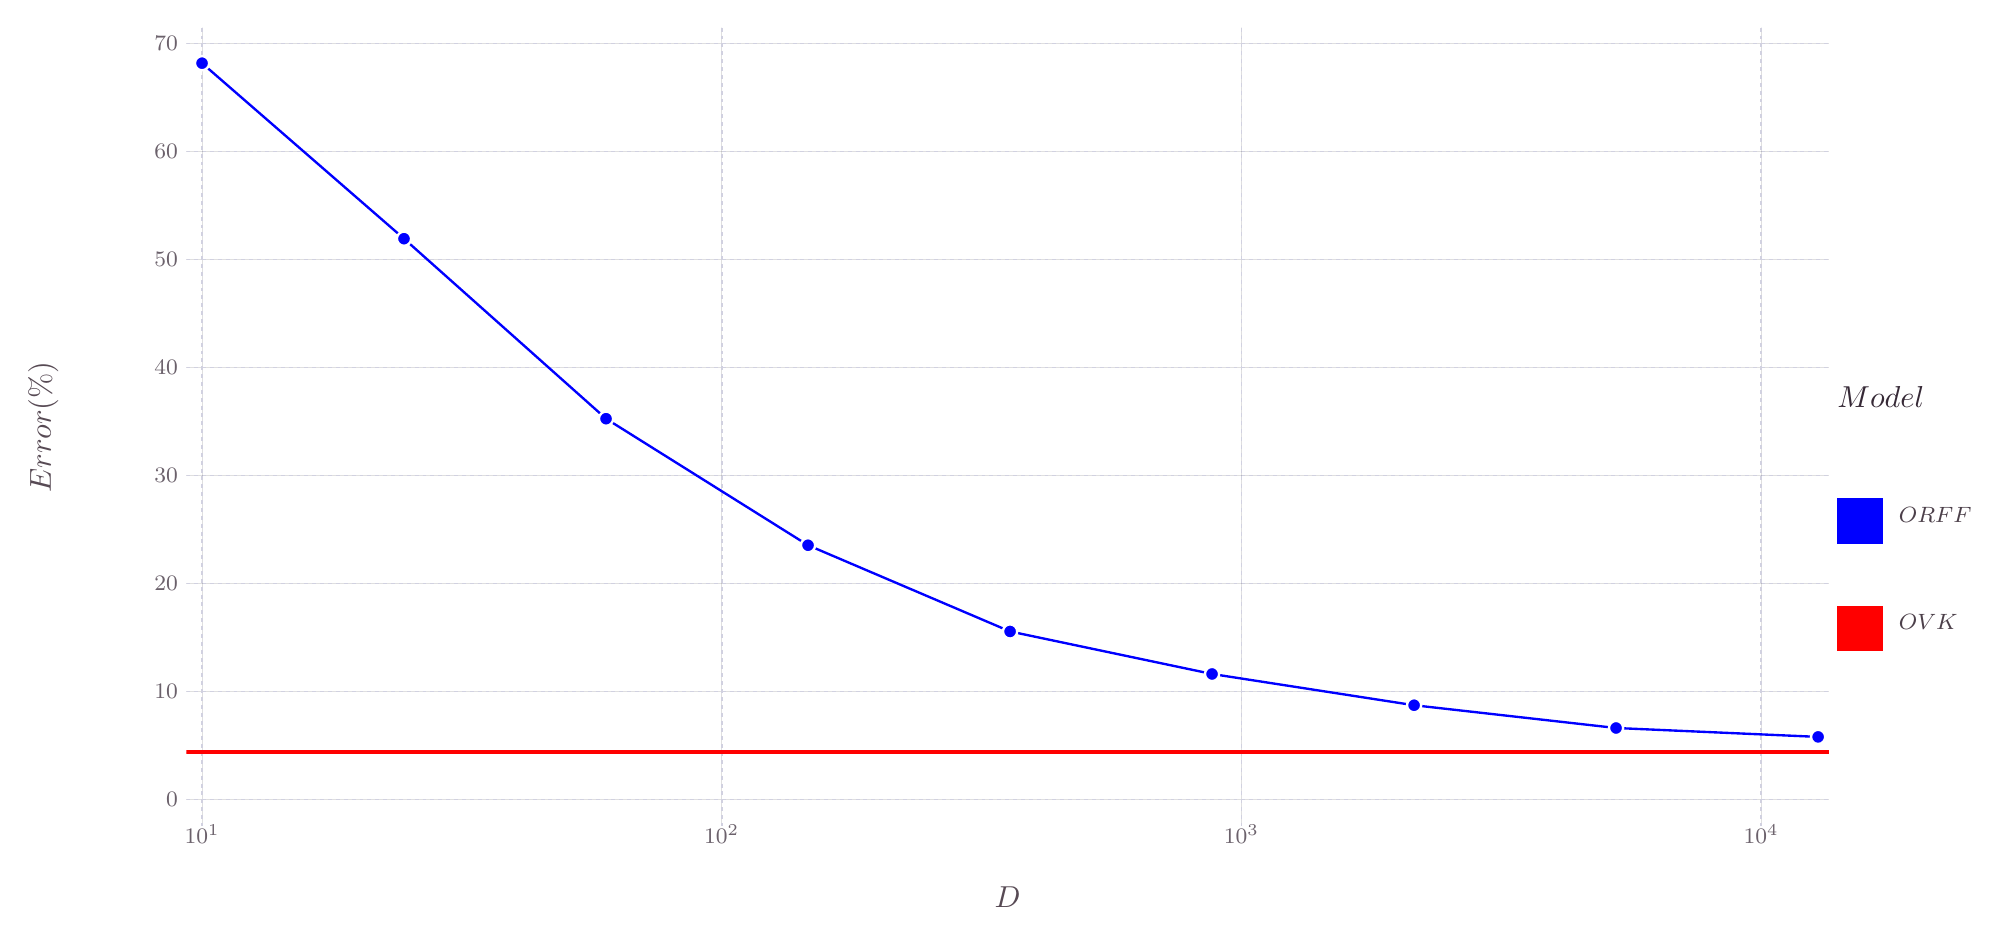
\begin{tikzpicture}[x=1mm,y=-1mm]
\definecolor{mycolor4C404B}{rgb}{0.3,0.25,0.29}
\definecolor{mycolor000000}{rgb}{0,0,0}
\definecolor{mycolor0000FF}{rgb}{0,0,1}
\definecolor{mycolor362A35}{rgb}{0.21,0.16,0.21}
\definecolor{mycolorFFFFFF}{rgb}{1,1,1}
\definecolor{mycolorD0D0E0}{rgb}{0.82,0.82,0.88}
\definecolor{mycolor000000}{rgb}{0,0,0}
\definecolor{mycolorFF0000}{rgb}{1,0,0}
\definecolor{mycolor6C606B}{rgb}{0.42,0.38,0.42}
\definecolor{mycolor564A55}{rgb}{0.34,0.29,0.33}
\begin{scope}
\begin{scope}
% \fontspec{PT Sans}
\draw (122.26,115.39) node [text=mycolor564A55,draw=mycolor000000,draw opacity=0,rotate around={-0: (0,1.81)},inner sep=0.0]{\fontsize{3.88mm}{4.66mm}\selectfont $\text{D}$};
\end{scope}
\begin{scope}
% \fontspec{PT Sans Caption}
\draw (19.96,107.38) node [text=mycolor6C606B,rotate around={-0: (102.3,2)},inner sep=0.0]{\fontsize{2.82mm}{3.39mm}\selectfont $\text{10}^{\text{1}}\text{}$};
\draw (85.96,107.38) node [text=mycolor6C606B,rotate around={-0: (36.3,2)},inner sep=0.0]{\fontsize{2.82mm}{3.39mm}\selectfont $\text{10}^{\text{2}}\text{}$};
\draw (151.96,107.38) node [text=mycolor6C606B,rotate around={-0: (-29.7,2)},inner sep=0.0]{\fontsize{2.82mm}{3.39mm}\selectfont $\text{10}^{\text{3}}\text{}$};
\draw (217.97,107.38) node [text=mycolor6C606B,rotate around={-0: (-95.7,2)},inner sep=0.0]{\fontsize{2.82mm}{3.39mm}\selectfont $\text{10}^{\text{4}}\text{}$};
\end{scope}
\begin{scope}
\begin{scope}
% \fontspec{PT Sans}
\draw (235.38,66.89) node [text=mycolor4C404B,rotate around={-0: (7.4,0)},right,inner sep=0.0]{\fontsize{2.82mm}{3.39mm}\selectfont $\text{ORFF}$};
\draw (235.38,80.52) node [text=mycolor4C404B,rotate around={-0: (7.4,-3.63)},right,inner sep=0.0]{\fontsize{2.82mm}{3.39mm}\selectfont $\text{OVK}$};
\end{scope}
\begin{scope}
\path [fill=mycolor0000FF,draw=mycolor000000,draw opacity=0] (227.57,64.78) rectangle +(5.81,5.81);
\path [fill=mycolorFF0000,draw=mycolor000000,draw opacity=0] (227.57,78.41) rectangle +(5.81,5.81);
\end{scope}
\begin{scope}
% \fontspec{PT Sans}
\draw (227.57,51.87) node [text=mycolor362A35,draw=mycolor000000,draw opacity=0,rotate around={-0: (11.22,0.19)},right,inner sep=0.0]{\fontsize{3.88mm}{4.66mm}\selectfont $\text{Model}$};
\end{scope}
\end{scope}
\begin{scope}
\clip  (17.96,5) -- (226.57,5) -- (226.57,106.38) -- (17.96,106.38);
\begin{scope}
\clip  (17.96,5) -- (226.57,5) -- (226.57,106.38) -- (17.96,106.38);
\path [fill=mycolor000000,fill opacity=0,draw=mycolor000000,draw opacity=0] (17.96,5) rectangle +(208.61,101.38);
\end{scope}
\begin{scope}
[dash pattern=on 0.5mm off 0.5mm,line width=0.2mm]
\path [fill=mycolor000000,draw=mycolorD0D0E0]  (17.96,103.01) -- (226.57,103.01);
\path [fill=mycolor000000,draw=mycolorD0D0E0]  (17.96,89.29) -- (226.57,89.29);
\path [fill=mycolor000000,draw=mycolorD0D0E0]  (17.96,75.58) -- (226.57,75.58);
\path [fill=mycolor000000,draw=mycolorD0D0E0]  (17.96,61.86) -- (226.57,61.86);
\path [fill=mycolor000000,draw=mycolorD0D0E0]  (17.96,48.15) -- (226.57,48.15);
\path [fill=mycolor000000,draw=mycolorD0D0E0]  (17.96,34.43) -- (226.57,34.43);
\path [fill=mycolor000000,draw=mycolorD0D0E0]  (17.96,20.72) -- (226.57,20.72);
\path [fill=mycolor000000,draw=mycolorD0D0E0]  (17.96,7) -- (226.57,7);
\end{scope}
\begin{scope}
[dash pattern=on 0.5mm off 0.5mm,line width=0.2mm]
\path [fill=mycolor000000,draw=mycolorD0D0E0]  (19.96,5) -- (19.96,106.38);
\path [fill=mycolor000000,draw=mycolorD0D0E0]  (85.96,5) -- (85.96,106.38);
\path [fill=mycolor000000,draw=mycolorD0D0E0]  (151.96,5) -- (151.96,106.38);
\path [fill=mycolor000000,draw=mycolorD0D0E0]  (217.97,5) -- (217.97,106.38);
\end{scope}
\begin{scope}
\begin{scope}
[line width=0.3mm]
\path [fill=mycolor000000,fill opacity=0,draw=mycolor0000FF]  (19.96,9.51) -- (45.61,31.8) -- (71.27,54.66) -- (96.92,70.73) -- (122.58,81.68) -- (148.23,87.08) -- (173.89,91.05) -- (199.54,93.94) -- (225.2,95.07);
\end{scope}
\begin{scope}
[line width=0.5mm]
\path [fill=mycolor000000,draw=mycolorFF0000]  (17.96,97) -- (226.57,97);
\end{scope}
\begin{scope}
\begin{scope}
[line width=0.3mm]
\path [fill=mycolor0000FF,draw=mycolorFFFFFF] (19.96,9.51) circle [radius=0.9];
\path [fill=mycolor0000FF,draw=mycolorFFFFFF] (45.61,31.8) circle [radius=0.9];
\path [fill=mycolor0000FF,draw=mycolorFFFFFF] (71.27,54.66) circle [radius=0.9];
\path [fill=mycolor0000FF,draw=mycolorFFFFFF] (96.92,70.73) circle [radius=0.9];
\path [fill=mycolor0000FF,draw=mycolorFFFFFF] (122.58,81.68) circle [radius=0.9];
\path [fill=mycolor0000FF,draw=mycolorFFFFFF] (148.23,87.08) circle [radius=0.9];
\path [fill=mycolor0000FF,draw=mycolorFFFFFF] (173.89,91.05) circle [radius=0.9];
\path [fill=mycolor0000FF,draw=mycolorFFFFFF] (199.54,93.94) circle [radius=0.9];
\path [fill=mycolor0000FF,draw=mycolorFFFFFF] (225.2,95.07) circle [radius=0.9];
\end{scope}
\end{scope}
\end{scope}
\end{scope}
\begin{scope}
% \fontspec{PT Sans Caption}
\draw (16.96,103.01) node [text=mycolor6C606B,rotate around={-0: (-1.67,-47.32)},left,inner sep=0.0]{\fontsize{2.82mm}{3.39mm}\selectfont $\text{0}$};
\draw (16.96,89.29) node [text=mycolor6C606B,rotate around={-0: (-1.67,-33.6)},left,inner sep=0.0]{\fontsize{2.82mm}{3.39mm}\selectfont $\text{10}$};
\draw (16.96,75.58) node [text=mycolor6C606B,rotate around={-0: (-1.67,-19.89)},left,inner sep=0.0]{\fontsize{2.82mm}{3.39mm}\selectfont $\text{20}$};
\draw (16.96,61.86) node [text=mycolor6C606B,rotate around={-0: (-1.67,-6.17)},left,inner sep=0.0]{\fontsize{2.82mm}{3.39mm}\selectfont $\text{30}$};
\draw (16.96,48.15) node [text=mycolor6C606B,rotate around={-0: (-1.67,7.54)},left,inner sep=0.0]{\fontsize{2.82mm}{3.39mm}\selectfont $\text{40}$};
\draw (16.96,34.43) node [text=mycolor6C606B,rotate around={-0: (-1.67,21.26)},left,inner sep=0.0]{\fontsize{2.82mm}{3.39mm}\selectfont $\text{50}$};
\draw (16.96,20.72) node [text=mycolor6C606B,rotate around={-0: (-1.67,34.97)},left,inner sep=0.0]{\fontsize{2.82mm}{3.39mm}\selectfont $\text{60}$};
\draw (16.96,7) node [text=mycolor6C606B,rotate around={-0: (-1.67,48.69)},left,inner sep=0.0]{\fontsize{2.82mm}{3.39mm}\selectfont $\text{70}$};
\end{scope}
\begin{scope}
% \fontspec{PT Sans}
\draw (1.81,53.69) node [text=mycolor564A55,draw=mycolor000000,draw opacity=0,rotate around={90: (0,2)},inner sep=0.0]{\fontsize{3.88mm}{4.66mm}\selectfont $\text{Error (\%)}$};
\end{scope}
\end{scope}
\end{tikzpicture}
} \\
    \resizebox{\textwidth}{!}{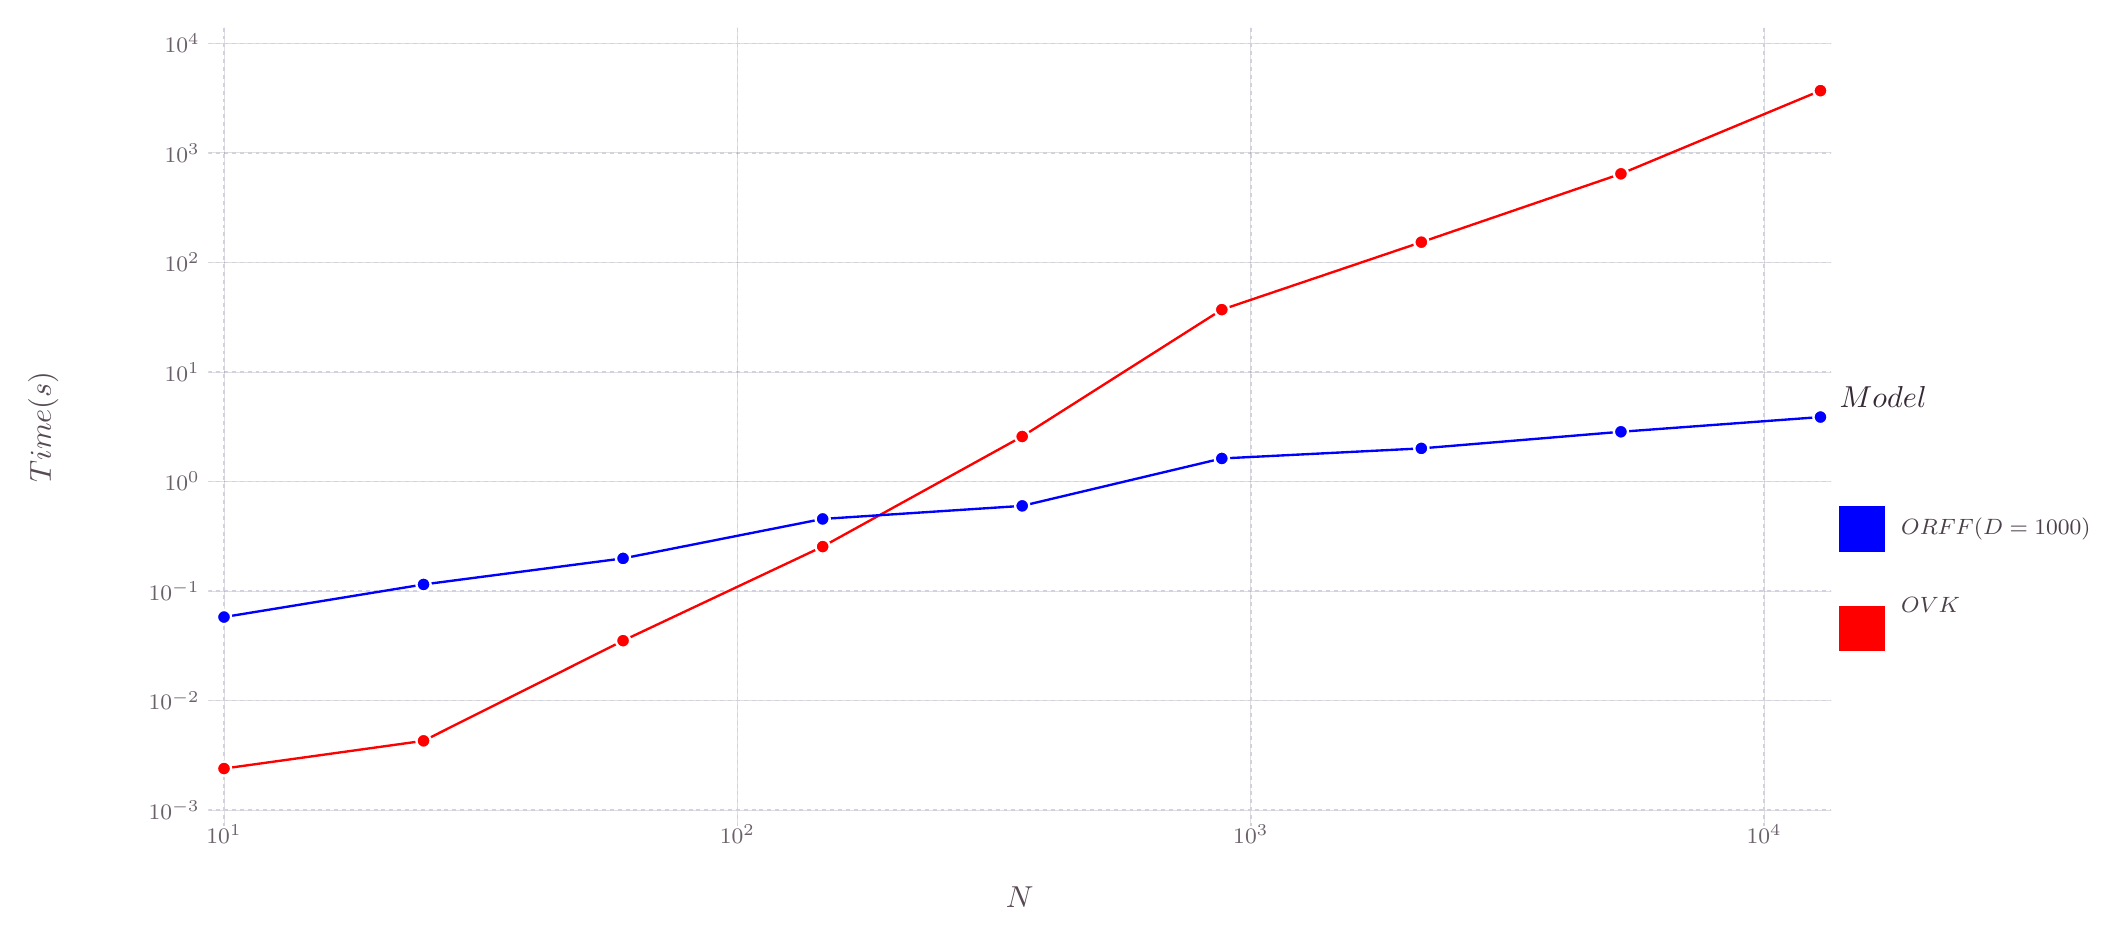
\begin{tikzpicture}[x=1mm,y=-1mm]
\definecolor{mycolor4C404B}{rgb}{0.3,0.25,0.29}
\definecolor{mycolor000000}{rgb}{0,0,0}
\definecolor{mycolor0000FF}{rgb}{0,0,1}
\definecolor{mycolor362A35}{rgb}{0.21,0.16,0.21}
\definecolor{mycolorFFFFFF}{rgb}{1,1,1}
\definecolor{mycolorD0D0E0}{rgb}{0.82,0.82,0.88}
\definecolor{mycolor000000}{rgb}{0,0,0}
\definecolor{mycolorFF0000}{rgb}{1,0,0}
\definecolor{mycolor6C606B}{rgb}{0.42,0.38,0.42}
\definecolor{mycolor564A55}{rgb}{0.34,0.29,0.33}
\begin{scope}
\begin{scope}
% \fontspec{PT Sans}
\draw (123.81,115.39) node [text=mycolor564A55,draw=mycolor000000,draw opacity=0,rotate around={-0: (0,1.81)},inner sep=0.0]{\fontsize{3.88mm}{4.66mm}\selectfont $\text{N}$};
\end{scope}
\begin{scope}
% \fontspec{PT Sans Caption}
\draw (22.75,107.38) node [text=mycolor6C606B,rotate around={-0: (101.07,2)},inner sep=0.0]{\fontsize{2.82mm}{3.39mm}\selectfont $\text{10}^{\text{1}}\text{}$};
\draw (87.95,107.38) node [text=mycolor6C606B,rotate around={-0: (35.86,2)},inner sep=0.0]{\fontsize{2.82mm}{3.39mm}\selectfont $\text{10}^{\text{2}}\text{}$};
\draw (153.15,107.38) node [text=mycolor6C606B,rotate around={-0: (-29.34,2)},inner sep=0.0]{\fontsize{2.82mm}{3.39mm}\selectfont $\text{10}^{\text{3}}\text{}$};
\draw (218.36,107.38) node [text=mycolor6C606B,rotate around={-0: (-94.55,2)},inner sep=0.0]{\fontsize{2.82mm}{3.39mm}\selectfont $\text{10}^{\text{4}}\text{}$};
\end{scope}
\begin{scope}
\begin{scope}
% \fontspec{PT Sans}
\draw (235.69,68.69) node [text=mycolor4C404B,rotate around={-0: (7.25,0)},right,inner sep=0.0]{\fontsize{2.82mm}{3.39mm}\selectfont $\text{ORFF (D=1000)}$};
\draw (235.69,78.32) node [text=mycolor4C404B,rotate around={-0: (7.25,-3.63)},right,inner sep=0.0]{\fontsize{2.82mm}{3.39mm}\selectfont $\text{OVK}$};
\end{scope}
\begin{scope}
\path [fill=mycolor0000FF,draw=mycolor000000,draw opacity=0] (227.88,65.78) rectangle +(5.81,5.81);
\path [fill=mycolorFF0000,draw=mycolor000000,draw opacity=0] (227.88,78.41) rectangle +(5.81,5.81);
\end{scope}
\begin{scope}
% \fontspec{PT Sans}
\draw (227.88,51.87) node [text=mycolor362A35,draw=mycolor000000,draw opacity=0,rotate around={-0: (11.06,0.19)},right,inner sep=0.0]{\fontsize{3.88mm}{4.66mm}\selectfont $\text{Model}$};
\end{scope}
\end{scope}
\begin{scope}
\clip  (20.75,5) -- (226.88,5) -- (226.88,106.38) -- (20.75,106.38);
\begin{scope}
\clip  (20.75,5) -- (226.88,5) -- (226.88,106.38) -- (20.75,106.38);
\path [fill=mycolor000000,fill opacity=0,draw=mycolor000000,draw opacity=0] (20.75,5) rectangle +(206.14,101.38);
\end{scope}
\begin{scope}
[dash pattern=on 0.5mm off 0.5mm,line width=0.2mm]
\path [fill=mycolor000000,draw=mycolorD0D0E0]  (20.75,104.38) -- (226.88,104.38);
\path [fill=mycolor000000,draw=mycolorD0D0E0]  (20.75,90.47) -- (226.88,90.47);
\path [fill=mycolor000000,draw=mycolorD0D0E0]  (20.75,76.56) -- (226.88,76.56);
\path [fill=mycolor000000,draw=mycolorD0D0E0]  (20.75,62.64) -- (226.88,62.64);
\path [fill=mycolor000000,draw=mycolorD0D0E0]  (20.75,48.73) -- (226.88,48.73);
\path [fill=mycolor000000,draw=mycolorD0D0E0]  (20.75,34.82) -- (226.88,34.82);
\path [fill=mycolor000000,draw=mycolorD0D0E0]  (20.75,20.91) -- (226.88,20.91);
\path [fill=mycolor000000,draw=mycolorD0D0E0]  (20.75,7) -- (226.88,7);
\end{scope}
\begin{scope}
[dash pattern=on 0.5mm off 0.5mm,line width=0.2mm]
\path [fill=mycolor000000,draw=mycolorD0D0E0]  (22.75,5) -- (22.75,106.38);
\path [fill=mycolor000000,draw=mycolorD0D0E0]  (87.95,5) -- (87.95,106.38);
\path [fill=mycolor000000,draw=mycolorD0D0E0]  (153.15,5) -- (153.15,106.38);
\path [fill=mycolor000000,draw=mycolorD0D0E0]  (218.36,5) -- (218.36,106.38);
\end{scope}
\begin{scope}
\begin{scope}
[line width=0.3mm]
\path [fill=mycolor000000,fill opacity=0,draw=mycolorFF0000]  (22.75,99.09) -- (48.09,95.57) -- (73.43,82.85) -- (98.78,70.9) -- (124.12,56.92) -- (149.47,40.81) -- (174.81,32.24) -- (200.16,23.56) -- (225.5,13);
\end{scope}
\begin{scope}
[line width=0.3mm]
\path [fill=mycolor000000,fill opacity=0,draw=mycolor0000FF]  (22.75,79.85) -- (48.09,75.71) -- (73.43,72.4) -- (98.78,67.39) -- (124.12,65.73) -- (149.47,59.71) -- (174.81,58.43) -- (200.16,56.32) -- (225.5,54.45);
\end{scope}
\begin{scope}
\begin{scope}
[line width=0.3mm]
\path [fill=mycolorFF0000,draw=mycolorFFFFFF] (22.75,99.09) circle [radius=0.9];
\path [fill=mycolorFF0000,draw=mycolorFFFFFF] (48.09,95.57) circle [radius=0.9];
\path [fill=mycolorFF0000,draw=mycolorFFFFFF] (73.43,82.85) circle [radius=0.9];
\path [fill=mycolorFF0000,draw=mycolorFFFFFF] (98.78,70.9) circle [radius=0.9];
\path [fill=mycolorFF0000,draw=mycolorFFFFFF] (124.12,56.92) circle [radius=0.9];
\path [fill=mycolorFF0000,draw=mycolorFFFFFF] (149.47,40.81) circle [radius=0.9];
\path [fill=mycolorFF0000,draw=mycolorFFFFFF] (174.81,32.24) circle [radius=0.9];
\path [fill=mycolorFF0000,draw=mycolorFFFFFF] (200.16,23.56) circle [radius=0.9];
\path [fill=mycolorFF0000,draw=mycolorFFFFFF] (225.5,13) circle [radius=0.9];
\end{scope}
\end{scope}
\begin{scope}
\begin{scope}
[line width=0.3mm]
\path [fill=mycolor0000FF,draw=mycolorFFFFFF] (22.75,79.85) circle [radius=0.9];
\path [fill=mycolor0000FF,draw=mycolorFFFFFF] (48.09,75.71) circle [radius=0.9];
\path [fill=mycolor0000FF,draw=mycolorFFFFFF] (73.43,72.4) circle [radius=0.9];
\path [fill=mycolor0000FF,draw=mycolorFFFFFF] (98.78,67.39) circle [radius=0.9];
\path [fill=mycolor0000FF,draw=mycolorFFFFFF] (124.12,65.73) circle [radius=0.9];
\path [fill=mycolor0000FF,draw=mycolorFFFFFF] (149.47,59.71) circle [radius=0.9];
\path [fill=mycolor0000FF,draw=mycolorFFFFFF] (174.81,58.43) circle [radius=0.9];
\path [fill=mycolor0000FF,draw=mycolorFFFFFF] (200.16,56.32) circle [radius=0.9];
\path [fill=mycolor0000FF,draw=mycolorFFFFFF] (225.5,54.45) circle [radius=0.9];
\end{scope}
\end{scope}
\end{scope}
\end{scope}
\begin{scope}
% \fontspec{PT Sans Caption}
\draw (19.74,104.38) node [text=mycolor6C606B,rotate around={-0: (-3.07,-48.69)},left,inner sep=0.0]{\fontsize{2.82mm}{3.39mm}\selectfont $\text{10}^{\text{-3}}\text{}$};
\draw (19.74,90.47) node [text=mycolor6C606B,rotate around={-0: (-3.07,-34.78)},left,inner sep=0.0]{\fontsize{2.82mm}{3.39mm}\selectfont $\text{10}^{\text{-2}}\text{}$};
\draw (19.74,76.56) node [text=mycolor6C606B,rotate around={-0: (-3.07,-20.87)},left,inner sep=0.0]{\fontsize{2.82mm}{3.39mm}\selectfont $\text{10}^{\text{-1}}\text{}$};
\draw (19.74,62.64) node [text=mycolor6C606B,rotate around={-0: (-3.07,-6.96)},left,inner sep=0.0]{\fontsize{2.82mm}{3.39mm}\selectfont $\text{10}^{\text{0}}\text{}$};
\draw (19.74,48.73) node [text=mycolor6C606B,rotate around={-0: (-3.07,6.96)},left,inner sep=0.0]{\fontsize{2.82mm}{3.39mm}\selectfont $\text{10}^{\text{1}}\text{}$};
\draw (19.74,34.82) node [text=mycolor6C606B,rotate around={-0: (-3.07,20.87)},left,inner sep=0.0]{\fontsize{2.82mm}{3.39mm}\selectfont $\text{10}^{\text{2}}\text{}$};
\draw (19.74,20.91) node [text=mycolor6C606B,rotate around={-0: (-3.07,34.78)},left,inner sep=0.0]{\fontsize{2.82mm}{3.39mm}\selectfont $\text{10}^{\text{3}}\text{}$};
\draw (19.74,7) node [text=mycolor6C606B,rotate around={-0: (-3.07,48.69)},left,inner sep=0.0]{\fontsize{2.82mm}{3.39mm}\selectfont $\text{10}^{\text{4}}\text{}$};
\end{scope}
\begin{scope}
% \fontspec{PT Sans}
\draw (1.81,53.69) node [text=mycolor564A55,draw=mycolor000000,draw opacity=0,rotate around={90: (0,2)},inner sep=0.0]{\fontsize{3.88mm}{4.66mm}\selectfont $\text{Time (s)}$};
\end{scope}
\end{scope}
\end{tikzpicture}
}
    % \includegraphics[\textwidth]{./gfx/learning_time_MNIST.tikz}
    \caption[Prediction Error in percent on the MNIST dataset versus $D$, the
    number of Fourier features]{Empirical comparison of ORFF and OVK regression
    on MNIST dataset and empirical behavior of ORFF regression versus $D$ and
    $N$.\label{fig:learning_accuracy}}
\end{figure}
\paragraph{}
\textbf{Performance of ORFF regression on the second dataset.} 
We perform a similar experiment on the second dataset ($5$D-vector field with
structure). We use a Gaussian curl-free kernel with bandwidth equal to the
median of the pairwise distances and tune the hyperparameter $\lambda$ on a
grid. Here we optimize \cref{eq:argmin_theta} using Scipy's \acs{L-BFGS-B}
\citep{byrd1995limited} solver\footnote{Available at
\url{http://docs.scipy.org/doc/scipy/reference/optimize.html}} with the
gradients given in \cref{eq:grad_final} and the efficient linear operator
described in \cref{subsec:efficient_linop}.  \Cref{fig:curl_experiment} (bottom
row) reports the $R2$ score on the test set versus the number of
curl-\acs{ORFF} $D$ with a comparison with curl-\acs{OVK}.  In this experiment,
we see that curl-\acs{ORFF} can even be better than curl-\acs{OVK}, suggesting
that \acs{ORFF} might play an additional regularizing role. It also shows the
computation time of curl-\acs{ORFF} and curl-\acs{OVK}. We see that \acs{OVK}
regression does not scale with large datasets, while \acs{ORFF} regression
does. When $N>10^4$, \acs{OVK} regression exceeds memory capacity.
\begin{figure}
    \centering
    \resizebox{\textwidth}{!}{%% Creator: Matplotlib, PGF backend
%%
%% To include the figure in your LaTeX document, write
%%   \input{<filename>.pgf}
%%
%% Make sure the required packages are loaded in your preamble
%%   \usepackage{pgf}
%%
%% Figures using additional raster images can only be included by \input if
%% they are in the same directory as the main LaTeX file. For loading figures
%% from other directories you can use the `import` package
%%   \usepackage{import}
%% and then include the figures with
%%   \import{<path to file>}{<filename>.pgf}
%%
%% Matplotlib used the following preamble
%%   \usepackage{fontspec}
%%   \setmainfont{Times New Roman}
%%   \setsansfont{Arial}
%%   \setmonofont{Andale Mono}
%%
\begingroup%
\makeatletter%
\begin{pgfpicture}%
\pgfpathrectangle{\pgfpointorigin}{\pgfqpoint{12.414829in}{8.222886in}}%
\pgfusepath{use as bounding box, clip}%
\begin{pgfscope}%
\pgfsetbuttcap%
\pgfsetmiterjoin%
\definecolor{currentfill}{rgb}{1.000000,1.000000,1.000000}%
\pgfsetfillcolor{currentfill}%
\pgfsetlinewidth{0.000000pt}%
\definecolor{currentstroke}{rgb}{1.000000,1.000000,1.000000}%
\pgfsetstrokecolor{currentstroke}%
\pgfsetdash{}{0pt}%
\pgfpathmoveto{\pgfqpoint{0.000000in}{-0.000000in}}%
\pgfpathlineto{\pgfqpoint{12.414829in}{-0.000000in}}%
\pgfpathlineto{\pgfqpoint{12.414829in}{8.222886in}}%
\pgfpathlineto{\pgfqpoint{0.000000in}{8.222886in}}%
\pgfpathclose%
\pgfusepath{fill}%
\end{pgfscope}%
\begin{pgfscope}%
\pgfsetbuttcap%
\pgfsetmiterjoin%
\definecolor{currentfill}{rgb}{1.000000,1.000000,1.000000}%
\pgfsetfillcolor{currentfill}%
\pgfsetlinewidth{0.000000pt}%
\definecolor{currentstroke}{rgb}{0.000000,0.000000,0.000000}%
\pgfsetstrokecolor{currentstroke}%
\pgfsetstrokeopacity{0.000000}%
\pgfsetdash{}{0pt}%
\pgfpathmoveto{\pgfqpoint{0.589231in}{4.641358in}}%
\pgfpathlineto{\pgfqpoint{5.873321in}{4.641358in}}%
\pgfpathlineto{\pgfqpoint{5.873321in}{8.073177in}}%
\pgfpathlineto{\pgfqpoint{0.589231in}{8.073177in}}%
\pgfpathclose%
\pgfusepath{fill}%
\end{pgfscope}%
\begin{pgfscope}%
\pgfpathrectangle{\pgfqpoint{0.589231in}{4.641358in}}{\pgfqpoint{5.284091in}{3.431818in}} %
\pgfusepath{clip}%
\pgfsetroundcap%
\pgfsetroundjoin%
\pgfsetlinewidth{1.003750pt}%
\definecolor{currentstroke}{rgb}{0.800000,0.800000,0.800000}%
\pgfsetstrokecolor{currentstroke}%
\pgfsetdash{}{0pt}%
\pgfpathmoveto{\pgfqpoint{0.829417in}{4.641358in}}%
\pgfpathlineto{\pgfqpoint{0.829417in}{8.073177in}}%
\pgfusepath{stroke}%
\end{pgfscope}%
\begin{pgfscope}%
\definecolor{textcolor}{rgb}{0.150000,0.150000,0.150000}%
\pgfsetstrokecolor{textcolor}%
\pgfsetfillcolor{textcolor}%
\pgftext[x=0.829417in,y=4.544136in,,top]{\color{textcolor}\sffamily\fontsize{10.000000}{12.000000}\selectfont \(\displaystyle {10^{2}}\)}%
\end{pgfscope}%
\begin{pgfscope}%
\pgfpathrectangle{\pgfqpoint{0.589231in}{4.641358in}}{\pgfqpoint{5.284091in}{3.431818in}} %
\pgfusepath{clip}%
\pgfsetroundcap%
\pgfsetroundjoin%
\pgfsetlinewidth{1.003750pt}%
\definecolor{currentstroke}{rgb}{0.800000,0.800000,0.800000}%
\pgfsetstrokecolor{currentstroke}%
\pgfsetdash{}{0pt}%
\pgfpathmoveto{\pgfqpoint{2.697368in}{4.641358in}}%
\pgfpathlineto{\pgfqpoint{2.697368in}{8.073177in}}%
\pgfusepath{stroke}%
\end{pgfscope}%
\begin{pgfscope}%
\definecolor{textcolor}{rgb}{0.150000,0.150000,0.150000}%
\pgfsetstrokecolor{textcolor}%
\pgfsetfillcolor{textcolor}%
\pgftext[x=2.697368in,y=4.544136in,,top]{\color{textcolor}\sffamily\fontsize{10.000000}{12.000000}\selectfont \(\displaystyle {10^{3}}\)}%
\end{pgfscope}%
\begin{pgfscope}%
\pgfpathrectangle{\pgfqpoint{0.589231in}{4.641358in}}{\pgfqpoint{5.284091in}{3.431818in}} %
\pgfusepath{clip}%
\pgfsetroundcap%
\pgfsetroundjoin%
\pgfsetlinewidth{1.003750pt}%
\definecolor{currentstroke}{rgb}{0.800000,0.800000,0.800000}%
\pgfsetstrokecolor{currentstroke}%
\pgfsetdash{}{0pt}%
\pgfpathmoveto{\pgfqpoint{4.565320in}{4.641358in}}%
\pgfpathlineto{\pgfqpoint{4.565320in}{8.073177in}}%
\pgfusepath{stroke}%
\end{pgfscope}%
\begin{pgfscope}%
\definecolor{textcolor}{rgb}{0.150000,0.150000,0.150000}%
\pgfsetstrokecolor{textcolor}%
\pgfsetfillcolor{textcolor}%
\pgftext[x=4.565320in,y=4.544136in,,top]{\color{textcolor}\sffamily\fontsize{10.000000}{12.000000}\selectfont \(\displaystyle {10^{4}}\)}%
\end{pgfscope}%
\begin{pgfscope}%
\definecolor{textcolor}{rgb}{0.150000,0.150000,0.150000}%
\pgfsetstrokecolor{textcolor}%
\pgfsetfillcolor{textcolor}%
\pgftext[x=3.231276in,y=4.361560in,,top]{\color{textcolor}\sffamily\fontsize{11.000000}{13.200000}\selectfont Data seen (N)}%
\end{pgfscope}%
\begin{pgfscope}%
\pgfpathrectangle{\pgfqpoint{0.589231in}{4.641358in}}{\pgfqpoint{5.284091in}{3.431818in}} %
\pgfusepath{clip}%
\pgfsetroundcap%
\pgfsetroundjoin%
\pgfsetlinewidth{1.003750pt}%
\definecolor{currentstroke}{rgb}{0.800000,0.800000,0.800000}%
\pgfsetstrokecolor{currentstroke}%
\pgfsetdash{}{0pt}%
\pgfpathmoveto{\pgfqpoint{0.589231in}{4.641358in}}%
\pgfpathlineto{\pgfqpoint{5.873321in}{4.641358in}}%
\pgfusepath{stroke}%
\end{pgfscope}%
\begin{pgfscope}%
\definecolor{textcolor}{rgb}{0.150000,0.150000,0.150000}%
\pgfsetstrokecolor{textcolor}%
\pgfsetfillcolor{textcolor}%
\pgftext[x=0.298934in,y=4.591649in,left,base]{\color{textcolor}\sffamily\fontsize{10.000000}{12.000000}\selectfont 0.0}%
\end{pgfscope}%
\begin{pgfscope}%
\pgfpathrectangle{\pgfqpoint{0.589231in}{4.641358in}}{\pgfqpoint{5.284091in}{3.431818in}} %
\pgfusepath{clip}%
\pgfsetroundcap%
\pgfsetroundjoin%
\pgfsetlinewidth{1.003750pt}%
\definecolor{currentstroke}{rgb}{0.800000,0.800000,0.800000}%
\pgfsetstrokecolor{currentstroke}%
\pgfsetdash{}{0pt}%
\pgfpathmoveto{\pgfqpoint{0.589231in}{5.327722in}}%
\pgfpathlineto{\pgfqpoint{5.873321in}{5.327722in}}%
\pgfusepath{stroke}%
\end{pgfscope}%
\begin{pgfscope}%
\definecolor{textcolor}{rgb}{0.150000,0.150000,0.150000}%
\pgfsetstrokecolor{textcolor}%
\pgfsetfillcolor{textcolor}%
\pgftext[x=0.298934in,y=5.278012in,left,base]{\color{textcolor}\sffamily\fontsize{10.000000}{12.000000}\selectfont 0.2}%
\end{pgfscope}%
\begin{pgfscope}%
\pgfpathrectangle{\pgfqpoint{0.589231in}{4.641358in}}{\pgfqpoint{5.284091in}{3.431818in}} %
\pgfusepath{clip}%
\pgfsetroundcap%
\pgfsetroundjoin%
\pgfsetlinewidth{1.003750pt}%
\definecolor{currentstroke}{rgb}{0.800000,0.800000,0.800000}%
\pgfsetstrokecolor{currentstroke}%
\pgfsetdash{}{0pt}%
\pgfpathmoveto{\pgfqpoint{0.589231in}{6.014086in}}%
\pgfpathlineto{\pgfqpoint{5.873321in}{6.014086in}}%
\pgfusepath{stroke}%
\end{pgfscope}%
\begin{pgfscope}%
\definecolor{textcolor}{rgb}{0.150000,0.150000,0.150000}%
\pgfsetstrokecolor{textcolor}%
\pgfsetfillcolor{textcolor}%
\pgftext[x=0.298934in,y=5.964376in,left,base]{\color{textcolor}\sffamily\fontsize{10.000000}{12.000000}\selectfont 0.4}%
\end{pgfscope}%
\begin{pgfscope}%
\pgfpathrectangle{\pgfqpoint{0.589231in}{4.641358in}}{\pgfqpoint{5.284091in}{3.431818in}} %
\pgfusepath{clip}%
\pgfsetroundcap%
\pgfsetroundjoin%
\pgfsetlinewidth{1.003750pt}%
\definecolor{currentstroke}{rgb}{0.800000,0.800000,0.800000}%
\pgfsetstrokecolor{currentstroke}%
\pgfsetdash{}{0pt}%
\pgfpathmoveto{\pgfqpoint{0.589231in}{6.700449in}}%
\pgfpathlineto{\pgfqpoint{5.873321in}{6.700449in}}%
\pgfusepath{stroke}%
\end{pgfscope}%
\begin{pgfscope}%
\definecolor{textcolor}{rgb}{0.150000,0.150000,0.150000}%
\pgfsetstrokecolor{textcolor}%
\pgfsetfillcolor{textcolor}%
\pgftext[x=0.298934in,y=6.650740in,left,base]{\color{textcolor}\sffamily\fontsize{10.000000}{12.000000}\selectfont 0.6}%
\end{pgfscope}%
\begin{pgfscope}%
\pgfpathrectangle{\pgfqpoint{0.589231in}{4.641358in}}{\pgfqpoint{5.284091in}{3.431818in}} %
\pgfusepath{clip}%
\pgfsetroundcap%
\pgfsetroundjoin%
\pgfsetlinewidth{1.003750pt}%
\definecolor{currentstroke}{rgb}{0.800000,0.800000,0.800000}%
\pgfsetstrokecolor{currentstroke}%
\pgfsetdash{}{0pt}%
\pgfpathmoveto{\pgfqpoint{0.589231in}{7.386813in}}%
\pgfpathlineto{\pgfqpoint{5.873321in}{7.386813in}}%
\pgfusepath{stroke}%
\end{pgfscope}%
\begin{pgfscope}%
\definecolor{textcolor}{rgb}{0.150000,0.150000,0.150000}%
\pgfsetstrokecolor{textcolor}%
\pgfsetfillcolor{textcolor}%
\pgftext[x=0.298934in,y=7.337103in,left,base]{\color{textcolor}\sffamily\fontsize{10.000000}{12.000000}\selectfont 0.8}%
\end{pgfscope}%
\begin{pgfscope}%
\pgfpathrectangle{\pgfqpoint{0.589231in}{4.641358in}}{\pgfqpoint{5.284091in}{3.431818in}} %
\pgfusepath{clip}%
\pgfsetroundcap%
\pgfsetroundjoin%
\pgfsetlinewidth{1.003750pt}%
\definecolor{currentstroke}{rgb}{0.800000,0.800000,0.800000}%
\pgfsetstrokecolor{currentstroke}%
\pgfsetdash{}{0pt}%
\pgfpathmoveto{\pgfqpoint{0.589231in}{8.073177in}}%
\pgfpathlineto{\pgfqpoint{5.873321in}{8.073177in}}%
\pgfusepath{stroke}%
\end{pgfscope}%
\begin{pgfscope}%
\definecolor{textcolor}{rgb}{0.150000,0.150000,0.150000}%
\pgfsetstrokecolor{textcolor}%
\pgfsetfillcolor{textcolor}%
\pgftext[x=0.298934in,y=8.023467in,left,base]{\color{textcolor}\sffamily\fontsize{10.000000}{12.000000}\selectfont 1.0}%
\end{pgfscope}%
\begin{pgfscope}%
\definecolor{textcolor}{rgb}{0.150000,0.150000,0.150000}%
\pgfsetstrokecolor{textcolor}%
\pgfsetfillcolor{textcolor}%
\pgftext[x=0.243378in,y=6.357268in,,bottom,rotate=90.000000]{\color{textcolor}\sffamily\fontsize{11.000000}{13.200000}\selectfont score (R2)}%
\end{pgfscope}%
\begin{pgfscope}%
\pgfpathrectangle{\pgfqpoint{0.589231in}{4.641358in}}{\pgfqpoint{5.284091in}{3.431818in}} %
\pgfusepath{clip}%
\pgfsetbuttcap%
\pgfsetroundjoin%
\pgfsetlinewidth{1.756562pt}%
\definecolor{currentstroke}{rgb}{0.000000,0.000000,1.000000}%
\pgfsetstrokecolor{currentstroke}%
\pgfsetdash{{6.475000pt}{2.800000pt}}{0.000000pt}%
\pgfpathmoveto{\pgfqpoint{0.829417in}{8.058833in}}%
\pgfpathlineto{\pgfqpoint{5.633136in}{8.058833in}}%
\pgfusepath{stroke}%
\end{pgfscope}%
\begin{pgfscope}%
\pgfpathrectangle{\pgfqpoint{0.589231in}{4.641358in}}{\pgfqpoint{5.284091in}{3.431818in}} %
\pgfusepath{clip}%
\pgfsetbuttcap%
\pgfsetroundjoin%
\pgfsetlinewidth{1.756562pt}%
\definecolor{currentstroke}{rgb}{0.000000,0.500000,0.000000}%
\pgfsetstrokecolor{currentstroke}%
\pgfsetdash{{6.475000pt}{2.800000pt}}{0.000000pt}%
\pgfpathmoveto{\pgfqpoint{0.829417in}{7.957431in}}%
\pgfpathlineto{\pgfqpoint{2.963929in}{7.957431in}}%
\pgfusepath{stroke}%
\end{pgfscope}%
\begin{pgfscope}%
\pgfpathrectangle{\pgfqpoint{0.589231in}{4.641358in}}{\pgfqpoint{5.284091in}{3.431818in}} %
\pgfusepath{clip}%
\pgfsetbuttcap%
\pgfsetroundjoin%
\pgfsetlinewidth{1.756562pt}%
\definecolor{currentstroke}{rgb}{1.000000,0.000000,0.000000}%
\pgfsetstrokecolor{currentstroke}%
\pgfsetdash{{6.475000pt}{2.800000pt}}{0.000000pt}%
\pgfpathmoveto{\pgfqpoint{0.829417in}{8.058743in}}%
\pgfpathlineto{\pgfqpoint{5.633136in}{8.058743in}}%
\pgfusepath{stroke}%
\end{pgfscope}%
\begin{pgfscope}%
\pgfpathrectangle{\pgfqpoint{0.589231in}{4.641358in}}{\pgfqpoint{5.284091in}{3.431818in}} %
\pgfusepath{clip}%
\pgfsetbuttcap%
\pgfsetroundjoin%
\pgfsetlinewidth{1.756562pt}%
\definecolor{currentstroke}{rgb}{0.501961,0.000000,0.501961}%
\pgfsetstrokecolor{currentstroke}%
\pgfsetdash{{6.475000pt}{2.800000pt}}{0.000000pt}%
\pgfpathmoveto{\pgfqpoint{0.829417in}{7.882620in}}%
\pgfpathlineto{\pgfqpoint{2.963929in}{7.882620in}}%
\pgfusepath{stroke}%
\end{pgfscope}%
\begin{pgfscope}%
\pgfpathrectangle{\pgfqpoint{0.589231in}{4.641358in}}{\pgfqpoint{5.284091in}{3.431818in}} %
\pgfusepath{clip}%
\pgfsetroundcap%
\pgfsetroundjoin%
\pgfsetlinewidth{1.756562pt}%
\definecolor{currentstroke}{rgb}{0.298039,0.447059,0.690196}%
\pgfsetstrokecolor{currentstroke}%
\pgfsetdash{}{0pt}%
\pgfpathmoveto{\pgfqpoint{0.829417in}{4.883137in}}%
\pgfpathlineto{\pgfqpoint{1.362824in}{7.162849in}}%
\pgfpathlineto{\pgfqpoint{1.895163in}{7.739455in}}%
\pgfpathlineto{\pgfqpoint{2.429745in}{7.882898in}}%
\pgfpathlineto{\pgfqpoint{2.963929in}{7.957128in}}%
\pgfpathlineto{\pgfqpoint{3.498011in}{8.005012in}}%
\pgfpathlineto{\pgfqpoint{4.031858in}{8.029315in}}%
\pgfpathlineto{\pgfqpoint{4.565644in}{8.045183in}}%
\pgfpathlineto{\pgfqpoint{5.099399in}{8.054894in}}%
\pgfpathlineto{\pgfqpoint{5.633136in}{8.058833in}}%
\pgfusepath{stroke}%
\end{pgfscope}%
\begin{pgfscope}%
\pgfpathrectangle{\pgfqpoint{0.589231in}{4.641358in}}{\pgfqpoint{5.284091in}{3.431818in}} %
\pgfusepath{clip}%
\pgfsetbuttcap%
\pgfsetmiterjoin%
\definecolor{currentfill}{rgb}{0.298039,0.447059,0.690196}%
\pgfsetfillcolor{currentfill}%
\pgfsetlinewidth{0.000000pt}%
\definecolor{currentstroke}{rgb}{0.298039,0.447059,0.690196}%
\pgfsetstrokecolor{currentstroke}%
\pgfsetdash{}{0pt}%
\pgfsys@defobject{currentmarker}{\pgfqpoint{-0.048611in}{-0.048611in}}{\pgfqpoint{0.048611in}{0.048611in}}{%
\pgfpathmoveto{\pgfqpoint{-0.048611in}{-0.048611in}}%
\pgfpathlineto{\pgfqpoint{0.048611in}{-0.048611in}}%
\pgfpathlineto{\pgfqpoint{0.048611in}{0.048611in}}%
\pgfpathlineto{\pgfqpoint{-0.048611in}{0.048611in}}%
\pgfpathclose%
\pgfusepath{fill}%
}%
\begin{pgfscope}%
\pgfsys@transformshift{0.829417in}{4.883137in}%
\pgfsys@useobject{currentmarker}{}%
\end{pgfscope}%
\begin{pgfscope}%
\pgfsys@transformshift{1.362824in}{7.162849in}%
\pgfsys@useobject{currentmarker}{}%
\end{pgfscope}%
\begin{pgfscope}%
\pgfsys@transformshift{1.895163in}{7.739455in}%
\pgfsys@useobject{currentmarker}{}%
\end{pgfscope}%
\begin{pgfscope}%
\pgfsys@transformshift{2.429745in}{7.882898in}%
\pgfsys@useobject{currentmarker}{}%
\end{pgfscope}%
\begin{pgfscope}%
\pgfsys@transformshift{2.963929in}{7.957128in}%
\pgfsys@useobject{currentmarker}{}%
\end{pgfscope}%
\begin{pgfscope}%
\pgfsys@transformshift{3.498011in}{8.005012in}%
\pgfsys@useobject{currentmarker}{}%
\end{pgfscope}%
\begin{pgfscope}%
\pgfsys@transformshift{4.031858in}{8.029315in}%
\pgfsys@useobject{currentmarker}{}%
\end{pgfscope}%
\begin{pgfscope}%
\pgfsys@transformshift{4.565644in}{8.045183in}%
\pgfsys@useobject{currentmarker}{}%
\end{pgfscope}%
\begin{pgfscope}%
\pgfsys@transformshift{5.099399in}{8.054894in}%
\pgfsys@useobject{currentmarker}{}%
\end{pgfscope}%
\begin{pgfscope}%
\pgfsys@transformshift{5.633136in}{8.058833in}%
\pgfsys@useobject{currentmarker}{}%
\end{pgfscope}%
\end{pgfscope}%
\begin{pgfscope}%
\pgfpathrectangle{\pgfqpoint{0.589231in}{4.641358in}}{\pgfqpoint{5.284091in}{3.431818in}} %
\pgfusepath{clip}%
\pgfsetroundcap%
\pgfsetroundjoin%
\pgfsetlinewidth{1.756562pt}%
\definecolor{currentstroke}{rgb}{0.333333,0.658824,0.407843}%
\pgfsetstrokecolor{currentstroke}%
\pgfsetdash{}{0pt}%
\pgfpathmoveto{\pgfqpoint{0.830593in}{4.627470in}}%
\pgfpathlineto{\pgfqpoint{1.362824in}{6.445922in}}%
\pgfpathlineto{\pgfqpoint{1.895163in}{7.658219in}}%
\pgfpathlineto{\pgfqpoint{2.429745in}{7.891506in}}%
\pgfpathlineto{\pgfqpoint{2.963929in}{7.957431in}}%
\pgfusepath{stroke}%
\end{pgfscope}%
\begin{pgfscope}%
\pgfpathrectangle{\pgfqpoint{0.589231in}{4.641358in}}{\pgfqpoint{5.284091in}{3.431818in}} %
\pgfusepath{clip}%
\pgfsetbuttcap%
\pgfsetmiterjoin%
\definecolor{currentfill}{rgb}{0.333333,0.658824,0.407843}%
\pgfsetfillcolor{currentfill}%
\pgfsetlinewidth{0.000000pt}%
\definecolor{currentstroke}{rgb}{0.333333,0.658824,0.407843}%
\pgfsetstrokecolor{currentstroke}%
\pgfsetdash{}{0pt}%
\pgfsys@defobject{currentmarker}{\pgfqpoint{-0.048611in}{-0.048611in}}{\pgfqpoint{0.048611in}{0.048611in}}{%
\pgfpathmoveto{\pgfqpoint{-0.000000in}{-0.048611in}}%
\pgfpathlineto{\pgfqpoint{0.048611in}{0.048611in}}%
\pgfpathlineto{\pgfqpoint{-0.048611in}{0.048611in}}%
\pgfpathclose%
\pgfusepath{fill}%
}%
\begin{pgfscope}%
\pgfsys@transformshift{0.829417in}{4.623449in}%
\pgfsys@useobject{currentmarker}{}%
\end{pgfscope}%
\begin{pgfscope}%
\pgfsys@transformshift{1.362824in}{6.445922in}%
\pgfsys@useobject{currentmarker}{}%
\end{pgfscope}%
\begin{pgfscope}%
\pgfsys@transformshift{1.895163in}{7.658219in}%
\pgfsys@useobject{currentmarker}{}%
\end{pgfscope}%
\begin{pgfscope}%
\pgfsys@transformshift{2.429745in}{7.891506in}%
\pgfsys@useobject{currentmarker}{}%
\end{pgfscope}%
\begin{pgfscope}%
\pgfsys@transformshift{2.963929in}{7.957431in}%
\pgfsys@useobject{currentmarker}{}%
\end{pgfscope}%
\end{pgfscope}%
\begin{pgfscope}%
\pgfpathrectangle{\pgfqpoint{0.589231in}{4.641358in}}{\pgfqpoint{5.284091in}{3.431818in}} %
\pgfusepath{clip}%
\pgfsetroundcap%
\pgfsetroundjoin%
\pgfsetlinewidth{1.756562pt}%
\definecolor{currentstroke}{rgb}{0.768627,0.305882,0.321569}%
\pgfsetstrokecolor{currentstroke}%
\pgfsetdash{}{0pt}%
\pgfpathmoveto{\pgfqpoint{1.877144in}{4.627470in}}%
\pgfpathlineto{\pgfqpoint{1.895163in}{5.156023in}}%
\pgfpathlineto{\pgfqpoint{2.429745in}{7.148332in}}%
\pgfpathlineto{\pgfqpoint{2.963929in}{7.737787in}}%
\pgfpathlineto{\pgfqpoint{3.498011in}{7.928121in}}%
\pgfpathlineto{\pgfqpoint{4.031858in}{7.994776in}}%
\pgfpathlineto{\pgfqpoint{4.565644in}{8.034260in}}%
\pgfpathlineto{\pgfqpoint{5.099399in}{8.053291in}}%
\pgfpathlineto{\pgfqpoint{5.633136in}{8.058743in}}%
\pgfusepath{stroke}%
\end{pgfscope}%
\begin{pgfscope}%
\pgfpathrectangle{\pgfqpoint{0.589231in}{4.641358in}}{\pgfqpoint{5.284091in}{3.431818in}} %
\pgfusepath{clip}%
\pgfsetbuttcap%
\pgfsetroundjoin%
\definecolor{currentfill}{rgb}{0.768627,0.305882,0.321569}%
\pgfsetfillcolor{currentfill}%
\pgfsetlinewidth{0.000000pt}%
\definecolor{currentstroke}{rgb}{0.768627,0.305882,0.321569}%
\pgfsetstrokecolor{currentstroke}%
\pgfsetdash{}{0pt}%
\pgfsys@defobject{currentmarker}{\pgfqpoint{-0.048611in}{-0.048611in}}{\pgfqpoint{0.048611in}{0.048611in}}{%
\pgfpathmoveto{\pgfqpoint{0.000000in}{-0.048611in}}%
\pgfpathcurveto{\pgfqpoint{0.012892in}{-0.048611in}}{\pgfqpoint{0.025257in}{-0.043489in}}{\pgfqpoint{0.034373in}{-0.034373in}}%
\pgfpathcurveto{\pgfqpoint{0.043489in}{-0.025257in}}{\pgfqpoint{0.048611in}{-0.012892in}}{\pgfqpoint{0.048611in}{0.000000in}}%
\pgfpathcurveto{\pgfqpoint{0.048611in}{0.012892in}}{\pgfqpoint{0.043489in}{0.025257in}}{\pgfqpoint{0.034373in}{0.034373in}}%
\pgfpathcurveto{\pgfqpoint{0.025257in}{0.043489in}}{\pgfqpoint{0.012892in}{0.048611in}}{\pgfqpoint{0.000000in}{0.048611in}}%
\pgfpathcurveto{\pgfqpoint{-0.012892in}{0.048611in}}{\pgfqpoint{-0.025257in}{0.043489in}}{\pgfqpoint{-0.034373in}{0.034373in}}%
\pgfpathcurveto{\pgfqpoint{-0.043489in}{0.025257in}}{\pgfqpoint{-0.048611in}{0.012892in}}{\pgfqpoint{-0.048611in}{0.000000in}}%
\pgfpathcurveto{\pgfqpoint{-0.048611in}{-0.012892in}}{\pgfqpoint{-0.043489in}{-0.025257in}}{\pgfqpoint{-0.034373in}{-0.034373in}}%
\pgfpathcurveto{\pgfqpoint{-0.025257in}{-0.043489in}}{\pgfqpoint{-0.012892in}{-0.048611in}}{\pgfqpoint{0.000000in}{-0.048611in}}%
\pgfpathclose%
\pgfusepath{fill}%
}%
\begin{pgfscope}%
\pgfsys@transformshift{0.829417in}{-69.141456in}%
\pgfsys@useobject{currentmarker}{}%
\end{pgfscope}%
\begin{pgfscope}%
\pgfsys@transformshift{1.362824in}{-10.459002in}%
\pgfsys@useobject{currentmarker}{}%
\end{pgfscope}%
\begin{pgfscope}%
\pgfsys@transformshift{1.895163in}{5.156023in}%
\pgfsys@useobject{currentmarker}{}%
\end{pgfscope}%
\begin{pgfscope}%
\pgfsys@transformshift{2.429745in}{7.148332in}%
\pgfsys@useobject{currentmarker}{}%
\end{pgfscope}%
\begin{pgfscope}%
\pgfsys@transformshift{2.963929in}{7.737787in}%
\pgfsys@useobject{currentmarker}{}%
\end{pgfscope}%
\begin{pgfscope}%
\pgfsys@transformshift{3.498011in}{7.928121in}%
\pgfsys@useobject{currentmarker}{}%
\end{pgfscope}%
\begin{pgfscope}%
\pgfsys@transformshift{4.031858in}{7.994776in}%
\pgfsys@useobject{currentmarker}{}%
\end{pgfscope}%
\begin{pgfscope}%
\pgfsys@transformshift{4.565644in}{8.034260in}%
\pgfsys@useobject{currentmarker}{}%
\end{pgfscope}%
\begin{pgfscope}%
\pgfsys@transformshift{5.099399in}{8.053291in}%
\pgfsys@useobject{currentmarker}{}%
\end{pgfscope}%
\begin{pgfscope}%
\pgfsys@transformshift{5.633136in}{8.058743in}%
\pgfsys@useobject{currentmarker}{}%
\end{pgfscope}%
\end{pgfscope}%
\begin{pgfscope}%
\pgfpathrectangle{\pgfqpoint{0.589231in}{4.641358in}}{\pgfqpoint{5.284091in}{3.431818in}} %
\pgfusepath{clip}%
\pgfsetroundcap%
\pgfsetroundjoin%
\pgfsetlinewidth{1.756562pt}%
\definecolor{currentstroke}{rgb}{0.505882,0.447059,0.698039}%
\pgfsetstrokecolor{currentstroke}%
\pgfsetdash{}{0pt}%
\pgfpathmoveto{\pgfqpoint{1.029851in}{4.627470in}}%
\pgfpathlineto{\pgfqpoint{1.362824in}{6.611652in}}%
\pgfpathlineto{\pgfqpoint{1.895163in}{7.479877in}}%
\pgfpathlineto{\pgfqpoint{2.429745in}{7.732172in}}%
\pgfpathlineto{\pgfqpoint{2.963929in}{7.882620in}}%
\pgfusepath{stroke}%
\end{pgfscope}%
\begin{pgfscope}%
\pgfpathrectangle{\pgfqpoint{0.589231in}{4.641358in}}{\pgfqpoint{5.284091in}{3.431818in}} %
\pgfusepath{clip}%
\pgfsetbuttcap%
\pgfsetmiterjoin%
\definecolor{currentfill}{rgb}{0.505882,0.447059,0.698039}%
\pgfsetfillcolor{currentfill}%
\pgfsetlinewidth{0.000000pt}%
\definecolor{currentstroke}{rgb}{0.505882,0.447059,0.698039}%
\pgfsetstrokecolor{currentstroke}%
\pgfsetdash{}{0pt}%
\pgfsys@defobject{currentmarker}{\pgfqpoint{-0.046232in}{-0.039327in}}{\pgfqpoint{0.046232in}{0.048611in}}{%
\pgfpathmoveto{\pgfqpoint{0.000000in}{0.048611in}}%
\pgfpathlineto{\pgfqpoint{-0.046232in}{0.015022in}}%
\pgfpathlineto{\pgfqpoint{-0.028573in}{-0.039327in}}%
\pgfpathlineto{\pgfqpoint{0.028573in}{-0.039327in}}%
\pgfpathlineto{\pgfqpoint{0.046232in}{0.015022in}}%
\pgfpathclose%
\pgfusepath{fill}%
}%
\begin{pgfscope}%
\pgfsys@transformshift{0.829417in}{3.433081in}%
\pgfsys@useobject{currentmarker}{}%
\end{pgfscope}%
\begin{pgfscope}%
\pgfsys@transformshift{1.362824in}{6.611652in}%
\pgfsys@useobject{currentmarker}{}%
\end{pgfscope}%
\begin{pgfscope}%
\pgfsys@transformshift{1.895163in}{7.479877in}%
\pgfsys@useobject{currentmarker}{}%
\end{pgfscope}%
\begin{pgfscope}%
\pgfsys@transformshift{2.429745in}{7.732172in}%
\pgfsys@useobject{currentmarker}{}%
\end{pgfscope}%
\begin{pgfscope}%
\pgfsys@transformshift{2.963929in}{7.882620in}%
\pgfsys@useobject{currentmarker}{}%
\end{pgfscope}%
\end{pgfscope}%
\begin{pgfscope}%
\pgfsetrectcap%
\pgfsetmiterjoin%
\pgfsetlinewidth{1.003750pt}%
\definecolor{currentstroke}{rgb}{0.800000,0.800000,0.800000}%
\pgfsetstrokecolor{currentstroke}%
\pgfsetdash{}{0pt}%
\pgfpathmoveto{\pgfqpoint{0.589231in}{4.641358in}}%
\pgfpathlineto{\pgfqpoint{0.589231in}{8.073177in}}%
\pgfusepath{stroke}%
\end{pgfscope}%
\begin{pgfscope}%
\pgfsetrectcap%
\pgfsetmiterjoin%
\pgfsetlinewidth{1.003750pt}%
\definecolor{currentstroke}{rgb}{0.800000,0.800000,0.800000}%
\pgfsetstrokecolor{currentstroke}%
\pgfsetdash{}{0pt}%
\pgfpathmoveto{\pgfqpoint{5.873321in}{4.641358in}}%
\pgfpathlineto{\pgfqpoint{5.873321in}{8.073177in}}%
\pgfusepath{stroke}%
\end{pgfscope}%
\begin{pgfscope}%
\pgfsetrectcap%
\pgfsetmiterjoin%
\pgfsetlinewidth{1.003750pt}%
\definecolor{currentstroke}{rgb}{0.800000,0.800000,0.800000}%
\pgfsetstrokecolor{currentstroke}%
\pgfsetdash{}{0pt}%
\pgfpathmoveto{\pgfqpoint{0.589231in}{4.641358in}}%
\pgfpathlineto{\pgfqpoint{5.873321in}{4.641358in}}%
\pgfusepath{stroke}%
\end{pgfscope}%
\begin{pgfscope}%
\pgfsetrectcap%
\pgfsetmiterjoin%
\pgfsetlinewidth{1.003750pt}%
\definecolor{currentstroke}{rgb}{0.800000,0.800000,0.800000}%
\pgfsetstrokecolor{currentstroke}%
\pgfsetdash{}{0pt}%
\pgfpathmoveto{\pgfqpoint{0.589231in}{8.073177in}}%
\pgfpathlineto{\pgfqpoint{5.873321in}{8.073177in}}%
\pgfusepath{stroke}%
\end{pgfscope}%
\begin{pgfscope}%
\pgfsetroundcap%
\pgfsetroundjoin%
\pgfsetlinewidth{1.756562pt}%
\definecolor{currentstroke}{rgb}{0.298039,0.447059,0.690196}%
\pgfsetstrokecolor{currentstroke}%
\pgfsetdash{}{0pt}%
\pgfpathmoveto{\pgfqpoint{4.136017in}{5.431966in}}%
\pgfpathlineto{\pgfqpoint{4.413795in}{5.431966in}}%
\pgfusepath{stroke}%
\end{pgfscope}%
\begin{pgfscope}%
\pgfsetbuttcap%
\pgfsetmiterjoin%
\definecolor{currentfill}{rgb}{0.298039,0.447059,0.690196}%
\pgfsetfillcolor{currentfill}%
\pgfsetlinewidth{0.000000pt}%
\definecolor{currentstroke}{rgb}{0.298039,0.447059,0.690196}%
\pgfsetstrokecolor{currentstroke}%
\pgfsetdash{}{0pt}%
\pgfsys@defobject{currentmarker}{\pgfqpoint{-0.048611in}{-0.048611in}}{\pgfqpoint{0.048611in}{0.048611in}}{%
\pgfpathmoveto{\pgfqpoint{-0.048611in}{-0.048611in}}%
\pgfpathlineto{\pgfqpoint{0.048611in}{-0.048611in}}%
\pgfpathlineto{\pgfqpoint{0.048611in}{0.048611in}}%
\pgfpathlineto{\pgfqpoint{-0.048611in}{0.048611in}}%
\pgfpathclose%
\pgfusepath{fill}%
}%
\begin{pgfscope}%
\pgfsys@transformshift{4.274906in}{5.431966in}%
\pgfsys@useobject{currentmarker}{}%
\end{pgfscope}%
\end{pgfscope}%
\begin{pgfscope}%
\definecolor{textcolor}{rgb}{0.150000,0.150000,0.150000}%
\pgfsetstrokecolor{textcolor}%
\pgfsetfillcolor{textcolor}%
\pgftext[x=4.524906in,y=5.383355in,left,base]{\color{textcolor}\sffamily\fontsize{10.000000}{12.000000}\selectfont Curl ORFF, D=1000}%
\end{pgfscope}%
\begin{pgfscope}%
\pgfsetroundcap%
\pgfsetroundjoin%
\pgfsetlinewidth{1.756562pt}%
\definecolor{currentstroke}{rgb}{0.333333,0.658824,0.407843}%
\pgfsetstrokecolor{currentstroke}%
\pgfsetdash{}{0pt}%
\pgfpathmoveto{\pgfqpoint{4.136017in}{5.235501in}}%
\pgfpathlineto{\pgfqpoint{4.413795in}{5.235501in}}%
\pgfusepath{stroke}%
\end{pgfscope}%
\begin{pgfscope}%
\pgfsetbuttcap%
\pgfsetmiterjoin%
\definecolor{currentfill}{rgb}{0.333333,0.658824,0.407843}%
\pgfsetfillcolor{currentfill}%
\pgfsetlinewidth{0.000000pt}%
\definecolor{currentstroke}{rgb}{0.333333,0.658824,0.407843}%
\pgfsetstrokecolor{currentstroke}%
\pgfsetdash{}{0pt}%
\pgfsys@defobject{currentmarker}{\pgfqpoint{-0.048611in}{-0.048611in}}{\pgfqpoint{0.048611in}{0.048611in}}{%
\pgfpathmoveto{\pgfqpoint{-0.000000in}{-0.048611in}}%
\pgfpathlineto{\pgfqpoint{0.048611in}{0.048611in}}%
\pgfpathlineto{\pgfqpoint{-0.048611in}{0.048611in}}%
\pgfpathclose%
\pgfusepath{fill}%
}%
\begin{pgfscope}%
\pgfsys@transformshift{4.274906in}{5.235501in}%
\pgfsys@useobject{currentmarker}{}%
\end{pgfscope}%
\end{pgfscope}%
\begin{pgfscope}%
\definecolor{textcolor}{rgb}{0.150000,0.150000,0.150000}%
\pgfsetstrokecolor{textcolor}%
\pgfsetfillcolor{textcolor}%
\pgftext[x=4.524906in,y=5.186890in,left,base]{\color{textcolor}\sffamily\fontsize{10.000000}{12.000000}\selectfont Curl OVK}%
\end{pgfscope}%
\begin{pgfscope}%
\pgfsetroundcap%
\pgfsetroundjoin%
\pgfsetlinewidth{1.756562pt}%
\definecolor{currentstroke}{rgb}{0.768627,0.305882,0.321569}%
\pgfsetstrokecolor{currentstroke}%
\pgfsetdash{}{0pt}%
\pgfpathmoveto{\pgfqpoint{4.136017in}{5.039036in}}%
\pgfpathlineto{\pgfqpoint{4.413795in}{5.039036in}}%
\pgfusepath{stroke}%
\end{pgfscope}%
\begin{pgfscope}%
\pgfsetbuttcap%
\pgfsetroundjoin%
\definecolor{currentfill}{rgb}{0.768627,0.305882,0.321569}%
\pgfsetfillcolor{currentfill}%
\pgfsetlinewidth{0.000000pt}%
\definecolor{currentstroke}{rgb}{0.768627,0.305882,0.321569}%
\pgfsetstrokecolor{currentstroke}%
\pgfsetdash{}{0pt}%
\pgfsys@defobject{currentmarker}{\pgfqpoint{-0.048611in}{-0.048611in}}{\pgfqpoint{0.048611in}{0.048611in}}{%
\pgfpathmoveto{\pgfqpoint{0.000000in}{-0.048611in}}%
\pgfpathcurveto{\pgfqpoint{0.012892in}{-0.048611in}}{\pgfqpoint{0.025257in}{-0.043489in}}{\pgfqpoint{0.034373in}{-0.034373in}}%
\pgfpathcurveto{\pgfqpoint{0.043489in}{-0.025257in}}{\pgfqpoint{0.048611in}{-0.012892in}}{\pgfqpoint{0.048611in}{0.000000in}}%
\pgfpathcurveto{\pgfqpoint{0.048611in}{0.012892in}}{\pgfqpoint{0.043489in}{0.025257in}}{\pgfqpoint{0.034373in}{0.034373in}}%
\pgfpathcurveto{\pgfqpoint{0.025257in}{0.043489in}}{\pgfqpoint{0.012892in}{0.048611in}}{\pgfqpoint{0.000000in}{0.048611in}}%
\pgfpathcurveto{\pgfqpoint{-0.012892in}{0.048611in}}{\pgfqpoint{-0.025257in}{0.043489in}}{\pgfqpoint{-0.034373in}{0.034373in}}%
\pgfpathcurveto{\pgfqpoint{-0.043489in}{0.025257in}}{\pgfqpoint{-0.048611in}{0.012892in}}{\pgfqpoint{-0.048611in}{0.000000in}}%
\pgfpathcurveto{\pgfqpoint{-0.048611in}{-0.012892in}}{\pgfqpoint{-0.043489in}{-0.025257in}}{\pgfqpoint{-0.034373in}{-0.034373in}}%
\pgfpathcurveto{\pgfqpoint{-0.025257in}{-0.043489in}}{\pgfqpoint{-0.012892in}{-0.048611in}}{\pgfqpoint{0.000000in}{-0.048611in}}%
\pgfpathclose%
\pgfusepath{fill}%
}%
\begin{pgfscope}%
\pgfsys@transformshift{4.274906in}{5.039036in}%
\pgfsys@useobject{currentmarker}{}%
\end{pgfscope}%
\end{pgfscope}%
\begin{pgfscope}%
\definecolor{textcolor}{rgb}{0.150000,0.150000,0.150000}%
\pgfsetstrokecolor{textcolor}%
\pgfsetfillcolor{textcolor}%
\pgftext[x=4.524906in,y=4.990425in,left,base]{\color{textcolor}\sffamily\fontsize{10.000000}{12.000000}\selectfont Dec ORFF, D=1000}%
\end{pgfscope}%
\begin{pgfscope}%
\pgfsetroundcap%
\pgfsetroundjoin%
\pgfsetlinewidth{1.756562pt}%
\definecolor{currentstroke}{rgb}{0.505882,0.447059,0.698039}%
\pgfsetstrokecolor{currentstroke}%
\pgfsetdash{}{0pt}%
\pgfpathmoveto{\pgfqpoint{4.136017in}{4.842571in}}%
\pgfpathlineto{\pgfqpoint{4.413795in}{4.842571in}}%
\pgfusepath{stroke}%
\end{pgfscope}%
\begin{pgfscope}%
\pgfsetbuttcap%
\pgfsetmiterjoin%
\definecolor{currentfill}{rgb}{0.505882,0.447059,0.698039}%
\pgfsetfillcolor{currentfill}%
\pgfsetlinewidth{0.000000pt}%
\definecolor{currentstroke}{rgb}{0.505882,0.447059,0.698039}%
\pgfsetstrokecolor{currentstroke}%
\pgfsetdash{}{0pt}%
\pgfsys@defobject{currentmarker}{\pgfqpoint{-0.046232in}{-0.039327in}}{\pgfqpoint{0.046232in}{0.048611in}}{%
\pgfpathmoveto{\pgfqpoint{0.000000in}{0.048611in}}%
\pgfpathlineto{\pgfqpoint{-0.046232in}{0.015022in}}%
\pgfpathlineto{\pgfqpoint{-0.028573in}{-0.039327in}}%
\pgfpathlineto{\pgfqpoint{0.028573in}{-0.039327in}}%
\pgfpathlineto{\pgfqpoint{0.046232in}{0.015022in}}%
\pgfpathclose%
\pgfusepath{fill}%
}%
\begin{pgfscope}%
\pgfsys@transformshift{4.274906in}{4.842571in}%
\pgfsys@useobject{currentmarker}{}%
\end{pgfscope}%
\end{pgfscope}%
\begin{pgfscope}%
\definecolor{textcolor}{rgb}{0.150000,0.150000,0.150000}%
\pgfsetstrokecolor{textcolor}%
\pgfsetfillcolor{textcolor}%
\pgftext[x=4.524906in,y=4.793960in,left,base]{\color{textcolor}\sffamily\fontsize{10.000000}{12.000000}\selectfont Dec OVK}%
\end{pgfscope}%
\begin{pgfscope}%
\pgfsetbuttcap%
\pgfsetmiterjoin%
\definecolor{currentfill}{rgb}{1.000000,1.000000,1.000000}%
\pgfsetfillcolor{currentfill}%
\pgfsetlinewidth{0.000000pt}%
\definecolor{currentstroke}{rgb}{0.000000,0.000000,0.000000}%
\pgfsetstrokecolor{currentstroke}%
\pgfsetstrokeopacity{0.000000}%
\pgfsetdash{}{0pt}%
\pgfpathmoveto{\pgfqpoint{6.930140in}{4.641358in}}%
\pgfpathlineto{\pgfqpoint{12.214231in}{4.641358in}}%
\pgfpathlineto{\pgfqpoint{12.214231in}{8.073177in}}%
\pgfpathlineto{\pgfqpoint{6.930140in}{8.073177in}}%
\pgfpathclose%
\pgfusepath{fill}%
\end{pgfscope}%
\begin{pgfscope}%
\pgfpathrectangle{\pgfqpoint{6.930140in}{4.641358in}}{\pgfqpoint{5.284091in}{3.431818in}} %
\pgfusepath{clip}%
\pgfsetroundcap%
\pgfsetroundjoin%
\pgfsetlinewidth{1.003750pt}%
\definecolor{currentstroke}{rgb}{0.800000,0.800000,0.800000}%
\pgfsetstrokecolor{currentstroke}%
\pgfsetdash{}{0pt}%
\pgfpathmoveto{\pgfqpoint{7.170326in}{4.641358in}}%
\pgfpathlineto{\pgfqpoint{7.170326in}{8.073177in}}%
\pgfusepath{stroke}%
\end{pgfscope}%
\begin{pgfscope}%
\definecolor{textcolor}{rgb}{0.150000,0.150000,0.150000}%
\pgfsetstrokecolor{textcolor}%
\pgfsetfillcolor{textcolor}%
\pgftext[x=7.170326in,y=4.544136in,,top]{\color{textcolor}\sffamily\fontsize{10.000000}{12.000000}\selectfont \(\displaystyle {10^{2}}\)}%
\end{pgfscope}%
\begin{pgfscope}%
\pgfpathrectangle{\pgfqpoint{6.930140in}{4.641358in}}{\pgfqpoint{5.284091in}{3.431818in}} %
\pgfusepath{clip}%
\pgfsetroundcap%
\pgfsetroundjoin%
\pgfsetlinewidth{1.003750pt}%
\definecolor{currentstroke}{rgb}{0.800000,0.800000,0.800000}%
\pgfsetstrokecolor{currentstroke}%
\pgfsetdash{}{0pt}%
\pgfpathmoveto{\pgfqpoint{9.038277in}{4.641358in}}%
\pgfpathlineto{\pgfqpoint{9.038277in}{8.073177in}}%
\pgfusepath{stroke}%
\end{pgfscope}%
\begin{pgfscope}%
\definecolor{textcolor}{rgb}{0.150000,0.150000,0.150000}%
\pgfsetstrokecolor{textcolor}%
\pgfsetfillcolor{textcolor}%
\pgftext[x=9.038277in,y=4.544136in,,top]{\color{textcolor}\sffamily\fontsize{10.000000}{12.000000}\selectfont \(\displaystyle {10^{3}}\)}%
\end{pgfscope}%
\begin{pgfscope}%
\pgfpathrectangle{\pgfqpoint{6.930140in}{4.641358in}}{\pgfqpoint{5.284091in}{3.431818in}} %
\pgfusepath{clip}%
\pgfsetroundcap%
\pgfsetroundjoin%
\pgfsetlinewidth{1.003750pt}%
\definecolor{currentstroke}{rgb}{0.800000,0.800000,0.800000}%
\pgfsetstrokecolor{currentstroke}%
\pgfsetdash{}{0pt}%
\pgfpathmoveto{\pgfqpoint{10.906229in}{4.641358in}}%
\pgfpathlineto{\pgfqpoint{10.906229in}{8.073177in}}%
\pgfusepath{stroke}%
\end{pgfscope}%
\begin{pgfscope}%
\definecolor{textcolor}{rgb}{0.150000,0.150000,0.150000}%
\pgfsetstrokecolor{textcolor}%
\pgfsetfillcolor{textcolor}%
\pgftext[x=10.906229in,y=4.544136in,,top]{\color{textcolor}\sffamily\fontsize{10.000000}{12.000000}\selectfont \(\displaystyle {10^{4}}\)}%
\end{pgfscope}%
\begin{pgfscope}%
\definecolor{textcolor}{rgb}{0.150000,0.150000,0.150000}%
\pgfsetstrokecolor{textcolor}%
\pgfsetfillcolor{textcolor}%
\pgftext[x=9.572185in,y=4.361560in,,top]{\color{textcolor}\sffamily\fontsize{11.000000}{13.200000}\selectfont Data seen (N)}%
\end{pgfscope}%
\begin{pgfscope}%
\pgfpathrectangle{\pgfqpoint{6.930140in}{4.641358in}}{\pgfqpoint{5.284091in}{3.431818in}} %
\pgfusepath{clip}%
\pgfsetroundcap%
\pgfsetroundjoin%
\pgfsetlinewidth{1.003750pt}%
\definecolor{currentstroke}{rgb}{0.800000,0.800000,0.800000}%
\pgfsetstrokecolor{currentstroke}%
\pgfsetdash{}{0pt}%
\pgfpathmoveto{\pgfqpoint{6.930140in}{4.793543in}}%
\pgfpathlineto{\pgfqpoint{12.214231in}{4.793543in}}%
\pgfusepath{stroke}%
\end{pgfscope}%
\begin{pgfscope}%
\definecolor{textcolor}{rgb}{0.150000,0.150000,0.150000}%
\pgfsetstrokecolor{textcolor}%
\pgfsetfillcolor{textcolor}%
\pgftext[x=6.631721in,y=4.743833in,left,base]{\color{textcolor}\sffamily\fontsize{10.000000}{12.000000}\selectfont \(\displaystyle {10^{0}}\)}%
\end{pgfscope}%
\begin{pgfscope}%
\pgfpathrectangle{\pgfqpoint{6.930140in}{4.641358in}}{\pgfqpoint{5.284091in}{3.431818in}} %
\pgfusepath{clip}%
\pgfsetroundcap%
\pgfsetroundjoin%
\pgfsetlinewidth{1.003750pt}%
\definecolor{currentstroke}{rgb}{0.800000,0.800000,0.800000}%
\pgfsetstrokecolor{currentstroke}%
\pgfsetdash{}{0pt}%
\pgfpathmoveto{\pgfqpoint{6.930140in}{5.770842in}}%
\pgfpathlineto{\pgfqpoint{12.214231in}{5.770842in}}%
\pgfusepath{stroke}%
\end{pgfscope}%
\begin{pgfscope}%
\definecolor{textcolor}{rgb}{0.150000,0.150000,0.150000}%
\pgfsetstrokecolor{textcolor}%
\pgfsetfillcolor{textcolor}%
\pgftext[x=6.631721in,y=5.721132in,left,base]{\color{textcolor}\sffamily\fontsize{10.000000}{12.000000}\selectfont \(\displaystyle {10^{1}}\)}%
\end{pgfscope}%
\begin{pgfscope}%
\pgfpathrectangle{\pgfqpoint{6.930140in}{4.641358in}}{\pgfqpoint{5.284091in}{3.431818in}} %
\pgfusepath{clip}%
\pgfsetroundcap%
\pgfsetroundjoin%
\pgfsetlinewidth{1.003750pt}%
\definecolor{currentstroke}{rgb}{0.800000,0.800000,0.800000}%
\pgfsetstrokecolor{currentstroke}%
\pgfsetdash{}{0pt}%
\pgfpathmoveto{\pgfqpoint{6.930140in}{6.748142in}}%
\pgfpathlineto{\pgfqpoint{12.214231in}{6.748142in}}%
\pgfusepath{stroke}%
\end{pgfscope}%
\begin{pgfscope}%
\definecolor{textcolor}{rgb}{0.150000,0.150000,0.150000}%
\pgfsetstrokecolor{textcolor}%
\pgfsetfillcolor{textcolor}%
\pgftext[x=6.631721in,y=6.698432in,left,base]{\color{textcolor}\sffamily\fontsize{10.000000}{12.000000}\selectfont \(\displaystyle {10^{2}}\)}%
\end{pgfscope}%
\begin{pgfscope}%
\pgfpathrectangle{\pgfqpoint{6.930140in}{4.641358in}}{\pgfqpoint{5.284091in}{3.431818in}} %
\pgfusepath{clip}%
\pgfsetroundcap%
\pgfsetroundjoin%
\pgfsetlinewidth{1.003750pt}%
\definecolor{currentstroke}{rgb}{0.800000,0.800000,0.800000}%
\pgfsetstrokecolor{currentstroke}%
\pgfsetdash{}{0pt}%
\pgfpathmoveto{\pgfqpoint{6.930140in}{7.725441in}}%
\pgfpathlineto{\pgfqpoint{12.214231in}{7.725441in}}%
\pgfusepath{stroke}%
\end{pgfscope}%
\begin{pgfscope}%
\definecolor{textcolor}{rgb}{0.150000,0.150000,0.150000}%
\pgfsetstrokecolor{textcolor}%
\pgfsetfillcolor{textcolor}%
\pgftext[x=6.631721in,y=7.675731in,left,base]{\color{textcolor}\sffamily\fontsize{10.000000}{12.000000}\selectfont \(\displaystyle {10^{3}}\)}%
\end{pgfscope}%
\begin{pgfscope}%
\definecolor{textcolor}{rgb}{0.150000,0.150000,0.150000}%
\pgfsetstrokecolor{textcolor}%
\pgfsetfillcolor{textcolor}%
\pgftext[x=6.576165in,y=6.357268in,,bottom,rotate=90.000000]{\color{textcolor}\sffamily\fontsize{11.000000}{13.200000}\selectfont time (s)}%
\end{pgfscope}%
\begin{pgfscope}%
\pgfpathrectangle{\pgfqpoint{6.930140in}{4.641358in}}{\pgfqpoint{5.284091in}{3.431818in}} %
\pgfusepath{clip}%
\pgfsetbuttcap%
\pgfsetroundjoin%
\pgfsetlinewidth{1.756562pt}%
\definecolor{currentstroke}{rgb}{0.000000,0.000000,1.000000}%
\pgfsetstrokecolor{currentstroke}%
\pgfsetdash{{6.475000pt}{2.800000pt}}{0.000000pt}%
\pgfpathmoveto{\pgfqpoint{7.170326in}{7.669479in}}%
\pgfpathlineto{\pgfqpoint{11.974045in}{7.669479in}}%
\pgfusepath{stroke}%
\end{pgfscope}%
\begin{pgfscope}%
\pgfpathrectangle{\pgfqpoint{6.930140in}{4.641358in}}{\pgfqpoint{5.284091in}{3.431818in}} %
\pgfusepath{clip}%
\pgfsetbuttcap%
\pgfsetroundjoin%
\pgfsetlinewidth{1.756562pt}%
\definecolor{currentstroke}{rgb}{0.000000,0.500000,0.000000}%
\pgfsetstrokecolor{currentstroke}%
\pgfsetdash{{6.475000pt}{2.800000pt}}{0.000000pt}%
\pgfpathmoveto{\pgfqpoint{7.170326in}{7.096853in}}%
\pgfpathlineto{\pgfqpoint{9.304838in}{7.096853in}}%
\pgfusepath{stroke}%
\end{pgfscope}%
\begin{pgfscope}%
\pgfpathrectangle{\pgfqpoint{6.930140in}{4.641358in}}{\pgfqpoint{5.284091in}{3.431818in}} %
\pgfusepath{clip}%
\pgfsetbuttcap%
\pgfsetroundjoin%
\pgfsetlinewidth{1.756562pt}%
\definecolor{currentstroke}{rgb}{1.000000,0.000000,0.000000}%
\pgfsetstrokecolor{currentstroke}%
\pgfsetdash{{6.475000pt}{2.800000pt}}{0.000000pt}%
\pgfpathmoveto{\pgfqpoint{7.170326in}{7.917185in}}%
\pgfpathlineto{\pgfqpoint{11.974045in}{7.917185in}}%
\pgfusepath{stroke}%
\end{pgfscope}%
\begin{pgfscope}%
\pgfpathrectangle{\pgfqpoint{6.930140in}{4.641358in}}{\pgfqpoint{5.284091in}{3.431818in}} %
\pgfusepath{clip}%
\pgfsetbuttcap%
\pgfsetroundjoin%
\pgfsetlinewidth{1.756562pt}%
\definecolor{currentstroke}{rgb}{0.501961,0.000000,0.501961}%
\pgfsetstrokecolor{currentstroke}%
\pgfsetdash{{6.475000pt}{2.800000pt}}{0.000000pt}%
\pgfpathmoveto{\pgfqpoint{7.170326in}{6.510697in}}%
\pgfpathlineto{\pgfqpoint{9.304838in}{6.510697in}}%
\pgfusepath{stroke}%
\end{pgfscope}%
\begin{pgfscope}%
\pgfpathrectangle{\pgfqpoint{6.930140in}{4.641358in}}{\pgfqpoint{5.284091in}{3.431818in}} %
\pgfusepath{clip}%
\pgfsetroundcap%
\pgfsetroundjoin%
\pgfsetlinewidth{1.756562pt}%
\definecolor{currentstroke}{rgb}{0.298039,0.447059,0.690196}%
\pgfsetstrokecolor{currentstroke}%
\pgfsetdash{}{0pt}%
\pgfpathmoveto{\pgfqpoint{7.170326in}{4.797350in}}%
\pgfpathlineto{\pgfqpoint{7.703733in}{4.926332in}}%
\pgfpathlineto{\pgfqpoint{8.236072in}{5.154995in}}%
\pgfpathlineto{\pgfqpoint{8.770654in}{5.493091in}}%
\pgfpathlineto{\pgfqpoint{9.304838in}{5.800949in}}%
\pgfpathlineto{\pgfqpoint{9.838920in}{6.113702in}}%
\pgfpathlineto{\pgfqpoint{10.372767in}{6.477213in}}%
\pgfpathlineto{\pgfqpoint{10.906553in}{6.877638in}}%
\pgfpathlineto{\pgfqpoint{11.440308in}{7.259731in}}%
\pgfpathlineto{\pgfqpoint{11.974045in}{7.669479in}}%
\pgfusepath{stroke}%
\end{pgfscope}%
\begin{pgfscope}%
\pgfpathrectangle{\pgfqpoint{6.930140in}{4.641358in}}{\pgfqpoint{5.284091in}{3.431818in}} %
\pgfusepath{clip}%
\pgfsetbuttcap%
\pgfsetmiterjoin%
\definecolor{currentfill}{rgb}{0.298039,0.447059,0.690196}%
\pgfsetfillcolor{currentfill}%
\pgfsetlinewidth{0.000000pt}%
\definecolor{currentstroke}{rgb}{0.298039,0.447059,0.690196}%
\pgfsetstrokecolor{currentstroke}%
\pgfsetdash{}{0pt}%
\pgfsys@defobject{currentmarker}{\pgfqpoint{-0.048611in}{-0.048611in}}{\pgfqpoint{0.048611in}{0.048611in}}{%
\pgfpathmoveto{\pgfqpoint{-0.048611in}{-0.048611in}}%
\pgfpathlineto{\pgfqpoint{0.048611in}{-0.048611in}}%
\pgfpathlineto{\pgfqpoint{0.048611in}{0.048611in}}%
\pgfpathlineto{\pgfqpoint{-0.048611in}{0.048611in}}%
\pgfpathclose%
\pgfusepath{fill}%
}%
\begin{pgfscope}%
\pgfsys@transformshift{7.170326in}{4.797350in}%
\pgfsys@useobject{currentmarker}{}%
\end{pgfscope}%
\begin{pgfscope}%
\pgfsys@transformshift{7.703733in}{4.926332in}%
\pgfsys@useobject{currentmarker}{}%
\end{pgfscope}%
\begin{pgfscope}%
\pgfsys@transformshift{8.236072in}{5.154995in}%
\pgfsys@useobject{currentmarker}{}%
\end{pgfscope}%
\begin{pgfscope}%
\pgfsys@transformshift{8.770654in}{5.493091in}%
\pgfsys@useobject{currentmarker}{}%
\end{pgfscope}%
\begin{pgfscope}%
\pgfsys@transformshift{9.304838in}{5.800949in}%
\pgfsys@useobject{currentmarker}{}%
\end{pgfscope}%
\begin{pgfscope}%
\pgfsys@transformshift{9.838920in}{6.113702in}%
\pgfsys@useobject{currentmarker}{}%
\end{pgfscope}%
\begin{pgfscope}%
\pgfsys@transformshift{10.372767in}{6.477213in}%
\pgfsys@useobject{currentmarker}{}%
\end{pgfscope}%
\begin{pgfscope}%
\pgfsys@transformshift{10.906553in}{6.877638in}%
\pgfsys@useobject{currentmarker}{}%
\end{pgfscope}%
\begin{pgfscope}%
\pgfsys@transformshift{11.440308in}{7.259731in}%
\pgfsys@useobject{currentmarker}{}%
\end{pgfscope}%
\begin{pgfscope}%
\pgfsys@transformshift{11.974045in}{7.669479in}%
\pgfsys@useobject{currentmarker}{}%
\end{pgfscope}%
\end{pgfscope}%
\begin{pgfscope}%
\pgfpathrectangle{\pgfqpoint{6.930140in}{4.641358in}}{\pgfqpoint{5.284091in}{3.431818in}} %
\pgfusepath{clip}%
\pgfsetroundcap%
\pgfsetroundjoin%
\pgfsetlinewidth{1.756562pt}%
\definecolor{currentstroke}{rgb}{0.333333,0.658824,0.407843}%
\pgfsetstrokecolor{currentstroke}%
\pgfsetdash{}{0pt}%
\pgfpathmoveto{\pgfqpoint{7.170326in}{5.678649in}}%
\pgfpathlineto{\pgfqpoint{7.703733in}{5.775413in}}%
\pgfpathlineto{\pgfqpoint{8.236072in}{6.182538in}}%
\pgfpathlineto{\pgfqpoint{8.770654in}{6.617691in}}%
\pgfpathlineto{\pgfqpoint{9.304838in}{7.096853in}}%
\pgfusepath{stroke}%
\end{pgfscope}%
\begin{pgfscope}%
\pgfpathrectangle{\pgfqpoint{6.930140in}{4.641358in}}{\pgfqpoint{5.284091in}{3.431818in}} %
\pgfusepath{clip}%
\pgfsetbuttcap%
\pgfsetmiterjoin%
\definecolor{currentfill}{rgb}{0.333333,0.658824,0.407843}%
\pgfsetfillcolor{currentfill}%
\pgfsetlinewidth{0.000000pt}%
\definecolor{currentstroke}{rgb}{0.333333,0.658824,0.407843}%
\pgfsetstrokecolor{currentstroke}%
\pgfsetdash{}{0pt}%
\pgfsys@defobject{currentmarker}{\pgfqpoint{-0.048611in}{-0.048611in}}{\pgfqpoint{0.048611in}{0.048611in}}{%
\pgfpathmoveto{\pgfqpoint{-0.000000in}{-0.048611in}}%
\pgfpathlineto{\pgfqpoint{0.048611in}{0.048611in}}%
\pgfpathlineto{\pgfqpoint{-0.048611in}{0.048611in}}%
\pgfpathclose%
\pgfusepath{fill}%
}%
\begin{pgfscope}%
\pgfsys@transformshift{7.170326in}{5.678649in}%
\pgfsys@useobject{currentmarker}{}%
\end{pgfscope}%
\begin{pgfscope}%
\pgfsys@transformshift{7.703733in}{5.775413in}%
\pgfsys@useobject{currentmarker}{}%
\end{pgfscope}%
\begin{pgfscope}%
\pgfsys@transformshift{8.236072in}{6.182538in}%
\pgfsys@useobject{currentmarker}{}%
\end{pgfscope}%
\begin{pgfscope}%
\pgfsys@transformshift{8.770654in}{6.617691in}%
\pgfsys@useobject{currentmarker}{}%
\end{pgfscope}%
\begin{pgfscope}%
\pgfsys@transformshift{9.304838in}{7.096853in}%
\pgfsys@useobject{currentmarker}{}%
\end{pgfscope}%
\end{pgfscope}%
\begin{pgfscope}%
\pgfpathrectangle{\pgfqpoint{6.930140in}{4.641358in}}{\pgfqpoint{5.284091in}{3.431818in}} %
\pgfusepath{clip}%
\pgfsetroundcap%
\pgfsetroundjoin%
\pgfsetlinewidth{1.756562pt}%
\definecolor{currentstroke}{rgb}{0.768627,0.305882,0.321569}%
\pgfsetstrokecolor{currentstroke}%
\pgfsetdash{}{0pt}%
\pgfpathmoveto{\pgfqpoint{7.170326in}{5.373265in}}%
\pgfpathlineto{\pgfqpoint{7.703733in}{5.517880in}}%
\pgfpathlineto{\pgfqpoint{8.236072in}{5.704434in}}%
\pgfpathlineto{\pgfqpoint{8.770654in}{6.071605in}}%
\pgfpathlineto{\pgfqpoint{9.304838in}{6.346644in}}%
\pgfpathlineto{\pgfqpoint{9.838920in}{6.598736in}}%
\pgfpathlineto{\pgfqpoint{10.372767in}{6.948356in}}%
\pgfpathlineto{\pgfqpoint{10.906553in}{7.319120in}}%
\pgfpathlineto{\pgfqpoint{11.440308in}{7.644310in}}%
\pgfpathlineto{\pgfqpoint{11.974045in}{7.917185in}}%
\pgfusepath{stroke}%
\end{pgfscope}%
\begin{pgfscope}%
\pgfpathrectangle{\pgfqpoint{6.930140in}{4.641358in}}{\pgfqpoint{5.284091in}{3.431818in}} %
\pgfusepath{clip}%
\pgfsetbuttcap%
\pgfsetroundjoin%
\definecolor{currentfill}{rgb}{0.768627,0.305882,0.321569}%
\pgfsetfillcolor{currentfill}%
\pgfsetlinewidth{0.000000pt}%
\definecolor{currentstroke}{rgb}{0.768627,0.305882,0.321569}%
\pgfsetstrokecolor{currentstroke}%
\pgfsetdash{}{0pt}%
\pgfsys@defobject{currentmarker}{\pgfqpoint{-0.048611in}{-0.048611in}}{\pgfqpoint{0.048611in}{0.048611in}}{%
\pgfpathmoveto{\pgfqpoint{0.000000in}{-0.048611in}}%
\pgfpathcurveto{\pgfqpoint{0.012892in}{-0.048611in}}{\pgfqpoint{0.025257in}{-0.043489in}}{\pgfqpoint{0.034373in}{-0.034373in}}%
\pgfpathcurveto{\pgfqpoint{0.043489in}{-0.025257in}}{\pgfqpoint{0.048611in}{-0.012892in}}{\pgfqpoint{0.048611in}{0.000000in}}%
\pgfpathcurveto{\pgfqpoint{0.048611in}{0.012892in}}{\pgfqpoint{0.043489in}{0.025257in}}{\pgfqpoint{0.034373in}{0.034373in}}%
\pgfpathcurveto{\pgfqpoint{0.025257in}{0.043489in}}{\pgfqpoint{0.012892in}{0.048611in}}{\pgfqpoint{0.000000in}{0.048611in}}%
\pgfpathcurveto{\pgfqpoint{-0.012892in}{0.048611in}}{\pgfqpoint{-0.025257in}{0.043489in}}{\pgfqpoint{-0.034373in}{0.034373in}}%
\pgfpathcurveto{\pgfqpoint{-0.043489in}{0.025257in}}{\pgfqpoint{-0.048611in}{0.012892in}}{\pgfqpoint{-0.048611in}{0.000000in}}%
\pgfpathcurveto{\pgfqpoint{-0.048611in}{-0.012892in}}{\pgfqpoint{-0.043489in}{-0.025257in}}{\pgfqpoint{-0.034373in}{-0.034373in}}%
\pgfpathcurveto{\pgfqpoint{-0.025257in}{-0.043489in}}{\pgfqpoint{-0.012892in}{-0.048611in}}{\pgfqpoint{0.000000in}{-0.048611in}}%
\pgfpathclose%
\pgfusepath{fill}%
}%
\begin{pgfscope}%
\pgfsys@transformshift{7.170326in}{5.373265in}%
\pgfsys@useobject{currentmarker}{}%
\end{pgfscope}%
\begin{pgfscope}%
\pgfsys@transformshift{7.703733in}{5.517880in}%
\pgfsys@useobject{currentmarker}{}%
\end{pgfscope}%
\begin{pgfscope}%
\pgfsys@transformshift{8.236072in}{5.704434in}%
\pgfsys@useobject{currentmarker}{}%
\end{pgfscope}%
\begin{pgfscope}%
\pgfsys@transformshift{8.770654in}{6.071605in}%
\pgfsys@useobject{currentmarker}{}%
\end{pgfscope}%
\begin{pgfscope}%
\pgfsys@transformshift{9.304838in}{6.346644in}%
\pgfsys@useobject{currentmarker}{}%
\end{pgfscope}%
\begin{pgfscope}%
\pgfsys@transformshift{9.838920in}{6.598736in}%
\pgfsys@useobject{currentmarker}{}%
\end{pgfscope}%
\begin{pgfscope}%
\pgfsys@transformshift{10.372767in}{6.948356in}%
\pgfsys@useobject{currentmarker}{}%
\end{pgfscope}%
\begin{pgfscope}%
\pgfsys@transformshift{10.906553in}{7.319120in}%
\pgfsys@useobject{currentmarker}{}%
\end{pgfscope}%
\begin{pgfscope}%
\pgfsys@transformshift{11.440308in}{7.644310in}%
\pgfsys@useobject{currentmarker}{}%
\end{pgfscope}%
\begin{pgfscope}%
\pgfsys@transformshift{11.974045in}{7.917185in}%
\pgfsys@useobject{currentmarker}{}%
\end{pgfscope}%
\end{pgfscope}%
\begin{pgfscope}%
\pgfpathrectangle{\pgfqpoint{6.930140in}{4.641358in}}{\pgfqpoint{5.284091in}{3.431818in}} %
\pgfusepath{clip}%
\pgfsetroundcap%
\pgfsetroundjoin%
\pgfsetlinewidth{1.756562pt}%
\definecolor{currentstroke}{rgb}{0.505882,0.447059,0.698039}%
\pgfsetstrokecolor{currentstroke}%
\pgfsetdash{}{0pt}%
\pgfpathmoveto{\pgfqpoint{7.170326in}{5.532904in}}%
\pgfpathlineto{\pgfqpoint{7.703733in}{5.709279in}}%
\pgfpathlineto{\pgfqpoint{8.236072in}{5.853764in}}%
\pgfpathlineto{\pgfqpoint{8.770654in}{6.145145in}}%
\pgfpathlineto{\pgfqpoint{9.304838in}{6.510697in}}%
\pgfusepath{stroke}%
\end{pgfscope}%
\begin{pgfscope}%
\pgfpathrectangle{\pgfqpoint{6.930140in}{4.641358in}}{\pgfqpoint{5.284091in}{3.431818in}} %
\pgfusepath{clip}%
\pgfsetbuttcap%
\pgfsetmiterjoin%
\definecolor{currentfill}{rgb}{0.505882,0.447059,0.698039}%
\pgfsetfillcolor{currentfill}%
\pgfsetlinewidth{0.000000pt}%
\definecolor{currentstroke}{rgb}{0.505882,0.447059,0.698039}%
\pgfsetstrokecolor{currentstroke}%
\pgfsetdash{}{0pt}%
\pgfsys@defobject{currentmarker}{\pgfqpoint{-0.046232in}{-0.039327in}}{\pgfqpoint{0.046232in}{0.048611in}}{%
\pgfpathmoveto{\pgfqpoint{0.000000in}{0.048611in}}%
\pgfpathlineto{\pgfqpoint{-0.046232in}{0.015022in}}%
\pgfpathlineto{\pgfqpoint{-0.028573in}{-0.039327in}}%
\pgfpathlineto{\pgfqpoint{0.028573in}{-0.039327in}}%
\pgfpathlineto{\pgfqpoint{0.046232in}{0.015022in}}%
\pgfpathclose%
\pgfusepath{fill}%
}%
\begin{pgfscope}%
\pgfsys@transformshift{7.170326in}{5.532904in}%
\pgfsys@useobject{currentmarker}{}%
\end{pgfscope}%
\begin{pgfscope}%
\pgfsys@transformshift{7.703733in}{5.709279in}%
\pgfsys@useobject{currentmarker}{}%
\end{pgfscope}%
\begin{pgfscope}%
\pgfsys@transformshift{8.236072in}{5.853764in}%
\pgfsys@useobject{currentmarker}{}%
\end{pgfscope}%
\begin{pgfscope}%
\pgfsys@transformshift{8.770654in}{6.145145in}%
\pgfsys@useobject{currentmarker}{}%
\end{pgfscope}%
\begin{pgfscope}%
\pgfsys@transformshift{9.304838in}{6.510697in}%
\pgfsys@useobject{currentmarker}{}%
\end{pgfscope}%
\end{pgfscope}%
\begin{pgfscope}%
\pgfsetrectcap%
\pgfsetmiterjoin%
\pgfsetlinewidth{1.003750pt}%
\definecolor{currentstroke}{rgb}{0.800000,0.800000,0.800000}%
\pgfsetstrokecolor{currentstroke}%
\pgfsetdash{}{0pt}%
\pgfpathmoveto{\pgfqpoint{6.930140in}{4.641358in}}%
\pgfpathlineto{\pgfqpoint{6.930140in}{8.073177in}}%
\pgfusepath{stroke}%
\end{pgfscope}%
\begin{pgfscope}%
\pgfsetrectcap%
\pgfsetmiterjoin%
\pgfsetlinewidth{1.003750pt}%
\definecolor{currentstroke}{rgb}{0.800000,0.800000,0.800000}%
\pgfsetstrokecolor{currentstroke}%
\pgfsetdash{}{0pt}%
\pgfpathmoveto{\pgfqpoint{12.214231in}{4.641358in}}%
\pgfpathlineto{\pgfqpoint{12.214231in}{8.073177in}}%
\pgfusepath{stroke}%
\end{pgfscope}%
\begin{pgfscope}%
\pgfsetrectcap%
\pgfsetmiterjoin%
\pgfsetlinewidth{1.003750pt}%
\definecolor{currentstroke}{rgb}{0.800000,0.800000,0.800000}%
\pgfsetstrokecolor{currentstroke}%
\pgfsetdash{}{0pt}%
\pgfpathmoveto{\pgfqpoint{6.930140in}{4.641358in}}%
\pgfpathlineto{\pgfqpoint{12.214231in}{4.641358in}}%
\pgfusepath{stroke}%
\end{pgfscope}%
\begin{pgfscope}%
\pgfsetrectcap%
\pgfsetmiterjoin%
\pgfsetlinewidth{1.003750pt}%
\definecolor{currentstroke}{rgb}{0.800000,0.800000,0.800000}%
\pgfsetstrokecolor{currentstroke}%
\pgfsetdash{}{0pt}%
\pgfpathmoveto{\pgfqpoint{6.930140in}{8.073177in}}%
\pgfpathlineto{\pgfqpoint{12.214231in}{8.073177in}}%
\pgfusepath{stroke}%
\end{pgfscope}%
\begin{pgfscope}%
\pgfsetroundcap%
\pgfsetroundjoin%
\pgfsetlinewidth{1.756562pt}%
\definecolor{currentstroke}{rgb}{0.298039,0.447059,0.690196}%
\pgfsetstrokecolor{currentstroke}%
\pgfsetdash{}{0pt}%
\pgfpathmoveto{\pgfqpoint{10.476926in}{5.431966in}}%
\pgfpathlineto{\pgfqpoint{10.754704in}{5.431966in}}%
\pgfusepath{stroke}%
\end{pgfscope}%
\begin{pgfscope}%
\pgfsetbuttcap%
\pgfsetmiterjoin%
\definecolor{currentfill}{rgb}{0.298039,0.447059,0.690196}%
\pgfsetfillcolor{currentfill}%
\pgfsetlinewidth{0.000000pt}%
\definecolor{currentstroke}{rgb}{0.298039,0.447059,0.690196}%
\pgfsetstrokecolor{currentstroke}%
\pgfsetdash{}{0pt}%
\pgfsys@defobject{currentmarker}{\pgfqpoint{-0.048611in}{-0.048611in}}{\pgfqpoint{0.048611in}{0.048611in}}{%
\pgfpathmoveto{\pgfqpoint{-0.048611in}{-0.048611in}}%
\pgfpathlineto{\pgfqpoint{0.048611in}{-0.048611in}}%
\pgfpathlineto{\pgfqpoint{0.048611in}{0.048611in}}%
\pgfpathlineto{\pgfqpoint{-0.048611in}{0.048611in}}%
\pgfpathclose%
\pgfusepath{fill}%
}%
\begin{pgfscope}%
\pgfsys@transformshift{10.615815in}{5.431966in}%
\pgfsys@useobject{currentmarker}{}%
\end{pgfscope}%
\end{pgfscope}%
\begin{pgfscope}%
\definecolor{textcolor}{rgb}{0.150000,0.150000,0.150000}%
\pgfsetstrokecolor{textcolor}%
\pgfsetfillcolor{textcolor}%
\pgftext[x=10.865815in,y=5.383355in,left,base]{\color{textcolor}\sffamily\fontsize{10.000000}{12.000000}\selectfont Curl ORFF, D=1000}%
\end{pgfscope}%
\begin{pgfscope}%
\pgfsetroundcap%
\pgfsetroundjoin%
\pgfsetlinewidth{1.756562pt}%
\definecolor{currentstroke}{rgb}{0.333333,0.658824,0.407843}%
\pgfsetstrokecolor{currentstroke}%
\pgfsetdash{}{0pt}%
\pgfpathmoveto{\pgfqpoint{10.476926in}{5.235501in}}%
\pgfpathlineto{\pgfqpoint{10.754704in}{5.235501in}}%
\pgfusepath{stroke}%
\end{pgfscope}%
\begin{pgfscope}%
\pgfsetbuttcap%
\pgfsetmiterjoin%
\definecolor{currentfill}{rgb}{0.333333,0.658824,0.407843}%
\pgfsetfillcolor{currentfill}%
\pgfsetlinewidth{0.000000pt}%
\definecolor{currentstroke}{rgb}{0.333333,0.658824,0.407843}%
\pgfsetstrokecolor{currentstroke}%
\pgfsetdash{}{0pt}%
\pgfsys@defobject{currentmarker}{\pgfqpoint{-0.048611in}{-0.048611in}}{\pgfqpoint{0.048611in}{0.048611in}}{%
\pgfpathmoveto{\pgfqpoint{-0.000000in}{-0.048611in}}%
\pgfpathlineto{\pgfqpoint{0.048611in}{0.048611in}}%
\pgfpathlineto{\pgfqpoint{-0.048611in}{0.048611in}}%
\pgfpathclose%
\pgfusepath{fill}%
}%
\begin{pgfscope}%
\pgfsys@transformshift{10.615815in}{5.235501in}%
\pgfsys@useobject{currentmarker}{}%
\end{pgfscope}%
\end{pgfscope}%
\begin{pgfscope}%
\definecolor{textcolor}{rgb}{0.150000,0.150000,0.150000}%
\pgfsetstrokecolor{textcolor}%
\pgfsetfillcolor{textcolor}%
\pgftext[x=10.865815in,y=5.186890in,left,base]{\color{textcolor}\sffamily\fontsize{10.000000}{12.000000}\selectfont Curl OVK}%
\end{pgfscope}%
\begin{pgfscope}%
\pgfsetroundcap%
\pgfsetroundjoin%
\pgfsetlinewidth{1.756562pt}%
\definecolor{currentstroke}{rgb}{0.768627,0.305882,0.321569}%
\pgfsetstrokecolor{currentstroke}%
\pgfsetdash{}{0pt}%
\pgfpathmoveto{\pgfqpoint{10.476926in}{5.039036in}}%
\pgfpathlineto{\pgfqpoint{10.754704in}{5.039036in}}%
\pgfusepath{stroke}%
\end{pgfscope}%
\begin{pgfscope}%
\pgfsetbuttcap%
\pgfsetroundjoin%
\definecolor{currentfill}{rgb}{0.768627,0.305882,0.321569}%
\pgfsetfillcolor{currentfill}%
\pgfsetlinewidth{0.000000pt}%
\definecolor{currentstroke}{rgb}{0.768627,0.305882,0.321569}%
\pgfsetstrokecolor{currentstroke}%
\pgfsetdash{}{0pt}%
\pgfsys@defobject{currentmarker}{\pgfqpoint{-0.048611in}{-0.048611in}}{\pgfqpoint{0.048611in}{0.048611in}}{%
\pgfpathmoveto{\pgfqpoint{0.000000in}{-0.048611in}}%
\pgfpathcurveto{\pgfqpoint{0.012892in}{-0.048611in}}{\pgfqpoint{0.025257in}{-0.043489in}}{\pgfqpoint{0.034373in}{-0.034373in}}%
\pgfpathcurveto{\pgfqpoint{0.043489in}{-0.025257in}}{\pgfqpoint{0.048611in}{-0.012892in}}{\pgfqpoint{0.048611in}{0.000000in}}%
\pgfpathcurveto{\pgfqpoint{0.048611in}{0.012892in}}{\pgfqpoint{0.043489in}{0.025257in}}{\pgfqpoint{0.034373in}{0.034373in}}%
\pgfpathcurveto{\pgfqpoint{0.025257in}{0.043489in}}{\pgfqpoint{0.012892in}{0.048611in}}{\pgfqpoint{0.000000in}{0.048611in}}%
\pgfpathcurveto{\pgfqpoint{-0.012892in}{0.048611in}}{\pgfqpoint{-0.025257in}{0.043489in}}{\pgfqpoint{-0.034373in}{0.034373in}}%
\pgfpathcurveto{\pgfqpoint{-0.043489in}{0.025257in}}{\pgfqpoint{-0.048611in}{0.012892in}}{\pgfqpoint{-0.048611in}{0.000000in}}%
\pgfpathcurveto{\pgfqpoint{-0.048611in}{-0.012892in}}{\pgfqpoint{-0.043489in}{-0.025257in}}{\pgfqpoint{-0.034373in}{-0.034373in}}%
\pgfpathcurveto{\pgfqpoint{-0.025257in}{-0.043489in}}{\pgfqpoint{-0.012892in}{-0.048611in}}{\pgfqpoint{0.000000in}{-0.048611in}}%
\pgfpathclose%
\pgfusepath{fill}%
}%
\begin{pgfscope}%
\pgfsys@transformshift{10.615815in}{5.039036in}%
\pgfsys@useobject{currentmarker}{}%
\end{pgfscope}%
\end{pgfscope}%
\begin{pgfscope}%
\definecolor{textcolor}{rgb}{0.150000,0.150000,0.150000}%
\pgfsetstrokecolor{textcolor}%
\pgfsetfillcolor{textcolor}%
\pgftext[x=10.865815in,y=4.990425in,left,base]{\color{textcolor}\sffamily\fontsize{10.000000}{12.000000}\selectfont Dec ORFF, D=1000}%
\end{pgfscope}%
\begin{pgfscope}%
\pgfsetroundcap%
\pgfsetroundjoin%
\pgfsetlinewidth{1.756562pt}%
\definecolor{currentstroke}{rgb}{0.505882,0.447059,0.698039}%
\pgfsetstrokecolor{currentstroke}%
\pgfsetdash{}{0pt}%
\pgfpathmoveto{\pgfqpoint{10.476926in}{4.842571in}}%
\pgfpathlineto{\pgfqpoint{10.754704in}{4.842571in}}%
\pgfusepath{stroke}%
\end{pgfscope}%
\begin{pgfscope}%
\pgfsetbuttcap%
\pgfsetmiterjoin%
\definecolor{currentfill}{rgb}{0.505882,0.447059,0.698039}%
\pgfsetfillcolor{currentfill}%
\pgfsetlinewidth{0.000000pt}%
\definecolor{currentstroke}{rgb}{0.505882,0.447059,0.698039}%
\pgfsetstrokecolor{currentstroke}%
\pgfsetdash{}{0pt}%
\pgfsys@defobject{currentmarker}{\pgfqpoint{-0.046232in}{-0.039327in}}{\pgfqpoint{0.046232in}{0.048611in}}{%
\pgfpathmoveto{\pgfqpoint{0.000000in}{0.048611in}}%
\pgfpathlineto{\pgfqpoint{-0.046232in}{0.015022in}}%
\pgfpathlineto{\pgfqpoint{-0.028573in}{-0.039327in}}%
\pgfpathlineto{\pgfqpoint{0.028573in}{-0.039327in}}%
\pgfpathlineto{\pgfqpoint{0.046232in}{0.015022in}}%
\pgfpathclose%
\pgfusepath{fill}%
}%
\begin{pgfscope}%
\pgfsys@transformshift{10.615815in}{4.842571in}%
\pgfsys@useobject{currentmarker}{}%
\end{pgfscope}%
\end{pgfscope}%
\begin{pgfscope}%
\definecolor{textcolor}{rgb}{0.150000,0.150000,0.150000}%
\pgfsetstrokecolor{textcolor}%
\pgfsetfillcolor{textcolor}%
\pgftext[x=10.865815in,y=4.793960in,left,base]{\color{textcolor}\sffamily\fontsize{10.000000}{12.000000}\selectfont Dec OVK}%
\end{pgfscope}%
\begin{pgfscope}%
\pgfsetbuttcap%
\pgfsetmiterjoin%
\definecolor{currentfill}{rgb}{1.000000,1.000000,1.000000}%
\pgfsetfillcolor{currentfill}%
\pgfsetlinewidth{0.000000pt}%
\definecolor{currentstroke}{rgb}{0.000000,0.000000,0.000000}%
\pgfsetstrokecolor{currentstroke}%
\pgfsetstrokeopacity{0.000000}%
\pgfsetdash{}{0pt}%
\pgfpathmoveto{\pgfqpoint{0.589231in}{0.523177in}}%
\pgfpathlineto{\pgfqpoint{5.873321in}{0.523177in}}%
\pgfpathlineto{\pgfqpoint{5.873321in}{3.954995in}}%
\pgfpathlineto{\pgfqpoint{0.589231in}{3.954995in}}%
\pgfpathclose%
\pgfusepath{fill}%
\end{pgfscope}%
\begin{pgfscope}%
\pgfpathrectangle{\pgfqpoint{0.589231in}{0.523177in}}{\pgfqpoint{5.284091in}{3.431818in}} %
\pgfusepath{clip}%
\pgfsetroundcap%
\pgfsetroundjoin%
\pgfsetlinewidth{1.003750pt}%
\definecolor{currentstroke}{rgb}{0.800000,0.800000,0.800000}%
\pgfsetstrokecolor{currentstroke}%
\pgfsetdash{}{0pt}%
\pgfpathmoveto{\pgfqpoint{0.589231in}{0.523177in}}%
\pgfpathlineto{\pgfqpoint{0.589231in}{3.954995in}}%
\pgfusepath{stroke}%
\end{pgfscope}%
\begin{pgfscope}%
\definecolor{textcolor}{rgb}{0.150000,0.150000,0.150000}%
\pgfsetstrokecolor{textcolor}%
\pgfsetfillcolor{textcolor}%
\pgftext[x=0.589231in,y=0.425954in,,top]{\color{textcolor}\sffamily\fontsize{10.000000}{12.000000}\selectfont \(\displaystyle {10^{1}}\)}%
\end{pgfscope}%
\begin{pgfscope}%
\pgfpathrectangle{\pgfqpoint{0.589231in}{0.523177in}}{\pgfqpoint{5.284091in}{3.431818in}} %
\pgfusepath{clip}%
\pgfsetroundcap%
\pgfsetroundjoin%
\pgfsetlinewidth{1.003750pt}%
\definecolor{currentstroke}{rgb}{0.800000,0.800000,0.800000}%
\pgfsetstrokecolor{currentstroke}%
\pgfsetdash{}{0pt}%
\pgfpathmoveto{\pgfqpoint{3.231276in}{0.523177in}}%
\pgfpathlineto{\pgfqpoint{3.231276in}{3.954995in}}%
\pgfusepath{stroke}%
\end{pgfscope}%
\begin{pgfscope}%
\definecolor{textcolor}{rgb}{0.150000,0.150000,0.150000}%
\pgfsetstrokecolor{textcolor}%
\pgfsetfillcolor{textcolor}%
\pgftext[x=3.231276in,y=0.425954in,,top]{\color{textcolor}\sffamily\fontsize{10.000000}{12.000000}\selectfont \(\displaystyle {10^{2}}\)}%
\end{pgfscope}%
\begin{pgfscope}%
\pgfpathrectangle{\pgfqpoint{0.589231in}{0.523177in}}{\pgfqpoint{5.284091in}{3.431818in}} %
\pgfusepath{clip}%
\pgfsetroundcap%
\pgfsetroundjoin%
\pgfsetlinewidth{1.003750pt}%
\definecolor{currentstroke}{rgb}{0.800000,0.800000,0.800000}%
\pgfsetstrokecolor{currentstroke}%
\pgfsetdash{}{0pt}%
\pgfpathmoveto{\pgfqpoint{5.873321in}{0.523177in}}%
\pgfpathlineto{\pgfqpoint{5.873321in}{3.954995in}}%
\pgfusepath{stroke}%
\end{pgfscope}%
\begin{pgfscope}%
\definecolor{textcolor}{rgb}{0.150000,0.150000,0.150000}%
\pgfsetstrokecolor{textcolor}%
\pgfsetfillcolor{textcolor}%
\pgftext[x=5.873321in,y=0.425954in,,top]{\color{textcolor}\sffamily\fontsize{10.000000}{12.000000}\selectfont \(\displaystyle {10^{3}}\)}%
\end{pgfscope}%
\begin{pgfscope}%
\definecolor{textcolor}{rgb}{0.150000,0.150000,0.150000}%
\pgfsetstrokecolor{textcolor}%
\pgfsetfillcolor{textcolor}%
\pgftext[x=3.231276in,y=0.243378in,,top]{\color{textcolor}\sffamily\fontsize{11.000000}{13.200000}\selectfont Features (D)}%
\end{pgfscope}%
\begin{pgfscope}%
\pgfpathrectangle{\pgfqpoint{0.589231in}{0.523177in}}{\pgfqpoint{5.284091in}{3.431818in}} %
\pgfusepath{clip}%
\pgfsetroundcap%
\pgfsetroundjoin%
\pgfsetlinewidth{1.003750pt}%
\definecolor{currentstroke}{rgb}{0.800000,0.800000,0.800000}%
\pgfsetstrokecolor{currentstroke}%
\pgfsetdash{}{0pt}%
\pgfpathmoveto{\pgfqpoint{0.589231in}{0.536560in}}%
\pgfpathlineto{\pgfqpoint{5.873321in}{0.536560in}}%
\pgfusepath{stroke}%
\end{pgfscope}%
\begin{pgfscope}%
\definecolor{textcolor}{rgb}{0.150000,0.150000,0.150000}%
\pgfsetstrokecolor{textcolor}%
\pgfsetfillcolor{textcolor}%
\pgftext[x=0.298934in,y=0.486850in,left,base]{\color{textcolor}\sffamily\fontsize{10.000000}{12.000000}\selectfont 0.2}%
\end{pgfscope}%
\begin{pgfscope}%
\pgfpathrectangle{\pgfqpoint{0.589231in}{0.523177in}}{\pgfqpoint{5.284091in}{3.431818in}} %
\pgfusepath{clip}%
\pgfsetroundcap%
\pgfsetroundjoin%
\pgfsetlinewidth{1.003750pt}%
\definecolor{currentstroke}{rgb}{0.800000,0.800000,0.800000}%
\pgfsetstrokecolor{currentstroke}%
\pgfsetdash{}{0pt}%
\pgfpathmoveto{\pgfqpoint{0.589231in}{0.955938in}}%
\pgfpathlineto{\pgfqpoint{5.873321in}{0.955938in}}%
\pgfusepath{stroke}%
\end{pgfscope}%
\begin{pgfscope}%
\definecolor{textcolor}{rgb}{0.150000,0.150000,0.150000}%
\pgfsetstrokecolor{textcolor}%
\pgfsetfillcolor{textcolor}%
\pgftext[x=0.298934in,y=0.906228in,left,base]{\color{textcolor}\sffamily\fontsize{10.000000}{12.000000}\selectfont 0.3}%
\end{pgfscope}%
\begin{pgfscope}%
\pgfpathrectangle{\pgfqpoint{0.589231in}{0.523177in}}{\pgfqpoint{5.284091in}{3.431818in}} %
\pgfusepath{clip}%
\pgfsetroundcap%
\pgfsetroundjoin%
\pgfsetlinewidth{1.003750pt}%
\definecolor{currentstroke}{rgb}{0.800000,0.800000,0.800000}%
\pgfsetstrokecolor{currentstroke}%
\pgfsetdash{}{0pt}%
\pgfpathmoveto{\pgfqpoint{0.589231in}{1.375316in}}%
\pgfpathlineto{\pgfqpoint{5.873321in}{1.375316in}}%
\pgfusepath{stroke}%
\end{pgfscope}%
\begin{pgfscope}%
\definecolor{textcolor}{rgb}{0.150000,0.150000,0.150000}%
\pgfsetstrokecolor{textcolor}%
\pgfsetfillcolor{textcolor}%
\pgftext[x=0.298934in,y=1.325606in,left,base]{\color{textcolor}\sffamily\fontsize{10.000000}{12.000000}\selectfont 0.4}%
\end{pgfscope}%
\begin{pgfscope}%
\pgfpathrectangle{\pgfqpoint{0.589231in}{0.523177in}}{\pgfqpoint{5.284091in}{3.431818in}} %
\pgfusepath{clip}%
\pgfsetroundcap%
\pgfsetroundjoin%
\pgfsetlinewidth{1.003750pt}%
\definecolor{currentstroke}{rgb}{0.800000,0.800000,0.800000}%
\pgfsetstrokecolor{currentstroke}%
\pgfsetdash{}{0pt}%
\pgfpathmoveto{\pgfqpoint{0.589231in}{1.794694in}}%
\pgfpathlineto{\pgfqpoint{5.873321in}{1.794694in}}%
\pgfusepath{stroke}%
\end{pgfscope}%
\begin{pgfscope}%
\definecolor{textcolor}{rgb}{0.150000,0.150000,0.150000}%
\pgfsetstrokecolor{textcolor}%
\pgfsetfillcolor{textcolor}%
\pgftext[x=0.298934in,y=1.744984in,left,base]{\color{textcolor}\sffamily\fontsize{10.000000}{12.000000}\selectfont 0.5}%
\end{pgfscope}%
\begin{pgfscope}%
\pgfpathrectangle{\pgfqpoint{0.589231in}{0.523177in}}{\pgfqpoint{5.284091in}{3.431818in}} %
\pgfusepath{clip}%
\pgfsetroundcap%
\pgfsetroundjoin%
\pgfsetlinewidth{1.003750pt}%
\definecolor{currentstroke}{rgb}{0.800000,0.800000,0.800000}%
\pgfsetstrokecolor{currentstroke}%
\pgfsetdash{}{0pt}%
\pgfpathmoveto{\pgfqpoint{0.589231in}{2.214072in}}%
\pgfpathlineto{\pgfqpoint{5.873321in}{2.214072in}}%
\pgfusepath{stroke}%
\end{pgfscope}%
\begin{pgfscope}%
\definecolor{textcolor}{rgb}{0.150000,0.150000,0.150000}%
\pgfsetstrokecolor{textcolor}%
\pgfsetfillcolor{textcolor}%
\pgftext[x=0.298934in,y=2.164363in,left,base]{\color{textcolor}\sffamily\fontsize{10.000000}{12.000000}\selectfont 0.6}%
\end{pgfscope}%
\begin{pgfscope}%
\pgfpathrectangle{\pgfqpoint{0.589231in}{0.523177in}}{\pgfqpoint{5.284091in}{3.431818in}} %
\pgfusepath{clip}%
\pgfsetroundcap%
\pgfsetroundjoin%
\pgfsetlinewidth{1.003750pt}%
\definecolor{currentstroke}{rgb}{0.800000,0.800000,0.800000}%
\pgfsetstrokecolor{currentstroke}%
\pgfsetdash{}{0pt}%
\pgfpathmoveto{\pgfqpoint{0.589231in}{2.633451in}}%
\pgfpathlineto{\pgfqpoint{5.873321in}{2.633451in}}%
\pgfusepath{stroke}%
\end{pgfscope}%
\begin{pgfscope}%
\definecolor{textcolor}{rgb}{0.150000,0.150000,0.150000}%
\pgfsetstrokecolor{textcolor}%
\pgfsetfillcolor{textcolor}%
\pgftext[x=0.298934in,y=2.583741in,left,base]{\color{textcolor}\sffamily\fontsize{10.000000}{12.000000}\selectfont 0.7}%
\end{pgfscope}%
\begin{pgfscope}%
\pgfpathrectangle{\pgfqpoint{0.589231in}{0.523177in}}{\pgfqpoint{5.284091in}{3.431818in}} %
\pgfusepath{clip}%
\pgfsetroundcap%
\pgfsetroundjoin%
\pgfsetlinewidth{1.003750pt}%
\definecolor{currentstroke}{rgb}{0.800000,0.800000,0.800000}%
\pgfsetstrokecolor{currentstroke}%
\pgfsetdash{}{0pt}%
\pgfpathmoveto{\pgfqpoint{0.589231in}{3.052829in}}%
\pgfpathlineto{\pgfqpoint{5.873321in}{3.052829in}}%
\pgfusepath{stroke}%
\end{pgfscope}%
\begin{pgfscope}%
\definecolor{textcolor}{rgb}{0.150000,0.150000,0.150000}%
\pgfsetstrokecolor{textcolor}%
\pgfsetfillcolor{textcolor}%
\pgftext[x=0.298934in,y=3.003119in,left,base]{\color{textcolor}\sffamily\fontsize{10.000000}{12.000000}\selectfont 0.8}%
\end{pgfscope}%
\begin{pgfscope}%
\pgfpathrectangle{\pgfqpoint{0.589231in}{0.523177in}}{\pgfqpoint{5.284091in}{3.431818in}} %
\pgfusepath{clip}%
\pgfsetroundcap%
\pgfsetroundjoin%
\pgfsetlinewidth{1.003750pt}%
\definecolor{currentstroke}{rgb}{0.800000,0.800000,0.800000}%
\pgfsetstrokecolor{currentstroke}%
\pgfsetdash{}{0pt}%
\pgfpathmoveto{\pgfqpoint{0.589231in}{3.472207in}}%
\pgfpathlineto{\pgfqpoint{5.873321in}{3.472207in}}%
\pgfusepath{stroke}%
\end{pgfscope}%
\begin{pgfscope}%
\definecolor{textcolor}{rgb}{0.150000,0.150000,0.150000}%
\pgfsetstrokecolor{textcolor}%
\pgfsetfillcolor{textcolor}%
\pgftext[x=0.298934in,y=3.422497in,left,base]{\color{textcolor}\sffamily\fontsize{10.000000}{12.000000}\selectfont 0.9}%
\end{pgfscope}%
\begin{pgfscope}%
\pgfpathrectangle{\pgfqpoint{0.589231in}{0.523177in}}{\pgfqpoint{5.284091in}{3.431818in}} %
\pgfusepath{clip}%
\pgfsetroundcap%
\pgfsetroundjoin%
\pgfsetlinewidth{1.003750pt}%
\definecolor{currentstroke}{rgb}{0.800000,0.800000,0.800000}%
\pgfsetstrokecolor{currentstroke}%
\pgfsetdash{}{0pt}%
\pgfpathmoveto{\pgfqpoint{0.589231in}{3.891585in}}%
\pgfpathlineto{\pgfqpoint{5.873321in}{3.891585in}}%
\pgfusepath{stroke}%
\end{pgfscope}%
\begin{pgfscope}%
\definecolor{textcolor}{rgb}{0.150000,0.150000,0.150000}%
\pgfsetstrokecolor{textcolor}%
\pgfsetfillcolor{textcolor}%
\pgftext[x=0.298934in,y=3.841875in,left,base]{\color{textcolor}\sffamily\fontsize{10.000000}{12.000000}\selectfont 1.0}%
\end{pgfscope}%
\begin{pgfscope}%
\definecolor{textcolor}{rgb}{0.150000,0.150000,0.150000}%
\pgfsetstrokecolor{textcolor}%
\pgfsetfillcolor{textcolor}%
\pgftext[x=0.243378in,y=2.239086in,,bottom,rotate=90.000000]{\color{textcolor}\sffamily\fontsize{11.000000}{13.200000}\selectfont score (R2)}%
\end{pgfscope}%
\begin{pgfscope}%
\pgfpathrectangle{\pgfqpoint{0.589231in}{0.523177in}}{\pgfqpoint{5.284091in}{3.431818in}} %
\pgfusepath{clip}%
\pgfsetroundcap%
\pgfsetroundjoin%
\pgfsetlinewidth{1.756562pt}%
\definecolor{currentstroke}{rgb}{0.298039,0.447059,0.690196}%
\pgfsetstrokecolor{currentstroke}%
\pgfsetdash{}{0pt}%
\pgfpathmoveto{\pgfqpoint{0.589231in}{0.679168in}}%
\pgfpathlineto{\pgfqpoint{1.128525in}{0.698319in}}%
\pgfpathlineto{\pgfqpoint{1.728913in}{0.811958in}}%
\pgfpathlineto{\pgfqpoint{2.340267in}{2.243374in}}%
\pgfpathlineto{\pgfqpoint{2.931379in}{3.122838in}}%
\pgfpathlineto{\pgfqpoint{3.523459in}{3.612364in}}%
\pgfpathlineto{\pgfqpoint{4.109594in}{3.742159in}}%
\pgfpathlineto{\pgfqpoint{4.697861in}{3.773275in}}%
\pgfpathlineto{\pgfqpoint{5.285273in}{3.787376in}}%
\pgfpathlineto{\pgfqpoint{5.873321in}{3.782394in}}%
\pgfusepath{stroke}%
\end{pgfscope}%
\begin{pgfscope}%
\pgfpathrectangle{\pgfqpoint{0.589231in}{0.523177in}}{\pgfqpoint{5.284091in}{3.431818in}} %
\pgfusepath{clip}%
\pgfsetbuttcap%
\pgfsetmiterjoin%
\definecolor{currentfill}{rgb}{0.298039,0.447059,0.690196}%
\pgfsetfillcolor{currentfill}%
\pgfsetlinewidth{0.000000pt}%
\definecolor{currentstroke}{rgb}{0.298039,0.447059,0.690196}%
\pgfsetstrokecolor{currentstroke}%
\pgfsetdash{}{0pt}%
\pgfsys@defobject{currentmarker}{\pgfqpoint{-0.048611in}{-0.048611in}}{\pgfqpoint{0.048611in}{0.048611in}}{%
\pgfpathmoveto{\pgfqpoint{-0.048611in}{-0.048611in}}%
\pgfpathlineto{\pgfqpoint{0.048611in}{-0.048611in}}%
\pgfpathlineto{\pgfqpoint{0.048611in}{0.048611in}}%
\pgfpathlineto{\pgfqpoint{-0.048611in}{0.048611in}}%
\pgfpathclose%
\pgfusepath{fill}%
}%
\begin{pgfscope}%
\pgfsys@transformshift{0.589231in}{0.679168in}%
\pgfsys@useobject{currentmarker}{}%
\end{pgfscope}%
\begin{pgfscope}%
\pgfsys@transformshift{1.128525in}{0.698319in}%
\pgfsys@useobject{currentmarker}{}%
\end{pgfscope}%
\begin{pgfscope}%
\pgfsys@transformshift{1.728913in}{0.811958in}%
\pgfsys@useobject{currentmarker}{}%
\end{pgfscope}%
\begin{pgfscope}%
\pgfsys@transformshift{2.340267in}{2.243374in}%
\pgfsys@useobject{currentmarker}{}%
\end{pgfscope}%
\begin{pgfscope}%
\pgfsys@transformshift{2.931379in}{3.122838in}%
\pgfsys@useobject{currentmarker}{}%
\end{pgfscope}%
\begin{pgfscope}%
\pgfsys@transformshift{3.523459in}{3.612364in}%
\pgfsys@useobject{currentmarker}{}%
\end{pgfscope}%
\begin{pgfscope}%
\pgfsys@transformshift{4.109594in}{3.742159in}%
\pgfsys@useobject{currentmarker}{}%
\end{pgfscope}%
\begin{pgfscope}%
\pgfsys@transformshift{4.697861in}{3.773275in}%
\pgfsys@useobject{currentmarker}{}%
\end{pgfscope}%
\begin{pgfscope}%
\pgfsys@transformshift{5.285273in}{3.787376in}%
\pgfsys@useobject{currentmarker}{}%
\end{pgfscope}%
\begin{pgfscope}%
\pgfsys@transformshift{5.873321in}{3.782394in}%
\pgfsys@useobject{currentmarker}{}%
\end{pgfscope}%
\end{pgfscope}%
\begin{pgfscope}%
\pgfpathrectangle{\pgfqpoint{0.589231in}{0.523177in}}{\pgfqpoint{5.284091in}{3.431818in}} %
\pgfusepath{clip}%
\pgfsetroundcap%
\pgfsetroundjoin%
\pgfsetlinewidth{1.756562pt}%
\definecolor{currentstroke}{rgb}{0.333333,0.658824,0.407843}%
\pgfsetstrokecolor{currentstroke}%
\pgfsetdash{}{0pt}%
\pgfpathmoveto{\pgfqpoint{0.589231in}{3.799003in}}%
\pgfpathlineto{\pgfqpoint{1.128525in}{3.799003in}}%
\pgfpathlineto{\pgfqpoint{1.728913in}{3.799003in}}%
\pgfpathlineto{\pgfqpoint{2.340267in}{3.799003in}}%
\pgfpathlineto{\pgfqpoint{2.931379in}{3.799003in}}%
\pgfpathlineto{\pgfqpoint{3.523459in}{3.799003in}}%
\pgfpathlineto{\pgfqpoint{4.109594in}{3.799003in}}%
\pgfpathlineto{\pgfqpoint{4.697861in}{3.799003in}}%
\pgfpathlineto{\pgfqpoint{5.285273in}{3.799003in}}%
\pgfpathlineto{\pgfqpoint{5.873321in}{3.799003in}}%
\pgfusepath{stroke}%
\end{pgfscope}%
\begin{pgfscope}%
\pgfpathrectangle{\pgfqpoint{0.589231in}{0.523177in}}{\pgfqpoint{5.284091in}{3.431818in}} %
\pgfusepath{clip}%
\pgfsetbuttcap%
\pgfsetmiterjoin%
\definecolor{currentfill}{rgb}{0.333333,0.658824,0.407843}%
\pgfsetfillcolor{currentfill}%
\pgfsetlinewidth{0.000000pt}%
\definecolor{currentstroke}{rgb}{0.333333,0.658824,0.407843}%
\pgfsetstrokecolor{currentstroke}%
\pgfsetdash{}{0pt}%
\pgfsys@defobject{currentmarker}{\pgfqpoint{-0.048611in}{-0.048611in}}{\pgfqpoint{0.048611in}{0.048611in}}{%
\pgfpathmoveto{\pgfqpoint{-0.000000in}{-0.048611in}}%
\pgfpathlineto{\pgfqpoint{0.048611in}{0.048611in}}%
\pgfpathlineto{\pgfqpoint{-0.048611in}{0.048611in}}%
\pgfpathclose%
\pgfusepath{fill}%
}%
\begin{pgfscope}%
\pgfsys@transformshift{0.589231in}{3.799003in}%
\pgfsys@useobject{currentmarker}{}%
\end{pgfscope}%
\begin{pgfscope}%
\pgfsys@transformshift{1.128525in}{3.799003in}%
\pgfsys@useobject{currentmarker}{}%
\end{pgfscope}%
\begin{pgfscope}%
\pgfsys@transformshift{1.728913in}{3.799003in}%
\pgfsys@useobject{currentmarker}{}%
\end{pgfscope}%
\begin{pgfscope}%
\pgfsys@transformshift{2.340267in}{3.799003in}%
\pgfsys@useobject{currentmarker}{}%
\end{pgfscope}%
\begin{pgfscope}%
\pgfsys@transformshift{2.931379in}{3.799003in}%
\pgfsys@useobject{currentmarker}{}%
\end{pgfscope}%
\begin{pgfscope}%
\pgfsys@transformshift{3.523459in}{3.799003in}%
\pgfsys@useobject{currentmarker}{}%
\end{pgfscope}%
\begin{pgfscope}%
\pgfsys@transformshift{4.109594in}{3.799003in}%
\pgfsys@useobject{currentmarker}{}%
\end{pgfscope}%
\begin{pgfscope}%
\pgfsys@transformshift{4.697861in}{3.799003in}%
\pgfsys@useobject{currentmarker}{}%
\end{pgfscope}%
\begin{pgfscope}%
\pgfsys@transformshift{5.285273in}{3.799003in}%
\pgfsys@useobject{currentmarker}{}%
\end{pgfscope}%
\begin{pgfscope}%
\pgfsys@transformshift{5.873321in}{3.799003in}%
\pgfsys@useobject{currentmarker}{}%
\end{pgfscope}%
\end{pgfscope}%
\begin{pgfscope}%
\pgfsetrectcap%
\pgfsetmiterjoin%
\pgfsetlinewidth{1.003750pt}%
\definecolor{currentstroke}{rgb}{0.800000,0.800000,0.800000}%
\pgfsetstrokecolor{currentstroke}%
\pgfsetdash{}{0pt}%
\pgfpathmoveto{\pgfqpoint{0.589231in}{0.523177in}}%
\pgfpathlineto{\pgfqpoint{0.589231in}{3.954995in}}%
\pgfusepath{stroke}%
\end{pgfscope}%
\begin{pgfscope}%
\pgfsetrectcap%
\pgfsetmiterjoin%
\pgfsetlinewidth{1.003750pt}%
\definecolor{currentstroke}{rgb}{0.800000,0.800000,0.800000}%
\pgfsetstrokecolor{currentstroke}%
\pgfsetdash{}{0pt}%
\pgfpathmoveto{\pgfqpoint{5.873321in}{0.523177in}}%
\pgfpathlineto{\pgfqpoint{5.873321in}{3.954995in}}%
\pgfusepath{stroke}%
\end{pgfscope}%
\begin{pgfscope}%
\pgfsetrectcap%
\pgfsetmiterjoin%
\pgfsetlinewidth{1.003750pt}%
\definecolor{currentstroke}{rgb}{0.800000,0.800000,0.800000}%
\pgfsetstrokecolor{currentstroke}%
\pgfsetdash{}{0pt}%
\pgfpathmoveto{\pgfqpoint{0.589231in}{0.523177in}}%
\pgfpathlineto{\pgfqpoint{5.873321in}{0.523177in}}%
\pgfusepath{stroke}%
\end{pgfscope}%
\begin{pgfscope}%
\pgfsetrectcap%
\pgfsetmiterjoin%
\pgfsetlinewidth{1.003750pt}%
\definecolor{currentstroke}{rgb}{0.800000,0.800000,0.800000}%
\pgfsetstrokecolor{currentstroke}%
\pgfsetdash{}{0pt}%
\pgfpathmoveto{\pgfqpoint{0.589231in}{3.954995in}}%
\pgfpathlineto{\pgfqpoint{5.873321in}{3.954995in}}%
\pgfusepath{stroke}%
\end{pgfscope}%
\begin{pgfscope}%
\pgfsetroundcap%
\pgfsetroundjoin%
\pgfsetlinewidth{1.756562pt}%
\definecolor{currentstroke}{rgb}{0.298039,0.447059,0.690196}%
\pgfsetstrokecolor{currentstroke}%
\pgfsetdash{}{0pt}%
\pgfpathmoveto{\pgfqpoint{4.498566in}{0.920854in}}%
\pgfpathlineto{\pgfqpoint{4.776343in}{0.920854in}}%
\pgfusepath{stroke}%
\end{pgfscope}%
\begin{pgfscope}%
\pgfsetbuttcap%
\pgfsetmiterjoin%
\definecolor{currentfill}{rgb}{0.298039,0.447059,0.690196}%
\pgfsetfillcolor{currentfill}%
\pgfsetlinewidth{0.000000pt}%
\definecolor{currentstroke}{rgb}{0.298039,0.447059,0.690196}%
\pgfsetstrokecolor{currentstroke}%
\pgfsetdash{}{0pt}%
\pgfsys@defobject{currentmarker}{\pgfqpoint{-0.048611in}{-0.048611in}}{\pgfqpoint{0.048611in}{0.048611in}}{%
\pgfpathmoveto{\pgfqpoint{-0.048611in}{-0.048611in}}%
\pgfpathlineto{\pgfqpoint{0.048611in}{-0.048611in}}%
\pgfpathlineto{\pgfqpoint{0.048611in}{0.048611in}}%
\pgfpathlineto{\pgfqpoint{-0.048611in}{0.048611in}}%
\pgfpathclose%
\pgfusepath{fill}%
}%
\begin{pgfscope}%
\pgfsys@transformshift{4.637455in}{0.920854in}%
\pgfsys@useobject{currentmarker}{}%
\end{pgfscope}%
\end{pgfscope}%
\begin{pgfscope}%
\definecolor{textcolor}{rgb}{0.150000,0.150000,0.150000}%
\pgfsetstrokecolor{textcolor}%
\pgfsetfillcolor{textcolor}%
\pgftext[x=4.887455in,y=0.872243in,left,base]{\color{textcolor}\sffamily\fontsize{10.000000}{12.000000}\selectfont ORFF}%
\end{pgfscope}%
\begin{pgfscope}%
\pgfsetroundcap%
\pgfsetroundjoin%
\pgfsetlinewidth{1.756562pt}%
\definecolor{currentstroke}{rgb}{0.333333,0.658824,0.407843}%
\pgfsetstrokecolor{currentstroke}%
\pgfsetdash{}{0pt}%
\pgfpathmoveto{\pgfqpoint{4.498566in}{0.724389in}}%
\pgfpathlineto{\pgfqpoint{4.776343in}{0.724389in}}%
\pgfusepath{stroke}%
\end{pgfscope}%
\begin{pgfscope}%
\pgfsetbuttcap%
\pgfsetmiterjoin%
\definecolor{currentfill}{rgb}{0.333333,0.658824,0.407843}%
\pgfsetfillcolor{currentfill}%
\pgfsetlinewidth{0.000000pt}%
\definecolor{currentstroke}{rgb}{0.333333,0.658824,0.407843}%
\pgfsetstrokecolor{currentstroke}%
\pgfsetdash{}{0pt}%
\pgfsys@defobject{currentmarker}{\pgfqpoint{-0.048611in}{-0.048611in}}{\pgfqpoint{0.048611in}{0.048611in}}{%
\pgfpathmoveto{\pgfqpoint{-0.000000in}{-0.048611in}}%
\pgfpathlineto{\pgfqpoint{0.048611in}{0.048611in}}%
\pgfpathlineto{\pgfqpoint{-0.048611in}{0.048611in}}%
\pgfpathclose%
\pgfusepath{fill}%
}%
\begin{pgfscope}%
\pgfsys@transformshift{4.637455in}{0.724389in}%
\pgfsys@useobject{currentmarker}{}%
\end{pgfscope}%
\end{pgfscope}%
\begin{pgfscope}%
\definecolor{textcolor}{rgb}{0.150000,0.150000,0.150000}%
\pgfsetstrokecolor{textcolor}%
\pgfsetfillcolor{textcolor}%
\pgftext[x=4.887455in,y=0.675778in,left,base]{\color{textcolor}\sffamily\fontsize{10.000000}{12.000000}\selectfont OVK, N=2000}%
\end{pgfscope}%
\begin{pgfscope}%
\pgfsetbuttcap%
\pgfsetmiterjoin%
\definecolor{currentfill}{rgb}{1.000000,1.000000,1.000000}%
\pgfsetfillcolor{currentfill}%
\pgfsetlinewidth{0.000000pt}%
\definecolor{currentstroke}{rgb}{0.000000,0.000000,0.000000}%
\pgfsetstrokecolor{currentstroke}%
\pgfsetstrokeopacity{0.000000}%
\pgfsetdash{}{0pt}%
\pgfpathmoveto{\pgfqpoint{6.930140in}{0.523177in}}%
\pgfpathlineto{\pgfqpoint{12.214231in}{0.523177in}}%
\pgfpathlineto{\pgfqpoint{12.214231in}{3.954995in}}%
\pgfpathlineto{\pgfqpoint{6.930140in}{3.954995in}}%
\pgfpathclose%
\pgfusepath{fill}%
\end{pgfscope}%
\begin{pgfscope}%
\pgfpathrectangle{\pgfqpoint{6.930140in}{0.523177in}}{\pgfqpoint{5.284091in}{3.431818in}} %
\pgfusepath{clip}%
\pgfsetroundcap%
\pgfsetroundjoin%
\pgfsetlinewidth{1.003750pt}%
\definecolor{currentstroke}{rgb}{0.800000,0.800000,0.800000}%
\pgfsetstrokecolor{currentstroke}%
\pgfsetdash{}{0pt}%
\pgfpathmoveto{\pgfqpoint{6.930140in}{0.523177in}}%
\pgfpathlineto{\pgfqpoint{6.930140in}{3.954995in}}%
\pgfusepath{stroke}%
\end{pgfscope}%
\begin{pgfscope}%
\definecolor{textcolor}{rgb}{0.150000,0.150000,0.150000}%
\pgfsetstrokecolor{textcolor}%
\pgfsetfillcolor{textcolor}%
\pgftext[x=6.930140in,y=0.425954in,,top]{\color{textcolor}\sffamily\fontsize{10.000000}{12.000000}\selectfont \(\displaystyle {10^{1}}\)}%
\end{pgfscope}%
\begin{pgfscope}%
\pgfpathrectangle{\pgfqpoint{6.930140in}{0.523177in}}{\pgfqpoint{5.284091in}{3.431818in}} %
\pgfusepath{clip}%
\pgfsetroundcap%
\pgfsetroundjoin%
\pgfsetlinewidth{1.003750pt}%
\definecolor{currentstroke}{rgb}{0.800000,0.800000,0.800000}%
\pgfsetstrokecolor{currentstroke}%
\pgfsetdash{}{0pt}%
\pgfpathmoveto{\pgfqpoint{9.572185in}{0.523177in}}%
\pgfpathlineto{\pgfqpoint{9.572185in}{3.954995in}}%
\pgfusepath{stroke}%
\end{pgfscope}%
\begin{pgfscope}%
\definecolor{textcolor}{rgb}{0.150000,0.150000,0.150000}%
\pgfsetstrokecolor{textcolor}%
\pgfsetfillcolor{textcolor}%
\pgftext[x=9.572185in,y=0.425954in,,top]{\color{textcolor}\sffamily\fontsize{10.000000}{12.000000}\selectfont \(\displaystyle {10^{2}}\)}%
\end{pgfscope}%
\begin{pgfscope}%
\pgfpathrectangle{\pgfqpoint{6.930140in}{0.523177in}}{\pgfqpoint{5.284091in}{3.431818in}} %
\pgfusepath{clip}%
\pgfsetroundcap%
\pgfsetroundjoin%
\pgfsetlinewidth{1.003750pt}%
\definecolor{currentstroke}{rgb}{0.800000,0.800000,0.800000}%
\pgfsetstrokecolor{currentstroke}%
\pgfsetdash{}{0pt}%
\pgfpathmoveto{\pgfqpoint{12.214231in}{0.523177in}}%
\pgfpathlineto{\pgfqpoint{12.214231in}{3.954995in}}%
\pgfusepath{stroke}%
\end{pgfscope}%
\begin{pgfscope}%
\definecolor{textcolor}{rgb}{0.150000,0.150000,0.150000}%
\pgfsetstrokecolor{textcolor}%
\pgfsetfillcolor{textcolor}%
\pgftext[x=12.214231in,y=0.425954in,,top]{\color{textcolor}\sffamily\fontsize{10.000000}{12.000000}\selectfont \(\displaystyle {10^{3}}\)}%
\end{pgfscope}%
\begin{pgfscope}%
\definecolor{textcolor}{rgb}{0.150000,0.150000,0.150000}%
\pgfsetstrokecolor{textcolor}%
\pgfsetfillcolor{textcolor}%
\pgftext[x=9.572185in,y=0.243378in,,top]{\color{textcolor}\sffamily\fontsize{11.000000}{13.200000}\selectfont Features (D)}%
\end{pgfscope}%
\begin{pgfscope}%
\pgfpathrectangle{\pgfqpoint{6.930140in}{0.523177in}}{\pgfqpoint{5.284091in}{3.431818in}} %
\pgfusepath{clip}%
\pgfsetroundcap%
\pgfsetroundjoin%
\pgfsetlinewidth{1.003750pt}%
\definecolor{currentstroke}{rgb}{0.800000,0.800000,0.800000}%
\pgfsetstrokecolor{currentstroke}%
\pgfsetdash{}{0pt}%
\pgfpathmoveto{\pgfqpoint{6.930140in}{1.134318in}}%
\pgfpathlineto{\pgfqpoint{12.214231in}{1.134318in}}%
\pgfusepath{stroke}%
\end{pgfscope}%
\begin{pgfscope}%
\definecolor{textcolor}{rgb}{0.150000,0.150000,0.150000}%
\pgfsetstrokecolor{textcolor}%
\pgfsetfillcolor{textcolor}%
\pgftext[x=6.544915in,y=1.084608in,left,base]{\color{textcolor}\sffamily\fontsize{10.000000}{12.000000}\selectfont \(\displaystyle {10^{-1}}\)}%
\end{pgfscope}%
\begin{pgfscope}%
\pgfpathrectangle{\pgfqpoint{6.930140in}{0.523177in}}{\pgfqpoint{5.284091in}{3.431818in}} %
\pgfusepath{clip}%
\pgfsetroundcap%
\pgfsetroundjoin%
\pgfsetlinewidth{1.003750pt}%
\definecolor{currentstroke}{rgb}{0.800000,0.800000,0.800000}%
\pgfsetstrokecolor{currentstroke}%
\pgfsetdash{}{0pt}%
\pgfpathmoveto{\pgfqpoint{6.930140in}{1.864549in}}%
\pgfpathlineto{\pgfqpoint{12.214231in}{1.864549in}}%
\pgfusepath{stroke}%
\end{pgfscope}%
\begin{pgfscope}%
\definecolor{textcolor}{rgb}{0.150000,0.150000,0.150000}%
\pgfsetstrokecolor{textcolor}%
\pgfsetfillcolor{textcolor}%
\pgftext[x=6.631721in,y=1.814839in,left,base]{\color{textcolor}\sffamily\fontsize{10.000000}{12.000000}\selectfont \(\displaystyle {10^{0}}\)}%
\end{pgfscope}%
\begin{pgfscope}%
\pgfpathrectangle{\pgfqpoint{6.930140in}{0.523177in}}{\pgfqpoint{5.284091in}{3.431818in}} %
\pgfusepath{clip}%
\pgfsetroundcap%
\pgfsetroundjoin%
\pgfsetlinewidth{1.003750pt}%
\definecolor{currentstroke}{rgb}{0.800000,0.800000,0.800000}%
\pgfsetstrokecolor{currentstroke}%
\pgfsetdash{}{0pt}%
\pgfpathmoveto{\pgfqpoint{6.930140in}{2.594780in}}%
\pgfpathlineto{\pgfqpoint{12.214231in}{2.594780in}}%
\pgfusepath{stroke}%
\end{pgfscope}%
\begin{pgfscope}%
\definecolor{textcolor}{rgb}{0.150000,0.150000,0.150000}%
\pgfsetstrokecolor{textcolor}%
\pgfsetfillcolor{textcolor}%
\pgftext[x=6.631721in,y=2.545071in,left,base]{\color{textcolor}\sffamily\fontsize{10.000000}{12.000000}\selectfont \(\displaystyle {10^{1}}\)}%
\end{pgfscope}%
\begin{pgfscope}%
\pgfpathrectangle{\pgfqpoint{6.930140in}{0.523177in}}{\pgfqpoint{5.284091in}{3.431818in}} %
\pgfusepath{clip}%
\pgfsetroundcap%
\pgfsetroundjoin%
\pgfsetlinewidth{1.003750pt}%
\definecolor{currentstroke}{rgb}{0.800000,0.800000,0.800000}%
\pgfsetstrokecolor{currentstroke}%
\pgfsetdash{}{0pt}%
\pgfpathmoveto{\pgfqpoint{6.930140in}{3.325012in}}%
\pgfpathlineto{\pgfqpoint{12.214231in}{3.325012in}}%
\pgfusepath{stroke}%
\end{pgfscope}%
\begin{pgfscope}%
\definecolor{textcolor}{rgb}{0.150000,0.150000,0.150000}%
\pgfsetstrokecolor{textcolor}%
\pgfsetfillcolor{textcolor}%
\pgftext[x=6.631721in,y=3.275302in,left,base]{\color{textcolor}\sffamily\fontsize{10.000000}{12.000000}\selectfont \(\displaystyle {10^{2}}\)}%
\end{pgfscope}%
\begin{pgfscope}%
\definecolor{textcolor}{rgb}{0.150000,0.150000,0.150000}%
\pgfsetstrokecolor{textcolor}%
\pgfsetfillcolor{textcolor}%
\pgftext[x=6.489359in,y=2.239086in,,bottom,rotate=90.000000]{\color{textcolor}\sffamily\fontsize{11.000000}{13.200000}\selectfont time (s)}%
\end{pgfscope}%
\begin{pgfscope}%
\pgfpathrectangle{\pgfqpoint{6.930140in}{0.523177in}}{\pgfqpoint{5.284091in}{3.431818in}} %
\pgfusepath{clip}%
\pgfsetroundcap%
\pgfsetroundjoin%
\pgfsetlinewidth{1.756562pt}%
\definecolor{currentstroke}{rgb}{0.298039,0.447059,0.690196}%
\pgfsetstrokecolor{currentstroke}%
\pgfsetdash{}{0pt}%
\pgfpathmoveto{\pgfqpoint{6.930140in}{0.945332in}}%
\pgfpathlineto{\pgfqpoint{7.469434in}{0.679168in}}%
\pgfpathlineto{\pgfqpoint{8.069822in}{0.871301in}}%
\pgfpathlineto{\pgfqpoint{8.681176in}{1.205533in}}%
\pgfpathlineto{\pgfqpoint{9.272288in}{2.056360in}}%
\pgfpathlineto{\pgfqpoint{9.864368in}{2.670898in}}%
\pgfpathlineto{\pgfqpoint{10.450503in}{2.836243in}}%
\pgfpathlineto{\pgfqpoint{11.038770in}{3.005583in}}%
\pgfpathlineto{\pgfqpoint{11.626182in}{3.133086in}}%
\pgfpathlineto{\pgfqpoint{12.214231in}{3.252899in}}%
\pgfusepath{stroke}%
\end{pgfscope}%
\begin{pgfscope}%
\pgfpathrectangle{\pgfqpoint{6.930140in}{0.523177in}}{\pgfqpoint{5.284091in}{3.431818in}} %
\pgfusepath{clip}%
\pgfsetbuttcap%
\pgfsetmiterjoin%
\definecolor{currentfill}{rgb}{0.298039,0.447059,0.690196}%
\pgfsetfillcolor{currentfill}%
\pgfsetlinewidth{0.000000pt}%
\definecolor{currentstroke}{rgb}{0.298039,0.447059,0.690196}%
\pgfsetstrokecolor{currentstroke}%
\pgfsetdash{}{0pt}%
\pgfsys@defobject{currentmarker}{\pgfqpoint{-0.048611in}{-0.048611in}}{\pgfqpoint{0.048611in}{0.048611in}}{%
\pgfpathmoveto{\pgfqpoint{-0.048611in}{-0.048611in}}%
\pgfpathlineto{\pgfqpoint{0.048611in}{-0.048611in}}%
\pgfpathlineto{\pgfqpoint{0.048611in}{0.048611in}}%
\pgfpathlineto{\pgfqpoint{-0.048611in}{0.048611in}}%
\pgfpathclose%
\pgfusepath{fill}%
}%
\begin{pgfscope}%
\pgfsys@transformshift{6.930140in}{0.945332in}%
\pgfsys@useobject{currentmarker}{}%
\end{pgfscope}%
\begin{pgfscope}%
\pgfsys@transformshift{7.469434in}{0.679168in}%
\pgfsys@useobject{currentmarker}{}%
\end{pgfscope}%
\begin{pgfscope}%
\pgfsys@transformshift{8.069822in}{0.871301in}%
\pgfsys@useobject{currentmarker}{}%
\end{pgfscope}%
\begin{pgfscope}%
\pgfsys@transformshift{8.681176in}{1.205533in}%
\pgfsys@useobject{currentmarker}{}%
\end{pgfscope}%
\begin{pgfscope}%
\pgfsys@transformshift{9.272288in}{2.056360in}%
\pgfsys@useobject{currentmarker}{}%
\end{pgfscope}%
\begin{pgfscope}%
\pgfsys@transformshift{9.864368in}{2.670898in}%
\pgfsys@useobject{currentmarker}{}%
\end{pgfscope}%
\begin{pgfscope}%
\pgfsys@transformshift{10.450503in}{2.836243in}%
\pgfsys@useobject{currentmarker}{}%
\end{pgfscope}%
\begin{pgfscope}%
\pgfsys@transformshift{11.038770in}{3.005583in}%
\pgfsys@useobject{currentmarker}{}%
\end{pgfscope}%
\begin{pgfscope}%
\pgfsys@transformshift{11.626182in}{3.133086in}%
\pgfsys@useobject{currentmarker}{}%
\end{pgfscope}%
\begin{pgfscope}%
\pgfsys@transformshift{12.214231in}{3.252899in}%
\pgfsys@useobject{currentmarker}{}%
\end{pgfscope}%
\end{pgfscope}%
\begin{pgfscope}%
\pgfpathrectangle{\pgfqpoint{6.930140in}{0.523177in}}{\pgfqpoint{5.284091in}{3.431818in}} %
\pgfusepath{clip}%
\pgfsetroundcap%
\pgfsetroundjoin%
\pgfsetlinewidth{1.756562pt}%
\definecolor{currentstroke}{rgb}{0.333333,0.658824,0.407843}%
\pgfsetstrokecolor{currentstroke}%
\pgfsetdash{}{0pt}%
\pgfpathmoveto{\pgfqpoint{6.930140in}{3.799003in}}%
\pgfpathlineto{\pgfqpoint{7.469434in}{3.799003in}}%
\pgfpathlineto{\pgfqpoint{8.069822in}{3.799003in}}%
\pgfpathlineto{\pgfqpoint{8.681176in}{3.799003in}}%
\pgfpathlineto{\pgfqpoint{9.272288in}{3.799003in}}%
\pgfpathlineto{\pgfqpoint{9.864368in}{3.799003in}}%
\pgfpathlineto{\pgfqpoint{10.450503in}{3.799003in}}%
\pgfpathlineto{\pgfqpoint{11.038770in}{3.799003in}}%
\pgfpathlineto{\pgfqpoint{11.626182in}{3.799003in}}%
\pgfpathlineto{\pgfqpoint{12.214231in}{3.799003in}}%
\pgfusepath{stroke}%
\end{pgfscope}%
\begin{pgfscope}%
\pgfpathrectangle{\pgfqpoint{6.930140in}{0.523177in}}{\pgfqpoint{5.284091in}{3.431818in}} %
\pgfusepath{clip}%
\pgfsetbuttcap%
\pgfsetmiterjoin%
\definecolor{currentfill}{rgb}{0.333333,0.658824,0.407843}%
\pgfsetfillcolor{currentfill}%
\pgfsetlinewidth{0.000000pt}%
\definecolor{currentstroke}{rgb}{0.333333,0.658824,0.407843}%
\pgfsetstrokecolor{currentstroke}%
\pgfsetdash{}{0pt}%
\pgfsys@defobject{currentmarker}{\pgfqpoint{-0.048611in}{-0.048611in}}{\pgfqpoint{0.048611in}{0.048611in}}{%
\pgfpathmoveto{\pgfqpoint{-0.000000in}{-0.048611in}}%
\pgfpathlineto{\pgfqpoint{0.048611in}{0.048611in}}%
\pgfpathlineto{\pgfqpoint{-0.048611in}{0.048611in}}%
\pgfpathclose%
\pgfusepath{fill}%
}%
\begin{pgfscope}%
\pgfsys@transformshift{6.930140in}{3.799003in}%
\pgfsys@useobject{currentmarker}{}%
\end{pgfscope}%
\begin{pgfscope}%
\pgfsys@transformshift{7.469434in}{3.799003in}%
\pgfsys@useobject{currentmarker}{}%
\end{pgfscope}%
\begin{pgfscope}%
\pgfsys@transformshift{8.069822in}{3.799003in}%
\pgfsys@useobject{currentmarker}{}%
\end{pgfscope}%
\begin{pgfscope}%
\pgfsys@transformshift{8.681176in}{3.799003in}%
\pgfsys@useobject{currentmarker}{}%
\end{pgfscope}%
\begin{pgfscope}%
\pgfsys@transformshift{9.272288in}{3.799003in}%
\pgfsys@useobject{currentmarker}{}%
\end{pgfscope}%
\begin{pgfscope}%
\pgfsys@transformshift{9.864368in}{3.799003in}%
\pgfsys@useobject{currentmarker}{}%
\end{pgfscope}%
\begin{pgfscope}%
\pgfsys@transformshift{10.450503in}{3.799003in}%
\pgfsys@useobject{currentmarker}{}%
\end{pgfscope}%
\begin{pgfscope}%
\pgfsys@transformshift{11.038770in}{3.799003in}%
\pgfsys@useobject{currentmarker}{}%
\end{pgfscope}%
\begin{pgfscope}%
\pgfsys@transformshift{11.626182in}{3.799003in}%
\pgfsys@useobject{currentmarker}{}%
\end{pgfscope}%
\begin{pgfscope}%
\pgfsys@transformshift{12.214231in}{3.799003in}%
\pgfsys@useobject{currentmarker}{}%
\end{pgfscope}%
\end{pgfscope}%
\begin{pgfscope}%
\pgfsetrectcap%
\pgfsetmiterjoin%
\pgfsetlinewidth{1.003750pt}%
\definecolor{currentstroke}{rgb}{0.800000,0.800000,0.800000}%
\pgfsetstrokecolor{currentstroke}%
\pgfsetdash{}{0pt}%
\pgfpathmoveto{\pgfqpoint{6.930140in}{0.523177in}}%
\pgfpathlineto{\pgfqpoint{6.930140in}{3.954995in}}%
\pgfusepath{stroke}%
\end{pgfscope}%
\begin{pgfscope}%
\pgfsetrectcap%
\pgfsetmiterjoin%
\pgfsetlinewidth{1.003750pt}%
\definecolor{currentstroke}{rgb}{0.800000,0.800000,0.800000}%
\pgfsetstrokecolor{currentstroke}%
\pgfsetdash{}{0pt}%
\pgfpathmoveto{\pgfqpoint{12.214231in}{0.523177in}}%
\pgfpathlineto{\pgfqpoint{12.214231in}{3.954995in}}%
\pgfusepath{stroke}%
\end{pgfscope}%
\begin{pgfscope}%
\pgfsetrectcap%
\pgfsetmiterjoin%
\pgfsetlinewidth{1.003750pt}%
\definecolor{currentstroke}{rgb}{0.800000,0.800000,0.800000}%
\pgfsetstrokecolor{currentstroke}%
\pgfsetdash{}{0pt}%
\pgfpathmoveto{\pgfqpoint{6.930140in}{0.523177in}}%
\pgfpathlineto{\pgfqpoint{12.214231in}{0.523177in}}%
\pgfusepath{stroke}%
\end{pgfscope}%
\begin{pgfscope}%
\pgfsetrectcap%
\pgfsetmiterjoin%
\pgfsetlinewidth{1.003750pt}%
\definecolor{currentstroke}{rgb}{0.800000,0.800000,0.800000}%
\pgfsetstrokecolor{currentstroke}%
\pgfsetdash{}{0pt}%
\pgfpathmoveto{\pgfqpoint{6.930140in}{3.954995in}}%
\pgfpathlineto{\pgfqpoint{12.214231in}{3.954995in}}%
\pgfusepath{stroke}%
\end{pgfscope}%
\begin{pgfscope}%
\pgfsetroundcap%
\pgfsetroundjoin%
\pgfsetlinewidth{1.756562pt}%
\definecolor{currentstroke}{rgb}{0.298039,0.447059,0.690196}%
\pgfsetstrokecolor{currentstroke}%
\pgfsetdash{}{0pt}%
\pgfpathmoveto{\pgfqpoint{10.839475in}{0.920854in}}%
\pgfpathlineto{\pgfqpoint{11.117252in}{0.920854in}}%
\pgfusepath{stroke}%
\end{pgfscope}%
\begin{pgfscope}%
\pgfsetbuttcap%
\pgfsetmiterjoin%
\definecolor{currentfill}{rgb}{0.298039,0.447059,0.690196}%
\pgfsetfillcolor{currentfill}%
\pgfsetlinewidth{0.000000pt}%
\definecolor{currentstroke}{rgb}{0.298039,0.447059,0.690196}%
\pgfsetstrokecolor{currentstroke}%
\pgfsetdash{}{0pt}%
\pgfsys@defobject{currentmarker}{\pgfqpoint{-0.048611in}{-0.048611in}}{\pgfqpoint{0.048611in}{0.048611in}}{%
\pgfpathmoveto{\pgfqpoint{-0.048611in}{-0.048611in}}%
\pgfpathlineto{\pgfqpoint{0.048611in}{-0.048611in}}%
\pgfpathlineto{\pgfqpoint{0.048611in}{0.048611in}}%
\pgfpathlineto{\pgfqpoint{-0.048611in}{0.048611in}}%
\pgfpathclose%
\pgfusepath{fill}%
}%
\begin{pgfscope}%
\pgfsys@transformshift{10.978364in}{0.920854in}%
\pgfsys@useobject{currentmarker}{}%
\end{pgfscope}%
\end{pgfscope}%
\begin{pgfscope}%
\definecolor{textcolor}{rgb}{0.150000,0.150000,0.150000}%
\pgfsetstrokecolor{textcolor}%
\pgfsetfillcolor{textcolor}%
\pgftext[x=11.228364in,y=0.872243in,left,base]{\color{textcolor}\sffamily\fontsize{10.000000}{12.000000}\selectfont ORFF}%
\end{pgfscope}%
\begin{pgfscope}%
\pgfsetroundcap%
\pgfsetroundjoin%
\pgfsetlinewidth{1.756562pt}%
\definecolor{currentstroke}{rgb}{0.333333,0.658824,0.407843}%
\pgfsetstrokecolor{currentstroke}%
\pgfsetdash{}{0pt}%
\pgfpathmoveto{\pgfqpoint{10.839475in}{0.724389in}}%
\pgfpathlineto{\pgfqpoint{11.117252in}{0.724389in}}%
\pgfusepath{stroke}%
\end{pgfscope}%
\begin{pgfscope}%
\pgfsetbuttcap%
\pgfsetmiterjoin%
\definecolor{currentfill}{rgb}{0.333333,0.658824,0.407843}%
\pgfsetfillcolor{currentfill}%
\pgfsetlinewidth{0.000000pt}%
\definecolor{currentstroke}{rgb}{0.333333,0.658824,0.407843}%
\pgfsetstrokecolor{currentstroke}%
\pgfsetdash{}{0pt}%
\pgfsys@defobject{currentmarker}{\pgfqpoint{-0.048611in}{-0.048611in}}{\pgfqpoint{0.048611in}{0.048611in}}{%
\pgfpathmoveto{\pgfqpoint{-0.000000in}{-0.048611in}}%
\pgfpathlineto{\pgfqpoint{0.048611in}{0.048611in}}%
\pgfpathlineto{\pgfqpoint{-0.048611in}{0.048611in}}%
\pgfpathclose%
\pgfusepath{fill}%
}%
\begin{pgfscope}%
\pgfsys@transformshift{10.978364in}{0.724389in}%
\pgfsys@useobject{currentmarker}{}%
\end{pgfscope}%
\end{pgfscope}%
\begin{pgfscope}%
\definecolor{textcolor}{rgb}{0.150000,0.150000,0.150000}%
\pgfsetstrokecolor{textcolor}%
\pgfsetfillcolor{textcolor}%
\pgftext[x=11.228364in,y=0.675778in,left,base]{\color{textcolor}\sffamily\fontsize{10.000000}{12.000000}\selectfont OVK, N=2000}%
\end{pgfscope}%
\end{pgfpicture}%
\makeatother%
\endgroup%
}
    \caption{Empirical comparison between curl-free ORFF, curl-free OVK,
    independent ORFF, independent OVK on a synthetic vector field regression
    task. \label{fig:curl_experiment}}
\end{figure}
\paragraph{}
\textbf{Structured prediction vs Independent (RFF) prediction.}
On the second dataset, \cref{fig:curl_experiment} (top row) compares R2 score
and time of \acs{ORFF} regression using the trivial identity decomposable
kernel, \acs{eg} independent \acsp{RFF}, to curl-free \acs{ORFF} regression.
Curl-free \acs{ORFF} outperforms independent \acsp{RFF}, as expected, since the
dataset involves structured outputs.
\paragraph{}
\textbf{Impact of the number of random features ($D$).}
In this setting we solved the optimisation problem for both \acs{ORFF} and
\acs{OVK} using a \acs{L-BFGS-B}. \Cref{fig:ORFFvsOVK_dec} top row shows that
for a fixed number of instance in the train set, \acs{OVK} performs better than
\acs{ORFF} in terms of accuracy ($R2$). However \acs{ORFF} scales better than
\acs{OVK} \acs{wrt} the number of data. \acs{ORFF} is able to process more data
than \acs{OVK} in the same time and thus reach a better accuracy for a given
amount of time. Bottom row shows that \acs{ORFF} tends to reach \acs{OVK}'s
accuracy for a fixed number of data when the number of features increase.
\begin{figure}
    \centering
    \resizebox{\textwidth}{!}{%
    %% Creator: Matplotlib, PGF backend
%%
%% To include the figure in your LaTeX document, write
%%   \input{<filename>.pgf}
%%
%% Make sure the required packages are loaded in your preamble
%%   \usepackage{pgf}
%%
%% Figures using additional raster images can only be included by \input if
%% they are in the same directory as the main LaTeX file. For loading figures
%% from other directories you can use the `import` package
%%   \usepackage{import}
%% and then include the figures withhttps://preview.overleaf.com/public/tpkcphkpjzpv/logs/99f0c70011dc109d2b8c95af632a24ff.log
%%   \import{<path to file>}{<filename>.pgf}
%%
%% Matplotlib used the following preamble
%%   \usepackage{fontspec}
%%   \setmainfont{Times New Roman}
%%   \setsansfont{Arial}
%%   \setmonofont{Andale Mono}
%%
\begingroup%
\makeatletter%
\begin{pgfpicture}%
\pgfpathrectangle{\pgfpointorigin}{\pgfqpoint{15.000000in}{10.000000in}}%
\pgfusepath{use as bounding box, clip}%
\begin{pgfscope}%
\pgfsetbuttcap%
\pgfsetmiterjoin%
\definecolor{currentfill}{rgb}{1.000000,1.000000,1.000000}%
\pgfsetfillcolor{currentfill}%
\pgfsetlinewidth{0.000000pt}%
\definecolor{currentstroke}{rgb}{1.000000,1.000000,1.000000}%
\pgfsetstrokecolor{currentstroke}%
\pgfsetdash{}{0pt}%
\pgfpathmoveto{\pgfqpoint{0.000000in}{0.000000in}}%
\pgfpathlineto{\pgfqpoint{15.000000in}{0.000000in}}%
\pgfpathlineto{\pgfqpoint{15.000000in}{10.000000in}}%
\pgfpathlineto{\pgfqpoint{0.000000in}{10.000000in}}%
\pgfpathclose%
\pgfusepath{fill}%
\end{pgfscope}%
\begin{pgfscope}%
\pgfsetbuttcap%
\pgfsetmiterjoin%
\definecolor{currentfill}{rgb}{1.000000,1.000000,1.000000}%
\pgfsetfillcolor{currentfill}%
\pgfsetlinewidth{0.000000pt}%
\definecolor{currentstroke}{rgb}{0.000000,0.000000,0.000000}%
\pgfsetstrokecolor{currentstroke}%
\pgfsetstrokeopacity{0.000000}%
\pgfsetdash{}{0pt}%
\pgfpathmoveto{\pgfqpoint{1.875000in}{5.477273in}}%
\pgfpathlineto{\pgfqpoint{7.159091in}{5.477273in}}%
\pgfpathlineto{\pgfqpoint{7.159091in}{9.000000in}}%
\pgfpathlineto{\pgfqpoint{1.875000in}{9.000000in}}%
\pgfpathclose%
\pgfusepath{fill}%
\end{pgfscope}%
\begin{pgfscope}%
\pgfpathrectangle{\pgfqpoint{1.875000in}{5.477273in}}{\pgfqpoint{5.284091in}{3.522727in}} %
\pgfusepath{clip}%
\pgfsetroundcap%
\pgfsetroundjoin%
\pgfsetlinewidth{1.003750pt}%
\definecolor{currentstroke}{rgb}{0.800000,0.800000,0.800000}%
\pgfsetstrokecolor{currentstroke}%
\pgfsetdash{}{0pt}%
\pgfpathmoveto{\pgfqpoint{1.875000in}{5.477273in}}%
\pgfpathlineto{\pgfqpoint{1.875000in}{9.000000in}}%
\pgfusepath{stroke}%
\end{pgfscope}%
\begin{pgfscope}%
\pgfsetbuttcap%
\pgfsetroundjoin%
\definecolor{currentfill}{rgb}{0.150000,0.150000,0.150000}%
\pgfsetfillcolor{currentfill}%
\pgfsetlinewidth{1.003750pt}%
\definecolor{currentstroke}{rgb}{0.150000,0.150000,0.150000}%
\pgfsetstrokecolor{currentstroke}%
\pgfsetdash{}{0pt}%
\pgfsys@defobject{currentmarker}{\pgfqpoint{0.000000in}{0.000000in}}{\pgfqpoint{0.000000in}{0.000000in}}{%
\pgfpathmoveto{\pgfqpoint{0.000000in}{0.000000in}}%
\pgfpathlineto{\pgfqpoint{0.000000in}{0.000000in}}%
\pgfusepath{stroke,fill}%
}%
\begin{pgfscope}%
\pgfsys@transformshift{1.875000in}{5.477273in}%
\pgfsys@useobject{currentmarker}{}%
\end{pgfscope}%
\end{pgfscope}%
\begin{pgfscope}%
\pgfsetbuttcap%
\pgfsetroundjoin%
\definecolor{currentfill}{rgb}{0.150000,0.150000,0.150000}%
\pgfsetfillcolor{currentfill}%
\pgfsetlinewidth{1.003750pt}%
\definecolor{currentstroke}{rgb}{0.150000,0.150000,0.150000}%
\pgfsetstrokecolor{currentstroke}%
\pgfsetdash{}{0pt}%
\pgfsys@defobject{currentmarker}{\pgfqpoint{0.000000in}{0.000000in}}{\pgfqpoint{0.000000in}{0.000000in}}{%
\pgfpathmoveto{\pgfqpoint{0.000000in}{0.000000in}}%
\pgfpathlineto{\pgfqpoint{0.000000in}{0.000000in}}%
\pgfusepath{stroke,fill}%
}%
\begin{pgfscope}%
\pgfsys@transformshift{1.875000in}{9.000000in}%
\pgfsys@useobject{currentmarker}{}%
\end{pgfscope}%
\end{pgfscope}%
\begin{pgfscope}%
\definecolor{textcolor}{rgb}{0.150000,0.150000,0.150000}%
\pgfsetstrokecolor{textcolor}%
\pgfsetfillcolor{textcolor}%
\pgftext[x=1.875000in,y=5.380051in,,top]{\color{textcolor}\sffamily\fontsize{10.000000}{12.000000}\selectfont \(\displaystyle {10^{0}}\)}%
\end{pgfscope}%
\begin{pgfscope}%
\pgfpathrectangle{\pgfqpoint{1.875000in}{5.477273in}}{\pgfqpoint{5.284091in}{3.522727in}} %
\pgfusepath{clip}%
\pgfsetroundcap%
\pgfsetroundjoin%
\pgfsetlinewidth{1.003750pt}%
\definecolor{currentstroke}{rgb}{0.800000,0.800000,0.800000}%
\pgfsetstrokecolor{currentstroke}%
\pgfsetdash{}{0pt}%
\pgfpathmoveto{\pgfqpoint{2.931818in}{5.477273in}}%
\pgfpathlineto{\pgfqpoint{2.931818in}{9.000000in}}%
\pgfusepath{stroke}%
\end{pgfscope}%
\begin{pgfscope}%
\pgfsetbuttcap%
\pgfsetroundjoin%
\definecolor{currentfill}{rgb}{0.150000,0.150000,0.150000}%
\pgfsetfillcolor{currentfill}%
\pgfsetlinewidth{1.003750pt}%
\definecolor{currentstroke}{rgb}{0.150000,0.150000,0.150000}%
\pgfsetstrokecolor{currentstroke}%
\pgfsetdash{}{0pt}%
\pgfsys@defobject{currentmarker}{\pgfqpoint{0.000000in}{0.000000in}}{\pgfqpoint{0.000000in}{0.000000in}}{%
\pgfpathmoveto{\pgfqpoint{0.000000in}{0.000000in}}%
\pgfpathlineto{\pgfqpoint{0.000000in}{0.000000in}}%
\pgfusepath{stroke,fill}%
}%
\begin{pgfscope}%
\pgfsys@transformshift{2.931818in}{5.477273in}%
\pgfsys@useobject{currentmarker}{}%
\end{pgfscope}%
\end{pgfscope}%
\begin{pgfscope}%
\pgfsetbuttcap%
\pgfsetroundjoin%
\definecolor{currentfill}{rgb}{0.150000,0.150000,0.150000}%
\pgfsetfillcolor{currentfill}%
\pgfsetlinewidth{1.003750pt}%
\definecolor{currentstroke}{rgb}{0.150000,0.150000,0.150000}%
\pgfsetstrokecolor{currentstroke}%
\pgfsetdash{}{0pt}%
\pgfsys@defobject{currentmarker}{\pgfqpoint{0.000000in}{0.000000in}}{\pgfqpoint{0.000000in}{0.000000in}}{%
\pgfpathmoveto{\pgfqpoint{0.000000in}{0.000000in}}%
\pgfpathlineto{\pgfqpoint{0.000000in}{0.000000in}}%
\pgfusepath{stroke,fill}%
}%
\begin{pgfscope}%
\pgfsys@transformshift{2.931818in}{9.000000in}%
\pgfsys@useobject{currentmarker}{}%
\end{pgfscope}%
\end{pgfscope}%
\begin{pgfscope}%
\definecolor{textcolor}{rgb}{0.150000,0.150000,0.150000}%
\pgfsetstrokecolor{textcolor}%
\pgfsetfillcolor{textcolor}%
\pgftext[x=2.931818in,y=5.380051in,,top]{\color{textcolor}\sffamily\fontsize{10.000000}{12.000000}\selectfont \(\displaystyle {10^{1}}\)}%
\end{pgfscope}%
\begin{pgfscope}%
\pgfpathrectangle{\pgfqpoint{1.875000in}{5.477273in}}{\pgfqpoint{5.284091in}{3.522727in}} %
\pgfusepath{clip}%
\pgfsetroundcap%
\pgfsetroundjoin%
\pgfsetlinewidth{1.003750pt}%
\definecolor{currentstroke}{rgb}{0.800000,0.800000,0.800000}%
\pgfsetstrokecolor{currentstroke}%
\pgfsetdash{}{0pt}%
\pgfpathmoveto{\pgfqpoint{3.988636in}{5.477273in}}%
\pgfpathlineto{\pgfqpoint{3.988636in}{9.000000in}}%
\pgfusepath{stroke}%
\end{pgfscope}%
\begin{pgfscope}%
\pgfsetbuttcap%
\pgfsetroundjoin%
\definecolor{currentfill}{rgb}{0.150000,0.150000,0.150000}%
\pgfsetfillcolor{currentfill}%
\pgfsetlinewidth{1.003750pt}%
\definecolor{currentstroke}{rgb}{0.150000,0.150000,0.150000}%
\pgfsetstrokecolor{currentstroke}%
\pgfsetdash{}{0pt}%
\pgfsys@defobject{currentmarker}{\pgfqpoint{0.000000in}{0.000000in}}{\pgfqpoint{0.000000in}{0.000000in}}{%
\pgfpathmoveto{\pgfqpoint{0.000000in}{0.000000in}}%
\pgfpathlineto{\pgfqpoint{0.000000in}{0.000000in}}%
\pgfusepath{stroke,fill}%
}%
\begin{pgfscope}%
\pgfsys@transformshift{3.988636in}{5.477273in}%
\pgfsys@useobject{currentmarker}{}%
\end{pgfscope}%
\end{pgfscope}%
\begin{pgfscope}%
\pgfsetbuttcap%
\pgfsetroundjoin%
\definecolor{currentfill}{rgb}{0.150000,0.150000,0.150000}%
\pgfsetfillcolor{currentfill}%
\pgfsetlinewidth{1.003750pt}%
\definecolor{currentstroke}{rgb}{0.150000,0.150000,0.150000}%
\pgfsetstrokecolor{currentstroke}%
\pgfsetdash{}{0pt}%
\pgfsys@defobject{currentmarker}{\pgfqpoint{0.000000in}{0.000000in}}{\pgfqpoint{0.000000in}{0.000000in}}{%
\pgfpathmoveto{\pgfqpoint{0.000000in}{0.000000in}}%
\pgfpathlineto{\pgfqpoint{0.000000in}{0.000000in}}%
\pgfusepath{stroke,fill}%
}%
\begin{pgfscope}%
\pgfsys@transformshift{3.988636in}{9.000000in}%
\pgfsys@useobject{currentmarker}{}%
\end{pgfscope}%
\end{pgfscope}%
\begin{pgfscope}%
\definecolor{textcolor}{rgb}{0.150000,0.150000,0.150000}%
\pgfsetstrokecolor{textcolor}%
\pgfsetfillcolor{textcolor}%
\pgftext[x=3.988636in,y=5.380051in,,top]{\color{textcolor}\sffamily\fontsize{10.000000}{12.000000}\selectfont \(\displaystyle {10^{2}}\)}%
\end{pgfscope}%
\begin{pgfscope}%
\pgfpathrectangle{\pgfqpoint{1.875000in}{5.477273in}}{\pgfqpoint{5.284091in}{3.522727in}} %
\pgfusepath{clip}%
\pgfsetroundcap%
\pgfsetroundjoin%
\pgfsetlinewidth{1.003750pt}%
\definecolor{currentstroke}{rgb}{0.800000,0.800000,0.800000}%
\pgfsetstrokecolor{currentstroke}%
\pgfsetdash{}{0pt}%
\pgfpathmoveto{\pgfqpoint{5.045455in}{5.477273in}}%
\pgfpathlineto{\pgfqpoint{5.045455in}{9.000000in}}%
\pgfusepath{stroke}%
\end{pgfscope}%
\begin{pgfscope}%
\pgfsetbuttcap%
\pgfsetroundjoin%
\definecolor{currentfill}{rgb}{0.150000,0.150000,0.150000}%
\pgfsetfillcolor{currentfill}%
\pgfsetlinewidth{1.003750pt}%
\definecolor{currentstroke}{rgb}{0.150000,0.150000,0.150000}%
\pgfsetstrokecolor{currentstroke}%
\pgfsetdash{}{0pt}%
\pgfsys@defobject{currentmarker}{\pgfqpoint{0.000000in}{0.000000in}}{\pgfqpoint{0.000000in}{0.000000in}}{%
\pgfpathmoveto{\pgfqpoint{0.000000in}{0.000000in}}%
\pgfpathlineto{\pgfqpoint{0.000000in}{0.000000in}}%
\pgfusepath{stroke,fill}%
}%
\begin{pgfscope}%
\pgfsys@transformshift{5.045455in}{5.477273in}%
\pgfsys@useobject{currentmarker}{}%
\end{pgfscope}%
\end{pgfscope}%
\begin{pgfscope}%
\pgfsetbuttcap%
\pgfsetroundjoin%
\definecolor{currentfill}{rgb}{0.150000,0.150000,0.150000}%
\pgfsetfillcolor{currentfill}%
\pgfsetlinewidth{1.003750pt}%
\definecolor{currentstroke}{rgb}{0.150000,0.150000,0.150000}%
\pgfsetstrokecolor{currentstroke}%
\pgfsetdash{}{0pt}%
\pgfsys@defobject{currentmarker}{\pgfqpoint{0.000000in}{0.000000in}}{\pgfqpoint{0.000000in}{0.000000in}}{%
\pgfpathmoveto{\pgfqpoint{0.000000in}{0.000000in}}%
\pgfpathlineto{\pgfqpoint{0.000000in}{0.000000in}}%
\pgfusepath{stroke,fill}%
}%
\begin{pgfscope}%
\pgfsys@transformshift{5.045455in}{9.000000in}%
\pgfsys@useobject{currentmarker}{}%
\end{pgfscope}%
\end{pgfscope}%
\begin{pgfscope}%
\definecolor{textcolor}{rgb}{0.150000,0.150000,0.150000}%
\pgfsetstrokecolor{textcolor}%
\pgfsetfillcolor{textcolor}%
\pgftext[x=5.045455in,y=5.380051in,,top]{\color{textcolor}\sffamily\fontsize{10.000000}{12.000000}\selectfont \(\displaystyle {10^{3}}\)}%
\end{pgfscope}%
\begin{pgfscope}%
\pgfpathrectangle{\pgfqpoint{1.875000in}{5.477273in}}{\pgfqpoint{5.284091in}{3.522727in}} %
\pgfusepath{clip}%
\pgfsetroundcap%
\pgfsetroundjoin%
\pgfsetlinewidth{1.003750pt}%
\definecolor{currentstroke}{rgb}{0.800000,0.800000,0.800000}%
\pgfsetstrokecolor{currentstroke}%
\pgfsetdash{}{0pt}%
\pgfpathmoveto{\pgfqpoint{6.102273in}{5.477273in}}%
\pgfpathlineto{\pgfqpoint{6.102273in}{9.000000in}}%
\pgfusepath{stroke}%
\end{pgfscope}%
\begin{pgfscope}%
\pgfsetbuttcap%
\pgfsetroundjoin%
\definecolor{currentfill}{rgb}{0.150000,0.150000,0.150000}%
\pgfsetfillcolor{currentfill}%
\pgfsetlinewidth{1.003750pt}%
\definecolor{currentstroke}{rgb}{0.150000,0.150000,0.150000}%
\pgfsetstrokecolor{currentstroke}%
\pgfsetdash{}{0pt}%
\pgfsys@defobject{currentmarker}{\pgfqpoint{0.000000in}{0.000000in}}{\pgfqpoint{0.000000in}{0.000000in}}{%
\pgfpathmoveto{\pgfqpoint{0.000000in}{0.000000in}}%
\pgfpathlineto{\pgfqpoint{0.000000in}{0.000000in}}%
\pgfusepath{stroke,fill}%
}%
\begin{pgfscope}%
\pgfsys@transformshift{6.102273in}{5.477273in}%
\pgfsys@useobject{currentmarker}{}%
\end{pgfscope}%
\end{pgfscope}%
\begin{pgfscope}%
\pgfsetbuttcap%
\pgfsetroundjoin%
\definecolor{currentfill}{rgb}{0.150000,0.150000,0.150000}%
\pgfsetfillcolor{currentfill}%
\pgfsetlinewidth{1.003750pt}%
\definecolor{currentstroke}{rgb}{0.150000,0.150000,0.150000}%
\pgfsetstrokecolor{currentstroke}%
\pgfsetdash{}{0pt}%
\pgfsys@defobject{currentmarker}{\pgfqpoint{0.000000in}{0.000000in}}{\pgfqpoint{0.000000in}{0.000000in}}{%
\pgfpathmoveto{\pgfqpoint{0.000000in}{0.000000in}}%
\pgfpathlineto{\pgfqpoint{0.000000in}{0.000000in}}%
\pgfusepath{stroke,fill}%
}%
\begin{pgfscope}%
\pgfsys@transformshift{6.102273in}{9.000000in}%
\pgfsys@useobject{currentmarker}{}%
\end{pgfscope}%
\end{pgfscope}%
\begin{pgfscope}%
\definecolor{textcolor}{rgb}{0.150000,0.150000,0.150000}%
\pgfsetstrokecolor{textcolor}%
\pgfsetfillcolor{textcolor}%
\pgftext[x=6.102273in,y=5.380051in,,top]{\color{textcolor}\sffamily\fontsize{10.000000}{12.000000}\selectfont \(\displaystyle {10^{4}}\)}%
\end{pgfscope}%
\begin{pgfscope}%
\pgfpathrectangle{\pgfqpoint{1.875000in}{5.477273in}}{\pgfqpoint{5.284091in}{3.522727in}} %
\pgfusepath{clip}%
\pgfsetroundcap%
\pgfsetroundjoin%
\pgfsetlinewidth{1.003750pt}%
\definecolor{currentstroke}{rgb}{0.800000,0.800000,0.800000}%
\pgfsetstrokecolor{currentstroke}%
\pgfsetdash{}{0pt}%
\pgfpathmoveto{\pgfqpoint{7.159091in}{5.477273in}}%
\pgfpathlineto{\pgfqpoint{7.159091in}{9.000000in}}%
\pgfusepath{stroke}%
\end{pgfscope}%
\begin{pgfscope}%
\pgfsetbuttcap%
\pgfsetroundjoin%
\definecolor{currentfill}{rgb}{0.150000,0.150000,0.150000}%
\pgfsetfillcolor{currentfill}%
\pgfsetlinewidth{1.003750pt}%
\definecolor{currentstroke}{rgb}{0.150000,0.150000,0.150000}%
\pgfsetstrokecolor{currentstroke}%
\pgfsetdash{}{0pt}%
\pgfsys@defobject{currentmarker}{\pgfqpoint{0.000000in}{0.000000in}}{\pgfqpoint{0.000000in}{0.000000in}}{%
\pgfpathmoveto{\pgfqpoint{0.000000in}{0.000000in}}%
\pgfpathlineto{\pgfqpoint{0.000000in}{0.000000in}}%
\pgfusepath{stroke,fill}%
}%
\begin{pgfscope}%
\pgfsys@transformshift{7.159091in}{5.477273in}%
\pgfsys@useobject{currentmarker}{}%
\end{pgfscope}%
\end{pgfscope}%
\begin{pgfscope}%
\pgfsetbuttcap%
\pgfsetroundjoin%
\definecolor{currentfill}{rgb}{0.150000,0.150000,0.150000}%
\pgfsetfillcolor{currentfill}%
\pgfsetlinewidth{1.003750pt}%
\definecolor{currentstroke}{rgb}{0.150000,0.150000,0.150000}%
\pgfsetstrokecolor{currentstroke}%
\pgfsetdash{}{0pt}%
\pgfsys@defobject{currentmarker}{\pgfqpoint{0.000000in}{0.000000in}}{\pgfqpoint{0.000000in}{0.000000in}}{%
\pgfpathmoveto{\pgfqpoint{0.000000in}{0.000000in}}%
\pgfpathlineto{\pgfqpoint{0.000000in}{0.000000in}}%
\pgfusepath{stroke,fill}%
}%
\begin{pgfscope}%
\pgfsys@transformshift{7.159091in}{9.000000in}%
\pgfsys@useobject{currentmarker}{}%
\end{pgfscope}%
\end{pgfscope}%
\begin{pgfscope}%
\definecolor{textcolor}{rgb}{0.150000,0.150000,0.150000}%
\pgfsetstrokecolor{textcolor}%
\pgfsetfillcolor{textcolor}%
\pgftext[x=7.159091in,y=5.380051in,,top]{\color{textcolor}\sffamily\fontsize{10.000000}{12.000000}\selectfont \(\displaystyle {10^{5}}\)}%
\end{pgfscope}%
\begin{pgfscope}%
\pgfsetbuttcap%
\pgfsetroundjoin%
\definecolor{currentfill}{rgb}{0.150000,0.150000,0.150000}%
\pgfsetfillcolor{currentfill}%
\pgfsetlinewidth{0.501875pt}%
\definecolor{currentstroke}{rgb}{0.150000,0.150000,0.150000}%
\pgfsetstrokecolor{currentstroke}%
\pgfsetdash{}{0pt}%
\pgfsys@defobject{currentmarker}{\pgfqpoint{0.000000in}{0.000000in}}{\pgfqpoint{0.000000in}{0.000000in}}{%
\pgfpathmoveto{\pgfqpoint{0.000000in}{0.000000in}}%
\pgfpathlineto{\pgfqpoint{0.000000in}{0.000000in}}%
\pgfusepath{stroke,fill}%
}%
\begin{pgfscope}%
\pgfsys@transformshift{2.193134in}{5.477273in}%
\pgfsys@useobject{currentmarker}{}%
\end{pgfscope}%
\end{pgfscope}%
\begin{pgfscope}%
\pgfsetbuttcap%
\pgfsetroundjoin%
\definecolor{currentfill}{rgb}{0.150000,0.150000,0.150000}%
\pgfsetfillcolor{currentfill}%
\pgfsetlinewidth{0.501875pt}%
\definecolor{currentstroke}{rgb}{0.150000,0.150000,0.150000}%
\pgfsetstrokecolor{currentstroke}%
\pgfsetdash{}{0pt}%
\pgfsys@defobject{currentmarker}{\pgfqpoint{0.000000in}{0.000000in}}{\pgfqpoint{0.000000in}{0.000000in}}{%
\pgfpathmoveto{\pgfqpoint{0.000000in}{0.000000in}}%
\pgfpathlineto{\pgfqpoint{0.000000in}{0.000000in}}%
\pgfusepath{stroke,fill}%
}%
\begin{pgfscope}%
\pgfsys@transformshift{2.193134in}{9.000000in}%
\pgfsys@useobject{currentmarker}{}%
\end{pgfscope}%
\end{pgfscope}%
\begin{pgfscope}%
\pgfsetbuttcap%
\pgfsetroundjoin%
\definecolor{currentfill}{rgb}{0.150000,0.150000,0.150000}%
\pgfsetfillcolor{currentfill}%
\pgfsetlinewidth{0.501875pt}%
\definecolor{currentstroke}{rgb}{0.150000,0.150000,0.150000}%
\pgfsetstrokecolor{currentstroke}%
\pgfsetdash{}{0pt}%
\pgfsys@defobject{currentmarker}{\pgfqpoint{0.000000in}{0.000000in}}{\pgfqpoint{0.000000in}{0.000000in}}{%
\pgfpathmoveto{\pgfqpoint{0.000000in}{0.000000in}}%
\pgfpathlineto{\pgfqpoint{0.000000in}{0.000000in}}%
\pgfusepath{stroke,fill}%
}%
\begin{pgfscope}%
\pgfsys@transformshift{2.379230in}{5.477273in}%
\pgfsys@useobject{currentmarker}{}%
\end{pgfscope}%
\end{pgfscope}%
\begin{pgfscope}%
\pgfsetbuttcap%
\pgfsetroundjoin%
\definecolor{currentfill}{rgb}{0.150000,0.150000,0.150000}%
\pgfsetfillcolor{currentfill}%
\pgfsetlinewidth{0.501875pt}%
\definecolor{currentstroke}{rgb}{0.150000,0.150000,0.150000}%
\pgfsetstrokecolor{currentstroke}%
\pgfsetdash{}{0pt}%
\pgfsys@defobject{currentmarker}{\pgfqpoint{0.000000in}{0.000000in}}{\pgfqpoint{0.000000in}{0.000000in}}{%
\pgfpathmoveto{\pgfqpoint{0.000000in}{0.000000in}}%
\pgfpathlineto{\pgfqpoint{0.000000in}{0.000000in}}%
\pgfusepath{stroke,fill}%
}%
\begin{pgfscope}%
\pgfsys@transformshift{2.379230in}{9.000000in}%
\pgfsys@useobject{currentmarker}{}%
\end{pgfscope}%
\end{pgfscope}%
\begin{pgfscope}%
\pgfsetbuttcap%
\pgfsetroundjoin%
\definecolor{currentfill}{rgb}{0.150000,0.150000,0.150000}%
\pgfsetfillcolor{currentfill}%
\pgfsetlinewidth{0.501875pt}%
\definecolor{currentstroke}{rgb}{0.150000,0.150000,0.150000}%
\pgfsetstrokecolor{currentstroke}%
\pgfsetdash{}{0pt}%
\pgfsys@defobject{currentmarker}{\pgfqpoint{0.000000in}{0.000000in}}{\pgfqpoint{0.000000in}{0.000000in}}{%
\pgfpathmoveto{\pgfqpoint{0.000000in}{0.000000in}}%
\pgfpathlineto{\pgfqpoint{0.000000in}{0.000000in}}%
\pgfusepath{stroke,fill}%
}%
\begin{pgfscope}%
\pgfsys@transformshift{2.511268in}{5.477273in}%
\pgfsys@useobject{currentmarker}{}%
\end{pgfscope}%
\end{pgfscope}%
\begin{pgfscope}%
\pgfsetbuttcap%
\pgfsetroundjoin%
\definecolor{currentfill}{rgb}{0.150000,0.150000,0.150000}%
\pgfsetfillcolor{currentfill}%
\pgfsetlinewidth{0.501875pt}%
\definecolor{currentstroke}{rgb}{0.150000,0.150000,0.150000}%
\pgfsetstrokecolor{currentstroke}%
\pgfsetdash{}{0pt}%
\pgfsys@defobject{currentmarker}{\pgfqpoint{0.000000in}{0.000000in}}{\pgfqpoint{0.000000in}{0.000000in}}{%
\pgfpathmoveto{\pgfqpoint{0.000000in}{0.000000in}}%
\pgfpathlineto{\pgfqpoint{0.000000in}{0.000000in}}%
\pgfusepath{stroke,fill}%
}%
\begin{pgfscope}%
\pgfsys@transformshift{2.511268in}{9.000000in}%
\pgfsys@useobject{currentmarker}{}%
\end{pgfscope}%
\end{pgfscope}%
\begin{pgfscope}%
\pgfsetbuttcap%
\pgfsetroundjoin%
\definecolor{currentfill}{rgb}{0.150000,0.150000,0.150000}%
\pgfsetfillcolor{currentfill}%
\pgfsetlinewidth{0.501875pt}%
\definecolor{currentstroke}{rgb}{0.150000,0.150000,0.150000}%
\pgfsetstrokecolor{currentstroke}%
\pgfsetdash{}{0pt}%
\pgfsys@defobject{currentmarker}{\pgfqpoint{0.000000in}{0.000000in}}{\pgfqpoint{0.000000in}{0.000000in}}{%
\pgfpathmoveto{\pgfqpoint{0.000000in}{0.000000in}}%
\pgfpathlineto{\pgfqpoint{0.000000in}{0.000000in}}%
\pgfusepath{stroke,fill}%
}%
\begin{pgfscope}%
\pgfsys@transformshift{2.613684in}{5.477273in}%
\pgfsys@useobject{currentmarker}{}%
\end{pgfscope}%
\end{pgfscope}%
\begin{pgfscope}%
\pgfsetbuttcap%
\pgfsetroundjoin%
\definecolor{currentfill}{rgb}{0.150000,0.150000,0.150000}%
\pgfsetfillcolor{currentfill}%
\pgfsetlinewidth{0.501875pt}%
\definecolor{currentstroke}{rgb}{0.150000,0.150000,0.150000}%
\pgfsetstrokecolor{currentstroke}%
\pgfsetdash{}{0pt}%
\pgfsys@defobject{currentmarker}{\pgfqpoint{0.000000in}{0.000000in}}{\pgfqpoint{0.000000in}{0.000000in}}{%
\pgfpathmoveto{\pgfqpoint{0.000000in}{0.000000in}}%
\pgfpathlineto{\pgfqpoint{0.000000in}{0.000000in}}%
\pgfusepath{stroke,fill}%
}%
\begin{pgfscope}%
\pgfsys@transformshift{2.613684in}{9.000000in}%
\pgfsys@useobject{currentmarker}{}%
\end{pgfscope}%
\end{pgfscope}%
\begin{pgfscope}%
\pgfsetbuttcap%
\pgfsetroundjoin%
\definecolor{currentfill}{rgb}{0.150000,0.150000,0.150000}%
\pgfsetfillcolor{currentfill}%
\pgfsetlinewidth{0.501875pt}%
\definecolor{currentstroke}{rgb}{0.150000,0.150000,0.150000}%
\pgfsetstrokecolor{currentstroke}%
\pgfsetdash{}{0pt}%
\pgfsys@defobject{currentmarker}{\pgfqpoint{0.000000in}{0.000000in}}{\pgfqpoint{0.000000in}{0.000000in}}{%
\pgfpathmoveto{\pgfqpoint{0.000000in}{0.000000in}}%
\pgfpathlineto{\pgfqpoint{0.000000in}{0.000000in}}%
\pgfusepath{stroke,fill}%
}%
\begin{pgfscope}%
\pgfsys@transformshift{2.697364in}{5.477273in}%
\pgfsys@useobject{currentmarker}{}%
\end{pgfscope}%
\end{pgfscope}%
\begin{pgfscope}%
\pgfsetbuttcap%
\pgfsetroundjoin%
\definecolor{currentfill}{rgb}{0.150000,0.150000,0.150000}%
\pgfsetfillcolor{currentfill}%
\pgfsetlinewidth{0.501875pt}%
\definecolor{currentstroke}{rgb}{0.150000,0.150000,0.150000}%
\pgfsetstrokecolor{currentstroke}%
\pgfsetdash{}{0pt}%
\pgfsys@defobject{currentmarker}{\pgfqpoint{0.000000in}{0.000000in}}{\pgfqpoint{0.000000in}{0.000000in}}{%
\pgfpathmoveto{\pgfqpoint{0.000000in}{0.000000in}}%
\pgfpathlineto{\pgfqpoint{0.000000in}{0.000000in}}%
\pgfusepath{stroke,fill}%
}%
\begin{pgfscope}%
\pgfsys@transformshift{2.697364in}{9.000000in}%
\pgfsys@useobject{currentmarker}{}%
\end{pgfscope}%
\end{pgfscope}%
\begin{pgfscope}%
\pgfsetbuttcap%
\pgfsetroundjoin%
\definecolor{currentfill}{rgb}{0.150000,0.150000,0.150000}%
\pgfsetfillcolor{currentfill}%
\pgfsetlinewidth{0.501875pt}%
\definecolor{currentstroke}{rgb}{0.150000,0.150000,0.150000}%
\pgfsetstrokecolor{currentstroke}%
\pgfsetdash{}{0pt}%
\pgfsys@defobject{currentmarker}{\pgfqpoint{0.000000in}{0.000000in}}{\pgfqpoint{0.000000in}{0.000000in}}{%
\pgfpathmoveto{\pgfqpoint{0.000000in}{0.000000in}}%
\pgfpathlineto{\pgfqpoint{0.000000in}{0.000000in}}%
\pgfusepath{stroke,fill}%
}%
\begin{pgfscope}%
\pgfsys@transformshift{2.768115in}{5.477273in}%
\pgfsys@useobject{currentmarker}{}%
\end{pgfscope}%
\end{pgfscope}%
\begin{pgfscope}%
\pgfsetbuttcap%
\pgfsetroundjoin%
\definecolor{currentfill}{rgb}{0.150000,0.150000,0.150000}%
\pgfsetfillcolor{currentfill}%
\pgfsetlinewidth{0.501875pt}%
\definecolor{currentstroke}{rgb}{0.150000,0.150000,0.150000}%
\pgfsetstrokecolor{currentstroke}%
\pgfsetdash{}{0pt}%
\pgfsys@defobject{currentmarker}{\pgfqpoint{0.000000in}{0.000000in}}{\pgfqpoint{0.000000in}{0.000000in}}{%
\pgfpathmoveto{\pgfqpoint{0.000000in}{0.000000in}}%
\pgfpathlineto{\pgfqpoint{0.000000in}{0.000000in}}%
\pgfusepath{stroke,fill}%
}%
\begin{pgfscope}%
\pgfsys@transformshift{2.768115in}{9.000000in}%
\pgfsys@useobject{currentmarker}{}%
\end{pgfscope}%
\end{pgfscope}%
\begin{pgfscope}%
\pgfsetbuttcap%
\pgfsetroundjoin%
\definecolor{currentfill}{rgb}{0.150000,0.150000,0.150000}%
\pgfsetfillcolor{currentfill}%
\pgfsetlinewidth{0.501875pt}%
\definecolor{currentstroke}{rgb}{0.150000,0.150000,0.150000}%
\pgfsetstrokecolor{currentstroke}%
\pgfsetdash{}{0pt}%
\pgfsys@defobject{currentmarker}{\pgfqpoint{0.000000in}{0.000000in}}{\pgfqpoint{0.000000in}{0.000000in}}{%
\pgfpathmoveto{\pgfqpoint{0.000000in}{0.000000in}}%
\pgfpathlineto{\pgfqpoint{0.000000in}{0.000000in}}%
\pgfusepath{stroke,fill}%
}%
\begin{pgfscope}%
\pgfsys@transformshift{2.829402in}{5.477273in}%
\pgfsys@useobject{currentmarker}{}%
\end{pgfscope}%
\end{pgfscope}%
\begin{pgfscope}%
\pgfsetbuttcap%
\pgfsetroundjoin%
\definecolor{currentfill}{rgb}{0.150000,0.150000,0.150000}%
\pgfsetfillcolor{currentfill}%
\pgfsetlinewidth{0.501875pt}%
\definecolor{currentstroke}{rgb}{0.150000,0.150000,0.150000}%
\pgfsetstrokecolor{currentstroke}%
\pgfsetdash{}{0pt}%
\pgfsys@defobject{currentmarker}{\pgfqpoint{0.000000in}{0.000000in}}{\pgfqpoint{0.000000in}{0.000000in}}{%
\pgfpathmoveto{\pgfqpoint{0.000000in}{0.000000in}}%
\pgfpathlineto{\pgfqpoint{0.000000in}{0.000000in}}%
\pgfusepath{stroke,fill}%
}%
\begin{pgfscope}%
\pgfsys@transformshift{2.829402in}{9.000000in}%
\pgfsys@useobject{currentmarker}{}%
\end{pgfscope}%
\end{pgfscope}%
\begin{pgfscope}%
\pgfsetbuttcap%
\pgfsetroundjoin%
\definecolor{currentfill}{rgb}{0.150000,0.150000,0.150000}%
\pgfsetfillcolor{currentfill}%
\pgfsetlinewidth{0.501875pt}%
\definecolor{currentstroke}{rgb}{0.150000,0.150000,0.150000}%
\pgfsetstrokecolor{currentstroke}%
\pgfsetdash{}{0pt}%
\pgfsys@defobject{currentmarker}{\pgfqpoint{0.000000in}{0.000000in}}{\pgfqpoint{0.000000in}{0.000000in}}{%
\pgfpathmoveto{\pgfqpoint{0.000000in}{0.000000in}}%
\pgfpathlineto{\pgfqpoint{0.000000in}{0.000000in}}%
\pgfusepath{stroke,fill}%
}%
\begin{pgfscope}%
\pgfsys@transformshift{2.883461in}{5.477273in}%
\pgfsys@useobject{currentmarker}{}%
\end{pgfscope}%
\end{pgfscope}%
\begin{pgfscope}%
\pgfsetbuttcap%
\pgfsetroundjoin%
\definecolor{currentfill}{rgb}{0.150000,0.150000,0.150000}%
\pgfsetfillcolor{currentfill}%
\pgfsetlinewidth{0.501875pt}%
\definecolor{currentstroke}{rgb}{0.150000,0.150000,0.150000}%
\pgfsetstrokecolor{currentstroke}%
\pgfsetdash{}{0pt}%
\pgfsys@defobject{currentmarker}{\pgfqpoint{0.000000in}{0.000000in}}{\pgfqpoint{0.000000in}{0.000000in}}{%
\pgfpathmoveto{\pgfqpoint{0.000000in}{0.000000in}}%
\pgfpathlineto{\pgfqpoint{0.000000in}{0.000000in}}%
\pgfusepath{stroke,fill}%
}%
\begin{pgfscope}%
\pgfsys@transformshift{2.883461in}{9.000000in}%
\pgfsys@useobject{currentmarker}{}%
\end{pgfscope}%
\end{pgfscope}%
\begin{pgfscope}%
\pgfsetbuttcap%
\pgfsetroundjoin%
\definecolor{currentfill}{rgb}{0.150000,0.150000,0.150000}%
\pgfsetfillcolor{currentfill}%
\pgfsetlinewidth{0.501875pt}%
\definecolor{currentstroke}{rgb}{0.150000,0.150000,0.150000}%
\pgfsetstrokecolor{currentstroke}%
\pgfsetdash{}{0pt}%
\pgfsys@defobject{currentmarker}{\pgfqpoint{0.000000in}{0.000000in}}{\pgfqpoint{0.000000in}{0.000000in}}{%
\pgfpathmoveto{\pgfqpoint{0.000000in}{0.000000in}}%
\pgfpathlineto{\pgfqpoint{0.000000in}{0.000000in}}%
\pgfusepath{stroke,fill}%
}%
\begin{pgfscope}%
\pgfsys@transformshift{3.249952in}{5.477273in}%
\pgfsys@useobject{currentmarker}{}%
\end{pgfscope}%
\end{pgfscope}%
\begin{pgfscope}%
\pgfsetbuttcap%
\pgfsetroundjoin%
\definecolor{currentfill}{rgb}{0.150000,0.150000,0.150000}%
\pgfsetfillcolor{currentfill}%
\pgfsetlinewidth{0.501875pt}%
\definecolor{currentstroke}{rgb}{0.150000,0.150000,0.150000}%
\pgfsetstrokecolor{currentstroke}%
\pgfsetdash{}{0pt}%
\pgfsys@defobject{currentmarker}{\pgfqpoint{0.000000in}{0.000000in}}{\pgfqpoint{0.000000in}{0.000000in}}{%
\pgfpathmoveto{\pgfqpoint{0.000000in}{0.000000in}}%
\pgfpathlineto{\pgfqpoint{0.000000in}{0.000000in}}%
\pgfusepath{stroke,fill}%
}%
\begin{pgfscope}%
\pgfsys@transformshift{3.249952in}{9.000000in}%
\pgfsys@useobject{currentmarker}{}%
\end{pgfscope}%
\end{pgfscope}%
\begin{pgfscope}%
\pgfsetbuttcap%
\pgfsetroundjoin%
\definecolor{currentfill}{rgb}{0.150000,0.150000,0.150000}%
\pgfsetfillcolor{currentfill}%
\pgfsetlinewidth{0.501875pt}%
\definecolor{currentstroke}{rgb}{0.150000,0.150000,0.150000}%
\pgfsetstrokecolor{currentstroke}%
\pgfsetdash{}{0pt}%
\pgfsys@defobject{currentmarker}{\pgfqpoint{0.000000in}{0.000000in}}{\pgfqpoint{0.000000in}{0.000000in}}{%
\pgfpathmoveto{\pgfqpoint{0.000000in}{0.000000in}}%
\pgfpathlineto{\pgfqpoint{0.000000in}{0.000000in}}%
\pgfusepath{stroke,fill}%
}%
\begin{pgfscope}%
\pgfsys@transformshift{3.436049in}{5.477273in}%
\pgfsys@useobject{currentmarker}{}%
\end{pgfscope}%
\end{pgfscope}%
\begin{pgfscope}%
\pgfsetbuttcap%
\pgfsetroundjoin%
\definecolor{currentfill}{rgb}{0.150000,0.150000,0.150000}%
\pgfsetfillcolor{currentfill}%
\pgfsetlinewidth{0.501875pt}%
\definecolor{currentstroke}{rgb}{0.150000,0.150000,0.150000}%
\pgfsetstrokecolor{currentstroke}%
\pgfsetdash{}{0pt}%
\pgfsys@defobject{currentmarker}{\pgfqpoint{0.000000in}{0.000000in}}{\pgfqpoint{0.000000in}{0.000000in}}{%
\pgfpathmoveto{\pgfqpoint{0.000000in}{0.000000in}}%
\pgfpathlineto{\pgfqpoint{0.000000in}{0.000000in}}%
\pgfusepath{stroke,fill}%
}%
\begin{pgfscope}%
\pgfsys@transformshift{3.436049in}{9.000000in}%
\pgfsys@useobject{currentmarker}{}%
\end{pgfscope}%
\end{pgfscope}%
\begin{pgfscope}%
\pgfsetbuttcap%
\pgfsetroundjoin%
\definecolor{currentfill}{rgb}{0.150000,0.150000,0.150000}%
\pgfsetfillcolor{currentfill}%
\pgfsetlinewidth{0.501875pt}%
\definecolor{currentstroke}{rgb}{0.150000,0.150000,0.150000}%
\pgfsetstrokecolor{currentstroke}%
\pgfsetdash{}{0pt}%
\pgfsys@defobject{currentmarker}{\pgfqpoint{0.000000in}{0.000000in}}{\pgfqpoint{0.000000in}{0.000000in}}{%
\pgfpathmoveto{\pgfqpoint{0.000000in}{0.000000in}}%
\pgfpathlineto{\pgfqpoint{0.000000in}{0.000000in}}%
\pgfusepath{stroke,fill}%
}%
\begin{pgfscope}%
\pgfsys@transformshift{3.568086in}{5.477273in}%
\pgfsys@useobject{currentmarker}{}%
\end{pgfscope}%
\end{pgfscope}%
\begin{pgfscope}%
\pgfsetbuttcap%
\pgfsetroundjoin%
\definecolor{currentfill}{rgb}{0.150000,0.150000,0.150000}%
\pgfsetfillcolor{currentfill}%
\pgfsetlinewidth{0.501875pt}%
\definecolor{currentstroke}{rgb}{0.150000,0.150000,0.150000}%
\pgfsetstrokecolor{currentstroke}%
\pgfsetdash{}{0pt}%
\pgfsys@defobject{currentmarker}{\pgfqpoint{0.000000in}{0.000000in}}{\pgfqpoint{0.000000in}{0.000000in}}{%
\pgfpathmoveto{\pgfqpoint{0.000000in}{0.000000in}}%
\pgfpathlineto{\pgfqpoint{0.000000in}{0.000000in}}%
\pgfusepath{stroke,fill}%
}%
\begin{pgfscope}%
\pgfsys@transformshift{3.568086in}{9.000000in}%
\pgfsys@useobject{currentmarker}{}%
\end{pgfscope}%
\end{pgfscope}%
\begin{pgfscope}%
\pgfsetbuttcap%
\pgfsetroundjoin%
\definecolor{currentfill}{rgb}{0.150000,0.150000,0.150000}%
\pgfsetfillcolor{currentfill}%
\pgfsetlinewidth{0.501875pt}%
\definecolor{currentstroke}{rgb}{0.150000,0.150000,0.150000}%
\pgfsetstrokecolor{currentstroke}%
\pgfsetdash{}{0pt}%
\pgfsys@defobject{currentmarker}{\pgfqpoint{0.000000in}{0.000000in}}{\pgfqpoint{0.000000in}{0.000000in}}{%
\pgfpathmoveto{\pgfqpoint{0.000000in}{0.000000in}}%
\pgfpathlineto{\pgfqpoint{0.000000in}{0.000000in}}%
\pgfusepath{stroke,fill}%
}%
\begin{pgfscope}%
\pgfsys@transformshift{3.670502in}{5.477273in}%
\pgfsys@useobject{currentmarker}{}%
\end{pgfscope}%
\end{pgfscope}%
\begin{pgfscope}%
\pgfsetbuttcap%
\pgfsetroundjoin%
\definecolor{currentfill}{rgb}{0.150000,0.150000,0.150000}%
\pgfsetfillcolor{currentfill}%
\pgfsetlinewidth{0.501875pt}%
\definecolor{currentstroke}{rgb}{0.150000,0.150000,0.150000}%
\pgfsetstrokecolor{currentstroke}%
\pgfsetdash{}{0pt}%
\pgfsys@defobject{currentmarker}{\pgfqpoint{0.000000in}{0.000000in}}{\pgfqpoint{0.000000in}{0.000000in}}{%
\pgfpathmoveto{\pgfqpoint{0.000000in}{0.000000in}}%
\pgfpathlineto{\pgfqpoint{0.000000in}{0.000000in}}%
\pgfusepath{stroke,fill}%
}%
\begin{pgfscope}%
\pgfsys@transformshift{3.670502in}{9.000000in}%
\pgfsys@useobject{currentmarker}{}%
\end{pgfscope}%
\end{pgfscope}%
\begin{pgfscope}%
\pgfsetbuttcap%
\pgfsetroundjoin%
\definecolor{currentfill}{rgb}{0.150000,0.150000,0.150000}%
\pgfsetfillcolor{currentfill}%
\pgfsetlinewidth{0.501875pt}%
\definecolor{currentstroke}{rgb}{0.150000,0.150000,0.150000}%
\pgfsetstrokecolor{currentstroke}%
\pgfsetdash{}{0pt}%
\pgfsys@defobject{currentmarker}{\pgfqpoint{0.000000in}{0.000000in}}{\pgfqpoint{0.000000in}{0.000000in}}{%
\pgfpathmoveto{\pgfqpoint{0.000000in}{0.000000in}}%
\pgfpathlineto{\pgfqpoint{0.000000in}{0.000000in}}%
\pgfusepath{stroke,fill}%
}%
\begin{pgfscope}%
\pgfsys@transformshift{3.754183in}{5.477273in}%
\pgfsys@useobject{currentmarker}{}%
\end{pgfscope}%
\end{pgfscope}%
\begin{pgfscope}%
\pgfsetbuttcap%
\pgfsetroundjoin%
\definecolor{currentfill}{rgb}{0.150000,0.150000,0.150000}%
\pgfsetfillcolor{currentfill}%
\pgfsetlinewidth{0.501875pt}%
\definecolor{currentstroke}{rgb}{0.150000,0.150000,0.150000}%
\pgfsetstrokecolor{currentstroke}%
\pgfsetdash{}{0pt}%
\pgfsys@defobject{currentmarker}{\pgfqpoint{0.000000in}{0.000000in}}{\pgfqpoint{0.000000in}{0.000000in}}{%
\pgfpathmoveto{\pgfqpoint{0.000000in}{0.000000in}}%
\pgfpathlineto{\pgfqpoint{0.000000in}{0.000000in}}%
\pgfusepath{stroke,fill}%
}%
\begin{pgfscope}%
\pgfsys@transformshift{3.754183in}{9.000000in}%
\pgfsys@useobject{currentmarker}{}%
\end{pgfscope}%
\end{pgfscope}%
\begin{pgfscope}%
\pgfsetbuttcap%
\pgfsetroundjoin%
\definecolor{currentfill}{rgb}{0.150000,0.150000,0.150000}%
\pgfsetfillcolor{currentfill}%
\pgfsetlinewidth{0.501875pt}%
\definecolor{currentstroke}{rgb}{0.150000,0.150000,0.150000}%
\pgfsetstrokecolor{currentstroke}%
\pgfsetdash{}{0pt}%
\pgfsys@defobject{currentmarker}{\pgfqpoint{0.000000in}{0.000000in}}{\pgfqpoint{0.000000in}{0.000000in}}{%
\pgfpathmoveto{\pgfqpoint{0.000000in}{0.000000in}}%
\pgfpathlineto{\pgfqpoint{0.000000in}{0.000000in}}%
\pgfusepath{stroke,fill}%
}%
\begin{pgfscope}%
\pgfsys@transformshift{3.824933in}{5.477273in}%
\pgfsys@useobject{currentmarker}{}%
\end{pgfscope}%
\end{pgfscope}%
\begin{pgfscope}%
\pgfsetbuttcap%
\pgfsetroundjoin%
\definecolor{currentfill}{rgb}{0.150000,0.150000,0.150000}%
\pgfsetfillcolor{currentfill}%
\pgfsetlinewidth{0.501875pt}%
\definecolor{currentstroke}{rgb}{0.150000,0.150000,0.150000}%
\pgfsetstrokecolor{currentstroke}%
\pgfsetdash{}{0pt}%
\pgfsys@defobject{currentmarker}{\pgfqpoint{0.000000in}{0.000000in}}{\pgfqpoint{0.000000in}{0.000000in}}{%
\pgfpathmoveto{\pgfqpoint{0.000000in}{0.000000in}}%
\pgfpathlineto{\pgfqpoint{0.000000in}{0.000000in}}%
\pgfusepath{stroke,fill}%
}%
\begin{pgfscope}%
\pgfsys@transformshift{3.824933in}{9.000000in}%
\pgfsys@useobject{currentmarker}{}%
\end{pgfscope}%
\end{pgfscope}%
\begin{pgfscope}%
\pgfsetbuttcap%
\pgfsetroundjoin%
\definecolor{currentfill}{rgb}{0.150000,0.150000,0.150000}%
\pgfsetfillcolor{currentfill}%
\pgfsetlinewidth{0.501875pt}%
\definecolor{currentstroke}{rgb}{0.150000,0.150000,0.150000}%
\pgfsetstrokecolor{currentstroke}%
\pgfsetdash{}{0pt}%
\pgfsys@defobject{currentmarker}{\pgfqpoint{0.000000in}{0.000000in}}{\pgfqpoint{0.000000in}{0.000000in}}{%
\pgfpathmoveto{\pgfqpoint{0.000000in}{0.000000in}}%
\pgfpathlineto{\pgfqpoint{0.000000in}{0.000000in}}%
\pgfusepath{stroke,fill}%
}%
\begin{pgfscope}%
\pgfsys@transformshift{3.886220in}{5.477273in}%
\pgfsys@useobject{currentmarker}{}%
\end{pgfscope}%
\end{pgfscope}%
\begin{pgfscope}%
\pgfsetbuttcap%
\pgfsetroundjoin%
\definecolor{currentfill}{rgb}{0.150000,0.150000,0.150000}%
\pgfsetfillcolor{currentfill}%
\pgfsetlinewidth{0.501875pt}%
\definecolor{currentstroke}{rgb}{0.150000,0.150000,0.150000}%
\pgfsetstrokecolor{currentstroke}%
\pgfsetdash{}{0pt}%
\pgfsys@defobject{currentmarker}{\pgfqpoint{0.000000in}{0.000000in}}{\pgfqpoint{0.000000in}{0.000000in}}{%
\pgfpathmoveto{\pgfqpoint{0.000000in}{0.000000in}}%
\pgfpathlineto{\pgfqpoint{0.000000in}{0.000000in}}%
\pgfusepath{stroke,fill}%
}%
\begin{pgfscope}%
\pgfsys@transformshift{3.886220in}{9.000000in}%
\pgfsys@useobject{currentmarker}{}%
\end{pgfscope}%
\end{pgfscope}%
\begin{pgfscope}%
\pgfsetbuttcap%
\pgfsetroundjoin%
\definecolor{currentfill}{rgb}{0.150000,0.150000,0.150000}%
\pgfsetfillcolor{currentfill}%
\pgfsetlinewidth{0.501875pt}%
\definecolor{currentstroke}{rgb}{0.150000,0.150000,0.150000}%
\pgfsetstrokecolor{currentstroke}%
\pgfsetdash{}{0pt}%
\pgfsys@defobject{currentmarker}{\pgfqpoint{0.000000in}{0.000000in}}{\pgfqpoint{0.000000in}{0.000000in}}{%
\pgfpathmoveto{\pgfqpoint{0.000000in}{0.000000in}}%
\pgfpathlineto{\pgfqpoint{0.000000in}{0.000000in}}%
\pgfusepath{stroke,fill}%
}%
\begin{pgfscope}%
\pgfsys@transformshift{3.940279in}{5.477273in}%
\pgfsys@useobject{currentmarker}{}%
\end{pgfscope}%
\end{pgfscope}%
\begin{pgfscope}%
\pgfsetbuttcap%
\pgfsetroundjoin%
\definecolor{currentfill}{rgb}{0.150000,0.150000,0.150000}%
\pgfsetfillcolor{currentfill}%
\pgfsetlinewidth{0.501875pt}%
\definecolor{currentstroke}{rgb}{0.150000,0.150000,0.150000}%
\pgfsetstrokecolor{currentstroke}%
\pgfsetdash{}{0pt}%
\pgfsys@defobject{currentmarker}{\pgfqpoint{0.000000in}{0.000000in}}{\pgfqpoint{0.000000in}{0.000000in}}{%
\pgfpathmoveto{\pgfqpoint{0.000000in}{0.000000in}}%
\pgfpathlineto{\pgfqpoint{0.000000in}{0.000000in}}%
\pgfusepath{stroke,fill}%
}%
\begin{pgfscope}%
\pgfsys@transformshift{3.940279in}{9.000000in}%
\pgfsys@useobject{currentmarker}{}%
\end{pgfscope}%
\end{pgfscope}%
\begin{pgfscope}%
\pgfsetbuttcap%
\pgfsetroundjoin%
\definecolor{currentfill}{rgb}{0.150000,0.150000,0.150000}%
\pgfsetfillcolor{currentfill}%
\pgfsetlinewidth{0.501875pt}%
\definecolor{currentstroke}{rgb}{0.150000,0.150000,0.150000}%
\pgfsetstrokecolor{currentstroke}%
\pgfsetdash{}{0pt}%
\pgfsys@defobject{currentmarker}{\pgfqpoint{0.000000in}{0.000000in}}{\pgfqpoint{0.000000in}{0.000000in}}{%
\pgfpathmoveto{\pgfqpoint{0.000000in}{0.000000in}}%
\pgfpathlineto{\pgfqpoint{0.000000in}{0.000000in}}%
\pgfusepath{stroke,fill}%
}%
\begin{pgfscope}%
\pgfsys@transformshift{4.306770in}{5.477273in}%
\pgfsys@useobject{currentmarker}{}%
\end{pgfscope}%
\end{pgfscope}%
\begin{pgfscope}%
\pgfsetbuttcap%
\pgfsetroundjoin%
\definecolor{currentfill}{rgb}{0.150000,0.150000,0.150000}%
\pgfsetfillcolor{currentfill}%
\pgfsetlinewidth{0.501875pt}%
\definecolor{currentstroke}{rgb}{0.150000,0.150000,0.150000}%
\pgfsetstrokecolor{currentstroke}%
\pgfsetdash{}{0pt}%
\pgfsys@defobject{currentmarker}{\pgfqpoint{0.000000in}{0.000000in}}{\pgfqpoint{0.000000in}{0.000000in}}{%
\pgfpathmoveto{\pgfqpoint{0.000000in}{0.000000in}}%
\pgfpathlineto{\pgfqpoint{0.000000in}{0.000000in}}%
\pgfusepath{stroke,fill}%
}%
\begin{pgfscope}%
\pgfsys@transformshift{4.306770in}{9.000000in}%
\pgfsys@useobject{currentmarker}{}%
\end{pgfscope}%
\end{pgfscope}%
\begin{pgfscope}%
\pgfsetbuttcap%
\pgfsetroundjoin%
\definecolor{currentfill}{rgb}{0.150000,0.150000,0.150000}%
\pgfsetfillcolor{currentfill}%
\pgfsetlinewidth{0.501875pt}%
\definecolor{currentstroke}{rgb}{0.150000,0.150000,0.150000}%
\pgfsetstrokecolor{currentstroke}%
\pgfsetdash{}{0pt}%
\pgfsys@defobject{currentmarker}{\pgfqpoint{0.000000in}{0.000000in}}{\pgfqpoint{0.000000in}{0.000000in}}{%
\pgfpathmoveto{\pgfqpoint{0.000000in}{0.000000in}}%
\pgfpathlineto{\pgfqpoint{0.000000in}{0.000000in}}%
\pgfusepath{stroke,fill}%
}%
\begin{pgfscope}%
\pgfsys@transformshift{4.492867in}{5.477273in}%
\pgfsys@useobject{currentmarker}{}%
\end{pgfscope}%
\end{pgfscope}%
\begin{pgfscope}%
\pgfsetbuttcap%
\pgfsetroundjoin%
\definecolor{currentfill}{rgb}{0.150000,0.150000,0.150000}%
\pgfsetfillcolor{currentfill}%
\pgfsetlinewidth{0.501875pt}%
\definecolor{currentstroke}{rgb}{0.150000,0.150000,0.150000}%
\pgfsetstrokecolor{currentstroke}%
\pgfsetdash{}{0pt}%
\pgfsys@defobject{currentmarker}{\pgfqpoint{0.000000in}{0.000000in}}{\pgfqpoint{0.000000in}{0.000000in}}{%
\pgfpathmoveto{\pgfqpoint{0.000000in}{0.000000in}}%
\pgfpathlineto{\pgfqpoint{0.000000in}{0.000000in}}%
\pgfusepath{stroke,fill}%
}%
\begin{pgfscope}%
\pgfsys@transformshift{4.492867in}{9.000000in}%
\pgfsys@useobject{currentmarker}{}%
\end{pgfscope}%
\end{pgfscope}%
\begin{pgfscope}%
\pgfsetbuttcap%
\pgfsetroundjoin%
\definecolor{currentfill}{rgb}{0.150000,0.150000,0.150000}%
\pgfsetfillcolor{currentfill}%
\pgfsetlinewidth{0.501875pt}%
\definecolor{currentstroke}{rgb}{0.150000,0.150000,0.150000}%
\pgfsetstrokecolor{currentstroke}%
\pgfsetdash{}{0pt}%
\pgfsys@defobject{currentmarker}{\pgfqpoint{0.000000in}{0.000000in}}{\pgfqpoint{0.000000in}{0.000000in}}{%
\pgfpathmoveto{\pgfqpoint{0.000000in}{0.000000in}}%
\pgfpathlineto{\pgfqpoint{0.000000in}{0.000000in}}%
\pgfusepath{stroke,fill}%
}%
\begin{pgfscope}%
\pgfsys@transformshift{4.624904in}{5.477273in}%
\pgfsys@useobject{currentmarker}{}%
\end{pgfscope}%
\end{pgfscope}%
\begin{pgfscope}%
\pgfsetbuttcap%
\pgfsetroundjoin%
\definecolor{currentfill}{rgb}{0.150000,0.150000,0.150000}%
\pgfsetfillcolor{currentfill}%
\pgfsetlinewidth{0.501875pt}%
\definecolor{currentstroke}{rgb}{0.150000,0.150000,0.150000}%
\pgfsetstrokecolor{currentstroke}%
\pgfsetdash{}{0pt}%
\pgfsys@defobject{currentmarker}{\pgfqpoint{0.000000in}{0.000000in}}{\pgfqpoint{0.000000in}{0.000000in}}{%
\pgfpathmoveto{\pgfqpoint{0.000000in}{0.000000in}}%
\pgfpathlineto{\pgfqpoint{0.000000in}{0.000000in}}%
\pgfusepath{stroke,fill}%
}%
\begin{pgfscope}%
\pgfsys@transformshift{4.624904in}{9.000000in}%
\pgfsys@useobject{currentmarker}{}%
\end{pgfscope}%
\end{pgfscope}%
\begin{pgfscope}%
\pgfsetbuttcap%
\pgfsetroundjoin%
\definecolor{currentfill}{rgb}{0.150000,0.150000,0.150000}%
\pgfsetfillcolor{currentfill}%
\pgfsetlinewidth{0.501875pt}%
\definecolor{currentstroke}{rgb}{0.150000,0.150000,0.150000}%
\pgfsetstrokecolor{currentstroke}%
\pgfsetdash{}{0pt}%
\pgfsys@defobject{currentmarker}{\pgfqpoint{0.000000in}{0.000000in}}{\pgfqpoint{0.000000in}{0.000000in}}{%
\pgfpathmoveto{\pgfqpoint{0.000000in}{0.000000in}}%
\pgfpathlineto{\pgfqpoint{0.000000in}{0.000000in}}%
\pgfusepath{stroke,fill}%
}%
\begin{pgfscope}%
\pgfsys@transformshift{4.727321in}{5.477273in}%
\pgfsys@useobject{currentmarker}{}%
\end{pgfscope}%
\end{pgfscope}%
\begin{pgfscope}%
\pgfsetbuttcap%
\pgfsetroundjoin%
\definecolor{currentfill}{rgb}{0.150000,0.150000,0.150000}%
\pgfsetfillcolor{currentfill}%
\pgfsetlinewidth{0.501875pt}%
\definecolor{currentstroke}{rgb}{0.150000,0.150000,0.150000}%
\pgfsetstrokecolor{currentstroke}%
\pgfsetdash{}{0pt}%
\pgfsys@defobject{currentmarker}{\pgfqpoint{0.000000in}{0.000000in}}{\pgfqpoint{0.000000in}{0.000000in}}{%
\pgfpathmoveto{\pgfqpoint{0.000000in}{0.000000in}}%
\pgfpathlineto{\pgfqpoint{0.000000in}{0.000000in}}%
\pgfusepath{stroke,fill}%
}%
\begin{pgfscope}%
\pgfsys@transformshift{4.727321in}{9.000000in}%
\pgfsys@useobject{currentmarker}{}%
\end{pgfscope}%
\end{pgfscope}%
\begin{pgfscope}%
\pgfsetbuttcap%
\pgfsetroundjoin%
\definecolor{currentfill}{rgb}{0.150000,0.150000,0.150000}%
\pgfsetfillcolor{currentfill}%
\pgfsetlinewidth{0.501875pt}%
\definecolor{currentstroke}{rgb}{0.150000,0.150000,0.150000}%
\pgfsetstrokecolor{currentstroke}%
\pgfsetdash{}{0pt}%
\pgfsys@defobject{currentmarker}{\pgfqpoint{0.000000in}{0.000000in}}{\pgfqpoint{0.000000in}{0.000000in}}{%
\pgfpathmoveto{\pgfqpoint{0.000000in}{0.000000in}}%
\pgfpathlineto{\pgfqpoint{0.000000in}{0.000000in}}%
\pgfusepath{stroke,fill}%
}%
\begin{pgfscope}%
\pgfsys@transformshift{4.811001in}{5.477273in}%
\pgfsys@useobject{currentmarker}{}%
\end{pgfscope}%
\end{pgfscope}%
\begin{pgfscope}%
\pgfsetbuttcap%
\pgfsetroundjoin%
\definecolor{currentfill}{rgb}{0.150000,0.150000,0.150000}%
\pgfsetfillcolor{currentfill}%
\pgfsetlinewidth{0.501875pt}%
\definecolor{currentstroke}{rgb}{0.150000,0.150000,0.150000}%
\pgfsetstrokecolor{currentstroke}%
\pgfsetdash{}{0pt}%
\pgfsys@defobject{currentmarker}{\pgfqpoint{0.000000in}{0.000000in}}{\pgfqpoint{0.000000in}{0.000000in}}{%
\pgfpathmoveto{\pgfqpoint{0.000000in}{0.000000in}}%
\pgfpathlineto{\pgfqpoint{0.000000in}{0.000000in}}%
\pgfusepath{stroke,fill}%
}%
\begin{pgfscope}%
\pgfsys@transformshift{4.811001in}{9.000000in}%
\pgfsys@useobject{currentmarker}{}%
\end{pgfscope}%
\end{pgfscope}%
\begin{pgfscope}%
\pgfsetbuttcap%
\pgfsetroundjoin%
\definecolor{currentfill}{rgb}{0.150000,0.150000,0.150000}%
\pgfsetfillcolor{currentfill}%
\pgfsetlinewidth{0.501875pt}%
\definecolor{currentstroke}{rgb}{0.150000,0.150000,0.150000}%
\pgfsetstrokecolor{currentstroke}%
\pgfsetdash{}{0pt}%
\pgfsys@defobject{currentmarker}{\pgfqpoint{0.000000in}{0.000000in}}{\pgfqpoint{0.000000in}{0.000000in}}{%
\pgfpathmoveto{\pgfqpoint{0.000000in}{0.000000in}}%
\pgfpathlineto{\pgfqpoint{0.000000in}{0.000000in}}%
\pgfusepath{stroke,fill}%
}%
\begin{pgfscope}%
\pgfsys@transformshift{4.881751in}{5.477273in}%
\pgfsys@useobject{currentmarker}{}%
\end{pgfscope}%
\end{pgfscope}%
\begin{pgfscope}%
\pgfsetbuttcap%
\pgfsetroundjoin%
\definecolor{currentfill}{rgb}{0.150000,0.150000,0.150000}%
\pgfsetfillcolor{currentfill}%
\pgfsetlinewidth{0.501875pt}%
\definecolor{currentstroke}{rgb}{0.150000,0.150000,0.150000}%
\pgfsetstrokecolor{currentstroke}%
\pgfsetdash{}{0pt}%
\pgfsys@defobject{currentmarker}{\pgfqpoint{0.000000in}{0.000000in}}{\pgfqpoint{0.000000in}{0.000000in}}{%
\pgfpathmoveto{\pgfqpoint{0.000000in}{0.000000in}}%
\pgfpathlineto{\pgfqpoint{0.000000in}{0.000000in}}%
\pgfusepath{stroke,fill}%
}%
\begin{pgfscope}%
\pgfsys@transformshift{4.881751in}{9.000000in}%
\pgfsys@useobject{currentmarker}{}%
\end{pgfscope}%
\end{pgfscope}%
\begin{pgfscope}%
\pgfsetbuttcap%
\pgfsetroundjoin%
\definecolor{currentfill}{rgb}{0.150000,0.150000,0.150000}%
\pgfsetfillcolor{currentfill}%
\pgfsetlinewidth{0.501875pt}%
\definecolor{currentstroke}{rgb}{0.150000,0.150000,0.150000}%
\pgfsetstrokecolor{currentstroke}%
\pgfsetdash{}{0pt}%
\pgfsys@defobject{currentmarker}{\pgfqpoint{0.000000in}{0.000000in}}{\pgfqpoint{0.000000in}{0.000000in}}{%
\pgfpathmoveto{\pgfqpoint{0.000000in}{0.000000in}}%
\pgfpathlineto{\pgfqpoint{0.000000in}{0.000000in}}%
\pgfusepath{stroke,fill}%
}%
\begin{pgfscope}%
\pgfsys@transformshift{4.943038in}{5.477273in}%
\pgfsys@useobject{currentmarker}{}%
\end{pgfscope}%
\end{pgfscope}%
\begin{pgfscope}%
\pgfsetbuttcap%
\pgfsetroundjoin%
\definecolor{currentfill}{rgb}{0.150000,0.150000,0.150000}%
\pgfsetfillcolor{currentfill}%
\pgfsetlinewidth{0.501875pt}%
\definecolor{currentstroke}{rgb}{0.150000,0.150000,0.150000}%
\pgfsetstrokecolor{currentstroke}%
\pgfsetdash{}{0pt}%
\pgfsys@defobject{currentmarker}{\pgfqpoint{0.000000in}{0.000000in}}{\pgfqpoint{0.000000in}{0.000000in}}{%
\pgfpathmoveto{\pgfqpoint{0.000000in}{0.000000in}}%
\pgfpathlineto{\pgfqpoint{0.000000in}{0.000000in}}%
\pgfusepath{stroke,fill}%
}%
\begin{pgfscope}%
\pgfsys@transformshift{4.943038in}{9.000000in}%
\pgfsys@useobject{currentmarker}{}%
\end{pgfscope}%
\end{pgfscope}%
\begin{pgfscope}%
\pgfsetbuttcap%
\pgfsetroundjoin%
\definecolor{currentfill}{rgb}{0.150000,0.150000,0.150000}%
\pgfsetfillcolor{currentfill}%
\pgfsetlinewidth{0.501875pt}%
\definecolor{currentstroke}{rgb}{0.150000,0.150000,0.150000}%
\pgfsetstrokecolor{currentstroke}%
\pgfsetdash{}{0pt}%
\pgfsys@defobject{currentmarker}{\pgfqpoint{0.000000in}{0.000000in}}{\pgfqpoint{0.000000in}{0.000000in}}{%
\pgfpathmoveto{\pgfqpoint{0.000000in}{0.000000in}}%
\pgfpathlineto{\pgfqpoint{0.000000in}{0.000000in}}%
\pgfusepath{stroke,fill}%
}%
\begin{pgfscope}%
\pgfsys@transformshift{4.997097in}{5.477273in}%
\pgfsys@useobject{currentmarker}{}%
\end{pgfscope}%
\end{pgfscope}%
\begin{pgfscope}%
\pgfsetbuttcap%
\pgfsetroundjoin%
\definecolor{currentfill}{rgb}{0.150000,0.150000,0.150000}%
\pgfsetfillcolor{currentfill}%
\pgfsetlinewidth{0.501875pt}%
\definecolor{currentstroke}{rgb}{0.150000,0.150000,0.150000}%
\pgfsetstrokecolor{currentstroke}%
\pgfsetdash{}{0pt}%
\pgfsys@defobject{currentmarker}{\pgfqpoint{0.000000in}{0.000000in}}{\pgfqpoint{0.000000in}{0.000000in}}{%
\pgfpathmoveto{\pgfqpoint{0.000000in}{0.000000in}}%
\pgfpathlineto{\pgfqpoint{0.000000in}{0.000000in}}%
\pgfusepath{stroke,fill}%
}%
\begin{pgfscope}%
\pgfsys@transformshift{4.997097in}{9.000000in}%
\pgfsys@useobject{currentmarker}{}%
\end{pgfscope}%
\end{pgfscope}%
\begin{pgfscope}%
\pgfsetbuttcap%
\pgfsetroundjoin%
\definecolor{currentfill}{rgb}{0.150000,0.150000,0.150000}%
\pgfsetfillcolor{currentfill}%
\pgfsetlinewidth{0.501875pt}%
\definecolor{currentstroke}{rgb}{0.150000,0.150000,0.150000}%
\pgfsetstrokecolor{currentstroke}%
\pgfsetdash{}{0pt}%
\pgfsys@defobject{currentmarker}{\pgfqpoint{0.000000in}{0.000000in}}{\pgfqpoint{0.000000in}{0.000000in}}{%
\pgfpathmoveto{\pgfqpoint{0.000000in}{0.000000in}}%
\pgfpathlineto{\pgfqpoint{0.000000in}{0.000000in}}%
\pgfusepath{stroke,fill}%
}%
\begin{pgfscope}%
\pgfsys@transformshift{5.363589in}{5.477273in}%
\pgfsys@useobject{currentmarker}{}%
\end{pgfscope}%
\end{pgfscope}%
\begin{pgfscope}%
\pgfsetbuttcap%
\pgfsetroundjoin%
\definecolor{currentfill}{rgb}{0.150000,0.150000,0.150000}%
\pgfsetfillcolor{currentfill}%
\pgfsetlinewidth{0.501875pt}%
\definecolor{currentstroke}{rgb}{0.150000,0.150000,0.150000}%
\pgfsetstrokecolor{currentstroke}%
\pgfsetdash{}{0pt}%
\pgfsys@defobject{currentmarker}{\pgfqpoint{0.000000in}{0.000000in}}{\pgfqpoint{0.000000in}{0.000000in}}{%
\pgfpathmoveto{\pgfqpoint{0.000000in}{0.000000in}}%
\pgfpathlineto{\pgfqpoint{0.000000in}{0.000000in}}%
\pgfusepath{stroke,fill}%
}%
\begin{pgfscope}%
\pgfsys@transformshift{5.363589in}{9.000000in}%
\pgfsys@useobject{currentmarker}{}%
\end{pgfscope}%
\end{pgfscope}%
\begin{pgfscope}%
\pgfsetbuttcap%
\pgfsetroundjoin%
\definecolor{currentfill}{rgb}{0.150000,0.150000,0.150000}%
\pgfsetfillcolor{currentfill}%
\pgfsetlinewidth{0.501875pt}%
\definecolor{currentstroke}{rgb}{0.150000,0.150000,0.150000}%
\pgfsetstrokecolor{currentstroke}%
\pgfsetdash{}{0pt}%
\pgfsys@defobject{currentmarker}{\pgfqpoint{0.000000in}{0.000000in}}{\pgfqpoint{0.000000in}{0.000000in}}{%
\pgfpathmoveto{\pgfqpoint{0.000000in}{0.000000in}}%
\pgfpathlineto{\pgfqpoint{0.000000in}{0.000000in}}%
\pgfusepath{stroke,fill}%
}%
\begin{pgfscope}%
\pgfsys@transformshift{5.549685in}{5.477273in}%
\pgfsys@useobject{currentmarker}{}%
\end{pgfscope}%
\end{pgfscope}%
\begin{pgfscope}%
\pgfsetbuttcap%
\pgfsetroundjoin%
\definecolor{currentfill}{rgb}{0.150000,0.150000,0.150000}%
\pgfsetfillcolor{currentfill}%
\pgfsetlinewidth{0.501875pt}%
\definecolor{currentstroke}{rgb}{0.150000,0.150000,0.150000}%
\pgfsetstrokecolor{currentstroke}%
\pgfsetdash{}{0pt}%
\pgfsys@defobject{currentmarker}{\pgfqpoint{0.000000in}{0.000000in}}{\pgfqpoint{0.000000in}{0.000000in}}{%
\pgfpathmoveto{\pgfqpoint{0.000000in}{0.000000in}}%
\pgfpathlineto{\pgfqpoint{0.000000in}{0.000000in}}%
\pgfusepath{stroke,fill}%
}%
\begin{pgfscope}%
\pgfsys@transformshift{5.549685in}{9.000000in}%
\pgfsys@useobject{currentmarker}{}%
\end{pgfscope}%
\end{pgfscope}%
\begin{pgfscope}%
\pgfsetbuttcap%
\pgfsetroundjoin%
\definecolor{currentfill}{rgb}{0.150000,0.150000,0.150000}%
\pgfsetfillcolor{currentfill}%
\pgfsetlinewidth{0.501875pt}%
\definecolor{currentstroke}{rgb}{0.150000,0.150000,0.150000}%
\pgfsetstrokecolor{currentstroke}%
\pgfsetdash{}{0pt}%
\pgfsys@defobject{currentmarker}{\pgfqpoint{0.000000in}{0.000000in}}{\pgfqpoint{0.000000in}{0.000000in}}{%
\pgfpathmoveto{\pgfqpoint{0.000000in}{0.000000in}}%
\pgfpathlineto{\pgfqpoint{0.000000in}{0.000000in}}%
\pgfusepath{stroke,fill}%
}%
\begin{pgfscope}%
\pgfsys@transformshift{5.681722in}{5.477273in}%
\pgfsys@useobject{currentmarker}{}%
\end{pgfscope}%
\end{pgfscope}%
\begin{pgfscope}%
\pgfsetbuttcap%
\pgfsetroundjoin%
\definecolor{currentfill}{rgb}{0.150000,0.150000,0.150000}%
\pgfsetfillcolor{currentfill}%
\pgfsetlinewidth{0.501875pt}%
\definecolor{currentstroke}{rgb}{0.150000,0.150000,0.150000}%
\pgfsetstrokecolor{currentstroke}%
\pgfsetdash{}{0pt}%
\pgfsys@defobject{currentmarker}{\pgfqpoint{0.000000in}{0.000000in}}{\pgfqpoint{0.000000in}{0.000000in}}{%
\pgfpathmoveto{\pgfqpoint{0.000000in}{0.000000in}}%
\pgfpathlineto{\pgfqpoint{0.000000in}{0.000000in}}%
\pgfusepath{stroke,fill}%
}%
\begin{pgfscope}%
\pgfsys@transformshift{5.681722in}{9.000000in}%
\pgfsys@useobject{currentmarker}{}%
\end{pgfscope}%
\end{pgfscope}%
\begin{pgfscope}%
\pgfsetbuttcap%
\pgfsetroundjoin%
\definecolor{currentfill}{rgb}{0.150000,0.150000,0.150000}%
\pgfsetfillcolor{currentfill}%
\pgfsetlinewidth{0.501875pt}%
\definecolor{currentstroke}{rgb}{0.150000,0.150000,0.150000}%
\pgfsetstrokecolor{currentstroke}%
\pgfsetdash{}{0pt}%
\pgfsys@defobject{currentmarker}{\pgfqpoint{0.000000in}{0.000000in}}{\pgfqpoint{0.000000in}{0.000000in}}{%
\pgfpathmoveto{\pgfqpoint{0.000000in}{0.000000in}}%
\pgfpathlineto{\pgfqpoint{0.000000in}{0.000000in}}%
\pgfusepath{stroke,fill}%
}%
\begin{pgfscope}%
\pgfsys@transformshift{5.784139in}{5.477273in}%
\pgfsys@useobject{currentmarker}{}%
\end{pgfscope}%
\end{pgfscope}%
\begin{pgfscope}%
\pgfsetbuttcap%
\pgfsetroundjoin%
\definecolor{currentfill}{rgb}{0.150000,0.150000,0.150000}%
\pgfsetfillcolor{currentfill}%
\pgfsetlinewidth{0.501875pt}%
\definecolor{currentstroke}{rgb}{0.150000,0.150000,0.150000}%
\pgfsetstrokecolor{currentstroke}%
\pgfsetdash{}{0pt}%
\pgfsys@defobject{currentmarker}{\pgfqpoint{0.000000in}{0.000000in}}{\pgfqpoint{0.000000in}{0.000000in}}{%
\pgfpathmoveto{\pgfqpoint{0.000000in}{0.000000in}}%
\pgfpathlineto{\pgfqpoint{0.000000in}{0.000000in}}%
\pgfusepath{stroke,fill}%
}%
\begin{pgfscope}%
\pgfsys@transformshift{5.784139in}{9.000000in}%
\pgfsys@useobject{currentmarker}{}%
\end{pgfscope}%
\end{pgfscope}%
\begin{pgfscope}%
\pgfsetbuttcap%
\pgfsetroundjoin%
\definecolor{currentfill}{rgb}{0.150000,0.150000,0.150000}%
\pgfsetfillcolor{currentfill}%
\pgfsetlinewidth{0.501875pt}%
\definecolor{currentstroke}{rgb}{0.150000,0.150000,0.150000}%
\pgfsetstrokecolor{currentstroke}%
\pgfsetdash{}{0pt}%
\pgfsys@defobject{currentmarker}{\pgfqpoint{0.000000in}{0.000000in}}{\pgfqpoint{0.000000in}{0.000000in}}{%
\pgfpathmoveto{\pgfqpoint{0.000000in}{0.000000in}}%
\pgfpathlineto{\pgfqpoint{0.000000in}{0.000000in}}%
\pgfusepath{stroke,fill}%
}%
\begin{pgfscope}%
\pgfsys@transformshift{5.867819in}{5.477273in}%
\pgfsys@useobject{currentmarker}{}%
\end{pgfscope}%
\end{pgfscope}%
\begin{pgfscope}%
\pgfsetbuttcap%
\pgfsetroundjoin%
\definecolor{currentfill}{rgb}{0.150000,0.150000,0.150000}%
\pgfsetfillcolor{currentfill}%
\pgfsetlinewidth{0.501875pt}%
\definecolor{currentstroke}{rgb}{0.150000,0.150000,0.150000}%
\pgfsetstrokecolor{currentstroke}%
\pgfsetdash{}{0pt}%
\pgfsys@defobject{currentmarker}{\pgfqpoint{0.000000in}{0.000000in}}{\pgfqpoint{0.000000in}{0.000000in}}{%
\pgfpathmoveto{\pgfqpoint{0.000000in}{0.000000in}}%
\pgfpathlineto{\pgfqpoint{0.000000in}{0.000000in}}%
\pgfusepath{stroke,fill}%
}%
\begin{pgfscope}%
\pgfsys@transformshift{5.867819in}{9.000000in}%
\pgfsys@useobject{currentmarker}{}%
\end{pgfscope}%
\end{pgfscope}%
\begin{pgfscope}%
\pgfsetbuttcap%
\pgfsetroundjoin%
\definecolor{currentfill}{rgb}{0.150000,0.150000,0.150000}%
\pgfsetfillcolor{currentfill}%
\pgfsetlinewidth{0.501875pt}%
\definecolor{currentstroke}{rgb}{0.150000,0.150000,0.150000}%
\pgfsetstrokecolor{currentstroke}%
\pgfsetdash{}{0pt}%
\pgfsys@defobject{currentmarker}{\pgfqpoint{0.000000in}{0.000000in}}{\pgfqpoint{0.000000in}{0.000000in}}{%
\pgfpathmoveto{\pgfqpoint{0.000000in}{0.000000in}}%
\pgfpathlineto{\pgfqpoint{0.000000in}{0.000000in}}%
\pgfusepath{stroke,fill}%
}%
\begin{pgfscope}%
\pgfsys@transformshift{5.938570in}{5.477273in}%
\pgfsys@useobject{currentmarker}{}%
\end{pgfscope}%
\end{pgfscope}%
\begin{pgfscope}%
\pgfsetbuttcap%
\pgfsetroundjoin%
\definecolor{currentfill}{rgb}{0.150000,0.150000,0.150000}%
\pgfsetfillcolor{currentfill}%
\pgfsetlinewidth{0.501875pt}%
\definecolor{currentstroke}{rgb}{0.150000,0.150000,0.150000}%
\pgfsetstrokecolor{currentstroke}%
\pgfsetdash{}{0pt}%
\pgfsys@defobject{currentmarker}{\pgfqpoint{0.000000in}{0.000000in}}{\pgfqpoint{0.000000in}{0.000000in}}{%
\pgfpathmoveto{\pgfqpoint{0.000000in}{0.000000in}}%
\pgfpathlineto{\pgfqpoint{0.000000in}{0.000000in}}%
\pgfusepath{stroke,fill}%
}%
\begin{pgfscope}%
\pgfsys@transformshift{5.938570in}{9.000000in}%
\pgfsys@useobject{currentmarker}{}%
\end{pgfscope}%
\end{pgfscope}%
\begin{pgfscope}%
\pgfsetbuttcap%
\pgfsetroundjoin%
\definecolor{currentfill}{rgb}{0.150000,0.150000,0.150000}%
\pgfsetfillcolor{currentfill}%
\pgfsetlinewidth{0.501875pt}%
\definecolor{currentstroke}{rgb}{0.150000,0.150000,0.150000}%
\pgfsetstrokecolor{currentstroke}%
\pgfsetdash{}{0pt}%
\pgfsys@defobject{currentmarker}{\pgfqpoint{0.000000in}{0.000000in}}{\pgfqpoint{0.000000in}{0.000000in}}{%
\pgfpathmoveto{\pgfqpoint{0.000000in}{0.000000in}}%
\pgfpathlineto{\pgfqpoint{0.000000in}{0.000000in}}%
\pgfusepath{stroke,fill}%
}%
\begin{pgfscope}%
\pgfsys@transformshift{5.999856in}{5.477273in}%
\pgfsys@useobject{currentmarker}{}%
\end{pgfscope}%
\end{pgfscope}%
\begin{pgfscope}%
\pgfsetbuttcap%
\pgfsetroundjoin%
\definecolor{currentfill}{rgb}{0.150000,0.150000,0.150000}%
\pgfsetfillcolor{currentfill}%
\pgfsetlinewidth{0.501875pt}%
\definecolor{currentstroke}{rgb}{0.150000,0.150000,0.150000}%
\pgfsetstrokecolor{currentstroke}%
\pgfsetdash{}{0pt}%
\pgfsys@defobject{currentmarker}{\pgfqpoint{0.000000in}{0.000000in}}{\pgfqpoint{0.000000in}{0.000000in}}{%
\pgfpathmoveto{\pgfqpoint{0.000000in}{0.000000in}}%
\pgfpathlineto{\pgfqpoint{0.000000in}{0.000000in}}%
\pgfusepath{stroke,fill}%
}%
\begin{pgfscope}%
\pgfsys@transformshift{5.999856in}{9.000000in}%
\pgfsys@useobject{currentmarker}{}%
\end{pgfscope}%
\end{pgfscope}%
\begin{pgfscope}%
\pgfsetbuttcap%
\pgfsetroundjoin%
\definecolor{currentfill}{rgb}{0.150000,0.150000,0.150000}%
\pgfsetfillcolor{currentfill}%
\pgfsetlinewidth{0.501875pt}%
\definecolor{currentstroke}{rgb}{0.150000,0.150000,0.150000}%
\pgfsetstrokecolor{currentstroke}%
\pgfsetdash{}{0pt}%
\pgfsys@defobject{currentmarker}{\pgfqpoint{0.000000in}{0.000000in}}{\pgfqpoint{0.000000in}{0.000000in}}{%
\pgfpathmoveto{\pgfqpoint{0.000000in}{0.000000in}}%
\pgfpathlineto{\pgfqpoint{0.000000in}{0.000000in}}%
\pgfusepath{stroke,fill}%
}%
\begin{pgfscope}%
\pgfsys@transformshift{6.053915in}{5.477273in}%
\pgfsys@useobject{currentmarker}{}%
\end{pgfscope}%
\end{pgfscope}%
\begin{pgfscope}%
\pgfsetbuttcap%
\pgfsetroundjoin%
\definecolor{currentfill}{rgb}{0.150000,0.150000,0.150000}%
\pgfsetfillcolor{currentfill}%
\pgfsetlinewidth{0.501875pt}%
\definecolor{currentstroke}{rgb}{0.150000,0.150000,0.150000}%
\pgfsetstrokecolor{currentstroke}%
\pgfsetdash{}{0pt}%
\pgfsys@defobject{currentmarker}{\pgfqpoint{0.000000in}{0.000000in}}{\pgfqpoint{0.000000in}{0.000000in}}{%
\pgfpathmoveto{\pgfqpoint{0.000000in}{0.000000in}}%
\pgfpathlineto{\pgfqpoint{0.000000in}{0.000000in}}%
\pgfusepath{stroke,fill}%
}%
\begin{pgfscope}%
\pgfsys@transformshift{6.053915in}{9.000000in}%
\pgfsys@useobject{currentmarker}{}%
\end{pgfscope}%
\end{pgfscope}%
\begin{pgfscope}%
\pgfsetbuttcap%
\pgfsetroundjoin%
\definecolor{currentfill}{rgb}{0.150000,0.150000,0.150000}%
\pgfsetfillcolor{currentfill}%
\pgfsetlinewidth{0.501875pt}%
\definecolor{currentstroke}{rgb}{0.150000,0.150000,0.150000}%
\pgfsetstrokecolor{currentstroke}%
\pgfsetdash{}{0pt}%
\pgfsys@defobject{currentmarker}{\pgfqpoint{0.000000in}{0.000000in}}{\pgfqpoint{0.000000in}{0.000000in}}{%
\pgfpathmoveto{\pgfqpoint{0.000000in}{0.000000in}}%
\pgfpathlineto{\pgfqpoint{0.000000in}{0.000000in}}%
\pgfusepath{stroke,fill}%
}%
\begin{pgfscope}%
\pgfsys@transformshift{6.420407in}{5.477273in}%
\pgfsys@useobject{currentmarker}{}%
\end{pgfscope}%
\end{pgfscope}%
\begin{pgfscope}%
\pgfsetbuttcap%
\pgfsetroundjoin%
\definecolor{currentfill}{rgb}{0.150000,0.150000,0.150000}%
\pgfsetfillcolor{currentfill}%
\pgfsetlinewidth{0.501875pt}%
\definecolor{currentstroke}{rgb}{0.150000,0.150000,0.150000}%
\pgfsetstrokecolor{currentstroke}%
\pgfsetdash{}{0pt}%
\pgfsys@defobject{currentmarker}{\pgfqpoint{0.000000in}{0.000000in}}{\pgfqpoint{0.000000in}{0.000000in}}{%
\pgfpathmoveto{\pgfqpoint{0.000000in}{0.000000in}}%
\pgfpathlineto{\pgfqpoint{0.000000in}{0.000000in}}%
\pgfusepath{stroke,fill}%
}%
\begin{pgfscope}%
\pgfsys@transformshift{6.420407in}{9.000000in}%
\pgfsys@useobject{currentmarker}{}%
\end{pgfscope}%
\end{pgfscope}%
\begin{pgfscope}%
\pgfsetbuttcap%
\pgfsetroundjoin%
\definecolor{currentfill}{rgb}{0.150000,0.150000,0.150000}%
\pgfsetfillcolor{currentfill}%
\pgfsetlinewidth{0.501875pt}%
\definecolor{currentstroke}{rgb}{0.150000,0.150000,0.150000}%
\pgfsetstrokecolor{currentstroke}%
\pgfsetdash{}{0pt}%
\pgfsys@defobject{currentmarker}{\pgfqpoint{0.000000in}{0.000000in}}{\pgfqpoint{0.000000in}{0.000000in}}{%
\pgfpathmoveto{\pgfqpoint{0.000000in}{0.000000in}}%
\pgfpathlineto{\pgfqpoint{0.000000in}{0.000000in}}%
\pgfusepath{stroke,fill}%
}%
\begin{pgfscope}%
\pgfsys@transformshift{6.606503in}{5.477273in}%
\pgfsys@useobject{currentmarker}{}%
\end{pgfscope}%
\end{pgfscope}%
\begin{pgfscope}%
\pgfsetbuttcap%
\pgfsetroundjoin%
\definecolor{currentfill}{rgb}{0.150000,0.150000,0.150000}%
\pgfsetfillcolor{currentfill}%
\pgfsetlinewidth{0.501875pt}%
\definecolor{currentstroke}{rgb}{0.150000,0.150000,0.150000}%
\pgfsetstrokecolor{currentstroke}%
\pgfsetdash{}{0pt}%
\pgfsys@defobject{currentmarker}{\pgfqpoint{0.000000in}{0.000000in}}{\pgfqpoint{0.000000in}{0.000000in}}{%
\pgfpathmoveto{\pgfqpoint{0.000000in}{0.000000in}}%
\pgfpathlineto{\pgfqpoint{0.000000in}{0.000000in}}%
\pgfusepath{stroke,fill}%
}%
\begin{pgfscope}%
\pgfsys@transformshift{6.606503in}{9.000000in}%
\pgfsys@useobject{currentmarker}{}%
\end{pgfscope}%
\end{pgfscope}%
\begin{pgfscope}%
\pgfsetbuttcap%
\pgfsetroundjoin%
\definecolor{currentfill}{rgb}{0.150000,0.150000,0.150000}%
\pgfsetfillcolor{currentfill}%
\pgfsetlinewidth{0.501875pt}%
\definecolor{currentstroke}{rgb}{0.150000,0.150000,0.150000}%
\pgfsetstrokecolor{currentstroke}%
\pgfsetdash{}{0pt}%
\pgfsys@defobject{currentmarker}{\pgfqpoint{0.000000in}{0.000000in}}{\pgfqpoint{0.000000in}{0.000000in}}{%
\pgfpathmoveto{\pgfqpoint{0.000000in}{0.000000in}}%
\pgfpathlineto{\pgfqpoint{0.000000in}{0.000000in}}%
\pgfusepath{stroke,fill}%
}%
\begin{pgfscope}%
\pgfsys@transformshift{6.738541in}{5.477273in}%
\pgfsys@useobject{currentmarker}{}%
\end{pgfscope}%
\end{pgfscope}%
\begin{pgfscope}%
\pgfsetbuttcap%
\pgfsetroundjoin%
\definecolor{currentfill}{rgb}{0.150000,0.150000,0.150000}%
\pgfsetfillcolor{currentfill}%
\pgfsetlinewidth{0.501875pt}%
\definecolor{currentstroke}{rgb}{0.150000,0.150000,0.150000}%
\pgfsetstrokecolor{currentstroke}%
\pgfsetdash{}{0pt}%
\pgfsys@defobject{currentmarker}{\pgfqpoint{0.000000in}{0.000000in}}{\pgfqpoint{0.000000in}{0.000000in}}{%
\pgfpathmoveto{\pgfqpoint{0.000000in}{0.000000in}}%
\pgfpathlineto{\pgfqpoint{0.000000in}{0.000000in}}%
\pgfusepath{stroke,fill}%
}%
\begin{pgfscope}%
\pgfsys@transformshift{6.738541in}{9.000000in}%
\pgfsys@useobject{currentmarker}{}%
\end{pgfscope}%
\end{pgfscope}%
\begin{pgfscope}%
\pgfsetbuttcap%
\pgfsetroundjoin%
\definecolor{currentfill}{rgb}{0.150000,0.150000,0.150000}%
\pgfsetfillcolor{currentfill}%
\pgfsetlinewidth{0.501875pt}%
\definecolor{currentstroke}{rgb}{0.150000,0.150000,0.150000}%
\pgfsetstrokecolor{currentstroke}%
\pgfsetdash{}{0pt}%
\pgfsys@defobject{currentmarker}{\pgfqpoint{0.000000in}{0.000000in}}{\pgfqpoint{0.000000in}{0.000000in}}{%
\pgfpathmoveto{\pgfqpoint{0.000000in}{0.000000in}}%
\pgfpathlineto{\pgfqpoint{0.000000in}{0.000000in}}%
\pgfusepath{stroke,fill}%
}%
\begin{pgfscope}%
\pgfsys@transformshift{6.840957in}{5.477273in}%
\pgfsys@useobject{currentmarker}{}%
\end{pgfscope}%
\end{pgfscope}%
\begin{pgfscope}%
\pgfsetbuttcap%
\pgfsetroundjoin%
\definecolor{currentfill}{rgb}{0.150000,0.150000,0.150000}%
\pgfsetfillcolor{currentfill}%
\pgfsetlinewidth{0.501875pt}%
\definecolor{currentstroke}{rgb}{0.150000,0.150000,0.150000}%
\pgfsetstrokecolor{currentstroke}%
\pgfsetdash{}{0pt}%
\pgfsys@defobject{currentmarker}{\pgfqpoint{0.000000in}{0.000000in}}{\pgfqpoint{0.000000in}{0.000000in}}{%
\pgfpathmoveto{\pgfqpoint{0.000000in}{0.000000in}}%
\pgfpathlineto{\pgfqpoint{0.000000in}{0.000000in}}%
\pgfusepath{stroke,fill}%
}%
\begin{pgfscope}%
\pgfsys@transformshift{6.840957in}{9.000000in}%
\pgfsys@useobject{currentmarker}{}%
\end{pgfscope}%
\end{pgfscope}%
\begin{pgfscope}%
\pgfsetbuttcap%
\pgfsetroundjoin%
\definecolor{currentfill}{rgb}{0.150000,0.150000,0.150000}%
\pgfsetfillcolor{currentfill}%
\pgfsetlinewidth{0.501875pt}%
\definecolor{currentstroke}{rgb}{0.150000,0.150000,0.150000}%
\pgfsetstrokecolor{currentstroke}%
\pgfsetdash{}{0pt}%
\pgfsys@defobject{currentmarker}{\pgfqpoint{0.000000in}{0.000000in}}{\pgfqpoint{0.000000in}{0.000000in}}{%
\pgfpathmoveto{\pgfqpoint{0.000000in}{0.000000in}}%
\pgfpathlineto{\pgfqpoint{0.000000in}{0.000000in}}%
\pgfusepath{stroke,fill}%
}%
\begin{pgfscope}%
\pgfsys@transformshift{6.924637in}{5.477273in}%
\pgfsys@useobject{currentmarker}{}%
\end{pgfscope}%
\end{pgfscope}%
\begin{pgfscope}%
\pgfsetbuttcap%
\pgfsetroundjoin%
\definecolor{currentfill}{rgb}{0.150000,0.150000,0.150000}%
\pgfsetfillcolor{currentfill}%
\pgfsetlinewidth{0.501875pt}%
\definecolor{currentstroke}{rgb}{0.150000,0.150000,0.150000}%
\pgfsetstrokecolor{currentstroke}%
\pgfsetdash{}{0pt}%
\pgfsys@defobject{currentmarker}{\pgfqpoint{0.000000in}{0.000000in}}{\pgfqpoint{0.000000in}{0.000000in}}{%
\pgfpathmoveto{\pgfqpoint{0.000000in}{0.000000in}}%
\pgfpathlineto{\pgfqpoint{0.000000in}{0.000000in}}%
\pgfusepath{stroke,fill}%
}%
\begin{pgfscope}%
\pgfsys@transformshift{6.924637in}{9.000000in}%
\pgfsys@useobject{currentmarker}{}%
\end{pgfscope}%
\end{pgfscope}%
\begin{pgfscope}%
\pgfsetbuttcap%
\pgfsetroundjoin%
\definecolor{currentfill}{rgb}{0.150000,0.150000,0.150000}%
\pgfsetfillcolor{currentfill}%
\pgfsetlinewidth{0.501875pt}%
\definecolor{currentstroke}{rgb}{0.150000,0.150000,0.150000}%
\pgfsetstrokecolor{currentstroke}%
\pgfsetdash{}{0pt}%
\pgfsys@defobject{currentmarker}{\pgfqpoint{0.000000in}{0.000000in}}{\pgfqpoint{0.000000in}{0.000000in}}{%
\pgfpathmoveto{\pgfqpoint{0.000000in}{0.000000in}}%
\pgfpathlineto{\pgfqpoint{0.000000in}{0.000000in}}%
\pgfusepath{stroke,fill}%
}%
\begin{pgfscope}%
\pgfsys@transformshift{6.995388in}{5.477273in}%
\pgfsys@useobject{currentmarker}{}%
\end{pgfscope}%
\end{pgfscope}%
\begin{pgfscope}%
\pgfsetbuttcap%
\pgfsetroundjoin%
\definecolor{currentfill}{rgb}{0.150000,0.150000,0.150000}%
\pgfsetfillcolor{currentfill}%
\pgfsetlinewidth{0.501875pt}%
\definecolor{currentstroke}{rgb}{0.150000,0.150000,0.150000}%
\pgfsetstrokecolor{currentstroke}%
\pgfsetdash{}{0pt}%
\pgfsys@defobject{currentmarker}{\pgfqpoint{0.000000in}{0.000000in}}{\pgfqpoint{0.000000in}{0.000000in}}{%
\pgfpathmoveto{\pgfqpoint{0.000000in}{0.000000in}}%
\pgfpathlineto{\pgfqpoint{0.000000in}{0.000000in}}%
\pgfusepath{stroke,fill}%
}%
\begin{pgfscope}%
\pgfsys@transformshift{6.995388in}{9.000000in}%
\pgfsys@useobject{currentmarker}{}%
\end{pgfscope}%
\end{pgfscope}%
\begin{pgfscope}%
\pgfsetbuttcap%
\pgfsetroundjoin%
\definecolor{currentfill}{rgb}{0.150000,0.150000,0.150000}%
\pgfsetfillcolor{currentfill}%
\pgfsetlinewidth{0.501875pt}%
\definecolor{currentstroke}{rgb}{0.150000,0.150000,0.150000}%
\pgfsetstrokecolor{currentstroke}%
\pgfsetdash{}{0pt}%
\pgfsys@defobject{currentmarker}{\pgfqpoint{0.000000in}{0.000000in}}{\pgfqpoint{0.000000in}{0.000000in}}{%
\pgfpathmoveto{\pgfqpoint{0.000000in}{0.000000in}}%
\pgfpathlineto{\pgfqpoint{0.000000in}{0.000000in}}%
\pgfusepath{stroke,fill}%
}%
\begin{pgfscope}%
\pgfsys@transformshift{7.056675in}{5.477273in}%
\pgfsys@useobject{currentmarker}{}%
\end{pgfscope}%
\end{pgfscope}%
\begin{pgfscope}%
\pgfsetbuttcap%
\pgfsetroundjoin%
\definecolor{currentfill}{rgb}{0.150000,0.150000,0.150000}%
\pgfsetfillcolor{currentfill}%
\pgfsetlinewidth{0.501875pt}%
\definecolor{currentstroke}{rgb}{0.150000,0.150000,0.150000}%
\pgfsetstrokecolor{currentstroke}%
\pgfsetdash{}{0pt}%
\pgfsys@defobject{currentmarker}{\pgfqpoint{0.000000in}{0.000000in}}{\pgfqpoint{0.000000in}{0.000000in}}{%
\pgfpathmoveto{\pgfqpoint{0.000000in}{0.000000in}}%
\pgfpathlineto{\pgfqpoint{0.000000in}{0.000000in}}%
\pgfusepath{stroke,fill}%
}%
\begin{pgfscope}%
\pgfsys@transformshift{7.056675in}{9.000000in}%
\pgfsys@useobject{currentmarker}{}%
\end{pgfscope}%
\end{pgfscope}%
\begin{pgfscope}%
\pgfsetbuttcap%
\pgfsetroundjoin%
\definecolor{currentfill}{rgb}{0.150000,0.150000,0.150000}%
\pgfsetfillcolor{currentfill}%
\pgfsetlinewidth{0.501875pt}%
\definecolor{currentstroke}{rgb}{0.150000,0.150000,0.150000}%
\pgfsetstrokecolor{currentstroke}%
\pgfsetdash{}{0pt}%
\pgfsys@defobject{currentmarker}{\pgfqpoint{0.000000in}{0.000000in}}{\pgfqpoint{0.000000in}{0.000000in}}{%
\pgfpathmoveto{\pgfqpoint{0.000000in}{0.000000in}}%
\pgfpathlineto{\pgfqpoint{0.000000in}{0.000000in}}%
\pgfusepath{stroke,fill}%
}%
\begin{pgfscope}%
\pgfsys@transformshift{7.110734in}{5.477273in}%
\pgfsys@useobject{currentmarker}{}%
\end{pgfscope}%
\end{pgfscope}%
\begin{pgfscope}%
\pgfsetbuttcap%
\pgfsetroundjoin%
\definecolor{currentfill}{rgb}{0.150000,0.150000,0.150000}%
\pgfsetfillcolor{currentfill}%
\pgfsetlinewidth{0.501875pt}%
\definecolor{currentstroke}{rgb}{0.150000,0.150000,0.150000}%
\pgfsetstrokecolor{currentstroke}%
\pgfsetdash{}{0pt}%
\pgfsys@defobject{currentmarker}{\pgfqpoint{0.000000in}{0.000000in}}{\pgfqpoint{0.000000in}{0.000000in}}{%
\pgfpathmoveto{\pgfqpoint{0.000000in}{0.000000in}}%
\pgfpathlineto{\pgfqpoint{0.000000in}{0.000000in}}%
\pgfusepath{stroke,fill}%
}%
\begin{pgfscope}%
\pgfsys@transformshift{7.110734in}{9.000000in}%
\pgfsys@useobject{currentmarker}{}%
\end{pgfscope}%
\end{pgfscope}%
\begin{pgfscope}%
\definecolor{textcolor}{rgb}{0.150000,0.150000,0.150000}%
\pgfsetstrokecolor{textcolor}%
\pgfsetfillcolor{textcolor}%
\pgftext[x=4.517045in,y=5.183585in,,top]{\color{textcolor}\sffamily\fontsize{11.000000}{13.200000}\selectfont Data seen (N)}%
\end{pgfscope}%
\begin{pgfscope}%
\pgfpathrectangle{\pgfqpoint{1.875000in}{5.477273in}}{\pgfqpoint{5.284091in}{3.522727in}} %
\pgfusepath{clip}%
\pgfsetroundcap%
\pgfsetroundjoin%
\pgfsetlinewidth{1.003750pt}%
\definecolor{currentstroke}{rgb}{0.800000,0.800000,0.800000}%
\pgfsetstrokecolor{currentstroke}%
\pgfsetdash{}{0pt}%
\pgfpathmoveto{\pgfqpoint{1.875000in}{5.477273in}}%
\pgfpathlineto{\pgfqpoint{7.159091in}{5.477273in}}%
\pgfusepath{stroke}%
\end{pgfscope}%
\begin{pgfscope}%
\pgfsetbuttcap%
\pgfsetroundjoin%
\definecolor{currentfill}{rgb}{0.150000,0.150000,0.150000}%
\pgfsetfillcolor{currentfill}%
\pgfsetlinewidth{1.003750pt}%
\definecolor{currentstroke}{rgb}{0.150000,0.150000,0.150000}%
\pgfsetstrokecolor{currentstroke}%
\pgfsetdash{}{0pt}%
\pgfsys@defobject{currentmarker}{\pgfqpoint{0.000000in}{0.000000in}}{\pgfqpoint{0.000000in}{0.000000in}}{%
\pgfpathmoveto{\pgfqpoint{0.000000in}{0.000000in}}%
\pgfpathlineto{\pgfqpoint{0.000000in}{0.000000in}}%
\pgfusepath{stroke,fill}%
}%
\begin{pgfscope}%
\pgfsys@transformshift{1.875000in}{5.477273in}%
\pgfsys@useobject{currentmarker}{}%
\end{pgfscope}%
\end{pgfscope}%
\begin{pgfscope}%
\pgfsetbuttcap%
\pgfsetroundjoin%
\definecolor{currentfill}{rgb}{0.150000,0.150000,0.150000}%
\pgfsetfillcolor{currentfill}%
\pgfsetlinewidth{1.003750pt}%
\definecolor{currentstroke}{rgb}{0.150000,0.150000,0.150000}%
\pgfsetstrokecolor{currentstroke}%
\pgfsetdash{}{0pt}%
\pgfsys@defobject{currentmarker}{\pgfqpoint{0.000000in}{0.000000in}}{\pgfqpoint{0.000000in}{0.000000in}}{%
\pgfpathmoveto{\pgfqpoint{0.000000in}{0.000000in}}%
\pgfpathlineto{\pgfqpoint{0.000000in}{0.000000in}}%
\pgfusepath{stroke,fill}%
}%
\begin{pgfscope}%
\pgfsys@transformshift{7.159091in}{5.477273in}%
\pgfsys@useobject{currentmarker}{}%
\end{pgfscope}%
\end{pgfscope}%
\begin{pgfscope}%
\definecolor{textcolor}{rgb}{0.150000,0.150000,0.150000}%
\pgfsetstrokecolor{textcolor}%
\pgfsetfillcolor{textcolor}%
\pgftext[x=1.777778in,y=5.477273in,right,]{\color{textcolor}\sffamily\fontsize{10.000000}{12.000000}\selectfont 0.2}%
\end{pgfscope}%
\begin{pgfscope}%
\pgfpathrectangle{\pgfqpoint{1.875000in}{5.477273in}}{\pgfqpoint{5.284091in}{3.522727in}} %
\pgfusepath{clip}%
\pgfsetroundcap%
\pgfsetroundjoin%
\pgfsetlinewidth{1.003750pt}%
\definecolor{currentstroke}{rgb}{0.800000,0.800000,0.800000}%
\pgfsetstrokecolor{currentstroke}%
\pgfsetdash{}{0pt}%
\pgfpathmoveto{\pgfqpoint{1.875000in}{5.980519in}}%
\pgfpathlineto{\pgfqpoint{7.159091in}{5.980519in}}%
\pgfusepath{stroke}%
\end{pgfscope}%
\begin{pgfscope}%
\pgfsetbuttcap%
\pgfsetroundjoin%
\definecolor{currentfill}{rgb}{0.150000,0.150000,0.150000}%
\pgfsetfillcolor{currentfill}%
\pgfsetlinewidth{1.003750pt}%
\definecolor{currentstroke}{rgb}{0.150000,0.150000,0.150000}%
\pgfsetstrokecolor{currentstroke}%
\pgfsetdash{}{0pt}%
\pgfsys@defobject{currentmarker}{\pgfqpoint{0.000000in}{0.000000in}}{\pgfqpoint{0.000000in}{0.000000in}}{%
\pgfpathmoveto{\pgfqpoint{0.000000in}{0.000000in}}%
\pgfpathlineto{\pgfqpoint{0.000000in}{0.000000in}}%
\pgfusepath{stroke,fill}%
}%
\begin{pgfscope}%
\pgfsys@transformshift{1.875000in}{5.980519in}%
\pgfsys@useobject{currentmarker}{}%
\end{pgfscope}%
\end{pgfscope}%
\begin{pgfscope}%
\pgfsetbuttcap%
\pgfsetroundjoin%
\definecolor{currentfill}{rgb}{0.150000,0.150000,0.150000}%
\pgfsetfillcolor{currentfill}%
\pgfsetlinewidth{1.003750pt}%
\definecolor{currentstroke}{rgb}{0.150000,0.150000,0.150000}%
\pgfsetstrokecolor{currentstroke}%
\pgfsetdash{}{0pt}%
\pgfsys@defobject{currentmarker}{\pgfqpoint{0.000000in}{0.000000in}}{\pgfqpoint{0.000000in}{0.000000in}}{%
\pgfpathmoveto{\pgfqpoint{0.000000in}{0.000000in}}%
\pgfpathlineto{\pgfqpoint{0.000000in}{0.000000in}}%
\pgfusepath{stroke,fill}%
}%
\begin{pgfscope}%
\pgfsys@transformshift{7.159091in}{5.980519in}%
\pgfsys@useobject{currentmarker}{}%
\end{pgfscope}%
\end{pgfscope}%
\begin{pgfscope}%
\definecolor{textcolor}{rgb}{0.150000,0.150000,0.150000}%
\pgfsetstrokecolor{textcolor}%
\pgfsetfillcolor{textcolor}%
\pgftext[x=1.777778in,y=5.980519in,right,]{\color{textcolor}\sffamily\fontsize{10.000000}{12.000000}\selectfont 0.3}%
\end{pgfscope}%
\begin{pgfscope}%
\pgfpathrectangle{\pgfqpoint{1.875000in}{5.477273in}}{\pgfqpoint{5.284091in}{3.522727in}} %
\pgfusepath{clip}%
\pgfsetroundcap%
\pgfsetroundjoin%
\pgfsetlinewidth{1.003750pt}%
\definecolor{currentstroke}{rgb}{0.800000,0.800000,0.800000}%
\pgfsetstrokecolor{currentstroke}%
\pgfsetdash{}{0pt}%
\pgfpathmoveto{\pgfqpoint{1.875000in}{6.483766in}}%
\pgfpathlineto{\pgfqpoint{7.159091in}{6.483766in}}%
\pgfusepath{stroke}%
\end{pgfscope}%
\begin{pgfscope}%
\pgfsetbuttcap%
\pgfsetroundjoin%
\definecolor{currentfill}{rgb}{0.150000,0.150000,0.150000}%
\pgfsetfillcolor{currentfill}%
\pgfsetlinewidth{1.003750pt}%
\definecolor{currentstroke}{rgb}{0.150000,0.150000,0.150000}%
\pgfsetstrokecolor{currentstroke}%
\pgfsetdash{}{0pt}%
\pgfsys@defobject{currentmarker}{\pgfqpoint{0.000000in}{0.000000in}}{\pgfqpoint{0.000000in}{0.000000in}}{%
\pgfpathmoveto{\pgfqpoint{0.000000in}{0.000000in}}%
\pgfpathlineto{\pgfqpoint{0.000000in}{0.000000in}}%
\pgfusepath{stroke,fill}%
}%
\begin{pgfscope}%
\pgfsys@transformshift{1.875000in}{6.483766in}%
\pgfsys@useobject{currentmarker}{}%
\end{pgfscope}%
\end{pgfscope}%
\begin{pgfscope}%
\pgfsetbuttcap%
\pgfsetroundjoin%
\definecolor{currentfill}{rgb}{0.150000,0.150000,0.150000}%
\pgfsetfillcolor{currentfill}%
\pgfsetlinewidth{1.003750pt}%
\definecolor{currentstroke}{rgb}{0.150000,0.150000,0.150000}%
\pgfsetstrokecolor{currentstroke}%
\pgfsetdash{}{0pt}%
\pgfsys@defobject{currentmarker}{\pgfqpoint{0.000000in}{0.000000in}}{\pgfqpoint{0.000000in}{0.000000in}}{%
\pgfpathmoveto{\pgfqpoint{0.000000in}{0.000000in}}%
\pgfpathlineto{\pgfqpoint{0.000000in}{0.000000in}}%
\pgfusepath{stroke,fill}%
}%
\begin{pgfscope}%
\pgfsys@transformshift{7.159091in}{6.483766in}%
\pgfsys@useobject{currentmarker}{}%
\end{pgfscope}%
\end{pgfscope}%
\begin{pgfscope}%
\definecolor{textcolor}{rgb}{0.150000,0.150000,0.150000}%
\pgfsetstrokecolor{textcolor}%
\pgfsetfillcolor{textcolor}%
\pgftext[x=1.777778in,y=6.483766in,right,]{\color{textcolor}\sffamily\fontsize{10.000000}{12.000000}\selectfont 0.4}%
\end{pgfscope}%
\begin{pgfscope}%
\pgfpathrectangle{\pgfqpoint{1.875000in}{5.477273in}}{\pgfqpoint{5.284091in}{3.522727in}} %
\pgfusepath{clip}%
\pgfsetroundcap%
\pgfsetroundjoin%
\pgfsetlinewidth{1.003750pt}%
\definecolor{currentstroke}{rgb}{0.800000,0.800000,0.800000}%
\pgfsetstrokecolor{currentstroke}%
\pgfsetdash{}{0pt}%
\pgfpathmoveto{\pgfqpoint{1.875000in}{6.987013in}}%
\pgfpathlineto{\pgfqpoint{7.159091in}{6.987013in}}%
\pgfusepath{stroke}%
\end{pgfscope}%
\begin{pgfscope}%
\pgfsetbuttcap%
\pgfsetroundjoin%
\definecolor{currentfill}{rgb}{0.150000,0.150000,0.150000}%
\pgfsetfillcolor{currentfill}%
\pgfsetlinewidth{1.003750pt}%
\definecolor{currentstroke}{rgb}{0.150000,0.150000,0.150000}%
\pgfsetstrokecolor{currentstroke}%
\pgfsetdash{}{0pt}%
\pgfsys@defobject{currentmarker}{\pgfqpoint{0.000000in}{0.000000in}}{\pgfqpoint{0.000000in}{0.000000in}}{%
\pgfpathmoveto{\pgfqpoint{0.000000in}{0.000000in}}%
\pgfpathlineto{\pgfqpoint{0.000000in}{0.000000in}}%
\pgfusepath{stroke,fill}%
}%
\begin{pgfscope}%
\pgfsys@transformshift{1.875000in}{6.987013in}%
\pgfsys@useobject{currentmarker}{}%
\end{pgfscope}%
\end{pgfscope}%
\begin{pgfscope}%
\pgfsetbuttcap%
\pgfsetroundjoin%
\definecolor{currentfill}{rgb}{0.150000,0.150000,0.150000}%
\pgfsetfillcolor{currentfill}%
\pgfsetlinewidth{1.003750pt}%
\definecolor{currentstroke}{rgb}{0.150000,0.150000,0.150000}%
\pgfsetstrokecolor{currentstroke}%
\pgfsetdash{}{0pt}%
\pgfsys@defobject{currentmarker}{\pgfqpoint{0.000000in}{0.000000in}}{\pgfqpoint{0.000000in}{0.000000in}}{%
\pgfpathmoveto{\pgfqpoint{0.000000in}{0.000000in}}%
\pgfpathlineto{\pgfqpoint{0.000000in}{0.000000in}}%
\pgfusepath{stroke,fill}%
}%
\begin{pgfscope}%
\pgfsys@transformshift{7.159091in}{6.987013in}%
\pgfsys@useobject{currentmarker}{}%
\end{pgfscope}%
\end{pgfscope}%
\begin{pgfscope}%
\definecolor{textcolor}{rgb}{0.150000,0.150000,0.150000}%
\pgfsetstrokecolor{textcolor}%
\pgfsetfillcolor{textcolor}%
\pgftext[x=1.777778in,y=6.987013in,right,]{\color{textcolor}\sffamily\fontsize{10.000000}{12.000000}\selectfont 0.5}%
\end{pgfscope}%
\begin{pgfscope}%
\pgfpathrectangle{\pgfqpoint{1.875000in}{5.477273in}}{\pgfqpoint{5.284091in}{3.522727in}} %
\pgfusepath{clip}%
\pgfsetroundcap%
\pgfsetroundjoin%
\pgfsetlinewidth{1.003750pt}%
\definecolor{currentstroke}{rgb}{0.800000,0.800000,0.800000}%
\pgfsetstrokecolor{currentstroke}%
\pgfsetdash{}{0pt}%
\pgfpathmoveto{\pgfqpoint{1.875000in}{7.490260in}}%
\pgfpathlineto{\pgfqpoint{7.159091in}{7.490260in}}%
\pgfusepath{stroke}%
\end{pgfscope}%
\begin{pgfscope}%
\pgfsetbuttcap%
\pgfsetroundjoin%
\definecolor{currentfill}{rgb}{0.150000,0.150000,0.150000}%
\pgfsetfillcolor{currentfill}%
\pgfsetlinewidth{1.003750pt}%
\definecolor{currentstroke}{rgb}{0.150000,0.150000,0.150000}%
\pgfsetstrokecolor{currentstroke}%
\pgfsetdash{}{0pt}%
\pgfsys@defobject{currentmarker}{\pgfqpoint{0.000000in}{0.000000in}}{\pgfqpoint{0.000000in}{0.000000in}}{%
\pgfpathmoveto{\pgfqpoint{0.000000in}{0.000000in}}%
\pgfpathlineto{\pgfqpoint{0.000000in}{0.000000in}}%
\pgfusepath{stroke,fill}%
}%
\begin{pgfscope}%
\pgfsys@transformshift{1.875000in}{7.490260in}%
\pgfsys@useobject{currentmarker}{}%
\end{pgfscope}%
\end{pgfscope}%
\begin{pgfscope}%
\pgfsetbuttcap%
\pgfsetroundjoin%
\definecolor{currentfill}{rgb}{0.150000,0.150000,0.150000}%
\pgfsetfillcolor{currentfill}%
\pgfsetlinewidth{1.003750pt}%
\definecolor{currentstroke}{rgb}{0.150000,0.150000,0.150000}%
\pgfsetstrokecolor{currentstroke}%
\pgfsetdash{}{0pt}%
\pgfsys@defobject{currentmarker}{\pgfqpoint{0.000000in}{0.000000in}}{\pgfqpoint{0.000000in}{0.000000in}}{%
\pgfpathmoveto{\pgfqpoint{0.000000in}{0.000000in}}%
\pgfpathlineto{\pgfqpoint{0.000000in}{0.000000in}}%
\pgfusepath{stroke,fill}%
}%
\begin{pgfscope}%
\pgfsys@transformshift{7.159091in}{7.490260in}%
\pgfsys@useobject{currentmarker}{}%
\end{pgfscope}%
\end{pgfscope}%
\begin{pgfscope}%
\definecolor{textcolor}{rgb}{0.150000,0.150000,0.150000}%
\pgfsetstrokecolor{textcolor}%
\pgfsetfillcolor{textcolor}%
\pgftext[x=1.777778in,y=7.490260in,right,]{\color{textcolor}\sffamily\fontsize{10.000000}{12.000000}\selectfont 0.6}%
\end{pgfscope}%
\begin{pgfscope}%
\pgfpathrectangle{\pgfqpoint{1.875000in}{5.477273in}}{\pgfqpoint{5.284091in}{3.522727in}} %
\pgfusepath{clip}%
\pgfsetroundcap%
\pgfsetroundjoin%
\pgfsetlinewidth{1.003750pt}%
\definecolor{currentstroke}{rgb}{0.800000,0.800000,0.800000}%
\pgfsetstrokecolor{currentstroke}%
\pgfsetdash{}{0pt}%
\pgfpathmoveto{\pgfqpoint{1.875000in}{7.993506in}}%
\pgfpathlineto{\pgfqpoint{7.159091in}{7.993506in}}%
\pgfusepath{stroke}%
\end{pgfscope}%
\begin{pgfscope}%
\pgfsetbuttcap%
\pgfsetroundjoin%
\definecolor{currentfill}{rgb}{0.150000,0.150000,0.150000}%
\pgfsetfillcolor{currentfill}%
\pgfsetlinewidth{1.003750pt}%
\definecolor{currentstroke}{rgb}{0.150000,0.150000,0.150000}%
\pgfsetstrokecolor{currentstroke}%
\pgfsetdash{}{0pt}%
\pgfsys@defobject{currentmarker}{\pgfqpoint{0.000000in}{0.000000in}}{\pgfqpoint{0.000000in}{0.000000in}}{%
\pgfpathmoveto{\pgfqpoint{0.000000in}{0.000000in}}%
\pgfpathlineto{\pgfqpoint{0.000000in}{0.000000in}}%
\pgfusepath{stroke,fill}%
}%
\begin{pgfscope}%
\pgfsys@transformshift{1.875000in}{7.993506in}%
\pgfsys@useobject{currentmarker}{}%
\end{pgfscope}%
\end{pgfscope}%
\begin{pgfscope}%
\pgfsetbuttcap%
\pgfsetroundjoin%
\definecolor{currentfill}{rgb}{0.150000,0.150000,0.150000}%
\pgfsetfillcolor{currentfill}%
\pgfsetlinewidth{1.003750pt}%
\definecolor{currentstroke}{rgb}{0.150000,0.150000,0.150000}%
\pgfsetstrokecolor{currentstroke}%
\pgfsetdash{}{0pt}%
\pgfsys@defobject{currentmarker}{\pgfqpoint{0.000000in}{0.000000in}}{\pgfqpoint{0.000000in}{0.000000in}}{%
\pgfpathmoveto{\pgfqpoint{0.000000in}{0.000000in}}%
\pgfpathlineto{\pgfqpoint{0.000000in}{0.000000in}}%
\pgfusepath{stroke,fill}%
}%
\begin{pgfscope}%
\pgfsys@transformshift{7.159091in}{7.993506in}%
\pgfsys@useobject{currentmarker}{}%
\end{pgfscope}%
\end{pgfscope}%
\begin{pgfscope}%
\definecolor{textcolor}{rgb}{0.150000,0.150000,0.150000}%
\pgfsetstrokecolor{textcolor}%
\pgfsetfillcolor{textcolor}%
\pgftext[x=1.777778in,y=7.993506in,right,]{\color{textcolor}\sffamily\fontsize{10.000000}{12.000000}\selectfont 0.7}%
\end{pgfscope}%
\begin{pgfscope}%
\pgfpathrectangle{\pgfqpoint{1.875000in}{5.477273in}}{\pgfqpoint{5.284091in}{3.522727in}} %
\pgfusepath{clip}%
\pgfsetroundcap%
\pgfsetroundjoin%
\pgfsetlinewidth{1.003750pt}%
\definecolor{currentstroke}{rgb}{0.800000,0.800000,0.800000}%
\pgfsetstrokecolor{currentstroke}%
\pgfsetdash{}{0pt}%
\pgfpathmoveto{\pgfqpoint{1.875000in}{8.496753in}}%
\pgfpathlineto{\pgfqpoint{7.159091in}{8.496753in}}%
\pgfusepath{stroke}%
\end{pgfscope}%
\begin{pgfscope}%
\pgfsetbuttcap%
\pgfsetroundjoin%
\definecolor{currentfill}{rgb}{0.150000,0.150000,0.150000}%
\pgfsetfillcolor{currentfill}%
\pgfsetlinewidth{1.003750pt}%
\definecolor{currentstroke}{rgb}{0.150000,0.150000,0.150000}%
\pgfsetstrokecolor{currentstroke}%
\pgfsetdash{}{0pt}%
\pgfsys@defobject{currentmarker}{\pgfqpoint{0.000000in}{0.000000in}}{\pgfqpoint{0.000000in}{0.000000in}}{%
\pgfpathmoveto{\pgfqpoint{0.000000in}{0.000000in}}%
\pgfpathlineto{\pgfqpoint{0.000000in}{0.000000in}}%
\pgfusepath{stroke,fill}%
}%
\begin{pgfscope}%
\pgfsys@transformshift{1.875000in}{8.496753in}%
\pgfsys@useobject{currentmarker}{}%
\end{pgfscope}%
\end{pgfscope}%
\begin{pgfscope}%
\pgfsetbuttcap%
\pgfsetroundjoin%
\definecolor{currentfill}{rgb}{0.150000,0.150000,0.150000}%
\pgfsetfillcolor{currentfill}%
\pgfsetlinewidth{1.003750pt}%
\definecolor{currentstroke}{rgb}{0.150000,0.150000,0.150000}%
\pgfsetstrokecolor{currentstroke}%
\pgfsetdash{}{0pt}%
\pgfsys@defobject{currentmarker}{\pgfqpoint{0.000000in}{0.000000in}}{\pgfqpoint{0.000000in}{0.000000in}}{%
\pgfpathmoveto{\pgfqpoint{0.000000in}{0.000000in}}%
\pgfpathlineto{\pgfqpoint{0.000000in}{0.000000in}}%
\pgfusepath{stroke,fill}%
}%
\begin{pgfscope}%
\pgfsys@transformshift{7.159091in}{8.496753in}%
\pgfsys@useobject{currentmarker}{}%
\end{pgfscope}%
\end{pgfscope}%
\begin{pgfscope}%
\definecolor{textcolor}{rgb}{0.150000,0.150000,0.150000}%
\pgfsetstrokecolor{textcolor}%
\pgfsetfillcolor{textcolor}%
\pgftext[x=1.777778in,y=8.496753in,right,]{\color{textcolor}\sffamily\fontsize{10.000000}{12.000000}\selectfont 0.8}%
\end{pgfscope}%
\begin{pgfscope}%
\pgfpathrectangle{\pgfqpoint{1.875000in}{5.477273in}}{\pgfqpoint{5.284091in}{3.522727in}} %
\pgfusepath{clip}%
\pgfsetroundcap%
\pgfsetroundjoin%
\pgfsetlinewidth{1.003750pt}%
\definecolor{currentstroke}{rgb}{0.800000,0.800000,0.800000}%
\pgfsetstrokecolor{currentstroke}%
\pgfsetdash{}{0pt}%
\pgfpathmoveto{\pgfqpoint{1.875000in}{9.000000in}}%
\pgfpathlineto{\pgfqpoint{7.159091in}{9.000000in}}%
\pgfusepath{stroke}%
\end{pgfscope}%
\begin{pgfscope}%
\pgfsetbuttcap%
\pgfsetroundjoin%
\definecolor{currentfill}{rgb}{0.150000,0.150000,0.150000}%
\pgfsetfillcolor{currentfill}%
\pgfsetlinewidth{1.003750pt}%
\definecolor{currentstroke}{rgb}{0.150000,0.150000,0.150000}%
\pgfsetstrokecolor{currentstroke}%
\pgfsetdash{}{0pt}%
\pgfsys@defobject{currentmarker}{\pgfqpoint{0.000000in}{0.000000in}}{\pgfqpoint{0.000000in}{0.000000in}}{%
\pgfpathmoveto{\pgfqpoint{0.000000in}{0.000000in}}%
\pgfpathlineto{\pgfqpoint{0.000000in}{0.000000in}}%
\pgfusepath{stroke,fill}%
}%
\begin{pgfscope}%
\pgfsys@transformshift{1.875000in}{9.000000in}%
\pgfsys@useobject{currentmarker}{}%
\end{pgfscope}%
\end{pgfscope}%
\begin{pgfscope}%
\pgfsetbuttcap%
\pgfsetroundjoin%
\definecolor{currentfill}{rgb}{0.150000,0.150000,0.150000}%
\pgfsetfillcolor{currentfill}%
\pgfsetlinewidth{1.003750pt}%
\definecolor{currentstroke}{rgb}{0.150000,0.150000,0.150000}%
\pgfsetstrokecolor{currentstroke}%
\pgfsetdash{}{0pt}%
\pgfsys@defobject{currentmarker}{\pgfqpoint{0.000000in}{0.000000in}}{\pgfqpoint{0.000000in}{0.000000in}}{%
\pgfpathmoveto{\pgfqpoint{0.000000in}{0.000000in}}%
\pgfpathlineto{\pgfqpoint{0.000000in}{0.000000in}}%
\pgfusepath{stroke,fill}%
}%
\begin{pgfscope}%
\pgfsys@transformshift{7.159091in}{9.000000in}%
\pgfsys@useobject{currentmarker}{}%
\end{pgfscope}%
\end{pgfscope}%
\begin{pgfscope}%
\definecolor{textcolor}{rgb}{0.150000,0.150000,0.150000}%
\pgfsetstrokecolor{textcolor}%
\pgfsetfillcolor{textcolor}%
\pgftext[x=1.777778in,y=9.000000in,right,]{\color{textcolor}\sffamily\fontsize{10.000000}{12.000000}\selectfont 0.9}%
\end{pgfscope}%
\begin{pgfscope}%
\definecolor{textcolor}{rgb}{0.150000,0.150000,0.150000}%
\pgfsetstrokecolor{textcolor}%
\pgfsetfillcolor{textcolor}%
\pgftext[x=1.515259in,y=7.238636in,,bottom,rotate=90.000000]{\color{textcolor}\sffamily\fontsize{11.000000}{13.200000}\selectfont score (R2)}%
\end{pgfscope}%
\begin{pgfscope}%
\pgfpathrectangle{\pgfqpoint{1.875000in}{5.477273in}}{\pgfqpoint{5.284091in}{3.522727in}} %
\pgfusepath{clip}%
\pgfsetbuttcap%
\pgfsetroundjoin%
\pgfsetlinewidth{1.756562pt}%
\definecolor{currentstroke}{rgb}{0.000000,0.000000,1.000000}%
\pgfsetstrokecolor{currentstroke}%
\pgfsetdash{{6.000000pt}{6.000000pt}}{0.000000pt}%
\pgfpathmoveto{\pgfqpoint{1.875000in}{8.675045in}}%
\pgfpathlineto{\pgfqpoint{7.159091in}{8.675045in}}%
\pgfusepath{stroke}%
\end{pgfscope}%
\begin{pgfscope}%
\pgfpathrectangle{\pgfqpoint{1.875000in}{5.477273in}}{\pgfqpoint{5.284091in}{3.522727in}} %
\pgfusepath{clip}%
\pgfsetbuttcap%
\pgfsetroundjoin%
\pgfsetlinewidth{1.756562pt}%
\definecolor{currentstroke}{rgb}{0.000000,0.500000,0.000000}%
\pgfsetstrokecolor{currentstroke}%
\pgfsetdash{{6.000000pt}{6.000000pt}}{0.000000pt}%
\pgfpathmoveto{\pgfqpoint{1.875000in}{8.546762in}}%
\pgfpathlineto{\pgfqpoint{4.810606in}{8.546762in}}%
\pgfusepath{stroke}%
\end{pgfscope}%
\begin{pgfscope}%
\pgfpathrectangle{\pgfqpoint{1.875000in}{5.477273in}}{\pgfqpoint{5.284091in}{3.522727in}} %
\pgfusepath{clip}%
\pgfsetroundcap%
\pgfsetroundjoin%
\pgfsetlinewidth{1.756562pt}%
\definecolor{currentstroke}{rgb}{0.298039,0.447059,0.690196}%
\pgfsetstrokecolor{currentstroke}%
\pgfsetdash{}{0pt}%
\pgfpathmoveto{\pgfqpoint{1.875000in}{5.662969in}}%
\pgfpathlineto{\pgfqpoint{2.462121in}{7.126384in}}%
\pgfpathlineto{\pgfqpoint{3.049242in}{7.885696in}}%
\pgfpathlineto{\pgfqpoint{3.636364in}{8.118752in}}%
\pgfpathlineto{\pgfqpoint{4.223485in}{8.320481in}}%
\pgfpathlineto{\pgfqpoint{4.810606in}{8.499406in}}%
\pgfpathlineto{\pgfqpoint{5.397727in}{8.593965in}}%
\pgfpathlineto{\pgfqpoint{5.984848in}{8.639647in}}%
\pgfpathlineto{\pgfqpoint{6.571970in}{8.663897in}}%
\pgfpathlineto{\pgfqpoint{7.159091in}{8.675045in}}%
\pgfusepath{stroke}%
\end{pgfscope}%
\begin{pgfscope}%
\pgfpathrectangle{\pgfqpoint{1.875000in}{5.477273in}}{\pgfqpoint{5.284091in}{3.522727in}} %
\pgfusepath{clip}%
\pgfsetbuttcap%
\pgfsetmiterjoin%
\definecolor{currentfill}{rgb}{0.298039,0.447059,0.690196}%
\pgfsetfillcolor{currentfill}%
\pgfsetlinewidth{0.000000pt}%
\definecolor{currentstroke}{rgb}{0.000000,0.000000,0.000000}%
\pgfsetstrokecolor{currentstroke}%
\pgfsetdash{}{0pt}%
\pgfsys@defobject{currentmarker}{\pgfqpoint{-0.048611in}{-0.048611in}}{\pgfqpoint{0.048611in}{0.048611in}}{%
\pgfpathmoveto{\pgfqpoint{-0.048611in}{-0.048611in}}%
\pgfpathlineto{\pgfqpoint{0.048611in}{-0.048611in}}%
\pgfpathlineto{\pgfqpoint{0.048611in}{0.048611in}}%
\pgfpathlineto{\pgfqpoint{-0.048611in}{0.048611in}}%
\pgfpathclose%
\pgfusepath{fill}%
}%
\begin{pgfscope}%
\pgfsys@transformshift{1.875000in}{5.662969in}%
\pgfsys@useobject{currentmarker}{}%
\end{pgfscope}%
\begin{pgfscope}%
\pgfsys@transformshift{2.462121in}{7.126384in}%
\pgfsys@useobject{currentmarker}{}%
\end{pgfscope}%
\begin{pgfscope}%
\pgfsys@transformshift{3.049242in}{7.885696in}%
\pgfsys@useobject{currentmarker}{}%
\end{pgfscope}%
\begin{pgfscope}%
\pgfsys@transformshift{3.636364in}{8.118752in}%
\pgfsys@useobject{currentmarker}{}%
\end{pgfscope}%
\begin{pgfscope}%
\pgfsys@transformshift{4.223485in}{8.320481in}%
\pgfsys@useobject{currentmarker}{}%
\end{pgfscope}%
\begin{pgfscope}%
\pgfsys@transformshift{4.810606in}{8.499406in}%
\pgfsys@useobject{currentmarker}{}%
\end{pgfscope}%
\begin{pgfscope}%
\pgfsys@transformshift{5.397727in}{8.593965in}%
\pgfsys@useobject{currentmarker}{}%
\end{pgfscope}%
\begin{pgfscope}%
\pgfsys@transformshift{5.984848in}{8.639647in}%
\pgfsys@useobject{currentmarker}{}%
\end{pgfscope}%
\begin{pgfscope}%
\pgfsys@transformshift{6.571970in}{8.663897in}%
\pgfsys@useobject{currentmarker}{}%
\end{pgfscope}%
\begin{pgfscope}%
\pgfsys@transformshift{7.159091in}{8.675045in}%
\pgfsys@useobject{currentmarker}{}%
\end{pgfscope}%
\end{pgfscope}%
\begin{pgfscope}%
\pgfpathrectangle{\pgfqpoint{1.875000in}{5.477273in}}{\pgfqpoint{5.284091in}{3.522727in}} %
\pgfusepath{clip}%
\pgfsetroundcap%
\pgfsetroundjoin%
\pgfsetlinewidth{1.756562pt}%
\definecolor{currentstroke}{rgb}{0.333333,0.658824,0.407843}%
\pgfsetstrokecolor{currentstroke}%
\pgfsetdash{}{0pt}%
\pgfpathmoveto{\pgfqpoint{1.875000in}{5.651473in}}%
\pgfpathlineto{\pgfqpoint{2.462121in}{7.163647in}}%
\pgfpathlineto{\pgfqpoint{3.049242in}{7.940750in}}%
\pgfpathlineto{\pgfqpoint{3.636364in}{8.174776in}}%
\pgfpathlineto{\pgfqpoint{4.223485in}{8.380355in}}%
\pgfpathlineto{\pgfqpoint{4.810606in}{8.546762in}}%
\pgfusepath{stroke}%
\end{pgfscope}%
\begin{pgfscope}%
\pgfpathrectangle{\pgfqpoint{1.875000in}{5.477273in}}{\pgfqpoint{5.284091in}{3.522727in}} %
\pgfusepath{clip}%
\pgfsetbuttcap%
\pgfsetmiterjoin%
\definecolor{currentfill}{rgb}{0.333333,0.658824,0.407843}%
\pgfsetfillcolor{currentfill}%
\pgfsetlinewidth{0.000000pt}%
\definecolor{currentstroke}{rgb}{0.000000,0.000000,0.000000}%
\pgfsetstrokecolor{currentstroke}%
\pgfsetdash{}{0pt}%
\pgfsys@defobject{currentmarker}{\pgfqpoint{-0.048611in}{-0.048611in}}{\pgfqpoint{0.048611in}{0.048611in}}{%
\pgfpathmoveto{\pgfqpoint{-0.000000in}{-0.048611in}}%
\pgfpathlineto{\pgfqpoint{0.048611in}{0.048611in}}%
\pgfpathlineto{\pgfqpoint{-0.048611in}{0.048611in}}%
\pgfpathclose%
\pgfusepath{fill}%
}%
\begin{pgfscope}%
\pgfsys@transformshift{1.875000in}{5.651473in}%
\pgfsys@useobject{currentmarker}{}%
\end{pgfscope}%
\begin{pgfscope}%
\pgfsys@transformshift{2.462121in}{7.163647in}%
\pgfsys@useobject{currentmarker}{}%
\end{pgfscope}%
\begin{pgfscope}%
\pgfsys@transformshift{3.049242in}{7.940750in}%
\pgfsys@useobject{currentmarker}{}%
\end{pgfscope}%
\begin{pgfscope}%
\pgfsys@transformshift{3.636364in}{8.174776in}%
\pgfsys@useobject{currentmarker}{}%
\end{pgfscope}%
\begin{pgfscope}%
\pgfsys@transformshift{4.223485in}{8.380355in}%
\pgfsys@useobject{currentmarker}{}%
\end{pgfscope}%
\begin{pgfscope}%
\pgfsys@transformshift{4.810606in}{8.546762in}%
\pgfsys@useobject{currentmarker}{}%
\end{pgfscope}%
\end{pgfscope}%
\begin{pgfscope}%
\pgfsetrectcap%
\pgfsetmiterjoin%
\pgfsetlinewidth{1.003750pt}%
\definecolor{currentstroke}{rgb}{0.800000,0.800000,0.800000}%
\pgfsetstrokecolor{currentstroke}%
\pgfsetdash{}{0pt}%
\pgfpathmoveto{\pgfqpoint{1.875000in}{5.477273in}}%
\pgfpathlineto{\pgfqpoint{1.875000in}{9.000000in}}%
\pgfusepath{stroke}%
\end{pgfscope}%
\begin{pgfscope}%
\pgfsetrectcap%
\pgfsetmiterjoin%
\pgfsetlinewidth{1.003750pt}%
\definecolor{currentstroke}{rgb}{0.800000,0.800000,0.800000}%
\pgfsetstrokecolor{currentstroke}%
\pgfsetdash{}{0pt}%
\pgfpathmoveto{\pgfqpoint{1.875000in}{9.000000in}}%
\pgfpathlineto{\pgfqpoint{7.159091in}{9.000000in}}%
\pgfusepath{stroke}%
\end{pgfscope}%
\begin{pgfscope}%
\pgfsetrectcap%
\pgfsetmiterjoin%
\pgfsetlinewidth{1.003750pt}%
\definecolor{currentstroke}{rgb}{0.800000,0.800000,0.800000}%
\pgfsetstrokecolor{currentstroke}%
\pgfsetdash{}{0pt}%
\pgfpathmoveto{\pgfqpoint{7.159091in}{5.477273in}}%
\pgfpathlineto{\pgfqpoint{7.159091in}{9.000000in}}%
\pgfusepath{stroke}%
\end{pgfscope}%
\begin{pgfscope}%
\pgfsetrectcap%
\pgfsetmiterjoin%
\pgfsetlinewidth{1.003750pt}%
\definecolor{currentstroke}{rgb}{0.800000,0.800000,0.800000}%
\pgfsetstrokecolor{currentstroke}%
\pgfsetdash{}{0pt}%
\pgfpathmoveto{\pgfqpoint{1.875000in}{5.477273in}}%
\pgfpathlineto{\pgfqpoint{7.159091in}{5.477273in}}%
\pgfusepath{stroke}%
\end{pgfscope}%
\begin{pgfscope}%
\pgfsetroundcap%
\pgfsetroundjoin%
\pgfsetlinewidth{1.756562pt}%
\definecolor{currentstroke}{rgb}{0.298039,0.447059,0.690196}%
\pgfsetstrokecolor{currentstroke}%
\pgfsetdash{}{0pt}%
\pgfpathmoveto{\pgfqpoint{5.715026in}{5.874950in}}%
\pgfpathlineto{\pgfqpoint{5.992804in}{5.874950in}}%
\pgfusepath{stroke}%
\end{pgfscope}%
\begin{pgfscope}%
\pgfsetbuttcap%
\pgfsetmiterjoin%
\definecolor{currentfill}{rgb}{0.298039,0.447059,0.690196}%
\pgfsetfillcolor{currentfill}%
\pgfsetlinewidth{0.000000pt}%
\definecolor{currentstroke}{rgb}{0.000000,0.000000,0.000000}%
\pgfsetstrokecolor{currentstroke}%
\pgfsetdash{}{0pt}%
\pgfsys@defobject{currentmarker}{\pgfqpoint{-0.048611in}{-0.048611in}}{\pgfqpoint{0.048611in}{0.048611in}}{%
\pgfpathmoveto{\pgfqpoint{-0.048611in}{-0.048611in}}%
\pgfpathlineto{\pgfqpoint{0.048611in}{-0.048611in}}%
\pgfpathlineto{\pgfqpoint{0.048611in}{0.048611in}}%
\pgfpathlineto{\pgfqpoint{-0.048611in}{0.048611in}}%
\pgfpathclose%
\pgfusepath{fill}%
}%
\begin{pgfscope}%
\pgfsys@transformshift{5.853915in}{5.874950in}%
\pgfsys@useobject{currentmarker}{}%
\end{pgfscope}%
\end{pgfscope}%
\begin{pgfscope}%
\definecolor{textcolor}{rgb}{0.150000,0.150000,0.150000}%
\pgfsetstrokecolor{textcolor}%
\pgfsetfillcolor{textcolor}%
\pgftext[x=6.103915in,y=5.826339in,left,base]{\color{textcolor}\sffamily\fontsize{10.000000}{12.000000}\selectfont ORFF, D=1000}%
\end{pgfscope}%
\begin{pgfscope}%
\pgfsetroundcap%
\pgfsetroundjoin%
\pgfsetlinewidth{1.756562pt}%
\definecolor{currentstroke}{rgb}{0.333333,0.658824,0.407843}%
\pgfsetstrokecolor{currentstroke}%
\pgfsetdash{}{0pt}%
\pgfpathmoveto{\pgfqpoint{5.715026in}{5.678485in}}%
\pgfpathlineto{\pgfqpoint{5.992804in}{5.678485in}}%
\pgfusepath{stroke}%
\end{pgfscope}%
\begin{pgfscope}%
\pgfsetbuttcap%
\pgfsetmiterjoin%
\definecolor{currentfill}{rgb}{0.333333,0.658824,0.407843}%
\pgfsetfillcolor{currentfill}%
\pgfsetlinewidth{0.000000pt}%
\definecolor{currentstroke}{rgb}{0.000000,0.000000,0.000000}%
\pgfsetstrokecolor{currentstroke}%
\pgfsetdash{}{0pt}%
\pgfsys@defobject{currentmarker}{\pgfqpoint{-0.048611in}{-0.048611in}}{\pgfqpoint{0.048611in}{0.048611in}}{%
\pgfpathmoveto{\pgfqpoint{-0.000000in}{-0.048611in}}%
\pgfpathlineto{\pgfqpoint{0.048611in}{0.048611in}}%
\pgfpathlineto{\pgfqpoint{-0.048611in}{0.048611in}}%
\pgfpathclose%
\pgfusepath{fill}%
}%
\begin{pgfscope}%
\pgfsys@transformshift{5.853915in}{5.678485in}%
\pgfsys@useobject{currentmarker}{}%
\end{pgfscope}%
\end{pgfscope}%
\begin{pgfscope}%
\definecolor{textcolor}{rgb}{0.150000,0.150000,0.150000}%
\pgfsetstrokecolor{textcolor}%
\pgfsetfillcolor{textcolor}%
\pgftext[x=6.103915in,y=5.629874in,left,base]{\color{textcolor}\sffamily\fontsize{10.000000}{12.000000}\selectfont OVK}%
\end{pgfscope}%
\begin{pgfscope}%
\pgfsetbuttcap%
\pgfsetmiterjoin%
\definecolor{currentfill}{rgb}{1.000000,1.000000,1.000000}%
\pgfsetfillcolor{currentfill}%
\pgfsetlinewidth{0.000000pt}%
\definecolor{currentstroke}{rgb}{0.000000,0.000000,0.000000}%
\pgfsetstrokecolor{currentstroke}%
\pgfsetstrokeopacity{0.000000}%
\pgfsetdash{}{0pt}%
\pgfpathmoveto{\pgfqpoint{8.215909in}{5.477273in}}%
\pgfpathlineto{\pgfqpoint{13.500000in}{5.477273in}}%
\pgfpathlineto{\pgfqpoint{13.500000in}{9.000000in}}%
\pgfpathlineto{\pgfqpoint{8.215909in}{9.000000in}}%
\pgfpathclose%
\pgfusepath{fill}%
\end{pgfscope}%
\begin{pgfscope}%
\pgfpathrectangle{\pgfqpoint{8.215909in}{5.477273in}}{\pgfqpoint{5.284091in}{3.522727in}} %
\pgfusepath{clip}%
\pgfsetroundcap%
\pgfsetroundjoin%
\pgfsetlinewidth{1.003750pt}%
\definecolor{currentstroke}{rgb}{0.800000,0.800000,0.800000}%
\pgfsetstrokecolor{currentstroke}%
\pgfsetdash{}{0pt}%
\pgfpathmoveto{\pgfqpoint{8.215909in}{5.477273in}}%
\pgfpathlineto{\pgfqpoint{8.215909in}{9.000000in}}%
\pgfusepath{stroke}%
\end{pgfscope}%
\begin{pgfscope}%
\pgfsetbuttcap%
\pgfsetroundjoin%
\definecolor{currentfill}{rgb}{0.150000,0.150000,0.150000}%
\pgfsetfillcolor{currentfill}%
\pgfsetlinewidth{1.003750pt}%
\definecolor{currentstroke}{rgb}{0.150000,0.150000,0.150000}%
\pgfsetstrokecolor{currentstroke}%
\pgfsetdash{}{0pt}%
\pgfsys@defobject{currentmarker}{\pgfqpoint{0.000000in}{0.000000in}}{\pgfqpoint{0.000000in}{0.000000in}}{%
\pgfpathmoveto{\pgfqpoint{0.000000in}{0.000000in}}%
\pgfpathlineto{\pgfqpoint{0.000000in}{0.000000in}}%
\pgfusepath{stroke,fill}%
}%
\begin{pgfscope}%
\pgfsys@transformshift{8.215909in}{5.477273in}%
\pgfsys@useobject{currentmarker}{}%
\end{pgfscope}%
\end{pgfscope}%
\begin{pgfscope}%
\pgfsetbuttcap%
\pgfsetroundjoin%
\definecolor{currentfill}{rgb}{0.150000,0.150000,0.150000}%
\pgfsetfillcolor{currentfill}%
\pgfsetlinewidth{1.003750pt}%
\definecolor{currentstroke}{rgb}{0.150000,0.150000,0.150000}%
\pgfsetstrokecolor{currentstroke}%
\pgfsetdash{}{0pt}%
\pgfsys@defobject{currentmarker}{\pgfqpoint{0.000000in}{0.000000in}}{\pgfqpoint{0.000000in}{0.000000in}}{%
\pgfpathmoveto{\pgfqpoint{0.000000in}{0.000000in}}%
\pgfpathlineto{\pgfqpoint{0.000000in}{0.000000in}}%
\pgfusepath{stroke,fill}%
}%
\begin{pgfscope}%
\pgfsys@transformshift{8.215909in}{9.000000in}%
\pgfsys@useobject{currentmarker}{}%
\end{pgfscope}%
\end{pgfscope}%
\begin{pgfscope}%
\definecolor{textcolor}{rgb}{0.150000,0.150000,0.150000}%
\pgfsetstrokecolor{textcolor}%
\pgfsetfillcolor{textcolor}%
\pgftext[x=8.215909in,y=5.380051in,,top]{\color{textcolor}\sffamily\fontsize{10.000000}{12.000000}\selectfont \(\displaystyle {10^{0}}\)}%
\end{pgfscope}%
\begin{pgfscope}%
\pgfpathrectangle{\pgfqpoint{8.215909in}{5.477273in}}{\pgfqpoint{5.284091in}{3.522727in}} %
\pgfusepath{clip}%
\pgfsetroundcap%
\pgfsetroundjoin%
\pgfsetlinewidth{1.003750pt}%
\definecolor{currentstroke}{rgb}{0.800000,0.800000,0.800000}%
\pgfsetstrokecolor{currentstroke}%
\pgfsetdash{}{0pt}%
\pgfpathmoveto{\pgfqpoint{9.272727in}{5.477273in}}%
\pgfpathlineto{\pgfqpoint{9.272727in}{9.000000in}}%
\pgfusepath{stroke}%
\end{pgfscope}%
\begin{pgfscope}%
\pgfsetbuttcap%
\pgfsetroundjoin%
\definecolor{currentfill}{rgb}{0.150000,0.150000,0.150000}%
\pgfsetfillcolor{currentfill}%
\pgfsetlinewidth{1.003750pt}%
\definecolor{currentstroke}{rgb}{0.150000,0.150000,0.150000}%
\pgfsetstrokecolor{currentstroke}%
\pgfsetdash{}{0pt}%
\pgfsys@defobject{currentmarker}{\pgfqpoint{0.000000in}{0.000000in}}{\pgfqpoint{0.000000in}{0.000000in}}{%
\pgfpathmoveto{\pgfqpoint{0.000000in}{0.000000in}}%
\pgfpathlineto{\pgfqpoint{0.000000in}{0.000000in}}%
\pgfusepath{stroke,fill}%
}%
\begin{pgfscope}%
\pgfsys@transformshift{9.272727in}{5.477273in}%
\pgfsys@useobject{currentmarker}{}%
\end{pgfscope}%
\end{pgfscope}%
\begin{pgfscope}%
\pgfsetbuttcap%
\pgfsetroundjoin%
\definecolor{currentfill}{rgb}{0.150000,0.150000,0.150000}%
\pgfsetfillcolor{currentfill}%
\pgfsetlinewidth{1.003750pt}%
\definecolor{currentstroke}{rgb}{0.150000,0.150000,0.150000}%
\pgfsetstrokecolor{currentstroke}%
\pgfsetdash{}{0pt}%
\pgfsys@defobject{currentmarker}{\pgfqpoint{0.000000in}{0.000000in}}{\pgfqpoint{0.000000in}{0.000000in}}{%
\pgfpathmoveto{\pgfqpoint{0.000000in}{0.000000in}}%
\pgfpathlineto{\pgfqpoint{0.000000in}{0.000000in}}%
\pgfusepath{stroke,fill}%
}%
\begin{pgfscope}%
\pgfsys@transformshift{9.272727in}{9.000000in}%
\pgfsys@useobject{currentmarker}{}%
\end{pgfscope}%
\end{pgfscope}%
\begin{pgfscope}%
\definecolor{textcolor}{rgb}{0.150000,0.150000,0.150000}%
\pgfsetstrokecolor{textcolor}%
\pgfsetfillcolor{textcolor}%
\pgftext[x=9.272727in,y=5.380051in,,top]{\color{textcolor}\sffamily\fontsize{10.000000}{12.000000}\selectfont \(\displaystyle {10^{1}}\)}%
\end{pgfscope}%
\begin{pgfscope}%
\pgfpathrectangle{\pgfqpoint{8.215909in}{5.477273in}}{\pgfqpoint{5.284091in}{3.522727in}} %
\pgfusepath{clip}%
\pgfsetroundcap%
\pgfsetroundjoin%
\pgfsetlinewidth{1.003750pt}%
\definecolor{currentstroke}{rgb}{0.800000,0.800000,0.800000}%
\pgfsetstrokecolor{currentstroke}%
\pgfsetdash{}{0pt}%
\pgfpathmoveto{\pgfqpoint{10.329545in}{5.477273in}}%
\pgfpathlineto{\pgfqpoint{10.329545in}{9.000000in}}%
\pgfusepath{stroke}%
\end{pgfscope}%
\begin{pgfscope}%
\pgfsetbuttcap%
\pgfsetroundjoin%
\definecolor{currentfill}{rgb}{0.150000,0.150000,0.150000}%
\pgfsetfillcolor{currentfill}%
\pgfsetlinewidth{1.003750pt}%
\definecolor{currentstroke}{rgb}{0.150000,0.150000,0.150000}%
\pgfsetstrokecolor{currentstroke}%
\pgfsetdash{}{0pt}%
\pgfsys@defobject{currentmarker}{\pgfqpoint{0.000000in}{0.000000in}}{\pgfqpoint{0.000000in}{0.000000in}}{%
\pgfpathmoveto{\pgfqpoint{0.000000in}{0.000000in}}%
\pgfpathlineto{\pgfqpoint{0.000000in}{0.000000in}}%
\pgfusepath{stroke,fill}%
}%
\begin{pgfscope}%
\pgfsys@transformshift{10.329545in}{5.477273in}%
\pgfsys@useobject{currentmarker}{}%
\end{pgfscope}%
\end{pgfscope}%
\begin{pgfscope}%
\pgfsetbuttcap%
\pgfsetroundjoin%
\definecolor{currentfill}{rgb}{0.150000,0.150000,0.150000}%
\pgfsetfillcolor{currentfill}%
\pgfsetlinewidth{1.003750pt}%
\definecolor{currentstroke}{rgb}{0.150000,0.150000,0.150000}%
\pgfsetstrokecolor{currentstroke}%
\pgfsetdash{}{0pt}%
\pgfsys@defobject{currentmarker}{\pgfqpoint{0.000000in}{0.000000in}}{\pgfqpoint{0.000000in}{0.000000in}}{%
\pgfpathmoveto{\pgfqpoint{0.000000in}{0.000000in}}%
\pgfpathlineto{\pgfqpoint{0.000000in}{0.000000in}}%
\pgfusepath{stroke,fill}%
}%
\begin{pgfscope}%
\pgfsys@transformshift{10.329545in}{9.000000in}%
\pgfsys@useobject{currentmarker}{}%
\end{pgfscope}%
\end{pgfscope}%
\begin{pgfscope}%
\definecolor{textcolor}{rgb}{0.150000,0.150000,0.150000}%
\pgfsetstrokecolor{textcolor}%
\pgfsetfillcolor{textcolor}%
\pgftext[x=10.329545in,y=5.380051in,,top]{\color{textcolor}\sffamily\fontsize{10.000000}{12.000000}\selectfont \(\displaystyle {10^{2}}\)}%
\end{pgfscope}%
\begin{pgfscope}%
\pgfpathrectangle{\pgfqpoint{8.215909in}{5.477273in}}{\pgfqpoint{5.284091in}{3.522727in}} %
\pgfusepath{clip}%
\pgfsetroundcap%
\pgfsetroundjoin%
\pgfsetlinewidth{1.003750pt}%
\definecolor{currentstroke}{rgb}{0.800000,0.800000,0.800000}%
\pgfsetstrokecolor{currentstroke}%
\pgfsetdash{}{0pt}%
\pgfpathmoveto{\pgfqpoint{11.386364in}{5.477273in}}%
\pgfpathlineto{\pgfqpoint{11.386364in}{9.000000in}}%
\pgfusepath{stroke}%
\end{pgfscope}%
\begin{pgfscope}%
\pgfsetbuttcap%
\pgfsetroundjoin%
\definecolor{currentfill}{rgb}{0.150000,0.150000,0.150000}%
\pgfsetfillcolor{currentfill}%
\pgfsetlinewidth{1.003750pt}%
\definecolor{currentstroke}{rgb}{0.150000,0.150000,0.150000}%
\pgfsetstrokecolor{currentstroke}%
\pgfsetdash{}{0pt}%
\pgfsys@defobject{currentmarker}{\pgfqpoint{0.000000in}{0.000000in}}{\pgfqpoint{0.000000in}{0.000000in}}{%
\pgfpathmoveto{\pgfqpoint{0.000000in}{0.000000in}}%
\pgfpathlineto{\pgfqpoint{0.000000in}{0.000000in}}%
\pgfusepath{stroke,fill}%
}%
\begin{pgfscope}%
\pgfsys@transformshift{11.386364in}{5.477273in}%
\pgfsys@useobject{currentmarker}{}%
\end{pgfscope}%
\end{pgfscope}%
\begin{pgfscope}%
\pgfsetbuttcap%
\pgfsetroundjoin%
\definecolor{currentfill}{rgb}{0.150000,0.150000,0.150000}%
\pgfsetfillcolor{currentfill}%
\pgfsetlinewidth{1.003750pt}%
\definecolor{currentstroke}{rgb}{0.150000,0.150000,0.150000}%
\pgfsetstrokecolor{currentstroke}%
\pgfsetdash{}{0pt}%
\pgfsys@defobject{currentmarker}{\pgfqpoint{0.000000in}{0.000000in}}{\pgfqpoint{0.000000in}{0.000000in}}{%
\pgfpathmoveto{\pgfqpoint{0.000000in}{0.000000in}}%
\pgfpathlineto{\pgfqpoint{0.000000in}{0.000000in}}%
\pgfusepath{stroke,fill}%
}%
\begin{pgfscope}%
\pgfsys@transformshift{11.386364in}{9.000000in}%
\pgfsys@useobject{currentmarker}{}%
\end{pgfscope}%
\end{pgfscope}%
\begin{pgfscope}%
\definecolor{textcolor}{rgb}{0.150000,0.150000,0.150000}%
\pgfsetstrokecolor{textcolor}%
\pgfsetfillcolor{textcolor}%
\pgftext[x=11.386364in,y=5.380051in,,top]{\color{textcolor}\sffamily\fontsize{10.000000}{12.000000}\selectfont \(\displaystyle {10^{3}}\)}%
\end{pgfscope}%
\begin{pgfscope}%
\pgfpathrectangle{\pgfqpoint{8.215909in}{5.477273in}}{\pgfqpoint{5.284091in}{3.522727in}} %
\pgfusepath{clip}%
\pgfsetroundcap%
\pgfsetroundjoin%
\pgfsetlinewidth{1.003750pt}%
\definecolor{currentstroke}{rgb}{0.800000,0.800000,0.800000}%
\pgfsetstrokecolor{currentstroke}%
\pgfsetdash{}{0pt}%
\pgfpathmoveto{\pgfqpoint{12.443182in}{5.477273in}}%
\pgfpathlineto{\pgfqpoint{12.443182in}{9.000000in}}%
\pgfusepath{stroke}%
\end{pgfscope}%
\begin{pgfscope}%
\pgfsetbuttcap%
\pgfsetroundjoin%
\definecolor{currentfill}{rgb}{0.150000,0.150000,0.150000}%
\pgfsetfillcolor{currentfill}%
\pgfsetlinewidth{1.003750pt}%
\definecolor{currentstroke}{rgb}{0.150000,0.150000,0.150000}%
\pgfsetstrokecolor{currentstroke}%
\pgfsetdash{}{0pt}%
\pgfsys@defobject{currentmarker}{\pgfqpoint{0.000000in}{0.000000in}}{\pgfqpoint{0.000000in}{0.000000in}}{%
\pgfpathmoveto{\pgfqpoint{0.000000in}{0.000000in}}%
\pgfpathlineto{\pgfqpoint{0.000000in}{0.000000in}}%
\pgfusepath{stroke,fill}%
}%
\begin{pgfscope}%
\pgfsys@transformshift{12.443182in}{5.477273in}%
\pgfsys@useobject{currentmarker}{}%
\end{pgfscope}%
\end{pgfscope}%
\begin{pgfscope}%
\pgfsetbuttcap%
\pgfsetroundjoin%
\definecolor{currentfill}{rgb}{0.150000,0.150000,0.150000}%
\pgfsetfillcolor{currentfill}%
\pgfsetlinewidth{1.003750pt}%
\definecolor{currentstroke}{rgb}{0.150000,0.150000,0.150000}%
\pgfsetstrokecolor{currentstroke}%
\pgfsetdash{}{0pt}%
\pgfsys@defobject{currentmarker}{\pgfqpoint{0.000000in}{0.000000in}}{\pgfqpoint{0.000000in}{0.000000in}}{%
\pgfpathmoveto{\pgfqpoint{0.000000in}{0.000000in}}%
\pgfpathlineto{\pgfqpoint{0.000000in}{0.000000in}}%
\pgfusepath{stroke,fill}%
}%
\begin{pgfscope}%
\pgfsys@transformshift{12.443182in}{9.000000in}%
\pgfsys@useobject{currentmarker}{}%
\end{pgfscope}%
\end{pgfscope}%
\begin{pgfscope}%
\definecolor{textcolor}{rgb}{0.150000,0.150000,0.150000}%
\pgfsetstrokecolor{textcolor}%
\pgfsetfillcolor{textcolor}%
\pgftext[x=12.443182in,y=5.380051in,,top]{\color{textcolor}\sffamily\fontsize{10.000000}{12.000000}\selectfont \(\displaystyle {10^{4}}\)}%
\end{pgfscope}%
\begin{pgfscope}%
\pgfpathrectangle{\pgfqpoint{8.215909in}{5.477273in}}{\pgfqpoint{5.284091in}{3.522727in}} %
\pgfusepath{clip}%
\pgfsetroundcap%
\pgfsetroundjoin%
\pgfsetlinewidth{1.003750pt}%
\definecolor{currentstroke}{rgb}{0.800000,0.800000,0.800000}%
\pgfsetstrokecolor{currentstroke}%
\pgfsetdash{}{0pt}%
\pgfpathmoveto{\pgfqpoint{13.500000in}{5.477273in}}%
\pgfpathlineto{\pgfqpoint{13.500000in}{9.000000in}}%
\pgfusepath{stroke}%
\end{pgfscope}%
\begin{pgfscope}%
\pgfsetbuttcap%
\pgfsetroundjoin%
\definecolor{currentfill}{rgb}{0.150000,0.150000,0.150000}%
\pgfsetfillcolor{currentfill}%
\pgfsetlinewidth{1.003750pt}%
\definecolor{currentstroke}{rgb}{0.150000,0.150000,0.150000}%
\pgfsetstrokecolor{currentstroke}%
\pgfsetdash{}{0pt}%
\pgfsys@defobject{currentmarker}{\pgfqpoint{0.000000in}{0.000000in}}{\pgfqpoint{0.000000in}{0.000000in}}{%
\pgfpathmoveto{\pgfqpoint{0.000000in}{0.000000in}}%
\pgfpathlineto{\pgfqpoint{0.000000in}{0.000000in}}%
\pgfusepath{stroke,fill}%
}%
\begin{pgfscope}%
\pgfsys@transformshift{13.500000in}{5.477273in}%
\pgfsys@useobject{currentmarker}{}%
\end{pgfscope}%
\end{pgfscope}%
\begin{pgfscope}%
\pgfsetbuttcap%
\pgfsetroundjoin%
\definecolor{currentfill}{rgb}{0.150000,0.150000,0.150000}%
\pgfsetfillcolor{currentfill}%
\pgfsetlinewidth{1.003750pt}%
\definecolor{currentstroke}{rgb}{0.150000,0.150000,0.150000}%
\pgfsetstrokecolor{currentstroke}%
\pgfsetdash{}{0pt}%
\pgfsys@defobject{currentmarker}{\pgfqpoint{0.000000in}{0.000000in}}{\pgfqpoint{0.000000in}{0.000000in}}{%
\pgfpathmoveto{\pgfqpoint{0.000000in}{0.000000in}}%
\pgfpathlineto{\pgfqpoint{0.000000in}{0.000000in}}%
\pgfusepath{stroke,fill}%
}%
\begin{pgfscope}%
\pgfsys@transformshift{13.500000in}{9.000000in}%
\pgfsys@useobject{currentmarker}{}%
\end{pgfscope}%
\end{pgfscope}%
\begin{pgfscope}%
\definecolor{textcolor}{rgb}{0.150000,0.150000,0.150000}%
\pgfsetstrokecolor{textcolor}%
\pgfsetfillcolor{textcolor}%
\pgftext[x=13.500000in,y=5.380051in,,top]{\color{textcolor}\sffamily\fontsize{10.000000}{12.000000}\selectfont \(\displaystyle {10^{5}}\)}%
\end{pgfscope}%
\begin{pgfscope}%
\pgfsetbuttcap%
\pgfsetroundjoin%
\definecolor{currentfill}{rgb}{0.150000,0.150000,0.150000}%
\pgfsetfillcolor{currentfill}%
\pgfsetlinewidth{0.501875pt}%
\definecolor{currentstroke}{rgb}{0.150000,0.150000,0.150000}%
\pgfsetstrokecolor{currentstroke}%
\pgfsetdash{}{0pt}%
\pgfsys@defobject{currentmarker}{\pgfqpoint{0.000000in}{0.000000in}}{\pgfqpoint{0.000000in}{0.000000in}}{%
\pgfpathmoveto{\pgfqpoint{0.000000in}{0.000000in}}%
\pgfpathlineto{\pgfqpoint{0.000000in}{0.000000in}}%
\pgfusepath{stroke,fill}%
}%
\begin{pgfscope}%
\pgfsys@transformshift{8.534043in}{5.477273in}%
\pgfsys@useobject{currentmarker}{}%
\end{pgfscope}%
\end{pgfscope}%
\begin{pgfscope}%
\pgfsetbuttcap%
\pgfsetroundjoin%
\definecolor{currentfill}{rgb}{0.150000,0.150000,0.150000}%
\pgfsetfillcolor{currentfill}%
\pgfsetlinewidth{0.501875pt}%
\definecolor{currentstroke}{rgb}{0.150000,0.150000,0.150000}%
\pgfsetstrokecolor{currentstroke}%
\pgfsetdash{}{0pt}%
\pgfsys@defobject{currentmarker}{\pgfqpoint{0.000000in}{0.000000in}}{\pgfqpoint{0.000000in}{0.000000in}}{%
\pgfpathmoveto{\pgfqpoint{0.000000in}{0.000000in}}%
\pgfpathlineto{\pgfqpoint{0.000000in}{0.000000in}}%
\pgfusepath{stroke,fill}%
}%
\begin{pgfscope}%
\pgfsys@transformshift{8.534043in}{9.000000in}%
\pgfsys@useobject{currentmarker}{}%
\end{pgfscope}%
\end{pgfscope}%
\begin{pgfscope}%
\pgfsetbuttcap%
\pgfsetroundjoin%
\definecolor{currentfill}{rgb}{0.150000,0.150000,0.150000}%
\pgfsetfillcolor{currentfill}%
\pgfsetlinewidth{0.501875pt}%
\definecolor{currentstroke}{rgb}{0.150000,0.150000,0.150000}%
\pgfsetstrokecolor{currentstroke}%
\pgfsetdash{}{0pt}%
\pgfsys@defobject{currentmarker}{\pgfqpoint{0.000000in}{0.000000in}}{\pgfqpoint{0.000000in}{0.000000in}}{%
\pgfpathmoveto{\pgfqpoint{0.000000in}{0.000000in}}%
\pgfpathlineto{\pgfqpoint{0.000000in}{0.000000in}}%
\pgfusepath{stroke,fill}%
}%
\begin{pgfscope}%
\pgfsys@transformshift{8.720140in}{5.477273in}%
\pgfsys@useobject{currentmarker}{}%
\end{pgfscope}%
\end{pgfscope}%
\begin{pgfscope}%
\pgfsetbuttcap%
\pgfsetroundjoin%
\definecolor{currentfill}{rgb}{0.150000,0.150000,0.150000}%
\pgfsetfillcolor{currentfill}%
\pgfsetlinewidth{0.501875pt}%
\definecolor{currentstroke}{rgb}{0.150000,0.150000,0.150000}%
\pgfsetstrokecolor{currentstroke}%
\pgfsetdash{}{0pt}%
\pgfsys@defobject{currentmarker}{\pgfqpoint{0.000000in}{0.000000in}}{\pgfqpoint{0.000000in}{0.000000in}}{%
\pgfpathmoveto{\pgfqpoint{0.000000in}{0.000000in}}%
\pgfpathlineto{\pgfqpoint{0.000000in}{0.000000in}}%
\pgfusepath{stroke,fill}%
}%
\begin{pgfscope}%
\pgfsys@transformshift{8.720140in}{9.000000in}%
\pgfsys@useobject{currentmarker}{}%
\end{pgfscope}%
\end{pgfscope}%
\begin{pgfscope}%
\pgfsetbuttcap%
\pgfsetroundjoin%
\definecolor{currentfill}{rgb}{0.150000,0.150000,0.150000}%
\pgfsetfillcolor{currentfill}%
\pgfsetlinewidth{0.501875pt}%
\definecolor{currentstroke}{rgb}{0.150000,0.150000,0.150000}%
\pgfsetstrokecolor{currentstroke}%
\pgfsetdash{}{0pt}%
\pgfsys@defobject{currentmarker}{\pgfqpoint{0.000000in}{0.000000in}}{\pgfqpoint{0.000000in}{0.000000in}}{%
\pgfpathmoveto{\pgfqpoint{0.000000in}{0.000000in}}%
\pgfpathlineto{\pgfqpoint{0.000000in}{0.000000in}}%
\pgfusepath{stroke,fill}%
}%
\begin{pgfscope}%
\pgfsys@transformshift{8.852177in}{5.477273in}%
\pgfsys@useobject{currentmarker}{}%
\end{pgfscope}%
\end{pgfscope}%
\begin{pgfscope}%
\pgfsetbuttcap%
\pgfsetroundjoin%
\definecolor{currentfill}{rgb}{0.150000,0.150000,0.150000}%
\pgfsetfillcolor{currentfill}%
\pgfsetlinewidth{0.501875pt}%
\definecolor{currentstroke}{rgb}{0.150000,0.150000,0.150000}%
\pgfsetstrokecolor{currentstroke}%
\pgfsetdash{}{0pt}%
\pgfsys@defobject{currentmarker}{\pgfqpoint{0.000000in}{0.000000in}}{\pgfqpoint{0.000000in}{0.000000in}}{%
\pgfpathmoveto{\pgfqpoint{0.000000in}{0.000000in}}%
\pgfpathlineto{\pgfqpoint{0.000000in}{0.000000in}}%
\pgfusepath{stroke,fill}%
}%
\begin{pgfscope}%
\pgfsys@transformshift{8.852177in}{9.000000in}%
\pgfsys@useobject{currentmarker}{}%
\end{pgfscope}%
\end{pgfscope}%
\begin{pgfscope}%
\pgfsetbuttcap%
\pgfsetroundjoin%
\definecolor{currentfill}{rgb}{0.150000,0.150000,0.150000}%
\pgfsetfillcolor{currentfill}%
\pgfsetlinewidth{0.501875pt}%
\definecolor{currentstroke}{rgb}{0.150000,0.150000,0.150000}%
\pgfsetstrokecolor{currentstroke}%
\pgfsetdash{}{0pt}%
\pgfsys@defobject{currentmarker}{\pgfqpoint{0.000000in}{0.000000in}}{\pgfqpoint{0.000000in}{0.000000in}}{%
\pgfpathmoveto{\pgfqpoint{0.000000in}{0.000000in}}%
\pgfpathlineto{\pgfqpoint{0.000000in}{0.000000in}}%
\pgfusepath{stroke,fill}%
}%
\begin{pgfscope}%
\pgfsys@transformshift{8.954593in}{5.477273in}%
\pgfsys@useobject{currentmarker}{}%
\end{pgfscope}%
\end{pgfscope}%
\begin{pgfscope}%
\pgfsetbuttcap%
\pgfsetroundjoin%
\definecolor{currentfill}{rgb}{0.150000,0.150000,0.150000}%
\pgfsetfillcolor{currentfill}%
\pgfsetlinewidth{0.501875pt}%
\definecolor{currentstroke}{rgb}{0.150000,0.150000,0.150000}%
\pgfsetstrokecolor{currentstroke}%
\pgfsetdash{}{0pt}%
\pgfsys@defobject{currentmarker}{\pgfqpoint{0.000000in}{0.000000in}}{\pgfqpoint{0.000000in}{0.000000in}}{%
\pgfpathmoveto{\pgfqpoint{0.000000in}{0.000000in}}%
\pgfpathlineto{\pgfqpoint{0.000000in}{0.000000in}}%
\pgfusepath{stroke,fill}%
}%
\begin{pgfscope}%
\pgfsys@transformshift{8.954593in}{9.000000in}%
\pgfsys@useobject{currentmarker}{}%
\end{pgfscope}%
\end{pgfscope}%
\begin{pgfscope}%
\pgfsetbuttcap%
\pgfsetroundjoin%
\definecolor{currentfill}{rgb}{0.150000,0.150000,0.150000}%
\pgfsetfillcolor{currentfill}%
\pgfsetlinewidth{0.501875pt}%
\definecolor{currentstroke}{rgb}{0.150000,0.150000,0.150000}%
\pgfsetstrokecolor{currentstroke}%
\pgfsetdash{}{0pt}%
\pgfsys@defobject{currentmarker}{\pgfqpoint{0.000000in}{0.000000in}}{\pgfqpoint{0.000000in}{0.000000in}}{%
\pgfpathmoveto{\pgfqpoint{0.000000in}{0.000000in}}%
\pgfpathlineto{\pgfqpoint{0.000000in}{0.000000in}}%
\pgfusepath{stroke,fill}%
}%
\begin{pgfscope}%
\pgfsys@transformshift{9.038273in}{5.477273in}%
\pgfsys@useobject{currentmarker}{}%
\end{pgfscope}%
\end{pgfscope}%
\begin{pgfscope}%
\pgfsetbuttcap%
\pgfsetroundjoin%
\definecolor{currentfill}{rgb}{0.150000,0.150000,0.150000}%
\pgfsetfillcolor{currentfill}%
\pgfsetlinewidth{0.501875pt}%
\definecolor{currentstroke}{rgb}{0.150000,0.150000,0.150000}%
\pgfsetstrokecolor{currentstroke}%
\pgfsetdash{}{0pt}%
\pgfsys@defobject{currentmarker}{\pgfqpoint{0.000000in}{0.000000in}}{\pgfqpoint{0.000000in}{0.000000in}}{%
\pgfpathmoveto{\pgfqpoint{0.000000in}{0.000000in}}%
\pgfpathlineto{\pgfqpoint{0.000000in}{0.000000in}}%
\pgfusepath{stroke,fill}%
}%
\begin{pgfscope}%
\pgfsys@transformshift{9.038273in}{9.000000in}%
\pgfsys@useobject{currentmarker}{}%
\end{pgfscope}%
\end{pgfscope}%
\begin{pgfscope}%
\pgfsetbuttcap%
\pgfsetroundjoin%
\definecolor{currentfill}{rgb}{0.150000,0.150000,0.150000}%
\pgfsetfillcolor{currentfill}%
\pgfsetlinewidth{0.501875pt}%
\definecolor{currentstroke}{rgb}{0.150000,0.150000,0.150000}%
\pgfsetstrokecolor{currentstroke}%
\pgfsetdash{}{0pt}%
\pgfsys@defobject{currentmarker}{\pgfqpoint{0.000000in}{0.000000in}}{\pgfqpoint{0.000000in}{0.000000in}}{%
\pgfpathmoveto{\pgfqpoint{0.000000in}{0.000000in}}%
\pgfpathlineto{\pgfqpoint{0.000000in}{0.000000in}}%
\pgfusepath{stroke,fill}%
}%
\begin{pgfscope}%
\pgfsys@transformshift{9.109024in}{5.477273in}%
\pgfsys@useobject{currentmarker}{}%
\end{pgfscope}%
\end{pgfscope}%
\begin{pgfscope}%
\pgfsetbuttcap%
\pgfsetroundjoin%
\definecolor{currentfill}{rgb}{0.150000,0.150000,0.150000}%
\pgfsetfillcolor{currentfill}%
\pgfsetlinewidth{0.501875pt}%
\definecolor{currentstroke}{rgb}{0.150000,0.150000,0.150000}%
\pgfsetstrokecolor{currentstroke}%
\pgfsetdash{}{0pt}%
\pgfsys@defobject{currentmarker}{\pgfqpoint{0.000000in}{0.000000in}}{\pgfqpoint{0.000000in}{0.000000in}}{%
\pgfpathmoveto{\pgfqpoint{0.000000in}{0.000000in}}%
\pgfpathlineto{\pgfqpoint{0.000000in}{0.000000in}}%
\pgfusepath{stroke,fill}%
}%
\begin{pgfscope}%
\pgfsys@transformshift{9.109024in}{9.000000in}%
\pgfsys@useobject{currentmarker}{}%
\end{pgfscope}%
\end{pgfscope}%
\begin{pgfscope}%
\pgfsetbuttcap%
\pgfsetroundjoin%
\definecolor{currentfill}{rgb}{0.150000,0.150000,0.150000}%
\pgfsetfillcolor{currentfill}%
\pgfsetlinewidth{0.501875pt}%
\definecolor{currentstroke}{rgb}{0.150000,0.150000,0.150000}%
\pgfsetstrokecolor{currentstroke}%
\pgfsetdash{}{0pt}%
\pgfsys@defobject{currentmarker}{\pgfqpoint{0.000000in}{0.000000in}}{\pgfqpoint{0.000000in}{0.000000in}}{%
\pgfpathmoveto{\pgfqpoint{0.000000in}{0.000000in}}%
\pgfpathlineto{\pgfqpoint{0.000000in}{0.000000in}}%
\pgfusepath{stroke,fill}%
}%
\begin{pgfscope}%
\pgfsys@transformshift{9.170311in}{5.477273in}%
\pgfsys@useobject{currentmarker}{}%
\end{pgfscope}%
\end{pgfscope}%
\begin{pgfscope}%
\pgfsetbuttcap%
\pgfsetroundjoin%
\definecolor{currentfill}{rgb}{0.150000,0.150000,0.150000}%
\pgfsetfillcolor{currentfill}%
\pgfsetlinewidth{0.501875pt}%
\definecolor{currentstroke}{rgb}{0.150000,0.150000,0.150000}%
\pgfsetstrokecolor{currentstroke}%
\pgfsetdash{}{0pt}%
\pgfsys@defobject{currentmarker}{\pgfqpoint{0.000000in}{0.000000in}}{\pgfqpoint{0.000000in}{0.000000in}}{%
\pgfpathmoveto{\pgfqpoint{0.000000in}{0.000000in}}%
\pgfpathlineto{\pgfqpoint{0.000000in}{0.000000in}}%
\pgfusepath{stroke,fill}%
}%
\begin{pgfscope}%
\pgfsys@transformshift{9.170311in}{9.000000in}%
\pgfsys@useobject{currentmarker}{}%
\end{pgfscope}%
\end{pgfscope}%
\begin{pgfscope}%
\pgfsetbuttcap%
\pgfsetroundjoin%
\definecolor{currentfill}{rgb}{0.150000,0.150000,0.150000}%
\pgfsetfillcolor{currentfill}%
\pgfsetlinewidth{0.501875pt}%
\definecolor{currentstroke}{rgb}{0.150000,0.150000,0.150000}%
\pgfsetstrokecolor{currentstroke}%
\pgfsetdash{}{0pt}%
\pgfsys@defobject{currentmarker}{\pgfqpoint{0.000000in}{0.000000in}}{\pgfqpoint{0.000000in}{0.000000in}}{%
\pgfpathmoveto{\pgfqpoint{0.000000in}{0.000000in}}%
\pgfpathlineto{\pgfqpoint{0.000000in}{0.000000in}}%
\pgfusepath{stroke,fill}%
}%
\begin{pgfscope}%
\pgfsys@transformshift{9.224370in}{5.477273in}%
\pgfsys@useobject{currentmarker}{}%
\end{pgfscope}%
\end{pgfscope}%
\begin{pgfscope}%
\pgfsetbuttcap%
\pgfsetroundjoin%
\definecolor{currentfill}{rgb}{0.150000,0.150000,0.150000}%
\pgfsetfillcolor{currentfill}%
\pgfsetlinewidth{0.501875pt}%
\definecolor{currentstroke}{rgb}{0.150000,0.150000,0.150000}%
\pgfsetstrokecolor{currentstroke}%
\pgfsetdash{}{0pt}%
\pgfsys@defobject{currentmarker}{\pgfqpoint{0.000000in}{0.000000in}}{\pgfqpoint{0.000000in}{0.000000in}}{%
\pgfpathmoveto{\pgfqpoint{0.000000in}{0.000000in}}%
\pgfpathlineto{\pgfqpoint{0.000000in}{0.000000in}}%
\pgfusepath{stroke,fill}%
}%
\begin{pgfscope}%
\pgfsys@transformshift{9.224370in}{9.000000in}%
\pgfsys@useobject{currentmarker}{}%
\end{pgfscope}%
\end{pgfscope}%
\begin{pgfscope}%
\pgfsetbuttcap%
\pgfsetroundjoin%
\definecolor{currentfill}{rgb}{0.150000,0.150000,0.150000}%
\pgfsetfillcolor{currentfill}%
\pgfsetlinewidth{0.501875pt}%
\definecolor{currentstroke}{rgb}{0.150000,0.150000,0.150000}%
\pgfsetstrokecolor{currentstroke}%
\pgfsetdash{}{0pt}%
\pgfsys@defobject{currentmarker}{\pgfqpoint{0.000000in}{0.000000in}}{\pgfqpoint{0.000000in}{0.000000in}}{%
\pgfpathmoveto{\pgfqpoint{0.000000in}{0.000000in}}%
\pgfpathlineto{\pgfqpoint{0.000000in}{0.000000in}}%
\pgfusepath{stroke,fill}%
}%
\begin{pgfscope}%
\pgfsys@transformshift{9.590861in}{5.477273in}%
\pgfsys@useobject{currentmarker}{}%
\end{pgfscope}%
\end{pgfscope}%
\begin{pgfscope}%
\pgfsetbuttcap%
\pgfsetroundjoin%
\definecolor{currentfill}{rgb}{0.150000,0.150000,0.150000}%
\pgfsetfillcolor{currentfill}%
\pgfsetlinewidth{0.501875pt}%
\definecolor{currentstroke}{rgb}{0.150000,0.150000,0.150000}%
\pgfsetstrokecolor{currentstroke}%
\pgfsetdash{}{0pt}%
\pgfsys@defobject{currentmarker}{\pgfqpoint{0.000000in}{0.000000in}}{\pgfqpoint{0.000000in}{0.000000in}}{%
\pgfpathmoveto{\pgfqpoint{0.000000in}{0.000000in}}%
\pgfpathlineto{\pgfqpoint{0.000000in}{0.000000in}}%
\pgfusepath{stroke,fill}%
}%
\begin{pgfscope}%
\pgfsys@transformshift{9.590861in}{9.000000in}%
\pgfsys@useobject{currentmarker}{}%
\end{pgfscope}%
\end{pgfscope}%
\begin{pgfscope}%
\pgfsetbuttcap%
\pgfsetroundjoin%
\definecolor{currentfill}{rgb}{0.150000,0.150000,0.150000}%
\pgfsetfillcolor{currentfill}%
\pgfsetlinewidth{0.501875pt}%
\definecolor{currentstroke}{rgb}{0.150000,0.150000,0.150000}%
\pgfsetstrokecolor{currentstroke}%
\pgfsetdash{}{0pt}%
\pgfsys@defobject{currentmarker}{\pgfqpoint{0.000000in}{0.000000in}}{\pgfqpoint{0.000000in}{0.000000in}}{%
\pgfpathmoveto{\pgfqpoint{0.000000in}{0.000000in}}%
\pgfpathlineto{\pgfqpoint{0.000000in}{0.000000in}}%
\pgfusepath{stroke,fill}%
}%
\begin{pgfscope}%
\pgfsys@transformshift{9.776958in}{5.477273in}%
\pgfsys@useobject{currentmarker}{}%
\end{pgfscope}%
\end{pgfscope}%
\begin{pgfscope}%
\pgfsetbuttcap%
\pgfsetroundjoin%
\definecolor{currentfill}{rgb}{0.150000,0.150000,0.150000}%
\pgfsetfillcolor{currentfill}%
\pgfsetlinewidth{0.501875pt}%
\definecolor{currentstroke}{rgb}{0.150000,0.150000,0.150000}%
\pgfsetstrokecolor{currentstroke}%
\pgfsetdash{}{0pt}%
\pgfsys@defobject{currentmarker}{\pgfqpoint{0.000000in}{0.000000in}}{\pgfqpoint{0.000000in}{0.000000in}}{%
\pgfpathmoveto{\pgfqpoint{0.000000in}{0.000000in}}%
\pgfpathlineto{\pgfqpoint{0.000000in}{0.000000in}}%
\pgfusepath{stroke,fill}%
}%
\begin{pgfscope}%
\pgfsys@transformshift{9.776958in}{9.000000in}%
\pgfsys@useobject{currentmarker}{}%
\end{pgfscope}%
\end{pgfscope}%
\begin{pgfscope}%
\pgfsetbuttcap%
\pgfsetroundjoin%
\definecolor{currentfill}{rgb}{0.150000,0.150000,0.150000}%
\pgfsetfillcolor{currentfill}%
\pgfsetlinewidth{0.501875pt}%
\definecolor{currentstroke}{rgb}{0.150000,0.150000,0.150000}%
\pgfsetstrokecolor{currentstroke}%
\pgfsetdash{}{0pt}%
\pgfsys@defobject{currentmarker}{\pgfqpoint{0.000000in}{0.000000in}}{\pgfqpoint{0.000000in}{0.000000in}}{%
\pgfpathmoveto{\pgfqpoint{0.000000in}{0.000000in}}%
\pgfpathlineto{\pgfqpoint{0.000000in}{0.000000in}}%
\pgfusepath{stroke,fill}%
}%
\begin{pgfscope}%
\pgfsys@transformshift{9.908995in}{5.477273in}%
\pgfsys@useobject{currentmarker}{}%
\end{pgfscope}%
\end{pgfscope}%
\begin{pgfscope}%
\pgfsetbuttcap%
\pgfsetroundjoin%
\definecolor{currentfill}{rgb}{0.150000,0.150000,0.150000}%
\pgfsetfillcolor{currentfill}%
\pgfsetlinewidth{0.501875pt}%
\definecolor{currentstroke}{rgb}{0.150000,0.150000,0.150000}%
\pgfsetstrokecolor{currentstroke}%
\pgfsetdash{}{0pt}%
\pgfsys@defobject{currentmarker}{\pgfqpoint{0.000000in}{0.000000in}}{\pgfqpoint{0.000000in}{0.000000in}}{%
\pgfpathmoveto{\pgfqpoint{0.000000in}{0.000000in}}%
\pgfpathlineto{\pgfqpoint{0.000000in}{0.000000in}}%
\pgfusepath{stroke,fill}%
}%
\begin{pgfscope}%
\pgfsys@transformshift{9.908995in}{9.000000in}%
\pgfsys@useobject{currentmarker}{}%
\end{pgfscope}%
\end{pgfscope}%
\begin{pgfscope}%
\pgfsetbuttcap%
\pgfsetroundjoin%
\definecolor{currentfill}{rgb}{0.150000,0.150000,0.150000}%
\pgfsetfillcolor{currentfill}%
\pgfsetlinewidth{0.501875pt}%
\definecolor{currentstroke}{rgb}{0.150000,0.150000,0.150000}%
\pgfsetstrokecolor{currentstroke}%
\pgfsetdash{}{0pt}%
\pgfsys@defobject{currentmarker}{\pgfqpoint{0.000000in}{0.000000in}}{\pgfqpoint{0.000000in}{0.000000in}}{%
\pgfpathmoveto{\pgfqpoint{0.000000in}{0.000000in}}%
\pgfpathlineto{\pgfqpoint{0.000000in}{0.000000in}}%
\pgfusepath{stroke,fill}%
}%
\begin{pgfscope}%
\pgfsys@transformshift{10.011411in}{5.477273in}%
\pgfsys@useobject{currentmarker}{}%
\end{pgfscope}%
\end{pgfscope}%
\begin{pgfscope}%
\pgfsetbuttcap%
\pgfsetroundjoin%
\definecolor{currentfill}{rgb}{0.150000,0.150000,0.150000}%
\pgfsetfillcolor{currentfill}%
\pgfsetlinewidth{0.501875pt}%
\definecolor{currentstroke}{rgb}{0.150000,0.150000,0.150000}%
\pgfsetstrokecolor{currentstroke}%
\pgfsetdash{}{0pt}%
\pgfsys@defobject{currentmarker}{\pgfqpoint{0.000000in}{0.000000in}}{\pgfqpoint{0.000000in}{0.000000in}}{%
\pgfpathmoveto{\pgfqpoint{0.000000in}{0.000000in}}%
\pgfpathlineto{\pgfqpoint{0.000000in}{0.000000in}}%
\pgfusepath{stroke,fill}%
}%
\begin{pgfscope}%
\pgfsys@transformshift{10.011411in}{9.000000in}%
\pgfsys@useobject{currentmarker}{}%
\end{pgfscope}%
\end{pgfscope}%
\begin{pgfscope}%
\pgfsetbuttcap%
\pgfsetroundjoin%
\definecolor{currentfill}{rgb}{0.150000,0.150000,0.150000}%
\pgfsetfillcolor{currentfill}%
\pgfsetlinewidth{0.501875pt}%
\definecolor{currentstroke}{rgb}{0.150000,0.150000,0.150000}%
\pgfsetstrokecolor{currentstroke}%
\pgfsetdash{}{0pt}%
\pgfsys@defobject{currentmarker}{\pgfqpoint{0.000000in}{0.000000in}}{\pgfqpoint{0.000000in}{0.000000in}}{%
\pgfpathmoveto{\pgfqpoint{0.000000in}{0.000000in}}%
\pgfpathlineto{\pgfqpoint{0.000000in}{0.000000in}}%
\pgfusepath{stroke,fill}%
}%
\begin{pgfscope}%
\pgfsys@transformshift{10.095092in}{5.477273in}%
\pgfsys@useobject{currentmarker}{}%
\end{pgfscope}%
\end{pgfscope}%
\begin{pgfscope}%
\pgfsetbuttcap%
\pgfsetroundjoin%
\definecolor{currentfill}{rgb}{0.150000,0.150000,0.150000}%
\pgfsetfillcolor{currentfill}%
\pgfsetlinewidth{0.501875pt}%
\definecolor{currentstroke}{rgb}{0.150000,0.150000,0.150000}%
\pgfsetstrokecolor{currentstroke}%
\pgfsetdash{}{0pt}%
\pgfsys@defobject{currentmarker}{\pgfqpoint{0.000000in}{0.000000in}}{\pgfqpoint{0.000000in}{0.000000in}}{%
\pgfpathmoveto{\pgfqpoint{0.000000in}{0.000000in}}%
\pgfpathlineto{\pgfqpoint{0.000000in}{0.000000in}}%
\pgfusepath{stroke,fill}%
}%
\begin{pgfscope}%
\pgfsys@transformshift{10.095092in}{9.000000in}%
\pgfsys@useobject{currentmarker}{}%
\end{pgfscope}%
\end{pgfscope}%
\begin{pgfscope}%
\pgfsetbuttcap%
\pgfsetroundjoin%
\definecolor{currentfill}{rgb}{0.150000,0.150000,0.150000}%
\pgfsetfillcolor{currentfill}%
\pgfsetlinewidth{0.501875pt}%
\definecolor{currentstroke}{rgb}{0.150000,0.150000,0.150000}%
\pgfsetstrokecolor{currentstroke}%
\pgfsetdash{}{0pt}%
\pgfsys@defobject{currentmarker}{\pgfqpoint{0.000000in}{0.000000in}}{\pgfqpoint{0.000000in}{0.000000in}}{%
\pgfpathmoveto{\pgfqpoint{0.000000in}{0.000000in}}%
\pgfpathlineto{\pgfqpoint{0.000000in}{0.000000in}}%
\pgfusepath{stroke,fill}%
}%
\begin{pgfscope}%
\pgfsys@transformshift{10.165842in}{5.477273in}%
\pgfsys@useobject{currentmarker}{}%
\end{pgfscope}%
\end{pgfscope}%
\begin{pgfscope}%
\pgfsetbuttcap%
\pgfsetroundjoin%
\definecolor{currentfill}{rgb}{0.150000,0.150000,0.150000}%
\pgfsetfillcolor{currentfill}%
\pgfsetlinewidth{0.501875pt}%
\definecolor{currentstroke}{rgb}{0.150000,0.150000,0.150000}%
\pgfsetstrokecolor{currentstroke}%
\pgfsetdash{}{0pt}%
\pgfsys@defobject{currentmarker}{\pgfqpoint{0.000000in}{0.000000in}}{\pgfqpoint{0.000000in}{0.000000in}}{%
\pgfpathmoveto{\pgfqpoint{0.000000in}{0.000000in}}%
\pgfpathlineto{\pgfqpoint{0.000000in}{0.000000in}}%
\pgfusepath{stroke,fill}%
}%
\begin{pgfscope}%
\pgfsys@transformshift{10.165842in}{9.000000in}%
\pgfsys@useobject{currentmarker}{}%
\end{pgfscope}%
\end{pgfscope}%
\begin{pgfscope}%
\pgfsetbuttcap%
\pgfsetroundjoin%
\definecolor{currentfill}{rgb}{0.150000,0.150000,0.150000}%
\pgfsetfillcolor{currentfill}%
\pgfsetlinewidth{0.501875pt}%
\definecolor{currentstroke}{rgb}{0.150000,0.150000,0.150000}%
\pgfsetstrokecolor{currentstroke}%
\pgfsetdash{}{0pt}%
\pgfsys@defobject{currentmarker}{\pgfqpoint{0.000000in}{0.000000in}}{\pgfqpoint{0.000000in}{0.000000in}}{%
\pgfpathmoveto{\pgfqpoint{0.000000in}{0.000000in}}%
\pgfpathlineto{\pgfqpoint{0.000000in}{0.000000in}}%
\pgfusepath{stroke,fill}%
}%
\begin{pgfscope}%
\pgfsys@transformshift{10.227129in}{5.477273in}%
\pgfsys@useobject{currentmarker}{}%
\end{pgfscope}%
\end{pgfscope}%
\begin{pgfscope}%
\pgfsetbuttcap%
\pgfsetroundjoin%
\definecolor{currentfill}{rgb}{0.150000,0.150000,0.150000}%
\pgfsetfillcolor{currentfill}%
\pgfsetlinewidth{0.501875pt}%
\definecolor{currentstroke}{rgb}{0.150000,0.150000,0.150000}%
\pgfsetstrokecolor{currentstroke}%
\pgfsetdash{}{0pt}%
\pgfsys@defobject{currentmarker}{\pgfqpoint{0.000000in}{0.000000in}}{\pgfqpoint{0.000000in}{0.000000in}}{%
\pgfpathmoveto{\pgfqpoint{0.000000in}{0.000000in}}%
\pgfpathlineto{\pgfqpoint{0.000000in}{0.000000in}}%
\pgfusepath{stroke,fill}%
}%
\begin{pgfscope}%
\pgfsys@transformshift{10.227129in}{9.000000in}%
\pgfsys@useobject{currentmarker}{}%
\end{pgfscope}%
\end{pgfscope}%
\begin{pgfscope}%
\pgfsetbuttcap%
\pgfsetroundjoin%
\definecolor{currentfill}{rgb}{0.150000,0.150000,0.150000}%
\pgfsetfillcolor{currentfill}%
\pgfsetlinewidth{0.501875pt}%
\definecolor{currentstroke}{rgb}{0.150000,0.150000,0.150000}%
\pgfsetstrokecolor{currentstroke}%
\pgfsetdash{}{0pt}%
\pgfsys@defobject{currentmarker}{\pgfqpoint{0.000000in}{0.000000in}}{\pgfqpoint{0.000000in}{0.000000in}}{%
\pgfpathmoveto{\pgfqpoint{0.000000in}{0.000000in}}%
\pgfpathlineto{\pgfqpoint{0.000000in}{0.000000in}}%
\pgfusepath{stroke,fill}%
}%
\begin{pgfscope}%
\pgfsys@transformshift{10.281188in}{5.477273in}%
\pgfsys@useobject{currentmarker}{}%
\end{pgfscope}%
\end{pgfscope}%
\begin{pgfscope}%
\pgfsetbuttcap%
\pgfsetroundjoin%
\definecolor{currentfill}{rgb}{0.150000,0.150000,0.150000}%
\pgfsetfillcolor{currentfill}%
\pgfsetlinewidth{0.501875pt}%
\definecolor{currentstroke}{rgb}{0.150000,0.150000,0.150000}%
\pgfsetstrokecolor{currentstroke}%
\pgfsetdash{}{0pt}%
\pgfsys@defobject{currentmarker}{\pgfqpoint{0.000000in}{0.000000in}}{\pgfqpoint{0.000000in}{0.000000in}}{%
\pgfpathmoveto{\pgfqpoint{0.000000in}{0.000000in}}%
\pgfpathlineto{\pgfqpoint{0.000000in}{0.000000in}}%
\pgfusepath{stroke,fill}%
}%
\begin{pgfscope}%
\pgfsys@transformshift{10.281188in}{9.000000in}%
\pgfsys@useobject{currentmarker}{}%
\end{pgfscope}%
\end{pgfscope}%
\begin{pgfscope}%
\pgfsetbuttcap%
\pgfsetroundjoin%
\definecolor{currentfill}{rgb}{0.150000,0.150000,0.150000}%
\pgfsetfillcolor{currentfill}%
\pgfsetlinewidth{0.501875pt}%
\definecolor{currentstroke}{rgb}{0.150000,0.150000,0.150000}%
\pgfsetstrokecolor{currentstroke}%
\pgfsetdash{}{0pt}%
\pgfsys@defobject{currentmarker}{\pgfqpoint{0.000000in}{0.000000in}}{\pgfqpoint{0.000000in}{0.000000in}}{%
\pgfpathmoveto{\pgfqpoint{0.000000in}{0.000000in}}%
\pgfpathlineto{\pgfqpoint{0.000000in}{0.000000in}}%
\pgfusepath{stroke,fill}%
}%
\begin{pgfscope}%
\pgfsys@transformshift{10.647679in}{5.477273in}%
\pgfsys@useobject{currentmarker}{}%
\end{pgfscope}%
\end{pgfscope}%
\begin{pgfscope}%
\pgfsetbuttcap%
\pgfsetroundjoin%
\definecolor{currentfill}{rgb}{0.150000,0.150000,0.150000}%
\pgfsetfillcolor{currentfill}%
\pgfsetlinewidth{0.501875pt}%
\definecolor{currentstroke}{rgb}{0.150000,0.150000,0.150000}%
\pgfsetstrokecolor{currentstroke}%
\pgfsetdash{}{0pt}%
\pgfsys@defobject{currentmarker}{\pgfqpoint{0.000000in}{0.000000in}}{\pgfqpoint{0.000000in}{0.000000in}}{%
\pgfpathmoveto{\pgfqpoint{0.000000in}{0.000000in}}%
\pgfpathlineto{\pgfqpoint{0.000000in}{0.000000in}}%
\pgfusepath{stroke,fill}%
}%
\begin{pgfscope}%
\pgfsys@transformshift{10.647679in}{9.000000in}%
\pgfsys@useobject{currentmarker}{}%
\end{pgfscope}%
\end{pgfscope}%
\begin{pgfscope}%
\pgfsetbuttcap%
\pgfsetroundjoin%
\definecolor{currentfill}{rgb}{0.150000,0.150000,0.150000}%
\pgfsetfillcolor{currentfill}%
\pgfsetlinewidth{0.501875pt}%
\definecolor{currentstroke}{rgb}{0.150000,0.150000,0.150000}%
\pgfsetstrokecolor{currentstroke}%
\pgfsetdash{}{0pt}%
\pgfsys@defobject{currentmarker}{\pgfqpoint{0.000000in}{0.000000in}}{\pgfqpoint{0.000000in}{0.000000in}}{%
\pgfpathmoveto{\pgfqpoint{0.000000in}{0.000000in}}%
\pgfpathlineto{\pgfqpoint{0.000000in}{0.000000in}}%
\pgfusepath{stroke,fill}%
}%
\begin{pgfscope}%
\pgfsys@transformshift{10.833776in}{5.477273in}%
\pgfsys@useobject{currentmarker}{}%
\end{pgfscope}%
\end{pgfscope}%
\begin{pgfscope}%
\pgfsetbuttcap%
\pgfsetroundjoin%
\definecolor{currentfill}{rgb}{0.150000,0.150000,0.150000}%
\pgfsetfillcolor{currentfill}%
\pgfsetlinewidth{0.501875pt}%
\definecolor{currentstroke}{rgb}{0.150000,0.150000,0.150000}%
\pgfsetstrokecolor{currentstroke}%
\pgfsetdash{}{0pt}%
\pgfsys@defobject{currentmarker}{\pgfqpoint{0.000000in}{0.000000in}}{\pgfqpoint{0.000000in}{0.000000in}}{%
\pgfpathmoveto{\pgfqpoint{0.000000in}{0.000000in}}%
\pgfpathlineto{\pgfqpoint{0.000000in}{0.000000in}}%
\pgfusepath{stroke,fill}%
}%
\begin{pgfscope}%
\pgfsys@transformshift{10.833776in}{9.000000in}%
\pgfsys@useobject{currentmarker}{}%
\end{pgfscope}%
\end{pgfscope}%
\begin{pgfscope}%
\pgfsetbuttcap%
\pgfsetroundjoin%
\definecolor{currentfill}{rgb}{0.150000,0.150000,0.150000}%
\pgfsetfillcolor{currentfill}%
\pgfsetlinewidth{0.501875pt}%
\definecolor{currentstroke}{rgb}{0.150000,0.150000,0.150000}%
\pgfsetstrokecolor{currentstroke}%
\pgfsetdash{}{0pt}%
\pgfsys@defobject{currentmarker}{\pgfqpoint{0.000000in}{0.000000in}}{\pgfqpoint{0.000000in}{0.000000in}}{%
\pgfpathmoveto{\pgfqpoint{0.000000in}{0.000000in}}%
\pgfpathlineto{\pgfqpoint{0.000000in}{0.000000in}}%
\pgfusepath{stroke,fill}%
}%
\begin{pgfscope}%
\pgfsys@transformshift{10.965813in}{5.477273in}%
\pgfsys@useobject{currentmarker}{}%
\end{pgfscope}%
\end{pgfscope}%
\begin{pgfscope}%
\pgfsetbuttcap%
\pgfsetroundjoin%
\definecolor{currentfill}{rgb}{0.150000,0.150000,0.150000}%
\pgfsetfillcolor{currentfill}%
\pgfsetlinewidth{0.501875pt}%
\definecolor{currentstroke}{rgb}{0.150000,0.150000,0.150000}%
\pgfsetstrokecolor{currentstroke}%
\pgfsetdash{}{0pt}%
\pgfsys@defobject{currentmarker}{\pgfqpoint{0.000000in}{0.000000in}}{\pgfqpoint{0.000000in}{0.000000in}}{%
\pgfpathmoveto{\pgfqpoint{0.000000in}{0.000000in}}%
\pgfpathlineto{\pgfqpoint{0.000000in}{0.000000in}}%
\pgfusepath{stroke,fill}%
}%
\begin{pgfscope}%
\pgfsys@transformshift{10.965813in}{9.000000in}%
\pgfsys@useobject{currentmarker}{}%
\end{pgfscope}%
\end{pgfscope}%
\begin{pgfscope}%
\pgfsetbuttcap%
\pgfsetroundjoin%
\definecolor{currentfill}{rgb}{0.150000,0.150000,0.150000}%
\pgfsetfillcolor{currentfill}%
\pgfsetlinewidth{0.501875pt}%
\definecolor{currentstroke}{rgb}{0.150000,0.150000,0.150000}%
\pgfsetstrokecolor{currentstroke}%
\pgfsetdash{}{0pt}%
\pgfsys@defobject{currentmarker}{\pgfqpoint{0.000000in}{0.000000in}}{\pgfqpoint{0.000000in}{0.000000in}}{%
\pgfpathmoveto{\pgfqpoint{0.000000in}{0.000000in}}%
\pgfpathlineto{\pgfqpoint{0.000000in}{0.000000in}}%
\pgfusepath{stroke,fill}%
}%
\begin{pgfscope}%
\pgfsys@transformshift{11.068230in}{5.477273in}%
\pgfsys@useobject{currentmarker}{}%
\end{pgfscope}%
\end{pgfscope}%
\begin{pgfscope}%
\pgfsetbuttcap%
\pgfsetroundjoin%
\definecolor{currentfill}{rgb}{0.150000,0.150000,0.150000}%
\pgfsetfillcolor{currentfill}%
\pgfsetlinewidth{0.501875pt}%
\definecolor{currentstroke}{rgb}{0.150000,0.150000,0.150000}%
\pgfsetstrokecolor{currentstroke}%
\pgfsetdash{}{0pt}%
\pgfsys@defobject{currentmarker}{\pgfqpoint{0.000000in}{0.000000in}}{\pgfqpoint{0.000000in}{0.000000in}}{%
\pgfpathmoveto{\pgfqpoint{0.000000in}{0.000000in}}%
\pgfpathlineto{\pgfqpoint{0.000000in}{0.000000in}}%
\pgfusepath{stroke,fill}%
}%
\begin{pgfscope}%
\pgfsys@transformshift{11.068230in}{9.000000in}%
\pgfsys@useobject{currentmarker}{}%
\end{pgfscope}%
\end{pgfscope}%
\begin{pgfscope}%
\pgfsetbuttcap%
\pgfsetroundjoin%
\definecolor{currentfill}{rgb}{0.150000,0.150000,0.150000}%
\pgfsetfillcolor{currentfill}%
\pgfsetlinewidth{0.501875pt}%
\definecolor{currentstroke}{rgb}{0.150000,0.150000,0.150000}%
\pgfsetstrokecolor{currentstroke}%
\pgfsetdash{}{0pt}%
\pgfsys@defobject{currentmarker}{\pgfqpoint{0.000000in}{0.000000in}}{\pgfqpoint{0.000000in}{0.000000in}}{%
\pgfpathmoveto{\pgfqpoint{0.000000in}{0.000000in}}%
\pgfpathlineto{\pgfqpoint{0.000000in}{0.000000in}}%
\pgfusepath{stroke,fill}%
}%
\begin{pgfscope}%
\pgfsys@transformshift{11.151910in}{5.477273in}%
\pgfsys@useobject{currentmarker}{}%
\end{pgfscope}%
\end{pgfscope}%
\begin{pgfscope}%
\pgfsetbuttcap%
\pgfsetroundjoin%
\definecolor{currentfill}{rgb}{0.150000,0.150000,0.150000}%
\pgfsetfillcolor{currentfill}%
\pgfsetlinewidth{0.501875pt}%
\definecolor{currentstroke}{rgb}{0.150000,0.150000,0.150000}%
\pgfsetstrokecolor{currentstroke}%
\pgfsetdash{}{0pt}%
\pgfsys@defobject{currentmarker}{\pgfqpoint{0.000000in}{0.000000in}}{\pgfqpoint{0.000000in}{0.000000in}}{%
\pgfpathmoveto{\pgfqpoint{0.000000in}{0.000000in}}%
\pgfpathlineto{\pgfqpoint{0.000000in}{0.000000in}}%
\pgfusepath{stroke,fill}%
}%
\begin{pgfscope}%
\pgfsys@transformshift{11.151910in}{9.000000in}%
\pgfsys@useobject{currentmarker}{}%
\end{pgfscope}%
\end{pgfscope}%
\begin{pgfscope}%
\pgfsetbuttcap%
\pgfsetroundjoin%
\definecolor{currentfill}{rgb}{0.150000,0.150000,0.150000}%
\pgfsetfillcolor{currentfill}%
\pgfsetlinewidth{0.501875pt}%
\definecolor{currentstroke}{rgb}{0.150000,0.150000,0.150000}%
\pgfsetstrokecolor{currentstroke}%
\pgfsetdash{}{0pt}%
\pgfsys@defobject{currentmarker}{\pgfqpoint{0.000000in}{0.000000in}}{\pgfqpoint{0.000000in}{0.000000in}}{%
\pgfpathmoveto{\pgfqpoint{0.000000in}{0.000000in}}%
\pgfpathlineto{\pgfqpoint{0.000000in}{0.000000in}}%
\pgfusepath{stroke,fill}%
}%
\begin{pgfscope}%
\pgfsys@transformshift{11.222660in}{5.477273in}%
\pgfsys@useobject{currentmarker}{}%
\end{pgfscope}%
\end{pgfscope}%
\begin{pgfscope}%
\pgfsetbuttcap%
\pgfsetroundjoin%
\definecolor{currentfill}{rgb}{0.150000,0.150000,0.150000}%
\pgfsetfillcolor{currentfill}%
\pgfsetlinewidth{0.501875pt}%
\definecolor{currentstroke}{rgb}{0.150000,0.150000,0.150000}%
\pgfsetstrokecolor{currentstroke}%
\pgfsetdash{}{0pt}%
\pgfsys@defobject{currentmarker}{\pgfqpoint{0.000000in}{0.000000in}}{\pgfqpoint{0.000000in}{0.000000in}}{%
\pgfpathmoveto{\pgfqpoint{0.000000in}{0.000000in}}%
\pgfpathlineto{\pgfqpoint{0.000000in}{0.000000in}}%
\pgfusepath{stroke,fill}%
}%
\begin{pgfscope}%
\pgfsys@transformshift{11.222660in}{9.000000in}%
\pgfsys@useobject{currentmarker}{}%
\end{pgfscope}%
\end{pgfscope}%
\begin{pgfscope}%
\pgfsetbuttcap%
\pgfsetroundjoin%
\definecolor{currentfill}{rgb}{0.150000,0.150000,0.150000}%
\pgfsetfillcolor{currentfill}%
\pgfsetlinewidth{0.501875pt}%
\definecolor{currentstroke}{rgb}{0.150000,0.150000,0.150000}%
\pgfsetstrokecolor{currentstroke}%
\pgfsetdash{}{0pt}%
\pgfsys@defobject{currentmarker}{\pgfqpoint{0.000000in}{0.000000in}}{\pgfqpoint{0.000000in}{0.000000in}}{%
\pgfpathmoveto{\pgfqpoint{0.000000in}{0.000000in}}%
\pgfpathlineto{\pgfqpoint{0.000000in}{0.000000in}}%
\pgfusepath{stroke,fill}%
}%
\begin{pgfscope}%
\pgfsys@transformshift{11.283947in}{5.477273in}%
\pgfsys@useobject{currentmarker}{}%
\end{pgfscope}%
\end{pgfscope}%
\begin{pgfscope}%
\pgfsetbuttcap%
\pgfsetroundjoin%
\definecolor{currentfill}{rgb}{0.150000,0.150000,0.150000}%
\pgfsetfillcolor{currentfill}%
\pgfsetlinewidth{0.501875pt}%
\definecolor{currentstroke}{rgb}{0.150000,0.150000,0.150000}%
\pgfsetstrokecolor{currentstroke}%
\pgfsetdash{}{0pt}%
\pgfsys@defobject{currentmarker}{\pgfqpoint{0.000000in}{0.000000in}}{\pgfqpoint{0.000000in}{0.000000in}}{%
\pgfpathmoveto{\pgfqpoint{0.000000in}{0.000000in}}%
\pgfpathlineto{\pgfqpoint{0.000000in}{0.000000in}}%
\pgfusepath{stroke,fill}%
}%
\begin{pgfscope}%
\pgfsys@transformshift{11.283947in}{9.000000in}%
\pgfsys@useobject{currentmarker}{}%
\end{pgfscope}%
\end{pgfscope}%
\begin{pgfscope}%
\pgfsetbuttcap%
\pgfsetroundjoin%
\definecolor{currentfill}{rgb}{0.150000,0.150000,0.150000}%
\pgfsetfillcolor{currentfill}%
\pgfsetlinewidth{0.501875pt}%
\definecolor{currentstroke}{rgb}{0.150000,0.150000,0.150000}%
\pgfsetstrokecolor{currentstroke}%
\pgfsetdash{}{0pt}%
\pgfsys@defobject{currentmarker}{\pgfqpoint{0.000000in}{0.000000in}}{\pgfqpoint{0.000000in}{0.000000in}}{%
\pgfpathmoveto{\pgfqpoint{0.000000in}{0.000000in}}%
\pgfpathlineto{\pgfqpoint{0.000000in}{0.000000in}}%
\pgfusepath{stroke,fill}%
}%
\begin{pgfscope}%
\pgfsys@transformshift{11.338006in}{5.477273in}%
\pgfsys@useobject{currentmarker}{}%
\end{pgfscope}%
\end{pgfscope}%
\begin{pgfscope}%
\pgfsetbuttcap%
\pgfsetroundjoin%
\definecolor{currentfill}{rgb}{0.150000,0.150000,0.150000}%
\pgfsetfillcolor{currentfill}%
\pgfsetlinewidth{0.501875pt}%
\definecolor{currentstroke}{rgb}{0.150000,0.150000,0.150000}%
\pgfsetstrokecolor{currentstroke}%
\pgfsetdash{}{0pt}%
\pgfsys@defobject{currentmarker}{\pgfqpoint{0.000000in}{0.000000in}}{\pgfqpoint{0.000000in}{0.000000in}}{%
\pgfpathmoveto{\pgfqpoint{0.000000in}{0.000000in}}%
\pgfpathlineto{\pgfqpoint{0.000000in}{0.000000in}}%
\pgfusepath{stroke,fill}%
}%
\begin{pgfscope}%
\pgfsys@transformshift{11.338006in}{9.000000in}%
\pgfsys@useobject{currentmarker}{}%
\end{pgfscope}%
\end{pgfscope}%
\begin{pgfscope}%
\pgfsetbuttcap%
\pgfsetroundjoin%
\definecolor{currentfill}{rgb}{0.150000,0.150000,0.150000}%
\pgfsetfillcolor{currentfill}%
\pgfsetlinewidth{0.501875pt}%
\definecolor{currentstroke}{rgb}{0.150000,0.150000,0.150000}%
\pgfsetstrokecolor{currentstroke}%
\pgfsetdash{}{0pt}%
\pgfsys@defobject{currentmarker}{\pgfqpoint{0.000000in}{0.000000in}}{\pgfqpoint{0.000000in}{0.000000in}}{%
\pgfpathmoveto{\pgfqpoint{0.000000in}{0.000000in}}%
\pgfpathlineto{\pgfqpoint{0.000000in}{0.000000in}}%
\pgfusepath{stroke,fill}%
}%
\begin{pgfscope}%
\pgfsys@transformshift{11.704498in}{5.477273in}%
\pgfsys@useobject{currentmarker}{}%
\end{pgfscope}%
\end{pgfscope}%
\begin{pgfscope}%
\pgfsetbuttcap%
\pgfsetroundjoin%
\definecolor{currentfill}{rgb}{0.150000,0.150000,0.150000}%
\pgfsetfillcolor{currentfill}%
\pgfsetlinewidth{0.501875pt}%
\definecolor{currentstroke}{rgb}{0.150000,0.150000,0.150000}%
\pgfsetstrokecolor{currentstroke}%
\pgfsetdash{}{0pt}%
\pgfsys@defobject{currentmarker}{\pgfqpoint{0.000000in}{0.000000in}}{\pgfqpoint{0.000000in}{0.000000in}}{%
\pgfpathmoveto{\pgfqpoint{0.000000in}{0.000000in}}%
\pgfpathlineto{\pgfqpoint{0.000000in}{0.000000in}}%
\pgfusepath{stroke,fill}%
}%
\begin{pgfscope}%
\pgfsys@transformshift{11.704498in}{9.000000in}%
\pgfsys@useobject{currentmarker}{}%
\end{pgfscope}%
\end{pgfscope}%
\begin{pgfscope}%
\pgfsetbuttcap%
\pgfsetroundjoin%
\definecolor{currentfill}{rgb}{0.150000,0.150000,0.150000}%
\pgfsetfillcolor{currentfill}%
\pgfsetlinewidth{0.501875pt}%
\definecolor{currentstroke}{rgb}{0.150000,0.150000,0.150000}%
\pgfsetstrokecolor{currentstroke}%
\pgfsetdash{}{0pt}%
\pgfsys@defobject{currentmarker}{\pgfqpoint{0.000000in}{0.000000in}}{\pgfqpoint{0.000000in}{0.000000in}}{%
\pgfpathmoveto{\pgfqpoint{0.000000in}{0.000000in}}%
\pgfpathlineto{\pgfqpoint{0.000000in}{0.000000in}}%
\pgfusepath{stroke,fill}%
}%
\begin{pgfscope}%
\pgfsys@transformshift{11.890594in}{5.477273in}%
\pgfsys@useobject{currentmarker}{}%
\end{pgfscope}%
\end{pgfscope}%
\begin{pgfscope}%
\pgfsetbuttcap%
\pgfsetroundjoin%
\definecolor{currentfill}{rgb}{0.150000,0.150000,0.150000}%
\pgfsetfillcolor{currentfill}%
\pgfsetlinewidth{0.501875pt}%
\definecolor{currentstroke}{rgb}{0.150000,0.150000,0.150000}%
\pgfsetstrokecolor{currentstroke}%
\pgfsetdash{}{0pt}%
\pgfsys@defobject{currentmarker}{\pgfqpoint{0.000000in}{0.000000in}}{\pgfqpoint{0.000000in}{0.000000in}}{%
\pgfpathmoveto{\pgfqpoint{0.000000in}{0.000000in}}%
\pgfpathlineto{\pgfqpoint{0.000000in}{0.000000in}}%
\pgfusepath{stroke,fill}%
}%
\begin{pgfscope}%
\pgfsys@transformshift{11.890594in}{9.000000in}%
\pgfsys@useobject{currentmarker}{}%
\end{pgfscope}%
\end{pgfscope}%
\begin{pgfscope}%
\pgfsetbuttcap%
\pgfsetroundjoin%
\definecolor{currentfill}{rgb}{0.150000,0.150000,0.150000}%
\pgfsetfillcolor{currentfill}%
\pgfsetlinewidth{0.501875pt}%
\definecolor{currentstroke}{rgb}{0.150000,0.150000,0.150000}%
\pgfsetstrokecolor{currentstroke}%
\pgfsetdash{}{0pt}%
\pgfsys@defobject{currentmarker}{\pgfqpoint{0.000000in}{0.000000in}}{\pgfqpoint{0.000000in}{0.000000in}}{%
\pgfpathmoveto{\pgfqpoint{0.000000in}{0.000000in}}%
\pgfpathlineto{\pgfqpoint{0.000000in}{0.000000in}}%
\pgfusepath{stroke,fill}%
}%
\begin{pgfscope}%
\pgfsys@transformshift{12.022632in}{5.477273in}%
\pgfsys@useobject{currentmarker}{}%
\end{pgfscope}%
\end{pgfscope}%
\begin{pgfscope}%
\pgfsetbuttcap%
\pgfsetroundjoin%
\definecolor{currentfill}{rgb}{0.150000,0.150000,0.150000}%
\pgfsetfillcolor{currentfill}%
\pgfsetlinewidth{0.501875pt}%
\definecolor{currentstroke}{rgb}{0.150000,0.150000,0.150000}%
\pgfsetstrokecolor{currentstroke}%
\pgfsetdash{}{0pt}%
\pgfsys@defobject{currentmarker}{\pgfqpoint{0.000000in}{0.000000in}}{\pgfqpoint{0.000000in}{0.000000in}}{%
\pgfpathmoveto{\pgfqpoint{0.000000in}{0.000000in}}%
\pgfpathlineto{\pgfqpoint{0.000000in}{0.000000in}}%
\pgfusepath{stroke,fill}%
}%
\begin{pgfscope}%
\pgfsys@transformshift{12.022632in}{9.000000in}%
\pgfsys@useobject{currentmarker}{}%
\end{pgfscope}%
\end{pgfscope}%
\begin{pgfscope}%
\pgfsetbuttcap%
\pgfsetroundjoin%
\definecolor{currentfill}{rgb}{0.150000,0.150000,0.150000}%
\pgfsetfillcolor{currentfill}%
\pgfsetlinewidth{0.501875pt}%
\definecolor{currentstroke}{rgb}{0.150000,0.150000,0.150000}%
\pgfsetstrokecolor{currentstroke}%
\pgfsetdash{}{0pt}%
\pgfsys@defobject{currentmarker}{\pgfqpoint{0.000000in}{0.000000in}}{\pgfqpoint{0.000000in}{0.000000in}}{%
\pgfpathmoveto{\pgfqpoint{0.000000in}{0.000000in}}%
\pgfpathlineto{\pgfqpoint{0.000000in}{0.000000in}}%
\pgfusepath{stroke,fill}%
}%
\begin{pgfscope}%
\pgfsys@transformshift{12.125048in}{5.477273in}%
\pgfsys@useobject{currentmarker}{}%
\end{pgfscope}%
\end{pgfscope}%
\begin{pgfscope}%
\pgfsetbuttcap%
\pgfsetroundjoin%
\definecolor{currentfill}{rgb}{0.150000,0.150000,0.150000}%
\pgfsetfillcolor{currentfill}%
\pgfsetlinewidth{0.501875pt}%
\definecolor{currentstroke}{rgb}{0.150000,0.150000,0.150000}%
\pgfsetstrokecolor{currentstroke}%
\pgfsetdash{}{0pt}%
\pgfsys@defobject{currentmarker}{\pgfqpoint{0.000000in}{0.000000in}}{\pgfqpoint{0.000000in}{0.000000in}}{%
\pgfpathmoveto{\pgfqpoint{0.000000in}{0.000000in}}%
\pgfpathlineto{\pgfqpoint{0.000000in}{0.000000in}}%
\pgfusepath{stroke,fill}%
}%
\begin{pgfscope}%
\pgfsys@transformshift{12.125048in}{9.000000in}%
\pgfsys@useobject{currentmarker}{}%
\end{pgfscope}%
\end{pgfscope}%
\begin{pgfscope}%
\pgfsetbuttcap%
\pgfsetroundjoin%
\definecolor{currentfill}{rgb}{0.150000,0.150000,0.150000}%
\pgfsetfillcolor{currentfill}%
\pgfsetlinewidth{0.501875pt}%
\definecolor{currentstroke}{rgb}{0.150000,0.150000,0.150000}%
\pgfsetstrokecolor{currentstroke}%
\pgfsetdash{}{0pt}%
\pgfsys@defobject{currentmarker}{\pgfqpoint{0.000000in}{0.000000in}}{\pgfqpoint{0.000000in}{0.000000in}}{%
\pgfpathmoveto{\pgfqpoint{0.000000in}{0.000000in}}%
\pgfpathlineto{\pgfqpoint{0.000000in}{0.000000in}}%
\pgfusepath{stroke,fill}%
}%
\begin{pgfscope}%
\pgfsys@transformshift{12.208728in}{5.477273in}%
\pgfsys@useobject{currentmarker}{}%
\end{pgfscope}%
\end{pgfscope}%
\begin{pgfscope}%
\pgfsetbuttcap%
\pgfsetroundjoin%
\definecolor{currentfill}{rgb}{0.150000,0.150000,0.150000}%
\pgfsetfillcolor{currentfill}%
\pgfsetlinewidth{0.501875pt}%
\definecolor{currentstroke}{rgb}{0.150000,0.150000,0.150000}%
\pgfsetstrokecolor{currentstroke}%
\pgfsetdash{}{0pt}%
\pgfsys@defobject{currentmarker}{\pgfqpoint{0.000000in}{0.000000in}}{\pgfqpoint{0.000000in}{0.000000in}}{%
\pgfpathmoveto{\pgfqpoint{0.000000in}{0.000000in}}%
\pgfpathlineto{\pgfqpoint{0.000000in}{0.000000in}}%
\pgfusepath{stroke,fill}%
}%
\begin{pgfscope}%
\pgfsys@transformshift{12.208728in}{9.000000in}%
\pgfsys@useobject{currentmarker}{}%
\end{pgfscope}%
\end{pgfscope}%
\begin{pgfscope}%
\pgfsetbuttcap%
\pgfsetroundjoin%
\definecolor{currentfill}{rgb}{0.150000,0.150000,0.150000}%
\pgfsetfillcolor{currentfill}%
\pgfsetlinewidth{0.501875pt}%
\definecolor{currentstroke}{rgb}{0.150000,0.150000,0.150000}%
\pgfsetstrokecolor{currentstroke}%
\pgfsetdash{}{0pt}%
\pgfsys@defobject{currentmarker}{\pgfqpoint{0.000000in}{0.000000in}}{\pgfqpoint{0.000000in}{0.000000in}}{%
\pgfpathmoveto{\pgfqpoint{0.000000in}{0.000000in}}%
\pgfpathlineto{\pgfqpoint{0.000000in}{0.000000in}}%
\pgfusepath{stroke,fill}%
}%
\begin{pgfscope}%
\pgfsys@transformshift{12.279479in}{5.477273in}%
\pgfsys@useobject{currentmarker}{}%
\end{pgfscope}%
\end{pgfscope}%
\begin{pgfscope}%
\pgfsetbuttcap%
\pgfsetroundjoin%
\definecolor{currentfill}{rgb}{0.150000,0.150000,0.150000}%
\pgfsetfillcolor{currentfill}%
\pgfsetlinewidth{0.501875pt}%
\definecolor{currentstroke}{rgb}{0.150000,0.150000,0.150000}%
\pgfsetstrokecolor{currentstroke}%
\pgfsetdash{}{0pt}%
\pgfsys@defobject{currentmarker}{\pgfqpoint{0.000000in}{0.000000in}}{\pgfqpoint{0.000000in}{0.000000in}}{%
\pgfpathmoveto{\pgfqpoint{0.000000in}{0.000000in}}%
\pgfpathlineto{\pgfqpoint{0.000000in}{0.000000in}}%
\pgfusepath{stroke,fill}%
}%
\begin{pgfscope}%
\pgfsys@transformshift{12.279479in}{9.000000in}%
\pgfsys@useobject{currentmarker}{}%
\end{pgfscope}%
\end{pgfscope}%
\begin{pgfscope}%
\pgfsetbuttcap%
\pgfsetroundjoin%
\definecolor{currentfill}{rgb}{0.150000,0.150000,0.150000}%
\pgfsetfillcolor{currentfill}%
\pgfsetlinewidth{0.501875pt}%
\definecolor{currentstroke}{rgb}{0.150000,0.150000,0.150000}%
\pgfsetstrokecolor{currentstroke}%
\pgfsetdash{}{0pt}%
\pgfsys@defobject{currentmarker}{\pgfqpoint{0.000000in}{0.000000in}}{\pgfqpoint{0.000000in}{0.000000in}}{%
\pgfpathmoveto{\pgfqpoint{0.000000in}{0.000000in}}%
\pgfpathlineto{\pgfqpoint{0.000000in}{0.000000in}}%
\pgfusepath{stroke,fill}%
}%
\begin{pgfscope}%
\pgfsys@transformshift{12.340766in}{5.477273in}%
\pgfsys@useobject{currentmarker}{}%
\end{pgfscope}%
\end{pgfscope}%
\begin{pgfscope}%
\pgfsetbuttcap%
\pgfsetroundjoin%
\definecolor{currentfill}{rgb}{0.150000,0.150000,0.150000}%
\pgfsetfillcolor{currentfill}%
\pgfsetlinewidth{0.501875pt}%
\definecolor{currentstroke}{rgb}{0.150000,0.150000,0.150000}%
\pgfsetstrokecolor{currentstroke}%
\pgfsetdash{}{0pt}%
\pgfsys@defobject{currentmarker}{\pgfqpoint{0.000000in}{0.000000in}}{\pgfqpoint{0.000000in}{0.000000in}}{%
\pgfpathmoveto{\pgfqpoint{0.000000in}{0.000000in}}%
\pgfpathlineto{\pgfqpoint{0.000000in}{0.000000in}}%
\pgfusepath{stroke,fill}%
}%
\begin{pgfscope}%
\pgfsys@transformshift{12.340766in}{9.000000in}%
\pgfsys@useobject{currentmarker}{}%
\end{pgfscope}%
\end{pgfscope}%
\begin{pgfscope}%
\pgfsetbuttcap%
\pgfsetroundjoin%
\definecolor{currentfill}{rgb}{0.150000,0.150000,0.150000}%
\pgfsetfillcolor{currentfill}%
\pgfsetlinewidth{0.501875pt}%
\definecolor{currentstroke}{rgb}{0.150000,0.150000,0.150000}%
\pgfsetstrokecolor{currentstroke}%
\pgfsetdash{}{0pt}%
\pgfsys@defobject{currentmarker}{\pgfqpoint{0.000000in}{0.000000in}}{\pgfqpoint{0.000000in}{0.000000in}}{%
\pgfpathmoveto{\pgfqpoint{0.000000in}{0.000000in}}%
\pgfpathlineto{\pgfqpoint{0.000000in}{0.000000in}}%
\pgfusepath{stroke,fill}%
}%
\begin{pgfscope}%
\pgfsys@transformshift{12.394824in}{5.477273in}%
\pgfsys@useobject{currentmarker}{}%
\end{pgfscope}%
\end{pgfscope}%
\begin{pgfscope}%
\pgfsetbuttcap%
\pgfsetroundjoin%
\definecolor{currentfill}{rgb}{0.150000,0.150000,0.150000}%
\pgfsetfillcolor{currentfill}%
\pgfsetlinewidth{0.501875pt}%
\definecolor{currentstroke}{rgb}{0.150000,0.150000,0.150000}%
\pgfsetstrokecolor{currentstroke}%
\pgfsetdash{}{0pt}%
\pgfsys@defobject{currentmarker}{\pgfqpoint{0.000000in}{0.000000in}}{\pgfqpoint{0.000000in}{0.000000in}}{%
\pgfpathmoveto{\pgfqpoint{0.000000in}{0.000000in}}%
\pgfpathlineto{\pgfqpoint{0.000000in}{0.000000in}}%
\pgfusepath{stroke,fill}%
}%
\begin{pgfscope}%
\pgfsys@transformshift{12.394824in}{9.000000in}%
\pgfsys@useobject{currentmarker}{}%
\end{pgfscope}%
\end{pgfscope}%
\begin{pgfscope}%
\pgfsetbuttcap%
\pgfsetroundjoin%
\definecolor{currentfill}{rgb}{0.150000,0.150000,0.150000}%
\pgfsetfillcolor{currentfill}%
\pgfsetlinewidth{0.501875pt}%
\definecolor{currentstroke}{rgb}{0.150000,0.150000,0.150000}%
\pgfsetstrokecolor{currentstroke}%
\pgfsetdash{}{0pt}%
\pgfsys@defobject{currentmarker}{\pgfqpoint{0.000000in}{0.000000in}}{\pgfqpoint{0.000000in}{0.000000in}}{%
\pgfpathmoveto{\pgfqpoint{0.000000in}{0.000000in}}%
\pgfpathlineto{\pgfqpoint{0.000000in}{0.000000in}}%
\pgfusepath{stroke,fill}%
}%
\begin{pgfscope}%
\pgfsys@transformshift{12.761316in}{5.477273in}%
\pgfsys@useobject{currentmarker}{}%
\end{pgfscope}%
\end{pgfscope}%
\begin{pgfscope}%
\pgfsetbuttcap%
\pgfsetroundjoin%
\definecolor{currentfill}{rgb}{0.150000,0.150000,0.150000}%
\pgfsetfillcolor{currentfill}%
\pgfsetlinewidth{0.501875pt}%
\definecolor{currentstroke}{rgb}{0.150000,0.150000,0.150000}%
\pgfsetstrokecolor{currentstroke}%
\pgfsetdash{}{0pt}%
\pgfsys@defobject{currentmarker}{\pgfqpoint{0.000000in}{0.000000in}}{\pgfqpoint{0.000000in}{0.000000in}}{%
\pgfpathmoveto{\pgfqpoint{0.000000in}{0.000000in}}%
\pgfpathlineto{\pgfqpoint{0.000000in}{0.000000in}}%
\pgfusepath{stroke,fill}%
}%
\begin{pgfscope}%
\pgfsys@transformshift{12.761316in}{9.000000in}%
\pgfsys@useobject{currentmarker}{}%
\end{pgfscope}%
\end{pgfscope}%
\begin{pgfscope}%
\pgfsetbuttcap%
\pgfsetroundjoin%
\definecolor{currentfill}{rgb}{0.150000,0.150000,0.150000}%
\pgfsetfillcolor{currentfill}%
\pgfsetlinewidth{0.501875pt}%
\definecolor{currentstroke}{rgb}{0.150000,0.150000,0.150000}%
\pgfsetstrokecolor{currentstroke}%
\pgfsetdash{}{0pt}%
\pgfsys@defobject{currentmarker}{\pgfqpoint{0.000000in}{0.000000in}}{\pgfqpoint{0.000000in}{0.000000in}}{%
\pgfpathmoveto{\pgfqpoint{0.000000in}{0.000000in}}%
\pgfpathlineto{\pgfqpoint{0.000000in}{0.000000in}}%
\pgfusepath{stroke,fill}%
}%
\begin{pgfscope}%
\pgfsys@transformshift{12.947412in}{5.477273in}%
\pgfsys@useobject{currentmarker}{}%
\end{pgfscope}%
\end{pgfscope}%
\begin{pgfscope}%
\pgfsetbuttcap%
\pgfsetroundjoin%
\definecolor{currentfill}{rgb}{0.150000,0.150000,0.150000}%
\pgfsetfillcolor{currentfill}%
\pgfsetlinewidth{0.501875pt}%
\definecolor{currentstroke}{rgb}{0.150000,0.150000,0.150000}%
\pgfsetstrokecolor{currentstroke}%
\pgfsetdash{}{0pt}%
\pgfsys@defobject{currentmarker}{\pgfqpoint{0.000000in}{0.000000in}}{\pgfqpoint{0.000000in}{0.000000in}}{%
\pgfpathmoveto{\pgfqpoint{0.000000in}{0.000000in}}%
\pgfpathlineto{\pgfqpoint{0.000000in}{0.000000in}}%
\pgfusepath{stroke,fill}%
}%
\begin{pgfscope}%
\pgfsys@transformshift{12.947412in}{9.000000in}%
\pgfsys@useobject{currentmarker}{}%
\end{pgfscope}%
\end{pgfscope}%
\begin{pgfscope}%
\pgfsetbuttcap%
\pgfsetroundjoin%
\definecolor{currentfill}{rgb}{0.150000,0.150000,0.150000}%
\pgfsetfillcolor{currentfill}%
\pgfsetlinewidth{0.501875pt}%
\definecolor{currentstroke}{rgb}{0.150000,0.150000,0.150000}%
\pgfsetstrokecolor{currentstroke}%
\pgfsetdash{}{0pt}%
\pgfsys@defobject{currentmarker}{\pgfqpoint{0.000000in}{0.000000in}}{\pgfqpoint{0.000000in}{0.000000in}}{%
\pgfpathmoveto{\pgfqpoint{0.000000in}{0.000000in}}%
\pgfpathlineto{\pgfqpoint{0.000000in}{0.000000in}}%
\pgfusepath{stroke,fill}%
}%
\begin{pgfscope}%
\pgfsys@transformshift{13.079450in}{5.477273in}%
\pgfsys@useobject{currentmarker}{}%
\end{pgfscope}%
\end{pgfscope}%
\begin{pgfscope}%
\pgfsetbuttcap%
\pgfsetroundjoin%
\definecolor{currentfill}{rgb}{0.150000,0.150000,0.150000}%
\pgfsetfillcolor{currentfill}%
\pgfsetlinewidth{0.501875pt}%
\definecolor{currentstroke}{rgb}{0.150000,0.150000,0.150000}%
\pgfsetstrokecolor{currentstroke}%
\pgfsetdash{}{0pt}%
\pgfsys@defobject{currentmarker}{\pgfqpoint{0.000000in}{0.000000in}}{\pgfqpoint{0.000000in}{0.000000in}}{%
\pgfpathmoveto{\pgfqpoint{0.000000in}{0.000000in}}%
\pgfpathlineto{\pgfqpoint{0.000000in}{0.000000in}}%
\pgfusepath{stroke,fill}%
}%
\begin{pgfscope}%
\pgfsys@transformshift{13.079450in}{9.000000in}%
\pgfsys@useobject{currentmarker}{}%
\end{pgfscope}%
\end{pgfscope}%
\begin{pgfscope}%
\pgfsetbuttcap%
\pgfsetroundjoin%
\definecolor{currentfill}{rgb}{0.150000,0.150000,0.150000}%
\pgfsetfillcolor{currentfill}%
\pgfsetlinewidth{0.501875pt}%
\definecolor{currentstroke}{rgb}{0.150000,0.150000,0.150000}%
\pgfsetstrokecolor{currentstroke}%
\pgfsetdash{}{0pt}%
\pgfsys@defobject{currentmarker}{\pgfqpoint{0.000000in}{0.000000in}}{\pgfqpoint{0.000000in}{0.000000in}}{%
\pgfpathmoveto{\pgfqpoint{0.000000in}{0.000000in}}%
\pgfpathlineto{\pgfqpoint{0.000000in}{0.000000in}}%
\pgfusepath{stroke,fill}%
}%
\begin{pgfscope}%
\pgfsys@transformshift{13.181866in}{5.477273in}%
\pgfsys@useobject{currentmarker}{}%
\end{pgfscope}%
\end{pgfscope}%
\begin{pgfscope}%
\pgfsetbuttcap%
\pgfsetroundjoin%
\definecolor{currentfill}{rgb}{0.150000,0.150000,0.150000}%
\pgfsetfillcolor{currentfill}%
\pgfsetlinewidth{0.501875pt}%
\definecolor{currentstroke}{rgb}{0.150000,0.150000,0.150000}%
\pgfsetstrokecolor{currentstroke}%
\pgfsetdash{}{0pt}%
\pgfsys@defobject{currentmarker}{\pgfqpoint{0.000000in}{0.000000in}}{\pgfqpoint{0.000000in}{0.000000in}}{%
\pgfpathmoveto{\pgfqpoint{0.000000in}{0.000000in}}%
\pgfpathlineto{\pgfqpoint{0.000000in}{0.000000in}}%
\pgfusepath{stroke,fill}%
}%
\begin{pgfscope}%
\pgfsys@transformshift{13.181866in}{9.000000in}%
\pgfsys@useobject{currentmarker}{}%
\end{pgfscope}%
\end{pgfscope}%
\begin{pgfscope}%
\pgfsetbuttcap%
\pgfsetroundjoin%
\definecolor{currentfill}{rgb}{0.150000,0.150000,0.150000}%
\pgfsetfillcolor{currentfill}%
\pgfsetlinewidth{0.501875pt}%
\definecolor{currentstroke}{rgb}{0.150000,0.150000,0.150000}%
\pgfsetstrokecolor{currentstroke}%
\pgfsetdash{}{0pt}%
\pgfsys@defobject{currentmarker}{\pgfqpoint{0.000000in}{0.000000in}}{\pgfqpoint{0.000000in}{0.000000in}}{%
\pgfpathmoveto{\pgfqpoint{0.000000in}{0.000000in}}%
\pgfpathlineto{\pgfqpoint{0.000000in}{0.000000in}}%
\pgfusepath{stroke,fill}%
}%
\begin{pgfscope}%
\pgfsys@transformshift{13.265546in}{5.477273in}%
\pgfsys@useobject{currentmarker}{}%
\end{pgfscope}%
\end{pgfscope}%
\begin{pgfscope}%
\pgfsetbuttcap%
\pgfsetroundjoin%
\definecolor{currentfill}{rgb}{0.150000,0.150000,0.150000}%
\pgfsetfillcolor{currentfill}%
\pgfsetlinewidth{0.501875pt}%
\definecolor{currentstroke}{rgb}{0.150000,0.150000,0.150000}%
\pgfsetstrokecolor{currentstroke}%
\pgfsetdash{}{0pt}%
\pgfsys@defobject{currentmarker}{\pgfqpoint{0.000000in}{0.000000in}}{\pgfqpoint{0.000000in}{0.000000in}}{%
\pgfpathmoveto{\pgfqpoint{0.000000in}{0.000000in}}%
\pgfpathlineto{\pgfqpoint{0.000000in}{0.000000in}}%
\pgfusepath{stroke,fill}%
}%
\begin{pgfscope}%
\pgfsys@transformshift{13.265546in}{9.000000in}%
\pgfsys@useobject{currentmarker}{}%
\end{pgfscope}%
\end{pgfscope}%
\begin{pgfscope}%
\pgfsetbuttcap%
\pgfsetroundjoin%
\definecolor{currentfill}{rgb}{0.150000,0.150000,0.150000}%
\pgfsetfillcolor{currentfill}%
\pgfsetlinewidth{0.501875pt}%
\definecolor{currentstroke}{rgb}{0.150000,0.150000,0.150000}%
\pgfsetstrokecolor{currentstroke}%
\pgfsetdash{}{0pt}%
\pgfsys@defobject{currentmarker}{\pgfqpoint{0.000000in}{0.000000in}}{\pgfqpoint{0.000000in}{0.000000in}}{%
\pgfpathmoveto{\pgfqpoint{0.000000in}{0.000000in}}%
\pgfpathlineto{\pgfqpoint{0.000000in}{0.000000in}}%
\pgfusepath{stroke,fill}%
}%
\begin{pgfscope}%
\pgfsys@transformshift{13.336297in}{5.477273in}%
\pgfsys@useobject{currentmarker}{}%
\end{pgfscope}%
\end{pgfscope}%
\begin{pgfscope}%
\pgfsetbuttcap%
\pgfsetroundjoin%
\definecolor{currentfill}{rgb}{0.150000,0.150000,0.150000}%
\pgfsetfillcolor{currentfill}%
\pgfsetlinewidth{0.501875pt}%
\definecolor{currentstroke}{rgb}{0.150000,0.150000,0.150000}%
\pgfsetstrokecolor{currentstroke}%
\pgfsetdash{}{0pt}%
\pgfsys@defobject{currentmarker}{\pgfqpoint{0.000000in}{0.000000in}}{\pgfqpoint{0.000000in}{0.000000in}}{%
\pgfpathmoveto{\pgfqpoint{0.000000in}{0.000000in}}%
\pgfpathlineto{\pgfqpoint{0.000000in}{0.000000in}}%
\pgfusepath{stroke,fill}%
}%
\begin{pgfscope}%
\pgfsys@transformshift{13.336297in}{9.000000in}%
\pgfsys@useobject{currentmarker}{}%
\end{pgfscope}%
\end{pgfscope}%
\begin{pgfscope}%
\pgfsetbuttcap%
\pgfsetroundjoin%
\definecolor{currentfill}{rgb}{0.150000,0.150000,0.150000}%
\pgfsetfillcolor{currentfill}%
\pgfsetlinewidth{0.501875pt}%
\definecolor{currentstroke}{rgb}{0.150000,0.150000,0.150000}%
\pgfsetstrokecolor{currentstroke}%
\pgfsetdash{}{0pt}%
\pgfsys@defobject{currentmarker}{\pgfqpoint{0.000000in}{0.000000in}}{\pgfqpoint{0.000000in}{0.000000in}}{%
\pgfpathmoveto{\pgfqpoint{0.000000in}{0.000000in}}%
\pgfpathlineto{\pgfqpoint{0.000000in}{0.000000in}}%
\pgfusepath{stroke,fill}%
}%
\begin{pgfscope}%
\pgfsys@transformshift{13.397584in}{5.477273in}%
\pgfsys@useobject{currentmarker}{}%
\end{pgfscope}%
\end{pgfscope}%
\begin{pgfscope}%
\pgfsetbuttcap%
\pgfsetroundjoin%
\definecolor{currentfill}{rgb}{0.150000,0.150000,0.150000}%
\pgfsetfillcolor{currentfill}%
\pgfsetlinewidth{0.501875pt}%
\definecolor{currentstroke}{rgb}{0.150000,0.150000,0.150000}%
\pgfsetstrokecolor{currentstroke}%
\pgfsetdash{}{0pt}%
\pgfsys@defobject{currentmarker}{\pgfqpoint{0.000000in}{0.000000in}}{\pgfqpoint{0.000000in}{0.000000in}}{%
\pgfpathmoveto{\pgfqpoint{0.000000in}{0.000000in}}%
\pgfpathlineto{\pgfqpoint{0.000000in}{0.000000in}}%
\pgfusepath{stroke,fill}%
}%
\begin{pgfscope}%
\pgfsys@transformshift{13.397584in}{9.000000in}%
\pgfsys@useobject{currentmarker}{}%
\end{pgfscope}%
\end{pgfscope}%
\begin{pgfscope}%
\pgfsetbuttcap%
\pgfsetroundjoin%
\definecolor{currentfill}{rgb}{0.150000,0.150000,0.150000}%
\pgfsetfillcolor{currentfill}%
\pgfsetlinewidth{0.501875pt}%
\definecolor{currentstroke}{rgb}{0.150000,0.150000,0.150000}%
\pgfsetstrokecolor{currentstroke}%
\pgfsetdash{}{0pt}%
\pgfsys@defobject{currentmarker}{\pgfqpoint{0.000000in}{0.000000in}}{\pgfqpoint{0.000000in}{0.000000in}}{%
\pgfpathmoveto{\pgfqpoint{0.000000in}{0.000000in}}%
\pgfpathlineto{\pgfqpoint{0.000000in}{0.000000in}}%
\pgfusepath{stroke,fill}%
}%
\begin{pgfscope}%
\pgfsys@transformshift{13.451643in}{5.477273in}%
\pgfsys@useobject{currentmarker}{}%
\end{pgfscope}%
\end{pgfscope}%
\begin{pgfscope}%
\pgfsetbuttcap%
\pgfsetroundjoin%
\definecolor{currentfill}{rgb}{0.150000,0.150000,0.150000}%
\pgfsetfillcolor{currentfill}%
\pgfsetlinewidth{0.501875pt}%
\definecolor{currentstroke}{rgb}{0.150000,0.150000,0.150000}%
\pgfsetstrokecolor{currentstroke}%
\pgfsetdash{}{0pt}%
\pgfsys@defobject{currentmarker}{\pgfqpoint{0.000000in}{0.000000in}}{\pgfqpoint{0.000000in}{0.000000in}}{%
\pgfpathmoveto{\pgfqpoint{0.000000in}{0.000000in}}%
\pgfpathlineto{\pgfqpoint{0.000000in}{0.000000in}}%
\pgfusepath{stroke,fill}%
}%
\begin{pgfscope}%
\pgfsys@transformshift{13.451643in}{9.000000in}%
\pgfsys@useobject{currentmarker}{}%
\end{pgfscope}%
\end{pgfscope}%
\begin{pgfscope}%
\definecolor{textcolor}{rgb}{0.150000,0.150000,0.150000}%
\pgfsetstrokecolor{textcolor}%
\pgfsetfillcolor{textcolor}%
\pgftext[x=10.857955in,y=5.183585in,,top]{\color{textcolor}\sffamily\fontsize{11.000000}{13.200000}\selectfont Data seen (N)}%
\end{pgfscope}%
\begin{pgfscope}%
\pgfpathrectangle{\pgfqpoint{8.215909in}{5.477273in}}{\pgfqpoint{5.284091in}{3.522727in}} %
\pgfusepath{clip}%
\pgfsetroundcap%
\pgfsetroundjoin%
\pgfsetlinewidth{1.003750pt}%
\definecolor{currentstroke}{rgb}{0.800000,0.800000,0.800000}%
\pgfsetstrokecolor{currentstroke}%
\pgfsetdash{}{0pt}%
\pgfpathmoveto{\pgfqpoint{8.215909in}{5.477273in}}%
\pgfpathlineto{\pgfqpoint{13.500000in}{5.477273in}}%
\pgfusepath{stroke}%
\end{pgfscope}%
\begin{pgfscope}%
\pgfsetbuttcap%
\pgfsetroundjoin%
\definecolor{currentfill}{rgb}{0.150000,0.150000,0.150000}%
\pgfsetfillcolor{currentfill}%
\pgfsetlinewidth{1.003750pt}%
\definecolor{currentstroke}{rgb}{0.150000,0.150000,0.150000}%
\pgfsetstrokecolor{currentstroke}%
\pgfsetdash{}{0pt}%
\pgfsys@defobject{currentmarker}{\pgfqpoint{0.000000in}{0.000000in}}{\pgfqpoint{0.000000in}{0.000000in}}{%
\pgfpathmoveto{\pgfqpoint{0.000000in}{0.000000in}}%
\pgfpathlineto{\pgfqpoint{0.000000in}{0.000000in}}%
\pgfusepath{stroke,fill}%
}%
\begin{pgfscope}%
\pgfsys@transformshift{8.215909in}{5.477273in}%
\pgfsys@useobject{currentmarker}{}%
\end{pgfscope}%
\end{pgfscope}%
\begin{pgfscope}%
\pgfsetbuttcap%
\pgfsetroundjoin%
\definecolor{currentfill}{rgb}{0.150000,0.150000,0.150000}%
\pgfsetfillcolor{currentfill}%
\pgfsetlinewidth{1.003750pt}%
\definecolor{currentstroke}{rgb}{0.150000,0.150000,0.150000}%
\pgfsetstrokecolor{currentstroke}%
\pgfsetdash{}{0pt}%
\pgfsys@defobject{currentmarker}{\pgfqpoint{0.000000in}{0.000000in}}{\pgfqpoint{0.000000in}{0.000000in}}{%
\pgfpathmoveto{\pgfqpoint{0.000000in}{0.000000in}}%
\pgfpathlineto{\pgfqpoint{0.000000in}{0.000000in}}%
\pgfusepath{stroke,fill}%
}%
\begin{pgfscope}%
\pgfsys@transformshift{13.500000in}{5.477273in}%
\pgfsys@useobject{currentmarker}{}%
\end{pgfscope}%
\end{pgfscope}%
\begin{pgfscope}%
\definecolor{textcolor}{rgb}{0.150000,0.150000,0.150000}%
\pgfsetstrokecolor{textcolor}%
\pgfsetfillcolor{textcolor}%
\pgftext[x=8.118687in,y=5.477273in,right,]{\color{textcolor}\sffamily\fontsize{10.000000}{12.000000}\selectfont \(\displaystyle {10^{-3}}\)}%
\end{pgfscope}%
\begin{pgfscope}%
\pgfpathrectangle{\pgfqpoint{8.215909in}{5.477273in}}{\pgfqpoint{5.284091in}{3.522727in}} %
\pgfusepath{clip}%
\pgfsetroundcap%
\pgfsetroundjoin%
\pgfsetlinewidth{1.003750pt}%
\definecolor{currentstroke}{rgb}{0.800000,0.800000,0.800000}%
\pgfsetstrokecolor{currentstroke}%
\pgfsetdash{}{0pt}%
\pgfpathmoveto{\pgfqpoint{8.215909in}{6.064394in}}%
\pgfpathlineto{\pgfqpoint{13.500000in}{6.064394in}}%
\pgfusepath{stroke}%
\end{pgfscope}%
\begin{pgfscope}%
\pgfsetbuttcap%
\pgfsetroundjoin%
\definecolor{currentfill}{rgb}{0.150000,0.150000,0.150000}%
\pgfsetfillcolor{currentfill}%
\pgfsetlinewidth{1.003750pt}%
\definecolor{currentstroke}{rgb}{0.150000,0.150000,0.150000}%
\pgfsetstrokecolor{currentstroke}%
\pgfsetdash{}{0pt}%
\pgfsys@defobject{currentmarker}{\pgfqpoint{0.000000in}{0.000000in}}{\pgfqpoint{0.000000in}{0.000000in}}{%
\pgfpathmoveto{\pgfqpoint{0.000000in}{0.000000in}}%
\pgfpathlineto{\pgfqpoint{0.000000in}{0.000000in}}%
\pgfusepath{stroke,fill}%
}%
\begin{pgfscope}%
\pgfsys@transformshift{8.215909in}{6.064394in}%
\pgfsys@useobject{currentmarker}{}%
\end{pgfscope}%
\end{pgfscope}%
\begin{pgfscope}%
\pgfsetbuttcap%
\pgfsetroundjoin%
\definecolor{currentfill}{rgb}{0.150000,0.150000,0.150000}%
\pgfsetfillcolor{currentfill}%
\pgfsetlinewidth{1.003750pt}%
\definecolor{currentstroke}{rgb}{0.150000,0.150000,0.150000}%
\pgfsetstrokecolor{currentstroke}%
\pgfsetdash{}{0pt}%
\pgfsys@defobject{currentmarker}{\pgfqpoint{0.000000in}{0.000000in}}{\pgfqpoint{0.000000in}{0.000000in}}{%
\pgfpathmoveto{\pgfqpoint{0.000000in}{0.000000in}}%
\pgfpathlineto{\pgfqpoint{0.000000in}{0.000000in}}%
\pgfusepath{stroke,fill}%
}%
\begin{pgfscope}%
\pgfsys@transformshift{13.500000in}{6.064394in}%
\pgfsys@useobject{currentmarker}{}%
\end{pgfscope}%
\end{pgfscope}%
\begin{pgfscope}%
\definecolor{textcolor}{rgb}{0.150000,0.150000,0.150000}%
\pgfsetstrokecolor{textcolor}%
\pgfsetfillcolor{textcolor}%
\pgftext[x=8.118687in,y=6.064394in,right,]{\color{textcolor}\sffamily\fontsize{10.000000}{12.000000}\selectfont \(\displaystyle {10^{-2}}\)}%
\end{pgfscope}%
\begin{pgfscope}%
\pgfpathrectangle{\pgfqpoint{8.215909in}{5.477273in}}{\pgfqpoint{5.284091in}{3.522727in}} %
\pgfusepath{clip}%
\pgfsetroundcap%
\pgfsetroundjoin%
\pgfsetlinewidth{1.003750pt}%
\definecolor{currentstroke}{rgb}{0.800000,0.800000,0.800000}%
\pgfsetstrokecolor{currentstroke}%
\pgfsetdash{}{0pt}%
\pgfpathmoveto{\pgfqpoint{8.215909in}{6.651515in}}%
\pgfpathlineto{\pgfqpoint{13.500000in}{6.651515in}}%
\pgfusepath{stroke}%
\end{pgfscope}%
\begin{pgfscope}%
\pgfsetbuttcap%
\pgfsetroundjoin%
\definecolor{currentfill}{rgb}{0.150000,0.150000,0.150000}%
\pgfsetfillcolor{currentfill}%
\pgfsetlinewidth{1.003750pt}%
\definecolor{currentstroke}{rgb}{0.150000,0.150000,0.150000}%
\pgfsetstrokecolor{currentstroke}%
\pgfsetdash{}{0pt}%
\pgfsys@defobject{currentmarker}{\pgfqpoint{0.000000in}{0.000000in}}{\pgfqpoint{0.000000in}{0.000000in}}{%
\pgfpathmoveto{\pgfqpoint{0.000000in}{0.000000in}}%
\pgfpathlineto{\pgfqpoint{0.000000in}{0.000000in}}%
\pgfusepath{stroke,fill}%
}%
\begin{pgfscope}%
\pgfsys@transformshift{8.215909in}{6.651515in}%
\pgfsys@useobject{currentmarker}{}%
\end{pgfscope}%
\end{pgfscope}%
\begin{pgfscope}%
\pgfsetbuttcap%
\pgfsetroundjoin%
\definecolor{currentfill}{rgb}{0.150000,0.150000,0.150000}%
\pgfsetfillcolor{currentfill}%
\pgfsetlinewidth{1.003750pt}%
\definecolor{currentstroke}{rgb}{0.150000,0.150000,0.150000}%
\pgfsetstrokecolor{currentstroke}%
\pgfsetdash{}{0pt}%
\pgfsys@defobject{currentmarker}{\pgfqpoint{0.000000in}{0.000000in}}{\pgfqpoint{0.000000in}{0.000000in}}{%
\pgfpathmoveto{\pgfqpoint{0.000000in}{0.000000in}}%
\pgfpathlineto{\pgfqpoint{0.000000in}{0.000000in}}%
\pgfusepath{stroke,fill}%
}%
\begin{pgfscope}%
\pgfsys@transformshift{13.500000in}{6.651515in}%
\pgfsys@useobject{currentmarker}{}%
\end{pgfscope}%
\end{pgfscope}%
\begin{pgfscope}%
\definecolor{textcolor}{rgb}{0.150000,0.150000,0.150000}%
\pgfsetstrokecolor{textcolor}%
\pgfsetfillcolor{textcolor}%
\pgftext[x=8.118687in,y=6.651515in,right,]{\color{textcolor}\sffamily\fontsize{10.000000}{12.000000}\selectfont \(\displaystyle {10^{-1}}\)}%
\end{pgfscope}%
\begin{pgfscope}%
\pgfpathrectangle{\pgfqpoint{8.215909in}{5.477273in}}{\pgfqpoint{5.284091in}{3.522727in}} %
\pgfusepath{clip}%
\pgfsetroundcap%
\pgfsetroundjoin%
\pgfsetlinewidth{1.003750pt}%
\definecolor{currentstroke}{rgb}{0.800000,0.800000,0.800000}%
\pgfsetstrokecolor{currentstroke}%
\pgfsetdash{}{0pt}%
\pgfpathmoveto{\pgfqpoint{8.215909in}{7.238636in}}%
\pgfpathlineto{\pgfqpoint{13.500000in}{7.238636in}}%
\pgfusepath{stroke}%
\end{pgfscope}%
\begin{pgfscope}%
\pgfsetbuttcap%
\pgfsetroundjoin%
\definecolor{currentfill}{rgb}{0.150000,0.150000,0.150000}%
\pgfsetfillcolor{currentfill}%
\pgfsetlinewidth{1.003750pt}%
\definecolor{currentstroke}{rgb}{0.150000,0.150000,0.150000}%
\pgfsetstrokecolor{currentstroke}%
\pgfsetdash{}{0pt}%
\pgfsys@defobject{currentmarker}{\pgfqpoint{0.000000in}{0.000000in}}{\pgfqpoint{0.000000in}{0.000000in}}{%
\pgfpathmoveto{\pgfqpoint{0.000000in}{0.000000in}}%
\pgfpathlineto{\pgfqpoint{0.000000in}{0.000000in}}%
\pgfusepath{stroke,fill}%
}%
\begin{pgfscope}%
\pgfsys@transformshift{8.215909in}{7.238636in}%
\pgfsys@useobject{currentmarker}{}%
\end{pgfscope}%
\end{pgfscope}%
\begin{pgfscope}%
\pgfsetbuttcap%
\pgfsetroundjoin%
\definecolor{currentfill}{rgb}{0.150000,0.150000,0.150000}%
\pgfsetfillcolor{currentfill}%
\pgfsetlinewidth{1.003750pt}%
\definecolor{currentstroke}{rgb}{0.150000,0.150000,0.150000}%
\pgfsetstrokecolor{currentstroke}%
\pgfsetdash{}{0pt}%
\pgfsys@defobject{currentmarker}{\pgfqpoint{0.000000in}{0.000000in}}{\pgfqpoint{0.000000in}{0.000000in}}{%
\pgfpathmoveto{\pgfqpoint{0.000000in}{0.000000in}}%
\pgfpathlineto{\pgfqpoint{0.000000in}{0.000000in}}%
\pgfusepath{stroke,fill}%
}%
\begin{pgfscope}%
\pgfsys@transformshift{13.500000in}{7.238636in}%
\pgfsys@useobject{currentmarker}{}%
\end{pgfscope}%
\end{pgfscope}%
\begin{pgfscope}%
\definecolor{textcolor}{rgb}{0.150000,0.150000,0.150000}%
\pgfsetstrokecolor{textcolor}%
\pgfsetfillcolor{textcolor}%
\pgftext[x=8.118687in,y=7.238636in,right,]{\color{textcolor}\sffamily\fontsize{10.000000}{12.000000}\selectfont \(\displaystyle {10^{0}}\)}%
\end{pgfscope}%
\begin{pgfscope}%
\pgfpathrectangle{\pgfqpoint{8.215909in}{5.477273in}}{\pgfqpoint{5.284091in}{3.522727in}} %
\pgfusepath{clip}%
\pgfsetroundcap%
\pgfsetroundjoin%
\pgfsetlinewidth{1.003750pt}%
\definecolor{currentstroke}{rgb}{0.800000,0.800000,0.800000}%
\pgfsetstrokecolor{currentstroke}%
\pgfsetdash{}{0pt}%
\pgfpathmoveto{\pgfqpoint{8.215909in}{7.825758in}}%
\pgfpathlineto{\pgfqpoint{13.500000in}{7.825758in}}%
\pgfusepath{stroke}%
\end{pgfscope}%
\begin{pgfscope}%
\pgfsetbuttcap%
\pgfsetroundjoin%
\definecolor{currentfill}{rgb}{0.150000,0.150000,0.150000}%
\pgfsetfillcolor{currentfill}%
\pgfsetlinewidth{1.003750pt}%
\definecolor{currentstroke}{rgb}{0.150000,0.150000,0.150000}%
\pgfsetstrokecolor{currentstroke}%
\pgfsetdash{}{0pt}%
\pgfsys@defobject{currentmarker}{\pgfqpoint{0.000000in}{0.000000in}}{\pgfqpoint{0.000000in}{0.000000in}}{%
\pgfpathmoveto{\pgfqpoint{0.000000in}{0.000000in}}%
\pgfpathlineto{\pgfqpoint{0.000000in}{0.000000in}}%
\pgfusepath{stroke,fill}%
}%
\begin{pgfscope}%
\pgfsys@transformshift{8.215909in}{7.825758in}%
\pgfsys@useobject{currentmarker}{}%
\end{pgfscope}%
\end{pgfscope}%
\begin{pgfscope}%
\pgfsetbuttcap%
\pgfsetroundjoin%
\definecolor{currentfill}{rgb}{0.150000,0.150000,0.150000}%
\pgfsetfillcolor{currentfill}%
\pgfsetlinewidth{1.003750pt}%
\definecolor{currentstroke}{rgb}{0.150000,0.150000,0.150000}%
\pgfsetstrokecolor{currentstroke}%
\pgfsetdash{}{0pt}%
\pgfsys@defobject{currentmarker}{\pgfqpoint{0.000000in}{0.000000in}}{\pgfqpoint{0.000000in}{0.000000in}}{%
\pgfpathmoveto{\pgfqpoint{0.000000in}{0.000000in}}%
\pgfpathlineto{\pgfqpoint{0.000000in}{0.000000in}}%
\pgfusepath{stroke,fill}%
}%
\begin{pgfscope}%
\pgfsys@transformshift{13.500000in}{7.825758in}%
\pgfsys@useobject{currentmarker}{}%
\end{pgfscope}%
\end{pgfscope}%
\begin{pgfscope}%
\definecolor{textcolor}{rgb}{0.150000,0.150000,0.150000}%
\pgfsetstrokecolor{textcolor}%
\pgfsetfillcolor{textcolor}%
\pgftext[x=8.118687in,y=7.825758in,right,]{\color{textcolor}\sffamily\fontsize{10.000000}{12.000000}\selectfont \(\displaystyle {10^{1}}\)}%
\end{pgfscope}%
\begin{pgfscope}%
\pgfpathrectangle{\pgfqpoint{8.215909in}{5.477273in}}{\pgfqpoint{5.284091in}{3.522727in}} %
\pgfusepath{clip}%
\pgfsetroundcap%
\pgfsetroundjoin%
\pgfsetlinewidth{1.003750pt}%
\definecolor{currentstroke}{rgb}{0.800000,0.800000,0.800000}%
\pgfsetstrokecolor{currentstroke}%
\pgfsetdash{}{0pt}%
\pgfpathmoveto{\pgfqpoint{8.215909in}{8.412879in}}%
\pgfpathlineto{\pgfqpoint{13.500000in}{8.412879in}}%
\pgfusepath{stroke}%
\end{pgfscope}%
\begin{pgfscope}%
\pgfsetbuttcap%
\pgfsetroundjoin%
\definecolor{currentfill}{rgb}{0.150000,0.150000,0.150000}%
\pgfsetfillcolor{currentfill}%
\pgfsetlinewidth{1.003750pt}%
\definecolor{currentstroke}{rgb}{0.150000,0.150000,0.150000}%
\pgfsetstrokecolor{currentstroke}%
\pgfsetdash{}{0pt}%
\pgfsys@defobject{currentmarker}{\pgfqpoint{0.000000in}{0.000000in}}{\pgfqpoint{0.000000in}{0.000000in}}{%
\pgfpathmoveto{\pgfqpoint{0.000000in}{0.000000in}}%
\pgfpathlineto{\pgfqpoint{0.000000in}{0.000000in}}%
\pgfusepath{stroke,fill}%
}%
\begin{pgfscope}%
\pgfsys@transformshift{8.215909in}{8.412879in}%
\pgfsys@useobject{currentmarker}{}%
\end{pgfscope}%
\end{pgfscope}%
\begin{pgfscope}%
\pgfsetbuttcap%
\pgfsetroundjoin%
\definecolor{currentfill}{rgb}{0.150000,0.150000,0.150000}%
\pgfsetfillcolor{currentfill}%
\pgfsetlinewidth{1.003750pt}%
\definecolor{currentstroke}{rgb}{0.150000,0.150000,0.150000}%
\pgfsetstrokecolor{currentstroke}%
\pgfsetdash{}{0pt}%
\pgfsys@defobject{currentmarker}{\pgfqpoint{0.000000in}{0.000000in}}{\pgfqpoint{0.000000in}{0.000000in}}{%
\pgfpathmoveto{\pgfqpoint{0.000000in}{0.000000in}}%
\pgfpathlineto{\pgfqpoint{0.000000in}{0.000000in}}%
\pgfusepath{stroke,fill}%
}%
\begin{pgfscope}%
\pgfsys@transformshift{13.500000in}{8.412879in}%
\pgfsys@useobject{currentmarker}{}%
\end{pgfscope}%
\end{pgfscope}%
\begin{pgfscope}%
\definecolor{textcolor}{rgb}{0.150000,0.150000,0.150000}%
\pgfsetstrokecolor{textcolor}%
\pgfsetfillcolor{textcolor}%
\pgftext[x=8.118687in,y=8.412879in,right,]{\color{textcolor}\sffamily\fontsize{10.000000}{12.000000}\selectfont \(\displaystyle {10^{2}}\)}%
\end{pgfscope}%
\begin{pgfscope}%
\pgfpathrectangle{\pgfqpoint{8.215909in}{5.477273in}}{\pgfqpoint{5.284091in}{3.522727in}} %
\pgfusepath{clip}%
\pgfsetroundcap%
\pgfsetroundjoin%
\pgfsetlinewidth{1.003750pt}%
\definecolor{currentstroke}{rgb}{0.800000,0.800000,0.800000}%
\pgfsetstrokecolor{currentstroke}%
\pgfsetdash{}{0pt}%
\pgfpathmoveto{\pgfqpoint{8.215909in}{9.000000in}}%
\pgfpathlineto{\pgfqpoint{13.500000in}{9.000000in}}%
\pgfusepath{stroke}%
\end{pgfscope}%
\begin{pgfscope}%
\pgfsetbuttcap%
\pgfsetroundjoin%
\definecolor{currentfill}{rgb}{0.150000,0.150000,0.150000}%
\pgfsetfillcolor{currentfill}%
\pgfsetlinewidth{1.003750pt}%
\definecolor{currentstroke}{rgb}{0.150000,0.150000,0.150000}%
\pgfsetstrokecolor{currentstroke}%
\pgfsetdash{}{0pt}%
\pgfsys@defobject{currentmarker}{\pgfqpoint{0.000000in}{0.000000in}}{\pgfqpoint{0.000000in}{0.000000in}}{%
\pgfpathmoveto{\pgfqpoint{0.000000in}{0.000000in}}%
\pgfpathlineto{\pgfqpoint{0.000000in}{0.000000in}}%
\pgfusepath{stroke,fill}%
}%
\begin{pgfscope}%
\pgfsys@transformshift{8.215909in}{9.000000in}%
\pgfsys@useobject{currentmarker}{}%
\end{pgfscope}%
\end{pgfscope}%
\begin{pgfscope}%
\pgfsetbuttcap%
\pgfsetroundjoin%
\definecolor{currentfill}{rgb}{0.150000,0.150000,0.150000}%
\pgfsetfillcolor{currentfill}%
\pgfsetlinewidth{1.003750pt}%
\definecolor{currentstroke}{rgb}{0.150000,0.150000,0.150000}%
\pgfsetstrokecolor{currentstroke}%
\pgfsetdash{}{0pt}%
\pgfsys@defobject{currentmarker}{\pgfqpoint{0.000000in}{0.000000in}}{\pgfqpoint{0.000000in}{0.000000in}}{%
\pgfpathmoveto{\pgfqpoint{0.000000in}{0.000000in}}%
\pgfpathlineto{\pgfqpoint{0.000000in}{0.000000in}}%
\pgfusepath{stroke,fill}%
}%
\begin{pgfscope}%
\pgfsys@transformshift{13.500000in}{9.000000in}%
\pgfsys@useobject{currentmarker}{}%
\end{pgfscope}%
\end{pgfscope}%
\begin{pgfscope}%
\definecolor{textcolor}{rgb}{0.150000,0.150000,0.150000}%
\pgfsetstrokecolor{textcolor}%
\pgfsetfillcolor{textcolor}%
\pgftext[x=8.118687in,y=9.000000in,right,]{\color{textcolor}\sffamily\fontsize{10.000000}{12.000000}\selectfont \(\displaystyle {10^{3}}\)}%
\end{pgfscope}%
\begin{pgfscope}%
\pgfsetbuttcap%
\pgfsetroundjoin%
\definecolor{currentfill}{rgb}{0.150000,0.150000,0.150000}%
\pgfsetfillcolor{currentfill}%
\pgfsetlinewidth{0.501875pt}%
\definecolor{currentstroke}{rgb}{0.150000,0.150000,0.150000}%
\pgfsetstrokecolor{currentstroke}%
\pgfsetdash{}{0pt}%
\pgfsys@defobject{currentmarker}{\pgfqpoint{0.000000in}{0.000000in}}{\pgfqpoint{0.000000in}{0.000000in}}{%
\pgfpathmoveto{\pgfqpoint{0.000000in}{0.000000in}}%
\pgfpathlineto{\pgfqpoint{0.000000in}{0.000000in}}%
\pgfusepath{stroke,fill}%
}%
\begin{pgfscope}%
\pgfsys@transformshift{8.215909in}{5.654014in}%
\pgfsys@useobject{currentmarker}{}%
\end{pgfscope}%
\end{pgfscope}%
\begin{pgfscope}%
\pgfsetbuttcap%
\pgfsetroundjoin%
\definecolor{currentfill}{rgb}{0.150000,0.150000,0.150000}%
\pgfsetfillcolor{currentfill}%
\pgfsetlinewidth{0.501875pt}%
\definecolor{currentstroke}{rgb}{0.150000,0.150000,0.150000}%
\pgfsetstrokecolor{currentstroke}%
\pgfsetdash{}{0pt}%
\pgfsys@defobject{currentmarker}{\pgfqpoint{0.000000in}{0.000000in}}{\pgfqpoint{0.000000in}{0.000000in}}{%
\pgfpathmoveto{\pgfqpoint{0.000000in}{0.000000in}}%
\pgfpathlineto{\pgfqpoint{0.000000in}{0.000000in}}%
\pgfusepath{stroke,fill}%
}%
\begin{pgfscope}%
\pgfsys@transformshift{13.500000in}{5.654014in}%
\pgfsys@useobject{currentmarker}{}%
\end{pgfscope}%
\end{pgfscope}%
\begin{pgfscope}%
\pgfsetbuttcap%
\pgfsetroundjoin%
\definecolor{currentfill}{rgb}{0.150000,0.150000,0.150000}%
\pgfsetfillcolor{currentfill}%
\pgfsetlinewidth{0.501875pt}%
\definecolor{currentstroke}{rgb}{0.150000,0.150000,0.150000}%
\pgfsetstrokecolor{currentstroke}%
\pgfsetdash{}{0pt}%
\pgfsys@defobject{currentmarker}{\pgfqpoint{0.000000in}{0.000000in}}{\pgfqpoint{0.000000in}{0.000000in}}{%
\pgfpathmoveto{\pgfqpoint{0.000000in}{0.000000in}}%
\pgfpathlineto{\pgfqpoint{0.000000in}{0.000000in}}%
\pgfusepath{stroke,fill}%
}%
\begin{pgfscope}%
\pgfsys@transformshift{8.215909in}{5.757401in}%
\pgfsys@useobject{currentmarker}{}%
\end{pgfscope}%
\end{pgfscope}%
\begin{pgfscope}%
\pgfsetbuttcap%
\pgfsetroundjoin%
\definecolor{currentfill}{rgb}{0.150000,0.150000,0.150000}%
\pgfsetfillcolor{currentfill}%
\pgfsetlinewidth{0.501875pt}%
\definecolor{currentstroke}{rgb}{0.150000,0.150000,0.150000}%
\pgfsetstrokecolor{currentstroke}%
\pgfsetdash{}{0pt}%
\pgfsys@defobject{currentmarker}{\pgfqpoint{0.000000in}{0.000000in}}{\pgfqpoint{0.000000in}{0.000000in}}{%
\pgfpathmoveto{\pgfqpoint{0.000000in}{0.000000in}}%
\pgfpathlineto{\pgfqpoint{0.000000in}{0.000000in}}%
\pgfusepath{stroke,fill}%
}%
\begin{pgfscope}%
\pgfsys@transformshift{13.500000in}{5.757401in}%
\pgfsys@useobject{currentmarker}{}%
\end{pgfscope}%
\end{pgfscope}%
\begin{pgfscope}%
\pgfsetbuttcap%
\pgfsetroundjoin%
\definecolor{currentfill}{rgb}{0.150000,0.150000,0.150000}%
\pgfsetfillcolor{currentfill}%
\pgfsetlinewidth{0.501875pt}%
\definecolor{currentstroke}{rgb}{0.150000,0.150000,0.150000}%
\pgfsetstrokecolor{currentstroke}%
\pgfsetdash{}{0pt}%
\pgfsys@defobject{currentmarker}{\pgfqpoint{0.000000in}{0.000000in}}{\pgfqpoint{0.000000in}{0.000000in}}{%
\pgfpathmoveto{\pgfqpoint{0.000000in}{0.000000in}}%
\pgfpathlineto{\pgfqpoint{0.000000in}{0.000000in}}%
\pgfusepath{stroke,fill}%
}%
\begin{pgfscope}%
\pgfsys@transformshift{8.215909in}{5.830755in}%
\pgfsys@useobject{currentmarker}{}%
\end{pgfscope}%
\end{pgfscope}%
\begin{pgfscope}%
\pgfsetbuttcap%
\pgfsetroundjoin%
\definecolor{currentfill}{rgb}{0.150000,0.150000,0.150000}%
\pgfsetfillcolor{currentfill}%
\pgfsetlinewidth{0.501875pt}%
\definecolor{currentstroke}{rgb}{0.150000,0.150000,0.150000}%
\pgfsetstrokecolor{currentstroke}%
\pgfsetdash{}{0pt}%
\pgfsys@defobject{currentmarker}{\pgfqpoint{0.000000in}{0.000000in}}{\pgfqpoint{0.000000in}{0.000000in}}{%
\pgfpathmoveto{\pgfqpoint{0.000000in}{0.000000in}}%
\pgfpathlineto{\pgfqpoint{0.000000in}{0.000000in}}%
\pgfusepath{stroke,fill}%
}%
\begin{pgfscope}%
\pgfsys@transformshift{13.500000in}{5.830755in}%
\pgfsys@useobject{currentmarker}{}%
\end{pgfscope}%
\end{pgfscope}%
\begin{pgfscope}%
\pgfsetbuttcap%
\pgfsetroundjoin%
\definecolor{currentfill}{rgb}{0.150000,0.150000,0.150000}%
\pgfsetfillcolor{currentfill}%
\pgfsetlinewidth{0.501875pt}%
\definecolor{currentstroke}{rgb}{0.150000,0.150000,0.150000}%
\pgfsetstrokecolor{currentstroke}%
\pgfsetdash{}{0pt}%
\pgfsys@defobject{currentmarker}{\pgfqpoint{0.000000in}{0.000000in}}{\pgfqpoint{0.000000in}{0.000000in}}{%
\pgfpathmoveto{\pgfqpoint{0.000000in}{0.000000in}}%
\pgfpathlineto{\pgfqpoint{0.000000in}{0.000000in}}%
\pgfusepath{stroke,fill}%
}%
\begin{pgfscope}%
\pgfsys@transformshift{8.215909in}{5.887653in}%
\pgfsys@useobject{currentmarker}{}%
\end{pgfscope}%
\end{pgfscope}%
\begin{pgfscope}%
\pgfsetbuttcap%
\pgfsetroundjoin%
\definecolor{currentfill}{rgb}{0.150000,0.150000,0.150000}%
\pgfsetfillcolor{currentfill}%
\pgfsetlinewidth{0.501875pt}%
\definecolor{currentstroke}{rgb}{0.150000,0.150000,0.150000}%
\pgfsetstrokecolor{currentstroke}%
\pgfsetdash{}{0pt}%
\pgfsys@defobject{currentmarker}{\pgfqpoint{0.000000in}{0.000000in}}{\pgfqpoint{0.000000in}{0.000000in}}{%
\pgfpathmoveto{\pgfqpoint{0.000000in}{0.000000in}}%
\pgfpathlineto{\pgfqpoint{0.000000in}{0.000000in}}%
\pgfusepath{stroke,fill}%
}%
\begin{pgfscope}%
\pgfsys@transformshift{13.500000in}{5.887653in}%
\pgfsys@useobject{currentmarker}{}%
\end{pgfscope}%
\end{pgfscope}%
\begin{pgfscope}%
\pgfsetbuttcap%
\pgfsetroundjoin%
\definecolor{currentfill}{rgb}{0.150000,0.150000,0.150000}%
\pgfsetfillcolor{currentfill}%
\pgfsetlinewidth{0.501875pt}%
\definecolor{currentstroke}{rgb}{0.150000,0.150000,0.150000}%
\pgfsetstrokecolor{currentstroke}%
\pgfsetdash{}{0pt}%
\pgfsys@defobject{currentmarker}{\pgfqpoint{0.000000in}{0.000000in}}{\pgfqpoint{0.000000in}{0.000000in}}{%
\pgfpathmoveto{\pgfqpoint{0.000000in}{0.000000in}}%
\pgfpathlineto{\pgfqpoint{0.000000in}{0.000000in}}%
\pgfusepath{stroke,fill}%
}%
\begin{pgfscope}%
\pgfsys@transformshift{8.215909in}{5.934142in}%
\pgfsys@useobject{currentmarker}{}%
\end{pgfscope}%
\end{pgfscope}%
\begin{pgfscope}%
\pgfsetbuttcap%
\pgfsetroundjoin%
\definecolor{currentfill}{rgb}{0.150000,0.150000,0.150000}%
\pgfsetfillcolor{currentfill}%
\pgfsetlinewidth{0.501875pt}%
\definecolor{currentstroke}{rgb}{0.150000,0.150000,0.150000}%
\pgfsetstrokecolor{currentstroke}%
\pgfsetdash{}{0pt}%
\pgfsys@defobject{currentmarker}{\pgfqpoint{0.000000in}{0.000000in}}{\pgfqpoint{0.000000in}{0.000000in}}{%
\pgfpathmoveto{\pgfqpoint{0.000000in}{0.000000in}}%
\pgfpathlineto{\pgfqpoint{0.000000in}{0.000000in}}%
\pgfusepath{stroke,fill}%
}%
\begin{pgfscope}%
\pgfsys@transformshift{13.500000in}{5.934142in}%
\pgfsys@useobject{currentmarker}{}%
\end{pgfscope}%
\end{pgfscope}%
\begin{pgfscope}%
\pgfsetbuttcap%
\pgfsetroundjoin%
\definecolor{currentfill}{rgb}{0.150000,0.150000,0.150000}%
\pgfsetfillcolor{currentfill}%
\pgfsetlinewidth{0.501875pt}%
\definecolor{currentstroke}{rgb}{0.150000,0.150000,0.150000}%
\pgfsetstrokecolor{currentstroke}%
\pgfsetdash{}{0pt}%
\pgfsys@defobject{currentmarker}{\pgfqpoint{0.000000in}{0.000000in}}{\pgfqpoint{0.000000in}{0.000000in}}{%
\pgfpathmoveto{\pgfqpoint{0.000000in}{0.000000in}}%
\pgfpathlineto{\pgfqpoint{0.000000in}{0.000000in}}%
\pgfusepath{stroke,fill}%
}%
\begin{pgfscope}%
\pgfsys@transformshift{8.215909in}{5.973448in}%
\pgfsys@useobject{currentmarker}{}%
\end{pgfscope}%
\end{pgfscope}%
\begin{pgfscope}%
\pgfsetbuttcap%
\pgfsetroundjoin%
\definecolor{currentfill}{rgb}{0.150000,0.150000,0.150000}%
\pgfsetfillcolor{currentfill}%
\pgfsetlinewidth{0.501875pt}%
\definecolor{currentstroke}{rgb}{0.150000,0.150000,0.150000}%
\pgfsetstrokecolor{currentstroke}%
\pgfsetdash{}{0pt}%
\pgfsys@defobject{currentmarker}{\pgfqpoint{0.000000in}{0.000000in}}{\pgfqpoint{0.000000in}{0.000000in}}{%
\pgfpathmoveto{\pgfqpoint{0.000000in}{0.000000in}}%
\pgfpathlineto{\pgfqpoint{0.000000in}{0.000000in}}%
\pgfusepath{stroke,fill}%
}%
\begin{pgfscope}%
\pgfsys@transformshift{13.500000in}{5.973448in}%
\pgfsys@useobject{currentmarker}{}%
\end{pgfscope}%
\end{pgfscope}%
\begin{pgfscope}%
\pgfsetbuttcap%
\pgfsetroundjoin%
\definecolor{currentfill}{rgb}{0.150000,0.150000,0.150000}%
\pgfsetfillcolor{currentfill}%
\pgfsetlinewidth{0.501875pt}%
\definecolor{currentstroke}{rgb}{0.150000,0.150000,0.150000}%
\pgfsetstrokecolor{currentstroke}%
\pgfsetdash{}{0pt}%
\pgfsys@defobject{currentmarker}{\pgfqpoint{0.000000in}{0.000000in}}{\pgfqpoint{0.000000in}{0.000000in}}{%
\pgfpathmoveto{\pgfqpoint{0.000000in}{0.000000in}}%
\pgfpathlineto{\pgfqpoint{0.000000in}{0.000000in}}%
\pgfusepath{stroke,fill}%
}%
\begin{pgfscope}%
\pgfsys@transformshift{8.215909in}{6.007496in}%
\pgfsys@useobject{currentmarker}{}%
\end{pgfscope}%
\end{pgfscope}%
\begin{pgfscope}%
\pgfsetbuttcap%
\pgfsetroundjoin%
\definecolor{currentfill}{rgb}{0.150000,0.150000,0.150000}%
\pgfsetfillcolor{currentfill}%
\pgfsetlinewidth{0.501875pt}%
\definecolor{currentstroke}{rgb}{0.150000,0.150000,0.150000}%
\pgfsetstrokecolor{currentstroke}%
\pgfsetdash{}{0pt}%
\pgfsys@defobject{currentmarker}{\pgfqpoint{0.000000in}{0.000000in}}{\pgfqpoint{0.000000in}{0.000000in}}{%
\pgfpathmoveto{\pgfqpoint{0.000000in}{0.000000in}}%
\pgfpathlineto{\pgfqpoint{0.000000in}{0.000000in}}%
\pgfusepath{stroke,fill}%
}%
\begin{pgfscope}%
\pgfsys@transformshift{13.500000in}{6.007496in}%
\pgfsys@useobject{currentmarker}{}%
\end{pgfscope}%
\end{pgfscope}%
\begin{pgfscope}%
\pgfsetbuttcap%
\pgfsetroundjoin%
\definecolor{currentfill}{rgb}{0.150000,0.150000,0.150000}%
\pgfsetfillcolor{currentfill}%
\pgfsetlinewidth{0.501875pt}%
\definecolor{currentstroke}{rgb}{0.150000,0.150000,0.150000}%
\pgfsetstrokecolor{currentstroke}%
\pgfsetdash{}{0pt}%
\pgfsys@defobject{currentmarker}{\pgfqpoint{0.000000in}{0.000000in}}{\pgfqpoint{0.000000in}{0.000000in}}{%
\pgfpathmoveto{\pgfqpoint{0.000000in}{0.000000in}}%
\pgfpathlineto{\pgfqpoint{0.000000in}{0.000000in}}%
\pgfusepath{stroke,fill}%
}%
\begin{pgfscope}%
\pgfsys@transformshift{8.215909in}{6.037529in}%
\pgfsys@useobject{currentmarker}{}%
\end{pgfscope}%
\end{pgfscope}%
\begin{pgfscope}%
\pgfsetbuttcap%
\pgfsetroundjoin%
\definecolor{currentfill}{rgb}{0.150000,0.150000,0.150000}%
\pgfsetfillcolor{currentfill}%
\pgfsetlinewidth{0.501875pt}%
\definecolor{currentstroke}{rgb}{0.150000,0.150000,0.150000}%
\pgfsetstrokecolor{currentstroke}%
\pgfsetdash{}{0pt}%
\pgfsys@defobject{currentmarker}{\pgfqpoint{0.000000in}{0.000000in}}{\pgfqpoint{0.000000in}{0.000000in}}{%
\pgfpathmoveto{\pgfqpoint{0.000000in}{0.000000in}}%
\pgfpathlineto{\pgfqpoint{0.000000in}{0.000000in}}%
\pgfusepath{stroke,fill}%
}%
\begin{pgfscope}%
\pgfsys@transformshift{13.500000in}{6.037529in}%
\pgfsys@useobject{currentmarker}{}%
\end{pgfscope}%
\end{pgfscope}%
\begin{pgfscope}%
\pgfsetbuttcap%
\pgfsetroundjoin%
\definecolor{currentfill}{rgb}{0.150000,0.150000,0.150000}%
\pgfsetfillcolor{currentfill}%
\pgfsetlinewidth{0.501875pt}%
\definecolor{currentstroke}{rgb}{0.150000,0.150000,0.150000}%
\pgfsetstrokecolor{currentstroke}%
\pgfsetdash{}{0pt}%
\pgfsys@defobject{currentmarker}{\pgfqpoint{0.000000in}{0.000000in}}{\pgfqpoint{0.000000in}{0.000000in}}{%
\pgfpathmoveto{\pgfqpoint{0.000000in}{0.000000in}}%
\pgfpathlineto{\pgfqpoint{0.000000in}{0.000000in}}%
\pgfusepath{stroke,fill}%
}%
\begin{pgfscope}%
\pgfsys@transformshift{8.215909in}{6.241135in}%
\pgfsys@useobject{currentmarker}{}%
\end{pgfscope}%
\end{pgfscope}%
\begin{pgfscope}%
\pgfsetbuttcap%
\pgfsetroundjoin%
\definecolor{currentfill}{rgb}{0.150000,0.150000,0.150000}%
\pgfsetfillcolor{currentfill}%
\pgfsetlinewidth{0.501875pt}%
\definecolor{currentstroke}{rgb}{0.150000,0.150000,0.150000}%
\pgfsetstrokecolor{currentstroke}%
\pgfsetdash{}{0pt}%
\pgfsys@defobject{currentmarker}{\pgfqpoint{0.000000in}{0.000000in}}{\pgfqpoint{0.000000in}{0.000000in}}{%
\pgfpathmoveto{\pgfqpoint{0.000000in}{0.000000in}}%
\pgfpathlineto{\pgfqpoint{0.000000in}{0.000000in}}%
\pgfusepath{stroke,fill}%
}%
\begin{pgfscope}%
\pgfsys@transformshift{13.500000in}{6.241135in}%
\pgfsys@useobject{currentmarker}{}%
\end{pgfscope}%
\end{pgfscope}%
\begin{pgfscope}%
\pgfsetbuttcap%
\pgfsetroundjoin%
\definecolor{currentfill}{rgb}{0.150000,0.150000,0.150000}%
\pgfsetfillcolor{currentfill}%
\pgfsetlinewidth{0.501875pt}%
\definecolor{currentstroke}{rgb}{0.150000,0.150000,0.150000}%
\pgfsetstrokecolor{currentstroke}%
\pgfsetdash{}{0pt}%
\pgfsys@defobject{currentmarker}{\pgfqpoint{0.000000in}{0.000000in}}{\pgfqpoint{0.000000in}{0.000000in}}{%
\pgfpathmoveto{\pgfqpoint{0.000000in}{0.000000in}}%
\pgfpathlineto{\pgfqpoint{0.000000in}{0.000000in}}%
\pgfusepath{stroke,fill}%
}%
\begin{pgfscope}%
\pgfsys@transformshift{8.215909in}{6.344522in}%
\pgfsys@useobject{currentmarker}{}%
\end{pgfscope}%
\end{pgfscope}%
\begin{pgfscope}%
\pgfsetbuttcap%
\pgfsetroundjoin%
\definecolor{currentfill}{rgb}{0.150000,0.150000,0.150000}%
\pgfsetfillcolor{currentfill}%
\pgfsetlinewidth{0.501875pt}%
\definecolor{currentstroke}{rgb}{0.150000,0.150000,0.150000}%
\pgfsetstrokecolor{currentstroke}%
\pgfsetdash{}{0pt}%
\pgfsys@defobject{currentmarker}{\pgfqpoint{0.000000in}{0.000000in}}{\pgfqpoint{0.000000in}{0.000000in}}{%
\pgfpathmoveto{\pgfqpoint{0.000000in}{0.000000in}}%
\pgfpathlineto{\pgfqpoint{0.000000in}{0.000000in}}%
\pgfusepath{stroke,fill}%
}%
\begin{pgfscope}%
\pgfsys@transformshift{13.500000in}{6.344522in}%
\pgfsys@useobject{currentmarker}{}%
\end{pgfscope}%
\end{pgfscope}%
\begin{pgfscope}%
\pgfsetbuttcap%
\pgfsetroundjoin%
\definecolor{currentfill}{rgb}{0.150000,0.150000,0.150000}%
\pgfsetfillcolor{currentfill}%
\pgfsetlinewidth{0.501875pt}%
\definecolor{currentstroke}{rgb}{0.150000,0.150000,0.150000}%
\pgfsetstrokecolor{currentstroke}%
\pgfsetdash{}{0pt}%
\pgfsys@defobject{currentmarker}{\pgfqpoint{0.000000in}{0.000000in}}{\pgfqpoint{0.000000in}{0.000000in}}{%
\pgfpathmoveto{\pgfqpoint{0.000000in}{0.000000in}}%
\pgfpathlineto{\pgfqpoint{0.000000in}{0.000000in}}%
\pgfusepath{stroke,fill}%
}%
\begin{pgfscope}%
\pgfsys@transformshift{8.215909in}{6.417876in}%
\pgfsys@useobject{currentmarker}{}%
\end{pgfscope}%
\end{pgfscope}%
\begin{pgfscope}%
\pgfsetbuttcap%
\pgfsetroundjoin%
\definecolor{currentfill}{rgb}{0.150000,0.150000,0.150000}%
\pgfsetfillcolor{currentfill}%
\pgfsetlinewidth{0.501875pt}%
\definecolor{currentstroke}{rgb}{0.150000,0.150000,0.150000}%
\pgfsetstrokecolor{currentstroke}%
\pgfsetdash{}{0pt}%
\pgfsys@defobject{currentmarker}{\pgfqpoint{0.000000in}{0.000000in}}{\pgfqpoint{0.000000in}{0.000000in}}{%
\pgfpathmoveto{\pgfqpoint{0.000000in}{0.000000in}}%
\pgfpathlineto{\pgfqpoint{0.000000in}{0.000000in}}%
\pgfusepath{stroke,fill}%
}%
\begin{pgfscope}%
\pgfsys@transformshift{13.500000in}{6.417876in}%
\pgfsys@useobject{currentmarker}{}%
\end{pgfscope}%
\end{pgfscope}%
\begin{pgfscope}%
\pgfsetbuttcap%
\pgfsetroundjoin%
\definecolor{currentfill}{rgb}{0.150000,0.150000,0.150000}%
\pgfsetfillcolor{currentfill}%
\pgfsetlinewidth{0.501875pt}%
\definecolor{currentstroke}{rgb}{0.150000,0.150000,0.150000}%
\pgfsetstrokecolor{currentstroke}%
\pgfsetdash{}{0pt}%
\pgfsys@defobject{currentmarker}{\pgfqpoint{0.000000in}{0.000000in}}{\pgfqpoint{0.000000in}{0.000000in}}{%
\pgfpathmoveto{\pgfqpoint{0.000000in}{0.000000in}}%
\pgfpathlineto{\pgfqpoint{0.000000in}{0.000000in}}%
\pgfusepath{stroke,fill}%
}%
\begin{pgfscope}%
\pgfsys@transformshift{8.215909in}{6.474774in}%
\pgfsys@useobject{currentmarker}{}%
\end{pgfscope}%
\end{pgfscope}%
\begin{pgfscope}%
\pgfsetbuttcap%
\pgfsetroundjoin%
\definecolor{currentfill}{rgb}{0.150000,0.150000,0.150000}%
\pgfsetfillcolor{currentfill}%
\pgfsetlinewidth{0.501875pt}%
\definecolor{currentstroke}{rgb}{0.150000,0.150000,0.150000}%
\pgfsetstrokecolor{currentstroke}%
\pgfsetdash{}{0pt}%
\pgfsys@defobject{currentmarker}{\pgfqpoint{0.000000in}{0.000000in}}{\pgfqpoint{0.000000in}{0.000000in}}{%
\pgfpathmoveto{\pgfqpoint{0.000000in}{0.000000in}}%
\pgfpathlineto{\pgfqpoint{0.000000in}{0.000000in}}%
\pgfusepath{stroke,fill}%
}%
\begin{pgfscope}%
\pgfsys@transformshift{13.500000in}{6.474774in}%
\pgfsys@useobject{currentmarker}{}%
\end{pgfscope}%
\end{pgfscope}%
\begin{pgfscope}%
\pgfsetbuttcap%
\pgfsetroundjoin%
\definecolor{currentfill}{rgb}{0.150000,0.150000,0.150000}%
\pgfsetfillcolor{currentfill}%
\pgfsetlinewidth{0.501875pt}%
\definecolor{currentstroke}{rgb}{0.150000,0.150000,0.150000}%
\pgfsetstrokecolor{currentstroke}%
\pgfsetdash{}{0pt}%
\pgfsys@defobject{currentmarker}{\pgfqpoint{0.000000in}{0.000000in}}{\pgfqpoint{0.000000in}{0.000000in}}{%
\pgfpathmoveto{\pgfqpoint{0.000000in}{0.000000in}}%
\pgfpathlineto{\pgfqpoint{0.000000in}{0.000000in}}%
\pgfusepath{stroke,fill}%
}%
\begin{pgfscope}%
\pgfsys@transformshift{8.215909in}{6.521263in}%
\pgfsys@useobject{currentmarker}{}%
\end{pgfscope}%
\end{pgfscope}%
\begin{pgfscope}%
\pgfsetbuttcap%
\pgfsetroundjoin%
\definecolor{currentfill}{rgb}{0.150000,0.150000,0.150000}%
\pgfsetfillcolor{currentfill}%
\pgfsetlinewidth{0.501875pt}%
\definecolor{currentstroke}{rgb}{0.150000,0.150000,0.150000}%
\pgfsetstrokecolor{currentstroke}%
\pgfsetdash{}{0pt}%
\pgfsys@defobject{currentmarker}{\pgfqpoint{0.000000in}{0.000000in}}{\pgfqpoint{0.000000in}{0.000000in}}{%
\pgfpathmoveto{\pgfqpoint{0.000000in}{0.000000in}}%
\pgfpathlineto{\pgfqpoint{0.000000in}{0.000000in}}%
\pgfusepath{stroke,fill}%
}%
\begin{pgfscope}%
\pgfsys@transformshift{13.500000in}{6.521263in}%
\pgfsys@useobject{currentmarker}{}%
\end{pgfscope}%
\end{pgfscope}%
\begin{pgfscope}%
\pgfsetbuttcap%
\pgfsetroundjoin%
\definecolor{currentfill}{rgb}{0.150000,0.150000,0.150000}%
\pgfsetfillcolor{currentfill}%
\pgfsetlinewidth{0.501875pt}%
\definecolor{currentstroke}{rgb}{0.150000,0.150000,0.150000}%
\pgfsetstrokecolor{currentstroke}%
\pgfsetdash{}{0pt}%
\pgfsys@defobject{currentmarker}{\pgfqpoint{0.000000in}{0.000000in}}{\pgfqpoint{0.000000in}{0.000000in}}{%
\pgfpathmoveto{\pgfqpoint{0.000000in}{0.000000in}}%
\pgfpathlineto{\pgfqpoint{0.000000in}{0.000000in}}%
\pgfusepath{stroke,fill}%
}%
\begin{pgfscope}%
\pgfsys@transformshift{8.215909in}{6.560569in}%
\pgfsys@useobject{currentmarker}{}%
\end{pgfscope}%
\end{pgfscope}%
\begin{pgfscope}%
\pgfsetbuttcap%
\pgfsetroundjoin%
\definecolor{currentfill}{rgb}{0.150000,0.150000,0.150000}%
\pgfsetfillcolor{currentfill}%
\pgfsetlinewidth{0.501875pt}%
\definecolor{currentstroke}{rgb}{0.150000,0.150000,0.150000}%
\pgfsetstrokecolor{currentstroke}%
\pgfsetdash{}{0pt}%
\pgfsys@defobject{currentmarker}{\pgfqpoint{0.000000in}{0.000000in}}{\pgfqpoint{0.000000in}{0.000000in}}{%
\pgfpathmoveto{\pgfqpoint{0.000000in}{0.000000in}}%
\pgfpathlineto{\pgfqpoint{0.000000in}{0.000000in}}%
\pgfusepath{stroke,fill}%
}%
\begin{pgfscope}%
\pgfsys@transformshift{13.500000in}{6.560569in}%
\pgfsys@useobject{currentmarker}{}%
\end{pgfscope}%
\end{pgfscope}%
\begin{pgfscope}%
\pgfsetbuttcap%
\pgfsetroundjoin%
\definecolor{currentfill}{rgb}{0.150000,0.150000,0.150000}%
\pgfsetfillcolor{currentfill}%
\pgfsetlinewidth{0.501875pt}%
\definecolor{currentstroke}{rgb}{0.150000,0.150000,0.150000}%
\pgfsetstrokecolor{currentstroke}%
\pgfsetdash{}{0pt}%
\pgfsys@defobject{currentmarker}{\pgfqpoint{0.000000in}{0.000000in}}{\pgfqpoint{0.000000in}{0.000000in}}{%
\pgfpathmoveto{\pgfqpoint{0.000000in}{0.000000in}}%
\pgfpathlineto{\pgfqpoint{0.000000in}{0.000000in}}%
\pgfusepath{stroke,fill}%
}%
\begin{pgfscope}%
\pgfsys@transformshift{8.215909in}{6.594617in}%
\pgfsys@useobject{currentmarker}{}%
\end{pgfscope}%
\end{pgfscope}%
\begin{pgfscope}%
\pgfsetbuttcap%
\pgfsetroundjoin%
\definecolor{currentfill}{rgb}{0.150000,0.150000,0.150000}%
\pgfsetfillcolor{currentfill}%
\pgfsetlinewidth{0.501875pt}%
\definecolor{currentstroke}{rgb}{0.150000,0.150000,0.150000}%
\pgfsetstrokecolor{currentstroke}%
\pgfsetdash{}{0pt}%
\pgfsys@defobject{currentmarker}{\pgfqpoint{0.000000in}{0.000000in}}{\pgfqpoint{0.000000in}{0.000000in}}{%
\pgfpathmoveto{\pgfqpoint{0.000000in}{0.000000in}}%
\pgfpathlineto{\pgfqpoint{0.000000in}{0.000000in}}%
\pgfusepath{stroke,fill}%
}%
\begin{pgfscope}%
\pgfsys@transformshift{13.500000in}{6.594617in}%
\pgfsys@useobject{currentmarker}{}%
\end{pgfscope}%
\end{pgfscope}%
\begin{pgfscope}%
\pgfsetbuttcap%
\pgfsetroundjoin%
\definecolor{currentfill}{rgb}{0.150000,0.150000,0.150000}%
\pgfsetfillcolor{currentfill}%
\pgfsetlinewidth{0.501875pt}%
\definecolor{currentstroke}{rgb}{0.150000,0.150000,0.150000}%
\pgfsetstrokecolor{currentstroke}%
\pgfsetdash{}{0pt}%
\pgfsys@defobject{currentmarker}{\pgfqpoint{0.000000in}{0.000000in}}{\pgfqpoint{0.000000in}{0.000000in}}{%
\pgfpathmoveto{\pgfqpoint{0.000000in}{0.000000in}}%
\pgfpathlineto{\pgfqpoint{0.000000in}{0.000000in}}%
\pgfusepath{stroke,fill}%
}%
\begin{pgfscope}%
\pgfsys@transformshift{8.215909in}{6.624650in}%
\pgfsys@useobject{currentmarker}{}%
\end{pgfscope}%
\end{pgfscope}%
\begin{pgfscope}%
\pgfsetbuttcap%
\pgfsetroundjoin%
\definecolor{currentfill}{rgb}{0.150000,0.150000,0.150000}%
\pgfsetfillcolor{currentfill}%
\pgfsetlinewidth{0.501875pt}%
\definecolor{currentstroke}{rgb}{0.150000,0.150000,0.150000}%
\pgfsetstrokecolor{currentstroke}%
\pgfsetdash{}{0pt}%
\pgfsys@defobject{currentmarker}{\pgfqpoint{0.000000in}{0.000000in}}{\pgfqpoint{0.000000in}{0.000000in}}{%
\pgfpathmoveto{\pgfqpoint{0.000000in}{0.000000in}}%
\pgfpathlineto{\pgfqpoint{0.000000in}{0.000000in}}%
\pgfusepath{stroke,fill}%
}%
\begin{pgfscope}%
\pgfsys@transformshift{13.500000in}{6.624650in}%
\pgfsys@useobject{currentmarker}{}%
\end{pgfscope}%
\end{pgfscope}%
\begin{pgfscope}%
\pgfsetbuttcap%
\pgfsetroundjoin%
\definecolor{currentfill}{rgb}{0.150000,0.150000,0.150000}%
\pgfsetfillcolor{currentfill}%
\pgfsetlinewidth{0.501875pt}%
\definecolor{currentstroke}{rgb}{0.150000,0.150000,0.150000}%
\pgfsetstrokecolor{currentstroke}%
\pgfsetdash{}{0pt}%
\pgfsys@defobject{currentmarker}{\pgfqpoint{0.000000in}{0.000000in}}{\pgfqpoint{0.000000in}{0.000000in}}{%
\pgfpathmoveto{\pgfqpoint{0.000000in}{0.000000in}}%
\pgfpathlineto{\pgfqpoint{0.000000in}{0.000000in}}%
\pgfusepath{stroke,fill}%
}%
\begin{pgfscope}%
\pgfsys@transformshift{8.215909in}{6.828256in}%
\pgfsys@useobject{currentmarker}{}%
\end{pgfscope}%
\end{pgfscope}%
\begin{pgfscope}%
\pgfsetbuttcap%
\pgfsetroundjoin%
\definecolor{currentfill}{rgb}{0.150000,0.150000,0.150000}%
\pgfsetfillcolor{currentfill}%
\pgfsetlinewidth{0.501875pt}%
\definecolor{currentstroke}{rgb}{0.150000,0.150000,0.150000}%
\pgfsetstrokecolor{currentstroke}%
\pgfsetdash{}{0pt}%
\pgfsys@defobject{currentmarker}{\pgfqpoint{0.000000in}{0.000000in}}{\pgfqpoint{0.000000in}{0.000000in}}{%
\pgfpathmoveto{\pgfqpoint{0.000000in}{0.000000in}}%
\pgfpathlineto{\pgfqpoint{0.000000in}{0.000000in}}%
\pgfusepath{stroke,fill}%
}%
\begin{pgfscope}%
\pgfsys@transformshift{13.500000in}{6.828256in}%
\pgfsys@useobject{currentmarker}{}%
\end{pgfscope}%
\end{pgfscope}%
\begin{pgfscope}%
\pgfsetbuttcap%
\pgfsetroundjoin%
\definecolor{currentfill}{rgb}{0.150000,0.150000,0.150000}%
\pgfsetfillcolor{currentfill}%
\pgfsetlinewidth{0.501875pt}%
\definecolor{currentstroke}{rgb}{0.150000,0.150000,0.150000}%
\pgfsetstrokecolor{currentstroke}%
\pgfsetdash{}{0pt}%
\pgfsys@defobject{currentmarker}{\pgfqpoint{0.000000in}{0.000000in}}{\pgfqpoint{0.000000in}{0.000000in}}{%
\pgfpathmoveto{\pgfqpoint{0.000000in}{0.000000in}}%
\pgfpathlineto{\pgfqpoint{0.000000in}{0.000000in}}%
\pgfusepath{stroke,fill}%
}%
\begin{pgfscope}%
\pgfsys@transformshift{8.215909in}{6.931643in}%
\pgfsys@useobject{currentmarker}{}%
\end{pgfscope}%
\end{pgfscope}%
\begin{pgfscope}%
\pgfsetbuttcap%
\pgfsetroundjoin%
\definecolor{currentfill}{rgb}{0.150000,0.150000,0.150000}%
\pgfsetfillcolor{currentfill}%
\pgfsetlinewidth{0.501875pt}%
\definecolor{currentstroke}{rgb}{0.150000,0.150000,0.150000}%
\pgfsetstrokecolor{currentstroke}%
\pgfsetdash{}{0pt}%
\pgfsys@defobject{currentmarker}{\pgfqpoint{0.000000in}{0.000000in}}{\pgfqpoint{0.000000in}{0.000000in}}{%
\pgfpathmoveto{\pgfqpoint{0.000000in}{0.000000in}}%
\pgfpathlineto{\pgfqpoint{0.000000in}{0.000000in}}%
\pgfusepath{stroke,fill}%
}%
\begin{pgfscope}%
\pgfsys@transformshift{13.500000in}{6.931643in}%
\pgfsys@useobject{currentmarker}{}%
\end{pgfscope}%
\end{pgfscope}%
\begin{pgfscope}%
\pgfsetbuttcap%
\pgfsetroundjoin%
\definecolor{currentfill}{rgb}{0.150000,0.150000,0.150000}%
\pgfsetfillcolor{currentfill}%
\pgfsetlinewidth{0.501875pt}%
\definecolor{currentstroke}{rgb}{0.150000,0.150000,0.150000}%
\pgfsetstrokecolor{currentstroke}%
\pgfsetdash{}{0pt}%
\pgfsys@defobject{currentmarker}{\pgfqpoint{0.000000in}{0.000000in}}{\pgfqpoint{0.000000in}{0.000000in}}{%
\pgfpathmoveto{\pgfqpoint{0.000000in}{0.000000in}}%
\pgfpathlineto{\pgfqpoint{0.000000in}{0.000000in}}%
\pgfusepath{stroke,fill}%
}%
\begin{pgfscope}%
\pgfsys@transformshift{8.215909in}{7.004997in}%
\pgfsys@useobject{currentmarker}{}%
\end{pgfscope}%
\end{pgfscope}%
\begin{pgfscope}%
\pgfsetbuttcap%
\pgfsetroundjoin%
\definecolor{currentfill}{rgb}{0.150000,0.150000,0.150000}%
\pgfsetfillcolor{currentfill}%
\pgfsetlinewidth{0.501875pt}%
\definecolor{currentstroke}{rgb}{0.150000,0.150000,0.150000}%
\pgfsetstrokecolor{currentstroke}%
\pgfsetdash{}{0pt}%
\pgfsys@defobject{currentmarker}{\pgfqpoint{0.000000in}{0.000000in}}{\pgfqpoint{0.000000in}{0.000000in}}{%
\pgfpathmoveto{\pgfqpoint{0.000000in}{0.000000in}}%
\pgfpathlineto{\pgfqpoint{0.000000in}{0.000000in}}%
\pgfusepath{stroke,fill}%
}%
\begin{pgfscope}%
\pgfsys@transformshift{13.500000in}{7.004997in}%
\pgfsys@useobject{currentmarker}{}%
\end{pgfscope}%
\end{pgfscope}%
\begin{pgfscope}%
\pgfsetbuttcap%
\pgfsetroundjoin%
\definecolor{currentfill}{rgb}{0.150000,0.150000,0.150000}%
\pgfsetfillcolor{currentfill}%
\pgfsetlinewidth{0.501875pt}%
\definecolor{currentstroke}{rgb}{0.150000,0.150000,0.150000}%
\pgfsetstrokecolor{currentstroke}%
\pgfsetdash{}{0pt}%
\pgfsys@defobject{currentmarker}{\pgfqpoint{0.000000in}{0.000000in}}{\pgfqpoint{0.000000in}{0.000000in}}{%
\pgfpathmoveto{\pgfqpoint{0.000000in}{0.000000in}}%
\pgfpathlineto{\pgfqpoint{0.000000in}{0.000000in}}%
\pgfusepath{stroke,fill}%
}%
\begin{pgfscope}%
\pgfsys@transformshift{8.215909in}{7.061895in}%
\pgfsys@useobject{currentmarker}{}%
\end{pgfscope}%
\end{pgfscope}%
\begin{pgfscope}%
\pgfsetbuttcap%
\pgfsetroundjoin%
\definecolor{currentfill}{rgb}{0.150000,0.150000,0.150000}%
\pgfsetfillcolor{currentfill}%
\pgfsetlinewidth{0.501875pt}%
\definecolor{currentstroke}{rgb}{0.150000,0.150000,0.150000}%
\pgfsetstrokecolor{currentstroke}%
\pgfsetdash{}{0pt}%
\pgfsys@defobject{currentmarker}{\pgfqpoint{0.000000in}{0.000000in}}{\pgfqpoint{0.000000in}{0.000000in}}{%
\pgfpathmoveto{\pgfqpoint{0.000000in}{0.000000in}}%
\pgfpathlineto{\pgfqpoint{0.000000in}{0.000000in}}%
\pgfusepath{stroke,fill}%
}%
\begin{pgfscope}%
\pgfsys@transformshift{13.500000in}{7.061895in}%
\pgfsys@useobject{currentmarker}{}%
\end{pgfscope}%
\end{pgfscope}%
\begin{pgfscope}%
\pgfsetbuttcap%
\pgfsetroundjoin%
\definecolor{currentfill}{rgb}{0.150000,0.150000,0.150000}%
\pgfsetfillcolor{currentfill}%
\pgfsetlinewidth{0.501875pt}%
\definecolor{currentstroke}{rgb}{0.150000,0.150000,0.150000}%
\pgfsetstrokecolor{currentstroke}%
\pgfsetdash{}{0pt}%
\pgfsys@defobject{currentmarker}{\pgfqpoint{0.000000in}{0.000000in}}{\pgfqpoint{0.000000in}{0.000000in}}{%
\pgfpathmoveto{\pgfqpoint{0.000000in}{0.000000in}}%
\pgfpathlineto{\pgfqpoint{0.000000in}{0.000000in}}%
\pgfusepath{stroke,fill}%
}%
\begin{pgfscope}%
\pgfsys@transformshift{8.215909in}{7.108384in}%
\pgfsys@useobject{currentmarker}{}%
\end{pgfscope}%
\end{pgfscope}%
\begin{pgfscope}%
\pgfsetbuttcap%
\pgfsetroundjoin%
\definecolor{currentfill}{rgb}{0.150000,0.150000,0.150000}%
\pgfsetfillcolor{currentfill}%
\pgfsetlinewidth{0.501875pt}%
\definecolor{currentstroke}{rgb}{0.150000,0.150000,0.150000}%
\pgfsetstrokecolor{currentstroke}%
\pgfsetdash{}{0pt}%
\pgfsys@defobject{currentmarker}{\pgfqpoint{0.000000in}{0.000000in}}{\pgfqpoint{0.000000in}{0.000000in}}{%
\pgfpathmoveto{\pgfqpoint{0.000000in}{0.000000in}}%
\pgfpathlineto{\pgfqpoint{0.000000in}{0.000000in}}%
\pgfusepath{stroke,fill}%
}%
\begin{pgfscope}%
\pgfsys@transformshift{13.500000in}{7.108384in}%
\pgfsys@useobject{currentmarker}{}%
\end{pgfscope}%
\end{pgfscope}%
\begin{pgfscope}%
\pgfsetbuttcap%
\pgfsetroundjoin%
\definecolor{currentfill}{rgb}{0.150000,0.150000,0.150000}%
\pgfsetfillcolor{currentfill}%
\pgfsetlinewidth{0.501875pt}%
\definecolor{currentstroke}{rgb}{0.150000,0.150000,0.150000}%
\pgfsetstrokecolor{currentstroke}%
\pgfsetdash{}{0pt}%
\pgfsys@defobject{currentmarker}{\pgfqpoint{0.000000in}{0.000000in}}{\pgfqpoint{0.000000in}{0.000000in}}{%
\pgfpathmoveto{\pgfqpoint{0.000000in}{0.000000in}}%
\pgfpathlineto{\pgfqpoint{0.000000in}{0.000000in}}%
\pgfusepath{stroke,fill}%
}%
\begin{pgfscope}%
\pgfsys@transformshift{8.215909in}{7.147690in}%
\pgfsys@useobject{currentmarker}{}%
\end{pgfscope}%
\end{pgfscope}%
\begin{pgfscope}%
\pgfsetbuttcap%
\pgfsetroundjoin%
\definecolor{currentfill}{rgb}{0.150000,0.150000,0.150000}%
\pgfsetfillcolor{currentfill}%
\pgfsetlinewidth{0.501875pt}%
\definecolor{currentstroke}{rgb}{0.150000,0.150000,0.150000}%
\pgfsetstrokecolor{currentstroke}%
\pgfsetdash{}{0pt}%
\pgfsys@defobject{currentmarker}{\pgfqpoint{0.000000in}{0.000000in}}{\pgfqpoint{0.000000in}{0.000000in}}{%
\pgfpathmoveto{\pgfqpoint{0.000000in}{0.000000in}}%
\pgfpathlineto{\pgfqpoint{0.000000in}{0.000000in}}%
\pgfusepath{stroke,fill}%
}%
\begin{pgfscope}%
\pgfsys@transformshift{13.500000in}{7.147690in}%
\pgfsys@useobject{currentmarker}{}%
\end{pgfscope}%
\end{pgfscope}%
\begin{pgfscope}%
\pgfsetbuttcap%
\pgfsetroundjoin%
\definecolor{currentfill}{rgb}{0.150000,0.150000,0.150000}%
\pgfsetfillcolor{currentfill}%
\pgfsetlinewidth{0.501875pt}%
\definecolor{currentstroke}{rgb}{0.150000,0.150000,0.150000}%
\pgfsetstrokecolor{currentstroke}%
\pgfsetdash{}{0pt}%
\pgfsys@defobject{currentmarker}{\pgfqpoint{0.000000in}{0.000000in}}{\pgfqpoint{0.000000in}{0.000000in}}{%
\pgfpathmoveto{\pgfqpoint{0.000000in}{0.000000in}}%
\pgfpathlineto{\pgfqpoint{0.000000in}{0.000000in}}%
\pgfusepath{stroke,fill}%
}%
\begin{pgfscope}%
\pgfsys@transformshift{8.215909in}{7.181738in}%
\pgfsys@useobject{currentmarker}{}%
\end{pgfscope}%
\end{pgfscope}%
\begin{pgfscope}%
\pgfsetbuttcap%
\pgfsetroundjoin%
\definecolor{currentfill}{rgb}{0.150000,0.150000,0.150000}%
\pgfsetfillcolor{currentfill}%
\pgfsetlinewidth{0.501875pt}%
\definecolor{currentstroke}{rgb}{0.150000,0.150000,0.150000}%
\pgfsetstrokecolor{currentstroke}%
\pgfsetdash{}{0pt}%
\pgfsys@defobject{currentmarker}{\pgfqpoint{0.000000in}{0.000000in}}{\pgfqpoint{0.000000in}{0.000000in}}{%
\pgfpathmoveto{\pgfqpoint{0.000000in}{0.000000in}}%
\pgfpathlineto{\pgfqpoint{0.000000in}{0.000000in}}%
\pgfusepath{stroke,fill}%
}%
\begin{pgfscope}%
\pgfsys@transformshift{13.500000in}{7.181738in}%
\pgfsys@useobject{currentmarker}{}%
\end{pgfscope}%
\end{pgfscope}%
\begin{pgfscope}%
\pgfsetbuttcap%
\pgfsetroundjoin%
\definecolor{currentfill}{rgb}{0.150000,0.150000,0.150000}%
\pgfsetfillcolor{currentfill}%
\pgfsetlinewidth{0.501875pt}%
\definecolor{currentstroke}{rgb}{0.150000,0.150000,0.150000}%
\pgfsetstrokecolor{currentstroke}%
\pgfsetdash{}{0pt}%
\pgfsys@defobject{currentmarker}{\pgfqpoint{0.000000in}{0.000000in}}{\pgfqpoint{0.000000in}{0.000000in}}{%
\pgfpathmoveto{\pgfqpoint{0.000000in}{0.000000in}}%
\pgfpathlineto{\pgfqpoint{0.000000in}{0.000000in}}%
\pgfusepath{stroke,fill}%
}%
\begin{pgfscope}%
\pgfsys@transformshift{8.215909in}{7.211771in}%
\pgfsys@useobject{currentmarker}{}%
\end{pgfscope}%
\end{pgfscope}%
\begin{pgfscope}%
\pgfsetbuttcap%
\pgfsetroundjoin%
\definecolor{currentfill}{rgb}{0.150000,0.150000,0.150000}%
\pgfsetfillcolor{currentfill}%
\pgfsetlinewidth{0.501875pt}%
\definecolor{currentstroke}{rgb}{0.150000,0.150000,0.150000}%
\pgfsetstrokecolor{currentstroke}%
\pgfsetdash{}{0pt}%
\pgfsys@defobject{currentmarker}{\pgfqpoint{0.000000in}{0.000000in}}{\pgfqpoint{0.000000in}{0.000000in}}{%
\pgfpathmoveto{\pgfqpoint{0.000000in}{0.000000in}}%
\pgfpathlineto{\pgfqpoint{0.000000in}{0.000000in}}%
\pgfusepath{stroke,fill}%
}%
\begin{pgfscope}%
\pgfsys@transformshift{13.500000in}{7.211771in}%
\pgfsys@useobject{currentmarker}{}%
\end{pgfscope}%
\end{pgfscope}%
\begin{pgfscope}%
\pgfsetbuttcap%
\pgfsetroundjoin%
\definecolor{currentfill}{rgb}{0.150000,0.150000,0.150000}%
\pgfsetfillcolor{currentfill}%
\pgfsetlinewidth{0.501875pt}%
\definecolor{currentstroke}{rgb}{0.150000,0.150000,0.150000}%
\pgfsetstrokecolor{currentstroke}%
\pgfsetdash{}{0pt}%
\pgfsys@defobject{currentmarker}{\pgfqpoint{0.000000in}{0.000000in}}{\pgfqpoint{0.000000in}{0.000000in}}{%
\pgfpathmoveto{\pgfqpoint{0.000000in}{0.000000in}}%
\pgfpathlineto{\pgfqpoint{0.000000in}{0.000000in}}%
\pgfusepath{stroke,fill}%
}%
\begin{pgfscope}%
\pgfsys@transformshift{8.215909in}{7.415377in}%
\pgfsys@useobject{currentmarker}{}%
\end{pgfscope}%
\end{pgfscope}%
\begin{pgfscope}%
\pgfsetbuttcap%
\pgfsetroundjoin%
\definecolor{currentfill}{rgb}{0.150000,0.150000,0.150000}%
\pgfsetfillcolor{currentfill}%
\pgfsetlinewidth{0.501875pt}%
\definecolor{currentstroke}{rgb}{0.150000,0.150000,0.150000}%
\pgfsetstrokecolor{currentstroke}%
\pgfsetdash{}{0pt}%
\pgfsys@defobject{currentmarker}{\pgfqpoint{0.000000in}{0.000000in}}{\pgfqpoint{0.000000in}{0.000000in}}{%
\pgfpathmoveto{\pgfqpoint{0.000000in}{0.000000in}}%
\pgfpathlineto{\pgfqpoint{0.000000in}{0.000000in}}%
\pgfusepath{stroke,fill}%
}%
\begin{pgfscope}%
\pgfsys@transformshift{13.500000in}{7.415377in}%
\pgfsys@useobject{currentmarker}{}%
\end{pgfscope}%
\end{pgfscope}%
\begin{pgfscope}%
\pgfsetbuttcap%
\pgfsetroundjoin%
\definecolor{currentfill}{rgb}{0.150000,0.150000,0.150000}%
\pgfsetfillcolor{currentfill}%
\pgfsetlinewidth{0.501875pt}%
\definecolor{currentstroke}{rgb}{0.150000,0.150000,0.150000}%
\pgfsetstrokecolor{currentstroke}%
\pgfsetdash{}{0pt}%
\pgfsys@defobject{currentmarker}{\pgfqpoint{0.000000in}{0.000000in}}{\pgfqpoint{0.000000in}{0.000000in}}{%
\pgfpathmoveto{\pgfqpoint{0.000000in}{0.000000in}}%
\pgfpathlineto{\pgfqpoint{0.000000in}{0.000000in}}%
\pgfusepath{stroke,fill}%
}%
\begin{pgfscope}%
\pgfsys@transformshift{8.215909in}{7.518764in}%
\pgfsys@useobject{currentmarker}{}%
\end{pgfscope}%
\end{pgfscope}%
\begin{pgfscope}%
\pgfsetbuttcap%
\pgfsetroundjoin%
\definecolor{currentfill}{rgb}{0.150000,0.150000,0.150000}%
\pgfsetfillcolor{currentfill}%
\pgfsetlinewidth{0.501875pt}%
\definecolor{currentstroke}{rgb}{0.150000,0.150000,0.150000}%
\pgfsetstrokecolor{currentstroke}%
\pgfsetdash{}{0pt}%
\pgfsys@defobject{currentmarker}{\pgfqpoint{0.000000in}{0.000000in}}{\pgfqpoint{0.000000in}{0.000000in}}{%
\pgfpathmoveto{\pgfqpoint{0.000000in}{0.000000in}}%
\pgfpathlineto{\pgfqpoint{0.000000in}{0.000000in}}%
\pgfusepath{stroke,fill}%
}%
\begin{pgfscope}%
\pgfsys@transformshift{13.500000in}{7.518764in}%
\pgfsys@useobject{currentmarker}{}%
\end{pgfscope}%
\end{pgfscope}%
\begin{pgfscope}%
\pgfsetbuttcap%
\pgfsetroundjoin%
\definecolor{currentfill}{rgb}{0.150000,0.150000,0.150000}%
\pgfsetfillcolor{currentfill}%
\pgfsetlinewidth{0.501875pt}%
\definecolor{currentstroke}{rgb}{0.150000,0.150000,0.150000}%
\pgfsetstrokecolor{currentstroke}%
\pgfsetdash{}{0pt}%
\pgfsys@defobject{currentmarker}{\pgfqpoint{0.000000in}{0.000000in}}{\pgfqpoint{0.000000in}{0.000000in}}{%
\pgfpathmoveto{\pgfqpoint{0.000000in}{0.000000in}}%
\pgfpathlineto{\pgfqpoint{0.000000in}{0.000000in}}%
\pgfusepath{stroke,fill}%
}%
\begin{pgfscope}%
\pgfsys@transformshift{8.215909in}{7.592119in}%
\pgfsys@useobject{currentmarker}{}%
\end{pgfscope}%
\end{pgfscope}%
\begin{pgfscope}%
\pgfsetbuttcap%
\pgfsetroundjoin%
\definecolor{currentfill}{rgb}{0.150000,0.150000,0.150000}%
\pgfsetfillcolor{currentfill}%
\pgfsetlinewidth{0.501875pt}%
\definecolor{currentstroke}{rgb}{0.150000,0.150000,0.150000}%
\pgfsetstrokecolor{currentstroke}%
\pgfsetdash{}{0pt}%
\pgfsys@defobject{currentmarker}{\pgfqpoint{0.000000in}{0.000000in}}{\pgfqpoint{0.000000in}{0.000000in}}{%
\pgfpathmoveto{\pgfqpoint{0.000000in}{0.000000in}}%
\pgfpathlineto{\pgfqpoint{0.000000in}{0.000000in}}%
\pgfusepath{stroke,fill}%
}%
\begin{pgfscope}%
\pgfsys@transformshift{13.500000in}{7.592119in}%
\pgfsys@useobject{currentmarker}{}%
\end{pgfscope}%
\end{pgfscope}%
\begin{pgfscope}%
\pgfsetbuttcap%
\pgfsetroundjoin%
\definecolor{currentfill}{rgb}{0.150000,0.150000,0.150000}%
\pgfsetfillcolor{currentfill}%
\pgfsetlinewidth{0.501875pt}%
\definecolor{currentstroke}{rgb}{0.150000,0.150000,0.150000}%
\pgfsetstrokecolor{currentstroke}%
\pgfsetdash{}{0pt}%
\pgfsys@defobject{currentmarker}{\pgfqpoint{0.000000in}{0.000000in}}{\pgfqpoint{0.000000in}{0.000000in}}{%
\pgfpathmoveto{\pgfqpoint{0.000000in}{0.000000in}}%
\pgfpathlineto{\pgfqpoint{0.000000in}{0.000000in}}%
\pgfusepath{stroke,fill}%
}%
\begin{pgfscope}%
\pgfsys@transformshift{8.215909in}{7.649016in}%
\pgfsys@useobject{currentmarker}{}%
\end{pgfscope}%
\end{pgfscope}%
\begin{pgfscope}%
\pgfsetbuttcap%
\pgfsetroundjoin%
\definecolor{currentfill}{rgb}{0.150000,0.150000,0.150000}%
\pgfsetfillcolor{currentfill}%
\pgfsetlinewidth{0.501875pt}%
\definecolor{currentstroke}{rgb}{0.150000,0.150000,0.150000}%
\pgfsetstrokecolor{currentstroke}%
\pgfsetdash{}{0pt}%
\pgfsys@defobject{currentmarker}{\pgfqpoint{0.000000in}{0.000000in}}{\pgfqpoint{0.000000in}{0.000000in}}{%
\pgfpathmoveto{\pgfqpoint{0.000000in}{0.000000in}}%
\pgfpathlineto{\pgfqpoint{0.000000in}{0.000000in}}%
\pgfusepath{stroke,fill}%
}%
\begin{pgfscope}%
\pgfsys@transformshift{13.500000in}{7.649016in}%
\pgfsys@useobject{currentmarker}{}%
\end{pgfscope}%
\end{pgfscope}%
\begin{pgfscope}%
\pgfsetbuttcap%
\pgfsetroundjoin%
\definecolor{currentfill}{rgb}{0.150000,0.150000,0.150000}%
\pgfsetfillcolor{currentfill}%
\pgfsetlinewidth{0.501875pt}%
\definecolor{currentstroke}{rgb}{0.150000,0.150000,0.150000}%
\pgfsetstrokecolor{currentstroke}%
\pgfsetdash{}{0pt}%
\pgfsys@defobject{currentmarker}{\pgfqpoint{0.000000in}{0.000000in}}{\pgfqpoint{0.000000in}{0.000000in}}{%
\pgfpathmoveto{\pgfqpoint{0.000000in}{0.000000in}}%
\pgfpathlineto{\pgfqpoint{0.000000in}{0.000000in}}%
\pgfusepath{stroke,fill}%
}%
\begin{pgfscope}%
\pgfsys@transformshift{8.215909in}{7.695505in}%
\pgfsys@useobject{currentmarker}{}%
\end{pgfscope}%
\end{pgfscope}%
\begin{pgfscope}%
\pgfsetbuttcap%
\pgfsetroundjoin%
\definecolor{currentfill}{rgb}{0.150000,0.150000,0.150000}%
\pgfsetfillcolor{currentfill}%
\pgfsetlinewidth{0.501875pt}%
\definecolor{currentstroke}{rgb}{0.150000,0.150000,0.150000}%
\pgfsetstrokecolor{currentstroke}%
\pgfsetdash{}{0pt}%
\pgfsys@defobject{currentmarker}{\pgfqpoint{0.000000in}{0.000000in}}{\pgfqpoint{0.000000in}{0.000000in}}{%
\pgfpathmoveto{\pgfqpoint{0.000000in}{0.000000in}}%
\pgfpathlineto{\pgfqpoint{0.000000in}{0.000000in}}%
\pgfusepath{stroke,fill}%
}%
\begin{pgfscope}%
\pgfsys@transformshift{13.500000in}{7.695505in}%
\pgfsys@useobject{currentmarker}{}%
\end{pgfscope}%
\end{pgfscope}%
\begin{pgfscope}%
\pgfsetbuttcap%
\pgfsetroundjoin%
\definecolor{currentfill}{rgb}{0.150000,0.150000,0.150000}%
\pgfsetfillcolor{currentfill}%
\pgfsetlinewidth{0.501875pt}%
\definecolor{currentstroke}{rgb}{0.150000,0.150000,0.150000}%
\pgfsetstrokecolor{currentstroke}%
\pgfsetdash{}{0pt}%
\pgfsys@defobject{currentmarker}{\pgfqpoint{0.000000in}{0.000000in}}{\pgfqpoint{0.000000in}{0.000000in}}{%
\pgfpathmoveto{\pgfqpoint{0.000000in}{0.000000in}}%
\pgfpathlineto{\pgfqpoint{0.000000in}{0.000000in}}%
\pgfusepath{stroke,fill}%
}%
\begin{pgfscope}%
\pgfsys@transformshift{8.215909in}{7.734811in}%
\pgfsys@useobject{currentmarker}{}%
\end{pgfscope}%
\end{pgfscope}%
\begin{pgfscope}%
\pgfsetbuttcap%
\pgfsetroundjoin%
\definecolor{currentfill}{rgb}{0.150000,0.150000,0.150000}%
\pgfsetfillcolor{currentfill}%
\pgfsetlinewidth{0.501875pt}%
\definecolor{currentstroke}{rgb}{0.150000,0.150000,0.150000}%
\pgfsetstrokecolor{currentstroke}%
\pgfsetdash{}{0pt}%
\pgfsys@defobject{currentmarker}{\pgfqpoint{0.000000in}{0.000000in}}{\pgfqpoint{0.000000in}{0.000000in}}{%
\pgfpathmoveto{\pgfqpoint{0.000000in}{0.000000in}}%
\pgfpathlineto{\pgfqpoint{0.000000in}{0.000000in}}%
\pgfusepath{stroke,fill}%
}%
\begin{pgfscope}%
\pgfsys@transformshift{13.500000in}{7.734811in}%
\pgfsys@useobject{currentmarker}{}%
\end{pgfscope}%
\end{pgfscope}%
\begin{pgfscope}%
\pgfsetbuttcap%
\pgfsetroundjoin%
\definecolor{currentfill}{rgb}{0.150000,0.150000,0.150000}%
\pgfsetfillcolor{currentfill}%
\pgfsetlinewidth{0.501875pt}%
\definecolor{currentstroke}{rgb}{0.150000,0.150000,0.150000}%
\pgfsetstrokecolor{currentstroke}%
\pgfsetdash{}{0pt}%
\pgfsys@defobject{currentmarker}{\pgfqpoint{0.000000in}{0.000000in}}{\pgfqpoint{0.000000in}{0.000000in}}{%
\pgfpathmoveto{\pgfqpoint{0.000000in}{0.000000in}}%
\pgfpathlineto{\pgfqpoint{0.000000in}{0.000000in}}%
\pgfusepath{stroke,fill}%
}%
\begin{pgfscope}%
\pgfsys@transformshift{8.215909in}{7.768860in}%
\pgfsys@useobject{currentmarker}{}%
\end{pgfscope}%
\end{pgfscope}%
\begin{pgfscope}%
\pgfsetbuttcap%
\pgfsetroundjoin%
\definecolor{currentfill}{rgb}{0.150000,0.150000,0.150000}%
\pgfsetfillcolor{currentfill}%
\pgfsetlinewidth{0.501875pt}%
\definecolor{currentstroke}{rgb}{0.150000,0.150000,0.150000}%
\pgfsetstrokecolor{currentstroke}%
\pgfsetdash{}{0pt}%
\pgfsys@defobject{currentmarker}{\pgfqpoint{0.000000in}{0.000000in}}{\pgfqpoint{0.000000in}{0.000000in}}{%
\pgfpathmoveto{\pgfqpoint{0.000000in}{0.000000in}}%
\pgfpathlineto{\pgfqpoint{0.000000in}{0.000000in}}%
\pgfusepath{stroke,fill}%
}%
\begin{pgfscope}%
\pgfsys@transformshift{13.500000in}{7.768860in}%
\pgfsys@useobject{currentmarker}{}%
\end{pgfscope}%
\end{pgfscope}%
\begin{pgfscope}%
\pgfsetbuttcap%
\pgfsetroundjoin%
\definecolor{currentfill}{rgb}{0.150000,0.150000,0.150000}%
\pgfsetfillcolor{currentfill}%
\pgfsetlinewidth{0.501875pt}%
\definecolor{currentstroke}{rgb}{0.150000,0.150000,0.150000}%
\pgfsetstrokecolor{currentstroke}%
\pgfsetdash{}{0pt}%
\pgfsys@defobject{currentmarker}{\pgfqpoint{0.000000in}{0.000000in}}{\pgfqpoint{0.000000in}{0.000000in}}{%
\pgfpathmoveto{\pgfqpoint{0.000000in}{0.000000in}}%
\pgfpathlineto{\pgfqpoint{0.000000in}{0.000000in}}%
\pgfusepath{stroke,fill}%
}%
\begin{pgfscope}%
\pgfsys@transformshift{8.215909in}{7.798892in}%
\pgfsys@useobject{currentmarker}{}%
\end{pgfscope}%
\end{pgfscope}%
\begin{pgfscope}%
\pgfsetbuttcap%
\pgfsetroundjoin%
\definecolor{currentfill}{rgb}{0.150000,0.150000,0.150000}%
\pgfsetfillcolor{currentfill}%
\pgfsetlinewidth{0.501875pt}%
\definecolor{currentstroke}{rgb}{0.150000,0.150000,0.150000}%
\pgfsetstrokecolor{currentstroke}%
\pgfsetdash{}{0pt}%
\pgfsys@defobject{currentmarker}{\pgfqpoint{0.000000in}{0.000000in}}{\pgfqpoint{0.000000in}{0.000000in}}{%
\pgfpathmoveto{\pgfqpoint{0.000000in}{0.000000in}}%
\pgfpathlineto{\pgfqpoint{0.000000in}{0.000000in}}%
\pgfusepath{stroke,fill}%
}%
\begin{pgfscope}%
\pgfsys@transformshift{13.500000in}{7.798892in}%
\pgfsys@useobject{currentmarker}{}%
\end{pgfscope}%
\end{pgfscope}%
\begin{pgfscope}%
\pgfsetbuttcap%
\pgfsetroundjoin%
\definecolor{currentfill}{rgb}{0.150000,0.150000,0.150000}%
\pgfsetfillcolor{currentfill}%
\pgfsetlinewidth{0.501875pt}%
\definecolor{currentstroke}{rgb}{0.150000,0.150000,0.150000}%
\pgfsetstrokecolor{currentstroke}%
\pgfsetdash{}{0pt}%
\pgfsys@defobject{currentmarker}{\pgfqpoint{0.000000in}{0.000000in}}{\pgfqpoint{0.000000in}{0.000000in}}{%
\pgfpathmoveto{\pgfqpoint{0.000000in}{0.000000in}}%
\pgfpathlineto{\pgfqpoint{0.000000in}{0.000000in}}%
\pgfusepath{stroke,fill}%
}%
\begin{pgfscope}%
\pgfsys@transformshift{8.215909in}{8.002499in}%
\pgfsys@useobject{currentmarker}{}%
\end{pgfscope}%
\end{pgfscope}%
\begin{pgfscope}%
\pgfsetbuttcap%
\pgfsetroundjoin%
\definecolor{currentfill}{rgb}{0.150000,0.150000,0.150000}%
\pgfsetfillcolor{currentfill}%
\pgfsetlinewidth{0.501875pt}%
\definecolor{currentstroke}{rgb}{0.150000,0.150000,0.150000}%
\pgfsetstrokecolor{currentstroke}%
\pgfsetdash{}{0pt}%
\pgfsys@defobject{currentmarker}{\pgfqpoint{0.000000in}{0.000000in}}{\pgfqpoint{0.000000in}{0.000000in}}{%
\pgfpathmoveto{\pgfqpoint{0.000000in}{0.000000in}}%
\pgfpathlineto{\pgfqpoint{0.000000in}{0.000000in}}%
\pgfusepath{stroke,fill}%
}%
\begin{pgfscope}%
\pgfsys@transformshift{13.500000in}{8.002499in}%
\pgfsys@useobject{currentmarker}{}%
\end{pgfscope}%
\end{pgfscope}%
\begin{pgfscope}%
\pgfsetbuttcap%
\pgfsetroundjoin%
\definecolor{currentfill}{rgb}{0.150000,0.150000,0.150000}%
\pgfsetfillcolor{currentfill}%
\pgfsetlinewidth{0.501875pt}%
\definecolor{currentstroke}{rgb}{0.150000,0.150000,0.150000}%
\pgfsetstrokecolor{currentstroke}%
\pgfsetdash{}{0pt}%
\pgfsys@defobject{currentmarker}{\pgfqpoint{0.000000in}{0.000000in}}{\pgfqpoint{0.000000in}{0.000000in}}{%
\pgfpathmoveto{\pgfqpoint{0.000000in}{0.000000in}}%
\pgfpathlineto{\pgfqpoint{0.000000in}{0.000000in}}%
\pgfusepath{stroke,fill}%
}%
\begin{pgfscope}%
\pgfsys@transformshift{8.215909in}{8.105886in}%
\pgfsys@useobject{currentmarker}{}%
\end{pgfscope}%
\end{pgfscope}%
\begin{pgfscope}%
\pgfsetbuttcap%
\pgfsetroundjoin%
\definecolor{currentfill}{rgb}{0.150000,0.150000,0.150000}%
\pgfsetfillcolor{currentfill}%
\pgfsetlinewidth{0.501875pt}%
\definecolor{currentstroke}{rgb}{0.150000,0.150000,0.150000}%
\pgfsetstrokecolor{currentstroke}%
\pgfsetdash{}{0pt}%
\pgfsys@defobject{currentmarker}{\pgfqpoint{0.000000in}{0.000000in}}{\pgfqpoint{0.000000in}{0.000000in}}{%
\pgfpathmoveto{\pgfqpoint{0.000000in}{0.000000in}}%
\pgfpathlineto{\pgfqpoint{0.000000in}{0.000000in}}%
\pgfusepath{stroke,fill}%
}%
\begin{pgfscope}%
\pgfsys@transformshift{13.500000in}{8.105886in}%
\pgfsys@useobject{currentmarker}{}%
\end{pgfscope}%
\end{pgfscope}%
\begin{pgfscope}%
\pgfsetbuttcap%
\pgfsetroundjoin%
\definecolor{currentfill}{rgb}{0.150000,0.150000,0.150000}%
\pgfsetfillcolor{currentfill}%
\pgfsetlinewidth{0.501875pt}%
\definecolor{currentstroke}{rgb}{0.150000,0.150000,0.150000}%
\pgfsetstrokecolor{currentstroke}%
\pgfsetdash{}{0pt}%
\pgfsys@defobject{currentmarker}{\pgfqpoint{0.000000in}{0.000000in}}{\pgfqpoint{0.000000in}{0.000000in}}{%
\pgfpathmoveto{\pgfqpoint{0.000000in}{0.000000in}}%
\pgfpathlineto{\pgfqpoint{0.000000in}{0.000000in}}%
\pgfusepath{stroke,fill}%
}%
\begin{pgfscope}%
\pgfsys@transformshift{8.215909in}{8.179240in}%
\pgfsys@useobject{currentmarker}{}%
\end{pgfscope}%
\end{pgfscope}%
\begin{pgfscope}%
\pgfsetbuttcap%
\pgfsetroundjoin%
\definecolor{currentfill}{rgb}{0.150000,0.150000,0.150000}%
\pgfsetfillcolor{currentfill}%
\pgfsetlinewidth{0.501875pt}%
\definecolor{currentstroke}{rgb}{0.150000,0.150000,0.150000}%
\pgfsetstrokecolor{currentstroke}%
\pgfsetdash{}{0pt}%
\pgfsys@defobject{currentmarker}{\pgfqpoint{0.000000in}{0.000000in}}{\pgfqpoint{0.000000in}{0.000000in}}{%
\pgfpathmoveto{\pgfqpoint{0.000000in}{0.000000in}}%
\pgfpathlineto{\pgfqpoint{0.000000in}{0.000000in}}%
\pgfusepath{stroke,fill}%
}%
\begin{pgfscope}%
\pgfsys@transformshift{13.500000in}{8.179240in}%
\pgfsys@useobject{currentmarker}{}%
\end{pgfscope}%
\end{pgfscope}%
\begin{pgfscope}%
\pgfsetbuttcap%
\pgfsetroundjoin%
\definecolor{currentfill}{rgb}{0.150000,0.150000,0.150000}%
\pgfsetfillcolor{currentfill}%
\pgfsetlinewidth{0.501875pt}%
\definecolor{currentstroke}{rgb}{0.150000,0.150000,0.150000}%
\pgfsetstrokecolor{currentstroke}%
\pgfsetdash{}{0pt}%
\pgfsys@defobject{currentmarker}{\pgfqpoint{0.000000in}{0.000000in}}{\pgfqpoint{0.000000in}{0.000000in}}{%
\pgfpathmoveto{\pgfqpoint{0.000000in}{0.000000in}}%
\pgfpathlineto{\pgfqpoint{0.000000in}{0.000000in}}%
\pgfusepath{stroke,fill}%
}%
\begin{pgfscope}%
\pgfsys@transformshift{8.215909in}{8.236138in}%
\pgfsys@useobject{currentmarker}{}%
\end{pgfscope}%
\end{pgfscope}%
\begin{pgfscope}%
\pgfsetbuttcap%
\pgfsetroundjoin%
\definecolor{currentfill}{rgb}{0.150000,0.150000,0.150000}%
\pgfsetfillcolor{currentfill}%
\pgfsetlinewidth{0.501875pt}%
\definecolor{currentstroke}{rgb}{0.150000,0.150000,0.150000}%
\pgfsetstrokecolor{currentstroke}%
\pgfsetdash{}{0pt}%
\pgfsys@defobject{currentmarker}{\pgfqpoint{0.000000in}{0.000000in}}{\pgfqpoint{0.000000in}{0.000000in}}{%
\pgfpathmoveto{\pgfqpoint{0.000000in}{0.000000in}}%
\pgfpathlineto{\pgfqpoint{0.000000in}{0.000000in}}%
\pgfusepath{stroke,fill}%
}%
\begin{pgfscope}%
\pgfsys@transformshift{13.500000in}{8.236138in}%
\pgfsys@useobject{currentmarker}{}%
\end{pgfscope}%
\end{pgfscope}%
\begin{pgfscope}%
\pgfsetbuttcap%
\pgfsetroundjoin%
\definecolor{currentfill}{rgb}{0.150000,0.150000,0.150000}%
\pgfsetfillcolor{currentfill}%
\pgfsetlinewidth{0.501875pt}%
\definecolor{currentstroke}{rgb}{0.150000,0.150000,0.150000}%
\pgfsetstrokecolor{currentstroke}%
\pgfsetdash{}{0pt}%
\pgfsys@defobject{currentmarker}{\pgfqpoint{0.000000in}{0.000000in}}{\pgfqpoint{0.000000in}{0.000000in}}{%
\pgfpathmoveto{\pgfqpoint{0.000000in}{0.000000in}}%
\pgfpathlineto{\pgfqpoint{0.000000in}{0.000000in}}%
\pgfusepath{stroke,fill}%
}%
\begin{pgfscope}%
\pgfsys@transformshift{8.215909in}{8.282627in}%
\pgfsys@useobject{currentmarker}{}%
\end{pgfscope}%
\end{pgfscope}%
\begin{pgfscope}%
\pgfsetbuttcap%
\pgfsetroundjoin%
\definecolor{currentfill}{rgb}{0.150000,0.150000,0.150000}%
\pgfsetfillcolor{currentfill}%
\pgfsetlinewidth{0.501875pt}%
\definecolor{currentstroke}{rgb}{0.150000,0.150000,0.150000}%
\pgfsetstrokecolor{currentstroke}%
\pgfsetdash{}{0pt}%
\pgfsys@defobject{currentmarker}{\pgfqpoint{0.000000in}{0.000000in}}{\pgfqpoint{0.000000in}{0.000000in}}{%
\pgfpathmoveto{\pgfqpoint{0.000000in}{0.000000in}}%
\pgfpathlineto{\pgfqpoint{0.000000in}{0.000000in}}%
\pgfusepath{stroke,fill}%
}%
\begin{pgfscope}%
\pgfsys@transformshift{13.500000in}{8.282627in}%
\pgfsys@useobject{currentmarker}{}%
\end{pgfscope}%
\end{pgfscope}%
\begin{pgfscope}%
\pgfsetbuttcap%
\pgfsetroundjoin%
\definecolor{currentfill}{rgb}{0.150000,0.150000,0.150000}%
\pgfsetfillcolor{currentfill}%
\pgfsetlinewidth{0.501875pt}%
\definecolor{currentstroke}{rgb}{0.150000,0.150000,0.150000}%
\pgfsetstrokecolor{currentstroke}%
\pgfsetdash{}{0pt}%
\pgfsys@defobject{currentmarker}{\pgfqpoint{0.000000in}{0.000000in}}{\pgfqpoint{0.000000in}{0.000000in}}{%
\pgfpathmoveto{\pgfqpoint{0.000000in}{0.000000in}}%
\pgfpathlineto{\pgfqpoint{0.000000in}{0.000000in}}%
\pgfusepath{stroke,fill}%
}%
\begin{pgfscope}%
\pgfsys@transformshift{8.215909in}{8.321933in}%
\pgfsys@useobject{currentmarker}{}%
\end{pgfscope}%
\end{pgfscope}%
\begin{pgfscope}%
\pgfsetbuttcap%
\pgfsetroundjoin%
\definecolor{currentfill}{rgb}{0.150000,0.150000,0.150000}%
\pgfsetfillcolor{currentfill}%
\pgfsetlinewidth{0.501875pt}%
\definecolor{currentstroke}{rgb}{0.150000,0.150000,0.150000}%
\pgfsetstrokecolor{currentstroke}%
\pgfsetdash{}{0pt}%
\pgfsys@defobject{currentmarker}{\pgfqpoint{0.000000in}{0.000000in}}{\pgfqpoint{0.000000in}{0.000000in}}{%
\pgfpathmoveto{\pgfqpoint{0.000000in}{0.000000in}}%
\pgfpathlineto{\pgfqpoint{0.000000in}{0.000000in}}%
\pgfusepath{stroke,fill}%
}%
\begin{pgfscope}%
\pgfsys@transformshift{13.500000in}{8.321933in}%
\pgfsys@useobject{currentmarker}{}%
\end{pgfscope}%
\end{pgfscope}%
\begin{pgfscope}%
\pgfsetbuttcap%
\pgfsetroundjoin%
\definecolor{currentfill}{rgb}{0.150000,0.150000,0.150000}%
\pgfsetfillcolor{currentfill}%
\pgfsetlinewidth{0.501875pt}%
\definecolor{currentstroke}{rgb}{0.150000,0.150000,0.150000}%
\pgfsetstrokecolor{currentstroke}%
\pgfsetdash{}{0pt}%
\pgfsys@defobject{currentmarker}{\pgfqpoint{0.000000in}{0.000000in}}{\pgfqpoint{0.000000in}{0.000000in}}{%
\pgfpathmoveto{\pgfqpoint{0.000000in}{0.000000in}}%
\pgfpathlineto{\pgfqpoint{0.000000in}{0.000000in}}%
\pgfusepath{stroke,fill}%
}%
\begin{pgfscope}%
\pgfsys@transformshift{8.215909in}{8.355981in}%
\pgfsys@useobject{currentmarker}{}%
\end{pgfscope}%
\end{pgfscope}%
\begin{pgfscope}%
\pgfsetbuttcap%
\pgfsetroundjoin%
\definecolor{currentfill}{rgb}{0.150000,0.150000,0.150000}%
\pgfsetfillcolor{currentfill}%
\pgfsetlinewidth{0.501875pt}%
\definecolor{currentstroke}{rgb}{0.150000,0.150000,0.150000}%
\pgfsetstrokecolor{currentstroke}%
\pgfsetdash{}{0pt}%
\pgfsys@defobject{currentmarker}{\pgfqpoint{0.000000in}{0.000000in}}{\pgfqpoint{0.000000in}{0.000000in}}{%
\pgfpathmoveto{\pgfqpoint{0.000000in}{0.000000in}}%
\pgfpathlineto{\pgfqpoint{0.000000in}{0.000000in}}%
\pgfusepath{stroke,fill}%
}%
\begin{pgfscope}%
\pgfsys@transformshift{13.500000in}{8.355981in}%
\pgfsys@useobject{currentmarker}{}%
\end{pgfscope}%
\end{pgfscope}%
\begin{pgfscope}%
\pgfsetbuttcap%
\pgfsetroundjoin%
\definecolor{currentfill}{rgb}{0.150000,0.150000,0.150000}%
\pgfsetfillcolor{currentfill}%
\pgfsetlinewidth{0.501875pt}%
\definecolor{currentstroke}{rgb}{0.150000,0.150000,0.150000}%
\pgfsetstrokecolor{currentstroke}%
\pgfsetdash{}{0pt}%
\pgfsys@defobject{currentmarker}{\pgfqpoint{0.000000in}{0.000000in}}{\pgfqpoint{0.000000in}{0.000000in}}{%
\pgfpathmoveto{\pgfqpoint{0.000000in}{0.000000in}}%
\pgfpathlineto{\pgfqpoint{0.000000in}{0.000000in}}%
\pgfusepath{stroke,fill}%
}%
\begin{pgfscope}%
\pgfsys@transformshift{8.215909in}{8.386014in}%
\pgfsys@useobject{currentmarker}{}%
\end{pgfscope}%
\end{pgfscope}%
\begin{pgfscope}%
\pgfsetbuttcap%
\pgfsetroundjoin%
\definecolor{currentfill}{rgb}{0.150000,0.150000,0.150000}%
\pgfsetfillcolor{currentfill}%
\pgfsetlinewidth{0.501875pt}%
\definecolor{currentstroke}{rgb}{0.150000,0.150000,0.150000}%
\pgfsetstrokecolor{currentstroke}%
\pgfsetdash{}{0pt}%
\pgfsys@defobject{currentmarker}{\pgfqpoint{0.000000in}{0.000000in}}{\pgfqpoint{0.000000in}{0.000000in}}{%
\pgfpathmoveto{\pgfqpoint{0.000000in}{0.000000in}}%
\pgfpathlineto{\pgfqpoint{0.000000in}{0.000000in}}%
\pgfusepath{stroke,fill}%
}%
\begin{pgfscope}%
\pgfsys@transformshift{13.500000in}{8.386014in}%
\pgfsys@useobject{currentmarker}{}%
\end{pgfscope}%
\end{pgfscope}%
\begin{pgfscope}%
\pgfsetbuttcap%
\pgfsetroundjoin%
\definecolor{currentfill}{rgb}{0.150000,0.150000,0.150000}%
\pgfsetfillcolor{currentfill}%
\pgfsetlinewidth{0.501875pt}%
\definecolor{currentstroke}{rgb}{0.150000,0.150000,0.150000}%
\pgfsetstrokecolor{currentstroke}%
\pgfsetdash{}{0pt}%
\pgfsys@defobject{currentmarker}{\pgfqpoint{0.000000in}{0.000000in}}{\pgfqpoint{0.000000in}{0.000000in}}{%
\pgfpathmoveto{\pgfqpoint{0.000000in}{0.000000in}}%
\pgfpathlineto{\pgfqpoint{0.000000in}{0.000000in}}%
\pgfusepath{stroke,fill}%
}%
\begin{pgfscope}%
\pgfsys@transformshift{8.215909in}{8.589620in}%
\pgfsys@useobject{currentmarker}{}%
\end{pgfscope}%
\end{pgfscope}%
\begin{pgfscope}%
\pgfsetbuttcap%
\pgfsetroundjoin%
\definecolor{currentfill}{rgb}{0.150000,0.150000,0.150000}%
\pgfsetfillcolor{currentfill}%
\pgfsetlinewidth{0.501875pt}%
\definecolor{currentstroke}{rgb}{0.150000,0.150000,0.150000}%
\pgfsetstrokecolor{currentstroke}%
\pgfsetdash{}{0pt}%
\pgfsys@defobject{currentmarker}{\pgfqpoint{0.000000in}{0.000000in}}{\pgfqpoint{0.000000in}{0.000000in}}{%
\pgfpathmoveto{\pgfqpoint{0.000000in}{0.000000in}}%
\pgfpathlineto{\pgfqpoint{0.000000in}{0.000000in}}%
\pgfusepath{stroke,fill}%
}%
\begin{pgfscope}%
\pgfsys@transformshift{13.500000in}{8.589620in}%
\pgfsys@useobject{currentmarker}{}%
\end{pgfscope}%
\end{pgfscope}%
\begin{pgfscope}%
\pgfsetbuttcap%
\pgfsetroundjoin%
\definecolor{currentfill}{rgb}{0.150000,0.150000,0.150000}%
\pgfsetfillcolor{currentfill}%
\pgfsetlinewidth{0.501875pt}%
\definecolor{currentstroke}{rgb}{0.150000,0.150000,0.150000}%
\pgfsetstrokecolor{currentstroke}%
\pgfsetdash{}{0pt}%
\pgfsys@defobject{currentmarker}{\pgfqpoint{0.000000in}{0.000000in}}{\pgfqpoint{0.000000in}{0.000000in}}{%
\pgfpathmoveto{\pgfqpoint{0.000000in}{0.000000in}}%
\pgfpathlineto{\pgfqpoint{0.000000in}{0.000000in}}%
\pgfusepath{stroke,fill}%
}%
\begin{pgfscope}%
\pgfsys@transformshift{8.215909in}{8.693007in}%
\pgfsys@useobject{currentmarker}{}%
\end{pgfscope}%
\end{pgfscope}%
\begin{pgfscope}%
\pgfsetbuttcap%
\pgfsetroundjoin%
\definecolor{currentfill}{rgb}{0.150000,0.150000,0.150000}%
\pgfsetfillcolor{currentfill}%
\pgfsetlinewidth{0.501875pt}%
\definecolor{currentstroke}{rgb}{0.150000,0.150000,0.150000}%
\pgfsetstrokecolor{currentstroke}%
\pgfsetdash{}{0pt}%
\pgfsys@defobject{currentmarker}{\pgfqpoint{0.000000in}{0.000000in}}{\pgfqpoint{0.000000in}{0.000000in}}{%
\pgfpathmoveto{\pgfqpoint{0.000000in}{0.000000in}}%
\pgfpathlineto{\pgfqpoint{0.000000in}{0.000000in}}%
\pgfusepath{stroke,fill}%
}%
\begin{pgfscope}%
\pgfsys@transformshift{13.500000in}{8.693007in}%
\pgfsys@useobject{currentmarker}{}%
\end{pgfscope}%
\end{pgfscope}%
\begin{pgfscope}%
\pgfsetbuttcap%
\pgfsetroundjoin%
\definecolor{currentfill}{rgb}{0.150000,0.150000,0.150000}%
\pgfsetfillcolor{currentfill}%
\pgfsetlinewidth{0.501875pt}%
\definecolor{currentstroke}{rgb}{0.150000,0.150000,0.150000}%
\pgfsetstrokecolor{currentstroke}%
\pgfsetdash{}{0pt}%
\pgfsys@defobject{currentmarker}{\pgfqpoint{0.000000in}{0.000000in}}{\pgfqpoint{0.000000in}{0.000000in}}{%
\pgfpathmoveto{\pgfqpoint{0.000000in}{0.000000in}}%
\pgfpathlineto{\pgfqpoint{0.000000in}{0.000000in}}%
\pgfusepath{stroke,fill}%
}%
\begin{pgfscope}%
\pgfsys@transformshift{8.215909in}{8.766361in}%
\pgfsys@useobject{currentmarker}{}%
\end{pgfscope}%
\end{pgfscope}%
\begin{pgfscope}%
\pgfsetbuttcap%
\pgfsetroundjoin%
\definecolor{currentfill}{rgb}{0.150000,0.150000,0.150000}%
\pgfsetfillcolor{currentfill}%
\pgfsetlinewidth{0.501875pt}%
\definecolor{currentstroke}{rgb}{0.150000,0.150000,0.150000}%
\pgfsetstrokecolor{currentstroke}%
\pgfsetdash{}{0pt}%
\pgfsys@defobject{currentmarker}{\pgfqpoint{0.000000in}{0.000000in}}{\pgfqpoint{0.000000in}{0.000000in}}{%
\pgfpathmoveto{\pgfqpoint{0.000000in}{0.000000in}}%
\pgfpathlineto{\pgfqpoint{0.000000in}{0.000000in}}%
\pgfusepath{stroke,fill}%
}%
\begin{pgfscope}%
\pgfsys@transformshift{13.500000in}{8.766361in}%
\pgfsys@useobject{currentmarker}{}%
\end{pgfscope}%
\end{pgfscope}%
\begin{pgfscope}%
\pgfsetbuttcap%
\pgfsetroundjoin%
\definecolor{currentfill}{rgb}{0.150000,0.150000,0.150000}%
\pgfsetfillcolor{currentfill}%
\pgfsetlinewidth{0.501875pt}%
\definecolor{currentstroke}{rgb}{0.150000,0.150000,0.150000}%
\pgfsetstrokecolor{currentstroke}%
\pgfsetdash{}{0pt}%
\pgfsys@defobject{currentmarker}{\pgfqpoint{0.000000in}{0.000000in}}{\pgfqpoint{0.000000in}{0.000000in}}{%
\pgfpathmoveto{\pgfqpoint{0.000000in}{0.000000in}}%
\pgfpathlineto{\pgfqpoint{0.000000in}{0.000000in}}%
\pgfusepath{stroke,fill}%
}%
\begin{pgfscope}%
\pgfsys@transformshift{8.215909in}{8.823259in}%
\pgfsys@useobject{currentmarker}{}%
\end{pgfscope}%
\end{pgfscope}%
\begin{pgfscope}%
\pgfsetbuttcap%
\pgfsetroundjoin%
\definecolor{currentfill}{rgb}{0.150000,0.150000,0.150000}%
\pgfsetfillcolor{currentfill}%
\pgfsetlinewidth{0.501875pt}%
\definecolor{currentstroke}{rgb}{0.150000,0.150000,0.150000}%
\pgfsetstrokecolor{currentstroke}%
\pgfsetdash{}{0pt}%
\pgfsys@defobject{currentmarker}{\pgfqpoint{0.000000in}{0.000000in}}{\pgfqpoint{0.000000in}{0.000000in}}{%
\pgfpathmoveto{\pgfqpoint{0.000000in}{0.000000in}}%
\pgfpathlineto{\pgfqpoint{0.000000in}{0.000000in}}%
\pgfusepath{stroke,fill}%
}%
\begin{pgfscope}%
\pgfsys@transformshift{13.500000in}{8.823259in}%
\pgfsys@useobject{currentmarker}{}%
\end{pgfscope}%
\end{pgfscope}%
\begin{pgfscope}%
\pgfsetbuttcap%
\pgfsetroundjoin%
\definecolor{currentfill}{rgb}{0.150000,0.150000,0.150000}%
\pgfsetfillcolor{currentfill}%
\pgfsetlinewidth{0.501875pt}%
\definecolor{currentstroke}{rgb}{0.150000,0.150000,0.150000}%
\pgfsetstrokecolor{currentstroke}%
\pgfsetdash{}{0pt}%
\pgfsys@defobject{currentmarker}{\pgfqpoint{0.000000in}{0.000000in}}{\pgfqpoint{0.000000in}{0.000000in}}{%
\pgfpathmoveto{\pgfqpoint{0.000000in}{0.000000in}}%
\pgfpathlineto{\pgfqpoint{0.000000in}{0.000000in}}%
\pgfusepath{stroke,fill}%
}%
\begin{pgfscope}%
\pgfsys@transformshift{8.215909in}{8.869748in}%
\pgfsys@useobject{currentmarker}{}%
\end{pgfscope}%
\end{pgfscope}%
\begin{pgfscope}%
\pgfsetbuttcap%
\pgfsetroundjoin%
\definecolor{currentfill}{rgb}{0.150000,0.150000,0.150000}%
\pgfsetfillcolor{currentfill}%
\pgfsetlinewidth{0.501875pt}%
\definecolor{currentstroke}{rgb}{0.150000,0.150000,0.150000}%
\pgfsetstrokecolor{currentstroke}%
\pgfsetdash{}{0pt}%
\pgfsys@defobject{currentmarker}{\pgfqpoint{0.000000in}{0.000000in}}{\pgfqpoint{0.000000in}{0.000000in}}{%
\pgfpathmoveto{\pgfqpoint{0.000000in}{0.000000in}}%
\pgfpathlineto{\pgfqpoint{0.000000in}{0.000000in}}%
\pgfusepath{stroke,fill}%
}%
\begin{pgfscope}%
\pgfsys@transformshift{13.500000in}{8.869748in}%
\pgfsys@useobject{currentmarker}{}%
\end{pgfscope}%
\end{pgfscope}%
\begin{pgfscope}%
\pgfsetbuttcap%
\pgfsetroundjoin%
\definecolor{currentfill}{rgb}{0.150000,0.150000,0.150000}%
\pgfsetfillcolor{currentfill}%
\pgfsetlinewidth{0.501875pt}%
\definecolor{currentstroke}{rgb}{0.150000,0.150000,0.150000}%
\pgfsetstrokecolor{currentstroke}%
\pgfsetdash{}{0pt}%
\pgfsys@defobject{currentmarker}{\pgfqpoint{0.000000in}{0.000000in}}{\pgfqpoint{0.000000in}{0.000000in}}{%
\pgfpathmoveto{\pgfqpoint{0.000000in}{0.000000in}}%
\pgfpathlineto{\pgfqpoint{0.000000in}{0.000000in}}%
\pgfusepath{stroke,fill}%
}%
\begin{pgfscope}%
\pgfsys@transformshift{8.215909in}{8.909054in}%
\pgfsys@useobject{currentmarker}{}%
\end{pgfscope}%
\end{pgfscope}%
\begin{pgfscope}%
\pgfsetbuttcap%
\pgfsetroundjoin%
\definecolor{currentfill}{rgb}{0.150000,0.150000,0.150000}%
\pgfsetfillcolor{currentfill}%
\pgfsetlinewidth{0.501875pt}%
\definecolor{currentstroke}{rgb}{0.150000,0.150000,0.150000}%
\pgfsetstrokecolor{currentstroke}%
\pgfsetdash{}{0pt}%
\pgfsys@defobject{currentmarker}{\pgfqpoint{0.000000in}{0.000000in}}{\pgfqpoint{0.000000in}{0.000000in}}{%
\pgfpathmoveto{\pgfqpoint{0.000000in}{0.000000in}}%
\pgfpathlineto{\pgfqpoint{0.000000in}{0.000000in}}%
\pgfusepath{stroke,fill}%
}%
\begin{pgfscope}%
\pgfsys@transformshift{13.500000in}{8.909054in}%
\pgfsys@useobject{currentmarker}{}%
\end{pgfscope}%
\end{pgfscope}%
\begin{pgfscope}%
\pgfsetbuttcap%
\pgfsetroundjoin%
\definecolor{currentfill}{rgb}{0.150000,0.150000,0.150000}%
\pgfsetfillcolor{currentfill}%
\pgfsetlinewidth{0.501875pt}%
\definecolor{currentstroke}{rgb}{0.150000,0.150000,0.150000}%
\pgfsetstrokecolor{currentstroke}%
\pgfsetdash{}{0pt}%
\pgfsys@defobject{currentmarker}{\pgfqpoint{0.000000in}{0.000000in}}{\pgfqpoint{0.000000in}{0.000000in}}{%
\pgfpathmoveto{\pgfqpoint{0.000000in}{0.000000in}}%
\pgfpathlineto{\pgfqpoint{0.000000in}{0.000000in}}%
\pgfusepath{stroke,fill}%
}%
\begin{pgfscope}%
\pgfsys@transformshift{8.215909in}{8.943102in}%
\pgfsys@useobject{currentmarker}{}%
\end{pgfscope}%
\end{pgfscope}%
\begin{pgfscope}%
\pgfsetbuttcap%
\pgfsetroundjoin%
\definecolor{currentfill}{rgb}{0.150000,0.150000,0.150000}%
\pgfsetfillcolor{currentfill}%
\pgfsetlinewidth{0.501875pt}%
\definecolor{currentstroke}{rgb}{0.150000,0.150000,0.150000}%
\pgfsetstrokecolor{currentstroke}%
\pgfsetdash{}{0pt}%
\pgfsys@defobject{currentmarker}{\pgfqpoint{0.000000in}{0.000000in}}{\pgfqpoint{0.000000in}{0.000000in}}{%
\pgfpathmoveto{\pgfqpoint{0.000000in}{0.000000in}}%
\pgfpathlineto{\pgfqpoint{0.000000in}{0.000000in}}%
\pgfusepath{stroke,fill}%
}%
\begin{pgfscope}%
\pgfsys@transformshift{13.500000in}{8.943102in}%
\pgfsys@useobject{currentmarker}{}%
\end{pgfscope}%
\end{pgfscope}%
\begin{pgfscope}%
\pgfsetbuttcap%
\pgfsetroundjoin%
\definecolor{currentfill}{rgb}{0.150000,0.150000,0.150000}%
\pgfsetfillcolor{currentfill}%
\pgfsetlinewidth{0.501875pt}%
\definecolor{currentstroke}{rgb}{0.150000,0.150000,0.150000}%
\pgfsetstrokecolor{currentstroke}%
\pgfsetdash{}{0pt}%
\pgfsys@defobject{currentmarker}{\pgfqpoint{0.000000in}{0.000000in}}{\pgfqpoint{0.000000in}{0.000000in}}{%
\pgfpathmoveto{\pgfqpoint{0.000000in}{0.000000in}}%
\pgfpathlineto{\pgfqpoint{0.000000in}{0.000000in}}%
\pgfusepath{stroke,fill}%
}%
\begin{pgfscope}%
\pgfsys@transformshift{8.215909in}{8.973135in}%
\pgfsys@useobject{currentmarker}{}%
\end{pgfscope}%
\end{pgfscope}%
\begin{pgfscope}%
\pgfsetbuttcap%
\pgfsetroundjoin%
\definecolor{currentfill}{rgb}{0.150000,0.150000,0.150000}%
\pgfsetfillcolor{currentfill}%
\pgfsetlinewidth{0.501875pt}%
\definecolor{currentstroke}{rgb}{0.150000,0.150000,0.150000}%
\pgfsetstrokecolor{currentstroke}%
\pgfsetdash{}{0pt}%
\pgfsys@defobject{currentmarker}{\pgfqpoint{0.000000in}{0.000000in}}{\pgfqpoint{0.000000in}{0.000000in}}{%
\pgfpathmoveto{\pgfqpoint{0.000000in}{0.000000in}}%
\pgfpathlineto{\pgfqpoint{0.000000in}{0.000000in}}%
\pgfusepath{stroke,fill}%
}%
\begin{pgfscope}%
\pgfsys@transformshift{13.500000in}{8.973135in}%
\pgfsys@useobject{currentmarker}{}%
\end{pgfscope}%
\end{pgfscope}%
\begin{pgfscope}%
\definecolor{textcolor}{rgb}{0.150000,0.150000,0.150000}%
\pgfsetstrokecolor{textcolor}%
\pgfsetfillcolor{textcolor}%
\pgftext[x=7.761240in,y=7.238636in,,bottom,rotate=90.000000]{\color{textcolor}\sffamily\fontsize{11.000000}{13.200000}\selectfont time (s)}%
\end{pgfscope}%
\begin{pgfscope}%
\pgfpathrectangle{\pgfqpoint{8.215909in}{5.477273in}}{\pgfqpoint{5.284091in}{3.522727in}} %
\pgfusepath{clip}%
\pgfsetbuttcap%
\pgfsetroundjoin%
\pgfsetlinewidth{1.756562pt}%
\definecolor{currentstroke}{rgb}{0.000000,0.000000,1.000000}%
\pgfsetstrokecolor{currentstroke}%
\pgfsetdash{{6.000000pt}{6.000000pt}}{0.000000pt}%
\pgfpathmoveto{\pgfqpoint{8.215909in}{8.478714in}}%
\pgfpathlineto{\pgfqpoint{13.500000in}{8.478714in}}%
\pgfusepath{stroke}%
\end{pgfscope}%
\begin{pgfscope}%
\pgfpathrectangle{\pgfqpoint{8.215909in}{5.477273in}}{\pgfqpoint{5.284091in}{3.522727in}} %
\pgfusepath{clip}%
\pgfsetbuttcap%
\pgfsetroundjoin%
\pgfsetlinewidth{1.756562pt}%
\definecolor{currentstroke}{rgb}{0.000000,0.500000,0.000000}%
\pgfsetstrokecolor{currentstroke}%
\pgfsetdash{{6.000000pt}{6.000000pt}}{0.000000pt}%
\pgfpathmoveto{\pgfqpoint{8.215909in}{8.777052in}}%
\pgfpathlineto{\pgfqpoint{11.151515in}{8.777052in}}%
\pgfusepath{stroke}%
\end{pgfscope}%
\begin{pgfscope}%
\pgfpathrectangle{\pgfqpoint{8.215909in}{5.477273in}}{\pgfqpoint{5.284091in}{3.522727in}} %
\pgfusepath{clip}%
\pgfsetroundcap%
\pgfsetroundjoin%
\pgfsetlinewidth{1.756562pt}%
\definecolor{currentstroke}{rgb}{0.298039,0.447059,0.690196}%
\pgfsetstrokecolor{currentstroke}%
\pgfsetdash{}{0pt}%
\pgfpathmoveto{\pgfqpoint{8.215909in}{6.636426in}}%
\pgfpathlineto{\pgfqpoint{8.803030in}{6.563957in}}%
\pgfpathlineto{\pgfqpoint{9.390152in}{6.676503in}}%
\pgfpathlineto{\pgfqpoint{9.977273in}{6.733447in}}%
\pgfpathlineto{\pgfqpoint{10.564394in}{6.950978in}}%
\pgfpathlineto{\pgfqpoint{11.151515in}{7.143786in}}%
\pgfpathlineto{\pgfqpoint{11.738636in}{7.504971in}}%
\pgfpathlineto{\pgfqpoint{12.325758in}{7.799121in}}%
\pgfpathlineto{\pgfqpoint{12.912879in}{8.086028in}}%
\pgfpathlineto{\pgfqpoint{13.500000in}{8.478714in}}%
\pgfusepath{stroke}%
\end{pgfscope}%
\begin{pgfscope}%
\pgfpathrectangle{\pgfqpoint{8.215909in}{5.477273in}}{\pgfqpoint{5.284091in}{3.522727in}} %
\pgfusepath{clip}%
\pgfsetbuttcap%
\pgfsetmiterjoin%
\definecolor{currentfill}{rgb}{0.298039,0.447059,0.690196}%
\pgfsetfillcolor{currentfill}%
\pgfsetlinewidth{0.000000pt}%
\definecolor{currentstroke}{rgb}{0.000000,0.000000,0.000000}%
\pgfsetstrokecolor{currentstroke}%
\pgfsetdash{}{0pt}%
\pgfsys@defobject{currentmarker}{\pgfqpoint{-0.048611in}{-0.048611in}}{\pgfqpoint{0.048611in}{0.048611in}}{%
\pgfpathmoveto{\pgfqpoint{-0.048611in}{-0.048611in}}%
\pgfpathlineto{\pgfqpoint{0.048611in}{-0.048611in}}%
\pgfpathlineto{\pgfqpoint{0.048611in}{0.048611in}}%
\pgfpathlineto{\pgfqpoint{-0.048611in}{0.048611in}}%
\pgfpathclose%
\pgfusepath{fill}%
}%
\begin{pgfscope}%
\pgfsys@transformshift{8.215909in}{6.636426in}%
\pgfsys@useobject{currentmarker}{}%
\end{pgfscope}%
\begin{pgfscope}%
\pgfsys@transformshift{8.803030in}{6.563957in}%
\pgfsys@useobject{currentmarker}{}%
\end{pgfscope}%
\begin{pgfscope}%
\pgfsys@transformshift{9.390152in}{6.676503in}%
\pgfsys@useobject{currentmarker}{}%
\end{pgfscope}%
\begin{pgfscope}%
\pgfsys@transformshift{9.977273in}{6.733447in}%
\pgfsys@useobject{currentmarker}{}%
\end{pgfscope}%
\begin{pgfscope}%
\pgfsys@transformshift{10.564394in}{6.950978in}%
\pgfsys@useobject{currentmarker}{}%
\end{pgfscope}%
\begin{pgfscope}%
\pgfsys@transformshift{11.151515in}{7.143786in}%
\pgfsys@useobject{currentmarker}{}%
\end{pgfscope}%
\begin{pgfscope}%
\pgfsys@transformshift{11.738636in}{7.504971in}%
\pgfsys@useobject{currentmarker}{}%
\end{pgfscope}%
\begin{pgfscope}%
\pgfsys@transformshift{12.325758in}{7.799121in}%
\pgfsys@useobject{currentmarker}{}%
\end{pgfscope}%
\begin{pgfscope}%
\pgfsys@transformshift{12.912879in}{8.086028in}%
\pgfsys@useobject{currentmarker}{}%
\end{pgfscope}%
\begin{pgfscope}%
\pgfsys@transformshift{13.500000in}{8.478714in}%
\pgfsys@useobject{currentmarker}{}%
\end{pgfscope}%
\end{pgfscope}%
\begin{pgfscope}%
\pgfpathrectangle{\pgfqpoint{8.215909in}{5.477273in}}{\pgfqpoint{5.284091in}{3.522727in}} %
\pgfusepath{clip}%
\pgfsetroundcap%
\pgfsetroundjoin%
\pgfsetlinewidth{1.756562pt}%
\definecolor{currentstroke}{rgb}{0.333333,0.658824,0.407843}%
\pgfsetstrokecolor{currentstroke}%
\pgfsetdash{}{0pt}%
\pgfpathmoveto{\pgfqpoint{8.215909in}{6.002032in}}%
\pgfpathlineto{\pgfqpoint{8.803030in}{6.316673in}}%
\pgfpathlineto{\pgfqpoint{9.390152in}{6.764206in}}%
\pgfpathlineto{\pgfqpoint{9.977273in}{7.343736in}}%
\pgfpathlineto{\pgfqpoint{10.564394in}{7.786941in}}%
\pgfpathlineto{\pgfqpoint{11.151515in}{8.777052in}}%
\pgfusepath{stroke}%
\end{pgfscope}%
\begin{pgfscope}%
\pgfpathrectangle{\pgfqpoint{8.215909in}{5.477273in}}{\pgfqpoint{5.284091in}{3.522727in}} %
\pgfusepath{clip}%
\pgfsetbuttcap%
\pgfsetmiterjoin%
\definecolor{currentfill}{rgb}{0.333333,0.658824,0.407843}%
\pgfsetfillcolor{currentfill}%
\pgfsetlinewidth{0.000000pt}%
\definecolor{currentstroke}{rgb}{0.000000,0.000000,0.000000}%
\pgfsetstrokecolor{currentstroke}%
\pgfsetdash{}{0pt}%
\pgfsys@defobject{currentmarker}{\pgfqpoint{-0.048611in}{-0.048611in}}{\pgfqpoint{0.048611in}{0.048611in}}{%
\pgfpathmoveto{\pgfqpoint{-0.000000in}{-0.048611in}}%
\pgfpathlineto{\pgfqpoint{0.048611in}{0.048611in}}%
\pgfpathlineto{\pgfqpoint{-0.048611in}{0.048611in}}%
\pgfpathclose%
\pgfusepath{fill}%
}%
\begin{pgfscope}%
\pgfsys@transformshift{8.215909in}{6.002032in}%
\pgfsys@useobject{currentmarker}{}%
\end{pgfscope}%
\begin{pgfscope}%
\pgfsys@transformshift{8.803030in}{6.316673in}%
\pgfsys@useobject{currentmarker}{}%
\end{pgfscope}%
\begin{pgfscope}%
\pgfsys@transformshift{9.390152in}{6.764206in}%
\pgfsys@useobject{currentmarker}{}%
\end{pgfscope}%
\begin{pgfscope}%
\pgfsys@transformshift{9.977273in}{7.343736in}%
\pgfsys@useobject{currentmarker}{}%
\end{pgfscope}%
\begin{pgfscope}%
\pgfsys@transformshift{10.564394in}{7.786941in}%
\pgfsys@useobject{currentmarker}{}%
\end{pgfscope}%
\begin{pgfscope}%
\pgfsys@transformshift{11.151515in}{8.777052in}%
\pgfsys@useobject{currentmarker}{}%
\end{pgfscope}%
\end{pgfscope}%
\begin{pgfscope}%
\pgfsetrectcap%
\pgfsetmiterjoin%
\pgfsetlinewidth{1.003750pt}%
\definecolor{currentstroke}{rgb}{0.800000,0.800000,0.800000}%
\pgfsetstrokecolor{currentstroke}%
\pgfsetdash{}{0pt}%
\pgfpathmoveto{\pgfqpoint{8.215909in}{5.477273in}}%
\pgfpathlineto{\pgfqpoint{8.215909in}{9.000000in}}%
\pgfusepath{stroke}%
\end{pgfscope}%
\begin{pgfscope}%
\pgfsetrectcap%
\pgfsetmiterjoin%
\pgfsetlinewidth{1.003750pt}%
\definecolor{currentstroke}{rgb}{0.800000,0.800000,0.800000}%
\pgfsetstrokecolor{currentstroke}%
\pgfsetdash{}{0pt}%
\pgfpathmoveto{\pgfqpoint{8.215909in}{9.000000in}}%
\pgfpathlineto{\pgfqpoint{13.500000in}{9.000000in}}%
\pgfusepath{stroke}%
\end{pgfscope}%
\begin{pgfscope}%
\pgfsetrectcap%
\pgfsetmiterjoin%
\pgfsetlinewidth{1.003750pt}%
\definecolor{currentstroke}{rgb}{0.800000,0.800000,0.800000}%
\pgfsetstrokecolor{currentstroke}%
\pgfsetdash{}{0pt}%
\pgfpathmoveto{\pgfqpoint{13.500000in}{5.477273in}}%
\pgfpathlineto{\pgfqpoint{13.500000in}{9.000000in}}%
\pgfusepath{stroke}%
\end{pgfscope}%
\begin{pgfscope}%
\pgfsetrectcap%
\pgfsetmiterjoin%
\pgfsetlinewidth{1.003750pt}%
\definecolor{currentstroke}{rgb}{0.800000,0.800000,0.800000}%
\pgfsetstrokecolor{currentstroke}%
\pgfsetdash{}{0pt}%
\pgfpathmoveto{\pgfqpoint{8.215909in}{5.477273in}}%
\pgfpathlineto{\pgfqpoint{13.500000in}{5.477273in}}%
\pgfusepath{stroke}%
\end{pgfscope}%
\begin{pgfscope}%
\pgfsetroundcap%
\pgfsetroundjoin%
\pgfsetlinewidth{1.756562pt}%
\definecolor{currentstroke}{rgb}{0.298039,0.447059,0.690196}%
\pgfsetstrokecolor{currentstroke}%
\pgfsetdash{}{0pt}%
\pgfpathmoveto{\pgfqpoint{12.608100in}{5.874950in}}%
\pgfpathlineto{\pgfqpoint{12.885878in}{5.874950in}}%
\pgfusepath{stroke}%
\end{pgfscope}%
\begin{pgfscope}%
\pgfsetbuttcap%
\pgfsetmiterjoin%
\definecolor{currentfill}{rgb}{0.298039,0.447059,0.690196}%
\pgfsetfillcolor{currentfill}%
\pgfsetlinewidth{0.000000pt}%
\definecolor{currentstroke}{rgb}{0.000000,0.000000,0.000000}%
\pgfsetstrokecolor{currentstroke}%
\pgfsetdash{}{0pt}%
\pgfsys@defobject{currentmarker}{\pgfqpoint{-0.048611in}{-0.048611in}}{\pgfqpoint{0.048611in}{0.048611in}}{%
\pgfpathmoveto{\pgfqpoint{-0.048611in}{-0.048611in}}%
\pgfpathlineto{\pgfqpoint{0.048611in}{-0.048611in}}%
\pgfpathlineto{\pgfqpoint{0.048611in}{0.048611in}}%
\pgfpathlineto{\pgfqpoint{-0.048611in}{0.048611in}}%
\pgfpathclose%
\pgfusepath{fill}%
}%
\begin{pgfscope}%
\pgfsys@transformshift{12.746989in}{5.874950in}%
\pgfsys@useobject{currentmarker}{}%
\end{pgfscope}%
\end{pgfscope}%
\begin{pgfscope}%
\definecolor{textcolor}{rgb}{0.150000,0.150000,0.150000}%
\pgfsetstrokecolor{textcolor}%
\pgfsetfillcolor{textcolor}%
\pgftext[x=12.996989in,y=5.826339in,left,base]{\color{textcolor}\sffamily\fontsize{10.000000}{12.000000}\selectfont ORFF}%
\end{pgfscope}%
\begin{pgfscope}%
\pgfsetroundcap%
\pgfsetroundjoin%
\pgfsetlinewidth{1.756562pt}%
\definecolor{currentstroke}{rgb}{0.333333,0.658824,0.407843}%
\pgfsetstrokecolor{currentstroke}%
\pgfsetdash{}{0pt}%
\pgfpathmoveto{\pgfqpoint{12.608100in}{5.678485in}}%
\pgfpathlineto{\pgfqpoint{12.885878in}{5.678485in}}%
\pgfusepath{stroke}%
\end{pgfscope}%
\begin{pgfscope}%
\pgfsetbuttcap%
\pgfsetmiterjoin%
\definecolor{currentfill}{rgb}{0.333333,0.658824,0.407843}%
\pgfsetfillcolor{currentfill}%
\pgfsetlinewidth{0.000000pt}%
\definecolor{currentstroke}{rgb}{0.000000,0.000000,0.000000}%
\pgfsetstrokecolor{currentstroke}%
\pgfsetdash{}{0pt}%
\pgfsys@defobject{currentmarker}{\pgfqpoint{-0.048611in}{-0.048611in}}{\pgfqpoint{0.048611in}{0.048611in}}{%
\pgfpathmoveto{\pgfqpoint{-0.000000in}{-0.048611in}}%
\pgfpathlineto{\pgfqpoint{0.048611in}{0.048611in}}%
\pgfpathlineto{\pgfqpoint{-0.048611in}{0.048611in}}%
\pgfpathclose%
\pgfusepath{fill}%
}%
\begin{pgfscope}%
\pgfsys@transformshift{12.746989in}{5.678485in}%
\pgfsys@useobject{currentmarker}{}%
\end{pgfscope}%
\end{pgfscope}%
\begin{pgfscope}%
\definecolor{textcolor}{rgb}{0.150000,0.150000,0.150000}%
\pgfsetstrokecolor{textcolor}%
\pgfsetfillcolor{textcolor}%
\pgftext[x=12.996989in,y=5.629874in,left,base]{\color{textcolor}\sffamily\fontsize{10.000000}{12.000000}\selectfont OVK}%
\end{pgfscope}%
\begin{pgfscope}%
\pgfsetbuttcap%
\pgfsetmiterjoin%
\definecolor{currentfill}{rgb}{1.000000,1.000000,1.000000}%
\pgfsetfillcolor{currentfill}%
\pgfsetlinewidth{0.000000pt}%
\definecolor{currentstroke}{rgb}{0.000000,0.000000,0.000000}%
\pgfsetstrokecolor{currentstroke}%
\pgfsetstrokeopacity{0.000000}%
\pgfsetdash{}{0pt}%
\pgfpathmoveto{\pgfqpoint{1.875000in}{1.250000in}}%
\pgfpathlineto{\pgfqpoint{7.159091in}{1.250000in}}%
\pgfpathlineto{\pgfqpoint{7.159091in}{4.772727in}}%
\pgfpathlineto{\pgfqpoint{1.875000in}{4.772727in}}%
\pgfpathclose%
\pgfusepath{fill}%
\end{pgfscope}%
\begin{pgfscope}%
\pgfpathrectangle{\pgfqpoint{1.875000in}{1.250000in}}{\pgfqpoint{5.284091in}{3.522727in}} %
\pgfusepath{clip}%
\pgfsetroundcap%
\pgfsetroundjoin%
\pgfsetlinewidth{1.003750pt}%
\definecolor{currentstroke}{rgb}{0.800000,0.800000,0.800000}%
\pgfsetstrokecolor{currentstroke}%
\pgfsetdash{}{0pt}%
\pgfpathmoveto{\pgfqpoint{1.875000in}{1.250000in}}%
\pgfpathlineto{\pgfqpoint{1.875000in}{4.772727in}}%
\pgfusepath{stroke}%
\end{pgfscope}%
\begin{pgfscope}%
\pgfsetbuttcap%
\pgfsetroundjoin%
\definecolor{currentfill}{rgb}{0.150000,0.150000,0.150000}%
\pgfsetfillcolor{currentfill}%
\pgfsetlinewidth{1.003750pt}%
\definecolor{currentstroke}{rgb}{0.150000,0.150000,0.150000}%
\pgfsetstrokecolor{currentstroke}%
\pgfsetdash{}{0pt}%
\pgfsys@defobject{currentmarker}{\pgfqpoint{0.000000in}{0.000000in}}{\pgfqpoint{0.000000in}{0.000000in}}{%
\pgfpathmoveto{\pgfqpoint{0.000000in}{0.000000in}}%
\pgfpathlineto{\pgfqpoint{0.000000in}{0.000000in}}%
\pgfusepath{stroke,fill}%
}%
\begin{pgfscope}%
\pgfsys@transformshift{1.875000in}{1.250000in}%
\pgfsys@useobject{currentmarker}{}%
\end{pgfscope}%
\end{pgfscope}%
\begin{pgfscope}%
\pgfsetbuttcap%
\pgfsetroundjoin%
\definecolor{currentfill}{rgb}{0.150000,0.150000,0.150000}%
\pgfsetfillcolor{currentfill}%
\pgfsetlinewidth{1.003750pt}%
\definecolor{currentstroke}{rgb}{0.150000,0.150000,0.150000}%
\pgfsetstrokecolor{currentstroke}%
\pgfsetdash{}{0pt}%
\pgfsys@defobject{currentmarker}{\pgfqpoint{0.000000in}{0.000000in}}{\pgfqpoint{0.000000in}{0.000000in}}{%
\pgfpathmoveto{\pgfqpoint{0.000000in}{0.000000in}}%
\pgfpathlineto{\pgfqpoint{0.000000in}{0.000000in}}%
\pgfusepath{stroke,fill}%
}%
\begin{pgfscope}%
\pgfsys@transformshift{1.875000in}{4.772727in}%
\pgfsys@useobject{currentmarker}{}%
\end{pgfscope}%
\end{pgfscope}%
\begin{pgfscope}%
\definecolor{textcolor}{rgb}{0.150000,0.150000,0.150000}%
\pgfsetstrokecolor{textcolor}%
\pgfsetfillcolor{textcolor}%
\pgftext[x=1.875000in,y=1.152778in,,top]{\color{textcolor}\sffamily\fontsize{10.000000}{12.000000}\selectfont \(\displaystyle {10^{0}}\)}%
\end{pgfscope}%
\begin{pgfscope}%
\pgfpathrectangle{\pgfqpoint{1.875000in}{1.250000in}}{\pgfqpoint{5.284091in}{3.522727in}} %
\pgfusepath{clip}%
\pgfsetroundcap%
\pgfsetroundjoin%
\pgfsetlinewidth{1.003750pt}%
\definecolor{currentstroke}{rgb}{0.800000,0.800000,0.800000}%
\pgfsetstrokecolor{currentstroke}%
\pgfsetdash{}{0pt}%
\pgfpathmoveto{\pgfqpoint{2.931818in}{1.250000in}}%
\pgfpathlineto{\pgfqpoint{2.931818in}{4.772727in}}%
\pgfusepath{stroke}%
\end{pgfscope}%
\begin{pgfscope}%
\pgfsetbuttcap%
\pgfsetroundjoin%
\definecolor{currentfill}{rgb}{0.150000,0.150000,0.150000}%
\pgfsetfillcolor{currentfill}%
\pgfsetlinewidth{1.003750pt}%
\definecolor{currentstroke}{rgb}{0.150000,0.150000,0.150000}%
\pgfsetstrokecolor{currentstroke}%
\pgfsetdash{}{0pt}%
\pgfsys@defobject{currentmarker}{\pgfqpoint{0.000000in}{0.000000in}}{\pgfqpoint{0.000000in}{0.000000in}}{%
\pgfpathmoveto{\pgfqpoint{0.000000in}{0.000000in}}%
\pgfpathlineto{\pgfqpoint{0.000000in}{0.000000in}}%
\pgfusepath{stroke,fill}%
}%
\begin{pgfscope}%
\pgfsys@transformshift{2.931818in}{1.250000in}%
\pgfsys@useobject{currentmarker}{}%
\end{pgfscope}%
\end{pgfscope}%
\begin{pgfscope}%
\pgfsetbuttcap%
\pgfsetroundjoin%
\definecolor{currentfill}{rgb}{0.150000,0.150000,0.150000}%
\pgfsetfillcolor{currentfill}%
\pgfsetlinewidth{1.003750pt}%
\definecolor{currentstroke}{rgb}{0.150000,0.150000,0.150000}%
\pgfsetstrokecolor{currentstroke}%
\pgfsetdash{}{0pt}%
\pgfsys@defobject{currentmarker}{\pgfqpoint{0.000000in}{0.000000in}}{\pgfqpoint{0.000000in}{0.000000in}}{%
\pgfpathmoveto{\pgfqpoint{0.000000in}{0.000000in}}%
\pgfpathlineto{\pgfqpoint{0.000000in}{0.000000in}}%
\pgfusepath{stroke,fill}%
}%
\begin{pgfscope}%
\pgfsys@transformshift{2.931818in}{4.772727in}%
\pgfsys@useobject{currentmarker}{}%
\end{pgfscope}%
\end{pgfscope}%
\begin{pgfscope}%
\definecolor{textcolor}{rgb}{0.150000,0.150000,0.150000}%
\pgfsetstrokecolor{textcolor}%
\pgfsetfillcolor{textcolor}%
\pgftext[x=2.931818in,y=1.152778in,,top]{\color{textcolor}\sffamily\fontsize{10.000000}{12.000000}\selectfont \(\displaystyle {10^{1}}\)}%
\end{pgfscope}%
\begin{pgfscope}%
\pgfpathrectangle{\pgfqpoint{1.875000in}{1.250000in}}{\pgfqpoint{5.284091in}{3.522727in}} %
\pgfusepath{clip}%
\pgfsetroundcap%
\pgfsetroundjoin%
\pgfsetlinewidth{1.003750pt}%
\definecolor{currentstroke}{rgb}{0.800000,0.800000,0.800000}%
\pgfsetstrokecolor{currentstroke}%
\pgfsetdash{}{0pt}%
\pgfpathmoveto{\pgfqpoint{3.988636in}{1.250000in}}%
\pgfpathlineto{\pgfqpoint{3.988636in}{4.772727in}}%
\pgfusepath{stroke}%
\end{pgfscope}%
\begin{pgfscope}%
\pgfsetbuttcap%
\pgfsetroundjoin%
\definecolor{currentfill}{rgb}{0.150000,0.150000,0.150000}%
\pgfsetfillcolor{currentfill}%
\pgfsetlinewidth{1.003750pt}%
\definecolor{currentstroke}{rgb}{0.150000,0.150000,0.150000}%
\pgfsetstrokecolor{currentstroke}%
\pgfsetdash{}{0pt}%
\pgfsys@defobject{currentmarker}{\pgfqpoint{0.000000in}{0.000000in}}{\pgfqpoint{0.000000in}{0.000000in}}{%
\pgfpathmoveto{\pgfqpoint{0.000000in}{0.000000in}}%
\pgfpathlineto{\pgfqpoint{0.000000in}{0.000000in}}%
\pgfusepath{stroke,fill}%
}%
\begin{pgfscope}%
\pgfsys@transformshift{3.988636in}{1.250000in}%
\pgfsys@useobject{currentmarker}{}%
\end{pgfscope}%
\end{pgfscope}%
\begin{pgfscope}%
\pgfsetbuttcap%
\pgfsetroundjoin%
\definecolor{currentfill}{rgb}{0.150000,0.150000,0.150000}%
\pgfsetfillcolor{currentfill}%
\pgfsetlinewidth{1.003750pt}%
\definecolor{currentstroke}{rgb}{0.150000,0.150000,0.150000}%
\pgfsetstrokecolor{currentstroke}%
\pgfsetdash{}{0pt}%
\pgfsys@defobject{currentmarker}{\pgfqpoint{0.000000in}{0.000000in}}{\pgfqpoint{0.000000in}{0.000000in}}{%
\pgfpathmoveto{\pgfqpoint{0.000000in}{0.000000in}}%
\pgfpathlineto{\pgfqpoint{0.000000in}{0.000000in}}%
\pgfusepath{stroke,fill}%
}%
\begin{pgfscope}%
\pgfsys@transformshift{3.988636in}{4.772727in}%
\pgfsys@useobject{currentmarker}{}%
\end{pgfscope}%
\end{pgfscope}%
\begin{pgfscope}%
\definecolor{textcolor}{rgb}{0.150000,0.150000,0.150000}%
\pgfsetstrokecolor{textcolor}%
\pgfsetfillcolor{textcolor}%
\pgftext[x=3.988636in,y=1.152778in,,top]{\color{textcolor}\sffamily\fontsize{10.000000}{12.000000}\selectfont \(\displaystyle {10^{2}}\)}%
\end{pgfscope}%
\begin{pgfscope}%
\pgfpathrectangle{\pgfqpoint{1.875000in}{1.250000in}}{\pgfqpoint{5.284091in}{3.522727in}} %
\pgfusepath{clip}%
\pgfsetroundcap%
\pgfsetroundjoin%
\pgfsetlinewidth{1.003750pt}%
\definecolor{currentstroke}{rgb}{0.800000,0.800000,0.800000}%
\pgfsetstrokecolor{currentstroke}%
\pgfsetdash{}{0pt}%
\pgfpathmoveto{\pgfqpoint{5.045455in}{1.250000in}}%
\pgfpathlineto{\pgfqpoint{5.045455in}{4.772727in}}%
\pgfusepath{stroke}%
\end{pgfscope}%
\begin{pgfscope}%
\pgfsetbuttcap%
\pgfsetroundjoin%
\definecolor{currentfill}{rgb}{0.150000,0.150000,0.150000}%
\pgfsetfillcolor{currentfill}%
\pgfsetlinewidth{1.003750pt}%
\definecolor{currentstroke}{rgb}{0.150000,0.150000,0.150000}%
\pgfsetstrokecolor{currentstroke}%
\pgfsetdash{}{0pt}%
\pgfsys@defobject{currentmarker}{\pgfqpoint{0.000000in}{0.000000in}}{\pgfqpoint{0.000000in}{0.000000in}}{%
\pgfpathmoveto{\pgfqpoint{0.000000in}{0.000000in}}%
\pgfpathlineto{\pgfqpoint{0.000000in}{0.000000in}}%
\pgfusepath{stroke,fill}%
}%
\begin{pgfscope}%
\pgfsys@transformshift{5.045455in}{1.250000in}%
\pgfsys@useobject{currentmarker}{}%
\end{pgfscope}%
\end{pgfscope}%
\begin{pgfscope}%
\pgfsetbuttcap%
\pgfsetroundjoin%
\definecolor{currentfill}{rgb}{0.150000,0.150000,0.150000}%
\pgfsetfillcolor{currentfill}%
\pgfsetlinewidth{1.003750pt}%
\definecolor{currentstroke}{rgb}{0.150000,0.150000,0.150000}%
\pgfsetstrokecolor{currentstroke}%
\pgfsetdash{}{0pt}%
\pgfsys@defobject{currentmarker}{\pgfqpoint{0.000000in}{0.000000in}}{\pgfqpoint{0.000000in}{0.000000in}}{%
\pgfpathmoveto{\pgfqpoint{0.000000in}{0.000000in}}%
\pgfpathlineto{\pgfqpoint{0.000000in}{0.000000in}}%
\pgfusepath{stroke,fill}%
}%
\begin{pgfscope}%
\pgfsys@transformshift{5.045455in}{4.772727in}%
\pgfsys@useobject{currentmarker}{}%
\end{pgfscope}%
\end{pgfscope}%
\begin{pgfscope}%
\definecolor{textcolor}{rgb}{0.150000,0.150000,0.150000}%
\pgfsetstrokecolor{textcolor}%
\pgfsetfillcolor{textcolor}%
\pgftext[x=5.045455in,y=1.152778in,,top]{\color{textcolor}\sffamily\fontsize{10.000000}{12.000000}\selectfont \(\displaystyle {10^{3}}\)}%
\end{pgfscope}%
\begin{pgfscope}%
\pgfpathrectangle{\pgfqpoint{1.875000in}{1.250000in}}{\pgfqpoint{5.284091in}{3.522727in}} %
\pgfusepath{clip}%
\pgfsetroundcap%
\pgfsetroundjoin%
\pgfsetlinewidth{1.003750pt}%
\definecolor{currentstroke}{rgb}{0.800000,0.800000,0.800000}%
\pgfsetstrokecolor{currentstroke}%
\pgfsetdash{}{0pt}%
\pgfpathmoveto{\pgfqpoint{6.102273in}{1.250000in}}%
\pgfpathlineto{\pgfqpoint{6.102273in}{4.772727in}}%
\pgfusepath{stroke}%
\end{pgfscope}%
\begin{pgfscope}%
\pgfsetbuttcap%
\pgfsetroundjoin%
\definecolor{currentfill}{rgb}{0.150000,0.150000,0.150000}%
\pgfsetfillcolor{currentfill}%
\pgfsetlinewidth{1.003750pt}%
\definecolor{currentstroke}{rgb}{0.150000,0.150000,0.150000}%
\pgfsetstrokecolor{currentstroke}%
\pgfsetdash{}{0pt}%
\pgfsys@defobject{currentmarker}{\pgfqpoint{0.000000in}{0.000000in}}{\pgfqpoint{0.000000in}{0.000000in}}{%
\pgfpathmoveto{\pgfqpoint{0.000000in}{0.000000in}}%
\pgfpathlineto{\pgfqpoint{0.000000in}{0.000000in}}%
\pgfusepath{stroke,fill}%
}%
\begin{pgfscope}%
\pgfsys@transformshift{6.102273in}{1.250000in}%
\pgfsys@useobject{currentmarker}{}%
\end{pgfscope}%
\end{pgfscope}%
\begin{pgfscope}%
\pgfsetbuttcap%
\pgfsetroundjoin%
\definecolor{currentfill}{rgb}{0.150000,0.150000,0.150000}%
\pgfsetfillcolor{currentfill}%
\pgfsetlinewidth{1.003750pt}%
\definecolor{currentstroke}{rgb}{0.150000,0.150000,0.150000}%
\pgfsetstrokecolor{currentstroke}%
\pgfsetdash{}{0pt}%
\pgfsys@defobject{currentmarker}{\pgfqpoint{0.000000in}{0.000000in}}{\pgfqpoint{0.000000in}{0.000000in}}{%
\pgfpathmoveto{\pgfqpoint{0.000000in}{0.000000in}}%
\pgfpathlineto{\pgfqpoint{0.000000in}{0.000000in}}%
\pgfusepath{stroke,fill}%
}%
\begin{pgfscope}%
\pgfsys@transformshift{6.102273in}{4.772727in}%
\pgfsys@useobject{currentmarker}{}%
\end{pgfscope}%
\end{pgfscope}%
\begin{pgfscope}%
\definecolor{textcolor}{rgb}{0.150000,0.150000,0.150000}%
\pgfsetstrokecolor{textcolor}%
\pgfsetfillcolor{textcolor}%
\pgftext[x=6.102273in,y=1.152778in,,top]{\color{textcolor}\sffamily\fontsize{10.000000}{12.000000}\selectfont \(\displaystyle {10^{4}}\)}%
\end{pgfscope}%
\begin{pgfscope}%
\pgfpathrectangle{\pgfqpoint{1.875000in}{1.250000in}}{\pgfqpoint{5.284091in}{3.522727in}} %
\pgfusepath{clip}%
\pgfsetroundcap%
\pgfsetroundjoin%
\pgfsetlinewidth{1.003750pt}%
\definecolor{currentstroke}{rgb}{0.800000,0.800000,0.800000}%
\pgfsetstrokecolor{currentstroke}%
\pgfsetdash{}{0pt}%
\pgfpathmoveto{\pgfqpoint{7.159091in}{1.250000in}}%
\pgfpathlineto{\pgfqpoint{7.159091in}{4.772727in}}%
\pgfusepath{stroke}%
\end{pgfscope}%
\begin{pgfscope}%
\pgfsetbuttcap%
\pgfsetroundjoin%
\definecolor{currentfill}{rgb}{0.150000,0.150000,0.150000}%
\pgfsetfillcolor{currentfill}%
\pgfsetlinewidth{1.003750pt}%
\definecolor{currentstroke}{rgb}{0.150000,0.150000,0.150000}%
\pgfsetstrokecolor{currentstroke}%
\pgfsetdash{}{0pt}%
\pgfsys@defobject{currentmarker}{\pgfqpoint{0.000000in}{0.000000in}}{\pgfqpoint{0.000000in}{0.000000in}}{%
\pgfpathmoveto{\pgfqpoint{0.000000in}{0.000000in}}%
\pgfpathlineto{\pgfqpoint{0.000000in}{0.000000in}}%
\pgfusepath{stroke,fill}%
}%
\begin{pgfscope}%
\pgfsys@transformshift{7.159091in}{1.250000in}%
\pgfsys@useobject{currentmarker}{}%
\end{pgfscope}%
\end{pgfscope}%
\begin{pgfscope}%
\pgfsetbuttcap%
\pgfsetroundjoin%
\definecolor{currentfill}{rgb}{0.150000,0.150000,0.150000}%
\pgfsetfillcolor{currentfill}%
\pgfsetlinewidth{1.003750pt}%
\definecolor{currentstroke}{rgb}{0.150000,0.150000,0.150000}%
\pgfsetstrokecolor{currentstroke}%
\pgfsetdash{}{0pt}%
\pgfsys@defobject{currentmarker}{\pgfqpoint{0.000000in}{0.000000in}}{\pgfqpoint{0.000000in}{0.000000in}}{%
\pgfpathmoveto{\pgfqpoint{0.000000in}{0.000000in}}%
\pgfpathlineto{\pgfqpoint{0.000000in}{0.000000in}}%
\pgfusepath{stroke,fill}%
}%
\begin{pgfscope}%
\pgfsys@transformshift{7.159091in}{4.772727in}%
\pgfsys@useobject{currentmarker}{}%
\end{pgfscope}%
\end{pgfscope}%
\begin{pgfscope}%
\definecolor{textcolor}{rgb}{0.150000,0.150000,0.150000}%
\pgfsetstrokecolor{textcolor}%
\pgfsetfillcolor{textcolor}%
\pgftext[x=7.159091in,y=1.152778in,,top]{\color{textcolor}\sffamily\fontsize{10.000000}{12.000000}\selectfont \(\displaystyle {10^{5}}\)}%
\end{pgfscope}%
\begin{pgfscope}%
\pgfsetbuttcap%
\pgfsetroundjoin%
\definecolor{currentfill}{rgb}{0.150000,0.150000,0.150000}%
\pgfsetfillcolor{currentfill}%
\pgfsetlinewidth{0.501875pt}%
\definecolor{currentstroke}{rgb}{0.150000,0.150000,0.150000}%
\pgfsetstrokecolor{currentstroke}%
\pgfsetdash{}{0pt}%
\pgfsys@defobject{currentmarker}{\pgfqpoint{0.000000in}{0.000000in}}{\pgfqpoint{0.000000in}{0.000000in}}{%
\pgfpathmoveto{\pgfqpoint{0.000000in}{0.000000in}}%
\pgfpathlineto{\pgfqpoint{0.000000in}{0.000000in}}%
\pgfusepath{stroke,fill}%
}%
\begin{pgfscope}%
\pgfsys@transformshift{2.193134in}{1.250000in}%
\pgfsys@useobject{currentmarker}{}%
\end{pgfscope}%
\end{pgfscope}%
\begin{pgfscope}%
\pgfsetbuttcap%
\pgfsetroundjoin%
\definecolor{currentfill}{rgb}{0.150000,0.150000,0.150000}%
\pgfsetfillcolor{currentfill}%
\pgfsetlinewidth{0.501875pt}%
\definecolor{currentstroke}{rgb}{0.150000,0.150000,0.150000}%
\pgfsetstrokecolor{currentstroke}%
\pgfsetdash{}{0pt}%
\pgfsys@defobject{currentmarker}{\pgfqpoint{0.000000in}{0.000000in}}{\pgfqpoint{0.000000in}{0.000000in}}{%
\pgfpathmoveto{\pgfqpoint{0.000000in}{0.000000in}}%
\pgfpathlineto{\pgfqpoint{0.000000in}{0.000000in}}%
\pgfusepath{stroke,fill}%
}%
\begin{pgfscope}%
\pgfsys@transformshift{2.193134in}{4.772727in}%
\pgfsys@useobject{currentmarker}{}%
\end{pgfscope}%
\end{pgfscope}%
\begin{pgfscope}%
\pgfsetbuttcap%
\pgfsetroundjoin%
\definecolor{currentfill}{rgb}{0.150000,0.150000,0.150000}%
\pgfsetfillcolor{currentfill}%
\pgfsetlinewidth{0.501875pt}%
\definecolor{currentstroke}{rgb}{0.150000,0.150000,0.150000}%
\pgfsetstrokecolor{currentstroke}%
\pgfsetdash{}{0pt}%
\pgfsys@defobject{currentmarker}{\pgfqpoint{0.000000in}{0.000000in}}{\pgfqpoint{0.000000in}{0.000000in}}{%
\pgfpathmoveto{\pgfqpoint{0.000000in}{0.000000in}}%
\pgfpathlineto{\pgfqpoint{0.000000in}{0.000000in}}%
\pgfusepath{stroke,fill}%
}%
\begin{pgfscope}%
\pgfsys@transformshift{2.379230in}{1.250000in}%
\pgfsys@useobject{currentmarker}{}%
\end{pgfscope}%
\end{pgfscope}%
\begin{pgfscope}%
\pgfsetbuttcap%
\pgfsetroundjoin%
\definecolor{currentfill}{rgb}{0.150000,0.150000,0.150000}%
\pgfsetfillcolor{currentfill}%
\pgfsetlinewidth{0.501875pt}%
\definecolor{currentstroke}{rgb}{0.150000,0.150000,0.150000}%
\pgfsetstrokecolor{currentstroke}%
\pgfsetdash{}{0pt}%
\pgfsys@defobject{currentmarker}{\pgfqpoint{0.000000in}{0.000000in}}{\pgfqpoint{0.000000in}{0.000000in}}{%
\pgfpathmoveto{\pgfqpoint{0.000000in}{0.000000in}}%
\pgfpathlineto{\pgfqpoint{0.000000in}{0.000000in}}%
\pgfusepath{stroke,fill}%
}%
\begin{pgfscope}%
\pgfsys@transformshift{2.379230in}{4.772727in}%
\pgfsys@useobject{currentmarker}{}%
\end{pgfscope}%
\end{pgfscope}%
\begin{pgfscope}%
\pgfsetbuttcap%
\pgfsetroundjoin%
\definecolor{currentfill}{rgb}{0.150000,0.150000,0.150000}%
\pgfsetfillcolor{currentfill}%
\pgfsetlinewidth{0.501875pt}%
\definecolor{currentstroke}{rgb}{0.150000,0.150000,0.150000}%
\pgfsetstrokecolor{currentstroke}%
\pgfsetdash{}{0pt}%
\pgfsys@defobject{currentmarker}{\pgfqpoint{0.000000in}{0.000000in}}{\pgfqpoint{0.000000in}{0.000000in}}{%
\pgfpathmoveto{\pgfqpoint{0.000000in}{0.000000in}}%
\pgfpathlineto{\pgfqpoint{0.000000in}{0.000000in}}%
\pgfusepath{stroke,fill}%
}%
\begin{pgfscope}%
\pgfsys@transformshift{2.511268in}{1.250000in}%
\pgfsys@useobject{currentmarker}{}%
\end{pgfscope}%
\end{pgfscope}%
\begin{pgfscope}%
\pgfsetbuttcap%
\pgfsetroundjoin%
\definecolor{currentfill}{rgb}{0.150000,0.150000,0.150000}%
\pgfsetfillcolor{currentfill}%
\pgfsetlinewidth{0.501875pt}%
\definecolor{currentstroke}{rgb}{0.150000,0.150000,0.150000}%
\pgfsetstrokecolor{currentstroke}%
\pgfsetdash{}{0pt}%
\pgfsys@defobject{currentmarker}{\pgfqpoint{0.000000in}{0.000000in}}{\pgfqpoint{0.000000in}{0.000000in}}{%
\pgfpathmoveto{\pgfqpoint{0.000000in}{0.000000in}}%
\pgfpathlineto{\pgfqpoint{0.000000in}{0.000000in}}%
\pgfusepath{stroke,fill}%
}%
\begin{pgfscope}%
\pgfsys@transformshift{2.511268in}{4.772727in}%
\pgfsys@useobject{currentmarker}{}%
\end{pgfscope}%
\end{pgfscope}%
\begin{pgfscope}%
\pgfsetbuttcap%
\pgfsetroundjoin%
\definecolor{currentfill}{rgb}{0.150000,0.150000,0.150000}%
\pgfsetfillcolor{currentfill}%
\pgfsetlinewidth{0.501875pt}%
\definecolor{currentstroke}{rgb}{0.150000,0.150000,0.150000}%
\pgfsetstrokecolor{currentstroke}%
\pgfsetdash{}{0pt}%
\pgfsys@defobject{currentmarker}{\pgfqpoint{0.000000in}{0.000000in}}{\pgfqpoint{0.000000in}{0.000000in}}{%
\pgfpathmoveto{\pgfqpoint{0.000000in}{0.000000in}}%
\pgfpathlineto{\pgfqpoint{0.000000in}{0.000000in}}%
\pgfusepath{stroke,fill}%
}%
\begin{pgfscope}%
\pgfsys@transformshift{2.613684in}{1.250000in}%
\pgfsys@useobject{currentmarker}{}%
\end{pgfscope}%
\end{pgfscope}%
\begin{pgfscope}%
\pgfsetbuttcap%
\pgfsetroundjoin%
\definecolor{currentfill}{rgb}{0.150000,0.150000,0.150000}%
\pgfsetfillcolor{currentfill}%
\pgfsetlinewidth{0.501875pt}%
\definecolor{currentstroke}{rgb}{0.150000,0.150000,0.150000}%
\pgfsetstrokecolor{currentstroke}%
\pgfsetdash{}{0pt}%
\pgfsys@defobject{currentmarker}{\pgfqpoint{0.000000in}{0.000000in}}{\pgfqpoint{0.000000in}{0.000000in}}{%
\pgfpathmoveto{\pgfqpoint{0.000000in}{0.000000in}}%
\pgfpathlineto{\pgfqpoint{0.000000in}{0.000000in}}%
\pgfusepath{stroke,fill}%
}%
\begin{pgfscope}%
\pgfsys@transformshift{2.613684in}{4.772727in}%
\pgfsys@useobject{currentmarker}{}%
\end{pgfscope}%
\end{pgfscope}%
\begin{pgfscope}%
\pgfsetbuttcap%
\pgfsetroundjoin%
\definecolor{currentfill}{rgb}{0.150000,0.150000,0.150000}%
\pgfsetfillcolor{currentfill}%
\pgfsetlinewidth{0.501875pt}%
\definecolor{currentstroke}{rgb}{0.150000,0.150000,0.150000}%
\pgfsetstrokecolor{currentstroke}%
\pgfsetdash{}{0pt}%
\pgfsys@defobject{currentmarker}{\pgfqpoint{0.000000in}{0.000000in}}{\pgfqpoint{0.000000in}{0.000000in}}{%
\pgfpathmoveto{\pgfqpoint{0.000000in}{0.000000in}}%
\pgfpathlineto{\pgfqpoint{0.000000in}{0.000000in}}%
\pgfusepath{stroke,fill}%
}%
\begin{pgfscope}%
\pgfsys@transformshift{2.697364in}{1.250000in}%
\pgfsys@useobject{currentmarker}{}%
\end{pgfscope}%
\end{pgfscope}%
\begin{pgfscope}%
\pgfsetbuttcap%
\pgfsetroundjoin%
\definecolor{currentfill}{rgb}{0.150000,0.150000,0.150000}%
\pgfsetfillcolor{currentfill}%
\pgfsetlinewidth{0.501875pt}%
\definecolor{currentstroke}{rgb}{0.150000,0.150000,0.150000}%
\pgfsetstrokecolor{currentstroke}%
\pgfsetdash{}{0pt}%
\pgfsys@defobject{currentmarker}{\pgfqpoint{0.000000in}{0.000000in}}{\pgfqpoint{0.000000in}{0.000000in}}{%
\pgfpathmoveto{\pgfqpoint{0.000000in}{0.000000in}}%
\pgfpathlineto{\pgfqpoint{0.000000in}{0.000000in}}%
\pgfusepath{stroke,fill}%
}%
\begin{pgfscope}%
\pgfsys@transformshift{2.697364in}{4.772727in}%
\pgfsys@useobject{currentmarker}{}%
\end{pgfscope}%
\end{pgfscope}%
\begin{pgfscope}%
\pgfsetbuttcap%
\pgfsetroundjoin%
\definecolor{currentfill}{rgb}{0.150000,0.150000,0.150000}%
\pgfsetfillcolor{currentfill}%
\pgfsetlinewidth{0.501875pt}%
\definecolor{currentstroke}{rgb}{0.150000,0.150000,0.150000}%
\pgfsetstrokecolor{currentstroke}%
\pgfsetdash{}{0pt}%
\pgfsys@defobject{currentmarker}{\pgfqpoint{0.000000in}{0.000000in}}{\pgfqpoint{0.000000in}{0.000000in}}{%
\pgfpathmoveto{\pgfqpoint{0.000000in}{0.000000in}}%
\pgfpathlineto{\pgfqpoint{0.000000in}{0.000000in}}%
\pgfusepath{stroke,fill}%
}%
\begin{pgfscope}%
\pgfsys@transformshift{2.768115in}{1.250000in}%
\pgfsys@useobject{currentmarker}{}%
\end{pgfscope}%
\end{pgfscope}%
\begin{pgfscope}%
\pgfsetbuttcap%
\pgfsetroundjoin%
\definecolor{currentfill}{rgb}{0.150000,0.150000,0.150000}%
\pgfsetfillcolor{currentfill}%
\pgfsetlinewidth{0.501875pt}%
\definecolor{currentstroke}{rgb}{0.150000,0.150000,0.150000}%
\pgfsetstrokecolor{currentstroke}%
\pgfsetdash{}{0pt}%
\pgfsys@defobject{currentmarker}{\pgfqpoint{0.000000in}{0.000000in}}{\pgfqpoint{0.000000in}{0.000000in}}{%
\pgfpathmoveto{\pgfqpoint{0.000000in}{0.000000in}}%
\pgfpathlineto{\pgfqpoint{0.000000in}{0.000000in}}%
\pgfusepath{stroke,fill}%
}%
\begin{pgfscope}%
\pgfsys@transformshift{2.768115in}{4.772727in}%
\pgfsys@useobject{currentmarker}{}%
\end{pgfscope}%
\end{pgfscope}%
\begin{pgfscope}%
\pgfsetbuttcap%
\pgfsetroundjoin%
\definecolor{currentfill}{rgb}{0.150000,0.150000,0.150000}%
\pgfsetfillcolor{currentfill}%
\pgfsetlinewidth{0.501875pt}%
\definecolor{currentstroke}{rgb}{0.150000,0.150000,0.150000}%
\pgfsetstrokecolor{currentstroke}%
\pgfsetdash{}{0pt}%
\pgfsys@defobject{currentmarker}{\pgfqpoint{0.000000in}{0.000000in}}{\pgfqpoint{0.000000in}{0.000000in}}{%
\pgfpathmoveto{\pgfqpoint{0.000000in}{0.000000in}}%
\pgfpathlineto{\pgfqpoint{0.000000in}{0.000000in}}%
\pgfusepath{stroke,fill}%
}%
\begin{pgfscope}%
\pgfsys@transformshift{2.829402in}{1.250000in}%
\pgfsys@useobject{currentmarker}{}%
\end{pgfscope}%
\end{pgfscope}%
\begin{pgfscope}%
\pgfsetbuttcap%
\pgfsetroundjoin%
\definecolor{currentfill}{rgb}{0.150000,0.150000,0.150000}%
\pgfsetfillcolor{currentfill}%
\pgfsetlinewidth{0.501875pt}%
\definecolor{currentstroke}{rgb}{0.150000,0.150000,0.150000}%
\pgfsetstrokecolor{currentstroke}%
\pgfsetdash{}{0pt}%
\pgfsys@defobject{currentmarker}{\pgfqpoint{0.000000in}{0.000000in}}{\pgfqpoint{0.000000in}{0.000000in}}{%
\pgfpathmoveto{\pgfqpoint{0.000000in}{0.000000in}}%
\pgfpathlineto{\pgfqpoint{0.000000in}{0.000000in}}%
\pgfusepath{stroke,fill}%
}%
\begin{pgfscope}%
\pgfsys@transformshift{2.829402in}{4.772727in}%
\pgfsys@useobject{currentmarker}{}%
\end{pgfscope}%
\end{pgfscope}%
\begin{pgfscope}%
\pgfsetbuttcap%
\pgfsetroundjoin%
\definecolor{currentfill}{rgb}{0.150000,0.150000,0.150000}%
\pgfsetfillcolor{currentfill}%
\pgfsetlinewidth{0.501875pt}%
\definecolor{currentstroke}{rgb}{0.150000,0.150000,0.150000}%
\pgfsetstrokecolor{currentstroke}%
\pgfsetdash{}{0pt}%
\pgfsys@defobject{currentmarker}{\pgfqpoint{0.000000in}{0.000000in}}{\pgfqpoint{0.000000in}{0.000000in}}{%
\pgfpathmoveto{\pgfqpoint{0.000000in}{0.000000in}}%
\pgfpathlineto{\pgfqpoint{0.000000in}{0.000000in}}%
\pgfusepath{stroke,fill}%
}%
\begin{pgfscope}%
\pgfsys@transformshift{2.883461in}{1.250000in}%
\pgfsys@useobject{currentmarker}{}%
\end{pgfscope}%
\end{pgfscope}%
\begin{pgfscope}%
\pgfsetbuttcap%
\pgfsetroundjoin%
\definecolor{currentfill}{rgb}{0.150000,0.150000,0.150000}%
\pgfsetfillcolor{currentfill}%
\pgfsetlinewidth{0.501875pt}%
\definecolor{currentstroke}{rgb}{0.150000,0.150000,0.150000}%
\pgfsetstrokecolor{currentstroke}%
\pgfsetdash{}{0pt}%
\pgfsys@defobject{currentmarker}{\pgfqpoint{0.000000in}{0.000000in}}{\pgfqpoint{0.000000in}{0.000000in}}{%
\pgfpathmoveto{\pgfqpoint{0.000000in}{0.000000in}}%
\pgfpathlineto{\pgfqpoint{0.000000in}{0.000000in}}%
\pgfusepath{stroke,fill}%
}%
\begin{pgfscope}%
\pgfsys@transformshift{2.883461in}{4.772727in}%
\pgfsys@useobject{currentmarker}{}%
\end{pgfscope}%
\end{pgfscope}%
\begin{pgfscope}%
\pgfsetbuttcap%
\pgfsetroundjoin%
\definecolor{currentfill}{rgb}{0.150000,0.150000,0.150000}%
\pgfsetfillcolor{currentfill}%
\pgfsetlinewidth{0.501875pt}%
\definecolor{currentstroke}{rgb}{0.150000,0.150000,0.150000}%
\pgfsetstrokecolor{currentstroke}%
\pgfsetdash{}{0pt}%
\pgfsys@defobject{currentmarker}{\pgfqpoint{0.000000in}{0.000000in}}{\pgfqpoint{0.000000in}{0.000000in}}{%
\pgfpathmoveto{\pgfqpoint{0.000000in}{0.000000in}}%
\pgfpathlineto{\pgfqpoint{0.000000in}{0.000000in}}%
\pgfusepath{stroke,fill}%
}%
\begin{pgfscope}%
\pgfsys@transformshift{3.249952in}{1.250000in}%
\pgfsys@useobject{currentmarker}{}%
\end{pgfscope}%
\end{pgfscope}%
\begin{pgfscope}%
\pgfsetbuttcap%
\pgfsetroundjoin%
\definecolor{currentfill}{rgb}{0.150000,0.150000,0.150000}%
\pgfsetfillcolor{currentfill}%
\pgfsetlinewidth{0.501875pt}%
\definecolor{currentstroke}{rgb}{0.150000,0.150000,0.150000}%
\pgfsetstrokecolor{currentstroke}%
\pgfsetdash{}{0pt}%
\pgfsys@defobject{currentmarker}{\pgfqpoint{0.000000in}{0.000000in}}{\pgfqpoint{0.000000in}{0.000000in}}{%
\pgfpathmoveto{\pgfqpoint{0.000000in}{0.000000in}}%
\pgfpathlineto{\pgfqpoint{0.000000in}{0.000000in}}%
\pgfusepath{stroke,fill}%
}%
\begin{pgfscope}%
\pgfsys@transformshift{3.249952in}{4.772727in}%
\pgfsys@useobject{currentmarker}{}%
\end{pgfscope}%
\end{pgfscope}%
\begin{pgfscope}%
\pgfsetbuttcap%
\pgfsetroundjoin%
\definecolor{currentfill}{rgb}{0.150000,0.150000,0.150000}%
\pgfsetfillcolor{currentfill}%
\pgfsetlinewidth{0.501875pt}%
\definecolor{currentstroke}{rgb}{0.150000,0.150000,0.150000}%
\pgfsetstrokecolor{currentstroke}%
\pgfsetdash{}{0pt}%
\pgfsys@defobject{currentmarker}{\pgfqpoint{0.000000in}{0.000000in}}{\pgfqpoint{0.000000in}{0.000000in}}{%
\pgfpathmoveto{\pgfqpoint{0.000000in}{0.000000in}}%
\pgfpathlineto{\pgfqpoint{0.000000in}{0.000000in}}%
\pgfusepath{stroke,fill}%
}%
\begin{pgfscope}%
\pgfsys@transformshift{3.436049in}{1.250000in}%
\pgfsys@useobject{currentmarker}{}%
\end{pgfscope}%
\end{pgfscope}%
\begin{pgfscope}%
\pgfsetbuttcap%
\pgfsetroundjoin%
\definecolor{currentfill}{rgb}{0.150000,0.150000,0.150000}%
\pgfsetfillcolor{currentfill}%
\pgfsetlinewidth{0.501875pt}%
\definecolor{currentstroke}{rgb}{0.150000,0.150000,0.150000}%
\pgfsetstrokecolor{currentstroke}%
\pgfsetdash{}{0pt}%
\pgfsys@defobject{currentmarker}{\pgfqpoint{0.000000in}{0.000000in}}{\pgfqpoint{0.000000in}{0.000000in}}{%
\pgfpathmoveto{\pgfqpoint{0.000000in}{0.000000in}}%
\pgfpathlineto{\pgfqpoint{0.000000in}{0.000000in}}%
\pgfusepath{stroke,fill}%
}%
\begin{pgfscope}%
\pgfsys@transformshift{3.436049in}{4.772727in}%
\pgfsys@useobject{currentmarker}{}%
\end{pgfscope}%
\end{pgfscope}%
\begin{pgfscope}%
\pgfsetbuttcap%
\pgfsetroundjoin%
\definecolor{currentfill}{rgb}{0.150000,0.150000,0.150000}%
\pgfsetfillcolor{currentfill}%
\pgfsetlinewidth{0.501875pt}%
\definecolor{currentstroke}{rgb}{0.150000,0.150000,0.150000}%
\pgfsetstrokecolor{currentstroke}%
\pgfsetdash{}{0pt}%
\pgfsys@defobject{currentmarker}{\pgfqpoint{0.000000in}{0.000000in}}{\pgfqpoint{0.000000in}{0.000000in}}{%
\pgfpathmoveto{\pgfqpoint{0.000000in}{0.000000in}}%
\pgfpathlineto{\pgfqpoint{0.000000in}{0.000000in}}%
\pgfusepath{stroke,fill}%
}%
\begin{pgfscope}%
\pgfsys@transformshift{3.568086in}{1.250000in}%
\pgfsys@useobject{currentmarker}{}%
\end{pgfscope}%
\end{pgfscope}%
\begin{pgfscope}%
\pgfsetbuttcap%
\pgfsetroundjoin%
\definecolor{currentfill}{rgb}{0.150000,0.150000,0.150000}%
\pgfsetfillcolor{currentfill}%
\pgfsetlinewidth{0.501875pt}%
\definecolor{currentstroke}{rgb}{0.150000,0.150000,0.150000}%
\pgfsetstrokecolor{currentstroke}%
\pgfsetdash{}{0pt}%
\pgfsys@defobject{currentmarker}{\pgfqpoint{0.000000in}{0.000000in}}{\pgfqpoint{0.000000in}{0.000000in}}{%
\pgfpathmoveto{\pgfqpoint{0.000000in}{0.000000in}}%
\pgfpathlineto{\pgfqpoint{0.000000in}{0.000000in}}%
\pgfusepath{stroke,fill}%
}%
\begin{pgfscope}%
\pgfsys@transformshift{3.568086in}{4.772727in}%
\pgfsys@useobject{currentmarker}{}%
\end{pgfscope}%
\end{pgfscope}%
\begin{pgfscope}%
\pgfsetbuttcap%
\pgfsetroundjoin%
\definecolor{currentfill}{rgb}{0.150000,0.150000,0.150000}%
\pgfsetfillcolor{currentfill}%
\pgfsetlinewidth{0.501875pt}%
\definecolor{currentstroke}{rgb}{0.150000,0.150000,0.150000}%
\pgfsetstrokecolor{currentstroke}%
\pgfsetdash{}{0pt}%
\pgfsys@defobject{currentmarker}{\pgfqpoint{0.000000in}{0.000000in}}{\pgfqpoint{0.000000in}{0.000000in}}{%
\pgfpathmoveto{\pgfqpoint{0.000000in}{0.000000in}}%
\pgfpathlineto{\pgfqpoint{0.000000in}{0.000000in}}%
\pgfusepath{stroke,fill}%
}%
\begin{pgfscope}%
\pgfsys@transformshift{3.670502in}{1.250000in}%
\pgfsys@useobject{currentmarker}{}%
\end{pgfscope}%
\end{pgfscope}%
\begin{pgfscope}%
\pgfsetbuttcap%
\pgfsetroundjoin%
\definecolor{currentfill}{rgb}{0.150000,0.150000,0.150000}%
\pgfsetfillcolor{currentfill}%
\pgfsetlinewidth{0.501875pt}%
\definecolor{currentstroke}{rgb}{0.150000,0.150000,0.150000}%
\pgfsetstrokecolor{currentstroke}%
\pgfsetdash{}{0pt}%
\pgfsys@defobject{currentmarker}{\pgfqpoint{0.000000in}{0.000000in}}{\pgfqpoint{0.000000in}{0.000000in}}{%
\pgfpathmoveto{\pgfqpoint{0.000000in}{0.000000in}}%
\pgfpathlineto{\pgfqpoint{0.000000in}{0.000000in}}%
\pgfusepath{stroke,fill}%
}%
\begin{pgfscope}%
\pgfsys@transformshift{3.670502in}{4.772727in}%
\pgfsys@useobject{currentmarker}{}%
\end{pgfscope}%
\end{pgfscope}%
\begin{pgfscope}%
\pgfsetbuttcap%
\pgfsetroundjoin%
\definecolor{currentfill}{rgb}{0.150000,0.150000,0.150000}%
\pgfsetfillcolor{currentfill}%
\pgfsetlinewidth{0.501875pt}%
\definecolor{currentstroke}{rgb}{0.150000,0.150000,0.150000}%
\pgfsetstrokecolor{currentstroke}%
\pgfsetdash{}{0pt}%
\pgfsys@defobject{currentmarker}{\pgfqpoint{0.000000in}{0.000000in}}{\pgfqpoint{0.000000in}{0.000000in}}{%
\pgfpathmoveto{\pgfqpoint{0.000000in}{0.000000in}}%
\pgfpathlineto{\pgfqpoint{0.000000in}{0.000000in}}%
\pgfusepath{stroke,fill}%
}%
\begin{pgfscope}%
\pgfsys@transformshift{3.754183in}{1.250000in}%
\pgfsys@useobject{currentmarker}{}%
\end{pgfscope}%
\end{pgfscope}%
\begin{pgfscope}%
\pgfsetbuttcap%
\pgfsetroundjoin%
\definecolor{currentfill}{rgb}{0.150000,0.150000,0.150000}%
\pgfsetfillcolor{currentfill}%
\pgfsetlinewidth{0.501875pt}%
\definecolor{currentstroke}{rgb}{0.150000,0.150000,0.150000}%
\pgfsetstrokecolor{currentstroke}%
\pgfsetdash{}{0pt}%
\pgfsys@defobject{currentmarker}{\pgfqpoint{0.000000in}{0.000000in}}{\pgfqpoint{0.000000in}{0.000000in}}{%
\pgfpathmoveto{\pgfqpoint{0.000000in}{0.000000in}}%
\pgfpathlineto{\pgfqpoint{0.000000in}{0.000000in}}%
\pgfusepath{stroke,fill}%
}%
\begin{pgfscope}%
\pgfsys@transformshift{3.754183in}{4.772727in}%
\pgfsys@useobject{currentmarker}{}%
\end{pgfscope}%
\end{pgfscope}%
\begin{pgfscope}%
\pgfsetbuttcap%
\pgfsetroundjoin%
\definecolor{currentfill}{rgb}{0.150000,0.150000,0.150000}%
\pgfsetfillcolor{currentfill}%
\pgfsetlinewidth{0.501875pt}%
\definecolor{currentstroke}{rgb}{0.150000,0.150000,0.150000}%
\pgfsetstrokecolor{currentstroke}%
\pgfsetdash{}{0pt}%
\pgfsys@defobject{currentmarker}{\pgfqpoint{0.000000in}{0.000000in}}{\pgfqpoint{0.000000in}{0.000000in}}{%
\pgfpathmoveto{\pgfqpoint{0.000000in}{0.000000in}}%
\pgfpathlineto{\pgfqpoint{0.000000in}{0.000000in}}%
\pgfusepath{stroke,fill}%
}%
\begin{pgfscope}%
\pgfsys@transformshift{3.824933in}{1.250000in}%
\pgfsys@useobject{currentmarker}{}%
\end{pgfscope}%
\end{pgfscope}%
\begin{pgfscope}%
\pgfsetbuttcap%
\pgfsetroundjoin%
\definecolor{currentfill}{rgb}{0.150000,0.150000,0.150000}%
\pgfsetfillcolor{currentfill}%
\pgfsetlinewidth{0.501875pt}%
\definecolor{currentstroke}{rgb}{0.150000,0.150000,0.150000}%
\pgfsetstrokecolor{currentstroke}%
\pgfsetdash{}{0pt}%
\pgfsys@defobject{currentmarker}{\pgfqpoint{0.000000in}{0.000000in}}{\pgfqpoint{0.000000in}{0.000000in}}{%
\pgfpathmoveto{\pgfqpoint{0.000000in}{0.000000in}}%
\pgfpathlineto{\pgfqpoint{0.000000in}{0.000000in}}%
\pgfusepath{stroke,fill}%
}%
\begin{pgfscope}%
\pgfsys@transformshift{3.824933in}{4.772727in}%
\pgfsys@useobject{currentmarker}{}%
\end{pgfscope}%
\end{pgfscope}%
\begin{pgfscope}%
\pgfsetbuttcap%
\pgfsetroundjoin%
\definecolor{currentfill}{rgb}{0.150000,0.150000,0.150000}%
\pgfsetfillcolor{currentfill}%
\pgfsetlinewidth{0.501875pt}%
\definecolor{currentstroke}{rgb}{0.150000,0.150000,0.150000}%
\pgfsetstrokecolor{currentstroke}%
\pgfsetdash{}{0pt}%
\pgfsys@defobject{currentmarker}{\pgfqpoint{0.000000in}{0.000000in}}{\pgfqpoint{0.000000in}{0.000000in}}{%
\pgfpathmoveto{\pgfqpoint{0.000000in}{0.000000in}}%
\pgfpathlineto{\pgfqpoint{0.000000in}{0.000000in}}%
\pgfusepath{stroke,fill}%
}%
\begin{pgfscope}%
\pgfsys@transformshift{3.886220in}{1.250000in}%
\pgfsys@useobject{currentmarker}{}%
\end{pgfscope}%
\end{pgfscope}%
\begin{pgfscope}%
\pgfsetbuttcap%
\pgfsetroundjoin%
\definecolor{currentfill}{rgb}{0.150000,0.150000,0.150000}%
\pgfsetfillcolor{currentfill}%
\pgfsetlinewidth{0.501875pt}%
\definecolor{currentstroke}{rgb}{0.150000,0.150000,0.150000}%
\pgfsetstrokecolor{currentstroke}%
\pgfsetdash{}{0pt}%
\pgfsys@defobject{currentmarker}{\pgfqpoint{0.000000in}{0.000000in}}{\pgfqpoint{0.000000in}{0.000000in}}{%
\pgfpathmoveto{\pgfqpoint{0.000000in}{0.000000in}}%
\pgfpathlineto{\pgfqpoint{0.000000in}{0.000000in}}%
\pgfusepath{stroke,fill}%
}%
\begin{pgfscope}%
\pgfsys@transformshift{3.886220in}{4.772727in}%
\pgfsys@useobject{currentmarker}{}%
\end{pgfscope}%
\end{pgfscope}%
\begin{pgfscope}%
\pgfsetbuttcap%
\pgfsetroundjoin%
\definecolor{currentfill}{rgb}{0.150000,0.150000,0.150000}%
\pgfsetfillcolor{currentfill}%
\pgfsetlinewidth{0.501875pt}%
\definecolor{currentstroke}{rgb}{0.150000,0.150000,0.150000}%
\pgfsetstrokecolor{currentstroke}%
\pgfsetdash{}{0pt}%
\pgfsys@defobject{currentmarker}{\pgfqpoint{0.000000in}{0.000000in}}{\pgfqpoint{0.000000in}{0.000000in}}{%
\pgfpathmoveto{\pgfqpoint{0.000000in}{0.000000in}}%
\pgfpathlineto{\pgfqpoint{0.000000in}{0.000000in}}%
\pgfusepath{stroke,fill}%
}%
\begin{pgfscope}%
\pgfsys@transformshift{3.940279in}{1.250000in}%
\pgfsys@useobject{currentmarker}{}%
\end{pgfscope}%
\end{pgfscope}%
\begin{pgfscope}%
\pgfsetbuttcap%
\pgfsetroundjoin%
\definecolor{currentfill}{rgb}{0.150000,0.150000,0.150000}%
\pgfsetfillcolor{currentfill}%
\pgfsetlinewidth{0.501875pt}%
\definecolor{currentstroke}{rgb}{0.150000,0.150000,0.150000}%
\pgfsetstrokecolor{currentstroke}%
\pgfsetdash{}{0pt}%
\pgfsys@defobject{currentmarker}{\pgfqpoint{0.000000in}{0.000000in}}{\pgfqpoint{0.000000in}{0.000000in}}{%
\pgfpathmoveto{\pgfqpoint{0.000000in}{0.000000in}}%
\pgfpathlineto{\pgfqpoint{0.000000in}{0.000000in}}%
\pgfusepath{stroke,fill}%
}%
\begin{pgfscope}%
\pgfsys@transformshift{3.940279in}{4.772727in}%
\pgfsys@useobject{currentmarker}{}%
\end{pgfscope}%
\end{pgfscope}%
\begin{pgfscope}%
\pgfsetbuttcap%
\pgfsetroundjoin%
\definecolor{currentfill}{rgb}{0.150000,0.150000,0.150000}%
\pgfsetfillcolor{currentfill}%
\pgfsetlinewidth{0.501875pt}%
\definecolor{currentstroke}{rgb}{0.150000,0.150000,0.150000}%
\pgfsetstrokecolor{currentstroke}%
\pgfsetdash{}{0pt}%
\pgfsys@defobject{currentmarker}{\pgfqpoint{0.000000in}{0.000000in}}{\pgfqpoint{0.000000in}{0.000000in}}{%
\pgfpathmoveto{\pgfqpoint{0.000000in}{0.000000in}}%
\pgfpathlineto{\pgfqpoint{0.000000in}{0.000000in}}%
\pgfusepath{stroke,fill}%
}%
\begin{pgfscope}%
\pgfsys@transformshift{4.306770in}{1.250000in}%
\pgfsys@useobject{currentmarker}{}%
\end{pgfscope}%
\end{pgfscope}%
\begin{pgfscope}%
\pgfsetbuttcap%
\pgfsetroundjoin%
\definecolor{currentfill}{rgb}{0.150000,0.150000,0.150000}%
\pgfsetfillcolor{currentfill}%
\pgfsetlinewidth{0.501875pt}%
\definecolor{currentstroke}{rgb}{0.150000,0.150000,0.150000}%
\pgfsetstrokecolor{currentstroke}%
\pgfsetdash{}{0pt}%
\pgfsys@defobject{currentmarker}{\pgfqpoint{0.000000in}{0.000000in}}{\pgfqpoint{0.000000in}{0.000000in}}{%
\pgfpathmoveto{\pgfqpoint{0.000000in}{0.000000in}}%
\pgfpathlineto{\pgfqpoint{0.000000in}{0.000000in}}%
\pgfusepath{stroke,fill}%
}%
\begin{pgfscope}%
\pgfsys@transformshift{4.306770in}{4.772727in}%
\pgfsys@useobject{currentmarker}{}%
\end{pgfscope}%
\end{pgfscope}%
\begin{pgfscope}%
\pgfsetbuttcap%
\pgfsetroundjoin%
\definecolor{currentfill}{rgb}{0.150000,0.150000,0.150000}%
\pgfsetfillcolor{currentfill}%
\pgfsetlinewidth{0.501875pt}%
\definecolor{currentstroke}{rgb}{0.150000,0.150000,0.150000}%
\pgfsetstrokecolor{currentstroke}%
\pgfsetdash{}{0pt}%
\pgfsys@defobject{currentmarker}{\pgfqpoint{0.000000in}{0.000000in}}{\pgfqpoint{0.000000in}{0.000000in}}{%
\pgfpathmoveto{\pgfqpoint{0.000000in}{0.000000in}}%
\pgfpathlineto{\pgfqpoint{0.000000in}{0.000000in}}%
\pgfusepath{stroke,fill}%
}%
\begin{pgfscope}%
\pgfsys@transformshift{4.492867in}{1.250000in}%
\pgfsys@useobject{currentmarker}{}%
\end{pgfscope}%
\end{pgfscope}%
\begin{pgfscope}%
\pgfsetbuttcap%
\pgfsetroundjoin%
\definecolor{currentfill}{rgb}{0.150000,0.150000,0.150000}%
\pgfsetfillcolor{currentfill}%
\pgfsetlinewidth{0.501875pt}%
\definecolor{currentstroke}{rgb}{0.150000,0.150000,0.150000}%
\pgfsetstrokecolor{currentstroke}%
\pgfsetdash{}{0pt}%
\pgfsys@defobject{currentmarker}{\pgfqpoint{0.000000in}{0.000000in}}{\pgfqpoint{0.000000in}{0.000000in}}{%
\pgfpathmoveto{\pgfqpoint{0.000000in}{0.000000in}}%
\pgfpathlineto{\pgfqpoint{0.000000in}{0.000000in}}%
\pgfusepath{stroke,fill}%
}%
\begin{pgfscope}%
\pgfsys@transformshift{4.492867in}{4.772727in}%
\pgfsys@useobject{currentmarker}{}%
\end{pgfscope}%
\end{pgfscope}%
\begin{pgfscope}%
\pgfsetbuttcap%
\pgfsetroundjoin%
\definecolor{currentfill}{rgb}{0.150000,0.150000,0.150000}%
\pgfsetfillcolor{currentfill}%
\pgfsetlinewidth{0.501875pt}%
\definecolor{currentstroke}{rgb}{0.150000,0.150000,0.150000}%
\pgfsetstrokecolor{currentstroke}%
\pgfsetdash{}{0pt}%
\pgfsys@defobject{currentmarker}{\pgfqpoint{0.000000in}{0.000000in}}{\pgfqpoint{0.000000in}{0.000000in}}{%
\pgfpathmoveto{\pgfqpoint{0.000000in}{0.000000in}}%
\pgfpathlineto{\pgfqpoint{0.000000in}{0.000000in}}%
\pgfusepath{stroke,fill}%
}%
\begin{pgfscope}%
\pgfsys@transformshift{4.624904in}{1.250000in}%
\pgfsys@useobject{currentmarker}{}%
\end{pgfscope}%
\end{pgfscope}%
\begin{pgfscope}%
\pgfsetbuttcap%
\pgfsetroundjoin%
\definecolor{currentfill}{rgb}{0.150000,0.150000,0.150000}%
\pgfsetfillcolor{currentfill}%
\pgfsetlinewidth{0.501875pt}%
\definecolor{currentstroke}{rgb}{0.150000,0.150000,0.150000}%
\pgfsetstrokecolor{currentstroke}%
\pgfsetdash{}{0pt}%
\pgfsys@defobject{currentmarker}{\pgfqpoint{0.000000in}{0.000000in}}{\pgfqpoint{0.000000in}{0.000000in}}{%
\pgfpathmoveto{\pgfqpoint{0.000000in}{0.000000in}}%
\pgfpathlineto{\pgfqpoint{0.000000in}{0.000000in}}%
\pgfusepath{stroke,fill}%
}%
\begin{pgfscope}%
\pgfsys@transformshift{4.624904in}{4.772727in}%
\pgfsys@useobject{currentmarker}{}%
\end{pgfscope}%
\end{pgfscope}%
\begin{pgfscope}%
\pgfsetbuttcap%
\pgfsetroundjoin%
\definecolor{currentfill}{rgb}{0.150000,0.150000,0.150000}%
\pgfsetfillcolor{currentfill}%
\pgfsetlinewidth{0.501875pt}%
\definecolor{currentstroke}{rgb}{0.150000,0.150000,0.150000}%
\pgfsetstrokecolor{currentstroke}%
\pgfsetdash{}{0pt}%
\pgfsys@defobject{currentmarker}{\pgfqpoint{0.000000in}{0.000000in}}{\pgfqpoint{0.000000in}{0.000000in}}{%
\pgfpathmoveto{\pgfqpoint{0.000000in}{0.000000in}}%
\pgfpathlineto{\pgfqpoint{0.000000in}{0.000000in}}%
\pgfusepath{stroke,fill}%
}%
\begin{pgfscope}%
\pgfsys@transformshift{4.727321in}{1.250000in}%
\pgfsys@useobject{currentmarker}{}%
\end{pgfscope}%
\end{pgfscope}%
\begin{pgfscope}%
\pgfsetbuttcap%
\pgfsetroundjoin%
\definecolor{currentfill}{rgb}{0.150000,0.150000,0.150000}%
\pgfsetfillcolor{currentfill}%
\pgfsetlinewidth{0.501875pt}%
\definecolor{currentstroke}{rgb}{0.150000,0.150000,0.150000}%
\pgfsetstrokecolor{currentstroke}%
\pgfsetdash{}{0pt}%
\pgfsys@defobject{currentmarker}{\pgfqpoint{0.000000in}{0.000000in}}{\pgfqpoint{0.000000in}{0.000000in}}{%
\pgfpathmoveto{\pgfqpoint{0.000000in}{0.000000in}}%
\pgfpathlineto{\pgfqpoint{0.000000in}{0.000000in}}%
\pgfusepath{stroke,fill}%
}%
\begin{pgfscope}%
\pgfsys@transformshift{4.727321in}{4.772727in}%
\pgfsys@useobject{currentmarker}{}%
\end{pgfscope}%
\end{pgfscope}%
\begin{pgfscope}%
\pgfsetbuttcap%
\pgfsetroundjoin%
\definecolor{currentfill}{rgb}{0.150000,0.150000,0.150000}%
\pgfsetfillcolor{currentfill}%
\pgfsetlinewidth{0.501875pt}%
\definecolor{currentstroke}{rgb}{0.150000,0.150000,0.150000}%
\pgfsetstrokecolor{currentstroke}%
\pgfsetdash{}{0pt}%
\pgfsys@defobject{currentmarker}{\pgfqpoint{0.000000in}{0.000000in}}{\pgfqpoint{0.000000in}{0.000000in}}{%
\pgfpathmoveto{\pgfqpoint{0.000000in}{0.000000in}}%
\pgfpathlineto{\pgfqpoint{0.000000in}{0.000000in}}%
\pgfusepath{stroke,fill}%
}%
\begin{pgfscope}%
\pgfsys@transformshift{4.811001in}{1.250000in}%
\pgfsys@useobject{currentmarker}{}%
\end{pgfscope}%
\end{pgfscope}%
\begin{pgfscope}%
\pgfsetbuttcap%
\pgfsetroundjoin%
\definecolor{currentfill}{rgb}{0.150000,0.150000,0.150000}%
\pgfsetfillcolor{currentfill}%
\pgfsetlinewidth{0.501875pt}%
\definecolor{currentstroke}{rgb}{0.150000,0.150000,0.150000}%
\pgfsetstrokecolor{currentstroke}%
\pgfsetdash{}{0pt}%
\pgfsys@defobject{currentmarker}{\pgfqpoint{0.000000in}{0.000000in}}{\pgfqpoint{0.000000in}{0.000000in}}{%
\pgfpathmoveto{\pgfqpoint{0.000000in}{0.000000in}}%
\pgfpathlineto{\pgfqpoint{0.000000in}{0.000000in}}%
\pgfusepath{stroke,fill}%
}%
\begin{pgfscope}%
\pgfsys@transformshift{4.811001in}{4.772727in}%
\pgfsys@useobject{currentmarker}{}%
\end{pgfscope}%
\end{pgfscope}%
\begin{pgfscope}%
\pgfsetbuttcap%
\pgfsetroundjoin%
\definecolor{currentfill}{rgb}{0.150000,0.150000,0.150000}%
\pgfsetfillcolor{currentfill}%
\pgfsetlinewidth{0.501875pt}%
\definecolor{currentstroke}{rgb}{0.150000,0.150000,0.150000}%
\pgfsetstrokecolor{currentstroke}%
\pgfsetdash{}{0pt}%
\pgfsys@defobject{currentmarker}{\pgfqpoint{0.000000in}{0.000000in}}{\pgfqpoint{0.000000in}{0.000000in}}{%
\pgfpathmoveto{\pgfqpoint{0.000000in}{0.000000in}}%
\pgfpathlineto{\pgfqpoint{0.000000in}{0.000000in}}%
\pgfusepath{stroke,fill}%
}%
\begin{pgfscope}%
\pgfsys@transformshift{4.881751in}{1.250000in}%
\pgfsys@useobject{currentmarker}{}%
\end{pgfscope}%
\end{pgfscope}%
\begin{pgfscope}%
\pgfsetbuttcap%
\pgfsetroundjoin%
\definecolor{currentfill}{rgb}{0.150000,0.150000,0.150000}%
\pgfsetfillcolor{currentfill}%
\pgfsetlinewidth{0.501875pt}%
\definecolor{currentstroke}{rgb}{0.150000,0.150000,0.150000}%
\pgfsetstrokecolor{currentstroke}%
\pgfsetdash{}{0pt}%
\pgfsys@defobject{currentmarker}{\pgfqpoint{0.000000in}{0.000000in}}{\pgfqpoint{0.000000in}{0.000000in}}{%
\pgfpathmoveto{\pgfqpoint{0.000000in}{0.000000in}}%
\pgfpathlineto{\pgfqpoint{0.000000in}{0.000000in}}%
\pgfusepath{stroke,fill}%
}%
\begin{pgfscope}%
\pgfsys@transformshift{4.881751in}{4.772727in}%
\pgfsys@useobject{currentmarker}{}%
\end{pgfscope}%
\end{pgfscope}%
\begin{pgfscope}%
\pgfsetbuttcap%
\pgfsetroundjoin%
\definecolor{currentfill}{rgb}{0.150000,0.150000,0.150000}%
\pgfsetfillcolor{currentfill}%
\pgfsetlinewidth{0.501875pt}%
\definecolor{currentstroke}{rgb}{0.150000,0.150000,0.150000}%
\pgfsetstrokecolor{currentstroke}%
\pgfsetdash{}{0pt}%
\pgfsys@defobject{currentmarker}{\pgfqpoint{0.000000in}{0.000000in}}{\pgfqpoint{0.000000in}{0.000000in}}{%
\pgfpathmoveto{\pgfqpoint{0.000000in}{0.000000in}}%
\pgfpathlineto{\pgfqpoint{0.000000in}{0.000000in}}%
\pgfusepath{stroke,fill}%
}%
\begin{pgfscope}%
\pgfsys@transformshift{4.943038in}{1.250000in}%
\pgfsys@useobject{currentmarker}{}%
\end{pgfscope}%
\end{pgfscope}%
\begin{pgfscope}%
\pgfsetbuttcap%
\pgfsetroundjoin%
\definecolor{currentfill}{rgb}{0.150000,0.150000,0.150000}%
\pgfsetfillcolor{currentfill}%
\pgfsetlinewidth{0.501875pt}%
\definecolor{currentstroke}{rgb}{0.150000,0.150000,0.150000}%
\pgfsetstrokecolor{currentstroke}%
\pgfsetdash{}{0pt}%
\pgfsys@defobject{currentmarker}{\pgfqpoint{0.000000in}{0.000000in}}{\pgfqpoint{0.000000in}{0.000000in}}{%
\pgfpathmoveto{\pgfqpoint{0.000000in}{0.000000in}}%
\pgfpathlineto{\pgfqpoint{0.000000in}{0.000000in}}%
\pgfusepath{stroke,fill}%
}%
\begin{pgfscope}%
\pgfsys@transformshift{4.943038in}{4.772727in}%
\pgfsys@useobject{currentmarker}{}%
\end{pgfscope}%
\end{pgfscope}%
\begin{pgfscope}%
\pgfsetbuttcap%
\pgfsetroundjoin%
\definecolor{currentfill}{rgb}{0.150000,0.150000,0.150000}%
\pgfsetfillcolor{currentfill}%
\pgfsetlinewidth{0.501875pt}%
\definecolor{currentstroke}{rgb}{0.150000,0.150000,0.150000}%
\pgfsetstrokecolor{currentstroke}%
\pgfsetdash{}{0pt}%
\pgfsys@defobject{currentmarker}{\pgfqpoint{0.000000in}{0.000000in}}{\pgfqpoint{0.000000in}{0.000000in}}{%
\pgfpathmoveto{\pgfqpoint{0.000000in}{0.000000in}}%
\pgfpathlineto{\pgfqpoint{0.000000in}{0.000000in}}%
\pgfusepath{stroke,fill}%
}%
\begin{pgfscope}%
\pgfsys@transformshift{4.997097in}{1.250000in}%
\pgfsys@useobject{currentmarker}{}%
\end{pgfscope}%
\end{pgfscope}%
\begin{pgfscope}%
\pgfsetbuttcap%
\pgfsetroundjoin%
\definecolor{currentfill}{rgb}{0.150000,0.150000,0.150000}%
\pgfsetfillcolor{currentfill}%
\pgfsetlinewidth{0.501875pt}%
\definecolor{currentstroke}{rgb}{0.150000,0.150000,0.150000}%
\pgfsetstrokecolor{currentstroke}%
\pgfsetdash{}{0pt}%
\pgfsys@defobject{currentmarker}{\pgfqpoint{0.000000in}{0.000000in}}{\pgfqpoint{0.000000in}{0.000000in}}{%
\pgfpathmoveto{\pgfqpoint{0.000000in}{0.000000in}}%
\pgfpathlineto{\pgfqpoint{0.000000in}{0.000000in}}%
\pgfusepath{stroke,fill}%
}%
\begin{pgfscope}%
\pgfsys@transformshift{4.997097in}{4.772727in}%
\pgfsys@useobject{currentmarker}{}%
\end{pgfscope}%
\end{pgfscope}%
\begin{pgfscope}%
\pgfsetbuttcap%
\pgfsetroundjoin%
\definecolor{currentfill}{rgb}{0.150000,0.150000,0.150000}%
\pgfsetfillcolor{currentfill}%
\pgfsetlinewidth{0.501875pt}%
\definecolor{currentstroke}{rgb}{0.150000,0.150000,0.150000}%
\pgfsetstrokecolor{currentstroke}%
\pgfsetdash{}{0pt}%
\pgfsys@defobject{currentmarker}{\pgfqpoint{0.000000in}{0.000000in}}{\pgfqpoint{0.000000in}{0.000000in}}{%
\pgfpathmoveto{\pgfqpoint{0.000000in}{0.000000in}}%
\pgfpathlineto{\pgfqpoint{0.000000in}{0.000000in}}%
\pgfusepath{stroke,fill}%
}%
\begin{pgfscope}%
\pgfsys@transformshift{5.363589in}{1.250000in}%
\pgfsys@useobject{currentmarker}{}%
\end{pgfscope}%
\end{pgfscope}%
\begin{pgfscope}%
\pgfsetbuttcap%
\pgfsetroundjoin%
\definecolor{currentfill}{rgb}{0.150000,0.150000,0.150000}%
\pgfsetfillcolor{currentfill}%
\pgfsetlinewidth{0.501875pt}%
\definecolor{currentstroke}{rgb}{0.150000,0.150000,0.150000}%
\pgfsetstrokecolor{currentstroke}%
\pgfsetdash{}{0pt}%
\pgfsys@defobject{currentmarker}{\pgfqpoint{0.000000in}{0.000000in}}{\pgfqpoint{0.000000in}{0.000000in}}{%
\pgfpathmoveto{\pgfqpoint{0.000000in}{0.000000in}}%
\pgfpathlineto{\pgfqpoint{0.000000in}{0.000000in}}%
\pgfusepath{stroke,fill}%
}%
\begin{pgfscope}%
\pgfsys@transformshift{5.363589in}{4.772727in}%
\pgfsys@useobject{currentmarker}{}%
\end{pgfscope}%
\end{pgfscope}%
\begin{pgfscope}%
\pgfsetbuttcap%
\pgfsetroundjoin%
\definecolor{currentfill}{rgb}{0.150000,0.150000,0.150000}%
\pgfsetfillcolor{currentfill}%
\pgfsetlinewidth{0.501875pt}%
\definecolor{currentstroke}{rgb}{0.150000,0.150000,0.150000}%
\pgfsetstrokecolor{currentstroke}%
\pgfsetdash{}{0pt}%
\pgfsys@defobject{currentmarker}{\pgfqpoint{0.000000in}{0.000000in}}{\pgfqpoint{0.000000in}{0.000000in}}{%
\pgfpathmoveto{\pgfqpoint{0.000000in}{0.000000in}}%
\pgfpathlineto{\pgfqpoint{0.000000in}{0.000000in}}%
\pgfusepath{stroke,fill}%
}%
\begin{pgfscope}%
\pgfsys@transformshift{5.549685in}{1.250000in}%
\pgfsys@useobject{currentmarker}{}%
\end{pgfscope}%
\end{pgfscope}%
\begin{pgfscope}%
\pgfsetbuttcap%
\pgfsetroundjoin%
\definecolor{currentfill}{rgb}{0.150000,0.150000,0.150000}%
\pgfsetfillcolor{currentfill}%
\pgfsetlinewidth{0.501875pt}%
\definecolor{currentstroke}{rgb}{0.150000,0.150000,0.150000}%
\pgfsetstrokecolor{currentstroke}%
\pgfsetdash{}{0pt}%
\pgfsys@defobject{currentmarker}{\pgfqpoint{0.000000in}{0.000000in}}{\pgfqpoint{0.000000in}{0.000000in}}{%
\pgfpathmoveto{\pgfqpoint{0.000000in}{0.000000in}}%
\pgfpathlineto{\pgfqpoint{0.000000in}{0.000000in}}%
\pgfusepath{stroke,fill}%
}%
\begin{pgfscope}%
\pgfsys@transformshift{5.549685in}{4.772727in}%
\pgfsys@useobject{currentmarker}{}%
\end{pgfscope}%
\end{pgfscope}%
\begin{pgfscope}%
\pgfsetbuttcap%
\pgfsetroundjoin%
\definecolor{currentfill}{rgb}{0.150000,0.150000,0.150000}%
\pgfsetfillcolor{currentfill}%
\pgfsetlinewidth{0.501875pt}%
\definecolor{currentstroke}{rgb}{0.150000,0.150000,0.150000}%
\pgfsetstrokecolor{currentstroke}%
\pgfsetdash{}{0pt}%
\pgfsys@defobject{currentmarker}{\pgfqpoint{0.000000in}{0.000000in}}{\pgfqpoint{0.000000in}{0.000000in}}{%
\pgfpathmoveto{\pgfqpoint{0.000000in}{0.000000in}}%
\pgfpathlineto{\pgfqpoint{0.000000in}{0.000000in}}%
\pgfusepath{stroke,fill}%
}%
\begin{pgfscope}%
\pgfsys@transformshift{5.681722in}{1.250000in}%
\pgfsys@useobject{currentmarker}{}%
\end{pgfscope}%
\end{pgfscope}%
\begin{pgfscope}%
\pgfsetbuttcap%
\pgfsetroundjoin%
\definecolor{currentfill}{rgb}{0.150000,0.150000,0.150000}%
\pgfsetfillcolor{currentfill}%
\pgfsetlinewidth{0.501875pt}%
\definecolor{currentstroke}{rgb}{0.150000,0.150000,0.150000}%
\pgfsetstrokecolor{currentstroke}%
\pgfsetdash{}{0pt}%
\pgfsys@defobject{currentmarker}{\pgfqpoint{0.000000in}{0.000000in}}{\pgfqpoint{0.000000in}{0.000000in}}{%
\pgfpathmoveto{\pgfqpoint{0.000000in}{0.000000in}}%
\pgfpathlineto{\pgfqpoint{0.000000in}{0.000000in}}%
\pgfusepath{stroke,fill}%
}%
\begin{pgfscope}%
\pgfsys@transformshift{5.681722in}{4.772727in}%
\pgfsys@useobject{currentmarker}{}%
\end{pgfscope}%
\end{pgfscope}%
\begin{pgfscope}%
\pgfsetbuttcap%
\pgfsetroundjoin%
\definecolor{currentfill}{rgb}{0.150000,0.150000,0.150000}%
\pgfsetfillcolor{currentfill}%
\pgfsetlinewidth{0.501875pt}%
\definecolor{currentstroke}{rgb}{0.150000,0.150000,0.150000}%
\pgfsetstrokecolor{currentstroke}%
\pgfsetdash{}{0pt}%
\pgfsys@defobject{currentmarker}{\pgfqpoint{0.000000in}{0.000000in}}{\pgfqpoint{0.000000in}{0.000000in}}{%
\pgfpathmoveto{\pgfqpoint{0.000000in}{0.000000in}}%
\pgfpathlineto{\pgfqpoint{0.000000in}{0.000000in}}%
\pgfusepath{stroke,fill}%
}%
\begin{pgfscope}%
\pgfsys@transformshift{5.784139in}{1.250000in}%
\pgfsys@useobject{currentmarker}{}%
\end{pgfscope}%
\end{pgfscope}%
\begin{pgfscope}%
\pgfsetbuttcap%
\pgfsetroundjoin%
\definecolor{currentfill}{rgb}{0.150000,0.150000,0.150000}%
\pgfsetfillcolor{currentfill}%
\pgfsetlinewidth{0.501875pt}%
\definecolor{currentstroke}{rgb}{0.150000,0.150000,0.150000}%
\pgfsetstrokecolor{currentstroke}%
\pgfsetdash{}{0pt}%
\pgfsys@defobject{currentmarker}{\pgfqpoint{0.000000in}{0.000000in}}{\pgfqpoint{0.000000in}{0.000000in}}{%
\pgfpathmoveto{\pgfqpoint{0.000000in}{0.000000in}}%
\pgfpathlineto{\pgfqpoint{0.000000in}{0.000000in}}%
\pgfusepath{stroke,fill}%
}%
\begin{pgfscope}%
\pgfsys@transformshift{5.784139in}{4.772727in}%
\pgfsys@useobject{currentmarker}{}%
\end{pgfscope}%
\end{pgfscope}%
\begin{pgfscope}%
\pgfsetbuttcap%
\pgfsetroundjoin%
\definecolor{currentfill}{rgb}{0.150000,0.150000,0.150000}%
\pgfsetfillcolor{currentfill}%
\pgfsetlinewidth{0.501875pt}%
\definecolor{currentstroke}{rgb}{0.150000,0.150000,0.150000}%
\pgfsetstrokecolor{currentstroke}%
\pgfsetdash{}{0pt}%
\pgfsys@defobject{currentmarker}{\pgfqpoint{0.000000in}{0.000000in}}{\pgfqpoint{0.000000in}{0.000000in}}{%
\pgfpathmoveto{\pgfqpoint{0.000000in}{0.000000in}}%
\pgfpathlineto{\pgfqpoint{0.000000in}{0.000000in}}%
\pgfusepath{stroke,fill}%
}%
\begin{pgfscope}%
\pgfsys@transformshift{5.867819in}{1.250000in}%
\pgfsys@useobject{currentmarker}{}%
\end{pgfscope}%
\end{pgfscope}%
\begin{pgfscope}%
\pgfsetbuttcap%
\pgfsetroundjoin%
\definecolor{currentfill}{rgb}{0.150000,0.150000,0.150000}%
\pgfsetfillcolor{currentfill}%
\pgfsetlinewidth{0.501875pt}%
\definecolor{currentstroke}{rgb}{0.150000,0.150000,0.150000}%
\pgfsetstrokecolor{currentstroke}%
\pgfsetdash{}{0pt}%
\pgfsys@defobject{currentmarker}{\pgfqpoint{0.000000in}{0.000000in}}{\pgfqpoint{0.000000in}{0.000000in}}{%
\pgfpathmoveto{\pgfqpoint{0.000000in}{0.000000in}}%
\pgfpathlineto{\pgfqpoint{0.000000in}{0.000000in}}%
\pgfusepath{stroke,fill}%
}%
\begin{pgfscope}%
\pgfsys@transformshift{5.867819in}{4.772727in}%
\pgfsys@useobject{currentmarker}{}%
\end{pgfscope}%
\end{pgfscope}%
\begin{pgfscope}%
\pgfsetbuttcap%
\pgfsetroundjoin%
\definecolor{currentfill}{rgb}{0.150000,0.150000,0.150000}%
\pgfsetfillcolor{currentfill}%
\pgfsetlinewidth{0.501875pt}%
\definecolor{currentstroke}{rgb}{0.150000,0.150000,0.150000}%
\pgfsetstrokecolor{currentstroke}%
\pgfsetdash{}{0pt}%
\pgfsys@defobject{currentmarker}{\pgfqpoint{0.000000in}{0.000000in}}{\pgfqpoint{0.000000in}{0.000000in}}{%
\pgfpathmoveto{\pgfqpoint{0.000000in}{0.000000in}}%
\pgfpathlineto{\pgfqpoint{0.000000in}{0.000000in}}%
\pgfusepath{stroke,fill}%
}%
\begin{pgfscope}%
\pgfsys@transformshift{5.938570in}{1.250000in}%
\pgfsys@useobject{currentmarker}{}%
\end{pgfscope}%
\end{pgfscope}%
\begin{pgfscope}%
\pgfsetbuttcap%
\pgfsetroundjoin%
\definecolor{currentfill}{rgb}{0.150000,0.150000,0.150000}%
\pgfsetfillcolor{currentfill}%
\pgfsetlinewidth{0.501875pt}%
\definecolor{currentstroke}{rgb}{0.150000,0.150000,0.150000}%
\pgfsetstrokecolor{currentstroke}%
\pgfsetdash{}{0pt}%
\pgfsys@defobject{currentmarker}{\pgfqpoint{0.000000in}{0.000000in}}{\pgfqpoint{0.000000in}{0.000000in}}{%
\pgfpathmoveto{\pgfqpoint{0.000000in}{0.000000in}}%
\pgfpathlineto{\pgfqpoint{0.000000in}{0.000000in}}%
\pgfusepath{stroke,fill}%
}%
\begin{pgfscope}%
\pgfsys@transformshift{5.938570in}{4.772727in}%
\pgfsys@useobject{currentmarker}{}%
\end{pgfscope}%
\end{pgfscope}%
\begin{pgfscope}%
\pgfsetbuttcap%
\pgfsetroundjoin%
\definecolor{currentfill}{rgb}{0.150000,0.150000,0.150000}%
\pgfsetfillcolor{currentfill}%
\pgfsetlinewidth{0.501875pt}%
\definecolor{currentstroke}{rgb}{0.150000,0.150000,0.150000}%
\pgfsetstrokecolor{currentstroke}%
\pgfsetdash{}{0pt}%
\pgfsys@defobject{currentmarker}{\pgfqpoint{0.000000in}{0.000000in}}{\pgfqpoint{0.000000in}{0.000000in}}{%
\pgfpathmoveto{\pgfqpoint{0.000000in}{0.000000in}}%
\pgfpathlineto{\pgfqpoint{0.000000in}{0.000000in}}%
\pgfusepath{stroke,fill}%
}%
\begin{pgfscope}%
\pgfsys@transformshift{5.999856in}{1.250000in}%
\pgfsys@useobject{currentmarker}{}%
\end{pgfscope}%
\end{pgfscope}%
\begin{pgfscope}%
\pgfsetbuttcap%
\pgfsetroundjoin%
\definecolor{currentfill}{rgb}{0.150000,0.150000,0.150000}%
\pgfsetfillcolor{currentfill}%
\pgfsetlinewidth{0.501875pt}%
\definecolor{currentstroke}{rgb}{0.150000,0.150000,0.150000}%
\pgfsetstrokecolor{currentstroke}%
\pgfsetdash{}{0pt}%
\pgfsys@defobject{currentmarker}{\pgfqpoint{0.000000in}{0.000000in}}{\pgfqpoint{0.000000in}{0.000000in}}{%
\pgfpathmoveto{\pgfqpoint{0.000000in}{0.000000in}}%
\pgfpathlineto{\pgfqpoint{0.000000in}{0.000000in}}%
\pgfusepath{stroke,fill}%
}%
\begin{pgfscope}%
\pgfsys@transformshift{5.999856in}{4.772727in}%
\pgfsys@useobject{currentmarker}{}%
\end{pgfscope}%
\end{pgfscope}%
\begin{pgfscope}%
\pgfsetbuttcap%
\pgfsetroundjoin%
\definecolor{currentfill}{rgb}{0.150000,0.150000,0.150000}%
\pgfsetfillcolor{currentfill}%
\pgfsetlinewidth{0.501875pt}%
\definecolor{currentstroke}{rgb}{0.150000,0.150000,0.150000}%
\pgfsetstrokecolor{currentstroke}%
\pgfsetdash{}{0pt}%
\pgfsys@defobject{currentmarker}{\pgfqpoint{0.000000in}{0.000000in}}{\pgfqpoint{0.000000in}{0.000000in}}{%
\pgfpathmoveto{\pgfqpoint{0.000000in}{0.000000in}}%
\pgfpathlineto{\pgfqpoint{0.000000in}{0.000000in}}%
\pgfusepath{stroke,fill}%
}%
\begin{pgfscope}%
\pgfsys@transformshift{6.053915in}{1.250000in}%
\pgfsys@useobject{currentmarker}{}%
\end{pgfscope}%
\end{pgfscope}%
\begin{pgfscope}%
\pgfsetbuttcap%
\pgfsetroundjoin%
\definecolor{currentfill}{rgb}{0.150000,0.150000,0.150000}%
\pgfsetfillcolor{currentfill}%
\pgfsetlinewidth{0.501875pt}%
\definecolor{currentstroke}{rgb}{0.150000,0.150000,0.150000}%
\pgfsetstrokecolor{currentstroke}%
\pgfsetdash{}{0pt}%
\pgfsys@defobject{currentmarker}{\pgfqpoint{0.000000in}{0.000000in}}{\pgfqpoint{0.000000in}{0.000000in}}{%
\pgfpathmoveto{\pgfqpoint{0.000000in}{0.000000in}}%
\pgfpathlineto{\pgfqpoint{0.000000in}{0.000000in}}%
\pgfusepath{stroke,fill}%
}%
\begin{pgfscope}%
\pgfsys@transformshift{6.053915in}{4.772727in}%
\pgfsys@useobject{currentmarker}{}%
\end{pgfscope}%
\end{pgfscope}%
\begin{pgfscope}%
\pgfsetbuttcap%
\pgfsetroundjoin%
\definecolor{currentfill}{rgb}{0.150000,0.150000,0.150000}%
\pgfsetfillcolor{currentfill}%
\pgfsetlinewidth{0.501875pt}%
\definecolor{currentstroke}{rgb}{0.150000,0.150000,0.150000}%
\pgfsetstrokecolor{currentstroke}%
\pgfsetdash{}{0pt}%
\pgfsys@defobject{currentmarker}{\pgfqpoint{0.000000in}{0.000000in}}{\pgfqpoint{0.000000in}{0.000000in}}{%
\pgfpathmoveto{\pgfqpoint{0.000000in}{0.000000in}}%
\pgfpathlineto{\pgfqpoint{0.000000in}{0.000000in}}%
\pgfusepath{stroke,fill}%
}%
\begin{pgfscope}%
\pgfsys@transformshift{6.420407in}{1.250000in}%
\pgfsys@useobject{currentmarker}{}%
\end{pgfscope}%
\end{pgfscope}%
\begin{pgfscope}%
\pgfsetbuttcap%
\pgfsetroundjoin%
\definecolor{currentfill}{rgb}{0.150000,0.150000,0.150000}%
\pgfsetfillcolor{currentfill}%
\pgfsetlinewidth{0.501875pt}%
\definecolor{currentstroke}{rgb}{0.150000,0.150000,0.150000}%
\pgfsetstrokecolor{currentstroke}%
\pgfsetdash{}{0pt}%
\pgfsys@defobject{currentmarker}{\pgfqpoint{0.000000in}{0.000000in}}{\pgfqpoint{0.000000in}{0.000000in}}{%
\pgfpathmoveto{\pgfqpoint{0.000000in}{0.000000in}}%
\pgfpathlineto{\pgfqpoint{0.000000in}{0.000000in}}%
\pgfusepath{stroke,fill}%
}%
\begin{pgfscope}%
\pgfsys@transformshift{6.420407in}{4.772727in}%
\pgfsys@useobject{currentmarker}{}%
\end{pgfscope}%
\end{pgfscope}%
\begin{pgfscope}%
\pgfsetbuttcap%
\pgfsetroundjoin%
\definecolor{currentfill}{rgb}{0.150000,0.150000,0.150000}%
\pgfsetfillcolor{currentfill}%
\pgfsetlinewidth{0.501875pt}%
\definecolor{currentstroke}{rgb}{0.150000,0.150000,0.150000}%
\pgfsetstrokecolor{currentstroke}%
\pgfsetdash{}{0pt}%
\pgfsys@defobject{currentmarker}{\pgfqpoint{0.000000in}{0.000000in}}{\pgfqpoint{0.000000in}{0.000000in}}{%
\pgfpathmoveto{\pgfqpoint{0.000000in}{0.000000in}}%
\pgfpathlineto{\pgfqpoint{0.000000in}{0.000000in}}%
\pgfusepath{stroke,fill}%
}%
\begin{pgfscope}%
\pgfsys@transformshift{6.606503in}{1.250000in}%
\pgfsys@useobject{currentmarker}{}%
\end{pgfscope}%
\end{pgfscope}%
\begin{pgfscope}%
\pgfsetbuttcap%
\pgfsetroundjoin%
\definecolor{currentfill}{rgb}{0.150000,0.150000,0.150000}%
\pgfsetfillcolor{currentfill}%
\pgfsetlinewidth{0.501875pt}%
\definecolor{currentstroke}{rgb}{0.150000,0.150000,0.150000}%
\pgfsetstrokecolor{currentstroke}%
\pgfsetdash{}{0pt}%
\pgfsys@defobject{currentmarker}{\pgfqpoint{0.000000in}{0.000000in}}{\pgfqpoint{0.000000in}{0.000000in}}{%
\pgfpathmoveto{\pgfqpoint{0.000000in}{0.000000in}}%
\pgfpathlineto{\pgfqpoint{0.000000in}{0.000000in}}%
\pgfusepath{stroke,fill}%
}%
\begin{pgfscope}%
\pgfsys@transformshift{6.606503in}{4.772727in}%
\pgfsys@useobject{currentmarker}{}%
\end{pgfscope}%
\end{pgfscope}%
\begin{pgfscope}%
\pgfsetbuttcap%
\pgfsetroundjoin%
\definecolor{currentfill}{rgb}{0.150000,0.150000,0.150000}%
\pgfsetfillcolor{currentfill}%
\pgfsetlinewidth{0.501875pt}%
\definecolor{currentstroke}{rgb}{0.150000,0.150000,0.150000}%
\pgfsetstrokecolor{currentstroke}%
\pgfsetdash{}{0pt}%
\pgfsys@defobject{currentmarker}{\pgfqpoint{0.000000in}{0.000000in}}{\pgfqpoint{0.000000in}{0.000000in}}{%
\pgfpathmoveto{\pgfqpoint{0.000000in}{0.000000in}}%
\pgfpathlineto{\pgfqpoint{0.000000in}{0.000000in}}%
\pgfusepath{stroke,fill}%
}%
\begin{pgfscope}%
\pgfsys@transformshift{6.738541in}{1.250000in}%
\pgfsys@useobject{currentmarker}{}%
\end{pgfscope}%
\end{pgfscope}%
\begin{pgfscope}%
\pgfsetbuttcap%
\pgfsetroundjoin%
\definecolor{currentfill}{rgb}{0.150000,0.150000,0.150000}%
\pgfsetfillcolor{currentfill}%
\pgfsetlinewidth{0.501875pt}%
\definecolor{currentstroke}{rgb}{0.150000,0.150000,0.150000}%
\pgfsetstrokecolor{currentstroke}%
\pgfsetdash{}{0pt}%
\pgfsys@defobject{currentmarker}{\pgfqpoint{0.000000in}{0.000000in}}{\pgfqpoint{0.000000in}{0.000000in}}{%
\pgfpathmoveto{\pgfqpoint{0.000000in}{0.000000in}}%
\pgfpathlineto{\pgfqpoint{0.000000in}{0.000000in}}%
\pgfusepath{stroke,fill}%
}%
\begin{pgfscope}%
\pgfsys@transformshift{6.738541in}{4.772727in}%
\pgfsys@useobject{currentmarker}{}%
\end{pgfscope}%
\end{pgfscope}%
\begin{pgfscope}%
\pgfsetbuttcap%
\pgfsetroundjoin%
\definecolor{currentfill}{rgb}{0.150000,0.150000,0.150000}%
\pgfsetfillcolor{currentfill}%
\pgfsetlinewidth{0.501875pt}%
\definecolor{currentstroke}{rgb}{0.150000,0.150000,0.150000}%
\pgfsetstrokecolor{currentstroke}%
\pgfsetdash{}{0pt}%
\pgfsys@defobject{currentmarker}{\pgfqpoint{0.000000in}{0.000000in}}{\pgfqpoint{0.000000in}{0.000000in}}{%
\pgfpathmoveto{\pgfqpoint{0.000000in}{0.000000in}}%
\pgfpathlineto{\pgfqpoint{0.000000in}{0.000000in}}%
\pgfusepath{stroke,fill}%
}%
\begin{pgfscope}%
\pgfsys@transformshift{6.840957in}{1.250000in}%
\pgfsys@useobject{currentmarker}{}%
\end{pgfscope}%
\end{pgfscope}%
\begin{pgfscope}%
\pgfsetbuttcap%
\pgfsetroundjoin%
\definecolor{currentfill}{rgb}{0.150000,0.150000,0.150000}%
\pgfsetfillcolor{currentfill}%
\pgfsetlinewidth{0.501875pt}%
\definecolor{currentstroke}{rgb}{0.150000,0.150000,0.150000}%
\pgfsetstrokecolor{currentstroke}%
\pgfsetdash{}{0pt}%
\pgfsys@defobject{currentmarker}{\pgfqpoint{0.000000in}{0.000000in}}{\pgfqpoint{0.000000in}{0.000000in}}{%
\pgfpathmoveto{\pgfqpoint{0.000000in}{0.000000in}}%
\pgfpathlineto{\pgfqpoint{0.000000in}{0.000000in}}%
\pgfusepath{stroke,fill}%
}%
\begin{pgfscope}%
\pgfsys@transformshift{6.840957in}{4.772727in}%
\pgfsys@useobject{currentmarker}{}%
\end{pgfscope}%
\end{pgfscope}%
\begin{pgfscope}%
\pgfsetbuttcap%
\pgfsetroundjoin%
\definecolor{currentfill}{rgb}{0.150000,0.150000,0.150000}%
\pgfsetfillcolor{currentfill}%
\pgfsetlinewidth{0.501875pt}%
\definecolor{currentstroke}{rgb}{0.150000,0.150000,0.150000}%
\pgfsetstrokecolor{currentstroke}%
\pgfsetdash{}{0pt}%
\pgfsys@defobject{currentmarker}{\pgfqpoint{0.000000in}{0.000000in}}{\pgfqpoint{0.000000in}{0.000000in}}{%
\pgfpathmoveto{\pgfqpoint{0.000000in}{0.000000in}}%
\pgfpathlineto{\pgfqpoint{0.000000in}{0.000000in}}%
\pgfusepath{stroke,fill}%
}%
\begin{pgfscope}%
\pgfsys@transformshift{6.924637in}{1.250000in}%
\pgfsys@useobject{currentmarker}{}%
\end{pgfscope}%
\end{pgfscope}%
\begin{pgfscope}%
\pgfsetbuttcap%
\pgfsetroundjoin%
\definecolor{currentfill}{rgb}{0.150000,0.150000,0.150000}%
\pgfsetfillcolor{currentfill}%
\pgfsetlinewidth{0.501875pt}%
\definecolor{currentstroke}{rgb}{0.150000,0.150000,0.150000}%
\pgfsetstrokecolor{currentstroke}%
\pgfsetdash{}{0pt}%
\pgfsys@defobject{currentmarker}{\pgfqpoint{0.000000in}{0.000000in}}{\pgfqpoint{0.000000in}{0.000000in}}{%
\pgfpathmoveto{\pgfqpoint{0.000000in}{0.000000in}}%
\pgfpathlineto{\pgfqpoint{0.000000in}{0.000000in}}%
\pgfusepath{stroke,fill}%
}%
\begin{pgfscope}%
\pgfsys@transformshift{6.924637in}{4.772727in}%
\pgfsys@useobject{currentmarker}{}%
\end{pgfscope}%
\end{pgfscope}%
\begin{pgfscope}%
\pgfsetbuttcap%
\pgfsetroundjoin%
\definecolor{currentfill}{rgb}{0.150000,0.150000,0.150000}%
\pgfsetfillcolor{currentfill}%
\pgfsetlinewidth{0.501875pt}%
\definecolor{currentstroke}{rgb}{0.150000,0.150000,0.150000}%
\pgfsetstrokecolor{currentstroke}%
\pgfsetdash{}{0pt}%
\pgfsys@defobject{currentmarker}{\pgfqpoint{0.000000in}{0.000000in}}{\pgfqpoint{0.000000in}{0.000000in}}{%
\pgfpathmoveto{\pgfqpoint{0.000000in}{0.000000in}}%
\pgfpathlineto{\pgfqpoint{0.000000in}{0.000000in}}%
\pgfusepath{stroke,fill}%
}%
\begin{pgfscope}%
\pgfsys@transformshift{6.995388in}{1.250000in}%
\pgfsys@useobject{currentmarker}{}%
\end{pgfscope}%
\end{pgfscope}%
\begin{pgfscope}%
\pgfsetbuttcap%
\pgfsetroundjoin%
\definecolor{currentfill}{rgb}{0.150000,0.150000,0.150000}%
\pgfsetfillcolor{currentfill}%
\pgfsetlinewidth{0.501875pt}%
\definecolor{currentstroke}{rgb}{0.150000,0.150000,0.150000}%
\pgfsetstrokecolor{currentstroke}%
\pgfsetdash{}{0pt}%
\pgfsys@defobject{currentmarker}{\pgfqpoint{0.000000in}{0.000000in}}{\pgfqpoint{0.000000in}{0.000000in}}{%
\pgfpathmoveto{\pgfqpoint{0.000000in}{0.000000in}}%
\pgfpathlineto{\pgfqpoint{0.000000in}{0.000000in}}%
\pgfusepath{stroke,fill}%
}%
\begin{pgfscope}%
\pgfsys@transformshift{6.995388in}{4.772727in}%
\pgfsys@useobject{currentmarker}{}%
\end{pgfscope}%
\end{pgfscope}%
\begin{pgfscope}%
\pgfsetbuttcap%
\pgfsetroundjoin%
\definecolor{currentfill}{rgb}{0.150000,0.150000,0.150000}%
\pgfsetfillcolor{currentfill}%
\pgfsetlinewidth{0.501875pt}%
\definecolor{currentstroke}{rgb}{0.150000,0.150000,0.150000}%
\pgfsetstrokecolor{currentstroke}%
\pgfsetdash{}{0pt}%
\pgfsys@defobject{currentmarker}{\pgfqpoint{0.000000in}{0.000000in}}{\pgfqpoint{0.000000in}{0.000000in}}{%
\pgfpathmoveto{\pgfqpoint{0.000000in}{0.000000in}}%
\pgfpathlineto{\pgfqpoint{0.000000in}{0.000000in}}%
\pgfusepath{stroke,fill}%
}%
\begin{pgfscope}%
\pgfsys@transformshift{7.056675in}{1.250000in}%
\pgfsys@useobject{currentmarker}{}%
\end{pgfscope}%
\end{pgfscope}%
\begin{pgfscope}%
\pgfsetbuttcap%
\pgfsetroundjoin%
\definecolor{currentfill}{rgb}{0.150000,0.150000,0.150000}%
\pgfsetfillcolor{currentfill}%
\pgfsetlinewidth{0.501875pt}%
\definecolor{currentstroke}{rgb}{0.150000,0.150000,0.150000}%
\pgfsetstrokecolor{currentstroke}%
\pgfsetdash{}{0pt}%
\pgfsys@defobject{currentmarker}{\pgfqpoint{0.000000in}{0.000000in}}{\pgfqpoint{0.000000in}{0.000000in}}{%
\pgfpathmoveto{\pgfqpoint{0.000000in}{0.000000in}}%
\pgfpathlineto{\pgfqpoint{0.000000in}{0.000000in}}%
\pgfusepath{stroke,fill}%
}%
\begin{pgfscope}%
\pgfsys@transformshift{7.056675in}{4.772727in}%
\pgfsys@useobject{currentmarker}{}%
\end{pgfscope}%
\end{pgfscope}%
\begin{pgfscope}%
\pgfsetbuttcap%
\pgfsetroundjoin%
\definecolor{currentfill}{rgb}{0.150000,0.150000,0.150000}%
\pgfsetfillcolor{currentfill}%
\pgfsetlinewidth{0.501875pt}%
\definecolor{currentstroke}{rgb}{0.150000,0.150000,0.150000}%
\pgfsetstrokecolor{currentstroke}%
\pgfsetdash{}{0pt}%
\pgfsys@defobject{currentmarker}{\pgfqpoint{0.000000in}{0.000000in}}{\pgfqpoint{0.000000in}{0.000000in}}{%
\pgfpathmoveto{\pgfqpoint{0.000000in}{0.000000in}}%
\pgfpathlineto{\pgfqpoint{0.000000in}{0.000000in}}%
\pgfusepath{stroke,fill}%
}%
\begin{pgfscope}%
\pgfsys@transformshift{7.110734in}{1.250000in}%
\pgfsys@useobject{currentmarker}{}%
\end{pgfscope}%
\end{pgfscope}%
\begin{pgfscope}%
\pgfsetbuttcap%
\pgfsetroundjoin%
\definecolor{currentfill}{rgb}{0.150000,0.150000,0.150000}%
\pgfsetfillcolor{currentfill}%
\pgfsetlinewidth{0.501875pt}%
\definecolor{currentstroke}{rgb}{0.150000,0.150000,0.150000}%
\pgfsetstrokecolor{currentstroke}%
\pgfsetdash{}{0pt}%
\pgfsys@defobject{currentmarker}{\pgfqpoint{0.000000in}{0.000000in}}{\pgfqpoint{0.000000in}{0.000000in}}{%
\pgfpathmoveto{\pgfqpoint{0.000000in}{0.000000in}}%
\pgfpathlineto{\pgfqpoint{0.000000in}{0.000000in}}%
\pgfusepath{stroke,fill}%
}%
\begin{pgfscope}%
\pgfsys@transformshift{7.110734in}{4.772727in}%
\pgfsys@useobject{currentmarker}{}%
\end{pgfscope}%
\end{pgfscope}%
\begin{pgfscope}%
\definecolor{textcolor}{rgb}{0.150000,0.150000,0.150000}%
\pgfsetstrokecolor{textcolor}%
\pgfsetfillcolor{textcolor}%
\pgftext[x=4.517045in,y=0.956313in,,top]{\color{textcolor}\sffamily\fontsize{11.000000}{13.200000}\selectfont Features (D)}%
\end{pgfscope}%
\begin{pgfscope}%
\pgfpathrectangle{\pgfqpoint{1.875000in}{1.250000in}}{\pgfqpoint{5.284091in}{3.522727in}} %
\pgfusepath{clip}%
\pgfsetroundcap%
\pgfsetroundjoin%
\pgfsetlinewidth{1.003750pt}%
\definecolor{currentstroke}{rgb}{0.800000,0.800000,0.800000}%
\pgfsetstrokecolor{currentstroke}%
\pgfsetdash{}{0pt}%
\pgfpathmoveto{\pgfqpoint{1.875000in}{1.602273in}}%
\pgfpathlineto{\pgfqpoint{7.159091in}{1.602273in}}%
\pgfusepath{stroke}%
\end{pgfscope}%
\begin{pgfscope}%
\pgfsetbuttcap%
\pgfsetroundjoin%
\definecolor{currentfill}{rgb}{0.150000,0.150000,0.150000}%
\pgfsetfillcolor{currentfill}%
\pgfsetlinewidth{1.003750pt}%
\definecolor{currentstroke}{rgb}{0.150000,0.150000,0.150000}%
\pgfsetstrokecolor{currentstroke}%
\pgfsetdash{}{0pt}%
\pgfsys@defobject{currentmarker}{\pgfqpoint{0.000000in}{0.000000in}}{\pgfqpoint{0.000000in}{0.000000in}}{%
\pgfpathmoveto{\pgfqpoint{0.000000in}{0.000000in}}%
\pgfpathlineto{\pgfqpoint{0.000000in}{0.000000in}}%
\pgfusepath{stroke,fill}%
}%
\begin{pgfscope}%
\pgfsys@transformshift{1.875000in}{1.602273in}%
\pgfsys@useobject{currentmarker}{}%
\end{pgfscope}%
\end{pgfscope}%
\begin{pgfscope}%
\pgfsetbuttcap%
\pgfsetroundjoin%
\definecolor{currentfill}{rgb}{0.150000,0.150000,0.150000}%
\pgfsetfillcolor{currentfill}%
\pgfsetlinewidth{1.003750pt}%
\definecolor{currentstroke}{rgb}{0.150000,0.150000,0.150000}%
\pgfsetstrokecolor{currentstroke}%
\pgfsetdash{}{0pt}%
\pgfsys@defobject{currentmarker}{\pgfqpoint{0.000000in}{0.000000in}}{\pgfqpoint{0.000000in}{0.000000in}}{%
\pgfpathmoveto{\pgfqpoint{0.000000in}{0.000000in}}%
\pgfpathlineto{\pgfqpoint{0.000000in}{0.000000in}}%
\pgfusepath{stroke,fill}%
}%
\begin{pgfscope}%
\pgfsys@transformshift{7.159091in}{1.602273in}%
\pgfsys@useobject{currentmarker}{}%
\end{pgfscope}%
\end{pgfscope}%
\begin{pgfscope}%
\definecolor{textcolor}{rgb}{0.150000,0.150000,0.150000}%
\pgfsetstrokecolor{textcolor}%
\pgfsetfillcolor{textcolor}%
\pgftext[x=1.777778in,y=1.602273in,right,]{\color{textcolor}\sffamily\fontsize{10.000000}{12.000000}\selectfont 0.0}%
\end{pgfscope}%
\begin{pgfscope}%
\pgfpathrectangle{\pgfqpoint{1.875000in}{1.250000in}}{\pgfqpoint{5.284091in}{3.522727in}} %
\pgfusepath{clip}%
\pgfsetroundcap%
\pgfsetroundjoin%
\pgfsetlinewidth{1.003750pt}%
\definecolor{currentstroke}{rgb}{0.800000,0.800000,0.800000}%
\pgfsetstrokecolor{currentstroke}%
\pgfsetdash{}{0pt}%
\pgfpathmoveto{\pgfqpoint{1.875000in}{2.306818in}}%
\pgfpathlineto{\pgfqpoint{7.159091in}{2.306818in}}%
\pgfusepath{stroke}%
\end{pgfscope}%
\begin{pgfscope}%
\pgfsetbuttcap%
\pgfsetroundjoin%
\definecolor{currentfill}{rgb}{0.150000,0.150000,0.150000}%
\pgfsetfillcolor{currentfill}%
\pgfsetlinewidth{1.003750pt}%
\definecolor{currentstroke}{rgb}{0.150000,0.150000,0.150000}%
\pgfsetstrokecolor{currentstroke}%
\pgfsetdash{}{0pt}%
\pgfsys@defobject{currentmarker}{\pgfqpoint{0.000000in}{0.000000in}}{\pgfqpoint{0.000000in}{0.000000in}}{%
\pgfpathmoveto{\pgfqpoint{0.000000in}{0.000000in}}%
\pgfpathlineto{\pgfqpoint{0.000000in}{0.000000in}}%
\pgfusepath{stroke,fill}%
}%
\begin{pgfscope}%
\pgfsys@transformshift{1.875000in}{2.306818in}%
\pgfsys@useobject{currentmarker}{}%
\end{pgfscope}%
\end{pgfscope}%
\begin{pgfscope}%
\pgfsetbuttcap%
\pgfsetroundjoin%
\definecolor{currentfill}{rgb}{0.150000,0.150000,0.150000}%
\pgfsetfillcolor{currentfill}%
\pgfsetlinewidth{1.003750pt}%
\definecolor{currentstroke}{rgb}{0.150000,0.150000,0.150000}%
\pgfsetstrokecolor{currentstroke}%
\pgfsetdash{}{0pt}%
\pgfsys@defobject{currentmarker}{\pgfqpoint{0.000000in}{0.000000in}}{\pgfqpoint{0.000000in}{0.000000in}}{%
\pgfpathmoveto{\pgfqpoint{0.000000in}{0.000000in}}%
\pgfpathlineto{\pgfqpoint{0.000000in}{0.000000in}}%
\pgfusepath{stroke,fill}%
}%
\begin{pgfscope}%
\pgfsys@transformshift{7.159091in}{2.306818in}%
\pgfsys@useobject{currentmarker}{}%
\end{pgfscope}%
\end{pgfscope}%
\begin{pgfscope}%
\definecolor{textcolor}{rgb}{0.150000,0.150000,0.150000}%
\pgfsetstrokecolor{textcolor}%
\pgfsetfillcolor{textcolor}%
\pgftext[x=1.777778in,y=2.306818in,right,]{\color{textcolor}\sffamily\fontsize{10.000000}{12.000000}\selectfont 0.2}%
\end{pgfscope}%
\begin{pgfscope}%
\pgfpathrectangle{\pgfqpoint{1.875000in}{1.250000in}}{\pgfqpoint{5.284091in}{3.522727in}} %
\pgfusepath{clip}%
\pgfsetroundcap%
\pgfsetroundjoin%
\pgfsetlinewidth{1.003750pt}%
\definecolor{currentstroke}{rgb}{0.800000,0.800000,0.800000}%
\pgfsetstrokecolor{currentstroke}%
\pgfsetdash{}{0pt}%
\pgfpathmoveto{\pgfqpoint{1.875000in}{3.011364in}}%
\pgfpathlineto{\pgfqpoint{7.159091in}{3.011364in}}%
\pgfusepath{stroke}%
\end{pgfscope}%
\begin{pgfscope}%
\pgfsetbuttcap%
\pgfsetroundjoin%
\definecolor{currentfill}{rgb}{0.150000,0.150000,0.150000}%
\pgfsetfillcolor{currentfill}%
\pgfsetlinewidth{1.003750pt}%
\definecolor{currentstroke}{rgb}{0.150000,0.150000,0.150000}%
\pgfsetstrokecolor{currentstroke}%
\pgfsetdash{}{0pt}%
\pgfsys@defobject{currentmarker}{\pgfqpoint{0.000000in}{0.000000in}}{\pgfqpoint{0.000000in}{0.000000in}}{%
\pgfpathmoveto{\pgfqpoint{0.000000in}{0.000000in}}%
\pgfpathlineto{\pgfqpoint{0.000000in}{0.000000in}}%
\pgfusepath{stroke,fill}%
}%
\begin{pgfscope}%
\pgfsys@transformshift{1.875000in}{3.011364in}%
\pgfsys@useobject{currentmarker}{}%
\end{pgfscope}%
\end{pgfscope}%
\begin{pgfscope}%
\pgfsetbuttcap%
\pgfsetroundjoin%
\definecolor{currentfill}{rgb}{0.150000,0.150000,0.150000}%
\pgfsetfillcolor{currentfill}%
\pgfsetlinewidth{1.003750pt}%
\definecolor{currentstroke}{rgb}{0.150000,0.150000,0.150000}%
\pgfsetstrokecolor{currentstroke}%
\pgfsetdash{}{0pt}%
\pgfsys@defobject{currentmarker}{\pgfqpoint{0.000000in}{0.000000in}}{\pgfqpoint{0.000000in}{0.000000in}}{%
\pgfpathmoveto{\pgfqpoint{0.000000in}{0.000000in}}%
\pgfpathlineto{\pgfqpoint{0.000000in}{0.000000in}}%
\pgfusepath{stroke,fill}%
}%
\begin{pgfscope}%
\pgfsys@transformshift{7.159091in}{3.011364in}%
\pgfsys@useobject{currentmarker}{}%
\end{pgfscope}%
\end{pgfscope}%
\begin{pgfscope}%
\definecolor{textcolor}{rgb}{0.150000,0.150000,0.150000}%
\pgfsetstrokecolor{textcolor}%
\pgfsetfillcolor{textcolor}%
\pgftext[x=1.777778in,y=3.011364in,right,]{\color{textcolor}\sffamily\fontsize{10.000000}{12.000000}\selectfont 0.4}%
\end{pgfscope}%
\begin{pgfscope}%
\pgfpathrectangle{\pgfqpoint{1.875000in}{1.250000in}}{\pgfqpoint{5.284091in}{3.522727in}} %
\pgfusepath{clip}%
\pgfsetroundcap%
\pgfsetroundjoin%
\pgfsetlinewidth{1.003750pt}%
\definecolor{currentstroke}{rgb}{0.800000,0.800000,0.800000}%
\pgfsetstrokecolor{currentstroke}%
\pgfsetdash{}{0pt}%
\pgfpathmoveto{\pgfqpoint{1.875000in}{3.715909in}}%
\pgfpathlineto{\pgfqpoint{7.159091in}{3.715909in}}%
\pgfusepath{stroke}%
\end{pgfscope}%
\begin{pgfscope}%
\pgfsetbuttcap%
\pgfsetroundjoin%
\definecolor{currentfill}{rgb}{0.150000,0.150000,0.150000}%
\pgfsetfillcolor{currentfill}%
\pgfsetlinewidth{1.003750pt}%
\definecolor{currentstroke}{rgb}{0.150000,0.150000,0.150000}%
\pgfsetstrokecolor{currentstroke}%
\pgfsetdash{}{0pt}%
\pgfsys@defobject{currentmarker}{\pgfqpoint{0.000000in}{0.000000in}}{\pgfqpoint{0.000000in}{0.000000in}}{%
\pgfpathmoveto{\pgfqpoint{0.000000in}{0.000000in}}%
\pgfpathlineto{\pgfqpoint{0.000000in}{0.000000in}}%
\pgfusepath{stroke,fill}%
}%
\begin{pgfscope}%
\pgfsys@transformshift{1.875000in}{3.715909in}%
\pgfsys@useobject{currentmarker}{}%
\end{pgfscope}%
\end{pgfscope}%
\begin{pgfscope}%
\pgfsetbuttcap%
\pgfsetroundjoin%
\definecolor{currentfill}{rgb}{0.150000,0.150000,0.150000}%
\pgfsetfillcolor{currentfill}%
\pgfsetlinewidth{1.003750pt}%
\definecolor{currentstroke}{rgb}{0.150000,0.150000,0.150000}%
\pgfsetstrokecolor{currentstroke}%
\pgfsetdash{}{0pt}%
\pgfsys@defobject{currentmarker}{\pgfqpoint{0.000000in}{0.000000in}}{\pgfqpoint{0.000000in}{0.000000in}}{%
\pgfpathmoveto{\pgfqpoint{0.000000in}{0.000000in}}%
\pgfpathlineto{\pgfqpoint{0.000000in}{0.000000in}}%
\pgfusepath{stroke,fill}%
}%
\begin{pgfscope}%
\pgfsys@transformshift{7.159091in}{3.715909in}%
\pgfsys@useobject{currentmarker}{}%
\end{pgfscope}%
\end{pgfscope}%
\begin{pgfscope}%
\definecolor{textcolor}{rgb}{0.150000,0.150000,0.150000}%
\pgfsetstrokecolor{textcolor}%
\pgfsetfillcolor{textcolor}%
\pgftext[x=1.777778in,y=3.715909in,right,]{\color{textcolor}\sffamily\fontsize{10.000000}{12.000000}\selectfont 0.6}%
\end{pgfscope}%
\begin{pgfscope}%
\pgfpathrectangle{\pgfqpoint{1.875000in}{1.250000in}}{\pgfqpoint{5.284091in}{3.522727in}} %
\pgfusepath{clip}%
\pgfsetroundcap%
\pgfsetroundjoin%
\pgfsetlinewidth{1.003750pt}%
\definecolor{currentstroke}{rgb}{0.800000,0.800000,0.800000}%
\pgfsetstrokecolor{currentstroke}%
\pgfsetdash{}{0pt}%
\pgfpathmoveto{\pgfqpoint{1.875000in}{4.420455in}}%
\pgfpathlineto{\pgfqpoint{7.159091in}{4.420455in}}%
\pgfusepath{stroke}%
\end{pgfscope}%
\begin{pgfscope}%
\pgfsetbuttcap%
\pgfsetroundjoin%
\definecolor{currentfill}{rgb}{0.150000,0.150000,0.150000}%
\pgfsetfillcolor{currentfill}%
\pgfsetlinewidth{1.003750pt}%
\definecolor{currentstroke}{rgb}{0.150000,0.150000,0.150000}%
\pgfsetstrokecolor{currentstroke}%
\pgfsetdash{}{0pt}%
\pgfsys@defobject{currentmarker}{\pgfqpoint{0.000000in}{0.000000in}}{\pgfqpoint{0.000000in}{0.000000in}}{%
\pgfpathmoveto{\pgfqpoint{0.000000in}{0.000000in}}%
\pgfpathlineto{\pgfqpoint{0.000000in}{0.000000in}}%
\pgfusepath{stroke,fill}%
}%
\begin{pgfscope}%
\pgfsys@transformshift{1.875000in}{4.420455in}%
\pgfsys@useobject{currentmarker}{}%
\end{pgfscope}%
\end{pgfscope}%
\begin{pgfscope}%
\pgfsetbuttcap%
\pgfsetroundjoin%
\definecolor{currentfill}{rgb}{0.150000,0.150000,0.150000}%
\pgfsetfillcolor{currentfill}%
\pgfsetlinewidth{1.003750pt}%
\definecolor{currentstroke}{rgb}{0.150000,0.150000,0.150000}%
\pgfsetstrokecolor{currentstroke}%
\pgfsetdash{}{0pt}%
\pgfsys@defobject{currentmarker}{\pgfqpoint{0.000000in}{0.000000in}}{\pgfqpoint{0.000000in}{0.000000in}}{%
\pgfpathmoveto{\pgfqpoint{0.000000in}{0.000000in}}%
\pgfpathlineto{\pgfqpoint{0.000000in}{0.000000in}}%
\pgfusepath{stroke,fill}%
}%
\begin{pgfscope}%
\pgfsys@transformshift{7.159091in}{4.420455in}%
\pgfsys@useobject{currentmarker}{}%
\end{pgfscope}%
\end{pgfscope}%
\begin{pgfscope}%
\definecolor{textcolor}{rgb}{0.150000,0.150000,0.150000}%
\pgfsetstrokecolor{textcolor}%
\pgfsetfillcolor{textcolor}%
\pgftext[x=1.777778in,y=4.420455in,right,]{\color{textcolor}\sffamily\fontsize{10.000000}{12.000000}\selectfont 0.8}%
\end{pgfscope}%
\begin{pgfscope}%
\definecolor{textcolor}{rgb}{0.150000,0.150000,0.150000}%
\pgfsetstrokecolor{textcolor}%
\pgfsetfillcolor{textcolor}%
\pgftext[x=1.515259in,y=3.011364in,,bottom,rotate=90.000000]{\color{textcolor}\sffamily\fontsize{11.000000}{13.200000}\selectfont score (R2)}%
\end{pgfscope}%
\begin{pgfscope}%
\pgfpathrectangle{\pgfqpoint{1.875000in}{1.250000in}}{\pgfqpoint{5.284091in}{3.522727in}} %
\pgfusepath{clip}%
\pgfsetroundcap%
\pgfsetroundjoin%
\pgfsetlinewidth{1.756562pt}%
\definecolor{currentstroke}{rgb}{0.298039,0.447059,0.690196}%
\pgfsetstrokecolor{currentstroke}%
\pgfsetdash{}{0pt}%
\pgfpathmoveto{\pgfqpoint{1.875000in}{1.472585in}}%
\pgfpathlineto{\pgfqpoint{2.462121in}{2.760077in}}%
\pgfpathlineto{\pgfqpoint{3.049242in}{3.580648in}}%
\pgfpathlineto{\pgfqpoint{3.636364in}{4.049274in}}%
\pgfpathlineto{\pgfqpoint{4.223485in}{4.224169in}}%
\pgfpathlineto{\pgfqpoint{4.810606in}{4.299676in}}%
\pgfpathlineto{\pgfqpoint{5.397727in}{4.362901in}}%
\pgfpathlineto{\pgfqpoint{5.984848in}{4.411749in}}%
\pgfpathlineto{\pgfqpoint{6.571970in}{4.439190in}}%
\pgfpathlineto{\pgfqpoint{7.159091in}{4.451731in}}%
\pgfusepath{stroke}%
\end{pgfscope}%
\begin{pgfscope}%
\pgfpathrectangle{\pgfqpoint{1.875000in}{1.250000in}}{\pgfqpoint{5.284091in}{3.522727in}} %
\pgfusepath{clip}%
\pgfsetbuttcap%
\pgfsetmiterjoin%
\definecolor{currentfill}{rgb}{0.298039,0.447059,0.690196}%
\pgfsetfillcolor{currentfill}%
\pgfsetlinewidth{0.000000pt}%
\definecolor{currentstroke}{rgb}{0.000000,0.000000,0.000000}%
\pgfsetstrokecolor{currentstroke}%
\pgfsetdash{}{0pt}%
\pgfsys@defobject{currentmarker}{\pgfqpoint{-0.048611in}{-0.048611in}}{\pgfqpoint{0.048611in}{0.048611in}}{%
\pgfpathmoveto{\pgfqpoint{-0.048611in}{-0.048611in}}%
\pgfpathlineto{\pgfqpoint{0.048611in}{-0.048611in}}%
\pgfpathlineto{\pgfqpoint{0.048611in}{0.048611in}}%
\pgfpathlineto{\pgfqpoint{-0.048611in}{0.048611in}}%
\pgfpathclose%
\pgfusepath{fill}%
}%
\begin{pgfscope}%
\pgfsys@transformshift{1.875000in}{1.472585in}%
\pgfsys@useobject{currentmarker}{}%
\end{pgfscope}%
\begin{pgfscope}%
\pgfsys@transformshift{2.462121in}{2.760077in}%
\pgfsys@useobject{currentmarker}{}%
\end{pgfscope}%
\begin{pgfscope}%
\pgfsys@transformshift{3.049242in}{3.580648in}%
\pgfsys@useobject{currentmarker}{}%
\end{pgfscope}%
\begin{pgfscope}%
\pgfsys@transformshift{3.636364in}{4.049274in}%
\pgfsys@useobject{currentmarker}{}%
\end{pgfscope}%
\begin{pgfscope}%
\pgfsys@transformshift{4.223485in}{4.224169in}%
\pgfsys@useobject{currentmarker}{}%
\end{pgfscope}%
\begin{pgfscope}%
\pgfsys@transformshift{4.810606in}{4.299676in}%
\pgfsys@useobject{currentmarker}{}%
\end{pgfscope}%
\begin{pgfscope}%
\pgfsys@transformshift{5.397727in}{4.362901in}%
\pgfsys@useobject{currentmarker}{}%
\end{pgfscope}%
\begin{pgfscope}%
\pgfsys@transformshift{5.984848in}{4.411749in}%
\pgfsys@useobject{currentmarker}{}%
\end{pgfscope}%
\begin{pgfscope}%
\pgfsys@transformshift{6.571970in}{4.439190in}%
\pgfsys@useobject{currentmarker}{}%
\end{pgfscope}%
\begin{pgfscope}%
\pgfsys@transformshift{7.159091in}{4.451731in}%
\pgfsys@useobject{currentmarker}{}%
\end{pgfscope}%
\end{pgfscope}%
\begin{pgfscope}%
\pgfpathrectangle{\pgfqpoint{1.875000in}{1.250000in}}{\pgfqpoint{5.284091in}{3.522727in}} %
\pgfusepath{clip}%
\pgfsetroundcap%
\pgfsetroundjoin%
\pgfsetlinewidth{1.756562pt}%
\definecolor{currentstroke}{rgb}{0.333333,0.658824,0.407843}%
\pgfsetstrokecolor{currentstroke}%
\pgfsetdash{}{0pt}%
\pgfpathmoveto{\pgfqpoint{1.875000in}{4.468241in}}%
\pgfpathlineto{\pgfqpoint{2.462121in}{4.468241in}}%
\pgfpathlineto{\pgfqpoint{3.049242in}{4.468241in}}%
\pgfpathlineto{\pgfqpoint{3.636364in}{4.468241in}}%
\pgfpathlineto{\pgfqpoint{4.223485in}{4.468241in}}%
\pgfpathlineto{\pgfqpoint{4.810606in}{4.468241in}}%
\pgfpathlineto{\pgfqpoint{5.397727in}{4.468241in}}%
\pgfpathlineto{\pgfqpoint{5.984848in}{4.468241in}}%
\pgfpathlineto{\pgfqpoint{6.571970in}{4.468241in}}%
\pgfpathlineto{\pgfqpoint{7.159091in}{4.468241in}}%
\pgfusepath{stroke}%
\end{pgfscope}%
\begin{pgfscope}%
\pgfpathrectangle{\pgfqpoint{1.875000in}{1.250000in}}{\pgfqpoint{5.284091in}{3.522727in}} %
\pgfusepath{clip}%
\pgfsetbuttcap%
\pgfsetmiterjoin%
\definecolor{currentfill}{rgb}{0.333333,0.658824,0.407843}%
\pgfsetfillcolor{currentfill}%
\pgfsetlinewidth{0.000000pt}%
\definecolor{currentstroke}{rgb}{0.000000,0.000000,0.000000}%
\pgfsetstrokecolor{currentstroke}%
\pgfsetdash{}{0pt}%
\pgfsys@defobject{currentmarker}{\pgfqpoint{-0.048611in}{-0.048611in}}{\pgfqpoint{0.048611in}{0.048611in}}{%
\pgfpathmoveto{\pgfqpoint{-0.000000in}{-0.048611in}}%
\pgfpathlineto{\pgfqpoint{0.048611in}{0.048611in}}%
\pgfpathlineto{\pgfqpoint{-0.048611in}{0.048611in}}%
\pgfpathclose%
\pgfusepath{fill}%
}%
\begin{pgfscope}%
\pgfsys@transformshift{1.875000in}{4.468241in}%
\pgfsys@useobject{currentmarker}{}%
\end{pgfscope}%
\begin{pgfscope}%
\pgfsys@transformshift{2.462121in}{4.468241in}%
\pgfsys@useobject{currentmarker}{}%
\end{pgfscope}%
\begin{pgfscope}%
\pgfsys@transformshift{3.049242in}{4.468241in}%
\pgfsys@useobject{currentmarker}{}%
\end{pgfscope}%
\begin{pgfscope}%
\pgfsys@transformshift{3.636364in}{4.468241in}%
\pgfsys@useobject{currentmarker}{}%
\end{pgfscope}%
\begin{pgfscope}%
\pgfsys@transformshift{4.223485in}{4.468241in}%
\pgfsys@useobject{currentmarker}{}%
\end{pgfscope}%
\begin{pgfscope}%
\pgfsys@transformshift{4.810606in}{4.468241in}%
\pgfsys@useobject{currentmarker}{}%
\end{pgfscope}%
\begin{pgfscope}%
\pgfsys@transformshift{5.397727in}{4.468241in}%
\pgfsys@useobject{currentmarker}{}%
\end{pgfscope}%
\begin{pgfscope}%
\pgfsys@transformshift{5.984848in}{4.468241in}%
\pgfsys@useobject{currentmarker}{}%
\end{pgfscope}%
\begin{pgfscope}%
\pgfsys@transformshift{6.571970in}{4.468241in}%
\pgfsys@useobject{currentmarker}{}%
\end{pgfscope}%
\begin{pgfscope}%
\pgfsys@transformshift{7.159091in}{4.468241in}%
\pgfsys@useobject{currentmarker}{}%
\end{pgfscope}%
\end{pgfscope}%
\begin{pgfscope}%
\pgfsetrectcap%
\pgfsetmiterjoin%
\pgfsetlinewidth{1.003750pt}%
\definecolor{currentstroke}{rgb}{0.800000,0.800000,0.800000}%
\pgfsetstrokecolor{currentstroke}%
\pgfsetdash{}{0pt}%
\pgfpathmoveto{\pgfqpoint{1.875000in}{1.250000in}}%
\pgfpathlineto{\pgfqpoint{1.875000in}{4.772727in}}%
\pgfusepath{stroke}%
\end{pgfscope}%
\begin{pgfscope}%
\pgfsetrectcap%
\pgfsetmiterjoin%
\pgfsetlinewidth{1.003750pt}%
\definecolor{currentstroke}{rgb}{0.800000,0.800000,0.800000}%
\pgfsetstrokecolor{currentstroke}%
\pgfsetdash{}{0pt}%
\pgfpathmoveto{\pgfqpoint{1.875000in}{4.772727in}}%
\pgfpathlineto{\pgfqpoint{7.159091in}{4.772727in}}%
\pgfusepath{stroke}%
\end{pgfscope}%
\begin{pgfscope}%
\pgfsetrectcap%
\pgfsetmiterjoin%
\pgfsetlinewidth{1.003750pt}%
\definecolor{currentstroke}{rgb}{0.800000,0.800000,0.800000}%
\pgfsetstrokecolor{currentstroke}%
\pgfsetdash{}{0pt}%
\pgfpathmoveto{\pgfqpoint{7.159091in}{1.250000in}}%
\pgfpathlineto{\pgfqpoint{7.159091in}{4.772727in}}%
\pgfusepath{stroke}%
\end{pgfscope}%
\begin{pgfscope}%
\pgfsetrectcap%
\pgfsetmiterjoin%
\pgfsetlinewidth{1.003750pt}%
\definecolor{currentstroke}{rgb}{0.800000,0.800000,0.800000}%
\pgfsetstrokecolor{currentstroke}%
\pgfsetdash{}{0pt}%
\pgfpathmoveto{\pgfqpoint{1.875000in}{1.250000in}}%
\pgfpathlineto{\pgfqpoint{7.159091in}{1.250000in}}%
\pgfusepath{stroke}%
\end{pgfscope}%
\begin{pgfscope}%
\pgfsetroundcap%
\pgfsetroundjoin%
\pgfsetlinewidth{1.756562pt}%
\definecolor{currentstroke}{rgb}{0.298039,0.447059,0.690196}%
\pgfsetstrokecolor{currentstroke}%
\pgfsetdash{}{0pt}%
\pgfpathmoveto{\pgfqpoint{5.784335in}{1.647678in}}%
\pgfpathlineto{\pgfqpoint{6.062113in}{1.647678in}}%
\pgfusepath{stroke}%
\end{pgfscope}%
\begin{pgfscope}%
\pgfsetbuttcap%
\pgfsetmiterjoin%
\definecolor{currentfill}{rgb}{0.298039,0.447059,0.690196}%
\pgfsetfillcolor{currentfill}%
\pgfsetlinewidth{0.000000pt}%
\definecolor{currentstroke}{rgb}{0.000000,0.000000,0.000000}%
\pgfsetstrokecolor{currentstroke}%
\pgfsetdash{}{0pt}%
\pgfsys@defobject{currentmarker}{\pgfqpoint{-0.048611in}{-0.048611in}}{\pgfqpoint{0.048611in}{0.048611in}}{%
\pgfpathmoveto{\pgfqpoint{-0.048611in}{-0.048611in}}%
\pgfpathlineto{\pgfqpoint{0.048611in}{-0.048611in}}%
\pgfpathlineto{\pgfqpoint{0.048611in}{0.048611in}}%
\pgfpathlineto{\pgfqpoint{-0.048611in}{0.048611in}}%
\pgfpathclose%
\pgfusepath{fill}%
}%
\begin{pgfscope}%
\pgfsys@transformshift{5.923224in}{1.647678in}%
\pgfsys@useobject{currentmarker}{}%
\end{pgfscope}%
\end{pgfscope}%
\begin{pgfscope}%
\definecolor{textcolor}{rgb}{0.150000,0.150000,0.150000}%
\pgfsetstrokecolor{textcolor}%
\pgfsetfillcolor{textcolor}%
\pgftext[x=6.173224in,y=1.599066in,left,base]{\color{textcolor}\sffamily\fontsize{10.000000}{12.000000}\selectfont ORFF}%
\end{pgfscope}%
\begin{pgfscope}%
\pgfsetroundcap%
\pgfsetroundjoin%
\pgfsetlinewidth{1.756562pt}%
\definecolor{currentstroke}{rgb}{0.333333,0.658824,0.407843}%
\pgfsetstrokecolor{currentstroke}%
\pgfsetdash{}{0pt}%
\pgfpathmoveto{\pgfqpoint{5.784335in}{1.451212in}}%
\pgfpathlineto{\pgfqpoint{6.062113in}{1.451212in}}%
\pgfusepath{stroke}%
\end{pgfscope}%
\begin{pgfscope}%
\pgfsetbuttcap%
\pgfsetmiterjoin%
\definecolor{currentfill}{rgb}{0.333333,0.658824,0.407843}%
\pgfsetfillcolor{currentfill}%
\pgfsetlinewidth{0.000000pt}%
\definecolor{currentstroke}{rgb}{0.000000,0.000000,0.000000}%
\pgfsetstrokecolor{currentstroke}%
\pgfsetdash{}{0pt}%
\pgfsys@defobject{currentmarker}{\pgfqpoint{-0.048611in}{-0.048611in}}{\pgfqpoint{0.048611in}{0.048611in}}{%
\pgfpathmoveto{\pgfqpoint{-0.000000in}{-0.048611in}}%
\pgfpathlineto{\pgfqpoint{0.048611in}{0.048611in}}%
\pgfpathlineto{\pgfqpoint{-0.048611in}{0.048611in}}%
\pgfpathclose%
\pgfusepath{fill}%
}%
\begin{pgfscope}%
\pgfsys@transformshift{5.923224in}{1.451212in}%
\pgfsys@useobject{currentmarker}{}%
\end{pgfscope}%
\end{pgfscope}%
\begin{pgfscope}%
\definecolor{textcolor}{rgb}{0.150000,0.150000,0.150000}%
\pgfsetstrokecolor{textcolor}%
\pgfsetfillcolor{textcolor}%
\pgftext[x=6.173224in,y=1.402601in,left,base]{\color{textcolor}\sffamily\fontsize{10.000000}{12.000000}\selectfont OVK, N=2000}%
\end{pgfscope}%
\begin{pgfscope}%
\pgfsetbuttcap%
\pgfsetmiterjoin%
\definecolor{currentfill}{rgb}{1.000000,1.000000,1.000000}%
\pgfsetfillcolor{currentfill}%
\pgfsetlinewidth{0.000000pt}%
\definecolor{currentstroke}{rgb}{0.000000,0.000000,0.000000}%
\pgfsetstrokecolor{currentstroke}%
\pgfsetstrokeopacity{0.000000}%
\pgfsetdash{}{0pt}%
\pgfpathmoveto{\pgfqpoint{8.215909in}{1.250000in}}%
\pgfpathlineto{\pgfqpoint{13.500000in}{1.250000in}}%
\pgfpathlineto{\pgfqpoint{13.500000in}{4.772727in}}%
\pgfpathlineto{\pgfqpoint{8.215909in}{4.772727in}}%
\pgfpathclose%
\pgfusepath{fill}%
\end{pgfscope}%
\begin{pgfscope}%
\pgfpathrectangle{\pgfqpoint{8.215909in}{1.250000in}}{\pgfqpoint{5.284091in}{3.522727in}} %
\pgfusepath{clip}%
\pgfsetroundcap%
\pgfsetroundjoin%
\pgfsetlinewidth{1.003750pt}%
\definecolor{currentstroke}{rgb}{0.800000,0.800000,0.800000}%
\pgfsetstrokecolor{currentstroke}%
\pgfsetdash{}{0pt}%
\pgfpathmoveto{\pgfqpoint{8.215909in}{1.250000in}}%
\pgfpathlineto{\pgfqpoint{8.215909in}{4.772727in}}%
\pgfusepath{stroke}%
\end{pgfscope}%
\begin{pgfscope}%
\pgfsetbuttcap%
\pgfsetroundjoin%
\definecolor{currentfill}{rgb}{0.150000,0.150000,0.150000}%
\pgfsetfillcolor{currentfill}%
\pgfsetlinewidth{1.003750pt}%
\definecolor{currentstroke}{rgb}{0.150000,0.150000,0.150000}%
\pgfsetstrokecolor{currentstroke}%
\pgfsetdash{}{0pt}%
\pgfsys@defobject{currentmarker}{\pgfqpoint{0.000000in}{0.000000in}}{\pgfqpoint{0.000000in}{0.000000in}}{%
\pgfpathmoveto{\pgfqpoint{0.000000in}{0.000000in}}%
\pgfpathlineto{\pgfqpoint{0.000000in}{0.000000in}}%
\pgfusepath{stroke,fill}%
}%
\begin{pgfscope}%
\pgfsys@transformshift{8.215909in}{1.250000in}%
\pgfsys@useobject{currentmarker}{}%
\end{pgfscope}%
\end{pgfscope}%
\begin{pgfscope}%
\pgfsetbuttcap%
\pgfsetroundjoin%
\definecolor{currentfill}{rgb}{0.150000,0.150000,0.150000}%
\pgfsetfillcolor{currentfill}%
\pgfsetlinewidth{1.003750pt}%
\definecolor{currentstroke}{rgb}{0.150000,0.150000,0.150000}%
\pgfsetstrokecolor{currentstroke}%
\pgfsetdash{}{0pt}%
\pgfsys@defobject{currentmarker}{\pgfqpoint{0.000000in}{0.000000in}}{\pgfqpoint{0.000000in}{0.000000in}}{%
\pgfpathmoveto{\pgfqpoint{0.000000in}{0.000000in}}%
\pgfpathlineto{\pgfqpoint{0.000000in}{0.000000in}}%
\pgfusepath{stroke,fill}%
}%
\begin{pgfscope}%
\pgfsys@transformshift{8.215909in}{4.772727in}%
\pgfsys@useobject{currentmarker}{}%
\end{pgfscope}%
\end{pgfscope}%
\begin{pgfscope}%
\definecolor{textcolor}{rgb}{0.150000,0.150000,0.150000}%
\pgfsetstrokecolor{textcolor}%
\pgfsetfillcolor{textcolor}%
\pgftext[x=8.215909in,y=1.152778in,,top]{\color{textcolor}\sffamily\fontsize{10.000000}{12.000000}\selectfont \(\displaystyle {10^{0}}\)}%
\end{pgfscope}%
\begin{pgfscope}%
\pgfpathrectangle{\pgfqpoint{8.215909in}{1.250000in}}{\pgfqpoint{5.284091in}{3.522727in}} %
\pgfusepath{clip}%
\pgfsetroundcap%
\pgfsetroundjoin%
\pgfsetlinewidth{1.003750pt}%
\definecolor{currentstroke}{rgb}{0.800000,0.800000,0.800000}%
\pgfsetstrokecolor{currentstroke}%
\pgfsetdash{}{0pt}%
\pgfpathmoveto{\pgfqpoint{9.272727in}{1.250000in}}%
\pgfpathlineto{\pgfqpoint{9.272727in}{4.772727in}}%
\pgfusepath{stroke}%
\end{pgfscope}%
\begin{pgfscope}%
\pgfsetbuttcap%
\pgfsetroundjoin%
\definecolor{currentfill}{rgb}{0.150000,0.150000,0.150000}%
\pgfsetfillcolor{currentfill}%
\pgfsetlinewidth{1.003750pt}%
\definecolor{currentstroke}{rgb}{0.150000,0.150000,0.150000}%
\pgfsetstrokecolor{currentstroke}%
\pgfsetdash{}{0pt}%
\pgfsys@defobject{currentmarker}{\pgfqpoint{0.000000in}{0.000000in}}{\pgfqpoint{0.000000in}{0.000000in}}{%
\pgfpathmoveto{\pgfqpoint{0.000000in}{0.000000in}}%
\pgfpathlineto{\pgfqpoint{0.000000in}{0.000000in}}%
\pgfusepath{stroke,fill}%
}%
\begin{pgfscope}%
\pgfsys@transformshift{9.272727in}{1.250000in}%
\pgfsys@useobject{currentmarker}{}%
\end{pgfscope}%
\end{pgfscope}%
\begin{pgfscope}%
\pgfsetbuttcap%
\pgfsetroundjoin%
\definecolor{currentfill}{rgb}{0.150000,0.150000,0.150000}%
\pgfsetfillcolor{currentfill}%
\pgfsetlinewidth{1.003750pt}%
\definecolor{currentstroke}{rgb}{0.150000,0.150000,0.150000}%
\pgfsetstrokecolor{currentstroke}%
\pgfsetdash{}{0pt}%
\pgfsys@defobject{currentmarker}{\pgfqpoint{0.000000in}{0.000000in}}{\pgfqpoint{0.000000in}{0.000000in}}{%
\pgfpathmoveto{\pgfqpoint{0.000000in}{0.000000in}}%
\pgfpathlineto{\pgfqpoint{0.000000in}{0.000000in}}%
\pgfusepath{stroke,fill}%
}%
\begin{pgfscope}%
\pgfsys@transformshift{9.272727in}{4.772727in}%
\pgfsys@useobject{currentmarker}{}%
\end{pgfscope}%
\end{pgfscope}%
\begin{pgfscope}%
\definecolor{textcolor}{rgb}{0.150000,0.150000,0.150000}%
\pgfsetstrokecolor{textcolor}%
\pgfsetfillcolor{textcolor}%
\pgftext[x=9.272727in,y=1.152778in,,top]{\color{textcolor}\sffamily\fontsize{10.000000}{12.000000}\selectfont \(\displaystyle {10^{1}}\)}%
\end{pgfscope}%
\begin{pgfscope}%
\pgfpathrectangle{\pgfqpoint{8.215909in}{1.250000in}}{\pgfqpoint{5.284091in}{3.522727in}} %
\pgfusepath{clip}%
\pgfsetroundcap%
\pgfsetroundjoin%
\pgfsetlinewidth{1.003750pt}%
\definecolor{currentstroke}{rgb}{0.800000,0.800000,0.800000}%
\pgfsetstrokecolor{currentstroke}%
\pgfsetdash{}{0pt}%
\pgfpathmoveto{\pgfqpoint{10.329545in}{1.250000in}}%
\pgfpathlineto{\pgfqpoint{10.329545in}{4.772727in}}%
\pgfusepath{stroke}%
\end{pgfscope}%
\begin{pgfscope}%
\pgfsetbuttcap%
\pgfsetroundjoin%
\definecolor{currentfill}{rgb}{0.150000,0.150000,0.150000}%
\pgfsetfillcolor{currentfill}%
\pgfsetlinewidth{1.003750pt}%
\definecolor{currentstroke}{rgb}{0.150000,0.150000,0.150000}%
\pgfsetstrokecolor{currentstroke}%
\pgfsetdash{}{0pt}%
\pgfsys@defobject{currentmarker}{\pgfqpoint{0.000000in}{0.000000in}}{\pgfqpoint{0.000000in}{0.000000in}}{%
\pgfpathmoveto{\pgfqpoint{0.000000in}{0.000000in}}%
\pgfpathlineto{\pgfqpoint{0.000000in}{0.000000in}}%
\pgfusepath{stroke,fill}%
}%
\begin{pgfscope}%
\pgfsys@transformshift{10.329545in}{1.250000in}%
\pgfsys@useobject{currentmarker}{}%
\end{pgfscope}%
\end{pgfscope}%
\begin{pgfscope}%
\pgfsetbuttcap%
\pgfsetroundjoin%
\definecolor{currentfill}{rgb}{0.150000,0.150000,0.150000}%
\pgfsetfillcolor{currentfill}%
\pgfsetlinewidth{1.003750pt}%
\definecolor{currentstroke}{rgb}{0.150000,0.150000,0.150000}%
\pgfsetstrokecolor{currentstroke}%
\pgfsetdash{}{0pt}%
\pgfsys@defobject{currentmarker}{\pgfqpoint{0.000000in}{0.000000in}}{\pgfqpoint{0.000000in}{0.000000in}}{%
\pgfpathmoveto{\pgfqpoint{0.000000in}{0.000000in}}%
\pgfpathlineto{\pgfqpoint{0.000000in}{0.000000in}}%
\pgfusepath{stroke,fill}%
}%
\begin{pgfscope}%
\pgfsys@transformshift{10.329545in}{4.772727in}%
\pgfsys@useobject{currentmarker}{}%
\end{pgfscope}%
\end{pgfscope}%
\begin{pgfscope}%
\definecolor{textcolor}{rgb}{0.150000,0.150000,0.150000}%
\pgfsetstrokecolor{textcolor}%
\pgfsetfillcolor{textcolor}%
\pgftext[x=10.329545in,y=1.152778in,,top]{\color{textcolor}\sffamily\fontsize{10.000000}{12.000000}\selectfont \(\displaystyle {10^{2}}\)}%
\end{pgfscope}%
\begin{pgfscope}%
\pgfpathrectangle{\pgfqpoint{8.215909in}{1.250000in}}{\pgfqpoint{5.284091in}{3.522727in}} %
\pgfusepath{clip}%
\pgfsetroundcap%
\pgfsetroundjoin%
\pgfsetlinewidth{1.003750pt}%
\definecolor{currentstroke}{rgb}{0.800000,0.800000,0.800000}%
\pgfsetstrokecolor{currentstroke}%
\pgfsetdash{}{0pt}%
\pgfpathmoveto{\pgfqpoint{11.386364in}{1.250000in}}%
\pgfpathlineto{\pgfqpoint{11.386364in}{4.772727in}}%
\pgfusepath{stroke}%
\end{pgfscope}%
\begin{pgfscope}%
\pgfsetbuttcap%
\pgfsetroundjoin%
\definecolor{currentfill}{rgb}{0.150000,0.150000,0.150000}%
\pgfsetfillcolor{currentfill}%
\pgfsetlinewidth{1.003750pt}%
\definecolor{currentstroke}{rgb}{0.150000,0.150000,0.150000}%
\pgfsetstrokecolor{currentstroke}%
\pgfsetdash{}{0pt}%
\pgfsys@defobject{currentmarker}{\pgfqpoint{0.000000in}{0.000000in}}{\pgfqpoint{0.000000in}{0.000000in}}{%
\pgfpathmoveto{\pgfqpoint{0.000000in}{0.000000in}}%
\pgfpathlineto{\pgfqpoint{0.000000in}{0.000000in}}%
\pgfusepath{stroke,fill}%
}%
\begin{pgfscope}%
\pgfsys@transformshift{11.386364in}{1.250000in}%
\pgfsys@useobject{currentmarker}{}%
\end{pgfscope}%
\end{pgfscope}%
\begin{pgfscope}%
\pgfsetbuttcap%
\pgfsetroundjoin%
\definecolor{currentfill}{rgb}{0.150000,0.150000,0.150000}%
\pgfsetfillcolor{currentfill}%
\pgfsetlinewidth{1.003750pt}%
\definecolor{currentstroke}{rgb}{0.150000,0.150000,0.150000}%
\pgfsetstrokecolor{currentstroke}%
\pgfsetdash{}{0pt}%
\pgfsys@defobject{currentmarker}{\pgfqpoint{0.000000in}{0.000000in}}{\pgfqpoint{0.000000in}{0.000000in}}{%
\pgfpathmoveto{\pgfqpoint{0.000000in}{0.000000in}}%
\pgfpathlineto{\pgfqpoint{0.000000in}{0.000000in}}%
\pgfusepath{stroke,fill}%
}%
\begin{pgfscope}%
\pgfsys@transformshift{11.386364in}{4.772727in}%
\pgfsys@useobject{currentmarker}{}%
\end{pgfscope}%
\end{pgfscope}%
\begin{pgfscope}%
\definecolor{textcolor}{rgb}{0.150000,0.150000,0.150000}%
\pgfsetstrokecolor{textcolor}%
\pgfsetfillcolor{textcolor}%
\pgftext[x=11.386364in,y=1.152778in,,top]{\color{textcolor}\sffamily\fontsize{10.000000}{12.000000}\selectfont \(\displaystyle {10^{3}}\)}%
\end{pgfscope}%
\begin{pgfscope}%
\pgfpathrectangle{\pgfqpoint{8.215909in}{1.250000in}}{\pgfqpoint{5.284091in}{3.522727in}} %
\pgfusepath{clip}%
\pgfsetroundcap%
\pgfsetroundjoin%
\pgfsetlinewidth{1.003750pt}%
\definecolor{currentstroke}{rgb}{0.800000,0.800000,0.800000}%
\pgfsetstrokecolor{currentstroke}%
\pgfsetdash{}{0pt}%
\pgfpathmoveto{\pgfqpoint{12.443182in}{1.250000in}}%
\pgfpathlineto{\pgfqpoint{12.443182in}{4.772727in}}%
\pgfusepath{stroke}%
\end{pgfscope}%
\begin{pgfscope}%
\pgfsetbuttcap%
\pgfsetroundjoin%
\definecolor{currentfill}{rgb}{0.150000,0.150000,0.150000}%
\pgfsetfillcolor{currentfill}%
\pgfsetlinewidth{1.003750pt}%
\definecolor{currentstroke}{rgb}{0.150000,0.150000,0.150000}%
\pgfsetstrokecolor{currentstroke}%
\pgfsetdash{}{0pt}%
\pgfsys@defobject{currentmarker}{\pgfqpoint{0.000000in}{0.000000in}}{\pgfqpoint{0.000000in}{0.000000in}}{%
\pgfpathmoveto{\pgfqpoint{0.000000in}{0.000000in}}%
\pgfpathlineto{\pgfqpoint{0.000000in}{0.000000in}}%
\pgfusepath{stroke,fill}%
}%
\begin{pgfscope}%
\pgfsys@transformshift{12.443182in}{1.250000in}%
\pgfsys@useobject{currentmarker}{}%
\end{pgfscope}%
\end{pgfscope}%
\begin{pgfscope}%
\pgfsetbuttcap%
\pgfsetroundjoin%
\definecolor{currentfill}{rgb}{0.150000,0.150000,0.150000}%
\pgfsetfillcolor{currentfill}%
\pgfsetlinewidth{1.003750pt}%
\definecolor{currentstroke}{rgb}{0.150000,0.150000,0.150000}%
\pgfsetstrokecolor{currentstroke}%
\pgfsetdash{}{0pt}%
\pgfsys@defobject{currentmarker}{\pgfqpoint{0.000000in}{0.000000in}}{\pgfqpoint{0.000000in}{0.000000in}}{%
\pgfpathmoveto{\pgfqpoint{0.000000in}{0.000000in}}%
\pgfpathlineto{\pgfqpoint{0.000000in}{0.000000in}}%
\pgfusepath{stroke,fill}%
}%
\begin{pgfscope}%
\pgfsys@transformshift{12.443182in}{4.772727in}%
\pgfsys@useobject{currentmarker}{}%
\end{pgfscope}%
\end{pgfscope}%
\begin{pgfscope}%
\definecolor{textcolor}{rgb}{0.150000,0.150000,0.150000}%
\pgfsetstrokecolor{textcolor}%
\pgfsetfillcolor{textcolor}%
\pgftext[x=12.443182in,y=1.152778in,,top]{\color{textcolor}\sffamily\fontsize{10.000000}{12.000000}\selectfont \(\displaystyle {10^{4}}\)}%
\end{pgfscope}%
\begin{pgfscope}%
\pgfpathrectangle{\pgfqpoint{8.215909in}{1.250000in}}{\pgfqpoint{5.284091in}{3.522727in}} %
\pgfusepath{clip}%
\pgfsetroundcap%
\pgfsetroundjoin%
\pgfsetlinewidth{1.003750pt}%
\definecolor{currentstroke}{rgb}{0.800000,0.800000,0.800000}%
\pgfsetstrokecolor{currentstroke}%
\pgfsetdash{}{0pt}%
\pgfpathmoveto{\pgfqpoint{13.500000in}{1.250000in}}%
\pgfpathlineto{\pgfqpoint{13.500000in}{4.772727in}}%
\pgfusepath{stroke}%
\end{pgfscope}%
\begin{pgfscope}%
\pgfsetbuttcap%
\pgfsetroundjoin%
\definecolor{currentfill}{rgb}{0.150000,0.150000,0.150000}%
\pgfsetfillcolor{currentfill}%
\pgfsetlinewidth{1.003750pt}%
\definecolor{currentstroke}{rgb}{0.150000,0.150000,0.150000}%
\pgfsetstrokecolor{currentstroke}%
\pgfsetdash{}{0pt}%
\pgfsys@defobject{currentmarker}{\pgfqpoint{0.000000in}{0.000000in}}{\pgfqpoint{0.000000in}{0.000000in}}{%
\pgfpathmoveto{\pgfqpoint{0.000000in}{0.000000in}}%
\pgfpathlineto{\pgfqpoint{0.000000in}{0.000000in}}%
\pgfusepath{stroke,fill}%
}%
\begin{pgfscope}%
\pgfsys@transformshift{13.500000in}{1.250000in}%
\pgfsys@useobject{currentmarker}{}%
\end{pgfscope}%
\end{pgfscope}%
\begin{pgfscope}%
\pgfsetbuttcap%
\pgfsetroundjoin%
\definecolor{currentfill}{rgb}{0.150000,0.150000,0.150000}%
\pgfsetfillcolor{currentfill}%
\pgfsetlinewidth{1.003750pt}%
\definecolor{currentstroke}{rgb}{0.150000,0.150000,0.150000}%
\pgfsetstrokecolor{currentstroke}%
\pgfsetdash{}{0pt}%
\pgfsys@defobject{currentmarker}{\pgfqpoint{0.000000in}{0.000000in}}{\pgfqpoint{0.000000in}{0.000000in}}{%
\pgfpathmoveto{\pgfqpoint{0.000000in}{0.000000in}}%
\pgfpathlineto{\pgfqpoint{0.000000in}{0.000000in}}%
\pgfusepath{stroke,fill}%
}%
\begin{pgfscope}%
\pgfsys@transformshift{13.500000in}{4.772727in}%
\pgfsys@useobject{currentmarker}{}%
\end{pgfscope}%
\end{pgfscope}%
\begin{pgfscope}%
\definecolor{textcolor}{rgb}{0.150000,0.150000,0.150000}%
\pgfsetstrokecolor{textcolor}%
\pgfsetfillcolor{textcolor}%
\pgftext[x=13.500000in,y=1.152778in,,top]{\color{textcolor}\sffamily\fontsize{10.000000}{12.000000}\selectfont \(\displaystyle {10^{5}}\)}%
\end{pgfscope}%
\begin{pgfscope}%
\pgfsetbuttcap%
\pgfsetroundjoin%
\definecolor{currentfill}{rgb}{0.150000,0.150000,0.150000}%
\pgfsetfillcolor{currentfill}%
\pgfsetlinewidth{0.501875pt}%
\definecolor{currentstroke}{rgb}{0.150000,0.150000,0.150000}%
\pgfsetstrokecolor{currentstroke}%
\pgfsetdash{}{0pt}%
\pgfsys@defobject{currentmarker}{\pgfqpoint{0.000000in}{0.000000in}}{\pgfqpoint{0.000000in}{0.000000in}}{%
\pgfpathmoveto{\pgfqpoint{0.000000in}{0.000000in}}%
\pgfpathlineto{\pgfqpoint{0.000000in}{0.000000in}}%
\pgfusepath{stroke,fill}%
}%
\begin{pgfscope}%
\pgfsys@transformshift{8.534043in}{1.250000in}%
\pgfsys@useobject{currentmarker}{}%
\end{pgfscope}%
\end{pgfscope}%
\begin{pgfscope}%
\pgfsetbuttcap%
\pgfsetroundjoin%
\definecolor{currentfill}{rgb}{0.150000,0.150000,0.150000}%
\pgfsetfillcolor{currentfill}%
\pgfsetlinewidth{0.501875pt}%
\definecolor{currentstroke}{rgb}{0.150000,0.150000,0.150000}%
\pgfsetstrokecolor{currentstroke}%
\pgfsetdash{}{0pt}%
\pgfsys@defobject{currentmarker}{\pgfqpoint{0.000000in}{0.000000in}}{\pgfqpoint{0.000000in}{0.000000in}}{%
\pgfpathmoveto{\pgfqpoint{0.000000in}{0.000000in}}%
\pgfpathlineto{\pgfqpoint{0.000000in}{0.000000in}}%
\pgfusepath{stroke,fill}%
}%
\begin{pgfscope}%
\pgfsys@transformshift{8.534043in}{4.772727in}%
\pgfsys@useobject{currentmarker}{}%
\end{pgfscope}%
\end{pgfscope}%
\begin{pgfscope}%
\pgfsetbuttcap%
\pgfsetroundjoin%
\definecolor{currentfill}{rgb}{0.150000,0.150000,0.150000}%
\pgfsetfillcolor{currentfill}%
\pgfsetlinewidth{0.501875pt}%
\definecolor{currentstroke}{rgb}{0.150000,0.150000,0.150000}%
\pgfsetstrokecolor{currentstroke}%
\pgfsetdash{}{0pt}%
\pgfsys@defobject{currentmarker}{\pgfqpoint{0.000000in}{0.000000in}}{\pgfqpoint{0.000000in}{0.000000in}}{%
\pgfpathmoveto{\pgfqpoint{0.000000in}{0.000000in}}%
\pgfpathlineto{\pgfqpoint{0.000000in}{0.000000in}}%
\pgfusepath{stroke,fill}%
}%
\begin{pgfscope}%
\pgfsys@transformshift{8.720140in}{1.250000in}%
\pgfsys@useobject{currentmarker}{}%
\end{pgfscope}%
\end{pgfscope}%
\begin{pgfscope}%
\pgfsetbuttcap%
\pgfsetroundjoin%
\definecolor{currentfill}{rgb}{0.150000,0.150000,0.150000}%
\pgfsetfillcolor{currentfill}%
\pgfsetlinewidth{0.501875pt}%
\definecolor{currentstroke}{rgb}{0.150000,0.150000,0.150000}%
\pgfsetstrokecolor{currentstroke}%
\pgfsetdash{}{0pt}%
\pgfsys@defobject{currentmarker}{\pgfqpoint{0.000000in}{0.000000in}}{\pgfqpoint{0.000000in}{0.000000in}}{%
\pgfpathmoveto{\pgfqpoint{0.000000in}{0.000000in}}%
\pgfpathlineto{\pgfqpoint{0.000000in}{0.000000in}}%
\pgfusepath{stroke,fill}%
}%
\begin{pgfscope}%
\pgfsys@transformshift{8.720140in}{4.772727in}%
\pgfsys@useobject{currentmarker}{}%
\end{pgfscope}%
\end{pgfscope}%
\begin{pgfscope}%
\pgfsetbuttcap%
\pgfsetroundjoin%
\definecolor{currentfill}{rgb}{0.150000,0.150000,0.150000}%
\pgfsetfillcolor{currentfill}%
\pgfsetlinewidth{0.501875pt}%
\definecolor{currentstroke}{rgb}{0.150000,0.150000,0.150000}%
\pgfsetstrokecolor{currentstroke}%
\pgfsetdash{}{0pt}%
\pgfsys@defobject{currentmarker}{\pgfqpoint{0.000000in}{0.000000in}}{\pgfqpoint{0.000000in}{0.000000in}}{%
\pgfpathmoveto{\pgfqpoint{0.000000in}{0.000000in}}%
\pgfpathlineto{\pgfqpoint{0.000000in}{0.000000in}}%
\pgfusepath{stroke,fill}%
}%
\begin{pgfscope}%
\pgfsys@transformshift{8.852177in}{1.250000in}%
\pgfsys@useobject{currentmarker}{}%
\end{pgfscope}%
\end{pgfscope}%
\begin{pgfscope}%
\pgfsetbuttcap%
\pgfsetroundjoin%
\definecolor{currentfill}{rgb}{0.150000,0.150000,0.150000}%
\pgfsetfillcolor{currentfill}%
\pgfsetlinewidth{0.501875pt}%
\definecolor{currentstroke}{rgb}{0.150000,0.150000,0.150000}%
\pgfsetstrokecolor{currentstroke}%
\pgfsetdash{}{0pt}%
\pgfsys@defobject{currentmarker}{\pgfqpoint{0.000000in}{0.000000in}}{\pgfqpoint{0.000000in}{0.000000in}}{%
\pgfpathmoveto{\pgfqpoint{0.000000in}{0.000000in}}%
\pgfpathlineto{\pgfqpoint{0.000000in}{0.000000in}}%
\pgfusepath{stroke,fill}%
}%
\begin{pgfscope}%
\pgfsys@transformshift{8.852177in}{4.772727in}%
\pgfsys@useobject{currentmarker}{}%
\end{pgfscope}%
\end{pgfscope}%
\begin{pgfscope}%
\pgfsetbuttcap%
\pgfsetroundjoin%
\definecolor{currentfill}{rgb}{0.150000,0.150000,0.150000}%
\pgfsetfillcolor{currentfill}%
\pgfsetlinewidth{0.501875pt}%
\definecolor{currentstroke}{rgb}{0.150000,0.150000,0.150000}%
\pgfsetstrokecolor{currentstroke}%
\pgfsetdash{}{0pt}%
\pgfsys@defobject{currentmarker}{\pgfqpoint{0.000000in}{0.000000in}}{\pgfqpoint{0.000000in}{0.000000in}}{%
\pgfpathmoveto{\pgfqpoint{0.000000in}{0.000000in}}%
\pgfpathlineto{\pgfqpoint{0.000000in}{0.000000in}}%
\pgfusepath{stroke,fill}%
}%
\begin{pgfscope}%
\pgfsys@transformshift{8.954593in}{1.250000in}%
\pgfsys@useobject{currentmarker}{}%
\end{pgfscope}%
\end{pgfscope}%
\begin{pgfscope}%
\pgfsetbuttcap%
\pgfsetroundjoin%
\definecolor{currentfill}{rgb}{0.150000,0.150000,0.150000}%
\pgfsetfillcolor{currentfill}%
\pgfsetlinewidth{0.501875pt}%
\definecolor{currentstroke}{rgb}{0.150000,0.150000,0.150000}%
\pgfsetstrokecolor{currentstroke}%
\pgfsetdash{}{0pt}%
\pgfsys@defobject{currentmarker}{\pgfqpoint{0.000000in}{0.000000in}}{\pgfqpoint{0.000000in}{0.000000in}}{%
\pgfpathmoveto{\pgfqpoint{0.000000in}{0.000000in}}%
\pgfpathlineto{\pgfqpoint{0.000000in}{0.000000in}}%
\pgfusepath{stroke,fill}%
}%
\begin{pgfscope}%
\pgfsys@transformshift{8.954593in}{4.772727in}%
\pgfsys@useobject{currentmarker}{}%
\end{pgfscope}%
\end{pgfscope}%
\begin{pgfscope}%
\pgfsetbuttcap%
\pgfsetroundjoin%
\definecolor{currentfill}{rgb}{0.150000,0.150000,0.150000}%
\pgfsetfillcolor{currentfill}%
\pgfsetlinewidth{0.501875pt}%
\definecolor{currentstroke}{rgb}{0.150000,0.150000,0.150000}%
\pgfsetstrokecolor{currentstroke}%
\pgfsetdash{}{0pt}%
\pgfsys@defobject{currentmarker}{\pgfqpoint{0.000000in}{0.000000in}}{\pgfqpoint{0.000000in}{0.000000in}}{%
\pgfpathmoveto{\pgfqpoint{0.000000in}{0.000000in}}%
\pgfpathlineto{\pgfqpoint{0.000000in}{0.000000in}}%
\pgfusepath{stroke,fill}%
}%
\begin{pgfscope}%
\pgfsys@transformshift{9.038273in}{1.250000in}%
\pgfsys@useobject{currentmarker}{}%
\end{pgfscope}%
\end{pgfscope}%
\begin{pgfscope}%
\pgfsetbuttcap%
\pgfsetroundjoin%
\definecolor{currentfill}{rgb}{0.150000,0.150000,0.150000}%
\pgfsetfillcolor{currentfill}%
\pgfsetlinewidth{0.501875pt}%
\definecolor{currentstroke}{rgb}{0.150000,0.150000,0.150000}%
\pgfsetstrokecolor{currentstroke}%
\pgfsetdash{}{0pt}%
\pgfsys@defobject{currentmarker}{\pgfqpoint{0.000000in}{0.000000in}}{\pgfqpoint{0.000000in}{0.000000in}}{%
\pgfpathmoveto{\pgfqpoint{0.000000in}{0.000000in}}%
\pgfpathlineto{\pgfqpoint{0.000000in}{0.000000in}}%
\pgfusepath{stroke,fill}%
}%
\begin{pgfscope}%
\pgfsys@transformshift{9.038273in}{4.772727in}%
\pgfsys@useobject{currentmarker}{}%
\end{pgfscope}%
\end{pgfscope}%
\begin{pgfscope}%
\pgfsetbuttcap%
\pgfsetroundjoin%
\definecolor{currentfill}{rgb}{0.150000,0.150000,0.150000}%
\pgfsetfillcolor{currentfill}%
\pgfsetlinewidth{0.501875pt}%
\definecolor{currentstroke}{rgb}{0.150000,0.150000,0.150000}%
\pgfsetstrokecolor{currentstroke}%
\pgfsetdash{}{0pt}%
\pgfsys@defobject{currentmarker}{\pgfqpoint{0.000000in}{0.000000in}}{\pgfqpoint{0.000000in}{0.000000in}}{%
\pgfpathmoveto{\pgfqpoint{0.000000in}{0.000000in}}%
\pgfpathlineto{\pgfqpoint{0.000000in}{0.000000in}}%
\pgfusepath{stroke,fill}%
}%
\begin{pgfscope}%
\pgfsys@transformshift{9.109024in}{1.250000in}%
\pgfsys@useobject{currentmarker}{}%
\end{pgfscope}%
\end{pgfscope}%
\begin{pgfscope}%
\pgfsetbuttcap%
\pgfsetroundjoin%
\definecolor{currentfill}{rgb}{0.150000,0.150000,0.150000}%
\pgfsetfillcolor{currentfill}%
\pgfsetlinewidth{0.501875pt}%
\definecolor{currentstroke}{rgb}{0.150000,0.150000,0.150000}%
\pgfsetstrokecolor{currentstroke}%
\pgfsetdash{}{0pt}%
\pgfsys@defobject{currentmarker}{\pgfqpoint{0.000000in}{0.000000in}}{\pgfqpoint{0.000000in}{0.000000in}}{%
\pgfpathmoveto{\pgfqpoint{0.000000in}{0.000000in}}%
\pgfpathlineto{\pgfqpoint{0.000000in}{0.000000in}}%
\pgfusepath{stroke,fill}%
}%
\begin{pgfscope}%
\pgfsys@transformshift{9.109024in}{4.772727in}%
\pgfsys@useobject{currentmarker}{}%
\end{pgfscope}%
\end{pgfscope}%
\begin{pgfscope}%
\pgfsetbuttcap%
\pgfsetroundjoin%
\definecolor{currentfill}{rgb}{0.150000,0.150000,0.150000}%
\pgfsetfillcolor{currentfill}%
\pgfsetlinewidth{0.501875pt}%
\definecolor{currentstroke}{rgb}{0.150000,0.150000,0.150000}%
\pgfsetstrokecolor{currentstroke}%
\pgfsetdash{}{0pt}%
\pgfsys@defobject{currentmarker}{\pgfqpoint{0.000000in}{0.000000in}}{\pgfqpoint{0.000000in}{0.000000in}}{%
\pgfpathmoveto{\pgfqpoint{0.000000in}{0.000000in}}%
\pgfpathlineto{\pgfqpoint{0.000000in}{0.000000in}}%
\pgfusepath{stroke,fill}%
}%
\begin{pgfscope}%
\pgfsys@transformshift{9.170311in}{1.250000in}%
\pgfsys@useobject{currentmarker}{}%
\end{pgfscope}%
\end{pgfscope}%
\begin{pgfscope}%
\pgfsetbuttcap%
\pgfsetroundjoin%
\definecolor{currentfill}{rgb}{0.150000,0.150000,0.150000}%
\pgfsetfillcolor{currentfill}%
\pgfsetlinewidth{0.501875pt}%
\definecolor{currentstroke}{rgb}{0.150000,0.150000,0.150000}%
\pgfsetstrokecolor{currentstroke}%
\pgfsetdash{}{0pt}%
\pgfsys@defobject{currentmarker}{\pgfqpoint{0.000000in}{0.000000in}}{\pgfqpoint{0.000000in}{0.000000in}}{%
\pgfpathmoveto{\pgfqpoint{0.000000in}{0.000000in}}%
\pgfpathlineto{\pgfqpoint{0.000000in}{0.000000in}}%
\pgfusepath{stroke,fill}%
}%
\begin{pgfscope}%
\pgfsys@transformshift{9.170311in}{4.772727in}%
\pgfsys@useobject{currentmarker}{}%
\end{pgfscope}%
\end{pgfscope}%
\begin{pgfscope}%
\pgfsetbuttcap%
\pgfsetroundjoin%
\definecolor{currentfill}{rgb}{0.150000,0.150000,0.150000}%
\pgfsetfillcolor{currentfill}%
\pgfsetlinewidth{0.501875pt}%
\definecolor{currentstroke}{rgb}{0.150000,0.150000,0.150000}%
\pgfsetstrokecolor{currentstroke}%
\pgfsetdash{}{0pt}%
\pgfsys@defobject{currentmarker}{\pgfqpoint{0.000000in}{0.000000in}}{\pgfqpoint{0.000000in}{0.000000in}}{%
\pgfpathmoveto{\pgfqpoint{0.000000in}{0.000000in}}%
\pgfpathlineto{\pgfqpoint{0.000000in}{0.000000in}}%
\pgfusepath{stroke,fill}%
}%
\begin{pgfscope}%
\pgfsys@transformshift{9.224370in}{1.250000in}%
\pgfsys@useobject{currentmarker}{}%
\end{pgfscope}%
\end{pgfscope}%
\begin{pgfscope}%
\pgfsetbuttcap%
\pgfsetroundjoin%
\definecolor{currentfill}{rgb}{0.150000,0.150000,0.150000}%
\pgfsetfillcolor{currentfill}%
\pgfsetlinewidth{0.501875pt}%
\definecolor{currentstroke}{rgb}{0.150000,0.150000,0.150000}%
\pgfsetstrokecolor{currentstroke}%
\pgfsetdash{}{0pt}%
\pgfsys@defobject{currentmarker}{\pgfqpoint{0.000000in}{0.000000in}}{\pgfqpoint{0.000000in}{0.000000in}}{%
\pgfpathmoveto{\pgfqpoint{0.000000in}{0.000000in}}%
\pgfpathlineto{\pgfqpoint{0.000000in}{0.000000in}}%
\pgfusepath{stroke,fill}%
}%
\begin{pgfscope}%
\pgfsys@transformshift{9.224370in}{4.772727in}%
\pgfsys@useobject{currentmarker}{}%
\end{pgfscope}%
\end{pgfscope}%
\begin{pgfscope}%
\pgfsetbuttcap%
\pgfsetroundjoin%
\definecolor{currentfill}{rgb}{0.150000,0.150000,0.150000}%
\pgfsetfillcolor{currentfill}%
\pgfsetlinewidth{0.501875pt}%
\definecolor{currentstroke}{rgb}{0.150000,0.150000,0.150000}%
\pgfsetstrokecolor{currentstroke}%
\pgfsetdash{}{0pt}%
\pgfsys@defobject{currentmarker}{\pgfqpoint{0.000000in}{0.000000in}}{\pgfqpoint{0.000000in}{0.000000in}}{%
\pgfpathmoveto{\pgfqpoint{0.000000in}{0.000000in}}%
\pgfpathlineto{\pgfqpoint{0.000000in}{0.000000in}}%
\pgfusepath{stroke,fill}%
}%
\begin{pgfscope}%
\pgfsys@transformshift{9.590861in}{1.250000in}%
\pgfsys@useobject{currentmarker}{}%
\end{pgfscope}%
\end{pgfscope}%
\begin{pgfscope}%
\pgfsetbuttcap%
\pgfsetroundjoin%
\definecolor{currentfill}{rgb}{0.150000,0.150000,0.150000}%
\pgfsetfillcolor{currentfill}%
\pgfsetlinewidth{0.501875pt}%
\definecolor{currentstroke}{rgb}{0.150000,0.150000,0.150000}%
\pgfsetstrokecolor{currentstroke}%
\pgfsetdash{}{0pt}%
\pgfsys@defobject{currentmarker}{\pgfqpoint{0.000000in}{0.000000in}}{\pgfqpoint{0.000000in}{0.000000in}}{%
\pgfpathmoveto{\pgfqpoint{0.000000in}{0.000000in}}%
\pgfpathlineto{\pgfqpoint{0.000000in}{0.000000in}}%
\pgfusepath{stroke,fill}%
}%
\begin{pgfscope}%
\pgfsys@transformshift{9.590861in}{4.772727in}%
\pgfsys@useobject{currentmarker}{}%
\end{pgfscope}%
\end{pgfscope}%
\begin{pgfscope}%
\pgfsetbuttcap%
\pgfsetroundjoin%
\definecolor{currentfill}{rgb}{0.150000,0.150000,0.150000}%
\pgfsetfillcolor{currentfill}%
\pgfsetlinewidth{0.501875pt}%
\definecolor{currentstroke}{rgb}{0.150000,0.150000,0.150000}%
\pgfsetstrokecolor{currentstroke}%
\pgfsetdash{}{0pt}%
\pgfsys@defobject{currentmarker}{\pgfqpoint{0.000000in}{0.000000in}}{\pgfqpoint{0.000000in}{0.000000in}}{%
\pgfpathmoveto{\pgfqpoint{0.000000in}{0.000000in}}%
\pgfpathlineto{\pgfqpoint{0.000000in}{0.000000in}}%
\pgfusepath{stroke,fill}%
}%
\begin{pgfscope}%
\pgfsys@transformshift{9.776958in}{1.250000in}%
\pgfsys@useobject{currentmarker}{}%
\end{pgfscope}%
\end{pgfscope}%
\begin{pgfscope}%
\pgfsetbuttcap%
\pgfsetroundjoin%
\definecolor{currentfill}{rgb}{0.150000,0.150000,0.150000}%
\pgfsetfillcolor{currentfill}%
\pgfsetlinewidth{0.501875pt}%
\definecolor{currentstroke}{rgb}{0.150000,0.150000,0.150000}%
\pgfsetstrokecolor{currentstroke}%
\pgfsetdash{}{0pt}%
\pgfsys@defobject{currentmarker}{\pgfqpoint{0.000000in}{0.000000in}}{\pgfqpoint{0.000000in}{0.000000in}}{%
\pgfpathmoveto{\pgfqpoint{0.000000in}{0.000000in}}%
\pgfpathlineto{\pgfqpoint{0.000000in}{0.000000in}}%
\pgfusepath{stroke,fill}%
}%
\begin{pgfscope}%
\pgfsys@transformshift{9.776958in}{4.772727in}%
\pgfsys@useobject{currentmarker}{}%
\end{pgfscope}%
\end{pgfscope}%
\begin{pgfscope}%
\pgfsetbuttcap%
\pgfsetroundjoin%
\definecolor{currentfill}{rgb}{0.150000,0.150000,0.150000}%
\pgfsetfillcolor{currentfill}%
\pgfsetlinewidth{0.501875pt}%
\definecolor{currentstroke}{rgb}{0.150000,0.150000,0.150000}%
\pgfsetstrokecolor{currentstroke}%
\pgfsetdash{}{0pt}%
\pgfsys@defobject{currentmarker}{\pgfqpoint{0.000000in}{0.000000in}}{\pgfqpoint{0.000000in}{0.000000in}}{%
\pgfpathmoveto{\pgfqpoint{0.000000in}{0.000000in}}%
\pgfpathlineto{\pgfqpoint{0.000000in}{0.000000in}}%
\pgfusepath{stroke,fill}%
}%
\begin{pgfscope}%
\pgfsys@transformshift{9.908995in}{1.250000in}%
\pgfsys@useobject{currentmarker}{}%
\end{pgfscope}%
\end{pgfscope}%
\begin{pgfscope}%
\pgfsetbuttcap%
\pgfsetroundjoin%
\definecolor{currentfill}{rgb}{0.150000,0.150000,0.150000}%
\pgfsetfillcolor{currentfill}%
\pgfsetlinewidth{0.501875pt}%
\definecolor{currentstroke}{rgb}{0.150000,0.150000,0.150000}%
\pgfsetstrokecolor{currentstroke}%
\pgfsetdash{}{0pt}%
\pgfsys@defobject{currentmarker}{\pgfqpoint{0.000000in}{0.000000in}}{\pgfqpoint{0.000000in}{0.000000in}}{%
\pgfpathmoveto{\pgfqpoint{0.000000in}{0.000000in}}%
\pgfpathlineto{\pgfqpoint{0.000000in}{0.000000in}}%
\pgfusepath{stroke,fill}%
}%
\begin{pgfscope}%
\pgfsys@transformshift{9.908995in}{4.772727in}%
\pgfsys@useobject{currentmarker}{}%
\end{pgfscope}%
\end{pgfscope}%
\begin{pgfscope}%
\pgfsetbuttcap%
\pgfsetroundjoin%
\definecolor{currentfill}{rgb}{0.150000,0.150000,0.150000}%
\pgfsetfillcolor{currentfill}%
\pgfsetlinewidth{0.501875pt}%
\definecolor{currentstroke}{rgb}{0.150000,0.150000,0.150000}%
\pgfsetstrokecolor{currentstroke}%
\pgfsetdash{}{0pt}%
\pgfsys@defobject{currentmarker}{\pgfqpoint{0.000000in}{0.000000in}}{\pgfqpoint{0.000000in}{0.000000in}}{%
\pgfpathmoveto{\pgfqpoint{0.000000in}{0.000000in}}%
\pgfpathlineto{\pgfqpoint{0.000000in}{0.000000in}}%
\pgfusepath{stroke,fill}%
}%
\begin{pgfscope}%
\pgfsys@transformshift{10.011411in}{1.250000in}%
\pgfsys@useobject{currentmarker}{}%
\end{pgfscope}%
\end{pgfscope}%
\begin{pgfscope}%
\pgfsetbuttcap%
\pgfsetroundjoin%
\definecolor{currentfill}{rgb}{0.150000,0.150000,0.150000}%
\pgfsetfillcolor{currentfill}%
\pgfsetlinewidth{0.501875pt}%
\definecolor{currentstroke}{rgb}{0.150000,0.150000,0.150000}%
\pgfsetstrokecolor{currentstroke}%
\pgfsetdash{}{0pt}%
\pgfsys@defobject{currentmarker}{\pgfqpoint{0.000000in}{0.000000in}}{\pgfqpoint{0.000000in}{0.000000in}}{%
\pgfpathmoveto{\pgfqpoint{0.000000in}{0.000000in}}%
\pgfpathlineto{\pgfqpoint{0.000000in}{0.000000in}}%
\pgfusepath{stroke,fill}%
}%
\begin{pgfscope}%
\pgfsys@transformshift{10.011411in}{4.772727in}%
\pgfsys@useobject{currentmarker}{}%
\end{pgfscope}%
\end{pgfscope}%
\begin{pgfscope}%
\pgfsetbuttcap%
\pgfsetroundjoin%
\definecolor{currentfill}{rgb}{0.150000,0.150000,0.150000}%
\pgfsetfillcolor{currentfill}%
\pgfsetlinewidth{0.501875pt}%
\definecolor{currentstroke}{rgb}{0.150000,0.150000,0.150000}%
\pgfsetstrokecolor{currentstroke}%
\pgfsetdash{}{0pt}%
\pgfsys@defobject{currentmarker}{\pgfqpoint{0.000000in}{0.000000in}}{\pgfqpoint{0.000000in}{0.000000in}}{%
\pgfpathmoveto{\pgfqpoint{0.000000in}{0.000000in}}%
\pgfpathlineto{\pgfqpoint{0.000000in}{0.000000in}}%
\pgfusepath{stroke,fill}%
}%
\begin{pgfscope}%
\pgfsys@transformshift{10.095092in}{1.250000in}%
\pgfsys@useobject{currentmarker}{}%
\end{pgfscope}%
\end{pgfscope}%
\begin{pgfscope}%
\pgfsetbuttcap%
\pgfsetroundjoin%
\definecolor{currentfill}{rgb}{0.150000,0.150000,0.150000}%
\pgfsetfillcolor{currentfill}%
\pgfsetlinewidth{0.501875pt}%
\definecolor{currentstroke}{rgb}{0.150000,0.150000,0.150000}%
\pgfsetstrokecolor{currentstroke}%
\pgfsetdash{}{0pt}%
\pgfsys@defobject{currentmarker}{\pgfqpoint{0.000000in}{0.000000in}}{\pgfqpoint{0.000000in}{0.000000in}}{%
\pgfpathmoveto{\pgfqpoint{0.000000in}{0.000000in}}%
\pgfpathlineto{\pgfqpoint{0.000000in}{0.000000in}}%
\pgfusepath{stroke,fill}%
}%
\begin{pgfscope}%
\pgfsys@transformshift{10.095092in}{4.772727in}%
\pgfsys@useobject{currentmarker}{}%
\end{pgfscope}%
\end{pgfscope}%
\begin{pgfscope}%
\pgfsetbuttcap%
\pgfsetroundjoin%
\definecolor{currentfill}{rgb}{0.150000,0.150000,0.150000}%
\pgfsetfillcolor{currentfill}%
\pgfsetlinewidth{0.501875pt}%
\definecolor{currentstroke}{rgb}{0.150000,0.150000,0.150000}%
\pgfsetstrokecolor{currentstroke}%
\pgfsetdash{}{0pt}%
\pgfsys@defobject{currentmarker}{\pgfqpoint{0.000000in}{0.000000in}}{\pgfqpoint{0.000000in}{0.000000in}}{%
\pgfpathmoveto{\pgfqpoint{0.000000in}{0.000000in}}%
\pgfpathlineto{\pgfqpoint{0.000000in}{0.000000in}}%
\pgfusepath{stroke,fill}%
}%
\begin{pgfscope}%
\pgfsys@transformshift{10.165842in}{1.250000in}%
\pgfsys@useobject{currentmarker}{}%
\end{pgfscope}%
\end{pgfscope}%
\begin{pgfscope}%
\pgfsetbuttcap%
\pgfsetroundjoin%
\definecolor{currentfill}{rgb}{0.150000,0.150000,0.150000}%
\pgfsetfillcolor{currentfill}%
\pgfsetlinewidth{0.501875pt}%
\definecolor{currentstroke}{rgb}{0.150000,0.150000,0.150000}%
\pgfsetstrokecolor{currentstroke}%
\pgfsetdash{}{0pt}%
\pgfsys@defobject{currentmarker}{\pgfqpoint{0.000000in}{0.000000in}}{\pgfqpoint{0.000000in}{0.000000in}}{%
\pgfpathmoveto{\pgfqpoint{0.000000in}{0.000000in}}%
\pgfpathlineto{\pgfqpoint{0.000000in}{0.000000in}}%
\pgfusepath{stroke,fill}%
}%
\begin{pgfscope}%
\pgfsys@transformshift{10.165842in}{4.772727in}%
\pgfsys@useobject{currentmarker}{}%
\end{pgfscope}%
\end{pgfscope}%
\begin{pgfscope}%
\pgfsetbuttcap%
\pgfsetroundjoin%
\definecolor{currentfill}{rgb}{0.150000,0.150000,0.150000}%
\pgfsetfillcolor{currentfill}%
\pgfsetlinewidth{0.501875pt}%
\definecolor{currentstroke}{rgb}{0.150000,0.150000,0.150000}%
\pgfsetstrokecolor{currentstroke}%
\pgfsetdash{}{0pt}%
\pgfsys@defobject{currentmarker}{\pgfqpoint{0.000000in}{0.000000in}}{\pgfqpoint{0.000000in}{0.000000in}}{%
\pgfpathmoveto{\pgfqpoint{0.000000in}{0.000000in}}%
\pgfpathlineto{\pgfqpoint{0.000000in}{0.000000in}}%
\pgfusepath{stroke,fill}%
}%
\begin{pgfscope}%
\pgfsys@transformshift{10.227129in}{1.250000in}%
\pgfsys@useobject{currentmarker}{}%
\end{pgfscope}%
\end{pgfscope}%
\begin{pgfscope}%
\pgfsetbuttcap%
\pgfsetroundjoin%
\definecolor{currentfill}{rgb}{0.150000,0.150000,0.150000}%
\pgfsetfillcolor{currentfill}%
\pgfsetlinewidth{0.501875pt}%
\definecolor{currentstroke}{rgb}{0.150000,0.150000,0.150000}%
\pgfsetstrokecolor{currentstroke}%
\pgfsetdash{}{0pt}%
\pgfsys@defobject{currentmarker}{\pgfqpoint{0.000000in}{0.000000in}}{\pgfqpoint{0.000000in}{0.000000in}}{%
\pgfpathmoveto{\pgfqpoint{0.000000in}{0.000000in}}%
\pgfpathlineto{\pgfqpoint{0.000000in}{0.000000in}}%
\pgfusepath{stroke,fill}%
}%
\begin{pgfscope}%
\pgfsys@transformshift{10.227129in}{4.772727in}%
\pgfsys@useobject{currentmarker}{}%
\end{pgfscope}%
\end{pgfscope}%
\begin{pgfscope}%
\pgfsetbuttcap%
\pgfsetroundjoin%
\definecolor{currentfill}{rgb}{0.150000,0.150000,0.150000}%
\pgfsetfillcolor{currentfill}%
\pgfsetlinewidth{0.501875pt}%
\definecolor{currentstroke}{rgb}{0.150000,0.150000,0.150000}%
\pgfsetstrokecolor{currentstroke}%
\pgfsetdash{}{0pt}%
\pgfsys@defobject{currentmarker}{\pgfqpoint{0.000000in}{0.000000in}}{\pgfqpoint{0.000000in}{0.000000in}}{%
\pgfpathmoveto{\pgfqpoint{0.000000in}{0.000000in}}%
\pgfpathlineto{\pgfqpoint{0.000000in}{0.000000in}}%
\pgfusepath{stroke,fill}%
}%
\begin{pgfscope}%
\pgfsys@transformshift{10.281188in}{1.250000in}%
\pgfsys@useobject{currentmarker}{}%
\end{pgfscope}%
\end{pgfscope}%
\begin{pgfscope}%
\pgfsetbuttcap%
\pgfsetroundjoin%
\definecolor{currentfill}{rgb}{0.150000,0.150000,0.150000}%
\pgfsetfillcolor{currentfill}%
\pgfsetlinewidth{0.501875pt}%
\definecolor{currentstroke}{rgb}{0.150000,0.150000,0.150000}%
\pgfsetstrokecolor{currentstroke}%
\pgfsetdash{}{0pt}%
\pgfsys@defobject{currentmarker}{\pgfqpoint{0.000000in}{0.000000in}}{\pgfqpoint{0.000000in}{0.000000in}}{%
\pgfpathmoveto{\pgfqpoint{0.000000in}{0.000000in}}%
\pgfpathlineto{\pgfqpoint{0.000000in}{0.000000in}}%
\pgfusepath{stroke,fill}%
}%
\begin{pgfscope}%
\pgfsys@transformshift{10.281188in}{4.772727in}%
\pgfsys@useobject{currentmarker}{}%
\end{pgfscope}%
\end{pgfscope}%
\begin{pgfscope}%
\pgfsetbuttcap%
\pgfsetroundjoin%
\definecolor{currentfill}{rgb}{0.150000,0.150000,0.150000}%
\pgfsetfillcolor{currentfill}%
\pgfsetlinewidth{0.501875pt}%
\definecolor{currentstroke}{rgb}{0.150000,0.150000,0.150000}%
\pgfsetstrokecolor{currentstroke}%
\pgfsetdash{}{0pt}%
\pgfsys@defobject{currentmarker}{\pgfqpoint{0.000000in}{0.000000in}}{\pgfqpoint{0.000000in}{0.000000in}}{%
\pgfpathmoveto{\pgfqpoint{0.000000in}{0.000000in}}%
\pgfpathlineto{\pgfqpoint{0.000000in}{0.000000in}}%
\pgfusepath{stroke,fill}%
}%
\begin{pgfscope}%
\pgfsys@transformshift{10.647679in}{1.250000in}%
\pgfsys@useobject{currentmarker}{}%
\end{pgfscope}%
\end{pgfscope}%
\begin{pgfscope}%
\pgfsetbuttcap%
\pgfsetroundjoin%
\definecolor{currentfill}{rgb}{0.150000,0.150000,0.150000}%
\pgfsetfillcolor{currentfill}%
\pgfsetlinewidth{0.501875pt}%
\definecolor{currentstroke}{rgb}{0.150000,0.150000,0.150000}%
\pgfsetstrokecolor{currentstroke}%
\pgfsetdash{}{0pt}%
\pgfsys@defobject{currentmarker}{\pgfqpoint{0.000000in}{0.000000in}}{\pgfqpoint{0.000000in}{0.000000in}}{%
\pgfpathmoveto{\pgfqpoint{0.000000in}{0.000000in}}%
\pgfpathlineto{\pgfqpoint{0.000000in}{0.000000in}}%
\pgfusepath{stroke,fill}%
}%
\begin{pgfscope}%
\pgfsys@transformshift{10.647679in}{4.772727in}%
\pgfsys@useobject{currentmarker}{}%
\end{pgfscope}%
\end{pgfscope}%
\begin{pgfscope}%
\pgfsetbuttcap%
\pgfsetroundjoin%
\definecolor{currentfill}{rgb}{0.150000,0.150000,0.150000}%
\pgfsetfillcolor{currentfill}%
\pgfsetlinewidth{0.501875pt}%
\definecolor{currentstroke}{rgb}{0.150000,0.150000,0.150000}%
\pgfsetstrokecolor{currentstroke}%
\pgfsetdash{}{0pt}%
\pgfsys@defobject{currentmarker}{\pgfqpoint{0.000000in}{0.000000in}}{\pgfqpoint{0.000000in}{0.000000in}}{%
\pgfpathmoveto{\pgfqpoint{0.000000in}{0.000000in}}%
\pgfpathlineto{\pgfqpoint{0.000000in}{0.000000in}}%
\pgfusepath{stroke,fill}%
}%
\begin{pgfscope}%
\pgfsys@transformshift{10.833776in}{1.250000in}%
\pgfsys@useobject{currentmarker}{}%
\end{pgfscope}%
\end{pgfscope}%
\begin{pgfscope}%
\pgfsetbuttcap%
\pgfsetroundjoin%
\definecolor{currentfill}{rgb}{0.150000,0.150000,0.150000}%
\pgfsetfillcolor{currentfill}%
\pgfsetlinewidth{0.501875pt}%
\definecolor{currentstroke}{rgb}{0.150000,0.150000,0.150000}%
\pgfsetstrokecolor{currentstroke}%
\pgfsetdash{}{0pt}%
\pgfsys@defobject{currentmarker}{\pgfqpoint{0.000000in}{0.000000in}}{\pgfqpoint{0.000000in}{0.000000in}}{%
\pgfpathmoveto{\pgfqpoint{0.000000in}{0.000000in}}%
\pgfpathlineto{\pgfqpoint{0.000000in}{0.000000in}}%
\pgfusepath{stroke,fill}%
}%
\begin{pgfscope}%
\pgfsys@transformshift{10.833776in}{4.772727in}%
\pgfsys@useobject{currentmarker}{}%
\end{pgfscope}%
\end{pgfscope}%
\begin{pgfscope}%
\pgfsetbuttcap%
\pgfsetroundjoin%
\definecolor{currentfill}{rgb}{0.150000,0.150000,0.150000}%
\pgfsetfillcolor{currentfill}%
\pgfsetlinewidth{0.501875pt}%
\definecolor{currentstroke}{rgb}{0.150000,0.150000,0.150000}%
\pgfsetstrokecolor{currentstroke}%
\pgfsetdash{}{0pt}%
\pgfsys@defobject{currentmarker}{\pgfqpoint{0.000000in}{0.000000in}}{\pgfqpoint{0.000000in}{0.000000in}}{%
\pgfpathmoveto{\pgfqpoint{0.000000in}{0.000000in}}%
\pgfpathlineto{\pgfqpoint{0.000000in}{0.000000in}}%
\pgfusepath{stroke,fill}%
}%
\begin{pgfscope}%
\pgfsys@transformshift{10.965813in}{1.250000in}%
\pgfsys@useobject{currentmarker}{}%
\end{pgfscope}%
\end{pgfscope}%
\begin{pgfscope}%
\pgfsetbuttcap%
\pgfsetroundjoin%
\definecolor{currentfill}{rgb}{0.150000,0.150000,0.150000}%
\pgfsetfillcolor{currentfill}%
\pgfsetlinewidth{0.501875pt}%
\definecolor{currentstroke}{rgb}{0.150000,0.150000,0.150000}%
\pgfsetstrokecolor{currentstroke}%
\pgfsetdash{}{0pt}%
\pgfsys@defobject{currentmarker}{\pgfqpoint{0.000000in}{0.000000in}}{\pgfqpoint{0.000000in}{0.000000in}}{%
\pgfpathmoveto{\pgfqpoint{0.000000in}{0.000000in}}%
\pgfpathlineto{\pgfqpoint{0.000000in}{0.000000in}}%
\pgfusepath{stroke,fill}%
}%
\begin{pgfscope}%
\pgfsys@transformshift{10.965813in}{4.772727in}%
\pgfsys@useobject{currentmarker}{}%
\end{pgfscope}%
\end{pgfscope}%
\begin{pgfscope}%
\pgfsetbuttcap%
\pgfsetroundjoin%
\definecolor{currentfill}{rgb}{0.150000,0.150000,0.150000}%
\pgfsetfillcolor{currentfill}%
\pgfsetlinewidth{0.501875pt}%
\definecolor{currentstroke}{rgb}{0.150000,0.150000,0.150000}%
\pgfsetstrokecolor{currentstroke}%
\pgfsetdash{}{0pt}%
\pgfsys@defobject{currentmarker}{\pgfqpoint{0.000000in}{0.000000in}}{\pgfqpoint{0.000000in}{0.000000in}}{%
\pgfpathmoveto{\pgfqpoint{0.000000in}{0.000000in}}%
\pgfpathlineto{\pgfqpoint{0.000000in}{0.000000in}}%
\pgfusepath{stroke,fill}%
}%
\begin{pgfscope}%
\pgfsys@transformshift{11.068230in}{1.250000in}%
\pgfsys@useobject{currentmarker}{}%
\end{pgfscope}%
\end{pgfscope}%
\begin{pgfscope}%
\pgfsetbuttcap%
\pgfsetroundjoin%
\definecolor{currentfill}{rgb}{0.150000,0.150000,0.150000}%
\pgfsetfillcolor{currentfill}%
\pgfsetlinewidth{0.501875pt}%
\definecolor{currentstroke}{rgb}{0.150000,0.150000,0.150000}%
\pgfsetstrokecolor{currentstroke}%
\pgfsetdash{}{0pt}%
\pgfsys@defobject{currentmarker}{\pgfqpoint{0.000000in}{0.000000in}}{\pgfqpoint{0.000000in}{0.000000in}}{%
\pgfpathmoveto{\pgfqpoint{0.000000in}{0.000000in}}%
\pgfpathlineto{\pgfqpoint{0.000000in}{0.000000in}}%
\pgfusepath{stroke,fill}%
}%
\begin{pgfscope}%
\pgfsys@transformshift{11.068230in}{4.772727in}%
\pgfsys@useobject{currentmarker}{}%
\end{pgfscope}%
\end{pgfscope}%
\begin{pgfscope}%
\pgfsetbuttcap%
\pgfsetroundjoin%
\definecolor{currentfill}{rgb}{0.150000,0.150000,0.150000}%
\pgfsetfillcolor{currentfill}%
\pgfsetlinewidth{0.501875pt}%
\definecolor{currentstroke}{rgb}{0.150000,0.150000,0.150000}%
\pgfsetstrokecolor{currentstroke}%
\pgfsetdash{}{0pt}%
\pgfsys@defobject{currentmarker}{\pgfqpoint{0.000000in}{0.000000in}}{\pgfqpoint{0.000000in}{0.000000in}}{%
\pgfpathmoveto{\pgfqpoint{0.000000in}{0.000000in}}%
\pgfpathlineto{\pgfqpoint{0.000000in}{0.000000in}}%
\pgfusepath{stroke,fill}%
}%
\begin{pgfscope}%
\pgfsys@transformshift{11.151910in}{1.250000in}%
\pgfsys@useobject{currentmarker}{}%
\end{pgfscope}%
\end{pgfscope}%
\begin{pgfscope}%
\pgfsetbuttcap%
\pgfsetroundjoin%
\definecolor{currentfill}{rgb}{0.150000,0.150000,0.150000}%
\pgfsetfillcolor{currentfill}%
\pgfsetlinewidth{0.501875pt}%
\definecolor{currentstroke}{rgb}{0.150000,0.150000,0.150000}%
\pgfsetstrokecolor{currentstroke}%
\pgfsetdash{}{0pt}%
\pgfsys@defobject{currentmarker}{\pgfqpoint{0.000000in}{0.000000in}}{\pgfqpoint{0.000000in}{0.000000in}}{%
\pgfpathmoveto{\pgfqpoint{0.000000in}{0.000000in}}%
\pgfpathlineto{\pgfqpoint{0.000000in}{0.000000in}}%
\pgfusepath{stroke,fill}%
}%
\begin{pgfscope}%
\pgfsys@transformshift{11.151910in}{4.772727in}%
\pgfsys@useobject{currentmarker}{}%
\end{pgfscope}%
\end{pgfscope}%
\begin{pgfscope}%
\pgfsetbuttcap%
\pgfsetroundjoin%
\definecolor{currentfill}{rgb}{0.150000,0.150000,0.150000}%
\pgfsetfillcolor{currentfill}%
\pgfsetlinewidth{0.501875pt}%
\definecolor{currentstroke}{rgb}{0.150000,0.150000,0.150000}%
\pgfsetstrokecolor{currentstroke}%
\pgfsetdash{}{0pt}%
\pgfsys@defobject{currentmarker}{\pgfqpoint{0.000000in}{0.000000in}}{\pgfqpoint{0.000000in}{0.000000in}}{%
\pgfpathmoveto{\pgfqpoint{0.000000in}{0.000000in}}%
\pgfpathlineto{\pgfqpoint{0.000000in}{0.000000in}}%
\pgfusepath{stroke,fill}%
}%
\begin{pgfscope}%
\pgfsys@transformshift{11.222660in}{1.250000in}%
\pgfsys@useobject{currentmarker}{}%
\end{pgfscope}%
\end{pgfscope}%
\begin{pgfscope}%
\pgfsetbuttcap%
\pgfsetroundjoin%
\definecolor{currentfill}{rgb}{0.150000,0.150000,0.150000}%
\pgfsetfillcolor{currentfill}%
\pgfsetlinewidth{0.501875pt}%
\definecolor{currentstroke}{rgb}{0.150000,0.150000,0.150000}%
\pgfsetstrokecolor{currentstroke}%
\pgfsetdash{}{0pt}%
\pgfsys@defobject{currentmarker}{\pgfqpoint{0.000000in}{0.000000in}}{\pgfqpoint{0.000000in}{0.000000in}}{%
\pgfpathmoveto{\pgfqpoint{0.000000in}{0.000000in}}%
\pgfpathlineto{\pgfqpoint{0.000000in}{0.000000in}}%
\pgfusepath{stroke,fill}%
}%
\begin{pgfscope}%
\pgfsys@transformshift{11.222660in}{4.772727in}%
\pgfsys@useobject{currentmarker}{}%
\end{pgfscope}%
\end{pgfscope}%
\begin{pgfscope}%
\pgfsetbuttcap%
\pgfsetroundjoin%
\definecolor{currentfill}{rgb}{0.150000,0.150000,0.150000}%
\pgfsetfillcolor{currentfill}%
\pgfsetlinewidth{0.501875pt}%
\definecolor{currentstroke}{rgb}{0.150000,0.150000,0.150000}%
\pgfsetstrokecolor{currentstroke}%
\pgfsetdash{}{0pt}%
\pgfsys@defobject{currentmarker}{\pgfqpoint{0.000000in}{0.000000in}}{\pgfqpoint{0.000000in}{0.000000in}}{%
\pgfpathmoveto{\pgfqpoint{0.000000in}{0.000000in}}%
\pgfpathlineto{\pgfqpoint{0.000000in}{0.000000in}}%
\pgfusepath{stroke,fill}%
}%
\begin{pgfscope}%
\pgfsys@transformshift{11.283947in}{1.250000in}%
\pgfsys@useobject{currentmarker}{}%
\end{pgfscope}%
\end{pgfscope}%
\begin{pgfscope}%
\pgfsetbuttcap%
\pgfsetroundjoin%
\definecolor{currentfill}{rgb}{0.150000,0.150000,0.150000}%
\pgfsetfillcolor{currentfill}%
\pgfsetlinewidth{0.501875pt}%
\definecolor{currentstroke}{rgb}{0.150000,0.150000,0.150000}%
\pgfsetstrokecolor{currentstroke}%
\pgfsetdash{}{0pt}%
\pgfsys@defobject{currentmarker}{\pgfqpoint{0.000000in}{0.000000in}}{\pgfqpoint{0.000000in}{0.000000in}}{%
\pgfpathmoveto{\pgfqpoint{0.000000in}{0.000000in}}%
\pgfpathlineto{\pgfqpoint{0.000000in}{0.000000in}}%
\pgfusepath{stroke,fill}%
}%
\begin{pgfscope}%
\pgfsys@transformshift{11.283947in}{4.772727in}%
\pgfsys@useobject{currentmarker}{}%
\end{pgfscope}%
\end{pgfscope}%
\begin{pgfscope}%
\pgfsetbuttcap%
\pgfsetroundjoin%
\definecolor{currentfill}{rgb}{0.150000,0.150000,0.150000}%
\pgfsetfillcolor{currentfill}%
\pgfsetlinewidth{0.501875pt}%
\definecolor{currentstroke}{rgb}{0.150000,0.150000,0.150000}%
\pgfsetstrokecolor{currentstroke}%
\pgfsetdash{}{0pt}%
\pgfsys@defobject{currentmarker}{\pgfqpoint{0.000000in}{0.000000in}}{\pgfqpoint{0.000000in}{0.000000in}}{%
\pgfpathmoveto{\pgfqpoint{0.000000in}{0.000000in}}%
\pgfpathlineto{\pgfqpoint{0.000000in}{0.000000in}}%
\pgfusepath{stroke,fill}%
}%
\begin{pgfscope}%
\pgfsys@transformshift{11.338006in}{1.250000in}%
\pgfsys@useobject{currentmarker}{}%
\end{pgfscope}%
\end{pgfscope}%
\begin{pgfscope}%
\pgfsetbuttcap%
\pgfsetroundjoin%
\definecolor{currentfill}{rgb}{0.150000,0.150000,0.150000}%
\pgfsetfillcolor{currentfill}%
\pgfsetlinewidth{0.501875pt}%
\definecolor{currentstroke}{rgb}{0.150000,0.150000,0.150000}%
\pgfsetstrokecolor{currentstroke}%
\pgfsetdash{}{0pt}%
\pgfsys@defobject{currentmarker}{\pgfqpoint{0.000000in}{0.000000in}}{\pgfqpoint{0.000000in}{0.000000in}}{%
\pgfpathmoveto{\pgfqpoint{0.000000in}{0.000000in}}%
\pgfpathlineto{\pgfqpoint{0.000000in}{0.000000in}}%
\pgfusepath{stroke,fill}%
}%
\begin{pgfscope}%
\pgfsys@transformshift{11.338006in}{4.772727in}%
\pgfsys@useobject{currentmarker}{}%
\end{pgfscope}%
\end{pgfscope}%
\begin{pgfscope}%
\pgfsetbuttcap%
\pgfsetroundjoin%
\definecolor{currentfill}{rgb}{0.150000,0.150000,0.150000}%
\pgfsetfillcolor{currentfill}%
\pgfsetlinewidth{0.501875pt}%
\definecolor{currentstroke}{rgb}{0.150000,0.150000,0.150000}%
\pgfsetstrokecolor{currentstroke}%
\pgfsetdash{}{0pt}%
\pgfsys@defobject{currentmarker}{\pgfqpoint{0.000000in}{0.000000in}}{\pgfqpoint{0.000000in}{0.000000in}}{%
\pgfpathmoveto{\pgfqpoint{0.000000in}{0.000000in}}%
\pgfpathlineto{\pgfqpoint{0.000000in}{0.000000in}}%
\pgfusepath{stroke,fill}%
}%
\begin{pgfscope}%
\pgfsys@transformshift{11.704498in}{1.250000in}%
\pgfsys@useobject{currentmarker}{}%
\end{pgfscope}%
\end{pgfscope}%
\begin{pgfscope}%
\pgfsetbuttcap%
\pgfsetroundjoin%
\definecolor{currentfill}{rgb}{0.150000,0.150000,0.150000}%
\pgfsetfillcolor{currentfill}%
\pgfsetlinewidth{0.501875pt}%
\definecolor{currentstroke}{rgb}{0.150000,0.150000,0.150000}%
\pgfsetstrokecolor{currentstroke}%
\pgfsetdash{}{0pt}%
\pgfsys@defobject{currentmarker}{\pgfqpoint{0.000000in}{0.000000in}}{\pgfqpoint{0.000000in}{0.000000in}}{%
\pgfpathmoveto{\pgfqpoint{0.000000in}{0.000000in}}%
\pgfpathlineto{\pgfqpoint{0.000000in}{0.000000in}}%
\pgfusepath{stroke,fill}%
}%
\begin{pgfscope}%
\pgfsys@transformshift{11.704498in}{4.772727in}%
\pgfsys@useobject{currentmarker}{}%
\end{pgfscope}%
\end{pgfscope}%
\begin{pgfscope}%
\pgfsetbuttcap%
\pgfsetroundjoin%
\definecolor{currentfill}{rgb}{0.150000,0.150000,0.150000}%
\pgfsetfillcolor{currentfill}%
\pgfsetlinewidth{0.501875pt}%
\definecolor{currentstroke}{rgb}{0.150000,0.150000,0.150000}%
\pgfsetstrokecolor{currentstroke}%
\pgfsetdash{}{0pt}%
\pgfsys@defobject{currentmarker}{\pgfqpoint{0.000000in}{0.000000in}}{\pgfqpoint{0.000000in}{0.000000in}}{%
\pgfpathmoveto{\pgfqpoint{0.000000in}{0.000000in}}%
\pgfpathlineto{\pgfqpoint{0.000000in}{0.000000in}}%
\pgfusepath{stroke,fill}%
}%
\begin{pgfscope}%
\pgfsys@transformshift{11.890594in}{1.250000in}%
\pgfsys@useobject{currentmarker}{}%
\end{pgfscope}%
\end{pgfscope}%
\begin{pgfscope}%
\pgfsetbuttcap%
\pgfsetroundjoin%
\definecolor{currentfill}{rgb}{0.150000,0.150000,0.150000}%
\pgfsetfillcolor{currentfill}%
\pgfsetlinewidth{0.501875pt}%
\definecolor{currentstroke}{rgb}{0.150000,0.150000,0.150000}%
\pgfsetstrokecolor{currentstroke}%
\pgfsetdash{}{0pt}%
\pgfsys@defobject{currentmarker}{\pgfqpoint{0.000000in}{0.000000in}}{\pgfqpoint{0.000000in}{0.000000in}}{%
\pgfpathmoveto{\pgfqpoint{0.000000in}{0.000000in}}%
\pgfpathlineto{\pgfqpoint{0.000000in}{0.000000in}}%
\pgfusepath{stroke,fill}%
}%
\begin{pgfscope}%
\pgfsys@transformshift{11.890594in}{4.772727in}%
\pgfsys@useobject{currentmarker}{}%
\end{pgfscope}%
\end{pgfscope}%
\begin{pgfscope}%
\pgfsetbuttcap%
\pgfsetroundjoin%
\definecolor{currentfill}{rgb}{0.150000,0.150000,0.150000}%
\pgfsetfillcolor{currentfill}%
\pgfsetlinewidth{0.501875pt}%
\definecolor{currentstroke}{rgb}{0.150000,0.150000,0.150000}%
\pgfsetstrokecolor{currentstroke}%
\pgfsetdash{}{0pt}%
\pgfsys@defobject{currentmarker}{\pgfqpoint{0.000000in}{0.000000in}}{\pgfqpoint{0.000000in}{0.000000in}}{%
\pgfpathmoveto{\pgfqpoint{0.000000in}{0.000000in}}%
\pgfpathlineto{\pgfqpoint{0.000000in}{0.000000in}}%
\pgfusepath{stroke,fill}%
}%
\begin{pgfscope}%
\pgfsys@transformshift{12.022632in}{1.250000in}%
\pgfsys@useobject{currentmarker}{}%
\end{pgfscope}%
\end{pgfscope}%
\begin{pgfscope}%
\pgfsetbuttcap%
\pgfsetroundjoin%
\definecolor{currentfill}{rgb}{0.150000,0.150000,0.150000}%
\pgfsetfillcolor{currentfill}%
\pgfsetlinewidth{0.501875pt}%
\definecolor{currentstroke}{rgb}{0.150000,0.150000,0.150000}%
\pgfsetstrokecolor{currentstroke}%
\pgfsetdash{}{0pt}%
\pgfsys@defobject{currentmarker}{\pgfqpoint{0.000000in}{0.000000in}}{\pgfqpoint{0.000000in}{0.000000in}}{%
\pgfpathmoveto{\pgfqpoint{0.000000in}{0.000000in}}%
\pgfpathlineto{\pgfqpoint{0.000000in}{0.000000in}}%
\pgfusepath{stroke,fill}%
}%
\begin{pgfscope}%
\pgfsys@transformshift{12.022632in}{4.772727in}%
\pgfsys@useobject{currentmarker}{}%
\end{pgfscope}%
\end{pgfscope}%
\begin{pgfscope}%
\pgfsetbuttcap%
\pgfsetroundjoin%
\definecolor{currentfill}{rgb}{0.150000,0.150000,0.150000}%
\pgfsetfillcolor{currentfill}%
\pgfsetlinewidth{0.501875pt}%
\definecolor{currentstroke}{rgb}{0.150000,0.150000,0.150000}%
\pgfsetstrokecolor{currentstroke}%
\pgfsetdash{}{0pt}%
\pgfsys@defobject{currentmarker}{\pgfqpoint{0.000000in}{0.000000in}}{\pgfqpoint{0.000000in}{0.000000in}}{%
\pgfpathmoveto{\pgfqpoint{0.000000in}{0.000000in}}%
\pgfpathlineto{\pgfqpoint{0.000000in}{0.000000in}}%
\pgfusepath{stroke,fill}%
}%
\begin{pgfscope}%
\pgfsys@transformshift{12.125048in}{1.250000in}%
\pgfsys@useobject{currentmarker}{}%
\end{pgfscope}%
\end{pgfscope}%
\begin{pgfscope}%
\pgfsetbuttcap%
\pgfsetroundjoin%
\definecolor{currentfill}{rgb}{0.150000,0.150000,0.150000}%
\pgfsetfillcolor{currentfill}%
\pgfsetlinewidth{0.501875pt}%
\definecolor{currentstroke}{rgb}{0.150000,0.150000,0.150000}%
\pgfsetstrokecolor{currentstroke}%
\pgfsetdash{}{0pt}%
\pgfsys@defobject{currentmarker}{\pgfqpoint{0.000000in}{0.000000in}}{\pgfqpoint{0.000000in}{0.000000in}}{%
\pgfpathmoveto{\pgfqpoint{0.000000in}{0.000000in}}%
\pgfpathlineto{\pgfqpoint{0.000000in}{0.000000in}}%
\pgfusepath{stroke,fill}%
}%
\begin{pgfscope}%
\pgfsys@transformshift{12.125048in}{4.772727in}%
\pgfsys@useobject{currentmarker}{}%
\end{pgfscope}%
\end{pgfscope}%
\begin{pgfscope}%
\pgfsetbuttcap%
\pgfsetroundjoin%
\definecolor{currentfill}{rgb}{0.150000,0.150000,0.150000}%
\pgfsetfillcolor{currentfill}%
\pgfsetlinewidth{0.501875pt}%
\definecolor{currentstroke}{rgb}{0.150000,0.150000,0.150000}%
\pgfsetstrokecolor{currentstroke}%
\pgfsetdash{}{0pt}%
\pgfsys@defobject{currentmarker}{\pgfqpoint{0.000000in}{0.000000in}}{\pgfqpoint{0.000000in}{0.000000in}}{%
\pgfpathmoveto{\pgfqpoint{0.000000in}{0.000000in}}%
\pgfpathlineto{\pgfqpoint{0.000000in}{0.000000in}}%
\pgfusepath{stroke,fill}%
}%
\begin{pgfscope}%
\pgfsys@transformshift{12.208728in}{1.250000in}%
\pgfsys@useobject{currentmarker}{}%
\end{pgfscope}%
\end{pgfscope}%
\begin{pgfscope}%
\pgfsetbuttcap%
\pgfsetroundjoin%
\definecolor{currentfill}{rgb}{0.150000,0.150000,0.150000}%
\pgfsetfillcolor{currentfill}%
\pgfsetlinewidth{0.501875pt}%
\definecolor{currentstroke}{rgb}{0.150000,0.150000,0.150000}%
\pgfsetstrokecolor{currentstroke}%
\pgfsetdash{}{0pt}%
\pgfsys@defobject{currentmarker}{\pgfqpoint{0.000000in}{0.000000in}}{\pgfqpoint{0.000000in}{0.000000in}}{%
\pgfpathmoveto{\pgfqpoint{0.000000in}{0.000000in}}%
\pgfpathlineto{\pgfqpoint{0.000000in}{0.000000in}}%
\pgfusepath{stroke,fill}%
}%
\begin{pgfscope}%
\pgfsys@transformshift{12.208728in}{4.772727in}%
\pgfsys@useobject{currentmarker}{}%
\end{pgfscope}%
\end{pgfscope}%
\begin{pgfscope}%
\pgfsetbuttcap%
\pgfsetroundjoin%
\definecolor{currentfill}{rgb}{0.150000,0.150000,0.150000}%
\pgfsetfillcolor{currentfill}%
\pgfsetlinewidth{0.501875pt}%
\definecolor{currentstroke}{rgb}{0.150000,0.150000,0.150000}%
\pgfsetstrokecolor{currentstroke}%
\pgfsetdash{}{0pt}%
\pgfsys@defobject{currentmarker}{\pgfqpoint{0.000000in}{0.000000in}}{\pgfqpoint{0.000000in}{0.000000in}}{%
\pgfpathmoveto{\pgfqpoint{0.000000in}{0.000000in}}%
\pgfpathlineto{\pgfqpoint{0.000000in}{0.000000in}}%
\pgfusepath{stroke,fill}%
}%
\begin{pgfscope}%
\pgfsys@transformshift{12.279479in}{1.250000in}%
\pgfsys@useobject{currentmarker}{}%
\end{pgfscope}%
\end{pgfscope}%
\begin{pgfscope}%
\pgfsetbuttcap%
\pgfsetroundjoin%
\definecolor{currentfill}{rgb}{0.150000,0.150000,0.150000}%
\pgfsetfillcolor{currentfill}%
\pgfsetlinewidth{0.501875pt}%
\definecolor{currentstroke}{rgb}{0.150000,0.150000,0.150000}%
\pgfsetstrokecolor{currentstroke}%
\pgfsetdash{}{0pt}%
\pgfsys@defobject{currentmarker}{\pgfqpoint{0.000000in}{0.000000in}}{\pgfqpoint{0.000000in}{0.000000in}}{%
\pgfpathmoveto{\pgfqpoint{0.000000in}{0.000000in}}%
\pgfpathlineto{\pgfqpoint{0.000000in}{0.000000in}}%
\pgfusepath{stroke,fill}%
}%
\begin{pgfscope}%
\pgfsys@transformshift{12.279479in}{4.772727in}%
\pgfsys@useobject{currentmarker}{}%
\end{pgfscope}%
\end{pgfscope}%
\begin{pgfscope}%
\pgfsetbuttcap%
\pgfsetroundjoin%
\definecolor{currentfill}{rgb}{0.150000,0.150000,0.150000}%
\pgfsetfillcolor{currentfill}%
\pgfsetlinewidth{0.501875pt}%
\definecolor{currentstroke}{rgb}{0.150000,0.150000,0.150000}%
\pgfsetstrokecolor{currentstroke}%
\pgfsetdash{}{0pt}%
\pgfsys@defobject{currentmarker}{\pgfqpoint{0.000000in}{0.000000in}}{\pgfqpoint{0.000000in}{0.000000in}}{%
\pgfpathmoveto{\pgfqpoint{0.000000in}{0.000000in}}%
\pgfpathlineto{\pgfqpoint{0.000000in}{0.000000in}}%
\pgfusepath{stroke,fill}%
}%
\begin{pgfscope}%
\pgfsys@transformshift{12.340766in}{1.250000in}%
\pgfsys@useobject{currentmarker}{}%
\end{pgfscope}%
\end{pgfscope}%
\begin{pgfscope}%
\pgfsetbuttcap%
\pgfsetroundjoin%
\definecolor{currentfill}{rgb}{0.150000,0.150000,0.150000}%
\pgfsetfillcolor{currentfill}%
\pgfsetlinewidth{0.501875pt}%
\definecolor{currentstroke}{rgb}{0.150000,0.150000,0.150000}%
\pgfsetstrokecolor{currentstroke}%
\pgfsetdash{}{0pt}%
\pgfsys@defobject{currentmarker}{\pgfqpoint{0.000000in}{0.000000in}}{\pgfqpoint{0.000000in}{0.000000in}}{%
\pgfpathmoveto{\pgfqpoint{0.000000in}{0.000000in}}%
\pgfpathlineto{\pgfqpoint{0.000000in}{0.000000in}}%
\pgfusepath{stroke,fill}%
}%
\begin{pgfscope}%
\pgfsys@transformshift{12.340766in}{4.772727in}%
\pgfsys@useobject{currentmarker}{}%
\end{pgfscope}%
\end{pgfscope}%
\begin{pgfscope}%
\pgfsetbuttcap%
\pgfsetroundjoin%
\definecolor{currentfill}{rgb}{0.150000,0.150000,0.150000}%
\pgfsetfillcolor{currentfill}%
\pgfsetlinewidth{0.501875pt}%
\definecolor{currentstroke}{rgb}{0.150000,0.150000,0.150000}%
\pgfsetstrokecolor{currentstroke}%
\pgfsetdash{}{0pt}%
\pgfsys@defobject{currentmarker}{\pgfqpoint{0.000000in}{0.000000in}}{\pgfqpoint{0.000000in}{0.000000in}}{%
\pgfpathmoveto{\pgfqpoint{0.000000in}{0.000000in}}%
\pgfpathlineto{\pgfqpoint{0.000000in}{0.000000in}}%
\pgfusepath{stroke,fill}%
}%
\begin{pgfscope}%
\pgfsys@transformshift{12.394824in}{1.250000in}%
\pgfsys@useobject{currentmarker}{}%
\end{pgfscope}%
\end{pgfscope}%
\begin{pgfscope}%
\pgfsetbuttcap%
\pgfsetroundjoin%
\definecolor{currentfill}{rgb}{0.150000,0.150000,0.150000}%
\pgfsetfillcolor{currentfill}%
\pgfsetlinewidth{0.501875pt}%
\definecolor{currentstroke}{rgb}{0.150000,0.150000,0.150000}%
\pgfsetstrokecolor{currentstroke}%
\pgfsetdash{}{0pt}%
\pgfsys@defobject{currentmarker}{\pgfqpoint{0.000000in}{0.000000in}}{\pgfqpoint{0.000000in}{0.000000in}}{%
\pgfpathmoveto{\pgfqpoint{0.000000in}{0.000000in}}%
\pgfpathlineto{\pgfqpoint{0.000000in}{0.000000in}}%
\pgfusepath{stroke,fill}%
}%
\begin{pgfscope}%
\pgfsys@transformshift{12.394824in}{4.772727in}%
\pgfsys@useobject{currentmarker}{}%
\end{pgfscope}%
\end{pgfscope}%
\begin{pgfscope}%
\pgfsetbuttcap%
\pgfsetroundjoin%
\definecolor{currentfill}{rgb}{0.150000,0.150000,0.150000}%
\pgfsetfillcolor{currentfill}%
\pgfsetlinewidth{0.501875pt}%
\definecolor{currentstroke}{rgb}{0.150000,0.150000,0.150000}%
\pgfsetstrokecolor{currentstroke}%
\pgfsetdash{}{0pt}%
\pgfsys@defobject{currentmarker}{\pgfqpoint{0.000000in}{0.000000in}}{\pgfqpoint{0.000000in}{0.000000in}}{%
\pgfpathmoveto{\pgfqpoint{0.000000in}{0.000000in}}%
\pgfpathlineto{\pgfqpoint{0.000000in}{0.000000in}}%
\pgfusepath{stroke,fill}%
}%
\begin{pgfscope}%
\pgfsys@transformshift{12.761316in}{1.250000in}%
\pgfsys@useobject{currentmarker}{}%
\end{pgfscope}%
\end{pgfscope}%
\begin{pgfscope}%
\pgfsetbuttcap%
\pgfsetroundjoin%
\definecolor{currentfill}{rgb}{0.150000,0.150000,0.150000}%
\pgfsetfillcolor{currentfill}%
\pgfsetlinewidth{0.501875pt}%
\definecolor{currentstroke}{rgb}{0.150000,0.150000,0.150000}%
\pgfsetstrokecolor{currentstroke}%
\pgfsetdash{}{0pt}%
\pgfsys@defobject{currentmarker}{\pgfqpoint{0.000000in}{0.000000in}}{\pgfqpoint{0.000000in}{0.000000in}}{%
\pgfpathmoveto{\pgfqpoint{0.000000in}{0.000000in}}%
\pgfpathlineto{\pgfqpoint{0.000000in}{0.000000in}}%
\pgfusepath{stroke,fill}%
}%
\begin{pgfscope}%
\pgfsys@transformshift{12.761316in}{4.772727in}%
\pgfsys@useobject{currentmarker}{}%
\end{pgfscope}%
\end{pgfscope}%
\begin{pgfscope}%
\pgfsetbuttcap%
\pgfsetroundjoin%
\definecolor{currentfill}{rgb}{0.150000,0.150000,0.150000}%
\pgfsetfillcolor{currentfill}%
\pgfsetlinewidth{0.501875pt}%
\definecolor{currentstroke}{rgb}{0.150000,0.150000,0.150000}%
\pgfsetstrokecolor{currentstroke}%
\pgfsetdash{}{0pt}%
\pgfsys@defobject{currentmarker}{\pgfqpoint{0.000000in}{0.000000in}}{\pgfqpoint{0.000000in}{0.000000in}}{%
\pgfpathmoveto{\pgfqpoint{0.000000in}{0.000000in}}%
\pgfpathlineto{\pgfqpoint{0.000000in}{0.000000in}}%
\pgfusepath{stroke,fill}%
}%
\begin{pgfscope}%
\pgfsys@transformshift{12.947412in}{1.250000in}%
\pgfsys@useobject{currentmarker}{}%
\end{pgfscope}%
\end{pgfscope}%
\begin{pgfscope}%
\pgfsetbuttcap%
\pgfsetroundjoin%
\definecolor{currentfill}{rgb}{0.150000,0.150000,0.150000}%
\pgfsetfillcolor{currentfill}%
\pgfsetlinewidth{0.501875pt}%
\definecolor{currentstroke}{rgb}{0.150000,0.150000,0.150000}%
\pgfsetstrokecolor{currentstroke}%
\pgfsetdash{}{0pt}%
\pgfsys@defobject{currentmarker}{\pgfqpoint{0.000000in}{0.000000in}}{\pgfqpoint{0.000000in}{0.000000in}}{%
\pgfpathmoveto{\pgfqpoint{0.000000in}{0.000000in}}%
\pgfpathlineto{\pgfqpoint{0.000000in}{0.000000in}}%
\pgfusepath{stroke,fill}%
}%
\begin{pgfscope}%
\pgfsys@transformshift{12.947412in}{4.772727in}%
\pgfsys@useobject{currentmarker}{}%
\end{pgfscope}%
\end{pgfscope}%
\begin{pgfscope}%
\pgfsetbuttcap%
\pgfsetroundjoin%
\definecolor{currentfill}{rgb}{0.150000,0.150000,0.150000}%
\pgfsetfillcolor{currentfill}%
\pgfsetlinewidth{0.501875pt}%
\definecolor{currentstroke}{rgb}{0.150000,0.150000,0.150000}%
\pgfsetstrokecolor{currentstroke}%
\pgfsetdash{}{0pt}%
\pgfsys@defobject{currentmarker}{\pgfqpoint{0.000000in}{0.000000in}}{\pgfqpoint{0.000000in}{0.000000in}}{%
\pgfpathmoveto{\pgfqpoint{0.000000in}{0.000000in}}%
\pgfpathlineto{\pgfqpoint{0.000000in}{0.000000in}}%
\pgfusepath{stroke,fill}%
}%
\begin{pgfscope}%
\pgfsys@transformshift{13.079450in}{1.250000in}%
\pgfsys@useobject{currentmarker}{}%
\end{pgfscope}%
\end{pgfscope}%
\begin{pgfscope}%
\pgfsetbuttcap%
\pgfsetroundjoin%
\definecolor{currentfill}{rgb}{0.150000,0.150000,0.150000}%
\pgfsetfillcolor{currentfill}%
\pgfsetlinewidth{0.501875pt}%
\definecolor{currentstroke}{rgb}{0.150000,0.150000,0.150000}%
\pgfsetstrokecolor{currentstroke}%
\pgfsetdash{}{0pt}%
\pgfsys@defobject{currentmarker}{\pgfqpoint{0.000000in}{0.000000in}}{\pgfqpoint{0.000000in}{0.000000in}}{%
\pgfpathmoveto{\pgfqpoint{0.000000in}{0.000000in}}%
\pgfpathlineto{\pgfqpoint{0.000000in}{0.000000in}}%
\pgfusepath{stroke,fill}%
}%
\begin{pgfscope}%
\pgfsys@transformshift{13.079450in}{4.772727in}%
\pgfsys@useobject{currentmarker}{}%
\end{pgfscope}%
\end{pgfscope}%
\begin{pgfscope}%
\pgfsetbuttcap%
\pgfsetroundjoin%
\definecolor{currentfill}{rgb}{0.150000,0.150000,0.150000}%
\pgfsetfillcolor{currentfill}%
\pgfsetlinewidth{0.501875pt}%
\definecolor{currentstroke}{rgb}{0.150000,0.150000,0.150000}%
\pgfsetstrokecolor{currentstroke}%
\pgfsetdash{}{0pt}%
\pgfsys@defobject{currentmarker}{\pgfqpoint{0.000000in}{0.000000in}}{\pgfqpoint{0.000000in}{0.000000in}}{%
\pgfpathmoveto{\pgfqpoint{0.000000in}{0.000000in}}%
\pgfpathlineto{\pgfqpoint{0.000000in}{0.000000in}}%
\pgfusepath{stroke,fill}%
}%
\begin{pgfscope}%
\pgfsys@transformshift{13.181866in}{1.250000in}%
\pgfsys@useobject{currentmarker}{}%
\end{pgfscope}%
\end{pgfscope}%
\begin{pgfscope}%
\pgfsetbuttcap%
\pgfsetroundjoin%
\definecolor{currentfill}{rgb}{0.150000,0.150000,0.150000}%
\pgfsetfillcolor{currentfill}%
\pgfsetlinewidth{0.501875pt}%
\definecolor{currentstroke}{rgb}{0.150000,0.150000,0.150000}%
\pgfsetstrokecolor{currentstroke}%
\pgfsetdash{}{0pt}%
\pgfsys@defobject{currentmarker}{\pgfqpoint{0.000000in}{0.000000in}}{\pgfqpoint{0.000000in}{0.000000in}}{%
\pgfpathmoveto{\pgfqpoint{0.000000in}{0.000000in}}%
\pgfpathlineto{\pgfqpoint{0.000000in}{0.000000in}}%
\pgfusepath{stroke,fill}%
}%
\begin{pgfscope}%
\pgfsys@transformshift{13.181866in}{4.772727in}%
\pgfsys@useobject{currentmarker}{}%
\end{pgfscope}%
\end{pgfscope}%
\begin{pgfscope}%
\pgfsetbuttcap%
\pgfsetroundjoin%
\definecolor{currentfill}{rgb}{0.150000,0.150000,0.150000}%
\pgfsetfillcolor{currentfill}%
\pgfsetlinewidth{0.501875pt}%
\definecolor{currentstroke}{rgb}{0.150000,0.150000,0.150000}%
\pgfsetstrokecolor{currentstroke}%
\pgfsetdash{}{0pt}%
\pgfsys@defobject{currentmarker}{\pgfqpoint{0.000000in}{0.000000in}}{\pgfqpoint{0.000000in}{0.000000in}}{%
\pgfpathmoveto{\pgfqpoint{0.000000in}{0.000000in}}%
\pgfpathlineto{\pgfqpoint{0.000000in}{0.000000in}}%
\pgfusepath{stroke,fill}%
}%
\begin{pgfscope}%
\pgfsys@transformshift{13.265546in}{1.250000in}%
\pgfsys@useobject{currentmarker}{}%
\end{pgfscope}%
\end{pgfscope}%
\begin{pgfscope}%
\pgfsetbuttcap%
\pgfsetroundjoin%
\definecolor{currentfill}{rgb}{0.150000,0.150000,0.150000}%
\pgfsetfillcolor{currentfill}%
\pgfsetlinewidth{0.501875pt}%
\definecolor{currentstroke}{rgb}{0.150000,0.150000,0.150000}%
\pgfsetstrokecolor{currentstroke}%
\pgfsetdash{}{0pt}%
\pgfsys@defobject{currentmarker}{\pgfqpoint{0.000000in}{0.000000in}}{\pgfqpoint{0.000000in}{0.000000in}}{%
\pgfpathmoveto{\pgfqpoint{0.000000in}{0.000000in}}%
\pgfpathlineto{\pgfqpoint{0.000000in}{0.000000in}}%
\pgfusepath{stroke,fill}%
}%
\begin{pgfscope}%
\pgfsys@transformshift{13.265546in}{4.772727in}%
\pgfsys@useobject{currentmarker}{}%
\end{pgfscope}%
\end{pgfscope}%
\begin{pgfscope}%
\pgfsetbuttcap%
\pgfsetroundjoin%
\definecolor{currentfill}{rgb}{0.150000,0.150000,0.150000}%
\pgfsetfillcolor{currentfill}%
\pgfsetlinewidth{0.501875pt}%
\definecolor{currentstroke}{rgb}{0.150000,0.150000,0.150000}%
\pgfsetstrokecolor{currentstroke}%
\pgfsetdash{}{0pt}%
\pgfsys@defobject{currentmarker}{\pgfqpoint{0.000000in}{0.000000in}}{\pgfqpoint{0.000000in}{0.000000in}}{%
\pgfpathmoveto{\pgfqpoint{0.000000in}{0.000000in}}%
\pgfpathlineto{\pgfqpoint{0.000000in}{0.000000in}}%
\pgfusepath{stroke,fill}%
}%
\begin{pgfscope}%
\pgfsys@transformshift{13.336297in}{1.250000in}%
\pgfsys@useobject{currentmarker}{}%
\end{pgfscope}%
\end{pgfscope}%
\begin{pgfscope}%
\pgfsetbuttcap%
\pgfsetroundjoin%
\definecolor{currentfill}{rgb}{0.150000,0.150000,0.150000}%
\pgfsetfillcolor{currentfill}%
\pgfsetlinewidth{0.501875pt}%
\definecolor{currentstroke}{rgb}{0.150000,0.150000,0.150000}%
\pgfsetstrokecolor{currentstroke}%
\pgfsetdash{}{0pt}%
\pgfsys@defobject{currentmarker}{\pgfqpoint{0.000000in}{0.000000in}}{\pgfqpoint{0.000000in}{0.000000in}}{%
\pgfpathmoveto{\pgfqpoint{0.000000in}{0.000000in}}%
\pgfpathlineto{\pgfqpoint{0.000000in}{0.000000in}}%
\pgfusepath{stroke,fill}%
}%
\begin{pgfscope}%
\pgfsys@transformshift{13.336297in}{4.772727in}%
\pgfsys@useobject{currentmarker}{}%
\end{pgfscope}%
\end{pgfscope}%
\begin{pgfscope}%
\pgfsetbuttcap%
\pgfsetroundjoin%
\definecolor{currentfill}{rgb}{0.150000,0.150000,0.150000}%
\pgfsetfillcolor{currentfill}%
\pgfsetlinewidth{0.501875pt}%
\definecolor{currentstroke}{rgb}{0.150000,0.150000,0.150000}%
\pgfsetstrokecolor{currentstroke}%
\pgfsetdash{}{0pt}%
\pgfsys@defobject{currentmarker}{\pgfqpoint{0.000000in}{0.000000in}}{\pgfqpoint{0.000000in}{0.000000in}}{%
\pgfpathmoveto{\pgfqpoint{0.000000in}{0.000000in}}%
\pgfpathlineto{\pgfqpoint{0.000000in}{0.000000in}}%
\pgfusepath{stroke,fill}%
}%
\begin{pgfscope}%
\pgfsys@transformshift{13.397584in}{1.250000in}%
\pgfsys@useobject{currentmarker}{}%
\end{pgfscope}%
\end{pgfscope}%
\begin{pgfscope}%
\pgfsetbuttcap%
\pgfsetroundjoin%
\definecolor{currentfill}{rgb}{0.150000,0.150000,0.150000}%
\pgfsetfillcolor{currentfill}%
\pgfsetlinewidth{0.501875pt}%
\definecolor{currentstroke}{rgb}{0.150000,0.150000,0.150000}%
\pgfsetstrokecolor{currentstroke}%
\pgfsetdash{}{0pt}%
\pgfsys@defobject{currentmarker}{\pgfqpoint{0.000000in}{0.000000in}}{\pgfqpoint{0.000000in}{0.000000in}}{%
\pgfpathmoveto{\pgfqpoint{0.000000in}{0.000000in}}%
\pgfpathlineto{\pgfqpoint{0.000000in}{0.000000in}}%
\pgfusepath{stroke,fill}%
}%
\begin{pgfscope}%
\pgfsys@transformshift{13.397584in}{4.772727in}%
\pgfsys@useobject{currentmarker}{}%
\end{pgfscope}%
\end{pgfscope}%
\begin{pgfscope}%
\pgfsetbuttcap%
\pgfsetroundjoin%
\definecolor{currentfill}{rgb}{0.150000,0.150000,0.150000}%
\pgfsetfillcolor{currentfill}%
\pgfsetlinewidth{0.501875pt}%
\definecolor{currentstroke}{rgb}{0.150000,0.150000,0.150000}%
\pgfsetstrokecolor{currentstroke}%
\pgfsetdash{}{0pt}%
\pgfsys@defobject{currentmarker}{\pgfqpoint{0.000000in}{0.000000in}}{\pgfqpoint{0.000000in}{0.000000in}}{%
\pgfpathmoveto{\pgfqpoint{0.000000in}{0.000000in}}%
\pgfpathlineto{\pgfqpoint{0.000000in}{0.000000in}}%
\pgfusepath{stroke,fill}%
}%
\begin{pgfscope}%
\pgfsys@transformshift{13.451643in}{1.250000in}%
\pgfsys@useobject{currentmarker}{}%
\end{pgfscope}%
\end{pgfscope}%
\begin{pgfscope}%
\pgfsetbuttcap%
\pgfsetroundjoin%
\definecolor{currentfill}{rgb}{0.150000,0.150000,0.150000}%
\pgfsetfillcolor{currentfill}%
\pgfsetlinewidth{0.501875pt}%
\definecolor{currentstroke}{rgb}{0.150000,0.150000,0.150000}%
\pgfsetstrokecolor{currentstroke}%
\pgfsetdash{}{0pt}%
\pgfsys@defobject{currentmarker}{\pgfqpoint{0.000000in}{0.000000in}}{\pgfqpoint{0.000000in}{0.000000in}}{%
\pgfpathmoveto{\pgfqpoint{0.000000in}{0.000000in}}%
\pgfpathlineto{\pgfqpoint{0.000000in}{0.000000in}}%
\pgfusepath{stroke,fill}%
}%
\begin{pgfscope}%
\pgfsys@transformshift{13.451643in}{4.772727in}%
\pgfsys@useobject{currentmarker}{}%
\end{pgfscope}%
\end{pgfscope}%
\begin{pgfscope}%
\definecolor{textcolor}{rgb}{0.150000,0.150000,0.150000}%
\pgfsetstrokecolor{textcolor}%
\pgfsetfillcolor{textcolor}%
\pgftext[x=10.857955in,y=0.956313in,,top]{\color{textcolor}\sffamily\fontsize{11.000000}{13.200000}\selectfont Features (D)}%
\end{pgfscope}%
\begin{pgfscope}%
\pgfpathrectangle{\pgfqpoint{8.215909in}{1.250000in}}{\pgfqpoint{5.284091in}{3.522727in}} %
\pgfusepath{clip}%
\pgfsetroundcap%
\pgfsetroundjoin%
\pgfsetlinewidth{1.003750pt}%
\definecolor{currentstroke}{rgb}{0.800000,0.800000,0.800000}%
\pgfsetstrokecolor{currentstroke}%
\pgfsetdash{}{0pt}%
\pgfpathmoveto{\pgfqpoint{8.215909in}{1.250000in}}%
\pgfpathlineto{\pgfqpoint{13.500000in}{1.250000in}}%
\pgfusepath{stroke}%
\end{pgfscope}%
\begin{pgfscope}%
\pgfsetbuttcap%
\pgfsetroundjoin%
\definecolor{currentfill}{rgb}{0.150000,0.150000,0.150000}%
\pgfsetfillcolor{currentfill}%
\pgfsetlinewidth{1.003750pt}%
\definecolor{currentstroke}{rgb}{0.150000,0.150000,0.150000}%
\pgfsetstrokecolor{currentstroke}%
\pgfsetdash{}{0pt}%
\pgfsys@defobject{currentmarker}{\pgfqpoint{0.000000in}{0.000000in}}{\pgfqpoint{0.000000in}{0.000000in}}{%
\pgfpathmoveto{\pgfqpoint{0.000000in}{0.000000in}}%
\pgfpathlineto{\pgfqpoint{0.000000in}{0.000000in}}%
\pgfusepath{stroke,fill}%
}%
\begin{pgfscope}%
\pgfsys@transformshift{8.215909in}{1.250000in}%
\pgfsys@useobject{currentmarker}{}%
\end{pgfscope}%
\end{pgfscope}%
\begin{pgfscope}%
\pgfsetbuttcap%
\pgfsetroundjoin%
\definecolor{currentfill}{rgb}{0.150000,0.150000,0.150000}%
\pgfsetfillcolor{currentfill}%
\pgfsetlinewidth{1.003750pt}%
\definecolor{currentstroke}{rgb}{0.150000,0.150000,0.150000}%
\pgfsetstrokecolor{currentstroke}%
\pgfsetdash{}{0pt}%
\pgfsys@defobject{currentmarker}{\pgfqpoint{0.000000in}{0.000000in}}{\pgfqpoint{0.000000in}{0.000000in}}{%
\pgfpathmoveto{\pgfqpoint{0.000000in}{0.000000in}}%
\pgfpathlineto{\pgfqpoint{0.000000in}{0.000000in}}%
\pgfusepath{stroke,fill}%
}%
\begin{pgfscope}%
\pgfsys@transformshift{13.500000in}{1.250000in}%
\pgfsys@useobject{currentmarker}{}%
\end{pgfscope}%
\end{pgfscope}%
\begin{pgfscope}%
\definecolor{textcolor}{rgb}{0.150000,0.150000,0.150000}%
\pgfsetstrokecolor{textcolor}%
\pgfsetfillcolor{textcolor}%
\pgftext[x=8.118687in,y=1.250000in,right,]{\color{textcolor}\sffamily\fontsize{10.000000}{12.000000}\selectfont \(\displaystyle {10^{-2}}\)}%
\end{pgfscope}%
\begin{pgfscope}%
\pgfpathrectangle{\pgfqpoint{8.215909in}{1.250000in}}{\pgfqpoint{5.284091in}{3.522727in}} %
\pgfusepath{clip}%
\pgfsetroundcap%
\pgfsetroundjoin%
\pgfsetlinewidth{1.003750pt}%
\definecolor{currentstroke}{rgb}{0.800000,0.800000,0.800000}%
\pgfsetstrokecolor{currentstroke}%
\pgfsetdash{}{0pt}%
\pgfpathmoveto{\pgfqpoint{8.215909in}{2.130682in}}%
\pgfpathlineto{\pgfqpoint{13.500000in}{2.130682in}}%
\pgfusepath{stroke}%
\end{pgfscope}%
\begin{pgfscope}%
\pgfsetbuttcap%
\pgfsetroundjoin%
\definecolor{currentfill}{rgb}{0.150000,0.150000,0.150000}%
\pgfsetfillcolor{currentfill}%
\pgfsetlinewidth{1.003750pt}%
\definecolor{currentstroke}{rgb}{0.150000,0.150000,0.150000}%
\pgfsetstrokecolor{currentstroke}%
\pgfsetdash{}{0pt}%
\pgfsys@defobject{currentmarker}{\pgfqpoint{0.000000in}{0.000000in}}{\pgfqpoint{0.000000in}{0.000000in}}{%
\pgfpathmoveto{\pgfqpoint{0.000000in}{0.000000in}}%
\pgfpathlineto{\pgfqpoint{0.000000in}{0.000000in}}%
\pgfusepath{stroke,fill}%
}%
\begin{pgfscope}%
\pgfsys@transformshift{8.215909in}{2.130682in}%
\pgfsys@useobject{currentmarker}{}%
\end{pgfscope}%
\end{pgfscope}%
\begin{pgfscope}%
\pgfsetbuttcap%
\pgfsetroundjoin%
\definecolor{currentfill}{rgb}{0.150000,0.150000,0.150000}%
\pgfsetfillcolor{currentfill}%
\pgfsetlinewidth{1.003750pt}%
\definecolor{currentstroke}{rgb}{0.150000,0.150000,0.150000}%
\pgfsetstrokecolor{currentstroke}%
\pgfsetdash{}{0pt}%
\pgfsys@defobject{currentmarker}{\pgfqpoint{0.000000in}{0.000000in}}{\pgfqpoint{0.000000in}{0.000000in}}{%
\pgfpathmoveto{\pgfqpoint{0.000000in}{0.000000in}}%
\pgfpathlineto{\pgfqpoint{0.000000in}{0.000000in}}%
\pgfusepath{stroke,fill}%
}%
\begin{pgfscope}%
\pgfsys@transformshift{13.500000in}{2.130682in}%
\pgfsys@useobject{currentmarker}{}%
\end{pgfscope}%
\end{pgfscope}%
\begin{pgfscope}%
\definecolor{textcolor}{rgb}{0.150000,0.150000,0.150000}%
\pgfsetstrokecolor{textcolor}%
\pgfsetfillcolor{textcolor}%
\pgftext[x=8.118687in,y=2.130682in,right,]{\color{textcolor}\sffamily\fontsize{10.000000}{12.000000}\selectfont \(\displaystyle {10^{-1}}\)}%
\end{pgfscope}%
\begin{pgfscope}%
\pgfpathrectangle{\pgfqpoint{8.215909in}{1.250000in}}{\pgfqpoint{5.284091in}{3.522727in}} %
\pgfusepath{clip}%
\pgfsetroundcap%
\pgfsetroundjoin%
\pgfsetlinewidth{1.003750pt}%
\definecolor{currentstroke}{rgb}{0.800000,0.800000,0.800000}%
\pgfsetstrokecolor{currentstroke}%
\pgfsetdash{}{0pt}%
\pgfpathmoveto{\pgfqpoint{8.215909in}{3.011364in}}%
\pgfpathlineto{\pgfqpoint{13.500000in}{3.011364in}}%
\pgfusepath{stroke}%
\end{pgfscope}%
\begin{pgfscope}%
\pgfsetbuttcap%
\pgfsetroundjoin%
\definecolor{currentfill}{rgb}{0.150000,0.150000,0.150000}%
\pgfsetfillcolor{currentfill}%
\pgfsetlinewidth{1.003750pt}%
\definecolor{currentstroke}{rgb}{0.150000,0.150000,0.150000}%
\pgfsetstrokecolor{currentstroke}%
\pgfsetdash{}{0pt}%
\pgfsys@defobject{currentmarker}{\pgfqpoint{0.000000in}{0.000000in}}{\pgfqpoint{0.000000in}{0.000000in}}{%
\pgfpathmoveto{\pgfqpoint{0.000000in}{0.000000in}}%
\pgfpathlineto{\pgfqpoint{0.000000in}{0.000000in}}%
\pgfusepath{stroke,fill}%
}%
\begin{pgfscope}%
\pgfsys@transformshift{8.215909in}{3.011364in}%
\pgfsys@useobject{currentmarker}{}%
\end{pgfscope}%
\end{pgfscope}%
\begin{pgfscope}%
\pgfsetbuttcap%
\pgfsetroundjoin%
\definecolor{currentfill}{rgb}{0.150000,0.150000,0.150000}%
\pgfsetfillcolor{currentfill}%
\pgfsetlinewidth{1.003750pt}%
\definecolor{currentstroke}{rgb}{0.150000,0.150000,0.150000}%
\pgfsetstrokecolor{currentstroke}%
\pgfsetdash{}{0pt}%
\pgfsys@defobject{currentmarker}{\pgfqpoint{0.000000in}{0.000000in}}{\pgfqpoint{0.000000in}{0.000000in}}{%
\pgfpathmoveto{\pgfqpoint{0.000000in}{0.000000in}}%
\pgfpathlineto{\pgfqpoint{0.000000in}{0.000000in}}%
\pgfusepath{stroke,fill}%
}%
\begin{pgfscope}%
\pgfsys@transformshift{13.500000in}{3.011364in}%
\pgfsys@useobject{currentmarker}{}%
\end{pgfscope}%
\end{pgfscope}%
\begin{pgfscope}%
\definecolor{textcolor}{rgb}{0.150000,0.150000,0.150000}%
\pgfsetstrokecolor{textcolor}%
\pgfsetfillcolor{textcolor}%
\pgftext[x=8.118687in,y=3.011364in,right,]{\color{textcolor}\sffamily\fontsize{10.000000}{12.000000}\selectfont \(\displaystyle {10^{0}}\)}%
\end{pgfscope}%
\begin{pgfscope}%
\pgfpathrectangle{\pgfqpoint{8.215909in}{1.250000in}}{\pgfqpoint{5.284091in}{3.522727in}} %
\pgfusepath{clip}%
\pgfsetroundcap%
\pgfsetroundjoin%
\pgfsetlinewidth{1.003750pt}%
\definecolor{currentstroke}{rgb}{0.800000,0.800000,0.800000}%
\pgfsetstrokecolor{currentstroke}%
\pgfsetdash{}{0pt}%
\pgfpathmoveto{\pgfqpoint{8.215909in}{3.892045in}}%
\pgfpathlineto{\pgfqpoint{13.500000in}{3.892045in}}%
\pgfusepath{stroke}%
\end{pgfscope}%
\begin{pgfscope}%
\pgfsetbuttcap%
\pgfsetroundjoin%
\definecolor{currentfill}{rgb}{0.150000,0.150000,0.150000}%
\pgfsetfillcolor{currentfill}%
\pgfsetlinewidth{1.003750pt}%
\definecolor{currentstroke}{rgb}{0.150000,0.150000,0.150000}%
\pgfsetstrokecolor{currentstroke}%
\pgfsetdash{}{0pt}%
\pgfsys@defobject{currentmarker}{\pgfqpoint{0.000000in}{0.000000in}}{\pgfqpoint{0.000000in}{0.000000in}}{%
\pgfpathmoveto{\pgfqpoint{0.000000in}{0.000000in}}%
\pgfpathlineto{\pgfqpoint{0.000000in}{0.000000in}}%
\pgfusepath{stroke,fill}%
}%
\begin{pgfscope}%
\pgfsys@transformshift{8.215909in}{3.892045in}%
\pgfsys@useobject{currentmarker}{}%
\end{pgfscope}%
\end{pgfscope}%
\begin{pgfscope}%
\pgfsetbuttcap%
\pgfsetroundjoin%
\definecolor{currentfill}{rgb}{0.150000,0.150000,0.150000}%
\pgfsetfillcolor{currentfill}%
\pgfsetlinewidth{1.003750pt}%
\definecolor{currentstroke}{rgb}{0.150000,0.150000,0.150000}%
\pgfsetstrokecolor{currentstroke}%
\pgfsetdash{}{0pt}%
\pgfsys@defobject{currentmarker}{\pgfqpoint{0.000000in}{0.000000in}}{\pgfqpoint{0.000000in}{0.000000in}}{%
\pgfpathmoveto{\pgfqpoint{0.000000in}{0.000000in}}%
\pgfpathlineto{\pgfqpoint{0.000000in}{0.000000in}}%
\pgfusepath{stroke,fill}%
}%
\begin{pgfscope}%
\pgfsys@transformshift{13.500000in}{3.892045in}%
\pgfsys@useobject{currentmarker}{}%
\end{pgfscope}%
\end{pgfscope}%
\begin{pgfscope}%
\definecolor{textcolor}{rgb}{0.150000,0.150000,0.150000}%
\pgfsetstrokecolor{textcolor}%
\pgfsetfillcolor{textcolor}%
\pgftext[x=8.118687in,y=3.892045in,right,]{\color{textcolor}\sffamily\fontsize{10.000000}{12.000000}\selectfont \(\displaystyle {10^{1}}\)}%
\end{pgfscope}%
\begin{pgfscope}%
\pgfpathrectangle{\pgfqpoint{8.215909in}{1.250000in}}{\pgfqpoint{5.284091in}{3.522727in}} %
\pgfusepath{clip}%
\pgfsetroundcap%
\pgfsetroundjoin%
\pgfsetlinewidth{1.003750pt}%
\definecolor{currentstroke}{rgb}{0.800000,0.800000,0.800000}%
\pgfsetstrokecolor{currentstroke}%
\pgfsetdash{}{0pt}%
\pgfpathmoveto{\pgfqpoint{8.215909in}{4.772727in}}%
\pgfpathlineto{\pgfqpoint{13.500000in}{4.772727in}}%
\pgfusepath{stroke}%
\end{pgfscope}%
\begin{pgfscope}%
\pgfsetbuttcap%
\pgfsetroundjoin%
\definecolor{currentfill}{rgb}{0.150000,0.150000,0.150000}%
\pgfsetfillcolor{currentfill}%
\pgfsetlinewidth{1.003750pt}%
\definecolor{currentstroke}{rgb}{0.150000,0.150000,0.150000}%
\pgfsetstrokecolor{currentstroke}%
\pgfsetdash{}{0pt}%
\pgfsys@defobject{currentmarker}{\pgfqpoint{0.000000in}{0.000000in}}{\pgfqpoint{0.000000in}{0.000000in}}{%
\pgfpathmoveto{\pgfqpoint{0.000000in}{0.000000in}}%
\pgfpathlineto{\pgfqpoint{0.000000in}{0.000000in}}%
\pgfusepath{stroke,fill}%
}%
\begin{pgfscope}%
\pgfsys@transformshift{8.215909in}{4.772727in}%
\pgfsys@useobject{currentmarker}{}%
\end{pgfscope}%
\end{pgfscope}%
\begin{pgfscope}%
\pgfsetbuttcap%
\pgfsetroundjoin%
\definecolor{currentfill}{rgb}{0.150000,0.150000,0.150000}%
\pgfsetfillcolor{currentfill}%
\pgfsetlinewidth{1.003750pt}%
\definecolor{currentstroke}{rgb}{0.150000,0.150000,0.150000}%
\pgfsetstrokecolor{currentstroke}%
\pgfsetdash{}{0pt}%
\pgfsys@defobject{currentmarker}{\pgfqpoint{0.000000in}{0.000000in}}{\pgfqpoint{0.000000in}{0.000000in}}{%
\pgfpathmoveto{\pgfqpoint{0.000000in}{0.000000in}}%
\pgfpathlineto{\pgfqpoint{0.000000in}{0.000000in}}%
\pgfusepath{stroke,fill}%
}%
\begin{pgfscope}%
\pgfsys@transformshift{13.500000in}{4.772727in}%
\pgfsys@useobject{currentmarker}{}%
\end{pgfscope}%
\end{pgfscope}%
\begin{pgfscope}%
\definecolor{textcolor}{rgb}{0.150000,0.150000,0.150000}%
\pgfsetstrokecolor{textcolor}%
\pgfsetfillcolor{textcolor}%
\pgftext[x=8.118687in,y=4.772727in,right,]{\color{textcolor}\sffamily\fontsize{10.000000}{12.000000}\selectfont \(\displaystyle {10^{2}}\)}%
\end{pgfscope}%
\begin{pgfscope}%
\pgfsetbuttcap%
\pgfsetroundjoin%
\definecolor{currentfill}{rgb}{0.150000,0.150000,0.150000}%
\pgfsetfillcolor{currentfill}%
\pgfsetlinewidth{0.501875pt}%
\definecolor{currentstroke}{rgb}{0.150000,0.150000,0.150000}%
\pgfsetstrokecolor{currentstroke}%
\pgfsetdash{}{0pt}%
\pgfsys@defobject{currentmarker}{\pgfqpoint{0.000000in}{0.000000in}}{\pgfqpoint{0.000000in}{0.000000in}}{%
\pgfpathmoveto{\pgfqpoint{0.000000in}{0.000000in}}%
\pgfpathlineto{\pgfqpoint{0.000000in}{0.000000in}}%
\pgfusepath{stroke,fill}%
}%
\begin{pgfscope}%
\pgfsys@transformshift{8.215909in}{1.515112in}%
\pgfsys@useobject{currentmarker}{}%
\end{pgfscope}%
\end{pgfscope}%
\begin{pgfscope}%
\pgfsetbuttcap%
\pgfsetroundjoin%
\definecolor{currentfill}{rgb}{0.150000,0.150000,0.150000}%
\pgfsetfillcolor{currentfill}%
\pgfsetlinewidth{0.501875pt}%
\definecolor{currentstroke}{rgb}{0.150000,0.150000,0.150000}%
\pgfsetstrokecolor{currentstroke}%
\pgfsetdash{}{0pt}%
\pgfsys@defobject{currentmarker}{\pgfqpoint{0.000000in}{0.000000in}}{\pgfqpoint{0.000000in}{0.000000in}}{%
\pgfpathmoveto{\pgfqpoint{0.000000in}{0.000000in}}%
\pgfpathlineto{\pgfqpoint{0.000000in}{0.000000in}}%
\pgfusepath{stroke,fill}%
}%
\begin{pgfscope}%
\pgfsys@transformshift{13.500000in}{1.515112in}%
\pgfsys@useobject{currentmarker}{}%
\end{pgfscope}%
\end{pgfscope}%
\begin{pgfscope}%
\pgfsetbuttcap%
\pgfsetroundjoin%
\definecolor{currentfill}{rgb}{0.150000,0.150000,0.150000}%
\pgfsetfillcolor{currentfill}%
\pgfsetlinewidth{0.501875pt}%
\definecolor{currentstroke}{rgb}{0.150000,0.150000,0.150000}%
\pgfsetstrokecolor{currentstroke}%
\pgfsetdash{}{0pt}%
\pgfsys@defobject{currentmarker}{\pgfqpoint{0.000000in}{0.000000in}}{\pgfqpoint{0.000000in}{0.000000in}}{%
\pgfpathmoveto{\pgfqpoint{0.000000in}{0.000000in}}%
\pgfpathlineto{\pgfqpoint{0.000000in}{0.000000in}}%
\pgfusepath{stroke,fill}%
}%
\begin{pgfscope}%
\pgfsys@transformshift{8.215909in}{1.670192in}%
\pgfsys@useobject{currentmarker}{}%
\end{pgfscope}%
\end{pgfscope}%
\begin{pgfscope}%
\pgfsetbuttcap%
\pgfsetroundjoin%
\definecolor{currentfill}{rgb}{0.150000,0.150000,0.150000}%
\pgfsetfillcolor{currentfill}%
\pgfsetlinewidth{0.501875pt}%
\definecolor{currentstroke}{rgb}{0.150000,0.150000,0.150000}%
\pgfsetstrokecolor{currentstroke}%
\pgfsetdash{}{0pt}%
\pgfsys@defobject{currentmarker}{\pgfqpoint{0.000000in}{0.000000in}}{\pgfqpoint{0.000000in}{0.000000in}}{%
\pgfpathmoveto{\pgfqpoint{0.000000in}{0.000000in}}%
\pgfpathlineto{\pgfqpoint{0.000000in}{0.000000in}}%
\pgfusepath{stroke,fill}%
}%
\begin{pgfscope}%
\pgfsys@transformshift{13.500000in}{1.670192in}%
\pgfsys@useobject{currentmarker}{}%
\end{pgfscope}%
\end{pgfscope}%
\begin{pgfscope}%
\pgfsetbuttcap%
\pgfsetroundjoin%
\definecolor{currentfill}{rgb}{0.150000,0.150000,0.150000}%
\pgfsetfillcolor{currentfill}%
\pgfsetlinewidth{0.501875pt}%
\definecolor{currentstroke}{rgb}{0.150000,0.150000,0.150000}%
\pgfsetstrokecolor{currentstroke}%
\pgfsetdash{}{0pt}%
\pgfsys@defobject{currentmarker}{\pgfqpoint{0.000000in}{0.000000in}}{\pgfqpoint{0.000000in}{0.000000in}}{%
\pgfpathmoveto{\pgfqpoint{0.000000in}{0.000000in}}%
\pgfpathlineto{\pgfqpoint{0.000000in}{0.000000in}}%
\pgfusepath{stroke,fill}%
}%
\begin{pgfscope}%
\pgfsys@transformshift{8.215909in}{1.780223in}%
\pgfsys@useobject{currentmarker}{}%
\end{pgfscope}%
\end{pgfscope}%
\begin{pgfscope}%
\pgfsetbuttcap%
\pgfsetroundjoin%
\definecolor{currentfill}{rgb}{0.150000,0.150000,0.150000}%
\pgfsetfillcolor{currentfill}%
\pgfsetlinewidth{0.501875pt}%
\definecolor{currentstroke}{rgb}{0.150000,0.150000,0.150000}%
\pgfsetstrokecolor{currentstroke}%
\pgfsetdash{}{0pt}%
\pgfsys@defobject{currentmarker}{\pgfqpoint{0.000000in}{0.000000in}}{\pgfqpoint{0.000000in}{0.000000in}}{%
\pgfpathmoveto{\pgfqpoint{0.000000in}{0.000000in}}%
\pgfpathlineto{\pgfqpoint{0.000000in}{0.000000in}}%
\pgfusepath{stroke,fill}%
}%
\begin{pgfscope}%
\pgfsys@transformshift{13.500000in}{1.780223in}%
\pgfsys@useobject{currentmarker}{}%
\end{pgfscope}%
\end{pgfscope}%
\begin{pgfscope}%
\pgfsetbuttcap%
\pgfsetroundjoin%
\definecolor{currentfill}{rgb}{0.150000,0.150000,0.150000}%
\pgfsetfillcolor{currentfill}%
\pgfsetlinewidth{0.501875pt}%
\definecolor{currentstroke}{rgb}{0.150000,0.150000,0.150000}%
\pgfsetstrokecolor{currentstroke}%
\pgfsetdash{}{0pt}%
\pgfsys@defobject{currentmarker}{\pgfqpoint{0.000000in}{0.000000in}}{\pgfqpoint{0.000000in}{0.000000in}}{%
\pgfpathmoveto{\pgfqpoint{0.000000in}{0.000000in}}%
\pgfpathlineto{\pgfqpoint{0.000000in}{0.000000in}}%
\pgfusepath{stroke,fill}%
}%
\begin{pgfscope}%
\pgfsys@transformshift{8.215909in}{1.865570in}%
\pgfsys@useobject{currentmarker}{}%
\end{pgfscope}%
\end{pgfscope}%
\begin{pgfscope}%
\pgfsetbuttcap%
\pgfsetroundjoin%
\definecolor{currentfill}{rgb}{0.150000,0.150000,0.150000}%
\pgfsetfillcolor{currentfill}%
\pgfsetlinewidth{0.501875pt}%
\definecolor{currentstroke}{rgb}{0.150000,0.150000,0.150000}%
\pgfsetstrokecolor{currentstroke}%
\pgfsetdash{}{0pt}%
\pgfsys@defobject{currentmarker}{\pgfqpoint{0.000000in}{0.000000in}}{\pgfqpoint{0.000000in}{0.000000in}}{%
\pgfpathmoveto{\pgfqpoint{0.000000in}{0.000000in}}%
\pgfpathlineto{\pgfqpoint{0.000000in}{0.000000in}}%
\pgfusepath{stroke,fill}%
}%
\begin{pgfscope}%
\pgfsys@transformshift{13.500000in}{1.865570in}%
\pgfsys@useobject{currentmarker}{}%
\end{pgfscope}%
\end{pgfscope}%
\begin{pgfscope}%
\pgfsetbuttcap%
\pgfsetroundjoin%
\definecolor{currentfill}{rgb}{0.150000,0.150000,0.150000}%
\pgfsetfillcolor{currentfill}%
\pgfsetlinewidth{0.501875pt}%
\definecolor{currentstroke}{rgb}{0.150000,0.150000,0.150000}%
\pgfsetstrokecolor{currentstroke}%
\pgfsetdash{}{0pt}%
\pgfsys@defobject{currentmarker}{\pgfqpoint{0.000000in}{0.000000in}}{\pgfqpoint{0.000000in}{0.000000in}}{%
\pgfpathmoveto{\pgfqpoint{0.000000in}{0.000000in}}%
\pgfpathlineto{\pgfqpoint{0.000000in}{0.000000in}}%
\pgfusepath{stroke,fill}%
}%
\begin{pgfscope}%
\pgfsys@transformshift{8.215909in}{1.935304in}%
\pgfsys@useobject{currentmarker}{}%
\end{pgfscope}%
\end{pgfscope}%
\begin{pgfscope}%
\pgfsetbuttcap%
\pgfsetroundjoin%
\definecolor{currentfill}{rgb}{0.150000,0.150000,0.150000}%
\pgfsetfillcolor{currentfill}%
\pgfsetlinewidth{0.501875pt}%
\definecolor{currentstroke}{rgb}{0.150000,0.150000,0.150000}%
\pgfsetstrokecolor{currentstroke}%
\pgfsetdash{}{0pt}%
\pgfsys@defobject{currentmarker}{\pgfqpoint{0.000000in}{0.000000in}}{\pgfqpoint{0.000000in}{0.000000in}}{%
\pgfpathmoveto{\pgfqpoint{0.000000in}{0.000000in}}%
\pgfpathlineto{\pgfqpoint{0.000000in}{0.000000in}}%
\pgfusepath{stroke,fill}%
}%
\begin{pgfscope}%
\pgfsys@transformshift{13.500000in}{1.935304in}%
\pgfsys@useobject{currentmarker}{}%
\end{pgfscope}%
\end{pgfscope}%
\begin{pgfscope}%
\pgfsetbuttcap%
\pgfsetroundjoin%
\definecolor{currentfill}{rgb}{0.150000,0.150000,0.150000}%
\pgfsetfillcolor{currentfill}%
\pgfsetlinewidth{0.501875pt}%
\definecolor{currentstroke}{rgb}{0.150000,0.150000,0.150000}%
\pgfsetstrokecolor{currentstroke}%
\pgfsetdash{}{0pt}%
\pgfsys@defobject{currentmarker}{\pgfqpoint{0.000000in}{0.000000in}}{\pgfqpoint{0.000000in}{0.000000in}}{%
\pgfpathmoveto{\pgfqpoint{0.000000in}{0.000000in}}%
\pgfpathlineto{\pgfqpoint{0.000000in}{0.000000in}}%
\pgfusepath{stroke,fill}%
}%
\begin{pgfscope}%
\pgfsys@transformshift{8.215909in}{1.994262in}%
\pgfsys@useobject{currentmarker}{}%
\end{pgfscope}%
\end{pgfscope}%
\begin{pgfscope}%
\pgfsetbuttcap%
\pgfsetroundjoin%
\definecolor{currentfill}{rgb}{0.150000,0.150000,0.150000}%
\pgfsetfillcolor{currentfill}%
\pgfsetlinewidth{0.501875pt}%
\definecolor{currentstroke}{rgb}{0.150000,0.150000,0.150000}%
\pgfsetstrokecolor{currentstroke}%
\pgfsetdash{}{0pt}%
\pgfsys@defobject{currentmarker}{\pgfqpoint{0.000000in}{0.000000in}}{\pgfqpoint{0.000000in}{0.000000in}}{%
\pgfpathmoveto{\pgfqpoint{0.000000in}{0.000000in}}%
\pgfpathlineto{\pgfqpoint{0.000000in}{0.000000in}}%
\pgfusepath{stroke,fill}%
}%
\begin{pgfscope}%
\pgfsys@transformshift{13.500000in}{1.994262in}%
\pgfsys@useobject{currentmarker}{}%
\end{pgfscope}%
\end{pgfscope}%
\begin{pgfscope}%
\pgfsetbuttcap%
\pgfsetroundjoin%
\definecolor{currentfill}{rgb}{0.150000,0.150000,0.150000}%
\pgfsetfillcolor{currentfill}%
\pgfsetlinewidth{0.501875pt}%
\definecolor{currentstroke}{rgb}{0.150000,0.150000,0.150000}%
\pgfsetstrokecolor{currentstroke}%
\pgfsetdash{}{0pt}%
\pgfsys@defobject{currentmarker}{\pgfqpoint{0.000000in}{0.000000in}}{\pgfqpoint{0.000000in}{0.000000in}}{%
\pgfpathmoveto{\pgfqpoint{0.000000in}{0.000000in}}%
\pgfpathlineto{\pgfqpoint{0.000000in}{0.000000in}}%
\pgfusepath{stroke,fill}%
}%
\begin{pgfscope}%
\pgfsys@transformshift{8.215909in}{2.045335in}%
\pgfsys@useobject{currentmarker}{}%
\end{pgfscope}%
\end{pgfscope}%
\begin{pgfscope}%
\pgfsetbuttcap%
\pgfsetroundjoin%
\definecolor{currentfill}{rgb}{0.150000,0.150000,0.150000}%
\pgfsetfillcolor{currentfill}%
\pgfsetlinewidth{0.501875pt}%
\definecolor{currentstroke}{rgb}{0.150000,0.150000,0.150000}%
\pgfsetstrokecolor{currentstroke}%
\pgfsetdash{}{0pt}%
\pgfsys@defobject{currentmarker}{\pgfqpoint{0.000000in}{0.000000in}}{\pgfqpoint{0.000000in}{0.000000in}}{%
\pgfpathmoveto{\pgfqpoint{0.000000in}{0.000000in}}%
\pgfpathlineto{\pgfqpoint{0.000000in}{0.000000in}}%
\pgfusepath{stroke,fill}%
}%
\begin{pgfscope}%
\pgfsys@transformshift{13.500000in}{2.045335in}%
\pgfsys@useobject{currentmarker}{}%
\end{pgfscope}%
\end{pgfscope}%
\begin{pgfscope}%
\pgfsetbuttcap%
\pgfsetroundjoin%
\definecolor{currentfill}{rgb}{0.150000,0.150000,0.150000}%
\pgfsetfillcolor{currentfill}%
\pgfsetlinewidth{0.501875pt}%
\definecolor{currentstroke}{rgb}{0.150000,0.150000,0.150000}%
\pgfsetstrokecolor{currentstroke}%
\pgfsetdash{}{0pt}%
\pgfsys@defobject{currentmarker}{\pgfqpoint{0.000000in}{0.000000in}}{\pgfqpoint{0.000000in}{0.000000in}}{%
\pgfpathmoveto{\pgfqpoint{0.000000in}{0.000000in}}%
\pgfpathlineto{\pgfqpoint{0.000000in}{0.000000in}}%
\pgfusepath{stroke,fill}%
}%
\begin{pgfscope}%
\pgfsys@transformshift{8.215909in}{2.090384in}%
\pgfsys@useobject{currentmarker}{}%
\end{pgfscope}%
\end{pgfscope}%
\begin{pgfscope}%
\pgfsetbuttcap%
\pgfsetroundjoin%
\definecolor{currentfill}{rgb}{0.150000,0.150000,0.150000}%
\pgfsetfillcolor{currentfill}%
\pgfsetlinewidth{0.501875pt}%
\definecolor{currentstroke}{rgb}{0.150000,0.150000,0.150000}%
\pgfsetstrokecolor{currentstroke}%
\pgfsetdash{}{0pt}%
\pgfsys@defobject{currentmarker}{\pgfqpoint{0.000000in}{0.000000in}}{\pgfqpoint{0.000000in}{0.000000in}}{%
\pgfpathmoveto{\pgfqpoint{0.000000in}{0.000000in}}%
\pgfpathlineto{\pgfqpoint{0.000000in}{0.000000in}}%
\pgfusepath{stroke,fill}%
}%
\begin{pgfscope}%
\pgfsys@transformshift{13.500000in}{2.090384in}%
\pgfsys@useobject{currentmarker}{}%
\end{pgfscope}%
\end{pgfscope}%
\begin{pgfscope}%
\pgfsetbuttcap%
\pgfsetroundjoin%
\definecolor{currentfill}{rgb}{0.150000,0.150000,0.150000}%
\pgfsetfillcolor{currentfill}%
\pgfsetlinewidth{0.501875pt}%
\definecolor{currentstroke}{rgb}{0.150000,0.150000,0.150000}%
\pgfsetstrokecolor{currentstroke}%
\pgfsetdash{}{0pt}%
\pgfsys@defobject{currentmarker}{\pgfqpoint{0.000000in}{0.000000in}}{\pgfqpoint{0.000000in}{0.000000in}}{%
\pgfpathmoveto{\pgfqpoint{0.000000in}{0.000000in}}%
\pgfpathlineto{\pgfqpoint{0.000000in}{0.000000in}}%
\pgfusepath{stroke,fill}%
}%
\begin{pgfscope}%
\pgfsys@transformshift{8.215909in}{2.395793in}%
\pgfsys@useobject{currentmarker}{}%
\end{pgfscope}%
\end{pgfscope}%
\begin{pgfscope}%
\pgfsetbuttcap%
\pgfsetroundjoin%
\definecolor{currentfill}{rgb}{0.150000,0.150000,0.150000}%
\pgfsetfillcolor{currentfill}%
\pgfsetlinewidth{0.501875pt}%
\definecolor{currentstroke}{rgb}{0.150000,0.150000,0.150000}%
\pgfsetstrokecolor{currentstroke}%
\pgfsetdash{}{0pt}%
\pgfsys@defobject{currentmarker}{\pgfqpoint{0.000000in}{0.000000in}}{\pgfqpoint{0.000000in}{0.000000in}}{%
\pgfpathmoveto{\pgfqpoint{0.000000in}{0.000000in}}%
\pgfpathlineto{\pgfqpoint{0.000000in}{0.000000in}}%
\pgfusepath{stroke,fill}%
}%
\begin{pgfscope}%
\pgfsys@transformshift{13.500000in}{2.395793in}%
\pgfsys@useobject{currentmarker}{}%
\end{pgfscope}%
\end{pgfscope}%
\begin{pgfscope}%
\pgfsetbuttcap%
\pgfsetroundjoin%
\definecolor{currentfill}{rgb}{0.150000,0.150000,0.150000}%
\pgfsetfillcolor{currentfill}%
\pgfsetlinewidth{0.501875pt}%
\definecolor{currentstroke}{rgb}{0.150000,0.150000,0.150000}%
\pgfsetstrokecolor{currentstroke}%
\pgfsetdash{}{0pt}%
\pgfsys@defobject{currentmarker}{\pgfqpoint{0.000000in}{0.000000in}}{\pgfqpoint{0.000000in}{0.000000in}}{%
\pgfpathmoveto{\pgfqpoint{0.000000in}{0.000000in}}%
\pgfpathlineto{\pgfqpoint{0.000000in}{0.000000in}}%
\pgfusepath{stroke,fill}%
}%
\begin{pgfscope}%
\pgfsys@transformshift{8.215909in}{2.550874in}%
\pgfsys@useobject{currentmarker}{}%
\end{pgfscope}%
\end{pgfscope}%
\begin{pgfscope}%
\pgfsetbuttcap%
\pgfsetroundjoin%
\definecolor{currentfill}{rgb}{0.150000,0.150000,0.150000}%
\pgfsetfillcolor{currentfill}%
\pgfsetlinewidth{0.501875pt}%
\definecolor{currentstroke}{rgb}{0.150000,0.150000,0.150000}%
\pgfsetstrokecolor{currentstroke}%
\pgfsetdash{}{0pt}%
\pgfsys@defobject{currentmarker}{\pgfqpoint{0.000000in}{0.000000in}}{\pgfqpoint{0.000000in}{0.000000in}}{%
\pgfpathmoveto{\pgfqpoint{0.000000in}{0.000000in}}%
\pgfpathlineto{\pgfqpoint{0.000000in}{0.000000in}}%
\pgfusepath{stroke,fill}%
}%
\begin{pgfscope}%
\pgfsys@transformshift{13.500000in}{2.550874in}%
\pgfsys@useobject{currentmarker}{}%
\end{pgfscope}%
\end{pgfscope}%
\begin{pgfscope}%
\pgfsetbuttcap%
\pgfsetroundjoin%
\definecolor{currentfill}{rgb}{0.150000,0.150000,0.150000}%
\pgfsetfillcolor{currentfill}%
\pgfsetlinewidth{0.501875pt}%
\definecolor{currentstroke}{rgb}{0.150000,0.150000,0.150000}%
\pgfsetstrokecolor{currentstroke}%
\pgfsetdash{}{0pt}%
\pgfsys@defobject{currentmarker}{\pgfqpoint{0.000000in}{0.000000in}}{\pgfqpoint{0.000000in}{0.000000in}}{%
\pgfpathmoveto{\pgfqpoint{0.000000in}{0.000000in}}%
\pgfpathlineto{\pgfqpoint{0.000000in}{0.000000in}}%
\pgfusepath{stroke,fill}%
}%
\begin{pgfscope}%
\pgfsys@transformshift{8.215909in}{2.660905in}%
\pgfsys@useobject{currentmarker}{}%
\end{pgfscope}%
\end{pgfscope}%
\begin{pgfscope}%
\pgfsetbuttcap%
\pgfsetroundjoin%
\definecolor{currentfill}{rgb}{0.150000,0.150000,0.150000}%
\pgfsetfillcolor{currentfill}%
\pgfsetlinewidth{0.501875pt}%
\definecolor{currentstroke}{rgb}{0.150000,0.150000,0.150000}%
\pgfsetstrokecolor{currentstroke}%
\pgfsetdash{}{0pt}%
\pgfsys@defobject{currentmarker}{\pgfqpoint{0.000000in}{0.000000in}}{\pgfqpoint{0.000000in}{0.000000in}}{%
\pgfpathmoveto{\pgfqpoint{0.000000in}{0.000000in}}%
\pgfpathlineto{\pgfqpoint{0.000000in}{0.000000in}}%
\pgfusepath{stroke,fill}%
}%
\begin{pgfscope}%
\pgfsys@transformshift{13.500000in}{2.660905in}%
\pgfsys@useobject{currentmarker}{}%
\end{pgfscope}%
\end{pgfscope}%
\begin{pgfscope}%
\pgfsetbuttcap%
\pgfsetroundjoin%
\definecolor{currentfill}{rgb}{0.150000,0.150000,0.150000}%
\pgfsetfillcolor{currentfill}%
\pgfsetlinewidth{0.501875pt}%
\definecolor{currentstroke}{rgb}{0.150000,0.150000,0.150000}%
\pgfsetstrokecolor{currentstroke}%
\pgfsetdash{}{0pt}%
\pgfsys@defobject{currentmarker}{\pgfqpoint{0.000000in}{0.000000in}}{\pgfqpoint{0.000000in}{0.000000in}}{%
\pgfpathmoveto{\pgfqpoint{0.000000in}{0.000000in}}%
\pgfpathlineto{\pgfqpoint{0.000000in}{0.000000in}}%
\pgfusepath{stroke,fill}%
}%
\begin{pgfscope}%
\pgfsys@transformshift{8.215909in}{2.746252in}%
\pgfsys@useobject{currentmarker}{}%
\end{pgfscope}%
\end{pgfscope}%
\begin{pgfscope}%
\pgfsetbuttcap%
\pgfsetroundjoin%
\definecolor{currentfill}{rgb}{0.150000,0.150000,0.150000}%
\pgfsetfillcolor{currentfill}%
\pgfsetlinewidth{0.501875pt}%
\definecolor{currentstroke}{rgb}{0.150000,0.150000,0.150000}%
\pgfsetstrokecolor{currentstroke}%
\pgfsetdash{}{0pt}%
\pgfsys@defobject{currentmarker}{\pgfqpoint{0.000000in}{0.000000in}}{\pgfqpoint{0.000000in}{0.000000in}}{%
\pgfpathmoveto{\pgfqpoint{0.000000in}{0.000000in}}%
\pgfpathlineto{\pgfqpoint{0.000000in}{0.000000in}}%
\pgfusepath{stroke,fill}%
}%
\begin{pgfscope}%
\pgfsys@transformshift{13.500000in}{2.746252in}%
\pgfsys@useobject{currentmarker}{}%
\end{pgfscope}%
\end{pgfscope}%
\begin{pgfscope}%
\pgfsetbuttcap%
\pgfsetroundjoin%
\definecolor{currentfill}{rgb}{0.150000,0.150000,0.150000}%
\pgfsetfillcolor{currentfill}%
\pgfsetlinewidth{0.501875pt}%
\definecolor{currentstroke}{rgb}{0.150000,0.150000,0.150000}%
\pgfsetstrokecolor{currentstroke}%
\pgfsetdash{}{0pt}%
\pgfsys@defobject{currentmarker}{\pgfqpoint{0.000000in}{0.000000in}}{\pgfqpoint{0.000000in}{0.000000in}}{%
\pgfpathmoveto{\pgfqpoint{0.000000in}{0.000000in}}%
\pgfpathlineto{\pgfqpoint{0.000000in}{0.000000in}}%
\pgfusepath{stroke,fill}%
}%
\begin{pgfscope}%
\pgfsys@transformshift{8.215909in}{2.815985in}%
\pgfsys@useobject{currentmarker}{}%
\end{pgfscope}%
\end{pgfscope}%
\begin{pgfscope}%
\pgfsetbuttcap%
\pgfsetroundjoin%
\definecolor{currentfill}{rgb}{0.150000,0.150000,0.150000}%
\pgfsetfillcolor{currentfill}%
\pgfsetlinewidth{0.501875pt}%
\definecolor{currentstroke}{rgb}{0.150000,0.150000,0.150000}%
\pgfsetstrokecolor{currentstroke}%
\pgfsetdash{}{0pt}%
\pgfsys@defobject{currentmarker}{\pgfqpoint{0.000000in}{0.000000in}}{\pgfqpoint{0.000000in}{0.000000in}}{%
\pgfpathmoveto{\pgfqpoint{0.000000in}{0.000000in}}%
\pgfpathlineto{\pgfqpoint{0.000000in}{0.000000in}}%
\pgfusepath{stroke,fill}%
}%
\begin{pgfscope}%
\pgfsys@transformshift{13.500000in}{2.815985in}%
\pgfsys@useobject{currentmarker}{}%
\end{pgfscope}%
\end{pgfscope}%
\begin{pgfscope}%
\pgfsetbuttcap%
\pgfsetroundjoin%
\definecolor{currentfill}{rgb}{0.150000,0.150000,0.150000}%
\pgfsetfillcolor{currentfill}%
\pgfsetlinewidth{0.501875pt}%
\definecolor{currentstroke}{rgb}{0.150000,0.150000,0.150000}%
\pgfsetstrokecolor{currentstroke}%
\pgfsetdash{}{0pt}%
\pgfsys@defobject{currentmarker}{\pgfqpoint{0.000000in}{0.000000in}}{\pgfqpoint{0.000000in}{0.000000in}}{%
\pgfpathmoveto{\pgfqpoint{0.000000in}{0.000000in}}%
\pgfpathlineto{\pgfqpoint{0.000000in}{0.000000in}}%
\pgfusepath{stroke,fill}%
}%
\begin{pgfscope}%
\pgfsys@transformshift{8.215909in}{2.874944in}%
\pgfsys@useobject{currentmarker}{}%
\end{pgfscope}%
\end{pgfscope}%
\begin{pgfscope}%
\pgfsetbuttcap%
\pgfsetroundjoin%
\definecolor{currentfill}{rgb}{0.150000,0.150000,0.150000}%
\pgfsetfillcolor{currentfill}%
\pgfsetlinewidth{0.501875pt}%
\definecolor{currentstroke}{rgb}{0.150000,0.150000,0.150000}%
\pgfsetstrokecolor{currentstroke}%
\pgfsetdash{}{0pt}%
\pgfsys@defobject{currentmarker}{\pgfqpoint{0.000000in}{0.000000in}}{\pgfqpoint{0.000000in}{0.000000in}}{%
\pgfpathmoveto{\pgfqpoint{0.000000in}{0.000000in}}%
\pgfpathlineto{\pgfqpoint{0.000000in}{0.000000in}}%
\pgfusepath{stroke,fill}%
}%
\begin{pgfscope}%
\pgfsys@transformshift{13.500000in}{2.874944in}%
\pgfsys@useobject{currentmarker}{}%
\end{pgfscope}%
\end{pgfscope}%
\begin{pgfscope}%
\pgfsetbuttcap%
\pgfsetroundjoin%
\definecolor{currentfill}{rgb}{0.150000,0.150000,0.150000}%
\pgfsetfillcolor{currentfill}%
\pgfsetlinewidth{0.501875pt}%
\definecolor{currentstroke}{rgb}{0.150000,0.150000,0.150000}%
\pgfsetstrokecolor{currentstroke}%
\pgfsetdash{}{0pt}%
\pgfsys@defobject{currentmarker}{\pgfqpoint{0.000000in}{0.000000in}}{\pgfqpoint{0.000000in}{0.000000in}}{%
\pgfpathmoveto{\pgfqpoint{0.000000in}{0.000000in}}%
\pgfpathlineto{\pgfqpoint{0.000000in}{0.000000in}}%
\pgfusepath{stroke,fill}%
}%
\begin{pgfscope}%
\pgfsys@transformshift{8.215909in}{2.926017in}%
\pgfsys@useobject{currentmarker}{}%
\end{pgfscope}%
\end{pgfscope}%
\begin{pgfscope}%
\pgfsetbuttcap%
\pgfsetroundjoin%
\definecolor{currentfill}{rgb}{0.150000,0.150000,0.150000}%
\pgfsetfillcolor{currentfill}%
\pgfsetlinewidth{0.501875pt}%
\definecolor{currentstroke}{rgb}{0.150000,0.150000,0.150000}%
\pgfsetstrokecolor{currentstroke}%
\pgfsetdash{}{0pt}%
\pgfsys@defobject{currentmarker}{\pgfqpoint{0.000000in}{0.000000in}}{\pgfqpoint{0.000000in}{0.000000in}}{%
\pgfpathmoveto{\pgfqpoint{0.000000in}{0.000000in}}%
\pgfpathlineto{\pgfqpoint{0.000000in}{0.000000in}}%
\pgfusepath{stroke,fill}%
}%
\begin{pgfscope}%
\pgfsys@transformshift{13.500000in}{2.926017in}%
\pgfsys@useobject{currentmarker}{}%
\end{pgfscope}%
\end{pgfscope}%
\begin{pgfscope}%
\pgfsetbuttcap%
\pgfsetroundjoin%
\definecolor{currentfill}{rgb}{0.150000,0.150000,0.150000}%
\pgfsetfillcolor{currentfill}%
\pgfsetlinewidth{0.501875pt}%
\definecolor{currentstroke}{rgb}{0.150000,0.150000,0.150000}%
\pgfsetstrokecolor{currentstroke}%
\pgfsetdash{}{0pt}%
\pgfsys@defobject{currentmarker}{\pgfqpoint{0.000000in}{0.000000in}}{\pgfqpoint{0.000000in}{0.000000in}}{%
\pgfpathmoveto{\pgfqpoint{0.000000in}{0.000000in}}%
\pgfpathlineto{\pgfqpoint{0.000000in}{0.000000in}}%
\pgfusepath{stroke,fill}%
}%
\begin{pgfscope}%
\pgfsys@transformshift{8.215909in}{2.971066in}%
\pgfsys@useobject{currentmarker}{}%
\end{pgfscope}%
\end{pgfscope}%
\begin{pgfscope}%
\pgfsetbuttcap%
\pgfsetroundjoin%
\definecolor{currentfill}{rgb}{0.150000,0.150000,0.150000}%
\pgfsetfillcolor{currentfill}%
\pgfsetlinewidth{0.501875pt}%
\definecolor{currentstroke}{rgb}{0.150000,0.150000,0.150000}%
\pgfsetstrokecolor{currentstroke}%
\pgfsetdash{}{0pt}%
\pgfsys@defobject{currentmarker}{\pgfqpoint{0.000000in}{0.000000in}}{\pgfqpoint{0.000000in}{0.000000in}}{%
\pgfpathmoveto{\pgfqpoint{0.000000in}{0.000000in}}%
\pgfpathlineto{\pgfqpoint{0.000000in}{0.000000in}}%
\pgfusepath{stroke,fill}%
}%
\begin{pgfscope}%
\pgfsys@transformshift{13.500000in}{2.971066in}%
\pgfsys@useobject{currentmarker}{}%
\end{pgfscope}%
\end{pgfscope}%
\begin{pgfscope}%
\pgfsetbuttcap%
\pgfsetroundjoin%
\definecolor{currentfill}{rgb}{0.150000,0.150000,0.150000}%
\pgfsetfillcolor{currentfill}%
\pgfsetlinewidth{0.501875pt}%
\definecolor{currentstroke}{rgb}{0.150000,0.150000,0.150000}%
\pgfsetstrokecolor{currentstroke}%
\pgfsetdash{}{0pt}%
\pgfsys@defobject{currentmarker}{\pgfqpoint{0.000000in}{0.000000in}}{\pgfqpoint{0.000000in}{0.000000in}}{%
\pgfpathmoveto{\pgfqpoint{0.000000in}{0.000000in}}%
\pgfpathlineto{\pgfqpoint{0.000000in}{0.000000in}}%
\pgfusepath{stroke,fill}%
}%
\begin{pgfscope}%
\pgfsys@transformshift{8.215909in}{3.276475in}%
\pgfsys@useobject{currentmarker}{}%
\end{pgfscope}%
\end{pgfscope}%
\begin{pgfscope}%
\pgfsetbuttcap%
\pgfsetroundjoin%
\definecolor{currentfill}{rgb}{0.150000,0.150000,0.150000}%
\pgfsetfillcolor{currentfill}%
\pgfsetlinewidth{0.501875pt}%
\definecolor{currentstroke}{rgb}{0.150000,0.150000,0.150000}%
\pgfsetstrokecolor{currentstroke}%
\pgfsetdash{}{0pt}%
\pgfsys@defobject{currentmarker}{\pgfqpoint{0.000000in}{0.000000in}}{\pgfqpoint{0.000000in}{0.000000in}}{%
\pgfpathmoveto{\pgfqpoint{0.000000in}{0.000000in}}%
\pgfpathlineto{\pgfqpoint{0.000000in}{0.000000in}}%
\pgfusepath{stroke,fill}%
}%
\begin{pgfscope}%
\pgfsys@transformshift{13.500000in}{3.276475in}%
\pgfsys@useobject{currentmarker}{}%
\end{pgfscope}%
\end{pgfscope}%
\begin{pgfscope}%
\pgfsetbuttcap%
\pgfsetroundjoin%
\definecolor{currentfill}{rgb}{0.150000,0.150000,0.150000}%
\pgfsetfillcolor{currentfill}%
\pgfsetlinewidth{0.501875pt}%
\definecolor{currentstroke}{rgb}{0.150000,0.150000,0.150000}%
\pgfsetstrokecolor{currentstroke}%
\pgfsetdash{}{0pt}%
\pgfsys@defobject{currentmarker}{\pgfqpoint{0.000000in}{0.000000in}}{\pgfqpoint{0.000000in}{0.000000in}}{%
\pgfpathmoveto{\pgfqpoint{0.000000in}{0.000000in}}%
\pgfpathlineto{\pgfqpoint{0.000000in}{0.000000in}}%
\pgfusepath{stroke,fill}%
}%
\begin{pgfscope}%
\pgfsys@transformshift{8.215909in}{3.431556in}%
\pgfsys@useobject{currentmarker}{}%
\end{pgfscope}%
\end{pgfscope}%
\begin{pgfscope}%
\pgfsetbuttcap%
\pgfsetroundjoin%
\definecolor{currentfill}{rgb}{0.150000,0.150000,0.150000}%
\pgfsetfillcolor{currentfill}%
\pgfsetlinewidth{0.501875pt}%
\definecolor{currentstroke}{rgb}{0.150000,0.150000,0.150000}%
\pgfsetstrokecolor{currentstroke}%
\pgfsetdash{}{0pt}%
\pgfsys@defobject{currentmarker}{\pgfqpoint{0.000000in}{0.000000in}}{\pgfqpoint{0.000000in}{0.000000in}}{%
\pgfpathmoveto{\pgfqpoint{0.000000in}{0.000000in}}%
\pgfpathlineto{\pgfqpoint{0.000000in}{0.000000in}}%
\pgfusepath{stroke,fill}%
}%
\begin{pgfscope}%
\pgfsys@transformshift{13.500000in}{3.431556in}%
\pgfsys@useobject{currentmarker}{}%
\end{pgfscope}%
\end{pgfscope}%
\begin{pgfscope}%
\pgfsetbuttcap%
\pgfsetroundjoin%
\definecolor{currentfill}{rgb}{0.150000,0.150000,0.150000}%
\pgfsetfillcolor{currentfill}%
\pgfsetlinewidth{0.501875pt}%
\definecolor{currentstroke}{rgb}{0.150000,0.150000,0.150000}%
\pgfsetstrokecolor{currentstroke}%
\pgfsetdash{}{0pt}%
\pgfsys@defobject{currentmarker}{\pgfqpoint{0.000000in}{0.000000in}}{\pgfqpoint{0.000000in}{0.000000in}}{%
\pgfpathmoveto{\pgfqpoint{0.000000in}{0.000000in}}%
\pgfpathlineto{\pgfqpoint{0.000000in}{0.000000in}}%
\pgfusepath{stroke,fill}%
}%
\begin{pgfscope}%
\pgfsys@transformshift{8.215909in}{3.541587in}%
\pgfsys@useobject{currentmarker}{}%
\end{pgfscope}%
\end{pgfscope}%
\begin{pgfscope}%
\pgfsetbuttcap%
\pgfsetroundjoin%
\definecolor{currentfill}{rgb}{0.150000,0.150000,0.150000}%
\pgfsetfillcolor{currentfill}%
\pgfsetlinewidth{0.501875pt}%
\definecolor{currentstroke}{rgb}{0.150000,0.150000,0.150000}%
\pgfsetstrokecolor{currentstroke}%
\pgfsetdash{}{0pt}%
\pgfsys@defobject{currentmarker}{\pgfqpoint{0.000000in}{0.000000in}}{\pgfqpoint{0.000000in}{0.000000in}}{%
\pgfpathmoveto{\pgfqpoint{0.000000in}{0.000000in}}%
\pgfpathlineto{\pgfqpoint{0.000000in}{0.000000in}}%
\pgfusepath{stroke,fill}%
}%
\begin{pgfscope}%
\pgfsys@transformshift{13.500000in}{3.541587in}%
\pgfsys@useobject{currentmarker}{}%
\end{pgfscope}%
\end{pgfscope}%
\begin{pgfscope}%
\pgfsetbuttcap%
\pgfsetroundjoin%
\definecolor{currentfill}{rgb}{0.150000,0.150000,0.150000}%
\pgfsetfillcolor{currentfill}%
\pgfsetlinewidth{0.501875pt}%
\definecolor{currentstroke}{rgb}{0.150000,0.150000,0.150000}%
\pgfsetstrokecolor{currentstroke}%
\pgfsetdash{}{0pt}%
\pgfsys@defobject{currentmarker}{\pgfqpoint{0.000000in}{0.000000in}}{\pgfqpoint{0.000000in}{0.000000in}}{%
\pgfpathmoveto{\pgfqpoint{0.000000in}{0.000000in}}%
\pgfpathlineto{\pgfqpoint{0.000000in}{0.000000in}}%
\pgfusepath{stroke,fill}%
}%
\begin{pgfscope}%
\pgfsys@transformshift{8.215909in}{3.626934in}%
\pgfsys@useobject{currentmarker}{}%
\end{pgfscope}%
\end{pgfscope}%
\begin{pgfscope}%
\pgfsetbuttcap%
\pgfsetroundjoin%
\definecolor{currentfill}{rgb}{0.150000,0.150000,0.150000}%
\pgfsetfillcolor{currentfill}%
\pgfsetlinewidth{0.501875pt}%
\definecolor{currentstroke}{rgb}{0.150000,0.150000,0.150000}%
\pgfsetstrokecolor{currentstroke}%
\pgfsetdash{}{0pt}%
\pgfsys@defobject{currentmarker}{\pgfqpoint{0.000000in}{0.000000in}}{\pgfqpoint{0.000000in}{0.000000in}}{%
\pgfpathmoveto{\pgfqpoint{0.000000in}{0.000000in}}%
\pgfpathlineto{\pgfqpoint{0.000000in}{0.000000in}}%
\pgfusepath{stroke,fill}%
}%
\begin{pgfscope}%
\pgfsys@transformshift{13.500000in}{3.626934in}%
\pgfsys@useobject{currentmarker}{}%
\end{pgfscope}%
\end{pgfscope}%
\begin{pgfscope}%
\pgfsetbuttcap%
\pgfsetroundjoin%
\definecolor{currentfill}{rgb}{0.150000,0.150000,0.150000}%
\pgfsetfillcolor{currentfill}%
\pgfsetlinewidth{0.501875pt}%
\definecolor{currentstroke}{rgb}{0.150000,0.150000,0.150000}%
\pgfsetstrokecolor{currentstroke}%
\pgfsetdash{}{0pt}%
\pgfsys@defobject{currentmarker}{\pgfqpoint{0.000000in}{0.000000in}}{\pgfqpoint{0.000000in}{0.000000in}}{%
\pgfpathmoveto{\pgfqpoint{0.000000in}{0.000000in}}%
\pgfpathlineto{\pgfqpoint{0.000000in}{0.000000in}}%
\pgfusepath{stroke,fill}%
}%
\begin{pgfscope}%
\pgfsys@transformshift{8.215909in}{3.696667in}%
\pgfsys@useobject{currentmarker}{}%
\end{pgfscope}%
\end{pgfscope}%
\begin{pgfscope}%
\pgfsetbuttcap%
\pgfsetroundjoin%
\definecolor{currentfill}{rgb}{0.150000,0.150000,0.150000}%
\pgfsetfillcolor{currentfill}%
\pgfsetlinewidth{0.501875pt}%
\definecolor{currentstroke}{rgb}{0.150000,0.150000,0.150000}%
\pgfsetstrokecolor{currentstroke}%
\pgfsetdash{}{0pt}%
\pgfsys@defobject{currentmarker}{\pgfqpoint{0.000000in}{0.000000in}}{\pgfqpoint{0.000000in}{0.000000in}}{%
\pgfpathmoveto{\pgfqpoint{0.000000in}{0.000000in}}%
\pgfpathlineto{\pgfqpoint{0.000000in}{0.000000in}}%
\pgfusepath{stroke,fill}%
}%
\begin{pgfscope}%
\pgfsys@transformshift{13.500000in}{3.696667in}%
\pgfsys@useobject{currentmarker}{}%
\end{pgfscope}%
\end{pgfscope}%
\begin{pgfscope}%
\pgfsetbuttcap%
\pgfsetroundjoin%
\definecolor{currentfill}{rgb}{0.150000,0.150000,0.150000}%
\pgfsetfillcolor{currentfill}%
\pgfsetlinewidth{0.501875pt}%
\definecolor{currentstroke}{rgb}{0.150000,0.150000,0.150000}%
\pgfsetstrokecolor{currentstroke}%
\pgfsetdash{}{0pt}%
\pgfsys@defobject{currentmarker}{\pgfqpoint{0.000000in}{0.000000in}}{\pgfqpoint{0.000000in}{0.000000in}}{%
\pgfpathmoveto{\pgfqpoint{0.000000in}{0.000000in}}%
\pgfpathlineto{\pgfqpoint{0.000000in}{0.000000in}}%
\pgfusepath{stroke,fill}%
}%
\begin{pgfscope}%
\pgfsys@transformshift{8.215909in}{3.755626in}%
\pgfsys@useobject{currentmarker}{}%
\end{pgfscope}%
\end{pgfscope}%
\begin{pgfscope}%
\pgfsetbuttcap%
\pgfsetroundjoin%
\definecolor{currentfill}{rgb}{0.150000,0.150000,0.150000}%
\pgfsetfillcolor{currentfill}%
\pgfsetlinewidth{0.501875pt}%
\definecolor{currentstroke}{rgb}{0.150000,0.150000,0.150000}%
\pgfsetstrokecolor{currentstroke}%
\pgfsetdash{}{0pt}%
\pgfsys@defobject{currentmarker}{\pgfqpoint{0.000000in}{0.000000in}}{\pgfqpoint{0.000000in}{0.000000in}}{%
\pgfpathmoveto{\pgfqpoint{0.000000in}{0.000000in}}%
\pgfpathlineto{\pgfqpoint{0.000000in}{0.000000in}}%
\pgfusepath{stroke,fill}%
}%
\begin{pgfscope}%
\pgfsys@transformshift{13.500000in}{3.755626in}%
\pgfsys@useobject{currentmarker}{}%
\end{pgfscope}%
\end{pgfscope}%
\begin{pgfscope}%
\pgfsetbuttcap%
\pgfsetroundjoin%
\definecolor{currentfill}{rgb}{0.150000,0.150000,0.150000}%
\pgfsetfillcolor{currentfill}%
\pgfsetlinewidth{0.501875pt}%
\definecolor{currentstroke}{rgb}{0.150000,0.150000,0.150000}%
\pgfsetstrokecolor{currentstroke}%
\pgfsetdash{}{0pt}%
\pgfsys@defobject{currentmarker}{\pgfqpoint{0.000000in}{0.000000in}}{\pgfqpoint{0.000000in}{0.000000in}}{%
\pgfpathmoveto{\pgfqpoint{0.000000in}{0.000000in}}%
\pgfpathlineto{\pgfqpoint{0.000000in}{0.000000in}}%
\pgfusepath{stroke,fill}%
}%
\begin{pgfscope}%
\pgfsys@transformshift{8.215909in}{3.806699in}%
\pgfsys@useobject{currentmarker}{}%
\end{pgfscope}%
\end{pgfscope}%
\begin{pgfscope}%
\pgfsetbuttcap%
\pgfsetroundjoin%
\definecolor{currentfill}{rgb}{0.150000,0.150000,0.150000}%
\pgfsetfillcolor{currentfill}%
\pgfsetlinewidth{0.501875pt}%
\definecolor{currentstroke}{rgb}{0.150000,0.150000,0.150000}%
\pgfsetstrokecolor{currentstroke}%
\pgfsetdash{}{0pt}%
\pgfsys@defobject{currentmarker}{\pgfqpoint{0.000000in}{0.000000in}}{\pgfqpoint{0.000000in}{0.000000in}}{%
\pgfpathmoveto{\pgfqpoint{0.000000in}{0.000000in}}%
\pgfpathlineto{\pgfqpoint{0.000000in}{0.000000in}}%
\pgfusepath{stroke,fill}%
}%
\begin{pgfscope}%
\pgfsys@transformshift{13.500000in}{3.806699in}%
\pgfsys@useobject{currentmarker}{}%
\end{pgfscope}%
\end{pgfscope}%
\begin{pgfscope}%
\pgfsetbuttcap%
\pgfsetroundjoin%
\definecolor{currentfill}{rgb}{0.150000,0.150000,0.150000}%
\pgfsetfillcolor{currentfill}%
\pgfsetlinewidth{0.501875pt}%
\definecolor{currentstroke}{rgb}{0.150000,0.150000,0.150000}%
\pgfsetstrokecolor{currentstroke}%
\pgfsetdash{}{0pt}%
\pgfsys@defobject{currentmarker}{\pgfqpoint{0.000000in}{0.000000in}}{\pgfqpoint{0.000000in}{0.000000in}}{%
\pgfpathmoveto{\pgfqpoint{0.000000in}{0.000000in}}%
\pgfpathlineto{\pgfqpoint{0.000000in}{0.000000in}}%
\pgfusepath{stroke,fill}%
}%
\begin{pgfscope}%
\pgfsys@transformshift{8.215909in}{3.851748in}%
\pgfsys@useobject{currentmarker}{}%
\end{pgfscope}%
\end{pgfscope}%
\begin{pgfscope}%
\pgfsetbuttcap%
\pgfsetroundjoin%
\definecolor{currentfill}{rgb}{0.150000,0.150000,0.150000}%
\pgfsetfillcolor{currentfill}%
\pgfsetlinewidth{0.501875pt}%
\definecolor{currentstroke}{rgb}{0.150000,0.150000,0.150000}%
\pgfsetstrokecolor{currentstroke}%
\pgfsetdash{}{0pt}%
\pgfsys@defobject{currentmarker}{\pgfqpoint{0.000000in}{0.000000in}}{\pgfqpoint{0.000000in}{0.000000in}}{%
\pgfpathmoveto{\pgfqpoint{0.000000in}{0.000000in}}%
\pgfpathlineto{\pgfqpoint{0.000000in}{0.000000in}}%
\pgfusepath{stroke,fill}%
}%
\begin{pgfscope}%
\pgfsys@transformshift{13.500000in}{3.851748in}%
\pgfsys@useobject{currentmarker}{}%
\end{pgfscope}%
\end{pgfscope}%
\begin{pgfscope}%
\pgfsetbuttcap%
\pgfsetroundjoin%
\definecolor{currentfill}{rgb}{0.150000,0.150000,0.150000}%
\pgfsetfillcolor{currentfill}%
\pgfsetlinewidth{0.501875pt}%
\definecolor{currentstroke}{rgb}{0.150000,0.150000,0.150000}%
\pgfsetstrokecolor{currentstroke}%
\pgfsetdash{}{0pt}%
\pgfsys@defobject{currentmarker}{\pgfqpoint{0.000000in}{0.000000in}}{\pgfqpoint{0.000000in}{0.000000in}}{%
\pgfpathmoveto{\pgfqpoint{0.000000in}{0.000000in}}%
\pgfpathlineto{\pgfqpoint{0.000000in}{0.000000in}}%
\pgfusepath{stroke,fill}%
}%
\begin{pgfscope}%
\pgfsys@transformshift{8.215909in}{4.157157in}%
\pgfsys@useobject{currentmarker}{}%
\end{pgfscope}%
\end{pgfscope}%
\begin{pgfscope}%
\pgfsetbuttcap%
\pgfsetroundjoin%
\definecolor{currentfill}{rgb}{0.150000,0.150000,0.150000}%
\pgfsetfillcolor{currentfill}%
\pgfsetlinewidth{0.501875pt}%
\definecolor{currentstroke}{rgb}{0.150000,0.150000,0.150000}%
\pgfsetstrokecolor{currentstroke}%
\pgfsetdash{}{0pt}%
\pgfsys@defobject{currentmarker}{\pgfqpoint{0.000000in}{0.000000in}}{\pgfqpoint{0.000000in}{0.000000in}}{%
\pgfpathmoveto{\pgfqpoint{0.000000in}{0.000000in}}%
\pgfpathlineto{\pgfqpoint{0.000000in}{0.000000in}}%
\pgfusepath{stroke,fill}%
}%
\begin{pgfscope}%
\pgfsys@transformshift{13.500000in}{4.157157in}%
\pgfsys@useobject{currentmarker}{}%
\end{pgfscope}%
\end{pgfscope}%
\begin{pgfscope}%
\pgfsetbuttcap%
\pgfsetroundjoin%
\definecolor{currentfill}{rgb}{0.150000,0.150000,0.150000}%
\pgfsetfillcolor{currentfill}%
\pgfsetlinewidth{0.501875pt}%
\definecolor{currentstroke}{rgb}{0.150000,0.150000,0.150000}%
\pgfsetstrokecolor{currentstroke}%
\pgfsetdash{}{0pt}%
\pgfsys@defobject{currentmarker}{\pgfqpoint{0.000000in}{0.000000in}}{\pgfqpoint{0.000000in}{0.000000in}}{%
\pgfpathmoveto{\pgfqpoint{0.000000in}{0.000000in}}%
\pgfpathlineto{\pgfqpoint{0.000000in}{0.000000in}}%
\pgfusepath{stroke,fill}%
}%
\begin{pgfscope}%
\pgfsys@transformshift{8.215909in}{4.312237in}%
\pgfsys@useobject{currentmarker}{}%
\end{pgfscope}%
\end{pgfscope}%
\begin{pgfscope}%
\pgfsetbuttcap%
\pgfsetroundjoin%
\definecolor{currentfill}{rgb}{0.150000,0.150000,0.150000}%
\pgfsetfillcolor{currentfill}%
\pgfsetlinewidth{0.501875pt}%
\definecolor{currentstroke}{rgb}{0.150000,0.150000,0.150000}%
\pgfsetstrokecolor{currentstroke}%
\pgfsetdash{}{0pt}%
\pgfsys@defobject{currentmarker}{\pgfqpoint{0.000000in}{0.000000in}}{\pgfqpoint{0.000000in}{0.000000in}}{%
\pgfpathmoveto{\pgfqpoint{0.000000in}{0.000000in}}%
\pgfpathlineto{\pgfqpoint{0.000000in}{0.000000in}}%
\pgfusepath{stroke,fill}%
}%
\begin{pgfscope}%
\pgfsys@transformshift{13.500000in}{4.312237in}%
\pgfsys@useobject{currentmarker}{}%
\end{pgfscope}%
\end{pgfscope}%
\begin{pgfscope}%
\pgfsetbuttcap%
\pgfsetroundjoin%
\definecolor{currentfill}{rgb}{0.150000,0.150000,0.150000}%
\pgfsetfillcolor{currentfill}%
\pgfsetlinewidth{0.501875pt}%
\definecolor{currentstroke}{rgb}{0.150000,0.150000,0.150000}%
\pgfsetstrokecolor{currentstroke}%
\pgfsetdash{}{0pt}%
\pgfsys@defobject{currentmarker}{\pgfqpoint{0.000000in}{0.000000in}}{\pgfqpoint{0.000000in}{0.000000in}}{%
\pgfpathmoveto{\pgfqpoint{0.000000in}{0.000000in}}%
\pgfpathlineto{\pgfqpoint{0.000000in}{0.000000in}}%
\pgfusepath{stroke,fill}%
}%
\begin{pgfscope}%
\pgfsys@transformshift{8.215909in}{4.422269in}%
\pgfsys@useobject{currentmarker}{}%
\end{pgfscope}%
\end{pgfscope}%
\begin{pgfscope}%
\pgfsetbuttcap%
\pgfsetroundjoin%
\definecolor{currentfill}{rgb}{0.150000,0.150000,0.150000}%
\pgfsetfillcolor{currentfill}%
\pgfsetlinewidth{0.501875pt}%
\definecolor{currentstroke}{rgb}{0.150000,0.150000,0.150000}%
\pgfsetstrokecolor{currentstroke}%
\pgfsetdash{}{0pt}%
\pgfsys@defobject{currentmarker}{\pgfqpoint{0.000000in}{0.000000in}}{\pgfqpoint{0.000000in}{0.000000in}}{%
\pgfpathmoveto{\pgfqpoint{0.000000in}{0.000000in}}%
\pgfpathlineto{\pgfqpoint{0.000000in}{0.000000in}}%
\pgfusepath{stroke,fill}%
}%
\begin{pgfscope}%
\pgfsys@transformshift{13.500000in}{4.422269in}%
\pgfsys@useobject{currentmarker}{}%
\end{pgfscope}%
\end{pgfscope}%
\begin{pgfscope}%
\pgfsetbuttcap%
\pgfsetroundjoin%
\definecolor{currentfill}{rgb}{0.150000,0.150000,0.150000}%
\pgfsetfillcolor{currentfill}%
\pgfsetlinewidth{0.501875pt}%
\definecolor{currentstroke}{rgb}{0.150000,0.150000,0.150000}%
\pgfsetstrokecolor{currentstroke}%
\pgfsetdash{}{0pt}%
\pgfsys@defobject{currentmarker}{\pgfqpoint{0.000000in}{0.000000in}}{\pgfqpoint{0.000000in}{0.000000in}}{%
\pgfpathmoveto{\pgfqpoint{0.000000in}{0.000000in}}%
\pgfpathlineto{\pgfqpoint{0.000000in}{0.000000in}}%
\pgfusepath{stroke,fill}%
}%
\begin{pgfscope}%
\pgfsys@transformshift{8.215909in}{4.507616in}%
\pgfsys@useobject{currentmarker}{}%
\end{pgfscope}%
\end{pgfscope}%
\begin{pgfscope}%
\pgfsetbuttcap%
\pgfsetroundjoin%
\definecolor{currentfill}{rgb}{0.150000,0.150000,0.150000}%
\pgfsetfillcolor{currentfill}%
\pgfsetlinewidth{0.501875pt}%
\definecolor{currentstroke}{rgb}{0.150000,0.150000,0.150000}%
\pgfsetstrokecolor{currentstroke}%
\pgfsetdash{}{0pt}%
\pgfsys@defobject{currentmarker}{\pgfqpoint{0.000000in}{0.000000in}}{\pgfqpoint{0.000000in}{0.000000in}}{%
\pgfpathmoveto{\pgfqpoint{0.000000in}{0.000000in}}%
\pgfpathlineto{\pgfqpoint{0.000000in}{0.000000in}}%
\pgfusepath{stroke,fill}%
}%
\begin{pgfscope}%
\pgfsys@transformshift{13.500000in}{4.507616in}%
\pgfsys@useobject{currentmarker}{}%
\end{pgfscope}%
\end{pgfscope}%
\begin{pgfscope}%
\pgfsetbuttcap%
\pgfsetroundjoin%
\definecolor{currentfill}{rgb}{0.150000,0.150000,0.150000}%
\pgfsetfillcolor{currentfill}%
\pgfsetlinewidth{0.501875pt}%
\definecolor{currentstroke}{rgb}{0.150000,0.150000,0.150000}%
\pgfsetstrokecolor{currentstroke}%
\pgfsetdash{}{0pt}%
\pgfsys@defobject{currentmarker}{\pgfqpoint{0.000000in}{0.000000in}}{\pgfqpoint{0.000000in}{0.000000in}}{%
\pgfpathmoveto{\pgfqpoint{0.000000in}{0.000000in}}%
\pgfpathlineto{\pgfqpoint{0.000000in}{0.000000in}}%
\pgfusepath{stroke,fill}%
}%
\begin{pgfscope}%
\pgfsys@transformshift{8.215909in}{4.577349in}%
\pgfsys@useobject{currentmarker}{}%
\end{pgfscope}%
\end{pgfscope}%
\begin{pgfscope}%
\pgfsetbuttcap%
\pgfsetroundjoin%
\definecolor{currentfill}{rgb}{0.150000,0.150000,0.150000}%
\pgfsetfillcolor{currentfill}%
\pgfsetlinewidth{0.501875pt}%
\definecolor{currentstroke}{rgb}{0.150000,0.150000,0.150000}%
\pgfsetstrokecolor{currentstroke}%
\pgfsetdash{}{0pt}%
\pgfsys@defobject{currentmarker}{\pgfqpoint{0.000000in}{0.000000in}}{\pgfqpoint{0.000000in}{0.000000in}}{%
\pgfpathmoveto{\pgfqpoint{0.000000in}{0.000000in}}%
\pgfpathlineto{\pgfqpoint{0.000000in}{0.000000in}}%
\pgfusepath{stroke,fill}%
}%
\begin{pgfscope}%
\pgfsys@transformshift{13.500000in}{4.577349in}%
\pgfsys@useobject{currentmarker}{}%
\end{pgfscope}%
\end{pgfscope}%
\begin{pgfscope}%
\pgfsetbuttcap%
\pgfsetroundjoin%
\definecolor{currentfill}{rgb}{0.150000,0.150000,0.150000}%
\pgfsetfillcolor{currentfill}%
\pgfsetlinewidth{0.501875pt}%
\definecolor{currentstroke}{rgb}{0.150000,0.150000,0.150000}%
\pgfsetstrokecolor{currentstroke}%
\pgfsetdash{}{0pt}%
\pgfsys@defobject{currentmarker}{\pgfqpoint{0.000000in}{0.000000in}}{\pgfqpoint{0.000000in}{0.000000in}}{%
\pgfpathmoveto{\pgfqpoint{0.000000in}{0.000000in}}%
\pgfpathlineto{\pgfqpoint{0.000000in}{0.000000in}}%
\pgfusepath{stroke,fill}%
}%
\begin{pgfscope}%
\pgfsys@transformshift{8.215909in}{4.636308in}%
\pgfsys@useobject{currentmarker}{}%
\end{pgfscope}%
\end{pgfscope}%
\begin{pgfscope}%
\pgfsetbuttcap%
\pgfsetroundjoin%
\definecolor{currentfill}{rgb}{0.150000,0.150000,0.150000}%
\pgfsetfillcolor{currentfill}%
\pgfsetlinewidth{0.501875pt}%
\definecolor{currentstroke}{rgb}{0.150000,0.150000,0.150000}%
\pgfsetstrokecolor{currentstroke}%
\pgfsetdash{}{0pt}%
\pgfsys@defobject{currentmarker}{\pgfqpoint{0.000000in}{0.000000in}}{\pgfqpoint{0.000000in}{0.000000in}}{%
\pgfpathmoveto{\pgfqpoint{0.000000in}{0.000000in}}%
\pgfpathlineto{\pgfqpoint{0.000000in}{0.000000in}}%
\pgfusepath{stroke,fill}%
}%
\begin{pgfscope}%
\pgfsys@transformshift{13.500000in}{4.636308in}%
\pgfsys@useobject{currentmarker}{}%
\end{pgfscope}%
\end{pgfscope}%
\begin{pgfscope}%
\pgfsetbuttcap%
\pgfsetroundjoin%
\definecolor{currentfill}{rgb}{0.150000,0.150000,0.150000}%
\pgfsetfillcolor{currentfill}%
\pgfsetlinewidth{0.501875pt}%
\definecolor{currentstroke}{rgb}{0.150000,0.150000,0.150000}%
\pgfsetstrokecolor{currentstroke}%
\pgfsetdash{}{0pt}%
\pgfsys@defobject{currentmarker}{\pgfqpoint{0.000000in}{0.000000in}}{\pgfqpoint{0.000000in}{0.000000in}}{%
\pgfpathmoveto{\pgfqpoint{0.000000in}{0.000000in}}%
\pgfpathlineto{\pgfqpoint{0.000000in}{0.000000in}}%
\pgfusepath{stroke,fill}%
}%
\begin{pgfscope}%
\pgfsys@transformshift{8.215909in}{4.687380in}%
\pgfsys@useobject{currentmarker}{}%
\end{pgfscope}%
\end{pgfscope}%
\begin{pgfscope}%
\pgfsetbuttcap%
\pgfsetroundjoin%
\definecolor{currentfill}{rgb}{0.150000,0.150000,0.150000}%
\pgfsetfillcolor{currentfill}%
\pgfsetlinewidth{0.501875pt}%
\definecolor{currentstroke}{rgb}{0.150000,0.150000,0.150000}%
\pgfsetstrokecolor{currentstroke}%
\pgfsetdash{}{0pt}%
\pgfsys@defobject{currentmarker}{\pgfqpoint{0.000000in}{0.000000in}}{\pgfqpoint{0.000000in}{0.000000in}}{%
\pgfpathmoveto{\pgfqpoint{0.000000in}{0.000000in}}%
\pgfpathlineto{\pgfqpoint{0.000000in}{0.000000in}}%
\pgfusepath{stroke,fill}%
}%
\begin{pgfscope}%
\pgfsys@transformshift{13.500000in}{4.687380in}%
\pgfsys@useobject{currentmarker}{}%
\end{pgfscope}%
\end{pgfscope}%
\begin{pgfscope}%
\pgfsetbuttcap%
\pgfsetroundjoin%
\definecolor{currentfill}{rgb}{0.150000,0.150000,0.150000}%
\pgfsetfillcolor{currentfill}%
\pgfsetlinewidth{0.501875pt}%
\definecolor{currentstroke}{rgb}{0.150000,0.150000,0.150000}%
\pgfsetstrokecolor{currentstroke}%
\pgfsetdash{}{0pt}%
\pgfsys@defobject{currentmarker}{\pgfqpoint{0.000000in}{0.000000in}}{\pgfqpoint{0.000000in}{0.000000in}}{%
\pgfpathmoveto{\pgfqpoint{0.000000in}{0.000000in}}%
\pgfpathlineto{\pgfqpoint{0.000000in}{0.000000in}}%
\pgfusepath{stroke,fill}%
}%
\begin{pgfscope}%
\pgfsys@transformshift{8.215909in}{4.732429in}%
\pgfsys@useobject{currentmarker}{}%
\end{pgfscope}%
\end{pgfscope}%
\begin{pgfscope}%
\pgfsetbuttcap%
\pgfsetroundjoin%
\definecolor{currentfill}{rgb}{0.150000,0.150000,0.150000}%
\pgfsetfillcolor{currentfill}%
\pgfsetlinewidth{0.501875pt}%
\definecolor{currentstroke}{rgb}{0.150000,0.150000,0.150000}%
\pgfsetstrokecolor{currentstroke}%
\pgfsetdash{}{0pt}%
\pgfsys@defobject{currentmarker}{\pgfqpoint{0.000000in}{0.000000in}}{\pgfqpoint{0.000000in}{0.000000in}}{%
\pgfpathmoveto{\pgfqpoint{0.000000in}{0.000000in}}%
\pgfpathlineto{\pgfqpoint{0.000000in}{0.000000in}}%
\pgfusepath{stroke,fill}%
}%
\begin{pgfscope}%
\pgfsys@transformshift{13.500000in}{4.732429in}%
\pgfsys@useobject{currentmarker}{}%
\end{pgfscope}%
\end{pgfscope}%
\begin{pgfscope}%
\definecolor{textcolor}{rgb}{0.150000,0.150000,0.150000}%
\pgfsetstrokecolor{textcolor}%
\pgfsetfillcolor{textcolor}%
\pgftext[x=7.761240in,y=3.011364in,,bottom,rotate=90.000000]{\color{textcolor}\sffamily\fontsize{11.000000}{13.200000}\selectfont time (s)}%
\end{pgfscope}%
\begin{pgfscope}%
\pgfpathrectangle{\pgfqpoint{8.215909in}{1.250000in}}{\pgfqpoint{5.284091in}{3.522727in}} %
\pgfusepath{clip}%
\pgfsetroundcap%
\pgfsetroundjoin%
\pgfsetlinewidth{1.756562pt}%
\definecolor{currentstroke}{rgb}{0.298039,0.447059,0.690196}%
\pgfsetstrokecolor{currentstroke}%
\pgfsetdash{}{0pt}%
\pgfpathmoveto{\pgfqpoint{8.215909in}{1.318579in}}%
\pgfpathlineto{\pgfqpoint{8.803030in}{1.396283in}}%
\pgfpathlineto{\pgfqpoint{9.390152in}{1.563816in}}%
\pgfpathlineto{\pgfqpoint{9.977273in}{1.860667in}}%
\pgfpathlineto{\pgfqpoint{10.564394in}{2.100300in}}%
\pgfpathlineto{\pgfqpoint{11.151515in}{2.310561in}}%
\pgfpathlineto{\pgfqpoint{11.738636in}{2.506941in}}%
\pgfpathlineto{\pgfqpoint{12.325758in}{2.774755in}}%
\pgfpathlineto{\pgfqpoint{12.912879in}{2.951215in}}%
\pgfpathlineto{\pgfqpoint{13.500000in}{3.176126in}}%
\pgfusepath{stroke}%
\end{pgfscope}%
\begin{pgfscope}%
\pgfpathrectangle{\pgfqpoint{8.215909in}{1.250000in}}{\pgfqpoint{5.284091in}{3.522727in}} %
\pgfusepath{clip}%
\pgfsetbuttcap%
\pgfsetmiterjoin%
\definecolor{currentfill}{rgb}{0.298039,0.447059,0.690196}%
\pgfsetfillcolor{currentfill}%
\pgfsetlinewidth{0.000000pt}%
\definecolor{currentstroke}{rgb}{0.000000,0.000000,0.000000}%
\pgfsetstrokecolor{currentstroke}%
\pgfsetdash{}{0pt}%
\pgfsys@defobject{currentmarker}{\pgfqpoint{-0.048611in}{-0.048611in}}{\pgfqpoint{0.048611in}{0.048611in}}{%
\pgfpathmoveto{\pgfqpoint{-0.048611in}{-0.048611in}}%
\pgfpathlineto{\pgfqpoint{0.048611in}{-0.048611in}}%
\pgfpathlineto{\pgfqpoint{0.048611in}{0.048611in}}%
\pgfpathlineto{\pgfqpoint{-0.048611in}{0.048611in}}%
\pgfpathclose%
\pgfusepath{fill}%
}%
\begin{pgfscope}%
\pgfsys@transformshift{8.215909in}{1.318579in}%
\pgfsys@useobject{currentmarker}{}%
\end{pgfscope}%
\begin{pgfscope}%
\pgfsys@transformshift{8.803030in}{1.396283in}%
\pgfsys@useobject{currentmarker}{}%
\end{pgfscope}%
\begin{pgfscope}%
\pgfsys@transformshift{9.390152in}{1.563816in}%
\pgfsys@useobject{currentmarker}{}%
\end{pgfscope}%
\begin{pgfscope}%
\pgfsys@transformshift{9.977273in}{1.860667in}%
\pgfsys@useobject{currentmarker}{}%
\end{pgfscope}%
\begin{pgfscope}%
\pgfsys@transformshift{10.564394in}{2.100300in}%
\pgfsys@useobject{currentmarker}{}%
\end{pgfscope}%
\begin{pgfscope}%
\pgfsys@transformshift{11.151515in}{2.310561in}%
\pgfsys@useobject{currentmarker}{}%
\end{pgfscope}%
\begin{pgfscope}%
\pgfsys@transformshift{11.738636in}{2.506941in}%
\pgfsys@useobject{currentmarker}{}%
\end{pgfscope}%
\begin{pgfscope}%
\pgfsys@transformshift{12.325758in}{2.774755in}%
\pgfsys@useobject{currentmarker}{}%
\end{pgfscope}%
\begin{pgfscope}%
\pgfsys@transformshift{12.912879in}{2.951215in}%
\pgfsys@useobject{currentmarker}{}%
\end{pgfscope}%
\begin{pgfscope}%
\pgfsys@transformshift{13.500000in}{3.176126in}%
\pgfsys@useobject{currentmarker}{}%
\end{pgfscope}%
\end{pgfscope}%
\begin{pgfscope}%
\pgfpathrectangle{\pgfqpoint{8.215909in}{1.250000in}}{\pgfqpoint{5.284091in}{3.522727in}} %
\pgfusepath{clip}%
\pgfsetroundcap%
\pgfsetroundjoin%
\pgfsetlinewidth{1.756562pt}%
\definecolor{currentstroke}{rgb}{0.333333,0.658824,0.407843}%
\pgfsetstrokecolor{currentstroke}%
\pgfsetdash{}{0pt}%
\pgfpathmoveto{\pgfqpoint{8.215909in}{4.556905in}}%
\pgfpathlineto{\pgfqpoint{8.803030in}{4.556905in}}%
\pgfpathlineto{\pgfqpoint{9.390152in}{4.556905in}}%
\pgfpathlineto{\pgfqpoint{9.977273in}{4.556905in}}%
\pgfpathlineto{\pgfqpoint{10.564394in}{4.556905in}}%
\pgfpathlineto{\pgfqpoint{11.151515in}{4.556905in}}%
\pgfpathlineto{\pgfqpoint{11.738636in}{4.556905in}}%
\pgfpathlineto{\pgfqpoint{12.325758in}{4.556905in}}%
\pgfpathlineto{\pgfqpoint{12.912879in}{4.556905in}}%
\pgfpathlineto{\pgfqpoint{13.500000in}{4.556905in}}%
\pgfusepath{stroke}%
\end{pgfscope}%
\begin{pgfscope}%
\pgfpathrectangle{\pgfqpoint{8.215909in}{1.250000in}}{\pgfqpoint{5.284091in}{3.522727in}} %
\pgfusepath{clip}%
\pgfsetbuttcap%
\pgfsetmiterjoin%
\definecolor{currentfill}{rgb}{0.333333,0.658824,0.407843}%
\pgfsetfillcolor{currentfill}%
\pgfsetlinewidth{0.000000pt}%
\definecolor{currentstroke}{rgb}{0.000000,0.000000,0.000000}%
\pgfsetstrokecolor{currentstroke}%
\pgfsetdash{}{0pt}%
\pgfsys@defobject{currentmarker}{\pgfqpoint{-0.048611in}{-0.048611in}}{\pgfqpoint{0.048611in}{0.048611in}}{%
\pgfpathmoveto{\pgfqpoint{-0.000000in}{-0.048611in}}%
\pgfpathlineto{\pgfqpoint{0.048611in}{0.048611in}}%
\pgfpathlineto{\pgfqpoint{-0.048611in}{0.048611in}}%
\pgfpathclose%
\pgfusepath{fill}%
}%
\begin{pgfscope}%
\pgfsys@transformshift{8.215909in}{4.556905in}%
\pgfsys@useobject{currentmarker}{}%
\end{pgfscope}%
\begin{pgfscope}%
\pgfsys@transformshift{8.803030in}{4.556905in}%
\pgfsys@useobject{currentmarker}{}%
\end{pgfscope}%
\begin{pgfscope}%
\pgfsys@transformshift{9.390152in}{4.556905in}%
\pgfsys@useobject{currentmarker}{}%
\end{pgfscope}%
\begin{pgfscope}%
\pgfsys@transformshift{9.977273in}{4.556905in}%
\pgfsys@useobject{currentmarker}{}%
\end{pgfscope}%
\begin{pgfscope}%
\pgfsys@transformshift{10.564394in}{4.556905in}%
\pgfsys@useobject{currentmarker}{}%
\end{pgfscope}%
\begin{pgfscope}%
\pgfsys@transformshift{11.151515in}{4.556905in}%
\pgfsys@useobject{currentmarker}{}%
\end{pgfscope}%
\begin{pgfscope}%
\pgfsys@transformshift{11.738636in}{4.556905in}%
\pgfsys@useobject{currentmarker}{}%
\end{pgfscope}%
\begin{pgfscope}%
\pgfsys@transformshift{12.325758in}{4.556905in}%
\pgfsys@useobject{currentmarker}{}%
\end{pgfscope}%
\begin{pgfscope}%
\pgfsys@transformshift{12.912879in}{4.556905in}%
\pgfsys@useobject{currentmarker}{}%
\end{pgfscope}%
\begin{pgfscope}%
\pgfsys@transformshift{13.500000in}{4.556905in}%
\pgfsys@useobject{currentmarker}{}%
\end{pgfscope}%
\end{pgfscope}%
\begin{pgfscope}%
\pgfsetrectcap%
\pgfsetmiterjoin%
\pgfsetlinewidth{1.003750pt}%
\definecolor{currentstroke}{rgb}{0.800000,0.800000,0.800000}%
\pgfsetstrokecolor{currentstroke}%
\pgfsetdash{}{0pt}%
\pgfpathmoveto{\pgfqpoint{8.215909in}{1.250000in}}%
\pgfpathlineto{\pgfqpoint{8.215909in}{4.772727in}}%
\pgfusepath{stroke}%
\end{pgfscope}%
\begin{pgfscope}%
\pgfsetrectcap%
\pgfsetmiterjoin%
\pgfsetlinewidth{1.003750pt}%
\definecolor{currentstroke}{rgb}{0.800000,0.800000,0.800000}%
\pgfsetstrokecolor{currentstroke}%
\pgfsetdash{}{0pt}%
\pgfpathmoveto{\pgfqpoint{8.215909in}{4.772727in}}%
\pgfpathlineto{\pgfqpoint{13.500000in}{4.772727in}}%
\pgfusepath{stroke}%
\end{pgfscope}%
\begin{pgfscope}%
\pgfsetrectcap%
\pgfsetmiterjoin%
\pgfsetlinewidth{1.003750pt}%
\definecolor{currentstroke}{rgb}{0.800000,0.800000,0.800000}%
\pgfsetstrokecolor{currentstroke}%
\pgfsetdash{}{0pt}%
\pgfpathmoveto{\pgfqpoint{13.500000in}{1.250000in}}%
\pgfpathlineto{\pgfqpoint{13.500000in}{4.772727in}}%
\pgfusepath{stroke}%
\end{pgfscope}%
\begin{pgfscope}%
\pgfsetrectcap%
\pgfsetmiterjoin%
\pgfsetlinewidth{1.003750pt}%
\definecolor{currentstroke}{rgb}{0.800000,0.800000,0.800000}%
\pgfsetstrokecolor{currentstroke}%
\pgfsetdash{}{0pt}%
\pgfpathmoveto{\pgfqpoint{8.215909in}{1.250000in}}%
\pgfpathlineto{\pgfqpoint{13.500000in}{1.250000in}}%
\pgfusepath{stroke}%
\end{pgfscope}%
\begin{pgfscope}%
\pgfsetroundcap%
\pgfsetroundjoin%
\pgfsetlinewidth{1.756562pt}%
\definecolor{currentstroke}{rgb}{0.298039,0.447059,0.690196}%
\pgfsetstrokecolor{currentstroke}%
\pgfsetdash{}{0pt}%
\pgfpathmoveto{\pgfqpoint{12.125244in}{1.647678in}}%
\pgfpathlineto{\pgfqpoint{12.403022in}{1.647678in}}%
\pgfusepath{stroke}%
\end{pgfscope}%
\begin{pgfscope}%
\pgfsetbuttcap%
\pgfsetmiterjoin%
\definecolor{currentfill}{rgb}{0.298039,0.447059,0.690196}%
\pgfsetfillcolor{currentfill}%
\pgfsetlinewidth{0.000000pt}%
\definecolor{currentstroke}{rgb}{0.000000,0.000000,0.000000}%
\pgfsetstrokecolor{currentstroke}%
\pgfsetdash{}{0pt}%
\pgfsys@defobject{currentmarker}{\pgfqpoint{-0.048611in}{-0.048611in}}{\pgfqpoint{0.048611in}{0.048611in}}{%
\pgfpathmoveto{\pgfqpoint{-0.048611in}{-0.048611in}}%
\pgfpathlineto{\pgfqpoint{0.048611in}{-0.048611in}}%
\pgfpathlineto{\pgfqpoint{0.048611in}{0.048611in}}%
\pgfpathlineto{\pgfqpoint{-0.048611in}{0.048611in}}%
\pgfpathclose%
\pgfusepath{fill}%
}%
\begin{pgfscope}%
\pgfsys@transformshift{12.264133in}{1.647678in}%
\pgfsys@useobject{currentmarker}{}%
\end{pgfscope}%
\end{pgfscope}%
\begin{pgfscope}%
\definecolor{textcolor}{rgb}{0.150000,0.150000,0.150000}%
\pgfsetstrokecolor{textcolor}%
\pgfsetfillcolor{textcolor}%
\pgftext[x=12.514133in,y=1.599066in,left,base]{\color{textcolor}\sffamily\fontsize{10.000000}{12.000000}\selectfont ORFF}%
\end{pgfscope}%
\begin{pgfscope}%
\pgfsetroundcap%
\pgfsetroundjoin%
\pgfsetlinewidth{1.756562pt}%
\definecolor{currentstroke}{rgb}{0.333333,0.658824,0.407843}%
\pgfsetstrokecolor{currentstroke}%
\pgfsetdash{}{0pt}%
\pgfpathmoveto{\pgfqpoint{12.125244in}{1.451212in}}%
\pgfpathlineto{\pgfqpoint{12.403022in}{1.451212in}}%
\pgfusepath{stroke}%
\end{pgfscope}%
\begin{pgfscope}%
\pgfsetbuttcap%
\pgfsetmiterjoin%
\definecolor{currentfill}{rgb}{0.333333,0.658824,0.407843}%
\pgfsetfillcolor{currentfill}%
\pgfsetlinewidth{0.000000pt}%
\definecolor{currentstroke}{rgb}{0.000000,0.000000,0.000000}%
\pgfsetstrokecolor{currentstroke}%
\pgfsetdash{}{0pt}%
\pgfsys@defobject{currentmarker}{\pgfqpoint{-0.048611in}{-0.048611in}}{\pgfqpoint{0.048611in}{0.048611in}}{%
\pgfpathmoveto{\pgfqpoint{-0.000000in}{-0.048611in}}%
\pgfpathlineto{\pgfqpoint{0.048611in}{0.048611in}}%
\pgfpathlineto{\pgfqpoint{-0.048611in}{0.048611in}}%
\pgfpathclose%
\pgfusepath{fill}%
}%
\begin{pgfscope}%
\pgfsys@transformshift{12.264133in}{1.451212in}%
\pgfsys@useobject{currentmarker}{}%
\end{pgfscope}%
\end{pgfscope}%
\begin{pgfscope}%
\definecolor{textcolor}{rgb}{0.150000,0.150000,0.150000}%
\pgfsetstrokecolor{textcolor}%
\pgfsetfillcolor{textcolor}%
\pgftext[x=12.514133in,y=1.402601in,left,base]{\color{textcolor}\sffamily\fontsize{10.000000}{12.000000}\selectfont OVK, N=2000}%
\end{pgfscope}%
\end{pgfpicture}%
\makeatother%
\endgroup%
}
    \caption{Decomposable kernel on the third dataset: $R2$ score vs number of
    data in the train set ($N$) \label{fig:ORFFvsOVK_dec}}
\end{figure}
\begin{figure}
    \centering
    \resizebox{\textwidth}{!}{%
    \input{./gfx/ORFFvsOVK_Dvariation.pgf}}
    \caption{Decomposable kernel on the third dataset: $R2$ score vs number of
    data in the train set ($N$) for different number for different number of
    random samples ($D$). \label{fig:ORFFvsOVK}}
\end{figure}
\paragraph{}
\textbf{Multitask learning.}
In this experiment we are interested in multitask learning with operator-valued
random Fourier features, and see whether the approximation of a joint
\acs{OVK} performs better than an independent \acs{OVK}. In this setting we
assume that for each entry $x_i\in\mathbb{R}^d$ we only have access to one
observation $y_i\in\mathbb{R}$ corresponding to a task $t_i$.  We used the
SARCOS dataset, taken from \url{http://www.gaussianprocess.org/gpml/data/}
website. This is an inverse dynamics problem, \acs{ie} we have to predict the
$7$ joint torques given the joint positions, velocities and accelerations.
Hence, we have to solve a regression problem with $21$ inputs and $7$ outputs
which is a very nonlinear function. It has $45K$ inputs data.  Suppose that we
are given a collection of inputs data $x_1, \hdots, x_N\in\mathbb{R}^{21}$ and
a collection of output data $((y_1, t_1) \hdots, (y_N, t_N)) \in
\left(\mathbb{R}\times \mathbb{N}_T\right)^N$ where $T$ is the number of tasks.
We consider the following multitask loss function
\begin{dmath*}
    L(h(x), (y,t))=\frac{1}{2}\left(\inner{h(x), e_t}_2-y\right)^2,
\end{dmath*}
This loss function is adapted to datasets where the number of data per tasks is
unbalanced (\acs{ie}~for one input data we observe the value of only one task
and not all the tasks.). We optimise the regularized risk
\begin{dmath*}
    \frac{1}{N}\sum_{i=1}^N  L\left(h(x_i), (y_i, t_i)\right) +
    \frac{\lambda}{2N}||{h}||_{\mathcal{H}}^2=\frac{1}{2N}\sum_{i=1}^N
    \left(\langle h(x_i), e_{t_i} \rangle-y_i\right)^2 +
    \frac{\lambda}{2N}||{h}||_{\mathcal{H}}^2
\end{dmath*}
We used a model $h$ based on the decomposable kernel
\begin{equation}
    h(x)= (\phi(x)^T \otimes B) \theta
\end{equation}
we chose $B$ such that $BB^T=A$, where $A$ is the inverse graph Laplacian $L$
of the similarities between the tasks, parametrized by an hyperparameter
$\gamma \in \mathbb{R}_+$.
\begin{equation}
    L_{kl}=\exp\left(-\gamma\sqrt{\sum_{i=1}^N \left(y_i^k -
    y_i^l\right)^2}\right).
\end{equation}
We draw $N$ data randomly for each task, hence creating a dataset of $N\times
7$ data and computed the nMSE on the proposed test set ($4.5$K points). We
repeated the experiments $80$ times to avoid randomness. We choose $D=\frac{N
\lor 500}{2}$ features, and optimized the problem with a second order batch
gradient.
\begin{table}[!h]
    \centering
    \begin{tabular}{c|cccc}
        \toprule
            N & Independant (\%) & Laplacian (\%)& p-value & T \\
        \midrule
            $50\times 7$ & $23.138 \pm 0.577$ & $22.254\pm 0.536$ & $2.68\%$ &
            $4$(s) \\
            $100\times 7$ & $16.191 \pm 0.221$ & $15.568 \pm 0.187$ & $<0.1\%$
            & $16$(s) \\
            $150\times 7$ & $13.821 \pm 0.115$ & $13.459 \pm 0.106$ & $<0.1\%$
            & $13$(s) \\
            $200\times 7$ & $12.713 \pm 0.0978$ & $12.554 \pm 0.0838$ &
            $1.52\%$ & $12$(s) \\
            $400\times 7$ & $10.785 \pm 0.0579$ & $10.651 \pm 0.0466$ & $<
            0.1\%$ & $10$(s) \\
            $800\times 7$ & $7.512\pm 0.0344$ & $7.512\pm 0.0344$ & $100\%$ &
            $15$(s) \\
            $1600\times 7$ & $6.486 \pm 0.0242$ & $6.486 \pm 0.0242$ & $100\%$
            & $20$(s) \\
            $3200\times 7$ & $5.658 \pm 0.0187$ & $5.658 \pm 0.0187$ & $100\%$
            & $20$(s) \\
        \bottomrule
    \end{tabular}
    \caption{Error (\% of nMSE) on SARCOS dataset.}
    \label{table:sarcos}
\end{table}
\Cref{table:sarcos} shows that using the \acs{ORFF} approximation of an
operator-valued kernel with a good prior on the data improves the performances
\acs{wrt} the independent \acs{ORFF}. However the advantage seems to be less
important the more data are available.

%------------------------------------------------------------------------------
\section{Conclusions}
We introduced \acs{ORFF}, a general and versatile framework for shift-invariant
\acs{OVK} approximation. We proved the uniform convergence of the approximation
error for bounded and unbounded \acsp{ORFF}. The complexity in time of these
approximations together with the linear learning algorithm make this
implementation scalable with the data size and thus appealing compared to
\acs{OVK} regression as shown in numerical experiments. Further work concerns
generalization bounds and consistency for \acs{ORFF}-regression. Finally this
work opens the door to building deeper architectures by stacking vector-valued
functions while keeping a kernel view for large datasets.
\label{sec:conclusions_learning}

\chapterend


\chapter{Consistency and Generalization} % Chapter title
\label{ch:concistency_and_generalization}
\bigskip
\begin{justify}
In this chapter we refine the bound on the \ac{OVK} approximation with
\ac{ORFF} we first proposed in \cite{brault2016random} and presented in
\cite{braultborne}. It generalizes the proof technique of \citet{Rahimi2007} to
\ac{OVK} on \ac{LCA} groups thanks to the recent results of
\citet{sutherland2015, minh2016operator, tropp2015introduction,
minsker2011some, koltchinskii2013remark}. As a Bernstein bound it depends on
the variance of the estimator for which we derive an \say{upper bound}. We
also propose a generalization for the Ridge regression problem based on the
results of \citet{rahimi2009weighted, maurer2016vector}.
\end{justify}
\minitoc
%!TEX root = ../../ThesisRomainbrault.tex

\section{Convegence with high probability of the \acpdfstring{ORFF} estimator}
\label{sec:consistency_of_the_ORFF_estimator}
We are now interested in a non-asymptotic analysis of the \ac{ORFF}
approximation of shift-invariant $\mathcal{Y}$-Mercer kernels on \acs{LCA}
group $\mathcal{X}$ endowed with the operation group $\groupop$ where
$\mathcal{X}$ is a Banach space (The more general case where $\mathcal{X}$ is
a Polish space is discussed in the appendix \cref{subsec:concentration_proof}).
For a given $D$, we study how close is the
approximation $\tilde{K}(x,z)=\tildePhi{1:D}(x)^*\tildePhi{1:D}(z)$ to the
target kernel $K(x,z)$ for any $x,z$ in $\mathcal{X}$.
\paragraph{}
If $A\in\mathcal{L}_+(\mathcal{Y})$ we denote
$\norm{A}_{\mathcal{Y},\mathcal{Y}}$ its operator norm, which amounts to the
square root of the largest eigenvalue of $A$ when $\mathcal{Y}=\mathbb{R}^p$ is
finite dimensional. For $x$ and $z$ in some non-empty compact $\mathcal{C}
\subset \mathbb{R}^d$, we consider: $F(x \groupop \inv{z})
=\tilde{K}(x,z)-K(x,z)$ and study how the uniform norm
\begin{dmath}\label{eq:norm_inf}
    \norm{\tilde{K}-K}_{\mathcal{C}\times\mathcal{C}}
    = \sup_{(x,z)\in\mathcal{C}\times\mathcal{C}}
    \norm{\tilde{K}(x,z)-K(x,z)}_{\mathcal{Y},\mathcal{Y}}
\end{dmath}
behaves according to $D$. All along this document we denote $\delta=x\groupop
z^{-1}$ for all $x$ and $z\in\mathcal{X}$. \Cref{fig:approximation_error}
empirically shows convergence of three different \acs{OVK} approximations for
$x,z$ sampled from the compact $[-1,1]^4$ and using an increasing number of
sample points $D$. The log-log plot shows that all three kernels have the same
convergence rate, up to a multiplicative factor.
\begin{pycode}[approximation]
sys.path.append('./src/')
import approximation

err = approximation.main()
\end{pycode}

\begin{figure}[!ht]
    \centering
    \pyc{print(r'\centering\resizebox{\textwidth}{!}{%% Creator: Matplotlib, PGF backend
%%
%% To include the figure in your LaTeX document, write
%%   \input{<filename>.pgf}
%%
%% Make sure the required packages are loaded in your preamble
%%   \usepackage{pgf}
%%
%% Figures using additional raster images can only be included by \input if
%% they are in the same directory as the main LaTeX file. For loading figures
%% from other directories you can use the `import` package
%%   \usepackage{import}
%% and then include the figures with
%%   \import{<path to file>}{<filename>.pgf}
%%
%% Matplotlib used the following preamble
%%   \usepackage{fontspec}
%%   \setmainfont{DejaVu Serif}
%%   \setsansfont{DejaVu Sans}
%%   \setmonofont{DejaVu Sans Mono}
%%
\begingroup%
\makeatletter%
\begin{pgfpicture}%
\pgfpathrectangle{\pgfpointorigin}{\pgfqpoint{6.223380in}{4.622826in}}%
\pgfusepath{use as bounding box, clip}%
\begin{pgfscope}%
\pgfsetbuttcap%
\pgfsetmiterjoin%
\definecolor{currentfill}{rgb}{1.000000,1.000000,1.000000}%
\pgfsetfillcolor{currentfill}%
\pgfsetlinewidth{0.000000pt}%
\definecolor{currentstroke}{rgb}{1.000000,1.000000,1.000000}%
\pgfsetstrokecolor{currentstroke}%
\pgfsetdash{}{0pt}%
\pgfpathmoveto{\pgfqpoint{0.000000in}{0.000000in}}%
\pgfpathlineto{\pgfqpoint{6.223380in}{0.000000in}}%
\pgfpathlineto{\pgfqpoint{6.223380in}{4.622826in}}%
\pgfpathlineto{\pgfqpoint{0.000000in}{4.622826in}}%
\pgfpathclose%
\pgfusepath{fill}%
\end{pgfscope}%
\begin{pgfscope}%
\pgfsetbuttcap%
\pgfsetmiterjoin%
\definecolor{currentfill}{rgb}{1.000000,1.000000,1.000000}%
\pgfsetfillcolor{currentfill}%
\pgfsetlinewidth{0.000000pt}%
\definecolor{currentstroke}{rgb}{0.000000,0.000000,0.000000}%
\pgfsetstrokecolor{currentstroke}%
\pgfsetstrokeopacity{0.000000}%
\pgfsetdash{}{0pt}%
\pgfpathmoveto{\pgfqpoint{0.710919in}{0.521603in}}%
\pgfpathlineto{\pgfqpoint{6.088380in}{0.521603in}}%
\pgfpathlineto{\pgfqpoint{6.088380in}{4.487826in}}%
\pgfpathlineto{\pgfqpoint{0.710919in}{4.487826in}}%
\pgfpathclose%
\pgfusepath{fill}%
\end{pgfscope}%
\begin{pgfscope}%
\pgfsetbuttcap%
\pgfsetroundjoin%
\definecolor{currentfill}{rgb}{0.000000,0.000000,0.000000}%
\pgfsetfillcolor{currentfill}%
\pgfsetlinewidth{0.803000pt}%
\definecolor{currentstroke}{rgb}{0.000000,0.000000,0.000000}%
\pgfsetstrokecolor{currentstroke}%
\pgfsetdash{}{0pt}%
\pgfsys@defobject{currentmarker}{\pgfqpoint{0.000000in}{-0.048611in}}{\pgfqpoint{0.000000in}{0.000000in}}{%
\pgfpathmoveto{\pgfqpoint{0.000000in}{0.000000in}}%
\pgfpathlineto{\pgfqpoint{0.000000in}{-0.048611in}}%
\pgfusepath{stroke,fill}%
}%
\begin{pgfscope}%
\pgfsys@transformshift{0.955349in}{0.521603in}%
\pgfsys@useobject{currentmarker}{}%
\end{pgfscope}%
\end{pgfscope}%
\begin{pgfscope}%
\pgftext[x=0.955349in,y=0.424381in,,top]{\sffamily\fontsize{10.000000}{12.000000}\selectfont \(\displaystyle {10^{0}}\)}%
\end{pgfscope}%
\begin{pgfscope}%
\pgfsetbuttcap%
\pgfsetroundjoin%
\definecolor{currentfill}{rgb}{0.000000,0.000000,0.000000}%
\pgfsetfillcolor{currentfill}%
\pgfsetlinewidth{0.803000pt}%
\definecolor{currentstroke}{rgb}{0.000000,0.000000,0.000000}%
\pgfsetstrokecolor{currentstroke}%
\pgfsetdash{}{0pt}%
\pgfsys@defobject{currentmarker}{\pgfqpoint{0.000000in}{-0.048611in}}{\pgfqpoint{0.000000in}{0.000000in}}{%
\pgfpathmoveto{\pgfqpoint{0.000000in}{0.000000in}}%
\pgfpathlineto{\pgfqpoint{0.000000in}{-0.048611in}}%
\pgfusepath{stroke,fill}%
}%
\begin{pgfscope}%
\pgfsys@transformshift{1.933069in}{0.521603in}%
\pgfsys@useobject{currentmarker}{}%
\end{pgfscope}%
\end{pgfscope}%
\begin{pgfscope}%
\pgftext[x=1.933069in,y=0.424381in,,top]{\sffamily\fontsize{10.000000}{12.000000}\selectfont \(\displaystyle {10^{1}}\)}%
\end{pgfscope}%
\begin{pgfscope}%
\pgfsetbuttcap%
\pgfsetroundjoin%
\definecolor{currentfill}{rgb}{0.000000,0.000000,0.000000}%
\pgfsetfillcolor{currentfill}%
\pgfsetlinewidth{0.803000pt}%
\definecolor{currentstroke}{rgb}{0.000000,0.000000,0.000000}%
\pgfsetstrokecolor{currentstroke}%
\pgfsetdash{}{0pt}%
\pgfsys@defobject{currentmarker}{\pgfqpoint{0.000000in}{-0.048611in}}{\pgfqpoint{0.000000in}{0.000000in}}{%
\pgfpathmoveto{\pgfqpoint{0.000000in}{0.000000in}}%
\pgfpathlineto{\pgfqpoint{0.000000in}{-0.048611in}}%
\pgfusepath{stroke,fill}%
}%
\begin{pgfscope}%
\pgfsys@transformshift{2.910789in}{0.521603in}%
\pgfsys@useobject{currentmarker}{}%
\end{pgfscope}%
\end{pgfscope}%
\begin{pgfscope}%
\pgftext[x=2.910789in,y=0.424381in,,top]{\sffamily\fontsize{10.000000}{12.000000}\selectfont \(\displaystyle {10^{2}}\)}%
\end{pgfscope}%
\begin{pgfscope}%
\pgfsetbuttcap%
\pgfsetroundjoin%
\definecolor{currentfill}{rgb}{0.000000,0.000000,0.000000}%
\pgfsetfillcolor{currentfill}%
\pgfsetlinewidth{0.803000pt}%
\definecolor{currentstroke}{rgb}{0.000000,0.000000,0.000000}%
\pgfsetstrokecolor{currentstroke}%
\pgfsetdash{}{0pt}%
\pgfsys@defobject{currentmarker}{\pgfqpoint{0.000000in}{-0.048611in}}{\pgfqpoint{0.000000in}{0.000000in}}{%
\pgfpathmoveto{\pgfqpoint{0.000000in}{0.000000in}}%
\pgfpathlineto{\pgfqpoint{0.000000in}{-0.048611in}}%
\pgfusepath{stroke,fill}%
}%
\begin{pgfscope}%
\pgfsys@transformshift{3.888509in}{0.521603in}%
\pgfsys@useobject{currentmarker}{}%
\end{pgfscope}%
\end{pgfscope}%
\begin{pgfscope}%
\pgftext[x=3.888509in,y=0.424381in,,top]{\sffamily\fontsize{10.000000}{12.000000}\selectfont \(\displaystyle {10^{3}}\)}%
\end{pgfscope}%
\begin{pgfscope}%
\pgfsetbuttcap%
\pgfsetroundjoin%
\definecolor{currentfill}{rgb}{0.000000,0.000000,0.000000}%
\pgfsetfillcolor{currentfill}%
\pgfsetlinewidth{0.803000pt}%
\definecolor{currentstroke}{rgb}{0.000000,0.000000,0.000000}%
\pgfsetstrokecolor{currentstroke}%
\pgfsetdash{}{0pt}%
\pgfsys@defobject{currentmarker}{\pgfqpoint{0.000000in}{-0.048611in}}{\pgfqpoint{0.000000in}{0.000000in}}{%
\pgfpathmoveto{\pgfqpoint{0.000000in}{0.000000in}}%
\pgfpathlineto{\pgfqpoint{0.000000in}{-0.048611in}}%
\pgfusepath{stroke,fill}%
}%
\begin{pgfscope}%
\pgfsys@transformshift{4.866230in}{0.521603in}%
\pgfsys@useobject{currentmarker}{}%
\end{pgfscope}%
\end{pgfscope}%
\begin{pgfscope}%
\pgftext[x=4.866230in,y=0.424381in,,top]{\sffamily\fontsize{10.000000}{12.000000}\selectfont \(\displaystyle {10^{4}}\)}%
\end{pgfscope}%
\begin{pgfscope}%
\pgfsetbuttcap%
\pgfsetroundjoin%
\definecolor{currentfill}{rgb}{0.000000,0.000000,0.000000}%
\pgfsetfillcolor{currentfill}%
\pgfsetlinewidth{0.803000pt}%
\definecolor{currentstroke}{rgb}{0.000000,0.000000,0.000000}%
\pgfsetstrokecolor{currentstroke}%
\pgfsetdash{}{0pt}%
\pgfsys@defobject{currentmarker}{\pgfqpoint{0.000000in}{-0.048611in}}{\pgfqpoint{0.000000in}{0.000000in}}{%
\pgfpathmoveto{\pgfqpoint{0.000000in}{0.000000in}}%
\pgfpathlineto{\pgfqpoint{0.000000in}{-0.048611in}}%
\pgfusepath{stroke,fill}%
}%
\begin{pgfscope}%
\pgfsys@transformshift{5.843950in}{0.521603in}%
\pgfsys@useobject{currentmarker}{}%
\end{pgfscope}%
\end{pgfscope}%
\begin{pgfscope}%
\pgftext[x=5.843950in,y=0.424381in,,top]{\sffamily\fontsize{10.000000}{12.000000}\selectfont \(\displaystyle {10^{5}}\)}%
\end{pgfscope}%
\begin{pgfscope}%
\pgfsetbuttcap%
\pgfsetroundjoin%
\definecolor{currentfill}{rgb}{0.000000,0.000000,0.000000}%
\pgfsetfillcolor{currentfill}%
\pgfsetlinewidth{0.602250pt}%
\definecolor{currentstroke}{rgb}{0.000000,0.000000,0.000000}%
\pgfsetstrokecolor{currentstroke}%
\pgfsetdash{}{0pt}%
\pgfsys@defobject{currentmarker}{\pgfqpoint{0.000000in}{-0.027778in}}{\pgfqpoint{0.000000in}{0.000000in}}{%
\pgfpathmoveto{\pgfqpoint{0.000000in}{0.000000in}}%
\pgfpathlineto{\pgfqpoint{0.000000in}{-0.027778in}}%
\pgfusepath{stroke,fill}%
}%
\begin{pgfscope}%
\pgfsys@transformshift{0.738443in}{0.521603in}%
\pgfsys@useobject{currentmarker}{}%
\end{pgfscope}%
\end{pgfscope}%
\begin{pgfscope}%
\pgfsetbuttcap%
\pgfsetroundjoin%
\definecolor{currentfill}{rgb}{0.000000,0.000000,0.000000}%
\pgfsetfillcolor{currentfill}%
\pgfsetlinewidth{0.602250pt}%
\definecolor{currentstroke}{rgb}{0.000000,0.000000,0.000000}%
\pgfsetstrokecolor{currentstroke}%
\pgfsetdash{}{0pt}%
\pgfsys@defobject{currentmarker}{\pgfqpoint{0.000000in}{-0.027778in}}{\pgfqpoint{0.000000in}{0.000000in}}{%
\pgfpathmoveto{\pgfqpoint{0.000000in}{0.000000in}}%
\pgfpathlineto{\pgfqpoint{0.000000in}{-0.027778in}}%
\pgfusepath{stroke,fill}%
}%
\begin{pgfscope}%
\pgfsys@transformshift{0.803898in}{0.521603in}%
\pgfsys@useobject{currentmarker}{}%
\end{pgfscope}%
\end{pgfscope}%
\begin{pgfscope}%
\pgfsetbuttcap%
\pgfsetroundjoin%
\definecolor{currentfill}{rgb}{0.000000,0.000000,0.000000}%
\pgfsetfillcolor{currentfill}%
\pgfsetlinewidth{0.602250pt}%
\definecolor{currentstroke}{rgb}{0.000000,0.000000,0.000000}%
\pgfsetstrokecolor{currentstroke}%
\pgfsetdash{}{0pt}%
\pgfsys@defobject{currentmarker}{\pgfqpoint{0.000000in}{-0.027778in}}{\pgfqpoint{0.000000in}{0.000000in}}{%
\pgfpathmoveto{\pgfqpoint{0.000000in}{0.000000in}}%
\pgfpathlineto{\pgfqpoint{0.000000in}{-0.027778in}}%
\pgfusepath{stroke,fill}%
}%
\begin{pgfscope}%
\pgfsys@transformshift{0.860598in}{0.521603in}%
\pgfsys@useobject{currentmarker}{}%
\end{pgfscope}%
\end{pgfscope}%
\begin{pgfscope}%
\pgfsetbuttcap%
\pgfsetroundjoin%
\definecolor{currentfill}{rgb}{0.000000,0.000000,0.000000}%
\pgfsetfillcolor{currentfill}%
\pgfsetlinewidth{0.602250pt}%
\definecolor{currentstroke}{rgb}{0.000000,0.000000,0.000000}%
\pgfsetstrokecolor{currentstroke}%
\pgfsetdash{}{0pt}%
\pgfsys@defobject{currentmarker}{\pgfqpoint{0.000000in}{-0.027778in}}{\pgfqpoint{0.000000in}{0.000000in}}{%
\pgfpathmoveto{\pgfqpoint{0.000000in}{0.000000in}}%
\pgfpathlineto{\pgfqpoint{0.000000in}{-0.027778in}}%
\pgfusepath{stroke,fill}%
}%
\begin{pgfscope}%
\pgfsys@transformshift{0.910611in}{0.521603in}%
\pgfsys@useobject{currentmarker}{}%
\end{pgfscope}%
\end{pgfscope}%
\begin{pgfscope}%
\pgfsetbuttcap%
\pgfsetroundjoin%
\definecolor{currentfill}{rgb}{0.000000,0.000000,0.000000}%
\pgfsetfillcolor{currentfill}%
\pgfsetlinewidth{0.602250pt}%
\definecolor{currentstroke}{rgb}{0.000000,0.000000,0.000000}%
\pgfsetstrokecolor{currentstroke}%
\pgfsetdash{}{0pt}%
\pgfsys@defobject{currentmarker}{\pgfqpoint{0.000000in}{-0.027778in}}{\pgfqpoint{0.000000in}{0.000000in}}{%
\pgfpathmoveto{\pgfqpoint{0.000000in}{0.000000in}}%
\pgfpathlineto{\pgfqpoint{0.000000in}{-0.027778in}}%
\pgfusepath{stroke,fill}%
}%
\begin{pgfscope}%
\pgfsys@transformshift{1.249672in}{0.521603in}%
\pgfsys@useobject{currentmarker}{}%
\end{pgfscope}%
\end{pgfscope}%
\begin{pgfscope}%
\pgfsetbuttcap%
\pgfsetroundjoin%
\definecolor{currentfill}{rgb}{0.000000,0.000000,0.000000}%
\pgfsetfillcolor{currentfill}%
\pgfsetlinewidth{0.602250pt}%
\definecolor{currentstroke}{rgb}{0.000000,0.000000,0.000000}%
\pgfsetstrokecolor{currentstroke}%
\pgfsetdash{}{0pt}%
\pgfsys@defobject{currentmarker}{\pgfqpoint{0.000000in}{-0.027778in}}{\pgfqpoint{0.000000in}{0.000000in}}{%
\pgfpathmoveto{\pgfqpoint{0.000000in}{0.000000in}}%
\pgfpathlineto{\pgfqpoint{0.000000in}{-0.027778in}}%
\pgfusepath{stroke,fill}%
}%
\begin{pgfscope}%
\pgfsys@transformshift{1.421840in}{0.521603in}%
\pgfsys@useobject{currentmarker}{}%
\end{pgfscope}%
\end{pgfscope}%
\begin{pgfscope}%
\pgfsetbuttcap%
\pgfsetroundjoin%
\definecolor{currentfill}{rgb}{0.000000,0.000000,0.000000}%
\pgfsetfillcolor{currentfill}%
\pgfsetlinewidth{0.602250pt}%
\definecolor{currentstroke}{rgb}{0.000000,0.000000,0.000000}%
\pgfsetstrokecolor{currentstroke}%
\pgfsetdash{}{0pt}%
\pgfsys@defobject{currentmarker}{\pgfqpoint{0.000000in}{-0.027778in}}{\pgfqpoint{0.000000in}{0.000000in}}{%
\pgfpathmoveto{\pgfqpoint{0.000000in}{0.000000in}}%
\pgfpathlineto{\pgfqpoint{0.000000in}{-0.027778in}}%
\pgfusepath{stroke,fill}%
}%
\begin{pgfscope}%
\pgfsys@transformshift{1.543995in}{0.521603in}%
\pgfsys@useobject{currentmarker}{}%
\end{pgfscope}%
\end{pgfscope}%
\begin{pgfscope}%
\pgfsetbuttcap%
\pgfsetroundjoin%
\definecolor{currentfill}{rgb}{0.000000,0.000000,0.000000}%
\pgfsetfillcolor{currentfill}%
\pgfsetlinewidth{0.602250pt}%
\definecolor{currentstroke}{rgb}{0.000000,0.000000,0.000000}%
\pgfsetstrokecolor{currentstroke}%
\pgfsetdash{}{0pt}%
\pgfsys@defobject{currentmarker}{\pgfqpoint{0.000000in}{-0.027778in}}{\pgfqpoint{0.000000in}{0.000000in}}{%
\pgfpathmoveto{\pgfqpoint{0.000000in}{0.000000in}}%
\pgfpathlineto{\pgfqpoint{0.000000in}{-0.027778in}}%
\pgfusepath{stroke,fill}%
}%
\begin{pgfscope}%
\pgfsys@transformshift{1.638746in}{0.521603in}%
\pgfsys@useobject{currentmarker}{}%
\end{pgfscope}%
\end{pgfscope}%
\begin{pgfscope}%
\pgfsetbuttcap%
\pgfsetroundjoin%
\definecolor{currentfill}{rgb}{0.000000,0.000000,0.000000}%
\pgfsetfillcolor{currentfill}%
\pgfsetlinewidth{0.602250pt}%
\definecolor{currentstroke}{rgb}{0.000000,0.000000,0.000000}%
\pgfsetstrokecolor{currentstroke}%
\pgfsetdash{}{0pt}%
\pgfsys@defobject{currentmarker}{\pgfqpoint{0.000000in}{-0.027778in}}{\pgfqpoint{0.000000in}{0.000000in}}{%
\pgfpathmoveto{\pgfqpoint{0.000000in}{0.000000in}}%
\pgfpathlineto{\pgfqpoint{0.000000in}{-0.027778in}}%
\pgfusepath{stroke,fill}%
}%
\begin{pgfscope}%
\pgfsys@transformshift{1.716163in}{0.521603in}%
\pgfsys@useobject{currentmarker}{}%
\end{pgfscope}%
\end{pgfscope}%
\begin{pgfscope}%
\pgfsetbuttcap%
\pgfsetroundjoin%
\definecolor{currentfill}{rgb}{0.000000,0.000000,0.000000}%
\pgfsetfillcolor{currentfill}%
\pgfsetlinewidth{0.602250pt}%
\definecolor{currentstroke}{rgb}{0.000000,0.000000,0.000000}%
\pgfsetstrokecolor{currentstroke}%
\pgfsetdash{}{0pt}%
\pgfsys@defobject{currentmarker}{\pgfqpoint{0.000000in}{-0.027778in}}{\pgfqpoint{0.000000in}{0.000000in}}{%
\pgfpathmoveto{\pgfqpoint{0.000000in}{0.000000in}}%
\pgfpathlineto{\pgfqpoint{0.000000in}{-0.027778in}}%
\pgfusepath{stroke,fill}%
}%
\begin{pgfscope}%
\pgfsys@transformshift{1.781619in}{0.521603in}%
\pgfsys@useobject{currentmarker}{}%
\end{pgfscope}%
\end{pgfscope}%
\begin{pgfscope}%
\pgfsetbuttcap%
\pgfsetroundjoin%
\definecolor{currentfill}{rgb}{0.000000,0.000000,0.000000}%
\pgfsetfillcolor{currentfill}%
\pgfsetlinewidth{0.602250pt}%
\definecolor{currentstroke}{rgb}{0.000000,0.000000,0.000000}%
\pgfsetstrokecolor{currentstroke}%
\pgfsetdash{}{0pt}%
\pgfsys@defobject{currentmarker}{\pgfqpoint{0.000000in}{-0.027778in}}{\pgfqpoint{0.000000in}{0.000000in}}{%
\pgfpathmoveto{\pgfqpoint{0.000000in}{0.000000in}}%
\pgfpathlineto{\pgfqpoint{0.000000in}{-0.027778in}}%
\pgfusepath{stroke,fill}%
}%
\begin{pgfscope}%
\pgfsys@transformshift{1.838318in}{0.521603in}%
\pgfsys@useobject{currentmarker}{}%
\end{pgfscope}%
\end{pgfscope}%
\begin{pgfscope}%
\pgfsetbuttcap%
\pgfsetroundjoin%
\definecolor{currentfill}{rgb}{0.000000,0.000000,0.000000}%
\pgfsetfillcolor{currentfill}%
\pgfsetlinewidth{0.602250pt}%
\definecolor{currentstroke}{rgb}{0.000000,0.000000,0.000000}%
\pgfsetstrokecolor{currentstroke}%
\pgfsetdash{}{0pt}%
\pgfsys@defobject{currentmarker}{\pgfqpoint{0.000000in}{-0.027778in}}{\pgfqpoint{0.000000in}{0.000000in}}{%
\pgfpathmoveto{\pgfqpoint{0.000000in}{0.000000in}}%
\pgfpathlineto{\pgfqpoint{0.000000in}{-0.027778in}}%
\pgfusepath{stroke,fill}%
}%
\begin{pgfscope}%
\pgfsys@transformshift{1.888331in}{0.521603in}%
\pgfsys@useobject{currentmarker}{}%
\end{pgfscope}%
\end{pgfscope}%
\begin{pgfscope}%
\pgfsetbuttcap%
\pgfsetroundjoin%
\definecolor{currentfill}{rgb}{0.000000,0.000000,0.000000}%
\pgfsetfillcolor{currentfill}%
\pgfsetlinewidth{0.602250pt}%
\definecolor{currentstroke}{rgb}{0.000000,0.000000,0.000000}%
\pgfsetstrokecolor{currentstroke}%
\pgfsetdash{}{0pt}%
\pgfsys@defobject{currentmarker}{\pgfqpoint{0.000000in}{-0.027778in}}{\pgfqpoint{0.000000in}{0.000000in}}{%
\pgfpathmoveto{\pgfqpoint{0.000000in}{0.000000in}}%
\pgfpathlineto{\pgfqpoint{0.000000in}{-0.027778in}}%
\pgfusepath{stroke,fill}%
}%
\begin{pgfscope}%
\pgfsys@transformshift{2.227392in}{0.521603in}%
\pgfsys@useobject{currentmarker}{}%
\end{pgfscope}%
\end{pgfscope}%
\begin{pgfscope}%
\pgfsetbuttcap%
\pgfsetroundjoin%
\definecolor{currentfill}{rgb}{0.000000,0.000000,0.000000}%
\pgfsetfillcolor{currentfill}%
\pgfsetlinewidth{0.602250pt}%
\definecolor{currentstroke}{rgb}{0.000000,0.000000,0.000000}%
\pgfsetstrokecolor{currentstroke}%
\pgfsetdash{}{0pt}%
\pgfsys@defobject{currentmarker}{\pgfqpoint{0.000000in}{-0.027778in}}{\pgfqpoint{0.000000in}{0.000000in}}{%
\pgfpathmoveto{\pgfqpoint{0.000000in}{0.000000in}}%
\pgfpathlineto{\pgfqpoint{0.000000in}{-0.027778in}}%
\pgfusepath{stroke,fill}%
}%
\begin{pgfscope}%
\pgfsys@transformshift{2.399560in}{0.521603in}%
\pgfsys@useobject{currentmarker}{}%
\end{pgfscope}%
\end{pgfscope}%
\begin{pgfscope}%
\pgfsetbuttcap%
\pgfsetroundjoin%
\definecolor{currentfill}{rgb}{0.000000,0.000000,0.000000}%
\pgfsetfillcolor{currentfill}%
\pgfsetlinewidth{0.602250pt}%
\definecolor{currentstroke}{rgb}{0.000000,0.000000,0.000000}%
\pgfsetstrokecolor{currentstroke}%
\pgfsetdash{}{0pt}%
\pgfsys@defobject{currentmarker}{\pgfqpoint{0.000000in}{-0.027778in}}{\pgfqpoint{0.000000in}{0.000000in}}{%
\pgfpathmoveto{\pgfqpoint{0.000000in}{0.000000in}}%
\pgfpathlineto{\pgfqpoint{0.000000in}{-0.027778in}}%
\pgfusepath{stroke,fill}%
}%
\begin{pgfscope}%
\pgfsys@transformshift{2.521715in}{0.521603in}%
\pgfsys@useobject{currentmarker}{}%
\end{pgfscope}%
\end{pgfscope}%
\begin{pgfscope}%
\pgfsetbuttcap%
\pgfsetroundjoin%
\definecolor{currentfill}{rgb}{0.000000,0.000000,0.000000}%
\pgfsetfillcolor{currentfill}%
\pgfsetlinewidth{0.602250pt}%
\definecolor{currentstroke}{rgb}{0.000000,0.000000,0.000000}%
\pgfsetstrokecolor{currentstroke}%
\pgfsetdash{}{0pt}%
\pgfsys@defobject{currentmarker}{\pgfqpoint{0.000000in}{-0.027778in}}{\pgfqpoint{0.000000in}{0.000000in}}{%
\pgfpathmoveto{\pgfqpoint{0.000000in}{0.000000in}}%
\pgfpathlineto{\pgfqpoint{0.000000in}{-0.027778in}}%
\pgfusepath{stroke,fill}%
}%
\begin{pgfscope}%
\pgfsys@transformshift{2.616466in}{0.521603in}%
\pgfsys@useobject{currentmarker}{}%
\end{pgfscope}%
\end{pgfscope}%
\begin{pgfscope}%
\pgfsetbuttcap%
\pgfsetroundjoin%
\definecolor{currentfill}{rgb}{0.000000,0.000000,0.000000}%
\pgfsetfillcolor{currentfill}%
\pgfsetlinewidth{0.602250pt}%
\definecolor{currentstroke}{rgb}{0.000000,0.000000,0.000000}%
\pgfsetstrokecolor{currentstroke}%
\pgfsetdash{}{0pt}%
\pgfsys@defobject{currentmarker}{\pgfqpoint{0.000000in}{-0.027778in}}{\pgfqpoint{0.000000in}{0.000000in}}{%
\pgfpathmoveto{\pgfqpoint{0.000000in}{0.000000in}}%
\pgfpathlineto{\pgfqpoint{0.000000in}{-0.027778in}}%
\pgfusepath{stroke,fill}%
}%
\begin{pgfscope}%
\pgfsys@transformshift{2.693883in}{0.521603in}%
\pgfsys@useobject{currentmarker}{}%
\end{pgfscope}%
\end{pgfscope}%
\begin{pgfscope}%
\pgfsetbuttcap%
\pgfsetroundjoin%
\definecolor{currentfill}{rgb}{0.000000,0.000000,0.000000}%
\pgfsetfillcolor{currentfill}%
\pgfsetlinewidth{0.602250pt}%
\definecolor{currentstroke}{rgb}{0.000000,0.000000,0.000000}%
\pgfsetstrokecolor{currentstroke}%
\pgfsetdash{}{0pt}%
\pgfsys@defobject{currentmarker}{\pgfqpoint{0.000000in}{-0.027778in}}{\pgfqpoint{0.000000in}{0.000000in}}{%
\pgfpathmoveto{\pgfqpoint{0.000000in}{0.000000in}}%
\pgfpathlineto{\pgfqpoint{0.000000in}{-0.027778in}}%
\pgfusepath{stroke,fill}%
}%
\begin{pgfscope}%
\pgfsys@transformshift{2.759339in}{0.521603in}%
\pgfsys@useobject{currentmarker}{}%
\end{pgfscope}%
\end{pgfscope}%
\begin{pgfscope}%
\pgfsetbuttcap%
\pgfsetroundjoin%
\definecolor{currentfill}{rgb}{0.000000,0.000000,0.000000}%
\pgfsetfillcolor{currentfill}%
\pgfsetlinewidth{0.602250pt}%
\definecolor{currentstroke}{rgb}{0.000000,0.000000,0.000000}%
\pgfsetstrokecolor{currentstroke}%
\pgfsetdash{}{0pt}%
\pgfsys@defobject{currentmarker}{\pgfqpoint{0.000000in}{-0.027778in}}{\pgfqpoint{0.000000in}{0.000000in}}{%
\pgfpathmoveto{\pgfqpoint{0.000000in}{0.000000in}}%
\pgfpathlineto{\pgfqpoint{0.000000in}{-0.027778in}}%
\pgfusepath{stroke,fill}%
}%
\begin{pgfscope}%
\pgfsys@transformshift{2.816038in}{0.521603in}%
\pgfsys@useobject{currentmarker}{}%
\end{pgfscope}%
\end{pgfscope}%
\begin{pgfscope}%
\pgfsetbuttcap%
\pgfsetroundjoin%
\definecolor{currentfill}{rgb}{0.000000,0.000000,0.000000}%
\pgfsetfillcolor{currentfill}%
\pgfsetlinewidth{0.602250pt}%
\definecolor{currentstroke}{rgb}{0.000000,0.000000,0.000000}%
\pgfsetstrokecolor{currentstroke}%
\pgfsetdash{}{0pt}%
\pgfsys@defobject{currentmarker}{\pgfqpoint{0.000000in}{-0.027778in}}{\pgfqpoint{0.000000in}{0.000000in}}{%
\pgfpathmoveto{\pgfqpoint{0.000000in}{0.000000in}}%
\pgfpathlineto{\pgfqpoint{0.000000in}{-0.027778in}}%
\pgfusepath{stroke,fill}%
}%
\begin{pgfscope}%
\pgfsys@transformshift{2.866051in}{0.521603in}%
\pgfsys@useobject{currentmarker}{}%
\end{pgfscope}%
\end{pgfscope}%
\begin{pgfscope}%
\pgfsetbuttcap%
\pgfsetroundjoin%
\definecolor{currentfill}{rgb}{0.000000,0.000000,0.000000}%
\pgfsetfillcolor{currentfill}%
\pgfsetlinewidth{0.602250pt}%
\definecolor{currentstroke}{rgb}{0.000000,0.000000,0.000000}%
\pgfsetstrokecolor{currentstroke}%
\pgfsetdash{}{0pt}%
\pgfsys@defobject{currentmarker}{\pgfqpoint{0.000000in}{-0.027778in}}{\pgfqpoint{0.000000in}{0.000000in}}{%
\pgfpathmoveto{\pgfqpoint{0.000000in}{0.000000in}}%
\pgfpathlineto{\pgfqpoint{0.000000in}{-0.027778in}}%
\pgfusepath{stroke,fill}%
}%
\begin{pgfscope}%
\pgfsys@transformshift{3.205112in}{0.521603in}%
\pgfsys@useobject{currentmarker}{}%
\end{pgfscope}%
\end{pgfscope}%
\begin{pgfscope}%
\pgfsetbuttcap%
\pgfsetroundjoin%
\definecolor{currentfill}{rgb}{0.000000,0.000000,0.000000}%
\pgfsetfillcolor{currentfill}%
\pgfsetlinewidth{0.602250pt}%
\definecolor{currentstroke}{rgb}{0.000000,0.000000,0.000000}%
\pgfsetstrokecolor{currentstroke}%
\pgfsetdash{}{0pt}%
\pgfsys@defobject{currentmarker}{\pgfqpoint{0.000000in}{-0.027778in}}{\pgfqpoint{0.000000in}{0.000000in}}{%
\pgfpathmoveto{\pgfqpoint{0.000000in}{0.000000in}}%
\pgfpathlineto{\pgfqpoint{0.000000in}{-0.027778in}}%
\pgfusepath{stroke,fill}%
}%
\begin{pgfscope}%
\pgfsys@transformshift{3.377280in}{0.521603in}%
\pgfsys@useobject{currentmarker}{}%
\end{pgfscope}%
\end{pgfscope}%
\begin{pgfscope}%
\pgfsetbuttcap%
\pgfsetroundjoin%
\definecolor{currentfill}{rgb}{0.000000,0.000000,0.000000}%
\pgfsetfillcolor{currentfill}%
\pgfsetlinewidth{0.602250pt}%
\definecolor{currentstroke}{rgb}{0.000000,0.000000,0.000000}%
\pgfsetstrokecolor{currentstroke}%
\pgfsetdash{}{0pt}%
\pgfsys@defobject{currentmarker}{\pgfqpoint{0.000000in}{-0.027778in}}{\pgfqpoint{0.000000in}{0.000000in}}{%
\pgfpathmoveto{\pgfqpoint{0.000000in}{0.000000in}}%
\pgfpathlineto{\pgfqpoint{0.000000in}{-0.027778in}}%
\pgfusepath{stroke,fill}%
}%
\begin{pgfscope}%
\pgfsys@transformshift{3.499436in}{0.521603in}%
\pgfsys@useobject{currentmarker}{}%
\end{pgfscope}%
\end{pgfscope}%
\begin{pgfscope}%
\pgfsetbuttcap%
\pgfsetroundjoin%
\definecolor{currentfill}{rgb}{0.000000,0.000000,0.000000}%
\pgfsetfillcolor{currentfill}%
\pgfsetlinewidth{0.602250pt}%
\definecolor{currentstroke}{rgb}{0.000000,0.000000,0.000000}%
\pgfsetstrokecolor{currentstroke}%
\pgfsetdash{}{0pt}%
\pgfsys@defobject{currentmarker}{\pgfqpoint{0.000000in}{-0.027778in}}{\pgfqpoint{0.000000in}{0.000000in}}{%
\pgfpathmoveto{\pgfqpoint{0.000000in}{0.000000in}}%
\pgfpathlineto{\pgfqpoint{0.000000in}{-0.027778in}}%
\pgfusepath{stroke,fill}%
}%
\begin{pgfscope}%
\pgfsys@transformshift{3.594186in}{0.521603in}%
\pgfsys@useobject{currentmarker}{}%
\end{pgfscope}%
\end{pgfscope}%
\begin{pgfscope}%
\pgfsetbuttcap%
\pgfsetroundjoin%
\definecolor{currentfill}{rgb}{0.000000,0.000000,0.000000}%
\pgfsetfillcolor{currentfill}%
\pgfsetlinewidth{0.602250pt}%
\definecolor{currentstroke}{rgb}{0.000000,0.000000,0.000000}%
\pgfsetstrokecolor{currentstroke}%
\pgfsetdash{}{0pt}%
\pgfsys@defobject{currentmarker}{\pgfqpoint{0.000000in}{-0.027778in}}{\pgfqpoint{0.000000in}{0.000000in}}{%
\pgfpathmoveto{\pgfqpoint{0.000000in}{0.000000in}}%
\pgfpathlineto{\pgfqpoint{0.000000in}{-0.027778in}}%
\pgfusepath{stroke,fill}%
}%
\begin{pgfscope}%
\pgfsys@transformshift{3.671603in}{0.521603in}%
\pgfsys@useobject{currentmarker}{}%
\end{pgfscope}%
\end{pgfscope}%
\begin{pgfscope}%
\pgfsetbuttcap%
\pgfsetroundjoin%
\definecolor{currentfill}{rgb}{0.000000,0.000000,0.000000}%
\pgfsetfillcolor{currentfill}%
\pgfsetlinewidth{0.602250pt}%
\definecolor{currentstroke}{rgb}{0.000000,0.000000,0.000000}%
\pgfsetstrokecolor{currentstroke}%
\pgfsetdash{}{0pt}%
\pgfsys@defobject{currentmarker}{\pgfqpoint{0.000000in}{-0.027778in}}{\pgfqpoint{0.000000in}{0.000000in}}{%
\pgfpathmoveto{\pgfqpoint{0.000000in}{0.000000in}}%
\pgfpathlineto{\pgfqpoint{0.000000in}{-0.027778in}}%
\pgfusepath{stroke,fill}%
}%
\begin{pgfscope}%
\pgfsys@transformshift{3.737059in}{0.521603in}%
\pgfsys@useobject{currentmarker}{}%
\end{pgfscope}%
\end{pgfscope}%
\begin{pgfscope}%
\pgfsetbuttcap%
\pgfsetroundjoin%
\definecolor{currentfill}{rgb}{0.000000,0.000000,0.000000}%
\pgfsetfillcolor{currentfill}%
\pgfsetlinewidth{0.602250pt}%
\definecolor{currentstroke}{rgb}{0.000000,0.000000,0.000000}%
\pgfsetstrokecolor{currentstroke}%
\pgfsetdash{}{0pt}%
\pgfsys@defobject{currentmarker}{\pgfqpoint{0.000000in}{-0.027778in}}{\pgfqpoint{0.000000in}{0.000000in}}{%
\pgfpathmoveto{\pgfqpoint{0.000000in}{0.000000in}}%
\pgfpathlineto{\pgfqpoint{0.000000in}{-0.027778in}}%
\pgfusepath{stroke,fill}%
}%
\begin{pgfscope}%
\pgfsys@transformshift{3.793759in}{0.521603in}%
\pgfsys@useobject{currentmarker}{}%
\end{pgfscope}%
\end{pgfscope}%
\begin{pgfscope}%
\pgfsetbuttcap%
\pgfsetroundjoin%
\definecolor{currentfill}{rgb}{0.000000,0.000000,0.000000}%
\pgfsetfillcolor{currentfill}%
\pgfsetlinewidth{0.602250pt}%
\definecolor{currentstroke}{rgb}{0.000000,0.000000,0.000000}%
\pgfsetstrokecolor{currentstroke}%
\pgfsetdash{}{0pt}%
\pgfsys@defobject{currentmarker}{\pgfqpoint{0.000000in}{-0.027778in}}{\pgfqpoint{0.000000in}{0.000000in}}{%
\pgfpathmoveto{\pgfqpoint{0.000000in}{0.000000in}}%
\pgfpathlineto{\pgfqpoint{0.000000in}{-0.027778in}}%
\pgfusepath{stroke,fill}%
}%
\begin{pgfscope}%
\pgfsys@transformshift{3.843771in}{0.521603in}%
\pgfsys@useobject{currentmarker}{}%
\end{pgfscope}%
\end{pgfscope}%
\begin{pgfscope}%
\pgfsetbuttcap%
\pgfsetroundjoin%
\definecolor{currentfill}{rgb}{0.000000,0.000000,0.000000}%
\pgfsetfillcolor{currentfill}%
\pgfsetlinewidth{0.602250pt}%
\definecolor{currentstroke}{rgb}{0.000000,0.000000,0.000000}%
\pgfsetstrokecolor{currentstroke}%
\pgfsetdash{}{0pt}%
\pgfsys@defobject{currentmarker}{\pgfqpoint{0.000000in}{-0.027778in}}{\pgfqpoint{0.000000in}{0.000000in}}{%
\pgfpathmoveto{\pgfqpoint{0.000000in}{0.000000in}}%
\pgfpathlineto{\pgfqpoint{0.000000in}{-0.027778in}}%
\pgfusepath{stroke,fill}%
}%
\begin{pgfscope}%
\pgfsys@transformshift{4.182833in}{0.521603in}%
\pgfsys@useobject{currentmarker}{}%
\end{pgfscope}%
\end{pgfscope}%
\begin{pgfscope}%
\pgfsetbuttcap%
\pgfsetroundjoin%
\definecolor{currentfill}{rgb}{0.000000,0.000000,0.000000}%
\pgfsetfillcolor{currentfill}%
\pgfsetlinewidth{0.602250pt}%
\definecolor{currentstroke}{rgb}{0.000000,0.000000,0.000000}%
\pgfsetstrokecolor{currentstroke}%
\pgfsetdash{}{0pt}%
\pgfsys@defobject{currentmarker}{\pgfqpoint{0.000000in}{-0.027778in}}{\pgfqpoint{0.000000in}{0.000000in}}{%
\pgfpathmoveto{\pgfqpoint{0.000000in}{0.000000in}}%
\pgfpathlineto{\pgfqpoint{0.000000in}{-0.027778in}}%
\pgfusepath{stroke,fill}%
}%
\begin{pgfscope}%
\pgfsys@transformshift{4.355000in}{0.521603in}%
\pgfsys@useobject{currentmarker}{}%
\end{pgfscope}%
\end{pgfscope}%
\begin{pgfscope}%
\pgfsetbuttcap%
\pgfsetroundjoin%
\definecolor{currentfill}{rgb}{0.000000,0.000000,0.000000}%
\pgfsetfillcolor{currentfill}%
\pgfsetlinewidth{0.602250pt}%
\definecolor{currentstroke}{rgb}{0.000000,0.000000,0.000000}%
\pgfsetstrokecolor{currentstroke}%
\pgfsetdash{}{0pt}%
\pgfsys@defobject{currentmarker}{\pgfqpoint{0.000000in}{-0.027778in}}{\pgfqpoint{0.000000in}{0.000000in}}{%
\pgfpathmoveto{\pgfqpoint{0.000000in}{0.000000in}}%
\pgfpathlineto{\pgfqpoint{0.000000in}{-0.027778in}}%
\pgfusepath{stroke,fill}%
}%
\begin{pgfscope}%
\pgfsys@transformshift{4.477156in}{0.521603in}%
\pgfsys@useobject{currentmarker}{}%
\end{pgfscope}%
\end{pgfscope}%
\begin{pgfscope}%
\pgfsetbuttcap%
\pgfsetroundjoin%
\definecolor{currentfill}{rgb}{0.000000,0.000000,0.000000}%
\pgfsetfillcolor{currentfill}%
\pgfsetlinewidth{0.602250pt}%
\definecolor{currentstroke}{rgb}{0.000000,0.000000,0.000000}%
\pgfsetstrokecolor{currentstroke}%
\pgfsetdash{}{0pt}%
\pgfsys@defobject{currentmarker}{\pgfqpoint{0.000000in}{-0.027778in}}{\pgfqpoint{0.000000in}{0.000000in}}{%
\pgfpathmoveto{\pgfqpoint{0.000000in}{0.000000in}}%
\pgfpathlineto{\pgfqpoint{0.000000in}{-0.027778in}}%
\pgfusepath{stroke,fill}%
}%
\begin{pgfscope}%
\pgfsys@transformshift{4.571906in}{0.521603in}%
\pgfsys@useobject{currentmarker}{}%
\end{pgfscope}%
\end{pgfscope}%
\begin{pgfscope}%
\pgfsetbuttcap%
\pgfsetroundjoin%
\definecolor{currentfill}{rgb}{0.000000,0.000000,0.000000}%
\pgfsetfillcolor{currentfill}%
\pgfsetlinewidth{0.602250pt}%
\definecolor{currentstroke}{rgb}{0.000000,0.000000,0.000000}%
\pgfsetstrokecolor{currentstroke}%
\pgfsetdash{}{0pt}%
\pgfsys@defobject{currentmarker}{\pgfqpoint{0.000000in}{-0.027778in}}{\pgfqpoint{0.000000in}{0.000000in}}{%
\pgfpathmoveto{\pgfqpoint{0.000000in}{0.000000in}}%
\pgfpathlineto{\pgfqpoint{0.000000in}{-0.027778in}}%
\pgfusepath{stroke,fill}%
}%
\begin{pgfscope}%
\pgfsys@transformshift{4.649324in}{0.521603in}%
\pgfsys@useobject{currentmarker}{}%
\end{pgfscope}%
\end{pgfscope}%
\begin{pgfscope}%
\pgfsetbuttcap%
\pgfsetroundjoin%
\definecolor{currentfill}{rgb}{0.000000,0.000000,0.000000}%
\pgfsetfillcolor{currentfill}%
\pgfsetlinewidth{0.602250pt}%
\definecolor{currentstroke}{rgb}{0.000000,0.000000,0.000000}%
\pgfsetstrokecolor{currentstroke}%
\pgfsetdash{}{0pt}%
\pgfsys@defobject{currentmarker}{\pgfqpoint{0.000000in}{-0.027778in}}{\pgfqpoint{0.000000in}{0.000000in}}{%
\pgfpathmoveto{\pgfqpoint{0.000000in}{0.000000in}}%
\pgfpathlineto{\pgfqpoint{0.000000in}{-0.027778in}}%
\pgfusepath{stroke,fill}%
}%
\begin{pgfscope}%
\pgfsys@transformshift{4.714779in}{0.521603in}%
\pgfsys@useobject{currentmarker}{}%
\end{pgfscope}%
\end{pgfscope}%
\begin{pgfscope}%
\pgfsetbuttcap%
\pgfsetroundjoin%
\definecolor{currentfill}{rgb}{0.000000,0.000000,0.000000}%
\pgfsetfillcolor{currentfill}%
\pgfsetlinewidth{0.602250pt}%
\definecolor{currentstroke}{rgb}{0.000000,0.000000,0.000000}%
\pgfsetstrokecolor{currentstroke}%
\pgfsetdash{}{0pt}%
\pgfsys@defobject{currentmarker}{\pgfqpoint{0.000000in}{-0.027778in}}{\pgfqpoint{0.000000in}{0.000000in}}{%
\pgfpathmoveto{\pgfqpoint{0.000000in}{0.000000in}}%
\pgfpathlineto{\pgfqpoint{0.000000in}{-0.027778in}}%
\pgfusepath{stroke,fill}%
}%
\begin{pgfscope}%
\pgfsys@transformshift{4.771479in}{0.521603in}%
\pgfsys@useobject{currentmarker}{}%
\end{pgfscope}%
\end{pgfscope}%
\begin{pgfscope}%
\pgfsetbuttcap%
\pgfsetroundjoin%
\definecolor{currentfill}{rgb}{0.000000,0.000000,0.000000}%
\pgfsetfillcolor{currentfill}%
\pgfsetlinewidth{0.602250pt}%
\definecolor{currentstroke}{rgb}{0.000000,0.000000,0.000000}%
\pgfsetstrokecolor{currentstroke}%
\pgfsetdash{}{0pt}%
\pgfsys@defobject{currentmarker}{\pgfqpoint{0.000000in}{-0.027778in}}{\pgfqpoint{0.000000in}{0.000000in}}{%
\pgfpathmoveto{\pgfqpoint{0.000000in}{0.000000in}}%
\pgfpathlineto{\pgfqpoint{0.000000in}{-0.027778in}}%
\pgfusepath{stroke,fill}%
}%
\begin{pgfscope}%
\pgfsys@transformshift{4.821492in}{0.521603in}%
\pgfsys@useobject{currentmarker}{}%
\end{pgfscope}%
\end{pgfscope}%
\begin{pgfscope}%
\pgfsetbuttcap%
\pgfsetroundjoin%
\definecolor{currentfill}{rgb}{0.000000,0.000000,0.000000}%
\pgfsetfillcolor{currentfill}%
\pgfsetlinewidth{0.602250pt}%
\definecolor{currentstroke}{rgb}{0.000000,0.000000,0.000000}%
\pgfsetstrokecolor{currentstroke}%
\pgfsetdash{}{0pt}%
\pgfsys@defobject{currentmarker}{\pgfqpoint{0.000000in}{-0.027778in}}{\pgfqpoint{0.000000in}{0.000000in}}{%
\pgfpathmoveto{\pgfqpoint{0.000000in}{0.000000in}}%
\pgfpathlineto{\pgfqpoint{0.000000in}{-0.027778in}}%
\pgfusepath{stroke,fill}%
}%
\begin{pgfscope}%
\pgfsys@transformshift{5.160553in}{0.521603in}%
\pgfsys@useobject{currentmarker}{}%
\end{pgfscope}%
\end{pgfscope}%
\begin{pgfscope}%
\pgfsetbuttcap%
\pgfsetroundjoin%
\definecolor{currentfill}{rgb}{0.000000,0.000000,0.000000}%
\pgfsetfillcolor{currentfill}%
\pgfsetlinewidth{0.602250pt}%
\definecolor{currentstroke}{rgb}{0.000000,0.000000,0.000000}%
\pgfsetstrokecolor{currentstroke}%
\pgfsetdash{}{0pt}%
\pgfsys@defobject{currentmarker}{\pgfqpoint{0.000000in}{-0.027778in}}{\pgfqpoint{0.000000in}{0.000000in}}{%
\pgfpathmoveto{\pgfqpoint{0.000000in}{0.000000in}}%
\pgfpathlineto{\pgfqpoint{0.000000in}{-0.027778in}}%
\pgfusepath{stroke,fill}%
}%
\begin{pgfscope}%
\pgfsys@transformshift{5.332721in}{0.521603in}%
\pgfsys@useobject{currentmarker}{}%
\end{pgfscope}%
\end{pgfscope}%
\begin{pgfscope}%
\pgfsetbuttcap%
\pgfsetroundjoin%
\definecolor{currentfill}{rgb}{0.000000,0.000000,0.000000}%
\pgfsetfillcolor{currentfill}%
\pgfsetlinewidth{0.602250pt}%
\definecolor{currentstroke}{rgb}{0.000000,0.000000,0.000000}%
\pgfsetstrokecolor{currentstroke}%
\pgfsetdash{}{0pt}%
\pgfsys@defobject{currentmarker}{\pgfqpoint{0.000000in}{-0.027778in}}{\pgfqpoint{0.000000in}{0.000000in}}{%
\pgfpathmoveto{\pgfqpoint{0.000000in}{0.000000in}}%
\pgfpathlineto{\pgfqpoint{0.000000in}{-0.027778in}}%
\pgfusepath{stroke,fill}%
}%
\begin{pgfscope}%
\pgfsys@transformshift{5.454876in}{0.521603in}%
\pgfsys@useobject{currentmarker}{}%
\end{pgfscope}%
\end{pgfscope}%
\begin{pgfscope}%
\pgfsetbuttcap%
\pgfsetroundjoin%
\definecolor{currentfill}{rgb}{0.000000,0.000000,0.000000}%
\pgfsetfillcolor{currentfill}%
\pgfsetlinewidth{0.602250pt}%
\definecolor{currentstroke}{rgb}{0.000000,0.000000,0.000000}%
\pgfsetstrokecolor{currentstroke}%
\pgfsetdash{}{0pt}%
\pgfsys@defobject{currentmarker}{\pgfqpoint{0.000000in}{-0.027778in}}{\pgfqpoint{0.000000in}{0.000000in}}{%
\pgfpathmoveto{\pgfqpoint{0.000000in}{0.000000in}}%
\pgfpathlineto{\pgfqpoint{0.000000in}{-0.027778in}}%
\pgfusepath{stroke,fill}%
}%
\begin{pgfscope}%
\pgfsys@transformshift{5.549627in}{0.521603in}%
\pgfsys@useobject{currentmarker}{}%
\end{pgfscope}%
\end{pgfscope}%
\begin{pgfscope}%
\pgfsetbuttcap%
\pgfsetroundjoin%
\definecolor{currentfill}{rgb}{0.000000,0.000000,0.000000}%
\pgfsetfillcolor{currentfill}%
\pgfsetlinewidth{0.602250pt}%
\definecolor{currentstroke}{rgb}{0.000000,0.000000,0.000000}%
\pgfsetstrokecolor{currentstroke}%
\pgfsetdash{}{0pt}%
\pgfsys@defobject{currentmarker}{\pgfqpoint{0.000000in}{-0.027778in}}{\pgfqpoint{0.000000in}{0.000000in}}{%
\pgfpathmoveto{\pgfqpoint{0.000000in}{0.000000in}}%
\pgfpathlineto{\pgfqpoint{0.000000in}{-0.027778in}}%
\pgfusepath{stroke,fill}%
}%
\begin{pgfscope}%
\pgfsys@transformshift{5.627044in}{0.521603in}%
\pgfsys@useobject{currentmarker}{}%
\end{pgfscope}%
\end{pgfscope}%
\begin{pgfscope}%
\pgfsetbuttcap%
\pgfsetroundjoin%
\definecolor{currentfill}{rgb}{0.000000,0.000000,0.000000}%
\pgfsetfillcolor{currentfill}%
\pgfsetlinewidth{0.602250pt}%
\definecolor{currentstroke}{rgb}{0.000000,0.000000,0.000000}%
\pgfsetstrokecolor{currentstroke}%
\pgfsetdash{}{0pt}%
\pgfsys@defobject{currentmarker}{\pgfqpoint{0.000000in}{-0.027778in}}{\pgfqpoint{0.000000in}{0.000000in}}{%
\pgfpathmoveto{\pgfqpoint{0.000000in}{0.000000in}}%
\pgfpathlineto{\pgfqpoint{0.000000in}{-0.027778in}}%
\pgfusepath{stroke,fill}%
}%
\begin{pgfscope}%
\pgfsys@transformshift{5.692499in}{0.521603in}%
\pgfsys@useobject{currentmarker}{}%
\end{pgfscope}%
\end{pgfscope}%
\begin{pgfscope}%
\pgfsetbuttcap%
\pgfsetroundjoin%
\definecolor{currentfill}{rgb}{0.000000,0.000000,0.000000}%
\pgfsetfillcolor{currentfill}%
\pgfsetlinewidth{0.602250pt}%
\definecolor{currentstroke}{rgb}{0.000000,0.000000,0.000000}%
\pgfsetstrokecolor{currentstroke}%
\pgfsetdash{}{0pt}%
\pgfsys@defobject{currentmarker}{\pgfqpoint{0.000000in}{-0.027778in}}{\pgfqpoint{0.000000in}{0.000000in}}{%
\pgfpathmoveto{\pgfqpoint{0.000000in}{0.000000in}}%
\pgfpathlineto{\pgfqpoint{0.000000in}{-0.027778in}}%
\pgfusepath{stroke,fill}%
}%
\begin{pgfscope}%
\pgfsys@transformshift{5.749199in}{0.521603in}%
\pgfsys@useobject{currentmarker}{}%
\end{pgfscope}%
\end{pgfscope}%
\begin{pgfscope}%
\pgfsetbuttcap%
\pgfsetroundjoin%
\definecolor{currentfill}{rgb}{0.000000,0.000000,0.000000}%
\pgfsetfillcolor{currentfill}%
\pgfsetlinewidth{0.602250pt}%
\definecolor{currentstroke}{rgb}{0.000000,0.000000,0.000000}%
\pgfsetstrokecolor{currentstroke}%
\pgfsetdash{}{0pt}%
\pgfsys@defobject{currentmarker}{\pgfqpoint{0.000000in}{-0.027778in}}{\pgfqpoint{0.000000in}{0.000000in}}{%
\pgfpathmoveto{\pgfqpoint{0.000000in}{0.000000in}}%
\pgfpathlineto{\pgfqpoint{0.000000in}{-0.027778in}}%
\pgfusepath{stroke,fill}%
}%
\begin{pgfscope}%
\pgfsys@transformshift{5.799212in}{0.521603in}%
\pgfsys@useobject{currentmarker}{}%
\end{pgfscope}%
\end{pgfscope}%
\begin{pgfscope}%
\pgftext[x=3.399649in,y=0.234413in,,top]{\sffamily\fontsize{10.000000}{12.000000}\selectfont \(\displaystyle D\) (Number of features)}%
\end{pgfscope}%
\begin{pgfscope}%
\pgfsetbuttcap%
\pgfsetroundjoin%
\definecolor{currentfill}{rgb}{0.000000,0.000000,0.000000}%
\pgfsetfillcolor{currentfill}%
\pgfsetlinewidth{0.803000pt}%
\definecolor{currentstroke}{rgb}{0.000000,0.000000,0.000000}%
\pgfsetstrokecolor{currentstroke}%
\pgfsetdash{}{0pt}%
\pgfsys@defobject{currentmarker}{\pgfqpoint{-0.048611in}{0.000000in}}{\pgfqpoint{0.000000in}{0.000000in}}{%
\pgfpathmoveto{\pgfqpoint{0.000000in}{0.000000in}}%
\pgfpathlineto{\pgfqpoint{-0.048611in}{0.000000in}}%
\pgfusepath{stroke,fill}%
}%
\begin{pgfscope}%
\pgfsys@transformshift{0.710919in}{0.787342in}%
\pgfsys@useobject{currentmarker}{}%
\end{pgfscope}%
\end{pgfscope}%
\begin{pgfscope}%
\pgftext[x=0.325694in,y=0.734580in,left,base]{\sffamily\fontsize{10.000000}{12.000000}\selectfont \(\displaystyle {10^{-2}}\)}%
\end{pgfscope}%
\begin{pgfscope}%
\pgfsetbuttcap%
\pgfsetroundjoin%
\definecolor{currentfill}{rgb}{0.000000,0.000000,0.000000}%
\pgfsetfillcolor{currentfill}%
\pgfsetlinewidth{0.803000pt}%
\definecolor{currentstroke}{rgb}{0.000000,0.000000,0.000000}%
\pgfsetstrokecolor{currentstroke}%
\pgfsetdash{}{0pt}%
\pgfsys@defobject{currentmarker}{\pgfqpoint{-0.048611in}{0.000000in}}{\pgfqpoint{0.000000in}{0.000000in}}{%
\pgfpathmoveto{\pgfqpoint{0.000000in}{0.000000in}}%
\pgfpathlineto{\pgfqpoint{-0.048611in}{0.000000in}}%
\pgfusepath{stroke,fill}%
}%
\begin{pgfscope}%
\pgfsys@transformshift{0.710919in}{1.857334in}%
\pgfsys@useobject{currentmarker}{}%
\end{pgfscope}%
\end{pgfscope}%
\begin{pgfscope}%
\pgftext[x=0.325694in,y=1.804572in,left,base]{\sffamily\fontsize{10.000000}{12.000000}\selectfont \(\displaystyle {10^{-1}}\)}%
\end{pgfscope}%
\begin{pgfscope}%
\pgfsetbuttcap%
\pgfsetroundjoin%
\definecolor{currentfill}{rgb}{0.000000,0.000000,0.000000}%
\pgfsetfillcolor{currentfill}%
\pgfsetlinewidth{0.803000pt}%
\definecolor{currentstroke}{rgb}{0.000000,0.000000,0.000000}%
\pgfsetstrokecolor{currentstroke}%
\pgfsetdash{}{0pt}%
\pgfsys@defobject{currentmarker}{\pgfqpoint{-0.048611in}{0.000000in}}{\pgfqpoint{0.000000in}{0.000000in}}{%
\pgfpathmoveto{\pgfqpoint{0.000000in}{0.000000in}}%
\pgfpathlineto{\pgfqpoint{-0.048611in}{0.000000in}}%
\pgfusepath{stroke,fill}%
}%
\begin{pgfscope}%
\pgfsys@transformshift{0.710919in}{2.927326in}%
\pgfsys@useobject{currentmarker}{}%
\end{pgfscope}%
\end{pgfscope}%
\begin{pgfscope}%
\pgftext[x=0.412500in,y=2.874564in,left,base]{\sffamily\fontsize{10.000000}{12.000000}\selectfont \(\displaystyle {10^{0}}\)}%
\end{pgfscope}%
\begin{pgfscope}%
\pgfsetbuttcap%
\pgfsetroundjoin%
\definecolor{currentfill}{rgb}{0.000000,0.000000,0.000000}%
\pgfsetfillcolor{currentfill}%
\pgfsetlinewidth{0.803000pt}%
\definecolor{currentstroke}{rgb}{0.000000,0.000000,0.000000}%
\pgfsetstrokecolor{currentstroke}%
\pgfsetdash{}{0pt}%
\pgfsys@defobject{currentmarker}{\pgfqpoint{-0.048611in}{0.000000in}}{\pgfqpoint{0.000000in}{0.000000in}}{%
\pgfpathmoveto{\pgfqpoint{0.000000in}{0.000000in}}%
\pgfpathlineto{\pgfqpoint{-0.048611in}{0.000000in}}%
\pgfusepath{stroke,fill}%
}%
\begin{pgfscope}%
\pgfsys@transformshift{0.710919in}{3.997317in}%
\pgfsys@useobject{currentmarker}{}%
\end{pgfscope}%
\end{pgfscope}%
\begin{pgfscope}%
\pgftext[x=0.412500in,y=3.944556in,left,base]{\sffamily\fontsize{10.000000}{12.000000}\selectfont \(\displaystyle {10^{1}}\)}%
\end{pgfscope}%
\begin{pgfscope}%
\pgfsetbuttcap%
\pgfsetroundjoin%
\definecolor{currentfill}{rgb}{0.000000,0.000000,0.000000}%
\pgfsetfillcolor{currentfill}%
\pgfsetlinewidth{0.602250pt}%
\definecolor{currentstroke}{rgb}{0.000000,0.000000,0.000000}%
\pgfsetstrokecolor{currentstroke}%
\pgfsetdash{}{0pt}%
\pgfsys@defobject{currentmarker}{\pgfqpoint{-0.027778in}{0.000000in}}{\pgfqpoint{0.000000in}{0.000000in}}{%
\pgfpathmoveto{\pgfqpoint{0.000000in}{0.000000in}}%
\pgfpathlineto{\pgfqpoint{-0.027778in}{0.000000in}}%
\pgfusepath{stroke,fill}%
}%
\begin{pgfscope}%
\pgfsys@transformshift{0.710919in}{0.549965in}%
\pgfsys@useobject{currentmarker}{}%
\end{pgfscope}%
\end{pgfscope}%
\begin{pgfscope}%
\pgfsetbuttcap%
\pgfsetroundjoin%
\definecolor{currentfill}{rgb}{0.000000,0.000000,0.000000}%
\pgfsetfillcolor{currentfill}%
\pgfsetlinewidth{0.602250pt}%
\definecolor{currentstroke}{rgb}{0.000000,0.000000,0.000000}%
\pgfsetstrokecolor{currentstroke}%
\pgfsetdash{}{0pt}%
\pgfsys@defobject{currentmarker}{\pgfqpoint{-0.027778in}{0.000000in}}{\pgfqpoint{0.000000in}{0.000000in}}{%
\pgfpathmoveto{\pgfqpoint{0.000000in}{0.000000in}}%
\pgfpathlineto{\pgfqpoint{-0.027778in}{0.000000in}}%
\pgfusepath{stroke,fill}%
}%
\begin{pgfscope}%
\pgfsys@transformshift{0.710919in}{0.621598in}%
\pgfsys@useobject{currentmarker}{}%
\end{pgfscope}%
\end{pgfscope}%
\begin{pgfscope}%
\pgfsetbuttcap%
\pgfsetroundjoin%
\definecolor{currentfill}{rgb}{0.000000,0.000000,0.000000}%
\pgfsetfillcolor{currentfill}%
\pgfsetlinewidth{0.602250pt}%
\definecolor{currentstroke}{rgb}{0.000000,0.000000,0.000000}%
\pgfsetstrokecolor{currentstroke}%
\pgfsetdash{}{0pt}%
\pgfsys@defobject{currentmarker}{\pgfqpoint{-0.027778in}{0.000000in}}{\pgfqpoint{0.000000in}{0.000000in}}{%
\pgfpathmoveto{\pgfqpoint{0.000000in}{0.000000in}}%
\pgfpathlineto{\pgfqpoint{-0.027778in}{0.000000in}}%
\pgfusepath{stroke,fill}%
}%
\begin{pgfscope}%
\pgfsys@transformshift{0.710919in}{0.683649in}%
\pgfsys@useobject{currentmarker}{}%
\end{pgfscope}%
\end{pgfscope}%
\begin{pgfscope}%
\pgfsetbuttcap%
\pgfsetroundjoin%
\definecolor{currentfill}{rgb}{0.000000,0.000000,0.000000}%
\pgfsetfillcolor{currentfill}%
\pgfsetlinewidth{0.602250pt}%
\definecolor{currentstroke}{rgb}{0.000000,0.000000,0.000000}%
\pgfsetstrokecolor{currentstroke}%
\pgfsetdash{}{0pt}%
\pgfsys@defobject{currentmarker}{\pgfqpoint{-0.027778in}{0.000000in}}{\pgfqpoint{0.000000in}{0.000000in}}{%
\pgfpathmoveto{\pgfqpoint{0.000000in}{0.000000in}}%
\pgfpathlineto{\pgfqpoint{-0.027778in}{0.000000in}}%
\pgfusepath{stroke,fill}%
}%
\begin{pgfscope}%
\pgfsys@transformshift{0.710919in}{0.738381in}%
\pgfsys@useobject{currentmarker}{}%
\end{pgfscope}%
\end{pgfscope}%
\begin{pgfscope}%
\pgfsetbuttcap%
\pgfsetroundjoin%
\definecolor{currentfill}{rgb}{0.000000,0.000000,0.000000}%
\pgfsetfillcolor{currentfill}%
\pgfsetlinewidth{0.602250pt}%
\definecolor{currentstroke}{rgb}{0.000000,0.000000,0.000000}%
\pgfsetstrokecolor{currentstroke}%
\pgfsetdash{}{0pt}%
\pgfsys@defobject{currentmarker}{\pgfqpoint{-0.027778in}{0.000000in}}{\pgfqpoint{0.000000in}{0.000000in}}{%
\pgfpathmoveto{\pgfqpoint{0.000000in}{0.000000in}}%
\pgfpathlineto{\pgfqpoint{-0.027778in}{0.000000in}}%
\pgfusepath{stroke,fill}%
}%
\begin{pgfscope}%
\pgfsys@transformshift{0.710919in}{1.109441in}%
\pgfsys@useobject{currentmarker}{}%
\end{pgfscope}%
\end{pgfscope}%
\begin{pgfscope}%
\pgfsetbuttcap%
\pgfsetroundjoin%
\definecolor{currentfill}{rgb}{0.000000,0.000000,0.000000}%
\pgfsetfillcolor{currentfill}%
\pgfsetlinewidth{0.602250pt}%
\definecolor{currentstroke}{rgb}{0.000000,0.000000,0.000000}%
\pgfsetstrokecolor{currentstroke}%
\pgfsetdash{}{0pt}%
\pgfsys@defobject{currentmarker}{\pgfqpoint{-0.027778in}{0.000000in}}{\pgfqpoint{0.000000in}{0.000000in}}{%
\pgfpathmoveto{\pgfqpoint{0.000000in}{0.000000in}}%
\pgfpathlineto{\pgfqpoint{-0.027778in}{0.000000in}}%
\pgfusepath{stroke,fill}%
}%
\begin{pgfscope}%
\pgfsys@transformshift{0.710919in}{1.297857in}%
\pgfsys@useobject{currentmarker}{}%
\end{pgfscope}%
\end{pgfscope}%
\begin{pgfscope}%
\pgfsetbuttcap%
\pgfsetroundjoin%
\definecolor{currentfill}{rgb}{0.000000,0.000000,0.000000}%
\pgfsetfillcolor{currentfill}%
\pgfsetlinewidth{0.602250pt}%
\definecolor{currentstroke}{rgb}{0.000000,0.000000,0.000000}%
\pgfsetstrokecolor{currentstroke}%
\pgfsetdash{}{0pt}%
\pgfsys@defobject{currentmarker}{\pgfqpoint{-0.027778in}{0.000000in}}{\pgfqpoint{0.000000in}{0.000000in}}{%
\pgfpathmoveto{\pgfqpoint{0.000000in}{0.000000in}}%
\pgfpathlineto{\pgfqpoint{-0.027778in}{0.000000in}}%
\pgfusepath{stroke,fill}%
}%
\begin{pgfscope}%
\pgfsys@transformshift{0.710919in}{1.431541in}%
\pgfsys@useobject{currentmarker}{}%
\end{pgfscope}%
\end{pgfscope}%
\begin{pgfscope}%
\pgfsetbuttcap%
\pgfsetroundjoin%
\definecolor{currentfill}{rgb}{0.000000,0.000000,0.000000}%
\pgfsetfillcolor{currentfill}%
\pgfsetlinewidth{0.602250pt}%
\definecolor{currentstroke}{rgb}{0.000000,0.000000,0.000000}%
\pgfsetstrokecolor{currentstroke}%
\pgfsetdash{}{0pt}%
\pgfsys@defobject{currentmarker}{\pgfqpoint{-0.027778in}{0.000000in}}{\pgfqpoint{0.000000in}{0.000000in}}{%
\pgfpathmoveto{\pgfqpoint{0.000000in}{0.000000in}}%
\pgfpathlineto{\pgfqpoint{-0.027778in}{0.000000in}}%
\pgfusepath{stroke,fill}%
}%
\begin{pgfscope}%
\pgfsys@transformshift{0.710919in}{1.535234in}%
\pgfsys@useobject{currentmarker}{}%
\end{pgfscope}%
\end{pgfscope}%
\begin{pgfscope}%
\pgfsetbuttcap%
\pgfsetroundjoin%
\definecolor{currentfill}{rgb}{0.000000,0.000000,0.000000}%
\pgfsetfillcolor{currentfill}%
\pgfsetlinewidth{0.602250pt}%
\definecolor{currentstroke}{rgb}{0.000000,0.000000,0.000000}%
\pgfsetstrokecolor{currentstroke}%
\pgfsetdash{}{0pt}%
\pgfsys@defobject{currentmarker}{\pgfqpoint{-0.027778in}{0.000000in}}{\pgfqpoint{0.000000in}{0.000000in}}{%
\pgfpathmoveto{\pgfqpoint{0.000000in}{0.000000in}}%
\pgfpathlineto{\pgfqpoint{-0.027778in}{0.000000in}}%
\pgfusepath{stroke,fill}%
}%
\begin{pgfscope}%
\pgfsys@transformshift{0.710919in}{1.619957in}%
\pgfsys@useobject{currentmarker}{}%
\end{pgfscope}%
\end{pgfscope}%
\begin{pgfscope}%
\pgfsetbuttcap%
\pgfsetroundjoin%
\definecolor{currentfill}{rgb}{0.000000,0.000000,0.000000}%
\pgfsetfillcolor{currentfill}%
\pgfsetlinewidth{0.602250pt}%
\definecolor{currentstroke}{rgb}{0.000000,0.000000,0.000000}%
\pgfsetstrokecolor{currentstroke}%
\pgfsetdash{}{0pt}%
\pgfsys@defobject{currentmarker}{\pgfqpoint{-0.027778in}{0.000000in}}{\pgfqpoint{0.000000in}{0.000000in}}{%
\pgfpathmoveto{\pgfqpoint{0.000000in}{0.000000in}}%
\pgfpathlineto{\pgfqpoint{-0.027778in}{0.000000in}}%
\pgfusepath{stroke,fill}%
}%
\begin{pgfscope}%
\pgfsys@transformshift{0.710919in}{1.691590in}%
\pgfsys@useobject{currentmarker}{}%
\end{pgfscope}%
\end{pgfscope}%
\begin{pgfscope}%
\pgfsetbuttcap%
\pgfsetroundjoin%
\definecolor{currentfill}{rgb}{0.000000,0.000000,0.000000}%
\pgfsetfillcolor{currentfill}%
\pgfsetlinewidth{0.602250pt}%
\definecolor{currentstroke}{rgb}{0.000000,0.000000,0.000000}%
\pgfsetstrokecolor{currentstroke}%
\pgfsetdash{}{0pt}%
\pgfsys@defobject{currentmarker}{\pgfqpoint{-0.027778in}{0.000000in}}{\pgfqpoint{0.000000in}{0.000000in}}{%
\pgfpathmoveto{\pgfqpoint{0.000000in}{0.000000in}}%
\pgfpathlineto{\pgfqpoint{-0.027778in}{0.000000in}}%
\pgfusepath{stroke,fill}%
}%
\begin{pgfscope}%
\pgfsys@transformshift{0.710919in}{1.753641in}%
\pgfsys@useobject{currentmarker}{}%
\end{pgfscope}%
\end{pgfscope}%
\begin{pgfscope}%
\pgfsetbuttcap%
\pgfsetroundjoin%
\definecolor{currentfill}{rgb}{0.000000,0.000000,0.000000}%
\pgfsetfillcolor{currentfill}%
\pgfsetlinewidth{0.602250pt}%
\definecolor{currentstroke}{rgb}{0.000000,0.000000,0.000000}%
\pgfsetstrokecolor{currentstroke}%
\pgfsetdash{}{0pt}%
\pgfsys@defobject{currentmarker}{\pgfqpoint{-0.027778in}{0.000000in}}{\pgfqpoint{0.000000in}{0.000000in}}{%
\pgfpathmoveto{\pgfqpoint{0.000000in}{0.000000in}}%
\pgfpathlineto{\pgfqpoint{-0.027778in}{0.000000in}}%
\pgfusepath{stroke,fill}%
}%
\begin{pgfscope}%
\pgfsys@transformshift{0.710919in}{1.808373in}%
\pgfsys@useobject{currentmarker}{}%
\end{pgfscope}%
\end{pgfscope}%
\begin{pgfscope}%
\pgfsetbuttcap%
\pgfsetroundjoin%
\definecolor{currentfill}{rgb}{0.000000,0.000000,0.000000}%
\pgfsetfillcolor{currentfill}%
\pgfsetlinewidth{0.602250pt}%
\definecolor{currentstroke}{rgb}{0.000000,0.000000,0.000000}%
\pgfsetstrokecolor{currentstroke}%
\pgfsetdash{}{0pt}%
\pgfsys@defobject{currentmarker}{\pgfqpoint{-0.027778in}{0.000000in}}{\pgfqpoint{0.000000in}{0.000000in}}{%
\pgfpathmoveto{\pgfqpoint{0.000000in}{0.000000in}}%
\pgfpathlineto{\pgfqpoint{-0.027778in}{0.000000in}}%
\pgfusepath{stroke,fill}%
}%
\begin{pgfscope}%
\pgfsys@transformshift{0.710919in}{2.179433in}%
\pgfsys@useobject{currentmarker}{}%
\end{pgfscope}%
\end{pgfscope}%
\begin{pgfscope}%
\pgfsetbuttcap%
\pgfsetroundjoin%
\definecolor{currentfill}{rgb}{0.000000,0.000000,0.000000}%
\pgfsetfillcolor{currentfill}%
\pgfsetlinewidth{0.602250pt}%
\definecolor{currentstroke}{rgb}{0.000000,0.000000,0.000000}%
\pgfsetstrokecolor{currentstroke}%
\pgfsetdash{}{0pt}%
\pgfsys@defobject{currentmarker}{\pgfqpoint{-0.027778in}{0.000000in}}{\pgfqpoint{0.000000in}{0.000000in}}{%
\pgfpathmoveto{\pgfqpoint{0.000000in}{0.000000in}}%
\pgfpathlineto{\pgfqpoint{-0.027778in}{0.000000in}}%
\pgfusepath{stroke,fill}%
}%
\begin{pgfscope}%
\pgfsys@transformshift{0.710919in}{2.367849in}%
\pgfsys@useobject{currentmarker}{}%
\end{pgfscope}%
\end{pgfscope}%
\begin{pgfscope}%
\pgfsetbuttcap%
\pgfsetroundjoin%
\definecolor{currentfill}{rgb}{0.000000,0.000000,0.000000}%
\pgfsetfillcolor{currentfill}%
\pgfsetlinewidth{0.602250pt}%
\definecolor{currentstroke}{rgb}{0.000000,0.000000,0.000000}%
\pgfsetstrokecolor{currentstroke}%
\pgfsetdash{}{0pt}%
\pgfsys@defobject{currentmarker}{\pgfqpoint{-0.027778in}{0.000000in}}{\pgfqpoint{0.000000in}{0.000000in}}{%
\pgfpathmoveto{\pgfqpoint{0.000000in}{0.000000in}}%
\pgfpathlineto{\pgfqpoint{-0.027778in}{0.000000in}}%
\pgfusepath{stroke,fill}%
}%
\begin{pgfscope}%
\pgfsys@transformshift{0.710919in}{2.501533in}%
\pgfsys@useobject{currentmarker}{}%
\end{pgfscope}%
\end{pgfscope}%
\begin{pgfscope}%
\pgfsetbuttcap%
\pgfsetroundjoin%
\definecolor{currentfill}{rgb}{0.000000,0.000000,0.000000}%
\pgfsetfillcolor{currentfill}%
\pgfsetlinewidth{0.602250pt}%
\definecolor{currentstroke}{rgb}{0.000000,0.000000,0.000000}%
\pgfsetstrokecolor{currentstroke}%
\pgfsetdash{}{0pt}%
\pgfsys@defobject{currentmarker}{\pgfqpoint{-0.027778in}{0.000000in}}{\pgfqpoint{0.000000in}{0.000000in}}{%
\pgfpathmoveto{\pgfqpoint{0.000000in}{0.000000in}}%
\pgfpathlineto{\pgfqpoint{-0.027778in}{0.000000in}}%
\pgfusepath{stroke,fill}%
}%
\begin{pgfscope}%
\pgfsys@transformshift{0.710919in}{2.605226in}%
\pgfsys@useobject{currentmarker}{}%
\end{pgfscope}%
\end{pgfscope}%
\begin{pgfscope}%
\pgfsetbuttcap%
\pgfsetroundjoin%
\definecolor{currentfill}{rgb}{0.000000,0.000000,0.000000}%
\pgfsetfillcolor{currentfill}%
\pgfsetlinewidth{0.602250pt}%
\definecolor{currentstroke}{rgb}{0.000000,0.000000,0.000000}%
\pgfsetstrokecolor{currentstroke}%
\pgfsetdash{}{0pt}%
\pgfsys@defobject{currentmarker}{\pgfqpoint{-0.027778in}{0.000000in}}{\pgfqpoint{0.000000in}{0.000000in}}{%
\pgfpathmoveto{\pgfqpoint{0.000000in}{0.000000in}}%
\pgfpathlineto{\pgfqpoint{-0.027778in}{0.000000in}}%
\pgfusepath{stroke,fill}%
}%
\begin{pgfscope}%
\pgfsys@transformshift{0.710919in}{2.689949in}%
\pgfsys@useobject{currentmarker}{}%
\end{pgfscope}%
\end{pgfscope}%
\begin{pgfscope}%
\pgfsetbuttcap%
\pgfsetroundjoin%
\definecolor{currentfill}{rgb}{0.000000,0.000000,0.000000}%
\pgfsetfillcolor{currentfill}%
\pgfsetlinewidth{0.602250pt}%
\definecolor{currentstroke}{rgb}{0.000000,0.000000,0.000000}%
\pgfsetstrokecolor{currentstroke}%
\pgfsetdash{}{0pt}%
\pgfsys@defobject{currentmarker}{\pgfqpoint{-0.027778in}{0.000000in}}{\pgfqpoint{0.000000in}{0.000000in}}{%
\pgfpathmoveto{\pgfqpoint{0.000000in}{0.000000in}}%
\pgfpathlineto{\pgfqpoint{-0.027778in}{0.000000in}}%
\pgfusepath{stroke,fill}%
}%
\begin{pgfscope}%
\pgfsys@transformshift{0.710919in}{2.761582in}%
\pgfsys@useobject{currentmarker}{}%
\end{pgfscope}%
\end{pgfscope}%
\begin{pgfscope}%
\pgfsetbuttcap%
\pgfsetroundjoin%
\definecolor{currentfill}{rgb}{0.000000,0.000000,0.000000}%
\pgfsetfillcolor{currentfill}%
\pgfsetlinewidth{0.602250pt}%
\definecolor{currentstroke}{rgb}{0.000000,0.000000,0.000000}%
\pgfsetstrokecolor{currentstroke}%
\pgfsetdash{}{0pt}%
\pgfsys@defobject{currentmarker}{\pgfqpoint{-0.027778in}{0.000000in}}{\pgfqpoint{0.000000in}{0.000000in}}{%
\pgfpathmoveto{\pgfqpoint{0.000000in}{0.000000in}}%
\pgfpathlineto{\pgfqpoint{-0.027778in}{0.000000in}}%
\pgfusepath{stroke,fill}%
}%
\begin{pgfscope}%
\pgfsys@transformshift{0.710919in}{2.823633in}%
\pgfsys@useobject{currentmarker}{}%
\end{pgfscope}%
\end{pgfscope}%
\begin{pgfscope}%
\pgfsetbuttcap%
\pgfsetroundjoin%
\definecolor{currentfill}{rgb}{0.000000,0.000000,0.000000}%
\pgfsetfillcolor{currentfill}%
\pgfsetlinewidth{0.602250pt}%
\definecolor{currentstroke}{rgb}{0.000000,0.000000,0.000000}%
\pgfsetstrokecolor{currentstroke}%
\pgfsetdash{}{0pt}%
\pgfsys@defobject{currentmarker}{\pgfqpoint{-0.027778in}{0.000000in}}{\pgfqpoint{0.000000in}{0.000000in}}{%
\pgfpathmoveto{\pgfqpoint{0.000000in}{0.000000in}}%
\pgfpathlineto{\pgfqpoint{-0.027778in}{0.000000in}}%
\pgfusepath{stroke,fill}%
}%
\begin{pgfscope}%
\pgfsys@transformshift{0.710919in}{2.878365in}%
\pgfsys@useobject{currentmarker}{}%
\end{pgfscope}%
\end{pgfscope}%
\begin{pgfscope}%
\pgfsetbuttcap%
\pgfsetroundjoin%
\definecolor{currentfill}{rgb}{0.000000,0.000000,0.000000}%
\pgfsetfillcolor{currentfill}%
\pgfsetlinewidth{0.602250pt}%
\definecolor{currentstroke}{rgb}{0.000000,0.000000,0.000000}%
\pgfsetstrokecolor{currentstroke}%
\pgfsetdash{}{0pt}%
\pgfsys@defobject{currentmarker}{\pgfqpoint{-0.027778in}{0.000000in}}{\pgfqpoint{0.000000in}{0.000000in}}{%
\pgfpathmoveto{\pgfqpoint{0.000000in}{0.000000in}}%
\pgfpathlineto{\pgfqpoint{-0.027778in}{0.000000in}}%
\pgfusepath{stroke,fill}%
}%
\begin{pgfscope}%
\pgfsys@transformshift{0.710919in}{3.249425in}%
\pgfsys@useobject{currentmarker}{}%
\end{pgfscope}%
\end{pgfscope}%
\begin{pgfscope}%
\pgfsetbuttcap%
\pgfsetroundjoin%
\definecolor{currentfill}{rgb}{0.000000,0.000000,0.000000}%
\pgfsetfillcolor{currentfill}%
\pgfsetlinewidth{0.602250pt}%
\definecolor{currentstroke}{rgb}{0.000000,0.000000,0.000000}%
\pgfsetstrokecolor{currentstroke}%
\pgfsetdash{}{0pt}%
\pgfsys@defobject{currentmarker}{\pgfqpoint{-0.027778in}{0.000000in}}{\pgfqpoint{0.000000in}{0.000000in}}{%
\pgfpathmoveto{\pgfqpoint{0.000000in}{0.000000in}}%
\pgfpathlineto{\pgfqpoint{-0.027778in}{0.000000in}}%
\pgfusepath{stroke,fill}%
}%
\begin{pgfscope}%
\pgfsys@transformshift{0.710919in}{3.437841in}%
\pgfsys@useobject{currentmarker}{}%
\end{pgfscope}%
\end{pgfscope}%
\begin{pgfscope}%
\pgfsetbuttcap%
\pgfsetroundjoin%
\definecolor{currentfill}{rgb}{0.000000,0.000000,0.000000}%
\pgfsetfillcolor{currentfill}%
\pgfsetlinewidth{0.602250pt}%
\definecolor{currentstroke}{rgb}{0.000000,0.000000,0.000000}%
\pgfsetstrokecolor{currentstroke}%
\pgfsetdash{}{0pt}%
\pgfsys@defobject{currentmarker}{\pgfqpoint{-0.027778in}{0.000000in}}{\pgfqpoint{0.000000in}{0.000000in}}{%
\pgfpathmoveto{\pgfqpoint{0.000000in}{0.000000in}}%
\pgfpathlineto{\pgfqpoint{-0.027778in}{0.000000in}}%
\pgfusepath{stroke,fill}%
}%
\begin{pgfscope}%
\pgfsys@transformshift{0.710919in}{3.571525in}%
\pgfsys@useobject{currentmarker}{}%
\end{pgfscope}%
\end{pgfscope}%
\begin{pgfscope}%
\pgfsetbuttcap%
\pgfsetroundjoin%
\definecolor{currentfill}{rgb}{0.000000,0.000000,0.000000}%
\pgfsetfillcolor{currentfill}%
\pgfsetlinewidth{0.602250pt}%
\definecolor{currentstroke}{rgb}{0.000000,0.000000,0.000000}%
\pgfsetstrokecolor{currentstroke}%
\pgfsetdash{}{0pt}%
\pgfsys@defobject{currentmarker}{\pgfqpoint{-0.027778in}{0.000000in}}{\pgfqpoint{0.000000in}{0.000000in}}{%
\pgfpathmoveto{\pgfqpoint{0.000000in}{0.000000in}}%
\pgfpathlineto{\pgfqpoint{-0.027778in}{0.000000in}}%
\pgfusepath{stroke,fill}%
}%
\begin{pgfscope}%
\pgfsys@transformshift{0.710919in}{3.675218in}%
\pgfsys@useobject{currentmarker}{}%
\end{pgfscope}%
\end{pgfscope}%
\begin{pgfscope}%
\pgfsetbuttcap%
\pgfsetroundjoin%
\definecolor{currentfill}{rgb}{0.000000,0.000000,0.000000}%
\pgfsetfillcolor{currentfill}%
\pgfsetlinewidth{0.602250pt}%
\definecolor{currentstroke}{rgb}{0.000000,0.000000,0.000000}%
\pgfsetstrokecolor{currentstroke}%
\pgfsetdash{}{0pt}%
\pgfsys@defobject{currentmarker}{\pgfqpoint{-0.027778in}{0.000000in}}{\pgfqpoint{0.000000in}{0.000000in}}{%
\pgfpathmoveto{\pgfqpoint{0.000000in}{0.000000in}}%
\pgfpathlineto{\pgfqpoint{-0.027778in}{0.000000in}}%
\pgfusepath{stroke,fill}%
}%
\begin{pgfscope}%
\pgfsys@transformshift{0.710919in}{3.759941in}%
\pgfsys@useobject{currentmarker}{}%
\end{pgfscope}%
\end{pgfscope}%
\begin{pgfscope}%
\pgfsetbuttcap%
\pgfsetroundjoin%
\definecolor{currentfill}{rgb}{0.000000,0.000000,0.000000}%
\pgfsetfillcolor{currentfill}%
\pgfsetlinewidth{0.602250pt}%
\definecolor{currentstroke}{rgb}{0.000000,0.000000,0.000000}%
\pgfsetstrokecolor{currentstroke}%
\pgfsetdash{}{0pt}%
\pgfsys@defobject{currentmarker}{\pgfqpoint{-0.027778in}{0.000000in}}{\pgfqpoint{0.000000in}{0.000000in}}{%
\pgfpathmoveto{\pgfqpoint{0.000000in}{0.000000in}}%
\pgfpathlineto{\pgfqpoint{-0.027778in}{0.000000in}}%
\pgfusepath{stroke,fill}%
}%
\begin{pgfscope}%
\pgfsys@transformshift{0.710919in}{3.831574in}%
\pgfsys@useobject{currentmarker}{}%
\end{pgfscope}%
\end{pgfscope}%
\begin{pgfscope}%
\pgfsetbuttcap%
\pgfsetroundjoin%
\definecolor{currentfill}{rgb}{0.000000,0.000000,0.000000}%
\pgfsetfillcolor{currentfill}%
\pgfsetlinewidth{0.602250pt}%
\definecolor{currentstroke}{rgb}{0.000000,0.000000,0.000000}%
\pgfsetstrokecolor{currentstroke}%
\pgfsetdash{}{0pt}%
\pgfsys@defobject{currentmarker}{\pgfqpoint{-0.027778in}{0.000000in}}{\pgfqpoint{0.000000in}{0.000000in}}{%
\pgfpathmoveto{\pgfqpoint{0.000000in}{0.000000in}}%
\pgfpathlineto{\pgfqpoint{-0.027778in}{0.000000in}}%
\pgfusepath{stroke,fill}%
}%
\begin{pgfscope}%
\pgfsys@transformshift{0.710919in}{3.893625in}%
\pgfsys@useobject{currentmarker}{}%
\end{pgfscope}%
\end{pgfscope}%
\begin{pgfscope}%
\pgfsetbuttcap%
\pgfsetroundjoin%
\definecolor{currentfill}{rgb}{0.000000,0.000000,0.000000}%
\pgfsetfillcolor{currentfill}%
\pgfsetlinewidth{0.602250pt}%
\definecolor{currentstroke}{rgb}{0.000000,0.000000,0.000000}%
\pgfsetstrokecolor{currentstroke}%
\pgfsetdash{}{0pt}%
\pgfsys@defobject{currentmarker}{\pgfqpoint{-0.027778in}{0.000000in}}{\pgfqpoint{0.000000in}{0.000000in}}{%
\pgfpathmoveto{\pgfqpoint{0.000000in}{0.000000in}}%
\pgfpathlineto{\pgfqpoint{-0.027778in}{0.000000in}}%
\pgfusepath{stroke,fill}%
}%
\begin{pgfscope}%
\pgfsys@transformshift{0.710919in}{3.948357in}%
\pgfsys@useobject{currentmarker}{}%
\end{pgfscope}%
\end{pgfscope}%
\begin{pgfscope}%
\pgfsetbuttcap%
\pgfsetroundjoin%
\definecolor{currentfill}{rgb}{0.000000,0.000000,0.000000}%
\pgfsetfillcolor{currentfill}%
\pgfsetlinewidth{0.602250pt}%
\definecolor{currentstroke}{rgb}{0.000000,0.000000,0.000000}%
\pgfsetstrokecolor{currentstroke}%
\pgfsetdash{}{0pt}%
\pgfsys@defobject{currentmarker}{\pgfqpoint{-0.027778in}{0.000000in}}{\pgfqpoint{0.000000in}{0.000000in}}{%
\pgfpathmoveto{\pgfqpoint{0.000000in}{0.000000in}}%
\pgfpathlineto{\pgfqpoint{-0.027778in}{0.000000in}}%
\pgfusepath{stroke,fill}%
}%
\begin{pgfscope}%
\pgfsys@transformshift{0.710919in}{4.319417in}%
\pgfsys@useobject{currentmarker}{}%
\end{pgfscope}%
\end{pgfscope}%
\begin{pgfscope}%
\pgftext[x=0.270139in,y=2.504714in,,bottom,rotate=90.000000]{\sffamily\fontsize{10.000000}{12.000000}\selectfont \(\displaystyle ||\widetilde{K}-K||_{\infty}\) (Error)}%
\end{pgfscope}%
\begin{pgfscope}%
\pgfpathrectangle{\pgfqpoint{0.710919in}{0.521603in}}{\pgfqpoint{5.377460in}{3.966222in}} %
\pgfusepath{clip}%
\pgfsetbuttcap%
\pgfsetroundjoin%
\pgfsetlinewidth{1.505625pt}%
\definecolor{currentstroke}{rgb}{0.121569,0.466667,0.705882}%
\pgfsetstrokecolor{currentstroke}%
\pgfsetdash{}{0pt}%
\pgfpathmoveto{\pgfqpoint{0.955349in}{3.338181in}}%
\pgfpathlineto{\pgfqpoint{0.955349in}{3.358524in}}%
\pgfusepath{stroke}%
\end{pgfscope}%
\begin{pgfscope}%
\pgfpathrectangle{\pgfqpoint{0.710919in}{0.521603in}}{\pgfqpoint{5.377460in}{3.966222in}} %
\pgfusepath{clip}%
\pgfsetbuttcap%
\pgfsetroundjoin%
\pgfsetlinewidth{1.505625pt}%
\definecolor{currentstroke}{rgb}{0.121569,0.466667,0.705882}%
\pgfsetstrokecolor{currentstroke}%
\pgfsetdash{}{0pt}%
\pgfpathmoveto{\pgfqpoint{1.421840in}{3.129864in}}%
\pgfpathlineto{\pgfqpoint{1.421840in}{3.157661in}}%
\pgfusepath{stroke}%
\end{pgfscope}%
\begin{pgfscope}%
\pgfpathrectangle{\pgfqpoint{0.710919in}{0.521603in}}{\pgfqpoint{5.377460in}{3.966222in}} %
\pgfusepath{clip}%
\pgfsetbuttcap%
\pgfsetroundjoin%
\pgfsetlinewidth{1.505625pt}%
\definecolor{currentstroke}{rgb}{0.121569,0.466667,0.705882}%
\pgfsetstrokecolor{currentstroke}%
\pgfsetdash{}{0pt}%
\pgfpathmoveto{\pgfqpoint{2.010486in}{2.856557in}}%
\pgfpathlineto{\pgfqpoint{2.010486in}{2.880982in}}%
\pgfusepath{stroke}%
\end{pgfscope}%
\begin{pgfscope}%
\pgfpathrectangle{\pgfqpoint{0.710919in}{0.521603in}}{\pgfqpoint{5.377460in}{3.966222in}} %
\pgfusepath{clip}%
\pgfsetbuttcap%
\pgfsetroundjoin%
\pgfsetlinewidth{1.505625pt}%
\definecolor{currentstroke}{rgb}{0.121569,0.466667,0.705882}%
\pgfsetstrokecolor{currentstroke}%
\pgfsetdash{}{0pt}%
\pgfpathmoveto{\pgfqpoint{2.581061in}{2.532529in}}%
\pgfpathlineto{\pgfqpoint{2.581061in}{2.599312in}}%
\pgfusepath{stroke}%
\end{pgfscope}%
\begin{pgfscope}%
\pgfpathrectangle{\pgfqpoint{0.710919in}{0.521603in}}{\pgfqpoint{5.377460in}{3.966222in}} %
\pgfusepath{clip}%
\pgfsetbuttcap%
\pgfsetroundjoin%
\pgfsetlinewidth{1.505625pt}%
\definecolor{currentstroke}{rgb}{0.121569,0.466667,0.705882}%
\pgfsetstrokecolor{currentstroke}%
\pgfsetdash{}{0pt}%
\pgfpathmoveto{\pgfqpoint{3.125993in}{2.126826in}}%
\pgfpathlineto{\pgfqpoint{3.125993in}{2.205354in}}%
\pgfusepath{stroke}%
\end{pgfscope}%
\begin{pgfscope}%
\pgfpathrectangle{\pgfqpoint{0.710919in}{0.521603in}}{\pgfqpoint{5.377460in}{3.966222in}} %
\pgfusepath{clip}%
\pgfsetbuttcap%
\pgfsetroundjoin%
\pgfsetlinewidth{1.505625pt}%
\definecolor{currentstroke}{rgb}{0.121569,0.466667,0.705882}%
\pgfsetstrokecolor{currentstroke}%
\pgfsetdash{}{0pt}%
\pgfpathmoveto{\pgfqpoint{3.670895in}{1.879701in}}%
\pgfpathlineto{\pgfqpoint{3.670895in}{1.907167in}}%
\pgfusepath{stroke}%
\end{pgfscope}%
\begin{pgfscope}%
\pgfpathrectangle{\pgfqpoint{0.710919in}{0.521603in}}{\pgfqpoint{5.377460in}{3.966222in}} %
\pgfusepath{clip}%
\pgfsetbuttcap%
\pgfsetroundjoin%
\pgfsetlinewidth{1.505625pt}%
\definecolor{currentstroke}{rgb}{0.121569,0.466667,0.705882}%
\pgfsetstrokecolor{currentstroke}%
\pgfsetdash{}{0pt}%
\pgfpathmoveto{\pgfqpoint{4.214330in}{1.623400in}}%
\pgfpathlineto{\pgfqpoint{4.214330in}{1.664892in}}%
\pgfusepath{stroke}%
\end{pgfscope}%
\begin{pgfscope}%
\pgfpathrectangle{\pgfqpoint{0.710919in}{0.521603in}}{\pgfqpoint{5.377460in}{3.966222in}} %
\pgfusepath{clip}%
\pgfsetbuttcap%
\pgfsetroundjoin%
\pgfsetlinewidth{1.505625pt}%
\definecolor{currentstroke}{rgb}{0.121569,0.466667,0.705882}%
\pgfsetstrokecolor{currentstroke}%
\pgfsetdash{}{0pt}%
\pgfpathmoveto{\pgfqpoint{4.757559in}{1.429693in}}%
\pgfpathlineto{\pgfqpoint{4.757559in}{1.489518in}}%
\pgfusepath{stroke}%
\end{pgfscope}%
\begin{pgfscope}%
\pgfpathrectangle{\pgfqpoint{0.710919in}{0.521603in}}{\pgfqpoint{5.377460in}{3.966222in}} %
\pgfusepath{clip}%
\pgfsetbuttcap%
\pgfsetroundjoin%
\pgfsetlinewidth{1.505625pt}%
\definecolor{currentstroke}{rgb}{0.121569,0.466667,0.705882}%
\pgfsetstrokecolor{currentstroke}%
\pgfsetdash{}{0pt}%
\pgfpathmoveto{\pgfqpoint{5.300763in}{0.967314in}}%
\pgfpathlineto{\pgfqpoint{5.300763in}{1.020584in}}%
\pgfusepath{stroke}%
\end{pgfscope}%
\begin{pgfscope}%
\pgfpathrectangle{\pgfqpoint{0.710919in}{0.521603in}}{\pgfqpoint{5.377460in}{3.966222in}} %
\pgfusepath{clip}%
\pgfsetbuttcap%
\pgfsetroundjoin%
\pgfsetlinewidth{1.505625pt}%
\definecolor{currentstroke}{rgb}{0.121569,0.466667,0.705882}%
\pgfsetstrokecolor{currentstroke}%
\pgfsetdash{}{0pt}%
\pgfpathmoveto{\pgfqpoint{5.843950in}{0.701886in}}%
\pgfpathlineto{\pgfqpoint{5.843950in}{0.744250in}}%
\pgfusepath{stroke}%
\end{pgfscope}%
\begin{pgfscope}%
\pgfpathrectangle{\pgfqpoint{0.710919in}{0.521603in}}{\pgfqpoint{5.377460in}{3.966222in}} %
\pgfusepath{clip}%
\pgfsetbuttcap%
\pgfsetroundjoin%
\pgfsetlinewidth{1.505625pt}%
\definecolor{currentstroke}{rgb}{1.000000,0.498039,0.054902}%
\pgfsetstrokecolor{currentstroke}%
\pgfsetdash{}{0pt}%
\pgfpathmoveto{\pgfqpoint{0.955349in}{4.280798in}}%
\pgfpathlineto{\pgfqpoint{0.955349in}{4.286142in}}%
\pgfusepath{stroke}%
\end{pgfscope}%
\begin{pgfscope}%
\pgfpathrectangle{\pgfqpoint{0.710919in}{0.521603in}}{\pgfqpoint{5.377460in}{3.966222in}} %
\pgfusepath{clip}%
\pgfsetbuttcap%
\pgfsetroundjoin%
\pgfsetlinewidth{1.505625pt}%
\definecolor{currentstroke}{rgb}{1.000000,0.498039,0.054902}%
\pgfsetstrokecolor{currentstroke}%
\pgfsetdash{}{0pt}%
\pgfpathmoveto{\pgfqpoint{1.421840in}{3.838338in}}%
\pgfpathlineto{\pgfqpoint{1.421840in}{3.869105in}}%
\pgfusepath{stroke}%
\end{pgfscope}%
\begin{pgfscope}%
\pgfpathrectangle{\pgfqpoint{0.710919in}{0.521603in}}{\pgfqpoint{5.377460in}{3.966222in}} %
\pgfusepath{clip}%
\pgfsetbuttcap%
\pgfsetroundjoin%
\pgfsetlinewidth{1.505625pt}%
\definecolor{currentstroke}{rgb}{1.000000,0.498039,0.054902}%
\pgfsetstrokecolor{currentstroke}%
\pgfsetdash{}{0pt}%
\pgfpathmoveto{\pgfqpoint{2.010486in}{3.401051in}}%
\pgfpathlineto{\pgfqpoint{2.010486in}{3.448620in}}%
\pgfusepath{stroke}%
\end{pgfscope}%
\begin{pgfscope}%
\pgfpathrectangle{\pgfqpoint{0.710919in}{0.521603in}}{\pgfqpoint{5.377460in}{3.966222in}} %
\pgfusepath{clip}%
\pgfsetbuttcap%
\pgfsetroundjoin%
\pgfsetlinewidth{1.505625pt}%
\definecolor{currentstroke}{rgb}{1.000000,0.498039,0.054902}%
\pgfsetstrokecolor{currentstroke}%
\pgfsetdash{}{0pt}%
\pgfpathmoveto{\pgfqpoint{2.581061in}{2.996009in}}%
\pgfpathlineto{\pgfqpoint{2.581061in}{3.041984in}}%
\pgfusepath{stroke}%
\end{pgfscope}%
\begin{pgfscope}%
\pgfpathrectangle{\pgfqpoint{0.710919in}{0.521603in}}{\pgfqpoint{5.377460in}{3.966222in}} %
\pgfusepath{clip}%
\pgfsetbuttcap%
\pgfsetroundjoin%
\pgfsetlinewidth{1.505625pt}%
\definecolor{currentstroke}{rgb}{1.000000,0.498039,0.054902}%
\pgfsetstrokecolor{currentstroke}%
\pgfsetdash{}{0pt}%
\pgfpathmoveto{\pgfqpoint{3.125993in}{2.636805in}}%
\pgfpathlineto{\pgfqpoint{3.125993in}{2.682027in}}%
\pgfusepath{stroke}%
\end{pgfscope}%
\begin{pgfscope}%
\pgfpathrectangle{\pgfqpoint{0.710919in}{0.521603in}}{\pgfqpoint{5.377460in}{3.966222in}} %
\pgfusepath{clip}%
\pgfsetbuttcap%
\pgfsetroundjoin%
\pgfsetlinewidth{1.505625pt}%
\definecolor{currentstroke}{rgb}{1.000000,0.498039,0.054902}%
\pgfsetstrokecolor{currentstroke}%
\pgfsetdash{}{0pt}%
\pgfpathmoveto{\pgfqpoint{3.670895in}{2.300230in}}%
\pgfpathlineto{\pgfqpoint{3.670895in}{2.356052in}}%
\pgfusepath{stroke}%
\end{pgfscope}%
\begin{pgfscope}%
\pgfpathrectangle{\pgfqpoint{0.710919in}{0.521603in}}{\pgfqpoint{5.377460in}{3.966222in}} %
\pgfusepath{clip}%
\pgfsetbuttcap%
\pgfsetroundjoin%
\pgfsetlinewidth{1.505625pt}%
\definecolor{currentstroke}{rgb}{1.000000,0.498039,0.054902}%
\pgfsetstrokecolor{currentstroke}%
\pgfsetdash{}{0pt}%
\pgfpathmoveto{\pgfqpoint{4.214330in}{2.032357in}}%
\pgfpathlineto{\pgfqpoint{4.214330in}{2.078358in}}%
\pgfusepath{stroke}%
\end{pgfscope}%
\begin{pgfscope}%
\pgfpathrectangle{\pgfqpoint{0.710919in}{0.521603in}}{\pgfqpoint{5.377460in}{3.966222in}} %
\pgfusepath{clip}%
\pgfsetbuttcap%
\pgfsetroundjoin%
\pgfsetlinewidth{1.505625pt}%
\definecolor{currentstroke}{rgb}{1.000000,0.498039,0.054902}%
\pgfsetstrokecolor{currentstroke}%
\pgfsetdash{}{0pt}%
\pgfpathmoveto{\pgfqpoint{4.757559in}{1.792560in}}%
\pgfpathlineto{\pgfqpoint{4.757559in}{1.848227in}}%
\pgfusepath{stroke}%
\end{pgfscope}%
\begin{pgfscope}%
\pgfpathrectangle{\pgfqpoint{0.710919in}{0.521603in}}{\pgfqpoint{5.377460in}{3.966222in}} %
\pgfusepath{clip}%
\pgfsetbuttcap%
\pgfsetroundjoin%
\pgfsetlinewidth{1.505625pt}%
\definecolor{currentstroke}{rgb}{1.000000,0.498039,0.054902}%
\pgfsetstrokecolor{currentstroke}%
\pgfsetdash{}{0pt}%
\pgfpathmoveto{\pgfqpoint{5.300763in}{1.459432in}}%
\pgfpathlineto{\pgfqpoint{5.300763in}{1.491469in}}%
\pgfusepath{stroke}%
\end{pgfscope}%
\begin{pgfscope}%
\pgfpathrectangle{\pgfqpoint{0.710919in}{0.521603in}}{\pgfqpoint{5.377460in}{3.966222in}} %
\pgfusepath{clip}%
\pgfsetbuttcap%
\pgfsetroundjoin%
\pgfsetlinewidth{1.505625pt}%
\definecolor{currentstroke}{rgb}{1.000000,0.498039,0.054902}%
\pgfsetstrokecolor{currentstroke}%
\pgfsetdash{}{0pt}%
\pgfpathmoveto{\pgfqpoint{5.843950in}{1.150620in}}%
\pgfpathlineto{\pgfqpoint{5.843950in}{1.189502in}}%
\pgfusepath{stroke}%
\end{pgfscope}%
\begin{pgfscope}%
\pgfpathrectangle{\pgfqpoint{0.710919in}{0.521603in}}{\pgfqpoint{5.377460in}{3.966222in}} %
\pgfusepath{clip}%
\pgfsetbuttcap%
\pgfsetroundjoin%
\pgfsetlinewidth{1.505625pt}%
\definecolor{currentstroke}{rgb}{0.172549,0.627451,0.172549}%
\pgfsetstrokecolor{currentstroke}%
\pgfsetdash{}{0pt}%
\pgfpathmoveto{\pgfqpoint{0.955349in}{4.296674in}}%
\pgfpathlineto{\pgfqpoint{0.955349in}{4.307543in}}%
\pgfusepath{stroke}%
\end{pgfscope}%
\begin{pgfscope}%
\pgfpathrectangle{\pgfqpoint{0.710919in}{0.521603in}}{\pgfqpoint{5.377460in}{3.966222in}} %
\pgfusepath{clip}%
\pgfsetbuttcap%
\pgfsetroundjoin%
\pgfsetlinewidth{1.505625pt}%
\definecolor{currentstroke}{rgb}{0.172549,0.627451,0.172549}%
\pgfsetstrokecolor{currentstroke}%
\pgfsetdash{}{0pt}%
\pgfpathmoveto{\pgfqpoint{1.421840in}{3.962589in}}%
\pgfpathlineto{\pgfqpoint{1.421840in}{3.997601in}}%
\pgfusepath{stroke}%
\end{pgfscope}%
\begin{pgfscope}%
\pgfpathrectangle{\pgfqpoint{0.710919in}{0.521603in}}{\pgfqpoint{5.377460in}{3.966222in}} %
\pgfusepath{clip}%
\pgfsetbuttcap%
\pgfsetroundjoin%
\pgfsetlinewidth{1.505625pt}%
\definecolor{currentstroke}{rgb}{0.172549,0.627451,0.172549}%
\pgfsetstrokecolor{currentstroke}%
\pgfsetdash{}{0pt}%
\pgfpathmoveto{\pgfqpoint{2.010486in}{3.621794in}}%
\pgfpathlineto{\pgfqpoint{2.010486in}{3.689168in}}%
\pgfusepath{stroke}%
\end{pgfscope}%
\begin{pgfscope}%
\pgfpathrectangle{\pgfqpoint{0.710919in}{0.521603in}}{\pgfqpoint{5.377460in}{3.966222in}} %
\pgfusepath{clip}%
\pgfsetbuttcap%
\pgfsetroundjoin%
\pgfsetlinewidth{1.505625pt}%
\definecolor{currentstroke}{rgb}{0.172549,0.627451,0.172549}%
\pgfsetstrokecolor{currentstroke}%
\pgfsetdash{}{0pt}%
\pgfpathmoveto{\pgfqpoint{2.581061in}{3.191402in}}%
\pgfpathlineto{\pgfqpoint{2.581061in}{3.240412in}}%
\pgfusepath{stroke}%
\end{pgfscope}%
\begin{pgfscope}%
\pgfpathrectangle{\pgfqpoint{0.710919in}{0.521603in}}{\pgfqpoint{5.377460in}{3.966222in}} %
\pgfusepath{clip}%
\pgfsetbuttcap%
\pgfsetroundjoin%
\pgfsetlinewidth{1.505625pt}%
\definecolor{currentstroke}{rgb}{0.172549,0.627451,0.172549}%
\pgfsetstrokecolor{currentstroke}%
\pgfsetdash{}{0pt}%
\pgfpathmoveto{\pgfqpoint{3.125993in}{2.929306in}}%
\pgfpathlineto{\pgfqpoint{3.125993in}{2.995311in}}%
\pgfusepath{stroke}%
\end{pgfscope}%
\begin{pgfscope}%
\pgfpathrectangle{\pgfqpoint{0.710919in}{0.521603in}}{\pgfqpoint{5.377460in}{3.966222in}} %
\pgfusepath{clip}%
\pgfsetbuttcap%
\pgfsetroundjoin%
\pgfsetlinewidth{1.505625pt}%
\definecolor{currentstroke}{rgb}{0.172549,0.627451,0.172549}%
\pgfsetstrokecolor{currentstroke}%
\pgfsetdash{}{0pt}%
\pgfpathmoveto{\pgfqpoint{3.670895in}{2.620531in}}%
\pgfpathlineto{\pgfqpoint{3.670895in}{2.676448in}}%
\pgfusepath{stroke}%
\end{pgfscope}%
\begin{pgfscope}%
\pgfpathrectangle{\pgfqpoint{0.710919in}{0.521603in}}{\pgfqpoint{5.377460in}{3.966222in}} %
\pgfusepath{clip}%
\pgfsetbuttcap%
\pgfsetroundjoin%
\pgfsetlinewidth{1.505625pt}%
\definecolor{currentstroke}{rgb}{0.172549,0.627451,0.172549}%
\pgfsetstrokecolor{currentstroke}%
\pgfsetdash{}{0pt}%
\pgfpathmoveto{\pgfqpoint{4.214330in}{2.354348in}}%
\pgfpathlineto{\pgfqpoint{4.214330in}{2.420163in}}%
\pgfusepath{stroke}%
\end{pgfscope}%
\begin{pgfscope}%
\pgfpathrectangle{\pgfqpoint{0.710919in}{0.521603in}}{\pgfqpoint{5.377460in}{3.966222in}} %
\pgfusepath{clip}%
\pgfsetbuttcap%
\pgfsetroundjoin%
\pgfsetlinewidth{1.505625pt}%
\definecolor{currentstroke}{rgb}{0.172549,0.627451,0.172549}%
\pgfsetstrokecolor{currentstroke}%
\pgfsetdash{}{0pt}%
\pgfpathmoveto{\pgfqpoint{4.757559in}{2.104636in}}%
\pgfpathlineto{\pgfqpoint{4.757559in}{2.158913in}}%
\pgfusepath{stroke}%
\end{pgfscope}%
\begin{pgfscope}%
\pgfpathrectangle{\pgfqpoint{0.710919in}{0.521603in}}{\pgfqpoint{5.377460in}{3.966222in}} %
\pgfusepath{clip}%
\pgfsetbuttcap%
\pgfsetroundjoin%
\pgfsetlinewidth{1.505625pt}%
\definecolor{currentstroke}{rgb}{0.172549,0.627451,0.172549}%
\pgfsetstrokecolor{currentstroke}%
\pgfsetdash{}{0pt}%
\pgfpathmoveto{\pgfqpoint{5.300763in}{1.745958in}}%
\pgfpathlineto{\pgfqpoint{5.300763in}{1.810720in}}%
\pgfusepath{stroke}%
\end{pgfscope}%
\begin{pgfscope}%
\pgfpathrectangle{\pgfqpoint{0.710919in}{0.521603in}}{\pgfqpoint{5.377460in}{3.966222in}} %
\pgfusepath{clip}%
\pgfsetbuttcap%
\pgfsetroundjoin%
\pgfsetlinewidth{1.505625pt}%
\definecolor{currentstroke}{rgb}{0.172549,0.627451,0.172549}%
\pgfsetstrokecolor{currentstroke}%
\pgfsetdash{}{0pt}%
\pgfpathmoveto{\pgfqpoint{5.843950in}{1.476844in}}%
\pgfpathlineto{\pgfqpoint{5.843950in}{1.526957in}}%
\pgfusepath{stroke}%
\end{pgfscope}%
\begin{pgfscope}%
\pgfpathrectangle{\pgfqpoint{0.710919in}{0.521603in}}{\pgfqpoint{5.377460in}{3.966222in}} %
\pgfusepath{clip}%
\pgfsetrectcap%
\pgfsetroundjoin%
\pgfsetlinewidth{1.505625pt}%
\definecolor{currentstroke}{rgb}{0.121569,0.466667,0.705882}%
\pgfsetstrokecolor{currentstroke}%
\pgfsetdash{}{0pt}%
\pgfpathmoveto{\pgfqpoint{0.955349in}{3.348464in}}%
\pgfpathlineto{\pgfqpoint{1.421840in}{3.143970in}}%
\pgfpathlineto{\pgfqpoint{2.010486in}{2.868930in}}%
\pgfpathlineto{\pgfqpoint{2.581061in}{2.567119in}}%
\pgfpathlineto{\pgfqpoint{3.125993in}{2.167747in}}%
\pgfpathlineto{\pgfqpoint{3.670895in}{1.893637in}}%
\pgfpathlineto{\pgfqpoint{4.214330in}{1.644609in}}%
\pgfpathlineto{\pgfqpoint{4.757559in}{1.460567in}}%
\pgfpathlineto{\pgfqpoint{5.300763in}{0.994712in}}%
\pgfpathlineto{\pgfqpoint{5.843950in}{0.723550in}}%
\pgfusepath{stroke}%
\end{pgfscope}%
\begin{pgfscope}%
\pgfpathrectangle{\pgfqpoint{0.710919in}{0.521603in}}{\pgfqpoint{5.377460in}{3.966222in}} %
\pgfusepath{clip}%
\pgfsetrectcap%
\pgfsetroundjoin%
\pgfsetlinewidth{1.505625pt}%
\definecolor{currentstroke}{rgb}{1.000000,0.498039,0.054902}%
\pgfsetstrokecolor{currentstroke}%
\pgfsetdash{}{0pt}%
\pgfpathmoveto{\pgfqpoint{0.955349in}{4.283478in}}%
\pgfpathlineto{\pgfqpoint{1.421840in}{3.853976in}}%
\pgfpathlineto{\pgfqpoint{2.010486in}{3.425444in}}%
\pgfpathlineto{\pgfqpoint{2.581061in}{3.019565in}}%
\pgfpathlineto{\pgfqpoint{3.125993in}{2.659966in}}%
\pgfpathlineto{\pgfqpoint{3.670895in}{2.328978in}}%
\pgfpathlineto{\pgfqpoint{4.214330in}{2.055927in}}%
\pgfpathlineto{\pgfqpoint{4.757559in}{1.821226in}}%
\pgfpathlineto{\pgfqpoint{5.300763in}{1.475726in}}%
\pgfpathlineto{\pgfqpoint{5.843950in}{1.170468in}}%
\pgfusepath{stroke}%
\end{pgfscope}%
\begin{pgfscope}%
\pgfpathrectangle{\pgfqpoint{0.710919in}{0.521603in}}{\pgfqpoint{5.377460in}{3.966222in}} %
\pgfusepath{clip}%
\pgfsetrectcap%
\pgfsetroundjoin%
\pgfsetlinewidth{1.505625pt}%
\definecolor{currentstroke}{rgb}{0.172549,0.627451,0.172549}%
\pgfsetstrokecolor{currentstroke}%
\pgfsetdash{}{0pt}%
\pgfpathmoveto{\pgfqpoint{0.955349in}{4.302140in}}%
\pgfpathlineto{\pgfqpoint{1.421840in}{3.980425in}}%
\pgfpathlineto{\pgfqpoint{2.010486in}{3.656701in}}%
\pgfpathlineto{\pgfqpoint{2.581061in}{3.216553in}}%
\pgfpathlineto{\pgfqpoint{3.125993in}{2.963479in}}%
\pgfpathlineto{\pgfqpoint{3.670895in}{2.649330in}}%
\pgfpathlineto{\pgfqpoint{4.214330in}{2.388420in}}%
\pgfpathlineto{\pgfqpoint{4.757559in}{2.132567in}}%
\pgfpathlineto{\pgfqpoint{5.300763in}{1.779466in}}%
\pgfpathlineto{\pgfqpoint{5.843950in}{1.502576in}}%
\pgfusepath{stroke}%
\end{pgfscope}%
\begin{pgfscope}%
\pgfsetrectcap%
\pgfsetmiterjoin%
\pgfsetlinewidth{0.803000pt}%
\definecolor{currentstroke}{rgb}{0.000000,0.000000,0.000000}%
\pgfsetstrokecolor{currentstroke}%
\pgfsetdash{}{0pt}%
\pgfpathmoveto{\pgfqpoint{0.710919in}{0.521603in}}%
\pgfpathlineto{\pgfqpoint{0.710919in}{4.487826in}}%
\pgfusepath{stroke}%
\end{pgfscope}%
\begin{pgfscope}%
\pgfsetrectcap%
\pgfsetmiterjoin%
\pgfsetlinewidth{0.803000pt}%
\definecolor{currentstroke}{rgb}{0.000000,0.000000,0.000000}%
\pgfsetstrokecolor{currentstroke}%
\pgfsetdash{}{0pt}%
\pgfpathmoveto{\pgfqpoint{6.088380in}{0.521603in}}%
\pgfpathlineto{\pgfqpoint{6.088380in}{4.487826in}}%
\pgfusepath{stroke}%
\end{pgfscope}%
\begin{pgfscope}%
\pgfsetrectcap%
\pgfsetmiterjoin%
\pgfsetlinewidth{0.803000pt}%
\definecolor{currentstroke}{rgb}{0.000000,0.000000,0.000000}%
\pgfsetstrokecolor{currentstroke}%
\pgfsetdash{}{0pt}%
\pgfpathmoveto{\pgfqpoint{0.710919in}{0.521603in}}%
\pgfpathlineto{\pgfqpoint{6.088380in}{0.521603in}}%
\pgfusepath{stroke}%
\end{pgfscope}%
\begin{pgfscope}%
\pgfsetrectcap%
\pgfsetmiterjoin%
\pgfsetlinewidth{0.803000pt}%
\definecolor{currentstroke}{rgb}{0.000000,0.000000,0.000000}%
\pgfsetstrokecolor{currentstroke}%
\pgfsetdash{}{0pt}%
\pgfpathmoveto{\pgfqpoint{0.710919in}{4.487826in}}%
\pgfpathlineto{\pgfqpoint{6.088380in}{4.487826in}}%
\pgfusepath{stroke}%
\end{pgfscope}%
\begin{pgfscope}%
\pgfsetbuttcap%
\pgfsetmiterjoin%
\definecolor{currentfill}{rgb}{1.000000,1.000000,1.000000}%
\pgfsetfillcolor{currentfill}%
\pgfsetfillopacity{0.800000}%
\pgfsetlinewidth{1.003750pt}%
\definecolor{currentstroke}{rgb}{0.800000,0.800000,0.800000}%
\pgfsetstrokecolor{currentstroke}%
\pgfsetstrokeopacity{0.800000}%
\pgfsetdash{}{0pt}%
\pgfpathmoveto{\pgfqpoint{3.768894in}{3.765143in}}%
\pgfpathlineto{\pgfqpoint{5.991157in}{3.765143in}}%
\pgfpathquadraticcurveto{\pgfqpoint{6.018935in}{3.765143in}}{\pgfqpoint{6.018935in}{3.792921in}}%
\pgfpathlineto{\pgfqpoint{6.018935in}{4.390603in}}%
\pgfpathquadraticcurveto{\pgfqpoint{6.018935in}{4.418381in}}{\pgfqpoint{5.991157in}{4.418381in}}%
\pgfpathlineto{\pgfqpoint{3.768894in}{4.418381in}}%
\pgfpathquadraticcurveto{\pgfqpoint{3.741117in}{4.418381in}}{\pgfqpoint{3.741117in}{4.390603in}}%
\pgfpathlineto{\pgfqpoint{3.741117in}{3.792921in}}%
\pgfpathquadraticcurveto{\pgfqpoint{3.741117in}{3.765143in}}{\pgfqpoint{3.768894in}{3.765143in}}%
\pgfpathclose%
\pgfusepath{stroke,fill}%
\end{pgfscope}%
\begin{pgfscope}%
\pgfsetbuttcap%
\pgfsetroundjoin%
\pgfsetlinewidth{1.505625pt}%
\definecolor{currentstroke}{rgb}{0.121569,0.466667,0.705882}%
\pgfsetstrokecolor{currentstroke}%
\pgfsetdash{}{0pt}%
\pgfpathmoveto{\pgfqpoint{3.935561in}{4.236469in}}%
\pgfpathlineto{\pgfqpoint{3.935561in}{4.375358in}}%
\pgfusepath{stroke}%
\end{pgfscope}%
\begin{pgfscope}%
\pgfsetrectcap%
\pgfsetroundjoin%
\pgfsetlinewidth{1.505625pt}%
\definecolor{currentstroke}{rgb}{0.121569,0.466667,0.705882}%
\pgfsetstrokecolor{currentstroke}%
\pgfsetdash{}{0pt}%
\pgfpathmoveto{\pgfqpoint{3.796672in}{4.305914in}}%
\pgfpathlineto{\pgfqpoint{4.074450in}{4.305914in}}%
\pgfusepath{stroke}%
\end{pgfscope}%
\begin{pgfscope}%
\pgftext[x=4.185561in,y=4.257302in,left,base]{\sffamily\fontsize{10.000000}{12.000000}\selectfont Gaussian decomposable}%
\end{pgfscope}%
\begin{pgfscope}%
\pgfsetbuttcap%
\pgfsetroundjoin%
\pgfsetlinewidth{1.505625pt}%
\definecolor{currentstroke}{rgb}{1.000000,0.498039,0.054902}%
\pgfsetstrokecolor{currentstroke}%
\pgfsetdash{}{0pt}%
\pgfpathmoveto{\pgfqpoint{3.935561in}{4.032612in}}%
\pgfpathlineto{\pgfqpoint{3.935561in}{4.171501in}}%
\pgfusepath{stroke}%
\end{pgfscope}%
\begin{pgfscope}%
\pgfsetrectcap%
\pgfsetroundjoin%
\pgfsetlinewidth{1.505625pt}%
\definecolor{currentstroke}{rgb}{1.000000,0.498039,0.054902}%
\pgfsetstrokecolor{currentstroke}%
\pgfsetdash{}{0pt}%
\pgfpathmoveto{\pgfqpoint{3.796672in}{4.102056in}}%
\pgfpathlineto{\pgfqpoint{4.074450in}{4.102056in}}%
\pgfusepath{stroke}%
\end{pgfscope}%
\begin{pgfscope}%
\pgftext[x=4.185561in,y=4.053445in,left,base]{\sffamily\fontsize{10.000000}{12.000000}\selectfont Gaussian curl-free}%
\end{pgfscope}%
\begin{pgfscope}%
\pgfsetbuttcap%
\pgfsetroundjoin%
\pgfsetlinewidth{1.505625pt}%
\definecolor{currentstroke}{rgb}{0.172549,0.627451,0.172549}%
\pgfsetstrokecolor{currentstroke}%
\pgfsetdash{}{0pt}%
\pgfpathmoveto{\pgfqpoint{3.935561in}{3.828755in}}%
\pgfpathlineto{\pgfqpoint{3.935561in}{3.967644in}}%
\pgfusepath{stroke}%
\end{pgfscope}%
\begin{pgfscope}%
\pgfsetrectcap%
\pgfsetroundjoin%
\pgfsetlinewidth{1.505625pt}%
\definecolor{currentstroke}{rgb}{0.172549,0.627451,0.172549}%
\pgfsetstrokecolor{currentstroke}%
\pgfsetdash{}{0pt}%
\pgfpathmoveto{\pgfqpoint{3.796672in}{3.898199in}}%
\pgfpathlineto{\pgfqpoint{4.074450in}{3.898199in}}%
\pgfusepath{stroke}%
\end{pgfscope}%
\begin{pgfscope}%
\pgftext[x=4.185561in,y=3.849588in,left,base]{\sffamily\fontsize{10.000000}{12.000000}\selectfont Gaussian divergence-free}%
\end{pgfscope}%
\end{pgfpicture}%
\makeatother%
\endgroup%
}')}
    \caption[\acs{ORFF} reconstruction error]{Error reconstructing the target
    operator-valued kernel $K$ with \acs{ORFF}
    approximation $\tilde{K}$ for the decomposable, curl-free and
    divergence-free kernel.}
    \label{fig:approximation_error}
\end{figure}
\paragraph{}
In order to bound the error with high probability, we turn to concentration
inequalities devoted to random matrices~\citep{Boucheron}. The concentration
phenomenon can be summarized in the following sentence of
\citet{ledoux2005concentration}. \say{A random variable that depends (in a
smooth way) on the influence of many random variables (but not too much on any
of them) is essentially constant}. 
\paragraph{}
A typical application is the study of the deviation of the empirical mean of
\acl{iid} random variables to their expectation. This means that given an error
$\epsilon$ between the kernel approximation $\tildeK{\omega}$ and the true
kernel $K$, if we are given enough samples to construct $\tildeK{\omega}$, the
probability of measuring an error greater than $\epsilon$ is essentially zero
(it drops at an exponential rate with respect to the number of samples $D$). To
measure the error between the kernel approximation and the true kernel at a
given point many metrics are possible. \acs{eg} any matrix norm such as the
Hilbert-Schmidt norm, trace norm, the operator norm or Schatten norms. In this
work we focus on measuring the error in terms of operator norm. For all $x$,
$z\in\mathcal{X}$ we look for a bound on
\begin{dmath*}
    \probability_{\rho} \Set{(\omega_j)_{j=1}^D | \norm{\tildeK{\omega}(x, z) -
    K(x, z)}_{\mathcal{Y}, \mathcal{Y}} \ge \epsilon }
    = 
    \probability_{\rho} \Set{(\omega_j)_{j=1}^D | \sup_{0\neq y\in\mathcal{Y}}
    \frac{\norm{(\tildeK{\omega}(x, z) - K(x,
    z))y}_{\mathcal{Y}}}{\norm{y}_{\mathcal{Y}}} \ge \epsilon}
\end{dmath*}
In other words, given any vector $y\in\mathcal{Y}$ we study how the residual
operator $\tildeK{\omega} - K$ is able to send $y$ to zero. We believe that
this way of measuring the \say{error} to be more intuitive. Moreover, on
contrary to an error measure with the Hilbert-Schmidt norm, the operator norm
error does not grows linearly with the dimension of the output space as the
Hilbert-Schmidt norm does. On the other hand the Hilbert-schmidt norm makes the
studied random variables Hilbert space valued, for which it is much easier to
derive concentration inequalities \citep{smale2007learning, pinelis1994optimum,
naor2012banach}. Note that in the scalar case ($A(\omega)= 1$) the
Hilbert-Schmidt norm error and the operator norm are the same and measure the
deviation between $\tildeK{\omega}$ and $K$ as the absolute value of their
difference.
\paragraph{}
A raw concentration inequality of the kernel estimator gives the error on one
point. If one is interresting in bounding the maximum error over $N$ points,
applying a union bound on all the point would yoeld a bound that grows linearly
with $N$. This would suggest that when the number of points increase, even if
all of them are concentrated in a small subset of $\mathcal{X}$, we should draw
increasingly more features to have an error below $\epsilon$ with high
probability. However if we restrict ourselves to study the error on a compact
subset of $\mathcal{X}$ (and in practice data points lies often in a closed
bounded subset of $\mathbb{R}^d$), we can cover this compact subset by a finite
number of closed balls and apply the concentration inequality and the union
bound only on the center of each ball. Then if the function
$\norm{\tildeK{\omega}_e-K_e}$ is smooth enough on each ball (\acs{ie}
Lipschitz) we can guaranee with high probability that the error between the
centers of the balls will not be too high. Eventually we obtain a bound in the
worst case scenarion on all the points in a subset $\mathcal{C}$ of
$\mathcal{X}$. This bound depends on the covering number
$\mathcal{N}(\mathcal{C}, r)$ of $\mathcal{X}$ with ball of radius $r$. When
$\mathcal{X}$ is a Banach space, the covering number is proportional to the
diameter of the diameter of $\mathcal{C}\subseteq\mathcal{X}$.
\paragraph{}
Prior to the presentation of general results, we briefly recall the uniform
convergence of \acs{RFF} approximation for a scalar shift invariant kernel on
the additive \acs{LCA} group $\mathbb{R}^d$ and introduce a direct corollary
about decomposable shift-invariant \acs{OVK} on the \acs{LCA} group
$(\mathbb{R}^d, +)$.
\subsection{Random Fourier Features in the scalar case and decomposable OVK}
\citet{Rahimi2007} proved the uniform convergence of \acf{RFF} approximation
for a scalar shift-invariant kernel on the \acs{LCA} group $\mathbb{R}^d$
endowed with the group operation $\groupop=+$. In the case of the
shift-invariant decomposable \acs{OVK}, an upper bound on the error can be
obtained as a direct consequence of the result in the scalar case obtained
by~\citet{Rahimi2007} and other authors~\citep{sutherland2015, sriper2015}.

\begin{theorem}[Uniform error bound for \ac{RFF},~\citet{Rahimi2007}]
    \label{rff-scalar-bound}
    Let $\mathcal{C}$ be a compact of subset of $\mathbb{R}^d$ of diameter
    $\abs{\mathcal{C}}$. Let $k$ be a shift invariant kernel, differentiable
    with a bounded second derivative and $\probability_{\rho}$ its normalized
    \acl{IFT} such that it defines a probability measure. Let 
    \begin{dmath*}
        \widetilde{k}=\sum_{j=1}^D\cos{\inner{\cdot, \omega_j}}
        \hiderel{\approx} k(x,z) \enskip\text{and}\enskip
        \sigma^2\hiderel{=}\expectation_{\rho}
        \norm{\omega}^2_2.
    \end{dmath*}
    Then we have
    \begin{dmath*}
        \probability_{\rho}\Set{(\omega_j)_{j=1}^D |
        \norm{\tilde{k}-k}_{\mathcal {C}\times\mathcal{C}}\ge \epsilon } \le
        2^8\left( \frac{\sigma \abs{\mathcal{C}}}{\epsilon} \right)^2\exp\left(
        -\frac{\epsilon^2D}{4(d+2)} \right)
    \end{dmath*}
\end{theorem}
From \cref{rff-scalar-bound}, we can deduce the following corollary about the
uniform convergence of the \acs{ORFF} approximation of the decomposable kernel.
We recall that for a given pair $x$, $z$ in $\mathcal{C}$, $\tilde{K}(x,z)=
\tildePhi{\omega}(x)^* \tildePhi{\omega}(z)=A\tilde{k}(x,z)$ and $K_0(x-z)=A
\expectation_{\dual{\Haar},\rho}[\tilde{k}(x,z)]$.
\begin{corollary}[Uniform error bound for decomposable \acs{ORFF}]
    \label{c:dec-bound}
    Let $\mathcal{C}$ be a compact of subset of $\mathbb{R}^d$ of diameter
    $\abs{\mathcal{C}}$. Let $K$ be a decomposable kernel built from a positive
    operator self-adjoint $A$, and $k$ a shift invariant kernel with bounded
    second derivative such that
    \begin{dmath*}
        \widetilde{K}=\sum_{j=1}^D\cos{\inner{\cdot, \omega_j}}A
        \hiderel{\approx} K \enskip\text{and}\enskip
        \sigma^2\hiderel{=}\expectation_{\rho}
        \norm{\omega}^2_2.
    \end{dmath*}
    Then
    \begin{dmath*}
        \probability_{%
        \rho}\Set{(\omega_j)_{j=1}^D|\norm{\widetilde{K}-K}_{\mathcal{C} \times
        \mathcal{C}}\ge \epsilon } \le 2^8\left( \frac{\sigma
        \norm{A}_{\mathcal{Y},\mathcal{Y}} \abs{\mathcal{C}}}{\epsilon}
        \right)^2\exp\left( -\frac{\epsilon^2D}{4\norm{A}_2^2(d+2)} \right)
    \end{dmath*}
\end{corollary}
\begin{proof}
    The proof directly extends \cref{rff-scalar-bound} given
    by~\cite{Rahimi2007}. Let $\tilde{k}$ the Random Fourier approximation for
    the scalar-valued kernel $k$. Since
    \begin{dmath*}
        \sup_{(x,z)\in\mathcal{C}\times\mathcal{C}}\norm{\widetilde{K}(x,z) -
        K(x,z)}_{\mathcal{Y},\mathcal{Y}} =
        \sup_{(x,z)\in\mathcal{C}\times\mathcal{C}}
        \norm{A}_{\mathcal{Y},\mathcal{Y}} \abs{\widetilde{K}(x,z) - k(x,z)},
    \end{dmath*}
    taking $\epsilon' = \norm{A}_{\mathcal{Y},\mathcal{Y}} \epsilon$ gives the
    following result for all positive $\epsilon'$:
    \begin{dmath*}
        \probability_{%
        \rho}\Set{(\omega_j)_{j=1}^D|\sup_{x,z\in\mathcal{C}}\norm{A
        \left(\widetilde{k}(x,z)-k(x,z)\right)}_{\mathcal{Y},\mathcal{Y}}\ge
        \epsilon' } \le 2^8\left( \frac{\sigma
        \norm{A}_{\mathcal{Y},\mathcal{Y}} \abs{\mathcal{C}}}{\epsilon'}
        \right)^2\exp\left( -\frac{\left(\epsilon'\right)^2D}{4
        \norm{A}_{\mathcal{Y}, \mathcal{Y}}^2(d + 2)} \right)
    \end{dmath*}
    which concludes the proof.
\end{proof}
Please note that a similar corollary could have been obtained for the recent
result of~\citet{sutherland2015} who refined the bound proposed by Rahimi and
Recht by using a Bernstein concentration inequality instead of the Hoeffding
inequality. More recently~\citet{sriper2015} showed an optimal bound for
\acl{RFF}. The improvement of~\citet{sriper2015} is mainly in the constant
factors where the bound does not depend linearly on the diameter
$\abs{\mathcal{C}}$ of $\mathcal{C}$ but exhibit a logarithmic dependency
$\log\left(\abs{\mathcal{C}}\right)$, hence requiring significantly less
random features to reach a desired uniform error with high probability. Moreover,
\citet{sutherland2015} also considered a bound on the expected max error
$\expectation_{\dual{\Haar}, \rho} \norm{\widetilde{K}-K}_{\infty}$, which is
obtained using Dudley's entropy integral~\citep{dudley1967sizes, Boucheron} as
a bound on the supremum of an empirical process by the covering number of the
indexing set. This useful theorem is also part of the proof of
\citet{sriper2015}.

\subsection{Uniform convergence of \acpdfstring{ORFF} approximation on
\acpdfstring{LCA} groups}
In this analysis, we assume that $\mathcal{Y}$ is finite dimensional, in
\cref{remark:infinite_dimension}, we discuss how the proof could be extended to
infinite dimensional output Hilbert spaces. We propose a bound for \acl{ORFF}
approximation in the general case. It relies on two main ideas:
\begin{enumerate}
    \item a matrix-Bernstein concentration inequality for random matrices need
    to be used instead of concentration inequality for scalar random variables,
    \item a general theorem valid for random matrices with bounded norms such
    as decomposable kernel \acs{ORFF} approximation as well as un\-bound\-ed
    norms such as the \acs{ORFF} aproximation we proposed for curl and
    divergence-free kernels that behave as subexponential random variables.
\end{enumerate}
Before introducing the new theorem, we give the definition of the Orlicz norm
which gives a proxy-bound on the norm of subexponential random variables.
\begin{definition}[Orlicz norm~\citep{van1996weak}]
    Let $\psi:\mathbb{R}_+\to\mathbb{R}_+$ be a non-decreasing convex function
    with $\psi(0)=0$. For a random variable $X$ on a measured space
    $(\Omega,\mathcal{T} (\Omega),\mu)$, the quantity
    \begin{dmath*}
        \norm{X}_{\psi} \hiderel{=} \inf \Set{C > 0  |
        \expectation_{\mu}[\psi\left( \abs{X}/C \right)]\le 1}.
    \end{dmath*}
    is called the Orlicz norm of $X$.
\end{definition}
Here, the function $\psi$ is chosen as $\psi(u)=\psi_{\alpha}(u)$ where
$\psi_{\alpha}(u) \colonequals e^{u^{\alpha}}-1$. When $\alpha=1$, a random
variable with finite Orlicz norm is called a \emph{subexponential variable}
because its tails decrease at an exponential rate. Let $X$ be a self-adjoint 
random operator. Given a scalar-valued measure $\mu$, we call \emph{variance}
of an operator $X$ the quantity $\variance_{\mu}[X]=\expectation_
{\mu}[X-\expectation_{\mu}[X]]^2$. With this convention if $X$ is a $p\times
p$ Hermitian matrix,
\begin{dmath*}
    \variance_{\mu}[X]_{\ell m}=\sum_{r=1}^p\covariance{X_{\ell r}, X_{rm}}.
\end{dmath*}
Among the possible concentration inequalities adapted to random operators
\citep{tropp2015introduction, minsker2011some, ledoux2013probability,
pinelis1994optimum, koltchinskii2013remark}, we focus on the results of
\citet{tropp2015introduction, minsker2011some}, for their robustness to high or
potentially infinite dimension of the output space $\mathcal{Y}$. To guarantee
a good scaling with the dimension of $\mathcal{Y}$ we introduce the notion of
intrinsic dimension (or effective rank) of an operator.
\begin{definition}
    Let $A$ be a trace class operator acting on a Hilbert space
    $\mathcal{Y}$. We call intrinsic dimension the quantity
    \begin{dmath*}
        \intdim(A) = \frac{\Tr\left[A\right]}{\norm{A}_{\mathcal{Y},
        \mathcal{Y}}}.
    \end{dmath*}
\end{definition}
Indeed the bound proposed in our first publication at \acs{ACML}
\citep{brault2016random} based on \citet{koltchinskii2013remark} depends on $p$
while the present bound depends on the intrinsic dimension of the variance of
$A(\omega)$ which is always smaller than $p$ when the operator $A(\omega)$ is
Hilbert-Schmidt ($p\le\infty$).
\begin{corollary}
    \label{corr:unbounded_consistency}
    Let $K:\mathcal{X}\times\mathcal{X}\to\mathcal{L}(\mathcal{Y})$ be a
    shift-invariant $\mathcal{Y}$-Mercer kernel, where $\mathcal{Y}$ is a
    finite dimensional Hilbert space of dimension $p$ and $\mathcal{X}$ a
    finite dimensional Banach space of dimension $d$. Moreover, let
    $\mathcal{C}$ be a closed ball of $\mathcal{X}$ centered at the origin of
    diameter $\abs{\mathcal{C}}$,
    $A:\dual{\mathcal{X}}\to\mathcal{L}(\mathcal{Y})$ and
    $\probability_{\dual{\Haar},\rho}$ a pair such that
    \begin{dmath*}
        \tilde{K}_e = \sum_{j=1}^D \cos{\pairing{\cdot,\omega_j}}A(\omega_j)
        \hiderel{\approx}
        K_e\condition{$\omega_j\sim\probability_{\dual{\Haar}, \rho}$
        \acs{iid}.}.
    \end{dmath*}
    Let $\mathcal{D}_{\mathcal{C}}=\mathcal{C}\groupop\mathcal{C}^{-1}$ and
    \begin{dmath*}
        V(\delta) \succcurlyeq \variance_{\dual{\Haar},\rho}
        \tilde{K}_e(\delta) \condition{for all
        $\delta\in\mathcal{D}_{\mathcal{C}}$}
    \end{dmath*}
    and $H_\omega$ be the Lipschitz constant of the function $h: x\mapsto
    \pairing{x,\omega}$. If the three following constants exist
    \begin{dmath*}
        m \ge \int_{\dual{\mathcal{X}}} H_\omega
        \norm{A(\omega)}_{\mathcal{Y},\mathcal{Y}} d\probability_{\dual{\Haar},
        \rho} \hiderel{<} \infty
    \end{dmath*}
    and
    \begin{dmath*}
        u \ge 4\left(\norm{\norm{A(\omega)}_{\mathcal{Y},\mathcal{Y}}}_{\psi_1}
        + \sup_{\delta\in\mathcal{D}_{\mathcal{C}}}
        \norm{K_e(\delta)}_{\mathcal{Y},\mathcal{Y}}\right) \hiderel{<} \infty
    \end{dmath*}
    and
    \begin{dmath*}
        v \ge \sup_{\delta\in\mathcal{D}_{\mathcal{C}}} D
        \norm{V(\delta)}_{\mathcal{Y}, \mathcal{Y}} \hiderel{<} \infty.
    \end{dmath*}
    Define $p_{int}\ge \sup_{\delta\in\mathcal{D}_{\mathcal{C}}}
    \intdim(V(\delta))$, then for all $0 < \epsilon \le m \abs{C}$,
    \begin{dmath*}
        \probability_{\dual{\Haar,\rho}}\Set{(\omega_j)_{j=1}^D |
        \norm{\tilde{K}-K}_{\mathcal{C}\times\mathcal{C}} \ge \epsilon} 
        \le 8\sqrt{2} \left( \frac{m\abs{\mathcal{C}}}{\epsilon}
        \right)
        {\left(p_{int}r_{v/D}(\epsilon)\right)}^{\frac{1}{d + 1}}
        \begin{cases}
            \exp\left(-D\frac{\epsilon^2}{8
            v(d+1)\left(1 + \frac{1}{p}\right)}
            \right) \condition{$\epsilon \le
            \frac{v}{u}\frac{1+1/p}{K(v,
            p)}$} \\
            \exp\left(-D\frac{\epsilon}{8u(d+1)K(v,
            p)}\right)\condition{otherwise,}
        \end{cases}
    \end{dmath*}
    where $K(v, p)=\log\left(16 \sqrt{2}
    p\right)+\log\left(\frac{u^2}{v}\right) $ and $r_{v/D}(\epsilon)=1 +
    \frac{3}{\epsilon^2\log^2(1 + D \epsilon / v)}$.
\end{corollary}
\begin{sproof}
    In the following, let $F(\delta)=F(x \groupop
    \inv{z})=\tilde{K}(x,z)-K(x,z)$.  Let
    $\mathcal{D}_{\mathcal{C}}=\mathcal{C}\groupop \mathcal{C}^{-1} =
    \Set{x\groupop \inv{z} | x,z\in\mathcal{C}}$. Since $\mathcal{C}$ is
    supposed compact, so is $\mathcal{D}_{\mathcal{C}}$. Its diameter is at
    most $2\abs{\mathcal{C}}$ where $\abs{\mathcal{C}}$ is the diameter of
    $\mathcal{C}$. Since $\mathcal{C}$ is supposed to be a closed ball of a
    Bochner space tt is then possible to find an $\epsilon$-net covering
    $\mathcal {C}_{\Delta}$ with at most $T=(4\abs{\mathcal{C}}/r)^d$ balls of
    radius $r$ \citep{cucker2001mathematical}. We call $\delta_i$ for
    $i\inrange{1}{T}$ the center of the $i$-th ball, called \emph{anchors} of
    the $\epsilon$-net. Denote $L_{F}$ the Lipschitz constant of $F$. We
    introduce the following lemma proved in~\cite{Rahimi2007}.
    \begin{lemma}
        \label{lm:error_decomposition_main}
        For all $\delta \in \mathcal{D}_{\mathcal{C}}$, if
        \begin{dmath}
            L_{F}\le\frac{\epsilon}{2r}
            \label{condition1_main}
        \end{dmath}
        and
        \begin{dmath}
            \norm{F(\delta_i)}_{\mathcal{Y},\mathcal{Y}}
            \le\frac{\epsilon}{2}\condition{for all $i\in\mathbb{N}^*_T$}
            \label{condition2_main}
        \end{dmath}
        then $\norm{F(\delta)}_{\mathcal{Y},\mathcal{Y}} \leq \epsilon$.
    \end{lemma}
    To apply the lemma, we must check assumptions \cref{condition1_main} and
    \cref{condition2_main}.
    \begin{sproof}[\cref{condition1_main}]
        \begin{lemma}
            \label{lm:LipschitzK_main}
            Let $H_\omega \in \mathbb{R}_+$ be the Lipschitz constant of
            $h_\omega(\cdot)$ and assume that
            \begin{dmath*}
                \int_{\dual{\mathcal{X}}} H_\omega
                \norm{A(\omega)}_{\mathcal{Y}, \mathcal{Y}}d
                \probability_{\dual{\Haar}, \rho}(\omega) < \infty.
            \end{dmath*}
            Then the operator-valued function
            $K_e:\mathcal{X}\to\mathcal{L}(\mathcal{Y})$ is Lipschitz with
            \begin{dmath}
                \norm{K_e(x) - K_e(z)}_{\mathcal{Y},\mathcal{Y}}\le
                d_{\mathcal{X}}(x,z) \int_{\dual{\mathcal{X}}} H_\omega
                \norm{A(\omega)}_{\mathcal{Y},\mathcal{Y}}
                d\probability_{\dual{\Haar}, \rho}(\omega).
            \end{dmath}
        \end{lemma}
        In the same way, considering
        $\tilde{K}_e(\delta)=\frac{1}{D}\sum_{j=1}^D\cos
        h_{\omega_j}(\delta)A(\omega_j)$, where
        $\omega_j\sim\probability_{\dual{\Haar},\rho}$, we can show that
        $\tilde{K}_e$ is Lipschitz with
        \begin{dmath*}
            \norm{\tilde{K}_e(x) - \tilde{K}_e(z)}_{\mathcal{Y},\mathcal{Y}}
            \le d_{\mathcal{X}}(x,z)\frac{1}{D}\sum_{j=1}^DH_{\omega_j}
            \norm{A(\omega_j)}_{\mathcal{Y},\mathcal{Y}}.
        \end{dmath*}
        Taking the expectation yields
        \begin{dmath*}
            \expectation_{\dual{\Haar},\rho}\left[ L_F \right] = 2
            \int_{\dual{\mathcal{X}}} H_\omega
            \norm{A(\omega)}_{\mathcal{Y},\mathcal{Y}}
            d\probability_{\dual{\Haar}, \rho}
        \end{dmath*}
        Thus by Markov's inequality,
        \begin{dmath}
            \probability_{\dual{\Haar},\rho}\set{(\omega_j)_{j=1}^D | L_F \ge
            \epsilon} \le \frac{\expectation_{\dual{\Haar},\rho}\left[ L_F
            \right]}{\epsilon} \le \frac{2}{\epsilon} \int_{\dual{\mathcal{X}}}
            H_\omega \norm{A(\omega)}_{\mathcal{Y},\mathcal{Y}}
            d\probability_{\dual{\Haar},\rho}.
            \label{eq:Lipschitz_constant_main}
        \end{dmath}
    \end{sproof}
    \begin{sproof}[\cref{condition2_main}]
        To obtain a bound on the anchors we apply theorem 4
        of~\citet{koltchinskii2013remark}.  We suppose the existence of the two
        constants
        \begin{dmath*}
            v_i=D\variance_{\dual{\Haar},\rho}\left[ \tilde{K}(\delta_i)
            \right]
        \end{dmath*}
        and
        \begin{dmath*}
            u_i=4\left(\norm{\norm{A(\omega)}_{\mathcal{Y},
            \mathcal{Y}}}_{\psi_1} + \norm{K_e(\delta_i)}_{\mathcal{Y},
            \mathcal{Y}}\right)
        \end{dmath*}
        Then $\forall i\in\Set{1, \hdots, T}$,
        \begin{dmath*}
            \probability_{\dual{\Haar,\rho}}\Set{(\omega_j)_{j=1}^D |
            \norm{F(\delta_i)}_{\mathcal{Y}, \mathcal{Y}} \ge \epsilon } \le 
            \begin{cases}
                4 \intdim(v_i)\exp\left(-D\frac{\epsilon^2}{2
                \norm{v_i}_{\mathcal{Y},\mathcal{Y}}\left(1 +
                \frac{1}{p}\right)} \right) r_{v_i/D}(\epsilon)
                \condition{$\epsilon \le
                \frac{\norm{v_i}_{\mathcal{Y},\mathcal{Y}}}{2u_i}\frac{1 + 1 /
                p}{K(v_i, p)}$} \\
                4 \intdim(v_i)\exp\left(-D\frac{\epsilon}{4u_iK(v_i,
                p)}\right)r_{v_i/D}(\epsilon) \condition{otherwise.}
            \end{cases}
            \label{eq:anchor_bound_sproof}
        \end{dmath*}
        where
        \begin{dmath*}
            K(v_i,p)=\log\left(16 \sqrt{2}
            p\right)+\log\left(\frac{u_i^2}{\norm{v_i}_{\mathcal{Y},
            \mathcal{Y}}}\right)
        \end{dmath*}
        and 
        \begin{dmath*}
            r_{v_i/D}= 1 + \frac{3}{\epsilon^2\log^2(1 + D \epsilon /
            \norm{v_i}_{\mathcal{Y},\mathcal{Y}})}.
        \end{dmath*}
    \end{sproof}
    \emph{Combining \cref{condition1_main} and \cref{condition2_main}}.  Now
    applying the lemma and taking the union bound over the centers of the
    $\epsilon$-net yields
    \begin{dmath*}
        \probability_{\dual{\Haar,\rho}}\Set{(\omega_j)_{j=1}^D | 
        \norm{\tilde{K}-K}_{\mathcal{C}\times\mathcal{C}} \ge \epsilon}
        \le 4\left(\frac{r m}{\epsilon} + p_{int} \left(\frac{2\abs{C}}{r}
        \right)^d r_{v/D}(\epsilon) \\
        \begin{cases}
            \exp\left(-D\frac{\epsilon^2}{8
            v\left(1 + \frac{1}{p}\right)}
            \right) \condition{$\epsilon \le
            \frac{v}{u}\frac{1+1/p}{K(v,
            p)}$} \\
            \exp\left(-D\frac{\epsilon}{8uK(v,
            p)}\right)\condition{otherwise.}
        \end{cases}\right)
    \end{dmath*}
    The right hand side of the equation has the form $ar+br^{-d}$ with
    \begin{dmath*}
        a = \frac{m}{\epsilon}
    \end{dmath*}
    and
    \begin{dmath*}
        b =  p_{int} {\left(2 \abs{\mathcal{C}}\right)}^d r_{v/D}(\epsilon)
        \begin{cases}
            \exp\left(-D\frac{\epsilon^2}{8
            v\left(1 + \frac{1}{p}\right)}
            \right) \condition{$\epsilon \le
            \frac{v}{u}\frac{1+1/p}{K(v,
            p)}$} \\
            \exp\left(-D\frac{\epsilon}{8uK(v,
            p)}\right)\condition{otherwise.}
        \end{cases}
    \end{dmath*}
    Following \cite{Rahimi2007, sutherland2015, minh2016operator}, we optimize
    over $r$.  It is a convex continuous function on $\mathbb{R}_+$ and achieve
    the minimum value
    \begin{dmath*}
        r_*=a^{\frac{d}{d + 1}}b^{\frac{1}{d + 1}}\left( d^{\frac{1}{d + 1}} +
        d^{-\frac{d}{d+1}} \right),
    \end{dmath*}
    hence
    \begin{dmath*}
        \probability_{\dual{\Haar,\rho}}\Set{(\omega_j)_{j=1}^D |
        \norm{\tilde{K}-K}_{\mathcal{C}\times\mathcal{C}} \ge \epsilon} 
        \le 8\sqrt{2} \left( \frac{m\abs{\mathcal{C}}}{\epsilon}
        \right)
        {\left(p_{int}r_{v/D}(\epsilon)\right)}^{\frac{1}{d + 1}}
        \begin{cases}
            \exp\left(-D\frac{\epsilon^2}{8
            v(d+1)\left(1 + \frac{1}{p}\right)}
            \right) \condition{$\epsilon \le
            \frac{v}{u}\frac{1+1/p}{K(v,
            p)}$} \\
            \exp\left(-D\frac{\epsilon}{8u(d+1)K(v,
            p)}\right)\condition{otherwise,}
        \end{cases}
    \end{dmath*}
\end{sproof}
We give a comprehensive full proof of the theorem in
\cref{subsec:concentration_proof}. It follows the usual scheme derived
in~\citet{Rahimi2007} and~\citet{sutherland2015} and involves Bernstein
concentration inequality for unbounded symmetric matrices
(\cref{th:Bernstein3}).

\subsection{Dealing with infinite dimensional operators}
\label{remark:infinite_dimension}
We studied the concentration of \acsp{ORFF} under the assumption that
$\mathcal{Y}$ is finite dimensional. Indeed a $d$ term characterizing the
dimension of the input space $\mathcal{X}$ appears in the bound proposed in 
\cref{corr:unbounded_consistency}, and when $d$ tends to infinity, the
exponential part goes to zero so that the probability is bounded by a
constant greater than one. Unfornunately, considering unbounded random
operators \citet{minsker2011some} doesn't give any tighter solution.
\paragraph{}
In our first bound presented at \acs{ACML}, we presented a bound based on a
matrix concentration inequality for unbounded random variable. Compared to this
previous bound, \cref{corr:unbounded_consistency} does not depend on the
dimensionality $p$ of the output space $\mathcal{Y}$ but on the intrinsic
dimension of the operator $A(\omega)$. However to remove the dependency in $p$
in the exponential part, we must turn our attention to operator concentration
inequalities for bounded random variable. To the best of our knowledge we are
not aware of concentration inequalities working for \say{unbounded} operator-
valued random variables. Following the same proof than
\cref{corr:unbounded_consistency} we obtain
\begin{corollary}
    \label{corr:bounded_infinite_dim_consistency}
    Let $K:\mathcal{X}\times\mathcal{X}\to\mathcal{L}(\mathcal{Y})$ be a
    shift-invariant $\mathcal{Y}$-Mercer kernel, where $\mathcal{Y}$ is a
    Hilbert space and $\mathcal{X}$ a finite dimensional Banach space of 
    dimension $D$. Moreover, let $\mathcal{C}$ be a closed ball of 
    $\mathcal{X}$ centered at the origin of diameter $\abs{\mathcal{C}}$,
    subset of $\mathcal{X}$, $A:\dual{\mathcal{X}}\to\mathcal{L}(\mathcal{Y})$
    and $\probability_{\dual{\Haar},\rho}$ a pair such that
    \begin{dmath*}
        \tilde{K}_e = \sum_{j=1}^D \cos{\pairing{\cdot,\omega_j}}A (\omega_j)
        \hiderel{\approx}
        K_e\condition{$\omega_j\sim\probability_{\dual{\Haar}, \rho}$
        \acs{iid}.}
    \end{dmath*}
    where $A(\omega_j)$ is a Hilbert-Schmidt operator for all $j \in
    \mathbb{N}^*_D$. Let $\mathcal{D}_{\mathcal{C}}=\mathcal{C} \groupop
    \mathcal{C}^{-1}$ and
    \begin{dmath*}
        V (\delta) \succcurlyeq\variance_{\dual{\Haar},\rho}
        \tilde{K}_e (\delta) \condition{for all
        $\delta\in\mathcal{D}_{\mathcal{C}}$}
    \end{dmath*}
    and $H_\omega$ be the Lipschitz constant of the function $h: x\mapsto
    \pairing{x,\omega}$. If the three following constant exists
    \begin{dmath*}
        m \ge\int_{\dual{\mathcal{X}}} H_{\omega}
        \norm{A (\omega)}_{\mathcal{Y},\mathcal{Y}}
        d\probability_{\dual{\Haar}, \rho} \hiderel{<} \infty{}
    \end{dmath*}
    and
    \begin{dmath*}
        u \ge\esssup_{\omega\in\dual{\mathcal{X}}}
        \norm{A (\omega)}_{\mathcal{Y}, \mathcal{Y}} +
        \sup_{\delta\in\mathcal{D}_{\mathcal{C}}}
        \norm{K_e (\delta)}_{\mathcal{Y}, \mathcal{Y}} \hiderel{<} \infty{}
    \end{dmath*}
    and
    \begin{dmath*}
        v \ge\sup_{\delta\in\mathcal{D}_{\mathcal{C}}} D
        \norm{V (\delta)}_{\mathcal{Y}, \mathcal{Y}} \hiderel{<} \infty.
    \end{dmath*}
    define $p_{int} \ge \sup_{\delta\in\mathcal{D}_{\mathcal{C}}}
    \intdim\left(V(\delta)\right)$ then for all $\sqrt{\frac{v}{D}} +
    \frac{u}{3D} < \epsilon < m\abs{\mathcal{C}}$,
    \begin{dmath*}
        \probability_{\dual{\Haar,\rho}}\Set{(\omega_j)_{j=1}^D |
        \sup_{\delta\in\mathcal{D}_{\mathcal{C}}}
        \norm{F (\delta)}_{\mathcal{Y}, \mathcal{Y}} \ge\epsilon} \le~8\sqrt{2}
        \left(\frac{m\abs{\mathcal{C}}}{\epsilon}\right) p_{int}^{\frac{1}{d +
        1}} \exp\left(-D\psi_{v,d,u} (\epsilon) \right)
    \end{dmath*}
    where $\psi_{v,d,u}(\epsilon)=\frac{\epsilon^2}{2(d+1)(v + u
    \epsilon / 3)}$.
\end{corollary}
Again a full comprehensive proof is given in \cref{subsec:concentration_proof}
of the appendix. Notice that in this result, The dimension
$p=\dim{\mathcal{Y}}$ does not appear. Only the intrinsic dimension of the
variance of the estimator. Moreover when $d$ is large, the term
$p_{int}^{\frac{1}{d + 1}}$ goes to one, so that the impact of the inrinsic
dimension on the bound is limited.

\subsection{Variance of the \acpdfstring{ORFF} approximation}
We now provide a bound on the norm of the variance of $\tilde{K}$, required to
apply \cref{corr:unbounded_consistency,corr:bounded_infinite_dim_consistency}.
\begin{proposition}[Bounding the \emph{variance} of $\tilde{K}$]
    Let $K$ be a shift invariant $\mathcal{Y}$-Mercer
    kernel on a second countable \ac{LCA} topological space $\mathcal{X}$. Let
    $A:\dual{\mathcal{X}}\to\mathcal{L}(\mathcal{Y})$ and
    $\probability_{\dual{\Haar},\rho}$ a pair such that
    \begin{dmath*}
        \tilde{K}_e = \sum_{j=1}^D \cos{\pairing{\cdot,\omega_j}}A (\omega_j)
        \hiderel{\approx}
        K_e\condition{$\omega_j\sim\probability_{\dual{\Haar}, \rho}$
        \acs{iid}.}
    \end{dmath*}
    Then,
    \begin{dmath*}
        \variance_{\dual{\Haar}, \rho} \left[ \tilde{K}_e(\delta) \right]
        \preccurlyeq \frac{1}{2D} \left( \left( K_e(2\delta) + K_e(e) \right)
        \expectation_{\dual{\Haar}, \rho}\left[ A(\omega) \right] -
        2 K_e(\delta)^2 + \variance_{\dual{\Haar}, \rho}\left[
        A(\omega) \right]\right)
    \end{dmath*}
\end{proposition}
\begin{proof}
    It relies on the \ac{iid}~property of the random vectors $\omega_j$ and
    trigonometric identities (see the proof in \cref{pr:variance_bound} of the
    appendix).
\end{proof}
\subsection{Application on decomposable, curl-free and div-free
\acpdfstring{OVK}}
First, the two following examples discuss the form of $H_\omega$ for the
additive group and the skewed-multiplicative group. Here we view
$\mathcal{X}=\mathbb{R}^d$ as a Banach space endowed with the Euclidean norm.
Thus the Lipschitz constant $H_{\omega}$ is bounded by the supremum of the norm
of the gradient of $h_{\omega}$.
\begin{example}[Additive group]
    On the additive group, $h_\omega(\delta)=\inner{\omega, \delta}$. Hence
    $H_\omega=\norm{\omega}_2$.
\end{example}
\begin{example}[Skewed-multiplicative group]
    On the skewed multiplicative group, $h_\omega(\delta)=\inner{\omega,
    \log(\delta+c)}$. Therefore
    \begin{dmath*}
        \sup_{\delta\in\mathcal{C}}\norm{\nabla
        h_\omega(\delta)}_2 = \sup_{\delta\in\mathcal{C}}\norm{\omega/(\delta +
        c)}_2.
    \end{dmath*}
    Eventually $\mathcal{C}$ is compact subset of $\mathcal{X}$ and finite
    dimensional thus $\mathcal{C}$ is closed and bounded. Thus
    $H_\omega=\norm{\omega}_2/(\min_{\delta\in\mathcal{C}} \norm{\delta}_2+c)$.
\end{example}
Now we compute upper bounds on the norm of the variance and Orlicz norm of the
three \acsp{ORFF} we took as examples.
\subsubsection{Decomposable kernel}
notice that in the case of the Gaussian decomposable kernel, \acs{ie}
$A(\omega)=A$, $e=0$, $K_0(\delta)= Ak_0(\delta)$, $k_0(\delta) \geq 0$ and
$k_0(\delta)=1$, then we have 
\begin{equation*} 
    D\norm{\variance_\mu \left[ \tilde{K}_0(\delta)
    \right]}_{\mathcal{Y},\mathcal{Y}}\leq
    (1+k_0(2\delta))\norm{A}_{\mathcal{Y},\mathcal{Y}}/2 + k_0(\delta)^2.
\end{equation*}
\subsubsection{Curl-free and div-free kernels:} 
recall that in this case $p=d$. For the (Gaussian) curl-free kernel,
$A(\omega)=\omega\omega^*$ where $\omega\in\mathbb{R}^d\sim\mathcal{N}(0,
\sigma^{-2}I_d)$ thus $\expectation_\mu [A(\omega)] = I_d/\sigma^2$ and
$\variance_{\mu}[A(\omega)]=(d+1)I_d/\sigma^4$. Hence,
\begin{equation*}
    D\norm{\variance_\mu \left[ \tilde{K}_0(\delta)
    \right]}_{\mathcal{Y},\mathcal{Y}} \leq
    \frac{1}{2}\norm{\frac{1}{\sigma^2}K_0(2\delta)-2
    K_0(\delta)^2}_{\mathcal{Y},\mathcal{Y}} + \frac{(d+1)}{\sigma^4}.
\end{equation*}
This bound is illustrated by \cref{fig:approximation_error} B, for a given
datapoint. Eventually for the Gaussian divergence-free kernel,
$A(\omega)=I\norm{\omega}_2^2-\omega\omega^*$, thus $\expectation_\mu
[A(\omega)] = I_d(d-1)/\sigma^2$ and $
\variance_{\mu}[A(\omega)]=d(4d-3)I_d/\sigma^4$. Hence,
\begin{equation*}
    D\norm{\variance_\mu \left[ \tilde{K}_0(\delta)
    \right]}_{\mathcal{Y},\mathcal{Y}} \leq
    \frac{1}{2}\norm{\frac{(d-1)}{\sigma^2}K_0(2\delta)-2
    K_0(\delta)^2}_{\mathcal{Y}, \mathcal{Y}}+ \frac{d(4d-3)}{\sigma^4}.
\end{equation*}
To conclude, we ensure that the random variable $\norm{A(\omega)}_{\mathcal{Y},
\mathcal{Y}}$ has a finite Orlicz norm with $\psi=\psi_1$ in these three cases.
\subsubsection{Computing the Orlicz norm}
for a random variable with strictly monotonic moment generating function (MGF),
one can characterize its inverse $\psi_1$ Orlicz norm by taking the functional
inverse of the MGF evaluated at 2 (see \cref{lm:orlicz_mgf} of the
appendix). In other words
$\norm{X}_{\psi_1}^{-1}=\MGF(x)^{-1}_X(2)$. For the Gaussian curl-free and
divergence-free kernel,
\begin{dmath*}
    \norm{A^{div}(\omega)}_{\mathcal{Y},\mathcal{Y}} =
    \norm{A^{curl}(\omega)}_{\mathcal{Y},\mathcal{Y}} \hiderel{=}
    \norm{\omega}_{2}^2,
\end{dmath*}
where$\omega\sim\mathcal{N}(0,I_d/\sigma^2)$, hence $\norm{A(\omega)}_2\sim
\Gamma(p/2,2/\sigma^2)$. The MGF of this gamma distribution is
$\MGF(x)(t)=(1-2t/\sigma^2)^{-(p/2)}$. Eventually
\begin{equation*}
    \norm{\norm{A^{div}(\omega)}_{\mathcal{Y},\mathcal{Y}}}_{\psi_1}^{-1} =
    \norm{\norm{A^{curl}(\omega)}_{\mathcal{Y},\mathcal{Y}}}_{\psi_1}^{-1} =
    \frac{\sigma^2}{2}\left(1-4^{-\frac{1}{p}}\right).
\end{equation*}

% \clearpage
\section{Generalization bound}
In this section are interested in finding a funcion
$f_*:\mathcal{X}\to\mathcal{Y}$, where $\mathcal{X}$ is a Polish space and
$\mathcal{Y}$ a separable Hilbert space such that for all $x_i$ in
$\mathcal{X}$ and all $y_i$ in $\mathcal{Y}$ that minimize a criterion. In
statistical supervised learning, we consider a training set sequence
$\seq{s}=(x_i,y_i)_{i=1}^N\in(\mathcal{X}\times\mathcal{Y})^N$,
$N\in\mathbb{N^*}$ drawn \acs{iid}~from an unknown probability law
$\probability$. We suppose we are given a cost function
$c:\mathcal{X}\times\mathcal{Y}\to\mathbb{R}$, such that $c(f(x),y)$ returns
the error of the prediction $f(x)$ \acs{wrt}~the ground truth $y$. We define
the true risk the sum of the cost over all possible training examples drawn
from a latent probability law $\probability$
\begin{dmath*}
    \risk{f}=\int_{\mathcal{X}\times\mathcal{Y}}L(x,f,y)d\probability(x,y)
    \hiderel{=}\int_{\mathcal{X}\times\mathcal{Y}}c(f(x), y)d\probability(x,y)
\end{dmath*}
Thus given a class of function $\mathcal{F}$, the goal of a learning algorithm
is to find an optimal model $f_*$ that minimize the true risk. Namely
\begin{dmath*}
    f_* = \argmin_{f\in\mathcal{F}} \risk{f}
    \hiderel{=}\argmin_{f\in\mathcal{F}}\int_{\mathcal{X}\times\mathcal{Y}}c(f(x),
    y)d\probability(x,y).
\end{dmath*}
Since in practice we do not have access to the probability $\probability$ of
the points in the dataset, we define its empirical counterpart as the empirical
mean estimate, where the sequence $\seq{s}=(x_i,y_i)_{i=1}^N$ is made of
$\mathcal{X}$-valued random vectors drawn \acs{iid}~from some law
$\probability$.
% Moreover we often add a regularization term on the norm of the functions in
% $\mathcal{F}$ to \say{reduce} the size of the class of function.
The empirical risk then reads
\begin{dmath*}
    \riskemp{f, \seq{s}}=\frac{1}{N}\sum_{i=1}^Nc(f(x_i),y_i) \condition{$(x_i
    , y_i)\sim \probability$ \acs{iid}.}
\end{dmath*}
As a result in practive we seek a function $f_{\seq{s}}$ such that
\begin{dmath*}
    f_{\seq{s}} = \argmin_{f\in\mathcal{F}} \riskemp{f,\seq{s}} \hiderel{=}
    \argmin_{f\in\mathcal{F}}\frac{1}{N}\sum_{i=1}^Nc(f(x_i),y_i)
\end{dmath*}
The basic requirement for any learning algorithm is generalization: the empir-
ical error must be a good proxy of the expected error, that is the difference
between the two must be \say{small}. \acs{ie} the goal of a generalization
bound is to study, for any $f\in\mathcal{F}$ the difference between $\risk{f}$
and $\risk{f,\seq{s}}$. That is quantify the impact of having a limited number
of observations and not knowing their latent distribution. In the following we
consider functions living in a \acl{vv-RKHS}, with kernel $K$ (or
$\tildeK{\omega}$).
\begin{proposition}[\citet{bartlett2002rademacher, maurer2016vector}]
    Suppose that $f\in\mathcal{H}_K$ a \acs{vv-RKHS} where
    \begin{dmath*}
        \sup_{x\in\mathcal{X}} \Tr[K(x,x)] < T
    \end{dmath*}
    and $\norm{f}_{\mathcal{H}_K}<B$. Moreover let $c:\mathcal{Y}\to[0, C]$ be
    a $L$-Lipschitz cost function and $\mathcal{Y}$ a separable Hilbert space.
    Then if we are given $N$ \acs{iid} random variables with values in
    $\mathcal{X}$ (training samples, noted $\seq{s}$), then we have with at
    least probability $1-\delta$, $\delta\in(0, 1)$ over the drawn training
    samples $\seq{s}$ that for any $f\in\mathcal{H}_K$,
    \begin{dmath}
        \risk{f} \le \riskemp{f, \seq{s}}  + 2\sqrt{\frac{2}{N}}\left(
        LBT^{1/2} + C\sqrt{\ln(2/\delta)}\right).
    \end{dmath}
    \label{pr:ovk_gen}
\end{proposition}
\begin{proof}
    This proof is due to \citet{maurer2016vector} generalizing the work of
    \citet[section 4.3]{bartlett2002rademacher} and we do not claim any
    originality for this proof. First let us introduce the notion of Rademacher
    complexity of a class of function $\mathcal{F}$. We recall that then
    probability mass function of a uniformly distributed Rademacher random
    variable is given for any $k\in\Set{-1,1}$ by
    \begin{dmath*}
        f(k)=
        \begin{cases}
            1/2 & \text{if $k=-1$} \\
            1/2 & \text{otherwise.}
        \end{cases}
    \end{dmath*}
    \begin{definition}[\citet{bartlett2002rademacher}]
        Let $\mathcal{X}$ be any set. Let $\epsilon_1,\hdots,\epsilon_N$ be $N$
        independent Rademacher random variables, identically uniformly
        distributed on $\{-1;1\}$. For any class of functions
        $F:~\mathcal{X}\to\mathbb{R}$, then for all $x_1, \hdots x_N\in
        \mathcal{X}$ the quantity
        \begin{dmath*}
            \mathcal{R}_N(F) \colonequals \expectation\left[ \sup_{f\in
            \mathcal{F}} \sum_{i=1}^N \epsilon_i f(x_i) \;\middle|\; x_1,
            \dots, x_N \right]
        \end{dmath*}
        is called Rademacher complexity of the class $\mathcal{F}$.
    \end{definition}
    In a few words the Rademacher complexity measure the richness of a class a
    function by its capacity to be correlated to noise. In generalization
    bounds the Rademacher complexity of a class of function often involves a
    composition between a target function to be learn and a cost function, part
    of the risk we want to minimize. The idea is to bound the Rademacher
    complexity with a term that does not depends on the cost function, but only
    on the target function.
    \begin{proposition}[\citet{maurer2016vector}]
        \label{pr:radswap}
        Let $\mathcal{X}$ be any set, $x_1, \hdots, x_N$ in $\mathcal{X}$, let
        $\mathcal{F}$ be a class of function $f:~\mathcal{X}\to\mathcal{Y}$ and
        $h_i:~\mathcal{Y}\to\mathbb{R}$ be a $L$-Lipschitz function, where
        $\mathcal{Y}$ is a separable Hilbert space endowed with
        euclidean inner product. Then
        \begin{dmath*}
            \expectation\left[ \sup_{f\in \mathcal{F}} \sum_{i=1}^N \epsilon_i
            h_i(f(x_i)) \;\middle|\; x_1, \dots, x_N \right] \le
            \sqrt{2}L\expectation\left[\sup_{f\in F}\sum_{i=1,k}^{i=N}
            \epsilon_{ik}f_k(x_i) \;\middle|\; x_1, \dots, x_N \right],
        \end{dmath*}
        where $\epsilon_{ik}$ is a doubly indexed independent Rademacher
        sequence and $f_k(x_i)$ is the $k$-th component of $f(x_i)$.
    \end{proposition}
    From now on we consider functions $f\in\mathcal{H}_K$ a \acl{vv-RKHS}. Then
    there exists an induced feature-map $\Phi:~\mathcal{X}\to
    \mathcal{L}(\mathcal{Y}, \mathcal{H})$ such that for all $y,
    y'\in\mathcal{Y}$ the kernel is given by
    \begin{dmath*}
        \inner{y, K(x,z)y'} = \inner{\Phi_xy, \Phi_zy'}.
    \end{dmath*}
    We say that the feature space $\mathcal{H}$ is embed into the RKHS
    $\mathcal{H}_K$ by means of the \emph{feature operator}
    $(W\theta)(x)\colonequals(\Phi_x^*\theta)$. Indeed $W$ defines a partial
    isometry between $\mathcal{H}$ and $\mathcal{H}_K$. Suppose that
    $\mathcal{Y}$ a is separable Hilbert space and let the class of
    $\mathcal{Y}$-valued functions $F$ be
    \begin{dmath*}
        \mathcal{F}=\Set{f | f:~x \mapsto (W \theta)(x), \enskip
        \norm{\theta}_{\mathcal{H}} < B } \hiderel{\subset} \mathcal{H}_K.
    \end{dmath*}
    Let $c_{y_i}=c(\cdot - y_i)$, for all $in\in\mathbb{N}_N$.  Then from
    \cref{pr:radswap} and if $K$ is trace class, we have
    \begin{dmath*}
        \expectation \sup_{\norm{\theta}_{\mathcal{H}}<B} \sum_{i=1}^N
        \epsilon_i c_{y_i}(\Phi_{x_i}^\adjoint \theta) 
        \le \sqrt{2}L\expectation \sup_{\norm{\theta}_{\mathcal{H}}<B}
        \sum_{i=1,k}^{i=N}\epsilon_{ik}\inner{\Phi_{x_i}^\adjoint \theta, e_k}
        = \sqrt{2}L\expectation \sup_{\norm{\theta}_{\mathcal{H}}<B}
        \inner*{\theta,
        \sum_{i=1,k}^{i=N}\epsilon_{ik}\Phi_{x_i}e_k}_{\mathcal{Y}}.
    \end{dmath*}
    Thus
    \begin{dmath}
        \label{eq:ker_bound}
        \expectation \sup_{\norm{\theta}_{\mathcal{H}}<B} \sum_{i=1}^N
        \epsilon_i c_{y_i}(\Phi_{x_i}^\adjoint \theta) 
        \le \sqrt{2}LB\expectation
        \norm{\sum_{i=1,k}^{i=N}\epsilon_{ik}\Phi_{x_i}e_k}_{\mathcal{Y}}
        \le \sqrt{2}LB\sqrt{\sum_{i=1,k}^{i=N}
        \norm{\Phi_{x_i}e_k}_{\mathcal{Y}}^2 }
        \le \sqrt{2}LB\sqrt{\sum_{i=1}^{N} \Tr\left[ K(x_i, x_i) \right] }
        \le \sqrt{2}LB\sqrt{N}\sqrt{\sup_{x\in\mathcal{X}}\Tr\left[ K(x,
        x)\right]}.
    \end{dmath}
    From \citet{maurer2016vector, bartlett2002rademacher},
    \begin{theorem}
    \label{th:gen_rad_bound}
    Let $\mathcal{X}$ be any set, $\mathcal{F}$ a class of functions
    $f:~\mathcal{X}\to[0, C]$ and let $X_1, \hdots, X_N$ be a sequence of iid
    random variable with value in $\mathcal{X}$. Then for $\delta \in (0, 1)$,
    with probability at least $1-\delta$, we have for all $f\in \mathcal{F}$
    that
    \begin{equation}
        \expectation f(X) \le \frac{1}{N} \sum_{i=1}^Nf(X_i) +
        \frac{2}{N}\mathcal{R}_N(F) + C\sqrt{\frac{8\ln(2/\delta)}{N}}
    \end{equation}
    \end{theorem}
    Conclude by plugin \cref{eq:ker_bound} in \cref{th:gen_rad_bound}.
\end{proof}
As an example, let us consider \cref{eq:learning_rkhs}, which is a solution of
the regularized empirical risk, $\cref{alg:close_form}$ when $\lambda_M=0$. We
first list the following assumptions useful in the rest of the section. Let
$\seq{s}=(x_i, y_i)_{i=1}^N\in \mathcal{X}^N\times \mathcal{Y}^N$ be the
training samples.
\begin{assumption}\label{ass:bounded_norm}
    There exists a positive constant $\kappa\in\mathbb{R}_{\ge 0}$ such that
    \begin{dmath*}
        \max_{i\in\mathbb{N}^*_N} \norm{K(x_i,x_i)}_{\mathcal{Y}, \mathcal{Y}}
        < \kappa.
    \end{dmath*}
\end{assumption}

\begin{assumption}\label{ass:bounded_trace}
    There exists a positive constant $T\in\mathbb{R}_{\ge 0}$ such that
    \begin{dmath*}
        \max_{i\in\mathbb{N}^*_N} \Tr\left[ K(x_i,x_i)\right] < T.
    \end{dmath*}
\end{assumption}
\begin{assumption}\label{ass:bounded_outputs}
    There exists a positive constant $C\in\mathbb{R}_{\ge 0}$ such that
    \begin{dmath*}
        \max_{i\in\mathbb{N}^*_N}\norm{y_i}_{\mathcal{Y}} \le C.
    \end{dmath*}
\end{assumption}
\begin{assumption}
    x
\end{assumption}
Under \cref{ass:bounded_outputs}, from \cref{rk:rkhs_bound}, we know that
$\norm{f}_{\mathcal{H}_K}\le \sqrt{\frac{2}{\lambda}}\sigma_y$, where
\begin{dmath*}
    \frac{1}{N}\sum_{i=1}^N\norm{y_i}_{\mathcal{Y}}^2 \le \sigma_y^2
    \hiderel{\le} C^2.
\end{dmath*}
Thus we immediatly see that it is possible to choose
$B=\sqrt{\frac{2}{\lambda}} C$. Let $\kappa = \norm{K_e(e)}_{\mathcal{Y},
\mathcal{Y}}$ The Lipschitz constant of the least square loss $c(f(x),
y)=\frac{1}{2}\norm{f(x) - y}_{\mathcal{Y}}^2$ with respect to $f(x)$ is
$L=\max\left(\sqrt{\frac{2\kappa}{\lambda}}C, C\right)$ and the loss takes
values in $\left[0, \frac{1}{2}L^2\right]$. Hence under assumption that
$\lambda < 2\kappa$ and \cref{ass:bounded_trace, ass:bounded_outputs},
\cref{pr:ovk_gen} reads that given $f_{\seq{s}}\in\mathcal{H}_K$ a solution of
\cref{alg:close_form},
\begin{dmath}
    \risk{f_{\seq{s}}} \le \riskemp{f_{\seq{s}}, \seq{s}}  +
    8\frac{C^2}{\lambda}\sqrt{\frac{\kappa}{N}}\left( T^{1/2} +
    \sqrt{\frac{\kappa\ln(1/\delta)}{2}}\right).
\end{dmath}
This bound is to compare to the results of \citet{kadri2015operator} using
$\beta$-stability arguments.
\begin{definition}[Uniform stability {\citet[definition
6]{bousquet2002stability}}]
A learning algorithm $\seq{s}\mapsto f_{\seq{s}}$ has uniform stability $\beta$
with respect to the loss function $L$ if the following holds
\begin{dmath*}
    \forall i \in \mathbb{N}_N^*, \forall \seq{s}\hiderel{\in}\mathcal{X}^N
    \sup_{x\in\mathcal{X}, y\in\mathcal{Y}} \abs{L(x, f_{\seq{s}}, y) - L(x,
    f_{\seq{s}^{\setminus i}}, y)} \hiderel{\le} \beta.
\end{dmath*}
\end{definition}

\begin{theorem}[{\citet[theorem 12]{bousquet2002stability}}]
    Let $\seq{s}\mapsto f_{\seq{s}}$ be a learning algorithm with uniform
    stability $\beta$ with respect to a loss $L$ that satisfies \cref{ass}.
\end{theorem}

\begin{dmath}
    \risk{f} \le \riskemp{f, \seq{s}}  + \frac{4\kappa^2 C^2 \left(1 +
    \frac{\kappa}{\sqrt{\lambda}} \right)^2 }{\lambda N} + C^2\left( 1 +
    \frac{\kappa}{\sqrt{\lambda}} \right)^2\left( \frac{8\kappa^2}{\lambda} + 1
    \right)\sqrt{\frac{\ln(1/\delta)}{2N}}.
\end{dmath}
% \begin{dmath}uuu
% f_* = \argmin_{f\in\mathcal{H}_K} \sum_{i=1}^NL(x_i, f, y _i) \hiderel{=} \argmin_{f\in\mathcal{H}_K} \mathcal{R}_{emp}(f, L),
% \label{eq:pbOVK}
% \end{dmath}
% where $\mathcal{H}_K$ is a \acs{vv-RKHS}. The empirical risk is the empirical counterpart of the generalization risk defined as



% How does a function trained as in \cref{eq:pbOVK} generalizes on a test set?

 % and $\forall (x_i,y_i) \in \mathcal{X}\times\mathcal{Y}$, $L(x_i,f,y_i)$ a $L$-Lipschitz cost function.


\chapter{Applications} % Chapter title
\label{ch:applications}
%!TEX root = ../../ThesisRomainbrault.tex

%----------------------------------------------------------------------------------------
\section{Introduction}
\label{sec:ch05_background}


\section{Time series modelling}

\section{Functional data analysis}
\subsubsection{One class SVM revisited}

\subsubsection{Many quantile regression}
% %----------------------------------------------------------------------------------------
% \section{The Nystr\"om method}
% \label{sec:the_nystrom_method}

% %----------------------------------------------------------------------------------------
% \section{Sub-sampling the data}
% \label{sec:sub_sampling_the_data}
\section{Neural networks, deep learning}

\section{Operalib}

%----------------------------------------------------------------------------------------
\section{Conclusions}
\label{sec:conslusions_contrib}

\chapterend

